% !TEX root = main.tex
\section{Analysis}

This chapter will describe how the BWIM system performs. What works? Why? How? etc.
The main focus should perhaps be placed on identifying the pros and cons of the matrix method and optimization method.

Should include:
\begin{itemize}
\item Compare theoretical and calculated influence lines. Also include influence lines found through Abaqus.
\item Check how influence lines found through matrix method and optimization reproduces the strain history
\item Test obtained influence line by running the bwim routine on the hitherto unused freight train. (Depends on getting info about the train). Also Do this test on the other trains.
\end{itemize}

\subsection{Strain data}
The following figure \ref{fig:strain_all}, contains raw strain data for 6 different trains passing the Lerelva bridge. Each subfigure contains data from three different strain sensors placed as described in System setup, see section:\ref{system_setup}. Three of the trains comes from the north side; train 3, train 5 and train 7, and three from the south side; train 4, 6 and 8. The strain signals all appear similar in form, except for train 7, figure\ref{fig:strain_train7}, which is a freight train. The other 5 trains are all of the same type, a NSB 92 type passenger train \ref{appendix:nsb92}.

To account for the different directions of the trains, the strain data for the trains going towards Trondheim has been reversed (correct word ?). This is not necessary for finding influence lines, but makes it easier placing the found influence lines in the same coordinate system.

The strain data from the freight train is not used for finding the bridge's influence line because the train data is unknown. Axle weights for this train was not found, and guesswork of this data would be difficult. The locomotive data, and possibly the axle spacings of the train, would be the only data possible to find. Therefore this data will only be used for testing of influence lines.
\begin{figure}[H]
	\centering
	\begin{subfigure}[t]{0.4\textwidth}
		\centering
		% This file was created by matlab2tikz.
%
%The latest updates can be retrieved from
%  http://www.mathworks.com/matlabcentral/fileexchange/22022-matlab2tikz-matlab2tikz
%where you can also make suggestions and rate matlab2tikz.
%
\definecolor{mycolor1}{rgb}{0.00000,0.44700,0.74100}%
\definecolor{mycolor2}{rgb}{0.85000,0.32500,0.09800}%
\definecolor{mycolor3}{rgb}{0.92900,0.69400,0.12500}%
%
\begin{tikzpicture}

\begin{axis}[%
width=\textwidth,
height=\textwidth,
at={(0\figurewidth,0\figureheight)},
scale only axis,
xmin=12,
xmax=20,
ymin=-5e-05,
ymax=0.0002,
axis background/.style={fill=white},
title style={font=\bfseries},
title={Raw strain history, train 3},
% legend style={legend cell align=left,align=left,draw=white!15!black}
% legend style={at={(1.1,-0.2)}}
]
\addplot [color=mycolor1,solid,forget plot]
  table[row sep=crcr]{%
12.7763671875	5.66138597029925e-07\\
12.77734375	3.26189245247223e-07\\
12.7783203125	1.35641311928975e-07\\
12.779296875	-5.2068990728793e-07\\
12.7802734375	-4.7834598343845e-07\\
12.78125	-8.7355580109718e-07\\
12.7822265625	-9.79415521092705e-07\\
12.783203125	-6.47721657503174e-07\\
12.7841796875	-1.46651790273577e-07\\
12.78515625	1.04603764310954e-06\\
12.7861328125	-7.95925325643848e-07\\
12.787109375	9.19005498232995e-07\\
12.7880859375	1.70927960814818e-07\\
12.7890625	7.49629354841221e-07\\
12.7900390625	9.11948157789185e-07\\
12.791015625	-5.70091147284683e-07\\
12.7919921875	-1.90392279790985e-06\\
12.79296875	3.12074581051112e-07\\
12.7939453125	-7.39466790535513e-07\\
12.794921875	1.21526653065621e-07\\
12.7958984375	2.1893283869861e-06\\
12.796875	5.3085192048977e-07\\
12.7978515625	-6.05377744320075e-07\\
12.798828125	-2.5956898690822e-07\\
12.7998046875	-4.28944734453445e-07\\
12.80078125	-5.48919187878978e-07\\
12.8017578125	-5.70091147284683e-07\\
12.802734375	4.24991905684062e-07\\
12.8037109375	-1.25465068908292e-06\\
12.8046875	2.83845253843274e-07\\
12.8056640625	4.46163906867112e-07\\
12.806640625	-5.50525892538054e-09\\
12.8076171875	9.89578908102513e-07\\
12.80859375	1.5666724184453e-08\\
12.8095703125	4.10877238721935e-07\\
12.810546875	-4.78492224776934e-08\\
12.8115234375	7.56686693013193e-07\\
12.8125	-8.45326538678661e-07\\
12.8134765625	9.32973365245972e-08\\
12.814453125	-2.22855853884772e-06\\
12.8154296875	-5.1363258689297e-07\\
12.81640625	-6.90212029208232e-08\\
12.8173828125	7.91826788462766e-08\\
12.818359375	9.19005498232995e-07\\
12.8193359375	1.50476509935935e-06\\
12.8203125	1.34950345206681e-06\\
12.8212890625	4.38960363799944e-08\\
12.822265625	-6.33607020170558e-07\\
12.8232421875	4.46163906867112e-07\\
12.82421875	-4.00715447146632e-07\\
12.8251953125	-6.47721657503174e-07\\
12.826171875	2.20329273403676e-07\\
12.8271484375	8.9783347719777e-07\\
12.828125	-7.60785295375859e-08\\
12.8291015625	-2.87798282116265e-07\\
12.830078125	6.57883967589709e-07\\
12.8310546875	-4.21887412774789e-07\\
12.83203125	2.41501265994858e-07\\
12.8330078125	-1.32522378488314e-06\\
12.833984375	-5.34804547780996e-07\\
12.8349609375	-2.8074095846241e-07\\
12.8359375	-5.77148466889476e-07\\
12.8369140625	1.99157281701974e-07\\
12.837890625	6.3671195751772e-07\\
12.8388671875	1.41301957472728e-06\\
12.83984375	6.6494130447842e-07\\
12.8408203125	-4.57174020180142e-07\\
12.841796875	-1.74881091802737e-07\\
12.8427734375	-8.66498485640977e-07\\
12.84375	2.55615928215986e-07\\
12.8447265625	-4.50116698896353e-07\\
12.845703125	-9.72505087954659e-08\\
12.8466796875	-3.2308489890452e-07\\
12.84765625	1.04603764310954e-06\\
12.8486328125	1.37067549206495e-06\\
12.849609375	9.26062838775468e-07\\
12.8505859375	-5.41861867879101e-07\\
12.8515625	-3.93658125072893e-07\\
12.8525390625	-1.67823766568332e-07\\
12.853515625	-3.51314190556815e-07\\
12.8544921875	-1.53709115803752e-07\\
12.85546875	-7.11237520611063e-07\\
12.8564453125	7.77858708122386e-07\\
12.857421875	-9.72505087954659e-08\\
12.8583984375	-1.25625864305385e-08\\
12.859375	7.07285327881946e-07\\
12.8603515625	-5.6303382758166e-07\\
12.861328125	-1.13467640355585e-06\\
12.8623046875	1.35641311928975e-07\\
12.86328125	-2.03110391751348e-07\\
12.8642578125	-9.72358207117739e-07\\
12.865234375	2.13271942737635e-07\\
12.8662109375	4.67335908939642e-07\\
12.8671875	-8.10039958433224e-07\\
12.8681640625	1.32127406678585e-06\\
12.869140625	8.83718797001654e-07\\
12.8701171875	4.53221240792698e-07\\
12.87109375	1.07411994597567e-07\\
12.8720703125	-4.99517945807279e-07\\
12.873046875	-1.39594464644306e-07\\
12.8740234375	6.22597284629994e-07\\
12.875	1.0530949854301e-06\\
12.8759765625	-1.04307835017145e-07\\
12.876953125	-2.8074095846241e-07\\
12.8779296875	2.48558597055982e-07\\
12.87890625	9.61349542969716e-07\\
12.8798828125	3.40303909838633e-07\\
12.880859375	1.14469323781938e-07\\
12.8818359375	6.93170653019021e-07\\
12.8828125	9.47234860995726e-07\\
12.8837890625	2.9781380084682e-08\\
12.884765625	9.19005498232995e-07\\
12.8857421875	-3.79543480629211e-07\\
12.88671875	-3.3734568355339e-08\\
12.8876953125	-5.91263105802426e-07\\
12.888671875	1.07426701298334e-06\\
12.8896484375	-2.45454338711464e-07\\
12.890625	1.11661107075715e-06\\
12.8916015625	9.68406884104813e-07\\
12.892578125	-1.21936413747885e-06\\
12.8935546875	-2.5956898690822e-07\\
12.89453125	3.68533240206704e-07\\
12.8955078125	-4.57174020180142e-07\\
12.896484375	-6.19492382442858e-07\\
12.8974609375	1.49755971186978e-07\\
12.8984375	4.10877238721935e-07\\
12.8994140625	-1.11365161140162e-07\\
12.900390625	1.07411994597567e-07\\
12.9013671875	-4.7834598343845e-07\\
12.90234375	9.33120179416819e-07\\
12.9033203125	-3.79543480629211e-07\\
12.904296875	-4.85403304326722e-07\\
12.9052734375	-7.25352155770938e-07\\
12.90625	9.82521566670995e-07\\
12.9072265625	7.42572016767477e-07\\
12.908203125	3.19131913100162e-07\\
12.9091796875	1.27892999182743e-06\\
12.91015625	-3.44256867791572e-07\\
12.9111328125	1.00354665511643e-07\\
12.912109375	7.56686693013193e-07\\
12.9130859375	-7.25352155770938e-07\\
12.9140625	1.99157281701974e-07\\
12.9150390625	-4.50116698896353e-07\\
12.916015625	-1.53694301302607e-06\\
12.9169921875	4.46163906867112e-07\\
12.91796875	9.82521566670995e-07\\
12.9189453125	-1.09938984355724e-06\\
12.919921875	-5.41861867879101e-07\\
12.9208984375	1.13072575747171e-06\\
12.921875	7.56686693013193e-07\\
12.9228515625	9.68406884104813e-07\\
12.923828125	4.39106573040622e-07\\
12.9248046875	-5.70091147284683e-07\\
12.92578125	-4.99517945807279e-07\\
12.9267578125	3.89705239020122e-07\\
12.927734375	-1.32537138916155e-07\\
12.9287109375	-7.1829483824044e-07\\
12.9296875	-3.58371513222745e-07\\
12.9306640625	1.31421672071243e-06\\
12.931640625	4.95565246418778e-07\\
12.9326171875	1.03898030088829e-06\\
12.93359375	-3.01912929127771e-07\\
12.9345703125	-7.1829483824044e-07\\
12.935546875	8.76661457051807e-07\\
12.9365234375	-1.40285417885629e-06\\
12.9375	5.09679915750971e-07\\
12.9384765625	-4.21887412774789e-07\\
12.939453125	-6.12435063430906e-07\\
12.9404296875	2.83845253843274e-07\\
12.94140625	1.92820619857232e-06\\
12.9423828125	1.43419161739125e-06\\
12.943359375	2.9781380084682e-08\\
12.9443359375	2.69730590832197e-07\\
12.9453125	1.00369359126175e-06\\
12.9462890625	8.55489437794456e-07\\
12.947265625	1.5666724184453e-08\\
12.9482421875	-1.18407758340627e-06\\
12.94921875	-2.8074095846241e-07\\
12.9501953125	-6.5477897602138e-07\\
12.951171875	-4.07918954660642e-08\\
12.9521484375	1.1801271640841e-06\\
12.953125	2.2724052084911e-08\\
12.9541015625	-6.05377744320075e-07\\
12.955078125	5.02622581035218e-07\\
12.9560546875	1.30010202886222e-06\\
12.95703125	-3.65428835790447e-07\\
12.9580078125	5.8731060413944e-07\\
12.958984375	6.22597284629994e-07\\
12.9599609375	1.63885474230795e-06\\
12.9609375	1.35641311928975e-07\\
12.9619140625	4.17934572153559e-07\\
12.962890625	7.84916046689659e-07\\
12.9638671875	1.14469323781938e-07\\
12.96484375	6.08482612137352e-07\\
12.9658203125	6.71998641465143e-07\\
12.966796875	1.08838169851264e-06\\
12.9677734375	-1.39594464644306e-07\\
12.96875	-4.14830090997471e-07\\
12.9697265625	-6.7595093098294e-07\\
12.970703125	6.29654621024526e-07\\
12.9716796875	-6.7595093098294e-07\\
12.97265625	-2.17225041133353e-07\\
12.9736328125	-3.30142221965533e-07\\
12.974609375	-2.20032935227977e-06\\
12.9755859375	-4.21887412774789e-07\\
12.9765625	-1.84040708502142e-06\\
12.9775390625	-4.92460625116549e-07\\
12.978515625	4.39106573040622e-07\\
12.9794921875	2.20329273403676e-07\\
12.98046875	1.13072575747171e-06\\
12.9814453125	-1.18407758340627e-06\\
12.982421875	8.60939638222362e-09\\
12.9833984375	-2.17225041133353e-07\\
12.984375	-3.37199544928101e-07\\
12.9853515625	-5.70091147284683e-07\\
12.986328125	-1.02881671615231e-06\\
12.9873046875	-5.6303382758166e-07\\
12.98828125	4.38960363799944e-08\\
12.9892578125	-5.91263105802426e-07\\
12.990234375	-9.86472834969008e-07\\
12.9912109375	-1.81938416937829e-07\\
12.9921875	4.74393243161215e-07\\
12.9931640625	7.2125350155652e-08\\
12.994140625	-1.81938416937829e-07\\
12.9951171875	-3.51314190556815e-07\\
12.99609375	-7.11237520611063e-07\\
12.9970703125	-1.88995741974693e-07\\
12.998046875	6.5068021563473e-08\\
12.9990234375	2.34443935032396e-07\\
13	7.2125350155652e-08\\
13.0009765625	-3.3734568355339e-08\\
13.001953125	4.24991905684062e-07\\
13.0029296875	1.30715937473789e-06\\
13.00390625	9.82521566670995e-07\\
13.0048828125	-1.46651790273577e-07\\
13.005859375	-1.76277675840476e-06\\
13.0068359375	-1.10644715575455e-06\\
13.0078125	7.91826788462766e-08\\
13.0087890625	-4.57174020180142e-07\\
13.009765625	1.00354665511643e-07\\
13.0107421875	3.82647905983365e-07\\
13.01171875	3.33246577493814e-07\\
13.0126953125	2.69730590832197e-07\\
13.013671875	1.75177236402379e-06\\
13.0146484375	-4.7834598343845e-07\\
13.015625	-4.71288662450865e-07\\
13.0166015625	-8.31358560556862e-08\\
13.017578125	-7.39466790535513e-07\\
13.0185546875	1.07411994597567e-07\\
13.01953125	8.20202741007477e-07\\
13.0205078125	8.62400076362142e-08\\
13.021484375	6.71998641465143e-07\\
13.0224609375	2.90902585497023e-07\\
13.0234375	-5.70091147284683e-07\\
13.0244140625	-1.81938416937829e-07\\
13.025390625	-1.40285417885629e-06\\
13.0263671875	3.05017249100942e-07\\
13.02734375	4.38960363799944e-08\\
13.0283203125	1.99157281701974e-07\\
13.029296875	1.68119884748851e-06\\
13.0302734375	1.29304468308522e-06\\
13.03125	1.14484044458157e-06\\
13.0322265625	1.1801271640841e-06\\
13.033203125	-5.50525892538054e-09\\
13.0341796875	4.46163906867112e-07\\
13.03515625	-1.80512057440453e-06\\
13.0361328125	-6.12435063430906e-07\\
13.037109375	-4.21887412774789e-07\\
13.0380859375	8.48432098239475e-07\\
13.0390625	5.09679915750971e-07\\
13.0400390625	-1.81938416937829e-07\\
13.041015625	7.49629354841221e-07\\
13.0419921875	1.3353887592289e-06\\
13.04296875	-3.30142221965533e-07\\
13.0439453125	-2.66772411457346e-08\\
13.044921875	1.79411647868591e-06\\
13.0458984375	1.10249638443746e-06\\
13.046875	-2.66626310858279e-07\\
13.0478515625	-9.58243578871388e-07\\
13.048828125	1.92099951332137e-07\\
13.0498046875	2.9781380084682e-08\\
13.05078125	-3.86600802900492e-07\\
13.0517578125	7.28457340916843e-07\\
13.052734375	-7.1829483824044e-07\\
13.0537109375	2.90902585497023e-07\\
13.0546875	1.56828124157492e-06\\
13.0556640625	-1.58634415346965e-06\\
13.056640625	-1.96199138376846e-08\\
13.0576171875	6.08482612137352e-07\\
13.05859375	-1.51577109421203e-06\\
13.0595703125	5.44966590809671e-07\\
13.060546875	1.85042621060746e-07\\
13.0615234375	1.42713426973793e-06\\
13.0625	4.03819905389407e-07\\
13.0634765625	-4.99517945807279e-07\\
13.064453125	-7.60638741942191e-07\\
13.0654296875	-1.67823766568332e-07\\
13.06640625	-7.74753375719058e-07\\
13.0673828125	-4.92460625116549e-07\\
13.068359375	-1.03587402933733e-06\\
13.0693359375	-9.86472834969008e-07\\
13.0703125	-9.08842376898256e-07\\
13.0712890625	-1.81938416937829e-07\\
13.072265625	6.71998641465143e-07\\
13.0732421875	1.55206867930718e-09\\
13.07421875	1.25775795568124e-06\\
13.0751953125	-4.36002056033221e-07\\
13.076171875	-9.4412895023017e-07\\
13.0771484375	1.04603764310954e-06\\
13.078125	-1.07821790637291e-06\\
13.0791015625	-5.98320425110798e-07\\
13.080078125	-1.53694301302607e-06\\
13.0810546875	1.13072575747171e-06\\
13.08203125	6.79055978551179e-07\\
13.0830078125	1.35641311928975e-07\\
13.083984375	1.6882561986978e-06\\
13.0849609375	-3.44256867791572e-07\\
13.0859375	-1.38168225441264e-06\\
13.0869140625	-8.10039958433224e-07\\
13.087890625	-5.91263105802426e-07\\
13.0888671875	-2.94855605671674e-07\\
13.08984375	-7.25352155770938e-07\\
13.0908203125	-4.00715447146632e-07\\
13.091796875	1.42698641508428e-07\\
13.0927734375	9.26062838775468e-07\\
13.09375	-6.19638762051813e-08\\
13.0947265625	1.22952857553593e-06\\
13.095703125	5.16737250564952e-07\\
13.0966796875	-6.19492382442858e-07\\
13.09765625	-8.02982642087976e-07\\
13.0986328125	-3.08970252485639e-07\\
13.099609375	-3.86600802900492e-07\\
13.1005859375	-5.2068990728793e-07\\
13.1015625	4.53221240792698e-07\\
13.1025390625	1.39890488011149e-06\\
13.103515625	5.09533646755357e-08\\
13.1044921875	6.86113315735443e-07\\
13.10546875	-4.78492224776934e-08\\
13.1064453125	4.88507911900783e-07\\
13.107421875	-8.17097274680026e-07\\
13.1083984375	5.8731060413944e-07\\
13.109375	7.77858708122386e-07\\
13.1103515625	-7.39466790535513e-07\\
13.111328125	-9.4412895023017e-07\\
13.1123046875	-1.74881091802737e-07\\
13.11328125	-5.49065493908769e-08\\
13.1142578125	4.38960363799944e-08\\
13.115234375	9.61349542969716e-07\\
13.1162109375	7.91826788462766e-08\\
13.1171875	-1.30405185718016e-06\\
13.1181640625	2.9781380084682e-08\\
13.119140625	-7.95925325643848e-07\\
13.1201171875	1.14469323781938e-07\\
13.12109375	3.40303909838633e-07\\
13.1220703125	9.26062838775468e-07\\
13.123046875	3.96762572155108e-07\\
13.1240234375	4.67335908939642e-07\\
13.125	2.83845253843274e-07\\
13.1259765625	7.49629354841221e-07\\
13.126953125	3.96762572155108e-07\\
13.1279296875	-8.66498485640977e-07\\
13.12890625	9.40177520156833e-07\\
13.1298828125	-1.32537138916155e-07\\
13.130859375	-1.06410328108968e-06\\
13.1318359375	1.35641311928975e-07\\
13.1328125	-1.77689136413289e-06\\
13.1337890625	5.801069307039e-08\\
13.134765625	4.6027857481673e-07\\
13.1357421875	-4.71288662450865e-07\\
13.13671875	1.24364326541115e-06\\
13.1376953125	-1.03587402933733e-06\\
13.138671875	-3.16027575744194e-07\\
13.1396484375	7.91826788462766e-08\\
13.140625	1.07411994597567e-07\\
13.1416015625	-5.50525892538054e-09\\
13.142578125	4.03819905389407e-07\\
13.1435546875	9.19005498232995e-07\\
13.14453125	1.50476509935935e-06\\
13.1455078125	-2.87798282116265e-07\\
13.146484375	7.91826788462766e-08\\
13.1474609375	-4.50116698896353e-07\\
13.1484375	-6.97122885056321e-07\\
13.1494140625	-1.32537138916155e-07\\
13.150390625	8.62400076362142e-08\\
13.1513671875	1.21526653065621e-07\\
13.15234375	9.26062838775468e-07\\
13.1533203125	4.32049239312794e-07\\
13.154296875	5.16737250564952e-07\\
13.1552734375	-2.31339690119842e-07\\
13.15625	2.13271942737635e-07\\
13.1572265625	-2.45454338711464e-07\\
13.158203125	-9.37071635761242e-07\\
13.1591796875	-5.91263105802426e-07\\
13.16015625	-6.19638762051813e-08\\
13.1611328125	6.50826630800528e-07\\
13.162109375	1.99157281701974e-07\\
13.1630859375	7.21400003139954e-07\\
13.1640625	1.067209670367e-06\\
13.1650390625	-4.07918954660642e-08\\
13.166015625	-3.79543480629211e-07\\
13.1669921875	3.54418574825127e-07\\
13.16796875	9.19005498232995e-07\\
13.1689453125	-1.46651790273577e-07\\
13.169921875	1.92099951332137e-07\\
13.1708984375	-2.38397014464767e-07\\
13.171875	-2.03110391751348e-07\\
13.1728515625	5.66138597029925e-07\\
13.173828125	5.16737250564952e-07\\
13.1748046875	1.37067549206495e-06\\
13.17578125	1.08132435569898e-06\\
13.1767578125	5.73195932634506e-07\\
13.177734375	-2.52511662859282e-07\\
13.1787109375	7.63744031284045e-07\\
13.1796875	-1.06410328108968e-06\\
13.1806640625	-2.38397014464767e-07\\
13.181640625	6.71998641465143e-07\\
13.1826171875	-3.72486158259269e-07\\
13.18359375	4.10877238721935e-07\\
13.1845703125	1.23658592042432e-06\\
13.185546875	8.83718797001654e-07\\
13.1865234375	9.47234860995726e-07\\
13.1875	5.02622581035218e-07\\
13.1884765625	-9.15899691761833e-07\\
13.189453125	3.82647905983365e-07\\
13.1904296875	-1.74866215228177e-06\\
13.19140625	8.60939638222362e-09\\
13.1923828125	-9.37071635761242e-07\\
13.193359375	-1.04307835017145e-07\\
13.1943359375	-1.76277675840476e-06\\
13.1953125	2.76787922288187e-07\\
13.1962890625	3.12074581051112e-07\\
13.197265625	-3.16027575744194e-07\\
13.1982421875	-9.58243578871388e-07\\
13.19921875	-1.30405185718016e-06\\
13.2001953125	3.40303909838633e-07\\
13.201171875	-3.72486158259269e-07\\
13.2021484375	1.20835654146383e-06\\
13.203125	2.73980263254905e-06\\
13.2041015625	1.89291942672407e-06\\
13.205078125	-3.2308489890452e-07\\
13.2060546875	-3.08970252485639e-07\\
13.20703125	-1.20524951614624e-06\\
13.2080078125	9.82521566670995e-07\\
13.208984375	-1.19113489441811e-06\\
13.2099609375	3.26189245247223e-07\\
13.2109375	-1.16290564977726e-06\\
13.2119140625	9.61349542969716e-07\\
13.212890625	-5.2068990728793e-07\\
13.2138671875	1.29304468308522e-06\\
13.21484375	8.06088062984102e-07\\
13.2158203125	-3.93658125072893e-07\\
13.216796875	1.70927960814818e-07\\
13.2177734375	5.80253268337317e-07\\
13.21875	6.6494130447842e-07\\
13.2197265625	-7.25352155770938e-07\\
13.220703125	3.12074581051112e-07\\
13.2216796875	1.04603764310954e-06\\
13.22265625	8.48432098239475e-07\\
13.2236328125	1.11661107075715e-06\\
13.224609375	4.67335908939642e-07\\
13.2255859375	6.57883967589709e-07\\
13.2265625	-7.53581424905222e-07\\
13.2275390625	7.70801369653993e-07\\
13.228515625	1.63870630840281e-07\\
13.2294921875	-7.46524107770024e-07\\
13.23046875	-1.26170799910705e-06\\
13.2314453125	1.77985290888668e-07\\
13.232421875	1.49755971186978e-07\\
13.2333984375	-1.33228109392e-06\\
13.234375	5.801069307039e-08\\
13.2353515625	-2.38397014464767e-07\\
13.236328125	3.68387081826817e-08\\
13.2373046875	7.2125350155652e-08\\
13.23828125	-3.3734568355339e-08\\
13.2392578125	-1.48048456087915e-06\\
13.240234375	-4.00715447146632e-07\\
13.2412109375	-1.26170799910705e-06\\
13.2421875	-9.4412895023017e-07\\
13.2431640625	-5.84205786395174e-07\\
13.244140625	-1.39594464644306e-07\\
13.2451171875	1.20835654146383e-06\\
13.24609375	-1.60766441235699e-07\\
13.2470703125	5.9436794004001e-07\\
13.248046875	1.56122389204463e-06\\
13.2490234375	1.2858398244775e-07\\
13.25	-7.1829483824044e-07\\
13.2509765625	-7.1829483824044e-07\\
13.251953125	-1.82629248107096e-06\\
13.2529296875	-1.69926102773911e-06\\
13.25390625	-5.91263105802426e-07\\
13.2548828125	-9.15899691761833e-07\\
13.255859375	4.32049239312794e-07\\
13.2568359375	1.58239594093149e-06\\
13.2578125	-6.19638762051813e-08\\
13.2587890625	-5.41861867879101e-07\\
13.259765625	-1.20524951614624e-06\\
13.2607421875	-1.36756763762262e-06\\
13.26171875	2.06214612170474e-07\\
13.2626953125	-4.7834598343845e-07\\
13.263671875	-4.85403304326722e-07\\
13.2646484375	1.14484044458157e-06\\
13.265625	1.32833141295815e-06\\
13.2666015625	1.66002679445371e-06\\
13.267578125	-1.11365161140162e-07\\
13.2685546875	1.27187264634663e-06\\
13.26953125	-7.1829483824044e-07\\
13.2705078125	-2.14387097440308e-06\\
13.271484375	-2.94855605671674e-07\\
13.2724609375	-9.4412895023017e-07\\
13.2734375	-1.96199138376846e-08\\
13.2744140625	9.61349542969716e-07\\
13.275390625	1.39184753295148e-06\\
13.2763671875	-3.01912929127771e-07\\
13.27734375	3.96762572155108e-07\\
13.2783203125	-3.93658125072893e-07\\
13.279296875	-4.00715447146632e-07\\
13.2802734375	-9.22957006527182e-07\\
13.28125	-9.15899691761833e-07\\
13.2822265625	-1.60766441235699e-07\\
13.283203125	-3.86600802900492e-07\\
13.2841796875	-5.6303382758166e-07\\
13.28515625	1.15189778828449e-06\\
13.2861328125	7.77858708122386e-07\\
13.287109375	-8.87670431713597e-07\\
13.2880859375	9.33120179416819e-07\\
13.2890625	3.19131913100162e-07\\
13.2900390625	-6.33607020170558e-07\\
13.291015625	-1.53709115803752e-07\\
13.2919921875	6.01425276039458e-07\\
13.29296875	1.21526653065621e-07\\
13.2939453125	-1.59340145885188e-06\\
13.294921875	-9.72358207117739e-07\\
13.2958984375	5.09533646755357e-08\\
13.296875	1.89291942672407e-06\\
13.2978515625	1.10249638443746e-06\\
13.298828125	3.89705239020122e-07\\
13.2998046875	1.35641311928975e-07\\
13.30078125	-2.235615835243e-06\\
13.3017578125	6.01425276039458e-07\\
13.302734375	-1.60045876413609e-06\\
13.3037109375	5.801069307039e-08\\
13.3046875	9.40177520156833e-07\\
13.3056640625	-5.70091147284683e-07\\
13.306640625	-5.6303382758166e-07\\
13.3076171875	7.56686693013193e-07\\
13.30859375	2.90902585497023e-07\\
13.3095703125	-7.1829483824044e-07\\
13.310546875	-8.87670431713597e-07\\
13.3115234375	-2.8074095846241e-07\\
13.3125	1.77985290888668e-07\\
13.3134765625	-1.02175940286863e-06\\
13.314453125	-5.98320425110798e-07\\
13.3154296875	2.13271942737635e-07\\
13.31640625	-6.33607020170558e-07\\
13.3173828125	2.34443935032396e-07\\
13.318359375	1.14469323781938e-07\\
13.3193359375	-3.01912929127771e-07\\
13.3203125	-1.5016564811753e-06\\
13.3212890625	-4.99517945807279e-07\\
13.322265625	-4.92460625116549e-07\\
13.3232421875	4.46163906867112e-07\\
13.32421875	-8.31358560556862e-08\\
13.3251953125	-6.90212029208232e-08\\
13.326171875	-3.37199544928101e-07\\
13.3271484375	-4.07772769121274e-07\\
13.328125	-3.65428835790447e-07\\
13.3291015625	-6.19492382442858e-07\\
13.330078125	-4.36002056033221e-07\\
13.3310546875	-1.36051032907972e-06\\
13.33203125	1.49755971186978e-07\\
13.3330078125	1.70927960814818e-07\\
13.333984375	-2.10167716491573e-07\\
13.3349609375	-1.81938416937829e-07\\
13.3359375	1.77294442091054e-06\\
13.3369140625	-1.26876530903296e-06\\
13.337890625	2.36576237461986e-06\\
13.3388671875	-2.66772411457346e-08\\
13.33984375	-4.85403304326722e-07\\
13.3408203125	5.80253268337317e-07\\
13.341796875	-4.57174020180142e-07\\
13.3427734375	-4.43059377514552e-07\\
13.34375	4.10877238721935e-07\\
13.3447265625	-3.44256867791572e-07\\
13.345703125	4.81450577481885e-07\\
13.3466796875	1.42698641508428e-07\\
13.34765625	1.34244610559874e-06\\
13.3486328125	1.53299449491182e-06\\
13.349609375	6.43769294109793e-07\\
13.3505859375	-2.31339690119842e-07\\
13.3515625	2.97959917249652e-07\\
13.3525390625	9.32973365245972e-08\\
13.353515625	-7.25352155770938e-07\\
13.3544921875	-9.72505087954659e-08\\
13.35546875	7.77858708122386e-07\\
13.3564453125	8.55489437794456e-07\\
13.357421875	-4.71288662450865e-07\\
13.3583984375	2.04818124132397e-06\\
13.359375	1.0601523278489e-06\\
13.3603515625	-1.32537138916155e-07\\
13.361328125	-1.47342725391637e-06\\
13.3623046875	-8.87670431713597e-07\\
13.36328125	-4.92460625116549e-07\\
13.3642578125	-1.74160484907207e-06\\
13.365234375	-2.38397014464767e-07\\
13.3662109375	7.14342665461293e-07\\
13.3671875	4.32049239312794e-07\\
13.3681640625	1.03192295876527e-06\\
13.369140625	2.33047557215461e-06\\
13.3701171875	-1.04307835017145e-07\\
13.37109375	1.56813300963973e-07\\
13.3720703125	-9.22957006527182e-07\\
13.373046875	-2.08035529173636e-06\\
13.3740234375	1.04603764310954e-06\\
13.375	8.90776137050381e-07\\
13.3759765625	2.06214612170474e-07\\
13.376953125	1.75882971622078e-06\\
13.3779296875	-1.25479813089559e-07\\
13.37890625	8.83718797001654e-07\\
13.3798828125	-1.81938416937829e-07\\
13.380859375	-4.14830090997471e-07\\
13.3818359375	5.73195932634506e-07\\
13.3828125	1.10955372754776e-06\\
13.3837890625	3.05017249100942e-07\\
13.384765625	-1.2758226188602e-06\\
13.3857421875	9.89578908102513e-07\\
13.38671875	-2.66772411457346e-08\\
13.3876953125	5.37909255600606e-07\\
13.388671875	1.09543904142583e-06\\
13.3896484375	3.54418574825127e-07\\
13.390625	-2.10167716491573e-07\\
13.3916015625	-1.90392279790985e-06\\
13.392578125	-9.22957006527182e-07\\
13.3935546875	-1.39594464644306e-07\\
13.39453125	1.17306981998609e-06\\
13.3955078125	2.2724052084911e-08\\
13.396484375	1.27187264634663e-06\\
13.3974609375	8.06088062984102e-07\\
13.3984375	-1.11365161140162e-07\\
13.3994140625	-8.02982642087976e-07\\
13.400390625	6.71998641465143e-07\\
13.4013671875	6.79055978551179e-07\\
13.40234375	-2.09446988857554e-06\\
13.4033203125	8.90776137050381e-07\\
13.404296875	-4.50116698896353e-07\\
13.4052734375	2.9781380084682e-08\\
13.40625	1.49755971186978e-07\\
13.4072265625	6.6494130447842e-07\\
13.408203125	1.01780827481586e-06\\
13.4091796875	-2.5956898690822e-07\\
13.41015625	4.53221240792698e-07\\
13.4111328125	1.08838169851264e-06\\
13.412109375	-2.03110391751348e-07\\
13.4130859375	-8.17097274680026e-07\\
13.4140625	1.63870630840281e-07\\
13.4150390625	9.11948157789185e-07\\
13.416015625	-3.16027575744194e-07\\
13.4169921875	1.42698641508428e-07\\
13.41796875	-3.3734568355339e-08\\
13.4189453125	1.92820619857232e-06\\
13.419921875	2.55615928215986e-07\\
13.4208984375	3.61475907466801e-07\\
13.421875	-8.31358560556862e-08\\
13.4228515625	1.07411994597567e-07\\
13.423828125	2.48558597055982e-07\\
13.4248046875	-2.12975637894626e-06\\
13.42578125	1.01780827481586e-06\\
13.4267578125	1.55206867930718e-09\\
13.427734375	-8.31211906876777e-07\\
13.4287109375	5.02622581035218e-07\\
13.4296875	1.44124896514389e-06\\
13.4306640625	1.85042621060746e-07\\
13.431640625	-1.11350446785298e-06\\
13.4326171875	-1.48048456087915e-06\\
13.43359375	-3.72486158259269e-07\\
13.4345703125	2.13271942737635e-07\\
13.435546875	-4.7834598343845e-07\\
13.4365234375	1.13778310097709e-06\\
13.4375	-6.61836294440707e-07\\
13.4384765625	-5.48919187878978e-07\\
13.439453125	1.23658592042432e-06\\
13.4404296875	5.02622581035218e-07\\
13.44140625	-3.79543480629211e-07\\
13.4423828125	-6.68893612761371e-07\\
13.443359375	-4.99517945807279e-07\\
13.4443359375	1.2858398244775e-07\\
13.4453125	1.85042621060746e-07\\
13.4462890625	9.19005498232995e-07\\
13.447265625	1.36361814530002e-06\\
13.4482421875	4.88507911900783e-07\\
13.44921875	1.22952857553593e-06\\
13.4501953125	-1.39594464644306e-07\\
13.451171875	5.09679915750971e-07\\
13.4521484375	-6.47721657503174e-07\\
13.453125	-3.44256867791572e-07\\
13.4541015625	-1.01470208948629e-06\\
13.455078125	9.33120179416819e-07\\
13.4560546875	1.55206867930718e-09\\
13.45703125	6.50826630800528e-07\\
13.4580078125	1.37067549206495e-06\\
13.458984375	-5.50525892538054e-09\\
13.4599609375	2.9781380084682e-08\\
13.4609375	7.21400003139954e-07\\
13.4619140625	-3.16027575744194e-07\\
13.462890625	-1.37462494606685e-06\\
13.4638671875	-1.42402610241155e-06\\
13.46484375	8.62400076362142e-08\\
13.4658203125	-7.46524107770024e-07\\
13.466796875	1.35641311928975e-07\\
13.4677734375	9.33120179416819e-07\\
13.46875	1.08132435569898e-06\\
13.4697265625	-3.2308489890452e-07\\
13.470703125	5.16737250564952e-07\\
13.4716796875	6.50826630800528e-07\\
13.47265625	-1.03587402933733e-06\\
13.4736328125	-6.19638762051813e-08\\
13.474609375	-1.58634415346965e-06\\
13.4755859375	2.41501265994858e-07\\
13.4765625	8.62400076362142e-08\\
13.4775390625	4.74393243161215e-07\\
13.478515625	2.90902585497023e-07\\
13.4794921875	7.42572016767477e-07\\
13.48046875	1.43419161739125e-06\\
13.4814453125	5.66138597029925e-07\\
13.482421875	1.29304468308522e-06\\
13.4833984375	6.29654621024526e-07\\
13.484375	-1.67823766568332e-07\\
13.4853515625	-1.98861040264994e-06\\
13.486328125	-7.1829483824044e-07\\
13.4873046875	-5.34804547780996e-07\\
13.48828125	-1.48754186774305e-06\\
13.4892578125	-1.46651790273577e-07\\
13.490234375	1.38479018589057e-06\\
13.4912109375	-4.71288662450865e-07\\
13.4921875	1.32833141295815e-06\\
13.4931640625	-3.79543480629211e-07\\
13.494140625	1.56813300963973e-07\\
13.4951171875	5.44966590809671e-07\\
13.49609375	-1.25465068908292e-06\\
13.4970703125	-1.25479813089559e-07\\
13.498046875	-7.46524107770024e-07\\
13.4990234375	1.54005184404681e-06\\
13.5	1.3777328389281e-06\\
13.5009765625	-1.39594464644306e-07\\
13.501953125	1.80823118436338e-06\\
13.5029296875	-1.32537138916155e-07\\
13.50390625	-3.08970252485639e-07\\
13.5048828125	-7.53581424905222e-07\\
13.505859375	-1.35345302043773e-06\\
13.5068359375	-4.57174020180142e-07\\
13.5078125	2.76787922288187e-07\\
13.5087890625	5.02622581035218e-07\\
13.509765625	8.83718797001654e-07\\
13.5107421875	1.25775795568124e-06\\
13.51171875	1.0530949854301e-06\\
13.5126953125	-7.67696058879847e-07\\
13.513671875	2.9781380084682e-08\\
13.5146484375	-5.48919187878978e-07\\
13.515625	2.90902585497023e-07\\
13.5166015625	-4.78492224776934e-08\\
13.517578125	4.88507911900783e-07\\
13.5185546875	7.49629354841221e-07\\
13.51953125	7.21400003139954e-07\\
13.5205078125	7.70801369653993e-07\\
13.521484375	-2.01683960106974e-06\\
13.5224609375	-4.21887412774789e-07\\
13.5234375	-2.38397014464767e-07\\
13.5244140625	-8.66498485640977e-07\\
13.525390625	-4.07772769121274e-07\\
13.5263671875	-4.28944734453445e-07\\
13.52734375	2.9781380084682e-08\\
13.5283203125	3.54418574825127e-07\\
13.529296875	2.76787922288187e-07\\
13.5302734375	1.01075093298969e-06\\
13.53125	8.76661457051807e-07\\
13.5322265625	1.01780827481586e-06\\
13.533203125	1.56813300963973e-07\\
13.5341796875	6.43769294109793e-07\\
13.53515625	-3.16027575744194e-07\\
13.5361328125	-5.49065493908769e-08\\
13.537109375	-2.87798282116265e-07\\
13.5380859375	1.21541388605579e-06\\
13.5390625	2.90902585497023e-07\\
13.5400390625	-2.66626310858279e-07\\
13.541015625	3.33246577493814e-07\\
13.5419921875	9.19005498232995e-07\\
13.54296875	4.24991905684062e-07\\
13.5439453125	6.71998641465143e-07\\
13.544921875	-1.11365161140162e-07\\
13.5458984375	8.27260080167374e-07\\
13.546875	-1.1487910268641e-06\\
13.5478515625	-8.80613116455153e-07\\
13.548828125	3.40303909838633e-07\\
13.5498046875	3.19131913100162e-07\\
13.55078125	8.55489437794456e-07\\
13.5517578125	-6.47721657503174e-07\\
13.552734375	4.81450577481885e-07\\
13.5537109375	8.62400076362142e-08\\
13.5546875	-6.12435063430906e-07\\
13.5556640625	-7.32409473202774e-07\\
13.556640625	1.63870630840281e-07\\
13.5576171875	-3.58371513222745e-07\\
13.55859375	-7.95925325643848e-07\\
13.5595703125	6.3671195751772e-07\\
13.560546875	1.08132435569898e-06\\
13.5615234375	-1.88995741974693e-07\\
13.5625	9.19005498232995e-07\\
13.5634765625	-1.64280259376494e-06\\
13.564453125	-1.26170799910705e-06\\
13.5654296875	-3.37199544928101e-07\\
13.56640625	-2.66772411457346e-08\\
13.5673828125	-1.05704596829975e-06\\
13.568359375	-1.03587402933733e-06\\
13.5693359375	1.80823118436338e-06\\
13.5703125	1.78705912599539e-06\\
13.5712890625	3.40303909838633e-07\\
13.572265625	-2.45454338711464e-07\\
13.5732421875	-9.01931824749073e-08\\
13.57421875	2.97959917249652e-07\\
13.5751953125	-1.07116059378052e-06\\
13.576171875	-1.96053066912243e-07\\
13.5771484375	-5.2068990728793e-07\\
13.578125	8.90776137050381e-07\\
13.5791015625	7.56686693013193e-07\\
13.580078125	-1.07116059378052e-06\\
13.5810546875	6.6494130447842e-07\\
13.58203125	1.0530949854301e-06\\
13.5830078125	6.08482612137352e-07\\
13.583984375	-4.21887412774789e-07\\
13.5849609375	9.54292201933282e-07\\
13.5859375	-4.78492224776934e-08\\
13.5869140625	-1.44519802507755e-06\\
13.587890625	-1.49459917450851e-06\\
13.5888671875	3.54418574825127e-07\\
13.58984375	1.20129919697074e-06\\
13.5908203125	1.51182244809926e-06\\
13.591796875	4.32049239312794e-07\\
13.5927734375	8.20202741007477e-07\\
13.59375	1.89997678089649e-06\\
13.5947265625	2.41501265994858e-07\\
13.595703125	-1.95332390240345e-06\\
13.5966796875	5.59081261524439e-07\\
13.59765625	-1.47342725391637e-06\\
13.5986328125	3.68387081826817e-08\\
13.599609375	-7.1829483824044e-07\\
13.6005859375	8.90776137050381e-07\\
13.6015625	1.88586207265076e-06\\
13.6025390625	2.2724052084911e-08\\
13.603515625	-1.46651790273577e-07\\
13.6044921875	-1.74160484907207e-06\\
13.60546875	2.9781380084682e-08\\
13.6064453125	1.00354665511643e-07\\
13.607421875	-1.44519802507755e-06\\
13.6083984375	-6.47721657503174e-07\\
13.609375	4.74393243161215e-07\\
13.6103515625	-5.2068990728793e-07\\
13.611328125	-9.01931824749073e-08\\
13.6123046875	1.50476509935935e-06\\
13.61328125	-1.25625864305385e-08\\
13.6142578125	1.16601247598675e-06\\
13.615234375	-4.00715447146632e-07\\
13.6162109375	-1.39594464644306e-07\\
13.6171875	1.09543904142583e-06\\
13.6181640625	-3.16027575744194e-07\\
13.619140625	-5.98320425110798e-07\\
13.6201171875	3.7559057304592e-07\\
13.62109375	-3.86600802900492e-07\\
13.6220703125	1.63870630840281e-07\\
13.623046875	3.19131913100162e-07\\
13.6240234375	6.57883967589709e-07\\
13.625	-1.81938416937829e-07\\
13.6259765625	-6.90065567130306e-07\\
13.626953125	-2.66772411457346e-08\\
13.6279296875	-3.93658125072893e-07\\
13.62890625	-7.60638741942191e-07\\
13.6298828125	3.82647905983365e-07\\
13.630859375	1.16601247598675e-06\\
13.6318359375	8.60939638222362e-09\\
13.6328125	9.04890817444255e-07\\
13.6337890625	-1.2758226188602e-06\\
13.634765625	-6.47721657503174e-07\\
13.6357421875	-8.45326538678661e-07\\
13.63671875	-1.11350446785298e-06\\
13.6376953125	-4.64231341364835e-07\\
13.638671875	-3.65428835790447e-07\\
13.6396484375	-1.06410328108968e-06\\
13.640625	-2.10167716491573e-07\\
13.6416015625	-2.03110391751348e-07\\
13.642578125	-7.11237520611063e-07\\
13.6435546875	3.82647905983365e-07\\
13.64453125	1.42698641508428e-07\\
13.6455078125	1.56828124157492e-06\\
13.646484375	-8.59441170085462e-07\\
13.6474609375	-5.49065493908769e-08\\
13.6484375	-5.6303382758166e-07\\
13.6494140625	-1.11365161140162e-07\\
13.650390625	-4.07918954660642e-08\\
13.6513671875	7.21400003139954e-07\\
13.65234375	8.13145401946458e-07\\
13.6533203125	1.42713426973793e-06\\
13.654296875	5.09679915750971e-07\\
13.6552734375	6.93170653019021e-07\\
13.65625	-8.87670431713597e-07\\
13.6572265625	1.99157281701974e-07\\
13.658203125	-1.96199138376846e-08\\
13.6591796875	2.83845253843274e-07\\
13.66015625	-3.44256867791572e-07\\
13.6611328125	1.56813300963973e-07\\
13.662109375	1.25775795568124e-06\\
13.6630859375	1.50476509935935e-06\\
13.6640625	7.07285327881946e-07\\
13.6650390625	2.34443935032396e-07\\
13.666015625	-8.31358560556862e-08\\
13.6669921875	-7.04180202883023e-07\\
13.66796875	-3.79543480629211e-07\\
13.6689453125	3.12074581051112e-07\\
13.669921875	1.21526653065621e-07\\
13.6708984375	4.24991905684062e-07\\
13.671875	-1.45931263969439e-06\\
13.6728515625	-9.01931824749073e-08\\
13.673828125	8.34317419425934e-07\\
13.6748046875	1.04603764310954e-06\\
13.67578125	2.2724052084911e-08\\
13.6767578125	-7.81810692459389e-07\\
13.677734375	-8.80613116455153e-07\\
13.6787109375	-2.2428236567582e-07\\
13.6796875	4.10877238721935e-07\\
13.6806640625	-7.88868009101058e-07\\
13.681640625	-1.48048456087915e-06\\
13.6826171875	6.29654621024526e-07\\
13.68359375	3.26189245247223e-07\\
13.6845703125	1.85763265734521e-06\\
13.685546875	-3.01912929127771e-07\\
13.6865234375	-1.06410328108968e-06\\
13.6875	-5.6303382758166e-07\\
13.6884765625	-4.28944734453445e-07\\
13.689453125	-1.09233253126149e-06\\
13.6904296875	5.8731060413944e-07\\
13.69140625	1.31421672071243e-06\\
13.6923828125	-2.10167716491573e-07\\
13.693359375	5.80253268337317e-07\\
13.6943359375	7.00227990400827e-07\\
13.6953125	9.19005498232995e-07\\
13.6962890625	6.5068021563473e-08\\
13.697265625	-2.10167716491573e-07\\
13.6982421875	-7.60785295375859e-08\\
13.69921875	-6.33607020170558e-07\\
13.7001953125	-7.67696058879847e-07\\
13.701171875	-5.2068990728793e-07\\
13.7021484375	-4.85403304326722e-07\\
13.703125	-5.2068990728793e-07\\
13.7041015625	8.90776137050381e-07\\
13.705078125	6.22597284629994e-07\\
13.7060546875	4.32049239312794e-07\\
13.70703125	-2.04506879790899e-06\\
13.7080078125	5.09679915750971e-07\\
13.708984375	-1.12056177985274e-06\\
13.7099609375	-9.72358207117739e-07\\
13.7109375	-4.57174020180142e-07\\
13.7119140625	1.92099951332137e-07\\
13.712890625	-5.6303382758166e-07\\
13.7138671875	-5.84205786395174e-07\\
13.71484375	-2.66772411457346e-08\\
13.7158203125	-1.04307835017145e-07\\
13.716796875	-9.22957006527182e-07\\
13.7177734375	-3.3734568355339e-08\\
13.71875	-1.36756763762262e-06\\
13.7197265625	-1.67103181154208e-06\\
13.720703125	-6.90065567130306e-07\\
13.7216796875	2.90902585497023e-07\\
13.72265625	1.2858398244775e-07\\
13.7236328125	1.31421672071243e-06\\
13.724609375	-2.03110391751348e-07\\
13.7255859375	1.40596222736973e-06\\
13.7265625	4.46163906867112e-07\\
13.7275390625	-1.05704596829975e-06\\
13.728515625	2.69730590832197e-07\\
13.7294921875	-1.65691720285083e-06\\
13.73046875	7.63744031284045e-07\\
13.7314453125	4.32049239312794e-07\\
13.732421875	-1.18422487164083e-07\\
13.7333984375	-7.32409473202774e-07\\
13.734375	-1.74881091802737e-07\\
13.7353515625	9.04890817444255e-07\\
13.736328125	1.1801271640841e-06\\
13.7373046875	1.11661107075715e-06\\
13.73828125	-6.61836294440707e-07\\
13.7392578125	1.19424185257653e-06\\
13.740234375	3.05017249100942e-07\\
13.7412109375	8.27260080167374e-07\\
13.7421875	-3.30142221965533e-07\\
13.7431640625	-3.93658125072893e-07\\
13.744140625	6.08482612137352e-07\\
13.7451171875	1.21526653065621e-07\\
13.74609375	-2.73683634709676e-07\\
13.7470703125	5.8731060413944e-07\\
13.748046875	-4.07918954660642e-08\\
13.7490234375	5.80253268337317e-07\\
13.75	-3.37199544928101e-07\\
13.7509765625	2.83845253843274e-07\\
13.751953125	-8.45326538678661e-07\\
13.7529296875	-4.28944734453445e-07\\
13.75390625	5.801069307039e-08\\
13.7548828125	-5.1363258689297e-07\\
13.755859375	4.10877238721935e-07\\
13.7568359375	-4.28944734453445e-07\\
13.7578125	-1.04307835017145e-07\\
13.7587890625	-1.02175940286863e-06\\
13.759765625	-8.38269222827375e-07\\
13.7607421875	9.33120179416819e-07\\
13.76171875	4.32049239312794e-07\\
13.7626953125	-2.66772411457346e-08\\
13.763671875	2.27386604168814e-07\\
13.7646484375	2.97959917249652e-07\\
13.765625	-2.94855605671674e-07\\
13.7666015625	-1.41696879465861e-06\\
13.767578125	8.06088062984102e-07\\
13.7685546875	-8.80613116455153e-07\\
13.76953125	4.10877238721935e-07\\
13.7705078125	-9.22957006527182e-07\\
13.771484375	1.29304468308522e-06\\
13.7724609375	-7.60785295375859e-08\\
13.7734375	1.55416654261343e-06\\
13.7744140625	4.10877238721935e-07\\
13.775390625	-1.08527521886642e-06\\
13.7763671875	6.43769294109793e-07\\
13.77734375	1.92099951332137e-07\\
13.7783203125	1.54005184404681e-06\\
13.779296875	-1.2123068268621e-06\\
13.7802734375	2.27386604168814e-07\\
13.78125	-1.30405185718016e-06\\
13.7822265625	7.00227990400827e-07\\
13.783203125	-1.10644715575455e-06\\
13.7841796875	6.93170653019021e-07\\
13.78515625	9.04890817444255e-07\\
13.7861328125	7.42572016767477e-07\\
13.787109375	3.40303909838633e-07\\
13.7880859375	1.0530949854301e-06\\
13.7890625	-1.02881671615231e-06\\
13.7900390625	-9.72358207117739e-07\\
13.791015625	5.80253268337317e-07\\
13.7919921875	-8.31358560556862e-08\\
13.79296875	-1.00058746242519e-06\\
13.7939453125	-1.74881091802737e-07\\
13.794921875	-5.49065493908769e-08\\
13.7958984375	-5.77148466889476e-07\\
13.796875	8.34317419425934e-07\\
13.7978515625	-6.40664338886305e-07\\
13.798828125	-1.09938984355724e-06\\
13.7998046875	-7.11237520611063e-07\\
13.80078125	1.14469323781938e-07\\
13.8017578125	-4.36002056033221e-07\\
13.802734375	1.07411994597567e-07\\
13.8037109375	4.95565246418778e-07\\
13.8046875	-6.26549701356147e-07\\
13.8056640625	-1.5016564811753e-06\\
13.806640625	7.91826788462766e-08\\
13.8076171875	-2.31339690119842e-07\\
13.80859375	-1.41696879465861e-06\\
13.8095703125	-1.28287992858813e-06\\
13.810546875	-6.8300824910628e-07\\
13.8115234375	-3.79543480629211e-07\\
13.8125	2.2724052084911e-08\\
13.8134765625	1.08838169851264e-06\\
13.814453125	-2.31339690119842e-07\\
13.8154296875	2.06214612170474e-07\\
13.81640625	9.82521566670995e-07\\
13.8173828125	-9.79415521092705e-07\\
13.818359375	5.801069307039e-08\\
13.8193359375	-1.81217787672541e-06\\
13.8203125	-7.04180202883023e-07\\
13.8212890625	-3.37199544928101e-07\\
13.822265625	-6.47721657503174e-07\\
13.8232421875	-2.66626310858279e-07\\
13.82421875	-2.52511662859282e-07\\
13.8251953125	4.03819905389407e-07\\
13.826171875	-6.68893612761371e-07\\
13.8271484375	-5.06575266399781e-07\\
13.828125	-6.40664338886305e-07\\
13.8291015625	-1.02175940286863e-06\\
13.830078125	-2.17225041133353e-07\\
13.8310546875	-1.36051032907972e-06\\
13.83203125	-3.44256867791572e-07\\
13.8330078125	1.3353887592289e-06\\
13.833984375	9.61349542969716e-07\\
13.8349609375	8.20202741007477e-07\\
13.8359375	4.88507911900783e-07\\
13.8369140625	-8.52383854431718e-07\\
13.837890625	5.23794585478247e-07\\
13.8388671875	1.42698641508428e-07\\
13.83984375	5.16737250564952e-07\\
13.8408203125	-5.34804547780996e-07\\
13.841796875	-3.3734568355339e-08\\
13.8427734375	1.00369359126175e-06\\
13.84375	-6.5477897602138e-07\\
13.8447265625	-2.87798282116265e-07\\
13.845703125	1.22247123074664e-06\\
13.8466796875	4.17934572153559e-07\\
13.84765625	6.43769294109793e-07\\
13.8486328125	2.41501265994858e-07\\
13.849609375	7.21400003139954e-07\\
13.8505859375	-3.58371513222745e-07\\
13.8515625	1.85042621060746e-07\\
13.8525390625	-8.7355580109718e-07\\
13.853515625	-1.74881091802737e-07\\
13.8544921875	-6.5477897602138e-07\\
13.85546875	5.3085192048977e-07\\
13.8564453125	3.61475907466801e-07\\
13.857421875	-5.6303382758166e-07\\
13.8583984375	2.57042587760697e-06\\
13.859375	-1.96053066912243e-07\\
13.8603515625	-2.10167716491573e-07\\
13.861328125	-4.07772769121274e-07\\
13.8623046875	-7.53581424905222e-07\\
13.86328125	-3.01912929127771e-07\\
13.8642578125	-7.60638741942191e-07\\
13.865234375	-1.74881091802737e-07\\
13.8662109375	6.5068021563473e-08\\
13.8671875	1.11661107075715e-06\\
13.8681640625	-2.03110391751348e-07\\
13.869140625	-9.58243578871388e-07\\
13.8701171875	-3.2308489890452e-07\\
13.87109375	-2.5956898690822e-07\\
13.8720703125	-1.21936413747885e-06\\
13.873046875	5.801069307039e-08\\
13.8740234375	7.63744031284045e-07\\
13.875	-2.52511662859282e-07\\
13.8759765625	1.5666724184453e-08\\
13.876953125	8.62400076362142e-08\\
13.8779296875	-7.88868009101058e-07\\
13.87890625	1.53299449491182e-06\\
13.8798828125	3.68387081826817e-08\\
13.880859375	-1.03587402933733e-06\\
13.8818359375	-9.15899691761833e-07\\
13.8828125	-1.57928684798789e-06\\
13.8837890625	-5.77148466889476e-07\\
13.884765625	3.54418574825127e-07\\
13.8857421875	7.84916046689659e-07\\
13.88671875	-4.57174020180142e-07\\
13.8876953125	1.25775795568124e-06\\
13.888671875	2.34443935032396e-07\\
13.8896484375	-7.88868009101058e-07\\
13.890625	-2.20738664907013e-06\\
13.8916015625	-6.8300824910628e-07\\
13.892578125	-4.14830090997471e-07\\
13.8935546875	-4.21887412774789e-07\\
13.89453125	7.14342665461293e-07\\
13.8955078125	-5.50525892538054e-09\\
13.896484375	1.77985290888668e-07\\
13.8974609375	-4.99517945807279e-07\\
13.8984375	6.08482612137352e-07\\
13.8994140625	2.84566313327639e-06\\
13.900390625	1.00354665511643e-07\\
13.9013671875	-1.18422487164083e-07\\
13.90234375	5.3085192048977e-07\\
13.9033203125	-1.88995741974693e-07\\
13.904296875	2.90902585497023e-07\\
13.9052734375	6.79055978551179e-07\\
13.90625	1.50476509935935e-06\\
13.9072265625	7.42572016767477e-07\\
13.908203125	9.68406884104813e-07\\
13.9091796875	7.91826788462766e-08\\
13.91015625	-5.98320425110798e-07\\
13.9111328125	-2.17225041133353e-07\\
13.912109375	-6.8300824910628e-07\\
13.9130859375	-8.87670431713597e-07\\
13.9140625	-5.77148466889476e-07\\
13.9150390625	3.47361242282766e-07\\
13.916015625	1.39890488011149e-06\\
13.9169921875	1.31421672071243e-06\\
13.91796875	-5.50525892538054e-09\\
13.9189453125	6.08482612137352e-07\\
13.919921875	-6.19638762051813e-08\\
13.9208984375	-8.10039958433224e-07\\
13.921875	-4.7834598343845e-07\\
13.9228515625	-1.74881091802737e-07\\
13.923828125	1.56813300963973e-07\\
13.9248046875	-1.00058746242519e-06\\
13.92578125	-9.4412895023017e-07\\
13.9267578125	-1.11365161140162e-07\\
13.927734375	4.24991905684062e-07\\
13.9287109375	8.06088062984102e-07\\
13.9296875	2.13271942737635e-07\\
13.9306640625	-9.4412895023017e-07\\
13.931640625	-1.15584833837033e-06\\
13.9326171875	3.33246577493814e-07\\
13.93359375	-9.86472834969008e-07\\
13.9345703125	-6.05377744320075e-07\\
13.935546875	9.54292201933282e-07\\
13.9365234375	1.10955372754776e-06\\
13.9375	1.56813300963973e-07\\
13.9384765625	7.49629354841221e-07\\
13.939453125	-6.5477897602138e-07\\
13.9404296875	-9.08842376898256e-07\\
13.94140625	-2.5956898690822e-07\\
13.9423828125	2.13271942737635e-07\\
13.943359375	-4.36002056033221e-07\\
13.9443359375	8.20202741007477e-07\\
13.9453125	1.07411994597567e-07\\
13.9462890625	1.77985290888668e-07\\
13.947265625	-4.78492224776934e-08\\
13.9482421875	-7.32409473202774e-07\\
13.94921875	5.02622581035218e-07\\
13.9501953125	-9.72505087954659e-08\\
13.951171875	-1.88995741974693e-07\\
13.9521484375	-1.05704596829975e-06\\
13.953125	-9.93530148746214e-07\\
13.9541015625	8.20202741007477e-07\\
13.955078125	-4.36002056033221e-07\\
13.9560546875	7.49629354841221e-07\\
13.95703125	4.03819905389407e-07\\
13.9580078125	-7.39466790535513e-07\\
13.958984375	-4.71288662450865e-07\\
13.9599609375	4.67335908939642e-07\\
13.9609375	-3.72486158259269e-07\\
13.9619140625	-2.36264715346634e-06\\
13.962890625	-4.21887412774789e-07\\
13.9638671875	-1.2334787584166e-06\\
13.96484375	4.17934572153559e-07\\
13.9658203125	-1.60751606932122e-06\\
13.966796875	-5.70091147284683e-07\\
13.9677734375	7.21400003139954e-07\\
13.96875	1.63885474230795e-06\\
13.9697265625	5.3085192048977e-07\\
13.970703125	-4.21887412774789e-07\\
13.9716796875	-1.32537138916155e-07\\
13.97265625	1.00354665511643e-07\\
13.9736328125	-3.93658125072893e-07\\
13.974609375	-2.46144926773937e-06\\
13.9755859375	4.53221240792698e-07\\
13.9765625	-5.6303382758166e-07\\
13.9775390625	-6.19492382442858e-07\\
13.978515625	1.12366841406499e-06\\
13.9794921875	9.32973365245972e-08\\
13.98046875	3.89705239020122e-07\\
13.9814453125	4.88507911900783e-07\\
13.982421875	-7.04180202883023e-07\\
13.9833984375	7.07285327881946e-07\\
13.984375	-1.08527521886642e-06\\
13.9853515625	4.67335908939642e-07\\
13.986328125	-8.17097274680026e-07\\
13.9873046875	-2.94855605671674e-07\\
13.98828125	5.52023926117615e-07\\
13.9892578125	4.74393243161215e-07\\
13.990234375	6.5068021563473e-08\\
13.9912109375	-1.00058746242519e-06\\
13.9921875	1.85042621060746e-07\\
13.9931640625	-4.57174020180142e-07\\
13.994140625	-9.4412895023017e-07\\
13.9951171875	-8.94727746874029e-07\\
13.99609375	7.14342665461293e-07\\
13.9970703125	-1.62163067939504e-06\\
13.998046875	-4.78492224776934e-08\\
13.9990234375	1.12366841406499e-06\\
14	6.01425276039458e-07\\
14.0009765625	-2.18621475840328e-06\\
14.001953125	-1.39579687080736e-06\\
14.0029296875	-9.37071635761242e-07\\
14.00390625	6.5068021563473e-08\\
14.0048828125	1.49755971186978e-07\\
14.005859375	3.19131913100162e-07\\
14.0068359375	-3.58371513222745e-07\\
14.0078125	7.35514678793046e-07\\
14.0087890625	-5.55976507779325e-07\\
14.009765625	2.90902585497023e-07\\
14.0107421875	6.57883967589709e-07\\
14.01171875	-9.01931824749073e-08\\
14.0126953125	-1.49459917450851e-06\\
14.013671875	-9.08842376898256e-07\\
14.0146484375	-8.80613116455153e-07\\
14.015625	1.29304468308522e-06\\
14.0166015625	1.10955372754776e-06\\
14.017578125	2.06214612170474e-07\\
14.0185546875	7.00227990400827e-07\\
14.01953125	-1.29699454774822e-06\\
14.0205078125	1.56813300963973e-07\\
14.021484375	-2.66772411457346e-08\\
14.0224609375	-6.40664338886305e-07\\
14.0234375	-4.43059377514552e-07\\
14.0244140625	-6.97122885056321e-07\\
14.025390625	4.32049239312794e-07\\
14.0263671875	-1.19819220533173e-06\\
14.02734375	-1.35345302043773e-06\\
14.0283203125	1.25775795568124e-06\\
14.029296875	-3.51314190556815e-07\\
14.0302734375	2.13271942737635e-07\\
14.03125	-1.02175940286863e-06\\
14.0322265625	3.54418574825127e-07\\
14.033203125	-5.50525892538054e-09\\
14.0341796875	-6.68893612761371e-07\\
14.03515625	-4.28944734453445e-07\\
14.0361328125	1.77985290888668e-07\\
14.037109375	-4.28944734453445e-07\\
14.0380859375	5.16737250564952e-07\\
14.0390625	7.99030724120625e-07\\
14.0400390625	1.43419161739125e-06\\
14.041015625	2.34459029284438e-06\\
14.0419921875	1.55206867930718e-09\\
14.04296875	-4.99517945807279e-07\\
14.0439453125	2.34443935032396e-07\\
14.044921875	-4.28944734453445e-07\\
14.0458984375	1.49755971186978e-07\\
14.046875	6.43769294109793e-07\\
14.0478515625	1.35641311928975e-07\\
14.048828125	-6.33607020170558e-07\\
14.0498046875	3.68533240206704e-07\\
14.05078125	7.28457340916843e-07\\
14.0517578125	-2.66772411457346e-08\\
14.052734375	-5.91263105802426e-07\\
14.0537109375	-2.8074095846241e-07\\
14.0546875	3.96762572155108e-07\\
14.0556640625	-1.2758226188602e-06\\
14.056640625	1.21526653065621e-07\\
14.0576171875	1.00354665511643e-07\\
14.05859375	1.88586207265076e-06\\
14.0595703125	-1.81938416937829e-07\\
14.060546875	-3.51314190556815e-07\\
14.0615234375	8.60939638222362e-09\\
14.0625	-2.10167716491573e-07\\
14.0634765625	-9.22957006527182e-07\\
14.064453125	1.77985290888668e-07\\
14.0654296875	-5.77148466889476e-07\\
14.06640625	-5.34804547780996e-07\\
14.0673828125	1.17306981998609e-06\\
14.068359375	9.89578908102513e-07\\
14.0693359375	2.83845253843274e-07\\
14.0703125	-1.00764477600507e-06\\
14.0712890625	-4.21887412774789e-07\\
14.072265625	-9.72505087954659e-08\\
14.0732421875	-6.19492382442858e-07\\
14.07421875	1.77985290888668e-07\\
14.0751953125	-2.31339690119842e-07\\
14.076171875	5.16737250564952e-07\\
14.0771484375	3.82647905983365e-07\\
14.078125	1.49755971186978e-07\\
14.0791015625	-6.68893612761371e-07\\
14.080078125	6.43769294109793e-07\\
14.0810546875	1.77294442091054e-06\\
14.08203125	3.89705239020122e-07\\
14.0830078125	-2.66626310858279e-07\\
14.083984375	-1.36756763762262e-06\\
14.0849609375	-1.02881671615231e-06\\
14.0859375	2.06214612170474e-07\\
14.0869140625	1.28598733740689e-06\\
14.087890625	-6.05377744320075e-07\\
14.0888671875	4.03819905389407e-07\\
14.08984375	1.70927960814818e-07\\
14.0908203125	5.02622581035218e-07\\
14.091796875	8.20202741007477e-07\\
14.0927734375	1.44124896514389e-06\\
14.09375	-1.53709115803752e-07\\
14.0947265625	-1.96053066912243e-07\\
14.095703125	-1.31816647574784e-06\\
14.0966796875	-4.92460625116549e-07\\
14.09765625	7.35514678793046e-07\\
14.0986328125	-2.2428236567582e-07\\
14.099609375	4.53221240792698e-07\\
14.1005859375	6.6494130447842e-07\\
14.1015625	6.29654621024526e-07\\
14.1025390625	-9.72505087954659e-08\\
14.103515625	-1.60766441235699e-07\\
14.1044921875	-3.44256867791572e-07\\
14.10546875	1.77985290888668e-07\\
14.1064453125	-2.22150124235421e-06\\
14.107421875	-8.17097274680026e-07\\
14.1083984375	-2.5956898690822e-07\\
14.109375	2.27386604168814e-07\\
14.1103515625	3.40303909838633e-07\\
14.111328125	-4.92460625116549e-07\\
14.1123046875	-4.78492224776934e-08\\
14.11328125	-4.92460625116549e-07\\
14.1142578125	-4.43059377514552e-07\\
14.115234375	-9.01785061935365e-07\\
14.1162109375	-1.16996296108574e-06\\
14.1171875	6.5068021563473e-08\\
14.1181640625	9.7546422533879e-07\\
14.119140625	-1.46651790273577e-07\\
14.1201171875	6.5068021563473e-08\\
14.12109375	3.47361242282766e-07\\
14.1220703125	1.5666724184453e-08\\
14.123046875	1.99157281701974e-07\\
14.1240234375	1.35641311928975e-07\\
14.125	2.20329273403676e-07\\
14.1259765625	7.56686693013193e-07\\
14.126953125	-1.32522378488314e-06\\
14.1279296875	5.09533646755357e-08\\
14.12890625	-3.37199544928101e-07\\
14.1298828125	1.07426701298334e-06\\
14.130859375	2.97959917249652e-07\\
14.1318359375	8.69604117200405e-07\\
14.1328125	2.62673259474652e-07\\
14.1337890625	-4.71288662450865e-07\\
14.134765625	-4.07772769121274e-07\\
14.1357421875	5.801069307039e-08\\
14.13671875	-7.04180202883023e-07\\
14.1376953125	7.28457340916843e-07\\
14.138671875	1.10249638443746e-06\\
14.1396484375	5.8731060413944e-07\\
14.140625	-4.21887412774789e-07\\
14.1416015625	1.27187264634663e-06\\
14.142578125	1.54005184404681e-06\\
14.1435546875	8.90776137050381e-07\\
14.14453125	8.62400076362142e-08\\
14.1455078125	-1.21936413747885e-06\\
14.146484375	-3.08970252485639e-07\\
14.1474609375	-1.15584833837033e-06\\
14.1484375	1.21526653065621e-07\\
14.1494140625	-1.17702027229512e-06\\
14.150390625	1.17306981998609e-06\\
14.1513671875	8.62400076362142e-08\\
14.15234375	2.45045071060944e-06\\
14.1533203125	6.3671195751772e-07\\
14.154296875	-9.22957006527182e-07\\
14.1552734375	-9.30014321193651e-07\\
14.15625	6.57883967589709e-07\\
14.1572265625	-8.38269222827375e-07\\
14.158203125	-4.64231341364835e-07\\
14.1591796875	3.26189245247223e-07\\
14.16015625	-6.90212029208232e-08\\
14.1611328125	5.9436794004001e-07\\
14.162109375	1.75882971622078e-06\\
14.1630859375	-1.88995741974693e-07\\
14.1640625	5.801069307039e-08\\
14.1650390625	-1.11365161140162e-07\\
14.166015625	-7.39466790535513e-07\\
14.1669921875	3.68387081826817e-08\\
14.16796875	-9.15899691761833e-07\\
14.1689453125	7.91973385355594e-07\\
14.169921875	-7.25352155770938e-07\\
14.1708984375	1.3353887592289e-06\\
14.171875	4.24991905684062e-07\\
14.1728515625	6.6494130447842e-07\\
14.173828125	-5.55976507779325e-07\\
14.1748046875	-1.65691720285083e-06\\
14.17578125	-3.08970252485639e-07\\
14.1767578125	5.09533646755357e-08\\
14.177734375	3.68387081826817e-08\\
14.1787109375	1.13072575747171e-06\\
14.1796875	2.7256879007976e-06\\
14.1806640625	8.90776137050381e-07\\
14.181640625	5.37909255600606e-07\\
14.1826171875	8.48432098239475e-07\\
14.18359375	-7.60785295375859e-08\\
14.1845703125	6.79055978551179e-07\\
14.185546875	-7.32409473202774e-07\\
14.1865234375	-6.05377744320075e-07\\
14.1875	-3.86600802900492e-07\\
14.1884765625	-2.2428236567582e-07\\
14.189453125	-8.45326538678661e-07\\
14.1904296875	6.50826630800528e-07\\
14.19140625	1.56813300963973e-07\\
14.1923828125	-5.49065493908769e-08\\
14.193359375	2.34443935032396e-07\\
14.1943359375	-3.79543480629211e-07\\
14.1953125	-3.2308489890452e-07\\
14.1962890625	-1.43814071762081e-06\\
14.197265625	4.03819905389407e-07\\
14.1982421875	1.10955372754776e-06\\
14.19921875	1.74471501192589e-06\\
14.2001953125	-5.49065493908769e-08\\
14.201171875	7.56686693013193e-07\\
14.2021484375	-1.53709115803752e-07\\
14.203125	-7.25352155770938e-07\\
14.2041015625	9.89578908102513e-07\\
14.205078125	-6.47721657503174e-07\\
14.2060546875	4.53221240792698e-07\\
14.20703125	8.60939638222362e-09\\
14.2080078125	4.88507911900783e-07\\
14.208984375	6.6494130447842e-07\\
14.2099609375	3.19131913100162e-07\\
14.2109375	3.05017249100942e-07\\
14.2119140625	1.08132435569898e-06\\
14.212890625	9.7546422533879e-07\\
14.2138671875	-1.48048456087915e-06\\
14.21484375	1.20129919697074e-06\\
14.2158203125	-2.2428236567582e-07\\
14.216796875	1.70927960814818e-07\\
14.2177734375	-1.48048456087915e-06\\
14.21875	-3.08970252485639e-07\\
14.2197265625	-6.19638762051813e-08\\
14.220703125	-2.31339690119842e-07\\
14.2216796875	2.69730590832197e-07\\
14.22265625	1.18718450828098e-06\\
14.2236328125	8.48432098239475e-07\\
14.224609375	1.56813300963973e-07\\
14.2255859375	1.92099951332137e-07\\
14.2265625	1.14469323781938e-07\\
14.2275390625	1.09543904142583e-06\\
14.228515625	2.34443935032396e-07\\
14.2294921875	2.34443935032396e-07\\
14.23046875	6.79055978551179e-07\\
14.2314453125	-4.43059377514552e-07\\
14.232421875	-1.02175940286863e-06\\
14.2333984375	8.27260080167374e-07\\
14.234375	-4.43059377514552e-07\\
14.2353515625	3.33246577493814e-07\\
14.236328125	8.62546777447883e-07\\
14.2373046875	-2.45454338711464e-07\\
14.23828125	-7.46524107770024e-07\\
14.2392578125	3.82647905983365e-07\\
14.240234375	6.93170653019021e-07\\
14.2412109375	1.65296944363972e-06\\
14.2421875	-1.25625864305385e-08\\
14.2431640625	1.41301957472728e-06\\
14.244140625	1.69531355000553e-06\\
14.2451171875	1.03192295876527e-06\\
14.24609375	3.47361242282766e-07\\
14.2470703125	-9.22957006527182e-07\\
14.248046875	1.5666724184453e-08\\
14.2490234375	-7.88868009101058e-07\\
14.25	-1.96199138376846e-08\\
14.2509765625	3.05017249100942e-07\\
14.251953125	1.63870630840281e-07\\
14.2529296875	3.7559057304592e-07\\
14.25390625	-7.04180202883023e-07\\
14.2548828125	2.76787922288187e-07\\
14.255859375	7.14342665461293e-07\\
14.2568359375	5.37909255600606e-07\\
14.2578125	-6.47721657503174e-07\\
14.2587890625	6.43769294109793e-07\\
14.259765625	6.29654621024526e-07\\
14.2607421875	3.68533240206704e-07\\
14.26171875	1.56813300963973e-07\\
14.2626953125	5.3085192048977e-07\\
14.263671875	5.59081261524439e-07\\
14.2646484375	-1.88995741974693e-07\\
14.265625	1.7235429562246e-06\\
14.2666015625	-6.05377744320075e-07\\
14.267578125	-1.96199138376846e-08\\
14.2685546875	4.88507911900783e-07\\
14.26953125	1.31421672071243e-06\\
14.2705078125	-1.74881091802737e-07\\
14.271484375	-3.79543480629211e-07\\
14.2724609375	-5.98320425110798e-07\\
14.2734375	2.48558597055982e-07\\
14.2744140625	5.59081261524439e-07\\
14.275390625	-9.01931824749073e-08\\
14.2763671875	1.77985290888668e-07\\
14.27734375	7.99030724120625e-07\\
14.2783203125	-6.90065567130306e-07\\
14.279296875	-9.93530148746214e-07\\
14.2802734375	-2.14387097440308e-06\\
14.28125	-7.46524107770024e-07\\
14.2822265625	1.36361814530002e-06\\
14.283203125	1.49755971186978e-07\\
14.2841796875	1.21526653065621e-07\\
14.28515625	-6.61836294440707e-07\\
14.2861328125	5.3085192048977e-07\\
14.287109375	-1.11365161140162e-07\\
14.2880859375	8.60939638222362e-09\\
14.2890625	-5.55976507779325e-07\\
14.2900390625	-3.30142221965533e-07\\
14.291015625	9.32973365245972e-08\\
14.2919921875	1.32127406678585e-06\\
14.29296875	-3.65428835790447e-07\\
14.2939453125	4.67335908939642e-07\\
14.294921875	1.18718450828098e-06\\
14.2958984375	2.55615928215986e-07\\
14.296875	-1.28287992858813e-06\\
14.2978515625	2.83845253843274e-07\\
14.298828125	6.93170653019021e-07\\
14.2998046875	1.70237090141236e-06\\
14.30078125	1.39890488011149e-06\\
14.3017578125	3.68533240206704e-07\\
14.302734375	1.32833141295815e-06\\
14.3037109375	-5.41861867879101e-07\\
14.3046875	4.67335908939642e-07\\
14.3056640625	2.97959917249652e-07\\
14.306640625	9.89578908102513e-07\\
14.3076171875	-1.42402610241155e-06\\
14.30859375	1.49755971186978e-07\\
14.3095703125	3.12074581051112e-07\\
14.310546875	1.03898030088829e-06\\
14.3115234375	-9.01931824749073e-08\\
14.3125	-1.14173371525941e-06\\
14.3134765625	5.73195932634506e-07\\
14.314453125	6.3671195751772e-07\\
14.3154296875	-4.07772769121274e-07\\
14.31640625	-4.14830090997471e-07\\
14.3173828125	-3.72486158259269e-07\\
14.318359375	-1.40285417885629e-06\\
14.3193359375	-1.02881671615231e-06\\
14.3203125	3.19131913100162e-07\\
14.3212890625	1.55206867930718e-09\\
14.322265625	-4.71288662450865e-07\\
14.3232421875	-4.71288662450865e-07\\
14.32421875	2.13271942737635e-07\\
14.3251953125	5.02622581035218e-07\\
14.326171875	2.00583710532887e-06\\
14.3271484375	3.68533240206704e-07\\
14.328125	1.15189778828449e-06\\
14.3291015625	6.86113315735443e-07\\
14.330078125	9.61349542969716e-07\\
14.3310546875	6.6494130447842e-07\\
14.33203125	2.83845253843274e-07\\
14.3330078125	-6.7595093098294e-07\\
14.333984375	1.77294442091054e-06\\
14.3349609375	9.54292201933282e-07\\
14.3359375	2.39399181836968e-06\\
14.3369140625	4.39106573040622e-07\\
14.337890625	1.63870630840281e-07\\
14.3388671875	-1.11365161140162e-07\\
14.33984375	-7.74753375719058e-07\\
14.3408203125	3.19131913100162e-07\\
14.341796875	1.09543904142583e-06\\
14.3427734375	7.2125350155652e-08\\
14.34375	-4.07772769121274e-07\\
14.3447265625	1.68119884748851e-06\\
14.345703125	1.76588706851601e-06\\
14.3466796875	8.90776137050381e-07\\
14.34765625	-1.02175940286863e-06\\
14.3486328125	1.04603764310954e-06\\
14.349609375	1.00354665511643e-07\\
14.3505859375	9.32973365245972e-08\\
14.3515625	-1.04998865541116e-06\\
14.3525390625	1.13778310097709e-06\\
14.353515625	9.11948157789185e-07\\
14.3544921875	-6.19492382442858e-07\\
14.35546875	3.68533240206704e-07\\
14.3564453125	-2.52511662859282e-07\\
14.357421875	3.89705239020122e-07\\
14.3583984375	-1.31110916651322e-06\\
14.359375	1.85042621060746e-07\\
14.3603515625	-4.07772769121274e-07\\
14.361328125	-1.74881091802737e-07\\
14.3623046875	-3.65428835790447e-07\\
14.36328125	1.41301957472728e-06\\
14.3642578125	3.05017249100942e-07\\
14.365234375	4.74393243161215e-07\\
14.3662109375	1.70927960814818e-07\\
14.3671875	1.04603764310954e-06\\
14.3681640625	-1.53709115803752e-07\\
14.369140625	-1.53709115803752e-07\\
14.3701171875	-9.01931824749073e-08\\
14.37109375	-1.32522378488314e-06\\
14.3720703125	-4.21887412774789e-07\\
14.373046875	5.801069307039e-08\\
14.3740234375	4.17934572153559e-07\\
14.375	3.54418574825127e-07\\
14.3759765625	7.28457340916843e-07\\
14.376953125	5.80253268337317e-07\\
14.3779296875	-1.02175940286863e-06\\
14.37890625	-2.73683634709676e-07\\
14.3798828125	-5.06575266399781e-07\\
14.380859375	-8.59441170085462e-07\\
14.3818359375	-6.7595093098294e-07\\
14.3828125	6.57883967589709e-07\\
14.3837890625	-4.92460625116549e-07\\
14.384765625	2.02700917288179e-06\\
14.3857421875	4.39106573040622e-07\\
14.38671875	1.12366841406499e-06\\
14.3876953125	1.36361814530002e-06\\
14.388671875	-3.2308489890452e-07\\
14.3896484375	-7.53581424905222e-07\\
14.390625	4.10877238721935e-07\\
14.3916015625	1.0601523278489e-06\\
14.392578125	1.89997678089649e-06\\
14.3935546875	-3.37199544928101e-07\\
14.39453125	3.54418574825127e-07\\
14.3955078125	9.40177520156833e-07\\
14.396484375	-7.95925325643848e-07\\
14.3974609375	1.46947835714083e-06\\
14.3984375	7.56686693013193e-07\\
14.3994140625	-1.70631833154144e-06\\
14.400390625	-1.12761909175363e-06\\
14.4013671875	-6.61836294440707e-07\\
14.40234375	4.74393243161215e-07\\
14.4033203125	3.82647905983365e-07\\
14.404296875	-2.31339690119842e-07\\
14.4052734375	4.32049239312794e-07\\
14.40625	1.97055032804877e-06\\
14.4072265625	1.14469323781938e-07\\
14.408203125	-6.19638762051813e-08\\
14.4091796875	-5.91263105802426e-07\\
14.41015625	-7.67696058879847e-07\\
14.4111328125	5.37909255600606e-07\\
14.412109375	-1.07821790637291e-06\\
14.4130859375	1.01780827481586e-06\\
14.4140625	1.2858398244775e-07\\
14.4150390625	2.34443935032396e-07\\
14.416015625	2.62673259474652e-07\\
14.4169921875	-4.99517945807279e-07\\
14.41796875	-6.33607020170558e-07\\
14.4189453125	-4.36002056033221e-07\\
14.419921875	-3.08970252485639e-07\\
14.4208984375	9.19005498232995e-07\\
14.421875	-2.8074095846241e-07\\
14.4228515625	1.59651064068293e-06\\
14.423828125	-3.01912929127771e-07\\
14.4248046875	-7.04180202883023e-07\\
14.42578125	4.03819905389407e-07\\
14.4267578125	6.86113315735443e-07\\
14.427734375	1.00354665511643e-07\\
14.4287109375	-1.25479813089559e-07\\
14.4296875	-4.28944734453445e-07\\
14.4306640625	4.53221240792698e-07\\
14.431640625	-4.07772769121274e-07\\
14.4326171875	-4.07772769121274e-07\\
14.43359375	-1.25479813089559e-07\\
14.4345703125	1.34950345206681e-06\\
14.435546875	1.14484044458157e-06\\
14.4365234375	-4.07918954660642e-08\\
14.4375	8.62546777447883e-07\\
14.4384765625	8.60939638222362e-09\\
14.439453125	-8.31358560556862e-08\\
14.4404296875	-1.74881091802737e-07\\
14.44140625	1.77985290888668e-07\\
14.4423828125	-8.45326538678661e-07\\
14.443359375	-1.96199138376846e-08\\
14.4443359375	1.13778310097709e-06\\
14.4453125	2.19638574530646e-06\\
14.4462890625	1.63179739179017e-06\\
14.447265625	-2.66772411457346e-08\\
14.4482421875	-9.65300893043895e-07\\
14.44921875	9.32973365245972e-08\\
14.4501953125	-1.00764477600507e-06\\
14.451171875	-4.28944734453445e-07\\
14.4521484375	-7.53581424905222e-07\\
14.453125	7.2125350155652e-08\\
14.4541015625	-5.98320425110798e-07\\
14.455078125	-1.21936413747885e-06\\
14.4560546875	6.93170653019021e-07\\
14.45703125	1.85042621060746e-07\\
14.4580078125	7.2125350155652e-08\\
14.458984375	2.57748324126073e-06\\
14.4599609375	-2.38397014464767e-07\\
14.4609375	-2.5956898690822e-07\\
14.4619140625	7.21400003139954e-07\\
14.462890625	1.11661107075715e-06\\
14.4638671875	3.05017249100942e-07\\
14.46484375	-1.20524951614624e-06\\
14.4658203125	2.41501265994858e-07\\
14.466796875	-2.31339690119842e-07\\
14.4677734375	3.61475907466801e-07\\
14.46875	-7.60638741942191e-07\\
14.4697265625	-1.20524951614624e-06\\
14.470703125	-5.70091147284683e-07\\
14.4716796875	2.2724052084911e-08\\
14.47265625	5.73195932634506e-07\\
14.4736328125	-5.27747227583577e-07\\
14.474609375	3.33246577493814e-07\\
14.4755859375	1.21526653065621e-07\\
14.4765625	3.26189245247223e-07\\
14.4775390625	1.90703413516691e-06\\
14.478515625	2.27386604168814e-07\\
14.4794921875	1.21526653065621e-07\\
14.48046875	-3.2308489890452e-07\\
14.4814453125	1.85042621060746e-07\\
14.482421875	-1.19819220533173e-06\\
14.4833984375	-1.12761909175363e-06\\
14.484375	1.16601247598675e-06\\
14.4853515625	2.83845253843274e-07\\
14.486328125	2.20329273403676e-07\\
14.4873046875	8.41374758783374e-07\\
14.48828125	-1.00058746242519e-06\\
14.4892578125	4.46163906867112e-07\\
14.490234375	7.56686693013193e-07\\
14.4912109375	-1.38873956265911e-06\\
14.4921875	-1.53694301302607e-06\\
14.4931640625	8.27260080167374e-07\\
14.494140625	3.61475907466801e-07\\
14.4951171875	4.46163906867112e-07\\
14.49609375	1.39184753295148e-06\\
14.4970703125	1.92099951332137e-07\\
14.498046875	-4.57174020180142e-07\\
14.4990234375	5.44966590809671e-07\\
14.5	-2.38397014464767e-07\\
14.5009765625	3.89705239020122e-07\\
14.501953125	-7.11237520611063e-07\\
14.5029296875	-7.46524107770024e-07\\
14.50390625	-5.50525892538054e-09\\
14.5048828125	4.74393243161215e-07\\
14.505859375	-1.00764477600507e-06\\
14.5068359375	5.09533646755357e-08\\
14.5078125	-9.01931824749073e-08\\
14.5087890625	1.10955372754776e-06\\
14.509765625	1.56813300963973e-07\\
14.5107421875	-7.60638741942191e-07\\
14.51171875	-1.35345302043773e-06\\
14.5126953125	-1.74881091802737e-07\\
14.513671875	9.04890817444255e-07\\
14.5146484375	4.6027857481673e-07\\
14.515625	-1.16996296108574e-06\\
14.5166015625	1.76588706851601e-06\\
14.517578125	7.35514678793046e-07\\
14.5185546875	2.59159796886402e-06\\
14.51953125	1.04603764310954e-06\\
14.5205078125	4.24991905684062e-07\\
14.521484375	2.97959917249652e-07\\
14.5224609375	1.0530949854301e-06\\
14.5234375	2.20329273403676e-07\\
14.5244140625	-1.67823766568332e-07\\
14.525390625	1.49065040217574e-06\\
14.5263671875	-3.01912929127771e-07\\
14.52734375	1.067209670367e-06\\
14.5283203125	1.76588706851601e-06\\
14.529296875	-1.24759337895948e-06\\
14.5302734375	-1.46651790273577e-07\\
14.53125	2.76787922288187e-07\\
14.5322265625	5.09533646755357e-08\\
14.533203125	1.55206867930718e-09\\
14.5341796875	-1.04307835017145e-07\\
14.53515625	-3.3734568355339e-08\\
14.5361328125	-2.27090231573685e-06\\
14.537109375	-1.33933840285798e-06\\
14.5380859375	1.45536366094471e-06\\
14.5390625	8.62400076362142e-08\\
14.5400390625	8.55489437794456e-07\\
14.541015625	-1.52282840058197e-06\\
14.5419921875	-1.55105762507488e-06\\
14.54296875	-2.52511662859282e-07\\
14.5439453125	-1.15584833837033e-06\\
14.544921875	-2.37676174240473e-06\\
14.5458984375	2.97959917249652e-07\\
14.546875	9.11948157789185e-07\\
14.5478515625	-3.65428835790447e-07\\
14.548828125	-5.6303382758166e-07\\
14.5498046875	1.34244610559874e-06\\
14.55078125	3.40303909838633e-07\\
14.5517578125	-1.46636994685471e-06\\
14.552734375	-1.28993723821761e-06\\
14.5537109375	1.14469323781938e-07\\
14.5546875	-1.04293134242368e-06\\
14.5556640625	8.48432098239475e-07\\
14.556640625	-9.30014321193651e-07\\
14.5576171875	-5.27747227583577e-07\\
14.55859375	5.73195932634506e-07\\
14.5595703125	-1.2123068268621e-06\\
14.560546875	-2.45454338711464e-07\\
14.5615234375	5.52023926117615e-07\\
14.5625	-4.64231341364835e-07\\
14.5634765625	4.38960363799944e-08\\
14.564453125	2.2724052084911e-08\\
14.5654296875	1.01780827481586e-06\\
14.56640625	6.57883967589709e-07\\
14.5673828125	-1.81938416937829e-07\\
14.568359375	5.09679915750971e-07\\
14.5693359375	-3.86600802900492e-07\\
14.5703125	7.49629354841221e-07\\
14.5712890625	-6.12435063430906e-07\\
14.572265625	-1.69220372383812e-06\\
14.5732421875	-2.18621475840328e-06\\
14.57421875	2.97959917249652e-07\\
14.5751953125	3.33246577493814e-07\\
14.576171875	-1.25479813089559e-07\\
14.5771484375	-1.2758226188602e-06\\
14.578125	1.03192295876527e-06\\
14.5791015625	9.19005498232995e-07\\
14.580078125	8.13145401946458e-07\\
14.5810546875	4.88507911900783e-07\\
14.58203125	-2.1721001641317e-06\\
14.5830078125	1.26481530096471e-06\\
14.583984375	-9.72505087954659e-08\\
14.5849609375	-4.57174020180142e-07\\
14.5859375	-3.30142221965533e-07\\
14.5869140625	-1.04307835017145e-07\\
14.587890625	9.47234860995726e-07\\
14.5888671875	1.4977077507181e-06\\
14.58984375	6.6494130447842e-07\\
14.5908203125	-4.64231341364835e-07\\
14.591796875	6.93170653019021e-07\\
14.5927734375	-2.31339690119842e-07\\
14.59375	-1.67823766568332e-07\\
14.5947265625	-2.45454338711464e-07\\
14.595703125	-5.55976507779325e-07\\
14.5966796875	2.20329273403676e-07\\
14.59765625	8.34317419425934e-07\\
14.5986328125	1.14469323781938e-07\\
14.599609375	5.8731060413944e-07\\
14.6005859375	-8.94727746874029e-07\\
14.6015625	-1.14173371525941e-06\\
14.6025390625	-1.45225533243541e-06\\
14.603515625	1.28598733740689e-06\\
14.6044921875	-1.96199138376846e-08\\
14.60546875	-4.71288662450865e-07\\
14.6064453125	9.54292201933282e-07\\
14.607421875	1.61062534082966e-06\\
14.6083984375	-2.03110391751348e-07\\
14.609375	4.53221240792698e-07\\
14.6103515625	1.10955372754776e-06\\
14.611328125	7.00227990400827e-07\\
14.6123046875	-5.1363258689297e-07\\
14.61328125	-5.91263105802426e-07\\
14.6142578125	-7.04180202883023e-07\\
14.615234375	9.54292201933282e-07\\
14.6162109375	-8.10039958433224e-07\\
14.6171875	-4.85403304326722e-07\\
14.6181640625	-2.94855605671674e-07\\
14.619140625	1.17306981998609e-06\\
14.6201171875	2.06214612170474e-07\\
14.62109375	6.3671195751772e-07\\
14.6220703125	-8.66498485640977e-07\\
14.623046875	-1.53694301302607e-06\\
14.6240234375	-1.20524951614624e-06\\
14.625	-8.17097274680026e-07\\
14.6259765625	1.60356799070696e-06\\
14.626953125	6.5068021563473e-08\\
14.6279296875	2.13271942737635e-07\\
14.62890625	1.70942825291742e-06\\
14.6298828125	-2.04506879790899e-06\\
14.630859375	-2.38397014464767e-07\\
14.6318359375	2.06214612170474e-07\\
14.6328125	-1.33228109392e-06\\
14.6337890625	-9.22957006527182e-07\\
14.634765625	5.44966590809671e-07\\
14.6357421875	4.03819905389407e-07\\
14.63671875	-1.24053606873759e-06\\
14.6376953125	1.70927960814818e-07\\
14.638671875	1.63870630840281e-07\\
14.6396484375	5.80253268337317e-07\\
14.640625	1.8294032436202e-06\\
14.6416015625	6.3671195751772e-07\\
14.642578125	9.54292201933282e-07\\
14.6435546875	-1.67823766568332e-07\\
14.64453125	1.70927960814818e-07\\
14.6455078125	1.04603764310954e-06\\
14.646484375	6.01425276039458e-07\\
14.6474609375	1.56813300963973e-07\\
14.6484375	4.03819905389407e-07\\
14.6494140625	-2.66626310858279e-07\\
14.650390625	1.25070061049687e-06\\
14.6513671875	1.3777328389281e-06\\
14.65234375	8.90776137050381e-07\\
14.6533203125	-9.93530148746214e-07\\
14.654296875	-9.86472834969008e-07\\
14.6552734375	-1.60766441235699e-07\\
14.65625	9.54292201933282e-07\\
14.6572265625	-4.78492224776934e-08\\
14.658203125	-7.04180202883023e-07\\
14.6591796875	1.44830631299496e-06\\
14.66015625	-1.81938416937829e-07\\
14.6611328125	-9.01931824749073e-08\\
14.662109375	1.3777328389281e-06\\
14.6630859375	-6.26549701356147e-07\\
14.6640625	-3.2308489890452e-07\\
14.6650390625	-6.19492382442858e-07\\
14.666015625	-2.38397014464767e-07\\
14.6669921875	-9.01785061935365e-07\\
14.66796875	9.68406884104813e-07\\
14.6689453125	7.91826788462766e-08\\
14.669921875	1.56813300963973e-07\\
14.6708984375	-1.04307835017145e-07\\
14.671875	7.77858708122386e-07\\
14.6728515625	2.76787922288187e-07\\
14.673828125	-7.88868009101058e-07\\
14.6748046875	-1.11365161140162e-07\\
14.67578125	2.25284461542307e-06\\
14.6767578125	-1.06410328108968e-06\\
14.677734375	-7.25352155770938e-07\\
14.6787109375	-7.88868009101058e-07\\
14.6796875	-3.72486158259269e-07\\
14.6806640625	8.20202741007477e-07\\
14.681640625	3.54418574825127e-07\\
14.6826171875	-1.65691720285083e-06\\
14.68359375	-6.26549701356147e-07\\
14.6845703125	-2.0309541996868e-06\\
14.685546875	-6.5477897602138e-07\\
14.6865234375	-4.43059377514552e-07\\
14.6875	6.50826630800528e-07\\
14.6884765625	1.58945329075755e-06\\
14.689453125	-2.10167716491573e-07\\
14.6904296875	1.75882971622078e-06\\
14.69140625	2.48573752146945e-06\\
14.6923828125	9.19005498232995e-07\\
14.693359375	1.59651064068293e-06\\
14.6943359375	-1.08527521886642e-06\\
14.6953125	-1.62163067939504e-06\\
14.6962890625	-1.05704596829975e-06\\
14.697265625	9.89578908102513e-07\\
14.6982421875	-4.50116698896353e-07\\
14.69921875	2.06214612170474e-07\\
14.7001953125	-2.66626310858279e-07\\
14.701171875	3.26189245247223e-07\\
14.7021484375	1.0530949854301e-06\\
14.703125	1.18718450828098e-06\\
14.7041015625	-1.47342725391637e-06\\
14.705078125	6.29654621024526e-07\\
14.7060546875	-1.62163067939504e-06\\
14.70703125	-1.45931263969439e-06\\
14.7080078125	-1.52988570685368e-06\\
14.708984375	1.49755971186978e-07\\
14.7099609375	-1.02881671615231e-06\\
14.7109375	1.08132435569898e-06\\
14.7119140625	1.86469001102365e-06\\
14.712890625	-1.67823766568332e-07\\
14.7138671875	5.44966590809671e-07\\
14.71484375	-1.06410328108968e-06\\
14.7158203125	-5.41861867879101e-07\\
14.716796875	-8.7355580109718e-07\\
14.7177734375	-1.03587402933733e-06\\
14.71875	-1.69220372383812e-06\\
14.7197265625	1.56813300963973e-07\\
14.720703125	7.99030724120625e-07\\
14.7216796875	2.61982742525541e-06\\
14.72265625	1.92099951332137e-07\\
14.7236328125	5.66138597029925e-07\\
14.724609375	-1.64985989835722e-06\\
14.7255859375	5.80253268337317e-07\\
14.7265625	9.68406884104813e-07\\
14.7275390625	-3.44256867791572e-07\\
14.728515625	-5.55976507779325e-07\\
14.7294921875	1.5666724184453e-08\\
14.73046875	-1.04998865541116e-06\\
14.7314453125	-8.10039958433224e-07\\
14.732421875	-1.53709115803752e-07\\
14.7333984375	1.15895513208629e-06\\
14.734375	7.42572016767477e-07\\
14.7353515625	-9.15899691761833e-07\\
14.736328125	1.42698641508428e-07\\
14.7373046875	8.60939638222362e-09\\
14.73828125	-9.08842376898256e-07\\
14.7392578125	2.48558597055982e-07\\
14.740234375	-1.96038120265024e-06\\
14.7412109375	-1.43814071762081e-06\\
14.7421875	-4.36002056033221e-07\\
14.7431640625	4.17934572153559e-07\\
14.744140625	2.58454060501272e-06\\
14.7451171875	1.10955372754776e-06\\
14.74609375	2.83845253843274e-07\\
14.7470703125	1.12366841406499e-06\\
14.748046875	-3.79543480629211e-07\\
14.7490234375	6.22597284629994e-07\\
14.75	2.9781380084682e-08\\
14.7509765625	-7.53581424905222e-07\\
14.751953125	-1.60766441235699e-07\\
14.7529296875	-3.58371513222745e-07\\
14.75390625	2.34443935032396e-07\\
14.7548828125	-3.44256867791572e-07\\
14.755859375	-1.46651790273577e-07\\
14.7568359375	1.2858398244775e-07\\
14.7578125	2.06214612170474e-07\\
14.7587890625	-9.72505087954659e-08\\
14.759765625	-5.06575266399781e-07\\
14.7607421875	3.33246577493814e-07\\
14.76171875	1.44124896514389e-06\\
14.7626953125	6.71998641465143e-07\\
14.763671875	1.19424185257653e-06\\
14.7646484375	-2.45454338711464e-07\\
14.765625	-1.93215200107021e-06\\
14.7666015625	1.5666724184453e-08\\
14.767578125	1.14469323781938e-07\\
14.7685546875	-2.87798282116265e-07\\
14.76953125	9.82521566670995e-07\\
14.7705078125	3.96762572155108e-07\\
14.771484375	1.46947835714083e-06\\
14.7724609375	1.70237090141236e-06\\
14.7734375	7.56686693013193e-07\\
14.7744140625	6.86113315735443e-07\\
14.775390625	7.21400003139954e-07\\
14.7763671875	-1.15584833837033e-06\\
14.77734375	-1.55811493095172e-06\\
14.7783203125	-7.46524107770024e-07\\
14.779296875	4.32049239312794e-07\\
14.7802734375	4.95565246418778e-07\\
14.78125	-4.28944734453445e-07\\
14.7822265625	1.29304468308522e-06\\
14.783203125	1.56813300963973e-07\\
14.7841796875	-3.37199544928101e-07\\
14.78515625	5.09533646755357e-08\\
14.7861328125	-1.43814071762081e-06\\
14.787109375	-5.2068990728793e-07\\
14.7880859375	-6.8300824910628e-07\\
14.7890625	-2.12975637894626e-06\\
14.7900390625	-9.01931824749073e-08\\
14.791015625	1.04603764310954e-06\\
14.7919921875	1.13778310097709e-06\\
14.79296875	2.76787922288187e-07\\
14.7939453125	8.69604117200405e-07\\
14.794921875	1.5666724184453e-08\\
14.7958984375	-3.2308489890452e-07\\
14.796875	-6.90212029208232e-08\\
14.7978515625	3.96762572155108e-07\\
14.798828125	1.6882561986978e-06\\
14.7998046875	4.03819905389407e-07\\
14.80078125	-2.31339690119842e-07\\
14.8017578125	1.42698641508428e-07\\
14.802734375	-1.18422487164083e-07\\
14.8037109375	6.5068021563473e-08\\
14.8046875	-5.06575266399781e-07\\
14.8056640625	-8.24154590828166e-07\\
14.806640625	-2.11564178309435e-06\\
14.8076171875	-8.94727746874029e-07\\
14.80859375	-7.32409473202774e-07\\
14.8095703125	2.13286952398055e-06\\
14.810546875	2.92329418126696e-06\\
14.8115234375	1.75177236402379e-06\\
14.8125	1.92099951332137e-07\\
14.8134765625	1.78705912599539e-06\\
14.814453125	7.07285327881946e-07\\
14.8154296875	-7.60785295375859e-08\\
14.81640625	-7.46524107770024e-07\\
14.8173828125	-9.51186264600001e-07\\
14.818359375	-1.11350446785298e-06\\
14.8193359375	-5.41861867879101e-07\\
14.8203125	4.81450577481885e-07\\
14.8212890625	5.09533646755357e-08\\
14.822265625	2.69730590832197e-07\\
14.8232421875	6.3671195751772e-07\\
14.82421875	9.26062838775468e-07\\
14.8251953125	1.5666724184453e-08\\
14.826171875	6.08482612137352e-07\\
14.8271484375	3.89705239020122e-07\\
14.828125	2.55615928215986e-07\\
14.8291015625	-3.72486158259269e-07\\
14.830078125	-1.1487910268641e-06\\
14.8310546875	1.21526653065621e-07\\
14.83203125	7.63744031284045e-07\\
14.8330078125	2.18227102876485e-06\\
14.833984375	1.27187264634663e-06\\
14.8349609375	1.28598733740689e-06\\
14.8359375	7.21400003139954e-07\\
14.8369140625	-6.12435063430906e-07\\
14.837890625	-1.24053606873759e-06\\
14.8388671875	-1.30405185718016e-06\\
14.83984375	-9.65300893043895e-07\\
14.8408203125	-6.68893612761371e-07\\
14.841796875	1.96349297288865e-06\\
14.8427734375	1.13778310097709e-06\\
14.84375	1.47653570538721e-06\\
14.8447265625	7.00227990400827e-07\\
14.845703125	3.40303909838633e-07\\
14.8466796875	-9.86472834969008e-07\\
14.84765625	-2.10167716491573e-07\\
14.8486328125	-1.30405185718016e-06\\
14.849609375	-2.0874125902055e-06\\
14.8505859375	-8.24154590828166e-07\\
14.8515625	-3.3734568355339e-08\\
14.8525390625	-1.24759337895948e-06\\
14.853515625	1.16601247598675e-06\\
14.8544921875	1.0530949854301e-06\\
14.85546875	7.91826788462766e-08\\
14.8564453125	1.03898030088829e-06\\
14.857421875	-5.06575266399781e-07\\
14.8583984375	-9.01931824749073e-08\\
14.859375	-5.6303382758166e-07\\
14.8603515625	-1.96053066912243e-07\\
14.861328125	-3.51314190556815e-07\\
14.8623046875	1.07411994597567e-07\\
14.86328125	-4.07772769121274e-07\\
14.8642578125	-2.03110391751348e-07\\
14.865234375	-2.8074095846241e-07\\
14.8662109375	4.17934572153559e-07\\
14.8671875	-6.19638762051813e-08\\
14.8681640625	-8.87670431713597e-07\\
14.869140625	8.69604117200405e-07\\
14.8701171875	1.63870630840281e-07\\
14.87109375	1.55416654261343e-06\\
14.8720703125	1.59651064068293e-06\\
14.873046875	-8.31358560556862e-08\\
14.8740234375	5.3085192048977e-07\\
14.875	3.12074581051112e-07\\
14.8759765625	-4.07918954660642e-08\\
14.876953125	8.9783347719777e-07\\
14.8779296875	-7.88868009101058e-07\\
14.87890625	-1.46636994685471e-06\\
14.8798828125	-2.66772411457346e-08\\
14.880859375	1.08838169851264e-06\\
14.8818359375	-1.33228109392e-06\\
14.8828125	5.16737250564952e-07\\
14.8837890625	4.39106573040622e-07\\
14.884765625	1.86469001102365e-06\\
14.8857421875	1.46242100899354e-06\\
14.88671875	1.60356799070696e-06\\
14.8876953125	7.91826788462766e-08\\
14.888671875	-4.64231341364835e-07\\
14.8896484375	8.55489437794456e-07\\
14.890625	-4.36002056033221e-07\\
14.8916015625	-1.19819220533173e-06\\
14.892578125	-4.7834598343845e-07\\
14.8935546875	1.92114884400483e-06\\
14.89453125	1.65296944363972e-06\\
14.8955078125	2.59159796886402e-06\\
14.896484375	1.83646059690357e-06\\
14.8974609375	9.68406884104813e-07\\
14.8984375	1.21541388605579e-06\\
14.8994140625	-5.41861867879101e-07\\
14.900390625	2.20329273403676e-07\\
14.9013671875	-4.78492224776934e-08\\
14.90234375	-7.32409473202774e-07\\
14.9033203125	7.35514678793046e-07\\
14.904296875	2.65511424796683e-06\\
14.9052734375	2.03406652893052e-06\\
14.90625	8.13145401946458e-07\\
14.9072265625	1.87174736480055e-06\\
14.908203125	1.45536366094471e-06\\
14.9091796875	1.85042621060746e-07\\
14.91015625	1.12366841406499e-06\\
14.9111328125	1.96349297288865e-06\\
14.912109375	2.55615928215986e-07\\
14.9130859375	1.37067549206495e-06\\
14.9140625	5.23794585478247e-07\\
14.9150390625	2.59865533281333e-06\\
14.916015625	7.56686693013193e-07\\
14.9169921875	3.05017249100942e-07\\
14.91796875	1.08132435569898e-06\\
14.9189453125	3.54418574825127e-07\\
14.919921875	1.14484044458157e-06\\
14.9208984375	1.63179739179017e-06\\
14.921875	6.43769294109793e-07\\
14.9228515625	-1.59340145885188e-06\\
14.923828125	1.12366841406499e-06\\
14.9248046875	-7.53581424905222e-07\\
14.92578125	5.23794585478247e-07\\
14.9267578125	7.70801369653993e-07\\
14.927734375	1.7235429562246e-06\\
14.9287109375	1.75882971622078e-06\\
14.9296875	1.61062534082966e-06\\
14.9306640625	1.14484044458157e-06\\
14.931640625	2.25284461542307e-06\\
14.9326171875	1.42698641508428e-07\\
14.93359375	1.7235429562246e-06\\
14.9345703125	1.66708414536657e-06\\
14.935546875	-3.3734568355339e-08\\
14.9365234375	2.33047557215461e-06\\
14.9375	1.44124896514389e-06\\
14.9384765625	1.61062534082966e-06\\
14.939453125	1.71648560452179e-06\\
14.9404296875	3.9466136581691e-06\\
14.94140625	2.49279488393774e-06\\
14.9423828125	2.8174336642432e-06\\
14.943359375	2.97975313276575e-06\\
14.9443359375	2.08346802403549e-06\\
14.9453125	3.23381849273285e-06\\
14.9462890625	2.90917944437987e-06\\
14.947265625	2.99386787162804e-06\\
14.9482421875	3.13501528198036e-06\\
14.94921875	1.65296944363972e-06\\
14.9501953125	2.46456543465719e-06\\
14.951171875	1.46242100899354e-06\\
14.9521484375	8.60939638222362e-09\\
14.953125	1.90703413516691e-06\\
14.9541015625	1.56828124157492e-06\\
14.955078125	2.9303515498584e-06\\
14.9560546875	1.66002679445371e-06\\
14.95703125	2.01289446108096e-06\\
14.9580078125	3.11384316790909e-06\\
14.958984375	1.75177236402379e-06\\
14.9599609375	3.55845775007273e-06\\
14.9609375	3.48788398069956e-06\\
14.9619140625	1.39890488011149e-06\\
14.962890625	3.98190057371967e-06\\
14.9638671875	1.44124896514389e-06\\
14.96484375	2.71157316944146e-06\\
14.9658203125	-1.19819220533173e-06\\
14.966796875	-1.20524951614624e-06\\
14.9677734375	-2.856657531255e-06\\
14.96875	-2.18621475840328e-06\\
14.9697265625	-1.96038120265024e-06\\
14.970703125	-1.55811493095172e-06\\
14.9716796875	-1.88980819573704e-06\\
14.97265625	-1.03587402933733e-06\\
14.9736328125	-2.02389690042771e-06\\
14.974609375	-8.59441170085462e-07\\
14.9755859375	-3.20246450776288e-06\\
14.9765625	-5.88422484684606e-06\\
14.9775390625	-4.9738393832861e-06\\
14.978515625	-9.36343477051372e-06\\
14.9794921875	-7.61324697765302e-06\\
14.98046875	-8.0507944953275e-06\\
14.9814453125	-8.08608056892006e-06\\
14.982421875	-7.18275630750046e-06\\
14.9833984375	-8.50951325944414e-06\\
14.984375	-7.63441864047435e-06\\
14.9853515625	-6.88635268164236e-06\\
14.986328125	-8.98940321222819e-06\\
14.9873046875	-7.3803586279524e-06\\
14.98828125	-8.29073974706698e-06\\
14.9892578125	-9.23640521579097e-06\\
14.990234375	-7.57090364934322e-06\\
14.9912109375	-6.29354490727695e-06\\
14.9921875	-7.06278343230661e-06\\
14.9931640625	-4.11285316916066e-06\\
14.994140625	-3.14600624208117e-06\\
14.9951171875	-3.48475574135903e-06\\
14.99609375	-4.1410822486695e-06\\
14.9970703125	-3.87290592953476e-06\\
14.998046875	-5.55959145923058e-06\\
14.9990234375	-6.23708698765978e-06\\
15	-7.04866897452503e-06\\
15.0009765625	-7.12629848743517e-06\\
15.001953125	-6.47703310238039e-06\\
15.0029296875	-4.77623611985192e-06\\
15.00390625	-4.98089664126224e-06\\
15.0048828125	-2.35558985884894e-06\\
15.005859375	-4.85403304326722e-07\\
15.0068359375	1.56122389204463e-06\\
15.0078125	1.85763265734521e-06\\
15.0087890625	7.56686693013193e-07\\
15.009765625	-7.46524107770024e-07\\
15.0107421875	-1.75571945539303e-06\\
15.01171875	-2.90605854241701e-06\\
15.0126953125	-2.65905343821231e-06\\
15.013671875	-2.42616280057796e-06\\
15.0146484375	4.6027857481673e-07\\
15.015625	-5.70091147284683e-07\\
15.0166015625	1.998779749675e-06\\
15.017578125	2.29518877215874e-06\\
15.0185546875	4.80761510249597e-06\\
15.01953125	3.96778580720306e-06\\
15.0205078125	5.22400157424211e-06\\
15.021484375	4.78644291820288e-06\\
15.0224609375	4.2006795052459e-06\\
15.0234375	4.79350031286851e-06\\
15.0244140625	4.20773689171366e-06\\
15.025390625	2.08346802403549e-06\\
15.0263671875	4.14422041705611e-06\\
15.02734375	4.75115594635576e-06\\
15.0283203125	5.66156060993598e-06\\
15.029296875	7.10127366515849e-06\\
15.0302734375	9.00678255829571e-06\\
15.03125	8.7527142898728e-06\\
15.0322265625	7.9058209862524e-06\\
15.033203125	1.00371718480025e-05\\
15.0341796875	1.11381380731492e-05\\
15.03515625	8.14577394454841e-06\\
15.0361328125	9.16910401902349e-06\\
15.037109375	8.71742704049356e-06\\
15.0380859375	1.01783212297236e-05\\
15.0390625	1.11028506568531e-05\\
15.0400390625	1.22038192085627e-05\\
15.041015625	1.30577772404058e-05\\
15.0419921875	1.31354098604605e-05\\
15.04296875	1.22108767070322e-05\\
15.0439453125	1.38129314154838e-05\\
15.044921875	1.37070686125097e-05\\
15.0458984375	1.4490453880754e-05\\
15.046875	1.39752544232059e-05\\
15.0478515625	1.27401893737201e-05\\
15.048828125	1.36153208679084e-05\\
15.0498046875	1.54008761268361e-05\\
15.05078125	1.53585308696426e-05\\
15.0517578125	1.76804677203546e-05\\
15.052734375	1.78851374387505e-05\\
15.0537109375	1.95083829747722e-05\\
15.0546875	2.03694109885758e-05\\
15.0556640625	2.22890852954558e-05\\
15.056640625	2.16115523527336e-05\\
15.0576171875	1.81674406349083e-05\\
15.05859375	1.9395461377086e-05\\
15.0595703125	1.97553990578636e-05\\
15.060546875	2.06234851096161e-05\\
15.0615234375	2.00871065597725e-05\\
15.0625	2.1145748982638e-05\\
15.0634765625	2.31571757086109e-05\\
15.064453125	2.61002250592076e-05\\
15.0654296875	2.55144368889397e-05\\
15.06640625	2.6855398764652e-05\\
15.0673828125	2.76529198869218e-05\\
15.068359375	2.67495332237735e-05\\
15.0693359375	2.55779560552345e-05\\
15.0703125	2.5923782767638e-05\\
15.0712890625	2.64319367344803e-05\\
15.072265625	2.74341307809371e-05\\
15.0732421875	2.90503493192537e-05\\
15.07421875	2.79775748642768e-05\\
15.0751953125	3.13441181455534e-05\\
15.076171875	3.21416463664203e-05\\
15.0771484375	3.23392641736493e-05\\
15.078125	3.39413828267269e-05\\
15.0791015625	3.39837296443096e-05\\
15.080078125	3.1372349211485e-05\\
15.0810546875	3.25651131910193e-05\\
15.08203125	3.31297361769501e-05\\
15.0830078125	3.52259045420271e-05\\
15.083984375	3.53317718623041e-05\\
15.0849609375	3.54588126759725e-05\\
15.0859375	4.05404714652331e-05\\
15.0869140625	4.23684695803055e-05\\
15.087890625	4.13591879484866e-05\\
15.0888671875	4.25449176254661e-05\\
15.08984375	4.55939495963066e-05\\
15.0908203125	4.06675135910311e-05\\
15.091796875	4.40906051401922e-05\\
15.0927734375	4.34765643274402e-05\\
15.09375	4.56574712917224e-05\\
15.0947265625	4.33636373628086e-05\\
15.095703125	4.97369924876158e-05\\
15.0966796875	4.85724199224776e-05\\
15.09765625	5.09792061879129e-05\\
15.0986328125	5.31742617409917e-05\\
15.099609375	5.28495905426558e-05\\
15.1005859375	5.32166101735758e-05\\
15.1015625	5.32589586097155e-05\\
15.1025390625	5.22990615970886e-05\\
15.103515625	5.35977462268532e-05\\
15.1044921875	5.2835474408339e-05\\
15.10546875	5.25672679313953e-05\\
15.1064453125	5.12968181365535e-05\\
15.107421875	5.58210456118196e-05\\
15.1083984375	5.74020644709692e-05\\
15.109375	5.68444724325563e-05\\
15.1103515625	6.22369073610149e-05\\
15.111328125	5.79878896817604e-05\\
15.1123046875	5.59551496976756e-05\\
15.11328125	5.76561572499124e-05\\
15.1142578125	5.85101922507428e-05\\
15.115234375	5.62233579763673e-05\\
15.1162109375	5.88136926406627e-05\\
15.1171875	5.35906881491751e-05\\
15.1181640625	5.55951861794034e-05\\
15.119140625	5.61033700445834e-05\\
15.1201171875	6.06558733448491e-05\\
15.12109375	5.75502852431279e-05\\
15.1220703125	5.97241949063031e-05\\
15.123046875	5.84254945001071e-05\\
15.1240234375	5.6075137594195e-05\\
15.125	5.83478549078538e-05\\
15.1259765625	5.66539031430612e-05\\
15.126953125	5.57857550688367e-05\\
15.1279296875	5.82984479008245e-05\\
15.12890625	6.01547430617193e-05\\
15.1298828125	6.133345874486e-05\\
15.130859375	5.88560415468002e-05\\
15.1318359375	6.0797036894777e-05\\
15.1328125	6.34156279106601e-05\\
15.1337890625	5.96394969517825e-05\\
15.134765625	5.51505257174339e-05\\
15.1357421875	6.23427803516643e-05\\
15.13671875	5.52352229180586e-05\\
15.1376953125	5.77126223292852e-05\\
15.138671875	5.63786365186999e-05\\
15.1396484375	6.35426757990471e-05\\
15.140625	6.52154759811121e-05\\
15.1416015625	6.45308271345938e-05\\
15.142578125	6.78834978801537e-05\\
15.1435546875	7.26760911846959e-05\\
15.14453125	7.1843207193461e-05\\
15.1455078125	7.48994746778843e-05\\
15.146484375	7.6346443803823e-05\\
15.1474609375	7.56476630734528e-05\\
15.1484375	7.56053127572752e-05\\
15.1494140625	7.55911959860064e-05\\
15.150390625	7.62335094787751e-05\\
15.1513671875	7.86051356155544e-05\\
15.15234375	8.16614440780391e-05\\
15.1533203125	8.52895109609794e-05\\
15.154296875	8.70329687281657e-05\\
15.1552734375	9.00187423851402e-05\\
15.15625	9.41762675348557e-05\\
15.1572265625	9.5595057305555e-05\\
15.158203125	9.40633292171483e-05\\
15.1591796875	9.41550915983592e-05\\
15.16015625	9.6152692188669e-05\\
15.1611328125	9.60679881160762e-05\\
15.162109375	9.73597267688677e-05\\
15.1630859375	9.83479443653599e-05\\
15.1640625	0.000104086703394155\\
15.1650390625	0.000100289091710133\\
15.166015625	0.000103903175034378\\
15.1669921875	0.000102583184568144\\
15.16796875	0.000100896142958795\\
15.1689453125	0.000100430266353921\\
15.169921875	9.92091069926405e-05\\
15.1708984375	9.87855842053049e-05\\
15.171875	9.62373962754874e-05\\
15.1728515625	9.74514897498456e-05\\
15.173828125	9.86938209815928e-05\\
15.1748046875	0.000104686700421025\\
15.17578125	9.98161569413785e-05\\
15.1767578125	0.000106401989976194\\
15.177734375	0.000107623166753648\\
15.1787109375	0.000105999637581516\\
15.1796875	0.000101439666208391\\
15.1806640625	0.000107340813478724\\
15.181640625	0.000100303209172734\\
15.1826171875	0.000101199668857131\\
15.18359375	9.57926999783996e-05\\
15.1845703125	0.000106352578261313\\
15.185546875	0.000101842014965256\\
15.1865234375	0.000100345561562906\\
15.1875	0.000104326702119248\\
15.1884765625	0.000107721990437216\\
15.189453125	0.000109380819444772\\
15.1904296875	0.000106070225697716\\
15.19140625	0.000115366766932266\\
15.1923828125	0.000114216160661402\\
15.193359375	0.000113404384810317\\
15.1943359375	0.000115839716283368\\
15.1953125	0.000116736203583894\\
15.1962890625	0.000116912677649667\\
15.197265625	0.000120173929499709\\
15.1982421875	0.00011996215925884\\
15.19921875	0.000117639751451931\\
15.2001953125	0.000123541088276343\\
15.201171875	0.000115599712079621\\
15.2021484375	0.00011871271664766\\
15.203125	0.000119686858078643\\
15.2041015625	0.000110651415566128\\
15.205078125	0.00012123278203785\\
15.2060546875	0.000115889128927728\\
15.20703125	0.000115973836329324\\
15.2080078125	0.000120011572307089\\
15.208984375	0.000123569324503687\\
15.2099609375	0.000121141014729897\\
15.2109375	0.000125729400581647\\
15.2119140625	0.000127621239517273\\
15.212890625	0.000118077408032435\\
15.2138671875	0.000123816391560383\\
15.21484375	0.000120435112919244\\
15.2158203125	0.000120682178440588\\
15.216796875	0.000119799802134391\\
15.2177734375	0.000122849301200209\\
15.21875	0.00012097865722596\\
15.2197265625	0.000119602150053431\\
15.220703125	0.000128051845639566\\
15.2216796875	0.000118769188563298\\
15.22265625	0.00012704945162801\\
15.2236328125	0.000119644504064259\\
15.224609375	0.000114343221347658\\
15.2255859375	0.000115430297416329\\
15.2265625	0.000111392598115161\\
15.2275390625	0.000111900838206888\\
15.228515625	0.000109112582895033\\
15.2294921875	0.000113136146120642\\
15.23046875	0.000111251420402796\\
15.2314453125	0.000116185604895555\\
15.232421875	0.000112649081496203\\
15.2333984375	0.000115352649048005\\
15.234375	0.000107072578013961\\
15.2353515625	0.00010785610832446\\
15.236328125	0.000104263173033844\\
15.2373046875	0.000101842014965256\\
15.23828125	9.62444549500313e-05\\
15.2392578125	9.495271915372e-05\\
15.240234375	9.9978507632902e-05\\
15.2412109375	0.00010107261148211\\
15.2421875	0.000104990228600619\\
15.2431640625	0.000105025522586846\\
15.244140625	0.0001078490494874\\
15.2451171875	0.000103634941397916\\
15.24609375	0.000100705557022968\\
15.2470703125	9.39927427814245e-05\\
15.248046875	9.74232549846895e-05\\
15.2490234375	8.56212615697781e-05\\
15.25	9.4853897972204e-05\\
15.2509765625	9.276454038128e-05\\
15.251953125	0.000100296150441384\\
15.2529296875	9.94491033966688e-05\\
15.25390625	0.00010561140311901\\
15.2548828125	0.000101580841174246\\
15.255859375	0.000106409048793001\\
15.2568359375	9.35551071004378e-05\\
15.2578125	9.54397666883702e-05\\
15.2587890625	8.85152654973662e-05\\
15.259765625	9.16704545552551e-05\\
15.2607421875	9.37527489738585e-05\\
15.26171875	9.31174717992058e-05\\
15.2626953125	9.86302926057263e-05\\
15.263671875	0.000102660830970525\\
15.2646484375	0.000106874930920686\\
15.265625	0.000105491403436516\\
15.2666015625	0.000103140827177877\\
15.267578125	0.000102293775355494\\
15.2685546875	9.63785697851321e-05\\
15.26953125	9.15998684544335e-05\\
15.2705078125	9.40280359980517e-05\\
15.271484375	8.88258425153319e-05\\
15.2724609375	9.14445790674004e-05\\
15.2734375	9.5595057305555e-05\\
15.2744140625	9.47480181563523e-05\\
15.275390625	9.79597157929528e-05\\
15.2763671875	9.81220658868764e-05\\
15.27734375	9.70420858097914e-05\\
15.2783203125	0.000101729074930924\\
15.279296875	9.59197560232708e-05\\
15.2802734375	9.47903700800256e-05\\
15.28125	8.98211019750119e-05\\
15.2822265625	8.60941830276821e-05\\
15.283203125	8.50212872240486e-05\\
15.2841796875	8.27272742486545e-05\\
15.28515625	8.57200809422413e-05\\
15.2861328125	8.8875252513097e-05\\
15.287109375	8.73435448333134e-05\\
15.2880859375	8.64541683152839e-05\\
15.2890625	9.28351266451068e-05\\
15.2900390625	8.91152439996691e-05\\
15.291015625	8.70188516370217e-05\\
15.2919921875	8.64188756286679e-05\\
15.29296875	8.32425439467775e-05\\
15.2939453125	7.87180704716799e-05\\
15.294921875	7.66005461276451e-05\\
15.2958984375	8.15132162194775e-05\\
15.296875	8.43154359664003e-05\\
15.2978515625	8.22472974691998e-05\\
15.298828125	8.33413628531551e-05\\
15.2998046875	8.9870512070283e-05\\
15.30078125	8.48730583779969e-05\\
15.3017578125	8.50001116719451e-05\\
15.302734375	8.18943736580844e-05\\
15.3037109375	7.70946343460193e-05\\
15.3046875	7.21820072951225e-05\\
15.3056640625	7.49841751952521e-05\\
15.306640625	7.41512873922757e-05\\
15.3076171875	7.7264036132322e-05\\
15.30859375	7.99674140049076e-05\\
15.3095703125	8.31154910956001e-05\\
15.310546875	8.46754199843641e-05\\
15.3115234375	8.85646754647037e-05\\
15.3125	8.64682853906216e-05\\
15.3134765625	8.57200809422413e-05\\
15.314453125	8.11250006059019e-05\\
15.3154296875	7.82451559304311e-05\\
15.31640625	7.60570496465159e-05\\
15.3173828125	7.66217213270762e-05\\
15.318359375	7.1843207193461e-05\\
15.3193359375	7.56547214598284e-05\\
15.3203125	7.47653655544778e-05\\
15.3212890625	7.70875759394916e-05\\
15.322265625	7.46806650738581e-05\\
15.3232421875	7.43277465577287e-05\\
15.32421875	7.26266827739562e-05\\
15.3251953125	6.80599548525812e-05\\
15.326171875	6.87657833596915e-05\\
15.3271484375	6.52225342214837e-05\\
15.328125	6.501078705331e-05\\
15.3291015625	6.35215011487598e-05\\
15.330078125	6.40085183302914e-05\\
15.3310546875	6.34297443411229e-05\\
15.33203125	5.77690874149798e-05\\
15.3330078125	6.10228986568484e-05\\
15.333984375	5.22849454781815e-05\\
15.3349609375	5.63927527521919e-05\\
15.3359375	5.17697074084824e-05\\
15.3369140625	5.31672036692399e-05\\
15.337890625	5.43106125811834e-05\\
15.3388671875	5.12262376862361e-05\\
15.33984375	5.3294248975882e-05\\
15.3408203125	5.35695139167324e-05\\
15.341796875	4.57915726749861e-05\\
15.3427734375	4.55798336650786e-05\\
15.34375	4.43235173681938e-05\\
15.3447265625	4.07310346659316e-05\\
15.345703125	3.81901979105692e-05\\
15.3466796875	4.23684695803055e-05\\
15.34765625	4.38365191959625e-05\\
15.3486328125	4.28060608456014e-05\\
15.349609375	4.4866979651852e-05\\
15.3505859375	4.69137909116777e-05\\
15.3515625	4.19026470377061e-05\\
15.3525390625	4.12392035531654e-05\\
15.353515625	3.63480992677334e-05\\
15.3544921875	3.62351738993183e-05\\
15.35546875	3.29532914259396e-05\\
15.3564453125	2.99113936247908e-05\\
15.357421875	3.43719089711751e-05\\
15.3583984375	3.22969174941527e-05\\
15.359375	3.21487041439164e-05\\
15.3603515625	4.0314618876168e-05\\
15.361328125	3.83878180879884e-05\\
15.3623046875	3.91641838204133e-05\\
15.36328125	3.82748922628377e-05\\
15.3642578125	3.5966976250675e-05\\
15.365234375	3.6912726489104e-05\\
15.3662109375	2.96361415967638e-05\\
15.3671875	2.6954206622856e-05\\
15.3681640625	2.91138689309115e-05\\
15.369140625	2.47098614750267e-05\\
15.3701171875	2.40464406080902e-05\\
15.37109375	3.15417356402633e-05\\
15.3720703125	3.03278008245381e-05\\
15.373046875	2.9459698068072e-05\\
15.3740234375	3.11606162555185e-05\\
15.375	2.74694193399979e-05\\
15.3759765625	2.79422862696573e-05\\
15.376953125	2.38841143586515e-05\\
15.3779296875	2.39264603317288e-05\\
15.37890625	1.97695142662661e-05\\
15.3798828125	1.23873142008648e-05\\
15.380859375	1.32201000050598e-05\\
15.3818359375	1.45398565961192e-05\\
15.3828125	1.64030482516114e-05\\
15.3837890625	1.49139058837832e-05\\
15.384765625	2.10822303745967e-05\\
15.3857421875	1.66500628136545e-05\\
15.38671875	2.00518185172833e-05\\
15.3876953125	1.59725374469604e-05\\
15.388671875	1.4857445596169e-05\\
15.3896484375	9.02089746585011e-06\\
15.390625	4.75115594635576e-06\\
15.3916015625	6.41670370968859e-06\\
15.392578125	5.28751818490002e-06\\
15.3935546875	1.97055032804877e-06\\
15.39453125	4.75821334052786e-06\\
15.3955078125	7.08010138456895e-06\\
15.396484375	6.42376112716886e-06\\
15.3974609375	1.02630108777199e-05\\
15.3984375	1.06229420403716e-05\\
15.3994140625	7.86347635840529e-06\\
15.400390625	7.34828367105552e-06\\
15.4013671875	4.77232812916783e-06\\
15.40234375	4.70881158339855e-06\\
15.4033203125	2.96563839429832e-06\\
15.404296875	3.16324476879143e-06\\
15.4052734375	2.83860576586977e-06\\
15.40625	3.77017911745194e-06\\
15.4072265625	6.31789987533076e-06\\
15.408203125	8.08225697388832e-06\\
15.4091796875	1.0495907483043e-05\\
15.41015625	9.00678255829571e-06\\
15.4111328125	9.35259790710817e-06\\
15.412109375	4.06658918111584e-06\\
15.4130859375	4.55354894964206e-06\\
15.4140625	4.99816480113713e-06\\
15.4150390625	4.37711419657978e-06\\
15.416015625	4.61000808365912e-06\\
15.4169921875	7.88464867188432e-06\\
15.41796875	6.18380898823696e-06\\
15.4189453125	7.67292557709263e-06\\
15.419921875	8.20929092320861e-06\\
15.4208984375	8.82328879603963e-06\\
15.421875	5.31574779220477e-06\\
15.4228515625	2.06935331065455e-06\\
15.423828125	2.90917944437987e-06\\
15.4248046875	2.11875480921682e-06\\
15.42578125	-7.60785295375859e-08\\
15.4267578125	-4.64231341364835e-07\\
15.427734375	-1.00764477600507e-06\\
15.4287109375	-1.00764477600507e-06\\
15.4296875	-1.78394866684928e-06\\
15.4306640625	8.60939638222362e-09\\
15.431640625	-1.98155310279823e-06\\
15.4326171875	-5.6303382758166e-07\\
15.43359375	-4.00699410692869e-06\\
15.4345703125	-3.68941678690346e-06\\
15.435546875	-6.44174691619951e-06\\
15.4365234375	-6.20180078468916e-06\\
15.4375	-6.05359870525031e-06\\
15.4384765625	-8.17076713546827e-06\\
15.439453125	-7.23215689487234e-06\\
15.4404296875	-7.94493625973615e-06\\
15.44140625	-3.78116136656444e-06\\
15.4423828125	-2.62376698487838e-06\\
15.443359375	-3.81644773891324e-06\\
15.4443359375	-4.68449172122301e-06\\
15.4453125	-5.99714075876986e-06\\
15.4462890625	-8.86943076684526e-06\\
15.447265625	-1.02526407576131e-05\\
15.4482421875	-7.06278343230661e-06\\
15.44921875	-9.4551783179134e-06\\
15.4501953125	-8.00139398815015e-06\\
15.451171875	-6.43468967866708e-06\\
15.4521484375	-4.24694128275407e-06\\
15.453125	-4.40925842519046e-06\\
15.4541015625	-9.51186264600001e-07\\
15.455078125	-5.21378609907473e-06\\
15.4560546875	-5.88422484684606e-06\\
15.45703125	-6.73815080338221e-06\\
15.4580078125	-9.97741050058317e-06\\
15.458984375	-8.19193877488319e-06\\
15.4599609375	-8.89060237692818e-06\\
15.4609375	-7.39447307645039e-06\\
15.4619140625	-6.92163883671336e-06\\
15.462890625	-6.6675784650928e-06\\
15.4638671875	-6.5334909951345e-06\\
15.46484375	-5.44667544933458e-06\\
15.4658203125	-3.28009461275452e-06\\
15.466796875	-7.98727955663922e-06\\
15.4677734375	-7.95199347613336e-06\\
15.46875	-8.82708754401337e-06\\
15.4697265625	-1.06690144506792e-05\\
15.470703125	-9.64572255533519e-06\\
15.4716796875	-9.39166355610707e-06\\
15.47265625	-9.03174642143123e-06\\
15.4736328125	-8.30485417008448e-06\\
15.474609375	-7.51444587273361e-06\\
15.4755859375	-5.91951107203805e-06\\
15.4765625	-5.62310670368621e-06\\
15.4775390625	-7.79673469257546e-06\\
15.478515625	-5.91245382719745e-06\\
15.4794921875	-8.27662532365439e-06\\
15.48046875	-8.22016762605342e-06\\
15.4814453125	-8.14253828153246e-06\\
15.482421875	-1.04714134188662e-05\\
15.4833984375	-1.1579389632859e-05\\
15.484375	-1.1261817081547e-05\\
15.4853515625	-9.32109158916145e-06\\
15.486328125	-1.0040925188615e-05\\
15.4873046875	-9.01057481727434e-06\\
15.48828125	-8.07196613977919e-06\\
15.4892578125	-6.63229229224478e-06\\
15.490234375	-5.64427845006028e-06\\
15.4912109375	-9.36343477051372e-06\\
15.4921875	-7.61324697765302e-06\\
15.4931640625	-8.24133926339448e-06\\
15.494140625	-1.07254718741182e-05\\
15.4951171875	-6.8298948283931e-06\\
15.49609375	-7.3733014035553e-06\\
15.4970703125	-1.2348620094917e-05\\
15.498046875	-9.18700482475704e-06\\
15.4990234375	-7.76144859873716e-06\\
15.5	-6.21591526617357e-06\\
15.5009765625	-8.01550841926599e-06\\
15.501953125	-8.24133926339448e-06\\
15.5029296875	-7.42975919596715e-06\\
15.50390625	-9.68100851732713e-06\\
15.5048828125	-9.03174642143123e-06\\
15.505859375	-1.09019012816272e-05\\
15.5068359375	-1.05066993230827e-05\\
15.5078125	-1.05066993230827e-05\\
15.5087890625	-1.37600490836948e-05\\
15.509765625	-1.08736725805737e-05\\
15.5107421875	-9.76569481603469e-06\\
15.51171875	-1.25109346296526e-05\\
15.5126953125	-8.60125696219545e-06\\
15.513671875	-1.03584985087803e-05\\
15.5146484375	-1.15229323050202e-05\\
15.515625	-1.15864467983948e-05\\
15.5166015625	-1.44445907206629e-05\\
15.517578125	-1.49879890904785e-05\\
15.5185546875	-1.55666724249094e-05\\
15.51953125	-1.69992636764559e-05\\
15.5205078125	-1.43175624458768e-05\\
15.521484375	-1.29696493366695e-05\\
15.5224609375	-1.18828476617019e-05\\
15.5234375	-8.9258883917572e-06\\
15.5244140625	-1.01750117259681e-05\\
15.525390625	-1.10148160700396e-05\\
15.5263671875	-1.01397257985423e-05\\
15.52734375	-1.26944205625307e-05\\
15.5283203125	-1.53408448612122e-05\\
15.529296875	-1.34707064629045e-05\\
15.5302734375	-1.21863055079366e-05\\
15.53125	-9.10231842886854e-06\\
15.5322265625	-9.93506737078406e-06\\
15.533203125	-1.09724730273479e-05\\
15.5341796875	-8.17782434870524e-06\\
15.53515625	-1.12688742515269e-05\\
15.5361328125	-8.91177398612184e-06\\
15.537109375	-1.05984426624914e-05\\
15.5380859375	-1.16358469543774e-05\\
15.5390625	-1.15017608054507e-05\\
15.5400390625	-1.21086767739561e-05\\
15.541015625	-9.26463400849472e-06\\
15.5419921875	-1.01256114268806e-05\\
15.54296875	-9.35637757386895e-06\\
15.5439453125	-8.82003033986266e-06\\
15.544921875	-8.7424010876832e-06\\
15.5458984375	-1.05208136840784e-05\\
15.546875	-1.06972431631889e-05\\
15.5478515625	-1.18405046918956e-05\\
15.548828125	-1.35906778136231e-05\\
15.5498046875	-1.29696493366695e-05\\
15.55078125	-1.12477027412914e-05\\
15.5517578125	-1.00973826823723e-05\\
15.552734375	-1.07113575188512e-05\\
15.5537109375	-1.00268108141881e-05\\
15.5546875	-6.018312489441e-06\\
15.5556640625	-8.45305558791671e-06\\
15.556640625	-5.89833933721941e-06\\
15.5576171875	-8.04373728031265e-06\\
15.55859375	-7.28155747740521e-06\\
15.5595703125	-8.84120195201901e-06\\
15.560546875	-1.02526407576131e-05\\
15.5615234375	-7.66970474320159e-06\\
15.5625	-8.96823160629386e-06\\
15.5634765625	-1.02596979417158e-05\\
15.564453125	-7.07689788969311e-06\\
15.5654296875	-8.17782434870524e-06\\
15.56640625	-6.08182767612036e-06\\
15.5673828125	-8.96117440411792e-06\\
15.568359375	-6.85812375580768e-06\\
15.5693359375	-8.07902335439917e-06\\
15.5703125	-8.28368253540991e-06\\
15.5712890625	-8.28368253540991e-06\\
15.572265625	-8.91883118898928e-06\\
15.5732421875	-1.21510197212448e-05\\
15.57421875	-1.06619572723047e-05\\
15.5751953125	-1.16852471055207e-05\\
15.576171875	-7.45093086649174e-06\\
15.5771484375	-8.43894116904715e-06\\
15.578125	-7.23921412124485e-06\\
15.5791015625	-8.54479930093932e-06\\
15.580078125	-5.91245382719745e-06\\
15.5810546875	-6.29354490727695e-06\\
15.58203125	-5.53136245912676e-06\\
15.5830078125	-6.84400929229804e-06\\
15.583984375	-8.1001949976654e-06\\
15.5849609375	-9.4551783179134e-06\\
15.5859375	-7.90259295927712e-06\\
15.5869140625	-7.23921412124485e-06\\
15.587890625	-5.2279006082128e-06\\
15.5888671875	-4.88915227986721e-06\\
15.58984375	-4.67037719687553e-06\\
15.5908203125	-5.53136245912676e-06\\
15.591796875	-4.98795389913993e-06\\
15.5927734375	-6.68875016761653e-06\\
15.59375	-5.29847314797668e-06\\
15.5947265625	-7.81084912941979e-06\\
15.595703125	-7.15452739825798e-06\\
15.5966796875	-6.69580740159386e-06\\
15.59765625	-5.7289654266685e-06\\
15.5986328125	-5.00206841459868e-06\\
15.599609375	-4.28222762251067e-06\\
15.6005859375	-3.04720426192893e-06\\
15.6015625	-3.41418294777453e-06\\
15.6025390625	-1.47342725391637e-06\\
15.603515625	-4.67743445909893e-06\\
15.6044921875	-5.20672884435727e-06\\
15.60546875	-6.2088580254807e-06\\
15.6064453125	-5.75013716859821e-06\\
15.607421875	-5.23495786263362e-06\\
15.6083984375	-1.19819220533173e-06\\
15.609375	-2.18621475840328e-06\\
15.6103515625	-2.59553782043336e-06\\
15.611328125	-1.91803739968757e-06\\
15.6123046875	-8.10039958433224e-07\\
15.61328125	-8.7355580109718e-07\\
15.6142578125	-4.96678212521086e-06\\
15.615234375	-2.94134497599895e-06\\
15.6162109375	-4.90326679809133e-06\\
15.6171875	-4.88915227986721e-06\\
15.6181640625	-4.71977803036326e-06\\
15.619140625	-4.27517035475676e-06\\
15.6201171875	-3.14600624208117e-06\\
15.62109375	-2.60259511169233e-06\\
15.6220703125	-2.6096524028533e-06\\
15.623046875	-2.22150124235421e-06\\
15.6240234375	-3.17423537571208e-06\\
15.625	-3.32243830134947e-06\\
15.6259765625	-1.60045876413609e-06\\
15.626953125	-1.79806327198478e-06\\
15.6279296875	-5.00912567218017e-06\\
15.62890625	-4.43748748810775e-06\\
15.6298828125	-3.92936411383583e-06\\
15.630859375	-4.2116549405283e-06\\
15.6318359375	-5.03029744433115e-06\\
15.6328125	-4.74094981466207e-06\\
15.6337890625	-2.84960024355112e-06\\
15.634765625	-3.23069363823356e-06\\
15.6357421875	-4.11285316916066e-06\\
15.63671875	-1.49459917450851e-06\\
15.6376953125	-4.19754040294684e-06\\
15.638671875	-6.35000282057365e-06\\
15.6396484375	-4.96678212521086e-06\\
15.640625	-4.73389255332794e-06\\
15.6416015625	-4.35985756128436e-06\\
15.642578125	-4.1551967878313e-06\\
15.6435546875	-3.7458749917469e-06\\
15.64453125	-3.00486055022334e-06\\
15.6455078125	-4.2257694777149e-06\\
15.646484375	-2.52496490240695e-06\\
15.6474609375	-2.51790761006138e-06\\
15.6484375	-2.72962633747357e-06\\
15.6494140625	-5.56664870900972e-06\\
15.650390625	-6.02536973280015e-06\\
15.6513671875	-5.82776688140291e-06\\
15.65234375	-4.57157551538218e-06\\
15.6533203125	-4.02816592115322e-06\\
15.654296875	-4.64920540961381e-06\\
15.6552734375	-5.43256094631965e-06\\
15.65625	-4.04933773448827e-06\\
15.6572265625	-2.77197007228936e-06\\
15.658203125	-2.08035529173636e-06\\
15.6591796875	-2.35558985884894e-06\\
15.66015625	-3.7458749917469e-06\\
15.6611328125	-1.78394866684928e-06\\
15.662109375	-5.77130890963931e-06\\
15.6630859375	-2.34853256413266e-06\\
15.6640625	-1.76277675840476e-06\\
15.6650390625	-3.0613188317073e-06\\
15.666015625	-1.19113489441811e-06\\
15.6669921875	-2.66626310858279e-07\\
15.66796875	9.82521566670995e-07\\
15.6689453125	1.63870630840281e-07\\
15.669921875	-8.87670431713597e-07\\
15.6708984375	-3.44946934580093e-06\\
15.671875	-2.38381903672593e-06\\
15.6728515625	-3.28715189443392e-06\\
15.673828125	-4.57157551538218e-06\\
15.6748046875	-1.8686362917371e-06\\
15.67578125	-2.45439197450433e-06\\
15.6767578125	-1.31816647574784e-06\\
15.677734375	2.17521367064225e-06\\
15.6787109375	2.12581216654946e-06\\
15.6796875	9.54292201933282e-07\\
15.6806640625	-6.33607020170558e-07\\
15.681640625	-1.18407758340627e-06\\
15.6826171875	-2.14387097440308e-06\\
15.68359375	-4.42337295684676e-06\\
15.6845703125	-2.80725651525355e-06\\
15.685546875	-4.19048313400768e-06\\
15.6865234375	-2.47556385391239e-06\\
15.6875	-1.31816647574784e-06\\
15.6884765625	-1.11365161140162e-07\\
15.689453125	1.60356799070696e-06\\
15.6904296875	2.2669593339401e-06\\
15.69140625	1.84351795028538e-06\\
15.6923828125	1.79411647868591e-06\\
15.693359375	-9.51186264600001e-07\\
15.6943359375	-2.31324608907066e-06\\
15.6953125	-1.74160484907207e-06\\
15.6962890625	-3.26598004909929e-06\\
15.697265625	-1.10644715575455e-06\\
15.6982421875	-1.38873956265911e-06\\
15.69921875	-2.94855605671674e-07\\
15.7001953125	1.45536366094471e-06\\
15.701171875	1.01780827481586e-06\\
15.7021484375	1.42007692218284e-06\\
15.703125	-1.96053066912243e-07\\
15.7041015625	2.73274526662389e-06\\
15.705078125	1.56813300963973e-07\\
15.7060546875	-9.4412895023017e-07\\
15.70703125	-9.51186264600001e-07\\
15.7080078125	-1.73454754576327e-06\\
15.708984375	1.63870630840281e-07\\
15.7099609375	-2.73683634709676e-07\\
15.7109375	-6.47721657503174e-07\\
15.7119140625	5.44966590809671e-07\\
15.712890625	1.91409148953686e-06\\
15.7138671875	2.18227102876485e-06\\
15.71484375	1.55416654261343e-06\\
15.7158203125	-1.04307835017145e-07\\
15.716796875	1.4977077507181e-06\\
15.7177734375	-6.40664338886305e-07\\
15.71875	-7.60785295375859e-08\\
15.7197265625	7.14342665461293e-07\\
15.720703125	-7.95925325643848e-07\\
15.7216796875	-5.2068990728793e-07\\
15.72265625	3.74900697671407e-06\\
15.7236328125	2.18227102876485e-06\\
15.724609375	3.21264637451321e-06\\
15.7255859375	2.84566313327639e-06\\
15.7265625	2.76803209723698e-06\\
15.7275390625	1.61062534082966e-06\\
15.728515625	5.37909255600606e-07\\
15.7294921875	1.3777328389281e-06\\
15.73046875	1.32833141295815e-06\\
15.7314453125	1.39890488011149e-06\\
15.732421875	2.84566313327639e-06\\
15.7333984375	6.50826630800528e-07\\
15.734375	1.87880471867632e-06\\
15.7353515625	2.45750807258398e-06\\
15.736328125	1.65296944363972e-06\\
15.7373046875	2.76803209723698e-06\\
15.73828125	1.21526653065621e-07\\
15.7392578125	5.73195932634506e-07\\
15.740234375	-8.52383854431718e-07\\
15.7412109375	-7.60638741942191e-07\\
15.7421875	-1.42402610241155e-06\\
15.7431640625	1.39184753295148e-06\\
15.744140625	1.53299449491182e-06\\
15.7451171875	2.77508946365545e-06\\
15.74609375	5.13931277247538e-06\\
15.7470703125	5.6403883897905e-06\\
15.748046875	5.07579618048439e-06\\
15.7490234375	5.04050918839045e-06\\
15.75	6.2473257197845e-06\\
15.7509765625	4.43357331084355e-06\\
15.751953125	4.88524645251014e-06\\
15.7529296875	4.30654031263896e-06\\
15.75390625	6.01443107655546e-06\\
15.7548828125	5.78153654088296e-06\\
15.755859375	4.86407426495772e-06\\
15.7568359375	6.56490949752148e-06\\
15.7578125	5.49218287366235e-06\\
15.7587890625	4.03835964373693e-06\\
15.759765625	4.52531938500392e-06\\
15.7607421875	5.81682358482866e-06\\
15.76171875	2.39399181836968e-06\\
15.7626953125	4.29242553703587e-06\\
15.763671875	4.7652707347984e-06\\
15.7646484375	4.80055770763301e-06\\
15.765625	5.16754237148425e-06\\
15.7666015625	6.57902433672951e-06\\
15.767578125	6.79074697225858e-06\\
15.7685546875	7.22124993862575e-06\\
15.76953125	8.96443783800259e-06\\
15.7705078125	4.72998376443295e-06\\
15.771484375	5.41455143021619e-06\\
15.7724609375	4.27831076182787e-06\\
15.7734375	2.05523859766869e-06\\
15.7744140625	4.03819905389407e-07\\
15.775390625	2.61277006100924e-06\\
15.7763671875	4.56060634104857e-06\\
15.77734375	6.88955089925844e-06\\
15.7783203125	7.44003027548941e-06\\
15.779296875	1.01148040030602e-05\\
15.7802734375	7.65175327250233e-06\\
15.78125	7.17890536826066e-06\\
15.7822265625	4.54649155833464e-06\\
15.783203125	3.60785939451051e-06\\
15.7841796875	4.55354894964206e-06\\
15.78515625	3.10678579674918e-06\\
15.7861328125	2.49279488393774e-06\\
15.787109375	3.06444157186577e-06\\
15.7880859375	3.9324988926402e-06\\
15.7890625	4.63118026054494e-06\\
15.7900390625	3.89015459842357e-06\\
15.791015625	7.27770937131059e-06\\
15.7919921875	6.55079465870854e-06\\
15.79296875	5.03345179026751e-06\\
15.7939453125	5.60510135819018e-06\\
15.794921875	3.65020366502344e-06\\
15.7958984375	2.89506470788742e-06\\
15.796875	3.41731022120259e-06\\
15.7978515625	5.49924027820484e-06\\
15.798828125	6.09912002528536e-06\\
15.7998046875	9.73370081108174e-06\\
15.80078125	8.59039296317149e-06\\
15.8017578125	1.16392196510228e-05\\
15.802734375	1.08417238530072e-05\\
15.8037109375	9.43022995678099e-06\\
15.8046875	8.78800154172164e-06\\
15.8056640625	7.26359451254681e-06\\
15.806640625	9.60666647775699e-06\\
15.8076171875	9.52903440092252e-06\\
15.80859375	1.0651171946346e-05\\
15.8095703125	1.04253327427989e-05\\
15.810546875	1.23308541961223e-05\\
15.8115234375	1.30789497719628e-05\\
15.8125	1.49209634201799e-05\\
15.8134765625	1.19850368050021e-05\\
15.814453125	1.21544167220428e-05\\
15.8154296875	1.06864593310365e-05\\
15.81640625	1.00301143799537e-05\\
15.8173828125	1.07711490643669e-05\\
15.818359375	1.09687584974483e-05\\
15.8193359375	1.20344392749289e-05\\
15.8203125	1.30930647934946e-05\\
15.8212890625	1.37070686125097e-05\\
15.822265625	1.33118476777583e-05\\
15.8232421875	1.55843722824294e-05\\
15.82421875	1.61772064721951e-05\\
15.8251953125	1.35588607256805e-05\\
15.826171875	1.56267175585865e-05\\
15.8271484375	1.3961139376982e-05\\
15.828125	1.520326495702e-05\\
15.8291015625	1.51326895579949e-05\\
15.830078125	1.50762292458861e-05\\
15.8310546875	1.59725374469604e-05\\
15.83203125	1.6254839572462e-05\\
15.8330078125	1.54926241962869e-05\\
15.833984375	1.73840496547699e-05\\
15.8349609375	1.63748180236536e-05\\
15.8359375	1.67065233019671e-05\\
15.8369140625	1.69464804478153e-05\\
15.837890625	1.77863313574299e-05\\
15.8388671875	1.7842791972957e-05\\
15.83984375	1.7412279939224e-05\\
15.8408203125	1.82380164586405e-05\\
15.841796875	1.66430052530597e-05\\
15.8427734375	1.7878079860871e-05\\
15.84375	1.89014296845048e-05\\
15.8447265625	1.82027285455398e-05\\
15.845703125	2.01082793864508e-05\\
15.8466796875	2.25008145267327e-05\\
15.84765625	2.299484974541e-05\\
15.8486328125	2.578262897883e-05\\
15.849609375	2.5676763663151e-05\\
15.8505859375	2.52109565381804e-05\\
15.8515625	2.64319367344803e-05\\
15.8525390625	2.71729955206293e-05\\
15.853515625	2.74411884925512e-05\\
15.8544921875	2.8393980467266e-05\\
15.85546875	2.79211131140713e-05\\
15.8564453125	2.79705171451555e-05\\
15.857421875	3.08359592290257e-05\\
15.8583984375	2.88668482638498e-05\\
15.859375	3.10406342865976e-05\\
15.8603515625	3.42519262382399e-05\\
15.861328125	3.16828910410388e-05\\
15.8623046875	3.3546146034096e-05\\
15.86328125	3.37084753935847e-05\\
15.8642578125	3.13300026131803e-05\\
15.865234375	3.26215754611653e-05\\
15.8662109375	3.26004021091199e-05\\
15.8671875	3.38566892022297e-05\\
15.8681640625	3.29956381605525e-05\\
15.869140625	3.52894249315266e-05\\
15.8701171875	3.77173213718101e-05\\
15.87109375	3.58752244562514e-05\\
15.8720703125	3.9651177480741e-05\\
15.873046875	3.9538251372697e-05\\
15.8740234375	3.80278671084774e-05\\
15.875	3.96370617158522e-05\\
15.8759765625	4.0611050420059e-05\\
15.876953125	4.06533977976957e-05\\
15.8779296875	4.22767166212196e-05\\
15.87890625	4.10204085528343e-05\\
15.8798828125	4.15426935494875e-05\\
15.880859375	4.52339934734136e-05\\
15.8818359375	4.36459548217995e-05\\
15.8828125	4.39141565542283e-05\\
15.8837890625	4.55233699441174e-05\\
15.884765625	4.53822106693722e-05\\
15.8857421875	4.63915003524988e-05\\
15.88671875	4.57351089303184e-05\\
15.8876953125	4.85935939451136e-05\\
15.888671875	4.50293126553697e-05\\
15.8896484375	4.7386676073728e-05\\
15.890625	4.36741865763911e-05\\
15.8916015625	4.6073891493151e-05\\
15.892578125	4.65820657641193e-05\\
15.8935546875	4.99981394319637e-05\\
15.89453125	5.23767002581401e-05\\
15.8955078125	5.20308554054195e-05\\
15.896484375	5.32166101735758e-05\\
15.8974609375	5.22920035375856e-05\\
15.8984375	5.44376581758674e-05\\
15.8994140625	4.96664122555993e-05\\
15.900390625	4.879121819925e-05\\
15.9013671875	4.71678784063178e-05\\
15.90234375	4.99981394319637e-05\\
15.9033203125	5.02098802969244e-05\\
15.904296875	5.22284810065042e-05\\
15.9052734375	5.23484680163748e-05\\
15.90625	5.45152971661513e-05\\
15.9072265625	5.75714596427071e-05\\
15.908203125	5.80372966583649e-05\\
15.9091796875	5.70068092915173e-05\\
15.91015625	5.91313095233753e-05\\
15.9111328125	5.41694508468485e-05\\
15.912109375	5.47764465848248e-05\\
15.9130859375	5.4247089795843e-05\\
15.9140625	5.81714013335472e-05\\
15.9150390625	5.61174862703704e-05\\
15.916015625	5.5686941561623e-05\\
15.9169921875	6.07052805828292e-05\\
15.91796875	5.89548556749508e-05\\
15.9189453125	6.28227381880397e-05\\
15.919921875	6.37473641309908e-05\\
15.9208984375	6.3281521840974e-05\\
15.921875	6.32179979256746e-05\\
15.9228515625	6.30556590673723e-05\\
15.923828125	5.87360529886464e-05\\
15.9248046875	6.3479151850853e-05\\
15.92578125	6.28297963949237e-05\\
15.9267578125	6.71141462017892e-05\\
15.927734375	6.90198818640746e-05\\
15.9287109375	7.34666264148337e-05\\
15.9296875	7.89933492894358e-05\\
15.9306640625	8.16543856075958e-05\\
15.931640625	8.37295801728042e-05\\
15.9326171875	8.38142821731676e-05\\
15.93359375	8.21978881207759e-05\\
15.9345703125	8.08356037065602e-05\\
15.935546875	8.14285146055736e-05\\
15.9365234375	8.47107125489751e-05\\
15.9375	8.55930274669167e-05\\
15.9384765625	8.60588903662575e-05\\
15.939453125	9.30468854958625e-05\\
15.9404296875	9.48891912490944e-05\\
15.94140625	9.67879731865698e-05\\
15.9423828125	9.97667458717232e-05\\
15.943359375	9.84467662315078e-05\\
15.9443359375	9.76773679279991e-05\\
15.9453125	9.63009243499374e-05\\
15.9462890625	9.77197200976655e-05\\
15.947265625	9.84044140007877e-05\\
15.9482421875	9.90749914048376e-05\\
15.94921875	0.000101792603697124\\
15.9501953125	0.000100987906583213\\
15.951171875	0.0001023925979948\\
15.9521484375	0.000105364344980291\\
15.953125	0.000103818469660083\\
15.9541015625	0.000102865535179557\\
15.955078125	0.000103183179806341\\
15.9560546875	0.000102046718841944\\
15.95703125	9.78679527195048e-05\\
15.9580078125	9.85244119970652e-05\\
15.958984375	9.82773573299667e-05\\
15.9599609375	9.90326391213619e-05\\
15.9609375	9.90396978350276e-05\\
15.9619140625	9.72820811826194e-05\\
15.962890625	0.000101644369921773\\
15.9638671875	0.000101354961247846\\
15.96484375	0.000104249055460396\\
15.9658203125	0.000101849073718241\\
15.966796875	0.000100359679027087\\
15.9677734375	0.000100500853690633\\
15.96875	9.75856049059236e-05\\
15.9697265625	9.76350157618896e-05\\
15.970703125	9.76491331501975e-05\\
15.9716796875	9.92938115927861e-05\\
15.97265625	0.000101333785009933\\
15.9736328125	0.000102787888745661\\
15.974609375	0.000106366695893643\\
15.9755859375	0.000107425519444603\\
15.9765625	0.000106910225038804\\
15.9775390625	0.000110778475354318\\
15.978515625	0.000112056133892628\\
15.9794921875	0.000110114941257779\\
15.98046875	0.000109846704317597\\
15.9814453125	0.000108286697571934\\
15.982421875	0.000113489091794592\\
15.9833984375	0.000112754965070199\\
15.984375	0.000114286749927592\\
15.9853515625	0.000117329156689714\\
15.986328125	0.00011716680041286\\
15.9873046875	0.000112818495225266\\
15.98828125	0.000116538552703536\\
15.9892578125	0.000114138512480003\\
15.990234375	0.00011381380203277\\
15.9912109375	0.000116086779553581\\
15.9921875	0.000114392633845403\\
15.9931640625	0.00011690561868585\\
15.994140625	0.000115098527198892\\
15.9951171875	0.000117378569479999\\
15.99609375	0.00011396203938492\\
15.9970703125	0.000118147997839052\\
15.998046875	0.000115620888916534\\
15.9990234375	0.000116595024375734\\
16	0.000115260882809944\\
16.0009765625	0.000117336215659458\\
16.001953125	0.000116122074316349\\
16.0029296875	0.000117180918347904\\
16.00390625	0.000118585654860594\\
16.0048828125	0.000120872771925463\\
16.005859375	0.000117555043770539\\
16.0068359375	0.000115698537326156\\
16.0078125	0.000113969098307538\\
16.0087890625	0.000110856123018415\\
16.009765625	0.000105399638992698\\
16.0107421875	0.000109451408034204\\
16.01171875	0.000107940814376884\\
16.0126953125	0.000105801990908714\\
16.013671875	0.00011039023721315\\
16.0146484375	0.000113806743112326\\
16.015625	0.000114519694576118\\
16.0166015625	0.000114929112703951\\
16.017578125	0.000111103183847346\\
16.0185546875	0.000110750239843065\\
16.01953125	0.000107672578593011\\
16.0205078125	0.00010305612193162\\
16.021484375	0.000104136114887043\\
16.0224609375	9.99502727262742e-05\\
16.0234375	9.96749824694917e-05\\
16.0244140625	0.000101354961247846\\
16.025390625	0.000100917319178333\\
16.0263671875	0.000101270256301528\\
16.02734375	0.000108526698295656\\
16.0283203125	0.000106303166551273\\
16.029296875	0.000105752579252616\\
16.0302734375	0.00010924670115207\\
16.03125	0.000106239637216906\\
16.0322265625	0.000102929064088909\\
16.033203125	9.87855842053049e-05\\
16.0341796875	9.80444201832621e-05\\
16.03515625	9.88208777573324e-05\\
16.0361328125	9.67456210951474e-05\\
16.037109375	0.000100613793449923\\
16.0380859375	0.000103479648305169\\
16.0390625	0.000107446695938296\\
16.0400390625	0.000109394937161868\\
16.041015625	0.000107270225184692\\
16.0419921875	0.000104566700958547\\
16.04296875	0.000104121997317152\\
16.0439453125	9.99008616434792e-05\\
16.044921875	9.6950322903303e-05\\
16.0458984375	9.95973365267983e-05\\
16.046875	9.89973455545157e-05\\
16.0478515625	0.000102992593006264\\
16.048828125	0.00010624669603144\\
16.0498046875	0.000111554952533235\\
16.05078125	0.000112797318506022\\
16.0517578125	0.000113397325895604\\
16.052734375	0.000112239665219242\\
16.0537109375	0.000106006696392691\\
16.0546875	9.94773382752394e-05\\
16.0556640625	9.64773912653959e-05\\
16.056640625	9.68373839643909e-05\\
16.0576171875	9.5185654872479e-05\\
16.05859375	9.88844061572049e-05\\
16.0595703125	9.84820597598249e-05\\
16.060546875	0.000103959645291811\\
16.0615234375	0.000105406697795476\\
16.0625	0.000109571408658912\\
16.0634765625	0.000112917319926833\\
16.064453125	0.000108929052706358\\
16.0654296875	0.000101962013779445\\
16.06640625	9.73597267688677e-05\\
16.0673828125	9.46562556672608e-05\\
16.068359375	9.1832802624636e-05\\
16.0693359375	9.21010299841985e-05\\
16.0703125	9.07246016250008e-05\\
16.0712890625	9.21645575376209e-05\\
16.072265625	9.4444496140771e-05\\
16.0732421875	9.94279272387782e-05\\
16.07421875	9.77550135751039e-05\\
16.0751953125	9.93996923629738e-05\\
16.076171875	9.4508023989382e-05\\
16.0771484375	9.31527649545825e-05\\
16.078125	8.81693958615429e-05\\
16.0791015625	8.95458172471169e-05\\
16.080078125	8.85082069309985e-05\\
16.0810546875	8.93411184442951e-05\\
16.08203125	9.42680299366153e-05\\
16.0830078125	9.43386164108681e-05\\
16.083984375	9.70773792398094e-05\\
16.0849609375	9.87714667851855e-05\\
16.0859375	0.000100183210753226\\
16.0869140625	0.000100620852185718\\
16.087890625	9.41903848263475e-05\\
16.0888671875	9.31598235859538e-05\\
16.08984375	9.07034258334312e-05\\
16.0908203125	9.25174885356838e-05\\
16.091796875	9.06822500427503e-05\\
16.0927734375	9.39292149977193e-05\\
16.09375	9.33856998420086e-05\\
16.0947265625	9.30892372766829e-05\\
16.095703125	9.7762072270888e-05\\
16.0966796875	9.62938656746033e-05\\
16.09765625	9.43386164108681e-05\\
16.0986328125	9.62444549500313e-05\\
16.099609375	9.33221721347685e-05\\
16.1005859375	9.21363230684451e-05\\
16.1015625	8.9051716830345e-05\\
16.1025390625	8.59671294581119e-05\\
16.103515625	8.41107392864666e-05\\
16.1044921875	8.35107667377071e-05\\
16.10546875	8.32072514849063e-05\\
16.1064453125	7.92686282574471e-05\\
16.107421875	7.81251627591554e-05\\
16.1083984375	7.56758966195467e-05\\
16.109375	7.68334733702841e-05\\
16.1103515625	7.39183613884158e-05\\
16.111328125	7.19208488633226e-05\\
16.1123046875	6.95986622686448e-05\\
16.11328125	6.86175592912567e-05\\
16.1142578125	6.72129619479979e-05\\
16.115234375	6.51237188652723e-05\\
16.1162109375	6.57589607787569e-05\\
16.1171875	6.90551733331425e-05\\
16.1181640625	6.33873950509208e-05\\
16.119140625	6.21239761954863e-05\\
16.1201171875	6.15452043690617e-05\\
16.12109375	6.02676737862847e-05\\
16.1220703125	5.90042627462862e-05\\
16.123046875	5.90466116684265e-05\\
16.1240234375	6.0430011747151e-05\\
16.125	6.01265103845293e-05\\
16.1259765625	5.99359398548366e-05\\
16.126953125	6.31615322299031e-05\\
16.1279296875	6.48555058531527e-05\\
16.12890625	5.87501692881241e-05\\
16.1298828125	5.38447790078274e-05\\
16.130859375	5.43529611091885e-05\\
16.1318359375	5.29836938383706e-05\\
16.1328125	5.03580989552929e-05\\
16.1337890625	5.0414563217558e-05\\
16.134765625	5.05063176572227e-05\\
16.1357421875	4.69137909116777e-05\\
16.13671875	5.02592865115404e-05\\
16.1376953125	5.10568446457757e-05\\
16.138671875	5.3428352389836e-05\\
16.1396484375	5.08098132304274e-05\\
16.140625	4.87559281481889e-05\\
16.1416015625	4.67514573015675e-05\\
16.142578125	4.50363706132298e-05\\
16.1435546875	4.31942469632744e-05\\
16.14453125	4.21285003379592e-05\\
16.1455078125	4.21073265867635e-05\\
16.146484375	4.04628346263335e-05\\
16.1474609375	3.90230263256201e-05\\
16.1484375	4.00534769461494e-05\\
16.1494140625	4.06957451788881e-05\\
16.150390625	4.0858076839735e-05\\
16.1513671875	3.96794090117029e-05\\
16.15234375	3.97852772668857e-05\\
16.1533203125	3.78020156446637e-05\\
16.154296875	3.91006629428669e-05\\
16.1552734375	3.79714042330415e-05\\
16.15625	3.70115363178378e-05\\
16.1572265625	3.76255692589363e-05\\
16.158203125	3.1795815390106e-05\\
16.1591796875	3.1859335347568e-05\\
16.16015625	3.12241361329745e-05\\
16.1611328125	2.79352285510301e-05\\
16.162109375	3.23039752738216e-05\\
16.1630859375	2.74764770521066e-05\\
16.1640625	2.76811507462209e-05\\
16.1650390625	2.8930367852395e-05\\
16.166015625	2.43922662702576e-05\\
16.1669921875	2.60578789036008e-05\\
16.16796875	2.53309371201409e-05\\
16.1689453125	2.29595614994541e-05\\
16.169921875	2.42722859116196e-05\\
16.1708984375	2.48086689128586e-05\\
16.171875	2.52109565381804e-05\\
16.1728515625	2.46675154361681e-05\\
16.173828125	2.46745731090642e-05\\
16.1748046875	2.30442532938963e-05\\
16.17578125	2.27901779532387e-05\\
16.1767578125	2.19856068856457e-05\\
16.177734375	2.08422712608628e-05\\
16.1787109375	2.12022099742807e-05\\
16.1796875	1.88661417249826e-05\\
16.1806640625	2.14351116316228e-05\\
16.181640625	2.12516133471529e-05\\
16.1826171875	2.50062838465998e-05\\
16.18359375	2.37853071019657e-05\\
16.1845703125	2.40323252799779e-05\\
16.185546875	2.25572756700865e-05\\
16.1865234375	2.03905838271068e-05\\
16.1875	2.0701118894355e-05\\
16.1884765625	1.88590841333743e-05\\
16.189453125	2.16750710274446e-05\\
16.1904296875	2.14845150273112e-05\\
16.19140625	2.36088656203211e-05\\
16.1923828125	2.66718985079202e-05\\
16.193359375	2.96714303099097e-05\\
16.1943359375	3.23392641736493e-05\\
16.1953125	3.26286332453785e-05\\
16.1962890625	3.05818799627771e-05\\
16.197265625	2.94455825884435e-05\\
16.1982421875	2.57191097867556e-05\\
16.19921875	2.25996215317502e-05\\
16.2001953125	2.06517155754112e-05\\
16.201171875	2.32348098833943e-05\\
16.2021484375	2.31289451025616e-05\\
16.203125	2.74129576466854e-05\\
16.2041015625	3.08359592290257e-05\\
16.205078125	3.11676740192854e-05\\
16.2060546875	3.33838167268586e-05\\
16.20703125	3.38919782107083e-05\\
16.2080078125	3.35037992532576e-05\\
16.208984375	3.19581441861894e-05\\
16.2099609375	2.94667558080346e-05\\
16.2109375	2.67354178200021e-05\\
16.2119140625	2.74694193399979e-05\\
16.212890625	3.00666640658518e-05\\
16.2138671875	3.11888473111782e-05\\
16.21484375	3.45554120297026e-05\\
16.2158203125	3.52470780043048e-05\\
16.216796875	3.70327098550851e-05\\
16.2177734375	3.90159684519177e-05\\
16.21875	3.97782193825153e-05\\
16.2197265625	3.80419828283239e-05\\
16.220703125	3.64751403374253e-05\\
16.2216796875	3.40472498773503e-05\\
16.22265625	3.24592464515335e-05\\
16.2236328125	3.35743772232971e-05\\
16.224609375	3.51341528824311e-05\\
16.2255859375	3.56070269990339e-05\\
16.2265625	4.2580207241907e-05\\
16.2275390625	4.7054950615118e-05\\
16.228515625	4.68149791427791e-05\\
16.2294921875	4.57280509626793e-05\\
16.23046875	4.61303552757493e-05\\
16.2314453125	4.88547402973832e-05\\
16.232421875	4.78736776742309e-05\\
16.2333984375	4.77254597460325e-05\\
16.234375	4.98075727295099e-05\\
16.2353515625	5.08874516622119e-05\\
16.236328125	5.33507135668844e-05\\
16.2373046875	5.44729486245145e-05\\
16.23828125	5.83902037748737e-05\\
16.2392578125	5.68232980635006e-05\\
16.240234375	5.97453693971558e-05\\
16.2412109375	5.63433459366987e-05\\
16.2421875	5.84890178117504e-05\\
16.2431640625	5.7049158045927e-05\\
16.244140625	5.6957402415867e-05\\
16.2451171875	5.93924613323459e-05\\
16.24609375	6.03735463635311e-05\\
16.2470703125	6.17781246583669e-05\\
16.248046875	6.07899787163422e-05\\
16.2490234375	6.59918830141818e-05\\
16.25	6.54201649919913e-05\\
16.2509765625	6.39591107687001e-05\\
16.251953125	6.49754958672575e-05\\
16.2529296875	6.45943512152559e-05\\
16.25390625	6.27803889488095e-05\\
16.2548828125	6.5638970578248e-05\\
16.255859375	6.36414908454751e-05\\
16.2568359375	6.85822678528122e-05\\
16.2578125	7.01774433374415e-05\\
16.2587890625	7.07421084349285e-05\\
16.259765625	7.69181742124611e-05\\
16.2607421875	7.83510322817358e-05\\
16.26171875	8.0094466063015e-05\\
16.2626953125	8.54800910712759e-05\\
16.263671875	8.43436699977387e-05\\
16.2646484375	8.60024221131152e-05\\
16.265625	8.50636383309222e-05\\
16.2666015625	8.33907723136048e-05\\
16.267578125	8.42024998568525e-05\\
16.2685546875	8.47883561998133e-05\\
16.26953125	8.52895109609794e-05\\
16.2705078125	8.56000859924837e-05\\
16.271484375	8.71600225662457e-05\\
16.2724609375	9.04563749974784e-05\\
16.2734375	9.16069270640713e-05\\
16.2744140625	9.53480040734177e-05\\
16.275390625	9.71691421694152e-05\\
16.2763671875	9.78256005373908e-05\\
16.27734375	9.86655861468864e-05\\
16.2783203125	9.82350051134725e-05\\
16.279296875	0.000102357304192825\\
16.2802734375	0.000100296150441384\\
16.28125	0.000101340843755806\\
16.2822265625	0.000101051435256052\\
16.283203125	9.80232440843513e-05\\
16.2841796875	9.79526570944024e-05\\
16.28515625	0.000101136140165619\\
16.2861328125	9.9103226262464e-05\\
16.287109375	0.000105046698979768\\
16.2880859375	0.000108187873777715\\
16.2890625	0.00011533853116414\\
16.2900390625	0.000119044489242583\\
16.291015625	0.000120371581804747\\
16.2919921875	0.000124423471128035\\
16.29296875	0.000121119837661202\\
16.2939453125	0.000118910368380057\\
16.294921875	0.000116129133269199\\
16.2958984375	0.000112345548707284\\
16.296875	0.000112592610265829\\
16.2978515625	0.00011206319278857\\
16.298828125	0.000111498481425369\\
16.2998046875	0.00011726562596646\\
16.30078125	0.000122192810260554\\
16.3017578125	0.000124917606199296\\
16.302734375	0.000128665989433676\\
16.3037109375	0.000127988313565617\\
16.3046875	0.000129661327515719\\
16.3056640625	0.000128531866012516\\
16.306640625	0.000128397742627023\\
16.3076171875	0.000131581417875992\\
16.30859375	0.000129322488799178\\
16.3095703125	0.000133155615058353\\
16.310546875	0.000132675590284744\\
16.3115234375	0.000134743935580773\\
16.3125	0.000134645106602334\\
16.3134765625	0.000136784052390238\\
16.314453125	0.000136621689850565\\
16.3154296875	0.000137165251601841\\
16.31640625	0.000137257021825441\\
16.3173828125	0.000136304024163245\\
16.318359375	0.000139812476296675\\
16.3193359375	0.000138937125793317\\
16.3203125	0.000139840713434981\\
16.3212890625	0.000138901829433917\\
16.322265625	0.000142558545395695\\
16.3232421875	0.000142847977714121\\
16.32421875	0.000141478470161602\\
16.3251953125	0.000144033946021826\\
16.326171875	0.000145572885244957\\
16.3271484375	0.000144450447458212\\
16.328125	0.00014404100536534\\
16.3291015625	0.000143956293249693\\
16.330078125	0.000143038579575496\\
16.3310546875	0.000137708813938928\\
16.33203125	0.00013964305350004\\
16.3330078125	0.000142636197952628\\
16.333984375	0.000141866732234373\\
16.3349609375	0.000145897616139701\\
16.3359375	0.000149222590157305\\
16.3369140625	0.000152554645557225\\
16.337890625	0.000154919571114669\\
16.3388671875	0.000153578268691142\\
16.33984375	0.000156430305484088\\
16.3408203125	0.000154919571114669\\
16.341796875	0.000155343141042117\\
16.3427734375	0.000152787607880966\\
16.34375	0.000154418347160035\\
16.3447265625	0.000152187553629092\\
16.345703125	0.000155703175760129\\
16.3466796875	0.000159995374154405\\
16.34765625	0.000158992916654918\\
16.3486328125	0.000160849582469158\\
16.349609375	0.000163179248862448\\
16.3505859375	0.000165240659614064\\
16.3515625	0.000159910659359066\\
16.3525390625	0.000160362471765296\\
16.353515625	0.000156769162412563\\
16.3544921875	0.000159945957188728\\
16.35546875	0.000160983714484712\\
16.3564453125	0.000163299262271123\\
16.357421875	0.000167958628448331\\
16.3583984375	0.000168883447157602\\
16.359375	0.000171495539693492\\
16.3603515625	0.000166596112370735\\
16.361328125	0.000166236069876963\\
16.3623046875	0.00016110372737097\\
16.36328125	0.000162558003438757\\
16.3642578125	0.000157948103916776\\
16.365234375	0.000158286961864973\\
16.3662109375	0.000160870761206085\\
16.3671875	0.000164972393354451\\
16.3681640625	0.000166920856801256\\
16.369140625	0.000169949461666787\\
16.3701171875	0.000171361404882423\\
16.37109375	0.000167824494577872\\
16.3720703125	0.000166836140842702\\
16.373046875	0.000156804460022372\\
16.3740234375	0.000157475115078083\\
16.375	0.000151771045803414\\
16.3759765625	0.000152378159019967\\
16.376953125	0.000157926925302572\\
16.3779296875	0.00015976240850146\\
16.37890625	0.00016651845612485\\
16.3798828125	0.000166433740233883\\
16.380859375	0.000167019692104221\\
16.3818359375	0.000163553408407291\\
16.3828125	0.000155922020518233\\
16.3837890625	0.000147351848363404\\
16.384765625	0.000147358907753357\\
16.3857421875	0.000139339504465063\\
16.38671875	0.000140843132869046\\
16.3876953125	0.000145516410328083\\
16.388671875	0.000146914166379272\\
16.3896484375	0.000155131356033929\\
16.390625	0.000160680152605761\\
16.3916015625	0.000162974520172379\\
16.392578125	0.000161414349091537\\
16.3935546875	0.000156747983847864\\
16.39453125	0.000148516649042556\\
16.3955078125	0.000147542451926823\\
16.396484375	0.000144062183396475\\
16.3974609375	0.000146554137935103\\
16.3984375	0.000145615241436763\\
16.3994140625	0.000153246473378798\\
16.400390625	0.00015625381759067\\
16.4013671875	0.000162840387627393\\
16.40234375	0.000166546694758334\\
16.4033203125	0.000165883087289434\\
16.404296875	0.000158371676387595\\
16.4052734375	0.000158823487415216\\
16.40625	0.000148982570067428\\
16.4072265625	0.000145911734878998\\
16.408203125	0.000146497662908356\\
16.4091796875	0.000152046364497107\\
16.41015625	0.000152837024145289\\
16.4111328125	0.000161964997157232\\
16.412109375	0.000167386794827652\\
16.4130859375	0.000167612704328722\\
16.4140625	0.000165988982039754\\
16.4150390625	0.000160637795148805\\
16.416015625	0.000159331775305066\\
16.4169921875	0.000152378159019967\\
16.41796875	0.000146405891003379\\
16.4189453125	0.000148721371864111\\
16.419921875	0.000149476729200496\\
16.4208984375	0.000151891056497572\\
16.421875	0.000159607098125945\\
16.4228515625	0.000163624004578952\\
16.423828125	0.000163941687473712\\
16.4248046875	0.000165487747084677\\
16.42578125	0.000161379051159111\\
16.4267578125	0.000160870761206085\\
16.427734375	0.000153924183185346\\
16.4287109375	0.000150479167786263\\
16.4296875	0.000149942651112267\\
16.4306640625	0.000149992067097852\\
16.431640625	0.000149024926545577\\
16.4326171875	0.000147937778065766\\
16.43359375	0.000149660274144662\\
16.4345703125	0.000150818020716524\\
16.435546875	0.000150486227219988\\
16.4365234375	0.000151763986351706\\
16.4375	0.000149702630679724\\
16.4384765625	0.000147958956260525\\
16.439453125	0.000145071670578682\\
16.4404296875	0.000139360682298785\\
16.44140625	0.000140207796376815\\
16.4423828125	0.000134539218432639\\
16.443359375	0.000133981541105771\\
16.4443359375	0.000131616713723094\\
16.4453125	0.000135675752615269\\
16.4462890625	0.000138160606457118\\
16.447265625	0.000139191259653914\\
16.4482421875	0.000140116025616309\\
16.44921875	0.000138682992060771\\
16.4501953125	0.00013250616988549\\
16.451171875	0.000128143614204956\\
16.4521484375	0.000117971523341035\\
16.453125	0.000119129197174134\\
16.4541015625	0.000113545563125344\\
16.455078125	0.000109973763903058\\
16.4560546875	0.000115091468260467\\
16.45703125	0.000116573847497919\\
16.4580078125	0.000119270377091668\\
16.458984375	0.000122496348975905\\
16.4599609375	0.000121896330761453\\
16.4609375	0.000120766886647196\\
16.4619140625	0.000119058607230187\\
16.462890625	0.000115345590106023\\
16.4638671875	0.000114802051870091\\
16.46484375	0.00010952905549399\\
16.4658203125	0.000113806743112326\\
16.466796875	0.000112910261018936\\
16.4677734375	0.000115486768964437\\
16.46875	0.000115522063685215\\
16.4697265625	0.000113397325895604\\
16.470703125	0.000113432620470161\\
16.4716796875	0.000107150225107511\\
16.47265625	0.000109020817792347\\
16.4736328125	0.000104637288874194\\
16.474609375	9.80444201832621e-05\\
16.4755859375	0.000102230246526165\\
16.4765625	9.92020482766037e-05\\
16.4775390625	0.000100783203136278\\
16.478515625	9.94067510817771e-05\\
16.4794921875	9.91596959824587e-05\\
16.48046875	9.31315890610601e-05\\
16.4814453125	9.37739248934619e-05\\
16.482421875	8.64824024663547e-05\\
16.4833984375	8.61435927578256e-05\\
16.484375	8.15132162194775e-05\\
16.4853515625	7.70452255023995e-05\\
16.486328125	8.00874076145024e-05\\
16.4873046875	8.09203052208856e-05\\
16.48828125	8.28613854892684e-05\\
16.4892578125	8.45342497506165e-05\\
16.490234375	8.38778086827759e-05\\
16.4912109375	7.84357333787832e-05\\
16.4921875	7.51606346521237e-05\\
16.4931640625	7.55559040595628e-05\\
16.494140625	6.60906985404984e-05\\
16.4951171875	6.22369073610149e-05\\
16.49609375	6.33873950509208e-05\\
16.4970703125	6.18698811655084e-05\\
16.498046875	6.26039338236285e-05\\
16.4990234375	6.54625144528905e-05\\
16.5	6.62742131407393e-05\\
16.5009765625	6.66765338441706e-05\\
16.501953125	6.26674576615814e-05\\
16.5029296875	6.04794189630036e-05\\
16.50390625	5.78749594676972e-05\\
16.5048828125	4.90453066397897e-05\\
16.505859375	4.99699073233527e-05\\
16.5068359375	4.8713580090175e-05\\
16.5078125	5.21720165411492e-05\\
16.5087890625	5.12332957308232e-05\\
16.509765625	5.69362280420701e-05\\
16.5107421875	5.58916267051934e-05\\
16.51171875	5.77126223292852e-05\\
16.5126953125	5.53975592590147e-05\\
16.513671875	5.53693268481382e-05\\
16.5146484375	4.98922690328216e-05\\
16.515625	4.61303552757493e-05\\
16.5166015625	4.40270836421332e-05\\
16.517578125	4.22908324599924e-05\\
16.5185546875	4.20296895066528e-05\\
16.51953125	4.36388968833986e-05\\
16.5205078125	4.67796892300071e-05\\
16.521484375	4.50081387823823e-05\\
16.5224609375	4.56433553587164e-05\\
16.5234375	4.71467044435418e-05\\
16.5244140625	4.38012294916106e-05\\
16.525390625	4.09921769468026e-05\\
16.5263671875	3.68421480518614e-05\\
16.52734375	3.17816998450897e-05\\
16.5283203125	3.32214874718727e-05\\
16.529296875	2.95514486952874e-05\\
16.5302734375	2.89233101199394e-05\\
16.53125	2.96714303099097e-05\\
16.5322265625	2.89162523875825e-05\\
16.533203125	2.91209266660344e-05\\
16.5341796875	3.11465007282819e-05\\
16.53515625	3.04124938563942e-05\\
16.5361328125	2.82104796506938e-05\\
16.537109375	2.51756681371542e-05\\
16.5380859375	2.22326241821281e-05\\
16.5390625	1.79274829080994e-05\\
16.5400390625	1.78921950167285e-05\\
16.541015625	1.63042424606722e-05\\
16.5419921875	1.7567546531969e-05\\
16.54296875	1.70664590635561e-05\\
16.5439453125	1.58455015420421e-05\\
16.544921875	2.13715929871349e-05\\
16.5458984375	1.8068634498277e-05\\
16.546875	2.00729913424806e-05\\
16.5478515625	1.90778695191545e-05\\
16.548828125	1.35870907960042e-05\\
16.5498046875	1.5280897907356e-05\\
16.55078125	1.17168520527022e-05\\
16.5517578125	7.88464867188432e-06\\
16.552734375	9.74781573898206e-06\\
16.5537109375	8.71036959091353e-06\\
16.5546875	9.01384001202325e-06\\
16.5556640625	1.19920943004094e-05\\
16.556640625	1.1371035082628e-05\\
16.5576171875	1.18015419590734e-05\\
16.55859375	1.21191292346346e-05\\
16.5595703125	1.06582294230866e-05\\
16.560546875	1.17803694811471e-05\\
16.5615234375	9.49374709722129e-06\\
16.5625	7.8987635480309e-06\\
16.5634765625	9.33848299026975e-06\\
16.564453125	8.25869302325285e-06\\
16.5654296875	8.98561019770463e-06\\
16.56640625	6.95306771969538e-06\\
16.5673828125	7.44003027548941e-06\\
16.568359375	8.20929092320861e-06\\
16.5693359375	6.95306771969538e-06\\
16.5703125	7.15773308441114e-06\\
16.5712890625	3.43848234801453e-06\\
16.572265625	1.70942825291742e-06\\
16.5732421875	5.3085192048977e-07\\
16.57421875	-2.45454338711464e-07\\
16.5751953125	-1.53694301302607e-06\\
16.576171875	-2.49673573243098e-06\\
16.5771484375	-1.5016564811753e-06\\
16.578125	-6.90065567130306e-07\\
16.5791015625	5.73195932634506e-07\\
16.580078125	2.2724052084911e-08\\
16.5810546875	-9.72505087954659e-08\\
16.58203125	-2.01683960106974e-06\\
16.5830078125	-5.10792726794739e-06\\
16.583984375	-6.92869606743092e-06\\
16.5849609375	-7.73321972188847e-06\\
16.5859375	-9.64572255533519e-06\\
16.5869140625	-9.77275200695141e-06\\
16.587890625	-1.04078987850536e-05\\
16.5888671875	-8.22016762605342e-06\\
16.58984375	-6.27237318816145e-06\\
16.5908203125	-9.56809343026195e-06\\
16.591796875	-8.69300064825613e-06\\
16.5927734375	-7.63441864047435e-06\\
16.59375	-7.47210253612815e-06\\
16.5947265625	-7.02044005777662e-06\\
16.595703125	-7.62030419869213e-06\\
16.5966796875	-1.01891260962468e-05\\
16.59765625	-1.26238490577863e-05\\
16.5986328125	-1.26238490577863e-05\\
16.599609375	-1.22145341355123e-05\\
16.6005859375	-1.11136164891602e-05\\
16.6015625	-1.29696493366695e-05\\
16.6025390625	-1.13817889577698e-05\\
16.603515625	-1.06972431631889e-05\\
16.6044921875	-1.41058485834595e-05\\
16.60546875	-1.34565921844727e-05\\
16.6064453125	-1.52279310414399e-05\\
16.607421875	-1.56584148437741e-05\\
16.6083984375	-1.50938458476234e-05\\
16.609375	-1.29696493366695e-05\\
16.6103515625	-1.27297063111998e-05\\
16.611328125	-1.31319636715145e-05\\
16.6123046875	-1.2122791090114e-05\\
16.61328125	-1.22215912921593e-05\\
16.6142578125	-1.13888461260707e-05\\
16.615234375	-1.32025351051517e-05\\
16.6162109375	-1.35412778491369e-05\\
16.6171875	-1.42046483969822e-05\\
16.6181640625	-1.47833326303234e-05\\
16.619140625	-1.41975912680867e-05\\
16.6201171875	-1.40564486694396e-05\\
16.62109375	-1.59971559380761e-05\\
16.6220703125	-1.56019579726019e-05\\
16.623046875	-1.60606698679259e-05\\
16.6240234375	-1.75426592934533e-05\\
16.625	-1.71051200114044e-05\\
16.6259765625	-1.63711822987048e-05\\
16.626953125	-1.61171266877436e-05\\
16.6279296875	-1.62512116094783e-05\\
16.62890625	-1.59054135808372e-05\\
16.6298828125	-1.56019579726019e-05\\
16.630859375	-1.40987914531818e-05\\
16.6318359375	-1.61453550952819e-05\\
16.6328125	-1.85588780966478e-05\\
16.6337890625	-1.72250904974835e-05\\
16.634765625	-2.08594769879927e-05\\
16.6357421875	-1.97374070607396e-05\\
16.63671875	-1.9991460847825e-05\\
16.6376953125	-1.76414584336347e-05\\
16.638671875	-1.9363383196832e-05\\
16.6396484375	-1.6244154509223e-05\\
16.640625	-1.54890442112955e-05\\
16.6416015625	-1.43740194608435e-05\\
16.642578125	-1.59195277907294e-05\\
16.6435546875	-1.59759846263482e-05\\
16.64453125	-1.5580786644283e-05\\
16.6455078125	-1.73097755292967e-05\\
16.646484375	-1.63711822987048e-05\\
16.6474609375	-1.84247937885023e-05\\
16.6484375	-2.08877051300681e-05\\
16.6494140625	-1.93069267404472e-05\\
16.650390625	-1.94410108140411e-05\\
16.6513671875	-1.87635330245548e-05\\
16.65234375	-1.66605232552973e-05\\
16.6533203125	-1.72956613583154e-05\\
16.654296875	-1.61947548046721e-05\\
16.6552734375	-1.81848533586289e-05\\
16.65625	-1.87000194351271e-05\\
16.6572265625	-2.08030206991015e-05\\
16.658203125	-2.08171347719169e-05\\
16.6591796875	-1.84741932745985e-05\\
16.66015625	-2.01396588311845e-05\\
16.6611328125	-1.61947548046721e-05\\
16.662109375	-1.78037712647674e-05\\
16.6630859375	-1.67310941951364e-05\\
16.6640625	-1.61453550952819e-05\\
16.6650390625	-1.67099229142218e-05\\
16.666015625	-1.65758381144544e-05\\
16.6669921875	-1.85094786188471e-05\\
16.66796875	-2.12193856810926e-05\\
16.6689453125	-2.35693714218726e-05\\
16.669921875	-2.02314004181053e-05\\
16.6708984375	-2.32235784114342e-05\\
16.671875	-1.86717911705913e-05\\
16.6728515625	-1.79237415846353e-05\\
16.673828125	-1.89681878694061e-05\\
16.6748046875	-1.68369505863773e-05\\
16.67578125	-1.78884561994014e-05\\
16.6767578125	-1.80931113993887e-05\\
16.677734375	-2.09300473402183e-05\\
16.6787109375	-2.10782450477467e-05\\
16.6796875	-1.96244942253965e-05\\
16.6806640625	-1.9088157912256e-05\\
16.681640625	-1.73662322092711e-05\\
16.6826171875	-1.64911529593902e-05\\
};
\addplot [color=mycolor1,solid]
  table[row sep=crcr]{%
16.6826171875	-1.64911529593902e-05\\
16.68359375	-1.66816945382858e-05\\
16.6845703125	-1.65334955386997e-05\\
16.685546875	-1.45292762194103e-05\\
16.6865234375	-1.66534661607701e-05\\
16.6875	-1.77190863159117e-05\\
16.6884765625	-1.91657855718322e-05\\
16.689453125	-1.87211906324915e-05\\
16.6904296875	-1.91093290933255e-05\\
16.69140625	-1.67028658203858e-05\\
16.6923828125	-1.79801981958735e-05\\
16.693359375	-1.45716189634509e-05\\
16.6943359375	-1.55949008632612e-05\\
16.6953125	-1.45575047158322e-05\\
16.6962890625	-1.47409899040598e-05\\
16.697265625	-1.36047920883018e-05\\
16.6982421875	-1.44939905966604e-05\\
16.69921875	-1.47621612676364e-05\\
16.7001953125	-1.57007574930058e-05\\
16.701171875	-1.49597606181539e-05\\
16.7021484375	-1.6032441455647e-05\\
16.703125	-1.30613922280016e-05\\
16.7041015625	-1.2200419821922e-05\\
16.705078125	-1.37741633536332e-05\\
16.7060546875	-1.18052188810077e-05\\
16.70703125	-1.2750877759216e-05\\
16.7080078125	-1.4522219095058e-05\\
16.708984375	-1.38800203655779e-05\\
16.7099609375	-1.39647059591349e-05\\
16.7109375	-1.36683063194677e-05\\
16.7119140625	-1.32731065289131e-05\\
16.712890625	-1.53267306351231e-05\\
16.7138671875	-1.39929344871602e-05\\
16.71484375	-1.21580768787809e-05\\
16.7158203125	-1.28214492461838e-05\\
16.716796875	-1.2581506150199e-05\\
16.7177734375	-1.29625921904911e-05\\
16.71875	-1.2743820609976e-05\\
16.7197265625	-1.58136712069079e-05\\
16.720703125	-1.46139617039362e-05\\
16.7216796875	-1.42046483969822e-05\\
16.72265625	-1.57924998874768e-05\\
16.7236328125	-1.46210188270047e-05\\
16.724609375	-1.46139617039362e-05\\
16.7255859375	-1.39999916189196e-05\\
16.7265625	-1.23556772496877e-05\\
16.7275390625	-1.1981647910757e-05\\
16.728515625	-1.00620967495148e-05\\
16.7294921875	-1.2553277543166e-05\\
16.73046875	-1.1918133467158e-05\\
16.7314453125	-1.15652753014919e-05\\
16.732421875	-1.36612491830662e-05\\
16.7333984375	-1.56443006265735e-05\\
16.734375	-1.51855883525076e-05\\
16.7353515625	-1.43881337135974e-05\\
16.736328125	-1.51291314284001e-05\\
16.7373046875	-1.43528480809714e-05\\
16.73828125	-1.37600490836948e-05\\
16.7392578125	-1.18969619841806e-05\\
16.740234375	-1.13041600999439e-05\\
16.7412109375	-1.07184146965341e-05\\
16.7421875	-9.66689413282678e-06\\
16.7431640625	-8.60831416940838e-06\\
16.744140625	-9.96329612437848e-06\\
16.7451171875	-1.05631567646942e-05\\
16.74609375	-1.19393049492463e-05\\
16.7470703125	-1.11983025472859e-05\\
16.748046875	-1.00832683095256e-05\\
16.7490234375	-1.11418451767822e-05\\
16.75	-1.04078987850536e-05\\
16.7509765625	-9.53986465454504e-06\\
16.751953125	-8.24133926339448e-06\\
16.7529296875	-5.34081666709501e-06\\
16.75390625	-6.37117453643004e-06\\
16.7548828125	-5.11498452404743e-06\\
16.755859375	-5.44667544933458e-06\\
16.7568359375	-5.39021743490502e-06\\
16.7578125	-5.81365238905458e-06\\
16.7587890625	-5.03735470151734e-06\\
16.759765625	-4.23988401450641e-06\\
16.7607421875	-4.42337295684676e-06\\
16.76171875	-3.675302234705e-06\\
16.7626953125	-4.09873862881362e-06\\
16.763671875	-3.48475574135903e-06\\
16.7646484375	-4.2045976717869e-06\\
16.765625	-5.27730138708449e-06\\
16.7666015625	-5.16438531398037e-06\\
16.767578125	-3.26598004909929e-06\\
16.7685546875	-3.85879138247195e-06\\
16.76953125	-4.57157551538218e-06\\
16.7705078125	-5.58076320827136e-06\\
16.771484375	-5.99714075876986e-06\\
16.7724609375	-6.44174691619951e-06\\
16.7734375	-5.37610293031019e-06\\
16.7744140625	-5.73602267407692e-06\\
16.775390625	-7.4932742048753e-06\\
16.7763671875	-7.71204806321486e-06\\
16.77734375	-5.75719441571086e-06\\
16.7783203125	-8.47422721548022e-06\\
16.779296875	-8.12842385397149e-06\\
16.7802734375	-5.79248064979158e-06\\
16.78125	-8.22722483859932e-06\\
16.7822265625	-8.6577146171309e-06\\
16.783203125	-8.56597092465088e-06\\
16.7841796875	-8.6365429972713e-06\\
16.78515625	-9.22229081884657e-06\\
16.7861328125	-8.13548106780131e-06\\
16.787109375	-7.62736141963279e-06\\
16.7880859375	-8.69300064825613e-06\\
16.7890625	-7.81790634769375e-06\\
16.7900390625	-7.52150309515551e-06\\
16.791015625	-8.02256563467549e-06\\
16.7919921875	-8.29073974706698e-06\\
16.79296875	-8.23428205104634e-06\\
16.7939453125	-7.79673469257546e-06\\
16.794921875	-7.62736141963279e-06\\
16.7958984375	-6.37117453643004e-06\\
16.796875	-6.41351796547675e-06\\
16.7978515625	-5.143213547459e-06\\
16.798828125	-5.20672884435727e-06\\
16.7998046875	-5.67250744384342e-06\\
16.80078125	-7.26744302574677e-06\\
16.8017578125	-5.41138919105707e-06\\
16.802734375	-5.38316018265737e-06\\
16.8037109375	-2.82842837984664e-06\\
16.8046875	-4.23988401450641e-06\\
16.8056640625	-4.82563694296969e-06\\
16.806640625	-4.2116549405283e-06\\
16.8076171875	-2.77902736107983e-06\\
16.80859375	-2.37676174240473e-06\\
16.8095703125	-3.84467683501406e-06\\
16.810546875	-2.90605854241701e-06\\
16.8115234375	-3.49887029889068e-06\\
16.8125	-4.96678212521086e-06\\
16.8134765625	-4.45160201897345e-06\\
16.814453125	-3.71058861446064e-06\\
16.8154296875	-3.99287956361896e-06\\
16.81640625	-3.94347865892344e-06\\
16.8173828125	-5.42550369466441e-06\\
16.818359375	-1.62163067939504e-06\\
16.8193359375	-2.77902736107983e-06\\
16.8203125	-2.60259511169233e-06\\
16.8212890625	-2.96251683496243e-06\\
16.822265625	-3.29420917601422e-06\\
16.8232421875	-4.11991043918619e-06\\
16.82421875	-3.75293226690808e-06\\
16.8251953125	-1.94626660205777e-06\\
16.826171875	-3.66118768211103e-06\\
16.8271484375	-3.22363635576399e-06\\
16.828125	-2.71551175841139e-06\\
16.8291015625	-3.04720426192893e-06\\
16.830078125	-2.9836886930373e-06\\
16.8310546875	-2.61670969391495e-06\\
16.83203125	-2.27795961153972e-06\\
16.8330078125	-3.80233319027009e-06\\
16.833984375	-4.92443857468667e-06\\
16.8349609375	-5.57370595868976e-06\\
16.8359375	-6.18768630280945e-06\\
16.8369140625	-5.55959145923058e-06\\
16.837890625	-4.88209502060672e-06\\
16.8388671875	-4.67743445909893e-06\\
16.83984375	-4.07050954693449e-06\\
16.8408203125	-3.56944308062355e-06\\
16.841796875	-5.12204178004837e-06\\
16.8427734375	-2.87782939377423e-06\\
16.84375	-1.47342725391637e-06\\
16.8447265625	-3.23775092060403e-06\\
16.845703125	-2.79314193836412e-06\\
16.8466796875	-2.72962633747357e-06\\
16.84765625	-1.90392279790985e-06\\
16.8486328125	-3.29420917601422e-06\\
16.849609375	-2.856657531255e-06\\
16.8505859375	-2.00978230161289e-06\\
16.8515625	-2.65905343821231e-06\\
16.8525390625	-2.60259511169233e-06\\
16.853515625	-5.1363258689297e-07\\
16.8544921875	-1.74160484907207e-06\\
16.85546875	-2.6096524028533e-06\\
16.8564453125	-1.09233253126149e-06\\
16.857421875	-1.72749024235624e-06\\
16.8583984375	-1.82629248107096e-06\\
16.859375	-1.62163067939504e-06\\
16.8603515625	-8.94727746874029e-07\\
16.861328125	3.12074581051112e-07\\
16.8623046875	-1.12761909175363e-06\\
16.86328125	9.32973365245972e-08\\
16.8642578125	-4.85403304326722e-07\\
16.865234375	1.48359305373203e-06\\
16.8662109375	1.47653570538721e-06\\
16.8671875	3.0220973505381e-06\\
16.8681640625	3.70666269790525e-06\\
16.869140625	2.4998522465047e-06\\
16.8701171875	4.84995947374993e-06\\
16.87109375	-5.55976507779325e-07\\
16.8720703125	1.42713426973793e-06\\
16.873046875	1.55416654261343e-06\\
16.8740234375	-2.38397014464767e-07\\
16.875	2.34443935032396e-07\\
16.8759765625	-3.37199544928101e-07\\
16.876953125	1.44124896514389e-06\\
16.8779296875	2.22461517957471e-06\\
16.87890625	3.13501528198036e-06\\
16.8798828125	3.0220973505381e-06\\
16.880859375	3.89721198054607e-06\\
16.8818359375	3.11384316790909e-06\\
16.8828125	2.50690960917031e-06\\
16.8837890625	8.13145401946458e-07\\
16.884765625	1.54005184404681e-06\\
16.8857421875	1.23658592042432e-06\\
16.88671875	2.27386604168814e-07\\
16.8876953125	2.04818124132397e-06\\
16.888671875	2.91623681277376e-06\\
16.8896484375	1.15189778828449e-06\\
16.890625	2.52102433479819e-06\\
16.8916015625	1.21541388605579e-06\\
16.892578125	1.13778310097709e-06\\
16.8935546875	1.6459120929244e-06\\
16.89453125	2.53513906082114e-06\\
16.8955078125	2.64805688322714e-06\\
16.896484375	2.35164765333747e-06\\
16.8974609375	9.54292201933282e-07\\
16.8984375	3.43848234801453e-06\\
16.8994140625	3.13501528198036e-06\\
16.900390625	3.55140037269102e-06\\
16.9013671875	4.81467249745801e-06\\
16.90234375	5.92974214204834e-06\\
16.9033203125	3.84075292633149e-06\\
16.904296875	2.54219642398094e-06\\
16.9052734375	2.8174336642432e-06\\
16.90625	7.70801369653993e-07\\
16.9072265625	1.22952857553593e-06\\
16.908203125	3.69254793909234e-06\\
16.9091796875	4.33476986503017e-06\\
16.91015625	3.5302282411383e-06\\
16.9111328125	6.60019659628206e-06\\
16.912109375	6.09912002528536e-06\\
16.9130859375	5.20988677296013e-06\\
16.9140625	7.10127366515849e-06\\
16.9150390625	5.5486421127657e-06\\
16.916015625	6.27555538081775e-06\\
16.9169921875	6.4449333802034e-06\\
16.91796875	7.93405074012588e-06\\
16.9189453125	9.39494265999371e-06\\
16.919921875	8.44218658007431e-06\\
16.9208984375	8.09637185556563e-06\\
16.921875	6.03560331240453e-06\\
16.9228515625	3.59374463846339e-06\\
16.923828125	4.29948292478776e-06\\
16.9248046875	3.20558900197116e-06\\
16.92578125	4.94876302050166e-06\\
16.9267578125	6.97423999495217e-06\\
16.927734375	6.09912002528536e-06\\
16.9287109375	8.562163172557e-06\\
16.9296875	9.02089746585011e-06\\
16.9306640625	9.01384001202325e-06\\
16.931640625	7.72938506034553e-06\\
16.9326171875	6.1344070914533e-06\\
16.93359375	5.68979023817884e-06\\
16.9345703125	3.03621209058564e-06\\
16.935546875	2.8174336642432e-06\\
16.9365234375	3.40319547048845e-06\\
16.9375	2.25990197463247e-06\\
16.9384765625	3.72077745711304e-06\\
16.939453125	5.20282937246691e-06\\
16.9404296875	7.67998301215368e-06\\
16.94140625	8.32926746028315e-06\\
16.9423828125	1.01077465339246e-05\\
16.943359375	1.03971028494667e-05\\
16.9443359375	1.04817925342044e-05\\
16.9453125	9.55020678432826e-06\\
16.9462890625	5.93679955271376e-06\\
16.947265625	5.78153654088296e-06\\
16.9482421875	3.55845775007273e-06\\
16.94921875	4.96993521160983e-06\\
16.9501953125	5.84505322176335e-06\\
16.951171875	6.00737366480324e-06\\
16.9521484375	5.97208660752424e-06\\
16.953125	7.24947965417811e-06\\
16.9541015625	9.58549409198054e-06\\
16.955078125	1.00301143799537e-05\\
16.9560546875	1.29025120361489e-05\\
16.95703125	8.35043979331772e-06\\
16.9580078125	9.72664334728001e-06\\
16.958984375	9.3031956999016e-06\\
16.9599609375	8.25869302325285e-06\\
16.9609375	9.80427545453459e-06\\
16.9619140625	7.80701686013945e-06\\
16.962890625	9.19733384361363e-06\\
16.9638671875	9.43728741643521e-06\\
16.96484375	1.17874269736906e-05\\
16.9658203125	1.28389944663674e-05\\
16.966796875	1.21261867319187e-05\\
16.9677734375	1.33612502776631e-05\\
16.96875	1.4652777106556e-05\\
16.9697265625	1.12440003368513e-05\\
16.970703125	1.53020705322489e-05\\
16.9716796875	1.42363828496079e-05\\
16.97265625	1.48715606674797e-05\\
16.9736328125	1.23026241961213e-05\\
16.974609375	1.38411615000305e-05\\
16.9755859375	1.43069581231979e-05\\
16.9765625	1.41728651118225e-05\\
16.9775390625	1.4681007238116e-05\\
16.978515625	1.60431129635206e-05\\
16.9794921875	1.78075040875116e-05\\
16.98046875	1.77228131725178e-05\\
16.9814453125	1.94589797726729e-05\\
16.982421875	1.7878079860871e-05\\
16.9833984375	1.8308592292249e-05\\
16.984375	1.53655884122612e-05\\
16.9853515625	1.55843722824294e-05\\
16.986328125	1.6791214046288e-05\\
16.9873046875	1.73487618014253e-05\\
16.98828125	1.9056696735737e-05\\
16.9892578125	2.012239460473e-05\\
16.990234375	2.25713909569126e-05\\
16.9912109375	2.62413789369107e-05\\
16.9921875	2.45828233691177e-05\\
16.9931640625	2.53097640741911e-05\\
16.994140625	2.45475350120446e-05\\
16.9951171875	2.4145247915939e-05\\
16.99609375	2.46534000906719e-05\\
16.9970703125	2.47169191485155e-05\\
16.998046875	2.7674093031248e-05\\
16.9990234375	2.45969387126382e-05\\
17	2.65166291120685e-05\\
17.0009765625	2.78787668055653e-05\\
17.001953125	2.82528259870534e-05\\
17.0029296875	3.13441181455534e-05\\
17.00390625	3.11323852014399e-05\\
17.0048828125	3.28756557550524e-05\\
17.005859375	3.34967414567966e-05\\
17.0068359375	3.17675843004685e-05\\
17.0078125	3.44424870627068e-05\\
17.0087890625	3.48094932978958e-05\\
17.009765625	3.18169887083709e-05\\
17.0107421875	3.70609412394646e-05\\
17.01171875	3.57693570218899e-05\\
17.0126953125	3.45130651641162e-05\\
17.013671875	3.77808420751172e-05\\
17.0146484375	3.38072845945082e-05\\
17.015625	3.84513388757481e-05\\
17.0166015625	3.60093232383469e-05\\
17.017578125	4.10415822583951e-05\\
17.0185546875	3.99546665214049e-05\\
17.01953125	4.08510189403508e-05\\
17.0205078125	4.52481093949613e-05\\
17.021484375	4.51281240743987e-05\\
17.0224609375	4.65679498052338e-05\\
17.0234375	4.88406242748845e-05\\
17.0244140625	4.46481830776136e-05\\
17.025390625	4.72314002999805e-05\\
17.0263671875	4.73513861209507e-05\\
17.02734375	4.39565042092294e-05\\
17.0283203125	4.95887740117908e-05\\
17.029296875	5.25813840582046e-05\\
17.0302734375	4.93488013337648e-05\\
17.03125	5.2009681238468e-05\\
17.0322265625	5.13532825039196e-05\\
17.033203125	5.1042728561639e-05\\
17.0341796875	5.07462908860385e-05\\
17.03515625	5.3181319812842e-05\\
17.0361328125	5.22496551826426e-05\\
17.037109375	5.48823180092977e-05\\
17.0380859375	5.51011190236387e-05\\
17.0390625	5.49034922968593e-05\\
17.0400390625	5.81925757592041e-05\\
17.041015625	5.58633942666586e-05\\
17.0419921875	5.48611437226254e-05\\
17.04296875	5.71973787143658e-05\\
17.0439453125	6.01194522154788e-05\\
17.044921875	5.77267386001159e-05\\
17.0458984375	5.89195649126745e-05\\
17.046875	6.38814703245508e-05\\
17.0478515625	6.22298491624281e-05\\
17.048828125	6.68529903942968e-05\\
17.0498046875	6.70082722094795e-05\\
17.05078125	6.75447006661626e-05\\
17.0517578125	6.67400581951037e-05\\
17.052734375	6.69376895602878e-05\\
17.0537109375	6.63800869789464e-05\\
17.0546875	6.75588172122015e-05\\
17.0556640625	7.0226851508232e-05\\
17.056640625	7.15608739492715e-05\\
17.0576171875	7.31984089657161e-05\\
17.05859375	7.70734591267327e-05\\
17.0595703125	7.64240861669632e-05\\
17.060546875	7.75393141564233e-05\\
17.0615234375	8.04615055217844e-05\\
17.0625	7.79275270098787e-05\\
17.0634765625	7.68758237895944e-05\\
17.064453125	8.23108237814289e-05\\
17.0654296875	8.01368167561633e-05\\
17.06640625	8.53530376564099e-05\\
17.0673828125	8.71600225662457e-05\\
17.068359375	8.76117698053096e-05\\
17.0693359375	9.15222237549401e-05\\
17.0703125	8.84093870122287e-05\\
17.0712890625	9.10069455975588e-05\\
17.072265625	9.25457230261982e-05\\
17.0732421875	9.09857697941343e-05\\
17.07421875	9.26021920119693e-05\\
17.0751953125	9.49315431846224e-05\\
17.076171875	9.47268421958491e-05\\
17.0771484375	0.000100423207620792\\
17.078125	0.000100352620294947\\
17.0791015625	0.000108646698700345\\
17.080078125	0.000107616107919848\\
17.0810546875	0.00011208436947699\\
17.08203125	0.000110305530749338\\
17.0830078125	0.000111053771671878\\
17.083984375	0.000109910234106326\\
17.0849609375	0.000111745542568966\\
17.0859375	0.000105886696616145\\
17.0869140625	0.000113213794147719\\
17.087890625	0.0001106161211862\\
17.0888671875	0.00011461146067932\\
17.08984375	0.000117498571990848\\
17.0908203125	0.000118917427371932\\
17.091796875	0.000121606910466153\\
17.0927734375	0.000119030371255374\\
17.09375	0.000124988196963282\\
17.0947265625	0.000121762209140542\\
17.095703125	0.000122722238371005\\
17.0966796875	0.000124084635930402\\
17.09765625	0.000121959862068017\\
17.0986328125	0.000123463438659297\\
17.099609375	0.00012443758926621\\
17.1005859375	0.00012153632017542\\
17.1015625	0.000127642416858954\\
17.1025390625	0.000122150456035726\\
17.103515625	0.000125475273504068\\
17.1044921875	0.000121776327204222\\
17.10546875	0.000126054118700447\\
17.1064453125	0.000122439876642938\\
17.107421875	0.000127515352822207\\
17.1083984375	0.000126590609963464\\
17.109375	0.000132774418877257\\
17.1103515625	0.000126724732868386\\
17.111328125	0.00013300031287572\\
17.1123046875	0.000129216601746943\\
17.11328125	0.000132470873976142\\
17.1142578125	0.000134878060653915\\
17.115234375	0.000136805230116658\\
17.1162109375	0.000138202962026447\\
17.1171875	0.000136607571371325\\
17.1181640625	0.000136346379576661\\
17.119140625	0.000139000659246461\\
17.1201171875	0.000135471035088915\\
17.12109375	0.000139904247001949\\
17.1220703125	0.000137892354600633\\
17.123046875	0.000138562984509358\\
17.1240234375	0.000140737243398096\\
17.125	0.000140765480588176\\
17.1259765625	0.000141365521251099\\
17.126953125	0.000143384486841228\\
17.1279296875	0.000144386913318566\\
17.12890625	0.000144648109277183\\
17.1298828125	0.000146836513163695\\
17.130859375	0.000148008372051755\\
17.1318359375	0.000145728191298967\\
17.1328125	0.000143758631701848\\
17.1337890625	0.000146278822239439\\
17.134765625	0.000142890333677091\\
17.1357421875	0.000143469198860835\\
17.13671875	0.000145382282425851\\
17.1376953125	0.000147775411935488\\
17.138671875	0.000147245957525962\\
17.1396484375	0.000147958956260525\\
17.140625	0.000151460430021724\\
17.1416015625	0.000151305122202614\\
17.142578125	0.000149314362574796\\
17.1435546875	0.000150196790518281\\
17.14453125	0.000147930718667711\\
17.1455078125	0.000149166114831764\\
17.146484375	0.00014332095283586\\
17.1474609375	0.000147104769777288\\
17.1484375	0.000146208228495528\\
17.1494140625	0.000146836513163695\\
17.150390625	0.000145283451362821\\
17.1513671875	0.000149850878580454\\
17.15234375	0.000145869378662293\\
17.1533203125	0.000146977700837274\\
17.154296875	0.000147627164644797\\
17.1552734375	0.000145728191298967\\
17.15625	0.000150401514021808\\
17.1572265625	0.000147224779361141\\
17.158203125	0.000148763728320325\\
17.1591796875	0.000148481352012756\\
17.16015625	0.000146144694134455\\
17.1611328125	0.000150048542515877\\
17.162109375	0.000147662461614819\\
17.1630859375	0.000151912234858329\\
17.1640625	0.000148841381832621\\
17.1650390625	0.000150719188588348\\
17.166015625	0.000151022744472209\\
17.1669921875	0.000152731132156239\\
17.16796875	0.000148693134228611\\
17.1689453125	0.000151072160563618\\
17.169921875	0.000145290510723824\\
17.1708984375	0.000143313893502423\\
17.171875	0.000146991819606806\\
17.1728515625	0.000143384486841228\\
17.173828125	0.000142579723364582\\
17.1748046875	0.000144231607677568\\
17.17578125	0.000140984318864895\\
17.1767578125	0.000142960926956611\\
17.177734375	0.000140758421290508\\
17.1787109375	0.000143504495539871\\
17.1796875	0.000142283231881084\\
17.1806640625	0.000140158381349852\\
17.181640625	0.000141577300479041\\
17.1826171875	0.000141351402639065\\
17.18359375	0.000139579519965974\\
17.1845703125	0.000142982104942394\\
17.185546875	0.000142509130138416\\
17.1865234375	0.000141429055010145\\
17.1875	0.000144429269410774\\
17.1884765625	0.000141563181861079\\
17.189453125	0.000148756668910709\\
17.1904296875	0.000145551707150388\\
17.19140625	0.000146045862922029\\
17.1923828125	0.000145805844343905\\
17.193359375	0.000146455306642445\\
17.1943359375	0.000144217488985303\\
17.1953125	0.00014396335259212\\
17.1962890625	0.00014542463860165\\
17.197265625	0.000147048294688885\\
17.1982421875	0.000152173434714115\\
17.19921875	0.000153041748720494\\
17.2001953125	0.00015460189390252\\
17.201171875	0.000152639359117045\\
17.2021484375	0.000151234527755192\\
17.203125	0.000146469425397354\\
17.2041015625	0.000146398831626765\\
17.205078125	0.000143603326254312\\
17.2060546875	0.000144259845063284\\
17.20703125	0.00014409748011701\\
17.2080078125	0.000144379853970211\\
17.208984375	0.00014447162550654\\
17.2099609375	0.000145996447323078\\
17.2109375	0.000148093084847985\\
17.2119140625	0.000146850631929274\\
17.212890625	0.00014794483746392\\
17.2138671875	0.00014488812730436\\
17.21484375	0.00014370921632699\\
17.2158203125	0.000141203157236566\\
17.216796875	0.000139544223561618\\
17.2177734375	0.000134518040801368\\
17.21875	0.000135492212760202\\
17.2197265625	0.000133741528268819\\
17.220703125	0.000133014431253983\\
17.2216796875	0.000136381675757225\\
17.22265625	0.000135887529454112\\
17.2236328125	0.000141309046805333\\
17.224609375	0.000138866533076987\\
17.2255859375	0.0001382735546499\\
17.2265625	0.000136939355737964\\
17.2275390625	0.000132400282164856\\
17.228515625	0.000129089537313605\\
17.2294921875	0.000132696767838652\\
17.23046875	0.000129160128661507\\
17.2314453125	0.000131793192995656\\
17.232421875	0.000135647515710142\\
17.2333984375	0.000135216903102834\\
17.234375	0.00014068076902268\\
17.2353515625	0.00014050428664026\\
17.236328125	0.000138379443603605\\
17.2373046875	0.00013328973970911\\
17.23828125	0.000125835286901763\\
17.2392578125	0.000123018718355609\\
17.240234375	0.000119940982239643\\
17.2412109375	0.00011695503143464\\
17.2421875	0.000117025621084167\\
17.2431640625	0.00011558559418884\\
17.244140625	0.000120216283558554\\
17.2451171875	0.000119510383042173\\
17.24609375	0.000121656323675544\\
17.2470703125	0.000127056510733802\\
17.248046875	0.000122213987374301\\
17.2490234375	0.000121663382705853\\
17.25	0.000118027995173682\\
17.2509765625	0.000110778475354318\\
17.251953125	0.000113369090237736\\
17.2529296875	0.000108300815258404\\
17.25390625	0.000110686709948525\\
17.2548828125	0.000107411401782635\\
17.255859375	0.00010825140335749\\
17.2568359375	0.000105180816155586\\
17.2578125	0.000106691401546285\\
17.2587890625	0.000101129081422612\\
17.259765625	0.00010437611363565\\
17.2607421875	9.74656071330167e-05\\
17.26171875	9.80020679863293e-05\\
17.2626953125	9.4345675058837e-05\\
17.263671875	9.3950390924732e-05\\
17.2646484375	9.13598757855359e-05\\
17.265625	9.22210264807139e-05\\
17.2666015625	8.92422983623238e-05\\
17.267578125	8.59106612152438e-05\\
17.2685546875	8.36519366849673e-05\\
17.26953125	8.10191236722449e-05\\
17.2705078125	8.13932222706456e-05\\
17.271484375	7.96003749057256e-05\\
17.2724609375	8.23390577005432e-05\\
17.2734375	7.88239469222661e-05\\
17.2744140625	7.91980438923509e-05\\
17.275390625	7.78781180846607e-05\\
17.2763671875	7.66923053316e-05\\
17.27734375	7.36572020574701e-05\\
17.2783203125	7.09397413684121e-05\\
17.279296875	6.59636500102189e-05\\
17.2802734375	6.78482064930769e-05\\
17.28125	6.42132068513056e-05\\
17.2822265625	6.61259898045892e-05\\
17.283203125	6.84340438383139e-05\\
17.2841796875	6.94927877547549e-05\\
17.28515625	6.77493906224005e-05\\
17.2861328125	6.77140992447083e-05\\
17.287109375	6.34156279106601e-05\\
17.2880859375	6.21874999729845e-05\\
17.2890625	5.92654144894683e-05\\
17.2900390625	5.17626493563878e-05\\
17.291015625	5.02381124189697e-05\\
17.2919921875	4.97793406315668e-05\\
17.29296875	4.98146307542427e-05\\
17.2939453125	5.18402879348596e-05\\
17.294921875	4.84171437836465e-05\\
17.2958984375	4.7386676073728e-05\\
17.296875	4.83536217406317e-05\\
17.2978515625	4.52904571619755e-05\\
17.298828125	4.57703987699948e-05\\
17.2998046875	4.30672042009618e-05\\
17.30078125	4.08369031418786e-05\\
17.3017578125	3.86983642375366e-05\\
17.302734375	3.56423161299924e-05\\
17.3037109375	3.68280323655985e-05\\
17.3046875	3.86560170240653e-05\\
17.3056640625	3.61363642226978e-05\\
17.306640625	3.74491229349439e-05\\
17.3076171875	3.45977588988452e-05\\
17.30859375	3.58611087970526e-05\\
17.3095703125	3.52400201834467e-05\\
17.310546875	3.14782157228044e-05\\
17.3115234375	3.1795815390106e-05\\
17.3125	2.88245018759314e-05\\
17.3134765625	2.67848217349303e-05\\
17.314453125	2.50556875921344e-05\\
17.3154296875	2.41099595894852e-05\\
17.31640625	2.34112512341672e-05\\
17.3173828125	2.67989371400845e-05\\
17.318359375	2.21055867002538e-05\\
17.3193359375	2.35876926466723e-05\\
17.3203125	2.66295523043106e-05\\
17.3212890625	2.16538981349854e-05\\
17.322265625	2.3171291012228e-05\\
17.3232421875	2.01717978718199e-05\\
17.32421875	1.48221579196199e-05\\
17.3251953125	1.69253077538832e-05\\
17.326171875	1.41658075858953e-05\\
17.3271484375	1.35800332782753e-05\\
17.328125	1.66077174515687e-05\\
17.3291015625	1.3939966808387e-05\\
17.330078125	1.74757980850235e-05\\
17.3310546875	1.77369283240292e-05\\
17.33203125	1.53161856160046e-05\\
17.3330078125	1.79980586982498e-05\\
17.333984375	1.34882855567853e-05\\
17.3349609375	8.92915057380838e-06\\
17.3359375	1.07076317630358e-05\\
17.3369140625	8.25163558009325e-06\\
17.337890625	7.02364197400747e-06\\
17.3388671875	1.12157703976911e-05\\
17.33984375	1.06158845641251e-05\\
17.3408203125	1.09758159786337e-05\\
17.341796875	1.2733131867843e-05\\
17.3427734375	1.2140301726783e-05\\
17.34375	1.11310805896926e-05\\
17.3447265625	1.05100224322772e-05\\
17.345703125	6.16263674616565e-06\\
17.3466796875	5.26634598045834e-06\\
17.34765625	1.77294442091054e-06\\
17.3486328125	1.88586207265076e-06\\
17.349609375	5.61921617053427e-06\\
17.3505859375	4.26419598701495e-06\\
17.3515625	4.42651592121512e-06\\
17.3525390625	7.57412149660986e-06\\
17.353515625	7.07304395790287e-06\\
17.3544921875	3.67843318067407e-06\\
17.35546875	4.0454170279335e-06\\
17.3564453125	7.63744031284045e-07\\
17.357421875	2.06214612170474e-07\\
17.3583984375	-1.44519802507755e-06\\
17.359375	-3.99993683532348e-06\\
17.3603515625	-7.11237520611063e-07\\
17.361328125	-2.20738664907013e-06\\
17.3623046875	-1.9674385027986e-06\\
17.36328125	-1.79100596946636e-06\\
17.3642578125	-2.567308654408e-06\\
17.365234375	-4.76917885901154e-06\\
17.3662109375	-2.06624069450166e-06\\
17.3671875	-4.14813951830017e-06\\
17.3681640625	-3.39301110777309e-06\\
17.369140625	-4.1057958990369e-06\\
17.3701171875	-6.28648766767066e-06\\
17.37109375	-6.50526204954761e-06\\
17.3720703125	-9.75863762501866e-06\\
17.373046875	-8.94000279699813e-06\\
17.3740234375	-6.56877717489582e-06\\
17.375	-6.94986775899228e-06\\
17.3759765625	-7.42975919596715e-06\\
17.376953125	-5.91951107203805e-06\\
17.3779296875	-5.17849982450123e-06\\
17.37890625	-5.39021743490502e-06\\
17.3798828125	-5.73602267407692e-06\\
17.380859375	-5.33375941415542e-06\\
17.3818359375	-6.63934952701184e-06\\
17.3828125	-7.80379191104696e-06\\
17.3837890625	-7.21804244183154e-06\\
17.384765625	-6.37823177485172e-06\\
17.3857421875	-6.72403633651458e-06\\
17.38671875	-6.46997586534193e-06\\
17.3876953125	-6.16651457924938e-06\\
17.388671875	-7.94493625973615e-06\\
17.3896484375	-6.6675784650928e-06\\
17.390625	-9.39872075225831e-06\\
17.3916015625	-1.03302697773086e-05\\
17.392578125	-1.14947036387305e-05\\
17.3935546875	-1.49597606181539e-05\\
17.39453125	-1.31954779622329e-05\\
17.3955078125	-1.3153135102643e-05\\
17.396484375	-8.17076713546827e-06\\
17.3974609375	-8.32602580386958e-06\\
17.3984375	-6.95692498931498e-06\\
17.3994140625	-7.69087640365264e-06\\
17.400390625	-9.4128351442646e-06\\
17.4013671875	-1.14735321379762e-05\\
17.40234375	-1.25321060868537e-05\\
17.4033203125	-1.27085348622948e-05\\
17.404296875	-1.46210188270047e-05\\
17.4052734375	-1.49527034998256e-05\\
17.40625	-1.15158751385956e-05\\
17.4072265625	-1.0993644549138e-05\\
17.408203125	-1.1600561129169e-05\\
17.4091796875	-8.59419975488451e-06\\
17.41015625	-9.63866536264038e-06\\
17.4111328125	-9.92801018213896e-06\\
17.412109375	-1.24897631715631e-05\\
17.4130859375	-1.27720492063433e-05\\
17.4140625	-1.25462203911606e-05\\
17.4150390625	-1.48750751916985e-05\\
17.416015625	-1.38800203655779e-05\\
17.4169921875	-1.34213064866655e-05\\
17.41796875	-1.38094490267505e-05\\
17.4189453125	-1.15370466375723e-05\\
17.419921875	-1.09301299811005e-05\\
17.4208984375	-1.25462203911606e-05\\
17.421875	-1.31249065276082e-05\\
17.4228515625	-1.30190493571531e-05\\
17.423828125	-1.50303317960029e-05\\
17.4248046875	-1.41411342333682e-05\\
17.42578125	-1.22427627615076e-05\\
17.4267578125	-1.16429041191225e-05\\
17.427734375	-9.65983694042839e-06\\
17.4287109375	-1.12053597181544e-05\\
17.4296875	-9.43400673153352e-06\\
17.4306640625	-1.07325290516036e-05\\
17.431640625	-1.4296391063635e-05\\
17.4326171875	-1.28073349495803e-05\\
17.43359375	-1.22709913859226e-05\\
17.4345703125	-1.40352772762351e-05\\
17.435546875	-1.41623056221284e-05\\
17.4365234375	-1.39999916189196e-05\\
17.4375	-1.41199628437194e-05\\
17.4384765625	-1.2348620094917e-05\\
17.439453125	-9.29286279961836e-06\\
17.4404296875	-1.01679545406802e-05\\
17.44140625	-9.95623893612825e-06\\
17.4423828125	-1.20875052989785e-05\\
17.443359375	-1.30049350660804e-05\\
17.4443359375	-1.52702737268174e-05\\
17.4453125	-1.4599847457503e-05\\
17.4462890625	-1.63217826065973e-05\\
17.447265625	-1.4839789593145e-05\\
17.4482421875	-1.53337877482173e-05\\
17.44921875	-1.49950462083126e-05\\
17.4501953125	-1.56866432769901e-05\\
17.451171875	-1.62370974088693e-05\\
17.4521484375	-1.35412778491369e-05\\
17.453125	-1.67804938471473e-05\\
17.4541015625	-1.35342207109577e-05\\
17.455078125	-1.33577922243901e-05\\
17.4560546875	-1.44304764694893e-05\\
17.45703125	-1.22568770739124e-05\\
17.4580078125	-1.36894777280781e-05\\
17.458984375	-1.48680180721854e-05\\
17.4599609375	-1.4536333343664e-05\\
17.4609375	-1.57854427808026e-05\\
17.4619140625	-1.68863502280187e-05\\
17.462890625	-1.60183272489146e-05\\
17.4638671875	-1.36824205919735e-05\\
17.46484375	-1.18969619841806e-05\\
17.4658203125	-9.70218009333748e-06\\
17.466796875	-9.44812112255232e-06\\
17.4677734375	-9.49046429323821e-06\\
17.46875	-1.05843283036687e-05\\
17.4697265625	-1.45927903341379e-05\\
17.470703125	-1.2122791090114e-05\\
17.4716796875	-1.65546668270216e-05\\
17.47265625	-1.60747840734729e-05\\
17.4736328125	-1.39223631641342e-05\\
17.474609375	-1.22498199177595e-05\\
17.4755859375	-1.03373269603247e-05\\
17.4765625	-1.09865873753068e-05\\
17.4775390625	-1.02314692047134e-05\\
17.478515625	-9.46223551317603e-06\\
17.4794921875	-1.1261817081547e-05\\
17.48046875	-1.14735321379762e-05\\
17.4814453125	-1.298376362873e-05\\
17.482421875	-1.49879890904785e-05\\
17.4833984375	-1.37529919485779e-05\\
17.484375	-1.37882776231764e-05\\
17.4853515625	-1.44304764694893e-05\\
17.486328125	-1.16640756127663e-05\\
17.4873046875	-1.14170747982859e-05\\
17.48828125	-9.4128351442646e-06\\
17.4892578125	-8.19899598782396e-06\\
17.490234375	-1.03090982276678e-05\\
17.4912109375	-1.03584985087803e-05\\
17.4921875	-1.04855277808492e-05\\
17.4931640625	-1.45645618396908e-05\\
17.494140625	-1.34142493468075e-05\\
17.4951171875	-1.31319636715145e-05\\
17.49609375	-1.33295636608115e-05\\
17.4970703125	-1.03161554109801e-05\\
17.498046875	-1.1904019145272e-05\\
17.4990234375	-9.09526122856935e-06\\
17.5	-9.07408962707895e-06\\
17.5009765625	-8.84825915587416e-06\\
17.501953125	-9.25051961234028e-06\\
17.5029296875	-9.31403439192384e-06\\
17.50390625	-9.95623893612825e-06\\
17.5048828125	-1.13747317893706e-05\\
17.505859375	-1.29555350442141e-05\\
17.5068359375	-1.21369054058771e-05\\
17.5078125	-1.18828476617019e-05\\
17.5087890625	-1.28073349495803e-05\\
17.509765625	-1.05843283036687e-05\\
17.5107421875	-1.15370466375723e-05\\
17.51171875	-9.09526122856935e-06\\
17.5126953125	-1.05137565036297e-05\\
17.513671875	-8.57302813235756e-06\\
17.5146484375	-8.55891371684598e-06\\
17.515625	-8.88354517366587e-06\\
17.5166015625	-9.32109158916145e-06\\
17.517578125	-8.3471974367665e-06\\
17.5185546875	-7.89553574218841e-06\\
17.51953125	-8.80591593126396e-06\\
17.5205078125	-7.8602496552632e-06\\
17.521484375	-6.51231928609254e-06\\
17.5224609375	-8.26956811179978e-06\\
17.5234375	-8.18488156184376e-06\\
17.5244140625	-8.24133926339448e-06\\
17.525390625	-6.67463569936633e-06\\
17.5263671875	-6.58994888156792e-06\\
17.52734375	-6.90752437498116e-06\\
17.5283203125	-6.78049420161525e-06\\
17.529296875	-6.00419800242586e-06\\
17.5302734375	-6.73815080338221e-06\\
17.53125	-5.16438531398037e-06\\
17.5322265625	-5.15732805857205e-06\\
17.533203125	-6.05359870525031e-06\\
17.5341796875	-7.02749728711182e-06\\
17.53515625	-6.25825870825695e-06\\
17.5361328125	-5.58782045775386e-06\\
17.537109375	-6.04654146228625e-06\\
17.5380859375	-6.26531594825831e-06\\
17.5390625	-5.17144256929024e-06\\
17.5400390625	-3.8658486560528e-06\\
17.541015625	-4.84680872282393e-06\\
17.5419921875	-3.14600624208117e-06\\
17.54296875	-4.69154898324886e-06\\
17.5439453125	-4.83975146297146e-06\\
17.544921875	-5.89833933721941e-06\\
17.5458984375	-6.18062906172171e-06\\
17.546875	-5.29847314797668e-06\\
17.5478515625	-4.02110864984357e-06\\
17.548828125	-4.29634215772185e-06\\
17.5498046875	-4.93855309192308e-06\\
17.55078125	-5.37610293031019e-06\\
17.5517578125	-5.73602267407692e-06\\
17.552734375	-5.56664870900972e-06\\
17.5537109375	-5.40433193910498e-06\\
17.5546875	-4.13402497894061e-06\\
17.5556640625	-6.54760546733532e-06\\
17.556640625	-5.00912567218017e-06\\
17.5576171875	-4.77623611985192e-06\\
17.55859375	-3.01897512118695e-06\\
17.5595703125	-3.49181302017397e-06\\
17.560546875	-3.49181302017397e-06\\
17.5615234375	-3.78116136656444e-06\\
17.5625	-4.40925842519046e-06\\
17.5634765625	-4.79740790178067e-06\\
17.564453125	-5.7289654266685e-06\\
17.5654296875	-7.80379191104696e-06\\
17.56640625	-5.20672884435727e-06\\
17.5673828125	-6.49820481290401e-06\\
17.568359375	-6.94281052857049e-06\\
17.5693359375	-5.91245382719745e-06\\
17.5703125	-4.99501115691896e-06\\
17.5712890625	-5.7289654266685e-06\\
17.572265625	-4.67037719687553e-06\\
17.5732421875	-5.7148509315548e-06\\
17.57421875	-6.17357182053488e-06\\
17.5751953125	-4.80446516222597e-06\\
17.576171875	-3.90113502247535e-06\\
17.5771484375	-3.47064118343208e-06\\
17.578125	-4.0846240880717e-06\\
17.5791015625	-3.17423537571208e-06\\
17.580078125	-3.10366253867189e-06\\
17.5810546875	-4.13402497894061e-06\\
17.58203125	-4.26105581895295e-06\\
17.5830078125	-3.6400158524802e-06\\
17.583984375	-3.16717809245278e-06\\
17.5849609375	-3.21657907319576e-06\\
17.5859375	-2.88488668108303e-06\\
17.5869140625	-2.19327205539118e-06\\
17.587890625	-2.99074597886486e-06\\
17.5888671875	-1.26170799910705e-06\\
17.58984375	-1.12761909175363e-06\\
17.5908203125	1.00354665511643e-07\\
17.591796875	-2.54613677885167e-06\\
17.5927734375	-5.77148466889476e-07\\
17.59375	-2.86371481886e-06\\
17.5947265625	-3.70353133870706e-06\\
17.595703125	-2.7860846497712e-06\\
17.5966796875	-2.72256904799181e-06\\
17.59765625	-1.93215200107021e-06\\
17.5986328125	-2.90605854241701e-06\\
17.599609375	-1.52282840058197e-06\\
17.6005859375	-1.09233253126149e-06\\
17.6015625	-4.21887412774789e-07\\
17.6025390625	-2.31339690119842e-07\\
17.603515625	-2.73668362685666e-06\\
17.6044921875	-3.66824495845767e-06\\
17.60546875	-1.61457337440724e-06\\
17.6064453125	-2.22150124235421e-06\\
17.607421875	-3.36478198638889e-06\\
17.6083984375	-3.61178674492262e-06\\
17.609375	-4.58569004249502e-06\\
17.6103515625	-2.41204821302258e-06\\
17.611328125	-2.20738664907013e-06\\
17.6123046875	-2.70139717895414e-06\\
17.61328125	-2.43322009420809e-06\\
17.6142578125	-3.85879138247195e-06\\
17.615234375	-4.81857968282037e-06\\
17.6162109375	-3.2589227671239e-06\\
17.6171875	-5.15732805857205e-06\\
17.6181640625	-2.40499091909668e-06\\
17.619140625	-3.31538102016382e-06\\
17.6201171875	-1.55811493095172e-06\\
17.62109375	-1.24759337895948e-06\\
17.6220703125	-4.64231341364835e-07\\
17.623046875	7.91826788462766e-08\\
17.6240234375	-5.2068990728793e-07\\
17.625	-6.40664338886305e-07\\
17.6259765625	1.01075093298969e-06\\
17.626953125	-1.26876530903296e-06\\
17.6279296875	-1.29699454774822e-06\\
17.62890625	-4.85403304326722e-07\\
17.6298828125	-1.07116059378052e-06\\
17.630859375	6.79055978551179e-07\\
17.6318359375	5.3085192048977e-07\\
17.6328125	2.5633685140523e-06\\
17.6337890625	1.3353887592289e-06\\
17.634765625	6.01425276039458e-07\\
17.6357421875	-8.17097274680026e-07\\
17.63671875	1.37067549206495e-06\\
17.6376953125	-2.94855605671674e-07\\
17.638671875	-3.3734568355339e-08\\
17.6396484375	2.12581216654946e-06\\
17.640625	-2.38397014464767e-07\\
17.6416015625	2.74685999857266e-06\\
17.642578125	1.87880471867632e-06\\
17.6435546875	-9.22957006527182e-07\\
17.64453125	3.82647905983365e-07\\
17.6455078125	-1.96053066912243e-07\\
17.646484375	-2.31339690119842e-07\\
17.6474609375	-1.28993723821761e-06\\
17.6484375	3.89705239020122e-07\\
17.6494140625	2.62673259474652e-07\\
17.650390625	3.14913002518857e-06\\
17.6513671875	1.42713426973793e-06\\
17.65234375	1.53299449491182e-06\\
17.6533203125	-2.10167716491573e-07\\
17.654296875	-1.04998865541116e-06\\
17.6552734375	1.12366841406499e-06\\
17.65625	-1.76277675840476e-06\\
17.6572265625	3.54418574825127e-07\\
17.658203125	1.03898030088829e-06\\
17.6591796875	-1.58634415346965e-06\\
17.66015625	1.86469001102365e-06\\
17.6611328125	1.94232090800265e-06\\
17.662109375	1.66708414536657e-06\\
17.6630859375	2.0411238850777e-06\\
17.6640625	-7.25352155770938e-07\\
17.6650390625	6.86113315735443e-07\\
17.666015625	-5.55976507779325e-07\\
17.6669921875	-1.45931263969439e-06\\
17.66796875	-7.32409473202774e-07\\
17.6689453125	-1.68514641983803e-06\\
17.669921875	-7.67696058879847e-07\\
17.6708984375	-2.32736067939184e-06\\
17.671875	2.90902585497023e-07\\
17.6728515625	2.62673259474652e-07\\
17.673828125	2.83845253843274e-07\\
17.6748046875	1.00369359126175e-06\\
17.67578125	1.067209670367e-06\\
17.6767578125	1.11661107075715e-06\\
17.677734375	1.42713426973793e-06\\
17.6787109375	7.91826788462766e-08\\
17.6796875	-4.57174020180142e-07\\
17.6806640625	-1.09938984355724e-06\\
17.681640625	3.12074581051112e-07\\
17.6826171875	-1.25625864305385e-08\\
17.68359375	8.34317419425934e-07\\
17.6845703125	-2.2428236567582e-07\\
17.685546875	-8.80613116455153e-07\\
17.6865234375	1.01780827481586e-06\\
17.6875	-6.26549701356147e-07\\
17.6884765625	-1.09233253126149e-06\\
17.689453125	-1.25479813089559e-07\\
17.6904296875	-4.36002056033221e-07\\
17.69140625	-1.63574528907378e-06\\
17.6923828125	-9.37071635761242e-07\\
17.693359375	7.00227990400827e-07\\
17.6943359375	-2.94855605671674e-07\\
17.6953125	-8.31358560556862e-08\\
17.6962890625	9.33120179416819e-07\\
17.697265625	-1.82629248107096e-06\\
17.6982421875	-5.49065493908769e-08\\
17.69921875	-1.15584833837033e-06\\
17.7001953125	-1.02881671615231e-06\\
17.701171875	-3.93658125072893e-07\\
17.7021484375	7.00227990400827e-07\\
17.703125	-1.06410328108968e-06\\
17.7041015625	5.73195932634506e-07\\
17.705078125	6.79055978551179e-07\\
17.7060546875	-5.34804547780996e-07\\
17.70703125	1.32127406678585e-06\\
17.7080078125	-2.03110391751348e-07\\
17.708984375	8.27260080167374e-07\\
17.7099609375	1.01075093298969e-06\\
17.7109375	5.8731060413944e-07\\
17.7119140625	1.78705912599539e-06\\
17.712890625	-1.31110916651322e-06\\
17.7138671875	-2.10167716491573e-07\\
17.71484375	-1.86157899020683e-06\\
17.7158203125	-5.1363258689297e-07\\
17.716796875	-2.41910550684982e-06\\
17.7177734375	-6.7595093098294e-07\\
17.71875	-1.07116059378052e-06\\
17.7197265625	-3.86600802900492e-07\\
17.720703125	2.9781380084682e-08\\
17.7216796875	-4.85403304326722e-07\\
17.72265625	-5.6303382758166e-07\\
17.7236328125	1.85042621060746e-07\\
17.724609375	4.53221240792698e-07\\
17.7255859375	-1.32522378488314e-06\\
17.7265625	-1.14173371525941e-06\\
17.7275390625	-1.00764477600507e-06\\
17.728515625	-9.79415521092705e-07\\
17.7294921875	1.41301957472728e-06\\
17.73046875	4.81450577481885e-07\\
17.7314453125	1.03192295876527e-06\\
17.732421875	9.26062838775468e-07\\
17.7333984375	2.73274526662389e-06\\
17.734375	-2.87798282116265e-07\\
17.7353515625	-3.3734568355339e-08\\
17.736328125	1.92099951332137e-07\\
17.7373046875	-3.50592757750829e-06\\
17.73828125	-8.7355580109718e-07\\
17.7392578125	-8.45326538678661e-07\\
17.740234375	-1.32537138916155e-07\\
17.7412109375	4.39106573040622e-07\\
17.7421875	1.27187264634663e-06\\
17.7431640625	8.90776137050381e-07\\
17.744140625	3.13501528198036e-06\\
17.7451171875	2.78920419678947e-06\\
17.74609375	3.68533240206704e-07\\
17.7470703125	2.61277006100924e-06\\
17.748046875	8.76661457051807e-07\\
17.7490234375	7.42572016767477e-07\\
17.75	1.65296944363972e-06\\
17.7509765625	8.06088062984102e-07\\
17.751953125	1.83646059690357e-06\\
17.7529296875	2.48573752146945e-06\\
17.75390625	2.05523859766869e-06\\
17.7548828125	2.85977786838583e-06\\
17.755859375	2.02700917288179e-06\\
17.7568359375	1.6882561986978e-06\\
17.7578125	6.93170653019021e-07\\
17.7587890625	1.34244610559874e-06\\
17.759765625	8.41374758783374e-07\\
17.7607421875	1.49755971186978e-07\\
17.76171875	2.14698423913937e-06\\
17.7626953125	-3.65428835790447e-07\\
17.763671875	7.99030724120625e-07\\
17.7646484375	1.10249638443746e-06\\
17.765625	3.92544151002375e-06\\
17.7666015625	8.20202741007477e-07\\
17.767578125	3.09267105472622e-06\\
17.7685546875	8.27260080167374e-07\\
17.76953125	-3.2308489890452e-07\\
17.7705078125	6.08482612137352e-07\\
17.771484375	3.54418574825127e-07\\
17.7724609375	-8.87670431713597e-07\\
17.7734375	6.71998641465143e-07\\
17.7744140625	-1.53709115803752e-07\\
17.775390625	-5.98320425110798e-07\\
17.7763671875	1.92820619857232e-06\\
17.77734375	-4.28944734453445e-07\\
17.7783203125	8.76661457051807e-07\\
17.779296875	-2.17225041133353e-07\\
17.7802734375	3.7559057304592e-07\\
17.78125	2.01289446108096e-06\\
17.7822265625	1.58239594093149e-06\\
17.783203125	9.32973365245972e-08\\
17.7841796875	-2.94855605671674e-07\\
17.78515625	-1.91803739968757e-06\\
17.7861328125	-8.66498485640977e-07\\
17.787109375	-2.52511662859282e-07\\
17.7880859375	-7.11237520611063e-07\\
17.7890625	1.68119884748851e-06\\
17.7900390625	5.80253268337317e-07\\
17.791015625	3.33262172284312e-06\\
17.7919921875	2.60571269686217e-06\\
17.79296875	7.42572016767477e-07\\
17.7939453125	2.40104917955341e-06\\
17.794921875	9.96636249633127e-07\\
17.7958984375	8.55489437794456e-07\\
17.796875	1.39890488011149e-06\\
17.7978515625	-5.1363258689297e-07\\
17.798828125	-9.72505087954659e-08\\
17.7998046875	1.80117383147532e-06\\
17.80078125	1.68119884748851e-06\\
17.8017578125	1.34950345206681e-06\\
17.802734375	1.54710919328068e-06\\
17.8037109375	1.58945329075755e-06\\
17.8046875	1.61062534082966e-06\\
17.8056640625	1.54710919328068e-06\\
17.806640625	9.32973365245972e-08\\
17.8076171875	-4.50116698896353e-07\\
17.80859375	-3.51314190556815e-07\\
17.8095703125	-3.01912929127771e-07\\
17.810546875	9.32973365245972e-08\\
17.8115234375	-1.11365161140162e-07\\
17.8125	5.3085192048977e-07\\
17.8134765625	1.02486561674156e-06\\
17.814453125	8.20202741007477e-07\\
17.8154296875	8.69604117200405e-07\\
17.81640625	-4.7834598343845e-07\\
17.8173828125	-8.45326538678661e-07\\
17.818359375	-1.22642144799738e-06\\
17.8193359375	-3.08249068563401e-06\\
17.8203125	-2.62376698487838e-06\\
17.8212890625	-1.4310834100654e-06\\
17.822265625	-3.16027575744194e-07\\
17.8232421875	-6.40664338886305e-07\\
17.82421875	3.54418574825127e-07\\
17.8251953125	-1.07821790637291e-06\\
17.826171875	8.27260080167374e-07\\
17.8271484375	1.43419161739125e-06\\
17.828125	-1.22642144799738e-06\\
17.8291015625	-2.52511662859282e-07\\
17.830078125	-4.07918954660642e-08\\
17.8310546875	-2.5956898690822e-07\\
17.83203125	8.9783347719777e-07\\
17.8330078125	1.62474004137127e-06\\
17.833984375	1.22247123074664e-06\\
17.8349609375	2.49279488393774e-06\\
17.8359375	8.83718797001654e-07\\
17.8369140625	2.59159796886402e-06\\
17.837890625	1.49065040217574e-06\\
17.8388671875	1.59651064068293e-06\\
17.83984375	8.69604117200405e-07\\
17.8408203125	1.80823118436338e-06\\
17.841796875	1.61768269105102e-06\\
17.8427734375	1.96349297288865e-06\\
17.84375	7.77858708122386e-07\\
17.8447265625	8.13145401946458e-07\\
17.845703125	1.19424185257653e-06\\
17.8466796875	1.51887979693826e-06\\
17.84765625	2.10464009484817e-06\\
17.8486328125	-3.16027575744194e-07\\
17.849609375	1.90703413516691e-06\\
17.8505859375	1.02486561674156e-06\\
17.8515625	8.34317419425934e-07\\
17.8525390625	1.40596222736973e-06\\
17.853515625	8.9783347719777e-07\\
17.8544921875	1.4977077507181e-06\\
17.85546875	2.51396697193503e-06\\
17.8564453125	-6.12435063430906e-07\\
17.857421875	-2.45454338711464e-07\\
17.8583984375	-9.30014321193651e-07\\
17.859375	-4.00715447146632e-07\\
17.8603515625	1.01780827481586e-06\\
17.861328125	5.09533646755357e-08\\
17.8623046875	2.20344310372525e-06\\
17.86328125	2.60571269686217e-06\\
17.8642578125	1.74471501192589e-06\\
17.865234375	2.35164765333747e-06\\
17.8662109375	2.90212207608421e-06\\
17.8671875	2.57748324126073e-06\\
17.8681640625	1.77294442091054e-06\\
17.869140625	1.0601523278489e-06\\
17.8701171875	1.3353887592289e-06\\
17.87109375	-1.60766441235699e-07\\
17.8720703125	1.98466503866434e-06\\
17.873046875	1.92114884400483e-06\\
17.8740234375	2.21050046224293e-06\\
17.875	9.96636249633127e-07\\
17.8759765625	2.99386787162804e-06\\
17.876953125	2.31636085186015e-06\\
17.8779296875	3.90426936276744e-06\\
17.87890625	4.6027857481673e-07\\
17.8798828125	2.19638574530646e-06\\
17.880859375	2.30224613196055e-06\\
17.8818359375	1.45536366094471e-06\\
17.8828125	1.66708414536657e-06\\
17.8837890625	4.25008121259711e-06\\
17.884765625	2.16109895469327e-06\\
17.8857421875	3.29733485272452e-06\\
17.88671875	7.2125350155652e-08\\
17.8876953125	2.09758273781173e-06\\
17.888671875	1.98466503866434e-06\\
17.8896484375	-1.21936413747885e-06\\
17.890625	9.54292201933282e-07\\
17.8916015625	-3.79543480629211e-07\\
17.892578125	-6.90065567130306e-07\\
17.8935546875	9.47234860995726e-07\\
17.89453125	1.16601247598675e-06\\
17.8955078125	1.93526355323783e-06\\
17.896484375	1.32127406678585e-06\\
17.8974609375	4.46163906867112e-07\\
17.8984375	6.43769294109793e-07\\
17.8994140625	-2.94855605671674e-07\\
17.900390625	-1.78394866684928e-06\\
17.9013671875	-5.49065493908769e-08\\
17.90234375	8.62546777447883e-07\\
17.9033203125	9.61349542969716e-07\\
17.904296875	9.89578908102513e-07\\
17.9052734375	-1.16996296108574e-06\\
17.90625	-5.55976507779325e-07\\
17.9072265625	-4.71288662450865e-07\\
17.908203125	3.40303909838633e-07\\
17.9091796875	2.41501265994858e-07\\
17.91015625	1.54710919328068e-06\\
17.9111328125	1.84351795028538e-06\\
17.912109375	1.00369359126175e-06\\
17.9130859375	4.81450577481885e-07\\
17.9140625	2.48573752146945e-06\\
17.9150390625	1.58239594093149e-06\\
17.916015625	5.52023926117615e-07\\
17.9169921875	6.71998641465143e-07\\
17.91796875	8.20202741007477e-07\\
17.9189453125	1.50476509935935e-06\\
17.919921875	9.82521566670995e-07\\
17.9208984375	2.02700917288179e-06\\
17.921875	1.54710919328068e-06\\
17.9228515625	2.16109895469327e-06\\
17.923828125	1.0530949854301e-06\\
17.9248046875	1.67414149637832e-06\\
17.92578125	1.66708414536657e-06\\
17.9267578125	2.69730590832197e-07\\
17.927734375	2.78214683017346e-06\\
17.9287109375	8.62546777447883e-07\\
17.9296875	8.60939638222362e-09\\
17.9306640625	-7.95925325643848e-07\\
17.931640625	2.2724052084911e-08\\
17.9326171875	-8.45326538678661e-07\\
17.93359375	-3.93658125072893e-07\\
17.9345703125	1.85042621060746e-07\\
17.935546875	1.3777328389281e-06\\
17.9365234375	1.63885474230795e-06\\
17.9375	1.21541388605579e-06\\
17.9384765625	1.87174736480055e-06\\
17.939453125	-4.43059377514552e-07\\
17.9404296875	-7.81810692459389e-07\\
17.94140625	8.55489437794456e-07\\
17.9423828125	5.52023926117615e-07\\
17.943359375	2.49279488393774e-06\\
17.9443359375	8.62546777447883e-07\\
17.9453125	1.6459120929244e-06\\
17.9462890625	7.35514678793046e-07\\
17.947265625	-2.17225041133353e-07\\
17.9482421875	4.24991905684062e-07\\
17.94921875	2.27386604168814e-07\\
17.9501953125	-5.98320425110798e-07\\
17.951171875	-7.60785295375859e-08\\
17.9521484375	9.89578908102513e-07\\
17.953125	1.56828124157492e-06\\
17.9541015625	1.22952857553593e-06\\
17.955078125	2.63394215404373e-06\\
17.9560546875	3.68387081826817e-08\\
17.95703125	-1.2334787584166e-06\\
17.9580078125	-3.51314190556815e-07\\
17.958984375	-2.39087633094803e-06\\
17.9599609375	-3.80939046464067e-06\\
17.9609375	-2.16504286684759e-06\\
17.9619140625	-4.13402497894061e-06\\
17.962890625	-3.31538102016382e-06\\
17.9638671875	-3.23069363823356e-06\\
17.96484375	-2.95545954874022e-06\\
17.9658203125	-1.65691720285083e-06\\
17.966796875	8.83718797001654e-07\\
17.9677734375	2.32341821195772e-06\\
17.96875	3.66431842265132e-06\\
17.9697265625	3.70666269790525e-06\\
17.970703125	1.21541388605579e-06\\
17.9716796875	2.0411238850777e-06\\
17.97265625	1.89291942672407e-06\\
17.9736328125	1.10249638443746e-06\\
17.974609375	1.55206867930718e-09\\
17.9755859375	1.63885474230795e-06\\
17.9765625	3.3043922265507e-06\\
17.9775390625	4.14422041705611e-06\\
17.978515625	3.58668726058793e-06\\
17.9794921875	4.01718749173984e-06\\
17.98046875	4.82172989251916e-06\\
17.9814453125	2.31636085186015e-06\\
17.982421875	2.17521367064225e-06\\
17.9833984375	2.0622959541125e-06\\
17.984375	2.41516390221837e-06\\
17.9853515625	3.16324476879143e-06\\
17.986328125	1.39890488011149e-06\\
17.9873046875	1.49755971186978e-07\\
17.98828125	1.29304468308522e-06\\
17.9892578125	-1.04307835017145e-07\\
17.990234375	1.92099951332137e-07\\
17.9912109375	-1.52988570685368e-06\\
17.9921875	-1.39594464644306e-07\\
17.9931640625	-1.75571945539303e-06\\
17.994140625	5.23794585478247e-07\\
17.9951171875	9.89578908102513e-07\\
17.99609375	7.00227990400827e-07\\
17.9970703125	-7.60638741942191e-07\\
17.998046875	1.5666724184453e-08\\
17.9990234375	1.30715937473789e-06\\
18	1.37067549206495e-06\\
18.0009765625	2.62688478959981e-06\\
18.001953125	4.95565246418778e-07\\
18.0029296875	2.1540415968671e-06\\
18.00390625	1.40596222736973e-06\\
18.0048828125	4.17934572153559e-07\\
18.005859375	2.06935331065455e-06\\
18.0068359375	2.21050046224293e-06\\
18.0078125	2.97959917249652e-07\\
18.0087890625	-1.63574528907378e-06\\
18.009765625	2.06214612170474e-07\\
18.0107421875	-6.5477897602138e-07\\
18.01171875	-3.2308489890452e-07\\
18.0126953125	-2.17225041133353e-07\\
18.013671875	-1.00764477600507e-06\\
18.0146484375	1.5666724184453e-08\\
18.015625	-7.25352155770938e-07\\
18.0166015625	1.3353887592289e-06\\
18.017578125	-1.74881091802737e-07\\
18.0185546875	6.43769294109793e-07\\
18.01953125	1.24364326541115e-06\\
18.0205078125	3.05738420139758e-06\\
18.021484375	2.09052538087439e-06\\
18.0224609375	2.2316725383888e-06\\
18.0234375	1.93526355323783e-06\\
18.0244140625	1.77294442091054e-06\\
18.025390625	2.49279488393774e-06\\
18.0263671875	4.24991905684062e-07\\
18.02734375	3.41731022120259e-06\\
18.0283203125	3.27616273183818e-06\\
18.029296875	2.8174336642432e-06\\
18.0302734375	3.55845775007273e-06\\
18.03125	9.82521566670995e-07\\
18.0322265625	5.37909255600606e-07\\
18.033203125	2.21755782085927e-06\\
18.0341796875	1.58945329075755e-06\\
18.03515625	-1.67823766568332e-07\\
18.0361328125	-5.34804547780996e-07\\
18.037109375	-1.81938416937829e-07\\
18.0380859375	1.21541388605579e-06\\
18.0390625	2.02700917288179e-06\\
18.0400390625	2.60571269686217e-06\\
18.041015625	4.00307272423574e-06\\
18.0419921875	2.9303515498584e-06\\
18.04296875	7.14342665461293e-07\\
18.0439453125	3.19853162952756e-06\\
18.044921875	1.58945329075755e-06\\
18.0458984375	1.46947835714083e-06\\
18.046875	2.90902585497023e-07\\
18.0478515625	-2.00978230161289e-06\\
18.048828125	-2.03801149884744e-06\\
18.0498046875	-1.24759337895948e-06\\
18.05078125	-2.8074095846241e-07\\
18.0517578125	-1.28993723821761e-06\\
18.052734375	1.07411994597567e-07\\
18.0537109375	8.41374758783374e-07\\
18.0546875	3.09972842568837e-06\\
18.0556640625	2.1540415968671e-06\\
18.056640625	2.59865533281333e-06\\
18.0576171875	2.09052538087439e-06\\
18.05859375	-9.15899691761833e-07\\
18.0595703125	-1.24053606873759e-06\\
18.060546875	2.76787922288187e-07\\
18.0615234375	-8.24154590828166e-07\\
18.0625	-1.24759337895948e-06\\
18.0634765625	-3.16027575744194e-07\\
18.064453125	-1.67808911573949e-06\\
18.0654296875	-2.45454338711464e-07\\
18.06640625	1.22247123074664e-06\\
18.0673828125	2.06935331065455e-06\\
18.068359375	3.24793323870642e-06\\
18.0693359375	4.58883590766191e-06\\
18.0703125	3.71372007745949e-06\\
18.0712890625	2.96563839429832e-06\\
18.072265625	3.82647905983365e-07\\
18.0732421875	1.35641311928975e-07\\
18.07421875	-7.74753375719058e-07\\
18.0751953125	9.19005498232995e-07\\
18.076171875	1.54710919328068e-06\\
18.0771484375	5.9436794004001e-07\\
18.078125	2.57748324126073e-06\\
18.0791015625	3.54434299540797e-06\\
18.080078125	2.3093034918608e-06\\
18.0810546875	2.49279488393774e-06\\
18.08203125	1.56122389204463e-06\\
18.0830078125	-4.07918954660642e-08\\
18.083984375	-3.30142221965533e-07\\
18.0849609375	-1.19113489441811e-06\\
18.0859375	3.54418574825127e-07\\
18.0869140625	-2.31339690119842e-07\\
18.087890625	9.96636249633127e-07\\
18.0888671875	3.89721198054607e-06\\
18.08984375	1.51182244809926e-06\\
18.0908203125	1.46242100899354e-06\\
18.091796875	2.34459029284438e-06\\
18.0927734375	1.53299449491182e-06\\
18.09375	3.59374463846339e-06\\
18.0947265625	3.07855631309856e-06\\
18.095703125	4.05247441222873e-06\\
18.0966796875	2.6833437079142e-06\\
18.09765625	2.21755782085927e-06\\
18.0986328125	1.36361814530002e-06\\
18.099609375	1.56828124157492e-06\\
18.1005859375	7.77858708122386e-07\\
18.1015625	-9.86472834969008e-07\\
18.1025390625	-8.24154590828166e-07\\
18.103515625	-2.11564178309435e-06\\
18.1044921875	-1.79100596946636e-06\\
18.10546875	-2.25678772383556e-06\\
18.1064453125	-1.12056177985274e-06\\
18.107421875	-9.72505087954659e-08\\
18.1083984375	7.56686693013193e-07\\
18.109375	2.06935331065455e-06\\
18.1103515625	1.49065040217574e-06\\
18.111328125	1.42007692218284e-06\\
18.1123046875	1.07426701298334e-06\\
18.11328125	6.86113315735443e-07\\
18.1142578125	7.56686693013193e-07\\
18.115234375	-6.68893612761371e-07\\
18.1162109375	-1.24759337895948e-06\\
18.1171875	-9.65300893043895e-07\\
18.1181640625	-7.95925325643848e-07\\
18.119140625	3.12074581051112e-07\\
18.1201171875	2.36576237461986e-06\\
18.12109375	2.81037629723166e-06\\
18.1220703125	1.82234589043593e-06\\
18.123046875	-8.59441170085462e-07\\
18.1240234375	-1.53709115803752e-07\\
18.125	-9.58243578871388e-07\\
18.1259765625	-8.52383854431718e-07\\
18.126953125	2.34443935032396e-07\\
18.1279296875	3.68387081826817e-08\\
18.12890625	1.31421672071243e-06\\
18.1298828125	-1.04307835017145e-07\\
18.130859375	2.81037629723166e-06\\
18.1318359375	2.88800733978952e-06\\
18.1328125	5.44983844848299e-06\\
18.1337890625	2.20344310372525e-06\\
18.134765625	1.61768269105102e-06\\
18.1357421875	8.69604117200405e-07\\
18.13671875	1.35656079863441e-06\\
18.1376953125	1.63885474230795e-06\\
18.138671875	3.57962988281092e-06\\
18.1396484375	3.9607284240933e-06\\
18.140625	3.21970374715435e-06\\
18.1416015625	4.8429020782937e-06\\
18.142578125	6.60725401633081e-06\\
18.1435546875	5.36514960879043e-06\\
18.14453125	5.59098654624138e-06\\
18.1455078125	3.12090053916701e-06\\
18.146484375	3.96778580720306e-06\\
18.1474609375	2.79626156350502e-06\\
18.1484375	1.58239594093149e-06\\
18.1494140625	-6.40664338886305e-07\\
18.150390625	-2.05918339573653e-06\\
18.1513671875	-5.2068990728793e-07\\
18.15234375	-4.85403304326722e-07\\
18.1533203125	-4.78492224776934e-08\\
18.154296875	1.10249638443746e-06\\
18.1552734375	2.41516390221837e-06\\
18.15625	2.54219642398094e-06\\
18.1572265625	8.76661457051807e-07\\
18.158203125	-2.52511662859282e-07\\
18.1591796875	-2.10167716491573e-07\\
18.16015625	-1.98861040264994e-06\\
18.1611328125	-1.42402610241155e-06\\
18.162109375	-9.30014321193651e-07\\
18.1630859375	-3.36478198638889e-06\\
18.1640625	-3.29420917601422e-06\\
18.1650390625	-2.27090231573685e-06\\
18.166015625	-1.17702027229512e-06\\
18.1669921875	-1.42402610241155e-06\\
18.16796875	1.08132435569898e-06\\
18.1689453125	-3.08970252485639e-07\\
18.169921875	1.20129919697074e-06\\
18.1708984375	4.14422041705611e-06\\
18.171875	4.25713859975637e-06\\
18.1728515625	5.6403883897905e-06\\
18.173828125	3.56551512755354e-06\\
18.1748046875	1.3777328389281e-06\\
18.17578125	3.89705239020122e-07\\
18.1767578125	-3.58371513222745e-07\\
18.177734375	6.6494130447842e-07\\
18.1787109375	-6.90212029208232e-08\\
18.1796875	-4.28944734453445e-07\\
18.1806640625	1.66708414536657e-06\\
18.181640625	-1.36051032907972e-06\\
18.1826171875	2.97959917249652e-07\\
18.18359375	-4.28944734453445e-07\\
18.1845703125	-9.86472834969008e-07\\
18.185546875	-1.39594464644306e-07\\
18.1865234375	1.89291942672407e-06\\
18.1875	3.26910535840752e-06\\
18.1884765625	2.65511424796683e-06\\
18.189453125	4.92053343373994e-06\\
18.1904296875	4.39828636368805e-06\\
18.19140625	3.71372007745949e-06\\
18.1923828125	2.52102433479819e-06\\
18.193359375	9.47234860995726e-07\\
18.1943359375	-1.72749024235624e-06\\
18.1953125	-1.57222954240812e-06\\
18.1962890625	-3.7952759158002e-06\\
18.197265625	-1.01470208948629e-06\\
18.1982421875	1.92114884400483e-06\\
18.19921875	1.14484044458157e-06\\
18.2001953125	3.26910535840752e-06\\
18.201171875	3.17735951278959e-06\\
18.2021484375	1.77294442091054e-06\\
18.203125	1.99172239412023e-06\\
18.2041015625	2.54925378723918e-06\\
18.205078125	-8.38269222827375e-07\\
18.2060546875	-5.98320425110798e-07\\
18.20703125	-1.55105762507488e-06\\
18.2080078125	-1.00764477600507e-06\\
18.208984375	-2.05918339573653e-06\\
18.2099609375	-6.61836294440707e-07\\
18.2109375	-1.79806327198478e-06\\
18.2119140625	1.41301957472728e-06\\
18.212890625	5.80253268337317e-07\\
18.2138671875	4.17934572153559e-07\\
18.21484375	-6.12435063430906e-07\\
18.2158203125	2.66217161280563e-06\\
18.216796875	4.12304826061445e-06\\
18.2177734375	2.28107405285199e-06\\
18.21875	2.45750807258398e-06\\
18.2197265625	-3.30142221965533e-07\\
18.220703125	1.57533859120366e-06\\
18.2216796875	-2.17225041133353e-07\\
18.22265625	-1.26876530903296e-06\\
18.2236328125	-1.81923517894741e-06\\
18.224609375	-2.75785549441222e-06\\
18.2255859375	-1.93215200107021e-06\\
18.2265625	9.32973365245972e-08\\
18.2275390625	3.16324476879143e-06\\
18.228515625	5.85211063124373e-06\\
18.2294921875	5.95797178530371e-06\\
18.23046875	6.34612954031463e-06\\
18.2314453125	4.61706547585559e-06\\
18.232421875	5.88739768012819e-06\\
18.2333984375	1.37067549206495e-06\\
18.234375	7.91826788462766e-08\\
18.2353515625	-2.7860846497712e-06\\
18.236328125	-4.43748748810775e-06\\
18.2373046875	-3.04720426192893e-06\\
18.23828125	-3.08249068563401e-06\\
18.2392578125	-6.47721657503174e-07\\
18.240234375	2.22461517957471e-06\\
18.2412109375	3.33967909716348e-06\\
18.2421875	3.07149894243283e-06\\
18.2431640625	4.85701686930417e-06\\
18.244140625	3.49494135719244e-06\\
18.2451171875	1.91409148953686e-06\\
18.24609375	1.20835654146383e-06\\
18.2470703125	3.68533240206704e-07\\
18.248046875	1.49755971186978e-07\\
18.2490234375	8.55489437794456e-07\\
18.25	1.79411647868591e-06\\
18.2509765625	3.57257250513279e-06\\
18.251953125	3.9324988926402e-06\\
18.2529296875	2.69745843848039e-06\\
18.25390625	3.24793323870642e-06\\
18.2548828125	8.62400076362142e-08\\
18.255859375	7.14342665461293e-07\\
18.2568359375	1.0530949854301e-06\\
18.2578125	-5.70091147284683e-07\\
18.2587890625	9.68406884104813e-07\\
18.259765625	-3.72486158259269e-07\\
18.2607421875	1.31421672071243e-06\\
18.26171875	1.45536366094471e-06\\
18.2626953125	2.2316725383888e-06\\
18.263671875	2.20344310372525e-06\\
18.2646484375	2.20344310372525e-06\\
18.265625	7.35514678793046e-07\\
18.2666015625	3.07149894243283e-06\\
18.267578125	9.33120179416819e-07\\
18.2685546875	1.40596222736973e-06\\
18.26953125	1.51887979693826e-06\\
18.2705078125	4.32049239312794e-07\\
18.271484375	1.57533859120366e-06\\
18.2724609375	7.21400003139954e-07\\
18.2734375	1.998779749675e-06\\
18.2744140625	1.44124896514389e-06\\
18.275390625	1.8294032436202e-06\\
18.2763671875	2.55615928215986e-07\\
18.27734375	2.52808169776044e-06\\
18.2783203125	2.9303515498584e-06\\
18.279296875	1.7235429562246e-06\\
18.2802734375	1.55416654261343e-06\\
18.28125	9.32973365245972e-08\\
18.2822265625	1.09543904142583e-06\\
18.283203125	3.05017249100942e-07\\
18.2841796875	-1.82629248107096e-06\\
18.28515625	2.13271942737635e-07\\
18.2861328125	-1.71337563524511e-06\\
18.287109375	-3.16027575744194e-07\\
18.2880859375	6.50826630800528e-07\\
18.2890625	2.92329418126696e-06\\
18.2900390625	5.13225537297031e-06\\
18.291015625	4.4970898219459e-06\\
18.2919921875	2.99386787162804e-06\\
18.29296875	4.10893349014722e-06\\
18.2939453125	-1.28993723821761e-06\\
18.294921875	-5.49065493908769e-08\\
18.2958984375	-1.79806327198478e-06\\
18.296875	-3.17423537571208e-06\\
18.2978515625	-1.02175940286863e-06\\
18.298828125	1.21526653065621e-07\\
18.2998046875	2.66217161280563e-06\\
18.30078125	3.33967909716348e-06\\
18.3017578125	4.09481872007487e-06\\
18.302734375	3.27616273183818e-06\\
18.3037109375	9.40177520156833e-07\\
18.3046875	-9.72505087954659e-08\\
18.3056640625	-1.91098009884793e-06\\
18.306640625	-1.55811493095172e-06\\
18.3076171875	-7.1829483824044e-07\\
18.30859375	-4.50116698896353e-07\\
18.3095703125	1.56828124157492e-06\\
18.310546875	2.52102433479819e-06\\
18.3115234375	2.2669593339401e-06\\
18.3125	1.70942825291742e-06\\
18.3134765625	7.70801369653993e-07\\
18.314453125	-1.57928684798789e-06\\
18.3154296875	-1.74866215228177e-06\\
18.31640625	-2.31324608907066e-06\\
18.3173828125	-4.92460625116549e-07\\
18.318359375	-4.50116698896353e-07\\
18.3193359375	1.21526653065621e-07\\
18.3203125	8.06088062984102e-07\\
18.3212890625	-5.49065493908769e-08\\
18.322265625	1.71648560452179e-06\\
18.3232421875	1.28598733740689e-06\\
18.32421875	1.31421672071243e-06\\
18.3251953125	1.58239594093149e-06\\
18.326171875	1.39184753295148e-06\\
18.3271484375	7.21400003139954e-07\\
18.328125	7.14342665461293e-07\\
18.3291015625	1.02486561674156e-06\\
18.330078125	1.11661107075715e-06\\
18.3310546875	2.97959917249652e-07\\
18.33203125	2.13271942737635e-07\\
18.3330078125	3.40303909838633e-07\\
18.333984375	8.06088062984102e-07\\
18.3349609375	2.2724052084911e-08\\
18.3359375	1.34244610559874e-06\\
18.3369140625	1.32833141295815e-06\\
18.337890625	1.70942825291742e-06\\
18.3388671875	2.03406652893052e-06\\
18.33984375	1.3353887592289e-06\\
18.3408203125	7.42572016767477e-07\\
18.341796875	4.39106573040622e-07\\
18.3427734375	6.08482612137352e-07\\
18.34375	1.83646059690357e-06\\
18.3447265625	3.04326946075763e-06\\
18.345703125	3.13501528198036e-06\\
18.3466796875	1.11661107075715e-06\\
18.34765625	2.16109895469327e-06\\
18.3486328125	2.47162279682928e-06\\
18.349609375	1.17306981998609e-06\\
18.3505859375	7.91973385355594e-07\\
18.3515625	3.68387081826817e-08\\
18.3525390625	-7.60785295375859e-08\\
18.353515625	-3.79543480629211e-07\\
18.3544921875	-8.7355580109718e-07\\
18.35546875	-1.36051032907972e-06\\
18.3564453125	-1.67823766568332e-07\\
18.357421875	1.12366841406499e-06\\
18.3583984375	-1.25479813089559e-07\\
18.359375	6.15539948334558e-07\\
18.3603515625	1.20129919697074e-06\\
18.361328125	8.41374758783374e-07\\
18.3623046875	1.03898030088829e-06\\
18.36328125	1.55206867930718e-09\\
18.3642578125	2.09052538087439e-06\\
18.365234375	1.48359305373203e-06\\
18.3662109375	2.25284461542307e-06\\
18.3671875	-8.59441170085462e-07\\
18.3681640625	1.70237090141236e-06\\
18.369140625	1.01075093298969e-06\\
18.3701171875	1.34244610559874e-06\\
18.37109375	1.30010202886222e-06\\
18.3720703125	3.12795791052446e-06\\
18.373046875	2.12581216654946e-06\\
18.3740234375	4.01013010793813e-06\\
18.375	2.65511424796683e-06\\
18.3759765625	1.60356799070696e-06\\
18.376953125	1.87174736480055e-06\\
18.3779296875	8.41374758783374e-07\\
18.37890625	-4.07918954660642e-08\\
18.3798828125	1.2858398244775e-07\\
18.380859375	9.7546422533879e-07\\
18.3818359375	1.25070061049687e-06\\
18.3828125	2.35164765333747e-06\\
18.3837890625	6.86113315735443e-07\\
18.384765625	1.57533859120366e-06\\
18.3857421875	1.73765765992665e-06\\
18.38671875	1.88586207265076e-06\\
18.3876953125	-1.41696879465861e-06\\
18.388671875	2.27386604168814e-07\\
18.3896484375	3.05017249100942e-07\\
18.390625	1.09543904142583e-06\\
18.3916015625	6.3671195751772e-07\\
18.392578125	3.89705239020122e-07\\
18.3935546875	1.13778310097709e-06\\
18.39453125	-5.6303382758166e-07\\
18.3955078125	-5.70091147284683e-07\\
18.396484375	-1.11365161140162e-07\\
18.3974609375	-6.19492382442858e-07\\
18.3984375	-1.38873956265911e-06\\
18.3994140625	3.12074581051112e-07\\
18.400390625	-1.74881091802737e-07\\
18.4013671875	6.15539948334558e-07\\
18.40234375	1.85042621060746e-07\\
18.4033203125	-6.40664338886305e-07\\
18.404296875	4.88507911900783e-07\\
18.4052734375	1.39890488011149e-06\\
18.40625	2.13271942737635e-07\\
18.4072265625	8.27260080167374e-07\\
18.408203125	1.67414149637832e-06\\
18.4091796875	8.48432098239475e-07\\
18.41015625	-4.07918954660642e-08\\
18.4111328125	2.47868015909982e-06\\
18.412109375	1.95643561782827e-06\\
18.4130859375	1.01780827481586e-06\\
18.4140625	1.45536366094471e-06\\
18.4150390625	1.88586207265076e-06\\
18.416015625	1.3777328389281e-06\\
18.4169921875	2.37987709629712e-06\\
18.41796875	7.35514678793046e-07\\
18.4189453125	6.15539948334558e-07\\
18.419921875	1.69531355000553e-06\\
18.4208984375	1.19424185257653e-06\\
18.421875	2.2669593339401e-06\\
18.4228515625	9.47234860995726e-07\\
18.423828125	1.27187264634663e-06\\
18.4248046875	1.75177236402379e-06\\
18.42578125	1.28598733740689e-06\\
18.4267578125	-3.65428835790447e-07\\
18.427734375	1.75177236402379e-06\\
18.4287109375	-2.03110391751348e-07\\
18.4296875	1.10955372754776e-06\\
18.4306640625	8.27260080167374e-07\\
18.431640625	-3.58371513222745e-07\\
18.4326171875	-6.12435063430906e-07\\
18.43359375	3.96762572155108e-07\\
18.4345703125	5.801069307039e-08\\
18.435546875	1.53299449491182e-06\\
18.4365234375	5.44966590809671e-07\\
18.4375	6.15539948334558e-07\\
18.4384765625	1.25070061049687e-06\\
18.439453125	2.54925378723918e-06\\
18.4404296875	2.13992688151074e-06\\
18.44140625	2.91623681277376e-06\\
18.4423828125	5.8731060413944e-07\\
18.443359375	1.34244610559874e-06\\
18.4443359375	1.46242100899354e-06\\
18.4453125	1.26481530096471e-06\\
18.4462890625	8.06088062984102e-07\\
18.447265625	9.40177520156833e-07\\
18.4482421875	9.04890817444255e-07\\
18.44921875	-5.48919187878978e-07\\
18.4501953125	8.83718797001654e-07\\
18.451171875	1.25070061049687e-06\\
18.4521484375	-7.11237520611063e-07\\
18.453125	6.93170653019021e-07\\
18.4541015625	-6.05377744320075e-07\\
18.455078125	1.0601523278489e-06\\
18.4560546875	1.32833141295815e-06\\
18.45703125	2.11169745198284e-06\\
18.4580078125	2.57042587760697e-06\\
18.458984375	1.62474004137127e-06\\
18.4599609375	1.70942825291742e-06\\
18.4609375	2.2316725383888e-06\\
18.4619140625	2.19638574530646e-06\\
18.462890625	1.92114884400483e-06\\
18.4638671875	3.13501528198036e-06\\
18.46484375	2.45045071060944e-06\\
18.4658203125	2.83860576586977e-06\\
18.466796875	2.02700917288179e-06\\
18.4677734375	5.66138597029925e-07\\
18.46875	-5.55976507779325e-07\\
18.4697265625	-1.09233253126149e-06\\
18.470703125	7.91826788462766e-08\\
18.4716796875	2.2669593339401e-06\\
18.47265625	2.80331893031901e-06\\
18.4736328125	1.23658592042432e-06\\
18.474609375	1.54710919328068e-06\\
18.4755859375	1.63885474230795e-06\\
18.4765625	2.16815631261854e-06\\
18.4775390625	-2.5956898690822e-07\\
18.478515625	2.83845253843274e-07\\
18.4794921875	5.09533646755357e-08\\
18.48046875	6.01425276039458e-07\\
18.4814453125	1.73060030802651e-06\\
18.482421875	7.91973385355594e-07\\
18.4833984375	2.79626156350502e-06\\
18.484375	2.08346802403549e-06\\
18.4853515625	1.3353887592289e-06\\
18.486328125	1.89997678089649e-06\\
18.4873046875	-5.50525892538054e-09\\
18.48828125	1.08132435569898e-06\\
18.4892578125	1.28598733740689e-06\\
18.490234375	-7.60785295375859e-08\\
18.4912109375	1.34950345206681e-06\\
18.4921875	1.11661107075715e-06\\
18.4931640625	-5.70091147284683e-07\\
18.494140625	5.16737250564952e-07\\
18.4951171875	-8.31358560556862e-08\\
18.49609375	6.3671195751772e-07\\
18.4970703125	1.42698641508428e-07\\
18.498046875	7.91826788462766e-08\\
18.4990234375	4.53221240792698e-07\\
18.5	7.49629354841221e-07\\
18.5009765625	-1.13467640355585e-06\\
18.501953125	1.85042621060746e-07\\
18.5029296875	6.79055978551179e-07\\
18.50390625	3.7559057304592e-07\\
18.5048828125	4.95565246418778e-07\\
18.505859375	1.25775795568124e-06\\
18.5068359375	1.46947835714083e-06\\
18.5078125	1.08838169851264e-06\\
18.5087890625	2.70451580391138e-06\\
18.509765625	2.0622959541125e-06\\
18.5107421875	1.5666724184453e-08\\
18.51171875	5.9436794004001e-07\\
18.5126953125	1.99157281701974e-07\\
18.513671875	-5.77148466889476e-07\\
18.5146484375	1.38479018589057e-06\\
18.515625	2.34443935032396e-07\\
18.5166015625	7.91973385355594e-07\\
18.517578125	2.06935331065455e-06\\
18.5185546875	1.24364326541115e-06\\
18.51953125	1.85057530376607e-06\\
18.5205078125	8.83718797001654e-07\\
18.521484375	9.11948157789185e-07\\
18.5224609375	-9.30014321193651e-07\\
18.5234375	4.95565246418778e-07\\
18.5244140625	5.8731060413944e-07\\
18.525390625	2.97959917249652e-07\\
18.5263671875	8.41374758783374e-07\\
18.52734375	1.85042621060746e-07\\
18.5283203125	9.11948157789185e-07\\
18.529296875	1.62474004137127e-06\\
18.5302734375	7.63744031284045e-07\\
18.53125	7.91973385355594e-07\\
18.5322265625	1.42713426973793e-06\\
18.533203125	2.42927862527842e-06\\
18.5341796875	1.3777328389281e-06\\
18.53515625	1.49755971186978e-07\\
18.5361328125	3.44553972381613e-06\\
18.537109375	3.16324476879143e-06\\
18.5380859375	2.63394215404373e-06\\
18.5390625	6.43769294109793e-07\\
18.5400390625	1.34244610559874e-06\\
18.541015625	9.32973365245972e-08\\
18.5419921875	5.9436794004001e-07\\
18.54296875	-1.53709115803752e-07\\
18.5439453125	1.18718450828098e-06\\
18.544921875	2.01995181693215e-06\\
18.5458984375	1.58239594093149e-06\\
18.546875	2.32341821195772e-06\\
18.5478515625	2.14698423913937e-06\\
18.548828125	1.54710919328068e-06\\
18.5498046875	9.11948157789185e-07\\
18.55078125	2.57042587760697e-06\\
18.5517578125	1.21526653065621e-07\\
18.552734375	1.79411647868591e-06\\
18.5537109375	8.76661457051807e-07\\
18.5546875	2.10464009484817e-06\\
18.5556640625	5.44966590809671e-07\\
18.556640625	2.00583710532887e-06\\
18.5576171875	2.27401669334682e-06\\
18.55859375	1.46947835714083e-06\\
18.5595703125	8.62546777447883e-07\\
18.560546875	5.37909255600606e-07\\
18.5615234375	1.77985290888668e-07\\
18.5625	-1.62163067939504e-06\\
18.5634765625	-3.93658125072893e-07\\
18.564453125	5.801069307039e-08\\
18.5654296875	2.55615928215986e-07\\
18.56640625	5.52023926117615e-07\\
18.5673828125	1.18718450828098e-06\\
18.568359375	4.46163906867112e-07\\
18.5693359375	1.99172239412023e-06\\
18.5703125	1.25775795568124e-06\\
18.5712890625	-5.49065493908769e-08\\
18.572265625	4.32049239312794e-07\\
18.5732421875	7.91973385355594e-07\\
18.57421875	1.63179739179017e-06\\
18.5751953125	1.04603764310954e-06\\
18.576171875	2.04818124132397e-06\\
18.5771484375	1.30715937473789e-06\\
18.578125	2.40104917955341e-06\\
18.5791015625	1.50476509935935e-06\\
18.580078125	2.44339334873355e-06\\
18.5810546875	1.31421672071243e-06\\
18.58203125	1.31421672071243e-06\\
18.5830078125	3.96762572155108e-07\\
18.583984375	1.22247123074664e-06\\
18.5849609375	1.42713426973793e-06\\
18.5859375	2.22461517957471e-06\\
18.5869140625	1.70942825291742e-06\\
18.587890625	2.29518877215874e-06\\
18.5888671875	2.10464009484817e-06\\
18.58984375	1.97760768330712e-06\\
18.5908203125	1.96349297288865e-06\\
18.591796875	1.66708414536657e-06\\
18.5927734375	-6.19638762051813e-08\\
18.59375	8.34317419425934e-07\\
18.5947265625	9.7546422533879e-07\\
18.595703125	1.73060030802651e-06\\
18.5966796875	-4.07918954660642e-08\\
18.59765625	1.93526355323783e-06\\
18.5986328125	6.57883967589709e-07\\
18.599609375	7.77858708122386e-07\\
18.6005859375	1.07411994597567e-07\\
18.6015625	4.17934572153559e-07\\
18.6025390625	1.58945329075755e-06\\
18.603515625	2.69730590832197e-07\\
18.6044921875	1.49755971186978e-07\\
18.60546875	1.67414149637832e-06\\
18.6064453125	1.41301957472728e-06\\
18.607421875	1.24364326541115e-06\\
18.6083984375	1.26481530096471e-06\\
18.609375	1.1801271640841e-06\\
18.6103515625	2.16109895469327e-06\\
18.611328125	-3.08970252485639e-07\\
18.6123046875	-4.57174020180142e-07\\
18.61328125	-3.72486158259269e-07\\
18.6142578125	9.96636249633127e-07\\
18.615234375	-1.03587402933733e-06\\
18.6162109375	4.17934572153559e-07\\
18.6171875	1.46242100899354e-06\\
18.6181640625	1.42713426973793e-06\\
18.619140625	1.48359305373203e-06\\
18.6201171875	1.57533859120366e-06\\
18.62109375	8.55489437794456e-07\\
18.6220703125	1.66708414536657e-06\\
18.623046875	2.95858102521249e-06\\
18.6240234375	6.08482612137352e-07\\
18.625	4.67335908939642e-07\\
18.6259765625	1.3777328389281e-06\\
18.626953125	1.17306981998609e-06\\
18.6279296875	1.39890488011149e-06\\
18.62890625	-1.25625864305385e-08\\
18.6298828125	1.30715937473789e-06\\
18.630859375	1.26481530096471e-06\\
18.6318359375	5.80253268337317e-07\\
18.6328125	6.6494130447842e-07\\
18.6337890625	1.3777328389281e-06\\
18.634765625	7.28457340916843e-07\\
18.6357421875	1.00369359126175e-06\\
18.63671875	8.83718797001654e-07\\
18.6376953125	1.1801271640841e-06\\
18.638671875	1.95643561782827e-06\\
18.6396484375	7.07285327881946e-07\\
18.640625	1.11661107075715e-06\\
18.6416015625	-1.07116059378052e-06\\
18.642578125	-1.33933840285798e-06\\
18.6435546875	2.57748324126073e-06\\
18.64453125	-1.67823766568332e-07\\
18.6455078125	1.6459120929244e-06\\
18.646484375	3.28322010536837e-06\\
18.6474609375	1.25775795568124e-06\\
18.6484375	8.20202741007477e-07\\
18.6494140625	9.04890817444255e-07\\
18.650390625	9.33120179416819e-07\\
18.6513671875	3.12074581051112e-07\\
18.65234375	-5.50525892538054e-09\\
18.6533203125	9.11948157789185e-07\\
18.654296875	1.067209670367e-06\\
18.6552734375	9.11948157789185e-07\\
18.65625	-6.12435063430906e-07\\
18.6572265625	9.26062838775468e-07\\
18.658203125	1.4977077507181e-06\\
18.6591796875	3.9324988926402e-06\\
18.66015625	2.65511424796683e-06\\
18.6611328125	2.14698423913937e-06\\
18.662109375	6.86113315735443e-07\\
18.6630859375	9.7546422533879e-07\\
18.6640625	6.6494130447842e-07\\
18.6650390625	9.68406884104813e-07\\
18.666015625	2.01995181693215e-06\\
18.6669921875	4.10877238721935e-07\\
18.66796875	1.11661107075715e-06\\
18.6689453125	1.32127406678585e-06\\
18.669921875	2.2457872563132e-06\\
18.6708984375	7.14342665461293e-07\\
18.671875	1.77294442091054e-06\\
18.6728515625	1.62474004137127e-06\\
18.673828125	9.89578908102513e-07\\
18.6748046875	2.48558597055982e-07\\
18.67578125	1.80117383147532e-06\\
18.6767578125	1.47653570538721e-06\\
18.677734375	2.1540415968671e-06\\
18.6787109375	3.10678579674918e-06\\
18.6796875	2.6762863427792e-06\\
18.6806640625	1.85763265734521e-06\\
18.681640625	2.69040107314785e-06\\
18.6826171875	2.2457872563132e-06\\
18.68359375	2.1893283869861e-06\\
18.6845703125	1.0530949854301e-06\\
18.685546875	2.13271942737635e-07\\
18.6865234375	1.15895513208629e-06\\
18.6875	7.21400003139954e-07\\
18.6884765625	1.09543904142583e-06\\
18.689453125	1.99157281701974e-07\\
18.6904296875	2.7186305350702e-06\\
18.69140625	1.02486561674156e-06\\
18.6923828125	-4.78492224776934e-08\\
18.693359375	1.39890488011149e-06\\
18.6943359375	6.79055978551179e-07\\
18.6953125	1.75177236402379e-06\\
18.6962890625	8.27260080167374e-07\\
18.697265625	7.63744031284045e-07\\
18.6982421875	-8.10039958433224e-07\\
18.69921875	1.18718450828098e-06\\
18.7001953125	1.39184753295148e-06\\
18.701171875	-5.34804547780996e-07\\
18.7021484375	8.69604117200405e-07\\
18.703125	-3.3734568355339e-08\\
18.7041015625	7.42572016767477e-07\\
18.705078125	1.54005184404681e-06\\
18.7060546875	1.54005184404681e-06\\
18.70703125	1.49065040217574e-06\\
18.7080078125	1.02486561674156e-06\\
18.708984375	9.7546422533879e-07\\
18.7099609375	1.30010202886222e-06\\
18.7109375	7.2125350155652e-08\\
18.7119140625	1.63885474230795e-06\\
18.712890625	5.23794585478247e-07\\
18.7138671875	-7.04180202883023e-07\\
18.71484375	7.77858708122386e-07\\
18.7158203125	1.20129919697074e-06\\
18.716796875	1.53299449491182e-06\\
18.7177734375	1.44830631299496e-06\\
18.71875	4.53221240792698e-07\\
18.7197265625	1.69531355000553e-06\\
18.720703125	9.32973365245972e-08\\
18.7216796875	2.13271942737635e-07\\
18.72265625	-9.51186264600001e-07\\
18.7236328125	-6.8300824910628e-07\\
18.724609375	3.68533240206704e-07\\
18.7255859375	-5.77148466889476e-07\\
18.7265625	1.56813300963973e-07\\
18.7275390625	1.12366841406499e-06\\
18.728515625	9.33120179416819e-07\\
18.7294921875	1.77294442091054e-06\\
18.73046875	1.14484044458157e-06\\
18.7314453125	9.40177520156833e-07\\
18.732421875	1.25070061049687e-06\\
18.7333984375	1.70237090141236e-06\\
18.734375	-2.8074095846241e-07\\
18.7353515625	-8.7355580109718e-07\\
18.736328125	4.39106573040622e-07\\
18.7373046875	1.35656079863441e-06\\
18.73828125	2.25990197463247e-06\\
18.7392578125	2.74685999857266e-06\\
18.740234375	9.04890817444255e-07\\
18.7412109375	2.9781380084682e-08\\
18.7421875	6.08482612137352e-07\\
18.7431640625	6.22597284629994e-07\\
18.744140625	-4.00715447146632e-07\\
18.7451171875	8.60939638222362e-09\\
18.74609375	7.42572016767477e-07\\
18.7470703125	1.01075093298969e-06\\
18.748046875	-9.08842376898256e-07\\
18.7490234375	2.29518877215874e-06\\
18.75	2.16109895469327e-06\\
18.7509765625	8.48432098239475e-07\\
18.751953125	1.98466503866434e-06\\
18.7529296875	2.04818124132397e-06\\
18.75390625	-1.49459917450851e-06\\
18.7548828125	1.99157281701974e-07\\
18.755859375	1.66708414536657e-06\\
18.7568359375	1.67414149637832e-06\\
18.7578125	8.90776137050381e-07\\
18.7587890625	-5.34804547780996e-07\\
18.759765625	-6.90212029208232e-08\\
18.7607421875	-4.00715447146632e-07\\
18.76171875	9.11948157789185e-07\\
18.7626953125	2.1893283869861e-06\\
18.763671875	9.54292201933282e-07\\
18.7646484375	1.09543904142583e-06\\
18.765625	1.14469323781938e-07\\
18.7666015625	1.3353887592289e-06\\
18.767578125	3.12074581051112e-07\\
18.7685546875	6.50826630800528e-07\\
18.76953125	1.13072575747171e-06\\
18.7705078125	5.52023926117615e-07\\
18.771484375	4.03819905389407e-07\\
18.7724609375	1.79411647868591e-06\\
18.7734375	1.70927960814818e-07\\
18.7744140625	9.40177520156833e-07\\
18.775390625	7.77858708122386e-07\\
18.7763671875	8.60939638222362e-09\\
18.77734375	2.38693445728374e-06\\
18.7783203125	1.10249638443746e-06\\
18.779296875	2.30224613196055e-06\\
18.7802734375	2.36576237461986e-06\\
18.78125	2.37281973540894e-06\\
18.7822265625	1.87174736480055e-06\\
18.783203125	1.3353887592289e-06\\
18.7841796875	1.66708414536657e-06\\
18.78515625	1.45536366094471e-06\\
18.7861328125	1.00369359126175e-06\\
18.787109375	-1.18422487164083e-07\\
18.7880859375	1.36361814530002e-06\\
18.7890625	1.01075093298969e-06\\
18.7900390625	2.78920419678947e-06\\
18.791015625	2.35870501392901e-06\\
18.7919921875	2.16109895469327e-06\\
18.79296875	2.37987709629712e-06\\
18.7939453125	1.10955372754776e-06\\
18.794921875	6.50826630800528e-07\\
18.7958984375	1.85057530376607e-06\\
18.796875	1.0601523278489e-06\\
18.7978515625	1.07426701298334e-06\\
18.798828125	1.36361814530002e-06\\
18.7998046875	1.50476509935935e-06\\
18.80078125	1.96349297288865e-06\\
18.8017578125	3.5302282411383e-06\\
18.802734375	2.18227102876485e-06\\
18.8037109375	2.29518877215874e-06\\
18.8046875	1.27187264634663e-06\\
18.8056640625	9.54292201933282e-07\\
18.806640625	-4.92460625116549e-07\\
18.8076171875	7.35514678793046e-07\\
18.80859375	9.32973365245972e-08\\
18.8095703125	8.90776137050381e-07\\
18.810546875	8.20202741007477e-07\\
18.8115234375	3.12074581051112e-07\\
18.8125	2.11875480921682e-06\\
18.8134765625	1.32127406678585e-06\\
18.814453125	1.00354665511643e-07\\
18.8154296875	-7.60638741942191e-07\\
18.81640625	1.61768269105102e-06\\
18.8173828125	8.13145401946458e-07\\
18.818359375	9.40177520156833e-07\\
18.8193359375	1.34244610559874e-06\\
18.8203125	7.63744031284045e-07\\
18.8212890625	1.08132435569898e-06\\
18.822265625	6.5068021563473e-08\\
18.8232421875	1.48359305373203e-06\\
18.82421875	1.36361814530002e-06\\
18.8251953125	5.9436794004001e-07\\
18.826171875	4.53221240792698e-07\\
18.8271484375	7.49629354841221e-07\\
18.828125	1.55206867930718e-09\\
18.8291015625	3.96762572155108e-07\\
18.830078125	-1.18422487164083e-07\\
18.8310546875	-1.67823766568332e-07\\
18.83203125	1.4977077507181e-06\\
18.8330078125	1.42007692218284e-06\\
18.833984375	1.42007692218284e-06\\
18.8349609375	5.02622581035218e-07\\
18.8359375	9.40177520156833e-07\\
18.8369140625	1.20835654146383e-06\\
18.837890625	1.80823118436338e-06\\
18.8388671875	1.52593714587549e-06\\
18.83984375	1.30715937473789e-06\\
18.8408203125	4.46163906867112e-07\\
18.841796875	9.61349542969716e-07\\
18.8427734375	1.74471501192589e-06\\
18.84375	5.09679915750971e-07\\
18.8447265625	8.69604117200405e-07\\
18.845703125	1.54710919328068e-06\\
18.8466796875	2.20344310372525e-06\\
18.84765625	7.21400003139954e-07\\
18.8486328125	1.40596222736973e-06\\
18.849609375	9.61349542969716e-07\\
18.8505859375	1.18718450828098e-06\\
18.8515625	9.33120179416819e-07\\
18.8525390625	2.43633598695676e-06\\
18.853515625	-1.81938416937829e-07\\
18.8544921875	3.05017249100942e-07\\
18.85546875	1.12366841406499e-06\\
18.8564453125	-1.46651790273577e-07\\
18.857421875	1.74471501192589e-06\\
18.8583984375	1.85057530376607e-06\\
18.859375	2.61982742525541e-06\\
18.8603515625	3.45259709971638e-06\\
18.861328125	1.66002679445371e-06\\
18.8623046875	2.80331893031901e-06\\
18.86328125	1.54710919328068e-06\\
18.8642578125	2.3093034918608e-06\\
18.865234375	9.54292201933282e-07\\
18.8662109375	-5.49065493908769e-08\\
18.8671875	6.79055978551179e-07\\
18.8681640625	-6.26549701356147e-07\\
18.869140625	8.20202741007477e-07\\
18.8701171875	7.70801369653993e-07\\
18.87109375	2.95152365622597e-06\\
18.8720703125	4.46163906867112e-07\\
18.873046875	1.34244610559874e-06\\
18.8740234375	1.75882971622078e-06\\
18.875	9.7546422533879e-07\\
18.8759765625	6.6494130447842e-07\\
18.876953125	3.82647905983365e-07\\
18.8779296875	8.62546777447883e-07\\
18.87890625	9.61349542969716e-07\\
18.8798828125	1.20835654146383e-06\\
18.880859375	8.62546777447883e-07\\
18.8818359375	6.01425276039458e-07\\
18.8828125	1.56122389204463e-06\\
18.8837890625	8.34317419425934e-07\\
18.884765625	3.02915472051254e-06\\
18.8857421875	2.1893283869861e-06\\
18.88671875	2.32341821195772e-06\\
18.8876953125	1.62474004137127e-06\\
18.888671875	-7.67696058879847e-07\\
18.8896484375	8.83718797001654e-07\\
18.890625	3.26189245247223e-07\\
18.8916015625	2.19638574530646e-06\\
18.892578125	1.61062534082966e-06\\
18.8935546875	1.94232090800265e-06\\
18.89453125	1.17306981998609e-06\\
18.8955078125	3.68533240206704e-07\\
18.896484375	7.91973385355594e-07\\
18.8974609375	1.34950345206681e-06\\
18.8984375	7.63744031284045e-07\\
18.8994140625	6.93170653019021e-07\\
18.900390625	1.22247123074664e-06\\
18.9013671875	7.21400003139954e-07\\
18.90234375	2.47162279682928e-06\\
18.9033203125	1.61768269105102e-06\\
18.904296875	1.16601247598675e-06\\
18.9052734375	-2.17225041133353e-07\\
18.90625	4.46163906867112e-07\\
18.9072265625	-2.10167716491573e-07\\
18.908203125	1.42007692218284e-06\\
18.9091796875	2.55615928215986e-07\\
18.91015625	1.08132435569898e-06\\
18.9111328125	2.31636085186015e-06\\
18.912109375	1.35656079863441e-06\\
18.9130859375	7.07285327881946e-07\\
18.9140625	1.66708414536657e-06\\
18.9150390625	8.62546777447883e-07\\
18.916015625	1.89997678089649e-06\\
18.9169921875	2.34459029284438e-06\\
18.91796875	5.37909255600606e-07\\
18.9189453125	1.70942825291742e-06\\
18.919921875	-3.86600802900492e-07\\
18.9208984375	2.54925378723918e-06\\
18.921875	9.26062838775468e-07\\
18.9228515625	1.66002679445371e-06\\
18.923828125	2.01995181693215e-06\\
18.9248046875	1.44830631299496e-06\\
18.92578125	1.08132435569898e-06\\
18.9267578125	7.28457340916843e-07\\
18.927734375	5.37909255600606e-07\\
18.9287109375	3.40303909838633e-07\\
18.9296875	1.28598733740689e-06\\
18.9306640625	1.78000177340353e-06\\
18.931640625	-4.36002056033221e-07\\
18.9326171875	-4.43059377514552e-07\\
18.93359375	1.54710919328068e-06\\
18.9345703125	1.998779749675e-06\\
18.935546875	-1.21936413747885e-06\\
18.9365234375	4.17934572153559e-07\\
18.9375	-1.11365161140162e-07\\
18.9384765625	-5.84205786395174e-07\\
18.939453125	4.39106573040622e-07\\
18.9404296875	1.46242100899354e-06\\
18.94140625	-1.88995741974693e-07\\
18.9423828125	1.03192295876527e-06\\
18.943359375	-6.90212029208232e-08\\
18.9443359375	3.05017249100942e-07\\
18.9453125	-4.00715447146632e-07\\
18.9462890625	-5.98320425110798e-07\\
18.947265625	-2.52511662859282e-07\\
18.9482421875	-1.32522378488314e-06\\
18.94921875	1.20129919697074e-06\\
18.9501953125	-8.80613116455153e-07\\
18.951171875	1.97760768330712e-06\\
18.9521484375	1.25775795568124e-06\\
18.953125	8.55489437794456e-07\\
18.9541015625	1.61062534082966e-06\\
18.955078125	8.55489437794456e-07\\
18.9560546875	1.067209670367e-06\\
18.95703125	1.56828124157492e-06\\
18.9580078125	9.11948157789185e-07\\
18.958984375	1.99157281701974e-07\\
18.9599609375	1.22247123074664e-06\\
18.9609375	1.54005184404681e-06\\
18.9619140625	1.42713426973793e-06\\
18.962890625	1.63179739179017e-06\\
18.9638671875	8.48432098239475e-07\\
18.96484375	2.05523859766869e-06\\
18.9658203125	1.61062534082966e-06\\
18.966796875	6.5068021563473e-08\\
18.9677734375	6.29654621024526e-07\\
18.96875	-3.30142221965533e-07\\
18.9697265625	4.6027857481673e-07\\
18.970703125	-6.90212029208232e-08\\
18.9716796875	7.00227990400827e-07\\
18.97265625	8.83718797001654e-07\\
18.9736328125	1.42007692218284e-06\\
18.974609375	2.81037629723166e-06\\
18.9755859375	2.49279488393774e-06\\
18.9765625	1.55416654261343e-06\\
18.9775390625	1.0601523278489e-06\\
18.978515625	9.61349542969716e-07\\
18.9794921875	1.58239594093149e-06\\
18.98046875	2.06214612170474e-07\\
18.9814453125	8.9783347719777e-07\\
18.982421875	3.05017249100942e-07\\
18.9833984375	1.15189778828449e-06\\
18.984375	2.1893283869861e-06\\
18.9853515625	4.6027857481673e-07\\
18.986328125	5.73195932634506e-07\\
18.9873046875	1.50476509935935e-06\\
18.98828125	-4.85403304326722e-07\\
18.9892578125	-1.25479813089559e-07\\
18.990234375	1.29304468308522e-06\\
18.9912109375	1.12366841406499e-06\\
18.9921875	1.63870630840281e-07\\
18.9931640625	2.69730590832197e-07\\
18.994140625	1.10249638443746e-06\\
18.9951171875	3.68387081826817e-08\\
18.99609375	1.067209670367e-06\\
18.9970703125	1.84351795028538e-06\\
18.998046875	1.18718450828098e-06\\
18.9990234375	-8.66498485640977e-07\\
19	2.29518877215874e-06\\
19.0009765625	2.13992688151074e-06\\
19.001953125	2.54219642398094e-06\\
19.0029296875	1.82234589043593e-06\\
19.00390625	1.85763265734521e-06\\
19.0048828125	2.2316725383888e-06\\
19.005859375	1.80823118436338e-06\\
19.0068359375	1.43419161739125e-06\\
19.0078125	2.76787922288187e-07\\
19.0087890625	8.20202741007477e-07\\
19.009765625	1.38479018589057e-06\\
19.0107421875	4.03819905389407e-07\\
19.01171875	2.28107405285199e-06\\
19.0126953125	5.73195932634506e-07\\
19.013671875	1.998779749675e-06\\
19.0146484375	1.67414149637832e-06\\
19.015625	1.46947835714083e-06\\
19.0166015625	1.0601523278489e-06\\
19.017578125	2.10464009484817e-06\\
19.0185546875	-1.67823766568332e-07\\
19.01953125	-7.88868009101058e-07\\
19.0205078125	2.42927862527842e-06\\
19.021484375	1.2858398244775e-07\\
19.0224609375	1.87880471867632e-06\\
19.0234375	1.45536366094471e-06\\
19.0244140625	4.17934572153559e-07\\
19.025390625	2.14698423913937e-06\\
19.0263671875	1.77294442091054e-06\\
19.02734375	2.00583710532887e-06\\
19.0283203125	-3.16027575744194e-07\\
19.029296875	3.7559057304592e-07\\
19.0302734375	-1.16290564977726e-06\\
19.03125	1.10249638443746e-06\\
19.0322265625	1.19424185257653e-06\\
19.033203125	2.33047557215461e-06\\
19.0341796875	1.6882561986978e-06\\
19.03515625	1.20129919697074e-06\\
19.0361328125	1.75882971622078e-06\\
19.037109375	2.37281973540894e-06\\
19.0380859375	1.70237090141236e-06\\
19.0390625	6.5068021563473e-08\\
19.0400390625	1.0601523278489e-06\\
19.041015625	2.97959917249652e-07\\
19.0419921875	-4.14830090997471e-07\\
19.04296875	-6.26549701356147e-07\\
19.0439453125	5.16737250564952e-07\\
19.044921875	1.37067549206495e-06\\
19.0458984375	1.92820619857232e-06\\
19.046875	1.60356799070696e-06\\
19.0478515625	4.46163906867112e-07\\
19.048828125	3.33246577493814e-07\\
19.0498046875	4.95565246418778e-07\\
19.05078125	6.93170653019021e-07\\
19.0517578125	-5.84205786395174e-07\\
19.052734375	1.32127406678585e-06\\
19.0537109375	-4.28944734453445e-07\\
19.0546875	1.54710919328068e-06\\
19.0556640625	2.76787922288187e-07\\
19.056640625	-9.72505087954659e-08\\
19.0576171875	1.62474004137127e-06\\
19.05859375	1.31421672071243e-06\\
19.0595703125	-9.37071635761242e-07\\
19.060546875	-5.70091147284683e-07\\
19.0615234375	-2.73683634709676e-07\\
19.0625	2.27386604168814e-07\\
19.0634765625	-3.3734568355339e-08\\
19.064453125	-3.79543480629211e-07\\
19.0654296875	1.42698641508428e-07\\
19.06640625	3.12074581051112e-07\\
19.0673828125	9.32973365245972e-08\\
19.068359375	4.39106573040622e-07\\
19.0693359375	5.52023926117615e-07\\
19.0703125	1.3777328389281e-06\\
19.0712890625	1.20129919697074e-06\\
19.072265625	8.41374758783374e-07\\
19.0732421875	2.42927862527842e-06\\
19.07421875	-1.96053066912243e-07\\
19.0751953125	1.07426701298334e-06\\
19.076171875	1.73765765992665e-06\\
19.0771484375	1.30010202886222e-06\\
19.078125	1.04603764310954e-06\\
19.0791015625	3.19131913100162e-07\\
19.080078125	-1.18422487164083e-07\\
19.0810546875	1.41301957472728e-06\\
19.08203125	4.17934572153559e-07\\
19.0830078125	1.43419161739125e-06\\
19.083984375	8.41374758783374e-07\\
19.0849609375	2.43633598695676e-06\\
19.0859375	3.05032683102827e-06\\
19.0869140625	1.14484044458157e-06\\
19.087890625	2.83845253843274e-07\\
19.0888671875	6.43769294109793e-07\\
19.08984375	7.49629354841221e-07\\
19.0908203125	5.23794585478247e-07\\
19.091796875	1.2858398244775e-07\\
19.0927734375	-8.31211906876777e-07\\
19.09375	8.9783347719777e-07\\
19.0947265625	1.34950345206681e-06\\
19.095703125	1.57533859120366e-06\\
19.0966796875	1.18718450828098e-06\\
19.09765625	9.04890817444255e-07\\
19.0986328125	5.09679915750971e-07\\
19.099609375	3.61475907466801e-07\\
19.1005859375	1.5666724184453e-08\\
19.1015625	-3.2308489890452e-07\\
19.1025390625	5.09679915750971e-07\\
19.103515625	1.34244610559874e-06\\
19.1044921875	8.20202741007477e-07\\
19.10546875	1.30010202886222e-06\\
19.1064453125	2.69745843848039e-06\\
19.107421875	1.5666724184453e-08\\
19.1083984375	2.69040107314785e-06\\
19.109375	2.97959917249652e-07\\
19.1103515625	1.2858398244775e-07\\
19.111328125	8.83718797001654e-07\\
19.1123046875	-7.60638741942191e-07\\
19.11328125	1.32833141295815e-06\\
19.1142578125	1.14484044458157e-06\\
19.115234375	1.23658592042432e-06\\
19.1162109375	1.20129919697074e-06\\
19.1171875	6.6494130447842e-07\\
19.1181640625	3.06444157186577e-06\\
19.119140625	2.43633598695676e-06\\
19.1201171875	8.9783347719777e-07\\
19.12109375	-3.58371513222745e-07\\
19.1220703125	2.16109895469327e-06\\
19.123046875	1.63885474230795e-06\\
19.1240234375	6.57883967589709e-07\\
19.125	1.44124896514389e-06\\
19.1259765625	2.22461517957471e-06\\
19.126953125	6.79055978551179e-07\\
19.1279296875	1.18718450828098e-06\\
19.12890625	1.61768269105102e-06\\
19.1298828125	1.32127406678585e-06\\
19.130859375	1.70237090141236e-06\\
19.1318359375	1.27892999182743e-06\\
19.1328125	7.14342665461293e-07\\
19.1337890625	8.41374758783374e-07\\
19.134765625	1.58239594093149e-06\\
19.1357421875	1.02486561674156e-06\\
19.13671875	1.25070061049687e-06\\
19.1376953125	1.067209670367e-06\\
19.138671875	1.70237090141236e-06\\
19.1396484375	1.29304468308522e-06\\
19.140625	8.62546777447883e-07\\
19.1416015625	1.51887979693826e-06\\
19.142578125	1.73060030802651e-06\\
19.1435546875	7.77858708122386e-07\\
19.14453125	1.44124896514389e-06\\
19.1455078125	2.1540415968671e-06\\
19.146484375	1.22247123074664e-06\\
19.1474609375	8.13145401946458e-07\\
19.1484375	-1.39594464644306e-07\\
19.1494140625	-4.92460625116549e-07\\
19.150390625	4.17934572153559e-07\\
19.1513671875	-2.66626310858279e-07\\
19.15234375	1.77294442091054e-06\\
19.1533203125	2.13271942737635e-07\\
19.154296875	9.47234860995726e-07\\
19.1552734375	4.46163906867112e-07\\
19.15625	2.0411238850777e-06\\
19.1572265625	7.91973385355594e-07\\
19.158203125	6.22597284629994e-07\\
19.1591796875	1.12366841406499e-06\\
19.16015625	1.49755971186978e-07\\
19.1611328125	7.70801369653993e-07\\
19.162109375	-7.1829483824044e-07\\
19.1630859375	1.77985290888668e-07\\
19.1640625	1.83646059690357e-06\\
19.1650390625	1.49065040217574e-06\\
19.166015625	6.01425276039458e-07\\
19.1669921875	2.25990197463247e-06\\
19.16796875	1.54005184404681e-06\\
19.1689453125	1.24364326541115e-06\\
19.169921875	1.80117383147532e-06\\
19.1708984375	4.74393243161215e-07\\
19.171875	-1.53709115803752e-07\\
19.1728515625	6.08482612137352e-07\\
19.173828125	-3.93658125072893e-07\\
19.1748046875	1.44830631299496e-06\\
19.17578125	1.10249638443746e-06\\
19.1767578125	1.34950345206681e-06\\
19.177734375	5.16737250564952e-07\\
19.1787109375	4.88507911900783e-07\\
19.1796875	1.74471501192589e-06\\
19.1806640625	1.07426701298334e-06\\
19.181640625	1.13778310097709e-06\\
19.1826171875	1.21526653065621e-07\\
19.18359375	1.85042621060746e-07\\
19.1845703125	1.70927960814818e-07\\
19.185546875	1.63885474230795e-06\\
19.1865234375	5.66138597029925e-07\\
19.1875	2.2316725383888e-06\\
19.1884765625	1.47653570538721e-06\\
19.189453125	2.37987709629712e-06\\
19.1904296875	1.48359305373203e-06\\
19.19140625	-1.41696879465861e-06\\
19.1923828125	-4.28944734453445e-07\\
19.193359375	1.26481530096471e-06\\
19.1943359375	1.70927960814818e-07\\
19.1953125	1.85042621060746e-07\\
19.1962890625	3.82647905983365e-07\\
19.197265625	-4.92460625116549e-07\\
19.1982421875	1.067209670367e-06\\
19.19921875	1.19424185257653e-06\\
19.2001953125	2.55615928215986e-07\\
19.201171875	2.18227102876485e-06\\
19.2021484375	-6.90065567130306e-07\\
19.203125	-5.98320425110798e-07\\
19.2041015625	1.83646059690357e-06\\
19.205078125	5.23794585478247e-07\\
19.2060546875	1.26481530096471e-06\\
19.20703125	1.39890488011149e-06\\
19.2080078125	1.97055032804877e-06\\
19.208984375	4.53221240792698e-07\\
19.2099609375	1.89291942672407e-06\\
19.2109375	1.2858398244775e-07\\
19.2119140625	5.02622581035218e-07\\
19.212890625	1.1801271640841e-06\\
19.2138671875	2.2724052084911e-08\\
19.21484375	1.26481530096471e-06\\
19.2158203125	1.84351795028538e-06\\
19.216796875	7.99030724120625e-07\\
19.2177734375	9.19005498232995e-07\\
19.21875	6.22597284629994e-07\\
19.2197265625	2.13271942737635e-07\\
19.220703125	1.42007692218284e-06\\
19.2216796875	1.30010202886222e-06\\
19.22265625	-1.25479813089559e-07\\
19.2236328125	2.62673259474652e-07\\
19.224609375	1.84351795028538e-06\\
19.2255859375	9.7546422533879e-07\\
19.2265625	1.17306981998609e-06\\
19.2275390625	1.70942825291742e-06\\
19.228515625	1.067209670367e-06\\
19.2294921875	1.80823118436338e-06\\
19.23046875	2.40810654083688e-06\\
19.2314453125	2.30224613196055e-06\\
19.232421875	1.42713426973793e-06\\
19.2333984375	-3.37199544928101e-07\\
19.234375	2.06935331065455e-06\\
19.2353515625	3.68533240206704e-07\\
19.236328125	6.22597284629994e-07\\
19.2373046875	1.56122389204463e-06\\
19.23828125	5.9436794004001e-07\\
19.2392578125	1.4977077507181e-06\\
19.240234375	3.26189245247223e-07\\
19.2412109375	2.69040107314785e-06\\
19.2421875	9.61349542969716e-07\\
19.2431640625	-4.7834598343845e-07\\
19.244140625	4.03819905389407e-07\\
19.2451171875	1.03192295876527e-06\\
19.24609375	1.03898030088829e-06\\
19.2470703125	-1.32537138916155e-07\\
19.248046875	1.25070061049687e-06\\
19.2490234375	2.2457872563132e-06\\
19.25	2.29518877215874e-06\\
19.2509765625	7.07285327881946e-07\\
19.251953125	1.35656079863441e-06\\
19.2529296875	-5.27747227583577e-07\\
19.25390625	1.66708414536657e-06\\
19.2548828125	2.32341821195772e-06\\
19.255859375	-1.39594464644306e-07\\
19.2568359375	6.22597284629994e-07\\
19.2578125	-1.11365161140162e-07\\
19.2587890625	4.74393243161215e-07\\
19.259765625	5.8731060413944e-07\\
19.2607421875	2.13992688151074e-06\\
19.26171875	6.71998641465143e-07\\
19.2626953125	-2.45454338711464e-07\\
19.263671875	-9.22957006527182e-07\\
19.2646484375	2.55615928215986e-07\\
19.265625	-1.57928684798789e-06\\
19.2666015625	2.41501265994858e-07\\
19.267578125	-5.27747227583577e-07\\
19.2685546875	5.8731060413944e-07\\
19.26953125	-4.07918954660642e-08\\
19.2705078125	9.82521566670995e-07\\
19.271484375	5.52023926117615e-07\\
19.2724609375	1.08132435569898e-06\\
19.2734375	-1.32537138916155e-07\\
19.2744140625	-7.25352155770938e-07\\
19.275390625	2.97959917249652e-07\\
19.2763671875	1.14469323781938e-07\\
19.27734375	1.21526653065621e-07\\
19.2783203125	1.62474004137127e-06\\
19.279296875	9.04890817444255e-07\\
19.2802734375	1.42007692218284e-06\\
19.28125	8.90776137050381e-07\\
19.2822265625	1.01780827481586e-06\\
19.283203125	-3.3734568355339e-08\\
19.2841796875	1.35641311928975e-07\\
19.28515625	4.6027857481673e-07\\
19.2861328125	-1.96199138376846e-08\\
19.287109375	9.89578908102513e-07\\
19.2880859375	1.03192295876527e-06\\
19.2890625	1.87880471867632e-06\\
19.2900390625	-1.39594464644306e-07\\
19.291015625	2.2316725383888e-06\\
19.2919921875	1.07411994597567e-07\\
19.29296875	5.73195932634506e-07\\
19.2939453125	8.60939638222362e-09\\
19.294921875	-7.60785295375859e-08\\
19.2958984375	2.06214612170474e-07\\
19.296875	1.0601523278489e-06\\
19.2978515625	1.16601247598675e-06\\
19.298828125	1.61062534082966e-06\\
19.2998046875	5.9436794004001e-07\\
19.30078125	9.11948157789185e-07\\
19.3017578125	1.04603764310954e-06\\
19.302734375	-1.75571945539303e-06\\
19.3037109375	5.66138597029925e-07\\
19.3046875	1.56813300963973e-07\\
19.3056640625	8.48432098239475e-07\\
19.306640625	1.32127406678585e-06\\
19.3076171875	1.15895513208629e-06\\
19.30859375	2.01995181693215e-06\\
19.3095703125	1.53299449491182e-06\\
19.310546875	2.9781380084682e-08\\
19.3115234375	1.82234589043593e-06\\
19.3125	1.59651064068293e-06\\
19.3134765625	-1.24053606873759e-06\\
19.314453125	1.36361814530002e-06\\
19.3154296875	6.6494130447842e-07\\
19.31640625	4.74393243161215e-07\\
19.3173828125	5.16737250564952e-07\\
19.318359375	1.79411647868591e-06\\
19.3193359375	1.14469323781938e-07\\
19.3203125	2.1893283869861e-06\\
19.3212890625	1.39184753295148e-06\\
19.322265625	1.76588706851601e-06\\
19.3232421875	-1.74160484907207e-06\\
19.32421875	-2.94855605671674e-07\\
19.3251953125	2.01995181693215e-06\\
19.326171875	1.49065040217574e-06\\
19.3271484375	5.73195932634506e-07\\
19.328125	1.20129919697074e-06\\
19.3291015625	8.27260080167374e-07\\
19.330078125	1.23658592042432e-06\\
19.3310546875	2.62688478959981e-06\\
19.33203125	5.02622581035218e-07\\
19.3330078125	2.02700917288179e-06\\
19.333984375	1.52593714587549e-06\\
19.3349609375	6.5068021563473e-08\\
19.3359375	7.00227990400827e-07\\
19.3369140625	-1.37462494606685e-06\\
19.337890625	-4.85403304326722e-07\\
19.3388671875	1.37067549206495e-06\\
19.33984375	1.00354665511643e-07\\
19.3408203125	9.40177520156833e-07\\
19.341796875	4.32049239312794e-07\\
19.3427734375	2.16815631261854e-06\\
19.34375	9.7546422533879e-07\\
19.3447265625	-9.72505087954659e-08\\
19.345703125	1.00369359126175e-06\\
19.3466796875	6.01425276039458e-07\\
19.34765625	7.07285327881946e-07\\
19.3486328125	2.36576237461986e-06\\
19.349609375	1.44124896514389e-06\\
19.3505859375	1.65296944363972e-06\\
19.3515625	1.44830631299496e-06\\
19.3525390625	2.13992688151074e-06\\
19.353515625	6.71998641465143e-07\\
19.3544921875	1.067209670367e-06\\
19.35546875	5.37909255600606e-07\\
19.3564453125	7.14342665461293e-07\\
19.357421875	1.39184753295148e-06\\
19.3583984375	4.24991905684062e-07\\
19.359375	1.7235429562246e-06\\
19.3603515625	1.56828124157492e-06\\
19.361328125	5.66138597029925e-07\\
19.3623046875	1.3777328389281e-06\\
19.36328125	5.80253268337317e-07\\
19.3642578125	2.9781380084682e-08\\
19.365234375	-2.66772411457346e-08\\
19.3662109375	9.32973365245972e-08\\
19.3671875	1.89291942672407e-06\\
19.3681640625	1.3777328389281e-06\\
19.369140625	1.24364326541115e-06\\
19.3701171875	7.14342665461293e-07\\
19.37109375	1.067209670367e-06\\
19.3720703125	7.35514678793046e-07\\
19.373046875	1.55416654261343e-06\\
19.3740234375	4.03819905389407e-07\\
19.375	2.20329273403676e-07\\
19.3759765625	3.05017249100942e-07\\
19.376953125	3.96762572155108e-07\\
19.3779296875	1.61062534082966e-06\\
19.37890625	6.01425276039458e-07\\
19.3798828125	6.43769294109793e-07\\
19.380859375	1.03192295876527e-06\\
19.3818359375	1.92820619857232e-06\\
19.3828125	1.00354665511643e-07\\
19.3837890625	1.99157281701974e-07\\
19.384765625	9.82521566670995e-07\\
19.3857421875	6.79055978551179e-07\\
19.38671875	-6.90212029208232e-08\\
19.3876953125	-1.96053066912243e-07\\
19.388671875	1.27187264634663e-06\\
19.3896484375	1.10249638443746e-06\\
19.390625	8.90776137050381e-07\\
19.3916015625	9.54292201933282e-07\\
19.392578125	2.12581216654946e-06\\
19.3935546875	6.79055978551179e-07\\
19.39453125	1.00369359126175e-06\\
19.3955078125	-7.60785295375859e-08\\
19.396484375	-1.33933840285798e-06\\
19.3974609375	1.70927960814818e-07\\
19.3984375	3.89705239020122e-07\\
19.3994140625	1.56828124157492e-06\\
19.400390625	1.26481530096471e-06\\
19.4013671875	2.59865533281333e-06\\
19.40234375	2.62688478959981e-06\\
19.4033203125	1.10249638443746e-06\\
19.404296875	7.49629354841221e-07\\
19.4052734375	-9.30014321193651e-07\\
19.40625	8.60939638222362e-09\\
19.4072265625	4.46163906867112e-07\\
19.408203125	-1.62868798428374e-06\\
19.4091796875	-5.98320425110798e-07\\
19.41015625	1.43419161739125e-06\\
19.4111328125	1.78705912599539e-06\\
19.412109375	2.2669593339401e-06\\
19.4130859375	1.43419161739125e-06\\
19.4140625	2.04818124132397e-06\\
19.4150390625	1.21541388605579e-06\\
19.416015625	2.55615928215986e-07\\
19.4169921875	-2.94855605671674e-07\\
19.41796875	1.85042621060746e-07\\
19.4189453125	8.06088062984102e-07\\
19.419921875	-3.37199544928101e-07\\
19.4208984375	1.58239594093149e-06\\
19.421875	-1.88995741974693e-07\\
19.4228515625	1.32127406678585e-06\\
19.423828125	2.32341821195772e-06\\
19.4248046875	1.03192295876527e-06\\
19.42578125	1.03192295876527e-06\\
19.4267578125	9.47234860995726e-07\\
19.427734375	8.20202741007477e-07\\
19.4287109375	5.16737250564952e-07\\
19.4296875	7.21400003139954e-07\\
19.4306640625	1.10955372754776e-06\\
19.431640625	2.41516390221837e-06\\
19.4326171875	9.19005498232995e-07\\
19.43359375	8.20202741007477e-07\\
19.4345703125	8.9783347719777e-07\\
19.435546875	-7.46524107770024e-07\\
19.4365234375	1.04603764310954e-06\\
19.4375	1.63179739179017e-06\\
19.4384765625	-1.1487910268641e-06\\
19.439453125	1.82234589043593e-06\\
19.4404296875	1.62474004137127e-06\\
19.44140625	7.2125350155652e-08\\
19.4423828125	1.73060030802651e-06\\
19.443359375	1.66002679445371e-06\\
19.4443359375	2.02700917288179e-06\\
19.4453125	-9.01931824749073e-08\\
19.4462890625	-1.11365161140162e-07\\
19.447265625	-5.27747227583577e-07\\
19.4482421875	1.99172239412023e-06\\
19.44921875	1.43419161739125e-06\\
19.4501953125	1.02486561674156e-06\\
19.451171875	1.38479018589057e-06\\
19.4521484375	2.02700917288179e-06\\
19.453125	2.32341821195772e-06\\
19.4541015625	2.55615928215986e-07\\
19.455078125	1.22952857553593e-06\\
19.4560546875	1.39890488011149e-06\\
19.45703125	1.73765765992665e-06\\
19.4580078125	1.25775795568124e-06\\
19.458984375	1.67414149637832e-06\\
19.4599609375	1.21541388605579e-06\\
19.4609375	2.22461517957471e-06\\
19.4619140625	2.52102433479819e-06\\
19.462890625	1.56828124157492e-06\\
19.4638671875	1.46947835714083e-06\\
19.46484375	1.47653570538721e-06\\
19.4658203125	9.33120179416819e-07\\
19.466796875	-6.40664338886305e-07\\
19.4677734375	2.10464009484817e-06\\
19.46875	4.10877238721935e-07\\
19.4697265625	2.61277006100924e-06\\
19.470703125	1.22247123074664e-06\\
19.4716796875	1.93526355323783e-06\\
19.47265625	1.26481530096471e-06\\
19.4736328125	6.71998641465143e-07\\
19.474609375	1.32127406678585e-06\\
19.4755859375	2.57748324126073e-06\\
19.4765625	1.83646059690357e-06\\
19.4775390625	-4.64231341364835e-07\\
19.478515625	1.56813300963973e-07\\
19.4794921875	3.12074581051112e-07\\
19.48046875	8.76661457051807e-07\\
19.4814453125	-4.64231341364835e-07\\
19.482421875	6.3671195751772e-07\\
19.4833984375	7.07285327881946e-07\\
19.484375	1.07426701298334e-06\\
19.4853515625	1.67414149637832e-06\\
19.486328125	-3.3734568355339e-08\\
19.4873046875	-3.2308489890452e-07\\
19.48828125	1.00369359126175e-06\\
19.4892578125	-1.46651790273577e-07\\
19.490234375	9.11948157789185e-07\\
19.4912109375	1.03192295876527e-06\\
19.4921875	9.7546422533879e-07\\
19.4931640625	6.50826630800528e-07\\
19.494140625	1.97760768330712e-06\\
19.4951171875	2.41501265994858e-07\\
19.49609375	6.86113315735443e-07\\
19.4970703125	1.28598733740689e-06\\
19.498046875	-2.2428236567582e-07\\
19.4990234375	2.45750807258398e-06\\
19.5	6.93170653019021e-07\\
19.5009765625	1.38479018589057e-06\\
19.501953125	-2.17225041133353e-07\\
19.5029296875	6.93170653019021e-07\\
19.50390625	5.44966590809671e-07\\
19.5048828125	1.77985290888668e-07\\
19.505859375	1.03192295876527e-06\\
19.5068359375	-2.38397014464767e-07\\
19.5078125	2.20329273403676e-07\\
19.5087890625	6.93170653019021e-07\\
19.509765625	1.82234589043593e-06\\
19.5107421875	7.28457340916843e-07\\
19.51171875	4.95565246418778e-07\\
19.5126953125	9.47234860995726e-07\\
19.513671875	9.82521566670995e-07\\
19.5146484375	1.89291942672407e-06\\
19.515625	9.40177520156833e-07\\
19.5166015625	3.96762572155108e-07\\
19.517578125	8.76661457051807e-07\\
19.5185546875	-4.99517945807279e-07\\
19.51953125	-4.07918954660642e-08\\
19.5205078125	2.76787922288187e-07\\
19.521484375	1.70942825291742e-06\\
19.5224609375	1.78705912599539e-06\\
19.5234375	6.43769294109793e-07\\
19.5244140625	6.43769294109793e-07\\
19.525390625	1.82234589043593e-06\\
19.5263671875	1.54005184404681e-06\\
19.52734375	1.15189778828449e-06\\
19.5283203125	-5.48919187878978e-07\\
19.529296875	1.49755971186978e-07\\
19.5302734375	-6.97122885056321e-07\\
19.53125	1.22247123074664e-06\\
19.5322265625	1.55416654261343e-06\\
19.533203125	1.50476509935935e-06\\
19.5341796875	5.9436794004001e-07\\
19.53515625	7.56686693013193e-07\\
19.5361328125	3.68533240206704e-07\\
19.537109375	5.23794585478247e-07\\
19.5380859375	2.06935331065455e-06\\
19.5390625	1.19424185257653e-06\\
19.5400390625	4.38960363799944e-08\\
19.541015625	1.66708414536657e-06\\
19.5419921875	4.88507911900783e-07\\
19.54296875	2.61277006100924e-06\\
19.5439453125	1.94232090800265e-06\\
19.544921875	-5.1363258689297e-07\\
19.5458984375	1.92099951332137e-07\\
19.546875	-2.0874125902055e-06\\
19.5478515625	4.24991905684062e-07\\
19.548828125	-1.04307835017145e-07\\
19.5498046875	9.54292201933282e-07\\
19.55078125	4.88507911900783e-07\\
19.5517578125	-5.41861867879101e-07\\
19.552734375	7.63744031284045e-07\\
19.5537109375	3.26189245247223e-07\\
19.5546875	1.89291942672407e-06\\
19.5556640625	1.79411647868591e-06\\
19.556640625	-1.25625864305385e-08\\
19.5576171875	-1.25479813089559e-07\\
19.55859375	1.96349297288865e-06\\
19.5595703125	2.35164765333747e-06\\
19.560546875	3.20558900197116e-06\\
19.5615234375	3.68387081826817e-08\\
19.5625	1.12366841406499e-06\\
19.5634765625	1.78705912599539e-06\\
19.564453125	9.68406884104813e-07\\
19.5654296875	2.61277006100924e-06\\
19.56640625	1.18718450828098e-06\\
19.5673828125	6.57883967589709e-07\\
19.568359375	-3.44256867791572e-07\\
19.5693359375	1.43419161739125e-06\\
19.5703125	2.05523859766869e-06\\
19.5712890625	1.79411647868591e-06\\
19.572265625	7.70801369653993e-07\\
19.5732421875	6.22597284629994e-07\\
19.57421875	1.34244610559874e-06\\
19.5751953125	2.01995181693215e-06\\
19.576171875	1.45536366094471e-06\\
19.5771484375	1.88586207265076e-06\\
19.578125	1.75882971622078e-06\\
19.5791015625	1.84351795028538e-06\\
19.580078125	4.95565246418778e-07\\
19.5810546875	7.42572016767477e-07\\
19.58203125	-6.19638762051813e-08\\
19.5830078125	1.69531355000553e-06\\
19.583984375	1.37067549206495e-06\\
19.5849609375	1.45536366094471e-06\\
19.5859375	1.34950345206681e-06\\
19.5869140625	2.2316725383888e-06\\
19.587890625	2.83845253843274e-07\\
19.5888671875	4.39106573040622e-07\\
19.58984375	-6.61836294440707e-07\\
19.5908203125	-2.66626310858279e-07\\
19.591796875	1.92099951332137e-07\\
19.5927734375	1.29304468308522e-06\\
19.59375	1.28598733740689e-06\\
19.5947265625	1.99172239412023e-06\\
19.595703125	1.50476509935935e-06\\
19.5966796875	2.97959917249652e-07\\
19.59765625	2.69730590832197e-07\\
19.5986328125	-6.47721657503174e-07\\
19.599609375	-1.04307835017145e-07\\
19.6005859375	2.62673259474652e-07\\
19.6015625	1.49065040217574e-06\\
19.6025390625	7.56686693013193e-07\\
19.603515625	9.96636249633127e-07\\
19.6044921875	-1.53709115803752e-07\\
19.60546875	1.80117383147532e-06\\
19.6064453125	8.13145401946458e-07\\
19.607421875	5.80253268337317e-07\\
19.6083984375	-3.86600802900492e-07\\
19.609375	-1.52988570685368e-06\\
19.6103515625	-5.55976507779325e-07\\
19.611328125	9.04890817444255e-07\\
19.6123046875	1.67414149637832e-06\\
19.61328125	1.49755971186978e-07\\
19.6142578125	1.77985290888668e-07\\
19.615234375	1.0530949854301e-06\\
19.6162109375	2.53513906082114e-06\\
19.6171875	7.99030724120625e-07\\
19.6181640625	6.86113315735443e-07\\
19.619140625	6.22597284629994e-07\\
19.6201171875	-5.70091147284683e-07\\
19.62109375	4.32049239312794e-07\\
19.6220703125	5.3085192048977e-07\\
19.623046875	6.79055978551179e-07\\
19.6240234375	5.09679915750971e-07\\
19.625	1.08132435569898e-06\\
19.6259765625	1.1801271640841e-06\\
19.626953125	1.77294442091054e-06\\
19.6279296875	1.56122389204463e-06\\
19.62890625	4.88507911900783e-07\\
19.6298828125	9.68406884104813e-07\\
19.630859375	1.00354665511643e-07\\
19.6318359375	1.61768269105102e-06\\
19.6328125	9.04890817444255e-07\\
19.6337890625	8.13145401946458e-07\\
19.634765625	9.7546422533879e-07\\
19.6357421875	1.0530949854301e-06\\
19.63671875	1.29304468308522e-06\\
19.6376953125	1.11661107075715e-06\\
19.638671875	8.9783347719777e-07\\
19.6396484375	1.13072575747171e-06\\
19.640625	1.20835654146383e-06\\
19.6416015625	-1.04307835017145e-07\\
19.642578125	-4.85403304326722e-07\\
19.6435546875	1.39184753295148e-06\\
19.64453125	1.42698641508428e-07\\
19.6455078125	5.16737250564952e-07\\
19.646484375	1.81528853735033e-06\\
19.6474609375	1.46947835714083e-06\\
19.6484375	1.12366841406499e-06\\
19.6494140625	3.96762572155108e-07\\
19.650390625	-1.24053606873759e-06\\
19.6513671875	-5.84205786395174e-07\\
19.65234375	-4.07918954660642e-08\\
19.6533203125	1.15189778828449e-06\\
19.654296875	1.51182244809926e-06\\
19.6552734375	6.79055978551179e-07\\
19.65625	5.16737250564952e-07\\
19.6572265625	2.34443935032396e-07\\
19.658203125	1.58239594093149e-06\\
19.6591796875	1.7235429562246e-06\\
19.66015625	1.56813300963973e-07\\
19.6611328125	-8.31211906876777e-07\\
19.662109375	-1.54400031910002e-06\\
19.6630859375	1.58239594093149e-06\\
19.6640625	8.83718797001654e-07\\
19.6650390625	5.02622581035218e-07\\
19.666015625	3.40303909838633e-07\\
19.6669921875	6.08482612137352e-07\\
19.66796875	1.80117383147532e-06\\
19.6689453125	8.9783347719777e-07\\
19.669921875	-5.34804547780996e-07\\
19.6708984375	1.07411994597567e-07\\
19.671875	3.05032683102827e-06\\
19.6728515625	1.77985290888668e-07\\
19.673828125	4.39106573040622e-07\\
19.6748046875	3.12074581051112e-07\\
19.67578125	1.40596222736973e-06\\
19.6767578125	1.68119884748851e-06\\
19.677734375	2.52808169776044e-06\\
19.6787109375	1.80823118436338e-06\\
19.6796875	8.62546777447883e-07\\
19.6806640625	1.25775795568124e-06\\
19.681640625	2.06935331065455e-06\\
19.6826171875	5.52023926117615e-07\\
19.68359375	1.17306981998609e-06\\
19.6845703125	-1.46651790273577e-07\\
19.685546875	8.62400076362142e-08\\
19.6865234375	1.59651064068293e-06\\
19.6875	1.15189778828449e-06\\
19.6884765625	1.04603764310954e-06\\
19.689453125	1.56122389204463e-06\\
19.6904296875	-4.7834598343845e-07\\
19.69140625	1.13072575747171e-06\\
19.6923828125	8.20202741007477e-07\\
19.693359375	1.55416654261343e-06\\
19.6943359375	5.09679915750971e-07\\
19.6953125	1.39890488011149e-06\\
19.6962890625	1.42007692218284e-06\\
19.697265625	2.06935331065455e-06\\
19.6982421875	6.79055978551179e-07\\
19.69921875	1.51182244809926e-06\\
19.7001953125	1.56813300963973e-07\\
19.701171875	5.73195932634506e-07\\
19.7021484375	9.26062838775468e-07\\
19.703125	1.55206867930718e-09\\
19.7041015625	3.12074581051112e-07\\
19.705078125	2.55631115059652e-06\\
19.7060546875	1.27892999182743e-06\\
19.70703125	2.03406652893052e-06\\
19.7080078125	1.56122389204463e-06\\
19.708984375	9.40177520156833e-07\\
19.7099609375	1.0601523278489e-06\\
19.7109375	-3.65428835790447e-07\\
19.7119140625	1.08132435569898e-06\\
19.712890625	7.91973385355594e-07\\
19.7138671875	2.34443935032396e-07\\
19.71484375	-3.30142221965533e-07\\
19.7158203125	6.50826630800528e-07\\
19.716796875	1.87174736480055e-06\\
19.7177734375	1.08132435569898e-06\\
19.71875	6.29654621024526e-07\\
19.7197265625	1.08132435569898e-06\\
19.720703125	3.89705239020122e-07\\
19.7216796875	-1.39594464644306e-07\\
19.72265625	-9.01931824749073e-08\\
19.7236328125	1.27892999182743e-06\\
19.724609375	1.7235429562246e-06\\
19.7255859375	1.45536366094471e-06\\
19.7265625	2.4998522465047e-06\\
19.7275390625	2.16109895469327e-06\\
19.728515625	2.04818124132397e-06\\
19.7294921875	1.94937826286591e-06\\
19.73046875	1.10955372754776e-06\\
19.7314453125	8.69604117200405e-07\\
19.732421875	1.13072575747171e-06\\
19.7333984375	4.74393243161215e-07\\
19.734375	7.70801369653993e-07\\
19.7353515625	9.32973365245972e-08\\
19.736328125	1.53299449491182e-06\\
19.7373046875	1.58239594093149e-06\\
19.73828125	1.32127406678585e-06\\
19.7392578125	-1.04307835017145e-07\\
19.740234375	1.22247123074664e-06\\
19.7412109375	1.82234589043593e-06\\
19.7421875	-2.38397014464767e-07\\
19.7431640625	-4.14830090997471e-07\\
19.744140625	1.36361814530002e-06\\
19.7451171875	1.94937826286591e-06\\
19.74609375	6.43769294109793e-07\\
19.7470703125	1.44124896514389e-06\\
19.748046875	1.22952857553593e-06\\
19.7490234375	2.2457872563132e-06\\
19.75	4.81450577481885e-07\\
19.7509765625	-9.72505087954659e-08\\
19.751953125	-2.31339690119842e-07\\
19.7529296875	7.56686693013193e-07\\
19.75390625	1.44830631299496e-06\\
19.7548828125	-1.96053066912243e-07\\
19.755859375	7.77858708122386e-07\\
19.7568359375	2.33753293244995e-06\\
19.7578125	1.97055032804877e-06\\
19.7587890625	2.23872989730135e-06\\
19.759765625	9.89578908102513e-07\\
19.7607421875	1.18718450828098e-06\\
19.76171875	-1.08527521886642e-06\\
19.7626953125	2.69730590832197e-07\\
19.763671875	4.03819905389407e-07\\
19.7646484375	3.82647905983365e-07\\
19.765625	7.28457340916843e-07\\
19.7666015625	2.55615928215986e-07\\
19.767578125	-1.25625864305385e-08\\
19.7685546875	8.20202741007477e-07\\
19.76953125	2.55615928215986e-07\\
19.7705078125	1.14469323781938e-07\\
19.771484375	9.19005498232995e-07\\
19.7724609375	-1.17702027229512e-06\\
19.7734375	-8.66498485640977e-07\\
19.7744140625	1.01780827481586e-06\\
19.775390625	1.77985290888668e-07\\
19.7763671875	9.19005498232995e-07\\
19.77734375	1.66708414536657e-06\\
19.7783203125	1.25070061049687e-06\\
19.779296875	8.90776137050381e-07\\
19.7802734375	1.0601523278489e-06\\
19.78125	1.51887979693826e-06\\
19.7822265625	-3.2308489890452e-07\\
19.783203125	-4.28944734453445e-07\\
19.7841796875	6.01425276039458e-07\\
19.78515625	9.26062838775468e-07\\
19.7861328125	-1.74881091802737e-07\\
19.787109375	1.1801271640841e-06\\
19.7880859375	2.06935331065455e-06\\
19.7890625	1.21526653065621e-07\\
19.7900390625	1.78000177340353e-06\\
19.791015625	1.89291942672407e-06\\
19.7919921875	3.7559057304592e-07\\
19.79296875	8.20202741007477e-07\\
19.7939453125	5.66138597029925e-07\\
19.794921875	1.82234589043593e-06\\
19.7958984375	-4.43059377514552e-07\\
19.796875	5.23794585478247e-07\\
19.7978515625	7.14342665461293e-07\\
19.798828125	3.33246577493814e-07\\
19.7998046875	2.5633685140523e-06\\
19.80078125	8.06088062984102e-07\\
19.8017578125	6.15539948334558e-07\\
19.802734375	4.88507911900783e-07\\
19.8037109375	1.17306981998609e-06\\
19.8046875	1.01780827481586e-06\\
19.8056640625	1.60356799070696e-06\\
19.806640625	3.61475907466801e-07\\
19.8076171875	1.97055032804877e-06\\
19.80859375	2.0411238850777e-06\\
19.8095703125	2.21050046224293e-06\\
19.810546875	1.46947835714083e-06\\
19.8115234375	2.13271942737635e-07\\
19.8125	6.43769294109793e-07\\
19.8134765625	1.59651064068293e-06\\
19.814453125	1.3777328389281e-06\\
19.8154296875	1.63179739179017e-06\\
19.81640625	1.53299449491182e-06\\
19.8173828125	-4.78492224776934e-08\\
19.818359375	2.25990197463247e-06\\
19.8193359375	2.30224613196055e-06\\
19.8203125	2.25990197463247e-06\\
19.8212890625	1.40596222736973e-06\\
19.822265625	1.44830631299496e-06\\
};
% \addlegendentry{middle sensor};

\addplot [color=mycolor2,solid,forget plot]
  table[row sep=crcr]{%
12.7763671875	-3.61735050939758e-07\\
12.77734375	8.79540254217518e-07\\
12.7783203125	2.05029135428463e-06\\
12.779296875	1.92334230838913e-06\\
12.7802734375	5.97431961932553e-07\\
12.78125	-1.27153148691021e-06\\
12.7822265625	-2.16016828108543e-06\\
12.783203125	-1.94153556431912e-06\\
12.7841796875	1.62007527260166e-06\\
12.78515625	-2.20953694594211e-06\\
12.7861328125	-3.75840434571487e-07\\
12.787109375	3.61599888228092e-06\\
12.7880859375	-2.34786580495831e-07\\
12.7890625	1.03469988226804e-06\\
12.7900390625	2.26892589715684e-06\\
12.791015625	-9.04792035841349e-07\\
12.7919921875	-2.04027293202011e-06\\
12.79296875	-8.13107131385476e-07\\
12.7939453125	-2.72438130561226e-06\\
12.794921875	8.96374336616188e-08\\
12.7958984375	1.02059445956275e-06\\
12.796875	6.75011726572732e-07\\
12.7978515625	1.70470791539877e-06\\
12.798828125	8.65434835853806e-07\\
12.7998046875	1.01354174835821e-06\\
12.80078125	6.89117139608241e-07\\
12.8017578125	-1.74406077089908e-06\\
12.802734375	-2.03322026353986e-06\\
12.8037109375	-1.29268952402443e-06\\
12.8046875	-1.37026898584347e-06\\
12.8056640625	2.74145894278862e-06\\
12.806640625	-1.44079575895473e-06\\
12.8076171875	-4.95736179504389e-07\\
12.80859375	1.87397324361883e-06\\
12.8095703125	8.65434835853806e-07\\
12.810546875	5.5511573170651e-07\\
12.8115234375	1.20577591082322e-08\\
12.8125	-1.81458749171494e-06\\
12.8134765625	6.96169846274098e-07\\
12.814453125	-1.41963772805711e-06\\
12.8154296875	-1.83574550603575e-06\\
12.81640625	6.75011726572732e-07\\
12.8173828125	2.30691417983349e-07\\
12.818359375	4.28601034623216e-06\\
12.8193359375	6.14266415335015e-08\\
12.8203125	2.22660952662029e-06\\
12.8212890625	8.93645672976097e-07\\
12.822265625	-2.90069774627191e-06\\
12.8232421875	-2.03322026353986e-06\\
12.82421875	-1.79342947650616e-06\\
12.8251953125	-1.29268952402443e-06\\
12.826171875	-7.3552758382122e-07\\
12.8271484375	-3.75840434571487e-07\\
12.828125	4.35219765355455e-07\\
12.8291015625	5.43739437479113e-08\\
12.830078125	1.44375731241033e-06\\
12.8310546875	9.50067351956907e-07\\
12.83203125	-7.49632956994085e-07\\
12.8330078125	-1.46195378896395e-06\\
12.833984375	-3.14754065959175e-06\\
12.8349609375	-2.91208126862452e-07\\
12.8359375	-8.48370558149394e-07\\
12.8369140625	1.91104563016312e-08\\
12.837890625	1.17575413102907e-06\\
12.8388671875	1.46059022654082e-07\\
12.83984375	2.19839861490185e-06\\
12.8408203125	6.11537372797273e-07\\
12.841796875	4.70483281910395e-07\\
12.8427734375	-2.95006633860588e-06\\
12.84375	-1.98385158141595e-06\\
12.8447265625	-6.93211461936247e-07\\
12.845703125	-1.25742612834155e-06\\
12.8466796875	-4.43638148864625e-08\\
12.84765625	1.54249536251988e-06\\
12.8486328125	2.42408595285009e-06\\
12.849609375	8.65434835853806e-07\\
12.8505859375	2.29713681282199e-06\\
12.8515625	2.16313497747507e-06\\
12.8525390625	-1.00785382565896e-07\\
12.853515625	-2.21658961195516e-06\\
12.8544921875	-8.66799912380666e-08\\
12.85546875	-2.18837894730992e-06\\
12.8564453125	5.6922114138728e-07\\
12.857421875	6.96169846274098e-07\\
12.8583984375	-5.14165111914662e-08\\
12.859375	1.14049056513859e-06\\
12.8603515625	1.73997152075746e-06\\
12.861328125	1.40144101114042e-06\\
12.8623046875	-2.77102740862609e-07\\
12.86328125	-1.22921541001898e-06\\
12.8642578125	-1.37026898584347e-06\\
12.865234375	-1.05995106693189e-06\\
12.8662109375	6.25642784056859e-07\\
12.8671875	-6.72053399661818e-07\\
12.8681640625	2.87546093186587e-06\\
12.869140625	5.6216843649713e-07\\
12.8701171875	4.14061656607134e-07\\
12.87109375	8.8659296354726e-07\\
12.8720703125	-2.84155433911536e-07\\
12.873046875	-2.29416893158998e-06\\
12.8740234375	-1.47605914181041e-06\\
12.875	-8.48370558149394e-07\\
12.8759765625	-2.36469557544331e-06\\
12.876953125	1.72586607831773e-06\\
12.8779296875	-2.69617066938352e-06\\
12.87890625	3.91926711880647e-06\\
12.8798828125	-2.77102740862609e-07\\
12.880859375	7.80802333959609e-07\\
12.8818359375	1.40849372777226e-06\\
12.8828125	5.05746800932112e-07\\
12.8837890625	-2.2659582712861e-06\\
12.884765625	-1.17984664915641e-06\\
12.8857421875	-1.44079575895473e-06\\
12.88671875	4.84588689223051e-07\\
12.8876953125	1.53544264401323e-06\\
12.888671875	1.50723177097479e-06\\
12.8896484375	1.39438829460789e-06\\
12.890625	2.40998049126856e-06\\
12.8916015625	7.03222553038617e-07\\
12.892578125	9.57120062273272e-07\\
12.8935546875	-2.22364227787019e-06\\
12.89453125	-1.04584570244262e-06\\
12.8955078125	-1.39142701881278e-06\\
12.896484375	-1.85690351946818e-06\\
12.8974609375	3.98979464182134e-06\\
12.8984375	-5.94473830389883e-07\\
12.8994140625	2.68503706330738e-06\\
12.900390625	1.27449212864524e-06\\
12.9013671875	1.83165690623567e-06\\
12.90234375	1.48607361723208e-06\\
12.9033203125	8.23118583130568e-07\\
12.904296875	-1.9274302244974e-06\\
12.9052734375	-1.37026898584347e-06\\
12.90625	-1.71585007980972e-06\\
12.9072265625	8.93645672976097e-07\\
12.908203125	-3.05313512467429e-07\\
12.9091796875	2.89661914392391e-06\\
12.91015625	1.17575413102907e-06\\
12.9111328125	-1.85417722244584e-07\\
12.912109375	2.77672262067154e-06\\
12.9130859375	-2.62997354468116e-07\\
12.9140625	-1.17279396863825e-06\\
12.9150390625	-2.13901028038111e-06\\
12.916015625	-2.06575804944081e-07\\
12.9169921875	8.65434835853806e-07\\
12.91796875	2.37744118235499e-07\\
12.9189453125	1.53111721722284e-07\\
12.919921875	8.96374336616188e-08\\
12.9208984375	1.85986779743016e-06\\
12.921875	1.78934057240435e-06\\
12.9228515625	5.97431961932553e-07\\
12.923828125	-2.16722094778976e-06\\
12.9248046875	-1.94858823408177e-06\\
12.92578125	-1.53953322473439e-06\\
12.9267578125	-9.37326869510959e-08\\
12.927734375	-1.93448289445715e-06\\
12.9287109375	9.21856511676769e-07\\
12.9296875	1.24628127020992e-06\\
12.9306640625	5.41010322420172e-07\\
12.931640625	3.42557473398701e-06\\
12.9326171875	7.9490774995499e-07\\
12.93359375	-1.58184927557658e-06\\
12.9345703125	-1.39847969627175e-06\\
12.935546875	-7.00264149163876e-07\\
12.9365234375	-5.38052317966163e-07\\
12.9375	1.06996344075819e-06\\
12.9384765625	-3.12638270032954e-06\\
12.939453125	2.40292776062536e-06\\
12.9404296875	5.41010322420172e-07\\
12.94140625	3.33388905861113e-06\\
12.9423828125	1.09817428932618e-06\\
12.943359375	1.09112157703635e-06\\
12.9443359375	-1.98385158141595e-06\\
12.9453125	-2.08964160861827e-06\\
12.9462890625	-7.28474897087553e-07\\
12.947265625	4.63430578402169e-07\\
12.9482421875	-9.75318874075429e-07\\
12.94921875	7.45538795697206e-07\\
12.9501953125	4.53990965997779e-06\\
12.951171875	-8.20159816935844e-07\\
12.9521484375	1.18280684450306e-06\\
12.953125	-5.8469207398458e-08\\
12.9541015625	-5.52157696664338e-07\\
12.955078125	-1.41963772805711e-06\\
12.9560546875	-7.91949074143046e-07\\
12.95703125	-5.52157696664338e-07\\
12.9580078125	8.23118583130568e-07\\
12.958984375	-4.60472728072486e-07\\
12.9599609375	1.21807041335363e-06\\
12.9609375	2.37471683904047e-06\\
12.9619140625	4.70917594018547e-06\\
12.962890625	1.58481167562971e-06\\
12.9638671875	2.23638717829861e-07\\
12.96484375	-1.5113225221991e-06\\
12.9658203125	-1.28996164037391e-07\\
12.966796875	-1.44784843572328e-06\\
12.9677734375	4.14061656607134e-07\\
12.96875	1.76818240682128e-06\\
12.9697265625	-1.44784843572328e-06\\
12.970703125	3.71745441773508e-07\\
12.9716796875	9.21856511676769e-07\\
12.97265625	1.95155320471384e-06\\
12.9736328125	1.7329187994887e-06\\
12.974609375	-1.49721717033948e-06\\
12.9755859375	-8.06054445736878e-07\\
12.9765625	-2.77374991521323e-06\\
12.9775390625	-6.93211461936247e-07\\
12.978515625	-2.45638019770109e-06\\
12.9794921875	1.00648903725254e-06\\
12.98046875	2.73440620750806e-06\\
12.9814453125	3.15323827521303e-07\\
12.982421875	9.78278193814993e-07\\
12.9833984375	2.24776771144447e-06\\
12.984375	2.02480617961373e-07\\
12.9853515625	-2.75964459867778e-06\\
12.986328125	3.01218424944875e-07\\
12.9873046875	-7.84896388198245e-07\\
12.98828125	1.02764717086639e-06\\
12.9892578125	-1.98385158141595e-06\\
12.990234375	4.46232930054365e-06\\
12.9912109375	1.39438829460789e-06\\
12.9921875	1.62712799229225e-06\\
12.9931640625	2.83314451041453e-06\\
12.994140625	-3.33524282493001e-07\\
12.9951171875	-1.05995106693189e-06\\
12.99609375	-1.63121799706982e-06\\
12.9970703125	-1.6100599741645e-06\\
12.998046875	-5.94473830389883e-07\\
12.9990234375	2.37744118235499e-07\\
13	3.01218424944875e-07\\
13.0009765625	9.92383615336335e-07\\
13.001953125	1.64123343196899e-06\\
13.0029296875	1.7188133572463e-06\\
13.00390625	1.95860592904222e-06\\
13.0048828125	-5.30999628469081e-07\\
13.005859375	-2.76669725699495e-06\\
13.0068359375	-1.53248054924823e-06\\
13.0078125	-2.08258894082844e-06\\
13.0087890625	3.03062117424638e-06\\
13.009765625	-3.82893126239575e-07\\
13.0107421875	-5.0984155938608e-07\\
13.01171875	2.43819141482692e-06\\
13.0126953125	1.00648903725254e-06\\
13.013671875	1.00648903725254e-06\\
13.0146484375	-3.6878774280517e-07\\
13.015625	-1.39847969627175e-06\\
13.0166015625	-2.53395948043313e-06\\
13.017578125	-5.02788869494349e-07\\
13.0185546875	-1.46195378896395e-06\\
13.01953125	1.78934057240435e-06\\
13.0205078125	7.10275259901798e-07\\
13.021484375	3.858508463234e-07\\
13.0224609375	2.82609177385137e-06\\
13.0234375	1.64828615195492e-06\\
13.0244140625	2.59335152261869e-06\\
13.025390625	-2.01911492628357e-06\\
13.0263671875	-1.40553237363205e-06\\
13.02734375	-3.33524282493001e-07\\
13.0283203125	-9.3300277231932e-07\\
13.029296875	8.16065874689005e-07\\
13.0302734375	2.72735347232617e-06\\
13.03125	5.97431961932553e-07\\
13.0322265625	1.61302255301038e-06\\
13.033203125	2.23366225479606e-06\\
13.0341796875	5.12799505032312e-07\\
13.03515625	-2.55944661123201e-07\\
13.0361328125	-2.92185571500701e-06\\
13.037109375	-1.34911095198598e-06\\
13.0380859375	1.10795528793662e-07\\
13.0390625	-1.14458324557989e-06\\
13.0400390625	1.7188133572463e-06\\
13.041015625	-1.03879302004966e-06\\
13.0419921875	2.87113022763531e-07\\
13.04296875	1.90923686081853e-06\\
13.0439453125	1.72586607831773e-06\\
13.044921875	2.09533317819307e-07\\
13.0458984375	-1.81458749171494e-06\\
13.046875	-1.07405643102673e-06\\
13.0478515625	-1.20100469011802e-06\\
13.048828125	-1.22921541001898e-06\\
13.0498046875	5.41010322420172e-07\\
13.05078125	1.74269819518645e-07\\
13.0517578125	2.61631535934757e-08\\
13.052734375	2.08555498381799e-06\\
13.0537109375	5.6216843649713e-07\\
13.0546875	1.51428448908635e-06\\
13.0556640625	-3.73111184821459e-08\\
13.056640625	-1.09521447642859e-06\\
13.0576171875	-3.4057697475263e-07\\
13.05859375	-2.04732560040105e-06\\
13.0595703125	-1.56774392569043e-06\\
13.060546875	2.31829500060648e-06\\
13.0615234375	1.14049056513859e-06\\
13.0625	1.81755146123029e-06\\
13.0634765625	1.54249536251988e-06\\
13.064453125	2.88251366911988e-06\\
13.0654296875	4.21114359424723e-07\\
13.06640625	-2.78785523135381e-06\\
13.0673828125	-5.38052317966163e-07\\
13.068359375	-8.9068666701028e-07\\
13.0693359375	8.96374336616188e-08\\
13.0703125	6.46800901686097e-07\\
13.0712890625	8.44276709048098e-07\\
13.072265625	2.27597862592502e-06\\
13.0732421875	2.22660952662029e-06\\
13.07421875	2.02208045243396e-06\\
13.0751953125	8.65434835853806e-07\\
13.076171875	-1.45490111239295e-06\\
13.0771484375	-1.35616363003714e-06\\
13.078125	-1.17984664915641e-06\\
13.0791015625	1.319536248141e-07\\
13.080078125	-7.99001759989185e-07\\
13.0810546875	2.73007620976403e-07\\
13.08203125	2.65682612593477e-06\\
13.0830078125	3.3648193212602e-07\\
13.083984375	2.81198630102059e-06\\
13.0849609375	1.44375731241033e-06\\
13.0859375	7.87855041908076e-07\\
13.0869140625	-1.54658590012123e-06\\
13.087890625	-7.14369523322931e-07\\
13.0888671875	-3.05313512467429e-07\\
13.08984375	1.86692052047484e-06\\
13.0908203125	-1.87806153201307e-06\\
13.091796875	1.83165690623567e-06\\
13.0927734375	-1.43101554181489e-07\\
13.09375	2.09966043632215e-06\\
13.0947265625	2.63566792394116e-06\\
13.095703125	1.17575413102907e-06\\
13.0966796875	-1.05289838473648e-06\\
13.09765625	-1.03174033755848e-06\\
13.0986328125	-3.75840434571487e-07\\
13.099609375	1.45786274695597e-06\\
13.1005859375	-5.23946938873554e-07\\
13.1015625	5.97431961932553e-07\\
13.1025390625	3.28451985570069e-06\\
13.103515625	-5.94473830389883e-07\\
13.1044921875	2.07144953170871e-06\\
13.10546875	5.6922114138728e-07\\
13.1064453125	5.00506201371251e-09\\
13.107421875	-1.72290275273e-06\\
13.1083984375	-7.00264149163876e-07\\
13.109375	-1.06700374902864e-06\\
13.1103515625	-5.14165111914662e-08\\
13.111328125	2.09260771002096e-06\\
13.1123046875	2.73007620976403e-07\\
13.11328125	1.11933242678852e-06\\
13.1142578125	2.14197679620251e-06\\
13.115234375	1.35207199748245e-06\\
13.1162109375	1.00648903725254e-06\\
13.1171875	-1.38437434125472e-06\\
13.1181640625	-5.16894249179148e-07\\
13.119140625	-7.91949074143046e-07\\
13.1201171875	-1.32795291723988e-06\\
13.12109375	3.9290354874634e-07\\
13.1220703125	7.80802333959609e-07\\
13.123046875	-9.04792035841349e-07\\
13.1240234375	2.86840819471116e-06\\
13.125	1.26038669923025e-06\\
13.1259765625	1.50017905296211e-06\\
13.126953125	-6.01526518998786e-07\\
13.1279296875	-3.12638270032954e-06\\
13.12890625	-7.91949074143046e-07\\
13.1298828125	-4.74578108940801e-07\\
13.130859375	7.55320374004522e-08\\
13.1318359375	8.7248754498644e-07\\
13.1328125	1.23217584158423e-06\\
13.1337890625	1.53544264401323e-06\\
13.134765625	2.64272065784044e-06\\
13.1357421875	7.80802333959609e-07\\
13.13671875	1.76818240682128e-06\\
13.1376953125	-2.20248427982954e-06\\
13.138671875	-2.03322026353986e-06\\
13.1396484375	-1.20805737024131e-06\\
13.140625	8.51329417884527e-07\\
13.1416015625	7.31433381082666e-07\\
13.142578125	-1.94858823408177e-06\\
13.1435546875	2.74851167816762e-06\\
13.14453125	2.46640233996388e-06\\
13.1455078125	1.33796656589667e-06\\
13.146484375	1.23217584158423e-06\\
13.1474609375	-2.06575804944081e-07\\
13.1484375	-2.27301093651006e-06\\
13.1494140625	-9.40055456191777e-07\\
13.150390625	-1.00352960660604e-06\\
13.1513671875	-4.74578108940801e-07\\
13.15234375	1.58481167562971e-06\\
13.1533203125	-5.80368452875873e-07\\
13.154296875	1.7188133572463e-06\\
13.1552734375	1.60596983351689e-06\\
13.15625	2.02480617961373e-07\\
13.1572265625	-4.0405120065078e-07\\
13.158203125	-7.14369523322931e-07\\
13.1591796875	-1.490164494262e-06\\
13.16015625	-4.95736179504389e-07\\
13.1611328125	-5.59210385865216e-07\\
13.162109375	2.31829500060648e-06\\
13.1630859375	-9.47108139965789e-07\\
13.1640625	1.23217584158423e-06\\
13.1650390625	4.28167062340975e-07\\
13.166015625	1.26038669923025e-06\\
13.1669921875	1.62712799229225e-06\\
13.16796875	-4.53420037489901e-07\\
13.1689453125	-2.68911801008017e-06\\
13.169921875	-6.72053399661818e-07\\
13.1708984375	-7.49632956994085e-07\\
13.171875	-2.20681192917389e-07\\
13.1728515625	-2.34786580495831e-07\\
13.173828125	2.02208045243396e-06\\
13.1748046875	1.6906024739461e-06\\
13.17578125	2.05734407999385e-06\\
13.1767578125	2.51849519036004e-07\\
13.177734375	1.60164420889147e-07\\
13.1787109375	-2.51280149541765e-06\\
13.1796875	-7.77843702154564e-07\\
13.1806640625	-3.11227739366099e-06\\
13.181640625	-1.07838078081818e-07\\
13.1826171875	1.6906024739461e-06\\
13.18359375	-9.6826619069585e-07\\
13.1845703125	1.33796656589667e-06\\
13.185546875	1.46491546437711e-06\\
13.1865234375	1.50723177097479e-06\\
13.1875	9.28909221599135e-07\\
13.1884765625	-2.95711899425894e-06\\
13.189453125	-1.80753482007727e-06\\
13.1904296875	-2.61153875122616e-06\\
13.19140625	3.78798143999557e-07\\
13.1923828125	-6.36789960563799e-07\\
13.193359375	1.2251231274196e-06\\
13.1943359375	1.33796656589667e-06\\
13.1953125	8.96374336616188e-08\\
13.1962890625	2.80493356475341e-06\\
13.197265625	1.61302255301038e-06\\
13.1982421875	-2.37880090302981e-06\\
13.19921875	-4.81630799227615e-07\\
13.2001953125	3.43534633858323e-07\\
13.201171875	-4.46367346808871e-07\\
13.2021484375	-9.11844720108456e-07\\
13.203125	6.89117139608241e-07\\
13.2041015625	1.47196818189648e-06\\
13.205078125	2.45934960853181e-06\\
13.2060546875	2.38176956928859e-06\\
13.20703125	2.09533317819307e-07\\
13.2080078125	5.33957617925539e-07\\
13.208984375	-1.33500559558746e-06\\
13.2099609375	-1.14458324557989e-06\\
13.2109375	-1.52542787366407e-06\\
13.2119140625	1.53544264401323e-06\\
13.212890625	2.8006032182031e-07\\
13.2138671875	-2.27733886755616e-07\\
13.21484375	1.93039503232199e-06\\
13.2158203125	2.1701877047631e-06\\
13.216796875	1.66944431250686e-06\\
13.2177734375	9.78278193814993e-07\\
13.21875	-7.63738329771866e-07\\
13.2197265625	-2.15311561428287e-06\\
13.220703125	5.33957617925539e-07\\
13.2216796875	-2.51985415718799e-06\\
13.22265625	2.52987692729535e-06\\
13.2236328125	-1.85417722244584e-07\\
13.224609375	8.3017129167101e-07\\
13.2255859375	7.87855041908076e-07\\
13.2265625	9.43014641738554e-07\\
13.2275390625	2.50166599860546e-06\\
13.228515625	-7.14369523322931e-07\\
13.2294921875	-1.21511005026572e-06\\
13.23046875	-3.59185759897366e-06\\
13.2314453125	-2.18837894730992e-06\\
13.232421875	-1.9952311080965e-07\\
13.2333984375	2.73440620750806e-06\\
13.234375	8.44276709048098e-07\\
13.2353515625	-1.1489077349886e-07\\
13.236328125	1.90923686081853e-06\\
13.2373046875	2.57924605630028e-06\\
13.23828125	-2.55944661123201e-07\\
13.2392578125	-2.13901028038111e-06\\
13.240234375	-1.45490111239295e-06\\
13.2412109375	-9.96476923621759e-07\\
13.2421875	1.88375218542576e-07\\
13.2431640625	-7.2142221025414e-07\\
13.244140625	2.21250407056364e-06\\
13.2451171875	1.34501928164034e-06\\
13.24609375	2.07144953170871e-06\\
13.2470703125	1.39438829460789e-06\\
13.248046875	1.5989171141225e-06\\
13.2490234375	-6.08579207509244e-07\\
13.25	-9.82371557356129e-07\\
13.2509765625	-1.0246876549682e-06\\
13.251953125	-5.66263074967214e-07\\
13.2529296875	-4.39314656029179e-07\\
13.25390625	1.30270298865916e-06\\
13.2548828125	4.14061656607134e-07\\
13.255859375	1.82460418368387e-06\\
13.2568359375	2.38176956928859e-06\\
13.2578125	9.99436326244675e-07\\
13.2587890625	1.35912471342344e-06\\
13.259765625	-1.63827067117405e-06\\
13.2607421875	-2.16722094778976e-06\\
13.26171875	-1.99795691965907e-06\\
13.2626953125	-7.2142221025414e-07\\
13.263671875	-2.77102740862609e-07\\
13.2646484375	-3.54682358976333e-07\\
13.265625	1.6906024739461e-06\\
13.2666015625	1.45786274695597e-06\\
13.267578125	2.48050780312465e-06\\
13.2685546875	1.13343785225636e-06\\
13.26953125	-1.19395200989586e-06\\
13.2705078125	-1.66648136660477e-06\\
13.271484375	8.65434835853806e-07\\
13.2724609375	-2.01911492628357e-06\\
13.2734375	1.48607361723208e-06\\
13.2744140625	2.42408595285009e-06\\
13.275390625	5.33957617925539e-07\\
13.2763671875	1.18280684450306e-06\\
13.27734375	1.50017905296211e-06\\
13.2783203125	1.04175259376857e-06\\
13.279296875	9.78278193814993e-07\\
13.2802734375	-7.2142221025414e-07\\
13.28125	-7.99001759989185e-07\\
13.2822265625	-4.95736179504389e-07\\
13.283203125	-2.27733886755616e-07\\
13.2841796875	-7.49632956994085e-07\\
13.28515625	3.77115935259391e-06\\
13.2861328125	1.35207199748245e-06\\
13.287109375	1.78228785044452e-06\\
13.2880859375	3.43968022398656e-06\\
13.2890625	1.50017905296211e-06\\
13.2900390625	-7.42580270457309e-07\\
13.291015625	-2.01206225750711e-06\\
13.2919921875	-5.733157639712e-07\\
13.29296875	-2.25185294054197e-06\\
13.2939453125	2.87113022763531e-07\\
13.294921875	8.93645672976097e-07\\
13.2958984375	1.95860592904222e-06\\
13.296875	1.5989171141225e-06\\
13.2978515625	4.63430578402169e-07\\
13.298828125	1.11933242678852e-06\\
13.2998046875	6.46800901686097e-07\\
13.30078125	-2.49869617158054e-06\\
13.3017578125	-2.84155433911536e-07\\
13.302734375	-1.86395619041564e-06\\
13.3037109375	1.15459599119862e-06\\
13.3046875	8.16065874689005e-07\\
13.3056640625	2.16586017775036e-07\\
13.306640625	1.85986779743016e-06\\
13.3076171875	2.46640233996388e-06\\
13.30859375	1.35912471342344e-06\\
13.3095703125	6.75011726572732e-07\\
13.310546875	-1.23626808974783e-06\\
13.3115234375	-3.6878774280517e-07\\
13.3125	2.61631535934757e-08\\
13.3134765625	-2.61153875122616e-06\\
13.314453125	4.07442768246297e-06\\
13.3154296875	-5.38052317966163e-07\\
13.31640625	7.5964421070618e-07\\
13.3173828125	2.25482043991645e-06\\
13.318359375	1.77523512858335e-06\\
13.3193359375	1.31680841925831e-06\\
13.3203125	-9.6826619069585e-07\\
13.3212890625	-1.01763497227969e-06\\
13.322265625	-6.72053399661818e-07\\
13.3232421875	-6.86158774610389e-07\\
13.32421875	7.55320374004522e-08\\
13.3251953125	2.09260771002096e-06\\
13.326171875	-1.01058228949252e-06\\
13.3271484375	2.50871873063037e-06\\
13.328125	2.88956640647278e-06\\
13.3291015625	1.15459599119862e-06\\
13.330078125	1.2674394138882e-06\\
13.3310546875	-1.17984664915641e-06\\
13.33203125	-9.47108139965789e-07\\
13.3330078125	1.91104563016312e-08\\
13.333984375	-9.82371557356129e-07\\
13.3349609375	2.26187316848753e-06\\
13.3359375	2.51849519036004e-07\\
13.3369140625	2.02208045243396e-06\\
13.337890625	2.13492406930913e-06\\
13.3388671875	1.97271137799366e-06\\
13.33984375	-2.13628498980283e-07\\
13.3408203125	8.7248754498644e-07\\
13.341796875	-1.85690351946818e-06\\
13.3427734375	-1.25037344890868e-06\\
13.34375	-1.66648136660477e-06\\
13.3447265625	7.55320374004522e-08\\
13.345703125	1.95860592904222e-06\\
13.3466796875	2.61631535934757e-08\\
13.34765625	1.74702424212574e-06\\
13.3486328125	2.30418954198482e-06\\
13.349609375	2.16313497747507e-06\\
13.3505859375	-7.96272954263749e-08\\
13.3515625	-1.66648136660477e-06\\
13.3525390625	-7.49632956994085e-07\\
13.353515625	-7.63738329771866e-07\\
13.3544921875	1.88375218542576e-07\\
13.35546875	6.46800901686097e-07\\
13.3564453125	-4.32261965150824e-07\\
13.357421875	2.78377535654364e-06\\
13.3583984375	1.80344601662021e-06\\
13.359375	2.09966043632215e-06\\
13.3603515625	-4.11103891923567e-07\\
13.361328125	-3.47629666913813e-07\\
13.3623046875	-1.61530286783059e-08\\
13.36328125	-2.08964160861827e-06\\
13.3642578125	-1.42669040512208e-06\\
13.365234375	2.46640233996388e-06\\
13.3662109375	-1.1022671580316e-06\\
13.3671875	1.11933242678852e-06\\
13.3681640625	2.17724043214979e-06\\
13.369140625	2.20545134268363e-06\\
13.3701171875	1.39438829460789e-06\\
13.37109375	-1.36048859159096e-07\\
13.3720703125	-2.81606586245166e-06\\
13.373046875	-1.29268952402443e-06\\
13.3740234375	-7.70791016012438e-07\\
13.375	-5.38052317966163e-07\\
13.3759765625	2.75556441364571e-06\\
13.376953125	1.54249536251988e-06\\
13.3779296875	1.45081002963393e-06\\
13.37890625	2.54398239223205e-06\\
13.3798828125	2.48756053485314e-06\\
13.380859375	1.02059445956275e-06\\
13.3818359375	-1.44784843572328e-06\\
13.3828125	-2.04732560040105e-06\\
13.3837890625	-2.13628498980283e-07\\
13.384765625	-2.87953977664906e-06\\
13.3857421875	2.74145894278862e-06\\
13.38671875	-1.31384756024981e-06\\
13.3876953125	1.48607361723208e-06\\
13.388671875	2.48756053485314e-06\\
13.3896484375	1.77523512858335e-06\\
13.390625	1.94450048048456e-06\\
13.3916015625	-7.14369523322931e-07\\
13.392578125	-1.30679488160646e-06\\
13.3935546875	-1.99795691965907e-06\\
13.39453125	2.09533317819307e-07\\
13.3955078125	3.57640037618265e-07\\
13.396484375	-1.1489077349886e-07\\
13.3974609375	3.01651569569275e-06\\
13.3984375	-1.19395200989586e-06\\
13.3994140625	1.97976410261803e-06\\
13.400390625	1.67649703288744e-06\\
13.4013671875	-5.30999628469081e-07\\
13.40234375	-3.07701412526323e-06\\
13.4033203125	-1.01763497227969e-06\\
13.404296875	-1.80753482007727e-06\\
13.4052734375	-1.41258505089435e-06\\
13.40625	1.81755146123029e-06\\
13.4072265625	-1.68763938714154e-06\\
13.408203125	1.72586607831773e-06\\
13.4091796875	2.31829500060648e-06\\
13.41015625	4.91641393027481e-07\\
13.4111328125	7.38486088340496e-07\\
13.412109375	-3.6878774280517e-07\\
13.4130859375	-2.87248711991072e-06\\
13.4140625	-1.21511005026572e-06\\
13.4150390625	-1.44079575895473e-06\\
13.416015625	1.3900632368476e-07\\
13.4169921875	-4.11103891923567e-07\\
13.41796875	1.94450048048456e-06\\
13.4189453125	2.5580878575634e-06\\
13.419921875	1.57070623753156e-06\\
13.4208984375	-1.61530286783059e-08\\
13.421875	-1.92470416576556e-07\\
13.4228515625	-3.47196259041851e-06\\
13.423828125	-1.490164494262e-06\\
13.4248046875	-2.29416893158998e-06\\
13.42578125	1.82460418368387e-06\\
13.4267578125	3.858508463234e-07\\
13.427734375	2.87113022763531e-07\\
13.4287109375	2.30418954198482e-06\\
13.4296875	3.43534633858323e-07\\
13.4306640625	1.73997152075746e-06\\
13.431640625	2.37744118235499e-07\\
13.4326171875	-1.94858823408177e-06\\
13.43359375	-2.33648491908614e-06\\
13.4345703125	-1.69469206045712e-06\\
13.435546875	-3.33524282493001e-07\\
13.4365234375	-1.03879302004966e-06\\
13.4375	2.83314451041453e-06\\
13.4384765625	1.03742830317869e-07\\
13.439453125	1.54954808112475e-06\\
13.4404296875	1.70470791539877e-06\\
13.44140625	-1.00785382565896e-07\\
13.4423828125	-5.66263074967214e-07\\
13.443359375	-1.42669040512208e-06\\
13.4443359375	-1.60300729966562e-06\\
13.4453125	-1.68763938714154e-06\\
13.4462890625	3.32158509839826e-08\\
13.447265625	2.19134588721939e-06\\
13.4482421875	-1.04584570244262e-06\\
13.44921875	1.25333398467097e-06\\
13.4501953125	2.16313497747507e-06\\
13.451171875	2.22660952662029e-06\\
13.4521484375	-2.32057253786097e-08\\
13.453125	-2.36469557544331e-06\\
13.4541015625	-1.39142701881278e-06\\
13.455078125	-1.80753482007727e-06\\
13.4560546875	-1.09521447642859e-06\\
13.45703125	2.30691417983349e-07\\
13.4580078125	1.30270298865916e-06\\
13.458984375	1.18280684450306e-06\\
13.4599609375	1.126385139473e-06\\
13.4609375	1.02059445956275e-06\\
13.4619140625	2.51577146275308e-06\\
13.462890625	-1.75816611585168e-06\\
13.4638671875	-1.490164494262e-06\\
13.46484375	-8.55423243206234e-07\\
13.4658203125	-1.72290275273e-06\\
13.466796875	-3.73111184821459e-08\\
13.4677734375	2.59335152261869e-06\\
13.46875	-3.82893126239575e-07\\
13.4697265625	2.86135545765403e-06\\
13.470703125	1.31680841925831e-06\\
13.4716796875	1.48607361723208e-06\\
13.47265625	-1.95564090374576e-06\\
13.4736328125	-2.76669725699495e-06\\
13.474609375	-1.76521878817956e-06\\
13.4755859375	-1.19395200989586e-06\\
13.4765625	7.03222553038617e-07\\
13.4775390625	2.65682612593477e-06\\
13.478515625	1.30975570390951e-06\\
13.4794921875	1.64123343196899e-06\\
13.48046875	3.6794736143638e-06\\
13.4814453125	2.61631535934757e-08\\
13.482421875	1.64828615195492e-06\\
13.4833984375	-1.67353404021591e-06\\
13.484375	-1.45490111239295e-06\\
13.4853515625	-3.18985657545338e-06\\
13.486328125	2.02480617961373e-07\\
13.4873046875	-7.28474897087553e-07\\
13.48828125	3.57640037618265e-07\\
13.4892578125	8.51329417884527e-07\\
13.490234375	1.76112968515701e-06\\
13.4912109375	1.01354174835821e-06\\
13.4921875	4.35219765355455e-07\\
13.4931640625	-3.2647159013471e-07\\
13.494140625	-2.42816954647458e-06\\
13.4951171875	-2.70050047714802e-07\\
13.49609375	-4.60472728072486e-07\\
13.4970703125	3.43534633858323e-07\\
13.498046875	2.12081861581813e-06\\
13.4990234375	7.38486088340496e-07\\
13.5	2.61450972283573e-06\\
13.5009765625	1.24628127020992e-06\\
13.501953125	2.00797500210016e-06\\
13.5029296875	2.38882229963537e-06\\
13.50390625	-1.96269357331173e-06\\
13.5048828125	-6.15631895920822e-07\\
13.505859375	-1.69469206045712e-06\\
13.5068359375	-4.88683489414899e-07\\
13.5078125	-9.3300277231932e-07\\
13.5087890625	1.11933242678852e-06\\
13.509765625	4.73212460614172e-08\\
13.5107421875	1.69765519462289e-06\\
13.51171875	2.40998049126856e-06\\
13.5126953125	7.52591503152145e-07\\
13.513671875	-1.71312333284651e-07\\
13.5146484375	-1.25742612834155e-06\\
13.515625	5.12799505032312e-07\\
13.5166015625	-3.21101453205192e-06\\
13.517578125	2.83314451041453e-06\\
13.5185546875	1.94450048048456e-06\\
13.51953125	-1.05289838473648e-06\\
13.5205078125	1.95860592904222e-06\\
13.521484375	5.76273846375226e-07\\
13.5224609375	1.89513141364236e-06\\
13.5234375	-1.34911095198598e-06\\
13.5244140625	-1.96974624277818e-06\\
13.525390625	-1.490164494262e-06\\
13.5263671875	-1.16574128802165e-06\\
13.52734375	5.6922114138728e-07\\
13.5283203125	-1.78637680457294e-06\\
13.529296875	7.73749626109804e-07\\
13.5302734375	2.35355864888786e-06\\
13.53125	2.26892589715684e-06\\
13.5322265625	1.56365351863092e-06\\
13.533203125	5.9037925664797e-07\\
13.5341796875	-1.47605914181041e-06\\
13.53515625	-2.80901320482514e-06\\
13.5361328125	-4.32261965150824e-07\\
13.537109375	-3.39438345204105e-06\\
13.5380859375	1.9162895845545e-06\\
13.5390625	1.84576235163548e-06\\
13.5400390625	-3.12366205121708e-07\\
13.541015625	1.76818240682128e-06\\
13.5419921875	1.50723177097479e-06\\
13.54296875	2.79082809251526e-06\\
13.5439453125	-2.34786580495831e-07\\
13.544921875	-3.38733080250571e-06\\
13.5458984375	-3.82893126239575e-07\\
13.546875	-7.70791016012438e-07\\
13.5478515625	-5.16894249179148e-07\\
13.548828125	1.2674394138882e-06\\
13.5498046875	-2.27733886755616e-07\\
13.55078125	3.78798143999557e-07\\
13.5517578125	1.18280684450306e-06\\
13.552734375	1.95860592904222e-06\\
13.5537109375	3.64692739646989e-07\\
13.5546875	-1.16574128802165e-06\\
13.5556640625	-1.05995106693189e-06\\
13.556640625	-9.37326869510959e-08\\
13.5576171875	-1.17984664915641e-06\\
13.55859375	-7.49632956994085e-07\\
13.5595703125	3.65831536944814e-06\\
13.560546875	-4.81630799227615e-07\\
13.5615234375	1.46491546437711e-06\\
13.5625	1.19691227174726e-06\\
13.5634765625	1.46059022654082e-07\\
13.564453125	-4.67525418555974e-07\\
13.5654296875	-9.11844720108456e-07\\
13.56640625	-2.20248427982954e-06\\
13.5673828125	-6.01526518998786e-07\\
13.568359375	1.39438829460789e-06\\
13.5693359375	8.01960458101216e-07\\
13.5703125	4.73212460614172e-08\\
13.5712890625	2.17724043214979e-06\\
13.572265625	1.57775895653174e-06\\
13.5732421875	2.96009378542624e-06\\
13.57421875	-9.25950088347333e-07\\
13.5751953125	-1.9274302244974e-06\\
13.576171875	-8.20159816935844e-07\\
13.5771484375	-1.07838078081818e-07\\
13.578125	-1.00785382565896e-07\\
13.5791015625	2.86135545765403e-06\\
13.580078125	7.9490774995499e-07\\
13.5810546875	6.53853607759328e-07\\
13.58203125	1.27449212864524e-06\\
13.5830078125	2.33945318927915e-06\\
13.583984375	2.87113022763531e-07\\
13.5849609375	-1.79342947650616e-06\\
13.5859375	-1.46900646543651e-06\\
13.5869140625	-1.53248054924823e-06\\
13.587890625	-7.99001759989185e-07\\
13.5888671875	2.30691417983349e-07\\
13.58984375	-5.30999628469081e-07\\
13.5908203125	1.73997152075746e-06\\
13.591796875	3.18578146438382e-06\\
13.5927734375	5.26904913528701e-07\\
13.59375	1.71176063627309e-06\\
13.5947265625	4.21114359424723e-07\\
13.595703125	-2.2659582712861e-06\\
13.5966796875	-6.93211461936247e-07\\
13.59765625	-1.01763497227969e-06\\
13.5986328125	-2.61153875122616e-06\\
13.599609375	1.09112157703635e-06\\
13.6005859375	-7.63738329771866e-07\\
13.6015625	1.96565865346861e-06\\
13.6025390625	6.32695489834537e-07\\
13.603515625	1.7329187994887e-06\\
13.6044921875	2.23638717829861e-07\\
13.60546875	-1.84279817727877e-06\\
13.6064453125	-1.99090425058684e-06\\
13.607421875	-1.1022671580316e-06\\
13.6083984375	-3.82893126239575e-07\\
13.609375	4.14061656607134e-07\\
13.6103515625	2.09533317819307e-07\\
13.611328125	2.3112422712461e-06\\
13.6123046875	2.07144953170871e-06\\
13.61328125	1.69765519462289e-06\\
13.6142578125	9.28909221599135e-07\\
13.615234375	4.84588689223051e-07\\
13.6162109375	-2.48459084734856e-06\\
13.6171875	-1.34911095198598e-06\\
13.6181640625	-1.39847969627175e-06\\
13.619140625	1.126385139473e-06\\
13.6201171875	7.03222553038617e-07\\
13.62109375	-9.04792035841349e-07\\
13.6220703125	2.38882229963537e-06\\
13.623046875	1.5566007998285e-06\\
13.6240234375	1.02059445956275e-06\\
13.625	9.92383615336335e-07\\
13.6259765625	-1.58184927557658e-06\\
13.626953125	-1.58184927557658e-06\\
13.6279296875	-1.93448289445715e-06\\
13.62890625	1.3900632368476e-07\\
13.6298828125	6.11537372797273e-07\\
13.630859375	1.23922855584796e-06\\
13.6318359375	2.65682612593477e-06\\
13.6328125	1.17848227368551e-07\\
13.6337890625	2.03618590316197e-06\\
13.634765625	-6.22684584233738e-07\\
13.6357421875	-2.32057253786097e-08\\
13.63671875	-2.37880090302981e-06\\
13.6376953125	-5.8469207398458e-08\\
13.638671875	-2.28006360163558e-06\\
13.6396484375	2.37744118235499e-07\\
13.640625	-6.15631895920822e-07\\
13.6416015625	5.48063027013684e-07\\
13.642578125	1.79639329446306e-06\\
13.6435546875	6.60906313931873e-07\\
13.64453125	9.7122548320264e-07\\
13.6455078125	2.65954920230941e-07\\
13.646484375	-1.75111344342472e-06\\
13.6474609375	-2.00500958863242e-06\\
13.6484375	1.53111721722284e-07\\
13.6494140625	-1.48311181808543e-06\\
13.650390625	-8.27212502387334e-07\\
13.6513671875	7.87855041908076e-07\\
13.65234375	-1.06700374902864e-06\\
13.6533203125	1.33796656589667e-06\\
13.654296875	1.64828615195492e-06\\
13.6552734375	6.32695489834537e-07\\
13.65625	-9.96476923621759e-07\\
13.6572265625	-9.61213507217826e-07\\
13.658203125	-2.20681192917389e-07\\
13.6591796875	-7.91949074143046e-07\\
13.66015625	-2.91208126862452e-07\\
13.6611328125	-4.53420037489901e-07\\
13.662109375	5.33957617925539e-07\\
13.6630859375	1.86692052047484e-06\\
13.6640625	8.58382126819835e-07\\
13.6650390625	1.11933242678852e-06\\
13.666015625	-3.8994581780835e-07\\
13.6669921875	-2.69617066938352e-06\\
13.66796875	-1.89921954366979e-06\\
13.6689453125	-2.42816954647458e-06\\
13.669921875	2.03618590316197e-06\\
13.6708984375	4.07008953888207e-07\\
13.671875	-1.08110911292572e-06\\
13.6728515625	1.85281507448305e-06\\
13.673828125	8.7248754498644e-07\\
13.6748046875	2.36061137883978e-06\\
13.67578125	-1.04584570244262e-06\\
13.6767578125	-1.47605914181041e-06\\
13.677734375	-1.41258505089435e-06\\
13.6787109375	-1.03879302004966e-06\\
13.6796875	-6.86158774610389e-07\\
13.6806640625	-8.62475928164411e-07\\
13.681640625	-3.302699000384e-06\\
13.6826171875	2.86135545765403e-06\\
13.68359375	-2.70050047714802e-07\\
13.6845703125	3.10114857293427e-06\\
13.685546875	4.98694096930357e-07\\
13.6865234375	-1.32795291723988e-06\\
13.6875	-2.23774760940319e-06\\
13.6884765625	-2.31532692578193e-06\\
13.689453125	-2.32057253786097e-08\\
13.6904296875	3.22376528957835e-07\\
13.69140625	-5.02788869494349e-07\\
13.6923828125	1.05585801706606e-06\\
13.693359375	1.45786274695597e-06\\
13.6943359375	1.86692052047484e-06\\
13.6953125	1.126385139473e-06\\
13.6962890625	1.27449212864524e-06\\
13.697265625	-1.24332076937759e-06\\
13.6982421875	-1.16574128802165e-06\\
13.69921875	-1.06700374902864e-06\\
13.7001953125	-9.11844720108456e-07\\
13.701171875	6.46800901686097e-07\\
13.7021484375	-1.21511005026572e-06\\
13.703125	2.83314451041453e-06\\
13.7041015625	-1.53953322473439e-06\\
13.705078125	4.91370610459932e-06\\
13.7060546875	4.98694096930357e-07\\
13.70703125	-1.34911095198598e-06\\
13.7080078125	-1.92037755443854e-06\\
13.708984375	-9.37326869510959e-08\\
13.7099609375	-1.90627221402463e-06\\
13.7109375	1.5566007998285e-06\\
13.7119140625	-1.78365027814166e-07\\
13.712890625	8.37224000310331e-07\\
13.7138671875	2.36766410889057e-06\\
13.71484375	-3.61735050939758e-07\\
13.7158203125	1.59186439482677e-06\\
13.716796875	-8.06054445736878e-07\\
13.7177734375	-8.06054445736878e-07\\
13.71875	-1.07405643102673e-06\\
13.7197265625	-2.02616759496072e-06\\
13.720703125	-1.69469206045712e-06\\
13.7216796875	5.83326551462267e-07\\
13.72265625	6.18590078377626e-07\\
13.7236328125	2.40998049126856e-06\\
13.724609375	5.12799505032312e-07\\
13.7255859375	2.88956640647278e-06\\
13.7265625	-3.96998509278679e-07\\
13.7275390625	-1.58890195037144e-06\\
13.728515625	-1.73700809827479e-06\\
13.7294921875	-2.86543446307327e-06\\
13.73046875	-3.02584219798174e-08\\
13.7314453125	-2.98260819714055e-07\\
13.732421875	2.81903903738665e-06\\
13.7333984375	1.05585801706606e-06\\
13.734375	7.03222553038617e-07\\
13.7353515625	1.78934057240435e-06\\
13.736328125	9.99436326244675e-07\\
13.7373046875	-2.77102740862609e-07\\
13.73828125	-2.28006360163558e-06\\
13.7392578125	-1.20100469011802e-06\\
13.740234375	-1.80753482007727e-06\\
13.7412109375	2.09260771002096e-06\\
13.7421875	-2.38585356667495e-06\\
13.7431640625	1.96565865346861e-06\\
13.744140625	3.28451985570069e-06\\
13.7451171875	3.99956251268159e-07\\
13.74609375	1.85281507448305e-06\\
13.7470703125	2.58902219583924e-07\\
13.748046875	-3.82893126239575e-07\\
13.7490234375	2.16586017775036e-07\\
13.75	-1.71312333284651e-07\\
13.7509765625	4.77535985517717e-07\\
13.751953125	-4.60472728072486e-07\\
13.7529296875	1.08406886484497e-06\\
13.75390625	3.32158509839826e-08\\
13.7548828125	2.02480617961373e-07\\
13.755859375	1.2956502735079e-06\\
13.7568359375	1.21101769938589e-06\\
13.7578125	3.78798143999557e-07\\
13.7587890625	-2.44227487228516e-06\\
13.759765625	-7.00264149163876e-07\\
13.7607421875	3.01218424944875e-07\\
13.76171875	6.75011726572732e-07\\
13.7626953125	-2.20248427982954e-06\\
13.763671875	1.64123343196899e-06\\
13.7646484375	2.06439680580195e-06\\
13.765625	-3.82893126239575e-07\\
13.7666015625	2.34650591903374e-06\\
13.767578125	-4.53420037489901e-07\\
13.7685546875	-1.70879740679078e-06\\
13.76953125	-1.42669040512208e-06\\
13.7705078125	-1.08110911292572e-06\\
13.771484375	-7.56685643431981e-07\\
13.7724609375	-2.20681192917389e-07\\
13.7734375	6.53853607759328e-07\\
13.7744140625	3.46789120516918e-06\\
13.775390625	8.7248754498644e-07\\
13.7763671875	2.00797500210016e-06\\
13.77734375	1.80344601662021e-06\\
13.7783203125	-1.84279817727877e-06\\
13.779296875	-1.32795291723988e-06\\
13.7802734375	-5.733157639712e-07\\
13.78125	-1.12342520224994e-06\\
13.7822265625	2.35355864888786e-06\\
13.783203125	-5.8469207398458e-08\\
13.7841796875	1.49312633504744e-06\\
13.78515625	1.17575413102907e-06\\
13.7861328125	2.2900840837576e-06\\
13.787109375	1.08406886484497e-06\\
13.7880859375	-1.07838078081818e-07\\
13.7890625	-2.24480027502224e-06\\
13.7900390625	1.3900632368476e-07\\
13.791015625	-1.29974220286467e-06\\
13.7919921875	-1.32795291723988e-06\\
13.79296875	1.3873355781738e-06\\
13.7939453125	-2.91208126862452e-07\\
13.794921875	2.14902952319499e-06\\
13.7958984375	2.74145894278862e-06\\
13.796875	8.51329417884527e-07\\
13.7978515625	-7.77843702154564e-07\\
13.798828125	-1.86395619041564e-06\\
13.7998046875	-6.29737272447991e-07\\
13.80078125	-1.31384756024981e-06\\
13.8017578125	-2.34786580495831e-07\\
13.802734375	1.57070623753156e-06\\
13.8037109375	1.46059022654082e-07\\
13.8046875	4.61043726982359e-06\\
13.8056640625	-1.45490111239295e-06\\
13.806640625	1.58481167562971e-06\\
13.8076171875	1.97976410261803e-06\\
13.80859375	-1.61711264856537e-06\\
13.8095703125	-1.65237601908652e-06\\
13.810546875	-8.27212502387334e-07\\
13.8115234375	-4.95736179504389e-07\\
13.8125	-6.93211461936247e-07\\
13.8134765625	4.35219765355455e-07\\
13.814453125	3.88400336099942e-06\\
13.8154296875	-1.61530286783059e-08\\
13.81640625	3.02356843492045e-06\\
13.8173828125	1.96565865346861e-06\\
13.818359375	-3.73111184821459e-08\\
13.8193359375	-6.29737272447991e-07\\
13.8203125	-9.18897404277551e-07\\
13.8212890625	-8.20159816935844e-07\\
13.822265625	-2.13628498980283e-07\\
13.8232421875	5.33957617925539e-07\\
13.82421875	-9.3300277231932e-07\\
13.8251953125	2.445244145963e-06\\
13.826171875	-2.20681192917389e-07\\
13.8271484375	1.95860592904222e-06\\
13.828125	1.5213372072968e-06\\
13.8291015625	-3.61735050939758e-07\\
13.830078125	-3.01354023593049e-06\\
13.8310546875	-1.86395619041564e-06\\
13.83203125	-8.69528613023926e-07\\
13.8330078125	-2.04763498279532e-09\\
13.833984375	-1.39847969627175e-06\\
13.8349609375	2.76261714922225e-06\\
13.8359375	5.6922114138728e-07\\
13.8369140625	9.7122548320264e-07\\
13.837890625	1.79639329446306e-06\\
13.8388671875	-1.85417722244584e-07\\
13.83984375	-2.16016828108543e-06\\
13.8408203125	-1.37732166359842e-06\\
13.841796875	-2.04732560040105e-06\\
13.8427734375	-1.9952311080965e-07\\
13.84375	1.07701615275203e-06\\
13.8447265625	-1.43101554181489e-07\\
13.845703125	-1.92470416576556e-07\\
13.8466796875	1.27449212864524e-06\\
13.84765625	2.45229687719818e-06\\
13.8486328125	7.5964421070618e-07\\
13.849609375	-6.29737272447991e-07\\
13.8505859375	-3.71175257901256e-06\\
13.8515625	-2.64680205218533e-06\\
13.8525390625	-2.53395948043313e-06\\
13.853515625	2.44796818586312e-07\\
13.8544921875	-2.21658961195516e-06\\
13.85546875	4.70917594018547e-06\\
13.8564453125	1.09112157703635e-06\\
13.857421875	1.49312633504744e-06\\
13.8583984375	2.01502772721805e-06\\
13.859375	8.25847354818127e-08\\
13.8603515625	-1.96974624277818e-06\\
13.861328125	-1.05995106693189e-06\\
13.8623046875	-1.29268952402443e-06\\
13.86328125	9.43014641738554e-07\\
13.8642578125	9.14803801853716e-07\\
13.865234375	1.43670459528517e-06\\
13.8662109375	1.34501928164034e-06\\
13.8671875	1.23217584158423e-06\\
13.8681640625	6.82064433041481e-07\\
13.869140625	1.81322518981279e-07\\
13.8701171875	-4.11103891923567e-07\\
13.87109375	-2.22364227787019e-06\\
13.8720703125	-1.16574128802165e-06\\
13.873046875	-1.490164494262e-06\\
13.8740234375	2.445244145963e-06\\
13.875	3.57640037618265e-07\\
13.8759765625	-1.43101554181489e-07\\
13.876953125	2.14902952319499e-06\\
13.8779296875	1.90923686081853e-06\\
13.87890625	1.2251231274196e-06\\
13.8798828125	8.96374336616188e-08\\
13.880859375	-2.04027293202011e-06\\
13.8818359375	-1.08110911292572e-06\\
13.8828125	5.5511573170651e-07\\
13.8837890625	-3.47629666913813e-07\\
13.884765625	2.23638717829861e-07\\
13.8857421875	2.52987692729535e-06\\
13.88671875	5.5511573170651e-07\\
13.8876953125	2.47345507149504e-06\\
13.888671875	1.75407696359204e-06\\
13.8896484375	-9.3300277231932e-07\\
13.890625	-1.34205827383572e-06\\
13.8916015625	-1.46195378896395e-06\\
13.892578125	-9.47108139965789e-07\\
13.8935546875	7.10275259901798e-07\\
13.89453125	1.21807041335363e-06\\
13.8955078125	-1.20100469011802e-06\\
13.896484375	4.32832688964258e-06\\
13.8974609375	7.45538795697206e-07\\
13.8984375	1.18280684450306e-06\\
13.8994140625	2.05029135428463e-06\\
13.900390625	-1.82869283469429e-06\\
13.9013671875	-8.27212502387334e-07\\
13.90234375	-5.733157639712e-07\\
13.9033203125	-1.96974624277818e-06\\
13.904296875	2.94165723804763e-07\\
13.9052734375	7.17327966863208e-07\\
13.90625	7.9490774995499e-07\\
13.9072265625	2.10671316272244e-06\\
13.908203125	2.83314451041453e-06\\
13.9091796875	1.33091385025211e-06\\
13.91015625	-1.61530286783059e-08\\
13.9111328125	-1.20100469011802e-06\\
13.912109375	-1.46900646543651e-06\\
13.9130859375	-2.28006360163558e-06\\
13.9140625	-4.11103891923567e-07\\
13.9150390625	2.64272065784044e-06\\
13.916015625	-6.01526518998786e-07\\
13.9169921875	1.81755146123029e-06\\
13.91796875	1.09112157703635e-06\\
13.9189453125	7.31433381082666e-07\\
13.919921875	1.23922855584796e-06\\
13.9208984375	-1.2644788076751e-06\\
13.921875	-9.61213507217826e-07\\
13.9228515625	-1.46195378896395e-06\\
13.923828125	-9.18897404277551e-07\\
13.9248046875	-1.15868860730618e-06\\
13.92578125	3.9290354874634e-07\\
13.9267578125	5.33957617925539e-07\\
13.927734375	2.62156245643946e-06\\
13.9287109375	1.04175259376857e-06\\
13.9296875	1.56365351863092e-06\\
13.9306640625	-8.66799912380666e-08\\
13.931640625	-1.70879740679078e-06\\
13.9326171875	-2.04763498279532e-09\\
13.93359375	-2.24480027502224e-06\\
13.9345703125	2.23638717829861e-07\\
13.935546875	1.89513141364236e-06\\
13.9365234375	-1.51837519798081e-06\\
13.9375	1.53111721722284e-07\\
13.9384765625	2.52987692729535e-06\\
13.939453125	1.99386955216188e-06\\
13.9404296875	-5.733157639712e-07\\
13.94140625	-3.11227739366099e-06\\
13.9423828125	-9.37326869510959e-08\\
13.943359375	-2.72438130561226e-06\\
13.9443359375	-8.83633982446969e-07\\
13.9453125	-8.34265187739727e-07\\
13.9462890625	1.88102596686171e-06\\
13.947265625	3.90516161538753e-06\\
13.9482421875	-1.61711264856537e-06\\
13.94921875	3.27746711282226e-06\\
13.9501953125	1.02059445956275e-06\\
13.951171875	-1.06700374902864e-06\\
13.9521484375	-2.85838180613803e-06\\
13.953125	-2.84155433911536e-07\\
13.9541015625	-4.53420037489901e-07\\
13.955078125	-2.55944661123201e-07\\
13.9560546875	-2.42111688342141e-06\\
13.95703125	3.07999035229173e-06\\
13.9580078125	1.71176063627309e-06\\
13.958984375	-1.01058228949252e-06\\
13.9599609375	1.81049873887603e-06\\
13.9609375	-1.46195378896395e-06\\
13.9619140625	-9.54160823641356e-07\\
13.962890625	-2.47048552272236e-06\\
13.9638671875	-1.41963772805711e-06\\
13.96484375	-2.77102740862609e-07\\
13.9658203125	8.01960458101216e-07\\
13.966796875	-1.17279396863825e-06\\
13.9677734375	2.16586017775036e-07\\
13.96875	2.1701877047631e-06\\
13.9697265625	1.2251231274196e-06\\
13.970703125	-5.38052317966163e-07\\
13.9716796875	-2.42111688342141e-06\\
13.97265625	-2.01206225750711e-06\\
13.9736328125	-1.37732166359842e-06\\
13.974609375	-3.10522474017872e-06\\
13.9755859375	1.6553388720406e-06\\
13.9765625	1.5566007998285e-06\\
13.9775390625	6.84793394175372e-08\\
13.978515625	1.6906024739461e-06\\
13.9794921875	2.57924605630028e-06\\
13.98046875	1.06996344075819e-06\\
13.9814453125	8.96374336616188e-08\\
13.982421875	-2.08258894082844e-06\\
13.9833984375	-1.05995106693189e-06\\
13.984375	-2.79490788927654e-06\\
13.9853515625	-5.733157639712e-07\\
13.986328125	2.22660952662029e-06\\
13.9873046875	-1.17984664915641e-06\\
13.98828125	6.04484667315365e-07\\
13.9892578125	2.14902952319499e-06\\
13.990234375	1.03742830317869e-07\\
13.9912109375	1.16164870437685e-06\\
13.9921875	3.08271126183866e-07\\
13.9931640625	-2.25890560596326e-06\\
13.994140625	-9.96476923621759e-07\\
13.9951171875	-8.62475928164411e-07\\
13.99609375	2.38882229963537e-06\\
13.9970703125	1.28859755845444e-06\\
13.998046875	-1.56069125059936e-06\\
13.9990234375	3.16462324018944e-06\\
14	3.02356843492045e-06\\
14.0009765625	-1.54658590012123e-06\\
14.001953125	8.16065874689005e-07\\
14.0029296875	-1.86395619041564e-06\\
14.00390625	-9.47108139965789e-07\\
14.0048828125	-1.21511005026572e-06\\
14.005859375	-6.15631895920822e-07\\
14.0068359375	-3.6878774280517e-07\\
14.0078125	1.46491546437711e-06\\
14.0087890625	-3.02584219798174e-08\\
14.009765625	2.93893557070366e-06\\
14.0107421875	-1.50154249105219e-07\\
14.01171875	6.84793394175372e-08\\
14.0126953125	-1.41963772805711e-06\\
14.013671875	-1.16574128802165e-06\\
14.0146484375	-2.77374991521323e-06\\
14.015625	-1.87806153201307e-06\\
14.0166015625	2.36766410889057e-06\\
14.017578125	2.8006032182031e-07\\
14.0185546875	9.07751092128891e-07\\
14.01953125	3.29157259867756e-06\\
14.0205078125	8.7248754498644e-07\\
14.021484375	5.6216843649713e-07\\
14.0224609375	-7.77843702154564e-07\\
14.0234375	-1.36321630798942e-06\\
14.0244140625	3.64692739646989e-07\\
14.025390625	-1.64532334517983e-06\\
14.0263671875	6.67959020202863e-07\\
14.02734375	-2.19543161361917e-06\\
14.0283203125	1.64123343196899e-06\\
14.029296875	2.4311386837895e-06\\
14.0302734375	-3.75840434571487e-07\\
14.03125	2.06439680580195e-06\\
14.0322265625	3.9290354874634e-07\\
14.033203125	-8.20159816935844e-07\\
14.0341796875	-1.90627221402463e-06\\
14.03515625	9.00698382503163e-07\\
14.0361328125	-7.3552758382122e-07\\
14.037109375	4.07008953888207e-07\\
14.0380859375	6.82064433041481e-07\\
14.0390625	2.07144953170871e-06\\
14.0400390625	3.49610218793104e-06\\
14.041015625	1.4296518782589e-06\\
14.0419921875	5.9037925664797e-07\\
14.04296875	-2.01206225750711e-06\\
14.0439453125	-2.28711626666222e-06\\
14.044921875	2.44796818586312e-07\\
14.0458984375	-2.81606586245166e-06\\
14.046875	1.75407696359204e-06\\
14.0478515625	2.3112422712461e-06\\
14.048828125	-1.61711264856537e-06\\
14.0498046875	2.99535747860292e-06\\
14.05078125	1.02764717086639e-06\\
14.0517578125	1.97976410261803e-06\\
14.052734375	-1.17984664915641e-06\\
14.0537109375	-2.174273614395e-06\\
14.0546875	-1.08110911292572e-06\\
14.0556640625	-1.63827067117405e-06\\
14.056640625	2.87113022763531e-07\\
14.0576171875	-1.92470416576556e-07\\
14.05859375	-6.93211461936247e-07\\
14.0595703125	2.86135545765403e-06\\
14.060546875	2.18429315963537e-06\\
14.0615234375	2.90367188147435e-06\\
14.0625	1.37323014560119e-06\\
14.0634765625	-1.36048859159096e-07\\
14.064453125	-2.59038076946675e-06\\
14.0654296875	-1.73700809827479e-06\\
14.06640625	-2.61859141161501e-06\\
14.0673828125	1.75407696359204e-06\\
14.068359375	9.99436326244675e-07\\
14.0693359375	5.26904913528701e-07\\
14.0703125	1.77523512858335e-06\\
14.0712890625	1.5213372072968e-06\\
14.072265625	2.4311386837895e-06\\
14.0732421875	-1.15868860730618e-06\\
14.07421875	-1.50154249105219e-07\\
14.0751953125	-1.12342520224994e-06\\
14.076171875	-7.91949074143046e-07\\
14.0771484375	-1.41258505089435e-06\\
14.078125	3.78798143999557e-07\\
14.0791015625	1.03742830317869e-07\\
14.080078125	2.19134588721939e-06\\
14.0810546875	1.2251231274196e-06\\
14.08203125	1.80344601662021e-06\\
14.0830078125	-2.41839274136733e-07\\
14.083984375	-1.70174473367295e-06\\
14.0849609375	-7.99001759989185e-07\\
14.0859375	-1.17984664915641e-06\\
14.0869140625	1.66239159222386e-06\\
14.087890625	-1.06700374902864e-06\\
14.0888671875	3.29157259867756e-06\\
14.08984375	1.23217584158423e-06\\
14.0908203125	4.35219765355455e-07\\
14.091796875	1.47902089951473e-06\\
14.0927734375	1.30270298865916e-06\\
14.09375	-1.77932413254018e-06\\
14.0947265625	-2.66796003157662e-06\\
14.095703125	-8.06054445736878e-07\\
14.0966796875	4.02685484735855e-08\\
14.09765625	-8.76581297784996e-07\\
14.0986328125	2.21250407056364e-06\\
14.099609375	-7.77843702154564e-07\\
14.1005859375	9.92383615336335e-07\\
14.1015625	9.57120062273272e-07\\
14.1025390625	1.90218413718122e-06\\
14.103515625	-1.44079575895473e-06\\
14.1044921875	-2.35059024746194e-06\\
14.10546875	1.53111721722284e-07\\
14.1064453125	-2.71027598769511e-06\\
14.107421875	-3.8994581780835e-07\\
14.1083984375	4.73212460614172e-08\\
14.109375	1.47196818189648e-06\\
14.1103515625	2.39587503008125e-06\\
14.111328125	2.02208045243396e-06\\
14.1123046875	2.47345507149504e-06\\
14.11328125	2.65954920230941e-07\\
14.1142578125	-7.77843702154564e-07\\
14.115234375	-1.34205827383572e-06\\
14.1162109375	-1.25742612834155e-06\\
14.1171875	9.85330904526007e-07\\
14.1181640625	-1.1489077349886e-07\\
14.119140625	-2.06575804944081e-07\\
14.1201171875	2.76966988489702e-06\\
14.12109375	9.7122548320264e-07\\
14.1220703125	2.05734407999385e-06\\
14.123046875	1.126385139473e-06\\
14.1240234375	1.30975570390951e-06\\
14.125	-1.490164494262e-06\\
14.1259765625	-1.28563684508487e-06\\
14.126953125	-3.6878774280517e-07\\
14.1279296875	-1.01763497227969e-06\\
14.12890625	-1.18689932957546e-06\\
14.1298828125	2.7978808285849e-06\\
14.130859375	-3.6878774280517e-07\\
14.1318359375	2.09260771002096e-06\\
14.1328125	1.88375218542576e-07\\
14.1337890625	9.28909221599135e-07\\
14.134765625	-1.98385158141595e-06\\
14.1357421875	-1.2644788076751e-06\\
14.13671875	-2.11785227878926e-06\\
14.1376953125	-3.73111184821459e-08\\
14.138671875	-1.0246876549682e-06\\
14.1396484375	2.19134588721939e-06\\
14.140625	1.91104563016312e-08\\
14.1416015625	1.09817428932618e-06\\
14.142578125	4.07442768246297e-06\\
14.1435546875	1.41554644450233e-06\\
14.14453125	-1.31384756024981e-06\\
14.1455078125	-1.2644788076751e-06\\
14.146484375	-7.63738329771866e-07\\
14.1474609375	-2.01206225750711e-06\\
14.1484375	3.858508463234e-07\\
14.1494140625	-3.07701412526323e-06\\
14.150390625	1.13343785225636e-06\\
14.1513671875	1.88102596686171e-06\\
14.15234375	7.17327966863208e-07\\
14.1533203125	2.09260771002096e-06\\
14.154296875	-7.14369523322931e-07\\
14.1552734375	-8.62475928164411e-07\\
14.15625	-1.34911095198598e-06\\
14.1572265625	-2.48891967679406e-07\\
14.158203125	-1.23626808974783e-06\\
14.1591796875	1.5213372072968e-06\\
14.16015625	1.19691227174726e-06\\
14.1611328125	5.97431961932553e-07\\
14.162109375	2.15608225028548e-06\\
14.1630859375	8.79540254217518e-07\\
14.1640625	1.47196818189648e-06\\
14.1650390625	-7.56685643431981e-07\\
14.166015625	-3.54954171685696e-06\\
14.1669921875	-1.85690351946818e-06\\
14.16796875	-1.13753056456842e-06\\
14.1689453125	5.97431961932553e-07\\
14.169921875	1.6906024739461e-06\\
14.1708984375	-1.58184927557658e-06\\
14.171875	3.42557473398701e-06\\
14.1728515625	2.41703322201021e-06\\
14.173828125	4.98694096930357e-07\\
14.1748046875	-1.32795291723988e-06\\
14.17578125	-1.56069125059936e-06\\
14.1767578125	-2.07553627294037e-06\\
14.177734375	-6.55219035063537e-08\\
14.1787109375	-9.61213507217826e-07\\
14.1796875	1.5213372072968e-06\\
14.1806640625	-1.21943468817673e-07\\
14.181640625	6.82064433041481e-07\\
14.1826171875	1.94450048048456e-06\\
14.18359375	1.50017905296211e-06\\
14.1845703125	1.59186439482677e-06\\
14.185546875	-9.10033187999024e-09\\
14.1865234375	-2.39290623022144e-06\\
14.1875	-5.45105007364582e-07\\
14.1884765625	2.51849519036004e-07\\
14.189453125	-9.37326869510959e-08\\
14.1904296875	2.41703322201021e-06\\
14.19140625	-5.02788869494349e-07\\
14.1923828125	1.88102596686171e-06\\
14.193359375	2.3253477300653e-06\\
14.1943359375	1.74702424212574e-06\\
14.1953125	-2.98260819714055e-07\\
14.1962890625	-2.77374991521323e-06\\
14.197265625	-1.95564090374576e-06\\
14.1982421875	4.42272468469682e-07\\
14.19921875	2.16586017775036e-07\\
14.2001953125	-4.53420037489901e-07\\
14.201171875	3.82052860316328e-06\\
14.2021484375	9.57120062273272e-07\\
14.203125	8.51329417884527e-07\\
14.2041015625	7.03222553038617e-07\\
14.205078125	9.00698382503163e-07\\
14.2060546875	-1.82164016325394e-06\\
14.20703125	-1.25037344890868e-06\\
14.2080078125	-8.83633982446969e-07\\
14.208984375	-4.88683489414899e-07\\
14.2099609375	2.20545134268363e-06\\
14.2109375	-2.05437826868442e-06\\
14.2119140625	3.60894613476537e-06\\
14.212890625	4.73212460614172e-08\\
14.2138671875	1.89513141364236e-06\\
14.21484375	1.21101769938589e-06\\
14.2158203125	-1.64259638656909e-07\\
14.216796875	-1.68763938714154e-06\\
14.2177734375	-9.82371557356129e-07\\
14.21875	-1.95564090374576e-06\\
14.2197265625	1.77523512858335e-06\\
14.220703125	-1.11637252094249e-06\\
14.2216796875	2.73440620750806e-06\\
14.22265625	1.18985955807551e-06\\
14.2236328125	2.00797500210016e-06\\
14.224609375	2.00092227708201e-06\\
14.2255859375	1.60164420889147e-07\\
14.2265625	-7.70791016012438e-07\\
14.2275390625	-1.21943468817673e-07\\
14.228515625	8.25847354818127e-08\\
14.2294921875	-2.22364227787019e-06\\
14.23046875	2.86840819471116e-06\\
14.2314453125	-7.14369523322931e-07\\
14.232421875	1.30975570390951e-06\\
14.2333984375	2.25482043991645e-06\\
14.234375	-5.02788869494349e-07\\
14.2353515625	5.00506201371251e-09\\
14.236328125	-1.39847969627175e-06\\
14.2373046875	-1.0246876549682e-06\\
14.23828125	-1.53248054924823e-06\\
14.2392578125	7.45538795697206e-07\\
14.240234375	2.44796818586312e-07\\
14.2412109375	1.26038669923025e-06\\
14.2421875	9.00698382503163e-07\\
14.2431640625	1.10522700171511e-06\\
14.244140625	2.18429315963537e-06\\
14.2451171875	2.24071498307115e-06\\
14.24609375	-1.33500559558746e-06\\
14.2470703125	-2.02616759496072e-06\\
14.248046875	-5.02788869494349e-07\\
14.2490234375	-6.57948024318164e-07\\
14.25	-1.23626808974783e-06\\
14.2509765625	2.81198630102059e-06\\
14.251953125	1.64828615195492e-06\\
14.2529296875	1.34501928164034e-06\\
14.25390625	2.36061137883978e-06\\
14.2548828125	9.14803801853716e-07\\
14.255859375	1.03469988226804e-06\\
14.2568359375	-1.38437434125472e-06\\
14.2578125	-1.72995542555162e-06\\
14.2587890625	-1.27858416604731e-06\\
14.259765625	1.38028286183795e-06\\
14.2607421875	5.00506201371251e-09\\
14.26171875	-5.59210385865216e-07\\
14.2626953125	3.71745441773508e-07\\
14.263671875	2.78377535654364e-06\\
14.2646484375	1.77523512858335e-06\\
14.265625	1.95860592904222e-06\\
14.2666015625	-9.11844720108456e-07\\
14.267578125	-4.25209274173806e-07\\
14.2685546875	6.67959020202863e-07\\
14.26953125	-3.08406677913971e-06\\
14.2705078125	2.3112422712461e-06\\
14.271484375	3.2942923049238e-07\\
14.2724609375	-1.39847969627175e-06\\
14.2734375	3.36915277793616e-06\\
14.2744140625	1.43670459528517e-06\\
14.275390625	2.09260771002096e-06\\
14.2763671875	8.58382126819835e-07\\
14.27734375	-1.21511005026572e-06\\
14.2783203125	-1.50426984631895e-06\\
14.279296875	-8.66799912380666e-08\\
14.2802734375	-2.23069494368613e-06\\
14.28125	-4.60472728072486e-07\\
14.2822265625	2.30418954198482e-06\\
14.283203125	1.63418071208129e-06\\
14.2841796875	2.36766410889057e-06\\
14.28515625	2.01502772721805e-06\\
14.2861328125	9.85330904526007e-07\\
14.287109375	-1.07405643102673e-06\\
14.2880859375	-7.42580270457309e-07\\
14.2890625	-7.99001759989185e-07\\
14.2900390625	1.74269819518645e-07\\
14.291015625	-2.06848360495364e-06\\
14.2919921875	2.75556441364571e-06\\
14.29296875	1.49312633504744e-06\\
14.2939453125	1.32386113470555e-06\\
14.294921875	2.36061137883978e-06\\
14.2958984375	1.38028286183795e-06\\
14.296875	6.67959020202863e-07\\
14.2978515625	-1.5747966006824e-06\\
14.298828125	-1.92470416576556e-07\\
14.2998046875	-3.2647159013471e-07\\
14.30078125	3.3648193212602e-07\\
14.3017578125	-6.29737272447991e-07\\
14.302734375	2.78377535654364e-06\\
14.3037109375	2.05029135428463e-06\\
14.3046875	-2.62997354468116e-07\\
14.3056640625	2.62861519014076e-06\\
14.306640625	9.99436326244675e-07\\
14.3076171875	-1.38437434125472e-06\\
14.30859375	-7.00264149163876e-07\\
14.3095703125	-1.06700374902864e-06\\
14.310546875	1.2674394138882e-06\\
14.3115234375	-2.06575804944081e-07\\
14.3125	7.38486088340496e-07\\
14.3134765625	3.0376739136714e-06\\
14.314453125	4.98694096930357e-07\\
14.3154296875	1.11933242678852e-06\\
14.31640625	9.78278193814993e-07\\
14.3173828125	-6.79106087185001e-07\\
14.318359375	-2.18132628090157e-06\\
14.3193359375	-5.30999628469081e-07\\
14.3203125	-7.00264149163876e-07\\
14.3212890625	9.28909221599135e-07\\
14.322265625	1.94450048048456e-06\\
14.3232421875	-1.34205827383572e-06\\
14.32421875	2.79082809251526e-06\\
14.3251953125	1.60596983351689e-06\\
14.326171875	1.02059445956275e-06\\
14.3271484375	8.25847354818127e-08\\
14.328125	-1.67353404021591e-06\\
14.3291015625	-1.6100599741645e-06\\
14.330078125	-2.62997354468116e-07\\
14.3310546875	2.73007620976403e-07\\
14.33203125	1.36617742946287e-06\\
14.3330078125	1.43670459528517e-06\\
14.333984375	1.20577591082322e-08\\
14.3349609375	3.90516161538753e-06\\
14.3359375	7.45538795697206e-07\\
14.3369140625	1.99386955216188e-06\\
14.337890625	-1.13047788345851e-06\\
14.3388671875	-2.30122159641951e-06\\
14.33984375	-1.65237601908652e-06\\
14.3408203125	-7.3552758382122e-07\\
14.341796875	-5.45105007364582e-07\\
14.3427734375	6.32695489834537e-07\\
14.34375	1.42259916133172e-06\\
14.3447265625	2.34650591903374e-06\\
14.345703125	2.7978808285849e-06\\
14.3466796875	-1.21943468817673e-07\\
14.34765625	8.93645672976097e-07\\
14.3486328125	-1.05995106693189e-06\\
14.349609375	-2.41839274136733e-07\\
14.3505859375	-1.65942869289519e-06\\
14.3515625	8.7248754498644e-07\\
14.3525390625	5.83326551462267e-07\\
14.353515625	-5.80368452875873e-07\\
14.3544921875	2.56514059037718e-06\\
14.35546875	1.78934057240435e-06\\
14.3564453125	1.42259916133172e-06\\
14.357421875	8.58382126819835e-07\\
14.3583984375	-2.21658961195516e-06\\
14.359375	-1.1022671580316e-06\\
14.3603515625	-1.490164494262e-06\\
14.361328125	-1.9952311080965e-07\\
14.3623046875	-1.99090425058684e-06\\
14.36328125	1.66239159222386e-06\\
14.3642578125	-5.14165111914662e-08\\
14.365234375	8.25847354818127e-08\\
14.3662109375	3.55252415819057e-06\\
14.3671875	-5.0984155938608e-07\\
14.3681640625	2.00092227708201e-06\\
14.369140625	-8.83633982446969e-07\\
14.3701171875	-7.99001759989185e-07\\
14.37109375	-3.96998509278679e-07\\
14.3720703125	-1.32090023879428e-06\\
14.373046875	1.66239159222386e-06\\
14.3740234375	1.35207199748245e-06\\
14.375	6.96169846274098e-07\\
14.3759765625	1.78228785044452e-06\\
14.376953125	1.70470791539877e-06\\
14.3779296875	6.60906313931873e-07\\
14.37890625	-2.96417164981312e-06\\
14.3798828125	-1.490164494262e-06\\
14.380859375	2.02480617961373e-07\\
14.3818359375	-4.1815658309791e-07\\
14.3828125	1.04175259376857e-06\\
14.3837890625	-4.53420037489901e-07\\
14.384765625	3.43262747893734e-06\\
14.3857421875	6.82064433041481e-07\\
14.38671875	2.45934960853181e-06\\
14.3876953125	1.23922855584796e-06\\
14.388671875	-4.67525418555974e-07\\
14.3896484375	-9.54160823641356e-07\\
14.390625	-1.44079575895473e-06\\
14.3916015625	7.10275259901798e-07\\
14.392578125	3.64692739646989e-07\\
14.3935546875	2.30691417983349e-07\\
14.39453125	3.50587335689071e-07\\
14.3955078125	2.28303135479209e-06\\
14.396484375	1.41554644450233e-06\\
14.3974609375	6.04484667315365e-07\\
14.3984375	1.45081002963393e-06\\
14.3994140625	-1.70174473367295e-06\\
14.400390625	-1.51837519798081e-06\\
14.4013671875	-1.67353404021591e-06\\
14.40234375	-1.03879302004966e-06\\
14.4033203125	2.02913317774831e-06\\
14.404296875	-6.43842648580294e-07\\
14.4052734375	1.40849372777226e-06\\
14.40625	2.01502772721805e-06\\
14.4072265625	1.23217584158423e-06\\
14.408203125	8.7248754498644e-07\\
14.4091796875	-1.60300729966562e-06\\
14.41015625	-1.27858416604731e-06\\
14.4111328125	-1.39142701881278e-06\\
14.412109375	5.26904913528701e-07\\
14.4130859375	8.3017129167101e-07\\
14.4140625	2.37744118235499e-07\\
14.4150390625	1.64828615195492e-06\\
14.416015625	9.92383615336335e-07\\
14.4169921875	1.61302255301038e-06\\
14.41796875	1.21101769938589e-06\\
14.4189453125	-6.22684584233738e-07\\
14.419921875	-1.03174033755848e-06\\
14.4208984375	-2.92890837105472e-06\\
14.421875	-1.72290275273e-06\\
14.4228515625	-1.16574128802165e-06\\
14.423828125	2.73440620750806e-06\\
14.4248046875	-1.69469206045712e-06\\
14.42578125	6.25642784056859e-07\\
14.4267578125	3.36915277793616e-06\\
14.427734375	9.92383615336335e-07\\
14.4287109375	2.4946132666803e-06\\
14.4296875	-1.54658590012123e-06\\
14.4306640625	-1.15163592649247e-06\\
14.431640625	-1.97679891214683e-06\\
14.4326171875	4.07008953888207e-07\\
14.43359375	-6.55219035063537e-08\\
14.4345703125	3.3648193212602e-07\\
14.435546875	2.24776771144447e-06\\
14.4365234375	1.83870962888592e-06\\
14.4375	3.12230679446477e-06\\
14.4384765625	1.7329187994887e-06\\
14.439453125	-1.46900646543651e-06\\
14.4404296875	-1.35616363003714e-06\\
14.44140625	7.24380673923931e-07\\
14.4423828125	-2.66796003157662e-06\\
14.443359375	5.6216843649713e-07\\
14.4443359375	1.34501928164034e-06\\
14.4453125	-1.25742612834155e-06\\
14.4462890625	3.0376739136714e-06\\
14.447265625	2.24071498307115e-06\\
14.4482421875	1.70470791539877e-06\\
14.44921875	2.37744118235499e-07\\
14.4501953125	-2.00500958863242e-06\\
14.451171875	-6.50895336498994e-07\\
14.4521484375	-6.36789960563799e-07\\
14.453125	6.18590078377626e-07\\
14.4541015625	-1.5747966006824e-06\\
14.455078125	1.79639329446306e-06\\
14.4560546875	1.2674394138882e-06\\
14.45703125	1.44375731241033e-06\\
14.4580078125	2.91072461912258e-06\\
14.458984375	1.94450048048456e-06\\
14.4599609375	-8.34265187739727e-07\\
14.4609375	-1.54658590012123e-06\\
14.4619140625	-1.65237601908652e-06\\
14.462890625	-1.22216273019189e-06\\
14.4638671875	-2.70050047714802e-07\\
14.46484375	-1.00785382565896e-07\\
14.4658203125	1.11933242678852e-06\\
14.466796875	2.66387886012982e-06\\
14.4677734375	1.66239159222386e-06\\
14.46875	1.78228785044452e-06\\
14.4697265625	-7.2142221025414e-07\\
14.470703125	-1.16574128802165e-06\\
14.4716796875	-2.23069494368613e-06\\
14.47265625	-5.87421141682101e-07\\
14.4736328125	9.07751092128891e-07\\
14.474609375	8.93645672976097e-07\\
14.4755859375	1.24628127020992e-06\\
14.4765625	-2.48891967679406e-07\\
14.4775390625	1.97271137799366e-06\\
14.478515625	8.51329417884527e-07\\
14.4794921875	6.39748195710443e-07\\
14.48046875	-4.88683489414899e-07\\
14.4814453125	-1.05995106693189e-06\\
14.482421875	-1.29268952402443e-06\\
14.4833984375	-1.25037344890868e-06\\
14.484375	1.16164870437685e-06\\
14.4853515625	1.3900632368476e-07\\
14.486328125	7.5964421070618e-07\\
14.4873046875	2.67798432881613e-06\\
14.48828125	8.7248754498644e-07\\
14.4892578125	1.94450048048456e-06\\
14.490234375	-1.00785382565896e-07\\
14.4912109375	-2.56217012573924e-06\\
14.4921875	-1.22216273019189e-06\\
14.4931640625	-1.35616363003714e-06\\
14.494140625	-2.13628498980283e-07\\
14.4951171875	-8.20159816935844e-07\\
14.49609375	1.71176063627309e-06\\
14.4970703125	1.64123343196899e-06\\
14.498046875	2.84724998383707e-06\\
14.4990234375	2.23638717829861e-07\\
14.5	1.14049056513859e-06\\
14.5009765625	-3.43669934718162e-06\\
14.501953125	-2.34353758332326e-06\\
14.5029296875	-1.12342520224994e-06\\
14.50390625	-1.65942869289519e-06\\
14.5048828125	3.06588487235682e-06\\
14.505859375	-1.72995542555162e-06\\
14.5068359375	4.49325171681487e-07\\
14.5078125	3.22104517334844e-06\\
14.5087890625	2.99535747860292e-06\\
14.509765625	1.4296518782589e-06\\
14.5107421875	-8.27212502387334e-07\\
14.51171875	-2.33648491908614e-06\\
14.5126953125	-1.21943468817673e-07\\
14.513671875	-2.24480027502224e-06\\
14.5146484375	3.08271126183866e-07\\
14.515625	1.3900632368476e-07\\
14.5166015625	2.26892589715684e-06\\
14.517578125	1.84576235163548e-06\\
14.5185546875	2.98830473977009e-06\\
14.51953125	1.33796656589667e-06\\
14.5205078125	5.5511573170651e-07\\
14.521484375	-1.2644788076751e-06\\
14.5224609375	-9.82371557356129e-07\\
14.5234375	-1.05289838473648e-06\\
14.5244140625	-1.09521447642859e-06\\
14.525390625	2.21250407056364e-06\\
14.5263671875	1.64123343196899e-06\\
14.52734375	9.57120062273272e-07\\
14.5283203125	2.61450972283573e-06\\
14.529296875	2.64272065784044e-06\\
14.5302734375	2.19839861490185e-06\\
14.53125	-8.55423243206234e-07\\
14.5322265625	-3.22511983595749e-06\\
14.533203125	-8.83633982446969e-07\\
14.5341796875	-1.71312333284651e-07\\
14.53515625	1.06291072886301e-06\\
14.5361328125	-7.2142221025414e-07\\
14.537109375	1.97271137799366e-06\\
14.5380859375	8.16065874689005e-07\\
14.5390625	2.82609177385137e-06\\
14.5400390625	2.58629878941048e-06\\
14.541015625	1.09817428932618e-06\\
14.5419921875	-2.80901320482514e-06\\
14.54296875	-1.15163592649247e-06\\
14.5439453125	-9.54160823641356e-07\\
14.544921875	3.15323827521303e-07\\
14.5458984375	-1.01058228949252e-06\\
14.546875	5.12799505032312e-07\\
14.5478515625	2.24776771144447e-06\\
14.548828125	2.71324800225881e-06\\
14.5498046875	2.36061137883978e-06\\
14.55078125	-5.52157696664338e-07\\
14.5517578125	-1.79342947650616e-06\\
14.552734375	-7.07316836292627e-07\\
14.5537109375	-3.75840434571487e-07\\
14.5546875	-1.25742612834155e-06\\
14.5556640625	9.50067351956907e-07\\
14.556640625	-7.07316836292627e-07\\
14.5576171875	9.99436326244675e-07\\
14.55859375	3.48904944209253e-06\\
14.5595703125	1.31680841925831e-06\\
14.560546875	1.66239159222386e-06\\
14.5615234375	2.02480617961373e-07\\
14.5625	-1.00352960660604e-06\\
14.5634765625	-5.0984155938608e-07\\
14.564453125	-1.53953322473439e-06\\
14.5654296875	4.21114359424723e-07\\
14.56640625	2.65954920230941e-07\\
14.5673828125	2.21955679854252e-06\\
14.568359375	1.13343785225636e-06\\
14.5693359375	2.81198630102059e-06\\
14.5703125	2.92483009471612e-06\\
14.5712890625	1.09817428932618e-06\\
14.572265625	-3.8994581780835e-07\\
14.5732421875	-1.99795691965907e-06\\
14.57421875	-2.174273614395e-06\\
14.5751953125	-1.58890195037144e-06\\
14.576171875	2.30418954198482e-06\\
14.5771484375	-1.1022671580316e-06\\
14.578125	2.85430272069643e-06\\
14.5791015625	1.62007527260166e-06\\
14.580078125	1.2956502735079e-06\\
14.5810546875	1.59186439482677e-06\\
14.58203125	-2.00500958863242e-06\\
14.5830078125	-2.23774760940319e-06\\
14.583984375	5.43739437479113e-08\\
14.5849609375	-1.01763497227969e-06\\
14.5859375	-2.62997354468116e-07\\
14.5869140625	3.26336162736161e-06\\
14.587890625	-1.24332076937759e-06\\
14.5888671875	2.38176956928859e-06\\
14.58984375	2.44796818586312e-07\\
14.5908203125	1.53544264401323e-06\\
14.591796875	-6.65000712039105e-07\\
14.5927734375	-1.68058671372838e-06\\
14.59375	-1.80753482007727e-06\\
14.5947265625	-8.13107131385476e-07\\
14.595703125	-5.23946938873554e-07\\
14.5966796875	-5.733157639712e-07\\
14.59765625	4.35219765355455e-07\\
14.5986328125	-8.97739351475146e-07\\
14.599609375	2.09966043632215e-06\\
14.6005859375	2.51849519036004e-07\\
14.6015625	2.1701877047631e-06\\
14.6025390625	-2.38585356667495e-06\\
14.603515625	-1.53248054924823e-06\\
14.6044921875	-2.66796003157662e-06\\
14.60546875	6.96169846274098e-07\\
14.6064453125	-2.06848360495364e-06\\
14.607421875	2.445244145963e-06\\
14.6083984375	-2.70050047714802e-07\\
14.609375	8.3017129167101e-07\\
14.6103515625	3.03062117424638e-06\\
14.611328125	-2.91208126862452e-07\\
14.6123046875	2.30691417983349e-07\\
14.61328125	-2.95006633860588e-06\\
14.6142578125	-9.6826619069585e-07\\
14.615234375	-1.06700374902864e-06\\
14.6162109375	8.79540254217518e-07\\
14.6171875	-1.12342520224994e-06\\
14.6181640625	-1.21943468817673e-07\\
14.619140625	8.96374336616188e-08\\
14.6201171875	1.15459599119862e-06\\
14.62109375	2.83314451041453e-06\\
14.6220703125	2.87113022763531e-07\\
14.623046875	-6.29737272447991e-07\\
14.6240234375	-2.51985415718799e-06\\
14.625	-4.74578108940801e-07\\
14.6259765625	-8.97739351475146e-07\\
14.626953125	-7.07316836292627e-07\\
14.6279296875	4.91641393027481e-07\\
14.62890625	-2.34786580495831e-07\\
14.6298828125	2.46640233996388e-06\\
14.630859375	1.14754327811906e-06\\
14.6318359375	1.13343785225636e-06\\
14.6328125	-2.16722094778976e-06\\
14.6337890625	-2.35764291150217e-06\\
14.634765625	-2.01206225750711e-06\\
14.6357421875	-7.96272954263749e-08\\
14.63671875	3.50587335689071e-07\\
14.6376953125	9.99436326244675e-07\\
14.638671875	1.6906024739461e-06\\
14.6396484375	4.06032217470246e-06\\
14.640625	1.30270298865916e-06\\
14.6416015625	1.70470791539877e-06\\
14.642578125	6.96169846274098e-07\\
14.6435546875	-3.21101453205192e-06\\
14.64453125	-5.0984155938608e-07\\
14.6455078125	-1.27858416604731e-06\\
14.646484375	-1.40553237363205e-06\\
14.6474609375	1.43670459528517e-06\\
14.6484375	1.05585801706606e-06\\
14.6494140625	-7.49632956994085e-07\\
14.650390625	2.50166599860546e-06\\
14.6513671875	9.50067351956907e-07\\
14.65234375	2.33945318927915e-06\\
14.6533203125	-1.36321630798942e-06\\
14.654296875	-3.28859369864943e-06\\
14.6552734375	-2.15311561428287e-06\\
14.65625	-4.60472728072486e-07\\
14.6572265625	-5.0984155938608e-07\\
14.658203125	2.30691417983349e-07\\
14.6591796875	6.39748195710443e-07\\
14.66015625	2.19134588721939e-06\\
14.6611328125	3.43534633858323e-07\\
14.662109375	1.18280684450306e-06\\
14.6630859375	-7.25745995153702e-08\\
14.6640625	-2.39290623022144e-06\\
14.6650390625	-1.12342520224994e-06\\
14.666015625	-5.30999628469081e-07\\
14.6669921875	3.15323827521303e-07\\
14.66796875	-1.50154249105219e-07\\
14.6689453125	3.54547141156254e-06\\
14.669921875	-1.6100599741645e-06\\
14.6708984375	1.08406886484497e-06\\
14.671875	-2.98260819714055e-07\\
14.6728515625	1.53544264401323e-06\\
14.673828125	-1.9274302244974e-06\\
14.6748046875	-7.42580270457309e-07\\
14.67578125	-7.3552758382122e-07\\
14.6767578125	1.01354174835821e-06\\
14.677734375	-3.6878774280517e-07\\
14.6787109375	6.32695489834537e-07\\
14.6796875	2.61631535934757e-08\\
14.6806640625	3.08271126183866e-07\\
14.681640625	2.31829500060648e-06\\
14.6826171875	1.95427918202968e-07\\
14.68359375	2.51849519036004e-07\\
14.6845703125	-1.83574550603575e-06\\
14.685546875	-7.49632956994085e-07\\
14.6865234375	-1.96974624277818e-06\\
14.6875	1.20396498551724e-06\\
14.6884765625	1.71176063627309e-06\\
14.689453125	-1.85690351946818e-06\\
14.6904296875	1.44375731241033e-06\\
14.69140625	1.11227971420227e-06\\
14.6923828125	8.96374336616188e-08\\
14.693359375	-1.21943468817673e-07\\
14.6943359375	-2.91208126862452e-07\\
14.6953125	-1.46900646543651e-06\\
14.6962890625	-1.21511005026572e-06\\
14.697265625	-1.08110911292572e-06\\
14.6982421875	7.31433381082666e-07\\
14.69921875	1.16164870437685e-06\\
14.7001953125	2.45934960853181e-06\\
14.701171875	8.7248754498644e-07\\
14.7021484375	2.02913317774831e-06\\
14.703125	1.60596983351689e-06\\
14.7041015625	-4.60472728072486e-07\\
14.705078125	-3.43669934718162e-06\\
14.7060546875	-1.32795291723988e-06\\
14.70703125	-2.57627544780021e-06\\
14.7080078125	2.15608225028548e-06\\
14.708984375	2.09260771002096e-06\\
14.7099609375	7.55320374004522e-08\\
14.7109375	1.04175259376857e-06\\
14.7119140625	1.90218413718122e-06\\
14.712890625	5.6922114138728e-07\\
14.7138671875	-3.54682358976333e-07\\
14.71484375	-3.10522474017872e-06\\
14.7158203125	-1.40553237363205e-06\\
14.716796875	-2.62564407190607e-06\\
14.7177734375	5.5511573170651e-07\\
14.71875	-2.48891967679406e-07\\
14.7197265625	1.66239159222386e-06\\
14.720703125	1.16164870437685e-06\\
14.7216796875	7.24380673923931e-07\\
14.72265625	1.73997152075746e-06\\
14.7236328125	8.09013166345454e-07\\
14.724609375	-7.07316836292627e-07\\
14.7255859375	-1.70174473367295e-06\\
14.7265625	-1.75816611585168e-06\\
14.7275390625	-2.04763498279532e-09\\
14.728515625	1.80344601662021e-06\\
14.7294921875	-1.5113225221991e-06\\
14.73046875	3.53841866503361e-06\\
14.7314453125	-1.07838078081818e-07\\
14.732421875	6.96169846274098e-07\\
14.7333984375	6.46800901686097e-07\\
14.734375	-4.32261965150824e-07\\
14.7353515625	-2.10374694390066e-06\\
14.736328125	-3.20396187995114e-06\\
14.7373046875	-4.53420037489901e-07\\
14.73828125	7.73749626109804e-07\\
14.7392578125	4.98694096930357e-07\\
14.740234375	-1.32795291723988e-06\\
14.7412109375	3.91926711880647e-06\\
14.7421875	-1.07838078081818e-07\\
14.7431640625	2.30691417983349e-07\\
14.744140625	1.48607361723208e-06\\
14.7451171875	-9.18897404277551e-07\\
14.74609375	-1.68058671372838e-06\\
14.7470703125	-1.32795291723988e-06\\
14.748046875	-9.10033187999024e-09\\
14.7490234375	7.87855041908076e-07\\
14.75	-7.25745995153702e-08\\
14.7509765625	1.42259916133172e-06\\
14.751953125	2.05734407999385e-06\\
14.7529296875	3.17167598148926e-06\\
14.75390625	5.83326551462267e-07\\
14.7548828125	-2.39290623022144e-06\\
14.755859375	-7.70791016012438e-07\\
14.7568359375	-1.37026898584347e-06\\
14.7578125	-1.67353404021591e-06\\
14.7587890625	7.52591503152145e-07\\
14.759765625	5.6216843649713e-07\\
14.7607421875	3.77821210237913e-06\\
14.76171875	1.16164870437685e-06\\
14.7626953125	1.94450048048456e-06\\
14.763671875	2.07144953170871e-06\\
14.7646484375	-4.53420037489901e-07\\
14.765625	-1.76521878817956e-06\\
14.7666015625	-2.02616759496072e-06\\
14.767578125	-2.02616759496072e-06\\
14.7685546875	-2.01206225750711e-06\\
14.76953125	-4.25209274173806e-07\\
14.7705078125	-1.82164016325394e-06\\
14.771484375	3.63715712542044e-06\\
14.7724609375	1.78228785044452e-06\\
14.7734375	1.67649703288744e-06\\
14.7744140625	1.68354975336733e-06\\
14.775390625	-5.02788869494349e-07\\
14.7763671875	-2.35059024746194e-06\\
14.77734375	8.51329417884527e-07\\
14.7783203125	3.71745441773508e-07\\
14.779296875	3.01218424944875e-07\\
14.7802734375	-9.61213507217826e-07\\
14.78125	-7.96272954263749e-08\\
14.7822265625	2.45934960853181e-06\\
14.783203125	-2.16722094778976e-06\\
14.7841796875	1.24628127020992e-06\\
14.78515625	1.09817428932618e-06\\
14.7861328125	-1.94153556431912e-06\\
14.787109375	-2.49869617158054e-06\\
14.7880859375	-1.07405643102673e-06\\
14.7890625	-6.65000712039105e-07\\
14.7900390625	-8.62475928164411e-07\\
14.791015625	8.44276709048098e-07\\
14.7919921875	1.26038669923025e-06\\
14.79296875	3.02356843492045e-06\\
14.7939453125	1.83165690623567e-06\\
14.794921875	3.51020767990363e-06\\
14.7958984375	-1.44784843572328e-06\\
14.796875	-2.40701155701864e-06\\
14.7978515625	-1.39847969627175e-06\\
14.798828125	-8.66799912380666e-08\\
14.7998046875	-2.6609073718784e-06\\
14.80078125	-1.21511005026572e-06\\
14.8017578125	3.17167598148926e-06\\
14.802734375	1.6721712015424e-07\\
14.8037109375	4.57517346366763e-06\\
14.8046875	2.07850225771413e-06\\
14.8056640625	1.89513141364236e-06\\
14.806640625	-2.28711626666222e-06\\
14.8076171875	-1.68058671372838e-06\\
14.80859375	-2.28006360163558e-06\\
14.8095703125	-9.54160823641356e-07\\
14.810546875	-3.13343535351582e-06\\
14.8115234375	-1.89216687321607e-06\\
14.8125	-1.08816179472671e-06\\
14.8134765625	1.37323014560119e-06\\
14.814453125	1.09112157703635e-06\\
14.8154296875	-2.20681192917389e-07\\
14.81640625	-1.63827067117405e-06\\
14.8173828125	-3.6878774280517e-07\\
14.818359375	-1.39142701881278e-06\\
14.8193359375	1.33796656589667e-06\\
14.8203125	-8.41317872994326e-07\\
14.8212890625	4.56377874992822e-07\\
14.822265625	1.88102596686171e-06\\
14.8232421875	-1.14458324557989e-06\\
14.82421875	4.21114359424723e-07\\
14.8251953125	-8.20159816935844e-07\\
14.826171875	-2.27301093651006e-06\\
14.8271484375	-3.302699000384e-06\\
14.828125	-2.21658961195516e-06\\
14.8291015625	-2.35764291150217e-06\\
14.830078125	-1.21943468817673e-07\\
14.8310546875	-6.72053399661818e-07\\
14.83203125	2.05029135428463e-06\\
14.8330078125	3.63715712542044e-06\\
14.833984375	2.23638717829861e-07\\
14.8349609375	2.86840819471116e-06\\
14.8359375	5.76273846375226e-07\\
14.8369140625	-1.10931983953659e-06\\
14.837890625	-1.51837519798081e-06\\
14.8388671875	-2.62997354468116e-07\\
14.83984375	-2.06143093686804e-06\\
14.8408203125	-3.5283837744671e-06\\
14.841796875	-2.83722383473883e-06\\
14.8427734375	1.78228785044452e-06\\
14.84375	-2.27301093651006e-06\\
14.8447265625	8.8659296354726e-07\\
14.845703125	2.8006032182031e-07\\
14.8466796875	-1.38437434125472e-06\\
14.84765625	-8.9068666701028e-07\\
14.8486328125	-2.91208126862452e-07\\
14.849609375	1.41554644450233e-06\\
14.8505859375	1.28154484350072e-06\\
14.8515625	3.71745441773508e-07\\
14.8525390625	4.77535985517717e-07\\
14.853515625	-2.28006360163558e-06\\
14.8544921875	-1.00785382565896e-07\\
14.85546875	-1.83574550603575e-06\\
14.8564453125	-2.92185571500701e-06\\
14.857421875	-5.40438454835006e-06\\
14.8583984375	-4.21249012857745e-06\\
14.859375	-3.28154104763372e-06\\
14.8603515625	5.26904913528701e-07\\
14.861328125	-3.73111184821459e-08\\
14.8623046875	1.83870962888592e-06\\
14.86328125	6.03509710149323e-06\\
14.8642578125	1.319536248141e-07\\
14.865234375	1.49312633504744e-06\\
14.8662109375	2.33240045962257e-06\\
14.8671875	-1.72290275273e-06\\
14.8681640625	-2.42111688342141e-06\\
14.869140625	-1.64532334517983e-06\\
14.8701171875	-3.75406844751189e-06\\
14.87109375	-5.16894249179148e-07\\
14.8720703125	-3.09817208659822e-06\\
14.873046875	2.37744118235499e-07\\
14.8740234375	-5.733157639712e-07\\
14.875	-5.52157696664338e-07\\
14.8759765625	1.3873355781738e-06\\
14.876953125	-4.39314656029179e-07\\
14.8779296875	-2.18837894730992e-06\\
14.87890625	-4.88683489414899e-07\\
14.8798828125	-2.49869617158054e-06\\
14.880859375	3.858508463234e-07\\
14.8818359375	1.74702424212574e-06\\
14.8828125	-1.54658590012123e-06\\
14.8837890625	-2.56217012573924e-06\\
14.884765625	-1.01763497227969e-06\\
14.8857421875	-2.20248427982954e-06\\
14.88671875	-1.46195378896395e-06\\
14.8876953125	-4.38175341312976e-06\\
14.888671875	-3.11933004704459e-06\\
14.8896484375	-3.62712083135683e-06\\
14.890625	-8.20159816935844e-07\\
14.8916015625	2.69914253258588e-06\\
14.892578125	-2.11785227878926e-06\\
14.8935546875	2.31829500060648e-06\\
14.89453125	2.62861519014076e-06\\
14.8955078125	2.2900840837576e-06\\
14.896484375	7.24380673923931e-07\\
14.8974609375	-3.1616459652739e-06\\
14.8984375	-4.25480595504378e-06\\
14.8994140625	-2.23069494368613e-06\\
14.900390625	-3.94448981180296e-06\\
14.9013671875	2.72030073724294e-06\\
14.90234375	-2.23774760940319e-06\\
14.9033203125	-1.56069125059936e-06\\
14.904296875	6.53853607759328e-07\\
14.9052734375	6.14266415335015e-08\\
14.90625	2.73007620976403e-07\\
14.9072265625	-7.99001759989185e-07\\
14.908203125	-2.92185571500701e-06\\
14.9091796875	-2.28006360163558e-06\\
14.91015625	-3.2647159013471e-07\\
14.9111328125	-4.39314656029179e-07\\
14.912109375	-2.20681192917389e-07\\
14.9130859375	1.7188133572463e-06\\
14.9140625	4.79380910160267e-06\\
14.9150390625	-1.36048859159096e-07\\
14.916015625	6.46800901686097e-07\\
14.9169921875	-7.96272954263749e-08\\
14.91796875	-2.04732560040105e-06\\
14.9189453125	-3.07701412526323e-06\\
14.919921875	-2.86543446307327e-06\\
14.9208984375	-2.42816954647458e-06\\
14.921875	1.07701615275203e-06\\
14.9228515625	-1.41963772805711e-06\\
14.923828125	1.27449212864524e-06\\
14.9248046875	2.06439680580195e-06\\
14.92578125	1.5213372072968e-06\\
14.9267578125	2.24776771144447e-06\\
14.927734375	-7.99001759989185e-07\\
14.9287109375	-2.18837894730992e-06\\
14.9296875	-2.16016828108543e-06\\
14.9306640625	-3.27448839651957e-06\\
14.931640625	-2.12490494608491e-06\\
14.9326171875	-1.17984664915641e-06\\
14.93359375	-2.28711626666222e-06\\
14.9345703125	9.00698382503163e-07\\
14.935546875	7.31433381082666e-07\\
14.9365234375	8.37224000310331e-07\\
14.9375	6.14266415335015e-08\\
14.9384765625	-5.30999628469081e-07\\
14.939453125	-2.95711899425894e-06\\
14.9404296875	-7.49632956994085e-07\\
14.94140625	1.56365351863092e-06\\
14.9423828125	-1.10931983953659e-06\\
14.943359375	-4.43638148864625e-08\\
14.9443359375	1.58481167562971e-06\\
14.9453125	-2.83722383473883e-06\\
14.9462890625	5.12799505032312e-07\\
14.947265625	-2.01206225750711e-06\\
14.9482421875	-2.58332810868303e-06\\
14.94921875	-3.46490994196868e-06\\
14.9501953125	-3.13343535351582e-06\\
14.951171875	-3.40848875081618e-06\\
14.9521484375	-1.15163592649247e-06\\
14.953125	-1.00352960660604e-06\\
14.9541015625	-6.93211461936247e-07\\
14.955078125	3.08271126183866e-07\\
14.9560546875	-3.05313512467429e-07\\
14.95703125	-1.79342947650616e-06\\
14.9580078125	-3.93743716996394e-06\\
14.958984375	-9.78404339073077e-06\\
14.9599609375	-1.11099229443384e-05\\
14.9609375	-1.37052515509174e-05\\
14.9619140625	-1.20690676816086e-05\\
14.962890625	-1.1638863282506e-05\\
14.9638671875	-1.51862754741705e-05\\
14.96484375	-1.11592907327167e-05\\
14.9658203125	-1.30705256803764e-05\\
14.966796875	-1.18363341998096e-05\\
14.9677734375	-1.44316590665026e-05\\
14.96875	-1.76757963597676e-05\\
14.9697265625	-2.09974892166325e-05\\
14.970703125	-2.16604146826623e-05\\
14.9716796875	-2.50667094458359e-05\\
14.97265625	-2.27535345577721e-05\\
14.9736328125	-2.45871496705003e-05\\
14.974609375	-2.93122040300473e-05\\
14.9755859375	-2.72529320526984e-05\\
14.9765625	-3.0200791394695e-05\\
14.9775390625	-2.98411252691248e-05\\
14.978515625	-3.19568046756877e-05\\
14.9794921875	-3.44391905244322e-05\\
14.98046875	-3.39737441089575e-05\\
14.9814453125	-3.40795274229398e-05\\
14.982421875	-3.38468041028769e-05\\
14.9833984375	-3.3889117441789e-05\\
14.984375	-3.54758650870399e-05\\
14.9853515625	-3.12797882316854e-05\\
14.986328125	-3.32403125214997e-05\\
14.9873046875	-3.27819172374411e-05\\
14.98828125	-3.17804983976245e-05\\
14.9892578125	-3.14067288841966e-05\\
14.990234375	-3.24010962229168e-05\\
14.9912109375	-3.2344678270371e-05\\
14.9921875	-3.18862821718617e-05\\
14.9931640625	-3.02713141343228e-05\\
14.994140625	-2.90442170570863e-05\\
14.9951171875	-2.99680662839228e-05\\
14.99609375	-2.54757453642819e-05\\
14.9970703125	-2.34446671911503e-05\\
14.998046875	-2.37126571409813e-05\\
14.9990234375	-2.21752391772105e-05\\
15	-2.25983822037155e-05\\
15.0009765625	-2.08423363220905e-05\\
15.001953125	-1.83739883949155e-05\\
15.0029296875	-1.85714566738736e-05\\
15.00390625	-1.44669215406189e-05\\
15.0048828125	-1.62864618575656e-05\\
15.005859375	-1.74712752774588e-05\\
15.0068359375	-1.53625875561531e-05\\
15.0078125	-1.38886166536174e-05\\
15.0087890625	-1.40578766892167e-05\\
15.009765625	-1.51157506241113e-05\\
15.0107421875	-1.35642014265313e-05\\
15.01171875	-8.86015717207361e-06\\
15.0126953125	-8.34531907890033e-06\\
15.013671875	-6.1519618587383e-06\\
15.0146484375	-5.69354194139213e-06\\
15.015625	4.84588689223051e-07\\
15.0166015625	-3.50017318323254e-06\\
15.017578125	-2.86543446307327e-06\\
15.0185546875	-3.93038452802582e-06\\
15.01953125	-5.58070005164603e-06\\
15.0205078125	-3.91627924385446e-06\\
15.021484375	-4.52280610684238e-06\\
15.0224609375	-2.05437826868442e-06\\
15.0234375	1.48607361723208e-06\\
15.0244140625	8.51329417884527e-07\\
15.025390625	3.72179010685965e-06\\
15.0263671875	6.31720843682557e-06\\
15.02734375	6.14088883374182e-06\\
15.0283203125	8.83505909709094e-06\\
15.029296875	4.8996005733552e-06\\
15.0302734375	2.96009378542624e-06\\
15.03125	2.40998049126856e-06\\
15.0322265625	5.6330887214255e-06\\
15.033203125	6.12678326815906e-06\\
15.0341796875	7.24817696355845e-06\\
15.03515625	6.53584483029795e-06\\
15.0361328125	1.03725763289024e-05\\
15.037109375	1.35393123755615e-05\\
15.0380859375	8.94085141693915e-06\\
15.0390625	1.11201781452226e-05\\
15.0400390625	7.2763881578744e-06\\
15.041015625	6.96606510723272e-06\\
15.0419921875	9.38517940274114e-06\\
15.04296875	8.89853448633542e-06\\
15.0439453125	1.12753409252796e-05\\
15.044921875	1.21216842026578e-05\\
15.0458984375	1.3172562416225e-05\\
15.046875	1.85892043305057e-05\\
15.0478515625	1.41388080759346e-05\\
15.048828125	1.79755974405265e-05\\
15.0498046875	1.39342741686246e-05\\
15.05078125	1.34969950589441e-05\\
15.0517578125	1.27846540957401e-05\\
15.052734375	1.35111008307551e-05\\
15.0537109375	1.3983644414515e-05\\
15.0546875	1.58032939934192e-05\\
15.0556640625	1.55564419212775e-05\\
15.056640625	1.72773560259602e-05\\
15.0576171875	1.8109603479191e-05\\
15.05859375	1.96612549421403e-05\\
15.0595703125	1.97670495339865e-05\\
15.060546875	1.71997737062632e-05\\
15.0615234375	1.75030501147868e-05\\
15.0625	2.02819168645875e-05\\
15.0634765625	1.76441089716148e-05\\
15.064453125	2.0592248112369e-05\\
15.0654296875	1.99574798552592e-05\\
15.06640625	2.38225256262181e-05\\
15.0673828125	2.05358242349265e-05\\
15.068359375	2.39988514137888e-05\\
15.0693359375	2.23554974647909e-05\\
15.0703125	2.16925149847775e-05\\
15.0712890625	2.08108906971096e-05\\
15.072265625	2.30184808167199e-05\\
15.0732421875	2.3392290963377e-05\\
15.07421875	2.45560413078829e-05\\
15.0751953125	2.34769272614817e-05\\
15.076171875	2.47746856117867e-05\\
15.0771484375	2.78216096509672e-05\\
15.078125	2.54658843575509e-05\\
15.0791015625	2.90347419405006e-05\\
15.080078125	3.1270580610808e-05\\
15.0810546875	2.79415121309692e-05\\
15.08203125	3.0487683292051e-05\\
15.0830078125	3.0438311429821e-05\\
15.083984375	2.78568750833018e-05\\
15.0849609375	3.4790106999399e-05\\
15.0859375	3.36827583721413e-05\\
15.0869140625	3.45361924495591e-05\\
15.087890625	3.55589046106893e-05\\
15.0888671875	3.57775536867545e-05\\
15.08984375	3.67015234101415e-05\\
15.0908203125	3.49241175078201e-05\\
15.091796875	3.87751715499214e-05\\
15.0927734375	3.73927385089916e-05\\
15.09375	4.35643438995289e-05\\
15.0947265625	4.03409931443385e-05\\
15.095703125	4.51019670565319e-05\\
15.0966796875	4.20126188626475e-05\\
15.09765625	4.4551807773468e-05\\
15.0986328125	4.19068196022441e-05\\
15.099609375	4.51372336977181e-05\\
15.1005859375	4.22594838899359e-05\\
15.1015625	4.28590137452082e-05\\
15.1025390625	4.30000796971255e-05\\
15.103515625	4.84240954862229e-05\\
15.1044921875	4.91294334267573e-05\\
15.10546875	5.07376076212276e-05\\
15.1064453125	5.46169963095196e-05\\
15.107421875	5.08081416945615e-05\\
15.1083984375	5.3636566167544e-05\\
15.109375	4.96584375297817e-05\\
15.1103515625	4.84734691099384e-05\\
15.111328125	4.8064373516538e-05\\
15.1123046875	4.90236326727653e-05\\
15.11328125	4.77469719917412e-05\\
15.1142578125	4.76905450749207e-05\\
15.115234375	5.34531765684981e-05\\
15.1162109375	5.06882337757658e-05\\
15.1171875	5.32133595011759e-05\\
15.1181640625	5.47651190147488e-05\\
15.119140625	4.9961733465881e-05\\
15.1201171875	5.21482909629431e-05\\
15.12109375	4.85510562426893e-05\\
15.1220703125	4.41709286215187e-05\\
15.123046875	4.95244231045148e-05\\
15.1240234375	4.3430331094271e-05\\
15.125	4.74789441930945e-05\\
15.1259765625	4.49185805621334e-05\\
15.126953125	4.22101108748069e-05\\
15.1279296875	4.7020475920494e-05\\
15.12890625	4.35643438995289e-05\\
15.1298828125	4.29648132054456e-05\\
15.130859375	4.04467920761264e-05\\
15.1318359375	4.23300167770792e-05\\
15.1328125	3.88457039495712e-05\\
15.1337890625	4.28660670418668e-05\\
15.134765625	4.50455404357654e-05\\
15.1357421875	4.54828469119027e-05\\
15.13671875	4.75988513485579e-05\\
15.1376953125	4.43825281148534e-05\\
15.138671875	4.55181135797335e-05\\
15.1396484375	4.52218736466312e-05\\
15.140625	3.87257988760385e-05\\
15.1416015625	4.44177947057102e-05\\
15.142578125	4.07994553424469e-05\\
15.1435546875	4.31764121925316e-05\\
15.14453125	4.28942802294869e-05\\
15.1455078125	4.73167169105094e-05\\
15.146484375	5.08998360046495e-05\\
15.1474609375	5.54845727734992e-05\\
15.1484375	5.4532354783214e-05\\
15.1494140625	5.78615988647295e-05\\
15.150390625	5.57808187372976e-05\\
15.1513671875	5.495556255685e-05\\
15.15234375	5.19790087535118e-05\\
15.1533203125	5.08081416945615e-05\\
15.154296875	5.09633166906336e-05\\
15.1552734375	5.11608122092605e-05\\
15.15625	5.5287075561014e-05\\
15.1572265625	5.51460061708948e-05\\
15.158203125	5.87150738753526e-05\\
15.1591796875	5.93146233005503e-05\\
15.16015625	6.13107753492396e-05\\
15.1611328125	6.29048812481659e-05\\
15.162109375	6.0697116457515e-05\\
15.1630859375	5.86727527663981e-05\\
15.1640625	5.87926625843296e-05\\
15.1650390625	6.02245290845182e-05\\
15.166015625	6.07182770965189e-05\\
15.1669921875	6.38147935121626e-05\\
15.16796875	6.00129229416941e-05\\
15.1689453125	6.3991133288186e-05\\
15.169921875	5.94415867997233e-05\\
15.1708984375	6.01116724639589e-05\\
15.171875	6.01892613878794e-05\\
15.1728515625	5.7473656155733e-05\\
15.173828125	5.92934627204633e-05\\
15.1748046875	5.62675089128897e-05\\
15.17578125	6.60437328186725e-05\\
15.1767578125	6.30177384940197e-05\\
15.177734375	6.61848052582786e-05\\
15.1787109375	6.83502721599651e-05\\
15.1796875	6.35961322755561e-05\\
15.1806640625	6.70453479947343e-05\\
15.181640625	6.15012213640712e-05\\
15.1826171875	5.82989164582674e-05\\
15.18359375	6.26650596846129e-05\\
15.1845703125	5.66483972041384e-05\\
15.185546875	5.84117726730197e-05\\
15.1865234375	5.9201766883684e-05\\
15.1875	6.21007741027459e-05\\
15.1884765625	6.31658636675442e-05\\
15.189453125	6.22136311685902e-05\\
15.1904296875	6.99655613454542e-05\\
15.19140625	6.60014110944883e-05\\
15.1923828125	6.42732770581209e-05\\
15.193359375	7.03394063049452e-05\\
15.1943359375	6.68125780932246e-05\\
15.1953125	7.01489569513184e-05\\
15.1962890625	7.15314798195865e-05\\
15.197265625	7.15173724242333e-05\\
15.1982421875	7.43600205623642e-05\\
15.19921875	7.26882875819353e-05\\
15.2001953125	7.20887222517975e-05\\
15.201171875	7.17783593021679e-05\\
15.2021484375	7.32737461806232e-05\\
15.203125	6.84560769700475e-05\\
15.2041015625	7.70263403318456e-05\\
15.205078125	7.4275375721259e-05\\
15.2060546875	7.32243701279756e-05\\
15.20703125	8.02781409359873e-05\\
15.2080078125	7.19688092713363e-05\\
15.208984375	7.85146889814418e-05\\
15.2099609375	7.75976964028254e-05\\
15.2109375	7.96926742030763e-05\\
15.2119140625	7.56720174168253e-05\\
15.212890625	7.96150822774506e-05\\
15.2138671875	7.76964493696137e-05\\
15.21484375	7.563674863952e-05\\
15.2158203125	7.5996490283803e-05\\
15.216796875	8.20557067488033e-05\\
15.2177734375	7.41836771594327e-05\\
15.21875	8.06026167675358e-05\\
15.2197265625	7.73437602913367e-05\\
15.220703125	7.69558025902101e-05\\
15.2216796875	7.84088820603242e-05\\
15.22265625	7.06568220542035e-05\\
15.2236328125	7.49102123759591e-05\\
15.224609375	7.15385335174111e-05\\
15.2255859375	7.42471607773822e-05\\
15.2265625	7.27729321565696e-05\\
15.2275390625	7.84935275954417e-05\\
15.228515625	7.40355487486388e-05\\
15.2294921875	7.18700574264899e-05\\
15.23046875	7.20393463152118e-05\\
15.2314453125	6.69324898472472e-05\\
15.232421875	6.92743015845397e-05\\
15.2333984375	5.81790067577747e-05\\
15.234375	6.16211318547641e-05\\
15.2353515625	6.35679179293537e-05\\
15.236328125	6.7383922588785e-05\\
15.2373046875	6.92460869205537e-05\\
15.23828125	6.87311695801831e-05\\
15.2392578125	6.7024187090156e-05\\
15.240234375	6.68337389889209e-05\\
15.2412109375	6.03232786482325e-05\\
15.2421875	6.37724719750952e-05\\
15.2431640625	5.45676220841144e-05\\
15.244140625	5.06459133406468e-05\\
15.2451171875	5.2839527241401e-05\\
15.24609375	5.55621609852868e-05\\
15.2470703125	6.08734551430208e-05\\
15.248046875	6.34409533909841e-05\\
15.2490234375	6.19808634979688e-05\\
15.25	6.36031858623535e-05\\
15.2509765625	5.66766111630857e-05\\
15.251953125	5.52518082097835e-05\\
15.2529296875	4.90024725246314e-05\\
15.25390625	4.59483671259237e-05\\
15.2548828125	4.3663090199884e-05\\
15.255859375	4.86709636531551e-05\\
15.2568359375	5.18308868668888e-05\\
15.2578125	5.71774091971634e-05\\
15.2587890625	5.9603817984087e-05\\
15.259765625	5.95191756205143e-05\\
15.2607421875	5.68952693984685e-05\\
15.26171875	5.7614726197191e-05\\
15.2626953125	5.13159873138872e-05\\
15.263671875	4.84311488607432e-05\\
15.2646484375	4.12297048614488e-05\\
15.265625	4.28378538558252e-05\\
15.2666015625	4.51725003413716e-05\\
15.267578125	4.23511766451466e-05\\
15.2685546875	5.00111072401907e-05\\
15.26953125	4.99123596964075e-05\\
15.2705078125	5.12172395145075e-05\\
15.271484375	5.02720829847281e-05\\
15.2724609375	5.15487500603853e-05\\
15.2734375	5.14217885489727e-05\\
15.2744140625	4.81208004752009e-05\\
15.275390625	4.50102738009939e-05\\
15.2763671875	4.5468740245461e-05\\
15.27734375	4.69499423771007e-05\\
15.2783203125	4.39875424658044e-05\\
15.279296875	4.29224934186863e-05\\
15.2802734375	4.21254714315508e-05\\
15.28125	3.77101335147488e-05\\
15.2822265625	4.24781358722016e-05\\
15.283203125	3.85917873570168e-05\\
15.2841796875	4.14483563970741e-05\\
15.28515625	3.90996206700177e-05\\
15.2861328125	4.08347216826479e-05\\
15.287109375	4.04044725007468e-05\\
15.2880859375	4.08770412941455e-05\\
15.2890625	3.40354169066589e-05\\
15.2900390625	3.81333271666066e-05\\
15.291015625	3.67650023082688e-05\\
15.2919921875	3.62077989197835e-05\\
15.29296875	3.70048115511089e-05\\
15.2939453125	3.89867687784744e-05\\
15.294921875	3.47336815328266e-05\\
15.2958984375	3.48606388414958e-05\\
15.296875	3.40706827736792e-05\\
15.2978515625	3.52415109593396e-05\\
15.298828125	3.2321498742919e-05\\
15.2998046875	2.78145565647966e-05\\
15.30078125	3.20323197095646e-05\\
15.3017578125	3.34570570395189e-05\\
15.302734375	3.85142017570229e-05\\
15.3037109375	3.51357131199632e-05\\
15.3046875	3.62712777557414e-05\\
15.3056640625	3.63559162161193e-05\\
15.306640625	3.80486884078146e-05\\
15.3076171875	3.66803637792089e-05\\
15.30859375	3.318198367701e-05\\
15.3095703125	3.80134222625118e-05\\
15.310546875	3.21028511658188e-05\\
15.3115234375	3.35769608598925e-05\\
15.3125	3.13411119604878e-05\\
15.3134765625	3.70471308410989e-05\\
15.314453125	3.0494736415621e-05\\
15.3154296875	3.25471995671377e-05\\
15.31640625	3.28928041500541e-05\\
15.3173828125	3.20393728547455e-05\\
15.318359375	3.89444493256587e-05\\
15.3193359375	2.73561061753598e-05\\
15.3203125	3.60173624598694e-05\\
15.3212890625	3.12212086719034e-05\\
15.322265625	2.808962699858e-05\\
15.3232421875	3.1848937969485e-05\\
15.32421875	3.02055584301521e-05\\
15.3251953125	2.53389294148311e-05\\
15.326171875	2.42598136925777e-05\\
15.3271484375	2.57409535097911e-05\\
15.328125	2.02678109033185e-05\\
15.3291015625	2.41469651230102e-05\\
15.330078125	2.05428772192618e-05\\
15.3310546875	2.13328120892049e-05\\
15.33203125	2.46971021382566e-05\\
15.3330078125	2.38225256262181e-05\\
15.333984375	2.47041551808115e-05\\
15.3349609375	2.29691096859971e-05\\
15.3359375	1.85609925030916e-05\\
15.3369140625	1.80813916786171e-05\\
15.337890625	1.94990366110981e-05\\
15.3388671875	1.46677754624331e-05\\
15.33984375	1.90758586019106e-05\\
15.3408203125	1.35675239219463e-05\\
15.341796875	1.86456279900695e-05\\
15.3427734375	1.89630111927896e-05\\
15.34375	1.89065874977019e-05\\
15.3447265625	1.97176787216952e-05\\
15.345703125	1.14375566100389e-05\\
15.3466796875	1.64733216556987e-05\\
15.34765625	1.08592226682855e-05\\
15.3486328125	1.38002692398652e-05\\
15.349609375	1.1726723829723e-05\\
15.3505859375	1.08239584250059e-05\\
15.3515625	1.25236977571762e-05\\
15.3525390625	1.23403231135951e-05\\
15.353515625	1.53942249111153e-05\\
15.3544921875	1.29045529992907e-05\\
15.35546875	1.279170697163e-05\\
15.3564453125	1.24743276542656e-05\\
15.357421875	1.0224466666685e-05\\
15.3583984375	1.29539231443355e-05\\
15.359375	1.38073221299644e-05\\
15.3603515625	9.13833047338987e-06\\
15.361328125	1.06053201717336e-05\\
15.3623046875	1.16561952242617e-05\\
15.36328125	1.25025391410512e-05\\
15.3642578125	1.12964994898965e-05\\
15.365234375	1.03655234868578e-05\\
15.3662109375	8.5247350869492e-06\\
15.3671875	7.61492261280904e-06\\
15.3681640625	9.22296437840735e-06\\
15.369140625	1.21287370692725e-05\\
15.3701171875	1.43645007596189e-05\\
15.37109375	1.25730678649223e-05\\
15.3720703125	1.44350297439919e-05\\
15.373046875	1.4491452938595e-05\\
15.3740234375	1.03655234868578e-05\\
15.375	3.8064231025071e-06\\
15.3759765625	4.14495522718574e-06\\
15.376953125	7.52591503152145e-07\\
15.3779296875	2.38176956928859e-06\\
15.37890625	1.86692052047484e-06\\
15.3798828125	8.10156629007142e-06\\
15.380859375	4.98423376674227e-06\\
15.3818359375	6.08446657377978e-06\\
15.3828125	8.22851689183629e-06\\
15.3837890625	8.27788657893451e-06\\
15.384765625	5.67540537791517e-06\\
15.3857421875	3.51020767990363e-06\\
15.38671875	-1.37732166359842e-06\\
15.3876953125	6.82064433041481e-07\\
15.388671875	-3.96998509278679e-07\\
15.3896484375	-4.41701659025808e-06\\
15.390625	1.72586607831773e-06\\
15.3916015625	-9.6826619069585e-07\\
15.392578125	-2.54806480328362e-06\\
15.3935546875	2.02480617961373e-07\\
15.39453125	-4.08554262786606e-06\\
15.3955078125	-4.12785846498859e-06\\
15.396484375	-4.86838503963613e-06\\
15.3974609375	-4.70617454966351e-06\\
15.3984375	-2.39290623022144e-06\\
15.3994140625	1.06996344075819e-06\\
15.400390625	2.70619526737247e-06\\
15.4013671875	2.96714652386399e-06\\
15.40234375	4.73033422920778e-06\\
15.4033203125	5.32981945387204e-06\\
15.404296875	2.73440620750806e-06\\
15.4052734375	-9.37326869510959e-08\\
15.40625	-4.91775343926725e-06\\
15.4072265625	-6.49048706857129e-06\\
15.408203125	-7.11111602949696e-06\\
15.4091796875	-9.00826118368299e-06\\
15.41015625	-4.33238496100634e-06\\
15.4111328125	3.2942923049238e-07\\
15.412109375	1.16164870437685e-06\\
15.4130859375	4.20843002587224e-06\\
15.4140625	6.74037573584335e-06\\
15.4150390625	7.99577414635618e-06\\
15.416015625	5.37918885708754e-06\\
15.4169921875	2.40292776062536e-06\\
15.41796875	2.87113022763531e-07\\
15.4189453125	-3.8994581780835e-07\\
15.419921875	-3.71175257901256e-06\\
15.4208984375	-4.69206928719939e-06\\
15.421875	-6.02501484644113e-06\\
15.4228515625	-5.97564655524735e-06\\
15.423828125	-2.44932753504234e-06\\
15.4248046875	-2.49164350951399e-06\\
15.42578125	-3.29564634956605e-06\\
15.4267578125	-4.6074377041249e-06\\
15.427734375	-2.51985415718799e-06\\
15.4287109375	-2.79490788927654e-06\\
15.4296875	-1.67353404021591e-06\\
15.4306640625	-5.0984155938608e-07\\
15.431640625	-2.90775040261604e-06\\
15.4326171875	-2.61153875122616e-06\\
15.43359375	-2.44227487228516e-06\\
15.4345703125	-5.87690995835599e-06\\
15.435546875	-7.09701083432494e-06\\
15.4365234375	-8.4934232417685e-06\\
15.4375	-1.32679960368545e-05\\
15.4384765625	-1.20549626251641e-05\\
15.439453125	-1.17234936851081e-05\\
15.4404296875	-9.32562677632347e-06\\
15.44140625	-9.15636515177965e-06\\
15.4423828125	-5.61596314490524e-06\\
15.443359375	-7.38616725646265e-06\\
15.4443359375	-1.90627221402463e-06\\
15.4453125	-4.53420037489901e-07\\
15.4462890625	-1.6100599741645e-06\\
15.447265625	-4.09964790730141e-06\\
15.4482421875	-3.20396187995114e-06\\
15.44921875	-6.61743396364973e-06\\
15.4501953125	-6.20133013266464e-06\\
15.451171875	-8.00679511466342e-06\\
15.4521484375	-9.50899347211087e-06\\
15.453125	-9.50899347211087e-06\\
15.4541015625	-1.06021396975475e-05\\
15.455078125	-8.51458097576884e-06\\
15.4560546875	-8.93068289731453e-06\\
15.45703125	-6.47638185603404e-06\\
15.4580078125	-8.28184585292238e-06\\
15.458984375	-3.7258578689072e-06\\
15.4599609375	-4.65680612931176e-06\\
15.4609375	-1.91332488428081e-06\\
15.4619140625	-1.51837519798081e-06\\
15.462890625	-7.16753680623768e-06\\
15.4638671875	-4.14196374323998e-06\\
15.46484375	-7.32974650419172e-06\\
15.4658203125	-9.00826118368299e-06\\
15.466796875	-1.03623529865409e-05\\
15.4677734375	-1.35500964119216e-05\\
15.46875	-1.41777691800475e-05\\
15.4697265625	-9.45257295743396e-06\\
15.470703125	-1.19985423954407e-05\\
15.4716796875	-6.97711665942954e-06\\
15.47265625	-7.80227010944014e-06\\
15.4736328125	-4.22659540446095e-06\\
15.474609375	-2.15311561428287e-06\\
15.4755859375	-1.75816611585168e-06\\
15.4765625	-4.09259526763317e-06\\
15.4775390625	-6.25775101123168e-06\\
15.478515625	-9.45257295743396e-06\\
15.4794921875	-9.12815487549672e-06\\
15.48046875	-6.98416925874203e-06\\
15.4814453125	-9.83341130895619e-06\\
15.482421875	-6.4693292496172e-06\\
15.4833984375	-1.02847749085598e-05\\
15.484375	-6.73732822409172e-06\\
15.4853515625	-6.66680219199123e-06\\
15.486328125	-7.30858872046184e-06\\
15.4873046875	-9.02236632537674e-06\\
15.48828125	-1.07784533828728e-05\\
15.4892578125	-8.54279128638803e-06\\
15.490234375	-9.07878688820351e-06\\
15.4912109375	-7.47785096543406e-06\\
15.4921875	-4.55806927410359e-06\\
15.4931640625	-5.73585764353495e-06\\
15.494140625	-3.64122612361937e-06\\
15.4951171875	-6.01090962087914e-06\\
15.49609375	-4.54396400749522e-06\\
15.4970703125	-7.87279598268376e-06\\
15.498046875	-1.02001442644187e-05\\
15.4990234375	-1.01437238270979e-05\\
15.5	-1.07008753689271e-05\\
15.5009765625	-7.97153218864846e-06\\
15.501953125	-8.96594575623471e-06\\
15.5029296875	-9.70646522375097e-06\\
15.50390625	-8.26774069050845e-06\\
15.5048828125	-5.38322668381069e-06\\
15.505859375	-6.09554096833069e-06\\
15.5068359375	-6.20133013266464e-06\\
15.5078125	-6.28596144814741e-06\\
15.5087890625	-8.74731599116545e-06\\
15.509765625	-1.09970822670326e-05\\
15.5107421875	-9.43141526280229e-06\\
15.51171875	-8.47226550688019e-06\\
15.5126953125	-1.12298161362998e-05\\
15.513671875	-1.49464909437122e-05\\
15.5146484375	-1.02777223554241e-05\\
15.515625	-1.06938228216129e-05\\
15.5166015625	-9.65004473117595e-06\\
15.517578125	-7.3791146627737e-06\\
15.5185546875	-1.0990029723862e-05\\
15.51953125	-5.91922564510596e-06\\
15.5205078125	-8.22542520089917e-06\\
15.521484375	-8.83194687921495e-06\\
15.5224609375	-6.64564438043703e-06\\
15.5234375	-1.14696024346769e-05\\
15.5244140625	-8.32416133779565e-06\\
15.525390625	-9.31152164311512e-06\\
15.5263671875	-9.36088960761645e-06\\
15.52734375	-5.94038348714901e-06\\
15.5283203125	-1.01225661614747e-05\\
15.529296875	-8.76847371450982e-06\\
15.5302734375	-1.05880346000574e-05\\
15.53125	-8.67679024027144e-06\\
15.5322265625	-1.14907600437637e-05\\
15.533203125	-7.42143022342467e-06\\
15.5341796875	-7.54132429264657e-06\\
15.53515625	-6.23659318250915e-06\\
15.5361328125	-3.5565943641235e-06\\
15.537109375	-7.68237610228165e-06\\
15.5380859375	-5.77112072594021e-06\\
15.5390625	-9.35383704155491e-06\\
15.5400390625	-1.28448451782524e-05\\
15.541015625	-1.23582212517407e-05\\
15.5419921875	-1.09265568308894e-05\\
15.54296875	-1.01648814918331e-05\\
15.5439453125	-1.02354070345377e-05\\
15.544921875	-6.42701360904427e-06\\
15.5458984375	-5.95448871468446e-06\\
15.546875	-6.64564438043703e-06\\
15.5478515625	-6.44111882296366e-06\\
15.548828125	-8.90247260840193e-06\\
15.5498046875	-8.88131489068197e-06\\
15.55078125	-9.21278569960909e-06\\
15.5517578125	-1.20408575683254e-05\\
15.552734375	-7.84458563457048e-06\\
15.5537109375	-9.30446907636338e-06\\
15.5546875	-1.0094355939262e-05\\
15.5556640625	-7.32974650419172e-06\\
15.556640625	-6.37059274942171e-06\\
15.5576171875	-7.64711315357262e-06\\
15.55859375	-6.7937490426679e-06\\
15.5595703125	-1.10464500664615e-05\\
15.560546875	-5.85575211364884e-06\\
15.5615234375	-7.70353387032248e-06\\
15.5625	-7.75290199229897e-06\\
15.5634765625	-4.09964790730141e-06\\
15.564453125	-5.30564783956773e-06\\
15.5654296875	-2.47048552272236e-06\\
15.56640625	-4.8542797817107e-06\\
15.5673828125	-4.66385876108657e-06\\
15.568359375	-8.15489937698978e-06\\
15.5693359375	-1.09265568308894e-05\\
15.5703125	-1.08912941091178e-05\\
15.5712890625	-1.31622083555042e-05\\
15.572265625	-9.8263587495059e-06\\
15.5732421875	-5.51722647756394e-06\\
15.57421875	-6.44817142977472e-06\\
15.5751953125	-7.98563735935069e-06\\
15.576171875	-4.31122705147366e-06\\
15.5771484375	-6.02501484644113e-06\\
15.578125	-8.7543685657126e-06\\
15.5791015625	-9.31152164311512e-06\\
15.580078125	-8.74026341652029e-06\\
15.5810546875	-8.90247260840193e-06\\
15.58203125	-8.42995003443904e-06\\
15.5830078125	-7.56953465773065e-06\\
15.583984375	-6.85016985492947e-06\\
15.5849609375	-6.26480362060861e-06\\
15.5859375	-2.48459084734856e-06\\
15.5869140625	-6.36354014152494e-06\\
15.587890625	-4.8049113758632e-06\\
15.5888671875	-6.85722245601832e-06\\
15.58984375	-7.08995823659126e-06\\
15.5908203125	-7.8798485694657e-06\\
15.591796875	-6.80785424632532e-06\\
15.5927734375	-6.74438082675917e-06\\
15.59375	-4.88249029716712e-06\\
15.5947265625	-3.97270037817308e-06\\
15.595703125	-4.50870083924695e-06\\
15.5966796875	-3.40848875081618e-06\\
15.59765625	-3.23922513946863e-06\\
15.5986328125	-6.33532970895057e-06\\
15.599609375	-7.78111234554292e-06\\
15.6005859375	-8.47226550688019e-06\\
15.6015625	-8.71910569199197e-06\\
15.6025390625	-6.66680219199123e-06\\
15.603515625	-3.13343535351582e-06\\
15.6044921875	-1.35616363003714e-06\\
15.60546875	-4.39314656029179e-07\\
15.6064453125	1.30975570390951e-06\\
15.607421875	-1.37732166359842e-06\\
15.6083984375	-2.72438130561226e-06\\
15.609375	-5.04470073040431e-06\\
15.6103515625	-7.46374578052401e-06\\
15.611328125	-7.64711315357262e-06\\
15.6123046875	-8.35237165907102e-06\\
15.61328125	-6.58922354528427e-06\\
15.6142578125	-4.65680612931176e-06\\
15.615234375	-2.74553928174747e-06\\
15.6162109375	-3.39438345204105e-06\\
15.6171875	-1.17279396863825e-06\\
15.6181640625	7.03222553038617e-07\\
15.619140625	-1.42669040512208e-06\\
15.6201171875	-1.64532334517983e-06\\
15.62109375	-5.00238497024431e-06\\
15.6220703125	-5.93333087323339e-06\\
15.623046875	-3.50017318323254e-06\\
15.6240234375	-5.96154132830387e-06\\
15.625	-3.88806867432671e-06\\
15.6259765625	-4.34649023353466e-06\\
15.626953125	-1.58890195037144e-06\\
15.6279296875	-1.94858823408177e-06\\
15.62890625	-2.85132914910348e-06\\
15.6298828125	-3.84575281707554e-06\\
15.630859375	-5.8486994985495e-06\\
15.6318359375	-3.92333188598925e-06\\
15.6328125	-3.81754224360151e-06\\
15.6337890625	-5.41143716966622e-06\\
15.634765625	-1.22216273019189e-06\\
15.6357421875	-2.00500958863242e-06\\
15.63671875	-5.00943759718423e-06\\
15.6376953125	-1.5113225221991e-06\\
15.638671875	-2.75964459867778e-06\\
15.6396484375	-3.82459488711801e-06\\
15.640625	-6.36354014152494e-06\\
15.6416015625	-5.56659481365214e-06\\
15.642578125	-5.35501619637634e-06\\
15.6435546875	-4.37470077740824e-06\\
15.64453125	-4.43817449535095e-06\\
15.6455078125	-1.32090023879428e-06\\
15.646484375	-5.7005945586627e-06\\
15.6474609375	-2.71732864670334e-06\\
15.6484375	-1.33500559558746e-06\\
15.6494140625	-1.71585007980972e-06\\
15.650390625	-1.65237601908652e-06\\
15.6513671875	-2.47753818508468e-06\\
15.65234375	-3.47196259041851e-06\\
15.6533203125	-4.09964790730141e-06\\
15.654296875	-2.06143093686804e-06\\
15.6552734375	-3.95154245354376e-06\\
15.65625	-2.10374694390066e-06\\
15.6572265625	-4.79080611616163e-06\\
15.658203125	-2.84427649197049e-06\\
15.6591796875	-3.04175085439847e-06\\
15.66015625	-4.86838503963613e-06\\
15.6611328125	-5.51017385772815e-06\\
15.662109375	-2.47048552272236e-06\\
15.6630859375	-3.03469819992936e-06\\
15.6640625	-1.84279817727877e-06\\
15.6650390625	-1.05995106693189e-06\\
15.666015625	-1.08816179472671e-06\\
15.6669921875	-1.41258505089435e-06\\
15.66796875	3.50587335689071e-07\\
15.6689453125	-1.35616363003714e-06\\
15.669921875	-1.51837519798081e-06\\
15.6708984375	-1.49721717033948e-06\\
15.671875	-4.65680612931176e-06\\
15.6728515625	-1.84985084842313e-06\\
15.673828125	-2.74553928174747e-06\\
15.6748046875	-7.56685643431981e-07\\
15.67578125	-2.56217012573924e-06\\
15.6767578125	-5.08701648701247e-06\\
15.677734375	-2.74553928174747e-06\\
15.6787109375	-2.73143396442251e-06\\
15.6796875	-2.43522220942953e-06\\
15.6806640625	-5.31975308486372e-06\\
15.681640625	-5.15754274013256e-06\\
15.6826171875	-2.99238227104343e-06\\
15.68359375	-3.38027815287192e-06\\
15.6845703125	-5.23946938873554e-07\\
15.685546875	7.17327966863208e-07\\
15.6865234375	-3.73111184821459e-08\\
15.6875	1.68354975336733e-06\\
15.6884765625	-1.15868860730618e-06\\
15.689453125	-3.73291051370631e-06\\
15.6904296875	-2.88659243328853e-06\\
15.69140625	-4.29712177795805e-06\\
15.6923828125	-6.66680219199123e-06\\
15.693359375	-4.8049113758632e-06\\
15.6943359375	-5.12933224006877e-06\\
15.6953125	4.56377874992822e-07\\
15.6962890625	-4.29006914105215e-06\\
15.697265625	2.36766410889057e-06\\
15.6982421875	1.90218413718122e-06\\
15.69921875	1.07701615275203e-06\\
15.7001953125	2.75556441364571e-06\\
15.701171875	-7.42580270457309e-07\\
15.7021484375	-2.19543161361917e-06\\
15.703125	-2.27301093651006e-06\\
15.7041015625	-4.72733244262003e-06\\
15.705078125	-2.28006360163558e-06\\
15.7060546875	-2.43522220942953e-06\\
15.70703125	-2.08964160861827e-06\\
15.7080078125	7.45538795697206e-07\\
15.708984375	2.02480617961373e-07\\
15.7099609375	-1.00785382565896e-07\\
15.7109375	-1.79342947650616e-06\\
15.7119140625	-3.86691074614511e-06\\
15.712890625	-2.24480027502224e-06\\
15.7138671875	-2.19543161361917e-06\\
15.71484375	-6.01526518998786e-07\\
15.7158203125	2.8006032182031e-07\\
15.716796875	5.6922114138728e-07\\
15.7177734375	5.19581681237332e-06\\
15.71875	-5.16894249179148e-07\\
15.7197265625	1.74702424212574e-06\\
15.720703125	-5.8469207398458e-08\\
15.7216796875	-2.13901028038111e-06\\
15.72265625	-5.29154259387666e-06\\
15.7236328125	-4.6003850715608e-06\\
15.724609375	-3.48606788702307e-06\\
15.7255859375	-2.62997354468116e-07\\
15.7265625	3.99956251268159e-07\\
15.7275390625	7.87855041908076e-07\\
15.728515625	3.1575704989887e-06\\
15.7294921875	4.20843002587224e-06\\
15.73046875	3.39031101071505e-06\\
15.7314453125	7.17327966863208e-07\\
15.732421875	-9.96476923621759e-07\\
15.7333984375	-1.9274302244974e-06\\
15.734375	-2.90775040261604e-06\\
15.7353515625	-1.23626808974783e-06\\
15.736328125	-2.46343286026073e-06\\
15.7373046875	7.52591503152145e-07\\
15.73828125	2.23366225479606e-06\\
15.7392578125	-1.92470416576556e-07\\
15.740234375	3.41852198913533e-06\\
15.7412109375	-2.02616759496072e-06\\
15.7421875	2.02480617961373e-07\\
15.7431640625	-2.13901028038111e-06\\
15.744140625	-1.66648136660477e-06\\
15.7451171875	-3.14048800660323e-06\\
15.74609375	-2.04763498279532e-09\\
15.7470703125	-1.28563684508487e-06\\
15.748046875	4.64570107844699e-06\\
15.7490234375	3.1434650168828e-06\\
15.75	3.8698978585671e-06\\
15.7509765625	6.76153411011907e-06\\
15.751953125	2.91072461912258e-06\\
15.7529296875	3.10114857293427e-06\\
15.75390625	2.91777735686991e-06\\
15.7548828125	3.69357911146791e-06\\
15.755859375	2.80493356475341e-06\\
15.7568359375	2.69914253258588e-06\\
15.7578125	3.85579235652987e-06\\
15.7587890625	3.24925614229605e-06\\
15.759765625	2.71324800225881e-06\\
15.7607421875	6.52173925366393e-06\\
15.76171875	4.36359067853133e-06\\
15.7626953125	3.9474781268283e-06\\
15.763671875	3.27041437004271e-06\\
15.7646484375	4.51169861880193e-06\\
15.765625	2.33945318927915e-06\\
15.7666015625	8.53178790324004e-06\\
15.767578125	2.14197679620251e-06\\
15.7685546875	3.79937035232722e-06\\
15.76953125	4.2154827817754e-06\\
15.7705078125	2.41703322201021e-06\\
15.771484375	3.46789120516918e-06\\
15.7724609375	2.19839861490185e-06\\
15.7734375	1.54954808112475e-06\\
15.7744140625	1.54954808112475e-06\\
15.775390625	1.67649703288744e-06\\
15.7763671875	2.83314451041453e-06\\
15.77734375	2.45934960853181e-06\\
15.7783203125	3.47494395071192e-06\\
15.779296875	6.72627015348647e-06\\
15.7802734375	2.46640233996388e-06\\
15.78125	5.92930539144651e-06\\
15.7822265625	5.72477481497512e-06\\
15.783203125	3.65831536944814e-06\\
15.7841796875	4.5328568995355e-06\\
15.78515625	5.71772203795647e-06\\
15.7861328125	2.43819141482692e-06\\
15.787109375	5.12528912062949e-06\\
15.7880859375	3.43968022398656e-06\\
15.7890625	3.10820131334548e-06\\
15.7900390625	1.70470791539877e-06\\
15.791015625	1.17848227368551e-07\\
15.7919921875	1.60164420889147e-07\\
15.79296875	3.32158509839826e-08\\
15.7939453125	4.35219765355455e-07\\
15.794921875	4.69507041466399e-06\\
15.7958984375	3.51020767990363e-06\\
15.796875	3.84873960565914e-06\\
15.7978515625	8.60231607157551e-06\\
15.798828125	6.76858690174106e-06\\
15.7998046875	6.95195951856058e-06\\
15.80078125	7.37512735041277e-06\\
15.8017578125	5.78824981258561e-06\\
15.802734375	3.39031101071505e-06\\
15.8037109375	1.66944431250686e-06\\
15.8046875	2.3253477300653e-06\\
15.8056640625	4.22958829387706e-06\\
15.806640625	5.55550819375484e-06\\
15.8076171875	4.16611349252647e-06\\
15.80859375	9.65318694861185e-06\\
15.8095703125	9.32170395222037e-06\\
15.810546875	9.0819078779386e-06\\
15.8115234375	8.16504158695792e-06\\
15.8125	5.95046373167958e-06\\
15.8134765625	5.93635817142525e-06\\
15.814453125	4.93486440220656e-06\\
15.8154296875	6.9096427549127e-06\\
15.81640625	5.14644742711633e-06\\
15.8173828125	6.08446657377978e-06\\
15.818359375	5.9857276340418e-06\\
15.8193359375	9.78719077497918e-06\\
15.8203125	7.36807455030452e-06\\
15.8212890625	7.80534834361616e-06\\
15.822265625	8.62347452400031e-06\\
15.8232421875	6.2325750196492e-06\\
15.82421875	3.37620552209698e-06\\
15.8251953125	7.98166852887137e-06\\
15.826171875	7.14238499893521e-06\\
15.8271484375	8.85621755928462e-06\\
15.828125	8.21441126783911e-06\\
15.8291015625	9.36402091834625e-06\\
15.830078125	1.12118652367565e-05\\
15.8310546875	1.07111128630894e-05\\
15.83203125	1.14587151814644e-05\\
15.8330078125	9.72371527383875e-06\\
15.833984375	8.43304848414765e-06\\
15.8349609375	7.35396895038334e-06\\
15.8359375	8.87737602236582e-06\\
15.8369140625	7.66429223981449e-06\\
15.837890625	1.01680439496673e-05\\
15.8388671875	1.01750967889493e-05\\
15.83984375	8.40483722510201e-06\\
15.8408203125	1.28340242290428e-05\\
15.841796875	1.00904627240797e-05\\
15.8427734375	1.25378035017532e-05\\
15.84375	1.11413367033272e-05\\
15.8447265625	1.18325167564168e-05\\
15.845703125	1.27352839672723e-05\\
15.8466796875	1.21428428027975e-05\\
15.84765625	1.76934795808295e-05\\
15.8486328125	1.54435952999866e-05\\
15.849609375	2.00985393988763e-05\\
15.8505859375	2.0592248112369e-05\\
15.8515625	1.95836722555638e-05\\
15.8525390625	2.01690691854863e-05\\
15.853515625	2.02889698453701e-05\\
15.8544921875	1.80813916786171e-05\\
15.85546875	1.96542019701401e-05\\
15.8564453125	1.9026487857312e-05\\
15.857421875	2.23554974647909e-05\\
15.8583984375	1.92592356956102e-05\\
15.859375	2.34063970120744e-05\\
15.8603515625	2.26094058795316e-05\\
15.861328125	2.41116999502007e-05\\
15.8623046875	2.62064554939648e-05\\
15.86328125	2.46688899690241e-05\\
15.8642578125	2.64674189155495e-05\\
15.865234375	2.57268473957686e-05\\
15.8662109375	2.89218923020433e-05\\
15.8671875	2.76452825263007e-05\\
15.8681640625	2.89359985054692e-05\\
15.869140625	2.7349053095702e-05\\
15.8701171875	3.27729004924054e-05\\
15.87109375	3.15033341021999e-05\\
15.8720703125	3.18559911121011e-05\\
15.873046875	3.28716446789854e-05\\
15.8740234375	3.17431408420916e-05\\
15.875	3.26106779421555e-05\\
15.8759765625	3.45291392694447e-05\\
15.876953125	3.77312931889042e-05\\
15.8779296875	3.83378708923542e-05\\
15.87890625	4.21466312910325e-05\\
15.8798828125	3.9953063917746e-05\\
15.880859375	4.31905187948285e-05\\
15.8818359375	4.32469452079638e-05\\
15.8828125	4.07712422720622e-05\\
15.8837890625	4.15118358929214e-05\\
15.884765625	3.7018917980711e-05\\
15.8857421875	3.67015234101415e-05\\
15.88671875	4.04820583916566e-05\\
15.8876953125	4.0940520718053e-05\\
15.888671875	4.39663825290532e-05\\
15.8896484375	4.72250232521406e-05\\
15.890625	4.99899470506088e-05\\
15.8916015625	5.1844993711359e-05\\
15.892578125	5.09774235108271e-05\\
15.8935546875	5.04554714265775e-05\\
15.89453125	5.01310149979312e-05\\
15.8955078125	4.33033716274148e-05\\
15.896484375	4.69922625019527e-05\\
15.8974609375	4.68229820238617e-05\\
15.8984375	4.61599673653116e-05\\
15.8994140625	4.95314764944305e-05\\
15.900390625	5.1767406071659e-05\\
15.9013671875	5.60700113936838e-05\\
15.90234375	5.10902780865834e-05\\
15.9033203125	5.77769567936687e-05\\
15.904296875	5.24445349662267e-05\\
15.9052734375	5.12807202404598e-05\\
15.90625	5.04060976087479e-05\\
15.9072265625	4.69358356696063e-05\\
15.908203125	5.19790087535118e-05\\
15.9091796875	4.91999672750877e-05\\
15.91015625	4.836061511998e-05\\
15.9111328125	5.01592285921326e-05\\
15.912109375	5.30863975705433e-05\\
15.9130859375	5.05118986528757e-05\\
15.9140625	4.98347723541469e-05\\
15.9150390625	4.90024725246314e-05\\
15.916015625	4.51090203845721e-05\\
15.9169921875	5.06459133406468e-05\\
15.91796875	4.64209411162101e-05\\
15.9189453125	5.08293019184859e-05\\
15.919921875	4.87556041953614e-05\\
15.9208984375	5.04977918457093e-05\\
15.921875	5.20989169793202e-05\\
15.9228515625	5.51812735147233e-05\\
15.923828125	5.59994765841466e-05\\
15.9248046875	5.01169082014229e-05\\
15.92578125	5.35660316984775e-05\\
15.9267578125	5.04484180237348e-05\\
15.927734375	5.03849374025871e-05\\
15.9287109375	5.45605686237372e-05\\
15.9296875	5.09209962324226e-05\\
15.9306640625	5.49626160227541e-05\\
15.931640625	5.53082359729365e-05\\
15.9326171875	5.80026690147441e-05\\
15.93359375	6.11485436155744e-05\\
15.9345703125	6.16211318547641e-05\\
15.935546875	6.23829168147278e-05\\
15.9365234375	6.21360419331084e-05\\
15.9375	6.09369370849027e-05\\
15.9384765625	6.10780080954813e-05\\
15.939453125	5.94204262143073e-05\\
15.9404296875	6.0697116457515e-05\\
15.94140625	6.18891671723834e-05\\
15.9423828125	5.86233781437752e-05\\
15.943359375	6.21783633327998e-05\\
15.9443359375	6.12120255920957e-05\\
15.9453125	6.04008676047202e-05\\
15.9462890625	6.09016693384258e-05\\
15.947265625	6.25169346582346e-05\\
15.9482421875	6.34409533909841e-05\\
15.94921875	6.5042119632605e-05\\
15.9501953125	6.19103278614228e-05\\
15.951171875	6.73627616699952e-05\\
15.9521484375	6.05207778336899e-05\\
15.953125	6.47247074184567e-05\\
15.9541015625	6.28413990584758e-05\\
15.955078125	5.95121220908579e-05\\
15.9560546875	6.09651512838601e-05\\
15.95703125	5.60770648751806e-05\\
15.9580078125	5.94274797426804e-05\\
15.958984375	6.32928281366337e-05\\
15.9599609375	6.1423632238233e-05\\
15.9609375	6.88581354508745e-05\\
15.9619140625	6.18115779868385e-05\\
15.962890625	6.46259569925915e-05\\
15.9638671875	6.39629189198776e-05\\
15.96484375	6.01046189260129e-05\\
15.9658203125	6.33774711337903e-05\\
15.966796875	5.7903919905589e-05\\
15.9677734375	6.09016693384258e-05\\
15.96875	6.12472933602835e-05\\
15.9697265625	6.38994365969564e-05\\
15.970703125	6.30953278651996e-05\\
15.9716796875	6.24675596591134e-05\\
15.97265625	6.77295510547501e-05\\
15.9736328125	6.12331862527122e-05\\
15.974609375	6.48164042597941e-05\\
15.9755859375	6.07817590188599e-05\\
15.9765625	6.30671135470255e-05\\
15.9775390625	6.29330955572611e-05\\
15.978515625	6.54230145533819e-05\\
15.9794921875	7.03041379006971e-05\\
15.98046875	7.24061391024591e-05\\
15.9814453125	7.44093967262383e-05\\
15.982421875	7.60740816524988e-05\\
15.9833984375	7.53263835056228e-05\\
15.984375	7.45927939486823e-05\\
15.9853515625	7.33724983004265e-05\\
15.986328125	7.03535136673352e-05\\
15.9873046875	7.16161241999949e-05\\
15.98828125	7.25754281711956e-05\\
15.9892578125	7.20111314964774e-05\\
15.990234375	7.48396749304038e-05\\
15.9912109375	7.88603250785128e-05\\
15.9921875	7.6405608544173e-05\\
15.9931640625	7.95304365540247e-05\\
15.994140625	7.94528446533686e-05\\
15.9951171875	7.79292242964382e-05\\
15.99609375	7.53193297548006e-05\\
15.9970703125	7.35982175040421e-05\\
15.998046875	7.58201463084513e-05\\
15.9990234375	7.8528796572602e-05\\
16	7.79997621742706e-05\\
16.0009765625	7.86416573160954e-05\\
16.001953125	8.11880845571708e-05\\
16.0029296875	8.28527918668733e-05\\
16.00390625	7.83312903322845e-05\\
16.0048828125	7.97491047019414e-05\\
16.005859375	7.45081490684948e-05\\
16.0068359375	7.40919786142854e-05\\
16.0078125	7.45716327273031e-05\\
16.0087890625	7.46421701353546e-05\\
16.009765625	7.94316832279894e-05\\
16.0107421875	7.64549849083947e-05\\
16.01171875	7.61516730331366e-05\\
16.0126953125	8.64432174469169e-05\\
16.013671875	7.97914275802356e-05\\
16.0146484375	7.56720174168253e-05\\
16.015625	7.7724664506535e-05\\
16.0166015625	7.28152544492166e-05\\
16.017578125	7.21592593124511e-05\\
16.0185546875	7.26106967343374e-05\\
16.01953125	6.85971500846989e-05\\
16.0205078125	7.23356020072628e-05\\
16.021484375	6.94365359331021e-05\\
16.0224609375	7.06850367971424e-05\\
16.0234375	7.22439037982626e-05\\
16.0244140625	6.99161856168131e-05\\
16.025390625	6.94153749281549e-05\\
16.0263671875	6.68760607829776e-05\\
16.02734375	6.54230145533819e-05\\
16.0283203125	6.26438989638936e-05\\
16.029296875	6.44143490023024e-05\\
16.0302734375	6.46400641951025e-05\\
16.03125	6.3024792072725e-05\\
16.0322265625	6.70735625355539e-05\\
16.033203125	6.54159609411223e-05\\
16.0341796875	6.36807753236371e-05\\
16.03515625	6.1197918485511e-05\\
16.0361328125	6.15999711778632e-05\\
16.037109375	5.45746755445903e-05\\
16.0380859375	5.28889012975586e-05\\
16.0390625	5.12877736549477e-05\\
16.0400390625	5.08081416945615e-05\\
16.041015625	5.78615988647295e-05\\
16.0419921875	5.64226855894012e-05\\
16.04296875	6.56557838133044e-05\\
16.0439453125	6.36596145602844e-05\\
16.044921875	6.43226522340941e-05\\
16.0458984375	6.30318456515283e-05\\
16.046875	6.45130993867172e-05\\
16.0478515625	5.41726284549572e-05\\
16.048828125	5.05118986528757e-05\\
16.0498046875	4.81842808112464e-05\\
16.05078125	4.24569759988054e-05\\
16.0517578125	4.69146756091052e-05\\
16.052734375	4.67806619132206e-05\\
16.0537109375	5.30229166172177e-05\\
16.0546875	5.75512446736497e-05\\
16.0556640625	5.81437392042339e-05\\
16.056640625	5.81155251631782e-05\\
16.0576171875	5.9321676827443e-05\\
16.05859375	5.4384232146375e-05\\
16.0595703125	5.33262145774697e-05\\
16.060546875	5.01239615996274e-05\\
16.0615234375	4.58002470111972e-05\\
16.0625	4.3825316306742e-05\\
16.0634765625	4.58566737164378e-05\\
16.064453125	3.97414662836077e-05\\
16.0654296875	4.18786064698869e-05\\
16.06640625	4.31905187948285e-05\\
16.0673828125	4.15118358929214e-05\\
16.068359375	3.91419401358599e-05\\
16.0693359375	4.43472615264634e-05\\
16.0703125	4.52853536176412e-05\\
16.0712890625	4.49679538425242e-05\\
16.072265625	4.30776659875055e-05\\
16.0732421875	4.40933421628827e-05\\
16.07421875	4.45094878534851e-05\\
16.0751953125	4.29930263985919e-05\\
16.076171875	4.02704605354815e-05\\
16.0771484375	4.0630176943824e-05\\
16.078125	3.97485195366479e-05\\
16.0791015625	3.80980610153834e-05\\
16.080078125	3.98049455645237e-05\\
16.0810546875	3.78511980258951e-05\\
16.08203125	3.98119988184523e-05\\
16.0830078125	3.88880233940974e-05\\
16.083984375	3.59256708566788e-05\\
16.0849609375	4.40228090290303e-05\\
16.0859375	4.14836227826693e-05\\
16.0869140625	4.3141145688516e-05\\
16.087890625	4.03057268386765e-05\\
16.0888671875	4.24076029643353e-05\\
16.08984375	4.08065086102893e-05\\
16.0908203125	4.32187320006064e-05\\
16.091796875	4.27108945381782e-05\\
16.0927734375	4.28449071521878e-05\\
16.09375	4.32610518122341e-05\\
16.0947265625	3.91278336468513e-05\\
16.095703125	3.85494679373578e-05\\
16.0966796875	3.97485195366479e-05\\
16.09765625	3.66521509393464e-05\\
16.0986328125	3.89656090516227e-05\\
16.099609375	3.91630998701131e-05\\
16.1005859375	3.61231604842735e-05\\
16.1015625	3.49241175078201e-05\\
16.1025390625	3.83801902942497e-05\\
16.103515625	3.7752452863948e-05\\
16.1044921875	3.47336815328266e-05\\
16.10546875	3.58198728737204e-05\\
16.1064453125	3.17643002657941e-05\\
16.107421875	3.40072042148188e-05\\
16.1083984375	3.00856554116553e-05\\
16.109375	2.77792911354228e-05\\
16.1103515625	2.72926284619901e-05\\
16.111328125	2.56281046086639e-05\\
16.1123046875	2.86115559265426e-05\\
16.11328125	2.78145565647966e-05\\
16.1142578125	2.40905408476994e-05\\
16.115234375	3.20323197095646e-05\\
16.1162109375	2.32864956107282e-05\\
16.1171875	2.64744719828723e-05\\
16.1181640625	2.37731544167499e-05\\
16.119140625	2.28633144221579e-05\\
16.1201171875	2.37449422992243e-05\\
16.12109375	2.49510117323968e-05\\
16.1220703125	2.50003830572197e-05\\
16.123046875	2.5197868404863e-05\\
16.1240234375	2.91758040240973e-05\\
16.125	2.66366925585401e-05\\
16.1259765625	2.56704229436261e-05\\
16.126953125	2.19323170577482e-05\\
16.1279296875	2.28985795076376e-05\\
16.12890625	2.38084195658763e-05\\
16.1298828125	2.18194690091997e-05\\
16.130859375	2.23484444550959e-05\\
16.1318359375	2.30678519522779e-05\\
16.1328125	2.40411696119827e-05\\
16.1337890625	2.21298012034938e-05\\
16.134765625	2.2186225259345e-05\\
16.1357421875	2.13257590938182e-05\\
16.13671875	2.00773804648173e-05\\
16.1376953125	1.72703030873124e-05\\
16.138671875	1.34476248607135e-05\\
16.1396484375	1.48440980479439e-05\\
16.140625	1.64521628737988e-05\\
16.1416015625	1.68259681514404e-05\\
16.142578125	1.99504268791144e-05\\
16.1435546875	1.87584753281438e-05\\
16.14453125	1.77499031401385e-05\\
16.1455078125	2.26094058795316e-05\\
16.146484375	2.19464230655933e-05\\
16.1474609375	2.09307915096464e-05\\
16.1484375	1.77499031401385e-05\\
16.1494140625	1.44632413405037e-05\\
16.150390625	1.39342741686246e-05\\
16.1513671875	1.32713027636453e-05\\
16.15234375	1.18748339333109e-05\\
16.1533203125	1.4047120452051e-05\\
16.154296875	1.60078286590508e-05\\
16.1552734375	1.32924614120373e-05\\
16.15625	1.54435952999866e-05\\
16.1572265625	1.62758397258375e-05\\
16.158203125	1.50768439552498e-05\\
16.1591796875	1.05912144812309e-05\\
16.16015625	1.0238572346926e-05\\
16.1611328125	8.68694988660269e-06\\
16.162109375	8.21441126783911e-06\\
16.1630859375	9.65318694861185e-06\\
16.1640625	7.52323617548276e-06\\
16.1650390625	1.0146885432414e-05\\
16.166015625	1.24037989442092e-05\\
16.1669921875	1.10919667357982e-05\\
16.16796875	1.29962404153653e-05\\
16.1689453125	8.27788657893451e-06\\
16.169921875	7.37512735041277e-06\\
16.1708984375	6.79679806921824e-06\\
16.171875	6.13383605090143e-06\\
16.1728515625	5.73182759209308e-06\\
16.173828125	6.71216457152402e-06\\
16.1748046875	3.18578146438382e-06\\
16.17578125	2.84019724707658e-06\\
16.1767578125	4.68096488953716e-06\\
16.177734375	3.32683631504229e-06\\
16.1787109375	5.04770867110703e-06\\
16.1796875	5.35803054083181e-06\\
16.1806640625	4.50464585875494e-06\\
16.181640625	5.09707804669424e-06\\
16.1826171875	5.42855826513814e-06\\
16.18359375	5.49203322545012e-06\\
16.1845703125	8.56705198617417e-06\\
16.185546875	8.51062945466351e-06\\
16.1865234375	8.53178790324004e-06\\
16.1875	9.50507749775424e-06\\
16.1884765625	1.12118652367565e-05\\
16.189453125	9.34286243483933e-06\\
16.1904296875	8.10861910044208e-06\\
16.19140625	1.00763570479827e-05\\
16.1923828125	8.60231607157551e-06\\
16.193359375	8.48947100697494e-06\\
16.1943359375	7.33281055124275e-06\\
16.1953125	1.00340400220604e-05\\
16.1962890625	1.18395696189857e-05\\
16.197265625	1.41881783418567e-05\\
16.1982421875	1.45267174384289e-05\\
16.19921875	1.75101030566904e-05\\
16.2001953125	1.65579567921788e-05\\
16.201171875	1.44773471393519e-05\\
16.2021484375	1.7333779538694e-05\\
16.203125	1.43503949639285e-05\\
16.2041015625	1.52179021331877e-05\\
16.205078125	9.87182478893339e-06\\
16.2060546875	1.33347787114851e-05\\
16.20703125	1.42304957164948e-05\\
16.2080078125	1.59655111352153e-05\\
16.208984375	1.81519211830117e-05\\
16.2099609375	2.07192018597054e-05\\
16.2109375	2.48804812767514e-05\\
16.2119140625	2.48593221419825e-05\\
16.212890625	2.76100171087681e-05\\
16.2138671875	3.01702928335163e-05\\
16.21484375	2.9563724957514e-05\\
16.2158203125	2.69963992386177e-05\\
16.216796875	2.88866267952059e-05\\
16.2177734375	3.01985053106275e-05\\
16.21875	2.76593886940045e-05\\
16.2197265625	3.06851707893231e-05\\
16.220703125	2.89571578113476e-05\\
16.2216796875	3.1947681975085e-05\\
16.22265625	3.12282618057369e-05\\
16.2236328125	3.29986015187222e-05\\
16.224609375	3.46984156194261e-05\\
16.2255859375	3.57352345033409e-05\\
16.2265625	3.85142017570229e-05\\
16.2275390625	3.6976598693089e-05\\
16.228515625	4.05102714458574e-05\\
16.2294921875	4.15259424486401e-05\\
16.23046875	4.32257853022981e-05\\
16.2314453125	4.65408480200267e-05\\
16.232421875	4.84593623598117e-05\\
16.2333984375	5.44477132711199e-05\\
16.234375	5.78051708157769e-05\\
16.2353515625	5.59007278673742e-05\\
16.236328125	5.92511415629545e-05\\
16.2373046875	5.58584069946788e-05\\
16.23828125	5.68176809815093e-05\\
16.2392578125	5.64650065094669e-05\\
16.240234375	5.4758065551608e-05\\
16.2412109375	5.3290947363414e-05\\
16.2421875	5.70786602496587e-05\\
16.2431640625	5.8595164075876e-05\\
16.244140625	6.2284166847573e-05\\
16.2451171875	6.74121371485531e-05\\
16.24609375	6.66432909596313e-05\\
16.2470703125	7.03464599860904e-05\\
16.248046875	7.00219907555375e-05\\
16.2490234375	6.89216183982109e-05\\
16.25	6.66997199978464e-05\\
16.2509765625	6.76731219012646e-05\\
16.251953125	6.46259569925915e-05\\
16.2529296875	6.47952434487742e-05\\
16.25390625	6.30600599677287e-05\\
16.2548828125	6.74967808373314e-05\\
16.255859375	6.87100086048432e-05\\
16.2568359375	7.06427146833261e-05\\
16.2578125	7.38450979987143e-05\\
16.2587890625	7.99042886063897e-05\\
16.259765625	8.18088222333401e-05\\
16.2607421875	8.44963430355465e-05\\
16.26171875	8.68452902728991e-05\\
16.2626953125	8.64361635405518e-05\\
16.263671875	8.80797263912983e-05\\
16.2646484375	9.04004744766642e-05\\
16.265625	8.60975761510718e-05\\
16.2666015625	9.2417911583416e-05\\
16.267578125	8.70004763616769e-05\\
16.2685546875	8.76564908102004e-05\\
16.26953125	8.57730967828685e-05\\
16.2705078125	8.50394920245874e-05\\
16.271484375	8.17523915039242e-05\\
16.2724609375	8.33888852214851e-05\\
16.2734375	8.18652529690727e-05\\
16.2744140625	8.27258224716456e-05\\
16.275390625	8.7691760428388e-05\\
16.2763671875	8.76212211944809e-05\\
16.27734375	9.19100245584102e-05\\
16.2783203125	8.35158547837056e-05\\
16.279296875	8.43058883338026e-05\\
16.2802734375	8.2387237574039e-05\\
16.28125	7.84018282663722e-05\\
16.2822265625	7.32384775710955e-05\\
16.283203125	7.65466838833508e-05\\
16.2841796875	7.45434177668457e-05\\
16.28515625	7.80914614302076e-05\\
16.2861328125	8.15830993535752e-05\\
16.287109375	7.81972682847073e-05\\
16.2880859375	8.45457201921879e-05\\
16.2890625	8.19851683034768e-05\\
16.2900390625	8.28034148760404e-05\\
16.291015625	8.0433325003281e-05\\
16.2919921875	7.66524904136407e-05\\
16.29296875	8.19922221475657e-05\\
16.2939453125	7.88744326793447e-05\\
16.294921875	8.09270928079223e-05\\
16.2958984375	8.18511452845474e-05\\
16.296875	7.94387370363504e-05\\
16.2978515625	8.06590473682535e-05\\
16.298828125	8.05532399970894e-05\\
16.2998046875	7.7061609206364e-05\\
16.30078125	7.40284950158775e-05\\
16.3017578125	6.85689354586107e-05\\
16.302734375	7.15032650292751e-05\\
16.3037109375	7.40284950158775e-05\\
16.3046875	7.72097385062854e-05\\
16.3056640625	8.1477291788475e-05\\
16.306640625	8.31067307532601e-05\\
16.3076171875	8.68170746255263e-05\\
16.30859375	8.3649878245185e-05\\
16.3095703125	8.31843232162799e-05\\
16.310546875	8.09200389787369e-05\\
16.3115234375	7.95586517935874e-05\\
16.3125	7.48255674424771e-05\\
16.3134765625	7.27517710115788e-05\\
16.314453125	7.00784201719366e-05\\
16.3154296875	7.47409225232078e-05\\
16.31640625	7.65819527243135e-05\\
16.3173828125	7.83030751614125e-05\\
16.318359375	8.00594725586055e-05\\
16.3193359375	8.49407376194188e-05\\
16.3203125	8.87780658769047e-05\\
16.3212890625	8.84253690460986e-05\\
16.322265625	8.90884392921194e-05\\
16.3232421875	8.87357422441801e-05\\
16.32421875	8.74448731528925e-05\\
16.3251953125	8.62880315296735e-05\\
16.326171875	7.94598984620253e-05\\
16.3271484375	8.35158547837056e-05\\
16.328125	8.22884836884042e-05\\
16.3291015625	8.08001238976827e-05\\
16.330078125	8.61892768799358e-05\\
16.3310546875	8.68241285372213e-05\\
16.33203125	8.78822164092367e-05\\
16.3330078125	8.96527550820489e-05\\
16.333984375	9.04992299513121e-05\\
16.3349609375	9.75814587144421e-05\\
16.3359375	9.52395154839151e-05\\
16.3369140625	9.7567350590121e-05\\
16.337890625	0.000101228422093171\\
16.3388671875	9.67914043604561e-05\\
16.33984375	9.56486493604053e-05\\
16.3408203125	9.63963776477454e-05\\
16.341796875	9.72287557248566e-05\\
16.3427734375	9.50913808863674e-05\\
16.34375	9.32009050827291e-05\\
16.3447265625	9.96271409199412e-05\\
16.345703125	9.9507221389206e-05\\
16.3466796875	0.000102801491810374\\
16.34765625	0.000108155608931338\\
16.3486328125	0.000108042741580574\\
16.349609375	0.000111583966751222\\
16.3505859375	0.000116472591372842\\
16.3515625	0.000115096999565495\\
16.3525390625	0.000115682507414457\\
16.353515625	0.000113601488628141\\
16.3544921875	0.000114659632700311\\
16.35546875	0.000110765673466161\\
16.3564453125	0.000107943982669382\\
16.357421875	0.000107958091084082\\
16.3583984375	0.000111160711437954\\
16.359375	0.000109136145104384\\
16.3603515625	0.000110793890453881\\
16.361328125	0.000116373830810332\\
16.3623046875	0.000118511295877754\\
16.36328125	0.000119936277623858\\
16.3642578125	0.000123068429874946\\
16.365234375	0.000120676987548127\\
16.3662109375	0.000117410817681581\\
16.3671875	0.000119703483300985\\
16.3681640625	0.000114088234625509\\
16.369140625	0.000107619489240248\\
16.3701171875	0.000106631901827991\\
16.37109375	0.000105714858105981\\
16.3720703125	0.000107499567808423\\
16.373046875	0.000111224199712291\\
16.3740234375	0.000111097223171611\\
16.375	0.00011625390729615\\
16.3759765625	0.000115082890951019\\
16.376953125	0.000118426643623536\\
16.3779296875	0.000113037146031065\\
16.37890625	0.000113072417424875\\
16.3798828125	0.000110377690045156\\
16.380859375	0.000111598075267784\\
16.3818359375	0.000108353126855978\\
16.3828125	0.000108712891846122\\
16.3837890625	0.000108825759346915\\
16.384765625	0.000109199633123771\\
16.3857421875	0.000113791954397233\\
16.38671875	0.000108910409989092\\
16.3876953125	0.000110039086576275\\
16.388671875	0.000108141500511111\\
16.3896484375	0.000106420276205628\\
16.390625	0.000105072928493072\\
16.3916015625	0.000102201890666639\\
16.392578125	0.000101630506710883\\
16.3935546875	0.000100537119464983\\
16.39453125	0.00010271684219391\\
16.3955078125	0.000105862995825033\\
16.396484375	0.000105637262175277\\
16.3974609375	0.000104007750389321\\
16.3984375	9.9817601409737e-05\\
16.3994140625	9.46540313761306e-05\\
16.400390625	9.52606775728323e-05\\
16.4013671875	9.33490391248001e-05\\
16.40234375	8.6972260705619e-05\\
16.4033203125	8.90884392921194e-05\\
16.404296875	8.90813853487429e-05\\
16.4052734375	9.32150130848607e-05\\
16.40625	0.000100671147451475\\
16.4072265625	0.000100706417980158\\
16.408203125	0.000103873721515802\\
16.4091796875	9.62129724934868e-05\\
16.41015625	9.27847191974566e-05\\
16.4111328125	9.02664492205842e-05\\
16.412109375	8.13573765748737e-05\\
16.4130859375	8.08636083488054e-05\\
16.4140625	7.43600205623642e-05\\
16.4150390625	7.97349970766334e-05\\
16.416015625	8.08988774917726e-05\\
16.4169921875	8.54768331942913e-05\\
16.41796875	8.71979859983004e-05\\
16.4189453125	8.8629933177913e-05\\
16.419921875	9.31656350791272e-05\\
16.4208984375	8.62950854339667e-05\\
16.421875	8.5413348162247e-05\\
16.4228515625	7.98972347915144e-05\\
16.423828125	7.84088820603242e-05\\
16.4248046875	7.49666423395089e-05\\
16.42578125	7.53687060126309e-05\\
16.4267578125	7.37110771437484e-05\\
16.427734375	7.34218743675815e-05\\
16.4287109375	7.26248041602851e-05\\
16.4296875	7.37251846004881e-05\\
16.4306640625	7.01912790236844e-05\\
16.431640625	7.16302315981114e-05\\
16.4326171875	7.05228020468061e-05\\
16.43359375	7.26812338680233e-05\\
16.4345703125	7.00854738494307e-05\\
16.435546875	7.05016409962632e-05\\
16.4365234375	6.73627616699952e-05\\
16.4375	6.7017133455494e-05\\
16.4384765625	7.03323526238977e-05\\
16.439453125	6.42521162698985e-05\\
16.4404296875	6.58039097619395e-05\\
16.44140625	6.8032857862951e-05\\
16.4423828125	6.70876698065559e-05\\
16.443359375	6.62200733743483e-05\\
16.4443359375	6.23758632450036e-05\\
16.4453125	5.98506916256792e-05\\
16.4462890625	5.49132417634989e-05\\
16.447265625	5.43771786885635e-05\\
16.4482421875	4.9672544313461e-05\\
16.44921875	5.12877736549477e-05\\
16.4501953125	5.43066441158755e-05\\
16.451171875	5.54351984631246e-05\\
16.4521484375	6.03373857303421e-05\\
16.453125	6.15435427104706e-05\\
16.4541015625	6.00340835519794e-05\\
16.455078125	5.85387359448143e-05\\
16.4560546875	5.17815129143524e-05\\
16.45703125	4.736609042577e-05\\
16.4580078125	4.77892921835013e-05\\
16.458984375	4.3324531536337e-05\\
16.4599609375	4.55181135797335e-05\\
16.4609375	4.92563943608575e-05\\
16.4619140625	5.01098548033162e-05\\
16.462890625	5.00745878142651e-05\\
16.4638671875	4.82759746440904e-05\\
16.46484375	4.85440028664913e-05\\
16.4658203125	4.86991771656449e-05\\
16.466796875	4.91576469649052e-05\\
16.4677734375	4.89037251784168e-05\\
16.46875	5.11608122092605e-05\\
16.4697265625	4.84946292358677e-05\\
16.470703125	4.56168602627855e-05\\
16.4716796875	4.87838177125879e-05\\
16.47265625	4.39099560353919e-05\\
16.4736328125	4.48339406641418e-05\\
16.474609375	4.11873852203463e-05\\
16.4755859375	3.92618453083709e-05\\
16.4765625	3.9395857005515e-05\\
16.4775390625	3.99036911285036e-05\\
16.478515625	3.52203513896885e-05\\
16.4794921875	3.81333271666066e-05\\
16.48046875	3.63841290394028e-05\\
16.4814453125	3.7145875864891e-05\\
16.482421875	3.85635744101828e-05\\
16.4833984375	3.60526284655372e-05\\
16.484375	3.45855647131226e-05\\
16.4853515625	3.76184416036706e-05\\
16.486328125	3.22721267010913e-05\\
16.4873046875	3.3760343228568e-05\\
16.48828125	2.81601579032139e-05\\
16.4892578125	2.80966800885996e-05\\
16.490234375	2.42950788757481e-05\\
16.4912109375	2.40129574794587e-05\\
16.4921875	2.51767092567723e-05\\
16.4931640625	2.57056882254751e-05\\
16.494140625	2.96342560683885e-05\\
16.4951171875	2.49651178247099e-05\\
16.49609375	2.53107172096801e-05\\
16.4970703125	2.75959109424459e-05\\
16.498046875	2.36391468725673e-05\\
16.4990234375	2.13469180802746e-05\\
16.5	2.20310591209508e-05\\
16.5009765625	1.72844089647065e-05\\
16.501953125	2.30819579918973e-05\\
16.5029296875	2.39494801870521e-05\\
16.50390625	2.3519245415863e-05\\
16.5048828125	2.07121488729036e-05\\
16.505859375	1.82153977454039e-05\\
16.5068359375	1.86033102448047e-05\\
16.5078125	1.7905067960801e-05\\
16.5087890625	1.55776006655821e-05\\
16.509765625	1.54929656936932e-05\\
16.5107421875	1.48864154776429e-05\\
16.51171875	1.87232105322819e-05\\
16.5126953125	2.14315540349812e-05\\
16.513671875	2.039476456895e-05\\
16.5146484375	2.07967847210388e-05\\
16.515625	1.90053289682495e-05\\
16.5166015625	1.83705627093444e-05\\
16.517578125	1.72350383955541e-05\\
16.5185546875	1.58315056665039e-05\\
16.51953125	1.40612262392551e-05\\
16.5205078125	1.14728208962418e-05\\
16.521484375	1.15997723469973e-05\\
16.5224609375	1.13176580554019e-05\\
16.5234375	1.06123730171338e-05\\
16.5244140625	9.71666244087158e-06\\
16.525390625	1.02667837085923e-05\\
16.5263671875	9.49097183803758e-06\\
16.52734375	1.20370498109788e-05\\
16.5283203125	1.12541823615504e-05\\
16.529296875	1.18254638939467e-05\\
16.5302734375	1.00975155622764e-05\\
16.53125	8.12272472147896e-06\\
16.5322265625	1.03655234868578e-05\\
16.533203125	6.81090365354815e-06\\
16.5341796875	5.44971658435417e-06\\
16.53515625	3.12935953517175e-06\\
16.5361328125	1.70470791539877e-06\\
16.537109375	5.43739437479113e-08\\
16.5380859375	1.94450048048456e-06\\
16.5390625	3.34799454604524e-06\\
16.5400390625	2.48756053485314e-06\\
16.541015625	4.46232930054365e-06\\
16.5419921875	1.35207199748245e-06\\
16.54296875	6.04214988295278e-06\\
16.5439453125	3.55957690491683e-06\\
16.544921875	7.73749626109804e-07\\
16.5458984375	7.31433381082666e-07\\
16.546875	-2.98532961588434e-06\\
16.5478515625	-1.75816611585168e-06\\
16.548828125	-4.25209274173806e-07\\
16.5498046875	1.02764717086639e-06\\
16.55078125	7.45538795697206e-07\\
16.5517578125	3.47494395071192e-06\\
16.552734375	4.35219765355455e-07\\
16.5537109375	2.05029135428463e-06\\
16.5546875	-6.57948024318164e-07\\
16.5556640625	-3.45080464477236e-06\\
16.556640625	-4.25480595504378e-06\\
16.5576171875	-1.83574550603575e-06\\
16.55859375	-3.21806718405425e-06\\
16.5595703125	-1.50154249105219e-07\\
16.560546875	2.01502772721805e-06\\
16.5615234375	1.81755146123029e-06\\
16.5625	4.79380910160267e-06\\
16.5634765625	2.19134588721939e-06\\
16.564453125	3.07293761227494e-06\\
16.5654296875	-5.38052317966163e-07\\
16.56640625	-4.2689112297429e-06\\
16.5673828125	-5.66533147132388e-06\\
16.568359375	-5.4890159976288e-06\\
16.5693359375	-8.13374162789301e-06\\
16.5703125	-3.8951213168568e-06\\
16.5712890625	-5.32680570736318e-06\\
16.572265625	-5.7993311900885e-06\\
16.5732421875	-8.20159816935844e-07\\
16.57421875	-8.9068666701028e-07\\
16.5751953125	-2.20953694594211e-06\\
16.576171875	-2.27301093651006e-06\\
16.5771484375	-7.52016651779696e-06\\
16.578125	-6.41290839473044e-06\\
16.5791015625	-6.52575009818892e-06\\
16.580078125	-1.01578289370204e-05\\
16.5810546875	-4.81196400556588e-06\\
16.58203125	-8.90247260840193e-06\\
16.5830078125	-7.90100632921888e-06\\
16.583984375	-6.72322301846105e-06\\
16.5849609375	-7.30153612568804e-06\\
16.5859375	-9.17047028932893e-06\\
16.5869140625	-1.13920245270952e-05\\
16.587890625	-1.06232973430425e-05\\
16.5888671875	-9.17752285795569e-06\\
16.58984375	-8.87426231791118e-06\\
16.5908203125	-9.79109595077325e-06\\
16.591796875	-6.44817142977472e-06\\
16.5927734375	-8.42995003443904e-06\\
16.59375	-7.19574719224036e-06\\
16.5947265625	-4.94596395117183e-06\\
16.595703125	-6.58922354528427e-06\\
16.5966796875	-9.5442562905773e-06\\
16.59765625	-1.02988800145354e-05\\
16.5986328125	-1.19139120390147e-05\\
16.599609375	-1.37969341106048e-05\\
16.6005859375	-1.38604066421588e-05\\
16.6015625	-9.8263587495059e-06\\
16.6025390625	-1.25204292794399e-05\\
16.603515625	-9.4173101325549e-06\\
16.6044921875	-9.32562677632347e-06\\
16.60546875	-9.79814851071749e-06\\
16.6064453125	-1.10323449814039e-05\\
16.607421875	-1.14343397508926e-05\\
16.6083984375	-1.20761202096829e-05\\
16.609375	-1.22806434809121e-05\\
16.6103515625	-1.07008753689271e-05\\
16.611328125	-1.13356042231736e-05\\
16.6123046875	-1.00661457154709e-05\\
16.61328125	-1.13003415300155e-05\\
16.6142578125	-7.32974650419172e-06\\
16.615234375	-9.95330480451934e-06\\
16.6162109375	-1.03059325673748e-05\\
16.6171875	-1.27037948131179e-05\\
16.6181640625	-1.35148338736716e-05\\
16.619140625	-1.22876960060268e-05\\
16.6201171875	-1.49747008943919e-05\\
16.62109375	-9.78404339073077e-06\\
16.6220703125	-1.15260227236016e-05\\
16.623046875	-1.25980070133668e-05\\
16.6240234375	-9.24804853879549e-06\\
16.625	-9.86867410472875e-06\\
16.6259765625	-7.51311392598324e-06\\
16.626953125	-1.24992717135696e-05\\
16.6279296875	-1.44034490854332e-05\\
16.62890625	-1.37969341106048e-05\\
16.6298828125	-1.50522782506213e-05\\
16.630859375	-1.21960131718468e-05\\
16.6318359375	-1.19350696294531e-05\\
16.6328125	-1.19491746892522e-05\\
16.6337890625	-1.07008753689271e-05\\
16.634765625	-1.06656126313688e-05\\
16.6357421875	-1.26262170954711e-05\\
16.63671875	-1.24499040564186e-05\\
16.6376953125	-1.3176313380967e-05\\
16.638671875	-1.58421561071611e-05\\
16.6396484375	-1.30775781944396e-05\\
16.640625	-1.45938664270139e-05\\
16.6416015625	-1.24569565791652e-05\\
16.642578125	-1.43893440943063e-05\\
16.6435546875	-9.26215367377933e-06\\
16.64453125	-1.0722033010278e-05\\
16.6455078125	-7.75995458075795e-06\\
16.646484375	-1.01296187167809e-05\\
16.6474609375	-1.15542328656955e-05\\
16.6484375	-1.34513612986057e-05\\
16.6494140625	-1.31481033296466e-05\\
16.650390625	-1.52709052812182e-05\\
16.6513671875	-1.53484825918635e-05\\
16.65234375	-1.47631262258131e-05\\
16.6533203125	-1.55459520559983e-05\\
16.654296875	-1.27390574081018e-05\\
16.6552734375	-1.28942127967256e-05\\
16.65625	-1.29153703460195e-05\\
16.6572265625	-1.18433867311396e-05\\
16.658203125	-1.39732466785212e-05\\
16.6591796875	-1.42059791737462e-05\\
16.66015625	-1.39661941769883e-05\\
16.6611328125	-1.25556918872502e-05\\
16.662109375	-1.57222640121812e-05\\
16.6630859375	-1.22594859049779e-05\\
16.6640625	-1.43329241258539e-05\\
16.6650390625	-1.30705256803764e-05\\
16.666015625	-1.12227635963853e-05\\
16.6669921875	-1.25345343228601e-05\\
16.66796875	-1.20267525110917e-05\\
16.6689453125	-1.45374464814519e-05\\
16.669921875	-1.35007288576813e-05\\
16.6708984375	-1.55318470968402e-05\\
16.671875	-1.38321966291213e-05\\
16.6728515625	-1.50945931671695e-05\\
16.673828125	-1.07996110209677e-05\\
16.6748046875	-1.29153703460195e-05\\
16.67578125	-1.0982977180593e-05\\
16.6767578125	-1.16741259519834e-05\\
16.677734375	-1.16036006105617e-05\\
16.6787109375	-1.32186284549874e-05\\
16.6796875	-1.37334615710591e-05\\
16.6806640625	-1.37264090661717e-05\\
16.681640625	-1.31974709184212e-05\\
16.6826171875	-1.41001916892365e-05\\
};
\addplot [color=mycolor2,solid]
  table[row sep=crcr]{%
16.6826171875	-1.41001916892365e-05\\
16.68359375	-1.32115759428968e-05\\
16.6845703125	-1.52356428633417e-05\\
16.685546875	-1.28942127967256e-05\\
16.6865234375	-1.213959295791e-05\\
16.6875	-1.25909544925939e-05\\
16.6884765625	-1.27531624454042e-05\\
16.689453125	-1.32186284549874e-05\\
16.6904296875	-1.1864544324538e-05\\
16.69140625	-1.32891535704607e-05\\
16.6923828125	-9.83341130895619e-06\\
16.693359375	-1.34302037718076e-05\\
16.6943359375	-1.27108473323117e-05\\
16.6953125	-9.34678447539515e-06\\
16.6962890625	-1.1272131373713e-05\\
16.697265625	-1.12791839129369e-05\\
16.6982421875	-1.06374024395461e-05\\
16.69921875	-1.46009189197658e-05\\
16.7001953125	-1.17375987508273e-05\\
16.701171875	-1.15612854009722e-05\\
16.7021484375	-1.0722033010278e-05\\
16.703125	-1.14696024346769e-05\\
16.7041015625	-8.12668904466357e-06\\
16.705078125	-1.22806434809121e-05\\
16.7060546875	-8.69089539123923e-06\\
16.70703125	-1.08489788397362e-05\\
16.7080078125	-8.38058197876802e-06\\
16.708984375	-1.2569796929684e-05\\
16.7099609375	-1.15401277948457e-05\\
16.7109375	-9.16341772060373e-06\\
16.7119140625	-1.04187733993922e-05\\
16.712890625	-8.28184585292238e-06\\
16.7138671875	-1.05175091066872e-05\\
16.71484375	-7.48490355774109e-06\\
16.7158203125	-9.36794217357888e-06\\
16.716796875	-1.02636172488566e-05\\
16.7177734375	-1.29929480191674e-05\\
16.71875	-1.29576854419439e-05\\
16.7197265625	-1.51510130503743e-05\\
16.720703125	-1.39732466785212e-05\\
16.7216796875	-1.40860866896246e-05\\
16.72265625	-8.23953036449662e-06\\
16.7236328125	-1.02142493727624e-05\\
16.724609375	-7.54132429264657e-06\\
16.7255859375	-8.47226550688019e-06\\
16.7265625	-8.95184061296258e-06\\
16.7275390625	-9.48078321556215e-06\\
16.728515625	-1.10887653192678e-05\\
16.7294921875	-1.31622083555042e-05\\
16.73046875	-1.51439605653187e-05\\
16.7314453125	-1.47490212447502e-05\\
16.732421875	-1.23793788235317e-05\\
16.7333984375	-1.01225661614747e-05\\
16.734375	-1.45092365063028e-05\\
16.7353515625	-6.43406621605308e-06\\
16.736328125	-8.74026341652029e-06\\
16.7373046875	-1.16106531451478e-05\\
16.73828125	-7.95742701755202e-06\\
16.7392578125	-1.10393975239823e-05\\
16.740234375	-1.21819081189546e-05\\
16.7412109375	-1.12016059760506e-05\\
16.7421875	-9.36088960761645e-06\\
16.7431640625	-8.28184585292238e-06\\
16.744140625	-6.1237514143238e-06\\
16.7451171875	-7.47785096543406e-06\\
16.74609375	-5.82048903716354e-06\\
16.7470703125	-9.24804853879549e-06\\
16.748046875	-7.56248206660757e-06\\
16.7490234375	-9.14226001383551e-06\\
16.75	-1.2132540430724e-05\\
16.7509765625	-9.12815487549672e-06\\
16.751953125	-9.74878058903825e-06\\
16.7529296875	-6.82901205107159e-06\\
16.75390625	-3.12638270032954e-06\\
16.7548828125	-3.47901523877012e-06\\
16.755859375	-1.9274302244974e-06\\
16.7568359375	-7.63738329771866e-07\\
16.7578125	-1.54658590012123e-06\\
16.7587890625	-4.66385876108657e-06\\
16.759765625	-5.51017385772815e-06\\
16.7607421875	-6.95595886089943e-06\\
16.76171875	-8.81784173219343e-06\\
16.7626953125	-6.65974958823806e-06\\
16.763671875	-5.93333087323339e-06\\
16.7646484375	-6.30711927479804e-06\\
16.765625	-4.11375318634232e-06\\
16.7666015625	-4.18427957562671e-06\\
16.767578125	-2.6609073718784e-06\\
16.7685546875	-3.10522474017872e-06\\
16.76953125	-6.27890883906647e-06\\
16.7705078125	-6.61743396364973e-06\\
16.771484375	-5.44670027476514e-06\\
16.7724609375	-7.53427170112819e-06\\
16.7734375	-5.64417361773669e-06\\
16.7744140625	-5.82048903716354e-06\\
16.775390625	-4.06438470797275e-06\\
16.7763671875	-4.96006920653203e-06\\
16.77734375	-6.08848835658565e-06\\
16.7783203125	-6.40585578742608e-06\\
16.779296875	-7.04764264811576e-06\\
16.7802734375	-9.79109595077325e-06\\
16.78125	-1.05668769530822e-05\\
16.7822265625	-9.1493125828567e-06\\
16.783203125	-7.74584940374111e-06\\
16.7841796875	-6.6738547956453e-06\\
16.78515625	-6.1237514143238e-06\\
16.7861328125	-6.48343446235222e-06\\
16.787109375	-3.28859369864943e-06\\
16.7880859375	-5.18575323861774e-06\\
16.7890625	-5.69354194139213e-06\\
16.7900390625	-5.78522595821168e-06\\
16.791015625	-9.48783577984732e-06\\
16.7919921875	-7.33679909857088e-06\\
16.79296875	-9.25510110633696e-06\\
16.7939453125	-3.44375199602654e-06\\
16.794921875	-6.29301405712947e-06\\
16.7958984375	-4.93185869541697e-06\\
16.796875	-3.8951213168568e-06\\
16.7978515625	-3.23922513946863e-06\\
16.798828125	-2.63269673209739e-06\\
16.7998046875	-5.49606861776014e-06\\
16.80078125	-4.82606926467547e-06\\
16.8017578125	-3.8598581032208e-06\\
16.802734375	-2.99238227104343e-06\\
16.8037109375	-2.55511746456065e-06\\
16.8046875	-3.31680430172435e-06\\
16.8056640625	-1.28996164037391e-07\\
16.806640625	-2.20681192917389e-07\\
16.8076171875	-3.67648935254913e-06\\
16.80859375	-2.45638019770109e-06\\
16.8095703125	-2.95711899425894e-06\\
16.810546875	-4.88249029716712e-06\\
16.8115234375	-6.43406621605308e-06\\
16.8125	-3.59891024564736e-06\\
16.8134765625	-5.93333087323339e-06\\
16.814453125	-2.25185294054197e-06\\
16.8154296875	-3.93038452802582e-06\\
16.81640625	1.45786274695597e-06\\
16.8173828125	-2.44932753504234e-06\\
16.818359375	-1.24332076937759e-06\\
16.8193359375	-1.09521447642859e-06\\
16.8203125	-5.27743734779138e-06\\
16.8212890625	-3.2462777910761e-06\\
16.822265625	-7.47079837302815e-06\\
16.8232421875	-3.62006818507734e-06\\
16.82421875	-4.69206928719939e-06\\
16.8251953125	-4.31827968808292e-06\\
16.826171875	-2.59743343015159e-06\\
16.8271484375	-2.16722094778976e-06\\
16.828125	-1.01058228949252e-06\\
16.8291015625	-2.78785523135381e-06\\
16.830078125	-1.84279817727877e-06\\
16.8310546875	-4.79080611616163e-06\\
16.83203125	-4.50870083924695e-06\\
16.8330078125	-4.19133221401212e-06\\
16.833984375	-4.29006914105215e-06\\
16.8349609375	-6.13080402557531e-06\\
16.8359375	-2.93596102700377e-06\\
16.8369140625	-1.23626808974783e-06\\
16.837890625	-4.38880604875327e-06\\
16.8388671875	-9.89424240538384e-07\\
16.83984375	-5.48196337739771e-06\\
16.8408203125	-7.019432253825e-06\\
16.841796875	-6.69501260601511e-06\\
16.8427734375	-6.49753967469258e-06\\
16.84375	-4.50164820530157e-06\\
16.8447265625	-3.38733080250571e-06\\
16.845703125	-5.03059547741222e-06\\
16.8466796875	-9.75318874075429e-07\\
16.84765625	-1.78637680457294e-06\\
16.8486328125	-2.59743343015159e-06\\
16.849609375	-2.01911492628357e-06\\
16.8505859375	-4.45933239955564e-06\\
16.8515625	-3.54954171685696e-06\\
16.8525390625	-4.7555429651808e-06\\
16.853515625	-4.50870083924695e-06\\
16.8544921875	-4.2689112297429e-06\\
16.85546875	-1.64532334517983e-06\\
16.8564453125	-5.05175335675269e-06\\
16.857421875	1.96565865346861e-06\\
16.8583984375	-7.07316836292627e-07\\
16.859375	-3.04175085439847e-06\\
16.8603515625	-4.46367346808871e-07\\
16.861328125	-4.21954276656842e-06\\
16.8623046875	-4.82606926467547e-06\\
16.86328125	-2.39290623022144e-06\\
16.8642578125	-3.60596289222261e-06\\
16.865234375	-8.34265187739727e-07\\
16.8662109375	-6.55219035063537e-08\\
16.8671875	8.93645672976097e-07\\
16.8681640625	1.30270298865916e-06\\
16.869140625	1.09112157703635e-06\\
16.8701171875	2.09533317819307e-07\\
16.87109375	-1.5113225221991e-06\\
16.8720703125	-9.96476923621759e-07\\
16.873046875	-1.85417722244584e-07\\
16.8740234375	-5.66263074967214e-07\\
16.875	7.17327966863208e-07\\
16.8759765625	-1.68058671372838e-06\\
16.876953125	2.96714652386399e-06\\
16.8779296875	-7.49632956994085e-07\\
16.87890625	1.18280684450306e-06\\
16.8798828125	1.78228785044452e-06\\
16.880859375	-2.75259194026196e-06\\
16.8818359375	-3.28154104763372e-06\\
16.8828125	-4.82606926467547e-06\\
16.8837890625	-1.46900646543651e-06\\
16.884765625	-1.58184927557658e-06\\
16.8857421875	1.24628127020992e-06\\
16.88671875	-1.52542787366407e-06\\
16.8876953125	4.74443975571589e-06\\
16.888671875	1.51428448908635e-06\\
16.8896484375	2.71324800225881e-06\\
16.890625	4.77970357371286e-06\\
16.8916015625	1.46491546437711e-06\\
16.892578125	-1.17279396863825e-06\\
16.8935546875	-2.52690681886011e-06\\
16.89453125	-1.65942869289519e-06\\
16.8955078125	-5.66263074967214e-07\\
16.896484375	-1.32090023879428e-06\\
16.8974609375	-1.53248054924823e-06\\
16.8984375	-8.27212502387334e-07\\
16.8994140625	1.24900926041886e-07\\
16.900390625	9.641727726883e-07\\
16.9013671875	2.21955679854252e-06\\
16.90234375	-3.75840434571487e-07\\
16.9033203125	9.35961931619296e-07\\
16.904296875	1.73997152075746e-06\\
16.9052734375	1.46059022654082e-07\\
16.90625	7.48091936387954e-06\\
16.9072265625	1.07701615275203e-06\\
16.908203125	2.62156245643946e-06\\
16.9091796875	3.64420987333152e-06\\
16.91015625	1.78228785044452e-06\\
16.9111328125	3.42557473398701e-06\\
16.912109375	1.49312633504744e-06\\
16.9130859375	-7.49632956994085e-07\\
16.9140625	5.97431961932553e-07\\
16.9150390625	6.04484667315365e-07\\
16.916015625	2.14902952319499e-06\\
16.9169921875	2.93893557070366e-06\\
16.91796875	6.9872234909809e-06\\
16.9189453125	3.43968022398656e-06\\
16.919921875	8.43304848414765e-06\\
16.9208984375	8.46831256017498e-06\\
16.921875	4.51169861880193e-06\\
16.9228515625	2.05029135428463e-06\\
16.923828125	1.95860592904222e-06\\
16.9248046875	7.03222553038617e-07\\
16.92578125	2.06439680580195e-06\\
16.9267578125	1.43670459528517e-06\\
16.927734375	3.07293761227494e-06\\
16.9287109375	6.18320553285776e-06\\
16.9296875	1.17848227368551e-07\\
16.9306640625	3.11525405385579e-06\\
16.931640625	2.00092227708201e-06\\
16.9326171875	3.20693968946682e-06\\
16.93359375	1.96565865346861e-06\\
16.9345703125	5.04770867110703e-06\\
16.935546875	5.41445271948736e-06\\
16.9365234375	5.03360313611331e-06\\
16.9375	5.44266381118336e-06\\
16.9384765625	6.96606510723272e-06\\
16.939453125	6.31720843682557e-06\\
16.9404296875	4.85023121710756e-06\\
16.94140625	1.36617742946287e-06\\
16.9423828125	2.21955679854252e-06\\
16.943359375	5.43739437479113e-08\\
16.9443359375	2.21250407056364e-06\\
16.9453125	2.54398239223205e-06\\
16.9462890625	3.8064231025071e-06\\
16.947265625	1.86692052047484e-06\\
16.9482421875	5.04065590356062e-06\\
16.94921875	6.17615274942497e-06\\
16.9501953125	3.912214367048e-06\\
16.951171875	7.11417381211847e-06\\
16.9521484375	2.97419926240062e-06\\
16.953125	1.58481167562971e-06\\
16.9541015625	1.76112968515701e-06\\
16.955078125	1.50723177097479e-06\\
16.9560546875	2.78377535654364e-06\\
16.95703125	5.50613877327191e-06\\
16.9580078125	3.08704309240717e-06\\
16.958984375	8.78568935542634e-06\\
16.9599609375	6.81090365354815e-06\\
16.9609375	6.2325750196492e-06\\
16.9619140625	6.52879204193183e-06\\
16.962890625	4.03916391380219e-06\\
16.9638671875	7.45538795697206e-07\\
16.96484375	4.53990965997779e-06\\
16.9658203125	3.2942923049238e-07\\
16.966796875	5.88698871364403e-06\\
16.9677734375	6.48647531380588e-06\\
16.96875	5.17465850381434e-06\\
16.9697265625	9.84361344936948e-06\\
16.970703125	7.92524606287991e-06\\
16.9716796875	9.617922789699e-06\\
16.97265625	7.36807455030452e-06\\
16.9736328125	6.21141666757512e-06\\
16.974609375	5.61193039451315e-06\\
16.9755859375	7.2622825605191e-06\\
16.9765625	8.37662596763519e-06\\
16.9775390625	8.03103819179449e-06\\
16.978515625	7.35396895038334e-06\\
16.9794921875	1.00340400220604e-05\\
16.98046875	6.83911482339344e-06\\
16.9814453125	8.9196929511932e-06\\
16.982421875	7.05069864755342e-06\\
16.9833984375	9.08896070202442e-06\\
16.984375	9.31465112487782e-06\\
16.9853515625	1.18466224816535e-05\\
16.986328125	1.39695386294815e-05\\
16.9873046875	1.51403201304372e-05\\
16.98828125	1.70375561672968e-05\\
16.9892578125	1.52884312369581e-05\\
16.990234375	1.5775082321914e-05\\
16.9912109375	1.51896904944427e-05\\
16.9921875	1.33488844787572e-05\\
16.9931640625	1.26365437248428e-05\\
16.994140625	1.26859138436404e-05\\
16.9951171875	1.66566978026974e-05\\
16.99609375	1.88713226914792e-05\\
16.9970703125	2.16643029836922e-05\\
16.998046875	2.51908153554011e-05\\
16.9990234375	2.58820146717242e-05\\
17	2.50074361040173e-05\\
17.0009765625	2.77651849643636e-05\\
17.001953125	2.74195838967223e-05\\
17.0029296875	2.73702123349717e-05\\
17.00390625	2.75535924458476e-05\\
17.0048828125	2.78780343438865e-05\\
17.005859375	2.78568750833018e-05\\
17.0068359375	3.02690365103133e-05\\
17.0078125	2.98176370028425e-05\\
17.0087890625	3.1270580610808e-05\\
17.009765625	2.95214062957265e-05\\
17.0107421875	3.35699076931988e-05\\
17.01171875	3.22932861469968e-05\\
17.0126953125	3.43810225098377e-05\\
17.013671875	3.34076848864779e-05\\
17.0146484375	3.52203513896885e-05\\
17.015625	3.56788089309818e-05\\
17.0166015625	4.05384845016364e-05\\
17.017578125	4.15823686754609e-05\\
17.0185546875	4.01364486058411e-05\\
17.01953125	4.78386657450449e-05\\
17.0205078125	4.44953812142803e-05\\
17.021484375	4.53065136097543e-05\\
17.0224609375	4.4608234338971e-05\\
17.0234375	4.65267413239797e-05\\
17.0244140625	4.55322202475568e-05\\
17.025390625	4.36842501239049e-05\\
17.0263671875	4.69358356696063e-05\\
17.02734375	4.97712918102698e-05\\
17.0283203125	4.89601522310282e-05\\
17.029296875	4.7563584535167e-05\\
17.0302734375	5.56538561600674e-05\\
17.03125	5.3530764467645e-05\\
17.0322265625	5.28747944238772e-05\\
17.033203125	5.64650065094669e-05\\
17.0341796875	5.48074397956652e-05\\
17.03515625	5.64720599964895e-05\\
17.0361328125	5.56185887831779e-05\\
17.037109375	5.61687601436155e-05\\
17.0380859375	5.7903919905589e-05\\
17.0390625	5.74524956529188e-05\\
17.0400390625	5.94486403283927e-05\\
17.041015625	6.11838113793216e-05\\
17.0419921875	6.68831144156664e-05\\
17.04296875	6.38218471020191e-05\\
17.0439453125	6.46259569925915e-05\\
17.044921875	6.57968561443513e-05\\
17.0458984375	6.45201529863443e-05\\
17.046875	6.88087598306947e-05\\
17.0478515625	6.95493946411547e-05\\
17.048828125	7.06568220542035e-05\\
17.0498046875	7.3802775619613e-05\\
17.05078125	7.19758629752795e-05\\
17.0517578125	7.7040447881357e-05\\
17.052734375	7.55027273082612e-05\\
17.0537109375	7.44164504643296e-05\\
17.0546875	7.04663725806661e-05\\
17.0556640625	7.2018185201013e-05\\
17.056640625	6.72075816260101e-05\\
17.0576171875	7.11223655146236e-05\\
17.05859375	7.00219907555375e-05\\
17.0595703125	7.12493319875312e-05\\
17.060546875	7.46915463268631e-05\\
17.0615234375	7.40073338181845e-05\\
17.0625	8.04756479390156e-05\\
17.0634765625	8.03345715003855e-05\\
17.064453125	7.71180394107259e-05\\
17.0654296875	7.80632462727584e-05\\
17.06640625	7.55732648465876e-05\\
17.0673828125	7.35347339678105e-05\\
17.068359375	7.04734262635884e-05\\
17.0693359375	7.03464599860904e-05\\
17.0703125	7.13621911014046e-05\\
17.0712890625	7.3605271230784e-05\\
17.072265625	7.12493319875312e-05\\
17.0732421875	7.93188223076357e-05\\
17.07421875	7.54180822752967e-05\\
17.0751953125	8.17664991856861e-05\\
17.076171875	7.85499579600826e-05\\
17.0771484375	7.9241230439549e-05\\
17.078125	8.42000801972566e-05\\
17.0791015625	7.47268150380442e-05\\
17.080078125	8.04897555850496e-05\\
17.0810546875	7.69840176856802e-05\\
17.08203125	7.70827705322593e-05\\
17.0830078125	7.8183160702824e-05\\
17.083984375	7.68147271365482e-05\\
17.0849609375	7.64549849083947e-05\\
17.0859375	7.75412661447744e-05\\
17.0869140625	7.69981252340072e-05\\
17.087890625	7.70192865572378e-05\\
17.0888671875	7.82960213689414e-05\\
17.08984375	7.62292644257163e-05\\
17.0908203125	8.00735801929939e-05\\
17.091796875	7.83947744725196e-05\\
17.0927734375	8.37415785288314e-05\\
17.09375	8.24436683745156e-05\\
17.0947265625	7.7428405647621e-05\\
17.095703125	7.86557649108087e-05\\
17.0966796875	7.33442834070801e-05\\
17.09765625	7.62786407726666e-05\\
17.0986328125	7.1848896319397e-05\\
17.099609375	7.42048383645276e-05\\
17.1005859375	7.17219296954908e-05\\
17.1015625	7.36123249576238e-05\\
17.1025390625	7.67441894245211e-05\\
17.103515625	7.92271228284526e-05\\
17.1044921875	7.53757597641441e-05\\
17.10546875	7.67582969661371e-05\\
17.1064453125	7.2899899045169e-05\\
17.107421875	8.32195925216006e-05\\
17.1083984375	8.07154779752881e-05\\
17.109375	8.13503227396679e-05\\
17.1103515625	8.41930263222759e-05\\
17.111328125	8.38403326991039e-05\\
17.1123046875	8.44399120053065e-05\\
17.11328125	8.40942720829164e-05\\
17.1142578125	8.47361749845346e-05\\
17.115234375	8.28034148760404e-05\\
17.1162109375	8.00735801929939e-05\\
17.1171875	8.515235422561e-05\\
17.1181640625	8.62809776254793e-05\\
17.119140625	8.84676926527677e-05\\
17.1201171875	9.11270330639525e-05\\
17.12109375	9.20652122062113e-05\\
17.1220703125	9.48515440111926e-05\\
17.123046875	9.64104857392985e-05\\
17.1240234375	9.67490800550038e-05\\
17.125	9.68831070344591e-05\\
17.1259765625	9.29399071145066e-05\\
17.126953125	9.12822204707333e-05\\
17.1279296875	9.38921976514513e-05\\
17.12890625	9.33349311189181e-05\\
17.1298828125	9.81246218009955e-05\\
17.130859375	9.64528100163252e-05\\
17.1318359375	9.91333548000025e-05\\
17.1328125	0.000103394039523588\\
17.1337890625	0.000102999007637397\\
17.134765625	0.000108607078587076\\
17.1357421875	0.000106787094007516\\
17.13671875	0.000103168306979292\\
17.1376953125	0.000105665478875969\\
17.138671875	0.000104924791006167\\
17.1396484375	0.000107612435037586\\
17.140625	0.000100791067259065\\
17.1416015625	0.000104409837223666\\
17.142578125	0.000109122036656718\\
17.1435546875	0.000104515649601793\\
17.14453125	0.000107619489240248\\
17.1455078125	0.000106702443721853\\
17.146484375	0.000107330267012056\\
17.1474609375	0.000107591272430194\\
17.1484375	0.000108000416330551\\
17.1494140625	0.000112465749795127\\
17.150390625	0.000109954435744587\\
17.1513671875	0.000109636995252347\\
17.15234375	0.000114081180332337\\
17.1533203125	0.000106265084139019\\
17.154296875	0.000109679320639764\\
17.1552734375	0.00011046234094791\\
17.15625	9.99798455874272e-05\\
17.1572265625	0.000109100873985957\\
17.158203125	0.000101200205640811\\
17.1591796875	0.00010828963894319\\
17.16015625	0.000111195982700488\\
17.1611328125	0.00010769708547604\\
17.162109375	0.000118215013050175\\
17.1630859375	0.000107478405205768\\
17.1640625	0.000109361880320749\\
17.1650390625	0.000112663269408385\\
17.166015625	0.0001052563368705\\
17.1669921875	0.000107718248087875\\
17.16796875	0.00010645554713652\\
17.1689453125	0.000102455839299284\\
17.169921875	0.00011100551791212\\
17.1708984375	0.000101877400933299\\
17.171875	0.000106004079407456\\
17.1728515625	0.000104198212534037\\
17.173828125	0.000100769904938006\\
17.1748046875	0.000107111586900892\\
17.17578125	9.79341619507764e-05\\
17.1767578125	9.91545170523664e-05\\
17.177734375	0.000101094393958529\\
17.1787109375	9.74615396702975e-05\\
17.1796875	9.68831070344591e-05\\
17.1806640625	9.42942764182405e-05\\
17.181640625	9.27494492229709e-05\\
17.1826171875	9.05697695879038e-05\\
17.18359375	9.34760111955043e-05\\
17.1845703125	8.74871966772476e-05\\
17.185546875	9.07249568231482e-05\\
17.1865234375	8.6464379166606e-05\\
17.1875	8.23801837244239e-05\\
17.1884765625	8.82913443150883e-05\\
17.189453125	8.30855691745091e-05\\
17.1904296875	8.63091932428485e-05\\
17.19140625	8.60481988424382e-05\\
17.1923828125	8.72826330091114e-05\\
17.193359375	9.35183352261792e-05\\
17.1943359375	8.92647879086183e-05\\
17.1953125	9.24320195636362e-05\\
17.1962890625	8.97867801749818e-05\\
17.197265625	8.21544605888406e-05\\
17.1982421875	7.8027977328167e-05\\
17.19921875	7.95515979835485e-05\\
17.2001953125	7.4578686467664e-05\\
17.201171875	7.76682342342721e-05\\
17.2021484375	7.78304712840529e-05\\
17.203125	7.91001543463496e-05\\
17.2041015625	8.16606915820951e-05\\
17.205078125	7.92623918569339e-05\\
17.2060546875	8.19569529281099e-05\\
17.20703125	7.61516730331366e-05\\
17.2080078125	7.48890511412558e-05\\
17.208984375	7.15244261218606e-05\\
17.2099609375	7.27023950100538e-05\\
17.2109375	7.00149370789318e-05\\
17.2119140625	7.26318578734072e-05\\
17.212890625	6.8773491533527e-05\\
17.2138671875	6.74544589911658e-05\\
17.21484375	6.6657398218593e-05\\
17.2158203125	6.35255964130112e-05\\
17.216796875	6.44143490023024e-05\\
17.2177734375	6.09510441841837e-05\\
17.21875	6.07817590188599e-05\\
17.2197265625	6.17763101791744e-05\\
17.220703125	6.79552677318558e-05\\
17.2216796875	6.1818631548667e-05\\
17.22265625	6.50844412762577e-05\\
17.2236328125	6.10497938902073e-05\\
17.224609375	6.52043526192341e-05\\
17.2255859375	6.18115779868385e-05\\
17.2265625	6.19949706264619e-05\\
17.2275390625	6.51549773569076e-05\\
17.228515625	6.35890786888575e-05\\
17.2294921875	6.08664015944167e-05\\
17.23046875	6.63329313623515e-05\\
17.2314453125	6.02597967836243e-05\\
17.232421875	5.8616324626652e-05\\
17.2333984375	5.87997161039199e-05\\
17.234375	5.34108559012692e-05\\
17.2353515625	5.68741089199318e-05\\
17.236328125	5.37423678896476e-05\\
17.2373046875	5.36718334057779e-05\\
17.23828125	5.29594356718851e-05\\
17.2392578125	5.60841183567756e-05\\
17.240234375	5.39328110453891e-05\\
17.2412109375	5.94768544440571e-05\\
17.2421875	5.62181345258349e-05\\
17.2431640625	6.00905118504167e-05\\
17.244140625	5.33050542487401e-05\\
17.2451171875	5.20283827253904e-05\\
17.24609375	5.01592285921326e-05\\
17.2470703125	4.69922625019527e-05\\
17.248046875	4.85298961143911e-05\\
17.2490234375	4.64632611966533e-05\\
17.25	4.96937044897202e-05\\
17.2509765625	5.00252140337386e-05\\
17.251953125	4.93198748398979e-05\\
17.2529296875	4.69781557932739e-05\\
17.25390625	5.0300296586824e-05\\
17.2548828125	4.65761147618714e-05\\
17.255859375	5.05401122683938e-05\\
17.2568359375	4.16387949085972e-05\\
17.2578125	4.38182629966628e-05\\
17.2587890625	3.90290882348431e-05\\
17.259765625	3.9953063917746e-05\\
17.2607421875	3.89656090516227e-05\\
17.26171875	3.99036911285036e-05\\
17.2626953125	3.74844303790178e-05\\
17.263671875	3.87751715499214e-05\\
17.2646484375	4.03409931443385e-05\\
17.265625	3.76325480504435e-05\\
17.2666015625	3.67579490969713e-05\\
17.267578125	3.38661407793021e-05\\
17.2685546875	3.27446878712213e-05\\
17.26953125	2.8801989588862e-05\\
17.2705078125	3.05229489108896e-05\\
17.271484375	2.99798586543124e-05\\
17.2724609375	3.15315466539138e-05\\
17.2734375	3.37250773832572e-05\\
17.2744140625	2.92533881869003e-05\\
17.275390625	2.9620149845424e-05\\
17.2763671875	2.98246901170387e-05\\
17.27734375	2.94297158740398e-05\\
17.2783203125	2.91758040240973e-05\\
17.279296875	2.4753526481458e-05\\
17.2802734375	2.88231488891158e-05\\
17.28125	2.76734948621027e-05\\
17.2822265625	2.72714692259768e-05\\
17.283203125	2.15444019966938e-05\\
17.2841796875	2.74195838967223e-05\\
17.28515625	2.08814205833836e-05\\
17.2861328125	2.23131794081009e-05\\
17.287109375	2.18476810189684e-05\\
17.2880859375	2.12622821397774e-05\\
17.2890625	2.38648438096103e-05\\
17.2900390625	2.14738720176633e-05\\
17.291015625	2.36461999003205e-05\\
17.2919921875	2.20310591209508e-05\\
17.29296875	2.13257590938182e-05\\
17.2939453125	1.88924815749164e-05\\
17.294921875	1.90758586019106e-05\\
17.2958984375	1.7122191398506e-05\\
17.296875	1.36309999070859e-05\\
17.2978515625	1.45972464454976e-05\\
17.298828125	1.2516644885036e-05\\
17.2998046875	1.19876797557278e-05\\
17.30078125	1.58738231790909e-05\\
17.3017578125	1.39060626017148e-05\\
17.302734375	1.58597173411669e-05\\
17.3037109375	1.4442082642972e-05\\
17.3046875	1.58173998297641e-05\\
17.3056640625	1.41247022865598e-05\\
17.306640625	1.48370451433391e-05\\
17.3076171875	1.42375486126137e-05\\
17.30859375	1.28058127237061e-05\\
17.3095703125	7.73482028678155e-06\\
17.310546875	8.0733550495767e-06\\
17.3115234375	5.95046373167958e-06\\
17.3125	6.85322040890795e-06\\
17.3134765625	9.06074940627247e-06\\
17.314453125	7.5091305712198e-06\\
17.3154296875	7.38923295092548e-06\\
17.31640625	9.29349264344325e-06\\
17.3173828125	7.9040876397611e-06\\
17.318359375	7.8688236032035e-06\\
17.3193359375	6.79679806921824e-06\\
17.3203125	4.56812070273203e-06\\
17.3212890625	7.57260579350885e-06\\
17.322265625	5.17465850381434e-06\\
17.3232421875	8.44715411426255e-06\\
17.32421875	5.9434109515033e-06\\
17.3251953125	4.13084971745176e-06\\
17.326171875	4.72328146610139e-06\\
17.3271484375	4.88549504250551e-06\\
17.328125	1.6553388720406e-06\\
17.3291015625	-3.6878774280517e-07\\
17.330078125	-1.05995106693189e-06\\
17.3310546875	-3.2462777910761e-06\\
17.33203125	-1.92470416576556e-07\\
17.3330078125	-1.06700374902864e-06\\
17.333984375	6.78974527720073e-06\\
17.3349609375	5.80940814689872e-06\\
17.3359375	7.47386656229092e-06\\
17.3369140625	9.42749637419544e-06\\
17.337890625	8.87032320124031e-06\\
17.3388671875	3.72884285595424e-06\\
17.33984375	-2.32057253786097e-08\\
17.3408203125	-2.35059024746194e-06\\
17.341796875	-4.42406922538741e-06\\
17.3427734375	-4.43112186041873e-06\\
17.34375	-6.3212244920713e-06\\
17.3447265625	-3.49312053517692e-06\\
17.345703125	-3.23922513946863e-06\\
17.3466796875	-3.82459488711801e-06\\
17.34765625	2.29713681282199e-06\\
17.3486328125	6.11973048551622e-06\\
17.349609375	1.58481167562971e-06\\
17.3505859375	2.25482043991645e-06\\
17.3515625	1.36617742946287e-06\\
17.3525390625	-3.96564773672849e-06\\
17.353515625	-2.32237959031547e-06\\
17.3544921875	-4.96712183406392e-06\\
17.35546875	-6.04617268404415e-06\\
17.3564453125	-2.44227487228516e-06\\
17.357421875	-4.86133241072296e-06\\
17.3583984375	-4.86838503963613e-06\\
17.359375	-4.86838503963613e-06\\
17.3603515625	-7.25216795950819e-06\\
17.361328125	-7.13932641865705e-06\\
17.3623046875	-6.3212244920713e-06\\
17.36328125	-6.50459228071433e-06\\
17.3642578125	-7.2142221025414e-07\\
17.365234375	-2.04732560040105e-06\\
17.3662109375	-8.48370558149394e-07\\
17.3671875	-6.50895336498994e-07\\
17.3681640625	-9.04792035841349e-07\\
17.369140625	-1.29268952402443e-06\\
17.3701171875	-6.65269698438688e-06\\
17.37109375	-9.51604603600161e-06\\
17.3720703125	-1.06867702741997e-05\\
17.373046875	-9.48078321556215e-06\\
17.3740234375	-1.17869664777357e-05\\
17.375	-1.16247582140243e-05\\
17.3759765625	-7.67532351273717e-06\\
17.376953125	-9.06468174808879e-06\\
17.3779296875	-5.53838433647934e-06\\
17.37890625	-5.52427909730107e-06\\
17.3798828125	-5.71469979290741e-06\\
17.380859375	-5.4890159976288e-06\\
17.3818359375	-4.32533232459396e-06\\
17.3828125	-3.73291051370631e-06\\
17.3837890625	-1.92037755443854e-06\\
17.384765625	-4.48049030287259e-06\\
17.3857421875	-4.89659555430325e-06\\
17.38671875	-5.39733192693589e-06\\
17.3876953125	-9.50899347211087e-06\\
17.388671875	-1.13708669138644e-05\\
17.3896484375	-1.35148338736716e-05\\
17.390625	-1.38604066421588e-05\\
17.3916015625	-1.31692608682848e-05\\
17.392578125	-1.16459158165988e-05\\
17.3935546875	-8.5639490183169e-06\\
17.39453125	-4.40291131970278e-06\\
17.3955078125	-2.06848360495364e-06\\
17.396484375	-5.45375289548932e-06\\
17.3974609375	-2.20681192917389e-07\\
17.3984375	-6.97006406001838e-06\\
17.3994140625	-6.08143574474217e-06\\
17.400390625	-1.02424595882652e-05\\
17.4013671875	-1.00026727061684e-05\\
17.40234375	-9.91804201466652e-06\\
17.4033203125	-1.09406619189076e-05\\
17.404296875	-9.73467546767047e-06\\
17.4052734375	-1.12791839129369e-05\\
17.40625	-9.9391996888742e-06\\
17.4072265625	-1.20126474534633e-05\\
17.408203125	-9.09994459763561e-06\\
17.4091796875	-8.18310970773783e-06\\
17.41015625	-6.16606708035315e-06\\
17.4111328125	-9.72762290683848e-06\\
17.412109375	-6.7161704154974e-06\\
17.4130859375	-6.36354014152494e-06\\
17.4140625	-5.56659481365214e-06\\
17.4150390625	-7.52016651779696e-06\\
17.416015625	-4.21954276656842e-06\\
17.4169921875	-8.5639490183169e-06\\
17.41796875	-9.78404339073077e-06\\
17.4189453125	-1.13285516847388e-05\\
17.419921875	-1.44880790239048e-05\\
17.4208984375	-1.54472173336001e-05\\
17.421875	-1.62511995107294e-05\\
17.4228515625	-1.37405140758474e-05\\
17.423828125	-1.06444549876495e-05\\
17.4248046875	-1.04751938059288e-05\\
17.42578125	-4.35354286965148e-06\\
17.4267578125	-7.02648485254595e-06\\
17.427734375	-4.17017429855926e-06\\
17.4287109375	-5.12933224006877e-06\\
17.4296875	-6.26480362060861e-06\\
17.4306640625	-5.77112072594021e-06\\
17.431640625	-1.12157110563724e-05\\
17.4326171875	-1.11663432735196e-05\\
17.43359375	-1.1504865115995e-05\\
17.4345703125	-9.62888704483236e-06\\
17.435546875	-1.47913361867548e-05\\
17.4365234375	-1.23088535807767e-05\\
17.4375	-1.18927544476885e-05\\
17.4384765625	-1.10605551511252e-05\\
17.439453125	-8.22542520089917e-06\\
17.4404296875	-8.98710347040305e-06\\
17.44140625	-7.6330079733988e-06\\
17.4423828125	-8.11963646133503e-06\\
17.443359375	-7.11111602949696e-06\\
17.4443359375	-9.22689083557976e-06\\
17.4453125	-5.99680439492228e-06\\
17.4462890625	-1.07361381040188e-05\\
17.447265625	-1.157539047123e-05\\
17.4482421875	-8.97299832772289e-06\\
17.44921875	-1.06374024395461e-05\\
17.4501953125	-1.11945534357416e-05\\
17.451171875	-1.40014566836649e-05\\
17.4521484375	-1.29153703460195e-05\\
17.453125	-1.30564206519536e-05\\
17.4541015625	-1.36347264936578e-05\\
17.455078125	-9.90393689803497e-06\\
17.4560546875	-9.19868056324354e-06\\
17.45703125	-9.94625224674567e-06\\
17.4580078125	-6.66680219199123e-06\\
17.458984375	-8.01384769957077e-06\\
17.4599609375	-8.59215932617332e-06\\
17.4609375	-7.15343161264447e-06\\
17.4619140625	-1.19068595086714e-05\\
17.462890625	-1.17234936851081e-05\\
17.4638671875	-9.91804201466652e-06\\
17.46484375	-1.36417789998278e-05\\
17.4658203125	-9.61478192010963e-06\\
17.466796875	-9.12110230617933e-06\\
17.4677734375	-1.10041348101041e-05\\
17.46875	-6.50459228071433e-06\\
17.4697265625	-6.65974958823806e-06\\
17.470703125	-4.93185869541697e-06\\
17.4716796875	-7.06174784466862e-06\\
17.47265625	-7.56248206660757e-06\\
17.4736328125	-8.35237165907102e-06\\
17.474609375	-6.01796223370925e-06\\
17.4755859375	-1.15965480758766e-05\\
17.4765625	-1.25345343228601e-05\\
17.4775390625	-1.30141055643177e-05\\
17.478515625	-1.36347264936578e-05\\
17.4794921875	-9.76288571001138e-06\\
17.48046875	-8.69089539123923e-06\\
17.4814453125	-9.32562677632347e-06\\
17.482421875	-7.08995823659126e-06\\
17.4833984375	-6.08143574474217e-06\\
17.484375	-8.8883674633541e-06\\
17.4853515625	-6.27185622988687e-06\\
17.486328125	-5.82754165265775e-06\\
17.4873046875	-7.41437763022968e-06\\
17.48828125	-7.85163822174684e-06\\
17.4892578125	-7.83048045992175e-06\\
17.490234375	-6.70206520927454e-06\\
17.4912109375	-1.02706698021896e-05\\
17.4921875	-1.32327334788713e-05\\
17.4931640625	-1.44810265295748e-05\\
17.494140625	-1.44175540761652e-05\\
17.4951171875	-1.06797177266882e-05\\
17.49609375	-9.44552039265569e-06\\
17.4970703125	-8.16195195982436e-06\\
17.498046875	-6.4622766431017e-06\\
17.4990234375	-3.81754224360151e-06\\
17.5	-3.84575281707554e-06\\
17.5009765625	-2.45638019770109e-06\\
17.501953125	-6.43406621605308e-06\\
17.5029296875	-6.01090962087914e-06\\
17.50390625	-9.52309859979347e-06\\
17.5048828125	-9.19162799491321e-06\\
17.505859375	-9.97446247724644e-06\\
17.5068359375	-8.12668904466357e-06\\
17.5078125	-9.8968843395711e-06\\
17.5087890625	-1.05880346000574e-05\\
17.509765625	-1.05245616564681e-05\\
17.5107421875	-8.24658294614768e-06\\
17.51171875	-9.18457542648334e-06\\
17.5126953125	-1.0221301926786e-05\\
17.513671875	-7.64711315357262e-06\\
17.5146484375	-4.7202798117334e-06\\
17.515625	-4.21249012857745e-06\\
17.5166015625	-8.34265187739727e-07\\
17.517578125	-3.47196259041851e-06\\
17.5185546875	-1.07405643102673e-06\\
17.51953125	-5.7005945586627e-06\\
17.5205078125	-5.15754274013256e-06\\
17.521484375	-7.73174422633006e-06\\
17.5224609375	-1.13073940688443e-05\\
17.5234375	-1.28589502125952e-05\\
17.5244140625	-1.10041348101041e-05\\
17.525390625	-9.7417280284038e-06\\
17.5263671875	-1.10323449814039e-05\\
17.52734375	-3.45785729342018e-06\\
17.5283203125	-5.98269916857143e-06\\
17.529296875	-2.71027598769511e-06\\
17.5302734375	1.46059022654082e-07\\
17.53125	-3.4057697475263e-07\\
17.5322265625	-7.2142221025414e-07\\
17.533203125	-2.36469557544331e-06\\
17.5341796875	-2.54806480328362e-06\\
17.53515625	-4.22659540446095e-06\\
17.5361328125	-4.6709113927625e-06\\
17.537109375	-6.92774846147801e-06\\
17.5380859375	-6.25069840175653e-06\\
17.5390625	-1.06585600835611e-05\\
17.5400390625	-6.25775101123168e-06\\
17.541015625	-5.97564655524735e-06\\
17.5419921875	-5.05175335675269e-06\\
17.54296875	-7.40027244354349e-06\\
17.5439453125	-5.21396373552412e-06\\
17.544921875	-2.84427649197049e-06\\
17.5458984375	-2.53395948043313e-06\\
17.546875	-3.95154245354376e-06\\
17.5478515625	1.60164420889147e-07\\
17.548828125	-1.06700374902864e-06\\
17.5498046875	-3.4057697475263e-07\\
17.55078125	-1.95564090374576e-06\\
17.5517578125	-2.39290623022144e-06\\
17.552734375	-5.90512041658432e-06\\
17.5537109375	-9.30446907636338e-06\\
17.5546875	-9.8263587495059e-06\\
17.5556640625	-9.55130885397473e-06\\
17.556640625	-9.19868056324354e-06\\
17.5576171875	-6.36354014152494e-06\\
17.55859375	-6.49753967469258e-06\\
17.5595703125	-6.36789960563799e-07\\
17.560546875	-6.36789960563799e-07\\
17.5615234375	1.38028286183795e-06\\
17.5625	4.14061656607134e-07\\
17.5634765625	6.84793394175372e-08\\
17.564453125	-3.18985657545338e-06\\
17.5654296875	-5.7005945586627e-06\\
17.56640625	-4.74143770409774e-06\\
17.5673828125	-6.49753967469258e-06\\
17.568359375	-7.19574719224036e-06\\
17.5693359375	-8.16900454256092e-06\\
17.5703125	-7.13932641865705e-06\\
17.5712890625	-8.28184585292238e-06\\
17.572265625	-6.7161704154974e-06\\
17.5732421875	-6.6738547956453e-06\\
17.57421875	-5.86985734355241e-06\\
17.5751953125	-5.71469979290741e-06\\
17.576171875	-2.67501269117618e-06\\
17.5771484375	-1.9952311080965e-07\\
17.578125	1.126385139473e-06\\
17.5791015625	-1.68058671372838e-06\\
17.580078125	1.34501928164034e-06\\
17.5810546875	8.23118583130568e-07\\
17.58203125	-9.6826619069585e-07\\
17.5830078125	-2.07553627294037e-06\\
17.583984375	-7.33679909857088e-06\\
17.5849609375	-5.43259503302165e-06\\
17.5859375	-7.66827092309403e-06\\
17.5869140625	-5.73585764353495e-06\\
17.587890625	-5.65827885356022e-06\\
17.5888671875	-3.50722583118907e-06\\
17.58984375	4.02685484735855e-08\\
17.5908203125	-1.25037344890868e-06\\
17.591796875	3.59484064002959e-06\\
17.5927734375	7.73749626109804e-07\\
17.59375	1.26038669923025e-06\\
17.5947265625	-3.82893126239575e-07\\
17.595703125	-1.27153148691021e-06\\
17.5966796875	-1.39847969627175e-06\\
17.59765625	-4.02912150617731e-06\\
17.5986328125	-4.59333243889759e-06\\
17.599609375	-4.33238496100634e-06\\
17.6005859375	-7.16048420949062e-06\\
17.6015625	-3.19690922775148e-06\\
17.6025390625	-4.43112186041873e-06\\
17.603515625	-5.66533147132388e-06\\
17.6044921875	-6.08143574474217e-06\\
17.60546875	-2.60448609073843e-06\\
17.6064453125	-6.50895336498994e-07\\
17.607421875	7.03222553038617e-07\\
17.6083984375	1.5213372072968e-06\\
17.609375	1.26038669923025e-06\\
17.6103515625	6.18590078377626e-07\\
17.611328125	6.25642784056859e-07\\
17.6123046875	-2.24480027502224e-06\\
17.61328125	-2.90069774627191e-06\\
17.6142578125	-4.89659555430325e-06\\
17.615234375	-8.11258387790805e-06\\
17.6162109375	-6.73027562132561e-06\\
17.6171875	-7.90100632921888e-06\\
17.6181640625	-5.3761740621001e-06\\
17.619140625	-1.72995542555162e-06\\
17.6201171875	-4.28301650404759e-06\\
17.62109375	-2.06575804944081e-07\\
17.6220703125	-6.65000712039105e-07\\
17.623046875	1.13343785225636e-06\\
17.6240234375	-4.25209274173806e-07\\
17.625	-1.64259638656909e-07\\
17.6259765625	-6.57948024318164e-07\\
17.626953125	-4.25209274173806e-07\\
17.6279296875	-1.04584570244262e-06\\
17.62890625	-1.40553237363205e-06\\
17.6298828125	4.35219765355455e-07\\
17.630859375	1.2956502735079e-06\\
17.6318359375	-1.72995542555162e-06\\
17.6328125	9.14803801853716e-07\\
17.6337890625	-1.71312333284651e-07\\
17.634765625	-2.04732560040105e-06\\
17.6357421875	-1.04584570244262e-06\\
17.63671875	-5.66263074967214e-07\\
17.6376953125	-1.08110911292572e-06\\
17.638671875	1.14049056513859e-06\\
17.6396484375	-7.42580270457309e-07\\
17.640625	-2.20681192917389e-07\\
17.6416015625	4.63430578402169e-07\\
17.642578125	9.07751092128891e-07\\
17.6435546875	-1.5113225221991e-06\\
17.64453125	-2.79490788927654e-06\\
17.6455078125	-4.16312165987744e-06\\
17.646484375	-1.27153148691021e-06\\
17.6474609375	-2.22364227787019e-06\\
17.6484375	-9.75318874075429e-07\\
17.6494140625	-1.61530286783059e-08\\
17.650390625	-1.75111344342472e-06\\
17.6513671875	2.17724043214979e-06\\
17.65234375	1.4296518782589e-06\\
17.6533203125	2.29713681282199e-06\\
17.654296875	1.62712799229225e-06\\
17.6552734375	-1.89921954366979e-06\\
17.65625	-7.77843702154564e-07\\
17.6572265625	-1.78365027814166e-07\\
17.658203125	-1.46195378896395e-06\\
17.6591796875	-1.29974220286467e-06\\
17.66015625	1.74702424212574e-06\\
17.6611328125	-2.44227487228516e-06\\
17.662109375	5.33957617925539e-07\\
17.6630859375	-1.6100599741645e-06\\
17.6640625	-3.4057697475263e-07\\
17.6650390625	-3.26743574530696e-06\\
17.666015625	-3.88806867432671e-06\\
17.6669921875	-4.58627980613638e-06\\
17.66796875	-2.27301093651006e-06\\
17.6689453125	-2.94301368285372e-06\\
17.669921875	1.76112968515701e-06\\
17.6708984375	-3.05313512467429e-07\\
17.671875	-9.10033187999024e-09\\
17.6728515625	2.33240045962257e-06\\
17.673828125	-2.62997354468116e-07\\
17.6748046875	-2.73848662313454e-06\\
17.67578125	-3.48606788702307e-06\\
17.6767578125	-3.83870017385524e-06\\
17.677734375	-2.65385471208087e-06\\
17.6787109375	3.22376528957835e-07\\
17.6796875	-6.01526518998786e-07\\
17.6806640625	1.06291072886301e-06\\
17.681640625	3.22376528957835e-07\\
17.6826171875	4.49325171681487e-07\\
17.68359375	-6.65000712039105e-07\\
17.6845703125	-8.48370558149394e-07\\
17.685546875	-2.71732864670334e-06\\
17.6865234375	-2.21658961195516e-06\\
17.6875	-3.76817373622259e-06\\
17.6884765625	-1.490164494262e-06\\
17.689453125	-1.19395200989586e-06\\
17.6904296875	-2.2659582712861e-06\\
17.69140625	2.76261714922225e-06\\
17.6923828125	-1.28563684508487e-06\\
17.693359375	-1.31384756024981e-06\\
17.6943359375	1.81322518981279e-07\\
17.6953125	-2.56922278681917e-06\\
17.6962890625	-2.77374991521323e-06\\
17.697265625	-2.92890837105472e-06\\
17.6982421875	-1.66648136660477e-06\\
17.69921875	-6.36789960563799e-07\\
17.7001953125	1.78228785044452e-06\\
17.701171875	1.52838992560568e-06\\
17.7021484375	2.2900840837576e-06\\
17.703125	1.97976410261803e-06\\
17.7041015625	2.02208045243396e-06\\
17.705078125	9.99436326244675e-07\\
17.7060546875	-7.84896388198245e-07\\
17.70703125	-2.16722094778976e-06\\
17.7080078125	-2.03322026353986e-06\\
17.708984375	-4.05733206781077e-06\\
17.7099609375	-5.66263074967214e-07\\
17.7109375	-1.19395200989586e-06\\
17.7119140625	-1.19395200989586e-06\\
17.712890625	9.07751092128891e-07\\
17.7138671875	4.91641393027481e-07\\
17.71484375	-8.20159816935844e-07\\
17.7158203125	-8.69528613023926e-07\\
17.716796875	-1.01763497227969e-06\\
17.7177734375	-2.56922278681917e-06\\
17.71875	-8.06054445736878e-07\\
17.7197265625	-7.96272954263749e-08\\
17.720703125	-2.64680205218533e-06\\
17.7216796875	2.93893557070366e-06\\
17.72265625	-2.06848360495364e-06\\
17.7236328125	5.83326551462267e-07\\
17.724609375	9.50067351956907e-07\\
17.7255859375	6.60906313931873e-07\\
17.7265625	-1.63827067117405e-06\\
17.7275390625	-2.09669427630879e-06\\
17.728515625	-2.34786580495831e-07\\
17.7294921875	3.57640037618265e-07\\
17.73046875	-7.63738329771866e-07\\
17.7314453125	3.75705385331922e-06\\
17.732421875	-1.43101554181489e-07\\
17.7333984375	2.27597862592502e-06\\
17.734375	1.98681682734062e-06\\
17.7353515625	1.80344601662021e-06\\
17.736328125	-1.89921954366979e-06\\
17.7373046875	-1.28563684508487e-06\\
17.73828125	6.84793394175372e-08\\
17.7392578125	-2.62997354468116e-07\\
17.740234375	-1.21943468817673e-07\\
17.7412109375	-1.72290275273e-06\\
17.7421875	1.6721712015424e-07\\
17.7431640625	3.43534633858323e-07\\
17.744140625	-1.09521447642859e-06\\
17.7451171875	1.82460418368387e-06\\
17.74609375	5.6216843649713e-07\\
17.7470703125	2.61631535934757e-08\\
17.748046875	5.00506201371251e-09\\
17.7490234375	2.30691417983349e-07\\
17.75	1.88375218542576e-07\\
17.7509765625	8.65434835853806e-07\\
17.751953125	2.44796818586312e-07\\
17.7529296875	2.55103512484828e-06\\
17.75390625	1.7188133572463e-06\\
17.7548828125	1.78934057240435e-06\\
17.755859375	-1.00785382565896e-07\\
17.7568359375	6.96169846274098e-07\\
17.7578125	-2.21658961195516e-06\\
17.7587890625	-2.06575804944081e-07\\
17.759765625	-3.54248906949241e-06\\
17.7607421875	8.3017129167101e-07\\
17.76171875	2.75556441364571e-06\\
17.7626953125	2.00092227708201e-06\\
17.763671875	3.99684739466511e-06\\
17.7646484375	2.4311386837895e-06\\
17.765625	3.15051775788685e-06\\
17.7666015625	-1.89216687321607e-06\\
17.767578125	-1.25037344890868e-06\\
17.7685546875	-1.84985084842313e-06\\
17.76953125	-9.11844720108456e-07\\
17.7705078125	-3.35912020337707e-06\\
17.771484375	1.54954808112475e-06\\
17.7724609375	5.05746800932112e-07\\
17.7734375	6.14266415335015e-08\\
17.7744140625	2.18429315963537e-06\\
17.775390625	8.58382126819835e-07\\
17.7763671875	1.93744775635438e-06\\
17.77734375	-1.23626808974783e-06\\
17.7783203125	-7.63738329771866e-07\\
17.779296875	-1.87806153201307e-06\\
17.7802734375	1.88375218542576e-07\\
17.78125	1.81322518981279e-07\\
17.7822265625	2.30418954198482e-06\\
17.783203125	8.09013166345454e-07\\
17.7841796875	2.25482043991645e-06\\
17.78515625	1.35912471342344e-06\\
17.7861328125	8.65434835853806e-07\\
17.787109375	-1.47605914181041e-06\\
17.7880859375	-2.23069494368613e-06\\
17.7890625	-3.8994581780835e-07\\
17.7900390625	-7.25745995153702e-08\\
17.791015625	9.6690131940521e-08\\
17.7919921875	3.55957690491683e-06\\
17.79296875	5.83326551462267e-07\\
17.7939453125	4.13084971745176e-06\\
17.794921875	4.61749003135116e-06\\
17.7958984375	4.23664105007643e-06\\
17.796875	2.15608225028548e-06\\
17.7978515625	-1.94858823408177e-06\\
17.798828125	-1.46900646543651e-06\\
17.7998046875	-2.35059024746194e-06\\
17.80078125	-1.30679488160646e-06\\
17.8017578125	-1.01058228949252e-06\\
17.802734375	1.319536248141e-07\\
17.8037109375	1.64123343196899e-06\\
17.8046875	9.57120062273272e-07\\
17.8056640625	3.55957690491683e-06\\
17.806640625	3.99956251268159e-07\\
17.8076171875	-2.52690681886011e-06\\
17.80859375	-6.29737272447991e-07\\
17.8095703125	1.58481167562971e-06\\
17.810546875	-8.66799912380666e-08\\
17.8115234375	1.39438829460789e-06\\
17.8125	2.30691417983349e-07\\
17.8134765625	-3.8994581780835e-07\\
17.814453125	1.5566007998285e-06\\
17.8154296875	-4.60472728072486e-07\\
17.81640625	2.51849519036004e-07\\
17.8173828125	-2.61859141161501e-06\\
17.818359375	-5.09406911276865e-06\\
17.8193359375	-2.90069774627191e-06\\
17.8203125	-8.06054445736878e-07\\
17.8212890625	-1.18689932957546e-06\\
17.822265625	2.06439680580195e-06\\
17.8232421875	-3.8994581780835e-07\\
17.82421875	2.55103512484828e-06\\
17.8251953125	3.28451985570069e-06\\
17.826171875	4.28167062340975e-07\\
17.8271484375	1.04175259376857e-06\\
17.828125	-2.30827426115016e-06\\
17.8291015625	-9.75318874075429e-07\\
17.830078125	-2.95711899425894e-06\\
17.8310546875	-2.27733886755616e-07\\
17.83203125	9.6690131940521e-08\\
17.8330078125	-6.36789960563799e-07\\
17.833984375	2.600404255926e-06\\
17.8349609375	2.40998049126856e-06\\
17.8359375	2.21955679854252e-06\\
17.8369140625	3.39736375517229e-06\\
17.837890625	2.14902952319499e-06\\
17.8388671875	1.58481167562971e-06\\
17.83984375	-5.30999628469081e-07\\
17.8408203125	-2.20681192917389e-07\\
17.841796875	-1.34205827383572e-06\\
17.8427734375	1.32386113470555e-06\\
17.84375	8.58382126819835e-07\\
17.8447265625	4.77535985517717e-07\\
17.845703125	9.28909221599135e-07\\
17.8466796875	3.78798143999557e-07\\
17.84765625	4.21114359424723e-07\\
17.8486328125	-1.33500559558746e-06\\
17.849609375	-1.36048859159096e-07\\
17.8505859375	-7.84896388198245e-07\\
17.8515625	4.07008953888207e-07\\
17.8525390625	3.67242086596006e-06\\
17.853515625	2.00092227708201e-06\\
17.8544921875	1.78934057240435e-06\\
17.85546875	2.55103512484828e-06\\
17.8564453125	3.27041437004271e-06\\
17.857421875	1.06291072886301e-06\\
17.8583984375	-2.02616759496072e-06\\
17.859375	-1.94858823408177e-06\\
17.8603515625	-2.33648491908614e-06\\
17.861328125	-1.84985084842313e-06\\
17.8623046875	-1.54658590012123e-06\\
17.86328125	4.73212460614172e-08\\
17.8642578125	-6.43842648580294e-07\\
17.865234375	1.49312633504744e-06\\
17.8662109375	2.26892589715684e-06\\
17.8671875	3.22104517334844e-06\\
17.8681640625	1.64123343196899e-06\\
17.869140625	6.84793394175372e-08\\
17.8701171875	2.51849519036004e-07\\
17.87109375	-1.28996164037391e-07\\
17.8720703125	3.3648193212602e-07\\
17.873046875	-2.41839274136733e-07\\
17.8740234375	2.94165723804763e-07\\
17.875	-1.5720694393072e-07\\
17.8759765625	-5.14165111914662e-08\\
17.876953125	1.83165690623567e-06\\
17.8779296875	6.14266415335015e-08\\
17.87890625	-9.25950088347333e-07\\
17.8798828125	-2.71027598769511e-06\\
17.880859375	-6.55219035063537e-08\\
17.8818359375	-2.13195761328278e-06\\
17.8828125	-1.1489077349886e-07\\
17.8837890625	3.72179010685965e-06\\
17.884765625	1.49312633504744e-06\\
17.8857421875	4.08853319061814e-06\\
17.88671875	3.49610218793104e-06\\
17.8876953125	3.22104517334844e-06\\
17.888671875	6.11537372797273e-07\\
17.8896484375	-8.20159816935844e-07\\
17.890625	-8.9068666701028e-07\\
17.8916015625	-9.6826619069585e-07\\
17.892578125	-2.27301093651006e-06\\
17.8935546875	2.1701877047631e-06\\
17.89453125	-1.77227146040963e-06\\
17.8955078125	-5.733157639712e-07\\
17.896484375	-2.84155433911536e-07\\
17.8974609375	1.64828615195492e-06\\
17.8984375	2.20545134268363e-06\\
17.8994140625	-1.51837519798081e-06\\
17.900390625	-1.54658590012123e-06\\
17.9013671875	-1.19395200989586e-06\\
17.90234375	-3.82893126239575e-07\\
17.9033203125	7.17327966863208e-07\\
17.904296875	1.23922855584796e-06\\
17.9052734375	1.32386113470555e-06\\
17.90625	1.27449212864524e-06\\
17.9072265625	1.6553388720406e-06\\
17.908203125	8.16065874689005e-07\\
17.9091796875	-1.33500559558746e-06\\
17.91015625	-2.28711626666222e-06\\
17.9111328125	-1.59595462506808e-06\\
17.912109375	-1.91332488428081e-06\\
17.9130859375	3.71745441773508e-07\\
17.9140625	5.05746800932112e-07\\
17.9150390625	2.94598830884608e-06\\
17.916015625	2.15608225028548e-06\\
17.9169921875	2.74145894278862e-06\\
17.91796875	4.15906073731437e-06\\
17.9189453125	2.65682612593477e-06\\
17.919921875	-4.32261965150824e-07\\
17.9208984375	-1.46195378896395e-06\\
17.921875	-2.91208126862452e-07\\
17.9228515625	-7.2142221025414e-07\\
17.923828125	-2.32057253786097e-08\\
17.9248046875	1.25333398467097e-06\\
17.92578125	4.35219765355455e-07\\
17.9267578125	6.11537372797273e-07\\
17.927734375	1.70470791539877e-06\\
17.9287109375	2.11376588922095e-06\\
17.9296875	3.01218424944875e-07\\
17.9306640625	-6.43842648580294e-07\\
17.931640625	-1.29974220286467e-06\\
17.9326171875	-7.56685643431981e-07\\
17.93359375	-2.04763498279532e-09\\
17.9345703125	5.00506201371251e-09\\
17.935546875	-9.40055456191777e-07\\
17.9365234375	-1.00785382565896e-07\\
17.9375	9.28909221599135e-07\\
17.9384765625	7.5964421070618e-07\\
17.939453125	-7.77843702154564e-07\\
17.9404296875	-1.46900646543651e-06\\
17.94140625	-2.91480305886064e-06\\
17.9423828125	-1.29974220286467e-06\\
17.943359375	-2.14606294738121e-06\\
17.9443359375	6.60906313931873e-07\\
17.9453125	-1.85417722244584e-07\\
17.9462890625	5.19852209231392e-07\\
17.947265625	2.96714652386399e-06\\
17.9482421875	2.61450972283573e-06\\
17.94921875	2.99535747860292e-06\\
17.9501953125	-5.59210385865216e-07\\
17.951171875	-5.0984155938608e-07\\
17.9521484375	-2.22364227787019e-06\\
17.953125	1.3900632368476e-07\\
17.9541015625	-6.72053399661818e-07\\
17.955078125	-1.97679891214683e-06\\
17.9560546875	-2.77102740862609e-07\\
17.95703125	-5.38052317966163e-07\\
17.9580078125	1.66944431250686e-06\\
17.958984375	4.42272468469682e-07\\
17.9599609375	-9.37326869510959e-08\\
17.9609375	-6.22684584233738e-07\\
17.9619140625	3.99956251268159e-07\\
17.962890625	-2.93596102700377e-06\\
17.9638671875	9.7122548320264e-07\\
17.96484375	-7.42580270457309e-07\\
17.9658203125	-2.34786580495831e-07\\
17.966796875	1.02059445956275e-06\\
17.9677734375	3.35504728991008e-06\\
17.96875	1.5566007998285e-06\\
17.9697265625	8.7248754498644e-07\\
17.970703125	3.64692739646989e-07\\
17.9716796875	8.25847354818127e-08\\
17.97265625	5.76273846375226e-07\\
17.9736328125	3.65831536944814e-06\\
17.974609375	2.93188283266078e-06\\
17.9755859375	1.67649703288744e-06\\
17.9765625	7.85471798927097e-06\\
17.9775390625	3.3832582663569e-06\\
17.978515625	4.37769619477746e-06\\
17.9794921875	2.07850225771413e-06\\
17.98046875	1.81322518981279e-07\\
17.9814453125	-2.70322332858908e-06\\
17.982421875	-3.12366205121708e-07\\
17.9833984375	-9.3300277231932e-07\\
17.984375	2.61631535934757e-08\\
17.9853515625	3.9290354874634e-07\\
17.986328125	2.65682612593477e-06\\
17.9873046875	5.26904913528701e-07\\
17.98828125	3.65831536944814e-06\\
17.9892578125	1.87397324361883e-06\\
17.990234375	2.72030073724294e-06\\
17.9912109375	-1.00352960660604e-06\\
17.9921875	1.62007527260166e-06\\
17.9931640625	1.93039503232199e-06\\
17.994140625	5.83326551462267e-07\\
17.9951171875	1.09112157703635e-06\\
17.99609375	2.26892589715684e-06\\
17.9970703125	4.05326942097073e-06\\
17.998046875	-5.8469207398458e-08\\
17.9990234375	9.43014641738554e-07\\
18	2.8006032182031e-07\\
18.0009765625	-1.6100599741645e-06\\
18.001953125	-2.71732864670334e-06\\
18.0029296875	-1.6100599741645e-06\\
18.00390625	-8.41317872994326e-07\\
18.0048828125	3.71745441773508e-07\\
18.005859375	2.40292776062536e-06\\
18.0068359375	5.83326551462267e-07\\
18.0078125	2.69208979789687e-06\\
18.0087890625	3.2139924313584e-06\\
18.009765625	1.56365351863092e-06\\
18.0107421875	-3.12366205121708e-07\\
18.01171875	-3.09817208659822e-06\\
18.0126953125	-4.40291131970278e-06\\
18.013671875	-3.12638270032954e-06\\
18.0146484375	-1.78365027814166e-07\\
18.015625	2.00092227708201e-06\\
18.0166015625	-7.99001759989185e-07\\
18.017578125	1.5989171141225e-06\\
18.0185546875	1.11227971420227e-06\\
18.01953125	3.40441649972797e-06\\
18.0205078125	4.07008953888207e-07\\
18.021484375	1.06291072886301e-06\\
18.0224609375	2.27597862592502e-06\\
18.0234375	2.00092227708201e-06\\
18.0244140625	2.98125200103635e-06\\
18.025390625	7.36807455030452e-06\\
18.0263671875	3.55252415819057e-06\\
18.02734375	1.64123343196899e-06\\
18.0283203125	4.38474895304896e-06\\
18.029296875	1.32386113470555e-06\\
18.0302734375	1.45081002963393e-06\\
18.03125	-3.67648935254913e-06\\
18.0322265625	-2.23774760940319e-06\\
18.033203125	-1.36321630798942e-06\\
18.0341796875	-1.66648136660477e-06\\
18.03515625	-4.1815658309791e-07\\
18.0361328125	5.97431961932553e-07\\
18.037109375	2.72030073724294e-06\\
18.0380859375	3.76410660290713e-06\\
18.0390625	4.14495522718574e-06\\
18.0400390625	2.98830473977009e-06\\
18.041015625	2.71324800225881e-06\\
18.0419921875	-6.50895336498994e-07\\
18.04296875	-8.83633982446969e-07\\
18.0439453125	-5.59210385865216e-07\\
18.044921875	-2.52690681886011e-06\\
18.0458984375	1.97271137799366e-06\\
18.046875	-3.42259404919644e-06\\
18.0478515625	-7.07316836292627e-07\\
18.048828125	-2.08258894082844e-06\\
18.0498046875	6.84793394175372e-08\\
18.05078125	1.6553388720406e-06\\
18.0517578125	-1.90627221402463e-06\\
18.052734375	1.74269819518645e-07\\
18.0537109375	-1.5720694393072e-07\\
18.0546875	7.5964421070618e-07\\
18.0556640625	3.0588321325378e-06\\
18.056640625	3.858508463234e-07\\
18.0576171875	1.87397324361883e-06\\
18.05859375	2.23366225479606e-06\\
18.0595703125	-2.02616759496072e-06\\
18.060546875	9.6690131940521e-08\\
18.0615234375	-2.3999588936697e-06\\
18.0625	-3.26038309399505e-06\\
18.0634765625	-4.39585868427703e-06\\
18.064453125	-8.76581297784996e-07\\
18.0654296875	1.3900632368476e-07\\
18.06640625	3.12935953517175e-06\\
18.0673828125	2.15608225028548e-06\\
18.068359375	6.86732599481689e-06\\
18.0693359375	6.62753108803915e-06\\
18.0703125	4.58927898583372e-06\\
18.0712890625	5.41445271948736e-06\\
18.072265625	1.70470791539877e-06\\
18.0732421875	-1.84985084842313e-06\\
18.07421875	-2.68206535067772e-06\\
18.0751953125	-2.21658961195516e-06\\
18.076171875	-2.25185294054197e-06\\
18.0771484375	-1.47605914181041e-06\\
18.078125	-1.66648136660477e-06\\
18.0791015625	-5.80368452875873e-07\\
18.080078125	5.97431961932553e-07\\
18.0810546875	2.7978808285849e-06\\
18.08203125	2.3253477300653e-06\\
18.0830078125	2.88251366911988e-06\\
18.083984375	2.62156245643946e-06\\
18.0849609375	2.36766410889057e-06\\
18.0859375	3.43968022398656e-06\\
18.0869140625	3.13641227597848e-06\\
18.087890625	1.83870962888592e-06\\
18.0888671875	5.23813343215667e-06\\
18.08984375	-7.07316836292627e-07\\
18.0908203125	1.2674394138882e-06\\
18.091796875	-1.25742612834155e-06\\
18.0927734375	-2.18837894730992e-06\\
18.09375	-5.0984155938608e-07\\
18.0947265625	-9.89424240538384e-07\\
18.095703125	2.41703322201021e-06\\
18.0966796875	3.35504728991008e-06\\
18.09765625	2.79082809251526e-06\\
18.0986328125	2.88956640647278e-06\\
18.099609375	3.07293761227494e-06\\
18.1005859375	2.36766410889057e-06\\
18.1015625	2.23638717829861e-07\\
18.1025390625	6.53853607759328e-07\\
18.103515625	-4.09964790730141e-06\\
18.1044921875	-3.30975165110372e-06\\
18.10546875	-4.8472271526e-06\\
18.1064453125	-3.42964669823825e-06\\
18.107421875	-4.48754293711417e-06\\
18.1083984375	9.641727726883e-07\\
18.109375	3.23515065762492e-06\\
18.1103515625	1.2956502735079e-06\\
18.111328125	4.65275384046787e-06\\
18.1123046875	2.79082809251526e-06\\
18.11328125	7.31433381082666e-07\\
18.1142578125	1.7188133572463e-06\\
18.115234375	2.62861519014076e-06\\
18.1162109375	1.79639329446306e-06\\
18.1171875	2.600404255926e-06\\
18.1181640625	2.58629878941048e-06\\
18.119140625	2.3253477300653e-06\\
18.1201171875	-4.1815658309791e-07\\
18.12109375	1.88375218542576e-07\\
18.1220703125	-2.00500958863242e-06\\
18.123046875	-5.49606861776014e-06\\
18.1240234375	-3.5283837744671e-06\\
18.125	-1.41963772805711e-06\\
18.1259765625	-1.61530286783059e-08\\
18.126953125	6.25373337261102e-06\\
18.1279296875	4.01095290064948e-06\\
18.12890625	4.96307546706334e-06\\
18.1298828125	6.01393875770766e-06\\
18.130859375	3.99684739466511e-06\\
18.1318359375	2.26892589715684e-06\\
18.1328125	-1.1489077349886e-07\\
18.1337890625	-3.04880350876871e-06\\
18.134765625	-2.15311561428287e-06\\
18.1357421875	-2.58332810868303e-06\\
18.13671875	1.2956502735079e-06\\
18.1376953125	-1.43101554181489e-07\\
18.138671875	4.32832688964258e-06\\
18.1396484375	7.15649059293577e-06\\
18.140625	3.50315493386822e-06\\
18.1416015625	6.04214988295278e-06\\
18.142578125	6.33836679334011e-06\\
18.1435546875	2.93188283266078e-06\\
18.14453125	3.17167598148926e-06\\
18.1455078125	4.37064343660528e-06\\
18.146484375	2.02913317774831e-06\\
18.1474609375	4.39180171141846e-06\\
18.1484375	1.93744775635438e-06\\
18.1494140625	1.33091385025211e-06\\
18.150390625	1.05585801706606e-06\\
18.1513671875	-1.27153148691021e-06\\
18.15234375	-3.04880350876871e-06\\
18.1533203125	-2.22364227787019e-06\\
18.154296875	-4.08554262786606e-06\\
18.1552734375	-2.27733886755616e-07\\
18.15625	3.99956251268159e-07\\
18.1572265625	2.07850225771413e-06\\
18.158203125	5.12528912062949e-06\\
18.1591796875	1.25333398467097e-06\\
18.16015625	2.30418954198482e-06\\
18.1611328125	2.21955679854252e-06\\
18.162109375	1.68354975336733e-06\\
18.1630859375	-1.29974220286467e-06\\
18.1640625	-2.93596102700377e-06\\
18.1650390625	-2.37174823928578e-06\\
18.166015625	-4.63564823339536e-06\\
18.1669921875	-2.04732560040105e-06\\
18.16796875	1.4296518782589e-06\\
18.1689453125	-1.72290275273e-06\\
18.169921875	3.63715712542044e-06\\
18.1708984375	2.90367188147435e-06\\
18.171875	4.74443975571589e-06\\
18.1728515625	4.4975930988064e-06\\
18.173828125	2.88251366911988e-06\\
18.1748046875	1.28859755845444e-06\\
18.17578125	1.11227971420227e-06\\
18.1767578125	-6.93211461936247e-07\\
18.177734375	-3.33524282493001e-07\\
18.1787109375	-1.92037755443854e-06\\
18.1796875	-2.08258894082844e-06\\
18.1806640625	8.96374336616188e-08\\
18.181640625	1.14049056513859e-06\\
18.1826171875	2.3112422712461e-06\\
18.18359375	1.54954808112475e-06\\
18.1845703125	-4.43638148864625e-08\\
18.185546875	1.84576235163548e-06\\
18.1865234375	3.78526485226324e-06\\
18.1875	2.84724998383707e-06\\
18.1884765625	3.89810886382638e-06\\
18.189453125	1.25333398467097e-06\\
18.1904296875	5.27339728468874e-06\\
18.19140625	2.66387886012982e-06\\
18.1923828125	4.35219765355455e-07\\
18.193359375	1.90923686081853e-06\\
18.1943359375	-1.84279817727877e-06\\
18.1953125	-1.44079575895473e-06\\
18.1962890625	-2.62564407190607e-06\\
18.197265625	-1.20805737024131e-06\\
18.1982421875	-1.94153556431912e-06\\
18.19921875	-1.68058671372838e-06\\
18.2001953125	4.07008953888207e-07\\
18.201171875	2.55103512484828e-06\\
18.2021484375	3.68652636286663e-06\\
18.203125	3.8346341042141e-06\\
18.2041015625	2.75556441364571e-06\\
18.205078125	2.25482043991645e-06\\
18.2060546875	2.48756053485314e-06\\
18.20703125	-7.99001759989185e-07\\
18.2080078125	-4.32261965150824e-07\\
18.208984375	-2.98532961588434e-06\\
18.2099609375	-1.22921541001898e-06\\
18.2109375	-3.20396187995114e-06\\
18.2119140625	-2.75964459867778e-06\\
18.212890625	-2.63974939219069e-06\\
18.2138671875	-8.76581297784996e-07\\
18.21484375	-1.42669040512208e-06\\
18.2158203125	-1.70174473367295e-06\\
18.216796875	3.01651569569275e-06\\
18.2177734375	2.1701877047631e-06\\
18.21875	5.16760573449179e-06\\
18.2197265625	2.57219332328962e-06\\
18.220703125	5.95751651195453e-06\\
18.2216796875	2.67093159442354e-06\\
18.22265625	1.24900926041886e-07\\
18.2236328125	6.89117139608241e-07\\
18.224609375	-3.35912020337707e-06\\
18.2255859375	-6.1237514143238e-06\\
18.2265625	-1.05995106693189e-06\\
18.2275390625	-1.73700809827479e-06\\
18.228515625	-1.01058228949252e-06\\
18.2294921875	1.3900632368476e-07\\
18.23046875	4.5328568995355e-06\\
18.2314453125	4.97012823352425e-06\\
18.232421875	4.4834875792051e-06\\
18.2333984375	5.99278041481049e-06\\
18.234375	4.11674420811264e-06\\
18.2353515625	5.03360313611331e-06\\
18.236328125	1.57070623753156e-06\\
18.2373046875	1.74702424212574e-06\\
18.23828125	-1.65942869289519e-06\\
18.2392578125	-1.30679488160646e-06\\
18.240234375	-3.12638270032954e-06\\
18.2412109375	-8.97739351475146e-07\\
18.2421875	-2.47048552272236e-06\\
18.2431640625	-4.39314656029179e-07\\
18.244140625	-8.13107131385476e-07\\
18.2451171875	-4.53420037489901e-07\\
18.24609375	3.69357911146791e-06\\
18.2470703125	3.03062117424638e-06\\
18.248046875	6.92374834240068e-06\\
18.2490234375	6.36657793674084e-06\\
18.25	3.79937035232722e-06\\
18.2509765625	5.11118358346454e-06\\
18.251953125	8.58382126819835e-07\\
18.2529296875	-6.01526518998786e-07\\
18.25390625	-2.34353758332326e-06\\
18.2548828125	-3.44375199602654e-06\\
18.255859375	-4.49459557125709e-06\\
18.2568359375	-3.71175257901256e-06\\
18.2578125	-4.74578108940801e-07\\
18.2587890625	2.19839861490185e-06\\
18.259765625	4.30011586030751e-06\\
18.2607421875	4.85728398198987e-06\\
18.26171875	4.18727175875515e-06\\
18.2626953125	4.96307546706334e-06\\
18.263671875	2.61450972283573e-06\\
18.2646484375	4.36359067853133e-06\\
18.265625	4.49325171681487e-07\\
18.2666015625	-1.71312333284651e-07\\
18.267578125	-1.19395200989586e-06\\
18.2685546875	-8.06054445736878e-07\\
18.26953125	-3.47901523877012e-06\\
18.2705078125	-1.46900646543651e-06\\
18.271484375	-7.25745995153702e-08\\
18.2724609375	-4.43638148864625e-08\\
18.2734375	3.46083845972553e-06\\
18.2744140625	4.10263869916818e-06\\
18.275390625	4.73033422920778e-06\\
18.2763671875	3.45378571438076e-06\\
18.27734375	3.1434650168828e-06\\
18.2783203125	1.64123343196899e-06\\
18.279296875	1.25333398467097e-06\\
18.2802734375	9.641727726883e-07\\
18.28125	-1.80048214834115e-06\\
18.2822265625	-1.43101554181489e-07\\
18.283203125	4.70483281910395e-07\\
18.2841796875	1.6553388720406e-06\\
18.28515625	2.27597862592502e-06\\
18.2861328125	2.38176956928859e-06\\
18.287109375	-2.20681192917389e-07\\
18.2880859375	3.32158509839826e-08\\
18.2890625	-8.48370558149394e-07\\
18.2900390625	-1.23626808974783e-06\\
18.291015625	2.73007620976403e-07\\
18.2919921875	-2.54806480328362e-06\\
18.29296875	4.74443975571589e-06\\
18.2939453125	2.19134588721939e-06\\
18.294921875	5.45676935762344e-06\\
18.2958984375	2.61450972283573e-06\\
18.296875	-7.3552758382122e-07\\
18.2978515625	6.84793394175372e-08\\
18.298828125	-1.18689932957546e-06\\
18.2998046875	-8.27212502387334e-07\\
18.30078125	-1.05995106693189e-06\\
18.3017578125	1.69765519462289e-06\\
18.302734375	4.3212741321606e-06\\
18.3037109375	3.76410660290713e-06\\
18.3046875	4.32832688964258e-06\\
18.3056640625	2.81903903738665e-06\\
18.306640625	-9.54160823641356e-07\\
18.3076171875	-1.19395200989586e-06\\
18.30859375	-2.1107996113945e-06\\
18.3095703125	-4.05027942755034e-06\\
18.310546875	8.3017129167101e-07\\
18.3115234375	-3.73111184821459e-08\\
18.3125	-2.84155433911536e-07\\
18.3134765625	3.57368239866599e-06\\
18.314453125	2.52987692729535e-06\\
18.3154296875	1.57070623753156e-06\\
18.31640625	4.07008953888207e-07\\
18.3173828125	-2.67501269117618e-06\\
18.318359375	-3.54682358976333e-07\\
18.3193359375	6.82064433041481e-07\\
18.3203125	2.7978808285849e-06\\
18.3212890625	3.63715712542044e-06\\
18.322265625	2.62861519014076e-06\\
18.3232421875	2.66387886012982e-06\\
18.32421875	1.37323014560119e-06\\
18.3251953125	-4.1815658309791e-07\\
18.326171875	1.32386113470555e-06\\
18.3271484375	-1.49721717033948e-06\\
18.328125	-3.02584219798174e-08\\
18.3291015625	9.6690131940521e-08\\
18.330078125	1.18985955807551e-06\\
18.3310546875	2.4311386837895e-06\\
18.33203125	-6.86158774610389e-07\\
18.3330078125	1.85281507448305e-06\\
18.333984375	2.88956640647278e-06\\
18.3349609375	1.06291072886301e-06\\
18.3359375	1.75407696359204e-06\\
18.3369140625	1.46059022654082e-07\\
18.337890625	8.65434835853806e-07\\
18.3388671875	-8.97739351475146e-07\\
18.33984375	-6.36789960563799e-07\\
18.3408203125	3.57640037618265e-07\\
18.341796875	2.59335152261869e-06\\
18.3427734375	2.14197679620251e-06\\
18.34375	3.61599888228092e-06\\
18.3447265625	3.64420987333152e-06\\
18.345703125	3.96863638388073e-06\\
18.3466796875	1.30270298865916e-06\\
18.34765625	1.91104563016312e-08\\
18.3486328125	-1.73700809827479e-06\\
18.349609375	-1.92470416576556e-07\\
18.3505859375	-1.53953322473439e-06\\
18.3515625	1.25333398467097e-06\\
18.3525390625	1.13343785225636e-06\\
18.353515625	-1.29268952402443e-06\\
18.3544921875	2.38882229963537e-06\\
18.35546875	1.09112157703635e-06\\
18.3564453125	1.74702424212574e-06\\
18.357421875	-1.0246876549682e-06\\
18.3583984375	-3.07701412526323e-06\\
18.359375	6.60906313931873e-07\\
18.3603515625	9.78278193814993e-07\\
18.361328125	1.58481167562971e-06\\
18.3623046875	2.7978808285849e-06\\
18.36328125	2.38176956928859e-06\\
18.3642578125	3.43262747893734e-06\\
18.365234375	2.51849519036004e-07\\
18.3662109375	1.71176063627309e-06\\
18.3671875	-2.86543446307327e-06\\
18.3681640625	-3.53543642202941e-06\\
18.369140625	-2.36469557544331e-06\\
18.3701171875	-8.9068666701028e-07\\
18.37109375	-2.84155433911536e-07\\
18.3720703125	2.84019724707658e-06\\
18.373046875	1.99386955216188e-06\\
18.3740234375	3.1434650168828e-06\\
18.375	4.11674420811264e-06\\
18.3759765625	4.27190483255169e-06\\
18.376953125	3.16462324018944e-06\\
18.3779296875	-9.10033187999024e-09\\
18.37890625	-3.2647159013471e-07\\
18.3798828125	1.73997152075746e-06\\
18.380859375	1.49312633504744e-06\\
18.3818359375	6.04484667315365e-07\\
18.3828125	1.38028286183795e-06\\
18.3837890625	5.9037925664797e-07\\
18.384765625	2.43819141482692e-06\\
18.3857421875	1.78934057240435e-06\\
18.38671875	2.30418954198482e-06\\
18.3876953125	4.02685484735855e-08\\
18.388671875	2.65954920230941e-07\\
18.3896484375	5.26904913528701e-07\\
18.390625	-1.9952311080965e-07\\
18.3916015625	2.15608225028548e-06\\
18.392578125	-1.29268952402443e-06\\
18.3935546875	-1.50154249105219e-07\\
18.39453125	-1.61530286783059e-08\\
18.3955078125	-7.84896388198245e-07\\
18.396484375	-3.73111184821459e-08\\
18.3974609375	-1.58184927557658e-06\\
18.3984375	-1.50426984631895e-06\\
18.3994140625	-8.83633982446969e-07\\
18.400390625	2.58902219583924e-07\\
18.4013671875	-1.00785382565896e-07\\
18.40234375	4.47643481955233e-06\\
18.4033203125	4.23664105007643e-06\\
18.404296875	4.88549504250551e-06\\
18.4052734375	5.52729709574402e-06\\
18.40625	4.11674420811264e-06\\
18.4072265625	2.09966043632215e-06\\
18.408203125	-1.14458324557989e-06\\
18.4091796875	-2.97122430526885e-06\\
18.41015625	-1.33500559558746e-06\\
18.4111328125	-4.81630799227615e-07\\
18.412109375	-9.47108139965789e-07\\
18.4130859375	2.43819141482692e-06\\
18.4140625	3.71745441773508e-07\\
18.4150390625	2.26892589715684e-06\\
18.416015625	2.22660952662029e-06\\
18.4169921875	3.45378571438076e-06\\
18.41796875	2.06439680580195e-06\\
18.4189453125	5.00506201371251e-09\\
18.419921875	2.55103512484828e-06\\
18.4208984375	2.43819141482692e-06\\
18.421875	3.51726042603835e-06\\
18.4228515625	3.27746711282226e-06\\
18.423828125	6.53853607759328e-07\\
18.4248046875	1.97271137799366e-06\\
18.42578125	1.25333398467097e-06\\
18.4267578125	-8.97739351475146e-07\\
18.427734375	-1.15868860730618e-06\\
18.4287109375	-4.28301650404759e-06\\
18.4296875	-3.37322550313882e-06\\
18.4306640625	-3.16869861796665e-06\\
18.431640625	-7.77843702154564e-07\\
18.4326171875	3.72179010685965e-06\\
18.43359375	2.31829500060648e-06\\
18.4345703125	2.445244145963e-06\\
18.435546875	4.4834875792051e-06\\
18.4365234375	4.18021900324707e-06\\
18.4375	3.48199669635268e-06\\
18.4384765625	6.14266415335015e-08\\
18.439453125	8.25847354818127e-08\\
18.4404296875	-1.46195378896395e-06\\
18.44140625	-6.36789960563799e-07\\
18.4423828125	-3.19690922775148e-06\\
18.443359375	9.14803801853716e-07\\
18.4443359375	2.99535747860292e-06\\
18.4453125	-6.36789960563799e-07\\
18.4462890625	3.8346341042141e-06\\
18.447265625	2.84019724707658e-06\\
18.4482421875	1.82460418368387e-06\\
18.44921875	-1.19395200989586e-06\\
18.4501953125	9.6690131940521e-08\\
18.451171875	-2.34786580495831e-07\\
18.4521484375	1.20396498551724e-06\\
18.453125	5.12799505032312e-07\\
18.4541015625	1.0488053053682e-06\\
18.455078125	2.90367188147435e-06\\
18.4560546875	2.90367188147435e-06\\
18.45703125	3.43262747893734e-06\\
18.4580078125	1.83165690623567e-06\\
18.458984375	-1.43101554181489e-07\\
18.4599609375	3.71745441773508e-07\\
18.4609375	2.00092227708201e-06\\
18.4619140625	3.32158509839826e-08\\
18.462890625	6.32695489834537e-07\\
18.4638671875	2.72030073724294e-06\\
18.46484375	1.41554644450233e-06\\
18.4658203125	5.97867485337242e-06\\
18.466796875	4.29306310322061e-06\\
18.4677734375	2.79082809251526e-06\\
18.46875	1.64828615195492e-06\\
18.4697265625	-1.41258505089435e-06\\
18.470703125	-2.75964459867778e-06\\
18.4716796875	-1.28563684508487e-06\\
18.47265625	-1.39142701881278e-06\\
18.4736328125	-1.00352960660604e-06\\
18.474609375	2.31829500060648e-06\\
18.4755859375	1.9162895845545e-06\\
18.4765625	1.52838992560568e-06\\
18.4775390625	2.29713681282199e-06\\
18.478515625	1.34501928164034e-06\\
18.4794921875	-1.10931983953659e-06\\
18.48046875	-1.74406077089908e-06\\
18.4814453125	1.74269819518645e-07\\
18.482421875	-8.66799912380666e-08\\
18.4833984375	1.23217584158423e-06\\
18.484375	3.20693968946682e-06\\
18.4853515625	4.02685484735855e-08\\
18.486328125	3.97568913642894e-06\\
18.4873046875	1.97271137799366e-06\\
18.48828125	1.76818240682128e-06\\
18.4892578125	-6.36789960563799e-07\\
18.490234375	-3.96998509278679e-07\\
18.4912109375	2.09533317819307e-07\\
18.4921875	-1.14458324557989e-06\\
18.4931640625	-1.17279396863825e-06\\
18.494140625	1.24900926041886e-07\\
18.4951171875	3.01218424944875e-07\\
18.49609375	9.78278193814993e-07\\
18.4970703125	2.69208979789687e-06\\
18.498046875	2.19839861490185e-06\\
18.4990234375	1.24628127020992e-06\\
18.5	6.25642784056859e-07\\
18.5009765625	3.71745441773508e-07\\
18.501953125	5.48063027013684e-07\\
18.5029296875	1.60164420889147e-07\\
18.50390625	4.30011586030751e-06\\
18.5048828125	9.14803801853716e-07\\
18.505859375	2.40998049126856e-06\\
18.5068359375	2.21955679854252e-06\\
18.5078125	3.51726042603835e-06\\
18.5087890625	5.76273846375226e-07\\
18.509765625	-2.72438130561226e-06\\
18.5107421875	-1.75111344342472e-06\\
18.51171875	-2.80901320482514e-06\\
18.5126953125	-2.27733886755616e-07\\
18.513671875	-8.83633982446969e-07\\
18.5146484375	2.12081861581813e-06\\
18.515625	4.63159555470186e-06\\
18.5166015625	1.02059445956275e-06\\
18.517578125	2.64977339183817e-06\\
18.5185546875	1.7329187994887e-06\\
18.51953125	6.53853607759328e-07\\
18.5205078125	-9.61213507217826e-07\\
18.521484375	5.12799505032312e-07\\
18.5224609375	-3.05313512467429e-07\\
18.5234375	3.9290354874634e-07\\
18.5244140625	1.17848227368551e-07\\
18.525390625	3.57640037618265e-07\\
18.5263671875	1.9162895845545e-06\\
18.52734375	1.83870962888592e-06\\
18.5283203125	1.92334230838913e-06\\
18.529296875	1.49312633504744e-06\\
18.5302734375	-8.13107131385476e-07\\
18.53125	-5.80368452875873e-07\\
18.5322265625	1.6553388720406e-06\\
18.533203125	8.96374336616188e-08\\
18.5341796875	1.34501928164034e-06\\
18.53515625	2.54398239223205e-06\\
18.5361328125	2.22660952662029e-06\\
18.537109375	4.37769619477746e-06\\
18.5380859375	4.22958829387706e-06\\
18.5390625	2.36766410889057e-06\\
18.5400390625	-7.96272954263749e-08\\
18.541015625	-2.42816954647458e-06\\
18.5419921875	-9.40055456191777e-07\\
18.54296875	-2.06575804944081e-07\\
18.5439453125	2.3112422712461e-06\\
18.544921875	-4.53420037489901e-07\\
18.5458984375	2.7978808285849e-06\\
18.546875	2.2900840837576e-06\\
18.5478515625	3.10114857293427e-06\\
18.548828125	3.0588321325378e-06\\
18.5498046875	2.600404255926e-06\\
18.55078125	-2.62997354468116e-07\\
18.5517578125	3.15323827521303e-07\\
18.552734375	5.05746800932112e-07\\
18.5537109375	-1.21943468817673e-07\\
18.5546875	2.87546093186587e-06\\
18.5556640625	-1.08110911292572e-06\\
18.556640625	1.2956502735079e-06\\
18.5576171875	3.37620552209698e-06\\
18.55859375	2.71324800225881e-06\\
18.5595703125	3.55957690491683e-06\\
18.560546875	7.55320374004522e-08\\
18.5615234375	1.23922855584796e-06\\
18.5625	-1.39847969627175e-06\\
18.5634765625	1.13343785225636e-06\\
18.564453125	8.37224000310331e-07\\
18.5654296875	2.33240045962257e-06\\
18.56640625	-7.77843702154564e-07\\
18.5673828125	1.57070623753156e-06\\
18.568359375	2.94598830884608e-06\\
18.5693359375	2.00797500210016e-06\\
18.5703125	1.08406886484497e-06\\
18.5712890625	-1.99795691965907e-06\\
18.572265625	-8.97739351475146e-07\\
18.5732421875	1.6553388720406e-06\\
18.57421875	-1.64532334517983e-06\\
18.5751953125	1.41554644450233e-06\\
18.576171875	4.10263869916818e-06\\
18.5771484375	7.38486088340496e-07\\
18.578125	4.60338450839512e-06\\
18.5791015625	2.81903903738665e-06\\
18.580078125	3.8064231025071e-06\\
18.5810546875	1.19691227174726e-06\\
18.58203125	1.27449212864524e-06\\
18.5830078125	4.56377874992822e-07\\
18.583984375	1.06996344075819e-06\\
18.5849609375	1.10522700171511e-06\\
18.5859375	3.78798143999557e-07\\
18.5869140625	1.68354975336733e-06\\
18.587890625	1.74702424212574e-06\\
18.5888671875	2.42408595285009e-06\\
18.58984375	-1.71312333284651e-07\\
18.5908203125	1.42259916133172e-06\\
18.591796875	-7.00264149163876e-07\\
18.5927734375	-8.62475928164411e-07\\
18.59375	-1.81458749171494e-06\\
18.5947265625	3.03062117424638e-06\\
18.595703125	3.05177939281657e-06\\
18.5966796875	-2.84155433911536e-07\\
18.59765625	2.86840819471116e-06\\
18.5986328125	2.46640233996388e-06\\
18.599609375	2.87113022763531e-07\\
18.6005859375	1.63418071208129e-06\\
18.6015625	-1.23626808974783e-06\\
18.6025390625	-4.95736179504389e-07\\
18.603515625	-7.07316836292627e-07\\
18.6044921875	5.9037925664797e-07\\
18.60546875	-1.33500559558746e-06\\
18.6064453125	1.61302255301038e-06\\
18.607421875	9.92383615336335e-07\\
18.6083984375	2.94165723804763e-07\\
18.609375	2.36061137883978e-06\\
18.6103515625	1.62712799229225e-06\\
18.611328125	-1.14458324557989e-06\\
18.6123046875	-2.28006360163558e-06\\
18.61328125	-1.53953322473439e-06\\
18.6142578125	5.48063027013684e-07\\
18.615234375	-1.49721717033948e-06\\
18.6162109375	2.05029135428463e-06\\
18.6171875	1.62007527260166e-06\\
18.6181640625	2.38176956928859e-06\\
18.619140625	2.38176956928859e-06\\
18.6201171875	2.87546093186587e-06\\
18.62109375	1.20396498551724e-06\\
18.6220703125	-8.97739351475146e-07\\
18.623046875	5.41010322420172e-07\\
18.6240234375	-1.21943468817673e-07\\
18.625	-7.96272954263749e-08\\
18.6259765625	2.17724043214979e-06\\
18.626953125	-1.21943468817673e-07\\
18.6279296875	4.50464585875494e-06\\
18.62890625	-4.74578108940801e-07\\
18.6298828125	1.10795528793662e-07\\
18.630859375	1.85986779743016e-06\\
18.6318359375	-9.6826619069585e-07\\
18.6328125	-3.2647159013471e-07\\
18.6337890625	-1.12342520224994e-06\\
18.634765625	-2.41839274136733e-07\\
18.6357421875	-1.07838078081818e-07\\
18.63671875	4.02505840702851e-06\\
18.6376953125	2.44796818586312e-07\\
18.638671875	3.12230679446477e-06\\
18.6396484375	2.12081861581813e-06\\
18.640625	3.33388905861113e-06\\
18.6416015625	1.319536248141e-07\\
18.642578125	-9.25950088347333e-07\\
18.6435546875	-1.49721717033948e-06\\
18.64453125	-7.49632956994085e-07\\
18.6455078125	-3.15459331248248e-06\\
18.646484375	2.54398239223205e-06\\
18.6474609375	-8.55423243206234e-07\\
18.6484375	5.05746800932112e-07\\
18.6494140625	1.79639329446306e-06\\
18.650390625	2.57924605630028e-06\\
18.6513671875	1.90218413718122e-06\\
18.65234375	-6.36789960563799e-07\\
18.6533203125	3.858508463234e-07\\
18.654296875	7.9490774995499e-07\\
18.6552734375	8.96374336616188e-08\\
18.65625	1.69765519462289e-06\\
18.6572265625	3.446732969134e-06\\
18.658203125	1.03742830317869e-07\\
18.6591796875	3.42557473398701e-06\\
18.66015625	2.25482043991645e-06\\
18.6611328125	1.47196818189648e-06\\
18.662109375	1.126385139473e-06\\
18.6630859375	1.6721712015424e-07\\
18.6640625	9.07751092128891e-07\\
18.6650390625	2.27597862592502e-06\\
18.666015625	2.45934960853181e-06\\
18.6669921875	2.84019724707658e-06\\
18.66796875	1.24628127020992e-06\\
18.6689453125	1.46491546437711e-06\\
18.669921875	2.46640233996388e-06\\
18.6708984375	1.5989171141225e-06\\
18.671875	4.56377874992822e-07\\
18.6728515625	-1.78637680457294e-06\\
18.673828125	-4.25209274173806e-07\\
18.6748046875	-1.12342520224994e-06\\
18.67578125	-1.08110911292572e-06\\
18.6767578125	4.30011586030751e-06\\
18.677734375	2.15608225028548e-06\\
18.6787109375	2.62861519014076e-06\\
18.6796875	4.29306310322061e-06\\
18.6806640625	1.89513141364236e-06\\
18.681640625	2.89661914392391e-06\\
18.6826171875	-5.02788869494349e-07\\
18.68359375	-2.70050047714802e-07\\
18.6845703125	-4.67525418555974e-07\\
18.685546875	-1.43374308208774e-06\\
18.6865234375	1.11933242678852e-06\\
18.6875	5.41010322420172e-07\\
18.6884765625	1.78228785044452e-06\\
18.689453125	1.86692052047484e-06\\
18.6904296875	3.32683631504229e-06\\
18.69140625	3.51726042603835e-06\\
18.6923828125	1.43670459528517e-06\\
18.693359375	-5.733157639712e-07\\
18.6943359375	2.94165723804763e-07\\
18.6953125	-2.20953694594211e-06\\
18.6962890625	1.19691227174726e-06\\
18.697265625	2.84019724707658e-06\\
18.6982421875	1.2251231274196e-06\\
18.69921875	3.58073514568845e-06\\
18.7001953125	3.65831536944814e-06\\
18.701171875	1.05585801706606e-06\\
18.7021484375	2.62156245643946e-06\\
18.703125	5.41010322420172e-07\\
18.7041015625	-3.54682358976333e-07\\
18.705078125	-8.13107131385476e-07\\
18.7060546875	1.31680841925831e-06\\
18.70703125	1.25333398467097e-06\\
18.7080078125	8.79540254217518e-07\\
18.708984375	4.93486440220656e-06\\
18.7099609375	7.5964421070618e-07\\
18.7109375	4.02505840702851e-06\\
18.7119140625	3.24925614229605e-06\\
18.712890625	1.87397324361883e-06\\
18.7138671875	8.09013166345454e-07\\
18.71484375	3.01218424944875e-07\\
18.7158203125	-7.63738329771866e-07\\
18.716796875	6.46800901686097e-07\\
18.7177734375	-2.32057253786097e-08\\
18.71875	2.45229687719818e-06\\
18.7197265625	-4.43638148864625e-08\\
18.720703125	3.31978357157189e-06\\
18.7216796875	2.10671316272244e-06\\
18.72265625	9.35961931619296e-07\\
18.7236328125	2.09533317819307e-07\\
18.724609375	-5.02788869494349e-07\\
18.7255859375	8.09013166345454e-07\\
18.7265625	1.30975570390951e-06\\
18.7275390625	1.74269819518645e-07\\
18.728515625	1.59186439482677e-06\\
18.7294921875	4.07442768246297e-06\\
18.73046875	1.19691227174726e-06\\
18.7314453125	2.43819141482692e-06\\
18.732421875	1.11933242678852e-06\\
18.7333984375	3.43534633858323e-07\\
18.734375	-1.95564090374576e-06\\
18.7353515625	5.48063027013684e-07\\
18.736328125	-8.13107131385476e-07\\
18.7373046875	5.43739437479113e-08\\
18.73828125	2.87546093186587e-06\\
18.7392578125	-5.66263074967214e-07\\
18.740234375	4.22253553777701e-06\\
18.7412109375	2.78377535654364e-06\\
18.7421875	2.14902952319499e-06\\
18.7431640625	8.51329417884527e-07\\
18.744140625	-1.10931983953659e-06\\
18.7451171875	-1.41258505089435e-06\\
18.74609375	4.35219765355455e-07\\
18.7470703125	1.28859755845444e-06\\
18.748046875	2.37744118235499e-07\\
18.7490234375	2.92483009471612e-06\\
18.75	8.09013166345454e-07\\
18.7509765625	3.62305162989536e-06\\
18.751953125	2.38176956928859e-06\\
18.7529296875	1.86692052047484e-06\\
18.75390625	-3.96998509278679e-07\\
18.7548828125	4.63430578402169e-07\\
18.755859375	5.6216843649713e-07\\
18.7568359375	2.54398239223205e-06\\
18.7578125	1.3900632368476e-07\\
18.7587890625	1.33091385025211e-06\\
18.759765625	3.75000110382977e-06\\
18.7607421875	1.6553388720406e-06\\
18.76171875	2.28303135479209e-06\\
18.7626953125	2.2900840837576e-06\\
18.763671875	9.00698382503163e-07\\
18.7646484375	-1.56069125059936e-06\\
18.765625	-1.5113225221991e-06\\
18.7666015625	-2.27733886755616e-07\\
18.767578125	-1.21511005026572e-06\\
18.7685546875	7.03222553038617e-07\\
18.76953125	3.33388905861113e-06\\
18.7705078125	8.37224000310331e-07\\
18.771484375	1.90923686081853e-06\\
18.7724609375	2.02913317774831e-06\\
18.7734375	1.82460418368387e-06\\
18.7744140625	-9.96476923621759e-07\\
18.775390625	1.02764717086639e-06\\
18.7763671875	-3.2647159013471e-07\\
18.77734375	1.54954808112475e-06\\
18.7783203125	1.35912471342344e-06\\
18.779296875	1.74702424212574e-06\\
18.7802734375	1.98681682734062e-06\\
18.78125	3.22809791543756e-06\\
18.7822265625	2.3112422712461e-06\\
18.783203125	2.76261714922225e-06\\
18.7841796875	1.40144101114042e-06\\
18.78515625	-5.733157639712e-07\\
18.7861328125	3.22376528957835e-07\\
18.787109375	7.38486088340496e-07\\
18.7880859375	-9.54160823641356e-07\\
18.7890625	2.18429315963537e-06\\
18.7900390625	3.9290354874634e-07\\
18.791015625	1.77523512858335e-06\\
18.7919921875	2.77672262067154e-06\\
18.79296875	1.58481167562971e-06\\
18.7939453125	1.47196818189648e-06\\
18.794921875	1.26038669923025e-06\\
18.7958984375	6.32695489834537e-07\\
18.796875	5.41010322420172e-07\\
18.7978515625	2.08555498381799e-06\\
18.798828125	3.36210003387401e-06\\
18.7998046875	1.36617742946287e-06\\
18.80078125	1.93039503232199e-06\\
18.8017578125	3.31978357157189e-06\\
18.802734375	1.9162895845545e-06\\
18.8037109375	1.45081002963393e-06\\
18.8046875	-1.41258505089435e-06\\
18.8056640625	-1.00352960660604e-06\\
18.806640625	-1.42669040512208e-06\\
18.8076171875	-1.48311181808543e-06\\
18.80859375	7.80802333959609e-07\\
18.8095703125	5.12799505032312e-07\\
18.810546875	4.35653792055604e-06\\
18.8115234375	-2.70050047714802e-07\\
18.8125	3.69357911146791e-06\\
18.8134765625	1.2674394138882e-06\\
18.814453125	2.40998049126856e-06\\
18.8154296875	-1.50154249105219e-07\\
18.81640625	-5.52157696664338e-07\\
18.8173828125	-2.77102740862609e-07\\
18.818359375	1.74269819518645e-07\\
18.8193359375	-8.97739351475146e-07\\
18.8203125	1.94450048048456e-06\\
18.8212890625	2.7978808285849e-06\\
18.822265625	4.98694096930357e-07\\
18.8232421875	3.10114857293427e-06\\
18.82421875	1.15459599119862e-06\\
18.8251953125	1.20577591082322e-08\\
18.826171875	-1.80048214834115e-06\\
18.8271484375	2.16586017775036e-07\\
18.828125	-1.63121799706982e-06\\
18.8291015625	8.93645672976097e-07\\
18.830078125	3.15323827521303e-07\\
18.8310546875	2.91072461912258e-06\\
18.83203125	3.48199669635268e-06\\
18.8330078125	2.1701877047631e-06\\
18.833984375	3.10820131334548e-06\\
18.8349609375	-5.23946938873554e-07\\
18.8359375	-1.81458749171494e-06\\
18.8369140625	-1.21511005026572e-06\\
18.837890625	9.7122548320264e-07\\
18.8388671875	-1.61711264856537e-06\\
18.83984375	2.38882229963537e-06\\
18.8408203125	3.24220339991094e-06\\
18.841796875	2.14197679620251e-06\\
18.8427734375	4.3212741321606e-06\\
18.84375	1.28859755845444e-06\\
18.8447265625	2.84019724707658e-06\\
18.845703125	-1.63121799706982e-06\\
18.8466796875	-1.65942869289519e-06\\
18.84765625	-4.25209274173806e-07\\
18.8486328125	6.14266415335015e-08\\
18.849609375	-5.52157696664338e-07\\
18.8505859375	3.67242086596006e-06\\
18.8515625	-1.85417722244584e-07\\
18.8525390625	3.84873960565914e-06\\
18.853515625	3.41852198913533e-06\\
18.8544921875	2.76261714922225e-06\\
18.85546875	1.24900926041886e-07\\
18.8564453125	-1.34205827383572e-06\\
18.857421875	-4.11103891923567e-07\\
18.8583984375	8.58382126819835e-07\\
18.859375	1.02764717086639e-06\\
18.8603515625	3.07293761227494e-06\\
18.861328125	3.07999035229173e-06\\
18.8623046875	6.67959020202863e-07\\
18.86328125	2.84724998383707e-06\\
18.8642578125	2.86135545765403e-06\\
18.865234375	1.93744775635438e-06\\
18.8662109375	-3.31680430172435e-06\\
18.8671875	-1.5720694393072e-07\\
18.8681640625	-5.16894249179148e-07\\
18.869140625	1.75407696359204e-06\\
18.8701171875	1.05585801706606e-06\\
18.87109375	1.62712799229225e-06\\
18.8720703125	1.83165690623567e-06\\
18.873046875	4.30716861749307e-06\\
18.8740234375	3.02356843492045e-06\\
18.875	2.06439680580195e-06\\
18.8759765625	4.49325171681487e-07\\
18.876953125	-1.71585007980972e-06\\
18.8779296875	-2.84155433911536e-07\\
18.87890625	1.54954808112475e-06\\
18.8798828125	-6.79106087185001e-07\\
18.880859375	3.0588321325378e-06\\
18.8818359375	2.85430272069643e-06\\
18.8828125	1.79639329446306e-06\\
18.8837890625	1.84576235163548e-06\\
18.884765625	1.72586607831773e-06\\
18.8857421875	1.71176063627309e-06\\
18.88671875	-7.28474897087553e-07\\
18.8876953125	-6.93211461936247e-07\\
18.888671875	-7.84896388198245e-07\\
18.8896484375	2.23366225479606e-06\\
18.890625	1.64123343196899e-06\\
18.8916015625	2.92483009471612e-06\\
18.892578125	2.21955679854252e-06\\
18.8935546875	2.83314451041453e-06\\
18.89453125	1.81755146123029e-06\\
18.8955078125	1.80344601662021e-06\\
18.896484375	-8.76581297784996e-07\\
18.8974609375	-1.38437434125472e-06\\
18.8984375	-2.77102740862609e-07\\
18.8994140625	-8.20159816935844e-07\\
18.900390625	3.0588321325378e-06\\
18.9013671875	9.641727726883e-07\\
18.90234375	8.3017129167101e-07\\
18.9033203125	3.41146924438211e-06\\
18.904296875	1.25333398467097e-06\\
18.9052734375	2.69208979789687e-06\\
18.90625	1.60164420889147e-07\\
18.9072265625	-2.03322026353986e-06\\
18.908203125	-1.50154249105219e-07\\
18.9091796875	-6.36789960563799e-07\\
18.91015625	1.35207199748245e-06\\
18.9111328125	6.89117139608241e-07\\
18.912109375	1.46491546437711e-06\\
18.9130859375	1.78934057240435e-06\\
18.9140625	3.71473735786328e-06\\
18.9150390625	2.31829500060648e-06\\
18.916015625	1.06291072886301e-06\\
18.9169921875	-1.28563684508487e-06\\
18.91796875	-1.96974624277818e-06\\
18.9189453125	-5.0984155938608e-07\\
18.919921875	-1.93448289445715e-06\\
18.9208984375	3.55252415819057e-06\\
18.921875	6.53853607759328e-07\\
18.9228515625	1.52838992560568e-06\\
18.923828125	3.23515065762492e-06\\
18.9248046875	2.14197679620251e-06\\
18.92578125	1.92334230838913e-06\\
18.9267578125	1.31680841925831e-06\\
18.927734375	-8.62475928164411e-07\\
18.9287109375	-5.8469207398458e-08\\
18.9296875	1.60164420889147e-07\\
18.9306640625	6.75011726572732e-07\\
18.931640625	-1.07838078081818e-07\\
18.9326171875	3.51020767990363e-06\\
18.93359375	1.14049056513859e-06\\
18.9345703125	3.41852198913533e-06\\
18.935546875	2.12081861581813e-06\\
18.9365234375	1.96565865346861e-06\\
18.9375	-1.39847969627175e-06\\
18.9384765625	-1.28996164037391e-07\\
18.939453125	-1.05289838473648e-06\\
18.9404296875	2.13492406930913e-06\\
18.94140625	-5.02788869494349e-07\\
18.9423828125	2.46640233996388e-06\\
18.943359375	1.19691227174726e-06\\
18.9443359375	2.10671316272244e-06\\
18.9453125	2.87546093186587e-06\\
18.9462890625	1.74702424212574e-06\\
18.947265625	-9.37326869510959e-08\\
18.9482421875	-4.88683489414899e-07\\
18.94921875	-6.79106087185001e-07\\
18.9501953125	-5.16894249179148e-07\\
18.951171875	5.83326551462267e-07\\
18.9521484375	4.34243240490188e-06\\
18.953125	2.41703322201021e-06\\
18.9541015625	2.16313497747507e-06\\
18.955078125	3.46083845972553e-06\\
18.9560546875	2.76261714922225e-06\\
18.95703125	2.83314451041453e-06\\
18.9580078125	-1.63827067117405e-06\\
18.958984375	-8.48370558149394e-07\\
18.9599609375	4.02685484735855e-08\\
18.9609375	7.87855041908076e-07\\
18.9619140625	5.41010322420172e-07\\
18.962890625	2.87546093186587e-06\\
18.9638671875	2.52282419497467e-06\\
18.96484375	2.07850225771413e-06\\
18.9658203125	2.69914253258588e-06\\
18.966796875	1.16870141765352e-06\\
18.9677734375	-1.78365027814166e-07\\
18.96875	4.63430578402169e-07\\
18.9697265625	-8.69528613023926e-07\\
18.970703125	4.98694096930357e-07\\
18.9716796875	3.66536811765498e-06\\
18.97265625	2.65954920230941e-07\\
18.9736328125	2.18429315963537e-06\\
18.974609375	1.56365351863092e-06\\
18.9755859375	2.00092227708201e-06\\
18.9765625	1.85281507448305e-06\\
18.9775390625	-3.2647159013471e-07\\
18.978515625	-1.62416532286671e-06\\
18.9794921875	8.37224000310331e-07\\
18.98046875	-1.36321630798942e-06\\
18.9814453125	1.11227971420227e-06\\
18.982421875	3.5877878928098e-06\\
18.9833984375	-2.70050047714802e-07\\
18.984375	2.40998049126856e-06\\
18.9853515625	1.35912471342344e-06\\
18.986328125	2.21955679854252e-06\\
18.9873046875	-1.07838078081818e-07\\
18.98828125	-1.54658590012123e-06\\
18.9892578125	-7.84896388198245e-07\\
18.990234375	8.23118583130568e-07\\
18.9912109375	-1.78365027814166e-07\\
18.9921875	2.16586017775036e-07\\
18.9931640625	2.2900840837576e-06\\
18.994140625	3.26336162736161e-06\\
18.9951171875	2.05029135428463e-06\\
18.99609375	1.50723177097479e-06\\
18.9970703125	2.64977339183817e-06\\
18.998046875	4.84588689223051e-07\\
18.9990234375	-1.94153556431912e-06\\
19	-1.07838078081818e-07\\
19.0009765625	-2.38585356667495e-06\\
19.001953125	2.33945318927915e-06\\
19.0029296875	1.04175259376857e-06\\
19.00390625	3.858508463234e-07\\
19.0048828125	3.57368239866599e-06\\
19.005859375	2.73440620750806e-06\\
19.0068359375	1.09817428932618e-06\\
19.0078125	2.12787134251462e-06\\
19.0087890625	-5.87421141682101e-07\\
19.009765625	3.32158509839826e-08\\
19.0107421875	3.22376528957835e-07\\
19.01171875	1.63418071208129e-06\\
19.0126953125	-1.6100599741645e-06\\
19.013671875	1.08406886484497e-06\\
19.0146484375	4.13790247226942e-06\\
19.015625	1.30270298865916e-06\\
19.0166015625	3.82052860316328e-06\\
19.017578125	1.99386955216188e-06\\
19.0185546875	-3.33524282493001e-07\\
19.01953125	-2.02616759496072e-06\\
19.0205078125	-5.80368452875873e-07\\
19.021484375	4.02685484735855e-08\\
19.0224609375	6.25642784056859e-07\\
19.0234375	-9.10033187999024e-09\\
19.0244140625	1.33796656589667e-06\\
19.025390625	2.57924605630028e-06\\
19.0263671875	3.08704309240717e-06\\
19.02734375	1.16164870437685e-06\\
19.0283203125	4.91641393027481e-07\\
19.029296875	-9.18897404277551e-07\\
19.0302734375	-1.9952311080965e-07\\
19.03125	-5.02788869494349e-07\\
19.0322265625	2.18429315963537e-06\\
19.033203125	-6.01526518998786e-07\\
19.0341796875	2.93893557070366e-06\\
19.03515625	1.85281507448305e-06\\
19.0361328125	9.28909221599135e-07\\
19.037109375	2.93893557070366e-06\\
19.0380859375	3.9290354874634e-07\\
19.0390625	-1.14458324557989e-06\\
19.0400390625	-1.22921541001898e-06\\
19.041015625	-2.34786580495831e-07\\
19.0419921875	1.17848227368551e-07\\
19.04296875	1.23217584158423e-06\\
19.0439453125	-1.71312333284651e-07\\
19.044921875	3.40441649972797e-06\\
19.0458984375	3.24220339991094e-06\\
19.046875	8.3017129167101e-07\\
19.0478515625	2.4946132666803e-06\\
19.048828125	-2.27733886755616e-07\\
19.0498046875	-8.62475928164411e-07\\
19.05078125	6.25642784056859e-07\\
19.0517578125	2.8006032182031e-07\\
19.052734375	2.20545134268363e-06\\
19.0537109375	-9.10033187999024e-09\\
19.0546875	2.62861519014076e-06\\
19.0556640625	1.78228785044452e-06\\
19.056640625	3.8064231025071e-06\\
19.0576171875	3.31273082820036e-06\\
19.05859375	6.46800901686097e-07\\
19.0595703125	-2.40701155701864e-06\\
19.060546875	-9.10033187999024e-09\\
19.0615234375	-8.76581297784996e-07\\
19.0625	5.43739437479113e-08\\
19.0634765625	3.23515065762492e-06\\
19.064453125	-1.2644788076751e-06\\
19.0654296875	2.28303135479209e-06\\
19.06640625	3.26336162736161e-06\\
19.0673828125	2.55103512484828e-06\\
19.068359375	1.14754327811906e-06\\
19.0693359375	3.57640037618265e-07\\
19.0703125	-4.0405120065078e-07\\
19.0712890625	-1.71312333284651e-07\\
19.072265625	-2.88659243328853e-06\\
19.0732421875	3.64420987333152e-06\\
19.07421875	2.19134588721939e-06\\
19.0751953125	1.21807041335363e-06\\
19.076171875	3.59484064002959e-06\\
19.0771484375	3.6301043776089e-06\\
19.078125	3.53841866503361e-06\\
19.0791015625	1.33091385025211e-06\\
19.080078125	5.43739437479113e-08\\
19.0810546875	-4.95736179504389e-07\\
19.08203125	-9.3300277231932e-07\\
19.0830078125	2.09260771002096e-06\\
19.083984375	-4.32261965150824e-07\\
19.0849609375	7.24380673923931e-07\\
19.0859375	5.07591974227908e-06\\
19.0869140625	1.09112157703635e-06\\
19.087890625	1.90923686081853e-06\\
19.0888671875	2.64272065784044e-06\\
19.08984375	-5.80368452875873e-07\\
19.0908203125	-3.8994581780835e-07\\
19.091796875	-3.54682358976333e-07\\
19.0927734375	-2.55944661123201e-07\\
19.09375	1.47902089951473e-06\\
19.0947265625	3.22376528957835e-07\\
19.095703125	4.58927898583372e-06\\
19.0966796875	3.32158509839826e-08\\
19.09765625	3.78526485226324e-06\\
19.0986328125	1.97976410261803e-06\\
19.099609375	1.62712799229225e-06\\
19.1005859375	-1.07405643102673e-06\\
19.1015625	-3.8994581780835e-07\\
19.1025390625	-1.07838078081818e-07\\
19.103515625	-3.47629666913813e-07\\
19.1044921875	-2.84155433911536e-07\\
19.10546875	1.08406886484497e-06\\
19.1064453125	3.85579235652987e-06\\
19.107421875	1.42259916133172e-06\\
19.1083984375	9.14803801853716e-07\\
19.109375	9.92383615336335e-07\\
19.1103515625	-7.96272954263749e-08\\
19.111328125	-6.43842648580294e-07\\
19.1123046875	5.6216843649713e-07\\
19.11328125	1.20577591082322e-08\\
19.1142578125	1.9162895845545e-06\\
19.115234375	1.7188133572463e-06\\
19.1162109375	2.58629878941048e-06\\
19.1171875	2.36061137883978e-06\\
19.1181640625	3.33388905861113e-06\\
19.119140625	1.37323014560119e-06\\
19.1201171875	-2.77102740862609e-07\\
19.12109375	-1.37732166359842e-06\\
19.1220703125	4.63430578402169e-07\\
19.123046875	-9.10033187999024e-09\\
19.1240234375	1.07701615275203e-06\\
19.125	2.58902219583924e-07\\
19.1259765625	3.3832582663569e-06\\
19.126953125	3.84873960565914e-06\\
19.1279296875	9.43014641738554e-07\\
19.12890625	4.10263869916818e-06\\
19.1298828125	1.43670459528517e-06\\
19.130859375	1.81322518981279e-07\\
19.1318359375	4.28167062340975e-07\\
19.1328125	1.53111721722284e-07\\
19.1337890625	2.09533317819307e-07\\
19.134765625	1.24628127020992e-06\\
19.1357421875	4.70483281910395e-07\\
19.13671875	2.70619526737247e-06\\
19.1376953125	3.0940958326215e-06\\
19.138671875	3.1787287228871e-06\\
19.1396484375	5.12799505032312e-07\\
19.140625	-1.39142701881278e-06\\
19.1416015625	-1.61711264856537e-06\\
19.142578125	-7.00264149163876e-07\\
19.1435546875	-1.65237601908652e-06\\
19.14453125	-3.2647159013471e-07\\
19.1455078125	1.71176063627309e-06\\
19.146484375	2.15608225028548e-06\\
19.1474609375	1.95860592904222e-06\\
19.1484375	2.02208045243396e-06\\
19.1494140625	2.3253477300653e-06\\
19.150390625	-2.70050047714802e-07\\
19.1513671875	-1.69469206045712e-06\\
19.15234375	1.03742830317869e-07\\
19.1533203125	8.3017129167101e-07\\
19.154296875	1.5213372072968e-06\\
19.1552734375	-2.48891967679406e-07\\
19.15625	2.99535747860292e-06\\
19.1572265625	4.47643481955233e-06\\
19.158203125	1.32386113470555e-06\\
19.1591796875	3.46083845972553e-06\\
19.16015625	1.6553388720406e-06\\
19.1611328125	-5.87421141682101e-07\\
19.162109375	-2.77102740862609e-07\\
19.1630859375	-6.29737272447991e-07\\
19.1640625	3.15323827521303e-07\\
19.1650390625	1.66944431250686e-06\\
19.166015625	9.50067351956907e-07\\
19.1669921875	4.51169861880193e-06\\
19.16796875	1.60164420889147e-07\\
19.1689453125	3.1575704989887e-06\\
19.169921875	2.52282419497467e-06\\
19.1708984375	1.33091385025211e-06\\
19.171875	-1.04584570244262e-06\\
19.1728515625	1.5989171141225e-06\\
19.173828125	3.2942923049238e-07\\
19.1748046875	1.62007527260166e-06\\
19.17578125	6.32695489834537e-07\\
19.1767578125	1.64828615195492e-06\\
19.177734375	3.12230679446477e-06\\
19.1787109375	5.33957617925539e-07\\
19.1796875	2.54398239223205e-06\\
19.1806640625	1.74702424212574e-06\\
19.181640625	-1.33500559558746e-06\\
19.1826171875	6.89117139608241e-07\\
19.18359375	-1.10931983953659e-06\\
19.1845703125	-7.42580270457309e-07\\
19.185546875	-1.9952311080965e-07\\
19.1865234375	1.57775895653174e-06\\
19.1875	2.81198630102059e-06\\
19.1884765625	1.73997152075746e-06\\
19.189453125	1.47196818189648e-06\\
19.1904296875	1.5566007998285e-06\\
19.19140625	-6.79106087185001e-07\\
19.1923828125	-1.34205827383572e-06\\
19.193359375	8.16065874689005e-07\\
19.1943359375	-7.42580270457309e-07\\
19.1953125	7.31433381082666e-07\\
19.1962890625	4.40590722845433e-06\\
19.197265625	6.53853607759328e-07\\
19.1982421875	2.3253477300653e-06\\
19.19921875	3.79937035232722e-06\\
19.2001953125	6.04484667315365e-07\\
19.201171875	1.97976410261803e-06\\
19.2021484375	-2.28006360163558e-06\\
19.203125	-5.733157639712e-07\\
19.2041015625	4.56377874992822e-07\\
19.205078125	-4.25209274173806e-07\\
19.2060546875	-4.39314656029179e-07\\
19.20703125	1.40849372777226e-06\\
19.2080078125	3.53136591860334e-06\\
19.208984375	5.33957617925539e-07\\
19.2099609375	8.51329417884527e-07\\
19.2109375	1.36617742946287e-06\\
19.2119140625	-1.22921541001898e-06\\
19.212890625	-1.05995106693189e-06\\
19.2138671875	-1.92470416576556e-07\\
19.21484375	-1.07838078081818e-07\\
19.2158203125	1.58481167562971e-06\\
19.216796875	1.43670459528517e-06\\
19.2177734375	5.14644742711633e-06\\
19.21875	2.94165723804763e-07\\
19.2197265625	3.89810886382638e-06\\
19.220703125	1.18985955807551e-06\\
19.2216796875	1.06996344075819e-06\\
19.22265625	-1.69469206045712e-06\\
19.2236328125	2.02480617961373e-07\\
19.224609375	-2.62997354468116e-07\\
19.2255859375	1.06996344075819e-06\\
19.2265625	5.83326551462267e-07\\
19.2275390625	1.50017905296211e-06\\
19.228515625	4.91370610459932e-06\\
19.2294921875	9.43014641738554e-07\\
19.23046875	2.23366225479606e-06\\
19.2314453125	3.1575704989887e-06\\
19.232421875	-2.20681192917389e-07\\
19.2333984375	-7.07316836292627e-07\\
19.234375	-7.99001759989185e-07\\
19.2353515625	3.64692739646989e-07\\
19.236328125	1.11933242678852e-06\\
19.2373046875	1.89513141364236e-06\\
19.23828125	2.45934960853181e-06\\
19.2392578125	2.00092227708201e-06\\
19.240234375	2.86840819471116e-06\\
19.2412109375	1.18280684450306e-06\\
19.2421875	2.58902219583924e-07\\
19.2431640625	-2.13901028038111e-06\\
19.244140625	-1.9952311080965e-07\\
19.2451171875	-1.83574550603575e-06\\
19.24609375	1.01354174835821e-06\\
19.2470703125	3.6301043776089e-06\\
19.248046875	-2.32057253786097e-08\\
19.2490234375	3.06588487235682e-06\\
19.25	3.46789120516918e-06\\
19.2509765625	1.14049056513859e-06\\
19.251953125	4.42272468469682e-07\\
19.2529296875	8.23118583130568e-07\\
19.25390625	-6.22684584233738e-07\\
19.2548828125	2.94165723804763e-07\\
19.255859375	-9.75318874075429e-07\\
19.2568359375	-9.18897404277551e-07\\
19.2578125	1.67649703288744e-06\\
19.2587890625	2.29713681282199e-06\\
19.259765625	1.3873355781738e-06\\
19.2607421875	3.16462324018944e-06\\
19.26171875	1.14754327811906e-06\\
19.2626953125	1.91104563016312e-08\\
19.263671875	-3.96998509278679e-07\\
19.2646484375	4.73212460614172e-08\\
19.265625	3.2942923049238e-07\\
19.2666015625	6.89117139608241e-07\\
19.267578125	2.8006032182031e-07\\
19.2685546875	3.49610218793104e-06\\
19.26953125	2.76261714922225e-06\\
19.2705078125	-6.57948024318164e-07\\
19.271484375	3.0376739136714e-06\\
19.2724609375	7.17327966863208e-07\\
19.2734375	-7.3552758382122e-07\\
19.2744140625	-6.29737272447991e-07\\
19.275390625	9.50067351956907e-07\\
19.2763671875	7.73749626109804e-07\\
19.27734375	-7.70791016012438e-07\\
19.2783203125	3.0024102175342e-06\\
19.279296875	2.14197679620251e-06\\
19.2802734375	2.8006032182031e-07\\
19.28125	1.39438829460789e-06\\
19.2822265625	3.3648193212602e-07\\
19.283203125	-4.60472728072486e-07\\
19.2841796875	-1.66648136660477e-06\\
19.28515625	-1.12342520224994e-06\\
19.2861328125	4.07008953888207e-07\\
19.287109375	5.43739437479113e-08\\
19.2880859375	1.39438829460789e-06\\
19.2890625	1.81049873887603e-06\\
19.2900390625	8.7248754498644e-07\\
19.291015625	1.71176063627309e-06\\
19.2919921875	1.86692052047484e-06\\
19.29296875	-5.14165111914662e-08\\
19.2939453125	-2.20681192917389e-07\\
19.294921875	-3.4057697475263e-07\\
19.2958984375	6.96169846274098e-07\\
19.296875	1.10795528793662e-07\\
19.2978515625	2.42408595285009e-06\\
19.298828125	2.11376588922095e-06\\
19.2998046875	5.05746800932112e-07\\
19.30078125	2.24071498307115e-06\\
19.3017578125	2.81198630102059e-06\\
19.302734375	8.79540254217518e-07\\
19.3037109375	-1.44079575895473e-06\\
19.3046875	-1.10931983953659e-06\\
19.3056640625	-7.07316836292627e-07\\
19.306640625	6.89117139608241e-07\\
19.3076171875	2.1701877047631e-06\\
19.30859375	2.47345507149504e-06\\
19.3095703125	1.93039503232199e-06\\
19.310546875	2.84019724707658e-06\\
19.3115234375	1.94450048048456e-06\\
19.3125	1.6906024739461e-06\\
19.3134765625	-2.48891967679406e-07\\
19.314453125	-1.16574128802165e-06\\
19.3154296875	-8.62475928164411e-07\\
19.31640625	-5.14165111914662e-08\\
19.3173828125	-5.16894249179148e-07\\
19.318359375	3.07999035229173e-06\\
19.3193359375	-8.27212502387334e-07\\
19.3203125	2.59335152261869e-06\\
19.3212890625	3.70768460896645e-06\\
19.322265625	2.45934960853181e-06\\
19.3232421875	1.3900632368476e-07\\
19.32421875	-6.22684584233738e-07\\
19.3251953125	-1.01058228949252e-06\\
19.326171875	3.50587335689071e-07\\
19.3271484375	4.28167062340975e-07\\
19.328125	4.10969145359097e-06\\
19.3291015625	4.77535985517717e-07\\
19.330078125	1.17575413102907e-06\\
19.3310546875	1.88807869020259e-06\\
19.33203125	2.09260771002096e-06\\
19.3330078125	1.95155320471384e-06\\
19.333984375	3.22376528957835e-07\\
19.3349609375	-3.54682358976333e-07\\
19.3359375	-1.32090023879428e-06\\
19.3369140625	-7.99001759989185e-07\\
19.337890625	4.70483281910395e-07\\
19.3388671875	1.9162895845545e-06\\
19.33984375	4.80086186569525e-06\\
19.3408203125	1.01354174835821e-06\\
19.341796875	2.3253477300653e-06\\
19.3427734375	2.26892589715684e-06\\
19.34375	3.99956251268159e-07\\
19.3447265625	-2.42111688342141e-06\\
19.345703125	-8.41317872994326e-07\\
19.3466796875	-1.15868860730618e-06\\
19.34765625	9.85330904526007e-07\\
19.3486328125	-1.43101554181489e-07\\
19.349609375	2.74145894278862e-06\\
19.3505859375	2.01502772721805e-06\\
19.3515625	1.97271137799366e-06\\
19.3525390625	2.54398239223205e-06\\
19.353515625	1.64123343196899e-06\\
19.3544921875	7.55320374004522e-08\\
19.35546875	5.97431961932553e-07\\
19.3564453125	-6.79106087185001e-07\\
19.357421875	2.94165723804763e-07\\
19.3583984375	7.03222553038617e-07\\
19.359375	1.88102596686171e-06\\
19.3603515625	1.38028286183795e-06\\
19.361328125	2.55103512484828e-06\\
19.3623046875	2.445244145963e-06\\
19.36328125	1.78228785044452e-06\\
19.3642578125	1.6553388720406e-06\\
19.365234375	-1.83574550603575e-06\\
19.3662109375	-6.72053399661818e-07\\
19.3671875	-6.01526518998786e-07\\
19.3681640625	1.96565865346861e-06\\
19.369140625	-2.91208126862452e-07\\
19.3701171875	1.91104563016312e-08\\
19.37109375	3.42557473398701e-06\\
19.3720703125	2.62861519014076e-06\\
19.373046875	2.40292776062536e-06\\
19.3740234375	1.9162895845545e-06\\
19.375	-1.50154249105219e-07\\
19.3759765625	-1.5747966006824e-06\\
19.376953125	-1.50154249105219e-07\\
19.3779296875	-8.20159816935844e-07\\
19.37890625	1.02764717086639e-06\\
19.3798828125	4.56377874992822e-07\\
19.380859375	2.34650591903374e-06\\
19.3818359375	2.45229687719818e-06\\
19.3828125	2.24776771144447e-06\\
19.3837890625	2.44796818586312e-07\\
19.384765625	1.45786274695597e-06\\
19.3857421875	2.73007620976403e-07\\
19.38671875	6.60906313931873e-07\\
19.3876953125	-2.23774760940319e-06\\
19.388671875	2.94598830884608e-06\\
19.3896484375	-1.1489077349886e-07\\
19.390625	4.56377874992822e-07\\
19.3916015625	2.20545134268363e-06\\
19.392578125	1.69765519462289e-06\\
19.3935546875	2.25482043991645e-06\\
19.39453125	4.73212460614172e-08\\
19.3955078125	-2.00500958863242e-06\\
19.396484375	-1.15163592649247e-06\\
19.3974609375	3.01218424944875e-07\\
19.3984375	1.95155320471384e-06\\
19.3994140625	1.64828615195492e-06\\
19.400390625	2.16313497747507e-06\\
19.4013671875	2.88956640647278e-06\\
19.40234375	2.45934960853181e-06\\
19.4033203125	2.96714652386399e-06\\
19.404296875	2.48756053485314e-06\\
19.4052734375	-6.86158774610389e-07\\
19.40625	-2.12490494608491e-06\\
19.4072265625	-2.48891967679406e-07\\
19.408203125	-1.39142701881278e-06\\
19.4091796875	1.33091385025211e-06\\
19.41015625	1.11227971420227e-06\\
19.4111328125	1.45081002963393e-06\\
19.412109375	2.93893557070366e-06\\
19.4130859375	2.07850225771413e-06\\
19.4140625	1.85281507448305e-06\\
19.4150390625	6.25642784056859e-07\\
19.416015625	2.09533317819307e-07\\
19.4169921875	-7.14369523322931e-07\\
19.41796875	1.31680841925831e-06\\
19.4189453125	8.7248754498644e-07\\
19.419921875	1.2251231274196e-06\\
19.4208984375	2.08555498381799e-06\\
19.421875	2.38882229963537e-06\\
19.4228515625	3.33388905861113e-06\\
19.423828125	2.33240045962257e-06\\
19.4248046875	4.91641393027481e-07\\
19.42578125	-2.48891967679406e-07\\
19.4267578125	4.35219765355455e-07\\
19.427734375	3.08271126183866e-07\\
19.4287109375	-1.32795291723988e-06\\
19.4296875	3.30567808492751e-06\\
19.4306640625	3.858508463234e-07\\
19.431640625	1.66239159222386e-06\\
19.4326171875	3.37620552209698e-06\\
19.43359375	2.88956640647278e-06\\
19.4345703125	2.07144953170871e-06\\
19.435546875	5.83326551462267e-07\\
19.4365234375	-1.32090023879428e-06\\
19.4375	-5.02788869494349e-07\\
19.4384765625	-1.00785382565896e-07\\
19.439453125	7.55320374004522e-08\\
19.4404296875	7.73749626109804e-07\\
19.44140625	2.70619526737247e-06\\
19.4423828125	2.75556441364571e-06\\
19.443359375	2.26892589715684e-06\\
19.4443359375	3.92631987066383e-06\\
19.4453125	1.66944431250686e-06\\
19.4462890625	1.03742830317869e-07\\
19.447265625	2.16586017775036e-07\\
19.4482421875	3.64692739646989e-07\\
19.44921875	1.76818240682128e-06\\
19.4501953125	2.17724043214979e-06\\
19.451171875	4.42272468469682e-07\\
19.4521484375	2.52987692729535e-06\\
19.453125	3.22809791543756e-06\\
19.4541015625	2.4311386837895e-06\\
19.455078125	1.6906024739461e-06\\
19.4560546875	-3.33524282493001e-07\\
19.45703125	9.35961931619296e-07\\
19.4580078125	9.641727726883e-07\\
19.458984375	1.27449212864524e-06\\
19.4599609375	-6.65000712039105e-07\\
19.4609375	3.8064231025071e-06\\
19.4619140625	4.75149251911782e-06\\
19.462890625	1.02764717086639e-06\\
19.4638671875	3.29157259867756e-06\\
19.46484375	1.27449212864524e-06\\
19.4658203125	7.38486088340496e-07\\
19.466796875	-2.87953977664906e-06\\
19.4677734375	-5.94473830389883e-07\\
19.46875	3.50587335689071e-07\\
19.4697265625	2.70619526737247e-06\\
19.470703125	9.07751092128891e-07\\
19.4716796875	1.60596983351689e-06\\
19.47265625	2.02208045243396e-06\\
19.4736328125	3.10820131334548e-06\\
19.474609375	2.50871873063037e-06\\
19.4755859375	1.90923686081853e-06\\
19.4765625	6.84793394175372e-08\\
19.4775390625	3.15323827521303e-07\\
19.478515625	-1.08816179472671e-06\\
19.4794921875	1.74269819518645e-07\\
19.48046875	8.3017129167101e-07\\
19.4814453125	2.54398239223205e-06\\
19.482421875	-3.75840434571487e-07\\
19.4833984375	2.3253477300653e-06\\
19.484375	1.39438829460789e-06\\
19.4853515625	2.56514059037718e-06\\
19.486328125	-7.25745995153702e-08\\
19.4873046875	-7.77843702154564e-07\\
19.48828125	-1.23626808974783e-06\\
19.4892578125	2.73007620976403e-07\\
19.490234375	1.74269819518645e-07\\
19.4912109375	1.64123343196899e-06\\
19.4921875	2.47345507149504e-06\\
19.4931640625	2.12081861581813e-06\\
19.494140625	2.22660952662029e-06\\
19.4951171875	3.23515065762492e-06\\
19.49609375	2.00797500210016e-06\\
19.4970703125	-1.58890195037144e-06\\
19.498046875	-1.11637252094249e-06\\
19.4990234375	4.35219765355455e-07\\
19.5	-1.75111344342472e-06\\
19.5009765625	2.24776771144447e-06\\
19.501953125	3.39031101071505e-06\\
19.5029296875	-2.32057253786097e-08\\
19.50390625	3.60189338734782e-06\\
19.5048828125	1.84576235163548e-06\\
19.505859375	2.75556441364571e-06\\
19.5068359375	-9.89424240538384e-07\\
19.5078125	-2.13901028038111e-06\\
19.5087890625	-9.54160823641356e-07\\
19.509765625	5.26904913528701e-07\\
19.5107421875	3.32158509839826e-08\\
19.51171875	1.83870962888592e-06\\
19.5126953125	1.98681682734062e-06\\
19.513671875	2.40292776062536e-06\\
19.5146484375	1.02059445956275e-06\\
19.515625	3.29157259867756e-06\\
19.5166015625	9.641727726883e-07\\
19.517578125	-1.49721717033948e-06\\
19.5185546875	-1.13047788345851e-06\\
19.51953125	-5.8469207398458e-08\\
19.5205078125	2.30691417983349e-07\\
19.521484375	2.69208979789687e-06\\
19.5224609375	3.60189338734782e-06\\
19.5234375	1.82460418368387e-06\\
19.5244140625	2.70619526737247e-06\\
19.525390625	1.08406886484497e-06\\
19.5263671875	1.35207199748245e-06\\
19.52734375	3.57640037618265e-07\\
19.5283203125	-1.71312333284651e-07\\
19.529296875	-4.46367346808871e-07\\
19.5302734375	-4.81630799227615e-07\\
19.53125	2.73007620976403e-07\\
19.5322265625	7.38486088340496e-07\\
19.533203125	1.90923686081853e-06\\
19.5341796875	3.06588487235682e-06\\
19.53515625	2.50166599860546e-06\\
19.5361328125	3.08704309240717e-06\\
19.537109375	3.64692739646989e-07\\
19.5380859375	-1.63827067117405e-06\\
19.5390625	-1.32795291723988e-06\\
19.5400390625	-1.56774392569043e-06\\
19.541015625	3.0376739136714e-06\\
19.5419921875	2.97419926240062e-06\\
19.54296875	-1.61530286783059e-08\\
19.5439453125	2.19134588721939e-06\\
19.544921875	1.81755146123029e-06\\
19.5458984375	9.7122548320264e-07\\
19.546875	1.06291072886301e-06\\
19.5478515625	-1.01763497227969e-06\\
19.548828125	-1.17984664915641e-06\\
19.5498046875	4.28167062340975e-07\\
19.55078125	4.91641393027481e-07\\
19.5517578125	-1.01763497227969e-06\\
19.552734375	3.16462324018944e-06\\
19.5537109375	2.62861519014076e-06\\
19.5546875	2.04323862867386e-06\\
19.5556640625	2.35355864888786e-06\\
19.556640625	1.21101769938589e-06\\
19.5576171875	6.18590078377626e-07\\
19.55859375	-1.41963772805711e-06\\
19.5595703125	3.43534633858323e-07\\
19.560546875	3.99956251268159e-07\\
19.5615234375	1.03469988226804e-06\\
19.5625	1.26038669923025e-06\\
19.5634765625	1.62712799229225e-06\\
19.564453125	2.23638717829861e-07\\
19.5654296875	3.62305162989536e-06\\
19.56640625	1.62712799229225e-06\\
19.5673828125	2.91072461912258e-06\\
19.568359375	-1.90627221402463e-06\\
19.5693359375	5.43739437479113e-08\\
19.5703125	-1.41963772805711e-06\\
19.5712890625	-2.41839274136733e-07\\
19.572265625	1.7329187994887e-06\\
19.5732421875	2.09533317819307e-07\\
19.57421875	9.641727726883e-07\\
19.5751953125	3.0588321325378e-06\\
19.576171875	3.30567808492751e-06\\
19.5771484375	3.65126262134017e-06\\
19.578125	2.18429315963537e-06\\
19.5791015625	-1.28563684508487e-06\\
19.580078125	-6.79106087185001e-07\\
19.5810546875	-6.36789960563799e-07\\
19.58203125	1.74702424212574e-06\\
19.5830078125	3.28451985570069e-06\\
19.583984375	7.66696918358661e-07\\
19.5849609375	2.81198630102059e-06\\
19.5859375	1.6553388720406e-06\\
19.5869140625	2.38882229963537e-06\\
19.587890625	-5.733157639712e-07\\
19.5888671875	-2.1107996113945e-06\\
19.58984375	-2.65385471208087e-06\\
19.5908203125	4.70483281910395e-07\\
19.591796875	6.14266415335015e-08\\
19.5927734375	-1.50154249105219e-07\\
19.59375	1.86692052047484e-06\\
19.5947265625	3.08271126183866e-07\\
19.595703125	2.72030073724294e-06\\
19.5966796875	2.12081861581813e-06\\
19.59765625	3.858508463234e-07\\
19.5986328125	-1.13047788345851e-06\\
19.599609375	-6.43842648580294e-07\\
19.6005859375	2.44796818586312e-07\\
19.6015625	2.02208045243396e-06\\
19.6025390625	9.50067351956907e-07\\
19.603515625	1.57775895653174e-06\\
19.6044921875	1.03742830317869e-07\\
19.60546875	2.89661914392391e-06\\
19.6064453125	2.2900840837576e-06\\
19.607421875	2.16586017775036e-07\\
19.6083984375	-1.61530286783059e-08\\
19.609375	-7.70791016012438e-07\\
19.6103515625	1.6721712015424e-07\\
19.611328125	5.19852209231392e-07\\
19.6123046875	-6.08579207509244e-07\\
19.61328125	3.31273082820036e-06\\
19.6142578125	1.42259916133172e-06\\
19.615234375	7.87855041908076e-07\\
19.6162109375	3.59484064002959e-06\\
19.6171875	1.90218413718122e-06\\
19.6181640625	8.79540254217518e-07\\
19.619140625	9.99436326244675e-07\\
19.6201171875	-1.49721717033948e-06\\
19.62109375	-5.23946938873554e-07\\
19.6220703125	2.22660952662029e-06\\
19.623046875	3.22376528957835e-07\\
19.6240234375	2.59335152261869e-06\\
19.625	2.22660952662029e-06\\
19.6259765625	2.76261714922225e-06\\
19.626953125	2.91072461912258e-06\\
19.6279296875	1.75407696359204e-06\\
19.62890625	-3.47629666913813e-07\\
19.6298828125	-8.48370558149394e-07\\
19.630859375	1.07701615275203e-06\\
19.6318359375	-5.59210385865216e-07\\
19.6328125	1.27449212864524e-06\\
19.6337890625	2.5580878575634e-06\\
19.634765625	3.43534633858323e-07\\
19.6357421875	4.54696242051808e-06\\
19.63671875	7.31433381082666e-07\\
19.6376953125	3.32683631504229e-06\\
19.638671875	-3.4057697475263e-07\\
19.6396484375	7.66696918358661e-07\\
19.640625	-7.28474897087553e-07\\
19.6416015625	5.5511573170651e-07\\
19.642578125	-1.71312333284651e-07\\
19.6435546875	3.1575704989887e-06\\
19.64453125	2.62156245643946e-06\\
19.6455078125	1.20396498551724e-06\\
19.646484375	2.33945318927915e-06\\
19.6474609375	3.13641227597848e-06\\
19.6484375	2.01502772721805e-06\\
19.6494140625	-6.15631895920822e-07\\
19.650390625	-1.64259638656909e-07\\
19.6513671875	-1.05995106693189e-06\\
19.65234375	4.91641393027481e-07\\
19.6533203125	-2.70050047714802e-07\\
19.654296875	3.1434650168828e-06\\
19.6552734375	-8.27212502387334e-07\\
19.65625	2.19134588721939e-06\\
19.6572265625	2.73440620750806e-06\\
19.658203125	2.79082809251526e-06\\
19.6591796875	1.03469988226804e-06\\
19.66015625	1.24628127020992e-06\\
19.6611328125	-7.25745995153702e-08\\
19.662109375	8.23118583130568e-07\\
19.6630859375	6.53853607759328e-07\\
19.6640625	1.39438829460789e-06\\
19.6650390625	1.61302255301038e-06\\
19.666015625	3.48199669635268e-06\\
19.6669921875	3.65831536944814e-06\\
19.66796875	1.14049056513859e-06\\
19.6689453125	2.19134588721939e-06\\
19.669921875	-1.13753056456842e-06\\
19.6708984375	-8.34265187739727e-07\\
19.671875	-1.9952311080965e-07\\
19.6728515625	-1.53953322473439e-06\\
19.673828125	2.43819141482692e-06\\
19.6748046875	1.31680841925831e-06\\
19.67578125	1.83870962888592e-06\\
19.6767578125	3.41852198913533e-06\\
19.677734375	3.24220339991094e-06\\
19.6787109375	2.69208979789687e-06\\
19.6796875	8.3017129167101e-07\\
19.6806640625	-1.64259638656909e-07\\
19.681640625	-1.48311181808543e-06\\
19.6826171875	6.04484667315365e-07\\
19.68359375	-2.27733886755616e-07\\
19.6845703125	4.10969145359097e-06\\
19.685546875	3.2942923049238e-07\\
19.6865234375	2.64977339183817e-06\\
19.6875	2.7978808285849e-06\\
19.6884765625	2.48756053485314e-06\\
19.689453125	9.641727726883e-07\\
19.6904296875	-2.16016828108543e-06\\
19.69140625	-3.02584219798174e-08\\
19.6923828125	-9.89424240538384e-07\\
19.693359375	2.37744118235499e-07\\
19.6943359375	2.63566792394116e-06\\
19.6953125	-1.64259638656909e-07\\
19.6962890625	2.48050780312465e-06\\
19.697265625	2.65682612593477e-06\\
19.6982421875	8.58382126819835e-07\\
19.69921875	2.45934960853181e-06\\
19.7001953125	-5.23946938873554e-07\\
19.701171875	-5.80368452875873e-07\\
19.7021484375	-2.06575804944081e-07\\
19.703125	1.43670459528517e-06\\
19.7041015625	9.641727726883e-07\\
19.705078125	2.26187316848753e-06\\
19.7060546875	6.32695489834537e-07\\
19.70703125	2.7978808285849e-06\\
19.7080078125	3.25630888477939e-06\\
19.708984375	4.56377874992822e-07\\
19.7099609375	1.70470791539877e-06\\
19.7109375	-1.63121799706982e-06\\
19.7119140625	-2.55511746456065e-06\\
19.712890625	2.94165723804763e-07\\
19.7138671875	8.93645672976097e-07\\
19.71484375	3.41146924438211e-06\\
19.7158203125	1.91104563016312e-08\\
19.716796875	3.01651569569275e-06\\
19.7177734375	3.27746711282226e-06\\
19.71875	1.78228785044452e-06\\
19.7197265625	3.28451985570069e-06\\
19.720703125	-4.46367346808871e-07\\
19.7216796875	4.07008953888207e-07\\
19.72265625	1.32386113470555e-06\\
19.7236328125	-6.50895336498994e-07\\
19.724609375	9.43014641738554e-07\\
19.7255859375	3.22809791543756e-06\\
19.7265625	-8.69528613023926e-07\\
19.7275390625	3.446732969134e-06\\
19.728515625	3.71473735786328e-06\\
19.7294921875	2.12081861581813e-06\\
19.73046875	-1.27858416604731e-06\\
19.7314453125	-4.46367346808871e-07\\
19.732421875	-9.40055456191777e-07\\
19.7333984375	5.33957617925539e-07\\
19.734375	1.35912471342344e-06\\
19.7353515625	7.5964421070618e-07\\
19.736328125	3.26336162736161e-06\\
19.7373046875	2.36766410889057e-06\\
19.73828125	3.86284510749926e-06\\
19.7392578125	2.48050780312465e-06\\
19.740234375	7.17327966863208e-07\\
19.7412109375	6.25642784056859e-07\\
19.7421875	-1.94858823408177e-06\\
19.7431640625	-4.39314656029179e-07\\
19.744140625	4.63430578402169e-07\\
19.7451171875	3.18578146438382e-06\\
19.74609375	4.21114359424723e-07\\
19.7470703125	4.63430578402169e-07\\
19.748046875	3.92631987066383e-06\\
19.7490234375	2.82609177385137e-06\\
19.75	1.02764717086639e-06\\
19.7509765625	-8.13107131385476e-07\\
19.751953125	-1.10931983953659e-06\\
19.7529296875	-1.17279396863825e-06\\
19.75390625	-6.15631895920822e-07\\
19.7548828125	-1.01058228949252e-06\\
19.755859375	1.81049873887603e-06\\
19.7568359375	3.63715712542044e-06\\
19.7578125	4.28167062340975e-07\\
19.7587890625	2.95304104708672e-06\\
19.759765625	1.93039503232199e-06\\
19.7607421875	7.17327966863208e-07\\
19.76171875	-8.20159816935844e-07\\
19.7626953125	-9.11844720108456e-07\\
19.763671875	-1.10931983953659e-06\\
19.7646484375	2.41703322201021e-06\\
19.765625	9.43014641738554e-07\\
19.7666015625	1.63418071208129e-06\\
19.767578125	9.99436326244675e-07\\
19.7685546875	1.61302255301038e-06\\
19.76953125	1.26038669923025e-06\\
19.7705078125	1.30975570390951e-06\\
19.771484375	1.81322518981279e-07\\
19.7724609375	-1.37026898584347e-06\\
19.7734375	-3.8994581780835e-07\\
19.7744140625	-1.34205827383572e-06\\
19.775390625	1.59186439482677e-06\\
19.7763671875	2.37744118235499e-07\\
19.77734375	1.18985955807551e-06\\
19.7783203125	4.10969145359097e-06\\
19.779296875	2.16313497747507e-06\\
19.7802734375	2.19839861490185e-06\\
19.78125	1.17848227368551e-07\\
19.7822265625	-1.9274302244974e-06\\
19.783203125	-1.61530286783059e-08\\
19.7841796875	2.8006032182031e-07\\
19.78515625	-1.09521447642859e-06\\
19.7861328125	2.24776771144447e-06\\
19.787109375	1.81322518981279e-07\\
19.7880859375	1.66239159222386e-06\\
19.7890625	2.58629878941048e-06\\
19.7900390625	9.641727726883e-07\\
19.791015625	2.45229687719818e-06\\
19.7919921875	-6.08579207509244e-07\\
19.79296875	-9.37326869510959e-08\\
19.7939453125	-6.65000712039105e-07\\
19.794921875	7.10275259901798e-07\\
19.7958984375	2.00797500210016e-06\\
19.796875	8.96374336616188e-08\\
19.7978515625	5.21697512182091e-06\\
19.798828125	1.48607361723208e-06\\
19.7998046875	2.57924605630028e-06\\
19.80078125	2.82609177385137e-06\\
19.8017578125	-9.37326869510959e-08\\
19.802734375	-1.34911095198598e-06\\
19.8037109375	-2.20681192917389e-07\\
19.8046875	-1.75816611585168e-06\\
19.8056640625	1.06291072886301e-06\\
19.806640625	1.06291072886301e-06\\
19.8076171875	2.84724998383707e-06\\
19.80859375	9.57120062273272e-07\\
19.8095703125	3.48904944209253e-06\\
19.810546875	2.22660952662029e-06\\
19.8115234375	4.91641393027481e-07\\
19.8125	4.63430578402169e-07\\
19.8134765625	-7.2142221025414e-07\\
19.814453125	-1.08110911292572e-06\\
19.8154296875	-7.00264149163876e-07\\
19.81640625	2.76966988489702e-06\\
19.8173828125	-7.00264149163876e-07\\
19.818359375	1.32386113470555e-06\\
19.8193359375	4.13790247226942e-06\\
19.8203125	1.50723177097479e-06\\
19.8212890625	2.88251366911988e-06\\
19.822265625	4.35219765355455e-07\\
};
% \addlegendentry{Trondheim sensor};

\addplot [color=mycolor3,solid,forget plot]
  table[row sep=crcr]{%
12.7763671875	-1.33588765293693e-06\\
12.77734375	-2.11862997588717e-06\\
12.7783203125	-3.14112937774389e-06\\
12.779296875	-1.95644022501335e-06\\
12.7802734375	-3.27488094060014e-07\\
12.78125	3.34648820066478e-06\\
12.7822265625	3.17724494234011e-06\\
12.783203125	5.04619354664906e-07\\
12.7841796875	1.29441752569001e-06\\
12.78515625	2.64859440439425e-07\\
12.7861328125	-2.28763553312278e-07\\
12.787109375	7.93741755838193e-07\\
12.7880859375	-2.96483652538915e-06\\
12.7890625	-3.27511190430078e-06\\
12.7900390625	-1.62500883269748e-06\\
12.791015625	2.20409730962825e-06\\
12.7919921875	4.53119259989144e-06\\
12.79296875	1.93612945077921e-06\\
12.7939453125	1.72457597862183e-06\\
12.794921875	5.04619354664906e-07\\
12.7958984375	-5.81351110059362e-07\\
12.796875	-4.96730118930812e-07\\
12.7978515625	-2.50647482073416e-06\\
12.798828125	-2.80264704677173e-06\\
12.7998046875	-2.78125826102616e-07\\
12.80078125	1.94341840310201e-07\\
12.8017578125	2.99389814327456e-06\\
12.802734375	1.51302259524476e-06\\
12.8037109375	1.39314238407256e-06\\
12.8046875	-7.22386063707354e-07\\
12.8056640625	3.01505353976343e-06\\
12.806640625	-2.90842279961436e-06\\
12.8076171875	-2.21030242068994e-06\\
12.80859375	-1.08202501691444e-06\\
12.8095703125	-1.99169887094659e-06\\
12.810546875	-2.86611250114037e-06\\
12.8115234375	2.5566868146064e-06\\
12.8125	3.28302197213459e-06\\
12.8134765625	1.90087053258785e-06\\
12.814453125	9.91191295832356e-07\\
12.8154296875	-2.10452652136075e-06\\
12.81640625	-1.47692239548664e-06\\
12.8173828125	-1.07497327520001e-06\\
12.818359375	4.90515827142194e-07\\
12.8193359375	-3.72642120544239e-06\\
12.8203125	-1.34293939100128e-06\\
12.8212890625	-8.35213998216094e-07\\
12.822265625	3.29712557778426e-06\\
12.8232421875	2.52847964513276e-06\\
12.82421875	1.98549194039069e-06\\
12.8251953125	-2.28763553312278e-07\\
12.826171875	-2.28763553312278e-07\\
12.8271484375	-5.88402858679293e-07\\
12.828125	-1.80130215360992e-06\\
12.8291015625	-2.90842279961436e-06\\
12.830078125	-2.18209551637225e-06\\
12.8310546875	-1.70257790149458e-06\\
12.83203125	2.47206531092019e-06\\
12.8330078125	3.43110985113462e-06\\
12.833984375	1.32262462611233e-06\\
12.8349609375	1.7880420109472e-06\\
12.8359375	-1.94233676594955e-06\\
12.8369140625	-4.68523118731488e-07\\
12.837890625	-2.78125826102616e-07\\
12.8388671875	-5.67973961568269e-06\\
12.83984375	-2.02695751441392e-06\\
12.8408203125	-2.60519891541401e-06\\
12.841796875	1.52007437326002e-06\\
12.8427734375	4.09397993793217e-06\\
12.84375	1.23095155551089e-06\\
12.8447265625	1.47071192922277e-06\\
12.845703125	9.48880673608439e-07\\
12.8466796875	3.49480573615807e-07\\
12.84765625	-3.13144138145913e-08\\
12.8486328125	-1.58269842650454e-06\\
12.849609375	-3.15523280326876e-06\\
12.8505859375	-9.33938420195988e-07\\
12.8515625	-1.31473243815145e-06\\
12.8525390625	2.81055141089287e-06\\
12.853515625	1.7880420109472e-06\\
12.8544921875	2.27461519089478e-06\\
12.85546875	-1.01591442812441e-08\\
12.8564453125	1.18864091316353e-06\\
12.857421875	1.03350192160725e-06\\
12.8583984375	-2.47121621080597e-06\\
12.859375	-2.41480242979086e-06\\
12.8603515625	-1.76604349435964e-06\\
12.861328125	-1.11728372400666e-06\\
12.8623046875	1.23095155551089e-06\\
12.86328125	4.70043631277438e-06\\
12.8642578125	8.64259439815277e-07\\
12.865234375	1.34377995246481e-06\\
12.8662109375	8.64259439815277e-07\\
12.8671875	-9.19834932525511e-07\\
12.8681640625	1.23095155551089e-06\\
12.869140625	-1.31473243815145e-06\\
12.8701171875	-2.40069898355057e-06\\
12.87109375	-6.09558103945159e-07\\
12.8720703125	-1.37819807984464e-06\\
12.873046875	5.65948509237781e-06\\
12.8740234375	3.19134854503034e-06\\
12.875	3.75549297619506e-06\\
12.8759765625	-2.85177578964162e-07\\
12.876953125	7.23224081725614e-07\\
12.8779296875	-2.14683688375583e-06\\
12.87890625	1.54122970789884e-06\\
12.8798828125	-3.67705927030925e-06\\
12.880859375	-2.28081967457877e-06\\
12.8818359375	-1.4557671866196e-06\\
12.8828125	3.99525455061509e-06\\
12.8837890625	3.91768461700023e-06\\
12.884765625	1.85855983401311e-06\\
12.8857421875	2.67656730247698e-06\\
12.88671875	-1.03266282284195e-06\\
12.8876953125	6.80913481992604e-07\\
12.888671875	-1.07497327520001e-06\\
12.8896484375	-3.19754307747636e-06\\
12.890625	-1.23011157013059e-06\\
12.8916015625	-8.77524467145967e-07\\
12.892578125	6.95017014842219e-07\\
12.8935546875	1.79509379281007e-06\\
12.89453125	1.91497409956858e-06\\
12.8955078125	2.0844535954679e-07\\
12.896484375	-1.58269842650454e-06\\
12.8974609375	2.93043195913421e-06\\
12.8984375	-2.1538886104764e-06\\
12.8994140625	-1.37819807984464e-06\\
12.900390625	-3.31742216844633e-06\\
12.9013671875	-2.35838864246266e-06\\
12.90234375	-3.41591598302738e-07\\
12.9033203125	3.4804724871355e-06\\
12.904296875	2.75413704511418e-06\\
12.9052734375	2.39449561168707e-06\\
12.90625	5.7513699819778e-07\\
12.9072265625	-4.96730118930812e-07\\
12.908203125	-1.00445585263014e-06\\
12.9091796875	5.82188763093754e-07\\
12.91015625	-9.12783188542279e-07\\
12.9111328125	-4.62903859559842e-06\\
12.912109375	-2.26671622459017e-06\\
12.9130859375	-2.42626574020657e-08\\
12.9140625	3.40290263273289e-06\\
12.9150390625	6.03344058373216e-07\\
12.916015625	2.98684634464212e-06\\
12.9169921875	-3.34539846230707e-07\\
12.91796875	1.61879927583551e-06\\
12.9189453125	-1.29357722247802e-06\\
12.919921875	-3.76167972757817e-06\\
12.9208984375	-3.59949050533423e-06\\
12.921875	-1.12433546512912e-06\\
12.9228515625	2.01393599879056e-07\\
12.923828125	2.85286218936961e-06\\
12.9248046875	2.7611888404912e-06\\
12.92578125	3.92031547485211e-08\\
12.9267578125	1.1463302743678e-06\\
12.927734375	-2.07608292065271e-07\\
12.9287109375	2.2252526729724e-06\\
12.9296875	-2.38659553691584e-06\\
12.9306640625	-2.85906078438276e-06\\
12.931640625	-2.35133691860309e-06\\
12.9326171875	-2.35133691860309e-06\\
12.93359375	2.35923666143563e-06\\
12.9345703125	2.87401757993982e-06\\
12.935546875	1.4001941604112e-06\\
12.9365234375	-1.52628454605746e-06\\
12.9375	1.30852107570385e-06\\
12.9384765625	-1.85771600328039e-06\\
12.939453125	1.08991609483098e-06\\
12.9404296875	-3.11997423871617e-06\\
12.94140625	-3.4231978132751e-06\\
12.9423828125	-2.85177578964162e-07\\
12.943359375	3.77687621164191e-07\\
12.9443359375	4.17860171387911e-06\\
12.9453125	1.59059215884137e-06\\
12.9462890625	1.08991609483098e-06\\
12.947265625	1.06170900742992e-06\\
12.9482421875	-2.4991881367154e-07\\
12.94921875	-1.93504784074027e-07\\
12.9501953125	1.94318123471356e-06\\
12.951171875	-4.29055726368453e-06\\
12.9521484375	-5.53144114594966e-07\\
12.953125	-2.04811269931054e-06\\
12.9541015625	7.0206878141502e-07\\
12.955078125	2.52847964513276e-06\\
12.9560546875	2.95863915109897e-06\\
12.95703125	-4.33264366262592e-07\\
12.9580078125	2.01393599879056e-07\\
12.958984375	-3.90953860044839e-07\\
12.9599609375	-1.01855933793337e-06\\
12.9609375	-1.96349195439737e-06\\
12.9619140625	-1.9705436836825e-06\\
12.962890625	-1.32178417651201e-06\\
12.9638671875	-2.00556538118872e-07\\
12.96484375	2.57784219274667e-06\\
12.9658203125	2.85991398612769e-06\\
12.966796875	1.20274446021792e-06\\
12.9677734375	1.17453736650378e-06\\
12.96875	2.03485443483575e-06\\
12.9697265625	-2.12568170300216e-06\\
12.970703125	-1.84361254145448e-06\\
12.9716796875	-2.64045751597101e-06\\
12.97265625	-3.11997423871617e-06\\
12.9736328125	-4.82626619028367e-07\\
12.974609375	1.84445626861054e-06\\
12.9755859375	1.18864091316353e-06\\
12.9765625	6.59758183457933e-07\\
12.9775390625	1.23095155551089e-06\\
12.978515625	-2.64022320084619e-07\\
12.9794921875	7.72586452568377e-07\\
12.98046875	-4.54419618039961e-07\\
12.9814453125	-4.12131651249996e-06\\
12.982421875	-2.95073309453738e-06\\
12.9833984375	-1.01150759533098e-06\\
12.984375	2.17589015988361e-06\\
12.9853515625	2.79644781885644e-06\\
12.986328125	2.7188780697086e-06\\
12.9873046875	3.22660755348219e-06\\
12.98828125	3.42405804638641e-06\\
12.9892578125	-2.31607829782356e-06\\
12.990234375	5.89240528088173e-07\\
12.9912109375	-1.12433546512912e-06\\
12.9921875	-3.40204268608471e-06\\
12.9931640625	-3.98005611327787e-07\\
12.994140625	-1.01855933793337e-06\\
12.9951171875	2.64836012629538e-06\\
12.99609375	2.64130833249653e-06\\
12.9970703125	2.84581039270999e-06\\
12.998046875	9.70035984276633e-07\\
12.9990234375	8.4310413358624e-07\\
13	-1.31473243815145e-06\\
13.0009765625	-2.93662966329095e-06\\
13.001953125	-2.25261277420692e-06\\
13.0029296875	-3.83661701284545e-08\\
13.00390625	-1.85066427241666e-06\\
13.0048828125	2.54258322967215e-06\\
13.005859375	3.24071115755326e-06\\
13.0068359375	1.40724593684829e-06\\
13.0078125	1.61174749643877e-06\\
13.0087890625	5.46929939600942e-07\\
13.009765625	-7.08282570118218e-07\\
13.0107421875	-3.70526609097706e-06\\
13.01171875	-3.02830195933902e-06\\
13.0126953125	-1.7942504219571e-06\\
13.013671875	-2.11862997588717e-06\\
13.0146484375	5.33066696448321e-08\\
13.015625	4.01640998912677e-06\\
13.0166015625	2.05600979107752e-06\\
13.017578125	2.67656730247698e-06\\
13.0185546875	-6.37765096253226e-07\\
13.01953125	2.7611888404912e-06\\
13.0205078125	4.83464063528614e-07\\
13.021484375	-2.52057826401501e-06\\
13.0224609375	-1.63911230063917e-06\\
13.0234375	-3.13407766483302e-06\\
13.0244140625	-2.17504379004655e-06\\
13.025390625	9.41828903583321e-07\\
13.0263671875	2.51437606098781e-06\\
13.02734375	2.10537229242721e-06\\
13.0283203125	4.19998195446422e-07\\
13.029296875	5.7513699819778e-07\\
13.0302734375	-1.30038993230181e-07\\
13.03125	-2.4991881367154e-07\\
13.0322265625	-2.29492312417271e-06\\
13.033203125	-2.76033673941964e-06\\
13.0341796875	-1.28652548372281e-06\\
13.03515625	-2.99281084390618e-07\\
13.0361328125	2.42270277366367e-06\\
13.037109375	2.09832050622385e-06\\
13.0380859375	1.25210687801618e-06\\
13.0390625	-3.62746853926638e-07\\
13.0400390625	2.56373860722109e-06\\
13.041015625	-4.12109113597913e-07\\
13.0419921875	-1.51923281055725e-06\\
13.04296875	-2.14683688375583e-06\\
13.0439453125	-1.81540561661935e-06\\
13.044921875	3.56532335355018e-07\\
13.0458984375	4.36194894382807e-06\\
13.046875	1.68226529484385e-06\\
13.0478515625	1.28736575083109e-06\\
13.048828125	1.7880420109472e-06\\
13.0498046875	9.13621824468391e-07\\
13.05078125	-8.14058762419433e-07\\
13.0517578125	-2.3442851946442e-06\\
13.052734375	-1.73078483264302e-06\\
13.0537109375	-2.85906078438276e-06\\
13.0546875	3.00118244203444e-07\\
13.0556640625	2.133579438226e-06\\
13.056640625	3.55099054694954e-06\\
13.0576171875	2.28871876833199e-06\\
13.05859375	3.49480573615807e-07\\
13.0595703125	-1.11023198278533e-06\\
13.060546875	1.34377995246481e-06\\
13.0615234375	-1.87887119527941e-06\\
13.0625	-2.45006104366489e-06\\
13.0634765625	-1.46987065929643e-06\\
13.064453125	-1.50512933926169e-06\\
13.0654296875	6.31551120126384e-07\\
13.06640625	3.49457609830918e-06\\
13.0673828125	3.008001740835e-06\\
13.068359375	3.4804724871355e-06\\
13.0693359375	3.56532335355018e-07\\
13.0703125	-7.15334316961792e-07\\
13.0712890625	-1.24421504912051e-06\\
13.072265625	-1.9705436836825e-06\\
13.0732421875	-2.03400924281153e-06\\
13.07421875	-1.13843894707848e-06\\
13.0751953125	-1.54038801676104e-06\\
13.076171875	1.50597081732752e-06\\
13.0771484375	2.3874438214392e-06\\
13.078125	2.02075086450115e-06\\
13.0791015625	-5.17885368044729e-07\\
13.080078125	-2.9222933172683e-07\\
13.0810546875	-1.34999112896741e-06\\
13.08203125	-6.02506355621866e-07\\
13.0830078125	-4.88995113383304e-06\\
13.083984375	-2.18209551637225e-06\\
13.0849609375	-4.03669611560094e-06\\
13.0859375	1.2591586523818e-06\\
13.0869140625	3.17724494234011e-06\\
13.087890625	1.59764393794191e-06\\
13.0888671875	1.07581255093313e-06\\
13.08984375	1.23095155551089e-06\\
13.0908203125	-5.60195863609329e-07\\
13.091796875	2.43680635524384e-06\\
13.0927734375	-1.80130215360992e-06\\
13.09375	-3.65590415377245e-06\\
13.0947265625	-3.21869821324865e-06\\
13.095703125	-1.21600809074602e-06\\
13.0966796875	2.133579438226e-06\\
13.09765625	1.97844015586458e-06\\
13.0986328125	1.8374044860579e-06\\
13.099609375	1.58354037983928e-06\\
13.1005859375	-2.64022320084619e-07\\
13.1015625	-2.99281084390618e-07\\
13.1025390625	9.62984213955095e-07\\
13.103515625	-3.78988654351083e-06\\
13.1044921875	-1.29357722247802e-06\\
13.10546875	-1.59680189563017e-06\\
13.1064453125	1.20979623389333e-06\\
13.107421875	3.099675134597e-06\\
13.1083984375	1.8797151828565e-06\\
13.109375	2.22548879178245e-07\\
13.1103515625	2.2960063914175e-07\\
13.111328125	2.33102950301066e-06\\
13.1123046875	-2.74623330284653e-06\\
13.11328125	-2.12568170300216e-06\\
13.1142578125	-1.44166371354834e-06\\
13.115234375	-6.58920339448267e-07\\
13.1162109375	2.01393599879056e-07\\
13.1171875	1.11812318380998e-06\\
13.1181640625	2.97979454610855e-06\\
13.119140625	1.12517495630144e-06\\
13.1201171875	1.08991609483098e-06\\
13.12109375	-4.54179263434384e-08\\
13.1220703125	1.73867954067031e-06\\
13.123046875	-3.93092059950166e-06\\
13.1240234375	-2.94368137896328e-06\\
13.125	-8.42265743284613e-07\\
13.1259765625	-7.2943781035382e-07\\
13.126953125	2.20409730962825e-06\\
13.1279296875	3.12788233603183e-06\\
13.12890625	2.98684634464212e-06\\
13.1298828125	1.54828148630874e-06\\
13.130859375	7.93741755838193e-07\\
13.1318359375	-2.7744401755981e-06\\
13.1328125	-2.07631961112462e-06\\
13.1337890625	-2.00580232862955e-06\\
13.134765625	-1.82950907923413e-06\\
13.1357421875	-3.37383584845022e-06\\
13.13671875	-9.48041907472032e-07\\
13.1376953125	3.75549297619506e-06\\
13.138671875	2.75413704511418e-06\\
13.1396484375	6.52706417477106e-07\\
13.140625	3.77687621164191e-07\\
13.1416015625	1.57648860093585e-06\\
13.142578125	-1.65321576818642e-06\\
13.1435546875	1.01939837928756e-06\\
13.14453125	-3.54307685058292e-06\\
13.1455078125	-1.64616403446234e-06\\
13.146484375	-1.22305983048764e-06\\
13.1474609375	3.24071115755326e-06\\
13.1484375	2.90927656619653e-06\\
13.1494140625	1.26621042684629e-06\\
13.150390625	1.36493527970482e-06\\
13.1513671875	3.91791145530358e-07\\
13.15234375	1.54828148630874e-06\\
13.1533203125	-3.19754307747636e-06\\
13.154296875	-2.97188824066683e-06\\
13.1552734375	-3.69116268084048e-06\\
13.15625	-3.02830195933902e-06\\
13.1572265625	-6.80075581755996e-07\\
13.158203125	3.53688693419769e-06\\
13.1591796875	2.06306157668869e-06\\
13.16015625	3.70635859129427e-07\\
13.1611328125	8.36052365040625e-07\\
13.162109375	2.68361909676871e-06\\
13.1630859375	-1.75194002996894e-06\\
13.1640625	-2.16799206362154e-06\\
13.1650390625	-3.12702595182414e-06\\
13.166015625	-1.84361254145448e-06\\
13.1669921875	-9.76248880840387e-07\\
13.16796875	3.50867970987752e-06\\
13.1689453125	1.8797151828565e-06\\
13.169921875	1.22389978153971e-06\\
13.1708984375	5.04619354664906e-07\\
13.171875	-7.85851779975654e-07\\
13.1728515625	-2.52762998550777e-06\\
13.173828125	-4.82626619028367e-07\\
13.1748046875	-2.11157824867329e-06\\
13.17578125	-2.39364726028275e-06\\
13.1767578125	-1.99169887094659e-06\\
13.177734375	1.91497409956858e-06\\
13.1787109375	2.93043195913421e-06\\
13.1796875	2.41565098302136e-06\\
13.1806640625	-7.50593049702111e-07\\
13.181640625	1.61879927583551e-06\\
13.1826171875	1.56238504342519e-06\\
13.18359375	-3.16228451588321e-06\\
13.1845703125	-1.68847443532839e-06\\
13.185546875	-2.01990578591786e-06\\
13.1865234375	-4.89678369028921e-07\\
13.1875	-4.19160864584657e-07\\
13.1884765625	4.25617168764263e-06\\
13.189453125	2.72592986459209e-06\\
13.1904296875	2.37334024124009e-06\\
13.19140625	1.82330092124731e-06\\
13.1923828125	-1.70962963442979e-06\\
13.193359375	7.86689987982781e-07\\
13.1943359375	-1.57564669179449e-06\\
13.1953125	-3.82514506120767e-06\\
13.1962890625	-3.48643350276106e-07\\
13.197265625	-1.33588765293693e-06\\
13.1982421875	2.47206531092019e-06\\
13.19921875	3.38879902412399e-06\\
13.2001953125	3.27597016945807e-06\\
13.201171875	1.2591586523818e-06\\
13.2021484375	-5.24696824599769e-08\\
13.203125	1.59083043944344e-07\\
13.2041015625	-1.01591442812441e-08\\
13.205078125	-2.47121621080597e-06\\
13.2060546875	-2.59814719500654e-06\\
13.20703125	-5.03781868734258e-07\\
13.2080078125	2.52847964513276e-06\\
13.208984375	2.73298165957489e-06\\
13.2099609375	1.01234660827561e-06\\
13.2109375	1.05465723582599e-06\\
13.2119140625	2.95863915109897e-06\\
13.212890625	1.16043382023846e-06\\
13.2138671875	-2.18209551637225e-06\\
13.21484375	-1.55449148707019e-06\\
13.2158203125	-2.5558368704911e-06\\
13.216796875	-6.30713348324366e-07\\
13.2177734375	-1.61090536436093e-06\\
13.21875	1.11812318380998e-06\\
13.2197265625	1.94318123471356e-06\\
13.220703125	2.07011336239853e-06\\
13.2216796875	-1.51194257732613e-07\\
13.22265625	1.48481548416885e-06\\
13.2236328125	-6.73023834418677e-07\\
13.224609375	-2.66866439464124e-06\\
13.2255859375	-2.49942309894606e-06\\
13.2265625	-2.73918158441209e-06\\
13.2275390625	-9.55093650961952e-07\\
13.228515625	-5.95214384778529e-08\\
13.2294921875	3.72728573964248e-06\\
13.23046875	1.06876077913209e-06\\
13.2314453125	9.06570054935935e-07\\
13.232421875	-3.48643350276106e-07\\
13.2333984375	2.93748375697757e-06\\
13.234375	-2.64045751597101e-06\\
13.2353515625	-1.94938849553067e-06\\
13.236328125	-1.37819807984464e-06\\
13.2373046875	-5.81351110059362e-07\\
13.23828125	5.3987817519828e-07\\
13.2392578125	2.47911710235158e-06\\
13.240234375	2.95158735295984e-06\\
13.2412109375	9.34777133656433e-07\\
13.2421875	1.02645015039775e-06\\
13.2431640625	-3.48643350276106e-07\\
13.244140625	-1.51194257732613e-07\\
13.2451171875	-1.51923281055725e-06\\
13.24609375	-1.69552616846071e-06\\
13.2470703125	-1.34999112896741e-06\\
13.248046875	-1.94233676594955e-06\\
13.2490234375	3.38174721996776e-06\\
13.25	3.61445680921663e-06\\
13.2509765625	2.31692592438972e-06\\
13.251953125	-5.17885368044729e-07\\
13.2529296875	2.71911200994904e-07\\
13.25390625	1.07581255093313e-06\\
13.2548828125	-3.76873143170938e-06\\
13.255859375	-3.3597324290409e-06\\
13.2568359375	-3.30331874745884e-06\\
13.2578125	-7.01230823175331e-07\\
13.2587890625	-6.09558103945159e-07\\
13.259765625	4.09397993793217e-06\\
13.2607421875	2.62720474519503e-06\\
13.26171875	1.68226529484385e-06\\
13.2626953125	-2.00556538118872e-07\\
13.263671875	-7.01230823175331e-07\\
13.2646484375	-8.63420977897109e-07\\
13.265625	-1.74488829762548e-06\\
13.2666015625	-1.9282333064911e-06\\
13.267578125	-2.39364726028275e-06\\
13.2685546875	-8.14058762419433e-07\\
13.26953125	3.205452148115e-06\\
13.2705078125	1.58354037983928e-06\\
13.271484375	1.33672817691525e-06\\
13.2724609375	-6.51868591815177e-07\\
13.2734375	1.73867954067031e-06\\
13.2744140625	1.3719870556486e-06\\
13.275390625	-3.55012855777202e-06\\
13.2763671875	-2.33018174643131e-06\\
13.27734375	-2.64045751597101e-06\\
13.2783203125	-1.58269842650454e-06\\
13.279296875	-3.48643350276106e-07\\
13.2802734375	3.5439387405245e-06\\
13.28125	1.74573132184232e-06\\
13.2822265625	1.11812318380998e-06\\
13.283203125	8.50155902230518e-07\\
13.2841796875	-1.68142270209719e-06\\
13.28515625	1.85855983401311e-06\\
13.2861328125	-9.97404109830428e-07\\
13.287109375	-3.81809335786576e-06\\
13.2880859375	-3.27488094060014e-07\\
13.2890625	-1.00445585263014e-06\\
13.2900390625	3.31828098699819e-06\\
13.291015625	2.02075086450115e-06\\
13.2919921875	2.06306157668869e-06\\
13.29296875	7.30275848692631e-07\\
13.2939453125	-3.13384589422641e-07\\
13.294921875	-5.6724761252438e-07\\
13.2958984375	-2.78149189353945e-06\\
13.296875	-3.76873143170938e-06\\
13.2978515625	-2.09747479394977e-06\\
13.298828125	-2.23145759789241e-06\\
13.2998046875	8.9246651616766e-07\\
13.30078125	2.66246371418886e-06\\
13.3017578125	2.07716514820703e-06\\
13.302734375	-8.84576211622728e-07\\
13.3037109375	2.87401757993982e-06\\
13.3046875	-1.37090748163204e-07\\
13.3056640625	-2.03400924281153e-06\\
13.306640625	-1.56859495698491e-06\\
13.3076171875	-1.90707811656334e-06\\
13.30859375	-1.38524981731745e-06\\
13.3095703125	3.56532335355018e-07\\
13.310546875	2.57079039993509e-06\\
13.3115234375	2.5002724772375e-06\\
13.3125	3.53688693419769e-06\\
13.3134765625	-1.07497327520001e-06\\
13.314453125	2.88106937699388e-06\\
13.3154296875	-2.90842279961436e-06\\
13.31640625	-3.14112937774389e-06\\
13.3173828125	-1.61795709857876e-06\\
13.318359375	-1.75899176221329e-06\\
13.3193359375	-1.63911230063917e-06\\
13.3203125	8.29000596593455e-07\\
13.3212890625	3.24071115755326e-06\\
13.322265625	2.07011336239853e-06\\
13.3232421875	9.91191295832356e-07\\
13.32421875	-8.14058762419433e-07\\
13.3251953125	1.13222672889156e-06\\
13.326171875	-2.53468170690143e-06\\
13.3271484375	-2.84495735057176e-06\\
13.328125	-3.67000756489565e-06\\
13.3291015625	-1.71668136726612e-06\\
13.330078125	-1.08883727840655e-07\\
13.3310546875	1.8374044860579e-06\\
13.33203125	2.78234422721444e-06\\
13.3330078125	2.4297545644042e-06\\
13.333984375	2.22548879178245e-07\\
13.3349609375	2.04895800556501e-06\\
13.3359375	-2.17504379004655e-06\\
13.3369140625	-1.93528503626954e-06\\
13.337890625	-2.87316421779932e-06\\
13.3388671875	-2.66161267512195e-06\\
13.33984375	-1.26537026686542e-06\\
13.3408203125	3.40290263273289e-06\\
13.341796875	2.69772268564859e-06\\
13.3427734375	1.24505510374902e-06\\
13.34375	5.25774646688943e-07\\
13.3447265625	9.56172167016628e-08\\
13.345703125	2.75413704511418e-06\\
13.3466796875	-1.52628454605746e-06\\
13.34765625	-6.30713348324366e-07\\
13.3486328125	-2.09747479394977e-06\\
13.349609375	-6.58920339448267e-07\\
13.3505859375	6.80913481992604e-07\\
13.3515625	3.79075202410514e-06\\
13.3525390625	1.92907766694375e-06\\
13.353515625	2.71182627492312e-06\\
13.3544921875	4.12946432819467e-07\\
13.35546875	-8.98679700279828e-07\\
13.3564453125	-1.32883591477369e-06\\
13.357421875	-1.16664590979324e-06\\
13.3583984375	-1.71668136726612e-06\\
13.359375	-1.01150759533098e-06\\
13.3603515625	-1.41345676622187e-06\\
13.361328125	2.08421693411419e-06\\
13.3623046875	2.45090993721843e-06\\
13.36328125	-2.28763553312278e-07\\
13.3642578125	1.2591586523818e-06\\
13.365234375	2.39449561168707e-06\\
13.3662109375	-1.80835388516386e-06\\
13.3671875	-2.17504379004655e-06\\
13.3681640625	-2.40775070672037e-06\\
13.369140625	-1.48397413157861e-06\\
13.3701171875	-1.85771600328039e-06\\
13.37109375	1.85855983401311e-06\\
13.3720703125	3.15608953904483e-06\\
13.373046875	1.80478831441309e-08\\
13.3740234375	1.58354037983928e-06\\
13.375	1.52031284967463e-07\\
13.3759765625	1.00529483736274e-06\\
13.376953125	-1.74488829762548e-06\\
13.3779296875	-3.32447387879219e-06\\
13.37890625	-2.09042306644012e-06\\
13.3798828125	-1.73078483264302e-06\\
13.380859375	-4.54179263434384e-08\\
13.3818359375	2.65541192019268e-06\\
13.3828125	1.29441752569001e-06\\
13.3837890625	1.94318123471356e-06\\
13.384765625	-2.09747479394977e-06\\
13.3857421875	2.93043195913421e-06\\
13.38671875	-9.55093650961952e-07\\
13.3876953125	-1.75899176221329e-06\\
13.388671875	-3.40909439524705e-06\\
13.3896484375	-1.70257790149458e-06\\
13.390625	-1.46987065929643e-06\\
13.3916015625	8.57207670973891e-07\\
13.392578125	2.3451330820256e-06\\
13.3935546875	2.37334024124009e-06\\
13.39453125	1.55533326481774e-06\\
13.3955078125	1.18864091316353e-06\\
13.396484375	-3.90953860044839e-07\\
13.3974609375	7.16172314856609e-07\\
13.3984375	-5.04508825470928e-06\\
13.3994140625	-3.28216361523818e-06\\
13.400390625	-1.61090536436093e-06\\
13.4013671875	-5.17885368044729e-07\\
13.40234375	1.94318123471356e-06\\
13.4033203125	1.94341840310201e-07\\
13.404296875	7.37327615758961e-07\\
13.4052734375	-1.65297766907806e-07\\
13.40625	3.46636887635626e-06\\
13.4072265625	-4.12109113597913e-07\\
13.408203125	-2.54173342819665e-06\\
13.4091796875	-2.1609403370983e-06\\
13.41015625	-2.78854361138213e-06\\
13.4111328125	-1.18074939055865e-06\\
13.412109375	3.43816165598171e-06\\
13.4130859375	3.13493413663687e-06\\
13.4140625	1.56238504342519e-06\\
13.4150390625	3.13493413663687e-06\\
13.416015625	4.90515827142194e-07\\
13.4169921875	-1.93528503626954e-06\\
13.41796875	-1.67437096876754e-06\\
13.4189453125	-2.32313002217687e-06\\
13.419921875	-3.48643350276106e-07\\
13.4208984375	-1.36409460460324e-06\\
13.421875	2.4438581461817e-06\\
13.4228515625	3.15608953904483e-06\\
13.423828125	2.11947586512928e-06\\
13.4248046875	3.28325288989932e-07\\
13.42578125	2.19704552204404e-06\\
13.4267578125	-7.43541303351199e-07\\
13.427734375	-1.66026750181227e-06\\
13.4287109375	-5.17885368044729e-07\\
13.4296875	-2.23850932342903e-06\\
13.4306640625	-4.12109113597913e-07\\
13.431640625	9.91191295832356e-07\\
13.4326171875	3.05736433540483e-06\\
13.43359375	2.7682406359671e-06\\
13.4345703125	2.79644781885644e-06\\
13.435546875	1.94341840310201e-07\\
13.4365234375	-8.07007016956482e-07\\
13.4375	1.56238504342519e-06\\
13.4384765625	-3.30331874745884e-06\\
13.439453125	-6.94179076134432e-07\\
13.4404296875	-2.95778481001238e-06\\
13.44140625	-3.59949050533423e-06\\
13.4423828125	5.25774646688943e-07\\
13.443359375	2.12652765162842e-06\\
13.4443359375	1.15338204725391e-06\\
13.4453125	8.36052365040625e-07\\
13.4462890625	-2.00556538118872e-07\\
13.447265625	3.04326073646312e-06\\
13.4482421875	-2.80969876431778e-06\\
13.44921875	-2.29492312417271e-06\\
13.4501953125	-2.29492312417271e-06\\
13.451171875	-1.07497327520001e-06\\
13.4521484375	-3.27488094060014e-07\\
13.453125	4.17154989867463e-06\\
13.4541015625	1.90087053258785e-06\\
13.455078125	3.72023393075131e-06\\
13.4560546875	9.13621824468391e-07\\
13.45703125	7.79638220226465e-07\\
13.4580078125	4.48205246941086e-07\\
13.458984375	-2.50647482073416e-06\\
13.4599609375	-2.83085391636611e-06\\
13.4609375	-4.62198690350185e-06\\
13.4619140625	-1.11023198278533e-06\\
13.462890625	3.15608953904483e-06\\
13.4638671875	2.39449561168707e-06\\
13.46484375	1.42134949001889e-06\\
13.4658203125	-8.77284615625161e-08\\
13.466796875	1.7880420109472e-06\\
13.4677734375	-1.08883727840655e-07\\
13.46875	-2.95778481001238e-06\\
13.4697265625	-2.94368137896328e-06\\
13.470703125	-1.95644022501335e-06\\
13.4716796875	-2.78125826102616e-07\\
13.47265625	1.49186726178968e-06\\
13.4736328125	3.74844116690903e-06\\
13.474609375	1.42134949001889e-06\\
13.4755859375	2.15497119312969e-07\\
13.4765625	9.27725363828423e-07\\
13.4775390625	3.35354000432792e-06\\
13.478515625	-3.7193695007192e-06\\
13.4794921875	-8.49317488253818e-07\\
13.48046875	-1.54038801676104e-06\\
13.4814453125	-2.2244058722567e-06\\
13.482421875	-1.65297766907806e-07\\
13.4833984375	3.73433754863295e-06\\
13.484375	1.72457597862183e-06\\
13.4853515625	9.84139525215047e-07\\
13.486328125	1.16043382023846e-06\\
13.4873046875	-9.48041907472032e-07\\
13.48828125	-1.03266282284195e-06\\
13.4892578125	-2.47826793298872e-06\\
13.490234375	-3.7193695007192e-06\\
13.4912109375	-2.45711276614406e-06\\
13.4921875	-1.99875059983751e-06\\
13.4931640625	1.95023301874635e-06\\
13.494140625	3.008001740835e-06\\
13.4951171875	1.8515080512625e-06\\
13.49609375	9.06570054935935e-07\\
13.4970703125	-1.33588765293693e-06\\
13.498046875	2.71911200994904e-07\\
13.4990234375	-3.2328016366036e-06\\
13.5	-2.52762998550777e-06\\
13.5009765625	-2.2244058722567e-06\\
13.501953125	-1.80130215360992e-06\\
13.5029296875	-1.44142502997132e-07\\
13.50390625	2.64130833249653e-06\\
13.5048828125	3.32533279026668e-06\\
13.505859375	1.6258510553307e-06\\
13.5068359375	-1.51194257732613e-07\\
13.5078125	7.0206878141502e-07\\
13.5087890625	3.49480573615807e-07\\
13.509765625	-2.92957794751974e-06\\
13.5107421875	-3.69116268084048e-06\\
13.51171875	-6.02506355621866e-07\\
13.5126953125	-1.19485287092963e-06\\
13.513671875	1.25210687801618e-06\\
13.5146484375	4.62308773280067e-07\\
13.515625	1.87266339981011e-06\\
13.5166015625	3.94436923422704e-09\\
13.517578125	1.07581255093313e-06\\
13.5185546875	3.31122918382793e-06\\
13.51953125	-2.61225063572261e-06\\
13.5205078125	-1.93528503626954e-06\\
13.521484375	-3.85335187358957e-06\\
13.5224609375	-1.7801469583557e-06\\
13.5234375	-6.37765096253226e-07\\
13.5244140625	3.24776295973711e-06\\
13.525390625	1.61879927583551e-06\\
13.5263671875	2.00664729456098e-06\\
13.52734375	-3.83902108663228e-07\\
13.5283203125	-5.24696824599769e-08\\
13.529296875	-2.64022320084619e-07\\
13.5302734375	-2.21735414652276e-06\\
13.53125	-3.30331874745884e-06\\
13.5322265625	-2.06926788331964e-06\\
13.533203125	-1.7942504219571e-06\\
13.5341796875	2.92338016138973e-06\\
13.53515625	2.40154740203296e-06\\
13.5361328125	3.12083053552502e-06\\
13.537109375	3.94436923422704e-09\\
13.5380859375	2.78234422721444e-06\\
13.5390625	-1.38524981731745e-06\\
13.5400390625	-2.78149189353945e-06\\
13.541015625	-1.72373310000401e-06\\
13.5419921875	-2.49942309894606e-06\\
13.54296875	-3.34539846230707e-07\\
13.5439453125	4.62549121476707e-08\\
13.544921875	3.99525455061509e-06\\
13.5458984375	4.02346180216153e-06\\
13.546875	8.29000596593455e-07\\
13.5478515625	-5.03781868734258e-07\\
13.548828125	-5.81351110059362e-07\\
13.5498046875	-2.87316421779932e-06\\
13.55078125	-2.68276783338471e-06\\
13.5517578125	-2.28081967457877e-06\\
13.552734375	-9.97404109830428e-07\\
13.5537109375	-5.81351110059362e-07\\
13.5546875	3.24776295973711e-06\\
13.5556640625	1.23800332958073e-06\\
13.556640625	2.30987413522734e-06\\
13.5576171875	1.30876008627928e-07\\
13.55859375	-2.76033673941964e-06\\
13.5595703125	1.73867954067031e-06\\
13.560546875	-3.93797230126562e-06\\
13.5615234375	-2.5558368704911e-06\\
13.5625	-2.00580232862955e-06\\
13.5634765625	-2.47826793298872e-06\\
13.564453125	-1.01591442812441e-08\\
13.5654296875	2.37334024124009e-06\\
13.56640625	2.16883837269406e-06\\
13.5673828125	1.87266339981011e-06\\
13.568359375	6.38602885811223e-07\\
13.5693359375	-1.21600809074602e-06\\
13.5703125	-6.73023834418677e-07\\
13.5712890625	-2.8520090675267e-06\\
13.572265625	-4.21298859311164e-06\\
13.5732421875	-2.24556104886763e-06\\
13.57421875	-1.55449148707019e-06\\
13.5751953125	2.50732426906311e-06\\
13.576171875	1.29441752569001e-06\\
13.5771484375	3.53688693419769e-06\\
13.578125	7.23224081725614e-07\\
13.5791015625	2.39449561168707e-06\\
13.580078125	-4.47367867546095e-07\\
13.5810546875	-3.87450698184047e-06\\
13.58203125	-1.41345676622187e-06\\
13.5830078125	-3.19754307747636e-06\\
13.583984375	-1.48397413157861e-06\\
13.5849609375	9.62984213955095e-07\\
13.5859375	2.64130833249653e-06\\
13.5869140625	1.8797151828565e-06\\
13.587890625	2.32397771365096e-06\\
13.5888671875	8.4310413358624e-07\\
13.58984375	-1.25831852771578e-06\\
13.5908203125	2.43704159364963e-07\\
13.591796875	-2.41480242979086e-06\\
13.5927734375	-2.69687127173331e-06\\
13.59375	-1.35704286683444e-06\\
13.5947265625	1.09696786692801e-06\\
13.595703125	3.16314134004431e-06\\
13.5966796875	2.87401757993982e-06\\
13.59765625	1.6258510553307e-06\\
13.5986328125	-2.4991881367154e-07\\
13.599609375	2.57784219274667e-06\\
13.6005859375	-2.00580232862955e-06\\
13.6015625	-1.8929746561187e-06\\
13.6025390625	-1.91412984663799e-06\\
13.603515625	-1.55449148707019e-06\\
13.6044921875	-1.44166371354834e-06\\
13.60546875	2.95863915109897e-06\\
13.6064453125	2.90927656619653e-06\\
13.607421875	1.74573132184232e-06\\
13.6083984375	1.29441752569001e-06\\
13.609375	-3.83902108663228e-07\\
13.6103515625	-1.07497327520001e-06\\
13.611328125	-1.44142502997132e-07\\
13.6123046875	-2.40069898355057e-06\\
13.61328125	-1.4557671866196e-06\\
13.6142578125	-2.1538886104764e-06\\
13.615234375	1.30852107570385e-06\\
13.6162109375	3.50867970987752e-06\\
13.6171875	1.71752419774558e-06\\
13.6181640625	8.07845291844571e-07\\
13.619140625	1.73186562194743e-07\\
13.6201171875	9.55932443732653e-07\\
13.62109375	-4.07900631582605e-06\\
13.6220703125	-2.21735414652276e-06\\
13.623046875	-2.37249208988669e-06\\
13.6240234375	-1.98464714195722e-06\\
13.625	-6.8712732899422e-07\\
13.6259765625	3.04326073646312e-06\\
13.626953125	3.74138935772166e-06\\
13.6279296875	5.7513699819778e-07\\
13.62890625	-1.00445585263014e-06\\
13.6298828125	-2.56970566927302e-07\\
13.630859375	9.06570054935935e-07\\
13.6318359375	-1.88592292574828e-06\\
13.6328125	-3.06356053030293e-06\\
13.6337890625	-2.08337133883181e-06\\
13.634765625	-3.35268071918857e-06\\
13.6357421875	2.03485443483575e-06\\
13.63671875	1.79509379281007e-06\\
13.6376953125	3.56509416009581e-06\\
13.638671875	-1.49102586757149e-06\\
13.6396484375	2.12652765162842e-06\\
13.640625	-6.51868591815177e-07\\
13.6416015625	-8.14058762419433e-07\\
13.642578125	-3.00009510079201e-06\\
13.6435546875	-3.35268071918857e-06\\
13.64453125	-1.51923281055725e-06\\
13.6455078125	3.84739383297835e-07\\
13.646484375	3.56509416009581e-06\\
13.6474609375	1.63290283492477e-06\\
13.6484375	1.93612945077921e-06\\
13.6494140625	-1.65297766907806e-07\\
13.650390625	6.24499354539773e-07\\
13.6513671875	2.14768301171737e-06\\
13.65234375	-3.7546280233483e-06\\
13.6533203125	-2.79559532912615e-06\\
13.654296875	-8.42265743284613e-07\\
13.6552734375	-4.54419618039961e-07\\
13.65625	2.60604936498264e-06\\
13.6572265625	3.12788233603183e-06\\
13.658203125	1.20274446021792e-06\\
13.6591796875	1.3719870556486e-06\\
13.66015625	3.70635859129427e-07\\
13.6611328125	-7.36249502176177e-08\\
13.662109375	-1.15959416926233e-06\\
13.6630859375	-1.95644022501335e-06\\
13.6640625	-2.80264704677173e-06\\
13.6650390625	-1.20190461096702e-06\\
13.666015625	7.65534685009386e-07\\
13.6669921875	3.86127012732326e-06\\
13.66796875	3.69202669617177e-06\\
13.6689453125	-3.83661701284545e-08\\
13.669921875	1.10401963912348e-06\\
13.6708984375	3.92031547485211e-08\\
13.671875	-3.19049136535523e-06\\
13.6728515625	-2.14683688375583e-06\\
13.673828125	-2.17504379004655e-06\\
13.6748046875	-1.31473243815145e-06\\
13.67578125	-5.53144114594966e-07\\
13.6767578125	2.90927656619653e-06\\
13.677734375	3.1067269348076e-06\\
13.6787109375	3.21955575159432e-06\\
13.6796875	-6.51868591815177e-07\\
13.6806640625	-1.9705436836825e-06\\
13.681640625	-2.46416448852413e-06\\
13.6826171875	1.16772491561478e-07\\
13.68359375	-5.07329499883045e-06\\
13.6845703125	-9.19834932525511e-07\\
13.685546875	-2.54173342819665e-06\\
13.6865234375	1.42840126675196e-06\\
13.6875	2.54963502208973e-06\\
13.6884765625	9.06570054935935e-07\\
13.689453125	8.4310413358624e-07\\
13.6904296875	1.66134803020537e-07\\
13.69140625	4.55257010061353e-07\\
13.6923828125	-1.05381804946496e-06\\
13.693359375	-2.39364726028275e-06\\
13.6943359375	-2.79559532912615e-06\\
13.6953125	-2.26671622459017e-06\\
13.6962890625	3.21273527645154e-07\\
13.697265625	3.14198593734101e-06\\
13.6982421875	3.24776295973711e-06\\
13.69921875	1.42840126675196e-06\\
13.7001953125	4.12946432819467e-07\\
13.701171875	2.0844535954679e-07\\
13.7021484375	-1.92118157661399e-06\\
13.703125	-4.54419618039961e-07\\
13.7041015625	-5.79256644065058e-06\\
13.705078125	-3.76850357182955e-07\\
13.7060546875	-2.20325069475867e-06\\
13.70703125	1.88676696600155e-06\\
13.7080078125	1.49891903950959e-06\\
13.708984375	2.21820088509243e-06\\
13.7099609375	-2.35815306864028e-07\\
13.7109375	1.04055369291476e-06\\
13.7119140625	1.02668974889461e-07\\
13.712890625	-3.62746853926638e-07\\
13.7138671875	-3.27488094060014e-07\\
13.71484375	-4.51621151021297e-06\\
13.7158203125	1.59083043944344e-07\\
13.716796875	2.02075086450115e-06\\
13.7177734375	3.09262333448483e-06\\
13.71875	2.02075086450115e-06\\
13.7197265625	1.70342063628907e-06\\
13.720703125	-3.98005611327787e-07\\
13.7216796875	1.42134949001889e-06\\
13.72265625	-1.59680189563017e-06\\
13.7236328125	-1.12433546512912e-06\\
13.724609375	-3.40204268608471e-06\\
13.7255859375	-1.18074939055865e-06\\
13.7265625	-1.85066427241666e-06\\
13.7275390625	2.64836012629538e-06\\
13.728515625	2.08421693411419e-06\\
13.7294921875	1.7880420109472e-06\\
13.73046875	2.50732426906311e-06\\
13.7314453125	-3.06332836955961e-07\\
13.732421875	9.62984213955095e-07\\
13.7333984375	-7.64696542107516e-07\\
13.734375	-4.08605801551832e-06\\
13.7353515625	-1.20895635090596e-06\\
13.736328125	-1.53333628145837e-06\\
13.7373046875	1.33672817691525e-06\\
13.73828125	3.43816165598171e-06\\
13.7392578125	2.85991398612769e-06\\
13.740234375	1.0996126139631e-08\\
13.7412109375	1.40724593684829e-06\\
13.7421875	-1.76604349435964e-06\\
13.7431640625	2.01393599879056e-07\\
13.744140625	-2.56994031239068e-06\\
13.7451171875	-4.14247160950552e-06\\
13.74609375	-1.38524981731745e-06\\
13.7470703125	-1.0961285000471e-06\\
13.748046875	2.69067089115954e-06\\
13.7490234375	2.77529243154144e-06\\
13.75	8.21948828245165e-07\\
13.7509765625	4.27049958172257e-07\\
13.751953125	-3.20436341790659e-07\\
13.7529296875	1.58354037983928e-06\\
13.75390625	-5.17885368044729e-07\\
13.7548828125	-4.9604680128774e-06\\
13.755859375	-2.04106097111026e-06\\
13.7568359375	-1.6038536300451e-06\\
13.7578125	2.09126872011958e-06\\
13.7587890625	2.88812117414661e-06\\
13.759765625	3.81190745403449e-06\\
13.7607421875	-1.22987238198929e-07\\
13.76171875	1.8374044860579e-06\\
13.7626953125	-1.58246012369216e-07\\
13.763671875	1.41429771338426e-06\\
13.7646484375	-2.71802642851657e-06\\
13.765625	-5.22843206328394e-06\\
13.7666015625	-1.9705436836825e-06\\
13.767578125	-6.37765096253226e-07\\
13.7685546875	3.43816165598171e-06\\
13.76953125	2.07011336239853e-06\\
13.7705078125	-5.95214384778529e-08\\
13.771484375	1.52712615137458e-06\\
13.7724609375	1.00529483736274e-06\\
13.7734375	-3.20436341790659e-07\\
13.7744140625	-1.49807760346614e-06\\
13.775390625	-3.37383584845022e-06\\
13.7763671875	-1.81540561661935e-06\\
13.77734375	-7.64696542107516e-07\\
13.7783203125	2.80349961482521e-06\\
13.779296875	1.08991609483098e-06\\
13.7802734375	1.88676696600155e-06\\
13.78125	9.77087754696401e-07\\
13.7822265625	2.90222476874782e-06\\
13.783203125	-1.74488829762548e-06\\
13.7841796875	4.27049958172257e-07\\
13.78515625	-1.69552616846071e-06\\
13.7861328125	-5.46092365482373e-07\\
13.787109375	8.99518285502792e-07\\
13.7880859375	1.85855983401311e-06\\
13.7890625	3.37469541590953e-06\\
13.7900390625	2.62015295169238e-06\\
13.791015625	1.3014693006476e-06\\
13.7919921875	-1.64616403446234e-06\\
13.79296875	2.61310115828818e-06\\
13.7939453125	-2.65456095550334e-06\\
13.794921875	-2.98599167092685e-06\\
13.7958984375	-1.96349195439737e-06\\
13.796875	-1.13843894707848e-06\\
13.7978515625	-1.08202501691444e-06\\
13.798828125	2.27461519089478e-06\\
13.7998046875	3.26186656440038e-06\\
13.80078125	2.83875859614924e-06\\
13.8017578125	4.83464063528614e-07\\
13.802734375	-2.35815306864028e-07\\
13.8037109375	-7.22386063707354e-07\\
13.8046875	-9.55093650961952e-07\\
13.8056640625	-5.6444812277011e-06\\
13.806640625	-1.24421504912051e-06\\
13.8076171875	-2.26671622459017e-06\\
13.80859375	1.27326220140923e-06\\
13.8095703125	2.27461519089478e-06\\
13.810546875	5.46929939600942e-07\\
13.8115234375	2.00664729456098e-06\\
13.8125	-7.64696542107516e-07\\
13.8134765625	5.82188763093754e-07\\
13.814453125	1.6963688557086e-06\\
13.8154296875	-3.07766395799816e-06\\
13.81640625	-3.0212502448502e-06\\
13.8173828125	-1.80130215360992e-06\\
13.818359375	2.43704159364963e-07\\
13.8193359375	1.84445626861054e-06\\
13.8203125	3.8471665058902e-06\\
13.8212890625	2.47911710235158e-06\\
13.822265625	1.6258510553307e-06\\
13.8232421875	3.07170005251801e-07\\
13.82421875	-1.43461197686461e-06\\
13.8251953125	1.43545304358392e-06\\
13.826171875	-5.82782481827479e-06\\
13.8271484375	-2.01285405732293e-06\\
13.828125	-9.76248880840387e-07\\
13.8291015625	1.90087053258785e-06\\
13.830078125	2.48616889388163e-06\\
13.8310546875	8.64259439815277e-07\\
13.83203125	-1.22987238198929e-07\\
13.8330078125	-6.51868591815177e-07\\
13.833984375	-5.03781868734258e-07\\
13.8349609375	1.49891903950959e-06\\
13.8359375	-2.74623330284653e-06\\
13.8369140625	-2.47121621080597e-06\\
13.837890625	-1.1736976502255e-06\\
13.8388671875	1.56943682213108e-06\\
13.83984375	5.07418304667752e-06\\
13.8408203125	1.8374044860579e-06\\
13.841796875	2.10537229242721e-06\\
13.8427734375	-1.66026750181227e-06\\
13.84375	1.71752419774558e-06\\
13.8447265625	-2.97188824066683e-06\\
13.845703125	-1.7801469583557e-06\\
13.8466796875	-2.90842279961436e-06\\
13.84765625	-1.7378365651838e-06\\
13.8486328125	2.22548879178245e-07\\
13.849609375	1.36493527970482e-06\\
13.8505859375	4.20680897568471e-06\\
13.8515625	2.38039203129064e-06\\
13.8525390625	1.12517495630144e-06\\
13.853515625	1.52007437326002e-06\\
13.8544921875	-3.19754307747636e-06\\
13.85546875	2.90222476874782e-06\\
13.8564453125	-3.4231978132751e-06\\
13.857421875	-1.51218107495902e-06\\
13.8583984375	-6.65972086983128e-07\\
13.859375	2.26756340232417e-06\\
13.8603515625	3.52983512796976e-06\\
13.861328125	1.49186726178968e-06\\
13.8623046875	2.5002724772375e-06\\
13.86328125	-1.18780113079336e-06\\
13.8642578125	-9.55093650961952e-07\\
13.865234375	-9.90352366932483e-07\\
13.8662109375	-3.366784138795e-06\\
13.8671875	-2.18914724259994e-06\\
13.8681640625	-1.59680189563017e-06\\
13.869140625	-1.8929746561187e-06\\
13.8701171875	2.02780264961901e-06\\
13.87109375	2.31692592438972e-06\\
13.8720703125	2.28871876833199e-06\\
13.873046875	-1.27242200591662e-06\\
13.8740234375	3.33238459363427e-06\\
13.875	-3.13384589422641e-07\\
13.8759765625	-2.94368137896328e-06\\
13.876953125	-2.66866439464124e-06\\
13.8779296875	-2.69687127173331e-06\\
13.87890625	-2.53468170690143e-06\\
13.8798828125	2.29577055719838e-06\\
13.880859375	2.04190622015094e-06\\
13.8818359375	3.63584097192891e-07\\
13.8828125	1.18864091316353e-06\\
13.8837890625	-4.75574868929367e-07\\
13.884765625	1.94341840310201e-07\\
13.8857421875	9.84139525215047e-07\\
13.88671875	-4.70660720215265e-06\\
13.8876953125	-3.09881909880115e-06\\
13.888671875	-2.78125826102616e-07\\
13.8896484375	-1.30038993230181e-07\\
13.890625	3.44521346092724e-06\\
13.8916015625	1.16043382023846e-06\\
13.892578125	1.36493527970482e-06\\
13.8935546875	1.39314238407256e-06\\
13.89453125	1.58354037983928e-06\\
13.8955078125	-4.40316116954e-07\\
13.896484375	2.25345982547915e-06\\
13.8974609375	-3.76167972757817e-06\\
13.8984375	-1.04676630735588e-06\\
13.8994140625	-3.69798605604236e-07\\
13.900390625	2.3521848716815e-06\\
13.9013671875	2.92338016138973e-06\\
13.90234375	2.90927656619653e-06\\
13.9033203125	8.78362977794036e-07\\
13.904296875	-9.55093650961952e-07\\
13.9052734375	-1.27242200591662e-06\\
13.90625	-3.27488094060014e-07\\
13.9072265625	-9.33938420195988e-07\\
13.908203125	-3.48643350276106e-07\\
13.9091796875	-9.97404109830428e-07\\
13.91015625	8.78362977794036e-07\\
13.9111328125	4.735695426777e-06\\
13.912109375	7.0206878141502e-07\\
13.9130859375	7.23224081725614e-07\\
13.9140625	-4.68523118731488e-07\\
13.9150390625	2.17589015988361e-06\\
13.916015625	-3.20436341790659e-07\\
13.9169921875	-1.68847443532839e-06\\
13.91796875	-2.49942309894606e-06\\
13.9189453125	-1.11728372400666e-06\\
13.919921875	-1.03266282284195e-06\\
13.9208984375	4.00230636335343e-06\\
13.921875	3.32533279026668e-06\\
13.9228515625	2.1899937345585e-06\\
13.923828125	1.63995461461707e-06\\
13.9248046875	-1.33588765293693e-06\\
13.92578125	-6.51868591815177e-07\\
13.9267578125	-3.14112937774389e-06\\
13.927734375	-1.6038536300451e-06\\
13.9287109375	-1.51218107495902e-06\\
13.9296875	-2.59109547450062e-06\\
13.9306640625	1.85855983401311e-06\\
13.931640625	2.27461519089478e-06\\
13.9326171875	2.1899937345585e-06\\
13.93359375	-3.55695102151029e-07\\
13.9345703125	-2.42867060317115e-07\\
13.935546875	1.89381874924547e-06\\
13.9365234375	-2.76738845755831e-06\\
13.9375	-2.20325069475867e-06\\
13.9384765625	-3.84630017064231e-06\\
13.939453125	-3.05650881630743e-06\\
13.9404296875	-1.87887119527941e-06\\
13.94140625	2.23230446095126e-06\\
13.9423828125	2.38039203129064e-06\\
13.943359375	1.20274446021792e-06\\
13.9443359375	1.766886665951e-06\\
13.9453125	5.11671118574256e-07\\
13.9462890625	-6.65731943970665e-08\\
13.947265625	-1.7871986902054e-06\\
13.9482421875	-4.69955551114115e-06\\
13.94921875	-2.28787139942496e-06\\
13.9501953125	-1.58269842650454e-06\\
13.951171875	1.2591586523818e-06\\
13.9521484375	2.49322068551013e-06\\
13.953125	1.94318123471356e-06\\
13.9541015625	8.00793523791834e-07\\
13.955078125	1.90087053258785e-06\\
13.9560546875	-2.97893995584628e-06\\
13.95703125	2.56373860722109e-06\\
13.9580078125	-6.65972086983128e-07\\
13.958984375	-5.53870604896043e-06\\
13.9599609375	-3.27488094060014e-07\\
13.9609375	-1.33588765293693e-06\\
13.9619140625	2.63425653879656e-06\\
13.962890625	7.44619427295919e-08\\
13.9638671875	2.29577055719838e-06\\
13.96484375	5.53981704102266e-07\\
13.9658203125	7.44379382923302e-07\\
13.966796875	-2.31607829782356e-06\\
13.9677734375	-1.90002638639046e-06\\
13.96875	-1.34999112896741e-06\\
13.9697265625	-1.34999112896741e-06\\
13.970703125	-1.63911230063917e-06\\
13.9716796875	1.8374044860579e-06\\
13.97265625	2.52142785301074e-06\\
13.9736328125	8.64259439815277e-07\\
13.974609375	-1.03266282284195e-06\\
13.9755859375	2.27461519089478e-06\\
13.9765625	7.0206878141502e-07\\
13.9775390625	-2.35838864246266e-06\\
13.978515625	-1.03971456514814e-06\\
13.9794921875	-1.39230155469161e-06\\
13.98046875	-4.54179263434384e-08\\
13.9814453125	3.91791145530358e-07\\
13.982421875	3.59330138757275e-06\\
13.9833984375	1.47071192922277e-06\\
13.984375	-7.71748288162007e-07\\
13.9853515625	-6.94179076134432e-07\\
13.986328125	2.00664729456098e-06\\
13.9873046875	-2.31607829782356e-06\\
13.98828125	-3.96617910733443e-06\\
13.9892578125	-1.70257790149458e-06\\
13.990234375	-1.08907675853021e-06\\
13.9912109375	1.87290080839574e-07\\
13.9921875	3.19840034652334e-06\\
13.9931640625	5.7513699819778e-07\\
13.994140625	9.55932443732653e-07\\
13.9951171875	1.11812318380998e-06\\
13.99609375	2.31692592438972e-06\\
13.9970703125	1.00529483736274e-06\\
13.998046875	-2.39364726028275e-06\\
13.9990234375	-1.9282333064911e-06\\
14	8.21948828245165e-07\\
14.0009765625	-2.61225063572261e-06\\
14.001953125	1.59059215884137e-06\\
14.0029296875	3.09262333448483e-06\\
14.00390625	1.99254372501546e-06\\
14.0048828125	4.55257010061353e-07\\
14.005859375	-2.64022320084619e-07\\
14.0068359375	1.11107141141718e-06\\
14.0078125	1.2591586523818e-06\\
14.0087890625	-3.7546280233483e-06\\
14.009765625	-2.47121621080597e-06\\
14.0107421875	-2.54173342819665e-06\\
14.01171875	-4.82626619028367e-07\\
14.0126953125	2.68361909676871e-06\\
14.013671875	1.89381874924547e-06\\
14.0146484375	1.66134803020537e-07\\
14.015625	6.52706417477106e-07\\
14.0166015625	3.59330138757275e-06\\
14.017578125	-1.85771600328039e-06\\
14.0185546875	-1.82950907923413e-06\\
14.01953125	-3.50781831315794e-06\\
14.0205078125	-2.14683688375583e-06\\
14.021484375	-1.13843894707848e-06\\
14.0224609375	2.45090993721843e-06\\
14.0234375	3.85421831655729e-06\\
14.0244140625	2.68361909676871e-06\\
14.025390625	4.55257010061353e-07\\
14.0263671875	1.49186726178968e-06\\
14.02734375	-3.35268071918857e-06\\
14.0283203125	-6.23661600296409e-07\\
14.029296875	-5.88402858679293e-07\\
14.0302734375	-3.15523280326876e-06\\
14.03125	-1.37114634227316e-06\\
14.0322265625	-1.14549068790516e-06\\
14.033203125	3.24776295973711e-06\\
14.0341796875	2.52847964513276e-06\\
14.03515625	2.64836012629538e-06\\
14.0361328125	-1.21600809074602e-06\\
14.037109375	3.49480573615807e-07\\
14.0380859375	-1.87181946471166e-06\\
14.0390625	-1.20190461096702e-06\\
14.0400390625	-2.16799206362154e-06\\
14.041015625	-6.30713348324366e-07\\
14.0419921875	-2.85177578964162e-07\\
14.04296875	2.45796172835362e-06\\
14.0439453125	2.42270277366367e-06\\
14.044921875	1.94318123471356e-06\\
14.0458984375	-8.77524467145967e-07\\
14.046875	1.02645015039775e-06\\
14.0478515625	8.57207670973891e-07\\
14.048828125	-3.76873143170938e-06\\
14.0498046875	-1.08907675853021e-06\\
14.05078125	-3.31742216844633e-06\\
14.0517578125	-1.20190461096702e-06\\
14.052734375	-2.42867060317115e-07\\
14.0537109375	3.93884005225691e-06\\
14.0546875	1.8515080512625e-06\\
14.0556640625	6.38602885811223e-07\\
14.056640625	7.09120548086483e-07\\
14.0576171875	7.86689987982781e-07\\
14.05859375	-3.90953860044839e-07\\
14.0595703125	-1.37114634227316e-06\\
14.060546875	-3.33152558903917e-06\\
14.0615234375	-9.40990163883449e-07\\
14.0625	-4.26212615473173e-07\\
14.0634765625	3.01505353976343e-06\\
14.064453125	3.2548147620192e-06\\
14.0654296875	2.04895800556501e-06\\
14.06640625	2.50755919624455e-07\\
14.0673828125	2.71182627492312e-06\\
14.068359375	-1.41345676622187e-06\\
14.0693359375	-4.29055726368453e-06\\
14.0703125	-3.44435293957754e-06\\
14.0712890625	-2.11862997588717e-06\\
14.072265625	-4.75574868929367e-07\\
14.0732421875	5.04619354664906e-07\\
14.07421875	3.07146793474054e-06\\
14.0751953125	2.11242407872881e-06\\
14.076171875	8.07845291844571e-07\\
14.0771484375	1.43545304358392e-06\\
14.078125	3.49480573615807e-07\\
14.0791015625	-1.38524981731745e-06\\
14.080078125	-2.64045751597101e-06\\
14.0810546875	-2.68276783338471e-06\\
14.08203125	-2.09747479394977e-06\\
14.0830078125	8.50155902230518e-07\\
14.083984375	3.2548147620192e-06\\
14.0849609375	2.26051161385265e-06\\
14.0859375	2.43680635524384e-06\\
14.0869140625	8.71311208755325e-07\\
14.087890625	-8.49317488253818e-07\\
14.0888671875	5.7513699819778e-07\\
14.08984375	-2.85906078438276e-06\\
14.0908203125	-2.60519891541401e-06\\
14.091796875	-3.20436341790659e-07\\
14.0927734375	-1.20190461096702e-06\\
14.09375	2.09126872011958e-06\\
14.0947265625	3.86832193818745e-06\\
14.095703125	1.55533326481774e-06\\
14.0966796875	1.44250482051432e-06\\
14.09765625	8.07845291844571e-07\\
14.0986328125	6.24499354539773e-07\\
14.099609375	-3.20459478949926e-06\\
14.1005859375	-4.09310971511171e-06\\
14.1015625	-2.71802642851657e-06\\
14.1025390625	-1.65297766907806e-07\\
14.103515625	-5.24696824599769e-08\\
14.1044921875	2.81760320705897e-06\\
14.10546875	2.99389814327456e-06\\
14.1064453125	3.09262333448483e-06\\
14.107421875	9.70035984276633e-07\\
14.1083984375	-7.71748288162007e-07\\
14.109375	-1.32178417651201e-06\\
14.1103515625	1.0996126139631e-08\\
14.111328125	-3.46550806499201e-06\\
14.1123046875	-1.39230155469161e-06\\
14.11328125	-1.85771600328039e-06\\
14.1142578125	2.54963502208973e-06\\
14.115234375	2.2252526729724e-06\\
14.1162109375	1.44955659754338e-06\\
14.1171875	1.49891903950959e-06\\
14.1181640625	2.0844535954679e-07\\
14.119140625	-3.20436341790659e-07\\
14.1201171875	-2.14660045913008e-07\\
14.12109375	-5.20727701185152e-06\\
14.1220703125	-1.03266282284195e-06\\
14.123046875	-1.12433546512912e-06\\
14.1240234375	2.62015295169238e-06\\
14.125	3.59330138757275e-06\\
14.1259765625	2.57079039993509e-06\\
14.126953125	2.67656730247698e-06\\
14.1279296875	-7.01230823175331e-07\\
14.12890625	1.94341840310201e-07\\
14.1298828125	8.57207670973891e-07\\
14.130859375	-4.52326320378948e-06\\
14.1318359375	-3.00714681557681e-06\\
14.1328125	-1.4557671866196e-06\\
14.1337890625	1.04055369291476e-06\\
14.134765625	1.18864091316353e-06\\
14.1357421875	2.90927656619653e-06\\
14.13671875	9.06570054935935e-07\\
14.1376953125	1.77393844751766e-06\\
14.138671875	-3.98005611327787e-07\\
14.1396484375	1.71752419774558e-06\\
14.140625	-2.06221615541512e-06\\
14.1416015625	-4.19888519717941e-06\\
14.142578125	-9.4780217087297e-08\\
14.1435546875	-1.64616403446234e-06\\
14.14453125	2.2111490973109e-06\\
14.1455078125	2.78939602298611e-06\\
14.146484375	2.5002724772375e-06\\
14.1474609375	1.35788350385906e-06\\
14.1484375	2.72592986459209e-06\\
14.1494140625	-2.42890587563672e-06\\
14.150390625	6.03344058373216e-07\\
14.1513671875	-9.55093650961952e-07\\
14.15234375	-3.03535367372917e-06\\
14.1533203125	1.29441752569001e-06\\
14.154296875	-7.36249502176177e-08\\
14.1552734375	5.63127774928806e-06\\
14.15625	2.05600979107752e-06\\
14.1572265625	1.92907766694375e-06\\
14.158203125	-1.66026750181227e-06\\
14.1591796875	2.11947586512928e-06\\
14.16015625	2.71911200994904e-07\\
14.1611328125	-3.38793926746468e-06\\
14.162109375	-1.8929746561187e-06\\
14.1630859375	-1.72373310000401e-06\\
14.1640625	1.02668974889461e-07\\
14.1650390625	2.02075086450115e-06\\
14.166015625	1.70342063628907e-06\\
14.1669921875	3.39585082837933e-06\\
14.16796875	1.37927767309039e-07\\
14.1689453125	-1.15959416926233e-06\\
14.169921875	9.20673594098859e-07\\
14.1708984375	-2.49942309894606e-06\\
14.171875	-2.03400924281153e-06\\
14.1728515625	-2.59109547450062e-06\\
14.173828125	-1.58269842650454e-06\\
14.1748046875	-5.53144114594966e-07\\
14.17578125	3.57919777363696e-06\\
14.1767578125	9.62984213955095e-07\\
14.177734375	1.42134949001889e-06\\
14.1787109375	-3.10738757316499e-09\\
14.1796875	3.98820273797475e-06\\
14.1806640625	-1.16664590979324e-06\\
14.181640625	-3.81104165442475e-06\\
14.1826171875	-2.86611250114037e-06\\
14.18359375	-3.13407766483302e-06\\
14.1845703125	1.66816173437353e-06\\
14.185546875	2.54963502208973e-06\\
14.1865234375	3.1067269348076e-06\\
14.1875	2.12652765162842e-06\\
14.1884765625	2.03485443483575e-06\\
14.189453125	-1.6038536300451e-06\\
14.1904296875	2.47206531092019e-06\\
14.19140625	-3.1693362283992e-06\\
14.1923828125	-3.1693362283992e-06\\
14.193359375	-2.96483652538915e-06\\
14.1943359375	-1.92118157661399e-06\\
14.1953125	2.11242407872881e-06\\
14.1962890625	3.8471665058902e-06\\
14.197265625	5.82188763093754e-07\\
14.1982421875	2.24640803720474e-06\\
14.19921875	1.98549194039069e-06\\
14.2001953125	-1.80835388516386e-06\\
14.201171875	2.93043195913421e-06\\
14.2021484375	-3.86040357643861e-06\\
14.203125	-3.2328016366036e-06\\
14.2041015625	-1.38524981731745e-06\\
14.205078125	1.74573132184232e-06\\
14.2060546875	3.73433754863295e-06\\
14.20703125	3.56532335355018e-07\\
14.2080078125	3.7837002143258e-06\\
14.208984375	1.71047241696778e-06\\
14.2099609375	2.22548879178245e-07\\
14.2109375	-2.8943193671842e-06\\
14.2119140625	2.46501351958768e-06\\
14.212890625	-2.87316421779932e-06\\
14.2138671875	-1.83656081039364e-06\\
14.21484375	3.98842907861326e-07\\
14.2158203125	2.57079039993509e-06\\
14.216796875	2.63425653879656e-06\\
14.2177734375	2.36628845128864e-06\\
14.21875	5.46929939600942e-07\\
14.2197265625	2.7611888404912e-06\\
14.220703125	-1.84361254145448e-06\\
14.2216796875	-2.00556538118872e-07\\
14.22265625	-3.06356053030293e-06\\
14.2236328125	-8.56369233125012e-07\\
14.224609375	-2.42626574020657e-08\\
14.2255859375	7.09120548086483e-07\\
14.2265625	2.57784219274667e-06\\
14.2275390625	1.80919735683137e-06\\
14.228515625	1.79509379281007e-06\\
14.2294921875	-1.58269842650454e-06\\
14.23046875	1.33672817691525e-06\\
14.2314453125	-1.67437096876754e-06\\
14.232421875	-2.47121621080597e-06\\
14.2333984375	-1.95644022501335e-06\\
14.234375	-2.80969876431778e-06\\
14.2353515625	-1.15959416926233e-06\\
14.236328125	3.0221053387903e-06\\
14.2373046875	3.24071115755326e-06\\
14.23828125	1.54122970789884e-06\\
14.2392578125	2.49322068551013e-06\\
14.240234375	1.75983488448278e-06\\
14.2412109375	1.54122970789884e-06\\
14.2421875	-1.82950907923413e-06\\
14.2431640625	-5.01688150901015e-06\\
14.244140625	-3.13407766483302e-06\\
14.2451171875	-9.76248880840387e-07\\
14.24609375	1.22389978153971e-06\\
14.2470703125	2.11242407872881e-06\\
14.248046875	2.88106937699388e-06\\
14.2490234375	2.33102950301066e-06\\
14.25	-1.79401275688133e-07\\
14.2509765625	3.56509416009581e-06\\
14.251953125	-1.61090536436093e-06\\
14.2529296875	-2.35133691860309e-06\\
14.25390625	-2.71097470968748e-06\\
14.2548828125	-2.64750923578672e-06\\
14.255859375	-3.10738757316499e-09\\
14.2568359375	3.18429674363578e-06\\
14.2578125	2.18294194717183e-06\\
14.2587890625	1.18864091316353e-06\\
14.259765625	2.26756340232417e-06\\
14.2607421875	8.57207670973891e-07\\
14.26171875	-9.40990163883449e-07\\
14.2626953125	-1.5615432220771e-06\\
14.263671875	-3.90976549361844e-06\\
14.2646484375	-1.32178417651201e-06\\
14.265625	1.27326220140923e-06\\
14.2666015625	3.55804235347345e-06\\
14.267578125	2.38039203129064e-06\\
14.2685546875	1.47071192922277e-06\\
14.26953125	7.16172314856609e-07\\
14.2705078125	1.1463302743678e-06\\
14.271484375	3.63584097192891e-07\\
14.2724609375	-4.50210812276463e-06\\
14.2734375	-1.49102586757149e-06\\
14.2744140625	-2.8238021991154e-06\\
14.275390625	-3.83661701284545e-08\\
14.2763671875	1.89381874924547e-06\\
14.27734375	5.60307040777669e-06\\
14.2783203125	1.78099022918321e-06\\
14.279296875	1.88676696600155e-06\\
14.2802734375	-1.48397413157861e-06\\
14.28125	1.07581255093313e-06\\
14.2822265625	4.97567590854219e-07\\
14.283203125	-2.39364726028275e-06\\
14.2841796875	-1.94938849553067e-06\\
14.28515625	-1.14549068790516e-06\\
14.2861328125	-1.04676630735588e-06\\
14.287109375	2.91632836374391e-06\\
14.2880859375	4.58760716453882e-06\\
14.2890625	8.78362977794036e-07\\
14.2900390625	9.77087754696401e-07\\
14.291015625	-2.725078147247e-06\\
14.2919921875	2.17589015988361e-06\\
14.29296875	-2.61225063572261e-06\\
14.2939453125	-3.07061224419998e-06\\
14.294921875	-2.60519891541401e-06\\
14.2958984375	-2.49237137705865e-06\\
14.296875	6.17447589052692e-07\\
14.2978515625	3.75549297619506e-06\\
14.298828125	2.45090993721843e-06\\
14.2998046875	2.33808129246858e-06\\
14.30078125	8.21948828245165e-07\\
14.3017578125	-1.44166371354834e-06\\
14.302734375	2.23935624902834e-06\\
14.3037109375	-7.43541303351199e-07\\
14.3046875	-5.17201859082475e-06\\
14.3056640625	2.22548879178245e-07\\
14.306640625	4.69360536597659e-07\\
14.3076171875	2.46501351958768e-06\\
14.30859375	1.73867954067031e-06\\
14.3095703125	1.71752419774558e-06\\
14.310546875	2.87401757993982e-06\\
14.3115234375	1.59083043944344e-07\\
14.3125	1.08991609483098e-06\\
14.3134765625	-1.06086979147517e-06\\
14.314453125	-5.41882748622395e-06\\
14.3154296875	-1.7378365651838e-06\\
14.31640625	-1.58269842650454e-06\\
14.3173828125	2.84581039270999e-06\\
14.318359375	2.23935624902834e-06\\
14.3193359375	2.7188780697086e-06\\
14.3203125	1.45660837467111e-06\\
14.3212890625	3.07170005251801e-07\\
14.322265625	1.4001941604112e-06\\
14.3232421875	-2.13273343001872e-06\\
14.32421875	-8.84576211622728e-07\\
14.3251953125	-2.40069898355057e-06\\
14.326171875	-2.06221615541512e-06\\
14.3271484375	1.91497409956858e-06\\
14.328125	1.47776370664648e-06\\
14.3291015625	1.95023301874635e-06\\
14.330078125	3.45931707111452e-06\\
14.3310546875	-2.00556538118872e-07\\
14.33203125	1.99254372501546e-06\\
14.3330078125	-1.00445585263014e-06\\
14.333984375	-2.78149189353945e-06\\
14.3349609375	-1.4557671866196e-06\\
14.3359375	-2.05516442741238e-06\\
14.3369140625	-2.14660045913008e-07\\
14.337890625	2.50732426906311e-06\\
14.3388671875	3.29712557778426e-06\\
14.33984375	3.008001740835e-06\\
14.3408203125	1.53417792958716e-06\\
14.341796875	8.1489705999532e-07\\
14.3427734375	8.07845291844571e-07\\
14.34375	-2.28081967457877e-06\\
14.3447265625	-1.62500883269748e-06\\
14.345703125	-1.32178417651201e-06\\
14.3466796875	-7.01230823175331e-07\\
14.34765625	1.09696786692801e-06\\
14.3486328125	4.82031731044441e-06\\
14.349609375	2.08421693411419e-06\\
14.3505859375	1.07581255093313e-06\\
14.3515625	6.38602885811223e-07\\
14.3525390625	1.44250482051432e-06\\
14.353515625	-2.95778481001238e-06\\
14.3544921875	-1.41345676622187e-06\\
14.35546875	-2.27376794963369e-06\\
14.3564453125	-2.10452652136075e-06\\
14.357421875	-2.30902657337244e-06\\
14.3583984375	2.09832050622385e-06\\
14.359375	3.72728573964248e-06\\
14.3603515625	2.85991398612769e-06\\
14.361328125	2.29577055719838e-06\\
14.3623046875	-1.39935329196688e-06\\
14.36328125	2.93748375697757e-06\\
14.3642578125	-2.45711276614406e-06\\
14.365234375	-4.62198690350185e-06\\
14.3662109375	-3.25395677089574e-06\\
14.3671875	-2.31607829782356e-06\\
14.3681640625	1.01234660827561e-06\\
14.369140625	2.49322068551013e-06\\
14.3701171875	1.56943682213108e-06\\
14.37109375	2.95863915109897e-06\\
14.3720703125	-8.49317488253818e-07\\
14.373046875	3.14198593734101e-06\\
14.3740234375	-2.42890587563672e-06\\
14.375	-2.09747479394977e-06\\
14.3759765625	-2.61225063572261e-06\\
14.376953125	-3.07766395799816e-06\\
14.3779296875	-2.35815306864028e-07\\
14.37890625	3.15608953904483e-06\\
14.3798828125	1.44250482051432e-06\\
14.380859375	1.06876077913209e-06\\
14.3818359375	1.52712615137458e-06\\
14.3828125	3.91791145530358e-07\\
14.3837890625	-6.58920339448267e-07\\
14.384765625	1.95728480287803e-06\\
14.3857421875	-4.83353762349508e-06\\
14.38671875	-1.7942504219571e-06\\
14.3876953125	8.64259439815277e-07\\
14.388671875	1.54122970789884e-06\\
14.3896484375	2.59194577866733e-06\\
14.390625	1.28031397607082e-06\\
14.3916015625	2.25345982547915e-06\\
14.392578125	-4.54419618039961e-07\\
14.3935546875	-3.98005611327787e-07\\
14.39453125	-7.01230823175331e-07\\
14.3955078125	-1.53333628145837e-06\\
14.396484375	-2.18914724259994e-06\\
14.3974609375	-1.54743975196506e-06\\
14.3984375	1.7880420109472e-06\\
14.3994140625	2.36628845128864e-06\\
14.400390625	3.16314134004431e-06\\
14.4013671875	-4.54179263434384e-08\\
14.40234375	-4.40316116954e-07\\
14.4033203125	4.24911987135265e-06\\
14.404296875	-1.44166371354834e-06\\
14.4052734375	-6.16609852170441e-07\\
14.40625	-1.48397413157861e-06\\
14.4072265625	-8.77524467145967e-07\\
14.408203125	-1.72373310000401e-06\\
14.4091796875	3.05031253588464e-06\\
14.41015625	3.52983512796976e-06\\
14.4111328125	3.09262333448483e-06\\
14.412109375	1.16043382023846e-06\\
14.4130859375	-3.13144138145913e-08\\
14.4140625	-1.65321576818642e-06\\
14.4150390625	-1.61090536436093e-06\\
14.416015625	-2.17504379004655e-06\\
14.4169921875	-1.92118157661399e-06\\
14.41796875	-1.9282333064911e-06\\
14.4189453125	1.09696786692801e-06\\
14.419921875	3.05031253588464e-06\\
14.4208984375	1.51302259524476e-06\\
14.421875	9.62984213955095e-07\\
14.4228515625	5.3987817519828e-07\\
14.423828125	3.11377873511709e-06\\
14.4248046875	-2.18914724259994e-06\\
14.42578125	-2.02695751441392e-06\\
14.4267578125	-2.80969876431778e-06\\
14.427734375	-1.80835388516386e-06\\
14.4287109375	5.46929939600942e-07\\
14.4296875	4.13629082413004e-06\\
14.4306640625	3.06441613502346e-06\\
14.431640625	2.27461519089478e-06\\
14.4326171875	1.18864091316353e-06\\
14.43359375	1.30852107570385e-06\\
14.4345703125	3.21513974484676e-08\\
14.435546875	-7.08282570118218e-07\\
14.4365234375	-2.64750923578672e-06\\
14.4375	-1.49807760346614e-06\\
14.4384765625	-6.09558103945159e-07\\
14.439453125	-2.14660045913008e-07\\
14.4404296875	2.69772268564859e-06\\
14.44140625	1.73867954067031e-06\\
14.4423828125	1.66134803020537e-07\\
14.443359375	3.18429674363578e-06\\
14.4443359375	2.18294194717183e-06\\
14.4453125	-1.96349195439737e-06\\
14.4462890625	-1.58269842650454e-06\\
14.447265625	-2.70392299075973e-06\\
14.4482421875	-1.42756024008265e-06\\
14.44921875	1.29441752569001e-06\\
14.4501953125	2.85991398612769e-06\\
14.451171875	2.28166697956405e-06\\
14.4521484375	1.40724593684829e-06\\
14.453125	1.94318123471356e-06\\
14.4541015625	-9.12783188542279e-07\\
14.455078125	-6.37765096253226e-07\\
14.4560546875	-2.12568170300216e-06\\
14.45703125	-3.74052461459256e-06\\
14.4580078125	-1.6038536300451e-06\\
14.458984375	-1.96349195439737e-06\\
14.4599609375	3.88242556021226e-06\\
14.4609375	2.97274274767322e-06\\
14.4619140625	2.81055141089287e-06\\
14.462890625	-2.42626574020657e-08\\
14.4638671875	2.04190622015094e-06\\
14.46484375	-2.64022320084619e-07\\
14.4658203125	-2.86611250114037e-06\\
14.466796875	-5.81351110059362e-07\\
14.4677734375	-2.29492312417271e-06\\
14.46875	-1.46987065929643e-06\\
14.4697265625	-3.20436341790659e-07\\
14.470703125	5.15880498716558e-06\\
14.4716796875	1.90087053258785e-06\\
14.47265625	2.67656730247698e-06\\
14.4736328125	-9.40990163883449e-07\\
14.474609375	-3.48643350276106e-07\\
14.4755859375	-1.7801469583557e-06\\
14.4765625	-2.5558368704911e-06\\
14.4775390625	-1.08202501691444e-06\\
14.478515625	-2.83085391636611e-06\\
14.4794921875	-1.70257790149458e-06\\
14.48046875	1.54828148630874e-06\\
14.4814453125	2.90927656619653e-06\\
14.482421875	2.35923666143563e-06\\
14.4833984375	-3.55695102151029e-07\\
14.484375	3.55804235347345e-06\\
14.4853515625	7.79638220226465e-07\\
14.486328125	-1.4487154501332e-06\\
14.4873046875	-2.65456095550334e-06\\
14.48828125	-4.62198690350185e-06\\
14.4892578125	-2.25966449944799e-06\\
14.490234375	5.25774646688943e-07\\
14.4912109375	2.97274274767322e-06\\
14.4921875	3.008001740835e-06\\
14.4931640625	1.34377995246481e-06\\
14.494140625	8.78362977794036e-07\\
14.4951171875	-5.95214384778529e-08\\
14.49609375	4.12946432819467e-07\\
14.4970703125	-2.65456095550334e-06\\
14.498046875	-4.26235047576657e-06\\
14.4990234375	-1.43461197686461e-06\\
14.5	-9.48041907472032e-07\\
14.5009765625	2.57784219274667e-06\\
14.501953125	2.88812117414661e-06\\
14.5029296875	6.31551120126384e-07\\
14.50390625	1.11107141141718e-06\\
14.5048828125	4.37605257966301e-06\\
14.505859375	-1.95644022501335e-06\\
14.5068359375	-1.4557671866196e-06\\
14.5078125	-2.00580232862955e-06\\
14.5087890625	-1.29357722247802e-06\\
14.509765625	-1.63206056671777e-06\\
14.5107421875	1.65405817429808e-06\\
14.51171875	3.14903773814337e-06\\
14.5126953125	2.46501351958768e-06\\
14.513671875	1.58354037983928e-06\\
14.5146484375	1.43545304358392e-06\\
14.515625	3.94436923422704e-09\\
14.5166015625	-1.14549068790516e-06\\
14.517578125	-1.05381804946496e-06\\
14.5185546875	-2.42867060317115e-07\\
14.51953125	-1.34999112896741e-06\\
14.5205078125	4.76412300013914e-07\\
14.521484375	4.03051361529453e-06\\
14.5224609375	4.34079349081497e-06\\
14.5234375	2.16883837269406e-06\\
14.5244140625	-1.18074939055865e-06\\
14.525390625	2.45090993721843e-06\\
14.5263671875	-1.07497327520001e-06\\
14.52734375	-2.48531965507323e-06\\
14.5283203125	-1.9282333064911e-06\\
14.529296875	-9.19834932525511e-07\\
14.5302734375	-8.14058762419433e-07\\
14.53125	1.67521351455958e-06\\
14.5322265625	2.09126872011958e-06\\
14.533203125	1.64700639440846e-06\\
14.5341796875	2.28871876833199e-06\\
14.53515625	-5.46092365482373e-07\\
14.5361328125	-1.72373310000401e-06\\
14.537109375	-2.13978515693661e-06\\
14.5380859375	-1.40640502914371e-06\\
14.5390625	-8.14058762419433e-07\\
14.5400390625	-2.10452652136075e-06\\
14.541015625	-8.98679700279828e-07\\
14.5419921875	3.08557153447155e-06\\
14.54296875	3.53688693419769e-06\\
14.5439453125	1.35083172811304e-06\\
14.544921875	-1.49102586757149e-06\\
14.5458984375	5.18722882582269e-07\\
14.546875	-4.68523118731488e-07\\
14.5478515625	-1.4557671866196e-06\\
14.548828125	-3.17638794081654e-06\\
14.5498046875	-1.61795709857876e-06\\
14.55078125	-1.01150759533098e-06\\
14.5517578125	3.39585082837933e-06\\
14.552734375	1.89381874924547e-06\\
14.5537109375	1.8797151828565e-06\\
14.5546875	8.64259439815277e-07\\
14.5556640625	4.07987630998913e-06\\
14.556640625	1.23824250045698e-07\\
14.5576171875	-2.01285405732293e-06\\
14.55859375	-3.38793926746468e-06\\
14.5595703125	-3.45140464814769e-06\\
14.560546875	-2.49942309894606e-06\\
14.5615234375	2.03485443483575e-06\\
14.5625	3.85421831655729e-06\\
14.5634765625	2.53553143735302e-06\\
14.564453125	1.85855983401311e-06\\
14.5654296875	1.2591586523818e-06\\
14.56640625	5.68085233400685e-07\\
14.5673828125	2.50755919624455e-07\\
14.568359375	-1.4557671866196e-06\\
14.5693359375	-3.07061224419998e-06\\
14.5703125	-8.07007016956482e-07\\
14.5712890625	6.10395823663406e-07\\
14.572265625	2.85286218936961e-06\\
14.5732421875	2.2111490973109e-06\\
14.57421875	3.74138935772166e-06\\
14.5751953125	1.61174749643877e-06\\
14.576171875	3.38174721996776e-06\\
14.5771484375	-2.38659553691584e-06\\
14.578125	-6.8712732899422e-07\\
14.5791015625	-1.7801469583557e-06\\
14.580078125	-9.76248880840387e-07\\
14.5810546875	-1.08883727840655e-07\\
14.58203125	2.14768301171737e-06\\
14.5830078125	2.28871876833199e-06\\
14.583984375	1.73867954067031e-06\\
14.5849609375	-3.83902108663228e-07\\
14.5859375	5.33066696448321e-08\\
14.5869140625	2.10537229242721e-06\\
14.587890625	-2.95073309453738e-06\\
14.5888671875	-9.05731444460168e-07\\
14.58984375	-1.30062896113435e-06\\
14.5908203125	3.63584097192891e-07\\
14.591796875	2.64859440439425e-07\\
14.5927734375	4.34784530838755e-06\\
14.59375	2.2111490973109e-06\\
14.5947265625	3.49457609830918e-06\\
14.595703125	6.66809949537639e-07\\
14.5966796875	4.27049958172257e-07\\
14.59765625	6.17447589052692e-07\\
14.5986328125	-3.94502400293071e-06\\
14.599609375	-1.51218107495902e-06\\
14.6005859375	-2.40069898355057e-06\\
14.6015625	-1.51194257732613e-07\\
14.6025390625	1.35083172811304e-06\\
14.603515625	3.88242556021226e-06\\
14.6044921875	2.31692592438972e-06\\
14.60546875	2.10537229242721e-06\\
14.6064453125	3.49480573615807e-07\\
14.607421875	2.27461519089478e-06\\
14.6083984375	-9.83300623935658e-07\\
14.609375	-5.65153290549487e-06\\
14.6103515625	-2.38659553691584e-06\\
14.611328125	-1.34999112896741e-06\\
14.6123046875	5.32826410894281e-07\\
14.61328125	2.78234422721444e-06\\
14.6142578125	2.74708524983583e-06\\
14.615234375	2.51437606098781e-06\\
14.6162109375	1.83035270360306e-06\\
14.6171875	1.11812318380998e-06\\
14.6181640625	-5.03781868734258e-07\\
14.619140625	-1.94938849553067e-06\\
14.6201171875	-5.25663879714553e-06\\
14.62109375	-2.1538886104764e-06\\
14.6220703125	-2.21711799661866e-07\\
14.623046875	1.54828148630874e-06\\
14.6240234375	2.47206531092019e-06\\
14.625	2.3521848716815e-06\\
14.6259765625	-3.13144138145913e-08\\
14.626953125	2.57784219274667e-06\\
14.6279296875	-2.21711799661866e-07\\
14.62890625	-1.66026750181227e-06\\
14.6298828125	-2.92957794751974e-06\\
14.630859375	-2.35838864246266e-06\\
14.6318359375	6.38602885811223e-07\\
14.6328125	1.39314238407256e-06\\
14.6337890625	2.20409730962825e-06\\
14.634765625	2.37334024124009e-06\\
14.6357421875	2.26051161385265e-06\\
14.63671875	2.41565098302136e-06\\
14.6376953125	4.12946432819467e-07\\
14.638671875	-8.84576211622728e-07\\
14.6396484375	-8.63420977897109e-07\\
14.640625	-1.51923281055725e-06\\
14.6416015625	-2.86611250114037e-06\\
14.642578125	4.69360536597659e-07\\
14.6435546875	3.52983512796976e-06\\
14.64453125	3.45931707111452e-06\\
14.6455078125	1.89381874924547e-06\\
14.646484375	6.74101849357928e-08\\
14.6474609375	3.48752429267301e-06\\
14.6484375	-1.33588765293693e-06\\
14.6494140625	-3.48666318951895e-06\\
14.650390625	-3.27488094060014e-07\\
14.6513671875	-1.9705436836825e-06\\
14.65234375	3.56532335355018e-07\\
14.6533203125	2.42270277366367e-06\\
14.654296875	3.71318212195838e-06\\
14.6552734375	2.88106937699388e-06\\
14.65625	2.69772268564859e-06\\
14.6572265625	6.45654651594725e-07\\
14.658203125	-4.96730118930812e-07\\
14.6591796875	-1.63911230063917e-06\\
14.66015625	-2.09747479394977e-06\\
14.6611328125	-2.28787139942496e-06\\
14.662109375	-2.90842279961436e-06\\
14.6630859375	4.19998195446422e-07\\
14.6640625	3.61445680921663e-06\\
14.6650390625	2.133579438226e-06\\
14.666015625	1.32262462611233e-06\\
14.6669921875	3.00118244203444e-07\\
14.66796875	1.7880420109472e-06\\
14.6689453125	1.12517495630144e-06\\
14.669921875	-4.51621151021297e-06\\
14.6708984375	-2.06926788331964e-06\\
14.671875	-1.47692239548664e-06\\
14.6728515625	-1.53333628145837e-06\\
14.673828125	2.59899757177576e-06\\
14.6748046875	2.93748375697757e-06\\
14.67578125	2.90927656619653e-06\\
14.6767578125	3.76254478557975e-06\\
14.677734375	1.16772491561478e-07\\
14.6787109375	8.07845291844571e-07\\
14.6796875	-2.88726765082124e-06\\
14.6806640625	-1.26537026686542e-06\\
14.681640625	-2.16799206362154e-06\\
14.6826171875	-1.42756024008265e-06\\
14.68359375	1.47071192922277e-06\\
14.6845703125	3.41700624173643e-06\\
14.685546875	3.18429674363578e-06\\
14.6865234375	2.4297545644042e-06\\
14.6875	1.06876077913209e-06\\
14.6884765625	1.95728480287803e-06\\
14.689453125	-2.5487851493932e-06\\
14.6904296875	-1.90707811656334e-06\\
14.69140625	-2.92252623164987e-06\\
14.6923828125	-1.75194002996894e-06\\
14.693359375	-5.46092365482373e-07\\
14.6943359375	2.63425653879656e-06\\
14.6953125	1.35788350385906e-06\\
14.6962890625	2.64130833249653e-06\\
14.697265625	1.09720733176355e-07\\
14.6982421875	-4.33264366262592e-07\\
14.69921875	-1.55449148707019e-06\\
14.7001953125	-3.17638794081654e-06\\
14.701171875	-2.84495735057176e-06\\
14.7021484375	-9.69197137646238e-07\\
14.703125	-1.82245734797618e-06\\
14.7041015625	2.97979454610855e-06\\
14.705078125	3.85421831655729e-06\\
14.7060546875	2.2252526729724e-06\\
14.70703125	-3.27488094060014e-07\\
14.7080078125	1.04055369291476e-06\\
14.708984375	1.3014693006476e-06\\
14.7099609375	-3.19754307747636e-06\\
14.7109375	-1.99169887094659e-06\\
14.7119140625	-3.00009510079201e-06\\
14.712890625	-1.41345676622187e-06\\
14.7138671875	-5.24696824599769e-08\\
14.71484375	2.25345982547915e-06\\
14.7158203125	3.55099054694954e-06\\
14.716796875	1.71752419774558e-06\\
14.7177734375	7.79638220226465e-07\\
14.71875	-1.13138720615313e-06\\
14.7197265625	3.63584097192891e-07\\
14.720703125	-1.34293939100128e-06\\
14.7216796875	-4.41043609473004e-06\\
14.72265625	-2.19619896872831e-06\\
14.7236328125	-8.77524467145967e-07\\
14.724609375	1.47776370664648e-06\\
14.7255859375	2.66951550828348e-06\\
14.7265625	3.12083053552502e-06\\
14.7275390625	1.78099022918321e-06\\
14.728515625	3.17019314114309e-06\\
14.7294921875	-5.95454607199911e-07\\
14.73046875	2.78234422721444e-06\\
14.7314453125	-4.14952330830983e-06\\
14.732421875	-3.16228451588321e-06\\
14.7333984375	-2.56994031239068e-06\\
14.734375	-1.03971456514814e-06\\
14.7353515625	2.94453555491937e-06\\
14.736328125	2.30282234616364e-06\\
14.7373046875	2.33808129246858e-06\\
14.73828125	1.19569268664161e-06\\
14.7392578125	1.99254372501546e-06\\
14.740234375	-4.19160864584657e-07\\
14.7412109375	1.10401963912348e-06\\
14.7421875	-3.83219676445136e-06\\
14.7431640625	-3.35268071918857e-06\\
14.744140625	-1.13843894707848e-06\\
14.7451171875	2.45090993721843e-06\\
14.74609375	2.90927656619653e-06\\
14.7470703125	1.95023301874635e-06\\
14.748046875	3.43816165598171e-06\\
14.7490234375	1.31557285085876e-06\\
14.75	9.41828903583321e-07\\
14.7509765625	4.48205246941086e-07\\
14.751953125	-3.61359391803581e-06\\
14.7529296875	-2.00580232862955e-06\\
14.75390625	-8.70472722571194e-07\\
14.7548828125	1.20979623389333e-06\\
14.755859375	2.11947586512928e-06\\
14.7568359375	1.83035270360306e-06\\
14.7578125	1.80214557477117e-06\\
14.7587890625	-9.83300623935658e-07\\
14.759765625	-4.12109113597913e-07\\
14.7607421875	2.04190622015094e-06\\
14.76171875	-3.66295585938338e-06\\
14.7626953125	-1.50512933926169e-06\\
14.763671875	-1.32178417651201e-06\\
14.7646484375	8.1513700621403e-08\\
14.765625	3.06441613502346e-06\\
14.7666015625	2.64836012629538e-06\\
14.767578125	2.74003345465592e-06\\
14.7685546875	1.03350192160725e-06\\
14.76953125	-3.34539846230707e-07\\
14.7705078125	-2.90137108344872e-06\\
14.771484375	2.75413704511418e-06\\
14.7724609375	-2.93662966329095e-06\\
14.7734375	-1.02561108043667e-06\\
14.7744140625	-3.27488094060014e-07\\
14.775390625	3.52983512796976e-06\\
14.7763671875	2.47911710235158e-06\\
14.77734375	2.81055141089287e-06\\
14.7783203125	8.57207670973891e-07\\
14.779296875	3.49480573615807e-07\\
14.7802734375	-1.15935483068798e-07\\
14.78125	-1.03971456514814e-06\\
14.7822265625	1.05465723582599e-06\\
14.783203125	-3.48666318951895e-06\\
14.7841796875	-5.10833618438825e-07\\
14.78515625	4.76412300013914e-07\\
14.7861328125	3.3041773807572e-06\\
14.787109375	1.92907766694375e-06\\
14.7880859375	2.57807679982609e-07\\
14.7890625	-1.44166371354834e-06\\
14.7900390625	-3.27488094060014e-07\\
14.791015625	-4.96730118930812e-07\\
14.7919921875	-2.50647482073416e-06\\
14.79296875	-1.92118157661399e-06\\
14.7939453125	-1.37090748163204e-07\\
14.794921875	1.71752419774558e-06\\
14.7958984375	5.99797333256428e-06\\
14.796875	4.82736913472452e-06\\
14.7978515625	2.08421693411419e-06\\
14.798828125	8.78362977794036e-07\\
14.7998046875	-1.36409460460324e-06\\
14.80078125	-1.42756024008265e-06\\
14.8017578125	-9.76248880840387e-07\\
14.802734375	-7.17469299711736e-06\\
14.8037109375	-2.17504379004655e-06\\
14.8046875	-3.14818109055544e-06\\
14.8056640625	1.13927850158035e-06\\
14.806640625	5.68769243704595e-06\\
14.8076171875	3.17724494234011e-06\\
14.80859375	2.72592986459209e-06\\
14.8095703125	2.97274274767322e-06\\
14.810546875	9.20673594098859e-07\\
14.8115234375	5.46929939600942e-07\\
14.8125	-2.51352654242424e-06\\
14.8134765625	-3.37383584845022e-06\\
14.814453125	-1.7871986902054e-06\\
14.8154296875	-1.07497327520001e-06\\
14.81640625	3.28302197213459e-06\\
14.8173828125	3.7695965950631e-06\\
14.818359375	2.66246371418886e-06\\
14.8193359375	8.9246651616766e-07\\
14.8203125	-2.23850932342903e-06\\
14.8212890625	1.94341840310201e-07\\
14.822265625	-7.22386063707354e-07\\
14.8232421875	-2.90842279961436e-06\\
14.82421875	2.64859440439425e-07\\
14.8251953125	-1.37090748163204e-07\\
14.826171875	4.25617168764263e-06\\
14.8271484375	2.72592986459209e-06\\
14.828125	3.16314134004431e-06\\
14.8291015625	4.97567590854219e-07\\
14.830078125	2.15497119312969e-07\\
14.8310546875	-3.4231978132751e-06\\
14.83203125	-1.04676630735588e-06\\
14.8330078125	-1.82950907923413e-06\\
14.833984375	-5.27779384650626e-06\\
14.8349609375	-1.06086979147517e-06\\
14.8359375	-7.64696542107516e-07\\
14.8369140625	5.01071660063425e-06\\
14.837890625	5.13764950071179e-06\\
14.8388671875	4.68633266786402e-06\\
14.83984375	1.11107141141718e-06\\
14.8408203125	1.27326220140923e-06\\
14.841796875	-2.02695751441392e-06\\
14.8427734375	1.15338204725391e-06\\
14.84375	-1.85771600328039e-06\\
14.8447265625	-4.50915981653824e-06\\
14.845703125	-3.29626703681699e-06\\
14.8466796875	5.32826410894281e-07\\
14.84765625	1.80919735683137e-06\\
14.8486328125	6.8796524836808e-07\\
14.849609375	6.59758183457933e-07\\
14.8505859375	1.07581255093313e-06\\
14.8515625	-1.86453029930303e-07\\
14.8525390625	-1.03971456514814e-06\\
14.853515625	-2.32313002217687e-06\\
14.8544921875	-1.19485287092963e-06\\
14.85546875	-3.48643350276106e-07\\
14.8564453125	7.09120548086483e-07\\
14.857421875	4.14334263884185e-06\\
14.8583984375	4.12218719500284e-06\\
14.859375	3.70613031326432e-06\\
14.8603515625	3.94436923422704e-09\\
14.861328125	-1.72109008910945e-08\\
14.8623046875	-9.62145394353426e-07\\
14.86328125	-4.54419618039961e-07\\
14.8642578125	-8.38757644524885e-06\\
14.865234375	-3.40204268608471e-06\\
14.8662109375	-1.70257790149458e-06\\
14.8671875	2.05600979107752e-06\\
14.8681640625	2.53553143735302e-06\\
14.869140625	1.88676696600155e-06\\
14.8701171875	2.7188780697086e-06\\
14.87109375	1.66816173437353e-06\\
14.8720703125	2.88812117414661e-06\\
14.873046875	1.81624913898979e-06\\
14.8740234375	-6.30713348324366e-07\\
14.875	4.12946432819467e-07\\
14.8759765625	-2.3019748488218e-06\\
14.876953125	9.20673594098859e-07\\
14.8779296875	1.95728480287803e-06\\
14.87890625	4.90515827142194e-07\\
14.8798828125	-1.06086979147517e-06\\
14.880859375	-3.76850357182955e-07\\
14.8818359375	2.81760320705897e-06\\
14.8828125	-2.59109547450062e-06\\
14.8837890625	-1.30062896113435e-06\\
14.884765625	-1.27242200591662e-06\\
14.8857421875	-1.11023198278533e-06\\
14.88671875	1.49186726178968e-06\\
14.8876953125	3.46636887635626e-06\\
14.888671875	3.79780383398315e-06\\
14.8896484375	1.02645015039775e-06\\
14.890625	-7.50593049702111e-07\\
14.8916015625	1.08286432283261e-06\\
14.892578125	-3.96617910733443e-06\\
14.8935546875	-1.81540561661935e-06\\
14.89453125	-3.61359391803581e-06\\
14.8955078125	-1.39230155469161e-06\\
14.896484375	-2.76033673941964e-06\\
14.8974609375	1.92907766694375e-06\\
14.8984375	4.6581253792268e-06\\
14.8994140625	1.74573132184232e-06\\
14.900390625	1.50597081732752e-06\\
14.9013671875	2.4438581461817e-06\\
14.90234375	2.07716514820703e-06\\
14.9033203125	-2.01990578591786e-06\\
14.904296875	-9.40990163883449e-07\\
14.9052734375	-1.96349195439737e-06\\
14.90625	-8.35213998216094e-07\\
14.9072265625	-3.76850357182955e-07\\
14.908203125	2.16178658560317e-06\\
14.9091796875	1.54122970789884e-06\\
14.91015625	5.7513699819778e-07\\
14.9111328125	-7.2943781035382e-07\\
14.912109375	-1.25831852771578e-06\\
14.9130859375	-1.4487154501332e-06\\
14.9140625	2.40154740203296e-06\\
14.9150390625	-5.79961811637288e-06\\
14.916015625	-8.56369233125012e-07\\
14.9169921875	1.3719870556486e-06\\
14.91796875	2.62015295169238e-06\\
14.9189453125	4.72159178088001e-06\\
14.919921875	1.60469571714112e-06\\
14.9208984375	2.16883837269406e-06\\
14.921875	-3.06332836955961e-07\\
14.9228515625	-4.61471368434947e-07\\
14.923828125	-1.06792153338692e-06\\
14.9248046875	-4.21298859311164e-06\\
14.92578125	-3.64180074225481e-06\\
14.9267578125	-3.46550806499201e-06\\
14.927734375	-3.48643350276106e-07\\
14.9287109375	3.099675134597e-06\\
14.9296875	2.7188780697086e-06\\
14.9306640625	2.40859919247794e-06\\
14.931640625	1.8515080512625e-06\\
14.9326171875	3.62150861662829e-06\\
14.93359375	-2.16799206362154e-06\\
14.9345703125	-3.34539846230707e-07\\
14.935546875	-2.87316421779932e-06\\
14.9365234375	-1.53333628145837e-06\\
14.9375	-2.35815306864028e-07\\
14.9384765625	2.11242407872881e-06\\
14.939453125	2.35923666143563e-06\\
14.9404296875	7.23224081725614e-07\\
14.94140625	5.89240528088173e-07\\
14.9423828125	-3.05650881630743e-06\\
14.943359375	1.09696786692801e-06\\
14.9443359375	1.47776370664648e-06\\
14.9453125	-2.28787139942496e-06\\
14.9462890625	7.51431150186957e-07\\
14.947265625	8.00793523791834e-07\\
14.9482421875	3.26186656440038e-06\\
14.94921875	4.34079349081497e-06\\
14.9501953125	1.63995461461707e-06\\
14.951171875	-3.48643350276106e-07\\
14.9521484375	-2.45711276614406e-06\\
14.953125	-2.43595759841144e-06\\
14.9541015625	-2.24556104886763e-06\\
14.955078125	-6.25797682671844e-06\\
14.9560546875	-5.14381185222779e-06\\
14.95703125	-4.33264366262592e-07\\
14.9580078125	-1.24421504912051e-06\\
14.958984375	1.20274446021792e-06\\
14.9599609375	1.71047241696778e-06\\
14.9609375	-7.71748288162007e-07\\
14.9619140625	-1.96349195439737e-06\\
14.962890625	-2.48531965507323e-06\\
14.9638671875	-6.68812846811389e-06\\
14.96484375	-5.97590997736589e-06\\
14.9658203125	-8.38052480572849e-06\\
14.966796875	-7.61894715692281e-06\\
14.9677734375	-9.6216118422299e-06\\
14.96875	-4.61493521130641e-06\\
14.9697265625	-8.4369379191292e-06\\
14.970703125	-9.4876310024587e-06\\
14.9716796875	-1.15396494340715e-05\\
14.97265625	-1.03972896884116e-05\\
14.9736328125	-1.0150483230457e-05\\
14.974609375	-1.50019708746532e-05\\
14.9755859375	-1.51782595174757e-05\\
14.9765625	-1.8492474528294e-05\\
14.9775390625	-1.49103007560214e-05\\
14.978515625	-1.31544621893021e-05\\
14.9794921875	-1.19063322603825e-05\\
14.98046875	-1.50795378850901e-05\\
14.9814453125	-1.50513317008574e-05\\
14.982421875	-1.90777485324432e-05\\
14.9833984375	-1.87604313856143e-05\\
14.984375	-2.24412980086427e-05\\
14.9853515625	-1.92681387246637e-05\\
14.986328125	-2.11579337704871e-05\\
14.9873046875	-2.28361786553685e-05\\
14.98828125	-1.83655475461655e-05\\
14.9892578125	-1.37891033408749e-05\\
14.990234375	-1.07710249518552e-05\\
14.9912109375	-1.29711212634314e-05\\
14.9921875	-1.39160314753112e-05\\
14.9931640625	-1.51288987036997e-05\\
14.994140625	-1.64475359258945e-05\\
14.9951171875	-2.11085735422325e-05\\
14.99609375	-2.16021756072856e-05\\
14.9970703125	-2.06502283347659e-05\\
14.998046875	-1.91553149157318e-05\\
14.9990234375	-1.66026694899688e-05\\
15	-1.24422528344334e-05\\
15.0009765625	-1.16877329152663e-05\\
15.001953125	-1.11870695418527e-05\\
15.0029296875	-1.3648072042907e-05\\
15.00390625	-1.04184445220428e-05\\
15.0048828125	-1.51641564283185e-05\\
15.005859375	-1.33378030484916e-05\\
15.0068359375	-1.50936409766145e-05\\
15.0078125	-1.41839907652787e-05\\
15.0087890625	-1.26467486927725e-05\\
15.009765625	-9.72738616426372e-06\\
15.0107421875	-7.49201743692821e-06\\
15.01171875	-7.97152954477094e-06\\
15.0126953125	-9.52994074518085e-06\\
15.013671875	-1.07921797698018e-05\\
15.0146484375	-9.52288912164055e-06\\
15.015625	-6.03937503223053e-06\\
15.0166015625	-1.34576797280628e-05\\
15.017578125	-1.05876831591289e-05\\
15.0185546875	-1.18851774891919e-05\\
15.01953125	-8.73310666091027e-06\\
15.0205078125	-3.87450698184047e-06\\
15.021484375	-4.36812592232209e-06\\
15.0224609375	-3.183439653135e-06\\
15.0234375	-5.52460269011811e-06\\
15.0244140625	-5.17907027522716e-06\\
15.025390625	-7.40739760584329e-06\\
15.0263671875	-1.65321576818642e-06\\
15.02734375	-8.33116332632391e-06\\
15.0283203125	-4.20593689519485e-06\\
15.029296875	-4.10721311400316e-06\\
15.0302734375	-3.04240538802065e-06\\
15.03125	-3.3385772991877e-06\\
15.0322265625	-3.55012855777202e-06\\
15.033203125	-5.46113757044528e-06\\
15.0341796875	-3.91681719567817e-06\\
15.03515625	-3.07766395799816e-06\\
15.0361328125	3.07170005251801e-07\\
15.037109375	1.52031284967463e-07\\
15.0380859375	-4.53736659064628e-06\\
15.0390625	1.42134949001889e-06\\
15.0400390625	1.16043382023846e-06\\
15.041015625	1.3719870556486e-06\\
15.0419921875	1.30876008627928e-07\\
15.04296875	-6.94179076134432e-07\\
15.0439453125	-1.69552616846071e-06\\
15.044921875	-5.74299361341419e-07\\
15.0458984375	-1.87887119527941e-06\\
15.046875	-7.08282570118218e-07\\
15.0478515625	-5.25663879714553e-06\\
15.048828125	-5.03781868734258e-07\\
15.0498046875	8.50155902230518e-07\\
15.05078125	3.19840034652334e-06\\
15.0517578125	3.22660755348219e-06\\
15.052734375	3.70635859129427e-07\\
15.0537109375	9.70035984276633e-07\\
15.0546875	4.48205246941086e-07\\
15.0556640625	1.4001941604112e-06\\
15.056640625	-8.77524467145967e-07\\
15.0576171875	-9.19834932525511e-07\\
15.05859375	4.46067440295966e-06\\
15.0595703125	2.47206531092019e-06\\
15.060546875	7.0980616828269e-06\\
15.0615234375	5.37741173250615e-06\\
15.0625	4.61581444923019e-06\\
15.0634765625	2.4297545644042e-06\\
15.064453125	-4.54179263434384e-08\\
15.0654296875	-2.42626574020657e-08\\
15.06640625	3.94436923422704e-09\\
15.0673828125	-3.87450698184047e-06\\
15.068359375	2.14768301171737e-06\\
15.0693359375	1.6611099542868e-06\\
15.0703125	5.96976597053438e-06\\
15.0712890625	7.39423972576135e-06\\
15.072265625	5.2152196220491e-06\\
15.0732421875	5.5255002267586e-06\\
15.07421875	5.16585681618084e-06\\
15.0751953125	3.2900737749102e-06\\
15.076171875	1.59083043944344e-07\\
15.0771484375	3.8965291826315e-06\\
15.078125	-8.77524467145967e-07\\
15.0791015625	4.31258622151233e-06\\
15.080078125	2.67656730247698e-06\\
15.0810546875	7.22499510849095e-06\\
15.08203125	7.61284744049792e-06\\
15.0830078125	7.50001764040923e-06\\
15.083984375	5.44793005767736e-06\\
15.0849609375	6.6114838472007e-06\\
15.0859375	8.39560487392505e-06\\
15.0869140625	2.39449561168707e-06\\
15.087890625	4.86262825760545e-06\\
15.0888671875	4.03051361529453e-06\\
15.08984375	5.56075939846896e-06\\
15.0908203125	8.49433112301502e-06\\
15.091796875	1.2344669918721e-05\\
15.0927734375	1.00245904563544e-05\\
15.09375	9.01617018940156e-06\\
15.0947265625	1.03348740212513e-05\\
15.095703125	1.19850216431744e-05\\
15.0966796875	9.23477860748957e-06\\
15.09765625	7.90197391849429e-06\\
15.0986328125	6.89355789759531e-06\\
15.099609375	8.0782706328021e-06\\
15.1005859375	1.13997122531202e-05\\
15.1015625	1.4023031930543e-05\\
15.1025390625	1.32755254704292e-05\\
15.103515625	1.47987473535483e-05\\
15.1044921875	1.36633824576056e-05\\
15.10546875	1.60398945131463e-05\\
15.1064453125	1.14279199189822e-05\\
15.107421875	1.09624936340917e-05\\
15.1083984375	9.77777412065721e-06\\
15.109375	1.22600467719791e-05\\
15.1103515625	9.29824558533639e-06\\
15.111328125	1.55321521239694e-05\\
15.1123046875	1.75278647378571e-05\\
15.11328125	1.50526181148707e-05\\
15.1142578125	1.79580370430171e-05\\
15.115234375	1.47282277203141e-05\\
15.1162109375	1.79862450758515e-05\\
15.1171875	1.2090800521112e-05\\
15.1181640625	1.14138160858539e-05\\
15.119140625	9.43928334249159e-06\\
15.1201171875	1.15830621094371e-05\\
15.12109375	1.22882544859816e-05\\
15.1220703125	1.48481111026809e-05\\
15.123046875	1.45519286803885e-05\\
15.1240234375	1.57225554599817e-05\\
15.125	1.74714487250636e-05\\
15.1259765625	1.72669407316115e-05\\
15.126953125	1.656174139048e-05\\
15.1279296875	1.42345905638935e-05\\
15.12890625	1.36351746666578e-05\\
15.1298828125	1.15548544348941e-05\\
15.130859375	1.31062788786341e-05\\
15.1318359375	1.4453201244961e-05\\
15.1328125	1.0285510714061e-05\\
15.1337890625	1.28383052245e-05\\
15.134765625	8.08532250265686e-06\\
15.1357421875	1.00527980452716e-05\\
15.13671875	9.43928334249159e-06\\
15.1376953125	1.30004997876169e-05\\
15.138671875	1.35293954646616e-05\\
15.1396484375	1.3684538301852e-05\\
15.140625	1.71752647614787e-05\\
15.1416015625	2.40510087858741e-05\\
15.142578125	2.38958627583477e-05\\
15.1435546875	1.88465908355384e-05\\
15.14453125	1.89876312640938e-05\\
15.1455078125	1.43756297021178e-05\\
15.146484375	1.89805792417291e-05\\
15.1474609375	1.23376179892831e-05\\
15.1484375	1.71682127644665e-05\\
15.1494140625	1.8035609137111e-05\\
15.150390625	1.92415041349336e-05\\
15.1513671875	2.30496125396234e-05\\
15.15234375	2.76475891707051e-05\\
15.1533203125	2.88746636431831e-05\\
15.154296875	2.87618290842353e-05\\
15.1552734375	2.72174085972155e-05\\
15.15625	2.70693137306255e-05\\
15.1572265625	3.00030106216939e-05\\
15.158203125	2.97843931973507e-05\\
15.1591796875	3.00946889246333e-05\\
15.16015625	2.9981854092614e-05\\
15.1611328125	3.02004716025883e-05\\
15.162109375	3.25911660438672e-05\\
15.1630859375	3.17307968269692e-05\\
15.1640625	3.01863672442452e-05\\
15.1650390625	3.030625430274e-05\\
15.166015625	3.327523114122e-05\\
15.1669921875	3.24853828642592e-05\\
15.16796875	3.05389763212071e-05\\
15.1689453125	3.47491477530671e-05\\
15.169921875	3.71469160419737e-05\\
15.1708984375	3.98832067284747e-05\\
15.171875	4.20835337238408e-05\\
15.1728515625	4.57225571377916e-05\\
15.173828125	3.91568188353284e-05\\
15.1748046875	4.11667296420003e-05\\
15.17578125	3.89805112521228e-05\\
15.1767578125	3.38253047794158e-05\\
15.177734375	3.23302342409865e-05\\
15.1787109375	3.27322103178731e-05\\
15.1796875	2.83739604804716e-05\\
15.1806640625	3.15121786533541e-05\\
15.181640625	3.4608102914759e-05\\
15.1826171875	3.73443798210953e-05\\
15.18359375	4.00454099931977e-05\\
15.1845703125	3.82893861205543e-05\\
15.185546875	4.03980259661213e-05\\
15.1865234375	4.1519346399241e-05\\
15.1875	3.74713208628028e-05\\
15.1884765625	4.18719634031235e-05\\
15.189453125	3.9276708027128e-05\\
15.1904296875	4.20130102737359e-05\\
15.19140625	4.22668947402843e-05\\
15.1923828125	4.08634794280363e-05\\
15.193359375	4.30638107019369e-05\\
15.1943359375	4.22668947402843e-05\\
15.1953125	4.37902042246198e-05\\
15.1962890625	4.30003394729789e-05\\
15.197265625	4.68297845902072e-05\\
15.1982421875	4.61104390896093e-05\\
15.19921875	4.26618263868331e-05\\
15.2001953125	4.7401030277768e-05\\
15.201171875	5.35225679095266e-05\\
15.2021484375	5.06804161935237e-05\\
15.203125	5.88049222240202e-05\\
15.2041015625	5.52010670193462e-05\\
15.205078125	5.33885703223106e-05\\
15.2060546875	5.41643463210393e-05\\
15.20703125	5.31135227548726e-05\\
15.2080078125	5.02572684250443e-05\\
15.208984375	5.28455278335034e-05\\
15.2099609375	4.58988670788937e-05\\
15.2109375	4.95167606848388e-05\\
15.2119140625	5.21402787211785e-05\\
15.212890625	5.18088119792054e-05\\
15.2138671875	5.91998668264947e-05\\
15.21484375	5.61531593345696e-05\\
15.2158203125	5.30923652559006e-05\\
15.216796875	6.12239627703634e-05\\
15.2177734375	5.65622069555367e-05\\
15.21875	5.44958146117753e-05\\
15.2197265625	5.34873053831216e-05\\
15.220703125	5.13362959365781e-05\\
15.2216796875	5.27608978879318e-05\\
15.22265625	5.13010335630956e-05\\
15.2236328125	5.92139719965913e-05\\
15.224609375	5.48766507893275e-05\\
15.2255859375	5.70276753417368e-05\\
15.2265625	5.87767119071114e-05\\
15.2275390625	5.93973392437582e-05\\
15.228515625	5.43195016640395e-05\\
15.2294921875	5.91504987342648e-05\\
15.23046875	4.97635964773835e-05\\
15.2314453125	5.48625457405842e-05\\
15.232421875	4.9820016104077e-05\\
15.2333984375	5.3980980977239e-05\\
15.234375	5.59768458072033e-05\\
15.2353515625	5.3882245819741e-05\\
15.236328125	5.43195016640395e-05\\
15.2373046875	6.31986983522905e-05\\
15.23828125	6.26626979295063e-05\\
15.2392578125	5.99827043637035e-05\\
15.240234375	6.2789645346558e-05\\
15.2412109375	5.34097278337138e-05\\
15.2421875	5.64493661993611e-05\\
15.2431640625	4.75420786953291e-05\\
15.244140625	5.09766198427874e-05\\
15.2451171875	5.16324999712051e-05\\
15.24609375	5.09272525558244e-05\\
15.2470703125	5.57793747297591e-05\\
15.248046875	5.76906159064374e-05\\
15.2490234375	5.42701340497233e-05\\
15.25	5.75918800224022e-05\\
15.2509765625	5.4114978721917e-05\\
15.251953125	5.19498616300027e-05\\
15.2529296875	4.8310793264654e-05\\
15.25390625	4.97777013834645e-05\\
15.2548828125	4.59129718768457e-05\\
15.255859375	4.99116980109216e-05\\
15.2568359375	4.91500334447957e-05\\
15.2578125	5.54620106602022e-05\\
15.2587890625	5.70558855607737e-05\\
15.259765625	5.30218402657403e-05\\
15.2607421875	5.52363296656233e-05\\
15.26171875	5.23589058404827e-05\\
15.2626953125	5.36283555035396e-05\\
15.263671875	5.19004942477347e-05\\
15.2646484375	5.568769175581e-05\\
15.265625	5.51940144903867e-05\\
15.2666015625	5.9552496197301e-05\\
15.267578125	5.69924125701604e-05\\
15.2685546875	6.61749215934921e-05\\
15.26953125	5.95948117383725e-05\\
15.2705078125	6.04693337157396e-05\\
15.271484375	6.41084898481653e-05\\
15.2724609375	5.35155154040483e-05\\
15.2734375	5.44111843891668e-05\\
15.2744140625	5.66821002866472e-05\\
15.275390625	5.71757790092907e-05\\
15.2763671875	5.57511645821527e-05\\
15.27734375	5.41290837497443e-05\\
15.2783203125	5.3600145476299e-05\\
15.279296875	5.72110417936926e-05\\
15.2802734375	5.49189659379253e-05\\
15.28125	5.43829743181209e-05\\
15.2822265625	6.00179673444418e-05\\
15.283203125	6.1231015383678e-05\\
15.2841796875	6.07937535447246e-05\\
15.28515625	6.29095401586818e-05\\
15.2861328125	5.30782602570794e-05\\
15.287109375	5.62095796763501e-05\\
15.2880859375	5.11952464574484e-05\\
15.2890625	4.5602666413063e-05\\
15.2900390625	4.49115322029149e-05\\
15.291015625	4.30214965484103e-05\\
15.2919921875	4.8289635967243e-05\\
15.29296875	5.22178560752404e-05\\
15.2939453125	5.94043918315198e-05\\
15.294921875	6.24229084511809e-05\\
15.2958984375	6.21619612073028e-05\\
15.296875	5.81067173444827e-05\\
15.2978515625	5.62730525684007e-05\\
15.298828125	5.34379378502993e-05\\
15.2998046875	4.21893189174963e-05\\
15.30078125	4.25348840381303e-05\\
15.3017578125	4.71330383931233e-05\\
15.302734375	4.32542244367575e-05\\
15.3037109375	5.23800633086728e-05\\
15.3046875	5.74226185519021e-05\\
15.3056640625	5.56242189374593e-05\\
15.306640625	5.66256798919845e-05\\
15.3076171875	5.90588151472358e-05\\
15.30859375	5.17806020537816e-05\\
15.3095703125	5.34026753298141e-05\\
15.310546875	4.84800516759095e-05\\
15.3115234375	4.62726443579567e-05\\
15.3125	5.4100873694484e-05\\
15.3134765625	5.22954334412397e-05\\
15.314453125	5.58640051820495e-05\\
15.3154296875	5.62942102008605e-05\\
15.31640625	5.92633400950367e-05\\
15.3173828125	5.35296204151035e-05\\
15.318359375	5.44182369071747e-05\\
15.3193359375	5.27820553729926e-05\\
15.3203125	5.02149536677308e-05\\
15.3212890625	4.96507572429379e-05\\
15.322265625	4.54122517912138e-05\\
15.3232421875	4.8451841936754e-05\\
15.32421875	4.5856552687406e-05\\
15.3251953125	4.99187504659844e-05\\
15.326171875	4.80145911816985e-05\\
15.3271484375	4.76619698812839e-05\\
15.328125	4.52994135307233e-05\\
15.3291015625	4.30144441898345e-05\\
15.330078125	4.13571426602776e-05\\
15.3310546875	4.39735658618126e-05\\
15.33203125	4.10538923317737e-05\\
15.3330078125	4.43755512228793e-05\\
15.333984375	4.03768690007908e-05\\
15.3349609375	4.41639799402562e-05\\
15.3359375	4.30849677800322e-05\\
15.3369140625	3.64557934241447e-05\\
15.337890625	3.24430695986312e-05\\
15.3388671875	3.20269893424583e-05\\
15.33984375	3.30072467656867e-05\\
15.3408203125	2.8000196471916e-05\\
15.341796875	3.03556195704073e-05\\
15.3427734375	3.23584430780301e-05\\
15.34375	2.92202196370656e-05\\
15.3447265625	3.56377311418324e-05\\
15.345703125	3.7739307611376e-05\\
15.3466796875	3.13076649638652e-05\\
15.34765625	3.23866519166523e-05\\
15.3486328125	2.92413761341815e-05\\
15.349609375	2.37830293137735e-05\\
15.3505859375	2.62230581847115e-05\\
15.3515625	2.27040607754427e-05\\
15.3525390625	1.93402325081211e-05\\
15.353515625	2.34586333012986e-05\\
15.3544921875	2.60749636102305e-05\\
15.35546875	2.77956842071737e-05\\
15.3564453125	3.25276961334387e-05\\
15.357421875	2.64487261913864e-05\\
15.3583984375	2.87970898811935e-05\\
15.359375	3.09268465907271e-05\\
15.3603515625	2.27816335998448e-05\\
15.361328125	2.14699492654972e-05\\
15.3623046875	2.12724917042712e-05\\
15.36328125	1.79791930674956e-05\\
15.3642578125	2.39804878583521e-05\\
15.365234375	2.45587597552501e-05\\
15.3662109375	2.32964353733412e-05\\
15.3671875	2.88746636431831e-05\\
15.3681640625	2.45728639561441e-05\\
15.369140625	2.80495615137665e-05\\
15.3701171875	2.30425604604361e-05\\
15.37109375	1.75983847627277e-05\\
15.3720703125	1.72810447284964e-05\\
15.373046875	1.49679945135579e-05\\
15.3740234375	9.91881201197246e-06\\
15.375	1.77253208323547e-05\\
15.3759765625	1.30992269385421e-05\\
15.376953125	1.60751544202734e-05\\
15.3779296875	1.54545804151008e-05\\
15.37890625	1.6604053323129e-05\\
15.3798828125	2.04826622327871e-05\\
15.380859375	1.55392040980945e-05\\
15.3818359375	9.98933097242738e-06\\
15.3828125	1.30498633606631e-05\\
15.3837890625	6.19542491096564e-06\\
15.384765625	4.60171080668729e-06\\
15.3857421875	2.40154740203296e-06\\
15.38671875	-9.48041907472032e-07\\
15.3876953125	-1.08883727840655e-07\\
15.388671875	7.65534685009386e-07\\
15.3896484375	3.19134854503034e-06\\
15.390625	5.26458243275117e-06\\
15.3916015625	7.61284744049792e-06\\
15.392578125	2.31692592438972e-06\\
15.3935546875	7.66221048597812e-06\\
15.39453125	4.66517720123811e-06\\
15.3955078125	6.06849174454344e-06\\
15.396484375	6.72431344841875e-06\\
15.3974609375	-2.11157824867329e-06\\
15.3984375	-2.09747479394977e-06\\
15.3994140625	-2.52057826401501e-06\\
15.400390625	-3.91681719567817e-06\\
15.4013671875	-4.76302072669453e-06\\
15.40234375	-4.79122748659844e-06\\
15.4033203125	-4.75574868929367e-07\\
15.404296875	1.84445626861054e-06\\
15.4052734375	2.3451330820256e-06\\
15.40625	9.12194844438071e-06\\
15.4072265625	6.73841715034622e-06\\
15.408203125	9.80598169576363e-06\\
15.4091796875	4.517088959716e-06\\
15.41015625	8.69178367920022e-06\\
15.4111328125	3.50867970987752e-06\\
15.412109375	-2.21030242068994e-06\\
15.4130859375	-5.03781868734258e-07\\
15.4140625	-6.65287015066203e-06\\
15.4150390625	-1.75899176221329e-06\\
15.416015625	-3.06356053030293e-06\\
15.4169921875	-1.21600809074602e-06\\
15.41796875	-1.11728372400666e-06\\
15.4189453125	-1.05381804946496e-06\\
15.419921875	5.18722882582269e-07\\
15.4208984375	1.22389978153971e-06\\
15.421875	-9.69197137646238e-07\\
15.4228515625	-6.09558103945159e-07\\
15.423828125	-2.20325069475867e-06\\
15.4248046875	-3.13144138145913e-08\\
15.42578125	-3.05650881630743e-06\\
15.4267578125	-1.98464714195722e-06\\
15.427734375	-3.3385772991877e-06\\
15.4287109375	-7.22405458976273e-06\\
15.4296875	-1.34858860014664e-05\\
15.4306640625	-1.10319343111533e-05\\
15.431640625	-1.7420645674668e-05\\
15.4326171875	-1.51571048835921e-05\\
15.43359375	-1.46917027135502e-05\\
15.4345703125	-1.49314554002621e-05\\
15.435546875	-8.78246810095658e-06\\
15.4365234375	-6.92083330144835e-06\\
15.4375	-1.08907675853021e-06\\
15.4384765625	-3.52192172842409e-06\\
15.439453125	-3.64180074225481e-06\\
15.4404296875	-7.75292849335488e-06\\
15.44140625	-1.19627449792184e-05\\
15.4423828125	-1.46846511622145e-05\\
15.443359375	-1.80975904789421e-05\\
15.4443359375	-1.94373743907146e-05\\
15.4453125	-2.05162504261776e-05\\
15.4462890625	-1.89437702059233e-05\\
15.447265625	-1.33095967668031e-05\\
15.4482421875	-1.15467010294004e-05\\
15.44921875	-1.13210499299457e-05\\
15.4501953125	-1.21672410320769e-05\\
15.451171875	-1.12011727422764e-05\\
15.4521484375	-1.40570626983123e-05\\
15.453125	-1.37326908264223e-05\\
15.4541015625	-1.43391250259468e-05\\
15.455078125	-1.76110364927522e-05\\
15.4560546875	-1.6884730393245e-05\\
15.45703125	-1.7068069895742e-05\\
15.4580078125	-1.23153243289124e-05\\
15.458984375	-1.69481940747326e-05\\
15.4599609375	-1.61866293695598e-05\\
15.4609375	-1.6158423247273e-05\\
15.4619140625	-1.71597396219857e-05\\
15.462890625	-2.32804190131912e-05\\
15.4638671875	-2.22579604603722e-05\\
15.46484375	-2.22227032319069e-05\\
15.4658203125	-2.10944706189862e-05\\
15.466796875	-1.75052638249162e-05\\
15.4677734375	-1.34506281594656e-05\\
15.46875	-1.34788344332633e-05\\
15.4697265625	-1.1151811539068e-05\\
15.470703125	-1.33660093286025e-05\\
15.4716796875	-1.47058058159249e-05\\
15.47265625	-1.34153703149988e-05\\
15.4736328125	-1.65603603408649e-05\\
15.474609375	-1.6179577839136e-05\\
15.4755859375	-1.9514940718667e-05\\
15.4765625	-2.06502283347659e-05\\
15.4775390625	-1.78296332692838e-05\\
15.478515625	-1.91059544913837e-05\\
15.4794921875	-1.72725638775545e-05\\
15.48046875	-1.7448851726329e-05\\
15.4814453125	-1.68424212678147e-05\\
15.482421875	-1.31262558973543e-05\\
15.4833984375	-1.64968966105516e-05\\
15.484375	-1.6891781913805e-05\\
15.4853515625	-1.45718263274335e-05\\
15.486328125	-1.48115790711593e-05\\
15.4873046875	-1.54814758389192e-05\\
15.48828125	-1.47763213218808e-05\\
15.4892578125	-1.61654747779926e-05\\
15.490234375	-1.77873242231594e-05\\
15.4912109375	-1.79071998446224e-05\\
15.4921875	-2.07630518091163e-05\\
15.4931640625	-2.00790591083667e-05\\
15.494140625	-2.05585592432628e-05\\
15.4951171875	-2.08617723284586e-05\\
15.49609375	-1.82809295403248e-05\\
15.4970703125	-1.70821729316337e-05\\
15.498046875	-1.39512892847603e-05\\
15.4990234375	-1.15043914559467e-05\\
15.5	-1.35564016780696e-05\\
15.5009765625	-1.68706273518293e-05\\
15.501953125	-1.4127578295017e-05\\
15.5029296875	-1.99803384357401e-05\\
15.50390625	-2.11579337704871e-05\\
15.5048828125	-2.08688237933862e-05\\
15.505859375	-1.98111029519731e-05\\
15.5068359375	-1.84713200334921e-05\\
15.5078125	-1.51077440677446e-05\\
15.5087890625	-1.30839464564734e-05\\
15.509765625	-1.3923083037398e-05\\
15.5107421875	-1.74982123129378e-05\\
15.51171875	-1.94303229057642e-05\\
15.5126953125	-1.88379978177289e-05\\
15.513671875	-2.31182360707876e-05\\
15.5146484375	-2.24695037793815e-05\\
15.515625	-2.0544456304629e-05\\
15.5166015625	-2.09886986820623e-05\\
15.517578125	-1.48820945623193e-05\\
15.5185546875	-1.23012211596593e-05\\
15.51953125	-1.08344894030321e-05\\
15.5205078125	-1.75616759171906e-05\\
15.521484375	-1.71667911386983e-05\\
15.5224609375	-1.60385472099467e-05\\
15.5234375	-2.12496027529954e-05\\
15.5244140625	-2.10451103845172e-05\\
15.525390625	-1.84078565437595e-05\\
15.5263671875	-1.78155302543036e-05\\
15.52734375	-1.50301770616478e-05\\
15.5283203125	-1.02492058281392e-05\\
15.529296875	-1.06864056711902e-05\\
15.5302734375	-1.15890105993033e-05\\
15.53125	-1.63558660701375e-05\\
15.5322265625	-1.84995260263641e-05\\
15.533203125	-1.75264183602587e-05\\
15.5341796875	-2.11367793875419e-05\\
15.53515625	-2.22791147962682e-05\\
15.5361328125	-2.01425223877033e-05\\
15.537109375	-1.72232032688503e-05\\
15.5380859375	-1.2223653721715e-05\\
15.5390625	-1.05947347677745e-05\\
15.5400390625	-1.19838997471541e-05\\
15.541015625	-1.17653004356743e-05\\
15.5419921875	-1.35634532451869e-05\\
15.54296875	-1.62994538429244e-05\\
15.5439453125	-1.73148729668829e-05\\
15.544921875	-1.72020487207833e-05\\
15.5458984375	-1.84219595421684e-05\\
15.546875	-1.72161517529267e-05\\
15.5478515625	-1.74065426482455e-05\\
15.548828125	-1.2195447377685e-05\\
15.5498046875	-1.34506281594656e-05\\
15.55078125	-1.34576797280628e-05\\
15.5517578125	-1.4860939916007e-05\\
15.552734375	-1.40077017747502e-05\\
15.5537109375	-1.32108747684626e-05\\
15.5546875	-1.45788778803469e-05\\
15.5556640625	-1.13069467328761e-05\\
15.556640625	-1.14197722983858e-05\\
15.5576171875	-8.38757644524885e-06\\
15.55859375	-7.30162279701158e-06\\
15.5595703125	-4.93226126244335e-06\\
15.560546875	-9.42416638171706e-06\\
15.5615234375	-1.12223275421717e-05\\
15.5625	-1.06581992411455e-05\\
15.5634765625	-1.56718673894015e-05\\
15.564453125	-1.52205687825797e-05\\
15.5654296875	-1.45577232213102e-05\\
15.56640625	-1.64757420320046e-05\\
15.5673828125	-1.33448546186673e-05\\
15.568359375	-9.66392157370649e-06\\
15.5693359375	-8.70490012157082e-06\\
15.5703125	-8.88119096654951e-06\\
15.5712890625	-9.49468262649252e-06\\
15.572265625	-1.20967251611517e-05\\
15.5732421875	-6.20156346947437e-06\\
15.57421875	-1.06299928095224e-05\\
15.5751953125	-1.52558265007869e-05\\
15.576171875	-1.30980496038284e-05\\
15.5771484375	-1.63981752364047e-05\\
15.578125	-1.41910423236177e-05\\
15.5791015625	-1.05101154575173e-05\\
15.580078125	-6.57530184358722e-06\\
15.5810546875	-8.577970675012e-06\\
15.58203125	-7.89396144060305e-06\\
15.5830078125	-6.24387348799912e-06\\
15.583984375	-5.42587916717405e-06\\
15.5849609375	-6.0887367360461e-06\\
15.5859375	-9.58635372995333e-06\\
15.5869140625	-1.02562574415196e-05\\
15.587890625	-8.577970675012e-06\\
15.5888671875	-1.14409270891075e-05\\
15.58984375	-5.85603151859833e-06\\
15.5908203125	-9.27608223558174e-06\\
15.591796875	-7.6824120049349e-06\\
15.5927734375	-8.45809283502681e-06\\
15.59375	-3.94502400293071e-06\\
15.5947265625	-6.13809843502829e-06\\
15.595703125	-8.06320092521743e-06\\
15.5966796875	-6.89967832103854e-06\\
15.59765625	-9.90367665166646e-06\\
15.5986328125	-8.16192393167099e-06\\
15.599609375	-5.82782481827479e-06\\
15.6005859375	-3.59243879883577e-06\\
15.6015625	-8.02089105939041e-06\\
15.6025390625	-4.19183349906552e-06\\
15.603515625	-4.13541991060211e-06\\
15.6044921875	-3.78283483967539e-06\\
15.60546875	-4.87584775684031e-06\\
15.6064453125	-7.25226121196169e-06\\
15.607421875	-6.75864509561966e-06\\
15.6083984375	-5.29894889497945e-06\\
15.609375	-6.93493662122817e-06\\
15.6103515625	-1.37114634227316e-06\\
15.611328125	-3.45140464814769e-06\\
15.6123046875	-3.17638794081654e-06\\
15.61328125	-7.83049661922416e-06\\
15.6142578125	-2.12568170300216e-06\\
15.615234375	-3.99438591182485e-06\\
15.6162109375	-8.7895197348547e-06\\
15.6171875	-5.0380365684327e-06\\
15.6181640625	-7.86575485431026e-06\\
15.619140625	-7.3368810690885e-06\\
15.6201171875	-3.54307685058292e-06\\
15.62109375	-3.2328016366036e-06\\
15.6220703125	-4.09310971511171e-06\\
15.623046875	-4.4809530408516e-06\\
15.6240234375	-2.59109547450062e-06\\
15.625	-4.81238255549063e-06\\
15.6259765625	-3.04945710221305e-06\\
15.626953125	-3.50076660537687e-06\\
15.6279296875	-5.43293084802571e-06\\
15.62890625	-3.380887558007e-06\\
15.6298828125	-3.43730123090872e-06\\
15.630859375	-8.84576211622728e-07\\
15.6318359375	-4.9463646378577e-06\\
15.6328125	-4.60788351901251e-06\\
15.6337890625	-7.79523838167237e-06\\
15.634765625	-4.19183349906552e-06\\
15.6357421875	-8.42988628029927e-06\\
15.63671875	-7.28046783258227e-06\\
15.6376953125	-7.9574262539918e-06\\
15.638671875	-8.78246810095658e-06\\
15.6396484375	-3.9591274059649e-06\\
15.640625	-4.96730118930812e-07\\
15.6416015625	-4.96730118930812e-07\\
15.642578125	-4.21298859311164e-06\\
15.6435546875	-2.02695751441392e-06\\
15.64453125	-6.35670018670539e-06\\
15.6455078125	-4.18478180085275e-06\\
15.646484375	-8.33821496653469e-06\\
15.6474609375	-1.03690832421901e-05\\
15.6484375	-7.11122808518504e-06\\
15.6494140625	-5.6444812277011e-06\\
15.650390625	-3.28216361523818e-06\\
15.6513671875	-2.33723347058731e-06\\
15.65234375	-2.40069898355057e-06\\
15.6533203125	-2.14683688375583e-06\\
15.654296875	-3.87450698184047e-06\\
15.6552734375	-3.97323080860486e-06\\
15.65625	-2.58404375389583e-06\\
15.6572265625	-9.40301150636146e-06\\
15.658203125	-5.9618066307551e-06\\
15.6591796875	-5.72910135471357e-06\\
15.66015625	-2.32313002217687e-06\\
15.6611328125	3.84739383297835e-07\\
15.662109375	1.05465723582599e-06\\
15.6630859375	2.50755919624455e-07\\
15.6640625	-1.53333628145837e-06\\
15.6650390625	-2.83790563351816e-06\\
15.666015625	-4.33991913874397e-06\\
15.6669921875	-8.30295676449377e-06\\
15.66796875	-7.99268448019958e-06\\
15.6689453125	-5.60217115886806e-06\\
15.669921875	-4.98867476173307e-06\\
15.6708984375	-2.99281084390618e-07\\
15.671875	5.96292293181255e-07\\
15.6728515625	2.26051161385265e-06\\
15.673828125	-1.37090748163204e-07\\
15.6748046875	-1.58269842650454e-06\\
15.67578125	6.03344058373216e-07\\
15.6767578125	-5.32715562489607e-06\\
15.677734375	-5.5528094074081e-06\\
15.6787109375	-3.81104165442475e-06\\
15.6796875	-6.03232335986232e-06\\
15.6806640625	-7.92903525734809e-07\\
15.681640625	5.33066696448321e-08\\
15.6826171875	-1.01831972513199e-07\\
15.68359375	-4.05057362512073e-07\\
15.6845703125	-4.89678369028921e-07\\
15.685546875	-2.04811269931054e-06\\
15.6865234375	-1.47692239548664e-06\\
15.6875	-1.59680189563017e-06\\
15.6884765625	-9.96008959461498e-06\\
15.689453125	-3.64180074225481e-06\\
15.6904296875	-4.50915981653824e-06\\
15.69140625	-3.76850357182955e-07\\
15.6923828125	5.33066696448321e-08\\
15.693359375	-7.57644795953928e-07\\
15.6943359375	-1.50512933926169e-06\\
15.6953125	1.02645015039775e-06\\
15.6962890625	-2.8943193671842e-06\\
15.697265625	7.65534685009386e-07\\
15.6982421875	-4.14952330830983e-06\\
15.69921875	-5.45408588998827e-06\\
15.7001953125	-3.7546280233483e-06\\
15.701171875	-3.14112937774389e-06\\
15.7021484375	1.30876008627928e-07\\
15.703125	-3.90953860044839e-07\\
15.7041015625	-4.54419618039961e-07\\
15.705078125	-3.83902108663228e-07\\
15.7060546875	1.61174749643877e-06\\
15.70703125	9.41828903583321e-07\\
15.7080078125	1.34377995246481e-06\\
15.708984375	-7.71748288162007e-07\\
15.7099609375	-1.61090536436093e-06\\
15.7109375	7.09120548086483e-07\\
15.7119140625	4.55257010061353e-07\\
15.712890625	1.08991609483098e-06\\
15.7138671875	-4.68523118731488e-07\\
15.71484375	-1.01150759533098e-06\\
15.7158203125	-1.56859495698491e-06\\
15.716796875	-1.85771600328039e-06\\
15.7177734375	9.27725363828423e-07\\
15.71875	-5.02393319558314e-06\\
15.7197265625	2.43704159364963e-07\\
15.720703125	2.02780264961901e-06\\
15.7216796875	4.29143077057136e-06\\
15.72265625	4.19975716008558e-06\\
15.7236328125	2.43680635524384e-06\\
15.724609375	2.33102950301066e-06\\
15.7255859375	1.05465723582599e-06\\
15.7265625	-2.99281084390618e-07\\
15.7275390625	4.90515827142194e-07\\
15.728515625	-2.23850932342903e-06\\
15.7294921875	-1.68847443532839e-06\\
15.73046875	-3.33152558903917e-06\\
15.7314453125	-9.05731444460168e-07\\
15.732421875	8.71311208755325e-07\\
15.7333984375	4.19998195446422e-07\\
15.734375	1.06876077913209e-06\\
15.7353515625	-4.52326320378948e-06\\
15.736328125	-2.32313002217687e-06\\
15.7373046875	-3.28216361523818e-06\\
15.73828125	-3.21869821324865e-06\\
15.7392578125	-4.65724536299916e-06\\
15.740234375	-2.04811269931054e-06\\
15.7412109375	-1.75194002996894e-06\\
15.7421875	3.26891836687957e-06\\
15.7431640625	2.7188780697086e-06\\
15.744140625	2.50732426906311e-06\\
15.7451171875	-1.72349521347301e-07\\
15.74609375	-9.19834932525511e-07\\
15.7470703125	-2.45006104366489e-06\\
15.748046875	2.133579438226e-06\\
15.7490234375	-3.02830195933902e-06\\
15.75	-1.03266282284195e-06\\
15.7509765625	-1.41345676622187e-06\\
15.751953125	-2.35815306864028e-07\\
15.7529296875	1.23800332958073e-06\\
15.75390625	3.04326073646312e-06\\
15.7548828125	8.1513700621403e-08\\
15.755859375	-2.3442851946442e-06\\
15.7568359375	1.79509379281007e-06\\
15.7578125	7.16172314856609e-07\\
15.7587890625	1.46366015189772e-06\\
15.759765625	-1.53333628145837e-06\\
15.7607421875	9.20673594098859e-07\\
15.76171875	6.66809949537639e-07\\
15.7626953125	4.98956112039532e-06\\
15.763671875	2.70477448023674e-06\\
15.7646484375	6.52706417477106e-07\\
15.765625	-2.68276783338471e-06\\
15.7666015625	-1.91412984663799e-06\\
15.767578125	-4.73481396521288e-06\\
15.7685546875	-5.67973961568269e-06\\
15.76953125	-4.23414368626979e-06\\
15.7705078125	-4.09310971511171e-06\\
15.771484375	-2.83085391636611e-06\\
15.7724609375	3.82601107448092e-06\\
15.7734375	7.06985425924186e-06\\
15.7744140625	6.40698025936048e-06\\
15.775390625	3.74844116690903e-06\\
15.7763671875	3.08557153447155e-06\\
15.77734375	1.09720733176355e-07\\
15.7783203125	-1.70257790149458e-06\\
15.779296875	-2.94368137896328e-06\\
15.7802734375	-1.00447089972004e-05\\
15.78125	-7.12533139963839e-06\\
15.7822265625	-5.25663879714553e-06\\
15.783203125	-1.02561108043667e-06\\
15.7841796875	-2.3795438134507e-06\\
15.78515625	1.90087053258785e-06\\
15.7861328125	7.44379382923302e-07\\
15.787109375	1.02645015039775e-06\\
15.7880859375	9.20673594098859e-07\\
15.7890625	-4.19160864584657e-07\\
15.7900390625	-2.13273343001872e-06\\
15.791015625	-7.2943781035382e-07\\
15.7919921875	-2.33018174643131e-06\\
15.79296875	1.20979623389333e-06\\
15.7939453125	8.50155902230518e-07\\
15.794921875	2.49322068551013e-06\\
15.7958984375	-9.05731444460168e-07\\
15.796875	7.0206878141502e-07\\
15.7978515625	3.42405804638641e-06\\
15.798828125	-4.13541991060211e-06\\
15.7998046875	-1.63206056671777e-06\\
15.80078125	-3.92386889763925e-06\\
15.8017578125	-1.25831852771578e-06\\
15.802734375	7.93741755838193e-07\\
15.8037109375	3.74844116690903e-06\\
15.8046875	5.34920440519978e-06\\
15.8056640625	5.51139655876557e-06\\
15.806640625	4.58055534361258e-06\\
15.8076171875	2.46501351958768e-06\\
15.80859375	4.77800636683478e-06\\
15.8095703125	1.47071192922277e-06\\
15.810546875	-3.88155868439309e-06\\
15.8115234375	-1.06792153338692e-06\\
15.8125	-3.57833538554243e-06\\
15.8134765625	8.29000596593455e-07\\
15.814453125	-1.19485287092963e-06\\
15.8154296875	1.92202588320651e-06\\
15.81640625	9.20673594098859e-07\\
15.8173828125	1.73186562194743e-07\\
15.818359375	-9.4780217087297e-08\\
15.8193359375	1.51302259524476e-06\\
15.8203125	2.14063122492224e-06\\
15.8212890625	-1.11023198278533e-06\\
15.822265625	-1.15254242863297e-06\\
15.8232421875	2.48616889388163e-06\\
15.82421875	4.20680897568471e-06\\
15.8251953125	2.42270277366367e-06\\
15.826171875	4.15744626856081e-06\\
15.8271484375	-6.51868591815177e-07\\
15.828125	1.52007437326002e-06\\
15.8291015625	-2.78125826102616e-07\\
15.830078125	-1.03971456514814e-06\\
15.8310546875	-3.09881909880115e-06\\
15.83203125	-6.37765096253226e-07\\
15.8330078125	-7.64696542107516e-07\\
15.833984375	3.86832193818745e-06\\
15.8349609375	5.45498189073691e-06\\
15.8359375	2.35923666143563e-06\\
15.8369140625	1.8515080512625e-06\\
15.837890625	3.71318212195838e-06\\
15.8388671875	9.91191295832356e-07\\
15.83984375	-6.44816844083641e-07\\
15.8408203125	-1.63911230063917e-06\\
15.841796875	2.2960063914175e-07\\
15.8427734375	1.59083043944344e-07\\
15.84375	5.12354584356924e-06\\
15.8447265625	7.25320254075699e-06\\
15.845703125	4.62991809216775e-06\\
15.8466796875	7.02754312682384e-06\\
15.84765625	3.35354000432792e-06\\
15.8486328125	9.9824306654811e-07\\
15.849609375	4.18565352918268e-06\\
15.8505859375	-7.57644795953928e-07\\
15.8515625	1.1674855933219e-06\\
15.8525390625	2.97979454610855e-06\\
15.853515625	4.502985319935e-06\\
15.8544921875	8.15584120662967e-06\\
15.85546875	8.63536865525595e-06\\
15.8564453125	8.45907174612049e-06\\
15.857421875	4.97545746739594e-06\\
15.8583984375	6.21658044180993e-06\\
15.859375	6.51275796685093e-06\\
15.8603515625	2.1899937345585e-06\\
15.861328125	3.28302197213459e-06\\
15.8623046875	4.77800636683478e-06\\
15.86328125	5.96976597053438e-06\\
15.8642578125	8.65652428849533e-06\\
15.865234375	6.16016569486458e-06\\
15.8662109375	6.90060975087762e-06\\
15.8671875	6.07554358628398e-06\\
15.8681640625	6.39287656670554e-06\\
15.869140625	5.37741173250615e-06\\
15.8701171875	6.73136529933316e-06\\
15.87109375	7.51412136403939e-06\\
15.8720703125	6.20952859809658e-06\\
15.873046875	8.18404869098099e-06\\
15.8740234375	1.2041437041979e-05\\
15.875	9.91176011647023e-06\\
15.8759765625	9.38286823489462e-06\\
15.876953125	6.26594335056594e-06\\
15.8779296875	7.04869869258898e-06\\
15.87890625	6.59738014882421e-06\\
15.8798828125	5.53255206090365e-06\\
15.880859375	6.74546900145795e-06\\
15.8818359375	6.019128855122e-06\\
15.8828125	9.36876445898184e-06\\
15.8837890625	1.07227287459396e-05\\
15.884765625	1.56872955775166e-05\\
15.8857421875	1.35434993569787e-05\\
15.88671875	1.47987473535483e-05\\
15.8876953125	1.03701335293466e-05\\
15.888671875	1.20202812666876e-05\\
15.8896484375	9.96112338706159e-06\\
15.890625	9.79187790801309e-06\\
15.8916015625	9.18541540802188e-06\\
15.892578125	7.80324778541222e-06\\
15.8935546875	1.05182234902774e-05\\
15.89453125	1.11387914187204e-05\\
15.8955078125	1.39172526471617e-05\\
15.896484375	1.10330127405449e-05\\
15.8974609375	1.36915902501317e-05\\
15.8984375	1.45660326013133e-05\\
15.8994140625	1.77887888791535e-05\\
15.900390625	1.34518240639708e-05\\
15.9013671875	1.60046346084856e-05\\
15.90234375	1.38819928909668e-05\\
15.9033203125	1.42063827409836e-05\\
15.904296875	1.44743571223534e-05\\
15.9052734375	1.54757363345173e-05\\
15.90625	1.18157754846417e-05\\
15.9072265625	1.05041196826004e-05\\
15.908203125	1.15548544348941e-05\\
15.9091796875	1.20343851167833e-05\\
15.91015625	1.13785565047598e-05\\
15.9111328125	1.62091420898489e-05\\
15.912109375	1.50314622132111e-05\\
15.9130859375	1.93613885906053e-05\\
15.9140625	1.87337585211046e-05\\
15.9150390625	2.04826622327871e-05\\
15.916015625	2.25489151624489e-05\\
15.9169921875	1.81766493387726e-05\\
15.91796875	1.53981646343294e-05\\
15.9189453125	1.25350720508277e-05\\
15.919921875	1.5214813390427e-05\\
15.9208984375	1.06733654007703e-05\\
15.921875	1.37339019418803e-05\\
15.9228515625	1.56872955775166e-05\\
15.923828125	1.60539984757012e-05\\
15.9248046875	2.20764265442769e-05\\
15.92578125	2.93824194709806e-05\\
15.9267578125	2.55672111137268e-05\\
15.927734375	2.59409733184266e-05\\
15.9287109375	2.57717224744205e-05\\
15.9296875	2.10468260147176e-05\\
15.9306640625	2.10750342203875e-05\\
15.931640625	2.14628972084073e-05\\
15.9326171875	1.72175767456225e-05\\
15.93359375	2.39804878583521e-05\\
15.9345703125	2.65262995920122e-05\\
15.935546875	2.83951169420731e-05\\
15.9365234375	2.94670454920013e-05\\
15.9375	3.20481459573664e-05\\
15.9384765625	2.91144371648024e-05\\
15.939453125	2.63641006770449e-05\\
15.9404296875	2.77745277707288e-05\\
15.94140625	3.05883416116632e-05\\
15.9423828125	2.70199487847642e-05\\
15.943359375	2.70058445154056e-05\\
15.9443359375	3.33316489226428e-05\\
15.9453125	3.83528567563908e-05\\
15.9462890625	3.57576194967397e-05\\
15.947265625	3.66673614718314e-05\\
15.9482421875	3.44670581159123e-05\\
15.94921875	3.56236266313649e-05\\
15.9501953125	3.33739622628533e-05\\
15.951171875	3.27463147474444e-05\\
15.9521484375	2.76969541780272e-05\\
15.953125	3.1547439642686e-05\\
15.9541015625	3.40298194902687e-05\\
15.955078125	3.31765000389232e-05\\
15.9560546875	4.0193508671785e-05\\
15.95703125	4.22457376965217e-05\\
15.9580078125	4.31343342990403e-05\\
15.958984375	4.08211654591949e-05\\
15.9599609375	3.69565046139295e-05\\
15.9609375	4.1335985654695e-05\\
15.9619140625	3.24501218093225e-05\\
15.962890625	2.74501291897553e-05\\
15.9638671875	2.72526692861493e-05\\
15.96484375	3.03133064835392e-05\\
15.9658203125	3.02357325001723e-05\\
15.966796875	3.37759391719852e-05\\
15.9677734375	3.24924350755427e-05\\
15.96875	3.62442254652473e-05\\
15.9697265625	3.62512777291137e-05\\
15.970703125	3.4445901399489e-05\\
15.9716796875	3.82047586185365e-05\\
15.97265625	3.85221118243562e-05\\
15.9736328125	3.59127691748245e-05\\
15.974609375	3.68295637018547e-05\\
15.9755859375	4.02217179488295e-05\\
15.9765625	4.39030421473076e-05\\
15.9775390625	4.35222142594581e-05\\
15.978515625	4.11737819747281e-05\\
15.9794921875	4.28099258340526e-05\\
15.98046875	4.51865752954888e-05\\
15.9814453125	4.30003394729789e-05\\
15.982421875	4.37408376413855e-05\\
15.9833984375	4.24502558234198e-05\\
15.984375	4.29932871146991e-05\\
15.9853515625	4.54404613602828e-05\\
15.986328125	4.71048287293428e-05\\
15.9873046875	4.97635964773835e-05\\
15.98828125	4.95731802839078e-05\\
15.9892578125	4.75138690086598e-05\\
15.990234375	4.84588943713948e-05\\
15.9912109375	5.05111570435111e-05\\
15.9921875	4.917824322302e-05\\
15.9931640625	4.74786069025433e-05\\
15.994140625	4.53628850491418e-05\\
15.9951171875	4.56097188078462e-05\\
15.99609375	4.83319505629532e-05\\
15.9970703125	5.15267127960024e-05\\
15.998046875	4.5891814680066e-05\\
15.9990234375	4.840247489703e-05\\
16	4.83672127287583e-05\\
16.0009765625	4.57648715180327e-05\\
16.001953125	4.80780630419666e-05\\
16.0029296875	4.87833064715261e-05\\
16.00390625	4.5073737085511e-05\\
16.0048828125	4.46153321171908e-05\\
16.005859375	4.64560068980636e-05\\
16.0068359375	5.11952464574484e-05\\
16.0078125	5.3162890255927e-05\\
16.0087890625	5.27256354148035e-05\\
16.009765625	5.58499001056814e-05\\
16.0107421875	5.28032128589415e-05\\
16.01171875	4.97635964773835e-05\\
16.0126953125	5.30853127564408e-05\\
16.013671875	4.46788035494809e-05\\
16.0146484375	4.17661782760614e-05\\
16.015625	4.11314679798413e-05\\
16.0166015625	4.24008893713998e-05\\
16.017578125	4.87550967154012e-05\\
16.0185546875	4.87057296459812e-05\\
16.01953125	4.98270685578576e-05\\
16.0205078125	4.91852956678227e-05\\
16.021484375	4.93122396911425e-05\\
16.0224609375	5.25352181025315e-05\\
16.0234375	5.38328782482432e-05\\
16.0244140625	4.54616185381208e-05\\
16.025390625	5.00527471309314e-05\\
16.0263671875	5.0243163505545e-05\\
16.02734375	4.81697446320178e-05\\
16.0283203125	4.55180376833619e-05\\
16.029296875	4.53487802665803e-05\\
16.0302734375	4.28663446825329e-05\\
16.03125	4.50807894728947e-05\\
16.0322265625	5.05111570435111e-05\\
16.033203125	5.00104323907851e-05\\
16.0341796875	5.65198916690111e-05\\
16.03515625	5.51234892062194e-05\\
16.0361328125	5.47708629333715e-05\\
16.037109375	5.58287424918687e-05\\
16.0380859375	5.34026753298141e-05\\
16.0390625	4.95167606848388e-05\\
16.0400390625	4.61950679187576e-05\\
16.041015625	4.31061248590151e-05\\
16.0419921875	4.5680242761102e-05\\
16.04296875	4.840247489703e-05\\
16.0439453125	4.53981470072713e-05\\
16.044921875	4.99751701100427e-05\\
16.0458984375	5.77752466795736e-05\\
16.046875	5.50952790953146e-05\\
16.0478515625	5.7909245432761e-05\\
16.048828125	5.4114978721917e-05\\
16.0498046875	5.11458791490761e-05\\
16.05078125	4.75209214301795e-05\\
16.0517578125	5.25986905319641e-05\\
16.052734375	4.74997641659171e-05\\
16.0537109375	5.18581793524954e-05\\
16.0546875	5.36213029965818e-05\\
16.0556640625	5.3988033489229e-05\\
16.056640625	5.59768458072033e-05\\
16.0576171875	5.6731468137157e-05\\
16.05859375	5.47849679795498e-05\\
16.0595703125	5.22178560752404e-05\\
16.060546875	5.08003081258316e-05\\
16.0615234375	4.97988587433267e-05\\
16.0625	5.10894593739989e-05\\
16.0634765625	5.15760801416678e-05\\
16.064453125	4.93404494784435e-05\\
16.0654296875	5.48202305967215e-05\\
16.06640625	5.58075848789441e-05\\
16.0673828125	6.10617526913514e-05\\
16.068359375	6.08642796221296e-05\\
16.0693359375	5.8007981378953e-05\\
16.0703125	5.37553006456574e-05\\
16.0712890625	5.46721276211736e-05\\
16.072265625	5.07650457898402e-05\\
16.0732421875	4.55532996523444e-05\\
16.07421875	3.83458044631256e-05\\
16.0751953125	4.18084923242226e-05\\
16.076171875	4.31625437406443e-05\\
16.0771484375	5.230248592965e-05\\
16.078125	5.51658043755356e-05\\
16.0791015625	5.81137699141891e-05\\
16.080078125	6.23100663831985e-05\\
16.0810546875	5.87767119071114e-05\\
16.08203125	5.81419801940011e-05\\
16.0830078125	5.77117735983896e-05\\
16.083984375	4.93192921378197e-05\\
16.0849609375	5.0066852045103e-05\\
16.0859375	4.85435235947811e-05\\
16.0869140625	4.9932855376407e-05\\
16.087890625	5.11035643171764e-05\\
16.0888671875	5.60685288337383e-05\\
16.08984375	5.30218402657403e-05\\
16.0908203125	5.43970793534464e-05\\
16.091796875	6.11886997052685e-05\\
16.0927734375	5.8438188227335e-05\\
16.09375	5.94184970073386e-05\\
16.0947265625	5.25281656108656e-05\\
16.095703125	5.35578304383978e-05\\
16.0966796875	5.35930929697356e-05\\
16.09765625	5.08778852736957e-05\\
16.0986328125	5.51093841505697e-05\\
16.099609375	5.42771865657582e-05\\
16.1005859375	5.4023296050658e-05\\
16.1015625	5.42912915981238e-05\\
16.1025390625	5.16183950132287e-05\\
16.103515625	5.30641552586525e-05\\
16.1044921875	4.62021203218278e-05\\
16.10546875	4.94744459896804e-05\\
16.1064453125	4.53346754844136e-05\\
16.107421875	4.58777098827059e-05\\
16.1083984375	5.11247217326821e-05\\
16.109375	4.83248981300883e-05\\
16.1103515625	4.32119102672485e-05\\
16.111328125	4.0595491018691e-05\\
16.1123046875	4.1688602530324e-05\\
16.11328125	4.08634794280363e-05\\
16.1142578125	3.34092233824077e-05\\
16.115234375	3.98338405278309e-05\\
16.1162109375	3.20269893424583e-05\\
16.1171875	3.01722628862967e-05\\
16.1181640625	3.60749711620584e-05\\
16.119140625	4.0475601513264e-05\\
16.1201171875	4.17802829583871e-05\\
16.12109375	3.90228250664686e-05\\
16.1220703125	3.95517480454601e-05\\
16.123046875	3.62794867855645e-05\\
16.1240234375	3.5320379751761e-05\\
16.125	3.25982182566304e-05\\
16.1259765625	2.89099244480337e-05\\
16.126953125	2.78944142556561e-05\\
16.1279296875	2.69141667741946e-05\\
16.12890625	2.91849588105115e-05\\
16.1298828125	3.08492725129489e-05\\
16.130859375	3.30213512029526e-05\\
16.1318359375	3.37970958602921e-05\\
16.1328125	3.32399700310371e-05\\
16.1337890625	3.43612745426745e-05\\
16.134765625	3.34092233824077e-05\\
16.1357421875	2.58281394161085e-05\\
16.13671875	2.89099244480337e-05\\
16.1376953125	2.30496125396234e-05\\
16.138671875	2.69423753081761e-05\\
16.1396484375	2.66814464290742e-05\\
16.140625	2.31483416586087e-05\\
16.1416015625	2.24219778782407e-05\\
16.142578125	2.43260404974707e-05\\
16.1435546875	2.03486734273596e-05\\
16.14453125	2.07788481395776e-05\\
16.1455078125	1.93190764265247e-05\\
16.146484375	2.07717960921555e-05\\
16.1474609375	2.0313413221324e-05\\
16.1484375	2.18225522457696e-05\\
16.1494140625	2.28098419025869e-05\\
16.150390625	2.10327219124745e-05\\
16.1513671875	2.10750342203875e-05\\
16.15234375	1.75208127359127e-05\\
16.1533203125	1.72810447284964e-05\\
16.154296875	1.5341748859872e-05\\
16.1552734375	9.77777412065721e-06\\
16.15625	9.93996769907326e-06\\
16.1572265625	1.07579882811632e-05\\
16.158203125	1.2958188157425e-05\\
16.1591796875	1.4714123794851e-05\\
16.16015625	1.70906408038451e-05\\
16.1611328125	1.33883565631928e-05\\
16.162109375	1.26196952437362e-05\\
16.1630859375	1.19638658702503e-05\\
16.1640625	1.07720920959431e-05\\
16.1650390625	6.25183966185662e-06\\
16.166015625	7.28846183330862e-06\\
16.1669921875	1.95728480287803e-06\\
16.16796875	1.766886665951e-06\\
16.1689453125	4.60876262790952e-06\\
16.169921875	5.63127774928806e-06\\
16.1708984375	4.9966129470429e-06\\
16.171875	3.05031253588464e-06\\
16.1728515625	2.01369907948173e-06\\
16.173828125	4.61581444923019e-06\\
16.1748046875	4.63696991378462e-06\\
16.17578125	3.45226526597166e-06\\
16.1767578125	8.48727924743892e-06\\
16.177734375	1.11107141141718e-06\\
16.1787109375	4.74274724987359e-06\\
16.1796875	5.99797333256428e-06\\
16.1806640625	5.56075939846896e-06\\
16.181640625	1.35083172811304e-06\\
16.1826171875	-3.38793926746468e-06\\
16.18359375	-2.07631961112462e-06\\
16.1845703125	-7.3227777605538e-06\\
16.185546875	1.0996126139631e-08\\
16.1865234375	-6.25797682671844e-06\\
16.1875	1.09720733176355e-07\\
16.1884765625	8.71311208755325e-07\\
16.189453125	5.94861045004813e-06\\
16.1904296875	4.66517720123811e-06\\
16.19140625	6.51980981480633e-06\\
16.1923828125	3.09262333448483e-06\\
16.193359375	1.32262462611233e-06\\
16.1943359375	-5.27074216348468e-06\\
16.1953125	-4.41043609473004e-06\\
16.1962890625	-8.46514447346231e-06\\
16.197265625	-9.81200560591124e-06\\
16.1982421875	-5.09445005588555e-06\\
16.19921875	-2.35838864246266e-06\\
16.2001953125	1.90792231602888e-06\\
16.201171875	2.04190622015094e-06\\
16.2021484375	3.65676765516697e-06\\
16.203125	1.35788350385906e-06\\
16.2041015625	8.64259439815277e-07\\
16.205078125	-6.57530184358722e-06\\
16.2060546875	-7.55548230092036e-06\\
16.20703125	-9.29018548946896e-06\\
16.2080078125	-7.27341617757474e-06\\
16.208984375	-6.96314325960385e-06\\
16.2099609375	-3.10738757316499e-09\\
16.2109375	3.75549297619506e-06\\
16.2119140625	6.17447589052692e-07\\
16.212890625	-2.97893995584628e-06\\
16.2138671875	-6.51868591815177e-07\\
16.21484375	-8.11961407412988e-06\\
16.2158203125	-1.62994538429244e-05\\
16.216796875	-1.61654747779926e-05\\
16.2177734375	-1.85347835152353e-05\\
16.21875	-1.03549800184873e-05\\
16.2197265625	-9.05748174987678e-06\\
16.220703125	-2.61930235593275e-06\\
16.2216796875	-3.34539846230707e-07\\
16.22265625	3.68497488777348e-06\\
16.2236328125	-1.56859495698491e-06\\
16.224609375	-3.54307685058292e-06\\
16.2255859375	-4.23414368626979e-06\\
16.2265625	-7.82344497191143e-06\\
16.2275390625	-8.46514447346231e-06\\
16.228515625	-8.50745430200253e-06\\
16.2294921875	-8.84593280248581e-06\\
16.23046875	-5.19317364373688e-06\\
16.2314453125	-1.72349521347301e-07\\
16.232421875	-2.85177578964162e-07\\
16.2333984375	-2.39364726028275e-06\\
16.234375	8.36052365040625e-07\\
16.2353515625	-2.92957794751974e-06\\
16.236328125	-3.11292252550997e-06\\
16.2373046875	-5.65858458318955e-06\\
16.23828125	-6.87147167911144e-06\\
16.2392578125	-1.23716330967488e-06\\
16.240234375	-2.38659553691584e-06\\
16.2412109375	3.37469541590953e-06\\
16.2421875	3.96704730064659e-06\\
16.2431640625	1.7880420109472e-06\\
16.244140625	3.2900737749102e-06\\
16.2451171875	-4.33264366262592e-07\\
16.24609375	-6.06758172071696e-06\\
16.2470703125	-6.21566680937742e-06\\
16.248046875	-1.29640696880276e-05\\
16.2490234375	-1.16947845085237e-05\\
16.25	-8.05614928115991e-06\\
16.2509765625	2.2960063914175e-07\\
16.251953125	4.35489712605815e-06\\
16.2529296875	2.42270277366367e-06\\
16.25390625	4.88378373251727e-06\\
16.2548828125	1.06592615887525e-05\\
16.255859375	6.97112828912426e-06\\
16.2568359375	6.62558754597228e-06\\
16.2578125	2.05600979107752e-06\\
16.2587890625	-8.35213998216094e-07\\
16.259765625	-2.05516442741238e-06\\
16.2607421875	-1.11023198278533e-06\\
16.26171875	1.23095155551089e-06\\
16.2626953125	1.44955659754338e-06\\
16.263671875	3.4804724871355e-06\\
16.2646484375	2.97274274767322e-06\\
16.265625	7.45065461081151e-06\\
16.2666015625	1.23869814974186e-05\\
16.267578125	9.28414181179085e-06\\
16.2685546875	1.28383052245e-05\\
16.26953125	1.47423316461716e-05\\
16.2705078125	1.85151459837561e-05\\
16.271484375	2.16533027844596e-05\\
16.2724609375	2.00947999989497e-05\\
16.2734375	1.91004636353501e-05\\
16.2744140625	1.59623227261477e-05\\
16.275390625	1.51795535434755e-05\\
16.2763671875	1.32755254704292e-05\\
16.27734375	1.45166688798018e-05\\
16.2783203125	8.98091077600758e-06\\
16.279296875	1.03137183175778e-05\\
16.2802734375	1.23094102725187e-05\\
16.28125	1.62655579613771e-05\\
16.2822265625	2.04967663196406e-05\\
16.283203125	2.35855708465378e-05\\
16.2841796875	2.52428139531462e-05\\
16.28515625	2.36984042469158e-05\\
16.2861328125	2.66038730045747e-05\\
16.287109375	2.60749636102305e-05\\
16.2880859375	2.11102944796943e-05\\
16.2890625	1.73515647188399e-05\\
16.2900390625	1.32543696433473e-05\\
16.291015625	1.13080373499693e-05\\
16.2919921875	1.03630816275303e-05\\
16.29296875	1.08990264467183e-05\\
16.2939453125	1.91216197077721e-05\\
16.294921875	2.08000042824358e-05\\
16.2958984375	3.15333352466573e-05\\
16.296875	2.97279758129101e-05\\
16.2978515625	3.77675167510922e-05\\
16.298828125	4.13430379897905e-05\\
16.2998046875	3.59480304719575e-05\\
16.30078125	3.63288526381515e-05\\
16.3017578125	3.51229167654301e-05\\
16.302734375	2.94247324797152e-05\\
16.3037109375	2.56024716872374e-05\\
16.3046875	2.33951645406654e-05\\
16.3056640625	2.30214042234648e-05\\
16.306640625	2.33034874560804e-05\\
16.3076171875	2.54261688443463e-05\\
16.30859375	2.49959901664559e-05\\
16.3095703125	2.72315128724929e-05\\
16.310546875	3.06870722070775e-05\\
16.3115234375	3.81836017452517e-05\\
16.3125	3.82047586185365e-05\\
16.3134765625	4.45800702138159e-05\\
16.314453125	4.4319132205498e-05\\
16.3154296875	4.42274513157198e-05\\
16.31640625	4.52853087499377e-05\\
16.3173828125	3.79438239100785e-05\\
16.318359375	3.81342357110401e-05\\
16.3193359375	3.71398637655784e-05\\
16.3203125	3.73443798210953e-05\\
16.3212890625	3.53767977620616e-05\\
16.322265625	4.02640318673559e-05\\
16.3232421875	3.90228250664686e-05\\
16.32421875	4.26970881560341e-05\\
16.3251953125	4.6237382338659e-05\\
16.326171875	4.31766484620378e-05\\
16.3271484375	5.22390135375105e-05\\
16.328125	4.92699250131512e-05\\
16.3291015625	4.82825835349701e-05\\
16.330078125	5.06169440056094e-05\\
16.3310546875	5.13433484115703e-05\\
16.33203125	5.18088119792054e-05\\
16.3330078125	5.31064702551166e-05\\
16.333984375	4.65688454174328e-05\\
16.3349609375	4.32260149900237e-05\\
16.3359375	4.70907238980444e-05\\
16.3369140625	4.23233135279923e-05\\
16.337890625	4.85717333390666e-05\\
16.3388671875	4.63149587843698e-05\\
16.33984375	5.27326879092317e-05\\
16.3408203125	5.88613428625733e-05\\
16.341796875	6.43835434143243e-05\\
16.3427734375	7.33334451816768e-05\\
16.34375	7.55339181775375e-05\\
16.3447265625	7.56467632054565e-05\\
16.345703125	7.11118235351223e-05\\
16.3466796875	7.06110784207676e-05\\
16.34765625	6.76983033209544e-05\\
16.3486328125	6.42142796635438e-05\\
16.349609375	6.42989115318302e-05\\
16.3505859375	6.3226908916644e-05\\
16.3515625	6.54061797841614e-05\\
16.3525390625	7.43137829262127e-05\\
16.353515625	7.59782456210437e-05\\
16.3544921875	8.1592321338173e-05\\
16.35546875	8.53867948551409e-05\\
16.3564453125	8.25091989393335e-05\\
16.357421875	8.00406861195509e-05\\
16.3583984375	8.23187703772783e-05\\
16.359375	7.72054377375169e-05\\
16.3603515625	7.54210731748776e-05\\
16.361328125	7.69938526767287e-05\\
16.3623046875	7.73888115286963e-05\\
16.36328125	8.56054363926868e-05\\
16.3642578125	8.34754486774619e-05\\
16.365234375	8.70795060075491e-05\\
16.3662109375	8.22059238559287e-05\\
16.3671875	8.72628833902601e-05\\
16.3681640625	8.18603315414245e-05\\
16.369140625	8.12537823377175e-05\\
16.3701171875	8.45827590486993e-05\\
16.37109375	8.66351687799094e-05\\
16.3720703125	9.02745137954101e-05\\
16.373046875	9.67210149914535e-05\\
16.3740234375	9.96057451768621e-05\\
16.375	0.000103132332619277\\
16.3759765625	9.79412044736583e-05\\
16.376953125	9.35753378080767e-05\\
16.3779296875	9.03379909764639e-05\\
16.37890625	7.8305681485077e-05\\
16.3798828125	7.69374300088491e-05\\
16.380859375	7.74311285669017e-05\\
16.3818359375	7.80024089303325e-05\\
16.3828125	8.60004019911933e-05\\
16.3837890625	9.17909153056514e-05\\
16.384765625	9.1064452617657e-05\\
16.3857421875	9.79200450933141e-05\\
16.38671875	9.2376318039173e-05\\
16.3876953125	8.8708745859432e-05\\
16.388671875	8.48225590673074e-05\\
16.3896484375	7.29384895067665e-05\\
16.390625	7.32629173598922e-05\\
16.3916015625	7.15067777789884e-05\\
16.392578125	6.81849401206749e-05\\
16.3935546875	7.99772102350116e-05\\
16.39453125	8.34825016020667e-05\\
16.3955078125	8.81797713043276e-05\\
16.396484375	9.05213695444034e-05\\
16.3974609375	9.79270982199968e-05\\
16.3984375	9.10221344350879e-05\\
16.3994140625	8.81797713043276e-05\\
16.400390625	8.08517675699404e-05\\
16.4013671875	7.94976149212511e-05\\
16.40234375	7.60699322851117e-05\\
16.4033203125	7.4024618357302e-05\\
16.404296875	8.241751110418e-05\\
16.4052734375	8.18039083289e-05\\
16.40625	8.48084531807026e-05\\
16.4072265625	8.5908713521105e-05\\
16.408203125	9.29476153381068e-05\\
16.4091796875	8.83349371163004e-05\\
16.41015625	8.65434801943772e-05\\
16.4111328125	8.16699032244622e-05\\
16.412109375	8.42724297821695e-05\\
16.4130859375	8.44346473294817e-05\\
16.4140625	9.06060058290263e-05\\
16.4150390625	9.40126280805005e-05\\
16.416015625	9.47532011811624e-05\\
16.4169921875	9.90132809068078e-05\\
16.41796875	0.000100691931480253\\
16.4189453125	9.5691262003685e-05\\
16.419921875	9.61073948071429e-05\\
16.4208984375	8.68114930297236e-05\\
16.421875	8.39409419130168e-05\\
16.4228515625	8.09998782365618e-05\\
16.423828125	7.96527780610712e-05\\
16.4248046875	8.41313710878045e-05\\
16.42578125	8.46815002190184e-05\\
16.4267578125	8.68467578870869e-05\\
16.427734375	8.92236149594176e-05\\
16.4287109375	9.1431210348719e-05\\
16.4296875	8.98724918343362e-05\\
16.4306640625	8.84125200401955e-05\\
16.431640625	8.86593748774724e-05\\
16.4326171875	9.06483239766656e-05\\
16.43359375	9.19390291860423e-05\\
16.4345703125	9.08669677960581e-05\\
16.435546875	8.52951064966474e-05\\
16.4365234375	8.38351479581041e-05\\
16.4375	7.78825105287773e-05\\
16.4384765625	7.81998887127017e-05\\
16.439453125	7.97938355023484e-05\\
16.4404296875	7.66694224226569e-05\\
16.44140625	8.323564929961e-05\\
16.4423828125	8.78200689238841e-05\\
16.443359375	9.2905296997466e-05\\
16.4443359375	9.7094829952569e-05\\
16.4453125	9.32579499446765e-05\\
16.4462890625	8.90331838611625e-05\\
16.447265625	8.43782238288443e-05\\
16.4482421875	8.03228012586411e-05\\
16.44921875	7.89122271418732e-05\\
16.4501953125	7.41797798126816e-05\\
16.451171875	7.5696132913114e-05\\
16.4521484375	7.85172670964278e-05\\
16.453125	8.17615909236506e-05\\
16.4541015625	8.65999039373468e-05\\
16.455078125	8.60638786340999e-05\\
16.4560546875	8.43570650177331e-05\\
16.45703125	8.16134800332496e-05\\
16.4580078125	8.1923807663063e-05\\
16.458984375	8.17263264219893e-05\\
16.4599609375	8.13102054886732e-05\\
16.4609375	8.26432042668605e-05\\
16.4619140625	8.1937913468957e-05\\
16.462890625	8.60286138314984e-05\\
16.4638671875	8.80528174936899e-05\\
16.46484375	9.06553770016175e-05\\
16.4658203125	8.74885787220849e-05\\
16.466796875	9.33707989398825e-05\\
16.4677734375	8.73263601921235e-05\\
16.46875	8.55701716221532e-05\\
16.4697265625	8.72064595730906e-05\\
16.470703125	8.21212889814927e-05\\
16.4716796875	8.70936119576973e-05\\
16.47265625	8.66140098740758e-05\\
16.4736328125	8.52175240524853e-05\\
16.474609375	9.24256893851303e-05\\
16.4755859375	9.23833710882998e-05\\
16.4765625	8.24668814748827e-05\\
16.4775390625	8.53585830507513e-05\\
16.478515625	7.53787563053919e-05\\
16.4794921875	7.98784699860588e-05\\
16.48046875	7.44901028667036e-05\\
16.4814453125	7.1690149497389e-05\\
16.482421875	7.44689444705893e-05\\
16.4833984375	7.26211146350744e-05\\
16.484375	7.84396856952883e-05\\
16.4853515625	7.75016569718049e-05\\
16.486328125	7.81716773104841e-05\\
16.4873046875	7.13022478640731e-05\\
16.48828125	6.54978645255426e-05\\
16.4892578125	6.68308214951745e-05\\
16.490234375	6.00814407159865e-05\\
16.4912109375	6.33185932616953e-05\\
16.4921875	6.18093300112474e-05\\
16.4931640625	6.39110155855201e-05\\
16.494140625	6.51452309961081e-05\\
16.4951171875	6.75360911587678e-05\\
16.49609375	6.38898576333961e-05\\
16.4970703125	6.10758579135413e-05\\
16.498046875	5.59415831091294e-05\\
16.4990234375	5.06522063312418e-05\\
16.5	5.23941682879594e-05\\
16.5009765625	4.01794040338548e-05\\
16.501953125	4.6780417709323e-05\\
16.5029296875	4.77183892727757e-05\\
16.50390625	4.67874701205822e-05\\
16.5048828125	5.83182944785918e-05\\
16.505859375	5.67808359925009e-05\\
16.5068359375	5.49189659379253e-05\\
16.5078125	5.58992678746967e-05\\
16.5087890625	4.78664902054827e-05\\
16.509765625	4.35292666251374e-05\\
16.5107421875	4.09198980586831e-05\\
16.51171875	3.72174388113527e-05\\
16.5126953125	3.48126179431799e-05\\
16.513671875	3.80989742609914e-05\\
16.5146484375	4.0355712036348e-05\\
16.515625	4.39665134899182e-05\\
16.5166015625	4.39312516319255e-05\\
16.517578125	4.40864038255421e-05\\
16.5185546875	4.38889374055904e-05\\
16.51953125	4.44954416557789e-05\\
16.5205078125	3.65404206325651e-05\\
16.521484375	3.48760881412836e-05\\
16.5224609375	3.11243079334817e-05\\
16.5234375	2.94952541688314e-05\\
16.5244140625	2.84656384871565e-05\\
16.525390625	2.78662056684025e-05\\
16.5263671875	3.08633768898391e-05\\
16.52734375	2.99889062688752e-05\\
16.5283203125	2.93753673032034e-05\\
16.529296875	2.36701958944538e-05\\
16.5302734375	2.4728010192022e-05\\
16.53125	1.84023137435073e-05\\
16.5322265625	1.71047447957975e-05\\
16.533203125	1.62937658995084e-05\\
16.5341796875	1.13785565047598e-05\\
16.53515625	1.56026718696627e-05\\
16.5361328125	1.74502927218938e-05\\
16.537109375	1.47282277203141e-05\\
16.5380859375	1.99678633326886e-05\\
16.5390625	1.65546894020506e-05\\
16.5400390625	1.71541087707386e-05\\
16.541015625	1.70483288303555e-05\\
16.5419921875	1.02714069128945e-05\\
16.54296875	1.11105837690372e-05\\
16.5439453125	7.70452167166537e-06\\
16.544921875	6.94292087264183e-06\\
16.5458984375	7.36603228560385e-06\\
16.546875	7.99364820223969e-06\\
16.5478515625	4.42541530819318e-06\\
16.548828125	4.74979907306842e-06\\
16.5498046875	4.85557643283181e-06\\
16.55078125	3.06441613502346e-06\\
16.5517578125	5.22227145185322e-06\\
16.552734375	3.72728573964248e-06\\
16.5537109375	3.70613031326432e-06\\
16.5546875	3.68497488777348e-06\\
16.5556640625	5.29984158621159e-06\\
16.556640625	6.37877287444481e-06\\
16.5576171875	5.0177684275776e-06\\
16.55859375	-4.05057362512073e-07\\
16.5595703125	1.93612945077921e-06\\
16.560546875	-1.62500883269748e-06\\
16.5615234375	-5.72204967800487e-06\\
16.5625	-5.5951194803843e-06\\
16.5634765625	-9.04337848947937e-06\\
16.564453125	-5.63742954980909e-06\\
16.5654296875	-5.57396444433996e-06\\
16.56640625	-1.30038993230181e-07\\
16.5673828125	-9.05731444460168e-07\\
16.568359375	-4.61471368434947e-07\\
16.5693359375	-5.24958711382796e-06\\
16.5703125	-4.17773010254132e-06\\
16.5712890625	-8.44398955786026e-06\\
16.572265625	-1.05242186768798e-05\\
16.5732421875	-1.27736771148444e-05\\
16.57421875	-1.3189720052017e-05\\
16.5751953125	-1.46282387479804e-05\\
16.576171875	-1.08415410082253e-05\\
16.5771484375	-9.70623130163275e-06\\
16.578125	-1.18781258985974e-05\\
16.5791015625	-1.20050545142024e-05\\
16.580078125	-1.70328123042863e-05\\
16.5810546875	-1.32531841986901e-05\\
16.58203125	-1.93809625083441e-05\\
16.5830078125	-1.96277644471104e-05\\
16.583984375	-1.78860453252589e-05\\
16.5849609375	-1.5876361937602e-05\\
16.5859375	-1.64475359258945e-05\\
16.5869140625	-1.39653924078496e-05\\
16.587890625	-1.5312238844789e-05\\
16.5888671875	-1.55943004701072e-05\\
16.58984375	-1.89931306461525e-05\\
16.5908203125	-2.0579713650474e-05\\
16.591796875	-2.30618246003296e-05\\
16.5927734375	-2.41618471355962e-05\\
16.59375	-2.53394327021572e-05\\
16.5947265625	-2.48740399327527e-05\\
16.595703125	-2.53041756892143e-05\\
16.5966796875	-2.06502283347659e-05\\
16.59765625	-2.01213679621455e-05\\
16.5986328125	-2.18630793607029e-05\\
16.599609375	-2.55509747280314e-05\\
16.6005859375	-2.50855821539277e-05\\
16.6015625	-2.24342465657114e-05\\
16.6025390625	-2.70881774497034e-05\\
16.603515625	-2.6319576674818e-05\\
16.6044921875	-2.66862487503005e-05\\
16.60546875	-2.49375026084265e-05\\
16.6064453125	-2.59035445738817e-05\\
16.607421875	-2.15669183329533e-05\\
16.6083984375	-2.45496750212002e-05\\
16.609375	-2.38092760715795e-05\\
16.6103515625	-2.79554961828269e-05\\
16.611328125	-2.89426864208979e-05\\
16.6123046875	-2.92882025474893e-05\\
16.61328125	-2.94362808149599e-05\\
16.6142578125	-3.23907857260892e-05\\
16.615234375	-3.04798787997866e-05\\
16.6162109375	-3.27292481903589e-05\\
16.6171875	-2.60939321881076e-05\\
16.6181640625	-2.66368890633668e-05\\
16.619140625	-2.60022640865304e-05\\
16.6201171875	-2.62420113939042e-05\\
16.62109375	-2.40419730014984e-05\\
16.6220703125	-2.5029170903628e-05\\
16.623046875	-2.90625593896052e-05\\
16.6240234375	-2.82516534572405e-05\\
16.625	-3.17843732426056e-05\\
16.6259765625	-3.05292381104242e-05\\
16.626953125	-3.1551679886669e-05\\
16.6279296875	-3.08324451983074e-05\\
16.62890625	-3.16574496072287e-05\\
16.6298828125	-3.51478379355347e-05\\
16.630859375	-3.41395060120108e-05\\
16.6318359375	-3.14811667272994e-05\\
16.6328125	-3.53100170076693e-05\\
16.6337890625	-3.13894996053739e-05\\
16.634765625	-3.23696318145271e-05\\
16.6357421875	-2.9534999635774e-05\\
16.63671875	-3.02048768377589e-05\\
16.6376953125	-2.71657426004174e-05\\
16.638671875	-2.5459306527719e-05\\
16.6396484375	-2.87311458183461e-05\\
16.640625	-3.00497474596615e-05\\
16.6416015625	-3.17702706180308e-05\\
16.642578125	-2.97253858784646e-05\\
16.6435546875	-3.32651466273526e-05\\
16.64453125	-3.60574503179291e-05\\
16.6455078125	-3.28914280406192e-05\\
16.646484375	-3.2602324792889e-05\\
16.6474609375	-3.16080904070627e-05\\
16.6484375	-2.76734414740025e-05\\
16.6494140625	-2.99369260637879e-05\\
16.650390625	-2.96337184372566e-05\\
16.6513671875	-3.03388521713339e-05\\
16.65234375	-3.19395020868889e-05\\
16.6533203125	-3.55145035894687e-05\\
16.654296875	-3.44215571028961e-05\\
16.6552734375	-3.4379249449324e-05\\
16.65625	-3.30113000703198e-05\\
16.6572265625	-2.84984510530073e-05\\
16.658203125	-2.55016149299345e-05\\
16.6591796875	-2.8780505300215e-05\\
16.66015625	-2.82375507338331e-05\\
16.6611328125	-2.99510287396527e-05\\
16.662109375	-3.33709159883882e-05\\
16.6630859375	-3.05151354507351e-05\\
16.6640625	-3.49221974005498e-05\\
16.6650390625	-3.15798851476549e-05\\
16.666015625	-3.10792415305517e-05\\
16.6669921875	-3.04516734772524e-05\\
16.66796875	-2.4930451200413e-05\\
16.6689453125	-2.47471145574365e-05\\
16.669921875	-2.61080349714862e-05\\
16.6708984375	-2.74830544563299e-05\\
16.671875	-2.68695846880242e-05\\
16.6728515625	-3.20311691087991e-05\\
16.673828125	-2.68484305447664e-05\\
16.6748046875	-3.17843732426056e-05\\
16.67578125	-3.27362994892813e-05\\
16.6767578125	-2.91119188390234e-05\\
16.677734375	-2.85337078425386e-05\\
16.6787109375	-2.22156517859177e-05\\
16.6796875	-2.3231058992766e-05\\
16.6806640625	-2.52689186738056e-05\\
16.681640625	-2.41195386209343e-05\\
16.6826171875	-2.55721289257364e-05\\
};
\addplot [color=mycolor3,solid]
  table[row sep=crcr]{%
16.6826171875	-2.55721289257364e-05\\
16.68359375	-2.62138058342489e-05\\
16.6845703125	-3.18619376707149e-05\\
16.685546875	-3.04516734772524e-05\\
16.6865234375	-3.01484661603382e-05\\
16.6875	-2.78003661125033e-05\\
16.6884765625	-2.17008959622969e-05\\
16.689453125	-2.06643312704402e-05\\
16.6904296875	-1.94444258755674e-05\\
16.69140625	-2.32874704442863e-05\\
16.6923828125	-2.24765552218195e-05\\
16.693359375	-2.15810212429821e-05\\
16.6943359375	-2.76452359944401e-05\\
16.6953125	-2.56003345212954e-05\\
16.6962890625	-2.62138058342489e-05\\
16.697265625	-2.2236806123589e-05\\
16.6982421875	-2.10239559968362e-05\\
16.69921875	-1.59539288134944e-05\\
16.7001953125	-1.45013107928724e-05\\
16.701171875	-1.57987950497737e-05\\
16.7021484375	-1.88662037900842e-05\\
16.703125	-2.0537404835164e-05\\
16.7041015625	-1.86335044709545e-05\\
16.705078125	-2.29842588181418e-05\\
16.7060546875	-2.27233556450105e-05\\
16.70703125	-2.1101522080659e-05\\
16.7080078125	-2.00085443441778e-05\\
16.708984375	-1.65462572903746e-05\\
16.7099609375	-1.67295969159737e-05\\
16.7109375	-1.5827001192183e-05\\
16.7119140625	-1.83232385450208e-05\\
16.712890625	-2.0600868056797e-05\\
16.7138671875	-1.85770924986252e-05\\
16.71484375	-2.0812412071204e-05\\
16.7158203125	-2.06713827381297e-05\\
16.716796875	-2.10592133091444e-05\\
16.7177734375	-2.04950960163029e-05\\
16.71875	-1.63981752364047e-05\\
16.7197265625	-1.58622588679756e-05\\
16.720703125	-1.64052267637707e-05\\
16.7216796875	-1.92822416990048e-05\\
16.72265625	-1.46070840910152e-05\\
16.7236328125	-1.88309463243937e-05\\
16.724609375	-2.01284194374302e-05\\
16.7255859375	-2.03188092328277e-05\\
16.7265625	-2.13835804666748e-05\\
16.7275390625	-2.15034552329409e-05\\
16.728515625	-2.06784342057205e-05\\
16.7294921875	-1.63840721813769e-05\\
16.73046875	-1.51571048835921e-05\\
16.7314453125	-1.50442801545529e-05\\
16.732421875	-1.45929809858782e-05\\
16.7333984375	-1.16595265412494e-05\\
16.734375	-1.67225453931454e-05\\
16.7353515625	-9.74148940552475e-06\\
16.736328125	-1.73078214522413e-05\\
16.7373046875	-1.90001821372193e-05\\
16.73828125	-1.64827935582857e-05\\
16.7392578125	-1.43743828058041e-05\\
16.740234375	-1.45295170078806e-05\\
16.7412109375	-1.59750834139393e-05\\
16.7421875	-1.44801561305801e-05\\
16.7431640625	-1.45788778803469e-05\\
16.744140625	-1.33519061887445e-05\\
16.7451171875	-1.42474547867772e-05\\
16.74609375	-1.31544621893021e-05\\
16.7470703125	-1.20473640456353e-05\\
16.748046875	-1.01716380744451e-05\\
16.7490234375	-9.4876310024587e-06\\
16.75	-5.41882748622395e-06\\
16.7509765625	-7.9080647331579e-06\\
16.751953125	-6.97019491895166e-06\\
16.7529296875	-9.8261088448048e-06\\
16.75390625	-7.41444925897645e-06\\
16.7548828125	-9.33954687496667e-06\\
16.755859375	-1.35916595126718e-05\\
16.7568359375	-1.13069467328761e-05\\
16.7578125	-1.08415410082253e-05\\
16.7587890625	-8.3100084050994e-06\\
16.759765625	-4.9816230746672e-06\\
16.7607421875	-5.32010394256469e-06\\
16.76171875	-3.76167972757817e-06\\
16.7626953125	-7.13943471369687e-06\\
16.763671875	-5.29894889497945e-06\\
16.7646484375	-8.42988628029927e-06\\
16.765625	-6.55414684867686e-06\\
16.7666015625	-8.577970675012e-06\\
16.767578125	-1.04113929109309e-05\\
16.7685546875	-6.95609160015847e-06\\
16.76953125	-7.9997361251455e-06\\
16.7705078125	-6.674025141429e-06\\
16.771484375	-8.37347316610948e-06\\
16.7724609375	-1.00799670774187e-05\\
16.7734375	-1.06511476333873e-05\\
16.7744140625	-1.23294274977708e-05\\
16.775390625	-6.86442001838301e-06\\
16.7763671875	-1.1151811539068e-05\\
16.77734375	-1.16877329152663e-05\\
16.7783203125	-9.5510956152102e-06\\
16.779296875	-9.8261088448048e-06\\
16.7802734375	-4.5444182839268e-06\\
16.78125	-7.10417642781069e-06\\
16.7822265625	-7.63305045717159e-06\\
16.783203125	-1.03197219575039e-05\\
16.7841796875	-9.66392157370649e-06\\
16.78515625	-1.18499195352344e-05\\
16.7861328125	-1.07710249518552e-05\\
16.787109375	-1.31121527507886e-05\\
16.7880859375	-1.1236430741609e-05\\
16.7890625	-1.08556442183156e-05\\
16.7900390625	-7.64715375702572e-06\\
16.791015625	-6.30028684050869e-06\\
16.7919921875	-7.17469299711736e-06\\
16.79296875	-8.11256243086079e-06\\
16.7939453125	-6.10284007910569e-06\\
16.794921875	-7.74587684495686e-06\\
16.7958984375	-7.07596979732583e-06\\
16.796875	-7.34393272320785e-06\\
16.7978515625	-7.49906908887742e-06\\
16.798828125	-7.62599880709653e-06\\
16.7998046875	-4.14247160950552e-06\\
16.80078125	-2.1538886104764e-06\\
16.8017578125	-3.22574992497513e-06\\
16.802734375	-4.31876405002454e-06\\
16.8037109375	-3.49371489749713e-06\\
16.8046875	-6.24387348799912e-06\\
16.8056640625	-5.53165436958871e-06\\
16.806640625	-5.15086353702508e-06\\
16.8076171875	-1.08626958232128e-05\\
16.80859375	-6.34259685074819e-06\\
16.8095703125	-8.11256243086079e-06\\
16.810546875	-1.4487154501332e-06\\
16.8115234375	-1.33588765293693e-06\\
16.8125	-3.62746853926638e-07\\
16.8134765625	-2.01990578591786e-06\\
16.814453125	-2.42185415276312e-06\\
16.8154296875	-4.50210812276463e-06\\
16.81640625	-1.69552616846071e-06\\
16.8173828125	-5.78551476483006e-06\\
16.818359375	-1.03831864654985e-05\\
16.8193359375	-6.22977014888538e-06\\
16.8203125	-4.84058931263243e-06\\
16.8212890625	-2.39364726028275e-06\\
16.822265625	-1.52628454605746e-06\\
16.8232421875	-3.86040357643861e-06\\
16.82421875	-5.51755101054928e-06\\
16.8251953125	-3.48666318951895e-06\\
16.826171875	-5.60217115886806e-06\\
16.8271484375	-5.99706499654156e-06\\
16.828125	-6.73043844580086e-06\\
16.8291015625	-7.12533139963839e-06\\
16.830078125	-6.3073385091286e-06\\
16.8310546875	-3.76873143170938e-06\\
16.83203125	-3.19049136535523e-06\\
16.8330078125	-2.52057826401501e-06\\
16.833984375	-4.77712410684381e-06\\
16.8349609375	-8.56386740119932e-06\\
16.8359375	-2.83085391636611e-06\\
16.8369140625	-5.78551476483006e-06\\
16.837890625	-7.54137899850143e-06\\
16.8388671875	-4.71365889306592e-06\\
16.83984375	-6.3073385091286e-06\\
16.8408203125	-3.16228451588321e-06\\
16.841796875	-1.93528503626954e-06\\
16.8427734375	-3.81104165442475e-06\\
16.84375	-5.32010394256469e-06\\
16.8447265625	-3.50781831315794e-06\\
16.845703125	-6.60350850208635e-06\\
16.8466796875	-5.05213994088784e-06\\
16.84765625	-5.15086353702508e-06\\
16.8486328125	-7.78113508596119e-06\\
16.849609375	-3.7546280233483e-06\\
16.8505859375	-5.17201859082475e-06\\
16.8515625	1.03350192160725e-06\\
16.8525390625	-7.57644795953928e-07\\
16.853515625	-2.28081967457877e-06\\
16.8544921875	-4.9957264487005e-06\\
16.85546875	-4.46684965241641e-06\\
16.8564453125	-4.42453948474339e-06\\
16.857421875	-2.14683688375583e-06\\
16.8583984375	-3.58538709223843e-06\\
16.859375	-5.46113757044528e-06\\
16.8603515625	-1.94233676594955e-06\\
16.861328125	2.21820088509243e-06\\
16.8623046875	9.9824306654811e-07\\
16.86328125	-5.24696824599769e-08\\
16.8642578125	1.73186562194743e-07\\
16.865234375	-9.62145394353426e-07\\
16.8662109375	4.97567590854219e-07\\
16.8671875	-2.5487851493932e-06\\
16.8681640625	-3.86040357643861e-06\\
16.869140625	-2.87316421779932e-06\\
16.8701171875	-2.25966449944799e-06\\
16.87109375	1.32262462611233e-06\\
16.8720703125	3.71318212195838e-06\\
16.873046875	2.72592986459209e-06\\
16.8740234375	8.29000596593455e-07\\
16.875	1.10401963912348e-06\\
16.8759765625	-2.03400924281153e-06\\
16.876953125	2.5566868146064e-06\\
16.8779296875	-4.83353762349508e-06\\
16.87890625	-7.83754826643888e-06\\
16.8798828125	-2.24556104886763e-06\\
16.880859375	-1.68847443532839e-06\\
16.8818359375	2.4438581461817e-06\\
16.8828125	1.98549194039069e-06\\
16.8837890625	2.88106937699388e-06\\
16.884765625	1.45660837467111e-06\\
16.8857421875	7.65534685009386e-07\\
16.88671875	-3.43730123090872e-06\\
16.8876953125	-2.57699203319258e-06\\
16.888671875	-6.39195852487223e-06\\
16.8896484375	-6.94903994061355e-06\\
16.890625	-4.24119538379193e-06\\
16.8916015625	-1.73078483264302e-06\\
16.892578125	1.08286432283261e-06\\
16.8935546875	1.02668974889461e-07\\
16.89453125	1.6963688557086e-06\\
16.8955078125	4.19998195446422e-07\\
16.896484375	2.04190622015094e-06\\
16.8974609375	6.45654651594725e-07\\
16.8984375	-6.23661600296409e-07\\
16.8994140625	-1.63911230063917e-06\\
16.900390625	-5.22138037957172e-06\\
16.9013671875	-2.81675048176581e-06\\
16.90234375	-7.50593049702111e-07\\
16.9033203125	-1.19485287092963e-06\\
16.904296875	-3.02830195933902e-06\\
16.9052734375	-3.380887558007e-06\\
16.90625	6.80913481992604e-07\\
16.9072265625	-2.9222933172683e-07\\
16.908203125	-1.06086979147517e-06\\
16.9091796875	-4.26212615473173e-07\\
16.91015625	1.18864091316353e-06\\
16.9111328125	2.84581039270999e-06\\
16.912109375	5.55370756392969e-06\\
16.9130859375	7.34487670652124e-06\\
16.9140625	3.62150861662829e-06\\
16.9150390625	3.29712557778426e-06\\
16.916015625	-4.26212615473173e-07\\
16.9169921875	-3.04945710221305e-06\\
16.91796875	5.7513699819778e-07\\
16.9189453125	-5.09445005588555e-06\\
16.919921875	-6.43426852741736e-06\\
16.9208984375	-2.90137108344872e-06\\
16.921875	-3.45140464814769e-06\\
16.9228515625	2.57079039993509e-06\\
16.923828125	1.04760546432115e-06\\
16.9248046875	2.66246371418886e-06\\
16.92578125	3.86832193818745e-06\\
16.9267578125	1.73867954067031e-06\\
16.927734375	8.50155902230518e-07\\
16.9287109375	1.19569268664161e-06\\
16.9296875	-6.32849351439634e-06\\
16.9306640625	-4.72071058388009e-06\\
16.931640625	-2.01285405732293e-06\\
16.9326171875	1.28736575083109e-06\\
16.93359375	1.94318123471356e-06\\
16.9345703125	3.50162790404402e-06\\
16.935546875	1.35083172811304e-06\\
16.9365234375	-1.08202501691444e-06\\
16.9375	9.27725363828423e-07\\
16.9384765625	-1.55449148707019e-06\\
16.939453125	-1.19485287092963e-06\\
16.9404296875	-3.81104165442475e-06\\
16.94140625	-2.8943193671842e-06\\
16.9423828125	-1.97759541286919e-06\\
16.943359375	1.43545304358392e-06\\
16.9443359375	4.34101720996538e-07\\
16.9453125	7.23224081725614e-07\\
16.9462890625	-1.30038993230181e-07\\
16.947265625	-4.61471368434947e-07\\
16.9482421875	2.47911710235158e-06\\
16.94921875	9.55932443732653e-07\\
16.9501953125	-4.25529877854042e-06\\
16.951171875	1.28736575083109e-06\\
16.9521484375	-2.88726765082124e-06\\
16.953125	2.26051161385265e-06\\
16.9541015625	3.94436923422704e-09\\
16.955078125	-1.40640502914371e-06\\
16.9560546875	-4.12836821160048e-06\\
16.95703125	-2.50647482073416e-06\\
16.9580078125	-2.56288859148989e-06\\
16.958984375	-3.80398995088573e-06\\
16.9599609375	-1.01855933793337e-06\\
16.9609375	-1.37819807984464e-06\\
16.9619140625	-1.1736976502255e-06\\
16.962890625	2.84581039270999e-06\\
16.9638671875	3.48752429267301e-06\\
16.96484375	4.27027532051813e-06\\
16.9658203125	4.12946432819467e-07\\
16.966796875	1.87266339981011e-06\\
16.9677734375	1.6258510553307e-06\\
16.96875	-1.63206056671777e-06\\
16.9697265625	-1.01150759533098e-06\\
16.970703125	-6.674025141429e-06\\
16.9716796875	-2.23145759789241e-06\\
16.97265625	-2.86611250114037e-06\\
16.9736328125	9.84139525215047e-07\\
16.974609375	-1.22987238198929e-07\\
16.9755859375	2.23935624902834e-06\\
16.9765625	-4.47367867546095e-07\\
16.9775390625	1.20274446021792e-06\\
16.978515625	1.44979526088811e-07\\
16.9794921875	2.2111490973109e-06\\
16.98046875	-1.77309522640667e-06\\
16.9814453125	-1.97759541286919e-06\\
16.982421875	-1.70962963442979e-06\\
16.9833984375	4.12946432819467e-07\\
16.984375	4.17860171387911e-06\\
16.9853515625	2.03485443483575e-06\\
16.986328125	6.45654651594725e-07\\
16.9873046875	3.09262333448483e-06\\
16.98828125	5.61033468702036e-07\\
16.9892578125	5.25774646688943e-07\\
16.990234375	-2.04106097111026e-06\\
16.9912109375	-2.69687127173331e-06\\
16.9921875	-1.36409460460324e-06\\
16.9931640625	3.45931707111452e-06\\
16.994140625	7.01343941680692e-06\\
16.9951171875	7.94428512430542e-06\\
16.99609375	6.88650604441189e-06\\
16.9970703125	4.82736913472452e-06\\
16.998046875	8.81166562604523e-06\\
16.9990234375	2.26756340232417e-06\\
17	3.008001740835e-06\\
17.0009765625	-2.47826793298872e-06\\
17.001953125	3.91791145530358e-07\\
17.0029296875	-1.47692239548664e-06\\
17.00390625	3.57919777363696e-06\\
17.0048828125	4.17154989867463e-06\\
17.005859375	7.98659633366732e-06\\
17.0068359375	6.87945419132713e-06\\
17.0078125	8.95270324706801e-06\\
17.0087890625	1.08355592673356e-05\\
17.009765625	6.6537949446983e-06\\
17.0107421875	4.03756542852662e-06\\
17.01171875	5.45498189073691e-06\\
17.0126953125	2.71182627492312e-06\\
17.013671875	5.93450677021691e-06\\
17.0146484375	1.04265487474286e-05\\
17.015625	9.22772672155522e-06\\
17.0166015625	8.1205818534102e-06\\
17.017578125	9.3405569083398e-06\\
17.0185546875	6.00502517331797e-06\\
17.01953125	8.79756186611316e-06\\
17.0205078125	6.8441949273826e-06\\
17.021484375	2.7188780697086e-06\\
17.0224609375	7.19678767780374e-06\\
17.0234375	7.02754312682384e-06\\
17.0244140625	1.3056915300064e-05\\
17.025390625	9.3546606834635e-06\\
17.0263671875	1.36210707717757e-05\\
17.02734375	9.82008548390881e-06\\
17.0283203125	1.0341925922673e-05\\
17.029296875	8.30393051708188e-06\\
17.0302734375	1.11881548094652e-05\\
17.03125	8.52959050237612e-06\\
17.0322265625	7.6904179427083e-06\\
17.033203125	9.34760879585232e-06\\
17.0341796875	1.20343851167833e-05\\
17.03515625	1.35082396269257e-05\\
17.0361328125	1.22177352039352e-05\\
17.037109375	1.54898402812884e-05\\
17.0380859375	1.15266467619294e-05\\
17.0390625	1.36210707717757e-05\\
17.0400390625	1.35999149301926e-05\\
17.041015625	1.27889416721701e-05\\
17.0419921875	1.32543696433473e-05\\
17.04296875	1.57719192995756e-05\\
17.0439453125	1.76900608098078e-05\\
17.044921875	2.00947999989497e-05\\
17.0458984375	1.62937658995084e-05\\
17.046875	1.76054367657574e-05\\
17.0478515625	1.25773836455064e-05\\
17.048828125	1.58142311659322e-05\\
17.0498046875	1.23094102725187e-05\\
17.05078125	1.28735649076945e-05\\
17.0517578125	1.39102006957252e-05\\
17.052734375	1.85856661467361e-05\\
17.0537109375	1.93543365630119e-05\\
17.0546875	2.34727374714134e-05\\
17.0556640625	2.52005012954164e-05\\
17.056640625	2.46081244601052e-05\\
17.0576171875	2.48337917438599e-05\\
17.05859375	2.50947196666301e-05\\
17.0595703125	1.91568798304485e-05\\
17.060546875	1.63995456815592e-05\\
17.0615234375	1.74643967239085e-05\\
17.0625	1.71893687557986e-05\\
17.0634765625	1.912867173211e-05\\
17.064453125	2.01018520369013e-05\\
17.0654296875	2.58775042452652e-05\\
17.06640625	2.40792171596451e-05\\
17.0673828125	2.7499494177742e-05\\
17.068359375	2.67590198655108e-05\\
17.0693359375	2.74712856125864e-05\\
17.0703125	2.68083847858216e-05\\
17.0712890625	2.66179772626868e-05\\
17.072265625	2.77181106112167e-05\\
17.0732421875	3.13499781341938e-05\\
17.07421875	3.15544918408483e-05\\
17.0751953125	3.52498572477641e-05\\
17.076171875	3.34444845044293e-05\\
17.0771484375	3.12512474089518e-05\\
17.078125	2.92484283000844e-05\\
17.0791015625	2.5595419572338e-05\\
17.080078125	2.59127648404795e-05\\
17.0810546875	2.81553437625815e-05\\
17.08203125	2.6004442399579e-05\\
17.0830078125	3.41567596973558e-05\\
17.083984375	3.53979545175522e-05\\
17.0849609375	4.42556608184911e-05\\
17.0859375	4.45871225942935e-05\\
17.0869140625	4.42697655704686e-05\\
17.087890625	4.31554913800951e-05\\
17.0888671875	3.64487411574177e-05\\
17.08984375	3.78733010390844e-05\\
17.0908203125	3.65897865107034e-05\\
17.091796875	3.35150067558708e-05\\
17.0927734375	3.58281420717681e-05\\
17.09375	3.67519887157673e-05\\
17.0947265625	3.53485887561217e-05\\
17.095703125	4.44601797607897e-05\\
17.0966796875	4.51654181291938e-05\\
17.09765625	4.52218372412865e-05\\
17.0986328125	4.3670313959437e-05\\
17.099609375	4.5835395492994e-05\\
17.1005859375	4.33600098760686e-05\\
17.1015625	3.94530157139224e-05\\
17.1025390625	4.28945541091409e-05\\
17.103515625	4.12231483065842e-05\\
17.1044921875	4.18084923242226e-05\\
17.10546875	4.39524087464253e-05\\
17.1064453125	4.28945541091409e-05\\
17.107421875	4.5856552687406e-05\\
17.1083984375	4.35856855541218e-05\\
17.109375	4.61174914914958e-05\\
17.1103515625	4.44742845184894e-05\\
17.111328125	4.8007538753273e-05\\
17.1123046875	4.68932563013041e-05\\
17.11328125	5.11599840938321e-05\\
17.1142578125	5.20979638058128e-05\\
17.115234375	5.568769175581e-05\\
17.1162109375	5.62660000244452e-05\\
17.1171875	5.27750028778736e-05\\
17.1181640625	5.60967389991037e-05\\
17.119140625	4.75632359613672e-05\\
17.1201171875	5.47144427526047e-05\\
17.12109375	5.10894593739989e-05\\
17.1220703125	5.07791507239409e-05\\
17.123046875	5.42912915981238e-05\\
17.1240234375	5.78246146371304e-05\\
17.125	6.07725957234276e-05\\
17.1259765625	6.43553327852476e-05\\
17.126953125	6.6795558037894e-05\\
17.1279296875	6.79310426013446e-05\\
17.12890625	6.49618616582808e-05\\
17.1298828125	6.7754724954819e-05\\
17.130859375	6.45245965833865e-05\\
17.1318359375	6.14214359804747e-05\\
17.1328125	6.16753302214198e-05\\
17.1337890625	6.53920744408134e-05\\
17.134765625	6.44117540449798e-05\\
17.1357421875	6.65698719697087e-05\\
17.13671875	6.94685350923719e-05\\
17.1376953125	7.28750145164443e-05\\
17.138671875	6.88831589581579e-05\\
17.1396484375	7.38624041595559e-05\\
17.140625	7.26916423670731e-05\\
17.1416015625	7.25646924565795e-05\\
17.142578125	7.53787563053919e-05\\
17.1435546875	6.7691250617165e-05\\
17.14453125	6.76983033209544e-05\\
17.1455078125	6.80509386362053e-05\\
17.146484375	7.1478566751308e-05\\
17.1474609375	7.22120539840521e-05\\
17.1484375	7.15843581132487e-05\\
17.1494140625	7.19793127273065e-05\\
17.150390625	6.97718025135245e-05\\
17.1513671875	7.10554015255428e-05\\
17.15234375	7.50331686708793e-05\\
17.1533203125	6.79239898942995e-05\\
17.154296875	7.32488117967198e-05\\
17.1552734375	7.36014509944401e-05\\
17.15625	7.59641399818978e-05\\
17.1572265625	7.84608442580513e-05\\
17.158203125	7.53928619281591e-05\\
17.1591796875	7.91238130077863e-05\\
17.16015625	7.98855228603423e-05\\
17.1611328125	7.73112303012111e-05\\
17.162109375	8.12185178715767e-05\\
17.1630859375	7.03289687162239e-05\\
17.1640625	7.30583867325136e-05\\
17.1650390625	7.65988941341807e-05\\
17.166015625	7.0730975093002e-05\\
17.1669921875	7.99489987333376e-05\\
17.16796875	7.785429914432e-05\\
17.1689453125	7.37142955898064e-05\\
17.169921875	8.20437070257415e-05\\
17.1708984375	7.54633900479148e-05\\
17.171875	7.8383262865595e-05\\
17.1728515625	7.17536243385287e-05\\
17.173828125	6.75925127744783e-05\\
17.1748046875	7.22050012171177e-05\\
17.17578125	7.17677298598673e-05\\
17.1767578125	7.25505869129423e-05\\
17.177734375	7.67117394004783e-05\\
17.1787109375	7.52235944810006e-05\\
17.1796875	7.51953832453332e-05\\
17.1806640625	7.46523172664197e-05\\
17.181640625	7.54492844231747e-05\\
17.1826171875	7.8150518759857e-05\\
17.18359375	7.50120102519722e-05\\
17.1845703125	7.8432632841231e-05\\
17.185546875	8.08023973574031e-05\\
17.1865234375	7.9490562052394e-05\\
17.1875	8.66774865942409e-05\\
17.1884765625	8.0731868490736e-05\\
17.189453125	8.02663782181936e-05\\
17.1904296875	7.92013945142035e-05\\
17.19140625	7.66271054483871e-05\\
17.1923828125	7.47087396785555e-05\\
17.193359375	7.90250729259762e-05\\
17.1943359375	7.1951101673184e-05\\
17.1953125	7.90673901015268e-05\\
17.1962890625	7.68245846920344e-05\\
17.197265625	7.7353547332905e-05\\
17.1982421875	8.08306089068328e-05\\
17.19921875	7.3939984856314e-05\\
17.2001953125	7.79953560823927e-05\\
17.201171875	7.77061894018194e-05\\
17.2021484375	7.785429914432e-05\\
17.203125	8.24598285644866e-05\\
17.2041015625	8.03862771866924e-05\\
17.205078125	8.31228025730294e-05\\
17.2060546875	8.47026590437457e-05\\
17.20703125	8.12960997003422e-05\\
17.2080078125	8.47661355232556e-05\\
17.208984375	8.41525298894432e-05\\
17.2099609375	7.83338928947931e-05\\
17.2109375	8.13948402269467e-05\\
17.2119140625	8.29394266962094e-05\\
17.212890625	7.96739366747466e-05\\
17.2138671875	7.73041774629409e-05\\
17.21484375	7.85031613862416e-05\\
17.2158203125	7.71490150459576e-05\\
17.216796875	8.28195271205057e-05\\
17.2177734375	8.60568256733822e-05\\
17.21875	8.44628590821685e-05\\
17.2197265625	8.85253679508097e-05\\
17.220703125	8.35036603764729e-05\\
17.2216796875	8.13666286459433e-05\\
17.22265625	7.57596082586337e-05\\
17.2236328125	7.43772580976856e-05\\
17.224609375	6.92146369265919e-05\\
17.2255859375	7.23460565745556e-05\\
17.2265625	7.03783379031231e-05\\
17.2275390625	8.02099551840607e-05\\
17.228515625	8.19872837926935e-05\\
17.2294921875	8.46180237501649e-05\\
17.23046875	8.78835457959022e-05\\
17.2314453125	8.68044400585471e-05\\
17.232421875	8.55137479944298e-05\\
17.2333984375	7.98361527424279e-05\\
17.234375	7.91167601441587e-05\\
17.2353515625	7.57525554420703e-05\\
17.236328125	7.72759661108464e-05\\
17.2373046875	7.96316194482836e-05\\
17.23828125	8.323564929961e-05\\
17.2392578125	8.44275943915566e-05\\
17.240234375	8.50623591999772e-05\\
17.2412109375	8.56265952561912e-05\\
17.2421875	8.43359062075101e-05\\
17.2431640625	8.27489979716477e-05\\
17.244140625	7.9159077327405e-05\\
17.2451171875	7.74804984492977e-05\\
17.24609375	7.86653770772094e-05\\
17.2470703125	7.84749499670534e-05\\
17.248046875	8.61908319438897e-05\\
17.2490234375	8.61908319438897e-05\\
17.25	8.92095089496728e-05\\
17.2509765625	8.59721901524673e-05\\
17.251953125	8.86311628899518e-05\\
17.2529296875	8.16840090232518e-05\\
17.25390625	8.46673943363603e-05\\
17.2548828125	7.90814958274994e-05\\
17.255859375	8.00830033803504e-05\\
17.2568359375	8.00618447495064e-05\\
17.2578125	7.97021481610289e-05\\
17.2587890625	8.15358981556438e-05\\
17.259765625	8.14935807728907e-05\\
17.2607421875	7.71772263909475e-05\\
17.26171875	7.87852756649501e-05\\
17.2626953125	7.74946041308703e-05\\
17.263671875	7.21415263191462e-05\\
17.2646484375	7.39893543968307e-05\\
17.265625	6.72610358726053e-05\\
17.2666015625	7.2049840369519e-05\\
17.267578125	7.10342432735786e-05\\
17.2685546875	7.04277070948574e-05\\
17.26953125	7.48004261117436e-05\\
17.2705078125	6.96236951455188e-05\\
17.271484375	6.6859032262775e-05\\
17.2724609375	6.31422772283188e-05\\
17.2734375	6.0405860295357e-05\\
17.2744140625	6.14496464453765e-05\\
17.275390625	5.49612810900751e-05\\
17.2763671875	5.40515061015772e-05\\
17.27734375	5.86638706552617e-05\\
17.2783203125	6.11534366426407e-05\\
17.279296875	6.74796695493717e-05\\
17.2802734375	6.55401805656503e-05\\
17.28125	5.97570213453852e-05\\
17.2822265625	6.19856455784432e-05\\
17.283203125	5.30147877672667e-05\\
17.2841796875	5.49048608879984e-05\\
17.28515625	5.02572684250443e-05\\
17.2861328125	4.52712039695469e-05\\
17.287109375	4.9855278373967e-05\\
17.2880859375	5.05323144341545e-05\\
17.2890625	4.72811391538693e-05\\
17.2900390625	5.03771602567201e-05\\
17.291015625	4.75561835392557e-05\\
17.2919921875	4.5306465921264e-05\\
17.29296875	4.36209473879436e-05\\
17.2939453125	3.62442254652473e-05\\
17.294921875	3.43612745426745e-05\\
17.2958984375	3.25770616186373e-05\\
17.296875	2.79226228444883e-05\\
17.2978515625	3.31271344950262e-05\\
17.298828125	3.15051264557836e-05\\
17.2998046875	3.40227672574786e-05\\
17.30078125	3.75982619364743e-05\\
17.3017578125	3.04966632189495e-05\\
17.302734375	3.3959297166809e-05\\
17.3037109375	2.7027000919591e-05\\
17.3046875	2.45093950552288e-05\\
17.3056640625	2.11173465318518e-05\\
17.306640625	1.9826822629886e-05\\
17.3076171875	1.921329603186e-05\\
17.30859375	2.39240711234375e-05\\
17.3095703125	2.2450186160858e-05\\
17.310546875	2.49325212122685e-05\\
17.3115234375	2.74148684870103e-05\\
17.3125	2.43895093753016e-05\\
17.3134765625	2.74571813306003e-05\\
17.314453125	2.16462507248052e-05\\
17.3154296875	1.80074011015138e-05\\
17.31640625	1.71188487881446e-05\\
17.3173828125	1.24363450103879e-05\\
17.318359375	1.48974748566482e-05\\
17.3193359375	1.45166688798018e-05\\
17.3203125	9.17836352277881e-06\\
17.3212890625	1.00034347657021e-05\\
17.322265625	6.53391351101268e-06\\
17.3232421875	8.43086424638065e-06\\
17.32421875	1.25632797802189e-05\\
17.3251953125	1.23376179892831e-05\\
17.326171875	1.44249934098189e-05\\
17.3271484375	1.50385141803324e-05\\
17.328125	9.4886465668183e-06\\
17.3291015625	1.62091420898489e-05\\
17.330078125	1.14702314207348e-05\\
17.3310546875	6.87945419132713e-06\\
17.33203125	7.90902578588293e-06\\
17.3330078125	2.89517297139799e-06\\
17.333984375	-1.01591442812441e-08\\
17.3349609375	2.11947586512928e-06\\
17.3359375	-3.04240538802065e-06\\
17.3369140625	4.62549121476707e-08\\
17.337890625	7.65534685009386e-07\\
17.3388671875	-1.68142270209719e-06\\
17.33984375	6.08259542812318e-06\\
17.3408203125	4.48888168054886e-06\\
17.341796875	-2.35815306864028e-07\\
17.3427734375	3.65676765516697e-06\\
17.34375	-5.24937117551971e-07\\
17.3447265625	1.94318123471356e-06\\
17.345703125	2.15497119312969e-07\\
17.3466796875	-1.08344894030321e-05\\
17.34765625	-4.17773010254132e-06\\
17.3486328125	-7.67536035555048e-06\\
17.349609375	-6.37080352226815e-06\\
17.3505859375	-6.82211005194095e-06\\
17.3515625	-1.10248827086233e-05\\
17.3525390625	-1.24845623291723e-05\\
17.353515625	-9.67802481674301e-06\\
17.3544921875	-1.18499195352344e-05\\
17.35546875	-1.27454708015904e-05\\
17.3564453125	-1.02492058281392e-05\\
17.357421875	-1.03972896884116e-05\\
17.3583984375	-7.51317239248007e-06\\
17.359375	-6.39195852487223e-06\\
17.3603515625	-4.2835055668526e-06\\
17.361328125	-9.99534768075165e-06\\
17.3623046875	-1.27384192230304e-05\\
17.36328125	-1.88803067756702e-05\\
17.3642578125	-1.58975165413017e-05\\
17.365234375	-2.40067158978092e-05\\
17.3662109375	-2.55227691297111e-05\\
17.3671875	-2.29983616885181e-05\\
17.3681640625	-2.42958240752661e-05\\
17.369140625	-1.97546911114249e-05\\
17.3701171875	-1.73148729668829e-05\\
17.37109375	-1.23364790820518e-05\\
17.3720703125	-1.2569181307996e-05\\
17.373046875	-1.12575855400251e-05\\
17.3740234375	-1.40147533355551e-05\\
17.375	-1.3986547091744e-05\\
17.3759765625	-1.35634532451869e-05\\
17.376953125	-2.11861396130343e-05\\
17.3779296875	-2.05938165881215e-05\\
17.37890625	-2.21239829790837e-05\\
17.3798828125	-2.13624260931976e-05\\
17.380859375	-2.12707571312068e-05\\
17.3818359375	-2.10380589220553e-05\\
17.3828125	-2.45496750212002e-05\\
17.3837890625	-2.45567264345404e-05\\
17.384765625	-2.43381325751321e-05\\
17.3857421875	-2.38304303423744e-05\\
17.38671875	-2.44862122967008e-05\\
17.3876953125	-2.26810470096163e-05\\
17.388671875	-2.16374328791515e-05\\
17.3896484375	-2.01777797616601e-05\\
17.390625	-1.61866293695598e-05\\
17.3916015625	-1.64616389791469e-05\\
17.392578125	-1.83514445461785e-05\\
17.3935546875	-2.1101522080659e-05\\
17.39453125	-2.09393384372363e-05\\
17.3955078125	-2.31675961022604e-05\\
17.396484375	-3.12625758705726e-05\\
17.3974609375	-3.18689889817691e-05\\
17.3984375	-3.28209150686567e-05\\
17.3994140625	-3.17491166804285e-05\\
17.400390625	-2.80330612000858e-05\\
17.4013671875	-2.48317314778647e-05\\
17.40234375	-2.26457898107422e-05\\
17.4033203125	-2.18137192014942e-05\\
17.404296875	-2.020598565905e-05\\
17.4052734375	-1.89437702059233e-05\\
17.40625	-2.01707282870658e-05\\
17.4072265625	-2.19124395150776e-05\\
17.408203125	-2.34284990454671e-05\\
17.4091796875	-2.48669885238512e-05\\
17.41015625	-2.43381325751321e-05\\
17.4111328125	-2.42817212411882e-05\\
17.412109375	-2.82022939235883e-05\\
17.4130859375	-3.08183425471011e-05\\
17.4140625	-2.89215323646377e-05\\
17.4150390625	-2.90837134399478e-05\\
17.416015625	-2.82234480100312e-05\\
17.4169921875	-2.98734640175118e-05\\
17.41796875	-2.55016149299345e-05\\
17.4189453125	-2.43663382397371e-05\\
17.419921875	-2.23002691312763e-05\\
17.4208984375	-1.8210414524607e-05\\
17.421875	-1.65674118659622e-05\\
17.4228515625	-1.8640555967052e-05\\
17.423828125	-1.97758455523702e-05\\
17.4248046875	-2.45073665390886e-05\\
17.42578125	-2.2603481168838e-05\\
17.4267578125	-2.88087107162558e-05\\
17.427734375	-3.07760345911146e-05\\
17.4287109375	-3.25670682879205e-05\\
17.4296875	-3.02894928420542e-05\\
17.4306640625	-2.74619003388162e-05\\
17.431640625	-2.17855133940621e-05\\
17.4326171875	-2.13553746351749e-05\\
17.43359375	-1.82879810413539e-05\\
17.4345703125	-1.62500931389349e-05\\
17.435546875	-1.87181224176117e-05\\
17.4365234375	-1.82738780391968e-05\\
17.4375	-2.06290739305139e-05\\
17.4384765625	-2.15387125117119e-05\\
17.439453125	-2.24906581063997e-05\\
17.4404296875	-2.36964532790132e-05\\
17.44140625	-2.64394502673009e-05\\
17.4423828125	-2.64958613597822e-05\\
17.443359375	-2.6735608432401e-05\\
17.4443359375	-2.84631942610099e-05\\
17.4453125	-2.2328474909906e-05\\
17.4462890625	-2.65804779866674e-05\\
17.447265625	-2.37246589795219e-05\\
17.4482421875	-2.19406453154077e-05\\
17.44921875	-1.95995585173666e-05\\
17.4501953125	-2.01354709126163e-05\\
17.451171875	-1.84642685350273e-05\\
17.4521484375	-1.62641961977106e-05\\
17.453125	-1.94091684503188e-05\\
17.4541015625	-2.30265674280874e-05\\
17.455078125	-2.42041556467072e-05\\
17.4560546875	-2.40349215809581e-05\\
17.45703125	-2.77862633764701e-05\\
17.4580078125	-2.50996849655164e-05\\
17.458984375	-2.41759499730277e-05\\
17.4599609375	-1.93809625083441e-05\\
17.4609375	-1.86052984855788e-05\\
17.4619140625	-1.45083623467723e-05\\
17.462890625	-1.36833298710979e-05\\
17.4638671875	-1.58975165413017e-05\\
17.46484375	-1.77238606473146e-05\\
17.4658203125	-1.88379978177289e-05\\
17.466796875	-2.05162504261776e-05\\
17.4677734375	-2.50855821539277e-05\\
17.46875	-2.45990349125088e-05\\
17.4697265625	-2.42112070648808e-05\\
17.470703125	-2.0889978187577e-05\\
17.4716796875	-1.79142513508793e-05\\
17.47265625	-1.31121527507886e-05\\
17.4736328125	-1.63981752364047e-05\\
17.474609375	-1.50372286081494e-05\\
17.4755859375	-1.71315335541478e-05\\
17.4765625	-1.81187449894277e-05\\
17.4775390625	-1.84854230301254e-05\\
17.478515625	-1.98181544315977e-05\\
17.4794921875	-1.87463283966747e-05\\
17.48046875	-1.78014272389289e-05\\
17.4814453125	-1.99027721793999e-05\\
17.482421875	-1.61302171234078e-05\\
17.4833984375	-1.76886031017268e-05\\
17.484375	-2.00861105842433e-05\\
17.4853515625	-1.9373911022604e-05\\
17.486328125	-2.0727794476094e-05\\
17.4873046875	-2.19265424154398e-05\\
17.48828125	-2.36470932993254e-05\\
17.4892578125	-2.01707282870658e-05\\
17.490234375	-1.86476074630505e-05\\
17.4912109375	-1.5375702724246e-05\\
17.4921875	-1.16454233536492e-05\\
17.4931640625	-7.9574262539918e-06\\
17.494140625	-9.01517196750081e-06\\
17.4951171875	-1.24281496687317e-05\\
17.49609375	-1.3027533863109e-05\\
17.4970703125	-1.75546244060014e-05\\
17.498046875	-2.05162504261776e-05\\
17.4990234375	-2.14752494081486e-05\\
17.5	-2.11438308486223e-05\\
17.5009765625	-2.15246096004996e-05\\
17.501953125	-1.73360275102154e-05\\
17.5029296875	-1.38032064685018e-05\\
17.50390625	-1.11095019324713e-05\\
17.5048828125	-1.17229908805677e-05\\
17.505859375	-9.44532125618535e-06\\
17.5068359375	-7.92921967124999e-06\\
17.5078125	-1.28089350041926e-05\\
17.5087890625	-1.14691334753558e-05\\
17.509765625	-1.31121527507886e-05\\
17.5107421875	-1.32954936253667e-05\\
17.51171875	-1.17088876947428e-05\\
17.5126953125	-1.00588122295836e-05\\
17.513671875	-1.28300897366171e-05\\
17.5146484375	-1.2717264486758e-05\\
17.515625	-1.49596615912023e-05\\
17.5166015625	-1.38314127225711e-05\\
17.517578125	-1.45647747744209e-05\\
17.5185546875	-1.30345854376251e-05\\
17.51953125	-1.55731458536829e-05\\
17.5205078125	-1.13845143118764e-05\\
17.521484375	-9.84726370240573e-06\\
17.5224609375	-6.74454177090758e-06\\
17.5234375	-1.30062896113435e-06\\
17.5244140625	-2.49942309894606e-06\\
17.525390625	-4.37517761797007e-06\\
17.5263671875	-7.2663645224692e-06\\
17.52734375	-5.91244491451046e-06\\
17.5283203125	-1.36057626458227e-05\\
17.529296875	-1.25409749832995e-05\\
17.5302734375	-1.55731458536829e-05\\
17.53125	-1.51712079729464e-05\\
17.5322265625	-1.36833298710979e-05\\
17.533203125	-8.07025256917694e-06\\
17.5341796875	-6.37785518990143e-06\\
17.53515625	-7.09712477033725e-06\\
17.5361328125	-5.67973961568269e-06\\
17.537109375	-6.14515010591678e-06\\
17.5380859375	-3.46550806499201e-06\\
17.5390625	-9.66392157370649e-06\\
17.5400390625	-5.1085534267623e-06\\
17.541015625	-7.06186648149142e-06\\
17.5419921875	-5.31305226013508e-06\\
17.54296875	-5.1085534267623e-06\\
17.5439453125	-3.4796114814419e-06\\
17.544921875	-7.30162279701158e-06\\
17.5458984375	-8.97286218157363e-06\\
17.546875	-1.07216637065268e-05\\
17.5478515625	-1.05101154575173e-05\\
17.548828125	-1.34365250219748e-05\\
17.5498046875	-1.19274870306859e-05\\
17.55078125	-9.49468262649252e-06\\
17.5517578125	-9.03632685913245e-06\\
17.552734375	-3.61359391803581e-06\\
17.5537109375	3.21513974484676e-08\\
17.5546875	4.05894670291174e-07\\
17.5556640625	-2.36544036622422e-06\\
17.556640625	-1.67437096876754e-06\\
17.5576171875	-4.55146997710865e-06\\
17.55859375	-7.41444925897645e-06\\
17.5595703125	-7.93627131708344e-06\\
17.560546875	-1.63206084288694e-05\\
17.5615234375	-1.07851281639182e-05\\
17.5625	-1.42686094588345e-05\\
17.5634765625	-7.95037460845412e-06\\
17.564453125	-6.80800672900415e-06\\
17.5654296875	-8.62733213024929e-06\\
17.56640625	-5.7573080605609e-06\\
17.5673828125	-7.8587032074902e-06\\
17.568359375	-3.7334729100667e-06\\
17.5693359375	-3.43730123090872e-06\\
17.5703125	-4.31876405002454e-06\\
17.5712890625	-1.00445585263014e-06\\
17.572265625	-3.00714681557681e-06\\
17.5732421875	-3.41591598302738e-07\\
17.57421875	-1.56859495698491e-06\\
17.5751953125	-5.94770328374988e-06\\
17.576171875	-9.67802481674301e-06\\
17.5771484375	-1.1130656736213e-05\\
17.578125	-1.05030638476878e-05\\
17.5791015625	-1.33730608983837e-05\\
17.580078125	-9.86841855911847e-06\\
17.5810546875	-1.11800179414931e-05\\
17.58203125	-5.86308319343266e-06\\
17.5830078125	-3.13407766483302e-06\\
17.583984375	3.45931707111452e-06\\
17.5849609375	4.21386079138292e-06\\
17.5859375	1.35788350385906e-06\\
17.5869140625	1.66816173437353e-06\\
17.587890625	-1.62500883269748e-06\\
17.5888671875	-3.08471567169789e-06\\
17.58984375	-5.3412589892624e-06\\
17.5908203125	-1.14973398600258e-05\\
17.591796875	-8.87413933393401e-06\\
17.5927734375	-8.80362300235407e-06\\
17.59375	-6.3214418460722e-06\\
17.5947265625	-4.69955551114115e-06\\
17.595703125	-3.49371489749713e-06\\
17.5966796875	-2.30902657337244e-06\\
17.59765625	-3.83902108663228e-07\\
17.5986328125	-1.39935329196688e-06\\
17.599609375	-3.13144138145913e-08\\
17.6005859375	-4.4315911796025e-06\\
17.6015625	-2.50647482073416e-06\\
17.6025390625	-3.66295585938338e-06\\
17.603515625	-3.98733421084997e-06\\
17.6044921875	-1.99169887094659e-06\\
17.60546875	-3.21164650142307e-06\\
17.6064453125	-3.41614610431008e-06\\
17.607421875	-4.114264813301e-06\\
17.6083984375	-5.40472412402775e-06\\
17.609375	-8.40167972399378e-06\\
17.6103515625	-9.6850764381136e-06\\
17.611328125	-8.06320092521743e-06\\
17.6123046875	-6.94198828097041e-06\\
17.61328125	-4.27645386992265e-06\\
17.6142578125	1.38609060783257e-06\\
17.615234375	1.96433658710814e-06\\
17.6162109375	3.09262333448483e-06\\
17.6171875	6.80913481992604e-07\\
17.6181640625	1.72457597862183e-06\\
17.619140625	1.3014693006476e-06\\
17.6201171875	-6.31439017765006e-06\\
17.62109375	-5.78551476483006e-06\\
17.6220703125	-7.17469299711736e-06\\
17.623046875	-8.66964194517713e-06\\
17.6240234375	-6.03937503223053e-06\\
17.625	-2.38659553691584e-06\\
17.6259765625	-5.53144114594966e-07\\
17.626953125	-5.24937117551971e-07\\
17.6279296875	-4.61471368434947e-07\\
17.62890625	-1.27242200591662e-06\\
17.6298828125	-6.80075581755996e-07\\
17.630859375	1.59059215884137e-06\\
17.6318359375	-4.87584775684031e-06\\
17.6328125	-2.45006104366489e-06\\
17.6337890625	-1.88592292574828e-06\\
17.634765625	9.48880673608439e-07\\
17.6357421875	8.1513700621403e-08\\
17.63671875	-3.98005611327787e-07\\
17.6376953125	-1.29357722247802e-06\\
17.638671875	-2.40775070672037e-06\\
17.6396484375	-3.57128367874777e-06\\
17.640625	-3.7546280233483e-06\\
17.6416015625	-5.28484552942939e-06\\
17.642578125	-2.36544036622422e-06\\
17.6435546875	-2.35133691860309e-06\\
17.64453125	9.48880673608439e-07\\
17.6455078125	4.27732713710409e-06\\
17.646484375	5.06007939131067e-06\\
17.6474609375	1.65405817429808e-06\\
17.6484375	2.18294194717183e-06\\
17.6494140625	5.25774646688943e-07\\
17.650390625	-2.39364726028275e-06\\
17.6513671875	-1.91412984663799e-06\\
17.65234375	-4.87584775684031e-06\\
17.6533203125	-2.65456095550334e-06\\
17.654296875	-6.73023834418677e-07\\
17.6552734375	3.39585082837933e-06\\
17.65625	1.33672817691525e-06\\
17.6572265625	2.03485443483575e-06\\
17.658203125	-4.54179263434384e-08\\
17.6591796875	9.77087754696401e-07\\
17.66015625	-3.98005611327787e-07\\
17.6611328125	-5.41177580517518e-06\\
17.662109375	-4.92520957458796e-06\\
17.6630859375	-5.23548374689728e-06\\
17.6640625	-4.04374781588475e-06\\
17.6650390625	-7.71748288162007e-07\\
17.666015625	2.07011336239853e-06\\
17.6669921875	1.02645015039775e-06\\
17.66796875	3.94589186420639e-06\\
17.6689453125	-1.7378365651838e-06\\
17.669921875	1.87290080839574e-07\\
17.6708984375	-1.54743975196506e-06\\
17.671875	-4.60788351901251e-06\\
17.6728515625	-2.8943193671842e-06\\
17.673828125	-4.26940217289383e-06\\
17.6748046875	-2.7744401755981e-06\\
17.67578125	2.16883837269406e-06\\
17.6767578125	-1.05381804946496e-06\\
17.677734375	4.76412300013914e-07\\
17.6787109375	-1.11023198278533e-06\\
17.6796875	4.97567590854219e-07\\
17.6806640625	-1.35704286683444e-06\\
17.681640625	-5.02393319558314e-06\\
17.6826171875	-3.380887558007e-06\\
17.68359375	-2.52057826401501e-06\\
17.6845703125	-2.99304338590876e-06\\
17.685546875	-1.69552616846071e-06\\
17.6865234375	1.45660837467111e-06\\
17.6875	5.18722882582269e-07\\
17.6884765625	-1.01591442812441e-08\\
17.689453125	-1.62500883269748e-06\\
17.6904296875	-2.28081967457877e-06\\
17.69140625	1.84445626861054e-06\\
17.6923828125	-3.30331874745884e-06\\
17.693359375	-3.20459478949926e-06\\
17.6943359375	-2.59109547450062e-06\\
17.6953125	-4.26212615473173e-07\\
17.6962890625	4.22091260717937e-06\\
17.697265625	-1.8929746561187e-06\\
17.6982421875	-1.08907675853021e-06\\
17.69921875	-1.7378365651838e-06\\
17.7001953125	-2.14683688375583e-06\\
17.701171875	-2.66161267512195e-06\\
17.7021484375	-3.4796114814419e-06\\
17.703125	-4.88289944538568e-06\\
17.7041015625	-3.76167972757817e-06\\
17.705078125	-1.99875059983751e-06\\
17.7060546875	-1.44142502997132e-07\\
17.70703125	1.13222672889156e-06\\
17.7080078125	-1.41345676622187e-06\\
17.708984375	-1.86453029930303e-07\\
17.7099609375	1.11812318380998e-06\\
17.7109375	-1.10318024146554e-06\\
17.7119140625	-1.38524981731745e-06\\
17.712890625	-4.56557336317659e-06\\
17.7138671875	-3.4796114814419e-06\\
17.71484375	-3.01419853026294e-06\\
17.7158203125	2.71911200994904e-07\\
17.716796875	1.2591586523818e-06\\
17.7177734375	-4.47367867546095e-07\\
17.71875	9.91191295832356e-07\\
17.7197265625	-7.78800034118487e-07\\
17.720703125	-3.00009510079201e-06\\
17.7216796875	-4.75574868929367e-07\\
17.72265625	-5.29189721225364e-06\\
17.7236328125	-3.34562900923758e-06\\
17.724609375	-1.94938849553067e-06\\
17.7255859375	-7.43541303351199e-07\\
17.7265625	2.26051161385265e-06\\
17.7275390625	7.79638220226465e-07\\
17.728515625	1.23800332958073e-06\\
17.7294921875	-2.35815306864028e-07\\
17.73046875	-2.33018174643131e-06\\
17.7314453125	-1.39230155469161e-06\\
17.732421875	-6.84326503560574e-06\\
17.7333984375	-5.84897984366533e-06\\
17.734375	-4.73481396521288e-06\\
17.7353515625	-2.31607829782356e-06\\
17.736328125	1.27326220140923e-06\\
17.7373046875	2.71182627492312e-06\\
17.73828125	4.74979907306842e-06\\
17.7392578125	3.45226526597166e-06\\
17.740234375	3.93178824040609e-06\\
17.7412109375	-8.06767059395065e-08\\
17.7421875	-2.64022320084619e-07\\
17.7431640625	-1.24421504912051e-06\\
17.744140625	-4.33991913874397e-06\\
17.7451171875	-2.47826793298872e-06\\
17.74609375	-1.7942504219571e-06\\
17.7470703125	2.79644781885644e-06\\
17.748046875	7.44619427295919e-08\\
17.7490234375	2.32397771365096e-06\\
17.75	-6.16609852170441e-07\\
17.7509765625	2.78962961648829e-07\\
17.751953125	-3.55695102151029e-07\\
17.7529296875	-2.13978515693661e-06\\
17.75390625	-1.77309522640667e-06\\
17.7548828125	-1.39935329196688e-06\\
17.755859375	-4.96730118930812e-07\\
17.7568359375	2.60604936498264e-06\\
17.7578125	1.45660837467111e-06\\
17.7587890625	2.20409730962825e-06\\
17.759765625	-6.37765096253226e-07\\
17.7607421875	4.55257010061353e-07\\
17.76171875	-3.69798605604236e-07\\
17.7626953125	-7.50593049702111e-07\\
17.763671875	-3.50076660537687e-06\\
17.7646484375	-1.96349195439737e-06\\
17.765625	-1.42756024008265e-06\\
17.7666015625	-1.08907675853021e-06\\
17.767578125	2.7682406359671e-06\\
17.7685546875	2.01393599879056e-07\\
17.76953125	1.90792231602888e-06\\
17.7705078125	3.77687621164191e-07\\
17.771484375	2.59899757177576e-06\\
17.7724609375	-2.42867060317115e-07\\
17.7734375	-2.60519891541401e-06\\
17.7744140625	-2.80969876431778e-06\\
17.775390625	-4.44569456902388e-06\\
17.7763671875	-1.49102586757149e-06\\
17.77734375	6.74101849357928e-08\\
17.7783203125	8.29000596593455e-07\\
17.779296875	2.43704159364963e-07\\
17.7802734375	7.30275848692631e-07\\
17.78125	-2.85177578964162e-07\\
17.7822265625	-2.35815306864028e-07\\
17.783203125	-3.16228451588321e-06\\
17.7841796875	-3.45140464814769e-06\\
17.78515625	-5.46092365482373e-07\\
17.7861328125	-6.65972086983128e-07\\
17.787109375	2.22548879178245e-07\\
17.7880859375	2.4297545644042e-06\\
17.7890625	2.80349961482521e-06\\
17.7900390625	2.01369907948173e-06\\
17.791015625	-4.33264366262592e-07\\
17.7919921875	1.31557285085876e-06\\
17.79296875	-4.4315911796025e-06\\
17.7939453125	-4.114264813301e-06\\
17.794921875	-4.25529877854042e-06\\
17.7958984375	-3.84630017064231e-06\\
17.796875	-6.23661600296409e-07\\
17.7978515625	2.57807679982609e-07\\
17.798828125	-2.64022320084619e-07\\
17.7998046875	1.8515080512625e-06\\
17.80078125	8.00793523791834e-07\\
17.8017578125	1.18158913978454e-06\\
17.802734375	3.00118244203444e-07\\
17.8037109375	-1.04676630735588e-06\\
17.8046875	-3.35268071918857e-06\\
17.8056640625	-2.8943193671842e-06\\
17.806640625	-3.07061224419998e-06\\
17.8076171875	-1.1736976502255e-06\\
17.80859375	-5.95214384778529e-08\\
17.8095703125	3.42428811975258e-07\\
17.810546875	-2.59814719500654e-06\\
17.8115234375	-1.30038993230181e-07\\
17.8125	-1.75194002996894e-06\\
17.8134765625	-2.5487851493932e-06\\
17.814453125	-2.8943193671842e-06\\
17.8154296875	-3.02830195933902e-06\\
17.81640625	-3.44435293957754e-06\\
17.8173828125	2.78962961648829e-07\\
17.818359375	3.04326073646312e-06\\
17.8193359375	-1.72349521347301e-07\\
17.8203125	-1.1736976502255e-06\\
17.8212890625	-3.9591274059649e-06\\
17.822265625	-1.01831972513199e-07\\
17.8232421875	-4.61493521130641e-06\\
17.82421875	-4.68545212882173e-06\\
17.8251953125	-5.33420730712835e-06\\
17.826171875	-4.19183349906552e-06\\
17.8271484375	-1.49102586757149e-06\\
17.828125	2.45796172835362e-06\\
17.8291015625	3.06441613502346e-06\\
17.830078125	2.02075086450115e-06\\
17.8310546875	1.61879927583551e-06\\
17.83203125	1.00529483736274e-06\\
17.8330078125	1.11812318380998e-06\\
17.833984375	-7.2943781035382e-07\\
17.8349609375	-3.08471567169789e-06\\
17.8359375	-4.64314197949622e-06\\
17.8369140625	-3.13407766483302e-06\\
17.837890625	-4.54419618039961e-07\\
17.8388671875	1.00529483736274e-06\\
17.83984375	-3.55695102151029e-07\\
17.8408203125	2.23935624902834e-06\\
17.841796875	-1.93528503626954e-06\\
17.8427734375	2.27461519089478e-06\\
17.84375	-3.06332836955961e-07\\
17.8447265625	-8.84576211622728e-07\\
17.845703125	-1.65297766907806e-07\\
17.8466796875	-4.75574868929367e-07\\
17.84765625	1.4001941604112e-06\\
17.8486328125	1.2591586523818e-06\\
17.849609375	1.71047241696778e-06\\
17.8505859375	2.00664729456098e-06\\
17.8515625	9.56172167016628e-08\\
17.8525390625	2.62015295169238e-06\\
17.853515625	-2.05516442741238e-06\\
17.8544921875	-4.67134874610766e-06\\
17.85546875	-3.11292252550997e-06\\
17.8564453125	-3.81104165442475e-06\\
17.857421875	-1.06792153338692e-06\\
17.8583984375	1.1674855933219e-06\\
17.859375	4.19975716008558e-06\\
17.8603515625	3.19840034652334e-06\\
17.861328125	2.26051161385265e-06\\
17.8623046875	1.13927850158035e-06\\
17.86328125	4.67928084555672e-06\\
17.8642578125	-7.36249502176177e-08\\
17.865234375	-1.76604349435964e-06\\
17.8662109375	-2.06221615541512e-06\\
17.8671875	-1.20895635090596e-06\\
17.8681640625	-1.65321576818642e-06\\
17.869140625	4.03756542852662e-06\\
17.8701171875	8.85414746931625e-07\\
17.87109375	2.12652765162842e-06\\
17.8720703125	9.20673594098859e-07\\
17.873046875	-5.24696824599769e-08\\
17.8740234375	-5.95214384778529e-08\\
17.875	-5.60195863609329e-07\\
17.8759765625	-7.36249502176177e-08\\
17.876953125	-6.16609852170441e-07\\
17.8779296875	9.55932443732653e-07\\
17.87890625	4.01640998912677e-06\\
17.8798828125	4.15744626856081e-06\\
17.880859375	1.21684800766697e-06\\
17.8818359375	-4.75574868929367e-07\\
17.8828125	3.91791145530358e-07\\
17.8837890625	1.35083172811304e-06\\
17.884765625	-1.66026750181227e-06\\
17.8857421875	-2.06221615541512e-06\\
17.88671875	-1.6038536300451e-06\\
17.8876953125	-5.88402858679293e-07\\
17.888671875	1.97844015586458e-06\\
17.8896484375	2.40859919247794e-06\\
17.890625	1.61879927583551e-06\\
17.8916015625	2.88106937699388e-06\\
17.892578125	4.05894670291174e-07\\
17.8935546875	2.38039203129064e-06\\
17.89453125	-3.54307685058292e-06\\
17.8955078125	-1.9282333064911e-06\\
17.896484375	-4.227091988649e-06\\
17.8974609375	-3.32447387879219e-06\\
17.8984375	-1.58246012369216e-07\\
17.8994140625	3.21273527645154e-07\\
17.900390625	2.78962961648829e-07\\
17.9013671875	2.20409730962825e-06\\
17.90234375	-3.62746853926638e-07\\
17.9033203125	6.74101849357928e-08\\
17.904296875	-5.46092365482373e-07\\
17.9052734375	-4.33991913874397e-06\\
17.90625	-5.36946571681111e-06\\
17.9072265625	-3.86745527918854e-06\\
17.908203125	-1.37114634227316e-06\\
17.9091796875	-3.62746853926638e-07\\
17.91015625	2.69772268564859e-06\\
17.9111328125	2.79644781885644e-06\\
17.912109375	3.50867970987752e-06\\
17.9130859375	1.41429771338426e-06\\
17.9140625	-6.30713348324366e-07\\
17.9150390625	-6.30713348324366e-07\\
17.916015625	-5.08034668461415e-06\\
17.9169921875	-5.53870604896043e-06\\
17.91796875	-1.36409460460324e-06\\
17.9189453125	-9.97404109830428e-07\\
17.919921875	2.79644781885644e-06\\
17.9208984375	2.99389814327456e-06\\
17.921875	2.1899937345585e-06\\
17.9228515625	8.71311208755325e-07\\
17.923828125	2.01369907948173e-06\\
17.9248046875	-3.48643350276106e-07\\
17.92578125	-2.36544036622422e-06\\
17.9267578125	-2.21030242068994e-06\\
17.927734375	-1.43461197686461e-06\\
17.9287109375	-6.65731943970665e-08\\
17.9296875	2.25345982547915e-06\\
17.9306640625	4.03756542852662e-06\\
17.931640625	1.20274446021792e-06\\
17.9326171875	-3.06356053030293e-06\\
17.93359375	-5.39040616270685e-07\\
17.9345703125	-3.79693824724739e-06\\
17.935546875	-6.03232335986232e-06\\
17.9365234375	-1.83656081039364e-06\\
17.9375	-3.21164650142307e-06\\
17.9384765625	-2.52057826401501e-06\\
17.939453125	7.23224081725614e-07\\
17.9404296875	2.38039203129064e-06\\
17.94140625	1.689317075227e-06\\
17.9423828125	3.14221766399472e-07\\
17.943359375	-4.29055726368453e-06\\
17.9443359375	-5.39040616270685e-07\\
17.9453125	-3.56423197185466e-06\\
17.9462890625	-2.76738845755831e-06\\
17.947265625	-2.52057826401501e-06\\
17.9482421875	-1.64616403446234e-06\\
17.94921875	3.00118244203444e-07\\
17.9501953125	2.84581039270999e-06\\
17.951171875	4.16449808356817e-06\\
17.9521484375	1.6258510553307e-06\\
17.953125	1.16043382023846e-06\\
17.9541015625	-4.40316116954e-07\\
17.955078125	-1.94233676594955e-06\\
17.9560546875	-4.50210812276463e-06\\
17.95703125	-4.45979795805082e-06\\
17.9580078125	-4.77007241681871e-06\\
17.958984375	-3.43024952214124e-06\\
17.9599609375	4.76412300013914e-07\\
17.9609375	8.78362977794036e-07\\
17.9619140625	7.23224081725614e-07\\
17.962890625	3.94436923422704e-09\\
17.9638671875	2.35923666143563e-06\\
17.96484375	-2.23850932342903e-06\\
17.9658203125	-3.04240538802065e-06\\
17.966796875	-3.62746853926638e-07\\
17.9677734375	-1.39230155469161e-06\\
17.96875	1.23824250045698e-07\\
17.9697265625	5.7513699819778e-07\\
17.970703125	3.7837002143258e-06\\
17.9716796875	4.8344209591033e-06\\
17.97265625	2.66246371418886e-06\\
17.9736328125	2.35923666143563e-06\\
17.974609375	1.21684800766697e-06\\
17.9755859375	-2.18209551637225e-06\\
17.9765625	1.37927767309039e-07\\
17.9775390625	-5.48934429128668e-06\\
17.978515625	-1.13138720615313e-06\\
17.9794921875	6.74101849357928e-08\\
17.98046875	3.8471665058902e-06\\
17.9814453125	4.90493920831747e-06\\
17.982421875	5.08123487450926e-06\\
17.9833984375	4.11513538058745e-06\\
17.984375	1.73162775959652e-06\\
17.9853515625	1.20274446021792e-06\\
17.986328125	-1.21600809074602e-06\\
17.9873046875	-4.58672844153821e-06\\
17.98828125	-3.52192172842409e-06\\
17.9892578125	-4.24119538379193e-06\\
17.990234375	-6.37765096253226e-07\\
17.9912109375	-5.39040616270685e-07\\
17.9921875	8.71311208755325e-07\\
17.9931640625	-1.01150759533098e-06\\
17.994140625	1.0996126139631e-08\\
17.9951171875	-1.15935483068798e-07\\
17.99609375	2.2111490973109e-06\\
17.9970703125	2.23935624902834e-06\\
17.998046875	-1.91412984663799e-06\\
17.9990234375	5.04619354664906e-07\\
18	-7.43541303351199e-07\\
18.0009765625	3.38174721996776e-06\\
18.001953125	3.40995443718554e-06\\
18.0029296875	1.42134949001889e-06\\
18.00390625	-5.03781868734258e-07\\
18.0048828125	-8.63420977897109e-07\\
18.005859375	-1.33588765293693e-06\\
18.0068359375	-1.7942504219571e-06\\
18.0078125	-3.2328016366036e-06\\
18.0087890625	-2.61225063572261e-06\\
18.009765625	-4.22004029092954e-06\\
18.0107421875	1.80478831441309e-08\\
18.01171875	2.33102950301066e-06\\
18.0126953125	1.37927767309039e-07\\
18.013671875	-5.95454607199911e-07\\
18.0146484375	4.83464063528614e-07\\
18.015625	1.23095155551089e-06\\
18.0166015625	-9.97404109830428e-07\\
18.017578125	-3.90953860044839e-07\\
18.0185546875	-2.3795438134507e-06\\
18.01953125	-1.7942504219571e-06\\
18.0205078125	-4.12109113597913e-07\\
18.021484375	4.16449808356817e-06\\
18.0224609375	3.16314134004431e-06\\
18.0234375	4.62991809216775e-06\\
18.0244140625	5.96292293181255e-07\\
18.025390625	4.30553440443349e-06\\
18.0263671875	1.75983488448278e-06\\
18.02734375	-1.8929746561187e-06\\
18.0283203125	-1.44166371354834e-06\\
18.029296875	-8.49317488253818e-07\\
18.0302734375	7.93741755838193e-07\\
18.03125	7.51431150186957e-07\\
18.0322265625	5.86398837697992e-06\\
18.033203125	4.502985319935e-06\\
18.0341796875	5.25753060235485e-06\\
18.03515625	8.9246651616766e-07\\
18.0361328125	2.61310115828818e-06\\
18.037109375	-1.58246012369216e-07\\
18.0380859375	-3.45845635661918e-06\\
18.0390625	-6.46952686015885e-06\\
18.0400390625	-4.12131651249996e-06\\
18.041015625	-3.60654221173446e-06\\
18.0419921875	-5.88402858679293e-07\\
18.04296875	1.36493527970482e-06\\
18.0439453125	1.6258510553307e-06\\
18.044921875	6.45654651594725e-07\\
18.0458984375	3.67087127127312e-06\\
18.046875	-5.31988866960768e-07\\
18.0478515625	3.56532335355018e-07\\
18.048828125	7.79638220226465e-07\\
18.0498046875	1.66134803020537e-07\\
18.05078125	-9.62145394353426e-07\\
18.0517578125	1.06876077913209e-06\\
18.052734375	8.71311208755325e-07\\
18.0537109375	-1.40640502914371e-06\\
18.0546875	-2.96483652538915e-06\\
18.0556640625	-5.22843206328394e-06\\
18.056640625	-3.74052461459256e-06\\
18.0576171875	-2.24556104886763e-06\\
18.05859375	1.52031284967463e-07\\
18.0595703125	-4.74186565573172e-06\\
18.060546875	8.71311208755325e-07\\
18.0615234375	2.95158735295984e-06\\
18.0625	6.6749504947785e-06\\
18.0634765625	4.00935817619109e-06\\
18.064453125	4.13629082413004e-06\\
18.0654296875	1.60469571714112e-06\\
18.06640625	1.18158913978454e-06\\
18.0673828125	-2.04106097111026e-06\\
18.068359375	-7.78800034118487e-07\\
18.0693359375	-9.05731444460168e-07\\
18.0703125	-2.5487851493932e-06\\
18.0712890625	-8.49317488253818e-07\\
18.072265625	1.53417792958716e-06\\
18.0732421875	3.008001740835e-06\\
18.07421875	6.80913481992604e-07\\
18.0751953125	2.69067089115954e-06\\
18.076171875	2.28166697956405e-06\\
18.0771484375	3.35354000432792e-06\\
18.078125	3.51573151580967e-06\\
18.0791015625	-6.16609852170441e-07\\
18.080078125	-1.18074939055865e-06\\
18.0810546875	1.8374044860579e-06\\
18.08203125	3.07851973455672e-06\\
18.0830078125	3.98115092543352e-06\\
18.083984375	5.7513699819778e-07\\
18.0849609375	-1.01831972513199e-07\\
18.0859375	-1.01855933793337e-06\\
18.0869140625	-3.21164650142307e-06\\
18.087890625	-2.33723347058731e-06\\
18.0888671875	2.15473479861093e-06\\
18.08984375	-1.9705436836825e-06\\
18.0908203125	2.3451330820256e-06\\
18.091796875	4.00935817619109e-06\\
18.0927734375	6.92176531131585e-06\\
18.09375	8.00775193968021e-06\\
18.0947265625	3.86127012732326e-06\\
18.095703125	1.23800332958073e-06\\
18.0966796875	-1.1736976502255e-06\\
18.09765625	-4.22004029092954e-06\\
18.0986328125	-6.52594018741562e-06\\
18.099609375	-7.21700293396634e-06\\
18.1005859375	-5.62332619372867e-06\\
18.1015625	-3.13407766483302e-06\\
18.1025390625	3.50162790404402e-06\\
18.103515625	4.33374167334169e-06\\
18.1044921875	6.16016569486458e-06\\
18.10546875	3.70613031326432e-06\\
18.1064453125	4.85557643283181e-06\\
18.107421875	1.44250482051432e-06\\
18.1083984375	1.04760546432115e-06\\
18.109375	5.82188763093754e-07\\
18.1103515625	-5.04508825470928e-06\\
18.111328125	-3.183439653135e-06\\
18.1123046875	-4.87584775684031e-06\\
18.11328125	-1.71668136726612e-06\\
18.1142578125	-3.72642120544239e-06\\
18.115234375	-1.04676630735588e-06\\
18.1162109375	-1.1736976502255e-06\\
18.1171875	9.56172167016628e-08\\
18.1181640625	2.11947586512928e-06\\
18.119140625	2.89517297139799e-06\\
18.1201171875	2.19704552204404e-06\\
18.12109375	2.96569094933676e-06\\
18.1220703125	2.5002724772375e-06\\
18.123046875	5.08123487450926e-06\\
18.1240234375	1.83035270360306e-06\\
18.125	1.24505510374902e-06\\
18.1259765625	-3.2469050595639e-06\\
18.126953125	1.23824250045698e-07\\
18.1279296875	-3.13407766483302e-06\\
18.12890625	-3.19754307747636e-06\\
18.1298828125	-3.63474903634811e-06\\
18.130859375	-2.57699203319258e-06\\
18.1318359375	-8.91627956000392e-07\\
18.1328125	5.7513699819778e-07\\
18.1337890625	4.72864360377906e-06\\
18.134765625	5.5255002267586e-06\\
18.1357421875	7.18973582037848e-06\\
18.13671875	5.48318922396216e-06\\
18.1376953125	5.79346999360765e-06\\
18.138671875	3.93178824040609e-06\\
18.1396484375	5.60307040777669e-06\\
18.140625	-2.28081967457877e-06\\
18.1416015625	-3.21869821324865e-06\\
18.142578125	-2.53468170690143e-06\\
18.1435546875	2.50996402468597e-08\\
18.14453125	1.36493527970482e-06\\
18.1455078125	1.32262462611233e-06\\
18.146484375	2.66246371418886e-06\\
18.1474609375	4.66517720123811e-06\\
18.1484375	4.56645170205609e-06\\
18.1494140625	9.62984213955095e-07\\
18.150390625	-6.51868591815177e-07\\
18.1513671875	-2.45006104366489e-06\\
18.15234375	-2.24556104886763e-06\\
18.1533203125	-2.47121621080597e-06\\
18.154296875	-8.06767059395065e-08\\
18.1552734375	1.6611099542868e-06\\
18.15625	-1.29357722247802e-06\\
18.1572265625	-1.15959416926233e-06\\
18.158203125	8.4310413358624e-07\\
18.1591796875	-4.43864287436231e-06\\
18.16015625	-3.29626703681699e-06\\
18.1611328125	-2.97893995584628e-06\\
18.162109375	-2.80969876431778e-06\\
18.1630859375	-2.11157824867329e-06\\
18.1640625	3.29712557778426e-06\\
18.1650390625	5.53960389514693e-06\\
18.166015625	2.40154740203296e-06\\
18.1669921875	2.85991398612769e-06\\
18.16796875	3.83306288485202e-06\\
18.1689453125	5.25774646688943e-07\\
18.169921875	-1.29357722247802e-06\\
18.1708984375	-3.09176738529874e-06\\
18.171875	-1.95644022501335e-06\\
18.1728515625	-4.227091988649e-06\\
18.173828125	-1.93504784074027e-07\\
18.1748046875	2.10537229242721e-06\\
18.17578125	2.01369907948173e-06\\
18.1767578125	-1.16664590979324e-06\\
18.177734375	2.05600979107752e-06\\
18.1787109375	2.99389814327456e-06\\
18.1796875	1.19569268664161e-06\\
18.1806640625	1.56943682213108e-06\\
18.181640625	1.95023301874635e-06\\
18.1826171875	1.28736575083109e-06\\
18.18359375	6.38602885811223e-07\\
18.1845703125	4.43951894580404e-06\\
18.185546875	1.8515080512625e-06\\
18.1865234375	2.61310115828818e-06\\
18.1875	1.30876008627928e-07\\
18.1884765625	-1.53333628145837e-06\\
18.189453125	-4.114264813301e-06\\
18.1904296875	7.72586452568377e-07\\
18.19140625	-3.19754307747636e-06\\
18.1923828125	-4.14247160950552e-06\\
18.193359375	3.31828098699819e-06\\
18.1943359375	6.72431344841875e-06\\
18.1953125	8.93859948319009e-06\\
18.1962890625	7.72567726584029e-06\\
18.197265625	6.96407643485577e-06\\
18.1982421875	3.41700624173643e-06\\
18.19921875	7.72586452568377e-07\\
18.2001953125	-2.32313002217687e-06\\
18.201171875	-6.10284007910569e-06\\
18.2021484375	-6.03232335986232e-06\\
18.203125	-5.68679129298315e-06\\
18.2041015625	-2.8238021991154e-06\\
18.205078125	2.15473479861093e-06\\
18.2060546875	6.45654651594725e-07\\
18.20703125	-9.62145394353426e-07\\
18.2080078125	3.008001740835e-06\\
18.208984375	1.45660837467111e-06\\
18.2099609375	3.40290263273289e-06\\
18.2109375	2.93066483253099e-07\\
18.2119140625	-2.64750923578672e-06\\
18.212890625	2.36628845128864e-06\\
18.2138671875	1.4001941604112e-06\\
18.21484375	3.55099054694954e-06\\
18.2158203125	-2.07608292065271e-07\\
18.216796875	7.44619427295919e-08\\
18.2177734375	-4.4809530408516e-06\\
18.21875	-1.68142270209719e-06\\
18.2197265625	-4.88289944538568e-06\\
18.220703125	-3.41591598302738e-07\\
18.2216796875	-1.34999112896741e-06\\
18.22265625	4.97567590854219e-07\\
18.2236328125	4.59465898556373e-06\\
18.224609375	8.28982677135502e-06\\
18.2255859375	9.53800979597861e-06\\
18.2265625	9.79892980183892e-06\\
18.2275390625	6.37877287444481e-06\\
18.228515625	2.56373860722109e-06\\
18.2294921875	-1.75194002996894e-06\\
18.23046875	-4.26235047576657e-06\\
18.2314453125	-6.91378164141034e-06\\
18.232421875	-9.607508597615e-06\\
18.2333984375	-5.17201859082475e-06\\
18.234375	-4.81238255549063e-06\\
18.2353515625	2.91632836374391e-06\\
18.236328125	4.34784530838755e-06\\
18.2373046875	6.92176531131585e-06\\
18.23828125	4.44657076475725e-06\\
18.2392578125	6.04028437856791e-06\\
18.240234375	8.20520430528e-06\\
18.2412109375	4.88378373251727e-06\\
18.2421875	-2.52057826401501e-06\\
18.2431640625	-9.48041907472032e-07\\
18.244140625	-2.76033673941964e-06\\
18.2451171875	-4.82626619028367e-07\\
18.24609375	6.66809949537639e-07\\
18.2470703125	2.78962961648829e-07\\
18.248046875	-4.96730118930812e-07\\
18.2490234375	8.85414746931625e-07\\
18.25	-8.70472722571194e-07\\
18.2509765625	2.81055141089287e-06\\
18.251953125	-1.52628454605746e-06\\
18.2529296875	-5.95214384778529e-08\\
18.25390625	3.45226526597166e-06\\
18.2548828125	3.79075202410514e-06\\
18.255859375	7.54938067484075e-06\\
18.2568359375	5.28573792453121e-06\\
18.2578125	4.35489712605815e-06\\
18.2587890625	2.20409730962825e-06\\
18.259765625	8.64259439815277e-07\\
18.2607421875	-4.9816230746672e-06\\
18.26171875	-8.52860921494113e-06\\
18.2626953125	-6.674025141429e-06\\
18.263671875	-5.39767244278166e-06\\
18.2646484375	4.69360536597659e-07\\
18.265625	2.04895800556501e-06\\
18.2666015625	6.08964727006082e-06\\
18.267578125	6.05438806135835e-06\\
18.2685546875	4.9966129470429e-06\\
18.26953125	2.29577055719838e-06\\
18.2705078125	1.75278310311344e-06\\
18.271484375	9.13621824468391e-07\\
18.2724609375	-5.27074216348468e-06\\
18.2734375	-2.33723347058731e-06\\
18.2744140625	-3.00714681557681e-06\\
18.275390625	-1.86453029930303e-07\\
18.2763671875	1.52007437326002e-06\\
18.27734375	5.7513699819778e-07\\
18.2783203125	1.29441752569001e-06\\
18.279296875	1.23800332958073e-06\\
18.2802734375	3.04326073646312e-06\\
18.28125	-1.65321576818642e-06\\
18.2822265625	-1.46281892300713e-06\\
18.283203125	-5.95214384778529e-08\\
18.2841796875	3.63584097192891e-07\\
18.28515625	3.42428811975258e-07\\
18.2861328125	4.06577268244009e-06\\
18.287109375	3.00094994200545e-06\\
18.2880859375	3.69907850466871e-06\\
18.2890625	-1.0961285000471e-06\\
18.2900390625	5.3987817519828e-07\\
18.291015625	-3.55695102151029e-07\\
18.2919921875	-1.91412984663799e-06\\
18.29296875	2.22548879178245e-07\\
18.2939453125	-8.49317488253818e-07\\
18.294921875	1.98549194039069e-06\\
18.2958984375	3.39585082837933e-06\\
18.296875	4.6581253792268e-06\\
18.2978515625	2.50732426906311e-06\\
18.298828125	1.83035270360306e-06\\
18.2998046875	-8.84576211622728e-07\\
18.30078125	-1.31473243815145e-06\\
18.3017578125	-2.2244058722567e-06\\
18.302734375	-1.41345676622187e-06\\
18.3037109375	-1.55449148707019e-06\\
18.3046875	4.76412300013914e-07\\
18.3056640625	1.32262462611233e-06\\
18.306640625	3.57919777363696e-06\\
18.3076171875	2.24640803720474e-06\\
18.30859375	2.28166697956405e-06\\
18.3095703125	-7.2943781035382e-07\\
18.310546875	2.2252526729724e-06\\
18.3115234375	7.72586452568377e-07\\
18.3125	-4.12109113597913e-07\\
18.3134765625	-2.78125826102616e-07\\
18.314453125	-1.03266282284195e-06\\
18.3154296875	1.90087053258785e-06\\
18.31640625	2.06306157668869e-06\\
18.3173828125	2.26051161385265e-06\\
18.318359375	6.8796524836808e-07\\
18.3193359375	-1.01591442812441e-08\\
18.3203125	-4.96730118930812e-07\\
18.3212890625	-1.01855933793337e-06\\
18.322265625	3.77687621164191e-07\\
18.3232421875	-3.14818109055544e-06\\
18.32421875	-3.37383584845022e-06\\
18.3251953125	-1.49807760346614e-06\\
18.326171875	2.08421693411419e-06\\
18.3271484375	4.22091260717937e-06\\
18.328125	2.33102950301066e-06\\
18.3291015625	-4.12109113597913e-07\\
18.330078125	7.44379382923302e-07\\
18.3310546875	-1.10318024146554e-06\\
18.33203125	-4.53736659064628e-06\\
18.3330078125	-3.41591598302738e-07\\
18.333984375	-3.61359391803581e-06\\
18.3349609375	1.02668974889461e-07\\
18.3359375	2.38039203129064e-06\\
18.3369140625	6.02618069617212e-06\\
18.337890625	4.77800636683478e-06\\
18.3388671875	5.76526264302085e-06\\
18.33984375	3.9106328054454e-06\\
18.3408203125	2.11242407872881e-06\\
18.341796875	2.10537229242721e-06\\
18.3427734375	-4.4880047349212e-06\\
18.34375	-4.59378013412852e-06\\
18.3447265625	-4.12131651249996e-06\\
18.345703125	-2.2244058722567e-06\\
18.3466796875	-9.12783188542279e-07\\
18.34765625	2.72592986459209e-06\\
18.3486328125	1.28736575083109e-06\\
18.349609375	2.32397771365096e-06\\
18.3505859375	-3.76850357182955e-07\\
18.3515625	2.62015295169238e-06\\
18.3525390625	5.82188763093754e-07\\
18.353515625	-2.64750923578672e-06\\
18.3544921875	1.16772491561478e-07\\
18.35546875	-1.10318024146554e-06\\
18.3564453125	-1.41345676622187e-06\\
18.357421875	3.45226526597166e-06\\
18.3583984375	2.4438581461817e-06\\
18.359375	1.88676696600155e-06\\
18.3603515625	-1.72349521347301e-07\\
18.361328125	-8.56369233125012e-07\\
18.3623046875	2.01393599879056e-07\\
18.36328125	-1.82950907923413e-06\\
18.3642578125	-1.51923281055725e-06\\
18.365234375	-7.92903525734809e-07\\
18.3662109375	-1.34293939100128e-06\\
18.3671875	2.50732426906311e-06\\
18.3681640625	4.5241407797545e-06\\
18.369140625	2.88812117414661e-06\\
18.3701171875	1.51302259524476e-06\\
18.37109375	9.06570054935935e-07\\
18.3720703125	3.14903773814337e-06\\
18.373046875	-1.75194002996894e-06\\
18.3740234375	-2.67571611406231e-06\\
18.375	-8.63420977897109e-07\\
18.3759765625	-1.49102586757149e-06\\
18.376953125	3.56532335355018e-07\\
18.3779296875	3.71318212195838e-06\\
18.37890625	1.82330092124731e-06\\
18.3798828125	2.5002724772375e-06\\
18.380859375	1.40724593684829e-06\\
18.3818359375	2.41565098302136e-06\\
18.3828125	1.02645015039775e-06\\
18.3837890625	-1.86453029930303e-07\\
18.384765625	-2.30902657337244e-06\\
18.3857421875	-1.41345676622187e-06\\
18.38671875	-2.42626574020657e-08\\
18.3876953125	1.01939837928756e-06\\
18.388671875	7.51431150186957e-07\\
18.3896484375	-1.12433546512912e-06\\
18.390625	-1.54038801676104e-06\\
18.3916015625	4.48205246941086e-07\\
18.392578125	-2.46416448852413e-06\\
18.3935546875	-1.66026750181227e-06\\
18.39453125	-2.83790563351816e-06\\
18.3955078125	-4.54419618039961e-07\\
18.396484375	1.38609060783257e-06\\
18.3974609375	2.96569094933676e-06\\
18.3984375	4.48888168054886e-06\\
18.3994140625	3.44521346092724e-06\\
18.400390625	1.95728480287803e-06\\
18.4013671875	-1.65297766907806e-07\\
18.40234375	1.73867954067031e-06\\
18.4033203125	-2.97893995584628e-06\\
18.404296875	-3.47255977326639e-06\\
18.4052734375	-4.57262505606224e-06\\
18.40625	-2.5487851493932e-06\\
18.4072265625	-9.69197137646238e-07\\
18.408203125	2.60604936498264e-06\\
18.4091796875	3.05031253588464e-06\\
18.41015625	3.83306288485202e-06\\
18.4111328125	4.65107355731393e-06\\
18.412109375	4.01640998912677e-06\\
18.4130859375	6.08259542812318e-06\\
18.4140625	-4.05057362512073e-07\\
18.4150390625	-4.54179263434384e-08\\
18.416015625	-1.10318024146554e-06\\
18.4169921875	-2.28081967457877e-06\\
18.41796875	-1.82950907923413e-06\\
18.4189453125	4.12946432819467e-07\\
18.419921875	-2.3442851946442e-06\\
18.4208984375	-1.23011157013059e-06\\
18.421875	-4.12109113597913e-07\\
18.4228515625	1.3719870556486e-06\\
18.423828125	2.04190622015094e-06\\
18.4248046875	1.28736575083109e-06\\
18.42578125	6.8796524836808e-07\\
18.4267578125	2.06306157668869e-06\\
18.427734375	3.03620893714004e-06\\
18.4287109375	4.7145399580794e-06\\
18.4296875	3.46636887635626e-06\\
18.4306640625	-1.01591442812441e-08\\
18.431640625	-4.12109113597913e-07\\
18.4326171875	1.689317075227e-06\\
18.43359375	-3.3597324290409e-06\\
18.4345703125	-2.13273343001872e-06\\
18.435546875	-5.35536235323386e-06\\
18.4365234375	-3.67705927030925e-06\\
18.4375	-2.1609403370983e-06\\
18.4384765625	2.50732426906311e-06\\
18.439453125	5.42677455909026e-06\\
18.4404296875	3.56509416009581e-06\\
18.44140625	4.03756542852662e-06\\
18.4423828125	1.44250482051432e-06\\
18.443359375	2.3521848716815e-06\\
18.4443359375	4.34079349081497e-06\\
18.4453125	-2.83790563351816e-06\\
18.4462890625	-1.49807760346614e-06\\
18.447265625	-1.67437096876754e-06\\
18.4482421875	-6.51868591815177e-07\\
18.44921875	1.7880420109472e-06\\
18.4501953125	-2.64022320084619e-07\\
18.451171875	1.63290283492477e-06\\
18.4521484375	2.26051161385265e-06\\
18.453125	1.94341840310201e-07\\
18.4541015625	-9.40990163883449e-07\\
18.455078125	-1.24421504912051e-06\\
18.4560546875	-8.84576211622728e-07\\
18.45703125	2.38039203129064e-06\\
18.4580078125	8.64259439815277e-07\\
18.458984375	5.55370756392969e-06\\
18.4599609375	5.13059767209118e-06\\
18.4609375	4.2843789537885e-06\\
18.4619140625	2.80349961482521e-06\\
18.462890625	1.07581255093313e-06\\
18.4638671875	-6.44816844083641e-07\\
18.46484375	-3.78283483967539e-06\\
18.4658203125	-2.29492312417271e-06\\
18.466796875	-2.66866439464124e-06\\
18.4677734375	-1.25831852771578e-06\\
18.46875	3.12083053552502e-06\\
18.4697265625	3.17019314114309e-06\\
18.470703125	1.16043382023846e-06\\
18.4716796875	1.83035270360306e-06\\
18.47265625	-1.79401275688133e-07\\
18.4736328125	-3.98005611327787e-07\\
18.474609375	-1.08202501691444e-06\\
18.4755859375	-2.54173342819665e-06\\
18.4765625	-2.07631961112462e-06\\
18.4775390625	-3.13144138145913e-08\\
18.478515625	1.97844015586458e-06\\
18.4794921875	5.17290864529454e-06\\
18.48046875	1.79509379281007e-06\\
18.4814453125	2.48616889388163e-06\\
18.482421875	9.06570054935935e-07\\
18.4833984375	2.38039203129064e-06\\
18.484375	2.8601472240185e-07\\
18.4853515625	-4.84058931263243e-06\\
18.486328125	-2.96483652538915e-06\\
18.4873046875	-4.29760896041736e-06\\
18.48828125	-1.30062896113435e-06\\
18.4892578125	2.03485443483575e-06\\
18.490234375	2.70477448023674e-06\\
18.4912109375	2.46501351958768e-06\\
18.4921875	2.02780264961901e-06\\
18.4931640625	1.19569268664161e-06\\
18.494140625	3.34648820066478e-06\\
18.4951171875	1.1674855933219e-06\\
18.49609375	2.2960063914175e-07\\
18.4970703125	4.19998195446422e-07\\
18.498046875	-5.95454607199911e-07\\
18.4990234375	1.37927767309039e-07\\
18.5	3.62856042413883e-06\\
18.5009765625	8.9246651616766e-07\\
18.501953125	3.21273527645154e-07\\
18.5029296875	-1.66731923533924e-06\\
18.50390625	2.50996402468597e-08\\
18.5048828125	-3.20459478949926e-06\\
18.505859375	-2.29492312417271e-06\\
18.5068359375	-3.95207570449735e-06\\
18.5078125	-2.52762998550777e-06\\
18.5087890625	-3.13144138145913e-08\\
18.509765625	2.94453555491937e-06\\
18.5107421875	3.62856042413883e-06\\
18.51171875	2.28166697956405e-06\\
18.5126953125	3.59330138757275e-06\\
18.513671875	1.31557285085876e-06\\
18.5146484375	1.89381874924547e-06\\
18.515625	2.8601472240185e-07\\
18.5166015625	-4.70660720215265e-06\\
18.517578125	-2.92252623164987e-06\\
18.5185546875	-3.88155868439309e-06\\
18.51953125	-3.13144138145913e-08\\
18.5205078125	2.28871876833199e-06\\
18.521484375	1.63995461461707e-06\\
18.5224609375	3.17724494234011e-06\\
18.5234375	2.11242407872881e-06\\
18.5244140625	3.44521346092724e-06\\
18.525390625	-2.71074073143057e-07\\
18.5263671875	-1.02561108043667e-06\\
18.52734375	-2.39364726028275e-06\\
18.5283203125	5.11671118574256e-07\\
18.529296875	2.01393599879056e-07\\
18.5302734375	5.35625623687848e-06\\
18.53125	2.3874438214392e-06\\
18.5322265625	1.90792231602888e-06\\
18.533203125	-1.04676630735588e-06\\
18.5341796875	1.21684800766697e-06\\
18.53515625	-6.65972086983128e-07\\
18.5361328125	-4.227091988649e-06\\
18.537109375	-1.37114634227316e-06\\
18.5380859375	-9.40990163883449e-07\\
18.5390625	-8.35213998216094e-07\\
18.5400390625	2.81760320705897e-06\\
18.541015625	4.98956112039532e-06\\
18.5419921875	3.2900737749102e-06\\
18.54296875	3.21955575159432e-06\\
18.5439453125	2.7611888404912e-06\\
18.544921875	8.21948828245165e-07\\
18.5458984375	1.54828148630874e-06\\
18.546875	-2.18209551637225e-06\\
18.5478515625	-1.76604349435964e-06\\
18.548828125	-4.05057362512073e-07\\
18.5498046875	-3.34539846230707e-07\\
18.55078125	2.97274274767322e-06\\
18.5517578125	3.94436923422704e-09\\
18.552734375	1.13222672889156e-06\\
18.5537109375	-1.66026750181227e-06\\
18.5546875	2.09126872011958e-06\\
18.5556640625	-1.64616403446234e-06\\
18.556640625	-1.46987065929643e-06\\
18.5576171875	4.76412300013914e-07\\
18.55859375	1.61174749643877e-06\\
18.5595703125	2.50755919624455e-07\\
18.560546875	2.28166697956405e-06\\
18.5615234375	4.43246712694928e-06\\
18.5625	1.3014693006476e-06\\
18.5634765625	1.35083172811304e-06\\
18.564453125	-2.97188824066683e-06\\
18.5654296875	-6.94179076134432e-07\\
18.56640625	-4.56557336317659e-06\\
18.5673828125	-3.366784138795e-06\\
18.568359375	-2.27376794963369e-06\\
18.5693359375	5.33066696448321e-08\\
18.5703125	6.31551120126384e-07\\
18.5712890625	5.79346999360765e-06\\
18.572265625	4.53119259989144e-06\\
18.5732421875	4.07282449616506e-06\\
18.57421875	2.08421693411419e-06\\
18.5751953125	4.46067440295966e-06\\
18.576171875	-5.24696824599769e-08\\
18.5771484375	-2.53468170690143e-06\\
18.578125	-2.3019748488218e-06\\
18.5791015625	3.21513974484676e-08\\
18.580078125	4.34101720996538e-07\\
18.5810546875	4.36194894382807e-06\\
18.58203125	5.19406413322762e-06\\
18.5830078125	4.07282449616506e-06\\
18.583984375	3.55804235347345e-06\\
18.5849609375	1.52712615137458e-06\\
18.5859375	-9.4780217087297e-08\\
18.5869140625	9.56172167016628e-08\\
18.587890625	-1.68847443532839e-06\\
18.5888671875	-2.07631961112462e-06\\
18.58984375	-2.54173342819665e-06\\
18.5908203125	1.18158913978454e-06\\
18.591796875	3.56509416009581e-06\\
18.5927734375	4.02346180216153e-06\\
18.59375	1.4001941604112e-06\\
18.5947265625	3.04326073646312e-06\\
18.595703125	3.03620893714004e-06\\
18.5966796875	-2.49942309894606e-06\\
18.59765625	-1.68142270209719e-06\\
18.5986328125	-1.99875059983751e-06\\
18.599609375	-9.69197137646238e-07\\
18.6005859375	-3.76850357182955e-07\\
18.6015625	2.64836012629538e-06\\
18.6025390625	2.19704552204404e-06\\
18.603515625	2.7682406359671e-06\\
18.6044921875	2.1899937345585e-06\\
18.60546875	-6.65972086983128e-07\\
18.6064453125	3.17019314114309e-06\\
18.607421875	-1.39230155469161e-06\\
18.6083984375	-4.50915981653824e-06\\
18.609375	-1.70962963442979e-06\\
18.6103515625	-7.36489556902057e-07\\
18.611328125	1.59059215884137e-06\\
18.6123046875	3.40290263273289e-06\\
18.61328125	2.2252526729724e-06\\
18.6142578125	1.6611099542868e-06\\
18.615234375	-1.93504784074027e-07\\
18.6162109375	3.67087127127312e-06\\
18.6171875	-8.77284615625161e-08\\
18.6181640625	-1.40640502914371e-06\\
18.619140625	-1.82245734797618e-06\\
18.6201171875	-9.19834932525511e-07\\
18.62109375	-2.42867060317115e-07\\
18.6220703125	3.69907850466871e-06\\
18.623046875	2.89517297139799e-06\\
18.6240234375	1.05465723582599e-06\\
18.625	1.58354037983928e-06\\
18.6259765625	-8.06767059395065e-08\\
18.626953125	-8.63420977897109e-07\\
18.6279296875	2.1899937345585e-06\\
18.62890625	-4.1636267056229e-06\\
18.6298828125	-2.90137108344872e-06\\
18.630859375	1.47071192922277e-06\\
18.6318359375	2.99389814327456e-06\\
18.6328125	4.19270534458469e-06\\
18.6337890625	1.87266339981011e-06\\
18.634765625	1.32967640146457e-06\\
18.6357421875	1.1674855933219e-06\\
18.63671875	1.3014693006476e-06\\
18.6376953125	-2.8238021991154e-06\\
18.638671875	-9.97404109830428e-07\\
18.6396484375	-1.47692239548664e-06\\
18.640625	-3.83661701284545e-08\\
18.6416015625	1.57648860093585e-06\\
18.642578125	4.84852460815705e-06\\
18.6435546875	4.101031752052e-06\\
18.64453125	2.85286218936961e-06\\
18.6455078125	-3.62746853926638e-07\\
18.646484375	2.36628845128864e-06\\
18.6474609375	-2.58404375389583e-06\\
18.6484375	-4.35402253073035e-06\\
18.6494140625	-2.39364726028275e-06\\
18.650390625	-3.03535367372917e-06\\
18.6513671875	-1.37819807984464e-06\\
18.65234375	2.36628845128864e-06\\
18.6533203125	5.0318720817605e-06\\
18.654296875	4.43951894580404e-06\\
18.6552734375	1.86561161686217e-06\\
18.65625	2.07716514820703e-06\\
18.6572265625	2.2252526729724e-06\\
18.658203125	-2.57699203319258e-06\\
18.6591796875	2.15497119312969e-07\\
18.66015625	-7.36489556902057e-07\\
18.6611328125	-5.60195863609329e-07\\
18.662109375	2.64130833249653e-06\\
18.6630859375	4.07282449616506e-06\\
18.6640625	1.97138837143714e-06\\
18.6650390625	3.29712557778426e-06\\
18.666015625	2.40859919247794e-06\\
18.6669921875	9.55932443732653e-07\\
18.66796875	-5.24696824599769e-08\\
18.6689453125	-1.14549068790516e-06\\
18.669921875	-1.00445585263014e-06\\
18.6708984375	-4.75574868929367e-07\\
18.671875	-1.4557671866196e-06\\
18.6728515625	4.79916183819583e-06\\
18.673828125	1.6258510553307e-06\\
18.6748046875	3.05031253588464e-06\\
18.67578125	1.58354037983928e-06\\
18.6767578125	4.08692812391121e-06\\
18.677734375	1.06876077913209e-06\\
18.6787109375	-4.26212615473173e-07\\
18.6796875	-9.05731444460168e-07\\
18.6806640625	-1.82950907923413e-06\\
18.681640625	-1.72109008910945e-08\\
18.6826171875	2.83875859614924e-06\\
18.68359375	2.57784219274667e-06\\
18.6845703125	1.53417792958716e-06\\
18.685546875	2.31692592438972e-06\\
18.6865234375	1.00529483736274e-06\\
18.6875	1.63995461461707e-06\\
18.6884765625	9.56172167016628e-08\\
18.689453125	-2.01990578591786e-06\\
18.6904296875	-1.94938849553067e-06\\
18.69140625	-1.36409460460324e-06\\
18.6923828125	1.02668974889461e-07\\
18.693359375	1.52712615137458e-06\\
18.6943359375	2.02780264961901e-06\\
18.6953125	1.63995461461707e-06\\
18.6962890625	-2.14660045913008e-07\\
18.697265625	3.12788233603183e-06\\
18.6982421875	-2.39364726028275e-06\\
18.69921875	-1.81540561661935e-06\\
18.7001953125	-8.91627956000392e-07\\
18.701171875	-7.85851779975654e-07\\
18.7021484375	7.58482917548623e-07\\
18.703125	3.28302197213459e-06\\
18.7041015625	4.98956112039532e-06\\
18.705078125	2.48616889388163e-06\\
18.7060546875	2.57079039993509e-06\\
18.70703125	6.45654651594725e-07\\
18.7080078125	-5.53144114594966e-07\\
18.708984375	-9.12783188542279e-07\\
18.7099609375	-4.92520957458796e-06\\
18.7109375	-3.41591598302738e-07\\
18.7119140625	-1.9705436836825e-06\\
18.712890625	9.70035984276633e-07\\
18.7138671875	2.21820088509243e-06\\
18.71484375	3.1067269348076e-06\\
18.7158203125	2.40154740203296e-06\\
18.716796875	1.4001941604112e-06\\
18.7177734375	-2.99281084390618e-07\\
18.71875	1.66134803020537e-07\\
18.7197265625	-5.87718654280534e-06\\
18.720703125	-3.07766395799816e-06\\
18.7216796875	-2.28787139942496e-06\\
18.72265625	-7.50593049702111e-07\\
18.7236328125	1.45660837467111e-06\\
18.724609375	3.08557153447155e-06\\
18.7255859375	8.36052365040625e-07\\
18.7265625	8.50155902230518e-07\\
18.7275390625	-6.23661600296409e-07\\
18.728515625	-3.20436341790659e-07\\
18.7294921875	-6.8712732899422e-07\\
18.73046875	-6.12399509295511e-06\\
18.7314453125	-1.39935329196688e-06\\
18.732421875	-2.40775070672037e-06\\
18.7333984375	3.07851973455672e-06\\
18.734375	2.35923666143563e-06\\
18.7353515625	2.43680635524384e-06\\
18.736328125	1.47776370664648e-06\\
18.7373046875	4.76412300013914e-07\\
18.73828125	2.90222476874782e-06\\
18.7392578125	-1.66731923533924e-06\\
18.740234375	-3.12702595182414e-06\\
18.7412109375	-3.32447387879219e-06\\
18.7421875	-1.22305983048764e-06\\
18.7431640625	1.94341840310201e-07\\
18.744140625	4.5241407797545e-06\\
18.7451171875	2.09832050622385e-06\\
18.74609375	1.18158913978454e-06\\
18.7470703125	1.44250482051432e-06\\
18.748046875	-3.69798605604236e-07\\
18.7490234375	4.34784530838755e-06\\
18.75	-3.69116268084048e-06\\
18.7509765625	-2.35133691860309e-06\\
18.751953125	-1.72373310000401e-06\\
18.7529296875	5.89240528088173e-07\\
18.75390625	2.57784219274667e-06\\
18.7548828125	3.77664840464512e-06\\
18.755859375	2.65541192019268e-06\\
18.7568359375	3.94589186420639e-06\\
18.7578125	9.9824306654811e-07\\
18.7587890625	1.16043382023846e-06\\
18.759765625	1.02645015039775e-06\\
18.7607421875	-4.35402253073035e-06\\
18.76171875	-1.7378365651838e-06\\
18.7626953125	-1.34293939100128e-06\\
18.763671875	5.11671118574256e-07\\
18.7646484375	3.96704730064659e-06\\
18.765625	2.60604936498264e-06\\
18.7666015625	2.24640803720474e-06\\
18.767578125	4.19998195446422e-07\\
18.7685546875	1.24505510374902e-06\\
18.76953125	3.07170005251801e-07\\
18.7705078125	-3.08471567169789e-06\\
18.771484375	-2.13978515693661e-06\\
18.7724609375	-1.51218107495902e-06\\
18.7734375	1.33672817691525e-06\\
18.7744140625	3.65676765516697e-06\\
18.775390625	3.81190745403449e-06\\
18.7763671875	3.17724494234011e-06\\
18.77734375	2.05600979107752e-06\\
18.7783203125	1.50597081732752e-06\\
18.779296875	1.47071192922277e-06\\
18.7802734375	-3.83661701284545e-08\\
18.78125	-3.20436341790659e-07\\
18.7822265625	-1.44166371354834e-06\\
18.783203125	-5.88402858679293e-07\\
18.7841796875	2.3451330820256e-06\\
18.78515625	6.12490648122964e-06\\
18.7861328125	3.45226526597166e-06\\
18.787109375	2.47206531092019e-06\\
18.7880859375	1.02645015039775e-06\\
18.7890625	3.17019314114309e-06\\
18.7900390625	-1.50512933926169e-06\\
18.791015625	2.22548879178245e-07\\
18.7919921875	-1.30768069969245e-06\\
18.79296875	-1.14549068790516e-06\\
18.7939453125	5.46929939600942e-07\\
18.794921875	4.09397993793217e-06\\
18.7958984375	2.06306157668869e-06\\
18.796875	9.48880673608439e-07\\
18.7978515625	1.70342063628907e-06\\
18.798828125	2.65541192019268e-06\\
18.7998046875	-6.73023834418677e-07\\
18.80078125	1.0996126139631e-08\\
18.8017578125	-1.20895635090596e-06\\
18.802734375	-2.18914724259994e-06\\
18.8037109375	4.90515827142194e-07\\
18.8046875	2.88812117414661e-06\\
18.8056640625	4.79916183819583e-06\\
18.806640625	2.82465500332351e-06\\
18.8076171875	2.99389814327456e-06\\
18.80859375	1.13222672889156e-06\\
18.8095703125	2.64859440439425e-07\\
18.810546875	1.50597081732752e-06\\
18.8115234375	-3.72642120544239e-06\\
18.8125	-3.28921532607735e-06\\
18.8134765625	-1.76604349435964e-06\\
18.814453125	1.07581255093313e-06\\
18.8154296875	2.81055141089287e-06\\
18.81640625	3.91768461700023e-06\\
18.8173828125	3.45226526597166e-06\\
18.818359375	3.24776295973711e-06\\
18.8193359375	1.29441752569001e-06\\
18.8203125	2.36652399204134e-07\\
18.8212890625	1.72457597862183e-06\\
18.822265625	-4.33991913874397e-06\\
18.8232421875	-1.32883591477369e-06\\
18.82421875	-1.4487154501332e-06\\
18.8251953125	2.29577055719838e-06\\
18.826171875	2.21820088509243e-06\\
18.8271484375	4.03051361529453e-06\\
18.828125	1.11812318380998e-06\\
18.8291015625	3.98842907861326e-07\\
18.830078125	4.76412300013914e-07\\
18.8310546875	-7.92903525734809e-07\\
18.83203125	-1.73078483264302e-06\\
18.8330078125	-1.05381804946496e-06\\
18.833984375	-7.36249502176177e-08\\
18.8349609375	6.66809949537639e-07\\
18.8359375	3.07146793474054e-06\\
18.8369140625	2.66951550828348e-06\\
18.837890625	3.08557153447155e-06\\
18.8388671875	1.06876077913209e-06\\
18.83984375	2.48616889388163e-06\\
18.8408203125	2.43704159364963e-07\\
18.841796875	-1.8929746561187e-06\\
18.8427734375	-1.1736976502255e-06\\
18.84375	-1.7871986902054e-06\\
18.8447265625	1.80238321468044e-07\\
18.845703125	2.56373860722109e-06\\
18.8466796875	3.19840034652334e-06\\
18.84765625	1.97844015586458e-06\\
18.8486328125	7.30275848692631e-07\\
18.849609375	-1.05381804946496e-06\\
18.8505859375	1.85855983401311e-06\\
18.8515625	-2.73918158441209e-06\\
18.8525390625	5.61033468702036e-07\\
18.853515625	-8.84576211622728e-07\\
18.8544921875	3.21513974484676e-08\\
18.85546875	1.8515080512625e-06\\
18.8564453125	4.2843789537885e-06\\
18.857421875	2.49322068551013e-06\\
18.8583984375	2.52142785301074e-06\\
18.859375	1.94341840310201e-07\\
18.8603515625	8.85414746931625e-07\\
18.861328125	1.73867954067031e-06\\
18.8623046875	-3.69821438595832e-06\\
18.86328125	-1.75194002996894e-06\\
18.8642578125	2.78962961648829e-07\\
18.865234375	8.36052365040625e-07\\
18.8662109375	4.58055534361258e-06\\
18.8671875	2.45796172835362e-06\\
18.8681640625	2.31692592438972e-06\\
18.869140625	3.82601107448092e-06\\
18.8701171875	6.7386171571579e-07\\
18.87109375	3.40995443718554e-06\\
18.8720703125	-2.75328502118231e-06\\
18.873046875	-2.03400924281153e-06\\
18.8740234375	-3.05650881630743e-06\\
18.875	4.76412300013914e-07\\
18.8759765625	1.44250482051432e-06\\
18.876953125	3.2900737749102e-06\\
18.8779296875	2.32397771365096e-06\\
18.87890625	3.99525455061509e-06\\
18.8798828125	5.68085233400685e-07\\
18.880859375	2.15497119312969e-07\\
18.8818359375	-1.00445585263014e-06\\
18.8828125	-3.38793926746468e-06\\
18.8837890625	-5.24696824599769e-08\\
18.884765625	-1.30062896113435e-06\\
18.8857421875	1.93612945077921e-06\\
18.88671875	5.02482025461983e-06\\
18.8876953125	4.17860171387911e-06\\
18.888671875	2.36628845128864e-06\\
18.8896484375	1.59059215884137e-06\\
18.890625	-3.27488094060014e-07\\
18.8916015625	-6.73023834418677e-07\\
18.892578125	-1.68847443532839e-06\\
18.8935546875	-2.81675048176581e-06\\
18.89453125	-1.32178417651201e-06\\
18.8955078125	-3.34539846230707e-07\\
18.896484375	5.2152196220491e-06\\
18.8974609375	3.88242556021226e-06\\
18.8984375	3.74844116690903e-06\\
18.8994140625	1.04760546432115e-06\\
18.900390625	3.76254478557975e-06\\
18.9013671875	1.37903883169125e-06\\
18.90234375	-2.21030242068994e-06\\
18.9033203125	-8.63420977897109e-07\\
18.904296875	-1.95644022501335e-06\\
18.9052734375	-2.71074073143057e-07\\
18.90625	-3.10738757316499e-09\\
18.9072265625	2.69772268564859e-06\\
18.908203125	2.46501351958768e-06\\
18.9091796875	2.64836012629538e-06\\
18.91015625	9.13621824468391e-07\\
18.9111328125	1.35788350385906e-06\\
18.912109375	8.78362977794036e-07\\
18.9130859375	-1.37090748163204e-07\\
18.9140625	-1.4487154501332e-06\\
18.9150390625	1.16772491561478e-07\\
18.916015625	1.17453736650378e-06\\
18.9169921875	4.101031752052e-06\\
18.91796875	2.41565098302136e-06\\
18.9189453125	2.12652765162842e-06\\
18.919921875	-1.61795709857876e-06\\
18.9208984375	2.90927656619653e-06\\
18.921875	-1.88592292574828e-06\\
18.9228515625	-2.95073309453738e-06\\
18.923828125	-1.39935329196688e-06\\
18.9248046875	-2.07608292065271e-07\\
18.92578125	6.45654651594725e-07\\
18.9267578125	2.93043195913421e-06\\
18.927734375	2.94453555491937e-06\\
18.9287109375	2.5002724772375e-06\\
18.9296875	1.77393844751766e-06\\
18.9306640625	5.46929939600942e-07\\
18.931640625	-1.72109008910945e-08\\
18.9326171875	1.02645015039775e-06\\
18.93359375	-3.93797230126562e-06\\
18.9345703125	-2.46416448852413e-06\\
18.935546875	-3.12702595182414e-06\\
18.9365234375	1.04055369291476e-06\\
18.9375	2.21820088509243e-06\\
18.9384765625	2.60604936498264e-06\\
18.939453125	2.11242407872881e-06\\
18.9404296875	2.03485443483575e-06\\
18.94140625	-6.94179076134432e-07\\
18.9423828125	5.61033468702036e-07\\
18.943359375	-1.64616403446234e-06\\
18.9443359375	-4.44569456902388e-06\\
18.9453125	-1.86476773404525e-06\\
18.9462890625	-2.18209551637225e-06\\
18.947265625	3.12788233603183e-06\\
18.9482421875	3.75549297619506e-06\\
18.94921875	4.05166905528592e-06\\
18.9501953125	1.67521351455958e-06\\
18.951171875	2.01393599879056e-07\\
18.9521484375	8.99518285502792e-07\\
18.953125	-9.05731444460168e-07\\
18.9541015625	-3.45845635661918e-06\\
18.955078125	-2.18209551637225e-06\\
18.9560546875	-1.7871986902054e-06\\
18.95703125	1.51302259524476e-06\\
18.9580078125	4.101031752052e-06\\
18.958984375	4.05166905528592e-06\\
18.9599609375	4.03051361529453e-06\\
18.9609375	3.70613031326432e-06\\
18.9619140625	1.78099022918321e-06\\
18.962890625	-1.03266282284195e-06\\
18.9638671875	-1.61090536436093e-06\\
18.96484375	-5.88402858679293e-07\\
18.9658203125	-2.92252623164987e-06\\
18.966796875	6.74101849357928e-08\\
18.9677734375	2.20409730962825e-06\\
18.96875	1.6963688557086e-06\\
18.9697265625	1.54122970789884e-06\\
18.970703125	-2.71074073143057e-07\\
18.9716796875	1.70342063628907e-06\\
18.97265625	1.16772491561478e-07\\
18.9736328125	-4.82626619028367e-07\\
18.974609375	-1.43461197686461e-06\\
18.9755859375	-1.92118157661399e-06\\
18.9765625	-1.86453029930303e-07\\
18.9775390625	1.46366015189772e-06\\
18.978515625	3.72023393075131e-06\\
18.9794921875	3.80485564395916e-06\\
18.98046875	1.23095155551089e-06\\
18.9814453125	2.60604936498264e-06\\
18.982421875	1.86561161686217e-06\\
18.9833984375	-2.27376794963369e-06\\
18.984375	-1.03971456514814e-06\\
18.9853515625	-2.90842279961436e-06\\
18.986328125	-9.26886676410081e-07\\
18.9873046875	-6.44816844083641e-07\\
18.98828125	3.70613031326432e-06\\
18.9892578125	3.64266403945568e-06\\
18.990234375	1.61174749643877e-06\\
18.9912109375	3.07170005251801e-07\\
18.9921875	8.50155902230518e-07\\
18.9931640625	6.24499354539773e-07\\
18.994140625	-3.90953860044839e-07\\
18.9951171875	-1.68847443532839e-06\\
18.99609375	-1.7871986902054e-06\\
18.9970703125	7.44619427295919e-08\\
18.998046875	3.14198593734101e-06\\
18.9990234375	3.67792307947408e-06\\
19	2.57079039993509e-06\\
19.0009765625	1.85855983401311e-06\\
19.001953125	3.05736433540483e-06\\
19.0029296875	3.00118244203444e-07\\
19.00390625	-1.7378365651838e-06\\
19.0048828125	-7.78800034118487e-07\\
19.005859375	-1.4487154501332e-06\\
19.0068359375	-1.01831972513199e-07\\
19.0078125	1.25210687801618e-06\\
19.0087890625	5.31394524828639e-06\\
19.009765625	4.90493920831747e-06\\
19.0107421875	2.50732426906311e-06\\
19.01171875	2.27461519089478e-06\\
19.0126953125	1.30876008627928e-07\\
19.013671875	-2.35815306864028e-07\\
19.0146484375	2.2960063914175e-07\\
19.015625	-3.43730123090872e-06\\
19.0166015625	-1.54038801676104e-06\\
19.017578125	-1.40640502914371e-06\\
19.0185546875	4.18565352918268e-06\\
19.01953125	3.21250394980533e-06\\
19.0205078125	4.41131167097718e-06\\
19.021484375	3.19134854503034e-06\\
19.0224609375	2.56373860722109e-06\\
19.0234375	7.30275848692631e-07\\
19.0244140625	-8.49317488253818e-07\\
19.025390625	-3.13144138145913e-08\\
19.0263671875	-1.5615432220771e-06\\
19.02734375	4.48205246941086e-07\\
19.0283203125	1.95023301874635e-06\\
19.029296875	5.41267089385869e-06\\
19.0302734375	2.95863915109897e-06\\
19.03125	2.4438581461817e-06\\
19.0322265625	1.91497409956858e-06\\
19.033203125	9.41828903583321e-07\\
19.0341796875	3.02915713791584e-06\\
19.03515625	-3.76850357182955e-07\\
19.0361328125	-3.52897343590917e-06\\
19.037109375	5.18722882582269e-07\\
19.0380859375	1.3014693006476e-06\\
19.0390625	4.10808356627029e-06\\
19.0400390625	3.72023393075131e-06\\
19.041015625	3.98820273797475e-06\\
19.0419921875	1.94341840310201e-07\\
19.04296875	1.51302259524476e-06\\
19.0439453125	-7.36489556902057e-07\\
19.044921875	4.20680897568471e-06\\
19.0458984375	-3.30331874745884e-06\\
19.046875	-2.25261277420692e-06\\
19.0478515625	-4.54179263434384e-08\\
19.048828125	1.97844015586458e-06\\
19.0498046875	3.90358099398923e-06\\
19.05078125	1.53417792958716e-06\\
19.0517578125	7.93741755838193e-07\\
19.052734375	-4.68523118731488e-07\\
19.0537109375	2.42270277366367e-06\\
19.0546875	-2.71074073143057e-07\\
19.0556640625	-2.52057826401501e-06\\
19.056640625	-6.16609852170441e-07\\
19.0576171875	-1.56859495698491e-06\\
19.05859375	1.16043382023846e-06\\
19.0595703125	2.73298165957489e-06\\
19.060546875	3.52983512796976e-06\\
19.0615234375	2.02780264961901e-06\\
19.0625	1.67521351455958e-06\\
19.0634765625	1.52712615137458e-06\\
19.064453125	-1.51218107495902e-06\\
19.0654296875	-9.4780217087297e-08\\
19.06640625	-1.7378365651838e-06\\
19.0673828125	-1.87181946471166e-06\\
19.068359375	-7.57644795953928e-07\\
19.0693359375	2.31692592438972e-06\\
19.0703125	4.33374167334169e-06\\
19.0712890625	2.07716514820703e-06\\
19.072265625	8.00793523791834e-07\\
19.0732421875	1.35083172811304e-06\\
19.07421875	1.65405817429808e-06\\
19.0751953125	-2.45006104366489e-06\\
19.076171875	-2.42185415276312e-06\\
19.0771484375	-3.34539846230707e-07\\
19.078125	-3.98005611327787e-07\\
19.0791015625	-4.33264366262592e-07\\
19.080078125	3.28302197213459e-06\\
19.0810546875	3.39585082837933e-06\\
19.08203125	3.12788233603183e-06\\
19.0830078125	1.32262462611233e-06\\
19.083984375	1.47776370664648e-06\\
19.0849609375	-1.75194002996894e-06\\
19.0859375	9.27725363828423e-07\\
19.0869140625	-3.08471567169789e-06\\
19.087890625	-2.19619896872831e-06\\
19.0888671875	-4.05057362512073e-07\\
19.08984375	1.80214557477117e-06\\
19.0908203125	5.05302756377535e-06\\
19.091796875	2.67656730247698e-06\\
19.0927734375	5.96292293181255e-07\\
19.09375	2.74003345465592e-06\\
19.0947265625	-2.07608292065271e-07\\
19.095703125	6.74101849357928e-08\\
19.0966796875	-3.51487002084034e-06\\
19.09765625	-3.21869821324865e-06\\
19.0986328125	-8.98679700279828e-07\\
19.099609375	1.61879927583551e-06\\
19.1005859375	4.41131167097718e-06\\
19.1015625	2.88812117414661e-06\\
19.1025390625	1.36493527970482e-06\\
19.103515625	-1.08202501691444e-06\\
19.1044921875	-1.42050850320159e-06\\
19.10546875	2.78962961648829e-07\\
19.1064453125	1.95023301874635e-06\\
19.107421875	-3.70526609097706e-06\\
19.1083984375	-2.19619896872831e-06\\
19.109375	-1.33588765293693e-06\\
19.1103515625	3.68497488777348e-06\\
19.111328125	4.34079349081497e-06\\
19.1123046875	3.36764361195062e-06\\
19.11328125	2.96569094933676e-06\\
19.1142578125	2.33808129246858e-06\\
19.115234375	1.18864091316353e-06\\
19.1162109375	-5.46092365482373e-07\\
19.1171875	-3.00714681557681e-06\\
19.1181640625	-9.48041907472032e-07\\
19.119140625	5.96292293181255e-07\\
19.1201171875	2.81055141089287e-06\\
19.12109375	3.52983512796976e-06\\
19.1220703125	3.86127012732326e-06\\
19.123046875	2.87401757993982e-06\\
19.1240234375	2.78939602298611e-06\\
19.125	3.42428811975258e-07\\
19.1259765625	3.00118244203444e-07\\
19.126953125	4.34101720996538e-07\\
19.1279296875	-4.75596903647276e-06\\
19.12890625	3.28325288989932e-07\\
19.1298828125	2.78962961648829e-07\\
19.130859375	4.19270534458469e-06\\
19.1318359375	4.15744626856081e-06\\
19.1328125	3.52278332184028e-06\\
19.1337890625	2.16883837269406e-06\\
19.134765625	1.4001941604112e-06\\
19.1357421875	-1.44142502997132e-07\\
19.13671875	-1.48397413157861e-06\\
19.1376953125	-3.30331874745884e-06\\
19.138671875	-1.72349521347301e-07\\
19.1396484375	-3.06332836955961e-07\\
19.140625	2.66246371418886e-06\\
19.1416015625	4.14334263884185e-06\\
19.142578125	3.12083053552502e-06\\
19.1435546875	2.95863915109897e-06\\
19.14453125	-3.48643350276106e-07\\
19.1455078125	-8.77284615625161e-08\\
19.146484375	6.45654651594725e-07\\
19.1474609375	-3.32447387879219e-06\\
19.1484375	-1.01150759533098e-06\\
19.1494140625	-1.33588765293693e-06\\
19.150390625	2.4438581461817e-06\\
19.1513671875	3.81190745403449e-06\\
19.15234375	4.30553440443349e-06\\
19.1533203125	3.205452148115e-06\\
19.154296875	1.8374044860579e-06\\
19.1552734375	-4.40316116954e-07\\
19.15625	1.56943682213108e-06\\
19.1572265625	1.08286432283261e-06\\
19.158203125	-3.86040357643861e-06\\
19.1591796875	1.44979526088811e-07\\
19.16015625	-1.51194257732613e-07\\
19.1611328125	3.90358099398923e-06\\
19.162109375	2.4438581461817e-06\\
19.1630859375	2.02780264961901e-06\\
19.1640625	3.07170005251801e-07\\
19.1650390625	6.8796524836808e-07\\
19.166015625	-1.37090748163204e-07\\
19.1669921875	6.38602885811223e-07\\
19.16796875	-5.42587916717405e-06\\
19.1689453125	1.94341840310201e-07\\
19.169921875	1.87290080839574e-07\\
19.1708984375	1.23095155551089e-06\\
19.171875	4.41836348953595e-06\\
19.1728515625	3.06441613502346e-06\\
19.173828125	2.14063122492224e-06\\
19.1748046875	1.04055369291476e-06\\
19.17578125	-1.54038801676104e-06\\
19.1767578125	-6.51868591815177e-07\\
19.177734375	-9.19834932525511e-07\\
19.1787109375	-4.91815788663456e-06\\
19.1796875	-3.27488094060014e-07\\
19.1806640625	4.62308773280067e-07\\
19.181640625	3.29712557778426e-06\\
19.1826171875	2.51437606098781e-06\\
19.18359375	9.13621824468391e-07\\
19.1845703125	7.51431150186957e-07\\
19.185546875	1.03350192160725e-06\\
19.1865234375	-1.37819807984464e-06\\
19.1875	-2.33018174643131e-06\\
19.1884765625	-2.93662966329095e-06\\
19.189453125	-7.43541303351199e-07\\
19.1904296875	-1.62500883269748e-06\\
19.19140625	9.62984213955095e-07\\
19.1923828125	3.57919777363696e-06\\
19.193359375	3.64266403945568e-06\\
19.1943359375	1.13927850158035e-06\\
19.1953125	1.1674855933219e-06\\
19.1962890625	2.25345982547915e-06\\
19.197265625	-3.13407766483302e-06\\
19.1982421875	-3.23985334813276e-06\\
19.19921875	-1.52628454605746e-06\\
19.2001953125	-8.42265743284613e-07\\
19.201171875	2.7611888404912e-06\\
19.2021484375	2.24640803720474e-06\\
19.203125	1.75278310311344e-06\\
19.2041015625	2.49322068551013e-06\\
19.205078125	1.56943682213108e-06\\
19.2060546875	1.60469571714112e-06\\
19.20703125	-4.68523118731488e-07\\
19.2080078125	1.17453736650378e-06\\
19.208984375	-4.05079951607055e-06\\
19.2099609375	7.30275848692631e-07\\
19.2109375	-2.85177578964162e-07\\
19.2119140625	3.84011469532178e-06\\
19.212890625	3.17019314114309e-06\\
19.2138671875	2.12652765162842e-06\\
19.21484375	1.49891903950959e-06\\
19.2158203125	1.66134803020537e-07\\
19.216796875	-2.14660045913008e-07\\
19.2177734375	2.03485443483575e-06\\
19.21875	-4.45979795805082e-06\\
19.2197265625	-6.73023834418677e-07\\
19.220703125	-8.70472722571194e-07\\
19.2216796875	2.45796172835362e-06\\
19.22265625	4.101031752052e-06\\
19.2236328125	1.99254372501546e-06\\
19.224609375	3.45226526597166e-06\\
19.2255859375	2.36628845128864e-06\\
19.2265625	1.49186726178968e-06\\
19.2275390625	1.18864091316353e-06\\
19.228515625	2.26756340232417e-06\\
19.2294921875	-3.43024952214124e-06\\
19.23046875	1.16772491561478e-07\\
19.2314453125	5.46929939600942e-07\\
19.232421875	5.29984158621159e-06\\
19.2333984375	3.13493413663687e-06\\
19.234375	2.35923666143563e-06\\
19.2353515625	1.00529483736274e-06\\
19.236328125	1.97844015586458e-06\\
19.2373046875	1.44955659754338e-06\\
19.23828125	5.11671118574256e-07\\
19.2392578125	-1.38524981731745e-06\\
19.240234375	-4.82626619028367e-07\\
19.2412109375	-1.58246012369216e-07\\
19.2421875	4.5241407797545e-06\\
19.2431640625	4.02346180216153e-06\\
19.244140625	3.33238459363427e-06\\
19.2451171875	1.42840126675196e-06\\
19.24609375	1.31557285085876e-06\\
19.2470703125	2.37334024124009e-06\\
19.248046875	-1.94233676594955e-06\\
19.2490234375	-1.14549068790516e-06\\
19.25	-2.48531965507323e-06\\
19.2509765625	-1.08883727840655e-07\\
19.251953125	1.02668974889461e-07\\
19.2529296875	4.77095454324574e-06\\
19.25390625	4.15744626856081e-06\\
19.2548828125	4.31258622151233e-06\\
19.255859375	2.33808129246858e-06\\
19.2568359375	4.12946432819467e-07\\
19.2578125	3.63584097192891e-07\\
19.2587890625	1.04760546432115e-06\\
19.259765625	-5.04508825470928e-06\\
19.2607421875	5.33066696448321e-08\\
19.26171875	-2.01285405732293e-06\\
19.2626953125	2.3451330820256e-06\\
19.263671875	3.49457609830918e-06\\
19.2646484375	2.66951550828348e-06\\
19.265625	2.0844535954679e-07\\
19.2666015625	1.16043382023846e-06\\
19.267578125	-9.83300623935658e-07\\
19.2685546875	-1.86453029930303e-07\\
19.26953125	7.16172314856609e-07\\
19.2705078125	-3.40909439524705e-06\\
19.271484375	-1.51194257732613e-07\\
19.2724609375	9.91191295832356e-07\\
19.2734375	4.10808356627029e-06\\
19.2744140625	3.52983512796976e-06\\
19.275390625	2.07716514820703e-06\\
19.2763671875	4.76412300013914e-07\\
19.27734375	-4.40316116954e-07\\
19.2783203125	3.16314134004431e-06\\
19.279296875	-6.94179076134432e-07\\
19.2802734375	-4.84764100167133e-06\\
19.28125	-7.01230823175331e-07\\
19.2822265625	-3.76850357182955e-07\\
19.283203125	3.96704730064659e-06\\
19.2841796875	2.52142785301074e-06\\
19.28515625	5.46929939600942e-07\\
19.2861328125	2.98684634464212e-06\\
19.287109375	1.89381874924547e-06\\
19.2880859375	1.67521351455958e-06\\
19.2890625	-6.58920339448267e-07\\
19.2900390625	-3.7193695007192e-06\\
19.291015625	-6.30713348324366e-07\\
19.2919921875	1.08991609483098e-06\\
19.29296875	1.04760546432115e-06\\
19.2939453125	4.21386079138292e-06\\
19.294921875	5.33066696448321e-08\\
19.2958984375	1.20274446021792e-06\\
19.296875	6.03344058373216e-07\\
19.2978515625	7.44619427295919e-08\\
19.298828125	2.04895800556501e-06\\
19.2998046875	-3.00714681557681e-06\\
19.30078125	-2.56288859148989e-06\\
19.3017578125	-1.30768069969245e-06\\
19.302734375	1.04055369291476e-06\\
19.3037109375	3.9106328054454e-06\\
19.3046875	2.42270277366367e-06\\
19.3056640625	1.85855983401311e-06\\
19.306640625	9.13621824468391e-07\\
19.3076171875	3.56509416009581e-06\\
19.30859375	1.61174749643877e-06\\
19.3095703125	-3.55718026486267e-06\\
19.310546875	-2.43595759841144e-06\\
19.3115234375	-3.49371489749713e-06\\
19.3125	-2.35815306864028e-07\\
19.3134765625	1.4001941604112e-06\\
19.314453125	3.07851973455672e-06\\
19.3154296875	1.19569268664161e-06\\
19.31640625	3.75549297619506e-06\\
19.3173828125	-1.11728372400666e-06\\
19.318359375	2.71182627492312e-06\\
19.3193359375	-2.3795438134507e-06\\
19.3203125	-2.25966449944799e-06\\
19.3212890625	-1.30062896113435e-06\\
19.322265625	-2.35838864246266e-06\\
19.3232421875	-1.32883591477369e-06\\
19.32421875	3.58624958055574e-06\\
19.3251953125	3.12788233603183e-06\\
19.326171875	2.16883837269406e-06\\
19.3271484375	1.15338204725391e-06\\
19.328125	3.82601107448092e-06\\
19.3291015625	-5.03781868734258e-07\\
19.330078125	-7.78800034118487e-07\\
19.3310546875	-1.1736976502255e-06\\
19.33203125	-1.20190461096702e-06\\
19.3330078125	6.52706417477106e-07\\
19.333984375	3.84011469532178e-06\\
19.3349609375	4.43951894580404e-06\\
19.3359375	1.8374044860579e-06\\
19.3369140625	2.15473479861093e-06\\
19.337890625	9.70035984276633e-07\\
19.3388671875	-3.55695102151029e-07\\
19.33984375	3.59330138757275e-06\\
19.3408203125	-3.6206456242385e-06\\
19.341796875	-1.46281892300713e-06\\
19.3427734375	5.82188763093754e-07\\
19.34375	2.20409730962825e-06\\
19.3447265625	2.64836012629538e-06\\
19.345703125	3.39585082837933e-06\\
19.3466796875	2.78939602298611e-06\\
19.34765625	2.50996402468597e-08\\
19.3486328125	2.50755919624455e-07\\
19.349609375	1.79509379281007e-06\\
19.3505859375	-3.13144138145913e-08\\
19.3515625	-8.63420977897109e-07\\
19.3525390625	2.0844535954679e-07\\
19.353515625	2.93066483253099e-07\\
19.3544921875	4.79916183819583e-06\\
19.35546875	3.79075202410514e-06\\
19.3564453125	1.6963688557086e-06\\
19.357421875	8.07845291844571e-07\\
19.3583984375	1.91497409956858e-06\\
19.359375	-3.90953860044839e-07\\
19.3603515625	-8.77284615625161e-08\\
19.361328125	-1.97759541286919e-06\\
19.3623046875	-2.07631961112462e-06\\
19.36328125	-3.13144138145913e-08\\
19.3642578125	1.81624913898979e-06\\
19.365234375	4.07282449616506e-06\\
19.3662109375	3.33238459363427e-06\\
19.3671875	1.58354037983928e-06\\
19.3681640625	2.85991398612769e-06\\
19.369140625	5.89240528088173e-07\\
19.3701171875	-2.40069898355057e-06\\
19.37109375	-1.8929746561187e-06\\
19.3720703125	-4.17773010254132e-06\\
19.373046875	-5.53144114594966e-07\\
19.3740234375	1.44979526088811e-07\\
19.375	4.51003713977617e-06\\
19.3759765625	4.05166905528592e-06\\
19.376953125	3.1067269348076e-06\\
19.3779296875	2.65541192019268e-06\\
19.37890625	2.11947586512928e-06\\
19.3798828125	-7.99955271395085e-07\\
19.380859375	-1.97759541286919e-06\\
19.3818359375	-3.40909439524705e-06\\
19.3828125	-1.01831972513199e-07\\
19.3837890625	-1.39935329196688e-06\\
19.384765625	2.5002724772375e-06\\
19.3857421875	2.37334024124009e-06\\
19.38671875	3.38174721996776e-06\\
19.3876953125	6.7386171571579e-07\\
19.388671875	3.86832193818745e-06\\
19.3896484375	-6.8712732899422e-07\\
19.390625	-2.41480242979086e-06\\
19.3916015625	6.10395823663406e-07\\
19.392578125	-1.21600809074602e-06\\
19.3935546875	3.84739383297835e-07\\
19.39453125	-7.36249502176177e-08\\
19.3955078125	4.80621366217996e-06\\
19.396484375	2.62015295169238e-06\\
19.3974609375	1.39314238407256e-06\\
19.3984375	7.51431150186957e-07\\
19.3994140625	1.06876077913209e-06\\
19.400390625	1.07581255093313e-06\\
19.4013671875	-2.06221615541512e-06\\
19.40234375	-1.64616403446234e-06\\
19.4033203125	-1.28652548372281e-06\\
19.404296875	6.10395823663406e-07\\
19.4052734375	2.04895800556501e-06\\
19.40625	3.88947737137266e-06\\
19.4072265625	3.33238459363427e-06\\
19.408203125	-2.21711799661866e-07\\
19.4091796875	2.54258322967215e-06\\
19.41015625	-8.77284615625161e-08\\
19.4111328125	-1.15959416926233e-06\\
19.412109375	2.71911200994904e-07\\
19.4130859375	1.66134803020537e-07\\
19.4140625	-2.07608292065271e-07\\
19.4150390625	1.56238504342519e-06\\
19.416015625	4.77095454324574e-06\\
19.4169921875	1.93612945077921e-06\\
19.41796875	1.89381874924547e-06\\
19.4189453125	2.10537229242721e-06\\
19.419921875	3.14221766399472e-07\\
19.4208984375	9.27725363828423e-07\\
19.421875	-2.56288859148989e-06\\
19.4228515625	-3.05650881630743e-06\\
19.423828125	-4.96730118930812e-07\\
19.4248046875	7.72586452568377e-07\\
19.42578125	3.46636887635626e-06\\
19.4267578125	3.62856042413883e-06\\
19.427734375	2.15473479861093e-06\\
19.4287109375	-1.79401275688133e-07\\
19.4296875	2.74003345465592e-06\\
19.4306640625	-1.08907675853021e-06\\
19.431640625	-2.60519891541401e-06\\
19.4326171875	-3.3385772991877e-06\\
19.43359375	-1.11023198278533e-06\\
19.4345703125	-1.20190461096702e-06\\
19.435546875	2.24640803720474e-06\\
19.4365234375	2.05600979107752e-06\\
19.4375	2.05600979107752e-06\\
19.4384765625	2.62015295169238e-06\\
19.439453125	1.09696786692801e-06\\
19.4404296875	1.63995461461707e-06\\
19.44140625	-1.91412984663799e-06\\
19.4423828125	-2.92957794751974e-06\\
19.443359375	-3.3385772991877e-06\\
19.4443359375	-1.91412984663799e-06\\
19.4453125	1.40724593684829e-06\\
19.4462890625	3.27597016945807e-06\\
19.447265625	2.95863915109897e-06\\
19.4482421875	1.41429771338426e-06\\
19.44921875	1.18864091316353e-06\\
19.4501953125	3.55804235347345e-06\\
19.451171875	-2.06221615541512e-06\\
19.4521484375	-5.53144114594966e-07\\
19.453125	-3.98005611327787e-07\\
19.4541015625	-1.14549068790516e-06\\
19.455078125	-1.06086979147517e-06\\
19.4560546875	2.5002724772375e-06\\
19.45703125	3.7837002143258e-06\\
19.4580078125	2.26756340232417e-06\\
19.458984375	2.62720474519503e-06\\
19.4599609375	-1.4557671866196e-06\\
19.4609375	1.28736575083109e-06\\
19.4619140625	1.60469571714112e-06\\
19.462890625	-3.20459478949926e-06\\
19.4638671875	2.50755919624455e-07\\
19.46484375	3.35377050433155e-07\\
19.4658203125	6.31551120126384e-07\\
19.466796875	3.81895926420826e-06\\
19.4677734375	2.94453555491937e-06\\
19.46875	2.00664729456098e-06\\
19.4697265625	2.37334024124009e-06\\
19.470703125	1.35788350385906e-06\\
19.4716796875	5.82188763093754e-07\\
19.47265625	-8.06767059395065e-08\\
19.4736328125	-2.1538886104764e-06\\
19.474609375	-1.61090536436093e-06\\
19.4755859375	8.57207670973891e-07\\
19.4765625	3.40290263273289e-06\\
19.4775390625	2.79644781885644e-06\\
19.478515625	5.32826410894281e-07\\
19.4794921875	1.6258510553307e-06\\
19.48046875	1.83035270360306e-06\\
19.4814453125	2.27461519089478e-06\\
19.482421875	-3.26806019326428e-06\\
19.4833984375	-1.4557671866196e-06\\
19.484375	-1.28652548372281e-06\\
19.4853515625	1.35788350385906e-06\\
19.486328125	1.29441752569001e-06\\
19.4873046875	3.65676765516697e-06\\
19.48828125	2.3521848716815e-06\\
19.4892578125	2.78234422721444e-06\\
19.490234375	1.25210687801618e-06\\
19.4912109375	2.36652399204134e-07\\
19.4921875	-1.51218107495902e-06\\
19.4931640625	-2.26671622459017e-06\\
19.494140625	-2.78149189353945e-06\\
19.4951171875	3.28325288989932e-07\\
19.49609375	6.74101849357928e-08\\
19.4970703125	5.09533853046786e-06\\
19.498046875	4.22796442307491e-06\\
19.4990234375	5.10944218682133e-06\\
19.5	1.32262462611233e-06\\
19.5009765625	1.47776370664648e-06\\
19.501953125	1.28736575083109e-06\\
19.5029296875	-3.26806019326428e-06\\
19.50390625	-1.5615432220771e-06\\
19.5048828125	-2.11862997588717e-06\\
19.505859375	-1.00445585263014e-06\\
19.5068359375	2.32397771365096e-06\\
19.5078125	3.73433754863295e-06\\
19.5087890625	4.15744626856081e-06\\
19.509765625	1.96433658710814e-06\\
19.5107421875	2.68361909676871e-06\\
19.51171875	1.20274446021792e-06\\
19.5126953125	-1.24421504912051e-06\\
19.513671875	-8.28162253049347e-07\\
19.5146484375	-1.19485287092963e-06\\
19.515625	-8.63420977897109e-07\\
19.5166015625	1.28031397607082e-06\\
19.517578125	6.1460620091147e-06\\
19.5185546875	2.49322068551013e-06\\
19.51953125	1.44955659754338e-06\\
19.5205078125	1.48481548416885e-06\\
19.521484375	1.91497409956858e-06\\
19.5224609375	1.49891903950959e-06\\
19.5234375	-4.67840043751402e-06\\
19.5244140625	-3.69798605604236e-07\\
19.525390625	-1.65321576818642e-06\\
19.5263671875	8.99518285502792e-07\\
19.52734375	2.85991398612769e-06\\
19.5283203125	3.38174721996776e-06\\
19.529296875	1.30852107570385e-06\\
19.5302734375	9.20673594098859e-07\\
19.53125	8.21948828245165e-07\\
19.5322265625	1.60469571714112e-06\\
19.533203125	-1.22987238198929e-07\\
19.5341796875	-1.7801469583557e-06\\
19.53515625	-1.50512933926169e-06\\
19.5361328125	-2.58404375389583e-06\\
19.537109375	1.30876008627928e-07\\
19.5380859375	4.13629082413004e-06\\
19.5390625	7.58482917548623e-07\\
19.5400390625	-3.10738757316499e-09\\
19.541015625	1.96433658710814e-06\\
19.5419921875	2.133579438226e-06\\
19.54296875	-9.69197137646238e-07\\
19.5439453125	-1.08907675853021e-06\\
19.544921875	-2.85906078438276e-06\\
19.5458984375	-1.01591442812441e-08\\
19.546875	5.33066696448321e-08\\
19.5478515625	2.7188780697086e-06\\
19.548828125	2.61310115828818e-06\\
19.5498046875	3.59330138757275e-06\\
19.55078125	2.58489398565777e-06\\
19.5517578125	-2.52057826401501e-06\\
19.552734375	2.33102950301066e-06\\
19.5537109375	-7.99955271395085e-07\\
19.5546875	-3.87450698184047e-06\\
19.5556640625	-4.89678369028921e-07\\
19.556640625	-4.61471368434947e-07\\
19.5576171875	2.88812117414661e-06\\
19.55859375	3.57214596681727e-06\\
19.5595703125	3.79780383398315e-06\\
19.560546875	2.93748375697757e-06\\
19.5615234375	1.7880420109472e-06\\
19.5625	5.46929939600942e-07\\
19.5634765625	1.80238321468044e-07\\
19.564453125	-2.43595759841144e-06\\
19.5654296875	-1.62500883269748e-06\\
19.56640625	-1.57564669179449e-06\\
19.5673828125	2.93066483253099e-07\\
19.568359375	3.49457609830918e-06\\
19.5693359375	3.40290263273289e-06\\
19.5703125	3.52983512796976e-06\\
19.5712890625	2.20409730962825e-06\\
19.572265625	2.25345982547915e-06\\
19.5732421875	-1.91412984663799e-06\\
19.57421875	-1.26537026686542e-06\\
19.5751953125	-1.80130215360992e-06\\
19.576171875	4.55257010061353e-07\\
19.5771484375	-4.75574868929367e-07\\
19.578125	4.80621366217996e-06\\
19.5791015625	2.46501351958768e-06\\
19.580078125	3.57214596681727e-06\\
19.5810546875	7.0206878141502e-07\\
19.58203125	2.10537229242721e-06\\
19.5830078125	1.97844015586458e-06\\
19.583984375	-1.25126678846748e-06\\
19.5849609375	3.94436923422704e-09\\
19.5859375	-1.4487154501332e-06\\
19.5869140625	3.84739383297835e-07\\
19.587890625	1.13222672889156e-06\\
19.5888671875	4.38310439772869e-06\\
19.58984375	2.69067089115954e-06\\
19.5908203125	2.83170679968693e-06\\
19.591796875	1.23824250045698e-07\\
19.5927734375	6.80913481992604e-07\\
19.59375	1.59764393794191e-06\\
19.5947265625	-2.3019748488218e-06\\
19.595703125	-5.6724761252438e-07\\
19.5966796875	5.3987817519828e-07\\
19.59765625	-5.60195863609329e-07\\
19.5986328125	3.79075202410514e-06\\
19.599609375	1.37903883169125e-06\\
19.6005859375	3.205452148115e-06\\
19.6015625	9.91191295832356e-07\\
19.6025390625	2.25345982547915e-06\\
19.603515625	2.40859919247794e-06\\
19.6044921875	-1.68142270209719e-06\\
19.60546875	-1.93528503626954e-06\\
19.6064453125	-2.52057826401501e-06\\
19.607421875	-2.07608292065271e-07\\
19.6083984375	9.55932443732653e-07\\
19.609375	3.45226526597166e-06\\
19.6103515625	1.78099022918321e-06\\
19.611328125	2.78939602298611e-06\\
19.6123046875	-1.68847443532839e-06\\
19.61328125	2.06306157668869e-06\\
19.6142578125	-1.65321576818642e-06\\
19.615234375	-4.41748778978604e-06\\
19.6162109375	-4.96730118930812e-07\\
19.6171875	-1.1736976502255e-06\\
19.6181640625	5.33066696448321e-08\\
19.619140625	4.43951894580404e-06\\
19.6201171875	3.52278332184028e-06\\
19.62109375	3.76254478557975e-06\\
19.6220703125	2.72592986459209e-06\\
19.623046875	1.16043382023846e-06\\
19.6240234375	-1.27947374486894e-06\\
19.625	-4.26212615473173e-07\\
19.6259765625	-2.3442851946442e-06\\
19.626953125	-1.88592292574828e-06\\
19.6279296875	-1.0961285000471e-06\\
19.62890625	2.11947586512928e-06\\
19.6298828125	4.43246712694928e-06\\
19.630859375	3.56509416009581e-06\\
19.6318359375	1.86561161686217e-06\\
19.6328125	1.01234660827561e-06\\
19.6337890625	1.38609060783257e-06\\
19.634765625	-2.69687127173331e-06\\
19.6357421875	-9.90352366932483e-07\\
19.63671875	-1.53333628145837e-06\\
19.6376953125	-3.62746853926638e-07\\
19.638671875	-9.69197137646238e-07\\
19.6396484375	5.45498189073691e-06\\
19.640625	2.33102950301066e-06\\
19.6416015625	2.54963502208973e-06\\
19.642578125	-4.47367867546095e-07\\
19.6435546875	2.95863915109897e-06\\
19.64453125	-1.25831852771578e-06\\
19.6455078125	-2.05516442741238e-06\\
19.646484375	-9.19834932525511e-07\\
19.6474609375	-8.21110507783504e-07\\
19.6484375	1.47071192922277e-06\\
19.6494140625	3.0221053387903e-06\\
19.650390625	3.57214596681727e-06\\
19.6513671875	2.81760320705897e-06\\
19.65234375	1.97138837143714e-06\\
19.6533203125	-3.34539846230707e-07\\
19.654296875	3.13493413663687e-06\\
19.6552734375	-1.98464714195722e-06\\
19.65625	-2.05516442741238e-06\\
19.6572265625	-1.54038801676104e-06\\
19.658203125	-1.66731923533924e-06\\
19.6591796875	2.80349961482521e-06\\
19.66015625	3.40995443718554e-06\\
19.6611328125	1.01939837928756e-06\\
19.662109375	1.73162775959652e-06\\
19.6630859375	1.47071192922277e-06\\
19.6640625	-9.55093650961952e-07\\
19.6650390625	-4.61471368434947e-07\\
19.666015625	-1.94938849553067e-06\\
19.6669921875	-3.06356053030293e-06\\
19.66796875	-7.08282570118218e-07\\
19.6689453125	1.50597081732752e-06\\
19.669921875	3.21955575159432e-06\\
19.6708984375	3.14903773814337e-06\\
19.671875	2.20409730962825e-06\\
19.6728515625	4.12946432819467e-07\\
19.673828125	3.38174721996776e-06\\
19.6748046875	-1.75194002996894e-06\\
19.67578125	-1.46281892300713e-06\\
19.6767578125	-2.47121621080597e-06\\
19.677734375	-1.73078483264302e-06\\
19.6787109375	-2.78125826102616e-07\\
19.6796875	1.52712615137458e-06\\
19.6806640625	5.89219573309116e-06\\
19.681640625	3.60035319468886e-06\\
19.6826171875	3.81895926420826e-06\\
19.68359375	9.77087754696401e-07\\
19.6845703125	1.43545304358392e-06\\
19.685546875	-2.1609403370983e-06\\
19.6865234375	-1.10318024146554e-06\\
19.6875	-1.80130215360992e-06\\
19.6884765625	-1.74488829762548e-06\\
19.689453125	3.00118244203444e-07\\
19.6904296875	5.17996047450691e-06\\
19.69140625	4.85557643283181e-06\\
19.6923828125	3.13493413663687e-06\\
19.693359375	2.47911710235158e-06\\
19.6943359375	2.85286218936961e-06\\
19.6953125	-2.50647482073416e-06\\
19.6962890625	-3.27488094060014e-07\\
19.697265625	6.03584272413065e-08\\
19.6982421875	-1.22305983048764e-06\\
19.69921875	6.24499354539773e-07\\
19.7001953125	2.75413704511418e-06\\
19.701171875	2.23230446095126e-06\\
19.7021484375	2.72592986459209e-06\\
19.703125	2.47911710235158e-06\\
19.7041015625	1.41429771338426e-06\\
19.705078125	2.52847964513276e-06\\
19.7060546875	-2.98599167092685e-06\\
19.70703125	-1.44166371354834e-06\\
19.7080078125	-1.77309522640667e-06\\
19.708984375	-6.23661600296409e-07\\
19.7099609375	8.07845291844571e-07\\
19.7109375	3.55099054694954e-06\\
19.7119140625	3.53688693419769e-06\\
19.712890625	2.16178658560317e-06\\
19.7138671875	-3.69798605604236e-07\\
19.71484375	3.92473642865372e-06\\
19.7158203125	-7.64696542107516e-07\\
19.716796875	-9.55093650961952e-07\\
19.7177734375	-9.55093650961952e-07\\
19.71875	-1.88592292574828e-06\\
19.7197265625	1.01939837928756e-06\\
19.720703125	3.57919777363696e-06\\
19.7216796875	2.96569094933676e-06\\
19.72265625	3.05031253588464e-06\\
19.7236328125	6.80913481992604e-07\\
19.724609375	1.22389978153971e-06\\
19.7255859375	2.70477448023674e-06\\
19.7265625	-3.43024952214124e-06\\
19.7275390625	-8.21110507783504e-07\\
19.728515625	-7.01230823175331e-07\\
19.7294921875	-1.30038993230181e-07\\
19.73046875	5.82188763093754e-07\\
19.7314453125	3.95294367625454e-06\\
19.732421875	1.56238504342519e-06\\
19.7333984375	2.50732426906311e-06\\
19.734375	1.97844015586458e-06\\
19.7353515625	-8.49317488253818e-07\\
19.736328125	-1.81540561661935e-06\\
19.7373046875	-2.45711276614406e-06\\
19.73828125	-2.02695751441392e-06\\
19.7392578125	-1.99875059983751e-06\\
19.740234375	2.01393599879056e-07\\
19.7412109375	3.7695965950631e-06\\
19.7421875	2.33102950301066e-06\\
19.7431640625	3.14198593734101e-06\\
19.744140625	7.79638220226465e-07\\
19.7451171875	3.73433754863295e-06\\
19.74609375	-2.23850932342903e-06\\
19.7470703125	-2.52762998550777e-06\\
19.748046875	-3.00009510079201e-06\\
19.7490234375	-1.7871986902054e-06\\
19.75	-7.08282570118218e-07\\
19.7509765625	2.2252526729724e-06\\
19.751953125	4.24206805516155e-06\\
19.7529296875	2.40154740203296e-06\\
19.75390625	4.01640998912677e-06\\
19.7548828125	1.6258510553307e-06\\
19.755859375	4.62308773280067e-07\\
19.7568359375	1.6258510553307e-06\\
19.7578125	-2.1609403370983e-06\\
19.7587890625	-1.13138720615313e-06\\
19.759765625	-1.62500883269748e-06\\
19.7607421875	4.19998195446422e-07\\
19.76171875	3.099675134597e-06\\
19.7626953125	1.71047241696778e-06\\
19.763671875	5.7513699819778e-07\\
19.7646484375	1.91497409956858e-06\\
19.765625	1.04055369291476e-06\\
19.7666015625	-2.4991881367154e-07\\
19.767578125	-2.36544036622422e-06\\
19.7685546875	-1.90002638639046e-06\\
19.76953125	-5.95454607199911e-07\\
19.7705078125	-8.14058762419433e-07\\
19.771484375	3.40290263273289e-06\\
19.7724609375	3.07146793474054e-06\\
19.7734375	3.01505353976343e-06\\
19.7744140625	1.03350192160725e-06\\
19.775390625	1.51302259524476e-06\\
19.7763671875	2.07716514820703e-06\\
19.77734375	-8.35213998216094e-07\\
19.7783203125	-5.60195863609329e-07\\
19.779296875	-6.37765096253226e-07\\
19.7802734375	-4.47367867546095e-07\\
19.78125	9.13621824468391e-07\\
19.7822265625	3.52278332184028e-06\\
19.783203125	1.8797151828565e-06\\
19.7841796875	2.97274274767322e-06\\
19.78515625	-3.69798605604236e-07\\
19.7861328125	3.2548147620192e-06\\
19.787109375	-7.08282570118218e-07\\
19.7880859375	-7.50593049702111e-07\\
19.7890625	-2.27376794963369e-06\\
19.7900390625	-2.08337133883181e-06\\
19.791015625	1.59059215884137e-06\\
19.7919921875	2.14063122492224e-06\\
19.79296875	4.10808356627029e-06\\
19.7939453125	2.04895800556501e-06\\
19.794921875	2.51437606098781e-06\\
19.7958984375	1.52007437326002e-06\\
19.796875	-1.19485287092963e-06\\
19.7978515625	5.53981704102266e-07\\
19.798828125	-2.91547451568134e-06\\
19.7998046875	-7.78800034118487e-07\\
19.80078125	-1.21600809074602e-06\\
19.8017578125	2.5566868146064e-06\\
19.802734375	4.17154989867463e-06\\
19.8037109375	3.2900737749102e-06\\
19.8046875	2.89517297139799e-06\\
19.8056640625	1.84445626861054e-06\\
19.806640625	-6.16609852170441e-07\\
19.8076171875	-2.99281084390618e-07\\
19.80859375	-2.73918158441209e-06\\
19.8095703125	-2.78149189353945e-06\\
19.810546875	-1.0961285000471e-06\\
19.8115234375	4.62549121476707e-08\\
19.8125	3.67087127127312e-06\\
19.8134765625	4.25617168764263e-06\\
19.814453125	3.46636887635626e-06\\
19.8154296875	5.7513699819778e-07\\
19.81640625	3.65676765516697e-06\\
19.8173828125	-2.99304338590876e-06\\
19.818359375	-1.6038536300451e-06\\
19.8193359375	-1.58269842650454e-06\\
19.8203125	-1.20895635090596e-06\\
19.8212890625	1.87290080839574e-07\\
19.822265625	3.86832193818745e-06\\
};
% \addlegendentry{Heimdal sensor};

\end{axis}
\end{tikzpicture}%

		\caption{Train 3, towards Heimdal}
		\label{fig:strain_train3}
	\end{subfigure}
	\qquad
	\begin{subfigure}[t]{0.4\textwidth}
		\centering
		% This file was created by matlab2tikz.
%
%The latest updates can be retrieved from
%  http://www.mathworks.com/matlabcentral/fileexchange/22022-matlab2tikz-matlab2tikz
%where you can also make suggestions and rate matlab2tikz.
%
\definecolor{mycolor1}{rgb}{0.00000,0.44700,0.74100}%
\definecolor{mycolor2}{rgb}{0.85000,0.32500,0.09800}%
\definecolor{mycolor3}{rgb}{0.92900,0.69400,0.12500}%
%
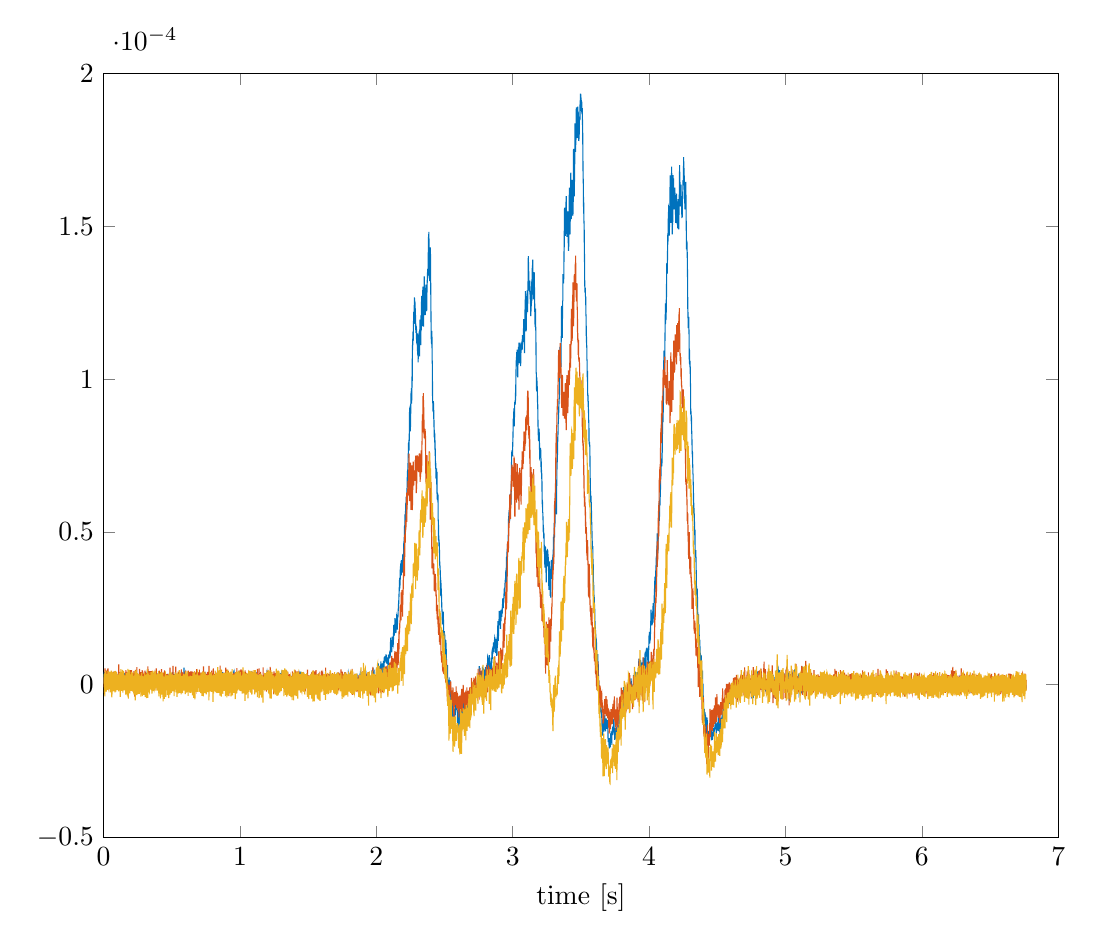
\begin{tikzpicture}

\begin{axis}[%
width=\textwidth,
height=0.8\textwidth,
at={(0\figurewidth,0\figureheight)},
scale only axis,
xmin=0,
xmax=7,
xlabel={time [s]},
ymin=-5e-05,
ymax=0.0002,
ylabel={},
axis background/.style={fill=white},
% title style={font=\bfseries},
% title={Train 4},
% legend style={legend cell align=left,align=left,draw=white!15!black}
]
\addplot [color=mycolor1,solid,forget plot]
  table[row sep=crcr]{%
0	4.08762316295294e-07\\
0.0009765625	1.19213149070928e-06\\
0.001953125	2.03196105632306e-06\\
0.0029296875	7.1928688850139e-07\\
0.00390625	1.20624626176935e-06\\
0.0048828125	3.99392129004066e-06\\
0.005859375	1.26270534995913e-06\\
0.0068359375	1.53088610518187e-06\\
0.0078125	2.4342328562685e-06\\
0.0087890625	2.15193682272653e-06\\
0.009765625	2.13782202519762e-06\\
0.0107421875	1.46031220840128e-06\\
0.01171875	1.67909132056882e-06\\
0.0126953125	1.60851740304787e-06\\
0.013671875	2.71652904783532e-06\\
0.0146484375	1.42502526371473e-06\\
0.015625	2.1801664189696e-06\\
0.0166015625	1.20624626176935e-06\\
0.017578125	1.69320610525817e-06\\
0.0185546875	1.67203392837235e-06\\
0.01953125	4.0503806903304e-06\\
0.0205078125	1.77083742811178e-06\\
0.021484375	3.03411245223748e-06\\
0.0224609375	2.03196105632306e-06\\
0.0234375	2.08842023695734e-06\\
0.0244140625	1.86258355234625e-06\\
0.025390625	1.47639528576401e-07\\
0.0263671875	2.24368301629443e-06\\
0.02734375	1.67909132056882e-06\\
0.0283203125	2.34248662803389e-06\\
0.029296875	1.89081313239155e-06\\
0.0302734375	1.89081313239155e-06\\
0.03125	3.08351433311958e-06\\
0.0322265625	2.56832352755879e-06\\
0.033203125	3.50695922491664e-06\\
0.0341796875	7.05172131071265e-07\\
0.03515625	4.93450817025051e-07\\
0.0361328125	2.61066795747894e-06\\
0.037109375	1.46031220840128e-06\\
0.0380859375	2.28602741895534e-06\\
0.0390625	3.25289224717179e-06\\
0.0400390625	3.07645692126869e-06\\
0.041015625	3.69750954222568e-06\\
0.0419921875	2.75887349019972e-06\\
0.04296875	1.36150876950099e-06\\
0.0439453125	1.41091048653152e-06\\
0.044921875	1.97550188200946e-06\\
0.0458984375	1.70026349775127e-06\\
0.046875	2.42717545350366e-06\\
0.0478515625	1.79200960914619e-06\\
0.048828125	2.32131442388841e-06\\
0.0498046875	2.04607585088906e-06\\
0.05078125	2.47657727492942e-06\\
0.0517578125	1.06509856894897e-06\\
0.052734375	1.72849306871053e-06\\
0.0537109375	9.87467354736978e-07\\
0.0546875	2.49069208193967e-06\\
0.0556640625	3.12585880629917e-06\\
0.056640625	1.5802878388046e-06\\
0.0576171875	7.33401646326815e-07\\
0.05859375	2.30719962161872e-06\\
0.0595703125	9.80409972219836e-07\\
0.060546875	2.99882539742699e-06\\
0.0615234375	2.94236611486686e-06\\
0.0625	1.21330364744694e-06\\
0.0634765625	2.1801664189696e-06\\
0.064453125	2.97059575535665e-06\\
0.0654296875	2.30014222063241e-06\\
0.06640625	6.34598349846024e-07\\
0.0673828125	6.29510859204152e-08\\
0.068359375	1.69320610525817e-06\\
0.0693359375	2.3636588330682e-06\\
0.0703125	1.24859057731895e-06\\
0.0712890625	2.90707906647658e-06\\
0.072265625	1.10038548845016e-06\\
0.0732421875	4.51106564882406e-07\\
0.07421875	2.82944756870907e-06\\
0.0751953125	1.20624626176935e-06\\
0.076171875	6.62827861150957e-07\\
0.0771484375	1.0298116519163e-06\\
0.078125	1.50971393511048e-06\\
0.0791015625	3.77514117362327e-06\\
0.080078125	2.56832352755879e-06\\
0.0810546875	3.73985406696103e-06\\
0.08203125	1.34739399409545e-06\\
0.0830078125	1.5661730572757e-06\\
0.083984375	2.68829942156744e-06\\
0.0849609375	7.89860681578262e-07\\
0.0859375	2.82944756870907e-06\\
0.0869140625	9.02778771044721e-07\\
0.087890625	1.43914004129301e-06\\
0.0888671875	7.33401646326815e-07\\
0.08984375	2.99176798676157e-06\\
0.0908203125	4.65221315201683e-07\\
0.091796875	2.31425702270434e-06\\
0.0927734375	9.6629520748067e-07\\
0.09375	7.82803301826269e-07\\
0.0947265625	2.08842023695734e-06\\
0.095703125	8.32204962165168e-07\\
0.0966796875	1.17095933486046e-06\\
0.09765625	1.30504967024952e-06\\
0.0986328125	1.63674696887104e-06\\
0.099609375	1.80612439699599e-06\\
0.1005859375	2.86473461166706e-06\\
0.1015625	2.75181608289207e-06\\
0.1025390625	1.71437828303347e-06\\
0.103515625	1.61557479435529e-06\\
0.1044921875	2.38483103899112e-06\\
0.10546875	1.31210705731034e-06\\
0.1064453125	1.62263218576181e-06\\
0.107421875	1.94021490127405e-06\\
0.1083984375	1.9966740716366e-06\\
0.109375	2.14487942391275e-06\\
0.1103515625	3.95863416806992e-06\\
0.111328125	9.82379352988758e-08\\
0.1123046875	1.08627072035322e-06\\
0.11328125	1.49559915555678e-06\\
0.1142578125	2.08136283903239e-06\\
0.115234375	2.21545341649539e-06\\
0.1162109375	1.98255927845318e-06\\
0.1171875	2.11664982964488e-06\\
0.1181640625	1.97550188200946e-06\\
0.119140625	1.71437828303347e-06\\
0.1201171875	2.4342328562685e-06\\
0.12109375	2.19428121768354e-06\\
0.1220703125	2.62478276824248e-06\\
0.123046875	1.22741841909941e-06\\
0.1240234375	1.41091048653152e-06\\
0.125	1.11450025694197e-06\\
0.1259765625	2.20839601679278e-06\\
0.126953125	1.48854176592835e-06\\
0.1279296875	1.77789482169125e-06\\
0.12890625	2.2366256161963e-06\\
0.1298828125	2.08136283903239e-06\\
0.130859375	1.5026565452843e-06\\
0.1318359375	3.28112190504481e-06\\
0.1328125	2.82239016041372e-06\\
0.1337890625	1.5026565452843e-06\\
0.134765625	2.60361055224559e-06\\
0.1357421875	2.82239016041372e-06\\
0.13671875	2.27897001826459e-06\\
0.1376953125	2.02490365918827e-06\\
0.138671875	1.87669834217125e-06\\
0.1396484375	3.05528468630867e-06\\
0.140625	2.48363467838532e-06\\
0.1416015625	2.85767720287797e-06\\
0.142578125	2.02490365918827e-06\\
0.1435546875	3.1399736314826e-06\\
0.14453125	2.04607585088906e-06\\
0.1455078125	2.16605162065052e-06\\
0.146484375	6.48713105301166e-07\\
0.1474609375	2.377773636918e-06\\
0.1484375	3.02705504107788e-06\\
0.1494140625	1.46736959763484e-06\\
0.150390625	3.12585880629917e-06\\
0.1513671875	3.81042828275489e-06\\
0.15234375	1.72143567582234e-06\\
0.1533203125	1.67203392837235e-06\\
0.154296875	2.26485521718015e-06\\
0.1552734375	2.1801664189696e-06\\
0.15625	2.73770126857321e-06\\
0.1572265625	1.50971393511048e-06\\
0.158203125	1.89081313239155e-06\\
0.1591796875	1.94021490127405e-06\\
0.16015625	2.42011805083814e-06\\
0.1611328125	1.82729657951164e-06\\
0.162109375	2.39894584343355e-06\\
0.1630859375	2.19428121768354e-06\\
0.1640625	2.13782202519762e-06\\
0.1650390625	2.02490365918827e-06\\
0.166015625	5.92254085851531e-07\\
0.1669921875	1.62263218576181e-06\\
0.16796875	9.45123061113192e-07\\
0.1689453125	2.1237072280638e-06\\
0.169921875	2.4342328562685e-06\\
0.1708984375	2.02490365918827e-06\\
0.171875	2.69535682798625e-06\\
0.1728515625	2.94236611486686e-06\\
0.173828125	2.99176798676157e-06\\
0.1748046875	1.00863950288233e-06\\
0.17578125	2.8365049771033e-06\\
0.1767578125	2.22251081629711e-06\\
0.177734375	2.51892169714587e-06\\
0.1787109375	2.67418460902602e-06\\
0.1796875	2.92119388553645e-06\\
0.1806640625	2.49774948559334e-06\\
0.181640625	2.50480688934523e-06\\
0.1826171875	3.514016642792e-06\\
0.18359375	1.16390194977484e-06\\
0.1845703125	2.03901845355673e-06\\
0.185546875	2.80827534411923e-06\\
0.1865234375	1.24153319114697e-06\\
0.1875	3.36581088814457e-06\\
0.1884765625	1.66497653627433e-06\\
0.189453125	1.92610010967095e-06\\
0.1904296875	1.3191644444696e-06\\
0.19140625	2.6388975794009e-06\\
0.1923828125	3.13291621884177e-06\\
0.193359375	9.45123061113192e-07\\
0.1943359375	4.09272524469527e-06\\
0.1953125	3.02901710383646e-07\\
0.1962890625	1.2838775096597e-06\\
0.197265625	1.41091048653152e-06\\
0.1982421875	1.44619743023037e-06\\
0.19921875	1.19213149070928e-06\\
0.2001953125	1.60851740304787e-06\\
0.201171875	2.14487942391275e-06\\
0.2021484375	3.83160054941872e-06\\
0.203125	6.41655727524155e-07\\
0.2041015625	2.07430544120653e-06\\
0.205078125	1.90492792300693e-06\\
0.2060546875	1.25564796358939e-06\\
0.20703125	7.40459025387304e-07\\
0.2080078125	2.92119388553645e-06\\
0.208984375	1.61754270401604e-07\\
0.2099609375	1.02275426880653e-06\\
0.2109375	2.73064386156177e-06\\
0.2119140625	2.03901845355673e-06\\
0.212890625	2.70241423450373e-06\\
0.2138671875	3.26700707591076e-06\\
0.21484375	1.51677132503554e-06\\
0.2158203125	2.39894584343355e-06\\
0.216796875	2.79416052821981e-06\\
0.2177734375	2.32327985454301e-07\\
0.21875	1.90492792300693e-06\\
0.2197265625	2.1589942216392e-06\\
0.220703125	1.9190427140174e-06\\
0.2216796875	1.27682012299418e-06\\
0.22265625	1.79200960914619e-06\\
0.2236328125	2.74475867568309e-06\\
0.224609375	2.27897001826459e-06\\
0.2255859375	1.3967957097434e-06\\
0.2265625	3.83160054941872e-06\\
0.2275390625	6.91057374036007e-07\\
0.228515625	6.06368840121206e-07\\
0.2294921875	1.67909132056882e-06\\
0.23046875	1.94727229722337e-06\\
0.2314453125	9.52180443136805e-07\\
0.232421875	2.46246246831403e-06\\
0.2333984375	2.38483103899112e-06\\
0.234375	5.64024578497213e-07\\
0.2353515625	2.377773636918e-06\\
0.236328125	2.20133861718861e-06\\
0.2373046875	2.75181608289207e-06\\
0.23828125	1.62263218576181e-06\\
0.2392578125	2.1589942216392e-06\\
0.240234375	3.85277281697181e-06\\
0.2412109375	2.17310901976073e-06\\
0.2421875	2.30719962161872e-06\\
0.2431640625	2.08136283903239e-06\\
0.244140625	7.61631163162481e-07\\
0.2451171875	1.74966524796663e-06\\
0.24609375	2.10959243132506e-06\\
0.2470703125	1.80612439699599e-06\\
0.248046875	1.5026565452843e-06\\
0.2490234375	1.63674696887104e-06\\
0.25	1.45325481926638e-06\\
0.2509765625	2.94236611486686e-06\\
0.251953125	2.17310901976073e-06\\
0.2529296875	1.72849306871053e-06\\
0.25390625	1.5661730572757e-06\\
0.2548828125	2.81533275221725e-06\\
0.255859375	7.61631163162481e-07\\
0.2568359375	2.74475867568309e-06\\
0.2578125	2.8012179361203e-06\\
0.2587890625	2.04607585088906e-06\\
0.259765625	1.61557479435529e-06\\
0.2607421875	1.67909132056882e-06\\
0.26171875	1.84141136834915e-06\\
0.2626953125	1.26976273642689e-06\\
0.263671875	3.74691148809594e-06\\
0.2646484375	4.13506980261611e-06\\
0.265625	2.42011805083814e-06\\
0.2666015625	2.53500101896065e-07\\
0.267578125	1.71437828303347e-06\\
0.2685546875	1.3544513817491e-06\\
0.26953125	4.44049189870978e-07\\
0.2705078125	1.13567241042051e-06\\
0.271484375	2.1589942216392e-06\\
0.2724609375	1.91198531846316e-06\\
0.2734375	2.25779781678624e-06\\
0.2744140625	2.01078886521489e-06\\
0.275390625	-2.05228888662881e-07\\
0.2763671875	3.71162438340912e-06\\
0.27734375	1.89787052765024e-06\\
0.2783203125	1.94727229722337e-06\\
0.279296875	1.48854176592835e-06\\
0.2802734375	1.66497653627433e-06\\
0.28125	8.88664008478731e-07\\
0.2822265625	1.00158212006833e-06\\
0.283203125	1.84141136834915e-06\\
0.2841796875	3.62693534223472e-06\\
0.28515625	1.5026565452843e-06\\
0.2861328125	-4.45179271349027e-07\\
0.287109375	2.99882539742699e-06\\
0.2880859375	1.51677132503554e-06\\
0.2890625	9.0983615247571e-07\\
0.2900390625	9.73352589800705e-07\\
0.291015625	2.00373146837631e-06\\
0.2919921875	2.13076462658116e-06\\
0.29296875	2.97765316572629e-06\\
0.2939453125	2.93530870499139e-06\\
0.294921875	5.0756556852936e-07\\
0.2958984375	-3.46376186422751e-07\\
0.296875	1.43208265245454e-06\\
0.2978515625	2.38483103899112e-06\\
0.298828125	1.22036103322406e-06\\
0.2998046875	2.58243833713709e-06\\
0.30078125	9.87467354736978e-07\\
0.3017578125	1.74260785478267e-06\\
0.302734375	3.50695922491664e-06\\
0.3037109375	2.58949574207467e-06\\
0.3046875	1.61557479435529e-06\\
0.3056640625	2.75887349019972e-06\\
0.306640625	6.48713105301166e-07\\
0.3076171875	2.53303650534116e-06\\
0.30859375	3.19643293616653e-06\\
0.3095703125	7.54573783805571e-07\\
0.310546875	3.28817931975929e-06\\
0.3115234375	7.12229509736671e-07\\
0.3125	2.51892169714587e-06\\
0.3134765625	9.31008297361952e-07\\
0.314453125	2.06019064585036e-06\\
0.3154296875	2.14487942391275e-06\\
0.31640625	2.53303650534116e-06\\
0.3173828125	2.27897001826459e-06\\
0.318359375	1.43208265245454e-06\\
0.3193359375	2.76593089760624e-06\\
0.3203125	2.54715131393197e-06\\
0.3212890625	2.01784626215214e-06\\
0.322265625	1.69320610525817e-06\\
0.3232421875	1.55911566665913e-06\\
0.32421875	2.94942352484142e-06\\
0.3251953125	5.14622944429617e-07\\
0.326171875	1.5026565452843e-06\\
0.3271484375	1.54500088572285e-06\\
0.328125	4.65221315201683e-07\\
0.3291015625	2.54715131393197e-06\\
0.330078125	1.41796787507358e-06\\
0.3310546875	1.26976273642689e-06\\
0.33203125	2.69535682798625e-06\\
0.3330078125	1.89081313239155e-06\\
0.333984375	3.27406449042813e-06\\
0.3349609375	1.97550188200946e-06\\
0.3359375	2.6177253628116e-06\\
0.3369140625	1.13567241042051e-06\\
0.337890625	1.19918887618977e-06\\
0.3388671875	1.94021490127405e-06\\
0.33984375	1.51677132503554e-06\\
0.3408203125	9.38065679188024e-07\\
0.341796875	1.91198531846316e-06\\
0.3427734375	9.73352589800705e-07\\
0.34375	1.65086175237515e-06\\
0.3447265625	2.15193682272653e-06\\
0.345703125	3.99392129004066e-06\\
0.3466796875	2.50480688934523e-06\\
0.34765625	5.99311462937038e-07\\
0.3486328125	3.4857869718821e-06\\
0.349609375	2.90002165709465e-06\\
0.3505859375	1.62968957726677e-06\\
0.3515625	1.17095933486046e-06\\
0.3525390625	3.42932763480307e-06\\
0.353515625	1.81318179106899e-06\\
0.3544921875	2.69535682798625e-06\\
0.35546875	8.88664008478731e-07\\
0.3564453125	8.67491865370364e-07\\
0.357421875	1.52382871505927e-06\\
0.3583984375	1.31210705731034e-06\\
0.359375	1.68614871286438e-06\\
0.3603515625	-1.62884691631317e-07\\
0.361328125	1.2838775096597e-06\\
0.3623046875	2.03901845355673e-06\\
0.36328125	3.89511735474427e-06\\
0.3642578125	2.32131442388841e-06\\
0.365234375	1.9966740716366e-06\\
0.3662109375	2.85061979418753e-06\\
0.3671875	3.64105018144274e-06\\
0.3681640625	2.85767720287797e-06\\
0.369140625	1.9190427140174e-06\\
0.3701171875	3.06939950951647e-06\\
0.37109375	3.02705504107788e-06\\
0.3720703125	3.03411245223748e-06\\
0.373046875	2.34248662803389e-06\\
0.3740234375	2.73064386156177e-06\\
0.375	3.08351433311958e-06\\
0.3759765625	2.02490365918827e-06\\
0.376953125	2.92119388553645e-06\\
0.3779296875	1.61557479435529e-06\\
0.37890625	1.23447580507407e-06\\
0.3798828125	1.88375573723239e-06\\
0.380859375	2.07430544120653e-06\\
0.3818359375	1.25564796358939e-06\\
0.3828125	2.65301239095461e-06\\
0.3837890625	1.70026349775127e-06\\
0.384765625	2.11664982964488e-06\\
0.3857421875	3.2176051770528e-06\\
0.38671875	2.49069208193967e-06\\
0.3876953125	3.89511735474427e-06\\
0.388671875	1.72143567582234e-06\\
0.3896484375	1.55205827614188e-06\\
0.390625	1.60851740304787e-06\\
0.3916015625	3.04116986349573e-06\\
0.392578125	7.33401646326815e-07\\
0.3935546875	3.12585880629917e-06\\
0.39453125	2.17310901976073e-06\\
0.3955078125	2.91413647595697e-06\\
0.396484375	3.60576308416319e-06\\
0.3974609375	1.41091048653152e-06\\
0.3984375	6.41655727524155e-07\\
0.3994140625	2.95648093491421e-06\\
0.400390625	1.55205827614188e-06\\
0.4013671875	9.94524737353434e-07\\
0.40234375	1.24859057731895e-06\\
0.4033203125	1.9190427140174e-06\\
0.404296875	1.78495221536917e-06\\
0.4052734375	1.21330364744694e-06\\
0.40625	2.10253503310368e-06\\
0.4072265625	3.07645692126869e-06\\
0.408203125	1.70026349775127e-06\\
0.4091796875	2.30719962161872e-06\\
0.41015625	2.04607585088906e-06\\
0.4111328125	8.7454924630804e-07\\
0.412109375	1.29093489642431e-06\\
0.4130859375	5.14622944429617e-07\\
0.4140625	1.30504967024952e-06\\
0.4150390625	1.36856615735219e-06\\
0.416015625	1.42502526371473e-06\\
0.4169921875	2.74475867568309e-06\\
0.41796875	1.43208265245454e-06\\
0.4189453125	2.01784626215214e-06\\
0.419921875	1.26270534995913e-06\\
0.4208984375	8.2514758182055e-07\\
0.421875	1.90492792300693e-06\\
0.4228515625	6.55770483176622e-07\\
0.423828125	3.04116986349573e-06\\
0.4248046875	2.40600324580308e-06\\
0.42578125	3.95157674397168e-06\\
0.4267578125	3.73475445188988e-07\\
0.427734375	7.26344267364554e-07\\
0.4287109375	2.49774948559334e-06\\
0.4296875	1.91198531846316e-06\\
0.4306640625	1.45325481926638e-06\\
0.431640625	1.74966524796663e-06\\
0.4326171875	2.31425702270434e-06\\
0.43359375	1.32622183172818e-06\\
0.4345703125	2.8365049771033e-06\\
0.435546875	1.48148437639837e-06\\
0.4365234375	3.00588280819172e-06\\
0.4375	1.61754270401604e-07\\
0.4384765625	1.65791914427541e-06\\
0.439453125	3.04822727485287e-06\\
0.4404296875	1.74260785478267e-06\\
0.44140625	1.93315750542295e-06\\
0.4423828125	1.88375573723239e-06\\
0.443359375	1.29799228328759e-06\\
0.4443359375	1.92610010967095e-06\\
0.4453125	2.52597910119418e-06\\
0.4462890625	3.06234209786335e-06\\
0.447265625	1.75869012622324e-07\\
0.4482421875	2.77298830511142e-06\\
0.44921875	1.90492792300693e-06\\
0.4501953125	1.70026349775127e-06\\
0.451171875	2.22956821619748e-06\\
0.4521484375	1.0298116519163e-06\\
0.453125	7.05172131071265e-07\\
0.4541015625	1.64380436057355e-06\\
0.455078125	1.91198531846316e-06\\
0.4560546875	1.93315750542295e-06\\
0.45703125	6.91057374036007e-07\\
0.4580078125	2.82944756870907e-06\\
0.458984375	2.05313324832027e-06\\
0.4599609375	1.89081313239155e-06\\
0.4609375	1.43914004129301e-06\\
0.4619140625	1.43914004129301e-06\\
0.462890625	1.89787052765024e-06\\
0.4638671875	1.43208265245454e-06\\
0.46484375	2.37071623494355e-06\\
0.4658203125	3.07645692126869e-06\\
0.466796875	1.86258355234625e-06\\
0.4677734375	2.80827534411923e-06\\
0.46875	1.0439264184329e-06\\
0.4697265625	2.1589942216392e-06\\
0.470703125	2.38483103899112e-06\\
0.4716796875	1.80612439699599e-06\\
0.47265625	8.03975441378887e-07\\
0.4736328125	7.47516404547106e-07\\
0.474609375	2.3354292265534e-06\\
0.4755859375	1.9190427140174e-06\\
0.4765625	2.68124201524751e-06\\
0.4775390625	2.78004571271548e-06\\
0.478515625	1.34739399409545e-06\\
0.4794921875	7.82803301826269e-07\\
0.48046875	1.98255927845318e-06\\
0.4814453125	1.46736959763484e-06\\
0.482421875	1.22741841909941e-06\\
0.4833984375	7.75745922172721e-07\\
0.484375	3.54224631528223e-06\\
0.4853515625	2.76593089760624e-06\\
0.486328125	3.40109796863374e-06\\
0.4873046875	2.03196105632306e-06\\
0.48828125	2.10253503310368e-06\\
0.4892578125	1.05098380183974e-06\\
0.490234375	2.28602741895534e-06\\
0.4912109375	2.30014222063241e-06\\
0.4921875	2.11664982964488e-06\\
0.4931640625	1.65791914427541e-06\\
0.494140625	1.19213149070928e-06\\
0.4951171875	2.02490365918827e-06\\
0.49609375	2.27897001826459e-06\\
0.4970703125	3.72573922498743e-06\\
0.498046875	2.63184017377247e-06\\
0.4990234375	2.62478276824248e-06\\
0.5	1.06509856894897e-06\\
0.5009765625	2.4342328562685e-06\\
0.501953125	1.9190427140174e-06\\
0.5029296875	2.56126612291807e-06\\
0.50390625	2.01078886521489e-06\\
0.5048828125	3.06234209786335e-06\\
0.505859375	1.96138708941909e-06\\
0.5068359375	2.55420871837558e-06\\
0.5078125	4.15624208291009e-06\\
0.5087890625	3.3818857655141e-07\\
0.509765625	2.47657727492942e-06\\
0.5107421875	1.62968957726677e-06\\
0.51171875	2.42717545350366e-06\\
0.5126953125	1.14272979511105e-06\\
0.513671875	2.6600697968799e-06\\
0.5146484375	1.5802878388046e-06\\
0.515625	1.5944026207288e-06\\
0.5166015625	2.49069208193967e-06\\
0.517578125	3.43638505159206e-06\\
0.5185546875	3.01999763001695e-06\\
0.51953125	1.62968957726677e-06\\
0.5205078125	2.8365049771033e-06\\
0.521484375	2.54715131393197e-06\\
0.5224609375	2.02490365918827e-06\\
0.5234375	1.57323044799049e-06\\
0.5244140625	1.19918887618977e-06\\
0.525390625	1.22741841909941e-06\\
0.5263671875	3.11880139385566e-06\\
0.52734375	3.93746189607247e-06\\
0.5283203125	3.19643293616653e-06\\
0.529296875	1.70026349775127e-06\\
0.5302734375	3.50695922491664e-06\\
0.53125	1.94727229722337e-06\\
0.5322265625	2.6388975794009e-06\\
0.533203125	1.80612439699599e-06\\
0.5341796875	1.77789482169125e-06\\
0.53515625	1.46736959763484e-06\\
0.5361328125	1.36150876950099e-06\\
0.537109375	1.67203392837235e-06\\
0.5380859375	1.46736959763484e-06\\
0.5390625	1.9966740716366e-06\\
0.5400390625	-3.74605641234463e-07\\
0.541015625	1.77083742811178e-06\\
0.5419921875	1.61557479435529e-06\\
0.54296875	2.81533275221725e-06\\
0.5439453125	1.2838775096597e-06\\
0.544921875	1.82729657951164e-06\\
0.5458984375	3.56341857068706e-06\\
0.546875	2.6177253628116e-06\\
0.5478515625	2.44834766209372e-06\\
0.548828125	2.377773636918e-06\\
0.5498046875	2.65301239095461e-06\\
0.55078125	1.13567241042051e-06\\
0.5517578125	2.51186429319622e-06\\
0.552734375	1.5944026207288e-06\\
0.5537109375	3.1399736314826e-06\\
0.5546875	1.16390194977484e-06\\
0.5556640625	9.87467354736978e-07\\
0.556640625	2.41306064827107e-06\\
0.5576171875	3.09057174506934e-06\\
0.55859375	1.60146001183868e-06\\
0.5595703125	3.32346639481682e-06\\
0.560546875	1.94727229722337e-06\\
0.5615234375	1.72849306871053e-06\\
0.5625	9.87467354736978e-07\\
0.5634765625	2.27897001826459e-06\\
0.564453125	2.58949574207467e-06\\
0.5654296875	2.97765316572629e-06\\
0.56640625	3.23172000480407e-06\\
0.5673828125	2.08136283903239e-06\\
0.568359375	2.21545341649539e-06\\
0.5693359375	3.00588280819172e-06\\
0.5703125	1.70026349775127e-06\\
0.5712890625	1.51677132503554e-06\\
0.572265625	2.25074041649079e-06\\
0.5732421875	2.06019064585036e-06\\
0.57421875	2.34248662803389e-06\\
0.5751953125	1.32622183172818e-06\\
0.576171875	3.30935156449773e-06\\
0.5771484375	2.49774948559334e-06\\
0.578125	3.06939950951647e-06\\
0.5791015625	2.4342328562685e-06\\
0.580078125	1.83435397388106e-06\\
0.5810546875	2.67614846684392e-07\\
0.58203125	1.77789482169125e-06\\
0.5830078125	1.66497653627433e-06\\
0.583984375	1.96844448566527e-06\\
0.5849609375	2.44129025913135e-06\\
0.5859375	1.98961667499534e-06\\
0.5869140625	1.54500088572285e-06\\
0.587890625	2.94236611486686e-06\\
0.5888671875	2.6388975794009e-06\\
0.58984375	5.61007412255539e-06\\
0.5908203125	1.10038548845016e-06\\
0.591796875	1.78495221536917e-06\\
0.5927734375	4.28327578333898e-06\\
0.59375	1.9966740716366e-06\\
0.5947265625	1.41796787507358e-06\\
0.595703125	2.13076462658116e-06\\
0.5966796875	3.36581088814457e-06\\
0.59765625	3.42227021811253e-06\\
0.5986328125	1.63674696887104e-06\\
0.599609375	2.40600324580308e-06\\
0.6005859375	3.23172000480407e-06\\
0.6015625	2.95648093491421e-06\\
0.6025390625	6.62827861150957e-07\\
0.603515625	2.27191261767336e-06\\
0.6044921875	2.95648093491421e-06\\
0.60546875	3.30229414948597e-06\\
0.6064453125	1.54500088572285e-06\\
0.607421875	2.55420871837558e-06\\
0.6083984375	3.55636115211997e-06\\
0.609375	1.18507410532768e-06\\
0.6103515625	2.01078886521489e-06\\
0.611328125	2.10253503310368e-06\\
0.6123046875	3.06939950951647e-06\\
0.61328125	1.07215595265137e-06\\
0.6142578125	2.97765316572629e-06\\
0.615234375	3.3113120312075e-07\\
0.6162109375	2.45540506515454e-06\\
0.6171875	2.15193682272653e-06\\
0.6181640625	1.95432969327222e-06\\
0.619140625	2.44129025913135e-06\\
0.6201171875	2.73770126857321e-06\\
0.62109375	5.58937163412741e-08\\
0.6220703125	7.61631163162481e-07\\
0.623046875	1.77083742811178e-06\\
0.6240234375	3.19643293616653e-06\\
0.625	2.61066795747894e-06\\
0.6259765625	1.96844448566527e-06\\
0.626953125	1.96844448566527e-06\\
0.6279296875	3.54930373365199e-06\\
0.62890625	2.75887349019972e-06\\
0.6298828125	3.60576308416319e-06\\
0.630859375	2.66712720290341e-06\\
0.6318359375	-5.22810253068395e-07\\
0.6328125	2.86473461166706e-06\\
0.6337890625	1.62263218576181e-06\\
0.634765625	2.89296424781159e-06\\
0.6357421875	6.49213205091738e-09\\
0.63671875	2.34954402961326e-06\\
0.6376953125	1.29799228328759e-06\\
0.638671875	1.84846876291611e-06\\
0.6396484375	2.78004571271548e-06\\
0.640625	3.47167213701977e-06\\
0.6416015625	3.85277281697181e-06\\
0.642578125	2.53500101896065e-07\\
0.6435546875	3.32346639481682e-06\\
0.64453125	2.86473461166706e-06\\
0.6455078125	7.26344267364554e-07\\
0.646484375	1.5661730572757e-06\\
0.6474609375	6.83999995666372e-07\\
0.6484375	2.1237072280638e-06\\
0.6494140625	1.69320610525817e-06\\
0.650390625	2.32837182517157e-06\\
0.6513671875	3.37992572004399e-06\\
0.65234375	1.25564796358939e-06\\
0.6533203125	1.97550188200946e-06\\
0.654296875	2.61066795747894e-06\\
0.6552734375	1.61557479435529e-06\\
0.65625	9.87467354736978e-07\\
0.6572265625	1.97550188200946e-06\\
0.658203125	2.56126612291807e-06\\
0.6591796875	1.58734522971715e-06\\
0.66015625	3.04822727485287e-06\\
0.6611328125	9.80409972219836e-07\\
0.662109375	1.98961667499534e-06\\
0.6630859375	1.71437828303347e-06\\
0.6640625	1.25564796358939e-06\\
0.6650390625	2.07430544120653e-06\\
0.666015625	2.81533275221725e-06\\
0.6669921875	1.82023918524109e-06\\
0.66796875	1.5802878388046e-06\\
0.6689453125	1.44619743023037e-06\\
0.669921875	2.32837182517157e-06\\
0.6708984375	8.53377103792081e-07\\
0.671875	-5.7024183496273e-08\\
0.6728515625	3.02705504107788e-06\\
0.673828125	-1.28500471164705e-06\\
0.6748046875	1.82023918524109e-06\\
0.67578125	-5.7024183496273e-08\\
0.6767578125	1.90492792300693e-06\\
0.677734375	9.73352589800705e-07\\
0.6787109375	2.16605162065052e-06\\
0.6796875	2.69535682798625e-06\\
0.6806640625	1.79200960914619e-06\\
0.681640625	3.1399736314826e-06\\
0.6826171875	1.16390194977484e-06\\
0.68359375	1.43208265245454e-06\\
0.6845703125	1.9190427140174e-06\\
0.685546875	1.33327921908498e-06\\
0.6865234375	1.89787052765024e-06\\
0.6875	1.60851740304787e-06\\
0.6884765625	1.48148437639837e-06\\
0.689453125	1.5802878388046e-06\\
0.6904296875	2.20839601679278e-06\\
0.69140625	3.55636115211997e-06\\
0.6923828125	1.48854176592835e-06\\
0.693359375	1.96844448566527e-06\\
0.6943359375	1.44619743023037e-06\\
0.6953125	1.24859057731895e-06\\
0.6962890625	1.5944026207288e-06\\
0.697265625	1.72849306871053e-06\\
0.6982421875	3.240738297881e-07\\
0.69921875	3.14703104422275e-06\\
0.7001953125	1.70732089034261e-06\\
0.701171875	3.38698313614191e-06\\
0.7021484375	6.83999995666372e-07\\
0.703125	1.67909132056882e-06\\
0.7041015625	2.18722381827735e-06\\
0.705078125	5.56967201905669e-07\\
0.7060546875	1.19918887618977e-06\\
0.70703125	2.49069208193967e-06\\
0.7080078125	2.05313324832027e-06\\
0.708984375	1.22036103322406e-06\\
0.7099609375	2.02490365918827e-06\\
0.7109375	2.53303650534116e-06\\
0.7119140625	2.03901845355673e-06\\
0.712890625	2.32131442388841e-06\\
0.7138671875	5.85196708864904e-07\\
0.71484375	1.80612439699599e-06\\
0.7158203125	2.15193682272653e-06\\
0.716796875	1.44619743023037e-06\\
0.7177734375	1.72143567582234e-06\\
0.71875	2.39894584343355e-06\\
0.7197265625	3.14703104422275e-06\\
0.720703125	3.23877741882791e-06\\
0.7216796875	2.04607585088906e-06\\
0.72265625	2.13782202519762e-06\\
0.7236328125	2.08136283903239e-06\\
0.724609375	1.94727229722337e-06\\
0.7255859375	2.8365049771033e-06\\
0.7265625	2.67614846684392e-07\\
0.7275390625	2.13076462658116e-06\\
0.728515625	1.43914004129301e-06\\
0.7294921875	3.45755730255253e-06\\
0.73046875	2.4342328562685e-06\\
0.7314453125	2.20133861718861e-06\\
0.732421875	9.31008297361952e-07\\
0.7333984375	1.1568445647881e-06\\
0.734375	2.75181608289207e-06\\
0.7353515625	1.0439264184329e-06\\
0.736328125	1.69320610525817e-06\\
0.7373046875	2.54715131393197e-06\\
0.73828125	1.09332810435247e-06\\
0.7392578125	2.30014222063241e-06\\
0.740234375	1.22741841909941e-06\\
0.7412109375	3.24583483295019e-06\\
0.7421875	2.3354292265534e-06\\
0.7431640625	2.27897001826459e-06\\
0.744140625	2.00373146837631e-06\\
0.7451171875	1.9966740716366e-06\\
0.74609375	1.78495221536917e-06\\
0.7470703125	1.74260785478267e-06\\
0.748046875	1.65791914427541e-06\\
0.7490234375	1.12155764133608e-06\\
0.75	2.90707906647658e-06\\
0.7509765625	2.71652904783532e-06\\
0.751953125	2.78710312041843e-06\\
0.7529296875	2.61066795747894e-06\\
0.75390625	6.76942617396049e-07\\
0.7548828125	1.74260785478267e-06\\
0.755859375	2.08842023695734e-06\\
0.7568359375	1.96138708941909e-06\\
0.7578125	2.01078886521489e-06\\
0.7587890625	1.3544513817491e-06\\
0.759765625	9.38065679188024e-07\\
0.7607421875	3.2176051770528e-06\\
0.76171875	2.27191261767336e-06\\
0.7626953125	3.09762915711776e-06\\
0.763671875	9.80409972219836e-07\\
0.7646484375	1.54500088572285e-06\\
0.765625	2.35660143129129e-06\\
0.7666015625	2.3354292265534e-06\\
0.767578125	1.43914004129301e-06\\
0.7685546875	1.86258355234625e-06\\
0.76953125	1.07921333645307e-06\\
0.7705078125	1.01569688579477e-06\\
0.771484375	2.75887349019972e-06\\
0.7724609375	2.44834766209372e-06\\
0.7734375	1.55911566665913e-06\\
0.7744140625	9.73352589800705e-07\\
0.775390625	1.54500088572285e-06\\
0.7763671875	1.60851740304787e-06\\
0.77734375	1.38268093335015e-06\\
0.7783203125	9.6629520748067e-07\\
0.779296875	3.23877741882791e-06\\
0.7802734375	1.73555046169695e-06\\
0.78125	2.07430544120653e-06\\
0.7822265625	2.39188844116311e-06\\
0.783203125	1.86258355234625e-06\\
0.7841796875	1.91198531846316e-06\\
0.78515625	-7.27473693043837e-07\\
0.7861328125	3.58459082698093e-06\\
0.787109375	1.96844448566527e-06\\
0.7880859375	2.04607585088906e-06\\
0.7890625	1.26976273642689e-06\\
0.7900390625	3.24583483295019e-06\\
0.791015625	1.22036103322406e-06\\
0.7919921875	1.63674696887104e-06\\
0.79296875	2.00373146837631e-06\\
0.7939453125	9.31008297361952e-07\\
0.794921875	2.20133861718861e-06\\
0.7958984375	9.80409972219836e-07\\
0.796875	1.38973832149712e-06\\
0.7978515625	2.11664982964488e-06\\
0.798828125	5.0756556852936e-07\\
0.7998046875	2.20839601679278e-06\\
0.80078125	1.66497653627433e-06\\
0.8017578125	1.89081313239155e-06\\
0.802734375	1.47442698696727e-06\\
0.8037109375	1.47442698696727e-06\\
0.8046875	1.0298116519163e-06\\
0.8056640625	1.34739399409545e-06\\
0.806640625	2.42011805083814e-06\\
0.8076171875	2.75181608289207e-06\\
0.80859375	2.7094716411203e-06\\
0.8095703125	5.64024578497213e-07\\
0.810546875	1.77083742811178e-06\\
0.8115234375	1.46736959763484e-06\\
0.8125	1.86258355234625e-06\\
0.8134765625	1.98961667499534e-06\\
0.814453125	3.06939950951647e-06\\
0.8154296875	1.0439264184329e-06\\
0.81640625	1.5026565452843e-06\\
0.8173828125	1.89787052765024e-06\\
0.818359375	2.06019064585036e-06\\
0.8193359375	1.05098380183974e-06\\
0.8203125	1.12861502582907e-06\\
0.8212890625	1.52382871505927e-06\\
0.822265625	1.81318179106899e-06\\
0.8232421875	2.2366256161963e-06\\
0.82421875	8.53377103792081e-07\\
0.8251953125	2.50480688934523e-06\\
0.826171875	1.33327921908498e-06\\
0.8271484375	1.05098380183974e-06\\
0.828125	7.1928688850139e-07\\
0.8291015625	1.19213149070928e-06\\
0.830078125	1.14978717990024e-06\\
0.8310546875	2.38483103899112e-06\\
0.83203125	1.60851740304787e-06\\
0.8330078125	2.27191261767336e-06\\
0.833984375	1.60851740304787e-06\\
0.8349609375	1.55205827614188e-06\\
0.8359375	1.77083742811178e-06\\
0.8369140625	1.80612439699599e-06\\
0.837890625	1.78495221536917e-06\\
0.8388671875	1.90492792300693e-06\\
0.83984375	2.85061979418753e-06\\
0.8408203125	1.02275426880653e-06\\
0.841796875	2.22956821619748e-06\\
0.8427734375	2.38483103899112e-06\\
0.84375	1.73555046169695e-06\\
0.8447265625	3.78219859525192e-06\\
0.845703125	2.59655314711047e-06\\
0.8466796875	2.22956821619748e-06\\
0.84765625	3.03411245223748e-06\\
0.8486328125	1.77083742811178e-06\\
0.849609375	2.39894584343355e-06\\
0.8505859375	2.73064386156177e-06\\
0.8515625	1.30504967024952e-06\\
0.8525390625	3.06939950951647e-06\\
0.853515625	2.42717545350366e-06\\
0.8544921875	1.73555046169695e-06\\
0.85546875	2.32837182517157e-06\\
0.8564453125	1.53088610518187e-06\\
0.857421875	1.60851740304787e-06\\
0.8583984375	1.37562354530162e-06\\
0.859375	1.62263218576181e-06\\
0.8603515625	1.98255927845318e-06\\
0.861328125	3.49284438946169e-06\\
0.8623046875	9.31008297361952e-07\\
0.86328125	2.47657727492942e-06\\
0.8642578125	2.377773636918e-06\\
0.865234375	1.36856615735219e-06\\
0.8662109375	2.29308481974433e-06\\
0.8671875	2.14487942391275e-06\\
0.8681640625	7.96918061429352e-07\\
0.869140625	1.10744287264673e-06\\
0.8701171875	2.74672219226441e-07\\
0.87109375	1.0439264184329e-06\\
0.8720703125	1.74966524796663e-06\\
0.873046875	2.27897001826459e-06\\
0.8740234375	4.12095494958082e-06\\
0.875	2.58949574207467e-06\\
0.8759765625	1.2838775096597e-06\\
0.876953125	2.86473461166706e-06\\
0.8779296875	3.40815538502786e-06\\
0.87890625	2.44129025913135e-06\\
0.8798828125	2.53303650534116e-06\\
0.880859375	3.23877741882791e-06\\
0.8818359375	1.52382871505927e-06\\
0.8828125	2.95648093491421e-06\\
0.8837890625	1.76378003463118e-06\\
0.884765625	3.24583483295019e-06\\
0.8857421875	1.95432969327222e-06\\
0.88671875	1.94727229722337e-06\\
0.8876953125	3.34463864103607e-06\\
0.888671875	1.14978717990024e-06\\
0.8896484375	2.49069208193967e-06\\
0.890625	1.96138708941909e-06\\
0.8916015625	1.82023918524109e-06\\
0.892578125	3.09762915711776e-06\\
0.8935546875	3.35875347234308e-06\\
0.89453125	2.78004571271548e-06\\
0.8955078125	2.52597910119418e-06\\
0.896484375	3.24583483295019e-06\\
0.8974609375	1.61557479435529e-06\\
0.8984375	2.85767720287797e-06\\
0.8994140625	2.03196105632306e-06\\
0.900390625	1.66497653627433e-06\\
0.9013671875	2.377773636918e-06\\
0.90234375	1.82729657951164e-06\\
0.9033203125	1.36150876950099e-06\\
0.904296875	1.73555046169695e-06\\
0.9052734375	1.84846876291611e-06\\
0.90625	1.14272979511105e-06\\
0.9072265625	1.9190427140174e-06\\
0.908203125	2.10253503310368e-06\\
0.9091796875	2.42011805083814e-06\\
0.91015625	2.22251081629711e-06\\
0.9111328125	1.9966740716366e-06\\
0.912109375	1.96138708941909e-06\\
0.9130859375	2.61066795747894e-06\\
0.9140625	2.15193682272653e-06\\
0.9150390625	2.82239016041372e-06\\
0.916015625	3.01294021905511e-06\\
0.9169921875	2.07430544120653e-06\\
0.91796875	1.14978717990024e-06\\
0.9189453125	2.22956821619748e-06\\
0.919921875	1.75672264124968e-06\\
0.9208984375	1.66497653627433e-06\\
0.921875	1.08627072035322e-06\\
0.9228515625	2.39188844116311e-06\\
0.923828125	1.72849306871053e-06\\
0.9248046875	1.95432969327222e-06\\
0.92578125	2.67418460902602e-06\\
0.9267578125	2.81729591867586e-07\\
0.927734375	4.79336065915825e-07\\
0.9287109375	2.35660143129129e-06\\
0.9296875	1.8696409472092e-06\\
0.9306640625	2.93530870499139e-06\\
0.931640625	1.46736959763484e-06\\
0.9326171875	1.64380436057355e-06\\
0.93359375	1.54500088572285e-06\\
0.9345703125	2.6177253628116e-06\\
0.935546875	1.8696409472092e-06\\
0.9365234375	2.34248662803389e-06\\
0.9375	3.03411245223748e-06\\
0.9384765625	2.34248662803389e-06\\
0.939453125	1.92610010967095e-06\\
0.9404296875	1.02275426880653e-06\\
0.94140625	1.01569688579477e-06\\
0.9423828125	2.53303650534116e-06\\
0.943359375	2.56832352755879e-06\\
0.9443359375	3.03411245223748e-06\\
0.9453125	3.47167213701977e-06\\
0.9462890625	2.06724804347868e-06\\
0.947265625	1.74966524796663e-06\\
0.9482421875	1.26976273642689e-06\\
0.94921875	7.33401646326815e-07\\
0.9501953125	2.06724804347868e-06\\
0.951171875	1.72143567582234e-06\\
0.9521484375	2.18722381827735e-06\\
0.953125	2.01078886521489e-06\\
0.9541015625	3.53518889701179e-06\\
0.955078125	3.34463864103607e-06\\
0.9560546875	3.18937552273553e-06\\
0.95703125	3.42932763480307e-06\\
0.9580078125	1.43914004129301e-06\\
0.958984375	1.75672264124968e-06\\
0.9599609375	1.55205827614188e-06\\
0.9609375	1.46031220840128e-06\\
0.9619140625	1.96844448566527e-06\\
0.962890625	2.08136283903239e-06\\
0.9638671875	1.9190427140174e-06\\
0.96484375	2.61066795747894e-06\\
0.9658203125	2.08136283903239e-06\\
0.966796875	1.40385309808791e-06\\
0.9677734375	2.80827534411923e-06\\
0.96875	1.38973832149712e-06\\
0.9697265625	1.66497653627433e-06\\
0.970703125	3.29523673457351e-06\\
0.9716796875	2.22251081629711e-06\\
0.97265625	2.58243833713709e-06\\
0.9736328125	2.39894584343355e-06\\
0.974609375	3.08351433311958e-06\\
0.9755859375	2.28602741895534e-06\\
0.9765625	3.43638505159206e-06\\
0.9775390625	4.88363468603616e-08\\
0.978515625	3.15408845706091e-06\\
0.9794921875	2.60361055224559e-06\\
0.98046875	2.10253503310368e-06\\
0.9814453125	3.26700707591076e-06\\
0.982421875	1.2838775096597e-06\\
0.9833984375	2.93530870499139e-06\\
0.984375	1.92610010967095e-06\\
0.9853515625	1.76378003463118e-06\\
0.986328125	2.90002165709465e-06\\
0.9873046875	3.88100250842496e-06\\
0.98828125	5.71081955187637e-07\\
0.9892578125	3.53518889701179e-06\\
0.990234375	1.2838775096597e-06\\
0.9912109375	2.31425702270434e-06\\
0.9921875	1.03686903512559e-06\\
0.9931640625	1.58734522971715e-06\\
0.994140625	2.29308481974433e-06\\
0.9951171875	3.47872955440182e-06\\
0.99609375	3.34463864103607e-06\\
0.9970703125	1.89787052765024e-06\\
0.998046875	1.86258355234625e-06\\
0.9990234375	1.00158212006833e-06\\
1	2.81533275221725e-06\\
1.0009765625	1.43914004129301e-06\\
1.001953125	9.0983615247571e-07\\
1.0029296875	2.97765316572629e-06\\
1.00390625	1.65086175237515e-06\\
1.0048828125	3.47872955440182e-06\\
1.005859375	3.52107406076667e-06\\
1.0068359375	1.64380436057355e-06\\
1.0078125	1.19213149070928e-06\\
1.0087890625	3.49990180713972e-06\\
1.009765625	1.36150876950099e-06\\
1.0107421875	1.24153319114697e-06\\
1.01171875	1.21330364744694e-06\\
1.0126953125	9.0983615247571e-07\\
1.013671875	1.98961667499534e-06\\
1.0146484375	1.64380436057355e-06\\
1.015625	1.3544513817491e-06\\
1.0166015625	1.89787052765024e-06\\
1.017578125	3.04822727485287e-06\\
1.0185546875	1.08627072035322e-06\\
1.01953125	9.6629520748067e-07\\
1.0205078125	2.46951987157239e-06\\
1.021484375	3.80532819212707e-07\\
1.0224609375	1.36856615735219e-06\\
1.0234375	2.27897001826459e-06\\
1.0244140625	1.79906700302165e-06\\
1.025390625	1.26270534995913e-06\\
1.0263671875	2.70241423450373e-06\\
1.02734375	1.51677132503554e-06\\
1.0283203125	1.45325481926638e-06\\
1.029296875	2.88786964607393e-07\\
1.0302734375	2.55420871837558e-06\\
1.03125	4.86393441420999e-07\\
1.0322265625	1.30504967024952e-06\\
1.033203125	1.83435397388106e-06\\
1.0341796875	1.22741841909941e-06\\
1.03515625	2.27191261767336e-06\\
1.0361328125	2.22251081629711e-06\\
1.037109375	1.80612439699599e-06\\
1.0380859375	1.26270534995913e-06\\
1.0390625	2.04607585088906e-06\\
1.0400390625	2.42011805083814e-06\\
1.041015625	1.72849306871053e-06\\
1.0419921875	1.77789482169125e-06\\
1.04296875	1.10038548845016e-06\\
1.0439453125	1.06509856894897e-06\\
1.044921875	1.51677132503554e-06\\
1.0458984375	1.66497653627433e-06\\
1.046875	1.67203392837235e-06\\
1.0478515625	1.92610010967095e-06\\
1.048828125	1.23447580507407e-06\\
1.0498046875	1.72143567582234e-06\\
1.05078125	1.75672264124968e-06\\
1.0517578125	1.74260785478267e-06\\
1.052734375	2.72358645464921e-06\\
1.0537109375	1.34739399409545e-06\\
1.0546875	1.74966524796663e-06\\
1.0556640625	1.98961667499534e-06\\
1.056640625	3.45755730255253e-06\\
1.0576171875	2.19428121768354e-06\\
1.05859375	2.82944756870907e-06\\
1.0595703125	1.37562354530162e-06\\
1.060546875	1.95432969327222e-06\\
1.0615234375	2.20839601679278e-06\\
1.0625	8.53377103792081e-07\\
1.0634765625	1.01569688579477e-06\\
1.064453125	1.88375573723239e-06\\
1.0654296875	1.74966524796663e-06\\
1.06640625	1.80612439699599e-06\\
1.0673828125	1.34739399409545e-06\\
1.068359375	2.95648093491421e-06\\
1.0693359375	2.15193682272653e-06\\
1.0703125	2.22956821619748e-06\\
1.0712890625	2.13782202519762e-06\\
1.072265625	4.86393441420999e-07\\
1.0732421875	2.7094716411203e-06\\
1.07421875	1.82729657951164e-06\\
1.0751953125	1.61557479435529e-06\\
1.076171875	2.56126612291807e-06\\
1.0771484375	2.8365049771033e-06\\
1.078125	3.72573922498743e-06\\
1.0791015625	2.51892169714587e-06\\
1.080078125	3.92334704856791e-06\\
1.0810546875	3.9868638654491e-06\\
1.08203125	1.49559915555678e-06\\
1.0830078125	2.73770126857321e-06\\
1.083984375	2.3636588330682e-06\\
1.0849609375	2.1801664189696e-06\\
1.0859375	2.61066795747894e-06\\
1.0869140625	3.81042828275489e-06\\
1.087890625	3.37286830404495e-06\\
1.0888671875	3.09057174506934e-06\\
1.08984375	2.58949574207467e-06\\
1.0908203125	2.53303650534116e-06\\
1.091796875	2.98471057619439e-06\\
1.0927734375	3.06939950951647e-06\\
1.09375	3.77514117362327e-06\\
1.0947265625	2.84356238559619e-06\\
1.095703125	2.51186429319622e-06\\
1.0966796875	2.92119388553645e-06\\
1.09765625	3.10468656926485e-06\\
1.0986328125	3.89511735474427e-06\\
1.099609375	2.14487942391275e-06\\
1.1005859375	3.46461471973703e-06\\
1.1015625	2.65301239095461e-06\\
1.1025390625	1.53088610518187e-06\\
1.103515625	2.29308481974433e-06\\
1.1044921875	2.34954402961326e-06\\
1.10546875	3.73985406696103e-06\\
1.1064453125	2.70241423450373e-06\\
1.107421875	2.94236611486686e-06\\
1.1083984375	2.65301239095461e-06\\
1.109375	2.99176798676157e-06\\
1.1103515625	1.74260785478267e-06\\
1.111328125	2.78004571271548e-06\\
1.1123046875	1.87669834217125e-06\\
1.11328125	3.60576308416319e-06\\
1.1142578125	2.14487942391275e-06\\
1.115234375	1.91198531846316e-06\\
1.1162109375	2.377773636918e-06\\
1.1171875	1.37562354530162e-06\\
1.1181640625	4.00097871473132e-06\\
1.119140625	1.98961667499534e-06\\
1.1201171875	2.82239016041372e-06\\
1.12109375	3.58459082698093e-06\\
1.1220703125	1.0298116519163e-06\\
1.123046875	1.5802878388046e-06\\
1.1240234375	2.34954402961326e-06\\
1.125	1.37562354530162e-06\\
1.1259765625	1.26270534995913e-06\\
1.126953125	2.11664982964488e-06\\
1.1279296875	4.20564407371858e-06\\
1.12890625	1.72849306871053e-06\\
1.1298828125	1.18507410532768e-06\\
1.130859375	3.04822727485287e-06\\
1.1318359375	1.17095933486046e-06\\
1.1328125	1.61557479435529e-06\\
1.1337890625	1.17801672004452e-06\\
1.134765625	2.34248662803389e-06\\
1.1357421875	1.60851740304787e-06\\
1.13671875	1.74260785478267e-06\\
1.1376953125	1.89787052765024e-06\\
1.138671875	1.41091048653152e-06\\
1.1396484375	3.09762915711776e-06\\
1.140625	8.53377103792081e-07\\
1.1416015625	1.96844448566527e-06\\
1.142578125	1.5944026207288e-06\\
1.1435546875	1.80612439699599e-06\\
1.14453125	1.52382871505927e-06\\
1.1455078125	1.60146001183868e-06\\
1.146484375	1.51677132503554e-06\\
1.1474609375	2.14487942391275e-06\\
1.1484375	1.17095933486046e-06\\
1.1494140625	6.91057374036007e-07\\
1.150390625	1.80612439699599e-06\\
1.1513671875	1.19918887618977e-06\\
1.15234375	1.08627072035322e-06\\
1.1533203125	7.89860681578262e-07\\
1.154296875	2.39894584343355e-06\\
1.1552734375	2.04098498248146e-07\\
1.15625	1.64380436057355e-06\\
1.1572265625	1.53088610518187e-06\\
1.158203125	1.50971393511048e-06\\
1.1591796875	3.09762915711776e-06\\
1.16015625	1.96844448566527e-06\\
1.1611328125	1.3544513817491e-06\\
1.162109375	2.73770126857321e-06\\
1.1630859375	2.42011805083814e-06\\
1.1640625	2.24368301629443e-06\\
1.1650390625	3.47216081956082e-08\\
1.166015625	1.43208265245454e-06\\
1.1669921875	1.40385309808791e-06\\
1.16796875	1.40385309808791e-06\\
1.1689453125	1.60851740304787e-06\\
1.169921875	-8.61563487990864e-07\\
1.1708984375	1.77083742811178e-06\\
1.171875	2.01078886521489e-06\\
1.1728515625	2.68124201524751e-06\\
1.173828125	8.81606627343729e-07\\
1.1748046875	5.49909825412788e-07\\
1.17578125	1.23447580507407e-06\\
1.1767578125	2.47657727492942e-06\\
1.177734375	2.56832352755879e-06\\
1.1787109375	6.69885239223738e-07\\
1.1796875	3.37286830404495e-06\\
1.1806640625	3.35875347234308e-06\\
1.181640625	1.63674696887104e-06\\
1.1826171875	2.1801664189696e-06\\
1.18359375	1.33327921908498e-06\\
1.1845703125	2.46951987157239e-06\\
1.185546875	1.17801672004452e-06\\
1.1865234375	2.35660143129129e-06\\
1.1875	2.76593089760624e-06\\
1.1884765625	3.66927986104404e-06\\
1.189453125	1.5379434954027e-06\\
1.1904296875	2.65301239095461e-06\\
1.19140625	2.37071623494355e-06\\
1.1923828125	1.64380436057355e-06\\
1.193359375	1.73555046169695e-06\\
1.1943359375	1.32622183172818e-06\\
1.1953125	2.42717545350366e-06\\
1.1962890625	1.82023918524109e-06\\
1.197265625	3.514016642792e-06\\
1.1982421875	3.85277281697181e-06\\
1.19921875	3.37992572004399e-06\\
1.2001953125	2.94236611486686e-06\\
1.201171875	4.40325208534982e-06\\
1.2021484375	1.71437828303347e-06\\
1.203125	3.25994966149162e-06\\
1.2041015625	2.97059575535665e-06\\
1.205078125	2.97765316572629e-06\\
1.2060546875	4.29739064091773e-06\\
1.20703125	1.53088610518187e-06\\
1.2080078125	2.32837182517157e-06\\
1.208984375	2.09547763498075e-06\\
1.2099609375	1.70732089034261e-06\\
1.2109375	9.31008297361952e-07\\
1.2119140625	1.87669834217125e-06\\
1.212890625	3.54224631528223e-06\\
1.2138671875	2.03901845355673e-06\\
1.21484375	1.98255927845318e-06\\
1.2158203125	2.78004571271548e-06\\
1.216796875	2.57538093229883e-06\\
1.2177734375	1.72143567582234e-06\\
1.21875	2.39894584343355e-06\\
1.2197265625	8.2514758182055e-07\\
1.220703125	3.64810760119464e-06\\
1.2216796875	2.2366256161963e-06\\
1.22265625	3.08351433311958e-06\\
1.2236328125	2.30014222063241e-06\\
1.224609375	2.70241423450373e-06\\
1.2255859375	2.18722381827735e-06\\
1.2265625	2.62478276824248e-06\\
1.2275390625	2.92825129521437e-06\\
1.228515625	1.83435397388106e-06\\
1.2294921875	2.68124201524751e-06\\
1.23046875	2.56832352755879e-06\\
1.2314453125	3.52813147883957e-06\\
1.232421875	1.32622183172818e-06\\
1.2333984375	2.96353834508632e-06\\
1.234375	2.49774948559334e-06\\
1.2353515625	1.10038548845016e-06\\
1.236328125	1.68614871286438e-06\\
1.2373046875	2.00373146837631e-06\\
1.23828125	2.42717545350366e-06\\
1.2392578125	2.2366256161963e-06\\
1.240234375	2.64595498512864e-06\\
1.2412109375	2.1237072280638e-06\\
1.2421875	1.67203392837235e-06\\
1.2431640625	9.45123061113192e-07\\
1.244140625	1.62263218576181e-06\\
1.2451171875	2.27897001826459e-06\\
1.24609375	1.1568445647881e-06\\
1.2470703125	1.14272979511105e-06\\
1.248046875	2.20133861718861e-06\\
1.2490234375	2.49774948559334e-06\\
1.25	1.68614871286438e-06\\
1.2509765625	1.77083742811178e-06\\
1.251953125	2.1589942216392e-06\\
1.2529296875	8.11032821427301e-07\\
1.25390625	1.63674696887104e-06\\
1.2548828125	9.45123061113192e-07\\
1.255859375	1.16390194977484e-06\\
1.2568359375	1.75869012622324e-07\\
1.2578125	4.58163939992713e-07\\
1.2587890625	1.84141136834915e-06\\
1.259765625	1.0439264184329e-06\\
1.2607421875	2.3354292265534e-06\\
1.26171875	1.30504967024952e-06\\
1.2626953125	-7.11389191983356e-08\\
1.263671875	1.92610010967095e-06\\
1.2646484375	2.26485521718015e-06\\
1.265625	1.3544513817491e-06\\
1.2666015625	1.07921333645307e-06\\
1.267578125	1.85552615758174e-06\\
1.2685546875	5.85196708864904e-07\\
1.26953125	1.40385309808791e-06\\
1.2705078125	-4.02835094465625e-07\\
1.271484375	2.00373146837631e-06\\
1.2724609375	9.82379352988758e-08\\
1.2734375	-4.16949820488581e-07\\
1.2744140625	2.34954402961326e-06\\
1.275390625	-1.34655224967757e-07\\
1.2763671875	2.84356238559619e-06\\
1.27734375	1.3544513817491e-06\\
1.2783203125	1.74966524796663e-06\\
1.279296875	-6.42785383128024e-07\\
1.2802734375	2.49069208193967e-06\\
1.28125	9.6629520748067e-07\\
1.2822265625	2.9584433744608e-07\\
1.283203125	1.94727229722337e-06\\
1.2841796875	1.40385309808791e-06\\
1.28515625	1.18507410532768e-06\\
1.2861328125	1.34739399409545e-06\\
1.287109375	1.93315750542295e-06\\
1.2880859375	1.17095933486046e-06\\
1.2890625	2.73770126857321e-06\\
1.2900390625	2.64595498512864e-06\\
1.291015625	2.04607585088906e-06\\
1.2919921875	2.06724804347868e-06\\
1.29296875	1.0439264184329e-06\\
1.2939453125	1.65791914427541e-06\\
1.294921875	3.78925601697967e-06\\
1.2958984375	2.87884942954189e-06\\
1.296875	2.18722381827735e-06\\
1.2978515625	2.05313324832027e-06\\
1.298828125	2.25074041649079e-06\\
1.2998046875	2.29308481974433e-06\\
1.30078125	2.88590683862741e-06\\
1.3017578125	2.72358645464921e-06\\
1.302734375	2.25074041649079e-06\\
1.3037109375	1.70026349775127e-06\\
1.3046875	1.95432969327222e-06\\
1.3056640625	3.08351433311958e-06\\
1.306640625	1.48854176592835e-06\\
1.3076171875	3.18937552273553e-06\\
1.30859375	2.95648093491421e-06\\
1.3095703125	3.28112190504481e-06\\
1.310546875	3.37992572004399e-06\\
1.3115234375	2.85767720287797e-06\\
1.3125	4.07861039284523e-06\\
1.3134765625	2.62478276824248e-06\\
1.314453125	1.52382871505927e-06\\
1.3154296875	2.49774948559334e-06\\
1.31640625	1.26270534995913e-06\\
1.3173828125	2.56126612291807e-06\\
1.318359375	2.25779781678624e-06\\
1.3193359375	3.40815538502786e-06\\
1.3203125	2.92119388553645e-06\\
1.3212890625	3.81042828275489e-06\\
1.322265625	3.40109796863374e-06\\
1.3232421875	1.86258355234625e-06\\
1.32421875	3.17526069616952e-06\\
1.3251953125	4.48794125689584e-06\\
1.326171875	1.61557479435529e-06\\
1.3271484375	2.49069208193967e-06\\
1.328125	2.87884942954189e-06\\
1.3291015625	3.89511735474427e-06\\
1.330078125	2.30719962161872e-06\\
1.3310546875	2.79416052821981e-06\\
1.33203125	3.78925601697967e-06\\
1.3330078125	2.27897001826459e-06\\
1.333984375	1.71437828303347e-06\\
1.3349609375	2.22956821619748e-06\\
1.3359375	1.90492792300693e-06\\
1.3369140625	2.51892169714587e-06\\
1.337890625	3.47872955440182e-06\\
1.3388671875	1.73555046169695e-06\\
1.33984375	1.67909132056882e-06\\
1.3408203125	1.96138708941909e-06\\
1.341796875	2.65301239095461e-06\\
1.3427734375	3.54224631528223e-06\\
1.34375	2.14487942391275e-06\\
1.3447265625	2.27191261767336e-06\\
1.345703125	1.84141136834915e-06\\
1.3466796875	2.29308481974433e-06\\
1.34765625	1.62263218576181e-06\\
1.3486328125	1.75672264124968e-06\\
1.349609375	1.81318179106899e-06\\
1.3505859375	1.88375573723239e-06\\
1.3515625	8.46319723151042e-07\\
1.3525390625	2.70241423450373e-06\\
1.353515625	2.6177253628116e-06\\
1.3544921875	1.07921333645307e-06\\
1.35546875	1.23447580507407e-06\\
1.3564453125	1.55911566665913e-06\\
1.357421875	7.96918061429352e-07\\
1.3583984375	9.11805652257722e-08\\
1.359375	1.41796787507358e-06\\
1.3603515625	2.50480688934523e-06\\
1.361328125	1.72143567582234e-06\\
1.3623046875	1.91198531846316e-06\\
1.36328125	3.28112190504481e-06\\
1.3642578125	1.62263218576181e-06\\
1.365234375	1.03686903512559e-06\\
1.3662109375	1.74260785478267e-06\\
1.3671875	2.25779781678624e-06\\
1.3681640625	8.2514758182055e-07\\
1.369140625	1.08627072035322e-06\\
1.3701171875	2.07430544120653e-06\\
1.37109375	1.96138708941909e-06\\
1.3720703125	9.02778771044721e-07\\
1.373046875	2.86473461166706e-06\\
1.3740234375	5.85196708864904e-07\\
1.375	4.44049189870978e-07\\
1.3759765625	2.3636588330682e-06\\
1.376953125	5.64024578497213e-07\\
1.3779296875	1.62263218576181e-06\\
1.37890625	1.41091048653152e-06\\
1.3798828125	2.1237072280638e-06\\
1.380859375	1.19918887618977e-06\\
1.3818359375	1.3967957097434e-06\\
1.3828125	1.41796787507358e-06\\
1.3837890625	2.70241423450373e-06\\
1.384765625	1.03686903512559e-06\\
1.3857421875	7.61631163162481e-07\\
1.38671875	1.96138708941909e-06\\
1.3876953125	2.55420871837558e-06\\
1.388671875	5.85196708864904e-07\\
1.3896484375	1.67909132056882e-06\\
1.390625	1.44619743023037e-06\\
1.3916015625	1.58734522971715e-06\\
1.392578125	1.20624626176935e-06\\
1.3935546875	2.21545341649539e-06\\
1.39453125	-7.13358975712062e-07\\
1.3955078125	5.42852449018786e-07\\
1.396484375	1.61557479435529e-06\\
1.3974609375	1.50971393511048e-06\\
1.3984375	2.37071623494355e-06\\
1.3994140625	1.82729657951164e-06\\
1.400390625	1.19213149070928e-06\\
1.4013671875	1.5802878388046e-06\\
1.40234375	1.29093489642431e-06\\
1.4033203125	9.94524737353434e-07\\
1.404296875	2.78710312041843e-06\\
1.4052734375	1.51677132503554e-06\\
1.40625	1.22741841909941e-06\\
1.4072265625	2.88590683862741e-06\\
1.408203125	1.12861502582907e-06\\
1.4091796875	2.19428121768354e-06\\
1.41015625	1.86258355234625e-06\\
1.4111328125	2.97059575535665e-06\\
1.412109375	1.90492792300693e-06\\
1.4130859375	2.89296424781159e-06\\
1.4140625	1.33327921908498e-06\\
1.4150390625	1.48148437639837e-06\\
1.416015625	2.42011805083814e-06\\
1.4169921875	2.01784626215214e-06\\
1.41796875	3.36581088814457e-06\\
1.4189453125	2.77298830511142e-06\\
1.419921875	2.07430544120653e-06\\
1.4208984375	2.67418460902602e-06\\
1.421875	2.41306064827107e-06\\
1.4228515625	3.4857869718821e-06\\
1.423828125	4.21270150137236e-06\\
1.4248046875	1.60146001183868e-06\\
1.42578125	2.56832352755879e-06\\
1.4267578125	2.79416052821981e-06\\
1.427734375	2.27897001826459e-06\\
1.4287109375	1.77083742811178e-06\\
1.4296875	8.53377103792081e-07\\
1.4306640625	2.91413647595697e-06\\
1.431640625	3.00588280819172e-06\\
1.4326171875	3.30229414948597e-06\\
1.43359375	2.68829942156744e-06\\
1.4345703125	3.32346639481682e-06\\
1.435546875	3.68339470143732e-06\\
1.4365234375	2.44834766209372e-06\\
1.4375	1.63674696887104e-06\\
1.4384765625	2.3354292265534e-06\\
1.439453125	2.64595498512864e-06\\
1.4404296875	1.50971393511048e-06\\
1.44140625	3.11174398151103e-06\\
1.4423828125	1.77789482169125e-06\\
1.443359375	4.27621835469793e-06\\
1.4443359375	1.27682012299418e-06\\
1.4453125	8.88664008478731e-07\\
1.4462890625	4.25504606936739e-06\\
1.447265625	2.47657727492942e-06\\
1.4482421875	6.29510859204152e-08\\
1.44921875	9.45123061113192e-07\\
1.4501953125	2.94236611486686e-06\\
1.451171875	2.18722381827735e-06\\
1.4521484375	2.75887349019972e-06\\
1.453125	1.93315750542295e-06\\
1.4541015625	3.09057174506934e-06\\
1.455078125	2.95648093491421e-06\\
1.4560546875	1.74966524796663e-06\\
1.45703125	1.73555046169695e-06\\
1.4580078125	3.04822727485287e-06\\
1.458984375	2.49069208193967e-06\\
1.4599609375	2.41306064827107e-06\\
1.4609375	2.18722381827735e-06\\
1.4619140625	2.32837182517157e-06\\
1.462890625	2.27191261767336e-06\\
1.4638671875	2.22251081629711e-06\\
1.46484375	2.58243833713709e-06\\
1.4658203125	2.68829942156744e-06\\
1.466796875	4.07155296706821e-06\\
1.4677734375	2.08136283903239e-06\\
1.46875	1.5944026207288e-06\\
1.4697265625	3.09762915711776e-06\\
1.470703125	1.1568445647881e-06\\
1.4716796875	2.52597910119418e-06\\
1.47265625	2.30014222063241e-06\\
1.4736328125	2.28602741895534e-06\\
1.474609375	1.9966740716366e-06\\
1.4755859375	1.63674696887104e-06\\
1.4765625	6.34598349846024e-07\\
1.4775390625	1.9190427140174e-06\\
1.478515625	2.21545341649539e-06\\
1.4794921875	7.1928688850139e-07\\
1.48046875	1.72143567582234e-06\\
1.4814453125	1.77789482169125e-06\\
1.482421875	2.87884942954189e-06\\
1.4833984375	3.16820328303451e-06\\
1.484375	1.80612439699599e-06\\
1.4853515625	2.18722381827735e-06\\
1.486328125	1.78495221536917e-06\\
1.4873046875	2.67418460902602e-06\\
1.48828125	1.49559915555678e-06\\
1.4892578125	1.79200960914619e-06\\
1.490234375	8.88664008478731e-07\\
1.4912109375	1.30504967024952e-06\\
1.4921875	2.52597910119418e-06\\
1.4931640625	1.32622183172818e-06\\
1.494140625	3.56341857068706e-06\\
1.4951171875	2.10959243132506e-06\\
1.49609375	2.98471057619439e-06\\
1.4970703125	1.22741841909941e-06\\
1.498046875	4.01704941876708e-07\\
1.4990234375	2.2527061350466e-07\\
1.5	-1.27597858055103e-07\\
1.5009765625	7.47516404547106e-07\\
1.501953125	1.26270534995913e-06\\
1.5029296875	1.41091048653152e-06\\
1.50390625	2.01784626215214e-06\\
1.5048828125	2.46246246831403e-06\\
1.505859375	8.81606627343729e-07\\
1.5068359375	4.86393441420999e-07\\
1.5078125	4.51106564882406e-07\\
1.5087890625	6.06368840121206e-07\\
1.509765625	1.83435397388106e-06\\
1.5107421875	1.12352675741504e-07\\
1.51171875	8.03975441378887e-07\\
1.5126953125	9.45123061113192e-07\\
1.513671875	1.89081313239155e-06\\
1.5146484375	2.53303650534116e-06\\
1.515625	2.20133861718861e-06\\
1.5166015625	2.34248662803389e-06\\
1.517578125	1.0298116519163e-06\\
1.5185546875	3.25994966149162e-06\\
1.51953125	2.74475867568309e-06\\
1.5205078125	1.71437828303347e-06\\
1.521484375	2.14487942391275e-06\\
1.5224609375	8.2514758182055e-07\\
1.5234375	1.9190427140174e-06\\
1.5244140625	2.55420871837558e-06\\
1.525390625	1.72849306871053e-06\\
1.5263671875	2.01078886521489e-06\\
1.52734375	2.49069208193967e-06\\
1.5283203125	2.09547763498075e-06\\
1.529296875	2.19428121768354e-06\\
1.5302734375	2.8365049771033e-06\\
1.53125	3.33052381012435e-06\\
1.5322265625	2.1237072280638e-06\\
1.533203125	2.73770126857321e-06\\
1.5341796875	1.89081313239155e-06\\
1.53515625	3.69750954222568e-06\\
1.5361328125	1.26270534995913e-06\\
1.537109375	1.81318179106899e-06\\
1.5380859375	3.44344246848015e-06\\
1.5390625	2.30014222063241e-06\\
1.5400390625	1.94021490127405e-06\\
1.541015625	2.07430544120653e-06\\
1.5419921875	2.01078886521489e-06\\
1.54296875	1.58734522971715e-06\\
1.5439453125	1.05804118534459e-06\\
1.544921875	2.27191261767336e-06\\
1.5458984375	1.14272979511105e-06\\
1.546875	1.90492792300693e-06\\
1.5478515625	2.49069208193967e-06\\
1.548828125	2.44129025913135e-06\\
1.5498046875	3.04822727485287e-06\\
1.55078125	3.14703104422275e-06\\
1.5517578125	-4.2909447399344e-08\\
1.552734375	2.08842023695734e-06\\
1.5537109375	1.53088610518187e-06\\
1.5546875	2.79416052821981e-06\\
1.5556640625	2.09547763498075e-06\\
1.556640625	3.06234209786335e-06\\
1.5576171875	2.55420871837558e-06\\
1.55859375	1.1568445647881e-06\\
1.5595703125	1.3191644444696e-06\\
1.560546875	9.6629520748067e-07\\
1.5615234375	2.01784626215214e-06\\
1.5625	3.73475445188988e-07\\
1.5634765625	2.94942352484142e-06\\
1.564453125	1.63674696887104e-06\\
1.5654296875	2.56126612291807e-06\\
1.56640625	3.07645692126869e-06\\
1.5673828125	2.99176798676157e-06\\
1.568359375	1.3191644444696e-06\\
1.5693359375	3.31640897960751e-06\\
1.5703125	2.09547763498075e-06\\
1.5712890625	2.1237072280638e-06\\
1.572265625	3.87590193335306e-07\\
1.5732421875	1.72849306871053e-06\\
1.57421875	2.6177253628116e-06\\
1.5751953125	2.07430544120653e-06\\
1.576171875	2.72358645464921e-06\\
1.5771484375	1.72143567582234e-06\\
1.578125	3.30229414948597e-06\\
1.5791015625	1.87669834217125e-06\\
1.580078125	2.16605162065052e-06\\
1.5810546875	3.09762915711776e-06\\
1.58203125	1.88375573723239e-06\\
1.5830078125	1.89787052765024e-06\\
1.583984375	2.1589942216392e-06\\
1.5849609375	1.84141136834915e-06\\
1.5859375	2.1589942216392e-06\\
1.5869140625	2.13076462658116e-06\\
1.587890625	6.20483594785965e-07\\
1.5888671875	8.81606627343729e-07\\
1.58984375	1.62263218576181e-06\\
1.5908203125	2.56832352755879e-06\\
1.591796875	3.66418071263931e-07\\
1.5927734375	2.18213241653898e-07\\
1.59375	1.77789482169125e-06\\
1.5947265625	1.27682012299418e-06\\
1.595703125	1.98255927845318e-06\\
1.5966796875	1.82023918524109e-06\\
1.59765625	3.01294021905511e-06\\
1.5986328125	1.36150876950099e-06\\
1.599609375	1.3967957097434e-06\\
1.6005859375	9.6629520748067e-07\\
1.6015625	1.98255927845318e-06\\
1.6025390625	1.95432969327222e-06\\
1.603515625	1.02275426880653e-06\\
1.6044921875	1.79200960914619e-06\\
1.60546875	3.67633728119124e-06\\
1.6064453125	3.77514117362327e-06\\
1.607421875	2.1237072280638e-06\\
1.6083984375	2.56832352755879e-06\\
1.609375	4.72278690509314e-07\\
1.6103515625	1.01569688579477e-06\\
1.611328125	1.81318179106899e-06\\
1.6123046875	1.65791914427541e-06\\
1.61328125	5.99311462937038e-07\\
1.6142578125	1.14978717990024e-06\\
1.615234375	2.8365049771033e-06\\
1.6162109375	1.14978717990024e-06\\
1.6171875	1.60851740304787e-06\\
1.6181640625	1.67203392837235e-06\\
1.619140625	3.00588280819172e-06\\
1.6201171875	2.20839601679278e-06\\
1.62109375	1.41091048653152e-06\\
1.6220703125	2.13782202519762e-06\\
1.623046875	6.34598349846024e-07\\
1.6240234375	1.74966524796663e-06\\
1.625	2.46951987157239e-06\\
1.6259765625	1.9966740716366e-06\\
1.626953125	2.14487942391275e-06\\
1.6279296875	1.9190427140174e-06\\
1.62890625	1.63674696887104e-06\\
1.6298828125	2.45540506515454e-06\\
1.630859375	1.1568445647881e-06\\
1.6318359375	7.54573783805571e-07\\
1.6328125	-9.23110220103773e-08\\
1.6337890625	1.8696409472092e-06\\
1.634765625	2.09547763498075e-06\\
1.6357421875	1.70026349775127e-06\\
1.63671875	2.37071623494355e-06\\
1.6376953125	1.89787052765024e-06\\
1.638671875	2.40600324580308e-06\\
1.6396484375	1.36856615735219e-06\\
1.640625	1.84141136834915e-06\\
1.6416015625	8.39262342608666e-07\\
1.642578125	2.60361055224559e-06\\
1.6435546875	2.52597910119418e-06\\
1.64453125	2.22956821619748e-06\\
1.6455078125	1.9966740716366e-06\\
1.646484375	2.42717545350366e-06\\
1.6474609375	1.62968957726677e-06\\
1.6484375	3.25289224717179e-06\\
1.6494140625	2.24368301629443e-06\\
1.650390625	8.2514758182055e-07\\
1.6513671875	2.02490365918827e-06\\
1.65234375	1.31210705731034e-06\\
1.6533203125	2.59655314711047e-06\\
1.654296875	1.55205827614188e-06\\
1.6552734375	2.24368301629443e-06\\
1.65625	2.85767720287797e-06\\
1.6572265625	3.33052381012435e-06\\
1.658203125	2.8012179361203e-06\\
1.6591796875	1.84141136834915e-06\\
1.66015625	1.49559915555678e-06\\
1.6611328125	5.64024578497213e-07\\
1.662109375	2.26485521718015e-06\\
1.6630859375	2.90707906647658e-06\\
1.6640625	1.14272979511105e-06\\
1.6650390625	1.91198531846316e-06\\
1.666015625	1.73555046169695e-06\\
1.6669921875	2.17310901976073e-06\\
1.66796875	3.24583483295019e-06\\
1.6689453125	2.00373146837631e-06\\
1.669921875	9.59237825259298e-07\\
1.6708984375	2.20133861718861e-06\\
1.671875	2.27191261767336e-06\\
1.6728515625	1.58734522971715e-06\\
1.673828125	3.01999763001695e-06\\
1.6748046875	2.1589942216392e-06\\
1.67578125	2.54715131393197e-06\\
1.6767578125	3.35169605664024e-06\\
1.677734375	2.01784626215214e-06\\
1.6787109375	1.75672264124968e-06\\
1.6796875	1.96844448566527e-06\\
1.6806640625	3.5704759893528e-06\\
1.681640625	1.00158212006833e-06\\
1.6826171875	2.90707906647658e-06\\
1.68359375	1.65086175237515e-06\\
1.6845703125	1.30504967024952e-06\\
1.685546875	2.8365049771033e-06\\
1.6865234375	4.51106564882406e-07\\
1.6875	3.16820328303451e-06\\
1.6884765625	2.76593089760624e-06\\
1.689453125	2.1589942216392e-06\\
1.6904296875	1.55205827614188e-06\\
1.69140625	1.84846876291611e-06\\
1.6923828125	8.32204962165168e-07\\
1.693359375	1.89787052765024e-06\\
1.6943359375	1.12155764133608e-06\\
1.6953125	8.03975441378887e-07\\
1.6962890625	5.58937163412741e-08\\
1.697265625	1.9190427140174e-06\\
1.6982421875	1.3544513817491e-06\\
1.69921875	2.73770126857321e-06\\
1.7001953125	1.5379434954027e-06\\
1.701171875	8.53377103792081e-07\\
1.7021484375	2.55420871837558e-06\\
1.703125	2.25779781678624e-06\\
1.7041015625	1.14978717990024e-06\\
1.705078125	2.31425702270434e-06\\
1.7060546875	2.22956821619748e-06\\
1.70703125	1.51677132503554e-06\\
1.7080078125	1.14978717990024e-06\\
1.708984375	5.78139331976939e-07\\
1.7099609375	2.60361055224559e-06\\
1.7109375	2.41306064827107e-06\\
1.7119140625	2.30719962161872e-06\\
1.712890625	2.75887349019972e-06\\
1.7138671875	2.15193682272653e-06\\
1.71484375	2.9584433744608e-07\\
1.7158203125	2.14487942391275e-06\\
1.716796875	2.31425702270434e-06\\
1.7177734375	3.04116986349573e-06\\
1.71875	2.90002165709465e-06\\
1.7197265625	2.34248662803389e-06\\
1.720703125	2.11664982964488e-06\\
1.7216796875	1.69320610525817e-06\\
1.72265625	2.85061979418753e-06\\
1.7236328125	2.29308481974433e-06\\
1.724609375	2.18722381827735e-06\\
1.7255859375	2.16605162065052e-06\\
1.7265625	2.97059575535665e-06\\
1.7275390625	1.65086175237515e-06\\
1.728515625	2.40600324580308e-06\\
1.7294921875	2.10253503310368e-06\\
1.73046875	1.29799228328759e-06\\
1.7314453125	1.57323044799049e-06\\
1.732421875	9.52180443136805e-07\\
1.7333984375	5.99311462937038e-07\\
1.734375	1.94021490127405e-06\\
1.7353515625	1.67203392837235e-06\\
1.736328125	1.53088610518187e-06\\
1.7373046875	1.55911566665913e-06\\
1.73828125	1.02275426880653e-06\\
1.7392578125	1.82023918524109e-06\\
1.740234375	1.19213149070928e-06\\
1.7412109375	5.42852449018786e-07\\
1.7421875	1.19410046110812e-07\\
1.7431640625	-1.84056790591188e-07\\
1.744140625	-1.41712591781749e-07\\
1.7451171875	-1.4896678422918e-06\\
1.74609375	9.87467354736978e-07\\
1.7470703125	-1.34655224967757e-07\\
1.748046875	1.60851740304787e-06\\
1.7490234375	2.06724804347868e-06\\
1.75	3.10468656926485e-06\\
1.7509765625	9.23950915634325e-07\\
1.751953125	2.44834766209372e-06\\
1.7529296875	1.54696899439455e-07\\
1.75390625	4.15819690813193e-07\\
1.7548828125	1.94727229722337e-06\\
1.755859375	1.75869012622324e-07\\
1.7568359375	2.94942352484142e-06\\
1.7578125	2.50480688934523e-06\\
1.7587890625	1.36150876950099e-06\\
1.759765625	2.94942352484142e-06\\
1.7607421875	2.99882539742699e-06\\
1.76171875	5.92254085851531e-07\\
1.7626953125	2.28602741895534e-06\\
1.763671875	1.65086175237515e-06\\
1.7646484375	2.49774948559334e-06\\
1.765625	9.6629520748067e-07\\
1.7666015625	1.88375573723239e-06\\
1.767578125	2.03901845355673e-06\\
1.7685546875	2.26485521718015e-06\\
1.76953125	3.88100250842496e-06\\
1.7705078125	1.2838775096597e-06\\
1.771484375	4.11389752321117e-06\\
1.7724609375	3.04822727485287e-06\\
1.7734375	3.57753340811742e-06\\
1.7744140625	1.90492792300693e-06\\
1.775390625	6.76942617396049e-07\\
1.7763671875	1.24859057731895e-06\\
1.77734375	2.50480688934523e-06\\
1.7783203125	1.8696409472092e-06\\
1.779296875	3.05528468630867e-06\\
1.7802734375	2.30719962161872e-06\\
1.78125	2.30014222063241e-06\\
1.7822265625	1.48854176592835e-06\\
1.783203125	2.85767720287797e-06\\
1.7841796875	7.61631163162481e-07\\
1.78515625	1.10038548845016e-06\\
1.7861328125	-3.32261458424596e-07\\
1.787109375	4.86393441420999e-07\\
1.7880859375	9.87467354736978e-07\\
1.7890625	1.96138708941909e-06\\
1.7900390625	2.06019064585036e-06\\
1.791015625	2.49774948559334e-06\\
1.7919921875	1.97550188200946e-06\\
1.79296875	2.21545341649539e-06\\
1.7939453125	2.97765316572629e-06\\
1.794921875	3.75396890932951e-06\\
1.7958984375	3.50695922491664e-06\\
1.796875	1.94727229722337e-06\\
1.7978515625	1.52382871505927e-06\\
1.798828125	3.95157674397168e-06\\
1.7998046875	2.16605162065052e-06\\
1.80078125	3.28112190504481e-06\\
1.8017578125	2.78004571271548e-06\\
1.802734375	7.00084555986524e-08\\
1.8037109375	2.80827534411923e-06\\
1.8046875	1.41091048653152e-06\\
1.8056640625	2.49069208193967e-06\\
1.806640625	3.04116986349573e-06\\
1.8076171875	1.86258355234625e-06\\
1.80859375	2.20839601679278e-06\\
1.8095703125	2.42011805083814e-06\\
1.810546875	3.64810760119464e-06\\
1.8115234375	1.74966524796663e-06\\
1.8125	4.04332326494846e-06\\
1.8134765625	3.16820328303451e-06\\
1.814453125	3.09057174506934e-06\\
1.8154296875	3.9868638654491e-06\\
1.81640625	2.82239016041372e-06\\
1.8173828125	2.26485521718015e-06\\
1.818359375	1.87669834217125e-06\\
1.8193359375	2.76593089760624e-06\\
1.8203125	1.62263218576181e-06\\
1.8212890625	1.89081313239155e-06\\
1.822265625	8.88664008478731e-07\\
1.8232421875	3.05528468630867e-06\\
1.82421875	2.18722381827735e-06\\
1.8251953125	1.52382871505927e-06\\
1.826171875	2.40600324580308e-06\\
1.8271484375	1.00158212006833e-06\\
1.828125	6.29510859204152e-08\\
1.8291015625	1.40385309808791e-06\\
1.830078125	9.59237825259298e-07\\
1.8310546875	1.76378003463118e-06\\
1.83203125	1.50971393511048e-06\\
1.8330078125	-1.00976795671445e-06\\
1.833984375	1.89983755237693e-07\\
1.8349609375	3.66418071263931e-07\\
1.8359375	7.96918061429352e-07\\
1.8369140625	6.69885239223738e-07\\
1.837890625	1.0439264184329e-06\\
1.8388671875	2.19428121768354e-06\\
1.83984375	1.3403366065411e-06\\
1.8408203125	3.44344246848015e-06\\
1.841796875	4.29934440144761e-07\\
1.8427734375	2.90002165709465e-06\\
1.84375	2.13076462658116e-06\\
1.8447265625	1.05098380183974e-06\\
1.845703125	1.67909132056882e-06\\
1.8466796875	2.66712720290341e-06\\
1.84765625	2.20839601679278e-06\\
1.8486328125	2.84356238559619e-06\\
1.849609375	2.73770126857321e-06\\
1.8505859375	2.10959243132506e-06\\
1.8515625	3.20349034969663e-06\\
1.8525390625	2.34248662803389e-06\\
1.853515625	1.07215595265137e-06\\
1.8544921875	2.2366256161963e-06\\
1.85546875	2.10253503310368e-06\\
1.8564453125	5.42852449018786e-07\\
1.857421875	2.8365049771033e-06\\
1.8583984375	2.32131442388841e-06\\
1.859375	2.53303650534116e-06\\
1.8603515625	2.08842023695734e-06\\
1.861328125	2.3636588330682e-06\\
1.8623046875	1.29799228328759e-06\\
1.86328125	7.82803301826269e-07\\
1.8642578125	1.34739399409545e-06\\
1.865234375	7.70658253753352e-08\\
1.8662109375	2.25074041649079e-06\\
1.8671875	4.79336065915825e-07\\
1.8681640625	1.10038548845016e-06\\
1.869140625	1.75672264124968e-06\\
1.8701171875	2.05313324832027e-06\\
1.87109375	2.377773636918e-06\\
1.8720703125	7.33401646326815e-07\\
1.873046875	2.90002165709465e-06\\
1.8740234375	9.80409972219836e-07\\
1.875	9.38065679188024e-07\\
1.8759765625	5.0756556852936e-07\\
1.876953125	3.21054776332517e-06\\
1.8779296875	3.73475445188988e-07\\
1.87890625	4.22877065429537e-07\\
1.8798828125	3.09762915711776e-06\\
1.880859375	3.37286830404495e-06\\
1.8818359375	2.48363467838532e-06\\
1.8828125	2.73770126857321e-06\\
1.8837890625	1.26976273642689e-06\\
1.884765625	2.26485521718015e-06\\
1.8857421875	1.31210705731034e-06\\
1.88671875	2.44834766209372e-06\\
1.8876953125	1.16390194977484e-06\\
1.888671875	3.30229414948597e-06\\
1.8896484375	2.80827534411923e-06\\
1.890625	2.10253503310368e-06\\
1.8916015625	1.66497653627433e-06\\
1.892578125	1.43208265245454e-06\\
1.8935546875	2.96353834508632e-06\\
1.89453125	1.70732089034261e-06\\
1.8955078125	2.45540506515454e-06\\
1.896484375	8.03975441378887e-07\\
1.8974609375	2.13782202519762e-06\\
1.8984375	1.34739399409545e-06\\
1.8994140625	1.01569688579477e-06\\
1.900390625	2.87179202055525e-06\\
1.9013671875	2.28602741895534e-06\\
1.90234375	1.43914004129301e-06\\
1.9033203125	1.14978717990024e-06\\
1.904296875	2.41306064827107e-06\\
1.9052734375	1.9190427140174e-06\\
1.90625	2.77298830511142e-06\\
1.9072265625	3.34463864103607e-06\\
1.908203125	3.36581088814457e-06\\
1.9091796875	2.65301239095461e-06\\
1.91015625	3.00588280819172e-06\\
1.9111328125	3.46461471973703e-06\\
1.912109375	2.55420871837558e-06\\
1.9130859375	1.22036103322406e-06\\
1.9140625	3.38698313614191e-06\\
1.9150390625	3.27406449042813e-06\\
1.916015625	2.73770126857321e-06\\
1.9169921875	4.44049189870978e-07\\
1.91796875	1.92610010967095e-06\\
1.9189453125	1.5026565452843e-06\\
1.919921875	2.8365049771033e-06\\
1.9208984375	3.61987792277859e-06\\
1.921875	2.32131442388841e-06\\
1.9228515625	4.5655730099728e-06\\
1.923828125	3.49284438946169e-06\\
1.9248046875	2.82239016041372e-06\\
1.92578125	2.24368301629443e-06\\
1.9267578125	2.11664982964488e-06\\
1.927734375	1.85552615758174e-06\\
1.9287109375	1.9966740716366e-06\\
1.9296875	3.09057174506934e-06\\
1.9306640625	3.08351433311958e-06\\
1.931640625	2.34248662803389e-06\\
1.9326171875	2.87884942954189e-06\\
1.93359375	1.89787052765024e-06\\
1.9345703125	1.90492792300693e-06\\
1.935546875	1.29799228328759e-06\\
1.9365234375	1.89787052765024e-06\\
1.9375	2.68124201524751e-06\\
1.9384765625	8.88664008478731e-07\\
1.939453125	6.29510859204152e-08\\
1.9404296875	-3.675482776798e-07\\
1.94140625	9.6629520748067e-07\\
1.9423828125	1.19410046110812e-07\\
1.943359375	-5.15752891587376e-07\\
1.9443359375	7.70658253753352e-08\\
1.9453125	1.00158212006833e-06\\
1.9462890625	3.25289224717179e-06\\
1.947265625	2.49774948559334e-06\\
1.9482421875	-9.03907626356249e-07\\
1.94921875	8.67491865370364e-07\\
1.9501953125	2.34954402961326e-06\\
1.951171875	3.3818857655141e-07\\
1.9521484375	2.08842023695734e-06\\
1.953125	-8.96850270209072e-07\\
1.9541015625	1.70732089034261e-06\\
1.955078125	2.46246246831403e-06\\
1.9560546875	-4.5929399618695e-07\\
1.95703125	1.44619743023037e-06\\
1.9580078125	1.42502526371473e-06\\
1.958984375	2.18213241653898e-07\\
1.9599609375	2.65301239095461e-06\\
1.9609375	8.60434484531783e-07\\
1.9619140625	1.98961667499534e-06\\
1.962890625	2.28602741895534e-06\\
1.9638671875	1.86258355234625e-06\\
1.96484375	2.96353834508632e-06\\
1.9658203125	-1.55827325113312e-07\\
1.966796875	1.64380436057355e-06\\
1.9677734375	4.68554937914454e-06\\
1.96875	3.52813147883957e-06\\
1.9697265625	4.06449554139006e-06\\
1.970703125	3.63399276178907e-06\\
1.9716796875	4.35385007518268e-06\\
1.97265625	3.92334704856791e-06\\
1.9736328125	1.94727229722337e-06\\
1.974609375	2.42717545350366e-06\\
1.9755859375	3.74691148809594e-06\\
1.9765625	-3.675482776798e-07\\
1.9775390625	2.15193682272653e-06\\
1.978515625	7.05172131071265e-07\\
1.9794921875	2.49069208193967e-06\\
1.98046875	3.43638505159206e-06\\
1.9814453125	3.66222244099529e-06\\
1.982421875	4.71377911721556e-06\\
1.9833984375	4.59380274132806e-06\\
1.984375	2.87179202055525e-06\\
1.9853515625	-6.71014821346672e-07\\
1.986328125	-5.15752891587376e-07\\
1.9873046875	-1.06425756724298e-07\\
1.98828125	-1.12974297092339e-06\\
1.9892578125	-9.60366471979652e-07\\
1.990234375	-1.55827325113312e-07\\
1.9912109375	2.24368301629443e-06\\
1.9921875	2.32131442388841e-06\\
1.9931640625	2.26485521718015e-06\\
1.994140625	1.36150876950099e-06\\
1.9951171875	1.07921333645307e-06\\
1.99609375	2.35660143129129e-06\\
1.9970703125	-1.32734881445711e-06\\
1.998046875	-3.675482776798e-07\\
1.9990234375	1.32622183172818e-06\\
2	1.26270534995913e-06\\
2.0009765625	3.33758122553099e-06\\
2.001953125	3.23877741882791e-06\\
2.0029296875	5.5536145476473e-06\\
2.00390625	4.87610014179049e-06\\
2.0048828125	4.94667451659755e-06\\
2.005859375	4.89021501596187e-06\\
2.0068359375	3.71868180414916e-06\\
2.0078125	2.95648093491421e-06\\
2.0087890625	1.30504967024952e-06\\
2.009765625	3.95157674397168e-06\\
2.0107421875	3.81042828275489e-06\\
2.01171875	5.26425932545331e-06\\
2.0126953125	6.04763604241786e-06\\
2.013671875	7.01450808264633e-06\\
2.0146484375	4.86904270485269e-06\\
2.015625	5.50421242478754e-06\\
2.0166015625	4.89021501596187e-06\\
2.017578125	4.74200885686692e-06\\
2.0185546875	4.79141090505876e-06\\
2.01953125	4.21975892912437e-06\\
2.0205078125	3.96569159226618e-06\\
2.021484375	4.2268163569757e-06\\
2.0224609375	2.17310901976073e-06\\
2.0234375	6.03352113585118e-06\\
2.0244140625	4.2268163569757e-06\\
2.025390625	2.75887349019972e-06\\
2.0263671875	6.19584258522063e-06\\
2.02734375	5.17957002353609e-06\\
2.0283203125	4.09272524469527e-06\\
2.029296875	2.88590683862741e-06\\
2.0302734375	4.40325208534982e-06\\
2.03125	6.66163486044593e-06\\
2.0322265625	3.67633728119124e-06\\
2.033203125	7.61439312706278e-06\\
2.0341796875	6.3228767994332e-06\\
2.03515625	2.3354292265534e-06\\
2.0361328125	5.25720188308343e-06\\
2.037109375	6.15349785426113e-06\\
2.0380859375	3.33052381012435e-06\\
2.0390625	2.6177253628116e-06\\
2.0400390625	-5.65236737840383e-10\\
2.041015625	2.20839601679278e-06\\
2.0419921875	2.31425702270434e-06\\
2.04296875	3.06234209786335e-06\\
2.0439453125	7.00039314901774e-06\\
2.044921875	5.61007412255539e-06\\
2.0458984375	2.77298830511142e-06\\
2.046875	6.31581934224836e-06\\
2.0478515625	6.05469349584963e-06\\
2.048828125	5.80768268451269e-06\\
2.0498046875	5.87119973872942e-06\\
2.05078125	6.93687595257667e-06\\
2.0517578125	7.81200247441439e-06\\
2.052734375	7.21917466466027e-06\\
2.0537109375	5.67359115188296e-06\\
2.0546875	6.59811770667212e-06\\
2.0556640625	4.82669808530168e-06\\
2.056640625	7.14154250308369e-06\\
2.0576171875	8.09430167638282e-06\\
2.05859375	9.0611776406293e-06\\
2.0595703125	7.90374969772043e-06\\
2.060546875	8.06607174907471e-06\\
2.0615234375	8.47540584971145e-06\\
2.0625	7.14154250308369e-06\\
2.0634765625	9.3717075406864e-06\\
2.064453125	7.75554265298431e-06\\
2.0654296875	8.24250882067645e-06\\
2.06640625	7.5508758532873e-06\\
2.0673828125	8.94825772438019e-06\\
2.068359375	8.91297025573776e-06\\
2.0693359375	8.51775077563718e-06\\
2.0703125	9.90807781843929e-06\\
2.0712890625	9.23761506038613e-06\\
2.072265625	8.50363579993352e-06\\
2.0732421875	9.26584505327589e-06\\
2.07421875	7.78377256290918e-06\\
2.0751953125	9.72458265921972e-06\\
2.076171875	6.88747369420942e-06\\
2.0771484375	7.38149649566477e-06\\
2.078125	8.6800730246246e-06\\
2.0791015625	7.19800225577254e-06\\
2.080078125	8.06607174907471e-06\\
2.0810546875	7.60027817664358e-06\\
2.08203125	8.82828034107002e-06\\
2.0830078125	6.85218636976717e-06\\
2.083984375	8.92002774926875e-06\\
2.0849609375	8.37660103637848e-06\\
2.0859375	4.40325208534982e-06\\
2.0869140625	6.47814088248306e-06\\
2.087890625	6.49225580149422e-06\\
2.0888671875	7.0427379510892e-06\\
2.08984375	7.30386430910081e-06\\
2.0908203125	9.85867526900408e-06\\
2.091796875	9.09646511964212e-06\\
2.0927734375	8.5671531937111e-06\\
2.09375	9.64695011195643e-06\\
2.0947265625	9.10352261574094e-06\\
2.095703125	9.49874255491332e-06\\
2.0966796875	9.04000515440629e-06\\
2.09765625	8.68713051489648e-06\\
2.0986328125	9.57637507936087e-06\\
2.099609375	8.80710786462543e-06\\
2.1005859375	1.03809310364471e-05\\
2.1015625	9.52697256242051e-06\\
2.1025390625	1.09455324745259e-05\\
2.103515625	1.09525899965018e-05\\
2.1044921875	1.54200212263654e-05\\
2.10546875	1.08326121363406e-05\\
2.1064453125	1.34580165391872e-05\\
2.107421875	1.17289180168517e-05\\
2.1083984375	1.19759317284964e-05\\
2.109375	1.23923265448688e-05\\
2.1103515625	1.09525899965018e-05\\
2.111328125	1.13830990238139e-05\\
2.1123046875	1.06279440878268e-05\\
2.11328125	1.14183866653001e-05\\
2.1142578125	1.45942845104967e-05\\
2.115234375	1.32533474251587e-05\\
2.1162109375	1.57164398644166e-05\\
2.1171875	1.5278869555197e-05\\
2.1181640625	1.23640963769621e-05\\
2.119140625	1.29992755370973e-05\\
2.1201171875	1.45519390743339e-05\\
2.12109375	1.40367365524879e-05\\
2.1220703125	1.31757143346709e-05\\
2.123046875	1.36415130568665e-05\\
2.1240234375	1.33027503071469e-05\\
2.125	1.36909159768801e-05\\
2.1259765625	1.63869112360852e-05\\
2.126953125	1.94710910269783e-05\\
2.1279296875	1.83842154472223e-05\\
2.12890625	1.92099583687028e-05\\
2.1298828125	1.87865002913539e-05\\
2.130859375	1.96404744451869e-05\\
2.1318359375	1.61116649861756e-05\\
2.1328125	1.70714987142695e-05\\
2.1337890625	1.78196056809304e-05\\
2.134765625	1.97604544008396e-05\\
2.1357421875	1.80454495115915e-05\\
2.13671875	2.17507142998661e-05\\
2.1376953125	2.13272540890662e-05\\
2.138671875	2.09814285140153e-05\\
2.1396484375	2.14048884344276e-05\\
2.140625	2.0903794233843e-05\\
2.1416015625	1.79537004431872e-05\\
2.142578125	1.86100595307354e-05\\
2.1435546875	1.69091737642552e-05\\
2.14453125	1.82924663171854e-05\\
2.1455078125	1.97039932416825e-05\\
2.146484375	2.00921638385482e-05\\
2.1474609375	1.96828203086283e-05\\
2.1484375	2.0868505928625e-05\\
2.1494140625	2.22659247024911e-05\\
2.150390625	2.20330213046081e-05\\
2.1513671875	1.90688056367447e-05\\
2.15234375	1.89064800438354e-05\\
2.1533203125	1.80525071329296e-05\\
2.154296875	1.95557827289714e-05\\
2.1552734375	2.00498179407345e-05\\
2.15625	2.16377915422191e-05\\
2.1572265625	2.26188088436276e-05\\
2.158203125	2.20259636275638e-05\\
2.1591796875	2.32822316974498e-05\\
2.16015625	2.48631577605865e-05\\
2.1611328125	2.45808491715455e-05\\
2.162109375	2.49831389587845e-05\\
2.1630859375	2.70439969367873e-05\\
2.1640625	2.75733282562498e-05\\
2.1650390625	2.65005506934909e-05\\
2.166015625	2.97118324433224e-05\\
2.1669921875	2.8991938932178e-05\\
2.16796875	3.18503456987035e-05\\
2.1689453125	3.11022179179971e-05\\
2.169921875	3.39535788016073e-05\\
2.1708984375	3.49769672086408e-05\\
2.171875	3.2266756925352e-05\\
2.1728515625	3.21750052696078e-05\\
2.173828125	3.40029837114803e-05\\
2.1748046875	3.76448446816565e-05\\
2.17578125	3.44405702673454e-05\\
2.1767578125	3.618386241254e-05\\
2.177734375	3.95363642447071e-05\\
2.1787109375	3.62191517894483e-05\\
2.1796875	3.58733160022247e-05\\
2.1806640625	3.91128890993018e-05\\
2.181640625	4.04680108162952e-05\\
2.1826171875	3.85976614852353e-05\\
2.18359375	3.58239109091245e-05\\
2.1845703125	4.07503282989926e-05\\
2.185546875	3.84212137931998e-05\\
2.1865234375	3.83365189229512e-05\\
2.1875	3.90705416043189e-05\\
2.1884765625	3.76660183688449e-05\\
2.189453125	3.68543609960677e-05\\
2.1904296875	3.71578501216796e-05\\
2.19140625	3.66849717960724e-05\\
2.1923828125	4.26630334067818e-05\\
2.193359375	3.86329510310506e-05\\
2.1943359375	4.1223210436577e-05\\
2.1953125	4.15125862917012e-05\\
2.1962890625	4.13996591089704e-05\\
2.197265625	3.84847349552209e-05\\
2.1982421875	4.26559754410198e-05\\
2.19921875	4.27477290036332e-05\\
2.2001953125	4.36793815077757e-05\\
2.201171875	4.62626088167419e-05\\
2.2021484375	4.15690498925491e-05\\
2.203125	4.68484245006178e-05\\
2.2041015625	4.83235537548734e-05\\
2.205078125	4.74624729961122e-05\\
2.2060546875	5.16761362885133e-05\\
2.20703125	5.18314143353638e-05\\
2.2080078125	4.82529733094946e-05\\
2.208984375	5.03562748205952e-05\\
2.2099609375	5.57698462355901e-05\\
2.2109375	5.30454079860601e-05\\
2.2119140625	5.38570914175229e-05\\
2.212890625	5.6793278914535e-05\\
2.2138671875	5.26078052867588e-05\\
2.21484375	5.67368136091509e-05\\
2.2158203125	5.89389652037703e-05\\
2.216796875	5.88613250801697e-05\\
2.2177734375	5.65956503733485e-05\\
2.21875	6.15363871365471e-05\\
2.2197265625	5.67509299349042e-05\\
2.220703125	5.8409600961754e-05\\
2.2216796875	5.60239396724155e-05\\
2.22265625	6.14516883842612e-05\\
2.2236328125	6.30115593535435e-05\\
2.224609375	5.97083088927546e-05\\
2.2255859375	6.78676591426726e-05\\
2.2265625	6.72112359438762e-05\\
2.2275390625	6.46561344237405e-05\\
2.228515625	6.86440747818165e-05\\
2.2294921875	6.84182082907818e-05\\
2.23046875	6.87499497343106e-05\\
2.2314453125	7.25191125233733e-05\\
2.232421875	7.09309787006857e-05\\
2.2333984375	7.39378496343076e-05\\
2.234375	7.58224468939603e-05\\
2.2353515625	7.82082018400136e-05\\
2.236328125	7.92246215767217e-05\\
2.2373046875	7.72341348478835e-05\\
2.23828125	8.01422244873337e-05\\
2.2392578125	7.6634166984643e-05\\
2.240234375	7.92528554875384e-05\\
2.2412109375	8.01563414682292e-05\\
2.2421875	8.45467416981369e-05\\
2.2431640625	8.92265833823342e-05\\
2.244140625	8.72995844885536e-05\\
2.2451171875	9.04689015909137e-05\\
2.24609375	9.06524261311528e-05\\
2.2470703125	8.77160415012723e-05\\
2.248046875	8.55208228139068e-05\\
2.2490234375	8.29515114705113e-05\\
2.25	8.43067509874609e-05\\
2.2509765625	8.59302197864045e-05\\
2.251953125	9.05959570347357e-05\\
2.2529296875	8.87395390105938e-05\\
2.25390625	9.53182070659883e-05\\
2.2548828125	9.20641555964528e-05\\
2.255859375	9.51205634277435e-05\\
2.2568359375	9.7047592204519e-05\\
2.2578125	9.46688068311724e-05\\
2.2587890625	9.2021803654997e-05\\
2.259765625	9.44358699941834e-05\\
2.2607421875	9.566408361929e-05\\
2.26171875	0.000100845201603039\\
2.2626953125	9.78169940293134e-05\\
2.263671875	0.000106880494703222\\
2.2646484375	0.000109358162254811\\
2.265625	0.000111504072192701\\
2.2666015625	0.000111278186506115\\
2.267578125	0.000112781740011932\\
2.2685546875	0.000115372380276477\\
2.26953125	0.000113854701122936\\
2.2705078125	0.000112605266363581\\
2.271484375	0.000118979533707465\\
2.2724609375	0.000117235955344423\\
2.2734375	0.000118435988388942\\
2.2744140625	0.000122036104654408\\
2.275390625	0.000121139602710919\\
2.2763671875	0.000118132450349085\\
2.27734375	0.000124252659607335\\
2.2783203125	0.000122713776472404\\
2.279296875	0.000126765708216005\\
2.2802734375	0.000122904371835274\\
2.28125	0.000124655028907795\\
2.2822265625	0.000125657423999648\\
2.283203125	0.000125022102935588\\
2.2841796875	0.000121083130200901\\
2.28515625	0.000123151440005453\\
2.2861328125	0.000118167745460613\\
2.287109375	0.000120949008014953\\
2.2880859375	0.000116141810057047\\
2.2890625	0.000118203040574611\\
2.2900390625	0.00011513237489703\\
2.291015625	0.000116290048956971\\
2.2919921875	0.000117511256790488\\
2.29296875	0.000116381815916854\\
2.2939453125	0.000113035862174037\\
2.294921875	0.000116480641892324\\
2.2958984375	0.000111828783044413\\
2.296875	0.000112089963663797\\
2.2978515625	0.000111814665176948\\
2.298828125	0.000112527617977868\\
2.2998046875	0.000114722954219215\\
2.30078125	0.000109287573267229\\
2.3017578125	0.000114991195315413\\
2.302734375	0.000108009914299746\\
2.3037109375	0.000112654678978895\\
2.3046875	0.000107628734903164\\
2.3056640625	0.000112435851719257\\
2.306640625	0.000105489900299123\\
2.3076171875	0.000110727590568902\\
2.30859375	0.000110897004639408\\
2.3095703125	0.000113367632967269\\
2.310546875	0.000113021744272783\\
2.3115234375	0.000114560597835561\\
2.3125	0.000112485264317973\\
2.3134765625	0.000111292304358563\\
2.314453125	0.000115640621718075\\
2.3154296875	0.000112047610040655\\
2.31640625	0.000114673541401266\\
2.3173828125	0.000107452263057863\\
2.318359375	0.000116205341008822\\
2.3193359375	0.000112689973707083\\
2.3203125	0.000119466607282757\\
2.3212890625	0.000116960654048631\\
2.322265625	0.000113501753137118\\
2.3232421875	0.000112824093696724\\
2.32421875	0.000117899502674951\\
2.3251953125	0.00011111583123137\\
2.326171875	0.000120871358344653\\
2.3271484375	0.000115711211594839\\
2.328125	0.000116763001928942\\
2.3291015625	0.000116699470906921\\
2.330078125	0.00012041251962783\\
2.3310546875	0.000123942058963358\\
2.33203125	0.000127252789310752\\
2.3330078125	0.000121436083492249\\
2.333984375	0.000119036005981942\\
2.3349609375	0.000119198363806287\\
2.3359375	0.000118937179505756\\
2.3369140625	0.000117377135554402\\
2.337890625	0.000120461933008047\\
2.3388671875	0.000124040886420238\\
2.33984375	0.000124182068535089\\
2.3408203125	0.000130295292012315\\
2.341796875	0.000126229213641554\\
2.3427734375	0.000125622128363983\\
2.34375	0.000126977482547226\\
2.3447265625	0.000124640910681292\\
2.345703125	0.000117207719307169\\
2.3466796875	0.000123257326401152\\
2.34765625	0.000127528096224555\\
2.3486328125	0.000125417413725833\\
2.349609375	0.000129779971238163\\
2.3505859375	0.000132102448476996\\
2.3515625	0.000133634301019665\\
2.3525390625	0.000130252936860333\\
2.353515625	0.000127655161004689\\
2.3544921875	0.000126342159820329\\
2.35546875	0.00012236082228691\\
2.3564453125	0.000120934889892191\\
2.357421875	0.000122565535684412\\
2.3583984375	0.000123490276549939\\
2.359375	0.000121061953011275\\
2.3603515625	0.000122713776472404\\
2.361328125	0.000128572852033911\\
2.3623046875	0.000128848159668281\\
2.36328125	0.000130944738121437\\
2.3642578125	0.000129278769346465\\
2.365234375	0.000129201118393721\\
2.3662109375	0.000122996139998641\\
2.3671875	0.000125318585999224\\
2.3681640625	0.000126455106024398\\
2.369140625	0.000122311408720652\\
2.3701171875	0.000128699917077254\\
2.37109375	0.000129031698174684\\
2.3720703125	0.000128382254528918\\
2.373046875	0.000132490705593722\\
2.3740234375	0.000131580066646081\\
2.375	0.000134933202673279\\
2.3759765625	0.000132836607640376\\
2.376953125	0.000135300284181651\\
2.3779296875	0.0001352014545185\\
2.37890625	0.000133895492931314\\
2.3798828125	0.000140439453351616\\
2.380859375	0.00014150541395368\\
2.3818359375	0.000141046556464708\\
2.3828125	0.000146694062301309\\
2.3837890625	0.00014340438246212\\
2.384765625	0.000148197721390113\\
2.3857421875	0.000145875170035116\\
2.38671875	0.000142677267281476\\
2.3876953125	0.000140375919347137\\
2.388671875	0.00013326722072382\\
2.3896484375	0.000135095565615185\\
2.390625	0.000132582475501347\\
2.3916015625	0.000132130685348134\\
2.392578125	0.000137058043568633\\
2.3935546875	0.000138533436698668\\
2.39453125	0.000139782935691267\\
2.3955078125	0.000143157304370535\\
2.396484375	0.000142119577707615\\
2.3974609375	0.000136147396374483\\
2.3984375	0.000131848316707888\\
2.3994140625	0.000127033955717236\\
2.400390625	0.000121909041289903\\
2.4013671875	0.000117638319047048\\
2.40234375	0.000115181787759933\\
2.4033203125	0.000111948784933821\\
2.404296875	0.000111828783044413\\
2.4052734375	0.000113664109179917\\
2.40625	0.000112760563170869\\
2.4072265625	0.00011578886047069\\
2.408203125	0.000111539366840369\\
2.4091796875	0.000106238138436003\\
2.41015625	0.000105793430730264\\
2.4111328125	0.000100562850477896\\
2.412109375	9.45629264373856e-05\\
2.4130859375	9.26359071542e-05\\
2.4140625	9.2134742173449e-05\\
2.4150390625	9.10406513401783e-05\\
2.416015625	8.91842316791632e-05\\
2.4169921875	9.28476671548917e-05\\
2.41796875	8.97630385969957e-05\\
2.4189453125	9.23041499985475e-05\\
2.419921875	9.15135806349348e-05\\
2.4208984375	8.88171837339945e-05\\
2.421875	8.43138095361451e-05\\
2.4228515625	8.66078430918301e-05\\
2.423828125	8.11374726085543e-05\\
2.4248046875	8.34314917162681e-05\\
2.42578125	8.2930335881955e-05\\
2.4267578125	8.06716115413536e-05\\
2.427734375	8.2506824297538e-05\\
2.4287109375	7.90199257705722e-05\\
2.4296875	7.69729722785142e-05\\
2.4306640625	7.9965762259479e-05\\
2.431640625	7.68529787109041e-05\\
2.4326171875	7.38672656040991e-05\\
2.43359375	7.2921440552398e-05\\
2.4345703125	7.06627610375982e-05\\
2.435546875	7.24344119265815e-05\\
2.4365234375	7.23144194388103e-05\\
2.4375	6.75429765934707e-05\\
2.4384765625	6.99075173315495e-05\\
2.439453125	6.88558247090314e-05\\
2.4404296875	6.72606441119007e-05\\
2.44140625	7.08039282109156e-05\\
2.4423828125	6.60960242961186e-05\\
2.443359375	6.5559594255335e-05\\
2.4443359375	6.962518352626e-05\\
2.4453125	6.07246913455135e-05\\
2.4462890625	6.2856277864347e-05\\
2.447265625	6.22422106254495e-05\\
2.4482421875	6.04211880374751e-05\\
2.44921875	6.26657051929504e-05\\
2.4501953125	6.17975417123095e-05\\
2.451171875	5.96871342801039e-05\\
2.4521484375	6.22139776669274e-05\\
2.453125	5.40264863853766e-05\\
2.4541015625	5.35324178881731e-05\\
2.455078125	5.40547188855507e-05\\
2.4560546875	4.73777766074556e-05\\
2.45703125	4.90505329171186e-05\\
2.4580078125	4.70601652766769e-05\\
2.458984375	4.5436821598794e-05\\
2.4599609375	4.75048211957747e-05\\
2.4609375	4.63402470007898e-05\\
2.4619140625	4.46886736628145e-05\\
2.462890625	4.39122949027334e-05\\
2.4638671875	4.25853957888307e-05\\
2.46484375	3.89717307965214e-05\\
2.4658203125	3.97904495026361e-05\\
2.466796875	3.82800556840205e-05\\
2.4677734375	3.78001184083499e-05\\
2.46875	3.69108240753761e-05\\
2.4697265625	3.21397161756895e-05\\
2.470703125	3.43629339152115e-05\\
2.4716796875	3.51604715563753e-05\\
2.47265625	2.89566500609954e-05\\
2.4736328125	3.32971997440315e-05\\
2.474609375	3.19068082177605e-05\\
2.4755859375	3.1370414541955e-05\\
2.4765625	3.05799406911886e-05\\
2.4775390625	2.92742499905403e-05\\
2.478515625	2.77497721528706e-05\\
2.4794921875	2.64793774750851e-05\\
2.48046875	2.39668285360473e-05\\
2.4814453125	2.46655417316642e-05\\
2.482421875	2.24494244250651e-05\\
2.4833984375	2.15248688098567e-05\\
2.484375	1.97745696916165e-05\\
2.4853515625	2.16236761992907e-05\\
2.486328125	2.10449474794092e-05\\
2.4873046875	2.22588670221867e-05\\
2.48828125	2.3155193211073e-05\\
2.4892578125	2.35927703544293e-05\\
2.490234375	2.18989254576506e-05\\
2.4912109375	2.39315400164947e-05\\
2.4921875	2.06708914650344e-05\\
2.4931640625	1.86100595307354e-05\\
2.494140625	1.56670367459754e-05\\
2.4951171875	1.73467454880546e-05\\
2.49609375	1.66480424325622e-05\\
2.4970703125	1.74737825112397e-05\\
2.498046875	1.68738857385573e-05\\
2.4990234375	1.75231858066764e-05\\
2.5	1.49118753950553e-05\\
2.5009765625	1.65704088194855e-05\\
2.501953125	1.49895087528126e-05\\
2.5029296875	1.5060084542963e-05\\
2.50390625	1.20465070969039e-05\\
2.5048828125	9.57637507936087e-06\\
2.505859375	1.16865728212899e-05\\
2.5068359375	1.09878776078638e-05\\
2.5078125	1.14183866653001e-05\\
2.5087890625	1.46154572299119e-05\\
2.509765625	1.35003618834946e-05\\
2.5107421875	1.35003618834946e-05\\
2.51171875	1.2893412288184e-05\\
2.5126953125	1.01198030851191e-05\\
2.513671875	9.82338773665653e-06\\
2.5146484375	5.15839770027886e-06\\
2.515625	3.11174398151103e-06\\
2.5166015625	4.36090750491054e-06\\
2.517578125	1.78495221536917e-06\\
2.5185546875	2.44834766209372e-06\\
2.51953125	3.86688766250073e-06\\
2.5205078125	5.5818443343114e-06\\
2.521484375	6.40050883498298e-06\\
2.5224609375	3.88100250842496e-06\\
2.5234375	1.79906700302165e-06\\
2.5244140625	-5.79269141357756e-07\\
2.525390625	-2.72470221254913e-06\\
2.5263671875	-5.08890242726994e-06\\
2.52734375	-5.43470988771774e-06\\
2.5283203125	-4.5596048346818e-06\\
2.529296875	-3.90327504833066e-06\\
2.5302734375	-3.43749210109405e-06\\
2.53125	2.32327985454301e-07\\
2.5322265625	9.6629520748067e-07\\
2.533203125	1.1568445647881e-06\\
2.5341796875	-5.58097058989647e-07\\
2.53515625	-4.5929399618695e-07\\
2.5361328125	-2.32949154314942e-06\\
2.537109375	-1.61670008850092e-06\\
2.5380859375	-1.91310853854521e-06\\
2.5390625	-3.28928834584358e-06\\
2.5400390625	1.46736959763484e-06\\
2.541015625	-3.25204094277524e-07\\
2.5419921875	9.11805652257722e-08\\
2.54296875	-1.17914443906598e-06\\
2.5439453125	-5.58097058989647e-07\\
2.544921875	-4.56666213957051e-06\\
2.5458984375	-5.84403269770378e-06\\
2.546875	-6.64856276974741e-06\\
2.5478515625	-6.91673917520069e-06\\
2.548828125	-7.32606078225314e-06\\
2.5498046875	-4.88424075734454e-06\\
2.55078125	-2.79527551377834e-06\\
2.5517578125	-1.98368195335349e-06\\
2.552734375	-3.42337745961349e-06\\
2.5537109375	-2.08954205704729e-06\\
2.5546875	-5.33590778035845e-06\\
2.5556640625	-6.61327638999177e-06\\
2.556640625	-6.41567261773154e-06\\
2.5576171875	-7.36840437781314e-06\\
2.55859375	-1.04665344727653e-05\\
2.5595703125	-1.06288505589394e-05\\
2.560546875	-9.6267243229033e-06\\
2.5615234375	-1.00572154147691e-05\\
2.5625	-1.050887780463e-05\\
2.5634765625	-1.01560165971183e-05\\
2.564453125	-7.84124095337809e-06\\
2.5654296875	-8.37759235316322e-06\\
2.56640625	-8.08824495835141e-06\\
2.5673828125	-9.66201049180135e-06\\
2.568359375	-9.58438091696722e-06\\
2.5693359375	-9.70435389121942e-06\\
2.5703125	-9.78904067938896e-06\\
2.5712890625	-9.69023942514174e-06\\
2.572265625	-1.02901038850581e-05\\
2.5732421875	-1.08335098974752e-05\\
2.57421875	-9.84549853026793e-06\\
2.5751953125	-8.73045480507834e-06\\
2.576171875	-9.21034734344822e-06\\
2.5771484375	-7.74243931751274e-06\\
2.578125	-9.00568734616965e-06\\
2.5791015625	-1.00078148163362e-05\\
2.580078125	-6.13338138018499e-06\\
2.5810546875	-6.26041245663624e-06\\
2.58203125	-7.53072146119e-06\\
2.5830078125	-6.70502097222057e-06\\
2.583984375	-5.12418891369004e-06\\
2.5849609375	-5.39942342302614e-06\\
2.5859375	-4.5807767490517e-06\\
2.5869140625	-4.78543854213554e-06\\
2.587890625	-7.2837171831376e-06\\
2.5888671875	-5.73111609365089e-06\\
2.58984375	-8.30701983315155e-06\\
2.5908203125	-7.96121434233328e-06\\
2.591796875	-5.45588176534815e-06\\
2.5927734375	-8.26467631640415e-06\\
2.59375	-9.24563354148052e-06\\
2.5947265625	-1.12287139023537e-05\\
2.595703125	-1.27460121153418e-05\\
2.5966796875	-1.00642726427219e-05\\
2.59765625	-1.32470723829545e-05\\
2.5986328125	-1.32611867494806e-05\\
2.599609375	-1.14404302061361e-05\\
2.6005859375	-1.18709197497139e-05\\
2.6015625	-9.92312806490569e-06\\
2.6025390625	-9.45029344137931e-06\\
2.603515625	-8.64576783913629e-06\\
2.6044921875	-1.00783870983308e-05\\
2.60546875	-1.0219531632692e-05\\
2.6064453125	-1.46302784248616e-05\\
2.607421875	-1.2795412445539e-05\\
2.6083984375	-1.08476243315539e-05\\
2.609375	-1.20191209829613e-05\\
2.6103515625	-1.05865072371483e-05\\
2.611328125	-8.46227936414064e-06\\
2.6123046875	-7.24843084782493e-06\\
2.61328125	-8.31407708559695e-06\\
2.6142578125	-7.07905640395627e-06\\
2.615234375	-8.23644730326345e-06\\
2.6162109375	-8.90688593844602e-06\\
2.6171875	-8.75868379056496e-06\\
2.6181640625	-1.08052810281326e-05\\
2.619140625	-7.70715301429831e-06\\
2.6201171875	-7.91887079654901e-06\\
2.62109375	-7.37546164339452e-06\\
2.6220703125	-5.75934524703467e-06\\
2.623046875	-7.16374363300167e-06\\
2.6240234375	-5.64642862401887e-06\\
2.625	-7.64363766229048e-06\\
2.6259765625	-8.69516857099763e-06\\
2.626953125	-8.68105407667388e-06\\
2.6279296875	-1.10946268639847e-05\\
2.62890625	-1.1934434569296e-05\\
2.6298828125	-1.00783870983308e-05\\
2.630859375	-9.73964005468496e-06\\
2.6318359375	-8.67399682936369e-06\\
2.6328125	-7.65775218565003e-06\\
2.6337890625	-7.46720608695993e-06\\
2.634765625	-5.90754827637296e-06\\
2.6357421875	-7.14257182707367e-06\\
2.63671875	-7.41074796981804e-06\\
2.6376953125	-6.40155805960705e-06\\
2.638671875	-7.98238611389142e-06\\
2.6396484375	-6.46507356805571e-06\\
2.640625	-6.74736461992744e-06\\
2.6416015625	-6.03457940971165e-06\\
2.642578125	-7.0155409728392e-06\\
2.6435546875	-4.49608908623849e-06\\
2.64453125	-6.77559371642334e-06\\
2.6455078125	-5.42059530213735e-06\\
2.646484375	-6.28864158039094e-06\\
2.6474609375	-7.29077444990359e-06\\
2.6484375	-8.24350455669678e-06\\
2.6494140625	-7.29783171657112e-06\\
2.650390625	-9.75375451937985e-06\\
2.6513671875	-9.09743149315198e-06\\
2.65234375	-6.92379644710276e-06\\
2.6533203125	-7.7494965778596e-06\\
2.654296875	-6.57093273102546e-06\\
2.6552734375	-6.90262463110079e-06\\
2.65625	-5.28650671941942e-06\\
2.6572265625	-7.55189325082201e-06\\
2.658203125	-7.6083513521623e-06\\
2.6591796875	-6.81088008482153e-06\\
2.66015625	-7.40369070473105e-06\\
2.6611328125	-7.82712643515398e-06\\
2.662109375	-6.02046484092077e-06\\
2.6630859375	-6.16866779352032e-06\\
2.6640625	-6.66973459641533e-06\\
2.6650390625	-6.71207824708554e-06\\
2.666015625	-6.57799000776697e-06\\
2.6669921875	-4.08676518215086e-06\\
2.66796875	-7.98944337088029e-06\\
2.6689453125	-8.53285186242468e-06\\
2.669921875	-5.66760049276033e-06\\
2.6708984375	-8.52579461304063e-06\\
2.671875	-8.45522211376909e-06\\
2.6728515625	-5.9004909902492e-06\\
2.673828125	-5.53351197572012e-06\\
2.6748046875	-6.05575126215669e-06\\
2.67578125	-8.116473979788e-06\\
2.6767578125	-4.70075091369153e-06\\
2.677734375	-4.64429248682821e-06\\
2.6787109375	-6.52153179107168e-06\\
2.6796875	-6.45801628973387e-06\\
2.6806640625	-7.00848370222126e-06\\
2.681640625	-6.13338138018499e-06\\
2.6826171875	-6.73325007108697e-06\\
2.68359375	-3.07051129420292e-06\\
2.6845703125	-4.03030668654825e-06\\
2.685546875	-2.19540213851929e-06\\
2.6865234375	-4.24908332179999e-06\\
2.6875	-3.80447264092774e-06\\
2.6884765625	-2.7599888643981e-06\\
2.689453125	-3.79035800971849e-06\\
2.6904296875	-2.44240890886799e-06\\
2.69140625	-3.37397621131999e-06\\
2.6923828125	-3.71978484774616e-06\\
2.693359375	-2.79527551377834e-06\\
2.6943359375	-3.28223102307834e-06\\
2.6953125	-8.4744877441238e-07\\
2.6962890625	-1.24266060528124e-06\\
2.697265625	-1.8354777708493e-06\\
2.6982421875	-7.06301616897964e-07\\
2.69921875	-3.88720368047586e-07\\
2.7001953125	-1.3061767634966e-06\\
2.701171875	-1.51789723310393e-06\\
2.7021484375	-1.24266060528124e-06\\
2.703125	-1.16502973437622e-06\\
2.7041015625	-1.21443119906217e-06\\
2.705078125	-8.82735557618079e-07\\
2.7060546875	-1.77196167930002e-06\\
2.70703125	-3.22577243740303e-06\\
2.7080078125	-2.54121158313166e-06\\
2.708984375	-4.46080255586873e-06\\
2.7099609375	-8.19219346069947e-07\\
2.7109375	-2.72470221254913e-06\\
2.7119140625	-1.80724839781506e-06\\
2.712890625	-3.675482776798e-07\\
2.7138671875	-2.18128746227357e-06\\
2.71484375	-8.40391417475037e-07\\
2.7158203125	-1.00271060204894e-06\\
2.716796875	-8.68620844632221e-07\\
2.7177734375	-1.35557821435528e-06\\
2.71875	-1.6872735447899e-06\\
2.7197265625	-1.12974297092339e-06\\
2.720703125	-1.57435600998674e-06\\
2.7216796875	-1.35557821435528e-06\\
2.72265625	-9.53309116622425e-07\\
2.7236328125	-1.12268561793644e-06\\
2.724609375	-3.03522466408223e-06\\
2.7255859375	-7.41588409980311e-07\\
2.7265625	-8.19219346069947e-07\\
2.7275390625	-2.68235822707078e-06\\
2.728515625	3.45245950081601e-07\\
2.7294921875	-1.93428056402501e-06\\
2.73046875	-8.33334060438597e-07\\
2.7314453125	5.64024578497213e-07\\
2.732421875	-1.28500471164705e-06\\
2.7333984375	-2.61687812507568e-07\\
2.734375	-7.5570312652192e-07\\
2.7353515625	-1.70844557975084e-06\\
2.736328125	-9.81538537458493e-07\\
2.7373046875	-1.24971795658897e-06\\
2.73828125	-3.39318822473438e-07\\
2.7392578125	-2.70353022025437e-06\\
2.740234375	1.44619743023037e-06\\
2.7412109375	1.67909132056882e-06\\
2.7421875	2.49774948559334e-06\\
2.7431640625	1.30504967024952e-06\\
2.744140625	1.08627072035322e-06\\
2.7451171875	9.45123061113192e-07\\
2.74609375	-2.40515716806375e-07\\
2.7470703125	1.47639528576401e-07\\
2.748046875	6.20483594785965e-07\\
2.7490234375	9.73352589800705e-07\\
2.75	7.47516404547106e-07\\
2.7509765625	2.59655314711047e-06\\
2.751953125	3.74691148809594e-06\\
2.7529296875	3.78925601697967e-06\\
2.75390625	3.74691148809594e-06\\
2.7548828125	6.07586585673649e-06\\
2.755859375	3.93040447227086e-06\\
2.7568359375	2.73064386156177e-06\\
2.7578125	1.55911566665913e-06\\
2.7587890625	1.81318179106899e-06\\
2.759765625	3.49990180713972e-06\\
2.7607421875	2.65301239095461e-06\\
2.76171875	1.34739399409545e-06\\
2.7626953125	2.62478276824248e-06\\
2.763671875	4.53028584800194e-06\\
2.7646484375	3.73985406696103e-06\\
2.765625	3.85983023968662e-06\\
2.7666015625	4.41736694628634e-06\\
2.767578125	1.31210705731034e-06\\
2.7685546875	1.41796787507358e-06\\
2.76953125	2.65301239095461e-06\\
2.7705078125	-5.15752891587376e-07\\
2.771484375	-8.52536545050981e-08\\
2.7724609375	1.06509856894897e-06\\
2.7734375	8.67491865370364e-07\\
2.7744140625	1.51677132503554e-06\\
2.775390625	4.29033321207913e-06\\
2.7763671875	2.75181608289207e-06\\
2.77734375	5.8782571896916e-06\\
2.7783203125	4.43148180761816e-06\\
2.779296875	1.23447580507407e-06\\
2.7802734375	1.29093489642431e-06\\
2.78125	8.03975441378887e-07\\
2.7822265625	-6.07498583132153e-07\\
2.783203125	6.27540972266772e-07\\
2.7841796875	3.16820328303451e-06\\
2.78515625	4.0362658396654e-06\\
2.7861328125	4.34679264555413e-06\\
2.787109375	5.05253609732687e-06\\
2.7880859375	5.01019146236848e-06\\
2.7890625	3.89511735474427e-06\\
2.7900390625	4.756123727285e-06\\
2.791015625	1.92610010967095e-06\\
2.7919921875	1.00863950288233e-06\\
2.79296875	-3.6049091402604e-07\\
2.7939453125	-8.82735557618079e-07\\
2.794921875	8.39262342608666e-07\\
2.7958984375	1.26976273642689e-06\\
2.796875	2.56126612291807e-06\\
2.7978515625	4.41736694628634e-06\\
2.798828125	4.72083655198019e-06\\
2.7998046875	5.82179758475826e-06\\
2.80078125	5.34894864159287e-06\\
2.8017578125	4.07861039284523e-06\\
2.802734375	3.39404055233849e-06\\
2.8037109375	3.1399736314826e-06\\
2.8046875	4.44559666934485e-06\\
2.8056640625	5.00313402355436e-06\\
2.806640625	3.58459082698093e-06\\
2.8076171875	4.41736694628634e-06\\
2.80859375	6.37933646046576e-06\\
2.8095703125	4.19152921870788e-06\\
2.810546875	4.55851557738135e-06\\
2.8115234375	5.85002738643487e-06\\
2.8125	5.20779978926164e-06\\
2.8134765625	5.82885503502958e-06\\
2.814453125	4.71377911721556e-06\\
2.8154296875	7.1203700974555e-06\\
2.81640625	8.77182040585965e-06\\
2.8173828125	8.5671531937111e-06\\
2.818359375	6.78161172828996e-06\\
2.8193359375	8.75770542304471e-06\\
2.8203125	7.21211719493229e-06\\
2.8212890625	6.66869232247022e-06\\
2.822265625	6.91570355554078e-06\\
2.8232421875	6.06175094937963e-06\\
2.82421875	5.48304008790058e-06\\
2.8251953125	7.07096782111239e-06\\
2.826171875	7.50853100854858e-06\\
2.8271484375	5.29248909591964e-06\\
2.828125	9.65400761575915e-06\\
2.8291015625	5.46186775190289e-06\\
2.830078125	6.91570355554078e-06\\
2.8310546875	7.00039314901774e-06\\
2.83203125	4.62908990774349e-06\\
2.8330078125	4.84081295809027e-06\\
2.833984375	4.53734328019831e-06\\
2.8349609375	3.61282050342178e-06\\
2.8359375	6.28053205780667e-06\\
2.8369140625	6.14644039944657e-06\\
2.837890625	5.90648699452865e-06\\
2.8388671875	7.18388731700786e-06\\
2.83984375	6.37227900249075e-06\\
2.8408203125	6.64751993669378e-06\\
2.841796875	8.86356780378664e-06\\
2.8427734375	5.54655710122793e-06\\
2.84375	4.88315757882652e-06\\
2.8447265625	5.86414228786569e-06\\
2.845703125	7.07096782111239e-06\\
2.8466796875	8.44011841415583e-06\\
2.84765625	9.96453788086214e-06\\
2.8486328125	1.10937404567651e-05\\
2.849609375	1.12631210612306e-05\\
2.8505859375	8.4048309810696e-06\\
2.8515625	1.07549794185055e-05\\
2.8525390625	1.07761519767301e-05\\
2.853515625	1.11713732267498e-05\\
2.8544921875	1.0013940440668e-05\\
2.85546875	1.1305466221236e-05\\
2.8564453125	1.24134991718358e-05\\
2.857421875	1.10161076987314e-05\\
2.8583984375	1.17571481492017e-05\\
2.859375	1.38179520791388e-05\\
2.8603515625	1.14183866653001e-05\\
2.861328125	1.20888523226889e-05\\
2.8623046875	1.18982988346564e-05\\
2.86328125	1.06632316764718e-05\\
2.8642578125	1.3570937465242e-05\\
2.865234375	1.25193623200048e-05\\
2.8662109375	1.44813633552977e-05\\
2.8671875	1.47707238661149e-05\\
2.8681640625	1.53635605531569e-05\\
2.869140625	1.51588906657668e-05\\
2.8701171875	1.21594277068988e-05\\
2.87109375	1.18418385557336e-05\\
2.8720703125	1.40790819453901e-05\\
2.873046875	1.20959098606655e-05\\
2.8740234375	1.33168654171752e-05\\
2.875	1.03103559011329e-05\\
2.8759765625	1.3669743296282e-05\\
2.876953125	1.21806003240883e-05\\
2.8779296875	1.20747372470322e-05\\
2.87890625	1.49753935959681e-05\\
2.8798828125	1.18065508846173e-05\\
2.880859375	1.34439014252083e-05\\
2.8818359375	1.36556281763768e-05\\
2.8828125	9.42816754305855e-06\\
2.8837890625	1.20323920224325e-05\\
2.884765625	9.8022152184333e-06\\
2.8857421875	1.16724577568922e-05\\
2.88671875	1.56246912197352e-05\\
2.8876953125	1.20535646342876e-05\\
2.888671875	1.65421784176934e-05\\
2.8896484375	1.93652264194883e-05\\
2.890625	1.65845240209742e-05\\
2.8916015625	2.07696986871501e-05\\
2.892578125	1.79113547249385e-05\\
2.8935546875	1.4784839017231e-05\\
2.89453125	1.43472695163394e-05\\
2.8955078125	1.65351208174925e-05\\
2.896484375	1.85888866436094e-05\\
2.8974609375	1.82430629463873e-05\\
2.8984375	2.148252279174e-05\\
2.8994140625	1.94216875407177e-05\\
2.900390625	2.23859052827719e-05\\
2.9013671875	2.41503288775254e-05\\
2.90234375	2.19130408082829e-05\\
2.9033203125	2.04732770788805e-05\\
2.904296875	2.11649277692036e-05\\
2.9052734375	1.94852063096563e-05\\
2.90625	2.29364047817742e-05\\
2.9072265625	2.1150812439511e-05\\
2.908203125	2.05932572326674e-05\\
2.9091796875	2.39809439445597e-05\\
2.91015625	2.2696443387815e-05\\
2.9111328125	1.83136391918662e-05\\
2.912109375	2.42209059497186e-05\\
2.9130859375	2.39880016489641e-05\\
2.9140625	2.16236761992907e-05\\
2.9150390625	2.08049869854542e-05\\
2.916015625	2.45667337462419e-05\\
2.9169921875	2.2851712512045e-05\\
2.91796875	2.42067905344898e-05\\
2.9189453125	2.27317318209424e-05\\
2.919921875	2.21953479038954e-05\\
2.9208984375	2.34304433053367e-05\\
2.921875	2.3352808648154e-05\\
2.9228515625	2.34939625791935e-05\\
2.923828125	2.60347400939166e-05\\
2.9248046875	2.49901966772144e-05\\
2.92578125	2.74886352077998e-05\\
2.9267578125	2.82226421002318e-05\\
2.927734375	2.70298814425405e-05\\
2.9287109375	2.62394143952837e-05\\
2.9296875	2.75168662223694e-05\\
2.9306640625	2.50890047456052e-05\\
2.931640625	2.67969758445089e-05\\
2.9326171875	2.67969758445089e-05\\
2.93359375	2.72627871481352e-05\\
2.9345703125	2.83920284578935e-05\\
2.935546875	2.82296998639986e-05\\
2.9365234375	3.01494152757907e-05\\
2.9375	3.08481370373936e-05\\
2.9384765625	3.15609753877575e-05\\
2.939453125	3.16033222521588e-05\\
2.9404296875	3.08763682400279e-05\\
2.94140625	2.91189788888839e-05\\
2.9423828125	3.22526412849205e-05\\
2.943359375	3.29866551112726e-05\\
2.9443359375	3.28525563516979e-05\\
2.9453125	3.40947356997983e-05\\
2.9462890625	3.47511157953999e-05\\
2.947265625	3.37206700059707e-05\\
2.9482421875	3.70025765927351e-05\\
2.94921875	3.39394631139614e-05\\
2.9501953125	3.75319183649981e-05\\
2.951171875	3.51604715563753e-05\\
2.9521484375	3.32830840747574e-05\\
2.953125	4.0277446604818e-05\\
2.9541015625	4.00939403951567e-05\\
2.955078125	3.77860026130386e-05\\
2.9560546875	4.12302683822873e-05\\
2.95703125	4.2733613069837e-05\\
2.9580078125	4.31994390937319e-05\\
2.958984375	4.38981789363405e-05\\
2.9599609375	4.43146001110259e-05\\
2.9609375	4.49639355102063e-05\\
2.9619140625	4.60438103623661e-05\\
2.962890625	4.48580655511214e-05\\
2.9638671875	4.55074016500459e-05\\
2.96484375	4.58955921084964e-05\\
2.9658203125	4.58320700130301e-05\\
2.966796875	4.57685479255648e-05\\
2.9677734375	5.02433456575553e-05\\
2.96875	5.28760133477384e-05\\
2.9697265625	5.51699039066237e-05\\
2.970703125	5.43299858450756e-05\\
2.9716796875	5.48169969876765e-05\\
2.97265625	5.59886489096455e-05\\
2.9736328125	5.71250127113436e-05\\
2.974609375	5.44287996620653e-05\\
2.9755859375	5.29889431002979e-05\\
2.9765625	5.44570321847615e-05\\
2.9775390625	5.51416713440202e-05\\
2.978515625	5.50005085547093e-05\\
2.9794921875	5.83107863647856e-05\\
2.98046875	6.24821908367045e-05\\
2.9814453125	5.92212930267109e-05\\
2.982421875	5.92989332057281e-05\\
2.9833984375	6.22916183066673e-05\\
2.984375	6.10987770695156e-05\\
2.9853515625	6.07176331269732e-05\\
2.986328125	5.89036742370155e-05\\
2.9873046875	5.91718856462866e-05\\
2.98828125	6.10140783907243e-05\\
2.9892578125	6.56019439746521e-05\\
2.990234375	6.6060732828533e-05\\
2.9912109375	7.26038131343904e-05\\
2.9921875	7.49048518428963e-05\\
2.9931640625	7.61541932079424e-05\\
2.994140625	7.51448380796466e-05\\
2.9951171875	7.67471020573104e-05\\
2.99609375	7.59494986479997e-05\\
2.9970703125	7.65847578983029e-05\\
2.998046875	7.47072162042609e-05\\
2.9990234375	7.60765504340462e-05\\
3	7.86317098146962e-05\\
3.0009765625	8.01210490167311e-05\\
3.001953125	8.13633447960371e-05\\
3.0029296875	8.504789913867e-05\\
3.00390625	8.70242995333424e-05\\
3.0048828125	8.59655126444205e-05\\
3.005859375	8.7179588463962e-05\\
3.0068359375	8.64737300736997e-05\\
3.0078125	8.93042281807171e-05\\
3.0087890625	8.91489385959046e-05\\
3.009765625	8.64172614451562e-05\\
3.0107421875	8.45608588023214e-05\\
3.01171875	9.06241915821541e-05\\
3.0126953125	8.75395766233888e-05\\
3.013671875	9.08430093782403e-05\\
3.0146484375	9.25935551647314e-05\\
3.015625	9.20712142537081e-05\\
3.0166015625	9.18100440010655e-05\\
3.017578125	9.17959266939648e-05\\
3.0185546875	9.21982701011926e-05\\
3.01953125	9.56287900825755e-05\\
3.0205078125	9.30382512315346e-05\\
3.021484375	9.33700088700832e-05\\
3.0224609375	9.81346373268236e-05\\
3.0234375	0.000100725202355539\\
3.0244140625	0.00010347813345462\\
3.025390625	0.000106167549885101\\
3.0263671875	0.000105588724140369\\
3.02734375	0.00010419107447098\\
3.0283203125	0.000108835803980654\\
3.029296875	0.000106464021865278\\
3.0302734375	0.000107727559163503\\
3.03125	0.000108151091927145\\
3.0322265625	0.000109668753917543\\
3.033203125	0.000106859318109943\\
3.0341796875	0.000104226368606881\\
3.03515625	0.000108059326464841\\
3.0361328125	0.000106400492140568\\
3.037109375	0.000100562850477896\\
3.0380859375	0.000104522839445965\\
3.0390625	0.000105588724140369\\
3.0400390625	0.000107141672760107\\
3.041015625	0.00010835579955707\\
3.0419921875	0.000110593471136776\\
3.04296875	0.000110014640312513\\
3.0439453125	0.000108821686196969\\
3.044921875	0.000111101713383863\\
3.0458984375	0.00011198407961261\\
3.046875	0.000105249899622428\\
3.0478515625	0.000106068725930437\\
3.048828125	0.000106809906062416\\
3.0498046875	0.000110395821512337\\
3.05078125	0.000108920510691062\\
3.0517578125	0.000110769944081194\\
3.052734375	0.000110381703684984\\
3.0537109375	0.000111927608127733\\
3.0546875	0.000106527551597989\\
3.0556640625	0.000106824023789787\\
3.056640625	0.000106315785853405\\
3.0576171875	0.000104282839229461\\
3.05859375	0.000105489900299123\\
3.0595703125	0.000107402850952244\\
3.060546875	0.000109216984289526\\
3.0615234375	0.000111384070409106\\
3.0625	0.000110657001389653\\
3.0634765625	0.000110939358165927\\
3.064453125	0.000110805238677486\\
3.0654296875	0.00011198407961261\\
3.06640625	0.000109478163556374\\
3.0673828125	0.000112365262300918\\
3.068359375	0.000111828783044413\\
3.0693359375	0.000109682871724939\\
3.0703125	0.000113642932301805\\
3.0712890625	0.000114377064595235\\
3.072265625	0.000112922918975071\\
3.0732421875	0.000113826465274981\\
3.07421875	0.000113332338191658\\
3.0751953125	0.00011288056528198\\
3.076171875	0.000113247630740268\\
3.0771484375	0.00011222408349388\\
3.078125	0.00011660770388924\\
3.0791015625	0.000112852329488562\\
3.080078125	0.000119657201418525\\
3.0810546875	0.000117892443656202\\
3.08203125	0.000119551315778651\\
3.0830078125	0.000113565283756337\\
3.083984375	0.000115584149823777\\
3.0849609375	0.000112774681064812\\
3.0859375	0.000108553448382043\\
3.0869140625	0.000111144066927571\\
3.087890625	0.000118259512762144\\
3.0888671875	0.000118591286991603\\
3.08984375	0.000120567818839099\\
3.0908203125	0.000125092694125407\\
3.091796875	0.000124499728438\\
3.0927734375	0.00012882698215261\\
3.09375	0.000122134931737821\\
3.0947265625	0.000125466827596399\\
3.095703125	0.000122770249165005\\
3.0966796875	0.00012041251962783\\
3.09765625	0.000115619444756972\\
3.0986328125	0.000121287843079798\\
3.099609375	0.000116071220120015\\
3.1005859375	0.000121527851388458\\
3.1015625	0.000123589103918294\\
3.1025390625	0.000127097488041056\\
3.103515625	0.000127125724631989\\
3.1044921875	0.000126892772804067\\
3.10546875	0.000129102289925699\\
3.1064453125	0.000126123326621924\\
3.107421875	0.000124182068535089\\
3.1083984375	0.00012193727759036\\
3.109375	0.000124055004629945\\
3.1103515625	0.000126137444889924\\
3.111328125	0.000128495201189849\\
3.1123046875	0.000132017737873065\\
3.11328125	0.000134784958293709\\
3.1142578125	0.000140255910693846\\
3.115234375	0.00013825106447379\\
3.1162109375	0.000133959026119464\\
3.1171875	0.000135286165657158\\
3.1181640625	0.000129448189648498\\
3.119140625	0.000132067152390296\\
3.1201171875	0.000129314065238029\\
3.12109375	0.00012918700003996\\
3.1220703125	0.00012983644472197\\
3.123046875	0.000129158763333626\\
3.1240234375	0.000129081112399357\\
3.125	0.000132222455190252\\
3.1259765625	0.000129215236747876\\
3.126953125	0.000127817521603667\\
3.1279296875	0.000126384514643891\\
3.12890625	0.00012620803623585\\
3.1298828125	0.000125551537100062\\
3.130859375	0.000124330309798216\\
3.1318359375	0.000120638409405484\\
3.1328125	0.000122876135480674\\
3.1337890625	0.000124527964883497\\
3.134765625	0.000122170227129447\\
3.1357421875	0.000125078575886653\\
3.13671875	0.000130394120714104\\
3.1376953125	0.000124859743236499\\
3.138671875	0.000131940086498628\\
3.1396484375	0.000125671542254606\\
3.140625	0.00013267424542567\\
3.1416015625	0.000130824731712199\\
3.142578125	0.000129547018184298\\
3.1435546875	0.000136966272846662\\
3.14453125	0.000137262762931665\\
3.1455078125	0.00013534969902049\\
3.146484375	0.000139126418885491\\
3.1474609375	0.000135730899368542\\
3.1484375	0.000132893081466439\\
3.1494140625	0.000131100040575778\\
3.150390625	0.0001283046037142\\
3.1513671875	0.00012837519536345\\
3.15234375	0.000126123326621924\\
3.1533203125	0.000130796494914175\\
3.154296875	0.000133048384520716\\
3.1552734375	0.000131297698314102\\
3.15625	0.000133034266059261\\
3.1572265625	0.000135017913766883\\
3.158203125	0.000133514293970476\\
3.1591796875	0.000130019983588015\\
3.16015625	0.000128918751393609\\
3.1611328125	0.000124132654790396\\
3.162109375	0.000121083130200901\\
3.1630859375	0.00011907836019195\\
3.1640625	0.000117003008084357\\
3.1650390625	0.000118386575207214\\
3.166015625	0.000119748968991065\\
3.1669921875	0.00012309496727017\\
3.16796875	0.000117497138763957\\
3.1689453125	0.000116600644888572\\
3.169921875	0.000113424104613384\\
3.1708984375	0.000108271092941507\\
3.171875	0.000102306371201293\\
3.1728515625	0.00010181931419818\\
3.173828125	9.94122712774392e-05\\
3.1748046875	9.60099604097938e-05\\
3.17578125	9.84240458387286e-05\\
3.1767578125	0.000100569909254098\\
3.177734375	9.64546594889833e-05\\
3.1787109375	9.94687413609944e-05\\
3.1796875	9.66523036500411e-05\\
3.1806640625	9.60099604097938e-05\\
3.181640625	9.33841262212454e-05\\
3.1826171875	9.04547843213538e-05\\
3.18359375	9.17323988169016e-05\\
3.1845703125	8.44479219799105e-05\\
3.185546875	8.66713703233926e-05\\
3.1865234375	8.38408869927429e-05\\
3.1875	8.15892170846796e-05\\
3.1884765625	8.12786427138762e-05\\
3.189453125	7.97610661525195e-05\\
3.1904296875	8.27256385717476e-05\\
3.19140625	7.98881188987836e-05\\
3.1923828125	8.29232773526336e-05\\
3.193359375	8.38408869927429e-05\\
3.1943359375	8.19562597694787e-05\\
3.1953125	8.02269263786347e-05\\
3.1962890625	7.83281957300668e-05\\
3.197265625	7.44107628915243e-05\\
3.1982421875	7.45660479383678e-05\\
3.19921875	7.41425433777758e-05\\
3.2001953125	7.46154568269355e-05\\
3.201171875	7.46083984139864e-05\\
3.2021484375	7.7170608805049e-05\\
3.203125	7.74741221930271e-05\\
3.2041015625	7.51307212390291e-05\\
3.205078125	7.68882709337082e-05\\
3.2060546875	7.33520024828514e-05\\
3.20703125	7.40507841031886e-05\\
3.2080078125	6.95616584418517e-05\\
3.208984375	7.29849660600045e-05\\
3.2099609375	7.04651270613378e-05\\
3.2109375	7.02392597547318e-05\\
3.2119140625	6.73665187739673e-05\\
3.212890625	6.92016831146812e-05\\
3.2138671875	6.47761250894216e-05\\
3.21484375	6.49737568363064e-05\\
3.2158203125	5.91154200745862e-05\\
3.216796875	6.04635373253062e-05\\
3.2177734375	5.80849245015616e-05\\
3.21875	5.99059386537015e-05\\
3.2197265625	5.62356843008969e-05\\
3.220703125	5.65038942912659e-05\\
3.2216796875	5.47534737684928e-05\\
3.22265625	5.33277325097026e-05\\
3.2236328125	5.00739519604097e-05\\
3.224609375	5.22690163609835e-05\\
3.2255859375	5.06033074529056e-05\\
3.2265625	4.84929468640839e-05\\
3.2275390625	4.78930131917145e-05\\
3.228515625	4.97492808665828e-05\\
3.2294921875	4.88529074100716e-05\\
3.23046875	4.60296943363115e-05\\
3.2314453125	4.35452799049296e-05\\
3.232421875	4.57544319072145e-05\\
3.2333984375	4.24654104027786e-05\\
3.234375	3.94163795840727e-05\\
3.2353515625	4.21336862487247e-05\\
3.236328125	3.83224031126261e-05\\
3.2373046875	4.32982507298735e-05\\
3.23828125	4.14349488508574e-05\\
3.2392578125	4.5006283500063e-05\\
3.240234375	4.49427615166111e-05\\
3.2412109375	4.32700188318575e-05\\
3.2421875	4.20701646270955e-05\\
3.2431640625	3.91834682655088e-05\\
3.244140625	3.67626085056743e-05\\
3.2451171875	3.64732353760862e-05\\
3.24609375	3.35230505061478e-05\\
3.2470703125	3.88799779209015e-05\\
3.248046875	3.89434991407062e-05\\
3.2490234375	4.15831657937487e-05\\
3.25	4.16890350653412e-05\\
3.2509765625	4.35664538398501e-05\\
3.251953125	4.38487730570773e-05\\
3.2529296875	4.39193528860783e-05\\
3.25390625	3.96634068576698e-05\\
3.2548828125	4.14349488508574e-05\\
3.255859375	3.87317617724706e-05\\
3.2568359375	4.04256632075219e-05\\
3.2578125	4.39475848204446e-05\\
3.2587890625	4.05668219172622e-05\\
3.259765625	4.13784852650236e-05\\
3.2607421875	4.17454986859447e-05\\
3.26171875	3.71437343443456e-05\\
3.2626953125	3.78777552896244e-05\\
3.263671875	3.73272394805066e-05\\
3.2646484375	3.10528132922987e-05\\
3.265625	3.25208385206857e-05\\
3.2666015625	3.44829173735471e-05\\
3.267578125	3.2429086818715e-05\\
3.2685546875	4.0362141801029e-05\\
3.26953125	3.73201815894193e-05\\
3.2705078125	3.74895710027708e-05\\
3.271484375	3.63814829550336e-05\\
3.2724609375	3.73978183968097e-05\\
3.2734375	3.52945709296388e-05\\
3.2744140625	3.23302773121846e-05\\
3.275390625	2.90625166819529e-05\\
3.2763671875	2.99165082370525e-05\\
3.27734375	3.12716052428504e-05\\
3.2783203125	2.8497894960323e-05\\
3.279296875	3.40594464715467e-05\\
3.2802734375	3.74542815369638e-05\\
3.28125	3.80542027915158e-05\\
3.2822265625	4.00163031727084e-05\\
3.283203125	4.08844291586389e-05\\
3.2841796875	3.96281172397475e-05\\
3.28515625	3.93881479033662e-05\\
3.2861328125	3.46381901267089e-05\\
3.287109375	3.66002772174102e-05\\
3.2880859375	3.74401657513325e-05\\
3.2890625	3.78424657966545e-05\\
3.2900390625	3.91834682655088e-05\\
3.291015625	3.7447223644099e-05\\
3.2919921875	4.00727666060305e-05\\
3.29296875	4.08561973957496e-05\\
3.2939453125	4.18513679916149e-05\\
3.294921875	4.22819033969739e-05\\
3.2958984375	4.19360634521535e-05\\
3.296875	4.41946143135646e-05\\
3.2978515625	4.19431214078402e-05\\
3.298828125	4.84011922561988e-05\\
3.2998046875	4.67002060102718e-05\\
3.30078125	4.69542948775348e-05\\
3.3017578125	4.85352951502768e-05\\
3.302734375	4.91634618130588e-05\\
3.3037109375	4.80341739915952e-05\\
3.3046875	5.30030593211459e-05\\
3.3056640625	5.00033712700584e-05\\
3.306640625	4.81965089603039e-05\\
3.3076171875	5.32430351360147e-05\\
3.30859375	5.15490906493783e-05\\
3.3095703125	5.3031291764027e-05\\
3.310546875	5.27701417276805e-05\\
3.3115234375	5.74990957652611e-05\\
3.3125	5.95247956126491e-05\\
3.3134765625	6.15152124471422e-05\\
3.314453125	6.36185692700633e-05\\
3.3154296875	6.2101045848643e-05\\
3.31640625	6.71335945467602e-05\\
3.3173828125	6.23904336836231e-05\\
3.318359375	6.24045501676264e-05\\
3.3193359375	5.98706476192812e-05\\
3.3203125	6.2164569993316e-05\\
3.3212890625	5.5727497341899e-05\\
3.322265625	6.5354903995435e-05\\
3.3232421875	6.51078641372281e-05\\
3.32421875	7.08815701730831e-05\\
3.3251953125	7.42625363005034e-05\\
3.326171875	7.28296814999814e-05\\
3.3271484375	7.4114309753048e-05\\
3.328125	7.57448041711372e-05\\
3.3291015625	7.79964479860362e-05\\
3.330078125	8.07845475181289e-05\\
3.3310546875	8.16386266613049e-05\\
3.33203125	8.21680152860657e-05\\
3.3330078125	8.51890703385781e-05\\
3.333984375	8.58313997970984e-05\\
3.3349609375	8.62549141733124e-05\\
3.3359375	8.99959732757747e-05\\
3.3369140625	9.09700649163094e-05\\
3.337890625	8.90642352061601e-05\\
3.3388671875	9.19653344052548e-05\\
3.33984375	9.30594272444962e-05\\
3.3408203125	9.38429403491321e-05\\
3.341796875	9.35111823994863e-05\\
3.3427734375	9.54805572553458e-05\\
3.34375	9.79793450230459e-05\\
3.3447265625	0.000101826372991967\\
3.345703125	0.000104311074543122\\
3.3466796875	0.00010994405123305\\
3.34765625	0.000109866403257051\\
3.3486328125	0.000108913451797985\\
3.349609375	0.00010853227171852\\
3.3505859375	0.000108172268574664\\
3.3515625	0.00010690873016231\\
3.3525390625	0.000107353438851466\\
3.353515625	0.000103887545004183\\
3.3544921875	0.000110028758129591\\
3.35546875	0.000112718209491412\\
3.3564453125	0.000114850015773314\\
3.357421875	0.000122982021818575\\
3.3583984375	0.000123991472689377\\
3.359375	0.000120920771769825\\
3.3603515625	0.000122777308252025\\
3.361328125	0.000120490169227487\\
3.3623046875	0.000119713673768881\\
3.36328125	0.000113501753137118\\
3.3642578125	0.000119071301156702\\
3.365234375	0.000122233758840598\\
3.3662109375	0.000125537418848464\\
3.3671875	0.000125650364872317\\
3.3681640625	0.000134396699410858\\
3.369140625	0.000133817841267776\\
3.3701171875	0.000132914259152843\\
3.37109375	0.000133980203850626\\
3.3720703125	0.000131340053553821\\
3.373046875	0.000132504824039962\\
3.3740234375	0.000132886022237835\\
3.375	0.000135152039694186\\
3.3759765625	0.000141830144121207\\
3.376953125	0.000140983022383752\\
3.3779296875	0.000147152924928259\\
3.37890625	0.000155751381818863\\
3.3798828125	0.000150908554735199\\
3.380859375	0.000154720688777683\\
3.3818359375	0.000156160835803346\\
3.3828125	0.000150922673697011\\
3.3837890625	0.000150696770355438\\
3.384765625	0.000153337021979333\\
3.3857421875	0.000146877607301994\\
3.38671875	0.000149284876762978\\
3.3876953125	0.000147541193630976\\
3.388671875	0.000151028565923204\\
3.3896484375	0.000150012001469495\\
3.390625	0.000157276246619602\\
3.3916015625	0.000159697684919584\\
3.392578125	0.000159697684919584\\
3.3935546875	0.000155384285425716\\
3.39453125	0.000154699510175633\\
3.3955078125	0.000152087489407896\\
3.396484375	0.000149044855245321\\
3.3974609375	0.000146566992724579\\
3.3984375	0.000150237904504364\\
3.3994140625	0.000149291936221108\\
3.400390625	0.000151713336189315\\
3.4013671875	0.000154198283520032\\
3.40234375	0.000152532237934429\\
3.4033203125	0.00015489717716268\\
3.404296875	0.000153146415115804\\
3.4052734375	0.000151628622291568\\
3.40625	0.000148296553599905\\
3.4072265625	0.000145084516694852\\
3.408203125	0.000142366655290839\\
3.4091796875	0.000142020746708216\\
3.41015625	0.000142663148550479\\
3.4111328125	0.000147541193630976\\
3.412109375	0.000147209400357351\\
3.4130859375	0.000152871094217874\\
3.4140625	0.000154678331574473\\
3.4150390625	0.000162726264053938\\
3.416015625	0.000157057399999118\\
3.4169921875	0.000155010129761489\\
3.41796875	0.000153831188257276\\
3.4189453125	0.000147618847407387\\
3.419921875	0.000147604728538059\\
3.4208984375	0.000151205053016263\\
3.421875	0.000152214560375459\\
3.4228515625	0.000154028854904021\\
3.423828125	0.000162161492672773\\
3.4248046875	0.000161434350450782\\
3.42578125	0.000167597443466197\\
3.4267578125	0.000162881576294626\\
3.427734375	0.000158215170294795\\
3.4287109375	0.000162966292082432\\
3.4296875	0.00015240516688683\\
3.4306640625	0.000153562926503459\\
3.431640625	0.000153598224094494\\
3.4326171875	0.000153697057362532\\
3.43359375	0.00015525721365957\\
3.4345703125	0.000163587541627785\\
3.435546875	0.000165197146282206\\
3.4365234375	0.000164215851605364\\
3.4375	0.000164837102689829\\
3.4384765625	0.000160714268895097\\
3.439453125	0.000157339782753012\\
3.4404296875	0.00015353468843241\\
3.44140625	0.000154028854904021\\
3.4423828125	0.000155589012227402\\
3.443359375	0.000158215170294795\\
3.4443359375	0.000163269857105583\\
3.4453125	0.000174657207271956\\
3.4462890625	0.00017540554802774\\
3.447265625	0.000171388524345627\\
3.4482421875	0.000173972405855125\\
3.44921875	0.000170675488335988\\
3.4501953125	0.00016456883508221\\
3.451171875	0.00015979651938284\\
3.4521484375	0.000164462940013217\\
3.453125	0.000165105370440135\\
3.4541015625	0.000169905975357515\\
3.455078125	0.000172525148187679\\
3.4560546875	0.00018371502895579\\
3.45703125	0.000179450843223214\\
3.4580078125	0.000177961210677484\\
3.458984375	0.0001787942747817\\
3.4599609375	0.000180375688391758\\
3.4609375	0.000174424233489715\\
3.4619140625	0.000177629397392019\\
3.462890625	0.000179182567842772\\
3.4638671875	0.000179104909206644\\
3.46484375	0.00018298785566034\\
3.4658203125	0.000188148690759941\\
3.466796875	0.000188974711676765\\
3.4677734375	0.000188212230782439\\
3.46875	0.000188035730739707\\
3.4697265625	0.000184788140976808\\
3.470703125	0.000182754878030149\\
3.4716796875	0.000178956651843602\\
3.47265625	0.000182267743332947\\
3.4736328125	0.000183686789196595\\
3.474609375	0.000184308064264125\\
3.4755859375	0.000185543556729312\\
3.4765625	0.000189193572146378\\
3.4775390625	0.000186828472103452\\
3.478515625	0.000187682730839533\\
3.4794921875	0.000186291913637084\\
3.48046875	0.000187301491224831\\
3.4814453125	0.000180135652078193\\
3.482421875	0.000178702496465488\\
3.4833984375	0.000180022693852513\\
3.484375	0.000177968270536993\\
3.4853515625	0.000178448341215441\\
3.486328125	0.000179606160613953\\
3.4873046875	0.00018122287629389\\
3.48828125	0.000180100352629951\\
3.4892578125	0.000185811835493103\\
3.490234375	0.000185211738455699\\
3.4912109375	0.000185953034899782\\
3.4921875	0.000184752841202958\\
3.4931640625	0.000189828974047849\\
3.494140625	0.000185014059587946\\
3.4951171875	0.000191255101230017\\
3.49609375	0.00019100093965475\\
3.4970703125	0.000193479020476694\\
3.498046875	0.000192137607694083\\
3.4990234375	0.000193231917853949\\
3.5	0.000192370589658224\\
3.5009765625	0.000190718538054661\\
3.501953125	0.000189892514282021\\
3.5029296875	0.000191368061971246\\
3.50390625	0.000188607591102281\\
3.5048828125	0.000187386211114306\\
3.505859375	0.000190817378596707\\
3.5068359375	0.000188621711119436\\
3.5078125	0.00018713205148857\\
3.5087890625	0.000186701392415097\\
3.509765625	0.000188748791291614\\
3.5107421875	0.000185776535647609\\
3.51171875	0.000183510290737447\\
3.5126953125	0.000181830028499081\\
3.513671875	0.000177142267644995\\
3.5146484375	0.000171932126733126\\
3.515625	0.000167886891839582\\
3.5166015625	0.000165578369189565\\
3.517578125	0.000163735794473291\\
3.5185546875	0.000159203512893811\\
3.51953125	0.000155299570911395\\
3.5205078125	0.000157784535910988\\
3.521484375	0.000151430956585492\\
3.5224609375	0.000151120339203887\\
3.5234375	0.000151812169088003\\
3.5244140625	0.00014610107121713\\
3.525390625	0.00014193603443843\\
3.5263671875	0.00013969116447349\\
3.52734375	0.000132984851447277\\
3.5283203125	0.000130535304607396\\
3.529296875	0.000128530497026577\\
3.5302734375	0.000128925810566685\\
3.53125	0.000129970569271355\\
3.5322265625	0.00012785281739297\\
3.533203125	0.00012713278377997\\
3.5341796875	0.000126949245964592\\
3.53515625	0.000126885713659446\\
3.5361328125	0.000122332585962741\\
3.537109375	0.000120631350348401\\
3.5380859375	0.000121146661775116\\
3.5390625	0.000114179413488036\\
3.5400390625	0.000115160610818096\\
3.541015625	0.000112139376228625\\
3.5419921875	0.00011122877402566\\
3.54296875	0.000110769944081194\\
3.5439453125	0.000106061667077274\\
3.544921875	0.000106449904147984\\
3.5458984375	0.00010280048748219\\
3.546875	0.000100315793373063\\
3.5478515625	0.000102729899412424\\
3.548828125	9.78311115049546e-05\\
3.5498046875	9.47252763836138e-05\\
3.55078125	9.4584102514365e-05\\
3.5517578125	9.27559044770088e-05\\
3.552734375	9.48099807241318e-05\\
3.5537109375	9.12171174430724e-05\\
3.5546875	9.03489048122502e-05\\
3.5556640625	8.98618593566717e-05\\
3.556640625	8.56831698494446e-05\\
3.5576171875	8.66713703233926e-05\\
3.55859375	8.49420207646714e-05\\
3.5595703125	7.96057795061083e-05\\
3.560546875	7.93799081057725e-05\\
3.5615234375	7.86317098146962e-05\\
3.5625	7.94716683499585e-05\\
3.5634765625	7.8765820747486e-05\\
3.564453125	7.84058388506085e-05\\
3.5654296875	7.75799989992478e-05\\
3.56640625	7.37190391728161e-05\\
3.5673828125	6.90322830496253e-05\\
3.568359375	6.65195220997774e-05\\
3.5693359375	6.47902416402021e-05\\
3.5703125	6.15999112100968e-05\\
3.5712890625	6.03294312593737e-05\\
3.572265625	5.96589014646189e-05\\
3.5732421875	6.19739975833004e-05\\
3.57421875	6.05694105604425e-05\\
3.5751953125	5.80990408650497e-05\\
3.576171875	5.97718327360417e-05\\
3.5771484375	5.68144534056842e-05\\
3.578125	5.38782657853931e-05\\
3.5791015625	5.30524660972253e-05\\
3.580078125	5.20078667193629e-05\\
3.5810546875	4.9586945398051e-05\\
3.58203125	4.63543630355374e-05\\
3.5830078125	4.65661036041618e-05\\
3.583984375	4.52886035233176e-05\\
3.5849609375	4.47380796243602e-05\\
3.5859375	4.45757457688851e-05\\
3.5869140625	4.53591835538262e-05\\
3.587890625	4.13996591089704e-05\\
3.5888671875	3.99951293868425e-05\\
3.58984375	3.96210593164592e-05\\
3.5908203125	3.6564987813832e-05\\
3.591796875	3.35371661821385e-05\\
3.5927734375	3.20197332748381e-05\\
3.59375	3.26196480645532e-05\\
3.5947265625	2.95706767719079e-05\\
3.595703125	2.88648990074754e-05\\
3.5966796875	2.94083477986244e-05\\
3.59765625	2.81520644679978e-05\\
3.5986328125	2.55618721980663e-05\\
3.599609375	2.62676453399219e-05\\
3.6005859375	2.55689299245958e-05\\
3.6015625	2.35221933701428e-05\\
3.6025390625	2.02968357281075e-05\\
3.603515625	2.07979293255958e-05\\
3.6044921875	1.89699987478819e-05\\
3.60546875	1.82501205704907e-05\\
3.6064453125	1.78337209173834e-05\\
3.607421875	1.73114574317378e-05\\
3.6083984375	1.63727960401277e-05\\
3.609375	1.50530269635036e-05\\
3.6103515625	1.52929847205359e-05\\
3.611328125	1.5060084542963e-05\\
3.6123046875	1.49542208614417e-05\\
3.61328125	1.2081794784811e-05\\
3.6142578125	1.38814701422687e-05\\
3.615234375	9.35759254108107e-06\\
3.6162109375	9.71752515442886e-06\\
3.6171875	8.90591276230565e-06\\
3.6181640625	8.77182040585965e-06\\
3.619140625	7.9954969377182e-06\\
3.6201171875	4.34679264555413e-06\\
3.62109375	9.83750274929939e-06\\
3.6220703125	7.9954969377182e-06\\
3.623046875	5.81474013458603e-06\\
3.6240234375	9.97865289745561e-06\\
3.625	6.25935968832686e-06\\
3.6259765625	7.62145060242058e-06\\
3.626953125	6.11115312685738e-06\\
3.6279296875	3.28817931975929e-06\\
3.62890625	3.23172000480407e-06\\
3.6298828125	2.13782202519762e-06\\
3.630859375	-3.46376186422751e-07\\
3.6318359375	-2.68235822707078e-06\\
3.6328125	-1.20540491043569e-07\\
3.6337890625	-2.66118623299858e-06\\
3.634765625	-1.82136308452961e-06\\
3.6357421875	-3.17637116975153e-06\\
3.63671875	-3.86093116181395e-06\\
3.6376953125	-4.5031463920158e-06\\
3.638671875	-6.81088008482153e-06\\
3.6396484375	-5.2653348346786e-06\\
3.640625	-6.66973459641533e-06\\
3.6416015625	-7.5166069342747e-06\\
3.642578125	-7.47426335115874e-06\\
3.6435546875	-6.92379644710276e-06\\
3.64453125	-6.34509982315934e-06\\
3.6455078125	-9.02685907387809e-06\\
3.646484375	-7.43191976448703e-06\\
3.6474609375	-8.65282508684157e-06\\
3.6484375	-9.15388942146034e-06\\
3.6494140625	-8.82219900213282e-06\\
3.650390625	-9.54203750747539e-06\\
3.6513671875	-8.21527554237126e-06\\
3.65234375	-9.58438091696722e-06\\
3.6533203125	-1.08970248477189e-05\\
3.654296875	-1.3035356837659e-05\\
3.6552734375	-1.41292195316052e-05\\
3.65625	-1.439033479162e-05\\
3.6572265625	-1.5639451867749e-05\\
3.658203125	-1.51242796632234e-05\\
3.6591796875	-1.66415661552782e-05\\
3.66015625	-1.56606233169502e-05\\
3.6611328125	-1.57594234014705e-05\\
3.662109375	-1.26119254804133e-05\\
3.6630859375	-1.27812980659768e-05\\
3.6640625	-1.16450892153016e-05\\
3.6650390625	-1.34587878393652e-05\\
3.666015625	-1.43832776242079e-05\\
3.6669921875	-1.24354956432941e-05\\
3.66796875	-1.53924515613919e-05\\
3.6689453125	-1.28518699598385e-05\\
3.669921875	-1.41080480181106e-05\\
3.6708984375	-1.2583696710622e-05\\
3.671875	-1.06994227540239e-05\\
3.6728515625	-1.16309748035429e-05\\
3.673828125	-1.00501581867182e-05\\
3.6748046875	-1.12639999591563e-05\\
3.67578125	-1.10805124368192e-05\\
3.6767578125	-1.28236412034787e-05\\
3.677734375	-1.47502501986697e-05\\
3.6787109375	-1.38681041363872e-05\\
3.6796875	-1.52724799403663e-05\\
3.6806640625	-1.35999314275915e-05\\
3.681640625	-1.42915344388663e-05\\
3.6826171875	-1.13628009050697e-05\\
3.68359375	-1.10240547242068e-05\\
3.6845703125	-1.25342963596853e-05\\
3.685546875	-1.23296377113938e-05\\
3.6865234375	-1.30000709048016e-05\\
3.6875	-1.20050065816715e-05\\
3.6884765625	-1.29577277821135e-05\\
3.689453125	-1.44679636266325e-05\\
3.6904296875	-1.22449513498741e-05\\
3.69140625	-1.24072668636263e-05\\
3.6923828125	-1.22731801386275e-05\\
3.693359375	-1.14898306642285e-05\\
3.6943359375	-1.29718421567379e-05\\
3.6953125	-1.2950670594653e-05\\
3.6962890625	-1.15180594952519e-05\\
3.697265625	-1.4496192290947e-05\\
3.6982421875	-1.52865942502037e-05\\
3.69921875	-1.88222164205446e-05\\
3.7001953125	-1.76366213295272e-05\\
3.701171875	-1.84481896987529e-05\\
3.7021484375	-1.80600484677288e-05\\
3.703125	-1.80953340465305e-05\\
3.7041015625	-1.74884217471617e-05\\
3.705078125	-1.98384385657429e-05\\
3.7060546875	-1.8659902971575e-05\\
3.70703125	-1.76295642075454e-05\\
3.7080078125	-2.03747772056376e-05\\
3.708984375	-2.04453480368418e-05\\
3.7099609375	-2.01066079569942e-05\\
3.7109375	-1.88010451040767e-05\\
3.7119140625	-1.98384385657429e-05\\
3.712890625	-2.031126344911e-05\\
3.7138671875	-1.80318200029101e-05\\
3.71484375	-1.80953340465305e-05\\
3.7158203125	-2.0544147183936e-05\\
3.716796875	-1.810944827736e-05\\
3.7177734375	-1.59287949298992e-05\\
3.71875	-1.68109373874267e-05\\
3.7197265625	-1.90621579450629e-05\\
3.720703125	-1.65074805561511e-05\\
3.7216796875	-1.58511663197638e-05\\
3.72265625	-1.59711378031177e-05\\
3.7236328125	-1.80600484677288e-05\\
3.724609375	-1.90339295363391e-05\\
3.7255859375	-1.66768518333339e-05\\
3.7265625	-1.96549541632454e-05\\
3.7275390625	-1.56747376159241e-05\\
3.728515625	-1.64933662804849e-05\\
3.7294921875	-1.58582234666335e-05\\
3.73046875	-1.42280199161597e-05\\
3.7314453125	-1.53289371773453e-05\\
3.732421875	-1.37269606232194e-05\\
3.7333984375	-1.4771421685202e-05\\
3.734375	-1.64933662804849e-05\\
3.7353515625	-1.39810189184789e-05\\
3.736328125	-1.52089655412093e-05\\
3.7373046875	-1.4912564906039e-05\\
3.73828125	-1.32188436487172e-05\\
3.7392578125	-1.51242796632234e-05\\
3.740234375	-1.23578664954064e-05\\
3.7412109375	-1.11510845686958e-05\\
3.7421875	-1.24425528379637e-05\\
3.7431640625	-1.35434739970417e-05\\
3.744140625	-1.43409346176626e-05\\
3.7451171875	-1.55547660620555e-05\\
3.74609375	-1.55759375148122e-05\\
3.7470703125	-1.65286519689099e-05\\
3.748046875	-1.80812198153062e-05\\
3.7490234375	-1.61334521175196e-05\\
3.75	-1.53783372545172e-05\\
3.7509765625	-1.64510234511156e-05\\
3.751953125	-1.40939336752874e-05\\
3.7529296875	-1.7368450624776e-05\\
3.75390625	-1.51242796632234e-05\\
3.7548828125	-1.65851090652544e-05\\
3.755859375	-1.66839089686484e-05\\
3.7568359375	-1.73896220013886e-05\\
3.7578125	-1.74672503746971e-05\\
3.7587890625	-1.67544803163645e-05\\
3.759765625	-1.69732514315219e-05\\
3.7607421875	-1.66768518333339e-05\\
3.76171875	-1.39951332644626e-05\\
3.7626953125	-1.58370520257284e-05\\
3.763671875	-1.31694433600001e-05\\
3.7646484375	-1.57170805104752e-05\\
3.765625	-1.7072051258871e-05\\
3.7666015625	-1.46796785704742e-05\\
3.767578125	-1.61052235448547e-05\\
3.7685546875	-1.47008500599698e-05\\
3.76953125	-1.68885658498165e-05\\
3.7705078125	-1.69873656937567e-05\\
3.771484375	-1.77142496648134e-05\\
3.7724609375	-1.54418516323418e-05\\
3.7734375	-1.57241376592212e-05\\
3.7744140625	-1.50960510340676e-05\\
3.775390625	-1.6916794378632e-05\\
3.7763671875	-1.5752366253218e-05\\
3.77734375	-1.32117864649112e-05\\
3.7783203125	-1.30988715105805e-05\\
3.779296875	-1.1108741290755e-05\\
3.7802734375	-1.44397349607374e-05\\
3.78125	-1.21673221726547e-05\\
3.7822265625	-1.105934079533e-05\\
3.783203125	-1.24072668636263e-05\\
3.7841796875	-1.33882160304375e-05\\
3.78515625	-9.47146515042126e-06\\
3.7861328125	-1.00642726427219e-05\\
3.787109375	-9.28797697586042e-06\\
3.7880859375	-5.91460556239806e-06\\
3.7890625	-7.62246587650978e-06\\
3.7900390625	-8.40582135840269e-06\\
3.791015625	-6.45095901131401e-06\\
3.7919921875	-6.03457940971165e-06\\
3.79296875	-6.62033366614044e-06\\
3.7939453125	-7.87652724720984e-06\\
3.794921875	-6.5638754541855e-06\\
3.7958984375	-8.73751205159815e-06\\
3.796875	-7.79184013786514e-06\\
3.7978515625	-8.63871059133279e-06\\
3.798828125	-7.22725904545225e-06\\
3.7998046875	-6.62033366614044e-06\\
3.80078125	-8.80102726583251e-06\\
3.8017578125	-7.7494965778596e-06\\
3.802734375	-6.43684445417745e-06\\
3.8037109375	-6.04869397810722e-06\\
3.8046875	-6.49330268035365e-06\\
3.8056640625	-8.66693958195526e-06\\
3.806640625	-9.36560659632233e-06\\
3.8076171875	-5.9004909902492e-06\\
3.80859375	-3.78330069396543e-06\\
3.8095703125	-3.44454942168655e-06\\
3.810546875	-3.02816733776167e-06\\
3.8115234375	-1.3132341139155e-06\\
3.8125	-7.69817842668228e-07\\
3.8134765625	-2.32243420695221e-06\\
3.814453125	-2.11071407511939e-06\\
3.8154296875	-4.60194866253255e-06\\
3.81640625	-5.59702759349908e-06\\
3.8173828125	-6.33804254315871e-06\\
3.818359375	-6.96614007643999e-06\\
3.8193359375	-8.63871059133279e-06\\
3.8203125	-7.37546164339452e-06\\
3.8212890625	-7.38251890887659e-06\\
3.822265625	-5.74523067054032e-06\\
3.8232421875	-5.25122024435743e-06\\
3.82421875	-4.46080255586873e-06\\
3.8251953125	-3.25400173103096e-06\\
3.826171875	-4.919527258085e-06\\
3.8271484375	-3.68449826305679e-06\\
3.828125	-5.13124621067795e-06\\
3.8291015625	-5.15947539764098e-06\\
3.830078125	-5.94989199104124e-06\\
3.8310546875	-7.43897702917893e-06\\
3.83203125	-6.13338138018499e-06\\
3.8330078125	-6.77559371642334e-06\\
3.833984375	-7.25548811508531e-06\\
3.8349609375	-3.37397621131999e-06\\
3.8359375	-4.1079371163725e-06\\
3.8369140625	-6.45095901131401e-06\\
3.837890625	-3.99502012358652e-06\\
3.8388671875	-3.25400173103096e-06\\
3.83984375	-2.54121158313166e-06\\
3.8408203125	-2.4282942395358e-06\\
3.841796875	-3.33163228035966e-06\\
3.8427734375	-2.34360621524676e-06\\
3.84375	-6.03457940971165e-06\\
3.8447265625	-4.2208540838749e-06\\
3.845703125	-3.48689334316575e-06\\
3.8466796875	-6.06986582995985e-06\\
3.84765625	-4.5596048346818e-06\\
3.8486328125	-4.37611487290757e-06\\
3.849609375	-3.1057979218551e-06\\
3.8505859375	-2.74587420395463e-06\\
3.8515625	-4.5948913581376e-06\\
3.8525390625	-2.60472757779295e-06\\
3.853515625	-2.13188609230267e-06\\
3.8544921875	-3.15519919642012e-06\\
3.85546875	-1.64492947220154e-06\\
3.8564453125	-3.56452385664291e-06\\
3.857421875	-2.16011544716438e-06\\
3.8583984375	-4.84189695319662e-06\\
3.859375	-3.23282976095844e-06\\
3.8603515625	-2.48475291449407e-06\\
3.861328125	5.58937163412741e-08\\
3.8623046875	-1.58141335665236e-06\\
3.86328125	-4.94580806553215e-07\\
3.8642578125	-8.96850270209072e-07\\
3.865234375	8.95721389712178e-07\\
3.8662109375	2.11155869901799e-07\\
3.8671875	2.07430544120653e-06\\
3.8681640625	1.46031220840128e-06\\
3.869140625	7.12229509736671e-07\\
3.8701171875	-8.19219346069947e-07\\
3.87109375	-1.60258539605787e-06\\
3.8720703125	1.19410046110812e-07\\
3.873046875	-2.31537687065677e-06\\
3.8740234375	-5.93383862442388e-07\\
3.875	-2.12286254489165e-07\\
3.8759765625	-1.51083988554884e-06\\
3.876953125	-5.11007431941847e-06\\
3.8779296875	-3.8327019021608e-06\\
3.87890625	-5.56879843102947e-06\\
3.8798828125	-5.2371056536416e-06\\
3.880859375	-4.48197447438679e-06\\
3.8818359375	-3.45160674217974e-06\\
3.8828125	-2.20245947649372e-06\\
3.8837890625	-7.81962869009396e-08\\
3.884765625	2.1237072280638e-06\\
3.8857421875	3.11174398151103e-06\\
3.88671875	-5.22810253068395e-07\\
3.8876953125	2.32837182517157e-06\\
3.888671875	3.22466259087889e-06\\
3.8896484375	3.59360697437753e-07\\
3.890625	-1.59552804968803e-06\\
3.8916015625	-1.29206206236237e-06\\
3.892578125	-2.24480350226775e-06\\
3.8935546875	-2.76704619447195e-06\\
3.89453125	-2.01896865705377e-06\\
3.8955078125	-1.15797238188324e-06\\
3.896484375	2.62478276824248e-06\\
3.8974609375	2.98471057619439e-06\\
3.8984375	3.45755730255253e-06\\
3.8994140625	4.24798864112142e-06\\
3.900390625	1.94727229722337e-06\\
3.9013671875	2.87884942954189e-06\\
3.90234375	3.9021747780517e-06\\
3.9033203125	3.23877741882791e-06\\
3.904296875	4.36991814958647e-07\\
3.9052734375	3.14703104422275e-06\\
3.90625	-3.95777731305828e-07\\
};
\addplot [color=mycolor1,solid]
  table[row sep=crcr]{%
3.90625	-3.95777731305828e-07\\
3.9072265625	9.02778771044721e-07\\
3.908203125	-3.58520792025606e-08\\
3.9091796875	4.93450817025051e-07\\
3.91015625	1.85552615758174e-06\\
3.9111328125	1.05295305470859e-07\\
3.912109375	-1.05916943661044e-06\\
3.9130859375	2.84356238559619e-06\\
3.9140625	1.84141136834915e-06\\
3.9150390625	1.29799228328759e-06\\
3.916015625	4.09272524469527e-06\\
3.9169921875	3.79631343880586e-06\\
3.91796875	3.4504998854669e-06\\
3.9189453125	3.58459082698093e-06\\
3.919921875	2.73770126857321e-06\\
3.9208984375	1.41091048653152e-06\\
3.921875	2.27191261767336e-06\\
3.9228515625	3.40815538502786e-06\\
3.923828125	7.43795627521819e-06\\
3.9248046875	7.43795627521819e-06\\
3.92578125	8.524808263637e-06\\
3.9267578125	7.30386430910081e-06\\
3.927734375	7.95315205564498e-06\\
3.9287109375	6.90158862467734e-06\\
3.9296875	4.53734328019831e-06\\
3.9306640625	5.70887839385472e-06\\
3.931640625	4.82669808530168e-06\\
3.9326171875	2.58949574207467e-06\\
3.93359375	4.12095494958082e-06\\
3.9345703125	3.47872955440182e-06\\
3.935546875	6.43579612781965e-06\\
3.9365234375	7.6990828378747e-06\\
3.9375	8.08018671253122e-06\\
3.9384765625	5.22191467271704e-06\\
3.939453125	6.3511066291592e-06\\
3.9404296875	5.41952308257378e-06\\
3.94140625	5.54655710122793e-06\\
3.9423828125	6.34404917157971e-06\\
3.943359375	6.06880840300895e-06\\
3.9443359375	7.23328960441244e-06\\
3.9453125	3.37992572004399e-06\\
3.9462890625	5.77945288520679e-06\\
3.947265625	5.67359115188296e-06\\
3.9482421875	2.49774948559334e-06\\
3.94921875	4.98196170770483e-06\\
3.9501953125	6.36522154461483e-06\\
3.951171875	5.69476349676959e-06\\
3.9521484375	7.29680683818736e-06\\
3.953125	5.02430634029293e-06\\
3.9541015625	2.41306064827107e-06\\
3.955078125	5.74416563829607e-06\\
3.9560546875	2.76593089760624e-06\\
3.95703125	8.80005037267478e-06\\
3.9580078125	6.46402596386677e-06\\
3.958984375	8.71536047697061e-06\\
3.9599609375	7.98843945712543e-06\\
3.9609375	7.07802528886539e-06\\
3.9619140625	8.06607174907471e-06\\
3.962890625	2.94942352484142e-06\\
3.9638671875	5.58890178122386e-06\\
3.96484375	3.85277281697181e-06\\
3.9658203125	1.71437828303347e-06\\
3.966796875	6.12526803559681e-06\\
3.9677734375	2.08842023695734e-06\\
3.96875	6.54871548149078e-06\\
3.9697265625	1.01480331273927e-05\\
3.970703125	8.81416535667497e-06\\
3.9716796875	1.04091610933382e-05\\
3.97265625	1.08114395757461e-05\\
3.9736328125	7.23328960441244e-06\\
3.974609375	5.01724890128127e-06\\
3.9755859375	6.9580483505016e-06\\
3.9765625	7.23328960441244e-06\\
3.9775390625	7.05685288590325e-06\\
3.978515625	9.20232757149623e-06\\
3.9794921875	1.19265289764885e-05\\
3.98046875	1.07408643801831e-05\\
3.9814453125	9.39288004083555e-06\\
3.982421875	1.07338068611703e-05\\
3.9833984375	1.00068829318278e-05\\
3.984375	1.21241400135594e-05\\
3.9853515625	1.0253895799993e-05\\
3.986328125	1.14960194852617e-05\\
3.9873046875	1.11854882771218e-05\\
3.98828125	1.17712632159695e-05\\
3.9892578125	1.06773467126217e-05\\
3.990234375	8.03784182334694e-06\\
3.9912109375	8.75770542304471e-06\\
3.9921875	5.21485723093979e-06\\
3.9931640625	6.85218636976717e-06\\
3.994140625	4.0997826707685e-06\\
3.9951171875	5.69476349676959e-06\\
3.99609375	8.10841664062928e-06\\
3.9970703125	1.23640963769621e-05\\
3.998046875	1.23429237520692e-05\\
3.9990234375	1.59916858986137e-05\\
4	1.33521531939743e-05\\
4.0009765625	1.59422827532083e-05\\
4.001953125	1.72832269884624e-05\\
4.0029296875	1.68809433434994e-05\\
4.00390625	1.59352251614027e-05\\
4.0048828125	1.35003618834946e-05\\
4.005859375	1.46366299502156e-05\\
4.0068359375	1.44601906415126e-05\\
4.0078125	1.47142632656006e-05\\
4.0087890625	1.68809433434994e-05\\
4.009765625	1.84124459521302e-05\\
4.0107421875	1.65774664201805e-05\\
4.01171875	2.07908716658362e-05\\
4.0126953125	2.09461402033647e-05\\
4.013671875	2.45596760337383e-05\\
4.0146484375	2.14048884344276e-05\\
4.015625	2.35151356722571e-05\\
4.0166015625	2.22518093419817e-05\\
4.017578125	2.0501507700733e-05\\
4.0185546875	2.20330213046081e-05\\
4.01953125	1.94075722598178e-05\\
4.0205078125	1.96828203086283e-05\\
4.021484375	2.0903794233843e-05\\
4.0224609375	2.00074720464766e-05\\
4.0234375	1.99933567491808e-05\\
4.0244140625	2.19765598910172e-05\\
4.025390625	2.22800400633955e-05\\
4.0263671875	2.38609629847977e-05\\
4.02734375	2.39880016489641e-05\\
4.0283203125	2.47925805985105e-05\\
4.029296875	2.67052251839083e-05\\
4.0302734375	2.16166185279748e-05\\
4.03125	2.29787509219725e-05\\
4.0322265625	2.36986358493787e-05\\
4.033203125	2.19483291865922e-05\\
4.0341796875	2.35927703544293e-05\\
4.03515625	2.03038933809529e-05\\
4.0361328125	2.59500473038558e-05\\
4.037109375	2.65781858352502e-05\\
4.0380859375	2.96624279538331e-05\\
4.0390625	3.06928654511538e-05\\
4.0400390625	3.16668425554278e-05\\
4.041015625	3.17303628666976e-05\\
4.0419921875	3.53792652890194e-05\\
4.04296875	3.32971997440315e-05\\
4.0439453125	3.03188022806162e-05\\
4.044921875	3.34030672761798e-05\\
4.0458984375	3.35159926683011e-05\\
4.046875	3.14339348158883e-05\\
4.0478515625	3.52592816174281e-05\\
4.048828125	3.70660975760706e-05\\
4.0498046875	3.69178819607343e-05\\
4.05078125	3.90281941128924e-05\\
4.0517578125	3.82659398752759e-05\\
4.052734375	4.20560487122646e-05\\
4.0537109375	3.95010746356748e-05\\
4.0546875	4.08703132769965e-05\\
4.0556640625	4.17878464055459e-05\\
4.056640625	4.54862276336333e-05\\
4.0576171875	4.27265551030869e-05\\
4.05859375	4.25995117184783e-05\\
4.0595703125	4.9558713147988e-05\\
4.060546875	4.76742140299846e-05\\
4.0615234375	4.42157882757481e-05\\
4.0625	4.59238241534942e-05\\
4.0634765625	4.36017437333606e-05\\
4.064453125	4.29524100880796e-05\\
4.0654296875	4.75330533308584e-05\\
4.06640625	4.74765890622713e-05\\
4.0673828125	4.88670235151496e-05\\
4.068359375	5.14926259311472e-05\\
4.0693359375	4.95234228376322e-05\\
4.0703125	5.53322411722659e-05\\
4.0712890625	5.20360991065321e-05\\
4.072265625	5.67791625875962e-05\\
4.0732421875	5.94400971981998e-05\\
4.07421875	5.36665221466978e-05\\
4.0751953125	5.47958225803932e-05\\
4.076171875	5.52969504578984e-05\\
4.0771484375	6.0040044607022e-05\\
4.078125	6.04494208956341e-05\\
4.0791015625	6.02376744979665e-05\\
4.080078125	5.87272194402856e-05\\
4.0810546875	6.54537199726005e-05\\
4.08203125	6.15081542175379e-05\\
4.0830078125	6.38373753493481e-05\\
4.083984375	6.66183383051348e-05\\
4.0849609375	6.92510914777076e-05\\
4.0859375	6.72465274919713e-05\\
4.0869140625	6.94769583417549e-05\\
4.087890625	6.9349908218281e-05\\
4.0888671875	7.35919879806769e-05\\
4.08984375	7.39731416531163e-05\\
4.0908203125	7.24979373728418e-05\\
4.091796875	7.22791275360758e-05\\
4.0927734375	7.22650107756733e-05\\
4.09375	7.14321226113377e-05\\
4.0947265625	7.58859727669793e-05\\
4.095703125	7.53707075832599e-05\\
4.0966796875	8.017045844952e-05\\
4.09765625	8.20550789994885e-05\\
4.0986328125	8.5499647117472e-05\\
4.099609375	8.66431359972659e-05\\
4.1005859375	9.15488738836689e-05\\
4.1015625	8.95865730028776e-05\\
4.1025390625	8.59725712163203e-05\\
4.103515625	9.09982994846713e-05\\
4.1044921875	8.97206868487762e-05\\
4.10546875	9.64334833334637e-05\\
4.1064453125	9.66240687651479e-05\\
4.107421875	0.000106181667594491\\
4.1083984375	0.000101042847484692\\
4.109375	0.000109315808861076\\
4.1103515625	0.00010679578833544\\
4.111328125	0.000104995781383352\\
4.1123046875	0.000102793428674769\\
4.11328125	0.000107360497722709\\
4.1142578125	0.000105306370359611\\
4.115234375	0.000108645213934253\\
4.1162109375	0.000113642932301805\\
4.1171875	0.00011641005190787\\
4.1181640625	0.000118887766274925\\
4.119140625	0.000123934999860036\\
4.1201171875	0.000124775033849026\\
4.12109375	0.000118174804483215\\
4.1220703125	0.000120970185199837\\
4.123046875	0.000121866686842182\\
4.1240234375	0.000119508961528926\\
4.125	0.000121076071137594\\
4.1259765625	0.000126215095370986\\
4.126953125	0.000126688057650171\\
4.1279296875	0.000132024797089516\\
4.12890625	0.000137898099415004\\
4.1298828125	0.000135554417690108\\
4.130859375	0.000136952154275533\\
4.1318359375	0.000136472123092306\\
4.1328125	0.00013454494367631\\
4.1337890625	0.00014203486542123\\
4.134765625	0.000138921698766005\\
4.1357421875	0.000141745431883435\\
4.13671875	0.000147202340928369\\
4.1376953125	0.000144089142377078\\
4.138671875	0.000147555312498525\\
4.1396484375	0.000149750801211557\\
4.140625	0.000152631070993583\\
4.1416015625	0.0001521863223799\\
4.142578125	0.000155236035034992\\
4.1435546875	0.000156273788685149\\
4.14453125	0.000156090240265066\\
4.1455078125	0.00015457243858201\\
4.146484375	0.000153315843435384\\
4.1474609375	0.000146955260976237\\
4.1484375	0.000148917785076334\\
4.1494140625	0.00015136742119642\\
4.150390625	0.000149807276931541\\
4.1513671875	0.000155271332743117\\
4.15234375	0.000157177412650206\\
4.1533203125	0.000162387401149351\\
4.154296875	0.000166686741130994\\
4.1552734375	0.000164787684961915\\
4.15625	0.000164794744637035\\
4.1572265625	0.000161349634920284\\
4.158203125	0.000155927870564519\\
4.1591796875	0.000154233581155531\\
4.16015625	0.000151127398687709\\
4.1611328125	0.000152673428024864\\
4.162109375	0.000157523331627823\\
4.1630859375	0.000163100425442226\\
4.1640625	0.000166270218905551\\
4.1650390625	0.000169560047887319\\
4.166015625	0.000164801804312253\\
4.1669921875	0.000159436479645637\\
4.16796875	0.000159231751282241\\
4.1689453125	0.000150604997151826\\
4.169921875	0.000147421183272767\\
4.1708984375	0.000150216726090547\\
4.171875	0.000153287605378168\\
4.1728515625	0.000151480373004749\\
4.173828125	0.000157304484900129\\
4.1748046875	0.000166785576963796\\
4.17578125	0.000166164323479347\\
4.1767578125	0.000164258209609542\\
4.177734375	0.000164293507949074\\
4.1787109375	0.000165754861373884\\
4.1796875	0.000156697362217195\\
4.1806640625	0.000156951506507168\\
4.181640625	0.000156414979822973\\
4.1826171875	0.000155589012227402\\
4.18359375	0.000156316146022346\\
4.1845703125	0.000161159025028688\\
4.185546875	0.000159175274506962\\
4.1865234375	0.000158977605843289\\
4.1875	0.000155786679563053\\
4.1884765625	0.000162712144761702\\
4.189453125	0.000156386741592246\\
4.1904296875	0.000160961355587563\\
4.19140625	0.000157311544470508\\
4.1923828125	0.000156669123970658\\
4.193359375	0.000155087784687843\\
4.1943359375	0.000152172203382714\\
4.1953125	0.000151190934046545\\
4.1962890625	0.000154141807308371\\
4.197265625	0.000153322902949934\\
4.1982421875	0.000154883058089608\\
4.19921875	0.000153245248295308\\
4.2001953125	0.000155158380085813\\
4.201171875	0.000160721328513202\\
4.2021484375	0.000152440464396841\\
4.203125	0.000157975144527319\\
4.2041015625	0.000155645488601112\\
4.205078125	0.000154925415310011\\
4.2060546875	0.00015068265139995\\
4.20703125	0.000154240640682927\\
4.2080078125	0.000154254759738016\\
4.208984375	0.000154692450641814\\
4.2099609375	0.000149348411889713\\
4.2109375	0.00015817987238065\\
4.2119140625	0.000157135055240679\\
4.212890625	0.000155525476314538\\
4.2138671875	0.000158928188689476\\
4.21484375	0.000158017502007397\\
4.2158203125	0.000154904236699365\\
4.216796875	0.000149030736336075\\
4.2177734375	0.000151402718633805\\
4.21875	0.000154057093002737\\
4.2197265625	0.000154586557646387\\
4.220703125	0.000157777476333989\\
4.2216796875	0.000162401520432497\\
4.22265625	0.000166460830728744\\
4.2236328125	0.000170040110562854\\
4.224609375	0.000165818398575357\\
4.2255859375	0.000167032666630535\\
4.2265625	0.000160474241938323\\
4.2275390625	0.000156803255655788\\
4.228515625	0.000158497553696891\\
4.2294921875	0.0001565349923212\\
4.23046875	0.00015699386390128\\
4.2314453125	0.000161702616391231\\
4.232421875	0.00016303688858314\\
4.2333984375	0.000161053130675594\\
4.234375	0.000163693436512986\\
4.2353515625	0.000157530391201265\\
4.236328125	0.000156711481341056\\
4.2373046875	0.000157558629496022\\
4.23828125	0.0001565349923212\\
4.2392578125	0.000154586557646387\\
4.240234375	0.000152758142098097\\
4.2412109375	0.000159450598846176\\
4.2421875	0.000157149174376792\\
4.2431640625	0.000153033462934369\\
4.244140625	0.000159549433261014\\
4.2451171875	0.000159909473078848\\
4.24609375	0.000158977605843289\\
4.2470703125	0.00016188616685375\\
4.248046875	0.000165098310760667\\
4.2490234375	0.000163474587108078\\
4.25	0.000164766505937148\\
4.2509765625	0.000165437175486576\\
4.251953125	0.000167173860780162\\
4.2529296875	0.000172715762374718\\
4.25390625	0.000170138947052772\\
4.2548828125	0.000169574167371254\\
4.255859375	0.000168416371001226\\
4.2568359375	0.000167540965754172\\
4.2578125	0.00016436410463555\\
4.2587890625	0.000164745326913271\\
4.259765625	0.000161985001745851\\
4.2607421875	0.000159295287661988\\
4.26171875	0.000157212710494195\\
4.2626953125	0.000155610190866802\\
4.263671875	0.000158554030396282\\
4.2646484375	0.000156125538032971\\
4.265625	0.000164406462652179\\
4.2666015625	0.00016000124797548\\
4.267578125	0.000162747442993034\\
4.2685546875	0.000164590014098676\\
4.26953125	0.000162945113134147\\
4.2705078125	0.00015699386390128\\
4.271484375	0.000152984046362946\\
4.2724609375	0.000149214282187104\\
4.2734375	0.000144025607912851\\
4.2744140625	0.00014258549553706\\
4.275390625	0.000143192601233351\\
4.2763671875	0.00014536689274552\\
4.27734375	0.000142133696423396\\
4.2783203125	0.000144802140802276\\
4.279296875	0.000140884191607063\\
4.2802734375	0.000139006410529507\\
4.28125	0.000134686128731535\\
4.2822265625	0.00013208127082468\\
4.283203125	0.000123080849087338\\
4.2841796875	0.000122854958215762\\
4.28515625	0.000120814885864672\\
4.2861328125	0.000117560669886457\\
4.287109375	0.000116699470906921\\
4.2880859375	0.000118612464077489\\
4.2890625	0.000120348988146093\\
4.2900390625	0.000119085419227297\\
4.291015625	0.00012037722435921\\
4.2919921875	0.000115428852147063\\
4.29296875	0.000115506500979443\\
4.2939453125	0.000108941687370887\\
4.294921875	0.000105122840486885\\
4.2958984375	0.000109513458062268\\
4.296875	0.000106209903014456\\
4.2978515625	0.000105489900299123\\
4.298828125	0.000103922839118844\\
4.2998046875	0.000106012255107895\\
4.30078125	0.000101699314718907\\
4.3017578125	0.000104099309729195\\
4.302734375	9.89252170692219e-05\\
4.3037109375	9.77393479203506e-05\\
4.3046875	9.05536052165715e-05\\
4.3056640625	8.83654327835759e-05\\
4.306640625	8.94171660906135e-05\\
4.3076171875	8.9050117975919e-05\\
4.30859375	8.80407370379033e-05\\
4.3095703125	8.53231830150924e-05\\
4.310546875	8.74760492824657e-05\\
4.3115234375	8.33961990355798e-05\\
4.3125	8.29091602942875e-05\\
4.3134765625	8.0968068534328e-05\\
4.314453125	7.9506960756014e-05\\
4.3154296875	7.56459861775592e-05\\
4.31640625	7.55118760743874e-05\\
4.3173828125	7.65635825770675e-05\\
4.318359375	7.46013400011365e-05\\
4.3193359375	7.10297957704129e-05\\
4.3203125	7.21309015715586e-05\\
4.3212890625	6.90675747251532e-05\\
4.322265625	6.87711247274769e-05\\
4.3232421875	6.60042664855324e-05\\
4.32421875	6.50372813428242e-05\\
4.3251953125	6.19245899331994e-05\\
4.326171875	5.91083618785681e-05\\
4.3271484375	5.61298119755433e-05\\
4.328125	5.94965628062524e-05\\
4.3291015625	5.61792190579425e-05\\
4.330078125	5.4675834289245e-05\\
4.3310546875	5.6009823367011e-05\\
4.33203125	5.37229871083237e-05\\
4.3330078125	5.23819459776205e-05\\
4.333984375	5.07021205397114e-05\\
4.3349609375	4.88670235151496e-05\\
4.3359375	5.07727013278544e-05\\
4.3369140625	4.47239636348533e-05\\
4.337890625	4.30723955899975e-05\\
4.3388671875	4.15619919420973e-05\\
4.33984375	4.26418595097918e-05\\
4.3408203125	4.29947579090261e-05\\
4.341796875	4.40746285446504e-05\\
4.3427734375	4.24442365140854e-05\\
4.34375	4.1251442220011e-05\\
4.3447265625	3.77295394357444e-05\\
4.345703125	3.71931395667432e-05\\
4.3466796875	3.26549371920549e-05\\
4.34765625	3.14903972883237e-05\\
4.3486328125	2.95777345545401e-05\\
4.349609375	3.02764555240762e-05\\
4.3505859375	2.91683833251346e-05\\
4.3515625	3.04740737516859e-05\\
4.3525390625	3.14409926245971e-05\\
4.353515625	2.73051336516182e-05\\
4.3544921875	2.87731479706481e-05\\
4.35546875	2.58018349554745e-05\\
4.3564453125	2.2512943575359e-05\\
4.357421875	1.89488258456438e-05\\
4.3583984375	2.02403745088976e-05\\
4.359375	1.80101614063841e-05\\
4.3603515625	1.87865002913539e-05\\
4.361328125	2.04238734944414e-05\\
4.3623046875	2.30140393748539e-05\\
4.36328125	2.03038933809529e-05\\
4.3642578125	1.66268696278104e-05\\
4.365234375	1.98592614445751e-05\\
4.3662109375	1.60269738625804e-05\\
4.3671875	1.41284849082693e-05\\
4.3681640625	1.43472695163394e-05\\
4.369140625	1.46154572299119e-05\\
4.3701171875	1.37473764628224e-05\\
4.37109375	1.45519390743339e-05\\
4.3720703125	1.19900468013878e-05\\
4.373046875	1.25123047761025e-05\\
4.3740234375	1.19688741921993e-05\\
4.375	8.24250882067645e-06\\
4.3759765625	5.99117641852161e-06\\
4.376953125	3.88100250842496e-06\\
4.3779296875	4.58674530834109e-06\\
4.37890625	4.11389752321117e-06\\
4.3798828125	6.98627821578402e-06\\
4.380859375	9.51991506039545e-06\\
4.3818359375	9.47051254898625e-06\\
4.3828125	9.08235012774027e-06\\
4.3837890625	7.36738155176424e-06\\
4.384765625	5.25014444081287e-06\\
4.3857421875	1.77083742811178e-06\\
4.38671875	1.11450025694197e-06\\
4.3876953125	8.53377103792081e-07\\
4.388671875	-7.11389191983356e-08\\
4.3896484375	-1.08034149794156e-06\\
4.390625	1.21330364744694e-06\\
4.3916015625	4.57968787545278e-06\\
4.392578125	5.85196708864904e-07\\
4.3935546875	-7.20416334427498e-07\\
4.39453125	3.80532819212707e-07\\
4.3955078125	-1.69433088987561e-06\\
4.396484375	-5.36413695586472e-06\\
4.3974609375	-3.55040921871767e-06\\
4.3984375	-4.80661044702387e-06\\
4.3994140625	-6.81088008482153e-06\\
4.400390625	-8.10941672457701e-06\\
4.4013671875	-7.77066835830646e-06\\
4.40234375	-9.48557962262208e-06\\
4.4033203125	-8.74456929801908e-06\\
4.404296875	-1.05653355749196e-05\\
4.4052734375	-7.98238611389142e-06\\
4.40625	-1.03818477983693e-05\\
4.4072265625	-1.1807404922132e-05\\
4.408203125	-1.00289865019715e-05\\
4.4091796875	-1.23790380823789e-05\\
4.41015625	-9.09743149315198e-06\\
4.4111328125	-1.08335098974752e-05\\
4.412109375	-1.02265888583728e-05\\
4.4130859375	-1.01913027289802e-05\\
4.4140625	-1.15815743592766e-05\\
4.4150390625	-1.31835577286989e-05\\
4.416015625	-1.41927340667556e-05\\
4.4169921875	-1.56959090636441e-05\\
4.41796875	-1.73261078688842e-05\\
4.4189453125	-1.75589929822914e-05\\
4.419921875	-1.84481896987529e-05\\
4.4208984375	-1.64157377572586e-05\\
4.421875	-1.37904752090337e-05\\
4.4228515625	-1.38045895603505e-05\\
4.423828125	-1.0664136657716e-05\\
4.4248046875	-1.29153846558699e-05\\
4.42578125	-1.31835577286989e-05\\
4.4267578125	-1.16309748035429e-05\\
4.427734375	-1.67544803163645e-05\\
4.4287109375	-1.5152508290799e-05\\
4.4296875	-1.64580805895906e-05\\
4.4306640625	-1.74460790013434e-05\\
4.431640625	-1.77777637484318e-05\\
4.4326171875	-1.81376767378336e-05\\
4.43359375	-1.91821286645098e-05\\
4.4345703125	-1.51242796632234e-05\\
4.435546875	-1.71990795798766e-05\\
4.4365234375	-1.54065658678714e-05\\
4.4375	-1.79541917165098e-05\\
4.4384765625	-1.78201064663997e-05\\
4.439453125	-1.61616806886042e-05\\
4.4404296875	-1.6599223338353e-05\\
4.44140625	-1.77918779881495e-05\\
4.4423828125	-1.778482086834e-05\\
4.443359375	-1.47855360090633e-05\\
4.4443359375	-1.50607652454008e-05\\
4.4453125	-1.44185634602799e-05\\
4.4462890625	-1.65427662435886e-05\\
4.447265625	-1.52230798528244e-05\\
4.4482421875	-1.47220215485767e-05\\
4.44921875	-1.53995087146812e-05\\
4.4501953125	-1.38963328342805e-05\\
4.451171875	-1.27248405437761e-05\\
4.4521484375	-1.4496192290947e-05\\
4.453125	-1.31059286959669e-05\\
4.4541015625	-1.47784788471824e-05\\
4.455078125	-1.39457330517912e-05\\
4.4560546875	-1.59429092213672e-05\\
4.45703125	-1.61475664032594e-05\\
4.4580078125	-1.8180019425581e-05\\
4.458984375	-1.56182804176589e-05\\
4.4599609375	-1.78695062995357e-05\\
4.4609375	-1.67756517187533e-05\\
4.4619140625	-1.75025359949775e-05\\
4.462890625	-1.68250516542046e-05\\
4.4638671875	-1.80741626995458e-05\\
4.46484375	-1.74460790013434e-05\\
4.4658203125	-1.70438227387463e-05\\
4.466796875	-1.55194803054858e-05\\
4.4677734375	-1.55194803054858e-05\\
4.46875	-1.66345090193711e-05\\
4.4697265625	-1.40163047826977e-05\\
4.470703125	-1.49337363857572e-05\\
4.4716796875	-1.61334521175196e-05\\
4.47265625	-1.44820779589873e-05\\
4.4736328125	-1.52019083852538e-05\\
4.474609375	-1.68956229821683e-05\\
4.4755859375	-1.65639376548659e-05\\
4.4765625	-1.44185634602799e-05\\
4.4775390625	-1.53853944080042e-05\\
4.478515625	-1.63310520819287e-05\\
4.4794921875	-1.50537080873714e-05\\
4.48046875	-1.47925931708462e-05\\
4.4814453125	-1.39457330517912e-05\\
4.482421875	-1.44891351250163e-05\\
4.4833984375	-1.30776999538291e-05\\
4.484375	-1.23084661223473e-05\\
4.4853515625	-1.4496192290947e-05\\
4.486328125	-1.29577277821135e-05\\
4.4873046875	-1.30565283961884e-05\\
4.48828125	-1.16098031851639e-05\\
4.4892578125	-1.40233619552448e-05\\
4.490234375	-1.29859565309671e-05\\
4.4912109375	-1.39739617453388e-05\\
4.4921875	-1.41997912368338e-05\\
4.4931640625	-1.59923092383936e-05\\
4.494140625	-1.31341574365247e-05\\
4.4951171875	-1.2675440206666e-05\\
4.49609375	-1.31694433600001e-05\\
4.4970703125	-1.51666226039942e-05\\
4.498046875	-1.35293596384165e-05\\
4.4990234375	-1.3501130919981e-05\\
4.5	-1.33317585761848e-05\\
4.5009765625	-1.33670444858337e-05\\
4.501953125	-1.32259008324247e-05\\
4.5029296875	-1.23366949075451e-05\\
4.50390625	-1.35505311762056e-05\\
4.5048828125	-1.31835577286989e-05\\
4.505859375	-1.39245615305935e-05\\
4.5068359375	-1.02054171810335e-05\\
4.5078125	-1.34164447551936e-05\\
4.5087890625	-1.51736797604437e-05\\
4.509765625	-1.29930137179337e-05\\
4.5107421875	-1.34940737401251e-05\\
4.51171875	-1.50254794542652e-05\\
4.5126953125	-1.45526496148354e-05\\
4.513671875	-1.24707816156555e-05\\
4.5146484375	-1.4729078711248e-05\\
4.515625	-1.47925931708462e-05\\
4.5166015625	-1.54065658678714e-05\\
4.517578125	-1.37975323847412e-05\\
4.5185546875	-1.46373355888168e-05\\
4.51953125	-1.62604806749566e-05\\
4.5205078125	-1.31271002515336e-05\\
4.521484375	-1.45455924496947e-05\\
4.5224609375	-1.56323947178175e-05\\
4.5234375	-1.50819367188972e-05\\
4.5244140625	-1.08758531985264e-05\\
4.525390625	-1.33035298466883e-05\\
4.5263671875	-1.29930137179337e-05\\
4.52734375	-1.24637244213808e-05\\
4.5283203125	-1.30141852782409e-05\\
4.529296875	-1.4898450585733e-05\\
4.5302734375	-1.08758531985264e-05\\
4.53125	-1.26613258237456e-05\\
4.5322265625	-1.17297756775574e-05\\
4.533203125	-1.112991293017e-05\\
4.5341796875	-1.04594772504423e-05\\
4.53515625	-1.12498855367315e-05\\
4.5361328125	-1.04030194683017e-05\\
4.537109375	-8.39876410724098e-06\\
4.5380859375	-8.77279828271596e-06\\
4.5390625	-1.33388157583121e-05\\
4.5400390625	-1.15815743592766e-05\\
4.541015625	-1.01630738236879e-05\\
4.5419921875	-1.10522835813029e-05\\
4.54296875	-1.01136732356248e-05\\
4.5439453125	-8.17293201792039e-06\\
4.544921875	-7.34017531450141e-06\\
4.5458984375	-6.67679187177405e-06\\
4.546875	-8.95628664472777e-06\\
4.5478515625	-9.08331701008724e-06\\
4.548828125	-8.92100042644887e-06\\
4.5498046875	-1.14757162481243e-05\\
4.55078125	-1.01136732356248e-05\\
4.5517578125	-9.95841421306339e-06\\
4.552734375	-1.23790380823789e-05\\
4.5537109375	-9.94429975409656e-06\\
4.5546875	-7.94709982746694e-06\\
4.5556640625	-8.44110761272958e-06\\
4.556640625	-8.45522211376909e-06\\
4.5576171875	-6.08398039736793e-06\\
4.55859375	-8.25056181003123e-06\\
4.5595703125	-9.23857630207156e-06\\
4.560546875	-7.97532885680411e-06\\
4.5615234375	-6.84616645075056e-06\\
4.5625	-5.12418891369004e-06\\
4.5634765625	-7.55895051383513e-06\\
4.564453125	-6.95908280513033e-06\\
4.5654296875	-2.64001423803712e-06\\
4.56640625	-4.26319794016991e-06\\
4.5673828125	-5.13124621067795e-06\\
4.568359375	-5.69582964969899e-06\\
4.5693359375	-3.19048581814605e-06\\
4.5703125	-5.46293905769372e-06\\
4.5712890625	-4.79955314549359e-06\\
4.572265625	-2.5553262493034e-06\\
4.5732421875	-4.90541265808536e-06\\
4.57421875	-5.61114217414137e-06\\
4.5751953125	-4.39022948772218e-06\\
4.576171875	-3.51512262217624e-06\\
4.5771484375	-4.57371944436054e-06\\
4.578125	-4.17145291370337e-06\\
4.5791015625	-3.63509704034309e-06\\
4.580078125	-3.50100798286843e-06\\
4.5810546875	-6.03457940971165e-06\\
4.58203125	-2.11071407511939e-06\\
4.5830078125	-3.43043478040332e-06\\
4.583984375	-4.79249584386357e-06\\
4.5849609375	-6.21101148626322e-06\\
4.5859375	-2.57649824781997e-06\\
4.5869140625	-2.48475291449407e-06\\
4.587890625	-4.43963063646207e-06\\
4.5888671875	-4.48903178036164e-06\\
4.58984375	-1.87782182743787e-06\\
4.5908203125	-6.25335517545058e-06\\
4.591796875	-5.56174114016515e-06\\
4.5927734375	-2.48475291449407e-06\\
4.59375	-5.75228795883661e-06\\
4.5947265625	-3.62098240439305e-06\\
4.595703125	-4.43963063646207e-06\\
4.5966796875	-3.93856161771196e-06\\
4.59765625	-4.42551602302982e-06\\
4.5986328125	-4.68663630756854e-06\\
4.599609375	-3.31046031354604e-06\\
4.6005859375	-4.55254752969401e-06\\
4.6015625	-4.29848448436649e-06\\
4.6025390625	-2.34360621524676e-06\\
4.603515625	-3.87504579104801e-06\\
4.6044921875	-4.5948913581376e-06\\
4.60546875	-4.64429248682821e-06\\
4.6064453125	-4.14322367143301e-06\\
4.607421875	-3.09168327109052e-06\\
4.6083984375	-4.52431830875641e-06\\
4.609375	-3.70567021416661e-06\\
4.6103515625	-1.89899385439848e-06\\
4.611328125	-3.48689334316575e-06\\
4.6123046875	-3.81858727174192e-06\\
4.61328125	-1.62375743457434e-06\\
4.6142578125	-2.06837003808636e-06\\
4.615234375	-3.47983602316587e-06\\
4.6162109375	-2.59767024544813e-06\\
4.6171875	-4.34788564209376e-06\\
4.6181640625	-3.13402722219901e-06\\
4.619140625	-2.17423012400272e-06\\
4.6201171875	-9.7448118239812e-07\\
4.62109375	-1.36969291371185e-06\\
4.6220703125	1.18507410532768e-06\\
4.623046875	-2.33458351375391e-07\\
4.6240234375	4.79336065915825e-07\\
4.625	-3.1108936568696e-07\\
4.6259765625	-1.24266060528124e-06\\
4.626953125	-2.40515716806375e-07\\
4.6279296875	-1.27794736083306e-06\\
4.62890625	-3.02111001134245e-06\\
4.6298828125	-2.30831953426224e-06\\
4.630859375	-3.38809085418312e-06\\
4.6318359375	-1.72256026923097e-06\\
4.6328125	-3.6049091402604e-07\\
4.6337890625	-2.37889289376233e-06\\
4.634765625	-1.17914443906598e-06\\
4.6357421875	-1.70138823486245e-06\\
4.63671875	-1.91310853854521e-06\\
4.6376953125	-6.00441222836819e-07\\
4.638671875	-8.68620844632221e-07\\
4.6396484375	-3.26105905419129e-06\\
4.640625	-2.01896865705377e-06\\
4.6416015625	-3.3386896024334e-06\\
4.642578125	-1.42615170718751e-06\\
4.6435546875	-1.12268561793644e-06\\
4.64453125	-1.5531839693962e-06\\
4.6455078125	-1.59552804968803e-06\\
4.646484375	-3.53433550274052e-07\\
4.6474609375	-1.50378253789552e-06\\
4.6484375	-2.80939017283902e-06\\
4.6494140625	-6.99244257985421e-07\\
4.650390625	-2.64001423803712e-06\\
4.6513671875	-7.76875200593496e-07\\
4.65234375	-3.98796281069792e-06\\
4.6533203125	-1.81430574122178e-06\\
4.654296875	-2.32949154314942e-06\\
4.6552734375	-1.93428056402501e-06\\
4.65625	-1.91310853854521e-06\\
4.6572265625	-1.24971795658897e-06\\
4.658203125	-1.59552804968803e-06\\
4.6591796875	-1.23560325387441e-06\\
4.66015625	8.41231952513309e-08\\
4.6611328125	-2.04719801823639e-06\\
4.662109375	-2.43535157425155e-06\\
4.6630859375	-2.83761948977512e-06\\
4.6640625	-2.54121158313166e-06\\
4.6650390625	-1.6872735447899e-06\\
4.666015625	-1.22148855076498e-06\\
4.6669921875	-9.60366471979652e-07\\
4.66796875	-5.3692497573336e-07\\
4.6689453125	4.86393441420999e-07\\
4.669921875	9.59237825259298e-07\\
4.6708984375	4.88363468603616e-08\\
4.671875	-1.98171522737718e-07\\
4.6728515625	-7.81962869009396e-08\\
4.673828125	-2.00485397586995e-06\\
4.6748046875	1.01569688579477e-06\\
4.67578125	-1.17208708677076e-06\\
4.6767578125	-1.26383265890845e-06\\
4.677734375	-8.40391417475037e-07\\
4.6787109375	2.04098498248146e-07\\
4.6796875	-1.62884691631317e-07\\
4.6806640625	-8.19219346069947e-07\\
4.681640625	-1.20031649536011e-06\\
4.6826171875	-9.25079694205806e-07\\
4.68359375	-1.39086496200608e-06\\
4.6845703125	1.38268093335015e-06\\
4.685546875	9.16893534005795e-07\\
4.6865234375	5.92254085851531e-07\\
4.6875	2.35660143129129e-06\\
4.6884765625	2.58243833713709e-06\\
4.689453125	2.74672219226441e-07\\
4.6904296875	9.11805652257722e-08\\
4.69140625	-5.4398233691709e-07\\
4.6923828125	-5.93383862442388e-07\\
4.693359375	-2.54630447372572e-07\\
4.6943359375	-1.25677530779826e-06\\
4.6953125	-5.93383862442388e-07\\
4.6962890625	-1.0873988515207e-06\\
4.697265625	2.2527061350466e-07\\
4.6982421875	3.02901710383646e-07\\
4.69921875	1.05098380183974e-06\\
4.7001953125	-8.96850270209072e-07\\
4.701171875	-1.61670008850092e-06\\
4.7021484375	-1.91310853854521e-06\\
4.703125	-1.56729866322182e-06\\
4.7041015625	-1.5531839693962e-06\\
4.705078125	-5.4398233691709e-07\\
4.7060546875	-1.72256026923097e-06\\
4.70703125	-9.39194405611766e-07\\
4.7080078125	-9.25079694205806e-07\\
4.708984375	1.2838775096597e-06\\
4.7099609375	5.49909825412788e-07\\
4.7109375	1.1568445647881e-06\\
4.7119140625	2.81729591867586e-07\\
4.712890625	-9.67423827238001e-07\\
4.7138671875	3.09959083419657e-07\\
4.71484375	-9.7448118239812e-07\\
4.7158203125	-4.2909447399344e-08\\
4.716796875	-1.09445620500139e-06\\
4.7177734375	-1.61670008850092e-06\\
4.71875	-1.68021619960552e-06\\
4.7197265625	6.69885239223738e-07\\
4.720703125	1.83435397388106e-06\\
4.7216796875	3.17526069616952e-06\\
4.72265625	-5.29867614449883e-07\\
4.7236328125	2.13782202519762e-06\\
4.724609375	2.71652904783532e-06\\
4.7255859375	-7.76875200593496e-07\\
4.7265625	-1.20737384726025e-06\\
4.7275390625	-2.87996346221638e-06\\
4.728515625	-2.44946624338598e-06\\
4.7294921875	-6.14555943329043e-07\\
4.73046875	-3.43043478040332e-06\\
4.7314453125	-1.3344061645798e-06\\
4.732421875	-2.8794710906898e-08\\
4.7333984375	4.86393441420999e-07\\
4.734375	3.09057174506934e-06\\
4.7353515625	1.52382871505927e-06\\
4.736328125	1.3403366065411e-06\\
4.7373046875	-7.5570312652192e-07\\
4.73828125	-2.78821818409979e-06\\
4.7392578125	-1.48769958497295e-07\\
4.740234375	-1.32734881445711e-06\\
4.7412109375	-2.53415424989736e-06\\
4.7421875	-2.23068882740482e-06\\
4.7431640625	2.06068699257211e-08\\
4.744140625	8.53377103792081e-07\\
4.7451171875	2.39385357502821e-07\\
4.74609375	5.28737696526768e-07\\
4.7470703125	3.87590193335306e-07\\
4.748046875	7.96918061429352e-07\\
4.7490234375	-1.76999424370255e-07\\
4.75	-2.43535157425155e-06\\
4.7509765625	-2.40006489968616e-06\\
4.751953125	-8.75678201174264e-07\\
4.7529296875	-4.5807767490517e-06\\
4.75390625	-1.55827325113312e-07\\
4.7548828125	-1.24971795658897e-06\\
4.755859375	-1.22148855076498e-06\\
4.7568359375	1.41091048653152e-06\\
4.7578125	2.11664982964488e-06\\
4.7587890625	1.92610010967095e-06\\
4.759765625	7.1928688850139e-07\\
4.7607421875	-3.46376186422751e-07\\
4.76171875	-1.4896678422918e-06\\
4.7626953125	-1.35557821435528e-06\\
4.763671875	-4.40434410214148e-06\\
4.7646484375	-4.5929399618695e-07\\
4.765625	-1.74373230271024e-06\\
4.7666015625	4.65221315201683e-07\\
4.767578125	2.61066795747894e-06\\
4.7685546875	3.36581088814457e-06\\
4.76953125	2.77298830511142e-06\\
4.7705078125	4.11389752321117e-06\\
4.771484375	3.36581088814457e-06\\
4.7724609375	5.85196708864904e-07\\
4.7734375	2.76642390115503e-08\\
4.7744140625	-3.50100798286843e-06\\
4.775390625	-2.52709691656483e-06\\
4.7763671875	-2.3930075644771e-06\\
4.77734375	-1.8354777708493e-06\\
4.7783203125	-1.77901902320048e-06\\
4.779296875	-1.62884691631317e-07\\
4.7802734375	2.74672219226441e-07\\
4.78125	1.48854176592835e-06\\
4.7822265625	3.57753340811742e-06\\
4.783203125	-3.18146730031357e-07\\
4.7841796875	6.20483594785965e-07\\
4.78515625	-7.48645768300664e-07\\
4.7861328125	-2.68235822707078e-06\\
4.787109375	-2.95053674171731e-06\\
4.7880859375	-2.19540213851929e-06\\
4.7890625	-1.61670008850092e-06\\
4.7900390625	-5.93383862442388e-07\\
4.791015625	-1.9111415671411e-07\\
4.7919921875	2.50480688934523e-06\\
4.79296875	2.51186429319622e-06\\
4.7939453125	2.89296424781159e-06\\
4.794921875	3.13291621884177e-06\\
4.7958984375	4.38913722480816e-06\\
4.796875	1.29093489642431e-06\\
4.7978515625	-4.99668154972481e-08\\
4.798828125	1.89983755237693e-07\\
4.7998046875	5.28737696526768e-07\\
4.80078125	-2.68745177543902e-07\\
4.8017578125	7.82803301826269e-07\\
4.802734375	-1.72961761382294e-06\\
4.8037109375	-7.48645768300664e-07\\
4.8046875	3.52303323710021e-07\\
4.8056640625	1.31210705731034e-06\\
4.806640625	1.27682012299418e-06\\
4.8076171875	3.47216081956082e-08\\
4.80859375	-2.09659939650339e-06\\
4.8095703125	5.64024578497213e-07\\
4.810546875	-7.06301616897964e-07\\
4.8115234375	1.38973832149712e-06\\
4.8125	-6.28670663425967e-07\\
4.8134765625	-3.88720368047586e-07\\
4.814453125	1.40385309808791e-06\\
4.8154296875	1.41091048653152e-06\\
4.81640625	1.55911566665913e-06\\
4.8173828125	1.24153319114697e-06\\
4.818359375	-7.62260542836943e-09\\
4.8193359375	2.19428121768354e-06\\
4.8203125	3.240738297881e-07\\
4.8212890625	8.03975441378887e-07\\
4.822265625	3.3818857655141e-07\\
4.8232421875	-1.52495458055949e-06\\
4.82421875	-9.95653247284119e-07\\
4.8251953125	-5.15752891587376e-07\\
4.826171875	1.49559915555678e-06\\
4.8271484375	-4.31064546116454e-07\\
4.828125	-1.17208708677076e-06\\
4.8291015625	6.48713105301166e-07\\
4.830078125	5.49909825412788e-07\\
4.8310546875	-1.17208708677076e-06\\
4.83203125	-1.34852086452922e-06\\
4.8330078125	-1.59552804968803e-06\\
4.833984375	1.05804118534459e-06\\
4.8349609375	-6.42785383128024e-07\\
4.8359375	-9.93683894169942e-08\\
4.8369140625	-2.12286254489165e-07\\
4.837890625	6.98114752504088e-07\\
4.8388671875	1.31210705731034e-06\\
4.83984375	-9.46251761166535e-07\\
4.8408203125	1.36856615735219e-06\\
4.841796875	1.46736959763484e-06\\
4.8427734375	1.33524787146065e-07\\
4.84375	1.72143567582234e-06\\
4.8447265625	4.52322841590358e-06\\
4.845703125	3.42932763480307e-06\\
4.8466796875	2.89296424781159e-06\\
4.84765625	3.74691148809594e-06\\
4.8486328125	2.3636588330682e-06\\
4.849609375	2.84356238559619e-06\\
4.8505859375	1.37562354530162e-06\\
4.8515625	-6.07498583132153e-07\\
4.8525390625	4.79336065915825e-07\\
4.853515625	7.47516404547106e-07\\
4.8544921875	-1.77196167930002e-06\\
4.85546875	-2.21657415214681e-06\\
4.8564453125	1.19410046110812e-07\\
4.857421875	1.38268093335015e-06\\
4.8583984375	-3.675482776798e-07\\
4.859375	8.81606627343729e-07\\
4.8603515625	4.15819690813193e-07\\
4.861328125	-2.54630447372572e-07\\
4.8623046875	-1.15797238188324e-06\\
4.86328125	-2.03308333784251e-06\\
4.8642578125	-2.67530089581212e-06\\
4.865234375	-2.15305810859711e-06\\
4.8662109375	-8.96850270209072e-07\\
4.8671875	-2.03308333784251e-06\\
4.8681640625	-1.13680032381145e-06\\
4.869140625	8.95721389712178e-07\\
4.8701171875	3.18937552273553e-06\\
4.87109375	2.90707906647658e-06\\
4.8720703125	3.17526069616952e-06\\
4.873046875	3.30229414948597e-06\\
4.8740234375	-8.4744877441238e-07\\
4.875	1.89983755237693e-07\\
4.8759765625	-1.41712591781749e-07\\
4.876953125	-2.02602599749758e-06\\
4.8779296875	-4.97598565413421e-06\\
4.87890625	-3.23282976095844e-06\\
4.8798828125	-3.08462594556034e-06\\
4.880859375	-1.77196167930002e-06\\
4.8818359375	5.99311462937038e-07\\
4.8828125	1.30504967024952e-06\\
4.8837890625	9.6629520748067e-07\\
4.884765625	1.81318179106899e-06\\
4.8857421875	1.13567241042051e-06\\
4.88671875	2.1589942216392e-06\\
4.8876953125	7.89860681578262e-07\\
4.888671875	-1.95545258861577e-06\\
4.8896484375	-2.28009018769706e-06\\
4.890625	-1.29911941297882e-06\\
4.8916015625	-8.61563487990864e-07\\
4.892578125	5.49909825412788e-07\\
4.8935546875	1.84141136834915e-06\\
4.89453125	3.91628962496406e-06\\
4.8955078125	2.97765316572629e-06\\
4.896484375	2.86473461166706e-06\\
4.8974609375	3.16114586999859e-06\\
4.8984375	1.98961667499534e-06\\
4.8994140625	2.15193682272653e-06\\
4.900390625	1.54500088572285e-06\\
4.9013671875	-7.48645768300664e-07\\
4.90234375	2.06068699257211e-08\\
4.9033203125	-9.93683894169942e-08\\
4.904296875	-1.77196167930002e-06\\
4.9052734375	4.72278690509314e-07\\
4.90625	9.45123061113192e-07\\
4.9072265625	5.28737696526768e-07\\
4.908203125	3.12585880629917e-06\\
4.9091796875	7.05172131071265e-07\\
4.91015625	2.03901845355673e-06\\
4.9111328125	4.86393441420999e-07\\
4.912109375	5.92254085851531e-07\\
4.9130859375	-7.98047273776028e-07\\
4.9140625	-1.39792231123996e-06\\
4.9150390625	-4.31259910135362e-06\\
4.916015625	-2.45652357780488e-06\\
4.9169921875	-2.28714752448624e-06\\
4.91796875	-1.89193651217723e-06\\
4.9189453125	-9.10964982404981e-07\\
4.919921875	-6.42785383128024e-07\\
4.9208984375	1.97041126693588e-07\\
4.921875	1.12155764133608e-06\\
4.9228515625	2.52597910119418e-06\\
4.923828125	-1.75784699120267e-06\\
4.9248046875	-1.88487916985666e-06\\
4.92578125	-1.03094002011986e-06\\
4.9267578125	-3.07051129420292e-06\\
4.927734375	-2.34360621524676e-06\\
4.9287109375	-4.07970787054618e-06\\
4.9296875	-1.10857091166656e-06\\
4.9306640625	1.22741841909941e-06\\
4.931640625	3.66927986104404e-06\\
4.9326171875	4.029208414481e-06\\
4.93359375	4.79141090505876e-06\\
4.9345703125	2.8012179361203e-06\\
4.935546875	3.76102633066217e-06\\
4.9365234375	3.47872955440182e-06\\
4.9375	1.60146001183868e-06\\
4.9384765625	-1.17914443906598e-06\\
4.939453125	-1.22854590236935e-06\\
4.9404296875	-1.15091502929138e-06\\
4.94140625	3.45245950081601e-07\\
4.9423828125	2.73064386156177e-06\\
4.943359375	1.0439264184329e-06\\
4.9443359375	2.94236611486686e-06\\
4.9453125	5.01019146236848e-06\\
4.9462890625	5.15134025939087e-06\\
4.947265625	1.57323044799049e-06\\
4.9482421875	1.85552615758174e-06\\
4.94921875	-2.84467681876217e-06\\
4.9501953125	-1.78607636700228e-06\\
4.951171875	-1.24971795658897e-06\\
4.9521484375	-1.92722322229708e-06\\
4.953125	-1.36969291371185e-06\\
4.9541015625	-6.40815513966355e-08\\
4.955078125	3.29523673457351e-06\\
4.9560546875	2.03901845355673e-06\\
4.95703125	4.74906629202641e-06\\
4.9580078125	2.95648093491421e-06\\
4.958984375	3.53518889701179e-06\\
4.9599609375	2.58243833713709e-06\\
4.9609375	2.60557474240789e-07\\
4.9619140625	1.73555046169695e-06\\
4.962890625	9.11805652257722e-08\\
4.9638671875	-1.00271060204894e-06\\
4.96484375	1.07215595265137e-06\\
4.9658203125	-9.39194405611766e-07\\
4.966796875	6.55770483176622e-07\\
4.9677734375	-1.70138823486245e-06\\
4.96875	1.40582157811793e-07\\
4.9697265625	-5.93383862442388e-07\\
4.970703125	-2.40006489968616e-06\\
4.9716796875	1.05295305470859e-07\\
4.97265625	-6.6395746193995e-07\\
4.9736328125	-3.1128552470895e-06\\
4.974609375	-2.11071407511939e-06\\
4.9755859375	-4.02835094465625e-07\\
4.9765625	8.53377103792081e-07\\
4.9775390625	9.59237825259298e-07\\
4.978515625	-4.38121908782072e-07\\
4.9794921875	8.39262342608666e-07\\
4.98046875	3.33758122553099e-06\\
4.9814453125	1.19918887618977e-06\\
4.982421875	1.84846876291611e-06\\
4.9833984375	1.55205827614188e-06\\
4.984375	2.53500101896065e-07\\
4.9853515625	2.9584433744608e-07\\
4.986328125	2.04098498248146e-07\\
4.9873046875	9.87467354736978e-07\\
4.98828125	2.13782202519762e-06\\
4.9892578125	2.3354292265534e-06\\
4.990234375	9.82379352988758e-08\\
4.9912109375	-2.05228888662881e-07\\
4.9921875	-1.22148855076498e-06\\
4.9931640625	1.33524787146065e-07\\
4.994140625	1.16390194977484e-06\\
4.9951171875	1.63674696887104e-06\\
4.99609375	1.34739399409545e-06\\
4.9970703125	4.15819690813193e-07\\
4.998046875	8.53377103792081e-07\\
4.9990234375	1.0439264184329e-06\\
5	-1.08034149794156e-06\\
5.0009765625	-1.80019105430968e-06\\
5.001953125	-2.3930075644771e-06\\
5.0029296875	-1.63081478054888e-06\\
5.00390625	-1.26383265890845e-06\\
5.0048828125	2.6177253628116e-06\\
5.005859375	3.49990180713972e-06\\
5.0068359375	2.73770126857321e-06\\
5.0078125	5.63830391237994e-06\\
5.0087890625	4.81964064905581e-06\\
5.009765625	2.64595498512864e-06\\
5.0107421875	3.23877741882791e-06\\
5.01171875	1.57323044799049e-06\\
5.0126953125	7.33401646326815e-07\\
5.013671875	-1.61670008850092e-06\\
5.0146484375	-9.39194405611766e-07\\
5.015625	-8.82735557618079e-07\\
5.0166015625	-2.49181024841966e-06\\
5.017578125	7.00084555986524e-08\\
5.0185546875	5.49909825412788e-07\\
5.01953125	2.56126612291807e-06\\
5.0205078125	3.23172000480407e-06\\
5.021484375	3.90923220145866e-06\\
5.0224609375	3.02705504107788e-06\\
5.0234375	2.21545341649539e-06\\
5.0244140625	-1.76490433530067e-06\\
5.025390625	-1.63081478054888e-06\\
5.0263671875	-1.89899385439848e-06\\
5.02734375	-5.24416294904874e-06\\
5.0283203125	-4.5807767490517e-06\\
5.029296875	-2.28009018769706e-06\\
5.0302734375	6.49213205091738e-09\\
5.03125	8.32204962165168e-07\\
5.0322265625	2.6600697968799e-06\\
5.033203125	3.41521280152086e-06\\
5.0341796875	1.80612439699599e-06\\
5.03515625	2.1237072280638e-06\\
5.0361328125	2.73064386156177e-06\\
5.037109375	1.51677132503554e-06\\
5.0380859375	-4.16949820488581e-07\\
5.0390625	-6.49842742830734e-07\\
5.0400390625	-6.85129539863697e-07\\
5.041015625	-2.74587420395463e-06\\
5.0419921875	-1.84253511386094e-06\\
5.04296875	-1.06622679048622e-06\\
5.0439453125	7.75745922172721e-07\\
5.044921875	-1.03799737439028e-06\\
5.0458984375	4.1778977478979e-08\\
5.046875	3.52107406076667e-06\\
5.0478515625	3.27406449042813e-06\\
5.048828125	2.90707906647658e-06\\
5.0498046875	3.50695922491664e-06\\
5.05078125	3.29523673457351e-06\\
5.0517578125	1.96844448566527e-06\\
5.052734375	9.94524737353434e-07\\
5.0537109375	7.40459025387304e-07\\
5.0546875	7.12229509736671e-07\\
5.0556640625	1.36856615735219e-06\\
5.056640625	2.60361055224559e-06\\
5.0576171875	2.28602741895534e-06\\
5.05859375	2.79416052821981e-06\\
5.0595703125	3.47216081956082e-08\\
5.060546875	3.3818857655141e-07\\
5.0615234375	-8.26276703303928e-07\\
5.0625	-1.03094002011986e-06\\
5.0634765625	1.33524787146065e-07\\
5.064453125	1.00158212006833e-06\\
5.0654296875	8.32204962165168e-07\\
5.06640625	2.64595498512864e-06\\
5.0673828125	5.03842121861225e-06\\
5.068359375	4.21270150137236e-06\\
5.0693359375	3.63399276178907e-06\\
5.0703125	4.08762316295294e-07\\
5.0712890625	-1.52495458055949e-06\\
5.072265625	-3.36691888974021e-06\\
5.0732421875	-2.17423012400272e-06\\
5.07421875	-1.51789723310393e-06\\
5.0751953125	-8.40391417475037e-07\\
5.076171875	1.06509856894897e-06\\
5.0771484375	-8.33334060438597e-07\\
5.078125	2.89296424781159e-06\\
5.0791015625	4.72278690509314e-07\\
5.080078125	-4.80466082702783e-07\\
5.0810546875	8.53377103792081e-07\\
5.08203125	-5.29867614449883e-07\\
5.0830078125	-9.53309116622425e-07\\
5.083984375	8.41231952513309e-08\\
5.0849609375	2.07430544120653e-06\\
5.0859375	1.75672264124968e-06\\
5.0869140625	2.13782202519762e-06\\
5.087890625	-1.27794736083306e-06\\
5.0888671875	-1.84959245677413e-06\\
5.08984375	-6.92186898973565e-07\\
5.0908203125	-2.33458351375391e-07\\
5.091796875	1.75869012622324e-07\\
5.0927734375	1.98961667499534e-06\\
5.09375	2.74475867568309e-06\\
5.0947265625	3.11174398151103e-06\\
5.095703125	3.01294021905511e-06\\
5.0966796875	1.92610010967095e-06\\
5.09765625	3.45245950081601e-07\\
5.0986328125	-1.20031649536011e-06\\
5.099609375	-2.40006489968616e-06\\
5.1005859375	-2.13894343116614e-06\\
5.1015625	-1.87782182743787e-06\\
5.1025390625	-4.45179271349027e-07\\
5.103515625	3.02901710383646e-07\\
5.1044921875	-5.08695530008346e-07\\
5.10546875	1.86258355234625e-06\\
5.1064453125	3.75396890932951e-06\\
5.107421875	1.49559915555678e-06\\
5.1083984375	5.56967201905669e-07\\
5.109375	3.43638505159206e-06\\
5.1103515625	5.35795072723229e-07\\
5.111328125	3.45245950081601e-07\\
5.1123046875	1.14272979511105e-06\\
5.11328125	-1.87076448491977e-06\\
5.1142578125	-2.18834480044555e-06\\
5.115234375	-2.22363148982547e-06\\
5.1162109375	-2.30831953426224e-06\\
5.1171875	-1.66610150894014e-06\\
5.1181640625	1.5802878388046e-06\\
5.119140625	1.57323044799049e-06\\
5.1201171875	3.97274901656197e-06\\
5.12109375	3.67633728119124e-06\\
5.1220703125	6.00529132390305e-06\\
5.123046875	4.06449554139006e-06\\
5.1240234375	1.27682012299418e-06\\
5.125	1.55911566665913e-06\\
5.1259765625	6.98114752504088e-07\\
5.126953125	-2.04719801823639e-06\\
5.1279296875	-1.5531839693962e-06\\
5.12890625	-1.66610150894014e-06\\
5.1298828125	-2.47769558047004e-06\\
5.130859375	4.88363468603616e-08\\
5.1318359375	8.39262342608666e-07\\
5.1328125	1.82729657951164e-06\\
5.1337890625	1.38973832149712e-06\\
5.134765625	3.04822727485287e-06\\
5.1357421875	1.87669834217125e-06\\
5.13671875	-2.7580254248114e-07\\
5.1376953125	8.18090201574377e-07\\
5.138671875	-2.13188609230267e-06\\
5.1396484375	-2.590612913004e-06\\
5.140625	-1.3061767634966e-06\\
5.1416015625	2.67614846684392e-07\\
5.142578125	1.89983755237693e-07\\
5.1435546875	-6.6395746193995e-07\\
5.14453125	1.0439264184329e-06\\
5.1455078125	4.04332326494846e-06\\
5.146484375	4.79141090505876e-06\\
5.1474609375	5.25014444081287e-06\\
5.1484375	1.42502526371473e-06\\
5.1494140625	1.37562354530162e-06\\
5.150390625	3.87590193335306e-07\\
5.1513671875	-1.7931337107052e-06\\
5.15234375	-1.92016588047091e-06\\
5.1533203125	-1.03094002011986e-06\\
5.154296875	2.76642390115503e-08\\
5.1552734375	-1.23560325387441e-06\\
5.15625	1.37562354530162e-06\\
5.1572265625	2.93530870499139e-06\\
5.158203125	9.59237825259298e-07\\
5.1591796875	-1.27597858055103e-07\\
5.16015625	-2.19343620216569e-07\\
5.1611328125	-1.96956727118195e-06\\
5.162109375	-9.81538537458493e-07\\
5.1630859375	-8.61563487990864e-07\\
5.1640625	3.09057174506934e-06\\
5.1650390625	3.76102633066217e-06\\
5.166015625	2.14487942391275e-06\\
5.1669921875	2.87179202055525e-06\\
5.16796875	2.89296424781159e-06\\
5.1689453125	1.44619743023037e-06\\
5.169921875	-6.78072180654299e-07\\
5.1708984375	-2.08248471749231e-06\\
5.171875	-9.53309116622425e-07\\
5.1728515625	-1.9060511965215e-06\\
5.173828125	-1.32029146423574e-06\\
5.1748046875	-2.69647288929191e-06\\
5.17578125	5.28737696526768e-07\\
5.1767578125	3.17016456554764e-07\\
5.177734375	5.49909825412788e-07\\
5.1787109375	1.80612439699599e-06\\
5.1796875	2.38483103899112e-06\\
5.1806640625	5.0595935368325e-06\\
5.181640625	3.66222244099529e-06\\
5.1826171875	2.07430544120653e-06\\
5.18359375	1.70026349775127e-06\\
5.1845703125	-3.04032001243034e-07\\
5.185546875	-2.3930075644771e-06\\
5.1865234375	-1.85664979958779e-06\\
5.1875	-2.04719801823639e-06\\
5.1884765625	-1.15797238188324e-06\\
5.189453125	5.92254085851531e-07\\
5.1904296875	4.22877065429537e-07\\
5.19140625	1.82023918524109e-06\\
5.1923828125	2.27191261767336e-06\\
5.193359375	5.35795072723229e-07\\
5.1943359375	2.67614846684392e-07\\
5.1953125	1.47639528576401e-07\\
5.1962890625	5.71081955187637e-07\\
5.197265625	-8.96850270209072e-07\\
5.1982421875	-4.8752344467733e-07\\
5.19921875	-1.35557821435528e-06\\
5.2001953125	8.41231952513309e-08\\
5.201171875	-6.42785383128024e-07\\
5.2021484375	2.46442729650003e-07\\
5.203125	-7.20416334427498e-07\\
5.2041015625	-8.19219346069947e-07\\
5.205078125	6.13426217404255e-07\\
5.2060546875	2.01078886521489e-06\\
5.20703125	2.13076462658116e-06\\
5.2080078125	3.41521280152086e-06\\
5.208984375	1.24859057731895e-06\\
5.2099609375	1.62263218576181e-06\\
5.2109375	3.3818857655141e-07\\
5.2119140625	2.08136283903239e-06\\
5.212890625	1.12155764133608e-06\\
5.2138671875	-8.33334060438597e-07\\
5.21484375	1.10744287264673e-06\\
5.2158203125	9.23950915634325e-07\\
5.216796875	-1.41712591781749e-07\\
5.2177734375	-8.4744877441238e-07\\
5.21875	6.55770483176622e-07\\
5.2197265625	-9.46251761166535e-07\\
5.220703125	1.41796787507358e-06\\
5.2216796875	-1.46799740198024e-08\\
5.22265625	1.24859057731895e-06\\
5.2236328125	1.40582157811793e-07\\
5.224609375	2.30719962161872e-06\\
5.2255859375	-2.61687812507568e-07\\
5.2265625	1.0298116519163e-06\\
5.2275390625	2.14487942391275e-06\\
5.228515625	8.46319723151042e-07\\
5.2294921875	-7.41588409980311e-07\\
5.23046875	-8.26276703303928e-07\\
5.2314453125	-1.25677530779826e-06\\
5.232421875	-8.40391417475037e-07\\
5.2333984375	-9.88595892420854e-07\\
5.234375	-1.36969291371185e-06\\
5.2353515625	-5.3692497573336e-07\\
5.236328125	1.24859057731895e-06\\
5.2373046875	-1.76999424370255e-07\\
5.23828125	-2.05228888662881e-07\\
5.2392578125	2.88786964607393e-07\\
5.240234375	2.45540506515454e-06\\
5.2412109375	1.54696899439455e-07\\
5.2421875	2.18213241653898e-07\\
5.2431640625	1.00158212006833e-06\\
5.244140625	-5.29867614449883e-07\\
5.2451171875	-1.14385767660086e-06\\
5.24609375	-2.40515716806375e-07\\
5.2470703125	1.55205827614188e-06\\
5.248046875	-5.7024183496273e-08\\
5.2490234375	1.61754270401604e-07\\
5.25	1.60146001183868e-06\\
5.2509765625	1.75672264124968e-06\\
5.251953125	1.02275426880653e-06\\
5.2529296875	1.58734522971715e-06\\
5.25390625	-2.33458351375391e-07\\
5.2548828125	1.77083742811178e-06\\
5.255859375	1.97041126693588e-07\\
5.2568359375	1.93315750542295e-06\\
5.2578125	5.35795072723229e-07\\
5.2587890625	8.2514758182055e-07\\
5.259765625	1.25564796358939e-06\\
5.2607421875	2.07430544120653e-06\\
5.26171875	-4.8752344467733e-07\\
5.2626953125	-1.13483123933373e-07\\
5.263671875	-6.40815513966355e-08\\
5.2646484375	1.41796787507358e-06\\
5.265625	8.03975441378887e-07\\
5.2666015625	2.76642390115503e-08\\
5.267578125	2.8365049771033e-06\\
5.2685546875	1.57323044799049e-06\\
5.26953125	5.71081955187637e-07\\
5.2705078125	1.73555046169695e-06\\
5.271484375	7.70658253753352e-08\\
5.2724609375	-1.0873988515207e-06\\
5.2734375	-1.11562826485083e-06\\
5.2744140625	1.35495009392049e-08\\
5.275390625	-1.03799737439028e-06\\
5.2763671875	-2.8794710906898e-08\\
5.27734375	1.12352675741504e-07\\
5.2783203125	-6.42785383128024e-07\\
5.279296875	8.46319723151042e-07\\
5.2802734375	7.40459025387304e-07\\
5.28125	-1.60964274232862e-06\\
5.2822265625	9.82379352988758e-08\\
5.283203125	3.17016456554764e-07\\
5.2841796875	8.11032821427301e-07\\
5.28515625	5.78139331976939e-07\\
5.2861328125	-7.34531051561514e-07\\
5.287109375	-2.33458351375391e-07\\
5.2880859375	-8.61563487990864e-07\\
5.2890625	-4.99668154972481e-08\\
5.2900390625	-6.92186898973565e-07\\
5.291015625	1.9966740716366e-06\\
5.2919921875	-3.39318822473438e-07\\
5.29296875	-1.27089000992019e-06\\
5.2939453125	1.41091048653152e-06\\
5.294921875	6.98114752504088e-07\\
5.2958984375	5.56967201905669e-07\\
5.296875	7.61631163162481e-07\\
5.2978515625	3.47216081956082e-08\\
5.298828125	-1.41712591781749e-07\\
5.2998046875	6.98114752504088e-07\\
5.30078125	1.19213149070928e-06\\
5.3017578125	1.03686903512559e-06\\
5.302734375	-7.98047273776028e-07\\
5.3037109375	-6.00441222836819e-07\\
5.3046875	2.9584433744608e-07\\
5.3056640625	-4.2909447399344e-08\\
5.306640625	4.22877065429537e-07\\
5.3076171875	-3.6049091402604e-07\\
5.30859375	-2.47573082138913e-07\\
5.3095703125	1.11450025694197e-06\\
5.310546875	-5.65236737840383e-10\\
5.3115234375	4.58163939992713e-07\\
5.3125	5.99311462937038e-07\\
5.3134765625	5.92254085851531e-07\\
5.314453125	9.45123061113192e-07\\
5.3154296875	-8.52536545050981e-08\\
5.31640625	-3.1108936568696e-07\\
5.3173828125	-4.24007183351741e-07\\
5.318359375	1.0298116519163e-06\\
5.3193359375	-7.62760484644513e-07\\
5.3203125	1.16390194977484e-06\\
5.3212890625	8.32204962165168e-07\\
5.322265625	-1.10857091166656e-06\\
5.3232421875	-4.38121908782072e-07\\
5.32421875	-1.02388266574991e-06\\
5.3251953125	-7.62260542836943e-09\\
5.326171875	-5.65154419877823e-07\\
5.3271484375	-8.40391417475037e-07\\
5.328125	1.01569688579477e-06\\
5.3291015625	3.09959083419657e-07\\
5.330078125	-8.19219346069947e-07\\
5.3310546875	-1.13483123933373e-07\\
5.33203125	-6.6395746193995e-07\\
5.3330078125	-1.92722322229708e-06\\
5.333984375	2.11155869901799e-07\\
5.3349609375	-3.18146730031357e-07\\
5.3359375	-2.61687812507568e-07\\
5.3369140625	-6.21613303426619e-07\\
5.337890625	-4.5929399618695e-07\\
5.3388671875	7.75745922172721e-07\\
5.33984375	1.05098380183974e-06\\
5.3408203125	3.87590193335306e-07\\
5.341796875	4.65221315201683e-07\\
5.3427734375	2.76642390115503e-08\\
5.34375	-2.16717278563277e-06\\
5.3447265625	-1.69942058049792e-07\\
5.345703125	9.82379352988758e-08\\
5.3466796875	7.54573783805571e-07\\
5.34765625	-1.53201192791704e-06\\
5.3486328125	-7.41588409980311e-07\\
5.349609375	-4.31064546116454e-07\\
5.3505859375	-6.49842742830734e-07\\
5.3515625	4.36991814958647e-07\\
5.3525390625	-1.16502973437622e-06\\
5.353515625	5.21680320428753e-07\\
5.3544921875	-1.17208708677076e-06\\
5.35546875	3.45245950081601e-07\\
5.3564453125	-2.33458351375391e-07\\
5.357421875	-1.58847070321996e-06\\
5.3583984375	6.13426217404255e-07\\
5.359375	-5.01638168330003e-07\\
5.3603515625	6.83999995666372e-07\\
5.361328125	2.28602741895534e-06\\
5.3623046875	-1.70844557975084e-06\\
5.36328125	3.52303323710021e-07\\
5.3642578125	1.22036103322406e-06\\
5.365234375	-9.03907626356249e-07\\
5.3662109375	-1.00271060204894e-06\\
5.3671875	-1.98171522737718e-07\\
5.3681640625	-5.65236737840383e-10\\
5.369140625	3.87590193335306e-07\\
5.3701171875	8.39262342608666e-07\\
5.37109375	1.67203392837235e-06\\
5.3720703125	-9.03907626356249e-07\\
5.373046875	5.0756556852936e-07\\
5.3740234375	6.13426217404255e-07\\
5.375	1.68811641462416e-07\\
5.3759765625	-4.2909447399344e-08\\
5.376953125	1.05295305470859e-07\\
5.3779296875	-4.31064546116454e-07\\
5.37890625	-2.89917272059629e-07\\
5.3798828125	5.49909825412788e-07\\
5.380859375	7.75745922172721e-07\\
5.3818359375	6.48713105301166e-07\\
5.3828125	8.32204962165168e-07\\
5.3837890625	-1.62375743457434e-06\\
5.384765625	2.2527061350466e-07\\
5.3857421875	6.76942617396049e-07\\
5.38671875	1.10744287264673e-06\\
5.3876953125	-3.25204094277524e-07\\
5.388671875	-5.79269141357756e-07\\
5.3896484375	5.58937163412741e-08\\
5.390625	2.09547763498075e-06\\
5.3916015625	3.240738297881e-07\\
5.392578125	-9.67423827238001e-07\\
5.3935546875	6.49213205091738e-09\\
5.39453125	1.26467416578999e-07\\
5.3955078125	2.2527061350466e-07\\
5.396484375	-1.25677530779826e-06\\
5.3974609375	-3.88720368047586e-07\\
5.3984375	-1.06622679048622e-06\\
5.3994140625	2.88786964607393e-07\\
5.400390625	-6.00441222836819e-07\\
5.4013671875	6.41655727524155e-07\\
5.40234375	-2.8794710906898e-08\\
5.4033203125	-9.18022338354616e-07\\
5.404296875	-6.28670663425967e-07\\
5.4052734375	-2.12286254489165e-07\\
5.40625	6.91057374036007e-07\\
5.4072265625	-2.61687812507568e-07\\
5.408203125	-1.3132341139155e-06\\
5.4091796875	1.40582157811793e-07\\
5.41015625	1.75869012622324e-07\\
5.4111328125	1.17801672004452e-06\\
5.412109375	-1.76999424370255e-07\\
5.4130859375	2.04098498248146e-07\\
5.4140625	6.20483594785965e-07\\
5.4150390625	1.33327921908498e-06\\
5.416015625	3.09959083419657e-07\\
5.4169921875	-6.99244257985421e-07\\
5.41796875	-1.07328414426311e-06\\
5.4189453125	-7.62260542836943e-09\\
5.419921875	-3.53433550274052e-07\\
5.4208984375	6.06368840121206e-07\\
5.421875	2.00373146837631e-06\\
5.4228515625	6.48713105301166e-07\\
5.423828125	4.29934440144761e-07\\
5.4248046875	6.34598349846024e-07\\
5.42578125	6.41655727524155e-07\\
5.4267578125	1.79200960914619e-06\\
5.427734375	-8.4744877441238e-07\\
5.4287109375	-1.92016588047091e-06\\
5.4296875	3.09959083419657e-07\\
5.4306640625	1.27682012299418e-06\\
5.431640625	9.73352589800705e-07\\
5.4326171875	1.67203392837235e-06\\
5.43359375	-1.09445620500139e-06\\
5.4345703125	1.01569688579477e-06\\
5.435546875	-6.07498583132153e-07\\
5.4365234375	-8.89792913962798e-07\\
5.4375	7.75745922172721e-07\\
5.4384765625	-6.14555943329043e-07\\
5.439453125	-8.40391417475037e-07\\
5.4404296875	-3.81663004690247e-07\\
5.44140625	1.40582157811793e-07\\
5.4423828125	7.82803301826269e-07\\
5.443359375	1.88375573723239e-06\\
5.4443359375	9.73352589800705e-07\\
5.4453125	-1.64492947220154e-06\\
5.4462890625	1.69320610525817e-06\\
5.447265625	-1.55827325113312e-07\\
5.4482421875	1.5802878388046e-06\\
5.44921875	1.3544513817491e-06\\
5.4501953125	1.61754270401604e-07\\
5.451171875	8.18090201574377e-07\\
5.4521484375	9.59237825259298e-07\\
5.453125	2.04098498248146e-07\\
5.4541015625	9.87467354736978e-07\\
5.455078125	-1.9111415671411e-07\\
5.4560546875	-7.62260542836943e-09\\
5.45703125	5.35795072723229e-07\\
5.4580078125	-5.3692497573336e-07\\
5.458984375	-3.6049091402604e-07\\
5.4599609375	-5.01638168330003e-07\\
5.4609375	5.00508192727766e-07\\
5.4619140625	-6.40815513966355e-08\\
5.462890625	-5.65236737840383e-10\\
5.4638671875	9.52180443136805e-07\\
5.46484375	4.86393441420999e-07\\
5.4658203125	-8.12161988737303e-07\\
5.466796875	3.73475445188988e-07\\
5.4677734375	1.42502526371473e-06\\
5.46875	3.59360697437753e-07\\
5.4697265625	3.47216081956082e-08\\
5.470703125	2.32327985454301e-07\\
5.4716796875	6.91057374036007e-07\\
5.47265625	1.46031220840128e-06\\
5.4736328125	4.36991814958647e-07\\
5.474609375	1.11450025694197e-06\\
5.4755859375	-1.48769958497295e-07\\
5.4765625	-3.95777731305828e-07\\
5.4775390625	-8.96850270209072e-07\\
5.478515625	-1.76999424370255e-07\\
5.4794921875	-1.41909435834851e-06\\
5.48046875	-9.60366471979652e-07\\
5.4814453125	-2.54630447372572e-07\\
5.482421875	1.38973832149712e-06\\
5.4833984375	-5.65236737840383e-10\\
5.484375	-3.46376186422751e-07\\
5.4853515625	8.03975441378887e-07\\
5.486328125	1.00863950288233e-06\\
5.4873046875	-1.74373230271024e-06\\
5.48828125	-8.75678201174264e-07\\
5.4892578125	1.0439264184329e-06\\
5.490234375	-6.49842742830734e-07\\
5.4912109375	4.36991814958647e-07\\
5.4921875	1.11450025694197e-06\\
5.4931640625	-4.99668154972481e-08\\
5.494140625	1.29093489642431e-06\\
5.4951171875	-2.47573082138913e-07\\
5.49609375	5.42852449018786e-07\\
5.4970703125	6.69885239223738e-07\\
5.498046875	-8.05104631306213e-07\\
5.4990234375	-6.14555943329043e-07\\
5.5	2.39385357502821e-07\\
5.5009765625	-7.41588409980311e-07\\
5.501953125	3.3818857655141e-07\\
5.5029296875	-2.89917272059629e-07\\
5.50390625	7.33401646326815e-07\\
5.5048828125	-1.34655224967757e-07\\
5.505859375	-5.51039698003025e-07\\
5.5068359375	2.16605162065052e-06\\
5.5078125	-1.24971795658897e-06\\
5.5087890625	-2.33458351375391e-07\\
5.509765625	2.04098498248146e-07\\
5.5107421875	-3.46376186422751e-07\\
5.51171875	2.67614846684392e-07\\
5.5126953125	7.96918061429352e-07\\
5.513671875	1.60851740304787e-06\\
5.5146484375	-5.7024183496273e-08\\
5.515625	-1.40497966037495e-06\\
5.5166015625	-1.20540491043569e-07\\
5.517578125	-1.25677530779826e-06\\
5.5185546875	9.52180443136805e-07\\
5.51953125	-2.47573082138913e-07\\
5.5205078125	1.68811641462416e-07\\
5.521484375	8.11032821427301e-07\\
5.5224609375	-3.04032001243034e-07\\
5.5234375	1.00158212006833e-06\\
5.5244140625	4.51106564882406e-07\\
5.525390625	5.28737696526768e-07\\
5.5263671875	-3.81663004690247e-07\\
5.52734375	6.62827861150957e-07\\
5.5283203125	9.59237825259298e-07\\
5.529296875	3.52303323710021e-07\\
5.5302734375	1.12352675741504e-07\\
5.53125	-1.12974297092339e-06\\
5.5322265625	2.4342328562685e-06\\
5.533203125	7.82803301826269e-07\\
5.5341796875	4.01704941876708e-07\\
5.53515625	8.39262342608666e-07\\
5.5361328125	3.240738297881e-07\\
5.537109375	3.3818857655141e-07\\
5.5380859375	-7.81962869009396e-08\\
5.5390625	3.94647567556351e-07\\
5.5400390625	4.88363468603616e-08\\
5.541015625	1.54696899439455e-07\\
5.5419921875	-1.27597858055103e-07\\
5.54296875	1.27682012299418e-06\\
5.5439453125	2.46442729650003e-07\\
5.544921875	1.97041126693588e-07\\
5.5458984375	6.83999995666372e-07\\
5.546875	-9.67423827238001e-07\\
5.5478515625	1.5802878388046e-06\\
5.548828125	2.2527061350466e-07\\
5.5498046875	6.29510859204152e-08\\
5.55078125	2.9584433744608e-07\\
5.5517578125	4.01704941876708e-07\\
5.552734375	-1.48769958497295e-07\\
5.5537109375	5.49909825412788e-07\\
5.5546875	2.39385357502821e-07\\
5.5556640625	-2.82859907319933e-07\\
5.556640625	1.33327921908498e-06\\
5.5576171875	-3.58520792025606e-08\\
5.55859375	1.3403366065411e-06\\
5.5595703125	-2.11777141427929e-06\\
5.560546875	-1.27597858055103e-07\\
5.5615234375	2.18213241653898e-07\\
5.5625	1.03686903512559e-06\\
5.5634765625	4.88363468603616e-08\\
5.564453125	1.17095933486046e-06\\
5.5654296875	-1.55827325113312e-07\\
5.56640625	2.32327985454301e-07\\
5.5673828125	-1.76999424370255e-07\\
5.568359375	-9.18022338354616e-07\\
5.5693359375	-8.26276703303928e-07\\
5.5703125	-7.98047273776028e-07\\
5.5712890625	2.81729591867586e-07\\
5.572265625	-2.68745177543902e-07\\
5.5732421875	3.94647567556351e-07\\
5.57421875	-1.62884691631317e-07\\
5.5751953125	1.86258355234625e-06\\
5.576171875	-1.34655224967757e-07\\
5.5771484375	9.11805652257722e-08\\
5.578125	1.05804118534459e-06\\
5.5791015625	-7.90989916147396e-07\\
5.580078125	-7.83932558419669e-07\\
5.5810546875	1.26467416578999e-07\\
5.58203125	1.19213149070928e-06\\
5.5830078125	7.47516404547106e-07\\
5.583984375	3.09959083419657e-07\\
5.5849609375	9.0983615247571e-07\\
5.5859375	6.48713105301166e-07\\
5.5869140625	5.35795072723229e-07\\
5.587890625	-5.86326501949294e-07\\
5.5888671875	7.54573783805571e-07\\
5.58984375	1.82926383880243e-07\\
5.5908203125	5.49909825412788e-07\\
5.591796875	2.39385357502821e-07\\
5.5927734375	1.05295305470859e-07\\
5.59375	1.82926383880243e-07\\
5.5947265625	-1.76999424370255e-07\\
5.595703125	8.60434484531783e-07\\
5.5966796875	1.76378003463118e-06\\
5.59765625	-9.60366471979652e-07\\
5.5986328125	7.96918061429352e-07\\
5.599609375	-8.05104631306213e-07\\
5.6005859375	-1.15797238188324e-06\\
5.6015625	-7.76875200593496e-07\\
5.6025390625	5.42852449018786e-07\\
5.603515625	-1.03799737439028e-06\\
5.6044921875	-3.81663004690247e-07\\
5.60546875	3.73475445188988e-07\\
5.6064453125	9.02778771044721e-07\\
5.607421875	-5.93383862442388e-07\\
5.6083984375	7.1928688850139e-07\\
5.609375	-2.40515716806375e-07\\
5.6103515625	1.22741841909941e-06\\
5.611328125	-1.84056790591188e-07\\
5.6123046875	1.16390194977484e-06\\
5.61328125	-5.08695530008346e-07\\
5.6142578125	3.09959083419657e-07\\
5.615234375	9.16893534005795e-07\\
5.6162109375	1.26976273642689e-06\\
5.6171875	-1.36263556408311e-06\\
5.6181640625	6.91057374036007e-07\\
5.619140625	7.1928688850139e-07\\
5.6201171875	-4.24007183351741e-07\\
5.62109375	3.09959083419657e-07\\
5.6220703125	1.46736959763484e-06\\
5.623046875	-5.7024183496273e-08\\
5.6240234375	4.72278690509314e-07\\
5.625	4.93450817025051e-07\\
5.6259765625	4.93450817025051e-07\\
5.626953125	7.40459025387304e-07\\
5.6279296875	6.48713105301166e-07\\
5.62890625	2.46442729650003e-07\\
5.6298828125	-3.74605641234463e-07\\
5.630859375	1.02275426880653e-06\\
5.6318359375	1.41796787507358e-06\\
5.6328125	1.54696899439455e-07\\
5.6337890625	-1.27597858055103e-07\\
5.634765625	2.9584433744608e-07\\
5.6357421875	1.5944026207288e-06\\
5.63671875	-1.25677530779826e-06\\
5.6376953125	-9.93683894169942e-08\\
5.638671875	8.39262342608666e-07\\
5.6396484375	-4.45179271349027e-07\\
5.640625	-2.11777141427929e-06\\
5.6416015625	4.93450817025051e-07\\
5.642578125	-2.19343620216569e-07\\
5.6435546875	8.32204962165168e-07\\
5.64453125	-5.79269141357756e-07\\
5.6455078125	1.19213149070928e-06\\
5.646484375	-8.82735557618079e-07\\
5.6474609375	-5.7024183496273e-08\\
5.6484375	9.31008297361952e-07\\
5.6494140625	4.1778977478979e-08\\
5.650390625	7.1928688850139e-07\\
5.6513671875	9.94524737353434e-07\\
5.65234375	-1.55827325113312e-07\\
5.6533203125	-8.05104631306213e-07\\
5.654296875	-1.00271060204894e-06\\
5.6552734375	3.94647567556351e-07\\
5.65625	2.81729591867586e-07\\
5.6572265625	1.75869012622324e-07\\
5.658203125	-5.65154419877823e-07\\
5.6591796875	-9.25079694205806e-07\\
5.66015625	5.42852449018786e-07\\
5.6611328125	6.13426217404255e-07\\
5.662109375	-3.81663004690247e-07\\
5.6630859375	-2.33458351375391e-07\\
5.6640625	5.56967201905669e-07\\
5.6650390625	-3.74605641234463e-07\\
5.666015625	1.1568445647881e-06\\
5.6669921875	9.52180443136805e-07\\
5.66796875	-3.95777731305828e-07\\
5.6689453125	1.07215595265137e-06\\
5.669921875	-4.2909447399344e-08\\
5.6708984375	-7.5570312652192e-07\\
5.671875	-7.62760484644513e-07\\
5.6728515625	-1.12974297092339e-06\\
5.673828125	-2.17373425130066e-08\\
5.6748046875	4.58163939992713e-07\\
5.67578125	1.54500088572285e-06\\
5.6767578125	1.32622183172818e-06\\
5.677734375	-8.26276703303928e-07\\
5.6787109375	3.52303323710021e-07\\
5.6796875	-1.62884691631317e-07\\
5.6806640625	-3.58520792025606e-08\\
5.681640625	2.76642390115503e-08\\
5.6826171875	1.84846876291611e-06\\
5.68359375	-5.3692497573336e-07\\
5.6845703125	-2.12286254489165e-07\\
5.685546875	3.52303323710021e-07\\
5.6865234375	3.3113120312075e-07\\
5.6875	9.6629520748067e-07\\
5.6884765625	-8.19219346069947e-07\\
5.689453125	5.99311462937038e-07\\
5.6904296875	-5.01638168330003e-07\\
5.69140625	4.65221315201683e-07\\
5.6923828125	-6.92186898973565e-07\\
5.693359375	-8.26276703303928e-07\\
5.6943359375	-6.56900102434781e-07\\
5.6953125	-9.7448118239812e-07\\
5.6962890625	9.80409972219836e-07\\
5.697265625	-1.23560325387441e-06\\
5.6982421875	1.19410046110812e-07\\
5.69921875	-9.53309116622425e-07\\
5.7001953125	-4.94580806553215e-07\\
5.701171875	7.26344267364554e-07\\
5.7021484375	-1.9111415671411e-07\\
5.703125	-7.62260542836943e-09\\
5.7041015625	8.11032821427301e-07\\
5.705078125	1.97550188200946e-06\\
5.7060546875	3.66418071263931e-07\\
5.70703125	6.69885239223738e-07\\
5.7080078125	8.32204962165168e-07\\
5.708984375	-1.20031649536011e-06\\
5.7099609375	1.0439264184329e-06\\
5.7109375	3.47216081956082e-08\\
5.7119140625	4.1778977478979e-08\\
5.712890625	-4.45179271349027e-07\\
5.7138671875	-6.42785383128024e-07\\
5.71484375	-3.46376186422751e-07\\
5.7158203125	1.33524787146065e-07\\
5.716796875	-1.14385767660086e-06\\
5.7177734375	3.73475445188988e-07\\
5.71875	1.26976273642689e-06\\
5.7197265625	4.93450817025051e-07\\
5.720703125	-5.29867614449883e-07\\
5.7216796875	-1.41712591781749e-07\\
5.72265625	2.81729591867586e-07\\
5.7236328125	-4.02835094465625e-07\\
5.724609375	1.1568445647881e-06\\
5.7255859375	-1.9111415671411e-07\\
5.7265625	6.29510859204152e-08\\
5.7275390625	-2.96974636701097e-07\\
5.728515625	5.0756556852936e-07\\
5.7294921875	-4.80466082702783e-07\\
5.73046875	-8.26276703303928e-07\\
5.7314453125	1.82926383880243e-07\\
5.732421875	3.80532819212707e-07\\
5.7333984375	8.60434484531783e-07\\
5.734375	-8.05104631306213e-07\\
5.7353515625	8.81606627343729e-07\\
5.736328125	-3.32261458424596e-07\\
5.7373046875	-2.47573082138913e-07\\
5.73828125	-3.6049091402604e-07\\
5.7392578125	5.71081955187637e-07\\
5.740234375	-1.05211208263601e-06\\
5.7412109375	8.95721389712178e-07\\
5.7421875	-6.49842742830734e-07\\
5.7431640625	1.70026349775127e-06\\
5.744140625	3.47216081956082e-08\\
5.7451171875	-5.3692497573336e-07\\
5.74609375	-9.321370499579e-07\\
5.7470703125	-8.52536545050981e-08\\
5.748046875	1.22741841909941e-06\\
5.7490234375	-1.53906927517528e-06\\
5.75	-1.46799740198024e-08\\
5.7509765625	-8.26276703303928e-07\\
5.751953125	-4.16949820488581e-07\\
5.7529296875	1.19918887618977e-06\\
5.75390625	-1.20540491043569e-07\\
5.7548828125	-1.26383265890845e-06\\
5.755859375	-5.58097058989647e-07\\
5.7568359375	3.66418071263931e-07\\
5.7578125	-7.62260542836943e-09\\
5.7587890625	9.52180443136805e-07\\
5.759765625	-1.20540491043569e-07\\
5.7607421875	2.32327985454301e-07\\
5.76171875	1.97041126693588e-07\\
5.7626953125	-4.8752344467733e-07\\
5.763671875	5.92254085851531e-07\\
5.7646484375	-2.15305810859711e-06\\
5.765625	-9.93683894169942e-08\\
5.7666015625	1.0439264184329e-06\\
5.767578125	3.47216081956082e-08\\
5.7685546875	1.3403366065411e-06\\
5.76953125	-6.92186898973565e-07\\
5.7705078125	-9.46251761166535e-07\\
5.771484375	4.08762316295294e-07\\
5.7724609375	9.0983615247571e-07\\
5.7734375	-4.5223663381732e-07\\
5.7744140625	2.53500101896065e-07\\
5.775390625	-2.89917272059629e-07\\
5.7763671875	-2.19343620216569e-07\\
5.77734375	1.21330364744694e-06\\
5.7783203125	-1.84056790591188e-07\\
5.779296875	5.85196708864904e-07\\
5.7802734375	8.2514758182055e-07\\
5.78125	-1.22854590236935e-06\\
5.7822265625	-5.51039698003025e-07\\
5.783203125	6.98114752504088e-07\\
5.7841796875	5.14622944429617e-07\\
5.78515625	-4.38121908782072e-07\\
5.7861328125	-1.20540491043569e-07\\
5.787109375	2.67614846684392e-07\\
5.7880859375	-4.38121908782072e-07\\
5.7890625	2.04098498248146e-07\\
5.7900390625	-2.8794710906898e-08\\
5.791015625	3.66418071263931e-07\\
5.7919921875	7.68688542618487e-07\\
5.79296875	-1.4896678422918e-06\\
5.7939453125	4.65221315201683e-07\\
5.794921875	6.62827861150957e-07\\
5.7958984375	-3.18146730031357e-07\\
5.796875	1.82023918524109e-06\\
5.7978515625	8.81606627343729e-07\\
5.798828125	1.89983755237693e-07\\
5.7998046875	1.40385309808791e-06\\
5.80078125	-4.45179271349027e-07\\
5.8017578125	5.56967201905669e-07\\
5.802734375	-6.40815513966355e-08\\
5.8037109375	-3.675482776798e-07\\
5.8046875	2.67614846684392e-07\\
5.8056640625	-5.01638168330003e-07\\
5.806640625	6.20483594785965e-07\\
5.8076171875	-6.71014821346672e-07\\
5.80859375	3.02901710383646e-07\\
5.8095703125	2.2366256161963e-06\\
5.810546875	-1.08034149794156e-06\\
5.8115234375	1.60851740304787e-06\\
5.8125	1.33524787146065e-07\\
5.8134765625	4.01704941876708e-07\\
5.814453125	1.66497653627433e-06\\
5.8154296875	-2.19343620216569e-07\\
5.81640625	6.48713105301166e-07\\
5.8173828125	1.24153319114697e-06\\
5.818359375	3.02901710383646e-07\\
5.8193359375	1.13567241042051e-06\\
5.8203125	-9.25079694205806e-07\\
5.8212890625	-1.23560325387441e-06\\
5.822265625	9.31008297361952e-07\\
5.8232421875	1.26467416578999e-07\\
5.82421875	1.47442698696727e-06\\
5.8251953125	-3.32261458424596e-07\\
5.826171875	-1.76999424370255e-07\\
5.8271484375	-3.32261458424596e-07\\
5.828125	6.27540972266772e-07\\
5.8291015625	1.50971393511048e-06\\
5.830078125	1.22741841909941e-06\\
5.8310546875	-5.86326501949294e-07\\
5.83203125	-2.14600076993117e-06\\
5.8330078125	8.60434484531783e-07\\
5.833984375	-5.65236737840383e-10\\
5.8349609375	7.54573783805571e-07\\
5.8359375	2.67614846684392e-07\\
5.8369140625	4.86393441420999e-07\\
5.837890625	-1.72961761382294e-06\\
5.8388671875	-4.73408720629573e-07\\
5.83984375	-1.35557821435528e-06\\
5.8408203125	1.74260785478267e-06\\
5.841796875	-6.56900102434781e-07\\
5.8427734375	-4.2909447399344e-08\\
5.84375	2.74672219226441e-07\\
5.8447265625	-3.1108936568696e-07\\
5.845703125	-4.38121908782072e-07\\
5.8466796875	-2.68745177543902e-07\\
5.84765625	-4.16949820488581e-07\\
5.8486328125	1.05295305470859e-07\\
5.849609375	9.0983615247571e-07\\
5.8505859375	-7.11389191983356e-08\\
5.8515625	5.28737696526768e-07\\
5.8525390625	-3.04032001243034e-07\\
5.853515625	-5.4398233691709e-07\\
5.8544921875	7.54573783805571e-07\\
5.85546875	-5.72211780666904e-07\\
5.8564453125	-1.1015135583832e-06\\
5.857421875	-1.13483123933373e-07\\
5.8583984375	1.3967957097434e-06\\
5.859375	-1.41712591781749e-07\\
5.8603515625	1.94021490127405e-06\\
5.861328125	6.06368840121206e-07\\
5.8623046875	6.83999995666372e-07\\
5.86328125	1.68614871286438e-06\\
5.8642578125	-1.98171522737718e-07\\
5.865234375	8.60434484531783e-07\\
5.8662109375	-9.321370499579e-07\\
5.8671875	2.46442729650003e-07\\
5.8681640625	-3.18146730031357e-07\\
5.869140625	9.82379352988758e-08\\
5.8701171875	-3.58520792025606e-08\\
5.87109375	-1.27597858055103e-07\\
5.8720703125	-1.05211208263601e-06\\
5.873046875	-1.26383265890845e-06\\
5.8740234375	5.14622944429617e-07\\
5.875	4.65221315201683e-07\\
5.8759765625	-8.96850270209072e-07\\
5.876953125	9.6629520748067e-07\\
5.8779296875	3.66418071263931e-07\\
5.87890625	-1.55827325113312e-07\\
5.8798828125	2.05313324832027e-06\\
5.880859375	-5.79269141357756e-07\\
5.8818359375	9.38065679188024e-07\\
5.8828125	-4.31064546116454e-07\\
5.8837890625	3.52303323710021e-07\\
5.884765625	4.79336065915825e-07\\
5.8857421875	-1.09445620500139e-06\\
5.88671875	1.24153319114697e-06\\
5.8876953125	2.04098498248146e-07\\
5.888671875	2.60557474240789e-07\\
5.8896484375	8.46319723151042e-07\\
5.890625	-7.76875200593496e-07\\
5.8916015625	7.75745922172721e-07\\
5.892578125	-1.02388266574991e-06\\
5.8935546875	2.39385357502821e-07\\
5.89453125	-4.99668154972481e-08\\
5.8955078125	1.61754270401604e-07\\
5.896484375	-4.38121908782072e-07\\
5.8974609375	-7.48645768300664e-07\\
5.8984375	-5.22810253068395e-07\\
5.8994140625	1.40385309808791e-06\\
5.900390625	7.00084555986524e-08\\
5.9013671875	1.22741841909941e-06\\
5.90234375	2.2527061350466e-07\\
5.9033203125	4.51106564882406e-07\\
5.904296875	4.44049189870978e-07\\
5.9052734375	-8.26276703303928e-07\\
5.90625	4.72278690509314e-07\\
5.9072265625	3.45245950081601e-07\\
5.908203125	1.26467416578999e-07\\
5.9091796875	-6.00441222836819e-07\\
5.91015625	2.6177253628116e-06\\
5.9111328125	1.68614871286438e-06\\
5.912109375	-2.12286254489165e-07\\
5.9130859375	7.47516404547106e-07\\
5.9140625	1.54696899439455e-07\\
5.9150390625	2.2527061350466e-07\\
5.916015625	-3.58520792025606e-08\\
5.9169921875	1.40385309808791e-06\\
5.91796875	4.01704941876708e-07\\
5.9189453125	1.98255927845318e-06\\
5.919921875	7.54573783805571e-07\\
5.9208984375	1.14272979511105e-06\\
5.921875	-1.21443119906217e-06\\
5.9228515625	1.22741841909941e-06\\
5.923828125	1.61754270401604e-07\\
5.9248046875	6.20483594785965e-07\\
5.92578125	-1.76999424370255e-07\\
5.9267578125	-5.01638168330003e-07\\
5.927734375	-8.52536545050981e-08\\
5.9287109375	-2.61687812507568e-07\\
5.9296875	1.05295305470859e-07\\
5.9306640625	-5.15752891587376e-07\\
5.931640625	3.87590193335306e-07\\
5.9326171875	7.70658253753352e-08\\
5.93359375	5.71081955187637e-07\\
5.9345703125	-7.81962869009396e-08\\
5.935546875	-7.81962869009396e-08\\
5.9365234375	8.53377103792081e-07\\
5.9375	2.18213241653898e-07\\
5.9384765625	8.2514758182055e-07\\
5.939453125	6.83999995666372e-07\\
5.9404296875	1.38973832149712e-06\\
5.94140625	2.67614846684392e-07\\
5.9423828125	1.09332810435247e-06\\
5.943359375	1.97041126693588e-07\\
5.9443359375	3.87590193335306e-07\\
5.9453125	6.29510859204152e-08\\
5.9462890625	6.62827861150957e-07\\
5.947265625	-6.85129539863697e-07\\
5.9482421875	-3.46376186422751e-07\\
5.94921875	-3.46376186422751e-07\\
5.9501953125	5.71081955187637e-07\\
5.951171875	1.05098380183974e-06\\
5.9521484375	-5.3692497573336e-07\\
5.953125	1.12352675741504e-07\\
5.9541015625	-4.31064546116454e-07\\
5.955078125	-3.04032001243034e-07\\
5.9560546875	3.80532819212707e-07\\
5.95703125	-8.61563487990864e-07\\
5.9580078125	-9.10964982404981e-07\\
5.958984375	-7.11389191983356e-08\\
5.9599609375	1.30504967024952e-06\\
5.9609375	4.88363468603616e-08\\
5.9619140625	1.9190427140174e-06\\
5.962890625	1.19410046110812e-07\\
5.9638671875	-1.32029146423574e-06\\
5.96484375	-1.46799740198024e-08\\
5.9658203125	-1.9111415671411e-07\\
5.966796875	-3.95777731305828e-07\\
5.9677734375	-1.00271060204894e-06\\
5.96875	-2.19343620216569e-07\\
5.9697265625	-3.58520792025606e-08\\
5.970703125	-6.78072180654299e-07\\
5.9716796875	5.0756556852936e-07\\
5.97265625	-6.42785383128024e-07\\
5.9736328125	1.30504967024952e-06\\
5.974609375	-7.20416334427498e-07\\
5.9755859375	-3.1108936568696e-07\\
5.9765625	-6.99244257985421e-07\\
5.9775390625	-9.46251761166535e-07\\
5.978515625	3.73475445188988e-07\\
5.9794921875	-5.7024183496273e-08\\
5.98046875	-3.81663004690247e-07\\
5.9814453125	1.3191644444696e-06\\
5.982421875	5.21680320428753e-07\\
5.9833984375	6.55770483176622e-07\\
5.984375	-4.2909447399344e-08\\
5.9853515625	2.32327985454301e-07\\
5.986328125	-6.28670663425967e-07\\
5.9873046875	-4.09892457526326e-07\\
5.98828125	-2.47573082138913e-07\\
5.9892578125	-1.0873988515207e-06\\
5.990234375	-1.06622679048622e-06\\
5.9912109375	-5.7024183496273e-08\\
5.9921875	-4.38121908782072e-07\\
5.9931640625	1.69320610525817e-06\\
5.994140625	6.41655727524155e-07\\
5.9951171875	3.73475445188988e-07\\
5.99609375	1.97550188200946e-06\\
5.9970703125	-6.78072180654299e-07\\
5.998046875	9.11805652257722e-08\\
5.9990234375	-3.6049091402604e-07\\
6	1.47639528576401e-07\\
6.0009765625	1.0439264184329e-06\\
6.001953125	3.240738297881e-07\\
6.0029296875	2.03196105632306e-06\\
6.00390625	-9.95653247284119e-07\\
6.0048828125	9.82379352988758e-08\\
6.005859375	6.55770483176622e-07\\
6.0068359375	-3.74605641234463e-07\\
6.0078125	-4.80466082702783e-07\\
6.0087890625	5.49909825412788e-07\\
6.009765625	-2.33458351375391e-07\\
6.0107421875	7.40459025387304e-07\\
6.01171875	4.08762316295294e-07\\
6.0126953125	1.05295305470859e-07\\
6.013671875	1.07921333645307e-06\\
6.0146484375	-4.09892457526326e-07\\
6.015625	-3.88720368047586e-07\\
6.0166015625	3.73475445188988e-07\\
6.017578125	-5.65154419877823e-07\\
6.0185546875	-6.71014821346672e-07\\
6.01953125	8.41231952513309e-08\\
6.0205078125	6.83999995666372e-07\\
6.021484375	3.09959083419657e-07\\
6.0224609375	-1.26383265890845e-06\\
6.0234375	-1.00271060204894e-06\\
6.0244140625	9.11805652257722e-08\\
6.025390625	-3.88720368047586e-07\\
6.0263671875	-7.13358975712062e-07\\
6.02734375	-8.12161988737303e-07\\
6.0283203125	-7.83932558419669e-07\\
6.029296875	-9.53309116622425e-07\\
6.0302734375	3.240738297881e-07\\
6.03125	1.55911566665913e-06\\
6.0322265625	1.47639528576401e-07\\
6.033203125	1.0298116519163e-06\\
6.0341796875	7.00084555986524e-08\\
6.03515625	-1.71550292454013e-06\\
6.0361328125	5.71081955187637e-07\\
6.037109375	3.80532819212707e-07\\
6.0380859375	-1.8354777708493e-06\\
6.0390625	3.52303323710021e-07\\
6.0400390625	8.60434484531783e-07\\
6.041015625	8.32204962165168e-07\\
6.0419921875	-8.05104631306213e-07\\
6.04296875	7.68688542618487e-07\\
6.0439453125	6.76942617396049e-07\\
6.044921875	-1.63081478054888e-06\\
6.0458984375	4.22877065429537e-07\\
6.046875	-4.80466082702783e-07\\
6.0478515625	6.98114752504088e-07\\
6.048828125	-9.60366471979652e-07\\
6.0498046875	-1.76999424370255e-07\\
6.05078125	-6.07498583132153e-07\\
6.0517578125	6.06368840121206e-07\\
6.052734375	1.50971393511048e-06\\
6.0537109375	1.98255927845318e-06\\
6.0546875	7.47516404547106e-07\\
6.0556640625	-7.76875200593496e-07\\
6.056640625	-4.99668154972481e-08\\
6.0576171875	3.45245950081601e-07\\
6.05859375	1.05295305470859e-07\\
6.0595703125	2.39385357502821e-07\\
6.060546875	-1.76999424370255e-07\\
6.0615234375	-5.58097058989647e-07\\
6.0625	3.94647567556351e-07\\
6.0634765625	-9.39194405611766e-07\\
6.064453125	8.46319723151042e-07\\
6.0654296875	-1.39792231123996e-06\\
6.06640625	1.02275426880653e-06\\
6.0673828125	-1.20540491043569e-07\\
6.068359375	-8.68620844632221e-07\\
6.0693359375	-1.62884691631317e-07\\
6.0703125	-4.73408720629573e-07\\
6.0712890625	-2.7580254248114e-07\\
6.072265625	5.21680320428753e-07\\
6.0732421875	9.0983615247571e-07\\
6.07421875	-2.12286254489165e-07\\
6.0751953125	-5.86326501949294e-07\\
6.076171875	-1.61670008850092e-06\\
6.0771484375	-6.6395746193995e-07\\
6.078125	2.20839601679278e-06\\
6.0791015625	3.45245950081601e-07\\
6.080078125	-1.76999424370255e-07\\
6.0810546875	-5.65236737840383e-10\\
6.08203125	8.7454924630804e-07\\
6.0830078125	-7.98047273776028e-07\\
6.083984375	1.31210705731034e-06\\
6.0849609375	-9.81538537458493e-07\\
6.0859375	-1.03799737439028e-06\\
6.0869140625	-5.65236737840383e-10\\
6.087890625	-1.48769958497295e-07\\
6.0888671875	3.02901710383646e-07\\
6.08984375	3.09959083419657e-07\\
6.0908203125	-3.32261458424596e-07\\
6.091796875	4.65221315201683e-07\\
6.0927734375	-9.18022338354616e-07\\
6.09375	8.53377103792081e-07\\
6.0947265625	9.16893534005795e-07\\
6.095703125	5.85196708864904e-07\\
6.0966796875	3.47216081956082e-08\\
6.09765625	-5.7024183496273e-08\\
6.0986328125	5.0756556852936e-07\\
6.099609375	-7.27473693043837e-07\\
6.1005859375	-1.53906927517528e-06\\
6.1015625	-1.55827325113312e-07\\
6.1025390625	4.79336065915825e-07\\
6.103515625	6.62827861150957e-07\\
6.1044921875	3.52303323710021e-07\\
6.10546875	9.0983615247571e-07\\
6.1064453125	1.35495009392049e-08\\
6.107421875	8.7454924630804e-07\\
6.1083984375	3.52303323710021e-07\\
6.109375	4.22877065429537e-07\\
6.1103515625	-5.15752891587376e-07\\
6.111328125	4.44049189870978e-07\\
6.1123046875	9.02778771044721e-07\\
6.11328125	4.15819690813193e-07\\
6.1142578125	1.88375573723239e-06\\
6.115234375	-1.29206206236237e-06\\
6.1162109375	5.99311462937038e-07\\
6.1171875	7.05172131071265e-07\\
6.1181640625	1.42502526371473e-06\\
6.119140625	6.20483594785965e-07\\
6.1201171875	8.39262342608666e-07\\
6.12109375	-6.85129539863697e-07\\
6.1220703125	-6.40815513966355e-08\\
6.123046875	-7.48645768300664e-07\\
6.1240234375	5.71081955187637e-07\\
6.125	-1.82842042773901e-06\\
6.1259765625	-4.24007183351741e-07\\
6.126953125	-2.12286254489165e-07\\
6.1279296875	-8.19219346069947e-07\\
6.12890625	7.05172131071265e-07\\
6.1298828125	1.32622183172818e-06\\
6.130859375	-8.52536545050981e-08\\
6.1318359375	8.46319723151042e-07\\
6.1328125	4.72278690509314e-07\\
6.1337890625	2.74672219226441e-07\\
6.134765625	6.06368840121206e-07\\
6.1357421875	1.20624626176935e-06\\
6.13671875	-5.4398233691709e-07\\
6.1376953125	-6.56900102434781e-07\\
6.138671875	4.58163939992713e-07\\
6.1396484375	-4.66351358457484e-07\\
6.140625	3.66418071263931e-07\\
6.1416015625	4.51106564882406e-07\\
6.142578125	7.1928688850139e-07\\
6.1435546875	-5.15752891587376e-07\\
6.14453125	-2.68745177543902e-07\\
6.1455078125	4.1778977478979e-08\\
6.146484375	-3.58520792025606e-08\\
6.1474609375	-1.32734881445711e-06\\
6.1484375	8.46319723151042e-07\\
6.1494140625	-6.99244257985421e-07\\
6.150390625	-2.82859907319933e-07\\
6.1513671875	-1.51083988554884e-06\\
6.15234375	7.89860681578262e-07\\
6.1533203125	-2.26400985845312e-07\\
6.154296875	-2.05228888662881e-07\\
6.1552734375	5.58937163412741e-08\\
6.15625	1.51677132503554e-06\\
6.1572265625	5.28737696526768e-07\\
6.158203125	1.43208265245454e-06\\
6.1591796875	5.58937163412741e-08\\
6.16015625	-9.67423827238001e-07\\
6.1611328125	2.11155869901799e-07\\
6.162109375	-1.86370714230343e-06\\
6.1630859375	-5.65236737840383e-10\\
6.1640625	-1.06425756724298e-07\\
6.1650390625	7.75745922172721e-07\\
6.166015625	9.38065679188024e-07\\
6.1669921875	1.47639528576401e-07\\
6.16796875	-3.95777731305828e-07\\
6.1689453125	-2.54630447372572e-07\\
6.169921875	-3.04032001243034e-07\\
6.1708984375	4.1778977478979e-08\\
6.171875	1.53088610518187e-06\\
6.1728515625	3.02901710383646e-07\\
6.173828125	1.68811641462416e-07\\
6.1748046875	8.88664008478731e-07\\
6.17578125	-2.12286254489165e-07\\
6.1767578125	-9.93683894169942e-08\\
6.177734375	-5.08695530008346e-07\\
6.1787109375	3.94647567556351e-07\\
6.1796875	-1.07328414426311e-06\\
6.1806640625	-1.0873988515207e-06\\
6.181640625	2.39385357502821e-07\\
6.1826171875	-9.60366471979652e-07\\
6.18359375	5.35795072723229e-07\\
6.1845703125	-5.3692497573336e-07\\
6.185546875	4.65221315201683e-07\\
6.1865234375	8.11032821427301e-07\\
6.1875	-2.23068882740482e-06\\
6.1884765625	1.48854176592835e-06\\
6.189453125	-7.76875200593496e-07\\
6.1904296875	-5.72211780666904e-07\\
6.19140625	7.12229509736671e-07\\
6.1923828125	-6.71014821346672e-07\\
6.193359375	7.68688542618487e-07\\
6.1943359375	-8.33334060438597e-07\\
6.1953125	1.34739399409545e-06\\
6.1962890625	9.02778771044721e-07\\
6.197265625	7.75745922172721e-07\\
6.1982421875	-9.39194405611766e-07\\
6.19921875	1.52382871505927e-06\\
6.2001953125	-1.13483123933373e-07\\
6.201171875	1.1568445647881e-06\\
6.2021484375	-6.78072180654299e-07\\
6.203125	-5.7024183496273e-08\\
6.2041015625	9.73352589800705e-07\\
6.205078125	9.59237825259298e-07\\
6.2060546875	3.3113120312075e-07\\
6.20703125	9.23950915634325e-07\\
6.2080078125	-2.54630447372572e-07\\
6.208984375	-7.06301616897964e-07\\
6.2099609375	1.52382871505927e-06\\
6.2109375	-7.41588409980311e-07\\
6.2119140625	-5.7024183496273e-08\\
6.212890625	-7.81962869009396e-08\\
6.2138671875	-1.02388266574991e-06\\
6.21484375	-7.11389191983356e-08\\
6.2158203125	1.55205827614188e-06\\
6.216796875	-4.66351358457484e-07\\
6.2177734375	1.79200960914619e-06\\
6.21875	5.21680320428753e-07\\
6.2197265625	-1.55827325113312e-07\\
6.220703125	-1.13680032381145e-06\\
6.2216796875	-3.74605641234463e-07\\
6.22265625	1.68811641462416e-07\\
6.2236328125	2.39385357502821e-07\\
6.224609375	1.20624626176935e-06\\
6.2255859375	1.55205827614188e-06\\
6.2265625	1.68811641462416e-07\\
6.2275390625	5.0756556852936e-07\\
6.228515625	-7.34531051561514e-07\\
6.2294921875	-6.99244257985421e-07\\
6.23046875	-3.04032001243034e-07\\
6.2314453125	-8.19219346069947e-07\\
6.232421875	-1.64492947220154e-06\\
6.2333984375	1.68811641462416e-07\\
6.234375	5.21680320428753e-07\\
6.2353515625	8.39262342608666e-07\\
6.236328125	1.00158212006833e-06\\
6.2373046875	-7.69817842668228e-07\\
6.23828125	-2.61687812507568e-07\\
6.2392578125	-1.46799740198024e-08\\
6.240234375	8.18090201574377e-07\\
6.2412109375	-2.96974636701097e-07\\
6.2421875	6.48713105301166e-07\\
6.2431640625	7.89860681578262e-07\\
6.244140625	-5.01638168330003e-07\\
6.2451171875	1.19213149070928e-06\\
6.24609375	-1.82842042773901e-06\\
6.2470703125	-7.83932558419669e-07\\
6.248046875	1.54500088572285e-06\\
6.2490234375	1.82926383880243e-07\\
6.25	1.54696899439455e-07\\
6.2509765625	9.31008297361952e-07\\
6.251953125	1.19213149070928e-06\\
6.2529296875	2.2527061350466e-07\\
6.25390625	-5.65154419877823e-07\\
6.2548828125	5.56967201905669e-07\\
6.255859375	1.17801672004452e-06\\
6.2568359375	-9.10964982404981e-07\\
6.2578125	-2.54630447372572e-07\\
6.2587890625	-2.40515716806375e-07\\
6.259765625	-7.41588409980311e-07\\
6.2607421875	4.15819690813193e-07\\
6.26171875	-1.01682531128194e-06\\
6.2626953125	3.3113120312075e-07\\
6.263671875	-3.88720368047586e-07\\
6.2646484375	-3.95777731305828e-07\\
6.265625	3.87590193335306e-07\\
6.2666015625	5.58937163412741e-08\\
6.267578125	1.07921333645307e-06\\
6.2685546875	3.09959083419657e-07\\
6.26953125	-9.321370499579e-07\\
6.2705078125	-2.54630447372572e-07\\
6.271484375	-1.56024131635867e-06\\
6.2724609375	-5.08695530008346e-07\\
6.2734375	-1.57435600998674e-06\\
6.2744140625	4.36991814958647e-07\\
6.275390625	8.60434484531783e-07\\
6.2763671875	1.66497653627433e-06\\
6.27734375	1.38973832149712e-06\\
6.2783203125	-1.54612662233529e-06\\
6.279296875	1.11450025694197e-06\\
6.2802734375	-7.98047273776028e-07\\
6.28125	-4.5223663381732e-07\\
6.2822265625	7.05172131071265e-07\\
6.283203125	-1.26383265890845e-06\\
6.2841796875	-1.98171522737718e-07\\
6.28515625	1.05098380183974e-06\\
6.2861328125	4.51106564882406e-07\\
6.287109375	2.14487942391275e-06\\
6.2880859375	-2.33458351375391e-07\\
6.2890625	9.82379352988758e-08\\
6.2900390625	8.7454924630804e-07\\
6.291015625	-1.34852086452922e-06\\
6.2919921875	-8.61563487990864e-07\\
6.29296875	8.39262342608666e-07\\
6.2939453125	-6.40815513966355e-08\\
6.294921875	6.55770483176622e-07\\
6.2958984375	2.11155869901799e-07\\
6.296875	2.20839601679278e-06\\
6.2978515625	-6.40815513966355e-08\\
6.298828125	-1.62884691631317e-07\\
6.2998046875	1.41091048653152e-06\\
6.30078125	2.32327985454301e-07\\
6.3017578125	2.04098498248146e-07\\
6.302734375	-3.53433550274052e-07\\
6.3037109375	-1.55827325113312e-07\\
6.3046875	7.12229509736671e-07\\
6.3056640625	4.1778977478979e-08\\
6.306640625	7.00084555986524e-08\\
6.3076171875	1.82926383880243e-07\\
6.30859375	6.41655727524155e-07\\
6.3095703125	-1.34852086452922e-06\\
6.310546875	4.15819690813193e-07\\
6.3115234375	-7.98047273776028e-07\\
6.3125	2.60557474240789e-07\\
6.3134765625	-5.58097058989647e-07\\
6.314453125	-8.52536545050981e-08\\
6.3154296875	-1.69433088987561e-06\\
6.31640625	7.05172131071265e-07\\
6.3173828125	-1.84056790591188e-07\\
6.318359375	7.61631163162481e-07\\
6.3193359375	-9.7448118239812e-07\\
6.3203125	-7.81962869009396e-08\\
6.3212890625	1.26467416578999e-07\\
6.322265625	-1.3132341139155e-06\\
6.3232421875	1.5379434954027e-06\\
6.32421875	2.04098498248146e-07\\
6.3251953125	3.87590193335306e-07\\
6.326171875	-1.34655224967757e-07\\
6.3271484375	6.62827861150957e-07\\
6.328125	-2.40515716806375e-07\\
6.3291015625	-2.54630447372572e-07\\
6.330078125	-2.54630447372572e-07\\
6.3310546875	1.20624626176935e-06\\
6.33203125	-9.321370499579e-07\\
6.3330078125	-4.73408720629573e-07\\
6.333984375	-8.05104631306213e-07\\
6.3349609375	1.40582157811793e-07\\
6.3359375	-1.0873988515207e-06\\
6.3369140625	6.20483594785965e-07\\
6.337890625	3.3818857655141e-07\\
6.3388671875	1.5661730572757e-06\\
6.33984375	-7.20416334427498e-07\\
6.3408203125	-1.16502973437622e-06\\
6.341796875	-2.26400985845312e-07\\
6.3427734375	-4.45179271349027e-07\\
6.34375	-1.05916943661044e-06\\
6.3447265625	1.75869012622324e-07\\
6.345703125	6.27540972266772e-07\\
6.3466796875	8.2514758182055e-07\\
6.34765625	5.28737696526768e-07\\
6.3486328125	1.27682012299418e-06\\
6.349609375	1.69320610525817e-06\\
6.3505859375	-3.88720368047586e-07\\
6.3515625	-5.3692497573336e-07\\
6.3525390625	-1.53906927517528e-06\\
6.353515625	4.58163939992713e-07\\
6.3544921875	-8.33334060438597e-07\\
6.35546875	-1.07328414426311e-06\\
6.3564453125	5.56967201905669e-07\\
6.357421875	1.83435397388106e-06\\
6.3583984375	1.09332810435247e-06\\
6.359375	-5.7024183496273e-08\\
6.3603515625	-1.46799740198024e-08\\
6.361328125	-3.74605641234463e-07\\
6.3623046875	-9.60366471979652e-07\\
6.36328125	-5.15752891587376e-07\\
6.3642578125	8.46319723151042e-07\\
6.365234375	-8.12161988737303e-07\\
6.3662109375	4.51106564882406e-07\\
6.3671875	2.88786964607393e-07\\
6.3681640625	-6.07498583132153e-07\\
6.369140625	-2.05228888662881e-07\\
6.3701171875	3.3113120312075e-07\\
6.37109375	4.72278690509314e-07\\
6.3720703125	4.72278690509314e-07\\
6.373046875	5.28737696526768e-07\\
6.3740234375	-2.32949154314942e-06\\
6.375	-8.4744877441238e-07\\
6.3759765625	-2.12286254489165e-07\\
6.376953125	-4.5223663381732e-07\\
6.3779296875	3.47216081956082e-08\\
6.37890625	-1.69942058049792e-07\\
6.3798828125	4.88363468603616e-08\\
6.380859375	-5.65154419877823e-07\\
6.3818359375	-9.39194405611766e-07\\
6.3828125	9.11805652257722e-08\\
6.3837890625	-9.88595892420854e-07\\
6.384765625	5.58937163412741e-08\\
6.3857421875	-5.86326501949294e-07\\
6.38671875	5.58937163412741e-08\\
6.3876953125	-2.8794710906898e-08\\
6.388671875	-9.60366471979652e-07\\
6.3896484375	-5.65154419877823e-07\\
6.390625	1.14978717990024e-06\\
6.3916015625	-1.78607636700228e-06\\
6.392578125	7.47516404547106e-07\\
6.3935546875	-1.7931337107052e-06\\
6.39453125	-1.06425756724298e-07\\
6.3955078125	-4.5929399618695e-07\\
6.396484375	-1.41203700941128e-06\\
6.3974609375	4.93450817025051e-07\\
6.3984375	1.14978717990024e-06\\
6.3994140625	5.28737696526768e-07\\
6.400390625	-9.46251761166535e-07\\
6.4013671875	-1.55827325113312e-07\\
6.40234375	-5.08695530008346e-07\\
6.4033203125	2.60557474240789e-07\\
6.404296875	-2.26400985845312e-07\\
6.4052734375	-3.18146730031357e-07\\
6.40625	4.15819690813193e-07\\
6.4072265625	5.85196708864904e-07\\
6.408203125	-1.17914443906598e-06\\
6.4091796875	-9.23110220103773e-08\\
6.41015625	9.52180443136805e-07\\
6.4111328125	-1.44732375311103e-06\\
6.412109375	1.75869012622324e-07\\
6.4130859375	-2.54630447372572e-07\\
6.4140625	-1.65904416345934e-06\\
6.4150390625	7.70658253753352e-08\\
6.416015625	-1.34655224967757e-07\\
6.4169921875	-7.13358975712062e-07\\
6.41796875	-3.1108936568696e-07\\
6.4189453125	-7.62760484644513e-07\\
6.419921875	7.70658253753352e-08\\
6.4208984375	-4.8752344467733e-07\\
6.421875	3.87590193335306e-07\\
6.4228515625	1.65086175237515e-06\\
6.423828125	4.08762316295294e-07\\
6.4248046875	3.17016456554764e-07\\
6.42578125	2.60557474240789e-07\\
6.4267578125	-1.34655224967757e-07\\
6.427734375	1.82926383880243e-07\\
6.4287109375	1.1568445647881e-06\\
6.4296875	1.0439264184329e-06\\
6.4306640625	-4.09892457526326e-07\\
6.431640625	-5.65236737840383e-10\\
6.4326171875	-1.36263556408311e-06\\
6.43359375	-2.26400985845312e-07\\
6.4345703125	-1.39086496200608e-06\\
6.435546875	1.33524787146065e-07\\
6.4365234375	1.12352675741504e-07\\
6.4375	-1.09445620500139e-06\\
6.4384765625	-4.24007183351741e-07\\
6.439453125	-3.58520792025606e-08\\
6.4404296875	3.87590193335306e-07\\
6.44140625	5.58937163412741e-08\\
6.4423828125	8.41231952513309e-08\\
6.443359375	5.92254085851531e-07\\
6.4443359375	-2.04719801823639e-06\\
6.4453125	1.35495009392049e-08\\
6.4462890625	-8.52536545050981e-08\\
6.447265625	6.69885239223738e-07\\
6.4482421875	-1.48769958497295e-07\\
6.44921875	7.1928688850139e-07\\
6.4501953125	3.09959083419657e-07\\
6.451171875	2.27191261767336e-06\\
6.4521484375	-1.20540491043569e-07\\
6.453125	1.61754270401604e-07\\
6.4541015625	4.93450817025051e-07\\
6.455078125	-1.17208708677076e-06\\
6.4560546875	-7.13358975712062e-07\\
6.45703125	-1.22854590236935e-06\\
6.4580078125	-7.81962869009396e-08\\
6.458984375	1.37562354530162e-06\\
6.4599609375	1.61754270401604e-07\\
6.4609375	-8.61563487990864e-07\\
6.4619140625	8.67491865370364e-07\\
6.462890625	-3.81663004690247e-07\\
6.4638671875	7.70658253753352e-08\\
6.46484375	-6.78072180654299e-07\\
6.4658203125	-1.46799740198024e-08\\
6.466796875	-4.66351358457484e-07\\
6.4677734375	-6.40815513966355e-08\\
6.46875	4.51106564882406e-07\\
6.4697265625	1.1568445647881e-06\\
6.470703125	-6.14555943329043e-07\\
6.4716796875	9.11805652257722e-08\\
6.47265625	-8.75678201174264e-07\\
6.4736328125	-8.4744877441238e-07\\
6.474609375	2.2527061350466e-07\\
6.4755859375	-1.62884691631317e-07\\
6.4765625	1.3191644444696e-06\\
6.4775390625	-9.23110220103773e-08\\
6.478515625	3.73475445188988e-07\\
6.4794921875	7.54573783805571e-07\\
6.48046875	1.97550188200946e-06\\
6.4814453125	5.42852449018786e-07\\
6.482421875	1.19410046110812e-07\\
6.4833984375	-7.20416334427498e-07\\
6.484375	2.88786964607393e-07\\
6.4853515625	4.58163939992713e-07\\
6.486328125	1.19213149070928e-06\\
6.4873046875	-6.42785383128024e-07\\
6.48828125	6.27540972266772e-07\\
6.4892578125	8.60434484531783e-07\\
6.490234375	2.32327985454301e-07\\
6.4912109375	8.18090201574377e-07\\
6.4921875	7.70658253753352e-08\\
6.4931640625	-8.61563487990864e-07\\
6.494140625	3.94647567556351e-07\\
6.4951171875	-6.00441222836819e-07\\
6.49609375	-1.22854590236935e-06\\
6.4970703125	-1.27597858055103e-07\\
6.498046875	-2.82859907319933e-07\\
6.4990234375	-4.2909447399344e-08\\
6.5	1.40582157811793e-07\\
6.5009765625	-4.99668154972481e-08\\
6.501953125	2.74672219226441e-07\\
6.5029296875	-7.41588409980311e-07\\
6.50390625	4.01704941876708e-07\\
6.5048828125	-2.82859907319933e-07\\
6.505859375	7.70658253753352e-08\\
6.5068359375	-9.10964982404981e-07\\
6.5078125	-5.22810253068395e-07\\
6.5087890625	6.91057374036007e-07\\
6.509765625	2.04098498248146e-07\\
6.5107421875	-1.62884691631317e-07\\
6.51171875	-8.61563487990864e-07\\
6.5126953125	-6.56900102434781e-07\\
6.513671875	-1.07328414426311e-06\\
6.5146484375	6.06368840121206e-07\\
6.515625	-4.09892457526326e-07\\
6.5166015625	-3.25204094277524e-07\\
6.517578125	-2.24480350226775e-06\\
6.5185546875	-2.82859907319933e-07\\
6.51953125	-8.68620844632221e-07\\
6.5205078125	6.29510859204152e-08\\
6.521484375	5.56967201905669e-07\\
6.5224609375	1.11450025694197e-06\\
6.5234375	2.53500101896065e-07\\
6.5244140625	-9.81538537458493e-07\\
6.525390625	-3.04032001243034e-07\\
6.5263671875	-1.02388266574991e-06\\
6.52734375	-7.11389191983356e-08\\
6.5283203125	1.40582157811793e-07\\
6.529296875	1.65086175237515e-06\\
6.5302734375	-3.53433550274052e-07\\
6.53125	-3.32261458424596e-07\\
6.5322265625	9.45123061113192e-07\\
6.533203125	-6.00441222836819e-07\\
6.5341796875	3.52303323710021e-07\\
6.53515625	-6.00441222836819e-07\\
6.5361328125	2.06068699257211e-08\\
6.537109375	7.68688542618487e-07\\
6.5380859375	-7.27473693043837e-07\\
6.5390625	3.66418071263931e-07\\
6.5400390625	9.31008297361952e-07\\
6.541015625	9.52180443136805e-07\\
6.5419921875	-9.93683894169942e-08\\
6.54296875	-8.40391417475037e-07\\
6.5439453125	-1.76999424370255e-07\\
6.544921875	-6.42785383128024e-07\\
6.5458984375	3.17016456554764e-07\\
6.546875	3.3818857655141e-07\\
6.5478515625	-1.19325914336088e-06\\
6.548828125	-3.25204094277524e-07\\
6.5498046875	-5.86326501949294e-07\\
6.55078125	-3.88720368047586e-07\\
6.5517578125	5.71081955187637e-07\\
6.552734375	6.83999995666372e-07\\
6.5537109375	-8.4744877441238e-07\\
6.5546875	2.39385357502821e-07\\
6.5556640625	-1.52495458055949e-06\\
6.556640625	6.13426217404255e-07\\
6.5576171875	-7.83932558419669e-07\\
6.55859375	6.29510859204152e-08\\
6.5595703125	-3.32261458424596e-07\\
6.560546875	-2.8794710906898e-08\\
6.5615234375	7.33401646326815e-07\\
6.5625	1.22741841909941e-06\\
6.5634765625	-2.96974636701097e-07\\
6.564453125	-4.2909447399344e-08\\
6.5654296875	-2.61687812507568e-07\\
6.56640625	8.60434484531783e-07\\
6.5673828125	-1.27794736083306e-06\\
6.568359375	-5.93383862442388e-07\\
6.5693359375	-8.05104631306213e-07\\
6.5703125	-1.05211208263601e-06\\
6.5712890625	-1.20540491043569e-07\\
6.572265625	-5.65236737840383e-10\\
6.5732421875	8.11032821427301e-07\\
6.57421875	5.64024578497213e-07\\
6.5751953125	-1.9060511965215e-06\\
6.576171875	-1.27597858055103e-07\\
6.5771484375	-8.12161988737303e-07\\
6.578125	5.00508192727766e-07\\
6.5791015625	-8.68620844632221e-07\\
6.580078125	1.40582157811793e-07\\
6.5810546875	-3.675482776798e-07\\
6.58203125	4.58163939992713e-07\\
6.5830078125	7.68688542618487e-07\\
6.583984375	2.68829942156744e-06\\
6.5849609375	6.49213205091738e-09\\
6.5859375	-1.16502973437622e-06\\
6.5869140625	-6.6395746193995e-07\\
6.587890625	5.78139331976939e-07\\
6.5888671875	-4.09892457526326e-07\\
6.58984375	-4.16949820488581e-07\\
6.5908203125	3.3818857655141e-07\\
6.591796875	1.38973832149712e-06\\
6.5927734375	2.11155869901799e-07\\
6.59375	-2.26400985845312e-07\\
6.5947265625	2.92825129521437e-06\\
6.595703125	-4.24007183351741e-07\\
6.5966796875	-5.08695530008346e-07\\
6.59765625	-5.72211780666904e-07\\
6.5986328125	1.07921333645307e-06\\
6.599609375	-1.00976795671445e-06\\
6.6005859375	4.22877065429537e-07\\
6.6015625	-1.07328414426311e-06\\
6.6025390625	1.22741841909941e-06\\
6.603515625	2.06068699257211e-08\\
6.6044921875	5.49909825412788e-07\\
6.60546875	1.80612439699599e-06\\
6.6064453125	-2.17373425130066e-08\\
6.607421875	-3.25204094277524e-07\\
6.6083984375	2.88786964607393e-07\\
6.609375	1.05098380183974e-06\\
6.6103515625	-4.5929399618695e-07\\
6.611328125	3.87590193335306e-07\\
6.6123046875	-6.78072180654299e-07\\
6.61328125	-7.90989916147396e-07\\
6.6142578125	1.9190427140174e-06\\
6.615234375	-1.69433088987561e-06\\
6.6162109375	1.68811641462416e-07\\
6.6171875	9.31008297361952e-07\\
6.6181640625	1.54696899439455e-07\\
6.619140625	-7.5570312652192e-07\\
6.6201171875	2.39385357502821e-07\\
6.62109375	8.11032821427301e-07\\
6.6220703125	1.35495009392049e-08\\
6.623046875	-3.32261458424596e-07\\
6.6240234375	4.88363468603616e-08\\
6.625	9.87467354736978e-07\\
6.6259765625	-8.68620844632221e-07\\
6.626953125	-1.06622679048622e-06\\
6.6279296875	-2.7580254248114e-07\\
6.62890625	-4.38121908782072e-07\\
6.6298828125	-7.90989916147396e-07\\
6.630859375	-5.29867614449883e-07\\
6.6318359375	1.3967957097434e-06\\
6.6328125	6.34598349846024e-07\\
6.6337890625	1.68811641462416e-07\\
6.634765625	-1.21443119906217e-06\\
6.6357421875	-2.05228888662881e-07\\
6.63671875	-6.85129539863697e-07\\
6.6376953125	-7.69817842668228e-07\\
6.638671875	-3.88720368047586e-07\\
6.6396484375	-6.21613303426619e-07\\
6.640625	-8.68620844632221e-07\\
6.6416015625	-4.8752344467733e-07\\
6.642578125	-8.26276703303928e-07\\
6.6435546875	2.60557474240789e-07\\
6.64453125	1.09332810435247e-06\\
6.6455078125	-1.38380761267333e-06\\
6.646484375	-9.18022338354616e-07\\
6.6474609375	6.29510859204152e-08\\
6.6484375	5.56967201905669e-07\\
6.6494140625	-1.69942058049792e-07\\
6.650390625	-3.04032001243034e-07\\
6.6513671875	1.35495009392049e-08\\
6.65234375	-1.69942058049792e-07\\
6.6533203125	1.14272979511105e-06\\
6.654296875	5.0756556852936e-07\\
6.6552734375	3.66418071263931e-07\\
6.65625	-8.89792913962798e-07\\
6.6572265625	-6.14555943329043e-07\\
6.658203125	1.03686903512559e-06\\
6.6591796875	1.19410046110812e-07\\
6.66015625	-8.12161988737303e-07\\
6.6611328125	6.29510859204152e-08\\
6.662109375	-2.68745177543902e-07\\
6.6630859375	9.16893534005795e-07\\
6.6640625	1.36856615735219e-06\\
6.6650390625	-1.48769958497295e-07\\
6.666015625	1.38268093335015e-06\\
6.6669921875	1.09332810435247e-06\\
6.66796875	5.0756556852936e-07\\
6.6689453125	-2.54630447372572e-07\\
6.669921875	1.82926383880243e-07\\
6.6708984375	3.52303323710021e-07\\
6.671875	1.05804118534459e-06\\
6.6728515625	2.11155869901799e-07\\
6.673828125	5.42852449018786e-07\\
6.6748046875	7.54573783805571e-07\\
6.67578125	-1.40497966037495e-06\\
6.6767578125	-2.82859907319933e-07\\
6.677734375	-7.5570312652192e-07\\
6.6787109375	-6.07498583132153e-07\\
6.6796875	-1.23560325387441e-06\\
6.6806640625	-1.58141335665236e-06\\
6.681640625	8.53377103792081e-07\\
6.6826171875	1.89983755237693e-07\\
6.68359375	1.61754270401604e-07\\
6.6845703125	6.62827861150957e-07\\
6.685546875	7.00084555986524e-08\\
6.6865234375	-1.37675026324214e-06\\
6.6875	8.7454924630804e-07\\
6.6884765625	2.32327985454301e-07\\
6.689453125	2.74672219226441e-07\\
6.6904296875	1.08627072035322e-06\\
6.69140625	-1.20540491043569e-07\\
6.6923828125	5.58937163412741e-08\\
6.693359375	-1.9111415671411e-07\\
6.6943359375	-3.39318822473438e-07\\
6.6953125	-9.46251761166535e-07\\
6.6962890625	2.81729591867586e-07\\
6.697265625	-8.4744877441238e-07\\
6.6982421875	-1.12268561793644e-06\\
6.69921875	-1.34655224967757e-07\\
6.7001953125	-1.14385767660086e-06\\
6.701171875	-6.49842742830734e-07\\
6.7021484375	1.0298116519163e-06\\
6.703125	-5.65236737840383e-10\\
6.7041015625	1.24859057731895e-06\\
6.705078125	9.16893534005795e-07\\
6.7060546875	-3.74605641234463e-07\\
6.70703125	-8.05104631306213e-07\\
6.7080078125	7.82803301826269e-07\\
6.708984375	-1.13483123933373e-07\\
6.7099609375	-1.84056790591188e-07\\
6.7109375	-2.06131269823496e-06\\
6.7119140625	-7.11389191983356e-08\\
6.712890625	-1.46799740198024e-08\\
6.7138671875	1.12155764133608e-06\\
6.71484375	8.88664008478731e-07\\
6.7158203125	-2.17373425130066e-08\\
6.716796875	-1.13483123933373e-07\\
6.7177734375	-8.4744877441238e-07\\
6.71875	8.39262342608666e-07\\
6.7197265625	9.0983615247571e-07\\
6.720703125	4.79336065915825e-07\\
6.7216796875	5.78139331976939e-07\\
6.72265625	9.52180443136805e-07\\
6.7236328125	-7.83932558419669e-07\\
6.724609375	7.54573783805571e-07\\
6.7255859375	-2.96974636701097e-07\\
6.7265625	2.67614846684392e-07\\
6.7275390625	3.17016456554764e-07\\
6.728515625	1.12861502582907e-06\\
6.7294921875	7.40459025387304e-07\\
6.73046875	-6.49842742830734e-07\\
6.7314453125	2.39385357502821e-07\\
6.732421875	1.33327921908498e-06\\
6.7333984375	9.31008297361952e-07\\
6.734375	1.00863950288233e-06\\
6.7353515625	-2.17373425130066e-08\\
6.736328125	-1.34146351460384e-06\\
6.7373046875	-1.46799740198024e-08\\
6.73828125	-1.24266060528124e-06\\
6.7392578125	2.53500101896065e-07\\
6.740234375	3.3113120312075e-07\\
6.7412109375	-2.12286254489165e-07\\
6.7421875	-2.19343620216569e-07\\
6.7431640625	1.75869012622324e-07\\
6.744140625	7.26344267364554e-07\\
6.7451171875	1.22036103322406e-06\\
6.74609375	5.85196708864904e-07\\
6.7470703125	-2.28009018769706e-06\\
6.748046875	-4.2909447399344e-08\\
6.7490234375	2.11155869901799e-07\\
6.75	-2.17373425130066e-08\\
6.7509765625	-1.41203700941128e-06\\
6.751953125	4.01704941876708e-07\\
6.7529296875	-2.8794710906898e-08\\
6.75390625	2.39385357502821e-07\\
6.7548828125	-5.79269141357756e-07\\
6.755859375	1.10744287264673e-06\\
6.7568359375	1.70026349775127e-06\\
6.7578125	-1.53906927517528e-06\\
6.7587890625	-2.05228888662881e-07\\
6.759765625	-1.01682531128194e-06\\
6.7607421875	3.47216081956082e-08\\
6.76171875	-3.32261458424596e-07\\
6.7626953125	-1.23560325387441e-06\\
6.763671875	-5.3692497573336e-07\\
6.7646484375	-1.9111415671411e-07\\
};
% \addlegendentry{middle sensor};

\addplot [color=mycolor2,solid,forget plot]
  table[row sep=crcr]{%
0	2.40589897221983e-06\\
0.0009765625	1.41851388485632e-06\\
0.001953125	5.79238081182707e-07\\
0.0029296875	1.21398435855573e-06\\
0.00390625	1.38325016750475e-06\\
0.0048828125	-7.66655657872747e-08\\
0.005859375	-1.15573099906409e-06\\
0.0068359375	7.13240006518408e-07\\
0.0078125	1.7499929485373e-06\\
0.0087890625	2.80790631178502e-06\\
0.009765625	-4.9982875609104e-07\\
0.0107421875	5.3257490461357e-06\\
0.01171875	1.00945491523802e-06\\
0.0126953125	6.07449009872594e-07\\
0.013671875	1.27745903025114e-06\\
0.0146484375	1.50198389316236e-08\\
0.015625	-3.72879836298004e-07\\
0.0166015625	-1.40140066978234e-07\\
0.017578125	1.69357096485817e-06\\
0.0185546875	2.25073833041447e-06\\
0.01953125	-9.78237337388894e-08\\
0.0205078125	4.62046970134021e-06\\
0.021484375	-5.49197771821568e-07\\
0.0224609375	2.39884621473785e-06\\
0.0234375	1.91337971798197e-07\\
0.0244140625	-1.82456396665299e-07\\
0.025390625	-9.15938880170211e-07\\
0.0263671875	-3.09405364412379e-07\\
0.02734375	2.75148420969908e-06\\
0.0283203125	2.75148420969908e-06\\
0.029296875	4.98721483748995e-06\\
0.0302734375	8.1197829008531e-07\\
0.03125	1.93336443910712e-06\\
0.0322265625	5.3680658382016e-06\\
0.033203125	-1.58594598529673e-06\\
0.0341796875	1.27040628855688e-06\\
0.03515625	7.83767349949718e-07\\
0.0361328125	1.00945491523802e-06\\
0.037109375	2.14494701111117e-06\\
0.0380859375	2.36358242880941e-06\\
0.0390625	3.92224412197064e-06\\
0.0400390625	2.34242415843603e-06\\
0.041015625	1.69357096485817e-06\\
0.0419921875	1.02356039142332e-06\\
0.04296875	2.32831864534731e-06\\
0.0439453125	-6.40883073922032e-07\\
0.044921875	5.36921691109051e-07\\
0.0458984375	-1.35320677603547e-06\\
0.046875	9.81243964051593e-07\\
0.0478515625	1.5172523065638e-06\\
0.048828125	2.88548671246417e-06\\
0.0498046875	2.5187431053474e-06\\
0.05078125	2.91252872910899e-08\\
0.0517578125	2.87843394827249e-06\\
0.052734375	1.06705260325551e-07\\
0.0537109375	2.80085354867864e-06\\
0.0546875	-4.14019505610465e-08\\
0.0556640625	1.0870350391416e-06\\
0.056640625	2.68917969796631e-07\\
0.0576171875	3.56960530802737e-06\\
0.05859375	1.2280898404641e-06\\
0.0595703125	4.3665693787655e-06\\
0.060546875	5.93343545330326e-07\\
0.0615234375	3.37918045106855e-06\\
0.0625	3.66834415106601e-06\\
0.0634765625	2.61865242212611e-07\\
0.064453125	1.0870350391416e-06\\
0.0654296875	1.06705260325551e-07\\
0.06640625	-1.12752016746777e-06\\
0.0673828125	3.95867083183721e-07\\
0.068359375	3.34391659656237e-06\\
0.0693359375	7.97872819820189e-07\\
0.0703125	2.80085354867864e-06\\
0.0712890625	1.36209193827793e-06\\
0.072265625	4.17614422075561e-06\\
0.0732421875	1.77820394274509e-06\\
0.07421875	-3.79932554902878e-07\\
0.0751953125	-1.09930933429219e-06\\
0.076171875	-6.47935788777518e-07\\
0.0771484375	-7.3962107291969e-07\\
0.078125	2.60337622176978e-06\\
0.0791015625	4.28898875015236e-06\\
0.080078125	2.5187431053474e-06\\
0.0810546875	2.77969525995254e-06\\
0.08203125	1.88399518508435e-06\\
0.0830078125	3.59781640406494e-06\\
0.083984375	-1.3249959554902e-06\\
0.0849609375	-4.85723322137584e-07\\
0.0859375	-3.23510803300255e-07\\
0.0869140625	-6.13833286825828e-09\\
0.087890625	-1.7540367529701e-07\\
0.0888671875	2.29305486435264e-06\\
0.08984375	2.89959224114328e-06\\
0.0908203125	4.2819359663247e-06\\
0.091796875	-6.69093932751785e-07\\
0.0927734375	9.2482206641431e-07\\
0.09375	3.96456079622127e-06\\
0.0947265625	-4.64565170466783e-07\\
0.095703125	-5.42145055584808e-07\\
0.0966796875	-6.76146647212838e-07\\
0.09765625	3.95867083183721e-07\\
0.0986328125	2.05326121900619e-06\\
0.099609375	2.94896159462751e-06\\
0.1005859375	2.97011989045795e-06\\
0.1015625	2.11673599637943e-06\\
0.1025390625	2.28600210844948e-06\\
0.103515625	2.52579586450643e-06\\
0.1044921875	1.02356039142332e-06\\
0.10546875	8.401892317995e-07\\
0.1064453125	-2.67089045382155e-07\\
0.107421875	-9.65307855149483e-07\\
0.1083984375	1.09408777826999e-06\\
0.109375	2.53990138312089e-06\\
0.1103515625	5.15763497404165e-07\\
0.111328125	6.63757125196748e-06\\
0.1123046875	1.33388096735664e-06\\
0.11328125	1.57367427050829e-06\\
0.1142578125	1.43967211645125e-06\\
0.115234375	-1.11929178546726e-07\\
0.1162109375	5.08710766366745e-07\\
0.1171875	-6.13833286825828e-09\\
0.1181640625	1.36209193827793e-06\\
0.119140625	3.35096936726598e-06\\
0.1201171875	3.49907757484077e-06\\
0.12109375	3.25223058639159e-06\\
0.1220703125	4.94605304587458e-07\\
0.123046875	2.94190882954787e-06\\
0.1240234375	5.15763497404165e-07\\
0.125	-1.73405269888018e-06\\
0.1259765625	-9.72360565465848e-07\\
0.126953125	8.33136496222959e-07\\
0.1279296875	-1.00057140574599e-06\\
0.12890625	2.34947691512893e-06\\
0.1298828125	3.55549976060066e-06\\
0.130859375	3.92224412197064e-06\\
0.1318359375	2.30010762035425e-06\\
0.1328125	9.25998097952956e-08\\
0.1337890625	3.42854985152085e-06\\
0.134765625	2.53284862376411e-06\\
0.1357421875	9.96525350112007e-08\\
0.13671875	-8.94780746556363e-07\\
0.1376953125	-9.65307855149483e-07\\
0.138671875	1.77115119404515e-06\\
0.1396484375	1.96862819494092e-06\\
0.140625	4.57110018415772e-06\\
0.1416015625	-6.83199361574795e-07\\
0.142578125	3.42854985152085e-06\\
0.1435546875	-8.37182885368368e-08\\
0.14453125	4.73447112658495e-07\\
0.1455078125	2.4623210356262e-06\\
0.146484375	-8.87728035154712e-07\\
0.1474609375	-5.56250487959882e-07\\
0.1484375	-1.6835095383071e-07\\
0.1494140625	2.01094470519731e-06\\
0.150390625	2.47642655246409e-06\\
0.1513671875	1.67241272260683e-06\\
0.15234375	2.75148420969908e-06\\
0.1533203125	3.13233352132935e-06\\
0.154296875	-9.07710111870859e-08\\
0.1552734375	1.39030291077761e-06\\
0.15625	3.25339794021717e-07\\
0.1572265625	4.31130731465106e-07\\
0.158203125	-1.18394182908226e-06\\
0.1591796875	3.32392522493698e-07\\
0.16015625	1.79936218943689e-06\\
0.1611328125	4.0139302540025e-06\\
0.162109375	9.1776932965382e-07\\
0.1630859375	2.41295172980047e-06\\
0.1640625	4.74741991058269e-06\\
0.1650390625	-1.22625807114866e-06\\
0.166015625	1.17166791519874e-06\\
0.1669921875	-5.42145055584808e-07\\
0.16796875	2.91252872910899e-08\\
0.1689453125	-5.06881472920424e-07\\
0.169921875	2.94896159462751e-06\\
0.1708984375	3.95867083183721e-07\\
0.171875	4.03508859453177e-06\\
0.1728515625	9.67138489050027e-07\\
0.173828125	2.35652967191962e-06\\
0.1748046875	2.77264249724123e-06\\
0.17578125	-1.26152160349088e-06\\
0.1767578125	2.10263048960576e-06\\
0.177734375	-2.60036325198899e-07\\
0.1787109375	2.19548878779754e-07\\
0.1796875	-8.17200915707644e-07\\
0.1806640625	2.77264249724123e-06\\
0.181640625	1.19987887704201e-06\\
0.1826171875	3.47791925680869e-06\\
0.18359375	4.3524638090387e-06\\
0.1845703125	-3.16458083905865e-07\\
0.185546875	3.0900169169395e-06\\
0.1865234375	1.34916162571096e-07\\
0.1875	6.2860720742553e-07\\
0.1884765625	-7.46673786393686e-07\\
0.189453125	1.15050969485219e-06\\
0.1904296875	2.19431629068989e-06\\
0.19140625	2.7091676372791e-06\\
0.1923828125	1.46083034893415e-06\\
0.193359375	4.78268386326815e-06\\
0.1943359375	2.97128881119766e-07\\
0.1953125	-6.97304790003156e-07\\
0.1962890625	1.27745903025114e-06\\
0.197265625	9.03663856428611e-07\\
0.1982421875	-6.26777643914856e-07\\
0.19921875	7.96711489923357e-09\\
0.2001953125	2.27189659694001e-06\\
0.201171875	1.84873143517115e-06\\
0.2021484375	1.41968888379192e-07\\
0.203125	4.74741991058269e-06\\
0.2041015625	8.82505647330657e-07\\
0.205078125	1.62304349413979e-06\\
0.2060546875	7.4145094270707e-07\\
0.20703125	-6.54988503534558e-07\\
0.2080078125	1.22103709946004e-06\\
0.208984375	-8.80675323654181e-07\\
0.2099609375	1.54546328774642e-06\\
0.2109375	2.4623210356262e-06\\
0.2119140625	2.62453450309533e-06\\
0.212890625	1.57367427050829e-06\\
0.2138671875	7.90820084836056e-07\\
0.21484375	3.73181913180349e-06\\
0.2158203125	-2.19247796513756e-06\\
0.216796875	6.99134539016702e-07\\
0.2177734375	-3.02352644821098e-07\\
0.21875	-5.42145055584808e-07\\
0.2197265625	9.2482206641431e-07\\
0.220703125	2.07441947724235e-06\\
0.2216796875	1.18577339592273e-06\\
0.22265625	4.44415001931808e-06\\
0.2236328125	8.47241967474269e-07\\
0.224609375	1.29156451393565e-06\\
0.2255859375	3.30159997441112e-06\\
0.2265625	-4.84546738039205e-08\\
0.2275390625	-2.05847677658185e-06\\
0.228515625	-3.9133321680096e-06\\
0.2294921875	1.58777976248087e-06\\
0.23046875	1.47493583774953e-06\\
0.2314453125	2.47642655246409e-06\\
0.232421875	2.37768794288475e-06\\
0.2333984375	1.17872065551151e-06\\
0.234375	4.83205340117191e-06\\
0.2353515625	-7.32568359347249e-07\\
0.236328125	2.08852498322673e-06\\
0.2373046875	1.40440839761953e-06\\
0.23828125	-5.06881472920424e-07\\
0.2392578125	-4.7867060501243e-07\\
0.240234375	1.67946546992506e-06\\
0.2412109375	2.04620846645798e-06\\
0.2421875	1.93336443910712e-06\\
0.2431640625	1.48904132695935e-06\\
0.244140625	5.76302273544568e-06\\
0.2451171875	-2.45930884535317e-07\\
0.24609375	6.85029071908778e-07\\
0.2470703125	9.81243964051593e-07\\
0.248046875	1.12935147539382e-06\\
0.2490234375	-1.06404579060292e-06\\
0.25	-7.81937352284162e-07\\
0.2509765625	1.92631168823639e-06\\
0.251953125	2.59632346152525e-06\\
0.2529296875	2.97717265593245e-06\\
0.25390625	6.63870871987727e-07\\
0.2548828125	1.15050969485219e-06\\
0.255859375	3.31570551473392e-06\\
0.2568359375	-1.83279048376114e-06\\
0.2578125	1.70767646018614e-06\\
0.2587890625	3.7470889539923e-07\\
0.259765625	-1.82456396665299e-07\\
0.2607421875	1.68651821734261e-06\\
0.26171875	2.53990138312089e-06\\
0.2626953125	2.39179345735497e-06\\
0.263671875	5.14237632156557e-06\\
0.2646484375	6.56818138877529e-07\\
0.265625	2.208421800029e-06\\
0.2666015625	3.47086648432894e-06\\
0.267578125	-1.08520391711242e-06\\
0.2685546875	2.61748174255503e-06\\
0.26953125	-7.3962107291969e-07\\
0.2705078125	5.29868959775427e-07\\
0.271484375	1.12935147539382e-06\\
0.2724609375	4.11972196553002e-06\\
0.2734375	9.38927540231277e-07\\
0.2744140625	2.67390382964255e-06\\
0.275390625	3.61897472712903e-06\\
0.2763671875	1.41968888379192e-07\\
0.27734375	1.89104793536289e-06\\
0.2783203125	4.73447112658495e-07\\
0.279296875	9.95349439447159e-07\\
0.2802734375	-2.38995333597873e-06\\
0.28125	1.50314681656425e-06\\
0.2822265625	2.27189659694001e-06\\
0.283203125	4.79678944503327e-06\\
0.2841796875	-6.05619498164449e-07\\
0.28515625	1.43261937248732e-06\\
0.2861328125	3.3580221380689e-06\\
0.287109375	-5.91514067170649e-07\\
0.2880859375	1.60893800118058e-06\\
0.2890625	-6.47935788777518e-07\\
0.2900390625	-5.49197771821568e-07\\
0.291015625	4.73447112658495e-07\\
0.2919921875	3.15349182485633e-06\\
0.29296875	2.97717265593245e-06\\
0.2939453125	2.95601435980602e-06\\
0.294921875	-2.03614560176455e-07\\
0.2958984375	2.34947691512893e-06\\
0.296875	8.75452911162141e-07\\
0.2978515625	-7.46673786393686e-07\\
0.298828125	3.61780116194671e-08\\
0.2998046875	-5.63303203999317e-07\\
0.30078125	-7.18462931905512e-07\\
0.3017578125	9.03663856428611e-07\\
0.302734375	3.18875566604178e-06\\
0.3037109375	4.57110018415772e-06\\
0.3046875	3.67539692630874e-06\\
0.3056640625	8.75452911162141e-07\\
0.306640625	4.11266918407048e-06\\
0.3076171875	2.32831864534731e-06\\
0.30859375	-2.45930884535317e-07\\
0.3095703125	2.12496151886371e-07\\
0.310546875	-8.10148203220489e-07\\
0.3115234375	1.36209193827793e-06\\
0.3125	1.77820394274509e-06\\
0.3134765625	1.9545226923115e-06\\
0.314453125	1.66535997538704e-06\\
0.3154296875	3.83761078412708e-06\\
0.31640625	2.68917969796631e-07\\
0.3173828125	2.03915571400843e-06\\
0.318359375	1.28451177204406e-06\\
0.3193359375	1.56074340291372e-07\\
0.3203125	9.81243964051593e-07\\
0.3212890625	-5.56250487959882e-07\\
0.322265625	2.208421800029e-06\\
0.3232421875	2.97011989045795e-06\\
0.32421875	1.70767646018614e-06\\
0.3251953125	5.96050130010793e-06\\
0.326171875	2.44821551918253e-06\\
0.3271484375	-8.80675323654181e-07\\
0.328125	6.63870871987727e-07\\
0.3291015625	1.98390698395376e-07\\
0.330078125	7.4145094270707e-07\\
0.3310546875	-9.37097012896747e-07\\
0.33203125	1.17872065551151e-06\\
0.3330078125	2.34242415843603e-06\\
0.333984375	1.58072701644547e-06\\
0.3349609375	1.1222987357719e-06\\
0.3359375	4.32307360458562e-08\\
0.3369140625	4.41593887591735e-06\\
0.337890625	6.07449009872594e-07\\
0.3388671875	-3.23510803300255e-07\\
0.33984375	-1.14162558346315e-06\\
0.3408203125	3.95867083183721e-07\\
0.341796875	4.80499843202604e-07\\
0.3427734375	2.6315872637345e-06\\
0.34375	2.30010762035425e-06\\
0.3447265625	4.34541102432308e-06\\
0.345703125	2.80790631178502e-06\\
0.3466796875	5.72185349257542e-07\\
0.34765625	4.43709723331985e-06\\
0.3486328125	-4.22248864460646e-07\\
0.349609375	1.07998230011144e-06\\
0.3505859375	-1.33204866077478e-06\\
0.3515625	2.26601605772233e-07\\
0.3525390625	1.00945491523802e-06\\
0.353515625	1.63714898749408e-06\\
0.3544921875	2.208421800029e-06\\
0.35546875	2.16610527319539e-06\\
0.3564453125	1.19987887704201e-06\\
0.357421875	4.73447112658495e-07\\
0.3583984375	4.43004444742028e-06\\
0.359375	-1.69878919959289e-06\\
0.3603515625	1.27040628855688e-06\\
0.361328125	-2.09374025070741e-06\\
0.3623046875	1.10819325682362e-06\\
0.36328125	1.85578418495638e-06\\
0.3642578125	2.94896159462751e-06\\
0.365234375	2.90664500563051e-06\\
0.3662109375	3.47086648432894e-06\\
0.3671875	-1.12752016746777e-06\\
0.3681640625	2.03915571400843e-06\\
0.369140625	2.23663281989162e-06\\
0.3701171875	-1.86100127588925e-06\\
0.37109375	8.47241967474269e-07\\
0.3720703125	-8.94780746556363e-07\\
0.373046875	3.95867083183721e-07\\
0.3740234375	2.98422542150539e-06\\
0.375	3.29454720439815e-06\\
0.3759765625	2.67390382964255e-06\\
0.376953125	1.02356039142332e-06\\
0.3779296875	2.65979830727848e-06\\
0.37890625	9.38927540231277e-07\\
0.3798828125	3.25339794021717e-07\\
0.380859375	-3.37616241793048e-07\\
0.3818359375	3.81761624562065e-07\\
0.3828125	6.99134539016702e-07\\
0.3837890625	1.60893800118058e-06\\
0.384765625	1.35503919539951e-06\\
0.3857421875	2.92075053490181e-06\\
0.38671875	5.36101303927729e-06\\
0.3876953125	-5.55073969479153e-08\\
0.388671875	1.63127066395239e-07\\
0.3896484375	9.74191226501154e-07\\
0.390625	4.38183461417023e-07\\
0.3916015625	7.96711489923357e-09\\
0.392578125	1.10819325682362e-06\\
0.3935546875	2.18726353616821e-06\\
0.39453125	3.0477003161015e-06\\
0.3955078125	3.31570551473392e-06\\
0.396484375	1.53841054230277e-06\\
0.3974609375	2.42000448747912e-06\\
0.3984375	3.25223058639159e-06\\
0.3994140625	5.93343545330326e-07\\
0.400390625	1.29861725592568e-06\\
0.4013671875	-5.8446135152608e-07\\
0.40234375	-4.9982875609104e-07\\
0.4033203125	2.13084150354798e-06\\
0.404296875	4.39478051940281e-06\\
0.4052734375	1.66535997538704e-06\\
0.40625	3.58371085584916e-06\\
0.4072265625	-6.90252075838524e-07\\
0.408203125	4.57815297203032e-06\\
0.4091796875	2.32126588895105e-06\\
0.41015625	2.54812514727037e-07\\
0.4111328125	2.68917969796631e-07\\
0.412109375	-1.8045796900542e-06\\
0.4130859375	-8.59517188559747e-07\\
0.4140625	1.13757985739215e-07\\
0.4150390625	4.1479330923533e-06\\
0.416015625	1.88399518508435e-06\\
0.4169921875	-4.14019505610465e-08\\
0.41796875	2.90664500563051e-06\\
0.4189453125	1.64420173431943e-06\\
0.419921875	-1.56478787980449e-06\\
0.4208984375	1.0870350391416e-06\\
0.421875	8.26083760744863e-07\\
0.4228515625	-1.11929178546726e-07\\
0.423828125	9.74191226501154e-07\\
0.4248046875	5.07890116321669e-06\\
0.42578125	1.88399518508435e-06\\
0.4267578125	3.43560262340906e-06\\
0.427734375	3.26633612533246e-06\\
0.4287109375	1.01650765328091e-06\\
0.4296875	2.03915571400843e-06\\
0.4306640625	-6.90252075838524e-07\\
0.431640625	8.75452911162141e-07\\
0.4326171875	-2.531007124932e-06\\
0.43359375	2.39884621473785e-06\\
0.4345703125	1.00945491523802e-06\\
0.435546875	3.88698022947597e-06\\
0.4365234375	-1.1134147510773e-06\\
0.4375	3.0124364847838e-06\\
0.4384765625	3.07591138293218e-06\\
0.439453125	4.80499843202604e-07\\
0.4404296875	1.77820394274509e-06\\
0.44140625	-1.11929178546726e-07\\
0.4423828125	-3.79932554902878e-07\\
0.443359375	4.94605304587458e-07\\
0.4443359375	1.48198858230522e-06\\
0.4453125	4.1831970031029e-06\\
0.4462890625	4.24078001610984e-07\\
0.447265625	4.69099759141693e-06\\
0.4482421875	3.28749443448363e-06\\
0.44921875	-1.85394857800522e-06\\
0.4501953125	2.30010762035425e-06\\
0.451171875	-7.04357504069126e-07\\
0.4521484375	-4.29301582375316e-07\\
0.453125	1.27745903025114e-06\\
0.4541015625	-8.37182885368368e-08\\
0.455078125	3.35096936726598e-06\\
0.4560546875	6.92081805412975e-07\\
0.45703125	2.95601435980602e-06\\
0.4580078125	3.00538371881577e-06\\
0.458984375	-4.14019505610465e-08\\
0.4599609375	6.63870871987727e-07\\
0.4609375	7.69661880474113e-07\\
0.4619140625	1.91220618679135e-06\\
0.462890625	-9.08886169064546e-07\\
0.4638671875	-1.48015544895307e-06\\
0.46484375	2.32831864534731e-06\\
0.4658203125	2.06031397165262e-06\\
0.466796875	3.50613034771539e-06\\
0.4677734375	-1.11929178546726e-07\\
0.46875	3.22401950969358e-06\\
0.4697265625	1.31977548248818e-06\\
0.470703125	-9.79413275684201e-07\\
0.4716796875	1.35503919539951e-06\\
0.47265625	-1.58594598529673e-06\\
0.4736328125	3.7470889539923e-07\\
0.474609375	4.45236191467819e-07\\
0.4755859375	2.18726353616821e-06\\
0.4765625	3.30159997441112e-06\\
0.4775390625	-6.54988503534558e-07\\
0.478515625	1.91220618679135e-06\\
0.4794921875	2.31421313265368e-06\\
0.48046875	5.43974422541121e-07\\
0.4814453125	2.36358242880941e-06\\
0.482421875	-1.21215265752096e-06\\
0.4833984375	-1.06404579060292e-06\\
0.484375	-8.37182885368368e-08\\
0.4853515625	3.69655525262955e-06\\
0.486328125	1.38325016750475e-06\\
0.4873046875	5.62196666519335e-06\\
0.48828125	-4.71617887788829e-07\\
0.4892578125	2.77969525995254e-06\\
0.490234375	2.87843394827249e-06\\
0.4912109375	-1.81163238862909e-06\\
0.4921875	2.20725630618087e-08\\
0.4931640625	-1.47310274574127e-06\\
0.494140625	1.41968888379192e-07\\
0.4951171875	4.32307360458562e-08\\
0.49609375	3.29454720439815e-06\\
0.4970703125	2.34242415843603e-06\\
0.498046875	1.13640421511504e-06\\
0.4990234375	2.12496151886371e-07\\
0.5	1.83462593589647e-06\\
0.5009765625	6.92081805412975e-07\\
0.501953125	-1.19099453634009e-06\\
0.5029296875	-6.13833286825828e-09\\
0.50390625	1.01650765328091e-06\\
0.5048828125	-4.84546738039205e-08\\
0.505859375	3.87992745127272e-06\\
0.5068359375	1.26335354696107e-06\\
0.5078125	9.2482206641431e-07\\
0.5087890625	6.1720855623771e-06\\
0.509765625	2.12496151886371e-07\\
0.5107421875	4.87552573845808e-07\\
0.51171875	4.59341651865832e-07\\
0.5126953125	-2.74141765467832e-07\\
0.513671875	8.04925554903418e-07\\
0.5146484375	1.31977548248818e-06\\
0.515625	1.15756243486897e-06\\
0.5166015625	2.50463758732513e-06\\
0.517578125	3.04181609197532e-07\\
0.5185546875	2.81495907498964e-06\\
0.51953125	3.25223058639159e-06\\
0.5205078125	2.97128881119766e-07\\
0.521484375	1.86283693484049e-06\\
0.5224609375	-1.04876456192464e-07\\
0.5234375	1.49021614285951e-07\\
0.5244140625	-9.79413275684201e-07\\
0.525390625	8.6134743912088e-07\\
0.5263671875	1.63127066395239e-07\\
0.52734375	2.44116276110857e-06\\
0.5283203125	1.33388096735664e-06\\
0.529296875	5.89702603874401e-06\\
0.5302734375	-5.91514067170649e-07\\
0.53125	1.27745903025114e-06\\
0.5322265625	2.25779108582432e-06\\
0.533203125	-3.02352644821098e-07\\
0.5341796875	-1.66352569783883e-06\\
0.53515625	-7.25515645675495e-07\\
0.5361328125	9.03663856428611e-07\\
0.537109375	2.84317012879559e-06\\
0.5380859375	1.99683920138372e-06\\
0.5390625	5.86290813207619e-07\\
0.5400390625	2.75148420969908e-06\\
0.541015625	-7.25515645675495e-07\\
0.5419921875	8.33136496222959e-07\\
0.54296875	-6.47935788777518e-07\\
0.5439453125	-1.16278370671657e-06\\
0.544921875	-1.04994037243632e-06\\
0.5458984375	2.18021078174542e-06\\
0.546875	2.21547455484666e-06\\
0.5478515625	3.21696674076589e-06\\
0.548828125	1.43261937248732e-06\\
0.5498046875	1.53841054230277e-06\\
0.55078125	4.31719988644831e-06\\
0.5517578125	-1.89509117934058e-07\\
0.552734375	-1.13457287551468e-06\\
0.5537109375	2.4070706005231e-07\\
0.5546875	-1.12752016746777e-06\\
0.5556640625	4.66394382212616e-07\\
0.556640625	2.41295172980047e-06\\
0.5576171875	7.6260914588463e-07\\
0.55859375	2.1590525190688e-06\\
0.5595703125	3.67656166334841e-07\\
0.560546875	3.64013305108194e-06\\
0.5615234375	-1.82456396665299e-07\\
0.5625	2.00389195324107e-06\\
0.5634765625	-3.86985273409524e-07\\
0.564453125	-2.24772722799867e-07\\
0.5654296875	-1.47192788839401e-07\\
0.56640625	1.79230944044053e-06\\
0.5673828125	3.20286120320673e-06\\
0.568359375	1.94041719007651e-06\\
0.5693359375	5.73361851952722e-08\\
0.5703125	5.02247880694974e-06\\
0.5712890625	3.46497979734081e-07\\
0.572265625	1.0870350391416e-06\\
0.5732421875	-1.89509117934058e-07\\
0.57421875	-3.43492272201606e-08\\
0.5751953125	-1.35320677603547e-06\\
0.576171875	1.86283693484049e-06\\
0.5771484375	7.83767349949718e-07\\
0.578125	1.24924806406651e-06\\
0.5791015625	1.70767646018614e-06\\
0.580078125	-1.18981900802543e-07\\
0.5810546875	4.21846091631906e-06\\
0.58203125	2.91252872910899e-08\\
0.5830078125	-4.15196146447963e-07\\
0.583984375	-8.45411764670723e-07\\
0.5849609375	8.54294703248786e-07\\
0.5859375	-7.18462931905512e-07\\
0.5869140625	9.03663856428611e-07\\
0.587890625	3.55549976060066e-06\\
0.5888671875	2.29305486435264e-06\\
0.58984375	1.38325016750475e-06\\
0.5908203125	-4.84546738039205e-08\\
0.591796875	3.17465012927148e-06\\
0.5927734375	-5.28039622814868e-07\\
0.59375	-1.0358349538755e-06\\
0.5947265625	3.39445251064776e-07\\
0.595703125	-8.45411764670723e-07\\
0.5966796875	1.25630080546435e-06\\
0.59765625	4.43004444742028e-06\\
0.5986328125	2.25073833041447e-06\\
0.599609375	3.51318312068866e-06\\
0.6005859375	2.13084150354798e-06\\
0.6015625	1.48904132695935e-06\\
0.6025390625	4.59931133624117e-06\\
0.603515625	-4.08143428336401e-07\\
0.6044921875	1.28451177204406e-06\\
0.60546875	-9.72360565465848e-07\\
0.6064453125	1.66535997538704e-06\\
0.607421875	2.67390382964255e-06\\
0.6083984375	2.7091676372791e-06\\
0.609375	2.83611736519567e-06\\
0.6103515625	2.91369777021639e-06\\
0.611328125	5.65132617430389e-07\\
0.6123046875	2.22958006477754e-06\\
0.61328125	1.13640421511504e-06\\
0.6142578125	-1.21215265752096e-06\\
0.615234375	-1.85394857800522e-06\\
0.6162109375	-1.04288766320524e-06\\
0.6171875	2.10263048960576e-06\\
0.6181640625	2.64569278530928e-06\\
0.619140625	1.2280898404641e-06\\
0.6201171875	-4.7867060501243e-07\\
0.62109375	4.63457527856621e-06\\
0.6220703125	9.14390966373288e-10\\
0.623046875	4.45236191467819e-07\\
0.6240234375	1.26335354696107e-06\\
0.625	-7.60779213045907e-07\\
0.6259765625	-1.10636204273375e-06\\
0.626953125	1.41851388485632e-06\\
0.6279296875	1.43261937248732e-06\\
0.62890625	2.41295172980047e-06\\
0.6298828125	2.58221794133219e-06\\
0.630859375	1.77820394274509e-06\\
0.6318359375	4.20435535073631e-06\\
0.6328125	-6.47935788777518e-07\\
0.6337890625	2.8502228924933e-06\\
0.634765625	-5.56250487959882e-07\\
0.6357421875	6.63870871987727e-07\\
0.63671875	-2.10079294523692e-06\\
0.6376953125	2.7585369721144e-06\\
0.638671875	1.07998230011144e-06\\
0.6396484375	4.3524638090387e-06\\
0.640625	1.96157544357666e-06\\
0.6416015625	8.75452911162141e-07\\
0.642578125	1.83462593589647e-06\\
0.6435546875	-1.7540367529701e-07\\
0.64453125	1.42556662862249e-06\\
0.6455078125	4.73447112658495e-07\\
0.646484375	2.61865242212611e-07\\
0.6474609375	1.50314681656425e-06\\
0.6484375	4.38067494888715e-06\\
0.6494140625	2.41295172980047e-06\\
0.650390625	3.18875566604178e-06\\
0.6513671875	1.63714898749408e-06\\
0.65234375	1.29861725592568e-06\\
0.6533203125	3.26633612533246e-06\\
0.654296875	-1.62826219361799e-06\\
0.6552734375	1.24219532276668e-06\\
0.65625	-1.09930933429219e-06\\
0.6572265625	-2.72965037803954e-08\\
0.658203125	5.79238081182707e-07\\
0.6591796875	4.0139302540025e-06\\
0.66015625	1.42556662862249e-06\\
0.6611328125	5.01658035427337e-07\\
0.662109375	3.57665808188882e-06\\
0.6630859375	7.48503677000783e-07\\
0.6640625	1.03061312966397e-06\\
0.6650390625	3.18287065648399e-07\\
0.666015625	-2.17720002023986e-07\\
0.6669921875	-8.38359052577784e-07\\
0.66796875	1.22103709946004e-06\\
0.6689453125	3.4920248020646e-06\\
0.669921875	1.27745903025114e-06\\
0.6708984375	3.37212767996965e-06\\
0.671875	4.0139302540025e-06\\
0.6728515625	-7.53726499769236e-07\\
0.673828125	8.33136496222959e-07\\
0.6748046875	7.6260914588463e-07\\
0.67578125	-1.15573099906409e-06\\
0.6767578125	-1.38141759500258e-06\\
0.677734375	8.96611119963892e-07\\
0.6787109375	1.43967211645125e-06\\
0.6796875	2.12496151886371e-07\\
0.6806640625	1.86283693484049e-06\\
0.681640625	2.47759787340342e-07\\
0.6826171875	2.80085354867864e-06\\
0.68359375	5.07184836833798e-06\\
0.6845703125	2.61865242212611e-07\\
0.685546875	-8.38359052577784e-07\\
0.6865234375	4.24078001610984e-07\\
0.6875	-3.02352644821098e-07\\
0.6884765625	1.6583072282657e-06\\
0.689453125	1.31272274020216e-06\\
0.6904296875	2.01799745725199e-06\\
0.69140625	4.1479330923533e-06\\
0.6923828125	1.91925893746432e-06\\
0.693359375	6.63870871987727e-07\\
0.6943359375	1.10114051749769e-06\\
0.6953125	1.70062371247261e-06\\
0.6962890625	5.02834605709077e-08\\
0.697265625	-5.20986906282338e-07\\
0.6982421875	-7.60779213045907e-07\\
0.69921875	1.43261937248732e-06\\
0.7001953125	2.56811242153356e-06\\
0.701171875	-5.98566782717205e-07\\
0.7021484375	4.95195087049692e-06\\
0.703125	1.43261937248732e-06\\
0.7041015625	-1.12752016746777e-06\\
0.705078125	8.96611119963892e-07\\
0.7060546875	9.38927540231277e-07\\
0.70703125	-1.14867829131295e-06\\
0.7080078125	6.49765405866861e-07\\
0.708984375	1.34798645261996e-06\\
0.7099609375	1.56662152466978e-06\\
0.7109375	3.35096936726598e-06\\
0.7119140625	3.90813856467683e-06\\
0.712890625	7.14416347391209e-08\\
0.7138671875	3.55549976060066e-06\\
0.71484375	-6.40883073922032e-07\\
0.7158203125	1.06705260325551e-07\\
0.716796875	3.11234337373309e-07\\
0.7177734375	-1.36731218571625e-06\\
0.71875	1.46083034893415e-06\\
0.7197265625	2.01799745725199e-06\\
0.720703125	3.64013305108194e-06\\
0.7216796875	-9.07710111870859e-08\\
0.72265625	4.13382752874445e-06\\
0.7236328125	1.80641493853148e-06\\
0.724609375	5.29868959775427e-07\\
0.7255859375	1.91337971798197e-07\\
0.7265625	1.63127066395239e-07\\
0.7275390625	-3.30563522595983e-07\\
0.728515625	-7.96042777949759e-07\\
0.7294921875	2.10263048960576e-06\\
0.73046875	4.31719988644831e-06\\
0.7314453125	1.70179792598202e-07\\
0.732421875	6.03102937766381e-06\\
0.7333984375	3.81761624562065e-07\\
0.734375	1.41146114118838e-06\\
0.7353515625	-2.60036325198899e-07\\
0.736328125	5.65132617430389e-07\\
0.7373046875	-4.15196146447963e-07\\
0.73828125	1.50198389316236e-08\\
0.7392578125	1.50314681656425e-06\\
0.740234375	3.29454720439815e-06\\
0.7412109375	5.22816228540248e-07\\
0.7421875	2.80790631178502e-06\\
0.7431640625	4.16203865635702e-06\\
0.744140625	-6.12672213513247e-07\\
0.7451171875	2.83611736519567e-06\\
0.74609375	7.83767349949718e-07\\
0.7470703125	9.1776932965382e-07\\
0.748046875	2.9007615314088e-07\\
0.7490234375	1.44672486051341e-06\\
0.75	1.00240217729337e-06\\
0.7509765625	3.49907757484077e-06\\
0.751953125	3.0124364847838e-06\\
0.7529296875	5.58079885701899e-07\\
0.75390625	1.79936218943689e-06\\
0.7548828125	2.94190882954787e-06\\
0.755859375	-1.1134147510773e-06\\
0.7568359375	1.26335354696107e-06\\
0.7578125	-1.04876456192464e-07\\
0.7587890625	-1.51541896353455e-06\\
0.759765625	2.11673599637943e-06\\
0.7607421875	2.46937379399571e-06\\
0.76171875	4.16203865635702e-06\\
0.7626953125	5.93343545330326e-07\\
0.763671875	2.92780329968481e-06\\
0.7646484375	1.47493583774953e-06\\
0.765625	1.74294020023223e-06\\
0.7666015625	1.07998230011144e-06\\
0.767578125	-1.6835095383071e-07\\
0.7685546875	-9.78237337388894e-08\\
0.76953125	1.35503919539951e-06\\
0.7705078125	2.1378942572797e-06\\
0.771484375	2.01799745725199e-06\\
0.7724609375	5.22816228540248e-07\\
0.7734375	6.17913837264866e-06\\
0.7744140625	6.00396277551912e-07\\
0.775390625	9.96525350112007e-08\\
0.7763671875	2.24368557510371e-06\\
0.77734375	-4.84546738039205e-08\\
0.7783203125	-7.66655657872747e-08\\
0.779296875	-1.14867829131295e-06\\
0.7802734375	2.73737868516444e-06\\
0.78125	9.95349439447159e-07\\
0.7822265625	4.07035249738773e-06\\
0.783203125	1.48198858230522e-06\\
0.7841796875	7.90820084836056e-07\\
0.78515625	3.89403300777745e-06\\
0.7861328125	8.89558383597834e-07\\
0.787109375	-6.90252075838524e-07\\
0.7880859375	8.04925554903418e-07\\
0.7890625	-1.28267972171231e-06\\
0.7900390625	1.91925893746432e-06\\
0.791015625	1.81346768772452e-06\\
0.7919921875	4.64162806732677e-06\\
0.79296875	2.73032592304511e-06\\
0.7939453125	1.91220618679135e-06\\
0.794921875	1.15050969485219e-06\\
0.7958984375	8.6134743912088e-07\\
0.796875	1.63009624076782e-06\\
0.7978515625	9.45980277288405e-07\\
0.798828125	-1.04288766320524e-06\\
0.7998046875	1.27040628855688e-06\\
0.80078125	7.69661880474113e-07\\
0.8017578125	3.66834415106601e-06\\
0.802734375	4.52288921617711e-07\\
0.8037109375	2.99833095294727e-06\\
0.8046875	5.30459065143491e-06\\
0.8056640625	-1.91037015831452e-06\\
0.806640625	2.47642655246409e-06\\
0.8076171875	1.09408777826999e-06\\
0.80859375	9.14390966373288e-10\\
0.8095703125	-1.55773517777577e-06\\
0.810546875	2.55400690212957e-06\\
0.8115234375	1.0870350391416e-06\\
0.8125	3.49907757484077e-06\\
0.8134765625	2.72327316102423e-06\\
0.814453125	3.61780116194671e-08\\
0.8154296875	2.98422542150539e-06\\
0.81640625	1.03061312966397e-06\\
0.8173828125	-1.17688912172555e-06\\
0.818359375	1.77820394274509e-06\\
0.8193359375	-4.7867060501243e-07\\
0.8203125	5.08710766366745e-07\\
0.8212890625	1.0870350391416e-06\\
0.822265625	4.16203865635702e-06\\
0.8232421875	4.31130731465106e-07\\
0.82421875	1.56074340291372e-07\\
0.8251953125	1.50198389316236e-08\\
0.826171875	3.36507490896983e-06\\
0.8271484375	1.46788309329229e-06\\
0.828125	-1.99500251693813e-06\\
0.8291015625	5.58079885701899e-07\\
0.830078125	9.14390966373288e-10\\
0.8310546875	2.62453450309533e-06\\
0.83203125	1.96862819494092e-06\\
0.8330078125	2.44116276110857e-06\\
0.833984375	2.23663281989162e-06\\
0.8349609375	2.1378942572797e-06\\
0.8359375	-1.26857430966343e-06\\
0.8369140625	4.62752248990388e-06\\
0.837890625	-1.22625807114866e-06\\
0.8388671875	-3.16458083905865e-07\\
0.83984375	3.95867083183721e-07\\
0.8408203125	2.22252730976299e-06\\
0.841796875	1.70062371247261e-06\\
0.8427734375	1.88399518508435e-06\\
0.84375	2.92780329968481e-06\\
0.8447265625	3.78824134361329e-06\\
0.845703125	2.4623210356262e-06\\
0.8466796875	9.2482206641431e-07\\
0.84765625	2.21547455484666e-06\\
0.8486328125	2.19548878779754e-07\\
0.849609375	-1.6835095383071e-07\\
0.8505859375	4.52288921617711e-07\\
0.8515625	2.92075053490181e-06\\
0.8525390625	7.55556411393375e-07\\
0.853515625	1.84873143517115e-06\\
0.8544921875	6.26377210360659e-06\\
0.85546875	8.401892317995e-07\\
0.8564453125	9.96525350112007e-08\\
0.857421875	9.2482206641431e-07\\
0.8583984375	1.03061312966397e-06\\
0.859375	-6.96128429397008e-08\\
0.8603515625	4.52288921617711e-07\\
0.861328125	1.67241272260683e-06\\
0.8623046875	1.46788309329229e-06\\
0.86328125	1.39735565414913e-06\\
0.8642578125	1.10114051749769e-06\\
0.865234375	4.83910619269632e-06\\
0.8662109375	-1.11929178546726e-07\\
0.8671875	9.2482206641431e-07\\
0.8681640625	4.59341651865832e-07\\
0.869140625	3.32392522493698e-07\\
0.8701171875	-1.88215936894917e-06\\
0.87109375	2.47759787340342e-07\\
0.8720703125	2.1378942572797e-06\\
0.873046875	2.94190882954787e-06\\
0.8740234375	2.90664500563051e-06\\
0.875	5.15763497404165e-07\\
0.8759765625	3.90108578617759e-06\\
0.876953125	-8.80675323654181e-07\\
0.8779296875	2.30010762035425e-06\\
0.87890625	-4.0109071012596e-07\\
0.8798828125	-5.56250487959882e-07\\
0.880859375	-1.37436489040907e-06\\
0.8818359375	1.66535997538704e-06\\
0.8828125	1.41146114118838e-06\\
0.8837890625	1.64420173431943e-06\\
0.884765625	1.31272274020216e-06\\
0.8857421875	8.75452911162141e-07\\
0.88671875	2.91369777021639e-06\\
0.8876953125	-6.97304790003156e-07\\
0.888671875	1.26335354696107e-06\\
0.8896484375	5.93343545330326e-07\\
0.890625	4.73447112658495e-07\\
0.8916015625	4.32307360458562e-08\\
0.892578125	3.27338889495057e-06\\
0.8935546875	2.17315802742107e-06\\
0.89453125	4.15498587430594e-06\\
0.8955078125	5.56554424814386e-06\\
0.896484375	8.55470846774023e-08\\
0.8974609375	2.33537140184267e-06\\
0.8984375	6.43889099178653e-08\\
0.8994140625	1.49609407171258e-06\\
0.900390625	-8.03095490634238e-07\\
0.9013671875	-6.26777643914856e-07\\
0.90234375	1.18577339592273e-06\\
0.9033203125	2.79380078567156e-06\\
0.904296875	2.09557773636691e-06\\
0.9052734375	1.86988968482282e-06\\
0.90625	4.90963411336099e-06\\
0.9072265625	1.11524599624865e-06\\
0.908203125	2.1378942572797e-06\\
0.9091796875	-3.94037991817073e-07\\
0.91015625	-5.35092339248953e-07\\
0.9111328125	-1.40140066978234e-07\\
0.912109375	5.36921691109051e-07\\
0.9130859375	2.38474070007031e-06\\
0.9140625	1.82052043701665e-06\\
0.9150390625	4.54288903365264e-06\\
0.916015625	-3.72879836298004e-07\\
0.9169921875	2.21547455484666e-06\\
0.91796875	3.0124364847838e-06\\
0.9189453125	-3.70175204996294e-06\\
0.919921875	-1.34615407104753e-06\\
0.9208984375	-3.58774398791836e-07\\
0.921875	2.4070706005231e-07\\
0.9228515625	9.10716592991776e-07\\
0.923828125	3.30865274452319e-06\\
0.9248046875	2.30010762035425e-06\\
0.92578125	1.96157544357666e-06\\
0.9267578125	7.13240006518408e-07\\
0.927734375	2.05326121900619e-06\\
0.9287109375	-8.03095490634238e-07\\
0.9296875	6.92081805412975e-07\\
0.9306640625	-1.06404579060292e-06\\
0.931640625	-4.08143428336401e-07\\
0.9326171875	1.3691446812548e-06\\
0.93359375	3.85876911725602e-06\\
0.9345703125	1.53841054230277e-06\\
0.935546875	2.82906460169507e-06\\
0.9365234375	4.16909143850677e-06\\
0.9375	-3.86985273409524e-07\\
0.9384765625	1.53841054230277e-06\\
0.939453125	4.02919812642543e-07\\
0.9404296875	6.42712672954422e-07\\
0.94140625	-2.41816409692714e-06\\
0.9423828125	2.208421800029e-06\\
0.943359375	1.75704569694104e-06\\
0.9443359375	3.54139421356839e-06\\
0.9453125	-5.98566782717205e-07\\
0.9462890625	2.71622039910244e-06\\
0.947265625	7.27345474415414e-07\\
0.9482421875	-5.35092339248953e-07\\
0.94921875	5.15763497404165e-07\\
0.9501953125	-8.37182885368368e-08\\
0.951171875	8.19031025365864e-07\\
0.9521484375	3.04181609197532e-07\\
0.953125	2.76558973462859e-06\\
0.9541015625	2.25779108582432e-06\\
0.955078125	3.89403300777745e-06\\
0.9560546875	2.61748174255503e-06\\
0.95703125	1.32682822487329e-06\\
0.9580078125	3.49907757484077e-06\\
0.958984375	6.07449009872594e-07\\
0.9599609375	-7.96042777949759e-07\\
0.9609375	9.2482206641431e-07\\
0.9619140625	-5.35092339248953e-07\\
0.962890625	2.12496151886371e-07\\
0.9638671875	2.79380078567156e-06\\
0.96484375	3.32275828504288e-06\\
0.9658203125	4.59341651865832e-07\\
0.966796875	4.10561640271003e-06\\
0.9677734375	3.34391659656237e-06\\
0.96875	1.13640421511504e-06\\
0.9697265625	2.37063518579786e-06\\
0.970703125	1.03766586800349e-06\\
0.9716796875	1.70179792598202e-07\\
0.97265625	-1.17688912172555e-06\\
0.9736328125	3.79529412053371e-06\\
0.974609375	3.90813856467683e-06\\
0.9755859375	4.17614422075561e-06\\
0.9765625	7.06187272718007e-07\\
0.9775390625	5.39627703488588e-06\\
0.978515625	2.40589897221983e-06\\
0.9794921875	1.39030291077761e-06\\
0.98046875	-6.62041218192503e-07\\
0.9814453125	7.83767349949718e-07\\
0.982421875	2.83023425260874e-07\\
0.9833984375	2.13084150354798e-06\\
0.984375	3.02654201701454e-06\\
0.9853515625	4.05624693594966e-06\\
0.986328125	1.87694243490447e-06\\
0.9873046875	1.53135779695801e-06\\
0.98828125	3.00538371881577e-06\\
0.9892578125	1.20810711251107e-07\\
0.990234375	-4.84546738039205e-08\\
0.9912109375	1.84285245299681e-07\\
0.9921875	1.37619742433034e-06\\
0.9931640625	-1.7540367529701e-07\\
0.994140625	3.58371085584916e-06\\
0.9951171875	2.56105966178234e-06\\
0.99609375	4.26077761543501e-06\\
0.9970703125	-4.29301582375316e-07\\
0.998046875	9.88296701699828e-07\\
0.9990234375	4.66278643420194e-06\\
1	1.05882408361359e-06\\
1.0009765625	1.61599074761085e-06\\
1.001953125	-4.71617887788829e-07\\
1.0029296875	9.81243964051593e-07\\
1.00390625	1.89104793536289e-06\\
1.0048828125	3.70360802826692e-06\\
1.005859375	1.35503919539951e-06\\
1.0068359375	3.81645245188631e-06\\
1.0078125	5.00837321887001e-06\\
1.0087890625	2.9007615314088e-07\\
1.009765625	2.80085354867864e-06\\
1.0107421875	8.6134743912088e-07\\
1.01171875	9.2482206641431e-07\\
1.0126953125	-2.95299925130504e-07\\
1.013671875	2.15199976504022e-06\\
1.0146484375	2.59632346152525e-06\\
1.015625	2.10263048960576e-06\\
1.0166015625	4.65573364514518e-06\\
1.017578125	3.88814353823345e-07\\
1.0185546875	3.90813856467683e-06\\
1.01953125	4.15498587430594e-06\\
1.0205078125	-2.67089045382155e-07\\
1.021484375	1.70179792598202e-07\\
1.0224609375	2.12496151886371e-07\\
1.0234375	2.91252872910899e-08\\
1.0244140625	3.00538371881577e-06\\
1.025390625	2.37768794288475e-06\\
1.0263671875	2.91369777021639e-06\\
1.02734375	2.77969525995254e-06\\
1.0283203125	2.37063518579786e-06\\
1.029296875	2.32831864534731e-06\\
1.0302734375	1.56662152466978e-06\\
1.03125	1.00240217729337e-06\\
1.0322265625	9.1776932965382e-07\\
1.033203125	-4.85723322137584e-07\\
1.0341796875	1.05882408361359e-06\\
1.03515625	5.72185349257542e-07\\
1.0361328125	4.06329971661904e-06\\
1.037109375	5.79238081182707e-07\\
1.0380859375	4.69099759141693e-06\\
1.0390625	3.14643905691527e-06\\
1.0400390625	-4.0109071012596e-07\\
1.041015625	1.71472920799769e-06\\
1.0419921875	-1.71289459960345e-06\\
1.04296875	3.32392522493698e-07\\
1.0439453125	-1.63531489465922e-06\\
1.044921875	1.55956877892992e-06\\
1.0458984375	2.58927070137917e-06\\
1.046875	3.83761078412708e-06\\
1.0478515625	-8.94780746556363e-07\\
1.048828125	2.36358242880941e-06\\
1.0498046875	1.99683920138372e-06\\
1.05078125	1.14345695493407e-06\\
1.0517578125	1.20810711251107e-07\\
1.052734375	8.04925554903418e-07\\
1.0537109375	-2.74141765467832e-07\\
1.0546875	1.56074340291372e-07\\
1.0556640625	1.92631168823639e-06\\
1.056640625	1.82757318640701e-06\\
1.0576171875	3.37212767996965e-06\\
1.05859375	-1.02878224444666e-06\\
1.0595703125	2.98422542150539e-06\\
1.060546875	3.19580843457438e-06\\
1.0615234375	-1.8045796900542e-06\\
1.0625	-1.82456396665299e-07\\
1.0634765625	9.53033014443111e-07\\
1.064453125	5.01658035427337e-07\\
1.0654296875	-4.0109071012596e-07\\
1.06640625	2.32831864534731e-06\\
1.0673828125	3.46381371194721e-06\\
1.068359375	2.39884621473785e-06\\
1.0693359375	-6.12672213513247e-07\\
1.0703125	3.73181913180349e-06\\
1.0712890625	9.14390966373288e-10\\
1.072265625	1.27863436861879e-07\\
1.0732421875	4.32307360458562e-08\\
1.07421875	-6.97304790003156e-07\\
1.0751953125	1.75704569694104e-06\\
1.076171875	1.91220618679135e-06\\
1.0771484375	3.86582189516285e-06\\
1.078125	-3.44668960891017e-07\\
1.0791015625	3.11822798613787e-06\\
1.080078125	1.23514258156595e-06\\
1.0810546875	4.66394382212616e-07\\
1.08203125	8.26083760744863e-07\\
1.0830078125	-1.11929178546726e-07\\
1.083984375	-1.83279048376114e-06\\
1.0849609375	9.31874803273679e-07\\
1.0859375	8.75452911162141e-07\\
1.0869140625	3.08296414988597e-06\\
1.087890625	2.71622039910244e-06\\
1.0888671875	9.14390966373288e-10\\
1.08984375	4.31014710222644e-06\\
1.0908203125	2.16610527319539e-06\\
1.091796875	3.10412245134103e-06\\
1.0927734375	-3.86985273409524e-07\\
1.09375	1.17166791519874e-06\\
1.0947265625	1.46788309329229e-06\\
1.095703125	3.27338889495057e-06\\
1.0966796875	3.93634967965953e-06\\
1.09765625	3.08296414988597e-06\\
1.0986328125	3.98571913467821e-06\\
1.099609375	2.5469541425759e-06\\
1.1005859375	1.7499929485373e-06\\
1.1015625	1.31977548248818e-06\\
1.1025390625	-1.56478787980449e-06\\
1.103515625	-3.43492272201606e-08\\
1.1044921875	-1.38141759500258e-06\\
1.10546875	1.39030291077761e-06\\
1.1064453125	2.29305486435264e-06\\
1.107421875	4.00687747402376e-06\\
1.1083984375	1.07998230011144e-06\\
1.109375	2.75148420969908e-06\\
1.1103515625	2.06736672439859e-06\\
1.111328125	6.49765405866861e-07\\
1.1123046875	1.10114051749769e-06\\
1.11328125	9.88296701699828e-07\\
1.1142578125	4.17025271856391e-07\\
1.115234375	2.9007615314088e-07\\
1.1162109375	1.89810068574052e-06\\
1.1171875	3.6895024770904e-06\\
1.1181640625	1.61599074761085e-06\\
1.119140625	3.8305580066149e-06\\
1.1201171875	1.86988968482282e-06\\
1.12109375	-1.18394182908226e-06\\
1.1220703125	3.7470889539923e-07\\
1.123046875	-9.37097012896747e-07\\
1.1240234375	-3.72879836298004e-07\\
1.125	-6.96128429397008e-08\\
1.1259765625	9.31874803273679e-07\\
1.126953125	3.56960530802737e-06\\
1.1279296875	-1.02172953491959e-06\\
1.12890625	5.14237632156557e-06\\
1.1298828125	3.38623322226547e-06\\
1.130859375	8.55470846774023e-08\\
1.1318359375	3.02654201701454e-06\\
1.1328125	-4.71617887788829e-07\\
1.1337890625	-2.1066728114966e-07\\
1.134765625	1.48198858230522e-06\\
1.1357421875	1.22103709946004e-06\\
1.13671875	1.80641493853148e-06\\
1.1376953125	1.21398435855573e-06\\
1.138671875	3.27338889495057e-06\\
1.1396484375	-1.52952436867641e-06\\
1.140625	5.37511863722478e-06\\
1.1416015625	2.09557773636691e-06\\
1.142578125	-1.89509117934058e-07\\
1.1435546875	1.70179792598202e-07\\
1.14453125	-1.4378392281997e-06\\
1.1455078125	4.87552573845808e-07\\
1.146484375	1.36209193827793e-06\\
1.1474609375	1.72883470391742e-06\\
1.1484375	3.56255253426523e-06\\
1.1494140625	1.77115119404515e-06\\
1.150390625	1.34798645261996e-06\\
1.1513671875	4.16909143850677e-06\\
1.15234375	-5.06881472920424e-07\\
1.1533203125	1.39030291077761e-06\\
1.154296875	-1.31089054462548e-06\\
1.1552734375	-4.9277603916386e-07\\
1.15625	2.83023425260874e-07\\
1.1572265625	2.2648438413324e-06\\
1.158203125	2.32831864534731e-06\\
1.1591796875	2.32831864534731e-06\\
1.16015625	5.01658035427337e-07\\
1.1611328125	2.70211487555421e-06\\
1.162109375	-8.73622612054554e-07\\
1.1630859375	6.43889099178653e-08\\
1.1640625	-1.04876456192464e-07\\
1.1650390625	-7.96042777949759e-07\\
1.166015625	-1.82456396665299e-07\\
1.1669921875	1.07998230011144e-06\\
1.16796875	1.44672486051341e-06\\
1.1689453125	9.74191226501154e-07\\
1.169921875	5.67133628529221e-06\\
1.1708984375	-3.16458083905865e-07\\
1.171875	1.39030291077761e-06\\
1.1728515625	1.30566999801481e-06\\
1.173828125	2.47759787340342e-07\\
1.1748046875	-6.40883073922032e-07\\
1.17578125	-1.28267972171231e-06\\
1.1767578125	2.38474070007031e-06\\
1.177734375	1.24219532276668e-06\\
1.1787109375	3.17465012927148e-06\\
1.1796875	-2.1066728114966e-07\\
1.1806640625	2.61865242212611e-07\\
1.181640625	3.32981105545071e-06\\
1.1826171875	-9.08886169064546e-07\\
1.18359375	-9.86465985803459e-07\\
1.1845703125	1.38325016750475e-06\\
1.185546875	-1.28267972171231e-06\\
1.1865234375	-3.44668960891017e-07\\
1.1875	3.56960530802737e-06\\
1.1884765625	2.40589897221983e-06\\
1.189453125	2.83611736519567e-06\\
1.1904296875	7.20292740417688e-07\\
1.19140625	2.20136904531001e-06\\
1.1923828125	1.77115119404515e-06\\
1.193359375	-2.29121566022793e-06\\
1.1943359375	6.07449009872594e-07\\
1.1953125	-8.80675323654181e-07\\
1.1962890625	1.89810068574052e-06\\
1.197265625	2.73032592304511e-06\\
1.1982421875	3.3580221380689e-06\\
1.19921875	3.11822798613787e-06\\
1.2001953125	2.69506211392841e-06\\
1.201171875	9.45980277288405e-07\\
1.2021484375	3.11822798613787e-06\\
1.203125	3.32981105545071e-06\\
1.2041015625	-6.05619498164449e-07\\
1.205078125	-1.31910566042275e-08\\
1.2060546875	6.43889099178653e-08\\
1.20703125	7.97872819820189e-07\\
1.2080078125	1.76409844544387e-06\\
1.208984375	3.24517781706904e-06\\
1.2099609375	2.01799745725199e-06\\
1.2109375	2.03915571400843e-06\\
1.2119140625	1.66535997538704e-06\\
1.212890625	1.98273369796478e-06\\
1.2138671875	1.19987887704201e-06\\
1.21484375	7.34398208512019e-07\\
1.2158203125	-9.65307855149483e-07\\
1.216796875	-9.65307855149483e-07\\
1.2177734375	1.7499929485373e-06\\
1.21875	1.35503919539951e-06\\
1.2197265625	3.18875566604178e-06\\
1.220703125	7.34398208512019e-07\\
1.2216796875	5.79828675917608e-06\\
1.22265625	9.81243964051593e-07\\
1.2236328125	-9.37097012896747e-07\\
1.224609375	2.06031397165262e-06\\
1.2255859375	-1.6835095383071e-07\\
1.2265625	-1.47310274574127e-06\\
1.2275390625	1.23514258156595e-06\\
1.228515625	2.49053206969729e-06\\
1.2294921875	3.13233352132935e-06\\
1.23046875	2.07441947724235e-06\\
1.2314453125	8.75452911162141e-07\\
1.232421875	3.37918045106855e-06\\
1.2333984375	8.04925554903418e-07\\
1.234375	1.24219532276668e-06\\
1.2353515625	6.35659940140644e-07\\
1.236328125	5.73361851952722e-08\\
1.2373046875	-2.67089045382155e-07\\
1.23828125	1.94746994114435e-06\\
1.2392578125	2.43411000313328e-06\\
1.240234375	3.50613034771539e-06\\
1.2412109375	3.09706968409105e-06\\
1.2421875	1.49021614285951e-07\\
1.2431640625	2.82201183829313e-06\\
1.244140625	6.92081805412975e-07\\
1.2451171875	-4.9982875609104e-07\\
1.24609375	-4.64565170466783e-07\\
1.2470703125	-3.10227456657916e-06\\
1.248046875	1.88399518508435e-06\\
1.2490234375	1.03766586800349e-06\\
1.25	4.34541102432308e-06\\
1.2509765625	-9.51202434220115e-07\\
1.251953125	3.67539692630874e-06\\
1.2529296875	2.1590525190688e-06\\
1.25390625	5.58079885701899e-07\\
1.2548828125	1.35503919539951e-06\\
1.255859375	7.84943596592556e-08\\
1.2568359375	-1.61415679123889e-06\\
1.2578125	-5.91514067170649e-07\\
1.2587890625	1.77115119404515e-06\\
1.259765625	1.43967211645125e-06\\
1.2607421875	2.08852498322673e-06\\
1.26171875	-3.86985273409524e-07\\
1.2626953125	3.85876911725602e-06\\
1.263671875	-6.54988503534558e-07\\
1.2646484375	-4.71617887788829e-07\\
1.265625	-1.16278370671657e-06\\
1.2666015625	-2.02437802415342e-08\\
1.267578125	-1.39552300389405e-06\\
1.2685546875	9.1776932965382e-07\\
1.26953125	8.54294703248786e-07\\
1.2705078125	3.76003023691909e-06\\
1.271484375	8.89558383597834e-07\\
1.2724609375	-4.64565170466783e-07\\
1.2734375	3.33686382595721e-06\\
1.2744140625	-2.79900921520775e-06\\
1.275390625	-2.02437802415342e-08\\
1.2763671875	-1.39552300389405e-06\\
1.27734375	3.67656166334841e-07\\
1.2783203125	-7.11410218036867e-07\\
1.279296875	2.51169034628661e-06\\
1.2802734375	2.00389195324107e-06\\
1.28125	2.78674802276272e-06\\
1.2822265625	2.51169034628661e-06\\
1.283203125	5.51027154072287e-07\\
1.2841796875	2.25073833041447e-06\\
1.28515625	-1.43078652439527e-06\\
1.2861328125	7.13240006518408e-07\\
1.287109375	-4.85723322137584e-07\\
1.2880859375	-1.51541896353455e-06\\
1.2890625	1.73588745202538e-06\\
1.2900390625	1.74294020023223e-06\\
1.291015625	2.65274554624487e-06\\
1.2919921875	3.25339794021717e-07\\
1.29296875	1.17166791519874e-06\\
1.2939453125	1.91925893746432e-06\\
1.294921875	1.27863436861879e-07\\
1.2958984375	1.61599074761085e-06\\
1.296875	1.70179792598202e-07\\
1.2978515625	-1.12752016746777e-06\\
1.298828125	9.31874803273679e-07\\
1.2998046875	2.76558973462859e-06\\
1.30078125	1.52430505171125e-06\\
1.3017578125	3.54844698703541e-06\\
1.302734375	-7.67831926224132e-07\\
1.3037109375	2.62453450309533e-06\\
1.3046875	1.49609407171258e-06\\
1.3056640625	-6.40883073922032e-07\\
1.306640625	4.31130731465106e-07\\
1.3076171875	-2.60036325198899e-07\\
1.30859375	2.1590525190688e-06\\
1.3095703125	1.89104793536289e-06\\
1.310546875	3.2804416646682e-06\\
1.3115234375	3.78824134361329e-06\\
1.3125	1.51019956151459e-06\\
1.3134765625	7.48503677000783e-07\\
1.314453125	-2.60036325198899e-07\\
1.3154296875	1.52430505171125e-06\\
1.31640625	9.14390966373288e-10\\
1.3173828125	6.49765405866861e-07\\
1.318359375	-5.70355919940306e-07\\
1.3193359375	2.38474070007031e-06\\
1.3203125	3.0124364847838e-06\\
1.3212890625	4.22551369925832e-06\\
1.322265625	3.7470889539923e-07\\
1.3232421875	2.55400690212957e-06\\
1.32421875	4.00687747402376e-06\\
1.3251953125	-6.62041218192503e-07\\
1.326171875	-3.23510803300255e-07\\
1.3271484375	-3.37616241793048e-07\\
1.328125	6.00396277551912e-07\\
1.3291015625	-6.19724928763599e-07\\
1.330078125	2.99127818717657e-06\\
1.3310546875	2.23663281989162e-06\\
1.33203125	3.71066080400275e-06\\
1.3330078125	-4.36354300190674e-07\\
1.333984375	3.60486917832126e-06\\
1.3349609375	1.66535997538704e-06\\
1.3359375	2.37768794288475e-06\\
1.3369140625	1.70767646018614e-06\\
1.337890625	2.33654332862723e-07\\
1.3388671875	1.11524599624865e-06\\
1.33984375	2.00389195324107e-06\\
1.3408203125	1.93336443910712e-06\\
1.341796875	4.66278643420194e-06\\
1.3427734375	4.94605304587458e-07\\
1.34375	3.49907757484077e-06\\
1.3447265625	1.96157544357666e-06\\
1.345703125	-4.14019505610465e-08\\
1.3466796875	4.32307360458562e-08\\
1.34765625	3.53550708502267e-07\\
1.3486328125	-8.52464476664566e-07\\
1.349609375	-8.37182885368368e-08\\
1.3505859375	2.03210296165776e-06\\
1.3515625	1.64420173431943e-06\\
1.3525390625	3.23107227872014e-06\\
1.353515625	-3.09405364412379e-07\\
1.3544921875	2.29305486435264e-06\\
1.35546875	2.5187431053474e-06\\
1.3564453125	-2.17720002023986e-07\\
1.357421875	-6.13833286825828e-09\\
1.3583984375	-2.62974475371538e-06\\
1.359375	-2.74141765467832e-07\\
1.3603515625	1.31272274020216e-06\\
1.361328125	1.30566999801481e-06\\
1.3623046875	3.47791925680869e-06\\
1.36328125	4.02919812642543e-07\\
1.3642578125	2.93485606456712e-06\\
1.365234375	5.22816228540248e-07\\
1.3662109375	4.02919812642543e-07\\
1.3671875	1.84285245299681e-07\\
1.3681640625	-9.15938880170211e-07\\
1.369140625	-1.77636889476867e-06\\
1.3701171875	1.55251603328917e-06\\
1.37109375	1.15756243486897e-06\\
1.3720703125	2.77264249724123e-06\\
1.373046875	7.96711489923357e-09\\
1.3740234375	2.7585369721144e-06\\
1.375	1.23514258156595e-06\\
1.3759765625	-1.98794982092911e-06\\
1.376953125	2.03915571400843e-06\\
1.3779296875	-7.3962107291969e-07\\
1.37890625	7.84943596592556e-08\\
1.3798828125	4.17025271856391e-07\\
1.380859375	2.18021078174542e-06\\
1.3818359375	2.66685106841097e-06\\
1.3828125	1.86283693484049e-06\\
1.3837890625	1.79936218943689e-06\\
1.384765625	4.4018333048095e-06\\
1.3857421875	-1.36025948092562e-06\\
1.38671875	2.12378874991427e-06\\
1.3876953125	1.57367427050829e-06\\
1.388671875	4.45236191467819e-07\\
1.3896484375	-4.14019505610465e-08\\
1.390625	2.92780329968481e-06\\
1.3916015625	2.62453450309533e-06\\
1.392578125	3.72476635577147e-06\\
1.3935546875	7.4145094270707e-07\\
1.39453125	2.23663281989162e-06\\
1.3955078125	3.56255253426523e-06\\
1.396484375	-5.77408635782416e-07\\
1.3974609375	1.70179792598202e-07\\
1.3984375	4.31130731465106e-07\\
1.3994140625	6.07449009872594e-07\\
1.400390625	1.91337971798197e-07\\
1.4013671875	3.33686382595721e-06\\
1.40234375	2.2789493526452e-06\\
1.4033203125	4.83910619269632e-06\\
1.404296875	9.96525350112007e-08\\
1.4052734375	3.64013305108194e-06\\
1.40625	4.30309431810323e-06\\
1.4072265625	-1.37436489040907e-06\\
1.408203125	5.43974422541121e-07\\
1.4091796875	-1.64236759560244e-06\\
1.41015625	8.47241967474269e-07\\
1.4111328125	-4.22248864460646e-07\\
1.412109375	4.3665693787655e-06\\
1.4130859375	7.96711489923357e-09\\
1.4140625	1.58072701644547e-06\\
1.4150390625	2.71622039910244e-06\\
1.416015625	-5.42145055584808e-07\\
1.4169921875	1.73588745202538e-06\\
1.41796875	1.62304349413979e-06\\
1.4189453125	6.92081805412975e-07\\
1.419921875	1.70179792598202e-07\\
1.4208984375	1.63714898749408e-06\\
1.421875	1.27745903025114e-06\\
1.4228515625	4.20435535073631e-06\\
1.423828125	1.18577339592273e-06\\
1.4248046875	2.04620846645798e-06\\
1.42578125	4.38772773409587e-06\\
1.4267578125	2.68917969796631e-07\\
1.427734375	1.11524599624865e-06\\
1.4287109375	6.77976338503243e-07\\
1.4296875	-6.13833286825828e-09\\
1.4306640625	-1.11929178546726e-07\\
1.431640625	2.20136904531001e-06\\
1.4326171875	2.75148420969908e-06\\
1.43359375	4.17614422075561e-06\\
1.4345703125	1.28451177204406e-06\\
1.435546875	1.93336443910712e-06\\
1.4365234375	2.06031397165262e-06\\
1.4375	-1.35320677603547e-06\\
1.4384765625	1.27863436861879e-07\\
1.439453125	-9.72360565465848e-07\\
1.4404296875	4.94605304587458e-07\\
1.44140625	2.39179345735497e-06\\
1.4423828125	3.09706968409105e-06\\
1.443359375	9.53033014443111e-07\\
1.4443359375	2.82906460169507e-06\\
1.4453125	3.18170289760698e-06\\
1.4462890625	4.31130731465106e-07\\
1.447265625	1.76409844544387e-06\\
1.4482421875	1.49021614285951e-07\\
1.44921875	-5.13934189650496e-07\\
1.4501953125	-9.44149723607762e-07\\
1.451171875	9.53033014443111e-07\\
1.4521484375	1.36209193827793e-06\\
1.453125	1.7852566915437e-06\\
1.4541015625	2.71622039910244e-06\\
1.455078125	-3.23510803300255e-07\\
1.4560546875	3.17465012927148e-06\\
1.45703125	2.28600210844948e-06\\
1.4580078125	-4.9277603916386e-07\\
1.458984375	1.06705260325551e-07\\
1.4599609375	4.73447112658495e-07\\
1.4609375	-7.53726499769236e-07\\
1.4619140625	2.2648438413324e-06\\
1.462890625	2.45526827735471e-06\\
1.4638671875	2.24368557510371e-06\\
1.46484375	2.29305486435264e-06\\
1.4658203125	2.46937379399571e-06\\
1.466796875	1.57367427050829e-06\\
1.4677734375	1.49021614285951e-07\\
1.46875	3.11234337373309e-07\\
1.4697265625	5.72185349257542e-07\\
1.470703125	-2.34058450052066e-06\\
1.4716796875	-1.6835095383071e-07\\
1.47265625	1.27745903025114e-06\\
1.4736328125	2.11673599637943e-06\\
1.474609375	2.05326121900619e-06\\
1.4755859375	-2.95299925130504e-07\\
1.4765625	2.8502228924933e-06\\
1.4775390625	9.45980277288405e-07\\
1.478515625	-4.9982875609104e-07\\
1.4794921875	-2.19953065828536e-06\\
1.48046875	5.93343545330326e-07\\
1.4814453125	-1.26034622959697e-07\\
1.482421875	1.58777976248087e-06\\
1.4833984375	1.66535997538704e-06\\
1.484375	7.13240006518408e-07\\
1.4853515625	1.25630080546435e-06\\
1.486328125	1.86988968482282e-06\\
1.4873046875	4.73447112658495e-07\\
1.48828125	-1.09225662575175e-06\\
1.4892578125	4.31130731465106e-07\\
1.490234375	-1.18981900802543e-07\\
1.4912109375	-1.14867829131295e-06\\
1.4921875	3.61780116194671e-08\\
1.4931640625	2.2648438413324e-06\\
1.494140625	-1.04876456192464e-07\\
1.4951171875	4.94489807739413e-06\\
1.49609375	2.01799745725199e-06\\
1.4970703125	6.14501742291287e-07\\
1.498046875	1.90515343621617e-06\\
1.4990234375	-4.9277603916386e-07\\
1.5	-1.77636889476867e-06\\
1.5009765625	-1.74110539844148e-06\\
1.501953125	5.73361851952722e-08\\
1.5029296875	3.67656166334841e-07\\
1.50390625	9.88296701699828e-07\\
1.5048828125	2.9007615314088e-07\\
1.505859375	3.0900169169395e-06\\
1.5068359375	1.70062371247261e-06\\
1.5078125	-1.56478787980449e-06\\
1.5087890625	4.66394382212616e-07\\
1.509765625	-6.83199361574795e-07\\
1.5107421875	-1.98089712482121e-06\\
1.51171875	-7.32568359347249e-07\\
1.5126953125	4.45236191467819e-07\\
1.513671875	2.29305486435264e-06\\
1.5146484375	1.53841054230277e-06\\
1.515625	9.74191226501154e-07\\
1.5166015625	1.91337971798197e-07\\
1.517578125	2.208421800029e-06\\
1.5185546875	1.12935147539382e-06\\
1.51953125	-7.96042777949759e-07\\
1.5205078125	6.43889099178653e-08\\
1.521484375	-9.65307855149483e-07\\
1.5224609375	3.53550708502267e-07\\
1.5234375	2.06031397165262e-06\\
1.5244140625	2.14494701111117e-06\\
1.525390625	1.20810711251107e-07\\
1.5263671875	4.06329971661904e-06\\
1.52734375	9.38927540231277e-07\\
1.5283203125	6.92081805412975e-07\\
1.529296875	-1.26034622959697e-07\\
1.5302734375	-2.72965037803954e-08\\
1.53125	-1.04994037243632e-06\\
1.5322265625	3.67656166334841e-07\\
1.533203125	6.70923605195937e-07\\
1.5341796875	2.8572756562901e-06\\
1.53515625	2.91252872910899e-08\\
1.5361328125	4.67689201261211e-06\\
1.537109375	3.76708301344443e-06\\
1.5380859375	2.61865242212611e-07\\
1.5390625	3.95867083183721e-07\\
1.5400390625	1.46083034893415e-06\\
1.541015625	1.31272274020216e-06\\
1.5419921875	-1.04288766320524e-06\\
1.54296875	2.84317012879559e-06\\
1.5439453125	1.77115119404515e-06\\
1.544921875	2.82201183829313e-06\\
1.5458984375	-3.94037991817073e-07\\
1.546875	4.38772773409587e-06\\
1.5478515625	1.54546328774642e-06\\
1.548828125	1.36209193827793e-06\\
1.5498046875	-2.60036325198899e-07\\
1.55078125	-1.6835095383071e-07\\
1.5517578125	-1.40962841239044e-06\\
1.552734375	-1.09930933429219e-06\\
1.5537109375	1.51019956151459e-06\\
1.5546875	1.51019956151459e-06\\
1.5556640625	3.62602750168155e-06\\
1.556640625	-4.14019505610465e-08\\
1.5576171875	4.78973665410127e-06\\
1.55859375	4.17025271856391e-07\\
1.5595703125	3.81761624562065e-07\\
1.560546875	6.43889099178653e-08\\
1.5615234375	-1.88921206643877e-06\\
1.5625	1.20810711251107e-07\\
1.5634765625	1.42556662862249e-06\\
1.564453125	7.55556411393375e-07\\
1.5654296875	2.17315802742107e-06\\
1.56640625	1.48904132695935e-06\\
1.5673828125	-4.5045973552627e-07\\
1.568359375	2.68800935240084e-06\\
1.5693359375	9.10716592991776e-07\\
1.5703125	-1.58594598529673e-06\\
1.5712890625	3.95867083183721e-07\\
1.572265625	-6.90252075838524e-07\\
1.5732421875	5.51027154072287e-07\\
1.57421875	3.22401950969358e-06\\
1.5751953125	3.29454720439815e-06\\
1.576171875	2.9007615314088e-07\\
1.5771484375	3.13938628907287e-06\\
1.578125	1.71472920799769e-06\\
1.5791015625	9.60085751697129e-07\\
1.580078125	7.97872819820189e-07\\
1.5810546875	-1.98794982092911e-06\\
1.58203125	4.66394382212616e-07\\
1.5830078125	-1.16278370671657e-06\\
1.583984375	1.92631168823639e-06\\
1.5849609375	1.97568094640363e-06\\
1.5859375	4.29604153407803e-06\\
1.5869140625	-9.08886169064546e-07\\
1.587890625	2.86432842018557e-06\\
1.5888671875	1.22103709946004e-06\\
1.58984375	-5.35092339248953e-07\\
1.5908203125	-1.47192788839401e-07\\
1.591796875	-2.15016180417837e-06\\
1.5927734375	-2.15016180417837e-06\\
1.59375	-9.79413275684201e-07\\
1.5947265625	8.82505647330657e-07\\
1.595703125	1.41851388485632e-06\\
1.5966796875	1.29861725592568e-06\\
1.59765625	-9.07710111870859e-08\\
1.5986328125	4.62046970134021e-06\\
1.599609375	-3.02352644821098e-07\\
1.6005859375	1.48904132695935e-06\\
1.6015625	-1.82456396665299e-07\\
1.6025390625	-1.27562701573666e-06\\
1.603515625	-9.9351869582362e-07\\
1.6044921875	1.72178195590876e-06\\
1.60546875	3.77413579006887e-06\\
1.6064453125	3.63308027633209e-06\\
1.607421875	1.59483250861559e-06\\
1.6083984375	-1.4378392281997e-06\\
1.609375	2.49758482846144e-06\\
1.6103515625	-1.26857430966343e-06\\
1.611328125	7.84943596592556e-08\\
1.6123046875	1.84285245299681e-07\\
1.61328125	-1.76931619570047e-06\\
1.6142578125	1.55956877892992e-06\\
1.615234375	2.01094470519731e-06\\
1.6162109375	2.80790631178502e-06\\
1.6171875	1.71472920799769e-06\\
1.6181640625	2.46937379399571e-06\\
1.619140625	2.47642655246409e-06\\
1.6201171875	1.63127066395239e-07\\
1.62109375	1.52430505171125e-06\\
1.6220703125	-5.55073969479153e-08\\
1.623046875	-1.8045796900542e-06\\
1.6240234375	-1.35320677603547e-06\\
1.625	-1.26034622959697e-07\\
1.6259765625	4.07035249738773e-06\\
1.626953125	-1.60005138846492e-06\\
1.6279296875	5.60786106033884e-06\\
1.62890625	2.25779108582432e-06\\
1.6298828125	-1.28267972171231e-06\\
1.630859375	1.18577339592273e-06\\
1.6318359375	-1.71289459960345e-06\\
1.6328125	-2.1066728114966e-07\\
1.6337890625	-1.85394857800522e-06\\
1.634765625	1.06587682234733e-06\\
1.6357421875	1.28451177204406e-06\\
1.63671875	3.35096936726598e-06\\
1.6376953125	8.54294703248786e-07\\
1.638671875	-2.88247205341464e-07\\
1.6396484375	3.65423860087654e-06\\
1.640625	-2.29121566022793e-06\\
1.6416015625	-1.47192788839401e-07\\
1.642578125	-1.45194463551236e-06\\
1.6435546875	1.13757985739215e-07\\
1.64453125	-1.04876456192464e-07\\
1.6455078125	-1.7540367529701e-07\\
1.646484375	2.25073833041447e-06\\
1.6474609375	3.4920248020646e-06\\
1.6484375	4.32307360458562e-08\\
1.6494140625	1.45377760467423e-06\\
1.650390625	3.54139421356839e-06\\
1.6513671875	-6.97304790003156e-07\\
1.65234375	4.17025271856391e-07\\
1.6533203125	-1.30383783904513e-06\\
1.654296875	-1.47192788839401e-07\\
1.6552734375	2.26601605772233e-07\\
1.65625	1.68651821734261e-06\\
1.6572265625	2.18726353616821e-06\\
1.658203125	1.79230944044053e-06\\
1.6591796875	3.53550708502267e-07\\
1.66015625	7.06187272718007e-07\\
1.6611328125	4.11972196553002e-06\\
1.662109375	-7.46673786393686e-07\\
1.6630859375	5.93343545330326e-07\\
1.6640625	1.56074340291372e-07\\
1.6650390625	8.82505647330657e-07\\
1.666015625	1.69357096485817e-06\\
1.6669921875	2.64569278530928e-06\\
1.66796875	8.89558383597834e-07\\
1.6689453125	3.47086648432894e-06\\
1.669921875	9.03663856428611e-07\\
1.6708984375	-4.57512453045641e-07\\
1.671875	-4.4340701790802e-07\\
1.6728515625	2.19548878779754e-07\\
1.673828125	-1.18394182908226e-06\\
1.6748046875	6.49765405866861e-07\\
1.67578125	1.11524599624865e-06\\
1.6767578125	3.06180584931951e-06\\
1.677734375	1.98390698395376e-07\\
1.6787109375	3.34391659656237e-06\\
1.6796875	3.78118856679175e-06\\
1.6806640625	-1.49426085508178e-06\\
1.681640625	1.31977548248818e-06\\
1.6826171875	1.34916162571096e-07\\
1.68359375	6.2860720742553e-07\\
1.6845703125	-9.79413275684201e-07\\
1.685546875	3.17465012927148e-06\\
1.6865234375	2.83023425260874e-07\\
1.6875	2.30716037645431e-06\\
1.6884765625	-6.62041218192503e-07\\
1.689453125	1.85578418495638e-06\\
1.6904296875	8.33136496222959e-07\\
1.69140625	-2.79195653044668e-06\\
1.6923828125	-6.83199361574795e-07\\
1.693359375	-2.03026599550457e-06\\
1.6943359375	-1.96561839105021e-07\\
1.6953125	1.50198389316236e-08\\
1.6962890625	1.51019956151459e-06\\
1.697265625	2.10263048960576e-06\\
1.6982421875	3.0124364847838e-06\\
1.69921875	-2.10784563966734e-06\\
1.7001953125	3.37918045106855e-06\\
1.701171875	-1.82456396665299e-07\\
1.7021484375	-1.30383783904513e-06\\
1.703125	-6.25601199925972e-08\\
1.7041015625	-1.04288766320524e-06\\
1.705078125	-1.64236759560244e-06\\
1.7060546875	1.14345695493407e-06\\
1.70703125	1.70062371247261e-06\\
1.7080078125	2.82201183829313e-06\\
1.708984375	3.51318312068866e-06\\
1.7099609375	1.91337971798197e-07\\
1.7109375	3.19580843457438e-06\\
1.7119140625	-1.63531489465922e-06\\
1.712890625	-9.9351869582362e-07\\
1.7138671875	-4.9277603916386e-07\\
1.71484375	-2.24889950755747e-06\\
1.7158203125	1.58072701644547e-06\\
1.716796875	1.64420173431943e-06\\
1.7177734375	2.8502228924933e-06\\
1.71875	3.11822798613787e-06\\
1.7197265625	7.97872819820189e-07\\
1.720703125	-2.38878164055423e-07\\
1.7216796875	3.99982469414324e-06\\
1.72265625	1.59483250861559e-06\\
1.7236328125	-1.85394857800522e-06\\
1.724609375	1.29156451393565e-06\\
1.7255859375	-1.25446889721989e-06\\
1.7265625	1.86988968482282e-06\\
1.7275390625	2.25073833041447e-06\\
1.728515625	3.6895024770904e-06\\
1.7294921875	3.32275828504288e-06\\
1.73046875	1.17166791519874e-06\\
1.7314453125	2.1590525190688e-06\\
1.732421875	-1.12046745932154e-06\\
1.7333984375	7.34398208512019e-07\\
1.734375	2.61865242212611e-07\\
1.7353515625	-1.40257570819136e-06\\
1.736328125	3.04181609197532e-07\\
1.7373046875	3.35096936726598e-06\\
1.73828125	1.40440839761953e-06\\
1.7392578125	1.9545226923115e-06\\
1.740234375	-1.24036348438127e-06\\
1.7412109375	5.02953160113782e-06\\
1.7421875	1.41968888379192e-07\\
1.7431640625	1.79230944044053e-06\\
1.744140625	1.91337971798197e-07\\
1.7451171875	-1.30383783904513e-06\\
1.74609375	-2.17720002023986e-07\\
1.7470703125	1.10819325682362e-06\\
1.748046875	1.07292956118017e-06\\
1.7490234375	1.26335354696107e-06\\
1.75	-9.51202434220115e-07\\
1.7509765625	4.31014710222644e-06\\
1.751953125	-1.93152824930275e-06\\
1.7529296875	-4.7867060501243e-07\\
1.75390625	1.07998230011144e-06\\
1.7548828125	-1.95268633940257e-06\\
1.755859375	-5.49197771821568e-07\\
1.7568359375	1.26335354696107e-06\\
1.7578125	2.44116276110857e-06\\
1.7587890625	2.03210296165776e-06\\
1.759765625	2.62453450309533e-06\\
1.7607421875	1.06587682234733e-06\\
1.76171875	3.47086648432894e-06\\
1.7626953125	1.71472920799769e-06\\
1.763671875	1.91337971798197e-07\\
1.7646484375	-1.18394182908226e-06\\
1.765625	1.49021614285951e-07\\
1.7666015625	7.76714615163127e-07\\
1.767578125	2.13084150354798e-06\\
1.7685546875	1.86283693484049e-06\\
1.76953125	1.41146114118838e-06\\
1.7705078125	4.15498587430594e-06\\
1.771484375	2.1590525190688e-06\\
1.7724609375	2.58221794133219e-06\\
1.7734375	7.69661880474113e-07\\
1.7744140625	2.02505020940554e-06\\
1.775390625	3.53550708502267e-07\\
1.7763671875	8.68400175092505e-07\\
1.77734375	1.64420173431943e-06\\
1.7783203125	3.36507490896983e-06\\
1.779296875	2.83023425260874e-07\\
1.7802734375	3.64013305108194e-06\\
1.78125	-3.51721679891191e-07\\
1.7822265625	5.86290813207619e-07\\
1.783203125	1.47493583774953e-06\\
1.7841796875	9.10716592991776e-07\\
1.78515625	-2.67089045382155e-07\\
1.7861328125	7.84943596592556e-08\\
1.787109375	9.60085751697129e-07\\
1.7880859375	2.17315802742107e-06\\
1.7890625	2.44116276110857e-06\\
1.7900390625	1.22103709946004e-06\\
1.791015625	7.76714615163127e-07\\
1.7919921875	2.34242415843603e-06\\
1.79296875	-4.64565170466783e-07\\
1.7939453125	-1.43078652439527e-06\\
1.794921875	2.97128881119766e-07\\
1.7958984375	-6.90252075838524e-07\\
1.796875	-1.04288766320524e-06\\
1.7978515625	1.30566999801481e-06\\
1.798828125	-4.7867060501243e-07\\
1.7998046875	3.0477003161015e-06\\
1.80078125	2.77969525995254e-06\\
1.8017578125	2.50463758732513e-06\\
1.802734375	3.46381371194721e-06\\
1.8037109375	-7.889900651664e-07\\
1.8046875	7.96711489923357e-09\\
1.8056640625	1.13757985739215e-07\\
1.806640625	-2.95299925130504e-07\\
1.8076171875	2.5469541425759e-06\\
1.80859375	8.96611119963892e-07\\
1.8095703125	3.88698022947597e-06\\
1.810546875	-2.1219510282324e-06\\
1.8115234375	4.32425267076928e-06\\
1.8125	-3.43492272201606e-08\\
1.8134765625	2.68917969796631e-07\\
1.814453125	2.01799745725199e-06\\
1.8154296875	-6.76146647212838e-07\\
1.81640625	-1.64942029644635e-06\\
1.8173828125	2.91252872910899e-08\\
1.818359375	2.77969525995254e-06\\
1.8193359375	2.87138118417992e-06\\
1.8203125	2.91369777021639e-06\\
1.8212890625	2.61865242212611e-07\\
1.822265625	5.163534709458e-06\\
1.8232421875	-6.54988503534558e-07\\
1.82421875	5.58079885701899e-07\\
1.8251953125	-1.8468958800223e-06\\
1.826171875	-2.89774679149818e-06\\
1.8271484375	-3.30680225867747e-06\\
1.828125	1.60188525484854e-06\\
1.8291015625	6.56818138877529e-07\\
1.830078125	9.03663856428611e-07\\
1.8310546875	1.15050969485219e-06\\
1.83203125	-7.3962107291969e-07\\
1.8330078125	2.77264249724123e-06\\
1.833984375	-9.79413275684201e-07\\
1.8349609375	-7.96042777949759e-07\\
1.8359375	-2.95299925130504e-07\\
1.8369140625	-1.79047429260865e-06\\
1.837890625	7.55556411393375e-07\\
1.8388671875	2.59632346152525e-06\\
1.83984375	2.40589897221983e-06\\
1.8408203125	5.43974422541121e-07\\
1.841796875	2.32831864534731e-06\\
1.8427734375	1.00945491523802e-06\\
1.84375	-7.46673786393686e-07\\
1.8447265625	1.03061312966397e-06\\
1.845703125	-1.3249959554902e-06\\
1.8466796875	1.41968888379192e-07\\
1.84765625	-3.86985273409524e-07\\
1.8486328125	1.57367427050829e-06\\
1.849609375	2.4623210356262e-06\\
1.8505859375	2.88548671246417e-06\\
1.8515625	3.37212767996965e-06\\
1.8525390625	1.94746994114435e-06\\
1.853515625	3.47086648432894e-06\\
1.8544921875	-4.08143428336401e-07\\
1.85546875	-2.25595219991576e-06\\
1.8564453125	-1.4378392281997e-06\\
1.857421875	-8.87728035154712e-07\\
1.8583984375	-1.96679173230922e-06\\
1.859375	2.26601605772233e-07\\
1.8603515625	2.32831864534731e-06\\
1.861328125	1.3691446812548e-06\\
1.8623046875	2.47759787340342e-07\\
1.86328125	1.03766586800349e-06\\
1.8642578125	1.63127066395239e-07\\
1.865234375	-6.25601199925972e-08\\
1.8662109375	-8.10148203220489e-07\\
1.8671875	-2.51690174781264e-06\\
1.8681640625	4.66394382212616e-07\\
1.869140625	9.31874803273679e-07\\
1.8701171875	1.91220618679135e-06\\
1.87109375	-2.1066728114966e-07\\
1.8720703125	3.21696674076589e-06\\
1.873046875	-3.36322367637748e-06\\
1.8740234375	-1.79752699138087e-06\\
1.875	-2.1066728114966e-07\\
1.8759765625	-1.95268633940257e-06\\
1.876953125	-2.76374579041708e-06\\
1.8779296875	-1.48015544895307e-06\\
1.87890625	-9.15938880170211e-07\\
1.8798828125	9.31874803273679e-07\\
1.880859375	2.05326121900619e-06\\
1.8818359375	8.96611119963892e-07\\
1.8828125	-1.31910566042275e-08\\
1.8837890625	1.64420173431943e-06\\
1.884765625	-1.67057839838675e-06\\
1.8857421875	5.29868959775427e-07\\
1.88671875	-1.89509117934058e-07\\
1.8876953125	-1.81868508710489e-06\\
1.888671875	-1.13457287551468e-06\\
1.8896484375	1.49021614285951e-07\\
1.890625	8.26083760744863e-07\\
1.8916015625	1.98273369796478e-06\\
1.892578125	-1.47310274574127e-06\\
1.8935546875	2.13084150354798e-06\\
1.89453125	1.79936218943689e-06\\
1.8955078125	-1.99500251693813e-06\\
1.896484375	-6.54988503534558e-07\\
1.8974609375	-1.04994037243632e-06\\
1.8984375	-6.13833286825828e-09\\
1.8994140625	5.22816228540248e-07\\
1.900390625	4.3665693787655e-06\\
1.9013671875	-6.19724928763599e-07\\
1.90234375	4.26783039896624e-06\\
1.9033203125	2.68917969796631e-07\\
1.904296875	-6.62041218192503e-07\\
1.9052734375	3.46497979734081e-07\\
1.90625	-5.35092339248953e-07\\
1.9072265625	-1.33204866077478e-06\\
1.908203125	-2.79900921520775e-06\\
1.9091796875	6.85029071908778e-07\\
1.91015625	4.02803581425683e-06\\
1.9111328125	8.1197829008531e-07\\
1.912109375	4.17614422075561e-06\\
1.9130859375	4.48646673737872e-06\\
1.9140625	4.59341651865832e-07\\
1.9150390625	4.07740527825487e-06\\
1.916015625	8.55470846774023e-08\\
1.9169921875	8.75452911162141e-07\\
1.91796875	-1.20509995055955e-06\\
1.9189453125	-8.17200915707644e-07\\
1.919921875	1.34093370993886e-06\\
1.9208984375	1.34798645261996e-06\\
1.921875	1.36209193827793e-06\\
1.9228515625	-1.05699308156895e-06\\
1.923828125	2.03210296165776e-06\\
1.9248046875	-6.05619498164449e-07\\
1.92578125	-5.63303203999317e-07\\
1.9267578125	2.05443425091868e-07\\
1.927734375	4.32307360458562e-08\\
1.9287109375	-4.71617887788829e-07\\
1.9296875	1.70062371247261e-06\\
1.9306640625	3.36507490896983e-06\\
1.931640625	2.84317012879559e-06\\
1.9326171875	-7.18462931905512e-07\\
1.93359375	3.90108578617759e-06\\
1.9345703125	7.96711489923357e-09\\
1.935546875	-1.26857430966343e-06\\
1.9365234375	-2.1066728114966e-07\\
1.9375	-9.01833457860003e-07\\
1.9384765625	-2.72142967741194e-06\\
1.939453125	-1.11929178546726e-07\\
1.9404296875	8.89558383597834e-07\\
1.94140625	1.88399518508435e-06\\
1.9423828125	3.06180584931951e-06\\
1.943359375	1.00945491523802e-06\\
1.9443359375	4.11266918407048e-06\\
1.9453125	1.00240217729337e-06\\
1.9462890625	4.31130731465106e-07\\
1.947265625	-1.34615407104753e-06\\
1.9482421875	-1.83984318194094e-06\\
1.94921875	-1.60710408990145e-06\\
1.9501953125	-2.95299925130504e-07\\
1.951171875	5.22816228540248e-07\\
1.9521484375	9.95349439447159e-07\\
1.953125	1.65125448124324e-06\\
1.9541015625	8.26083760744863e-07\\
1.955078125	4.09972542199811e-07\\
1.9560546875	2.78674802276272e-06\\
1.95703125	-3.52543521708838e-06\\
1.9580078125	-9.86465985803459e-07\\
1.958984375	-2.09374025070741e-06\\
1.9599609375	-5.56250487959882e-07\\
1.9609375	1.60188525484854e-06\\
1.9619140625	1.27040628855688e-06\\
1.962890625	2.94896159462751e-06\\
1.9638671875	1.03061312966397e-06\\
1.96484375	-6.26777643914856e-07\\
1.9658203125	2.20725630618087e-08\\
1.966796875	-1.23331077781451e-06\\
1.9677734375	-4.36354300190674e-07\\
1.96875	-1.21920536438414e-06\\
1.9697265625	1.34916162571096e-07\\
1.970703125	3.46497979734081e-07\\
1.9716796875	2.56811242153356e-06\\
1.97265625	1.37619742433034e-06\\
1.9736328125	4.92373969867839e-06\\
1.974609375	5.8406035909086e-06\\
1.9755859375	8.55470846774023e-08\\
1.9765625	2.1590525190688e-06\\
1.9775390625	-1.48015544895307e-06\\
1.978515625	1.77232518899393e-07\\
1.9794921875	-2.10079294523692e-06\\
1.98046875	-2.52983604915897e-07\\
1.9814453125	-4.15196146447963e-07\\
1.982421875	1.63714898749408e-06\\
1.9833984375	-1.74815809790411e-06\\
1.984375	2.06031397165262e-06\\
1.9853515625	1.72178195590876e-06\\
1.986328125	-5.13934189650496e-07\\
1.9873046875	1.13640421511504e-06\\
1.98828125	-1.19099453634009e-06\\
1.9892578125	5.93343545330326e-07\\
1.990234375	-1.7540367529701e-07\\
1.9912109375	3.32392522493698e-07\\
1.9921875	9.10716592991776e-07\\
1.9931640625	6.99134539016702e-07\\
1.994140625	-2.91185215796114e-06\\
1.9951171875	3.12528075368428e-06\\
1.99609375	-2.24184681510008e-06\\
1.9970703125	5.29868959775427e-07\\
1.998046875	-1.20509995055955e-06\\
1.9990234375	-1.63531489465922e-06\\
2	-1.04994037243632e-06\\
2.0009765625	-6.83199361574795e-07\\
2.001953125	6.49765405866861e-07\\
2.0029296875	-2.74141765467832e-07\\
2.00390625	1.96157544357666e-06\\
2.0048828125	-6.12672213513247e-07\\
2.005859375	3.26633612533246e-06\\
2.0068359375	-8.45411764670723e-07\\
2.0078125	1.24219532276668e-06\\
2.0087890625	1.89810068574052e-06\\
2.009765625	2.47759787340342e-07\\
2.0107421875	-1.18981900802543e-07\\
2.01171875	2.89959224114328e-06\\
2.0126953125	3.39445251064776e-07\\
2.013671875	2.5469541425759e-06\\
2.0146484375	-1.38847029949722e-06\\
2.015625	-2.81311458443304e-06\\
2.0166015625	3.09706968409105e-06\\
2.017578125	-7.46673786393686e-07\\
2.0185546875	-1.09225662575175e-06\\
2.01953125	-1.47192788839401e-07\\
2.0205078125	2.68917969796631e-07\\
2.021484375	1.86988968482282e-06\\
2.0224609375	3.47791925680869e-06\\
2.0234375	3.02654201701454e-06\\
2.0244140625	3.80234689755237e-06\\
2.025390625	1.15050969485219e-06\\
2.0263671875	2.61865242212611e-07\\
2.02734375	2.54812514727037e-07\\
2.0283203125	-2.1066728114966e-07\\
2.029296875	-2.62269206658663e-06\\
2.0302734375	8.75452911162141e-07\\
2.03125	-9.08886169064546e-07\\
2.0322265625	1.75704569694104e-06\\
2.033203125	5.36921691109051e-07\\
2.0341796875	-5.35092339248953e-07\\
2.03515625	5.51617463840563e-06\\
2.0361328125	-2.81194485453762e-07\\
2.037109375	-4.15196146447963e-07\\
2.0380859375	1.34916162571096e-07\\
2.0390625	7.13240006518408e-07\\
2.0400390625	-2.00205521284913e-06\\
2.041015625	-2.25595219991576e-06\\
2.0419921875	-2.11489833399931e-06\\
2.04296875	-2.95299925130504e-07\\
2.0439453125	9.1776932965382e-07\\
2.044921875	-1.78342159373799e-06\\
2.0458984375	2.68095659097236e-06\\
2.046875	-2.41111140683765e-06\\
2.0478515625	1.3691446812548e-06\\
2.048828125	7.6260914588463e-07\\
2.0498046875	2.33654332862723e-07\\
2.05078125	-1.6835095383071e-07\\
2.0517578125	2.70211487555421e-06\\
2.052734375	3.81645245188631e-06\\
2.0537109375	3.44970816748102e-06\\
2.0546875	1.60893800118058e-06\\
2.0556640625	5.5302802406947e-06\\
2.056640625	1.45377760467423e-06\\
2.0576171875	1.49021614285951e-07\\
2.05859375	4.73447112658495e-07\\
2.0595703125	-1.28973242758822e-06\\
2.060546875	3.53550708502267e-07\\
2.0615234375	-1.33910136596049e-06\\
2.0625	3.28749443448363e-06\\
2.0634765625	3.90813856467683e-06\\
2.064453125	5.98871252994603e-06\\
2.0654296875	4.63457527856621e-06\\
2.06640625	5.67838908855831e-06\\
2.0673828125	5.69249469538628e-06\\
2.068359375	2.44116276110857e-06\\
2.0693359375	1.54546328774642e-06\\
2.0703125	1.69357096485817e-06\\
2.0712890625	-3.43492272201606e-08\\
2.072265625	4.16909143850677e-06\\
2.0732421875	2.67390382964255e-06\\
2.07421875	4.98721483748995e-06\\
2.0751953125	3.57665808188882e-06\\
2.076171875	2.38474070007031e-06\\
2.0771484375	6.17913837264866e-06\\
2.078125	2.08852498322673e-06\\
2.0791015625	4.02803581425683e-06\\
2.080078125	1.76409844544387e-06\\
2.0810546875	8.75452911162141e-07\\
2.08203125	5.72185349257542e-07\\
2.0830078125	2.94896159462751e-06\\
2.083984375	3.76003023691909e-06\\
2.0849609375	6.99134539016702e-07\\
2.0859375	5.17764030187953e-06\\
2.0869140625	1.19987887704201e-06\\
2.087890625	-6.33830358968317e-07\\
2.0888671875	3.41444430804129e-06\\
2.08984375	-1.08520391711242e-06\\
2.0908203125	-3.16458083905865e-07\\
2.091796875	-5.70355919940306e-07\\
2.0927734375	2.59632346152525e-06\\
2.09375	3.81645245188631e-06\\
2.0947265625	5.88997323241938e-06\\
2.095703125	6.14387432227681e-06\\
2.0966796875	6.11566308375533e-06\\
2.09765625	7.20884973119044e-06\\
2.0986328125	4.33130545518827e-06\\
2.099609375	1.33388096735664e-06\\
2.1005859375	3.19580843457438e-06\\
2.1015625	3.34391659656237e-06\\
2.1025390625	1.54546328774642e-06\\
2.103515625	5.60080825806001e-06\\
2.1044921875	3.31570551473392e-06\\
2.10546875	7.08895172508214e-06\\
2.1064453125	4.93784528439044e-06\\
2.107421875	6.89852553869912e-06\\
2.1083984375	7.99171388381572e-06\\
2.109375	4.50057231085512e-06\\
2.1103515625	5.74891712664467e-06\\
2.111328125	5.45975223319715e-06\\
2.1123046875	4.45120280541454e-06\\
2.11328125	9.45870583982274e-06\\
2.1142578125	4.86731735977798e-06\\
2.115234375	6.54588464275223e-06\\
2.1162109375	3.46381371194721e-06\\
2.1171875	2.49758482846144e-06\\
2.1181640625	7.14537431263955e-06\\
2.119140625	-5.8446135152608e-07\\
2.1201171875	3.32275828504288e-06\\
2.12109375	1.61599074761085e-06\\
2.1220703125	4.50762509774153e-06\\
2.123046875	6.11566308375533e-06\\
2.1240234375	8.35846147259492e-06\\
2.125	8.32319726977167e-06\\
2.1259765625	7.0395819661501e-06\\
2.126953125	6.79978606296845e-06\\
2.1279296875	7.39927603479761e-06\\
2.12890625	5.6501778760861e-06\\
2.1298828125	3.5202358937606e-06\\
2.130859375	3.7177135798381e-06\\
2.1318359375	5.66428348212477e-06\\
2.1328125	7.04663478855866e-06\\
2.1337890625	9.58565726748859e-06\\
2.134765625	9.7196615869309e-06\\
2.1357421875	1.09609664497576e-05\\
2.13671875	8.13277061715505e-06\\
2.1376953125	8.70405079080603e-06\\
2.138671875	5.70660030260847e-06\\
2.1396484375	6.83505015922352e-06\\
2.140625	6.96200092616789e-06\\
2.1416015625	8.83100202842511e-06\\
2.142578125	6.82799733977548e-06\\
2.1435546875	8.0269780634505e-06\\
2.14453125	1.0721168681238e-05\\
2.1455078125	7.26527233216767e-06\\
2.146484375	7.98466104818423e-06\\
2.1474609375	4.94489807739413e-06\\
2.1484375	7.23000820581667e-06\\
2.1494140625	5.96755410741919e-06\\
2.150390625	4.47236116429698e-06\\
2.1513671875	6.71515224202088e-06\\
2.15234375	5.39627703488588e-06\\
2.1533203125	9.17659167058368e-06\\
2.154296875	1.13418219636222e-05\\
2.1552734375	8.87331911473568e-06\\
2.15625	1.35987494319877e-05\\
2.1572265625	7.86476285755643e-06\\
2.158203125	1.12853989063751e-05\\
2.1591796875	6.42598679432421e-06\\
2.16015625	7.7448646954453e-06\\
2.1611328125	7.06779325637631e-06\\
2.162109375	8.92268905325496e-06\\
2.1630859375	7.80128735641599e-06\\
2.1640625	1.05518997368429e-05\\
2.1650390625	1.74919730634188e-05\\
2.166015625	1.16309902311342e-05\\
2.1669921875	1.62788639245365e-05\\
2.16796875	1.68219414920802e-05\\
2.1689453125	1.82536942472675e-05\\
2.169921875	1.71675366124043e-05\\
2.1708984375	1.77881978314829e-05\\
2.171875	2.00169421441987e-05\\
2.1728515625	2.01862142667551e-05\\
2.173828125	2.10819468614539e-05\\
2.1748046875	2.15333402682006e-05\\
2.17578125	2.60755089198858e-05\\
2.1767578125	2.34306076005763e-05\\
2.177734375	2.30215307689655e-05\\
2.1787109375	2.48200606968495e-05\\
2.1796875	2.63999511038975e-05\\
2.1806640625	2.10819468614539e-05\\
2.181640625	2.48412199106603e-05\\
2.1826171875	3.02439015674623e-05\\
2.18359375	2.5285563605842e-05\\
2.1845703125	2.93622589625318e-05\\
2.185546875	2.94962685391102e-05\\
2.1865234375	2.75213941742527e-05\\
2.1875	2.87063178647854e-05\\
2.1884765625	3.09280572913814e-05\\
2.189453125	3.06600374126271e-05\\
2.1904296875	2.72886416337408e-05\\
2.19140625	2.94045777723393e-05\\
2.1923828125	2.22527493456107e-05\\
2.193359375	2.6907774071975e-05\\
2.1943359375	3.11184925549835e-05\\
2.1953125	2.94045777723393e-05\\
2.1962890625	3.18167558036628e-05\\
2.197265625	3.12666089208533e-05\\
2.1982421875	3.87077490264013e-05\\
2.19921875	3.49201597216345e-05\\
2.2001953125	4.03864289924773e-05\\
2.201171875	3.69797019589731e-05\\
2.2021484375	4.17195023593284e-05\\
2.203125	3.68739033513575e-05\\
2.2041015625	3.57312798039196e-05\\
2.205078125	4.51897416242357e-05\\
2.2060546875	3.55055766934514e-05\\
2.20703125	4.49076074585577e-05\\
2.2080078125	4.90056217244549e-05\\
2.208984375	4.18464619114476e-05\\
2.2099609375	4.826501427049e-05\\
2.2109375	5.00072068690457e-05\\
2.2119140625	5.12768247009927e-05\\
2.212890625	4.65087209433205e-05\\
2.2138671875	5.36961608657552e-05\\
2.21484375	5.1953955518765e-05\\
2.2158203125	5.1558962431202e-05\\
2.216796875	5.07901374874927e-05\\
2.2177734375	5.37596421459328e-05\\
2.21875	5.54242652347492e-05\\
2.2197265625	5.64470236721036e-05\\
2.220703125	5.54454257331227e-05\\
2.2216796875	6.28446011180399e-05\\
2.22265625	5.48458786231482e-05\\
2.2236328125	5.32870594741404e-05\\
2.224609375	5.97833466538255e-05\\
2.2255859375	5.73569277501427e-05\\
2.2265625	5.96916503782755e-05\\
2.2275390625	6.15749541533338e-05\\
2.228515625	6.24848674867326e-05\\
2.2294921875	6.40084469779876e-05\\
2.23046875	6.24637066928848e-05\\
2.2314453125	6.66817758240448e-05\\
2.232421875	6.20898661480313e-05\\
2.2333984375	6.42623773408559e-05\\
2.234375	6.23931707198079e-05\\
2.2353515625	6.24919210848796e-05\\
2.236328125	6.74647323388512e-05\\
2.2373046875	7.03779055459431e-05\\
2.23828125	6.67170441093696e-05\\
2.2392578125	7.56399995733804e-05\\
2.240234375	7.0984524844717e-05\\
2.2412109375	6.61527518402501e-05\\
2.2421875	6.75352690215148e-05\\
2.2431640625	6.00654891447436e-05\\
2.244140625	6.28798691349262e-05\\
2.2451171875	6.04393281884294e-05\\
2.24609375	6.1906472774552e-05\\
2.2470703125	6.59340887557642e-05\\
2.248046875	6.72813370101129e-05\\
2.2490234375	6.29504051760999e-05\\
2.25	7.27197422179318e-05\\
2.2509765625	6.4883096544101e-05\\
2.251953125	6.28939763423714e-05\\
2.2529296875	6.08554889593568e-05\\
2.25390625	5.72088037185492e-05\\
2.2548828125	6.2477813888685e-05\\
2.255859375	6.08202210840908e-05\\
2.2568359375	6.32184422225653e-05\\
2.2578125	6.766223507518e-05\\
2.2587890625	6.36698733597898e-05\\
2.259765625	7.17674880419559e-05\\
2.2607421875	6.31267453222108e-05\\
2.26171875	6.25906714692944e-05\\
2.2626953125	6.69004392328297e-05\\
2.263671875	5.71453220040465e-05\\
2.2646484375	5.84572790616165e-05\\
2.265625	6.32819247018113e-05\\
2.2666015625	6.38250529065715e-05\\
2.267578125	6.77609864723596e-05\\
2.2685546875	6.49677401310302e-05\\
2.26953125	6.8628588864822e-05\\
2.2705078125	7.3008945694127e-05\\
2.271484375	6.7351873667117e-05\\
2.2724609375	6.65689173275864e-05\\
2.2734375	6.71755320431114e-05\\
2.2744140625	6.52710464342299e-05\\
2.275390625	6.85580520291863e-05\\
2.2763671875	6.94750316622486e-05\\
2.27734375	7.01239721027198e-05\\
2.2783203125	6.67099904521071e-05\\
2.279296875	6.86779646556395e-05\\
2.2802734375	6.93621725404801e-05\\
2.28125	6.95032464466383e-05\\
2.2822265625	6.66888294809126e-05\\
2.283203125	6.85509983461656e-05\\
2.2841796875	6.8219475355513e-05\\
2.28515625	7.35732456375485e-05\\
2.2861328125	7.32981493362255e-05\\
2.287109375	7.124551244202e-05\\
2.2880859375	7.24305389076395e-05\\
2.2890625	7.49557831683878e-05\\
2.2900390625	6.69991904807881e-05\\
2.291015625	6.73166053373813e-05\\
2.2919921875	6.7831523196474e-05\\
2.29296875	6.27105826763749e-05\\
2.2939453125	6.37192486649481e-05\\
2.294921875	6.76551814046931e-05\\
2.2958984375	6.59270351094571e-05\\
2.296875	7.1386586875195e-05\\
2.2978515625	7.38906646332979e-05\\
2.298828125	7.26421510696179e-05\\
2.2998046875	7.50686435423713e-05\\
2.30078125	7.3742535743744e-05\\
2.3017578125	7.00534350578568e-05\\
2.302734375	7.37566432551596e-05\\
2.3037109375	7.0307368465551e-05\\
2.3046875	7.22259805688256e-05\\
2.3056640625	7.10903306111233e-05\\
2.306640625	7.47300624962179e-05\\
2.3076171875	7.41728150195204e-05\\
2.30859375	7.17181119485484e-05\\
2.3095703125	6.95455686261835e-05\\
2.310546875	7.11538140816257e-05\\
2.3115234375	7.12948884891407e-05\\
2.3125	7.01592406288523e-05\\
2.3134765625	7.56399995733804e-05\\
2.314453125	7.4151653735076e-05\\
2.3154296875	7.36719981925876e-05\\
2.31640625	6.99123609977392e-05\\
2.3173828125	7.56823222681031e-05\\
2.318359375	7.01169183977891e-05\\
2.3193359375	7.006754246604e-05\\
2.3203125	6.84240320686677e-05\\
2.3212890625	6.6378468672103e-05\\
2.322265625	6.98277165806168e-05\\
2.3232421875	6.75423226903242e-05\\
2.32421875	7.19085626211967e-05\\
2.3251953125	6.98841461904524e-05\\
2.326171875	6.90659174660444e-05\\
2.3271484375	7.54001710370638e-05\\
2.328125	7.48429228196702e-05\\
2.3291015625	7.66627990237681e-05\\
2.330078125	7.23317865957804e-05\\
2.3310546875	7.41445999737917e-05\\
2.33203125	6.95808371118524e-05\\
2.3330078125	7.39118259067868e-05\\
2.333984375	7.89552880882734e-05\\
2.3349609375	7.86025967844397e-05\\
2.3359375	8.49440240920422e-05\\
2.3369140625	8.47747302243861e-05\\
2.337890625	8.84709925975068e-05\\
2.3388671875	8.26232922747651e-05\\
2.33984375	8.78784601641511e-05\\
2.3408203125	8.56917393542102e-05\\
2.341796875	9.44739497303227e-05\\
2.3427734375	8.97689232183477e-05\\
2.34375	8.87178813169429e-05\\
2.3447265625	9.53980305609886e-05\\
2.345703125	9.18145815238442e-05\\
2.3466796875	9.25693609949373e-05\\
2.34765625	8.90282558786274e-05\\
2.3486328125	8.96490055752339e-05\\
2.349609375	8.20378205858754e-05\\
2.3505859375	8.49722397421788e-05\\
2.3515625	8.07116944553344e-05\\
2.3525390625	8.36390519986965e-05\\
2.353515625	8.11067103847598e-05\\
2.3544921875	8.09656332315778e-05\\
2.35546875	8.12830568817536e-05\\
2.3564453125	8.37660221080867e-05\\
2.357421875	8.23552449111297e-05\\
2.3583984375	8.30324174729787e-05\\
2.359375	7.95548638710523e-05\\
2.3603515625	8.14452957134677e-05\\
2.361328125	7.09351488279934e-05\\
2.3623046875	6.95878908092817e-05\\
2.36328125	6.97078036806886e-05\\
2.3642578125	6.65548100173058e-05\\
2.365234375	6.58635522971297e-05\\
2.3662109375	7.03849592545249e-05\\
2.3671875	7.05401408682988e-05\\
2.3681640625	7.22683029769429e-05\\
2.369140625	7.51109661891287e-05\\
2.3701171875	7.07023762428623e-05\\
2.37109375	7.24023239594203e-05\\
2.3720703125	7.5096858639815e-05\\
2.373046875	7.10480083018958e-05\\
2.3740234375	7.21836581642616e-05\\
2.375	6.93057429890702e-05\\
2.3759765625	6.76410740640153e-05\\
2.376953125	7.06812151040888e-05\\
2.3779296875	7.06036242695189e-05\\
2.37890625	7.08222893793559e-05\\
2.3798828125	7.10339008662766e-05\\
2.380859375	7.18027566830653e-05\\
2.3818359375	7.08434505240516e-05\\
2.3828125	6.82476900696347e-05\\
2.3837890625	7.31147518854057e-05\\
2.384765625	6.74576786711275e-05\\
2.3857421875	6.82970658231459e-05\\
2.38671875	6.87555551938371e-05\\
2.3876953125	7.63665396591462e-05\\
2.388671875	7.28819782939048e-05\\
2.3896484375	7.34039555882e-05\\
2.390625	7.13513182632004e-05\\
2.3916015625	7.29243007570924e-05\\
2.392578125	6.44528251969433e-05\\
2.3935546875	6.03053103861745e-05\\
2.39453125	5.88734381963764e-05\\
2.3955078125	5.39994603876316e-05\\
2.396484375	5.72863924915754e-05\\
2.3974609375	5.60731875888832e-05\\
2.3984375	6.07426317671901e-05\\
2.3994140625	6.12011142675306e-05\\
2.400390625	6.0255935415377e-05\\
2.4013671875	6.62938248483151e-05\\
2.40234375	5.48740925888063e-05\\
2.4033203125	5.71523755274852e-05\\
2.404296875	5.25605526486763e-05\\
2.4052734375	4.71717385888703e-05\\
2.40625	4.84484026815502e-05\\
2.4072265625	3.80659022813147e-05\\
2.408203125	4.43221795685127e-05\\
2.4091796875	4.42939661933924e-05\\
2.41015625	4.15149564815e-05\\
2.4111328125	4.29890993193353e-05\\
2.412109375	4.04640151764762e-05\\
2.4130859375	4.51403681338441e-05\\
2.4140625	3.88347078200397e-05\\
2.4150390625	3.98151129143603e-05\\
2.416015625	3.93848629619414e-05\\
2.4169921875	3.61333137197484e-05\\
2.41796875	3.76991330795968e-05\\
2.4189453125	3.89334535705298e-05\\
2.419921875	3.6993808441666e-05\\
2.4208984375	3.96669940368344e-05\\
2.421875	3.60275152897613e-05\\
2.4228515625	3.71912992408144e-05\\
2.423828125	3.53927251761114e-05\\
2.4248046875	3.08152067987485e-05\\
2.42578125	3.12666089208533e-05\\
2.4267578125	3.1174917832088e-05\\
2.427734375	3.05542401312917e-05\\
2.4287109375	3.31498065095721e-05\\
2.4296875	3.46803505559641e-05\\
2.4306640625	3.38974449562977e-05\\
2.431640625	3.63025912539111e-05\\
2.4326171875	3.25714454529301e-05\\
2.43359375	3.36999554475159e-05\\
2.4345703125	3.53010333368738e-05\\
2.435546875	3.20283509184526e-05\\
2.4365234375	3.07164626384181e-05\\
2.4375	3.09703762326314e-05\\
2.4384765625	2.91718243623587e-05\\
2.439453125	2.9023708611959e-05\\
2.4404296875	2.94892154026124e-05\\
2.44140625	2.42417091965825e-05\\
2.4423828125	2.417117857121e-05\\
2.443359375	2.48764852689854e-05\\
2.4443359375	2.32190160945052e-05\\
2.4453125	2.42276030707185e-05\\
2.4462890625	2.13499616479632e-05\\
2.447265625	2.1914203769531e-05\\
2.4482421875	2.61178274537852e-05\\
2.44921875	2.32119630458323e-05\\
2.4501953125	2.46084686075872e-05\\
2.451171875	2.39595867543014e-05\\
2.4521484375	1.97982990700193e-05\\
2.453125	2.23585448847611e-05\\
2.4541015625	1.93045892513412e-05\\
2.455078125	1.68219414920802e-05\\
2.4560546875	1.96360800762611e-05\\
2.45703125	1.63423404931455e-05\\
2.4580078125	1.75342908767713e-05\\
2.458984375	2.23797039952556e-05\\
2.4599609375	2.13146965363344e-05\\
2.4609375	1.98899880895817e-05\\
2.4619140625	1.96078680826754e-05\\
2.462890625	1.50234400987661e-05\\
2.4638671875	1.51503929278177e-05\\
2.46484375	1.68078355738341e-05\\
2.4658203125	1.31262044069757e-05\\
2.466796875	1.43252001104639e-05\\
2.4677734375	1.36904373239731e-05\\
2.46875	1.32108393042659e-05\\
2.4697265625	1.66103527598339e-05\\
2.470703125	1.30204108053451e-05\\
2.4716796875	1.55241986656844e-05\\
2.47265625	1.71463777206777e-05\\
2.4736328125	1.02204148853748e-05\\
2.474609375	9.86777166565238e-06\\
2.4755859375	1.09821250818679e-05\\
2.4765625	8.82394918105193e-06\\
2.4775390625	8.57709958515768e-06\\
2.478515625	7.69549487227624e-06\\
2.4794921875	7.28643080916201e-06\\
2.48046875	8.43604272748877e-06\\
2.4814453125	1.00158817878892e-05\\
2.482421875	7.60380807064698e-06\\
2.4833984375	8.99321754524083e-06\\
2.484375	8.81689633377741e-06\\
2.4853515625	5.66428348212477e-06\\
2.486328125	6.27787772681447e-06\\
2.4873046875	4.56404739638313e-06\\
2.48828125	4.44415001931808e-06\\
2.4892578125	7.43454017298898e-06\\
2.490234375	8.21035183731561e-06\\
2.4912109375	9.26827875826907e-06\\
2.4921875	8.33025011013917e-06\\
2.4931640625	7.37106472602049e-06\\
2.494140625	9.55039297881907e-06\\
2.4951171875	7.28643080916201e-06\\
2.49609375	6.66578251969606e-06\\
2.4970703125	5.08595395819428e-06\\
2.498046875	3.44970816748102e-06\\
2.4990234375	5.65723067905643e-06\\
2.5	6.25671929215042e-06\\
2.5009765625	4.45120280541454e-06\\
2.501953125	9.28238446554707e-06\\
2.5029296875	3.99982469414324e-06\\
2.50390625	9.42344156003392e-06\\
2.5048828125	8.0199252273257e-06\\
2.505859375	3.3580221380689e-06\\
2.5068359375	5.3892242355667e-06\\
2.5078125	3.97161357560804e-06\\
2.5087890625	6.77976338503243e-07\\
2.509765625	1.49609407171258e-06\\
2.5107421875	2.7091676372791e-06\\
2.51171875	4.37362216377645e-06\\
2.5126953125	8.04108373599456e-06\\
2.513671875	1.31977548248818e-06\\
2.5146484375	6.82799733977548e-06\\
2.515625	3.7177135798381e-06\\
2.5166015625	2.43411000313328e-06\\
2.517578125	9.95349439447159e-07\\
2.5185546875	-1.49426085508178e-06\\
2.51953125	-1.91742285540904e-06\\
2.5205078125	-4.35059746389734e-06\\
2.521484375	-5.07702122990524e-06\\
2.5224609375	-4.86544160027648e-06\\
2.5234375	-6.00091790542261e-06\\
2.5244140625	-4.80196769407182e-06\\
2.525390625	-8.38359052577784e-07\\
2.5263671875	-2.72848236315963e-06\\
2.52734375	-1.40140066978234e-07\\
2.5283203125	-3.09405364412379e-07\\
2.529296875	-2.48163830328797e-06\\
2.5302734375	-3.68059403327444e-06\\
2.53125	-1.49426085508178e-06\\
2.5322265625	-4.61154592750293e-06\\
2.533203125	-1.33087345018405e-07\\
2.5341796875	-2.86953605738854e-06\\
2.53515625	-3.23627547767257e-06\\
2.5361328125	-2.52983604915897e-07\\
2.537109375	-3.08111652472893e-06\\
2.5380859375	-1.21215265752096e-06\\
2.5390625	-1.8045796900542e-06\\
2.5400390625	-1.48015544895307e-06\\
2.541015625	8.04925554903418e-07\\
2.5419921875	-1.49426085508178e-06\\
2.54296875	3.61780116194671e-08\\
2.5439453125	-2.19247796513756e-06\\
2.544921875	1.07292956118017e-06\\
2.5458984375	8.19031025365864e-07\\
2.546875	-1.89626476382928e-06\\
2.5478515625	-9.79413275684201e-07\\
2.548828125	-4.10375419832433e-06\\
2.5498046875	-1.99500251693813e-06\\
2.55078125	-3.44785579108682e-06\\
2.5517578125	-6.17018123496888e-06\\
2.552734375	-2.73553504880823e-06\\
2.5537109375	-6.84018135669001e-06\\
2.5546875	-3.39143438285927e-06\\
2.5556640625	-4.69617783263598e-06\\
2.556640625	-5.93039150133842e-06\\
2.5576171875	-2.7143769915658e-06\\
2.55859375	-5.78228602064355e-06\\
2.5595703125	-3.20806476250763e-06\\
2.560546875	-3.38438170638671e-06\\
2.5615234375	-9.15938880170211e-07\\
2.5625	-3.17280136633144e-06\\
2.5634765625	-2.90479947477888e-06\\
2.564453125	-6.17018123496888e-06\\
2.5654296875	-7.77112741597225e-06\\
2.56640625	-8.65975614151447e-06\\
2.5673828125	-9.54133071025265e-06\\
2.568359375	-8.70912435811406e-06\\
2.5693359375	-1.07332170759574e-05\\
2.5703125	-4.8301783200388e-06\\
2.5712890625	-7.29860197952285e-06\\
2.572265625	-2.58037594174092e-06\\
2.5732421875	-3.04585311967269e-06\\
2.57421875	-5.89512829559584e-06\\
2.5751953125	-2.40405871665037e-06\\
2.576171875	-6.33239187245263e-06\\
2.5771484375	-6.07144429964055e-06\\
2.578125	-4.92186284352727e-06\\
2.5791015625	-3.94154284370633e-06\\
2.580078125	-6.68502351299687e-06\\
2.5810546875	-3.4266977637417e-06\\
2.58203125	-3.3350129683171e-06\\
2.5830078125	-2.531007124932e-06\\
2.583984375	-4.18838618870885e-06\\
2.5849609375	-5.8446135152608e-07\\
2.5859375	-4.02617486132341e-06\\
2.5869140625	-3.11637992731861e-06\\
2.587890625	-4.16722819244499e-06\\
2.5888671875	-2.1219510282324e-06\\
2.58984375	-7.68649602707902e-06\\
2.5908203125	-3.87806882116851e-06\\
2.591796875	-5.81049659174947e-06\\
2.5927734375	-2.62269206658663e-06\\
2.59375	-6.00797054528882e-06\\
2.5947265625	-5.1828110114178e-06\\
2.595703125	-3.01058971214946e-06\\
2.5966796875	-5.95860206415604e-06\\
2.59765625	-5.22512691780675e-06\\
2.5986328125	-8.04617933174655e-06\\
2.599609375	-7.24218100228648e-06\\
2.6005859375	-8.81491337740474e-06\\
2.6015625	-8.15196849016033e-06\\
2.6025390625	-5.9938652654586e-06\\
2.603515625	-6.36765504760748e-06\\
2.6044921875	-4.95007346278456e-06\\
2.60546875	-1.06909016319326e-05\\
2.6064453125	-3.72996273750002e-06\\
2.607421875	-4.05438553070553e-06\\
2.6083984375	-6.25481287842909e-06\\
2.609375	-5.21102161607219e-06\\
2.6103515625	-7.32681246577282e-06\\
2.611328125	-3.59596195763866e-06\\
2.6123046875	-6.1490233218837e-06\\
2.61328125	-3.96270084944287e-06\\
2.6142578125	-4.59038794899938e-06\\
2.615234375	-3.8428054718613e-06\\
2.6162109375	-7.82049571959771e-06\\
2.6171875	-6.57923404673451e-06\\
2.6181640625	-5.63418049643531e-06\\
2.619140625	-8.36354674038642e-06\\
2.6201171875	-8.59628271306805e-06\\
2.62109375	-8.18723153803136e-06\\
2.6220703125	-7.01649703019141e-06\\
2.623046875	-2.52395443642154e-06\\
2.6240234375	-6.84723398481431e-06\\
2.625	-2.02321329998865e-06\\
2.6259765625	-1.39552300389405e-06\\
2.626953125	-6.24070760550568e-06\\
2.6279296875	-3.29974958102118e-06\\
2.62890625	-3.03880043836524e-06\\
2.6298828125	-5.9938652654586e-06\\
2.630859375	-8.79375557532214e-06\\
2.6318359375	-5.13344244947467e-06\\
2.6328125	-6.09965485456475e-06\\
2.6337890625	-5.58481197869597e-06\\
2.634765625	-6.23365496889641e-06\\
2.6357421875	-4.91481018846619e-06\\
2.63671875	-3.43492272201606e-08\\
2.6376953125	-3.70880472199569e-06\\
2.638671875	-4.23070217857291e-06\\
2.6396484375	-2.37584795491266e-06\\
2.640625	-5.26039017041745e-06\\
2.6416015625	-5.38028521084293e-06\\
2.642578125	-2.64385012767689e-06\\
2.6435546875	-4.9782840804626e-06\\
2.64453125	-3.88512149073449e-06\\
2.6455078125	-7.1504969008083e-06\\
2.646484375	-6.76260244081295e-06\\
2.6474609375	-2.59448131708457e-06\\
2.6484375	-8.4904936478961e-06\\
2.6494140625	-6.819023471726e-06\\
2.650390625	-6.00797054528882e-06\\
2.6513671875	-7.13639165294687e-06\\
2.65234375	-3.82164746109254e-06\\
2.6533203125	-3.01058971214946e-06\\
2.654296875	-3.22217012028742e-06\\
2.6552734375	-2.28416296836251e-06\\
2.65625	-6.39586558595509e-06\\
2.6572265625	-4.06143819780386e-06\\
2.658203125	-3.08816920544441e-06\\
2.6591796875	-7.71470649162239e-06\\
2.66015625	-7.01649703019141e-06\\
2.6611328125	-8.15196849016033e-06\\
2.662109375	-6.29007605901081e-06\\
2.6630859375	-6.91070763349081e-06\\
2.6640625	-8.38359052577784e-07\\
2.6650390625	-7.17870739534677e-06\\
2.666015625	-2.07963486135348e-06\\
2.6669921875	-3.94154284370633e-06\\
2.66796875	-4.85838894442652e-06\\
2.6689453125	-3.30680225867747e-06\\
2.669921875	-5.35207461566101e-06\\
2.6708984375	-4.63975656412609e-06\\
2.671875	-4.51986134757435e-06\\
2.6728515625	-5.04881061775229e-06\\
2.673828125	-3.43375043962185e-06\\
2.6748046875	-6.74144455259265e-06\\
2.67578125	-1.9597390359049e-06\\
2.6767578125	-5.77523337762014e-06\\
2.677734375	-6.19133914716566e-06\\
2.6787109375	-5.59891726997189e-06\\
2.6796875	-5.33091666823893e-06\\
2.6806640625	-4.42817675097096e-06\\
2.681640625	-5.30270607029468e-06\\
2.6826171875	-2.73553504880823e-06\\
2.68359375	-2.15721449791859e-06\\
2.6845703125	-8.38359052577784e-07\\
2.685546875	-2.62269206658663e-06\\
2.6865234375	-2.47458561408709e-06\\
2.6875	-1.28267972171231e-06\\
2.6884765625	-4.15312286110889e-06\\
2.689453125	-3.71585739392891e-06\\
2.6904296875	-4.58333528930116e-06\\
2.69140625	-6.54397088638032e-06\\
2.6923828125	-3.96270084944287e-06\\
2.693359375	-3.98385885429079e-06\\
2.6943359375	-1.12046745932154e-06\\
2.6953125	-3.4266977637417e-06\\
2.6962890625	-5.13934189650496e-07\\
2.697265625	2.19431629068989e-06\\
2.6982421875	5.86290813207619e-07\\
2.69921875	9.95349439447159e-07\\
2.7001953125	1.77232518899393e-07\\
2.701171875	-4.5045973552627e-07\\
2.7021484375	-2.32647911807353e-06\\
2.703125	7.97872819820189e-07\\
2.7041015625	-2.07963486135348e-06\\
2.705078125	-1.02172953491959e-06\\
2.7060546875	-2.72142967741194e-06\\
2.70703125	-4.73144112224789e-06\\
2.7080078125	-9.37097012896747e-07\\
2.708984375	-2.93301020691528e-06\\
2.7099609375	-6.58628667850932e-06\\
2.7109375	-4.13196486336487e-06\\
2.7119140625	-3.90627949883871e-06\\
2.712890625	-2.81194485453762e-07\\
2.7138671875	-3.37616241793048e-07\\
2.71484375	2.28600210844948e-06\\
2.7158203125	1.80641493853148e-06\\
2.716796875	-2.22774142989018e-06\\
2.7177734375	1.60188525484854e-06\\
2.71875	-3.63827799723247e-06\\
2.7197265625	-3.08111652472893e-06\\
2.720703125	-5.47902228154626e-06\\
2.7216796875	-6.3817603169784e-06\\
2.72265625	-6.43112875666971e-06\\
2.7236328125	-2.70027161957732e-06\\
2.724609375	3.11234337373309e-07\\
2.7255859375	1.5172523065638e-06\\
2.7265625	-1.40257570819136e-06\\
2.7275390625	2.69506211392841e-06\\
2.728515625	-7.66655657872747e-08\\
2.7294921875	1.34916162571096e-07\\
2.73046875	-4.57512453045641e-07\\
2.7314453125	-3.20806476250763e-06\\
2.732421875	-2.00910790866082e-06\\
2.7333984375	-2.84837800577009e-06\\
2.734375	-2.05142408146015e-06\\
2.7353515625	-1.88215936894917e-06\\
2.736328125	-1.14867829131295e-06\\
2.7373046875	-4.06143819780386e-06\\
2.73828125	-2.55921787798655e-06\\
2.7392578125	-5.55073969479153e-08\\
2.740234375	-3.54659324028946e-06\\
2.7412109375	-1.40257570819136e-06\\
2.7421875	-1.41668111649064e-06\\
2.7431640625	-5.8446135152608e-07\\
2.744140625	3.76003023691909e-06\\
2.7451171875	5.15763497404165e-07\\
2.74609375	5.14237632156557e-06\\
2.7470703125	2.00389195324107e-06\\
2.748046875	1.05882408361359e-06\\
2.7490234375	6.99134539016702e-07\\
2.75	-6.90252075838524e-07\\
2.7509765625	-2.76374579041708e-06\\
2.751953125	-3.89922682956958e-06\\
2.7529296875	-4.02617486132341e-06\\
2.75390625	-1.38141759500258e-06\\
2.7548828125	-4.85723322137584e-07\\
2.755859375	-5.8446135152608e-07\\
2.7568359375	2.37063518579786e-06\\
2.7578125	3.99982469414324e-06\\
2.7587890625	1.96157544357666e-06\\
2.759765625	3.05475308266128e-06\\
2.7607421875	5.48796343501209e-06\\
2.76171875	1.28451177204406e-06\\
2.7626953125	-6.76146647212838e-07\\
2.763671875	-8.73622612054554e-07\\
2.7646484375	-7.67831926224132e-07\\
2.765625	-2.34058450052066e-06\\
2.7666015625	-2.94006288970245e-06\\
2.767578125	3.60603437369331e-07\\
2.7685546875	2.68917969796631e-07\\
2.76953125	-3.16574868680034e-06\\
2.7705078125	6.99134539016702e-07\\
2.771484375	-6.76146647212838e-07\\
2.7724609375	8.1197829008531e-07\\
2.7734375	-2.12900372236684e-06\\
2.7744140625	4.69099759141693e-06\\
2.775390625	9.60085751697129e-07\\
2.7763671875	4.11266918407048e-06\\
2.77734375	-1.57889328356443e-06\\
2.7783203125	1.46083034893415e-06\\
2.779296875	1.58072701644547e-06\\
2.7802734375	-1.52952436867641e-06\\
2.78125	7.14416347391209e-08\\
2.7822265625	-1.90331746112112e-06\\
2.783203125	-1.0358349538755e-06\\
2.7841796875	-1.66352569783883e-06\\
2.78515625	-2.17720002023986e-07\\
2.7861328125	2.73032592304511e-06\\
2.787109375	-4.23775484320469e-06\\
2.7880859375	2.01799745725199e-06\\
2.7890625	6.77976338503243e-07\\
2.7900390625	-8.2425362809657e-07\\
2.791015625	1.30566999801481e-06\\
2.7919921875	1.41968888379192e-07\\
2.79296875	9.25998097952956e-08\\
2.7939453125	-2.14310911034014e-06\\
2.794921875	1.7852566915437e-06\\
2.7958984375	1.12935147539382e-06\\
2.796875	-9.37097012896747e-07\\
2.7978515625	-3.71585739392891e-06\\
2.798828125	8.55470846774023e-08\\
2.7998046875	-5.63303203999317e-07\\
2.80078125	-4.06849086480397e-06\\
2.8017578125	-3.29269690326622e-06\\
2.802734375	-3.80754212008709e-06\\
2.8037109375	-9.01833457860003e-07\\
2.8046875	5.43974422541121e-07\\
2.8056640625	4.96605645699784e-06\\
2.806640625	5.29048505546132e-06\\
2.8076171875	4.75447270092228e-06\\
2.80859375	-1.96561839105021e-07\\
2.8095703125	3.95750801693252e-06\\
2.810546875	1.47493583774953e-06\\
2.8115234375	-1.09225662575175e-06\\
2.8125	6.63870871987727e-07\\
2.8134765625	-2.49574368139396e-06\\
2.814453125	-2.72965037803954e-08\\
2.8154296875	-4.36354300190674e-07\\
2.81640625	3.9434024586523e-06\\
2.8173828125	-6.96128429397008e-08\\
2.818359375	4.11266918407048e-06\\
2.8193359375	1.31272274020216e-06\\
2.8203125	2.34242415843603e-06\\
2.8212890625	6.32724741114906e-06\\
2.822265625	1.87694243490447e-06\\
2.8232421875	5.00132042497792e-06\\
2.82421875	3.05475308266128e-06\\
2.8251953125	3.00538371881577e-06\\
2.826171875	5.76302273544568e-06\\
2.8271484375	1.91220618679135e-06\\
2.828125	-3.79932554902878e-07\\
2.8291015625	4.00687747402376e-06\\
2.830078125	-2.74964041981009e-06\\
2.8310546875	-1.8045796900542e-06\\
2.83203125	-1.76226349653361e-06\\
2.8330078125	-9.2299159117808e-07\\
2.833984375	-1.46605004242993e-06\\
2.8349609375	9.81243964051593e-07\\
2.8359375	2.43411000313328e-06\\
2.8369140625	3.3580221380689e-06\\
2.837890625	3.44265539539527e-06\\
2.8388671875	1.93336443910712e-06\\
2.83984375	5.06479557355814e-06\\
2.8408203125	3.33686382595721e-06\\
2.841796875	1.98390698395376e-07\\
2.8427734375	3.66834415106601e-06\\
2.84375	2.11673599637943e-06\\
2.8447265625	1.00240217729337e-06\\
2.845703125	2.93485606456712e-06\\
2.8466796875	1.33388096735664e-06\\
2.84765625	3.44970816748102e-06\\
2.8486328125	1.52430505171125e-06\\
2.849609375	1.07292956118017e-06\\
2.8505859375	5.49501623571232e-06\\
2.8515625	1.92631168823639e-06\\
2.8525390625	3.32275828504288e-06\\
2.853515625	2.7091676372791e-06\\
2.8544921875	4.50057231085512e-06\\
2.85546875	5.59375545587941e-06\\
2.8564453125	4.98016204389384e-06\\
2.857421875	6.24261366953516e-06\\
2.8583984375	5.55143864486816e-06\\
2.859375	3.66129137592216e-06\\
2.8603515625	4.56404739638313e-06\\
2.861328125	4.10561640271003e-06\\
2.8623046875	2.64569278530928e-06\\
2.86328125	3.30865274452319e-06\\
2.8642578125	5.87586762006566e-06\\
2.865234375	3.97866635509368e-06\\
2.8662109375	8.47835978064508e-06\\
2.8671875	8.76752640561942e-06\\
2.8681640625	9.24006734489766e-06\\
2.869140625	6.3131417865599e-06\\
2.8701171875	7.75897036009617e-06\\
2.87109375	5.96755410741919e-06\\
2.8720703125	5.0930067532701e-06\\
2.873046875	4.14088031049933e-06\\
2.8740234375	4.06329971661904e-06\\
2.875	9.96525350112007e-08\\
2.8759765625	9.45980277288405e-07\\
2.876953125	2.53284862376411e-06\\
2.8779296875	5.03658439542434e-06\\
2.87890625	1.34798645261996e-06\\
2.8798828125	5.10711234371838e-06\\
2.880859375	6.10155746508657e-06\\
2.8818359375	3.19580843457438e-06\\
2.8828125	7.25821950669971e-06\\
2.8837890625	3.13938628907287e-06\\
2.884765625	5.61491386271719e-06\\
2.8857421875	5.91818445831076e-06\\
2.88671875	2.7585369721144e-06\\
2.8876953125	6.82799733977548e-06\\
2.888671875	4.04214137490581e-06\\
2.8896484375	6.21554474809294e-07\\
2.890625	5.67133628529221e-06\\
2.8916015625	-1.89509117934058e-07\\
2.892578125	5.30459065143491e-06\\
2.8935546875	4.80384223606372e-06\\
2.89453125	4.57815297203032e-06\\
2.8955078125	7.1242158415656e-06\\
2.896484375	6.9831593904337e-06\\
2.8974609375	9.93830028986169e-06\\
2.8984375	9.84661308031393e-06\\
2.8994140625	1.09750722043992e-05\\
2.900390625	7.87886852556203e-06\\
2.9013671875	9.02848179493371e-06\\
2.90234375	9.73376730683899e-06\\
2.9033203125	6.67988815415276e-06\\
2.904296875	6.96200092616789e-06\\
2.9052734375	6.61641280220657e-06\\
2.90625	6.3907227266847e-06\\
2.9072265625	9.04964034593417e-06\\
2.908203125	9.05669319646455e-06\\
2.9091796875	9.14838026234315e-06\\
2.91015625	6.34840584877276e-06\\
2.9111328125	1.20823751753826e-05\\
2.912109375	6.89147271836312e-06\\
2.9130859375	6.97610656891267e-06\\
2.9140625	8.56299389761475e-06\\
2.9150390625	6.84210297877065e-06\\
2.916015625	5.14237632156557e-06\\
2.9169921875	1.01639919536417e-05\\
2.91796875	7.39927603479761e-06\\
2.9189453125	1.14828796343696e-05\\
2.919921875	8.55594105399139e-06\\
2.9208984375	1.04037894571214e-05\\
2.921875	9.03553464516875e-06\\
2.9228515625	1.03755779802032e-05\\
2.923828125	1.08199089250492e-05\\
2.9248046875	8.9297419020092e-06\\
2.92578125	8.78868494566662e-06\\
2.9267578125	9.75492588744121e-06\\
2.927734375	1.26466069240631e-05\\
2.9287109375	1.36128552604385e-05\\
2.9296875	1.54748280806452e-05\\
2.9306640625	1.75201849385923e-05\\
2.931640625	2.0080419183497e-05\\
2.9326171875	1.62718109729624e-05\\
2.93359375	1.65327702469286e-05\\
2.9345703125	1.71111129031068e-05\\
2.935546875	1.56793633929991e-05\\
2.9365234375	1.2159957003379e-05\\
2.9375	1.46073171610169e-05\\
2.9384765625	1.80209459856456e-05\\
2.939453125	1.58486340590847e-05\\
2.9404296875	1.84229657777602e-05\\
2.94140625	2.16602947366725e-05\\
2.9423828125	1.7633032455074e-05\\
2.943359375	2.20411583339178e-05\\
2.9443359375	2.06517128968585e-05\\
2.9453125	2.22174841708277e-05\\
2.9462890625	2.24431813320672e-05\\
2.947265625	2.51727143763115e-05\\
2.9482421875	2.68090306770072e-05\\
2.94921875	3.04907617731482e-05\\
2.9501953125	2.77118281509657e-05\\
2.951171875	2.72745354226187e-05\\
2.9521484375	3.3615317110293e-05\\
2.953125	2.46789992941403e-05\\
2.9541015625	2.51021836206833e-05\\
2.955078125	2.96937564011042e-05\\
2.9560546875	2.68231368751042e-05\\
2.95703125	2.7464969306079e-05\\
2.9580078125	3.30863278245972e-05\\
2.958984375	3.30369555195868e-05\\
2.9599609375	3.89122937652251e-05\\
2.9609375	4.62618528938236e-05\\
2.9619140625	4.18676218399093e-05\\
2.962890625	4.69248702146985e-05\\
2.9638671875	4.47101136365313e-05\\
2.96484375	4.38707657560639e-05\\
2.9658203125	4.34546190057896e-05\\
2.966796875	4.35251523291161e-05\\
2.9677734375	4.5493036028443e-05\\
2.96875	4.46254734507757e-05\\
2.9697265625	4.67838026265914e-05\\
2.970703125	5.28215307082e-05\\
2.9716796875	4.86741115867427e-05\\
2.97265625	5.34986636007684e-05\\
2.9736328125	5.22925212687124e-05\\
2.974609375	5.44790972132781e-05\\
2.9755859375	5.68208600325397e-05\\
2.9765625	5.74063024370121e-05\\
2.9775390625	6.22168308302903e-05\\
2.978515625	5.77378183169411e-05\\
2.9794921875	5.81892445465362e-05\\
2.98046875	5.81046020976964e-05\\
2.9814453125	5.8168083932994e-05\\
2.982421875	5.47682902257293e-05\\
2.9833984375	5.42674926751229e-05\\
2.984375	5.80622808786053e-05\\
2.9853515625	5.79212101739623e-05\\
2.986328125	5.76813900666643e-05\\
2.9873046875	6.30209412271427e-05\\
2.98828125	6.51299737123685e-05\\
2.9892578125	6.49395256004748e-05\\
2.990234375	6.86215351808149e-05\\
2.9912109375	6.41565730074502e-05\\
2.9921875	6.71896393707621e-05\\
2.9931640625	7.07729133785221e-05\\
2.994140625	7.20566909718865e-05\\
2.9951171875	7.04554963457734e-05\\
2.99609375	6.86709109709407e-05\\
2.9970703125	6.67099904521071e-05\\
2.998046875	6.76340203938244e-05\\
2.9990234375	6.91999375972009e-05\\
3	7.12596198835611e-05\\
3.0009765625	6.69991904807881e-05\\
3.001953125	6.9905307295769e-05\\
3.0029296875	6.47984529713824e-05\\
3.00390625	6.5821230426686e-05\\
3.0048828125	7.11044380483216e-05\\
3.005859375	6.76199130537388e-05\\
3.0068359375	6.99899517259187e-05\\
3.0078125	6.98841461904524e-05\\
3.0087890625	7.3707266966932e-05\\
3.009765625	7.41939763048525e-05\\
3.0107421875	7.4024686047064e-05\\
3.01171875	6.34159432953607e-05\\
3.0126953125	6.66676685106061e-05\\
3.013671875	6.24354923024698e-05\\
3.0146484375	5.5078643887052e-05\\
3.015625	5.99667392549607e-05\\
3.0166015625	5.49798949740887e-05\\
3.017578125	6.14338824657464e-05\\
3.0185546875	6.57718549156587e-05\\
3.01953125	6.98347702815009e-05\\
3.0205078125	7.02297776885188e-05\\
3.021484375	7.10480083018958e-05\\
3.0224609375	7.24940225469068e-05\\
3.0234375	7.04272815080899e-05\\
3.0244140625	6.34088896842859e-05\\
3.025390625	6.52216709770878e-05\\
3.0263671875	6.28869227385996e-05\\
3.02734375	6.22238844246873e-05\\
3.0283203125	5.95999541194042e-05\\
3.029296875	6.26823682721431e-05\\
3.0302734375	6.59975715769734e-05\\
3.03125	6.13421858899831e-05\\
3.0322265625	6.05803995977123e-05\\
3.033203125	6.26823682721431e-05\\
3.0341796875	7.23035716530883e-05\\
3.03515625	6.09542390232276e-05\\
3.0361328125	6.72601760149361e-05\\
3.037109375	6.90024342584581e-05\\
3.0380859375	6.96090519021638e-05\\
3.0390625	6.73589273333601e-05\\
3.0400390625	6.66817758240448e-05\\
3.041015625	6.5828284071513e-05\\
3.0419921875	6.38321065234691e-05\\
3.04296875	6.03405782254188e-05\\
3.0439453125	6.13986145500173e-05\\
3.044921875	5.91485266265923e-05\\
3.0458984375	5.73287136455317e-05\\
3.046875	6.33736216303911e-05\\
3.0478515625	6.32184422225653e-05\\
3.048828125	6.66747221672761e-05\\
3.0498046875	6.86779646556395e-05\\
3.05078125	6.92634208296575e-05\\
3.0517578125	7.0984524844717e-05\\
3.052734375	6.76481277343047e-05\\
3.0537109375	7.02297776885188e-05\\
3.0546875	6.90024342584581e-05\\
3.0556640625	6.75846447052517e-05\\
3.056640625	6.47561311903529e-05\\
3.0576171875	6.22873667786958e-05\\
3.05859375	6.64137369362089e-05\\
3.0595703125	6.0989506907869e-05\\
3.060546875	6.08061139346751e-05\\
3.0615234375	5.8979241421003e-05\\
3.0625	6.43258599515577e-05\\
3.0634765625	6.25765642703366e-05\\
3.064453125	6.8967165813253e-05\\
3.0654296875	7.03567444207895e-05\\
3.06640625	7.08787191005165e-05\\
3.0673828125	7.35238693672831e-05\\
3.068359375	7.07094299559844e-05\\
3.0693359375	7.64088624148618e-05\\
3.0703125	7.17674880419559e-05\\
3.0712890625	7.26703660312595e-05\\
3.072265625	7.42645139290424e-05\\
3.0732421875	7.27620646675002e-05\\
3.07421875	7.05471945791508e-05\\
3.0751953125	7.34674393500442e-05\\
3.076171875	7.37778045230234e-05\\
3.0771484375	7.24728613329291e-05\\
3.078125	7.24940225469068e-05\\
3.0791015625	7.73540715515945e-05\\
3.080078125	7.96254022453183e-05\\
3.0810546875	7.78407844102219e-05\\
3.08203125	7.66910142104311e-05\\
3.0830078125	8.28913397809177e-05\\
3.083984375	7.9025826378649e-05\\
3.0849609375	7.79254301727316e-05\\
3.0859375	8.27643698918172e-05\\
3.0869140625	8.06834790436479e-05\\
3.087890625	7.65217231141404e-05\\
3.0888671875	7.9463163999262e-05\\
3.08984375	7.83627668387691e-05\\
3.0908203125	7.83416053784522e-05\\
3.091796875	7.92233336442047e-05\\
3.0927734375	8.01685480577446e-05\\
3.09375	7.91880644839663e-05\\
3.0947265625	8.70813640606886e-05\\
3.095703125	8.16992348592264e-05\\
3.0966796875	8.7307090262961e-05\\
3.09765625	8.76456797558683e-05\\
3.0986328125	8.55153913150888e-05\\
3.099609375	8.66510737675609e-05\\
3.1005859375	8.65029411286759e-05\\
3.1015625	8.81676723362872e-05\\
3.1025390625	8.72365508138939e-05\\
3.103515625	8.32651957511884e-05\\
3.1044921875	8.5959788491814e-05\\
3.10546875	8.97265993410506e-05\\
3.1064453125	8.83792911039387e-05\\
3.107421875	9.17581494592572e-05\\
3.1083984375	9.41212475698136e-05\\
3.109375	9.52851656359052e-05\\
3.1103515625	9.6237464234102e-05\\
3.111328125	9.51934629028798e-05\\
3.1123046875	9.60399503029204e-05\\
3.11328125	9.44245714129975e-05\\
3.1142578125	8.83440213031615e-05\\
3.115234375	8.75046007728548e-05\\
3.1162109375	8.4175148233649e-05\\
3.1171875	8.25456996022143e-05\\
3.1181640625	8.11701951165718e-05\\
3.119140625	8.05494558596999e-05\\
3.1201171875	8.4118717024177e-05\\
3.12109375	8.46195442289752e-05\\
3.1220703125	7.79465916155794e-05\\
3.123046875	8.11067103847598e-05\\
3.1240234375	8.35332435986319e-05\\
3.125	7.40811161266772e-05\\
3.1259765625	7.81582060929132e-05\\
3.126953125	7.2360001540052e-05\\
3.1279296875	6.9573783414521e-05\\
3.12890625	6.78950062566147e-05\\
3.1298828125	6.63432004104644e-05\\
3.130859375	6.50312228305536e-05\\
3.1318359375	6.70485661120213e-05\\
3.1328125	6.5821230426686e-05\\
3.1337890625	6.25060282814687e-05\\
3.134765625	7.11961363997348e-05\\
3.1357421875	6.58494450065873e-05\\
3.13671875	6.75352690215148e-05\\
3.1376953125	6.95808371118524e-05\\
3.138671875	6.42623773408559e-05\\
3.1396484375	6.80713481322839e-05\\
3.140625	6.48266674940431e-05\\
3.1416015625	6.87061793954204e-05\\
3.142578125	6.6378468672103e-05\\
3.1435546875	6.46362194967295e-05\\
3.14453125	6.14409360491877e-05\\
3.1455078125	6.37333558958816e-05\\
3.146484375	6.06297746002875e-05\\
3.1474609375	6.00725427090392e-05\\
3.1484375	6.40225542170134e-05\\
3.1494140625	6.22520988032595e-05\\
3.150390625	6.87273404512924e-05\\
3.1513671875	6.92916356022043e-05\\
3.15234375	6.85509983461656e-05\\
3.1533203125	7.05189797363351e-05\\
3.154296875	6.58635522971297e-05\\
3.1552734375	6.52710464342299e-05\\
3.15625	6.43117527040445e-05\\
3.1572265625	5.65669334178943e-05\\
3.158203125	5.55300677354961e-05\\
3.1591796875	5.30754554363313e-05\\
3.16015625	5.40841021472336e-05\\
3.1611328125	5.48458786231482e-05\\
3.162109375	5.64470236721036e-05\\
3.1630859375	5.60802410973214e-05\\
3.1640625	5.61084551320612e-05\\
3.1650390625	5.478239720619e-05\\
3.166015625	5.44156158425054e-05\\
3.1669921875	5.26381407063145e-05\\
3.16796875	5.04586261763026e-05\\
3.1689453125	4.97039097490104e-05\\
3.169921875	4.53308087662858e-05\\
3.1708984375	4.30102592957576e-05\\
3.171875	4.9506414048012e-05\\
3.1728515625	4.48441272930403e-05\\
3.173828125	4.16842358227473e-05\\
3.1748046875	4.37085390159488e-05\\
3.17578125	4.16912891298661e-05\\
3.1767578125	3.66199867836709e-05\\
3.177734375	3.52022882978847e-05\\
3.1787109375	3.69444357539673e-05\\
3.1796875	3.6831583914528e-05\\
3.1806640625	3.65776673681571e-05\\
3.181640625	4.06191875802968e-05\\
3.1826171875	4.18746751495941e-05\\
3.18359375	3.76144940709405e-05\\
3.1845703125	4.31019525371837e-05\\
3.185546875	3.20777231246829e-05\\
3.1865234375	3.81999141715809e-05\\
3.1875	3.22187865976985e-05\\
3.1884765625	3.30440087057213e-05\\
3.189453125	3.19719255458249e-05\\
3.1904296875	3.26349240730715e-05\\
3.19140625	3.23386905807968e-05\\
3.1923828125	3.35729979470099e-05\\
3.193359375	3.63519638787492e-05\\
3.1943359375	3.63449106463333e-05\\
3.1953125	3.40455621386563e-05\\
3.1962890625	3.46168716782635e-05\\
3.197265625	3.71560330210067e-05\\
3.1982421875	3.13018747286652e-05\\
3.19921875	3.199308505982e-05\\
3.2001953125	3.00111477699637e-05\\
3.201171875	2.87486366195293e-05\\
3.2021484375	2.92494088204121e-05\\
3.203125	2.76412970400912e-05\\
3.2041015625	2.50387059490551e-05\\
3.205078125	2.86710522385454e-05\\
3.2060546875	3.03920176763677e-05\\
3.20703125	2.61389867220671e-05\\
3.2080078125	2.54971559792995e-05\\
3.208984375	2.95667999095123e-05\\
3.2099609375	2.65480660834106e-05\\
3.2109375	2.89531773175402e-05\\
3.2119140625	2.72392698965386e-05\\
3.212890625	2.747907552253e-05\\
3.2138671875	2.21469538286634e-05\\
3.21484375	2.09126744381278e-05\\
3.2158203125	2.81843868483659e-05\\
3.216796875	2.07998261874877e-05\\
3.2177734375	2.2464340446114e-05\\
3.21875	2.1589764472463e-05\\
3.2197265625	2.19988401422364e-05\\
3.220703125	2.17449310667486e-05\\
3.2216796875	2.04965466390641e-05\\
3.22265625	2.28310985640353e-05\\
3.2236328125	2.38467378215969e-05\\
3.224609375	1.94244901628518e-05\\
3.2255859375	2.40512765307247e-05\\
3.2265625	2.34235545489433e-05\\
3.2275390625	1.8712138107173e-05\\
3.228515625	1.81620055253161e-05\\
3.2294921875	1.56723104498123e-05\\
3.23046875	1.65257172918018e-05\\
3.2314453125	1.53126104781313e-05\\
3.232421875	1.37327548182062e-05\\
3.2333984375	1.56652575067241e-05\\
3.234375	1.51010223793874e-05\\
3.2353515625	1.68995240494886e-05\\
3.236328125	1.82819061650692e-05\\
3.2373046875	1.16027786855382e-05\\
3.23828125	1.18707884324417e-05\\
3.2392578125	7.78012885781177e-06\\
3.240234375	6.74336351409103e-06\\
3.2412109375	3.64013305108194e-06\\
3.2421875	9.84661308031393e-06\\
3.2431640625	1.18214182052009e-05\\
3.244140625	1.27100830353091e-05\\
3.2451171875	1.57569457745661e-05\\
3.24609375	2.06869779621089e-05\\
3.2470703125	1.12360287364644e-05\\
3.248046875	1.4416888134576e-05\\
3.2490234375	9.04964034593417e-06\\
3.25	8.83805487589652e-06\\
3.2509765625	6.40482835344443e-06\\
3.251953125	9.26827875826907e-06\\
3.2529296875	1.33871620525907e-05\\
3.25390625	1.98406170769756e-05\\
3.2548828125	1.56299927927639e-05\\
3.255859375	1.71745895765105e-05\\
3.2568359375	1.73297548118115e-05\\
3.2578125	6.25671929215042e-06\\
3.2587890625	9.9876703326797e-06\\
3.259765625	8.45014841147963e-06\\
3.2607421875	6.37661710031941e-06\\
3.26171875	1.01428333558701e-05\\
3.2626953125	1.37398077342571e-05\\
3.263671875	1.15181440582238e-05\\
3.2646484375	2.20482113662099e-05\\
3.265625	1.67302530305364e-05\\
3.2666015625	1.42053004117875e-05\\
3.267578125	1.57851575526417e-05\\
3.2685546875	7.36401189907303e-06\\
3.26953125	8.83100202842511e-06\\
3.2705078125	8.31614442950326e-06\\
3.271484375	8.83100202842511e-06\\
3.2724609375	1.31755747620013e-05\\
3.2734375	1.65116113818448e-05\\
3.2744140625	1.64410818379794e-05\\
3.275390625	2.12371132994344e-05\\
3.2763671875	1.74002844800093e-05\\
3.27734375	1.81267406366978e-05\\
3.2783203125	2.15756584208053e-05\\
3.279296875	1.41347711905928e-05\\
3.2802734375	2.05882357856241e-05\\
3.28125	1.81478995695727e-05\\
3.2822265625	1.96149210809238e-05\\
3.283203125	2.15756584208053e-05\\
3.2841796875	2.17237719828977e-05\\
3.28515625	2.11524770546154e-05\\
3.2861328125	2.49681752121757e-05\\
3.287109375	2.6618597041331e-05\\
3.2880859375	2.55324213835105e-05\\
3.2890625	3.02932735989289e-05\\
3.2900390625	2.88262210124536e-05\\
3.291015625	3.38198597829066e-05\\
3.2919921875	3.11467051927466e-05\\
3.29296875	3.41090409444178e-05\\
3.2939453125	3.82069674299504e-05\\
3.294921875	3.61474201787577e-05\\
3.2958984375	3.9286117123031e-05\\
3.296875	3.74663758399858e-05\\
3.2978515625	4.17688755146863e-05\\
3.298828125	4.19381549411964e-05\\
3.2998046875	4.09647990150112e-05\\
3.30078125	3.95259284796513e-05\\
3.3017578125	4.38848724315846e-05\\
3.302734375	4.17336089746513e-05\\
3.3037109375	4.81309997045962e-05\\
3.3046875	5.13685194459912e-05\\
3.3056640625	5.07830840530701e-05\\
3.306640625	5.92754905680882e-05\\
3.3076171875	5.46695413735576e-05\\
3.30859375	6.11023641553022e-05\\
3.3095703125	5.77801395087942e-05\\
3.310546875	5.94024545415596e-05\\
3.3115234375	6.29010299462419e-05\\
3.3125	5.96987039373413e-05\\
3.3134765625	6.59058741711263e-05\\
3.314453125	6.30703164687441e-05\\
3.3154296875	7.42856752182237e-05\\
3.31640625	6.83605489419101e-05\\
3.3173828125	7.81652599103539e-05\\
3.318359375	8.23411371590967e-05\\
3.3193359375	7.57528601005365e-05\\
3.3203125	8.16639655257781e-05\\
3.3212890625	8.02390865178751e-05\\
3.322265625	8.42668489625131e-05\\
3.3232421875	8.5028671047189e-05\\
3.32421875	8.86402877063779e-05\\
3.3251953125	8.91411194029784e-05\\
3.326171875	9.02768100230595e-05\\
3.3271484375	9.15606372829476e-05\\
3.328125	9.34511141446365e-05\\
3.3291015625	9.19133376520707e-05\\
3.330078125	9.33100335370508e-05\\
3.3310546875	9.26822253120335e-05\\
3.33203125	9.80856340540627e-05\\
3.3330078125	9.81279586331116e-05\\
3.333984375	0.000101408124317866\\
3.3349609375	0.000107771001185604\\
3.3359375	0.00010336917980254\\
3.3369140625	0.00010955572497217\\
3.337890625	0.000108074333241231\\
3.3388671875	0.000102995308923787\\
3.33984375	0.000105951012684381\\
3.3408203125	0.000102945929771849\\
3.341796875	0.000104300331120812\\
3.3427734375	0.000100420545307116\\
3.34375	0.000108963167757455\\
3.3447265625	0.000103926459551539\\
3.345703125	0.000106875114551925\\
3.3466796875	0.000102684925763377\\
3.34765625	0.000103580804951133\\
3.3486328125	0.000111827200747127\\
3.349609375	0.000102586167525138\\
3.3505859375	0.000106169693126001\\
3.3515625	0.000105506597885605\\
3.3525390625	0.000103030579749561\\
3.353515625	0.000103531425741849\\
3.3544921875	0.000101408124317866\\
3.35546875	0.000100794414276487\\
3.3564453125	0.000100025514244488\\
3.357421875	9.35216544632343e-05\\
3.3583984375	9.06154015104517e-05\\
3.359375	9.71827105474765e-05\\
3.3603515625	9.50453277539978e-05\\
3.361328125	9.58918149053145e-05\\
3.3623046875	9.95317258514746e-05\\
3.36328125	9.70910074692976e-05\\
3.3642578125	0.00010138696189021\\
3.365234375	9.97927282275247e-05\\
3.3662109375	9.50453277539978e-05\\
3.3671875	9.5468571151997e-05\\
3.3681640625	8.92046051465297e-05\\
3.369140625	8.80054313412439e-05\\
3.3701171875	9.21954981250269e-05\\
3.37109375	9.13701791862181e-05\\
3.3720703125	9.43117067058426e-05\\
3.373046875	8.97336533203536e-05\\
3.3740234375	9.58635986440389e-05\\
3.375	9.49183548038855e-05\\
3.3759765625	9.3429952050982e-05\\
3.376953125	9.21602280572714e-05\\
3.3779296875	9.11444511647471e-05\\
3.37890625	8.70954719453696e-05\\
3.3798828125	8.88730685739004e-05\\
3.380859375	8.82734817090095e-05\\
3.3818359375	8.81182946366162e-05\\
3.3828125	9.50523818077195e-05\\
3.3837890625	9.30913586733141e-05\\
3.384765625	9.85300423112917e-05\\
3.3857421875	9.52287331828388e-05\\
3.38671875	9.86711243796349e-05\\
3.3876953125	9.39872208135174e-05\\
3.388671875	9.08552372849395e-05\\
3.3896484375	9.10809651769183e-05\\
3.390625	8.63618624654414e-05\\
3.3916015625	8.4175148233649e-05\\
3.392578125	8.33286807548083e-05\\
3.3935546875	8.64676714591665e-05\\
3.39453125	9.22660382679408e-05\\
3.3955078125	9.39096263919473e-05\\
3.396484375	0.00010038527466394\\
3.3974609375	0.000101351691179424\\
3.3984375	9.34228980199613e-05\\
3.3994140625	0.000100618060954502\\
3.400390625	9.26257931503267e-05\\
3.4013671875	9.46009225685103e-05\\
3.40234375	9.1341963178007e-05\\
3.4033203125	8.89153923795429e-05\\
3.404296875	9.07705893515038e-05\\
3.4052734375	9.12643691635695e-05\\
3.40625	9.28374137892966e-05\\
3.4072265625	9.56449226726982e-05\\
3.408203125	9.80080390017017e-05\\
3.4091796875	0.00010291771311577\\
3.41015625	9.95317258514746e-05\\
3.4111328125	0.000100998984207272\\
3.412109375	0.000102550896730455\\
3.4130859375	9.88756934488595e-05\\
3.4140625	9.80644717658706e-05\\
3.4150390625	0.0001017326149865\\
3.416015625	0.000100067838986393\\
3.4169921875	0.000102804846507247\\
3.41796875	0.00010532318871777\\
3.4189453125	0.000102642600801762\\
3.419921875	0.000111446269312879\\
3.4208984375	0.000106804572364917\\
3.421875	0.00010669875910291\\
3.4228515625	0.000109456965388019\\
3.423828125	0.000103820646893593\\
3.4248046875	0.000108596346973552\\
3.42578125	0.000106832789238535\\
3.4267578125	0.000112440924218819\\
3.427734375	0.00011112882667087\\
3.4287109375	0.000111664952138093\\
3.4296875	0.000123001317535353\\
3.4306640625	0.000117378956351781\\
3.431640625	0.000114197447249576\\
3.4326171875	0.00011786570785217\\
3.43359375	0.00011440907694347\\
3.4345703125	0.000112511467194471\\
3.435546875	0.000113209843185992\\
3.4365234375	0.000113633101833493\\
3.4375	0.000113329766433373\\
3.4384765625	0.000125484488232401\\
3.439453125	0.000123720871421993\\
3.4404296875	0.000127685490665765\\
3.44140625	0.000131643086520423\\
3.4423828125	0.000129145776428668\\
3.443359375	0.000125674959217045\\
3.4443359375	0.000122585105461894\\
3.4453125	0.000118253698515155\\
3.4462890625	0.000117350738887909\\
3.447265625	0.000122253546937392\\
3.4482421875	0.000120017296200999\\
3.44921875	0.000129392685067483\\
3.4501953125	0.000129533775772525\\
3.451171875	0.000133780624474982\\
3.4521484375	0.000134260337208271\\
3.453125	0.000131960542079274\\
3.4541015625	0.000134408483879915\\
3.455078125	0.000129258648934265\\
3.4560546875	0.000132454362234795\\
3.45703125	0.000133576041242269\\
3.4580078125	0.000136722399448762\\
3.458984375	0.000137865251909778\\
3.4599609375	0.000134429647693704\\
3.4609375	0.000140419042697278\\
3.4619140625	0.000137075131413423\\
3.462890625	0.000131967596649518\\
3.4638671875	0.000129851230003232\\
3.46484375	0.000127946507617292\\
3.4658203125	0.000126810732137852\\
3.466796875	0.000129336248796521\\
3.4677734375	0.000125463324794104\\
3.46875	0.000131410285904306\\
3.4697265625	0.000130175738978998\\
3.470703125	0.000128905922438177\\
3.4716796875	0.000131248030993006\\
3.47265625	0.000123368148800222\\
3.4736328125	0.000122444016701412\\
3.474609375	0.000119241312459187\\
3.4755859375	0.000113322712123914\\
3.4765625	0.000112786584893828\\
3.4775390625	0.000115051020891706\\
3.478515625	0.000112067046612648\\
3.4794921875	0.000112835965009604\\
3.48046875	0.000107961465478282\\
3.4814453125	0.00011035991087754\\
3.482421875	0.000112800693497842\\
3.4833984375	0.000107114958061585\\
3.484375	0.000106550620573411\\
3.4853515625	0.000105725278134459\\
3.486328125	0.000106388373662475\\
3.4873046875	0.000107079686950067\\
3.48828125	0.000106656433804326\\
3.4892578125	0.000104039326411161\\
3.490234375	0.00010542900169107\\
3.4912109375	0.000101041309030902\\
3.4921875	0.000101958347748729\\
3.4931640625	9.94682388074607e-05\\
3.494140625	9.93412647434181e-05\\
3.4951171875	9.71827105474765e-05\\
3.49609375	9.5214625070559e-05\\
3.4970703125	9.71192237992685e-05\\
3.498046875	0.000100081947234484\\
3.4990234375	9.75918475610365e-05\\
3.5	9.91578578184796e-05\\
3.5009765625	9.96445917272389e-05\\
3.501953125	9.21390660178025e-05\\
3.5029296875	9.69993044077991e-05\\
3.50390625	9.51158682956561e-05\\
3.5048828125	9.11797211614399e-05\\
3.505859375	9.0530753617285e-05\\
3.5068359375	9.0869345275227e-05\\
3.5078125	8.98465170026215e-05\\
3.5087890625	9.03332419218334e-05\\
3.509765625	8.44361426596218e-05\\
3.5107421875	8.65029411286759e-05\\
3.51171875	8.43514958039611e-05\\
3.5126953125	7.92162798119599e-05\\
3.513671875	8.08598253925984e-05\\
3.5146484375	8.01262249864039e-05\\
3.515625	7.81088293735903e-05\\
3.5166015625	7.68250363686442e-05\\
3.517578125	7.88706421528511e-05\\
3.5185546875	7.40387935663752e-05\\
3.51953125	7.69661123631489e-05\\
3.5205078125	6.85580520291863e-05\\
3.521484375	7.18803477021903e-05\\
3.5224609375	6.66958831378787e-05\\
3.5234375	6.12081678477154e-05\\
3.5244140625	6.31690669664557e-05\\
3.525390625	5.87535279019766e-05\\
3.5263671875	5.8809956272259e-05\\
3.52734375	5.99032571931717e-05\\
3.5283203125	6.16102220813988e-05\\
3.529296875	5.97198646151301e-05\\
3.5302734375	5.94095080965788e-05\\
3.53125	5.54524792327773e-05\\
3.5322265625	5.83514759465349e-05\\
3.533203125	5.19257417165326e-05\\
3.5341796875	5.65739869332405e-05\\
3.53515625	4.95910550532515e-05\\
3.5361328125	5.32658990663628e-05\\
3.537109375	4.93794525667974e-05\\
3.5380859375	5.10793283837959e-05\\
3.5390625	5.1587176212907e-05\\
3.5400390625	4.67555891137071e-05\\
3.541015625	4.98238178909354e-05\\
3.5419921875	4.30455259251014e-05\\
3.54296875	4.39412991376142e-05\\
3.5439453125	4.27563396373093e-05\\
3.544921875	4.22767139647423e-05\\
3.5458984375	4.09154259384025e-05\\
3.546875	4.0908372642139e-05\\
3.5478515625	4.26152732156565e-05\\
3.548828125	4.73410198296004e-05\\
3.5498046875	4.46325267990458e-05\\
3.55078125	4.34052456853326e-05\\
3.5517578125	3.91309451295359e-05\\
3.552734375	4.04922283372547e-05\\
3.5537109375	3.32767639035021e-05\\
3.5546875	2.93199401562761e-05\\
3.5556640625	2.92070900236299e-05\\
3.556640625	3.16615861092626e-05\\
3.5576171875	3.4024402538512e-05\\
3.55859375	3.77837721024631e-05\\
3.5595703125	3.88488143546395e-05\\
3.560546875	3.95047686494786e-05\\
3.5615234375	3.76991330795968e-05\\
3.5625	3.59710894695137e-05\\
3.5634765625	3.45957120541397e-05\\
3.564453125	3.27125090640993e-05\\
3.5654296875	2.88755929050773e-05\\
3.56640625	2.73803320156596e-05\\
3.5673828125	2.48553260536943e-05\\
3.568359375	2.40160112301266e-05\\
3.5693359375	2.5081024395919e-05\\
3.5703125	2.42276030707185e-05\\
3.5712890625	2.23021205944514e-05\\
3.572265625	2.59203409926493e-05\\
3.5732421875	2.11454240348552e-05\\
3.57421875	2.23444388115915e-05\\
3.5751953125	2.20975825950191e-05\\
3.576171875	1.94597551422524e-05\\
3.5771484375	2.11595300744745e-05\\
3.578125	2.29651064044497e-05\\
3.5791015625	2.3331864886691e-05\\
3.580078125	2.32613343886144e-05\\
3.5810546875	2.22880145228606e-05\\
3.58203125	2.50528120976153e-05\\
3.5830078125	1.7273331084358e-05\\
3.583984375	1.69700536574936e-05\\
3.5849609375	1.6102540164783e-05\\
3.5859375	1.36763314933512e-05\\
3.5869140625	1.25972366208421e-05\\
3.587890625	1.24350199443015e-05\\
3.5888671875	1.50657577048974e-05\\
3.58984375	1.5644098678052e-05\\
3.5908203125	1.63493934457063e-05\\
3.591796875	1.36974902394317e-05\\
3.5927734375	1.87474030367417e-05\\
3.59375	1.35987494319877e-05\\
3.5947265625	1.5763998718937e-05\\
3.595703125	1.08974905587546e-05\\
3.5966796875	1.01922034187189e-05\\
3.59765625	9.31764873546856e-06\\
3.5986328125	7.61086090094961e-06\\
3.599609375	1.03050492948154e-05\\
3.6005859375	9.29649017321951e-06\\
3.6015625	7.92118553194672e-06\\
3.6025390625	7.94234403647134e-06\\
3.603515625	9.51512869261611e-06\\
3.6044921875	6.63051843528156e-06\\
3.60546875	6.36251147434876e-06\\
3.6064453125	5.57259704992937e-06\\
3.607421875	3.42854985152085e-06\\
3.6083984375	4.50762509774153e-06\\
3.609375	9.26827875826907e-06\\
3.6103515625	8.70405079080603e-06\\
3.611328125	5.30459065143491e-06\\
3.6123046875	2.34947691512893e-06\\
3.61328125	5.77712834464177e-06\\
3.6142578125	-3.23510803300255e-07\\
3.615234375	-4.15196146447963e-07\\
3.6162109375	-2.74141765467832e-07\\
3.6171875	-1.76226349653361e-06\\
3.6181640625	4.32307360458562e-08\\
3.619140625	9.74191226501154e-07\\
3.6201171875	6.00281814545716e-06\\
3.62109375	5.1987986912519e-06\\
3.6220703125	3.31570551473392e-06\\
3.623046875	7.65317788483668e-06\\
3.6240234375	2.07441947724235e-06\\
3.625	4.76857828189789e-06\\
3.6259765625	1.47493583774953e-06\\
3.626953125	6.21554474809294e-07\\
3.6279296875	-1.75521079726852e-06\\
3.62890625	1.84285245299681e-07\\
3.6298828125	-5.63303203999317e-07\\
3.630859375	1.51019956151459e-06\\
3.6318359375	-2.19953065828536e-06\\
3.6328125	-6.69207614329217e-06\\
3.6337890625	-2.73553504880823e-06\\
3.634765625	-4.85838894442652e-06\\
3.6357421875	-8.73028216374807e-06\\
3.63671875	-7.4890227310749e-06\\
3.6376953125	-5.57775933291023e-06\\
3.638671875	-4.57628262950363e-06\\
3.6396484375	-1.52952436867641e-06\\
3.640625	-2.88247205341464e-07\\
3.6416015625	-1.38847029949722e-06\\
3.642578125	-2.34058450052066e-06\\
3.6435546875	-6.75554981150513e-06\\
3.64453125	-1.57184058173368e-06\\
3.6455078125	-7.45375963436229e-06\\
3.646484375	-6.42407612272433e-06\\
3.6474609375	-6.74144455259265e-06\\
3.6484375	-7.05176015749153e-06\\
3.6494140625	-2.12900372236684e-06\\
3.650390625	-4.75259909483148e-06\\
3.6513671875	-3.12343260754078e-06\\
3.65234375	-2.93301020691528e-06\\
3.6533203125	-6.06439166066274e-06\\
3.654296875	-5.06996857701451e-06\\
3.6552734375	-5.70470694196139e-06\\
3.65625	-9.02649134938336e-06\\
3.6572265625	-5.85986508738669e-06\\
3.658203125	-8.56101969381085e-06\\
3.6591796875	-8.80786077680877e-06\\
3.66015625	-8.57512490180963e-06\\
3.6611328125	-9.49901516617804e-06\\
3.662109375	-1.27149863924576e-05\\
3.6630859375	-9.47785739280837e-06\\
3.6640625	-1.07261645021998e-05\\
3.6650390625	-1.24117268239989e-05\\
3.666015625	-1.07050067803356e-05\\
3.6669921875	-1.06415336094147e-05\\
3.66796875	-1.02536418356853e-05\\
3.6689453125	-1.0380588267217e-05\\
3.669921875	-7.02354965584871e-06\\
3.6708984375	-6.71323403358438e-06\\
3.671875	-8.65270353874836e-06\\
3.6728515625	-5.82460187671077e-06\\
3.673828125	-4.74554643740206e-06\\
3.6748046875	-9.18870106776139e-06\\
3.67578125	-4.73849377987442e-06\\
3.6767578125	-8.35649413347584e-06\\
3.677734375	-8.89249197744114e-06\\
3.6787109375	-9.59069884051678e-06\\
3.6796875	-8.10260021899653e-06\\
3.6806640625	-5.81754923427956e-06\\
3.681640625	-4.75965175216158e-06\\
3.6826171875	-7.80639049048344e-06\\
3.68359375	-3.77227876584589e-06\\
3.6845703125	-4.60449326810048e-06\\
3.685546875	-1.02536418356853e-05\\
3.6865234375	-6.74144455259265e-06\\
3.6875	-8.17312631917928e-06\\
3.6884765625	-7.21397051129942e-06\\
3.689453125	-7.85575879065615e-06\\
3.6904296875	-4.73849377987442e-06\\
3.69140625	-5.65533843112907e-06\\
3.6923828125	-5.67649636493465e-06\\
3.693359375	-9.40027888285682e-06\\
3.6943359375	-7.88396924572663e-06\\
3.6953125	-7.79933787577874e-06\\
3.6962890625	-1.10364776541865e-05\\
3.697265625	-8.76554517116493e-06\\
3.6982421875	-1.0549850126197e-05\\
3.69921875	-8.22954719222079e-06\\
3.7001953125	-9.37912110534332e-06\\
3.701171875	-7.7640748007736e-06\\
3.7021484375	-8.18723153803136e-06\\
3.703125	-9.43554184340599e-06\\
3.7041015625	-1.40056006550811e-05\\
3.705078125	-1.31240338934733e-05\\
3.7060546875	-1.27996169371411e-05\\
3.70703125	-1.60014621070933e-05\\
3.7080078125	-1.44499097186218e-05\\
3.708984375	-1.49506385113472e-05\\
3.7099609375	-1.27643542119167e-05\\
3.7109375	-1.03664831097364e-05\\
3.7119140625	-9.80932907357151e-06\\
3.712890625	-1.00843798772471e-05\\
3.7138671875	-9.6823824981807e-06\\
3.71484375	-1.45063298891454e-05\\
3.7158203125	-9.59775143015993e-06\\
3.716796875	-1.14102636972701e-05\\
3.7177734375	-1.26938287540667e-05\\
3.71875	-1.31028762722504e-05\\
3.7197265625	-1.28348796598996e-05\\
3.720703125	-7.98270582604206e-06\\
3.7216796875	-8.83607117859852e-06\\
3.72265625	-9.4284892514934e-06\\
3.7236328125	-8.01796888575345e-06\\
3.724609375	-8.65270353874836e-06\\
3.7255859375	-9.82343424664163e-06\\
3.7265625	-1.04863769357397e-05\\
3.7275390625	-9.59775143015993e-06\\
3.728515625	-1.20238364123859e-05\\
3.7294921875	-1.29195101844554e-05\\
3.73046875	-1.239056917288e-05\\
3.7314453125	-8.82196597790097e-06\\
3.732421875	-1.11422661850662e-05\\
3.7333984375	-7.65828556095771e-06\\
3.734375	-6.31828660169979e-06\\
3.7353515625	-8.63859833292015e-06\\
3.736328125	-8.71617696009065e-06\\
3.7373046875	-8.3988097734568e-06\\
3.73828125	-1.03382727935919e-05\\
3.7392578125	-1.01690108635704e-05\\
3.740234375	-9.13933289812857e-06\\
3.7412109375	-7.83460094831733e-06\\
3.7421875	-5.84575980341201e-06\\
3.7431640625	-4.86544160027648e-06\\
3.744140625	-7.58070677098297e-06\\
3.7451171875	-3.7863841078384e-06\\
3.74609375	-6.05733902158648e-06\\
3.7470703125	-1.16077354571982e-05\\
3.748046875	-1.04722717812194e-05\\
3.7490234375	-9.44964702693498e-06\\
3.75	-1.21437298442088e-05\\
3.7509765625	-1.07402696496162e-05\\
3.751953125	-1.10505827929195e-05\\
3.7529296875	-1.09024788165349e-05\\
3.75390625	-1.29829830685479e-05\\
3.7548828125	-8.10260021899653e-06\\
3.755859375	-1.50211636534604e-05\\
3.7568359375	-1.05075346667801e-05\\
3.7578125	-1.17911020221515e-05\\
3.7587890625	-1.22072028259825e-05\\
3.759765625	-1.20661517445206e-05\\
3.7607421875	-1.33215049820641e-05\\
3.76171875	-8.44112540988591e-06\\
3.7626953125	-8.25070501798346e-06\\
3.763671875	-7.98975843818153e-06\\
3.7646484375	-4.20954418408497e-06\\
3.765625	-6.44523402426513e-06\\
3.7666015625	-9.28743739252343e-06\\
3.767578125	-8.22249458343562e-06\\
3.7685546875	-1.01478531183219e-05\\
3.76953125	-1.22847809039637e-05\\
3.7705078125	-1.41113885628733e-05\\
3.771484375	-1.12762649589777e-05\\
3.7724609375	-1.3074666109239e-05\\
3.7734375	-1.10364776541865e-05\\
3.7744140625	-1.16359457023015e-05\\
3.775390625	-8.25775762637333e-06\\
3.7763671875	-8.95596536859035e-06\\
3.77734375	-1.11352136170318e-05\\
3.7783203125	-6.11376013143487e-06\\
3.779296875	-8.1660737096046e-06\\
3.7802734375	-6.90365500625469e-06\\
3.78125	-6.69207614329217e-06\\
3.7822265625	-5.63418049643531e-06\\
3.783203125	-5.85281244544857e-06\\
3.7841796875	-5.48607492871348e-06\\
3.78515625	-9.66122473250756e-06\\
3.7861328125	-3.92038483708183e-06\\
3.787109375	-9.15343808994542e-06\\
3.7880859375	-8.68796655159208e-06\\
3.7890625	-8.30007327464258e-06\\
3.7900390625	-7.55249629894104e-06\\
3.791015625	-6.59333931018525e-06\\
3.7919921875	-3.87101615150452e-06\\
3.79296875	-3.79343677868612e-06\\
3.7939453125	-4.42112408900329e-06\\
3.794921875	-4.06143819780386e-06\\
3.7958984375	-9.2299159117808e-07\\
3.796875	-5.26744282064407e-06\\
3.7978515625	-5.56365404104212e-06\\
3.798828125	-6.61449720462215e-06\\
3.7998046875	-7.86281140457176e-06\\
3.80078125	-8.1590210999319e-06\\
3.8017578125	-9.87280234927856e-06\\
3.802734375	-6.50165509069904e-06\\
3.8037109375	-5.88807565415125e-06\\
3.8046875	-5.71881222988214e-06\\
3.8056640625	-5.96565470461401e-06\\
3.806640625	-1.8045796900542e-06\\
3.8076171875	-2.8201672688979e-06\\
3.80859375	-4.87249425602863e-06\\
3.8095703125	-3.96270084944287e-06\\
3.810546875	-3.17280136633144e-06\\
3.8115234375	-3.79343677868612e-06\\
3.8125	-2.47458561408709e-06\\
3.8134765625	-4.19543885393282e-06\\
3.814453125	-2.75669310516248e-06\\
3.8154296875	-4.94302080811834e-06\\
3.81640625	-6.80491821458988e-06\\
3.8173828125	-3.39848705923317e-06\\
3.818359375	-8.08144238701792e-06\\
3.8193359375	-6.85428661283973e-06\\
3.8203125	-6.35354977784148e-06\\
3.8212890625	-6.09965485456475e-06\\
3.822265625	-2.00910790866082e-06\\
3.8232421875	-2.80606189986972e-06\\
3.82421875	-1.63531489465922e-06\\
3.8251953125	-3.21511744144718e-06\\
3.826171875	-1.25446889721989e-06\\
3.8271484375	-4.51986134757435e-06\\
3.828125	-4.35059746389734e-06\\
3.8291015625	-5.40144315619288e-06\\
3.830078125	-6.29712869483099e-06\\
3.8310546875	-7.67944341069707e-06\\
3.83203125	-7.87691663210722e-06\\
3.8330078125	-4.92186284352727e-06\\
3.833984375	-6.24070760550568e-06\\
3.8349609375	-7.06586540772042e-06\\
3.8359375	-5.38028521084293e-06\\
3.8369140625	-1.5436297734232e-06\\
3.837890625	-3.65943601569755e-06\\
3.8388671875	-1.79047429260865e-06\\
3.83984375	-2.31825443476651e-07\\
3.8408203125	-2.20658335133429e-06\\
3.841796875	-3.32796029105481e-06\\
3.8427734375	-5.63303203999317e-07\\
3.84375	-7.53726499769236e-07\\
3.8447265625	-9.44149723607762e-07\\
3.845703125	-4.10375419832433e-06\\
3.8466796875	-4.0109071012596e-07\\
3.84765625	-6.23365496889641e-06\\
3.8486328125	-6.18428650986575e-06\\
3.849609375	-6.05028638241134e-06\\
3.8505859375	-5.62712785134021e-06\\
3.8515625	-7.97565321380349e-06\\
3.8525390625	-5.1757583600081e-06\\
3.853515625	-2.18542527189087e-06\\
3.8544921875	-9.2299159117808e-07\\
3.85546875	3.83761078412708e-06\\
3.8564453125	-1.71994729946138e-06\\
3.857421875	1.45377760467423e-06\\
3.8583984375	3.15349182485633e-06\\
3.859375	-3.13753796768847e-06\\
3.8603515625	-2.02321329998865e-06\\
3.861328125	-4.74554643740206e-06\\
3.8623046875	-5.16870570849886e-06\\
3.86328125	-3.76522609470153e-06\\
3.8642578125	-2.31942642670143e-06\\
3.865234375	-2.96827361986537e-06\\
3.8662109375	-1.50836626081562e-06\\
3.8671875	-9.15938880170211e-07\\
3.8681640625	-1.46605004242993e-06\\
3.869140625	-2.74141765467832e-07\\
3.8701171875	-4.9277603916386e-07\\
3.87109375	-1.34615407104753e-06\\
3.8720703125	-1.46605004242993e-06\\
3.873046875	-3.54659324028946e-06\\
3.8740234375	-6.40883073922032e-07\\
3.875	-1.41668111649064e-06\\
3.8759765625	-8.94780746556363e-07\\
3.876953125	-2.79195653044668e-06\\
3.8779296875	-7.98270582604206e-06\\
3.87890625	-2.7425877343586e-06\\
3.8798828125	-3.24332815621704e-06\\
3.880859375	-2.80606189986972e-06\\
3.8818359375	-1.72699999921979e-06\\
3.8828125	-1.31089054462548e-06\\
3.8837890625	-3.02352644821098e-07\\
3.884765625	1.68651821734261e-06\\
3.8857421875	-5.06881472920424e-07\\
3.88671875	3.00538371881577e-06\\
3.8876953125	9.31874803273679e-07\\
3.888671875	-3.3773290298157e-06\\
3.8896484375	7.83767349949718e-07\\
3.890625	-5.11933714517424e-06\\
3.8916015625	-1.02172953491959e-06\\
3.892578125	-3.71585739392891e-06\\
3.8935546875	1.60893800118058e-06\\
3.89453125	-4.57512453045641e-07\\
3.8955078125	9.53033014443111e-07\\
3.896484375	-1.09930933429219e-06\\
3.8974609375	1.14345695493407e-06\\
3.8984375	2.56105966178234e-06\\
3.8994140625	-1.24036348438127e-06\\
3.900390625	1.15050969485219e-06\\
3.9013671875	-2.23479412254446e-06\\
3.90234375	-3.08816920544441e-06\\
3.9033203125	-4.61154592750293e-06\\
3.904296875	-1.26152160349088e-06\\
3.9052734375	-2.85543068974208e-06\\
3.90625	8.19031025365864e-07\\
};
\addplot [color=mycolor2,solid]
  table[row sep=crcr]{%
3.90625	8.19031025365864e-07\\
3.9072265625	-4.11785953104192e-06\\
3.908203125	2.88548671246417e-06\\
3.9091796875	-1.4378392281997e-06\\
3.91015625	-3.43492272201606e-08\\
3.9111328125	1.43967211645125e-06\\
3.912109375	-1.04288766320524e-06\\
3.9130859375	3.53550708502267e-07\\
3.9140625	2.77969525995254e-06\\
3.9150390625	2.2789493526452e-06\\
3.916015625	2.01799745725199e-06\\
3.9169921875	-2.8272199532641e-06\\
3.91796875	-7.74884639303695e-07\\
3.9189453125	-5.7117595859712e-06\\
3.919921875	-4.90775753330709e-06\\
3.9208984375	-3.93449017492987e-06\\
3.921875	-1.86100127588925e-06\\
3.9228515625	-2.30532104366233e-06\\
3.923828125	-5.70355919940306e-07\\
3.9248046875	6.47535649316456e-06\\
3.92578125	7.21590255596712e-06\\
3.9267578125	5.0930067532701e-06\\
3.927734375	8.42898988564155e-06\\
3.9287109375	4.86026456785957e-06\\
3.9296875	5.2834322576223e-06\\
3.9306640625	3.80939967467033e-06\\
3.931640625	7.97872819820189e-07\\
3.9326171875	-1.5224716661546e-06\\
3.93359375	-3.43375043962185e-06\\
3.9345703125	-8.94780746556363e-07\\
3.935546875	-7.18462931905512e-07\\
3.9365234375	-5.35092339248953e-07\\
3.9375	-8.59517188559747e-07\\
3.9384765625	1.83462593589647e-06\\
3.939453125	-1.88921206643877e-06\\
3.9404296875	4.42299166161938e-06\\
3.94140625	2.98422542150539e-06\\
3.9423828125	3.4920248020646e-06\\
3.943359375	5.93229007184821e-06\\
3.9443359375	4.96605645699784e-06\\
3.9453125	6.16503275220419e-06\\
3.9462890625	2.4623210356262e-06\\
3.947265625	-4.08143428336401e-07\\
3.9482421875	-3.85691081187991e-06\\
3.94921875	1.84285245299681e-07\\
3.9501953125	-5.1828110114178e-06\\
3.951171875	-4.15196146447963e-07\\
3.9521484375	-2.62974475371538e-06\\
3.953125	-1.17688912172555e-06\\
3.9541015625	6.68694097152888e-06\\
3.955078125	4.92373969867839e-06\\
3.9560546875	8.9861646955982e-06\\
3.95703125	4.09151084028491e-06\\
3.9580078125	6.94084246279005e-06\\
3.958984375	3.44265539539527e-06\\
3.9599609375	9.31874803273679e-07\\
3.9609375	-2.59448131708457e-06\\
3.9619140625	-7.67831926224132e-07\\
3.962890625	-5.73291751740867e-06\\
3.9638671875	-4.34354480084416e-06\\
3.96484375	-2.05142408146015e-06\\
3.9658203125	1.35503919539951e-06\\
3.966796875	-4.64565170466783e-07\\
3.9677734375	4.32425267076928e-06\\
3.96875	3.20991397193666e-06\\
3.9697265625	3.42149707973196e-06\\
3.970703125	5.00132042497792e-06\\
3.9716796875	2.10968324294326e-06\\
3.97265625	3.64013305108194e-06\\
3.9736328125	9.25998097952956e-08\\
3.974609375	3.69655525262955e-06\\
3.9755859375	3.05475308266128e-06\\
3.9765625	3.31570551473392e-06\\
3.9775390625	1.19987887704201e-06\\
3.978515625	2.88548671246417e-06\\
3.9794921875	2.65274554624487e-06\\
3.98046875	-9.65307855149483e-07\\
3.9814453125	1.06587682234733e-06\\
3.982421875	-2.24772722799867e-07\\
3.9833984375	3.61897472712903e-06\\
3.984375	5.72185349257542e-07\\
3.9853515625	7.50506845677268e-06\\
3.986328125	7.25821950669971e-06\\
3.9873046875	6.84915579841645e-06\\
3.98828125	2.08852498322673e-06\\
3.9892578125	2.61748174255503e-06\\
3.990234375	-1.40140066978234e-07\\
3.9912109375	-2.83427263753121e-06\\
3.9921875	-4.85723322137584e-07\\
3.9931640625	-2.10784563966734e-06\\
3.994140625	-2.36174257345193e-06\\
3.9951171875	3.87287467316856e-06\\
3.99609375	3.0477003161015e-06\\
3.9970703125	4.54994182113103e-06\\
3.998046875	5.8829204261934e-06\\
3.9990234375	3.32275828504288e-06\\
4	7.57559675042393e-06\\
4.0009765625	7.04663478855866e-06\\
4.001953125	2.68800935240084e-06\\
4.0029296875	2.24368557510371e-06\\
4.00390625	3.26633612533246e-06\\
4.0048828125	-4.29301582375316e-07\\
4.005859375	3.45676093966478e-06\\
4.0068359375	4.46530837790453e-06\\
4.0078125	1.92631168823639e-06\\
4.0087890625	7.80128735641599e-06\\
4.009765625	3.78118856679175e-06\\
4.0107421875	6.3907227266847e-06\\
4.01171875	5.29753785339878e-06\\
4.0126953125	5.10005954844502e-06\\
4.013671875	5.81944517459815e-06\\
4.0146484375	5.29048505546132e-06\\
4.015625	1.07423273032837e-05\\
4.0166015625	7.07484607917995e-06\\
4.017578125	1.05236882516362e-05\\
4.0185546875	3.25928335581259e-06\\
4.01953125	7.23000820581667e-06\\
4.0205078125	4.08445805922066e-06\\
4.021484375	3.24517781706904e-06\\
4.0224609375	4.39478051940281e-06\\
4.0234375	3.75297746049242e-06\\
4.0244140625	4.85321177604004e-06\\
4.025390625	2.80085354867864e-06\\
4.0263671875	7.78718169058118e-06\\
4.02734375	6.08039903782372e-06\\
4.0283203125	8.50657115138956e-06\\
4.029296875	7.38517038021162e-06\\
4.0302734375	9.69850300780862e-06\\
4.03125	7.56854392061483e-06\\
4.0322265625	7.25821950669971e-06\\
4.033203125	1.15463555990828e-05\\
4.0341796875	5.31164344957013e-06\\
4.03515625	9.31764873546856e-06\\
4.0361328125	9.99472319633413e-06\\
4.037109375	1.13418219636222e-05\\
4.0380859375	1.19272115552092e-05\\
4.0390625	1.54042986818339e-05\\
4.0400390625	1.79927340824481e-05\\
4.041015625	2.19212568000472e-05\\
4.0419921875	1.88743568036161e-05\\
4.04296875	2.22456963104569e-05\\
4.0439453125	2.34870320171944e-05\\
4.044921875	2.22950675586066e-05\\
4.0458984375	2.40371704101894e-05\\
4.046875	2.69712519789535e-05\\
4.0478515625	2.60825620086226e-05\\
4.048828125	2.77541468222263e-05\\
4.0498046875	3.27407217910701e-05\\
4.05078125	2.68090306770072e-05\\
4.0517578125	3.13724063516897e-05\\
4.052734375	2.88191678853311e-05\\
4.0537109375	3.06318248021e-05\\
4.0546875	3.2825359981455e-05\\
4.0556640625	3.58511846224568e-05\\
4.056640625	3.97375268302289e-05\\
4.0576171875	4.18746751495941e-05\\
4.05859375	4.69178168343554e-05\\
4.0595703125	3.85525772109306e-05\\
4.060546875	4.31442725003905e-05\\
4.0615234375	4.32712324113249e-05\\
4.0625	4.03934822814382e-05\\
4.0634765625	4.23190338586725e-05\\
4.064453125	4.52673285474782e-05\\
4.0654296875	4.44279797392757e-05\\
4.06640625	4.75385146822948e-05\\
4.0673828125	5.54172117354888e-05\\
4.068359375	5.0500946757082e-05\\
4.0693359375	5.8746474356135e-05\\
4.0703125	4.85471503151374e-05\\
4.0712890625	5.56006027483305e-05\\
4.072265625	6.0058435580546e-05\\
4.0732421875	5.66445220921332e-05\\
4.07421875	6.70556197740204e-05\\
4.0751953125	6.43752353209639e-05\\
4.076171875	6.65548100173058e-05\\
4.0771484375	7.04554963457734e-05\\
4.078125	6.55320310737431e-05\\
4.0791015625	7.06177316930981e-05\\
4.080078125	7.13089959320633e-05\\
4.0810546875	6.59693569887826e-05\\
4.08203125	7.27550109256587e-05\\
4.0830078125	7.63947548292284e-05\\
4.083984375	7.77773000976666e-05\\
4.0849609375	7.98229097457685e-05\\
4.0859375	8.39141539427917e-05\\
4.0869140625	7.96254022453183e-05\\
4.087890625	8.50992101873341e-05\\
4.0888671875	8.13606493599729e-05\\
4.08984375	7.99498788940603e-05\\
4.0908203125	8.88095828720985e-05\\
4.091796875	7.90328802082289e-05\\
4.0927734375	8.68415300815122e-05\\
4.09375	9.29714402399214e-05\\
4.0947265625	8.75328165662994e-05\\
4.095703125	9.13349091762009e-05\\
4.0966796875	8.83863450643904e-05\\
4.09765625	9.45162740061654e-05\\
4.0986328125	9.28867919511712e-05\\
4.099609375	9.27668735664364e-05\\
4.1005859375	9.24423886684059e-05\\
4.1015625	9.7203872798656e-05\\
4.1025390625	0.000103122283908122\\
4.103515625	9.71968187148307e-05\\
4.1044921875	0.000103058796411957\\
4.10546875	0.000100237137989545\\
4.1064453125	0.00010029357100323\\
4.107421875	9.80292012875252e-05\\
4.1083984375	9.86287997549863e-05\\
4.109375	0.00010009605548297\\
4.1103515625	0.000100653331613964\\
4.111328125	0.000102268730461823\\
4.1123046875	0.000102896550624748\\
4.11328125	0.000104018163873057\\
4.1142578125	0.000107354801685345\\
4.115234375	0.00010509040025468\\
4.1162109375	0.000101612694497675\\
4.1171875	0.000100357058151175\\
4.1181640625	9.83184192828021e-05\\
4.119140625	9.84665553934178e-05\\
4.1201171875	9.71615482971856e-05\\
4.12109375	9.99549730158757e-05\\
4.1220703125	0.000101344637037562\\
4.123046875	9.94964552704799e-05\\
4.1240234375	0.000100046676614996\\
4.125	9.76694425493412e-05\\
4.1259765625	9.20544178688093e-05\\
4.126953125	9.32324392197068e-05\\
4.1279296875	9.17158254149628e-05\\
4.12890625	9.21249579919836e-05\\
4.1298828125	9.77681998244558e-05\\
4.130859375	9.53063278074338e-05\\
4.1318359375	0.000101471611606165\\
4.1328125	0.000106233181013916\\
4.1337890625	9.45303820989024e-05\\
4.134765625	0.000102346326169954\\
4.1357421875	9.66677627092408e-05\\
4.13671875	9.28938459746906e-05\\
4.1376953125	9.47420035373352e-05\\
4.138671875	9.41917879821754e-05\\
4.1396484375	9.70275207326375e-05\\
4.140625	9.50947061321226e-05\\
4.1416015625	9.17581494592572e-05\\
4.142578125	9.5602598302104e-05\\
4.1435546875	9.2618739130558e-05\\
4.14453125	9.14266112073774e-05\\
4.1455078125	9.49113007520385e-05\\
4.146484375	9.16593933614298e-05\\
4.1474609375	9.86429079628079e-05\\
4.1484375	9.85582587218017e-05\\
4.1494140625	9.94188600009778e-05\\
4.150390625	9.8445393089236e-05\\
4.1513671875	9.44104633232214e-05\\
4.15234375	9.31125207527565e-05\\
4.1533203125	8.56000383661689e-05\\
4.154296875	8.92680908980753e-05\\
4.1552734375	8.80618629857722e-05\\
4.15625	9.14759892310735e-05\\
4.1572265625	9.22096061528204e-05\\
4.158203125	0.00010336212563245\\
4.1591796875	0.000108807974316308\\
4.16015625	0.000106042717374157\\
4.1611328125	0.00010542900169107\\
4.162109375	9.98491611914638e-05\\
4.1630859375	9.97997823476717e-05\\
4.1640625	9.09328312364076e-05\\
4.1650390625	9.00228665567475e-05\\
4.166015625	8.92963067902174e-05\\
4.1669921875	9.45162740061654e-05\\
4.16796875	9.68229524133382e-05\\
4.1689453125	0.000105132725421793\\
4.169921875	0.000103460884022691\\
4.1708984375	0.000105760549151222\\
4.171875	0.000100074893110389\\
4.1728515625	0.000104970478967159\\
4.173828125	9.75283607613071e-05\\
4.1748046875	9.31971690794075e-05\\
4.17578125	9.77540916411123e-05\\
4.1767578125	0.000100519303121137\\
4.177734375	0.000102261676307131\\
4.1787109375	0.000108250689171424\\
4.1796875	0.000108321231560775\\
4.1806640625	0.000112610227376967\\
4.181640625	0.000108377665479362\\
4.1826171875	0.000108871462536458\\
4.18359375	0.000103228096419496\\
4.1845703125	0.000102127647386728\\
4.185546875	0.000103594913297531\\
4.1865234375	0.000102473300990838\\
4.1875	0.000103764213485102\\
4.1884765625	0.000103023525584209\\
4.189453125	0.000111686114997179\\
4.1904296875	0.000110247042602911\\
4.19140625	0.000114677141349931\\
4.1923828125	0.000114267990471004\\
4.193359375	0.000111467432162787\\
4.1943359375	0.000112892399433556\\
4.1953125	0.00011267371607593\\
4.1962890625	0.000107164337621855\\
4.197265625	0.00011198239511767\\
4.1982421875	0.000113590775952752\\
4.19921875	0.000109478128154423\\
4.2001953125	0.000112003557990083\\
4.201171875	0.000104878774472419\\
4.2021484375	0.000117654076707301\\
4.203125	0.000107686350411954\\
4.2041015625	0.000109400531348619\\
4.205078125	0.000112483250003026\\
4.2060546875	0.000115509552783739\\
4.20703125	0.000115149781571675\\
4.2080078125	0.000114599543743929\\
4.208984375	0.000118310133545554\\
4.2099609375	0.000116264367729683\\
4.2109375	0.000113703644975956\\
4.2119140625	0.000109710918643493\\
4.212890625	0.000114049306516706\\
4.2138671875	0.000108899679525757\\
4.21484375	0.000111453323596083\\
4.2158203125	0.0001098378953192\\
4.216796875	0.000119022626347672\\
4.2177734375	0.000118225481002324\\
4.21875	0.000119445889875188\\
4.2197265625	0.000122048968382114\\
4.220703125	0.000119368291535208\\
4.2216796875	0.000123255277613373\\
4.22265625	0.00011203177515468\\
4.2236328125	0.000115707074342668\\
4.224609375	0.000114282099116474\\
4.2255859375	0.000108666889411267\\
4.2265625	0.000108194255267051\\
4.2275390625	0.000105908687448572\\
4.228515625	0.000108476424852089\\
4.2294921875	0.000106240235224177\\
4.23046875	0.000106769301275113\\
4.2314453125	0.00010732658478251\\
4.232421875	0.000104222735111937\\
4.2333984375	0.000102684925763377\\
4.234375	0.000100004351874868\\
4.2353515625	0.000103531425741849\\
4.236328125	0.000101006038344297\\
4.2373046875	9.8445393089236e-05\\
4.23828125	9.73308463243863e-05\\
4.2392578125	9.79939308116467e-05\\
4.240234375	9.75213066729422e-05\\
4.2412109375	9.20120937996426e-05\\
4.2421875	9.14971512427096e-05\\
4.2431640625	9.16805553807644e-05\\
4.244140625	9.07988053277366e-05\\
4.2451171875	9.08481832899437e-05\\
4.24609375	9.16735013742212e-05\\
4.2470703125	9.46079766160138e-05\\
4.248046875	9.56308145487719e-05\\
4.2490234375	9.27668735664364e-05\\
4.25	9.66395464045372e-05\\
4.2509765625	9.19768237447175e-05\\
4.251953125	9.30984126996965e-05\\
4.2529296875	8.88519066724114e-05\\
4.25390625	9.04602137171695e-05\\
4.2548828125	8.66299119593413e-05\\
4.255859375	8.41539865293569e-05\\
4.2568359375	8.25174840878838e-05\\
4.2578125	8.28983936645834e-05\\
4.2587890625	7.96818329518369e-05\\
4.259765625	8.5141533676159e-05\\
4.2607421875	8.09021485255253e-05\\
4.26171875	8.53390433376536e-05\\
4.2626953125	8.20025512287396e-05\\
4.263671875	8.00839019186156e-05\\
4.2646484375	8.36743214703195e-05\\
4.265625	7.23529478038362e-05\\
4.2666015625	7.77420310385899e-05\\
4.267578125	6.96372666940538e-05\\
4.2685546875	6.67523123971613e-05\\
4.26953125	6.57577476276823e-05\\
4.2705078125	6.54897092311304e-05\\
4.271484375	6.74647323388512e-05\\
4.2724609375	6.66747221672761e-05\\
4.2734375	6.44810397002601e-05\\
4.2744140625	6.33877288516531e-05\\
4.275390625	6.55672992786347e-05\\
4.2763671875	6.09330782936268e-05\\
4.27734375	6.06015603125095e-05\\
4.2783203125	5.81821910085902e-05\\
4.279296875	5.35974122235904e-05\\
4.2802734375	5.64752377273708e-05\\
4.28125	5.42745461582974e-05\\
4.2822265625	5.26099268657913e-05\\
4.283203125	5.61084551320612e-05\\
4.2841796875	5.50504299099462e-05\\
4.28515625	4.87728592645416e-05\\
4.2861328125	4.97391768466164e-05\\
4.287109375	4.75385146822948e-05\\
4.2880859375	4.25094734253213e-05\\
4.2890625	4.4061205908898e-05\\
4.2900390625	4.17053957443999e-05\\
4.291015625	4.12116644705864e-05\\
4.2919921875	4.75949417972753e-05\\
4.29296875	4.62477461517894e-05\\
4.2939453125	4.73974469224752e-05\\
4.294921875	4.99366726388006e-05\\
4.2958984375	4.10564918843989e-05\\
4.296875	4.20369012995771e-05\\
4.2978515625	3.89828264530279e-05\\
4.298828125	3.64718688449152e-05\\
4.2998046875	3.65141882515472e-05\\
4.30078125	3.84890978456405e-05\\
4.3017578125	4.03652691261861e-05\\
4.302734375	4.19522615626384e-05\\
4.3037109375	3.89546133767228e-05\\
4.3046875	4.18746751495941e-05\\
4.3056640625	3.95188752028287e-05\\
4.306640625	3.66975723880064e-05\\
4.3076171875	3.44475947101409e-05\\
4.30859375	3.53010333368738e-05\\
4.3095703125	3.25291263772759e-05\\
4.310546875	3.23880628174209e-05\\
4.3115234375	3.4024402538512e-05\\
4.3125	3.15628417831481e-05\\
4.3134765625	3.28888386335691e-05\\
4.314453125	2.48623791253596e-05\\
4.3154296875	3.01239980826033e-05\\
4.31640625	2.79868995776624e-05\\
4.3173828125	2.79375277720752e-05\\
4.318359375	2.98207129246688e-05\\
4.3193359375	2.73168540571706e-05\\
4.3203125	3.05260275266857e-05\\
4.3212890625	3.07164626384181e-05\\
4.322265625	3.02439015674623e-05\\
4.3232421875	2.81632274942325e-05\\
4.32421875	2.49752282854199e-05\\
4.3251953125	2.3028583814974e-05\\
4.326171875	2.35505094934385e-05\\
4.3271484375	2.2337385775155e-05\\
4.328125	2.05459177159088e-05\\
4.3291015625	1.84159127961886e-05\\
4.330078125	1.77035621657024e-05\\
4.3310546875	1.83242240447319e-05\\
4.33203125	2.08985684054166e-05\\
4.3330078125	1.67514119047969e-05\\
4.333984375	2.09832046076065e-05\\
4.3349609375	2.05811827737581e-05\\
4.3359375	1.8063263843402e-05\\
4.3369140625	2.02355853132076e-05\\
4.337890625	1.84229657777602e-05\\
4.3388671875	1.84300187594313e-05\\
4.33984375	1.64410818379794e-05\\
4.3408203125	1.29992520876833e-05\\
4.341796875	1.25549192219292e-05\\
4.3427734375	1.16239373445866e-05\\
4.34375	9.53628726404164e-06\\
4.3447265625	1.20047933593261e-05\\
4.345703125	9.73376730683899e-06\\
4.3466796875	1.487532850528e-05\\
4.34765625	1.30697811500096e-05\\
4.3486328125	1.50516518357925e-05\\
4.349609375	1.18919471027393e-05\\
4.3505859375	1.17791008714136e-05\\
4.3515625	9.95945887904905e-06\\
4.3525390625	9.30354302720372e-06\\
4.353515625	9.00027039498212e-06\\
4.3544921875	1.05095825096246e-05\\
4.35546875	1.22798562155854e-05\\
4.3564453125	5.56554424814386e-06\\
4.357421875	7.0818989020816e-06\\
4.3583984375	6.60935998581728e-06\\
4.359375	3.0900169169395e-06\\
4.3603515625	-8.10148203220489e-07\\
4.361328125	2.80085354867864e-06\\
4.3623046875	1.18577339592273e-06\\
4.36328125	4.11972196553002e-06\\
4.3642578125	4.50057231085512e-06\\
4.365234375	8.84510772346746e-06\\
4.3662109375	1.13136104342095e-05\\
4.3671875	8.13982345485801e-06\\
4.3681640625	5.89702603874401e-06\\
4.369140625	2.27189659694001e-06\\
4.3701171875	-2.40405871665037e-06\\
4.37109375	-3.99796419036313e-06\\
4.3720703125	-1.57889328356443e-06\\
4.373046875	-2.90479947477888e-06\\
4.3740234375	8.19031025365864e-07\\
4.375	-2.81194485453762e-07\\
4.3759765625	7.06187272718007e-07\\
4.376953125	2.44821551918253e-06\\
4.3779296875	-1.96561839105021e-07\\
4.37890625	-1.36731218571625e-06\\
4.3798828125	-3.3350129683171e-06\\
4.380859375	-3.26448619125848e-06\\
4.3818359375	-3.21511744144718e-06\\
4.3828125	6.43889099178653e-08\\
4.3837890625	-2.28416296836251e-06\\
4.384765625	-2.73553504880823e-06\\
4.3857421875	2.05443425091868e-07\\
4.38671875	-7.49607535012117e-06\\
4.3876953125	-7.13639165294687e-06\\
4.388671875	-9.34385814084743e-06\\
4.3896484375	-1.12833175250392e-05\\
4.390625	-1.25316201635673e-05\\
4.3916015625	-1.12903700910016e-05\\
4.392578125	-9.61890919849717e-06\\
4.3935546875	-6.04323374313797e-06\\
4.39453125	-6.36765504760748e-06\\
4.3955078125	-7.91923231234504e-06\\
4.396484375	-4.07554353170562e-06\\
4.3974609375	-8.47638843752964e-06\\
4.3984375	-1.01549057001699e-05\\
4.3994140625	-1.32157169085107e-05\\
4.400390625	-1.53455791801007e-05\\
4.4013671875	-1.66926066336194e-05\\
4.40234375	-1.48801133593667e-05\\
4.4033203125	-1.69535487084382e-05\\
4.404296875	-1.5084636272927e-05\\
4.4052734375	-1.7073440967797e-05\\
4.40625	-1.79126859848975e-05\\
4.4072265625	-1.27925643922939e-05\\
4.408203125	-1.56699944979606e-05\\
4.4091796875	-1.50987412983897e-05\\
4.41015625	-1.49012709059967e-05\\
4.4111328125	-1.71228083604212e-05\\
4.412109375	-1.43018067409544e-05\\
4.4130859375	-1.6565661791624e-05\\
4.4140625	-1.68689188611349e-05\\
4.4150390625	-2.06490381847828e-05\\
4.416015625	-1.56065219521983e-05\\
4.4169921875	-2.21794142529011e-05\\
4.41796875	-2.27436070229213e-05\\
4.4189453125	-2.08676636218232e-05\\
4.419921875	-2.31455939863235e-05\\
4.4208984375	-2.16998499019002e-05\\
4.421875	-2.59806508360412e-05\\
4.4228515625	-2.19607893847645e-05\\
4.423828125	-2.25390872167519e-05\\
4.4248046875	-1.92738114873638e-05\\
4.42578125	-1.83852014721717e-05\\
4.4267578125	-1.8794244372147e-05\\
4.427734375	-1.30676135682393e-05\\
4.4287109375	-1.79620532953322e-05\\
4.4296875	-2.0437465090916e-05\\
4.4306640625	-2.1622273272839e-05\\
4.431640625	-2.44502863080533e-05\\
4.4326171875	-2.46759624751949e-05\\
4.43359375	-2.32584323745706e-05\\
4.4345703125	-1.81383650788487e-05\\
4.435546875	-1.8801296833029e-05\\
4.4365234375	-1.61566170832886e-05\\
4.4375	-1.6671449162173e-05\\
4.4384765625	-1.75812196324819e-05\\
4.439453125	-1.75177473273685e-05\\
4.4404296875	-1.99720039718359e-05\\
4.44140625	-1.81877323671823e-05\\
4.4423828125	-1.85474081791162e-05\\
4.443359375	-1.56206269630583e-05\\
4.4443359375	-1.25386727120658e-05\\
4.4453125	-1.4908323421343e-05\\
4.4462890625	-7.91923231234504e-06\\
4.447265625	-1.48095881975193e-05\\
4.4482421875	-1.58604120872939e-05\\
4.44921875	-1.38504450168287e-05\\
4.4501953125	-1.7038178541534e-05\\
4.451171875	-1.46262227305406e-05\\
4.4521484375	-1.48660083277863e-05\\
4.453125	-1.16218405799471e-05\\
4.4541015625	-9.32975295435878e-06\\
4.455078125	-8.51870406744638e-06\\
4.4560546875	-9.53427811981977e-06\\
4.45703125	-1.03100624758681e-05\\
4.4580078125	-8.26481023466518e-06\\
4.458984375	-1.19039429520478e-05\\
4.4599609375	-1.27855118473477e-05\\
4.4609375	-1.27784593023023e-05\\
4.4619140625	-1.47602205783559e-05\\
4.462890625	-1.48166407141484e-05\\
4.4638671875	-1.16571033850932e-05\\
4.46484375	-1.13961585686011e-05\\
4.4658203125	-1.25668829050723e-05\\
4.466796875	-1.23200436627359e-05\\
4.4677734375	-1.29477203561499e-05\\
4.46875	-8.05323194299806e-06\\
4.4697265625	-1.38151823651112e-05\\
4.470703125	-1.28489847483122e-05\\
4.4716796875	-1.22847809039637e-05\\
4.47265625	-1.17769969041389e-05\\
4.4736328125	-1.14102636972701e-05\\
4.474609375	-7.68649602707902e-06\\
4.4755859375	-9.70354026296567e-06\\
4.4765625	-7.96860060146691e-06\\
4.4775390625	-9.76701355199323e-06\\
4.478515625	-9.80932907357151e-06\\
4.4794921875	-6.75554981150513e-06\\
4.48046875	-1.18898378371924e-05\\
4.4814453125	-1.29054050980158e-05\\
4.482421875	-1.16782610669966e-05\\
4.4833984375	-9.44964702693498e-06\\
4.484375	-7.32681246577282e-06\\
4.4853515625	-7.97565321380349e-06\\
4.486328125	-4.13196486336487e-06\\
4.4873046875	-6.53691825401332e-06\\
4.48828125	-9.34385814084743e-06\\
4.4892578125	-9.79522390010651e-06\\
4.490234375	-8.13786327032119e-06\\
4.4912109375	-1.09447942427995e-05\\
4.4921875	-1.22072028259825e-05\\
4.4931640625	-1.18404699320893e-05\\
4.494140625	-9.64711955489853e-06\\
4.4951171875	-8.94186017124776e-06\\
4.49609375	-9.10406991685921e-06\\
4.4970703125	-3.08816920544441e-06\\
4.498046875	-7.3620755713657e-06\\
4.4990234375	-8.07438977616106e-06\\
4.5	-8.7232295619688e-06\\
4.5009765625	-7.67239079421558e-06\\
4.501953125	-9.81638166015547e-06\\
4.5029296875	-9.04059654435762e-06\\
4.50390625	-9.27333220445618e-06\\
4.5048828125	-7.98975843818153e-06\\
4.505859375	-6.76260244081295e-06\\
4.5068359375	-7.93333753830189e-06\\
4.5078125	-8.01796888575345e-06\\
4.5087890625	-6.44523402426513e-06\\
4.509765625	-9.80227648688845e-06\\
4.5107421875	-7.4184965351829e-06\\
4.51171875	-9.99974887671597e-06\\
4.5126953125	-1.08460582426573e-05\\
4.513671875	-1.02042737703451e-05\\
4.5146484375	-8.17312631917928e-06\\
4.515625	-9.67532990972172e-06\\
4.5166015625	-7.23512837968727e-06\\
4.517578125	-1.25034099685872e-05\\
4.5185546875	-8.1167054398223e-06\\
4.51953125	-8.32123109744515e-06\\
4.5205078125	-1.10082673755354e-05\\
4.521484375	-6.94597076819105e-06\\
4.5224609375	-8.27186284285773e-06\\
4.5234375	-1.00632221284465e-05\\
4.5244140625	-7.22807575699049e-06\\
4.525390625	-5.73291751740867e-06\\
4.5263671875	-7.18576001873463e-06\\
4.52734375	-7.19986526521413e-06\\
4.5283203125	-9.38617369794677e-06\\
4.529296875	-6.24776024201672e-06\\
4.5302734375	-6.74849718209822e-06\\
4.53125	-8.90659717616479e-06\\
4.5322265625	-9.05470173893745e-06\\
4.533203125	-7.97565321380349e-06\\
4.5341796875	-9.78111872624709e-06\\
4.53515625	-4.92186284352727e-06\\
4.5361328125	-4.92186284352727e-06\\
4.537109375	-3.3773290298157e-06\\
4.5380859375	-7.14344427692692e-06\\
4.5390625	-1.21920536438414e-06\\
4.5400390625	-3.92038483708183e-06\\
4.541015625	-4.57628262950363e-06\\
4.5419921875	-4.78080972356079e-06\\
4.54296875	-6.21249705847491e-06\\
4.5439453125	-8.03207410894733e-06\\
4.544921875	-6.43818139051664e-06\\
4.5458984375	-5.61302256085337e-06\\
4.546875	-5.04175796446735e-06\\
4.5478515625	-7.1293390288686e-06\\
4.548828125	-6.72733929328595e-06\\
4.5498046875	-4.56217730961344e-06\\
4.55078125	-5.30270607029468e-06\\
4.5517578125	-7.25628624718717e-06\\
4.552734375	-6.40291822029534e-06\\
4.5537109375	-6.43818139051664e-06\\
4.5546875	-4.6609145405573e-06\\
4.5556640625	-1.57889328356443e-06\\
4.556640625	-5.30975871992846e-06\\
4.5576171875	-1.93858094610106e-06\\
4.55859375	-5.67649636493465e-06\\
4.5595703125	-6.44523402426513e-06\\
4.560546875	-1.23331077781451e-06\\
4.5615234375	-7.4326017751509e-06\\
4.5625	-6.41702348867985e-06\\
4.5634765625	-7.12228640469079e-06\\
4.564453125	-3.5606985885968e-06\\
4.5654296875	-3.69469937783239e-06\\
4.56640625	-1.31794325010739e-06\\
4.5673828125	2.75970697479096e-07\\
4.568359375	-2.76374579041708e-06\\
4.5693359375	-3.79343677868612e-06\\
4.5703125	-1.97384442861422e-06\\
4.5712890625	-3.10227456657916e-06\\
4.572265625	-4.64680922303501e-06\\
4.5732421875	-4.71028314877656e-06\\
4.57421875	-6.64976036004279e-06\\
4.5751953125	-2.32647911807353e-06\\
4.576171875	-2.63679744074569e-06\\
4.5771484375	-8.10148203220489e-07\\
4.578125	2.9007615314088e-07\\
4.5791015625	-1.68468379918726e-06\\
4.580078125	-5.65533843112907e-06\\
4.5810546875	-4.36354300190674e-07\\
4.58203125	-5.07702122990524e-06\\
4.5830078125	-5.76818073449829e-06\\
4.583984375	-5.04175796446735e-06\\
4.5849609375	-4.27301816488469e-06\\
4.5859375	-1.79047429260865e-06\\
4.5869140625	-6.62041218192503e-07\\
4.587890625	7.55556411393375e-07\\
4.5888671875	-2.56627056600305e-06\\
4.58984375	-1.71289459960345e-06\\
4.5908203125	-3.41964508776224e-06\\
4.591796875	-3.22217012028742e-06\\
4.5927734375	-4.86544160027648e-06\\
4.59375	-5.34502196661919e-06\\
4.5947265625	-3.44785579108682e-06\\
4.595703125	-1.45194463551236e-06\\
4.5966796875	-5.06881472920424e-07\\
4.59765625	-3.72879836298004e-07\\
4.5986328125	-1.69173649943941e-06\\
4.599609375	-3.00353703034848e-06\\
4.6005859375	-1.64236759560244e-06\\
4.6015625	-4.80196769407182e-06\\
4.6025390625	-5.09817918798393e-06\\
4.603515625	-6.46639192491798e-06\\
4.6044921875	-4.99944204268598e-06\\
4.60546875	-3.53248789158726e-06\\
4.6064453125	-1.50131355799803e-06\\
4.607421875	-1.60710408990145e-06\\
4.6083984375	-5.8446135152608e-07\\
4.609375	-7.53726499769236e-07\\
4.6103515625	-9.72360565465848e-07\\
4.611328125	-2.72142967741194e-06\\
4.6123046875	-2.531007124932e-06\\
4.61328125	-2.29121566022793e-06\\
4.6142578125	-4.33649213769233e-06\\
4.615234375	-3.3209076136945e-06\\
4.6162109375	-2.21363604428521e-06\\
4.6171875	-1.9597390359049e-06\\
4.6181640625	2.23663281989162e-06\\
4.619140625	-4.00501685825119e-06\\
4.6201171875	2.97128881119766e-07\\
4.62109375	7.4145094270707e-07\\
4.6220703125	-8.03095490634238e-07\\
4.623046875	-2.94006288970245e-06\\
4.6240234375	-3.41964508776224e-06\\
4.625	-7.60779213045907e-07\\
4.6259765625	-1.91742285540904e-06\\
4.626953125	3.18287065648399e-07\\
4.6279296875	2.43411000313328e-06\\
4.62890625	1.42556662862249e-06\\
4.6298828125	-2.38995333597873e-06\\
4.630859375	5.93343545330326e-07\\
4.6318359375	-2.50984905910486e-06\\
4.6328125	-3.27153886940873e-06\\
4.6337890625	-2.60153400460776e-06\\
4.634765625	-4.57628262950363e-06\\
4.6357421875	-3.59596195763866e-06\\
4.63671875	-2.38878164055423e-07\\
4.6376953125	1.41146114118838e-06\\
4.638671875	1.39735565414913e-06\\
4.6396484375	3.18875566604178e-06\\
4.640625	2.05326121900619e-06\\
4.6416015625	-6.12672213513247e-07\\
4.642578125	-6.96128429397008e-08\\
4.6435546875	-3.53954056598813e-06\\
4.64453125	-2.615639379359e-06\\
4.6455078125	-5.62712785134021e-06\\
4.646484375	-2.76374579041708e-06\\
4.6474609375	-2.27005758433657e-06\\
4.6484375	-1.60005138846492e-06\\
4.6494140625	-9.37097012896747e-07\\
4.650390625	2.10968324294326e-06\\
4.6513671875	-2.35468988257358e-06\\
4.65234375	1.34916162571096e-07\\
4.6533203125	-2.07963486135348e-06\\
4.654296875	-1.93858094610106e-06\\
4.6552734375	-1.22625807114866e-06\\
4.65625	-1.21215265752096e-06\\
4.6572265625	1.67946546992506e-06\\
4.658203125	6.85029071908778e-07\\
4.6591796875	2.97128881119766e-07\\
4.66015625	-4.08964886521252e-06\\
4.6611328125	-5.28039622814868e-07\\
4.662109375	-2.52395443642154e-06\\
4.6630859375	-4.99238938870997e-06\\
4.6640625	-4.11080686473267e-06\\
4.6650390625	-3.60301463115113e-06\\
4.666015625	-2.86248337361453e-06\\
4.6669921875	1.41968888379192e-07\\
4.66796875	2.22958006477754e-06\\
4.6689453125	2.37063518579786e-06\\
4.669921875	1.24219532276668e-06\\
4.6708984375	1.89810068574052e-06\\
4.671875	1.82052043701665e-06\\
4.6728515625	-2.17720002023986e-07\\
4.673828125	1.19282613643304e-06\\
4.6748046875	-2.17720002023986e-07\\
4.67578125	-2.36879526423163e-06\\
4.6767578125	-2.07963486135348e-06\\
4.677734375	8.75452911162141e-07\\
4.6787109375	-4.36354300190674e-07\\
4.6796875	1.84167868548437e-06\\
4.6806640625	-3.72879836298004e-07\\
4.681640625	2.02505020940554e-06\\
4.6826171875	3.11117521869055e-06\\
4.68359375	5.08710766366745e-07\\
4.6845703125	-2.67089045382155e-07\\
4.685546875	-2.17720002023986e-07\\
4.6865234375	-6.96128429397008e-08\\
4.6875	1.50314681656425e-06\\
4.6884765625	2.01094470519731e-06\\
4.689453125	2.208421800029e-06\\
4.6904296875	6.85029071908778e-07\\
4.69140625	8.54294703248786e-07\\
4.6923828125	7.34398208512019e-07\\
4.693359375	-2.02321329998865e-06\\
4.6943359375	-8.52464476664566e-07\\
4.6953125	-3.15869600717058e-06\\
4.6962890625	-3.30680225867747e-06\\
4.697265625	-2.94711557239096e-06\\
4.6982421875	2.14494701111117e-06\\
4.69921875	4.52288921617711e-07\\
4.7001953125	5.69954749894772e-06\\
4.701171875	3.88698022947597e-06\\
4.7021484375	1.77232518899393e-07\\
4.703125	1.10819325682362e-06\\
4.7041015625	-4.4340701790802e-07\\
4.705078125	-6.47935788777518e-07\\
4.7060546875	-3.58185661031795e-06\\
4.70703125	-2.72848236315963e-06\\
4.7080078125	-1.40962841239044e-06\\
4.708984375	-2.84132532170031e-06\\
4.7099609375	2.54812514727037e-07\\
4.7109375	-3.01764239385134e-06\\
4.7119140625	1.26335354696107e-06\\
4.712890625	2.33537140184267e-06\\
4.7138671875	-1.91037015831452e-06\\
4.71484375	1.61599074761085e-06\\
4.7158203125	1.24219532276668e-06\\
4.716796875	1.05177134497787e-06\\
4.7177734375	2.90664500563051e-06\\
4.71875	4.38772773409587e-06\\
4.7197265625	2.44821551918253e-06\\
4.720703125	2.61042898211275e-06\\
4.7216796875	-3.87101615150452e-06\\
4.72265625	-1.22625807114866e-06\\
4.7236328125	-2.17131988510216e-06\\
4.724609375	-3.3773290298157e-06\\
4.7255859375	-3.65943601569755e-06\\
4.7265625	-1.98794982092911e-06\\
4.7275390625	7.20292740417688e-07\\
4.728515625	3.98571913467821e-06\\
4.7294921875	3.36507490896983e-06\\
4.73046875	4.83205340117191e-06\\
4.7314453125	1.60188525484854e-06\\
4.732421875	3.47791925680869e-06\\
4.7333984375	1.22103709946004e-06\\
4.734375	-3.72879836298004e-07\\
4.7353515625	-1.36731218571625e-06\\
4.736328125	-2.85543068974208e-06\\
4.7373046875	-3.06701116300264e-06\\
4.73828125	1.27863436861879e-07\\
4.7392578125	4.17025271856391e-07\\
4.740234375	1.86988968482282e-06\\
4.7412109375	-8.94780746556363e-07\\
4.7421875	2.03210296165776e-06\\
4.7431640625	1.98390698395376e-07\\
4.744140625	-1.34615407104753e-06\\
4.7451171875	1.94746994114435e-06\\
4.74609375	-6.97304790003156e-07\\
4.7470703125	-1.08520391711242e-06\\
4.748046875	3.11117521869055e-06\\
4.7490234375	1.60188525484854e-06\\
4.75	3.24517781706904e-06\\
4.7509765625	1.0870350391416e-06\\
4.751953125	1.10114051749769e-06\\
4.7529296875	2.29305486435264e-06\\
4.75390625	-4.12491219725229e-06\\
4.7548828125	-2.1066728114966e-07\\
4.755859375	-3.92038483708183e-06\\
4.7568359375	-1.58594598529673e-06\\
4.7578125	-2.07258216652797e-06\\
4.7587890625	2.91369777021639e-06\\
4.759765625	3.7470889539923e-07\\
4.7607421875	3.45676093966478e-06\\
4.76171875	4.02919812642543e-07\\
4.7626953125	2.99833095294727e-06\\
4.763671875	5.75596993099606e-06\\
4.7646484375	1.50314681656425e-06\\
4.765625	1.09408777826999e-06\\
4.7666015625	7.13240006518408e-07\\
4.767578125	5.51027154072287e-07\\
4.7685546875	-1.60005138846492e-06\\
4.76953125	-3.79932554902878e-07\\
4.7705078125	-8.313063403864e-07\\
4.771484375	2.12496151886371e-07\\
4.7724609375	2.32831864534731e-06\\
4.7734375	4.59341651865832e-07\\
4.7744140625	2.84317012879559e-06\\
4.775390625	4.38067494888715e-06\\
4.7763671875	1.93336443910712e-06\\
4.77734375	4.17025271856391e-07\\
4.7783203125	-5.55073969479153e-08\\
4.779296875	-9.58255144734455e-07\\
4.7802734375	6.49765405866861e-07\\
4.78125	-2.17720002023986e-07\\
4.7822265625	-1.82573778548223e-06\\
4.783203125	1.67946546992506e-06\\
4.7841796875	-1.67763109883644e-06\\
4.78515625	-1.71994729946138e-06\\
4.7861328125	-1.34615407104753e-06\\
4.787109375	-1.19804724349882e-06\\
4.7880859375	-1.36731218571625e-06\\
4.7890625	3.25339794021717e-07\\
4.7900390625	1.88399518508435e-06\\
4.791015625	1.54546328774642e-06\\
4.7919921875	1.00240217729337e-06\\
4.79296875	-1.7540367529701e-07\\
4.7939453125	3.41444430804129e-06\\
4.794921875	4.94605304587458e-07\\
4.7958984375	1.54546328774642e-06\\
4.796875	-7.11410218036867e-07\\
4.7978515625	-4.4340701790802e-07\\
4.798828125	5.79238081182707e-07\\
4.7998046875	3.27338889495057e-06\\
4.80078125	3.71066080400275e-06\\
4.8017578125	-4.22248864460646e-07\\
4.802734375	4.52878345899186e-06\\
4.8037109375	-8.52464476664566e-07\\
4.8046875	-3.02352644821098e-07\\
4.8056640625	-3.03174775695934e-06\\
4.806640625	-2.3123737352311e-06\\
4.8076171875	-1.45899733902059e-06\\
4.80859375	-2.72965037803954e-08\\
4.8095703125	1.43261937248732e-06\\
4.810546875	2.97011989045795e-06\\
4.8115234375	1.82052043701665e-06\\
4.8125	3.87992745127272e-06\\
4.8134765625	4.86026456785957e-06\\
4.814453125	-9.07710111870859e-08\\
4.8154296875	1.63714898749408e-06\\
4.81640625	4.24078001610984e-07\\
4.8173828125	-1.76226349653361e-06\\
4.818359375	2.05443425091868e-07\\
4.8193359375	1.94041719007651e-06\\
4.8203125	5.29048505546132e-06\\
4.8212890625	1.84873143517115e-06\\
4.822265625	4.28898875015236e-06\\
4.8232421875	4.14088031049933e-06\\
4.82421875	9.10716592991776e-07\\
4.8251953125	8.54294703248786e-07\\
4.826171875	-3.65827117594251e-07\\
4.8271484375	7.4145094270707e-07\\
4.828125	-1.89509117934058e-07\\
4.8291015625	-2.44637485629631e-06\\
4.830078125	2.00389195324107e-06\\
4.8310546875	6.35659940140644e-07\\
4.83203125	2.16610527319539e-06\\
4.8330078125	1.82757318640701e-06\\
4.833984375	-2.10784563966734e-06\\
4.8349609375	-1.74110539844148e-06\\
4.8359375	-2.3123737352311e-06\\
4.8369140625	-1.79047429260865e-06\\
4.837890625	-2.45342754589184e-06\\
4.8388671875	-3.02352644821098e-07\\
4.83984375	4.66394382212616e-07\\
4.8408203125	5.51617463840563e-06\\
4.841796875	2.208421800029e-06\\
4.8427734375	7.54738543177905e-06\\
4.84375	5.07184836833798e-06\\
4.8447265625	6.63870871987727e-07\\
4.845703125	2.43411000313328e-06\\
4.8466796875	-3.86985273409524e-07\\
4.84765625	-1.66352569783883e-06\\
4.8486328125	3.32392522493698e-07\\
4.849609375	4.66394382212616e-07\\
4.8505859375	2.96306712508276e-06\\
4.8515625	2.6315872637345e-06\\
4.8525390625	5.07890116321669e-06\\
4.853515625	3.18170289760698e-06\\
4.8544921875	1.96862819494092e-06\\
4.85546875	1.77115119404515e-06\\
4.8564453125	-1.19804724349882e-06\\
4.857421875	-7.11410218036867e-07\\
4.8583984375	-2.87658874106411e-06\\
4.859375	-1.67763109883644e-06\\
4.8603515625	-6.62041218192503e-07\\
4.861328125	1.16461517498442e-06\\
4.8623046875	1.41968888379192e-07\\
4.86328125	-6.40883073922032e-07\\
4.8642578125	2.61865242212611e-07\\
4.865234375	-1.31910566042275e-08\\
4.8662109375	-3.51721679891191e-07\\
4.8671875	8.401892317995e-07\\
4.8681640625	1.25630080546435e-06\\
4.869140625	-1.2967851333659e-06\\
4.8701171875	7.20292740417688e-07\\
4.87109375	4.23256648229647e-06\\
4.8720703125	3.25223058639159e-06\\
4.873046875	1.17872065551151e-06\\
4.8740234375	5.2834322576223e-06\\
4.875	8.96611119963892e-07\\
4.8759765625	4.31130731465106e-07\\
4.876953125	5.79238081182707e-07\\
4.8779296875	8.75452911162141e-07\\
4.87890625	-6.97304790003156e-07\\
4.8798828125	-4.22248864460646e-07\\
4.880859375	1.83462593589647e-06\\
4.8818359375	-4.7867060501243e-07\\
4.8828125	-3.09405364412379e-07\\
4.8837890625	-2.69321893343519e-06\\
4.884765625	-2.41816409692714e-06\\
4.8857421875	7.14416347391209e-08\\
4.88671875	-1.21920536438414e-06\\
4.8876953125	-8.03095490634238e-07\\
4.888671875	8.89558383597834e-07\\
4.8896484375	5.22816228540248e-07\\
4.890625	-9.9351869582362e-07\\
4.8916015625	2.33654332862723e-07\\
4.892578125	7.84943596592556e-08\\
4.8935546875	1.70767646018614e-06\\
4.89453125	-1.75521079726852e-06\\
4.8955078125	1.12935147539382e-06\\
4.896484375	9.45980277288405e-07\\
4.8974609375	-1.93152824930275e-06\\
4.8984375	1.43967211645125e-06\\
4.8994140625	-2.30532104366233e-06\\
4.900390625	2.45526827735471e-06\\
4.9013671875	2.94190882954787e-06\\
4.90234375	6.30608897441353e-06\\
4.9033203125	4.62046970134021e-06\\
4.904296875	4.23961926543305e-06\\
4.9052734375	2.30010762035425e-06\\
4.90625	9.60085751697129e-07\\
4.9072265625	1.37619742433034e-06\\
4.908203125	-6.02207582472416e-06\\
4.9091796875	-4.11080686473267e-06\\
4.91015625	-3.90627949883871e-06\\
4.9111328125	-3.26448619125848e-06\\
4.912109375	-7.32568359347249e-07\\
4.9130859375	1.05882408361359e-06\\
4.9140625	1.82052043701665e-06\\
4.9150390625	1.48198858230522e-06\\
4.916015625	1.41146114118838e-06\\
4.9169921875	1.33388096735664e-06\\
4.91796875	-1.7540367529701e-07\\
4.9189453125	-3.37616241793048e-07\\
4.919921875	-2.9894316664514e-06\\
4.9208984375	-2.80606189986972e-06\\
4.921875	-2.31825443476651e-07\\
4.9228515625	-3.87101615150452e-06\\
4.923828125	1.63009624076782e-06\\
4.9248046875	-8.45411764670723e-07\\
4.92578125	-4.62565124601183e-06\\
4.9267578125	-7.25515645675495e-07\\
4.927734375	-1.36731218571625e-06\\
4.9287109375	-6.12672213513247e-07\\
4.9296875	-7.60779213045907e-07\\
4.9306640625	-6.69093932751785e-07\\
4.931640625	1.19987887704201e-06\\
4.9326171875	2.06736672439859e-06\\
4.93359375	-1.59299868693038e-06\\
4.9345703125	3.8446635617377e-06\\
4.935546875	1.67946546992506e-06\\
4.9365234375	-1.31910566042275e-08\\
4.9375	2.1590525190688e-06\\
4.9384765625	5.01658035427337e-07\\
4.939453125	-4.14019505610465e-08\\
4.9404296875	-1.98794982092911e-06\\
4.94140625	-8.52464476664566e-07\\
4.9423828125	1.13640421511504e-06\\
4.943359375	-2.31825443476651e-07\\
4.9443359375	2.39179345735497e-06\\
4.9453125	-7.66655657872747e-08\\
4.9462890625	3.37918045106855e-06\\
4.947265625	3.80234689755237e-06\\
4.9482421875	7.84943596592556e-08\\
4.94921875	-8.37182885368368e-08\\
4.9501953125	-1.19804724349882e-06\\
4.951171875	-1.33204866077478e-06\\
4.9521484375	-2.04437138624043e-06\\
4.953125	-1.14867829131295e-06\\
4.9541015625	-5.63303203999317e-07\\
4.955078125	-5.8446135152608e-07\\
4.9560546875	-7.60779213045907e-07\\
4.95703125	-2.38878164055423e-07\\
4.9580078125	2.34242415843603e-06\\
4.958984375	8.54294703248786e-07\\
4.9599609375	1.40440839761953e-06\\
4.9609375	1.60893800118058e-06\\
4.9619140625	2.44821551918253e-06\\
4.962890625	4.05624693594966e-06\\
4.9638671875	2.84317012879559e-06\\
4.96484375	-4.84546738039205e-08\\
4.9658203125	9.1776932965382e-07\\
4.966796875	5.72185349257542e-07\\
4.9677734375	-4.56922996960808e-06\\
4.96875	-2.8201672688979e-06\\
4.9697265625	-3.10227456657916e-06\\
4.970703125	-2.58742862946186e-06\\
4.9716796875	-1.18394182908226e-06\\
4.97265625	1.63714898749408e-06\\
4.9736328125	2.39179345735497e-06\\
4.974609375	3.97866635509368e-06\\
4.9755859375	2.03915571400843e-06\\
4.9765625	-3.30563522595983e-07\\
4.9775390625	4.80499843202604e-07\\
4.978515625	-1.78342159373799e-06\\
4.9794921875	-3.46196114215714e-06\\
4.98046875	-4.32238681109245e-06\\
4.9814453125	-4.72438846452292e-06\\
4.982421875	-2.13605641640304e-06\\
4.9833984375	-6.97304790003156e-07\\
4.984375	1.91337971798197e-07\\
4.9853515625	1.01650765328091e-06\\
4.986328125	1.34916162571096e-07\\
4.9873046875	1.46083034893415e-06\\
4.98828125	2.37768794288475e-06\\
4.9892578125	1.64420173431943e-06\\
4.990234375	-2.03614560176455e-07\\
4.9912109375	-2.03614560176455e-07\\
4.9921875	2.36358242880941e-06\\
4.9931640625	2.67390382964255e-06\\
4.994140625	2.39884621473785e-06\\
4.9951171875	4.80499843202604e-07\\
4.99609375	-2.70027161957732e-06\\
4.9970703125	7.55556411393375e-07\\
4.998046875	-4.3717554524651e-06\\
4.9990234375	-1.64942029644635e-06\\
5	-2.19247796513756e-06\\
5.0009765625	-2.02321329998865e-06\\
5.001953125	-2.36174257345193e-06\\
5.0029296875	2.68800935240084e-06\\
5.00390625	4.84615898431831e-06\\
5.0048828125	4.17614422075561e-06\\
5.005859375	4.57110018415772e-06\\
5.0068359375	4.09856362144846e-06\\
5.0078125	-2.1219510282324e-06\\
5.0087890625	-2.02437802415342e-08\\
5.009765625	-2.66500818788006e-06\\
5.0107421875	-2.24184681510008e-06\\
5.01171875	-2.10079294523692e-06\\
5.0126953125	1.31272274020216e-06\\
5.013671875	5.19174589469571e-06\\
5.0146484375	-5.42145055584808e-07\\
5.015625	2.06736672439859e-06\\
5.0166015625	4.98721483748995e-06\\
5.017578125	1.56074340291372e-07\\
5.0185546875	7.55556411393375e-07\\
5.01953125	1.59483250861559e-06\\
5.0205078125	1.89104793536289e-06\\
5.021484375	-1.79752699138087e-06\\
5.0224609375	-1.91742285540904e-06\\
5.0234375	-3.46901381754398e-06\\
5.0244140625	-3.79932554902878e-07\\
5.025390625	-1.99500251693813e-06\\
5.0263671875	-6.74144455259265e-06\\
5.02734375	2.33654332862723e-07\\
5.0283203125	-3.34206564547987e-06\\
5.029296875	-4.65386188184527e-06\\
5.0302734375	-1.45899733902059e-06\\
5.03125	3.18287065648399e-07\\
5.0322265625	9.96525350112007e-08\\
5.033203125	1.94746994114435e-06\\
5.0341796875	3.19580843457438e-06\\
5.03515625	2.30010762035425e-06\\
5.0361328125	3.11117521869055e-06\\
5.037109375	-1.19099453634009e-06\\
5.0380859375	3.44970816748102e-06\\
5.0390625	-5.28039622814868e-07\\
5.0400390625	-2.47458561408709e-06\\
5.041015625	-2.7425877343586e-06\\
5.0419921875	-2.38290064549524e-06\\
5.04296875	-1.65647299719181e-06\\
5.0439453125	-9.78237337388894e-08\\
5.044921875	2.83023425260874e-07\\
5.0458984375	-1.88215936894917e-06\\
5.046875	5.12827073013067e-06\\
5.0478515625	6.77976338503243e-07\\
5.048828125	8.26083760744863e-07\\
5.0498046875	2.5469541425759e-06\\
5.05078125	1.5172523065638e-06\\
5.0517578125	3.18287065648399e-07\\
5.052734375	9.95349439447159e-07\\
5.0537109375	1.22103709946004e-06\\
5.0546875	2.86432842018557e-06\\
5.0556640625	1.7852566915437e-06\\
5.056640625	-1.43078652439527e-06\\
5.0576171875	1.32682822487329e-06\\
5.05859375	-7.18462931905512e-07\\
5.0595703125	2.1590525190688e-06\\
5.060546875	-4.08143428336401e-07\\
5.0615234375	3.46497979734081e-07\\
5.0625	7.90820084836056e-07\\
5.0634765625	1.05177134497787e-06\\
5.064453125	2.4270572452573e-06\\
5.0654296875	6.77976338503243e-07\\
5.06640625	3.11234337373309e-07\\
5.0673828125	4.22551369925832e-06\\
5.068359375	-2.4252167869171e-06\\
5.0693359375	8.401892317995e-07\\
5.0703125	-1.47310274574127e-06\\
5.0712890625	-1.05699308156895e-06\\
5.072265625	-1.51541896353455e-06\\
5.0732421875	-1.40962841239044e-06\\
5.07421875	2.83023425260874e-07\\
5.0751953125	1.34093370993886e-06\\
5.076171875	1.41968888379192e-07\\
5.0771484375	6.80683888202183e-06\\
5.078125	-1.09930933429219e-06\\
5.0791015625	-1.57184058173368e-06\\
5.080078125	-2.3123737352311e-06\\
5.0810546875	-2.23479412254446e-06\\
5.08203125	-2.05142408146015e-06\\
5.0830078125	-1.69173649943941e-06\\
5.083984375	1.05882408361359e-06\\
5.0849609375	2.17315802742107e-06\\
5.0859375	7.55556411393375e-07\\
5.0869140625	2.54812514727037e-07\\
5.087890625	2.92780329968481e-06\\
5.0888671875	-2.06552947160424e-06\\
5.08984375	1.98390698395376e-07\\
5.0908203125	-1.4237338204924e-06\\
5.091796875	5.72185349257542e-07\\
5.0927734375	-2.45342754589184e-06\\
5.09375	1.6583072282657e-06\\
5.0947265625	1.64420173431943e-06\\
5.095703125	2.04620846645798e-06\\
5.0966796875	-5.28039622814868e-07\\
5.09765625	-2.17837257854596e-06\\
5.0986328125	5.86290813207619e-07\\
5.099609375	-2.60858669203314e-06\\
5.1005859375	-2.24772722799867e-07\\
5.1015625	2.75970697479096e-07\\
5.1025390625	9.1776932965382e-07\\
5.103515625	-6.47935788777518e-07\\
5.1044921875	2.23663281989162e-06\\
5.10546875	2.84317012879559e-06\\
5.1064453125	1.15756243486897e-06\\
5.107421875	-4.7867060501243e-07\\
5.1083984375	3.31570551473392e-06\\
5.109375	-3.04585311967269e-06\\
5.1103515625	-5.35092339248953e-07\\
5.111328125	-1.63531489465922e-06\\
5.1123046875	-1.7540367529701e-07\\
5.11328125	-1.86100127588925e-06\\
5.1142578125	-1.38141759500258e-06\\
5.115234375	5.72185349257542e-07\\
5.1162109375	2.37063518579786e-06\\
5.1171875	1.45377760467423e-06\\
5.1181640625	2.37063518579786e-06\\
5.119140625	6.2002968040562e-06\\
5.1201171875	1.29156451393565e-06\\
5.12109375	9.2482206641431e-07\\
5.1220703125	-5.70355919940306e-07\\
5.123046875	-1.33910136596049e-06\\
5.1240234375	-3.28564422541217e-06\\
5.125	1.50314681656425e-06\\
5.1259765625	2.12496151886371e-07\\
5.126953125	2.86432842018557e-06\\
5.1279296875	1.70767646018614e-06\\
5.12890625	8.68400175092505e-07\\
5.1298828125	5.68544189192242e-06\\
5.130859375	-1.64942029644635e-06\\
5.1318359375	5.43974422541121e-07\\
5.1328125	-2.10079294523692e-06\\
5.1337890625	-1.55068247564925e-06\\
5.134765625	-2.03614560176455e-07\\
5.1357421875	2.34242415843603e-06\\
5.13671875	2.80085354867864e-06\\
5.1376953125	1.33388096735664e-06\\
5.138671875	4.50762509774153e-06\\
5.1396484375	-7.32568359347249e-07\\
5.140625	-4.29301582375316e-07\\
5.1416015625	-1.28267972171231e-06\\
5.142578125	-2.03026599550457e-06\\
5.1435546875	-2.66500818788006e-06\\
5.14453125	-2.48163830328797e-06\\
5.1455078125	-6.13833286825828e-09\\
5.146484375	5.06479557355814e-06\\
5.1474609375	2.46937379399571e-06\\
5.1484375	7.80834018948139e-06\\
5.1494140625	3.30865274452319e-06\\
5.150390625	9.95349439447159e-07\\
5.1513671875	5.73361851952722e-08\\
5.15234375	6.2860720742553e-07\\
5.1533203125	-2.58037594174092e-06\\
5.154296875	-3.7440680806767e-06\\
5.1552734375	-1.81163238862909e-06\\
5.15625	1.53135779695801e-06\\
5.1572265625	-1.35320677603547e-06\\
5.158203125	3.97866635509368e-06\\
5.1591796875	1.68651821734261e-06\\
5.16015625	-1.66352569783883e-06\\
5.1611328125	1.77232518899393e-07\\
5.162109375	1.63009624076782e-06\\
5.1630859375	3.56255253426523e-06\\
5.1640625	1.39735565414913e-06\\
5.1650390625	3.32981105545071e-06\\
5.166015625	3.45676093966478e-06\\
5.1669921875	1.57367427050829e-06\\
5.16796875	2.20136904531001e-06\\
5.1689453125	-2.65795550124398e-06\\
5.169921875	3.60603437369331e-07\\
5.1708984375	-4.85723322137584e-07\\
5.171875	-1.4872081520673e-06\\
5.1728515625	5.22816228540248e-07\\
5.173828125	-8.10148203220489e-07\\
5.1748046875	-1.60005138846492e-06\\
5.17578125	-1.06404579060292e-06\\
5.1767578125	1.87694243490447e-06\\
5.177734375	7.55556411393375e-07\\
5.1787109375	-5.55073969479153e-08\\
5.1796875	2.70211487555421e-06\\
5.1806640625	6.21554474809294e-07\\
5.181640625	4.45120280541454e-06\\
5.1826171875	1.00945491523802e-06\\
5.18359375	7.27345474415414e-07\\
5.1845703125	-1.85394857800522e-06\\
5.185546875	-1.44489193190504e-06\\
5.1865234375	-1.14867829131295e-06\\
5.1875	4.02919812642543e-07\\
5.1884765625	-4.22248864460646e-07\\
5.189453125	1.70179792598202e-07\\
5.1904296875	3.88698022947597e-06\\
5.19140625	8.33136496222959e-07\\
5.1923828125	4.66394382212616e-07\\
5.193359375	-6.19724928763599e-07\\
5.1943359375	-3.72879836298004e-07\\
5.1953125	-1.14867829131295e-06\\
5.1962890625	-8.45411764670723e-07\\
5.197265625	9.53033014443111e-07\\
5.1982421875	8.04925554903418e-07\\
5.19921875	2.15199976504022e-06\\
5.2001953125	1.66535997538704e-06\\
5.201171875	-5.55073969479153e-08\\
5.2021484375	-1.04876456192464e-07\\
5.203125	-1.38847029949722e-06\\
5.2041015625	-2.14310911034014e-06\\
5.205078125	-2.55216518987075e-06\\
5.2060546875	-1.19099453634009e-06\\
5.20703125	2.61042898211275e-06\\
5.2080078125	2.30716037645431e-06\\
5.208984375	4.79678944503327e-06\\
5.2099609375	2.14494701111117e-06\\
5.2109375	6.14501742291287e-07\\
5.2119140625	8.75452911162141e-07\\
5.212890625	-1.10636204273375e-06\\
5.2138671875	-1.50131355799803e-06\\
5.21484375	-4.36354300190674e-07\\
5.2158203125	3.61780116194671e-08\\
5.216796875	7.69661880474113e-07\\
5.2177734375	1.53841054230277e-06\\
5.21875	1.42556662862249e-06\\
5.2197265625	2.14494701111117e-06\\
5.220703125	-7.66655657872747e-08\\
5.2216796875	-1.13457287551468e-06\\
5.22265625	2.42000448747912e-06\\
5.2236328125	-1.79047429260865e-06\\
5.224609375	-6.90252075838524e-07\\
5.2255859375	-1.02878224444666e-06\\
5.2265625	1.77115119404515e-06\\
5.2275390625	9.38927540231277e-07\\
5.228515625	3.19580843457438e-06\\
5.2294921875	-5.42145055584808e-07\\
5.23046875	1.80641493853148e-06\\
5.2314453125	2.4270572452573e-06\\
5.232421875	-2.55216518987075e-06\\
5.2333984375	-7.74884639303695e-07\\
5.234375	-2.4393221666019e-06\\
5.2353515625	-2.17837257854596e-06\\
5.236328125	-7.3962107291969e-07\\
5.2373046875	2.14494701111117e-06\\
5.23828125	2.19548878779754e-07\\
5.2392578125	3.3580221380689e-06\\
5.240234375	-8.73622612054554e-07\\
5.2412109375	1.56662152466978e-06\\
5.2421875	1.40440839761953e-06\\
5.2431640625	2.20725630618087e-08\\
5.244140625	-2.00910790866082e-06\\
5.2451171875	-2.50984905910486e-06\\
5.24609375	-1.74815809790411e-06\\
5.2470703125	7.6260914588463e-07\\
5.248046875	1.54546328774642e-06\\
5.2490234375	2.88548671246417e-06\\
5.25	-6.33830358968317e-07\\
5.2509765625	4.24078001610984e-07\\
5.251953125	6.21554474809294e-07\\
5.2529296875	-1.28973242758822e-06\\
5.25390625	3.60603437369331e-07\\
5.2548828125	-1.00762411556904e-06\\
5.255859375	-1.28973242758822e-06\\
5.2568359375	-8.80675323654181e-07\\
5.2578125	6.92081805412975e-07\\
5.2587890625	1.35503919539951e-06\\
5.259765625	1.39030291077761e-06\\
5.2607421875	-8.87728035154712e-07\\
5.26171875	3.92929690076608e-06\\
5.2626953125	-2.45930884535317e-07\\
5.263671875	-3.72879836298004e-07\\
5.2646484375	-2.50984905910486e-06\\
5.265625	-1.45899733902059e-06\\
5.2666015625	-2.19247796513756e-06\\
5.267578125	2.9007615314088e-07\\
5.2685546875	1.17872065551151e-06\\
5.26953125	2.77969525995254e-06\\
5.2705078125	1.45377760467423e-06\\
5.271484375	-2.38878164055423e-07\\
5.2724609375	2.80085354867864e-06\\
5.2734375	-1.09930933429219e-06\\
5.2744140625	-2.04437138624043e-06\\
5.275390625	-1.88215936894917e-06\\
5.2763671875	-2.50279637029863e-06\\
5.27734375	-1.23331077781451e-06\\
5.2783203125	-6.62041218192503e-07\\
5.279296875	5.65132617430389e-07\\
5.2802734375	-8.38359052577784e-07\\
5.28125	3.29454720439815e-06\\
5.2822265625	-7.25515645675495e-07\\
5.283203125	-4.57512453045641e-07\\
5.2841796875	-4.29301582375316e-07\\
5.28515625	-4.64565170466783e-07\\
5.2861328125	-5.77408635782416e-07\\
5.287109375	3.7470889539923e-07\\
5.2880859375	9.31874803273679e-07\\
5.2890625	1.14345695493407e-06\\
5.2900390625	1.19282613643304e-06\\
5.291015625	3.7470889539923e-07\\
5.2919921875	2.2648438413324e-06\\
5.29296875	-4.08143428336401e-07\\
5.2939453125	-4.57512453045641e-07\\
5.294921875	-1.74110539844148e-06\\
5.2958984375	-1.00057140574599e-06\\
5.296875	-2.21363604428521e-06\\
5.2978515625	6.56818138877529e-07\\
5.298828125	5.79238081182707e-07\\
5.2998046875	1.72883470391742e-06\\
5.30078125	1.86988968482282e-06\\
5.3017578125	-1.12046745932154e-06\\
5.302734375	1.77820394274509e-06\\
5.3037109375	-1.28267972171231e-06\\
5.3046875	-2.88247205341464e-07\\
5.3056640625	-1.94563364280136e-06\\
5.306640625	-1.72699999921979e-06\\
5.3076171875	-1.24036348438127e-06\\
5.30859375	7.69661880474113e-07\\
5.3095703125	4.32307360458562e-08\\
5.310546875	1.94041719007651e-06\\
5.3115234375	-2.88247205341464e-07\\
5.3125	1.61599074761085e-06\\
5.3134765625	3.04181609197532e-07\\
5.314453125	-7.25515645675495e-07\\
5.3154296875	-7.11410218036867e-07\\
5.31640625	-2.18542527189087e-06\\
5.3173828125	-5.56250487959882e-07\\
5.318359375	3.53550708502267e-07\\
5.3193359375	3.32981105545071e-06\\
5.3203125	-9.44149723607762e-07\\
5.3212890625	3.7470889539923e-07\\
5.322265625	6.35659940140644e-07\\
5.3232421875	-8.313063403864e-07\\
5.32421875	7.83767349949718e-07\\
5.3251953125	-1.10636204273375e-06\\
5.326171875	-5.56250487959882e-07\\
5.3271484375	-2.67911356085474e-06\\
5.328125	-1.26034622959697e-07\\
5.3291015625	1.82052043701665e-06\\
5.330078125	2.42000448747912e-06\\
5.3310546875	-1.37436489040907e-06\\
5.33203125	6.07449009872594e-07\\
5.3330078125	2.50463758732513e-06\\
5.333984375	-2.56627056600305e-06\\
5.3349609375	-8.10148203220489e-07\\
5.3359375	-9.79413275684201e-07\\
5.3369140625	-2.37584795491266e-06\\
5.337890625	-3.25743351301021e-06\\
5.3388671875	1.79230944044053e-06\\
5.33984375	1.10819325682362e-06\\
5.3408203125	6.92081805412975e-07\\
5.341796875	2.19548878779754e-07\\
5.3427734375	-9.78237337388894e-08\\
5.34375	1.06587682234733e-06\\
5.3447265625	-1.24741619085002e-06\\
5.345703125	-8.2425362809657e-07\\
5.3466796875	-2.20658335133429e-06\\
5.34765625	-3.44668960891017e-07\\
5.3486328125	-3.37616241793048e-07\\
5.349609375	8.04925554903418e-07\\
5.3505859375	1.27745903025114e-06\\
5.3515625	-1.16983641427061e-06\\
5.3525390625	3.41444430804129e-06\\
5.353515625	-2.707324305621e-06\\
5.3544921875	-7.32568359347249e-07\\
5.35546875	-8.10148203220489e-07\\
5.3564453125	-1.13457287551468e-06\\
5.357421875	-1.97384442861422e-06\\
5.3583984375	-9.08886169064546e-07\\
5.359375	2.83023425260874e-07\\
5.3603515625	4.45236191467819e-07\\
5.361328125	-3.09405364412379e-07\\
5.3623046875	5.1987986912519e-06\\
5.36328125	-2.74141765467832e-07\\
5.3642578125	7.34398208512019e-07\\
5.365234375	-5.98566782717205e-07\\
5.3662109375	-2.52983604915897e-07\\
5.3671875	-1.00762411556904e-06\\
5.3681640625	-2.00205521284913e-06\\
5.369140625	2.02505020940554e-06\\
5.3701171875	1.44672486051341e-06\\
5.37109375	-3.02352644821098e-07\\
5.3720703125	4.50057231085512e-06\\
5.373046875	-5.06881472920424e-07\\
5.3740234375	-7.96042777949759e-07\\
5.375	-5.8446135152608e-07\\
5.3759765625	-1.19099453634009e-06\\
5.376953125	-1.81868508710489e-06\\
5.3779296875	-1.98794982092911e-06\\
5.37890625	-5.98566782717205e-07\\
5.3798828125	1.27040628855688e-06\\
5.380859375	1.48904132695935e-06\\
5.3818359375	2.34947691512893e-06\\
5.3828125	-1.47310274574127e-06\\
5.3837890625	2.65274554624487e-06\\
5.384765625	-4.9277603916386e-07\\
5.3857421875	-2.83427263753121e-06\\
5.38671875	-1.89509117934058e-07\\
5.3876953125	-1.02878224444666e-06\\
5.388671875	-5.06881472920424e-07\\
5.3896484375	8.04925554903418e-07\\
5.390625	1.43967211645125e-06\\
5.3916015625	2.18021078174542e-06\\
5.392578125	1.98273369796478e-06\\
5.3935546875	3.53550708502267e-07\\
5.39453125	1.29861725592568e-06\\
5.3955078125	-1.67057839838675e-06\\
5.396484375	3.81761624562065e-07\\
5.3974609375	-2.95299925130504e-07\\
5.3984375	-1.25446889721989e-06\\
5.3994140625	-5.55073969479153e-08\\
5.400390625	1.70767646018614e-06\\
5.4013671875	-8.313063403864e-07\\
5.40234375	4.77563107253369e-06\\
5.4033203125	-4.08143428336401e-07\\
5.404296875	-5.20986906282338e-07\\
5.4052734375	2.75970697479096e-07\\
5.40625	7.84943596592556e-08\\
5.4072265625	-9.3004430208642e-07\\
5.408203125	-2.4252167869171e-06\\
5.4091796875	3.60603437369331e-07\\
5.41015625	1.79230944044053e-06\\
5.4111328125	2.63864002447256e-06\\
5.412109375	9.1776932965382e-07\\
5.4130859375	5.73361851952722e-08\\
5.4140625	3.82350522920116e-06\\
5.4150390625	1.35503919539951e-06\\
5.416015625	-1.26857430966343e-06\\
5.4169921875	-1.09930933429219e-06\\
5.41796875	-1.95268633940257e-06\\
5.4189453125	-1.75521079726852e-06\\
5.419921875	-2.38878164055423e-07\\
5.4208984375	7.76714615163127e-07\\
5.421875	8.89558383597834e-07\\
5.4228515625	4.73447112658495e-07\\
5.423828125	-1.19099453634009e-06\\
5.4248046875	2.10968324294326e-06\\
5.42578125	-1.12752016746777e-06\\
5.4267578125	-6.47935788777518e-07\\
5.427734375	-7.11410218036867e-07\\
5.4287109375	-1.27562701573666e-06\\
5.4296875	-5.35092339248953e-07\\
5.4306640625	1.06705260325551e-07\\
5.431640625	1.60893800118058e-06\\
5.4326171875	-8.45411764670723e-07\\
5.43359375	3.93634967965953e-06\\
5.4345703125	-4.14019505610465e-08\\
5.435546875	2.26601605772233e-07\\
5.4365234375	-3.02352644821098e-07\\
5.4375	-7.96042777949759e-07\\
5.4384765625	-1.4237338204924e-06\\
5.439453125	-2.27711027639909e-06\\
5.4404296875	-4.22248864460646e-07\\
5.44140625	2.02505020940554e-06\\
5.4423828125	2.82906460169507e-06\\
5.443359375	-4.84546738039205e-08\\
5.4443359375	8.54294703248786e-07\\
5.4453125	3.26633612533246e-06\\
5.4462890625	-2.10784563966734e-06\\
5.447265625	-2.58037594174092e-06\\
5.4482421875	-2.05142408146015e-06\\
5.44921875	-2.25595219991576e-06\\
5.4501953125	3.25339794021717e-07\\
5.451171875	1.73588745202538e-06\\
5.4521484375	1.55251603328917e-06\\
5.453125	1.05177134497787e-06\\
5.4541015625	1.98273369796478e-06\\
5.455078125	1.77232518899393e-07\\
5.4560546875	4.94605304587458e-07\\
5.45703125	4.66394382212616e-07\\
5.4580078125	-1.78342159373799e-06\\
5.458984375	-1.92447555240555e-06\\
5.4599609375	-1.79752699138087e-06\\
5.4609375	7.48503677000783e-07\\
5.4619140625	3.60603437369331e-07\\
5.462890625	2.95601435980602e-06\\
5.4638671875	-1.6835095383071e-07\\
5.46484375	-4.84546738039205e-08\\
5.4658203125	2.30716037645431e-06\\
5.466796875	-1.07109849953823e-06\\
5.4677734375	-1.45194463551236e-06\\
5.46875	-2.10079294523692e-06\\
5.4697265625	-1.57889328356443e-06\\
5.470703125	7.34398208512019e-07\\
5.4716796875	4.80499843202604e-07\\
5.47265625	3.45676093966478e-06\\
5.4736328125	8.19031025365864e-07\\
5.474609375	6.92081805412975e-07\\
5.4755859375	1.07292956118017e-06\\
5.4765625	-2.81194485453762e-07\\
5.4775390625	-4.9277603916386e-07\\
5.478515625	-2.31825443476651e-07\\
5.4794921875	-2.00910790866082e-06\\
5.48046875	-5.28039622814868e-07\\
5.4814453125	1.59483250861559e-06\\
5.482421875	9.14390966373288e-10\\
5.4833984375	3.67539692630874e-06\\
5.484375	1.21398435855573e-06\\
5.4853515625	-1.26152160349088e-06\\
5.486328125	3.39445251064776e-07\\
5.4873046875	-1.26857430966343e-06\\
5.48828125	-6.05619498164449e-07\\
5.4892578125	-1.31794325010739e-06\\
5.490234375	-1.19099453634009e-06\\
5.4912109375	1.28451177204406e-06\\
5.4921875	2.41295172980047e-06\\
5.4931640625	1.70062371247261e-06\\
5.494140625	-7.18462931905512e-07\\
5.4951171875	1.12935147539382e-06\\
5.49609375	2.5187431053474e-06\\
5.4970703125	-1.33910136596049e-06\\
5.498046875	-1.59299868693038e-06\\
5.4990234375	-1.83984318194094e-06\\
5.5	-2.67206087441684e-06\\
5.5009765625	-2.81194485453762e-07\\
5.501953125	6.35659940140644e-07\\
5.5029296875	2.04620846645798e-06\\
5.50390625	4.87552573845808e-07\\
5.5048828125	7.55556411393375e-07\\
5.505859375	1.31272274020216e-06\\
5.5068359375	-6.47935788777518e-07\\
5.5078125	-8.80675323654181e-07\\
5.5087890625	-9.37097012896747e-07\\
5.509765625	-1.09930933429219e-06\\
5.5107421875	-7.3962107291969e-07\\
5.51171875	5.43974422541121e-07\\
5.5126953125	1.93336443910712e-06\\
5.513671875	-3.37616241793048e-07\\
5.5146484375	1.24219532276668e-06\\
5.515625	3.79529412053371e-06\\
5.5166015625	-1.64236759560244e-06\\
5.517578125	2.54812514727037e-07\\
5.5185546875	3.04181609197532e-07\\
5.51953125	-2.10784563966734e-06\\
5.5205078125	-2.44637485629631e-06\\
5.521484375	-1.07109849953823e-06\\
5.5224609375	8.04925554903418e-07\\
5.5234375	2.65274554624487e-06\\
5.5244140625	-8.03095490634238e-07\\
5.525390625	1.01650765328091e-06\\
5.5263671875	2.25073833041447e-06\\
5.52734375	-7.11410218036867e-07\\
5.5283203125	-1.04288766320524e-06\\
5.529296875	-2.06552947160424e-06\\
5.5302734375	-2.74964041981009e-06\\
5.53125	-6.12672213513247e-07\\
5.5322265625	1.17166791519874e-06\\
5.533203125	1.41146114118838e-06\\
5.5341796875	1.17872065551151e-06\\
5.53515625	8.96611119963892e-07\\
5.5361328125	3.16759736103465e-06\\
5.537109375	-2.26300489217538e-06\\
5.5380859375	3.46497979734081e-07\\
5.5390625	-1.61415679123889e-06\\
5.5400390625	-1.33910136596049e-06\\
5.541015625	-1.67057839838675e-06\\
5.5419921875	1.10819325682362e-06\\
5.54296875	1.18577339592273e-06\\
5.5439453125	2.87843394827249e-06\\
5.544921875	-7.04357504069126e-07\\
5.5458984375	4.09972542199811e-07\\
5.546875	2.68800935240084e-06\\
5.5478515625	-2.79195653044668e-06\\
5.548828125	-6.47935788777518e-07\\
5.5498046875	-9.9351869582362e-07\\
5.55078125	-6.19724928763599e-07\\
5.5517578125	-4.84546738039205e-08\\
5.552734375	5.36921691109051e-07\\
5.5537109375	1.29156451393565e-06\\
5.5546875	-6.25601199925972e-08\\
5.5556640625	3.26633612533246e-06\\
5.556640625	-1.4237338204924e-06\\
5.5576171875	1.64420173431943e-06\\
5.55859375	-4.7867060501243e-07\\
5.5595703125	-2.36174257345193e-06\\
5.560546875	-8.94780746556363e-07\\
5.5615234375	-1.48015544895307e-06\\
5.5625	9.67138489050027e-07\\
5.5634765625	1.40440839761953e-06\\
5.564453125	-1.18981900802543e-07\\
5.5654296875	4.71215596036401e-06\\
5.56640625	5.86290813207619e-07\\
5.5673828125	-1.02172953491959e-06\\
5.568359375	1.53135779695801e-06\\
5.5693359375	-2.46753292478734e-06\\
5.5703125	-1.02878224444666e-06\\
5.5712890625	-2.50279637029863e-06\\
5.572265625	6.63870871987727e-07\\
5.5732421875	6.42712672954422e-07\\
5.57421875	2.05326121900619e-06\\
5.5751953125	-7.18462931905512e-07\\
5.576171875	2.03210296165776e-06\\
5.5771484375	1.56662152466978e-06\\
5.578125	-2.16426719155949e-06\\
5.5791015625	4.73447112658495e-07\\
5.580078125	-2.03731869092161e-06\\
5.5810546875	-1.12046745932154e-06\\
5.58203125	-8.87728035154712e-07\\
5.5830078125	1.26335354696107e-06\\
5.583984375	5.65132617430389e-07\\
5.5849609375	1.81346768772452e-06\\
5.5859375	-1.40257570819136e-06\\
5.5869140625	2.44821551918253e-06\\
5.587890625	8.47241967474269e-07\\
5.5888671875	-5.42145055584808e-07\\
5.58984375	-1.78342159373799e-06\\
5.5908203125	-2.19953065828536e-06\\
5.591796875	-1.39552300389405e-06\\
5.5927734375	2.12496151886371e-07\\
5.59375	-1.7540367529701e-07\\
5.5947265625	2.00389195324107e-06\\
5.595703125	-4.84546738039205e-08\\
5.5966796875	1.51019956151459e-06\\
5.59765625	1.05177134497787e-06\\
5.5986328125	-2.17720002023986e-07\\
5.599609375	1.63127066395239e-07\\
5.6005859375	-4.22248864460646e-07\\
5.6015625	-9.51202434220115e-07\\
5.6025390625	7.96711489923357e-09\\
5.603515625	4.94605304587458e-07\\
5.6044921875	2.54812514727037e-07\\
5.60546875	-6.40883073922032e-07\\
5.6064453125	9.25998097952956e-08\\
5.607421875	4.02803581425683e-06\\
5.6083984375	-5.98566782717205e-07\\
5.609375	-2.1066728114966e-07\\
5.6103515625	-5.98566782717205e-07\\
5.611328125	-8.2425362809657e-07\\
5.6123046875	-1.71994729946138e-06\\
5.61328125	1.7499929485373e-06\\
5.6142578125	3.39445251064776e-07\\
5.615234375	9.1776932965382e-07\\
5.6162109375	-1.05699308156895e-06\\
5.6171875	2.68095659097236e-06\\
5.6181640625	-7.46673786393686e-07\\
5.619140625	-1.0358349538755e-06\\
5.6201171875	-2.27005758433657e-06\\
5.62109375	-6.76146647212838e-07\\
5.6220703125	-2.707324305621e-06\\
5.623046875	1.27863436861879e-07\\
5.6240234375	3.88814353823345e-07\\
5.625	1.69357096485817e-06\\
5.6259765625	-1.48015544895307e-06\\
5.626953125	2.95601435980602e-06\\
5.6279296875	-1.61298232265747e-07\\
5.62890625	-8.03095490634238e-07\\
5.6298828125	-1.85394857800522e-06\\
5.630859375	6.00396277551912e-07\\
5.6318359375	-1.15573099906409e-06\\
5.6328125	-5.42145055584808e-07\\
5.6337890625	1.23514258156595e-06\\
5.634765625	2.06031397165262e-06\\
5.6357421875	-1.69173649943941e-06\\
5.63671875	3.56960530802737e-06\\
5.6376953125	2.02505020940554e-06\\
5.638671875	-1.68468379918726e-06\\
5.6396484375	-1.28267972171231e-06\\
5.640625	-2.47458561408709e-06\\
5.6416015625	-1.36731218571625e-06\\
5.642578125	-1.63531489465922e-06\\
5.6435546875	2.4070706005231e-07\\
5.64453125	1.31977548248818e-06\\
5.6455078125	-1.33087345018405e-07\\
5.646484375	1.65125448124324e-06\\
5.6474609375	3.42854985152085e-06\\
5.6484375	-8.17200915707644e-07\\
5.6494140625	1.64420173431943e-06\\
5.650390625	-6.54988503534558e-07\\
5.6513671875	-3.02352644821098e-07\\
5.65234375	-7.25515645675495e-07\\
5.6533203125	-3.30563522595983e-07\\
5.654296875	-4.4340701790802e-07\\
5.6552734375	1.21398435855573e-06\\
5.65625	1.52430505171125e-06\\
5.6572265625	3.18287065648399e-07\\
5.658203125	1.53135779695801e-06\\
5.6591796875	1.22103709946004e-06\\
5.66015625	-1.15573099906409e-06\\
5.6611328125	-2.69321893343519e-06\\
5.662109375	-1.8045796900542e-06\\
5.6630859375	-1.21920536438414e-06\\
5.6640625	3.39445251064776e-07\\
5.6650390625	1.32682822487329e-06\\
5.666015625	1.66535997538704e-06\\
5.6669921875	2.07441947724235e-06\\
5.66796875	1.29861725592568e-06\\
5.6689453125	2.19548878779754e-07\\
5.669921875	7.76714615163127e-07\\
5.6708984375	-2.57332325392175e-06\\
5.671875	-3.30563522595983e-07\\
5.6728515625	-3.34206564547987e-06\\
5.673828125	3.67656166334841e-07\\
5.6748046875	9.1776932965382e-07\\
5.67578125	-6.25601199925972e-08\\
5.6767578125	2.52579586450643e-06\\
5.677734375	5.14942911743091e-06\\
5.6787109375	-1.91742285540904e-06\\
5.6796875	1.91337971798197e-07\\
5.6806640625	-4.9277603916386e-07\\
5.681640625	-8.66569900356698e-07\\
5.6826171875	-1.82456396665299e-07\\
5.68359375	-2.10079294523692e-06\\
5.6845703125	6.70923605195937e-07\\
5.685546875	2.52579586450643e-06\\
5.6865234375	-1.59299868693038e-06\\
5.6875	-2.24772722799867e-07\\
5.6884765625	3.14643905691527e-06\\
5.689453125	-1.45899733902059e-06\\
5.6904296875	8.33136496222959e-07\\
5.69140625	-1.67763109883644e-06\\
5.6923828125	-3.15869600717058e-06\\
5.693359375	-1.31089054462548e-06\\
5.6943359375	-1.49426085508178e-06\\
5.6953125	1.07998230011144e-06\\
5.6962890625	1.58777976248087e-06\\
5.697265625	2.12378874991427e-06\\
5.6982421875	-1.3249959554902e-06\\
5.69921875	8.401892317995e-07\\
5.7001953125	4.17025271856391e-07\\
5.701171875	-2.70027161957732e-06\\
5.7021484375	-2.55921787798655e-06\\
5.703125	-1.19099453634009e-06\\
5.7041015625	-1.1134147510773e-06\\
5.705078125	2.26601605772233e-07\\
5.7060546875	2.71622039910244e-06\\
5.70703125	-1.18981900802543e-07\\
5.7080078125	2.12496151886371e-07\\
5.708984375	2.87843394827249e-06\\
5.7099609375	-1.56478787980449e-06\\
5.7109375	3.32392522493698e-07\\
5.7119140625	7.20292740417688e-07\\
5.712890625	-1.93152824930275e-06\\
5.7138671875	-2.05142408146015e-06\\
5.71484375	-1.47192788839401e-07\\
5.7158203125	9.10716592991776e-07\\
5.716796875	8.19031025365864e-07\\
5.7177734375	1.54546328774642e-06\\
5.71875	-1.25446889721989e-06\\
5.7197265625	2.18726353616821e-06\\
5.720703125	6.14501742291287e-07\\
5.7216796875	-3.44668960891017e-07\\
5.72265625	-1.56478787980449e-06\\
5.7236328125	-1.1134147510773e-06\\
5.724609375	-3.37616241793048e-07\\
5.7255859375	1.14345695493407e-06\\
5.7265625	7.83767349949718e-07\\
5.7275390625	1.88399518508435e-06\\
5.728515625	1.52430505171125e-06\\
5.7294921875	-1.33087345018405e-07\\
5.73046875	9.60085751697129e-07\\
5.7314453125	-8.313063403864e-07\\
5.732421875	-4.85723322137584e-07\\
5.7333984375	-2.12900372236684e-06\\
5.734375	-1.22625807114866e-06\\
5.7353515625	-5.98566782717205e-07\\
5.736328125	1.63714898749408e-06\\
5.7373046875	-3.72879836298004e-07\\
5.73828125	5.02953160113782e-06\\
5.7392578125	6.77976338503243e-07\\
5.740234375	-1.17688912172555e-06\\
5.7412109375	-4.29301582375316e-07\\
5.7421875	-1.55773517777577e-06\\
5.7431640625	-3.43492272201606e-08\\
5.744140625	-1.65647299719181e-06\\
5.7451171875	3.81761624562065e-07\\
5.74609375	2.93485606456712e-06\\
5.7470703125	-1.10636204273375e-06\\
5.748046875	-1.26152160349088e-06\\
5.7490234375	4.45825559161031e-06\\
5.75	-2.10079294523692e-06\\
5.7509765625	-1.04288766320524e-06\\
5.751953125	2.75970697479096e-07\\
5.7529296875	-3.02352644821098e-07\\
5.75390625	-1.70584189964772e-06\\
5.7548828125	-1.34615407104753e-06\\
5.755859375	1.34798645261996e-06\\
5.7568359375	7.90820084836056e-07\\
5.7578125	1.46788309329229e-06\\
5.7587890625	9.25998097952956e-08\\
5.759765625	1.91337971798197e-07\\
5.7607421875	2.93485606456712e-06\\
5.76171875	-1.33204866077478e-06\\
5.7626953125	-4.64565170466783e-07\\
5.763671875	-1.50836626081562e-06\\
5.7646484375	-2.20658335133429e-06\\
5.765625	-3.23510803300255e-07\\
5.7666015625	1.98273369796478e-06\\
5.767578125	2.41295172980047e-06\\
5.7685546875	1.27863436861879e-07\\
5.76953125	1.7499929485373e-06\\
5.7705078125	1.81346768772452e-06\\
5.771484375	-2.66500818788006e-06\\
5.7724609375	5.08710766366745e-07\\
5.7734375	-1.24741619085002e-06\\
5.7744140625	-1.57184058173368e-06\\
5.775390625	-2.17720002023986e-07\\
5.7763671875	1.96157544357666e-06\\
5.77734375	2.7091676372791e-06\\
5.7783203125	1.55251603328917e-06\\
5.779296875	1.36209193827793e-06\\
5.7802734375	-6.33830358968317e-07\\
5.78125	3.0900169169395e-06\\
5.7822265625	-1.00762411556904e-06\\
5.783203125	-1.95268633940257e-06\\
5.7841796875	-1.93152824930275e-06\\
5.78515625	4.59341651865832e-07\\
5.7861328125	-4.4340701790802e-07\\
5.787109375	2.8502228924933e-06\\
5.7880859375	1.82757318640701e-06\\
5.7890625	1.66535997538704e-06\\
5.7900390625	1.53135779695801e-06\\
5.791015625	1.49021614285951e-07\\
5.7919921875	-1.7540367529701e-07\\
5.79296875	-1.47192788839401e-07\\
5.7939453125	-3.16458083905865e-07\\
5.794921875	2.75970697479096e-07\\
5.7958984375	-3.65827117594251e-07\\
5.796875	6.70923605195937e-07\\
5.7978515625	2.7585369721144e-06\\
5.798828125	1.03061312966397e-06\\
5.7998046875	-1.12046745932154e-06\\
5.80078125	3.11822798613787e-06\\
5.8017578125	-2.88247205341464e-07\\
5.802734375	-2.33353180934632e-06\\
5.8037109375	3.32392522493698e-07\\
5.8046875	-1.71994729946138e-06\\
5.8056640625	-1.19099453634009e-06\\
5.806640625	6.2860720742553e-07\\
5.8076171875	1.47493583774953e-06\\
5.80859375	1.49609407171258e-06\\
5.8095703125	-8.94780746556363e-07\\
5.810546875	4.63457527856621e-06\\
5.8115234375	-1.39552300389405e-06\\
5.8125	1.6583072282657e-06\\
5.8134765625	-1.47192788839401e-07\\
5.814453125	-1.62826219361799e-06\\
5.8154296875	-1.81868508710489e-06\\
5.81640625	-1.43078652439527e-06\\
5.8173828125	1.17166791519874e-06\\
5.818359375	3.32981105545071e-06\\
5.8193359375	1.45377760467423e-06\\
5.8203125	3.46497979734081e-07\\
5.8212890625	5.73361851952722e-08\\
5.822265625	-1.73405269888018e-06\\
5.8232421875	-4.15196146447963e-07\\
5.82421875	-1.43078652439527e-06\\
5.8251953125	-1.17688912172555e-06\\
5.826171875	-1.00762411556904e-06\\
5.8271484375	1.29861725592568e-06\\
5.828125	7.69661880474113e-07\\
5.8291015625	3.99277191436139e-06\\
5.830078125	2.05443425091868e-07\\
5.8310546875	1.48198858230522e-06\\
5.83203125	3.01948925084984e-06\\
5.8330078125	-2.08668755607966e-06\\
5.833984375	-9.44149723607762e-07\\
5.8349609375	-4.22248864460646e-07\\
5.8359375	-5.42145055584808e-07\\
5.8369140625	3.53550708502267e-07\\
5.837890625	2.21547455484666e-06\\
5.8388671875	7.6260914588463e-07\\
5.83984375	3.18287065648399e-07\\
5.8408203125	-2.60036325198899e-07\\
5.841796875	2.29305486435264e-06\\
5.8427734375	1.59483250861559e-06\\
5.84375	-1.65647299719181e-06\\
5.8447265625	-1.00057140574599e-06\\
5.845703125	-2.4252167869171e-06\\
5.8466796875	-8.80675323654181e-07\\
5.84765625	1.15050969485219e-06\\
5.8486328125	1.53135779695801e-06\\
5.849609375	2.47642655246409e-06\\
5.8505859375	-2.02437802415342e-08\\
5.8515625	1.77820394274509e-06\\
5.8525390625	1.63714898749408e-06\\
5.853515625	-3.37616241793048e-07\\
5.8544921875	3.81761624562065e-07\\
5.85546875	-3.23510803300255e-07\\
5.8564453125	-1.44489193190504e-06\\
5.857421875	2.208421800029e-06\\
5.8583984375	1.12935147539382e-06\\
5.859375	2.61042898211275e-06\\
5.8603515625	-3.44668960891017e-07\\
5.861328125	1.36209193827793e-06\\
5.8623046875	1.91925893746432e-06\\
5.86328125	-3.26448619125848e-06\\
5.8642578125	-4.36354300190674e-07\\
5.865234375	3.61780116194671e-08\\
5.8662109375	-9.15938880170211e-07\\
5.8671875	-1.15573099906409e-06\\
5.8681640625	1.03766586800349e-06\\
5.869140625	5.51027154072287e-07\\
5.8701171875	1.70767646018614e-06\\
5.87109375	-1.96679173230922e-06\\
5.8720703125	1.50314681656425e-06\\
5.873046875	2.26601605772233e-07\\
5.8740234375	-3.93449017492987e-06\\
5.875	-3.79932554902878e-07\\
5.8759765625	-1.57184058173368e-06\\
5.876953125	-2.14310911034014e-06\\
5.8779296875	-3.86985273409524e-07\\
5.87890625	7.13240006518408e-07\\
5.8798828125	1.44672486051341e-06\\
5.880859375	2.43411000313328e-06\\
5.8818359375	-8.17200915707644e-07\\
5.8828125	2.71622039910244e-06\\
5.8837890625	-2.67089045382155e-07\\
5.884765625	-3.16574868680034e-06\\
5.8857421875	-1.28267972171231e-06\\
5.88671875	-1.8045796900542e-06\\
5.8876953125	1.06705260325551e-07\\
5.888671875	1.39735565414913e-06\\
5.8896484375	1.91925893746432e-06\\
5.890625	2.96306712508276e-06\\
5.8916015625	-5.91514067170649e-07\\
5.892578125	1.88399518508435e-06\\
5.8935546875	3.95867083183721e-07\\
5.89453125	9.14390966373288e-10\\
5.8955078125	-1.89509117934058e-07\\
5.896484375	-8.59517188559747e-07\\
5.8974609375	-2.4252167869171e-06\\
5.8984375	2.19431629068989e-06\\
5.8994140625	5.29868959775427e-07\\
5.900390625	1.87694243490447e-06\\
5.9013671875	6.92081805412975e-07\\
5.90234375	1.46083034893415e-06\\
5.9033203125	2.22252730976299e-06\\
5.904296875	-1.50131355799803e-06\\
5.9052734375	8.68400175092505e-07\\
5.90625	-3.1798540457643e-06\\
5.9072265625	-1.30383783904513e-06\\
5.908203125	4.59341651865832e-07\\
5.9091796875	3.44970816748102e-06\\
5.91015625	-1.26857430966343e-06\\
5.9111328125	1.63714898749408e-06\\
5.912109375	1.60893800118058e-06\\
5.9130859375	-1.36731218571625e-06\\
5.9140625	1.11524599624865e-06\\
5.9150390625	-7.67831926224132e-07\\
5.916015625	-1.95268633940257e-06\\
5.9169921875	-1.51541896353455e-06\\
5.91796875	-1.58594598529673e-06\\
5.9189453125	1.72883470391742e-06\\
5.919921875	1.20810711251107e-07\\
5.9208984375	1.30566999801481e-06\\
5.921875	3.87287467316856e-06\\
5.9228515625	-9.72360565465848e-07\\
5.923828125	5.73361851952722e-08\\
5.9248046875	-5.77408635782416e-07\\
5.92578125	-3.79932554902878e-07\\
5.9267578125	-2.19247796513756e-06\\
5.927734375	-2.41816409692714e-06\\
5.9287109375	7.69661880474113e-07\\
5.9296875	1.1222987357719e-06\\
5.9306640625	4.52288921617711e-07\\
5.931640625	6.49765405866861e-07\\
5.9326171875	4.17025271856391e-07\\
5.93359375	1.72178195590876e-06\\
5.9345703125	-1.11929178546726e-07\\
5.935546875	-1.07109849953823e-06\\
5.9365234375	-5.70355919940306e-07\\
5.9375	-1.1134147510773e-06\\
5.9384765625	-4.29301582375316e-07\\
5.939453125	1.31272274020216e-06\\
5.9404296875	2.40589897221983e-06\\
5.94140625	3.01948925084984e-06\\
5.9423828125	1.36209193827793e-06\\
5.943359375	2.20136904531001e-06\\
5.9443359375	-7.18462931905512e-07\\
5.9453125	-1.75521079726852e-06\\
5.9462890625	-8.52464476664566e-07\\
5.947265625	-1.28267972171231e-06\\
5.9482421875	-1.52952436867641e-06\\
5.94921875	9.95349439447159e-07\\
5.9501953125	7.97872819820189e-07\\
5.951171875	3.88814353823345e-07\\
5.9521484375	3.71066080400275e-06\\
5.953125	2.97128881119766e-07\\
5.9541015625	-1.12046745932154e-06\\
5.955078125	4.73447112658495e-07\\
5.9560546875	-2.95299925130504e-07\\
5.95703125	-7.53726499769236e-07\\
5.9580078125	-3.44668960891017e-07\\
5.958984375	-6.97304790003156e-07\\
5.9599609375	1.91220618679135e-06\\
5.9609375	8.401892317995e-07\\
5.9619140625	1.79230944044053e-06\\
5.962890625	-4.85723322137584e-07\\
5.9638671875	3.81645245188631e-06\\
5.96484375	-2.68616624719462e-06\\
5.9658203125	-3.37616241793048e-07\\
5.966796875	-1.98794982092911e-06\\
5.9677734375	-8.10148203220489e-07\\
5.96875	-3.37616241793048e-07\\
5.9697265625	9.45980277288405e-07\\
5.970703125	1.05882408361359e-06\\
5.9716796875	9.14390966373288e-10\\
5.97265625	3.35096936726598e-06\\
5.9736328125	-7.81937352284162e-07\\
5.974609375	9.1776932965382e-07\\
5.9755859375	-2.00910790866082e-06\\
5.9765625	-5.55073969479153e-08\\
5.9775390625	-9.3004430208642e-07\\
5.978515625	-2.88247205341464e-07\\
5.9794921875	1.43261937248732e-06\\
5.98046875	1.96862819494092e-06\\
5.9814453125	-6.76146647212838e-07\\
5.982421875	3.92224412197064e-06\\
5.9833984375	6.85029071908778e-07\\
5.984375	-3.51721679891191e-07\\
5.9853515625	7.27345474415414e-07\\
5.986328125	3.7470889539923e-07\\
5.9873046875	-1.8045796900542e-06\\
5.98828125	-1.83984318194094e-06\\
5.9892578125	-1.30383783904513e-06\\
5.990234375	1.84285245299681e-07\\
5.9912109375	1.0870350391416e-06\\
5.9921875	1.6583072282657e-06\\
5.9931640625	-1.70584189964772e-06\\
5.994140625	2.58927070137917e-06\\
5.9951171875	9.53033014443111e-07\\
5.99609375	2.26601605772233e-07\\
5.9970703125	-1.96561839105021e-07\\
5.998046875	-8.2425362809657e-07\\
5.9990234375	-3.21511744144718e-06\\
6	2.12496151886371e-07\\
6.0009765625	4.38183461417023e-07\\
6.001953125	1.31977548248818e-06\\
6.0029296875	-6.12672213513247e-07\\
6.00390625	2.79380078567156e-06\\
6.0048828125	5.15763497404165e-07\\
6.005859375	-1.57889328356443e-06\\
6.0068359375	-1.6835095383071e-07\\
6.0078125	-1.02172953491959e-06\\
6.0087890625	-3.29974958102118e-06\\
6.009765625	-8.10148203220489e-07\\
6.0107421875	2.66685106841097e-06\\
6.01171875	1.98273369796478e-06\\
6.0126953125	2.10263048960576e-06\\
6.013671875	-1.93858094610106e-06\\
6.0146484375	2.97011989045795e-06\\
6.015625	6.43889099178653e-08\\
6.0166015625	-1.52952436867641e-06\\
6.017578125	2.54812514727037e-07\\
6.0185546875	-2.60153400460776e-06\\
6.01953125	-1.24036348438127e-06\\
6.0205078125	1.89810068574052e-06\\
6.021484375	4.94605304587458e-07\\
6.0224609375	1.67241272260683e-06\\
6.0234375	9.25998097952956e-08\\
6.0244140625	1.74294020023223e-06\\
6.025390625	-1.7540367529701e-07\\
6.0263671875	-6.13833286825828e-09\\
6.02734375	-9.2299159117808e-07\\
6.0283203125	4.94605304587458e-07\\
6.029296875	-2.92595752402879e-06\\
6.0302734375	-5.63303203999317e-07\\
6.03125	1.29861725592568e-06\\
6.0322265625	1.66535997538704e-06\\
6.033203125	4.17025271856391e-07\\
6.0341796875	1.39735565414913e-06\\
6.03515625	2.21547455484666e-06\\
6.0361328125	-1.1134147510773e-06\\
6.037109375	-1.45899733902059e-06\\
6.0380859375	-1.10636204273375e-06\\
6.0390625	-1.05699308156895e-06\\
6.0400390625	-1.37436489040907e-06\\
6.041015625	2.26601605772233e-07\\
6.0419921875	7.48503677000783e-07\\
6.04296875	-6.26777643914856e-07\\
6.0439453125	1.89810068574052e-06\\
6.044921875	1.10819325682362e-06\\
6.0458984375	-3.4266977637417e-06\\
6.046875	1.09408777826999e-06\\
6.0478515625	-1.10636204273375e-06\\
6.048828125	-1.83279048376114e-06\\
6.0498046875	-1.60005138846492e-06\\
6.05078125	8.47241967474269e-07\\
6.0517578125	5.72185349257542e-07\\
6.052734375	2.04620846645798e-06\\
6.0537109375	9.96525350112007e-08\\
6.0546875	1.12935147539382e-06\\
6.0556640625	7.6260914588463e-07\\
6.056640625	-3.79932554902878e-07\\
6.0576171875	3.32392522493698e-07\\
6.05859375	-9.44149723607762e-07\\
6.0595703125	-1.88215936894917e-06\\
6.060546875	-9.3004430208642e-07\\
6.0615234375	1.24219532276668e-06\\
6.0625	1.00945491523802e-06\\
6.0634765625	2.20136904531001e-06\\
6.064453125	-9.08886169064546e-07\\
6.0654296875	1.90515343621617e-06\\
6.06640625	1.07998230011144e-06\\
6.0673828125	-2.05142408146015e-06\\
6.068359375	3.81761624562065e-07\\
6.0693359375	-3.40553973550818e-06\\
6.0703125	-5.49197771821568e-07\\
6.0712890625	1.98390698395376e-07\\
6.072265625	1.92631168823639e-06\\
6.0732421875	-5.8446135152608e-07\\
6.07421875	2.8572756562901e-06\\
6.0751953125	2.8502228924933e-06\\
6.076171875	-1.09225662575175e-06\\
6.0771484375	2.08852498322673e-06\\
6.078125	-7.889900651664e-07\\
6.0791015625	-5.20986906282338e-07\\
6.080078125	-3.93449017492987e-06\\
6.0810546875	9.60085751697129e-07\\
6.08203125	1.65125448124324e-06\\
6.0830078125	2.45526827735471e-06\\
6.083984375	-8.66569900356698e-07\\
6.0849609375	3.90813856467683e-06\\
6.0859375	2.46937379399571e-06\\
6.0869140625	-2.32647911807353e-06\\
6.087890625	3.04181609197532e-07\\
6.0888671875	-1.57889328356443e-06\\
6.08984375	-1.83279048376114e-06\\
6.0908203125	-1.72699999921979e-06\\
6.091796875	1.32682822487329e-06\\
6.0927734375	3.88814353823345e-07\\
6.09375	1.65125448124324e-06\\
6.0947265625	-1.00057140574599e-06\\
6.095703125	1.48904132695935e-06\\
6.0966796875	1.05177134497787e-06\\
6.09765625	-1.02172953491959e-06\\
6.0986328125	-3.23510803300255e-07\\
6.099609375	-1.67763109883644e-06\\
6.1005859375	-9.15938880170211e-07\\
6.1015625	1.03061312966397e-06\\
6.1025390625	7.97872819820189e-07\\
6.103515625	2.62453450309533e-06\\
6.1044921875	2.38474070007031e-06\\
6.10546875	-1.70584189964772e-06\\
6.1064453125	1.89104793536289e-06\\
6.107421875	-4.7867060501243e-07\\
6.1083984375	-3.39848705923317e-06\\
6.109375	2.91252872910899e-08\\
6.1103515625	-1.21920536438414e-06\\
6.111328125	-1.27562701573666e-06\\
6.1123046875	2.47759787340342e-07\\
6.11328125	2.56811242153356e-06\\
6.1142578125	-1.36025948092562e-06\\
6.115234375	3.8446635617377e-06\\
6.1162109375	1.49021614285951e-07\\
6.1171875	6.21554474809294e-07\\
6.1181640625	1.03766586800349e-06\\
6.119140625	2.47759787340342e-07\\
6.1201171875	-4.22248864460646e-07\\
6.12109375	-9.72360565465848e-07\\
6.1220703125	1.39030291077761e-06\\
6.123046875	9.53033014443111e-07\\
6.1240234375	-4.71617887788829e-07\\
6.125	2.69506211392841e-06\\
6.1259765625	2.12378874991427e-06\\
6.126953125	-1.37436489040907e-06\\
6.1279296875	5.51027154072287e-07\\
6.12890625	-3.16458083905865e-07\\
6.1298828125	-2.88247205341464e-07\\
6.130859375	-1.62120949247788e-06\\
6.1318359375	-6.26777643914856e-07\\
6.1328125	5.08710766366745e-07\\
6.1337890625	1.63714898749408e-06\\
6.134765625	2.65274554624487e-06\\
6.1357421875	-1.04288766320524e-06\\
6.13671875	2.6315872637345e-06\\
6.1376953125	-5.55073969479153e-08\\
6.138671875	3.46497979734081e-07\\
6.1396484375	-2.615639379359e-06\\
6.140625	-6.26777643914856e-07\\
6.1416015625	-1.7540367529701e-07\\
6.142578125	2.03915571400843e-06\\
6.1435546875	-4.9982875609104e-07\\
6.14453125	1.86283693484049e-06\\
6.1455078125	1.88399518508435e-06\\
6.146484375	-9.01833457860003e-07\\
6.1474609375	3.40033876495595e-06\\
6.1484375	-6.96128429397008e-08\\
6.1494140625	-3.23510803300255e-07\\
6.150390625	-1.24741619085002e-06\\
6.1513671875	-2.15016180417837e-06\\
6.15234375	-4.14019505610465e-08\\
6.1533203125	1.29156451393565e-06\\
6.154296875	1.47493583774953e-06\\
6.1552734375	1.85578418495638e-06\\
6.15625	-1.00057140574599e-06\\
6.1572265625	2.77264249724123e-06\\
6.158203125	-1.27562701573666e-06\\
6.1591796875	2.4070706005231e-07\\
6.16015625	-5.42145055584808e-07\\
6.1611328125	-7.18462931905512e-07\\
6.162109375	-1.4378392281997e-06\\
6.1630859375	1.06587682234733e-06\\
6.1640625	1.26335354696107e-06\\
6.1650390625	1.35503919539951e-06\\
6.166015625	8.75452911162141e-07\\
6.1669921875	1.56074340291372e-07\\
6.16796875	3.37918045106855e-06\\
6.1689453125	-8.313063403864e-07\\
6.169921875	-2.06552947160424e-06\\
6.1708984375	-1.22625807114866e-06\\
6.171875	-2.64385012767689e-06\\
6.1728515625	-5.63303203999317e-07\\
6.173828125	6.00396277551912e-07\\
6.1748046875	1.70062371247261e-06\\
6.17578125	2.01799745725199e-06\\
6.1767578125	1.40440839761953e-06\\
6.177734375	6.42712672954422e-07\\
6.1787109375	1.00945491523802e-06\\
6.1796875	-1.89509117934058e-07\\
6.1806640625	-1.51541896353455e-06\\
6.181640625	-2.32647911807353e-06\\
6.1826171875	-6.83199361574795e-07\\
6.18359375	9.53033014443111e-07\\
6.1845703125	1.88399518508435e-06\\
6.185546875	8.401892317995e-07\\
6.1865234375	-5.8446135152608e-07\\
6.1875	3.25223058639159e-06\\
6.1884765625	-6.13833286825828e-09\\
6.189453125	-1.51541896353455e-06\\
6.1904296875	-1.50131355799803e-06\\
6.19140625	-1.39552300389405e-06\\
6.1923828125	-1.19099453634009e-06\\
6.193359375	2.20725630618087e-08\\
6.1943359375	1.77115119404515e-06\\
6.1953125	1.3691446812548e-06\\
6.1962890625	6.49765405866861e-07\\
6.197265625	-6.33830358968317e-07\\
6.1982421875	3.14643905691527e-06\\
6.19921875	-8.52464476664566e-07\\
6.2001953125	-1.01467682529386e-06\\
6.201171875	-1.67763109883644e-06\\
6.2021484375	-2.07258216652797e-06\\
6.203125	-2.1066728114966e-07\\
6.2041015625	1.37619742433034e-06\\
6.205078125	1.62304349413979e-06\\
6.2060546875	1.77115119404515e-06\\
6.20703125	-1.25446889721989e-06\\
6.2080078125	2.17315802742107e-06\\
6.208984375	-2.24772722799867e-07\\
6.2099609375	-6.76146647212838e-07\\
6.2109375	-1.13457287551468e-06\\
6.2119140625	-1.38847029949722e-06\\
6.212890625	-5.70355919940306e-07\\
6.2138671875	1.52430505171125e-06\\
6.21484375	4.24078001610984e-07\\
6.2158203125	-9.65307855149483e-07\\
6.216796875	4.6698392233578e-06\\
6.2177734375	7.14416347391209e-08\\
6.21875	2.20725630618087e-08\\
6.2197265625	-1.16983641427061e-06\\
6.220703125	-1.45194463551236e-06\\
6.2216796875	-6.76146647212838e-07\\
6.22265625	-1.79047429260865e-06\\
6.2236328125	1.27745903025114e-06\\
6.224609375	9.88296701699828e-07\\
6.2255859375	-1.60005138846492e-06\\
6.2265625	5.83355078537327e-06\\
6.2275390625	1.55956877892992e-06\\
6.228515625	3.18287065648399e-07\\
6.2294921875	-1.6835095383071e-07\\
6.23046875	-4.64565170466783e-07\\
6.2314453125	-1.07815120837466e-06\\
6.232421875	-1.65647299719181e-06\\
6.2333984375	-1.86805397367484e-06\\
6.234375	1.98273369796478e-06\\
6.2353515625	9.53033014443111e-07\\
6.236328125	-9.2299159117808e-07\\
6.2373046875	4.43004444742028e-06\\
6.23828125	4.38183461417023e-07\\
6.2392578125	-4.84546738039205e-08\\
6.240234375	-7.96042777949759e-07\\
6.2412109375	-7.18462931905512e-07\\
6.2421875	-1.48015544895307e-06\\
6.2431640625	-1.40257570819136e-06\\
6.244140625	2.19431629068989e-06\\
6.2451171875	2.97128881119766e-07\\
6.24609375	2.46937379399571e-06\\
6.2470703125	1.13757985739215e-07\\
6.248046875	1.22103709946004e-06\\
6.2490234375	4.43709723331985e-06\\
6.25	-1.50131355799803e-06\\
6.2509765625	-6.62041218192503e-07\\
6.251953125	-2.09374025070741e-06\\
6.2529296875	-2.60153400460776e-06\\
6.25390625	-2.05847677658185e-06\\
6.2548828125	1.46788309329229e-06\\
6.255859375	6.14501742291287e-07\\
6.2568359375	3.04064754964059e-06\\
6.2578125	-1.55068247564925e-06\\
6.2587890625	4.38183461417023e-07\\
6.259765625	1.60893800118058e-06\\
6.2607421875	-2.63679744074569e-06\\
6.26171875	1.00945491523802e-06\\
6.2626953125	-6.26777643914856e-07\\
6.263671875	-1.51541896353455e-06\\
6.2646484375	1.29156451393565e-06\\
6.265625	5.65132617430389e-07\\
6.2666015625	2.37063518579786e-06\\
6.267578125	1.70767646018614e-06\\
6.2685546875	1.89810068574052e-06\\
6.26953125	1.19987887704201e-06\\
6.2705078125	-1.27562701573666e-06\\
6.271484375	-8.66569900356698e-07\\
6.2724609375	-1.71289459960345e-06\\
6.2734375	-1.40257570819136e-06\\
6.2744140625	-8.59517188559747e-07\\
6.275390625	1.05177134497787e-06\\
6.2763671875	1.48198858230522e-06\\
6.27734375	-6.54988503534558e-07\\
6.2783203125	3.00538371881577e-06\\
6.279296875	-1.21920536438414e-06\\
6.2802734375	3.7470889539923e-07\\
6.28125	-3.86985273409524e-07\\
6.2822265625	-6.76146647212838e-07\\
6.283203125	-1.73405269888018e-06\\
6.2841796875	-1.46605004242993e-06\\
6.28515625	9.10716592991776e-07\\
6.2861328125	-7.53726499769236e-07\\
6.287109375	1.70767646018614e-06\\
6.2880859375	5.37511863722478e-06\\
6.2890625	-2.91185215796114e-06\\
6.2900390625	-1.11929178546726e-07\\
6.291015625	-1.13457287551468e-06\\
6.2919921875	-1.21920536438414e-06\\
6.29296875	-2.44637485629631e-06\\
6.2939453125	-1.17688912172555e-06\\
6.294921875	6.70923605195937e-07\\
6.2958984375	1.91925893746432e-06\\
6.296875	6.21554474809294e-07\\
6.2978515625	1.18577339592273e-06\\
6.298828125	3.89403300777745e-06\\
6.2998046875	-6.90252075838524e-07\\
6.30078125	6.2860720742553e-07\\
6.3017578125	-1.14162558346315e-06\\
6.302734375	-9.78237337388894e-08\\
6.3037109375	-6.83199361574795e-07\\
6.3046875	-6.26777643914856e-07\\
6.3056640625	1.03766586800349e-06\\
6.306640625	1.27040628855688e-06\\
6.3076171875	1.79936218943689e-06\\
6.30859375	1.20810711251107e-07\\
6.3095703125	-4.4340701790802e-07\\
6.310546875	3.6471858259298e-06\\
6.3115234375	-2.19953065828536e-06\\
6.3125	-1.40962841239044e-06\\
6.3134765625	-1.99500251693813e-06\\
6.314453125	-1.91742285540904e-06\\
6.3154296875	-7.889900651664e-07\\
6.31640625	7.27345474415414e-07\\
6.3173828125	2.63864002447256e-06\\
6.318359375	6.2860720742553e-07\\
6.3193359375	4.38183461417023e-07\\
6.3203125	-9.08886169064546e-07\\
6.3212890625	7.13240006518408e-07\\
6.322265625	-1.20509995055955e-06\\
6.3232421875	-7.46673786393686e-07\\
6.32421875	-2.31942642670143e-06\\
6.3251953125	-4.84546738039205e-08\\
6.326171875	8.55470846774023e-08\\
6.3271484375	3.47086648432894e-06\\
6.328125	-1.7540367529701e-07\\
6.3291015625	1.47493583774953e-06\\
6.330078125	3.98571913467821e-06\\
6.3310546875	-5.13934189650496e-07\\
6.33203125	1.07998230011144e-06\\
6.3330078125	-1.45899733902059e-06\\
6.333984375	-5.35092339248953e-07\\
6.3349609375	-2.80606189986972e-06\\
6.3359375	3.46497979734081e-07\\
6.3369140625	7.48503677000783e-07\\
6.337890625	2.93485606456712e-06\\
6.3388671875	-1.26857430966343e-06\\
6.33984375	1.52430505171125e-06\\
6.3408203125	7.13240006518408e-07\\
6.341796875	-2.88247205341464e-07\\
6.3427734375	-5.56250487959882e-07\\
6.34375	-2.45342754589184e-06\\
6.3447265625	-1.09930933429219e-06\\
6.345703125	1.47493583774953e-06\\
6.3466796875	1.19282613643304e-06\\
6.34765625	3.25928335581259e-06\\
6.3486328125	-4.14019505610465e-08\\
6.349609375	-4.7867060501243e-07\\
6.3505859375	1.29861725592568e-06\\
6.3515625	-1.76931619570047e-06\\
6.3525390625	1.15050969485219e-06\\
6.353515625	-1.74110539844148e-06\\
6.3544921875	-1.28973242758822e-06\\
6.35546875	-8.66569900356698e-07\\
6.3564453125	2.16610527319539e-06\\
6.357421875	6.85029071908778e-07\\
6.3583984375	1.31272274020216e-06\\
6.359375	-1.39552300389405e-06\\
6.3603515625	2.88548671246417e-06\\
6.361328125	-2.77785116062899e-06\\
6.3623046875	-6.62041218192503e-07\\
6.36328125	-5.98566782717205e-07\\
6.3642578125	-2.01616060437385e-06\\
6.365234375	-6.69093932751785e-07\\
6.3662109375	9.14390966373288e-10\\
6.3671875	2.30010762035425e-06\\
6.3681640625	2.18726353616821e-06\\
6.369140625	1.61599074761085e-06\\
6.3701171875	-1.60005138846492e-06\\
6.37109375	3.73887190793462e-06\\
6.3720703125	-2.22774142989018e-06\\
6.373046875	-8.45411764670723e-07\\
6.3740234375	-1.25446889721989e-06\\
6.375	-2.17837257854596e-06\\
6.3759765625	-7.53726499769236e-07\\
6.376953125	1.41851388485632e-06\\
6.3779296875	2.00389195324107e-06\\
6.37890625	2.46937379399571e-06\\
6.3798828125	8.55470846774023e-08\\
6.380859375	-5.55073969479153e-08\\
6.3818359375	3.43560262340906e-06\\
6.3828125	2.12496151886371e-07\\
6.3837890625	-2.1219510282324e-06\\
6.384765625	-1.33204866077478e-06\\
6.3857421875	-1.50836626081562e-06\\
6.38671875	6.85029071908778e-07\\
6.3876953125	2.58927070137917e-06\\
6.388671875	3.25339794021717e-07\\
6.3896484375	9.95349439447159e-07\\
6.390625	9.96525350112007e-08\\
6.3916015625	-1.60005138846492e-06\\
6.392578125	-3.44668960891017e-07\\
6.3935546875	-1.48015544895307e-06\\
6.39453125	-3.58774398791836e-07\\
6.3955078125	-1.16278370671657e-06\\
6.396484375	-9.37097012896747e-07\\
6.3974609375	1.5172523065638e-06\\
6.3984375	2.1378942572797e-06\\
6.3994140625	-2.67911356085474e-06\\
6.400390625	3.21696674076589e-06\\
6.4013671875	9.96525350112007e-08\\
6.40234375	-4.64565170466783e-07\\
6.4033203125	2.47759787340342e-07\\
6.404296875	-1.31794325010739e-06\\
6.4052734375	-8.80675323654181e-07\\
6.40625	-4.9982875609104e-07\\
6.4072265625	2.21547455484666e-06\\
6.408203125	1.50198389316236e-08\\
6.4091796875	3.10412245134103e-06\\
6.41015625	-5.91514067170649e-07\\
6.4111328125	3.0900169169395e-06\\
6.412109375	-1.38847029949722e-06\\
6.4130859375	-1.47192788839401e-07\\
6.4140625	-2.20658335133429e-06\\
6.4150390625	-1.33087345018405e-07\\
6.416015625	-1.21920536438414e-06\\
6.4169921875	-4.0109071012596e-07\\
6.41796875	-4.57512453045641e-07\\
6.4189453125	2.72327316102423e-06\\
6.419921875	-2.23479412254446e-06\\
6.4208984375	3.20286120320673e-06\\
6.421875	-4.84546738039205e-08\\
6.4228515625	-1.14867829131295e-06\\
6.423828125	2.14494701111117e-06\\
6.4248046875	-2.07963486135348e-06\\
6.42578125	-1.19804724349882e-06\\
6.4267578125	-8.59517188559747e-07\\
6.427734375	2.34242415843603e-06\\
6.4287109375	2.11673599637943e-06\\
6.4296875	7.6260914588463e-07\\
6.4306640625	2.73032592304511e-06\\
6.431640625	2.44821551918253e-06\\
6.4326171875	-1.64942029644635e-06\\
6.43359375	1.98390698395376e-07\\
6.4345703125	6.07449009872594e-07\\
6.435546875	-1.64942029644635e-06\\
6.4365234375	-2.9894316664514e-06\\
6.4375	8.1197829008531e-07\\
6.4384765625	7.69661880474113e-07\\
6.439453125	2.4070706005231e-07\\
6.4404296875	-1.02172953491959e-06\\
6.44140625	1.23514258156595e-06\\
6.4423828125	8.47241967474269e-07\\
6.443359375	-2.87658874106411e-06\\
6.4443359375	3.46497979734081e-07\\
6.4453125	-9.2299159117808e-07\\
6.4462890625	-2.58037594174092e-06\\
6.447265625	-1.62120949247788e-06\\
6.4482421875	7.48503677000783e-07\\
6.44921875	1.82757318640701e-06\\
6.4501953125	1.77820394274509e-06\\
6.451171875	-4.22248864460646e-07\\
6.4521484375	1.75704569694104e-06\\
6.453125	-1.6835095383071e-07\\
6.4541015625	-8.80675323654181e-07\\
6.455078125	-7.889900651664e-07\\
6.4560546875	-1.28973242758822e-06\\
6.45703125	-4.7867060501243e-07\\
6.4580078125	-8.37182885368368e-08\\
6.458984375	2.4270572452573e-06\\
6.4599609375	1.64420173431943e-06\\
6.4609375	-3.16458083905865e-07\\
6.4619140625	1.89104793536289e-06\\
6.462890625	1.04471860644124e-06\\
6.4638671875	-9.44149723607762e-07\\
6.46484375	-7.3962107291969e-07\\
6.4658203125	-1.65647299719181e-06\\
6.466796875	-1.00762411556904e-06\\
6.4677734375	-1.12752016746777e-06\\
6.46875	2.56811242153356e-06\\
6.4697265625	2.2648438413324e-06\\
6.470703125	1.67241272260683e-06\\
6.4716796875	-1.76226349653361e-06\\
6.47265625	1.85578418495638e-06\\
6.4736328125	3.46497979734081e-07\\
6.474609375	-2.22068873713681e-06\\
6.4755859375	1.34916162571096e-07\\
6.4765625	-1.86805397367484e-06\\
6.4775390625	3.88814353823345e-07\\
6.478515625	-6.05619498164449e-07\\
6.4794921875	2.44116276110857e-06\\
6.48046875	-8.313063403864e-07\\
6.4814453125	2.16610527319539e-06\\
6.482421875	9.2482206641431e-07\\
6.4833984375	-9.08886169064546e-07\\
6.484375	1.44672486051341e-06\\
6.4853515625	-1.38847029949722e-06\\
6.486328125	-1.54245510601472e-07\\
6.4873046875	-1.57184058173368e-06\\
6.48828125	1.37619742433034e-06\\
6.4892578125	1.27745903025114e-06\\
6.490234375	3.34391659656237e-06\\
6.4912109375	1.06587682234733e-06\\
6.4921875	-2.45930884535317e-07\\
6.4931640625	2.91369777021639e-06\\
6.494140625	8.401892317995e-07\\
6.4951171875	-1.99500251693813e-06\\
6.49609375	-9.86465985803459e-07\\
6.4970703125	-2.40405871665037e-06\\
6.498046875	-1.4872081520673e-06\\
6.4990234375	5.93343545330326e-07\\
6.5	2.34242415843603e-06\\
6.5009765625	2.47642655246409e-06\\
6.501953125	7.83767349949718e-07\\
6.5029296875	1.26335354696107e-06\\
6.50390625	2.19548878779754e-07\\
6.5048828125	9.81243964051593e-07\\
6.505859375	-1.28267972171231e-06\\
6.5068359375	-2.12900372236684e-06\\
6.5078125	-2.38995333597873e-06\\
6.5087890625	1.63009624076782e-06\\
6.509765625	9.45980277288405e-07\\
6.5107421875	3.56960530802737e-06\\
6.51171875	5.29868959775427e-07\\
6.5126953125	1.14345695493407e-06\\
6.513671875	2.32126588895105e-06\\
6.5146484375	-3.72879836298004e-07\\
6.515625	-1.24036348438127e-06\\
6.5166015625	-2.02321329998865e-06\\
6.517578125	-7.11410218036867e-07\\
6.5185546875	-4.9982875609104e-07\\
6.51953125	1.09408777826999e-06\\
6.5205078125	2.14494701111117e-06\\
6.521484375	3.95867083183721e-07\\
6.5224609375	6.14501742291287e-07\\
6.5234375	3.88814353823345e-07\\
6.5244140625	1.63127066395239e-07\\
6.525390625	-2.81194485453762e-07\\
6.5263671875	-1.0358349538755e-06\\
6.52734375	-1.28267972171231e-06\\
6.5283203125	-1.6835095383071e-07\\
6.529296875	-5.55073969479153e-08\\
6.5302734375	2.23663281989162e-06\\
6.53125	5.93343545330326e-07\\
6.5322265625	4.45236191467819e-07\\
6.533203125	3.90813856467683e-06\\
6.5341796875	-3.41964508776224e-06\\
6.53515625	6.77976338503243e-07\\
6.5361328125	-7.53726499769236e-07\\
6.537109375	-1.04288766320524e-06\\
6.5380859375	-6.97304790003156e-07\\
6.5390625	-2.03614560176455e-07\\
6.5400390625	1.41146114118838e-06\\
6.541015625	1.82757318640701e-06\\
6.5419921875	1.55251603328917e-06\\
6.54296875	-9.72360565465848e-07\\
6.5439453125	1.43967211645125e-06\\
6.544921875	1.3691446812548e-06\\
6.5458984375	-3.10932724699822e-06\\
6.546875	-3.16458083905865e-07\\
6.5478515625	-1.77636889476867e-06\\
6.548828125	4.94605304587458e-07\\
6.5498046875	8.89558383597834e-07\\
6.55078125	1.84167868548437e-06\\
6.5517578125	2.60337622176978e-06\\
6.552734375	5.36921691109051e-07\\
6.5537109375	-9.07710111870859e-08\\
6.5546875	-6.96128429397008e-08\\
6.5556640625	3.81761624562065e-07\\
6.556640625	-1.76931619570047e-06\\
6.5576171875	-7.25515645675495e-07\\
6.55859375	-1.87510667136134e-06\\
6.5595703125	-2.74141765467832e-07\\
6.560546875	2.22958006477754e-06\\
6.5615234375	3.44265539539527e-06\\
6.5625	-1.16278370671657e-06\\
6.5634765625	3.64013305108194e-06\\
6.564453125	-4.71617887788829e-07\\
6.5654296875	-7.32568359347249e-07\\
6.56640625	-3.44668960891017e-07\\
6.5673828125	-5.8446135152608e-07\\
6.568359375	-6.69093932751785e-07\\
6.5693359375	4.32307360458562e-08\\
6.5703125	1.24924806406651e-06\\
6.5712890625	1.73588745202538e-06\\
6.572265625	2.36358242880941e-06\\
6.5732421875	7.84943596592556e-08\\
6.57421875	2.05443425091868e-07\\
6.5751953125	2.97011989045795e-06\\
6.576171875	-3.11637992731861e-06\\
6.5771484375	-2.01616060437385e-06\\
6.578125	-1.23331077781451e-06\\
6.5791015625	-1.77636889476867e-06\\
6.580078125	-8.37182885368368e-08\\
6.5810546875	2.11673599637943e-06\\
6.58203125	1.41851388485632e-06\\
6.5830078125	-5.63303203999317e-07\\
6.583984375	3.60603437369331e-07\\
6.5849609375	-1.40140066978234e-07\\
6.5859375	-9.78237337388894e-08\\
6.5869140625	-2.05847677658185e-06\\
6.587890625	-2.24889950755747e-06\\
6.5888671875	-1.47310274574127e-06\\
6.58984375	-7.53726499769236e-07\\
6.5908203125	1.58072701644547e-06\\
6.591796875	-1.7540367529701e-07\\
6.5927734375	2.08852498322673e-06\\
6.59375	2.24368557510371e-06\\
6.5947265625	-2.36174257345193e-06\\
6.595703125	-8.37182885368368e-08\\
6.5966796875	-4.5045973552627e-07\\
6.59765625	-2.02437802415342e-08\\
6.5986328125	-3.61006730456429e-06\\
6.599609375	-1.48015544895307e-06\\
6.6005859375	-2.24772722799867e-07\\
6.6015625	2.18726353616821e-06\\
6.6025390625	-1.24036348438127e-06\\
6.603515625	2.75148420969908e-06\\
6.6044921875	3.13938628907287e-06\\
6.60546875	-1.26152160349088e-06\\
6.6064453125	-7.32568359347249e-07\\
6.607421875	-1.18394182908226e-06\\
6.6083984375	-2.07258216652797e-06\\
6.609375	-6.26777643914856e-07\\
6.6103515625	5.43974422541121e-07\\
6.611328125	5.08710766366745e-07\\
6.6123046875	1.93336443910712e-06\\
6.61328125	2.65274554624487e-06\\
6.6142578125	-6.33830358968317e-07\\
6.615234375	1.79936218943689e-06\\
6.6162109375	1.77820394274509e-06\\
6.6171875	-1.99500251693813e-06\\
6.6181640625	-1.26034622959697e-07\\
6.619140625	-1.16983641427061e-06\\
6.6201171875	-9.65307855149483e-07\\
6.62109375	-7.66655657872747e-08\\
6.6220703125	8.54294703248786e-07\\
6.623046875	3.60603437369331e-07\\
6.6240234375	3.7470889539923e-07\\
6.625	7.55556411393375e-07\\
6.6259765625	-6.13833286825828e-09\\
6.626953125	3.39445251064776e-07\\
6.6279296875	-3.09405364412379e-07\\
6.62890625	-1.24741619085002e-06\\
6.6298828125	-1.0358349538755e-06\\
6.630859375	5.86290813207619e-07\\
6.6318359375	7.90820084836056e-07\\
6.6328125	1.96862819494092e-06\\
6.6337890625	-1.25446889721989e-06\\
6.634765625	3.61897472712903e-06\\
6.6357421875	9.1776932965382e-07\\
6.63671875	-9.86465985803459e-07\\
6.6376953125	1.15050969485219e-06\\
6.638671875	-7.81937352284162e-07\\
6.6396484375	-1.08520391711242e-06\\
6.640625	-9.07710111870859e-08\\
6.6416015625	2.22958006477754e-06\\
6.642578125	-7.66655657872747e-08\\
6.6435546875	1.58072701644547e-06\\
6.64453125	-1.26034622959697e-07\\
6.6455078125	3.59076362990772e-06\\
6.646484375	-1.04288766320524e-06\\
6.6474609375	-3.86985273409524e-07\\
6.6484375	-6.05619498164449e-07\\
6.6494140625	-8.87728035154712e-07\\
6.650390625	-1.07109849953823e-06\\
6.6513671875	7.55556411393375e-07\\
6.65234375	9.88296701699828e-07\\
6.6533203125	3.48497202938731e-06\\
6.654296875	8.54294703248786e-07\\
6.6552734375	-7.25515645675495e-07\\
6.65625	3.30159997441112e-06\\
6.6572265625	-1.50131355799803e-06\\
6.658203125	-9.79413275684201e-07\\
6.6591796875	-1.31089054462548e-06\\
6.66015625	-1.19804724349882e-06\\
6.6611328125	3.60603437369331e-07\\
6.662109375	-6.13833286825828e-09\\
6.6630859375	2.03210296165776e-06\\
6.6640625	-4.29301582375316e-07\\
6.6650390625	2.30010762035425e-06\\
6.666015625	7.14416347391209e-08\\
6.6669921875	5.22816228540248e-07\\
6.66796875	1.00240217729337e-06\\
6.6689453125	-1.40257570819136e-06\\
6.669921875	-2.32647911807353e-06\\
6.6708984375	-4.64565170466783e-07\\
6.671875	1.71472920799769e-06\\
6.6728515625	2.16610527319539e-06\\
6.673828125	9.25998097952956e-08\\
6.6748046875	-1.33087345018405e-07\\
6.67578125	2.03915571400843e-06\\
6.6767578125	-6.76146647212838e-07\\
6.677734375	-9.15938880170211e-07\\
6.6787109375	-1.24741619085002e-06\\
6.6796875	-2.76374579041708e-06\\
6.6806640625	-3.66648868832184e-06\\
6.681640625	1.2280898404641e-06\\
6.6826171875	6.2860720742553e-07\\
6.68359375	1.76409844544387e-06\\
6.6845703125	-1.10636204273375e-06\\
6.685546875	-2.60036325198899e-07\\
6.6865234375	2.30010762035425e-06\\
6.6875	-1.96679173230922e-06\\
6.6884765625	9.60085751697129e-07\\
6.689453125	5.02834605709077e-08\\
6.6904296875	4.32307360458562e-08\\
6.69140625	-9.72360565465848e-07\\
6.6923828125	1.43967211645125e-06\\
6.693359375	3.11234337373309e-07\\
6.6943359375	-5.70355919940306e-07\\
6.6953125	4.12677474708758e-06\\
6.6962890625	-2.23479412254446e-06\\
6.697265625	3.60603437369331e-07\\
6.6982421875	-1.00762411556904e-06\\
6.69921875	-8.17200915707644e-07\\
6.7001953125	-1.72699999921979e-06\\
6.701171875	-3.43492272201606e-08\\
6.7021484375	5.36921691109051e-07\\
6.703125	1.41968888379192e-07\\
6.7041015625	2.07441947724235e-06\\
6.705078125	-1.10636204273375e-06\\
6.7060546875	-6.97304790003156e-07\\
6.70703125	2.72327316102423e-06\\
6.7080078125	1.41968888379192e-07\\
6.708984375	-2.81194485453762e-07\\
6.7099609375	-1.31089054462548e-06\\
6.7109375	-2.00910790866082e-06\\
6.7119140625	-1.61298232265747e-07\\
6.712890625	2.00389195324107e-06\\
6.7138671875	1.13757985739215e-07\\
6.71484375	1.65125448124324e-06\\
6.7158203125	-3.44668960891017e-07\\
6.716796875	2.75970697479096e-07\\
6.7177734375	-9.37097012896747e-07\\
6.71875	-1.35320677603547e-06\\
6.7197265625	-3.58774398791836e-07\\
6.720703125	-1.9597390359049e-06\\
6.7216796875	-1.40257570819136e-06\\
6.72265625	8.19031025365864e-07\\
6.7236328125	2.00389195324107e-06\\
6.724609375	-9.3004430208642e-07\\
6.7255859375	2.49053206969729e-06\\
6.7265625	2.24368557510371e-06\\
6.7275390625	-8.52464476664566e-07\\
6.728515625	1.15756243486897e-06\\
6.7294921875	-2.17720002023986e-07\\
6.73046875	-1.97384442861422e-06\\
6.7314453125	-1.83984318194094e-06\\
6.732421875	8.55470846774023e-08\\
6.7333984375	2.1378942572797e-06\\
6.734375	-1.11929178546726e-07\\
6.7353515625	3.14643905691527e-06\\
6.736328125	3.31570551473392e-06\\
6.7373046875	-1.26857430966343e-06\\
6.73828125	2.19548878779754e-07\\
6.7392578125	-2.53805981334358e-06\\
6.740234375	-8.2425362809657e-07\\
6.7412109375	-2.19953065828536e-06\\
6.7421875	-3.58774398791836e-07\\
6.7431640625	-6.25601199925972e-08\\
6.744140625	1.39735565414913e-06\\
6.7451171875	2.63864002447256e-06\\
6.74609375	-1.1134147510773e-06\\
6.7470703125	2.12378874991427e-06\\
6.748046875	1.03061312966397e-06\\
6.7490234375	-6.97304790003156e-07\\
6.75	-1.40140066978234e-07\\
6.7509765625	-5.56250487959882e-07\\
6.751953125	-1.43078652439527e-06\\
6.7529296875	-1.26034622959697e-07\\
6.75390625	6.2860720742553e-07\\
6.7548828125	5.73361851952722e-08\\
6.755859375	3.60486917832126e-06\\
6.7568359375	-1.97384442861422e-06\\
6.7578125	2.68800935240084e-06\\
6.7587890625	-1.89626476382928e-06\\
6.759765625	-8.52464476664566e-07\\
6.7607421875	-9.65307855149483e-07\\
6.76171875	-1.09930933429219e-06\\
6.7626953125	-1.74110539844148e-06\\
6.763671875	-1.26857430966343e-06\\
6.7646484375	1.57367427050829e-06\\
};
% \addlegendentry{Trondheim sensor};

\addplot [color=mycolor3,solid,forget plot]
  table[row sep=crcr]{%
0	1.57883905058565e-06\\
0.0009765625	1.96671079949907e-07\\
0.001953125	2.47442950383758e-06\\
0.0029296875	1.88207028573484e-06\\
0.00390625	3.05973751016223e-06\\
0.0048828125	3.25013905630141e-06\\
0.005859375	3.320658165714e-06\\
0.0068359375	-1.46756695812455e-06\\
0.0078125	-1.32653004933001e-06\\
0.0087890625	-2.79331197206717e-06\\
0.009765625	-3.82287750324509e-06\\
0.0107421875	3.79313645323888e-06\\
0.01171875	1.76218814771181e-06\\
0.0126953125	1.2050891744996e-06\\
0.013671875	4.10342094266038e-06\\
0.0146484375	3.80724028952394e-06\\
0.015625	4.61115961003056e-06\\
0.0166015625	4.85797739948907e-07\\
0.017578125	9.58273370509728e-07\\
0.0185546875	-2.29263208397423e-06\\
0.01953125	-1.84131457559933e-06\\
0.0205078125	3.27834669888272e-06\\
0.021484375	-1.29832266283596e-06\\
0.0224609375	2.70714224424504e-06\\
0.0234375	2.93280318602136e-06\\
0.0244140625	3.53221555313967e-06\\
0.025390625	2.94690699823648e-06\\
0.0263671875	6.47990816942919e-07\\
0.02734375	-8.32900557812873e-07\\
0.0283203125	-1.70732961251837e-06\\
0.029296875	1.89619212265495e-07\\
0.0302734375	-1.05150796368778e-06\\
0.03125	1.63525415029135e-06\\
0.0322265625	4.56179610603801e-06\\
0.033203125	-2.68751975629868e-07\\
0.0341796875	2.61546751550317e-06\\
0.03515625	2.57315610786022e-06\\
0.0361328125	4.22330363744898e-06\\
0.037109375	-7.8117792811673e-10\\
0.0380859375	-1.06561166403731e-06\\
0.0390625	-8.47004264278601e-07\\
0.0400390625	-3.39270582929135e-07\\
0.041015625	-1.16433755543576e-06\\
0.0419921875	2.53086024976827e-07\\
0.04296875	3.34886581224115e-06\\
0.0439453125	7.04405812477181e-07\\
0.044921875	4.28677095799714e-06\\
0.0458984375	2.24171687085678e-06\\
0.046875	2.453273805491e-06\\
0.0478515625	-2.51829068664139e-06\\
0.048828125	-6.14293057139012e-07\\
0.0498046875	-2.52534251634728e-06\\
0.05078125	-1.12907831072715e-06\\
0.0517578125	1.27560799783482e-06\\
0.052734375	-3.53374303205213e-07\\
0.0537109375	2.78471318158695e-06\\
0.0546875	1.03584403874225e-06\\
0.0556640625	4.31497865858326e-06\\
0.056640625	4.62526346920204e-06\\
0.0576171875	-4.02737321064271e-07\\
0.05859375	-2.00350685168322e-06\\
0.0595703125	-2.01761052539824e-06\\
0.060546875	-4.10494988455166e-06\\
0.0615234375	-3.15295496507791e-06\\
0.0625	2.37570291914996e-06\\
0.0634765625	1.16982976653118e-06\\
0.064453125	2.96806271729913e-06\\
0.0654296875	3.78608453524424e-06\\
0.06640625	3.73672111204427e-06\\
0.0673828125	7.1145768736308e-07\\
0.068359375	4.43486511054894e-07\\
0.0693359375	-2.15864724084679e-06\\
0.0703125	-6.00189344162651e-07\\
0.0712890625	-1.47461880252876e-06\\
0.072265625	9.2301397980484e-07\\
0.0732421875	2.27697635379735e-06\\
0.07421875	-7.05967181866647e-07\\
0.0751953125	2.56610420693178e-06\\
0.076171875	4.38549791695309e-06\\
0.0771484375	3.25013905630141e-06\\
0.078125	-2.05285220626497e-07\\
0.0791015625	-2.05992154417604e-06\\
0.080078125	1.0499680774584e-07\\
0.0810546875	6.33887069045706e-07\\
0.08203125	-1.57334461382591e-06\\
0.0830078125	3.70851344381464e-06\\
0.083984375	-2.48303153663307e-06\\
0.0849609375	2.62251941712225e-06\\
0.0859375	1.57178716356644e-06\\
0.0869140625	4.51243260687949e-06\\
0.087890625	1.5576833898238e-06\\
0.0888671875	-3.39270582929135e-07\\
0.08984375	-2.27147658479515e-06\\
0.0908203125	-1.31947820285411e-06\\
0.091796875	-1.76374433815611e-06\\
0.0927734375	1.75515477192443e-07\\
0.09375	4.08931709808898e-06\\
0.0947265625	5.14005227851425e-07\\
0.095703125	2.14299033174468e-06\\
0.0966796875	2.9116474684393e-06\\
0.09765625	3.38412537261956e-06\\
0.0986328125	9.79449413436063e-08\\
0.099609375	-7.2007089188357e-07\\
0.1005859375	-1.14318200890632e-06\\
0.1015625	7.4671706327056e-07\\
0.1025390625	-1.66501856414705e-06\\
0.103515625	1.64935792620413e-06\\
0.1044921875	1.6141174251404e-07\\
0.10546875	1.76924003739468e-06\\
0.1064453125	2.89049175174411e-06\\
0.107421875	3.25719096679858e-06\\
0.1083984375	2.53086024976827e-07\\
0.109375	-2.1304399009138e-06\\
0.1103515625	-1.88362560917411e-06\\
0.111328125	2.62957131883976e-06\\
0.1123046875	-1.53103355420882e-06\\
0.11328125	6.55042691039302e-07\\
0.1142578125	2.9116474684393e-06\\
0.115234375	3.80724028952394e-06\\
0.1162109375	3.46169641413292e-06\\
0.1171875	2.39685861424133e-06\\
0.1181640625	2.56610420693178e-06\\
0.119140625	3.44781481639595e-08\\
0.1201171875	-1.3124263562802e-06\\
0.12109375	-1.98940317757334e-06\\
0.1220703125	-3.94981009436469e-06\\
0.123046875	2.67893463362558e-06\\
0.1240234375	1.55063150310037e-06\\
0.125	5.35160844814106e-07\\
0.1259765625	3.43348876129246e-06\\
0.126953125	5.09774297946628e-06\\
0.1279296875	3.00332225104259e-06\\
0.12890625	9.37117735791068e-07\\
0.1298828125	-4.6620405120862e-07\\
0.130859375	-1.52398171059391e-06\\
0.1318359375	-2.00350685168322e-06\\
0.1328125	-3.8863360216925e-07\\
0.1337890625	2.9116474684393e-06\\
0.134765625	9.44169613932176e-07\\
0.1357421875	2.97511462385024e-06\\
0.13671875	2.67188273121765e-06\\
0.1376953125	4.86502913548716e-06\\
0.138671875	2.36159912291576e-06\\
0.1396484375	-1.1995967976778e-06\\
0.140625	-9.31626494785759e-07\\
0.1416015625	-2.62406812186916e-06\\
0.142578125	1.12046659951843e-06\\
0.1435546875	-1.8412963384974e-07\\
0.14453125	8.52495205792793e-07\\
0.1455078125	2.62957131883976e-06\\
0.146484375	1.99490055932824e-06\\
0.1474609375	4.42075754983795e-06\\
0.1484375	2.87638794110759e-06\\
0.1494140625	1.47308008230287e-07\\
0.150390625	8.87754591565645e-07\\
0.1513671875	-1.84131457559933e-06\\
0.15234375	2.31928773658107e-06\\
0.1533203125	1.81155137756275e-06\\
0.154296875	-3.11063141193247e-07\\
0.1552734375	1.99490055932824e-06\\
0.15625	2.38980671577881e-06\\
0.1572265625	2.84818032101806e-06\\
0.158203125	2.84818032101806e-06\\
0.1591796875	4.08227156355493e-07\\
0.16015625	-9.24574642786067e-07\\
0.1611328125	-1.03740426294361e-06\\
0.162109375	-3.23052498875549e-06\\
0.1630859375	-8.47004264278601e-07\\
0.1640625	2.37570291914996e-06\\
0.1650390625	-2.07402521631267e-06\\
0.166015625	3.7578768642525e-06\\
0.1669921875	1.34612683103498e-06\\
0.16796875	3.22193141529849e-06\\
0.1689453125	3.22193141529849e-06\\
0.169921875	1.4307494438971e-06\\
0.1708984375	-2.79331197206717e-06\\
0.171875	-2.94845211816714e-06\\
0.1728515625	-1.60860382746085e-06\\
0.173828125	5.21057100073656e-07\\
0.1748046875	1.65640981430863e-06\\
0.17578125	3.37708454355721e-07\\
0.1767578125	2.79176508557392e-06\\
0.177734375	3.89891523499435e-06\\
0.1787109375	5.21057397279297e-06\\
0.1796875	7.8197644164525e-07\\
0.1806640625	-1.62974046185238e-07\\
0.181640625	-4.52100635888516e-06\\
0.1826171875	-7.2007089188357e-07\\
0.18359375	2.14299033174468e-06\\
0.1845703125	-5.01442303127257e-08\\
0.185546875	1.38843813569023e-06\\
0.1865234375	2.74945366313378e-06\\
0.1875	2.81997270250669e-06\\
0.1884765625	4.84387333681588e-06\\
0.189453125	2.70714224424504e-06\\
0.1904296875	-7.41226456168987e-07\\
0.19140625	-2.46892787593932e-06\\
0.1923828125	-2.79331197206717e-06\\
0.193359375	1.93848541937477e-06\\
0.1943359375	-8.0469314369812e-07\\
0.1953125	1.26150423237852e-06\\
0.1962890625	1.38843813569023e-06\\
0.197265625	2.82702460698632e-06\\
0.1982421875	3.37002154817225e-06\\
0.19921875	2.38275481741516e-06\\
0.2001953125	5.56316462664531e-07\\
0.201171875	-1.17844125262852e-06\\
0.2021484375	-1.98235134037084e-06\\
0.203125	4.08931709808898e-06\\
0.2041015625	-1.55218908446113e-06\\
0.205078125	2.05131570559522e-06\\
0.2060546875	3.09499705031789e-06\\
0.20703125	3.320658165714e-06\\
0.2080078125	2.41801431022023e-06\\
0.208984375	4.21625171343702e-06\\
0.2099609375	-1.01624871108792e-06\\
0.2109375	-2.16569907558338e-06\\
0.2119140625	-1.00214500935733e-06\\
0.212890625	-1.46756695812455e-06\\
0.2138671875	1.8256734467953e-07\\
0.21484375	3.82839604469117e-06\\
0.2158203125	-2.47596391516778e-07\\
0.216796875	1.36728248291895e-06\\
0.2177734375	1.24034858493393e-06\\
0.21875	2.91869937420089e-06\\
0.2197265625	2.1711979123751e-06\\
0.220703125	1.12046659951843e-06\\
0.2216796875	-2.66637908974562e-06\\
0.22265625	-8.39952411095177e-07\\
0.2236328125	-3.20936952893599e-06\\
0.224609375	-9.95072778641783e-08\\
0.2255859375	1.31791929657119e-06\\
0.2265625	9.79429006116783e-07\\
0.2275390625	3.05973751016223e-06\\
0.228515625	8.6659895980599e-07\\
0.2294921875	4.50538067882302e-06\\
0.23046875	-3.04011280512348e-07\\
0.2314453125	-6.42500481907787e-07\\
0.232421875	-5.14156453002316e-06\\
0.2333984375	-1.06561166403731e-06\\
0.234375	1.64230603819831e-06\\
0.2353515625	-1.68617408877669e-06\\
0.236328125	3.98353827638044e-06\\
0.2373046875	2.0583675993226e-06\\
0.23828125	2.38275481741516e-06\\
0.2392578125	4.88618493504575e-06\\
0.240234375	2.61546751550317e-06\\
0.2412109375	-7.97641289922721e-07\\
0.2421875	-2.25032108472833e-06\\
0.2431640625	-3.37156136486242e-06\\
0.244140625	-4.30923659821853e-08\\
0.2451171875	-2.82857110037301e-06\\
0.24609375	2.46737760428999e-06\\
0.2470703125	1.31086741320206e-06\\
0.248046875	2.89754365721036e-06\\
0.2490234375	3.1232046842182e-06\\
0.25	3.76492878185228e-06\\
0.2509765625	2.91869937420089e-06\\
0.251953125	-2.17980274476079e-06\\
0.2529296875	-2.4336687224789e-06\\
0.25390625	-3.03307399591611e-06\\
0.2548828125	-1.48870320582258e-07\\
0.255859375	2.1147827526922e-06\\
0.2568359375	-1.1995967976778e-06\\
0.2578125	3.47580024114501e-06\\
0.2587890625	3.05268560242718e-06\\
0.259765625	3.30655434304218e-06\\
0.2607421875	8.10183946120448e-07\\
0.26171875	-3.67478023086641e-07\\
0.2626953125	-2.97665941232815e-06\\
0.263671875	1.44485321408832e-06\\
0.2646484375	-1.82015905748054e-06\\
0.265625	-1.14318200890632e-06\\
0.2666015625	2.60841561398255e-06\\
0.267578125	-1.15728570669106e-06\\
0.2685546875	2.56610420693178e-06\\
0.26953125	2.26287256032526e-06\\
0.2705078125	2.9045955627755e-06\\
0.271484375	-5.79033773958574e-07\\
0.2724609375	-4.02737321064271e-07\\
0.2734375	-3.88634380280029e-06\\
0.2744140625	6.26856108128064e-08\\
0.275390625	3.1161527755954e-06\\
0.2763671875	8.10183946120448e-07\\
0.27734375	1.33202306360587e-06\\
0.2783203125	3.56747512634268e-06\\
0.279296875	2.46737760428999e-06\\
0.2802734375	3.91301907423907e-06\\
0.28125	1.33202306360587e-06\\
0.2822265625	-1.00919686027174e-06\\
0.283203125	-2.82855697878977e-07\\
0.2841796875	-3.69594488016387e-06\\
0.28515625	-1.03740426294361e-06\\
0.2861328125	2.7988169896589e-06\\
0.287109375	-1.29832266283596e-06\\
0.2880859375	2.18530170328197e-06\\
0.2890625	1.88207028573484e-06\\
0.2900390625	2.1147827526922e-06\\
0.291015625	2.72829795324543e-06\\
0.2919921875	-6.77759760649285e-07\\
0.29296875	-6.6365604944863e-07\\
0.2939453125	-2.66637908974562e-06\\
0.294921875	-3.28693954393324e-06\\
0.2958984375	1.38843813569023e-06\\
0.296875	1.91027785176583e-06\\
0.2978515625	4.08227156355493e-07\\
0.298828125	2.20645739038277e-06\\
0.2998046875	3.04563369479057e-06\\
0.30078125	3.89186331552021e-06\\
0.3017578125	-2.2644080651551e-07\\
0.302734375	-8.25848704432124e-07\\
0.3037109375	-1.61565566989203e-06\\
0.3046875	-4.02737321064271e-07\\
0.3056640625	-4.00622456904801e-06\\
0.306640625	3.1302565929401e-06\\
0.3076171875	1.69872114500619e-06\\
0.30859375	7.1145768736308e-07\\
0.3095703125	1.48011264129244e-06\\
0.310546875	3.10910086707061e-06\\
0.3115234375	3.1302565929401e-06\\
0.3125	-1.8412963384974e-07\\
0.3134765625	-4.35881489278095e-06\\
0.314453125	-2.15159540601154e-06\\
0.3154296875	-1.97529950306946e-06\\
0.31640625	6.12731447939639e-07\\
0.3173828125	9.2301397980484e-07\\
0.318359375	1.79744759711215e-06\\
0.3193359375	4.03995364519618e-06\\
0.3203125	4.97786007672726e-06\\
0.3212890625	1.48011264129244e-06\\
0.322265625	-1.91181496207466e-07\\
0.3232421875	-6.91863471455291e-07\\
0.32421875	-4.29534865270878e-06\\
0.3251953125	1.98079677374806e-06\\
0.326171875	3.72967804122435e-07\\
0.3271484375	-6.0724120070038e-07\\
0.328125	1.31086741320206e-06\\
0.3291015625	2.61546751550317e-06\\
0.330078125	3.22898332540122e-06\\
0.3310546875	3.37002154817225e-06\\
0.33203125	2.10774815614934e-07\\
0.3330078125	-4.52100334089305e-07\\
0.333984375	-2.27147658479515e-06\\
0.3349609375	-2.27852841795358e-06\\
0.3359375	-2.39135773507076e-06\\
0.3369140625	2.29108014766386e-06\\
0.337890625	2.03722947733197e-07\\
0.3388671875	1.4095937893499e-06\\
0.33984375	9.65325248946823e-07\\
0.3408203125	3.08794514208973e-06\\
0.341796875	2.7635574702191e-06\\
0.3427734375	-4.52100334089305e-07\\
0.34375	-3.60426163195258e-07\\
0.3447265625	-1.27011527476352e-06\\
0.345703125	-1.34063374198495e-06\\
0.3466796875	-1.01624871108792e-06\\
0.34765625	4.08931709808898e-06\\
0.3486328125	-1.63681119659314e-06\\
0.349609375	3.35591772411938e-06\\
0.3505859375	9.44169613932176e-07\\
0.3515625	2.88343984637652e-06\\
0.3525390625	1.42369755894937e-06\\
0.353515625	-1.05150796368778e-06\\
0.3544921875	-2.91319299824608e-06\\
0.35546875	-2.47597970633564e-06\\
0.3564453125	-2.38430590349071e-06\\
0.357421875	2.38982288128069e-07\\
0.3583984375	4.60410768059259e-06\\
0.359375	1.12751848022432e-06\\
0.3603515625	3.67325386074735e-06\\
0.361328125	3.29950243185438e-06\\
0.3623046875	2.53084470376867e-06\\
0.36328125	2.67189762220236e-07\\
0.3642578125	-8.9636723380089e-07\\
0.365234375	-1.78489985864236e-06\\
0.3662109375	-1.24895973267368e-06\\
0.3671875	-2.06697338029347e-06\\
0.3681640625	1.05699967760495e-06\\
0.369140625	2.742401759739e-06\\
0.3701171875	5.06953355727639e-07\\
0.37109375	4.35023828653522e-06\\
0.3720703125	3.75082494675095e-06\\
0.373046875	1.16277788523374e-06\\
0.3740234375	-9.38678346686789e-07\\
0.375	-6.98915326710408e-07\\
0.3759765625	-6.6365604944863e-07\\
0.376953125	-1.34766594584628e-07\\
0.3779296875	3.30656584698061e-07\\
0.37890625	1.28971176368577e-06\\
0.3798828125	2.61546751550317e-06\\
0.380859375	2.59431181123771e-06\\
0.3818359375	4.52653646328864e-06\\
0.3828125	6.19783321543143e-07\\
0.3837890625	2.2487855167396e-07\\
0.384765625	-1.94709215287732e-06\\
0.3857421875	-6.35448625863587e-07\\
0.38671875	2.12888654202111e-06\\
0.3876953125	-8.54035504854918e-08\\
0.388671875	-4.09789180363463e-07\\
0.3896484375	7.8197644164525e-07\\
0.390625	1.23329670264987e-06\\
0.3916015625	2.77766127769908e-06\\
0.392578125	3.5463193821248e-06\\
0.3935546875	3.72967804122435e-07\\
0.39453125	-7.27122746744038e-07\\
0.3955078125	-3.95685461665766e-07\\
0.396484375	-1.95414399057356e-06\\
0.3974609375	8.80702714213836e-07\\
0.3984375	3.53221555313967e-06\\
0.3994140625	-2.12337082688236e-07\\
0.400390625	3.82134412620365e-06\\
0.4013671875	1.79744759711215e-06\\
0.40234375	4.40665369638802e-06\\
0.4033203125	-1.62974046185238e-07\\
0.404296875	5.84523954512894e-07\\
0.4052734375	-3.84403293731783e-06\\
0.40625	-1.46756695812455e-06\\
0.4072265625	-2.36315040815882e-06\\
0.408203125	2.7988169896589e-06\\
0.4091796875	1.67756547921364e-06\\
0.41015625	3.25013905630141e-06\\
0.4111328125	1.21214105638901e-06\\
0.412109375	2.70714224424504e-06\\
0.4130859375	3.63799428014641e-06\\
0.4140625	-1.70732961251837e-06\\
0.4150390625	-1.92593663919747e-06\\
0.416015625	-2.87793387585868e-06\\
0.4169921875	-4.43638473090623e-06\\
0.41796875	8.38391452174028e-07\\
0.4189453125	2.60841561398255e-06\\
0.419921875	7.89028317616219e-07\\
0.4208984375	4.18804401837512e-06\\
0.421875	3.65209811209054e-06\\
0.4228515625	3.50400789635315e-06\\
0.423828125	-2.47596391516778e-07\\
0.4248046875	-5.01442303127257e-08\\
0.42578125	-3.23052498875549e-06\\
0.4267578125	-1.24190788511336e-06\\
0.427734375	6.62094565234564e-07\\
0.4287109375	-2.40544529948568e-07\\
0.4296875	2.36865102098385e-06\\
0.4306640625	4.92849611776272e-07\\
0.431640625	3.9412267539118e-06\\
0.4326171875	3.26424287739463e-06\\
0.43359375	3.92712291387822e-06\\
0.4345703125	-1.66501856414705e-06\\
0.435546875	-1.1995967976778e-06\\
0.4365234375	-5.45889511779571e-06\\
0.4375	8.52495205792793e-07\\
0.4384765625	2.73534985644288e-06\\
0.439453125	9.37117735791068e-07\\
0.4404296875	1.52947584352225e-06\\
0.44140625	1.17688164792793e-06\\
0.4423828125	2.66483082890815e-06\\
0.443359375	1.49421641286473e-06\\
0.4443359375	-1.04445611336513e-06\\
0.4453125	4.50538382290502e-07\\
0.4462890625	-4.66204237394995e-06\\
0.447265625	1.5647352766459e-06\\
0.4482421875	1.1204867424652e-07\\
0.44921875	-9.52782050193078e-07\\
0.4501953125	1.18393352942269e-06\\
0.451171875	1.24740046731709e-06\\
0.4521484375	1.90322596010993e-06\\
0.453125	4.35023828653522e-06\\
0.4541015625	1.96671079949907e-07\\
0.455078125	-3.60426163195258e-07\\
0.4560546875	-4.01327637793917e-06\\
0.45703125	-1.34766594584628e-07\\
0.4580078125	1.86796650331121e-06\\
0.458984375	-1.44641142432104e-06\\
0.4599609375	1.64230603819831e-06\\
0.4609375	1.4730607556543e-06\\
0.4619140625	2.53084470376867e-06\\
0.462890625	2.15004222675424e-06\\
0.4638671875	3.14436041067945e-06\\
0.46484375	8.38412088353425e-08\\
0.4658203125	-1.10792276271821e-06\\
0.466796875	2.74241630989717e-07\\
0.4677734375	-3.43502772123762e-06\\
0.46875	-4.09789180363463e-07\\
0.4697265625	2.19235359888372e-06\\
0.470703125	1.03584403874225e-06\\
0.4716796875	2.33339153163131e-06\\
0.47265625	2.41801431022023e-06\\
0.4736328125	3.06678941799617e-06\\
0.474609375	-1.48870320582258e-07\\
0.4755859375	-1.26306342749898e-06\\
0.4765625	-1.95414399057356e-06\\
0.4775390625	-4.38702210802571e-06\\
0.478515625	-1.48870320582258e-07\\
0.4794921875	1.21919293837752e-06\\
0.48046875	5.42212717332107e-07\\
0.4814453125	3.50400789635315e-06\\
0.482421875	2.48148140348362e-06\\
0.4833984375	3.88481139614494e-06\\
0.484375	3.01037415808745e-06\\
0.4853515625	4.6464212505792e-07\\
0.486328125	-3.26578408648141e-06\\
0.4873046875	-5.29670773362833e-07\\
0.48828125	-3.19526588856366e-06\\
0.4892578125	1.5647352766459e-06\\
0.490234375	3.207827595389e-06\\
0.4912109375	-8.9636723380089e-07\\
0.4921875	2.8622841308655e-06\\
0.4931640625	2.27697635379735e-06\\
0.494140625	4.15983632489183e-06\\
0.4951171875	-2.05285220626497e-07\\
0.49609375	-9.38678346686789e-07\\
0.4970703125	-2.68048274491514e-06\\
0.498046875	-1.22780418969587e-06\\
0.4990234375	-1.20662868192565e-07\\
0.5	1.15572600403431e-06\\
0.5009765625	-4.87359626148058e-07\\
0.501953125	2.04426381196672e-06\\
0.5029296875	2.70009034144245e-06\\
0.50390625	3.40528111002995e-06\\
0.5048828125	1.44485321408832e-06\\
0.505859375	3.23604715139498e-07\\
0.5068359375	-2.17275091022153e-06\\
0.5078125	-1.08676721382196e-06\\
0.5087890625	2.742401759739e-06\\
0.509765625	-1.53808539772485e-06\\
0.5107421875	6.97374767217283e-08\\
0.51171875	7.74924565773161e-07\\
0.5126953125	3.14436041067945e-06\\
0.513671875	8.24287698949914e-07\\
0.5146484375	3.17256804734144e-06\\
0.515625	-1.82015905748054e-06\\
0.5166015625	-1.41818457632557e-07\\
0.517578125	-3.74530757071573e-06\\
0.5185546875	7.96080193685633e-07\\
0.51953125	1.60704659964931e-06\\
0.5205078125	-1.06561166403731e-06\\
0.521484375	1.71282492269467e-06\\
0.5224609375	3.58864063919589e-07\\
0.5234375	1.87501839447358e-06\\
0.5244140625	4.11047286509396e-06\\
0.525390625	8.24287698949914e-07\\
0.5263671875	-4.73255909620501e-07\\
0.52734375	-1.24895973267368e-06\\
0.5283203125	-1.54513724114243e-06\\
0.529296875	1.35317871489786e-06\\
0.5302734375	-2.46892787593932e-06\\
0.53125	2.93280318602136e-06\\
0.5322265625	2.03016002500549e-06\\
0.533203125	3.70851344381464e-06\\
0.5341796875	1.91732974351997e-06\\
0.53515625	3.07384132592877e-06\\
0.5361328125	-2.33492668281262e-07\\
0.537109375	-1.48872249104031e-06\\
0.5380859375	-3.96391371362739e-06\\
0.5390625	-3.67478943987692e-06\\
0.5400390625	1.98079677374806e-06\\
0.541015625	6.19783321543143e-07\\
0.5419921875	1.5365277299497e-06\\
0.54296875	3.17961995675354e-06\\
0.5439453125	3.01742606523053e-06\\
0.544921875	3.43348876129246e-06\\
0.5458984375	1.15572600403431e-06\\
0.546875	-1.85541825385217e-06\\
0.5478515625	-9.95093158344266e-07\\
0.548828125	-2.85677840124242e-06\\
0.5498046875	-2.51123885683727e-06\\
0.55078125	2.02310813167254e-06\\
0.5517578125	-2.75803836803645e-07\\
0.552734375	3.22898332540122e-06\\
0.5537109375	2.99627034409662e-06\\
0.5546875	4.73809435677739e-06\\
0.5556640625	4.06816133197152e-06\\
0.556640625	-7.27122746744038e-07\\
0.5576171875	-1.40410035405015e-06\\
0.55859375	-2.66637908974562e-06\\
0.5595703125	-8.11744997374639e-07\\
0.560546875	2.27697635379735e-06\\
0.5615234375	-1.90478112462966e-06\\
0.5625	3.21487950529441e-06\\
0.5634765625	2.15709412186267e-06\\
0.564453125	3.83544796327779e-06\\
0.5654296875	3.16551613802779e-06\\
0.56640625	-1.77077771393568e-07\\
0.5673828125	2.95397237890785e-07\\
0.568359375	-3.18821406822939e-06\\
0.5693359375	-1.96119582817071e-06\\
0.5703125	1.52242395719325e-06\\
0.5712890625	-1.86952193171057e-06\\
0.572265625	1.88912217709454e-06\\
0.5732421875	2.50968900305463e-06\\
0.57421875	2.07247138707314e-06\\
0.5751953125	2.7635574702191e-06\\
0.576171875	1.5647352766459e-06\\
0.5771484375	-5.15567058019008e-07\\
0.578125	-2.3490467441112e-06\\
0.5791015625	-2.75100101484451e-06\\
0.580078125	-1.12202646148979e-06\\
0.5810546875	1.86796650331121e-06\\
0.58203125	-7.48278310733468e-07\\
0.5830078125	1.44485321408832e-06\\
0.583984375	2.31223583920383e-06\\
0.5849609375	3.45464450077475e-06\\
0.5859375	1.21919293837752e-06\\
0.5869140625	-1.05855981391199e-06\\
0.587890625	-6.42479586778193e-08\\
0.5888671875	-1.90478112462966e-06\\
0.58984375	-5.36722630886752e-07\\
0.5908203125	-5.08515200199535e-07\\
0.591796875	3.38412537261956e-06\\
0.5927734375	4.43486511054894e-07\\
0.59375	5.35160844814106e-07\\
0.5947265625	2.47442950383758e-06\\
0.595703125	3.27129478808912e-06\\
0.5966796875	1.39549002014486e-06\\
0.59765625	-1.60860382746085e-06\\
0.5986328125	-3.06128128534241e-06\\
0.599609375	-1.94709215287732e-06\\
0.6005859375	-1.29832266283596e-06\\
0.6015625	8.38412088353425e-08\\
0.6025390625	4.37844599067254e-06\\
0.603515625	1.60704659964931e-06\\
0.6044921875	3.46874832758974e-06\\
0.60546875	3.34181390046137e-06\\
0.6064453125	1.55063150310037e-06\\
0.607421875	-8.89315381307886e-07\\
0.6083984375	-1.27716712192963e-06\\
0.609375	-2.57470532152491e-06\\
0.6103515625	-1.10087091318486e-06\\
0.611328125	6.83250188412109e-07\\
0.6123046875	-7.8117792811673e-10\\
0.61328125	2.15004222675424e-06\\
0.6142578125	3.24308714590269e-06\\
0.615234375	2.841128416242e-06\\
0.6162109375	4.32203058397607e-06\\
0.6171875	7.25561437429998e-07\\
0.6181640625	-1.62975935445817e-06\\
0.619140625	-8.18796850952713e-07\\
0.6201171875	-3.63953037075832e-06\\
0.62109375	2.73534985644288e-06\\
0.6220703125	-7.5533016519907e-07\\
0.623046875	9.58273370509728e-07\\
0.6240234375	2.72829795324543e-06\\
0.625	1.62820226248263e-06\\
0.6259765625	2.42506620907676e-06\\
0.626953125	1.64935792620413e-06\\
0.6279296875	1.33225522126832e-08\\
0.62890625	-2.47596391516778e-07\\
0.6298828125	-1.69322593012258e-06\\
0.630859375	-2.5958608079787e-06\\
0.6318359375	2.70009034144245e-06\\
0.6328125	-9.17522790687712e-07\\
0.6337890625	2.51674090319398e-06\\
0.634765625	1.76924003739468e-06\\
0.6357421875	2.94690699823648e-06\\
0.63671875	-5.43774488312009e-07\\
0.6376953125	2.53086024976827e-07\\
0.638671875	-2.67343091737982e-06\\
0.6396484375	-5.01463342280966e-07\\
0.640625	-2.1233880656839e-06\\
0.6416015625	5.84523954512894e-07\\
0.642578125	2.53789660420401e-06\\
0.6435546875	7.8197644164525e-07\\
0.64453125	2.79176508557392e-06\\
0.6455078125	1.8961740685529e-06\\
0.646484375	2.80586889384298e-06\\
0.6474609375	-2.05285220626497e-07\\
0.6484375	-7.1301903692444e-07\\
0.6494140625	-2.65932726201297e-06\\
0.650390625	-1.41818457632557e-07\\
0.6513671875	-3.50554588561557e-06\\
0.65234375	1.54359875322507e-07\\
0.6533203125	2.72829795324543e-06\\
0.654296875	-3.11063141193247e-07\\
0.6552734375	2.23466497456483e-06\\
0.65625	3.87775947686812e-06\\
0.6572265625	2.58725991001329e-06\\
0.658203125	1.54359875322507e-07\\
0.6591796875	-1.24895973267368e-06\\
0.66015625	-4.29534865270878e-06\\
0.6611328125	-1.47461880252876e-06\\
0.662109375	2.17824980777975e-06\\
0.6630859375	-8.82263528716436e-07\\
0.6640625	1.97374488110575e-06\\
0.6650390625	1.95258920377122e-06\\
0.666015625	2.73534985644288e-06\\
0.6669921875	4.44896525792133e-06\\
0.66796875	-3.04011280512348e-07\\
0.6689453125	-2.05286970795951e-06\\
0.669921875	-4.76076756101727e-06\\
0.6708984375	-1.11497461215311e-06\\
0.671875	4.36434639917516e-07\\
0.6728515625	-2.20095824778684e-06\\
0.673828125	1.19100540845862e-07\\
0.6748046875	9.93532763681176e-07\\
0.67578125	3.320658165714e-06\\
0.6767578125	2.34044342930454e-06\\
0.677734375	2.81292079812529e-06\\
0.6787109375	-3.67478023086641e-07\\
0.6796875	-2.09518072377766e-06\\
0.6806640625	-1.08676721382196e-06\\
0.681640625	-2.31378758226534e-06\\
0.6826171875	-7.83304285019784e-09\\
0.68359375	1.31791929657119e-06\\
0.6845703125	-2.75803836803645e-07\\
0.685546875	2.12888654202111e-06\\
0.6865234375	3.53926746758312e-06\\
0.6875	3.72966919483914e-06\\
0.6884765625	1.38138625133469e-06\\
0.689453125	-2.377254071812e-06\\
0.6904296875	-3.46322443116288e-07\\
0.69140625	-8.32900557812873e-07\\
0.6923828125	-3.53374303205213e-07\\
0.693359375	1.19098541101655e-06\\
0.6943359375	1.76924003739468e-06\\
0.6953125	2.94690699823648e-06\\
0.6962890625	9.30065857748623e-07\\
0.697265625	3.08089323395959e-06\\
0.6982421875	9.08930750402517e-08\\
0.69921875	-8.54056117363363e-07\\
0.7001953125	-1.10792276271821e-06\\
0.701171875	-2.3208394148318e-06\\
0.7021484375	1.4166456741003e-06\\
0.703125	9.01858346565466e-07\\
0.7041015625	-3.46322443116288e-07\\
0.705078125	1.79744759711215e-06\\
0.7060546875	2.74241630989717e-07\\
0.70703125	3.07384132592877e-06\\
0.7080078125	1.88207028573484e-06\\
0.708984375	4.71693996589515e-07\\
0.7099609375	-1.77079617841671e-06\\
0.7109375	-8.75211676025891e-07\\
0.7119140625	-1.05150796368778e-06\\
0.712890625	-2.75100101484451e-06\\
0.7138671875	3.86365563861003e-06\\
0.71484375	7.67872689999517e-07\\
0.7158203125	1.71987681168691e-06\\
0.716796875	2.01605623843847e-06\\
0.7177734375	3.55337129676558e-06\\
0.71875	1.17688164792793e-06\\
0.7197265625	-8.89315381307886e-07\\
0.720703125	-2.10223255940243e-06\\
0.7216796875	-3.61837492810304e-06\\
0.72265625	1.52242395719325e-06\\
0.7236328125	1.86796650331121e-06\\
0.724609375	2.84818032101806e-06\\
0.7255859375	3.83544796327779e-06\\
0.7265625	3.49695598240323e-06\\
0.7275390625	4.32908250946819e-06\\
0.728515625	2.03721191843645e-06\\
0.7294921875	3.16552845679163e-07\\
0.73046875	-2.69458639969022e-06\\
0.7314453125	-3.85108474847823e-06\\
0.732421875	3.22898332540122e-06\\
0.7333984375	-2.0387660352309e-06\\
0.734375	2.42506620907676e-06\\
0.7353515625	1.74808436864226e-06\\
0.736328125	4.20919978952349e-06\\
0.7373046875	2.12888654202111e-06\\
0.73828125	3.5251636387951e-06\\
0.7392578125	7.8197644164525e-07\\
0.740234375	-4.94411484263952e-07\\
0.7412109375	-2.14454357107762e-06\\
0.7421875	-2.76510466764657e-06\\
0.7431640625	3.35591772411938e-06\\
0.744140625	-2.25737291818275e-06\\
0.7451171875	1.88207028573484e-06\\
0.74609375	2.6013637125608e-06\\
0.7470703125	2.31223583920383e-06\\
0.748046875	2.6930384387381e-06\\
0.7490234375	2.453273805491e-06\\
0.75	4.71693996589515e-07\\
0.7509765625	-5.01463342280966e-07\\
0.751953125	-6.6365604944863e-07\\
0.7529296875	-3.17411042726466e-06\\
0.75390625	8.38391452174028e-07\\
0.7548828125	3.09499705031789e-06\\
0.755859375	1.38138625133469e-06\\
0.7568359375	1.5576833898238e-06\\
0.7578125	2.94690699823648e-06\\
0.7587890625	2.14299033174468e-06\\
0.759765625	1.45895698467377e-06\\
0.7607421875	6.26856108128064e-08\\
0.76171875	-4.73255909620501e-07\\
0.7626953125	-2.44072055336831e-06\\
0.763671875	2.74241630989717e-07\\
0.7646484375	1.2050891744996e-06\\
0.765625	1.2050891744996e-06\\
0.7666015625	1.69166925630994e-06\\
0.767578125	3.15846422881279e-06\\
0.7685546875	2.50263710301394e-06\\
0.76953125	1.36728248291895e-06\\
0.7705078125	-9.31626494785759e-07\\
0.771484375	-1.93298847718927e-06\\
0.7724609375	-5.14156453002316e-06\\
0.7734375	7.4671706327056e-07\\
0.7744140625	-6.213449134792e-07\\
0.775390625	-1.27714731437602e-07\\
0.7763671875	3.45464450077475e-06\\
0.77734375	1.54357961647581e-06\\
0.7783203125	3.60978661744123e-06\\
0.779296875	3.41233302269769e-06\\
0.7802734375	-5.01442303127257e-08\\
0.78125	-2.15864724084679e-06\\
0.7822265625	-9.95093158344266e-07\\
0.783203125	-2.09518072377766e-06\\
0.7841796875	-9.38678346686789e-07\\
0.78515625	2.48853330322854e-06\\
0.7861328125	-4.73255909620501e-07\\
0.787109375	1.61409848716183e-06\\
0.7880859375	2.62251941712225e-06\\
0.7890625	4.19509594199266e-06\\
0.7900390625	8.7365083696069e-07\\
0.791015625	-2.35609857618434e-06\\
0.7919921875	-1.81310721791015e-06\\
0.79296875	-1.15728570669106e-06\\
0.7939453125	-1.69322593012258e-06\\
0.794921875	7.67872689999517e-07\\
0.7958984375	1.21919293837752e-06\\
0.796875	3.00332225104259e-06\\
0.7978515625	2.55200040537047e-06\\
0.798828125	2.21350928628007e-06\\
0.7998046875	2.74945366313378e-06\\
0.80078125	-1.07266351406419e-06\\
0.8017578125	-1.77079617841671e-06\\
0.802734375	-5.63518980246664e-06\\
0.8037109375	-5.79033773958574e-07\\
0.8046875	3.39117728499132e-06\\
0.8056640625	-2.86383022621317e-06\\
0.806640625	2.35454722494698e-06\\
0.8076171875	2.92575128006201e-06\\
0.80859375	2.34044342930454e-06\\
0.8095703125	1.81155137756275e-06\\
0.810546875	2.38982288128069e-07\\
0.8115234375	-1.01624871108792e-06\\
0.8125	-2.18685457920162e-06\\
0.8134765625	6.2706870932773e-09\\
0.814453125	-2.19390641354356e-06\\
0.8154296875	3.10204895864513e-06\\
0.81640625	1.18393352942269e-06\\
0.8173828125	-5.71960945446037e-08\\
0.818359375	4.57589996382822e-06\\
0.8193359375	2.51674090319398e-06\\
0.8203125	1.87501839447358e-06\\
0.8212890625	-1.55924092768139e-06\\
0.822265625	-2.15864724084679e-06\\
0.8232421875	-2.22211374992492e-06\\
0.82421875	-2.61700114357645e-07\\
0.8251953125	-1.82015905748054e-06\\
0.826171875	2.34749532707621e-06\\
0.8271484375	1.7833438170562e-06\\
0.828125	5.35160844814106e-07\\
0.8291015625	3.76492878185228e-06\\
0.830078125	2.00900434530306e-06\\
0.8310546875	-1.49577433514831e-06\\
0.83203125	-1.61565566989203e-06\\
0.8330078125	-6.84811616101511e-07\\
0.833984375	-2.69458639969022e-06\\
0.8349609375	-2.33494307966872e-06\\
0.8359375	-2.89907558855213e-07\\
0.8369140625	5.73946959064853e-06\\
0.837890625	-9.80989456021708e-07\\
0.8388671875	1.50126829879908e-06\\
0.83984375	4.42780947671048e-06\\
0.8408203125	1.74808436864226e-06\\
0.841796875	-1.41115219934188e-06\\
0.8427734375	-2.25737291818275e-06\\
0.84375	-2.65932726201297e-06\\
0.8447265625	6.2706870932773e-09\\
0.845703125	4.08227156355493e-07\\
0.8466796875	1.19100540845862e-07\\
0.84765625	4.279719033097e-06\\
0.8486328125	3.06678941799617e-06\\
0.849609375	4.75925015100973e-06\\
0.8505859375	2.80586889384298e-06\\
0.8515625	1.33225522126832e-08\\
0.8525390625	-1.94709215287732e-06\\
0.853515625	-3.59016766984864e-06\\
0.8544921875	2.54494850473802e-06\\
0.85546875	-8.0469314369812e-07\\
0.8564453125	1.00763652164044e-06\\
0.857421875	6.47990816942919e-07\\
0.8583984375	1.88912217709454e-06\\
0.859375	3.5463193821248e-06\\
0.8603515625	5.11184685225122e-06\\
0.861328125	2.47442950383758e-06\\
0.8623046875	1.33225522126832e-08\\
0.86328125	-3.85813655953975e-06\\
0.8642578125	-3.25873226713377e-06\\
0.865234375	3.46169641413292e-06\\
0.8662109375	-1.35473743424568e-06\\
0.8671875	8.3133957551264e-07\\
0.8681640625	2.96806271729913e-06\\
0.869140625	2.73534985644288e-06\\
0.8701171875	1.57883905058565e-06\\
0.87109375	1.31086741320206e-06\\
0.8720703125	-1.31947820285411e-06\\
0.873046875	-2.31378758226534e-06\\
0.8740234375	-8.82263528716436e-07\\
0.875	-3.02602217331282e-06\\
0.8759765625	3.65915002821103e-06\\
0.876953125	-1.34768558816443e-06\\
0.8779296875	3.76492878185228e-06\\
0.87890625	2.47442950383758e-06\\
0.8798828125	3.15141231969668e-06\\
0.880859375	3.19372377587395e-06\\
0.8818359375	3.44781481639595e-08\\
0.8828125	-1.97529950306946e-06\\
0.8837890625	-8.47004264278601e-07\\
0.884765625	-1.46051511362212e-06\\
0.8857421875	1.89619212265495e-07\\
0.88671875	3.98353827638044e-06\\
0.8876953125	9.08930750402517e-08\\
0.888671875	1.33907494727142e-06\\
0.8896484375	1.45895698467377e-06\\
0.890625	3.83544796327779e-06\\
0.8916015625	6.97374767217283e-08\\
0.892578125	9.51221492171729e-07\\
0.8935546875	-3.77351482028915e-06\\
0.89453125	-1.70025908838517e-07\\
0.8955078125	1.07815531735474e-06\\
0.896484375	-2.19390641354356e-06\\
0.8974609375	2.48148140348362e-06\\
0.8984375	1.28265988071107e-06\\
0.8994140625	3.59568278668039e-06\\
0.900390625	2.65072702458494e-06\\
0.9013671875	4.64641925869815e-06\\
0.90234375	-1.1995967976778e-06\\
0.9033203125	-3.11063141193247e-07\\
0.904296875	-4.14726072813475e-06\\
0.9052734375	-1.81310721791015e-06\\
0.90625	2.41096241146194e-06\\
0.9072265625	-5.71960945446037e-08\\
0.908203125	2.10067896375793e-06\\
0.9091796875	2.0583675993226e-06\\
0.91015625	3.80724028952394e-06\\
0.9111328125	4.94965233904972e-06\\
0.912109375	-2.12337082688236e-07\\
0.9130859375	-7.1301903692444e-07\\
0.9140625	-3.57606404012968e-06\\
0.9150390625	-9.31626494785759e-07\\
0.916015625	-3.27988772488115e-06\\
0.9169921875	1.96669298856231e-06\\
0.91796875	3.08794514208973e-06\\
0.9189453125	1.02879215931918e-06\\
0.919921875	2.65777892669732e-06\\
0.9208984375	2.21350928628007e-06\\
0.921875	4.06110941012969e-06\\
0.9228515625	2.74241630989717e-07\\
0.923828125	-1.37589297189659e-06\\
0.9248046875	-2.54649800487234e-06\\
0.92578125	9.08930750402517e-08\\
0.9267578125	-1.12202646148979e-06\\
0.927734375	1.26152407544083e-07\\
0.9287109375	1.88912217709454e-06\\
0.9296875	2.85523222589234e-06\\
0.9306640625	1.67756547921364e-06\\
0.931640625	4.30087480809277e-06\\
0.9326171875	-1.04445611336513e-06\\
0.93359375	-8.82263528716436e-07\\
0.9345703125	-3.80877388003677e-06\\
0.935546875	5.70420208391388e-07\\
0.9365234375	2.31928773658107e-06\\
0.9375	-9.38678346686789e-07\\
0.9384765625	2.06541949314843e-06\\
0.939453125	4.85818792911666e-08\\
0.9404296875	3.6944096102917e-06\\
0.94140625	2.1147827526922e-06\\
0.9423828125	5.06953523508056e-06\\
0.943359375	-6.28396769720724e-07\\
0.9443359375	-1.55218908446113e-06\\
0.9453125	-3.49144225352893e-06\\
0.9462890625	3.05268560242718e-06\\
0.947265625	1.02174027999413e-06\\
0.9482421875	7.4671706327056e-07\\
0.94921875	9.58273370509728e-07\\
0.9501953125	8.03132069853709e-07\\
0.951171875	3.30655434304218e-06\\
0.9521484375	1.86091461224728e-06\\
0.953125	6.33887069045706e-07\\
0.9541015625	-3.60426163195258e-07\\
0.955078125	-2.67343091737982e-06\\
0.9560546875	3.87071544719715e-07\\
0.95703125	-2.65932726201297e-06\\
0.9580078125	1.8397589396479e-06\\
0.958984375	1.71987681168691e-06\\
0.9599609375	-5.22618915740252e-07\\
0.9609375	2.6930384387381e-06\\
0.9619140625	3.33476198878025e-06\\
0.962890625	1.68463609803802e-07\\
0.9638671875	-1.27716712192963e-06\\
0.96484375	-1.25601158013555e-06\\
0.9658203125	-4.67614597328566e-06\\
0.966796875	2.42506620907676e-06\\
0.9677734375	3.23604715139498e-07\\
0.96875	8.38391452174028e-07\\
0.9697265625	4.20214786570885e-06\\
0.970703125	3.72261727773224e-06\\
0.9716796875	3.7578768642525e-06\\
0.97265625	1.42369755894937e-06\\
0.9736328125	7.53768938748433e-07\\
0.974609375	-2.18685457920162e-06\\
0.9755859375	-2.86383022621317e-06\\
0.9765625	-2.50418702693405e-06\\
0.9775390625	2.99627034409662e-06\\
0.978515625	-8.82263528716436e-07\\
0.9794921875	1.02879215931918e-06\\
0.98046875	3.5463193821248e-06\\
0.9814453125	3.40528111002995e-06\\
0.982421875	3.5181117245492e-06\\
0.9833984375	3.30656584698061e-07\\
0.984375	-1.07266351406419e-06\\
0.9853515625	-1.40410035405015e-06\\
0.986328125	-1.32653004933001e-06\\
0.9873046875	-1.09381906355263e-06\\
0.98828125	2.89754365721036e-06\\
0.9892578125	1.6141174251404e-07\\
0.990234375	2.22056118227647e-06\\
0.9912109375	8.52495205792793e-07\\
0.9921875	4.70988663251598e-06\\
0.9931640625	1.88207028573484e-06\\
0.994140625	2.31930419851683e-07\\
0.9951171875	-1.39704850865975e-06\\
0.99609375	-8.0469314369812e-07\\
0.9970703125	-1.89772928624321e-06\\
0.998046875	1.21919293837752e-06\\
0.9990234375	3.51105981040195e-06\\
1	5.21057100073656e-07\\
1.0009765625	2.7635574702191e-06\\
1.001953125	2.99627034409662e-06\\
1.0029296875	4.15983632489183e-06\\
1.00390625	8.87754591565645e-07\\
1.0048828125	-1.09381906355263e-06\\
1.005859375	-2.1233880656839e-06\\
1.0068359375	6.26856108128064e-08\\
1.0078125	2.72124605014664e-06\\
1.0087890625	-2.12337082688236e-07\\
1.009765625	2.95395890449203e-06\\
1.0107421875	1.79039570703506e-06\\
1.01171875	2.53789660420401e-06\\
1.0126953125	2.03016002500549e-06\\
1.013671875	-2.40544529948568e-07\\
1.0146484375	6.33887069045706e-07\\
1.015625	-2.87793387585868e-06\\
1.0166015625	2.38982288128069e-07\\
1.017578125	-2.65227543418123e-06\\
1.0185546875	2.10773085817552e-06\\
1.01953125	1.95258920377122e-06\\
1.0205078125	2.14299033174468e-06\\
1.021484375	2.53086024976827e-07\\
1.0224609375	5.64074236652579e-06\\
1.0234375	1.9243816353732e-06\\
1.0244140625	-1.34768558816443e-06\\
1.025390625	-9.17522790687712e-07\\
1.0263671875	-2.80741562368549e-06\\
1.02734375	-1.79195169860741e-06\\
1.0283203125	5.98627701028833e-07\\
1.029296875	1.5647352766459e-06\\
1.0302734375	3.02449107054698e-07\\
1.03125	2.34749532707621e-06\\
1.0322265625	4.30087480809277e-06\\
1.033203125	3.6803057771634e-06\\
1.0341796875	-2.89907558855213e-07\\
1.03515625	-9.31626494785759e-07\\
1.0361328125	-2.05992154417604e-06\\
1.037109375	-5.28965216250879e-06\\
1.0380859375	3.65915933971681e-07\\
1.0390625	2.99627034409662e-06\\
1.0400390625	-1.21370049388416e-06\\
1.041015625	2.71419414714651e-06\\
1.0419921875	1.79039570703506e-06\\
1.04296875	3.63799428014641e-06\\
1.0439453125	1.48716452702947e-06\\
1.044921875	-1.13613015986628e-06\\
1.0458984375	-3.22347316891432e-06\\
1.046875	-2.54649800487234e-06\\
1.0478515625	-2.55354983418358e-06\\
1.048828125	2.74262827483496e-08\\
1.0498046875	1.59999471223546e-06\\
1.05078125	1.57883905058565e-06\\
1.0517578125	3.83544796327779e-06\\
1.052734375	1.825655158408e-06\\
1.0537109375	1.52242395719325e-06\\
1.0546875	-2.68751975629868e-07\\
1.0556640625	2.67189762220236e-07\\
1.056640625	-2.14454357107762e-06\\
1.0576171875	-7.2007089188357e-07\\
1.05859375	-4.49279915113723e-06\\
1.0595703125	3.10204895864513e-06\\
1.060546875	3.10910086707061e-06\\
1.0615234375	1.28971176368577e-06\\
1.0625	3.51812193966376e-07\\
1.0634765625	4.69578277097725e-06\\
1.064453125	1.8961740685529e-06\\
1.0654296875	-2.37020224003485e-06\\
1.06640625	-1.92593663919747e-06\\
1.0673828125	-2.17980274476079e-06\\
1.068359375	1.05699967760495e-06\\
1.0693359375	-2.68751975629868e-07\\
1.0703125	3.67325386074735e-06\\
1.0712890625	2.27697635379735e-06\\
1.072265625	3.46874832758974e-06\\
1.0732421875	4.55474417729112e-06\\
1.07421875	3.15141231969668e-06\\
1.0751953125	-1.8412963384974e-07\\
1.076171875	-1.67912224733214e-06\\
1.0771484375	3.30656584698061e-07\\
1.078125	-2.57470532152491e-06\\
1.0791015625	1.11341471891119e-06\\
1.080078125	1.17688164792793e-06\\
1.0810546875	2.82702460698632e-06\\
1.08203125	2.53084470376867e-06\\
1.0830078125	2.42506620907676e-06\\
1.083984375	4.37139406449022e-06\\
1.0849609375	1.45895698467377e-06\\
1.0859375	-1.77077771393568e-07\\
1.0869140625	-3.21642134897449e-06\\
1.087890625	2.17826683595332e-07\\
1.0888671875	-2.88498570053344e-06\\
1.08984375	2.89754365721036e-06\\
1.0908203125	1.94553731152356e-06\\
1.091796875	2.84818032101806e-06\\
1.0927734375	3.68735769367854e-06\\
1.09375	3.83544796327779e-06\\
1.0947265625	3.08089323395959e-06\\
1.095703125	8.24287698949914e-07\\
1.0966796875	-1.47461880252876e-06\\
1.09765625	-1.8412963384974e-07\\
1.0986328125	-1.40410035405015e-06\\
1.099609375	-3.8158174257342e-07\\
1.1005859375	1.21919293837752e-06\\
1.1015625	2.53084470376867e-06\\
1.1025390625	3.65209811209054e-06\\
1.103515625	2.00195245226632e-06\\
1.1044921875	4.80156174213721e-06\\
1.10546875	2.49558520307191e-06\\
1.1064453125	-1.07266351406419e-06\\
1.107421875	-1.51692986688056e-06\\
1.1083984375	-3.18821406822939e-06\\
1.109375	2.62251941712225e-06\\
1.1103515625	-2.12337082688236e-07\\
1.111328125	3.51812193966376e-07\\
1.1123046875	3.5181117245492e-06\\
1.11328125	4.75219821950007e-06\\
1.1142578125	3.63799428014641e-06\\
1.115234375	4.20919978952349e-06\\
1.1162109375	-3.53374303205213e-07\\
1.1171875	-5.71981917026412e-07\\
1.1181640625	-2.53944617546287e-06\\
1.119140625	4.92849611776272e-07\\
1.1201171875	2.10774815614934e-07\\
1.12109375	5.63368335478737e-07\\
1.1220703125	1.16982976653118e-06\\
1.123046875	3.42643684832873e-06\\
1.1240234375	2.72124605014664e-06\\
1.125	3.60273470201137e-06\\
1.1259765625	-5.01463342280966e-07\\
1.126953125	-6.77759760649285e-07\\
1.1279296875	-4.0837944614285e-06\\
1.12890625	1.8961740685529e-06\\
1.1298828125	1.4730607556543e-06\\
1.130859375	-9.80989456021708e-07\\
1.1318359375	1.88207028573484e-06\\
1.1328125	9.65325248946823e-07\\
1.1337890625	2.72124605014664e-06\\
1.134765625	3.13730850176022e-06\\
1.1357421875	6.83250188412109e-07\\
1.13671875	-4.16841039564643e-07\\
1.1376953125	-1.78489985864236e-06\\
1.138671875	-2.17275091022153e-06\\
1.1396484375	-4.3940739115904e-06\\
1.140625	1.90322596010993e-06\\
1.1416015625	6.83250188412109e-07\\
1.142578125	3.02449107054698e-07\\
1.1435546875	3.35591772411938e-06\\
1.14453125	5.91575827721749e-07\\
1.1455078125	3.44054067435442e-06\\
1.146484375	-1.83426273632514e-06\\
1.1474609375	-2.69458639969022e-06\\
1.1484375	-2.47597970633564e-06\\
1.1494140625	-5.79033773958574e-07\\
1.150390625	-3.27988772488115e-06\\
1.1513671875	2.7988169896589e-06\\
1.15234375	4.85818792911666e-08\\
1.1533203125	1.67051359081338e-06\\
1.154296875	3.44759258751525e-06\\
1.1552734375	3.43348876129246e-06\\
1.15625	9.79449413436063e-08\\
1.1572265625	-2.08107705223278e-06\\
1.158203125	-3.31514681915454e-06\\
1.1591796875	-2.53239434595408e-06\\
1.16015625	-4.18251976174095e-06\\
1.1611328125	2.8622841308655e-06\\
1.162109375	-8.82263528716436e-07\\
1.1630859375	9.08910224213261e-07\\
1.1640625	2.12888654202111e-06\\
1.1650390625	3.05973751016223e-06\\
1.166015625	2.29813204474533e-06\\
1.1669921875	-6.42500481907787e-07\\
1.16796875	-1.67207040578893e-06\\
1.1689453125	-5.86789869182832e-06\\
1.169921875	1.7410324792556e-06\\
1.1708984375	-1.65796672240651e-06\\
1.171875	3.37708454355721e-07\\
1.1728515625	2.31928773658107e-06\\
1.173828125	2.29813204474533e-06\\
1.1748046875	1.45895698467377e-06\\
1.17578125	2.62251941712225e-06\\
1.1767578125	1.91027785176583e-06\\
1.177734375	-7.62382019566226e-07\\
1.1787109375	-1.023300561805e-06\\
1.1796875	-1.34768558816443e-06\\
1.1806640625	-1.17844125262852e-06\\
1.181640625	3.89186331552021e-06\\
1.1826171875	-1.20664864583053e-06\\
1.18359375	1.32497118003941e-06\\
1.1845703125	1.88912217709454e-06\\
1.185546875	3.74377302934849e-06\\
1.1865234375	1.26150423237852e-06\\
1.1875	1.02174027999413e-06\\
1.1884765625	-1.82721089695206e-06\\
1.189453125	2.81293499858294e-07\\
1.1904296875	-1.89067744775788e-06\\
1.19140625	6.90302063001804e-07\\
1.1923828125	2.50968900305463e-06\\
1.193359375	-5.22618915740252e-07\\
1.1943359375	2.7635574702191e-06\\
1.1953125	1.19803729270863e-06\\
1.1962890625	4.12457671025734e-06\\
1.197265625	1.8256734467953e-07\\
1.1982421875	4.9990148370295e-07\\
1.19921875	-1.73553697612621e-06\\
1.2001953125	-4.23892898666726e-07\\
1.201171875	-1.10792276271821e-06\\
1.2021484375	2.58725991001329e-06\\
1.203125	3.46874832758974e-06\\
1.2041015625	-1.23485603745416e-06\\
1.205078125	3.98353827638044e-06\\
1.2060546875	4.78745787803347e-06\\
1.20703125	2.53789660420401e-06\\
1.2080078125	-8.18796850952713e-07\\
1.208984375	-2.52534251634728e-06\\
1.2099609375	-2.58880897925943e-06\\
1.2109375	-4.16841039564643e-07\\
1.2119140625	-3.25166862258407e-07\\
1.212890625	3.08794514208973e-06\\
1.2138671875	4.61115961003056e-06\\
1.21484375	2.68598653613262e-06\\
1.2158203125	4.34318636074733e-06\\
1.216796875	2.16414601706977e-06\\
1.2177734375	1.75515477192443e-07\\
1.21875	-1.1854931010768e-06\\
1.2197265625	-7.48278310733468e-07\\
1.220703125	-4.49279915113723e-06\\
1.2216796875	1.11341471891119e-06\\
1.22265625	3.22898332540122e-06\\
1.2236328125	-9.24574642786067e-07\\
1.224609375	3.01037415808745e-06\\
1.2255859375	2.50263710301394e-06\\
1.2265625	4.78745787803347e-06\\
1.2275390625	1.09225907768146e-06\\
1.228515625	-2.19390641354356e-06\\
1.2294921875	-4.5633171675474e-06\\
1.23046875	-6.91863471455291e-07\\
1.2314453125	-1.20664864583053e-06\\
1.232421875	3.55337129676558e-06\\
1.2333984375	9.44169613932176e-07\\
1.234375	3.55337129676558e-06\\
1.2353515625	4.16688824811471e-06\\
1.236328125	2.65072702458494e-06\\
1.2373046875	1.74808436864226e-06\\
1.23828125	-1.21370049388416e-06\\
1.2392578125	-9.45730198489373e-07\\
1.240234375	-4.30944757670582e-07\\
1.2412109375	-1.36178928022762e-06\\
1.2421875	-1.41820404453495e-06\\
1.2431640625	2.00195245226632e-06\\
1.244140625	-1.98233358466313e-07\\
1.2451171875	9.08910224213261e-07\\
1.24609375	3.04563369479057e-06\\
1.2470703125	1.23329670264987e-06\\
1.248046875	-3.04011280512348e-07\\
1.2490234375	-1.94004031508284e-06\\
1.25	-2.3490467441112e-06\\
1.2509765625	-2.17980274476079e-06\\
1.251953125	-7.62382019566226e-07\\
1.2529296875	3.16552845679163e-07\\
1.25390625	1.87501839447358e-06\\
1.2548828125	1.71987681168691e-06\\
1.255859375	1.62820226248263e-06\\
1.2568359375	1.77629192717622e-06\\
1.2578125	-5.93137487526693e-07\\
1.2587890625	-9.59833901798121e-07\\
1.259765625	-1.83426273632514e-06\\
1.2607421875	-3.25168044768703e-06\\
1.26171875	-2.05286970795951e-06\\
1.2626953125	2.82702460698632e-06\\
1.263671875	-1.29832266283596e-06\\
1.2646484375	2.1147827526922e-06\\
1.265625	2.36865102098385e-06\\
1.2666015625	5.23172978685298e-06\\
1.267578125	1.9243816353732e-06\\
1.2685546875	-5.64930059995805e-07\\
1.26953125	-1.1854931010768e-06\\
1.2705078125	-1.78489985864236e-06\\
1.271484375	-3.61837492810304e-06\\
1.2724609375	-2.48303153663307e-06\\
1.2734375	1.07815531735474e-06\\
1.2744140625	-1.43230773462532e-06\\
1.275390625	2.02310813167254e-06\\
1.2763671875	2.66483082890815e-06\\
1.27734375	4.63231539893491e-06\\
1.2783203125	2.10774815614934e-07\\
1.279296875	1.8256734467953e-07\\
1.2802734375	-3.49144225352893e-06\\
1.28125	-6.56604193700417e-07\\
1.2822265625	9.1596210195972e-07\\
1.283203125	1.12046659951843e-06\\
1.2841796875	3.15141231969668e-06\\
1.28515625	5.98627701028833e-07\\
1.2861328125	4.20919978952349e-06\\
1.287109375	4.15983632489183e-06\\
1.2880859375	2.12183464730711e-06\\
1.2890625	-1.19254494942685e-06\\
1.2900390625	-7.34174601505844e-07\\
1.291015625	-2.57470532152491e-06\\
1.2919921875	-2.1233880656839e-06\\
1.29296875	-7.76485728004768e-07\\
1.2939453125	1.62820226248263e-06\\
1.294921875	4.08227156355493e-07\\
1.2958984375	3.60273470201137e-06\\
1.296875	2.14299033174468e-06\\
1.2978515625	3.207827595389e-06\\
1.298828125	6.55042691039302e-07\\
1.2998046875	8.38391452174028e-07\\
1.30078125	-1.21370049388416e-06\\
1.3017578125	-9.24554142242746e-08\\
1.302734375	-2.1092843949281e-06\\
1.3037109375	3.05268560242718e-06\\
1.3046875	2.20645739038277e-06\\
1.3056640625	1.39549002014486e-06\\
1.306640625	2.26287256032526e-06\\
1.3076171875	3.55337129676558e-06\\
1.30859375	4.857977202498e-06\\
1.3095703125	1.14867412293398e-06\\
1.310546875	-9.95093158344266e-07\\
1.3115234375	-3.1811500177505e-07\\
1.3125	-3.32218722642885e-07\\
1.3134765625	3.51812193966376e-07\\
1.314453125	1.95964109611733e-06\\
1.3154296875	3.44054067435442e-06\\
1.31640625	4.73104242556437e-06\\
1.3173828125	3.33476198878025e-06\\
1.318359375	2.8622841308655e-06\\
1.3193359375	2.14299033174468e-06\\
1.3203125	-6.98915326710408e-07\\
1.3212890625	-6.91863471455291e-07\\
1.322265625	-3.7382557580754e-06\\
1.3232421875	4.9990148370295e-07\\
1.32421875	4.68167890983295e-06\\
1.3251953125	1.36023059885896e-06\\
1.326171875	1.55063150310037e-06\\
1.3271484375	2.65072702458494e-06\\
1.328125	5.30930111266995e-06\\
1.3291015625	1.69166925630994e-06\\
1.330078125	-3.04011280512348e-07\\
1.3310546875	-1.98235134037084e-06\\
1.33203125	-1.03035241242385e-06\\
1.3330078125	-3.28693954393324e-06\\
1.333984375	3.6803057771634e-06\\
1.3349609375	9.44169613932176e-07\\
1.3359375	2.64367512257122e-06\\
1.3369140625	4.24445941007707e-06\\
1.337890625	4.95670427332106e-06\\
1.3388671875	2.25582066373689e-06\\
1.33984375	-1.03035241242385e-06\\
1.3408203125	-1.68617408877669e-06\\
1.341796875	-1.09381906355263e-06\\
1.3427734375	-3.93570647470734e-06\\
1.34375	1.09225907768146e-06\\
1.3447265625	2.91869937420089e-06\\
1.345703125	-3.8158174257342e-07\\
1.3466796875	3.30655434304218e-06\\
1.34765625	3.82839604469117e-06\\
1.3486328125	4.32203058397607e-06\\
1.349609375	-2.96959419733437e-07\\
1.3505859375	-1.29127081596563e-06\\
1.3515625	-3.42092408717816e-06\\
1.3525390625	-1.12202646148979e-06\\
1.353515625	-2.94845211816714e-06\\
1.3544921875	9.51221492171729e-07\\
1.35546875	1.90322596010993e-06\\
1.3564453125	1.91732974351997e-06\\
1.357421875	1.35317871489786e-06\\
1.3583984375	2.7988169896589e-06\\
1.359375	1.42369755894937e-06\\
1.3603515625	5.21057100073656e-07\\
1.361328125	-1.72848513537252e-06\\
1.3623046875	5.63368335478737e-07\\
1.36328125	-3.68184125340456e-06\\
1.3642578125	-3.39270582929135e-07\\
1.365234375	1.11341471891119e-06\\
1.3662109375	3.80019674371635e-07\\
1.3671875	1.75513625812781e-06\\
1.3681640625	2.1147827526922e-06\\
1.369140625	2.34044342930454e-06\\
1.3701171875	-4.45048475381871e-07\\
1.37109375	-1.55218908446113e-06\\
1.3720703125	-1.3124263562802e-06\\
1.373046875	-4.04148361251872e-06\\
1.3740234375	-2.57470532152491e-06\\
1.375	2.74241630989717e-07\\
1.3759765625	6.2706870932773e-09\\
1.376953125	6.55042691039302e-07\\
1.3779296875	1.69872114500619e-06\\
1.37890625	2.6930384387381e-06\\
1.3798828125	-2.40544529948568e-07\\
1.380859375	3.16552845679163e-07\\
1.3818359375	-1.84836641477508e-06\\
1.3828125	-5.01463223898189e-06\\
1.3837890625	-5.15567058019008e-07\\
1.384765625	1.4095937893499e-06\\
1.3857421875	-7.62382019566226e-07\\
1.38671875	2.37570291914996e-06\\
1.3876953125	5.14005227851425e-07\\
1.388671875	3.89891523499435e-06\\
1.3896484375	2.27697635379735e-06\\
1.390625	1.14867412293398e-06\\
1.3916015625	-2.83562292573863e-06\\
1.392578125	-4.45048475381871e-07\\
1.3935546875	-5.15566811594382e-06\\
1.39453125	-1.72143329451972e-06\\
1.3955078125	1.75513625812781e-06\\
1.396484375	-2.34199491193918e-06\\
1.3974609375	4.12457671025734e-06\\
1.3984375	1.09931095799271e-06\\
1.3994140625	4.91439266917209e-06\\
1.400390625	1.06405155742267e-06\\
1.4013671875	-2.11633623035533e-06\\
1.40234375	-3.49849406962159e-06\\
1.4033203125	-1.86952193171057e-06\\
1.404296875	-3.45618317158639e-06\\
1.4052734375	1.33202306360587e-06\\
1.40625	2.10773085817552e-06\\
1.4072265625	1.33204274340749e-07\\
1.408203125	3.05973751016223e-06\\
1.4091796875	3.29950243185438e-06\\
1.41015625	3.43348876129246e-06\\
1.4111328125	-2.03171419871882e-06\\
1.412109375	-1.55218908446113e-06\\
1.4130859375	-3.71004850652896e-06\\
1.4140625	2.31930419851683e-07\\
1.4150390625	6.47990816942919e-07\\
1.416015625	-2.15864724084679e-06\\
1.4169921875	2.48148140348362e-06\\
1.41796875	1.97374488110575e-06\\
1.4189453125	4.06110941012969e-06\\
1.419921875	2.71419414714651e-06\\
1.4208984375	1.36728248291895e-06\\
1.421875	-1.06561166403731e-06\\
1.4228515625	1.68463609803802e-07\\
1.423828125	-4.5633171675474e-06\\
1.4248046875	-8.75211676025891e-07\\
1.42578125	4.10342094266038e-06\\
1.4267578125	1.13457036102888e-06\\
1.427734375	4.06110941012969e-06\\
1.4287109375	1.91732974351997e-06\\
1.4296875	3.51105981040195e-06\\
1.4306640625	3.28539860977453e-06\\
1.431640625	5.14005227851425e-07\\
1.4326171875	-9.17522790687712e-07\\
1.43359375	-4.73255909620501e-07\\
1.4345703125	-1.82721089695206e-06\\
1.435546875	2.9116474684393e-06\\
1.4365234375	1.34612683103498e-06\\
1.4375	-3.95685461665766e-07\\
1.4384765625	3.24308714590269e-06\\
1.439453125	2.93985509207981e-06\\
1.4404296875	3.45464450077475e-06\\
1.44140625	1.75515477192443e-07\\
1.4423828125	1.14867412293398e-06\\
1.443359375	-2.60291263659931e-06\\
1.4443359375	-1.70025908838517e-07\\
1.4453125	-6.7070790509818e-07\\
1.4462890625	9.30065857748623e-07\\
1.447265625	3.48285215479916e-06\\
1.4482421875	1.09225907768146e-06\\
1.44921875	3.7578768642525e-06\\
1.4501953125	4.15278440176739e-06\\
1.451171875	2.4039105128023e-06\\
1.4521484375	-2.22916558377355e-06\\
1.453125	-2.38430590349071e-06\\
1.4541015625	-1.09381906355263e-06\\
1.455078125	-1.93298847718927e-06\\
1.4560546875	2.39685861424133e-06\\
1.45703125	4.13868055581493e-06\\
1.4580078125	1.28971176368577e-06\\
1.458984375	2.57315610786022e-06\\
1.4599609375	2.62957131883976e-06\\
1.4609375	2.81292079812529e-06\\
1.4619140625	-5.86085630791856e-07\\
1.462890625	-1.27716712192963e-06\\
1.4638671875	-1.17844125262852e-06\\
1.46484375	-2.26442475153828e-06\\
1.4658203125	1.6141174251404e-07\\
1.466796875	8.38391452174028e-07\\
1.4677734375	2.36159912291576e-06\\
1.46875	3.62389044859649e-06\\
1.4697265625	3.55337129676558e-06\\
1.470703125	2.77060937390987e-06\\
1.4716796875	1.5576833898238e-06\\
1.47265625	-2.35609857618434e-06\\
1.4736328125	-6.0724120070038e-07\\
1.474609375	-7.05967181866647e-07\\
1.4755859375	-3.23757680849779e-06\\
1.4765625	1.26855611505745e-06\\
1.4775390625	1.4166456741003e-06\\
1.478515625	1.76924003739468e-06\\
1.4794921875	9.37117735791068e-07\\
1.48046875	3.49695598240323e-06\\
1.4814453125	2.523792803432e-06\\
1.482421875	2.95397237890785e-07\\
1.4833984375	-8.82263528716436e-07\\
1.484375	-8.18796850952713e-07\\
1.4853515625	-1.15728570669106e-06\\
1.486328125	-3.11063141193247e-07\\
1.4873046875	2.17826683595332e-07\\
1.48828125	1.36728248291895e-06\\
1.4892578125	2.6930384387381e-06\\
1.490234375	3.71556536072444e-06\\
1.4912109375	3.34181390046137e-06\\
1.4921875	-1.48849076740502e-08\\
1.4931640625	-1.74258881678146e-06\\
1.494140625	-3.98506914178146e-06\\
1.4951171875	1.99490055932824e-06\\
1.49609375	-5.01463342280966e-07\\
1.4970703125	-5.86085630791856e-07\\
1.498046875	5.2810897239455e-07\\
1.4990234375	4.78745868219554e-07\\
1.5	7.67872689999517e-07\\
1.5009765625	2.9116474684393e-06\\
1.501953125	1.95258920377122e-06\\
1.5029296875	-2.4195650604041e-06\\
1.50390625	-1.14318200890632e-06\\
1.5048828125	-4.72550856785549e-06\\
1.505859375	1.38138625133469e-06\\
1.5068359375	5.2810897239455e-07\\
1.5078125	-1.83426273632514e-06\\
1.5087890625	1.90322596010993e-06\\
1.509765625	1.63525415029135e-06\\
1.5107421875	2.58725991001329e-06\\
1.51171875	2.98216653050066e-06\\
1.5126953125	-1.57334461382591e-06\\
1.513671875	-2.3208394148318e-06\\
1.5146484375	-3.32219863771331e-06\\
1.515625	-2.82857110037301e-06\\
1.5166015625	-2.60291263659931e-06\\
1.517578125	3.29950243185438e-06\\
1.5185546875	1.63525415029135e-06\\
1.51953125	1.60704659964931e-06\\
1.5205078125	3.19372377587395e-06\\
1.521484375	3.64504619606936e-06\\
1.5224609375	1.97374488110575e-06\\
1.5234375	-1.26306342749898e-06\\
1.5244140625	-2.08812888805488e-06\\
1.525390625	-4.57742076964565e-06\\
1.5263671875	1.89619212265495e-07\\
1.52734375	1.08520719746866e-06\\
1.5283203125	1.14867412293398e-06\\
1.529296875	1.5365277299497e-06\\
1.5302734375	3.207827595389e-06\\
1.53125	4.54769224864223e-06\\
1.5322265625	3.63094236432212e-06\\
1.533203125	-3.53374303205213e-07\\
1.5341796875	-1.81310721791015e-06\\
1.53515625	-5.51530942359806e-06\\
1.5361328125	1.80449948728812e-06\\
1.537109375	-7.6943387383472e-07\\
1.5380859375	-1.26306342749898e-06\\
1.5390625	2.56610420693178e-06\\
1.5400390625	2.70009034144245e-06\\
1.541015625	3.21487950529441e-06\\
1.5419921875	2.91869937420089e-06\\
1.54296875	1.28265988071107e-06\\
1.5439453125	-6.6365604944863e-07\\
1.544921875	-1.10792276271821e-06\\
1.5458984375	-5.4447915403585e-06\\
1.546875	7.60820814324535e-07\\
1.5478515625	3.16552845679163e-07\\
1.548828125	9.37117735791068e-07\\
1.5498046875	2.74945366313378e-06\\
1.55078125	8.38391452174028e-07\\
1.5517578125	3.26424287739463e-06\\
1.552734375	9.51221492171729e-07\\
1.5537109375	1.02879215931918e-06\\
1.5546875	-5.15567058019008e-07\\
1.5556640625	-4.02737321064271e-07\\
1.556640625	-3.27283590573083e-06\\
1.5576171875	1.21214105638901e-06\\
1.55859375	1.40256141236078e-07\\
1.5595703125	1.49421641286473e-06\\
1.560546875	2.06541949314843e-06\\
1.5615234375	1.84681083041562e-06\\
1.5625	3.25013905630141e-06\\
1.5634765625	1.96669298856231e-06\\
1.564453125	-7.1301903692444e-07\\
1.5654296875	-2.20095824778684e-06\\
1.56640625	-3.19526588856366e-06\\
1.5673828125	-4.53510996216715e-06\\
1.568359375	3.43348876129246e-06\\
1.5693359375	7.39665187891999e-07\\
1.5703125	1.02879215931918e-06\\
1.5712890625	1.95964109611733e-06\\
1.572265625	2.841128416242e-06\\
1.5732421875	1.38843813569023e-06\\
1.57421875	-4.02737321064271e-07\\
1.5751953125	-1.55218908446113e-06\\
1.576171875	-4.8524409316966e-06\\
1.5771484375	2.03744174311852e-08\\
1.578125	-3.46322443116288e-07\\
1.5791015625	6.26835195244877e-07\\
1.580078125	2.09362706943858e-06\\
1.5810546875	3.05973751016223e-06\\
1.58203125	3.70851344381464e-06\\
1.5830078125	1.18393352942269e-06\\
1.583984375	-1.85541825385217e-06\\
1.5849609375	-1.67912224733214e-06\\
1.5859375	-2.48303153663307e-06\\
1.5869140625	-5.2614449977703e-06\\
1.587890625	1.83270704897862e-06\\
1.5888671875	3.87071544719715e-07\\
1.58984375	1.05699967760495e-06\\
1.5908203125	1.79039570703506e-06\\
1.591796875	1.00763652164044e-06\\
1.5927734375	3.13730850176022e-06\\
1.59375	2.67189762220236e-07\\
1.5947265625	-2.46892787593932e-06\\
1.595703125	-1.86952193171057e-06\\
1.5966796875	-1.84836641477508e-06\\
1.59765625	-1.19254494942685e-06\\
1.5986328125	2.94690699823648e-06\\
1.599609375	8.80702714213836e-07\\
1.6005859375	1.97374488110575e-06\\
1.6015625	1.02174027999413e-06\\
1.6025390625	2.60841561398255e-06\\
1.603515625	2.07247138707314e-06\\
1.6044921875	-1.22780418969587e-06\\
1.60546875	-6.0724120070038e-07\\
1.6064453125	-1.05150796368778e-06\\
1.607421875	-1.41820404453495e-06\\
1.6083984375	-1.23485603745416e-06\\
1.609375	3.15141231969668e-06\\
1.6103515625	4.15300136782319e-08\\
1.611328125	8.80702714213836e-07\\
1.6123046875	2.46032570484127e-06\\
1.61328125	3.43348876129246e-06\\
1.6142578125	9.58273370509728e-07\\
1.615234375	-7.97641289922721e-07\\
1.6162109375	-3.30809500049731e-06\\
1.6171875	-1.1995967976778e-06\\
1.6181640625	-8.47004264278601e-07\\
1.619140625	1.75515477192443e-07\\
1.6201171875	1.50126829879908e-06\\
1.62109375	1.50832018483166e-06\\
1.6220703125	3.41938493546409e-06\\
1.623046875	2.46737760428999e-06\\
1.6240234375	8.52495205792793e-07\\
1.625	-1.68617408877669e-06\\
1.6259765625	8.1723582248585e-07\\
1.626953125	-4.98642505885466e-06\\
1.6279296875	4.52653646328864e-06\\
1.62890625	-1.41820404453495e-06\\
1.6298828125	1.08520719746866e-06\\
1.630859375	1.23329670264987e-06\\
1.6318359375	6.90302063001804e-07\\
1.6328125	2.65072702458494e-06\\
1.6337890625	1.93848541937477e-06\\
1.634765625	-2.68751975629868e-07\\
1.6357421875	-3.02602217331282e-06\\
1.63671875	-1.86247009283059e-06\\
1.6376953125	-1.53103355420882e-06\\
1.638671875	-2.4336687224789e-06\\
1.6396484375	2.15709412186267e-06\\
1.640625	1.09931095799271e-06\\
1.6416015625	1.59999471223546e-06\\
1.642578125	2.02310813167254e-06\\
1.6435546875	3.89891523499435e-06\\
1.64453125	4.29382768879234e-07\\
1.6455078125	-1.98940317757334e-06\\
1.646484375	-2.92024482242753e-06\\
1.6474609375	-2.89203752510954e-06\\
1.6484375	-1.79900353847358e-06\\
1.6494140625	-2.68751975629868e-07\\
1.650390625	3.08089323395959e-06\\
1.6513671875	-1.57334461382591e-06\\
1.65234375	2.37570291914996e-06\\
1.6533203125	2.49558520307191e-06\\
1.654296875	2.80586889384298e-06\\
1.6552734375	-1.62974046185238e-07\\
1.65625	-3.39270582929135e-07\\
1.6572265625	-1.88362560917411e-06\\
1.658203125	5.56316462664531e-07\\
1.6591796875	-2.75805284129455e-06\\
1.66015625	1.04994779788524e-06\\
1.6611328125	4.78040594612938e-06\\
1.662109375	2.23466497456483e-06\\
1.6630859375	4.54064032009266e-06\\
1.6640625	4.08931709808898e-06\\
1.6650390625	2.68598653613262e-06\\
1.666015625	-8.68159823237333e-07\\
1.6669921875	-2.58880897925943e-06\\
1.66796875	-1.08676721382196e-06\\
1.6689453125	9.79449413436063e-08\\
1.669921875	1.96671079949907e-07\\
1.6708984375	1.04289591826463e-06\\
1.671875	2.21350928628007e-06\\
1.6728515625	2.9116474684393e-06\\
1.673828125	2.82702460698632e-06\\
1.6748046875	3.60978661744123e-06\\
1.67578125	-1.64386303862967e-06\\
1.6767578125	-1.20662868192565e-07\\
1.677734375	-1.78489985864236e-06\\
1.6787109375	-1.23485603745416e-06\\
1.6796875	3.02449107054698e-07\\
1.6806640625	-1.8412963384974e-07\\
1.681640625	2.05131570559522e-06\\
1.6826171875	1.76218814771181e-06\\
1.68359375	3.25013905630141e-06\\
1.6845703125	3.56747512634268e-06\\
1.685546875	1.11341471891119e-06\\
1.6865234375	-1.87657377049145e-06\\
1.6875	-1.50987802306833e-06\\
1.6884765625	-2.69458639969022e-06\\
1.689453125	5.63368335478737e-07\\
1.6904296875	2.841128416242e-06\\
1.69140625	-1.3124263562802e-06\\
1.6923828125	3.19372377587395e-06\\
1.693359375	1.31791929657119e-06\\
1.6943359375	4.13868055581493e-06\\
1.6953125	-1.27714731437602e-07\\
1.6962890625	-9.24554142242746e-08\\
1.697265625	-3.05422946313377e-06\\
1.6982421875	-1.38999666317069e-06\\
1.69921875	-2.66637908974562e-06\\
1.7001953125	3.05268560242718e-06\\
1.701171875	1.67756547921364e-06\\
1.7021484375	5.77472081402918e-07\\
1.703125	2.98216653050066e-06\\
1.7041015625	2.96101081084603e-06\\
1.705078125	3.44054067435442e-06\\
1.7060546875	-1.48872249104031e-06\\
1.70703125	-1.3124263562802e-06\\
1.7080078125	-2.62406812186916e-06\\
1.708984375	-3.37156136486242e-06\\
1.7099609375	-2.95550394185571e-06\\
1.7109375	3.72966919483914e-06\\
1.7119140625	1.14867412293398e-06\\
1.712890625	2.46737760428999e-06\\
1.7138671875	3.320658165714e-06\\
1.71484375	4.00469403894627e-06\\
1.7158203125	2.42506620907676e-06\\
1.716796875	-2.88498570053344e-06\\
1.7177734375	-6.98915326710408e-07\\
1.71875	-3.60405015529825e-08\\
1.7197265625	-2.89886370251173e-08\\
1.720703125	2.53086024976827e-07\\
1.7216796875	3.48285215479916e-06\\
1.72265625	2.00195245226632e-06\\
1.7236328125	4.15279027098222e-07\\
1.724609375	3.18667186626452e-06\\
1.7255859375	3.72966919483914e-06\\
1.7265625	-8.32900557812873e-07\\
1.7275390625	6.12731447939639e-07\\
1.728515625	-1.22780418969587e-06\\
1.7294921875	-7.5533016519907e-07\\
1.73046875	-9.66885753304718e-07\\
1.7314453125	2.9045955627755e-06\\
1.732421875	1.33907494727142e-06\\
1.7333984375	2.71419414714651e-06\\
1.734375	2.8622841308655e-06\\
1.7353515625	2.93280318602136e-06\\
1.736328125	3.16552845679163e-07\\
1.7373046875	-4.6620405120862e-07\\
1.73828125	-1.50282617915765e-06\\
1.7392578125	-1.65091488056731e-06\\
1.740234375	-2.05286970795951e-06\\
1.7412109375	3.79313645323888e-06\\
1.7421875	-2.20801008193189e-06\\
1.7431640625	2.01605623843847e-06\\
1.744140625	6.62094565234564e-07\\
1.7451171875	1.4307494438971e-06\\
1.74609375	1.24034858493393e-06\\
1.7470703125	-3.50554588561557e-06\\
1.748046875	-2.40546139793464e-06\\
1.7490234375	-4.60562797265866e-06\\
1.75	-3.427975904257e-06\\
1.7509765625	1.88207028573484e-06\\
1.751953125	-1.72848513537252e-06\\
1.7529296875	8.03132069853709e-07\\
1.75390625	1.36728248291895e-06\\
1.7548828125	1.73398058996737e-06\\
1.755859375	3.05268560242718e-06\\
1.7568359375	5.63368335478737e-07\\
1.7578125	-1.67207040578893e-06\\
1.7587890625	-3.6254267424202e-06\\
1.759765625	-2.46892787593932e-06\\
1.7607421875	-4.15431253505353e-06\\
1.76171875	2.81997270250669e-06\\
1.7626953125	-4.45048475381871e-07\\
1.763671875	2.6930384387381e-06\\
1.7646484375	3.70851344381464e-06\\
1.765625	3.15141231969668e-06\\
1.7666015625	1.7057730338011e-06\\
1.767578125	-3.95685461665766e-07\\
1.7685546875	-3.19526588856366e-06\\
1.76953125	-3.53375314860491e-06\\
1.7705078125	4.85818792911666e-08\\
1.771484375	-1.70025908838517e-07\\
1.7724609375	1.26150423237852e-06\\
1.7734375	1.43780132894305e-06\\
1.7744140625	1.91732974351997e-06\\
1.775390625	4.04700556674202e-06\\
1.7763671875	3.44054067435442e-06\\
1.77734375	4.9990148370295e-07\\
1.7783203125	-1.74964065733849e-06\\
1.779296875	-3.37861318263234e-06\\
1.7802734375	3.15846422881279e-06\\
1.78125	-2.92729664651053e-06\\
1.7822265625	1.29676364675935e-06\\
1.783203125	9.72377127482363e-07\\
1.7841796875	2.65072702458494e-06\\
1.78515625	1.76924003739468e-06\\
1.7861328125	3.40528111002995e-06\\
1.787109375	1.19803729270863e-06\\
1.7880859375	-3.53374303205213e-07\\
1.7890625	-2.01055868858996e-06\\
1.7900390625	-1.60155198493102e-06\\
1.791015625	-3.88634380280029e-06\\
1.7919921875	1.61409848716183e-06\\
1.79296875	6.40938942944765e-07\\
1.7939453125	2.10774815614934e-07\\
1.794921875	2.61546751550317e-06\\
1.7958984375	4.25856325898919e-06\\
1.796875	3.08089323395959e-06\\
1.7978515625	1.38138625133469e-06\\
1.798828125	-2.29968391683667e-06\\
1.7998046875	9.30065857748623e-07\\
1.80078125	-1.38999666317069e-06\\
1.8017578125	-2.22916558377355e-06\\
1.802734375	2.81292079812529e-06\\
1.8037109375	8.87754591565645e-07\\
1.8046875	1.73398058996737e-06\\
1.8056640625	8.52495205792793e-07\\
1.806640625	3.44759258751525e-06\\
1.8076171875	1.33907494727142e-06\\
1.80859375	-1.41818457632557e-07\\
1.8095703125	5.14005227851425e-07\\
1.810546875	-2.67343091737982e-06\\
1.8115234375	2.50968900305463e-06\\
1.8125	2.6930384387381e-06\\
1.8134765625	2.756505566627e-06\\
1.814453125	4.51948453503485e-06\\
1.8154296875	4.44896525792133e-06\\
1.81640625	4.32908250946819e-06\\
1.8173828125	2.13593843683335e-06\\
1.818359375	-1.06561166403731e-06\\
1.8193359375	-3.15295496507791e-06\\
1.8203125	-2.34199491193918e-06\\
1.8212890625	-1.89067744775788e-06\\
1.822265625	2.453273805491e-06\\
1.8232421875	1.4166456741003e-06\\
1.82421875	2.62957131883976e-06\\
1.8251953125	3.50400789635315e-06\\
1.826171875	4.22330363744898e-06\\
1.8271484375	4.11047286509396e-06\\
1.828125	-6.98915326710408e-07\\
1.8291015625	-2.20801008193189e-06\\
1.830078125	-2.98371123562207e-06\\
1.8310546875	-1.82015905748054e-06\\
1.83203125	-1.64386303862967e-06\\
1.8330078125	3.17961995675354e-06\\
1.833984375	-1.58039645675018e-06\\
1.8349609375	1.48716452702947e-06\\
1.8359375	1.42369755894937e-06\\
1.8369140625	1.77629192717622e-06\\
1.837890625	-3.11063141193247e-07\\
1.8388671875	-1.99645501467761e-06\\
1.83984375	-2.80036379792545e-06\\
1.8408203125	-2.57470532152491e-06\\
1.841796875	3.44054067435442e-06\\
1.8427734375	-1.77784801857908e-06\\
1.84375	3.10910086707061e-06\\
1.8447265625	3.5251636387951e-06\\
1.845703125	2.87638794110759e-06\\
1.8466796875	3.23603523560262e-06\\
1.84765625	3.17961995675354e-06\\
1.8486328125	4.43486511054894e-07\\
1.849609375	-2.15159540601154e-06\\
1.8505859375	-1.77079617841671e-06\\
1.8515625	-1.90478112462966e-06\\
1.8525390625	-1.77784801857908e-06\\
1.853515625	3.63799428014641e-06\\
1.8544921875	-3.46322443116288e-07\\
1.85546875	5.35160844814106e-07\\
1.8564453125	2.16414601706977e-06\\
1.857421875	3.73672111204427e-06\\
1.8583984375	1.12751848022432e-06\\
1.859375	-6.14293057139012e-07\\
1.8603515625	-1.86952193171057e-06\\
1.861328125	-3.25166862258407e-07\\
1.8623046875	-1.55922183432862e-07\\
1.86328125	-2.19388944651096e-07\\
1.8642578125	-2.89907558855213e-07\\
1.865234375	-1.13611004848215e-07\\
1.8662109375	1.83270704897862e-06\\
1.8671875	9.51221492171729e-07\\
1.8681640625	1.4095937893499e-06\\
1.869140625	-6.213449134792e-07\\
1.8701171875	-2.07402521631267e-06\\
1.87109375	-4.00622456904801e-06\\
1.8720703125	2.07247138707314e-06\\
1.873046875	-2.13749173604504e-06\\
1.8740234375	-8.32900557812873e-07\\
1.875	2.20645739038277e-06\\
1.8759765625	2.95395890449203e-06\\
1.876953125	2.44622190623961e-06\\
1.8779296875	3.10910086707061e-06\\
1.87890625	-7.62382019566226e-07\\
1.8798828125	-3.35745772902748e-06\\
1.880859375	-2.99076305881689e-06\\
1.8818359375	-4.30240045755587e-06\\
1.8828125	-6.91863471455291e-07\\
1.8837890625	3.14436041067945e-06\\
1.884765625	-6.35448625863587e-07\\
1.8857421875	1.99490055932824e-06\\
1.88671875	3.98353827638044e-06\\
1.8876953125	5.68305403163944e-06\\
1.888671875	2.36159912291576e-06\\
1.8896484375	6.26856108128064e-08\\
1.890625	-9.80989456021708e-07\\
1.8916015625	-1.12202646148979e-06\\
1.892578125	-2.20801008193189e-06\\
1.8935546875	1.34612683103498e-06\\
1.89453125	1.38138625133469e-06\\
1.8955078125	6.83250188412109e-07\\
1.896484375	2.60841561398255e-06\\
1.8974609375	2.19235359888372e-06\\
1.8984375	4.15278440176739e-06\\
1.8994140625	-3.44207953811913e-06\\
1.900390625	5.70420208391388e-07\\
1.9013671875	-4.54216176366015e-06\\
1.90234375	2.72124605014664e-06\\
1.9033203125	1.46600887011459e-06\\
1.904296875	-9.31626494785759e-07\\
1.9052734375	7.1639645479577e-06\\
1.90625	4.46306911255478e-06\\
1.9072265625	4.08226517595116e-06\\
1.908203125	4.87208106857433e-06\\
1.9091796875	2.80586889384298e-06\\
1.91015625	2.49558520307191e-06\\
1.9111328125	-2.80741562368549e-06\\
1.912109375	2.67188273121765e-06\\
1.9130859375	9.79429006116783e-07\\
1.9140625	-1.74258881678146e-06\\
1.9150390625	2.93280318602136e-06\\
1.916015625	2.20645739038277e-06\\
1.9169921875	3.66620194442975e-06\\
1.91796875	5.16121041010476e-06\\
1.9189453125	5.30930111266995e-06\\
1.919921875	1.83270704897862e-06\\
1.9208984375	7.60820814324535e-07\\
1.921875	-6.49552337853325e-07\\
1.9228515625	-2.03171419871882e-06\\
1.923828125	2.74945366313378e-06\\
1.9248046875	1.87501839447358e-06\\
1.92578125	5.56316462664531e-07\\
1.9267578125	2.91869937420089e-06\\
1.927734375	6.12731447939639e-07\\
1.9287109375	1.37433436707738e-06\\
1.9296875	3.30656584698061e-07\\
1.9306640625	-1.66501856414705e-06\\
1.931640625	-2.97665941232815e-06\\
1.9326171875	-3.67478943987692e-06\\
1.93359375	1.38843813569023e-06\\
1.9345703125	4.92849611776272e-07\\
1.935546875	1.59999471223546e-06\\
1.9365234375	2.78471318158695e-06\\
1.9375	4.13162863298713e-06\\
1.9384765625	2.93280318602136e-06\\
1.939453125	2.21350928628007e-06\\
1.9404296875	-1.66501856414705e-06\\
1.94140625	-1.47461880252876e-06\\
1.9423828125	-4.6197315735734e-06\\
1.943359375	-6.86219909993516e-06\\
1.9443359375	1.69166925630994e-06\\
1.9453125	-6.98915326710408e-07\\
1.9462890625	-9.17522790687712e-07\\
1.947265625	3.17961995675354e-06\\
1.9482421875	3.65209811209054e-06\\
1.94921875	4.37844599067254e-06\\
1.9501953125	6.47990816942919e-07\\
1.951171875	-3.25166862258407e-07\\
1.9521484375	-1.22780418969587e-06\\
1.953125	-1.16433755543576e-06\\
1.9541015625	-9.17522790687712e-07\\
1.955078125	-1.17844125262852e-06\\
1.9560546875	3.05973751016223e-06\\
1.95703125	-2.25032108472833e-06\\
1.9580078125	1.00058464261137e-06\\
1.958984375	1.36023059885896e-06\\
1.9599609375	4.43486511054894e-07\\
1.9609375	-2.21506191597763e-06\\
1.9619140625	-2.35609857618434e-06\\
1.962890625	-2.53944617546287e-06\\
1.9638671875	-1.15023385784834e-06\\
1.96484375	2.601378935492e-07\\
1.9658203125	2.33339153163131e-06\\
1.966796875	3.72966919483914e-06\\
1.9677734375	4.46306911255478e-06\\
1.96875	3.84955180074659e-06\\
1.9697265625	3.1161527755954e-06\\
1.970703125	-6.56604193700417e-07\\
1.9716796875	-3.53374303205213e-07\\
1.97265625	-3.5408049641058e-06\\
1.9736328125	-8.0469314369812e-07\\
1.974609375	1.26150423237852e-06\\
1.9755859375	-8.11744997374639e-07\\
1.9765625	2.82702460698632e-06\\
1.9775390625	1.26855611505745e-06\\
1.978515625	2.24876876724783e-06\\
1.9794921875	3.63094236432212e-06\\
1.98046875	-7.83304285019784e-09\\
1.9814453125	-6.00189344162651e-07\\
1.982421875	-9.66885753304718e-07\\
1.9833984375	-4.20367518072073e-06\\
1.984375	5.2810897239455e-07\\
1.9853515625	3.58864063919589e-07\\
1.986328125	5.49264589949205e-07\\
1.9873046875	3.46169641413292e-06\\
1.98828125	1.6141174251404e-07\\
1.9892578125	1.48716452702947e-06\\
1.990234375	9.2301397980484e-07\\
1.9912109375	-1.95414399057356e-06\\
1.9921875	-2.90614117396597e-06\\
1.9931640625	-2.58880897925943e-06\\
1.994140625	-5.77622550581246e-06\\
1.9951171875	1.95258920377122e-06\\
1.99609375	-9.38678346686789e-07\\
1.9970703125	1.90322596010993e-06\\
1.998046875	3.14436041067945e-06\\
1.9990234375	3.49695598240323e-06\\
2	5.62663847894387e-06\\
2.0009765625	2.601378935492e-07\\
2.001953125	-2.377254071812e-06\\
2.0029296875	-2.71574188111289e-06\\
2.00390625	-1.12907831072715e-06\\
2.0048828125	-1.26306342749898e-06\\
2.005859375	4.40665369638802e-06\\
2.0068359375	1.01468840076795e-06\\
2.0078125	4.25151133448391e-06\\
2.0087890625	6.59980764781661e-06\\
2.009765625	6.81841837169798e-06\\
2.0107421875	3.03858178725262e-06\\
2.01171875	1.13457036102888e-06\\
2.0126953125	-9.10470938490912e-07\\
2.013671875	1.31791929657119e-06\\
2.0146484375	9.08910224213261e-07\\
2.015625	2.29108014766386e-06\\
2.0166015625	5.44328797628599e-06\\
2.017578125	3.31360625432865e-06\\
2.0185546875	3.01037415808745e-06\\
2.01953125	6.17669038703475e-06\\
2.0205078125	5.10479491580952e-06\\
2.021484375	1.09931095799271e-06\\
2.0224609375	-1.97529950306946e-06\\
2.0234375	-2.19367723985897e-08\\
2.0244140625	1.95258920377122e-06\\
2.025390625	-2.2644080651551e-07\\
2.0263671875	2.67893463362558e-06\\
2.02734375	2.66483082890815e-06\\
2.0283203125	4.08931709808898e-06\\
2.029296875	5.13300266216784e-06\\
2.0302734375	4.79450981003601e-06\\
2.03125	3.5463193821248e-06\\
2.0322265625	1.54359875322507e-07\\
2.033203125	-4.09789180363463e-07\\
2.0341796875	-4.42228112486256e-06\\
2.03515625	3.65915002821103e-06\\
2.0361328125	-1.29832266283596e-06\\
2.037109375	-1.22780418969587e-06\\
2.0380859375	1.5576833898238e-06\\
2.0390625	1.61409848716183e-06\\
2.0400390625	4.28677095799714e-06\\
2.041015625	4.44896525792133e-06\\
2.0419921875	-1.55922183432862e-07\\
2.04296875	-4.80307767933503e-07\\
2.0439453125	1.7410324792556e-06\\
2.044921875	-1.90478112462966e-06\\
2.0458984375	3.77903261734825e-06\\
2.046875	6.2706870932773e-09\\
2.0478515625	5.42212717332107e-07\\
2.048828125	4.01175285711644e-07\\
2.0498046875	-8.82263528716436e-07\\
2.05078125	1.50126829879908e-06\\
2.0517578125	1.03584403874225e-06\\
2.052734375	-6.56604193700417e-07\\
2.0537109375	-3.74529882879579e-07\\
2.0546875	-2.73689736164759e-06\\
2.0556640625	5.66895014287357e-06\\
2.056640625	3.22193141529849e-06\\
2.0576171875	1.4307494438971e-06\\
2.05859375	3.58157895631421e-06\\
2.0595703125	4.80861367433707e-06\\
2.060546875	5.64074236652579e-06\\
2.0615234375	1.52947584352225e-06\\
2.0625	4.01175285711644e-07\\
2.0634765625	-8.68159823237333e-07\\
2.064453125	-6.56604193700417e-07\\
2.0654296875	-7.2007089188357e-07\\
2.06640625	2.47442950383758e-06\\
2.0673828125	8.45443328934079e-07\\
2.068359375	-9.24554142242746e-08\\
2.0693359375	1.87501839447358e-06\\
2.0703125	5.2387817250706e-06\\
2.0712890625	4.74514628808972e-06\\
2.072265625	1.45190509933139e-06\\
2.0732421875	9.51221492171729e-07\\
2.07421875	-1.43935957952241e-06\\
2.0751953125	1.02879215931918e-06\\
2.076171875	3.44760324111609e-07\\
2.0771484375	4.06110941012969e-06\\
2.078125	3.23604715139498e-07\\
2.0791015625	2.23466497456483e-06\\
2.080078125	2.07247138707314e-06\\
2.0810546875	1.57178716356644e-06\\
2.08203125	-1.37589297189659e-06\\
2.0830078125	-2.4125132292187e-06\\
2.083984375	-2.16569907558338e-06\\
2.0849609375	-3.94275828458535e-06\\
2.0859375	4.15300136782319e-08\\
2.0869140625	1.02879215931918e-06\\
2.087890625	1.95258920377122e-06\\
2.0888671875	6.44466461096173e-06\\
2.08984375	2.30518394192525e-06\\
2.0908203125	5.15415847297264e-06\\
2.091796875	2.2276130783711e-06\\
2.0927734375	1.26855611505745e-06\\
2.09375	-1.12202646148979e-06\\
2.0947265625	-5.71981917026412e-07\\
2.095703125	-2.01055868858996e-06\\
2.0966796875	-8.54035504854918e-08\\
2.09765625	3.5463193821248e-06\\
2.0986328125	5.42212717332107e-07\\
2.099609375	4.51948453503485e-06\\
2.1005859375	3.5463193821248e-06\\
2.1015625	6.45876852143007e-06\\
2.1025390625	5.32340499137356e-06\\
2.103515625	2.77060937390987e-06\\
2.1044921875	4.57590253624988e-07\\
2.10546875	1.77629192717622e-06\\
2.1064453125	-8.68159823237333e-07\\
2.107421875	1.7410324792556e-06\\
2.1083984375	5.46444380011249e-06\\
2.109375	5.35160844814106e-07\\
2.1103515625	4.94260040487682e-06\\
2.111328125	3.23603523560262e-06\\
2.1123046875	2.453273805491e-06\\
2.11328125	-2.75803836803645e-07\\
2.1142578125	-8.68159823237333e-07\\
2.115234375	1.54359875322507e-07\\
2.1162109375	-2.15159540601154e-06\\
2.1171875	2.31930419851683e-07\\
2.1181640625	5.61958653530069e-06\\
2.119140625	1.83270704897862e-06\\
2.1201171875	4.06110941012969e-06\\
2.12109375	4.57589996382822e-06\\
2.1220703125	3.7578768642525e-06\\
2.123046875	2.62251941712225e-06\\
2.1240234375	-1.96824766566964e-06\\
2.125	-5.64930059995805e-07\\
2.1259765625	3.23604715139498e-07\\
2.126953125	-7.1301903692444e-07\\
2.1279296875	4.25151133448391e-06\\
2.12890625	1.99490055932824e-06\\
2.1298828125	5.57022293256226e-06\\
2.130859375	6.37414506453847e-06\\
2.1318359375	7.48130308173651e-06\\
2.1328125	5.50675545042895e-06\\
2.1337890625	3.55337129676558e-06\\
2.134765625	3.25719096679858e-06\\
2.1357421875	3.87071544719715e-07\\
2.13671875	-3.32218722642885e-07\\
2.1376953125	1.04994779788524e-06\\
2.138671875	1.45895698467377e-06\\
2.1396484375	3.39117728499132e-06\\
2.140625	3.26424287739463e-06\\
2.1416015625	7.00882133748107e-06\\
2.142578125	6.46582047681235e-06\\
2.1435546875	4.80861367433707e-06\\
2.14453125	4.27266710829573e-06\\
2.1455078125	2.67189762220236e-07\\
2.146484375	2.72829795324543e-06\\
2.1474609375	-1.70025908838517e-07\\
2.1484375	5.5490671042966e-06\\
2.1494140625	2.29813204474533e-06\\
2.150390625	4.54769224864223e-06\\
2.1513671875	3.37707346034668e-06\\
2.15234375	2.50968900305463e-06\\
2.1533203125	3.05268560242718e-06\\
2.154296875	-1.48870320582258e-07\\
2.1552734375	4.2233089793918e-07\\
2.15625	1.6141174251404e-07\\
2.1572265625	-2.94140029438034e-06\\
2.158203125	1.38843813569023e-06\\
2.1591796875	1.0711034373397e-06\\
2.16015625	2.42506620907676e-06\\
2.1611328125	1.16277788523374e-06\\
2.162109375	5.33045693087357e-06\\
2.1630859375	3.82134412620365e-06\\
2.1640625	5.52791127691869e-06\\
2.1650390625	3.89186331552021e-06\\
2.166015625	-2.33492668281262e-07\\
2.1669921875	2.31930419851683e-07\\
2.16796875	2.19235359888372e-06\\
2.1689453125	2.67188273121765e-06\\
2.169921875	8.80702714213836e-07\\
2.1708984375	5.25993754031434e-06\\
2.171875	4.34318636074733e-06\\
2.1728515625	6.40235288192396e-06\\
2.173828125	6.20489819337156e-06\\
2.1748046875	5.0836391070762e-06\\
2.17578125	6.14848258227631e-06\\
2.1767578125	6.6068596051717e-06\\
2.177734375	4.54064032009266e-06\\
2.1787109375	8.63782742881809e-06\\
2.1796875	8.67308735912824e-06\\
2.1806640625	8.63782742881809e-06\\
2.181640625	1.07040635071818e-05\\
2.1826171875	8.10187679175177e-06\\
2.18359375	1.05982832974856e-05\\
2.1845703125	1.26150423237852e-06\\
2.185546875	5.5490671042966e-06\\
2.1865234375	4.32908250946819e-06\\
2.1875	8.89875097151069e-06\\
2.1884765625	8.02430503622211e-06\\
2.189453125	7.40373142169861e-06\\
2.1904296875	1.19311155617548e-05\\
2.19140625	1.02386307505467e-05\\
2.1923828125	1.23189774646208e-05\\
2.193359375	9.48406643693205e-06\\
2.1943359375	5.10479491580952e-06\\
2.1953125	4.83682140412292e-06\\
2.1962890625	-3.39270582929135e-07\\
2.197265625	6.12732672974317e-06\\
2.1982421875	7.69286221523552e-06\\
2.19921875	3.45464450077475e-06\\
2.2001953125	6.3106774811925e-06\\
2.201171875	6.95240563641829e-06\\
2.2021484375	1.14163174970254e-05\\
2.203125	1.28972448557396e-05\\
2.2041015625	1.02104227185009e-05\\
2.205078125	6.80431445116737e-06\\
2.2060546875	3.44054067435442e-06\\
2.20703125	5.49265156659555e-06\\
2.2080078125	1.0845103821304e-05\\
2.208984375	9.40649446871467e-06\\
2.2099609375	1.16842945062138e-05\\
2.2109375	1.25940069947519e-05\\
2.2119140625	1.44910096354246e-05\\
2.212890625	1.44839575677792e-05\\
2.2138671875	1.87222680095322e-05\\
2.21484375	1.37223348427257e-05\\
2.2158203125	1.0020018543477e-05\\
2.216796875	1.08662598718254e-05\\
2.2177734375	1.39480007153748e-05\\
2.21875	1.10143522503371e-05\\
2.2197265625	1.22414050601741e-05\\
2.220703125	1.85248084954052e-05\\
2.2216796875	1.75516163057367e-05\\
2.22265625	1.92088649994856e-05\\
2.2236328125	1.93428555574529e-05\\
2.224609375	1.91242394022764e-05\\
2.2255859375	1.38281157079521e-05\\
2.2265625	1.50128629149465e-05\\
2.2275390625	1.46038427311689e-05\\
2.228515625	1.0972040137752e-05\\
2.2294921875	2.24387525776062e-05\\
2.23046875	1.62187691814151e-05\\
2.2314453125	2.15431266559914e-05\\
2.232421875	2.02384775700526e-05\\
2.2333984375	2.04077291527667e-05\\
2.234375	2.25304309113251e-05\\
2.2353515625	1.71284898527416e-05\\
2.236328125	1.76009810817195e-05\\
2.2373046875	1.87222680095322e-05\\
2.23828125	1.65220092227841e-05\\
2.2392578125	2.41524349570692e-05\\
2.240234375	2.33625888568052e-05\\
2.2412109375	1.98294531464224e-05\\
2.2421875	2.4004338719006e-05\\
2.2431640625	2.32568059909154e-05\\
2.244140625	2.20015176769293e-05\\
2.2451171875	1.75093036444557e-05\\
2.24609375	1.9413376918056e-05\\
2.2470703125	2.21214046280899e-05\\
2.248046875	2.69733239887404e-05\\
2.2490234375	2.45050452228057e-05\\
2.25	2.93217261478401e-05\\
2.2509765625	2.9215942031507e-05\\
2.251953125	2.85248196843879e-05\\
2.2529296875	2.84754538387064e-05\\
2.25390625	2.57180264204388e-05\\
2.2548828125	2.51115354568004e-05\\
2.255859375	2.05699286395225e-05\\
2.2568359375	1.98153488618715e-05\\
2.2578125	2.50551177298347e-05\\
2.2587890625	2.37716161470931e-05\\
2.259765625	3.24458937251643e-05\\
2.2607421875	3.1677191554778e-05\\
2.26171875	2.872933538228e-05\\
2.2626953125	3.31581784338798e-05\\
2.263671875	3.08732290709574e-05\\
2.2646484375	3.27491435276328e-05\\
2.265625	2.845429704918e-05\\
2.2666015625	2.93428829737697e-05\\
2.267578125	2.97801242417847e-05\\
2.2685546875	3.10989026211901e-05\\
2.26953125	2.84754538387064e-05\\
2.2705078125	3.95617336818046e-05\\
2.271484375	3.49635778473436e-05\\
2.2724609375	3.62259508094318e-05\\
2.2734375	3.91385887546932e-05\\
2.2744140625	3.79678896403127e-05\\
2.275390625	3.99214071491009e-05\\
2.2763671875	3.57252326640954e-05\\
2.27734375	3.57816515851874e-05\\
2.2783203125	3.87154441827515e-05\\
2.279296875	3.67337218308997e-05\\
2.2802734375	3.84262955961953e-05\\
2.28125	4.64237834978925e-05\\
2.2822265625	3.97662538572266e-05\\
2.283203125	4.19172469342474e-05\\
2.2841796875	4.39836194186594e-05\\
2.28515625	4.16210440639954e-05\\
2.2861328125	3.99214071491009e-05\\
2.287109375	3.80384136063946e-05\\
2.2880859375	3.13104716662827e-05\\
2.2890625	4.4406768412488e-05\\
2.2900390625	3.98649877647126e-05\\
2.291015625	3.8496819626405e-05\\
2.2919921875	3.7474222153981e-05\\
2.29296875	4.61769455540769e-05\\
2.2939453125	4.20371386216842e-05\\
2.294921875	4.1726830783393e-05\\
2.2958984375	4.14658902490339e-05\\
2.296875	3.8955226063245e-05\\
2.2978515625	3.52668291642884e-05\\
2.298828125	3.6070798654884e-05\\
2.2998046875	3.40467726496966e-05\\
2.30078125	4.19172469342474e-05\\
2.3017578125	3.57957563164469e-05\\
2.302734375	4.00130886621989e-05\\
2.3037109375	4.07818035433835e-05\\
2.3046875	4.05843353886313e-05\\
2.3056640625	4.45548706442379e-05\\
2.306640625	3.85602912620288e-05\\
2.3076171875	4.29116435572278e-05\\
2.30859375	3.73895934905779e-05\\
2.3095703125	4.48369702536503e-05\\
2.310546875	4.34335262576675e-05\\
2.3115234375	4.53447499483889e-05\\
2.3125	4.85818575255172e-05\\
2.3134765625	5.05072058770845e-05\\
2.314453125	4.35181559356736e-05\\
2.3154296875	4.79964966637934e-05\\
2.31640625	4.46253955317922e-05\\
2.3173828125	4.43150861003511e-05\\
2.318359375	4.448434576655e-05\\
2.3193359375	4.23474466509789e-05\\
2.3203125	4.89979578284666e-05\\
2.3212890625	4.86312253401146e-05\\
2.322265625	5.40123461134621e-05\\
2.3232421875	5.60364522794413e-05\\
2.32421875	5.46964507725778e-05\\
2.3251953125	5.6713507026828e-05\\
2.326171875	5.66359277908981e-05\\
2.3271484375	5.48375033950471e-05\\
2.328125	5.68616128740263e-05\\
2.3291015625	5.53382405235436e-05\\
2.330078125	5.30461380217374e-05\\
2.3310546875	5.5704977890924e-05\\
2.33203125	5.63749795394748e-05\\
2.3330078125	6.07617491759263e-05\\
2.333984375	5.99577403084745e-05\\
2.3349609375	6.23274543344386e-05\\
2.3359375	6.35969485731963e-05\\
2.3369140625	5.475287181683e-05\\
2.337890625	5.48022402357298e-05\\
2.3388671875	5.65230852872206e-05\\
2.33984375	4.9646792884466e-05\\
2.3408203125	4.80740745702536e-05\\
2.341796875	5.14099358413648e-05\\
2.3427734375	4.88780644856152e-05\\
2.34375	5.41110828110628e-05\\
2.3447265625	5.56485567401162e-05\\
2.345703125	6.16433393201769e-05\\
2.3466796875	6.0155216051864e-05\\
2.34765625	5.60928734736608e-05\\
2.3486328125	5.39136094351988e-05\\
2.349609375	5.24889823726746e-05\\
2.3505859375	5.82791996127771e-05\\
2.3515625	5.16356185850085e-05\\
2.3525390625	5.576845169313e-05\\
2.353515625	5.33282423826609e-05\\
2.3544921875	5.66359277908981e-05\\
2.35546875	6.09451197989492e-05\\
2.3564453125	5.98025808500773e-05\\
2.357421875	5.66570857631497e-05\\
2.3583984375	5.38360306301293e-05\\
2.359375	5.30672958433307e-05\\
2.3603515625	5.39770830118623e-05\\
2.361328125	5.65371905987991e-05\\
2.3623046875	5.55850829530048e-05\\
2.36328125	5.74751947045118e-05\\
2.3642578125	6.31173614850601e-05\\
2.365234375	6.31808362205294e-05\\
2.3662109375	6.74548201279723e-05\\
2.3671875	6.6439216709529e-05\\
2.3681640625	6.22005050863834e-05\\
2.369140625	6.3413576985626e-05\\
2.3701171875	6.13471248597367e-05\\
2.37109375	5.83638317829742e-05\\
2.3720703125	6.55294070512017e-05\\
2.373046875	5.93512081517166e-05\\
2.3740234375	6.08604871954203e-05\\
2.375	6.43445411204764e-05\\
2.3759765625	6.74125032780223e-05\\
2.376953125	7.308299282323e-05\\
2.3779296875	6.44221215426477e-05\\
2.37890625	7.21661183005157e-05\\
2.3798828125	6.60231020108899e-05\\
2.380859375	6.8251788132074e-05\\
2.3818359375	6.94437160822571e-05\\
2.3828125	6.50780292254234e-05\\
2.3837890625	6.57409905461545e-05\\
2.384765625	6.61712105930717e-05\\
2.3857421875	6.43092772961633e-05\\
2.38671875	7.15948357872212e-05\\
2.3876953125	6.6220580130135e-05\\
2.388671875	6.98809921314816e-05\\
2.3896484375	6.45138075115147e-05\\
2.390625	6.78568303796494e-05\\
2.3916015625	7.59887907886439e-05\\
2.392578125	6.45490713501338e-05\\
2.3935546875	6.86537990192628e-05\\
2.39453125	6.44080160104557e-05\\
2.3955078125	6.81318902102373e-05\\
2.396484375	6.87313801045685e-05\\
2.3974609375	7.07908096429781e-05\\
2.3984375	6.50991875519788e-05\\
2.3994140625	6.83505276185272e-05\\
2.400390625	6.52755069744742e-05\\
2.4013671875	6.53389819816679e-05\\
2.40234375	6.29269373266027e-05\\
2.4033203125	5.83215156960998e-05\\
2.404296875	6.28564098787603e-05\\
2.4052734375	5.76374061178405e-05\\
2.40625	5.47599244478053e-05\\
2.4072265625	5.93864716292229e-05\\
2.408203125	5.23126674221181e-05\\
2.4091796875	5.54792933255793e-05\\
2.41015625	5.62621370942056e-05\\
2.4111328125	5.26441395801729e-05\\
2.412109375	5.9414682413004e-05\\
2.4130859375	5.66218224765571e-05\\
2.4140625	5.42239247748575e-05\\
2.4150390625	5.49432928877984e-05\\
2.416015625	5.38853989592468e-05\\
2.4169921875	5.49150823542276e-05\\
2.41796875	4.71995606795568e-05\\
2.4189453125	5.00699466317524e-05\\
2.419921875	4.46183430425928e-05\\
2.4208984375	4.2961010816566e-05\\
2.421875	4.85536473479179e-05\\
2.4228515625	5.04507853079888e-05\\
2.423828125	4.92165869388345e-05\\
2.4248046875	5.45906613316246e-05\\
2.42578125	5.0309733912875e-05\\
2.4267578125	5.4259187893723e-05\\
2.427734375	5.07046779186446e-05\\
2.4287109375	4.38496223113243e-05\\
2.4296875	5.06412047539932e-05\\
2.4306640625	4.14376804696254e-05\\
2.431640625	4.10427437236565e-05\\
2.4326171875	4.19242993856604e-05\\
2.43359375	4.42516137401775e-05\\
2.4345703125	4.48228652694305e-05\\
2.435546875	4.38919371834772e-05\\
2.4365234375	4.65436762570677e-05\\
2.4375	4.86382778854516e-05\\
2.4384765625	4.52389624698076e-05\\
2.439453125	4.20089288103104e-05\\
2.4404296875	4.65013611623381e-05\\
2.44140625	4.50132825896938e-05\\
2.4423828125	4.25731253377081e-05\\
2.443359375	4.61346304901293e-05\\
2.4443359375	4.21711352472662e-05\\
2.4453125	4.53235924508966e-05\\
2.4462890625	4.65436762570677e-05\\
2.447265625	4.17761979267085e-05\\
2.4482421875	4.4406768412488e-05\\
2.44921875	3.68042456243311e-05\\
2.4501953125	3.69523456226495e-05\\
2.451171875	3.48436878421223e-05\\
2.4521484375	3.09931181319402e-05\\
2.453125	3.77845273746714e-05\\
2.4541015625	3.80877803885221e-05\\
2.455078125	3.24952599596471e-05\\
2.4560546875	3.78550513151024e-05\\
2.45703125	3.22907427339749e-05\\
2.4580078125	3.40044586039034e-05\\
2.458984375	3.19310747107762e-05\\
2.4599609375	2.60001154893444e-05\\
2.4609375	2.38280337304189e-05\\
2.4619140625	2.47236637114221e-05\\
2.462890625	2.19168916109232e-05\\
2.4638671875	2.45544106796903e-05\\
2.46484375	2.38280337304189e-05\\
2.4658203125	2.26362136247953e-05\\
2.466796875	2.35741546551747e-05\\
2.4677734375	2.39690777163557e-05\\
2.46875	2.26503179882682e-05\\
2.4697265625	2.20579350621592e-05\\
2.470703125	1.8856258438167e-05\\
2.4716796875	1.88915190832003e-05\\
2.47265625	2.21637176764831e-05\\
2.4736328125	1.62681338268824e-05\\
2.474609375	1.73612093579396e-05\\
2.4755859375	1.65008529349091e-05\\
2.4765625	1.67688326469296e-05\\
2.4775390625	1.58873209727521e-05\\
2.478515625	1.87857371554989e-05\\
2.4794921875	1.60001543810233e-05\\
2.48046875	1.71073335394146e-05\\
2.4814453125	1.79747431138775e-05\\
2.482421875	1.51609565115932e-05\\
2.4833984375	1.78337008050363e-05\\
2.484375	1.71002814351694e-05\\
2.4853515625	1.04713470751496e-05\\
2.486328125	1.41313543112853e-05\\
2.4873046875	1.01963187030701e-05\\
2.48828125	1.21215204585993e-05\\
2.4892578125	5.74652153596854e-06\\
2.490234375	7.61529052264336e-06\\
2.4912109375	6.41645679120856e-06\\
2.4921875	8.33459212996033e-06\\
2.4931640625	1.07675316436532e-05\\
2.494140625	1.49141338746843e-05\\
2.4951171875	1.70791251230262e-05\\
2.49609375	1.52949459936661e-05\\
2.4970703125	1.27209437515733e-05\\
2.498046875	1.08592078548865e-05\\
2.4990234375	8.5743595604757e-06\\
2.5	3.78608453524424e-06\\
2.5009765625	3.22898332540122e-06\\
2.501953125	3.13730850176022e-06\\
2.5029296875	1.9878486664886e-06\\
2.50390625	6.93830171213917e-06\\
2.5048828125	8.92695893016143e-06\\
2.505859375	6.09911892774685e-06\\
2.5068359375	8.75771120193358e-06\\
2.5078125	9.89308246674781e-06\\
2.5087890625	8.28522826136339e-06\\
2.509765625	4.56179610603801e-06\\
2.5107421875	2.55200040537047e-06\\
2.51171875	1.19100540845862e-07\\
2.5126953125	3.41233302269769e-06\\
2.513671875	-1.22780418969587e-06\\
2.5146484375	6.30362552798058e-06\\
2.515625	2.7988169896589e-06\\
2.5166015625	-3.25166862258407e-07\\
2.517578125	1.04289591826463e-06\\
2.5185546875	2.24876876724783e-06\\
2.51953125	-7.6943387383472e-07\\
2.5205078125	-5.06399480040701e-06\\
2.521484375	-4.47869554667129e-06\\
2.5224609375	-5.81148442548398e-06\\
2.5234375	-6.93271678489866e-06\\
2.5244140625	-5.18387528660076e-06\\
2.525390625	-1.7002777713698e-06\\
2.5263671875	-4.20367518072073e-06\\
2.52734375	-4.09084626923481e-06\\
2.5283203125	-7.44044382543739e-06\\
2.529296875	-7.57442726474615e-06\\
2.5302734375	-1.31241310701276e-05\\
2.53125	-1.33991465694765e-05\\
2.5322265625	-1.83211934678194e-05\\
2.533203125	-1.099451879082e-05\\
2.5341796875	-9.37262260932966e-06\\
2.53515625	-1.04938470481101e-05\\
2.5361328125	-6.24869482452163e-06\\
2.537109375	-4.67614597328566e-06\\
2.5380859375	-3.95686190404537e-06\\
2.5390625	-5.55056836151866e-06\\
2.5400390625	-7.8988080755983e-06\\
2.541015625	-9.84508855736378e-06\\
2.5419921875	-1.41748305028534e-05\\
2.54296875	-1.45908786662464e-05\\
2.5439453125	-1.60364670731843e-05\\
2.544921875	-1.00072782583242e-05\\
2.5458984375	-1.08182259803884e-05\\
2.546875	-1.02540885727055e-05\\
2.5478515625	-9.38672607687691e-06\\
2.548828125	-4.98642505885466e-06\\
2.5498046875	-7.94111860075576e-06\\
2.55078125	-1.06348813921392e-05\\
2.5517578125	-1.25882029993018e-05\\
2.552734375	-1.38575054016456e-05\\
2.5537109375	-1.44075354501195e-05\\
2.5546875	-1.21016362310126e-05\\
2.5556640625	-1.12836388664625e-05\\
2.556640625	-1.36882652659923e-05\\
2.5576171875	-1.04374332994502e-05\\
2.55859375	-1.08464328342005e-05\\
2.5595703125	-1.15022417403999e-05\\
2.560546875	-1.8483380441711e-05\\
2.5615234375	-1.73198640386438e-05\\
2.5625	-2.19739135379181e-05\\
2.5634765625	-1.44004837866294e-05\\
2.564453125	-1.74185867468041e-05\\
2.5654296875	-1.86949285901068e-05\\
2.56640625	-1.31452861138657e-05\\
2.5673828125	-1.52114244414243e-05\\
2.568359375	-1.23766522881867e-05\\
2.5693359375	-1.0479743611537e-05\\
2.5703125	-1.45979303270735e-05\\
2.5712890625	-1.92026437840463e-05\\
2.572265625	-1.99430608585878e-05\\
2.5732421875	-1.92802113380909e-05\\
2.57421875	-2.02251242199737e-05\\
2.5751953125	-1.71647283153289e-05\\
2.576171875	-1.72916575470466e-05\\
2.5771484375	-1.54652838565551e-05\\
2.578125	-1.34132499243732e-05\\
2.5791015625	-1.32369579598055e-05\\
2.580078125	-1.03387092241045e-05\\
2.5810546875	-1.33356814675586e-05\\
2.58203125	-1.53383541649699e-05\\
2.5830078125	-1.6374945710977e-05\\
2.583984375	-1.57402980786828e-05\\
2.5849609375	-1.25882029993018e-05\\
2.5859375	-1.83493999018098e-05\\
2.5869140625	-1.45626720219516e-05\\
2.587890625	-1.54582322078611e-05\\
2.5888671875	-1.33850432141854e-05\\
2.58984375	-1.42312438332667e-05\\
2.5908203125	-1.41889338360487e-05\\
2.591796875	-1.54441289101769e-05\\
2.5927734375	-1.32228545999772e-05\\
2.59375	-1.4915254962196e-05\\
2.5947265625	-1.47742218156908e-05\\
2.595703125	-1.25882029993018e-05\\
2.5966796875	-1.51056496473893e-05\\
2.59765625	-1.40408488178191e-05\\
2.5986328125	-1.48306350790277e-05\\
2.599609375	-1.63961006182929e-05\\
2.6005859375	-1.68474050962115e-05\\
2.6015625	-1.9950112444546e-05\\
2.6025390625	-1.95904814349133e-05\\
2.603515625	-2.08104051913386e-05\\
2.6044921875	-1.76089804865159e-05\\
2.60546875	-1.67134241214986e-05\\
2.6064453125	-1.49505132426568e-05\\
2.607421875	-1.30606659335866e-05\\
2.6083984375	-1.6374945710977e-05\\
2.609375	-1.3730575305232e-05\\
2.6103515625	-1.48588417083289e-05\\
2.611328125	-2.16777480317584e-05\\
2.6123046875	-2.25027800804197e-05\\
2.61328125	-2.24604707774378e-05\\
2.6142578125	-2.04860326887425e-05\\
2.615234375	-1.77923225382741e-05\\
2.6162109375	-1.49575648984532e-05\\
2.6171875	-1.1354155932929e-05\\
2.6181640625	-7.96227386200277e-06\\
2.619140625	-9.42198474401888e-06\\
2.6201171875	-1.00284334328632e-05\\
2.62109375	-1.30324592036699e-05\\
2.6220703125	-2.01757631431239e-05\\
2.623046875	-1.81872128848114e-05\\
2.6240234375	-2.26156048710098e-05\\
2.625	-1.5578110222245e-05\\
2.6259765625	-1.67839404284177e-05\\
2.626953125	-1.89699410502995e-05\\
2.6279296875	-1.35472317762115e-05\\
2.62890625	-1.25176861054612e-05\\
2.6298828125	-9.84508855736378e-06\\
2.630859375	-9.92265755129043e-06\\
2.6318359375	-1.42241921673105e-05\\
2.6328125	-1.46543436101388e-05\\
2.6337890625	-1.19606022973395e-05\\
2.634765625	-1.37376269780936e-05\\
2.6357421875	-1.34626116634041e-05\\
2.63671875	-7.60968605864479e-06\\
2.6376953125	-1.36882652659923e-05\\
2.638671875	-9.28095006065555e-06\\
2.6396484375	-9.65469188530447e-06\\
2.640625	-1.10086222129913e-05\\
2.6416015625	-1.18336717232976e-05\\
2.642578125	-1.35683868021941e-05\\
2.6435546875	-1.54723355051505e-05\\
2.64453125	-1.4689601908849e-05\\
2.6455078125	-1.67557339068338e-05\\
2.646484375	-1.03598643847347e-05\\
2.6474609375	-8.35012016086093e-06\\
2.6484375	-9.03413926982483e-06\\
2.6494140625	-8.3289649158904e-06\\
2.650390625	-7.94111860075576e-06\\
2.6513671875	-8.87194925576896e-06\\
2.65234375	-1.29619423719744e-05\\
2.6533203125	-1.35472317762115e-05\\
2.654296875	-1.5881330954909e-05\\
2.6552734375	-1.37164719592132e-05\\
2.65625	-1.82506773759381e-05\\
2.6572265625	-1.25529445536147e-05\\
2.658203125	-6.69295661577573e-06\\
2.6591796875	-1.22990836718671e-05\\
2.66015625	-9.48545033865942e-06\\
2.6611328125	-7.821238770253e-06\\
2.662109375	-7.63084133380103e-06\\
2.6630859375	-1.15939138851291e-05\\
2.6640625	-1.30536142512552e-05\\
2.6650390625	-1.51127013010154e-05\\
2.666015625	-1.13188974009289e-05\\
2.6669921875	-9.34441567305142e-06\\
2.66796875	-1.15868621822801e-05\\
2.6689453125	-8.43474113186582e-06\\
2.669921875	-8.26549917565126e-06\\
2.6708984375	-7.53211670881143e-06\\
2.671875	-1.0444485018378e-05\\
2.6728515625	-1.35119733976009e-05\\
2.673828125	-1.35119733976009e-05\\
2.6748046875	-1.11919666653097e-05\\
2.67578125	-6.00893433006866e-06\\
2.6767578125	-9.30915700048498e-06\\
2.677734375	-4.5633171675474e-06\\
2.6787109375	-5.61403444356121e-06\\
2.6796875	-3.04717764082647e-06\\
2.6806640625	-4.70435317077465e-06\\
2.681640625	-4.22483059881297e-06\\
2.6826171875	-9.26684659014886e-06\\
2.68359375	-1.28984772150139e-05\\
2.6845703125	-1.233434213531e-05\\
2.685546875	-1.42312438332667e-05\\
2.6865234375	-1.08393811208952e-05\\
2.6875	-6.76347432441386e-06\\
2.6884765625	-6.79873317503406e-06\\
2.689453125	-2.5958608079787e-06\\
2.6904296875	-2.28558025101313e-06\\
2.69140625	-9.59833901798121e-07\\
2.6923828125	-2.53239434595408e-06\\
2.693359375	-7.83534228120369e-06\\
2.6943359375	-3.90749923420957e-06\\
2.6953125	-9.95086445521325e-06\\
2.6962890625	-9.73931263732004e-06\\
2.697265625	-5.46594690636632e-06\\
2.6982421875	-6.80578494486207e-06\\
2.69921875	-4.30945226230408e-06\\
2.7001953125	-6.41793745783173e-06\\
2.701171875	-3.01897035061109e-06\\
2.7021484375	-3.99212095096883e-06\\
2.703125	-4.23188240464647e-06\\
2.7041015625	-6.22753949136297e-06\\
2.705078125	-4.52805816057548e-06\\
2.7060546875	-5.91020938744318e-06\\
2.70703125	-3.90749923420957e-06\\
2.7080078125	9.93532763681176e-07\\
2.708984375	-1.56629277080298e-06\\
2.7099609375	-3.80877388003677e-06\\
2.7109375	-4.8383373372925e-06\\
2.7119140625	-2.32789124729959e-06\\
2.712890625	-4.3940739115904e-06\\
2.7138671875	-7.39108149671523e-06\\
2.71484375	-9.75341609460835e-06\\
2.7158203125	-8.71681093262615e-06\\
2.716796875	-1.02540885727055e-05\\
2.7177734375	-3.11769585946029e-06\\
2.71875	-1.84131457559933e-06\\
2.7197265625	-1.10087091318486e-06\\
2.720703125	-2.68751975629868e-07\\
2.7216796875	-1.31947820285411e-06\\
2.72265625	-8.32900557812873e-07\\
2.7236328125	-1.70025908838517e-07\\
2.724609375	-4.73256036668504e-06\\
2.7255859375	-6.2345912691809e-06\\
2.7265625	-8.41358589044649e-06\\
2.7275390625	-1.8060553782413e-06\\
2.728515625	-6.14996992885121e-06\\
2.7294921875	-8.45589637239784e-06\\
2.73046875	-2.01055868858996e-06\\
2.7314453125	-2.90614117396597e-06\\
2.732421875	-3.23757680849779e-06\\
2.7333984375	-1.15728570669106e-06\\
2.734375	-4.37291850060055e-06\\
2.7353515625	-1.43230773462532e-06\\
2.736328125	-2.18685457920162e-06\\
2.7373046875	-1.26306342749898e-06\\
2.73828125	1.87501839447358e-06\\
2.7392578125	3.86365563861003e-06\\
2.740234375	-1.96824766566964e-06\\
2.7412109375	-1.70025908838517e-07\\
2.7421875	-1.62270751222411e-06\\
2.7431640625	-2.7792083200542e-06\\
2.744140625	-6.03008967240142e-06\\
2.7451171875	-6.01598611094491e-06\\
2.74609375	-4.59857617205362e-06\\
2.7470703125	-3.31514681915454e-06\\
2.748046875	-1.72848513537252e-06\\
2.7490234375	5.42212717332107e-07\\
2.75	2.35454722494698e-06\\
2.7509765625	3.29245052076502e-06\\
2.751953125	2.33339153163131e-06\\
2.7529296875	2.34749532707621e-06\\
2.75390625	-3.25166862258407e-07\\
2.7548828125	2.03744174311852e-08\\
2.755859375	-3.97096552311074e-06\\
2.7568359375	-1.48849076740502e-08\\
2.7578125	5.56316462664531e-07\\
2.7587890625	-1.36178928022762e-06\\
2.759765625	1.16277788523374e-06\\
2.7607421875	-1.28421896899707e-06\\
2.76171875	1.71282492269467e-06\\
2.7626953125	5.14005227851425e-07\\
2.763671875	3.24308714590269e-06\\
2.7646484375	-7.83304285019784e-09\\
2.765625	-1.08676721382196e-06\\
2.7666015625	-4.16136434187322e-06\\
2.767578125	1.75515477192443e-07\\
2.7685546875	3.01037415808745e-06\\
2.76953125	2.95397237890785e-07\\
2.7705078125	1.36023059885896e-06\\
2.771484375	-1.70025908838517e-07\\
2.7724609375	2.03722947733197e-07\\
2.7734375	2.46034156503117e-07\\
2.7744140625	-4.10494988455166e-06\\
2.775390625	-5.48710227148575e-06\\
2.7763671875	-4.69730137155045e-06\\
2.77734375	-6.56602471536859e-06\\
2.7783203125	5.42212717332107e-07\\
2.779296875	1.94553731152356e-06\\
2.7802734375	1.75513625812781e-06\\
2.78125	5.44328797628599e-06\\
2.7822265625	6.50108025520299e-06\\
2.783203125	5.06248329923105e-06\\
2.7841796875	3.65209811209054e-06\\
2.78515625	9.79429006116783e-07\\
2.7861328125	-2.60996446512125e-06\\
2.787109375	-9.46429514133351e-06\\
2.7880859375	-3.05422946313377e-06\\
2.7890625	-4.89475171254125e-06\\
2.7900390625	-5.79738085791127e-06\\
2.791015625	5.21057100073656e-07\\
2.7919921875	3.37708454355721e-07\\
2.79296875	1.15572600403431e-06\\
2.7939453125	1.0499680774584e-07\\
2.794921875	-2.40544529948568e-07\\
2.7958984375	-3.22347316891432e-06\\
2.796875	-3.3997686353488e-06\\
2.7978515625	-7.6943387383472e-07\\
2.798828125	3.16552845679163e-07\\
2.7998046875	2.71419414714651e-06\\
2.80078125	-2.47596391516778e-07\\
2.8017578125	3.00332225104259e-06\\
2.802734375	7.18509562346774e-07\\
2.8037109375	6.0567957443523e-07\\
2.8046875	9.2301397980484e-07\\
2.8056640625	-2.28558025101313e-06\\
2.806640625	-1.41820404453495e-06\\
2.8076171875	-2.25032108472833e-06\\
2.80859375	-5.28260037147205e-06\\
2.8095703125	1.28971176368577e-06\\
2.810546875	-5.79033773958574e-07\\
2.8115234375	7.25561437429998e-07\\
2.8125	3.56042321150458e-06\\
2.8134765625	4.22330363744898e-06\\
2.814453125	4.97786007672726e-06\\
2.8154296875	1.19100540845862e-07\\
2.81640625	3.02449107054698e-07\\
2.8173828125	-3.95685461665766e-07\\
2.818359375	2.77766127769908e-06\\
2.8193359375	2.53086024976827e-07\\
2.8203125	4.2233089793918e-07\\
2.8212890625	3.23603523560262e-06\\
2.822265625	4.9990148370295e-07\\
2.8232421875	1.58589093770373e-06\\
2.82421875	2.79176508557392e-06\\
2.8251953125	-2.18685457920162e-06\\
2.826171875	-1.84131457559933e-06\\
2.8271484375	-3.84403293731783e-06\\
2.828125	-6.29805726510657e-06\\
2.8291015625	2.35454722494698e-06\\
2.830078125	2.31930419851683e-07\\
2.8310546875	3.77198069955115e-06\\
2.83203125	3.1232046842182e-06\\
2.8330078125	4.47717296758287e-06\\
2.833984375	5.09774297946628e-06\\
2.8349609375	1.95964109611733e-06\\
2.8359375	-1.79195169860741e-06\\
2.8369140625	-5.24734141480886e-06\\
2.837890625	-4.52100635888516e-06\\
2.8388671875	-8.32191316736978e-06\\
2.83984375	-9.10470938490912e-07\\
2.8408203125	3.72967804122435e-07\\
2.841796875	7.04405812477181e-07\\
2.8427734375	8.03132069853709e-07\\
2.84375	3.22193141529849e-06\\
2.8447265625	4.64641925869815e-06\\
2.845703125	2.72829795324543e-06\\
2.8466796875	2.09362706943858e-06\\
2.84765625	-1.36884112611154e-06\\
2.8486328125	2.46034156503117e-07\\
2.849609375	-2.47596391516778e-07\\
2.8505859375	2.70009034144245e-06\\
2.8515625	-1.89067744775788e-06\\
2.8525390625	1.48011264129244e-06\\
2.853515625	1.67756547921364e-06\\
2.8544921875	2.34044342930454e-06\\
2.85546875	-8.75211676025891e-07\\
2.8564453125	-1.95414399057356e-06\\
2.857421875	4.85818792911666e-08\\
2.8583984375	2.63662322065616e-06\\
2.859375	1.04994779788524e-06\\
2.8603515625	7.47425111214881e-06\\
2.861328125	6.19079429000583e-06\\
2.8623046875	9.01158281558351e-06\\
2.86328125	5.9862877355456e-06\\
2.8642578125	8.31343618568374e-06\\
2.865234375	2.4039105128023e-06\\
2.8662109375	1.14867412293398e-06\\
2.8671875	-2.02466236210765e-06\\
2.8681640625	-2.03171419871882e-06\\
2.869140625	-1.89067744775788e-06\\
2.8701171875	7.39665187891999e-07\\
2.87109375	2.72829795324543e-06\\
2.8720703125	1.7833438170562e-06\\
2.873046875	2.83407651156505e-06\\
2.8740234375	1.64935792620413e-06\\
2.875	3.46169641413292e-06\\
2.8759765625	1.60704659964931e-06\\
2.876953125	-2.37020224003485e-06\\
2.8779296875	1.95258920377122e-06\\
2.87890625	-1.1854931010768e-06\\
2.8798828125	1.07815531735474e-06\\
2.880859375	4.21625171343702e-06\\
2.8818359375	8.38391452174028e-07\\
2.8828125	4.95670427332106e-06\\
2.8837890625	3.10204895864513e-06\\
2.884765625	6.36709311043859e-06\\
2.8857421875	2.27697635379735e-06\\
2.88671875	7.04405812477181e-07\\
2.8876953125	1.45190509933139e-06\\
2.888671875	-6.77759760649285e-07\\
2.8896484375	-1.50987802306833e-06\\
2.890625	2.87638794110759e-06\\
2.8916015625	1.96671079949907e-07\\
2.892578125	3.98353827638044e-06\\
2.8935546875	1.66346170251156e-06\\
2.89453125	4.79450981003601e-06\\
2.8955078125	4.80156174213721e-06\\
2.896484375	1.8397589396479e-06\\
2.8974609375	-2.61700114357645e-07\\
2.8984375	4.29382768879234e-07\\
2.8994140625	-9.17522790687712e-07\\
2.900390625	1.5576833898238e-06\\
2.9013671875	5.09069104322191e-06\\
2.90234375	3.44759258751525e-06\\
2.9033203125	7.74927799916322e-06\\
2.904296875	7.48835505142266e-06\\
2.9052734375	1.01257986318342e-05\\
2.90625	9.33597450796593e-06\\
2.9072265625	6.47992438787266e-06\\
2.908203125	3.74377302934849e-06\\
2.9091796875	2.80586889384298e-06\\
2.91015625	1.26152407544083e-07\\
2.9111328125	5.04132749227322e-06\\
2.912109375	1.16277788523374e-06\\
2.9130859375	3.80019674371635e-07\\
2.9140625	1.95964109611733e-06\\
2.9150390625	3.63094236432212e-06\\
2.916015625	2.00900434530306e-06\\
2.9169921875	-1.15023385784834e-06\\
2.91796875	-2.4336687224789e-06\\
2.9189453125	-1.24190788511336e-06\\
2.919921875	-2.85677840124242e-06\\
2.9208984375	1.52947584352225e-06\\
2.921875	2.67893463362558e-06\\
2.9228515625	4.87208106857433e-06\\
2.923828125	7.0934449009131e-06\\
2.9248046875	5.9792357868715e-06\\
2.92578125	6.56454786252089e-06\\
2.9267578125	2.72124605014664e-06\\
2.927734375	1.28265988071107e-06\\
2.9287109375	-3.53374303205213e-07\\
2.9296875	-1.29832266283596e-06\\
2.9306640625	1.17688164792793e-06\\
2.931640625	3.58157895631421e-06\\
2.9326171875	1.04994779788524e-06\\
2.93359375	6.21195014520264e-06\\
2.9345703125	3.18667186626452e-06\\
2.935546875	7.25564010386386e-06\\
2.9365234375	6.04975527805185e-06\\
2.9375	2.03744174311852e-08\\
2.9384765625	1.9243816353732e-06\\
2.939453125	3.53926746758312e-06\\
2.9404296875	3.08794514208973e-06\\
2.94140625	8.43331988165563e-06\\
2.9423828125	5.04132749227322e-06\\
2.943359375	9.46996244182287e-06\\
2.9443359375	9.46996244182287e-06\\
2.9453125	9.59689841201054e-06\\
2.9462890625	8.65898338670837e-06\\
2.947265625	3.81429220781414e-06\\
2.9482421875	4.61115961003056e-06\\
2.94921875	3.9412267539118e-06\\
2.9501953125	2.06541949314843e-06\\
2.951171875	9.3994424721956e-06\\
2.9521484375	9.49817043243589e-06\\
2.953125	9.74499041762715e-06\\
2.9541015625	8.58141154545214e-06\\
2.955078125	1.17830229139284e-05\\
2.9560546875	1.6359811038432e-05\\
2.95703125	8.98337485219784e-06\\
2.9580078125	6.12027477909626e-06\\
2.958984375	3.79313645323888e-06\\
2.9599609375	2.453273805491e-06\\
2.9609375	6.69853505976589e-06\\
2.9619140625	2.79176508557392e-06\\
2.962890625	4.65347118872809e-06\\
2.9638671875	7.74927799916322e-06\\
2.96484375	1.19804797873643e-05\\
2.9658203125	1.27844121419706e-05\\
2.966796875	9.90718647369496e-06\\
2.9677734375	1.0845103821304e-05\\
2.96875	9.16672664241867e-06\\
2.9697265625	9.02568679786832e-06\\
2.970703125	1.4223031134248e-05\\
2.9716796875	1.11412886094023e-05\\
2.97265625	1.26574753691673e-05\\
2.9736328125	1.13740053507016e-05\\
2.974609375	1.65149571267271e-05\\
2.9755859375	1.33203677572964e-05\\
2.9765625	1.52526335217957e-05\\
2.9775390625	1.09297280287178e-05\\
2.978515625	9.1596746492539e-06\\
2.9794921875	1.01116946187709e-05\\
2.98046875	5.83819683410629e-06\\
2.9814453125	1.45262699751316e-05\\
2.982421875	1.28408284956983e-05\\
2.9833984375	1.834145330154e-05\\
2.984375	1.98012445777151e-05\\
2.9853515625	2.423000919437e-05\\
2.986328125	2.39408689160119e-05\\
2.9873046875	2.071802386866e-05\\
2.98828125	1.6028362737037e-05\\
2.9892578125	8.12303272714984e-06\\
2.990234375	6.21900209713195e-06\\
2.9912109375	6.76200269194324e-06\\
2.9921875	1.06617514206398e-05\\
2.9931640625	8.49678773224183e-06\\
2.994140625	1.71355419573815e-05\\
2.9951171875	1.66418948708469e-05\\
2.99609375	2.07039195592486e-05\\
2.9970703125	2.26785267163983e-05\\
2.998046875	2.25515874522431e-05\\
2.9990234375	2.64937717397479e-05\\
3	2.38139293339955e-05\\
3.0009765625	2.44909408074409e-05\\
3.001953125	2.31298665811486e-05\\
3.0029296875	2.87222831154542e-05\\
3.00390625	2.15501788223872e-05\\
3.0048828125	2.15501788223872e-05\\
3.005859375	1.7213115114929e-05\\
3.0068359375	1.85600691172553e-05\\
3.0078125	1.66630511646408e-05\\
3.0087890625	1.78407529195408e-05\\
3.009765625	2.09930579810531e-05\\
3.0107421875	2.15149179913939e-05\\
3.01171875	2.38421381272369e-05\\
3.0126953125	2.51326921060402e-05\\
3.013671875	3.29325039618062e-05\\
3.0146484375	2.84966106291207e-05\\
3.015625	3.40185632854398e-05\\
3.0166015625	2.90748965775934e-05\\
3.017578125	3.32216493973529e-05\\
3.0185546875	2.60917944707253e-05\\
3.01953125	2.8701126315569e-05\\
3.0205078125	2.41030695395474e-05\\
3.021484375	2.52243709296725e-05\\
3.0224609375	2.43498966754966e-05\\
3.0234375	1.96178889195937e-05\\
3.0244140625	2.45191496385652e-05\\
3.025390625	2.45755673055493e-05\\
3.0263671875	3.01115815847591e-05\\
3.02734375	3.55277664899974e-05\\
3.0283203125	3.36447893580574e-05\\
3.029296875	3.63458411433784e-05\\
3.0302734375	3.32851203688168e-05\\
3.03125	3.6007327332695e-05\\
3.0322265625	2.94275102863699e-05\\
3.033203125	3.11623733253948e-05\\
3.0341796875	2.88703807395118e-05\\
3.03515625	2.29747184570625e-05\\
3.0361328125	2.57814964471804e-05\\
3.037109375	2.88562762020129e-05\\
3.0380859375	2.64303016233299e-05\\
3.0390625	2.48717601608016e-05\\
3.0400390625	2.75868694430705e-05\\
3.041015625	2.83414608533679e-05\\
3.0419921875	3.24106321320644e-05\\
3.04296875	3.35248996664653e-05\\
3.0439453125	4.016824203004e-05\\
3.044921875	4.15082049211061e-05\\
3.0458984375	3.84192431937169e-05\\
3.046875	3.77210558367188e-05\\
3.0478515625	4.04997062031301e-05\\
3.048828125	3.88917543778975e-05\\
3.0498046875	3.01891567390539e-05\\
3.05078125	2.88280671281991e-05\\
3.0517578125	2.48929167999791e-05\\
3.052734375	3.0485352892529e-05\\
3.0537109375	3.04289345641642e-05\\
3.0546875	2.51679531900798e-05\\
3.0556640625	3.70510789790327e-05\\
3.056640625	3.79537848482802e-05\\
3.0576171875	4.04291818927316e-05\\
3.05859375	3.9202060471118e-05\\
3.0595703125	3.92514273671954e-05\\
3.060546875	3.75800080032131e-05\\
3.0615234375	3.57040755703138e-05\\
3.0625	3.67125646947941e-05\\
3.0634765625	3.67971932445439e-05\\
3.064453125	4.2015981263006e-05\\
3.0654296875	4.06760170222897e-05\\
3.06640625	3.64234172570076e-05\\
3.0673828125	4.18114601748933e-05\\
3.068359375	4.0443286754022e-05\\
3.0693359375	4.30174305474441e-05\\
3.0703125	4.33206867090916e-05\\
3.0712890625	4.12402120579668e-05\\
3.072265625	4.4406768412488e-05\\
3.0732421875	4.28622763027232e-05\\
3.07421875	4.93153226971757e-05\\
3.0751953125	4.95480570612062e-05\\
3.076171875	5.06835201962061e-05\\
3.0771484375	5.14804616879008e-05\\
3.078125	4.79471289113527e-05\\
3.0791015625	4.66353589744996e-05\\
3.080078125	4.40118293405312e-05\\
3.0810546875	3.74036982668249e-05\\
3.08203125	3.65715171434487e-05\\
3.0830078125	4.15223098125862e-05\\
3.083984375	4.30526928824485e-05\\
3.0849609375	4.09157998353014e-05\\
3.0859375	4.53659074467689e-05\\
3.0869140625	4.97173184843484e-05\\
3.087890625	5.30884536658121e-05\\
3.0888671875	5.27428760098074e-05\\
3.08984375	5.16638289350677e-05\\
3.0908203125	5.15509875443029e-05\\
3.091796875	5.10784644948035e-05\\
3.0927734375	4.65295712250965e-05\\
3.09375	5.01193145920711e-05\\
3.0947265625	5.28627702717892e-05\\
3.095703125	4.99288953431922e-05\\
3.0966796875	5.78066702569598e-05\\
3.09765625	5.2326772615893e-05\\
3.0986328125	5.74258260238592e-05\\
3.099609375	5.59306625572992e-05\\
3.1005859375	5.5302977329201e-05\\
3.1015625	5.08950974605481e-05\\
3.1025390625	5.30461380217374e-05\\
3.103515625	4.78554459553602e-05\\
3.1044921875	5.30249802010319e-05\\
3.10546875	5.6099926123382e-05\\
3.1064453125	5.43156088890382e-05\\
3.107421875	5.82862522930843e-05\\
3.1083984375	5.85824649550744e-05\\
3.109375	5.84555166500528e-05\\
3.1103515625	5.54440301213707e-05\\
3.111328125	5.22915096321951e-05\\
3.1123046875	4.93082701423673e-05\\
3.11328125	5.20235110366947e-05\\
3.1142578125	5.05495213080501e-05\\
3.115234375	5.46329771053417e-05\\
3.1162109375	5.44425561515849e-05\\
3.1171875	5.93864716292229e-05\\
3.1181640625	5.91607854158044e-05\\
3.119140625	6.48805515537268e-05\\
3.1201171875	5.83708844644649e-05\\
3.12109375	5.6099926123382e-05\\
3.1220703125	5.09515180793694e-05\\
3.123046875	5.21927732909618e-05\\
3.1240234375	5.23902459927661e-05\\
3.125	5.07117304929881e-05\\
3.1259765625	5.71860353580254e-05\\
3.126953125	5.79618291010762e-05\\
3.1279296875	5.6713507026828e-05\\
3.12890625	5.86529918050103e-05\\
3.1298828125	6.32725219636501e-05\\
3.130859375	5.92242596531164e-05\\
3.1318359375	5.98519497634785e-05\\
3.1328125	5.60787681745138e-05\\
3.1337890625	5.45977139603309e-05\\
3.134765625	6.30186230235481e-05\\
3.1357421875	5.70943507218189e-05\\
3.13671875	5.81099353150071e-05\\
3.1376953125	5.50984508506554e-05\\
3.138671875	5.68827708557497e-05\\
3.1396484375	5.84978327481749e-05\\
3.140625	5.7059087404641e-05\\
3.1416015625	5.56908726026301e-05\\
3.142578125	6.17491302410851e-05\\
3.1435546875	5.80464612179945e-05\\
3.14453125	6.09380670814458e-05\\
3.1455078125	6.74971369814736e-05\\
3.146484375	6.50357125749762e-05\\
3.1474609375	6.56916210560563e-05\\
3.1484375	6.25884056669425e-05\\
3.1494140625	6.8794855546881e-05\\
3.150390625	6.38861115968047e-05\\
3.1513671875	5.53382405235436e-05\\
3.15234375	5.46682402528197e-05\\
3.1533203125	5.52253983103301e-05\\
3.154296875	5.53382405235436e-05\\
3.1552734375	5.33141371608654e-05\\
3.15625	5.21998258861229e-05\\
3.1572265625	5.78701443237812e-05\\
3.158203125	6.27999879275907e-05\\
3.1591796875	6.4732443350718e-05\\
3.16015625	6.36322123476834e-05\\
3.1611328125	6.51908736439804e-05\\
3.162109375	6.1974817613218e-05\\
3.1630859375	5.96897376375998e-05\\
3.1640625	5.54792933255793e-05\\
3.1650390625	5.52959246906284e-05\\
3.166015625	5.01052094600584e-05\\
3.1669921875	4.98513171513064e-05\\
3.16796875	5.1755512583662e-05\\
3.1689453125	5.04860481629337e-05\\
3.169921875	5.07610985161549e-05\\
3.1708984375	4.78766035591095e-05\\
3.171875	4.65789388387221e-05\\
3.1728515625	5.38571884848734e-05\\
3.173828125	5.20235110366947e-05\\
3.1748046875	5.18824592015499e-05\\
3.17578125	5.73694046804606e-05\\
3.1767578125	4.96679505633949e-05\\
3.177734375	5.0789308817278e-05\\
3.1787109375	4.46183430425928e-05\\
3.1796875	4.69245122694624e-05\\
3.1806640625	4.48299177614909e-05\\
3.181640625	4.02246614483672e-05\\
3.1826171875	3.85885008804268e-05\\
3.18359375	4.11414778811428e-05\\
3.1845703125	4.20512435279625e-05\\
3.185546875	4.43362435555181e-05\\
3.1865234375	4.23121843653033e-05\\
3.1875	4.88780644856152e-05\\
3.1884765625	5.00699466317524e-05\\
3.189453125	4.50132825896938e-05\\
3.1904296875	4.73758738418792e-05\\
3.19140625	4.25519679565355e-05\\
3.1923828125	3.90751170462602e-05\\
3.193359375	3.33274343542324e-05\\
3.1943359375	3.46391696637253e-05\\
3.1953125	3.45898032193019e-05\\
3.1962890625	3.92302701254274e-05\\
3.197265625	3.95969957750961e-05\\
3.1982421875	3.97662538572266e-05\\
3.19921875	4.32642669442754e-05\\
3.2001953125	4.38143599205765e-05\\
3.201171875	4.26859647189579e-05\\
3.2021484375	4.46536054895762e-05\\
3.203125	4.20794533417042e-05\\
3.2041015625	3.81653567702032e-05\\
3.205078125	4.16139916168249e-05\\
3.2060546875	4.14870475846259e-05\\
3.20703125	4.26648073330498e-05\\
3.2080078125	4.25167056565547e-05\\
3.208984375	4.30103780807388e-05\\
3.2099609375	4.67481992649965e-05\\
3.2109375	4.4420873385066e-05\\
3.2119140625	3.62753174140747e-05\\
3.212890625	3.78762084991557e-05\\
3.2138671875	3.13104716662827e-05\\
3.21484375	3.04924051840185e-05\\
3.2158203125	3.4138453094433e-05\\
3.216796875	2.9850647062464e-05\\
3.2177734375	3.06405033280886e-05\\
3.21875	3.13386808790037e-05\\
3.2197265625	2.85107151565568e-05\\
3.220703125	3.06405033280886e-05\\
3.2216796875	2.51397443226508e-05\\
3.22265625	2.18111090483923e-05\\
3.2236328125	2.14655528321466e-05\\
3.224609375	1.94556897391534e-05\\
3.2255859375	2.13104052202676e-05\\
3.2265625	2.63456748138694e-05\\
3.2275390625	1.92300214010076e-05\\
3.228515625	2.53795197461102e-05\\
3.2294921875	2.30311359512056e-05\\
3.23046875	2.35177371002613e-05\\
3.2314453125	2.24246482200523e-05\\
3.232421875	1.7523407864488e-05\\
3.2333984375	1.54571438354025e-05\\
3.234375	1.33697321189454e-05\\
3.2353515625	1.70086040889609e-05\\
3.236328125	1.81933587705652e-05\\
3.2373046875	1.47237279230685e-05\\
3.23828125	1.36306581108173e-05\\
3.2392578125	1.54148313499182e-05\\
3.240234375	1.2995973501004e-05\\
3.2412109375	1.39338965953746e-05\\
3.2421875	1.3038285783465e-05\\
3.2431640625	1.4215979070351e-05\\
3.244140625	9.14557066322035e-06\\
3.2451171875	1.41454584368095e-05\\
3.24609375	1.97095667403184e-05\\
3.2470703125	1.10707684059757e-05\\
3.248046875	1.4892977654287e-05\\
3.2490234375	1.15503059838131e-05\\
3.25	8.87759500355859e-06\\
3.2509765625	1.22414050601741e-05\\
3.251953125	1.08027917229238e-05\\
3.2529296875	9.93539448877279e-06\\
3.25390625	1.33415239116971e-05\\
3.2548828125	1.31793267506509e-05\\
3.255859375	1.5880268885574e-05\\
3.2568359375	1.85318606195776e-05\\
3.2578125	1.09579361010127e-05\\
3.2587890625	9.30776652642855e-06\\
3.259765625	1.09015199580014e-05\\
3.2607421875	6.70558701850203e-06\\
3.26171875	8.05251294594238e-06\\
3.2626953125	7.20627634091982e-06\\
3.263671875	2.8622841308655e-06\\
3.2646484375	6.02154748039581e-06\\
3.265625	6.26835195244877e-07\\
3.2666015625	3.77903261734825e-06\\
3.267578125	4.78040594612938e-06\\
3.2685546875	1.4730607556543e-06\\
3.26953125	2.94690699823648e-06\\
3.2705078125	7.4671706327056e-07\\
3.271484375	3.19372377587395e-06\\
3.2724609375	2.03721191843645e-06\\
3.2734375	-2.21506191597763e-06\\
3.2744140625	-2.70163822692999e-06\\
3.275390625	-2.23621741752395e-06\\
3.2763671875	-3.71004850652896e-06\\
3.27734375	-4.8383373372925e-06\\
3.2783203125	-3.82287750324509e-06\\
3.279296875	-6.00893433006866e-06\\
3.2802734375	-5.88200225742799e-06\\
3.28125	-2.88498570053344e-06\\
3.2822265625	-4.60562797265866e-06\\
3.283203125	-5.96662364273949e-06\\
3.2841796875	-4.29534865270878e-06\\
3.28515625	-7.47570262870788e-06\\
3.2861328125	-5.19797887133747e-06\\
3.287109375	-4.54921356505471e-06\\
3.2880859375	-5.42363617346314e-06\\
3.2890625	-8.61103477583646e-06\\
3.2900390625	-6.89745794364986e-06\\
3.291015625	-9.13286360065737e-06\\
3.2919921875	-9.15401881189208e-06\\
3.29296875	-1.32440096395716e-05\\
3.2939453125	-1.16855860131878e-05\\
3.294921875	-1.51761661792123e-05\\
3.2958984375	-1.05714159422086e-05\\
3.296875	-1.05220539200726e-05\\
3.2978515625	-3.81582569169026e-06\\
3.298828125	-9.24574642786067e-07\\
3.2998046875	-7.64494485007818e-06\\
3.30078125	-5.71960945446037e-08\\
3.3017578125	-2.96255576544475e-06\\
3.302734375	-2.89203752510954e-06\\
3.3037109375	-8.86489751484362e-06\\
3.3046875	-7.60263430006256e-06\\
3.3056640625	-7.09490742287927e-06\\
3.306640625	-7.38402973507468e-06\\
3.3076171875	-1.65796672240651e-06\\
3.30859375	-6.42500481907787e-07\\
3.3095703125	2.25582066373689e-06\\
3.310546875	6.97353937690161e-07\\
3.3115234375	1.36023059885896e-06\\
3.3125	2.96806271729913e-06\\
3.3134765625	-7.1301903692444e-07\\
3.314453125	-3.39271681787552e-06\\
3.3154296875	-3.92865466473133e-06\\
3.31640625	-3.46323498817236e-06\\
3.3173828125	-3.37156136486242e-06\\
3.318359375	-1.50282617915765e-06\\
3.3193359375	-3.13885132312676e-06\\
3.3203125	-2.90614117396597e-06\\
3.3212890625	-1.85541825385217e-06\\
3.322265625	-1.67912224733214e-06\\
3.3232421875	-2.4125132292187e-06\\
3.32421875	-2.02466236210765e-06\\
3.3251953125	-3.48439043733784e-06\\
3.326171875	-2.87793387585868e-06\\
3.3271484375	1.38843813569023e-06\\
3.328125	2.89754365721036e-06\\
3.3291015625	1.83270704897862e-06\\
3.330078125	1.72692870077781e-06\\
3.3310546875	5.66189819863842e-06\\
3.33203125	3.10204895864513e-06\\
3.3330078125	4.95670427332106e-06\\
3.333984375	2.32633963405697e-06\\
3.3349609375	1.825655158408e-06\\
3.3359375	1.89619212265495e-07\\
3.3369140625	2.79176508557392e-06\\
3.337890625	7.01587330055814e-06\\
3.3388671875	2.7988169896589e-06\\
3.33984375	9.59689841201054e-06\\
3.3408203125	1.20439480845367e-05\\
3.341796875	1.19663757224111e-05\\
3.3427734375	1.74317304413307e-05\\
3.34375	1.39268445355225e-05\\
3.3447265625	1.30805980694776e-05\\
3.345703125	1.01610586662189e-05\\
3.3466796875	9.8789784601953e-06\\
3.34765625	9.21609059733393e-06\\
3.3486328125	1.16067221994306e-05\\
3.349609375	1.2192040809014e-05\\
3.3505859375	1.46179468699127e-05\\
3.3515625	2.15290223234954e-05\\
3.3525390625	2.11058925321085e-05\\
3.353515625	2.7156682322146e-05\\
3.3544921875	2.24669612938978e-05\\
3.35546875	1.9483898288525e-05\\
3.3564453125	1.95121068394747e-05\\
3.357421875	1.43076559087037e-05\\
3.3583984375	1.43288121045371e-05\\
3.359375	2.14796571628669e-05\\
3.3603515625	1.86658509976037e-05\\
3.361328125	2.25233787312161e-05\\
3.3623046875	2.66771298987325e-05\\
3.36328125	2.73188839803663e-05\\
3.3642578125	2.84190357352754e-05\\
3.365234375	2.21284568025757e-05\\
3.3662109375	2.33132235166276e-05\\
3.3671875	2.01397475063775e-05\\
3.3681640625	1.78619092636475e-05\\
3.369140625	2.03865727018196e-05\\
3.3701171875	2.74669811921454e-05\\
3.37109375	2.42582180108935e-05\\
3.3720703125	3.12540532455764e-05\\
3.373046875	3.46391696637253e-05\\
3.3740234375	3.42583429319377e-05\\
3.375	3.56406042942967e-05\\
3.3759765625	2.9215942031507e-05\\
3.376953125	3.26363063705207e-05\\
3.3779296875	2.9512137613176e-05\\
3.37890625	2.6705338852188e-05\\
3.3798828125	3.0485352892529e-05\\
3.380859375	2.7072055390749e-05\\
3.3818359375	3.04500914365612e-05\\
3.3828125	3.30664981674157e-05\\
3.3837890625	3.58733323454284e-05\\
3.384765625	3.56053424777401e-05\\
3.3857421875	4.02458187318672e-05\\
3.38671875	3.93148990978269e-05\\
3.3876953125	3.95264715909798e-05\\
3.388671875	3.91526935798749e-05\\
3.3896484375	4.6296838254549e-05\\
3.390625	4.16422014060992e-05\\
3.3916015625	4.44138208987276e-05\\
3.392578125	4.62756807171e-05\\
3.3935546875	4.77496579499334e-05\\
3.39453125	5.3278874108104e-05\\
3.3955078125	4.78766035591095e-05\\
3.396484375	4.71784031042222e-05\\
3.3974609375	4.93717431391961e-05\\
3.3984375	5.00205786762671e-05\\
3.3994140625	4.17973552753236e-05\\
3.400390625	4.74887142981261e-05\\
3.4013671875	4.36874153343081e-05\\
3.40234375	4.6226313133171e-05\\
3.4033203125	4.98090017789455e-05\\
3.404296875	4.92659548155881e-05\\
3.4052734375	5.2086984375385e-05\\
3.40625	5.05847841699013e-05\\
3.4072265625	4.68116719395009e-05\\
3.408203125	5.41745564125893e-05\\
3.4091796875	5.17978281194061e-05\\
3.41015625	5.39206620544335e-05\\
3.4111328125	4.90191154801647e-05\\
3.412109375	4.72136657302734e-05\\
3.4130859375	5.02674185020363e-05\\
3.4140625	4.97525812879894e-05\\
3.4150390625	5.09162551918659e-05\\
3.416015625	4.97525812879894e-05\\
3.4169921875	5.91889961869564e-05\\
3.41796875	5.87587820984135e-05\\
3.4189453125	6.49581320583826e-05\\
3.419921875	7.27797187580815e-05\\
3.4208984375	7.89651351940479e-05\\
3.421875	7.54668743861496e-05\\
3.4228515625	7.63837549118481e-05\\
3.423828125	7.52693926450241e-05\\
3.4248046875	7.85701690485172e-05\\
3.42578125	6.83928445472128e-05\\
3.4267578125	7.14537784761856e-05\\
3.427734375	6.88512781689792e-05\\
3.4287109375	7.92754659540383e-05\\
3.4296875	7.74205372074512e-05\\
3.4306640625	8.01994063931953e-05\\
3.431640625	8.23646780257277e-05\\
3.4326171875	8.32110408009129e-05\\
3.43359375	8.29853439219346e-05\\
3.4345703125	7.76462315952053e-05\\
3.435546875	7.30970985981423e-05\\
3.4365234375	7.26668726408765e-05\\
3.4375	7.06779639709615e-05\\
3.4384765625	7.32099448116465e-05\\
3.439453125	7.78578201754867e-05\\
3.4404296875	7.68986193227512e-05\\
3.44140625	8.15112636660847e-05\\
3.4423828125	7.86124868350233e-05\\
3.443359375	8.23576250085709e-05\\
3.4443359375	7.89651351940479e-05\\
3.4453125	7.57842559178797e-05\\
3.4462890625	7.66658723321528e-05\\
3.447265625	7.83726860917873e-05\\
3.4482421875	7.38376523352941e-05\\
3.44921875	9.05180318453791e-05\\
3.4501953125	9.04616067983685e-05\\
3.451171875	9.19145537712459e-05\\
3.4521484375	9.7310243012942e-05\\
3.453125	9.15830557922357e-05\\
3.4541015625	9.73455091456466e-05\\
3.455078125	8.45863833410241e-05\\
3.4560546875	7.98820220819479e-05\\
3.45703125	8.18639140527802e-05\\
3.4580078125	8.31616696000026e-05\\
3.458984375	8.4551118100819e-05\\
3.4599609375	9.43761094126605e-05\\
3.4609375	0.000101478716985608\\
3.4619140625	0.000100956774194522\\
3.462890625	0.000100046902242617\\
3.4638671875	0.000103735773113577\\
3.46484375	0.000103072761827842\\
3.4658203125	9.58572804900064e-05\\
3.466796875	9.20344573492468e-05\\
3.4677734375	9.30501123302578e-05\\
3.46875	9.22742645907988e-05\\
3.4697265625	9.52507051417229e-05\\
3.470703125	9.6456803353685e-05\\
3.4716796875	0.000102508497590603\\
3.47265625	9.80860985022973e-05\\
3.4736328125	9.88407954420605e-05\\
3.474609375	9.62945794496287e-05\\
3.4755859375	9.66825062635537e-05\\
3.4765625	9.22178393472303e-05\\
3.4775390625	9.15618963541675e-05\\
3.478515625	9.21896267278141e-05\\
3.4794921875	9.38118549087701e-05\\
3.48046875	9.58854933146649e-05\\
3.4814453125	9.94191620857685e-05\\
3.482421875	0.000100470098295058\\
3.4833984375	9.69152624951848e-05\\
3.484375	9.77052238401439e-05\\
3.4853515625	9.8946594168764e-05\\
3.486328125	9.06732007572219e-05\\
3.4873046875	9.13573551652928e-05\\
3.48828125	8.78590083683241e-05\\
3.4892578125	8.81693446029828e-05\\
3.490234375	9.10681763846869e-05\\
3.4912109375	9.43831625979555e-05\\
3.4921875	9.98141445651933e-05\\
3.4931640625	9.86433045449501e-05\\
3.494140625	0.000100625270269958\\
3.4951171875	0.000100032795713654\\
3.49609375	9.59771850057084e-05\\
3.4970703125	9.8234216504175e-05\\
3.498046875	9.11457609193e-05\\
3.4990234375	9.04827661902573e-05\\
3.5	9.62169941226625e-05\\
3.5009765625	9.49403645480657e-05\\
3.501953125	9.24646998344656e-05\\
3.5029296875	9.6139408807636e-05\\
3.50390625	9.52859711303624e-05\\
3.5048828125	9.83611748261338e-05\\
3.505859375	9.44254817117969e-05\\
3.5068359375	9.46864496589831e-05\\
3.5078125	9.36637382061428e-05\\
3.5087890625	8.91779386849234e-05\\
3.509765625	9.02782254391956e-05\\
3.5107421875	9.66260805266136e-05\\
3.51171875	9.2563444063205e-05\\
3.5126953125	9.54623011105633e-05\\
3.513671875	0.000100639376815499\\
3.5146484375	9.74795204724231e-05\\
3.515625	0.000101880754368772\\
3.5166015625	9.71339123864207e-05\\
3.517578125	9.01583222788791e-05\\
3.5185546875	9.1836969118323e-05\\
3.51953125	8.23858370777907e-05\\
3.5205078125	8.0841228610956e-05\\
3.521484375	8.65823999576941e-05\\
3.5224609375	8.10810305283652e-05\\
3.5234375	8.22518297630566e-05\\
3.5244140625	8.98127192116376e-05\\
3.525390625	8.44946937216217e-05\\
3.5263671875	8.89733984632422e-05\\
3.52734375	8.50448316881672e-05\\
3.5283203125	8.02628832794218e-05\\
3.529296875	8.7308867330913e-05\\
3.5302734375	7.91203005501648e-05\\
3.53125	7.87253342830732e-05\\
3.5322265625	8.66881961119714e-05\\
3.533203125	7.51494930542238e-05\\
3.5341796875	7.69268310864889e-05\\
3.53515625	8.07706986569552e-05\\
3.5361328125	7.55021389909195e-05\\
3.537109375	7.83797390531958e-05\\
3.5380859375	7.91908302732781e-05\\
3.5390625	8.15535816994636e-05\\
3.5400390625	7.90004000435173e-05\\
3.541015625	8.35284272079234e-05\\
3.5419921875	8.09047055779937e-05\\
3.54296875	7.99948698141666e-05\\
3.5439453125	7.62497491925073e-05\\
3.544921875	7.45923129770109e-05\\
3.5458984375	7.17852632197242e-05\\
3.546875	7.26175024725422e-05\\
3.5478515625	6.24402981373238e-05\\
3.548828125	6.52190847525663e-05\\
3.5498046875	6.95706671542504e-05\\
3.55078125	6.28281989023865e-05\\
3.5517578125	6.97046710982576e-05\\
3.552734375	6.87102216255741e-05\\
3.5537109375	7.02830043178173e-05\\
3.5546875	6.79767282360702e-05\\
3.5556640625	6.7384292046696e-05\\
3.556640625	7.02406872304753e-05\\
3.5576171875	6.45631768862722e-05\\
3.55859375	6.33924187298134e-05\\
3.5595703125	6.54236153370255e-05\\
3.560546875	6.06630111757705e-05\\
3.5615234375	5.95557363555891e-05\\
3.5625	6.052195692338e-05\\
3.5634765625	5.83215156960998e-05\\
3.564453125	5.89774154417945e-05\\
3.5654296875	5.85613069020176e-05\\
3.56640625	5.89421519929002e-05\\
3.5673828125	5.87305713513353e-05\\
3.568359375	5.43367667639092e-05\\
3.5693359375	5.53805563600102e-05\\
3.5703125	5.32012954007101e-05\\
3.5712890625	4.93082701423673e-05\\
3.572265625	5.01968928251979e-05\\
3.5732421875	4.48228652694305e-05\\
3.57421875	4.48792852086773e-05\\
3.5751953125	4.15716769358733e-05\\
3.576171875	4.46536054895762e-05\\
3.5771484375	4.13530511408718e-05\\
3.578125	3.98720401874159e-05\\
3.5791015625	3.83910335847904e-05\\
3.580078125	3.78973656840961e-05\\
3.5810546875	3.59791178587317e-05\\
3.58203125	4.31302700281419e-05\\
3.5830078125	3.64163648825483e-05\\
3.583984375	4.04573916157071e-05\\
3.5849609375	4.13177889247505e-05\\
3.5859375	3.75306412708088e-05\\
3.5869140625	3.73966458786521e-05\\
3.587890625	3.46744314127019e-05\\
3.5888671875	2.90114261362064e-05\\
3.58984375	2.83767221618456e-05\\
3.5908203125	2.48294468851112e-05\\
3.591796875	2.51185876731148e-05\\
3.5927734375	3.07815492200324e-05\\
3.59375	2.34683717448912e-05\\
3.5947265625	2.51185876731148e-05\\
3.595703125	2.56475041778763e-05\\
3.5966796875	2.69098538119455e-05\\
3.59765625	2.63950404509946e-05\\
3.5986328125	2.30734490759563e-05\\
3.599609375	2.26221092617168e-05\\
3.6005859375	1.88915190832003e-05\\
3.6015625	1.87363722635009e-05\\
3.6025390625	1.67053637548928e-05\\
3.603515625	1.9434533328161e-05\\
3.6044921875	1.47096237813652e-05\\
3.60546875	1.82991405739655e-05\\
3.6064453125	1.47378320651665e-05\\
3.607421875	1.6987447780665e-05\\
3.6083984375	9.74499041762715e-06\\
3.609375	7.1639645479577e-06\\
3.6103515625	8.10892877011913e-06\\
3.611328125	4.67462697940858e-06\\
3.6123046875	4.93554847080259e-06\\
3.61328125	7.84800563622822e-06\\
3.6142578125	5.32340499137356e-06\\
3.615234375	9.22314259128756e-06\\
3.6162109375	7.74222602582678e-06\\
3.6171875	9.99181052366424e-06\\
3.6181640625	1.13034851147206e-05\\
3.619140625	5.84524878080735e-06\\
3.6201171875	4.47717296758287e-06\\
3.62109375	7.18509562346774e-07\\
3.6220703125	-2.05992154417604e-06\\
3.623046875	1.94553731152356e-06\\
3.6240234375	-2.05286970795951e-06\\
3.625	-3.95685461665766e-07\\
3.6259765625	-1.22075234183956e-06\\
3.626953125	2.77060937390987e-06\\
3.6279296875	1.97374488110575e-06\\
3.62890625	-2.56060166339595e-06\\
3.6298828125	-3.68889306683398e-06\\
3.630859375	-5.79032907397693e-06\\
3.6318359375	-7.3558226875263e-06\\
3.6328125	-9.55596765666667e-06\\
3.6337890625	-6.05124501384664e-06\\
3.634765625	-9.40082954402973e-06\\
3.6357421875	-1.09663119452941e-05\\
3.63671875	-1.05784676592622e-05\\
3.6376953125	-8.17382642564449e-06\\
3.638671875	-6.77757786495784e-06\\
3.6396484375	-1.15939138851291e-05\\
3.640625	-1.51902694843927e-05\\
3.6416015625	-1.51691145264738e-05\\
3.642578125	-1.34485083098884e-05\\
3.6435546875	-1.70871604357687e-05\\
3.64453125	-1.29760457391027e-05\\
3.6455078125	-1.41959855024987e-05\\
3.646484375	-1.34485083098884e-05\\
3.6474609375	-1.35965935021231e-05\\
3.6484375	-1.47953767901819e-05\\
3.6494140625	-1.94494495963952e-05\\
3.650390625	-2.13533760872692e-05\\
3.6513671875	-2.40259126227695e-05\\
3.65234375	-2.2432264573477e-05\\
3.6533203125	-2.42304069192421e-05\\
3.654296875	-1.8180161274193e-05\\
3.6552734375	-1.9950112444546e-05\\
3.65625	-1.93577788801997e-05\\
3.6572265625	-1.74961545753671e-05\\
3.658203125	-1.93154693132567e-05\\
3.6591796875	-2.24252130222407e-05\\
3.66015625	-2.54714739735499e-05\\
3.6611328125	-2.61484183517041e-05\\
3.662109375	-2.99844193235672e-05\\
3.6630859375	-2.22418726554627e-05\\
3.6640625	-2.36451299186321e-05\\
3.6650390625	-2.06764252699155e-05\\
3.666015625	-1.96680489292801e-05\\
3.6669921875	-1.59800539447899e-05\\
3.66796875	-1.7601928867809e-05\\
3.6689453125	-1.88007026310133e-05\\
3.669921875	-2.2277130423483e-05\\
3.6708984375	-2.43855404681254e-05\\
3.671875	-2.99209563096657e-05\\
3.6728515625	-2.44066950392742e-05\\
3.673828125	-2.54009588818809e-05\\
3.6748046875	-2.54644224648268e-05\\
3.67578125	-2.35887176417047e-05\\
3.6767578125	-2.206558377837e-05\\
3.677734375	-1.80250258156323e-05\\
3.6787109375	-1.94565011892582e-05\\
3.6796875	-1.78064257702628e-05\\
3.6806640625	-2.39765519180891e-05\\
3.681640625	-2.24745738788264e-05\\
3.6826171875	-2.64445812312901e-05\\
3.68359375	-2.54644224648268e-05\\
3.6845703125	-2.16424902218155e-05\\
3.685546875	-2.7657436922821e-05\\
3.6865234375	-2.22630273165711e-05\\
3.6875	-2.49990226710117e-05\\
3.6884765625	-1.97949775306808e-05\\
3.689453125	-2.21784086668114e-05\\
3.6904296875	-2.35675630362293e-05\\
3.69140625	-2.32220376877987e-05\\
3.6923828125	-2.45688800552548e-05\\
3.693359375	-2.58099462762589e-05\\
3.6943359375	-2.21431508918863e-05\\
3.6953125	-2.4681704383423e-05\\
3.6962890625	-2.44983648373268e-05\\
3.697265625	-2.22559757629668e-05\\
3.6982421875	-2.24252130222407e-05\\
3.69921875	-2.03520526811068e-05\\
3.7001953125	-2.29117698261662e-05\\
3.701171875	-2.50977438753016e-05\\
3.7021484375	-2.74811499396026e-05\\
3.703125	-2.64022722591454e-05\\
3.7041015625	-3.00690366630075e-05\\
3.705078125	-2.64022722591454e-05\\
3.7060546875	-2.99421106485205e-05\\
3.70703125	-2.87222089907528e-05\\
3.7080078125	-2.84401503837877e-05\\
3.708984375	-2.78196208929337e-05\\
3.7099609375	-2.8024113650441e-05\\
3.7109375	-3.06754605133356e-05\\
3.7119140625	-3.21774141179532e-05\\
3.712890625	-3.22620310892789e-05\\
3.7138671875	-2.92792742758608e-05\\
3.71484375	-2.91382451479538e-05\\
3.7158203125	-2.4752219575704e-05\\
3.716796875	-2.74176866105526e-05\\
3.7177734375	-2.52176195973759e-05\\
3.71875	-2.58311007876326e-05\\
3.7197265625	-2.42797675990651e-05\\
3.720703125	-2.7192039153667e-05\\
3.7216796875	-2.50906923613505e-05\\
3.72265625	-2.63529117871546e-05\\
3.7236328125	-2.59650793390485e-05\\
3.724609375	-2.49708166090922e-05\\
3.7255859375	-2.46041376605198e-05\\
3.7265625	-2.37650059861417e-05\\
3.7275390625	-2.34547384587011e-05\\
3.728515625	-2.63317572976789e-05\\
3.7294921875	-2.08456630594791e-05\\
3.73046875	-2.65785596196564e-05\\
3.7314453125	-2.65080446828498e-05\\
3.732421875	-2.89478557626937e-05\\
3.7333984375	-2.16706964699669e-05\\
3.734375	-2.37861605833316e-05\\
3.7353515625	-2.45477254909121e-05\\
3.736328125	-1.93648304743451e-05\\
3.7373046875	-1.99712672018285e-05\\
3.73828125	-2.0464877953062e-05\\
3.7392578125	-2.11065712070742e-05\\
3.740234375	-2.13181182546391e-05\\
3.7412109375	-2.27213780892546e-05\\
3.7421875	-2.44701587473941e-05\\
3.7431640625	-2.14520980055134e-05\\
3.744140625	-2.65785596196564e-05\\
3.7451171875	-2.02321758019863e-05\\
3.74609375	-1.96186877978823e-05\\
3.7470703125	-2.31444707402937e-05\\
3.748046875	-1.97456164117114e-05\\
3.7490234375	-2.10290039340572e-05\\
3.75	-1.98584418193959e-05\\
3.7509765625	-2.24604707774378e-05\\
3.751953125	-2.69593401079637e-05\\
3.7529296875	-2.63458602907613e-05\\
3.75390625	-2.75375617809403e-05\\
3.7548828125	-2.11770868994599e-05\\
3.755859375	-2.18892948396275e-05\\
3.7568359375	-2.28412543764351e-05\\
3.7578125	-1.70519023047499e-05\\
3.7587890625	-1.76935999033055e-05\\
3.759765625	-1.55499036331899e-05\\
3.7607421875	-2.06834768456149e-05\\
3.76171875	-2.45124678817017e-05\\
3.7626953125	-2.71779361842579e-05\\
3.763671875	-3.12677807791514e-05\\
3.7646484375	-2.29611306351088e-05\\
3.765625	-2.60426458525403e-05\\
3.7666015625	-2.5140052956936e-05\\
3.767578125	-1.97949775306808e-05\\
3.7685546875	-1.7207038062786e-05\\
3.76953125	-1.70025409171807e-05\\
3.7705078125	-1.40620038230868e-05\\
3.771484375	-1.7721806372412e-05\\
3.7724609375	-1.89981474479899e-05\\
3.7734375	-2.02251242199737e-05\\
3.7744140625	-2.20867384468763e-05\\
3.775390625	-1.68474050962115e-05\\
3.7763671875	-1.91673858009895e-05\\
3.77734375	-1.79051483831356e-05\\
3.7783203125	-1.69884376627018e-05\\
3.779296875	-1.57755563014385e-05\\
3.7802734375	-1.27856502495783e-05\\
3.78125	-1.54793871536473e-05\\
3.7822265625	-1.60153121507764e-05\\
3.783203125	-1.79545096823219e-05\\
3.7841796875	-1.48235834214561e-05\\
3.78515625	-1.68050953185703e-05\\
3.7861328125	-8.98477709715797e-06\\
3.787109375	-1.00566403308674e-05\\
3.7880859375	-9.61943323443877e-06\\
3.7890625	-7.85649754688942e-06\\
3.7900390625	-8.55462081647399e-06\\
3.791015625	-9.68289880422116e-06\\
3.7919921875	-1.40690554913119e-05\\
3.79296875	-1.48376867365012e-05\\
3.7939453125	-1.6798043688618e-05\\
3.794921875	-1.99642156161663e-05\\
3.7958984375	-1.01412610154109e-05\\
3.796875	-1.00143299832693e-05\\
3.7978515625	-1.02258816857491e-05\\
3.798828125	-7.6661001237547e-06\\
3.7998046875	-5.38837722666489e-06\\
3.80078125	-3.1317995020032e-06\\
3.8017578125	-5.57172372308732e-06\\
3.802734375	-5.4447915403585e-06\\
3.8037109375	-7.65199660806909e-06\\
3.8046875	-1.01412610154109e-05\\
3.8056640625	-1.11073461571407e-05\\
3.806640625	-7.46865086825106e-06\\
3.8076171875	-1.02681920155919e-05\\
3.80859375	-9.80982991981511e-06\\
3.8095703125	-9.73931263732004e-06\\
3.810546875	-8.977725357811e-06\\
3.8115234375	-8.25139567673522e-06\\
3.8125	-1.03669161047476e-05\\
3.8134765625	-8.43474113186582e-06\\
3.814453125	-1.05150022022299e-05\\
3.8154296875	-7.06670035915285e-06\\
3.81640625	-3.8017220682844e-06\\
3.8173828125	1.27560799783482e-06\\
3.818359375	-2.69458639969022e-06\\
3.8193359375	2.53086024976827e-07\\
3.8203125	-4.80307767933503e-07\\
3.8212890625	-3.00486670491143e-06\\
3.822265625	-6.76347432441386e-06\\
3.8232421875	-1.14105695789997e-05\\
3.82421875	-1.23484455199969e-05\\
3.8251953125	-1.47107568868906e-05\\
3.826171875	-9.91560582506274e-06\\
3.8271484375	-1.05925710930732e-05\\
3.828125	-7.01733799383388e-06\\
3.8291015625	-4.81718194494658e-06\\
3.830078125	-3.38566500030293e-06\\
3.8310546875	7.39665187891999e-07\\
3.83203125	-1.1854931010768e-06\\
3.8330078125	-4.8383373372925e-06\\
3.833984375	-4.15431253505353e-06\\
3.8349609375	-7.32761563839932e-06\\
3.8359375	-8.20203342742198e-06\\
3.8369140625	-2.24326925117526e-06\\
3.837890625	-5.77622550581246e-06\\
3.8388671875	-7.81418701463e-06\\
3.83984375	-5.6704487320018e-06\\
3.8408203125	-6.63654244176248e-06\\
3.841796875	-6.3262643718422e-06\\
3.8427734375	-7.60968605864479e-06\\
3.84375	-7.55327198722244e-06\\
3.8447265625	-6.85514733089645e-06\\
3.845703125	-5.82558799266161e-06\\
3.8466796875	1.66346170251156e-06\\
3.84765625	-3.04717764082647e-06\\
3.8486328125	3.5463193821248e-06\\
3.849609375	3.39822919746152e-06\\
3.8505859375	1.72692870077781e-06\\
3.8515625	1.5576833898238e-06\\
3.8525390625	4.92849611776272e-07\\
3.853515625	-3.75941119569977e-06\\
3.8544921875	-5.45184332912643e-06\\
3.85546875	-9.28095006065555e-06\\
3.8564453125	-8.37127540494371e-06\\
3.857421875	-8.977725357811e-06\\
3.8583984375	-5.58582729697312e-06\\
3.859375	-9.04119100838294e-06\\
3.8603515625	-3.25168044768703e-06\\
3.861328125	-1.29832266283596e-06\\
3.8623046875	1.0499680774584e-07\\
3.86328125	-1.24895973267368e-06\\
3.8642578125	-3.39270582929135e-07\\
3.865234375	-7.83537582075937e-07\\
3.8662109375	-3.08948857319054e-06\\
3.8671875	-6.56604193700417e-07\\
3.8681640625	-2.05286970795951e-06\\
3.869140625	-9.10470938490912e-07\\
3.8701171875	-2.34199491193918e-06\\
3.87109375	-2.44072055336831e-06\\
3.8720703125	-2.4336687224789e-06\\
3.873046875	-6.15702170775464e-06\\
3.8740234375	-3.15295496507791e-06\\
3.875	-5.95252007950728e-06\\
3.8759765625	-3.53375314860491e-06\\
3.876953125	-8.0469314369812e-07\\
3.8779296875	-5.35311827739985e-06\\
3.87890625	-9.24574642786067e-07\\
3.8798828125	-1.43230773462532e-06\\
3.880859375	-2.4336687224789e-06\\
3.8818359375	-1.91181496207466e-07\\
3.8828125	-2.48303153663307e-06\\
3.8837890625	-4.54921356505471e-06\\
3.884765625	-3.88634380280029e-06\\
3.8857421875	-7.23594271783627e-06\\
3.88671875	-3.18116224779625e-06\\
3.8876953125	-3.96391371362739e-06\\
3.888671875	-3.99917276005753e-06\\
3.8896484375	7.53768938748433e-07\\
3.890625	2.17824980777975e-06\\
3.8916015625	4.47717296758287e-06\\
3.892578125	5.80293710208024e-06\\
3.8935546875	3.30655434304218e-06\\
3.89453125	1.64230603819831e-06\\
3.8955078125	8.38412088353425e-08\\
3.896484375	-4.82423374249395e-06\\
3.8974609375	-1.87657377049145e-06\\
3.8984375	-4.14020892111774e-06\\
3.8994140625	-5.02168403376736e-06\\
3.900390625	-3.05422946313377e-06\\
3.9013671875	-1.00919686027174e-06\\
3.90234375	1.26150423237852e-06\\
3.9033203125	2.57315610786022e-06\\
3.904296875	1.19098541101655e-06\\
3.9052734375	1.64230603819831e-06\\
3.90625	4.02584980240027e-06\\
};
\addplot [color=mycolor3,solid]
  table[row sep=crcr]{%
3.90625	4.02584980240027e-06\\
3.9072265625	-1.27714731437602e-07\\
3.908203125	3.3277100771978e-06\\
3.9091796875	-2.36315040815882e-06\\
3.91015625	-1.92593663919747e-06\\
3.9111328125	-2.06697338029347e-06\\
3.912109375	-1.19254494942685e-06\\
3.9130859375	-4.5069027552083e-06\\
3.9140625	-4.16841614859467e-06\\
3.9150390625	-1.62270751222411e-06\\
3.916015625	-2.52534251634728e-06\\
3.9169921875	-4.30240045755587e-06\\
3.91796875	5.5490671042966e-06\\
3.9189453125	4.13162863298713e-06\\
3.919921875	2.65777892669732e-06\\
3.9208984375	6.06385917747152e-06\\
3.921875	4.98491201139347e-06\\
3.9228515625	3.21487950529441e-06\\
3.923828125	1.50832018483166e-06\\
3.9248046875	-3.95686190404537e-06\\
3.92578125	-5.30375574428628e-06\\
3.9267578125	-9.33736393873559e-06\\
3.927734375	-4.57036896864618e-06\\
3.9287109375	-2.15864724084679e-06\\
3.9296875	-1.48167064683387e-06\\
3.9306640625	1.96669298856231e-06\\
3.931640625	5.38687245042291e-06\\
3.9326171875	1.13387452314779e-05\\
3.93359375	9.87192645706693e-06\\
3.9345703125	5.65484625450236e-06\\
3.935546875	3.95533059434003e-06\\
3.9365234375	-9.10470938490912e-07\\
3.9375	-2.7792083200542e-06\\
3.9384765625	9.1596210195972e-07\\
3.939453125	-5.10630556349546e-06\\
3.9404296875	-1.84131457559933e-06\\
3.94140625	-3.66773762625039e-06\\
3.9423828125	-1.67912224733214e-06\\
3.943359375	9.2301397980484e-07\\
3.9443359375	-5.43774488312009e-07\\
3.9453125	6.47990816942919e-07\\
3.9462890625	3.25013905630141e-06\\
3.947265625	2.51674090319398e-06\\
3.9482421875	3.03152987981333e-06\\
3.94921875	6.44466461096173e-06\\
3.9501953125	5.9862877355456e-06\\
3.951171875	3.53221555313967e-06\\
3.9521484375	2.38980671577881e-06\\
3.953125	1.45895698467377e-06\\
3.9541015625	-8.39952411095177e-07\\
3.955078125	-4.38702210802571e-06\\
3.9560546875	-8.92836317962012e-06\\
3.95703125	-8.20203342742198e-06\\
3.9580078125	-1.54513724114243e-06\\
3.958984375	-4.71140496990019e-06\\
3.9599609375	1.71987681168691e-06\\
3.9609375	3.63799428014641e-06\\
3.9619140625	4.08931709808898e-06\\
3.962890625	5.34456081016915e-06\\
3.9638671875	6.23310600128676e-06\\
3.96484375	1.95258920377122e-06\\
3.9658203125	7.04405812477181e-07\\
3.966796875	-3.01897035061109e-06\\
3.9677734375	-1.09381906355263e-06\\
3.96875	-4.03443180402177e-06\\
3.9697265625	-4.24598601601748e-06\\
3.970703125	-1.58744829957579e-06\\
3.9716796875	-2.74394918829517e-06\\
3.97265625	4.29382768879234e-07\\
3.9736328125	3.33476198878025e-06\\
3.974609375	2.81293499858294e-07\\
3.9755859375	2.756505566627e-06\\
3.9765625	2.17826683595332e-07\\
3.9775390625	-3.11063141193247e-07\\
3.978515625	5.57727487551459e-06\\
3.9794921875	1.42369755894937e-06\\
3.98046875	3.25013905630141e-06\\
3.9814453125	-6.6365604944863e-07\\
3.982421875	2.46034156503117e-07\\
3.9833984375	1.54359875322507e-07\\
3.984375	-5.64930059995805e-07\\
3.9853515625	-4.15431253505353e-06\\
3.986328125	-5.15566811594382e-06\\
3.9873046875	-2.87088205108504e-06\\
3.98828125	-3.92865466473133e-06\\
3.9892578125	2.70714224424504e-06\\
3.990234375	-6.28396769720724e-07\\
3.9912109375	3.25013905630141e-06\\
3.9921875	4.03995364519618e-06\\
3.9931640625	6.67737918414921e-06\\
3.994140625	6.91009386476443e-06\\
3.9951171875	3.35591772411938e-06\\
3.99609375	1.42369755894937e-06\\
3.9970703125	-2.97665941232815e-06\\
3.998046875	-3.78056663243595e-06\\
3.9990234375	-6.65064598585788e-06\\
4	-1.86952193171057e-06\\
4.0009765625	-1.27714731437602e-07\\
4.001953125	-2.70163822692999e-06\\
4.0029296875	1.64230603819831e-06\\
4.00390625	5.02017168620334e-06\\
4.0048828125	7.0722890087231e-06\\
4.005859375	2.87638794110759e-06\\
4.0068359375	5.44328797628599e-06\\
4.0078125	7.67893427293127e-08\\
4.0087890625	7.61529052264336e-06\\
4.009765625	3.48285215479916e-06\\
4.0107421875	1.94553731152356e-06\\
4.01171875	5.18941815962027e-06\\
4.0126953125	4.17394017143626e-06\\
4.013671875	4.78745787803347e-06\\
4.0146484375	1.07815531735474e-06\\
4.015625	4.80156174213721e-06\\
4.0166015625	1.4730607556543e-06\\
4.017578125	1.91732974351997e-06\\
4.0185546875	2.46737760428999e-06\\
4.01953125	5.36571662985161e-06\\
4.0205078125	4.66757504908309e-06\\
4.021484375	7.52361490133358e-06\\
4.0224609375	6.47287243229306e-06\\
4.0234375	6.25426185825928e-06\\
4.0244140625	2.8693360359371e-06\\
4.025390625	1.96669298856231e-06\\
4.0263671875	-2.87088205108504e-06\\
4.02734375	-6.47435165630869e-06\\
4.0283203125	-3.57606404012968e-06\\
4.029296875	-8.11036066587344e-06\\
4.0302734375	2.50263710301394e-06\\
4.03125	1.68461736771257e-06\\
4.0322265625	-2.2644080651551e-07\\
4.033203125	6.07796307728605e-06\\
4.0341796875	6.43056070088782e-06\\
4.03515625	8.40511195062689e-06\\
4.0361328125	1.85386272128223e-06\\
4.037109375	3.85660371962876e-06\\
4.0380859375	-2.34199491193918e-06\\
4.0390625	2.65777892669732e-06\\
4.0400390625	3.38412537261956e-06\\
4.041015625	1.93143352732465e-06\\
4.0419921875	4.97786007672726e-06\\
4.04296875	3.14436041067945e-06\\
4.0439453125	5.84524878080735e-06\\
4.044921875	7.46719914265998e-06\\
4.0458984375	5.31635305197264e-06\\
4.046875	5.40802827188151e-06\\
4.0478515625	4.20214786570885e-06\\
4.048828125	2.36159912291576e-06\\
4.0498046875	4.46306911255478e-06\\
4.05078125	4.05405748838653e-06\\
4.0517578125	8.4756317811584e-06\\
4.052734375	6.73379485443344e-06\\
4.0537109375	9.30071453129097e-06\\
4.0546875	1.1726606678581e-05\\
4.0556640625	1.03020988284205e-05\\
4.056640625	7.92557736462984e-06\\
4.0576171875	5.63369042268528e-06\\
4.05859375	5.9792357868715e-06\\
4.0595703125	3.72261727773224e-06\\
4.060546875	6.73379485443344e-06\\
4.0615234375	8.71539927875509e-06\\
4.0625	5.82409294099993e-06\\
4.0634765625	1.07252195517846e-05\\
4.064453125	1.48154048537584e-05\\
4.0654296875	1.18182830642266e-05\\
4.06640625	1.48365610709007e-05\\
4.0673828125	9.73793841637315e-06\\
4.068359375	8.63782742881809e-06\\
4.0693359375	6.94535367422961e-06\\
4.0703125	3.33476198878025e-06\\
4.0712890625	6.47992438787266e-06\\
4.072265625	4.44191333075217e-06\\
4.0732421875	8.2781762805299e-06\\
4.07421875	4.94965233904972e-06\\
4.0751953125	1.22273009879209e-05\\
4.076171875	1.15785140908328e-05\\
4.0771484375	9.25135056808958e-06\\
4.078125	8.09482481348308e-06\\
4.0791015625	3.48285215479916e-06\\
4.080078125	1.17054505919534e-05\\
4.0810546875	7.59413460855356e-06\\
4.08203125	1.39268445355225e-05\\
4.0830078125	1.48859255810184e-05\\
4.083984375	1.38845321784821e-05\\
4.0849609375	1.52455814434957e-05\\
4.0859375	1.81580981743644e-05\\
4.0869140625	1.21849887735289e-05\\
4.087890625	1.25728508717222e-05\\
4.0888671875	8.21470845746705e-06\\
4.08984375	9.80140643120947e-06\\
4.0908203125	9.6533144090204e-06\\
4.091796875	1.35460334500072e-05\\
4.0927734375	1.97307231628535e-05\\
4.09375	2.21566655015041e-05\\
4.0947265625	2.65360851551331e-05\\
4.095703125	2.4180643769252e-05\\
4.0966796875	2.45685150968311e-05\\
4.09765625	1.50974878219889e-05\\
4.0986328125	1.61835087233264e-05\\
4.099609375	1.34966690710945e-05\\
4.1005859375	1.35319293412533e-05\\
4.1015625	1.90819266089987e-05\\
4.1025390625	2.02102689784581e-05\\
4.103515625	2.10212666164489e-05\\
4.1044921875	2.48294468851112e-05\\
4.10546875	2.45896717232818e-05\\
4.1064453125	2.5153848756168e-05\\
4.107421875	2.02384775700526e-05\\
4.1083984375	2.30522925131369e-05\\
4.109375	2.28759878575053e-05\\
4.1103515625	2.25586396327467e-05\\
4.111328125	2.76009739450538e-05\\
4.1123046875	3.13739423971249e-05\\
4.11328125	3.09649089385556e-05\\
4.1142578125	3.32216493973529e-05\\
4.115234375	3.24599983630945e-05\\
4.1162109375	2.98083333688727e-05\\
4.1171875	2.40607563283762e-05\\
4.1181640625	2.41030695395474e-05\\
4.119140625	2.34401629725649e-05\\
4.1201171875	2.66982866136763e-05\\
4.12109375	3.61906889519326e-05\\
4.1220703125	3.72344409779036e-05\\
4.123046875	4.12472644999084e-05\\
4.1240234375	4.4272771192681e-05\\
4.125	4.60641053914431e-05\\
4.1259765625	4.37156252396055e-05\\
4.126953125	4.34194213127144e-05\\
4.1279296875	3.59720654904876e-05\\
4.12890625	3.16207730930303e-05\\
4.1298828125	3.51610438004504e-05\\
4.130859375	3.63035269046121e-05\\
4.1318359375	4.09369571478075e-05\\
4.1328125	4.34617361487579e-05\\
4.1337890625	4.26789122568898e-05\\
4.134765625	4.75945022487959e-05\\
4.1357421875	4.3729730192846e-05\\
4.13671875	4.90614307862253e-05\\
4.1376953125	4.46253955317922e-05\\
4.138671875	4.52530674656692e-05\\
4.1396484375	4.45901330867816e-05\\
4.140625	4.58807401810316e-05\\
4.1416015625	4.4096459115619e-05\\
4.142578125	4.87793288129117e-05\\
4.1435546875	4.63250483058628e-05\\
4.14453125	4.36239430531605e-05\\
4.1455078125	4.72066132048655e-05\\
4.146484375	5.12970945074291e-05\\
4.1474609375	5.27992968354235e-05\\
4.1484375	5.12477264317745e-05\\
4.1494140625	5.16426711723755e-05\\
4.150390625	5.85260434822295e-05\\
4.1513671875	5.17837229404301e-05\\
4.15234375	5.21998258861229e-05\\
4.1533203125	5.59447678523024e-05\\
4.154296875	5.4209819528002e-05\\
4.1552734375	5.90761531118196e-05\\
4.15625	5.51055034864656e-05\\
4.1572265625	6.24967200482385e-05\\
4.158203125	6.15516538733476e-05\\
4.1591796875	6.10015415425282e-05\\
4.16015625	6.30397812636729e-05\\
4.1611328125	5.68968761773918e-05\\
4.162109375	5.87869928470705e-05\\
4.1630859375	6.16151284116842e-05\\
4.1640625	5.13746729217963e-05\\
4.1650390625	5.91889961869564e-05\\
4.166015625	5.61281367232544e-05\\
4.1669921875	6.41964330749378e-05\\
4.16796875	6.6954070964574e-05\\
4.1689453125	6.63404775974161e-05\\
4.169921875	7.43384083359425e-05\\
4.1708984375	6.86114820686733e-05\\
4.171875	6.83082106933935e-05\\
4.1728515625	7.21167481812198e-05\\
4.173828125	6.52966653093172e-05\\
4.1748046875	6.84351614794504e-05\\
4.17578125	6.73137639752867e-05\\
4.1767578125	7.04240613012771e-05\\
4.177734375	7.11152410907256e-05\\
4.1787109375	6.92391838668434e-05\\
4.1796875	7.70678899288573e-05\\
4.1806640625	8.1997921264403e-05\\
4.181640625	7.81681502538675e-05\\
4.1826171875	8.48191339882444e-05\\
4.18359375	8.53974845465731e-05\\
4.1845703125	8.4713338226187e-05\\
4.185546875	8.40785641200669e-05\\
4.1865234375	8.31616696000026e-05\\
4.1875	8.42548901804853e-05\\
4.1884765625	8.07848046469658e-05\\
4.189453125	7.91061946067264e-05\\
4.1904296875	7.530465723598e-05\\
4.19140625	7.79777204103983e-05\\
4.1923828125	8.09752355507415e-05\\
4.193359375	7.97409624521952e-05\\
4.1943359375	7.79495085878538e-05\\
4.1953125	7.91485124382262e-05\\
4.1962890625	7.94235784295578e-05\\
4.197265625	8.17440128936266e-05\\
4.1982421875	8.18991791050171e-05\\
4.19921875	7.77167611120987e-05\\
4.2001953125	8.46004894377963e-05\\
4.201171875	7.66799782073121e-05\\
4.2021484375	8.55879171926812e-05\\
4.203125	8.26961699434054e-05\\
4.2041015625	7.73852724684915e-05\\
4.205078125	8.66035591867733e-05\\
4.2060546875	7.95293730815696e-05\\
4.20703125	8.03827840863221e-05\\
4.2080078125	7.71807370311696e-05\\
4.208984375	8.26467987929157e-05\\
4.2099609375	8.35213741744857e-05\\
4.2109375	7.84502686727055e-05\\
4.2119140625	8.0580267830438e-05\\
4.212890625	8.42055188773518e-05\\
4.2138671875	7.85560631204709e-05\\
4.21484375	7.99596048951347e-05\\
4.2158203125	8.61803747739154e-05\\
4.216796875	8.62438524131988e-05\\
4.2177734375	8.57783499107216e-05\\
4.21875	8.52141050294163e-05\\
4.2197265625	8.36201166515924e-05\\
4.220703125	8.04533139860545e-05\\
4.2216796875	7.76462315952053e-05\\
4.22265625	7.58688910267524e-05\\
4.2236328125	8.08976525812613e-05\\
4.224609375	8.4946088932018e-05\\
4.2255859375	8.10810305283652e-05\\
4.2265625	9.04333942772311e-05\\
4.2275390625	9.5793801640298e-05\\
4.228515625	9.5716216390397e-05\\
4.2294921875	9.38894398656083e-05\\
4.23046875	8.79789109817972e-05\\
4.2314453125	8.20261333134942e-05\\
4.232421875	8.07142747008582e-05\\
4.2333984375	7.65459724092333e-05\\
4.234375	7.86971224186926e-05\\
4.2353515625	8.35143211411467e-05\\
4.236328125	8.42901553999695e-05\\
4.2373046875	8.47415504272315e-05\\
4.23828125	9.09200604881251e-05\\
4.2392578125	8.54045376062571e-05\\
4.240234375	8.69350538916229e-05\\
4.2412109375	8.25692155662012e-05\\
4.2421875	8.16875888285976e-05\\
4.2431640625	8.44735345810509e-05\\
4.244140625	8.55032804521973e-05\\
4.2451171875	8.34014726211422e-05\\
4.24609375	8.70620093682245e-05\\
4.2470703125	8.92484698150888e-05\\
4.248046875	8.62861708438281e-05\\
4.2490234375	8.68997884871292e-05\\
4.25	8.31052453763117e-05\\
4.2509765625	8.11233485256309e-05\\
4.251953125	8.24422612209664e-05\\
4.2529296875	8.0037187720261e-05\\
4.25390625	8.75768846844043e-05\\
4.2548828125	9.07296258279141e-05\\
4.255859375	8.81270260142807e-05\\
4.2568359375	9.43761094126605e-05\\
4.2578125	9.14843117555155e-05\\
4.2587890625	9.17100124392942e-05\\
4.259765625	8.6674089956785e-05\\
4.2607421875	8.30981923487942e-05\\
4.26171875	8.09329175659086e-05\\
4.2626953125	7.95787439267725e-05\\
4.263671875	7.71525252532235e-05\\
4.2646484375	8.02205653543827e-05\\
4.265625	7.74487490003951e-05\\
4.2666015625	7.89933470734256e-05\\
4.267578125	8.52493703159972e-05\\
4.2685546875	8.11304015255203e-05\\
4.26953125	8.59405704309736e-05\\
4.2705078125	8.38528668527195e-05\\
4.271484375	8.42055188773518e-05\\
4.2724609375	8.96998692818075e-05\\
4.2734375	8.18004369649704e-05\\
4.2744140625	8.26609048354193e-05\\
4.275390625	8.807060123487e-05\\
4.2763671875	7.84784805232723e-05\\
4.27734375	7.70749428720121e-05\\
4.2783203125	7.61016376494136e-05\\
4.279296875	7.90074530137071e-05\\
4.2802734375	6.5776254470613e-05\\
4.28125	7.22507528019866e-05\\
4.2822265625	6.67142757666717e-05\\
4.283203125	7.29842524098963e-05\\
4.2841796875	7.95857969050535e-05\\
4.28515625	7.3428584422192e-05\\
4.2861328125	7.74840137437948e-05\\
4.287109375	7.80905677163638e-05\\
4.2880859375	7.55585623636815e-05\\
4.2890625	7.35766951799827e-05\\
4.2900390625	7.27091899318684e-05\\
4.291015625	6.75535594583346e-05\\
4.2919921875	6.41893803119498e-05\\
4.29296875	6.44221215426477e-05\\
4.2939453125	7.0501642659003e-05\\
4.294921875	7.41902973543725e-05\\
4.2958984375	6.94225575733668e-05\\
4.296875	7.2264858553613e-05\\
4.2978515625	7.16018886538093e-05\\
4.298828125	6.88865423109973e-05\\
4.2998046875	7.03464799554903e-05\\
4.30078125	6.77087213022619e-05\\
4.3017578125	6.64603750932119e-05\\
4.302734375	6.54165625568698e-05\\
4.3037109375	6.15022847934995e-05\\
4.3046875	6.4245802418616e-05\\
4.3056640625	6.72150246918896e-05\\
4.306640625	5.84414112848016e-05\\
4.3076171875	6.53389819816679e-05\\
4.30859375	6.21440832086202e-05\\
4.3095703125	6.17843938863212e-05\\
4.310546875	6.01834268786627e-05\\
4.3115234375	5.79970924813988e-05\\
4.3125	5.54863459667171e-05\\
4.3134765625	5.59659257955466e-05\\
4.314453125	5.88152035973057e-05\\
4.3154296875	5.54158195597795e-05\\
4.31640625	5.79054076976907e-05\\
4.3173828125	5.70802453946518e-05\\
4.318359375	5.35398207569488e-05\\
4.3193359375	5.82791996127771e-05\\
4.3203125	5.37302413697288e-05\\
4.3212890625	5.19036169743057e-05\\
4.322265625	4.99359479066829e-05\\
4.3232421875	4.67411467461008e-05\\
4.32421875	4.44349783580386e-05\\
4.3251953125	4.30456404152504e-05\\
4.326171875	4.58807401810316e-05\\
4.3271484375	4.27141745682168e-05\\
4.328125	4.4322138585308e-05\\
4.3291015625	4.42657187084143e-05\\
4.330078125	4.2890486161848e-05\\
4.3310546875	3.91315363422505e-05\\
4.33203125	3.43641281063552e-05\\
4.3330078125	3.45051750401076e-05\\
4.333984375	3.2812614439607e-05\\
4.3349609375	3.70440265957926e-05\\
4.3359375	2.93569875248832e-05\\
4.3369140625	3.31158644626707e-05\\
4.337890625	3.25023122792535e-05\\
4.3388671875	3.00622155836956e-05\\
4.33984375	3.40326679673709e-05\\
4.3408203125	3.11059549212625e-05\\
4.341796875	3.15079361884781e-05\\
4.3427734375	2.6282204716097e-05\\
4.34375	2.57673919961028e-05\\
4.3447265625	2.93358306983611e-05\\
4.345703125	2.73964587049198e-05\\
4.3466796875	2.78054892681563e-05\\
4.34765625	2.84613493122569e-05\\
4.3486328125	2.53442586472725e-05\\
4.349609375	2.46460893981583e-05\\
4.3505859375	2.19380481260932e-05\\
4.3515625	1.65784259947917e-05\\
4.3525390625	1.61623524496573e-05\\
4.353515625	1.37858033591978e-05\\
4.3544921875	1.73541572501428e-05\\
4.35546875	2.29394575264298e-05\\
4.3564453125	1.95050547015894e-05\\
4.357421875	2.00833303358159e-05\\
4.3583984375	2.12963008942827e-05\\
4.359375	2.14937614939818e-05\\
4.3603515625	1.74105741152775e-05\\
4.361328125	1.7537512084915e-05\\
4.3623046875	1.30664939737453e-05\\
4.36328125	1.07252195517846e-05\\
4.3642578125	6.84662621394249e-06\\
4.365234375	8.36280005704301e-06\\
4.3662109375	1.58873209727521e-05\\
4.3671875	1.01116946187709e-05\\
4.3681640625	1.15362019308951e-05\\
4.369140625	1.06617514206398e-05\\
4.3701171875	1.19452196257214e-05\\
4.37109375	1.07463755972749e-05\\
4.3720703125	9.01863480667659e-06\\
4.373046875	6.45876852143007e-06\\
4.3740234375	8.09482481348308e-06\\
4.375	4.72399049444936e-06\\
4.3759765625	3.84249988196264e-06\\
4.376953125	7.73517405258943e-06\\
4.3779296875	2.92575128006201e-06\\
4.37890625	2.8622841308655e-06\\
4.3798828125	-1.42525588962958e-06\\
4.380859375	5.56316462664531e-07\\
4.3818359375	-4.92295889779762e-06\\
4.3828125	-1.09381906355263e-06\\
4.3837890625	-2.1092843949281e-06\\
4.384765625	2.17826683595332e-07\\
4.3857421875	7.97494119800929e-06\\
4.38671875	2.70714224424504e-06\\
4.3876953125	4.90734073549251e-06\\
4.388671875	2.13593843683335e-06\\
4.3896484375	1.38843813569023e-06\\
4.390625	-1.22075234183956e-06\\
4.3916015625	-4.58447257054712e-06\\
4.392578125	-8.49115510464442e-06\\
4.3935546875	-9.82393337513061e-06\\
4.39453125	-1.31100277071421e-05\\
4.3955078125	-9.48545033865942e-06\\
4.396484375	-6.30510904193853e-06\\
4.3974609375	-1.05291056378166e-05\\
4.3984375	-5.77622550581246e-06\\
4.3994140625	-8.84374229147581e-06\\
4.400390625	-1.12624837445997e-05\\
4.4013671875	-8.13151592001828e-06\\
4.40234375	-1.16996894160249e-05\\
4.4033203125	-1.5359509115787e-05\\
4.404296875	-1.66429078047154e-05\\
4.4052734375	-1.84269675871452e-05\\
4.40625	-1.96327909787748e-05\\
4.4072265625	-1.56909365626823e-05\\
4.408203125	-2.22841819767911e-05\\
4.4091796875	-2.1360427653499e-05\\
4.41015625	-2.03873105813054e-05\\
4.4111328125	-2.14238917451309e-05\\
4.412109375	-1.95975330258033e-05\\
4.4130859375	-2.2037377552314e-05\\
4.4140625	-2.27777904632433e-05\\
4.4150390625	-2.25450893798498e-05\\
4.416015625	-1.80814387151786e-05\\
4.4169921875	-1.87583930173138e-05\\
4.41796875	-2.00911441429941e-05\\
4.4189453125	-1.77852709221317e-05\\
4.419921875	-1.59941572274802e-05\\
4.4208984375	-1.86526189675297e-05\\
4.421875	-2.00770409749247e-05\\
4.4228515625	-2.40118095647826e-05\\
4.423828125	-2.79112900703506e-05\\
4.4248046875	-2.94485091772679e-05\\
4.42578125	-2.8418995981903e-05\\
4.4267578125	-2.83414298340649e-05\\
4.427734375	-1.99360092725308e-05\\
4.4287109375	-2.40682217943632e-05\\
4.4296875	-2.47310650190555e-05\\
4.4306640625	-2.24463676756546e-05\\
4.431640625	-2.46323437429565e-05\\
4.4326171875	-2.58945643164265e-05\\
4.43359375	-2.87856721555705e-05\\
4.4345703125	-2.71426787590092e-05\\
4.435546875	-2.736832623799e-05\\
4.4365234375	-2.6832413310487e-05\\
4.4375	-2.42938706495554e-05\\
4.4384765625	-2.75023043808441e-05\\
4.439453125	-2.46676013437828e-05\\
4.4404296875	-2.632470580099e-05\\
4.44140625	-2.70721639011135e-05\\
4.4423828125	-2.75869221369319e-05\\
4.443359375	-2.82004004437803e-05\\
4.4443359375	-2.91593995196552e-05\\
4.4453125	-3.04427630756308e-05\\
4.4462890625	-2.04437232164938e-05\\
4.447265625	-2.49708166090922e-05\\
4.4482421875	-2.35675630362293e-05\\
4.44921875	-2.07257862977408e-05\\
4.4501953125	-2.05636000453076e-05\\
4.451171875	-2.18681401628355e-05\\
4.4521484375	-1.96327909787748e-05\\
4.453125	-2.33278107787977e-05\\
4.4541015625	-2.32290892278892e-05\\
4.455078125	-2.16495417840017e-05\\
4.4560546875	-2.53445468014427e-05\\
4.45703125	-2.80946283751748e-05\\
4.4580078125	-2.00629378064613e-05\\
4.458984375	-2.37085937226298e-05\\
4.4599609375	-2.5006074186245e-05\\
4.4609375	-2.2227769547564e-05\\
4.4619140625	-2.18469854851558e-05\\
4.462890625	-2.27777904632433e-05\\
4.4638671875	-2.26861203523057e-05\\
4.46484375	-2.68958767132203e-05\\
4.4658203125	-2.45970861396643e-05\\
4.466796875	-2.37015421892467e-05\\
4.4677734375	-2.39060366173042e-05\\
4.46875	-2.48297862758214e-05\\
4.4697265625	-2.53304437803469e-05\\
4.470703125	-2.17835214467903e-05\\
4.4716796875	-2.37861605833316e-05\\
4.47265625	-2.19668619802699e-05\\
4.4736328125	-2.43502828475713e-05\\
4.474609375	-2.40259126227695e-05\\
4.4755859375	-2.71003698454554e-05\\
4.4765625	-2.09302819329548e-05\\
4.4775390625	-2.17694183260683e-05\\
4.478515625	-1.98231838822072e-05\\
4.4794921875	-1.53877157154953e-05\\
4.48046875	-2.0655270542225e-05\\
4.4814453125	-1.8483380441711e-05\\
4.482421875	-1.85750513169158e-05\\
4.4833984375	-2.09302819329548e-05\\
4.484375	-2.16072324094071e-05\\
4.4853515625	-2.50131257013796e-05\\
4.486328125	-2.5006074186245e-05\\
4.4873046875	-2.10501586460638e-05\\
4.48828125	-2.17341605225374e-05\\
4.4892578125	-1.96468941592728e-05\\
4.490234375	-1.89064766497253e-05\\
4.4912109375	-1.80532322661944e-05\\
4.4921875	-1.59165891678002e-05\\
4.4931640625	-1.79545096823219e-05\\
4.494140625	-2.02533305474321e-05\\
4.4951171875	-2.23758521608211e-05\\
4.49609375	-2.10713133571821e-05\\
4.4970703125	-1.75384642950073e-05\\
4.498046875	-2.06341158136469e-05\\
4.4990234375	-1.81237483856949e-05\\
4.5	-1.72987091700938e-05\\
4.5009765625	-1.88077542329513e-05\\
4.501953125	-1.70236957981594e-05\\
4.5029296875	-1.72775543006562e-05\\
4.50390625	-1.87654446198438e-05\\
4.5048828125	-1.89346830509669e-05\\
4.505859375	-1.85186384726087e-05\\
4.5068359375	-2.30598522384937e-05\\
4.5078125	-1.96539457493739e-05\\
4.5087890625	-1.78346322330565e-05\\
4.509765625	-2.22348211015629e-05\\
4.5107421875	-1.61986547821528e-05\\
4.51171875	-1.93013661234863e-05\\
4.5126953125	-1.7862838694272e-05\\
4.513671875	-1.82224709364238e-05\\
4.5146484375	-1.9294314528453e-05\\
4.515625	-2.18046761271326e-05\\
4.5166015625	-2.06200126607683e-05\\
4.517578125	-2.33278107787977e-05\\
4.5185546875	-1.73128124158922e-05\\
4.51953125	-1.70519023047499e-05\\
4.5205078125	-1.6699320858931e-05\\
4.521484375	-1.45062587286276e-05\\
4.5224609375	-1.65864947441864e-05\\
4.5234375	-1.46190853089628e-05\\
4.5244140625	-1.9527017112463e-05\\
4.525390625	-1.99078029273171e-05\\
4.5263671875	-2.0951436649104e-05\\
4.52734375	-1.78487354638615e-05\\
4.5283203125	-2.03943621610492e-05\\
4.529296875	-1.31593894758645e-05\\
4.5302734375	-1.54159223136254e-05\\
4.53125	-1.41818821695007e-05\\
4.5322265625	-1.12272252061876e-05\\
4.533203125	-1.25458928641811e-05\\
4.5341796875	-1.367416191879e-05\\
4.53515625	-1.73480705286625e-05\\
4.5361328125	-1.75384642950073e-05\\
4.537109375	-1.80250258156323e-05\\
4.5380859375	-1.88289090381735e-05\\
4.5390625	-1.33568365024192e-05\\
4.5400390625	-1.61986547821528e-05\\
4.541015625	-1.11990183736825e-05\\
4.5419921875	-1.1600965587879e-05\\
4.54296875	-9.0270875311685e-06\\
4.5439453125	-9.1258118633821e-06\\
4.544921875	-1.0331657503697e-05\\
4.5458984375	-1.18971370143134e-05\\
4.546875	-1.25458928641811e-05\\
4.5478515625	-1.42665021615697e-05\\
4.548828125	-1.16644309081921e-05\\
4.5498046875	-5.86789869182832e-06\\
4.55078125	-1.01271575689732e-05\\
4.5517578125	-9.94381272938043e-06\\
4.552734375	-9.2174844402691e-06\\
4.5537109375	-9.47839860631597e-06\\
4.5546875	-1.11426047039375e-05\\
4.5556640625	-1.13259491075263e-05\\
4.556640625	-1.42947088224363e-05\\
4.5576171875	-1.14669832187572e-05\\
4.55859375	-1.05432090730083e-05\\
4.5595703125	-8.25139567673522e-06\\
4.560546875	-3.35745772902748e-06\\
4.5615234375	-1.07547605535407e-05\\
4.5625	-4.32355587150495e-06\\
4.5634765625	-6.91156148044532e-06\\
4.564453125	-6.2345912691809e-06\\
4.5654296875	-9.23158791215663e-06\\
4.56640625	-1.00989506749147e-05\\
4.5673828125	-1.12624837445997e-05\\
4.568359375	-8.91425969924914e-06\\
4.5693359375	-1.22638252059576e-05\\
4.5703125	-5.86084690888037e-06\\
4.5712890625	-5.0357876230419e-06\\
4.572265625	-6.35447147699923e-06\\
4.5732421875	-4.42228112486256e-06\\
4.57421875	-2.62406812186916e-06\\
4.5751953125	-3.02602217331282e-06\\
4.576171875	-7.23594271783627e-06\\
4.5771484375	-5.04989121192178e-06\\
4.578125	-5.87495047467738e-06\\
4.5791015625	-5.77622550581246e-06\\
4.580078125	-7.72251418255086e-06\\
4.5810546875	-3.08948857319054e-06\\
4.58203125	-5.09220197619396e-06\\
4.5830078125	-5.02168403376736e-06\\
4.583984375	-2.47597970633564e-06\\
4.5849609375	-3.37861318263234e-06\\
4.5859375	-3.25873226713377e-06\\
4.5869140625	-5.69160408853955e-06\\
4.587890625	-5.02873582845374e-06\\
4.5888671875	-4.4504883365559e-06\\
4.58984375	-5.31080753502682e-06\\
4.5908203125	-5.19797887133747e-06\\
4.591796875	-3.46323498817236e-06\\
4.5927734375	-1.55218908446113e-06\\
4.59375	-2.80036379792545e-06\\
4.5947265625	-2.06697338029347e-06\\
4.595703125	-6.30510904193853e-06\\
4.5966796875	-6.91156148044532e-06\\
4.59765625	-5.18387528660076e-06\\
4.5986328125	-5.82558799266161e-06\\
4.599609375	-8.08920541084152e-06\\
4.6005859375	-3.39270582929135e-07\\
4.6015625	-4.73961216541593e-06\\
4.6025390625	-3.08243675137656e-06\\
4.603515625	-1.17844125262852e-06\\
4.6044921875	4.85797739948907e-07\\
4.60546875	-2.4125132292187e-06\\
4.6064453125	-5.26849678910281e-06\\
4.607421875	-6.60833535238905e-06\\
4.6083984375	-4.94411428570438e-06\\
4.609375	-3.74530757071573e-06\\
4.6103515625	-4.48574734895337e-06\\
4.611328125	-2.1092843949281e-06\\
4.6123046875	-7.76485728004768e-07\\
4.61328125	-2.3208394148318e-06\\
4.6142578125	1.10636283840262e-06\\
4.615234375	-6.77759760649285e-07\\
4.6162109375	-2.17275091022153e-06\\
4.6171875	-4.00622456904801e-06\\
4.6181640625	-4.10494988455166e-06\\
4.619140625	-6.6788530728645e-06\\
4.6201171875	-1.36884112611154e-06\\
4.62109375	-7.2007089188357e-07\\
4.6220703125	-2.93434847049466e-06\\
4.623046875	-1.77079617841671e-06\\
4.6240234375	-5.71981917026412e-07\\
4.625	-2.2644080651551e-07\\
4.6259765625	-3.16000678590549e-06\\
4.626953125	-2.60996446512125e-06\\
4.6279296875	-3.68889306683398e-06\\
4.62890625	3.87071544719715e-07\\
4.6298828125	-4.13315711400163e-06\\
4.630859375	1.64230603819831e-06\\
4.6318359375	-1.67207040578893e-06\\
4.6328125	5.56316462664531e-07\\
4.6337890625	6.69146439528489e-07\\
4.634765625	-1.00214500935733e-06\\
4.6357421875	-3.8863360216925e-07\\
4.63671875	-4.29534865270878e-06\\
4.6376953125	-3.07538492946369e-06\\
4.638671875	-7.50390966954874e-06\\
4.6396484375	-6.98915326710408e-07\\
4.640625	-4.76781935935373e-06\\
4.6416015625	-1.66501856414705e-06\\
4.642578125	-1.74258881678146e-06\\
4.6435546875	-2.1233880656839e-06\\
4.64453125	-7.05967181866647e-07\\
4.6455078125	6.2706870932773e-09\\
4.646484375	-1.25601158013555e-06\\
4.6474609375	-3.30104318174121e-06\\
4.6484375	-2.92729664651053e-06\\
4.6494140625	-4.3940739115904e-06\\
4.650390625	3.26424287739463e-06\\
4.6513671875	-1.99645501467761e-06\\
4.65234375	-1.90478112462966e-06\\
4.6533203125	-5.79033773958574e-07\\
4.654296875	-2.4125132292187e-06\\
4.6552734375	8.38412088353425e-08\\
4.65625	-2.49008336683206e-06\\
4.6572265625	-2.73689736164759e-06\\
4.658203125	-5.14156453002316e-06\\
4.6591796875	-4.95116608147605e-06\\
4.66015625	-2.39840956655192e-06\\
4.6611328125	-2.47596391516778e-07\\
4.662109375	8.7365083696069e-07\\
4.6630859375	-7.5533016519907e-07\\
4.6640625	1.87501839447358e-06\\
4.6650390625	1.86091461224728e-06\\
4.666015625	4.71693996589515e-07\\
4.6669921875	-2.16569907558338e-06\\
4.66796875	-3.20936952893599e-06\\
4.6689453125	-5.97367542420771e-06\\
4.669921875	-3.94275828458535e-06\\
4.6708984375	-2.3208394148318e-06\\
4.671875	-2.17275091022153e-06\\
4.6728515625	1.6141174251404e-07\\
4.673828125	-3.8158174257342e-07\\
4.6748046875	2.04426381196672e-06\\
4.67578125	4.78040594612938e-06\\
4.6767578125	1.06405155742267e-06\\
4.677734375	-1.70025908838517e-07\\
4.6787109375	1.47308008230287e-07\\
4.6796875	-1.22075234183956e-06\\
4.6806640625	-3.7876184444841e-06\\
4.681640625	1.0499680774584e-07\\
4.6826171875	1.7833438170562e-06\\
4.68359375	-2.17980274476079e-06\\
4.6845703125	-4.52100334089305e-07\\
4.685546875	-3.8863360216925e-07\\
4.6865234375	6.0567957443523e-07\\
4.6875	-2.54649800487234e-06\\
4.6884765625	-1.08676721382196e-06\\
4.689453125	-2.1304399009138e-06\\
4.6904296875	-4.45048475381871e-07\\
4.69140625	2.01605623843847e-06\\
4.6923828125	3.01037415808745e-06\\
4.693359375	3.65915002821103e-06\\
4.6943359375	3.80724028952394e-06\\
4.6953125	1.17688164792793e-06\\
4.6962890625	1.72692870077781e-06\\
4.697265625	-2.67343091737982e-06\\
4.6982421875	-2.54649800487234e-06\\
4.69921875	-5.63518980246664e-06\\
4.7001953125	-1.96119582817071e-06\\
4.701171875	-1.32653004933001e-06\\
4.7021484375	-3.99212095096883e-06\\
4.703125	-1.50987802306833e-06\\
4.7041015625	1.09931095799271e-06\\
4.705078125	7.53768938748433e-07\\
4.7060546875	1.85386272128223e-06\\
4.70703125	1.67756547921364e-06\\
4.7080078125	-2.20801008193189e-06\\
4.708984375	-3.29399136288645e-06\\
4.7099609375	-7.97641289922721e-07\\
4.7109375	-4.26714143233423e-06\\
4.7119140625	3.44760324111609e-07\\
4.712890625	1.50126829879908e-06\\
4.7138671875	4.2233089793918e-07\\
4.71484375	6.83250188412109e-07\\
4.7158203125	1.5365277299497e-06\\
4.716796875	2.80586889384298e-06\\
4.7177734375	-6.0724120070038e-07\\
4.71875	-3.55490859481138e-06\\
4.7197265625	-3.92865466473133e-06\\
4.720703125	-2.19390641354356e-06\\
4.7216796875	-4.58447257054712e-06\\
4.72265625	2.89754365721036e-06\\
4.7236328125	3.37708454355721e-07\\
4.724609375	2.96806271729913e-06\\
4.7255859375	5.39392439081023e-06\\
4.7265625	6.07796307728605e-06\\
4.7275390625	4.75219821950007e-06\\
4.728515625	2.88345368824883e-07\\
4.7294921875	-2.80741562368549e-06\\
4.73046875	-3.56196041001585e-06\\
4.7314453125	-6.48140343067431e-06\\
4.732421875	-2.07402521631267e-06\\
4.7333984375	-4.30240045755587e-06\\
4.734375	-2.50418702693405e-06\\
4.7353515625	4.01175285711644e-07\\
4.736328125	2.93280318602136e-06\\
4.7373046875	2.81997270250669e-06\\
4.73828125	2.38980671577881e-06\\
4.7392578125	7.8197644164525e-07\\
4.740234375	1.69872114500619e-06\\
4.7412109375	-1.56629277080298e-06\\
4.7421875	-8.25848704432124e-07\\
4.7431640625	1.54357961647581e-06\\
4.744140625	-2.16569907558338e-06\\
4.7451171875	-1.1995967976778e-06\\
4.74609375	-3.08948857319054e-06\\
4.7470703125	-1.29127081596563e-06\\
4.748046875	-2.15864724084679e-06\\
4.7490234375	-3.97801733249543e-06\\
4.75	-1.09381906355263e-06\\
4.7509765625	-3.04717764082647e-06\\
4.751953125	1.40254190469816e-06\\
4.7529296875	4.84387333681588e-06\\
4.75390625	8.45443328934079e-07\\
4.7548828125	3.05973751016223e-06\\
4.755859375	7.53768938748433e-07\\
4.7568359375	7.8197644164525e-07\\
4.7578125	-1.68617408877669e-06\\
4.7587890625	-2.21506191597763e-06\\
4.759765625	-6.38267858057745e-06\\
4.7607421875	-3.07538492946369e-06\\
4.76171875	-3.08243675137656e-06\\
4.7626953125	-6.98915326710408e-07\\
4.763671875	2.95395890449203e-06\\
4.7646484375	1.67756547921364e-06\\
4.765625	3.10204895864513e-06\\
4.7666015625	1.15572600403431e-06\\
4.767578125	1.27560799783482e-06\\
4.7685546875	-1.89772928624321e-06\\
4.76953125	-3.15295496507791e-06\\
4.7705078125	-3.56196041001585e-06\\
4.771484375	-3.04012581842073e-06\\
4.7724609375	2.25582066373689e-06\\
4.7734375	1.97374488110575e-06\\
4.7744140625	3.87775947686812e-06\\
4.775390625	4.92144460295034e-06\\
4.7763671875	4.35729021242156e-06\\
4.77734375	3.31360625432865e-06\\
4.7783203125	9.51221492171729e-07\\
4.779296875	-3.23052498875549e-06\\
4.7802734375	-5.28260037147205e-06\\
4.78125	-6.17817704387275e-06\\
4.7822265625	-6.64359421385951e-06\\
4.783203125	-1.56629277080298e-06\\
4.7841796875	-3.27988772488115e-06\\
4.78515625	4.50538382290502e-07\\
4.7861328125	2.48148140348362e-06\\
4.787109375	4.82271753903256e-06\\
4.7880859375	6.07091112732935e-06\\
4.7890625	2.53789660420401e-06\\
4.7900390625	-7.5533016519907e-07\\
4.791015625	-2.3208394148318e-06\\
4.7919921875	-4.58447257054712e-06\\
4.79296875	-3.44207953811913e-06\\
4.7939453125	1.40256141236078e-07\\
4.794921875	-2.73689736164759e-06\\
4.7958984375	1.36023059885896e-06\\
4.796875	6.26835195244877e-07\\
4.7978515625	2.42506620907676e-06\\
4.798828125	-3.95685461665766e-07\\
4.7998046875	-1.28421896899707e-06\\
4.80078125	-1.13611004848215e-07\\
4.8017578125	-3.48439043733784e-06\\
4.802734375	3.03152987981333e-06\\
4.8037109375	-1.37589297189659e-06\\
4.8046875	-1.27716712192963e-06\\
4.8056640625	2.67189762220236e-07\\
4.806640625	2.65777892669732e-06\\
4.8076171875	2.48148140348362e-06\\
4.80859375	3.02447797247271e-06\\
4.8095703125	-2.86383022621317e-06\\
4.810546875	-2.27852841795358e-06\\
4.8115234375	-4.30945226230408e-06\\
4.8125	6.62094565234564e-07\\
4.8134765625	-1.91181496207466e-07\\
4.814453125	4.9990148370295e-07\\
4.8154296875	5.21057100073656e-07\\
4.81640625	4.46306911255478e-06\\
4.8173828125	4.97786007672726e-06\\
4.818359375	3.14436041067945e-06\\
4.8193359375	2.65072702458494e-06\\
4.8203125	1.83270704897862e-06\\
4.8212890625	-1.05855981391199e-06\\
4.822265625	9.65325248946823e-07\\
4.8232421875	1.22624482046425e-06\\
4.82421875	-1.39704850865975e-06\\
4.8251953125	1.12751848022432e-06\\
4.826171875	4.29382768879234e-07\\
4.8271484375	1.1416222419321e-06\\
4.828125	1.30381552993115e-06\\
4.8291015625	1.47308008230287e-07\\
4.830078125	-1.07266351406419e-06\\
4.8310546875	-5.91020938744318e-06\\
4.83203125	-3.25166862258407e-07\\
4.8330078125	-9.45730198489373e-07\\
4.833984375	-3.67478943987692e-06\\
4.8349609375	6.12731447939639e-07\\
4.8359375	-1.74258881678146e-06\\
4.8369140625	2.22056118227647e-06\\
4.837890625	5.06953355727639e-07\\
4.8388671875	4.06110941012969e-06\\
4.83984375	-2.40546139793464e-06\\
4.8408203125	1.51537207096334e-06\\
4.841796875	-3.85813655953975e-06\\
4.8427734375	9.86480884849648e-07\\
4.84375	2.56610420693178e-06\\
4.8447265625	2.10774815614934e-07\\
4.845703125	1.90322596010993e-06\\
4.8466796875	1.71987681168691e-06\\
4.84765625	1.81860326793604e-06\\
4.8486328125	3.72966919483914e-06\\
4.849609375	3.39117728499132e-06\\
4.8505859375	2.29813204474533e-06\\
4.8515625	-1.62270751222411e-06\\
4.8525390625	3.23604715139498e-07\\
4.853515625	-6.0724120070038e-07\\
4.8544921875	-2.75803836803645e-07\\
4.85546875	1.14867412293398e-06\\
4.8564453125	-1.10792276271821e-06\\
4.857421875	-1.50282617915765e-06\\
4.8583984375	1.45190509933139e-06\\
4.859375	5.77472081402918e-07\\
4.8603515625	-3.32925045617343e-06\\
4.861328125	-3.20936952893599e-06\\
4.8623046875	-2.87088205108504e-06\\
4.86328125	-6.35448625863587e-07\\
4.8642578125	4.29382768879234e-07\\
4.865234375	3.207827595389e-06\\
4.8662109375	2.77766127769908e-06\\
4.8671875	2.96806271729913e-06\\
4.8681640625	8.03132069853709e-07\\
4.869140625	1.8397589396479e-06\\
4.8701171875	-2.20095824778684e-06\\
4.87109375	-5.59993087046449e-06\\
4.8720703125	-6.2063841573159e-06\\
4.873046875	-5.17682349408409e-06\\
4.8740234375	-1.00919686027174e-06\\
4.875	-2.20095824778684e-06\\
4.8759765625	2.31928773658107e-06\\
4.876953125	3.6944096102917e-06\\
4.8779296875	6.53634003605977e-06\\
4.87890625	4.279719033097e-06\\
4.8798828125	3.36296963609648e-06\\
4.880859375	-1.03740426294361e-06\\
4.8818359375	-2.09518072377766e-06\\
4.8828125	-5.62108622996168e-06\\
4.8837890625	-4.67614597328566e-06\\
4.884765625	-4.16841614859467e-06\\
4.8857421875	-1.00919686027174e-06\\
4.88671875	-2.52534251634728e-06\\
4.8876953125	-7.2007089188357e-07\\
4.888671875	1.83270704897862e-06\\
4.8896484375	4.41370562306344e-06\\
4.890625	2.31930419851683e-07\\
4.8916015625	-4.30923659821853e-08\\
4.892578125	-1.06561166403731e-06\\
4.8935546875	-5.64930059995805e-07\\
4.89453125	-5.86085630791856e-07\\
4.8955078125	2.24876876724783e-06\\
4.896484375	2.84818032101806e-06\\
4.8974609375	1.67756547921364e-06\\
4.8984375	3.62389044859649e-06\\
4.8994140625	3.43348876129246e-06\\
4.900390625	4.09636902032524e-06\\
4.9013671875	-2.01761052539824e-06\\
4.90234375	-1.62270751222411e-06\\
4.9033203125	-2.74394918829517e-06\\
4.904296875	-1.19254494942685e-06\\
4.9052734375	-1.87657377049145e-06\\
4.90625	3.46874832758974e-06\\
4.9072265625	3.00332225104259e-06\\
4.908203125	1.76218814771181e-06\\
4.9091796875	2.01605623843847e-06\\
4.91015625	2.82702460698632e-06\\
4.9111328125	-9.66885753304718e-07\\
4.912109375	-3.3997686353488e-06\\
4.9130859375	-1.82015905748054e-06\\
4.9140625	-2.80741562368549e-06\\
4.9150390625	-9.95072778641783e-08\\
4.916015625	4.92849611776272e-07\\
4.9169921875	-3.1811500177505e-07\\
4.91796875	1.24034858493393e-06\\
4.9189453125	-2.89886370251173e-08\\
4.919921875	1.11341471891119e-06\\
4.9208984375	-1.55218908446113e-06\\
4.921875	-2.1304399009138e-06\\
4.9228515625	-4.1120016920622e-06\\
4.923828125	1.95258920377122e-06\\
4.9248046875	-1.20664864583053e-06\\
4.92578125	-2.19367723985897e-08\\
4.9267578125	4.63231539893491e-06\\
4.927734375	6.90302063001804e-07\\
4.9287109375	2.7635574702191e-06\\
4.9296875	-4.94411484263952e-07\\
4.9306640625	-3.46322443116288e-07\\
4.931640625	-4.1966233744928e-06\\
4.9326171875	-3.64658218477928e-06\\
4.93359375	-6.73526724214238e-06\\
4.9345703125	-8.54035504854918e-08\\
4.935546875	1.99490055932824e-06\\
4.9365234375	5.04837942782717e-06\\
4.9375	6.98061348616049e-06\\
4.9384765625	9.25840256253674e-06\\
4.939453125	9.92129048103655e-06\\
4.9404296875	8.45447583096336e-06\\
4.94140625	4.05405748838653e-06\\
4.9423828125	-3.53374303205213e-07\\
4.943359375	-4.54921356505471e-06\\
4.9443359375	-4.34471128456649e-06\\
4.9453125	-7.71546242554636e-06\\
4.9462890625	-5.64224158857091e-06\\
4.947265625	-1.27714731437602e-07\\
4.9482421875	-3.15295496507791e-06\\
4.94921875	9.37117735791068e-07\\
4.9501953125	3.96238251470214e-06\\
4.951171875	3.60273470201137e-06\\
4.9521484375	2.25582066373689e-06\\
4.953125	1.09931095799271e-06\\
4.9541015625	6.40938942944765e-07\\
4.955078125	2.8622841308655e-06\\
4.9560546875	2.73534985644288e-06\\
4.95703125	2.59431181123771e-06\\
4.9580078125	2.85523222589234e-06\\
4.958984375	2.77060937390987e-06\\
4.9599609375	2.06541949314843e-06\\
4.9609375	4.15278440176739e-06\\
4.9619140625	-9.17522790687712e-07\\
4.962890625	-4.46459194181092e-06\\
4.9638671875	-1.86247009283059e-06\\
4.96484375	-4.54921356505471e-06\\
4.9658203125	2.1147827526922e-06\\
4.966796875	3.44054067435442e-06\\
4.9677734375	6.26856108128064e-08\\
4.96875	4.82976947152841e-06\\
4.9697265625	3.82839604469117e-06\\
4.970703125	4.83682140412292e-06\\
4.9716796875	1.31791929657119e-06\\
4.97265625	-2.68048274491514e-06\\
4.9736328125	-4.84538913454388e-06\\
4.974609375	-4.0837944614285e-06\\
4.9755859375	-4.88064811932087e-06\\
4.9765625	-2.71574188111289e-06\\
4.9775390625	4.57590253624988e-07\\
4.978515625	-9.73937604712653e-07\\
4.9794921875	1.4730607556543e-06\\
4.98046875	3.57452704127879e-06\\
4.9814453125	5.40097633129687e-06\\
4.982421875	3.49695598240323e-06\\
4.9833984375	4.15278440176739e-06\\
4.984375	7.74924565773161e-07\\
4.9853515625	-7.48278310733468e-07\\
4.986328125	-6.49552337853325e-07\\
4.9873046875	8.87754591565645e-07\\
4.98828125	-6.98915326710408e-07\\
4.9892578125	-1.34768558816443e-06\\
4.990234375	-1.06561166403731e-06\\
4.9912109375	-6.35448625863587e-07\\
4.9921875	-1.28421896899707e-06\\
4.9931640625	-2.67343091737982e-06\\
4.994140625	-6.00189344162651e-07\\
4.9951171875	-6.91863471455291e-07\\
4.99609375	-1.27716712192963e-06\\
4.9970703125	3.39822919746152e-06\\
4.998046875	1.22624482046425e-06\\
4.9990234375	1.18393352942269e-06\\
5	7.4671706327056e-07\\
5.0009765625	2.02310813167254e-06\\
5.001953125	2.34044342930454e-06\\
5.0029296875	-1.17138940408136e-06\\
5.00390625	-1.23485603745416e-06\\
5.0048828125	-5.32491111621255e-06\\
5.005859375	-1.78489985864236e-06\\
5.0068359375	1.85386272128223e-06\\
5.0078125	-1.51692986688056e-06\\
5.0087890625	2.70714224424504e-06\\
5.009765625	5.21762591071417e-06\\
5.0107421875	6.47287243229306e-06\\
5.01171875	9.78730242722219e-06\\
5.0126953125	7.42488732779784e-06\\
5.013671875	5.89461241047693e-06\\
5.0146484375	-9.24574642786067e-07\\
5.015625	1.42369755894937e-06\\
5.0166015625	1.86091461224728e-06\\
5.017578125	-4.82423374249395e-06\\
5.0185546875	-4.05558722921641e-06\\
5.01953125	-1.74964065733849e-06\\
5.0205078125	-2.461876045445e-06\\
5.021484375	-2.461876045445e-06\\
5.0224609375	-2.68751975629868e-07\\
5.0234375	-1.97529950306946e-06\\
5.0244140625	-2.54649800487234e-06\\
5.025390625	-1.55924092768139e-06\\
5.0263671875	-5.36722630886752e-07\\
5.02734375	4.45601718518851e-06\\
5.0283203125	3.46874832758974e-06\\
5.029296875	3.34886581224115e-06\\
5.0302734375	3.46874832758974e-06\\
5.03125	2.1711979123751e-06\\
5.0322265625	1.17688164792793e-06\\
5.033203125	-4.37997030436257e-06\\
5.0341796875	-5.53646478664645e-06\\
5.03515625	-5.80443264174674e-06\\
5.0361328125	-2.63817177822263e-06\\
5.037109375	-4.4152293216923e-06\\
5.0380859375	1.9243816353732e-06\\
5.0390625	1.19100540845862e-07\\
5.0400390625	1.97374488110575e-06\\
5.041015625	3.25013905630141e-06\\
5.0419921875	6.23310600128676e-06\\
5.04296875	4.70283470169739e-06\\
5.0439453125	2.31928773658107e-06\\
5.044921875	8.45443328934079e-07\\
5.0458984375	-3.26578408648141e-06\\
5.046875	2.1147827526922e-06\\
5.0478515625	-1.72143329451972e-06\\
5.048828125	-1.71438145356848e-06\\
5.0498046875	4.15279027098222e-07\\
5.05078125	-1.42525588962958e-06\\
5.0517578125	1.16982976653118e-06\\
5.052734375	2.38275481741516e-06\\
5.0537109375	1.49421641286473e-06\\
5.0546875	6.55042691039302e-07\\
5.0556640625	6.12731447939639e-07\\
5.056640625	4.9990148370295e-07\\
5.0576171875	4.7663020826174e-06\\
5.05859375	3.44759258751525e-06\\
5.0595703125	4.35729021242156e-06\\
5.060546875	3.40528111002995e-06\\
5.0615234375	2.96806271729913e-06\\
5.0625	3.19372377587395e-06\\
5.0634765625	-1.65091488056731e-06\\
5.064453125	-1.57334461382591e-06\\
5.0654296875	-5.55762014880687e-06\\
5.06640625	-4.66204237394995e-06\\
5.0673828125	2.09362706943858e-06\\
5.068359375	-1.05150796368778e-06\\
5.0693359375	3.65915002821103e-06\\
5.0703125	2.61546751550317e-06\\
5.0712890625	6.87483405776581e-06\\
5.072265625	6.12732672974317e-06\\
5.0732421875	6.08501502734099e-06\\
5.07421875	-9.95072778641783e-08\\
5.0751953125	-1.47461880252876e-06\\
5.076171875	-4.76781935935373e-06\\
5.0771484375	6.69146439528489e-07\\
5.078125	-3.17411042726466e-06\\
5.0791015625	-1.64386303862967e-06\\
5.080078125	-2.89886370251173e-08\\
5.0810546875	1.7410324792556e-06\\
5.08203125	3.22193141529849e-06\\
5.0830078125	5.97218383829629e-06\\
5.083984375	1.33907494727142e-06\\
5.0849609375	9.72377127482363e-07\\
5.0859375	-1.45346326902102e-06\\
5.0869140625	-2.97665941232815e-06\\
5.087890625	1.31791929657119e-06\\
5.0888671875	-3.02602217331282e-06\\
5.08984375	-2.55354983418358e-06\\
5.0908203125	-4.80307767933503e-07\\
5.091796875	1.45895698467377e-06\\
5.0927734375	1.5647352766459e-06\\
5.09375	2.05131570559522e-06\\
5.0947265625	-1.69322593012258e-06\\
5.095703125	-2.47596391516778e-07\\
5.0966796875	-1.63681119659314e-06\\
5.09765625	-1.03035241242385e-06\\
5.0986328125	2.68598653613262e-06\\
5.099609375	1.43780132894305e-06\\
5.1005859375	3.89186331552021e-06\\
5.1015625	3.60273470201137e-06\\
5.1025390625	2.57315610786022e-06\\
5.103515625	1.95258920377122e-06\\
5.1044921875	-2.7721564938995e-06\\
5.10546875	-3.24462862814163e-06\\
5.1064453125	-5.78327728994413e-06\\
5.107421875	-5.08515018239511e-06\\
5.1083984375	2.07247138707314e-06\\
5.109375	-8.75211676025891e-07\\
5.1103515625	2.42506620907676e-06\\
5.111328125	3.96238251470214e-06\\
5.1123046875	4.10342094266038e-06\\
5.11328125	3.71556536072444e-06\\
5.1142578125	2.66483082890815e-06\\
5.115234375	-1.12907831072715e-06\\
5.1162109375	-6.98915326710408e-07\\
5.1171875	-2.14454357107762e-06\\
5.1181640625	-6.28396769720724e-07\\
5.119140625	3.25719096679858e-06\\
5.1201171875	1.06405155742267e-06\\
5.12109375	2.10774815614934e-07\\
5.1220703125	7.04405812477181e-07\\
5.123046875	3.81429220781414e-06\\
5.1240234375	2.26992445701165e-06\\
5.125	1.54357961647581e-06\\
5.1259765625	7.4671706327056e-07\\
5.126953125	9.01858346565466e-07\\
5.1279296875	2.17824980777975e-06\\
5.12890625	2.29813204474533e-06\\
5.1298828125	5.9087163055561e-06\\
5.130859375	-1.98940317757334e-06\\
5.1318359375	-5.36722630886752e-07\\
5.1328125	-1.46051511362212e-06\\
5.1337890625	7.18509562346774e-07\\
5.134765625	-3.47028680465922e-06\\
5.1357421875	-2.93434847049466e-06\\
5.13671875	-3.1317995020032e-06\\
5.1376953125	-1.37589297189659e-06\\
5.138671875	5.71126181035469e-06\\
5.1396484375	2.07952328109629e-06\\
5.140625	5.02017168620334e-06\\
5.1416015625	6.12027477909626e-06\\
5.142578125	4.46306911255478e-06\\
5.1435546875	3.82134412620365e-06\\
5.14453125	1.42369755894937e-06\\
5.1455078125	-4.88064811932087e-06\\
5.146484375	-9.95093158344266e-07\\
5.1474609375	-4.47869554667129e-06\\
5.1484375	-2.96959419733437e-07\\
5.1494140625	-9.38678346686789e-07\\
5.150390625	2.43211810803238e-06\\
5.1513671875	7.89028317616219e-07\\
5.15234375	2.70009034144245e-06\\
5.1533203125	3.68735769367854e-06\\
5.154296875	6.59275569056018e-06\\
5.1552734375	2.06541949314843e-06\\
5.15625	5.21057100073656e-07\\
5.1572265625	-2.08107705223278e-06\\
5.158203125	2.34044342930454e-06\\
5.1591796875	2.36159912291576e-06\\
5.16015625	6.12731447939639e-07\\
5.1611328125	1.48716452702947e-06\\
5.162109375	3.89186331552021e-06\\
5.1630859375	3.20077568558203e-06\\
5.1640625	5.06953355727639e-07\\
5.1650390625	-1.50987802306833e-06\\
5.166015625	-6.42500481907787e-07\\
5.1669921875	-4.63383517409349e-06\\
5.16796875	-3.19526588856366e-06\\
5.1689453125	-4.8383373372925e-06\\
5.169921875	4.57589996382822e-06\\
5.1708984375	6.46582047681235e-06\\
5.171875	3.1161527755954e-06\\
5.1728515625	6.26836576340072e-06\\
5.173828125	6.95945759870606e-06\\
5.1748046875	5.53496321927948e-06\\
5.17578125	4.08227156355493e-07\\
5.1767578125	-1.19254494942685e-06\\
5.177734375	-6.8339920231877e-06\\
5.1787109375	-4.91590710163152e-06\\
5.1796875	-3.32218722642885e-07\\
5.1806640625	-2.93434847049466e-06\\
5.181640625	2.01605623843847e-06\\
5.1826171875	3.29950243185438e-06\\
5.18359375	5.07658717102894e-06\\
5.1845703125	4.39960176981105e-06\\
5.185546875	1.73398058996737e-06\\
5.1865234375	3.58864063919589e-07\\
5.1875	-1.01624871108792e-06\\
5.1884765625	-3.47733862104786e-06\\
5.189453125	-2.48303153663307e-06\\
5.1904296875	2.24171687085678e-06\\
5.19140625	4.85797739948907e-07\\
5.1923828125	2.26287256032526e-06\\
5.193359375	9.65325248946823e-07\\
5.1943359375	3.02447797247271e-06\\
5.1953125	1.8397589396479e-06\\
5.1962890625	-1.32653004933001e-06\\
5.197265625	-3.16000678590549e-06\\
5.1982421875	-1.82015905748054e-06\\
5.19921875	-1.07971536399219e-06\\
5.2001953125	1.88207028573484e-06\\
5.201171875	5.42212717332107e-07\\
5.2021484375	2.9116474684393e-06\\
5.203125	1.00763652164044e-06\\
5.2041015625	3.06678941799617e-06\\
5.205078125	3.13730850176022e-06\\
5.2060546875	5.63368335478737e-07\\
5.20703125	-2.89886370251173e-08\\
5.2080078125	-2.1233880656839e-06\\
5.208984375	3.39117728499132e-06\\
5.2099609375	-1.20662868192565e-07\\
5.2109375	-1.38294481758297e-06\\
5.2119140625	2.46737760428999e-06\\
5.212890625	1.36728248291895e-06\\
5.2138671875	1.60704659964931e-06\\
5.21484375	3.45464450077475e-06\\
5.2158203125	3.01742606523053e-06\\
5.216796875	-1.37589297189659e-06\\
5.2177734375	-1.42525588962958e-06\\
5.21875	-4.5633171675474e-06\\
5.2197265625	1.50832018483166e-06\\
5.220703125	4.78745868219554e-07\\
5.2216796875	-4.80307767933503e-07\\
5.22265625	2.03721191843645e-06\\
5.2236328125	2.14299033174468e-06\\
5.224609375	2.6930384387381e-06\\
5.2255859375	1.06405155742267e-06\\
5.2265625	6.97353937690161e-07\\
5.2275390625	-7.1301903692444e-07\\
5.228515625	-2.12337082688236e-07\\
5.2294921875	-3.96391371362739e-06\\
5.23046875	-1.32653004933001e-06\\
5.2314453125	3.08089323395959e-06\\
5.232421875	-1.70025908838517e-07\\
5.2333984375	3.27129478808912e-06\\
5.234375	2.72124605014664e-06\\
5.2353515625	2.15709412186267e-06\\
5.236328125	1.93848541937477e-06\\
5.2373046875	-1.46756695812455e-06\\
5.23828125	-1.47461880252876e-06\\
5.2392578125	-1.90478112462966e-06\\
5.240234375	-3.18821406822939e-06\\
5.2412109375	9.2301397980484e-07\\
5.2421875	9.30065857748623e-07\\
5.2431640625	-2.12337082688236e-07\\
5.244140625	1.19100540845862e-07\\
5.2451171875	2.53084470376867e-06\\
5.24609375	8.6659895980599e-07\\
5.2470703125	-1.27714731437602e-07\\
5.248046875	-1.12202646148979e-06\\
5.2490234375	5.49264589949205e-07\\
5.25	-2.15159540601154e-06\\
5.2509765625	-3.11063141193247e-07\\
5.251953125	2.53789660420401e-06\\
5.2529296875	2.03744174311852e-08\\
5.25390625	2.06541949314843e-06\\
5.2548828125	2.28402825068127e-06\\
5.255859375	4.27266710829573e-06\\
5.2568359375	-3.39270582929135e-07\\
5.2578125	-2.45482421485136e-06\\
5.2587890625	-2.71574188111289e-06\\
5.259765625	-2.99781488191349e-06\\
5.2607421875	-9.66885753304718e-07\\
5.26171875	2.80586889384298e-06\\
5.2626953125	6.26835195244877e-07\\
5.263671875	3.320658165714e-06\\
5.2646484375	2.00900434530306e-06\\
5.265625	4.03995364519618e-06\\
5.2666015625	2.22056118227647e-06\\
5.267578125	-5.01463342280966e-07\\
5.2685546875	-1.41820404453495e-06\\
5.26953125	-2.47597970633564e-06\\
5.2705078125	-1.96824766566964e-06\\
5.271484375	-2.68753457235223e-06\\
5.2724609375	3.320658165714e-06\\
5.2734375	-4.37996616575341e-07\\
5.2744140625	1.21919293837752e-06\\
5.275390625	3.26424287739463e-06\\
5.2763671875	4.11752478762643e-06\\
5.27734375	1.66346170251156e-06\\
5.2783203125	-1.45346326902102e-06\\
5.279296875	4.08227156355493e-07\\
5.2802734375	-4.51395455709617e-06\\
5.28125	2.00195245226632e-06\\
5.2822265625	-1.10087091318486e-06\\
5.283203125	4.9990148370295e-07\\
5.2841796875	2.94690699823648e-06\\
5.28515625	4.60410768059259e-06\\
5.2861328125	2.13593843683335e-06\\
5.287109375	4.36434639917516e-07\\
5.2880859375	-1.99645501467761e-06\\
5.2890625	-2.99781488191349e-06\\
5.2900390625	-2.91319299824608e-06\\
5.291015625	-3.02602217331282e-06\\
5.2919921875	2.57315610786022e-06\\
5.29296875	5.2810897239455e-07\\
5.2939453125	1.19803729270863e-06\\
5.294921875	1.02174027999413e-06\\
5.2958984375	2.19940549458369e-06\\
5.296875	3.56042321150458e-06\\
5.2978515625	-3.25166862258407e-07\\
5.298828125	-1.94004031508284e-06\\
5.2998046875	-1.52398171059391e-06\\
5.30078125	-1.84131457559933e-06\\
5.3017578125	-1.94709215287732e-06\\
5.302734375	4.30087480809277e-06\\
5.3037109375	1.14867412293398e-06\\
5.3046875	1.33907494727142e-06\\
5.3056640625	3.70851344381464e-06\\
5.306640625	3.5251636387951e-06\\
5.3076171875	-5.01442303127257e-08\\
5.30859375	-1.99645501467761e-06\\
5.3095703125	-1.53808539772485e-06\\
5.310546875	-2.51829068664139e-06\\
5.3115234375	-3.89339561336871e-06\\
5.3125	2.00900434530306e-06\\
5.3134765625	2.16414601706977e-06\\
5.314453125	-5.01442303127257e-08\\
5.3154296875	2.24171687085678e-06\\
5.31640625	1.80449948728812e-06\\
5.3173828125	3.06678941799617e-06\\
5.318359375	-1.99645501467761e-06\\
5.3193359375	-9.52782050193078e-07\\
5.3203125	-4.37291850060055e-06\\
5.3212890625	-1.11497461215311e-06\\
5.322265625	7.18509562346774e-07\\
5.3232421875	-1.42525588962958e-06\\
5.32421875	1.16277788523374e-06\\
5.3251953125	3.65915002821103e-06\\
5.326171875	2.6930384387381e-06\\
5.3271484375	3.41233302269769e-06\\
5.328125	1.35317871489786e-06\\
5.3291015625	-2.4125132292187e-06\\
5.330078125	-2.969607588936e-06\\
5.3310546875	-4.69730137155045e-06\\
5.33203125	-2.87088205108504e-06\\
5.3330078125	1.21919293837752e-06\\
5.333984375	-1.46756695812455e-06\\
5.3349609375	8.94806469016116e-07\\
5.3359375	2.44622190623961e-06\\
5.3369140625	3.09499705031789e-06\\
5.337890625	2.07247138707314e-06\\
5.3388671875	6.97374767217283e-08\\
5.33984375	-3.21642134897449e-06\\
5.3408203125	-2.25737291818275e-06\\
5.341796875	-3.32219863771331e-06\\
5.3427734375	-1.41115219934188e-06\\
5.34375	1.71282492269467e-06\\
5.3447265625	-6.14293057139012e-07\\
5.345703125	2.99627034409662e-06\\
5.3466796875	1.19098541101655e-06\\
5.34765625	2.64367512257122e-06\\
5.3486328125	-1.59450014230273e-06\\
5.349609375	-2.05992154417604e-06\\
5.3505859375	-3.14590314415167e-06\\
5.3515625	-3.99917276005753e-06\\
5.3525390625	1.23329670264987e-06\\
5.353515625	-1.99645501467761e-06\\
5.3544921875	5.91575827721749e-07\\
5.35546875	1.02879215931918e-06\\
5.3564453125	2.89049175174411e-06\\
5.357421875	6.40938942944765e-07\\
5.3583984375	2.03016002500549e-06\\
5.359375	-5.29670773362833e-07\\
5.3603515625	-3.32925045617343e-06\\
5.361328125	-3.99917276005753e-06\\
5.3623046875	3.08794514208973e-06\\
5.36328125	-1.60860382746085e-06\\
5.3642578125	7.1145768736308e-07\\
5.365234375	1.2050891744996e-06\\
5.3662109375	1.85386272128223e-06\\
5.3671875	2.24171687085678e-06\\
5.3681640625	3.53926746758312e-06\\
5.369140625	-1.58744829957579e-06\\
5.3701171875	-3.25168044768703e-06\\
5.37109375	-3.63953037075832e-06\\
5.3720703125	1.33202306360587e-06\\
5.373046875	-1.40410035405015e-06\\
5.3740234375	1.08520719746866e-06\\
5.375	1.69872114500619e-06\\
5.3759765625	2.81293499858294e-07\\
5.376953125	2.25582066373689e-06\\
5.3779296875	2.53084470376867e-06\\
5.37890625	5.42212717332107e-07\\
5.3798828125	-3.00486670491143e-06\\
5.380859375	-2.63817177822263e-06\\
5.3818359375	-1.97529950306946e-06\\
5.3828125	-1.24895973267368e-06\\
5.3837890625	8.1723582248585e-07\\
5.384765625	7.67893427293127e-08\\
5.3857421875	1.04994779788524e-06\\
5.38671875	3.01742606523053e-06\\
5.3876953125	4.21625171343702e-06\\
5.388671875	2.36159912291576e-06\\
5.3896484375	-1.98233358466313e-07\\
5.390625	-2.4336687224789e-06\\
5.3916015625	-1.60155198493102e-06\\
5.392578125	-1.39704850865975e-06\\
5.3935546875	-6.35448625863587e-07\\
5.39453125	1.65640981430863e-06\\
5.3955078125	1.07815531735474e-06\\
5.396484375	1.12751848022432e-06\\
5.3974609375	2.26992445701165e-06\\
5.3984375	3.51105981040195e-06\\
5.3994140625	1.19100540845862e-07\\
5.400390625	-1.43935957952241e-06\\
5.4013671875	-6.38267858057745e-06\\
5.40234375	5.49264589949205e-07\\
5.4033203125	-6.91863471455291e-07\\
5.404296875	-1.82015905748054e-06\\
5.4052734375	1.5576833898238e-06\\
5.40625	3.01037415808745e-06\\
5.4072265625	2.12183464730711e-06\\
5.408203125	4.38549791695309e-06\\
5.4091796875	1.71987681168691e-06\\
5.41015625	-1.58744829957579e-06\\
5.4111328125	-8.11744997374639e-07\\
5.412109375	-2.1092843949281e-06\\
5.4130859375	-3.5831158550386e-06\\
5.4140625	3.22898332540122e-06\\
5.4150390625	1.65640981430863e-06\\
5.416015625	1.1204867424652e-07\\
5.4169921875	2.19940549458369e-06\\
5.41796875	4.43486511054894e-07\\
5.4189453125	4.32203058397607e-06\\
5.419921875	-8.61107970349462e-07\\
5.4208984375	-1.75669249779641e-06\\
5.421875	-1.22780418969587e-06\\
5.4228515625	-1.72848513537252e-06\\
5.423828125	-2.56765349250965e-06\\
5.4248046875	4.75925015100973e-06\\
5.42578125	2.53086024976827e-07\\
5.4267578125	1.50126829879908e-06\\
5.427734375	1.13457036102888e-06\\
5.4287109375	3.26424287739463e-06\\
5.4296875	1.87501839447358e-06\\
5.4306640625	-1.04445611336513e-06\\
5.431640625	-8.0469314369812e-07\\
5.4326171875	-4.30945226230408e-06\\
5.43359375	2.49558520307191e-06\\
5.4345703125	-1.06561166403731e-06\\
5.435546875	3.9412341516624e-07\\
5.4365234375	5.70420208391388e-07\\
5.4375	1.02879215931918e-06\\
5.4384765625	2.82702460698632e-06\\
5.439453125	3.17256804734144e-06\\
5.4404296875	-1.66501856414705e-06\\
5.44140625	-3.07538492946369e-06\\
5.4423828125	3.16552845679163e-07\\
5.443359375	-2.69458639969022e-06\\
5.4443359375	-1.14318200890632e-06\\
5.4453125	1.52242395719325e-06\\
5.4462890625	-3.25166862258407e-07\\
5.447265625	2.22056118227647e-06\\
5.4482421875	2.62251941712225e-06\\
5.44921875	2.89049175174411e-06\\
5.4501953125	5.49264589949205e-07\\
5.451171875	-9.52782050193078e-07\\
5.4521484375	-1.82721089695206e-06\\
5.453125	-3.32925045617343e-06\\
5.4541015625	-1.3124263562802e-06\\
5.455078125	2.601378935492e-07\\
5.4560546875	7.53768938748433e-07\\
5.45703125	2.92575128006201e-06\\
5.4580078125	2.29108014766386e-06\\
5.458984375	3.91301907423907e-06\\
5.4599609375	6.26835195244877e-07\\
5.4609375	-5.93137487526693e-07\\
5.4619140625	-3.17411042726466e-06\\
5.462890625	-9.24574642786067e-07\\
5.4638671875	-2.84972657617322e-06\\
5.46484375	2.07247138707314e-06\\
5.4658203125	2.07247138707314e-06\\
5.466796875	-1.48870320582258e-07\\
5.4677734375	2.38980671577881e-06\\
5.46875	7.53768938748433e-07\\
5.4697265625	2.756505566627e-06\\
5.470703125	-7.27122746744038e-07\\
5.4716796875	-1.67912224733214e-06\\
5.47265625	-2.84267475100493e-06\\
5.4736328125	-1.03740426294361e-06\\
5.474609375	-1.00919686027174e-06\\
5.4755859375	1.57178716356644e-06\\
5.4765625	-1.07971536399219e-06\\
5.4775390625	5.98627701028833e-07\\
5.478515625	1.89619212265495e-07\\
5.4794921875	1.7057730338011e-06\\
5.48046875	3.16552845679163e-07\\
5.4814453125	-1.69322593012258e-06\\
5.482421875	-3.89339561336871e-06\\
5.4833984375	6.97374767217283e-08\\
5.484375	1.47308008230287e-07\\
5.4853515625	-2.3208394148318e-06\\
5.486328125	1.88912217709454e-06\\
5.4873046875	-1.62974046185238e-07\\
5.48828125	1.39549002014486e-06\\
5.4892578125	3.78608453524424e-06\\
5.490234375	3.37708454355721e-07\\
5.4912109375	7.1145768736308e-07\\
5.4921875	-1.38294481758297e-06\\
5.4931640625	-2.00350685168322e-06\\
5.494140625	-3.86518837050304e-06\\
5.4951171875	-5.93137487526693e-07\\
5.49609375	3.09499705031789e-06\\
5.4970703125	1.44485321408832e-06\\
5.498046875	5.70420208391388e-07\\
5.4990234375	1.81860326793604e-06\\
5.5	4.46306911255478e-06\\
5.5009765625	8.38391452174028e-07\\
5.501953125	-3.53374303205213e-07\\
5.5029296875	-1.60860382746085e-06\\
5.50390625	-2.81446744934645e-06\\
5.5048828125	1.8256734467953e-07\\
5.505859375	-2.40544529948568e-07\\
5.5068359375	1.43780132894305e-06\\
5.5078125	3.27834669888272e-06\\
5.5087890625	6.47990816942919e-07\\
5.509765625	3.30655434304218e-06\\
5.5107421875	2.65777892669732e-06\\
5.51171875	-1.65796672240651e-06\\
5.5126953125	-8.18796850952713e-07\\
5.513671875	-5.10630556349546e-06\\
5.5146484375	1.26152407544083e-07\\
5.515625	5.63368335478737e-07\\
5.5166015625	-2.1092843949281e-06\\
5.517578125	2.65777892669732e-06\\
5.5185546875	2.60841561398255e-06\\
5.51953125	3.06678941799617e-06\\
5.5205078125	3.97648635572234e-06\\
5.521484375	2.43917000708666e-06\\
5.5224609375	-3.36450954699428e-06\\
5.5234375	-1.43935957952241e-06\\
5.5244140625	-4.59152437134948e-06\\
5.525390625	-1.42525588962958e-06\\
5.5263671875	1.57178716356644e-06\\
5.52734375	-1.22075234183956e-06\\
5.5283203125	1.59999471223546e-06\\
5.529296875	1.23329670264987e-06\\
5.5302734375	3.89891523499435e-06\\
5.53125	1.34612683103498e-06\\
5.5322265625	-1.023300561805e-06\\
5.533203125	-2.461876045445e-06\\
5.5341796875	-4.55626536635038e-06\\
5.53515625	-4.11905349947386e-06\\
5.5361328125	3.41938493546409e-06\\
5.537109375	-7.76485728004768e-07\\
5.5380859375	4.43486511054894e-07\\
5.5390625	3.44760324111609e-07\\
5.5400390625	1.79744759711215e-06\\
5.541015625	1.91027785176583e-06\\
5.5419921875	-5.71981917026412e-07\\
5.54296875	-3.20231770879905e-06\\
5.5439453125	-1.54513724114243e-06\\
5.544921875	-2.17275091022153e-06\\
5.5458984375	-8.89315381307886e-07\\
5.546875	3.66620194442975e-06\\
5.5478515625	-6.6365604944863e-07\\
5.548828125	1.30381552993115e-06\\
5.5498046875	-1.06559141405419e-07\\
5.55078125	3.72966919483914e-06\\
5.5517578125	4.2233089793918e-07\\
5.552734375	-5.79033773958574e-07\\
5.5537109375	-2.86383022621317e-06\\
5.5546875	-3.61132311368765e-06\\
5.5556640625	1.95964109611733e-06\\
5.556640625	-1.30537450960719e-06\\
5.5576171875	3.51812193966376e-07\\
5.55859375	1.21919293837752e-06\\
5.5595703125	1.17688164792793e-06\\
5.560546875	9.72377127482363e-07\\
5.5615234375	2.24171687085678e-06\\
5.5625	-3.8863360216925e-07\\
5.5634765625	-1.43230773462532e-06\\
5.564453125	-4.98642505885466e-06\\
5.5654296875	3.38412537261956e-06\\
5.56640625	-8.11744997374639e-07\\
5.5673828125	-1.50282617915765e-06\\
5.568359375	1.57883905058565e-06\\
5.5693359375	2.6013637125608e-06\\
5.5703125	4.09636902032524e-06\\
5.5712890625	2.20645739038277e-06\\
5.572265625	1.65640981430863e-06\\
5.5732421875	-9.88041307232535e-07\\
5.57421875	-2.21506191597763e-06\\
5.5751953125	-4.47164374429011e-06\\
5.576171875	-1.7002777713698e-06\\
5.5771484375	2.84818032101806e-06\\
5.578125	-5.71981917026412e-07\\
5.5791015625	3.30655434304218e-06\\
5.580078125	3.96943443516291e-06\\
5.5810546875	3.9059671545676e-06\\
5.58203125	3.94827867407658e-06\\
5.5830078125	-1.41818457632557e-07\\
5.583984375	-3.68184125340456e-06\\
5.5849609375	-7.83537582075937e-07\\
5.5859375	-2.99781488191349e-06\\
5.5869140625	8.59547082749951e-07\\
5.587890625	-5.71960945446037e-08\\
5.5888671875	-1.48870320582258e-07\\
5.58984375	1.81860326793604e-06\\
5.5908203125	1.16277788523374e-06\\
5.591796875	3.18667186626452e-06\\
5.5927734375	-6.35448625863587e-07\\
5.59375	-1.58039645675018e-06\\
5.5947265625	-2.377254071812e-06\\
5.595703125	-3.50554588561557e-06\\
5.5966796875	-1.42525588962958e-06\\
5.59765625	1.29676364675935e-06\\
5.5986328125	-5.79033773958574e-07\\
5.599609375	2.49558520307191e-06\\
5.6005859375	8.59547082749951e-07\\
5.6015625	2.71419414714651e-06\\
5.6025390625	1.7410324792556e-06\\
5.603515625	-1.88362560917411e-06\\
5.6044921875	-1.87657377049145e-06\\
5.60546875	-4.44343653378029e-06\\
5.6064453125	-1.74964065733849e-06\\
5.607421875	2.66483082890815e-06\\
5.6083984375	-5.08515200199535e-07\\
5.609375	1.74808436864226e-06\\
5.6103515625	1.47308008230287e-07\\
5.611328125	3.16551613802779e-06\\
5.6123046875	1.19098541101655e-06\\
5.61328125	6.0567957443523e-07\\
5.6142578125	-1.43935957952241e-06\\
5.615234375	-2.17980274476079e-06\\
5.6162109375	-3.27988772488115e-06\\
5.6171875	1.76924003739468e-06\\
5.6181640625	8.10183946120448e-07\\
5.619140625	4.08227156355493e-07\\
5.6201171875	2.32633963405697e-06\\
5.62109375	2.36865102098385e-06\\
5.6220703125	2.48853330322854e-06\\
5.623046875	9.72377127482363e-07\\
5.6240234375	-2.42661689149083e-06\\
5.625	-2.08812888805488e-06\\
5.6259765625	-3.10359221652274e-06\\
5.626953125	2.48148140348362e-06\\
5.6279296875	-1.1854931010768e-06\\
5.62890625	1.5365277299497e-06\\
5.6298828125	9.2301397980484e-07\\
5.630859375	3.77903261734825e-06\\
5.6318359375	3.77903261734825e-06\\
5.6328125	2.63662322065616e-06\\
5.6337890625	-2.62406812186916e-06\\
5.634765625	-2.68751975629868e-07\\
5.6357421875	-5.55762014880687e-06\\
5.63671875	-7.83516866482634e-08\\
5.6376953125	9.37117735791068e-07\\
5.638671875	-2.26442475153828e-06\\
5.6396484375	-6.35448625863587e-07\\
5.640625	1.65640981430863e-06\\
5.6416015625	4.06110941012969e-06\\
5.642578125	4.80156174213721e-06\\
5.6435546875	-1.8060553782413e-06\\
5.64453125	-1.01624871108792e-06\\
5.6455078125	-3.94275828458535e-06\\
5.646484375	-7.48278310733468e-07\\
5.6474609375	5.77472081402918e-07\\
5.6484375	-1.92593663919747e-06\\
5.6494140625	1.38138625133469e-06\\
5.650390625	2.09362706943858e-06\\
5.6513671875	1.60704659964931e-06\\
5.65234375	2.59431181123771e-06\\
5.6533203125	5.14005227851425e-07\\
5.654296875	-1.41820404453495e-06\\
5.6552734375	-3.28693954393324e-06\\
5.65625	-3.82287750324509e-06\\
5.6572265625	-4.12610530678707e-06\\
5.658203125	-8.0469314369812e-07\\
5.6591796875	1.09225907768146e-06\\
5.66015625	-1.22780418969587e-06\\
5.6611328125	-7.8117792811673e-10\\
5.662109375	1.81860326793604e-06\\
5.6630859375	3.9059671545676e-06\\
5.6640625	3.16552845679163e-07\\
5.6650390625	-2.18685457920162e-06\\
5.666015625	-2.60291263659931e-06\\
5.6669921875	-1.48870320582258e-07\\
5.66796875	-2.29263208397423e-06\\
5.6689453125	6.62094565234564e-07\\
5.669921875	-7.76485728004768e-07\\
5.6708984375	1.79039570703506e-06\\
5.671875	1.40256141236078e-07\\
5.6728515625	2.93280318602136e-06\\
5.673828125	-2.05285220626497e-07\\
5.6748046875	-8.61107970349462e-07\\
5.67578125	-2.62406812186916e-06\\
5.6767578125	-2.74394918829517e-06\\
5.677734375	1.33202306360587e-06\\
5.6787109375	-2.19390641354356e-06\\
5.6796875	6.97374767217283e-08\\
5.6806640625	2.38982288128069e-07\\
5.681640625	1.85386272128223e-06\\
5.6826171875	2.23466497456483e-06\\
5.68359375	3.01037415808745e-06\\
5.6845703125	-1.53103355420882e-06\\
5.685546875	-1.03740426294361e-06\\
5.6865234375	-3.94275828458535e-06\\
5.6875	-1.27011527476352e-06\\
5.6884765625	2.03744174311852e-08\\
5.689453125	-1.41115219934188e-06\\
5.6904296875	1.00763652164044e-06\\
5.69140625	1.61409848716183e-06\\
5.6923828125	3.87071544719715e-07\\
5.693359375	4.67462697940858e-06\\
5.6943359375	1.51537207096334e-06\\
5.6953125	-1.96824766566964e-06\\
5.6962890625	-2.72279370805623e-06\\
5.697265625	-2.95550394185571e-06\\
5.6982421875	-4.21777879288082e-06\\
5.69921875	1.89619212265495e-07\\
5.7001953125	2.70714224424504e-06\\
5.701171875	3.44760324111609e-07\\
5.7021484375	3.01742606523053e-06\\
5.703125	2.80586889384298e-06\\
5.7041015625	3.46169641413292e-06\\
5.705078125	3.9412341516624e-07\\
5.7060546875	1.0499680774584e-07\\
5.70703125	-3.94275828458535e-06\\
5.7080078125	-2.40546139793464e-06\\
5.708984375	-6.42479586778193e-08\\
5.7099609375	-1.04445611336513e-06\\
5.7109375	1.95258920377122e-06\\
5.7119140625	2.98216653050066e-06\\
5.712890625	2.29108014766386e-06\\
5.7138671875	1.69166925630994e-06\\
5.71484375	-5.01442303127257e-08\\
5.7158203125	-1.86247009283059e-06\\
5.716796875	-2.65227543418123e-06\\
5.7177734375	-2.16569907558338e-06\\
5.71875	-3.53375314860491e-06\\
5.7197265625	2.13593843683335e-06\\
5.720703125	4.9990148370295e-07\\
5.7216796875	5.63368335478737e-07\\
5.72265625	1.1416222419321e-06\\
5.7236328125	1.86796650331121e-06\\
5.724609375	7.18509562346774e-07\\
5.7255859375	-2.3208394148318e-06\\
5.7265625	-5.71981917026412e-07\\
5.7275390625	-2.68048274491514e-06\\
5.728515625	-9.88041307232535e-07\\
5.7294921875	2.2487855167396e-07\\
5.73046875	-3.8158174257342e-07\\
5.7314453125	7.04405812477181e-07\\
5.732421875	2.89049175174411e-06\\
5.7333984375	2.8622841308655e-06\\
5.734375	1.84681083041562e-06\\
5.7353515625	1.0499680774584e-07\\
5.736328125	-9.17522790687712e-07\\
5.7373046875	-6.38973035622568e-06\\
5.73828125	3.10204895864513e-06\\
5.7392578125	-2.05992154417604e-06\\
5.740234375	-6.49552337853325e-07\\
5.7412109375	5.2810897239455e-07\\
5.7421875	-1.27714731437602e-07\\
5.7431640625	3.10204895864513e-06\\
5.744140625	3.79313645323888e-06\\
5.7451171875	1.00763652164044e-06\\
5.74609375	-1.60155198493102e-06\\
5.7470703125	-3.71710031956372e-06\\
5.748046875	-3.13885132312676e-06\\
5.7490234375	2.96806271729913e-06\\
5.75	-2.82855697878977e-07\\
5.7509765625	4.50538382290502e-07\\
5.751953125	1.69166925630994e-06\\
5.7529296875	3.66620194442975e-06\\
5.75390625	1.91732974351997e-06\\
5.7548828125	1.50832018483166e-06\\
5.755859375	6.97374767217283e-08\\
5.7568359375	-2.21506191597763e-06\\
5.7578125	-3.15295496507791e-06\\
5.7587890625	-2.74394918829517e-06\\
5.759765625	-1.83426273632514e-06\\
5.7607421875	2.62251941712225e-06\\
5.76171875	-1.41818457632557e-07\\
5.7626953125	2.58020800888732e-06\\
5.763671875	2.53084470376867e-06\\
5.7646484375	2.59431181123771e-06\\
5.765625	6.26835195244877e-07\\
5.7666015625	-1.82721089695206e-06\\
5.767578125	-4.87359626148058e-07\\
5.7685546875	-3.7876184444841e-06\\
5.76953125	-1.8060553782413e-06\\
5.7705078125	9.79449413436063e-08\\
5.771484375	-6.35448625863587e-07\\
5.7724609375	3.95533059434003e-06\\
5.7734375	1.75513625812781e-06\\
5.7744140625	4.34318636074733e-06\\
5.775390625	9.93532763681176e-07\\
5.7763671875	-8.25848704432124e-07\\
5.77734375	-1.03035241242385e-06\\
5.7783203125	-2.60291263659931e-06\\
5.779296875	-2.14454357107762e-06\\
5.7802734375	-5.15567058019008e-07\\
5.78125	3.26424287739463e-06\\
5.7822265625	1.64230603819831e-06\\
5.783203125	9.86480884849648e-07\\
5.7841796875	1.57883905058565e-06\\
5.78515625	2.37570291914996e-06\\
5.7861328125	-1.16433755543576e-06\\
5.787109375	-2.51829068664139e-06\\
5.7880859375	-1.57334461382591e-06\\
5.7890625	-1.38294481758297e-06\\
5.7900390625	-3.67478023086641e-07\\
5.791015625	2.00900434530306e-06\\
5.7919921875	8.1723582248585e-07\\
5.79296875	5.14005227851425e-07\\
5.7939453125	1.59294282492026e-06\\
5.794921875	4.66052311885604e-06\\
5.7958984375	2.32633963405697e-06\\
5.796875	-2.01761052539824e-06\\
5.7978515625	-1.81310721791015e-06\\
5.798828125	-2.87088205108504e-06\\
5.7998046875	-3.69594488016387e-06\\
5.80078125	3.19372377587395e-06\\
5.8017578125	-2.47596391516778e-07\\
5.802734375	-1.39704850865975e-06\\
5.8037109375	3.56747512634268e-06\\
5.8046875	3.20077568558203e-06\\
5.8056640625	3.64504619606936e-06\\
5.806640625	6.26856108128064e-08\\
5.8076171875	-1.53103355420882e-06\\
5.80859375	-3.32219863771331e-06\\
5.8095703125	-3.32925045617343e-06\\
5.810546875	7.4671706327056e-07\\
5.8115234375	-4.45048475381871e-07\\
5.8125	2.53789660420401e-06\\
5.8134765625	2.17824980777975e-06\\
5.814453125	3.37002154817225e-06\\
5.8154296875	1.4095937893499e-06\\
5.81640625	6.40938942944765e-07\\
5.8173828125	-2.44777238415927e-06\\
5.818359375	-1.44641142432104e-06\\
5.8193359375	-3.94275828458535e-06\\
5.8203125	-1.93298847718927e-06\\
5.8212890625	2.55200040537047e-06\\
5.822265625	-6.213449134792e-07\\
5.8232421875	1.77629192717622e-06\\
5.82421875	3.02447797247271e-06\\
5.8251953125	4.15983632489183e-06\\
5.826171875	1.7833438170562e-06\\
5.8271484375	-4.73255909620501e-07\\
5.828125	-2.10223255940243e-06\\
5.8291015625	-1.81310721791015e-06\\
5.830078125	-3.84403293731783e-06\\
5.8310546875	-1.52398171059391e-06\\
5.83203125	3.70851344381464e-06\\
5.8330078125	-7.27122746744038e-07\\
5.833984375	3.73672111204427e-06\\
5.8349609375	2.27697635379735e-06\\
5.8359375	4.06110941012969e-06\\
5.8369140625	-5.01442303127257e-08\\
5.837890625	2.03722947733197e-07\\
5.8388671875	-3.11064403804052e-06\\
5.83984375	-3.26578408648141e-06\\
5.8408203125	-4.24598601601748e-06\\
5.841796875	1.95258920377122e-06\\
5.8427734375	8.52495205792793e-07\\
5.84375	6.69146439528489e-07\\
5.8447265625	2.81292079812529e-06\\
5.845703125	2.09362706943858e-06\\
5.8466796875	2.41096241146194e-06\\
5.84765625	-1.28421896899707e-06\\
5.8486328125	-1.77079617841671e-06\\
5.849609375	-1.61565566989203e-06\\
5.8505859375	-2.62406812186916e-06\\
5.8515625	1.36728248291895e-06\\
5.8525390625	2.67189762220236e-07\\
5.853515625	-5.15567058019008e-07\\
5.8544921875	1.18393352942269e-06\\
5.85546875	1.61409848716183e-06\\
5.8564453125	1.86091461224728e-06\\
5.857421875	9.08930750402517e-08\\
5.8583984375	-1.76374433815611e-06\\
5.859375	-1.79900353847358e-06\\
5.8603515625	-3.921602854656e-06\\
5.861328125	-3.67478023086641e-07\\
5.8623046875	1.97374488110575e-06\\
5.86328125	-2.36315040815882e-06\\
5.8642578125	2.06541949314843e-06\\
5.865234375	2.65777892669732e-06\\
5.8662109375	3.58157895631421e-06\\
5.8671875	2.17826683595332e-07\\
5.8681640625	-1.73553697612621e-06\\
5.869140625	-2.20801008193189e-06\\
5.8701171875	-7.34174601505844e-07\\
5.87109375	-3.26578408648141e-06\\
5.8720703125	-4.73255909620501e-07\\
5.873046875	2.19940549458369e-06\\
5.8740234375	9.93532763681176e-07\\
5.875	3.30655434304218e-06\\
5.8759765625	2.0583675993226e-06\\
5.876953125	4.09636902032524e-06\\
5.8779296875	-1.08676721382196e-06\\
5.87890625	-3.04011280512348e-07\\
5.8798828125	-3.91455104448222e-06\\
5.880859375	-3.17411042726466e-06\\
5.8818359375	-2.81446744934645e-06\\
5.8828125	1.9878486664886e-06\\
5.8837890625	1.09931095799271e-06\\
5.884765625	3.14436041067945e-06\\
5.8857421875	2.38980671577881e-06\\
5.88671875	3.19372377587395e-06\\
5.8876953125	4.57590253624988e-07\\
5.888671875	-1.05855981391199e-06\\
5.8896484375	-2.35609857618434e-06\\
5.890625	-1.45346326902102e-06\\
5.8916015625	-4.59152437134948e-06\\
5.892578125	1.18393352942269e-06\\
5.8935546875	1.50832018483166e-06\\
5.89453125	1.13457036102888e-06\\
5.8955078125	2.79176508557392e-06\\
5.896484375	9.37117735791068e-07\\
5.8974609375	1.42369755894937e-06\\
5.8984375	-2.00350685168322e-06\\
5.8994140625	-2.80036379792545e-06\\
5.900390625	-2.47597970633564e-06\\
5.9013671875	-2.22916558377355e-06\\
5.90234375	2.95397237890785e-07\\
5.9033203125	8.80702714213836e-07\\
5.904296875	-1.09381906355263e-06\\
5.9052734375	2.34749532707621e-06\\
5.90625	2.27697635379735e-06\\
5.9072265625	3.59568278668039e-06\\
5.908203125	-8.89315381307886e-07\\
5.9091796875	-3.04011280512348e-07\\
5.91015625	-2.74394918829517e-06\\
5.9111328125	-2.40544529948568e-07\\
5.912109375	8.87754591565645e-07\\
5.9130859375	-8.0469314369812e-07\\
5.9140625	1.63525415029135e-06\\
5.9150390625	1.80449948728812e-06\\
5.916015625	3.13730850176022e-06\\
5.9169921875	2.67893463362558e-06\\
5.91796875	3.44781481639595e-08\\
5.9189453125	-5.64930059995805e-07\\
5.919921875	-3.03307399591611e-06\\
5.9208984375	-1.17844125262852e-06\\
5.921875	1.59294282492026e-06\\
5.9228515625	-2.09518072377766e-06\\
5.923828125	1.13457036102888e-06\\
5.9248046875	9.44169613932176e-07\\
5.92578125	1.17688164792793e-06\\
5.9267578125	1.23329670264987e-06\\
5.927734375	1.91027785176583e-06\\
5.9287109375	-2.08107705223278e-06\\
5.9296875	-1.09381906355263e-06\\
5.9306640625	-1.3335818957066e-06\\
5.931640625	-3.02602217331282e-06\\
5.9326171875	-1.45346326902102e-06\\
5.93359375	1.93848541937477e-06\\
5.9345703125	-4.09789180363463e-07\\
5.935546875	2.42506620907676e-06\\
5.9365234375	1.9243816353732e-06\\
5.9375	2.50968900305463e-06\\
5.9384765625	-1.42525588962958e-06\\
5.939453125	-6.28396769720724e-07\\
5.9404296875	-1.22075234183956e-06\\
5.94140625	-1.89772928624321e-06\\
5.9423828125	-2.65932726201297e-06\\
5.943359375	-8.0469314369812e-07\\
5.9443359375	1.1416222419321e-06\\
5.9453125	1.76924003739468e-06\\
5.9462890625	3.96943443516291e-06\\
5.947265625	3.68735769367854e-06\\
5.9482421875	1.19098541101655e-06\\
5.94921875	-1.75669249779641e-06\\
5.9501953125	-1.98940317757334e-06\\
5.951171875	-3.56196041001585e-06\\
5.9521484375	2.56610420693178e-06\\
5.953125	-1.74258881678146e-06\\
5.9541015625	2.46034156503117e-07\\
5.955078125	1.77629192717622e-06\\
5.9560546875	3.40528111002995e-06\\
5.95703125	7.18509562346774e-07\\
5.9580078125	1.50832018483166e-06\\
5.958984375	1.26152407544083e-07\\
5.9599609375	-1.17844125262852e-06\\
5.9609375	-2.3490467441112e-06\\
5.9619140625	-3.47733862104786e-06\\
5.962890625	-1.75669249779641e-06\\
5.9638671875	1.45895698467377e-06\\
5.96484375	-7.62382019566226e-07\\
5.9658203125	1.58589093770373e-06\\
5.966796875	3.9412341516624e-07\\
5.9677734375	2.81292079812529e-06\\
5.96875	-2.68751975629868e-07\\
5.9697265625	-1.94709215287732e-06\\
5.970703125	-1.62975935445817e-06\\
5.9716796875	-4.43638473090623e-06\\
5.97265625	1.79039570703506e-06\\
5.9736328125	-1.55924092768139e-06\\
5.974609375	1.99490055932824e-06\\
5.9755859375	-1.3335818957066e-06\\
5.9765625	2.27697635379735e-06\\
5.9775390625	8.3133957551264e-07\\
5.978515625	3.1232046842182e-06\\
5.9794921875	-7.83537582075937e-07\\
5.98046875	-2.82151927490939e-06\\
5.9814453125	-4.94411428570438e-06\\
5.982421875	2.04426381196672e-06\\
5.9833984375	-1.62270751222411e-06\\
5.984375	3.87071544719715e-07\\
5.9853515625	1.76218814771181e-06\\
5.986328125	-2.40544529948568e-07\\
5.9873046875	2.60841561398255e-06\\
5.98828125	1.26150423237852e-06\\
5.9892578125	1.02174027999413e-06\\
5.990234375	-2.29263208397423e-06\\
5.9912109375	-2.4125132292187e-06\\
5.9921875	-9.73937604712653e-07\\
5.9931640625	-2.56765349250965e-06\\
5.994140625	2.43917000708666e-06\\
5.9951171875	2.15004222675424e-06\\
5.99609375	2.49558520307191e-06\\
5.9970703125	3.07384132592877e-06\\
5.998046875	3.61683853296931e-06\\
5.9990234375	1.86091461224728e-06\\
6	-2.46892787593932e-06\\
6.0009765625	-1.55924092768139e-06\\
6.001953125	-2.72279370805623e-06\\
6.0029296875	-3.30104318174121e-06\\
6.00390625	9.01858346565466e-07\\
6.0048828125	-9.80989456021708e-07\\
6.005859375	1.52947584352225e-06\\
6.0068359375	1.93848541937477e-06\\
6.0078125	1.8961740685529e-06\\
6.0087890625	3.21487950529441e-06\\
6.009765625	3.58864063919589e-07\\
6.0107421875	-4.80307767933503e-07\\
6.01171875	-2.1304399009138e-06\\
6.0126953125	-2.65932726201297e-06\\
6.013671875	-3.74530757071573e-06\\
6.0146484375	1.96669298856231e-06\\
6.015625	-5.71960945446037e-08\\
6.0166015625	1.81860326793604e-06\\
6.017578125	2.57315610786022e-06\\
6.0185546875	2.28402825068127e-06\\
6.01953125	2.29813204474533e-06\\
6.0205078125	-5.43774488312009e-07\\
6.021484375	-2.13749173604504e-06\\
6.0224609375	-4.09789807694267e-06\\
6.0234375	-1.40410035405015e-06\\
6.0244140625	-7.34174601505844e-07\\
6.025390625	-1.16433755543576e-06\\
6.0263671875	9.93532763681176e-07\\
6.02734375	9.79429006116783e-07\\
6.0283203125	2.35454722494698e-06\\
6.029296875	7.18509562346774e-07\\
6.0302734375	6.26856108128064e-08\\
6.03125	-1.72143329451972e-06\\
6.0322265625	1.19100540845862e-07\\
6.033203125	-2.22916558377355e-06\\
6.0341796875	-7.9058943604866e-07\\
6.03515625	1.2050891744996e-06\\
6.0361328125	2.81293499858294e-07\\
6.037109375	1.43780132894305e-06\\
6.0380859375	9.44169613932176e-07\\
6.0390625	1.30381552993115e-06\\
6.0400390625	2.95395890449203e-06\\
6.041015625	-2.17275091022153e-06\\
6.0419921875	-2.02466236210765e-06\\
6.04296875	-4.60562797265866e-06\\
6.0439453125	1.26152407544083e-07\\
6.044921875	-7.83516866482634e-08\\
6.0458984375	-2.21506191597763e-06\\
6.046875	2.03721191843645e-06\\
6.0478515625	2.66483082890815e-06\\
6.048828125	3.08089323395959e-06\\
6.0498046875	2.61546751550317e-06\\
6.05078125	-1.09381906355263e-06\\
6.0517578125	-2.27852841795358e-06\\
6.052734375	-1.3124263562802e-06\\
6.0537109375	-3.7876184444841e-06\\
6.0546875	-2.82855697878977e-07\\
6.0556640625	1.49421641286473e-06\\
6.056640625	-1.91181496207466e-07\\
6.0576171875	3.42643684832873e-06\\
6.05859375	1.9243816353732e-06\\
6.0595703125	3.46874832758974e-06\\
6.060546875	3.16552845679163e-07\\
6.0615234375	-1.06561166403731e-06\\
6.0625	-3.65363399870136e-06\\
6.0634765625	-8.89315381307886e-07\\
6.064453125	-3.72415213249939e-06\\
6.0654296875	2.31930419851683e-07\\
6.06640625	1.94553731152356e-06\\
6.0673828125	-3.60426163195258e-07\\
6.068359375	4.11752478762643e-06\\
6.0693359375	2.65072702458494e-06\\
6.0703125	4.22330363744898e-06\\
6.0712890625	-2.55354983418358e-06\\
6.072265625	-4.30944757670582e-07\\
6.0732421875	-4.30945226230408e-06\\
6.07421875	-1.16433755543576e-06\\
6.0751953125	-6.6365604944863e-07\\
6.076171875	-2.66637908974562e-06\\
6.0771484375	2.33339153163131e-06\\
6.078125	1.93143352732465e-06\\
6.0791015625	2.33339153163131e-06\\
6.080078125	2.77060937390987e-06\\
6.0810546875	6.62094565234564e-07\\
6.08203125	-1.97529950306946e-06\\
6.0830078125	-2.13749173604504e-06\\
6.083984375	-4.3306076759576e-06\\
6.0849609375	-7.8117792811673e-10\\
6.0859375	1.0711034373397e-06\\
6.0869140625	-1.3335818957066e-06\\
6.087890625	1.07815531735474e-06\\
6.0888671875	1.16277788523374e-06\\
6.08984375	2.65072702458494e-06\\
6.0908203125	3.70851344381464e-06\\
6.091796875	4.29382768879234e-07\\
6.0927734375	-2.30673574960023e-06\\
6.09375	-2.08107705223278e-06\\
6.0947265625	-3.20231770879905e-06\\
6.095703125	7.89028317616219e-07\\
6.0966796875	1.46600887011459e-06\\
6.09765625	2.74262827483496e-08\\
6.0986328125	1.91732974351997e-06\\
6.099609375	1.97374488110575e-06\\
6.1005859375	4.32203058397607e-06\\
6.1015625	1.26152407544083e-07\\
6.1025390625	-2.00350685168322e-06\\
6.103515625	-3.88634380280029e-06\\
6.1044921875	-7.34174601505844e-07\\
6.10546875	-2.10223255940243e-06\\
6.1064453125	2.81292079812529e-06\\
6.107421875	-1.77077771393568e-07\\
6.1083984375	1.09225907768146e-06\\
6.109375	2.64367512257122e-06\\
6.1103515625	3.28539860977453e-06\\
6.111328125	2.58725991001329e-06\\
6.1123046875	-9.10470938490912e-07\\
6.11328125	-1.98940317757334e-06\\
6.1142578125	-4.21777879288082e-06\\
6.115234375	1.12751848022432e-06\\
6.1162109375	-6.49552337853325e-07\\
6.1171875	1.27560799783482e-06\\
6.1181640625	-8.54035504854918e-08\\
6.119140625	2.61546751550317e-06\\
6.1201171875	2.46737760428999e-06\\
6.12109375	2.15004222675424e-06\\
6.1220703125	1.31791929657119e-06\\
6.123046875	-1.74258881678146e-06\\
6.1240234375	-4.51395455709617e-06\\
6.125	1.51537207096334e-06\\
6.1259765625	-1.29127081596563e-06\\
6.126953125	-1.10087091318486e-06\\
6.1279296875	1.44485321408832e-06\\
6.12890625	1.9243816353732e-06\\
6.1298828125	2.48148140348362e-06\\
6.130859375	4.08226517595116e-06\\
6.1318359375	2.88345368824883e-07\\
6.1328125	-1.55218908446113e-06\\
6.1337890625	-1.01624871108792e-06\\
6.134765625	-2.05992154417604e-06\\
6.1357421875	-4.20367518072073e-06\\
6.13671875	1.7410324792556e-06\\
6.1376953125	-5.79033773958574e-07\\
6.138671875	2.01605623843847e-06\\
6.1396484375	1.95258920377122e-06\\
6.140625	2.841128416242e-06\\
6.1416015625	1.94553731152356e-06\\
6.142578125	-2.68751975629868e-07\\
6.1435546875	-3.05422946313377e-06\\
6.14453125	-3.38566500030293e-06\\
6.1455078125	-2.51123885683727e-06\\
6.146484375	-2.44777238415927e-06\\
6.1474609375	2.78471318158695e-06\\
6.1484375	3.09500976317708e-07\\
6.1494140625	1.45895698467377e-06\\
6.150390625	6.97353937690161e-07\\
6.1513671875	3.83544796327779e-06\\
6.15234375	-1.51692986688056e-06\\
6.1533203125	-1.20664864583053e-06\\
6.154296875	-1.023300561805e-06\\
6.1552734375	-5.15567058019008e-07\\
6.15625	-3.49144225352893e-06\\
6.1572265625	3.49695598240323e-06\\
6.158203125	-7.83537582075937e-07\\
6.1591796875	1.9878486664886e-06\\
6.16015625	1.17688164792793e-06\\
6.1611328125	2.31223583920383e-06\\
6.162109375	8.3133957551264e-07\\
6.1630859375	-1.13611004848215e-07\\
6.1640625	-1.96119582817071e-06\\
6.1650390625	-1.3124263562802e-06\\
6.166015625	-6.7070790509818e-07\\
6.1669921875	-2.70869005407066e-06\\
6.16796875	4.47012104001928e-06\\
6.1689453125	-1.15023385784834e-06\\
6.169921875	3.65915933971681e-07\\
6.1708984375	3.26424287739463e-06\\
6.171875	3.07384132592877e-06\\
6.1728515625	-1.43935957952241e-06\\
6.173828125	-1.19254494942685e-06\\
6.1748046875	-2.35609857618434e-06\\
6.17578125	-1.59450014230273e-06\\
6.1767578125	-8.0469314369812e-07\\
6.177734375	-5.71960945446037e-08\\
6.1787109375	2.18530170328197e-06\\
6.1796875	3.44054067435442e-06\\
6.1806640625	1.80449948728812e-06\\
6.181640625	2.31928773658107e-06\\
6.1826171875	8.38391452174028e-07\\
6.18359375	4.2233089793918e-07\\
6.1845703125	-2.96255576544475e-06\\
6.185546875	-2.83562292573863e-06\\
6.1865234375	-3.95686190404537e-06\\
6.1875	9.65325248946823e-07\\
6.1884765625	6.26835195244877e-07\\
6.189453125	2.38982288128069e-07\\
6.1904296875	1.99490055932824e-06\\
6.19140625	9.2301397980484e-07\\
6.1923828125	2.8693360359371e-06\\
6.193359375	-1.45346326902102e-06\\
6.1943359375	-2.09518072377766e-06\\
6.1953125	-2.44072055336831e-06\\
6.1962890625	-2.53944617546287e-06\\
6.197265625	-7.6943387383472e-07\\
6.1982421875	2.6013637125608e-06\\
6.19921875	6.26835195244877e-07\\
6.2001953125	2.72124605014664e-06\\
6.201171875	1.87501839447358e-06\\
6.2021484375	2.55905230610179e-06\\
6.203125	1.1416222419321e-06\\
6.2041015625	-2.1304399009138e-06\\
6.205078125	-2.4971351969326e-06\\
6.2060546875	-5.79033773958574e-07\\
6.20703125	-2.84267475100493e-06\\
6.2080078125	1.63525415029135e-06\\
6.208984375	-8.11744997374639e-07\\
6.2099609375	6.83250188412109e-07\\
6.2109375	1.825655158408e-06\\
6.2119140625	3.43348876129246e-06\\
6.212890625	1.4095937893499e-06\\
6.2138671875	-9.10470938490912e-07\\
6.21484375	-2.47597970633564e-06\\
6.2158203125	-3.45618317158639e-06\\
6.216796875	2.61546751550317e-06\\
6.2177734375	-2.61701629354454e-06\\
6.21875	4.29382768879234e-07\\
6.2197265625	6.90302063001804e-07\\
6.220703125	2.26287256032526e-06\\
6.2216796875	1.22624482046425e-06\\
6.22265625	2.1147827526922e-06\\
6.2236328125	2.67189762220236e-07\\
6.224609375	-1.01624871108792e-06\\
6.2255859375	-3.75235938325697e-06\\
6.2265625	2.12888654202111e-06\\
6.2275390625	-2.37020224003485e-06\\
6.228515625	-5.01463342280966e-07\\
6.2294921875	-1.8060553782413e-06\\
6.23046875	4.85818792911666e-08\\
6.2314453125	2.46737760428999e-06\\
6.232421875	2.89049175174411e-06\\
6.2333984375	1.15572600403431e-06\\
6.234375	-1.40410035405015e-06\\
6.2353515625	-5.08515200199535e-07\\
6.236328125	-3.40682045272406e-06\\
6.2373046875	2.58725991001329e-06\\
6.23828125	-9.80989456021708e-07\\
6.2392578125	-6.35448625863587e-07\\
6.240234375	3.61683853296931e-06\\
6.2412109375	2.58020800888732e-06\\
6.2421875	3.38412537261956e-06\\
6.2431640625	1.48011264129244e-06\\
6.244140625	-1.20662868192565e-07\\
6.2451171875	-1.3335818957066e-06\\
6.24609375	-2.53944617546287e-06\\
6.2470703125	-2.90614117396597e-06\\
6.248046875	-3.01191852781048e-06\\
6.2490234375	4.82976947152841e-06\\
6.25	-1.07971536399219e-06\\
6.2509765625	2.39685861424133e-06\\
6.251953125	3.79313645323888e-06\\
6.2529296875	2.87638794110759e-06\\
6.25390625	2.74262827483496e-08\\
6.2548828125	-1.47461880252876e-06\\
6.255859375	-2.74394918829517e-06\\
6.2568359375	-2.99076305881689e-06\\
6.2578125	-3.43502772123762e-06\\
6.2587890625	5.91575827721749e-07\\
6.259765625	2.62251941712225e-06\\
6.2607421875	1.86091461224728e-06\\
6.26171875	1.05699967760495e-06\\
6.2626953125	2.24876876724783e-06\\
6.263671875	2.17824980777975e-06\\
6.2646484375	-2.32789124729959e-06\\
6.265625	-2.80036379792545e-06\\
6.2666015625	-3.38566500030293e-06\\
6.267578125	-2.68753457235223e-06\\
6.2685546875	-9.10470938490912e-07\\
6.26953125	1.12046659951843e-06\\
6.2705078125	-2.52534251634728e-06\\
6.271484375	8.1723582248585e-07\\
6.2724609375	-1.13611004848215e-07\\
6.2734375	2.51674090319398e-06\\
6.2744140625	-3.60426163195258e-07\\
6.275390625	2.17826683595332e-07\\
6.2763671875	-3.73120394533705e-06\\
6.27734375	-1.87657377049145e-06\\
6.2783203125	1.4307494438971e-06\\
6.279296875	-9.66885753304718e-07\\
6.2802734375	4.6464212505792e-07\\
6.28125	7.60820814324535e-07\\
6.2822265625	3.23604715139498e-07\\
6.283203125	2.7988169896589e-06\\
6.2841796875	1.5647352766459e-06\\
6.28515625	-2.89886370251173e-08\\
6.2861328125	-1.55924092768139e-06\\
6.287109375	-2.49008336683206e-06\\
6.2880859375	2.16414601706977e-06\\
6.2890625	-3.39271681787552e-06\\
6.2900390625	1.45895698467377e-06\\
6.291015625	-6.35448625863587e-07\\
6.2919921875	1.81155137756275e-06\\
6.29296875	1.77629192717622e-06\\
6.2939453125	4.00469403894627e-06\\
6.294921875	-2.03171419871882e-06\\
6.2958984375	1.52242395719325e-06\\
6.296875	-1.29127081596563e-06\\
6.2978515625	-1.10792276271821e-06\\
6.298828125	1.00058464261137e-06\\
6.2998046875	-2.45482421485136e-06\\
6.30078125	4.57590253624988e-07\\
6.3017578125	2.58020800888732e-06\\
6.302734375	3.21487950529441e-06\\
6.3037109375	3.39822919746152e-06\\
6.3046875	1.36728248291895e-06\\
6.3056640625	-2.36315040815882e-06\\
6.306640625	-2.42661689149083e-06\\
6.3076171875	-2.52534251634728e-06\\
6.30859375	-1.58039645675018e-06\\
6.3095703125	-6.91863471455291e-07\\
6.310546875	1.95964109611733e-06\\
6.3115234375	6.97353937690161e-07\\
6.3125	1.73398058996737e-06\\
6.3134765625	2.53084470376867e-06\\
6.314453125	3.05268560242718e-06\\
6.3154296875	-1.40410035405015e-06\\
6.31640625	-3.83698112605899e-06\\
6.3173828125	-2.92024482242753e-06\\
6.318359375	-2.04581787164454e-06\\
6.3193359375	-1.35473743424568e-06\\
6.3203125	7.67893427293127e-08\\
6.3212890625	1.64935792620413e-06\\
6.322265625	2.6013637125608e-06\\
6.3232421875	7.96080193685633e-07\\
6.32421875	3.08089323395959e-06\\
6.3251953125	1.825655158408e-06\\
6.326171875	-1.65796672240651e-06\\
6.3271484375	-1.59450014230273e-06\\
6.328125	-4.64088697420565e-06\\
6.3291015625	-6.7070790509818e-07\\
6.330078125	3.95533059434003e-06\\
6.3310546875	-1.01624871108792e-06\\
6.33203125	1.47308008230287e-07\\
6.3330078125	9.30065857748623e-07\\
6.333984375	4.31497865858326e-06\\
6.3349609375	2.01605623843847e-06\\
6.3359375	4.85818792911666e-08\\
6.3369140625	-3.54785677950781e-06\\
6.337890625	-5.79033773958574e-07\\
6.3388671875	-1.58744829957579e-06\\
6.33984375	-7.05967181866647e-07\\
6.3408203125	1.00763652164044e-06\\
6.341796875	-9.10470938490912e-07\\
6.3427734375	3.02447797247271e-06\\
6.34375	5.98627701028833e-07\\
6.3447265625	2.67893463362558e-06\\
6.345703125	3.23604715139498e-07\\
6.3466796875	-7.76485728004768e-07\\
6.34765625	-9.10470938490912e-07\\
6.3486328125	-2.95550394185571e-06\\
6.349609375	-2.40544529948568e-07\\
6.3505859375	2.39685861424133e-06\\
6.3515625	-8.32900557812873e-07\\
6.3525390625	1.16982976653118e-06\\
6.353515625	1.67051359081338e-06\\
6.3544921875	4.03995364519618e-06\\
6.35546875	1.64230603819831e-06\\
6.3564453125	-1.94004031508284e-06\\
6.357421875	-1.37589297189659e-06\\
6.3583984375	-2.19367723985897e-08\\
6.359375	-2.40546139793464e-06\\
6.3603515625	2.06541949314843e-06\\
6.361328125	-2.28558025101313e-06\\
6.3623046875	1.8961740685529e-06\\
6.36328125	2.36865102098385e-06\\
6.3642578125	2.6930384387381e-06\\
6.365234375	2.62957131883976e-06\\
6.3662109375	1.54359875322507e-07\\
6.3671875	-2.56765349250965e-06\\
6.3681640625	-2.31378758226534e-06\\
6.369140625	-2.71574188111289e-06\\
6.3701171875	-3.12474768078097e-06\\
6.37109375	3.23603523560262e-06\\
6.3720703125	-1.50987802306833e-06\\
6.373046875	1.80449948728812e-06\\
6.3740234375	2.523792803432e-06\\
6.375	3.39117728499132e-06\\
6.3759765625	1.26152407544083e-07\\
6.376953125	-2.15864724084679e-06\\
6.3779296875	-3.5831158550386e-06\\
6.37890625	-2.08107705223278e-06\\
6.3798828125	-2.377254071812e-06\\
6.380859375	-2.10223255940243e-06\\
6.3818359375	4.62526346920204e-06\\
6.3828125	1.26150423237852e-06\\
6.3837890625	1.93848541937477e-06\\
6.384765625	2.63662322065616e-06\\
6.3857421875	2.43917000708666e-06\\
6.38671875	-1.27011527476352e-06\\
6.3876953125	-1.59450014230273e-06\\
6.388671875	-3.42092408717816e-06\\
6.3896484375	-6.28396769720724e-07\\
6.390625	-2.47596391516778e-07\\
6.3916015625	-9.38678346686789e-07\\
6.392578125	8.94806469016116e-07\\
6.3935546875	9.58273370509728e-07\\
6.39453125	1.02879215931918e-06\\
6.3955078125	3.64504619606936e-06\\
6.396484375	6.55042691039302e-07\\
6.3974609375	-2.14454357107762e-06\\
6.3984375	-2.51123885683727e-06\\
6.3994140625	-3.27988772488115e-06\\
6.400390625	8.45443328934079e-07\\
6.4013671875	-8.54035504854918e-08\\
6.40234375	-1.39704850865975e-06\\
6.4033203125	2.15004222675424e-06\\
6.404296875	1.55063150310037e-06\\
6.4052734375	2.98921843724909e-06\\
6.40625	1.26855611505745e-06\\
6.4072265625	4.71693996589515e-07\\
6.408203125	-3.44207953811913e-06\\
6.4091796875	-1.36178928022762e-06\\
6.41015625	-2.48303153663307e-06\\
6.4111328125	3.01742606523053e-06\\
6.412109375	-6.28396769720724e-07\\
6.4130859375	1.4166456741003e-06\\
6.4140625	1.68461736771257e-06\\
6.4150390625	3.71556536072444e-06\\
6.416015625	2.34044342930454e-06\\
6.4169921875	1.26152407544083e-07\\
6.41796875	-2.73689736164759e-06\\
6.4189453125	-2.13749173604504e-06\\
6.419921875	-2.94845211816714e-06\\
6.4208984375	1.38138625133469e-06\\
6.421875	-7.83304285019784e-09\\
6.4228515625	1.83270704897862e-06\\
6.423828125	9.79429006116783e-07\\
6.4248046875	3.1232046842182e-06\\
6.42578125	2.98216653050066e-06\\
6.4267578125	1.24034858493393e-06\\
6.427734375	4.01175285711644e-07\\
6.4287109375	-1.05855981391199e-06\\
6.4296875	-4.59857617205362e-06\\
6.4306640625	-4.09789180363463e-07\\
6.431640625	-5.57878202866536e-07\\
6.4326171875	-7.1301903692444e-07\\
6.43359375	3.40528111002995e-06\\
6.4345703125	1.52242395719325e-06\\
6.435546875	2.9116474684393e-06\\
6.4365234375	8.94806469016116e-07\\
6.4375	-2.96959419733437e-07\\
6.4384765625	-1.47461880252876e-06\\
6.439453125	-3.51259770151112e-06\\
6.4404296875	-4.12610530678707e-06\\
6.44140625	-7.5533016519907e-07\\
6.4423828125	1.4095937893499e-06\\
6.443359375	-5.22618915740252e-07\\
6.4443359375	2.16414601706977e-06\\
6.4453125	9.01858346565466e-07\\
6.4462890625	2.32633963405697e-06\\
6.447265625	-9.52782050193078e-07\\
6.4482421875	-2.10223255940243e-06\\
6.44921875	-3.08948857319054e-06\\
6.4501953125	-2.51829068664139e-06\\
6.451171875	-3.87224018136723e-06\\
6.4521484375	1.02174027999413e-06\\
6.453125	-3.53374303205213e-07\\
6.4541015625	1.30381552993115e-06\\
6.455078125	9.44169613932176e-07\\
6.4560546875	3.01742606523053e-06\\
6.45703125	2.27697635379735e-06\\
6.4580078125	-1.48849076740502e-08\\
6.458984375	-3.27283590573083e-06\\
6.4599609375	-2.14454357107762e-06\\
6.4609375	-3.5831158550386e-06\\
6.4619140625	-4.30923659821853e-08\\
6.462890625	7.89028317616219e-07\\
6.4638671875	-3.53374303205213e-07\\
6.46484375	1.87501839447358e-06\\
6.4658203125	6.69146439528489e-07\\
6.466796875	3.02447797247271e-06\\
6.4677734375	2.03722947733197e-07\\
6.46875	-4.52100334089305e-07\\
6.4697265625	-2.56765349250965e-06\\
6.470703125	-1.34766594584628e-07\\
6.4716796875	-2.4195650604041e-06\\
6.47265625	1.5576833898238e-06\\
6.4736328125	7.96080193685633e-07\\
6.474609375	-2.68751975629868e-07\\
6.4755859375	1.01468840076795e-06\\
6.4765625	2.88343984637652e-06\\
6.4775390625	2.07952328109629e-06\\
6.478515625	-2.36315040815882e-06\\
6.4794921875	1.09225907768146e-06\\
6.48046875	-4.40112571505622e-06\\
6.4814453125	-6.56604193700417e-07\\
6.482421875	4.01175285711644e-07\\
6.4833984375	-1.34766594584628e-07\\
6.484375	2.07952328109629e-06\\
6.4853515625	3.09499705031789e-06\\
6.486328125	2.93280318602136e-06\\
6.4873046875	2.16414601706977e-06\\
6.48828125	3.09500976317708e-07\\
6.4892578125	-1.83426273632514e-06\\
6.490234375	-2.4971351969326e-06\\
6.4912109375	-2.51829068664139e-06\\
6.4921875	-2.92729664651053e-06\\
6.4931640625	3.71556536072444e-06\\
6.494140625	1.64935792620413e-06\\
6.4951171875	1.68461736771257e-06\\
6.49609375	1.16277788523374e-06\\
6.4970703125	3.70146152700417e-06\\
6.498046875	9.93532763681176e-07\\
6.4990234375	-1.72848513537252e-06\\
6.5	-2.11633623035533e-06\\
6.5009765625	-2.19390641354356e-06\\
6.501953125	-1.10087091318486e-06\\
6.5029296875	-1.70732961251837e-06\\
6.50390625	5.56316462664531e-07\\
6.5048828125	2.04426381196672e-06\\
6.505859375	1.19803729270863e-06\\
6.5068359375	1.38843813569023e-06\\
6.5078125	8.6659895980599e-07\\
6.5087890625	-8.82263528716436e-07\\
6.509765625	-2.03171419871882e-06\\
6.5107421875	-4.02032818673211e-06\\
6.51171875	-2.70163822692999e-06\\
6.5126953125	-6.56604193700417e-07\\
6.513671875	1.73398058996737e-06\\
6.5146484375	-7.2007089188357e-07\\
6.515625	3.16552845679163e-07\\
6.5166015625	1.26152407544083e-07\\
6.517578125	2.80586889384298e-06\\
6.5185546875	9.08930750402517e-08\\
6.51953125	-2.51829068664139e-06\\
6.5205078125	-2.05992154417604e-06\\
6.521484375	-9.31626494785759e-07\\
6.5224609375	-5.43774488312009e-07\\
6.5234375	4.50538382290502e-07\\
6.5244140625	4.36434639917516e-07\\
6.525390625	4.15300136782319e-08\\
6.5263671875	1.04994779788524e-06\\
6.52734375	2.71419414714651e-06\\
6.5283203125	2.03721191843645e-06\\
6.529296875	-1.67912224733214e-06\\
6.5302734375	-8.32900557812873e-07\\
6.53125	-5.55762014880687e-06\\
6.5322265625	-7.48278310733468e-07\\
6.533203125	1.68461736771257e-06\\
6.5341796875	-1.78489985864236e-06\\
6.53515625	6.2706870932773e-09\\
6.5361328125	2.2276130783711e-06\\
6.537109375	3.17961995675354e-06\\
6.5380859375	3.58863087144786e-06\\
6.5390625	-9.10470938490912e-07\\
6.5400390625	-1.12202646148979e-06\\
6.541015625	-1.93298847718927e-06\\
6.5419921875	-7.48278310733468e-07\\
6.54296875	-2.99781488191349e-06\\
6.5439453125	2.59431181123771e-06\\
6.544921875	2.43917000708666e-06\\
6.5458984375	1.1416222419321e-06\\
6.546875	2.95395890449203e-06\\
6.5478515625	2.23466497456483e-06\\
6.548828125	1.4307494438971e-06\\
6.5498046875	-2.16569907558338e-06\\
6.55078125	-1.20664864583053e-06\\
6.5517578125	-3.69594488016387e-06\\
6.552734375	-1.74964065733849e-06\\
6.5537109375	-2.67343091737982e-06\\
6.5546875	1.28265988071107e-06\\
6.5556640625	1.65640981430863e-06\\
6.556640625	3.38412537261956e-06\\
6.5576171875	3.06678941799617e-06\\
6.55859375	2.38980671577881e-06\\
6.5595703125	-1.39704850865975e-06\\
6.560546875	-1.74258881678146e-06\\
6.5615234375	-3.47733862104786e-06\\
6.5625	-3.17411042726466e-06\\
6.5634765625	2.07952328109629e-06\\
6.564453125	-1.26306342749898e-06\\
6.5654296875	-5.29670773362833e-07\\
6.56640625	2.7988169896589e-06\\
6.5673828125	1.31791929657119e-06\\
6.568359375	2.65072702458494e-06\\
6.5693359375	3.58864063919589e-07\\
6.5703125	-1.36178928022762e-06\\
6.5712890625	-2.19390641354356e-06\\
6.572265625	-1.97529950306946e-06\\
6.5732421875	-2.06697338029347e-06\\
6.57421875	-4.30944757670582e-07\\
6.5751953125	2.17824980777975e-06\\
6.576171875	-4.37996616575341e-07\\
6.5771484375	1.23329670264987e-06\\
6.578125	2.79176508557392e-06\\
6.5791015625	3.21487950529441e-06\\
6.580078125	-8.9636723380089e-07\\
6.5810546875	-1.48167064683387e-06\\
6.58203125	-2.08812888805488e-06\\
6.5830078125	-1.72848513537252e-06\\
6.583984375	-4.45048475381871e-07\\
6.5849609375	-1.39704850865975e-06\\
6.5859375	2.17826683595332e-07\\
6.5869140625	2.04426381196672e-06\\
6.587890625	1.50832018483166e-06\\
6.5888671875	3.40528111002995e-06\\
6.58984375	-1.55922183432862e-07\\
6.5908203125	-7.8117792811673e-10\\
6.591796875	-5.54351657413199e-06\\
6.5927734375	-1.86247009283059e-06\\
6.59375	2.523792803432e-06\\
6.5947265625	-1.86247009283059e-06\\
6.595703125	4.01175285711644e-07\\
6.5966796875	3.65915933971681e-07\\
6.59765625	1.90322596010993e-06\\
6.5986328125	3.1302565929401e-06\\
6.599609375	1.98079677374806e-06\\
6.6005859375	-1.89067744775788e-06\\
6.6015625	-1.72848513537252e-06\\
6.6025390625	-5.42363617346314e-06\\
6.603515625	2.10774815614934e-07\\
6.6044921875	9.65325248946823e-07\\
6.60546875	-8.54056117363363e-07\\
6.6064453125	1.11341471891119e-06\\
6.607421875	8.24287698949914e-07\\
6.6083984375	2.31223583920383e-06\\
6.609375	2.99627034409662e-06\\
6.6103515625	-9.31626494785759e-07\\
6.611328125	-1.81310721791015e-06\\
6.6123046875	-3.56901222512231e-06\\
6.61328125	-3.08948857319054e-06\\
6.6142578125	-4.22483059881297e-06\\
6.615234375	2.25582066373689e-06\\
6.6162109375	1.5365277299497e-06\\
6.6171875	1.05699967760495e-06\\
6.6181640625	2.65777892669732e-06\\
6.619140625	3.38412537261956e-06\\
6.6201171875	3.30656584698061e-07\\
6.62109375	-1.30537450960719e-06\\
6.6220703125	-2.33494307966872e-06\\
6.623046875	-3.00486670491143e-06\\
6.6240234375	-2.68048274491514e-06\\
6.625	-1.07971536399219e-06\\
6.6259765625	2.32633963405697e-06\\
6.626953125	1.21214105638901e-06\\
6.6279296875	2.38275481741516e-06\\
6.62890625	6.83250188412109e-07\\
6.6298828125	-5.01442303127257e-08\\
6.630859375	-1.72848513537252e-06\\
6.6318359375	-1.66501856414705e-06\\
6.6328125	-3.57606404012968e-06\\
6.6337890625	-4.07674265352352e-06\\
6.634765625	3.30655434304218e-06\\
6.6357421875	-4.37996616575341e-07\\
6.63671875	2.95397237890785e-07\\
6.6376953125	1.39549002014486e-06\\
6.638671875	1.36728248291895e-06\\
6.6396484375	3.20077568558203e-06\\
6.640625	-9.38678346686789e-07\\
6.6416015625	-1.60860382746085e-06\\
6.642578125	-2.63111995009533e-06\\
6.6435546875	-2.36315040815882e-06\\
6.64453125	-2.79331197206717e-06\\
6.6455078125	1.74808436864226e-06\\
6.646484375	-4.30923659821853e-08\\
6.6474609375	4.85797739948907e-07\\
6.6484375	1.5647352766459e-06\\
6.6494140625	1.48716452702947e-06\\
6.650390625	7.4671706327056e-07\\
6.6513671875	-1.34768558816443e-06\\
6.65234375	-1.17844125262852e-06\\
6.6533203125	-1.82721089695206e-06\\
6.654296875	-2.54649800487234e-06\\
6.6552734375	-1.37589297189659e-06\\
6.65625	1.88912217709454e-06\\
6.6572265625	-2.46892787593932e-06\\
6.658203125	3.58864063919589e-07\\
6.6591796875	3.03858178725262e-06\\
6.66015625	3.29245052076502e-06\\
6.6611328125	-6.56604193700417e-07\\
6.662109375	-2.39840956655192e-06\\
6.6630859375	-9.03419086195015e-07\\
6.6640625	-3.34335409279767e-06\\
6.6650390625	8.45443328934079e-07\\
6.666015625	-3.95685461665766e-07\\
6.6669921875	9.65325248946823e-07\\
6.66796875	1.5647352766459e-06\\
6.6689453125	2.48853330322854e-06\\
6.669921875	2.64367512257122e-06\\
6.6708984375	1.69166925630994e-06\\
6.671875	-2.15159540601154e-06\\
6.6728515625	-1.17844125262852e-06\\
6.673828125	-3.27283590573083e-06\\
6.6748046875	-4.15431253505353e-06\\
6.67578125	9.79429006116783e-07\\
6.6767578125	-1.65796672240651e-06\\
6.677734375	3.30656584698061e-07\\
6.6787109375	1.12751848022432e-06\\
6.6796875	2.65777892669732e-06\\
6.6806640625	2.39685861424133e-06\\
6.681640625	1.33225522126832e-08\\
6.6826171875	-3.25168044768703e-06\\
6.68359375	-2.55354983418358e-06\\
6.6845703125	-3.1670586066344e-06\\
6.685546875	-1.22780418969587e-06\\
6.6865234375	3.1232046842182e-06\\
6.6875	4.08227156355493e-07\\
6.6884765625	1.06405155742267e-06\\
6.689453125	5.70420208391388e-07\\
6.6904296875	4.44191333075217e-06\\
6.69140625	1.99490055932824e-06\\
6.6923828125	-1.57334461382591e-06\\
6.693359375	-3.35745772902748e-06\\
6.6943359375	-2.61701629354454e-06\\
6.6953125	8.87754591565645e-07\\
6.6962890625	-3.24462862814163e-06\\
6.697265625	5.91575827721749e-07\\
6.6982421875	9.2301397980484e-07\\
6.69921875	1.61409848716183e-06\\
6.7001953125	4.29382288299552e-06\\
6.701171875	2.22056118227647e-06\\
6.7021484375	2.523792803432e-06\\
6.703125	-3.57606404012968e-06\\
6.7041015625	-1.87657377049145e-06\\
6.705078125	-2.80741562368549e-06\\
6.7060546875	-9.66885753304718e-07\\
6.70703125	1.67051359081338e-06\\
6.7080078125	-2.5958608079787e-06\\
6.708984375	7.39665187891999e-07\\
6.7099609375	3.16552845679163e-07\\
6.7109375	4.15983632489183e-06\\
6.7119140625	-1.34766594584628e-07\\
6.712890625	-1.10792276271821e-06\\
6.7138671875	-3.87224018136723e-06\\
6.71484375	-1.27714731437602e-07\\
6.7158203125	-4.02032818673211e-06\\
6.716796875	1.45190509933139e-06\\
6.7177734375	2.10774815614934e-07\\
6.71875	-1.55924092768139e-06\\
6.7197265625	1.7833438170562e-06\\
6.720703125	3.16551613802779e-06\\
6.7216796875	2.41801431022023e-06\\
6.72265625	-1.49577433514831e-06\\
6.7236328125	-1.04445611336513e-06\\
6.724609375	-4.0837944614285e-06\\
6.7255859375	-1.00919686027174e-06\\
6.7265625	1.07815531735474e-06\\
6.7275390625	-8.68159823237333e-07\\
6.728515625	1.51537207096334e-06\\
6.7294921875	3.86365563861003e-06\\
6.73046875	1.80449948728812e-06\\
6.7314453125	1.11341471891119e-06\\
6.732421875	-1.44641142432104e-06\\
6.7333984375	-9.45730198489373e-07\\
6.734375	-5.70570765907148e-06\\
6.7353515625	-1.43935957952241e-06\\
6.736328125	8.3133957551264e-07\\
6.7373046875	-1.56629277080298e-06\\
6.73828125	1.93143352732465e-06\\
6.7392578125	1.21919293837752e-06\\
6.740234375	3.85660371962876e-06\\
6.7412109375	2.9116474684393e-06\\
6.7421875	9.79429006116783e-07\\
6.7431640625	-1.3335818957066e-06\\
6.744140625	-1.13613015986628e-06\\
6.7451171875	-2.1092843949281e-06\\
6.74609375	-3.7382557580754e-06\\
6.7470703125	2.50263710301394e-06\\
6.748046875	3.44781481639595e-08\\
6.7490234375	1.52947584352225e-06\\
6.75	2.67188273121765e-06\\
6.7509765625	3.50400789635315e-06\\
6.751953125	1.69166925630994e-06\\
6.7529296875	-9.45730198489373e-07\\
6.75390625	-1.35473743424568e-06\\
6.7548828125	-4.68319777280585e-06\\
6.755859375	-1.20664864583053e-06\\
6.7568359375	-3.06833310745238e-06\\
6.7578125	3.33476198878025e-06\\
6.7587890625	-2.08107705223278e-06\\
6.759765625	1.35317871489786e-06\\
6.7607421875	1.59999471223546e-06\\
6.76171875	3.37002154817225e-06\\
6.7626953125	1.72692870077781e-06\\
6.763671875	-2.04581787164454e-06\\
6.7646484375	-1.53103355420882e-06\\
};
% \addlegendentry{Heimdal sensor};

\end{axis}
\end{tikzpicture}%

		\caption{Train 4, towards Trondheim}
		\label{fig:strain_train4}
	\end{subfigure}

	\begin{subfigure}[t]{0.4\textwidth}
		\centering
		% This file was created by matlab2tikz.
%
%The latest updates can be retrieved from
%  http://www.mathworks.com/matlabcentral/fileexchange/22022-matlab2tikz-matlab2tikz
%where you can also make suggestions and rate matlab2tikz.
%
\definecolor{mycolor1}{rgb}{0.00000,0.44700,0.74100}%
\definecolor{mycolor2}{rgb}{0.85000,0.32500,0.09800}%
\definecolor{mycolor3}{rgb}{0.92900,0.69400,0.12500}%
%
\begin{tikzpicture}

\begin{axis}[%
width=\textwidth,
height=\textwidth,
at={(0\figurewidth,0\figureheight)},
scale only axis,
xmin=109,
xmax=117,
ymin=-5e-05,
ymax=0.0002,
axis background/.style={fill=white},
title style={font=\bfseries},
title={Raw strain history, train 5},
% legend style={legend cell align=left,align=left,draw=white!15!black}
% legend style={at={(1.1,-0.2)}}
]
\addplot [color=mycolor1,solid,forget plot]
  table[row sep=crcr]{%
109.669921875	-1.34261192477224e-06\\
109.6708984375	-5.02774578565448e-07\\
109.671875	5.77018350271259e-07\\
109.6728515625	1.40980140398675e-06\\
109.673828125	3.44121640649371e-07\\
109.6748046875	-2.27533463322774e-07\\
109.67578125	-1.14613987970986e-07\\
109.6767578125	1.18282509795195e-07\\
109.677734375	-1.39201407805189e-06\\
109.6787109375	4.92328625236772e-07\\
109.6796875	-1.88603534467184e-06\\
109.6806640625	-1.49901326734671e-07\\
109.681640625	9.71100964628803e-08\\
109.6826171875	-5.23946965823134e-07\\
109.68359375	-6.1569396700217e-07\\
109.6845703125	1.39454924016121e-07\\
109.685546875	3.8646648894405e-07\\
109.6865234375	4.85271148792593e-07\\
109.6875	9.36949840336584e-07\\
109.6884765625	-8.2036029409871e-07\\
109.689453125	1.46512395620855e-07\\
109.6904296875	8.02857686561364e-07\\
109.69140625	-2.76935725838619e-07\\
109.6923828125	3.30006692008267e-07\\
109.693359375	-1.10265854000248e-06\\
109.6943359375	1.74742283026849e-07\\
109.6953125	3.01776795910659e-07\\
109.6962890625	2.38259535468481e-07\\
109.697265625	-4.18085020644681e-07\\
109.6982421875	-7.56843166992149e-07\\
109.69921875	5.55845917679177e-07\\
109.7001953125	-7.14498411143703e-07\\
109.701171875	1.39454924016121e-07\\
109.7021484375	-8.76819955921435e-07\\
109.703125	2.10029644506955e-07\\
109.7041015625	1.24042168843158e-06\\
109.705078125	-9.19164698140375e-07\\
109.7060546875	1.95914699618709e-07\\
109.70703125	-2.06361063620182e-07\\
109.7080078125	9.00526255494336e-08\\
109.708984375	-5.1688950350264e-07\\
109.7099609375	-6.93326031885695e-07\\
109.7109375	-1.12383090207458e-06\\
109.7119140625	5.98190783751736e-07\\
109.712890625	6.47593131997614e-07\\
109.7138671875	2.31202062580269e-07\\
109.71484375	2.73546901393166e-07\\
109.7158203125	1.49449128309808e-06\\
109.716796875	-5.38061890167701e-07\\
109.7177734375	-4.816021904185e-07\\
109.71875	-2.55763328210106e-07\\
109.7197265625	-7.8507300224932e-07\\
109.720703125	-1.49901326734671e-07\\
109.7216796875	-1.046198903464e-06\\
109.72265625	-8.06245377654941e-07\\
109.7236328125	8.02857686561364e-07\\
109.724609375	-1.39201407805189e-06\\
109.7255859375	4.92328625236772e-07\\
109.7265625	1.9038258993007e-06\\
109.7275390625	1.96734336952429e-06\\
109.728515625	-1.99303596855544e-07\\
109.7294921875	6.05248261776464e-07\\
109.73046875	-8.63841151824227e-08\\
109.7314453125	4.14696389782658e-07\\
109.732421875	1.23336420151791e-06\\
109.7333984375	-1.21557779411631e-06\\
109.734375	1.12044442433399e-06\\
109.7353515625	-1.39201407805189e-06\\
109.736328125	-6.1569396700217e-07\\
109.7373046875	-8.13302835926373e-07\\
109.73828125	-2.06361063620182e-07\\
109.7392578125	6.88802134021522e-08\\
109.740234375	4.0650331921974e-08\\
109.7412109375	-2.2247925049331e-06\\
109.7421875	6.40535653380261e-07\\
109.7431640625	5.84075827999133e-07\\
109.744140625	-2.13418530286592e-07\\
109.7451171875	1.50154877366594e-06\\
109.74609375	3.15891743761813e-07\\
109.7470703125	1.81913595144706e-06\\
109.748046875	-7.99187919285497e-07\\
109.7490234375	3.8646648894405e-07\\
109.75	1.38157144744357e-06\\
109.7509765625	7.11110443995773e-07\\
109.751953125	3.79409013981542e-07\\
109.7529296875	-1.64608221847303e-06\\
109.75390625	4.28811340794696e-07\\
109.7548828125	-9.75624348901203e-07\\
109.755859375	9.29892357669736e-07\\
109.7568359375	-9.19164698140375e-07\\
109.7578125	-1.64016261548728e-07\\
109.7587890625	1.07104202976644e-06\\
109.759765625	-2.99243648645142e-08\\
109.7607421875	7.8874272508027e-07\\
109.76171875	-1.99303596855544e-07\\
109.7626953125	2.87661848454371e-07\\
109.763671875	-6.93326031885695e-07\\
109.7646484375	1.39454924016121e-07\\
109.765625	8.45202573375361e-07\\
109.7666015625	-4.88659653232956e-07\\
109.767578125	1.24204520223457e-08\\
109.7685546875	5.13501055161934e-07\\
109.76953125	1.81799755125545e-07\\
109.7705078125	-1.78131195967702e-07\\
109.771484375	-9.5445198060708e-07\\
109.7724609375	-1.99303596855544e-07\\
109.7734375	-1.10265854000248e-06\\
109.7744140625	1.19807676843167e-06\\
109.775390625	5.48788440346386e-07\\
109.7763671875	-5.38061890167701e-07\\
109.77734375	4.0763891442485e-07\\
109.7783203125	-2.69878260061255e-07\\
109.779296875	4.0650331921974e-08\\
109.7802734375	-4.674872644936e-07\\
109.78125	1.46512395620855e-07\\
109.7822265625	-2.76935725838619e-07\\
109.783203125	-8.75195686539029e-09\\
109.7841796875	-2.20475996853906e-07\\
109.78515625	-8.83877413204726e-07\\
109.7861328125	-3.75740236351107e-07\\
109.787109375	2.17087117099397e-07\\
109.7880859375	1.15573185198773e-06\\
109.7890625	1.14867436625953e-06\\
109.7900390625	-1.73077157016857e-06\\
109.791015625	-6.50981270703408e-07\\
109.7919921875	4.92328625236772e-07\\
109.79296875	-8.13302835926373e-07\\
109.7939453125	-8.41532668023094e-07\\
109.794921875	8.24030129523623e-07\\
109.7958984375	-1.73782901550113e-06\\
109.796875	5.06443578421334e-07\\
109.7978515625	7.32282883106079e-07\\
109.798828125	3.7235153911748e-07\\
109.7998046875	-7.22691781956247e-08\\
109.80078125	-7.99187919285497e-07\\
109.8017578125	-1.45553112515713e-06\\
109.802734375	-1.78131195967702e-07\\
109.8037109375	5.55845917679177e-07\\
109.8046875	1.39454924016121e-07\\
109.8056640625	3.37064166279705e-07\\
109.806640625	-1.35786391525531e-07\\
109.8076171875	1.88857227322687e-07\\
109.80859375	-8.2036029409871e-07\\
109.8095703125	-9.19164698140375e-07\\
109.810546875	-4.88659653232956e-07\\
109.8115234375	-6.3686634951929e-07\\
109.8125	-8.69762498539265e-07\\
109.8134765625	1.20513425485159e-06\\
109.814453125	-1.39907152812524e-06\\
109.8154296875	4.49983768052937e-07\\
109.81640625	-8.75195686539029e-09\\
109.8173828125	-1.20852034147514e-06\\
109.818359375	5.20558532001196e-07\\
109.8193359375	2.65353917745098e-08\\
109.8203125	-1.97778209804541e-06\\
109.8212890625	-8.48590125800347e-07\\
109.822265625	-7.70958084818276e-07\\
109.8232421875	-7.63900625954436e-07\\
109.82421875	-1.15206071678829e-06\\
109.8251953125	-4.95717115948533e-07\\
109.826171875	2.36256336400638e-06\\
109.8271484375	5.77018350271259e-07\\
109.828125	-2.13418530286592e-07\\
109.8291015625	-2.2866895630063e-08\\
109.830078125	2.02972172013609e-07\\
109.8310546875	7.95800205771269e-07\\
109.83203125	-1.046198903464e-06\\
109.8330078125	-6.08636505965805e-07\\
109.833984375	8.94604945818897e-07\\
109.8349609375	-1.35672682620306e-06\\
109.8359375	1.17690430976539e-06\\
109.8369140625	7.7462776399426e-07\\
109.837890625	6.47593131997614e-07\\
109.8388671875	-3.26337983514585e-07\\
109.83984375	-1.16617562355295e-06\\
109.8408203125	-8.83877413204726e-07\\
109.841796875	1.19101928211106e-06\\
109.8427734375	-8.90934870389571e-07\\
109.84375	-6.7921111188661e-07\\
109.8447265625	-5.38061890167701e-07\\
109.845703125	3.51179115118351e-07\\
109.8466796875	-1.15911817022006e-06\\
109.84765625	4.7115619620044e-07\\
109.8486328125	7.11110443995773e-07\\
109.849609375	-7.0038349173681e-07\\
109.8505859375	-1.99303596855544e-07\\
109.8515625	-4.95717115948533e-07\\
109.8525390625	-1.92246129991592e-07\\
109.853515625	-1.98483953992089e-06\\
109.8544921875	-4.32199947952372e-07\\
109.85546875	-3.47510378179974e-07\\
109.8564453125	1.35334149248051e-06\\
109.857421875	-2.33771150778524e-06\\
109.8583984375	1.94779218489882e-08\\
109.859375	6.82880526564318e-07\\
109.8603515625	-1.61079498440229e-06\\
109.861328125	5.41730963111824e-07\\
109.8623046875	-1.24380760369437e-06\\
109.86328125	-7.99187919285497e-07\\
109.8642578125	-4.46314874864981e-07\\
109.865234375	1.32511153909799e-06\\
109.8662109375	5.41730963111824e-07\\
109.8671875	-1.64016261548728e-07\\
109.8681640625	-6.43923810160572e-07\\
109.869140625	-3.68682771956751e-07\\
109.8701171875	-7.22691781956247e-08\\
109.87109375	1.94779218489882e-08\\
109.8720703125	-1.20146288873487e-06\\
109.873046875	-1.80840346339557e-06\\
109.8740234375	9.51064805966052e-07\\
109.875	9.00526255494336e-08\\
109.8759765625	8.31087610709018e-07\\
109.876953125	1.08515699914899e-06\\
109.8779296875	-4.88659653232956e-07\\
109.87890625	7.816852444875e-07\\
109.8798828125	-1.56958794191248e-07\\
109.880859375	-7.8507300224932e-07\\
109.8818359375	-1.25792250789056e-06\\
109.8828125	-1.20146288873487e-06\\
109.8837890625	-2.99243648645142e-08\\
109.884765625	6.61708089527875e-07\\
109.8857421875	-7.07440951489479e-07\\
109.88671875	-4.674872644936e-07\\
109.8876953125	1.10632945396396e-06\\
109.888671875	1.04281209218661e-06\\
109.8896484375	6.61708089527875e-07\\
109.890625	9.71100964628803e-08\\
109.8916015625	-6.58038731147148e-07\\
109.892578125	-4.46314874864981e-07\\
109.8935546875	5.84075827999133e-07\\
109.89453125	-9.5445198060708e-07\\
109.8955078125	1.6062733912631e-07\\
109.896484375	-1.01796908282405e-06\\
109.8974609375	-3.19280518428508e-07\\
109.8984375	-1.22969269910288e-06\\
109.8994140625	5.47652724645215e-08\\
109.900390625	-7.70958084818276e-07\\
109.9013671875	-6.29808888778912e-07\\
109.90234375	-5.87464122263218e-07\\
109.9033203125	9.0166242799135e-07\\
109.904296875	-1.03208399334135e-06\\
109.9052734375	-8.90934870389571e-07\\
109.90625	1.28276661198702e-06\\
109.9072265625	5.27616008939337e-07\\
109.908203125	1.74742283026849e-07\\
109.9091796875	4.00581439165921e-07\\
109.91015625	8.38145091992424e-07\\
109.9111328125	3.01776795910659e-07\\
109.912109375	4.7821367244686e-07\\
109.9130859375	5.34673485976358e-07\\
109.9140625	6.05248261776464e-07\\
109.9150390625	-2.13418530286592e-07\\
109.916015625	-1.09560108578054e-06\\
109.9169921875	1.83325094176836e-06\\
109.91796875	1.6062733912631e-07\\
109.9189453125	5.98190783751736e-07\\
109.919921875	3.01776795910659e-07\\
109.9208984375	-3.54567842870751e-07\\
109.921875	5.41730963111824e-07\\
109.9228515625	1.11225038585544e-07\\
109.923828125	5.9113330582632e-07\\
109.9248046875	-1.08854363146038e-06\\
109.92578125	1.74742283026849e-07\\
109.9267578125	-5.94521583596437e-07\\
109.927734375	7.04052964489591e-07\\
109.9287109375	-9.19164698140375e-07\\
109.9296875	-5.81542408135266e-08\\
109.9306640625	3.35928617989107e-08\\
109.931640625	-1.39201407805189e-06\\
109.9326171875	3.51179115118351e-07\\
109.93359375	-2.76935725838619e-07\\
109.9345703125	-8.69762498539265e-07\\
109.935546875	7.816852444875e-07\\
109.9365234375	-1.54727795685238e-06\\
109.9375	1.23336420151791e-06\\
109.9384765625	7.39340363007344e-07\\
109.939453125	-3.68682771956751e-07\\
109.9404296875	4.92328625236772e-07\\
109.94140625	-3.33395448501783e-07\\
109.9423828125	-1.14613987970986e-07\\
109.943359375	-1.01091162741729e-06\\
109.9443359375	4.14696389782658e-07\\
109.9453125	1.26865163707353e-06\\
109.9462890625	8.24030129523623e-07\\
109.947265625	-4.816021904185e-07\\
109.9482421875	1.25339981103291e-07\\
109.94921875	2.53900096154527e-06\\
109.9501953125	1.34628400398672e-06\\
109.951171875	1.55800870176503e-06\\
109.9521484375	5.55845917679177e-07\\
109.953125	-1.51199071586833e-06\\
109.9541015625	7.39340363007344e-07\\
109.955078125	-2.48705862136321e-07\\
109.9560546875	6.12305739899422e-07\\
109.95703125	1.18282509795195e-07\\
109.9580078125	4.42926292201599e-07\\
109.958984375	-6.43923810160572e-07\\
109.9599609375	-1.22263524665904e-06\\
109.9609375	1.09927196892661e-06\\
109.9619140625	-1.78017368542309e-06\\
109.962890625	2.73546901393166e-07\\
109.9638671875	-1.87897790141314e-06\\
109.96484375	-3.47510378179974e-07\\
109.9658203125	7.8874272508027e-07\\
109.966796875	1.32397452510266e-07\\
109.9677734375	4.92328625236772e-07\\
109.96875	3.30006692008267e-07\\
109.9697265625	1.94779218489882e-08\\
109.970703125	1.51566375509809e-06\\
109.9716796875	1.06398454522328e-06\\
109.97265625	2.15083832844315e-06\\
109.9736328125	3.8646648894405e-07\\
109.974609375	1.24042168843158e-06\\
109.9755859375	7.46397843007056e-07\\
109.9765625	-5.45119352191991e-07\\
109.9775390625	-1.58962264277455e-06\\
109.978515625	1.57918117643175e-06\\
109.9794921875	8.2995154735083e-08\\
109.98046875	5.69960872641613e-07\\
109.9814453125	1.18282509795195e-07\\
109.982421875	-5.31004428044966e-07\\
109.9833984375	4.14696389782658e-07\\
109.984375	5.27616008939337e-07\\
109.9853515625	-4.88659653232956e-07\\
109.986328125	4.0763891442485e-07\\
109.9873046875	5.9113330582632e-07\\
109.98828125	1.6215261284321e-06\\
109.9892578125	-2.98108122578087e-07\\
109.990234375	1.8261934465586e-06\\
109.9912109375	-6.7921111188661e-07\\
109.9921875	-1.78131195967702e-07\\
109.9931640625	1.54389371914763e-06\\
109.994140625	-4.32199947952372e-07\\
109.9951171875	1.7626759941131e-06\\
109.99609375	5.36298229436571e-09\\
109.9970703125	5.20558532001196e-07\\
109.998046875	-7.22691781956247e-08\\
109.9990234375	1.38157144744357e-06\\
110	7.67570283599249e-07\\
110.0009765625	-3.54567842870751e-07\\
110.001953125	1.07104202976644e-06\\
110.0029296875	9.93409705224522e-07\\
110.00390625	5.84075827999133e-07\\
110.0048828125	-1.21557779411631e-06\\
110.005859375	-4.25142484347966e-07\\
110.0068359375	1.04986957643336e-06\\
110.0078125	-3.82797700647234e-07\\
110.0087890625	1.3886289364311e-06\\
110.009765625	1.65681359114872e-06\\
110.0107421875	-6.7921111188661e-07\\
110.01171875	-1.92246129991592e-07\\
110.0126953125	-3.89855164844048e-07\\
110.013671875	4.77078021439165e-08\\
110.0146484375	-1.09560108578054e-06\\
110.015625	4.5704124400337e-07\\
110.0166015625	8.45202573375361e-07\\
110.017578125	-2.02012674781877e-06\\
110.0185546875	-1.1802905299221e-06\\
110.01953125	9.0166242799135e-07\\
110.0205078125	1.24747917544391e-06\\
110.021484375	5.84075827999133e-07\\
110.0224609375	1.81799755125545e-07\\
110.0234375	-3.96912628942633e-07\\
110.0244140625	-1.14613987970986e-07\\
110.025390625	-5.66291737672019e-07\\
110.0263671875	-1.28728923772534e-07\\
110.02734375	1.86148092359601e-06\\
110.0283203125	-1.44141622649167e-06\\
110.029296875	4.14696389782658e-07\\
110.0302734375	6.33478174862003e-07\\
110.03125	4.49983768052937e-07\\
110.0322265625	5.55845917679177e-07\\
110.033203125	1.94617087856093e-06\\
110.0341796875	1.7626759941131e-06\\
110.03515625	7.25225403303909e-07\\
110.0361328125	2.24144589790285e-07\\
110.037109375	1.1133869390991e-06\\
110.0380859375	3.7235153911748e-07\\
110.0390625	4.92328625236772e-07\\
110.0400390625	-5.87464122263218e-07\\
110.041015625	2.65192105636616e-06\\
110.0419921875	8.94604945818897e-07\\
110.04296875	-7.92130460816522e-07\\
110.0439453125	2.10029644506955e-07\\
110.044921875	-1.42843859179649e-07\\
110.0458984375	-9.26222154831258e-07\\
110.046875	7.39340363007344e-07\\
110.0478515625	4.42926292201599e-07\\
110.048828125	3.8646648894405e-07\\
110.0498046875	1.24204520223457e-08\\
110.05078125	-5.10967719745924e-08\\
110.0517578125	1.43097387243123e-06\\
110.052734375	-9.5445198060708e-07\\
110.0537109375	8.45202573375361e-07\\
110.0546875	-1.18734798295835e-06\\
110.0556640625	-2.99243648645142e-08\\
110.056640625	1.46512395620855e-07\\
110.0576171875	-9.19164698140375e-07\\
110.05859375	3.35928617989107e-08\\
110.0595703125	9.58122288928455e-07\\
110.060546875	5.9113330582632e-07\\
110.0615234375	6.82880526564318e-07\\
110.0625	-2.2866895630063e-08\\
110.0634765625	3.58236589685992e-07\\
110.064453125	-6.7921111188661e-07\\
110.0654296875	1.32397452510266e-07\\
110.06640625	-3.75740236351107e-07\\
110.0673828125	2.9471932213275e-07\\
110.068359375	-7.21555870698398e-07\\
110.0693359375	1.07104202976644e-06\\
110.0703125	5.34673485976358e-07\\
110.0712890625	-5.23946965823134e-07\\
110.072265625	1.24747917544391e-06\\
110.0732421875	-1.07556519922218e-07\\
110.07421875	9.228348751022e-07\\
110.0751953125	8.94604945818897e-07\\
110.076171875	-2.34590929692764e-07\\
110.0771484375	-5.73349199301226e-07\\
110.078125	5.34673485976358e-07\\
110.0791015625	-8.2036029409871e-07\\
110.080078125	1.12044442433399e-06\\
110.0810546875	4.64098720052248e-07\\
110.08203125	-1.03208399334135e-06\\
110.0830078125	5.98190783751736e-07\\
110.083984375	-6.65096191492442e-07\\
110.0849609375	-7.78015543583021e-07\\
110.0859375	-1.49901326734671e-07\\
110.0869140625	-2.34476894462373e-06\\
110.087890625	4.7115619620044e-07\\
110.0888671875	-7.22691781956247e-08\\
110.08984375	-4.95717115948533e-07\\
110.0908203125	5.55845917679177e-07\\
110.091796875	2.9471932213275e-07\\
110.0927734375	2.44019589931851e-06\\
110.09375	4.49983768052937e-07\\
110.0947265625	-2.27533463322774e-07\\
110.095703125	-6.72153651738857e-07\\
110.0966796875	2.45317008456007e-07\\
110.09765625	1.26865163707353e-06\\
110.0986328125	1.16278933781503e-06\\
110.099609375	-3.40452913390101e-07\\
110.1005859375	1.64975609840768e-06\\
110.1015625	6.96995485082504e-07\\
110.1025390625	-1.49901326734671e-07\\
110.103515625	4.00581439165921e-07\\
110.1044921875	-2.98108122578087e-07\\
110.10546875	-1.02502653813214e-06\\
110.1064453125	1.18396179588868e-06\\
110.107421875	1.24204520223457e-08\\
110.1083984375	3.08834269787013e-07\\
110.109375	-2.55763328210106e-07\\
110.1103515625	1.45214634176476e-06\\
110.111328125	7.32282883106079e-07\\
110.1123046875	-3.75740236351107e-07\\
110.11328125	1.93205588507918e-06\\
110.1142578125	-1.16617562355295e-06\\
110.115234375	1.21219174137018e-06\\
110.1162109375	4.21753865239129e-07\\
110.1171875	-4.25142484347966e-07\\
110.1181640625	8.59317536436787e-07\\
110.119140625	7.67570283599249e-07\\
110.1201171875	1.43097387243123e-06\\
110.12109375	-2.06361063620182e-07\\
110.1220703125	4.00581439165921e-07\\
110.123046875	1.79796346670637e-06\\
110.1240234375	-9.82681804802136e-07\\
110.125	9.58122288928455e-07\\
110.1259765625	-1.73077157016857e-06\\
110.126953125	-5.81542408135266e-08\\
110.1279296875	4.64098720052248e-07\\
110.12890625	8.38145091992424e-07\\
110.1298828125	1.46512395620855e-07\\
110.130859375	1.24204520223457e-08\\
110.1318359375	-4.03970092941906e-07\\
110.1328125	1.9885158613767e-06\\
110.1337890625	9.72237255150547e-07\\
110.134765625	-1.15911817022006e-06\\
110.1357421875	1.53569867324252e-07\\
110.13671875	-1.16617562355295e-06\\
110.1376953125	5.77018350271259e-07\\
110.138671875	3.30006692008267e-07\\
110.1396484375	9.44007323101662e-07\\
110.140625	9.65179771990387e-07\\
110.1416015625	8.38145091992424e-07\\
110.142578125	1.20513425485159e-06\\
110.1435546875	6.68765568441433e-07\\
110.14453125	2.52374481541978e-07\\
110.1455078125	-9.1210724135083e-07\\
110.146484375	4.21753865239129e-07\\
110.1474609375	-1.19440543589595e-06\\
110.1484375	-6.1569396700217e-07\\
110.1494140625	4.5704124400337e-07\\
110.150390625	2.10029644506955e-07\\
110.1513671875	8.31087610709018e-07\\
110.15234375	3.51179115118351e-07\\
110.1533203125	-1.71073728807763e-07\\
110.154296875	1.9885158613767e-06\\
110.1552734375	4.9938610177983e-07\\
110.15625	7.25225403303909e-07\\
110.1572265625	-1.046198903464e-06\\
110.158203125	9.00526255494336e-08\\
110.1591796875	1.22630671470334e-06\\
110.16015625	-1.02502653813214e-06\\
110.1611328125	1.53569867324252e-07\\
110.162109375	2.52488595147067e-06\\
110.1630859375	1.47331881198668e-06\\
110.1640625	1.36039898107317e-06\\
110.1650390625	1.16278933781503e-06\\
110.166015625	-4.533723381734e-07\\
110.1669921875	1.04167567474556e-07\\
110.16796875	-7.70958084818276e-07\\
110.1689453125	1.03575460803852e-06\\
110.169921875	-2.41648395963873e-07\\
110.1708984375	-2.13418530286592e-07\\
110.171875	1.33216902729535e-06\\
110.1728515625	3.15891743761813e-07\\
110.173828125	9.00526255494336e-08\\
110.1748046875	6.40535653380261e-07\\
110.17578125	1.11225038585544e-07\\
110.1767578125	-2.98108122578087e-07\\
110.177734375	-3.89855164844048e-07\\
110.1787109375	1.05692706077899e-06\\
110.1796875	1.19101928211106e-06\\
110.1806640625	-2.10481603669867e-06\\
110.181640625	3.93523964005655e-07\\
110.1826171875	1.46512395620855e-07\\
110.18359375	2.52374481541978e-07\\
110.1845703125	4.0650331921974e-08\\
110.185546875	2.65353917745098e-08\\
110.1865234375	4.5704124400337e-07\\
110.1875	-2.91050657097143e-07\\
110.1884765625	5.13501055161934e-07\\
110.189453125	-1.99303596855544e-07\\
110.1904296875	7.95800205771269e-07\\
110.19140625	-1.06031381319135e-06\\
110.1923828125	3.30006692008267e-07\\
110.193359375	6.54650610713414e-07\\
110.1943359375	4.14696389782658e-07\\
110.1953125	-6.86268571935484e-07\\
110.1962890625	3.7235153911748e-07\\
110.197265625	-5.66291737672019e-07\\
110.1982421875	5.69960872641613e-07\\
110.19921875	-2.55649200385966e-06\\
110.2001953125	1.11225038585544e-07\\
110.201171875	-3.26337983514585e-07\\
110.2021484375	2.22141333042062e-06\\
110.203125	2.15789582819659e-06\\
110.2041015625	9.15777392632893e-07\\
110.205078125	6.68765568441433e-07\\
110.2060546875	-1.42843859179649e-07\\
110.20703125	5.55845917679177e-07\\
110.2080078125	1.07104202976644e-06\\
110.208984375	-5.80406660831553e-07\\
110.2099609375	7.67570283599249e-07\\
110.2109375	8.31087610709018e-07\\
110.2119140625	7.11110443995773e-07\\
110.212890625	-1.39907152812524e-06\\
110.2138671875	3.58236589685992e-07\\
110.21484375	-5.73349199301226e-07\\
110.2158203125	-2.69878260061255e-07\\
110.216796875	1.26865163707353e-06\\
110.2177734375	-3.54567842870751e-07\\
110.21875	5.41730963111824e-07\\
110.2197265625	7.5937684019178e-08\\
110.220703125	-1.30026721810927e-06\\
110.2216796875	-9.33279611423261e-07\\
110.22265625	9.08719910262899e-07\\
110.2236328125	-4.88659653232956e-07\\
110.224609375	1.24747917544391e-06\\
110.2255859375	4.7821367244686e-07\\
110.2265625	2.8060437487422e-07\\
110.2275390625	-3.75740236351107e-07\\
110.228515625	-1.14613987970986e-07\\
110.2294921875	8.45202573375361e-07\\
110.23046875	3.7235153911748e-07\\
110.2314453125	-3.96912628942633e-07\\
110.232421875	2.66489428010558e-07\\
110.2333984375	-1.78131195967702e-07\\
110.234375	-7.22691781956247e-08\\
110.2353515625	1.26159414976477e-06\\
110.236328125	-1.64016261548728e-07\\
110.2373046875	-1.48376092130279e-06\\
110.23828125	1.6779860699638e-06\\
110.2392578125	3.65294064352513e-07\\
110.240234375	-9.19164698140375e-07\\
110.2412109375	3.58236589685992e-07\\
110.2421875	2.10029644506955e-07\\
110.2431640625	-2.13418530286592e-07\\
110.244140625	-1.07442872252362e-06\\
110.2451171875	9.15777392632893e-07\\
110.24609375	-4.46314874864981e-07\\
110.2470703125	-5.10967719745924e-08\\
110.248046875	2.65353917745098e-08\\
110.2490234375	-3.12223053243986e-07\\
110.25	1.40980140398675e-06\\
110.2509765625	-7.99187919285497e-07\\
110.251953125	-2.06361063620182e-07\\
110.2529296875	1.18396179588868e-06\\
110.25390625	1.18282509795195e-07\\
110.2548828125	1.00752467243389e-06\\
110.255859375	8.45202573375361e-07\\
110.2568359375	3.15891743761813e-07\\
110.2578125	4.77078021439165e-08\\
110.2587890625	1.12044442433399e-06\\
110.259765625	-1.99303596855544e-07\\
110.2607421875	1.06398454522328e-06\\
110.26171875	1.19101928211106e-06\\
110.2626953125	-5.09832041083267e-07\\
110.263671875	-5.09832041083267e-07\\
110.2646484375	4.49983768052937e-07\\
110.265625	2.08732083510784e-06\\
110.2666015625	1.67684811027248e-07\\
110.267578125	-1.69448733495191e-09\\
110.2685546875	-1.10265854000248e-06\\
110.26953125	6.54650610713414e-07\\
110.2705078125	-1.69548434202364e-06\\
110.271484375	1.05692706077899e-06\\
110.2724609375	-3.69818340000862e-08\\
110.2734375	1.24204520223457e-08\\
110.2744140625	8.24030129523623e-07\\
110.275390625	1.55800870176503e-06\\
110.2763671875	-8.2036029409871e-07\\
110.27734375	1.04986957643336e-06\\
110.2783203125	-8.76819955921435e-07\\
110.279296875	3.7235153911748e-07\\
110.2802734375	2.52374481541978e-07\\
110.28125	-1.37789917760834e-06\\
110.2822265625	1.95914699618709e-07\\
110.283203125	5.47652724645215e-08\\
110.2841796875	1.21924922798721e-06\\
110.28515625	1.55800870176503e-06\\
110.2861328125	1.39568642551751e-06\\
110.287109375	7.67570283599249e-07\\
110.2880859375	-6.93326031885695e-07\\
110.2890625	-5.81542408135266e-08\\
110.2900390625	4.0650331921974e-08\\
110.291015625	-1.19440543589595e-06\\
110.2919921875	-2.55763328210106e-07\\
110.29296875	-1.51199071586833e-06\\
110.2939453125	-8.55647583478721e-07\\
110.294921875	2.05203334226753e-06\\
110.2958984375	1.58623866818508e-06\\
110.296875	6.88802134021522e-08\\
110.2978515625	2.24144589790285e-07\\
110.298828125	-7.99187919285497e-07\\
110.2998046875	-9.89739260603972e-07\\
110.30078125	7.18167923600401e-07\\
110.3017578125	-1.42843859179649e-07\\
110.302734375	-1.29320976665313e-06\\
110.3037109375	1.34628400398672e-06\\
110.3046875	-1.65313966499062e-06\\
110.3056640625	8.8754746374489e-07\\
110.306640625	-8.62705041058216e-07\\
110.3076171875	-4.88659653232956e-07\\
110.30859375	2.38259535468481e-07\\
110.3095703125	-5.5923427594415e-07\\
110.310546875	-6.93326031885695e-07\\
110.3115234375	4.00581439165921e-07\\
110.3125	-1.42843859179649e-07\\
110.3134765625	-6.01579044830127e-07\\
110.314453125	3.65294064352513e-07\\
110.3154296875	1.26865163707353e-06\\
110.31640625	9.58122288928455e-07\\
110.3173828125	4.14696389782658e-07\\
110.318359375	9.44007323101662e-07\\
110.3193359375	-3.33395448501783e-07\\
110.3203125	-1.18734798295835e-06\\
110.3212890625	5.41730963111824e-07\\
110.322265625	6.82880526564318e-07\\
110.3232421875	-1.12383090207458e-06\\
110.32421875	2.9471932213275e-07\\
110.3251953125	1.55800870176503e-06\\
110.326171875	-6.43923810160572e-07\\
110.3271484375	1.45920383173978e-06\\
110.328125	-1.41318642797573e-06\\
110.3291015625	9.228348751022e-07\\
110.330078125	-1.35786391525531e-07\\
110.3310546875	-8.69762498539265e-07\\
110.33203125	1.48743379262866e-06\\
110.3330078125	6.89938005773863e-07\\
110.333984375	1.19807676843167e-06\\
110.3349609375	-7.35670789512232e-07\\
110.3359375	1.3392265155916e-06\\
110.3369140625	-9.89739260603972e-07\\
110.337890625	-9.47394524311064e-07\\
110.3388671875	6.47593131997614e-07\\
110.33984375	2.87661848454371e-07\\
110.3408203125	-3.69818340000862e-08\\
110.341796875	-9.40337067916819e-07\\
110.3427734375	6.89938005773863e-07\\
110.34375	3.44121640649371e-07\\
110.3447265625	1.49449128309808e-06\\
110.345703125	-8.83877413204726e-07\\
110.3466796875	1.9955733588583e-06\\
110.34765625	2.52374481541978e-07\\
110.3486328125	1.61446863618524e-06\\
110.349609375	4.21753865239129e-07\\
110.3505859375	-1.99895442337629e-06\\
110.3515625	-1.22969269910288e-06\\
110.3525390625	1.31099656299925e-06\\
110.353515625	4.85271148792593e-07\\
110.3544921875	-3.47510378179974e-07\\
110.35546875	-5.31004428044966e-07\\
110.3564453125	6.19363218121692e-07\\
110.357421875	7.46397843007056e-07\\
110.3583984375	1.34628400398672e-06\\
110.359375	-1.07556519922218e-07\\
110.3603515625	-1.56139285255492e-06\\
110.361328125	8.02857686561364e-07\\
110.3623046875	1.14161688062977e-06\\
110.36328125	1.81207845643483e-06\\
110.3642578125	-7.93266467385718e-08\\
110.365234375	9.72237255150547e-07\\
110.3662109375	1.20513425485159e-06\\
110.3671875	1.57918117643175e-06\\
110.3681640625	-9.33279611423261e-07\\
110.369140625	-1.56958794191248e-07\\
110.3701171875	-6.1569396700217e-07\\
110.37109375	1.6062733912631e-07\\
110.3720703125	-4.533723381734e-07\\
110.373046875	-1.07556519922218e-07\\
110.3740234375	-1.85188663029195e-07\\
110.375	4.64098720052248e-07\\
110.3759765625	-1.66725455773005e-06\\
110.376953125	2.17087117099397e-07\\
110.3779296875	-1.49901326734671e-07\\
110.37890625	8.38145091992424e-07\\
110.3798828125	7.67570283599249e-07\\
110.380859375	-1.35786391525531e-07\\
110.3818359375	4.28811340794696e-07\\
110.3828125	-7.63900625954436e-07\\
110.3837890625	-9.19164698140375e-07\\
110.384765625	1.02163964003877e-06\\
110.3857421875	-2.55763328210106e-07\\
110.38671875	-1.5543354047532e-06\\
110.3876953125	7.11110443995773e-07\\
110.388671875	4.77078021439165e-08\\
110.3896484375	-4.18085020644681e-07\\
110.390625	-3.89855164844048e-07\\
110.3916015625	-1.2720374116921e-06\\
110.392578125	1.81799755125545e-07\\
110.3935546875	2.45317008456007e-07\\
110.39453125	-2.06361063620182e-07\\
110.3955078125	6.26420696442191e-07\\
110.396484375	2.10029644506955e-07\\
110.3974609375	1.41685889336958e-06\\
110.3984375	-9.5445198060708e-07\\
110.3994140625	8.80489981769979e-07\\
110.400390625	1.14161688062977e-06\\
110.4013671875	-8.62705041058216e-07\\
110.40234375	7.60512803303333e-07\\
110.4033203125	-4.88659653232956e-07\\
110.404296875	1.08515699914899e-06\\
110.4052734375	-1.58094262971663e-08\\
110.40625	-2.83993191517321e-07\\
110.4072265625	3.7235153911748e-07\\
110.408203125	-8.75195686539029e-09\\
110.4091796875	-3.69818340000862e-08\\
110.41015625	1.83325094176836e-06\\
110.4111328125	-7.99187919285497e-07\\
110.412109375	-1.14613987970986e-07\\
110.4130859375	-6.01579044830127e-07\\
110.4140625	1.45214634176476e-06\\
110.4150390625	-5.09832041083267e-07\\
110.416015625	-3.19280518428508e-07\\
110.4169921875	-1.32143957188506e-06\\
110.41796875	1.18396179588868e-06\\
110.4189453125	-6.1569396700217e-07\\
110.419921875	1.46512395620855e-07\\
110.4208984375	1.11225038585544e-07\\
110.421875	-1.56958794191248e-07\\
110.4228515625	4.00581439165921e-07\\
110.423828125	4.0650331921974e-08\\
110.4248046875	1.74742283026849e-07\\
110.42578125	-1.58094262971663e-08\\
110.4267578125	2.24144589790285e-07\\
110.427734375	4.92328625236772e-07\\
110.4287109375	2.58134599414044e-06\\
110.4296875	-9.19164698140375e-07\\
110.4306640625	1.6062733912631e-07\\
110.431640625	-1.54727795685238e-06\\
110.4326171875	5.36298229436571e-09\\
110.43359375	-1.46258857434186e-06\\
110.4345703125	-4.4039303036562e-08\\
110.435546875	-2.55763328210106e-07\\
110.4365234375	-7.42728248771156e-07\\
110.4375	1.19807676843167e-06\\
110.4384765625	7.18167923600401e-07\\
110.439453125	-5.09832041083267e-07\\
110.4404296875	1.53569867324252e-07\\
110.44140625	-1.85074812739127e-06\\
110.4423828125	-8.83877413204726e-07\\
110.443359375	8.66375018115494e-07\\
110.4443359375	5.13501055161934e-07\\
110.4453125	-2.3094817594427e-06\\
110.4462890625	4.92328625236772e-07\\
110.447265625	-5.1688950350264e-07\\
110.4482421875	-6.43923810160572e-07\\
110.44921875	-4.18085020644681e-07\\
110.4501953125	2.38259535468481e-07\\
110.451171875	1.24042168843158e-06\\
110.4521484375	-1.28615231509833e-06\\
110.453125	5.47652724645215e-08\\
110.4541015625	-1.85188663029195e-07\\
110.455078125	5.9113330582632e-07\\
110.4560546875	-3.12223053243986e-07\\
110.45703125	-5.02774578565448e-07\\
110.4580078125	-9.05049784462623e-07\\
110.458984375	-5.10967719745924e-08\\
110.4599609375	4.77078021439165e-08\\
110.4609375	-4.32199947952372e-07\\
110.4619140625	-1.06031381319135e-06\\
110.462890625	-1.15206071678829e-06\\
110.4638671875	1.14867436625953e-06\\
110.46484375	2.31202062580269e-07\\
110.4658203125	-1.12383090207458e-06\\
110.466796875	1.56506619322172e-06\\
110.4677734375	7.25225403303909e-07\\
110.46875	1.00752467243389e-06\\
110.4697265625	1.02869712398932e-06\\
110.470703125	1.18282509795195e-07\\
110.4716796875	-6.1569396700217e-07\\
110.47265625	-1.92246129991592e-07\\
110.4736328125	-3.33395448501783e-07\\
110.474609375	-1.49081837009244e-06\\
110.4755859375	-2.55763328210106e-07\\
110.4765625	5.20558532001196e-07\\
110.4775390625	-5.80406660831553e-07\\
110.478515625	2.59431954727045e-07\\
110.4794921875	-1.69448733495191e-09\\
110.48046875	3.35928617989107e-08\\
110.4814453125	-1.046198903464e-06\\
110.482421875	-3.61625307463082e-07\\
110.4833984375	8.73432499893297e-07\\
110.484375	-1.34261192477224e-06\\
110.4853515625	8.38145091992424e-07\\
110.486328125	-6.01579044830127e-07\\
110.4873046875	4.7115619620044e-07\\
110.48828125	2.52374481541978e-07\\
110.4892578125	1.08515699914899e-06\\
110.490234375	-3.96912628942633e-07\\
110.4912109375	-3.75740236351107e-07\\
110.4921875	-8.90934870389571e-07\\
110.4931640625	-3.19280518428508e-07\\
110.494140625	1.53569867324252e-07\\
110.4951171875	7.11110443995773e-07\\
110.49609375	-1.64016261548728e-07\\
110.4970703125	6.12305739899422e-07\\
110.498046875	-7.93266467385718e-08\\
110.4990234375	-4.03970092941906e-07\\
110.5	2.59431954727045e-07\\
110.5009765625	-1.07442872252362e-06\\
110.501953125	-1.78131195967702e-07\\
110.5029296875	-6.22751427940089e-07\\
110.50390625	-7.56843166992149e-07\\
110.5048828125	-1.00385417191144e-06\\
110.505859375	6.61708089527875e-07\\
110.5068359375	-1.09560108578054e-06\\
110.5078125	8.31087610709018e-07\\
110.5087890625	1.16984682374055e-06\\
110.509765625	4.49983768052937e-07\\
110.5107421875	5.98190783751736e-07\\
110.51171875	-1.64016261548728e-07\\
110.5126953125	-1.54727795685238e-06\\
110.513671875	-3.75740236351107e-07\\
110.5146484375	-7.42728248771156e-07\\
110.515625	-3.96912628942633e-07\\
110.5166015625	-2.48705862136321e-07\\
110.517578125	3.35928617989107e-08\\
110.5185546875	-8.55647583478721e-07\\
110.51953125	4.0763891442485e-07\\
110.5205078125	7.25225403303909e-07\\
110.521484375	-4.4039303036562e-08\\
110.5224609375	-1.01091162741729e-06\\
110.5234375	-1.64608221847303e-06\\
110.5244140625	-1.06031381319135e-06\\
110.525390625	-6.86268571935484e-07\\
110.5263671875	-3.33395448501783e-07\\
110.52734375	5.47652724645215e-08\\
110.5283203125	-1.08854363146038e-06\\
110.529296875	1.19101928211106e-06\\
110.5302734375	6.54650610713414e-07\\
110.53125	9.93409705224522e-07\\
110.5322265625	-5.45119352191991e-07\\
110.533203125	2.9471932213275e-07\\
110.5341796875	-4.32199947952372e-07\\
110.53515625	-1.49787581878321e-06\\
110.5361328125	1.727388523989e-06\\
110.537109375	-5.02774578565448e-07\\
110.5380859375	1.07809951440828e-06\\
110.5390625	-1.92246129991592e-07\\
110.5400390625	9.0166242799135e-07\\
110.541015625	7.11110443995773e-07\\
110.5419921875	1.74742283026849e-07\\
110.54296875	-4.1102755684295e-07\\
110.5439453125	-1.22263524665904e-06\\
110.544921875	3.01776795910659e-07\\
110.5458984375	-1.08148617704112e-06\\
110.546875	-1.40612897810014e-06\\
110.5478515625	9.8635222176794e-07\\
110.548828125	-1.37084172723901e-06\\
110.5498046875	4.77078021439165e-08\\
110.55078125	5.62903395111064e-07\\
110.5517578125	-1.5049332673751e-06\\
110.552734375	-1.10265854000248e-06\\
110.5537109375	-7.28613330154863e-07\\
110.5546875	-3.12223053243986e-07\\
110.5556640625	-2.69878260061255e-07\\
110.556640625	1.3392265155916e-06\\
110.5576171875	7.04052964489591e-07\\
110.55859375	-2.13418530286592e-07\\
110.5595703125	-1.92246129991592e-07\\
110.560546875	1.9955733588583e-06\\
110.5615234375	-5.5923427594415e-07\\
110.5625	1.95914699618709e-07\\
110.5634765625	-3.68682771956751e-07\\
110.564453125	-7.21555870698398e-07\\
110.5654296875	-1.47670347241469e-06\\
110.56640625	-1.78131195967702e-07\\
110.5673828125	-2.13418530286592e-07\\
110.568359375	3.44121640649371e-07\\
110.5693359375	-5.1688950350264e-07\\
110.5703125	-1.07556519922218e-07\\
110.5712890625	2.45317008456007e-07\\
110.572265625	-2.98108122578087e-07\\
110.5732421875	-8.76819955921435e-07\\
110.57421875	-6.3686634951929e-07\\
110.5751953125	5.41730963111824e-07\\
110.576171875	6.18227428840056e-08\\
110.5771484375	8.80489981769979e-07\\
110.578125	9.79294738410021e-07\\
110.5791015625	6.18227428840056e-08\\
110.580078125	2.31202062580269e-07\\
110.5810546875	5.62903395111064e-07\\
110.58203125	-9.33279611423261e-07\\
110.5830078125	2.45317008456007e-07\\
110.583984375	-3.12223053243986e-07\\
110.5849609375	-9.33279611423261e-07\\
110.5859375	6.18227428840056e-08\\
110.5869140625	-4.25142484347966e-07\\
110.587890625	-1.31438212072534e-06\\
110.5888671875	-5.09832041083267e-07\\
110.58984375	1.39568642551751e-06\\
110.5908203125	-6.86268571935484e-07\\
110.591796875	7.7462776399426e-07\\
110.5927734375	-6.3686634951929e-07\\
110.59375	-2.27533463322774e-07\\
110.5947265625	-4.816021904185e-07\\
110.595703125	-4.39257411458333e-07\\
110.5966796875	1.03575460803852e-06\\
110.59765625	7.46397843007056e-07\\
110.5986328125	-7.78015543583021e-07\\
110.599609375	9.72237255150547e-07\\
110.6005859375	2.02972172013609e-07\\
110.6015625	5.41730963111824e-07\\
110.6025390625	7.04052964489591e-07\\
110.603515625	-4.32199947952372e-07\\
110.6044921875	-1.32143957188506e-06\\
110.60546875	-5.09832041083267e-07\\
110.6064453125	2.65353917745098e-08\\
110.607421875	5.13501055161934e-07\\
110.6083984375	1.67684811027248e-07\\
110.609375	-1.49901326734671e-07\\
110.6103515625	-8.06245377654941e-07\\
110.611328125	1.15573185198773e-06\\
110.6123046875	-1.02502653813214e-06\\
110.61328125	1.39454924016121e-07\\
110.6142578125	-3.54567842870751e-07\\
110.615234375	-5.23946965823134e-07\\
110.6162109375	-5.1688950350264e-07\\
110.6171875	3.08834269787013e-07\\
110.6181640625	-6.58038731147148e-07\\
110.619140625	-5.5923427594415e-07\\
110.6201171875	-7.35670789512232e-07\\
110.62109375	-1.69448733495191e-09\\
110.6220703125	-7.93266467385718e-08\\
110.623046875	-6.3686634951929e-07\\
110.6240234375	-4.25142484347966e-07\\
110.625	-2.62820794185228e-07\\
110.6259765625	-4.95717115948533e-07\\
110.626953125	5.9113330582632e-07\\
110.6279296875	8.94604945818897e-07\\
110.62890625	-1.39201407805189e-06\\
110.6298828125	7.53455323105647e-07\\
110.630859375	-7.63900625954436e-07\\
110.6318359375	1.07104202976644e-06\\
110.6328125	-7.0038349173681e-07\\
110.6337890625	-1.42843859179649e-07\\
110.634765625	3.79409013981542e-07\\
110.6357421875	-9.96796716307364e-07\\
110.63671875	-5.23946965823134e-07\\
110.6376953125	-2.83993191517321e-07\\
110.638671875	5.69960872641613e-07\\
110.6396484375	1.04167567474556e-07\\
110.640625	-7.28613330154863e-07\\
110.6416015625	-3.05165587960584e-07\\
110.642578125	1.08515699914899e-06\\
110.6435546875	-8.75195686539029e-09\\
110.64453125	-6.22751427940089e-07\\
110.6455078125	-5.94521583596437e-07\\
110.646484375	-4.4039303036562e-08\\
110.6474609375	-3.61625307463082e-07\\
110.6484375	4.7115619620044e-07\\
110.6494140625	5.9113330582632e-07\\
110.650390625	2.65353917745098e-08\\
110.6513671875	1.15573185198773e-06\\
110.65234375	1.59329616003685e-06\\
110.6533203125	8.45202573375361e-07\\
110.654296875	-9.33279611423261e-07\\
110.6552734375	-5.52176814117402e-07\\
110.65625	7.25225403303909e-07\\
110.6572265625	-3.96912628942633e-07\\
110.658203125	1.39568642551751e-06\\
110.6591796875	-1.85074812739127e-06\\
110.66015625	4.49983768052937e-07\\
110.6611328125	2.20729832923496e-06\\
110.662109375	-7.35670789512232e-07\\
110.6630859375	3.93523964005655e-07\\
110.6640625	-1.42024387775309e-06\\
110.6650390625	-1.69448733495191e-09\\
110.666015625	-3.96912628942633e-07\\
110.6669921875	-1.9707246560704e-06\\
110.66796875	-3.54567842870751e-07\\
110.6689453125	1.52272124596259e-06\\
110.669921875	1.20513425485159e-06\\
110.6708984375	-1.20146288873487e-06\\
110.671875	1.6638710839882e-06\\
110.6728515625	-1.99303596855544e-07\\
110.673828125	-9.89739260603972e-07\\
110.6748046875	9.00526255494336e-08\\
110.67578125	6.05248261776464e-07\\
110.6767578125	8.2995154735083e-08\\
110.677734375	4.35868816448491e-07\\
110.6787109375	-4.533723381734e-07\\
110.6796875	1.3886289364311e-06\\
110.6806640625	1.53569867324252e-07\\
110.681640625	-1.58256519536769e-06\\
110.6826171875	8.66375018115494e-07\\
110.68359375	8.8754746374489e-07\\
110.6845703125	8.45202573375361e-07\\
110.685546875	-6.86268571935484e-07\\
110.6865234375	8.09915167449904e-07\\
110.6875	-1.08148617704112e-06\\
110.6884765625	-4.533723381734e-07\\
110.689453125	-1.29320976665313e-06\\
110.6904296875	1.74150351174227e-06\\
110.69140625	-1.00499051774137e-07\\
110.6923828125	-5.09832041083267e-07\\
110.693359375	9.79294738410021e-07\\
110.6943359375	1.81799755125545e-07\\
110.6953125	-4.03970092941906e-07\\
110.6962890625	-7.70958084818276e-07\\
110.697265625	-1.15911817022006e-06\\
110.6982421875	-1.20852034147514e-06\\
110.69921875	-7.22691781956247e-08\\
110.7001953125	-1.71665667920702e-06\\
110.701171875	8.66375018115494e-07\\
110.7021484375	1.28982409959176e-06\\
110.703125	3.35928617989107e-08\\
110.7041015625	-2.76935725838619e-07\\
110.705078125	-7.56843166992149e-07\\
110.7060546875	1.19101928211106e-06\\
110.70703125	7.32282883106079e-07\\
110.7080078125	2.24144589790285e-07\\
110.708984375	1.4027439147028e-06\\
110.7099609375	-9.96796716307364e-07\\
110.7109375	1.40980140398675e-06\\
110.7119140625	-4.816021904185e-07\\
110.712890625	-6.3686634951929e-07\\
110.7138671875	-5.02774578565448e-07\\
110.71484375	7.39340363007344e-07\\
110.7158203125	3.08834269787013e-07\\
110.716796875	8.45202573375361e-07\\
110.7177734375	-7.22691781956247e-08\\
110.71875	-4.816021904185e-07\\
110.7197265625	-4.25142484347966e-07\\
110.720703125	-6.65096191492442e-07\\
110.7216796875	-1.64016261548728e-07\\
110.72265625	7.04052964489591e-07\\
110.7236328125	-2.91050657097143e-07\\
110.724609375	3.51179115118351e-07\\
110.7255859375	-1.71073728807763e-07\\
110.7265625	-6.29808888778912e-07\\
110.7275390625	-1.46258857434186e-06\\
110.728515625	-6.86268571935484e-07\\
110.7294921875	9.0166242799135e-07\\
110.73046875	-3.89855164844048e-07\\
110.7314453125	-1.01091162741729e-06\\
110.732421875	-6.52117095542321e-08\\
110.7333984375	-2.13418530286592e-07\\
110.734375	-6.50981270703408e-07\\
110.7353515625	1.88857227322687e-07\\
110.736328125	-1.1802905299221e-06\\
110.7373046875	1.81799755125545e-07\\
110.73828125	-5.94521583596437e-07\\
110.7392578125	9.00526255494336e-08\\
110.740234375	2.45317008456007e-07\\
110.7412109375	1.57212368477751e-06\\
110.7421875	-2.7258703872476e-06\\
110.7431640625	7.39340363007344e-07\\
110.744140625	3.37064166279705e-07\\
110.7451171875	-2.55763328210106e-07\\
110.74609375	3.58236589685992e-07\\
110.7470703125	-4.74544727505164e-07\\
110.748046875	6.68765568441433e-07\\
110.7490234375	7.53455323105647e-07\\
110.75	5.9113330582632e-07\\
110.7509765625	-7.56843166992149e-07\\
110.751953125	1.74742283026849e-07\\
110.7529296875	-6.01579044830127e-07\\
110.75390625	7.8874272508027e-07\\
110.7548828125	4.35868816448491e-07\\
110.755859375	-6.43923810160572e-07\\
110.7568359375	-1.39201407805189e-06\\
110.7578125	-5.66291737672019e-07\\
110.7587890625	-9.1210724135083e-07\\
110.759765625	3.35928617989107e-08\\
110.7607421875	8.16972648437541e-07\\
110.76171875	-6.65096191492442e-07\\
110.7626953125	1.64975609840768e-06\\
110.763671875	-7.56843166992149e-07\\
110.7646484375	-5.5923427594415e-07\\
110.765625	-3.75740236351107e-07\\
110.7666015625	-1.12383090207458e-06\\
110.767578125	6.05248261776464e-07\\
110.7685546875	-1.046198903464e-06\\
110.76953125	-4.95717115948533e-07\\
110.7705078125	5.36298229436571e-09\\
110.771484375	-1.03914144845211e-06\\
110.7724609375	2.02972172013609e-07\\
110.7734375	-9.05049784462623e-07\\
110.7744140625	-1.28728923772534e-07\\
110.775390625	-3.26337983514585e-07\\
110.7763671875	-3.75740236351107e-07\\
110.77734375	-3.69818340000862e-08\\
110.7783203125	-4.03970092941906e-07\\
110.779296875	-1.67431200395187e-06\\
110.7802734375	-2.91050657097143e-07\\
110.78125	-6.65096191492442e-07\\
110.7822265625	-1.07442872252362e-06\\
110.783203125	6.19363218121692e-07\\
110.7841796875	7.60512803303333e-07\\
110.78515625	7.95800205771269e-07\\
110.7861328125	1.24204520223457e-08\\
110.787109375	-7.70958084818276e-07\\
110.7880859375	-1.14613987970986e-07\\
110.7890625	-5.31004428044966e-07\\
110.7900390625	-7.28613330154863e-07\\
110.791015625	-1.21671455921308e-07\\
110.7919921875	6.54650610713414e-07\\
110.79296875	-3.47510378179974e-07\\
110.7939453125	-1.2508650558418e-06\\
110.794921875	6.88802134021522e-08\\
110.7958984375	-1.28728923772534e-07\\
110.796875	5.20558532001196e-07\\
110.7978515625	-3.54567842870751e-07\\
110.798828125	2.24144589790285e-07\\
110.7998046875	-6.65096191492442e-07\\
110.80078125	-3.12223053243986e-07\\
110.8017578125	6.12305739899422e-07\\
110.802734375	-9.26222154831258e-07\\
110.8037109375	-2.69878260061255e-07\\
110.8046875	9.08719910262899e-07\\
110.8056640625	-4.32199947952372e-07\\
110.806640625	4.14696389782658e-07\\
110.8076171875	-2.27533463322774e-07\\
110.80859375	-9.5445198060708e-07\\
110.8095703125	-2.41648395963873e-07\\
110.810546875	-5.94521583596437e-07\\
110.8115234375	1.31099656299925e-06\\
110.8125	-6.52117095542321e-08\\
110.8134765625	-1.40612897810014e-06\\
110.814453125	2.41196588509534e-06\\
110.8154296875	2.17087117099397e-07\\
110.81640625	1.04167567474556e-07\\
110.8173828125	-2.0130693064366e-06\\
110.818359375	-1.43435877701117e-06\\
110.8193359375	-1.40612897810014e-06\\
110.8203125	2.24144589790285e-07\\
110.8212890625	-1.63196732514098e-06\\
110.822265625	-5.1688950350264e-07\\
110.8232421875	2.52374481541978e-07\\
110.82421875	-3.82797700647234e-07\\
110.8251953125	9.72237255150547e-07\\
110.826171875	-3.89855164844048e-07\\
110.8271484375	5.47652724645215e-08\\
110.828125	-4.1102755684295e-07\\
110.8291015625	-1.14500326325829e-06\\
110.830078125	3.35928617989107e-08\\
110.8310546875	7.60512803303333e-07\\
110.83203125	-1.78723113006415e-06\\
110.8330078125	6.89938005773863e-07\\
110.833984375	7.46397843007056e-07\\
110.8349609375	1.06398454522328e-06\\
110.8359375	-1.5543354047532e-06\\
110.8369140625	1.32397452510266e-07\\
110.837890625	-1.15911817022006e-06\\
110.8388671875	-5.09832041083267e-07\\
110.83984375	-2.13418530286592e-07\\
110.8408203125	-4.1102755684295e-07\\
110.841796875	4.35868816448491e-07\\
110.8427734375	2.03086084774821e-06\\
110.84375	8.2995154735083e-08\\
110.8447265625	-1.046198903464e-06\\
110.845703125	8.31087610709018e-07\\
110.8466796875	-2.06361063620182e-07\\
110.84765625	-2.91050657097143e-07\\
110.8486328125	-1.25792250789056e-06\\
110.849609375	-1.00499051774137e-07\\
110.8505859375	-4.25142484347966e-07\\
110.8515625	1.02163964003877e-06\\
110.8525390625	-2.06361063620182e-07\\
110.853515625	-1.43435877701117e-06\\
110.8544921875	-1.18734798295835e-06\\
110.85546875	1.46512395620855e-07\\
110.8564453125	6.40535653380261e-07\\
110.857421875	-3.69818340000862e-08\\
110.8583984375	-5.94521583596437e-07\\
110.859375	-1.10971599412511e-06\\
110.8603515625	4.21753865239129e-07\\
110.861328125	8.24030129523623e-07\\
110.8623046875	2.38259535468481e-07\\
110.86328125	-3.47510378179974e-07\\
110.8642578125	-3.47510378179974e-07\\
110.865234375	5.27616008939337e-07\\
110.8662109375	1.6215261284321e-06\\
110.8671875	1.29688158729559e-06\\
110.8681640625	-9.26222154831258e-07\\
110.869140625	-9.61509436803783e-07\\
110.8701171875	7.7462776399426e-07\\
110.87109375	6.61708089527875e-07\\
110.8720703125	1.88857227322687e-07\\
110.873046875	4.77078021439165e-08\\
110.8740234375	-3.68682771956751e-07\\
110.875	-7.22691781956247e-08\\
110.8759765625	-4.4039303036562e-08\\
110.876953125	1.6062733912631e-07\\
110.8779296875	-7.93266467385718e-08\\
110.87890625	2.9471932213275e-07\\
110.8798828125	7.8874272508027e-07\\
110.880859375	-3.47510378179974e-07\\
110.8818359375	2.45317008456007e-07\\
110.8828125	-4.88659653232956e-07\\
110.8837890625	-8.63841151824227e-08\\
110.884765625	1.16984682374055e-06\\
110.8857421875	3.58236589685992e-07\\
110.88671875	9.29892357669736e-07\\
110.8876953125	1.03575460803852e-06\\
110.888671875	1.25339981103291e-07\\
110.8896484375	-1.28728923772534e-07\\
110.890625	3.65294064352513e-07\\
110.8916015625	-5.81542408135266e-08\\
110.892578125	-1.00385417191144e-06\\
110.8935546875	-5.5923427594415e-07\\
110.89453125	-1.66725455773005e-06\\
110.8955078125	-1.17323307678675e-06\\
110.896484375	4.14696389782658e-07\\
110.8974609375	-6.86268571935484e-07\\
110.8984375	-6.29808888778912e-07\\
110.8994140625	-8.41532668023094e-07\\
110.900390625	-6.01579044830127e-07\\
110.9013671875	-4.74544727505164e-07\\
110.90234375	-5.09832041083267e-07\\
110.9033203125	6.68765568441433e-07\\
110.904296875	-9.47394524311064e-07\\
110.9052734375	4.9938610177983e-07\\
110.90625	-1.4696460234275e-06\\
110.9072265625	-7.0038349173681e-07\\
110.908203125	-1.99303596855544e-07\\
110.9091796875	2.65353917745098e-08\\
110.91015625	-5.5923427594415e-07\\
110.9111328125	-8.63841151824227e-08\\
110.912109375	4.21753865239129e-07\\
110.9130859375	-6.65096191492442e-07\\
110.9140625	-5.02774578565448e-07\\
110.9150390625	1.31805405099907e-06\\
110.916015625	-2.91050657097143e-07\\
110.9169921875	-9.33279611423261e-07\\
110.91796875	-6.7921111188661e-07\\
110.9189453125	-1.28615231509833e-06\\
110.919921875	-5.73349199301226e-07\\
110.9208984375	-3.61625307463082e-07\\
110.921875	6.26420696442191e-07\\
110.9228515625	-3.89855164844048e-07\\
110.923828125	1.16984682374055e-06\\
110.9248046875	7.67570283599249e-07\\
110.92578125	-4.25142484347966e-07\\
110.9267578125	1.74150351174227e-06\\
110.927734375	-7.49785707930984e-07\\
110.9287109375	1.38157144744357e-06\\
110.9296875	-1.36378427677015e-06\\
110.9306640625	-5.31004428044966e-07\\
110.931640625	-9.40337067916819e-07\\
110.9326171875	-1.01796908282405e-06\\
110.93359375	3.35928617989107e-08\\
110.9345703125	1.94779218489882e-08\\
110.935546875	-6.52117095542321e-08\\
110.9365234375	2.00968835411815e-06\\
110.9375	1.67684811027248e-07\\
110.9384765625	-1.05325635837679e-06\\
110.939453125	-3.26337983514585e-07\\
110.9404296875	1.32397452510266e-07\\
110.94140625	-1.01796908282405e-06\\
110.9423828125	-8.13302835926373e-07\\
110.943359375	-3.89855164844048e-07\\
110.9443359375	-6.50981270703408e-07\\
110.9453125	5.47652724645215e-08\\
110.9462890625	-5.10967719745924e-08\\
110.947265625	-1.00499051774137e-07\\
110.9482421875	9.00526255494336e-08\\
110.94921875	-5.66291737672019e-07\\
110.9501953125	7.32282883106079e-07\\
110.951171875	-8.06245377654941e-07\\
110.9521484375	4.0650331921974e-08\\
110.953125	5.55845917679177e-07\\
110.9541015625	-8.34475210147179e-07\\
110.955078125	7.816852444875e-07\\
110.9560546875	-5.87464122263218e-07\\
110.95703125	2.8060437487422e-07\\
110.9580078125	-2.04129907137199e-06\\
110.958984375	5.9113330582632e-07\\
110.9599609375	-5.31004428044966e-07\\
110.9609375	2.02972172013609e-07\\
110.9619140625	-7.92130460816522e-07\\
110.962890625	-6.3686634951929e-07\\
110.9638671875	1.95914699618709e-07\\
110.96484375	-1.41318642797573e-06\\
110.9658203125	-1.14613987970986e-07\\
110.966796875	-4.25142484347966e-07\\
110.9677734375	6.75823047453219e-07\\
110.96875	-1.06031381319135e-06\\
110.9697265625	-2.62820794185228e-07\\
110.970703125	-3.47510378179974e-07\\
110.9716796875	-2.91050657097143e-07\\
110.97265625	5.13501055161934e-07\\
110.9736328125	-4.95717115948533e-07\\
110.974609375	4.0650331921974e-08\\
110.9755859375	-2.13418530286592e-07\\
110.9765625	-1.51904816426247e-06\\
110.9775390625	1.31099656299925e-06\\
110.978515625	-6.22751427940089e-07\\
110.9794921875	-4.4039303036562e-08\\
110.98046875	9.51064805966052e-07\\
110.9814453125	1.94779218489882e-08\\
110.982421875	-2.76935725838619e-07\\
110.9833984375	-2.13418530286592e-07\\
110.984375	1.04167567474556e-07\\
110.9853515625	9.36949840336584e-07\\
110.986328125	1.94779218489882e-08\\
110.9873046875	-1.32849702294633e-06\\
110.98828125	-1.14500326325829e-06\\
110.9892578125	8.16972648437541e-07\\
110.990234375	-2.52120483349339e-06\\
110.9912109375	-3.68682771956751e-07\\
110.9921875	3.51179115118351e-07\\
110.9931640625	1.05692706077899e-06\\
110.994140625	-8.06245377654941e-07\\
110.9951171875	-7.28613330154863e-07\\
110.99609375	-2.55763328210106e-07\\
110.9970703125	9.08719910262899e-07\\
110.998046875	-8.76819955921435e-07\\
110.9990234375	-4.46314874864981e-07\\
111	-1.0673712679066e-06\\
111.0009765625	-7.14498411143703e-07\\
111.001953125	-2.98108122578087e-07\\
111.0029296875	-1.26497995984066e-06\\
111.00390625	-1.14500326325829e-06\\
111.0048828125	6.47593131997614e-07\\
111.005859375	-2.98108122578087e-07\\
111.0068359375	-1.88603534467184e-06\\
111.0078125	-1.14613987970986e-07\\
111.0087890625	1.39454924016121e-07\\
111.009765625	-2.83993191517321e-07\\
111.0107421875	1.46512395620855e-07\\
111.01171875	-9.05049784462623e-07\\
111.0126953125	-2.13418530286592e-07\\
111.013671875	-1.24380760369437e-06\\
111.0146484375	1.95914699618709e-07\\
111.015625	-1.05325635837679e-06\\
111.0166015625	3.08834269787013e-07\\
111.017578125	2.45317008456007e-07\\
111.0185546875	-3.33395448501783e-07\\
111.01953125	1.54389371914763e-06\\
111.0205078125	-1.69448733495191e-09\\
111.021484375	-1.10971599412511e-06\\
111.0224609375	2.73546901393166e-07\\
111.0234375	1.74742283026849e-07\\
111.0244140625	-1.0673712679066e-06\\
111.025390625	-1.5543354047532e-06\\
111.0263671875	6.19363218121692e-07\\
111.02734375	-1.07556519922218e-07\\
111.0283203125	-8.27417752172167e-07\\
111.029296875	7.7462776399426e-07\\
111.0302734375	-1.28728923772534e-07\\
111.03125	-3.69818340000862e-08\\
111.0322265625	7.32282883106079e-07\\
111.033203125	-1.01091162741729e-06\\
111.0341796875	4.64098720052248e-07\\
111.03515625	3.51179115118351e-07\\
111.0361328125	-1.35786391525531e-07\\
111.037109375	3.30006692008267e-07\\
111.0380859375	-6.52117095542321e-08\\
111.0390625	-1.51199071586833e-06\\
111.0400390625	-1.28728923772534e-07\\
111.041015625	-5.45119352191991e-07\\
111.0419921875	4.77078021439165e-08\\
111.04296875	-2.83993191517321e-07\\
111.0439453125	1.11225038585544e-07\\
111.044921875	-1.71073728807763e-07\\
111.0458984375	-3.96912628942633e-07\\
111.046875	-2.20475996853906e-07\\
111.0478515625	-1.07556519922218e-07\\
111.048828125	-4.03970092941906e-07\\
111.0498046875	-1.14500326325829e-06\\
111.05078125	-1.85188663029195e-07\\
111.0517578125	-1.51904816426247e-06\\
111.052734375	6.18227428840056e-08\\
111.0537109375	3.58236589685992e-07\\
111.0546875	-1.13088835590144e-06\\
111.0556640625	-1.03208399334135e-06\\
111.056640625	-7.93266467385718e-08\\
111.0576171875	-1.35672682620306e-06\\
111.05859375	-1.00499051774137e-07\\
111.0595703125	-9.75624348901203e-07\\
111.060546875	-1.07556519922218e-07\\
111.0615234375	3.35928617989107e-08\\
111.0625	-1.03914144845211e-06\\
111.0634765625	-7.28613330154863e-07\\
111.064453125	1.53569867324252e-07\\
111.0654296875	-1.14613987970986e-07\\
111.06640625	1.53569867324252e-07\\
111.0673828125	-1.22263524665904e-06\\
111.068359375	2.65353917745098e-08\\
111.0693359375	-1.02502653813214e-06\\
111.0703125	-2.06361063620182e-07\\
111.0712890625	-8.62705041058216e-07\\
111.072265625	-3.75740236351107e-07\\
111.0732421875	-1.15911817022006e-06\\
111.07421875	-8.27417752172167e-07\\
111.0751953125	-6.08636505965805e-07\\
111.076171875	7.46397843007056e-07\\
111.0771484375	-8.27417752172167e-07\\
111.078125	4.49983768052937e-07\\
111.0791015625	9.72237255150547e-07\\
111.080078125	-1.40612897810014e-06\\
111.0810546875	-5.10967719745924e-08\\
111.08203125	-2.48591766065774e-06\\
111.0830078125	4.77078021439165e-08\\
111.083984375	-8.34475210147179e-07\\
111.0849609375	8.73432499893297e-07\\
111.0859375	4.49983768052937e-07\\
111.0869140625	-2.2953668846787e-06\\
111.087890625	-9.19164698140375e-07\\
111.0888671875	-8.55647583478721e-07\\
111.08984375	6.82880526564318e-07\\
111.0908203125	-7.14498411143703e-07\\
111.091796875	-5.02774578565448e-07\\
111.0927734375	-6.1569396700217e-07\\
111.09375	-9.40337067916819e-07\\
111.0947265625	9.51064805966052e-07\\
111.095703125	-5.09832041083267e-07\\
111.0966796875	1.14161688062977e-06\\
111.09765625	-7.56843166992149e-07\\
111.0986328125	-2.06361063620182e-07\\
111.099609375	1.3392265155916e-06\\
111.1005859375	5.20558532001196e-07\\
111.1015625	-9.05049784462623e-07\\
111.1025390625	4.42926292201599e-07\\
111.103515625	-9.61509436803783e-07\\
111.1044921875	-1.65313966499062e-06\\
111.10546875	-1.28728923772534e-07\\
111.1064453125	5.84075827999133e-07\\
111.107421875	4.7821367244686e-07\\
111.1083984375	-3.26337983514585e-07\\
111.109375	-4.46314874864981e-07\\
111.1103515625	4.21753865239129e-07\\
111.111328125	5.9113330582632e-07\\
111.1123046875	1.11225038585544e-07\\
111.11328125	-1.37789917760834e-06\\
111.1142578125	-3.61625307463082e-07\\
111.115234375	-1.0673712679066e-06\\
111.1162109375	-5.73349199301226e-07\\
111.1171875	-5.94521583596437e-07\\
111.1181640625	1.1133869390991e-06\\
111.119140625	-5.38061890167701e-07\\
111.1201171875	4.28811340794696e-07\\
111.12109375	-3.26337983514585e-07\\
111.1220703125	7.60512803303333e-07\\
111.123046875	-4.1102755684295e-07\\
111.1240234375	-7.63900625954436e-07\\
111.125	-1.99303596855544e-07\\
111.1259765625	-2.41648395963873e-07\\
111.126953125	-7.92130460816522e-07\\
111.1279296875	1.40980140398675e-06\\
111.12890625	1.62858362077827e-06\\
111.1298828125	-3.89855164844048e-07\\
111.130859375	-1.51199071586833e-06\\
111.1318359375	9.0166242799135e-07\\
111.1328125	-9.1210724135083e-07\\
111.1337890625	-8.62705041058216e-07\\
111.134765625	1.39454924016121e-07\\
111.1357421875	-2.20475996853906e-07\\
111.13671875	-2.27533463322774e-07\\
111.1376953125	-2.49297509542236e-06\\
111.138671875	1.22630671470334e-06\\
111.1396484375	2.31202062580269e-07\\
111.140625	1.02869712398932e-06\\
111.1416015625	-4.39257411458333e-07\\
111.142578125	-1.71073728807763e-07\\
111.1435546875	-7.63900625954436e-07\\
111.14453125	-4.39257411458333e-07\\
111.1455078125	-5.5923427594415e-07\\
111.146484375	5.77018350271259e-07\\
111.1474609375	7.95800205771269e-07\\
111.1484375	-2.76935725838619e-07\\
111.1494140625	-1.07442872252362e-06\\
111.150390625	4.7821367244686e-07\\
111.1513671875	-6.58038731147148e-07\\
111.15234375	-4.25142484347966e-07\\
111.1533203125	-6.01579044830127e-07\\
111.154296875	-1.0673712679066e-06\\
111.1552734375	-5.87464122263218e-07\\
111.15625	-3.12223053243986e-07\\
111.1572265625	-8.06245377654941e-07\\
111.158203125	3.30006692008267e-07\\
111.1591796875	-6.3686634951929e-07\\
111.16015625	-7.0038349173681e-07\\
111.1611328125	-1.2508650558418e-06\\
111.162109375	1.09927196892661e-06\\
111.1630859375	-1.77311624068271e-06\\
111.1640625	-1.21557779411631e-06\\
111.1650390625	-1.14613987970986e-07\\
111.166015625	-7.92130460816522e-07\\
111.1669921875	4.7821367244686e-07\\
111.16796875	-9.40337067916819e-07\\
111.1689453125	2.24144589790285e-07\\
111.169921875	-1.06031381319135e-06\\
111.1708984375	-1.69448733495191e-09\\
111.171875	-6.50981270703408e-07\\
111.1728515625	-9.96796716307364e-07\\
111.173828125	7.95800205771269e-07\\
111.1748046875	-1.82957579583773e-06\\
111.17578125	3.8646648894405e-07\\
111.1767578125	-6.50981270703408e-07\\
111.177734375	-5.5923427594415e-07\\
111.1787109375	5.9113330582632e-07\\
111.1796875	-4.32199947952372e-07\\
111.1806640625	8.09915167449904e-07\\
111.181640625	2.38259535468481e-07\\
111.1826171875	-2.41648395963873e-07\\
111.18359375	-8.83877413204726e-07\\
111.1845703125	-3.40452913390101e-07\\
111.185546875	7.11110443995773e-07\\
111.1865234375	5.36298229436571e-09\\
111.1875	-1.00499051774137e-07\\
111.1884765625	-5.10967719745924e-08\\
111.189453125	-4.46314874864981e-07\\
111.1904296875	5.55845917679177e-07\\
111.19140625	9.72237255150547e-07\\
111.1923828125	5.48788440346386e-07\\
111.193359375	4.0650331921974e-08\\
111.1943359375	-1.51199071586833e-06\\
111.1953125	-6.01579044830127e-07\\
111.1962890625	2.59431954727045e-07\\
111.197265625	5.34673485976358e-07\\
111.1982421875	1.24204520223457e-08\\
111.19921875	-9.19164698140375e-07\\
111.2001953125	6.18227428840056e-08\\
111.201171875	-7.0038349173681e-07\\
111.2021484375	-1.5049332673751e-06\\
111.203125	7.95800205771269e-07\\
111.2041015625	-4.88659653232956e-07\\
111.205078125	-1.56139285255492e-06\\
111.2060546875	-9.5445198060708e-07\\
111.20703125	-1.28615231509833e-06\\
111.2080078125	1.25339981103291e-07\\
111.208984375	4.0650331921974e-08\\
111.2099609375	-3.47510378179974e-07\\
111.2109375	-8.69762498539265e-07\\
111.2119140625	1.24747917544391e-06\\
111.212890625	-3.68682771956751e-07\\
111.2138671875	1.6062733912631e-07\\
111.21484375	9.00526255494336e-08\\
111.2158203125	-7.56843166992149e-07\\
111.216796875	-7.35670789512232e-07\\
111.2177734375	2.38259535468481e-07\\
111.21875	1.81799755125545e-07\\
111.2197265625	-1.75900135090641e-06\\
111.220703125	1.3886289364311e-06\\
111.2216796875	7.5937684019178e-08\\
111.22265625	-5.38061890167701e-07\\
111.2236328125	-7.07440951489479e-07\\
111.224609375	-7.22691781956247e-08\\
111.2255859375	-2.20475996853906e-07\\
111.2265625	-2.41648395963873e-07\\
111.2275390625	4.21753865239129e-07\\
111.228515625	-2.55763328210106e-07\\
111.2294921875	-1.01091162741729e-06\\
111.23046875	5.06443578421334e-07\\
111.2314453125	8.8754746374489e-07\\
111.232421875	1.18282509795195e-07\\
111.2333984375	2.65353917745098e-08\\
111.234375	-8.27417752172167e-07\\
111.2353515625	-7.49785707930984e-07\\
111.236328125	-7.35670789512232e-07\\
111.2373046875	3.35928617989107e-08\\
111.23828125	-7.49785707930984e-07\\
111.2392578125	-1.13088835590144e-06\\
111.240234375	1.74856100576722e-06\\
111.2412109375	8.2995154735083e-08\\
111.2421875	1.94779218489882e-08\\
111.2431640625	-2.41648395963873e-07\\
111.244140625	2.73546901393166e-07\\
111.2451171875	-1.17323307678675e-06\\
111.24609375	1.04281209218661e-06\\
111.2470703125	2.45317008456007e-07\\
111.248046875	-8.75195686539029e-09\\
111.2490234375	-3.61625307463082e-07\\
111.25	5.47652724645215e-08\\
111.2509765625	4.7115619620044e-07\\
111.251953125	-8.69762498539265e-07\\
111.2529296875	-1.75194390587005e-06\\
111.25390625	-7.0038349173681e-07\\
111.2548828125	-2.06952883472725e-06\\
111.255859375	-3.68682771956751e-07\\
111.2568359375	-1.61079498440229e-06\\
111.2578125	-1.22263524665904e-06\\
111.2587890625	-1.92246129991592e-07\\
111.259765625	-1.29320976665313e-06\\
111.2607421875	-2.83993191517321e-07\\
111.26171875	3.8646648894405e-07\\
111.2626953125	5.69960872641613e-07\\
111.263671875	8.45202573375361e-07\\
111.2646484375	-1.33555447390851e-06\\
111.265625	-1.51199071586833e-06\\
111.2666015625	-9.05049784462623e-07\\
111.267578125	-1.19440543589595e-06\\
111.2685546875	-3.68682771956751e-07\\
111.26953125	-1.42843859179649e-07\\
111.2705078125	-1.10971599412511e-06\\
111.271484375	-1.64016261548728e-07\\
111.2724609375	-7.28613330154863e-07\\
111.2734375	-7.35670789512232e-07\\
111.2744140625	6.54650610713414e-07\\
111.275390625	-1.02502653813214e-06\\
111.2763671875	2.52374481541978e-07\\
111.27734375	-7.28613330154863e-07\\
111.2783203125	1.81799755125545e-07\\
111.279296875	5.55845917679177e-07\\
111.2802734375	3.65294064352513e-07\\
111.28125	-1.74488646073503e-06\\
111.2822265625	-6.58038731147148e-07\\
111.283203125	4.5704124400337e-07\\
111.2841796875	-5.10967719745924e-08\\
111.28515625	-2.41648395963873e-07\\
111.2861328125	3.79409013981542e-07\\
111.287109375	6.33478174862003e-07\\
111.2880859375	-2.55763328210106e-07\\
111.2890625	-5.31004428044966e-07\\
111.2900390625	-3.89855164844048e-07\\
111.291015625	-8.90934870389571e-07\\
111.2919921875	-7.99187919285497e-07\\
111.29296875	5.13501055161934e-07\\
111.2939453125	1.32397452510266e-07\\
111.294921875	-4.1102755684295e-07\\
111.2958984375	-1.78131195967702e-07\\
111.296875	-6.29808888778912e-07\\
111.2978515625	9.228348751022e-07\\
111.298828125	-1.54727795685238e-06\\
111.2998046875	-9.26222154831258e-07\\
111.30078125	-9.5445198060708e-07\\
111.3017578125	-3.47510378179974e-07\\
111.302734375	-4.816021904185e-07\\
111.3037109375	-9.61509436803783e-07\\
111.3046875	-6.72153651738857e-07\\
111.3056640625	7.39340363007344e-07\\
111.306640625	-7.14498411143703e-07\\
111.3076171875	-1.03914144845211e-06\\
111.30859375	-4.74544727505164e-07\\
111.3095703125	-1.00499051774137e-07\\
111.310546875	5.41730963111824e-07\\
111.3115234375	-3.26337983514585e-07\\
111.3125	3.58236589685992e-07\\
111.3134765625	-4.88659653232956e-07\\
111.314453125	7.816852444875e-07\\
111.3154296875	-3.82797700647234e-07\\
111.31640625	1.39568642551751e-06\\
111.3173828125	3.35928617989107e-08\\
111.318359375	-7.99187919285497e-07\\
111.3193359375	-1.15206071678829e-06\\
111.3203125	1.88857227322687e-07\\
111.3212890625	5.47652724645215e-08\\
111.322265625	-5.66291737672019e-07\\
111.3232421875	1.46512395620855e-07\\
111.32421875	-5.10967719745924e-08\\
111.3251953125	-4.46314874864981e-07\\
111.326171875	-8.41532668023094e-07\\
111.3271484375	-7.92130460816522e-07\\
111.328125	2.66489428010558e-07\\
111.3291015625	-1.5543354047532e-06\\
111.330078125	1.06398454522328e-06\\
111.3310546875	-1.33555447390851e-06\\
111.33203125	-2.62820794185228e-07\\
111.3330078125	6.40535653380261e-07\\
111.333984375	-1.37789917760834e-06\\
111.3349609375	1.56506619322172e-06\\
111.3359375	-1.07442872252362e-06\\
111.3369140625	-1.00499051774137e-07\\
111.337890625	-1.20146288873487e-06\\
111.3388671875	1.13455939509911e-06\\
111.33984375	-1.17323307678675e-06\\
111.3408203125	-1.03208399334135e-06\\
111.341796875	1.72033103026069e-06\\
111.3427734375	3.35928617989107e-08\\
111.34375	1.16984682374055e-06\\
111.3447265625	7.816852444875e-07\\
111.345703125	-1.16617562355295e-06\\
111.3466796875	-4.39257411458333e-07\\
111.34765625	-2.2866895630063e-08\\
111.3486328125	-2.20475996853906e-07\\
111.349609375	-6.29808888778912e-07\\
111.3505859375	3.37064166279705e-07\\
111.3515625	-5.5923427594415e-07\\
111.3525390625	5.69960872641613e-07\\
111.353515625	-5.23946965823134e-07\\
111.3544921875	2.13672332923269e-06\\
111.35546875	1.53569867324252e-07\\
111.3564453125	-1.35786391525531e-07\\
111.357421875	-7.70958084818276e-07\\
111.3583984375	-7.70958084818276e-07\\
111.359375	-4.39257411458333e-07\\
111.3603515625	-4.18085020644681e-07\\
111.361328125	-1.49901326734671e-07\\
111.3623046875	-4.4039303036562e-08\\
111.36328125	-6.93326031885695e-07\\
111.3642578125	-3.89855164844048e-07\\
111.365234375	-2.13418530286592e-07\\
111.3662109375	-4.674872644936e-07\\
111.3671875	-2.06361063620182e-07\\
111.3681640625	-1.64016261548728e-07\\
111.369140625	-1.23675015144807e-06\\
111.3701171875	-1.67431200395187e-06\\
111.37109375	6.61708089527875e-07\\
111.3720703125	-5.52176814117402e-07\\
111.373046875	7.46397843007056e-07\\
111.3740234375	6.75823047453219e-07\\
111.375	8.45202573375361e-07\\
111.3759765625	-7.28613330154863e-07\\
111.376953125	-1.09560108578054e-06\\
111.3779296875	-1.70959923357782e-06\\
111.37890625	-9.40337067916819e-07\\
111.3798828125	3.01776795910659e-07\\
111.380859375	-9.47394524311064e-07\\
111.3818359375	-1.37084172723901e-06\\
111.3828125	1.17690430976539e-06\\
111.3837890625	-1.03914144845211e-06\\
111.384765625	2.02972172013609e-07\\
111.3857421875	5.47652724645215e-08\\
111.38671875	-2.83993191517321e-07\\
111.3876953125	-2.34590929692764e-07\\
111.388671875	-1.58962264277455e-06\\
111.3896484375	6.47593131997614e-07\\
111.390625	-1.37084172723901e-06\\
111.3916015625	5.36298229436571e-09\\
111.392578125	3.22949217835709e-07\\
111.3935546875	-1.44141622649167e-06\\
111.39453125	2.03791834582265e-06\\
111.3955078125	-8.69762498539265e-07\\
111.396484375	1.67684811027248e-07\\
111.3974609375	-2.69878260061255e-07\\
111.3984375	4.92328625236772e-07\\
111.3994140625	-7.22691781956247e-08\\
111.400390625	1.42391638285086e-06\\
111.4013671875	-1.07556519922218e-07\\
111.40234375	-1.24380760369437e-06\\
111.4033203125	-4.25142484347966e-07\\
111.404296875	-6.01579044830127e-07\\
111.4052734375	-3.69818340000862e-08\\
111.40625	1.88857227322687e-07\\
111.4072265625	-1.58962264277455e-06\\
111.408203125	-4.88659653232956e-07\\
111.4091796875	3.51179115118351e-07\\
111.41015625	-8.48590125800347e-07\\
111.4111328125	1.53569867324252e-07\\
111.412109375	3.79409013981542e-07\\
111.4130859375	1.04986957643336e-06\\
111.4140625	-1.76605879584411e-06\\
111.4150390625	1.24042168843158e-06\\
111.416015625	-5.10967719745924e-08\\
111.4169921875	2.52374481541978e-07\\
111.41796875	-4.25142484347966e-07\\
111.4189453125	-8.62705041058216e-07\\
111.419921875	-1.01091162741729e-06\\
111.4208984375	-6.1569396700217e-07\\
111.421875	-5.38061890167701e-07\\
111.4228515625	-7.14498411143703e-07\\
111.423828125	-2.91050657097143e-07\\
111.4248046875	3.15891743761813e-07\\
111.42578125	-5.52176814117402e-07\\
111.4267578125	9.228348751022e-07\\
111.427734375	-4.32199947952372e-07\\
111.4287109375	-1.00499051774137e-07\\
111.4296875	7.5937684019178e-08\\
111.4306640625	-5.87464122263218e-07\\
111.431640625	-1.69448733495191e-09\\
111.4326171875	-1.70254178785039e-06\\
111.43359375	5.84075827999133e-07\\
111.4345703125	6.88802134021522e-08\\
111.435546875	-6.3686634951929e-07\\
111.4365234375	-8.13302835926373e-07\\
111.4375	-3.12223053243986e-07\\
111.4384765625	5.55845917679177e-07\\
111.439453125	-3.61625307463082e-07\\
111.4404296875	-1.61785243141407e-06\\
111.44140625	-5.66291737672019e-07\\
111.4423828125	4.21753865239129e-07\\
111.443359375	1.61446863618524e-06\\
111.4443359375	4.5704124400337e-07\\
111.4453125	1.93911338177062e-06\\
111.4462890625	7.18167923600401e-07\\
111.447265625	1.21924922798721e-06\\
111.4482421875	-3.47510378179974e-07\\
111.44921875	5.06443578421334e-07\\
111.4501953125	-1.27909486344444e-06\\
111.451171875	-3.26337983514585e-07\\
111.4521484375	7.95800205771269e-07\\
111.453125	2.57428848846096e-06\\
111.4541015625	-4.74544727505164e-07\\
111.455078125	-3.12223053243986e-07\\
111.4560546875	4.35868816448491e-07\\
111.45703125	-7.8507300224932e-07\\
111.4580078125	-2.41648395963873e-07\\
111.458984375	7.53455323105647e-07\\
111.4599609375	6.05248261776464e-07\\
111.4609375	-2.78938726635159e-06\\
111.4619140625	-1.06031381319135e-06\\
111.462890625	-1.32849702294633e-06\\
111.4638671875	5.13501055161934e-07\\
111.46484375	1.08515699914899e-06\\
111.4658203125	-2.34590929692764e-07\\
111.466796875	8.2995154735083e-08\\
111.4677734375	8.80489981769979e-07\\
111.46875	7.39340363007344e-07\\
111.4697265625	-9.82681804802136e-07\\
111.470703125	4.7821367244686e-07\\
111.4716796875	-4.39257411458333e-07\\
111.47265625	-1.85188663029195e-07\\
111.4736328125	-1.46258857434186e-06\\
111.474609375	-4.95717115948533e-07\\
111.4755859375	9.15777392632893e-07\\
111.4765625	1.28276661198702e-06\\
111.4775390625	-2.91050657097143e-07\\
111.478515625	4.0763891442485e-07\\
111.4794921875	2.65353917745098e-08\\
111.48046875	-3.05165587960584e-07\\
111.4814453125	-9.89739260603972e-07\\
111.482421875	-2.06952883472725e-06\\
111.4833984375	4.49983768052937e-07\\
111.484375	-2.71881295574208e-06\\
111.4853515625	-1.21671455921308e-07\\
111.486328125	3.51179115118351e-07\\
111.4873046875	-8.63841151824227e-08\\
111.48828125	9.08719910262899e-07\\
111.4892578125	2.10029644506955e-07\\
111.490234375	1.1275019096669e-06\\
111.4912109375	1.18396179588868e-06\\
111.4921875	-3.54567842870751e-07\\
111.4931640625	-1.07442872252362e-06\\
111.494140625	1.60035365198751e-06\\
111.4951171875	-1.49787581878321e-06\\
111.49609375	5.84075827999133e-07\\
111.4970703125	6.12305739899422e-07\\
111.498046875	9.08719910262899e-07\\
111.4990234375	1.31099656299925e-06\\
111.5	8.02857686561364e-07\\
111.5009765625	-1.19440543589595e-06\\
111.501953125	-9.61509436803783e-07\\
111.5029296875	-8.62705041058216e-07\\
111.50390625	-2.27533463322774e-07\\
111.5048828125	-8.55647583478721e-07\\
111.505859375	4.28811340794696e-07\\
111.5068359375	-1.49081837009244e-06\\
111.5078125	-5.02774578565448e-07\\
111.5087890625	8.59317536436787e-07\\
111.509765625	-1.64016261548728e-07\\
111.5107421875	-5.80406660831553e-07\\
111.51171875	2.8060437487422e-07\\
111.5126953125	1.32511153909799e-06\\
111.513671875	-6.08636505965805e-07\\
111.5146484375	2.24144589790285e-07\\
111.515625	-1.29320976665313e-06\\
111.5166015625	5.55845917679177e-07\\
111.517578125	-2.48705862136321e-07\\
111.5185546875	-3.05165587960584e-07\\
111.51953125	5.41730963111824e-07\\
111.5205078125	-1.14500326325829e-06\\
111.521484375	4.00581439165921e-07\\
111.5224609375	-1.78131195967702e-07\\
111.5234375	7.8874272508027e-07\\
111.5244140625	5.62903395111064e-07\\
111.525390625	6.40535653380261e-07\\
111.5263671875	1.21219174137018e-06\\
111.52734375	-1.06031381319135e-06\\
111.5283203125	-6.01579044830127e-07\\
111.529296875	-8.34475210147179e-07\\
111.5302734375	-1.5543354047532e-06\\
111.53125	-8.90934870389571e-07\\
111.5322265625	3.30006692008267e-07\\
111.533203125	2.8060437487422e-07\\
111.5341796875	1.49449128309808e-06\\
111.53515625	1.9038258993007e-06\\
111.5361328125	1.32397452510266e-07\\
111.537109375	1.81913595144706e-06\\
111.5380859375	-9.89739260603972e-07\\
111.5390625	-4.03970092941906e-07\\
111.5400390625	-2.55763328210106e-07\\
111.541015625	2.45317008456007e-07\\
111.5419921875	9.8635222176794e-07\\
111.54296875	1.24042168843158e-06\\
111.5439453125	2.87661848454371e-07\\
111.544921875	3.51179115118351e-07\\
111.5458984375	-3.89855164844048e-07\\
111.546875	3.01776795910659e-07\\
111.5478515625	1.88857227322687e-07\\
111.548828125	-1.21557779411631e-06\\
111.5498046875	-3.35398139566612e-06\\
111.55078125	-1.49901326734671e-07\\
111.5517578125	-1.13088835590144e-06\\
111.552734375	-1.37084172723901e-06\\
111.5537109375	-7.99187919285497e-07\\
111.5546875	1.06398454522328e-06\\
111.5556640625	8.8754746374489e-07\\
111.556640625	1.11225038585544e-07\\
111.5576171875	1.70621604309983e-06\\
111.55859375	1.26865163707353e-06\\
111.5595703125	-2.91050657097143e-07\\
111.560546875	-4.46314874864981e-07\\
111.5615234375	-7.63900625954436e-07\\
111.5625	-1.03208399334135e-06\\
111.5634765625	-1.03208399334135e-06\\
111.564453125	2.9471932213275e-07\\
111.5654296875	-3.33395448501783e-07\\
111.56640625	-2.19656275026944e-06\\
111.5673828125	1.05692706077899e-06\\
111.568359375	-3.26337983514585e-07\\
111.5693359375	1.09221448398836e-06\\
111.5703125	4.14696389782658e-07\\
111.5712890625	-5.02774578565448e-07\\
111.572265625	1.08515699914899e-06\\
111.5732421875	-6.72153651738857e-07\\
111.57421875	-3.75740236351107e-07\\
111.5751953125	-1.9283800021491e-06\\
111.576171875	-1.78131195967702e-07\\
111.5771484375	-4.03970092941906e-07\\
111.578125	-7.93266467385718e-08\\
111.5791015625	-2.83993191517321e-07\\
111.580078125	-4.46314874864981e-07\\
111.5810546875	-4.1102755684295e-07\\
111.58203125	6.61708089527875e-07\\
111.5830078125	-8.63841151824227e-08\\
111.583984375	2.20729832923496e-06\\
111.5849609375	1.28982409959176e-06\\
111.5859375	2.04497584399554e-06\\
111.5869140625	5.77018350271259e-07\\
111.587890625	-4.25142484347966e-07\\
111.5888671875	-1.15911817022006e-06\\
111.58984375	3.37064166279705e-07\\
111.5908203125	-2.07658627531904e-06\\
111.591796875	1.25339981103291e-07\\
111.5927734375	-6.58038731147148e-07\\
111.59375	4.7821367244686e-07\\
111.5947265625	-6.86268571935484e-07\\
111.595703125	3.58236589685992e-07\\
111.5966796875	-1.60373753729163e-06\\
111.59765625	-9.5445198060708e-07\\
111.5986328125	-1.19440543589595e-06\\
111.599609375	1.32397452510266e-07\\
111.6005859375	-8.83877413204726e-07\\
111.6015625	-5.52176814117402e-07\\
111.6025390625	-7.93266467385718e-08\\
111.603515625	-3.69818340000862e-08\\
111.6044921875	2.66489428010558e-07\\
111.60546875	-2.20475996853906e-07\\
111.6064453125	5.84075827999133e-07\\
111.607421875	1.07809951440828e-06\\
111.6083984375	1.27570912448072e-06\\
111.609375	-9.1210724135083e-07\\
111.6103515625	2.06614833910749e-06\\
111.611328125	3.01776795910659e-07\\
111.6123046875	-2.20475996853906e-07\\
111.61328125	-5.73349199301226e-07\\
111.6142578125	6.88802134021522e-08\\
111.615234375	-2.20475996853906e-07\\
111.6162109375	-7.22691781956247e-08\\
111.6171875	-2.91050657097143e-07\\
111.6181640625	7.5937684019178e-08\\
111.619140625	4.92328625236772e-07\\
111.6201171875	3.7235153911748e-07\\
111.62109375	8.02857686561364e-07\\
111.6220703125	-1.36378427677015e-06\\
111.623046875	-1.81546090764154e-06\\
111.6240234375	-2.06361063620182e-07\\
111.625	-2.66235350014393e-06\\
111.6259765625	6.68765568441433e-07\\
111.626953125	-1.92246129991592e-07\\
111.6279296875	7.60512803303333e-07\\
111.62890625	1.60035365198751e-06\\
111.6298828125	-1.07442872252362e-06\\
111.630859375	6.18227428840056e-08\\
111.6318359375	-1.49081837009244e-06\\
111.6328125	1.95914699618709e-07\\
111.6337890625	9.58122288928455e-07\\
111.634765625	1.10632945396396e-06\\
111.6357421875	2.17201082799968e-06\\
111.63671875	1.76973348843383e-06\\
111.6376953125	-1.58094262971663e-08\\
111.638671875	5.06443578421334e-07\\
111.6396484375	1.70621604309983e-06\\
111.640625	7.04052964489591e-07\\
111.6416015625	7.18167923600401e-07\\
111.642578125	-1.21671455921308e-07\\
111.6435546875	7.7462776399426e-07\\
111.64453125	1.8261934465586e-06\\
111.6455078125	9.93409705224522e-07\\
111.646484375	1.28276661198702e-06\\
111.6474609375	8.31087610709018e-07\\
111.6484375	5.55845917679177e-07\\
111.6494140625	2.82835875514221e-06\\
111.650390625	2.03086084774821e-06\\
111.6513671875	1.33216902729535e-06\\
111.65234375	-1.33555447390851e-06\\
111.6533203125	-1.78131195967702e-07\\
111.654296875	2.55311597201517e-06\\
111.6552734375	2.36962086672295e-06\\
111.65625	-6.29808888778912e-07\\
111.6572265625	1.63564111322245e-06\\
111.658203125	5.06443578421334e-07\\
111.6591796875	4.14696389782658e-07\\
111.66015625	1.21219174137018e-06\\
111.6611328125	-1.42843859179649e-07\\
111.662109375	1.6215261284321e-06\\
111.6630859375	8.2995154735083e-08\\
111.6640625	9.29892357669736e-07\\
111.6650390625	6.68765568441433e-07\\
111.666015625	1.04281209218661e-06\\
111.6669921875	-7.93266467385718e-08\\
111.66796875	-9.3441583528045e-08\\
111.6689453125	2.06614833910749e-06\\
111.669921875	1.43097387243123e-06\\
111.6708984375	1.3886289364311e-06\\
111.671875	9.72237255150547e-07\\
111.6728515625	-8.76819955921435e-07\\
111.673828125	-1.71073728807763e-07\\
111.6748046875	1.15573185198773e-06\\
111.67578125	-8.63841151824227e-08\\
111.6767578125	2.84953128314386e-06\\
111.677734375	1.69210105633428e-06\\
111.6787109375	9.36949840336584e-07\\
111.6796875	3.13183174143546e-06\\
111.6806640625	2.90599136215978e-06\\
111.681640625	4.8326953469807e-06\\
111.6826171875	4.73388983535908e-06\\
111.68359375	3.59057032320569e-06\\
111.6845703125	2.83541626437743e-06\\
111.685546875	2.63780604313111e-06\\
111.6865234375	3.28003954529958e-06\\
111.6875	4.47276107640388e-06\\
111.6884765625	2.24964333397741e-06\\
111.689453125	2.63780604313111e-06\\
111.6904296875	3.62585792370272e-06\\
111.69140625	2.30610334583155e-06\\
111.6923828125	3.00479651564795e-06\\
111.693359375	2.36962086672295e-06\\
111.6943359375	3.11771671476758e-06\\
111.6953125	3.80229596322855e-06\\
111.6962890625	5.912499700093e-06\\
111.697265625	3.43530491035064e-06\\
111.6982421875	4.20457492416757e-06\\
111.69921875	4.81152273571774e-06\\
111.7001953125	4.19751739577146e-06\\
111.701171875	5.46081655213851e-06\\
111.7021484375	5.62314013686539e-06\\
111.703125	4.71271722824428e-06\\
111.7041015625	5.35495337285717e-06\\
111.705078125	4.75506244336228e-06\\
111.7060546875	4.53627887019134e-06\\
111.70703125	3.30826960811669e-06\\
111.7080078125	3.91521634092061e-06\\
111.708984375	2.05909084063797e-06\\
111.7099609375	4.60685420600486e-06\\
111.7109375	3.53411016754514e-06\\
111.7119140625	4.64214187761557e-06\\
111.712890625	5.72194582271483e-06\\
111.7138671875	3.69643313210578e-06\\
111.71484375	4.09871200859804e-06\\
111.7158203125	4.35984057386833e-06\\
111.716796875	3.06125661204753e-06\\
111.7177734375	6.61708089527875e-07\\
111.71875	3.64703048518649e-06\\
111.7197265625	2.75072616007558e-06\\
111.720703125	1.88265341100405e-06\\
111.7216796875	3.34355718886064e-06\\
111.72265625	2.79307121044885e-06\\
111.7236328125	1.48743379262866e-06\\
111.724609375	1.93205588507918e-06\\
111.7255859375	1.33216902729535e-06\\
111.7265625	3.61174288320779e-06\\
111.7275390625	4.33866798245797e-06\\
111.728515625	4.97384611145035e-06\\
111.7294921875	2.45431090702282e-06\\
111.73046875	2.56723098288037e-06\\
111.7314453125	3.14594676849821e-06\\
111.732421875	4.61391174012946e-06\\
111.7333984375	3.67526056854772e-06\\
111.734375	3.47059249998375e-06\\
111.7353515625	1.44508885188775e-06\\
111.736328125	2.22847083116177e-06\\
111.7373046875	3.17417682380917e-06\\
111.73828125	2.89187634181301e-06\\
111.7392578125	2.67309357695989e-06\\
111.740234375	3.73877826188797e-06\\
111.7412109375	5.11499691542702e-06\\
111.7421875	5.55256465882515e-06\\
111.7431640625	4.95267349426092e-06\\
111.744140625	3.99284911525117e-06\\
111.7451171875	5.54550711156436e-06\\
111.74609375	3.16006179595625e-06\\
111.7470703125	4.7480049072627e-06\\
111.748046875	3.43530491035064e-06\\
111.7490234375	5.39729864190317e-06\\
111.75	4.28220774304259e-06\\
111.7509765625	7.7333514929463e-06\\
111.751953125	6.23008965572889e-06\\
111.7529296875	7.34518486169601e-06\\
111.75390625	6.27949255569251e-06\\
111.7548828125	5.23497512987009e-06\\
111.755859375	7.42987573757771e-06\\
111.7568359375	7.30989700094362e-06\\
111.7578125	5.59490994446379e-06\\
111.7587890625	6.25126232654924e-06\\
111.759765625	6.48416176424215e-06\\
111.7607421875	6.15245653699239e-06\\
111.76171875	6.978191230563e-06\\
111.7626953125	6.51944956721546e-06\\
111.763671875	6.3712408113223e-06\\
111.7646484375	7.7333514929463e-06\\
111.765625	7.86038790988341e-06\\
111.7666015625	8.47439770954115e-06\\
111.767578125	8.94725634066856e-06\\
111.7685546875	1.17844174383705e-05\\
111.76953125	9.72359236822121e-06\\
111.7705078125	1.13256714029818e-05\\
111.771484375	1.18691090597667e-05\\
111.7724609375	1.0012954284233e-05\\
111.7734375	1.13186137749273e-05\\
111.7744140625	9.40600021249885e-06\\
111.775390625	9.1307538393245e-06\\
111.7763671875	1.39722888866534e-05\\
111.77734375	1.06904852736744e-05\\
111.7783203125	1.2744256647026e-05\\
111.779296875	1.41134422092612e-05\\
111.7802734375	1.41346152110597e-05\\
111.78125	1.44451526729041e-05\\
111.7822265625	1.50944588928549e-05\\
111.783203125	1.55461506693661e-05\\
111.7841796875	1.39440582268731e-05\\
111.78515625	1.48333247691138e-05\\
111.7861328125	1.59202082280305e-05\\
111.787109375	1.57508236387912e-05\\
111.7880859375	1.71200173638907e-05\\
111.7890625	1.64071892390031e-05\\
111.7900390625	2.10088301239261e-05\\
111.791015625	2.10652922360349e-05\\
111.7919921875	2.09664835439931e-05\\
111.79296875	1.8919736419895e-05\\
111.7939453125	2.02607077352717e-05\\
111.794921875	1.83339448064329e-05\\
111.7958984375	2.27379851748964e-05\\
111.796875	2.32390883589339e-05\\
111.7978515625	2.29356032725198e-05\\
111.798828125	2.3062643519027e-05\\
111.7998046875	2.47282852670211e-05\\
111.80078125	2.49823666952287e-05\\
111.8017578125	2.86595039188477e-05\\
111.802734375	2.54764142831963e-05\\
111.8037109375	2.60551563589495e-05\\
111.8046875	2.60269250227723e-05\\
111.8056640625	2.55681660313932e-05\\
111.806640625	2.77702129960029e-05\\
111.8076171875	2.85254043935694e-05\\
111.80859375	2.77631551378079e-05\\
111.8095703125	3.0741580070335e-05\\
111.810546875	3.01487168332046e-05\\
111.8115234375	3.05863062980069e-05\\
111.8125	3.29648234169185e-05\\
111.8134765625	3.25836952899982e-05\\
111.814453125	3.24990001897979e-05\\
111.8154296875	3.29507075552296e-05\\
111.81640625	3.19061348866639e-05\\
111.8173828125	3.51245549100991e-05\\
111.818359375	3.76795433253997e-05\\
111.8193359375	3.75666153872179e-05\\
111.8203125	3.9733424613357e-05\\
111.8212890625	4.07921295752828e-05\\
111.822265625	4.14132375206925e-05\\
111.8232421875	4.13073667940979e-05\\
111.82421875	4.32059851989597e-05\\
111.8251953125	4.35659471152165e-05\\
111.826171875	4.32553917212733e-05\\
111.8271484375	4.54010510741209e-05\\
111.828125	4.5281063303547e-05\\
111.8291015625	4.94524196119317e-05\\
111.830078125	4.76525915922735e-05\\
111.8310546875	4.94524196119317e-05\\
111.83203125	5.33485399151687e-05\\
111.8330078125	5.33485399151687e-05\\
111.833984375	5.27697665173134e-05\\
111.8349609375	5.74070305712079e-05\\
111.8359375	5.70117674370116e-05\\
111.8369140625	5.41390607512692e-05\\
111.837890625	5.44284481528883e-05\\
111.8388671875	5.67647281354518e-05\\
111.83984375	5.72517485886855e-05\\
111.8408203125	5.74634967585245e-05\\
111.841796875	5.83951897620142e-05\\
111.8427734375	5.96868579095147e-05\\
111.84375	6.0364455637683e-05\\
111.8447265625	6.15784871774432e-05\\
111.845703125	5.88751534961499e-05\\
111.8466796875	6.14161455813468e-05\\
111.84765625	6.0244464306986e-05\\
111.8486328125	5.5790688639912e-05\\
111.849609375	5.5515416949515e-05\\
111.8505859375	6.0851479567136e-05\\
111.8515625	5.85998801221805e-05\\
111.8525390625	6.11832207738771e-05\\
111.853515625	5.83387234703815e-05\\
111.8544921875	6.33218980469091e-05\\
111.85546875	5.71741076153536e-05\\
111.8564453125	5.410376961609e-05\\
111.857421875	5.60589022263575e-05\\
111.8583984375	5.83316651843718e-05\\
111.859375	5.62000673291498e-05\\
111.8603515625	5.54589509803125e-05\\
111.861328125	5.88116288580522e-05\\
111.8623046875	6.13102706555249e-05\\
111.86328125	5.87904539804641e-05\\
111.8642578125	5.82116743373235e-05\\
111.865234375	6.22913791528074e-05\\
111.8662109375	5.71882241550705e-05\\
111.8671875	5.42519924004367e-05\\
111.8681640625	5.42943417753947e-05\\
111.869140625	5.45060887035256e-05\\
111.8701171875	5.3150909899758e-05\\
111.87109375	5.56354071550617e-05\\
111.8720703125	6.08020713209726e-05\\
111.873046875	6.42536018732726e-05\\
111.8740234375	6.558057696109e-05\\
111.875	7.01473742935426e-05\\
111.8759765625	7.16296512506406e-05\\
111.876953125	7.59071034663438e-05\\
111.8779296875	7.75870368657776e-05\\
111.87890625	7.37260218133882e-05\\
111.8798828125	7.74176315634036e-05\\
111.880859375	7.36836708066866e-05\\
111.8818359375	7.44953990542978e-05\\
111.8828125	7.52012507663753e-05\\
111.8837890625	7.72764605215591e-05\\
111.884765625	8.17868948462688e-05\\
111.8857421875	8.33327337320029e-05\\
111.88671875	8.90926134898505e-05\\
111.8876953125	9.09984705408005e-05\\
111.888671875	9.17043453503164e-05\\
111.8896484375	9.13372903260737e-05\\
111.890625	9.29537461850458e-05\\
111.8916015625	9.37090351963859e-05\\
111.892578125	8.94102558315337e-05\\
111.8935546875	9.11184691887192e-05\\
111.89453125	9.19161079858193e-05\\
111.8955078125	9.27066892773074e-05\\
111.896484375	9.62925556932917e-05\\
111.8974609375	9.81631457338619e-05\\
111.8984375	0.000102814945008365\\
111.8994140625	0.00010361966122381\\
111.900390625	9.78454978794437e-05\\
111.9013671875	0.000100824336728699\\
111.90234375	0.000102793768283192\\
111.9033203125	9.83678522349393e-05\\
111.904296875	9.74643207182226e-05\\
111.9052734375	9.94196214299196e-05\\
111.90625	9.77537329809688e-05\\
111.9072265625	0.000100111390284093\\
111.908203125	0.000102483176416147\\
111.9091796875	0.000107607966681327\\
111.91015625	0.000102447881897904\\
111.9111328125	0.000106231468313263\\
111.912109375	0.000103873782400704\\
111.9130859375	9.94125625689512e-05\\
111.9140625	0.000100259626590577\\
111.9150390625	9.69560849513986e-05\\
111.916015625	9.65396143576018e-05\\
111.9169921875	0.000100358450819104\\
111.91796875	9.87349123759702e-05\\
111.9189453125	0.000103203185127448\\
111.919921875	0.000106972659275398\\
111.9208984375	0.000105532632118058\\
111.921875	0.000109768017847507\\
111.9228515625	0.000110022142122323\\
111.923828125	0.000111681012062287\\
111.9248046875	0.000110685689443564\\
111.92578125	0.00011145512306871\\
111.9267578125	0.000114822291365125\\
111.927734375	0.00011416579766894\\
111.9287109375	0.000116544708995708\\
111.9296875	0.000117963590232982\\
111.9306640625	0.000120250750481231\\
111.931640625	0.000123970937608244\\
111.9326171875	0.000122312027245169\\
111.93359375	0.000125128648498528\\
111.9345703125	0.000123632095899166\\
111.935546875	0.000119806024065104\\
111.9365234375	0.000118196541265351\\
111.9375	0.000122347323153529\\
111.9384765625	0.000121380216157841\\
111.939453125	0.000121133145324952\\
111.9404296875	0.00012641342832917\\
111.94140625	0.000122728519121211\\
111.9423828125	0.000129272428158464\\
111.943359375	0.000127253478449507\\
111.9443359375	0.000127627618869419\\
111.9453125	0.000125763978774962\\
111.9462890625	0.00012074489140352\\
111.947265625	0.000123526207911763\\
111.9482421875	0.00012144374867729\\
111.94921875	0.000123716806305093\\
111.9501953125	0.000121719056354047\\
111.951171875	0.000123229721665304\\
111.9521484375	0.000120321342011917\\
111.953125	0.000120928429583676\\
111.9541015625	0.000122015541712464\\
111.955078125	0.000115224658891611\\
111.9560546875	0.000114885823058492\\
111.95703125	0.000113205765415192\\
111.9580078125	0.000112090436121014\\
111.958984375	0.000112139849391958\\
111.9599609375	0.000113650486011427\\
111.9609375	0.00011030450257785\\
111.9619140625	0.000113721076618321\\
111.962890625	0.000107833853951846\\
111.9638671875	0.000108779757995982\\
111.96484375	0.000111278647362873\\
111.9658203125	0.000105426747930529\\
111.966796875	9.96313873049147e-05\\
111.9677734375	0.00010049962832202\\
111.96875	9.8650206165867e-05\\
111.9697265625	9.85372645745271e-05\\
111.970703125	9.97090348146918e-05\\
111.9716796875	9.9786682336423e-05\\
111.97265625	0.000103182008385973\\
111.9736328125	9.94407980134178e-05\\
111.974609375	9.82972637769064e-05\\
111.9755859375	0.000101064338728869\\
111.9765625	9.83325580046876e-05\\
111.9775390625	9.54596159454424e-05\\
111.978515625	9.49231470056538e-05\\
111.9794921875	9.58125563486133e-05\\
111.98046875	9.50219701885274e-05\\
111.9814453125	9.49090294096811e-05\\
111.982421875	0.000100316097575936\\
111.9833984375	9.82760872414229e-05\\
111.984375	9.80219688849768e-05\\
111.9853515625	9.69913790853242e-05\\
111.986328125	9.58337327806576e-05\\
111.9873046875	9.58054975381292e-05\\
111.98828125	9.53254986569977e-05\\
111.9892578125	9.79372627946148e-05\\
111.990234375	9.88760894244226e-05\\
111.9912109375	9.90313842233646e-05\\
111.9921875	0.000102497294224136\\
111.9931640625	0.00010414908048683\\
111.994140625	0.00010465026456789\\
111.9951171875	0.000107911502724452\\
111.99609375	0.000105878520618899\\
111.9970703125	0.000101021985426422\\
111.998046875	9.76619680991902e-05\\
111.9990234375	9.65890261049867e-05\\
112	9.71749086215521e-05\\
112.0009765625	9.75631443990244e-05\\
112.001953125	9.77325564683071e-05\\
112.0029296875	0.000100965514362026\\
112.00390625	9.80290277264827e-05\\
112.0048828125	9.94690334594655e-05\\
112.005859375	0.000100584334842738\\
112.0068359375	9.81631457338619e-05\\
112.0078125	9.51137345899626e-05\\
112.0087890625	9.68643202147509e-05\\
112.009765625	9.26713954432243e-05\\
112.0107421875	9.08431782152886e-05\\
112.01171875	9.05749461293012e-05\\
112.0126953125	8.79702788181291e-05\\
112.013671875	8.94879017677068e-05\\
112.0146484375	8.93396686272041e-05\\
112.015625	8.96643698489212e-05\\
112.0166015625	9.00384823853009e-05\\
112.017578125	8.73632309169755e-05\\
112.0185546875	8.74549939249237e-05\\
112.01953125	8.80479245326104e-05\\
112.0205078125	8.50691611444417e-05\\
112.021484375	8.3876248986604e-05\\
112.0224609375	8.40597737503095e-05\\
112.0234375	7.83281857327193e-05\\
112.0244140625	8.10386822927508e-05\\
112.025390625	8.28950984981466e-05\\
112.0263671875	8.55985609350025e-05\\
112.02734375	8.59797291282993e-05\\
112.0283203125	8.91420245076394e-05\\
112.029296875	8.95373128242229e-05\\
112.0302734375	8.50550438243004e-05\\
112.03125	8.01916505528994e-05\\
112.0322265625	8.03328224107508e-05\\
112.033203125	7.53283041794635e-05\\
112.0341796875	7.74952756532616e-05\\
112.03515625	7.89705156317444e-05\\
112.0361328125	8.09116274410829e-05\\
112.037109375	8.09539790547489e-05\\
112.0380859375	8.39962459399308e-05\\
112.0390625	8.85137990705321e-05\\
112.0400390625	9.06525922447846e-05\\
112.041015625	8.51820997197982e-05\\
112.0419921875	8.58244383481073e-05\\
112.04296875	8.37915452720334e-05\\
112.0439453125	8.07986898220276e-05\\
112.044921875	8.08763344324114e-05\\
112.0458984375	8.00363615549044e-05\\
112.046875	7.77917350153997e-05\\
112.0478515625	7.40224789598808e-05\\
112.048828125	7.77140908799008e-05\\
112.0498046875	7.79752575650061e-05\\
112.05078125	7.65917815291964e-05\\
112.0517578125	8.08269242244203e-05\\
112.052734375	7.40930640204449e-05\\
112.0537109375	7.1657885139724e-05\\
112.0546875	7.44742235181987e-05\\
112.0556640625	6.61664234566043e-05\\
112.056640625	6.93497699242158e-05\\
112.0576171875	6.63287665818059e-05\\
112.05859375	6.58205621902163e-05\\
112.0595703125	6.46276955605799e-05\\
112.060546875	6.63428833777714e-05\\
112.0615234375	5.8769279103765e-05\\
112.0625	6.32089643667366e-05\\
112.0634765625	5.63482907296076e-05\\
112.064453125	6.0929121106601e-05\\
112.0654296875	5.37720330661213e-05\\
112.06640625	5.78799350852315e-05\\
112.0673828125	5.55295334428035e-05\\
112.068359375	5.31367934730493e-05\\
112.0693359375	5.40402455789912e-05\\
112.0703125	5.1075799413713e-05\\
112.0712890625	4.94383032887467e-05\\
112.072265625	4.74055568752032e-05\\
112.0732421875	4.47658220249861e-05\\
112.07421875	4.56692591351004e-05\\
112.0751953125	4.62550825011609e-05\\
112.076171875	4.46740667840221e-05\\
112.0771484375	4.60292228095449e-05\\
112.078125	4.29307203775337e-05\\
112.0791015625	4.45893696533342e-05\\
112.080078125	3.89076362859295e-05\\
112.0810546875	4.15473404729516e-05\\
112.08203125	3.67620045596184e-05\\
112.0830078125	3.55127429237977e-05\\
112.083984375	3.38611814433003e-05\\
112.0849609375	3.38470655565218e-05\\
112.0859375	3.47081353730472e-05\\
112.0869140625	3.60491486708042e-05\\
112.087890625	3.36635590643586e-05\\
112.0888671875	3.82300673861561e-05\\
112.08984375	3.52092504512398e-05\\
112.0908203125	3.40093982783276e-05\\
112.091796875	3.65714390253157e-05\\
112.0927734375	3.14756021867031e-05\\
112.09375	3.05369010168374e-05\\
112.0947265625	2.92311917687604e-05\\
112.095703125	2.82783790456092e-05\\
112.0966796875	3.23719575661672e-05\\
112.09765625	2.91464972315837e-05\\
112.0986328125	3.02122378609887e-05\\
112.099609375	2.91959023765414e-05\\
112.1005859375	2.69232707178816e-05\\
112.1015625	2.62739492679087e-05\\
112.1025390625	2.7629055850874e-05\\
112.103515625	2.26885806625902e-05\\
112.1044921875	2.21804202454974e-05\\
112.10546875	2.07335774179212e-05\\
112.1064453125	1.88421013476716e-05\\
112.107421875	2.18063580434357e-05\\
112.1083984375	2.02677654884695e-05\\
112.109375	2.40648510302125e-05\\
112.1103515625	2.1121754354465e-05\\
112.111328125	1.98372427241494e-05\\
112.1123046875	1.98301849769764e-05\\
112.11328125	1.83904066190625e-05\\
112.1142578125	1.31606580483709e-05\\
112.115234375	1.28430637280966e-05\\
112.1162109375	9.25779060827582e-06\\
112.1171875	9.03194748559763e-06\\
112.1181640625	7.98036677748565e-06\\
112.119140625	9.85062928651292e-06\\
112.1201171875	9.84357167910124e-06\\
112.12109375	7.52162420249907e-06\\
112.1220703125	8.32618837910736e-06\\
112.123046875	7.21109100397174e-06\\
112.1240234375	7.65571814279466e-06\\
112.125	7.94507887228639e-06\\
112.1259765625	5.1643997061525e-06\\
112.126953125	6.68177349269429e-06\\
112.1279296875	4.70565969273732e-06\\
112.12890625	3.73877826188797e-06\\
112.1298828125	2.63074853666147e-06\\
112.130859375	1.3392265155916e-06\\
112.1318359375	3.02596905105688e-06\\
112.1328125	3.06831412454165e-06\\
112.1337890625	2.55311597201517e-06\\
112.134765625	5.95484501595528e-06\\
112.1357421875	8.37559148441237e-06\\
112.13671875	5.44670146028384e-06\\
112.1376953125	7.1334577342176e-06\\
112.138671875	5.05853658909526e-06\\
112.1396484375	3.2941545765107e-06\\
112.140625	5.60902504046727e-06\\
112.1416015625	4.10576953561092e-06\\
112.142578125	3.5129376108028e-06\\
112.1435546875	5.72900337244479e-06\\
112.14453125	5.22086004433654e-06\\
112.1455078125	5.55256465882515e-06\\
112.146484375	6.37829837013873e-06\\
112.1474609375	6.78763695050391e-06\\
112.1484375	6.39947104718176e-06\\
112.1494140625	3.94344643929456e-06\\
112.150390625	9.8635222176794e-07\\
112.1513671875	3.35767222184964e-06\\
112.15234375	-6.58038731147148e-07\\
112.1533203125	4.5704124400337e-07\\
112.154296875	4.00581439165921e-07\\
112.1552734375	1.04167567474556e-07\\
112.15625	-2.0130693064366e-06\\
112.1572265625	8.52260054856309e-07\\
112.158203125	5.9113330582632e-07\\
112.1591796875	-1.40612897810014e-06\\
112.16015625	-3.56570403119518e-06\\
112.1611328125	-4.93484159496457e-06\\
112.162109375	-6.5721558627919e-06\\
112.1630859375	-5.94404886267879e-06\\
112.1640625	-8.51293097613452e-06\\
112.1650390625	-5.36534284428878e-06\\
112.166015625	-6.11342610828546e-06\\
112.1669921875	-9.97380040710988e-06\\
112.16796875	-3.98914903558512e-06\\
112.1689453125	-6.04285226286309e-06\\
112.169921875	-8.44941481791916e-06\\
112.1708984375	-7.08028679605893e-06\\
112.171875	-1.05666157806995e-05\\
112.1728515625	-8.44941481791916e-06\\
112.173828125	-9.78325246045789e-06\\
112.1748046875	-1.04184120026344e-05\\
112.17578125	-1.0841851252981e-05\\
112.1767578125	-1.10606280596865e-05\\
112.177734375	-9.04928932649886e-06\\
112.1787109375	-7.83542487606389e-06\\
112.1796875	-6.95325411074186e-06\\
112.1806640625	-6.92502462077034e-06\\
112.181640625	-7.96951469728244e-06\\
112.1826171875	-8.30826777102112e-06\\
112.18359375	-8.97871589193794e-06\\
112.1845703125	-9.88911243970871e-06\\
112.185546875	-9.3527549825691e-06\\
112.1865234375	-8.12477655099254e-06\\
112.1875	-8.16712068461758e-06\\
112.1884765625	-7.36963890426924e-06\\
112.189453125	-6.03579487777747e-06\\
112.1904296875	-5.56294985206438e-06\\
112.19140625	-9.93145642518706e-06\\
112.1923828125	-9.24689489072692e-06\\
112.193359375	-7.58841721732817e-06\\
112.1943359375	-8.08243241381219e-06\\
112.1953125	-7.4472699294443e-06\\
112.1962890625	-6.17694256072163e-06\\
112.197265625	-7.24966366003727e-06\\
112.1982421875	-5.23830972697266e-06\\
112.19921875	-5.90876192935034e-06\\
112.2001953125	-7.07322942549186e-06\\
112.201171875	-7.25672102813517e-06\\
112.2021484375	-7.12263101738659e-06\\
112.203125	-7.27789313183626e-06\\
112.2041015625	-7.4613846600105e-06\\
112.205078125	-8.42118541170009e-06\\
112.2060546875	-9.26806691087289e-06\\
112.20703125	-8.61173387301287e-06\\
112.2080078125	-1.08136219806861e-05\\
112.208984375	-8.7458234878132e-06\\
112.2099609375	-9.88205510845004e-06\\
112.2109375	-1.12723474596783e-05\\
112.2119140625	-1.1300576706295e-05\\
112.212890625	-1.23097712347723e-05\\
112.2138671875	-1.00584883602885e-05\\
112.21484375	-8.87991306695998e-06\\
112.2158203125	-9.55741776378525e-06\\
112.216796875	-9.3739269982707e-06\\
112.2177734375	-7.84953959576595e-06\\
112.21875	-1.03054948091604e-05\\
112.2197265625	-1.13146913290104e-05\\
112.220703125	-1.19145624292432e-05\\
112.2216796875	-1.10112268535657e-05\\
112.22265625	-1.41376079315437e-05\\
112.2236328125	-1.36647705023718e-05\\
112.224609375	-1.00020297264163e-05\\
112.2255859375	-9.7126791286119e-06\\
112.2265625	-9.88205510845004e-06\\
112.2275390625	-8.92225713717805e-06\\
112.228515625	-8.12477655099254e-06\\
112.2294921875	-8.64702061720659e-06\\
112.23046875	-1.08065646623654e-05\\
112.2314453125	-1.0841851252981e-05\\
112.232421875	-1.13640925054035e-05\\
112.2333984375	-1.35730258752061e-05\\
112.234375	-1.26485213929981e-05\\
112.2353515625	-1.16322702356677e-05\\
112.236328125	-1.11100292609686e-05\\
112.2373046875	-1.10606280596865e-05\\
112.23828125	-1.25638338747745e-05\\
112.2392578125	-1.12370608991862e-05\\
112.240234375	-1.3128417060962e-05\\
112.2412109375	-1.16252129288038e-05\\
112.2421875	-1.42928678862249e-05\\
112.2431640625	-1.15546398547317e-05\\
112.244140625	-1.26485213929981e-05\\
112.2451171875	-1.3445994825421e-05\\
112.24609375	-1.40458633904e-05\\
112.2470703125	-1.32766200425978e-05\\
112.248046875	-1.24438598662795e-05\\
112.2490234375	-1.38129733263824e-05\\
112.25	-1.20698230683528e-05\\
112.2509765625	-1.23521150169948e-05\\
112.251953125	-1.19004478233177e-05\\
112.2529296875	-1.26767505625785e-05\\
112.25390625	-1.13499778840709e-05\\
112.2548828125	-1.30719587707873e-05\\
112.255859375	-1.06795329157057e-05\\
112.2568359375	-1.31566462036792e-05\\
112.2578125	-1.16887286870247e-05\\
112.2587890625	-1.24368025707731e-05\\
112.259765625	-1.1300576706295e-05\\
112.2607421875	-1.12370608991862e-05\\
112.26171875	-1.19710208489957e-05\\
112.2626953125	-1.12935193947888e-05\\
112.263671875	-1.07924500254279e-05\\
112.2646484375	-1.00090870559957e-05\\
112.265625	-7.64487612142e-06\\
112.2666015625	-1.13570351947868e-05\\
112.267578125	-1.08841951584602e-05\\
112.2685546875	-1.32554481907451e-05\\
112.26953125	-1.32695627587459e-05\\
112.2705078125	-1.48574491366572e-05\\
112.271484375	-1.13640925054035e-05\\
112.2724609375	-1.4448127793104e-05\\
112.2734375	-1.2274484746871e-05\\
112.2744140625	-1.25779484621328e-05\\
112.275390625	-1.15264106223373e-05\\
112.2763671875	-9.74090846253529e-06\\
112.27734375	-1.05030998811474e-05\\
112.2783203125	-9.59270444180708e-06\\
112.279296875	-9.43744304004275e-06\\
112.2802734375	-9.77619512771799e-06\\
112.28125	-9.88911243970871e-06\\
112.2822265625	-1.02349215503996e-05\\
112.283203125	-1.22321409581302e-05\\
112.2841796875	-9.46567238937351e-06\\
112.28515625	-1.04889852357163e-05\\
112.2861328125	-8.66819266253749e-06\\
112.287109375	-8.05420298705031e-06\\
112.2880859375	-7.24260629184049e-06\\
112.2890625	-8.33649718356131e-06\\
112.2900390625	-6.19811470975559e-06\\
112.291015625	-9.24689489072692e-06\\
112.2919921875	-9.72679379577113e-06\\
112.29296875	-1.02490362029418e-05\\
112.2939453125	-1.0841851252981e-05\\
112.294921875	-1.12300035867911e-05\\
112.2958984375	-1.08841951584602e-05\\
112.296875	-1.0361953409058e-05\\
112.2978515625	-1.07077621955064e-05\\
112.298828125	-8.67525001078387e-06\\
112.2998046875	-8.66819266253749e-06\\
112.30078125	-9.31041094849876e-06\\
112.3017578125	-6.93913936595353e-06\\
112.302734375	-7.55313039906068e-06\\
112.3037109375	-6.64978701073226e-06\\
112.3046875	-7.52490094266928e-06\\
112.3056640625	-8.71053675053344e-06\\
112.306640625	-7.92011318834999e-06\\
112.3076171875	-7.71544974264627e-06\\
112.30859375	-8.8093396086958e-06\\
112.3095703125	-7.95539998093859e-06\\
112.310546875	-5.7958437261064e-06\\
112.3115234375	-4.97012859644163e-06\\
112.3125	-5.37945763312629e-06\\
112.3134765625	-4.34201960097086e-06\\
112.314453125	-5.74644200423665e-06\\
112.3154296875	-6.2828032970036e-06\\
112.31640625	-5.45708896467129e-06\\
112.3173828125	-4.99835819584515e-06\\
112.318359375	-6.56509848511377e-06\\
112.3193359375	-6.95325411074186e-06\\
112.3203125	-4.94895639585168e-06\\
112.3212890625	-5.44297417800674e-06\\
112.322265625	-7.22849155515093e-06\\
112.3232421875	-6.01462272192864e-06\\
112.32421875	-6.12754087618485e-06\\
112.3251953125	-4.44082331503169e-06\\
112.326171875	-6.85445088892791e-06\\
112.3271484375	-3.98209162175904e-06\\
112.328125	-3.91857489287863e-06\\
112.3291015625	-5.74644200423665e-06\\
112.330078125	-2.38005612733625e-06\\
112.3310546875	-2.63412376997414e-06\\
112.33203125	-1.38495662787967e-06\\
112.3330078125	-3.69273756984593e-06\\
112.333984375	-5.31594108024638e-06\\
112.3349609375	-3.50218724986975e-06\\
112.3359375	-5.36534284428878e-06\\
112.3369140625	-4.26438809777107e-06\\
112.337890625	-3.20577549790661e-06\\
112.3388671875	-2.88113385537789e-06\\
112.33984375	-4.58902884982633e-06\\
112.3408203125	-3.21989034718882e-06\\
112.341796875	-4.45493812974585e-06\\
112.3427734375	-4.89249718993359e-06\\
112.34375	-5.39357242156893e-06\\
112.3447265625	-2.35182638136399e-06\\
112.345703125	-2.38005612733625e-06\\
112.3466796875	-1.47670347241469e-06\\
112.34765625	-2.62706633718515e-06\\
112.3486328125	-2.52120483349339e-06\\
112.349609375	-2.04835651235907e-06\\
112.3505859375	-4.3843640522242e-06\\
112.3515625	-3.01522499393005e-06\\
112.3525390625	-5.30888368498769e-06\\
112.353515625	-6.47335256631111e-06\\
112.3544921875	-6.1839999438314e-06\\
112.35546875	-5.72526983623955e-06\\
112.3564453125	-5.17479315631487e-06\\
112.357421875	-4.14441211477458e-06\\
112.3583984375	-3.81977107649601e-06\\
112.359375	-5.01247299495439e-06\\
112.3603515625	-4.32084737401052e-06\\
112.361328125	-3.40338335190699e-06\\
112.3623046875	-5.46414635785525e-06\\
112.36328125	-3.99620644931276e-06\\
112.3642578125	-6.21928685790095e-06\\
112.365234375	-5.87347499355294e-06\\
112.3662109375	-4.3984788685187e-06\\
112.3671875	-4.58197144439544e-06\\
112.3681640625	-4.37024923553462e-06\\
112.369140625	-3.73508207561816e-06\\
112.3701171875	-3.50924467041225e-06\\
112.37109375	-5.96522102149096e-06\\
112.3720703125	-2.83173184797612e-06\\
112.373046875	-3.64333564195087e-06\\
112.3740234375	-4.83603797769437e-06\\
112.375	-4.7442917443239e-06\\
112.3759765625	-2.85290413745525e-06\\
112.376953125	-4.26438809777107e-06\\
112.3779296875	-4.32084737401052e-06\\
112.37890625	-3.98914903558512e-06\\
112.3798828125	-2.39417099972953e-06\\
112.380859375	-4.03855092960342e-06\\
112.3818359375	-2.02718418910184e-06\\
112.3828125	-9.96796716307364e-07\\
112.3837890625	-4.14441211477458e-06\\
112.384765625	-3.05051212972783e-06\\
112.3857421875	-2.64118120266513e-06\\
112.38671875	-3.11402896794265e-06\\
112.3876953125	-1.75194390587005e-06\\
112.388671875	-2.70469809243528e-06\\
112.3896484375	-3.38221108553893e-06\\
112.390625	-2.19656275026944e-06\\
112.3916015625	-2.04835651235907e-06\\
112.392578125	-4.46314874864981e-07\\
112.3935546875	-2.81055955760837e-06\\
112.39453125	-2.45063048535292e-06\\
112.3955078125	-1.39907152812524e-06\\
112.396484375	-2.76821497420575e-06\\
112.3974609375	-2.11187347679692e-06\\
112.3984375	-3.98209162175904e-06\\
112.3994140625	-3.87623040251357e-06\\
112.400390625	-4.32084737401052e-06\\
112.4013671875	-3.36809624080017e-06\\
112.40234375	-4.22910104691163e-06\\
112.4033203125	-4.4196510922195e-06\\
112.404296875	-2.50708996465498e-06\\
112.4052734375	-4.06678058115532e-06\\
112.40625	-1.65313966499062e-06\\
112.4072265625	-3.96797679381002e-06\\
112.408203125	-3.56570403119518e-06\\
112.4091796875	-2.57766430489443e-06\\
112.41015625	-4.29967514616134e-06\\
112.4111328125	-2.64823863525658e-06\\
112.412109375	-2.89524871374658e-06\\
112.4130859375	-2.92347842929894e-06\\
112.4140625	-2.47180279083206e-06\\
112.4150390625	-1.41318642797573e-06\\
112.416015625	-7.8507300224932e-07\\
112.4169921875	-1.58094262971663e-08\\
112.41796875	2.45317008456007e-07\\
112.4189453125	-2.19656275026944e-06\\
112.419921875	-3.33395448501783e-07\\
112.4208984375	1.24042168843158e-06\\
112.421875	-8.69762498539265e-07\\
112.4228515625	-5.45119352191991e-07\\
112.423828125	-2.55763328210106e-07\\
112.4248046875	-1.14613987970986e-07\\
112.42578125	1.24204520223457e-08\\
112.4267578125	4.7821367244686e-07\\
112.427734375	6.68765568441433e-07\\
112.4287109375	1.57918117643175e-06\\
112.4296875	1.04167567474556e-07\\
112.4306640625	1.28276661198702e-06\\
112.431640625	1.79090597198991e-06\\
112.4326171875	1.71327353663082e-06\\
112.43359375	2.02972172013609e-07\\
112.4345703125	4.14696389782658e-07\\
112.435546875	-2.06952883472725e-06\\
112.4365234375	-1.67431200395187e-06\\
112.4375	-1.07442872252362e-06\\
112.4384765625	3.30006692008267e-07\\
112.439453125	-1.84369068363904e-06\\
112.4404296875	1.11225038585544e-07\\
112.44140625	2.59431954727045e-07\\
112.4423828125	8.59317536436787e-07\\
112.443359375	6.88802134021522e-08\\
112.4443359375	6.40535653380261e-07\\
112.4453125	1.28276661198702e-06\\
112.4462890625	7.11110443995773e-07\\
112.447265625	2.59431954727045e-07\\
112.4482421875	1.61446863618524e-06\\
112.44921875	2.93422140403812e-06\\
112.4501953125	2.04497584399554e-06\\
112.451171875	2.76484117647151e-06\\
112.4521484375	3.66820304755909e-06\\
112.453125	1.9885158613767e-06\\
112.4541015625	-5.45119352191991e-07\\
112.455078125	1.1275019096669e-06\\
112.4560546875	4.21753865239129e-07\\
112.45703125	-1.58256519536769e-06\\
112.4580078125	4.92328625236772e-07\\
112.458984375	1.46512395620855e-07\\
112.4599609375	-1.69448733495191e-09\\
112.4609375	2.5037134370996e-06\\
112.4619140625	-6.58038731147148e-07\\
112.462890625	3.6540880058787e-06\\
112.4638671875	3.70349065348906e-06\\
112.46484375	3.28709706085592e-06\\
112.4658203125	3.90110129232647e-06\\
112.466796875	2.77895619326253e-06\\
112.4677734375	1.9249983884864e-06\\
112.46875	1.55095121040678e-06\\
112.4697265625	2.17201082799968e-06\\
112.470703125	2.29198834227539e-06\\
112.4716796875	4.48687614099867e-06\\
112.47265625	2.88481883178762e-06\\
112.4736328125	6.81586720967264e-06\\
112.474609375	5.84898173296676e-06\\
112.4755859375	5.80663642599363e-06\\
112.4765625	5.14322708096318e-06\\
112.4775390625	4.91738580092149e-06\\
112.478515625	4.21163245266213e-06\\
112.4794921875	3.93638891455308e-06\\
112.48046875	2.13672332923269e-06\\
112.4814453125	4.68448708680754e-06\\
112.482421875	5.94072991027248e-06\\
112.4833984375	4.68448708680754e-06\\
112.484375	7.51456662768132e-06\\
112.4853515625	6.42064372511362e-06\\
112.486328125	4.80446519882777e-06\\
112.4873046875	6.18068676060493e-06\\
112.48828125	5.96190256894457e-06\\
112.4892578125	4.47276107640388e-06\\
112.490234375	1.57212368477751e-06\\
112.4912109375	1.47331881198668e-06\\
112.4921875	3.51999512961782e-06\\
112.4931640625	4.90327072427688e-06\\
112.494140625	6.20891698579736e-06\\
112.4951171875	7.66983329647856e-06\\
112.49609375	4.81152273571774e-06\\
112.4970703125	5.55962220618483e-06\\
112.498046875	6.51944956721546e-06\\
112.4990234375	5.99013278188964e-06\\
112.5	3.47765001820657e-06\\
112.5009765625	5.17145724807989e-06\\
112.501953125	7.30989700094362e-06\\
112.5029296875	3.14594676849821e-06\\
112.50390625	3.84464110189989e-06\\
112.5048828125	5.62314013686539e-06\\
112.505859375	4.06342437501289e-06\\
112.5068359375	3.08948666261728e-06\\
112.5078125	4.94561595539575e-06\\
112.5087890625	5.13616953943131e-06\\
112.509765625	4.14105717215919e-06\\
112.5107421875	4.99501872952795e-06\\
112.51171875	6.95701852922279e-06\\
112.5126953125	6.23008965572889e-06\\
112.513671875	3.95756148907373e-06\\
112.5146484375	4.51510627137307e-06\\
112.515625	6.12422631496063e-06\\
112.5166015625	4.60685420600486e-06\\
112.517578125	5.34789582836218e-06\\
112.5185546875	7.42987573757771e-06\\
112.51953125	7.77569696170321e-06\\
112.5205078125	9.03900508165034e-06\\
112.521484375	9.25779060827582e-06\\
112.5224609375	1.16079766061435e-05\\
112.5234375	9.83651407178909e-06\\
112.5244140625	9.56832506710165e-06\\
112.525390625	8.65083744542141e-06\\
112.5263671875	7.47927875507622e-06\\
112.52734375	1.00270695038952e-05\\
112.5283203125	8.94725634066856e-06\\
112.529296875	9.5189218449524e-06\\
112.5302734375	1.07610614707558e-05\\
112.53125	1.07822343318063e-05\\
112.5322265625	1.28430637280966e-05\\
112.533203125	1.10010206147133e-05\\
112.5341796875	1.36617517159871e-05\\
112.53515625	1.06975428929381e-05\\
112.5361328125	1.20737805368591e-05\\
112.537109375	1.12550951268842e-05\\
112.5380859375	1.11915764868409e-05\\
112.5390625	1.28218907805232e-05\\
112.5400390625	1.37746743013774e-05\\
112.541015625	1.24125473021618e-05\\
112.5419921875	1.53626508363652e-05\\
112.54296875	1.55532083565839e-05\\
112.5439453125	1.42404802333873e-05\\
112.544921875	1.76987498499356e-05\\
112.5458984375	1.5369708521015e-05\\
112.546875	1.50803435313579e-05\\
112.5478515625	1.73035178363402e-05\\
112.548828125	1.66894972867739e-05\\
112.5498046875	1.68588821912927e-05\\
112.55078125	1.62025160031906e-05\\
112.5517578125	1.67459589152921e-05\\
112.552734375	1.79316545744226e-05\\
112.5537109375	1.66330356645768e-05\\
112.5546875	1.65483432431339e-05\\
112.5556640625	1.88773900153822e-05\\
112.556640625	1.88421013476716e-05\\
112.5576171875	1.8192790302515e-05\\
112.55859375	2.0408920573171e-05\\
112.5595703125	1.85103879918897e-05\\
112.560546875	1.96819723091643e-05\\
112.5615234375	2.00419174351265e-05\\
112.5625	2.18910513479058e-05\\
112.5634765625	2.09664835439931e-05\\
112.564453125	2.54693564571034e-05\\
112.5654296875	2.46083024148657e-05\\
112.56640625	2.26603495148739e-05\\
112.5673828125	2.82078003969882e-05\\
112.568359375	2.56740334539018e-05\\
112.5693359375	2.47635743466173e-05\\
112.5703125	2.91253235995121e-05\\
112.5712890625	2.64221638730702e-05\\
112.572265625	2.81089903055125e-05\\
112.5732421875	2.86171566964866e-05\\
112.57421875	3.04663220521344e-05\\
112.5751953125	3.16097024964594e-05\\
112.576171875	3.15391233816163e-05\\
112.5771484375	3.02828167901329e-05\\
112.578125	2.97323014047635e-05\\
112.5791015625	3.29507075552296e-05\\
112.580078125	3.07345221705556e-05\\
112.5810546875	3.0628653685719e-05\\
112.58203125	3.27177958944045e-05\\
112.5830078125	3.28871861825187e-05\\
112.583984375	3.39317608831185e-05\\
112.5849609375	3.35365161473612e-05\\
112.5859375	3.47293092395156e-05\\
112.5869140625	3.58585834058685e-05\\
112.587890625	3.48210626711499e-05\\
112.5888671875	3.77360073039732e-05\\
112.58984375	4.05521562557877e-05\\
112.5908203125	3.82865314263671e-05\\
112.591796875	3.95781480724976e-05\\
112.5927734375	4.06933170181323e-05\\
112.59375	4.01216161746705e-05\\
112.5947265625	4.22813783171076e-05\\
112.595703125	4.26766299064928e-05\\
112.5966796875	4.20837526385795e-05\\
112.59765625	4.29024880966517e-05\\
112.5986328125	4.41941165648669e-05\\
112.599609375	4.34953663270734e-05\\
112.6005859375	4.45540791864122e-05\\
112.6015625	4.51328431557802e-05\\
112.6025390625	4.29024880966517e-05\\
112.603515625	4.6085687722966e-05\\
112.6044921875	4.49634487545312e-05\\
112.60546875	4.54081091791614e-05\\
112.6064453125	4.60998039523092e-05\\
112.607421875	4.7758463650918e-05\\
112.6083984375	4.66079884718117e-05\\
112.609375	4.82243009729947e-05\\
112.6103515625	4.91136279645447e-05\\
112.611328125	4.98759094912182e-05\\
112.6123046875	4.99676656786025e-05\\
112.61328125	4.85066268321544e-05\\
112.6142578125	5.1816909321419e-05\\
112.615234375	4.88242436126282e-05\\
112.6162109375	5.0045305542505e-05\\
112.6171875	4.90995116508425e-05\\
112.6181640625	4.92830237597891e-05\\
112.619140625	5.03135160734064e-05\\
112.6201171875	5.03840978157725e-05\\
112.62109375	5.47460686628838e-05\\
112.6220703125	5.49719322583591e-05\\
112.623046875	5.40967113893509e-05\\
112.6240234375	5.68706021070171e-05\\
112.625	5.59812614366645e-05\\
112.6259765625	5.68706021070171e-05\\
112.626953125	5.59247954153043e-05\\
112.6279296875	5.70400005077522e-05\\
112.62890625	6.08091296415568e-05\\
112.6298828125	5.71811658851629e-05\\
112.630859375	5.78799350852315e-05\\
112.6318359375	6.10138209814679e-05\\
112.6328125	6.29972137845746e-05\\
112.6337890625	5.63341742134014e-05\\
112.634765625	5.91080772376342e-05\\
112.6357421875	5.94045257914719e-05\\
112.63671875	6.0915004462173e-05\\
112.6376953125	5.86704630242589e-05\\
112.638671875	6.65334601619803e-05\\
112.6396484375	6.46700458068171e-05\\
112.640625	6.68722635117224e-05\\
112.6416015625	7.26954816599285e-05\\
112.642578125	7.69447087287695e-05\\
112.6435546875	7.92740344400745e-05\\
112.64453125	7.79187890810914e-05\\
112.6455078125	8.48644600410702e-05\\
112.646484375	8.2662163770466e-05\\
112.6474609375	8.1278674877676e-05\\
112.6484375	8.32833232833567e-05\\
112.6494140625	8.33892028220978e-05\\
112.650390625	7.93657959762268e-05\\
112.6513671875	8.08128070230265e-05\\
112.65234375	8.96431936759151e-05\\
112.6533203125	8.92549639950491e-05\\
112.654296875	9.19090492298702e-05\\
112.6552734375	9.36384473904015e-05\\
112.65625	9.97372702757563e-05\\
112.6572265625	9.52407930195141e-05\\
112.658203125	9.5883144458886e-05\\
112.6591796875	9.72737322456453e-05\\
112.66015625	9.43796198459772e-05\\
112.6611328125	9.24172799107357e-05\\
112.662109375	9.59113797057614e-05\\
112.6630859375	9.52831458364775e-05\\
112.6640625	9.63207909630876e-05\\
112.6650390625	0.000100612570352806\\
112.666015625	9.86572650161657e-05\\
112.6669921875	0.00010251847093686\\
112.66796875	0.00010155140196264\\
112.6689453125	0.000100069037061672\\
112.669921875	9.80925573044796e-05\\
112.6708984375	9.52972634429225e-05\\
112.671875	9.33913901472563e-05\\
112.6728515625	9.19796367938085e-05\\
112.673828125	9.40196216600859e-05\\
112.6748046875	9.54243219187098e-05\\
112.67578125	9.83396168505405e-05\\
112.6767578125	0.000102885534098696\\
112.677734375	0.000101205516429378\\
112.6787109375	0.000104502026970919\\
112.6796875	0.000104163198341451\\
112.6806640625	9.96666816260588e-05\\
112.681640625	0.000102363175064198\\
112.6826171875	0.000101219634201602\\
112.68359375	0.000100958455479421\\
112.6845703125	0.000102271409343736\\
112.685546875	0.000103153772732057\\
112.6865234375	0.000105694987915443\\
112.6875	0.000107770323146787\\
112.6884765625	0.000111963373446531\\
112.689453125	0.000110763338655234\\
112.6904296875	0.000111878665014659\\
112.69140625	0.000113996380079608\\
112.6923828125	0.000114942295681537\\
112.693359375	0.000112069259006377\\
112.6943359375	0.000113721076618321\\
112.6953125	0.000110283325538202\\
112.6962890625	0.000112429270076134\\
112.697265625	0.000109888020961325\\
112.6982421875	0.000111659834964841\\
112.69921875	0.000114709346152231\\
112.7001953125	0.000111165702943543\\
112.701171875	0.000111956314409998\\
112.7021484375	0.000113262237850121\\
112.703125	0.000115034063707471\\
112.7041015625	0.000111539831429445\\
112.705078125	0.00011111628976804\\
112.7060546875	0.000112732809020899\\
112.70703125	0.000112026904779771\\
112.7080078125	0.000110643335333147\\
112.708984375	0.000111885724050105\\
112.7099609375	0.000111462182098228\\
112.7109375	0.0001138340216099\\
112.7119140625	0.000112641041413681\\
112.712890625	0.000117187087568828\\
112.7138671875	0.000114003439144694\\
112.71484375	0.000114419924159642\\
112.7158203125	0.000116099985847448\\
112.716796875	0.000118725975829972\\
112.7177734375	0.000117575338751468\\
112.71875	0.000115507022259766\\
112.7197265625	0.000116184694988312\\
112.720703125	0.000111836310804059\\
112.7216796875	0.000110544509089337\\
112.72265625	0.000110106850242383\\
112.7236328125	0.000111716307226673\\
112.724609375	0.00011113040781769\\
112.7255859375	0.000113939907562478\\
112.7265625	0.000112873989987684\\
112.7275390625	0.000115605849475967\\
112.728515625	0.000114631696333039\\
112.7294921875	0.000114419924159642\\
112.73046875	0.000109746840830385\\
112.7314453125	0.000105991463854223\\
112.732421875	0.00010625264518278\\
112.7333984375	0.000102236114840313\\
112.734375	0.000102843180643312\\
112.7353515625	0.000103669073664845\\
112.736328125	0.000105596162641245\\
112.7373046875	0.000106739713427069\\
112.73828125	0.000103386716924139\\
112.7392578125	0.000104537321632913\\
112.740234375	0.000105610280536374\\
112.7412109375	0.000103796134249735\\
112.7421875	0.000103838487785145\\
112.7431640625	0.000101819639886441\\
112.744140625	0.000103153772732057\\
112.7451171875	0.000101565519744547\\
112.74609375	0.00010121257531544\\
112.7470703125	0.000102334939456124\\
112.748046875	0.000103259656442393\\
112.7490234375	0.000101981994488574\\
112.75	0.000101636108660007\\
112.7509765625	0.000103132595992658\\
112.751953125	0.000102010230076888\\
112.7529296875	9.94196214299196e-05\\
112.75390625	9.97443291412693e-05\\
112.7548828125	0.0001017208153716\\
112.755859375	9.97302114103421e-05\\
112.7568359375	0.000100887866658806\\
112.7578125	0.000105179684912745\\
112.7587890625	0.000108137390130918\\
112.759765625	0.000107431492321628\\
112.7607421875	0.000109372713674521\\
112.76171875	0.000109351536673998\\
112.7626953125	0.000107135015536345\\
112.763671875	0.000105843225863048\\
112.7646484375	0.000105723223711628\\
112.765625	0.000102850239552295\\
112.7666015625	0.000101501989729079\\
112.767578125	0.000102003171179661\\
112.7685546875	0.000104876150513722\\
112.76953125	0.000101897287733114\\
112.7705078125	0.000103654955824055\\
112.771484375	0.000105511455278774\\
112.7724609375	0.000104692618175027\\
112.7734375	0.000105680870017943\\
112.7744140625	0.000106005581760417\\
112.775390625	0.000104233787620486\\
112.7763671875	0.000101389047499119\\
112.77734375	9.97160936798099e-05\\
112.7783203125	9.81772634209238e-05\\
112.779296875	9.5607850884691e-05\\
112.7802734375	9.02573030540771e-05\\
112.78125	9.09420005987184e-05\\
112.7822265625	9.12172916260907e-05\\
112.783203125	8.88737933264023e-05\\
112.7841796875	9.30949216152326e-05\\
112.78515625	9.52478518220943e-05\\
112.7861328125	9.40760919467623e-05\\
112.787109375	9.16408165770044e-05\\
112.7880859375	9.05961223414294e-05\\
112.7890625	8.98196618114658e-05\\
112.7900390625	8.75891091204198e-05\\
112.791015625	8.68761813850412e-05\\
112.7919921875	8.81538050716225e-05\\
112.79296875	9.10055292840056e-05\\
112.7939453125	8.98126030848582e-05\\
112.794921875	9.52902046396505e-05\\
112.7958984375	9.59113797057614e-05\\
112.796875	9.60313795226164e-05\\
112.7978515625	9.29043347938164e-05\\
112.798828125	9.38925635381815e-05\\
112.7998046875	9.05749461293012e-05\\
112.80078125	9.21561057468773e-05\\
112.8017578125	9.06102398166755e-05\\
112.802734375	9.44643253388252e-05\\
112.8037109375	9.51560873962561e-05\\
112.8046875	9.29113935636953e-05\\
112.8056640625	9.42172676911162e-05\\
112.806640625	9.68925555165567e-05\\
112.8076171875	9.12243503723581e-05\\
112.80859375	9.05043587619626e-05\\
112.8095703125	8.83373313919002e-05\\
112.810546875	8.88032061971559e-05\\
112.8115234375	8.80267484274758e-05\\
112.8125	8.88737933264023e-05\\
112.8134765625	8.67067729624473e-05\\
112.814453125	8.39044835612885e-05\\
112.8154296875	7.99093069557459e-05\\
112.81640625	8.00787130950701e-05\\
112.8173828125	7.70717625810751e-05\\
112.818359375	7.40718885012383e-05\\
112.8193359375	7.32389854510341e-05\\
112.8203125	7.00767897852045e-05\\
112.8212890625	7.03661863321701e-05\\
112.822265625	6.76063382169746e-05\\
112.8232421875	6.67593290365192e-05\\
112.82421875	6.63570001741324e-05\\
112.8251953125	6.63781753694141e-05\\
112.826171875	6.51570738941501e-05\\
112.8271484375	6.31313224762873e-05\\
112.828125	6.0703254843167e-05\\
112.8291015625	6.06820798861561e-05\\
112.830078125	5.92633597917217e-05\\
112.8310546875	5.52119124393863e-05\\
112.83203125	6.14584955578993e-05\\
112.8330078125	5.67576698714714e-05\\
112.833984375	5.91151355345098e-05\\
112.8349609375	5.82328491906107e-05\\
112.8359375	5.8070508671464e-05\\
112.8369140625	5.83951897620142e-05\\
112.837890625	5.70188257045486e-05\\
112.8388671875	5.82399074752374e-05\\
112.83984375	5.42802253166799e-05\\
112.8408203125	5.28403486034412e-05\\
112.841796875	5.24592054557038e-05\\
112.8427734375	5.35391117890899e-05\\
112.84375	5.25156710890445e-05\\
112.8447265625	4.87818946970076e-05\\
112.845703125	4.67703253012371e-05\\
112.8466796875	4.86901387253625e-05\\
112.84765625	4.49705068534475e-05\\
112.8486328125	4.6198617568774e-05\\
112.849609375	4.72573361030445e-05\\
112.8505859375	4.6650337204885e-05\\
112.8515625	4.29377784480012e-05\\
112.8525390625	4.36082955928439e-05\\
112.853515625	4.28813138870273e-05\\
112.8544921875	3.92746531534061e-05\\
112.85546875	3.89288103287162e-05\\
112.8564453125	3.69172802334023e-05\\
112.857421875	3.53362937896202e-05\\
112.8583984375	3.36070955417418e-05\\
112.859375	3.42352525868935e-05\\
112.8603515625	3.45528603794454e-05\\
112.861328125	3.36141534817234e-05\\
112.8623046875	3.31624455220509e-05\\
112.86328125	3.5082207144863e-05\\
112.8642578125	3.58021196374938e-05\\
112.865234375	3.48492944996267e-05\\
112.8662109375	3.51174969489795e-05\\
112.8671875	3.5660960244216e-05\\
112.8681640625	2.99087485782247e-05\\
112.869140625	2.88006613524e-05\\
112.8701171875	2.83701313035837e-05\\
112.87109375	2.65139157933328e-05\\
112.8720703125	2.67468245889694e-05\\
112.873046875	2.55893395141172e-05\\
112.8740234375	2.64856844314741e-05\\
112.875	2.3302608516413e-05\\
112.8759765625	2.35708048250841e-05\\
112.876953125	2.26321183687383e-05\\
112.8779296875	2.2653291728192e-05\\
112.87890625	1.93855471042161e-05\\
112.8798828125	2.43753946068755e-05\\
112.880859375	2.52435060742813e-05\\
112.8818359375	2.63162962935099e-05\\
112.8828125	2.30555857267151e-05\\
112.8837890625	2.30697013114383e-05\\
112.884765625	2.26321183687383e-05\\
112.8857421875	2.2808563058015e-05\\
112.88671875	2.1361718428318e-05\\
112.8876953125	2.34155332605741e-05\\
112.888671875	1.91667571837536e-05\\
112.8896484375	1.8213963475584e-05\\
112.890625	1.90397179186572e-05\\
112.8916015625	2.10652922360349e-05\\
112.892578125	2.17287225268326e-05\\
112.8935546875	1.94914132288391e-05\\
112.89453125	2.19333980054747e-05\\
112.8955078125	2.11288121197135e-05\\
112.896484375	2.12276208435603e-05\\
112.8974609375	2.09594257810166e-05\\
112.8984375	2.29214876915501e-05\\
112.8994140625	2.25544827250138e-05\\
112.900390625	2.13193718187532e-05\\
112.9013671875	2.47212274513983e-05\\
112.90234375	2.42412962207666e-05\\
112.9033203125	2.55963973418891e-05\\
112.904296875	2.58434213761419e-05\\
112.9052734375	2.56740334539018e-05\\
112.90625	2.65915520465932e-05\\
112.9072265625	2.31755682094559e-05\\
112.908203125	2.64786265912564e-05\\
112.9091796875	2.65633206803886e-05\\
112.91015625	2.50247136123754e-05\\
112.9111328125	2.72055846525486e-05\\
112.912109375	2.57728430682941e-05\\
112.9130859375	2.69656177980067e-05\\
112.9140625	2.69373864108615e-05\\
112.9150390625	2.90688605850008e-05\\
112.916015625	2.96617225526642e-05\\
112.9169921875	3.03039904708019e-05\\
112.91796875	3.03604536235997e-05\\
112.9189453125	3.32118510604339e-05\\
112.919921875	3.1320328188375e-05\\
112.9208984375	2.89277030763788e-05\\
112.921875	3.05369010168374e-05\\
112.9228515625	2.8723024759057e-05\\
112.923828125	2.65139157933328e-05\\
112.9248046875	3.08615643816962e-05\\
112.92578125	3.50469173432159e-05\\
112.9267578125	3.68467003757558e-05\\
112.927734375	3.97051925114631e-05\\
112.9287109375	3.82441833956162e-05\\
112.9296875	4.18155464844468e-05\\
112.9306640625	3.96840184360798e-05\\
112.931640625	3.59150471805644e-05\\
112.9326171875	3.54280473316879e-05\\
112.93359375	3.31412717213683e-05\\
112.9345703125	3.53645256469402e-05\\
112.935546875	3.85829677411931e-05\\
112.9365234375	4.33189143999309e-05\\
112.9375	4.60151065821773e-05\\
112.9384765625	4.61280364121807e-05\\
112.939453125	4.94171288047099e-05\\
112.9404296875	5.09275775628605e-05\\
112.94140625	5.03770396410917e-05\\
112.9423828125	5.27909411421144e-05\\
112.943359375	4.81678358201284e-05\\
112.9443359375	4.67279765580884e-05\\
112.9453125	4.93606635182916e-05\\
112.9462890625	4.86901387253625e-05\\
112.947265625	4.970651349683e-05\\
112.9482421875	5.15910471389309e-05\\
112.94921875	5.40190709017369e-05\\
112.9501953125	5.66235628746065e-05\\
112.951171875	5.69623595670188e-05\\
112.9521484375	5.87763373958994e-05\\
112.953125	5.76399536346374e-05\\
112.9541015625	5.73505643902135e-05\\
112.955078125	6.08444212459591e-05\\
112.9560546875	6.13455622949957e-05\\
112.95703125	6.03079891255633e-05\\
112.9580078125	6.41265512501417e-05\\
112.958984375	6.50653149431872e-05\\
112.9599609375	6.8163953370622e-05\\
112.9609375	6.69851980122154e-05\\
112.9619140625	6.81568949471027e-05\\
112.962890625	7.09661553122054e-05\\
112.9638671875	6.69357891651379e-05\\
112.96484375	6.93638868047427e-05\\
112.9658203125	7.0655583045198e-05\\
112.966796875	7.19472825939575e-05\\
112.9677734375	7.55330014123186e-05\\
112.96875	7.47000959490972e-05\\
112.9697265625	7.84552399335553e-05\\
112.970703125	7.95846120144267e-05\\
112.9716796875	7.81305459283726e-05\\
112.97265625	7.94857918563869e-05\\
112.9736328125	8.07281038229602e-05\\
112.974609375	8.04104669494125e-05\\
112.9755859375	8.05657560625974e-05\\
112.9765625	8.20480636404522e-05\\
112.9775390625	8.34597891936071e-05\\
112.978515625	8.17445431626589e-05\\
112.9794921875	8.50762198046609e-05\\
112.98046875	8.88667346130331e-05\\
112.9814453125	9.17255216098657e-05\\
112.982421875	9.81984399522576e-05\\
112.9833984375	9.74360853844075e-05\\
112.984375	9.87631477824991e-05\\
112.9853515625	9.41113858791461e-05\\
112.986328125	9.67302025527614e-05\\
112.9873046875	9.7379614721519e-05\\
112.98828125	9.28902172543543e-05\\
112.9892578125	9.024318558871e-05\\
112.990234375	9.58619680247667e-05\\
112.9912109375	9.37302115401077e-05\\
112.9921875	0.000101883169941921\\
112.9931640625	0.000106139701888968\\
112.994140625	0.000113262237850121\\
112.9951171875	0.000115867035783432\\
112.99609375	0.000119827201504598\\
112.9970703125	0.00012333560959046\\
112.998046875	0.000121380216157841\\
112.9990234375	0.000118133009154943\\
113	0.000115090536347115\\
113.0009765625	0.000110911578092528\\
113.001953125	0.000111109230743363\\
113.0029296875	0.000110339797645906\\
113.00390625	0.000114730523377722\\
113.0048828125	0.000117448274695157\\
113.005859375	0.000122100251846881\\
113.0068359375	0.000129766577919737\\
113.0078125	0.000131510224516976\\
113.0087890625	0.000131347860409269\\
113.009765625	0.000129251250322371\\
113.0107421875	0.000125545142700501\\
113.01171875	0.00012464862170933\\
113.0126953125	0.00012473333228599\\
113.013671875	0.00012670285720424\\
113.0146484375	0.000126872279061835\\
113.015625	0.000133663318713622\\
113.0166015625	0.000134884586064601\\
113.017578125	0.000138943732901545\\
113.0185546875	0.000139155515372324\\
113.01953125	0.000134637508616247\\
113.0205078125	0.000132675012039526\\
113.021484375	0.000128291189353414\\
113.0224609375	0.000129357139511726\\
113.0234375	0.000130543099951336\\
113.0244140625	0.000130331321096879\\
113.025390625	0.000138604881133267\\
113.0263671875	0.000142247549572751\\
113.02734375	0.000148678759047291\\
113.0283203125	0.000152145010238066\\
113.029296875	0.000150097730687491\\
113.0302734375	0.000151806149600626\\
113.03125	0.000147245672338124\\
113.0322265625	0.000148064578530479\\
113.033203125	0.000148057518988656\\
113.0341796875	0.000143899466023904\\
113.03515625	0.000146384410363451\\
113.0361328125	0.000144485403500906\\
113.037109375	0.000145953779927623\\
113.0380859375	0.000149617680133536\\
113.0390625	0.000154022867063798\\
113.0400390625	0.000155660702785404\\
113.041015625	0.000158096287292709\\
113.0419921875	0.000157842138794522\\
113.04296875	0.000157482095307974\\
113.0439453125	0.000157037336061783\\
113.044921875	0.000156790247761141\\
113.0458984375	0.000157277364812599\\
113.046875	0.000155872492275669\\
113.0478515625	0.000155957208096676\\
113.048828125	0.000156952620059354\\
113.0498046875	0.00015840691340885\\
113.05078125	0.00016003770365716\\
113.0517578125	0.000159529404832336\\
113.052734375	0.000163532271944686\\
113.0537109375	0.000162981611092356\\
113.0546875	0.000161788514641387\\
113.0556640625	0.000161181377885936\\
113.056640625	0.000159148181049883\\
113.0576171875	0.00015706557473242\\
113.05859375	0.000154750008990636\\
113.0595703125	0.000156239594269466\\
113.060546875	0.000158555166849903\\
113.0615234375	0.000158957569266709\\
113.0625	0.000169879034651543\\
113.0634765625	0.0001703026256618\\
113.064453125	0.000167704606399038\\
113.0654296875	0.000168841238179865\\
113.06640625	0.000163793483072046\\
113.0673828125	0.000160595421012662\\
113.068359375	0.00015715029075382\\
113.0693359375	0.000156860844406115\\
113.0703125	0.000156345489125022\\
113.0712890625	0.000159592942157425\\
113.072265625	0.000164104112696887\\
113.0732421875	0.000170359104490045\\
113.07421875	0.00017088153395113\\
113.0751953125	0.000168763580026359\\
113.076171875	0.00016605967177373\\
113.0771484375	0.000163207523164174\\
113.078125	0.00015835749560485\\
113.0791015625	0.000155780716818969\\
113.080078125	0.000152582705565042\\
113.0810546875	0.000154700591544932\\
113.08203125	0.000155025334848197\\
113.0830078125	0.000157383259886038\\
113.083984375	0.000160715436220428\\
113.0849609375	0.00016133669187009\\
113.0859375	0.000158901091715159\\
113.0869140625	0.000159854151244661\\
113.087890625	0.000155773657169145\\
113.0888671875	0.000153796959105788\\
113.08984375	0.000151199024861231\\
113.0908203125	0.000150330696562168\\
113.091796875	0.000148191650300182\\
113.0927734375	0.000147210374687309\\
113.09375	0.000152300321439645\\
113.0947265625	0.00015208853344935\\
113.095703125	0.000151636719367279\\
113.0966796875	0.000151707315290923\\
113.09765625	0.000151156667348545\\
113.0986328125	0.000148692878148426\\
113.099609375	0.000152476811499491\\
113.1005859375	0.000149370595467695\\
113.1015625	0.000150768390314681\\
113.1025390625	0.000152956864774715\\
113.103515625	0.000154460564020382\\
113.1044921875	0.000156239594269466\\
113.10546875	0.000156154878401028\\
113.1064453125	0.000156211355645072\\
113.107421875	0.000158724599407323\\
113.1083984375	0.000154792366805094\\
113.109375	0.000150161266824459\\
113.1103515625	0.000150740151996605\\
113.111328125	0.000150606020007335\\
113.1123046875	0.000155258302998906\\
113.11328125	0.000155335959073055\\
113.1142578125	0.000164174710365576\\
113.115234375	0.000166236166648279\\
113.1162109375	0.000165078361397539\\
113.1171875	0.000162459189813829\\
113.1181640625	0.000160468346117919\\
113.119140625	0.000155752478220267\\
113.1201171875	0.000151954401101493\\
113.12109375	0.000149907122324612\\
113.1220703125	0.000148671699496872\\
113.123046875	0.000148085757156539\\
113.1240234375	0.000152152069837101\\
113.125	0.000155491271257222\\
113.1259765625	0.000155943088792187\\
113.126953125	0.00015788449686866\\
113.1279296875	0.000155145348730578\\
113.12890625	0.000155441853738891\\
113.1298828125	0.000152081473851205\\
113.130859375	0.000152024997069603\\
113.1318359375	0.000154171119216231\\
113.1328125	0.000152201487033107\\
113.1337890625	0.000149885943622071\\
113.134765625	0.000151537885090777\\
113.1357421875	0.000151862626357723\\
113.13671875	0.000146906814992274\\
113.1376953125	0.000148106935783489\\
113.138671875	0.00014711154127817\\
113.1396484375	0.000146236160499781\\
113.140625	0.00014442186807893\\
113.1416015625	0.00014232520364371\\
113.142578125	0.000144252440326122\\
113.1435546875	0.000141358058340039\\
113.14453125	0.000139741447338174\\
113.1455078125	0.000139134337121245\\
113.146484375	0.000135350503867961\\
113.1474609375	0.000132929147856471\\
113.1484375	0.000136487062739281\\
113.1494140625	0.000132907969866835\\
113.150390625	0.000136155271996614\\
113.1513671875	0.000134581033787904\\
113.15234375	0.000130874887002108\\
113.1533203125	0.000130493684877342\\
113.154296875	0.00012372386550623\\
113.1552734375	0.00012488863504682\\
113.15625	0.000121168441150812\\
113.1572265625	0.000117180028459183\\
113.158203125	0.000117949471992054\\
113.1591796875	0.00012087195629036\\
113.16015625	0.000119241292673265\\
113.1611328125	0.000119283647505719\\
113.162109375	0.000122813229375377\\
113.1630859375	0.000117949471992054\\
113.1640625	0.000119368357181297\\
113.1650390625	0.000118909513275434\\
113.166015625	0.00011630469962889\\
113.1669921875	0.000109175061704216\\
113.16796875	0.000108892701881004\\
113.1689453125	0.000107946797625043\\
113.169921875	0.000106012640713662\\
113.1708984375	0.000106012640713662\\
113.171875	0.000109768017847507\\
113.1728515625	0.000108716227071771\\
113.173828125	0.000105497337386412\\
113.1748046875	0.000106605593138959\\
113.17578125	0.00010506674185921\\
113.1767578125	0.000104283200121688\\
113.177734375	9.94972689070937e-05\\
113.1787109375	9.83254991589338e-05\\
113.1796875	9.73231440649534e-05\\
113.1806640625	9.3109039160425e-05\\
113.181640625	9.23113984766541e-05\\
113.1826171875	8.72220570911947e-05\\
113.18359375	8.74832286999593e-05\\
113.1845703125	8.32127369365448e-05\\
113.185546875	8.29021571279378e-05\\
113.1865234375	7.74599828836623e-05\\
113.1875	8.01069474571567e-05\\
113.1884765625	7.6860006178348e-05\\
113.189453125	7.77917350153997e-05\\
113.1904296875	8.08269242244203e-05\\
113.19140625	8.06434006371205e-05\\
113.1923828125	7.68317719980355e-05\\
113.193359375	7.36695538052429e-05\\
113.1943359375	7.45236331038135e-05\\
113.1953125	7.22790310994463e-05\\
113.1962890625	7.16014173631381e-05\\
113.197265625	7.01261989400036e-05\\
113.1982421875	6.91874258265555e-05\\
113.19921875	6.87286275722213e-05\\
113.2001953125	6.77686818056837e-05\\
113.201171875	7.00979651366686e-05\\
113.2021484375	6.49312057371954e-05\\
113.203125	6.34912986145853e-05\\
113.2041015625	6.00538898992628e-05\\
113.205078125	5.58118633915508e-05\\
113.2060546875	5.27556501012732e-05\\
113.20703125	5.1703978217531e-05\\
113.2080078125	4.93888961607106e-05\\
113.208984375	4.72926267591309e-05\\
113.2099609375	5.09416939277318e-05\\
113.2109375	5.16475126750696e-05\\
113.2119140625	5.28191739765655e-05\\
113.212890625	5.12099049353547e-05\\
113.2138671875	5.36943926284913e-05\\
113.21484375	5.10687412293516e-05\\
113.2158203125	4.91771513810935e-05\\
113.216796875	4.47305315457169e-05\\
113.2177734375	4.34389017036705e-05\\
113.21875	4.02627768165042e-05\\
113.2197265625	3.83712274985375e-05\\
113.220703125	4.08133036971911e-05\\
113.2216796875	3.67337726240669e-05\\
113.22265625	4.02698348496333e-05\\
113.2236328125	4.00016296601771e-05\\
113.224609375	3.92605371151026e-05\\
113.2255859375	4.21472751696609e-05\\
113.2265625	3.97475406648969e-05\\
113.2275390625	3.76795433253997e-05\\
113.228515625	3.47293092395156e-05\\
113.2294921875	2.91747287423957e-05\\
113.23046875	2.77066922758054e-05\\
113.2314453125	2.6252775756442e-05\\
113.232421875	2.07547506976651e-05\\
113.2333984375	2.18769357961733e-05\\
113.234375	2.60904455313936e-05\\
113.2353515625	2.48482681477226e-05\\
113.236328125	2.83066105078234e-05\\
113.2373046875	2.69091550252969e-05\\
113.23828125	2.61327925415863e-05\\
113.2392578125	2.60339828566684e-05\\
113.240234375	2.30344123503708e-05\\
113.2412109375	2.05289024262313e-05\\
113.2421875	1.99854554375947e-05\\
113.2431640625	1.60190159313601e-05\\
113.244140625	1.29842167346369e-05\\
113.2451171875	1.22149333280797e-05\\
113.24609375	1.20173194314336e-05\\
113.2470703125	1.55390929822466e-05\\
113.248046875	1.42616532405198e-05\\
113.2490234375	1.2970101432205e-05\\
113.25	1.3640578734041e-05\\
113.2509765625	1.46709982198055e-05\\
113.251953125	1.49462476168405e-05\\
113.2529296875	1.68377090751168e-05\\
113.25390625	1.29136402264281e-05\\
113.2548828125	1.02035097830086e-05\\
113.255859375	9.58244027431912e-06\\
113.2568359375	4.58568160422368e-06\\
113.2578125	5.912499700093e-06\\
113.2587890625	4.93150087796141e-06\\
113.259765625	4.85386795913249e-06\\
113.2607421875	6.5547373726577e-06\\
113.26171875	8.70024058252975e-06\\
113.2626953125	7.06288204481214e-06\\
113.263671875	1.00764727758245e-05\\
113.2646484375	6.50533444572976e-06\\
113.265625	7.35930000668851e-06\\
113.2666015625	4.02813674389778e-06\\
113.267578125	3.01891153915539e-06\\
113.2685546875	2.79307121044885e-06\\
113.26953125	1.80502096152105e-06\\
113.2705078125	2.96245144749702e-06\\
113.271484375	3.51999512961782e-06\\
113.2724609375	4.43747341664523e-06\\
113.2734375	2.92716389342054e-06\\
113.2744140625	4.49393367344428e-06\\
113.275390625	1.39454924016121e-07\\
113.2763671875	3.15891743761813e-07\\
113.27734375	-2.43651561453954e-06\\
113.2783203125	-2.50003253008811e-06\\
113.279296875	-8.07537505727015e-06\\
113.2802734375	-8.32238247748876e-06\\
113.28125	-8.18123539503605e-06\\
113.2822265625	-9.84676845067504e-06\\
113.283203125	-9.40921368913165e-06\\
113.2841796875	-8.12477655099254e-06\\
113.28515625	-8.82345430113884e-06\\
113.2861328125	-6.76976239767928e-06\\
113.287109375	-7.67310557109541e-06\\
113.2880859375	-8.34355453644938e-06\\
113.2890625	-1.02208068974623e-05\\
113.2900390625	-1.15193533139915e-05\\
113.291015625	-1.25638338747745e-05\\
113.2919921875	-1.1491124079622e-05\\
113.29296875	-1.368594233704e-05\\
113.2939453125	-1.47233611469126e-05\\
113.294921875	-1.11876597103484e-05\\
113.2958984375	-1.0072603017769e-05\\
113.296875	-1.05807304239579e-05\\
113.2978515625	-8.24475158702821e-06\\
113.298828125	-8.92225713717805e-06\\
113.2998046875	-9.76913779487877e-06\\
113.30078125	-1.19216197320576e-05\\
113.3017578125	-1.09688829587529e-05\\
113.302734375	-1.31919326298536e-05\\
113.3037109375	-1.67205627784768e-05\\
113.3046875	-1.4666903035301e-05\\
113.3056640625	-1.56549190759366e-05\\
113.306640625	-1.29660994596726e-05\\
113.3076171875	-1.48080483024786e-05\\
113.30859375	-1.46598457709049e-05\\
113.3095703125	-1.43493260397116e-05\\
113.310546875	-1.52738274038753e-05\\
113.3115234375	-1.43352115019324e-05\\
113.3125	-1.53443999574663e-05\\
113.3134765625	-1.59724952493276e-05\\
113.314453125	-1.62194988014759e-05\\
113.3154296875	-1.54502587693347e-05\\
113.31640625	-1.45187004622477e-05\\
113.3173828125	-1.54855450350197e-05\\
113.318359375	-1.58172358117681e-05\\
113.3193359375	-1.68334785355412e-05\\
113.3203125	-1.89718159119381e-05\\
113.3212890625	-1.95716779038005e-05\\
113.322265625	-1.64947311884983e-05\\
113.3232421875	-1.9451705562512e-05\\
113.32421875	-1.93599619881506e-05\\
113.3251953125	-1.83931248435687e-05\\
113.326171875	-1.72357407146094e-05\\
113.3271484375	-1.7779147008399e-05\\
113.328125	-1.77509181244395e-05\\
113.3291015625	-1.69534514997197e-05\\
113.330078125	-1.7376885262797e-05\\
113.3310546875	-1.92258751955993e-05\\
113.33203125	-1.69181653367476e-05\\
113.3330078125	-1.73063129936413e-05\\
113.333984375	-1.88730150448369e-05\\
113.3349609375	-1.87106992925756e-05\\
113.3359375	-1.72921985386251e-05\\
113.3369140625	-1.59230945243802e-05\\
113.337890625	-1.82590377939408e-05\\
113.3388671875	-1.58172358117681e-05\\
113.33984375	-1.71157678175891e-05\\
113.3408203125	-1.67417344848521e-05\\
113.341796875	-1.61277546390868e-05\\
113.3427734375	-1.56690335767786e-05\\
113.34375	-1.65441318574478e-05\\
113.3447265625	-1.80826074111643e-05\\
113.345703125	-1.66217614703051e-05\\
113.3466796875	-1.82660950079679e-05\\
113.34765625	-1.8689527668864e-05\\
113.3486328125	-1.80684929778755e-05\\
113.349609375	-1.78003186703318e-05\\
113.3505859375	-1.83013810766226e-05\\
113.3515625	-1.85272118575436e-05\\
113.3525390625	-1.7567430340186e-05\\
113.353515625	-1.83648959939781e-05\\
113.3544921875	-1.83860676313192e-05\\
113.35546875	-1.84072392677716e-05\\
113.3564453125	-1.85836695369718e-05\\
113.357421875	-2.06161417867909e-05\\
113.3583984375	-2.07149423123757e-05\\
113.359375	-2.09619435416512e-05\\
113.3603515625	-1.99386519470347e-05\\
113.361328125	-1.99527663279798e-05\\
113.3623046875	-1.95575635121893e-05\\
113.36328125	-1.93317331926817e-05\\
113.3642578125	-1.9755164958799e-05\\
113.365234375	-2.03126829086049e-05\\
113.3662109375	-2.22816337738017e-05\\
113.3671875	-2.05455699709501e-05\\
113.3681640625	-2.10607439994862e-05\\
113.369140625	-2.19146614355756e-05\\
113.3701171875	-2.22251765083796e-05\\
113.37109375	-2.13500880860791e-05\\
113.3720703125	-2.27756345766298e-05\\
113.373046875	-2.16676606729449e-05\\
113.3740234375	-1.94446483650771e-05\\
113.375	-2.16041461715709e-05\\
113.3759765625	-1.76803459076278e-05\\
113.376953125	-1.79555774973445e-05\\
113.3779296875	-1.751802977148e-05\\
113.37890625	-1.71651684257013e-05\\
113.3798828125	-1.73557135830873e-05\\
113.380859375	-1.94658199570861e-05\\
113.3818359375	-1.82308089368447e-05\\
113.3828125	-1.68828791713069e-05\\
113.3837890625	-1.67770206601695e-05\\
113.384765625	-1.68969936377797e-05\\
113.3857421875	-1.54079152472539e-05\\
113.38671875	-1.51467967825234e-05\\
113.3876953125	-1.59089800306489e-05\\
113.388671875	-1.5160911297587e-05\\
113.3896484375	-1.53302854475383e-05\\
113.390625	-1.41305506597407e-05\\
113.3916015625	-1.6487673949682e-05\\
113.392578125	-1.79132341856269e-05\\
113.3935546875	-1.74615719727472e-05\\
113.39453125	-1.79979208055066e-05\\
113.3955078125	-1.52526556358721e-05\\
113.396484375	-1.53373427025515e-05\\
113.3974609375	-1.7094596126917e-05\\
113.3984375	-1.63253574296464e-05\\
113.3994140625	-1.57043198271553e-05\\
113.400390625	-1.77509181244395e-05\\
113.4013671875	-1.58948655365229e-05\\
113.40234375	-1.61700981007248e-05\\
113.4033203125	-1.80755501945696e-05\\
113.404296875	-1.5951323510657e-05\\
113.4052734375	-1.40811497543537e-05\\
113.40625	-1.40599779362778e-05\\
113.4072265625	-1.40599779362778e-05\\
113.408203125	-1.43352115019324e-05\\
113.4091796875	-1.34671666692742e-05\\
113.41015625	-1.37141714485482e-05\\
113.4111328125	-1.39047179098953e-05\\
113.412109375	-1.54573160226692e-05\\
113.4130859375	-1.51326822670646e-05\\
113.4140625	-1.57396060750626e-05\\
113.4150390625	-1.58525220517742e-05\\
113.416015625	-1.44128414548291e-05\\
113.4169921875	-1.60712966847051e-05\\
113.41796875	-1.63253574296464e-05\\
113.4189453125	-1.47374756738279e-05\\
113.419921875	-1.47233611469126e-05\\
113.4208984375	-1.87600997444467e-05\\
113.421875	-1.66782193630592e-05\\
113.4228515625	-1.38976606348328e-05\\
113.423828125	-1.48927354438225e-05\\
113.4248046875	-1.3410708417024e-05\\
113.42578125	-1.33965938529739e-05\\
113.4267578125	-1.5182083069442e-05\\
113.427734375	-1.38906033596716e-05\\
113.4287109375	-1.19992500565015e-05\\
113.4296875	-1.39329470091566e-05\\
113.4306640625	-1.34389375439389e-05\\
113.431640625	-1.23521150169948e-05\\
113.4326171875	-1.31001879166649e-05\\
113.43359375	-1.28108390965076e-05\\
113.4345703125	-1.33965938529739e-05\\
113.435546875	-1.10888573181549e-05\\
113.4365234375	-1.18087028751705e-05\\
113.4375	-1.20415938647974e-05\\
113.4384765625	-1.21333387705746e-05\\
113.439453125	-1.3445994825421e-05\\
113.4404296875	-1.43704978456396e-05\\
113.44140625	-1.21968544647968e-05\\
113.4423828125	-1.13217486402198e-05\\
113.443359375	-1.1491124079622e-05\\
113.4443359375	-1.15405252387321e-05\\
113.4453125	-8.69642205492973e-06\\
113.4462890625	-8.54821772724177e-06\\
113.447265625	-1.06230743513631e-05\\
113.4482421875	-8.33649718356131e-06\\
113.44921875	-6.31809020415919e-06\\
113.4501953125	-7.09440153689642e-06\\
113.451171875	-6.86856563608652e-06\\
113.4521484375	-5.60529420079925e-06\\
113.453125	-5.74644200423665e-06\\
113.4541015625	-5.24536712321884e-06\\
113.455078125	-4.15146952632926e-06\\
113.4560546875	-4.27144550764653e-06\\
113.45703125	-4.56079922750928e-06\\
113.4580078125	-4.77252135636943e-06\\
113.458984375	-3.76331174415778e-06\\
113.4599609375	-4.65254549426235e-06\\
113.4609375	-5.94404886267879e-06\\
113.4619140625	-4.70900472704459e-06\\
113.462890625	-5.13950616915925e-06\\
113.4638671875	-4.84309537956973e-06\\
113.46484375	-4.44788072243821e-06\\
113.4658203125	-4.7231195342526e-06\\
113.466796875	-5.0336451928772e-06\\
113.4677734375	-6.46629518725062e-06\\
113.46875	-4.76546395350658e-06\\
113.4697265625	-4.53962700973452e-06\\
113.470703125	-4.94189899545778e-06\\
113.4716796875	-4.77252135636943e-06\\
113.47265625	-5.42180199726875e-06\\
113.4736328125	-5.38651502739683e-06\\
113.474609375	-6.81916401930262e-06\\
113.4755859375	-6.98854097098403e-06\\
113.4765625	-8.05420298705031e-06\\
113.4775390625	-6.88268038284983e-06\\
113.478515625	-6.25457376950112e-06\\
113.4794921875	-7.59547458068551e-06\\
113.48046875	-8.63996326856535e-06\\
113.4814453125	-6.91796724803053e-06\\
113.482421875	-8.8093396086958e-06\\
113.4833984375	-8.75993818203412e-06\\
113.484375	-8.15300597380446e-06\\
113.4853515625	-9.90322710192983e-06\\
113.486328125	-8.97871589193794e-06\\
113.4873046875	-8.14594861824969e-06\\
113.48828125	-7.8777690339846e-06\\
113.4892578125	-6.29691806016222e-06\\
113.490234375	-6.6709591399147e-06\\
113.4912109375	-7.95539998093859e-06\\
113.4921875	-5.54883506836252e-06\\
113.4931640625	-7.06617205482613e-06\\
113.494140625	-9.24689489072692e-06\\
113.4951171875	-6.54392635148697e-06\\
113.49609375	-6.36749187002926e-06\\
113.4970703125	-5.81701589114081e-06\\
113.498046875	-5.09010438299305e-06\\
113.4990234375	-5.66881071723522e-06\\
113.5	-5.80995850289453e-06\\
113.5009765625	-5.15362096431765e-06\\
113.501953125	-5.1677357590812e-06\\
113.5029296875	-3.29046458767386e-06\\
113.50390625	-3.66450789735569e-06\\
113.5048828125	-5.37240023875687e-06\\
113.505859375	-3.57981887040321e-06\\
113.5068359375	-4.97012859644163e-06\\
113.5078125	-5.18890795048578e-06\\
113.5087890625	-4.92072679368258e-06\\
113.509765625	-6.81210664508158e-06\\
113.5107421875	-5.91581931621362e-06\\
113.51171875	-6.29691806016222e-06\\
113.5126953125	-4.12323987951835e-06\\
113.513671875	-2.59883660504016e-06\\
113.5146484375	-2.73998524996221e-06\\
113.515625	-3.43161303901465e-06\\
113.5166015625	-2.63412376997414e-06\\
113.517578125	-4.77252135636943e-06\\
113.5185546875	-5.40062981564194e-06\\
113.51953125	-4.53256960361191e-06\\
113.5205078125	-5.48531853681558e-06\\
113.521484375	-1.90015023089261e-06\\
113.5224609375	-3.43867046054464e-06\\
113.5234375	-2.03424163028646e-06\\
113.5244140625	-3.03639727570505e-06\\
113.525390625	-1.41318642797573e-06\\
113.5263671875	-3.58687628985934e-06\\
113.52734375	-2.71881295574208e-06\\
113.5283203125	-4.54668441575803e-06\\
113.529296875	-6.48040994527337e-06\\
113.5302734375	-6.5509837294613e-06\\
113.53125	-6.15577041079818e-06\\
113.5322265625	-6.33220496632989e-06\\
113.533203125	-7.80013807508031e-06\\
113.5341796875	-6.35337710884584e-06\\
113.53515625	-6.53686897341419e-06\\
113.5361328125	-5.74644200423665e-06\\
113.537109375	-3.88328781782111e-06\\
113.5380859375	-4.27850291742356e-06\\
113.5390625	-4.75134914748338e-06\\
113.5400390625	-4.39142146042067e-06\\
113.541015625	-5.60529420079925e-06\\
113.5419921875	-6.35337710884584e-06\\
113.54296875	-6.33926234726756e-06\\
113.5439453125	-6.16282779420502e-06\\
113.544921875	-7.34140943760568e-06\\
113.5458984375	-5.54177767636359e-06\\
113.546875	-3.86917298710694e-06\\
113.5478515625	-3.93974713672716e-06\\
113.548828125	-3.65039306051795e-06\\
113.5498046875	-2.85996156708379e-06\\
113.55078125	-4.08089540633876e-06\\
113.5517578125	-1.53316306075496e-06\\
113.552734375	-3.41044077383206e-06\\
113.5537109375	-1.63196732514098e-06\\
113.5546875	-2.25302225801641e-06\\
113.5556640625	-2.7258703872476e-06\\
113.556640625	-2.15421811531106e-06\\
113.5576171875	-1.44141622649167e-06\\
113.55859375	-1.57550774786217e-06\\
113.5595703125	-1.06031381319135e-06\\
113.560546875	1.25453666255512e-06\\
113.5615234375	7.39340363007344e-07\\
113.5625	2.34139085645018e-06\\
113.5634765625	1.60035365198751e-06\\
113.564453125	3.92933138991004e-06\\
113.5654296875	2.67309357695989e-06\\
113.56640625	1.83325094176836e-06\\
113.5673828125	1.96734336952429e-06\\
113.568359375	1.30393907509787e-06\\
113.5693359375	2.05203334226753e-06\\
113.5703125	6.61708089527875e-07\\
113.5712890625	2.49665593250628e-06\\
113.572265625	6.18774431675488e-06\\
113.5732421875	3.55528272517718e-06\\
113.57421875	5.50316183007367e-06\\
113.5751953125	3.66114552666956e-06\\
113.576171875	1.18282509795195e-07\\
};
\addplot [color=mycolor1,solid]
  table[row sep=crcr]{%
113.576171875	1.18282509795195e-07\\
113.5771484375	2.07320583767547e-06\\
113.578125	2.15083832844315e-06\\
113.5791015625	-1.74488646073503e-06\\
113.580078125	-3.75740236351107e-07\\
113.5810546875	-1.21557779411631e-06\\
113.58203125	-1.48376092130279e-06\\
113.5830078125	-8.9799232747532e-07\\
113.583984375	2.27081583768188e-06\\
113.5849609375	1.28276661198702e-06\\
113.5859375	1.84736593248475e-06\\
113.5869140625	9.79294738410021e-07\\
113.587890625	2.18612582819763e-06\\
113.5888671875	9.93409705224522e-07\\
113.58984375	2.24144589790285e-07\\
113.5908203125	2.27081583768188e-06\\
113.591796875	1.07809951440828e-06\\
113.5927734375	3.76700835038484e-06\\
113.59375	5.27732038884169e-06\\
113.5947265625	5.00207626908506e-06\\
113.595703125	3.71054817497143e-06\\
113.5966796875	2.77189868481769e-06\\
113.59765625	8.24030129523623e-07\\
113.5986328125	1.50154877366594e-06\\
113.599609375	1.16278933781503e-06\\
113.6005859375	-3.69818340000862e-08\\
113.6015625	1.61446863618524e-06\\
113.6025390625	4.83975288426597e-06\\
113.603515625	4.34572551282928e-06\\
113.6044921875	6.44887396373888e-06\\
113.60546875	5.18557233223087e-06\\
113.6064453125	6.37829837013873e-06\\
113.607421875	4.76917751585852e-06\\
113.6083984375	4.38807069713209e-06\\
113.609375	3.10360168849499e-06\\
113.6103515625	3.14594676849821e-06\\
113.611328125	3.59762784310751e-06\\
113.6123046875	2.83541626437743e-06\\
113.61328125	5.6937156247825e-06\\
113.6142578125	3.46353498185958e-06\\
113.615234375	4.18340233927566e-06\\
113.6162109375	5.94072991027248e-06\\
113.6171875	6.54062225018451e-06\\
113.6181640625	9.72359236822121e-06\\
113.619140625	1.03446620507465e-05\\
113.6201171875	8.24855493769235e-06\\
113.62109375	7.60631510801071e-06\\
113.6220703125	7.67689087346861e-06\\
113.623046875	6.45593152364191e-06\\
113.6240234375	5.52433447037438e-06\\
113.625	3.46353498185958e-06\\
113.6259765625	-1.28728923772534e-07\\
113.626953125	8.2995154735083e-08\\
113.6279296875	3.45647746383387e-06\\
113.62890625	3.5764552836976e-06\\
113.6298828125	3.38590228901267e-06\\
113.630859375	6.37829837013873e-06\\
113.6318359375	6.51944956721546e-06\\
113.6328125	9.46246102556496e-06\\
113.6337890625	9.8576868940224e-06\\
113.634765625	9.63890110713874e-06\\
113.6357421875	8.79904687126607e-06\\
113.63671875	7.65571814279466e-06\\
113.6376953125	5.93367235757962e-06\\
113.638671875	3.32944215626673e-06\\
113.6396484375	3.87992872017545e-06\\
113.640625	1.69915854966772e-06\\
113.6416015625	3.90815881657399e-06\\
113.642578125	5.74311847220113e-06\\
113.6435546875	3.49176505494864e-06\\
113.64453125	5.6937156247825e-06\\
113.6455078125	7.38047272491843e-06\\
113.646484375	8.23443976780982e-06\\
113.6474609375	9.34953940575408e-06\\
113.6484375	1.24266625889879e-05\\
113.6494140625	9.43423061824152e-06\\
113.650390625	7.40164544403652e-06\\
113.6513671875	8.20620942923065e-06\\
113.65234375	9.41305781378653e-06\\
113.6533203125	7.74746664880381e-06\\
113.654296875	7.12640016483257e-06\\
113.6552734375	8.94725634066856e-06\\
113.65625	7.22520614521095e-06\\
113.6572265625	9.55420986027949e-06\\
113.658203125	1.06693124164755e-05\\
113.6591796875	1.39440582268731e-05\\
113.66015625	1.59696120772754e-05\\
113.6611328125	1.25537001882017e-05\\
113.662109375	1.32806381769712e-05\\
113.6630859375	1.26666225254799e-05\\
113.6640625	1.07469462305493e-05\\
113.6650390625	1.00411847239526e-05\\
113.666015625	1.13891900599147e-05\\
113.6669921875	1.31041968212597e-05\\
113.66796875	1.48192094149258e-05\\
113.6689453125	1.74729029470957e-05\\
113.669921875	1.74517298051399e-05\\
113.6708984375	1.63154391575049e-05\\
113.671875	1.62801506690656e-05\\
113.6728515625	1.5948438998435e-05\\
113.673828125	1.63295545535719e-05\\
113.6748046875	1.54332276873098e-05\\
113.67578125	1.32806381769712e-05\\
113.6767578125	1.5037997449237e-05\\
113.677734375	1.68306513699222e-05\\
113.6787109375	1.83974643460857e-05\\
113.6796875	2.16934336596001e-05\\
113.6806640625	2.46365336716279e-05\\
113.681640625	2.77066922758054e-05\\
113.6826171875	2.70997169085282e-05\\
113.68359375	2.93723493623289e-05\\
113.6845703125	2.76714029902642e-05\\
113.685546875	2.73537995315138e-05\\
113.6865234375	2.59986936881752e-05\\
113.6875	2.31755682094559e-05\\
113.6884765625	2.46224180430491e-05\\
113.689453125	2.44389149074778e-05\\
113.6904296875	2.40930822565525e-05\\
113.69140625	2.77137501332101e-05\\
113.6923828125	3.21178724149171e-05\\
113.693359375	3.18143819853622e-05\\
113.6943359375	3.61903081727379e-05\\
113.6953125	3.56256704020701e-05\\
113.6962890625	3.49692797882845e-05\\
113.697265625	3.63949895207227e-05\\
113.6982421875	3.39599926618115e-05\\
113.69921875	3.48634104144576e-05\\
113.7001953125	3.42352525868935e-05\\
113.701171875	3.34941685154739e-05\\
113.7021484375	3.60068008279288e-05\\
113.703125	3.56397863386321e-05\\
113.7041015625	3.54774530920232e-05\\
113.705078125	4.01498482998763e-05\\
113.7060546875	3.9613438191222e-05\\
113.70703125	3.9041738571925e-05\\
113.7080078125	3.73619335637164e-05\\
113.708984375	4.22390299509034e-05\\
113.7099609375	4.10956254075848e-05\\
113.7109375	4.30789398780938e-05\\
113.7119140625	4.51822498668624e-05\\
113.712890625	4.67420928054094e-05\\
113.7138671875	4.80901962452605e-05\\
113.71484375	5.06452503484175e-05\\
113.7158203125	4.80690218178255e-05\\
113.716796875	4.85913246207218e-05\\
113.7177734375	5.04617377437844e-05\\
113.71875	4.92406748056437e-05\\
113.7197265625	4.80125566823452e-05\\
113.720703125	4.60080484686418e-05\\
113.7216796875	4.86266153701565e-05\\
113.72265625	5.34755878231147e-05\\
113.7236328125	5.36520433039129e-05\\
113.724609375	5.46331369030786e-05\\
113.7255859375	5.36449850834959e-05\\
113.7265625	5.80069841347181e-05\\
113.7275390625	5.58259798931369e-05\\
113.728515625	5.53177860849658e-05\\
113.7294921875	5.84375394848875e-05\\
113.73046875	5.62918246671538e-05\\
113.7314453125	5.48025345522693e-05\\
113.732421875	5.65247472155248e-05\\
113.7333984375	5.84657726354458e-05\\
113.734375	6.03079891255633e-05\\
113.7353515625	6.19243455346884e-05\\
113.736328125	5.88822117897662e-05\\
113.7373046875	6.44230027539022e-05\\
113.73828125	6.39642088338293e-05\\
113.7392578125	6.55594017992965e-05\\
113.740234375	6.54182340767294e-05\\
113.7412109375	6.75145788203858e-05\\
113.7421875	6.87427444353618e-05\\
113.7431640625	6.83051218617495e-05\\
113.744140625	6.95262309592058e-05\\
113.7451171875	7.5455357624559e-05\\
113.74609375	7.12414354360315e-05\\
113.7470703125	7.3641319803541e-05\\
113.748046875	7.05144138961463e-05\\
113.7490234375	7.49965536681696e-05\\
113.75	7.2568428910108e-05\\
113.7509765625	7.6669425491912e-05\\
113.751953125	7.99163655437482e-05\\
113.7529296875	7.77211494371796e-05\\
113.75390625	8.17163087088945e-05\\
113.7548828125	8.15469020195032e-05\\
113.755859375	8.58314970188967e-05\\
113.7568359375	8.64667777945149e-05\\
113.7578125	8.80196897259616e-05\\
113.7587890625	8.5252686342239e-05\\
113.759765625	8.8231450814359e-05\\
113.7607421875	8.99678950930455e-05\\
113.76171875	9.16831690916566e-05\\
113.7626953125	9.25161026026006e-05\\
113.763671875	9.44360901729616e-05\\
113.7646484375	9.8791383190609e-05\\
113.765625	0.000101276105294451\\
113.7666015625	0.000106358529543699\\
113.767578125	0.000107269135965243\\
113.7685546875	0.000108186803014568\\
113.76953125	0.000107989151509013\\
113.7705078125	0.000111589244646445\\
113.771484375	0.000109930375008313\\
113.7724609375	0.000109768017847507\\
113.7734375	0.000109845666917893\\
113.7744140625	0.000109189179699527\\
113.775390625	0.000114116384199506\\
113.7763671875	0.000112873989987684\\
113.77734375	0.000115514081345995\\
113.7783203125	0.000117363565342068\\
113.779296875	0.000114963472916809\\
113.7802734375	0.000116763541164995\\
113.78125	0.000119594249719062\\
113.7822265625	0.000119806024065104\\
113.783203125	0.00012457097035989\\
113.7841796875	0.000122050837600075\\
113.78515625	0.000121987305004153\\
113.7861328125	0.000125156885382709\\
113.787109375	0.000120575471604196\\
113.7880859375	0.000122897939643771\\
113.7890625	0.000121373156989508\\
113.7900390625	0.000120504880037941\\
113.791015625	0.000121733174700496\\
113.7919921875	0.0001225096843638\\
113.79296875	0.000125898104157854\\
113.7939453125	0.000124563911146897\\
113.794921875	0.000128848871605569\\
113.7958984375	0.000130147779494946\\
113.796875	0.000129907763654739\\
113.7978515625	0.000130380736154965\\
113.798828125	0.000131524343137508\\
113.7998046875	0.000132258511949769\\
113.80078125	0.000132223215347802\\
113.8017578125	0.000134341015837994\\
113.802734375	0.000136268222012167\\
113.8037109375	0.000134686924096235\\
113.8046875	0.000131552580379757\\
113.8056640625	0.000136352934540431\\
113.806640625	0.000133853920937814\\
113.8076171875	0.00013801189108657\\
113.80859375	0.000138463692963673\\
113.8095703125	0.000140207369628182\\
113.810546875	0.000142847604068188\\
113.8115234375	0.000143850049641305\\
113.8125	0.000145057222658852\\
113.8134765625	0.000150634258317901\\
113.814453125	0.000146370291326939\\
113.8154296875	0.000147648065732011\\
113.81640625	0.000147775137396777\\
113.8173828125	0.000146603255479939\\
113.818359375	0.000145600804434749\\
113.8193359375	0.000145629042465088\\
113.8203125	0.000145494911835056\\
113.8212890625	0.000144647771837874\\
113.822265625	0.000147464517828312\\
113.8232421875	0.000147203315157443\\
113.82421875	0.000146384410363451\\
113.8251953125	0.000147669244340582\\
113.826171875	0.000145883184809286\\
113.8271484375	0.000145840827743027\\
113.828125	0.000143391183462679\\
113.8291015625	0.000144457165534596\\
113.830078125	0.00014767630387697\\
113.8310546875	0.000145586685420172\\
113.83203125	0.000148205769387681\\
113.8330078125	0.000148827009628918\\
113.833984375	0.000148001042657633\\
113.8349609375	0.000146511481709851\\
113.8359375	0.000146673850699062\\
113.8369140625	0.00014596083944\\
113.837890625	0.000147245672338124\\
113.8388671875	0.00014503604415996\\
113.83984375	0.00014770454202351\\
113.8408203125	0.000147153898451144\\
113.841796875	0.000151806149600626\\
113.8427734375	0.000150549543390946\\
113.84375	0.000155583046661256\\
113.8447265625	0.00015179203041234\\
113.845703125	0.000150838986116787\\
113.8466796875	0.000151968520294324\\
113.84765625	0.000149328238108562\\
113.8486328125	0.000147048005525378\\
113.849609375	0.000146920934043806\\
113.8505859375	0.000148855247839882\\
113.8515625	0.000147761018321333\\
113.8525390625	0.000152568586355017\\
113.853515625	0.000148827009628918\\
113.8544921875	0.000150048313697606\\
113.85546875	0.000147761018321333\\
113.8564453125	0.000146779743546274\\
113.857421875	0.000145911422855435\\
113.8583984375	0.00014344765927752\\
113.859375	0.000139932051859336\\
113.8603515625	0.000140405033760035\\
113.861328125	0.000138230732570251\\
113.8623046875	0.000138541346452059\\
113.86328125	0.000140256785653883\\
113.8642578125	0.000140546222473073\\
113.865234375	0.00014406889365814\\
113.8662109375	0.000142028706346191\\
113.8671875	0.000142826425662078\\
113.8681640625	0.000145890244320676\\
113.869140625	0.000145586685420172\\
113.8701171875	0.000142395798264047\\
113.87109375	0.000147196255627675\\
113.8720703125	0.000143828871193103\\
113.873046875	0.000144852497206814\\
113.8740234375	0.00014156984182459\\
113.875	0.000142981733994203\\
113.8759765625	0.000140920372753767\\
113.876953125	0.000143793573781408\\
113.8779296875	0.000140419152629561\\
113.87890625	0.000146779743546274\\
113.8798828125	0.000148932902928187\\
113.880859375	0.000149045855805246\\
113.8818359375	0.000153493395446546\\
113.8828125	0.000154107582574138\\
113.8837890625	0.000153218070425234\\
113.884765625	0.000153761660996489\\
113.8857421875	0.000148452853482889\\
113.88671875	0.000147104481749686\\
113.8876953125	0.000147210374687309\\
113.888671875	0.000142995852935858\\
113.8896484375	0.000145551387885459\\
113.890625	0.000145071341658608\\
113.8916015625	0.000143186458686891\\
113.892578125	0.000147965744953954\\
113.8935546875	0.000147457458294889\\
113.89453125	0.000145784351660215\\
113.8955078125	0.000148248126652549\\
113.896484375	0.000144951330173285\\
113.8974609375	0.000145516090353216\\
113.8984375	0.000144661890826167\\
113.8994140625	0.000142600522718903\\
113.900390625	0.000142565225393172\\
113.9013671875	0.000141209809953764\\
113.90234375	0.000140143834745109\\
113.9033203125	0.000140334439418338\\
113.904296875	0.000135675234712708\\
113.9052734375	0.000138449574148888\\
113.90625	0.000138202494954118\\
113.9072265625	0.000139247287803946\\
113.908203125	0.000138774306988949\\
113.9091796875	0.000142854663537089\\
113.91015625	0.000141047442723556\\
113.9111328125	0.000139155515372324\\
113.912109375	0.000136345875162532\\
113.9130859375	0.000136127034496679\\
113.9140625	0.000136494122119156\\
113.9150390625	0.000133458597886388\\
113.916015625	0.000135491691166075\\
113.9169921875	0.00013650118149913\\
113.91796875	0.000135682294081221\\
113.9189453125	0.000138280148402289\\
113.919921875	0.000137630683567564\\
113.9208984375	0.000135901134554104\\
113.921875	0.000130133660912949\\
113.9228515625	0.000126420487568049\\
113.923828125	0.000124006233632697\\
113.9248046875	0.000120533116663257\\
113.92578125	0.000119431889447317\\
113.9267578125	0.000119269529227839\\
113.927734375	0.000118535379322685\\
113.9287109375	0.000119657782013538\\
113.9296875	0.000122396737429383\\
113.9306640625	0.000123737983908799\\
113.931640625	0.000122784992622407\\
113.9326171875	0.000118584793225065\\
113.93359375	0.00011449757394623\\
113.9345703125	0.000112718690926394\\
113.935546875	0.000108560929290725\\
113.9365234375	0.000106132642933944\\
113.9375	0.000104424378723227\\
113.9384765625	0.000104000843037166\\
113.939453125	0.000105193802796215\\
113.9404296875	0.000106471472886515\\
113.94140625	0.000105391453206293\\
113.9423828125	0.000106647946910298\\
113.943359375	0.000103203185127448\\
113.9443359375	0.000103012594486189\\
113.9453125	9.78878509151401e-05\\
113.9462890625	9.78243213629289e-05\\
113.947265625	9.16972865973311e-05\\
113.9482421875	8.82455682234135e-05\\
113.94921875	8.84855642378016e-05\\
113.9501953125	8.45044686470209e-05\\
113.951171875	8.28033363198537e-05\\
113.9521484375	8.0897510237318e-05\\
113.953125	7.94293232033434e-05\\
113.9541015625	7.89705156317444e-05\\
113.955078125	7.87940512922687e-05\\
113.9560546875	8.08410414262096e-05\\
113.95703125	8.16598398061081e-05\\
113.9580078125	7.92952101777045e-05\\
113.958984375	7.66482498645315e-05\\
113.9599609375	7.32460439456801e-05\\
113.9609375	7.2511961031573e-05\\
113.9619140625	6.68722635117224e-05\\
113.962890625	6.5869970928036e-05\\
113.9638671875	6.27995799881041e-05\\
113.96484375	6.22984374942354e-05\\
113.9658203125	6.28701634779528e-05\\
113.966796875	6.42536018732726e-05\\
113.9677734375	6.3823041557775e-05\\
113.96875	6.58276205810374e-05\\
113.9697265625	6.16702454940051e-05\\
113.970703125	5.8296373755806e-05\\
113.9716796875	5.6560038520117e-05\\
113.97265625	5.30379784971521e-05\\
113.9736328125	4.91348024358384e-05\\
113.974609375	4.73420336818012e-05\\
113.9755859375	4.65374072579257e-05\\
113.9765625	4.42152908296104e-05\\
113.9775390625	4.61633269892424e-05\\
113.978515625	4.3862386533286e-05\\
113.9794921875	4.57892469980345e-05\\
113.98046875	4.63538961480506e-05\\
113.9814453125	4.10321030089662e-05\\
113.982421875	4.35871213535859e-05\\
113.9833984375	3.93734654325932e-05\\
113.984375	3.90699706366781e-05\\
113.9853515625	3.79336312787649e-05\\
113.986328125	3.52021924889348e-05\\
113.9873046875	3.44963967572616e-05\\
113.98828125	3.5138670832635e-05\\
113.9892578125	3.61903081727379e-05\\
113.990234375	3.51880765646212e-05\\
113.9912109375	3.30354027312902e-05\\
113.9921875	2.73396838268787e-05\\
113.9931640625	3.14120809997902e-05\\
113.994140625	2.80948745797394e-05\\
113.9951171875	2.77702129960029e-05\\
113.99609375	2.49329619630516e-05\\
113.9970703125	2.29356032725198e-05\\
113.998046875	2.73326259747095e-05\\
113.9990234375	2.13687761969246e-05\\
114	2.36554984258753e-05\\
114.0009765625	2.27379851748964e-05\\
114.001953125	2.08535593482222e-05\\
114.0029296875	2.00560329354973e-05\\
114.00390625	2.22227669273644e-05\\
114.0048828125	2.01407259460187e-05\\
114.005859375	1.75293646633233e-05\\
114.0068359375	1.83480602589979e-05\\
114.0078125	1.8905620951329e-05\\
114.0087890625	1.41769612173241e-05\\
114.009765625	1.50168244095104e-05\\
114.0107421875	1.48686131563125e-05\\
114.01171875	1.30900815154696e-05\\
114.0126953125	1.20878958142035e-05\\
114.013671875	1.33935606770237e-05\\
114.0146484375	1.0923386761527e-05\\
114.015625	1.28783519760278e-05\\
114.0166015625	1.03517196651706e-05\\
114.017578125	9.72359236822121e-06\\
114.0185546875	9.57538267066073e-06\\
114.01953125	9.62478589834137e-06\\
114.0205078125	8.02271226698357e-06\\
114.021484375	8.91196836781227e-06\\
114.0224609375	6.75940669291508e-06\\
114.0234375	8.42499459455725e-06\\
114.0244140625	7.0981698882804e-06\\
114.025390625	7.50750905296267e-06\\
114.0263671875	5.93367235757962e-06\\
114.02734375	7.98036677748565e-06\\
114.0283203125	5.89838459559588e-06\\
114.029296875	7.23226371597899e-06\\
114.0302734375	5.78546377384085e-06\\
114.03125	7.05582447641461e-06\\
114.0322265625	7.63454541300866e-06\\
114.033203125	5.17145724807989e-06\\
114.0341796875	5.89838459559588e-06\\
114.03515625	3.38590228901267e-06\\
114.0361328125	4.19045986747423e-06\\
114.037109375	3.90815881657399e-06\\
114.0380859375	9.8635222176794e-07\\
114.0390625	1.71327353663082e-06\\
114.0400390625	-2.06361063620182e-07\\
114.041015625	3.8646648894405e-07\\
114.0419921875	-6.43923810160572e-07\\
114.04296875	-3.54567842870751e-07\\
114.0439453125	-2.43651561453954e-06\\
114.044921875	-4.28556032710148e-06\\
114.0458984375	-3.50218724986975e-06\\
114.046875	-7.15086049629665e-06\\
114.0478515625	-4.68783251549205e-06\\
114.048828125	-4.48316775798871e-06\\
114.0498046875	-6.60038537251672e-06\\
114.05078125	-6.48746732413654e-06\\
114.0517578125	-7.39786836935204e-06\\
114.052734375	-5.14656356678756e-06\\
114.0537109375	-6.76270502276695e-06\\
114.0546875	-5.35122805505619e-06\\
114.0556640625	-8.77405287585975e-06\\
114.056640625	-8.43530011500728e-06\\
114.0576171875	-1.17734163522084e-05\\
114.05859375	-8.91519979238876e-06\\
114.0595703125	-6.86150826255632e-06\\
114.060546875	-8.32238247748876e-06\\
114.0615234375	-8.0612603438892e-06\\
114.0625	-8.5623324269932e-06\\
114.0634765625	-6.42395091081166e-06\\
114.064453125	-9.03517464037693e-06\\
114.0654296875	-7.12263101738659e-06\\
114.06640625	-7.1861473427122e-06\\
114.0673828125	-9.27512425072429e-06\\
114.068359375	-7.69427765731526e-06\\
114.0693359375	-9.41627102700785e-06\\
114.0703125	-6.26163115152473e-06\\
114.0712890625	-7.63076139598967e-06\\
114.072265625	-1.00655456890784e-05\\
114.0732421875	-9.07046135494136e-06\\
114.07421875	-1.12864620831841e-05\\
114.0751953125	-1.20063073581315e-05\\
114.076171875	-1.35377394756978e-05\\
114.0771484375	-1.15052386970044e-05\\
114.078125	-1.2719094313987e-05\\
114.0791015625	-1.37918014970471e-05\\
114.080078125	-1.00161443854769e-05\\
114.0810546875	-7.20731944937577e-06\\
114.08203125	-9.09163338249459e-06\\
114.0830078125	-8.78111022262467e-06\\
114.083984375	-9.32452562691722e-06\\
114.0849609375	-9.85382578242767e-06\\
114.0859375	-1.33189637436368e-05\\
114.0869140625	-1.0841851252981e-05\\
114.087890625	-1.15969837003601e-05\\
114.0888671875	-1.0834793935055e-05\\
114.08984375	-1.2803781806137e-05\\
114.0908203125	-1.25356046988727e-05\\
114.091796875	-1.29590421714745e-05\\
114.0927734375	-1.1307634017702e-05\\
114.09375	-1.32342763380033e-05\\
114.0947265625	-1.29943286114758e-05\\
114.095703125	-1.17663590473197e-05\\
114.0966796875	-1.4356383308453e-05\\
114.09765625	-1.3142531632518e-05\\
114.0986328125	-1.56478618253675e-05\\
114.099609375	-1.54079152472539e-05\\
114.1005859375	-1.57184343266145e-05\\
114.1015625	-1.60077814784704e-05\\
114.1025390625	-1.6374758115188e-05\\
114.103515625	-1.32836773263515e-05\\
114.1044921875	-1.51326822670646e-05\\
114.10546875	-1.13782071263413e-05\\
114.1064453125	-1.09759402748015e-05\\
114.107421875	-1.16746140747784e-05\\
114.1083984375	-1.15405252387321e-05\\
114.109375	-1.3213104484373e-05\\
114.1103515625	-1.66147042332666e-05\\
114.111328125	-1.40388061173132e-05\\
114.1123046875	-1.61277546390868e-05\\
114.11328125	-1.59089800306489e-05\\
114.1142578125	-1.66147042332666e-05\\
114.115234375	-1.42152379148592e-05\\
114.1162109375	-1.44340132580902e-05\\
114.1171875	-1.27120370223327e-05\\
114.1181640625	-1.15334679305838e-05\\
114.119140625	-1.23803442031677e-05\\
114.1201171875	-1.26696932703316e-05\\
114.12109375	-1.33330783098598e-05\\
114.1220703125	-1.19921927547735e-05\\
114.123046875	-1.3121359775036e-05\\
114.1240234375	-1.39823479290613e-05\\
114.125	-1.50338806477919e-05\\
114.1259765625	-1.50691669426114e-05\\
114.126953125	-1.59583807569793e-05\\
114.1279296875	-1.44198987226815e-05\\
114.12890625	-1.58031213150739e-05\\
114.1298828125	-1.64241587958898e-05\\
114.130859375	-1.53161709372149e-05\\
114.1318359375	-1.62124415588076e-05\\
114.1328125	-1.46598457709049e-05\\
114.1337890625	-1.62688994973877e-05\\
114.134765625	-1.83931248435687e-05\\
114.1357421875	-1.79202914044932e-05\\
114.13671875	-1.85695551177076e-05\\
114.1376953125	-1.79485202789717e-05\\
114.138671875	-1.48433346131001e-05\\
114.1396484375	-1.56125755710406e-05\\
114.140625	-1.15405252387321e-05\\
114.1416015625	-1.2634406807615e-05\\
114.142578125	-1.32625054747946e-05\\
114.1435546875	-1.2839068257002e-05\\
114.14453125	-1.40035197503966e-05\\
114.1455078125	-1.3389536570801e-05\\
114.146484375	-1.49985943505031e-05\\
114.1474609375	-1.47374756738279e-05\\
114.1484375	-1.6198327073175e-05\\
114.1494140625	-1.46598457709049e-05\\
114.150390625	-1.55631748108346e-05\\
114.1513671875	-1.33824792885287e-05\\
114.15234375	-1.5160911297587e-05\\
114.1533203125	-1.38270878787784e-05\\
114.154296875	-1.65582463334014e-05\\
114.1552734375	-1.50832814598478e-05\\
114.15625	-1.30649014840707e-05\\
114.1572265625	-1.28955265732507e-05\\
114.158203125	-1.20204219610941e-05\\
114.1591796875	-1.10888573181549e-05\\
114.16015625	-1.24791463423288e-05\\
114.1611328125	-1.36365413880987e-05\\
114.162109375	-1.20486511658345e-05\\
114.1630859375	-1.30931306303434e-05\\
114.1640625	-1.40105770239775e-05\\
114.1650390625	-1.35730258752061e-05\\
114.166015625	-1.14628948436725e-05\\
114.1669921875	-1.24720890473165e-05\\
114.16796875	-1.33824792885287e-05\\
114.1689453125	-1.1879275913688e-05\\
114.169921875	-1.45892731215145e-05\\
114.1708984375	-1.42222951854771e-05\\
114.171875	-1.46739602995979e-05\\
114.1728515625	-1.18439893956638e-05\\
114.173828125	-1.22674274489942e-05\\
114.1748046875	-1.3213104484373e-05\\
114.17578125	-1.13782071263413e-05\\
114.1767578125	-1.36577132239519e-05\\
114.177734375	-1.20063073581315e-05\\
114.1787109375	-1.33542501584533e-05\\
114.1796875	-1.25003182267736e-05\\
114.1806640625	-1.0397240030784e-05\\
114.181640625	-1.15193533139915e-05\\
114.1826171875	-9.51507374690017e-06\\
114.18359375	-1.07148195152094e-05\\
114.1845703125	-8.64702061720659e-06\\
114.185546875	-9.71973646224063e-06\\
114.1865234375	-1.13217486402198e-05\\
114.1875	-1.23238858292418e-05\\
114.1884765625	-1.35306821954998e-05\\
114.189453125	-1.30013858991797e-05\\
114.1904296875	-1.26132349287998e-05\\
114.19140625	-1.0284322832569e-05\\
114.1923828125	-1.00373163733271e-05\\
114.193359375	-1.17945882662819e-05\\
114.1943359375	-7.97657205530615e-06\\
114.1953125	-8.23063687838783e-06\\
114.1962890625	-1.08841951584602e-05\\
114.197265625	-1.18228174836642e-05\\
114.1982421875	-9.28218159047681e-06\\
114.19921875	-9.84676845067504e-06\\
114.2001953125	-9.59976177711502e-06\\
114.201171875	-9.29629626968522e-06\\
114.2021484375	-8.95048651534816e-06\\
114.203125	-6.48746732413654e-06\\
114.2041015625	-7.38375363700818e-06\\
114.205078125	-6.53686897341419e-06\\
114.2060546875	-9.73385112920276e-06\\
114.20703125	-8.83756899318681e-06\\
114.2080078125	-1.00020297264163e-05\\
114.208984375	-8.47058687154637e-06\\
114.2099609375	-1.04042973548329e-05\\
114.2109375	-1.0312552134493e-05\\
114.2119140625	-7.29200786714302e-06\\
114.212890625	-8.01891620137523e-06\\
114.2138671875	-4.61725847056326e-06\\
114.21484375	-4.66666030305069e-06\\
114.2158203125	-2.69058322873317e-06\\
114.216796875	-4.80780836920438e-06\\
114.2177734375	-2.93053585794e-06\\
114.21875	-4.64548808971985e-06\\
114.2197265625	-4.15852693778506e-06\\
114.220703125	-5.96522102149096e-06\\
114.2216796875	-4.9630711963435e-06\\
114.22265625	-7.87071167457788e-06\\
114.2236328125	-7.08734416652711e-06\\
114.224609375	-6.33926234726756e-06\\
114.2255859375	-4.93484159496457e-06\\
114.2265625	-5.09716178131287e-06\\
114.2275390625	-4.58902884982633e-06\\
114.228515625	-5.17479315631487e-06\\
114.2294921875	-5.40062981564194e-06\\
114.23046875	-5.09716178131287e-06\\
114.2314453125	-5.01247299495439e-06\\
114.232421875	-5.0336451928772e-06\\
114.2333984375	-4.97718599644045e-06\\
114.234375	-5.54883506836252e-06\\
114.2353515625	-5.69704027752744e-06\\
114.236328125	-6.04990964784983e-06\\
114.2373046875	-5.01247299495439e-06\\
114.23828125	-4.09501023112689e-06\\
114.2392578125	-3.34692397295131e-06\\
114.240234375	-3.98209162175904e-06\\
114.2412109375	-6.94619673839714e-06\\
114.2421875	-4.58197144439544e-06\\
114.2431640625	-4.86426758460404e-06\\
114.244140625	-5.78878633756435e-06\\
114.2451171875	-5.91581931621362e-06\\
114.24609375	-8.13889126259583e-06\\
114.2470703125	-7.24966366003727e-06\\
114.248046875	-7.60253194394375e-06\\
114.2490234375	-6.98854097098403e-06\\
114.25	-6.85445088892791e-06\\
114.2509765625	-7.94834262261824e-06\\
114.251953125	-5.1324487714314e-06\\
114.2529296875	-7.00971308594434e-06\\
114.25390625	-6.27574591527597e-06\\
114.2548828125	-6.51569683860192e-06\\
114.255859375	-5.84524544313693e-06\\
114.2568359375	-4.80075096683484e-06\\
114.2578125	-5.27359670721497e-06\\
114.2587890625	-2.83173184797612e-06\\
114.259765625	-1.66019711140999e-06\\
114.2607421875	-4.61725847056326e-06\\
114.26171875	-2.53531970193627e-06\\
114.2626953125	-4.02443610323495e-06\\
114.263671875	-3.72802465823611e-06\\
114.2646484375	-4.29261773668096e-06\\
114.265625	-4.26438809777107e-06\\
114.2666015625	-4.48316775798871e-06\\
114.267578125	-6.20517209256959e-06\\
114.2685546875	-4.08089540633876e-06\\
114.26953125	-2.27419457179208e-06\\
114.2705078125	-3.45984272454199e-06\\
114.271484375	-2.31653919667606e-06\\
114.2724609375	-3.82797700647234e-07\\
114.2734375	-3.47510378179974e-07\\
114.2744140625	-2.91050657097143e-07\\
114.275390625	-6.29808888778912e-07\\
114.2763671875	-1.54727795685238e-06\\
114.27734375	-2.69764066063399e-06\\
114.2783203125	-6.06402441752688e-06\\
114.279296875	-5.49237592960446e-06\\
114.2802734375	-6.64272963414071e-06\\
114.28125	-5.04775999099873e-06\\
114.2822265625	-3.56570403119518e-06\\
114.283203125	-1.75900135090641e-06\\
114.2841796875	-6.22751427940089e-07\\
114.28515625	-9.61509436803783e-07\\
114.2861328125	-1.01091162741729e-06\\
114.287109375	-2.03424163028646e-06\\
114.2880859375	-2.66941093243962e-06\\
114.2890625	-5.72526983623955e-06\\
114.2900390625	-5.37945763312629e-06\\
114.291015625	-3.98209162175904e-06\\
114.2919921875	-5.73938461500309e-06\\
114.29296875	-3.60099112847474e-06\\
114.2939453125	-4.6313732803391e-06\\
114.294921875	-1.30732466946653e-06\\
114.2958984375	-1.63902477185612e-06\\
114.296875	-3.03639727570505e-06\\
114.2978515625	-3.79859882761006e-06\\
114.298828125	-3.17754579815693e-06\\
114.2998046875	-3.89034523303041e-06\\
114.30078125	-4.77957875913426e-06\\
114.3017578125	-3.77742657783485e-06\\
114.302734375	-2.17539043323466e-06\\
114.3037109375	-3.96797679381002e-06\\
114.3046875	-2.02012674781877e-06\\
114.3056640625	-1.12383090207458e-06\\
114.306640625	-1.13794580962898e-06\\
114.3076171875	-1.71665667920702e-06\\
114.30859375	-1.95660977182505e-06\\
114.3095703125	-1.49081837009244e-06\\
114.310546875	-1.02502653813214e-06\\
114.3115234375	-1.59668009008253e-06\\
114.3125	-2.32359663381141e-06\\
114.3134765625	5.62903395111064e-07\\
114.314453125	-1.83663323978793e-06\\
114.3154296875	-2.76821497420575e-06\\
114.31640625	-1.77311624068271e-06\\
114.3173828125	-9.5445198060708e-07\\
114.318359375	-1.31438212072534e-06\\
114.3193359375	7.67570283599249e-07\\
114.3203125	3.7235153911748e-07\\
114.3212890625	-5.66291737672019e-07\\
114.322265625	-1.29320976665313e-06\\
114.3232421875	7.60512803303333e-07\\
114.32421875	-9.33279611423261e-07\\
114.3251953125	-2.75410011228152e-06\\
114.326171875	-9.96796716307364e-07\\
114.3271484375	-1.79428857460698e-06\\
114.328125	-2.08364371581215e-06\\
114.3291015625	-2.55763328210106e-07\\
114.330078125	3.08834269787013e-07\\
114.3310546875	5.98190783751736e-07\\
114.33203125	4.0763891442485e-07\\
114.3330078125	1.02869712398932e-06\\
114.333984375	-2.18950531135666e-06\\
114.3349609375	-3.63627822328513e-06\\
114.3359375	-2.70469809243528e-06\\
114.3369140625	-3.7844839945254e-06\\
114.337890625	-2.66235350014393e-06\\
114.3388671875	-1.38495662787967e-06\\
114.33984375	-1.96366721399738e-06\\
114.3408203125	-2.04129907137199e-06\\
114.341796875	-5.09832041083267e-07\\
114.3427734375	-6.58038731147148e-07\\
114.34375	-1.06031381319135e-06\\
114.3447265625	-1.46258857434186e-06\\
114.345703125	-2.71175552413834e-06\\
114.3466796875	-6.29808888778912e-07\\
114.34765625	-2.07658627531904e-06\\
114.3486328125	-1.70959923357782e-06\\
114.349609375	-7.14498411143703e-07\\
114.3505859375	-1.49081837009244e-06\\
114.3515625	-1.13794580962898e-06\\
114.3525390625	-2.65529606774981e-06\\
114.353515625	-7.93266467385718e-08\\
114.3544921875	-6.50981270703408e-07\\
114.35546875	-3.05051212972783e-06\\
114.3564453125	-4.533723381734e-07\\
114.357421875	-7.22691781956247e-08\\
114.3583984375	-8.9799232747532e-07\\
114.359375	-5.45119352191991e-07\\
114.3603515625	-9.68566892902258e-07\\
114.361328125	-6.43923810160572e-07\\
114.3623046875	1.00046718877977e-06\\
114.36328125	-2.21773506641539e-06\\
114.3642578125	4.5704124400337e-07\\
114.365234375	1.94779218489882e-08\\
114.3662109375	-1.78131195967702e-07\\
114.3671875	-1.49901326734671e-07\\
114.3681640625	-2.25302225801641e-06\\
114.369140625	-2.76115754329308e-06\\
114.3701171875	-3.81271366029943e-06\\
114.37109375	-1.19440543589595e-06\\
114.3720703125	-1.65313966499062e-06\\
114.373046875	-6.93326031885695e-07\\
114.3740234375	5.27616008939337e-07\\
114.375	-3.61625307463082e-07\\
114.3759765625	1.32511153909799e-06\\
114.376953125	1.26865163707353e-06\\
114.3779296875	6.88802134021522e-08\\
114.37890625	-1.30732466946653e-06\\
114.3798828125	-3.14931609682735e-06\\
114.380859375	-3.36809624080017e-06\\
114.3818359375	-2.98699528351355e-06\\
114.3828125	-1.23675015144807e-06\\
114.3837890625	-2.31653919667606e-06\\
114.384765625	-1.99303596855544e-07\\
114.3857421875	-1.21557779411631e-06\\
114.38671875	8.59317536436787e-07\\
114.3876953125	1.21219174137018e-06\\
114.388671875	1.94779218489882e-08\\
114.3896484375	-6.58038731147148e-07\\
114.390625	1.95914699618709e-07\\
114.3916015625	-1.02502653813214e-06\\
114.392578125	-1.85780557104506e-06\\
114.3935546875	-1.95660977182505e-06\\
114.39453125	-2.83173184797612e-06\\
114.3955078125	-2.56354943763679e-06\\
114.396484375	-1.51199071586833e-06\\
114.3974609375	-2.0130693064366e-06\\
114.3984375	-1.24380760369437e-06\\
114.3994140625	-7.8507300224932e-07\\
114.400390625	3.65294064352513e-07\\
114.4013671875	-8.69762498539265e-07\\
114.40234375	1.39568642551751e-06\\
114.4033203125	-1.78131195967702e-07\\
114.404296875	1.07809951440828e-06\\
114.4052734375	-2.2247925049331e-06\\
114.40625	-2.20362018908357e-06\\
114.4072265625	-1.44847367587395e-06\\
114.408203125	-1.5049332673751e-06\\
114.4091796875	-1.84369068363904e-06\\
114.41015625	-9.47394524311064e-07\\
114.4111328125	2.66489428010558e-07\\
114.412109375	5.48788440346386e-07\\
114.4130859375	4.5704124400337e-07\\
114.4140625	1.1133869390991e-06\\
114.4150390625	6.12305739899422e-07\\
114.416015625	-4.1102755684295e-07\\
114.4169921875	6.19363218121692e-07\\
114.41796875	-1.99303596855544e-07\\
114.4189453125	9.8635222176794e-07\\
114.419921875	-1.00499051774137e-07\\
114.4208984375	7.7462776399426e-07\\
114.421875	-5.81542408135266e-08\\
114.4228515625	1.62858362077827e-06\\
114.423828125	-2.13418530286592e-07\\
114.4248046875	5.06443578421334e-07\\
114.42578125	-7.56843166992149e-07\\
114.4267578125	1.43097387243123e-06\\
114.427734375	-1.87192045805599e-06\\
114.4287109375	-1.0673712679066e-06\\
114.4296875	1.95914699618709e-07\\
114.4306640625	-1.18734798295835e-06\\
114.431640625	-8.34475210147179e-07\\
114.4326171875	-1.42730132743113e-06\\
114.43359375	-7.56843166992149e-07\\
114.4345703125	1.1133869390991e-06\\
114.435546875	9.79294738410021e-07\\
114.4365234375	-9.5445198060708e-07\\
114.4375	7.11110443995773e-07\\
114.4384765625	2.17087117099397e-07\\
114.439453125	1.95914699618709e-07\\
114.4404296875	4.35868816448491e-07\\
114.44140625	4.28811340794696e-07\\
114.4423828125	-6.29808888778912e-07\\
114.443359375	-1.56958794191248e-07\\
114.4443359375	-2.48705862136321e-07\\
114.4453125	-1.69448733495191e-09\\
114.4462890625	4.42926292201599e-07\\
114.447265625	-1.32143957188506e-06\\
114.4482421875	2.17201082799968e-06\\
114.44921875	-1.64016261548728e-07\\
114.4501953125	1.76973348843383e-06\\
114.451171875	-1.54022050885311e-06\\
114.4521484375	-9.26222154831258e-07\\
114.453125	-3.96912628942633e-07\\
114.4541015625	-2.2812520095194e-06\\
114.455078125	-1.9707246560704e-06\\
114.4560546875	2.9471932213275e-07\\
114.45703125	1.08515699914899e-06\\
114.4580078125	-1.13794580962898e-06\\
114.458984375	7.67570283599249e-07\\
114.4599609375	2.17087117099397e-07\\
114.4609375	9.71100964628803e-08\\
114.4619140625	1.43097387243123e-06\\
114.462890625	7.7462776399426e-07\\
114.4638671875	-1.00499051774137e-07\\
114.46484375	1.6062733912631e-07\\
114.4658203125	5.77018350271259e-07\\
114.466796875	-1.97778209804541e-06\\
114.4677734375	-1.56958794191248e-07\\
114.46875	-3.05165587960584e-07\\
114.4697265625	-2.69878260061255e-07\\
114.470703125	-1.85188663029195e-07\\
114.4716796875	-4.46314874864981e-07\\
114.47265625	2.22141333042062e-06\\
114.4736328125	2.52374481541978e-07\\
114.474609375	9.15777392632893e-07\\
114.4755859375	1.33216902729535e-06\\
114.4765625	-4.533723381734e-07\\
114.4775390625	3.15891743761813e-07\\
114.478515625	-3.26337983514585e-07\\
114.4794921875	-1.94249488718462e-06\\
114.48046875	-2.26007969604037e-06\\
114.4814453125	-7.78015543583021e-07\\
114.482421875	-1.1802905299221e-06\\
114.4833984375	-1.046198903464e-06\\
114.484375	1.4027439147028e-06\\
114.4853515625	1.32397452510266e-07\\
114.486328125	1.31099656299925e-06\\
114.4873046875	1.22630671470334e-06\\
114.48828125	5.77018350271259e-07\\
114.4892578125	1.09221448398836e-06\\
114.490234375	-8.55647583478721e-07\\
114.4912109375	-4.88659653232956e-07\\
114.4921875	-2.71881295574208e-06\\
114.4931640625	-7.35670789512232e-07\\
114.494140625	-5.1688950350264e-07\\
114.4951171875	-3.26337983514585e-07\\
114.49609375	1.73444601781641e-06\\
114.4970703125	-8.76819955921435e-07\\
114.498046875	2.22847083116177e-06\\
114.4990234375	-4.03970092941906e-07\\
114.5	-1.88603534467184e-06\\
114.5009765625	-1.61785243141407e-06\\
114.501953125	-1.92132255948303e-06\\
114.5029296875	-1.44847367587395e-06\\
114.50390625	-1.73077157016857e-06\\
114.5048828125	-1.29320976665313e-06\\
114.505859375	-1.43435877701117e-06\\
114.5068359375	-1.78017368542309e-06\\
114.5078125	-2.04835651235907e-06\\
114.5087890625	1.50860626433268e-06\\
114.509765625	9.00526255494336e-08\\
114.5107421875	5.84075827999133e-07\\
114.51171875	1.88857227322687e-07\\
114.5126953125	-1.32143957188506e-06\\
114.513671875	-1.61079498440229e-06\\
114.5146484375	-9.1210724135083e-07\\
114.515625	-1.31438212072534e-06\\
114.5166015625	3.65294064352513e-07\\
114.517578125	9.36949840336584e-07\\
114.5185546875	9.65179771990387e-07\\
114.51953125	1.04281209218661e-06\\
114.5205078125	8.59317536436787e-07\\
114.521484375	-1.42730132743113e-06\\
114.5224609375	-1.14500326325829e-06\\
114.5234375	-1.66725455773005e-06\\
114.5244140625	-1.09560108578054e-06\\
114.525390625	-2.73292781865402e-06\\
114.5263671875	-1.39201407805189e-06\\
114.52734375	1.53569867324252e-07\\
114.5283203125	6.89938005773863e-07\\
114.529296875	2.59431954727045e-07\\
114.5302734375	1.26865163707353e-06\\
114.53125	2.02972172013609e-07\\
114.5322265625	-6.29808888778912e-07\\
114.533203125	4.92328625236772e-07\\
114.5341796875	4.5704124400337e-07\\
114.53515625	4.14696389782658e-07\\
114.5361328125	9.71100964628803e-08\\
114.537109375	8.80489981769979e-07\\
114.5380859375	4.14696389782658e-07\\
114.5390625	6.68765568441433e-07\\
114.5400390625	-7.49785707930984e-07\\
114.541015625	5.13501055161934e-07\\
114.5419921875	1.50860626433268e-06\\
114.54296875	1.25453666255512e-06\\
114.5439453125	9.71100964628803e-08\\
114.544921875	1.42391638285086e-06\\
114.5458984375	5.48788440346386e-07\\
114.546875	-7.63900625954436e-07\\
114.5478515625	1.57918117643175e-06\\
114.548828125	8.73432499893297e-07\\
114.5498046875	-3.68682771956751e-07\\
114.55078125	4.85271148792593e-07\\
114.5517578125	-2.36594125454766e-06\\
114.552734375	-6.22751427940089e-07\\
114.5537109375	-7.63900625954436e-07\\
114.5546875	-3.33395448501783e-07\\
114.5556640625	2.17087117099397e-07\\
114.556640625	2.32727585190609e-06\\
114.5576171875	-3.26337983514585e-07\\
114.55859375	1.48037630225855e-06\\
114.5595703125	-3.40452913390101e-07\\
114.560546875	-8.55647583478721e-07\\
114.5615234375	-3.96912628942633e-07\\
114.5625	-1.31438212072534e-06\\
114.5634765625	-3.96912628942633e-07\\
114.564453125	5.48788440346386e-07\\
114.5654296875	1.81207845643483e-06\\
114.56640625	8.2995154735083e-08\\
114.5673828125	-3.75740236351107e-07\\
114.568359375	-1.08854363146038e-06\\
114.5693359375	-4.60429801382506e-07\\
114.5703125	-4.816021904185e-07\\
114.5712890625	-2.0130693064366e-06\\
114.572265625	-7.92130460816522e-07\\
114.5732421875	-8.63841151824227e-08\\
114.57421875	6.05248261776464e-07\\
114.5751953125	-1.14613987970986e-07\\
114.576171875	1.07809951440828e-06\\
114.5771484375	-5.09832041083267e-07\\
114.578125	1.43803136211026e-06\\
114.5791015625	2.37667836953817e-06\\
114.580078125	5.69960872641613e-07\\
114.5810546875	2.12260833041752e-06\\
114.58203125	-4.60429801382506e-07\\
114.5830078125	-2.06952883472725e-06\\
114.583984375	1.39454924016121e-07\\
114.5849609375	-2.84584670772739e-06\\
114.5859375	1.57212368477751e-06\\
114.5869140625	-1.39907152812524e-06\\
114.587890625	5.13501055161934e-07\\
114.5888671875	2.13672332923269e-06\\
114.58984375	-3.82797700647234e-07\\
114.5908203125	3.01776795910659e-07\\
114.591796875	1.09221448398836e-06\\
114.5927734375	8.2995154735083e-08\\
114.59375	-1.15911817022006e-06\\
114.5947265625	-1.35786391525531e-07\\
114.595703125	1.67684811027248e-07\\
114.5966796875	-1.06031381319135e-06\\
114.59765625	6.89938005773863e-07\\
114.5986328125	-2.09775859650197e-06\\
114.599609375	5.55845917679177e-07\\
114.6005859375	-1.14500326325829e-06\\
114.6015625	7.816852444875e-07\\
114.6025390625	-8.69762498539265e-07\\
114.603515625	9.8635222176794e-07\\
114.6044921875	-6.1569396700217e-07\\
114.60546875	7.95800205771269e-07\\
114.6064453125	2.73661114407473e-06\\
114.607421875	-3.69818340000862e-08\\
114.6083984375	1.18282509795195e-07\\
114.609375	1.01458215618711e-06\\
114.6103515625	1.00046718877977e-06\\
114.611328125	1.09221448398836e-06\\
114.6123046875	1.91794089199251e-06\\
114.61328125	-1.56958794191248e-07\\
114.6142578125	1.24747917544391e-06\\
114.615234375	4.0650331921974e-08\\
114.6162109375	5.47652724645215e-08\\
114.6171875	-1.14613987970986e-07\\
114.6181640625	2.38259535468481e-07\\
114.619140625	4.00581439165921e-07\\
114.6201171875	1.07104202976644e-06\\
114.62109375	6.88802134021522e-08\\
114.6220703125	8.2995154735083e-08\\
114.623046875	-2.99405271126556e-06\\
114.6240234375	-2.09070115620639e-06\\
114.625	-3.81271366029943e-06\\
114.6259765625	-1.66019711140999e-06\\
114.626953125	-2.57766430489443e-06\\
114.6279296875	-5.28065410296697e-06\\
114.62890625	-2.60589403822445e-06\\
114.6298828125	-2.93759328648217e-06\\
114.630859375	-2.78938726635159e-06\\
114.6318359375	-2.27419457179208e-06\\
114.6328125	-1.82251835178929e-06\\
114.6337890625	-2.20362018908357e-06\\
114.634765625	-2.24596481989379e-06\\
114.6357421875	-7.92130460816522e-07\\
114.63671875	1.02163964003877e-06\\
114.6376953125	4.21753865239129e-07\\
114.638671875	1.54389371914763e-06\\
114.6396484375	1.25339981103291e-07\\
114.640625	1.35334149248051e-06\\
114.6416015625	9.08719910262899e-07\\
114.642578125	-2.48705862136321e-07\\
114.6435546875	1.6638710839882e-06\\
114.64453125	1.51566375509809e-06\\
114.6455078125	1.15573185198773e-06\\
114.646484375	2.1296658297761e-06\\
114.6474609375	1.17690430976539e-06\\
114.6484375	1.00752467243389e-06\\
114.6494140625	3.37064166279705e-07\\
114.650390625	1.93205588507918e-06\\
114.6513671875	2.21435582977857e-06\\
114.65234375	1.1133869390991e-06\\
114.6533203125	1.41685889336958e-06\\
114.654296875	-4.4039303036562e-08\\
114.6552734375	1.17690430976539e-06\\
114.65625	6.82880526564318e-07\\
114.6572265625	5.98190783751736e-07\\
114.658203125	-1.64608221847303e-06\\
114.6591796875	-7.63900625954436e-07\\
114.66015625	-5.23946965823134e-07\\
114.6611328125	4.7821367244686e-07\\
114.662109375	1.88857227322687e-07\\
114.6630859375	-2.44357304999567e-06\\
114.6640625	-2.06247139403638e-06\\
114.6650390625	-8.06245377654941e-07\\
114.666015625	-1.31438212072534e-06\\
114.6669921875	-1.37084172723901e-06\\
114.66796875	-2.13418530286592e-07\\
114.6689453125	1.26865163707353e-06\\
114.669921875	1.17690430976539e-06\\
114.6708984375	2.3484483588701e-06\\
114.671875	2.6872085911833e-06\\
114.6728515625	1.3886289364311e-06\\
114.673828125	-6.50981270703408e-07\\
114.6748046875	1.04167567474556e-07\\
114.67578125	-2.95170814327054e-06\\
114.6767578125	-1.25792250789056e-06\\
114.677734375	-2.90230614278272e-06\\
114.6787109375	-2.78938726635159e-06\\
114.6796875	-1.60373753729163e-06\\
114.6806640625	-1.42843859179649e-07\\
114.681640625	-1.34966937553687e-06\\
114.6826171875	1.16278933781503e-06\\
114.68359375	4.9938610177983e-07\\
114.6845703125	3.37064166279705e-07\\
114.685546875	-6.7921111188661e-07\\
114.6865234375	6.47593131997614e-07\\
114.6875	1.89676840310301e-06\\
114.6884765625	9.79294738410021e-07\\
114.689453125	3.30121209226437e-06\\
114.6904296875	2.7154386208145e-06\\
114.69140625	1.56506619322172e-06\\
114.6923828125	2.52488595147067e-06\\
114.693359375	3.02596905105688e-06\\
114.6943359375	2.15789582819659e-06\\
114.6953125	1.69915854966772e-06\\
114.6962890625	1.79796346670637e-06\\
114.697265625	1.51566375509809e-06\\
114.6982421875	2.10143583293529e-06\\
114.69921875	1.95322837544991e-06\\
114.7001953125	-4.1102755684295e-07\\
114.701171875	2.90599136215978e-06\\
114.7021484375	1.93911338177062e-06\\
114.703125	9.8635222176794e-07\\
114.7041015625	-2.91050657097143e-07\\
114.705078125	-6.52117095542321e-08\\
114.7060546875	-3.47510378179974e-07\\
114.70703125	-8.62705041058216e-07\\
114.7080078125	-9.40337067916819e-07\\
114.708984375	1.28276661198702e-06\\
114.7099609375	2.02972172013609e-07\\
114.7109375	-2.41534330757917e-06\\
114.7119140625	-6.1569396700217e-07\\
114.712890625	-1.67431200395187e-06\\
114.7138671875	-3.68568015187126e-06\\
114.71484375	-4.22204363644354e-06\\
114.7158203125	-3.88328781782111e-06\\
114.716796875	-1.92132255948303e-06\\
114.7177734375	-1.89309278783144e-06\\
114.71875	-2.04835651235907e-06\\
114.7197265625	2.24258583294006e-06\\
114.720703125	1.28276661198702e-06\\
114.7216796875	6.12305739899422e-07\\
114.72265625	2.9412789147548e-06\\
114.7236328125	1.81913595144706e-06\\
114.724609375	-1.10265854000248e-06\\
114.7255859375	1.46512395620855e-07\\
114.7265625	1.18282509795195e-07\\
114.7275390625	-1.57550774786217e-06\\
114.728515625	-1.44847367587395e-06\\
114.7294921875	-5.73349199301226e-07\\
114.73046875	7.04052964489591e-07\\
114.7314453125	3.35928617989107e-08\\
114.732421875	1.28982409959176e-06\\
114.7333984375	3.76700835038484e-06\\
114.734375	3.37884477207397e-06\\
114.7353515625	2.04497584399554e-06\\
114.736328125	1.24747917544391e-06\\
114.7373046875	7.39340363007344e-07\\
114.73828125	-1.37789917760834e-06\\
114.7392578125	-3.37515366321921e-06\\
114.740234375	-6.43923810160572e-07\\
114.7412109375	-1.27909486344444e-06\\
114.7421875	2.44725340312123e-06\\
114.7431640625	1.26159414976477e-06\\
114.744140625	1.78384847737277e-06\\
114.7451171875	2.92716389342054e-06\\
114.74609375	3.8646648894405e-07\\
114.7470703125	1.32397452510266e-07\\
114.748046875	-1.12383090207458e-06\\
114.7490234375	-2.09775859650197e-06\\
114.75	-2.26713713396567e-06\\
114.7509765625	-3.44572788197575e-06\\
114.751953125	-2.30242432210982e-06\\
114.7529296875	1.32397452510266e-07\\
114.75390625	9.29892357669736e-07\\
114.7548828125	-1.15911817022006e-06\\
114.755859375	3.8646648894405e-07\\
114.7568359375	6.47593131997614e-07\\
114.7578125	1.80502096152105e-06\\
114.7587890625	3.86581367256881e-06\\
114.759765625	2.32021834978258e-06\\
114.7607421875	3.59762784310751e-06\\
114.76171875	2.17906832804889e-06\\
114.7626953125	5.98190783751736e-07\\
114.763671875	-1.17323307678675e-06\\
114.7646484375	-2.38711356358211e-06\\
114.765625	-4.0032638629413e-06\\
114.7666015625	-5.1688950350264e-07\\
114.767578125	-2.21773506641539e-06\\
114.7685546875	2.8060437487422e-07\\
114.76953125	-1.39907152812524e-06\\
114.7705078125	-1.33555447390851e-06\\
114.771484375	2.05909084063797e-06\\
114.7724609375	5.9113330582632e-07\\
114.7734375	5.55845917679177e-07\\
114.7744140625	1.38157144744357e-06\\
114.775390625	-4.1102755684295e-07\\
114.7763671875	-1.49787581878321e-06\\
114.77734375	-2.56354943763679e-06\\
114.7783203125	-1.19440543589595e-06\\
114.779296875	-8.90934870389571e-07\\
114.7802734375	5.47652724645215e-08\\
114.78125	-2.34590929692764e-07\\
114.7822265625	1.50154877366594e-06\\
114.783203125	2.99068149253582e-06\\
114.7841796875	1.33216902729535e-06\\
114.78515625	1.97440086670991e-06\\
114.7861328125	8.8754746374489e-07\\
114.787109375	-2.9093635717202e-06\\
114.7880859375	-3.49512982922881e-06\\
114.7890625	-2.26007969604037e-06\\
114.7900390625	-1.54022050885311e-06\\
114.791015625	-2.90230614278272e-06\\
114.7919921875	-4.816021904185e-07\\
114.79296875	9.228348751022e-07\\
114.7939453125	1.81913595144706e-06\\
114.794921875	1.19807676843167e-06\\
114.7958984375	1.35334149248051e-06\\
114.796875	-1.1167734481495e-06\\
114.7978515625	2.66489428010558e-07\\
114.798828125	-2.42240074333129e-06\\
114.7998046875	-2.87407642604511e-06\\
114.80078125	3.44121640649371e-07\\
114.8017578125	3.51179115118351e-07\\
114.802734375	2.56723098288037e-06\\
114.8037109375	1.88265341100405e-06\\
114.8046875	3.96461901411185e-06\\
114.8056640625	6.19480187300371e-06\\
114.806640625	7.18991829285376e-06\\
114.8076171875	6.22303209898631e-06\\
114.80859375	5.25614775891137e-06\\
114.8095703125	5.51727692350889e-06\\
114.810546875	3.72466321823237e-06\\
114.8115234375	8.09915167449904e-07\\
114.8125	-2.13304579649819e-06\\
114.8134765625	-5.38061890167701e-07\\
114.814453125	-2.09070115620639e-06\\
114.8154296875	-3.41749819565825e-06\\
114.81640625	2.65353917745098e-08\\
114.8173828125	3.35061470530559e-06\\
114.818359375	4.16222975527323e-06\\
114.8193359375	5.05853658909526e-06\\
114.8203125	3.4211898751889e-06\\
114.8212890625	2.58134599414044e-06\\
114.822265625	8.94604945818897e-07\\
114.8232421875	-9.47394524311064e-07\\
114.82421875	-9.5445198060708e-07\\
114.8251953125	-2.80350212728811e-06\\
114.826171875	-4.33496219208267e-06\\
114.8271484375	-4.85721018302467e-06\\
114.828125	-2.31653919667606e-06\\
114.8291015625	-5.52176814117402e-07\\
114.830078125	-2.18950531135666e-06\\
114.8310546875	-1.15206071678829e-06\\
114.83203125	-1.05325635837679e-06\\
114.8330078125	4.7115619620044e-07\\
114.833984375	8.52260054856309e-07\\
114.8349609375	3.04714158735507e-06\\
114.8359375	3.32944215626673e-06\\
114.8369140625	3.35061470530559e-06\\
114.837890625	3.30006692008267e-07\\
114.8388671875	1.96028587243799e-06\\
114.83984375	2.08026333634232e-06\\
114.8408203125	6.40535653380261e-07\\
114.841796875	-2.83993191517321e-07\\
114.8427734375	-2.55649200385966e-06\\
114.84375	-3.41044077383206e-06\\
114.8447265625	-2.95876557151651e-06\\
114.845703125	-4.59608625515899e-06\\
114.8466796875	-3.28340716407001e-06\\
114.84765625	-1.24380760369437e-06\\
114.8486328125	-1.35786391525531e-07\\
114.849609375	1.45214634176476e-06\\
114.8505859375	2.45431090702282e-06\\
114.8515625	3.58351280340232e-06\\
114.8525390625	4.00696416641335e-06\\
114.853515625	3.73172074001052e-06\\
114.8544921875	3.11771671476758e-06\\
114.85546875	1.35334149248051e-06\\
114.8564453125	-7.8507300224932e-07\\
114.857421875	-5.09832041083267e-07\\
114.8583984375	-1.79428857460698e-06\\
114.859375	-1.07442872252362e-06\\
114.8603515625	-4.46314874864981e-07\\
114.861328125	-1.86486301459975e-06\\
114.8623046875	1.48037630225855e-06\\
114.86328125	1.12044442433399e-06\\
114.8642578125	1.00046718877977e-06\\
114.865234375	7.18167923600401e-07\\
114.8662109375	2.46136841102352e-06\\
114.8671875	6.54650610713414e-07\\
114.8681640625	9.71100964628803e-08\\
114.869140625	6.05248261776464e-07\\
114.8701171875	1.27570912448072e-06\\
114.87109375	-9.75624348901203e-07\\
114.8720703125	-7.99187919285497e-07\\
114.873046875	1.9955733588583e-06\\
114.8740234375	9.228348751022e-07\\
114.875	2.37667836953817e-06\\
114.8759765625	-6.86268571935484e-07\\
114.876953125	-1.60373753729163e-06\\
114.8779296875	-1.08854363146038e-06\\
114.87890625	-1.99895442337629e-06\\
114.8798828125	-7.93266467385718e-08\\
114.880859375	-1.01091162741729e-06\\
114.8818359375	-5.66291737672019e-07\\
114.8828125	2.10029644506955e-07\\
114.8837890625	-1.35786391525531e-07\\
114.884765625	4.92328625236772e-07\\
114.8857421875	-1.77311624068271e-06\\
114.88671875	-1.22969269910288e-06\\
114.8876953125	-8.62705041058216e-07\\
114.888671875	6.26420696442191e-07\\
114.8896484375	6.05248261776464e-07\\
114.890625	2.10029644506955e-07\\
114.8916015625	-2.98108122578087e-07\\
114.892578125	-3.47510378179974e-07\\
114.8935546875	1.84030843707744e-06\\
114.89453125	-4.4039303036562e-08\\
114.8955078125	2.51077094179093e-06\\
114.896484375	8.02857686561364e-07\\
114.8974609375	4.0650331921974e-08\\
114.8984375	-1.13088835590144e-06\\
114.8994140625	2.73546901393166e-07\\
114.900390625	5.9113330582632e-07\\
114.9013671875	-1.27909486344444e-06\\
114.90234375	-2.97993785566223e-06\\
114.9033203125	-1.87192045805599e-06\\
114.904296875	-1.15206071678829e-06\\
114.9052734375	-3.96912628942633e-07\\
114.90625	1.18282509795195e-07\\
114.9072265625	2.658978563132e-06\\
114.908203125	1.14867436625953e-06\\
114.9091796875	1.51566375509809e-06\\
114.91015625	1.29688158729559e-06\\
114.9111328125	3.01185402735212e-06\\
114.912109375	1.40980140398675e-06\\
114.9130859375	-4.03970092941906e-07\\
114.9140625	-1.2720374116921e-06\\
114.9150390625	-2.35182638136399e-06\\
114.916015625	-2.77527240501976e-06\\
114.9169921875	-2.0130693064366e-06\\
114.91796875	-7.42728248771156e-07\\
114.9189453125	8.45202573375361e-07\\
114.919921875	9.8635222176794e-07\\
114.9208984375	2.26375833634832e-06\\
114.921875	1.12044442433399e-06\\
114.9228515625	1.51566375509809e-06\\
114.923828125	-1.07556519922218e-07\\
114.9248046875	2.02972172013609e-07\\
114.92578125	-6.43923810160572e-07\\
114.9267578125	-5.80406660831553e-07\\
114.927734375	-6.29808888778912e-07\\
114.9287109375	-3.17048837297253e-06\\
114.9296875	-1.69548434202364e-06\\
114.9306640625	4.35868816448491e-07\\
114.931640625	-3.12223053243986e-07\\
114.9326171875	1.32511153909799e-06\\
114.93359375	4.6703720166818e-06\\
114.9345703125	3.5764552836976e-06\\
114.935546875	2.94833642556992e-06\\
114.9365234375	1.13455939509911e-06\\
114.9375	5.41730963111824e-07\\
114.9384765625	-1.45553112515713e-06\\
114.939453125	-3.17754579815693e-06\\
114.9404296875	-1.70254178785039e-06\\
114.94140625	-1.52610561255815e-06\\
114.9423828125	-6.50981270703408e-07\\
114.943359375	-1.07556519922218e-07\\
114.9443359375	2.96950895860835e-06\\
114.9453125	1.38157144744357e-06\\
114.9462890625	-6.52117095542321e-08\\
114.947265625	-3.96912628942633e-07\\
114.9482421875	-1.96366721399738e-06\\
114.94921875	-3.82682849259393e-06\\
114.9501953125	-2.19656275026944e-06\\
114.951171875	-1.2720374116921e-06\\
114.9521484375	1.28276661198702e-06\\
114.953125	2.7154386208145e-06\\
114.9541015625	1.44508885188775e-06\\
114.955078125	3.49882257346789e-06\\
114.9560546875	2.91304887248115e-06\\
114.95703125	1.15573185198773e-06\\
114.9580078125	1.09221448398836e-06\\
114.958984375	-1.95660977182505e-06\\
114.9599609375	-2.04835651235907e-06\\
114.9609375	-2.35182638136399e-06\\
114.9619140625	-3.20577549790661e-06\\
114.962890625	-1.54022050885311e-06\\
114.9638671875	-1.75194390587005e-06\\
114.96484375	-2.62820794185228e-07\\
114.9658203125	-3.89855164844048e-07\\
114.966796875	1.57212368477751e-06\\
114.9677734375	2.55311597201517e-06\\
114.96875	4.82563780979453e-06\\
114.9697265625	4.62096927435251e-06\\
114.970703125	3.97873406448386e-06\\
114.9716796875	2.39785087857605e-06\\
114.97265625	1.16278933781503e-06\\
114.9736328125	-9.26222154831258e-07\\
114.974609375	-1.34966937553687e-06\\
114.9755859375	-2.24596481989379e-06\\
114.9765625	-2.32359663381141e-06\\
114.9775390625	-1.89309278783144e-06\\
114.978515625	-2.55763328210106e-07\\
114.9794921875	1.39454924016121e-07\\
114.98046875	1.95914699618709e-07\\
114.9814453125	-1.00499051774137e-07\\
114.982421875	1.75561849989061e-06\\
114.9833984375	8.52260054856309e-07\\
114.984375	1.24042168843158e-06\\
114.9853515625	3.22949217835709e-07\\
114.986328125	-1.49901326734671e-07\\
114.9873046875	-1.39201407805189e-06\\
114.98828125	-3.40452913390101e-07\\
114.9892578125	-7.21555870698398e-07\\
114.990234375	-2.48591766065774e-06\\
114.9912109375	-1.34966937553687e-06\\
114.9921875	-2.78232983573511e-06\\
114.9931640625	-1.51199071586833e-06\\
114.994140625	-8.62705041058216e-07\\
114.9951171875	-1.09560108578054e-06\\
114.99609375	8.94604945818897e-07\\
114.9970703125	2.1296658297761e-06\\
114.998046875	3.22949217835709e-07\\
114.9990234375	8.59317536436787e-07\\
115	1.1133869390991e-06\\
115.0009765625	-3.40452913390101e-07\\
115.001953125	-2.54943456998408e-06\\
115.0029296875	-1.45553112515713e-06\\
115.00390625	-1.02502653813214e-06\\
115.0048828125	-8.62705041058216e-07\\
115.005859375	1.48037630225855e-06\\
115.0068359375	3.47059249998375e-06\\
115.0078125	6.96995485082504e-07\\
115.0087890625	3.17417682380917e-06\\
115.009765625	1.48743379262866e-06\\
115.0107421875	1.4027439147028e-06\\
115.01171875	-2.19656275026944e-06\\
115.0126953125	-1.72371412473734e-06\\
115.013671875	-2.21067762779881e-06\\
115.0146484375	-4.25733068779651e-06\\
115.015625	-2.55649200385966e-06\\
115.0166015625	-3.16343094768946e-06\\
115.017578125	-1.27909486344444e-06\\
115.0185546875	-1.32849702294633e-06\\
115.01953125	3.15891743761813e-07\\
115.0205078125	-1.2720374116921e-06\\
115.021484375	1.52977873692532e-06\\
115.0224609375	7.95800205771269e-07\\
115.0234375	-7.0038349173681e-07\\
115.0244140625	9.58122288928455e-07\\
115.025390625	1.48037630225855e-06\\
115.0263671875	-7.93266467385718e-08\\
115.02734375	1.22630671470334e-06\\
115.0283203125	-6.50981270703408e-07\\
115.029296875	-7.49785707930984e-07\\
115.0302734375	6.33478174862003e-07\\
115.03125	2.08026333634232e-06\\
115.0322265625	6.96995485082504e-07\\
115.033203125	1.41685889336958e-06\\
115.0341796875	1.05692706077899e-06\\
115.03515625	4.00581439165921e-07\\
115.0361328125	1.18282509795195e-07\\
115.037109375	-8.06245377654941e-07\\
115.0380859375	-1.26497995984066e-06\\
115.0390625	-1.34261192477224e-06\\
115.0400390625	-3.17048837297253e-06\\
115.041015625	-1.67431200395187e-06\\
115.0419921875	-9.05049784462623e-07\\
115.04296875	-2.13418530286592e-07\\
115.0439453125	1.16278933781503e-06\\
115.044921875	3.13183174143546e-06\\
115.0458984375	1.54389371914763e-06\\
115.046875	6.12305739899422e-07\\
115.0478515625	1.4027439147028e-06\\
115.048828125	-1.97778209804541e-06\\
115.0498046875	-5.23946965823134e-07\\
115.05078125	-2.3094817594427e-06\\
115.0517578125	-2.97993785566223e-06\\
115.052734375	-2.32359663381141e-06\\
115.0537109375	-2.0130693064366e-06\\
115.0546875	6.61708089527875e-07\\
115.0556640625	1.24042168843158e-06\\
115.056640625	-4.816021904185e-07\\
115.0576171875	2.47548341932046e-06\\
115.05859375	1.46512395620855e-07\\
115.0595703125	-2.31653919667606e-06\\
115.060546875	-2.51414739912341e-06\\
115.0615234375	-3.29752201117927e-06\\
115.0625	-1.79428857460698e-06\\
115.0634765625	-1.34261192477224e-06\\
115.064453125	-4.816021904185e-07\\
115.0654296875	5.84075827999133e-07\\
115.06640625	1.63564111322245e-06\\
115.0673828125	2.48254092361671e-06\\
115.068359375	2.08732083510784e-06\\
115.0693359375	1.71327353663082e-06\\
115.0703125	4.5704124400337e-07\\
115.0712890625	-4.39257411458333e-07\\
115.072265625	3.08834269787013e-07\\
115.0732421875	-1.69548434202364e-06\\
115.07421875	-4.74544727505164e-07\\
115.0751953125	-4.27850291742356e-06\\
115.076171875	-1.28615231509833e-06\\
115.0771484375	-3.05165587960584e-07\\
115.078125	1.74150351174227e-06\\
115.0791015625	2.18612582819763e-06\\
115.080078125	2.60251851177105e-06\\
115.0810546875	1.34628400398672e-06\\
115.08203125	8.24030129523623e-07\\
115.0830078125	-1.21671455921308e-07\\
115.083984375	-1.68136945007439e-06\\
115.0849609375	-2.02718418910184e-06\\
115.0859375	-6.50981270703408e-07\\
115.0869140625	-2.66941093243962e-06\\
115.087890625	-4.32199947952372e-07\\
115.0888671875	-1.69448733495191e-09\\
115.08984375	-1.21671455921308e-07\\
115.0908203125	-1.26497995984066e-06\\
115.091796875	-7.35670789512232e-07\\
115.0927734375	-1.39907152812524e-06\\
115.09375	-4.39257411458333e-07\\
115.0947265625	-1.42024387775309e-06\\
115.095703125	-2.89524871374658e-06\\
115.0966796875	-2.2953668846787e-06\\
115.09765625	-1.56958794191248e-07\\
115.0986328125	5.36298229436571e-09\\
115.099609375	-9.47394524311064e-07\\
115.1005859375	-3.26337983514585e-07\\
115.1015625	4.00581439165921e-07\\
115.1025390625	1.39454924016121e-07\\
115.103515625	-7.49785707930984e-07\\
115.1044921875	1.21219174137018e-06\\
115.10546875	4.42926292201599e-07\\
115.1064453125	1.01458215618711e-06\\
115.107421875	-6.29808888778912e-07\\
115.1083984375	4.00581439165921e-07\\
115.109375	5.55845917679177e-07\\
115.1103515625	1.00046718877977e-06\\
115.111328125	8.52260054856309e-07\\
115.1123046875	1.51566375509809e-06\\
115.11328125	8.59317536436787e-07\\
115.1142578125	2.24964333397741e-06\\
115.115234375	1.07809951440828e-06\\
115.1162109375	4.49983768052937e-07\\
115.1171875	-2.38711356358211e-06\\
115.1181640625	9.29892357669736e-07\\
115.119140625	1.3745139585547e-06\\
115.1201171875	-5.02774578565448e-07\\
115.12109375	8.66375018115494e-07\\
115.1220703125	-1.05325635837679e-06\\
115.123046875	1.22630671470334e-06\\
115.1240234375	1.28982409959176e-06\\
115.125	5.36298229436571e-09\\
115.1259765625	7.32282883106079e-07\\
115.126953125	-5.23946965823134e-07\\
115.1279296875	-2.95876557151651e-06\\
115.12890625	-2.95170814327054e-06\\
115.1298828125	-1.23675015144807e-06\\
115.130859375	-1.51904816426247e-06\\
115.1318359375	-1.28615231509833e-06\\
115.1328125	-3.19280518428508e-07\\
115.1337890625	-1.64016261548728e-07\\
115.134765625	1.93911338177062e-06\\
115.1357421875	9.29892357669736e-07\\
115.13671875	6.19363218121692e-07\\
115.1376953125	-8.27417752172167e-07\\
115.138671875	-1.70959923357782e-06\\
115.1396484375	1.18282509795195e-07\\
115.140625	-1.67431200395187e-06\\
115.1416015625	-2.10481603669867e-06\\
115.142578125	-1.2720374116921e-06\\
115.1435546875	-1.01091162741729e-06\\
115.14453125	-4.39257411458333e-07\\
115.1455078125	1.91794089199251e-06\\
115.146484375	7.5937684019178e-08\\
115.1474609375	4.42926292201599e-07\\
115.1484375	1.74856100576722e-06\\
115.1494140625	1.4027439147028e-06\\
115.150390625	4.0763891442485e-07\\
115.1513671875	9.51064805966052e-07\\
115.15234375	-5.31004428044966e-07\\
115.1533203125	1.04986957643336e-06\\
115.154296875	-1.14613987970986e-07\\
115.1552734375	-1.56958794191248e-07\\
115.15625	3.58236589685992e-07\\
115.1572265625	-8.62705041058216e-07\\
115.158203125	4.9938610177983e-07\\
115.1591796875	1.21219174137018e-06\\
115.16015625	-2.2866895630063e-08\\
115.1611328125	-9.3441583528045e-08\\
115.162109375	-2.20475996853906e-07\\
115.1630859375	-1.28728923772534e-07\\
115.1640625	-2.0130693064366e-06\\
115.1650390625	-4.32199947952372e-07\\
115.166015625	1.25339981103291e-07\\
115.1669921875	-6.93326031885695e-07\\
115.16796875	-2.98108122578087e-07\\
115.1689453125	1.55095121040678e-06\\
115.169921875	2.03791834582265e-06\\
115.1708984375	6.40535653380261e-07\\
115.171875	1.43803136211026e-06\\
115.1728515625	-4.03970092941906e-07\\
115.173828125	-1.05325635837679e-06\\
115.1748046875	-1.9283800021491e-06\\
115.17578125	-2.0130693064366e-06\\
115.1767578125	-1.45553112515713e-06\\
115.177734375	1.32397452510266e-07\\
115.1787109375	-2.20475996853906e-07\\
115.1796875	1.67684811027248e-07\\
115.1806640625	9.08719910262899e-07\\
115.181640625	-7.28613330154863e-07\\
115.1826171875	-7.22691781956247e-08\\
115.18359375	-7.42728248771156e-07\\
115.1845703125	-3.33395448501783e-07\\
115.185546875	-1.26497995984066e-06\\
115.1865234375	-6.86268571935484e-07\\
115.1875	-1.19440543589595e-06\\
115.1884765625	-1.19440543589595e-06\\
115.189453125	-3.19280518428508e-07\\
115.1904296875	-1.30026721810927e-06\\
115.19140625	-1.02502653813214e-06\\
115.1923828125	-6.58038731147148e-07\\
115.193359375	-1.14613987970986e-07\\
115.1943359375	1.24204520223457e-08\\
115.1953125	3.8646648894405e-07\\
115.1962890625	7.816852444875e-07\\
115.197265625	-7.70958084818276e-07\\
115.1982421875	-8.90934870389571e-07\\
115.19921875	6.61708089527875e-07\\
115.2001953125	-5.66291737672019e-07\\
115.201171875	-3.05165587960584e-07\\
115.2021484375	1.28982409959176e-06\\
115.203125	-2.09775859650197e-06\\
115.2041015625	-4.46314874864981e-07\\
115.205078125	2.65353917745098e-08\\
115.2060546875	-1.92246129991592e-07\\
115.20703125	-8.2036029409871e-07\\
115.2080078125	-1.69448733495191e-09\\
115.208984375	-2.59883660504016e-06\\
115.2099609375	-4.74544727505164e-07\\
115.2109375	1.09221448398836e-06\\
115.2119140625	1.49449128309808e-06\\
115.212890625	1.18396179588868e-06\\
115.2138671875	6.05248261776464e-07\\
115.21484375	1.42391638285086e-06\\
115.2158203125	-6.58038731147148e-07\\
115.216796875	2.17087117099397e-07\\
115.2177734375	7.67570283599249e-07\\
115.21875	9.00526255494336e-08\\
115.2197265625	-9.68566892902258e-07\\
115.220703125	1.25453666255512e-06\\
115.2216796875	-5.81542408135266e-08\\
115.22265625	-2.62820794185228e-07\\
115.2236328125	9.44007323101662e-07\\
115.224609375	-1.19440543589595e-06\\
115.2255859375	-6.7921111188661e-07\\
115.2265625	4.35868816448491e-07\\
115.2275390625	-4.46314874864981e-07\\
115.228515625	-1.34261192477224e-06\\
115.2294921875	-1.71073728807763e-07\\
115.23046875	-7.8507300224932e-07\\
115.2314453125	-2.15421811531106e-06\\
115.232421875	-6.65096191492442e-07\\
115.2333984375	-1.54727795685238e-06\\
115.234375	-1.1167734481495e-06\\
115.2353515625	3.30006692008267e-07\\
115.236328125	-3.01522499393005e-06\\
115.2373046875	-1.54727795685238e-06\\
115.23828125	-1.69448733495191e-09\\
115.2392578125	-1.54022050885311e-06\\
115.240234375	-1.25792250789056e-06\\
115.2412109375	2.87661848454371e-07\\
115.2421875	-5.10967719745924e-08\\
115.2431640625	1.32397452510266e-07\\
115.244140625	-1.54022050885311e-06\\
115.2451171875	1.20513425485159e-06\\
115.24609375	-6.22751427940089e-07\\
115.2470703125	3.22949217835709e-07\\
115.248046875	-1.56958794191248e-07\\
115.2490234375	2.09437833397223e-06\\
115.25	-1.59668009008253e-06\\
115.2509765625	5.48788440346386e-07\\
115.251953125	1.72033103026069e-06\\
115.2529296875	1.88857227322687e-07\\
115.25390625	1.10632945396396e-06\\
115.2548828125	5.69960872641613e-07\\
115.255859375	-1.27909486344444e-06\\
115.2568359375	-8.62705041058216e-07\\
115.2578125	-6.1569396700217e-07\\
115.2587890625	-6.86268571935484e-07\\
115.259765625	-2.76935725838619e-07\\
115.2607421875	3.7235153911748e-07\\
115.26171875	-1.07556519922218e-07\\
115.2626953125	1.1275019096669e-06\\
115.263671875	-1.14613987970986e-07\\
115.2646484375	-1.34966937553687e-06\\
115.265625	4.42926292201599e-07\\
115.2666015625	-1.22263524665904e-06\\
115.267578125	-1.1167734481495e-06\\
115.2685546875	-4.95717115948533e-07\\
115.26953125	-1.62490987832653e-06\\
115.2705078125	-6.29808888778912e-07\\
115.271484375	3.79409013981542e-07\\
115.2724609375	-2.11187347679692e-06\\
115.2734375	-9.68566892902258e-07\\
115.2744140625	-2.05541395324705e-06\\
115.275390625	-2.69058322873317e-06\\
115.2763671875	-1.85780557104506e-06\\
115.27734375	-2.56354943763679e-06\\
115.2783203125	-1.82251835178929e-06\\
115.279296875	-3.82797700647234e-07\\
115.2802734375	-2.50708996465498e-06\\
115.28125	-2.48705862136321e-07\\
115.2822265625	1.16984682374055e-06\\
115.283203125	-1.31438212072534e-06\\
115.2841796875	1.04167567474556e-07\\
115.28515625	-1.2720374116921e-06\\
115.2861328125	-8.63841151824227e-08\\
115.287109375	-7.49785707930984e-07\\
115.2880859375	-5.80406660831553e-07\\
115.2890625	-1.32143957188506e-06\\
115.2900390625	4.5704124400337e-07\\
115.291015625	-4.95717115948533e-07\\
115.2919921875	-2.13418530286592e-07\\
115.29296875	1.6062733912631e-07\\
115.2939453125	-1.27909486344444e-06\\
115.294921875	4.35868816448491e-07\\
115.2958984375	6.47593131997614e-07\\
115.296875	-2.2866895630063e-08\\
115.2978515625	5.84075827999133e-07\\
115.298828125	-8.9799232747532e-07\\
115.2998046875	-1.64016261548728e-07\\
115.30078125	4.21753865239129e-07\\
115.3017578125	-8.62705041058216e-07\\
115.302734375	8.2995154735083e-08\\
115.3037109375	-1.68842689609867e-06\\
115.3046875	-1.26497995984066e-06\\
115.3056640625	-2.69878260061255e-07\\
115.306640625	-1.07556519922218e-07\\
115.3076171875	4.21753865239129e-07\\
115.30859375	3.93523964005655e-07\\
115.3095703125	1.1133869390991e-06\\
115.310546875	1.51566375509809e-06\\
115.3115234375	-9.89739260603972e-07\\
115.3125	-6.93326031885695e-07\\
115.3134765625	-6.93326031885695e-07\\
115.314453125	-1.77311624068271e-06\\
115.3154296875	-1.82251835178929e-06\\
115.31640625	5.62903395111064e-07\\
115.3173828125	-6.43923810160572e-07\\
115.318359375	1.09221448398836e-06\\
115.3193359375	-1.49901326734671e-07\\
115.3203125	1.04167567474556e-07\\
115.3212890625	2.9471932213275e-07\\
115.322265625	-4.4039303036562e-08\\
115.3232421875	1.6062733912631e-07\\
115.32421875	-3.47510378179974e-07\\
115.3251953125	-1.64608221847303e-06\\
115.326171875	-1.03914144845211e-06\\
115.3271484375	-9.26222154831258e-07\\
115.328125	-1.48376092130279e-06\\
115.3291015625	-1.71073728807763e-07\\
115.330078125	1.91088339559706e-06\\
115.3310546875	-6.65096191492442e-07\\
115.33203125	2.24144589790285e-07\\
115.3330078125	1.74742283026849e-07\\
115.333984375	-1.27909486344444e-06\\
115.3349609375	2.87661848454371e-07\\
115.3359375	-1.32143957188506e-06\\
115.3369140625	-9.61509436803783e-07\\
115.337890625	-8.55647583478721e-07\\
115.3388671875	-1.69448733495191e-09\\
115.33984375	-1.07442872252362e-06\\
115.3408203125	4.21753865239129e-07\\
115.341796875	-1.03914144845211e-06\\
115.3427734375	6.33478174862003e-07\\
115.34375	1.02869712398932e-06\\
115.3447265625	7.32282883106079e-07\\
115.345703125	5.9113330582632e-07\\
115.3466796875	1.26159414976477e-06\\
115.34765625	9.58122288928455e-07\\
115.3486328125	7.60512803303333e-07\\
115.349609375	1.24204520223457e-08\\
115.3505859375	2.31202062580269e-07\\
115.3515625	-7.22691781956247e-08\\
115.3525390625	7.04052964489591e-07\\
115.353515625	1.69915854966772e-06\\
115.3544921875	1.28276661198702e-06\\
115.35546875	1.16278933781503e-06\\
115.3564453125	7.8874272508027e-07\\
115.357421875	-8.27417752172167e-07\\
115.3583984375	1.24042168843158e-06\\
115.359375	1.45920383173978e-06\\
115.3603515625	-8.41532668023094e-07\\
115.361328125	6.12305739899422e-07\\
115.3623046875	-6.29808888778912e-07\\
115.36328125	-2.71175552413834e-06\\
115.3642578125	1.39568642551751e-06\\
115.365234375	1.25339981103291e-07\\
115.3662109375	-9.68566892902258e-07\\
115.3671875	4.7821367244686e-07\\
115.3681640625	-1.10971599412511e-06\\
115.369140625	6.96995485082504e-07\\
115.3701171875	-1.39907152812524e-06\\
115.37109375	-4.32199947952372e-07\\
115.3720703125	7.46397843007056e-07\\
115.373046875	-1.0673712679066e-06\\
115.3740234375	1.25339981103291e-07\\
115.375	-9.5445198060708e-07\\
115.3759765625	1.94779218489882e-08\\
115.376953125	-5.45119352191991e-07\\
115.3779296875	6.18227428840056e-08\\
115.37890625	1.42391638285086e-06\\
115.3798828125	-1.76605879584411e-06\\
115.380859375	-7.78015543583021e-07\\
115.3818359375	-3.33395448501783e-07\\
115.3828125	1.95914699618709e-07\\
115.3837890625	-1.44847367587395e-06\\
115.384765625	9.36949840336584e-07\\
115.3857421875	-1.42024387775309e-06\\
115.38671875	-2.21773506641539e-06\\
115.3876953125	-1.05325635837679e-06\\
115.388671875	-2.12598835669657e-06\\
115.3896484375	-2.52826226776405e-06\\
115.390625	-1.08854363146038e-06\\
115.3916015625	-2.41648395963873e-07\\
115.392578125	9.36949840336584e-07\\
115.3935546875	3.93523964005655e-07\\
115.39453125	-6.08636505965805e-07\\
115.3955078125	1.32397452510266e-07\\
115.396484375	-6.52117095542321e-08\\
115.3974609375	-8.90934870389571e-07\\
115.3984375	-8.13302835926373e-07\\
115.3994140625	6.12305739899422e-07\\
115.400390625	-1.42843859179649e-07\\
115.4013671875	4.28811340794696e-07\\
115.40234375	-7.70958084818276e-07\\
115.4033203125	-8.55647583478721e-07\\
115.404296875	4.21753865239129e-07\\
115.4052734375	-4.18085020644681e-07\\
115.40625	2.31202062580269e-07\\
115.4072265625	-1.15911817022006e-06\\
115.408203125	-1.83663323978793e-06\\
115.4091796875	-8.62705041058216e-07\\
115.41015625	-5.66291737672019e-07\\
115.4111328125	-1.12383090207458e-06\\
115.412109375	8.73432499893297e-07\\
115.4130859375	-1.85074812739127e-06\\
115.4140625	1.02163964003877e-06\\
115.4150390625	1.32397452510266e-07\\
115.416015625	3.44121640649371e-07\\
115.4169921875	-3.33395448501783e-07\\
115.41796875	4.0763891442485e-07\\
115.4189453125	-1.2508650558418e-06\\
115.419921875	8.80489981769979e-07\\
115.4208984375	1.95914699618709e-07\\
115.421875	2.38259535468481e-07\\
115.4228515625	-4.46314874864981e-07\\
115.423828125	7.67570283599249e-07\\
115.4248046875	4.0650331921974e-08\\
115.42578125	-4.674872644936e-07\\
115.4267578125	1.95914699618709e-07\\
115.427734375	-9.26222154831258e-07\\
115.4287109375	-4.60429801382506e-07\\
115.4296875	-7.42728248771156e-07\\
115.4306640625	-7.35670789512232e-07\\
115.431640625	3.22949217835709e-07\\
115.4326171875	-1.01796908282405e-06\\
115.43359375	-2.91050657097143e-07\\
115.4345703125	-3.61625307463082e-07\\
115.435546875	-1.35672682620306e-06\\
115.4365234375	-7.22691781956247e-08\\
115.4375	-8.2036029409871e-07\\
115.4384765625	4.5704124400337e-07\\
115.439453125	-2.83993191517321e-07\\
115.4404296875	1.45214634176476e-06\\
115.44140625	-1.75900135090641e-06\\
115.4423828125	-7.35670789512232e-07\\
115.443359375	-2.2866895630063e-08\\
115.4443359375	-1.00499051774137e-07\\
115.4453125	-2.34590929692764e-07\\
115.4462890625	-1.66019711140999e-06\\
115.447265625	7.04052964489591e-07\\
115.4482421875	-1.0673712679066e-06\\
115.44921875	1.39454924016121e-07\\
115.4501953125	-9.05049784462623e-07\\
115.451171875	-2.83993191517321e-07\\
115.4521484375	6.12305739899422e-07\\
115.453125	1.09927196892661e-06\\
115.4541015625	-2.2866895630063e-08\\
115.455078125	-2.98108122578087e-07\\
115.4560546875	-9.5445198060708e-07\\
115.45703125	7.04052964489591e-07\\
115.4580078125	4.77078021439165e-08\\
115.458984375	1.11225038585544e-07\\
115.4599609375	-5.52176814117402e-07\\
115.4609375	1.46626132181411e-06\\
115.4619140625	-1.21671455921308e-07\\
115.462890625	1.52977873692532e-06\\
115.4638671875	-5.52176814117402e-07\\
115.46484375	8.59317536436787e-07\\
115.4658203125	6.26420696442191e-07\\
115.466796875	5.34673485976358e-07\\
115.4677734375	1.94779218489882e-08\\
115.46875	-2.33065407084744e-06\\
115.4697265625	-8.2036029409871e-07\\
115.470703125	4.0763891442485e-07\\
115.4716796875	-1.66725455773005e-06\\
115.47265625	4.77078021439165e-08\\
115.4736328125	2.59431954727045e-07\\
115.474609375	-1.92246129991592e-07\\
115.4755859375	-1.10971599412511e-06\\
115.4765625	5.36298229436571e-09\\
115.4775390625	-7.0038349173681e-07\\
115.478515625	-1.29320976665313e-06\\
115.4794921875	-1.69448733495191e-09\\
115.48046875	-7.56843166992149e-07\\
115.4814453125	-3.82797700647234e-07\\
115.482421875	6.75823047453219e-07\\
115.4833984375	-4.1102755684295e-07\\
115.484375	6.05248261776464e-07\\
115.4853515625	9.8635222176794e-07\\
115.486328125	-2.41648395963873e-07\\
115.4873046875	5.55845917679177e-07\\
115.48828125	-6.58038731147148e-07\\
115.4892578125	-1.01796908282405e-06\\
115.490234375	-6.3686634951929e-07\\
115.4912109375	-6.72153651738857e-07\\
115.4921875	8.38145091992424e-07\\
115.4931640625	8.59317536436787e-07\\
115.494140625	-1.48376092130279e-06\\
115.4951171875	-5.31004428044966e-07\\
115.49609375	5.47652724645215e-08\\
115.4970703125	-1.63196732514098e-06\\
115.498046875	-1.14500326325829e-06\\
115.4990234375	-9.5445198060708e-07\\
115.5	-6.22751427940089e-07\\
115.5009765625	-1.78131195967702e-07\\
115.501953125	-1.15911817022006e-06\\
115.5029296875	-1.63196732514098e-06\\
115.50390625	-1.39201407805189e-06\\
115.5048828125	-1.82251835178929e-06\\
115.505859375	-4.533723381734e-07\\
115.5068359375	7.60512803303333e-07\\
115.5078125	-5.38061890167701e-07\\
115.5087890625	-4.1102755684295e-07\\
115.509765625	8.52260054856309e-07\\
115.5107421875	1.76973348843383e-06\\
115.51171875	-3.68682771956751e-07\\
115.5126953125	-2.20475996853906e-07\\
115.513671875	2.10029644506955e-07\\
115.5146484375	-1.99303596855544e-07\\
115.515625	-1.07556519922218e-07\\
115.5166015625	-1.49901326734671e-07\\
115.517578125	-1.58256519536769e-06\\
115.5185546875	-1.56845030025799e-06\\
115.51953125	2.31202062580269e-07\\
115.5205078125	3.08834269787013e-07\\
115.521484375	-5.31004428044966e-07\\
115.5224609375	-1.42730132743113e-06\\
115.5234375	-4.88659653232956e-07\\
115.5244140625	5.77018350271259e-07\\
115.525390625	-1.49081837009244e-06\\
115.5263671875	-1.0673712679066e-06\\
115.52734375	-1.32849702294633e-06\\
115.5283203125	-1.59668009008253e-06\\
115.529296875	-1.28615231509833e-06\\
115.5302734375	-8.62705041058216e-07\\
115.53125	4.0763891442485e-07\\
115.5322265625	2.9471932213275e-07\\
115.533203125	-1.14500326325829e-06\\
115.5341796875	1.54389371914763e-06\\
115.53515625	-3.96912628942633e-07\\
115.5361328125	8.80489981769979e-07\\
115.537109375	-2.83993191517321e-07\\
115.5380859375	-1.5049332673751e-06\\
115.5390625	-1.51904816426247e-06\\
115.5400390625	1.46626132181411e-06\\
115.541015625	9.58122288928455e-07\\
115.5419921875	-6.08636505965805e-07\\
115.54296875	-4.18085020644681e-07\\
115.5439453125	4.21753865239129e-07\\
115.544921875	1.83325094176836e-06\\
115.5458984375	1.53569867324252e-07\\
115.546875	-1.56958794191248e-07\\
115.5478515625	-2.34590929692764e-07\\
115.548828125	-1.06031381319135e-06\\
115.5498046875	-1.03914144845211e-06\\
115.55078125	4.77078021439165e-08\\
115.5517578125	6.82880526564318e-07\\
115.552734375	1.26865163707353e-06\\
115.5537109375	-1.1802905299221e-06\\
115.5546875	4.9938610177983e-07\\
115.5556640625	-3.96912628942633e-07\\
115.556640625	-1.28728923772534e-07\\
115.5576171875	-1.18734798295835e-06\\
115.55859375	8.16972648437541e-07\\
115.5595703125	-5.73349199301226e-07\\
115.560546875	2.65353917745098e-08\\
115.5615234375	-1.27909486344444e-06\\
115.5625	1.07809951440828e-06\\
115.5634765625	-2.98108122578087e-07\\
115.564453125	-7.14498411143703e-07\\
115.5654296875	-8.41532668023094e-07\\
115.56640625	-2.13418530286592e-07\\
115.5673828125	5.62903395111064e-07\\
115.568359375	-5.80406660831553e-07\\
115.5693359375	8.8754746374489e-07\\
115.5703125	9.51064805966052e-07\\
115.5712890625	-2.41648395963873e-07\\
115.572265625	-5.38061890167701e-07\\
115.5732421875	4.49983768052937e-07\\
115.57421875	-1.48376092130279e-06\\
115.5751953125	5.48788440346386e-07\\
115.576171875	-2.99243648645142e-08\\
115.5771484375	2.02972172013609e-07\\
115.578125	-1.13088835590144e-06\\
115.5791015625	-7.70958084818276e-07\\
115.580078125	-1.07442872252362e-06\\
115.5810546875	-7.93266467385718e-08\\
115.58203125	1.11225038585544e-07\\
115.5830078125	5.77018350271259e-07\\
115.583984375	-2.17539043323466e-06\\
115.5849609375	-2.98108122578087e-07\\
115.5859375	-3.40452913390101e-07\\
115.5869140625	-2.62820794185228e-07\\
115.587890625	-1.58094262971663e-08\\
115.5888671875	-5.23946965823134e-07\\
115.58984375	4.0650331921974e-08\\
115.5908203125	-5.80406660831553e-07\\
115.591796875	6.33478174862003e-07\\
115.5927734375	-1.09560108578054e-06\\
115.59375	4.0650331921974e-08\\
115.5947265625	-3.12223053243986e-07\\
115.595703125	-6.3686634951929e-07\\
115.5966796875	1.43803136211026e-06\\
115.59765625	-4.533723381734e-07\\
115.5986328125	-4.4039303036562e-08\\
115.599609375	-6.01579044830127e-07\\
115.6005859375	-2.83993191517321e-07\\
115.6015625	6.40535653380261e-07\\
115.6025390625	-1.08854363146038e-06\\
115.603515625	-1.69548434202364e-06\\
115.6044921875	-2.2866895630063e-08\\
115.60546875	-1.39907152812524e-06\\
115.6064453125	-2.78938726635159e-06\\
115.607421875	8.52260054856309e-07\\
115.6083984375	2.02972172013609e-07\\
115.609375	-1.05325635837679e-06\\
115.6103515625	-1.14500326325829e-06\\
115.611328125	-6.08636505965805e-07\\
115.6123046875	-5.23946965823134e-07\\
115.61328125	-2.13418530286592e-07\\
115.6142578125	-1.86486301459975e-06\\
115.615234375	-7.56843166992149e-07\\
115.6162109375	-1.63902477185612e-06\\
115.6171875	-5.52176814117402e-07\\
115.6181640625	-2.99243648645142e-08\\
115.619140625	-7.35670789512232e-07\\
115.6201171875	-6.86268571935484e-07\\
115.62109375	-1.69548434202364e-06\\
115.6220703125	-2.00601186495599e-06\\
115.623046875	-8.90934870389571e-07\\
115.6240234375	9.71100964628803e-08\\
115.625	-4.1102755684295e-07\\
115.6259765625	-1.92246129991592e-07\\
115.626953125	-1.34966937553687e-06\\
115.6279296875	-7.22691781956247e-08\\
115.62890625	-3.05165587960584e-07\\
115.6298828125	-3.68682771956751e-07\\
115.630859375	-9.05049784462623e-07\\
115.6318359375	-2.69878260061255e-07\\
115.6328125	-8.55647583478721e-07\\
115.6337890625	-1.21557779411631e-06\\
115.634765625	-7.56843166992149e-07\\
115.6357421875	-9.19164698140375e-07\\
115.63671875	-1.85074812739127e-06\\
115.6376953125	1.03575460803852e-06\\
115.638671875	-7.93266467385718e-08\\
115.6396484375	5.55845917679177e-07\\
115.640625	6.96995485082504e-07\\
115.6416015625	-1.99303596855544e-07\\
115.642578125	-7.07440951489479e-07\\
115.6435546875	-1.20852034147514e-06\\
115.64453125	-6.7921111188661e-07\\
115.6455078125	3.51179115118351e-07\\
115.646484375	-3.54567842870751e-07\\
115.6474609375	2.66489428010558e-07\\
115.6484375	-1.14613987970986e-07\\
115.6494140625	1.74856100576722e-06\\
115.650390625	9.58122288928455e-07\\
115.6513671875	1.28276661198702e-06\\
115.65234375	-7.49785707930984e-07\\
115.6533203125	3.93523964005655e-07\\
115.654296875	-5.23946965823134e-07\\
115.6552734375	-1.94955232955449e-06\\
115.65625	2.66489428010558e-07\\
115.6572265625	1.14867436625953e-06\\
115.658203125	-2.98108122578087e-07\\
115.6591796875	-9.5445198060708e-07\\
115.66015625	-8.13302835926373e-07\\
115.6611328125	-1.62490987832653e-06\\
115.662109375	-5.09832041083267e-07\\
115.6630859375	-1.66725455773005e-06\\
115.6640625	1.94779218489882e-08\\
115.6650390625	-1.25792250789056e-06\\
115.666015625	8.38145091992424e-07\\
115.6669921875	-8.75195686539029e-09\\
115.66796875	-7.63900625954436e-07\\
115.6689453125	1.50860626433268e-06\\
115.669921875	-2.24596481989379e-06\\
115.6708984375	-8.63841151824227e-08\\
115.671875	2.9471932213275e-07\\
115.6728515625	-7.56843166992149e-07\\
115.673828125	-6.1569396700217e-07\\
115.6748046875	6.33478174862003e-07\\
115.67578125	5.62903395111064e-07\\
115.6767578125	-1.08148617704112e-06\\
115.677734375	-2.13418530286592e-07\\
115.6787109375	-5.10967719745924e-08\\
115.6796875	-1.20852034147514e-06\\
115.6806640625	-4.4039303036562e-08\\
115.681640625	-1.48376092130279e-06\\
115.6826171875	-1.63902477185612e-06\\
115.68359375	-7.28613330154863e-07\\
115.6845703125	-2.06361063620182e-07\\
115.685546875	1.95914699618709e-07\\
115.6865234375	-1.29320976665313e-06\\
115.6875	1.51566375509809e-06\\
115.6884765625	5.36298229436571e-09\\
115.689453125	-1.85188663029195e-07\\
115.6904296875	1.18282509795195e-07\\
115.69140625	-7.92130460816522e-07\\
115.6923828125	8.24030129523623e-07\\
115.693359375	-3.05165587960584e-07\\
115.6943359375	-7.78015543583021e-07\\
115.6953125	3.22949217835709e-07\\
115.6962890625	3.51179115118351e-07\\
115.697265625	-3.13520124556972e-06\\
115.6982421875	9.79294738410021e-07\\
115.69921875	-1.17323307678675e-06\\
115.7001953125	-5.87464122263218e-07\\
115.701171875	-8.62705041058216e-07\\
115.7021484375	-7.8507300224932e-07\\
115.703125	-5.94521583596437e-07\\
115.7041015625	-7.63900625954436e-07\\
115.705078125	-7.14498411143703e-07\\
115.7060546875	5.13501055161934e-07\\
115.70703125	-2.21773506641539e-06\\
115.7080078125	-9.61509436803783e-07\\
115.708984375	1.04281209218661e-06\\
115.7099609375	1.69915854966772e-06\\
115.7109375	6.26420696442191e-07\\
115.7119140625	3.01776795910659e-07\\
115.712890625	-5.10967719745924e-08\\
115.7138671875	-1.49901326734671e-07\\
115.71484375	4.77078021439165e-08\\
115.7158203125	3.35928617989107e-08\\
115.716796875	-3.96912628942633e-07\\
115.7177734375	-1.41318642797573e-06\\
115.71875	-1.00499051774137e-07\\
115.7197265625	1.28276661198702e-06\\
115.720703125	1.24204520223457e-08\\
115.7216796875	-1.56958794191248e-07\\
115.72265625	-7.14498411143703e-07\\
115.7236328125	-1.1802905299221e-06\\
115.724609375	-7.56843166992149e-07\\
115.7255859375	2.59431954727045e-07\\
115.7265625	-7.8507300224932e-07\\
115.7275390625	-5.80406660831553e-07\\
115.728515625	-8.62705041058216e-07\\
115.7294921875	-1.27909486344444e-06\\
115.73046875	-3.40452913390101e-07\\
115.7314453125	-3.89855164844048e-07\\
115.732421875	-6.52117095542321e-08\\
115.7333984375	2.73546901393166e-07\\
115.734375	-8.63841151824227e-08\\
115.7353515625	-5.80406660831553e-07\\
115.736328125	-8.41532668023094e-07\\
115.7373046875	-1.69448733495191e-09\\
115.73828125	8.2995154735083e-08\\
115.7392578125	-3.40452913390101e-07\\
115.740234375	-4.03970092941906e-07\\
115.7412109375	-7.8507300224932e-07\\
115.7421875	-1.22969269910288e-06\\
115.7431640625	9.0166242799135e-07\\
115.744140625	-6.29808888778912e-07\\
115.7451171875	-3.12223053243986e-07\\
115.74609375	-3.47510378179974e-07\\
115.7470703125	9.29892357669736e-07\\
115.748046875	4.49983768052937e-07\\
115.7490234375	2.02972172013609e-07\\
115.75	-4.674872644936e-07\\
115.7509765625	2.59431954727045e-07\\
115.751953125	1.95914699618709e-07\\
115.7529296875	-1.01796908282405e-06\\
115.75390625	-3.26337983514585e-07\\
115.7548828125	3.30006692008267e-07\\
115.755859375	-4.25142484347966e-07\\
115.7568359375	-1.49787581878321e-06\\
115.7578125	1.16984682374055e-06\\
115.7587890625	-7.49785707930984e-07\\
115.759765625	-6.3686634951929e-07\\
115.7607421875	-1.71073728807763e-07\\
115.76171875	5.06443578421334e-07\\
115.7626953125	1.88857227322687e-07\\
115.763671875	-7.07440951489479e-07\\
115.7646484375	1.39454924016121e-07\\
115.765625	5.13501055161934e-07\\
115.7666015625	-1.69448733495191e-09\\
115.767578125	3.01776795910659e-07\\
115.7685546875	-1.18734798295835e-06\\
115.76953125	-9.3441583528045e-08\\
115.7705078125	-2.62820794185228e-07\\
115.771484375	-1.35786391525531e-07\\
115.7724609375	-7.22691781956247e-08\\
115.7734375	1.39454924016121e-07\\
115.7744140625	-1.48376092130279e-06\\
115.775390625	-1.14500326325829e-06\\
115.7763671875	4.7821367244686e-07\\
115.77734375	1.20513425485159e-06\\
115.7783203125	-6.65096191492442e-07\\
115.779296875	-9.19164698140375e-07\\
115.7802734375	1.01458215618711e-06\\
115.78125	7.816852444875e-07\\
115.7822265625	7.11110443995773e-07\\
115.783203125	-1.58094262971663e-08\\
115.7841796875	-6.7921111188661e-07\\
115.78515625	-8.75195686539029e-09\\
115.7861328125	-5.10967719745924e-08\\
115.787109375	-1.92246129991592e-07\\
115.7880859375	-1.80840346339557e-06\\
115.7890625	-7.21555870698398e-07\\
115.7900390625	-1.34966937553687e-06\\
115.791015625	5.55845917679177e-07\\
115.7919921875	4.0650331921974e-08\\
115.79296875	-9.33279611423261e-07\\
115.7939453125	1.53569867324252e-07\\
115.794921875	-9.89739260603972e-07\\
115.7958984375	-1.48376092130279e-06\\
115.796875	-1.85074812739127e-06\\
115.7978515625	-1.21671455921308e-07\\
115.798828125	5.69960872641613e-07\\
115.7998046875	5.34673485976358e-07\\
115.80078125	2.10029644506955e-07\\
115.8017578125	-5.73349199301226e-07\\
115.802734375	8.8754746374489e-07\\
115.8037109375	-3.75740236351107e-07\\
115.8046875	-2.35182638136399e-06\\
115.8056640625	2.9471932213275e-07\\
115.806640625	-2.27533463322774e-07\\
115.8076171875	4.9938610177983e-07\\
115.80859375	4.49983768052937e-07\\
115.8095703125	-1.39907152812524e-06\\
115.810546875	-1.49081837009244e-06\\
115.8115234375	-9.05049784462623e-07\\
115.8125	-1.27909486344444e-06\\
115.8134765625	-8.62705041058216e-07\\
115.814453125	1.08515699914899e-06\\
115.8154296875	-3.54567842870751e-07\\
115.81640625	-4.533723381734e-07\\
115.8173828125	-1.40612897810014e-06\\
115.818359375	-3.61625307463082e-07\\
115.8193359375	3.44121640649371e-07\\
115.8203125	-7.70958084818276e-07\\
115.8212890625	-7.63900625954436e-07\\
115.822265625	-9.61509436803783e-07\\
115.8232421875	-1.51199071586833e-06\\
115.82421875	-4.95717115948533e-07\\
115.8251953125	4.00581439165921e-07\\
115.826171875	-1.34966937553687e-06\\
115.8271484375	4.14696389782658e-07\\
115.828125	-6.3686634951929e-07\\
115.8291015625	4.7115619620044e-07\\
115.830078125	-3.75740236351107e-07\\
115.8310546875	7.60512803303333e-07\\
115.83203125	1.26865163707353e-06\\
115.8330078125	-7.8507300224932e-07\\
115.833984375	6.96995485082504e-07\\
115.8349609375	-9.75624348901203e-07\\
115.8359375	-4.1102755684295e-07\\
115.8369140625	2.17087117099397e-07\\
115.837890625	5.13501055161934e-07\\
115.8388671875	3.79409013981542e-07\\
115.83984375	-5.5923427594415e-07\\
115.8408203125	-1.82251835178929e-06\\
115.841796875	5.69960872641613e-07\\
115.8427734375	-7.28613330154863e-07\\
115.84375	-7.07440951489479e-07\\
115.8447265625	-1.40612897810014e-06\\
115.845703125	2.8060437487422e-07\\
115.8466796875	-1.23675015144807e-06\\
115.84765625	-2.76935725838619e-07\\
115.8486328125	-7.78015543583021e-07\\
115.849609375	6.68765568441433e-07\\
115.8505859375	7.46397843007056e-07\\
115.8515625	4.7821367244686e-07\\
115.8525390625	-5.23946965823134e-07\\
115.853515625	-2.55763328210106e-07\\
115.8544921875	4.85271148792593e-07\\
115.85546875	-5.31004428044966e-07\\
115.8564453125	-9.61509436803783e-07\\
115.857421875	1.1275019096669e-06\\
115.8583984375	-8.90934870389571e-07\\
115.859375	-2.48705862136321e-07\\
115.8603515625	1.45920383173978e-06\\
115.861328125	-1.42843859179649e-07\\
115.8623046875	1.88857227322687e-07\\
115.86328125	5.06443578421334e-07\\
115.8642578125	6.12305739899422e-07\\
115.865234375	-6.01579044830127e-07\\
115.8662109375	-3.54567842870751e-07\\
115.8671875	-7.8507300224932e-07\\
115.8681640625	-1.26497995984066e-06\\
115.869140625	1.12044442433399e-06\\
115.8701171875	6.05248261776464e-07\\
115.87109375	-1.58962264277455e-06\\
115.8720703125	9.29892357669736e-07\\
115.873046875	4.21753865239129e-07\\
115.8740234375	4.5704124400337e-07\\
115.875	-3.69818340000862e-08\\
115.8759765625	-5.80406660831553e-07\\
115.876953125	-4.4039303036562e-08\\
115.8779296875	-3.75740236351107e-07\\
115.87890625	3.44121640649371e-07\\
115.8798828125	5.98190783751736e-07\\
115.880859375	-3.10697154186942e-06\\
115.8818359375	-3.40452913390101e-07\\
115.8828125	7.5937684019178e-08\\
115.8837890625	-7.22691781956247e-08\\
115.884765625	-3.61625307463082e-07\\
115.8857421875	-1.42024387775309e-06\\
115.88671875	1.86148092359601e-06\\
115.8876953125	-2.2866895630063e-08\\
115.888671875	4.5704124400337e-07\\
115.8896484375	-1.26497995984066e-06\\
115.890625	4.77078021439165e-08\\
115.8916015625	-3.12223053243986e-07\\
115.892578125	-5.1688950350264e-07\\
115.8935546875	1.43803136211026e-06\\
115.89453125	-4.18085020644681e-07\\
115.8955078125	-7.99187919285497e-07\\
115.896484375	3.7235153911748e-07\\
115.8974609375	-5.73349199301226e-07\\
115.8984375	-1.00385417191144e-06\\
115.8994140625	-1.65313966499062e-06\\
115.900390625	-3.61625307463082e-07\\
115.9013671875	-4.1102755684295e-07\\
115.90234375	-5.73349199301226e-07\\
115.9033203125	-1.32849702294633e-06\\
115.904296875	-1.17323307678675e-06\\
115.9052734375	-2.62820794185228e-07\\
115.90625	-4.95717115948533e-07\\
115.9072265625	5.20558532001196e-07\\
115.908203125	-2.20475996853906e-07\\
115.9091796875	-4.60429801382506e-07\\
115.91015625	-1.54727795685238e-06\\
115.9111328125	-6.58038731147148e-07\\
115.912109375	-2.91050657097143e-07\\
115.9130859375	4.7821367244686e-07\\
115.9140625	-1.15206071678829e-06\\
115.9150390625	1.74742283026849e-07\\
115.916015625	-1.5049332673751e-06\\
115.9169921875	-1.046198903464e-06\\
115.91796875	-7.93266467385718e-08\\
115.9189453125	-9.19164698140375e-07\\
115.919921875	1.39568642551751e-06\\
115.9208984375	-1.25792250789056e-06\\
115.921875	1.25339981103291e-07\\
115.9228515625	8.09915167449904e-07\\
115.923828125	-6.29808888778912e-07\\
115.9248046875	-1.10971599412511e-06\\
115.92578125	-1.54022050885311e-06\\
115.9267578125	-3.54567842870751e-07\\
115.927734375	-2.53531970193627e-06\\
115.9287109375	3.37064166279705e-07\\
115.9296875	-1.00385417191144e-06\\
115.9306640625	-2.41648395963873e-07\\
115.931640625	2.10029644506955e-07\\
115.9326171875	-2.41648395963873e-07\\
115.93359375	2.73546901393166e-07\\
115.9345703125	-3.12223053243986e-07\\
115.935546875	-8.34475210147179e-07\\
115.9365234375	-6.1569396700217e-07\\
115.9375	-9.5445198060708e-07\\
115.9384765625	-2.08364371581215e-06\\
115.939453125	-1.91426511671829e-06\\
115.9404296875	-6.1569396700217e-07\\
115.94140625	-1.66019711140999e-06\\
115.9423828125	-7.99187919285497e-07\\
115.943359375	-5.81542408135266e-08\\
115.9443359375	-2.26007969604037e-06\\
115.9453125	1.64975609840768e-06\\
115.9462890625	-7.92130460816522e-07\\
115.947265625	3.08834269787013e-07\\
115.9482421875	5.47652724645215e-08\\
115.94921875	-1.59668009008253e-06\\
115.9501953125	-9.1210724135083e-07\\
115.951171875	1.25453666255512e-06\\
115.9521484375	-1.13088835590144e-06\\
115.953125	1.55095121040678e-06\\
115.9541015625	-4.533723381734e-07\\
115.955078125	-3.89855164844048e-07\\
115.9560546875	-5.23946965823134e-07\\
115.95703125	-2.27533463322774e-07\\
115.9580078125	-1.01796908282405e-06\\
115.958984375	3.7235153911748e-07\\
115.9599609375	5.36298229436571e-09\\
115.9609375	-1.51904816426247e-06\\
115.9619140625	1.61446863618524e-06\\
115.962890625	-2.76935725838619e-07\\
115.9638671875	-7.92130460816522e-07\\
115.96484375	-2.27533463322774e-07\\
115.9658203125	-1.07442872252362e-06\\
115.966796875	1.81799755125545e-07\\
115.9677734375	-9.61509436803783e-07\\
115.96875	-5.45119352191991e-07\\
115.9697265625	1.16278933781503e-06\\
115.970703125	-8.2036029409871e-07\\
115.9716796875	9.51064805966052e-07\\
115.97265625	-5.09832041083267e-07\\
115.9736328125	1.53569867324252e-07\\
115.974609375	1.39454924016121e-07\\
115.9755859375	4.0650331921974e-08\\
115.9765625	-4.60429801382506e-07\\
115.9775390625	-4.46314874864981e-07\\
115.978515625	-1.01796908282405e-06\\
115.9794921875	1.6062733912631e-07\\
115.98046875	-1.54727795685238e-06\\
115.9814453125	1.24042168843158e-06\\
115.982421875	2.87661848454371e-07\\
115.9833984375	1.03575460803852e-06\\
115.984375	-2.99243648645142e-08\\
115.9853515625	-7.35670789512232e-07\\
115.986328125	-1.13088835590144e-06\\
115.9873046875	-6.86268571935484e-07\\
115.98828125	-1.20146288873487e-06\\
115.9892578125	-7.92130460816522e-07\\
115.990234375	-5.81542408135266e-08\\
115.9912109375	1.77679098285386e-06\\
115.9921875	-1.56139285255492e-06\\
115.9931640625	-9.3441583528045e-08\\
115.994140625	9.79294738410021e-07\\
115.9951171875	8.16972648437541e-07\\
115.99609375	1.18282509795195e-07\\
115.9970703125	-7.35670789512232e-07\\
115.998046875	-4.95717115948533e-07\\
115.9990234375	-1.26497995984066e-06\\
116	-1.1802905299221e-06\\
116.0009765625	-8.90934870389571e-07\\
116.001953125	2.45317008456007e-07\\
116.0029296875	-2.11187347679692e-06\\
116.00390625	-1.56139285255492e-06\\
116.0048828125	3.08834269787013e-07\\
116.005859375	-1.51199071586833e-06\\
116.0068359375	-9.61509436803783e-07\\
116.0078125	-4.46314874864981e-07\\
116.0087890625	1.05692706077899e-06\\
116.009765625	-8.63841151824227e-08\\
116.0107421875	4.14696389782658e-07\\
116.01171875	6.61708089527875e-07\\
116.0126953125	-1.43435877701117e-06\\
116.013671875	1.94779218489882e-08\\
116.0146484375	-1.20852034147514e-06\\
116.015625	-1.28728923772534e-07\\
116.0166015625	-8.06245377654941e-07\\
116.017578125	-1.41318642797573e-06\\
116.0185546875	-1.25792250789056e-06\\
116.01953125	7.816852444875e-07\\
116.0205078125	-3.19280518428508e-07\\
116.021484375	-6.72153651738857e-07\\
116.0224609375	4.0650331921974e-08\\
116.0234375	3.37064166279705e-07\\
116.0244140625	-3.89855164844048e-07\\
116.025390625	-6.08636505965805e-07\\
116.0263671875	-5.66291737672019e-07\\
116.02734375	-5.81542408135266e-08\\
116.0283203125	1.04986957643336e-06\\
116.029296875	-1.57550774786217e-06\\
116.0302734375	1.24204520223457e-08\\
116.03125	-6.1569396700217e-07\\
116.0322265625	9.29892357669736e-07\\
116.033203125	-1.37789917760834e-06\\
116.0341796875	-6.3686634951929e-07\\
116.03515625	-5.38061890167701e-07\\
116.0361328125	-6.01579044830127e-07\\
116.037109375	-5.09832041083267e-07\\
116.0380859375	-4.39257411458333e-07\\
116.0390625	-2.98108122578087e-07\\
116.0400390625	-8.69762498539265e-07\\
116.041015625	6.18227428840056e-08\\
116.0419921875	-1.13794580962898e-06\\
116.04296875	6.33478174862003e-07\\
116.0439453125	-1.43435877701117e-06\\
116.044921875	7.18167923600401e-07\\
116.0458984375	-1.02502653813214e-06\\
116.046875	-9.26222154831258e-07\\
116.0478515625	-1.14500326325829e-06\\
116.048828125	1.94779218489882e-08\\
116.0498046875	-3.40452913390101e-07\\
116.05078125	-1.49901326734671e-07\\
116.0517578125	-1.88603534467184e-06\\
116.052734375	-4.674872644936e-07\\
116.0537109375	-9.82681804802136e-07\\
116.0546875	-1.21671455921308e-07\\
116.0556640625	6.18227428840056e-08\\
116.056640625	-8.62705041058216e-07\\
116.0576171875	-5.31004428044966e-07\\
116.05859375	-1.10265854000248e-06\\
116.0595703125	-1.78131195967702e-07\\
116.060546875	-8.41532668023094e-07\\
116.0615234375	-9.5445198060708e-07\\
116.0625	5.06443578421334e-07\\
116.0634765625	-1.046198903464e-06\\
116.064453125	-1.15911817022006e-06\\
116.0654296875	2.87661848454371e-07\\
116.06640625	-6.86268571935484e-07\\
116.0673828125	9.29892357669736e-07\\
116.068359375	-5.94521583596437e-07\\
116.0693359375	5.47652724645215e-08\\
116.0703125	-9.75624348901203e-07\\
116.0712890625	3.22949217835709e-07\\
116.072265625	3.22949217835709e-07\\
116.0732421875	-1.56958794191248e-07\\
116.07421875	-1.12383090207458e-06\\
116.0751953125	1.21219174137018e-06\\
116.076171875	-1.02502653813214e-06\\
116.0771484375	-9.68566892902258e-07\\
116.078125	-3.54567842870751e-07\\
116.0791015625	-1.82957579583773e-06\\
116.080078125	-1.1802905299221e-06\\
116.0810546875	-4.533723381734e-07\\
116.08203125	7.67570283599249e-07\\
116.0830078125	1.03575460803852e-06\\
116.083984375	1.02869712398932e-06\\
116.0849609375	-5.73349199301226e-07\\
116.0859375	-1.20146288873487e-06\\
116.0869140625	3.79409013981542e-07\\
116.087890625	-1.38495662787967e-06\\
116.0888671875	-1.31438212072534e-06\\
116.08984375	-9.33279611423261e-07\\
116.0908203125	1.31805405099907e-06\\
116.091796875	8.94604945818897e-07\\
116.0927734375	-5.38061890167701e-07\\
116.09375	4.28811340794696e-07\\
116.0947265625	-1.76605879584411e-06\\
116.095703125	1.86148092359601e-06\\
116.0966796875	3.01776795910659e-07\\
116.09765625	-4.32199947952372e-07\\
116.0986328125	-6.43923810160572e-07\\
116.099609375	1.3886289364311e-06\\
116.1005859375	2.65353917745098e-08\\
116.1015625	-2.91050657097143e-07\\
116.1025390625	-1.046198903464e-06\\
116.103515625	6.54650610713414e-07\\
116.1044921875	-1.00385417191144e-06\\
116.10546875	5.36298229436571e-09\\
116.1064453125	-3.33395448501783e-07\\
116.107421875	5.47652724645215e-08\\
116.1083984375	-5.52176814117402e-07\\
116.109375	-2.27419457179208e-06\\
116.1103515625	-1.81546090764154e-06\\
116.111328125	-1.63196732514098e-06\\
116.1123046875	-4.95717115948533e-07\\
116.11328125	2.07320583767547e-06\\
116.1142578125	9.71100964628803e-08\\
116.115234375	-1.28728923772534e-07\\
116.1162109375	5.77018350271259e-07\\
116.1171875	8.38145091992424e-07\\
116.1181640625	9.36949840336584e-07\\
116.119140625	-9.61509436803783e-07\\
116.1201171875	3.37064166279705e-07\\
116.12109375	-1.57550774786217e-06\\
116.1220703125	1.94779218489882e-08\\
116.123046875	-6.29808888778912e-07\\
116.1240234375	2.9471932213275e-07\\
116.125	-1.32849702294633e-06\\
116.1259765625	-1.28728923772534e-07\\
116.126953125	3.44121640649371e-07\\
116.1279296875	-1.36378427677015e-06\\
116.12890625	-9.61509436803783e-07\\
116.1298828125	-3.75740236351107e-07\\
116.130859375	-8.06245377654941e-07\\
116.1318359375	9.71100964628803e-08\\
116.1328125	-3.12223053243986e-07\\
116.1337890625	-9.82681804802136e-07\\
116.134765625	6.05248261776464e-07\\
116.1357421875	6.19363218121692e-07\\
116.13671875	3.35928617989107e-08\\
116.1376953125	-1.94249488718462e-06\\
116.138671875	-9.89739260603972e-07\\
116.1396484375	-6.01579044830127e-07\\
116.140625	-3.61625307463082e-07\\
116.1416015625	-1.13088835590144e-06\\
116.142578125	-5.1688950350264e-07\\
116.1435546875	1.42391638285086e-06\\
116.14453125	1.04167567474556e-07\\
116.1455078125	-5.10967719745924e-08\\
116.146484375	1.98145836399397e-06\\
116.1474609375	-1.43435877701117e-06\\
116.1484375	3.65294064352513e-07\\
116.1494140625	4.7821367244686e-07\\
116.150390625	-9.89739260603972e-07\\
116.1513671875	-3.61625307463082e-07\\
116.15234375	-3.68682771956751e-07\\
116.1533203125	-5.80406660831553e-07\\
116.154296875	-7.92130460816522e-07\\
116.1552734375	-1.72371412473734e-06\\
116.15625	-6.7921111188661e-07\\
116.1572265625	-4.4039303036562e-08\\
116.158203125	5.98190783751736e-07\\
116.1591796875	4.77078021439165e-08\\
116.16015625	-1.22263524665904e-06\\
116.1611328125	-2.0130693064366e-06\\
116.162109375	5.48788440346386e-07\\
116.1630859375	9.00526255494336e-08\\
116.1640625	-3.25517746866625e-06\\
116.1650390625	-5.09832041083267e-07\\
116.166015625	-1.46258857434186e-06\\
116.1669921875	-8.75195686539029e-09\\
116.16796875	-3.37515366321921e-06\\
116.1689453125	-1.15206071678829e-06\\
116.169921875	-5.45119352191991e-07\\
116.1708984375	-6.93326031885695e-07\\
116.171875	-2.14010323620136e-06\\
116.1728515625	3.79409013981542e-07\\
116.173828125	-6.50981270703408e-07\\
116.1748046875	-1.31438212072534e-06\\
116.17578125	-3.68682771956751e-07\\
116.1767578125	-2.73292781865402e-06\\
116.177734375	3.35928617989107e-08\\
116.1787109375	-9.40337067916819e-07\\
116.1796875	-1.69448733495191e-09\\
116.1806640625	-1.1167734481495e-06\\
116.181640625	-2.04835651235907e-06\\
116.1826171875	-6.50981270703408e-07\\
116.18359375	-1.4696460234275e-06\\
116.1845703125	1.3886289364311e-06\\
116.185546875	-1.42730132743113e-06\\
116.1865234375	3.65294064352513e-07\\
116.1875	1.63564111322245e-06\\
116.1884765625	-1.28728923772534e-07\\
116.189453125	-1.046198903464e-06\\
116.1904296875	-2.10481603669867e-06\\
116.19140625	-8.2036029409871e-07\\
116.1923828125	-1.17323307678675e-06\\
116.193359375	-1.34261192477224e-06\\
116.1943359375	1.39454924016121e-07\\
116.1953125	-9.82681804802136e-07\\
116.1962890625	-6.01579044830127e-07\\
116.197265625	1.11225038585544e-07\\
116.1982421875	1.18282509795195e-07\\
116.19921875	-2.99243648645142e-08\\
116.2001953125	4.35868816448491e-07\\
116.201171875	-2.83993191517321e-07\\
116.2021484375	-6.86268571935484e-07\\
116.203125	4.7821367244686e-07\\
116.2041015625	7.8874272508027e-07\\
116.205078125	2.17087117099397e-07\\
116.2060546875	4.7115619620044e-07\\
116.20703125	9.58122288928455e-07\\
116.2080078125	2.66489428010558e-07\\
116.208984375	-1.51199071586833e-06\\
116.2099609375	6.05248261776464e-07\\
116.2109375	4.77078021439165e-08\\
116.2119140625	5.48788440346386e-07\\
116.212890625	-1.92246129991592e-07\\
116.2138671875	-1.14500326325829e-06\\
116.21484375	-2.18950531135666e-06\\
116.2158203125	-1.20852034147514e-06\\
116.216796875	7.95800205771269e-07\\
116.2177734375	1.28276661198702e-06\\
116.21875	-1.20852034147514e-06\\
116.2197265625	-4.4039303036562e-08\\
116.220703125	-1.37084172723901e-06\\
116.2216796875	-1.02502653813214e-06\\
116.22265625	-1.45553112515713e-06\\
116.2236328125	-1.85188663029195e-07\\
116.224609375	-1.37084172723901e-06\\
116.2255859375	1.06398454522328e-06\\
116.2265625	-1.64016261548728e-07\\
116.2275390625	-5.66291737672019e-07\\
116.228515625	1.74150351174227e-06\\
116.2294921875	3.93523964005655e-07\\
116.23046875	-9.3441583528045e-08\\
116.2314453125	1.67684811027248e-07\\
116.232421875	-1.56845030025799e-06\\
116.2333984375	-4.74544727505164e-07\\
116.234375	-3.89855164844048e-07\\
116.2353515625	7.816852444875e-07\\
116.236328125	-1.59668009008253e-06\\
116.2373046875	6.54650610713414e-07\\
116.23828125	-7.07440951489479e-07\\
116.2392578125	-5.10967719745924e-08\\
116.240234375	5.47652724645215e-08\\
116.2412109375	6.54650610713414e-07\\
116.2421875	-3.54567842870751e-07\\
116.2431640625	-7.92130460816522e-07\\
116.244140625	4.14696389782658e-07\\
116.2451171875	-1.1802905299221e-06\\
116.24609375	1.53569867324252e-07\\
116.2470703125	1.71327353663082e-06\\
116.248046875	5.27616008939337e-07\\
116.2490234375	1.24747917544391e-06\\
116.25	6.89938005773863e-07\\
116.2509765625	6.12305739899422e-07\\
116.251953125	-6.22751427940089e-07\\
116.2529296875	-1.99303596855544e-07\\
116.25390625	-8.63841151824227e-08\\
116.2548828125	-9.68566892902258e-07\\
116.255859375	-1.21671455921308e-07\\
116.2568359375	1.45214634176476e-06\\
116.2578125	-1.01091162741729e-06\\
116.2587890625	7.5937684019178e-08\\
116.259765625	-4.25142484347966e-07\\
116.2607421875	3.01776795910659e-07\\
116.26171875	-1.42024387775309e-06\\
116.2626953125	-1.56958794191248e-07\\
116.263671875	-6.93326031885695e-07\\
116.2646484375	3.30006692008267e-07\\
116.265625	4.7115619620044e-07\\
116.2666015625	-1.92246129991592e-07\\
116.267578125	-1.17323307678675e-06\\
116.2685546875	7.25225403303909e-07\\
116.26953125	4.28811340794696e-07\\
116.2705078125	-7.93266467385718e-08\\
116.271484375	1.46512395620855e-07\\
116.2724609375	-5.87464122263218e-07\\
116.2734375	-5.94521583596437e-07\\
116.2744140625	-1.1802905299221e-06\\
116.275390625	-1.0673712679066e-06\\
116.2763671875	-1.046198903464e-06\\
116.27734375	-9.1210724135083e-07\\
116.2783203125	-1.92246129991592e-07\\
116.279296875	-4.816021904185e-07\\
116.2802734375	2.59431954727045e-07\\
116.28125	-1.52610561255815e-06\\
116.2822265625	-8.34475210147179e-07\\
116.283203125	-8.2036029409871e-07\\
116.2841796875	-1.08854363146038e-06\\
116.28515625	1.26159414976477e-06\\
116.2861328125	-1.85780557104506e-06\\
116.287109375	-3.68682771956751e-07\\
116.2880859375	-1.28728923772534e-07\\
116.2890625	-7.99187919285497e-07\\
116.2900390625	1.11225038585544e-07\\
116.291015625	-3.54567842870751e-07\\
116.2919921875	-1.49901326734671e-07\\
116.29296875	-1.73782901550113e-06\\
116.2939453125	-2.21773506641539e-06\\
116.294921875	-2.62820794185228e-07\\
116.2958984375	-8.90934870389571e-07\\
116.296875	3.65294064352513e-07\\
116.2978515625	-4.95717115948533e-07\\
116.298828125	4.64098720052248e-07\\
116.2998046875	5.06443578421334e-07\\
116.30078125	-1.32849702294633e-06\\
116.3017578125	-1.05325635837679e-06\\
116.302734375	-9.61509436803783e-07\\
116.3037109375	-1.51904816426247e-06\\
116.3046875	6.05248261776464e-07\\
116.3056640625	3.37064166279705e-07\\
116.306640625	8.2995154735083e-08\\
116.3076171875	8.52260054856309e-07\\
116.30859375	3.44121640649371e-07\\
116.3095703125	5.69960872641613e-07\\
116.310546875	-1.52610561255815e-06\\
116.3115234375	-1.21671455921308e-07\\
116.3125	-2.13304579649819e-06\\
116.3134765625	5.48788440346386e-07\\
116.314453125	-4.46314874864981e-07\\
116.3154296875	-8.55647583478721e-07\\
116.31640625	2.45317008456007e-07\\
116.3173828125	1.36039898107317e-06\\
116.318359375	-1.1802905299221e-06\\
116.3193359375	4.9938610177983e-07\\
116.3203125	1.24204520223457e-08\\
116.3212890625	-5.1688950350264e-07\\
116.322265625	-1.71073728807763e-07\\
116.3232421875	-8.41532668023094e-07\\
116.32421875	3.93523964005655e-07\\
116.3251953125	-3.75740236351107e-07\\
116.326171875	-6.7921111188661e-07\\
116.3271484375	2.31202062580269e-07\\
116.328125	2.01674585189595e-06\\
116.3291015625	-1.73077157016857e-06\\
116.330078125	-3.33395448501783e-07\\
116.3310546875	-1.13088835590144e-06\\
116.33203125	-7.99187919285497e-07\\
116.3330078125	2.31202062580269e-07\\
116.333984375	-1.20852034147514e-06\\
116.3349609375	-1.56845030025799e-06\\
116.3359375	-1.45553112515713e-06\\
116.3369140625	-5.80406660831553e-07\\
116.337890625	-3.47510378179974e-07\\
116.3388671875	5.62903395111064e-07\\
116.33984375	-8.48590125800347e-07\\
116.3408203125	-8.63841151824227e-08\\
116.341796875	-4.816021904185e-07\\
116.3427734375	-4.816021904185e-07\\
116.34375	-1.4696460234275e-06\\
116.3447265625	-8.83877413204726e-07\\
116.345703125	9.71100964628803e-08\\
116.3466796875	-1.56958794191248e-07\\
116.34765625	-2.61295147130987e-06\\
116.3486328125	3.7235153911748e-07\\
116.349609375	-7.63900625954436e-07\\
116.3505859375	-1.046198903464e-06\\
116.3515625	3.08834269787013e-07\\
116.3525390625	3.08834269787013e-07\\
116.353515625	-5.81542408135266e-08\\
116.3544921875	-8.2036029409871e-07\\
116.35546875	-7.92130460816522e-07\\
116.3564453125	-3.54567842870751e-07\\
116.357421875	-5.31004428044966e-07\\
116.3583984375	7.60512803303333e-07\\
116.359375	-4.32199947952372e-07\\
116.3603515625	1.40980140398675e-06\\
116.361328125	-8.63841151824227e-08\\
116.3623046875	-1.78131195967702e-07\\
116.36328125	-3.33395448501783e-07\\
116.3642578125	4.77078021439165e-08\\
116.365234375	2.24144589790285e-07\\
116.3662109375	2.45317008456007e-07\\
116.3671875	-7.42728248771156e-07\\
116.3681640625	5.41730963111824e-07\\
116.369140625	-1.85188663029195e-07\\
116.3701171875	9.93409705224522e-07\\
116.37109375	-1.69448733495191e-09\\
116.3720703125	-7.99187919285497e-07\\
116.373046875	-1.61785243141407e-06\\
116.3740234375	-1.36378427677015e-06\\
116.375	-6.86268571935484e-07\\
116.3759765625	1.11225038585544e-07\\
116.376953125	-8.27417752172167e-07\\
116.3779296875	-2.60589403822445e-06\\
116.37890625	1.02869712398932e-06\\
116.3798828125	-1.26497995984066e-06\\
116.380859375	5.13501055161934e-07\\
116.3818359375	7.67570283599249e-07\\
116.3828125	-2.06361063620182e-07\\
116.3837890625	-2.2389073816723e-06\\
116.384765625	1.53569867324252e-07\\
116.3857421875	-2.56354943763679e-06\\
116.38671875	-3.96912628942633e-07\\
116.3876953125	-9.61509436803783e-07\\
116.388671875	1.11225038585544e-07\\
116.3896484375	-1.49081837009244e-06\\
116.390625	-5.5923427594415e-07\\
116.3916015625	4.0763891442485e-07\\
116.392578125	-1.37789917760834e-06\\
116.3935546875	-7.42728248771156e-07\\
116.39453125	-5.5923427594415e-07\\
116.3955078125	-1.59668009008253e-06\\
116.396484375	-8.76819955921435e-07\\
116.3974609375	-7.21555870698398e-07\\
116.3984375	1.88857227322687e-07\\
116.3994140625	-1.0673712679066e-06\\
116.400390625	-1.64016261548728e-07\\
116.4013671875	1.11225038585544e-07\\
116.40234375	-2.83993191517321e-07\\
116.4033203125	2.65353917745098e-08\\
116.404296875	-7.42728248771156e-07\\
116.4052734375	-1.98483953992089e-06\\
116.40625	-1.40612897810014e-06\\
116.4072265625	-1.08854363146038e-06\\
116.408203125	-4.88659653232956e-07\\
116.4091796875	-6.93326031885695e-07\\
116.41015625	-7.28613330154863e-07\\
116.4111328125	8.80489981769979e-07\\
116.412109375	-8.06245377654941e-07\\
116.4130859375	-1.28615231509833e-06\\
116.4140625	-8.34475210147179e-07\\
116.4150390625	-1.49787581878321e-06\\
116.416015625	-4.816021904185e-07\\
116.4169921875	6.96995485082504e-07\\
116.41796875	-1.99189698169813e-06\\
116.4189453125	1.81799755125545e-07\\
116.419921875	-1.14500326325829e-06\\
116.4208984375	-1.58094262971663e-08\\
116.421875	-9.05049784462623e-07\\
116.4228515625	-7.93266467385718e-08\\
116.423828125	-7.70958084818276e-07\\
116.4248046875	-9.82681804802136e-07\\
116.42578125	-7.14498411143703e-07\\
116.4267578125	-1.48376092130279e-06\\
116.427734375	-1.61785243141407e-06\\
116.4287109375	-1.14500326325829e-06\\
116.4296875	-1.79428857460698e-06\\
116.4306640625	3.08834269787013e-07\\
116.431640625	4.7821367244686e-07\\
116.4326171875	3.22949217835709e-07\\
116.43359375	-6.93326031885695e-07\\
116.4345703125	-8.55647583478721e-07\\
116.435546875	-4.60429801382506e-07\\
116.4365234375	-4.74544727505164e-07\\
116.4375	-1.40612897810014e-06\\
116.4384765625	-1.76605879584411e-06\\
116.439453125	-3.96912628942633e-07\\
116.4404296875	-2.35182638136399e-06\\
116.44140625	1.81799755125545e-07\\
116.4423828125	-1.25792250789056e-06\\
116.443359375	4.28811340794696e-07\\
116.4443359375	-6.50981270703408e-07\\
116.4453125	-5.52176814117402e-07\\
116.4462890625	-1.56139285255492e-06\\
116.447265625	-1.68842689609867e-06\\
116.4482421875	-8.2036029409871e-07\\
116.44921875	7.11110443995773e-07\\
116.4501953125	-3.96912628942633e-07\\
116.451171875	-6.1569396700217e-07\\
116.4521484375	6.96995485082504e-07\\
116.453125	-3.96912628942633e-07\\
116.4541015625	-1.046198903464e-06\\
};
% \addlegendentry{middle sensor};

\addplot [color=mycolor2,solid,forget plot]
  table[row sep=crcr]{%
109.669921875	-8.98458276056254e-07\\
109.6708984375	-7.7856082686097e-07\\
109.671875	-4.18868308175654e-07\\
109.6728515625	2.58200658528798e-07\\
109.673828125	1.16096069538289e-06\\
109.6748046875	1.8380317839625e-06\\
109.67578125	4.90943325859609e-07\\
109.6767578125	1.49244330221077e-06\\
109.677734375	-1.86125953441797e-07\\
109.6787109375	-1.46268118353604e-06\\
109.6796875	-2.03395623396313e-06\\
109.6806640625	-3.20129140503247e-07\\
109.681640625	7.02527662133816e-07\\
109.6826171875	-2.88734121452455e-06\\
109.68359375	4.63801250448416e-06\\
109.6845703125	8.36531121040313e-07\\
109.685546875	8.89333315989404e-08\\
109.6865234375	1.5136017738769e-06\\
109.6875	-2.63706750292751e-07\\
109.6884765625	-8.06771993942627e-07\\
109.689453125	-3.09187128450937e-06\\
109.6904296875	-1.49794509428564e-06\\
109.69140625	-6.79821729641103e-07\\
109.6923828125	1.38302962749293e-07\\
109.693359375	-8.77299904741054e-07\\
109.6943359375	3.00517499141799e-07\\
109.6953125	1.57707719420351e-06\\
109.6962890625	1.09748532745209e-06\\
109.697265625	1.03038940005729e-07\\
109.6982421875	4.66165087473387e-08\\
109.69921875	-1.70952850697941e-06\\
109.7001953125	4.66165087473387e-08\\
109.701171875	-3.43745638660994e-06\\
109.7021484375	1.8380317839625e-06\\
109.703125	1.18211915313654e-06\\
109.7041015625	-3.55393131177629e-07\\
109.705078125	2.53626229650963e-06\\
109.7060546875	1.94725404269657e-07\\
109.70703125	1.3584396689483e-06\\
109.7080078125	-7.50349658200063e-07\\
109.708984375	-3.58556421498632e-06\\
109.7099609375	-1.19467538122441e-06\\
109.7109375	-6.65716142745102e-07\\
109.7119140625	-1.54731456519048e-06\\
109.712890625	1.9015072451401e-06\\
109.7138671875	1.33728120379475e-06\\
109.71484375	-2.84865147361655e-07\\
109.7158203125	4.11610056120061e-06\\
109.716796875	2.15883821468076e-07\\
109.7177734375	6.03788294154407e-07\\
109.71875	-1.98458681071679e-06\\
109.7197265625	-2.16795892983026e-06\\
109.720703125	9.56428982887498e-07\\
109.7216796875	-7.08032902248506e-07\\
109.72265625	-1.83647851196862e-06\\
109.7236328125	-2.70396935709107e-06\\
109.724609375	3.25565232094419e-06\\
109.7255859375	4.97996135637863e-07\\
109.7265625	9.84640248642612e-07\\
109.7275390625	2.14835633680988e-06\\
109.728515625	-6.58663349149e-07\\
109.7294921875	-1.67426461103091e-06\\
109.73046875	-2.46417528903197e-06\\
109.7314453125	-5.38765842920562e-07\\
109.732421875	-1.35688943648658e-06\\
109.7333984375	-1.22650747138003e-07\\
109.734375	1.61939414552873e-06\\
109.7353515625	1.65465827434565e-06\\
109.736328125	4.55679278447627e-07\\
109.7373046875	1.78160915851461e-06\\
109.73828125	4.90943325859609e-07\\
109.7392578125	-1.30046716231586e-06\\
109.740234375	-2.23848665018966e-06\\
109.7412109375	4.29968944714969e-09\\
109.7421875	-2.89439397693986e-06\\
109.7431640625	2.69142476396617e-06\\
109.744140625	3.85151191024859e-07\\
109.7451171875	-6.02240996828984e-07\\
109.74609375	5.47365806849269e-07\\
109.7470703125	1.6264469710947e-06\\
109.748046875	9.70534615567622e-07\\
109.7490234375	-8.20877576891916e-07\\
109.75	-1.66015905196074e-06\\
109.7509765625	-9.90144541493767e-07\\
109.751953125	-1.08545144651391e-07\\
109.7529296875	-6.304521737784e-07\\
109.75390625	-7.36244073277961e-07\\
109.7548828125	3.08638398754187e-06\\
109.755859375	8.08319863573491e-07\\
109.7568359375	1.28085863439296e-06\\
109.7578125	1.43602071544266e-06\\
109.7587890625	1.18917197258457e-06\\
109.759765625	-5.24660252077631e-07\\
109.7607421875	-1.18056980873442e-06\\
109.76171875	-9.90144541493767e-07\\
109.7626953125	-9.83091752437002e-07\\
109.763671875	-1.07477800248123e-06\\
109.7646484375	-9.61933384673649e-07\\
109.765625	2.30351868487169e-06\\
109.7666015625	1.85919027013374e-06\\
109.767578125	1.76045067559944e-06\\
109.7685546875	1.55591871987327e-06\\
109.76953125	-5.74029818300971e-07\\
109.7705078125	-2.32311990159607e-06\\
109.771484375	-1.89995350247498e-06\\
109.7724609375	-1.27930880787345e-06\\
109.7734375	2.40225838577597e-06\\
109.7744140625	2.72306271671815e-07\\
109.775390625	-1.08183079025582e-06\\
109.7763671875	1.8027676423173e-06\\
109.77734375	1.01990433305711e-06\\
109.7783203125	1.17506633378651e-06\\
109.779296875	6.53157975726883e-07\\
109.7802734375	-1.9352173826362e-06\\
109.78125	-1.16646423584999e-06\\
109.7822265625	-1.83647851196862e-06\\
109.783203125	5.3669312308777e-08\\
109.7841796875	-2.60523063699836e-06\\
109.78515625	3.15691245288585e-06\\
109.7861328125	1.94725404269657e-07\\
109.787109375	8.15372677791986e-07\\
109.7880859375	1.31612273952895e-06\\
109.7890625	5.75577049712755e-07\\
109.7900390625	-1.91405905483545e-06\\
109.791015625	-2.51354466530959e-06\\
109.7919921875	-3.55393131177629e-07\\
109.79296875	-1.00425011931218e-06\\
109.7939453125	1.47833765492666e-06\\
109.794921875	-2.15385338457434e-06\\
109.7958984375	4.65211824018041e-06\\
109.796875	-3.69498726757005e-07\\
109.7978515625	1.96498271431067e-06\\
109.798828125	2.0707751806888e-06\\
109.7998046875	6.46105163777406e-07\\
109.80078125	-1.57552568925121e-06\\
109.8017578125	-1.04656685039777e-06\\
109.802734375	-2.35495552818954e-07\\
109.8037109375	-4.04762713977986e-07\\
109.8046875	1.17144548806734e-07\\
109.8056640625	-3.9065711938545e-07\\
109.806640625	1.29496427615111e-06\\
109.8076171875	1.46423200803698e-06\\
109.80859375	2.23299033892308e-06\\
109.8095703125	3.28728728190815e-07\\
109.810546875	-8.73867401821569e-08\\
109.8115234375	-2.14680061179817e-06\\
109.8125	1.31250158002822e-07\\
109.8134765625	-2.16795892983026e-06\\
109.814453125	1.30906991830412e-06\\
109.8154296875	1.30906991830412e-06\\
109.81640625	-5.88135407762628e-07\\
109.8173828125	2.65616056262328e-06\\
109.818359375	1.22443607130686e-06\\
109.8193359375	1.6264469710947e-06\\
109.8203125	-1.03951406212987e-06\\
109.8212890625	-2.80976082144327e-06\\
109.822265625	-7.36244073277961e-07\\
109.8232421875	-2.57701957056254e-06\\
109.82421875	1.37254531287745e-06\\
109.8251953125	1.73566987959201e-07\\
109.826171875	7.3779172681367e-07\\
109.8271484375	1.97908837521171e-06\\
109.828125	-1.01492343260526e-07\\
109.8291015625	1.22443607130686e-06\\
109.830078125	-8.20877576891916e-07\\
109.8310546875	-2.19617001915792e-06\\
109.83203125	-2.4148059079188e-06\\
109.8330078125	4.55679278447627e-07\\
109.833984375	-1.84353128908658e-06\\
109.8349609375	1.18211915313654e-06\\
109.8359375	7.87161421509546e-07\\
109.8369140625	-8.73867401821569e-08\\
109.837890625	1.88034875719294e-06\\
109.8388671875	1.915612904265e-06\\
109.83984375	-1.72020352731759e-07\\
109.8408203125	-6.51610555454235e-07\\
109.841796875	-2.01985068495739e-06\\
109.8427734375	-8.98458276056254e-07\\
109.84375	-6.72768936242326e-07\\
109.8447265625	-9.61933384673649e-07\\
109.845703125	-1.18762259502863e-06\\
109.8466796875	4.41232078702528e-06\\
109.84765625	-2.91917946187298e-07\\
109.8486328125	7.30738913680461e-07\\
109.849609375	1.11159096407936e-06\\
109.8505859375	-2.49601151753069e-07\\
109.8515625	-3.09187128450937e-06\\
109.8525390625	-2.40775313879423e-06\\
109.853515625	-1.56142012741828e-06\\
109.8544921875	-9.68986174026834e-07\\
109.85546875	7.66002980333563e-07\\
109.8564453125	-6.51610555454235e-07\\
109.857421875	5.00476176086063e-06\\
109.8583984375	-1.41331170434248e-06\\
109.859375	2.0707751806888e-06\\
109.8603515625	-4.68237884759413e-07\\
109.861328125	-8.27930368218349e-07\\
109.8623046875	-1.82942573475264e-06\\
109.86328125	-8.98458276056254e-07\\
109.8642578125	-1.41331170434248e-06\\
109.865234375	-1.24404488182944e-06\\
109.8662109375	-2.14337153678357e-07\\
109.8671875	8.15372677791986e-07\\
109.8681640625	8.43583935653675e-07\\
109.869140625	9.56428982887498e-07\\
109.8701171875	-5.66977023422257e-07\\
109.87109375	5.47365806849269e-07\\
109.8720703125	-4.34020818862414e-06\\
109.873046875	-1.65310627227755e-06\\
109.8740234375	-2.13974783892356e-06\\
109.875	1.78866198635003e-06\\
109.8759765625	2.12014500592999e-06\\
109.876953125	-1.01835569673507e-06\\
109.8779296875	2.02140536028294e-06\\
109.87890625	1.76045067559944e-06\\
109.8798828125	8.9295364070997e-07\\
109.880859375	6.7431641216642e-07\\
109.8818359375	-5.59924228444664e-07\\
109.8828125	-9.61933384673649e-07\\
109.8837890625	-1.22650747138003e-07\\
109.884765625	-1.38510057120394e-06\\
109.8857421875	2.7831116990026e-06\\
109.88671875	-1.56142012741828e-06\\
109.8876953125	1.23148889134709e-06\\
109.888671875	1.4712848314326e-06\\
109.8896484375	7.02527662133816e-07\\
109.890625	1.33728120379475e-06\\
109.8916015625	-3.28934851471932e-06\\
109.892578125	-1.56142012741828e-06\\
109.8935546875	-1.5120506578945e-06\\
109.89453125	8.43583935653675e-07\\
109.8955078125	-2.17501170231e-06\\
109.896484375	3.88335622016219e-06\\
109.8974609375	1.37959813498981e-06\\
109.8984375	-2.91917946187298e-07\\
109.8994140625	1.4994961260006e-06\\
109.900390625	4.20415233502638e-07\\
109.9013671875	1.98614120581033e-06\\
109.90234375	-2.95081607271054e-06\\
109.9033203125	7.30738913680461e-07\\
109.904296875	-1.07477800248123e-06\\
109.9052734375	1.01285151597719e-06\\
109.90625	8.29478306525614e-07\\
109.9072265625	2.22936627398062e-07\\
109.908203125	5.27982387824098e-06\\
109.9091796875	-1.29341437760024e-06\\
109.91015625	1.3513868471315e-06\\
109.9111328125	9.91693065328534e-07\\
109.912109375	-2.08332565237372e-06\\
109.9130859375	-2.96492159566658e-06\\
109.9140625	-1.72363406466831e-06\\
109.9150390625	-1.08183079025582e-06\\
109.916015625	-4.61185088400764e-07\\
109.9169921875	1.31612273952895e-06\\
109.91796875	1.36549249086333e-06\\
109.9189453125	8.9295364070997e-07\\
109.919921875	2.82542875156672e-06\\
109.9208984375	1.73929219357267e-06\\
109.921875	-2.56653951072241e-07\\
109.9228515625	-1.63900071261519e-06\\
109.923828125	-1.67426461103091e-06\\
109.9248046875	1.73566987959201e-07\\
109.92578125	-1.5120506578945e-06\\
109.9267578125	1.4078094244265e-06\\
109.927734375	9.77587432056219e-07\\
109.9287109375	-1.83647851196862e-06\\
109.9296875	1.70402805883471e-06\\
109.9306640625	1.3584396689483e-06\\
109.931640625	9.56428982887498e-07\\
109.9326171875	-6.86874522940785e-07\\
109.93359375	-2.2173283351181e-06\\
109.9345703125	-6.58663349149e-07\\
109.935546875	-2.73218041642255e-06\\
109.9365234375	7.94214235432054e-07\\
109.9375	7.09580474872809e-07\\
109.9384765625	-1.01130290807274e-06\\
109.939453125	3.16396529996261e-06\\
109.9404296875	6.53157975726883e-07\\
109.94140625	3.18512384178617e-06\\
109.9423828125	-5.66977023422257e-07\\
109.943359375	-2.18206447469174e-06\\
109.9443359375	-1.90700627870433e-06\\
109.9453125	-4.5069928578936e-08\\
109.9462890625	-1.1029891529863e-06\\
109.947265625	1.80982047044936e-06\\
109.9482421875	1.73223936642789e-06\\
109.94921875	7.48277235868011e-08\\
109.9501953125	2.16951483600651e-06\\
109.951171875	2.64205488277667e-06\\
109.9521484375	-2.42185867694537e-06\\
109.953125	-2.45006975206456e-06\\
109.9541015625	-4.89396273244038e-07\\
109.955078125	-2.2737505066693e-06\\
109.9560546875	-9.19616646483275e-07\\
109.95703125	2.86411885209266e-07\\
109.9580078125	-3.02134368354362e-06\\
109.958984375	4.17957630922386e-06\\
109.9599609375	7.87161421509546e-07\\
109.9609375	-1.39920613797043e-06\\
109.9619140625	2.74784749124579e-06\\
109.962890625	-6.16346585501125e-07\\
109.9638671875	-1.39215335463673e-06\\
109.96484375	-2.11153674643826e-06\\
109.9658203125	9.1411208721459e-07\\
109.966796875	-1.79073153136217e-07\\
109.9677734375	1.0622212376105e-06\\
109.96875	5.82629860675175e-07\\
109.9697265625	1.75339784815867e-06\\
109.970703125	-5.91755328419041e-08\\
109.9716796875	1.5982356694217e-06\\
109.97265625	4.55679278447627e-07\\
109.9736328125	-2.13269506595028e-06\\
109.974609375	-1.42741727031988e-06\\
109.9755859375	-1.54731456519048e-06\\
109.9765625	-2.28442753204446e-07\\
109.9775390625	1.76045067559944e-06\\
109.978515625	-1.67426461103091e-06\\
109.9794921875	2.97353846351583e-06\\
109.98046875	1.24559453172418e-06\\
109.9814453125	1.93677139369254e-06\\
109.982421875	6.88422036952902e-07\\
109.9833984375	-1.3357310844125e-06\\
109.984375	-1.3780477876727e-06\\
109.9853515625	-8.06771993942627e-07\\
109.986328125	4.55679278447627e-07\\
109.9873046875	-2.51354466530959e-06\\
109.98828125	2.72668896777583e-06\\
109.9892578125	3.83398622224099e-06\\
109.990234375	-1.2299393107216e-06\\
109.9912109375	2.21888467091748e-06\\
109.9921875	7.44844540045758e-07\\
109.9931640625	-1.22650747138003e-07\\
109.994140625	-1.79416184719109e-06\\
109.9951171875	-6.86874522940785e-07\\
109.99609375	-4.5069928578936e-08\\
109.9970703125	7.3779172681367e-07\\
109.998046875	-5.66977023422257e-07\\
109.9990234375	4.13362424809671e-07\\
110	2.4868924305161e-06\\
110.0009765625	3.19922953682852e-06\\
110.001953125	3.11459537249504e-06\\
110.0029296875	1.68286957917606e-06\\
110.00390625	-1.28636159278618e-06\\
110.0048828125	-1.92111183086748e-06\\
110.005859375	-5.74029818300971e-07\\
110.0068359375	-7.00980109244811e-07\\
110.0078125	2.41636405891267e-06\\
110.0087890625	-1.68131739041767e-06\\
110.009765625	8.50636750365699e-07\\
110.0107421875	1.27380581366188e-06\\
110.01171875	5.54418617417255e-07\\
110.0126953125	-1.86125953441797e-07\\
110.013671875	-7.08032902248506e-07\\
110.0146484375	-1.40625892120589e-06\\
110.015625	2.51147852105066e-07\\
110.0166015625	-9.61933384673649e-07\\
110.017578125	1.57707719420351e-06\\
110.0185546875	2.54580986532634e-08\\
110.01953125	8.15372677791986e-07\\
110.0205078125	-3.55393131177629e-07\\
110.021484375	1.70402805883471e-06\\
110.0224609375	2.25414884167155e-06\\
110.0234375	5.68524238848782e-07\\
110.0244140625	-1.32867830019063e-06\\
110.025390625	-1.55436734635404e-06\\
110.0263671875	6.67263599920956e-07\\
110.02734375	-1.66015905196074e-06\\
110.0283203125	2.25414884167155e-06\\
110.029296875	2.25414884167155e-06\\
110.0302734375	1.44307353844319e-06\\
110.03125	2.45868108069086e-06\\
110.0322265625	7.09580474872809e-07\\
110.033203125	6.39052351927025e-07\\
110.0341796875	-1.28636159278618e-06\\
110.03515625	-9.90144541493767e-07\\
110.0361328125	-1.03951406212987e-06\\
110.037109375	-1.50499787613962e-06\\
110.0380859375	2.08831015636318e-07\\
110.0390625	-2.68986382683293e-06\\
110.0400390625	4.52516663312463e-06\\
110.041015625	1.47833765492666e-06\\
110.0419921875	1.41486224703303e-06\\
110.04296875	1.05516841993861e-06\\
110.0439453125	1.73566987959201e-07\\
110.044921875	-1.15941144926022e-06\\
110.0458984375	-7.57402450513554e-07\\
110.046875	-1.45562840109009e-06\\
110.0478515625	1.02695715023613e-06\\
110.048828125	-5.91755328419041e-08\\
110.0498046875	1.71813371243408e-06\\
110.05078125	2.51510378192037e-06\\
110.0517578125	-7.85613618779378e-07\\
110.052734375	1.63349979675933e-06\\
110.0537109375	-5.21227307595344e-08\\
110.0546875	-9.19616646483275e-07\\
110.0556640625	-1.76595073536623e-06\\
110.056640625	-1.25109766723613e-06\\
110.0576171875	-2.5488085025479e-06\\
110.05859375	6.53157975726883e-07\\
110.0595703125	1.41486224703303e-06\\
110.060546875	-7.64455242727733e-07\\
110.0615234375	1.78160915851461e-06\\
110.0625	1.22443607130686e-06\\
110.0634765625	4.83890516180018e-07\\
110.064453125	-8.20877576891916e-07\\
110.0654296875	-2.18206447469174e-06\\
110.06640625	-1.20172816732086e-06\\
110.0673828125	-5.74029818300971e-07\\
110.068359375	9.63481799178337e-07\\
110.0693359375	-7.22138487960558e-07\\
110.0703125	1.4994961260006e-06\\
110.0712890625	5.08234336851548e-06\\
110.072265625	-5.66977023422257e-07\\
110.0732421875	1.60528849469212e-06\\
110.07421875	-1.56142012741828e-06\\
110.0751953125	-1.9352173826362e-06\\
110.076171875	-2.11858951970753e-06\\
110.0771484375	-9.61933384673649e-07\\
110.078125	-7.29191280668265e-07\\
110.0791015625	1.34433402541358e-06\\
110.080078125	7.30738913680461e-07\\
110.0810546875	9.63481799178337e-07\\
110.08203125	-8.73867401821569e-08\\
110.0830078125	2.74784749124579e-06\\
110.083984375	5.61471428083904e-07\\
110.0849609375	-1.85763684302565e-06\\
110.0859375	-1.03951406212987e-06\\
110.0869140625	-1.68131739041767e-06\\
110.087890625	-3.00723816216639e-06\\
110.0888671875	3.05111975857004e-06\\
110.08984375	7.80108607685267e-07\\
110.0908203125	-6.93927316142021e-07\\
110.091796875	1.17506633378651e-06\\
110.0927734375	8.78848010200852e-07\\
110.09375	1.6264469710947e-06\\
110.0947265625	-4.82343477180942e-07\\
110.095703125	-1.84353128908658e-06\\
110.0966796875	-4.54132291943235e-07\\
110.09765625	-7.9971920232064e-07\\
110.0986328125	-2.68281106155619e-06\\
110.099609375	1.3584396689483e-06\\
110.1005859375	-5.21227307595344e-08\\
110.1015625	8.57689565176168e-07\\
110.1025390625	4.1231534216972e-06\\
110.103515625	6.81369224510113e-07\\
110.1044921875	1.25264735206018e-06\\
110.10546875	-1.34983665256092e-06\\
110.1064453125	-1.09593636550792e-06\\
110.107421875	-6.16346585501125e-07\\
110.1083984375	6.10841105511475e-07\\
110.109375	8.18805275437564e-08\\
110.1103515625	-1.54731456519048e-06\\
110.111328125	2.76900601560394e-06\\
110.1123046875	1.88740158641029e-06\\
110.11328125	-7.08032902248506e-07\\
110.1142578125	1.37959813498981e-06\\
110.115234375	-6.16346585501125e-07\\
110.1162109375	-2.56996680370676e-06\\
110.1171875	-4.54132291943235e-07\\
110.1181640625	-1.66721183154526e-06\\
110.119140625	7.16633287709814e-07\\
110.1201171875	-1.30046716231586e-06\\
110.12109375	7.09580474872809e-07\\
110.1220703125	2.62794920332537e-06\\
110.123046875	-8.06771993942627e-07\\
110.1240234375	1.89445441572608e-06\\
110.125	1.17144548806734e-07\\
110.1259765625	-3.62445929016648e-07\\
110.126953125	1.1352492417481e-08\\
110.1279296875	-1.79073153136217e-07\\
110.12890625	1.01285151597719e-06\\
110.1298828125	-2.49601151753069e-07\\
110.130859375	1.23854171148641e-06\\
110.1318359375	4.03146624293558e-06\\
110.1328125	-7.50349658200063e-07\\
110.1337890625	2.12014500592999e-06\\
110.134765625	1.66514182719851e-07\\
110.1357421875	-1.43809150127084e-07\\
110.13671875	-3.10597680351805e-06\\
110.1376953125	-2.77812348437349e-07\\
110.138671875	-1.11004194036581e-06\\
110.1396484375	-1.28636159278618e-06\\
110.140625	2.4409504578043e-07\\
110.1416015625	2.52920945821469e-06\\
110.142578125	5.47365806849269e-07\\
110.1435546875	2.27530734530777e-06\\
110.14453125	6.10841105511475e-07\\
110.1455078125	6.46105163777406e-07\\
110.146484375	-7.50349658200063e-07\\
110.1474609375	-9.40775016022551e-07\\
110.1484375	-1.77300351347038e-06\\
110.1494140625	-1.57552568925121e-06\\
110.150390625	2.22936627398062e-07\\
110.1513671875	9.35270534606954e-07\\
110.15234375	-1.97048126033021e-06\\
110.1533203125	1.8662430990551e-06\\
110.154296875	1.07632687325115e-06\\
110.1552734375	1.33022838227372e-06\\
110.15625	-2.16795892983026e-06\\
110.1572265625	-1.80121462490124e-06\\
110.158203125	-1.92111183086748e-06\\
110.1591796875	-1.52615622110892e-06\\
110.16015625	2.59268500642251e-06\\
110.1611328125	2.14130350394224e-06\\
110.162109375	-4.89396273244038e-07\\
110.1630859375	1.23854171148641e-06\\
110.1640625	2.21183183706278e-06\\
110.1650390625	2.16951483600651e-06\\
110.166015625	-8.49088741605676e-07\\
110.1669921875	-1.01130290807274e-06\\
110.16796875	-1.15597945944245e-07\\
110.1689453125	-9.68986174026834e-07\\
110.169921875	3.49887151013641e-07\\
110.1708984375	2.67026624286432e-06\\
110.171875	-9.05511066297184e-07\\
110.1728515625	1.52065459796272e-06\\
110.173828125	1.6264469710947e-06\\
110.1748046875	1.77455633077763e-06\\
110.17578125	-5.17607456508281e-07\\
110.1767578125	-2.72512765173713e-06\\
110.177734375	-9.40775016022551e-07\\
110.1787109375	-5.81082613080805e-07\\
110.1796875	-1.98458681071679e-06\\
110.1806640625	3.69292911196642e-06\\
110.181640625	-1.07477800248123e-06\\
110.1826171875	1.8662430990551e-06\\
110.18359375	6.60210787774588e-07\\
110.1845703125	1.32317556085222e-06\\
110.185546875	1.18211915313654e-06\\
110.1865234375	5.61471428083904e-07\\
110.1875	-1.09593636550792e-06\\
110.1884765625	-1.39215335463673e-06\\
110.189453125	-6.93927316142021e-07\\
110.1904296875	-7.15085695153755e-07\\
110.19140625	1.96498271431067e-06\\
110.1923828125	-1.82237295743778e-06\\
110.193359375	-1.29703548233315e-07\\
110.1943359375	9.35270534606954e-07\\
110.1953125	9.42323350601806e-07\\
110.1962890625	-1.00425011931218e-06\\
110.197265625	-1.15235866257092e-06\\
110.1982421875	-1.97048126033021e-06\\
110.19921875	-1.64967552228638e-07\\
110.2001953125	-1.61078959210717e-06\\
110.201171875	1.94382422369918e-06\\
110.2021484375	-2.04100900831768e-06\\
110.203125	2.79721738279614e-06\\
110.2041015625	1.5418130708128e-06\\
110.205078125	2.52215662001798e-06\\
110.2060546875	2.82542875156672e-06\\
110.20703125	-2.94376331108474e-06\\
110.2080078125	-1.80826740251187e-06\\
110.208984375	-6.62283348245273e-08\\
110.2099609375	-9.19616646483275e-07\\
110.2109375	3.49887151013641e-07\\
110.2119140625	-2.25259219307724e-06\\
110.212890625	3.22744092809673e-06\\
110.2138671875	-2.70759549414164e-07\\
110.21484375	-1.28636159278618e-06\\
110.2158203125	1.68286957917606e-06\\
110.216796875	-1.79416184719109e-06\\
110.2177734375	-2.59817787053745e-06\\
110.21875	-1.69542294889587e-06\\
110.2197265625	-2.42185867694537e-06\\
110.220703125	-9.54880595222017e-07\\
110.2216796875	7.09580474872809e-07\\
110.22265625	-1.96342848498838e-06\\
110.2236328125	4.51811376700278e-06\\
110.224609375	-5.52871433368842e-07\\
110.2255859375	1.01990433305711e-06\\
110.2265625	1.37254531287745e-06\\
110.2275390625	-1.31457273145068e-06\\
110.228515625	-1.07477800248123e-06\\
110.2294921875	-2.42548352335885e-07\\
110.23046875	-4.54132291943235e-07\\
110.2314453125	4.48626469261347e-07\\
110.232421875	-1.99163958576241e-06\\
110.2333984375	3.76345766217047e-06\\
110.234375	5.96735482896217e-07\\
110.2353515625	1.40075660191971e-06\\
110.236328125	-4.54132291943235e-07\\
110.2373046875	-1.13825308889742e-06\\
110.23828125	-3.09892404406304e-06\\
110.2392578125	-4.96449069208038e-07\\
110.240234375	-2.80270805784336e-06\\
110.2412109375	5.33260186009717e-07\\
110.2421875	-7.36244073277961e-07\\
110.2431640625	2.59973784560563e-06\\
110.244140625	9.07059271614387e-07\\
110.2451171875	-1.3075199469326e-06\\
110.24609375	1.64760544838502e-06\\
110.2470703125	-6.93927316142021e-07\\
110.248046875	-5.31713047548753e-07\\
110.2490234375	-9.68986174026834e-07\\
110.25	5.68524238848782e-07\\
110.2509765625	-2.10448397307056e-06\\
110.251953125	7.51897353376291e-07\\
110.2529296875	-1.66015905196074e-06\\
110.25390625	3.97504337198615e-06\\
110.2548828125	8.18805275437564e-08\\
110.255859375	5.75577049712755e-07\\
110.2568359375	1.34433402541358e-06\\
110.2578125	-1.2087809533191e-06\\
110.2587890625	-1.44152283590264e-06\\
110.259765625	-1.41331170434248e-06\\
110.2607421875	-1.16646423584999e-06\\
110.26171875	6.81369224510113e-07\\
110.2626953125	-1.38510057120394e-06\\
110.263671875	3.65766484056477e-06\\
110.2646484375	8.29478306525614e-07\\
110.265625	7.66002980333563e-07\\
110.2666015625	1.11864378254099e-06\\
110.267578125	-1.27225602286249e-06\\
110.2685546875	-1.49089231233301e-06\\
110.26953125	-5.24660252077631e-07\\
110.2705078125	-1.9317875364893e-07\\
110.271484375	4.69784897116389e-07\\
110.2724609375	-1.96342848498838e-06\\
110.2734375	8.71795195093962e-07\\
110.2744140625	6.60210787774588e-07\\
110.275390625	2.29989433426711e-07\\
110.2763671875	2.43046973244379e-06\\
110.27734375	7.87161421509546e-07\\
110.2783203125	-1.09593636550792e-06\\
110.279296875	-1.81532018002405e-06\\
110.2802734375	-1.6248951525584e-06\\
110.28125	-2.33017267190503e-06\\
110.2822265625	7.23686100645698e-07\\
110.283203125	-7.08032902248506e-07\\
110.2841796875	3.56939958818213e-07\\
110.28515625	2.37404704068675e-06\\
110.2861328125	2.41636405891267e-06\\
110.287109375	1.8027676423173e-06\\
110.2880859375	-3.83604321941514e-07\\
110.2890625	-1.36394222031424e-06\\
110.2900390625	-4.96449069208038e-07\\
110.291015625	-2.51354466530959e-06\\
110.2919921875	1.4712848314326e-06\\
110.29296875	2.58200658528798e-07\\
110.2939453125	-1.50499787613962e-06\\
110.294921875	2.88890433707348e-06\\
110.2958984375	-2.56653951072241e-07\\
110.296875	1.58413001917772e-06\\
110.2978515625	-1.1029891529863e-06\\
110.298828125	-1.5825784700199e-06\\
110.2998046875	-2.73923318100844e-06\\
110.30078125	-3.9065711938545e-07\\
110.3017578125	-3.44450914132894e-06\\
110.302734375	3.48134352055993e-06\\
110.3037109375	1.24197353355881e-07\\
110.3046875	2.17656766926923e-06\\
110.3056640625	7.66002980333563e-07\\
110.306640625	1.73566987959201e-07\\
110.3076171875	1.3584396689483e-06\\
110.30859375	-1.50499787613962e-06\\
110.3095703125	-1.20172816732086e-06\\
110.310546875	-4.61185088400764e-07\\
110.3115234375	-2.56291403675298e-06\\
110.3125	1.09748532745209e-06\\
110.3134765625	1.01990433305711e-06\\
110.314453125	1.3513868471315e-06\\
110.3154296875	1.23854171148641e-06\\
110.31640625	4.48626469261347e-07\\
110.3173828125	1.82392612700839e-06\\
110.318359375	-5.24660252077631e-07\\
110.3193359375	-8.91405485716661e-07\\
110.3203125	-2.6193361696244e-06\\
110.3212890625	-1.27225602286249e-06\\
110.322265625	-4.68237884759413e-07\\
110.3232421875	2.92416855469783e-06\\
110.32421875	-4.11815511125934e-07\\
110.3251953125	8.9295364070997e-07\\
110.326171875	1.4712848314326e-06\\
110.3271484375	1.04106278488994e-06\\
110.328125	2.16246200284245e-06\\
110.3291015625	-4.11815511125934e-07\\
110.330078125	-2.22438110690699e-06\\
110.3310546875	-1.08545144651391e-07\\
110.33203125	-2.2138995349019e-07\\
110.3330078125	8.78848010200852e-07\\
110.333984375	-1.70247572798665e-06\\
110.3349609375	2.68437192350022e-06\\
110.3359375	1.59461377579381e-07\\
110.3369140625	4.62732087732785e-07\\
110.337890625	1.87672598734321e-07\\
110.3388671875	-7.92666410598906e-07\\
110.33984375	-2.15385338457434e-06\\
110.3408203125	-1.71658128587287e-06\\
110.341796875	-9.26669436428652e-07\\
110.3427734375	2.01778209903873e-07\\
110.34375	-4.47079495387043e-07\\
110.3447265625	2.01778209903873e-07\\
110.345703125	3.39670930886286e-06\\
110.3466796875	2.58200658528798e-07\\
110.34765625	2.21888467091748e-06\\
110.3486328125	1.39370377951115e-06\\
110.349609375	2.9346469212631e-07\\
110.3505859375	-2.11153674643826e-06\\
110.3515625	-1.22288652501957e-06\\
110.3525390625	-7.15085695153755e-07\\
110.353515625	5.75577049712755e-07\\
110.3544921875	-5.17607456508281e-07\\
110.35546875	1.66514182719851e-07\\
110.3564453125	1.41486224703303e-06\\
110.357421875	9.28217718710765e-07\\
110.3583984375	-2.14337153678357e-07\\
110.359375	-8.98458276056254e-07\\
110.3603515625	-3.33166505398527e-06\\
110.361328125	-1.05361963856636e-06\\
110.3623046875	-2.6687055307065e-06\\
110.36328125	-1.22288652501957e-06\\
110.3642578125	2.92416855469783e-06\\
110.365234375	-1.53320900256847e-06\\
110.3662109375	1.80619793297429e-07\\
110.3671875	1.41486224703303e-06\\
110.3681640625	4.90943325859609e-07\\
110.369140625	5.3669312308777e-08\\
110.3701171875	-7.29191280668265e-07\\
110.37109375	-1.65310627227755e-06\\
110.3720703125	-8.34983159446337e-07\\
110.373046875	-5.24660252077631e-07\\
110.3740234375	-8.20877576891916e-07\\
110.375	-7.08032902248506e-07\\
110.3759765625	1.96498271431067e-06\\
110.376953125	-1.84353128908658e-06\\
110.3779296875	1.65465827434565e-06\\
110.37890625	-3.83604321941514e-07\\
110.3798828125	-8.42035950575229e-07\\
110.380859375	-3.36692883399375e-06\\
110.3818359375	-8.98458276056254e-07\\
110.3828125	-1.24404488182944e-06\\
110.3837890625	-3.80171263001088e-08\\
110.384765625	-6.44557761661025e-07\\
110.3857421875	1.5982356694217e-06\\
110.38671875	2.58563216733784e-06\\
110.3876953125	-1.56142012741828e-06\\
110.388671875	2.09898650880636e-06\\
110.3896484375	4.41573660173947e-07\\
110.390625	-1.29341437760024e-06\\
110.3916015625	-1.83647851196862e-06\\
110.392578125	-5.88135407762628e-07\\
110.3935546875	-1.66721183154526e-06\\
110.39453125	1.66514182719851e-07\\
110.3955078125	1.60528849469212e-06\\
110.396484375	9.07059271614387e-07\\
110.3974609375	2.09898650880636e-06\\
110.3984375	1.02695715023613e-06\\
110.3994140625	3.78098382824987e-07\\
110.400390625	4.66165087473387e-08\\
110.4013671875	-2.00574513555701e-06\\
110.40234375	-1.56142012741828e-06\\
110.4033203125	4.27468042294484e-07\\
110.404296875	-2.34427821222782e-06\\
110.4052734375	2.74079464999055e-06\\
110.40625	6.88422036952902e-07\\
110.4072265625	1.07632687325115e-06\\
110.408203125	3.14623113468982e-07\\
110.4091796875	1.11159096407936e-06\\
110.41015625	-1.64967552228638e-07\\
110.4111328125	-3.19060990928424e-06\\
110.412109375	-8.49088741605676e-07\\
110.4130859375	-1.19467538122441e-06\\
110.4140625	2.33173002601355e-06\\
110.4150390625	-8.06771993942627e-07\\
110.416015625	6.1789391696764e-07\\
110.4169921875	4.39821505803894e-06\\
110.41796875	-1.68131739041767e-06\\
110.4189453125	1.5982356694217e-06\\
110.419921875	4.20415233502638e-07\\
110.4208984375	-1.1029891529863e-06\\
110.421875	-1.24404488182944e-06\\
110.4228515625	-1.80121462490124e-06\\
110.423828125	-4.89396273244038e-07\\
110.4248046875	1.61939414552873e-06\\
110.42578125	-1.67426461103091e-06\\
110.4267578125	1.11159096407936e-06\\
110.427734375	4.8495985813695e-06\\
110.4287109375	-1.00425011931218e-06\\
110.4296875	7.02527662133816e-07\\
110.4306640625	-1.15941144926022e-06\\
110.431640625	-2.14680061179817e-06\\
110.4326171875	-5.03501865073376e-07\\
110.43359375	-2.00574513555701e-06\\
110.4345703125	-4.68237884759413e-07\\
110.435546875	-7.32811367095722e-08\\
110.4365234375	6.77749197289419e-08\\
110.4375	1.07632687325115e-06\\
110.4384765625	1.04811560236451e-06\\
110.439453125	-2.28442753204446e-07\\
110.4404296875	-3.97709916731158e-07\\
110.44140625	-2.93671054935984e-06\\
110.4423828125	-1.39920613797043e-06\\
110.443359375	-2.48533359374311e-06\\
110.4443359375	-1.47678674813218e-06\\
110.4453125	2.25414884167155e-06\\
110.4462890625	-9.47827805671724e-07\\
110.447265625	-5.81082613080805e-07\\
110.4482421875	8.29478306525614e-07\\
110.44921875	2.38815271303393e-06\\
110.4501953125	7.09580474872809e-07\\
110.451171875	-1.05361963856636e-06\\
110.4521484375	-1.92816460680085e-06\\
110.453125	3.9220399932296e-07\\
110.4541015625	-3.23292645683848e-06\\
110.455078125	2.08831015636318e-07\\
110.4560546875	3.11459537249504e-06\\
110.45703125	-1.03246127376375e-06\\
110.4580078125	1.38302962749293e-07\\
110.458984375	1.13980223851785e-06\\
110.4599609375	-3.06023543542597e-07\\
110.4609375	-9.90144541493767e-07\\
110.4619140625	-1.99869236070915e-06\\
110.462890625	-1.82942573475264e-06\\
110.4638671875	-1.39920613797043e-06\\
110.46484375	-1.58963125068928e-06\\
110.4658203125	2.45162824348078e-06\\
110.466796875	-8.63194323370798e-07\\
110.4677734375	9.98745882112469e-07\\
110.46875	1.5982356694217e-06\\
110.4697265625	1.11159096407936e-06\\
110.470703125	4.13362424809671e-07\\
110.4716796875	-1.08888357793109e-06\\
110.47265625	-6.16346585501125e-07\\
110.4736328125	1.94725404269657e-07\\
110.474609375	-1.2087809533191e-06\\
110.4755859375	9.00006456113281e-07\\
110.4765625	3.56939958818213e-07\\
110.4775390625	2.57857932835226e-06\\
110.478515625	-2.97902711822798e-06\\
110.4794921875	4.76837706598655e-07\\
110.48046875	2.69847760453056e-06\\
110.4814453125	-1.2299393107216e-06\\
110.482421875	-2.18911724697416e-06\\
110.4833984375	-1.18762259502863e-06\\
110.484375	-7.36244073277961e-07\\
110.4853515625	-1.03951406212987e-06\\
110.486328125	2.63500204300158e-06\\
110.4873046875	-4.82343477180942e-07\\
110.48828125	9.77587432056219e-07\\
110.4892578125	2.03551102276258e-06\\
110.490234375	1.05516841993861e-06\\
110.4912109375	-1.79073153136217e-07\\
110.4921875	-2.01985068495739e-06\\
110.4931640625	-3.33166505398527e-06\\
110.494140625	-1.39920613797043e-06\\
110.4951171875	-3.62445929016648e-07\\
110.49609375	1.95792988400803e-06\\
110.4970703125	2.37042239554456e-07\\
110.498046875	-2.49943912972368e-06\\
110.4990234375	2.39520554935562e-06\\
110.5	-4.11815511125934e-07\\
110.5009765625	1.05516841993861e-06\\
110.501953125	-6.16346585501125e-07\\
110.5029296875	-1.87879517319451e-06\\
110.50390625	-1.42741727031988e-06\\
110.5048828125	-1.96342848498838e-06\\
110.505859375	-1.76595073536623e-06\\
110.5068359375	2.20477900330653e-06\\
110.5078125	-2.42548352335885e-07\\
110.5087890625	1.33022838227372e-06\\
110.509765625	1.97908837521171e-06\\
110.5107421875	1.84508461258765e-06\\
110.51171875	-5.38765842920562e-07\\
110.5126953125	-2.42891144587305e-06\\
110.513671875	-1.60373681173313e-06\\
110.5146484375	-1.57914751626855e-07\\
110.515625	1.37254531287745e-06\\
110.5166015625	-6.65716142745102e-07\\
110.517578125	-1.54026178392891e-06\\
110.5185546875	4.92718016514523e-06\\
110.51953125	7.58950166805487e-07\\
110.5205078125	-1.57914751626855e-07\\
110.521484375	-6.79821729641103e-07\\
110.5224609375	-1.21583373921866e-06\\
110.5234375	-2.35133098224079e-06\\
110.5244140625	-1.17351702234197e-06\\
110.525390625	-1.56142012741828e-06\\
110.5263671875	-5.81082613080805e-07\\
110.52734375	-3.07776576510539e-06\\
110.5283203125	3.66471769464765e-06\\
110.529296875	-2.49601151753069e-07\\
110.5302734375	7.02527662133816e-07\\
110.53125	8.08319863573491e-07\\
110.5322265625	-3.9065711938545e-07\\
110.533203125	-1.53320900256847e-06\\
110.5341796875	-1.64967552228638e-07\\
110.53515625	-2.83091911164931e-06\\
110.5361328125	-3.97709916731158e-07\\
110.537109375	2.34583569717678e-06\\
110.5380859375	-4.5094739715239e-06\\
110.5390625	5.27982387824098e-06\\
110.5400390625	7.16633287709814e-07\\
110.541015625	8.08319863573491e-07\\
110.5419921875	7.58950166805487e-07\\
110.54296875	-1.23699209632518e-06\\
110.5439453125	-1.7518451788615e-06\\
110.544921875	-1.36756349229748e-07\\
110.5458984375	-2.56996680370676e-06\\
110.546875	1.73223936642789e-06\\
110.5478515625	-1.52615622110892e-06\\
110.548828125	3.42492071118299e-06\\
110.5498046875	2.26825451066399e-06\\
110.55078125	-2.77812348437349e-07\\
110.5517578125	1.81687329867944e-06\\
110.552734375	-1.24404488182944e-06\\
110.5537109375	-1.72020352731759e-07\\
110.5546875	-2.30901436068173e-06\\
110.5556640625	-1.01130290807274e-06\\
110.556640625	-1.64967552228638e-07\\
110.5576171875	-5.52871433368842e-07\\
110.55859375	3.34028650895925e-06\\
110.5595703125	1.23148889134709e-06\\
110.560546875	-1.30046716231586e-06\\
110.5615234375	2.03551102276258e-06\\
110.5625	-7.36244073277961e-07\\
110.5634765625	-4.18868308175654e-07\\
110.564453125	-2.52059743295467e-06\\
110.5654296875	-6.51610555454235e-07\\
110.56640625	-1.13120030191256e-06\\
110.5673828125	-4.04762713977986e-07\\
110.568359375	-2.17501170231e-06\\
110.5693359375	4.24305206524049e-06\\
110.5703125	1.5982356694217e-06\\
110.5712890625	-1.29703548233315e-07\\
110.572265625	3.48839637217559e-06\\
110.5732421875	-1.66721183154526e-06\\
110.57421875	-1.61784237238212e-06\\
110.5751953125	6.67263599920956e-07\\
110.576171875	-1.86125953441797e-07\\
110.5771484375	-3.9065711938545e-07\\
110.578125	-4.32973901979107e-07\\
110.5791015625	9.1411208721459e-07\\
110.580078125	1.08337969121947e-06\\
110.5810546875	1.8380317839625e-06\\
110.58203125	-4.5069928578936e-08\\
110.5830078125	3.85151191024859e-07\\
110.583984375	-9.26669436428652e-07\\
110.5849609375	-1.52615622110892e-06\\
110.5859375	-1.54026178392891e-06\\
110.5869140625	-2.09037842603828e-06\\
110.587890625	1.52770742214764e-06\\
110.5888671875	-1.95637570954855e-06\\
110.58984375	1.38302962749293e-07\\
110.5908203125	3.32618080996975e-06\\
110.591796875	1.04811560236451e-06\\
110.5927734375	1.60528849469212e-06\\
110.59375	-8.98458276056254e-07\\
110.5947265625	-2.10448397307056e-06\\
110.595703125	-4.96449069208038e-07\\
110.5966796875	-8.34983159446337e-07\\
110.59765625	-2.0728435376721e-07\\
110.5986328125	2.82542875156672e-06\\
110.599609375	-7.32811367095722e-08\\
110.6005859375	8.71795195093962e-07\\
110.6015625	1.0622212376105e-06\\
110.6025390625	1.30906991830412e-06\\
110.603515625	-3.97709916731158e-07\\
110.6044921875	-2.96492159566658e-06\\
110.60546875	-1.25109766723613e-06\\
110.6064453125	-1.27930880787345e-06\\
110.607421875	-3.80171263001088e-08\\
110.6083984375	-1.53320900256847e-06\\
110.609375	1.4712848314326e-06\\
110.6103515625	5.50551598408385e-06\\
110.611328125	-6.23399379689202e-07\\
110.6123046875	3.32618080996975e-06\\
110.61328125	1.52408572537139e-07\\
110.6142578125	-1.21583373921866e-06\\
110.615234375	-2.09037842603828e-06\\
110.6162109375	-1.38510057120394e-06\\
110.6171875	1.38302962749293e-07\\
110.6181640625	8.9295364070997e-07\\
110.619140625	-1.29341437760024e-06\\
110.6201171875	2.72306271671815e-07\\
110.62109375	2.18362050263018e-06\\
110.6220703125	-1.64967552228638e-07\\
110.623046875	1.87672598734321e-07\\
110.6240234375	5.19154565565248e-07\\
110.625	-3.06366024530676e-06\\
110.6259765625	8.89333315989404e-08\\
110.626953125	-2.33017267190503e-06\\
110.6279296875	-1.39215335463673e-06\\
110.62890625	3.52366063173645e-06\\
110.6298828125	-2.48533359374311e-06\\
110.630859375	1.54886589529371e-06\\
110.6318359375	5.89682671736039e-07\\
110.6328125	7.3779172681367e-07\\
110.6337890625	-2.0728435376721e-07\\
110.634765625	-1.36394222031424e-06\\
110.6357421875	-1.88584794971985e-06\\
110.63671875	-1.87879517319451e-06\\
110.6376953125	8.08319863573491e-07\\
110.638671875	-1.68587188703519e-08\\
110.6396484375	-1.74479240046136e-06\\
110.640625	3.19922953682852e-06\\
110.6416015625	-1.03951406212987e-06\\
110.642578125	2.57857932835226e-06\\
110.6435546875	1.80619793297429e-07\\
110.64453125	-1.54731456519048e-06\\
110.6455078125	-2.01279791030686e-06\\
110.646484375	-2.11858951970753e-06\\
110.6474609375	-1.16646423584999e-06\\
110.6484375	-1.50499787613962e-06\\
110.6494140625	-1.11004194036581e-06\\
110.650390625	9.49376166695104e-07\\
110.6513671875	1.40075660191971e-06\\
110.65234375	2.58563216733784e-06\\
110.6533203125	1.65465827434565e-06\\
110.654296875	1.42191506973736e-06\\
110.6552734375	-3.59966972018097e-06\\
110.65625	-8.84352695277972e-07\\
110.6572265625	-1.49794509428564e-06\\
110.658203125	-1.63900071261519e-06\\
110.6591796875	9.84640248642612e-07\\
110.66015625	7.3779172681367e-07\\
110.6611328125	-7.50349658200063e-07\\
110.662109375	2.28236018005065e-06\\
110.6630859375	1.66514182719851e-07\\
110.6640625	7.02527662133816e-07\\
110.6650390625	-7.22138487960558e-07\\
110.666015625	-2.15385338457434e-06\\
110.6669921875	-1.81532018002405e-06\\
110.66796875	-1.59668403126086e-06\\
110.6689453125	1.66171110040558e-06\\
110.669921875	-1.38510057120394e-06\\
110.6708984375	2.91006286735245e-06\\
110.671875	1.5982356694217e-06\\
110.6728515625	6.53157975726883e-07\\
110.673828125	1.1256966011015e-06\\
110.6748046875	-1.3780477876727e-06\\
110.67578125	-2.02690345950992e-06\\
110.6767578125	-9.40775016022551e-07\\
110.677734375	-5.52871433368842e-07\\
110.6787109375	7.730557939603e-07\\
110.6796875	-2.00574513555701e-06\\
110.6806640625	3.40376215929522e-06\\
110.681640625	-2.35495552818954e-07\\
110.6826171875	3.63992766721664e-07\\
110.68359375	2.60679068488762e-06\\
110.6845703125	8.50636750365699e-07\\
110.685546875	-5.74029818300971e-07\\
110.6865234375	-2.57701957056254e-06\\
110.6875	-2.76039147417478e-06\\
110.6884765625	-2.19617001915792e-06\\
110.689453125	1.37959813498981e-06\\
110.6904296875	-1.90700627870433e-06\\
110.69140625	5.39972279688908e-06\\
110.6923828125	4.7014883182248e-06\\
110.693359375	-1.65310627227755e-06\\
110.6943359375	3.50250207570421e-06\\
110.6953125	-2.42548352335885e-07\\
110.6962890625	-1.80121462490124e-06\\
110.697265625	1.94725404269657e-07\\
110.6982421875	-1.81532018002405e-06\\
110.69921875	-9.54880595222017e-07\\
110.7001953125	-3.27181938835361e-07\\
110.701171875	2.4409504578043e-07\\
110.7021484375	1.04811560236451e-06\\
110.703125	4.97996135637863e-07\\
110.7041015625	6.46105163777406e-07\\
110.705078125	-5.31713047548753e-07\\
110.7060546875	-1.66015905196074e-06\\
110.70703125	-9.47827805671724e-07\\
110.7080078125	-6.65716142745102e-07\\
110.708984375	-6.86874522940785e-07\\
110.7099609375	2.20477900330653e-06\\
110.7109375	-1.71658128587287e-06\\
110.7119140625	9.84640248642612e-07\\
110.712890625	2.14130350394224e-06\\
110.7138671875	2.40931122229499e-06\\
110.71484375	5.47365806849269e-07\\
110.7158203125	-7.22138487960558e-07\\
110.716796875	-1.76595073536623e-06\\
110.7177734375	-1.42741727031988e-06\\
110.71875	-1.85763684302565e-06\\
110.7197265625	2.35994136873465e-06\\
110.720703125	-9.76038963281141e-07\\
110.7216796875	-5.91755328419041e-08\\
110.72265625	6.24946728521817e-07\\
110.7236328125	1.58413001917772e-06\\
110.724609375	9.59861357527868e-08\\
110.7255859375	-8.73867401821569e-08\\
110.7265625	-2.18206447469174e-06\\
110.7275390625	-1.44152283590264e-06\\
110.728515625	-1.35688943648658e-06\\
110.7294921875	-9.83091752437002e-07\\
110.73046875	3.22744092809673e-06\\
110.7314453125	-3.41287535204036e-07\\
110.732421875	-9.4439541770781e-08\\
110.7333984375	2.30351868487169e-06\\
110.734375	1.07632687325115e-06\\
110.7353515625	-1.01492343260526e-07\\
110.736328125	-2.37248929168838e-06\\
110.7373046875	-1.13120030191256e-06\\
110.73828125	-7.71508034843466e-07\\
110.7392578125	-8.98458276056254e-07\\
110.740234375	-1.15597945944245e-07\\
110.7412109375	-9.26669436428652e-07\\
110.7421875	4.15841772566134e-06\\
110.7431640625	-8.77299904741054e-07\\
110.744140625	1.33728120379475e-06\\
110.7451171875	4.55679278447627e-07\\
110.74609375	-1.42036448738062e-06\\
110.7470703125	-2.74628594549567e-06\\
110.748046875	-2.13974783892356e-06\\
110.7490234375	-1.40625892120589e-06\\
110.75	-7.71508034843466e-07\\
110.7509765625	1.73566987959201e-07\\
110.751953125	-1.30046716231586e-06\\
110.7529296875	5.30098250887175e-06\\
110.75390625	-5.88135407762628e-07\\
110.7548828125	1.78866198635003e-06\\
110.755859375	1.43602071544266e-06\\
110.7568359375	-6.65716142745102e-07\\
110.7578125	-1.9493229340094e-06\\
110.7587890625	-4.4002669873219e-07\\
110.759765625	-3.13076342071819e-07\\
110.7607421875	8.29478306525614e-07\\
110.76171875	-1.08888357793109e-06\\
110.7626953125	9.77587432056219e-07\\
110.763671875	1.78160915851461e-06\\
110.7646484375	1.30906991830412e-06\\
110.765625	1.03400996751381e-06\\
110.7666015625	-1.20172816732086e-06\\
110.767578125	-2.64754723369167e-06\\
110.7685546875	-2.38659483082636e-06\\
110.76953125	-3.43040363179228e-06\\
110.7705078125	1.8380317839625e-06\\
110.771484375	-3.48340333240164e-07\\
110.7724609375	-1.39920613797043e-06\\
110.7734375	1.82392612700839e-06\\
110.7744140625	-2.56653951072241e-07\\
110.775390625	1.915612904265e-06\\
110.7763671875	-2.2138995349019e-07\\
110.77734375	-1.3780477876727e-06\\
110.7783203125	-1.02540848529874e-06\\
110.779296875	-6.02240996828984e-07\\
110.7802734375	5.33260186009717e-07\\
110.78125	-2.52765020050108e-06\\
110.7822265625	3.46723781762372e-06\\
110.783203125	-2.75311342386869e-09\\
110.7841796875	-1.28636159278618e-06\\
110.78515625	1.99319403650718e-06\\
110.7861328125	3.42834343307081e-07\\
110.787109375	-1.12414751482904e-06\\
110.7880859375	-2.95786883423811e-06\\
110.7890625	3.07570306255734e-07\\
110.7900390625	-5.88135407762628e-07\\
110.791015625	1.33728120379475e-06\\
110.7919921875	-2.57701957056254e-06\\
110.79296875	3.53071348394474e-06\\
110.7939453125	9.00006456113281e-07\\
110.794921875	-1.08888357793109e-06\\
110.7958984375	1.22443607130686e-06\\
110.796875	-6.65716142745102e-07\\
110.7978515625	-1.3075199469326e-06\\
110.798828125	3.42834343307081e-07\\
110.7998046875	-1.70247572798665e-06\\
110.80078125	1.67581675282057e-06\\
110.8017578125	-8.70247114105258e-07\\
110.802734375	1.36549249086333e-06\\
110.8037109375	2.57857932835226e-06\\
110.8046875	-1.27930880787345e-06\\
110.8056640625	8.64742380085951e-07\\
110.806640625	-3.97709916731158e-07\\
110.8076171875	-1.89290072614653e-06\\
110.80859375	-3.11302956287484e-06\\
110.8095703125	-1.27225602286249e-06\\
110.810546875	-2.0728435376721e-07\\
110.8115234375	-1.44152283590264e-06\\
110.8125	2.44457540636979e-06\\
110.8134765625	1.00579869899528e-06\\
110.814453125	4.34520851184776e-07\\
110.8154296875	2.82542875156672e-06\\
110.81640625	7.30738913680461e-07\\
110.8173828125	-2.75311342386869e-09\\
110.818359375	-2.71102212207183e-06\\
110.8193359375	-7.7856082686097e-07\\
110.8203125	-1.06772521460863e-06\\
110.8212890625	1.21738325136464e-06\\
110.822265625	-2.28442753204446e-07\\
110.8232421875	9.42323350601806e-07\\
110.82421875	8.85900825406405e-07\\
110.8251953125	1.04811560236451e-06\\
110.826171875	1.1680135145358e-06\\
110.8271484375	3.28728728190815e-07\\
110.828125	-3.62788072938696e-06\\
110.8291015625	-1.78710906938292e-06\\
110.830078125	-2.09037842603828e-06\\
110.8310546875	-4.75290681019834e-07\\
110.83203125	2.74784749124579e-06\\
110.8330078125	-2.13974783892356e-06\\
110.833984375	1.1352492417481e-08\\
110.8349609375	-3.62445929016648e-07\\
110.8359375	2.00729969819773e-06\\
110.8369140625	-2.14337153678357e-07\\
110.837890625	-7.29191280668265e-07\\
110.8388671875	-2.08332565237372e-06\\
110.83984375	9.98745882112469e-07\\
110.8408203125	-1.43447005316027e-06\\
110.841796875	3.77756337339497e-06\\
110.8427734375	-3.25408472928398e-06\\
110.84375	1.24559453172418e-06\\
110.8447265625	2.66321340269457e-06\\
110.845703125	-2.06922010475012e-06\\
110.8466796875	1.68992240563021e-06\\
110.84765625	-2.39115214456e-08\\
110.8486328125	-1.72363406466831e-06\\
110.849609375	-1.66015905196074e-06\\
110.8505859375	-1.04656685039777e-06\\
110.8515625	-6.93927316142021e-07\\
110.8525390625	5.82629860675175e-07\\
110.853515625	5.54418617417255e-07\\
110.8544921875	4.36295073730003e-06\\
110.85546875	-6.37504967768935e-07\\
110.8564453125	3.40376215929522e-06\\
110.857421875	6.7431641216642e-07\\
110.8583984375	-8.84352695277972e-07\\
110.859375	-1.52615622110892e-06\\
110.8603515625	-1.06772521460863e-06\\
110.861328125	-1.22288652501957e-06\\
110.8623046875	6.10841105511475e-07\\
110.86328125	-1.34278386853572e-06\\
110.8642578125	3.91862050735199e-06\\
110.865234375	2.31762435524497e-06\\
110.8662109375	-7.64455242727733e-07\\
110.8671875	8.71795195093962e-07\\
110.8681640625	-2.48533359374311e-06\\
110.869140625	-1.3075199469326e-06\\
110.8701171875	-2.13269506595028e-06\\
110.87109375	-3.41287535204036e-07\\
110.8720703125	-1.39920613797043e-06\\
110.873046875	4.13362424809671e-07\\
110.8740234375	5.26207375738151e-07\\
110.875	2.18362050263018e-06\\
110.8759765625	1.31612273952895e-06\\
110.876953125	-4.75290681019834e-07\\
110.8779296875	1.03038940005729e-07\\
110.87890625	-8.27930368218349e-07\\
110.8798828125	-2.97902711822798e-06\\
110.880859375	-7.57402450513554e-07\\
110.8818359375	-1.21583373921866e-06\\
110.8828125	-1.79416184719109e-06\\
110.8837890625	2.18362050263018e-06\\
110.884765625	-2.77812348437349e-07\\
110.8857421875	1.71108088558485e-06\\
110.88671875	6.88422036952902e-07\\
110.8876953125	9.00006456113281e-07\\
110.888671875	-1.32867830019063e-06\\
110.8896484375	-1.28636159278618e-06\\
110.890625	-2.06216733078979e-06\\
110.8916015625	-2.59817787053745e-06\\
110.892578125	5.33260186009717e-07\\
110.8935546875	-1.54731456519048e-06\\
110.89453125	3.33323365941506e-06\\
110.8955078125	2.93827424243808e-06\\
110.896484375	-9.33722226274933e-07\\
110.8974609375	6.03788294154407e-07\\
110.8984375	-6.23399379689202e-07\\
110.8994140625	-1.74479240046136e-06\\
110.900390625	-8.27930368218349e-07\\
110.9013671875	-9.97197330451869e-07\\
110.90234375	-5.45818638193925e-07\\
110.9033203125	5.89682671736039e-07\\
110.904296875	-1.57914751626855e-07\\
110.9052734375	1.89445441572608e-06\\
110.90625	1.39370377951115e-06\\
110.9072265625	1.16096069538289e-06\\
110.908203125	1.52408572537139e-07\\
110.9091796875	-1.3780477876727e-06\\
110.91015625	-6.93927316142021e-07\\
110.9111328125	-5.81082613080805e-07\\
110.912109375	-3.88883248969791e-06\\
110.9130859375	7.51897353376291e-07\\
110.9140625	1.55591871987327e-06\\
110.9150390625	-1.01492343260526e-07\\
110.916015625	9.35270534606954e-07\\
110.9169921875	1.5136017738769e-06\\
110.91796875	9.49376166695104e-07\\
110.9189453125	1.10453814571639e-06\\
110.919921875	-2.14680061179817e-06\\
110.9208984375	-9.40775016022551e-07\\
110.921875	-2.20322279124367e-06\\
110.9228515625	1.32317556085222e-06\\
110.923828125	-5.03501865073376e-07\\
110.9248046875	2.02140536028294e-06\\
110.92578125	2.24709600732355e-06\\
110.9267578125	-7.00980109244811e-07\\
110.927734375	3.31207511137578e-06\\
110.9287109375	3.42834343307081e-07\\
110.9296875	2.4409504578043e-07\\
110.9306640625	-1.89995350247498e-06\\
110.931640625	-1.78710906938292e-06\\
110.9326171875	-2.10448397307056e-06\\
110.93359375	-6.23399379689202e-07\\
110.9345703125	1.68992240563021e-06\\
110.935546875	2.69847760453056e-06\\
110.9365234375	-1.9352173826362e-06\\
110.9375	2.64205488277667e-06\\
110.9384765625	2.37042239554456e-07\\
110.939453125	9.91693065328534e-07\\
110.9404296875	-8.63194323370798e-07\\
110.94140625	-5.66977023422257e-07\\
110.9423828125	-2.6193361696244e-06\\
110.943359375	1.97203554471175e-06\\
110.9443359375	-1.80121462490124e-06\\
110.9453125	1.40075660191971e-06\\
110.9462890625	5.02592037994595e-06\\
110.947265625	-1.13120030191256e-06\\
110.9482421875	2.12719783850208e-06\\
110.94921875	-1.8646896198472e-06\\
110.9501953125	-1.7518451788615e-06\\
110.951171875	-2.01985068495739e-06\\
110.9521484375	-1.51910343955137e-06\\
110.953125	-5.17607456508281e-07\\
110.9541015625	-8.73867401821569e-08\\
110.955078125	7.16633287709814e-07\\
110.9560546875	2.50805094392098e-06\\
110.95703125	-1.5120506578945e-06\\
110.9580078125	1.7675035031391e-06\\
110.958984375	-2.70759549414164e-07\\
110.9599609375	-6.79821729641103e-07\\
110.9609375	-2.16090615725163e-06\\
110.9619140625	-1.5120506578945e-06\\
110.962890625	-6.72768936242326e-07\\
110.9638671875	-2.13974783892356e-06\\
110.96484375	3.22038808013179e-06\\
110.9658203125	1.80619793297429e-07\\
110.966796875	2.26120167611801e-06\\
110.9677734375	2.00729969819773e-06\\
110.96875	4.90943325859609e-07\\
110.9697265625	1.38302962749293e-07\\
110.970703125	-2.06922010475012e-06\\
110.9716796875	-2.98970744913845e-07\\
110.97265625	3.357815356994e-07\\
110.9736328125	8.57689565176168e-07\\
110.974609375	-2.49238636178262e-06\\
110.9755859375	5.26207375738151e-07\\
110.9765625	6.22491024580276e-06\\
110.9775390625	-1.13825308889742e-06\\
110.978515625	2.53626229650963e-06\\
110.9794921875	1.92971856378499e-06\\
110.98046875	-4.04762713977986e-07\\
110.9814453125	-3.34234737068813e-07\\
110.982421875	-1.81532018002405e-06\\
110.9833984375	7.58950166805487e-07\\
110.984375	-3.41287535204036e-07\\
110.9853515625	-9.76038963281141e-07\\
110.986328125	1.45012636154282e-06\\
110.9873046875	6.53157975726883e-07\\
110.98828125	1.59118284425038e-06\\
110.9892578125	3.78098382824987e-07\\
110.990234375	-6.44557761661025e-07\\
110.9912109375	-2.63344170185515e-06\\
110.9921875	3.56939958818213e-07\\
110.9931640625	-9.61933384673649e-07\\
110.994140625	-1.47678674813218e-06\\
110.9951171875	2.21183183706278e-06\\
110.99609375	-9.97197330451869e-07\\
110.9970703125	-4.82343477180942e-07\\
110.998046875	2.57152648946535e-06\\
110.9990234375	1.67581675282057e-06\\
111	1.24559453172418e-06\\
111.0009765625	6.03788294154407e-07\\
111.001953125	-8.63194323370798e-07\\
111.0029296875	-1.54026178392891e-06\\
111.00390625	5.61471428083904e-07\\
111.0048828125	2.46573391799875e-06\\
111.005859375	-1.39215335463673e-06\\
111.0068359375	3.60829486474677e-06\\
111.0078125	1.7675035031391e-06\\
111.0087890625	4.48626469261347e-07\\
111.009765625	1.95792988400803e-06\\
111.0107421875	-8.06771993942627e-07\\
111.01171875	-1.15941144926022e-06\\
111.0126953125	-1.55436734635404e-06\\
111.013671875	-2.29490881937296e-06\\
111.0146484375	-2.06216733078979e-06\\
111.015625	3.48839637217559e-06\\
111.0166015625	-7.57402450513554e-07\\
111.017578125	1.09748532745209e-06\\
111.0185546875	3.52366063173645e-06\\
111.01953125	1.71108088558485e-06\\
111.0205078125	7.80108607685267e-07\\
111.021484375	-9.68986174026834e-07\\
111.0224609375	-1.91405905483545e-06\\
111.0234375	1.78866198635003e-06\\
111.0244140625	1.87672598734321e-07\\
111.025390625	-6.93927316142021e-07\\
111.0263671875	8.01267049453224e-07\\
111.02734375	4.80022848881934e-06\\
111.0283203125	1.428967892541e-06\\
111.029296875	5.61471428083904e-07\\
111.0302734375	3.31207511137578e-06\\
111.03125	-6.37504967768935e-07\\
111.0322265625	-3.55393131177629e-07\\
111.033203125	-6.37504967768935e-07\\
111.0341796875	1.66514182719851e-07\\
111.03515625	-7.85613618779378e-07\\
111.0361328125	1.5136017738769e-06\\
111.037109375	4.13362424809671e-07\\
111.0380859375	3.03701406767195e-06\\
111.0390625	1.28791145522292e-06\\
111.0400390625	1.81687329867944e-06\\
111.041015625	9.07059271614387e-07\\
111.0419921875	8.78848010200852e-07\\
111.04296875	-5.03501865073376e-07\\
111.0439453125	-7.43296865788343e-07\\
111.044921875	3.25109019193651e-08\\
111.0458984375	2.33878286154529e-06\\
111.046875	2.34583569717678e-06\\
111.0478515625	-1.6248951525584e-06\\
111.048828125	3.83398622224099e-06\\
111.0498046875	1.8380317839625e-06\\
111.05078125	-3.41287535204036e-07\\
111.0517578125	-1.17351702234197e-06\\
111.052734375	-2.40775313879423e-06\\
111.0537109375	-2.28442753204446e-07\\
111.0546875	-8.63194323370798e-07\\
111.0556640625	1.66876392656353e-06\\
111.056640625	-8.77299904741054e-07\\
111.0576171875	4.03146624293558e-06\\
111.05859375	2.7831116990026e-06\\
111.0595703125	-8.63194323370798e-07\\
111.060546875	2.71963612681679e-06\\
111.0615234375	2.51147852105066e-07\\
111.0625	-2.11153674643826e-06\\
111.0634765625	2.9346469212631e-07\\
111.064453125	-1.34278386853572e-06\\
111.0654296875	1.30201709717861e-06\\
111.06640625	-2.30901436068173e-06\\
111.0673828125	4.15841772566134e-06\\
111.068359375	2.45162824348078e-06\\
111.0693359375	-1.31457273145068e-06\\
111.0703125	2.13425067117283e-06\\
111.0712890625	2.29989433426711e-07\\
111.072265625	1.38302962749293e-07\\
111.0732421875	-3.10597680351805e-06\\
111.07421875	-1.96342848498838e-06\\
111.0751953125	1.04811560236451e-06\\
111.076171875	4.66165087473387e-08\\
111.0771484375	2.15540916977705e-06\\
111.078125	2.42341689562901e-06\\
111.0791015625	-4.54132291943235e-07\\
111.080078125	2.95943277478874e-06\\
111.0810546875	-1.43809150127084e-07\\
111.08203125	-1.9317875364893e-07\\
111.0830078125	-2.85913016387623e-06\\
111.083984375	-2.77812348437349e-07\\
111.0849609375	-1.11709472764708e-06\\
111.0859375	2.94532708645608e-06\\
111.0869140625	1.49244330221077e-06\\
111.087890625	-1.51910343955137e-06\\
111.0888671875	1.23854171148641e-06\\
111.08984375	1.5136017738769e-06\\
111.0908203125	9.91693065328534e-07\\
111.091796875	-3.09643239217519e-08\\
111.0927734375	-1.98458681071679e-06\\
111.09375	-1.20172816732086e-06\\
111.0947265625	-1.51910343955137e-06\\
111.095703125	-7.32811367095722e-08\\
111.0966796875	-5.31713047548753e-07\\
111.09765625	4.41573660173947e-07\\
111.0986328125	3.60124201145319e-06\\
111.099609375	-1.16646423584999e-06\\
111.1005859375	3.33323365941506e-06\\
111.1015625	3.71045574724211e-07\\
111.1025390625	-7.15085695153755e-07\\
111.103515625	-2.23143387859765e-06\\
111.1044921875	-4.32973901979107e-07\\
111.10546875	-3.41287535204036e-07\\
111.1064453125	1.4712848314326e-06\\
111.107421875	-1.43447005316027e-06\\
111.1083984375	1.5418130708128e-06\\
111.109375	3.4108150098256e-06\\
111.1103515625	1.1352492417481e-08\\
111.111328125	2.32467719058003e-06\\
111.1123046875	-2.35495552818954e-07\\
111.11328125	-2.22438110690699e-06\\
111.1142578125	-2.20322279124367e-06\\
111.115234375	-2.56653951072241e-07\\
111.1162109375	-1.26520323775179e-06\\
111.1171875	4.76837706598655e-07\\
111.1181640625	2.65253465050975e-07\\
111.119140625	6.67263599920956e-07\\
111.1201171875	2.86774580768312e-06\\
111.12109375	1.88740158641029e-06\\
111.1220703125	1.8027676423173e-06\\
111.123046875	-5.95188202345137e-07\\
111.1240234375	-1.61784237238212e-06\\
111.125	-1.17351702234197e-06\\
111.1259765625	-2.32311990159607e-06\\
111.126953125	2.59973784560563e-06\\
111.1279296875	-9.26669436428652e-07\\
111.12890625	6.81369224510113e-07\\
111.1298828125	6.10841105511475e-07\\
111.130859375	1.17506633378651e-06\\
111.1318359375	5.54418617417255e-07\\
111.1328125	-1.7518451788615e-06\\
111.1337890625	-2.20322279124367e-06\\
111.134765625	-6.93927316142021e-07\\
111.1357421875	-7.22138487960558e-07\\
111.13671875	-2.35495552818954e-07\\
111.1376953125	2.49394526821906e-06\\
111.138671875	1.80619793297429e-07\\
111.1396484375	4.69784897116389e-07\\
111.140625	1.98614120581033e-06\\
111.1416015625	1.09043250928688e-06\\
111.142578125	8.29478306525614e-07\\
111.1435546875	-2.68986382683293e-06\\
111.14453125	-2.39115214456e-08\\
111.1455078125	-1.3075199469326e-06\\
111.146484375	1.10091744357117e-07\\
111.1474609375	-8.84352695277972e-07\\
111.1484375	5.40312996380379e-07\\
111.1494140625	4.09494198030198e-06\\
111.150390625	-3.41287535204036e-07\\
111.1513671875	2.16246200284245e-06\\
111.15234375	-5.31713047548753e-07\\
111.1533203125	-3.41287535204036e-07\\
111.154296875	-3.04250196486917e-06\\
111.1552734375	-8.06771993942627e-07\\
111.15625	-9.40775016022551e-07\\
111.1572265625	-9.90144541493767e-07\\
111.158203125	-8.73867401821569e-08\\
111.1591796875	-2.42548352335885e-07\\
111.16015625	2.57857932835226e-06\\
111.1611328125	2.07782801257047e-06\\
111.162109375	2.40931122229499e-06\\
111.1630859375	-4.75290681019834e-07\\
111.1640625	-2.22438110690699e-06\\
111.1650390625	-1.18762259502863e-06\\
111.166015625	-5.52871433368842e-07\\
111.1669921875	-1.44857561854548e-06\\
111.16796875	2.0707751806888e-06\\
111.1689453125	-9.47827805671724e-07\\
111.169921875	9.84640248642612e-07\\
111.1708984375	1.27380581366188e-06\\
111.171875	1.06927405538193e-06\\
111.1728515625	-5.95188202345137e-07\\
111.173828125	-1.30046716231586e-06\\
111.1748046875	-1.94227015837202e-06\\
111.17578125	-6.72768936242326e-07\\
111.1767578125	-2.95786883423811e-06\\
111.177734375	1.93677139369254e-06\\
111.1787109375	3.49887151013641e-07\\
111.1796875	-5.31713047548753e-07\\
111.1806640625	3.56597774646525e-06\\
111.181640625	1.37254531287745e-06\\
111.1826171875	4.41573660173947e-07\\
111.18359375	4.62732087732785e-07\\
111.1845703125	-2.03395623396313e-06\\
111.185546875	4.27468042294484e-07\\
111.1865234375	-2.06216733078979e-06\\
111.1875	1.88740158641029e-06\\
111.1884765625	1.52408572537139e-07\\
111.189453125	-1.96342848498838e-06\\
111.1904296875	2.23299033892308e-06\\
111.19140625	1.14685505737456e-06\\
111.1923828125	2.91006286735245e-06\\
111.193359375	2.79359078391318e-07\\
111.1943359375	-1.35688943648658e-06\\
111.1953125	-1.66721183154526e-06\\
111.1962890625	-1.53320900256847e-06\\
111.197265625	-2.83091911164931e-06\\
111.1982421875	2.02140536028294e-06\\
111.19921875	4.55679278447627e-07\\
111.2001953125	-1.06067242663693e-06\\
111.201171875	2.54331513490302e-06\\
111.2021484375	1.9015072451401e-06\\
111.203125	1.04811560236451e-06\\
111.2041015625	2.22936627398062e-07\\
111.205078125	-5.88135407762628e-07\\
111.2060546875	4.29968944714969e-09\\
111.20703125	-1.40625892120589e-06\\
111.2080078125	1.25264735206018e-06\\
111.208984375	-1.46268118353604e-06\\
111.2099609375	2.69847760453056e-06\\
111.2109375	7.730557939603e-07\\
111.2119140625	7.23686100645698e-07\\
111.212890625	1.38665095720083e-06\\
111.2138671875	6.95474849494136e-07\\
111.21484375	-1.87174239657008e-06\\
111.2158203125	-6.16346585501125e-07\\
111.216796875	-2.30196159007657e-06\\
111.2177734375	-1.3075199469326e-06\\
111.21875	-1.37099500404259e-06\\
111.2197265625	2.45162824348078e-06\\
111.220703125	1.37959813498981e-06\\
111.2216796875	7.30738913680461e-07\\
111.22265625	2.52215662001798e-06\\
111.2236328125	1.09043250928688e-06\\
111.224609375	-6.37504967768935e-07\\
111.2255859375	-2.98970744913845e-07\\
111.2265625	-9.12563856439886e-07\\
111.2275390625	6.7431641216642e-07\\
111.228515625	1.50654894988953e-06\\
111.2294921875	9.77587432056219e-07\\
111.23046875	3.78098382824987e-07\\
111.2314453125	4.34520851184776e-07\\
111.232421875	3.31207511137578e-06\\
111.2333984375	1.1680135145358e-06\\
111.234375	-4.54132291943235e-07\\
111.2353515625	-2.72512765173713e-06\\
111.236328125	-9.19616646483275e-07\\
111.2373046875	-2.88734121452455e-06\\
111.23828125	1.18211915313654e-06\\
111.2392578125	3.07570306255734e-07\\
111.240234375	-1.13825308889742e-06\\
111.2412109375	1.78160915851461e-06\\
111.2421875	1.93677139369254e-06\\
111.2431640625	2.03551102276258e-06\\
111.244140625	-5.21227307595344e-08\\
111.2451171875	-1.27930880787345e-06\\
111.24609375	-2.25259219307724e-06\\
111.2470703125	1.29496427615111e-06\\
111.248046875	-1.73773962196212e-06\\
111.2490234375	2.39520554935562e-06\\
111.25	6.53157975726883e-07\\
111.2509765625	-6.44557761661025e-07\\
111.251953125	1.9015072451401e-06\\
111.2529296875	6.1789391696764e-07\\
111.25390625	1.61939414552873e-06\\
111.2548828125	-1.15597945944245e-07\\
111.255859375	-1.35688943648658e-06\\
111.2568359375	-3.91704348272153e-06\\
111.2578125	1.98614120581033e-06\\
111.2587890625	-7.00980109244811e-07\\
111.259765625	2.57857932835226e-06\\
111.2607421875	6.1789391696764e-07\\
111.26171875	1.46423200803698e-06\\
111.2626953125	2.63500204300158e-06\\
111.263671875	1.36549249086333e-06\\
111.2646484375	2.65253465050975e-07\\
111.265625	-1.49794509428564e-06\\
111.2666015625	-2.40775313879423e-06\\
111.267578125	1.4994961260006e-06\\
111.2685546875	-1.99869236070915e-06\\
111.26953125	2.52920945821469e-06\\
111.2705078125	-9.80591619644151e-09\\
111.271484375	-3.27181938835361e-07\\
111.2724609375	2.23299033892308e-06\\
111.2734375	-3.20129140503247e-07\\
111.2744140625	1.64055262252306e-06\\
111.275390625	-3.80171263001088e-08\\
111.2763671875	-5.38765842920562e-07\\
111.27734375	-1.67426461103091e-06\\
111.2783203125	-2.42548352335885e-07\\
111.279296875	4.29968944714969e-09\\
111.2802734375	-1.61078959210717e-06\\
111.28125	3.02290837716915e-06\\
111.2822265625	-9.54880595222017e-07\\
111.283203125	2.18362050263018e-06\\
111.2841796875	1.16096069538289e-06\\
111.28515625	-4.75290681019834e-07\\
111.2861328125	-2.42548352335885e-07\\
111.287109375	-2.05511455673123e-06\\
111.2880859375	2.72306271671815e-07\\
111.2890625	1.23148889134709e-06\\
111.2900390625	2.4409504578043e-07\\
111.291015625	-1.9317875364893e-07\\
111.2919921875	1.05516841993861e-06\\
111.29296875	2.10603934108202e-06\\
111.2939453125	2.51147852105066e-07\\
111.294921875	9.42323350601806e-07\\
111.2958984375	-6.23399379689202e-07\\
111.296875	-2.34427821222782e-06\\
111.2978515625	-3.97709916731158e-07\\
111.298828125	1.10453814571639e-06\\
111.2998046875	9.59861357527868e-08\\
111.30078125	3.31207511137578e-06\\
111.3017578125	-1.67426461103091e-06\\
111.302734375	2.79721738279614e-06\\
111.3037109375	2.00729969819773e-06\\
111.3046875	2.61384352426828e-06\\
111.3056640625	8.71795195093962e-07\\
111.306640625	-5.88135407762628e-07\\
111.3076171875	-5.52871433368842e-07\\
111.30859375	-1.44152283590264e-06\\
111.3095703125	6.03788294154407e-07\\
111.310546875	-2.70759549414164e-07\\
111.3115234375	1.5629715445515e-06\\
111.3125	9.35270534606954e-07\\
111.3134765625	1.61234132006077e-06\\
111.314453125	2.64910772265086e-06\\
111.3154296875	-5.59924228444664e-07\\
111.31640625	-9.76038963281141e-07\\
111.3173828125	-2.29490881937296e-06\\
111.318359375	-1.65310627227755e-06\\
111.3193359375	-2.45006975206456e-06\\
111.3203125	-3.9065711938545e-07\\
111.3212890625	2.98059130802737e-06\\
111.322265625	-1.79416184719109e-06\\
111.3232421875	4.3065278292492e-06\\
111.32421875	7.02527662133816e-07\\
111.3251953125	1.92266573397588e-06\\
111.326171875	-7.43296865788343e-07\\
111.3271484375	-2.80976082144327e-06\\
111.328125	-4.04762713977986e-07\\
111.3291015625	-1.07477800248123e-06\\
111.330078125	5.96735482896217e-07\\
111.3310546875	5.3669312308777e-08\\
111.33203125	2.00024686730334e-06\\
111.3330078125	2.35288853290584e-06\\
111.333984375	9.28217718710765e-07\\
111.3349609375	1.32317556085222e-06\\
111.3359375	1.66171110040558e-06\\
111.3369140625	-3.59966972018097e-06\\
111.337890625	-9.26669436428652e-07\\
111.3388671875	-3.69135549432745e-06\\
111.33984375	-3.80171263001088e-08\\
111.3408203125	2.52215662001798e-06\\
111.341796875	-8.91405485716661e-07\\
111.3427734375	1.01990433305711e-06\\
111.34375	2.14835633680988e-06\\
111.3447265625	3.0440669130721e-06\\
111.345703125	-1.68587188703519e-08\\
111.3466796875	-2.49601151753069e-07\\
111.34765625	-1.8646896198472e-06\\
111.3486328125	3.78098382824987e-07\\
111.349609375	-6.304521737784e-07\\
111.3505859375	1.36549249086333e-06\\
111.3515625	-5.81082613080805e-07\\
111.3525390625	2.19772616964916e-06\\
111.353515625	3.98209623050927e-06\\
111.3544921875	-9.54880595222017e-07\\
111.35546875	1.83097895543644e-06\\
111.3564453125	-4.5069928578936e-08\\
111.357421875	-2.46417528903197e-06\\
111.3583984375	-1.9493229340094e-06\\
111.359375	-8.84352695277972e-07\\
111.3603515625	-2.75311342386869e-09\\
111.361328125	7.02527662133816e-07\\
111.3623046875	-1.57914751626855e-07\\
111.36328125	1.66876392656353e-06\\
111.3642578125	1.38665095720083e-06\\
111.365234375	1.38665095720083e-06\\
111.3662109375	-5.21227307595344e-08\\
111.3671875	-1.66015905196074e-06\\
111.3681640625	-2.73923318100844e-06\\
111.369140625	-7.36244073277961e-07\\
111.3701171875	-1.55436734635404e-06\\
111.37109375	4.06673054048558e-06\\
111.3720703125	-1.31457273145068e-06\\
111.373046875	1.5982356694217e-06\\
111.3740234375	1.49244330221077e-06\\
111.375	1.43602071544266e-06\\
111.3759765625	3.99256807719723e-07\\
111.376953125	-4.25921105126495e-07\\
111.3779296875	-2.18911724697416e-06\\
111.37890625	-1.58963125068928e-06\\
111.3798828125	-3.55030045027203e-06\\
111.380859375	2.51147852105066e-07\\
111.3818359375	3.00880268706057e-06\\
111.3828125	-2.45006975206456e-06\\
111.3837890625	1.61234132006077e-06\\
111.384765625	9.1411208721459e-07\\
111.3857421875	5.96735482896217e-07\\
111.38671875	1.30201709717861e-06\\
111.3876953125	-1.25815045254308e-06\\
111.388671875	-2.54175573529791e-06\\
111.3896484375	-2.75333870988488e-06\\
111.390625	5.61471428083904e-07\\
111.3916015625	-4.04762713977986e-07\\
111.392578125	-8.73867401821569e-08\\
111.3935546875	2.98059130802737e-06\\
111.39453125	-1.6460534924957e-06\\
111.3955078125	2.63500204300158e-06\\
111.396484375	-7.32811367095722e-08\\
111.3974609375	5.75577049712755e-07\\
111.3984375	-9.61933384673649e-07\\
111.3994140625	-7.00980109244811e-07\\
111.400390625	-9.12563856439886e-07\\
111.4013671875	-8.13824785467036e-07\\
111.40234375	-1.71658128587287e-06\\
111.4033203125	3.99620194785214e-06\\
111.404296875	-1.00425011931218e-06\\
111.4052734375	2.90301002382732e-06\\
111.40625	-1.29703548233315e-07\\
111.4072265625	1.33022838227372e-06\\
111.408203125	-2.72512765173713e-06\\
111.4091796875	-4.47079495387043e-07\\
111.41015625	-1.80826740251187e-06\\
111.4111328125	9.91693065328534e-07\\
111.412109375	-3.20129140503247e-07\\
111.4130859375	1.28791145522292e-06\\
111.4140625	2.12014500592999e-06\\
111.4150390625	-1.13120030191256e-06\\
111.416015625	1.32317556085222e-06\\
111.4169921875	7.94214235432054e-07\\
111.41796875	-2.42185867694537e-06\\
111.4189453125	-3.7618830015546e-06\\
111.419921875	-1.95637570954855e-06\\
111.4208984375	-9.83091752437002e-07\\
111.421875	-4.11815511125934e-07\\
111.4228515625	-3.76551524398482e-07\\
111.423828125	2.01435252919079e-06\\
111.4248046875	2.51147852105066e-07\\
111.42578125	2.12014500592999e-06\\
111.4267578125	6.67263599920956e-07\\
111.427734375	1.13274941976045e-06\\
111.4287109375	-2.59112510397766e-06\\
111.4296875	-8.27930368218349e-07\\
111.4306640625	-2.21027556322989e-06\\
111.431640625	-3.06023543542597e-07\\
111.4326171875	2.4868924305161e-06\\
111.43359375	-1.16646423584999e-06\\
111.4345703125	-7.92666410598906e-07\\
111.435546875	1.25264735206018e-06\\
111.4365234375	5.3669312308777e-08\\
111.4375	-9.76038963281141e-07\\
111.4384765625	-8.49088741605676e-07\\
111.439453125	-2.26669773557039e-06\\
111.4404296875	-8.20877576891916e-07\\
111.44140625	-2.49601151753069e-07\\
111.4423828125	-1.25109766723613e-06\\
111.443359375	-1.43447005316027e-06\\
111.4443359375	4.96949739769146e-06\\
111.4453125	-5.45818638193925e-07\\
111.4462890625	1.80982047044936e-06\\
111.447265625	7.87161421509546e-07\\
111.4482421875	-1.48383953028192e-06\\
111.44921875	-7.71508034843466e-07\\
111.4501953125	1.59461377579381e-07\\
111.451171875	-9.54880595222017e-07\\
111.4521484375	1.55591871987327e-06\\
111.453125	4.27468042294484e-07\\
111.4541015625	2.40931122229499e-06\\
111.455078125	-1.31457273145068e-06\\
111.4560546875	6.81369224510113e-07\\
111.45703125	1.01990433305711e-06\\
111.4580078125	-7.92666410598906e-07\\
111.458984375	-1.14530587578382e-06\\
111.4599609375	-1.84353128908658e-06\\
111.4609375	-2.44301698343222e-06\\
111.4619140625	-1.01835569673507e-06\\
111.462890625	1.87329592807469e-06\\
111.4638671875	-9.97197330451869e-07\\
111.46484375	4.27468042294484e-07\\
111.4658203125	2.47983959291158e-06\\
111.466796875	1.50654894988953e-06\\
111.4677734375	7.94214235432054e-07\\
111.46875	-7.7856082686097e-07\\
111.4697265625	-4.04762713977986e-07\\
111.470703125	-9.05511066297184e-07\\
111.4716796875	1.23854171148641e-06\\
111.47265625	-4.32973901979107e-07\\
111.4736328125	2.39520554935562e-06\\
111.474609375	-2.32311990159607e-06\\
111.4755859375	2.22936627398062e-07\\
111.4765625	2.00729969819773e-06\\
111.4775390625	1.3584396689483e-06\\
111.478515625	-5.91755328419041e-08\\
111.4794921875	-2.18911724697416e-06\\
111.48046875	-1.45562840109009e-06\\
111.4814453125	-5.45818638193925e-07\\
111.482421875	6.60210787774588e-07\\
111.4833984375	-2.03395623396313e-06\\
111.484375	1.79571481428455e-06\\
111.4853515625	7.66002980333563e-07\\
111.486328125	-3.34234737068813e-07\\
111.4873046875	1.88034875719294e-06\\
111.48828125	-1.80121462490124e-06\\
111.4892578125	-2.13974783892356e-06\\
111.490234375	3.21675920780242e-07\\
111.4912109375	5.75577049712755e-07\\
111.4921875	8.50636750365699e-07\\
111.4931640625	2.22936627398062e-07\\
111.494140625	-1.6460534924957e-06\\
111.4951171875	5.25161237211564e-06\\
111.49609375	7.80108607685267e-07\\
111.4970703125	-1.15597945944245e-07\\
111.498046875	2.17656766926923e-06\\
111.4990234375	-2.70759549414164e-07\\
111.5	-3.2470319719011e-06\\
111.5009765625	-1.30046716231586e-06\\
111.501953125	-5.38765842920562e-07\\
111.5029296875	1.73566987959201e-07\\
111.50390625	2.09193367662871e-06\\
111.5048828125	1.66514182719851e-07\\
111.505859375	3.50250207570421e-06\\
111.5068359375	1.48539047851938e-06\\
111.5078125	1.64760544838502e-06\\
111.5087890625	2.12014500592999e-06\\
111.509765625	-2.81681358494388e-06\\
111.5107421875	-1.3075199469326e-06\\
111.51171875	-2.93671054935984e-06\\
111.5126953125	-4.47079495387043e-07\\
111.513671875	3.07933114154996e-06\\
111.5146484375	-9.97197330451869e-07\\
111.515625	2.59973784560563e-06\\
111.5166015625	7.02527662133816e-07\\
111.517578125	1.5982356694217e-06\\
111.5185546875	5.33260186009717e-07\\
111.51953125	-2.33722544211576e-06\\
111.5205078125	-3.14124059931382e-06\\
111.521484375	-2.17501170231e-06\\
111.5224609375	-3.80419950115458e-06\\
111.5234375	1.73223936642789e-06\\
111.5244140625	9.84640248642612e-07\\
111.525390625	-7.08032902248506e-07\\
111.5263671875	2.57152648946535e-06\\
111.52734375	1.82392612700839e-06\\
111.5283203125	-5.10554660840485e-07\\
111.529296875	4.27468042294484e-07\\
111.5302734375	-1.84353128908658e-06\\
111.53125	-2.59817787053745e-06\\
111.5322265625	-2.84865147361655e-07\\
111.533203125	2.00729969819773e-06\\
111.5341796875	-5.81082613080805e-07\\
111.53515625	2.20477900330653e-06\\
111.5361328125	3.26975801796e-06\\
111.537109375	9.70534615567622e-07\\
111.5380859375	2.32467719058003e-06\\
111.5390625	2.15883821468076e-07\\
111.5400390625	-2.01985068495739e-06\\
111.541015625	-3.28934851471932e-06\\
111.5419921875	-1.8646896198472e-06\\
111.54296875	-2.37954206130648e-06\\
111.5439453125	-8.13824785467036e-07\\
111.544921875	-1.03951406212987e-06\\
111.5458984375	2.76195317405249e-06\\
111.546875	-3.76551524398482e-07\\
111.5478515625	3.37555075815925e-06\\
111.548828125	2.16951483600651e-06\\
111.5498046875	-8.56141532537677e-07\\
111.55078125	-1.27930880787345e-06\\
111.5517578125	-2.01279791030686e-06\\
111.552734375	-1.97048126033021e-06\\
111.5537109375	-1.15597945944245e-07\\
111.5546875	-2.97902711822798e-06\\
111.5556640625	-1.11709472764708e-06\\
111.556640625	2.55742081198664e-06\\
111.5576171875	-8.06771993942627e-07\\
111.55859375	4.83890516180018e-07\\
111.5595703125	1.67581675282057e-06\\
111.560546875	2.9346469212631e-07\\
111.5615234375	-3.00018540132967e-06\\
111.5625	-2.63706750292751e-07\\
111.5634765625	3.49887151013641e-07\\
111.564453125	1.01285151597719e-06\\
111.5654296875	1.04106278488994e-06\\
111.56640625	1.55591871987327e-06\\
111.5673828125	-1.67426461103091e-06\\
111.568359375	7.09580474872809e-07\\
111.5693359375	-2.75311342386869e-09\\
111.5703125	-1.73068684336422e-06\\
111.5712890625	-3.70546099656244e-06\\
111.572265625	-2.12564229287835e-06\\
111.5732421875	-2.29490881937296e-06\\
111.57421875	-2.0728435376721e-07\\
111.5751953125	2.49394526821906e-06\\
111.576171875	2.4409504578043e-07\\
111.5771484375	2.09193367662871e-06\\
111.578125	3.38965645852981e-06\\
111.5791015625	2.42341689562901e-06\\
111.580078125	9.77587432056219e-07\\
111.5810546875	-1.58963125068928e-06\\
111.58203125	-2.50649189756607e-06\\
111.5830078125	-2.44301698343222e-06\\
111.583984375	-3.67019724023532e-06\\
111.5849609375	-4.22031155801646e-06\\
111.5859375	2.47983959291158e-06\\
111.5869140625	-1.11004194036581e-06\\
111.587890625	9.07059271614387e-07\\
111.5888671875	3.02290837716915e-06\\
111.58984375	1.2032776117775e-06\\
111.5908203125	-2.75311342386869e-09\\
111.591796875	-2.63706750292751e-07\\
111.5927734375	2.10603934108202e-06\\
111.59375	3.9220399932296e-07\\
111.5947265625	3.28728728190815e-07\\
111.595703125	-2.43596421470229e-06\\
111.5966796875	1.8662430990551e-06\\
111.59765625	-7.64455242727733e-07\\
111.5986328125	-7.85613618779378e-07\\
111.599609375	-6.62283348245273e-08\\
111.6005859375	-2.65459999946238e-06\\
111.6015625	-1.79416184719109e-06\\
111.6025390625	-6.62283348245273e-08\\
111.603515625	-3.20129140503247e-07\\
111.6044921875	6.95474849494136e-07\\
111.60546875	3.22744092809673e-06\\
111.6064453125	2.25414884167155e-06\\
111.607421875	3.16396529996261e-06\\
111.6083984375	3.21333523226552e-06\\
111.609375	2.0496166856373e-06\\
111.6103515625	-6.62283348245273e-08\\
111.611328125	3.28728728190815e-07\\
111.6123046875	-2.48533359374311e-06\\
111.61328125	-1.34278386853572e-06\\
111.6142578125	-1.82942573475264e-06\\
111.615234375	3.88335622016219e-06\\
111.6162109375	4.69784897116389e-07\\
111.6171875	-1.31457273145068e-06\\
111.6181640625	2.0707751806888e-06\\
111.619140625	1.30906991830412e-06\\
111.6201171875	1.18211915313654e-06\\
111.62109375	8.22425492109794e-07\\
111.6220703125	-2.00574513555701e-06\\
111.623046875	-7.22138487960558e-07\\
111.6240234375	-2.71807488695414e-06\\
111.625	1.73223936642789e-06\\
111.6259765625	-2.78154976645338e-06\\
111.626953125	1.97203554471175e-06\\
111.6279296875	2.24709600732355e-06\\
111.62890625	-1.34983665256092e-06\\
111.6298828125	3.01585553206521e-06\\
111.630859375	3.14623113468982e-07\\
111.6318359375	1.57707719420351e-06\\
111.6328125	-1.12414751482904e-06\\
111.6337890625	1.07632687325115e-06\\
111.634765625	-8.06771993942627e-07\\
111.6357421875	1.92971856378499e-06\\
111.63671875	-2.11858951970753e-06\\
111.6376953125	2.65616056262328e-06\\
111.638671875	2.77605885725405e-06\\
111.6396484375	-9.26669436428652e-07\\
111.640625	3.17807099441299e-06\\
111.6416015625	-2.28080327766911e-06\\
111.642578125	-5.95188202345137e-07\\
111.6435546875	-6.58663349149e-07\\
111.64453125	-1.21583373921866e-06\\
111.6455078125	1.59461377579381e-07\\
111.646484375	4.48626469261347e-07\\
111.6474609375	1.61234132006077e-06\\
111.6484375	1.50654894988953e-06\\
111.6494140625	2.73374180883375e-06\\
111.650390625	1.88740158641029e-06\\
111.6513671875	2.55742081198664e-06\\
111.65234375	-1.30046716231586e-06\\
111.6533203125	1.73223936642789e-06\\
111.654296875	4.29968944714969e-09\\
111.6552734375	4.83890516180018e-07\\
111.65625	3.48134352055993e-06\\
111.6572265625	-7.7856082686097e-07\\
111.658203125	2.20477900330653e-06\\
111.6591796875	3.39670930886286e-06\\
111.66015625	3.31912796062333e-06\\
111.6611328125	2.10603934108202e-06\\
111.662109375	-7.36244073277961e-07\\
111.6630859375	-1.06772521460863e-06\\
111.6640625	-1.61078959210717e-06\\
111.6650390625	-2.53470296794839e-06\\
111.666015625	8.64742380085951e-07\\
111.6669921875	4.55337809859607e-06\\
111.66796875	-1.28636159278618e-06\\
111.6689453125	2.16951483600651e-06\\
111.669921875	2.43046973244379e-06\\
111.6708984375	3.24859947258439e-06\\
111.671875	2.49394526821906e-06\\
111.6728515625	-7.57402450513554e-07\\
111.673828125	1.71813371243408e-06\\
111.6748046875	-2.75311342386869e-09\\
111.67578125	2.21888467091748e-06\\
111.6767578125	7.44844540045758e-07\\
111.677734375	4.34884500969518e-06\\
111.6787109375	3.75640480670546e-06\\
111.6796875	-8.27930368218349e-07\\
111.6806640625	4.85665145212827e-06\\
111.681640625	2.57152648946535e-06\\
111.6826171875	1.32317556085222e-06\\
111.68359375	2.24709600732355e-06\\
111.6845703125	2.69847760453056e-06\\
111.685546875	8.22425492109794e-07\\
111.6865234375	5.15992498811022e-06\\
111.6875	2.01435252919079e-06\\
111.6884765625	6.94430553413753e-06\\
111.689453125	5.2657181249811e-06\\
111.6904296875	3.25565232094419e-06\\
111.69140625	4.87781006499721e-06\\
111.6923828125	1.534760246431e-06\\
111.693359375	-1.13120030191256e-06\\
111.6943359375	-1.76595073536623e-06\\
111.6953125	-6.304521737784e-07\\
111.6962890625	-2.22438110690699e-06\\
111.697265625	2.51147852105066e-07\\
111.6982421875	-4.47079495387043e-07\\
111.69921875	1.88034875719294e-06\\
111.7001953125	1.05516841993861e-06\\
111.701171875	-8.70247114105258e-07\\
111.7021484375	-8.49088741605676e-07\\
111.703125	-5.09485103256666e-06\\
111.7041015625	-2.57701957056254e-06\\
111.705078125	-4.69989790935054e-06\\
111.7060546875	-2.71807488695414e-06\\
111.70703125	-3.37398158969894e-06\\
111.7080078125	-5.89180907117426e-06\\
111.708984375	-2.56291403675298e-06\\
111.7099609375	-6.26560311540255e-06\\
111.7109375	-5.36990748915985e-06\\
111.7119140625	-7.85246153797324e-06\\
111.712890625	-7.35172008628666e-06\\
111.7138671875	-1.14845853479162e-05\\
111.71484375	-1.03208980443237e-05\\
111.7158203125	-1.16961645690503e-05\\
111.716796875	-7.37287818585873e-06\\
111.7177734375	-8.83983759097191e-06\\
111.71875	-1.25636384472674e-05\\
111.7197265625	-7.1824552577383e-06\\
111.720703125	-8.94562776766012e-06\\
111.7216796875	-9.38994626731565e-06\\
111.72265625	-1.22180596014998e-05\\
111.7236328125	-1.15551117648275e-05\\
111.724609375	-1.15762696879774e-05\\
111.7255859375	-1.14281642072825e-05\\
111.7265625	-1.03350033610566e-05\\
111.7275390625	-1.07440573746229e-05\\
111.728515625	-1.34804791349563e-05\\
111.7294921875	-4.66463422258735e-06\\
111.73046875	-6.30791940483145e-06\\
111.7314453125	-8.00056806921252e-06\\
111.732421875	-3.72661924917463e-06\\
111.7333984375	-8.04993690328932e-06\\
111.734375	-4.02988743902809e-06\\
111.7353515625	-5.76486008744149e-06\\
111.736328125	-3.20471542553037e-06\\
111.7373046875	-3.44450914132894e-06\\
111.73828125	-3.95230722178078e-06\\
111.7392578125	-3.67019724023532e-06\\
111.740234375	-4.57294862545878e-06\\
111.7412109375	-2.51354466530959e-06\\
111.7421875	-3.43745638660994e-06\\
111.7431640625	-2.00574513555701e-06\\
111.744140625	-4.24146978901942e-06\\
111.7451171875	-2.31606713118823e-06\\
111.74609375	-1.84353128908658e-06\\
111.7470703125	3.27681086661601e-06\\
111.748046875	6.47176145453471e-06\\
111.7490234375	2.47983959291158e-06\\
111.75	6.52113171078638e-06\\
111.7509765625	4.68738258114728e-06\\
111.751953125	6.05564091539154e-06\\
111.7529296875	3.76345766217047e-06\\
111.75390625	1.97908837521171e-06\\
111.7548828125	3.53071348394474e-06\\
111.755859375	3.77051051773328e-06\\
111.7568359375	9.42323350601806e-07\\
111.7578125	8.48889300395384e-06\\
111.7587890625	6.10501113089022e-06\\
111.759765625	5.68889089448232e-06\\
111.7607421875	8.93322726221819e-06\\
111.76171875	8.36899335056969e-06\\
111.7626953125	7.6778076694504e-06\\
111.763671875	7.74128386595171e-06\\
111.7646484375	7.31105646838474e-06\\
111.765625	7.83297171945353e-06\\
111.7666015625	8.10098246376793e-06\\
111.767578125	1.03014971205766e-05\\
111.7685546875	8.25614664402298e-06\\
111.76953125	1.20294720936283e-05\\
111.7705078125	9.09544462869864e-06\\
111.771484375	1.15921880712675e-05\\
111.7724609375	1.17967240990259e-05\\
111.7734375	9.95590283673275e-06\\
111.7744140625	8.53826345775409e-06\\
111.775390625	7.79770715844067e-06\\
111.7763671875	1.08375213764755e-05\\
111.77734375	1.06894093540441e-05\\
111.7783203125	1.19095715981404e-05\\
111.779296875	1.02662323868811e-05\\
111.7802734375	1.71640612479556e-05\\
111.78125	1.28828823265424e-05\\
111.7822265625	1.518921307646e-05\\
111.783203125	1.42864279175957e-05\\
111.7841796875	1.42088448934448e-05\\
111.78515625	1.31508957556437e-05\\
111.7861328125	1.62330604317918e-05\\
111.787109375	1.21070547823754e-05\\
111.7880859375	1.63176967985768e-05\\
111.7890625	1.6289484674736e-05\\
111.7900390625	1.33060614902502e-05\\
111.791015625	1.59791514166953e-05\\
111.7919921875	1.83207616267951e-05\\
111.79296875	1.74885013303047e-05\\
111.7939453125	1.87227861604803e-05\\
111.794921875	1.8222018807916e-05\\
111.7958984375	1.8624043262855e-05\\
111.796875	2.20518437413623e-05\\
111.7978515625	2.08598693267556e-05\\
111.798828125	2.55290396454491e-05\\
111.7998046875	2.17344538290206e-05\\
111.80078125	2.57900066342105e-05\\
111.8017578125	2.51763817671596e-05\\
111.802734375	2.2658411685256e-05\\
111.8037109375	2.1706241402039e-05\\
111.8046875	2.16357103414912e-05\\
111.8056640625	2.15581261862868e-05\\
111.806640625	1.94069339109764e-05\\
111.8076171875	2.25244024255396e-05\\
111.80859375	2.46544485600368e-05\\
111.8095703125	2.33848835553044e-05\\
111.810546875	2.5416189097555e-05\\
111.8115234375	2.66363869867944e-05\\
111.8125	2.81457688089044e-05\\
111.8134765625	2.60580269254506e-05\\
111.814453125	2.6629333811318e-05\\
111.8154296875	2.63965790759575e-05\\
111.81640625	2.8604226799199e-05\\
111.8173828125	3.00571887229463e-05\\
111.818359375	3.01982532104087e-05\\
111.8193359375	3.4239767541839e-05\\
111.8203125	3.17429119306911e-05\\
111.8212890625	3.29490186055921e-05\\
111.822265625	3.47969771202895e-05\\
111.8232421875	3.77452608365946e-05\\
111.82421875	3.67154755695162e-05\\
111.8251953125	3.49521495175966e-05\\
111.826171875	3.93181560924228e-05\\
111.8271484375	3.74419676969322e-05\\
111.828125	4.27743108888671e-05\\
111.8291015625	3.84364877436809e-05\\
111.830078125	4.19208500523568e-05\\
111.8310546875	4.37335743801585e-05\\
111.83203125	4.4876228862165e-05\\
111.8330078125	4.52500608290379e-05\\
111.833984375	4.65337878068277e-05\\
111.8349609375	4.61952221326709e-05\\
111.8359375	4.49820303340977e-05\\
111.8369140625	5.11679283271007e-05\\
111.837890625	4.82618869774606e-05\\
111.8388671875	5.38130047978383e-05\\
111.83984375	5.511086072819e-05\\
111.8408203125	5.05331120391806e-05\\
111.841796875	5.7149347711906e-05\\
111.8427734375	5.29665788172641e-05\\
111.84375	5.61054156316926e-05\\
111.8447265625	5.26139017447862e-05\\
111.845703125	5.08998946858079e-05\\
111.8466796875	5.21554219194138e-05\\
111.84765625	4.82971543691528e-05\\
111.8486328125	5.52307714990615e-05\\
111.849609375	5.11185536982599e-05\\
111.8505859375	5.26491694409314e-05\\
111.8515625	5.49133606971642e-05\\
111.8525390625	5.16546213558601e-05\\
111.853515625	5.42714861306839e-05\\
111.8544921875	5.13724804123833e-05\\
111.85546875	5.10409650055666e-05\\
111.8564453125	4.3303316264938e-05\\
111.857421875	4.86357214549312e-05\\
111.8583984375	3.95791302194087e-05\\
111.859375	4.3754734624807e-05\\
111.8603515625	4.22241458866127e-05\\
111.861328125	4.31975151453153e-05\\
111.8623046875	3.90501287512793e-05\\
111.86328125	4.37053607220089e-05\\
111.8642578125	4.55533586662278e-05\\
111.865234375	3.88455816657531e-05\\
111.8662109375	4.33385833097464e-05\\
111.8671875	4.57085343744206e-05\\
111.8681640625	4.78598388865465e-05\\
111.869140625	4.73449356594372e-05\\
111.8701171875	5.2606848205853e-05\\
111.87109375	4.84382239605947e-05\\
111.8720703125	4.81349243877959e-05\\
111.873046875	4.73167217991774e-05\\
111.8740234375	4.52712211373393e-05\\
111.875	4.49890837663494e-05\\
111.8759765625	3.98401044814942e-05\\
111.876953125	4.42978478747424e-05\\
111.8779296875	4.48409617097882e-05\\
111.87890625	5.22682784531274e-05\\
111.8798828125	5.34885413373165e-05\\
111.880859375	5.8052209632649e-05\\
111.8818359375	6.46826514019935e-05\\
111.8828125	5.88774832715577e-05\\
111.8837890625	5.96745437095689e-05\\
111.884765625	5.76007784701597e-05\\
111.8857421875	5.41868433916988e-05\\
111.88671875	5.16757819329864e-05\\
111.8876953125	5.05824866106831e-05\\
111.888671875	5.33404167834622e-05\\
111.8896484375	5.64792559254791e-05\\
111.890625	5.7311580594121e-05\\
111.8916015625	5.64510415540125e-05\\
111.892578125	6.28557443811443e-05\\
111.8935546875	6.27428854772878e-05\\
111.89453125	6.11840244523492e-05\\
111.8955078125	6.26582413159754e-05\\
111.896484375	5.83766760303744e-05\\
111.8974609375	6.17835858145812e-05\\
111.8984375	6.18752834975539e-05\\
111.8994140625	6.06408930103359e-05\\
111.900390625	6.81671951181311e-05\\
111.9013671875	6.00695475794814e-05\\
111.90234375	5.77771187198959e-05\\
111.9033203125	5.97874019265345e-05\\
111.904296875	5.86306064003488e-05\\
111.9052734375	6.09300927962362e-05\\
111.90625	5.65497918610545e-05\\
111.9072265625	5.83696224108123e-05\\
111.908203125	6.01682985953186e-05\\
111.9091796875	5.7713636222885e-05\\
111.91015625	6.58888368858773e-05\\
111.9111328125	6.15226001927953e-05\\
111.912109375	6.47884570307237e-05\\
111.9130859375	6.68975205296686e-05\\
111.9140625	6.2185645009835e-05\\
111.9150390625	6.87526572555541e-05\\
111.916015625	6.42805902153353e-05\\
111.9169921875	5.76501537338685e-05\\
111.91796875	6.2517167745369e-05\\
111.9189453125	5.87857861338531e-05\\
111.919921875	6.07678587495699e-05\\
111.9208984375	6.18823371661655e-05\\
111.921875	6.33706634505917e-05\\
111.9228515625	6.91476682384122e-05\\
111.923828125	6.80684425354583e-05\\
111.9248046875	7.30413644882185e-05\\
111.92578125	7.76616408994077e-05\\
111.9267578125	7.43886468240482e-05\\
111.927734375	7.61873801621955e-05\\
111.9287109375	7.64765888664294e-05\\
111.9296875	7.1814000468164e-05\\
111.9306640625	7.66529357187273e-05\\
111.931640625	7.24276821046815e-05\\
111.9326171875	8.0772415739359e-05\\
111.93359375	7.72807310135929e-05\\
111.9345703125	7.6681151220819e-05\\
111.935546875	8.51035491837265e-05\\
111.9365234375	8.15342410751079e-05\\
111.9375	8.38126700140403e-05\\
111.9384765625	8.08923326140142e-05\\
111.939453125	8.35939968208738e-05\\
111.9404296875	8.26910891566631e-05\\
111.94140625	8.49483613491885e-05\\
111.9423828125	8.05325820756185e-05\\
111.943359375	7.90018816743125e-05\\
111.9443359375	8.54350869902794e-05\\
111.9453125	7.84022998345808e-05\\
111.9462890625	8.12944070489516e-05\\
111.947265625	8.03985574308692e-05\\
111.9482421875	8.06031213766397e-05\\
111.94921875	8.13437846332453e-05\\
111.9501953125	8.37985620632316e-05\\
111.951171875	7.83458686393209e-05\\
111.9521484375	8.09558180297912e-05\\
111.953125	8.49906852993247e-05\\
111.9541015625	7.79508504493668e-05\\
111.955078125	8.24583085366744e-05\\
111.9560546875	7.55948555302103e-05\\
111.95703125	7.56653941403581e-05\\
111.9580078125	7.39583625453631e-05\\
111.958984375	7.15247944386643e-05\\
111.9599609375	7.39583625453631e-05\\
111.9609375	7.49035776730609e-05\\
111.9619140625	7.12920189744511e-05\\
111.962890625	7.74006470577167e-05\\
111.9638671875	6.99588524771867e-05\\
111.96484375	7.02903803244132e-05\\
111.9658203125	7.34645941534876e-05\\
111.966796875	6.87667647853267e-05\\
111.9677734375	6.67000158810801e-05\\
111.96875	6.59382129613233e-05\\
111.9697265625	6.2185645009835e-05\\
111.970703125	6.2496006713183e-05\\
111.9716796875	5.98297237644099e-05\\
111.97265625	6.13462586329392e-05\\
111.9736328125	5.60278261714944e-05\\
111.974609375	6.07960733626314e-05\\
111.9755859375	6.06902685717937e-05\\
111.9765625	6.04504444614387e-05\\
111.9775390625	6.18752834975539e-05\\
111.978515625	5.63593448576502e-05\\
111.9794921875	5.85882846631375e-05\\
111.98046875	5.87505180084076e-05\\
111.9814453125	5.70505972874223e-05\\
111.982421875	5.31147032612775e-05\\
111.9833984375	5.07094498167517e-05\\
111.984375	5.67261317431695e-05\\
111.9853515625	5.07094498167517e-05\\
111.986328125	5.41374684671866e-05\\
111.9873046875	5.38412190216656e-05\\
111.98828125	5.41938969527379e-05\\
111.9892578125	5.49274678396717e-05\\
111.990234375	5.63452376750749e-05\\
111.9912109375	5.39822901644879e-05\\
111.9921875	5.5491753863667e-05\\
111.9931640625	5.51531821734762e-05\\
111.994140625	5.70999724972461e-05\\
111.9951171875	5.12807846397517e-05\\
111.99609375	5.34885413373165e-05\\
111.9970703125	5.08293595407319e-05\\
111.998046875	4.68441398745465e-05\\
111.9990234375	4.85369726980916e-05\\
112	4.85440261800813e-05\\
112.0009765625	4.76341278181434e-05\\
112.001953125	4.70839575122789e-05\\
112.0029296875	4.5835496353015e-05\\
112.00390625	5.21060471938585e-05\\
112.0048828125	4.86357214549312e-05\\
112.005859375	4.93128563086168e-05\\
112.0068359375	5.03073997738927e-05\\
112.0078125	4.82689404556016e-05\\
112.0087890625	4.08275758850666e-05\\
112.009765625	4.39028563622166e-05\\
112.0107421875	4.31269810779026e-05\\
112.01171875	4.00305452444962e-05\\
112.0126953125	3.9882424644833e-05\\
112.013671875	4.18150492228701e-05\\
112.0146484375	3.99529582582926e-05\\
112.015625	4.15188070184342e-05\\
112.0166015625	3.72374212639075e-05\\
112.017578125	3.79498074756718e-05\\
112.0185546875	3.57280122205757e-05\\
112.01953125	3.27444739955495e-05\\
112.0205078125	3.68565419201165e-05\\
112.021484375	3.59748778764794e-05\\
112.0224609375	3.99529582582926e-05\\
112.0234375	3.98048376814258e-05\\
112.0244140625	4.19067432738088e-05\\
112.025390625	3.90783421489e-05\\
112.0263671875	3.59255047356281e-05\\
112.02734375	3.32029361680005e-05\\
112.0283203125	2.82727263644746e-05\\
112.029296875	2.75744602045026e-05\\
112.0302734375	2.85548543802118e-05\\
112.03125	2.88017165235019e-05\\
112.0322265625	3.31888296334008e-05\\
112.033203125	3.54881999848832e-05\\
112.0341796875	3.89937019607755e-05\\
112.03515625	3.96919839377858e-05\\
112.0361328125	4.0503120781964e-05\\
112.037109375	3.81614075344674e-05\\
112.0380859375	3.54740933863364e-05\\
112.0390625	3.43596733484866e-05\\
112.0400390625	3.26034087955991e-05\\
112.041015625	3.52836543445869e-05\\
112.0419921875	3.49098297681399e-05\\
112.04296875	3.85916612612499e-05\\
112.0439453125	3.45783251869708e-05\\
112.044921875	3.79850741459699e-05\\
112.0458984375	3.48181369898373e-05\\
112.046875	3.52836543445869e-05\\
112.0478515625	3.14819418602977e-05\\
112.048828125	3.10516942013674e-05\\
112.0498046875	2.55784117680967e-05\\
112.05078125	3.1552474298433e-05\\
112.0517578125	2.98385388453871e-05\\
112.052734375	3.0353424192209e-05\\
112.0537109375	3.42891405175931e-05\\
112.0546875	2.61567712791955e-05\\
112.0556640625	3.29983914549332e-05\\
112.056640625	2.96339954973946e-05\\
112.0576171875	2.71583222458875e-05\\
112.05859375	2.71724286117414e-05\\
112.0595703125	2.06905950822173e-05\\
112.060546875	2.17274007221274e-05\\
112.0615234375	2.18049849033833e-05\\
112.0625	2.2538508661727e-05\\
112.0634765625	2.11208338984459e-05\\
112.064453125	2.07681791039084e-05\\
112.0654296875	2.52610196354495e-05\\
112.06640625	2.14170641165054e-05\\
112.0673828125	2.23974463176159e-05\\
112.068359375	2.06412234382671e-05\\
112.0693359375	2.10785153100758e-05\\
112.0703125	1.88991128114878e-05\\
112.0712890625	1.94915708106248e-05\\
112.072265625	1.93505093191045e-05\\
112.0732421875	1.79963210088191e-05\\
112.07421875	1.63600149872978e-05\\
112.0751953125	1.79963210088191e-05\\
112.076171875	1.46390781778556e-05\\
112.0771484375	1.23891737511975e-05\\
112.078125	1.14370228641877e-05\\
112.0791015625	1.4476859027497e-05\\
112.080078125	1.21141077546716e-05\\
112.0810546875	1.27700346095497e-05\\
112.08203125	1.50552058022606e-05\\
112.0830078125	1.59368332599463e-05\\
112.083984375	1.36728170528116e-05\\
112.0849609375	1.57040834613243e-05\\
112.0859375	1.71146899493812e-05\\
112.0869140625	1.42723219123165e-05\\
112.087890625	1.35388101817095e-05\\
112.0888671875	1.04778208260582e-05\\
112.08984375	7.26168613477177e-06\\
112.0908203125	6.63397802894649e-06\\
112.091796875	7.6989664007294e-06\\
112.0927734375	7.07831065225478e-06\\
112.09375	1.67056136614878e-05\\
112.0947265625	8.29846415601756e-06\\
112.095703125	1.50693118294463e-05\\
112.0966796875	1.50834178570267e-05\\
112.09765625	1.35599691589892e-05\\
112.0986328125	1.42723219123165e-05\\
112.099609375	7.17705128839793e-06\\
112.1005859375	8.01634747648575e-06\\
112.1015625	5.82289567887975e-06\\
112.1025390625	5.35740552822742e-06\\
112.103515625	7.79065424653448e-06\\
112.1044921875	3.66471769464765e-06\\
112.10546875	1.00758028675531e-05\\
112.1064453125	7.07831065225478e-06\\
112.107421875	6.18964579728e-06\\
112.1083984375	8.07982371561506e-06\\
112.109375	3.46018496630361e-06\\
112.1103515625	3.47429066904206e-06\\
112.111328125	4.46874370691711e-06\\
112.1123046875	4.14431200378e-06\\
112.11328125	4.56748383192399e-06\\
112.1142578125	5.02592037994595e-06\\
112.115234375	7.69191349020404e-06\\
112.1162109375	4.65211824018041e-06\\
112.1171875	9.28217718710765e-07\\
112.1181640625	4.13362424809671e-07\\
112.119140625	-3.02134368354362e-06\\
112.1201171875	-5.52506747538784e-06\\
112.12109375	-8.08520035324085e-06\\
112.1220703125	-5.80717641890469e-06\\
112.123046875	-4.30494447670009e-06\\
112.1240234375	-2.40070036956991e-06\\
112.125	-1.99163958576241e-06\\
112.1259765625	3.19217668925758e-06\\
112.126953125	1.18211915313654e-06\\
112.1279296875	9.21164902913238e-07\\
112.12890625	2.29646584983239e-06\\
112.1298828125	-2.42185867694537e-06\\
112.130859375	-3.18355715101274e-06\\
112.1318359375	-4.80568895483945e-06\\
112.1328125	-5.70138558358686e-06\\
112.1337890625	-4.19210058196472e-06\\
112.134765625	-4.48831575176997e-06\\
112.1357421875	-5.05253464130862e-06\\
112.13671875	2.61384352426828e-06\\
112.1376953125	-3.93114897864126e-06\\
112.138671875	-1.13825308889742e-06\\
112.1396484375	1.41486224703303e-06\\
112.140625	-5.74029818300971e-07\\
112.1416015625	1.81687329867944e-06\\
112.142578125	2.80427022484068e-06\\
112.1435546875	2.02140536028294e-06\\
112.14453125	3.72114053086357e-06\\
112.1455078125	2.86411885209266e-07\\
112.146484375	-2.69691659201144e-06\\
112.1474609375	-4.89396273244038e-07\\
112.1484375	-1.79416184719109e-06\\
112.1494140625	-3.6208279772334e-06\\
112.150390625	-4.95379638122597e-06\\
112.1513671875	-5.82128186193596e-06\\
112.15234375	-3.98757095837325e-06\\
112.1533203125	-4.07925666196917e-06\\
112.154296875	-3.88883248969791e-06\\
112.1552734375	-2.23143387859765e-06\\
112.15625	2.27530734530777e-06\\
112.1572265625	-2.84502463796031e-06\\
112.158203125	-1.11709472764708e-06\\
112.1591796875	-1.23699209632518e-06\\
112.16015625	-2.14680061179817e-06\\
112.1611328125	-6.14570694272999e-06\\
112.162109375	-6.16686509292128e-06\\
112.1630859375	-7.10487552565953e-06\\
112.1640625	-9.90479102314784e-06\\
112.1650390625	-9.59447369902242e-06\\
112.166015625	-1.34381634476141e-05\\
112.1669921875	-5.97644170923493e-06\\
112.16796875	-1.17878488706301e-05\\
112.1689453125	-7.73256574271861e-06\\
112.169921875	-5.95528355105132e-06\\
112.1708984375	-7.84540884492431e-06\\
112.171875	-7.42224708140762e-06\\
112.1728515625	-5.68728013719999e-06\\
112.173828125	-5.6520165195072e-06\\
112.1748046875	-4.84800536681876e-06\\
112.17578125	-7.33761468607835e-06\\
112.1767578125	-7.47161597212118e-06\\
112.177734375	-8.64941521698743e-06\\
112.1787109375	-1.01868975156767e-05\\
112.1796875	-1.10684792872942e-05\\
112.1806640625	-1.21263753781653e-05\\
112.181640625	-1.21122701115569e-05\\
112.1826171875	-9.00910186301643e-06\\
112.18359375	-1.09697422055396e-05\\
112.1845703125	-5.10190376409782e-06\\
112.185546875	-7.21066606644344e-06\\
112.1865234375	-5.10895649552989e-06\\
112.1875	-3.7336719998476e-06\\
112.1884765625	-4.29083899123944e-06\\
112.189453125	-4.10041489889252e-06\\
112.1904296875	-5.15832561279314e-06\\
112.19140625	-7.47866867040008e-06\\
112.1923828125	-8.55067766141783e-06\\
112.193359375	-9.9682649977314e-06\\
112.1943359375	-1.03773193088868e-05\\
112.1953125	-7.81719807174111e-06\\
112.1962890625	-1.12589007474923e-05\\
112.197265625	-9.97531766108034e-06\\
112.1982421875	-7.51393216031379e-06\\
112.19921875	-8.5929937590299e-06\\
112.2001953125	-6.82276730836449e-06\\
112.201171875	-5.0102182464983e-06\\
112.2021484375	-3.98757095837325e-06\\
112.203125	-4.07220391613066e-06\\
112.2041015625	-4.40368286387226e-06\\
112.205078125	-4.97495458144301e-06\\
112.2060546875	-5.45454021484075e-06\\
112.20703125	-7.97235730471248e-06\\
112.2080078125	-3.53619494369568e-06\\
112.208984375	-1.17455330412037e-05\\
112.2099609375	-9.01615453978498e-06\\
112.2109375	-8.90331169964916e-06\\
112.2119140625	-1.38683727700746e-05\\
112.212890625	-1.28316382053736e-05\\
112.2138671875	-1.25989015814739e-05\\
112.21484375	-1.14986906320875e-05\\
112.2158203125	-1.08921630563084e-05\\
112.216796875	-9.42520962352988e-06\\
112.2177734375	-7.48572136857989e-06\\
112.21875	-3.86767424389385e-06\\
112.2197265625	-3.31755954129163e-06\\
112.220703125	-4.82684716127308e-06\\
112.2216796875	-4.55884314749734e-06\\
112.22265625	-7.73256574271861e-06\\
112.2236328125	-1.12095322276811e-05\\
112.224609375	-1.08427945005813e-05\\
112.2255859375	-1.19289016097307e-05\\
112.2265625	-9.42520962352988e-06\\
112.2275390625	-1.1597427610239e-05\\
112.228515625	-1.23661648501233e-05\\
112.2294921875	-5.94117811176945e-06\\
112.23046875	-8.96678580033345e-06\\
112.2314453125	-8.03583152261768e-06\\
112.232421875	-8.07814766344778e-06\\
112.2333984375	-1.12236375195492e-05\\
112.234375	-9.19247142692841e-06\\
112.2353515625	-1.00246863017628e-05\\
112.236328125	-1.14845853479162e-05\\
112.2373046875	-7.94414653863319e-06\\
112.23828125	-1.01375288908809e-05\\
112.2392578125	-1.06030043039911e-05\\
112.240234375	-7.84540884492431e-06\\
112.2412109375	-9.87658036521186e-06\\
112.2421875	-1.14986906320875e-05\\
112.2431640625	-1.24931121714533e-05\\
112.244140625	-9.24184014427761e-06\\
112.2451171875	-1.04196352531652e-05\\
112.24609375	-8.88215366431151e-06\\
112.2470703125	-1.18301646965047e-05\\
112.248046875	-6.18802324222375e-06\\
112.2490234375	-7.47866867040008e-06\\
112.25	-7.11898093238021e-06\\
112.2509765625	-7.61972261525317e-06\\
112.251953125	-8.22625412837986e-06\\
112.2529296875	-1.07017414575775e-05\\
112.25390625	-1.06805834977227e-05\\
112.2548828125	-1.0786373288116e-05\\
112.255859375	-1.01939501759678e-05\\
112.2568359375	-9.91889635152364e-06\\
112.2578125	-6.54065893319531e-06\\
112.2587890625	-9.29826152961332e-06\\
112.259765625	-7.67614418214352e-06\\
112.2607421875	-7.30235118383076e-06\\
112.26171875	-8.72699471136788e-06\\
112.2626953125	-1.06312149212751e-05\\
112.263671875	-1.0433740567135e-05\\
112.2646484375	-1.01093182459692e-05\\
112.265625	-1.10120581000882e-05\\
112.2666015625	-7.28119308129817e-06\\
112.267578125	-9.93300167950501e-06\\
112.2685546875	-7.02729578164153e-06\\
112.26953125	-8.71994203055417e-06\\
112.2705078125	-7.71140765824319e-06\\
112.271484375	-8.32499174749368e-06\\
112.2724609375	-1.10120581000882e-05\\
112.2734375	-1.19430068814699e-05\\
112.2744140625	-1.21969017052874e-05\\
112.275390625	-1.07793206361136e-05\\
112.2763671875	-9.78489571601686e-06\\
112.27734375	-8.26857025322558e-06\\
112.2783203125	-8.98089115495605e-06\\
112.279296875	-5.89180907117426e-06\\
112.2802734375	-6.68171314051444e-06\\
112.28125	-5.84244002574397e-06\\
112.2822265625	-5.34874930551918e-06\\
112.283203125	-6.73813481239069e-06\\
112.2841796875	-8.24035950372352e-06\\
112.28515625	-8.23330681610081e-06\\
112.2861328125	-6.51244808699564e-06\\
112.287109375	-8.75520543363716e-06\\
112.2880859375	-7.92298846303803e-06\\
112.2890625	-3.2470319719011e-06\\
112.2900390625	-9.99647565053628e-06\\
112.291015625	-6.30791940483145e-06\\
112.2919921875	-7.76782921487135e-06\\
112.29296875	-8.22625412837986e-06\\
112.2939453125	-9.59447369902242e-06\\
112.294921875	-8.26857025322558e-06\\
112.2958984375	-8.00056806921252e-06\\
112.296875	-6.26560311540255e-06\\
112.2978515625	-6.97792684741373e-06\\
112.298828125	-9.26299816451882e-06\\
112.2998046875	-5.26411656207688e-06\\
112.30078125	-1.07017414575775e-05\\
112.3017578125	-6.59708062085906e-06\\
112.302734375	-9.43931496532506e-06\\
112.3037109375	-9.8342643753478e-06\\
112.3046875	-7.42929978037694e-06\\
112.3056640625	-8.0428842130025e-06\\
112.306640625	-6.17391780945381e-06\\
112.3076171875	-5.94117811176945e-06\\
112.30859375	-4.78453074751807e-06\\
112.3095703125	-5.90591451183784e-06\\
112.310546875	-5.50390929825975e-06\\
112.3115234375	-4.71400338336527e-06\\
112.3125	-7.02024307704802e-06\\
112.3134765625	-6.68876584984418e-06\\
112.314453125	-8.81162687343929e-06\\
112.3154296875	-6.9215052023756e-06\\
112.31640625	-7.97235730471248e-06\\
112.3173828125	-4.410735605073e-06\\
112.318359375	-5.81422914046966e-06\\
112.3193359375	-7.24592957510387e-06\\
112.3203125	-4.97495458144301e-06\\
112.3212890625	-5.68022741385911e-06\\
112.322265625	-6.00465258543078e-06\\
112.3232421875	-5.17948380442633e-06\\
112.32421875	-8.07814766344778e-06\\
112.3251953125	-5.56033110196154e-06\\
112.326171875	-4.97495458144301e-06\\
112.3271484375	-3.96641271671388e-06\\
112.328125	-4.81274169041599e-06\\
112.3291015625	-7.7856082686097e-07\\
112.330078125	-2.29490881937296e-06\\
112.3310546875	-3.50798392935925e-06\\
112.33203125	-2.28785604857004e-06\\
112.3330078125	-5.03842917676635e-06\\
112.333984375	-6.13160150877653e-06\\
112.3349609375	-8.95268044531642e-06\\
112.3359375	-6.6041333313734e-06\\
112.3369140625	-5.03842917676635e-06\\
112.337890625	-5.58854200144367e-06\\
112.3388671875	-5.13011468923478e-06\\
112.33984375	-1.47678674813218e-06\\
112.3408203125	-2.84502463796031e-06\\
112.341796875	-2.49601151753069e-07\\
112.3427734375	-5.38765842920562e-07\\
112.34375	-3.13418784035234e-06\\
112.3447265625	-4.36136641459488e-06\\
112.345703125	-3.0848185248566e-06\\
112.3466796875	-6.47718452702535e-06\\
112.34765625	-5.44748748824357e-06\\
112.3486328125	-3.51503668309097e-06\\
112.349609375	-7.59856452604152e-06\\
112.3505859375	-5.17948380442633e-06\\
112.3515625	-6.47013181473552e-06\\
112.3525390625	-5.68728013719999e-06\\
112.353515625	-7.02729578164153e-06\\
112.3544921875	-6.87918896445346e-06\\
112.35546875	-6.04696889676491e-06\\
112.3564453125	-5.89180907117426e-06\\
112.357421875	-4.19915332612554e-06\\
112.3583984375	-3.38103434530655e-06\\
112.359375	-3.26819024375419e-06\\
112.3603515625	-1.11709472764708e-06\\
112.361328125	-5.9129672320211e-06\\
112.3623046875	-4.46010479071622e-06\\
112.36328125	-4.91853271222353e-06\\
112.3642578125	-6.4419209645887e-06\\
112.365234375	-8.70583666863012e-06\\
112.3662109375	-6.21623410657925e-06\\
112.3671875	-6.10339063968459e-06\\
112.3681640625	-4.61526505697498e-06\\
112.369140625	-6.73813481239069e-06\\
112.3701171875	-2.50649189756607e-06\\
112.37109375	1.45012636154282e-06\\
112.3720703125	-3.6208279772334e-06\\
112.373046875	-5.52871433368842e-07\\
112.3740234375	-1.80121462490124e-06\\
112.375	-4.17799509334666e-06\\
112.3759765625	-2.97902711822798e-06\\
112.376953125	-4.3684191563878e-06\\
112.3779296875	-3.33871781018464e-06\\
112.37890625	-4.55884314749734e-06\\
112.3798828125	-4.59410684166108e-06\\
112.380859375	-2.14680061179817e-06\\
112.3818359375	-4.41778834617485e-06\\
112.3828125	-1.48383953028192e-06\\
112.3837890625	-4.32610270415077e-06\\
112.384765625	-4.58000136429161e-06\\
112.3857421875	-4.53768492981533e-06\\
112.38671875	-3.02839644408391e-06\\
112.3876953125	-4.72105612022464e-06\\
112.388671875	1.26675299302924e-06\\
112.3896484375	4.06309616215799e-07\\
112.390625	-2.68986382683293e-06\\
112.3916015625	-2.49601151753069e-07\\
112.392578125	5.3669312308777e-08\\
112.3935546875	-2.10448397307056e-06\\
112.39453125	-4.57294862545878e-06\\
112.3955078125	-7.47866867040008e-06\\
112.396484375	-6.94971602568407e-06\\
112.3974609375	-5.39106567191191e-06\\
112.3984375	-6.99203225768648e-06\\
112.3994140625	-6.16686509292128e-06\\
112.400390625	-2.35495552818954e-07\\
112.4013671875	-2.96492159566658e-06\\
112.40234375	-2.73218041642255e-06\\
112.4033203125	-1.32162551586966e-06\\
112.404296875	-1.73068684336422e-06\\
112.4052734375	-4.01578194587113e-06\\
112.40625	-4.33315544643678e-06\\
112.4072265625	-3.52914219025951e-06\\
112.408203125	-2.49943912972368e-06\\
112.4091796875	-4.46010479071622e-06\\
112.41015625	-3.6984082454946e-06\\
112.4111328125	-2.09743119960353e-06\\
112.412109375	-4.07220391613066e-06\\
112.4130859375	-2.83797187485392e-06\\
112.4140625	-4.74926706667505e-06\\
112.4150390625	-6.3008666901735e-06\\
112.416015625	-5.04548190908703e-06\\
112.4169921875	-4.07220391613066e-06\\
112.41796875	-4.04399293179041e-06\\
112.4189453125	-9.47827805671724e-07\\
112.419921875	2.0707751806888e-06\\
112.4208984375	-3.06023543542597e-07\\
112.421875	1.95792988400803e-06\\
112.4228515625	7.30738913680461e-07\\
112.423828125	-2.2138995349019e-07\\
112.4248046875	-3.27524300084109e-06\\
112.42578125	-5.56033110196154e-06\\
112.4267578125	-3.33166505398527e-06\\
112.427734375	-4.60821231863546e-06\\
112.4287109375	-9.68986174026834e-07\\
112.4296875	-3.17650439264324e-06\\
112.4306640625	-3.09643239217519e-08\\
112.431640625	2.64910772265086e-06\\
112.4326171875	-3.84651599720206e-06\\
112.43359375	-6.23399379689202e-07\\
112.4345703125	1.428967892541e-06\\
112.435546875	-3.40924536674733e-06\\
112.4365234375	-4.43894656888995e-06\\
112.4375	-1.37099500404259e-06\\
112.4384765625	-3.06366024530676e-06\\
112.439453125	-1.73068684336422e-06\\
112.4404296875	-2.39364760024736e-06\\
112.44140625	-1.49794509428564e-06\\
112.4423828125	-2.245539421683e-06\\
112.443359375	-4.68237884759413e-07\\
112.4443359375	1.66514182719851e-07\\
112.4453125	-2.64754723369167e-06\\
112.4462890625	-2.88734121452455e-06\\
112.447265625	-5.59924228444664e-07\\
112.4482421875	-3.97346546403212e-06\\
112.44921875	-2.10448397307056e-06\\
112.4501953125	2.16246200284245e-06\\
112.451171875	-2.96492159566658e-06\\
112.4521484375	-2.60523063699836e-06\\
112.453125	-1.72020352731759e-07\\
112.4541015625	4.13362424809671e-07\\
112.455078125	-9.33722226274933e-07\\
112.4560546875	1.67581675282057e-06\\
112.45703125	-8.84352695277972e-07\\
112.4580078125	6.81369224510113e-07\\
112.458984375	1.94382422369918e-06\\
112.4599609375	1.66876392656353e-06\\
112.4609375	-2.52765020050108e-06\\
112.4619140625	3.22744092809673e-06\\
112.462890625	4.69784897116389e-07\\
112.4638671875	-9.97197330451869e-07\\
112.46484375	3.78098382824987e-07\\
112.4658203125	-1.9493229340094e-06\\
112.466796875	-1.49089231233301e-06\\
112.4677734375	1.66514182719851e-07\\
112.46875	4.34520851184776e-07\\
112.4697265625	3.07227829565715e-06\\
112.470703125	3.10754252610891e-06\\
112.4716796875	2.59268500642251e-06\\
112.47265625	3.75640480670546e-06\\
112.4736328125	1.08337969121947e-06\\
112.474609375	2.29646584983239e-06\\
112.4755859375	2.67026624286432e-06\\
112.4765625	3.78098382824987e-07\\
112.4775390625	1.72518653938154e-06\\
112.478515625	3.5589248937643e-06\\
112.4794921875	4.19368203209247e-06\\
112.48046875	6.14732846230897e-06\\
112.4814453125	1.63349979675933e-06\\
112.482421875	5.92163606912455e-06\\
112.4833984375	3.62945342521925e-06\\
112.484375	5.4490929481503e-06\\
112.4853515625	4.3065278292492e-06\\
112.486328125	1.3584396689483e-06\\
112.4873046875	2.02140536028294e-06\\
112.48828125	2.05666951722254e-06\\
112.4892578125	2.58563216733784e-06\\
112.490234375	3.60124201145319e-06\\
112.4912109375	4.82843996968451e-06\\
112.4921875	1.09043250928688e-06\\
112.4931640625	1.48539047851938e-06\\
112.494140625	3.2909165642238e-06\\
112.4951171875	1.73223936642789e-06\\
112.49609375	1.80619793297429e-07\\
112.4970703125	2.54580986532634e-08\\
112.498046875	-2.98970744913845e-07\\
112.4990234375	7.23686100645698e-07\\
112.5	9.84640248642612e-07\\
112.5009765625	-2.77812348437349e-07\\
112.501953125	3.02290837716915e-06\\
112.5029296875	6.14027557349281e-06\\
112.50390625	2.0425638541505e-06\\
112.5048828125	6.50702592279256e-06\\
112.505859375	3.74229909607272e-06\\
112.5068359375	2.79016454084982e-06\\
112.5078125	1.66171110040558e-06\\
112.5087890625	2.10603934108202e-06\\
112.509765625	-5.91755328419041e-08\\
112.5107421875	2.11309217345722e-06\\
112.51171875	2.58563216733784e-06\\
112.5126953125	3.05111975857004e-06\\
112.513671875	3.69292911196642e-06\\
112.5146484375	5.54078038474928e-06\\
112.515625	5.08939624253055e-06\\
112.5166015625	4.01030766558944e-06\\
112.517578125	2.21183183706278e-06\\
112.5185546875	2.4868924305161e-06\\
112.51953125	2.38815271303393e-06\\
112.5205078125	2.95237993057319e-06\\
112.521484375	5.3150882631187e-06\\
112.5224609375	1.94382422369918e-06\\
112.5234375	5.83700144773068e-06\\
112.5244140625	6.68334830108475e-06\\
112.525390625	6.26722758728638e-06\\
112.5263671875	6.68334830108475e-06\\
112.52734375	6.27428047787911e-06\\
112.5283203125	4.96244452535409e-06\\
112.529296875	5.50551598408385e-06\\
112.5302734375	5.11055486516836e-06\\
112.53125	4.65917110817641e-06\\
112.5322265625	3.22038808013179e-06\\
112.533203125	8.96143897437794e-06\\
112.5341796875	2.72668896777583e-06\\
112.53515625	7.95287124534874e-06\\
112.5361328125	6.33775649765307e-06\\
112.537109375	2.67731908313272e-06\\
112.5380859375	5.4420400691028e-06\\
112.5390625	5.3150882631187e-06\\
112.5400390625	4.10904770080226e-06\\
112.541015625	1.01957029268905e-05\\
112.5419921875	2.88185149384477e-06\\
112.54296875	8.47478716089946e-06\\
112.5439453125	1.08939450155149e-05\\
112.544921875	3.40376215929522e-06\\
112.5458984375	1.21846374830624e-05\\
112.546875	7.79770715844067e-06\\
112.5478515625	7.35337390104433e-06\\
112.548828125	8.58763391638922e-06\\
112.5498046875	1.02027558724458e-05\\
112.55078125	8.39720503115356e-06\\
112.5517578125	1.07317270702987e-05\\
112.552734375	9.1024975588602e-06\\
112.5537109375	7.4803262203368e-06\\
112.5546875	1.16697706927171e-05\\
112.5556640625	1.04989796748604e-05\\
112.556640625	9.96295577893286e-06\\
112.5576171875	1.02380206017008e-05\\
112.55859375	8.48889300395384e-06\\
112.5595703125	1.06400386895708e-05\\
112.560546875	1.17755651957542e-05\\
112.5615234375	1.58945151067494e-05\\
112.5625	1.27065577798424e-05\\
112.5634765625	1.93222970255368e-05\\
112.564453125	1.51257359421355e-05\\
112.5654296875	1.82361249237146e-05\\
112.56640625	2.12407365847861e-05\\
112.5673828125	1.91600763681638e-05\\
112.568359375	1.63600149872978e-05\\
112.5693359375	1.89625904209482e-05\\
112.5703125	2.01827726896379e-05\\
112.5712890625	1.87086800310641e-05\\
112.572265625	2.59028572657859e-05\\
112.5732421875	1.90754395241696e-05\\
112.57421875	2.28558990802959e-05\\
112.5751953125	2.40619844932826e-05\\
112.576171875	2.19742595221146e-05\\
112.5771484375	2.32156084629097e-05\\
112.578125	2.19319408621031e-05\\
112.5791015625	2.28135803462745e-05\\
112.580078125	2.48448835865093e-05\\
112.5810546875	2.47038205970296e-05\\
112.58203125	2.86677056307162e-05\\
112.5830078125	2.77437367605311e-05\\
112.583984375	2.89780466998632e-05\\
112.5849609375	3.20673613957818e-05\\
112.5859375	3.26104620546593e-05\\
112.5869140625	3.19474561343578e-05\\
112.587890625	3.35273865727497e-05\\
112.5888671875	3.14607821307814e-05\\
112.58984375	3.1707645697068e-05\\
112.5908203125	3.62358502727384e-05\\
112.591796875	3.6017197715344e-05\\
112.5927734375	3.85070211548369e-05\\
112.59375	4.27602040864378e-05\\
112.5947265625	3.84294344031085e-05\\
112.595703125	4.29224323382122e-05\\
112.5966796875	3.987537128403e-05\\
112.59765625	4.06371348209763e-05\\
112.5986328125	3.757598092219e-05\\
112.599609375	4.02844663737406e-05\\
112.6005859375	3.91418222993186e-05\\
112.6015625	4.26614564804826e-05\\
112.6025390625	4.35431322182885e-05\\
112.603515625	4.41638328625899e-05\\
112.6044921875	4.79868014069329e-05\\
112.60546875	4.43401684122973e-05\\
112.6064453125	4.72744010117478e-05\\
112.607421875	4.81772452474644e-05\\
112.6083984375	4.78951062501131e-05\\
112.609375	4.52077402151e-05\\
112.6103515625	5.0194543679145e-05\\
112.611328125	4.70486902054579e-05\\
112.6123046875	4.95808891061264e-05\\
112.61328125	5.01381156412452e-05\\
112.6142578125	4.85299192162004e-05\\
112.615234375	5.70223828839801e-05\\
112.6162109375	5.05260585293606e-05\\
112.6171875	5.46805929027864e-05\\
112.6181640625	4.99688315654422e-05\\
112.619140625	4.91506260004062e-05\\
112.6201171875	5.22189037165189e-05\\
112.62109375	4.46364122746569e-05\\
112.6220703125	5.16405143049365e-05\\
112.623046875	5.00111525790639e-05\\
112.6240234375	4.96302635843691e-05\\
112.625	4.90236631869186e-05\\
112.6259765625	5.3093542623754e-05\\
112.626953125	5.36366659346923e-05\\
112.6279296875	5.08081989991339e-05\\
112.62890625	5.13583733693546e-05\\
112.6298828125	4.70275298225494e-05\\
112.630859375	5.42714861306839e-05\\
112.6318359375	4.71262782837218e-05\\
112.6328125	5.21836360504733e-05\\
112.6337890625	4.96514240765245e-05\\
112.634765625	5.22612249190296e-05\\
112.6357421875	5.5724522032572e-05\\
112.63671875	4.95244611369134e-05\\
112.6376953125	5.57315756151253e-05\\
112.638671875	4.98700825474745e-05\\
112.6396484375	5.24798845219351e-05\\
112.640625	5.16616748814703e-05\\
112.6416015625	4.96655310717881e-05\\
112.642578125	5.26985442196796e-05\\
112.6435546875	5.09210552312553e-05\\
112.64453125	5.63029161297177e-05\\
112.6455078125	5.49697892695622e-05\\
112.646484375	6.05280346023045e-05\\
112.6474609375	6.2312611138111e-05\\
112.6484375	6.31237843790621e-05\\
112.6494140625	6.28557443811443e-05\\
112.650390625	6.39984422056343e-05\\
112.6513671875	6.15578685121685e-05\\
112.65234375	6.04504444614387e-05\\
112.6533203125	5.93430228433443e-05\\
112.654296875	5.63663984490858e-05\\
112.6552734375	5.64016664077449e-05\\
112.65625	5.5590503982804e-05\\
112.6572265625	5.97874019265345e-05\\
112.658203125	5.84754267146108e-05\\
112.6591796875	5.8969180425941e-05\\
112.66015625	6.19740348670999e-05\\
112.6611328125	6.28698517459029e-05\\
112.662109375	6.38926367427072e-05\\
112.6630859375	6.49718535064591e-05\\
112.6640625	6.48801552602519e-05\\
112.6650390625	6.47038125259631e-05\\
112.666015625	6.56207954178405e-05\\
112.6669921875	5.62253266391231e-05\\
112.66796875	5.93077546789159e-05\\
112.6689453125	5.72057765345813e-05\\
112.669921875	5.55058610223595e-05\\
112.6708984375	5.67825605184737e-05\\
112.671875	5.82990862206161e-05\\
112.6728515625	6.13250976499017e-05\\
112.673828125	5.91948965693262e-05\\
112.6748046875	6.61145561273917e-05\\
112.67578125	6.48872089709066e-05\\
112.6767578125	6.29121738425474e-05\\
112.677734375	6.99165297889778e-05\\
112.6787109375	6.19669811972048e-05\\
112.6796875	6.3539952026657e-05\\
112.6806640625	6.48872089709066e-05\\
112.681640625	6.12051854294653e-05\\
112.6826171875	6.50353369174498e-05\\
112.68359375	6.2919227525667e-05\\
112.6845703125	6.6996272882979e-05\\
112.685546875	6.25947582043175e-05\\
112.6865234375	6.88302486741886e-05\\
112.6875	6.69398429644331e-05\\
112.6884765625	6.59664278637488e-05\\
112.689453125	6.7849776171235e-05\\
112.6904296875	6.78850449332431e-05\\
112.69140625	7.16376553084866e-05\\
112.6923828125	6.97613466292761e-05\\
112.693359375	7.33305713877109e-05\\
112.6943359375	7.30695797881828e-05\\
112.6953125	7.41206008368198e-05\\
112.6962890625	7.56442325562775e-05\\
112.697265625	7.1976238069547e-05\\
112.6982421875	7.54255629061239e-05\\
112.69921875	7.15459558498315e-05\\
112.7001953125	6.90418616947984e-05\\
112.701171875	7.24982202716885e-05\\
112.7021484375	6.88937325710448e-05\\
112.703125	7.56653941403581e-05\\
112.7041015625	7.76616408994077e-05\\
112.705078125	7.82682757561528e-05\\
112.7060546875	8.15412950187805e-05\\
112.70703125	7.65612353478341e-05\\
112.7080078125	8.24865243636756e-05\\
112.708984375	7.97143269050497e-05\\
112.7099609375	7.82330062677513e-05\\
112.7109375	7.7499401468413e-05\\
112.7119140625	7.79085270902296e-05\\
112.712890625	7.60463028057006e-05\\
112.7138671875	7.93122537302742e-05\\
112.71484375	8.24230387551431e-05\\
112.7158203125	8.16753199673198e-05\\
112.716796875	7.81906828849267e-05\\
112.7177734375	7.88890191558826e-05\\
112.71875	7.89383965045865e-05\\
112.7197265625	8.02998024522744e-05\\
112.720703125	7.61591646877384e-05\\
112.7216796875	7.88325879061424e-05\\
112.72265625	7.97354886599734e-05\\
112.7236328125	7.76122636757521e-05\\
112.724609375	8.1774075215358e-05\\
112.7255859375	7.49952777424393e-05\\
112.7265625	8.04761506419077e-05\\
112.7275390625	7.3083687438757e-05\\
112.728515625	7.33658405331454e-05\\
112.7294921875	7.58981716238692e-05\\
112.73046875	7.20467761733889e-05\\
112.7314453125	7.72736771295327e-05\\
112.732421875	7.25052740889322e-05\\
112.7333984375	7.45579390999374e-05\\
112.734375	7.28861803666425e-05\\
112.7353515625	7.46990160399375e-05\\
112.736328125	6.9253474804232e-05\\
112.7373046875	6.89290014060861e-05\\
112.73828125	6.78991524387372e-05\\
112.7392578125	6.34412003503771e-05\\
112.740234375	6.12192927480363e-05\\
112.7412109375	6.06267857079501e-05\\
112.7421875	6.26159192406487e-05\\
112.7431640625	6.34905761860993e-05\\
112.744140625	6.08807172112892e-05\\
112.7451171875	6.61709859535609e-05\\
112.74609375	6.19740348670999e-05\\
112.7470703125	5.92160574629499e-05\\
112.748046875	6.06267857079501e-05\\
112.7490234375	5.68107749084944e-05\\
112.75	5.561871830611e-05\\
112.7509765625	5.24798845219351e-05\\
112.751953125	5.39752366064089e-05\\
112.7529296875	5.45536286966056e-05\\
112.75390625	5.74879207426995e-05\\
112.7548828125	5.91102530037139e-05\\
112.755859375	5.50332714210596e-05\\
112.7568359375	6.07819660559034e-05\\
112.7578125	5.56680933756955e-05\\
112.7587890625	5.33545238819541e-05\\
112.759765625	5.56469326309956e-05\\
112.7607421875	5.28396150427499e-05\\
112.76171875	5.08011454854647e-05\\
112.7626953125	5.33051490389591e-05\\
112.763671875	4.95456216246281e-05\\
112.7646484375	5.17956918868118e-05\\
112.765625	4.97360660540291e-05\\
112.7666015625	5.40528257507024e-05\\
112.767578125	5.38412190216656e-05\\
112.7685546875	5.39752366064089e-05\\
112.76953125	5.52872001069878e-05\\
112.7705078125	5.20989936620313e-05\\
112.771484375	5.19790836360644e-05\\
112.7724609375	5.04907909817415e-05\\
112.7734375	4.78739458316772e-05\\
112.7744140625	4.48832822929365e-05\\
112.775390625	4.62798635298936e-05\\
112.7763671875	4.1899689884683e-05\\
112.77734375	4.14905934842339e-05\\
112.7783203125	3.91347689488774e-05\\
112.779296875	4.31269810779026e-05\\
112.7802734375	4.04396404601293e-05\\
112.78125	4.14764867177257e-05\\
112.7822265625	3.86692480379455e-05\\
112.783203125	3.94310097523781e-05\\
112.7841796875	3.97625175246003e-05\\
112.78515625	3.7061088198602e-05\\
112.7861328125	4.099685689132e-05\\
112.787109375	3.68001153751394e-05\\
112.7880859375	3.96567171480789e-05\\
112.7890625	3.88314749732587e-05\\
112.7900390625	4.19279034417786e-05\\
112.791015625	4.46928396967486e-05\\
112.7919921875	3.70822481631818e-05\\
112.79296875	3.50438423202743e-05\\
112.7939453125	3.76324075540089e-05\\
112.794921875	3.39646896225854e-05\\
112.7958984375	3.40704888045355e-05\\
112.796875	3.48322435700292e-05\\
112.7978515625	4.41356191803605e-05\\
112.798828125	3.94944899472051e-05\\
112.7998046875	4.50525646610552e-05\\
112.80078125	4.56238930731216e-05\\
112.8017578125	4.3550185630408e-05\\
112.802734375	4.2619136083851e-05\\
112.8037109375	4.13777393632215e-05\\
112.8046875	3.96285037180903e-05\\
112.8056640625	3.93534228584449e-05\\
112.806640625	3.78157941510391e-05\\
112.8076171875	4.12225649880798e-05\\
112.80859375	3.91136088981458e-05\\
112.8095703125	3.88314749732587e-05\\
112.810546875	3.98683179233252e-05\\
112.8115234375	3.52977609378051e-05\\
112.8125	3.24623436351215e-05\\
112.8134765625	3.22225329529014e-05\\
112.814453125	3.13690899798069e-05\\
112.8154296875	3.33581080746543e-05\\
112.81640625	3.18487106463641e-05\\
112.8173828125	3.26880479108328e-05\\
112.818359375	3.44302061892491e-05\\
112.8193359375	3.19474561343578e-05\\
112.8203125	3.09882150696594e-05\\
112.8212890625	2.83714711520225e-05\\
112.822265625	2.60439205907802e-05\\
112.8232421875	2.17626662575815e-05\\
112.82421875	2.23762869694037e-05\\
112.8251953125	2.11984179863509e-05\\
112.826171875	2.10996746038167e-05\\
112.8271484375	2.45204387697168e-05\\
112.828125	2.58323256180908e-05\\
112.8291015625	2.27218897680815e-05\\
112.830078125	2.56912623523052e-05\\
112.8310546875	2.60298142565041e-05\\
112.83203125	2.59451762591395e-05\\
112.8330078125	2.4717926894201e-05\\
112.833984375	2.46826611520119e-05\\
112.8349609375	2.49295213991438e-05\\
112.8359375	2.49154150960512e-05\\
112.8369140625	2.19954188534523e-05\\
112.837890625	2.46332891170918e-05\\
112.8388671875	2.28347397128409e-05\\
112.83984375	2.25455617799684e-05\\
112.8408203125	2.32297147184383e-05\\
112.841796875	2.0394365291045e-05\\
112.8427734375	1.62119013423158e-05\\
112.84375	1.82996024496928e-05\\
112.8447265625	1.87439453553449e-05\\
112.845703125	1.55065988679765e-05\\
112.8466796875	1.7255750815279e-05\\
112.84765625	1.70723716973091e-05\\
112.8486328125	1.92729255155931e-05\\
112.849609375	1.54078566003137e-05\\
112.8505859375	1.98794901158318e-05\\
112.8515625	1.70441595312341e-05\\
112.8525390625	1.58663030065914e-05\\
112.853515625	1.59156741829038e-05\\
112.8544921875	1.21846374830624e-05\\
112.85546875	1.48788804957443e-05\\
112.8564453125	1.7417970859858e-05\\
112.857421875	1.46179191552833e-05\\
112.8583984375	1.70723716973091e-05\\
112.859375	1.31015248501028e-05\\
112.8603515625	1.45967601335993e-05\\
112.861328125	1.35176512053182e-05\\
112.8623046875	1.32990085012776e-05\\
112.86328125	1.10632159705246e-05\\
112.8642578125	1.19801012979145e-05\\
112.865234375	1.09362627489385e-05\\
112.8662109375	1.2001260209771e-05\\
112.8671875	1.21070547823754e-05\\
112.8681640625	1.44909650384994e-05\\
112.869140625	1.34118563366833e-05\\
112.8701171875	1.01957029268905e-05\\
112.87109375	1.02662323868811e-05\\
112.8720703125	6.78208885986683e-06\\
112.873046875	6.49997302894375e-06\\
112.8740234375	3.40376215929522e-06\\
112.875	6.04153514042289e-06\\
112.8759765625	6.79619465555718e-06\\
112.876953125	9.73726167747603e-06\\
112.8779296875	7.20526290227713e-06\\
112.87890625	1.46390781778556e-05\\
112.8798828125	1.40818908796799e-05\\
112.880859375	1.02309676556524e-05\\
112.8818359375	8.35488751086961e-06\\
112.8828125	4.65917110817641e-06\\
112.8837890625	2.99469699734664e-06\\
112.884765625	-1.03246127376375e-06\\
112.8857421875	1.07632687325115e-06\\
112.88671875	2.08488084455015e-06\\
112.8876953125	6.81369224510113e-07\\
112.888671875	3.34733935860188e-06\\
112.8896484375	3.52366063173645e-06\\
112.890625	2.98059130802737e-06\\
112.8916015625	7.0077816382789e-06\\
112.892578125	4.84254571070895e-06\\
112.8935546875	6.58460776164311e-06\\
112.89453125	5.94984761274702e-06\\
112.8955078125	7.05715194702591e-06\\
112.896484375	8.01634747648575e-06\\
112.8974609375	8.89796262423825e-06\\
112.8984375	7.21936870980893e-06\\
112.8994140625	1.1020898226444e-05\\
112.900390625	1.07599388831081e-05\\
112.9013671875	7.03599324268522e-06\\
112.90234375	7.70601931135277e-06\\
112.9033203125	3.89746193474208e-06\\
112.904296875	4.05262482116968e-06\\
112.9052734375	4.54632523208e-06\\
112.90625	5.90047741244387e-06\\
112.9072265625	1.19730483274932e-05\\
112.908203125	1.4434540996858e-05\\
112.9091796875	1.80386393384532e-05\\
112.91015625	2.01263480109288e-05\\
112.9111328125	2.09586126623186e-05\\
112.912109375	1.83278146860268e-05\\
112.9130859375	1.69383639225158e-05\\
112.9140625	1.23468558958092e-05\\
112.9150390625	1.12183810625473e-05\\
112.916015625	1.28405644297099e-05\\
112.9169921875	1.27629816280763e-05\\
112.91796875	2.15299137691727e-05\\
112.9189453125	1.70723716973091e-05\\
112.919921875	2.24115525502507e-05\\
112.9208984375	2.43158975794886e-05\\
112.921875	2.55713586074222e-05\\
112.9228515625	3.06285001409647e-05\\
112.923828125	3.01206677374196e-05\\
112.9248046875	2.8237460373609e-05\\
112.92578125	3.21802134325862e-05\\
112.9267578125	3.28996457610866e-05\\
112.927734375	2.89850999082007e-05\\
112.9287109375	3.38024642533871e-05\\
112.9296875	3.00783483935495e-05\\
112.9306640625	3.14819418602977e-05\\
112.931640625	3.35062267573791e-05\\
112.9326171875	3.48816166038093e-05\\
112.93359375	3.51143752567596e-05\\
112.9345703125	3.75618742652218e-05\\
112.935546875	3.72515279117966e-05\\
112.9365234375	4.17233551886092e-05\\
112.9375	4.03620534109644e-05\\
112.9384765625	4.54828242692025e-05\\
112.939453125	4.81137639592938e-05\\
112.9404296875	4.98348150457452e-05\\
112.94140625	5.37072014725488e-05\\
112.9423828125	5.80592632477706e-05\\
112.943359375	5.87928397592378e-05\\
112.9443359375	5.39258617026218e-05\\
112.9453125	5.74032774636839e-05\\
112.9462890625	5.66414885920569e-05\\
112.947265625	5.50685392864566e-05\\
112.9482421875	5.72551517596029e-05\\
112.94921875	5.47017536069252e-05\\
112.9501953125	5.57033612855031e-05\\
112.951171875	6.10147366673956e-05\\
112.9521484375	6.21503766465442e-05\\
112.953125	7.01563584024733e-05\\
112.9541015625	7.18774847407481e-05\\
112.955078125	7.0812360781048e-05\\
112.9560546875	7.52915396190397e-05\\
112.95703125	7.51998394957734e-05\\
112.9580078125	7.52068933508173e-05\\
112.958984375	7.44874006447416e-05\\
112.9599609375	7.04102947058228e-05\\
112.9609375	7.63284575581689e-05\\
112.9619140625	6.88161411426394e-05\\
112.962890625	6.95991097406619e-05\\
112.9638671875	7.21243680990146e-05\\
112.96484375	6.95638408587415e-05\\
112.9658203125	7.15530096537511e-05\\
112.966796875	7.66388279682733e-05\\
112.9677734375	7.88466957179854e-05\\
112.96875	8.18093449514883e-05\\
112.9697265625	8.24371466674595e-05\\
112.970703125	8.64226477060158e-05\\
112.9716796875	8.77629117715766e-05\\
112.97265625	8.66131060665665e-05\\
112.9736328125	8.63873776471428e-05\\
112.974609375	8.23101754708247e-05\\
112.9755859375	8.17246975889207e-05\\
112.9765625	7.77886109253013e-05\\
112.9775390625	7.54255629061239e-05\\
112.978515625	7.94674398299086e-05\\
112.9794921875	7.40289009265381e-05\\
112.98046875	8.44686901626326e-05\\
112.9814453125	7.72525154779445e-05\\
112.982421875	8.22325819775122e-05\\
112.9833984375	8.36786444972997e-05\\
112.984375	8.11321664488951e-05\\
112.9853515625	8.08500090079376e-05\\
112.986328125	8.19081002257798e-05\\
112.9873046875	8.06948224827224e-05\\
112.98828125	8.59994071623947e-05\\
112.9892578125	9.06691808273126e-05\\
112.990234375	8.38126700140403e-05\\
112.9912109375	8.64579177673557e-05\\
112.9921875	8.19998015692293e-05\\
112.9931640625	7.37255859575116e-05\\
112.994140625	6.82941627528487e-05\\
112.9951171875	6.62556307046581e-05\\
112.99609375	7.06148545987623e-05\\
112.9970703125	6.87456034908157e-05\\
112.998046875	7.5030547004334e-05\\
112.9990234375	8.50189012680568e-05\\
113	8.70504551668081e-05\\
113.0009765625	8.88774498658458e-05\\
113.001953125	8.77346956492701e-05\\
113.0029296875	8.81649916860362e-05\\
113.00390625	8.31778126185025e-05\\
113.0048828125	7.6758743859715e-05\\
113.005859375	7.44027545115341e-05\\
113.0068359375	6.87526572555541e-05\\
113.0078125	6.66365322604659e-05\\
113.0087890625	6.49789072183968e-05\\
113.009765625	7.07488766425895e-05\\
113.0107421875	7.24276821046815e-05\\
113.01171875	7.42898930226991e-05\\
113.0126953125	7.77956648165662e-05\\
113.013671875	8.14919174151427e-05\\
113.0146484375	8.19998015692293e-05\\
113.015625	8.174585942823e-05\\
113.0166015625	8.10263573900302e-05\\
113.017578125	8.1576564738626e-05\\
113.0185546875	7.64836427393368e-05\\
113.01953125	7.76757486784835e-05\\
113.0205078125	8.01446160964231e-05\\
113.021484375	7.50234931517575e-05\\
113.0224609375	7.68081209997753e-05\\
113.0234375	7.49247392260524e-05\\
113.0244140625	7.85786473604792e-05\\
113.025390625	7.30413644882185e-05\\
113.0263671875	7.80919283388201e-05\\
113.02734375	8.18798844311511e-05\\
113.0283203125	8.45462840001045e-05\\
113.029296875	8.73326160779867e-05\\
113.0302734375	8.82496401299422e-05\\
113.03125	9.68485852774555e-05\\
113.0322265625	9.52402398416592e-05\\
113.033203125	8.99214498093508e-05\\
113.0341796875	9.53601601576582e-05\\
113.03515625	8.8510639588122e-05\\
113.0361328125	8.71492114677573e-05\\
113.037109375	8.28815461075083e-05\\
113.0380859375	8.27193049966928e-05\\
113.0390625	8.22325819775122e-05\\
113.0400390625	8.61969193718679e-05\\
113.041015625	8.74313724342076e-05\\
113.0419921875	9.77726808092936e-05\\
113.04296875	9.95150640152023e-05\\
113.0439453125	0.000101744194629471\\
113.044921875	0.000106456439886445\\
113.0458984375	0.000104798683913454\\
113.046875	0.000104805738182643\\
113.0478515625	0.000103818141456749\\
113.048828125	9.83934482245217e-05\\
113.0498046875	9.94304136797937e-05\\
113.05078125	9.91976253307059e-05\\
113.0517578125	0.000100989392969728\\
113.052734375	0.000102160394158846\\
113.0537109375	0.000103289072577963\\
113.0546875	0.00010909475212254\\
113.0556640625	0.000105927368239009\\
113.056640625	0.000111796567464629\\
113.0576171875	0.000116734648585438\\
113.05859375	0.000118053829871089\\
113.0595703125	0.000119316578827093\\
113.060546875	0.000119055563420456\\
113.0615234375	0.000122300629430653\\
113.0625	0.000113884664436694\\
113.0634765625	0.000108516297455924\\
113.064453125	0.000110420967765778\\
113.0654296875	0.000105666359764123\\
113.06640625	0.000106414114134218\\
113.0673828125	0.000107944897766113\\
113.068359375	0.000113200388462777\\
113.0693359375	0.00011554245028591\\
113.0703125	0.000115831681567024\\
113.0712890625	0.000121108417969272\\
113.072265625	0.000115909280231651\\
113.0732421875	0.00011305930074859\\
113.07421875	0.000116741703021636\\
113.0751953125	0.00011188827424467\\
113.076171875	0.000112466732780156\\
113.0771484375	0.00010941925137245\\
113.078125	0.000111316870733177\\
113.0791015625	0.000111246327134693\\
113.080078125	0.000113334421827825\\
113.0810546875	0.000110752522221689\\
113.08203125	0.00010873498145918\\
113.0830078125	0.000112452624027492\\
113.083984375	0.000106315354059508\\
113.0849609375	0.000110696087405285\\
113.0859375	0.000112967593755542\\
113.0869140625	0.000112410297771867\\
113.087890625	0.000112727744775665\\
113.0888671875	0.00011437141801436\\
113.08984375	0.000113383802550247\\
113.0908203125	0.000111232218416181\\
113.091796875	0.000107295901373057\\
113.0927734375	0.000101356212326775\\
113.09375	0.000103980389357483\\
113.0947265625	9.54236473953234e-05\\
113.095703125	9.81818228834596e-05\\
113.0966796875	9.23198362460815e-05\\
113.09765625	9.63054154117407e-05\\
113.0986328125	0.000100982338753938\\
113.099609375	0.00010007939994782\\
113.1005859375	0.000103853412735076\\
113.1015625	0.000104495350431756\\
113.1025390625	9.98395570992721e-05\\
113.103515625	9.63336320137312e-05\\
113.1044921875	9.53178353369896e-05\\
113.10546875	9.24256476751973e-05\\
113.1064453125	8.95334766049481e-05\\
113.107421875	8.52728450577041e-05\\
113.1083984375	8.65778359943694e-05\\
113.109375	9.13322639785679e-05\\
113.1103515625	9.21999166532638e-05\\
113.111328125	8.94065036210806e-05\\
113.1123046875	9.06550726846335e-05\\
113.11328125	9.19882939119925e-05\\
113.1142578125	8.80732892211771e-05\\
113.115234375	8.96463415063437e-05\\
113.1162109375	8.88139634525262e-05\\
113.1171875	8.7840506116063e-05\\
113.1181640625	8.35516729879905e-05\\
113.119140625	8.29661936643125e-05\\
113.1201171875	8.33329999080303e-05\\
113.12109375	7.95732485615933e-05\\
113.1220703125	8.08429550739371e-05\\
113.123046875	7.71960844113844e-05\\
113.1240234375	7.65048043586518e-05\\
113.125	7.69421446900319e-05\\
113.1259765625	7.69633063285923e-05\\
113.126953125	7.45579390999374e-05\\
113.1279296875	7.36268322860452e-05\\
113.12890625	7.78944193046394e-05\\
113.1298828125	7.64624811209101e-05\\
113.130859375	7.69209830523594e-05\\
113.1318359375	7.69421446900319e-05\\
113.1328125	7.04878863795808e-05\\
113.1337890625	7.09957594481681e-05\\
113.134765625	6.76522711495866e-05\\
113.1357421875	6.99306373513192e-05\\
113.13671875	6.83788078604251e-05\\
113.1376953125	6.38785293493281e-05\\
113.138671875	6.78850449332431e-05\\
113.1396484375	6.44216642794011e-05\\
113.140625	6.56701714670338e-05\\
113.1416015625	6.3723348048211e-05\\
113.142578125	6.35963815646449e-05\\
113.1435546875	6.51623037634143e-05\\
113.14453125	6.54867747372642e-05\\
113.1455078125	6.62415232451554e-05\\
113.146484375	6.46967588178746e-05\\
113.1474609375	6.15860831694431e-05\\
113.1484375	5.28960433830311e-05\\
113.1494140625	5.80098879439936e-05\\
113.150390625	5.1584086105188e-05\\
113.1513671875	5.37495228000004e-05\\
113.15234375	5.45254144329076e-05\\
113.1533203125	5.30512213513712e-05\\
113.154296875	5.59572903089495e-05\\
113.1552734375	5.70576508885298e-05\\
113.15625	5.58373793652727e-05\\
113.1572265625	5.74032774636839e-05\\
113.158203125	5.2324706729458e-05\\
113.1591796875	5.36507730414739e-05\\
113.16015625	5.05260585293606e-05\\
113.1611328125	4.98418685458942e-05\\
113.162109375	4.76200208797239e-05\\
113.1630859375	4.9933564056805e-05\\
113.1640625	4.94257122059887e-05\\
113.1650390625	4.32327821827225e-05\\
113.166015625	4.79656409846482e-05\\
113.1669921875	4.49467631743197e-05\\
113.16796875	4.80573361542971e-05\\
113.1689453125	4.27108302810421e-05\\
113.169921875	4.13001521696803e-05\\
113.1708984375	4.46364122746569e-05\\
113.171875	4.23299468019554e-05\\
113.1728515625	4.55392517860333e-05\\
113.173828125	4.51301524321073e-05\\
113.1748046875	4.21536119553862e-05\\
113.17578125	4.35642924549438e-05\\
113.1767578125	4.25486020973612e-05\\
113.177734375	4.13636325998711e-05\\
113.1787109375	3.67507421534655e-05\\
113.1796875	3.70117149513685e-05\\
113.1806640625	3.52483878632687e-05\\
113.181640625	3.27303674737781e-05\\
113.1826171875	3.07484050886769e-05\\
113.18359375	3.05861807544632e-05\\
113.1845703125	3.44866324689639e-05\\
113.185546875	3.29560718694876e-05\\
113.1865234375	3.18134444053395e-05\\
113.1875	3.12280251647185e-05\\
113.1884765625	3.11645460108071e-05\\
113.189453125	2.85901203932806e-05\\
113.1904296875	2.86959184472898e-05\\
113.19140625	2.60509737580663e-05\\
113.1923828125	2.94435586617986e-05\\
113.193359375	2.8265673166104e-05\\
113.1943359375	2.52328070111071e-05\\
113.1953125	2.8406737152263e-05\\
113.1962890625	2.57265281650508e-05\\
113.197265625	2.63542600447105e-05\\
113.1982421875	2.50635312982099e-05\\
113.19921875	1.98794901158318e-05\\
113.2001953125	2.12266303849129e-05\\
113.201171875	1.85887779469618e-05\\
113.2021484375	2.1797931795503e-05\\
113.203125	2.1713294508636e-05\\
113.2041015625	2.12054710858431e-05\\
113.205078125	2.23480745065025e-05\\
113.2060546875	2.37022745067463e-05\\
113.20703125	2.22634371272712e-05\\
113.2080078125	1.87157330957225e-05\\
113.208984375	1.28405644297099e-05\\
113.2099609375	1.36022871162125e-05\\
113.2109375	1.23891737511975e-05\\
113.2119140625	1.21493726176335e-05\\
113.212890625	1.467434321745e-05\\
113.2138671875	1.15921880712675e-05\\
113.21484375	1.92306070823465e-05\\
113.2158203125	1.46955022423904e-05\\
113.216796875	1.53796445273911e-05\\
113.2177734375	1.59156741829038e-05\\
113.21875	1.55277579278489e-05\\
113.2197265625	1.0816362513464e-05\\
113.220703125	1.39619898960365e-05\\
113.2216796875	1.18108300350332e-05\\
113.22265625	1.17050355245959e-05\\
113.2236328125	8.96849190266513e-06\\
113.224609375	1.15075524978489e-05\\
113.2255859375	1.1035004140743e-05\\
113.2265625	1.18178830031857e-05\\
113.2275390625	1.15146054617578e-05\\
113.228515625	8.06571788400661e-06\\
113.2294921875	5.6465736015469e-06\\
113.23046875	5.38561704027381e-06\\
113.2314453125	2.88185149384477e-06\\
113.232421875	2.987644152638e-06\\
113.2333984375	6.33775649765307e-06\\
113.234375	4.04557196165951e-06\\
113.2353515625	4.03146624293558e-06\\
113.236328125	4.34179214604076e-06\\
113.2373046875	4.96244452535409e-06\\
113.23828125	5.67478512977586e-06\\
113.2392578125	-3.80171263001088e-08\\
113.240234375	2.14130350394224e-06\\
113.2412109375	1.33022838227372e-06\\
113.2421875	2.40225838577597e-06\\
113.2431640625	-5.45818638193925e-07\\
113.244140625	2.64910772265086e-06\\
113.2451171875	-3.38808710081463e-06\\
113.24609375	-3.99462370539571e-06\\
113.2470703125	-2.37248929168838e-06\\
113.248046875	-7.22138487960558e-07\\
113.2490234375	-7.08032902248506e-07\\
113.25	-1.92111183086748e-06\\
113.2509765625	1.21033043152196e-06\\
113.251953125	2.62794920332537e-06\\
113.2529296875	4.20415233502638e-07\\
113.25390625	1.84508461258765e-06\\
113.2548828125	1.16096069538289e-06\\
113.255859375	-3.02839644408391e-06\\
113.2568359375	9.59861357527868e-08\\
113.2578125	-1.18056980873442e-06\\
113.2587890625	-1.80121462490124e-06\\
113.259765625	-7.10487552565953e-06\\
113.2607421875	-6.3008666901735e-06\\
113.26171875	-8.11341111142628e-06\\
113.2626953125	-3.11302956287484e-06\\
113.263671875	-6.24444496935615e-06\\
113.2646484375	-1.85763684302565e-06\\
113.265625	-1.08888357793109e-06\\
113.2666015625	-8.56141532537677e-07\\
113.267578125	3.52366063173645e-06\\
113.2685546875	-3.76551524398482e-07\\
113.26953125	-1.73773962196212e-06\\
113.2705078125	-5.53917292631339e-06\\
113.271484375	-7.76782921487135e-06\\
113.2724609375	-8.09930573253078e-06\\
113.2734375	-7.35877278624239e-06\\
113.2744140625	-1.08145838951378e-05\\
113.275390625	-9.77784305000381e-06\\
113.2763671875	-9.60152636760156e-06\\
113.27734375	-5.41222385377622e-06\\
113.2783203125	-7.45751057526804e-06\\
113.279296875	-7.62677531146016e-06\\
113.2802734375	-9.10783932879609e-06\\
113.28125	-7.54214295046822e-06\\
113.2822265625	-1.17807962326391e-05\\
113.283203125	-1.32618480454538e-05\\
113.2841796875	-8.94562776766012e-06\\
113.28515625	-9.43226229447734e-06\\
113.2861328125	-1.35016369772951e-05\\
113.287109375	-1.4058793172633e-05\\
113.2880859375	-1.4333844738231e-05\\
113.2890625	-1.19994279644804e-05\\
113.2900390625	-1.56103641422735e-05\\
113.291015625	-1.46230013505033e-05\\
113.2919921875	-1.30996378210012e-05\\
113.29296875	-1.14704800633497e-05\\
113.2939453125	-8.23330681610081e-06\\
113.294921875	-8.26857025322558e-06\\
113.2958984375	-6.05402161497535e-06\\
113.296875	-8.02877883213419e-06\\
113.2978515625	-7.02024307704802e-06\\
113.298828125	-8.43078203222611e-06\\
113.2998046875	-1.05113197869154e-05\\
113.30078125	-1.2041743772594e-05\\
113.3017578125	-1.26694278424877e-05\\
113.302734375	-1.15551117648275e-05\\
113.3037109375	-1.4693527328336e-05\\
113.3046875	-9.22773479695689e-06\\
113.3056640625	-1.18654278820198e-05\\
113.306640625	-1.30925852013628e-05\\
113.3076171875	-1.01234235686224e-05\\
113.30859375	-1.38331097246703e-05\\
113.3095703125	-1.14140589211372e-05\\
113.310546875	-1.44607915640437e-05\\
113.3115234375	-1.33464794461872e-05\\
113.3125	-1.36497418488039e-05\\
113.3134765625	-1.32265849576219e-05\\
113.314453125	-1.3699110129637e-05\\
113.3154296875	-1.4136371834535e-05\\
113.31640625	-1.41927926720561e-05\\
113.3173828125	-1.14140589211372e-05\\
113.318359375	-1.22110069695279e-05\\
113.3193359375	-1.29938485160634e-05\\
113.3203125	-1.3565110498984e-05\\
113.3212890625	-1.50320518845857e-05\\
113.322265625	-1.4333844738231e-05\\
113.3232421875	-1.36003735631356e-05\\
113.32421875	-1.47217377167062e-05\\
113.3251953125	-1.23450069601269e-05\\
113.326171875	-1.62874117960537e-05\\
113.3271484375	-1.36074261756702e-05\\
113.328125	-1.21193227449101e-05\\
113.3291015625	-1.29444801661618e-05\\
113.330078125	-1.34875317491677e-05\\
113.3310546875	-1.44396337619611e-05\\
113.33203125	-1.6146360276504e-05\\
113.3330078125	-1.40799509906996e-05\\
113.333984375	-1.47287903135523e-05\\
113.3349609375	-1.44678441645399e-05\\
113.3359375	-1.12518481021006e-05\\
113.3369140625	-1.3586268337771e-05\\
113.337890625	-1.04478458807108e-05\\
113.3388671875	-1.07652153318132e-05\\
113.33984375	-1.10402686944802e-05\\
113.3408203125	-1.44678441645399e-05\\
113.341796875	-1.42351082960529e-05\\
113.3427734375	-1.4136371834535e-05\\
113.34375	-1.14634274209185e-05\\
113.3447265625	-1.17596383180738e-05\\
113.345703125	-1.55751012187251e-05\\
113.3466796875	-8.60004644162018e-06\\
113.34765625	-9.58036836156881e-06\\
113.3486328125	-1.19359542456498e-05\\
113.349609375	-1.05677410301662e-05\\
113.3505859375	-1.31842692489669e-05\\
113.3515625	-1.6146360276504e-05\\
113.3525390625	-1.79165539864034e-05\\
113.353515625	-1.70138264967174e-05\\
113.3544921875	-1.66118301412382e-05\\
113.35546875	-1.57725735588242e-05\\
113.3564453125	-1.56597322310971e-05\\
113.357421875	-1.53776288012706e-05\\
113.3583984375	-1.33605846782613e-05\\
113.359375	-1.28951118114249e-05\\
113.3603515625	-1.32477428106174e-05\\
113.361328125	-1.50108941064802e-05\\
113.3623046875	-1.52365770271557e-05\\
113.36328125	-1.36567944606474e-05\\
113.3642578125	-1.63579375410279e-05\\
113.365234375	-1.35086895912107e-05\\
113.3662109375	-1.20135332342464e-05\\
113.3671875	-1.49826837342914e-05\\
113.3681640625	-1.26200594608144e-05\\
113.369140625	-1.30361642407023e-05\\
113.3701171875	-1.45031071655433e-05\\
113.37109375	-1.54411020867455e-05\\
113.3720703125	-1.74510853264091e-05\\
113.373046875	-1.41293192294013e-05\\
113.3740234375	-1.89532780935119e-05\\
113.375	-1.45242649649611e-05\\
113.3759765625	-1.63932004098148e-05\\
113.376953125	-1.34804791349563e-05\\
113.3779296875	-8.50836156025348e-06\\
113.37890625	-1.32830058969691e-05\\
113.3798828125	-1.02715294326508e-05\\
113.380859375	-1.28598486979384e-05\\
113.3818359375	-1.30009011370833e-05\\
113.3828125	-1.37343731844148e-05\\
113.3837890625	-1.33394268300019e-05\\
113.384765625	-1.48557370399061e-05\\
113.3857421875	-1.54411020867455e-05\\
113.38671875	-1.27822698395858e-05\\
113.3876953125	-1.09415316072005e-05\\
113.388671875	-1.63861478362551e-05\\
113.3896484375	-1.13505851286003e-05\\
113.390625	-1.45454227634912e-05\\
113.3916015625	-1.34381634476141e-05\\
113.392578125	-1.59347829231785e-05\\
113.3935546875	-1.32547954280848e-05\\
113.39453125	-1.42703713133362e-05\\
113.3955078125	-1.45242649649611e-05\\
113.396484375	-1.12447954566108e-05\\
113.3974609375	-1.12941639729689e-05\\
113.3984375	-1.11672163497091e-05\\
113.3994140625	-1.09203736574101e-05\\
113.400390625	-1.11390057624214e-05\\
113.4013671875	-1.21545859101981e-05\\
113.40234375	-1.38542675522091e-05\\
113.4033203125	-1.4157529649346e-05\\
113.404296875	-1.43902655536498e-05\\
113.4052734375	-1.43267921358591e-05\\
113.40625	-7.81014537819843e-06\\
113.4072265625	-1.43197395333897e-05\\
113.408203125	-1.14775327056818e-05\\
113.4091796875	-9.38994626731565e-06\\
113.41015625	-9.79900104774783e-06\\
113.4111328125	-8.98089115495605e-06\\
113.412109375	-1.18654278820198e-05\\
113.4130859375	-1.21969017052874e-05\\
113.4140625	-1.3473426520646e-05\\
113.4150390625	-1.29021644338261e-05\\
113.416015625	-1.443258116107e-05\\
113.4169921875	-1.36567944606474e-05\\
113.41796875	-1.23379543299311e-05\\
113.4189453125	-1.48698422297497e-05\\
113.419921875	-1.28669013208336e-05\\
113.4208984375	-1.27752172155075e-05\\
113.421875	-1.30855325816256e-05\\
113.4228515625	-1.58783622806274e-05\\
113.423828125	-1.48486844448363e-05\\
113.4248046875	-1.34311108327114e-05\\
113.42578125	-1.34804791349563e-05\\
113.4267578125	-9.54510501620853e-06\\
113.427734375	-1.1611532891253e-05\\
113.4287109375	-1.04125825960322e-05\\
113.4296875	-9.48163098834251e-06\\
113.4306640625	-9.30531420233649e-06\\
113.431640625	-9.86952770048121e-06\\
113.4326171875	-1.31207956793249e-05\\
113.43359375	-1.37696362367263e-05\\
113.4345703125	-1.52013140774605e-05\\
113.435546875	-1.18372173338046e-05\\
113.4365234375	-1.43197395333897e-05\\
113.4375	-8.00762076009088e-06\\
113.4384765625	-1.04478458807108e-05\\
113.439453125	-9.62268437274612e-06\\
113.4404296875	-8.97383847769375e-06\\
113.44140625	-8.37436054979858e-06\\
113.4423828125	-9.98237032433127e-06\\
113.443359375	-1.07722679840128e-05\\
113.4443359375	-1.23520595902242e-05\\
113.4453125	-1.06805834977227e-05\\
113.4462890625	-9.90479102314784e-06\\
113.447265625	-7.45045787669315e-06\\
113.4482421875	-7.24592957510387e-06\\
113.44921875	-6.61118604178843e-06\\
113.4501953125	-2.71807488695414e-06\\
113.451171875	-6.73108210375137e-06\\
113.4521484375	-4.55179040836896e-06\\
113.453125	-8.27562294035433e-06\\
113.4541015625	-9.35468290863464e-06\\
113.455078125	-8.76225811395756e-06\\
113.4560546875	-6.99908496267442e-06\\
113.45703125	-6.6041333313734e-06\\
113.4580078125	-6.47013181473552e-06\\
113.458984375	-5.18653653477311e-06\\
113.4599609375	-4.55884314749734e-06\\
113.4609375	-3.66314448867417e-06\\
113.4619140625	-4.27673350538414e-06\\
113.462890625	-4.60115958019771e-06\\
113.4638671875	-7.57740643594169e-06\\
113.46484375	-6.53360622179366e-06\\
113.4658203125	-6.15275965955937e-06\\
113.466796875	-6.15275965955937e-06\\
113.4677734375	-4.00872919914487e-06\\
113.46875	-8.32499174749368e-06\\
113.4697265625	-7.55624834495347e-06\\
113.470703125	-7.60561722254385e-06\\
113.4716796875	-7.08371741483865e-06\\
113.47265625	-7.67614418214352e-06\\
113.4736328125	-8.43078203222611e-06\\
113.474609375	-9.53805234683988e-06\\
113.4755859375	-6.42781553892311e-06\\
113.4765625	-7.53509025307772e-06\\
113.4775390625	-7.02024307704802e-06\\
113.478515625	-6.47718452702535e-06\\
113.4794921875	-7.01319037235519e-06\\
113.48046875	-6.30791940483145e-06\\
113.4814453125	-7.47161597212118e-06\\
113.482421875	-7.67614418214352e-06\\
113.4833984375	-7.58445913274001e-06\\
113.484375	-1.06312149212751e-05\\
113.4853515625	-9.95415967073665e-06\\
113.486328125	-1.09062683570564e-05\\
113.4873046875	-8.10635842202786e-06\\
113.48828125	-5.75780736518567e-06\\
113.4892578125	-1.01304762298009e-05\\
113.490234375	-4.42484108717891e-06\\
113.4912109375	-6.42781553892311e-06\\
113.4921875	-5.15127288205149e-06\\
113.4931640625	-5.8777036301156e-06\\
113.494140625	-6.97792684741373e-06\\
113.4951171875	-6.22328682242136e-06\\
113.49609375	-6.18802324222375e-06\\
113.4970703125	-5.32053839261723e-06\\
113.498046875	-4.1568368596796e-06\\
113.4990234375	-4.83389989655364e-06\\
113.5	-5.73664919782603e-06\\
113.5009765625	-1.58963125068928e-06\\
113.501953125	-3.55030045027203e-06\\
113.5029296875	-3.33871781018464e-06\\
113.50390625	-5.51801474977707e-06\\
113.5048828125	-5.52506747538784e-06\\
113.505859375	-6.26560311540255e-06\\
113.5068359375	-4.26968076230861e-06\\
113.5078125	-5.47569839404074e-06\\
113.5087890625	-2.93671054935984e-06\\
113.509765625	-2.71102212207183e-06\\
113.5107421875	-1.73773962196212e-06\\
113.51171875	-7.71508034843466e-07\\
113.5126953125	-2.76744423836645e-06\\
113.513671875	-4.11452038968094e-06\\
113.5146484375	-7.8383561517765e-06\\
113.515625	-5.92001995210678e-06\\
113.5166015625	-7.88772500173902e-06\\
113.517578125	-5.92001995210678e-06\\
113.5185546875	-1.9352173826362e-06\\
113.51953125	-6.26560311540255e-06\\
113.5205078125	-5.10554660840485e-07\\
113.521484375	-6.79821729641103e-07\\
113.5224609375	-2.21027556322989e-06\\
113.5234375	-1.28636159278618e-06\\
113.5244140625	-4.90442724393188e-06\\
113.525390625	-4.62231779521562e-06\\
113.5263671875	-3.78304125179846e-06\\
113.52734375	-5.57443655189982e-06\\
113.5283203125	-6.03991617845602e-06\\
113.529296875	-8.13456917902891e-06\\
113.5302734375	-2.60523063699836e-06\\
113.53125	-5.30643293557417e-06\\
113.5322265625	-4.99611278077208e-06\\
113.533203125	-7.64793339948808e-06\\
113.5341796875	-6.6746604310856e-06\\
113.53515625	-6.68876584984418e-06\\
113.5361328125	-7.30235118383076e-06\\
113.537109375	-7.85951423092415e-06\\
113.5380859375	-5.17243107398045e-06\\
113.5390625	-3.83241049891443e-06\\
113.5400390625	-6.17391780945381e-06\\
113.541015625	-2.18206447469174e-06\\
113.5419921875	-2.33017267190503e-06\\
113.54296875	-2.39364760024736e-06\\
113.5439453125	-4.43894656888995e-06\\
113.544921875	-7.79603999081732e-06\\
113.5458984375	-9.12194467947132e-06\\
113.546875	-4.66463422258735e-06\\
113.5478515625	-8.38141323544718e-06\\
113.548828125	-4.89032177524557e-06\\
113.5498046875	-4.73516159364717e-06\\
113.55078125	-1.85763684302565e-06\\
113.5517578125	-1.69542294889587e-06\\
113.552734375	-1.58963125068928e-06\\
113.5537109375	-3.23292645683848e-06\\
113.5546875	-4.1850478377048e-06\\
113.5556640625	-5.49685657235299e-06\\
113.556640625	-3.05660748525977e-06\\
113.5576171875	-4.30494447670009e-06\\
113.55859375	-1.29341437760024e-06\\
113.5595703125	5.19154565565248e-07\\
113.560546875	-4.54473766914125e-06\\
113.5615234375	4.83890516180018e-07\\
113.5625	-2.4148059079188e-06\\
113.5634765625	-2.17501170231e-06\\
113.564453125	-3.94525447416634e-06\\
113.5654296875	-4.5069928578936e-08\\
113.56640625	-2.49601151753069e-07\\
113.5673828125	1.93677139369254e-06\\
113.568359375	3.49544922389057e-06\\
113.5693359375	4.63095963678414e-06\\
113.5703125	2.59973784560563e-06\\
113.5712890625	1.01285151597719e-06\\
113.572265625	-7.57402450513554e-07\\
113.5732421875	-1.87879517319451e-06\\
113.57421875	-4.42484108717891e-06\\
113.5751953125	-4.62937053335804e-06\\
113.576171875	-5.03842917676635e-06\\
};
\addplot [color=mycolor2,solid]
  table[row sep=crcr]{%
113.576171875	-5.03842917676635e-06\\
113.5771484375	-2.75333870988488e-06\\
113.578125	-2.69691659201144e-06\\
113.5791015625	1.45717918474068e-06\\
113.580078125	2.96648561910339e-06\\
113.5810546875	2.86411885209266e-07\\
113.58203125	5.62541495641145e-06\\
113.5830078125	-1.03246127376375e-06\\
113.583984375	-3.62445929016648e-07\\
113.5849609375	-1.11004194036581e-06\\
113.5859375	-3.02134368354362e-06\\
113.5869140625	-4.81979442589408e-06\\
113.587890625	-4.00872919914487e-06\\
113.5888671875	-3.0354492045262e-06\\
113.58984375	-3.66314448867417e-06\\
113.5908203125	-2.85207740096738e-06\\
113.591796875	-1.84353128908658e-06\\
113.5927734375	8.22425492109794e-07\\
113.59375	-3.06023543542597e-07\\
113.5947265625	1.85213744131147e-06\\
113.595703125	-1.46973396588333e-06\\
113.5966796875	2.81837590922619e-06\\
113.59765625	2.81837590922619e-06\\
113.5986328125	1.34433402541358e-06\\
113.599609375	4.75085840110473e-06\\
113.6005859375	2.31057152000878e-06\\
113.6015625	2.7831116990026e-06\\
113.6025390625	3.57303059926551e-06\\
113.603515625	1.89445441572608e-06\\
113.6044921875	-1.46973396588333e-06\\
113.60546875	-1.97753403557294e-06\\
113.6064453125	-4.19915332612554e-06\\
113.607421875	3.9220399932296e-07\\
113.6083984375	-5.52871433368842e-07\\
113.609375	2.91711571097581e-06\\
113.6103515625	4.37705646529952e-06\\
113.611328125	4.63095963678414e-06\\
113.6123046875	7.03599324268522e-06\\
113.61328125	2.96648561910339e-06\\
113.6142578125	7.40274424363666e-06\\
113.615234375	2.35994136873465e-06\\
113.6162109375	7.30738913680461e-07\\
113.6171875	4.90943325859609e-07\\
113.6181640625	-9.05511066297184e-07\\
113.619140625	-1.9317875364893e-07\\
113.6201171875	3.32618080996975e-06\\
113.62109375	7.23686100645698e-07\\
113.6220703125	1.4712848314326e-06\\
113.623046875	3.41786786045508e-06\\
113.6240234375	3.79872194097202e-06\\
113.625	5.2657181249811e-06\\
113.6259765625	2.23299033892308e-06\\
113.626953125	4.79317561885009e-06\\
113.6279296875	3.43197356200979e-06\\
113.62890625	5.39266991853222e-06\\
113.6298828125	4.00325480667124e-06\\
113.630859375	3.17101814713847e-06\\
113.6318359375	2.31057152000878e-06\\
113.6328125	1.45717918474068e-06\\
113.6337890625	4.20415233502638e-07\\
113.634765625	1.17506633378651e-06\\
113.6357421875	1.03038940005729e-07\\
113.63671875	-1.5120506578945e-06\\
113.6376953125	-1.81532018002405e-06\\
113.638671875	1.68286957917606e-06\\
113.6396484375	1.02695715023613e-06\\
113.640625	6.26722758728638e-06\\
113.6416015625	3.83398622224099e-06\\
113.642578125	2.79016454084982e-06\\
113.6435546875	5.80173702634376e-06\\
113.64453125	1.47833765492666e-06\\
113.6455078125	8.36531121040313e-07\\
113.646484375	6.1789391696764e-07\\
113.6474609375	-1.91405905483545e-06\\
113.6484375	1.57002436932817e-06\\
113.6494140625	3.43902641293525e-06\\
113.650390625	4.69443544963703e-06\\
113.6513671875	5.55488614570614e-06\\
113.65234375	7.10652226060824e-06\\
113.6533203125	7.3463209953543e-06\\
113.654296875	4.96244452535409e-06\\
113.6552734375	5.06823762078112e-06\\
113.65625	1.68286957917606e-06\\
113.6572265625	2.69142476396617e-06\\
113.658203125	1.66171110040558e-06\\
113.6591796875	6.7431641216642e-07\\
113.66015625	3.093436833632e-06\\
113.6611328125	5.3715112840534e-06\\
113.662109375	4.91307442175245e-06\\
113.6630859375	5.05413187344163e-06\\
113.6640625	7.58611984416949e-06\\
113.6650390625	8.75690409698864e-06\\
113.666015625	8.84153920860191e-06\\
113.6669921875	6.19669868678744e-06\\
113.66796875	7.26168613477177e-06\\
113.6689453125	8.46773423951994e-06\\
113.669921875	6.06269380302418e-06\\
113.6708984375	5.52667462418708e-06\\
113.671875	2.74784749124579e-06\\
113.6728515625	1.01957029268905e-05\\
113.673828125	6.33070360617259e-06\\
113.6748046875	1.00758028675531e-05\\
113.67578125	1.05765621280665e-05\\
113.6767578125	1.28899353096933e-05\\
113.677734375	1.11337455518873e-05\\
113.6787109375	1.38350359444384e-05\\
113.6796875	1.32284786169771e-05\\
113.6806640625	1.34894392381782e-05\\
113.681640625	1.37997709635572e-05\\
113.6826171875	1.80386393384532e-05\\
113.68359375	1.41735798864144e-05\\
113.6845703125	1.79257904673244e-05\\
113.685546875	1.95479954182853e-05\\
113.6865234375	2.07117543596764e-05\\
113.6875	1.97948531510549e-05\\
113.6884765625	2.09374533744983e-05\\
113.689453125	2.05354270746557e-05\\
113.6904296875	2.30886521809146e-05\\
113.69140625	1.96114731094519e-05\\
113.6923828125	2.31803428258146e-05\\
113.693359375	3.03675306474684e-05\\
113.6943359375	2.64247917654292e-05\\
113.6953125	3.12773978455095e-05\\
113.6962890625	3.18487106463641e-05\\
113.697265625	2.97327405515814e-05\\
113.6982421875	3.02687854689427e-05\\
113.69921875	3.22436927143906e-05\\
113.7001953125	2.87876101120576e-05\\
113.701171875	3.2229586206632e-05\\
113.7021484375	3.07695647882925e-05\\
113.703125	3.1707645697068e-05\\
113.7041015625	3.15383678100168e-05\\
113.705078125	3.33792678838078e-05\\
113.7060546875	3.43949397676342e-05\\
113.70703125	3.79004341413993e-05\\
113.7080078125	4.21042382093993e-05\\
113.708984375	4.21112916013874e-05\\
113.7099609375	4.50948852619669e-05\\
113.7109375	4.90518771427079e-05\\
113.7119140625	5.06177541647172e-05\\
113.712890625	4.57226412593523e-05\\
113.7138671875	4.62798635298936e-05\\
113.71484375	4.76129674106616e-05\\
113.7158203125	4.5941298026268e-05\\
113.716796875	4.48056945598788e-05\\
113.7177734375	4.09827501386276e-05\\
113.71875	4.58213894649253e-05\\
113.7197265625	4.57367481446784e-05\\
113.720703125	5.16546213558601e-05\\
113.7216796875	5.09845368729259e-05\\
113.72265625	5.34250593803357e-05\\
113.7236328125	5.85882846631375e-05\\
113.724609375	5.5985504652783e-05\\
113.7255859375	6.34835224949857e-05\\
113.7265625	5.97027582614415e-05\\
113.7275390625	5.98861528871041e-05\\
113.728515625	5.91314138937847e-05\\
113.7294921875	5.91314138937847e-05\\
113.73046875	5.72128301378593e-05\\
113.7314453125	6.05139273030769e-05\\
113.732421875	6.27076170750137e-05\\
113.7333984375	6.27076170750137e-05\\
113.734375	6.38009386927985e-05\\
113.7353515625	6.63332217389818e-05\\
113.736328125	6.8773818550361e-05\\
113.7373046875	6.8780872315494e-05\\
113.73828125	6.80754962907218e-05\\
113.7392578125	7.17434623968909e-05\\
113.740234375	7.15812248704172e-05\\
113.7412109375	7.45297237166747e-05\\
113.7421875	7.20538299843164e-05\\
113.7431640625	7.28226959670383e-05\\
113.744140625	6.95920559640804e-05\\
113.7451171875	6.62415232451554e-05\\
113.74609375	6.62979530855364e-05\\
113.7470703125	6.80684425354583e-05\\
113.748046875	6.55290970535971e-05\\
113.7490234375	6.44992550314642e-05\\
113.75	7.00082289512543e-05\\
113.7509765625	7.10733512120337e-05\\
113.751953125	7.51857317859825e-05\\
113.7529296875	7.19832918794868e-05\\
113.75390625	7.8395245934828e-05\\
113.7548828125	7.4318108392539e-05\\
113.755859375	7.10451360237921e-05\\
113.7568359375	7.38878241740583e-05\\
113.7578125	7.16658705298898e-05\\
113.7587890625	7.06430697629229e-05\\
113.759765625	7.19409690213269e-05\\
113.7607421875	7.10239746336463e-05\\
113.76171875	7.34645941534876e-05\\
113.7626953125	7.28368036107042e-05\\
113.763671875	7.40430086039574e-05\\
113.7646484375	7.90724207611617e-05\\
113.765625	7.30131491898333e-05\\
113.7666015625	7.94321702576152e-05\\
113.767578125	7.79226348762139e-05\\
113.7685546875	7.89666121345889e-05\\
113.76953125	7.57500404855625e-05\\
113.7705078125	7.73160004353744e-05\\
113.771484375	8.00599690133654e-05\\
113.7724609375	7.45438314081086e-05\\
113.7734375	7.60604105395737e-05\\
113.7744140625	7.66317740931949e-05\\
113.775390625	7.13696107839134e-05\\
113.7763671875	7.58770100300179e-05\\
113.77734375	7.31260103928482e-05\\
113.7783203125	7.25123279062742e-05\\
113.779296875	7.31119027410896e-05\\
113.7802734375	7.34716479842523e-05\\
113.78125	7.59404948142367e-05\\
113.7822265625	7.67305283532801e-05\\
113.783203125	7.73865392863398e-05\\
113.7841796875	7.50446547097825e-05\\
113.78515625	8.23172294253541e-05\\
113.7861328125	7.68222287549666e-05\\
113.787109375	7.80354971783013e-05\\
113.7880859375	7.45508852539735e-05\\
113.7890625	7.0685392512125e-05\\
113.7900390625	7.02339500371486e-05\\
113.791015625	7.08617373387098e-05\\
113.7919921875	7.10380822269779e-05\\
113.79296875	7.64131040147022e-05\\
113.7939453125	7.61803262934332e-05\\
113.794921875	8.07935775386961e-05\\
113.7958984375	8.07653618064442e-05\\
113.796875	8.51952511084074e-05\\
113.7978515625	8.59147590963087e-05\\
113.798828125	8.36927524447526e-05\\
113.7998046875	8.55691129739611e-05\\
113.80078125	8.52093590983005e-05\\
113.8017578125	8.63873776471428e-05\\
113.802734375	8.37421302639456e-05\\
113.8037109375	8.46309318364206e-05\\
113.8046875	8.99073416875957e-05\\
113.8056640625	8.4525122043246e-05\\
113.806640625	8.92513144620034e-05\\
113.8076171875	8.62110273897908e-05\\
113.80859375	9.19459693743976e-05\\
113.8095703125	9.07115052577187e-05\\
113.810546875	9.58398417069007e-05\\
113.8115234375	9.86121278369423e-05\\
113.8125	0.000100587302827277\\
113.8134765625	9.66299064299751e-05\\
113.814453125	0.000101088152001139\\
113.8154296875	0.000103289072577963\\
113.81640625	9.79984143263941e-05\\
113.8173828125	0.00010422023417595\\
113.818359375	0.000100213429824646\\
113.8193359375	0.000100827146031549\\
113.8203125	0.000101264507462492\\
113.8212890625	0.00010381108720138\\
113.822265625	0.000102103960304219\\
113.8232421875	0.000107521639154146\\
113.82421875	0.00010823412468866\\
113.8251953125	0.000106893806200857\\
113.826171875	0.000109376925371486\\
113.8271484375	0.000110286935175277\\
113.828125	0.00011070314175699\\
113.8291015625	0.000108918393922147\\
113.830078125	0.000102611865223276\\
113.8310546875	0.000107027837889291\\
113.83203125	0.000102287370354854\\
113.8330078125	0.000100178158800974\\
113.833984375	0.000101948767236567\\
113.8349609375	0.000105560545556043\\
113.8359375	0.000108939556902937\\
113.8369140625	0.000104989149216168\\
113.837890625	0.000111309816372884\\
113.8388671875	0.000109969489708331\\
113.83984375	0.000111316870733177\\
113.8408203125	0.000109362816705288\\
113.841796875	0.000106625742930886\\
113.8427734375	0.000109581501075727\\
113.84375	0.000107408770250967\\
113.8447265625	0.000110329261252638\\
113.845703125	0.000112981702522617\\
113.8466796875	0.000108869013637092\\
113.84765625	0.00010886195931105\\
113.8486328125	0.000109574446739716\\
113.849609375	0.000105680468326879\\
113.8505859375	0.00010375465316198\\
113.8515625	0.000103169150375958\\
113.8525390625	0.000104671707084954\\
113.853515625	0.000104333102365299\\
113.8544921875	0.000107295901373057\\
113.85546875	0.000107542802076305\\
113.8564453125	0.000109666153115556\\
113.857421875	0.000106809154626521\\
113.8583984375	0.000110103522214439\\
113.859375	0.000105504111320814\\
113.8603515625	0.000100220484029677\\
113.861328125	9.66369605848651e-05\\
113.8623046875	9.28841641246528e-05\\
113.86328125	9.33991138650423e-05\\
113.8642578125	9.32157070478849e-05\\
113.865234375	9.05986401178653e-05\\
113.8662109375	9.33285727736238e-05\\
113.8671875	9.28488936137357e-05\\
113.8681640625	8.66483761412309e-05\\
113.869140625	9.30605167162504e-05\\
113.8701171875	8.75160207549366e-05\\
113.87109375	8.51811431189092e-05\\
113.8720703125	8.60346771941255e-05\\
113.873046875	8.22819596536925e-05\\
113.8740234375	8.53716010104449e-05\\
113.875	8.63662156130036e-05\\
113.8759765625	8.71209953797975e-05\\
113.876953125	8.73819942536788e-05\\
113.8779296875	9.10853712139585e-05\\
113.87890625	8.51670351298059e-05\\
113.8798828125	8.32060284857725e-05\\
113.880859375	8.2154988496142e-05\\
113.8818359375	8.02715867476577e-05\\
113.8828125	7.89454504119395e-05\\
113.8837890625	7.92840380809275e-05\\
113.884765625	8.24442006237657e-05\\
113.8857421875	7.68151748773221e-05\\
113.88671875	8.43417184543485e-05\\
113.8876953125	7.82330062677513e-05\\
113.888671875	8.12944070489516e-05\\
113.8896484375	7.62649727250955e-05\\
113.890625	7.26816195520954e-05\\
113.8916015625	7.13766645853656e-05\\
113.892578125	6.98459919831916e-05\\
113.8935546875	7.04102947058228e-05\\
113.89453125	6.95991097406619e-05\\
113.8955078125	6.70950252556332e-05\\
113.896484375	7.42334622877564e-05\\
113.8974609375	6.4908370103462e-05\\
113.8984375	6.77933461571542e-05\\
113.8994140625	6.432291243041e-05\\
113.900390625	6.49789072183968e-05\\
113.9013671875	5.88492687658721e-05\\
113.90234375	6.10076830109229e-05\\
113.9033203125	6.42029994969262e-05\\
113.904296875	6.44075568712178e-05\\
113.9052734375	6.39631737155248e-05\\
113.90625	6.38432608676069e-05\\
113.9072265625	6.47461347765669e-05\\
113.908203125	6.09794683860184e-05\\
113.9091796875	5.9836777404401e-05\\
113.91015625	6.0027225721473e-05\\
113.9111328125	5.9625168247591e-05\\
113.912109375	6.10993805527668e-05\\
113.9130859375	6.13039366677522e-05\\
113.9140625	6.27852075632735e-05\\
113.9150390625	6.62415232451554e-05\\
113.916015625	6.36669184960119e-05\\
113.9169921875	5.8694089012827e-05\\
113.91796875	5.98085628450281e-05\\
113.9189453125	5.58797008715489e-05\\
113.919921875	5.33263096853648e-05\\
113.9208984375	5.09210552312553e-05\\
113.921875	4.94186587116625e-05\\
113.9228515625	5.14006944996256e-05\\
113.923828125	5.15629255319102e-05\\
113.9248046875	5.43490753205714e-05\\
113.92578125	5.28960433830311e-05\\
113.9267578125	5.590791521104e-05\\
113.927734375	5.69447932826555e-05\\
113.9287109375	5.06600752328145e-05\\
113.9296875	4.89178608667701e-05\\
113.9306640625	4.52994348831229e-05\\
113.931640625	4.31269810779026e-05\\
113.9326171875	4.41638328625899e-05\\
113.93359375	4.38182153640818e-05\\
113.9345703125	4.62587031792555e-05\\
113.935546875	4.65761085320841e-05\\
113.9365234375	4.79868014069329e-05\\
113.9375	4.79092131962307e-05\\
113.9384765625	4.75353792574944e-05\\
113.939453125	4.64068256523734e-05\\
113.9404296875	4.20689712509409e-05\\
113.94140625	3.81261408518335e-05\\
113.9423828125	3.79004341413993e-05\\
113.943359375	3.62640635128586e-05\\
113.9443359375	3.38871035699339e-05\\
113.9453125	3.66167291475828e-05\\
113.9462890625	3.74560743505448e-05\\
113.947265625	3.47969771202895e-05\\
113.9482421875	4.04043736181199e-05\\
113.94921875	3.54952532843047e-05\\
113.9501953125	3.76676742021029e-05\\
113.951171875	3.28432196590016e-05\\
113.9521484375	2.90908980451023e-05\\
113.953125	3.09529488888309e-05\\
113.9541015625	3.11998122064377e-05\\
113.955078125	3.16230067464371e-05\\
113.9560546875	2.8195141187827e-05\\
113.95703125	2.84984287644331e-05\\
113.9580078125	3.13338237723341e-05\\
113.958984375	2.65376425391049e-05\\
113.9599609375	2.71018967864202e-05\\
113.9609375	2.59028572657859e-05\\
113.9619140625	2.75109815106459e-05\\
113.962890625	2.50141592259881e-05\\
113.9638671875	2.48096178354386e-05\\
113.96484375	2.53950296226376e-05\\
113.9658203125	2.32790866158971e-05\\
113.966796875	2.15581261862868e-05\\
113.9677734375	2.19460470817119e-05\\
113.96875	1.81162229520081e-05\\
113.9697265625	1.83137085676625e-05\\
113.970703125	1.95056769619478e-05\\
113.9716796875	1.84336105863399e-05\\
113.97265625	1.94210400599308e-05\\
113.9736328125	2.00910825899428e-05\\
113.974609375	2.1261895885336e-05\\
113.9755859375	1.9964127094819e-05\\
113.9765625	1.48154034004962e-05\\
113.9775390625	1.50199407360232e-05\\
113.978515625	1.58451439325096e-05\\
113.9794921875	1.14370228641877e-05\\
113.98046875	1.29252002269277e-05\\
113.9814453125	1.36304990896678e-05\\
113.982421875	1.10138452694419e-05\\
113.9833984375	1.13947050887279e-05\\
113.984375	1.28405644297099e-05\\
113.9853515625	1.32355316049629e-05\\
113.986328125	1.30380479786551e-05\\
113.9873046875	1.06823564016804e-05\\
113.98828125	1.19166245676737e-05\\
113.9892578125	1.10843748438974e-05\\
113.990234375	9.48335593411662e-06\\
113.9912109375	9.34229724306422e-06\\
113.9921875	7.37453261870618e-06\\
113.9931640625	5.15992498811022e-06\\
113.994140625	8.48184008237743e-06\\
113.9951171875	7.67075475922082e-06\\
113.99609375	7.5085378511881e-06\\
113.9970703125	6.59871355180772e-06\\
113.998046875	3.53071348394474e-06\\
113.9990234375	4.53221949934406e-06\\
114	3.73524624090456e-06\\
114.0009765625	4.64506537228284e-06\\
114.001953125	1.73223936642789e-06\\
114.0029296875	2.24004317307398e-06\\
114.00390625	2.49394526821906e-06\\
114.0048828125	1.0622212376105e-06\\
114.005859375	4.48284943787647e-06\\
114.0068359375	5.49141022450892e-06\\
114.0078125	2.22593750487127e-06\\
114.0087890625	4.3065278292492e-06\\
114.009765625	3.43902641293525e-06\\
114.0107421875	2.21183183706278e-06\\
114.01171875	1.17144548806734e-07\\
114.0126953125	-3.60672247263051e-06\\
114.013671875	-5.18653653477311e-06\\
114.0146484375	-2.60523063699836e-06\\
114.015625	-3.59261696763276e-06\\
114.0166015625	-3.45156189594906e-06\\
114.017578125	1.33022838227372e-06\\
114.0185546875	-1.54731456519048e-06\\
114.01953125	1.78866198635003e-06\\
114.0205078125	2.67731908313272e-06\\
114.021484375	1.71108088558485e-06\\
114.0224609375	2.17656766926923e-06\\
114.0234375	-1.1029891529863e-06\\
114.0244140625	-8.13824785467036e-07\\
114.025390625	-4.5658958865275e-06\\
114.0263671875	-4.91147997812693e-06\\
114.02734375	-5.58148927672108e-06\\
114.0283203125	-7.99351537823551e-06\\
114.029296875	-2.49943912972368e-06\\
114.0302734375	-1.35688943648658e-06\\
114.03125	1.77455633077763e-06\\
114.0322265625	2.35288853290584e-06\\
114.033203125	-9.05511066297184e-07\\
114.0341796875	-5.81082613080805e-07\\
114.03515625	-1.68837016970643e-06\\
114.0361328125	-4.49536849178676e-06\\
114.037109375	-3.23292645683848e-06\\
114.0380859375	-1.80826740251187e-06\\
114.0390625	-5.09485103256666e-06\\
114.0400390625	-2.94376331108474e-06\\
114.041015625	-6.05402161497535e-06\\
114.0419921875	-8.79046883425359e-06\\
114.04296875	-1.30925852013628e-05\\
114.0439453125	-1.24790069151064e-05\\
114.044921875	-1.3332374213718e-05\\
114.0458984375	-1.02221608161426e-05\\
114.046875	-6.81571460090956e-06\\
114.0478515625	-2.47828082560429e-06\\
114.048828125	-5.1371674202722e-06\\
114.0498046875	-1.49089231233301e-06\\
114.05078125	-3.84651599720206e-06\\
114.0517578125	-5.58854200144367e-06\\
114.052734375	-8.19099068829544e-06\\
114.0537109375	-1.18513226081093e-05\\
114.0546875	-1.21193227449101e-05\\
114.0556640625	-1.36356366248205e-05\\
114.056640625	-1.34099529874125e-05\\
114.0576171875	-1.07228994165442e-05\\
114.05859375	-1.22815332848098e-05\\
114.0595703125	-1.2923322300438e-05\\
114.060546875	-8.77636347430301e-06\\
114.0615234375	-7.64088070357707e-06\\
114.0625	-6.8580308441599e-06\\
114.0634765625	-6.81571460090956e-06\\
114.064453125	-7.54214295046822e-06\\
114.0654296875	-5.72254375242622e-06\\
114.06640625	-4.17094234888941e-06\\
114.0673828125	-2.72512765173713e-06\\
114.068359375	-6.50539537519869e-06\\
114.0693359375	-6.39960468640818e-06\\
114.0703125	-8.28267562738463e-06\\
114.0712890625	-1.55539434634124e-05\\
114.072265625	-1.68234072103987e-05\\
114.0732421875	-1.68727751804251e-05\\
114.07421875	-1.84102323985556e-05\\
114.0751953125	-1.57302580638861e-05\\
114.076171875	-1.41645822540853e-05\\
114.0771484375	-8.77636347430301e-06\\
114.078125	-6.54771164449895e-06\\
114.0791015625	-3.58556421498632e-06\\
114.080078125	-3.37398158969894e-06\\
114.0810546875	-2.43596421470229e-06\\
114.08203125	-4.04399293179041e-06\\
114.0830078125	-8.26151756599795e-06\\
114.083984375	-1.03632139933382e-05\\
114.0849609375	-1.33464794461872e-05\\
114.0859375	-1.49967889205831e-05\\
114.0869140625	-1.62450963443331e-05\\
114.087890625	-1.52788925635344e-05\\
114.0888671875	-1.86641239651182e-05\\
114.08984375	-9.88363302984363e-06\\
114.0908203125	-1.16891119297769e-05\\
114.091796875	-1.09979528023e-05\\
114.0927734375	-7.52098485800028e-06\\
114.09375	-7.55624834495347e-06\\
114.0947265625	-8.21920144056069e-06\\
114.095703125	-5.49685657235299e-06\\
114.0966796875	-7.73256574271861e-06\\
114.09765625	-9.64384237700207e-06\\
114.0986328125	-9.26299816451882e-06\\
114.099609375	-1.04266879101997e-05\\
114.1005859375	-1.18865857921446e-05\\
114.1015625	-1.4355002544753e-05\\
114.1025390625	-1.49826837342914e-05\\
114.103515625	-1.66329878521505e-05\\
114.1044921875	-1.88686476340772e-05\\
114.10546875	-1.90096983919083e-05\\
114.1064453125	-1.67387763933906e-05\\
114.107421875	-1.37978466767993e-05\\
114.1083984375	-9.0584705983237e-06\\
114.109375	-1.13364798402843e-05\\
114.1103515625	-2.04100900831768e-06\\
114.111328125	-2.20322279124367e-06\\
114.1123046875	-4.58000136429161e-06\\
114.11328125	-3.47977291344356e-06\\
114.1142578125	-1.06805834977227e-05\\
114.115234375	-1.29726906524118e-05\\
114.1162109375	-1.69009854468409e-05\\
114.1171875	-1.84243374889413e-05\\
114.1181640625	-1.88827527116359e-05\\
114.119140625	-1.77755029227014e-05\\
114.1201171875	-1.65201467170243e-05\\
114.12109375	-1.30291116201763e-05\\
114.1220703125	-1.26059542080196e-05\\
114.123046875	-7.06961200713134e-06\\
114.1240234375	-8.69878398752021e-06\\
114.125	-1.00881602612497e-05\\
114.1259765625	-1.00458442891464e-05\\
114.126953125	-8.46604545553685e-06\\
114.1279296875	-1.47076325227188e-05\\
114.12890625	-1.06594255369797e-05\\
114.1298828125	-1.25565858201298e-05\\
114.130859375	-1.41645822540853e-05\\
114.1318359375	-1.02715294326508e-05\\
114.1328125	-1.48910000137756e-05\\
114.1337890625	-1.27963750874472e-05\\
114.134765625	-1.43056343281534e-05\\
114.1357421875	-1.61322551223786e-05\\
114.13671875	-1.27258488441943e-05\\
114.1376953125	-1.05113197869154e-05\\
114.138671875	-1.01163709073453e-05\\
114.1396484375	-8.1557272457438e-06\\
114.140625	-6.31497211939073e-06\\
114.1416015625	-7.78898729697909e-06\\
114.142578125	-7.8242507651849e-06\\
114.1435546875	-8.72699471136788e-06\\
114.14453125	-1.4249213503262e-05\\
114.1455078125	-1.39459514612815e-05\\
114.146484375	-1.6146360276504e-05\\
114.1474609375	-1.34170056026112e-05\\
114.1484375	-1.55116279501224e-05\\
114.1494140625	-9.02320721645465e-06\\
114.150390625	-1.20346911381553e-05\\
114.1513671875	-9.30531420233649e-06\\
114.15234375	-8.02877883213419e-06\\
114.1533203125	-8.18393799998252e-06\\
114.154296875	-8.65646789878841e-06\\
114.1552734375	-1.12165848736646e-05\\
114.15625	-1.08286891980568e-05\\
114.1572265625	-1.11037425260911e-05\\
114.158203125	-8.86804830692637e-06\\
114.1591796875	-1.11107951735541e-05\\
114.16015625	-1.07793206361136e-05\\
114.1611328125	-9.78489571601686e-06\\
114.162109375	-1.25072174274057e-05\\
114.1630859375	-1.20558490411759e-05\\
114.1640625	-1.30079537580046e-05\\
114.1650390625	-1.42703713133362e-05\\
114.166015625	-1.22110069695279e-05\\
114.1669921875	-9.94005434334748e-06\\
114.16796875	-8.79046883425359e-06\\
114.1689453125	-6.53360622179366e-06\\
114.169921875	-7.81014537819843e-06\\
114.1708984375	-6.68876584984418e-06\\
114.171875	-7.37287818585873e-06\\
114.1728515625	-9.76373771768087e-06\\
114.173828125	-9.84836970569728e-06\\
114.1748046875	-1.27399540936343e-05\\
114.17578125	-1.44890019654379e-05\\
114.1767578125	-1.39318462455866e-05\\
114.177734375	-1.37978466767993e-05\\
114.1787109375	-1.01939501759678e-05\\
114.1796875	-7.1824552577383e-06\\
114.1806640625	-8.6705732620933e-06\\
114.181640625	-6.49128995130967e-06\\
114.1826171875	-5.68728013719999e-06\\
114.18359375	-5.05253464130862e-06\\
114.1845703125	-5.35580203349807e-06\\
114.185546875	-7.54919564776007e-06\\
114.1865234375	-1.05042671310655e-05\\
114.1875	-9.75668505137162e-06\\
114.1884765625	-1.07370047220284e-05\\
114.189453125	-1.1738480402621e-05\\
114.1904296875	-9.44636763607477e-06\\
114.19140625	-1.21193227449101e-05\\
114.1923828125	-1.0017633639104e-05\\
114.193359375	-9.76373771768087e-06\\
114.1943359375	-9.41815695248483e-06\\
114.1953125	-9.00204918614944e-06\\
114.1962890625	-7.26003497787783e-06\\
114.197265625	-5.30643293557417e-06\\
114.1982421875	-6.3008666901735e-06\\
114.19921875	-2.98607987936047e-06\\
114.2001953125	-3.20471542553037e-06\\
114.201171875	-8.16277993445158e-06\\
114.2021484375	-6.56886977781703e-06\\
114.203125	-7.56330104204799e-06\\
114.2041015625	-1.05465830646872e-05\\
114.205078125	-1.15480591235807e-05\\
114.2060546875	-1.29303749224446e-05\\
114.20703125	-1.36003735631356e-05\\
114.2080078125	-1.27540593426794e-05\\
114.208984375	-1.14422694930331e-05\\
114.2099609375	-5.66612196688048e-06\\
114.2109375	-5.46159294133926e-06\\
114.2119140625	-4.22031155801646e-06\\
114.212890625	2.0496166856373e-06\\
114.2138671875	2.0496166856373e-06\\
114.21484375	1.09748532745209e-06\\
114.2158203125	-2.99313264039407e-06\\
114.216796875	-7.17540255531536e-06\\
114.2177734375	-6.8580308441599e-06\\
114.21875	-9.93300167950501e-06\\
114.2197265625	-7.041401190533e-06\\
114.220703125	-9.84836970569728e-06\\
114.2216796875	-1.08145838951378e-05\\
114.22265625	-3.93114897864126e-06\\
114.2236328125	-9.09373397772577e-06\\
114.224609375	-7.72551304799242e-06\\
114.2255859375	-6.99203225768648e-06\\
114.2265625	-6.54771164449895e-06\\
114.2275390625	-4.48831575176997e-06\\
114.228515625	-3.72661924917463e-06\\
114.2294921875	-2.22438110690699e-06\\
114.23046875	-1.92816460680085e-06\\
114.2314453125	-1.14530587578382e-06\\
114.232421875	-2.94376331108474e-06\\
114.2333984375	-3.7618830015546e-06\\
114.234375	-6.85097813719849e-06\\
114.2353515625	-7.71140765824319e-06\\
114.236328125	-9.50984166838082e-06\\
114.2373046875	-1.34522686771224e-05\\
114.23828125	-1.06664781906599e-05\\
114.2392578125	-1.00952129229218e-05\\
114.240234375	-6.6323441724424e-06\\
114.2412109375	-2.09743119960353e-06\\
114.2421875	-5.44043476154708e-06\\
114.2431640625	-2.02690345950992e-06\\
114.244140625	-1.92816460680085e-06\\
114.2451171875	-2.048061782574e-06\\
114.24609375	-5.32053839261723e-06\\
114.2470703125	-7.37993088551912e-06\\
114.248046875	-7.21066606644344e-06\\
114.2490234375	-8.40257129180143e-06\\
114.25	-9.12194467947132e-06\\
114.2509765625	-1.00740549376099e-05\\
114.251953125	-8.64236253508843e-06\\
114.2529296875	-9.50278899851885e-06\\
114.25390625	-8.28972831431584e-06\\
114.2548828125	-5.92707267209271e-06\\
114.255859375	-4.28378624836101e-06\\
114.2568359375	-2.84502463796031e-06\\
114.2578125	-2.40070036956991e-06\\
114.2587890625	-5.52871433368842e-07\\
114.259765625	-2.51354466530959e-06\\
114.2607421875	1.8027676423173e-06\\
114.26171875	-3.32461229768789e-06\\
114.2626953125	-5.68022741385911e-06\\
114.263671875	-1.61078959210717e-06\\
114.2646484375	-5.92001995210678e-06\\
114.265625	-4.01578194587113e-06\\
114.2666015625	-7.52803755558812e-06\\
114.267578125	-7.8383561517765e-06\\
114.2685546875	-8.16277993445158e-06\\
114.26953125	-7.17540255531536e-06\\
114.2705078125	-9.11489200418293e-06\\
114.271484375	-2.98607987936047e-06\\
114.2724609375	-4.5658958865275e-06\\
114.2734375	-2.82386634834582e-06\\
114.2744140625	8.01267049453224e-07\\
114.275390625	-8.63194323370798e-07\\
114.2763671875	-1.03246127376375e-06\\
114.27734375	-2.86618292668641e-06\\
114.2783203125	-5.41222385377622e-06\\
114.279296875	-3.12713508129154e-06\\
114.2802734375	-5.33464384926564e-06\\
114.28125	-2.64754723369167e-06\\
114.2822265625	-5.835387304573e-06\\
114.283203125	-6.04696889676491e-06\\
114.2841796875	-4.40368286387226e-06\\
114.28515625	-4.00872919914487e-06\\
114.2861328125	-6.49128995130967e-06\\
114.287109375	-6.15275965955937e-06\\
114.2880859375	-4.99611278077208e-06\\
114.2890625	-4.98200731465122e-06\\
114.2900390625	-2.52765020050108e-06\\
114.291015625	-3.59966972018097e-06\\
114.2919921875	1.57002436932817e-06\\
114.29296875	-4.00872919914487e-06\\
114.2939453125	-2.30196159007657e-06\\
114.294921875	-2.79565529414565e-06\\
114.2958984375	-7.46456327374383e-06\\
114.296875	-4.69989790935054e-06\\
114.2978515625	-8.90331169964916e-06\\
114.298828125	-8.21214875264199e-06\\
114.2998046875	-6.97087414212915e-06\\
114.30078125	-4.55884314749734e-06\\
114.3017578125	-4.51652671124513e-06\\
114.302734375	-5.34874930551918e-06\\
114.3037109375	8.36531121040313e-07\\
114.3046875	-2.47122805736746e-06\\
114.3056640625	-1.58963125068928e-06\\
114.306640625	7.48277235868011e-08\\
114.3076171875	-3.58556421498632e-06\\
114.30859375	-2.73923318100844e-06\\
114.3095703125	-2.96492159566658e-06\\
114.310546875	-3.15534611694166e-06\\
114.3115234375	-4.46715753112743e-06\\
114.3125	-3.32461229768789e-06\\
114.3134765625	-3.12008232213252e-06\\
114.314453125	-4.05104567802335e-06\\
114.3154296875	-5.24660252077631e-07\\
114.31640625	-1.24404488182944e-06\\
114.3173828125	-3.2470319719011e-06\\
114.318359375	-5.15832561279314e-06\\
114.3193359375	-3.74777750089842e-06\\
114.3203125	-2.82386634834582e-06\\
114.3212890625	-1.80121462490124e-06\\
114.322265625	9.07059271614387e-07\\
114.3232421875	-1.50861950926626e-07\\
114.32421875	-2.89439397693986e-06\\
114.3251953125	5.54418617417255e-07\\
114.326171875	-7.36244073277961e-07\\
114.3271484375	-3.9065711938545e-07\\
114.328125	-3.19766266745642e-06\\
114.3291015625	-6.13160150877653e-06\\
114.330078125	-6.03286346004847e-06\\
114.3310546875	-5.53917292631339e-06\\
114.33203125	-4.09336215334978e-06\\
114.3330078125	-4.69284517219584e-06\\
114.333984375	1.37959813498981e-06\\
114.3349609375	2.08831015636318e-07\\
114.3359375	-1.6248951525584e-06\\
114.3369140625	3.42834343307081e-07\\
114.337890625	-6.72768936242326e-07\\
114.3388671875	-2.01279791030686e-06\\
114.33984375	-2.47122805736746e-06\\
114.3408203125	-1.46268118353604e-06\\
114.341796875	-3.71251374753183e-06\\
114.3427734375	-3.79009400168257e-06\\
114.34375	-5.28527474926961e-06\\
114.3447265625	-3.97346546403212e-06\\
114.345703125	-3.39513985622448e-06\\
114.3466796875	-2.65459999946238e-06\\
114.34765625	-3.44450914132894e-06\\
114.3486328125	-3.83946324810746e-06\\
114.349609375	-3.68430274306228e-06\\
114.3505859375	-3.38808710081463e-06\\
114.3515625	-3.28934851471932e-06\\
114.3525390625	-6.72768936242326e-07\\
114.353515625	-1.55436734635404e-06\\
114.3544921875	2.86411885209266e-07\\
114.35546875	-1.14530587578382e-06\\
114.3564453125	-9.12563856439886e-07\\
114.357421875	-1.19467538122441e-06\\
114.3583984375	-1.66015905196074e-06\\
114.359375	-5.16537834343634e-06\\
114.3603515625	-4.9679018481357e-06\\
114.361328125	-5.94823083146004e-06\\
114.3623046875	-4.29789173401899e-06\\
114.36328125	-2.56996680370676e-06\\
114.3642578125	-6.54771164449895e-06\\
114.365234375	-8.49088741605676e-07\\
114.3662109375	3.42834343307081e-07\\
114.3671875	-1.18762259502863e-06\\
114.3681640625	3.71045574724211e-07\\
114.369140625	-1.85058406610523e-06\\
114.3701171875	-1.92111183086748e-06\\
114.37109375	-3.6984082454946e-06\\
114.3720703125	-1.51910343955137e-06\\
114.373046875	-4.19210058196472e-06\\
114.3740234375	-2.22438110690699e-06\\
114.375	1.03038940005729e-07\\
114.3759765625	-3.04250196486917e-06\\
114.376953125	-2.71102212207183e-06\\
114.3779296875	-3.63493348144164e-06\\
114.37890625	-3.0848185248566e-06\\
114.3798828125	-4.3543136727033e-06\\
114.380859375	-3.49387842159873e-06\\
114.3818359375	-2.11858951970753e-06\\
114.3828125	2.08831015636318e-07\\
114.3837890625	-1.6460534924957e-06\\
114.384765625	9.98745882112469e-07\\
114.3857421875	2.87479865071494e-06\\
114.38671875	-1.89290072614653e-06\\
114.3876953125	-2.31606713118823e-06\\
114.388671875	-4.17094234888941e-06\\
114.3896484375	-6.42076282594264e-06\\
114.390625	-6.42781553892311e-06\\
114.3916015625	-5.2782220203041e-06\\
114.392578125	-4.17094234888941e-06\\
114.3935546875	-4.23441704545057e-06\\
114.39453125	-2.16090615725163e-06\\
114.3955078125	-4.68237884759413e-07\\
114.396484375	2.22936627398062e-07\\
114.3974609375	1.87672598734321e-07\\
114.3984375	-7.32811367095722e-08\\
114.3994140625	-2.55586126969944e-06\\
114.400390625	-2.245539421683e-06\\
114.4013671875	-1.70952850697941e-06\\
114.40234375	-4.37547189808206e-06\\
114.4033203125	2.90301002382732e-06\\
114.404296875	-2.18911724697416e-06\\
114.4052734375	-3.12008232213252e-06\\
114.40625	-2.82386634834582e-06\\
114.4072265625	-2.32311990159607e-06\\
114.408203125	-3.2470319719011e-06\\
114.4091796875	-4.80568895483945e-06\\
114.41015625	-5.41927658086671e-06\\
114.4111328125	-3.14124059931382e-06\\
114.412109375	-4.28378624836101e-06\\
114.4130859375	-1.40625892120589e-06\\
114.4140625	3.95637052834786e-08\\
114.4150390625	-5.91755328419041e-08\\
114.416015625	2.20477900330653e-06\\
114.4169921875	6.7431641216642e-07\\
114.41796875	2.36699420466126e-06\\
114.4189453125	-3.97709916731158e-07\\
114.419921875	-3.91704348272153e-06\\
114.4208984375	-4.40368286387226e-06\\
114.421875	-3.98757095837325e-06\\
114.4228515625	-4.10041489889252e-06\\
114.423828125	-1.71658128587287e-06\\
114.4248046875	-2.80270805784336e-06\\
114.42578125	-1.23699209632518e-06\\
114.4267578125	6.07221159695283e-08\\
114.427734375	-1.15597945944245e-07\\
114.4287109375	2.4868924305161e-06\\
114.4296875	-5.10554660840485e-07\\
114.4306640625	-1.82237295743778e-06\\
114.431640625	-2.53470296794839e-06\\
114.4326171875	-7.43296865788343e-07\\
114.43359375	-8.91405485716661e-07\\
114.4345703125	-2.81681358494388e-06\\
114.435546875	-1.97753403557294e-06\\
114.4365234375	1.23854171148641e-06\\
114.4375	-4.61526505697498e-06\\
114.4384765625	-1.15235866257092e-06\\
114.439453125	-3.80419950115458e-06\\
114.4404296875	-2.44301698343222e-06\\
114.44140625	-3.51503668309097e-06\\
114.4423828125	-2.56996680370676e-06\\
114.443359375	-7.00980109244811e-07\\
114.4443359375	1.58413001917772e-06\\
114.4453125	-2.00231553757185e-07\\
114.4462890625	6.81369224510113e-07\\
114.447265625	1.42191506973736e-06\\
114.4482421875	-9.4439541770781e-08\\
114.44921875	-5.59924228444664e-07\\
114.4501953125	-3.88883248969791e-06\\
114.451171875	-4.3543136727033e-06\\
114.4521484375	-4.53768492981533e-06\\
114.453125	-5.02432371182965e-06\\
114.4541015625	6.77749197289419e-08\\
114.455078125	-3.57145870939659e-06\\
114.4560546875	-2.6263889357891e-06\\
114.45703125	2.21888467091748e-06\\
114.4580078125	4.13362424809671e-07\\
114.458984375	1.48539047851938e-06\\
114.4599609375	9.28217718710765e-07\\
114.4609375	-1.11004194036581e-06\\
114.4619140625	-1.49089231233301e-06\\
114.462890625	-1.32867830019063e-06\\
114.4638671875	1.10091744357117e-07\\
114.46484375	-3.27181938835361e-07\\
114.4658203125	-5.31713047548753e-07\\
114.466796875	4.02441338372118e-06\\
114.4677734375	-3.19060990928424e-06\\
114.46875	-2.56653951072241e-07\\
114.4697265625	-1.1029891529863e-06\\
114.470703125	-3.77598850181612e-06\\
114.4716796875	-4.50242123170488e-06\\
114.47265625	-8.63194323370798e-07\\
114.4736328125	-1.95637570954855e-06\\
114.474609375	-1.47678674813218e-06\\
114.4755859375	-1.49089231233301e-06\\
114.4765625	-3.76551524398482e-07\\
114.4775390625	1.3584396689483e-06\\
114.478515625	6.53157975726883e-07\\
114.4794921875	6.31999540175524e-07\\
114.48046875	-1.80121462490124e-06\\
114.4814453125	-2.59817787053745e-06\\
114.482421875	-2.96492159566658e-06\\
114.4833984375	-3.81125225074248e-06\\
114.484375	-3.18355715101274e-06\\
114.4853515625	-1.08545144651391e-07\\
114.486328125	-2.35838375215532e-06\\
114.4873046875	-1.51910343955137e-06\\
114.48828125	9.98745882112469e-07\\
114.4892578125	1.39370377951115e-06\\
114.490234375	8.71795195093962e-07\\
114.4912109375	-1.43809150127084e-07\\
114.4921875	-1.9352173826362e-06\\
114.4931640625	-1.96342848498838e-06\\
114.494140625	-4.47079495387043e-07\\
114.4951171875	-2.34427821222782e-06\\
114.49609375	-1.90700627870433e-06\\
114.4970703125	5.33260186009717e-07\\
114.498046875	-3.50798392935925e-06\\
114.4990234375	-9.19616646483275e-07\\
114.5	-3.63493348144164e-06\\
114.5009765625	-2.84502463796031e-06\\
114.501953125	-6.14570694272999e-06\\
114.5029296875	-2.78860253034884e-06\\
114.50390625	-2.06216733078979e-06\\
114.5048828125	4.55679278447627e-07\\
114.505859375	-3.2470319719011e-06\\
114.5068359375	7.58950166805487e-07\\
114.5078125	4.26421065235507e-06\\
114.5087890625	-3.16239887560737e-06\\
114.509765625	6.81369224510113e-07\\
114.5107421875	-4.19915332612554e-06\\
114.51171875	-4.4742102714402e-06\\
114.5126953125	-4.58000136429161e-06\\
114.513671875	-2.40775313879423e-06\\
114.5146484375	-2.08332565237372e-06\\
114.515625	-1.85058406610523e-06\\
114.5166015625	-1.42741727031988e-06\\
114.517578125	-7.32811367095722e-08\\
114.5185546875	8.78848010200852e-07\\
114.51953125	2.34583569717678e-06\\
114.5205078125	-7.00980109244811e-07\\
114.521484375	-8.63194323370798e-07\\
114.5224609375	-5.81082613080805e-07\\
114.5234375	-7.15085695153755e-07\\
114.5244140625	-2.08332565237372e-06\\
114.525390625	2.21888467091748e-06\\
114.5263671875	-3.71251374753183e-06\\
114.52734375	1.17506633378651e-06\\
114.5283203125	3.065225449863e-06\\
114.529296875	-3.40924536674733e-06\\
114.5302734375	-9.4439541770781e-08\\
114.53125	-3.74777750089842e-06\\
114.5322265625	-3.33166505398527e-06\\
114.533203125	-2.95786883423811e-06\\
114.5341796875	-2.59817787053745e-06\\
114.53515625	-8.49088741605676e-07\\
114.5361328125	-3.41287535204036e-07\\
114.537109375	1.1680135145358e-06\\
114.5380859375	1.1256966011015e-06\\
114.5390625	2.79359078391318e-07\\
114.5400390625	4.62732087732785e-07\\
114.541015625	-9.83091752437002e-07\\
114.5419921875	-3.42335087687596e-06\\
114.54296875	-5.03137644434766e-06\\
114.5439453125	-2.28785604857004e-06\\
114.544921875	-4.19915332612554e-06\\
114.5458984375	-3.69498726757005e-07\\
114.546875	-2.25964496437347e-06\\
114.5478515625	-6.79821729641103e-07\\
114.548828125	1.57707719420351e-06\\
114.5498046875	-8.70247114105258e-07\\
114.55078125	1.30201709717861e-06\\
114.5517578125	-1.73773962196212e-06\\
114.552734375	-1.89995350247498e-06\\
114.5537109375	-2.37954206130648e-06\\
114.5546875	-4.25921105126495e-07\\
114.5556640625	1.80619793297429e-07\\
114.556640625	-2.97197435699639e-06\\
114.5576171875	5.40312996380379e-07\\
114.55859375	-1.08183079025582e-06\\
114.5595703125	-1.49089231233301e-06\\
114.560546875	-9.19616646483275e-07\\
114.5615234375	-2.71102212207183e-06\\
114.5625	-4.31199721928231e-06\\
114.5634765625	-4.64347600934558e-06\\
114.564453125	-2.44301698343222e-06\\
114.5654296875	-1.40625892120589e-06\\
114.56640625	-1.65310627227755e-06\\
114.5673828125	-2.79565529414565e-06\\
114.568359375	3.43197356200979e-06\\
114.5693359375	-2.37248929168838e-06\\
114.5703125	3.21675920780242e-07\\
114.5712890625	-5.03501865073376e-07\\
114.572265625	-2.13269506595028e-06\\
114.5732421875	-4.79158348339016e-06\\
114.57421875	-1.74479240046136e-06\\
114.5751953125	-1.82942573475264e-06\\
114.576171875	-1.23699209632518e-06\\
114.5771484375	-2.45006975206456e-06\\
114.578125	-1.07477800248123e-06\\
114.5791015625	-4.75290681019834e-07\\
114.580078125	1.2032776117775e-06\\
114.5810546875	8.22425492109794e-07\\
114.58203125	-2.56653951072241e-07\\
114.5830078125	-1.97753403557294e-06\\
114.583984375	-1.77300351347038e-06\\
114.5849609375	-2.12564229287835e-06\\
114.5859375	-2.06922010475012e-06\\
114.5869140625	1.60528849469212e-06\\
114.587890625	-3.40219261153523e-06\\
114.5888671875	-8.56141532537677e-07\\
114.58984375	-9.12563856439886e-07\\
114.5908203125	-2.68986382683293e-06\\
114.591796875	-1.25109766723613e-06\\
114.5927734375	-3.76893575173448e-06\\
114.59375	-1.99869236070915e-06\\
114.5947265625	-5.05958737343133e-06\\
114.595703125	-3.00018540132967e-06\\
114.5966796875	-2.10448397307056e-06\\
114.59765625	-2.91917946187298e-07\\
114.5986328125	2.97353846351583e-06\\
114.599609375	-3.2470319719011e-06\\
114.6005859375	8.89333315989404e-08\\
114.6015625	-1.46268118353604e-06\\
114.6025390625	-2.49238636178262e-06\\
114.603515625	-2.96492159566658e-06\\
114.6044921875	-4.06515117019348e-06\\
114.60546875	-1.78710906938292e-06\\
114.6064453125	-1.72363406466831e-06\\
114.607421875	-2.09037842603828e-06\\
114.6083984375	-1.45562840109009e-06\\
114.609375	1.89445441572608e-06\\
114.6103515625	-2.4148059079188e-06\\
114.611328125	-1.37099500404259e-06\\
114.6123046875	-6.65716142745102e-07\\
114.61328125	-2.61228340336039e-06\\
114.6142578125	-2.33722544211576e-06\\
114.615234375	-1.85763684302565e-06\\
114.6162109375	-1.15597945944245e-07\\
114.6171875	-1.46268118353604e-06\\
114.6181640625	-2.54175573529791e-06\\
114.619140625	-8.03339384950873e-08\\
114.6201171875	-7.08032902248506e-07\\
114.62109375	-1.44152283590264e-06\\
114.6220703125	-2.45712252059716e-06\\
114.623046875	-5.18653653477311e-06\\
114.6240234375	-4.33315544643678e-06\\
114.625	-4.36136641459488e-06\\
114.6259765625	-4.09336215334978e-06\\
114.626953125	-2.31606713118823e-06\\
114.6279296875	-5.17607456508281e-07\\
114.62890625	-2.32311990159607e-06\\
114.6298828125	6.1789391696764e-07\\
114.630859375	9.84640248642612e-07\\
114.6318359375	-1.61078959210717e-06\\
114.6328125	-1.97753403557294e-06\\
114.6337890625	-4.02988743902809e-06\\
114.634765625	-3.71956649840256e-06\\
114.6357421875	-2.32311990159607e-06\\
114.63671875	-3.9382017264528e-06\\
114.6376953125	-2.10448397307056e-06\\
114.638671875	-2.64049446782317e-06\\
114.6396484375	3.01585553206521e-06\\
114.640625	6.95474849494136e-07\\
114.6416015625	1.01285151597719e-06\\
114.642578125	1.46423200803698e-06\\
114.6435546875	3.95637052834786e-08\\
114.64453125	1.4535576759356e-07\\
114.6455078125	-4.5069928578936e-08\\
114.646484375	-1.30046716231586e-06\\
114.6474609375	-4.5069928578936e-08\\
114.6484375	-2.16795892983026e-06\\
114.6494140625	7.02527662133816e-07\\
114.650390625	-1.68131739041767e-06\\
114.6513671875	-1.28636159278618e-06\\
114.65234375	-2.75311342386869e-09\\
114.6533203125	-2.34427821222782e-06\\
114.654296875	-3.88883248969791e-06\\
114.6552734375	-1.66015905196074e-06\\
114.65625	-1.91405905483545e-06\\
114.6572265625	-1.37099500404259e-06\\
114.658203125	1.34433402541358e-06\\
114.6591796875	-1.18056980873442e-06\\
114.66015625	1.92971856378499e-06\\
114.6611328125	1.01990433305711e-06\\
114.662109375	1.534760246431e-06\\
114.6630859375	-1.18056980873442e-06\\
114.6640625	-1.19467538122441e-06\\
114.6650390625	-1.44857561854548e-06\\
114.666015625	-2.53470296794839e-06\\
114.6669921875	-1.67426461103091e-06\\
114.66796875	-3.07776576510539e-06\\
114.6689453125	-1.85763684302565e-06\\
114.669921875	-1.63900071261519e-06\\
114.6708984375	-3.23997921441912e-06\\
114.671875	-8.63194323370798e-07\\
114.6728515625	-2.11858951970753e-06\\
114.673828125	-2.57701957056254e-06\\
114.6748046875	-4.20620607018769e-06\\
114.67578125	-3.97709916731158e-07\\
114.6767578125	-1.9493229340094e-06\\
114.677734375	-1.15235866257092e-06\\
114.6787109375	-1.20172816732086e-06\\
114.6796875	-1.05361963856636e-06\\
114.6806640625	4.06309616215799e-07\\
114.681640625	-2.91917946187298e-07\\
114.6826171875	-8.34983159446337e-07\\
114.68359375	-3.77598850181612e-06\\
114.6845703125	-3.28229575782954e-06\\
114.685546875	-2.30901436068173e-06\\
114.6865234375	-2.80270805784336e-06\\
114.6875	-2.59817787053745e-06\\
114.6884765625	1.68992240563021e-06\\
114.689453125	3.07933114154996e-06\\
114.6904296875	4.18662917060883e-06\\
114.69140625	3.5589248937643e-06\\
114.6923828125	2.79016454084982e-06\\
114.693359375	4.29947496618675e-06\\
114.6943359375	-8.03339384950873e-08\\
114.6953125	-2.00231553757185e-07\\
114.6962890625	-1.6248951525584e-06\\
114.697265625	-1.29703548233315e-07\\
114.6982421875	-3.6208279772334e-06\\
114.69921875	-9.33722226274933e-07\\
114.7001953125	-1.73068684336422e-06\\
114.701171875	-4.12862588007514e-06\\
114.7021484375	1.21738325136464e-06\\
114.703125	-6.86874522940785e-07\\
114.7041015625	-1.86125953441797e-07\\
114.705078125	-2.75333870988488e-06\\
114.7060546875	-7.50349658200063e-07\\
114.70703125	-2.17501170231e-06\\
114.7080078125	2.68437192350022e-06\\
114.708984375	-2.2138995349019e-07\\
114.7099609375	1.43602071544266e-06\\
114.7109375	3.0440669130721e-06\\
114.7119140625	-3.48682566757015e-06\\
114.712890625	-2.57701957056254e-06\\
114.7138671875	-5.18653653477311e-06\\
114.71484375	-5.75780736518567e-06\\
114.7158203125	-6.0117053042332e-06\\
114.716796875	-3.6208279772334e-06\\
114.7177734375	-2.13269506595028e-06\\
114.71875	-1.28636159278618e-06\\
114.7197265625	-1.43447005316027e-06\\
114.720703125	2.95943277478874e-06\\
114.7216796875	2.86774580768312e-06\\
114.72265625	-1.15597945944245e-07\\
114.7236328125	2.54331513490302e-06\\
114.724609375	1.66514182719851e-07\\
114.7255859375	-1.84353128908658e-06\\
114.7265625	-1.3780477876727e-06\\
114.7275390625	-2.09037842603828e-06\\
114.728515625	-3.0354492045262e-06\\
114.7294921875	-2.75333870988488e-06\\
114.73046875	-2.6687055307065e-06\\
114.7314453125	-1.68131739041767e-06\\
114.732421875	-6.79821729641103e-07\\
114.7333984375	-8.73867401821569e-08\\
114.734375	2.0425638541505e-06\\
114.7353515625	-4.96449069208038e-07\\
114.736328125	1.8380317839625e-06\\
114.7373046875	-1.00425011931218e-06\\
114.73828125	1.37254531287745e-06\\
114.7392578125	1.79571481428455e-06\\
114.740234375	-2.03395623396313e-06\\
114.7412109375	-8.73867401821569e-08\\
114.7421875	-2.61228340336039e-06\\
114.7431640625	2.79359078391318e-07\\
114.744140625	-2.45712252059716e-06\\
114.7451171875	-3.81125225074248e-06\\
114.74609375	-2.92260502561472e-06\\
114.7470703125	-1.6460534924957e-06\\
114.748046875	-3.00723816216639e-06\\
114.7490234375	2.45868108069086e-06\\
114.75	-3.90999073461356e-06\\
114.7509765625	1.80982047044936e-06\\
114.751953125	2.92416855469783e-06\\
114.7529296875	-6.51610555454235e-07\\
114.75390625	2.67731908313272e-06\\
114.7548828125	-9.61933384673649e-07\\
114.755859375	-9.76038963281141e-07\\
114.7568359375	-2.89439397693986e-06\\
114.7578125	-1.36394222031424e-06\\
114.7587890625	-6.58663349149e-07\\
114.759765625	-8.34983159446337e-07\\
114.7607421875	-2.06216733078979e-06\\
114.76171875	6.67263599920956e-07\\
114.7626953125	9.07059271614387e-07\\
114.763671875	5.3669312308777e-08\\
114.7646484375	-8.84352695277972e-07\\
114.765625	-3.46566740489353e-06\\
114.7666015625	-4.09336215334978e-06\\
114.767578125	-2.245539421683e-06\\
114.7685546875	-4.78453074751807e-06\\
114.76953125	-3.45861465047073e-06\\
114.7705078125	-2.01279791030686e-06\\
114.771484375	-5.32759112099055e-06\\
114.7724609375	-1.6460534924957e-06\\
114.7734375	-2.01985068495739e-06\\
114.7744140625	-1.00425011931218e-06\\
114.775390625	4.55679278447627e-07\\
114.7763671875	-5.66977023422257e-07\\
114.77734375	-1.45562840109009e-06\\
114.7783203125	-1.41331170434248e-06\\
114.779296875	6.10841105511475e-07\\
114.7802734375	-9.26669436428652e-07\\
114.78125	1.5136017738769e-06\\
114.7822265625	1.85919027013374e-06\\
114.783203125	-7.36244073277961e-07\\
114.7841796875	1.33022838227372e-06\\
114.78515625	-8.13824785467036e-07\\
114.7861328125	-2.60523063699836e-06\\
114.787109375	-4.80568895483945e-06\\
114.7880859375	-2.37954206130648e-06\\
114.7890625	-1.82942573475264e-06\\
114.7900390625	-1.6460534924957e-06\\
114.791015625	1.95087705380428e-06\\
114.7919921875	3.19217668925758e-06\\
114.79296875	5.68524238848782e-07\\
114.7939453125	2.02140536028294e-06\\
114.794921875	-2.66165276513355e-06\\
114.7958984375	-3.62788072938696e-06\\
114.796875	-7.16129715017349e-06\\
114.7978515625	-5.20769472522192e-06\\
114.798828125	-5.57443655189982e-06\\
114.7998046875	-1.35688943648658e-06\\
114.80078125	-7.22138487960558e-07\\
114.8017578125	7.15589257902502e-06\\
114.802734375	3.22744092809673e-06\\
114.8037109375	1.5982356694217e-06\\
114.8046875	5.20224224019421e-06\\
114.8056640625	1.24559453172418e-06\\
114.806640625	2.23299033892308e-06\\
114.8076171875	1.22443607130686e-06\\
114.80859375	1.55591871987327e-06\\
114.8095703125	3.51660777962747e-06\\
114.810546875	3.50955492761608e-06\\
114.8115234375	1.59461377579381e-07\\
114.8125	3.63650627890812e-06\\
114.8134765625	1.33728120379475e-06\\
114.814453125	-2.88028845201035e-06\\
114.8154296875	-1.8646896198472e-06\\
114.81640625	-6.2726558305538e-06\\
114.8173828125	-5.51801474977707e-06\\
114.818359375	-3.57145870939659e-06\\
114.8193359375	-1.68837016970643e-06\\
114.8203125	-4.11815511125934e-07\\
114.8212890625	1.90856007465366e-06\\
114.822265625	2.94532708645608e-06\\
114.8232421875	3.72114053086357e-06\\
114.82421875	2.67026624286432e-06\\
114.8251953125	1.00579869899528e-06\\
114.826171875	-2.37248929168838e-06\\
114.8271484375	-3.89588523810164e-06\\
114.828125	-5.2429583739964e-06\\
114.8291015625	-6.9215052023756e-06\\
114.830078125	-7.09077011854398e-06\\
114.8310546875	-4.4002669873219e-07\\
114.83203125	3.357815356994e-07\\
114.8330078125	-7.9971920232064e-07\\
114.833984375	3.60124201145319e-06\\
114.8349609375	3.64355913269479e-06\\
114.8359375	4.4899023035048e-06\\
114.8369140625	6.88422036952902e-07\\
114.837890625	-1.44152283590264e-06\\
114.8388671875	-1.02540848529874e-06\\
114.83984375	-5.15127288205149e-06\\
114.8408203125	-2.76039147417478e-06\\
114.841796875	-6.42076282594264e-06\\
114.8427734375	-7.7856082686097e-07\\
114.84375	-1.95637570954855e-06\\
114.8447265625	-4.3543136727033e-06\\
114.845703125	-1.50861950926626e-07\\
114.8466796875	-2.50649189756607e-06\\
114.84765625	2.37042239554456e-07\\
114.8486328125	-5.95188202345137e-07\\
114.849609375	2.43752256935768e-06\\
114.8505859375	-2.75311342386869e-09\\
114.8515625	2.14130350394224e-06\\
114.8525390625	7.16633287709814e-07\\
114.853515625	3.80577479702879e-06\\
114.8544921875	1.64055262252306e-06\\
114.85546875	1.24559453172418e-06\\
114.8564453125	-2.52765020050108e-06\\
114.857421875	-2.40070036956991e-06\\
114.8583984375	-3.88883248969791e-06\\
114.859375	-4.69989790935054e-06\\
114.8603515625	-3.66314448867417e-06\\
114.861328125	-6.02240996828984e-07\\
114.8623046875	-4.71400338336527e-06\\
114.86328125	7.3779172681367e-07\\
114.8642578125	1.8380317839625e-06\\
114.865234375	3.093436833632e-06\\
114.8662109375	3.73524624090456e-06\\
114.8671875	1.52770742214764e-06\\
114.8681640625	1.44307353844319e-06\\
114.869140625	-3.27181938835361e-07\\
114.8701171875	-7.36244073277961e-07\\
114.87109375	-5.10554660840485e-07\\
114.8720703125	7.66002980333563e-07\\
114.873046875	-4.02988743902809e-06\\
114.8740234375	-5.24660252077631e-07\\
114.875	-3.19060990928424e-06\\
114.8759765625	-3.45156189594906e-06\\
114.876953125	-3.86062149509525e-06\\
114.8779296875	-6.07517976901426e-06\\
114.87890625	-2.71807488695414e-06\\
114.8798828125	6.67263599920956e-07\\
114.880859375	3.82693336579022e-06\\
114.8818359375	1.5136017738769e-06\\
114.8828125	2.40225838577597e-06\\
114.8837890625	4.6662239762713e-06\\
114.884765625	-6.02240996828984e-07\\
114.8857421875	7.87161421509546e-07\\
114.88671875	-2.23143387859765e-06\\
114.8876953125	-3.92409623073018e-06\\
114.888671875	-4.17799509334666e-06\\
114.8896484375	-4.24146978901942e-06\\
114.890625	-4.07925666196917e-06\\
114.8916015625	-1.89995350247498e-06\\
114.892578125	-2.57701957056254e-06\\
114.8935546875	-1.29341437760024e-06\\
114.89453125	2.24004317307398e-06\\
114.8955078125	-4.61185088400764e-07\\
114.896484375	2.47278675540637e-06\\
114.8974609375	2.16951483600651e-06\\
114.8984375	-4.11815511125934e-07\\
114.8994140625	2.33878286154529e-06\\
114.900390625	2.52215662001798e-06\\
114.9013671875	1.16096069538289e-06\\
114.90234375	-3.13076342071819e-07\\
114.9033203125	-1.1029891529863e-06\\
114.904296875	-2.2737505066693e-06\\
114.9052734375	-1.40625892120589e-06\\
114.90625	-2.64754723369167e-06\\
114.9072265625	-1.92111183086748e-06\\
114.908203125	-1.78710906938292e-06\\
114.9091796875	-1.76595073536623e-06\\
114.91015625	-2.13974783892356e-06\\
114.9111328125	-2.00231553757185e-07\\
114.912109375	4.72264692458137e-06\\
114.9130859375	-2.2138995349019e-07\\
114.9140625	2.76195317405249e-06\\
114.9150390625	1.25264735206018e-06\\
114.916015625	1.52770742214764e-06\\
114.9169921875	-1.64967552228638e-07\\
114.91796875	-2.56291403675298e-06\\
114.9189453125	-4.29789173401899e-06\\
114.919921875	-2.50649189756607e-06\\
114.9208984375	-4.58000136429161e-06\\
114.921875	-4.49536849178676e-06\\
114.9228515625	-2.43596421470229e-06\\
114.923828125	-2.88734121452455e-06\\
114.9248046875	1.70402805883471e-06\\
114.92578125	4.09494198030198e-06\\
114.9267578125	5.47730446532778e-06\\
114.927734375	5.4490929481503e-06\\
114.9287109375	-6.93927316142021e-07\\
114.9296875	-2.09743119960353e-06\\
114.9306640625	-1.11004194036581e-06\\
114.931640625	-6.1809705258879e-06\\
114.9326171875	1.03400996751381e-06\\
114.93359375	-4.5658958865275e-06\\
114.9345703125	-1.11709472764708e-06\\
114.935546875	1.33728120379475e-06\\
114.9365234375	2.93827424243808e-06\\
114.9375	3.20628238449725e-06\\
114.9384765625	3.63992766721664e-07\\
114.939453125	-5.88135407762628e-07\\
114.9404296875	-2.45712252059716e-06\\
114.94140625	-4.1215731349277e-06\\
114.9423828125	-3.55735320341222e-06\\
114.943359375	-1.61784237238212e-06\\
114.9443359375	-3.96641271671388e-06\\
114.9453125	1.09043250928688e-06\\
114.9462890625	3.9220399932296e-07\\
114.947265625	3.86219764903287e-06\\
114.9482421875	2.02845819147332e-06\\
114.94921875	3.56939958818213e-07\\
114.9501953125	-3.18355715101274e-06\\
114.951171875	-1.14530587578382e-06\\
114.9521484375	-2.59817787053745e-06\\
114.953125	-2.45006975206456e-06\\
114.9541015625	-6.62283348245273e-08\\
114.955078125	-2.71102212207183e-06\\
114.9560546875	-1.49089231233301e-06\\
114.95703125	-2.9084995014745e-06\\
114.9580078125	-2.60523063699836e-06\\
114.958984375	-3.55735320341222e-06\\
114.9599609375	-1.9493229340094e-06\\
114.9609375	-8.63194323370798e-07\\
114.9619140625	7.09580474872809e-07\\
114.962890625	3.24154662432324e-06\\
114.9638671875	-1.3357310844125e-06\\
114.96484375	5.61836207489631e-06\\
114.9658203125	5.39266991853222e-06\\
114.966796875	-1.7518451788615e-06\\
114.9677734375	3.21675920780242e-07\\
114.96875	-4.410735605073e-06\\
114.9697265625	-3.86062149509525e-06\\
114.970703125	-5.22180018502796e-06\\
114.9716796875	-3.88177974119507e-06\\
114.97265625	-3.09892404406304e-06\\
114.9736328125	-1.66721183154526e-06\\
114.974609375	-1.45562840109009e-06\\
114.9755859375	-9.76038963281141e-07\\
114.9765625	1.38665095720083e-06\\
114.9775390625	7.30738913680461e-07\\
114.978515625	-7.08032902248506e-07\\
114.9794921875	-6.37504967768935e-07\\
114.98046875	-3.12008232213252e-06\\
114.9814453125	3.63992766721664e-07\\
114.982421875	-1.96342848498838e-06\\
114.9833984375	2.65253465050975e-07\\
114.984375	4.90943325859609e-07\\
114.9853515625	-3.7336719998476e-06\\
114.986328125	-1.92816460680085e-06\\
114.9873046875	-3.16239887560737e-06\\
114.98828125	-2.94376331108474e-06\\
114.9892578125	-5.11600922686352e-06\\
114.990234375	-3.72661924917463e-06\\
114.9912109375	-1.13825308889742e-06\\
114.9921875	-3.41287535204036e-07\\
114.9931640625	1.87672598734321e-07\\
114.994140625	-1.35688943648658e-06\\
114.9951171875	4.23599920306578e-06\\
114.99609375	-2.2138995349019e-07\\
114.9970703125	-1.07477800248123e-06\\
114.998046875	3.00517499141799e-07\\
114.9990234375	-2.35838375215532e-06\\
115	-4.49536849178676e-06\\
115.0009765625	-3.06366024530676e-06\\
115.001953125	-4.55884314749734e-06\\
115.0029296875	-1.09593636550792e-06\\
115.00390625	-2.20322279124367e-06\\
115.0048828125	3.16396529996261e-06\\
115.005859375	6.24946728521817e-07\\
115.0068359375	-2.84865147361655e-07\\
115.0078125	2.27530734530777e-06\\
115.0087890625	-1.84353128908658e-06\\
115.009765625	-1.82942573475264e-06\\
115.0107421875	-2.80976082144327e-06\\
115.01171875	-1.56142012741828e-06\\
115.0126953125	-3.57145870939659e-06\\
115.013671875	-5.81082613080805e-07\\
115.0146484375	-1.01835569673507e-06\\
115.015625	-5.45818638193925e-07\\
115.0166015625	-3.62445929016648e-07\\
115.017578125	-8.98458276056254e-07\\
115.0185546875	-1.48383953028192e-06\\
115.01953125	-8.27930368218349e-07\\
115.0205078125	-4.33315544643678e-06\\
115.021484375	-2.9084995014745e-06\\
115.0224609375	-3.05660748525977e-06\\
115.0234375	-1.23699209632518e-06\\
115.0244140625	-1.78005629147609e-06\\
115.025390625	-1.66015905196074e-06\\
115.0263671875	5.75236684054593e-06\\
115.02734375	6.31999540175524e-07\\
115.0283203125	2.72306271671815e-07\\
115.029296875	4.48626469261347e-07\\
115.0302734375	-1.23699209632518e-06\\
115.03125	-1.88584794971985e-06\\
115.0322265625	-4.60821231863546e-06\\
115.033203125	-2.05511455673123e-06\\
115.0341796875	-3.41629812186141e-06\\
115.03515625	-1.59668403126086e-06\\
115.0361328125	-8.98458276056254e-07\\
115.037109375	9.63481799178337e-07\\
115.0380859375	1.45012636154282e-06\\
115.0390625	5.54418617417255e-07\\
115.0400390625	6.31999540175524e-07\\
115.041015625	-1.96342848498838e-06\\
115.0419921875	-2.28785604857004e-06\\
115.04296875	-3.90999073461356e-06\\
115.0439453125	-1.61078959210717e-06\\
115.044921875	-2.92260502561472e-06\\
115.0458984375	3.56939958818213e-07\\
115.046875	-2.06922010475012e-06\\
115.0478515625	-2.42891144587305e-06\\
115.048828125	-3.20129140503247e-07\\
115.0498046875	3.42834343307081e-07\\
115.05078125	8.29478306525614e-07\\
115.0517578125	-1.13825308889742e-06\\
115.052734375	-1.68587188703519e-08\\
115.0537109375	1.38302962749293e-07\\
115.0546875	-1.15235866257092e-06\\
115.0556640625	-5.20769472522192e-06\\
115.056640625	1.0622212376105e-06\\
115.0576171875	-1.07477800248123e-06\\
115.05859375	-1.85058406610523e-06\\
115.0595703125	-2.77812348437349e-07\\
115.060546875	-1.23699209632518e-06\\
115.0615234375	-2.95081607271054e-06\\
115.0625	-1.2299393107216e-06\\
115.0634765625	2.65253465050975e-07\\
115.064453125	7.730557939603e-07\\
115.0654296875	1.44307353844319e-06\\
115.06640625	1.00579869899528e-06\\
115.0673828125	2.47278675540637e-06\\
115.068359375	-3.80171263001088e-08\\
115.0693359375	-6.62283348245273e-08\\
115.0703125	-2.23848665018966e-06\\
115.0712890625	-4.3543136727033e-06\\
115.072265625	-4.94674364762224e-06\\
115.0732421875	-3.99462370539571e-06\\
115.07421875	-3.19766266745642e-06\\
115.0751953125	1.03038940005729e-07\\
115.076171875	-1.1029891529863e-06\\
115.0771484375	-1.03951406212987e-06\\
115.078125	2.89595718040107e-06\\
115.0791015625	1.94382422369918e-06\\
115.080078125	2.15540916977705e-06\\
115.0810546875	-7.85613618779378e-07\\
115.08203125	-6.23399379689202e-07\\
115.0830078125	-5.10554660840485e-07\\
115.083984375	-2.81681358494388e-06\\
115.0849609375	-7.00980109244811e-07\\
115.0859375	-3.67019724023532e-06\\
115.0869140625	6.81369224510113e-07\\
115.087890625	-2.59817787053745e-06\\
115.0888671875	-2.18206447469174e-06\\
115.08984375	-1.39215335463673e-06\\
115.0908203125	-4.58000136429161e-06\\
115.091796875	-4.01578194587113e-06\\
115.0927734375	-3.63493348144164e-06\\
115.09375	-6.79821729641103e-07\\
115.0947265625	-7.36244073277961e-07\\
115.095703125	6.77749197289419e-08\\
115.0966796875	4.94833878097426e-06\\
115.09765625	-1.08545144651391e-07\\
115.0986328125	2.43046973244379e-06\\
115.099609375	-1.30046716231586e-06\\
115.1005859375	-4.04762713977986e-07\\
115.1015625	-5.55327837684365e-06\\
115.1025390625	-5.96233627054481e-06\\
115.103515625	-3.74777750089842e-06\\
115.1044921875	-2.50649189756607e-06\\
115.10546875	2.58200658528798e-07\\
115.1064453125	5.96735482896217e-07\\
115.107421875	4.58864243265615e-06\\
115.1083984375	8.29478306525614e-07\\
115.109375	3.26975801796e-06\\
115.1103515625	4.44053224618168e-06\\
115.111328125	7.44844540045758e-07\\
115.1123046875	-1.80121462490124e-06\\
115.11328125	-8.13824785467036e-07\\
115.1142578125	-2.86618292668641e-06\\
115.115234375	-1.66721183154526e-06\\
115.1162109375	-4.07925666196917e-06\\
115.1171875	2.23299033892308e-06\\
115.1181640625	-2.02690345950992e-06\\
115.119140625	-2.77812348437349e-07\\
115.1201171875	1.96498271431067e-06\\
115.12109375	-2.65459999946238e-06\\
115.1220703125	-3.19060990928424e-06\\
115.123046875	-1.96342848498838e-06\\
115.1240234375	-1.34983665256092e-06\\
115.125	-2.70759549414164e-07\\
115.1259765625	1.6264469710947e-06\\
115.126953125	-1.69542294889587e-06\\
115.1279296875	3.73524624090456e-06\\
115.12890625	1.34433402541358e-06\\
115.1298828125	-8.70247114105258e-07\\
115.130859375	-8.49088741605676e-07\\
115.1318359375	-4.36136641459488e-06\\
115.1328125	-5.61675289934786e-06\\
115.1337890625	-5.34874930551918e-06\\
115.134765625	-4.3543136727033e-06\\
115.1357421875	-2.06922010475012e-06\\
115.13671875	-4.07925666196917e-06\\
115.1376953125	-1.70247572798665e-06\\
115.138671875	-8.91405485716661e-07\\
115.1396484375	2.29989433426711e-07\\
115.140625	1.96498271431067e-06\\
115.1416015625	-5.95188202345137e-07\\
115.142578125	-1.9317875364893e-07\\
115.1435546875	-1.66015905196074e-06\\
115.14453125	-1.53320900256847e-06\\
115.1455078125	-3.25408472928398e-06\\
115.146484375	8.15372677791986e-07\\
115.1474609375	-2.36543652197075e-06\\
115.1484375	-2.08332565237372e-06\\
115.1494140625	4.76837706598655e-07\\
115.150390625	7.09580474872809e-07\\
115.1513671875	1.36549249086333e-06\\
115.15234375	5.89682671736039e-07\\
115.1533203125	-7.08032902248506e-07\\
115.154296875	-7.29191280668265e-07\\
115.1552734375	-1.84353128908658e-06\\
115.15625	-3.34234737068813e-07\\
115.1572265625	-3.14124059931382e-06\\
115.158203125	1.33728120379475e-06\\
115.1591796875	-1.63194793263645e-06\\
115.16015625	-2.37248929168838e-06\\
115.1611328125	6.31999540175524e-07\\
115.162109375	-2.56996680370676e-06\\
115.1630859375	-2.15385338457434e-06\\
115.1640625	-1.47678674813218e-06\\
115.1650390625	-2.28442753204446e-07\\
115.166015625	1.48539047851938e-06\\
115.1669921875	-6.02240996828984e-07\\
115.16796875	2.59268500642251e-06\\
115.1689453125	1.3584396689483e-06\\
115.169921875	-6.44557761661025e-07\\
115.1708984375	5.05048945514995e-07\\
115.171875	-1.13825308889742e-06\\
115.1728515625	-2.96492159566658e-06\\
115.173828125	-4.55179040836896e-06\\
115.1748046875	-3.55030045027203e-06\\
115.17578125	-2.76744423836645e-06\\
115.1767578125	-1.88584794971985e-06\\
115.177734375	-3.22587369915982e-06\\
115.1787109375	1.49244330221077e-06\\
115.1796875	-1.23699209632518e-06\\
115.1806640625	-1.97753403557294e-06\\
115.181640625	2.54580986532634e-08\\
115.1826171875	-3.0707130052553e-06\\
115.18359375	-3.1482933581775e-06\\
115.1845703125	-2.14680061179817e-06\\
115.185546875	-2.00574513555701e-06\\
115.1865234375	-1.15235866257092e-06\\
115.1875	1.10091744357117e-07\\
115.1884765625	-1.5120506578945e-06\\
115.189453125	-8.20877576891916e-07\\
115.1904296875	1.4535576759356e-07\\
115.19140625	-4.54132291943235e-07\\
115.1923828125	-9.76038963281141e-07\\
115.193359375	-2.43596421470229e-06\\
115.1943359375	-1.30046716231586e-06\\
115.1953125	-9.12563856439886e-07\\
115.1962890625	-2.21027556322989e-06\\
115.197265625	2.62794920332537e-06\\
115.1982421875	1.06927405538193e-06\\
115.19921875	-2.32311990159607e-06\\
115.2001953125	2.33173002601355e-06\\
115.201171875	6.24946728521817e-07\\
115.2021484375	1.13980223851785e-06\\
115.203125	-4.19915332612554e-06\\
115.2041015625	-2.59112510397766e-06\\
115.205078125	-2.95081607271054e-06\\
115.2060546875	-5.28527474926961e-06\\
115.20703125	-5.59924228444664e-07\\
115.2080078125	-3.31050678479628e-06\\
115.208984375	1.88740158641029e-06\\
115.2099609375	1.37254531287745e-06\\
115.2109375	-5.38765842920562e-07\\
115.2119140625	6.81369224510113e-07\\
115.212890625	-7.7856082686097e-07\\
115.2138671875	-1.84353128908658e-06\\
115.21484375	-1.50499787613962e-06\\
115.2158203125	-9.97197330451869e-07\\
115.216796875	-2.70759549414164e-07\\
115.2177734375	-1.2299393107216e-06\\
115.21875	-7.85613618779378e-07\\
115.2197265625	3.25109019193651e-08\\
115.220703125	1.38302962749293e-07\\
115.2216796875	-9.80591619644151e-09\\
115.22265625	-7.64455242727733e-07\\
115.2236328125	-3.71251374753183e-06\\
115.224609375	-4.13567862512436e-06\\
115.2255859375	-2.77812348437349e-07\\
115.2265625	-3.26113748656863e-06\\
115.2275390625	1.5982356694217e-06\\
115.228515625	-4.25921105126495e-07\\
115.2294921875	-1.08888357793109e-06\\
115.23046875	-5.31713047548753e-07\\
115.2314453125	6.53157975726883e-07\\
115.232421875	3.9220399932296e-07\\
115.2333984375	-1.13825308889742e-06\\
115.234375	-3.71956649840256e-06\\
115.2353515625	-4.07925666196917e-06\\
115.236328125	-2.58407233731943e-06\\
115.2373046875	-8.91405485716661e-07\\
115.23828125	-2.76744423836645e-06\\
115.2392578125	1.78866198635003e-06\\
115.240234375	-1.2087809533191e-06\\
115.2412109375	-1.49089231233301e-06\\
115.2421875	-3.62445929016648e-07\\
115.2431640625	2.22936627398062e-07\\
115.244140625	-2.11858951970753e-06\\
115.2451171875	-2.73218041642255e-06\\
115.24609375	-1.34983665256092e-06\\
115.2470703125	-3.11302956287484e-06\\
115.248046875	9.42323350601806e-07\\
115.2490234375	-3.07776576510539e-06\\
115.25	3.60829486474677e-06\\
115.2509765625	-1.18762259502863e-06\\
115.251953125	-5.24660252077631e-07\\
115.2529296875	4.29968944714969e-09\\
115.25390625	-1.09593636550792e-06\\
115.2548828125	-2.08332565237372e-06\\
115.255859375	-1.36394222031424e-06\\
115.2568359375	-6.44557761661025e-07\\
115.2578125	6.39052351927025e-07\\
115.2587890625	-1.9317875364893e-07\\
115.259765625	1.17144548806734e-07\\
115.2607421875	3.56939958818213e-07\\
115.26171875	1.52065459796272e-06\\
115.2626953125	8.57689565176168e-07\\
115.263671875	-1.41331170434248e-06\\
115.2646484375	-3.21882094138164e-06\\
115.265625	-2.97197435699639e-06\\
115.2666015625	-2.42891144587305e-06\\
115.267578125	-1.11004194036581e-06\\
115.2685546875	-3.10597680351805e-06\\
115.26953125	1.66171110040558e-06\\
115.2705078125	-1.17351702234197e-06\\
115.271484375	-1.18056980873442e-06\\
115.2724609375	1.09748532745209e-06\\
115.2734375	-9.68986174026834e-07\\
115.2744140625	-2.34427821222782e-06\\
115.275390625	-3.12713508129154e-06\\
115.2763671875	-1.56847290838408e-06\\
115.27734375	-1.46268118353604e-06\\
115.2783203125	5.61471428083904e-07\\
115.279296875	-2.29490881937296e-06\\
115.2802734375	3.28386371537025e-06\\
115.28125	-1.2299393107216e-06\\
115.2822265625	-1.31457273145068e-06\\
115.283203125	-3.69498726757005e-07\\
115.2841796875	-2.40775313879423e-06\\
115.28515625	-2.26669773557039e-06\\
115.2861328125	-4.10746764433617e-06\\
115.287109375	-3.86767424389385e-06\\
115.2880859375	-1.49089231233301e-06\\
115.2890625	-2.57701957056254e-06\\
115.2900390625	-3.67724999169802e-06\\
115.291015625	4.14431200378e-06\\
115.2919921875	-9.47827805671724e-07\\
115.29296875	3.49887151013641e-07\\
115.2939453125	2.58200658528798e-07\\
115.294921875	-2.11858951970753e-06\\
115.2958984375	-2.52059743295467e-06\\
115.296875	-5.17607456508281e-07\\
115.2978515625	-7.00980109244811e-07\\
115.298828125	-9.19616646483275e-07\\
115.2998046875	-1.90700627870433e-06\\
115.30078125	7.48277235868011e-08\\
115.3017578125	2.0425638541505e-06\\
115.302734375	1.34433402541358e-06\\
115.3037109375	-1.57914751626855e-07\\
115.3046875	-1.3357310844125e-06\\
115.3056640625	-3.62788072938696e-06\\
115.306640625	-1.8646896198472e-06\\
115.3076171875	-4.48126301165453e-06\\
115.30859375	-2.14337153678357e-07\\
115.3095703125	6.77749197289419e-08\\
115.310546875	-2.54175573529791e-06\\
115.3115234375	7.09580474872809e-07\\
115.3125	-1.34278386853572e-06\\
115.3134765625	6.67263599920956e-07\\
115.314453125	-1.52615622110892e-06\\
115.3154296875	-3.56440595645374e-06\\
115.31640625	-1.41331170434248e-06\\
115.3173828125	-3.27181938835361e-07\\
115.318359375	-3.67724999169802e-06\\
115.3193359375	8.64742380085951e-07\\
115.3203125	-7.71508034843466e-07\\
115.3212890625	-1.07477800248123e-06\\
115.322265625	1.87672598734321e-07\\
115.3232421875	-3.13076342071819e-07\\
115.32421875	-2.22438110690699e-06\\
115.3251953125	-2.36543652197075e-06\\
115.326171875	-3.8253577496223e-06\\
115.3271484375	-2.55586126969944e-06\\
115.328125	-1.2087809533191e-06\\
115.3291015625	3.07570306255734e-07\\
115.330078125	-3.38103434530655e-06\\
115.3310546875	3.34733935860188e-06\\
115.33203125	1.00579869899528e-06\\
115.3330078125	-1.85058406610523e-06\\
115.333984375	2.29989433426711e-07\\
115.3349609375	-2.11153674643826e-06\\
115.3359375	-3.00018540132967e-06\\
115.3369140625	-2.9296577875365e-06\\
115.337890625	-1.31457273145068e-06\\
115.3388671875	-1.17351702234197e-06\\
115.33984375	8.89333315989404e-08\\
115.3408203125	-1.79416184719109e-06\\
115.341796875	4.90602155020395e-06\\
115.3427734375	-2.98970744913845e-07\\
115.34375	-2.28442753204446e-07\\
115.3447265625	7.730557939603e-07\\
115.345703125	-3.43040363179228e-06\\
115.3466796875	-2.65459999946238e-06\\
115.34765625	-2.37248929168838e-06\\
115.3486328125	-2.04100900831768e-06\\
115.349609375	-1.16646423584999e-06\\
115.3505859375	-1.22650747138003e-07\\
115.3515625	9.91693065328534e-07\\
115.3525390625	1.3513868471315e-06\\
115.353515625	1.77455633077763e-06\\
115.3544921875	7.51897353376291e-07\\
115.35546875	7.23686100645698e-07\\
115.3564453125	-2.42185867694537e-06\\
115.357421875	-2.76039147417478e-06\\
115.3583984375	-3.04250196486917e-06\\
115.359375	-6.304521737784e-07\\
115.3603515625	-1.27930880787345e-06\\
115.361328125	-4.34020818862414e-06\\
115.3623046875	-1.2087809533191e-06\\
115.36328125	-1.66721183154526e-06\\
115.3642578125	1.31250158002822e-07\\
115.365234375	-1.99869236070915e-06\\
115.3662109375	-1.60373681173313e-06\\
115.3671875	-3.21176818350566e-06\\
115.3681640625	-1.80121462490124e-06\\
115.369140625	-2.26669773557039e-06\\
115.3701171875	-2.35495552818954e-07\\
115.37109375	-4.25921105126495e-07\\
115.3720703125	-5.17607456508281e-07\\
115.373046875	2.61384352426828e-06\\
115.3740234375	8.29478306525614e-07\\
115.375	7.16633287709814e-07\\
115.3759765625	-2.47122805736746e-06\\
115.376953125	-2.84502463796031e-06\\
115.3779296875	-4.58705410302535e-06\\
115.37890625	-2.37248929168838e-06\\
115.3798828125	1.24197353355881e-07\\
115.380859375	3.25109019193651e-08\\
115.3818359375	-7.57402450513554e-07\\
115.3828125	1.10091744357117e-07\\
115.3837890625	-5.45818638193925e-07\\
115.384765625	-1.45562840109009e-06\\
115.3857421875	-2.02690345950992e-06\\
115.38671875	-4.67873969758892e-06\\
115.3876953125	-2.78860253034884e-06\\
115.388671875	-1.73068684336422e-06\\
115.3896484375	-1.58963125068928e-06\\
115.390625	-5.02432371182965e-06\\
115.3916015625	-7.00980109244811e-07\\
115.392578125	1.25264735206018e-06\\
115.3935546875	-9.61933384673649e-07\\
115.39453125	1.55591871987327e-06\\
115.3955078125	-1.03951406212987e-06\\
115.396484375	4.34520851184776e-07\\
115.3974609375	-2.675758296181e-06\\
115.3984375	-6.62283348245273e-08\\
115.3994140625	-1.60373681173313e-06\\
115.400390625	-6.23399379689202e-07\\
115.4013671875	-1.67426461103091e-06\\
115.40234375	1.52065459796272e-06\\
115.4033203125	1.2032776117775e-06\\
115.404296875	-1.56142012741828e-06\\
115.4052734375	-2.08332565237372e-06\\
115.40625	-8.20877576891916e-07\\
115.4072265625	-2.03395623396313e-06\\
115.408203125	-2.42185867694537e-06\\
115.4091796875	-1.28636159278618e-06\\
115.41015625	-1.18762259502863e-06\\
115.4111328125	-1.13120030191256e-06\\
115.412109375	-8.84352695277972e-07\\
115.4130859375	2.84658727918094e-06\\
115.4140625	-2.87323568939771e-06\\
115.4150390625	1.37959813498981e-06\\
115.416015625	-1.39920613797043e-06\\
115.4169921875	-8.34983159446337e-07\\
115.41796875	-2.84502463796031e-06\\
115.4189453125	-1.87879517319451e-06\\
115.419921875	-6.58663349149e-07\\
115.4208984375	-1.1029891529863e-06\\
115.421875	-3.28934851471932e-06\\
115.4228515625	4.21484061713514e-06\\
115.423828125	-5.17607456508281e-07\\
115.4248046875	-6.65716142745102e-07\\
115.42578125	-2.98970744913845e-07\\
115.4267578125	-1.46268118353604e-06\\
115.427734375	-2.99313264039407e-06\\
115.4287109375	-2.64049446782317e-06\\
115.4296875	-2.70396935709107e-06\\
115.4306640625	-1.46973396588333e-06\\
115.431640625	-2.23848665018966e-06\\
115.4326171875	1.78866198635003e-06\\
115.43359375	2.72306271671815e-07\\
115.4345703125	1.01990433305711e-06\\
115.435546875	5.05048945514995e-07\\
115.4365234375	-9.4439541770781e-08\\
115.4375	-3.43745638660994e-06\\
115.4384765625	-4.25557527586134e-06\\
115.439453125	-2.17501170231e-06\\
115.4404296875	-3.21176818350566e-06\\
115.44140625	-2.0728435376721e-07\\
115.4423828125	1.80619793297429e-07\\
115.443359375	-1.58963125068928e-06\\
115.4443359375	9.59861357527868e-08\\
115.4453125	1.59461377579381e-07\\
115.4462890625	-6.79821729641103e-07\\
115.447265625	-7.22138487960558e-07\\
115.4482421875	-2.59112510397766e-06\\
115.44921875	-3.16945163417485e-06\\
115.4501953125	-2.09037842603828e-06\\
115.451171875	-1.68837016970643e-06\\
115.4521484375	-4.1568368596796e-06\\
115.453125	1.6264469710947e-06\\
115.4541015625	2.77605885725405e-06\\
115.455078125	-6.65716142745102e-07\\
115.4560546875	1.23854171148641e-06\\
115.45703125	3.63992766721664e-07\\
115.4580078125	-1.72020352731759e-07\\
115.458984375	-7.00980109244811e-07\\
115.4599609375	-1.30046716231586e-06\\
115.4609375	-6.44557761661025e-07\\
115.4619140625	4.55679278447627e-07\\
115.462890625	-2.02690345950992e-06\\
115.4638671875	3.29796941317558e-06\\
115.46484375	-1.11709472764708e-06\\
115.4658203125	-9.33722226274933e-07\\
115.466796875	-9.76038963281141e-07\\
115.4677734375	-2.60523063699836e-06\\
115.46875	-3.7618830015546e-06\\
115.4697265625	-2.77812348437349e-07\\
115.470703125	-3.80419950115458e-06\\
115.4716796875	-1.04656685039777e-06\\
115.47265625	-3.17650439264324e-06\\
115.4736328125	1.23854171148641e-06\\
115.474609375	4.97996135637863e-07\\
115.4755859375	-1.9317875364893e-07\\
115.4765625	1.94382422369918e-06\\
115.4775390625	-1.53320900256847e-06\\
115.478515625	-2.46417528903197e-06\\
115.4794921875	-2.18911724697416e-06\\
115.48046875	-1.66015905196074e-06\\
115.4814453125	-6.58663349149e-07\\
115.482421875	-3.37398158969894e-06\\
115.4833984375	1.64760544838502e-06\\
115.484375	-1.72020352731759e-07\\
115.4853515625	2.51147852105066e-07\\
115.486328125	1.50654894988953e-06\\
115.4873046875	-7.32811367095722e-08\\
115.48828125	-3.07776576510539e-06\\
115.4892578125	-3.02134368354362e-06\\
115.490234375	-1.77300351347038e-06\\
115.4912109375	-1.75889795716298e-06\\
115.4921875	-8.73867401821569e-08\\
115.4931640625	-1.47678674813218e-06\\
115.494140625	3.07227829565715e-06\\
115.4951171875	1.59118284425038e-06\\
115.49609375	-1.18762259502863e-06\\
115.4970703125	1.66514182719851e-07\\
115.498046875	-2.21027556322989e-06\\
115.4990234375	-3.05660748525977e-06\\
115.5	-1.85058406610523e-06\\
115.5009765625	-2.06922010475012e-06\\
115.501953125	-1.43447005316027e-06\\
115.5029296875	-1.81532018002405e-06\\
115.50390625	-1.57552568925121e-06\\
115.5048828125	-7.32811367095722e-08\\
115.505859375	1.02695715023613e-06\\
115.5068359375	-1.38510057120394e-06\\
115.5078125	-1.04656685039777e-06\\
115.5087890625	-2.68281106155619e-06\\
115.509765625	-7.00980109244811e-07\\
115.5107421875	-2.37248929168838e-06\\
115.51171875	-1.2087809533191e-06\\
115.5126953125	-1.43447005316027e-06\\
115.513671875	-3.10597680351805e-06\\
115.5146484375	1.45717918474068e-06\\
115.515625	-1.9317875364893e-07\\
115.5166015625	2.41636405891267e-06\\
115.517578125	-8.56141532537677e-07\\
115.5185546875	-8.98458276056254e-07\\
115.51953125	-3.83241049891443e-06\\
115.5205078125	-5.52871433368842e-07\\
115.521484375	-1.72363406466831e-06\\
115.5224609375	-1.75889795716298e-06\\
115.5234375	6.39052351927025e-07\\
115.5244140625	-1.78005629147609e-06\\
115.525390625	-2.56653951072241e-07\\
115.5263671875	7.44844540045758e-07\\
115.52734375	1.52408572537139e-07\\
115.5283203125	-1.21583373921866e-06\\
115.529296875	-3.66314448867417e-06\\
115.5302734375	-2.21027556322989e-06\\
115.53125	-8.34983159446337e-07\\
115.5322265625	-1.81532018002405e-06\\
115.533203125	-2.245539421683e-06\\
115.5341796875	1.08337969121947e-06\\
115.53515625	5.35035265046275e-06\\
115.5361328125	-2.02690345950992e-06\\
115.537109375	1.78866198635003e-06\\
115.5380859375	-9.61933384673649e-07\\
115.5390625	-1.48383953028192e-06\\
115.5400390625	-2.61228340336039e-06\\
115.541015625	-1.81532018002405e-06\\
115.5419921875	-1.67426461103091e-06\\
115.54296875	6.07221159695283e-08\\
115.5439453125	-1.21583373921866e-06\\
115.544921875	-2.39115214456e-08\\
115.5458984375	-1.27930880787345e-06\\
115.546875	3.00517499141799e-07\\
115.5478515625	1.84052954858242e-08\\
115.548828125	-1.27225602286249e-06\\
115.5498046875	-4.91147997812693e-06\\
115.55078125	-3.26113748656863e-06\\
115.5517578125	-2.57701957056254e-06\\
115.552734375	-1.23699209632518e-06\\
115.5537109375	1.96498271431067e-06\\
115.5546875	-2.82386634834582e-06\\
115.5556640625	1.09748532745209e-06\\
115.556640625	1.28085863439296e-06\\
115.5576171875	-4.04762713977986e-07\\
115.55859375	-2.84865147361655e-07\\
115.5595703125	-2.23143387859765e-06\\
115.560546875	-3.47977291344356e-06\\
115.5615234375	-3.81830500023194e-06\\
115.5625	-7.57402450513554e-07\\
115.5634765625	-1.34278386853572e-06\\
115.564453125	-1.95637570954855e-06\\
115.5654296875	9.21164902913238e-07\\
115.56640625	-2.42891144587305e-06\\
115.5673828125	7.02527662133816e-07\\
115.568359375	-1.03951406212987e-06\\
115.5693359375	-9.26669436428652e-07\\
115.5703125	-2.45712252059716e-06\\
115.5712890625	-8.27930368218349e-07\\
115.572265625	-1.82237295743778e-06\\
115.5732421875	-2.68986382683293e-06\\
115.57421875	1.52065459796272e-06\\
115.5751953125	-5.45818638193925e-07\\
115.576171875	7.87161421509546e-07\\
115.5771484375	1.44307353844319e-06\\
115.578125	-1.64967552228638e-07\\
115.5791015625	-8.34983159446337e-07\\
115.580078125	-2.72512765173713e-06\\
115.5810546875	-3.04955472511369e-06\\
115.58203125	-1.66721183154526e-06\\
115.5830078125	-2.21027556322989e-06\\
115.583984375	1.52770742214764e-06\\
115.5849609375	-1.68131739041767e-06\\
115.5859375	-1.7518451788615e-06\\
115.5869140625	1.70402805883471e-06\\
115.587890625	2.15883821468076e-07\\
115.5888671875	-9.68986174026834e-07\\
115.58984375	-3.19766266745642e-06\\
115.5908203125	-2.47828082560429e-06\\
115.591796875	-2.09743119960353e-06\\
115.5927734375	-1.17351702234197e-06\\
115.59375	-2.6193361696244e-06\\
115.5947265625	-1.76595073536623e-06\\
115.595703125	2.77605885725405e-06\\
115.5966796875	-1.34983665256092e-06\\
115.59765625	2.14835633680988e-06\\
115.5986328125	9.42323350601806e-07\\
115.599609375	-3.76551524398482e-07\\
115.6005859375	-3.25408472928398e-06\\
115.6015625	-1.12414751482904e-06\\
115.6025390625	-3.50093117552778e-06\\
115.603515625	-2.45712252059716e-06\\
115.6044921875	-3.51503668309097e-06\\
115.60546875	-1.16646423584999e-06\\
115.6064453125	3.18512384178617e-06\\
115.607421875	-3.98757095837325e-06\\
115.6083984375	3.63992766721664e-07\\
115.609375	-2.30901436068173e-06\\
115.6103515625	-2.83091911164931e-06\\
115.611328125	-2.85207740096738e-06\\
115.6123046875	-2.56291403675298e-06\\
115.61328125	-2.29490881937296e-06\\
115.6142578125	-1.30046716231586e-06\\
115.615234375	-7.64455242727733e-07\\
115.6162109375	2.09193367662871e-06\\
115.6171875	-1.66015905196074e-06\\
115.6181640625	1.25970017249592e-06\\
115.619140625	-6.09293791214603e-07\\
115.6201171875	-7.9971920232064e-07\\
115.62109375	-2.95081607271054e-06\\
115.6220703125	-2.45006975206456e-06\\
115.623046875	-2.57701957056254e-06\\
115.6240234375	-1.30046716231586e-06\\
115.625	1.92971856378499e-06\\
115.6259765625	-4.69989790935054e-06\\
115.626953125	1.73929219357267e-06\\
115.6279296875	1.11864378254099e-06\\
115.62890625	-4.25921105126495e-07\\
115.6298828125	-1.50499787613962e-06\\
115.630859375	-2.80976082144327e-06\\
115.6318359375	-2.73218041642255e-06\\
115.6328125	-2.44301698343222e-06\\
115.6337890625	1.03038940005729e-07\\
115.634765625	-1.90700627870433e-06\\
115.6357421875	-9.19616646483275e-07\\
115.63671875	1.88740158641029e-06\\
115.6376953125	-1.34278386853572e-06\\
115.638671875	6.53157975726883e-07\\
115.6396484375	-4.11815511125934e-07\\
115.640625	-2.21027556322989e-06\\
115.6416015625	-1.25109766723613e-06\\
115.642578125	-1.47678674813218e-06\\
115.6435546875	-8.49088741605676e-07\\
115.64453125	-2.12564229287835e-06\\
115.6455078125	-1.21583373921866e-06\\
115.646484375	1.03400996751381e-06\\
115.6474609375	-1.41331170434248e-06\\
115.6484375	1.87672598734321e-07\\
115.6494140625	2.01778209903873e-07\\
115.650390625	-9.97197330451869e-07\\
115.6513671875	-2.20322279124367e-06\\
115.65234375	-2.675758296181e-06\\
115.6533203125	-2.77449700245903e-06\\
115.654296875	-8.20877576891916e-07\\
115.6552734375	1.02695715023613e-06\\
115.65625	-2.26669773557039e-06\\
115.6572265625	6.39052351927025e-07\\
115.658203125	1.97908837521171e-06\\
115.6591796875	8.01267049453224e-07\\
115.66015625	-8.73867401821569e-08\\
115.6611328125	-1.92816460680085e-06\\
115.662109375	-1.61078959210717e-06\\
115.6630859375	-1.45562840109009e-06\\
115.6640625	-2.12564229287835e-06\\
115.6650390625	-4.82343477180942e-07\\
115.666015625	-3.21882094138164e-06\\
115.6669921875	1.3584396689483e-06\\
115.66796875	3.43902641293525e-06\\
115.6689453125	-2.94376331108474e-06\\
115.669921875	6.88422036952902e-07\\
115.6708984375	-1.01130290807274e-06\\
115.671875	-2.71102212207183e-06\\
115.6728515625	-1.34278386853572e-06\\
115.673828125	-1.6248951525584e-06\\
115.6748046875	-2.49601151753069e-07\\
115.67578125	-3.06023543542597e-07\\
115.6767578125	1.03038940005729e-07\\
115.677734375	-4.75290681019834e-07\\
115.6787109375	1.8662430990551e-06\\
115.6796875	5.82629860675175e-07\\
115.6806640625	1.6264469710947e-06\\
115.681640625	-4.7704252754768e-06\\
115.6826171875	-3.19060990928424e-06\\
115.68359375	-1.9352173826362e-06\\
115.6845703125	-2.46417528903197e-06\\
115.685546875	-2.82386634834582e-06\\
115.6865234375	1.0622212376105e-06\\
115.6875	-3.0848185248566e-06\\
115.6884765625	1.11864378254099e-06\\
115.689453125	9.07059271614387e-07\\
115.6904296875	-7.43296865788343e-07\\
115.69140625	-1.68837016970643e-06\\
115.6923828125	-3.64198623339787e-06\\
115.693359375	-2.18206447469174e-06\\
115.6943359375	-1.9352173826362e-06\\
115.6953125	-8.20877576891916e-07\\
115.6962890625	-1.13825308889742e-06\\
115.697265625	1.47833765492666e-06\\
115.6982421875	-1.65310627227755e-06\\
115.69921875	1.58413001917772e-06\\
115.7001953125	-1.68587188703519e-08\\
115.701171875	-2.98970744913845e-07\\
115.7021484375	-3.00018540132967e-06\\
115.703125	-2.37954206130648e-06\\
115.7041015625	-6.304521737784e-07\\
115.705078125	-3.55393131177629e-07\\
115.7060546875	-1.18762259502863e-06\\
115.70703125	-9.80591619644151e-09\\
115.7080078125	3.34733935860188e-06\\
115.708984375	-4.54132291943235e-07\\
115.7099609375	7.02527662133816e-07\\
115.7109375	1.1352492417481e-08\\
115.7119140625	-2.15385338457434e-06\\
115.712890625	-4.61526505697498e-06\\
115.7138671875	-2.64754723369167e-06\\
115.71484375	-1.41331170434248e-06\\
115.7158203125	-7.57402450513554e-07\\
115.716796875	-3.21882094138164e-06\\
115.7177734375	3.6788234031096e-06\\
115.71875	-1.76595073536623e-06\\
115.7197265625	1.94725404269657e-07\\
115.720703125	-1.86125953441797e-07\\
115.7216796875	-6.51610555454235e-07\\
115.72265625	-2.90144673925673e-06\\
115.7236328125	-1.77300351347038e-06\\
115.724609375	-2.11153674643826e-06\\
115.7255859375	-8.13824785467036e-07\\
115.7265625	-1.44857561854548e-06\\
115.7275390625	-2.78154976645338e-06\\
115.728515625	3.14280675902767e-06\\
115.7294921875	-1.99869236070915e-06\\
115.73046875	-2.35495552818954e-07\\
115.7314453125	-1.30046716231586e-06\\
115.732421875	-2.64754723369167e-06\\
115.7333984375	-2.43596421470229e-06\\
115.734375	-1.25109766723613e-06\\
115.7353515625	-1.92816460680085e-06\\
115.736328125	-1.17351702234197e-06\\
115.7373046875	-3.97709916731158e-07\\
115.73828125	-1.20172816732086e-06\\
115.7392578125	-3.34234737068813e-07\\
115.740234375	7.87161421509546e-07\\
115.7412109375	-4.96449069208038e-07\\
115.7421875	-2.048061782574e-06\\
115.7431640625	-2.65459999946238e-06\\
115.744140625	-1.42036448738062e-06\\
115.7451171875	-4.58000136429161e-06\\
115.74609375	2.0707751806888e-06\\
115.7470703125	-4.25921105126495e-07\\
115.748046875	3.21675920780242e-07\\
115.7490234375	1.03400996751381e-06\\
115.75	-1.57914751626855e-07\\
115.7509765625	7.23686100645698e-07\\
115.751953125	-1.28636159278618e-06\\
115.7529296875	-1.36394222031424e-06\\
115.75390625	-1.84353128908658e-06\\
115.7548828125	-2.25964496437347e-06\\
115.755859375	-2.03395623396313e-06\\
115.7568359375	1.04811560236451e-06\\
115.7578125	-1.3780477876727e-06\\
115.7587890625	-1.44152283590264e-06\\
115.759765625	3.42834343307081e-07\\
115.7607421875	4.66165087473387e-08\\
115.76171875	-4.5069928578936e-08\\
115.7626953125	-1.88584794971985e-06\\
115.763671875	-2.05511455673123e-06\\
115.7646484375	-2.26669773557039e-06\\
115.765625	-5.31713047548753e-07\\
115.7666015625	-8.03339384950873e-08\\
115.767578125	-1.94227015837202e-06\\
115.7685546875	4.2783163775918e-06\\
115.76953125	-3.55393131177629e-07\\
115.7705078125	-6.79821729641103e-07\\
115.771484375	2.15883821468076e-07\\
115.7724609375	-1.11004194036581e-06\\
115.7734375	-2.45712252059716e-06\\
115.7744140625	-1.75889795716298e-06\\
115.775390625	-1.26520323775179e-06\\
115.7763671875	-1.58963125068928e-06\\
115.77734375	-5.31713047548753e-07\\
115.7783203125	-1.14530587578382e-06\\
115.779296875	4.08788912020005e-06\\
115.7802734375	8.18805275437564e-08\\
115.78125	4.20415233502638e-07\\
115.7822265625	1.23854171148641e-06\\
115.783203125	-2.02690345950992e-06\\
115.7841796875	-2.06922010475012e-06\\
115.78515625	-2.09037842603828e-06\\
115.7861328125	-4.18868308175654e-07\\
115.787109375	-4.25921105126495e-07\\
115.7880859375	-1.6460534924957e-06\\
115.7890625	7.94214235432054e-07\\
115.7900390625	-2.42548352335885e-07\\
115.791015625	-3.9065711938545e-07\\
115.7919921875	-5.38765842920562e-07\\
115.79296875	-1.64967552228638e-07\\
115.7939453125	-3.70546099656244e-06\\
115.794921875	-3.09892404406304e-06\\
115.7958984375	-1.32867830019063e-06\\
115.796875	-2.56996680370676e-06\\
115.7978515625	1.68286957917606e-06\\
115.798828125	1.59461377579381e-07\\
115.7998046875	-3.97709916731158e-07\\
115.80078125	3.00174984215395e-06\\
115.8017578125	4.06309616215799e-07\\
115.802734375	6.81369224510113e-07\\
115.8037109375	-2.11858951970753e-06\\
115.8046875	-3.34577056628469e-06\\
115.8056640625	-3.57851146224036e-06\\
115.806640625	-1.70952850697941e-06\\
115.8076171875	-3.48340333240164e-07\\
115.80859375	-2.86618292668641e-06\\
115.8095703125	3.77756337339497e-06\\
115.810546875	-4.25921105126495e-07\\
115.8115234375	-1.87174239657008e-06\\
115.8125	5.68524238848782e-07\\
115.8134765625	-2.52059743295467e-06\\
115.814453125	-2.25259219307724e-06\\
115.8154296875	-1.91405905483545e-06\\
115.81640625	-2.06922010475012e-06\\
115.8173828125	-1.1029891529863e-06\\
115.818359375	7.66002980333563e-07\\
115.8193359375	1.21033043152196e-06\\
115.8203125	1.60528849469212e-06\\
115.8212890625	1.64055262252306e-06\\
115.822265625	3.85151191024859e-07\\
115.8232421875	-6.93927316142021e-07\\
115.82421875	-1.88584794971985e-06\\
115.8251953125	-1.68837016970643e-06\\
115.826171875	-5.74029818300971e-07\\
115.8271484375	-1.6460534924957e-06\\
115.828125	6.24946728521817e-07\\
115.8291015625	7.16633287709814e-07\\
115.830078125	-1.70247572798665e-06\\
115.8310546875	2.38815271303393e-06\\
115.83203125	7.16633287709814e-07\\
115.8330078125	4.34520851184776e-07\\
115.833984375	-1.66015905196074e-06\\
115.8349609375	-1.06772521460863e-06\\
115.8359375	-1.47678674813218e-06\\
115.8369140625	-2.45006975206456e-06\\
115.837890625	-6.93927316142021e-07\\
115.8388671875	-4.14273137007469e-06\\
115.83984375	2.56447365067666e-06\\
115.8408203125	3.10754252610891e-06\\
115.841796875	-2.245539421683e-06\\
115.8427734375	2.45868108069086e-06\\
115.84375	-1.9352173826362e-06\\
115.8447265625	-4.61185088400764e-07\\
115.845703125	-1.99869236070915e-06\\
115.8466796875	-1.99869236070915e-06\\
115.84765625	-1.34983665256092e-06\\
115.8486328125	-4.61185088400764e-07\\
115.849609375	2.08831015636318e-07\\
115.8505859375	-6.44557761661025e-07\\
115.8515625	-4.32973901979107e-07\\
115.8525390625	1.03038940005729e-07\\
115.853515625	-1.36394222031424e-06\\
115.8544921875	-3.14124059931382e-06\\
115.85546875	-3.77598850181612e-06\\
115.8564453125	-2.45006975206456e-06\\
115.857421875	-1.82942573475264e-06\\
115.8583984375	1.03038940005729e-07\\
115.859375	2.68437192350022e-06\\
115.8603515625	-1.05361963856636e-06\\
115.861328125	7.16633287709814e-07\\
115.8623046875	-9.40775016022551e-07\\
115.86328125	3.07570306255734e-07\\
115.8642578125	-1.5120506578945e-06\\
115.865234375	-2.56996680370676e-06\\
115.8662109375	-2.54175573529791e-06\\
115.8671875	-1.70952850697941e-06\\
115.8681640625	-2.06216733078979e-06\\
115.869140625	-3.15534611694166e-06\\
115.8701171875	-1.57552568925121e-06\\
115.87109375	2.26120167611801e-06\\
115.8720703125	-3.05660748525977e-06\\
115.873046875	1.45717918474068e-06\\
115.8740234375	-3.13076342071819e-07\\
115.875	-1.42741727031988e-06\\
115.8759765625	-3.86062149509525e-06\\
115.876953125	-2.9084995014745e-06\\
115.8779296875	-1.41331170434248e-06\\
115.87890625	-1.20172816732086e-06\\
115.8798828125	-6.79821729641103e-07\\
115.880859375	-3.48340333240164e-07\\
115.8818359375	1.09748532745209e-06\\
115.8828125	5.89682671736039e-07\\
115.8837890625	1.3584396689483e-06\\
115.884765625	-2.08332565237372e-06\\
115.8857421875	-1.8646896198472e-06\\
115.88671875	-1.21583373921866e-06\\
115.8876953125	-1.25815045254308e-06\\
115.888671875	-1.89290072614653e-06\\
115.8896484375	1.36549249086333e-06\\
115.890625	-1.84353128908658e-06\\
115.8916015625	-1.15597945944245e-07\\
115.892578125	3.56939958818213e-07\\
115.8935546875	1.1539078763295e-06\\
115.89453125	-1.3780477876727e-06\\
115.8955078125	-3.09892404406304e-06\\
115.896484375	-1.3780477876727e-06\\
115.8974609375	-1.36394222031424e-06\\
115.8984375	-4.96449069208038e-07\\
115.8994140625	-3.15534611694166e-06\\
115.900390625	-1.46973396588333e-06\\
115.9013671875	-9.47827805671724e-07\\
115.90234375	1.1680135145358e-06\\
115.9033203125	-1.79073153136217e-07\\
115.904296875	-1.12414751482904e-06\\
115.9052734375	-2.01279791030686e-06\\
115.90625	-8.91405485716661e-07\\
115.9072265625	-2.13269506595028e-06\\
115.908203125	-3.98757095837325e-06\\
115.9091796875	1.63349979675933e-06\\
115.91015625	-9.4439541770781e-08\\
115.9111328125	-2.15385338457434e-06\\
115.912109375	6.03788294154407e-07\\
115.9130859375	-3.9065711938545e-07\\
115.9140625	1.18211915313654e-06\\
115.9150390625	-1.05361963856636e-06\\
115.916015625	-4.44599930959693e-06\\
115.9169921875	-1.54026178392891e-06\\
115.91796875	-2.71102212207183e-06\\
115.9189453125	-1.19467538122441e-06\\
115.919921875	-3.28934851471932e-06\\
115.9208984375	3.12164821898047e-06\\
115.921875	-1.66721183154526e-06\\
115.9228515625	-4.96449069208038e-07\\
115.923828125	3.21675920780242e-07\\
115.9248046875	-1.44857561854548e-06\\
115.92578125	-2.53470296794839e-06\\
115.9267578125	-4.9679018481357e-06\\
115.927734375	-1.68837016970643e-06\\
115.9287109375	-1.73068684336422e-06\\
115.9296875	-8.73867401821569e-08\\
115.9306640625	-4.27673350538414e-06\\
115.931640625	3.23449377616098e-06\\
115.9326171875	-9.05511066297184e-07\\
115.93359375	-1.42036448738062e-06\\
115.9345703125	-5.21227307595344e-08\\
115.935546875	-2.81681358494388e-06\\
115.9365234375	-1.80121462490124e-06\\
115.9375	-1.50499787613962e-06\\
115.9384765625	-2.48533359374311e-06\\
115.939453125	-7.50349658200063e-07\\
115.9404296875	-1.18762259502863e-06\\
115.94140625	7.94214235432054e-07\\
115.9423828125	2.10603934108202e-06\\
115.943359375	-2.04100900831768e-06\\
115.9443359375	5.3669312308777e-08\\
115.9453125	-7.15085695153755e-07\\
115.9462890625	-1.75889795716298e-06\\
115.947265625	-2.80976082144327e-06\\
115.9482421875	-9.47827805671724e-07\\
115.94921875	-1.71658128587287e-06\\
115.9501953125	6.10841105511475e-07\\
115.951171875	-2.84865147361655e-07\\
115.9521484375	3.90451479218012e-06\\
115.953125	-1.97048126033021e-06\\
115.9541015625	1.5982356694217e-06\\
115.955078125	3.85151191024859e-07\\
115.9560546875	-2.35838375215532e-06\\
115.95703125	-3.29640127151002e-06\\
115.9580078125	-1.14530587578382e-06\\
115.958984375	-1.1029891529863e-06\\
115.9599609375	-1.49089231233301e-06\\
115.9609375	-8.13824785467036e-07\\
115.9619140625	-2.245539421683e-06\\
115.962890625	2.86411885209266e-07\\
115.9638671875	-1.36756349229748e-07\\
115.96484375	5.75577049712755e-07\\
115.9658203125	3.357815356994e-07\\
115.966796875	-2.10448397307056e-06\\
115.9677734375	-3.54324769703319e-06\\
115.96875	-2.11858951970753e-06\\
115.9697265625	-8.34983159446337e-07\\
115.970703125	1.1680135145358e-06\\
115.9716796875	-1.67426461103091e-06\\
115.97265625	-1.68587188703519e-08\\
115.9736328125	-9.80591619644151e-09\\
115.974609375	5.3669312308777e-08\\
115.9755859375	-4.75290681019834e-07\\
115.9765625	-1.00425011931218e-06\\
115.9775390625	-2.83797187485392e-06\\
115.978515625	-1.97753403557294e-06\\
115.9794921875	-3.58556421498632e-06\\
115.98046875	2.07782801257047e-06\\
115.9814453125	-3.61377522498118e-06\\
115.982421875	3.17807099441299e-06\\
115.9833984375	-6.58663349149e-07\\
115.984375	-4.25921105126495e-07\\
115.9853515625	1.3513868471315e-06\\
115.986328125	-1.45562840109009e-06\\
115.9873046875	-3.02839644408391e-06\\
115.98828125	-1.6248951525584e-06\\
115.9892578125	-5.88135407762628e-07\\
115.990234375	-1.92816460680085e-06\\
115.9912109375	-1.87879517319451e-06\\
115.9921875	1.915612904265e-06\\
115.9931640625	-7.57402450513554e-07\\
115.994140625	8.18805275437564e-08\\
115.9951171875	1.61234132006077e-06\\
115.99609375	-2.56996680370676e-06\\
115.9970703125	-1.59668403126086e-06\\
115.998046875	-4.41778834617485e-06\\
115.9990234375	-1.2299393107216e-06\\
116	-2.68281106155619e-06\\
116.0009765625	1.52065459796272e-06\\
116.001953125	-3.7336719998476e-06\\
116.0029296875	2.93122139851873e-06\\
116.00390625	1.52065459796272e-06\\
116.0048828125	-3.83604321941514e-07\\
116.005859375	-2.63706750292751e-07\\
116.0068359375	-1.9352173826362e-06\\
116.0078125	-1.84353128908658e-06\\
116.0087890625	-1.82237295743778e-06\\
116.009765625	-1.6460534924957e-06\\
116.0107421875	-1.15235866257092e-06\\
116.01171875	-6.72768936242326e-07\\
116.0126953125	-1.41331170434248e-06\\
116.013671875	1.13274941976045e-06\\
116.0146484375	1.14685505737456e-06\\
116.015625	-3.9065711938545e-07\\
116.0166015625	-1.87174239657008e-06\\
116.017578125	-2.52059743295467e-06\\
116.0185546875	-1.11709472764708e-06\\
116.01953125	-3.33871781018464e-06\\
116.0205078125	-8.70247114105258e-07\\
116.021484375	1.60528849469212e-06\\
116.0224609375	-1.92816460680085e-06\\
116.0234375	4.29968944714969e-09\\
116.0244140625	2.0425638541505e-06\\
116.025390625	1.11159096407936e-06\\
116.0263671875	-1.50861950926626e-07\\
116.02734375	-7.50349658200063e-07\\
116.0283203125	-2.2173283351181e-06\\
116.029296875	-1.54026178392891e-06\\
116.0302734375	-1.13120030191256e-06\\
116.03125	-2.14680061179817e-06\\
116.0322265625	-9.47827805671724e-07\\
116.033203125	1.03400996751381e-06\\
116.0341796875	-2.44301698343222e-06\\
116.03515625	5.96735482896217e-07\\
116.0361328125	-1.16646423584999e-06\\
116.037109375	-2.14680061179817e-06\\
116.0380859375	-2.83797187485392e-06\\
116.0390625	-3.00723816216639e-06\\
116.0400390625	-1.25815045254308e-06\\
116.041015625	1.59461377579381e-07\\
116.0419921875	-1.32162551586966e-06\\
116.04296875	-1.68587188703519e-08\\
116.0439453125	4.03146624293558e-06\\
116.044921875	-1.68131739041767e-06\\
116.0458984375	-2.28442753204446e-07\\
116.046875	-7.92666410598906e-07\\
116.0478515625	-1.61078959210717e-06\\
116.048828125	-3.0848185248566e-06\\
116.0498046875	-1.42036448738062e-06\\
116.05078125	-2.71807488695414e-06\\
116.0517578125	-5.81082613080805e-07\\
116.052734375	-3.16945163417485e-06\\
116.0537109375	2.33173002601355e-06\\
116.0546875	-1.42036448738062e-06\\
116.0556640625	-5.95188202345137e-07\\
116.056640625	-4.47079495387043e-07\\
116.0576171875	-3.0707130052553e-06\\
116.05859375	-2.83091911164931e-06\\
116.0595703125	-3.57145870939659e-06\\
116.060546875	-2.11858951970753e-06\\
116.0615234375	-1.66015905196074e-06\\
116.0625	-5.59924228444664e-07\\
116.0634765625	1.34433402541358e-06\\
116.064453125	8.22425492109794e-07\\
116.0654296875	-1.80826740251187e-06\\
116.06640625	1.23854171148641e-06\\
116.0673828125	-1.01492343260526e-07\\
116.068359375	-3.02839644408391e-06\\
116.0693359375	-2.21027556322989e-06\\
116.0703125	-1.69542294889587e-06\\
116.0712890625	-1.34983665256092e-06\\
116.072265625	-1.25815045254308e-06\\
116.0732421875	1.88034875719294e-06\\
116.07421875	1.48539047851938e-06\\
116.0751953125	-1.79416184719109e-06\\
116.076171875	1.04811560236451e-06\\
116.0771484375	2.86411885209266e-07\\
116.078125	-3.13418784035234e-06\\
116.0791015625	-2.81681358494388e-06\\
116.080078125	-9.19616646483275e-07\\
116.0810546875	-2.52059743295467e-06\\
116.08203125	-4.82343477180942e-07\\
116.0830078125	2.52920945821469e-06\\
116.083984375	-1.89995350247498e-06\\
116.0849609375	1.23854171148641e-06\\
116.0859375	1.26675299302924e-06\\
116.0869140625	-8.34983159446337e-07\\
116.087890625	-2.14337153678357e-07\\
116.0888671875	-2.44301698343222e-06\\
116.08984375	-2.11153674643826e-06\\
116.0908203125	-1.6460534924957e-06\\
116.091796875	-8.77299904741054e-07\\
116.0927734375	-2.75333870988488e-06\\
116.09375	-3.76551524398482e-07\\
116.0947265625	3.17101814713847e-06\\
116.095703125	-7.85613618779378e-07\\
116.0966796875	-2.00231553757185e-07\\
116.09765625	-2.68281106155619e-06\\
116.0986328125	-1.06067242663693e-06\\
116.099609375	-2.18911724697416e-06\\
116.1005859375	-2.2737505066693e-06\\
116.1015625	-3.33166505398527e-06\\
116.1025390625	5.47365806849269e-07\\
116.103515625	-1.90700627870433e-06\\
116.1044921875	2.42341689562901e-06\\
116.10546875	-1.19467538122441e-06\\
116.1064453125	1.59461377579381e-07\\
116.107421875	3.21675920780242e-07\\
116.1083984375	-1.12414751482904e-06\\
116.109375	-3.63493348144164e-06\\
116.1103515625	-1.06772521460863e-06\\
116.111328125	-2.06216733078979e-06\\
116.1123046875	-7.71508034843466e-07\\
116.11328125	-2.70396935709107e-06\\
116.1142578125	2.11309217345722e-06\\
116.115234375	-2.49601151753069e-07\\
116.1162109375	-5.17607456508281e-07\\
116.1171875	1.27380581366188e-06\\
116.1181640625	-2.33722544211576e-06\\
116.119140625	-3.04955472511369e-06\\
116.1201171875	-2.30196159007657e-06\\
116.12109375	-7.85613618779378e-07\\
116.1220703125	-1.51910343955137e-06\\
116.123046875	-2.98970744913845e-07\\
116.1240234375	-2.59112510397766e-06\\
116.125	4.52516663312463e-06\\
116.1259765625	-5.03501865073376e-07\\
116.126953125	7.58950166805487e-07\\
116.1279296875	4.27468042294484e-07\\
116.12890625	-1.6460534924957e-06\\
116.1298828125	-2.49943912972368e-06\\
116.130859375	-1.38510057120394e-06\\
116.1318359375	-1.70952850697941e-06\\
116.1328125	5.96735482896217e-07\\
116.1337890625	-1.83647851196862e-06\\
116.134765625	1.81687329867944e-06\\
116.1357421875	1.90856007465366e-06\\
116.13671875	-1.17351702234197e-06\\
116.1376953125	3.9220399932296e-07\\
116.138671875	-2.70759549414164e-07\\
116.1396484375	-1.70247572798665e-06\\
116.140625	-2.30196159007657e-06\\
116.1416015625	-2.245539421683e-06\\
116.142578125	-2.63344170185515e-06\\
116.1435546875	-2.33722544211576e-06\\
116.14453125	7.23686100645698e-07\\
116.1455078125	1.50654894988953e-06\\
116.146484375	-2.50649189756607e-06\\
116.1474609375	1.31250158002822e-07\\
116.1484375	2.15883821468076e-07\\
116.1494140625	-1.45562840109009e-06\\
116.150390625	-3.38808710081463e-06\\
116.1513671875	-1.54731456519048e-06\\
116.15234375	-8.42035950575229e-07\\
116.1533203125	2.54580986532634e-08\\
116.154296875	-1.39920613797043e-06\\
116.1552734375	8.57689565176168e-07\\
116.15625	-1.89995350247498e-06\\
116.1572265625	1.5629715445515e-06\\
116.158203125	6.07221159695283e-08\\
116.1591796875	-4.54132291943235e-07\\
116.16015625	-4.16388960433373e-06\\
116.1611328125	-1.66721183154526e-06\\
116.162109375	-3.09892404406304e-06\\
116.1630859375	4.83890516180018e-07\\
116.1640625	-4.18868308175654e-07\\
116.1650390625	-3.16945163417485e-06\\
116.166015625	1.88034875719294e-06\\
116.1669921875	1.18211915313654e-06\\
116.16796875	6.1789391696764e-07\\
116.1689453125	-2.39115214456e-08\\
116.169921875	-3.47977291344356e-06\\
116.1708984375	-3.53619494369568e-06\\
116.171875	-1.11004194036581e-06\\
116.1728515625	-2.13974783892356e-06\\
116.173828125	-1.36756349229748e-07\\
116.1748046875	1.33022838227372e-06\\
116.17578125	-2.74628594549567e-06\\
116.1767578125	1.5418130708128e-06\\
116.177734375	1.1256966011015e-06\\
116.1787109375	-3.9065711938545e-07\\
116.1796875	3.07570306255734e-07\\
116.1806640625	-2.00574513555701e-06\\
116.181640625	-2.28785604857004e-06\\
116.1826171875	-1.5825784700199e-06\\
116.18359375	5.47365806849269e-07\\
116.1845703125	-3.28934851471932e-06\\
116.185546875	1.55591871987327e-06\\
116.1865234375	2.64205488277667e-06\\
116.1875	-1.75889795716298e-06\\
116.1884765625	1.8380317839625e-06\\
116.189453125	-1.36394222031424e-06\\
116.1904296875	-1.92111183086748e-06\\
116.19140625	-3.39513985622448e-06\\
116.1923828125	6.07221159695283e-08\\
116.193359375	-9.97197330451869e-07\\
116.1943359375	3.78098382824987e-07\\
116.1953125	-2.35495552818954e-07\\
116.1962890625	-1.15235866257092e-06\\
116.197265625	-1.64967552228638e-07\\
116.1982421875	-9.12563856439886e-07\\
116.19921875	2.72306271671815e-07\\
116.2001953125	-1.97753403557294e-06\\
116.201171875	-1.17351702234197e-06\\
116.2021484375	-2.32311990159607e-06\\
116.203125	-9.83091752437002e-07\\
116.2041015625	-1.34278386853572e-06\\
116.205078125	1.32317556085222e-06\\
116.2060546875	-2.00231553757185e-07\\
116.20703125	-1.16646423584999e-06\\
116.2080078125	1.95087705380428e-06\\
116.208984375	8.71795195093962e-07\\
116.2099609375	6.67263599920956e-07\\
116.2109375	-2.61228340336039e-06\\
116.2119140625	-1.54731456519048e-06\\
116.212890625	-1.50499787613962e-06\\
116.2138671875	-2.39115214456e-08\\
116.21484375	-2.9084995014745e-06\\
116.2158203125	4.55679278447627e-07\\
116.216796875	6.53157975726883e-07\\
116.2177734375	-1.85763684302565e-06\\
116.21875	3.63992766721664e-07\\
116.2197265625	-1.3357310844125e-06\\
116.220703125	-1.49794509428564e-06\\
116.2216796875	-4.10746764433617e-06\\
116.22265625	-2.25964496437347e-06\\
116.2236328125	-2.71807488695414e-06\\
116.224609375	-9.54880595222017e-07\\
116.2255859375	-1.97048126033021e-06\\
116.2265625	2.88185149384477e-06\\
116.2275390625	2.65616056262328e-06\\
116.228515625	-9.68986174026834e-07\\
116.2294921875	1.72518653938154e-06\\
116.23046875	-1.84353128908658e-06\\
116.2314453125	-2.05511455673123e-06\\
116.232421875	-2.28080327766911e-06\\
116.2333984375	-1.6248951525584e-06\\
116.234375	-6.58663349149e-07\\
116.2353515625	-1.21583373921866e-06\\
116.236328125	-4.61185088400764e-07\\
116.2373046875	6.1789391696764e-07\\
116.23828125	-3.97709916731158e-07\\
116.2392578125	1.81687329867944e-06\\
116.240234375	-1.85763684302565e-06\\
116.2412109375	-2.01985068495739e-06\\
116.2421875	-3.55030045027203e-06\\
116.2431640625	-2.19617001915792e-06\\
116.244140625	-2.12564229287835e-06\\
116.2451171875	1.17144548806734e-07\\
116.24609375	5.96735482896217e-07\\
116.2470703125	-2.71102212207183e-06\\
116.248046875	3.25109019193651e-08\\
116.2490234375	7.16633287709814e-07\\
116.25	8.08319863573491e-07\\
116.2509765625	-1.43809150127084e-07\\
116.251953125	-1.87174239657008e-06\\
116.2529296875	-1.90700627870433e-06\\
116.25390625	-1.85763684302565e-06\\
116.2548828125	1.73566987959201e-07\\
116.255859375	1.5136017738769e-06\\
116.2568359375	-3.21176818350566e-06\\
116.2578125	7.94214235432054e-07\\
116.2587890625	-1.83647851196862e-06\\
116.259765625	-5.03501865073376e-07\\
116.2607421875	-1.03246127376375e-06\\
116.26171875	-3.14124059931382e-06\\
116.2626953125	-1.97753403557294e-06\\
116.263671875	-2.07627287861158e-06\\
116.2646484375	-1.63194793263645e-06\\
116.265625	-6.02240996828984e-07\\
116.2666015625	-3.47977291344356e-06\\
116.267578125	5.18813648910511e-06\\
116.2685546875	-5.03501865073376e-07\\
116.26953125	-2.84865147361655e-07\\
116.2705078125	-2.49601151753069e-07\\
116.271484375	-1.43447005316027e-06\\
116.2724609375	-2.86618292668641e-06\\
116.2734375	-3.02839644408391e-06\\
116.2744140625	-1.8646896198472e-06\\
116.275390625	-1.18056980873442e-06\\
116.2763671875	-2.63706750292751e-07\\
116.27734375	-5.74029818300971e-07\\
116.2783203125	3.42834343307081e-07\\
116.279296875	-1.08545144651391e-07\\
116.2802734375	-1.04656685039777e-06\\
116.28125	-1.24404488182944e-06\\
116.2822265625	-2.14680061179817e-06\\
116.283203125	-1.6460534924957e-06\\
116.2841796875	-3.47272015921787e-06\\
116.28515625	-4.33315544643678e-06\\
116.2861328125	1.28791145522292e-06\\
116.287109375	-1.06067242663693e-06\\
116.2880859375	-9.90144541493767e-07\\
116.2890625	7.730557939603e-07\\
116.2900390625	4.48626469261347e-07\\
116.291015625	-1.42741727031988e-06\\
116.2919921875	-1.80826740251187e-06\\
116.29296875	-4.01578194587113e-06\\
116.2939453125	-3.09892404406304e-06\\
116.294921875	-1.85058406610523e-06\\
116.2958984375	-1.35688943648658e-06\\
116.296875	-1.99869236070915e-06\\
116.2978515625	1.79571481428455e-06\\
116.298828125	-2.16090615725163e-06\\
116.2998046875	8.08319863573491e-07\\
116.30078125	4.66165087473387e-08\\
116.3017578125	-8.20877576891916e-07\\
116.302734375	-2.02690345950992e-06\\
116.3037109375	-3.02839644408391e-06\\
116.3046875	-1.54026178392891e-06\\
116.3056640625	-3.33166505398527e-06\\
116.306640625	2.89595718040107e-06\\
116.3076171875	-1.71658128587287e-06\\
116.30859375	-3.69498726757005e-07\\
116.3095703125	1.84052954858242e-08\\
116.310546875	7.3779172681367e-07\\
116.3115234375	5.40312996380379e-07\\
116.3125	-3.47977291344356e-06\\
116.3134765625	-2.78860253034884e-06\\
116.314453125	-7.50349658200063e-07\\
116.3154296875	-1.24404488182944e-06\\
116.31640625	-2.60523063699836e-06\\
116.3173828125	-4.25921105126495e-07\\
116.318359375	3.5589248937643e-06\\
116.3193359375	-2.93671054935984e-06\\
116.3203125	1.55591871987327e-06\\
116.3212890625	-7.71508034843466e-07\\
116.322265625	-1.02540848529874e-06\\
116.3232421875	-3.12008232213252e-06\\
116.32421875	-3.29640127151002e-06\\
116.3251953125	-3.40219261153523e-06\\
116.326171875	-5.59924228444664e-07\\
116.3271484375	-1.84353128908658e-06\\
116.328125	-1.36394222031424e-06\\
116.3291015625	4.56043096521081e-06\\
116.330078125	-1.3357310844125e-06\\
116.3310546875	1.58413001917772e-06\\
116.33203125	-6.23399379689202e-07\\
116.3330078125	-9.61933384673649e-07\\
116.333984375	-2.93671054935984e-06\\
116.3349609375	-1.47678674813218e-06\\
116.3359375	-1.18056980873442e-06\\
116.3369140625	-1.11709472764708e-06\\
116.337890625	-1.46973396588333e-06\\
116.3388671875	1.80619793297429e-07\\
116.33984375	1.17144548806734e-07\\
116.3408203125	1.30906991830412e-06\\
116.341796875	-2.82386634834582e-06\\
116.3427734375	-2.25964496437347e-06\\
116.34375	-3.52914219025951e-06\\
116.3447265625	-1.80826740251187e-06\\
116.345703125	-2.5488085025479e-06\\
116.3466796875	-5.59924228444664e-07\\
116.34765625	9.28217718710765e-07\\
116.3486328125	-1.32162551586966e-06\\
116.349609375	1.97203554471175e-06\\
116.3505859375	6.77749197289419e-08\\
116.3515625	9.49376166695104e-07\\
116.3525390625	-3.62445929016648e-07\\
116.353515625	-1.18762259502863e-06\\
116.3544921875	-1.14530587578382e-06\\
116.35546875	-1.89290072614653e-06\\
116.3564453125	1.94725404269657e-07\\
116.357421875	-1.25815045254308e-06\\
116.3583984375	-2.2138995349019e-07\\
116.359375	1.75339784815867e-06\\
116.3603515625	-1.34278386853572e-06\\
116.361328125	1.01285151597719e-06\\
116.3623046875	-6.51610555454235e-07\\
116.36328125	-1.46973396588333e-06\\
116.3642578125	-2.79565529414565e-06\\
116.365234375	-2.13269506595028e-06\\
116.3662109375	-1.5825784700199e-06\\
116.3671875	-2.00231553757185e-07\\
116.3681640625	-1.23699209632518e-06\\
116.369140625	-2.49601151753069e-07\\
116.3701171875	2.51147852105066e-07\\
116.37109375	8.43583935653675e-07\\
116.3720703125	-5.24660252077631e-07\\
116.373046875	-2.91555226359383e-06\\
116.3740234375	-3.0354492045262e-06\\
116.375	-3.12008232213252e-06\\
116.3759765625	-2.89439397693986e-06\\
116.376953125	1.39370377951115e-06\\
116.3779296875	-2.63706750292751e-07\\
116.37890625	-2.09743119960353e-06\\
116.3798828125	6.24946728521817e-07\\
116.380859375	5.26207375738151e-07\\
116.3818359375	6.53157975726883e-07\\
116.3828125	-2.56996680370676e-06\\
116.3837890625	-2.97197435699639e-06\\
116.384765625	-3.05660748525977e-06\\
116.3857421875	-1.35688943648658e-06\\
116.38671875	-3.46566740489353e-06\\
116.3876953125	-9.05511066297184e-07\\
116.388671875	-3.41629812186141e-06\\
116.3896484375	1.33728120379475e-06\\
116.390625	3.28728728190815e-07\\
116.3916015625	-7.9971920232064e-07\\
116.392578125	6.7431641216642e-07\\
116.3935546875	-2.31606713118823e-06\\
116.39453125	-1.08183079025582e-06\\
116.3955078125	-4.26968076230861e-06\\
116.396484375	-2.18206447469174e-06\\
116.3974609375	-5.17607456508281e-07\\
116.3984375	-1.36394222031424e-06\\
116.3994140625	2.12014500592999e-06\\
116.400390625	-2.2737505066693e-06\\
116.4013671875	-4.75290681019834e-07\\
116.40234375	-5.81082613080805e-07\\
116.4033203125	-1.67426461103091e-06\\
116.404296875	-1.21583373921866e-06\\
116.4052734375	-3.34577056628469e-06\\
116.40625	-2.98970744913845e-07\\
116.4072265625	-3.41629812186141e-06\\
116.408203125	2.91711571097581e-06\\
116.4091796875	-3.55393131177629e-07\\
116.41015625	-6.304521737784e-07\\
116.4111328125	1.09043250928688e-06\\
116.412109375	3.63992766721664e-07\\
116.4130859375	9.07059271614387e-07\\
116.4140625	-3.09892404406304e-06\\
116.4150390625	-3.27524300084109e-06\\
116.416015625	-2.97902711822798e-06\\
116.4169921875	-5.17607456508281e-07\\
116.41796875	6.07221159695283e-08\\
116.4189453125	-2.28080327766911e-06\\
116.419921875	3.8480919354396e-06\\
116.4208984375	-1.6460534924957e-06\\
116.421875	5.89682671736039e-07\\
116.4228515625	-4.82343477180942e-07\\
116.423828125	-1.23699209632518e-06\\
116.4248046875	-3.47272015921787e-06\\
116.42578125	-2.05511455673123e-06\\
116.4267578125	-2.11858951970753e-06\\
116.427734375	-1.30046716231586e-06\\
116.4287109375	-1.18056980873442e-06\\
116.4296875	1.77455633077763e-06\\
116.4306640625	-1.02540848529874e-06\\
116.431640625	8.9295364070997e-07\\
116.4326171875	7.3779172681367e-07\\
116.43359375	-1.76595073536623e-06\\
116.4345703125	-1.99869236070915e-06\\
116.435546875	-2.28080327766911e-06\\
116.4365234375	-2.69691659201144e-06\\
116.4375	-8.13824785467036e-07\\
116.4384765625	-6.86874522940785e-07\\
116.439453125	-1.91405905483545e-06\\
116.4404296875	9.42323350601806e-07\\
116.44140625	-2.33017267190503e-06\\
116.4423828125	1.3584396689483e-06\\
116.443359375	-4.32973901979107e-07\\
116.4443359375	-3.62445929016648e-07\\
116.4453125	-1.92816460680085e-06\\
116.4462890625	-2.89439397693986e-06\\
116.447265625	-2.64049446782317e-06\\
116.4482421875	-1.76595073536623e-06\\
116.44921875	-1.59668403126086e-06\\
116.4501953125	2.37042239554456e-07\\
116.451171875	4.81433422905471e-06\\
116.4521484375	-2.64754723369167e-06\\
116.453125	1.4712848314326e-06\\
116.4541015625	-1.00425011931218e-06\\
};
% \addlegendentry{Trondheim sensor};

\addplot [color=mycolor3,solid,forget plot]
  table[row sep=crcr]{%
109.669921875	2.26832861536077e-06\\
109.6708984375	9.70767436462997e-07\\
109.671875	-7.9972592605896e-08\\
109.6728515625	-1.08180348434937e-07\\
109.673828125	-2.06156360035804e-06\\
109.6748046875	-1.68781215578034e-06\\
109.67578125	-2.53404144505399e-06\\
109.6767578125	-6.86438995094792e-07\\
109.677734375	2.33884834033825e-06\\
109.6787109375	2.08497737658794e-06\\
109.6796875	1.69006724265106e-06\\
109.6806640625	1.71827509910143e-06\\
109.681640625	-5.59504227039482e-07\\
109.6826171875	-7.21698647216003e-07\\
109.68359375	1.45689510846645e-07\\
109.6845703125	-1.5679295582579e-06\\
109.685546875	-4.18418447336341e-06\\
109.6865234375	-2.06861551174339e-06\\
109.6875	4.69623281564718e-08\\
109.6884765625	1.35862504759086e-06\\
109.689453125	9.98975252664751e-07\\
109.6904296875	2.176652987639e-06\\
109.69140625	4.98286749720141e-07\\
109.6923828125	1.24533684356908e-07\\
109.693359375	-6.01815819942664e-07\\
109.6943359375	-1.30700851216003e-06\\
109.6953125	-2.7597023489498e-06\\
109.6962890625	-2.37184760798459e-06\\
109.697265625	-9.19152653517264e-07\\
109.6982421875	1.54197602218243e-06\\
109.69921875	1.33041721126479e-06\\
109.7001953125	2.81838273179951e-06\\
109.701171875	-5.88167746984856e-08\\
109.7021484375	2.24012072813206e-06\\
109.703125	1.20348196733016e-06\\
109.7041015625	-2.32953616364487e-06\\
109.705078125	-1.92757726529729e-06\\
109.7060546875	-2.35774379359933e-06\\
109.70703125	-2.15323844067082e-06\\
109.7080078125	-9.26204580883536e-07\\
109.708984375	3.48832124836651e-06\\
109.7099609375	1.92278210556988e-06\\
109.7109375	1.23168979655362e-06\\
109.7119140625	-1.0037757753995e-06\\
109.712890625	1.17527413968574e-06\\
109.7138671875	-6.51179340507672e-07\\
109.71484375	-2.2096537187306e-06\\
109.7158203125	-5.94763888038573e-07\\
109.716796875	-2.69623522993943e-06\\
109.7177734375	-4.39621361195217e-07\\
109.71875	2.75491491850293e-06\\
109.7197265625	2.35295228651739e-06\\
109.720703125	2.66323920229293e-06\\
109.7216796875	7.94468620962706e-07\\
109.72265625	5.40598434958101e-07\\
109.7236328125	-1.5397218841094e-06\\
109.724609375	1.59133975750512e-06\\
109.7255859375	-3.62708550794423e-06\\
109.7265625	-2.51288573013494e-06\\
109.7275390625	-3.76153950088637e-07\\
109.728515625	5.26494539484059e-07\\
109.7294921875	3.84092082521552e-06\\
109.73046875	1.45735248716149e-06\\
109.7314453125	1.9086781714256e-06\\
109.732421875	7.23949112026168e-07\\
109.7333984375	-9.96723849118952e-07\\
109.734375	-1.17302197654855e-06\\
109.7353515625	-1.61024106652089e-06\\
109.736328125	-1.15186620451221e-06\\
109.7373046875	-1.2576450558147e-06\\
109.73828125	-2.08271933421766e-06\\
109.7392578125	3.1991897793801e-06\\
109.740234375	1.61249564555152e-06\\
109.7412109375	2.69849909116963e-06\\
109.7421875	-6.15919683454643e-07\\
109.7431640625	2.00035375041529e-06\\
109.744140625	9.21403761908537e-07\\
109.7451171875	-2.95715555699528e-06\\
109.74609375	-1.89231769752028e-06\\
109.7470703125	-2.54109334983004e-06\\
109.748046875	-1.16597005263503e-06\\
109.7490234375	7.02793261268949e-07\\
109.75	4.13005266226211e-06\\
109.7509765625	1.54197602218243e-06\\
109.751953125	2.19780890024844e-06\\
109.7529296875	7.66260816204272e-07\\
109.75390625	-1.53266996532546e-06\\
109.7548828125	1.44324856603934e-06\\
109.755859375	-2.25901708185384e-06\\
109.7568359375	-4.3322739681868e-06\\
109.7578125	-1.45509885219382e-06\\
109.7587890625	-1.03198347953682e-06\\
109.759765625	3.42485335072485e-06\\
109.7607421875	1.07654675535803e-06\\
109.76171875	2.46578387015617e-06\\
109.7626953125	4.34819228522587e-07\\
109.763671875	-4.39621361195217e-07\\
109.7646484375	1.24533684356908e-07\\
109.765625	-1.20828159463579e-06\\
109.7666015625	-1.94168109171763e-06\\
109.767578125	-2.66802761892553e-06\\
109.7685546875	-7.49906367137135e-07\\
109.76953125	2.13434116508207e-06\\
109.7705078125	2.4375759718788e-06\\
109.771484375	3.13572191814053e-06\\
109.7724609375	1.61249564555152e-06\\
109.7734375	3.23444970574418e-06\\
109.7744140625	-8.48633374430719e-07\\
109.775390625	-2.30838044014327e-06\\
109.7763671875	-1.5397218841094e-06\\
109.77734375	-2.58340477641314e-06\\
109.7783203125	-2.44236667399224e-06\\
109.779296875	-6.58231271622681e-07\\
109.7802734375	1.93688604010816e-06\\
109.78125	2.37410820652585e-06\\
109.7822265625	9.07299855780475e-07\\
109.783203125	6.1816986711774e-07\\
109.7841796875	-1.0037757753995e-06\\
109.78515625	2.43052399755616e-06\\
109.7861328125	-3.38732120674381e-06\\
109.787109375	-3.53541093565642e-06\\
109.7880859375	-1.85705812727694e-06\\
109.7890625	-1.6596044883398e-06\\
109.7900390625	2.64913524743258e-06\\
109.791015625	2.10613328535062e-06\\
109.7919921875	2.7619668973636e-06\\
109.79296875	7.02793261268949e-07\\
109.7939453125	5.12390644404883e-07\\
109.794921875	-2.54109334983004e-06\\
109.7958984375	1.95098997504131e-06\\
109.796875	-2.55519715908572e-06\\
109.7978515625	-2.54109334983004e-06\\
109.798828125	3.71351715315171e-07\\
109.7998046875	-8.70245317112581e-08\\
109.80078125	3.20624176445585e-06\\
109.8017578125	9.7781939036555e-07\\
109.802734375	2.09908131566447e-06\\
109.8037109375	4.48923121431624e-07\\
109.8046875	-2.35115230133066e-07\\
109.8056640625	-1.0037757753995e-06\\
109.806640625	-1.71601982164229e-06\\
109.8076171875	-1.37047580607303e-06\\
109.80859375	-1.63139681932109e-06\\
109.8095703125	-6.01815819942664e-07\\
109.810546875	2.2612766434056e-06\\
109.8115234375	5.05338697013181e-07\\
109.8125	2.86774659211011e-06\\
109.8134765625	-2.21011355967284e-07\\
109.814453125	2.176652987639e-06\\
109.8154296875	7.59208865261157e-07\\
109.81640625	-3.31680227292361e-06\\
109.8173828125	-1.29290466798306e-06\\
109.818359375	-3.48604769751914e-06\\
109.8193359375	-7.14646716988955e-07\\
109.8203125	1.45030052655076e-06\\
109.8212890625	2.20486087131586e-06\\
109.822265625	2.83953867134075e-06\\
109.8232421875	-9.96723849118952e-07\\
109.82421875	2.20486087131586e-06\\
109.8251953125	1.16117022645485e-06\\
109.826171875	-1.37047580607303e-06\\
109.8271484375	-2.25196517313194e-06\\
109.828125	-3.13345299882421e-06\\
109.8291015625	-3.06090161073316e-08\\
109.830078125	-3.05634595043104e-07\\
109.8310546875	1.36567700691898e-06\\
109.83203125	1.21758588174457e-06\\
109.8330078125	3.02994216716404e-06\\
109.833984375	-2.29427662398231e-06\\
109.8349609375	1.16117022645485e-06\\
109.8359375	7.51700926662855e-08\\
109.8369140625	-2.48467810886168e-06\\
109.837890625	-2.33658807128148e-06\\
109.8388671875	-1.01082770158183e-06\\
109.83984375	-1.4974103699271e-06\\
109.8408203125	2.19780890024844e-06\\
109.841796875	4.72242084631502e-06\\
109.8427734375	2.32474439455354e-06\\
109.84375	9.56663528954094e-07\\
109.8447265625	-1.43440041001442e-07\\
109.845703125	-7.4285443730452e-07\\
109.8466796875	8.22676427299522e-07\\
109.84765625	-3.84569403612234e-06\\
109.8486328125	-2.27312089900143e-06\\
109.849609375	-1.36342388492184e-06\\
109.8505859375	4.69623281564718e-08\\
109.8515625	3.11456596616979e-06\\
109.8525390625	2.28243255956688e-06\\
109.853515625	1.09065066622102e-06\\
109.8544921875	-9.45319612844463e-09\\
109.85546875	7.1689716167481e-07\\
109.8564453125	-3.28154280231411e-06\\
109.857421875	-2.13959418736073e-07\\
109.8583984375	-4.4944671745064e-06\\
109.859375	-1.75833131747555e-06\\
109.8603515625	-1.11660658247891e-06\\
109.861328125	2.00035375041529e-06\\
109.8623046875	1.6407034976614e-06\\
109.86328125	1.28105350149219e-06\\
109.8642578125	7.45104963671131e-07\\
109.865234375	6.81181513910011e-08\\
109.8662109375	-2.28063293099398e-07\\
109.8671875	-7.99269873200288e-07\\
109.8681640625	-2.28722471575416e-06\\
109.869140625	-2.12503079927346e-06\\
109.8701171875	-3.87390158124038e-06\\
109.87109375	1.54902798407577e-06\\
109.8720703125	2.10613328535062e-06\\
109.873046875	1.29515741807717e-06\\
109.8740234375	8.15624475567541e-07\\
109.875	2.33179636739624e-06\\
109.8759765625	-9.33256508150711e-07\\
109.876953125	-2.06861551174339e-06\\
109.8779296875	-1.36342388492184e-06\\
109.87890625	-3.22512764420937e-06\\
109.8798828125	-7.78114085479452e-07\\
109.880859375	-1.02493155365048e-06\\
109.8818359375	2.6561872248131e-06\\
109.8828125	1.99330178220886e-06\\
109.8837890625	2.24012072813206e-06\\
109.884765625	-2.83727326133403e-06\\
109.8857421875	1.45030052655076e-06\\
109.88671875	-3.47946209254112e-07\\
109.8876953125	-2.68918332733395e-06\\
109.888671875	-3.36616552763357e-06\\
109.8896484375	-3.11229730906039e-06\\
109.890625	-8.76841087249025e-07\\
109.8916015625	-6.37075477982318e-07\\
109.892578125	2.2612766434056e-06\\
109.8935546875	6.53429612954351e-07\\
109.89453125	2.23306875657132e-06\\
109.8955078125	-9.40308435319875e-07\\
109.896484375	1.43619660562594e-06\\
109.8974609375	-3.75401950358941e-06\\
109.8984375	-4.14892506342217e-06\\
109.8994140625	-2.63982000633304e-06\\
109.900390625	-3.22512764420937e-06\\
109.9013671875	6.0406596947356e-07\\
109.90234375	3.06520208168994e-06\\
109.9033203125	2.07087343790605e-06\\
109.904296875	2.42347202333197e-06\\
109.9052734375	1.66845338224562e-07\\
109.90625	1.18937805331084e-06\\
109.9072265625	-1.48330653107769e-06\\
109.908203125	3.71351715315171e-07\\
109.9091796875	-3.87390158124038e-06\\
109.91015625	-3.64118928681645e-06\\
109.9111328125	-4.32569427022324e-07\\
109.912109375	1.60544368277087e-06\\
109.9130859375	1.85226243879541e-06\\
109.9140625	2.24012072813206e-06\\
109.9150390625	-1.78699731102037e-07\\
109.916015625	2.16208938891944e-07\\
109.9169921875	1.31585626421274e-07\\
109.91796875	-1.20122967121579e-06\\
109.9189453125	-2.02630404195266e-06\\
109.919921875	-3.14755679150722e-06\\
109.9208984375	-1.52561804644328e-06\\
109.921875	1.68301527878577e-06\\
109.9228515625	3.06520208168994e-06\\
109.923828125	1.03423502513652e-06\\
109.9248046875	1.87341833779182e-06\\
109.92578125	-1.7301236539815e-06\\
109.9267578125	2.705551069241e-06\\
109.927734375	-1.5749814765481e-06\\
109.9287109375	-4.48741529705593e-06\\
109.9296875	-1.32111235594235e-06\\
109.9306640625	-1.10955465777631e-06\\
109.931640625	-1.7164779327907e-07\\
109.9326171875	3.08635803158964e-06\\
109.93359375	1.71122313484106e-06\\
109.9345703125	2.14139313526153e-06\\
109.935546875	-1.51856612746202e-06\\
109.9365234375	1.06244284488969e-06\\
109.9375	-2.77426850262517e-07\\
109.9384765625	-2.69623522993943e-06\\
109.939453125	-1.08839888307653e-06\\
109.9404296875	-2.61866429585294e-06\\
109.94140625	-1.79359089462418e-06\\
109.9423828125	2.4441671287183e-07\\
109.943359375	3.2979175794139e-06\\
109.9443359375	9.21403761908537e-07\\
109.9453125	2.2753805874146e-06\\
109.9462890625	-1.51151420838252e-06\\
109.947265625	2.02150965562657e-06\\
109.9482421875	-1.39163156893506e-06\\
109.94921875	-3.14755679150722e-06\\
109.9501953125	-1.4198392513699e-06\\
109.951171875	-8.55685302783397e-07\\
109.9521484375	-2.633229772809e-07\\
109.953125	1.81700260910747e-06\\
109.9541015625	2.6561872248131e-06\\
109.955078125	2.36705623309118e-06\\
109.9560546875	1.9721458781811e-06\\
109.95703125	1.42209268509533e-06\\
109.9580078125	-1.5679295582579e-06\\
109.958984375	-1.08180348434937e-07\\
109.9599609375	-1.37752772712578e-06\\
109.9609375	-3.3591136343995e-06\\
109.9619140625	-1.37752772712578e-06\\
109.962890625	3.14936154727696e-07\\
109.9638671875	1.95098997504131e-06\\
109.96484375	1.78174278188566e-06\\
109.9658203125	2.34590031337827e-06\\
109.966796875	1.13296240117767e-06\\
109.9677734375	1.42914464531141e-06\\
109.96875	-1.95578491774331e-06\\
109.9697265625	-2.54109334983004e-06\\
109.970703125	-2.68213142462959e-06\\
109.9716796875	-1.4198392513699e-06\\
109.97265625	2.01445768712415e-06\\
109.9736328125	2.19075692927989e-06\\
109.974609375	3.22034573490269e-06\\
109.9755859375	2.14139313526153e-06\\
109.9765625	-7.0054285623909e-07\\
109.9775390625	1.66891135134966e-06\\
109.978515625	-2.70328713244646e-06\\
109.9794921875	-1.70896790532469e-06\\
109.98046875	-3.11934920574678e-06\\
109.9814453125	-4.0436168934478e-07\\
109.982421875	-3.26790402592481e-07\\
109.9833984375	2.16960101696601e-06\\
109.984375	4.16531265373383e-06\\
109.9853515625	1.14706631361883e-06\\
109.986328125	1.00602720696195e-06\\
109.9873046875	-1.17302197654855e-06\\
109.98828125	9.14351808795283e-07\\
109.9892578125	5.47650382843115e-07\\
109.990234375	-4.59319344845582e-06\\
109.9912109375	-1.64595855357873e-07\\
109.9921875	-2.42826286158001e-06\\
109.9931640625	1.57018387034625e-06\\
109.994140625	2.93826640093871e-06\\
109.9951171875	2.21191284248152e-06\\
109.99609375	1.513768175597e-06\\
109.9970703125	4.91234802525763e-07\\
109.998046875	3.71351715315171e-07\\
109.9990234375	-1.07429503278357e-06\\
110	-1.66665640534761e-06\\
110.0009765625	-3.63413739742978e-06\\
110.001953125	-7.56958296870003e-07\\
110.0029296875	3.64299769896499e-07\\
110.00390625	3.43190533895715e-06\\
110.0048828125	2.29653650416807e-06\\
110.005859375	3.22034573490269e-06\\
110.0068359375	-1.4974103699271e-06\\
110.0078125	3.65051702308624e-06\\
110.0087890625	-2.11092697798292e-06\\
110.009765625	-1.13071043158814e-06\\
110.0107421875	-2.42121095522601e-06\\
110.01171875	-1.51151420838252e-06\\
110.0126953125	-1.27174890097808e-06\\
110.013671875	6.1816986711774e-07\\
110.0146484375	2.30358847661634e-06\\
110.015625	3.31907353907945e-06\\
110.0166015625	3.50195879355144e-07\\
110.017578125	2.51514769593971e-06\\
110.0185546875	-1.06724310748878e-06\\
110.01953125	-3.33842338244876e-07\\
110.0205078125	-3.8033827154864e-06\\
110.021484375	-3.51425526276083e-06\\
110.0224609375	-3.47946209254112e-07\\
110.0234375	-4.81932964160664e-07\\
110.0244140625	3.20624176445585e-06\\
110.025390625	1.52082013709547e-06\\
110.0263671875	3.55884114400652e-06\\
110.02734375	-1.77243514863082e-06\\
110.0283203125	3.4742172704222e-06\\
110.029296875	-1.11660658247891e-06\\
110.0302734375	-2.76675425056887e-06\\
110.03125	-1.23648928733022e-06\\
110.0322265625	-1.01082770158183e-06\\
110.033203125	1.10429800523511e-07\\
110.0341796875	2.71260304741104e-06\\
110.03515625	1.85931440502881e-06\\
110.0361328125	1.74648295712997e-06\\
110.037109375	2.02105052493759e-07\\
110.0380859375	-1.65051362204308e-08\\
110.0390625	-2.55519715908572e-06\\
110.0400390625	1.41504072497791e-06\\
110.041015625	-2.47762620329654e-06\\
110.0419921875	-4.60729720029888e-06\\
110.04296875	-1.9134734384823e-06\\
110.0439453125	-4.18465558380769e-07\\
110.044921875	4.16531265373383e-06\\
110.0458984375	2.176652987639e-06\\
110.046875	2.33884834033825e-06\\
110.0478515625	-2.35570762128871e-08\\
110.048828125	-3.19738466840989e-07\\
110.0498046875	-6.72335133556062e-07\\
110.05078125	-8.97996870827342e-07\\
110.0517578125	-4.40279275995526e-06\\
110.052734375	-2.91530722850136e-07\\
110.0537109375	-2.25196517313194e-06\\
110.0546875	3.12866993405184e-06\\
110.0556640625	7.45104963671131e-07\\
110.056640625	3.18508580952523e-06\\
110.0576171875	-1.02493155365048e-06\\
110.05859375	7.66260816204272e-07\\
110.0595703125	2.02105052493759e-07\\
110.060546875	-3.95147232217495e-06\\
110.0615234375	-2.93599985983243e-06\\
110.0625	-1.76538323310273e-06\\
110.0634765625	-1.80064280975783e-06\\
110.064453125	5.89962072224245e-07\\
110.0654296875	3.1709818400648e-06\\
110.06640625	2.28948453181803e-06\\
110.0673828125	1.59133975750512e-06\\
110.068359375	-1.2933616427087e-07\\
110.0693359375	-1.55382572138087e-06\\
110.0703125	-1.65051362204308e-08\\
110.0712890625	1.75353492188409e-06\\
110.072265625	-4.78359406504321e-06\\
110.0732421875	-6.22971615062314e-07\\
110.07421875	-1.50446228920392e-06\\
110.0751953125	2.76901887632272e-06\\
110.076171875	1.54197602218243e-06\\
110.0771484375	2.83953867134075e-06\\
110.078125	7.94468620962706e-07\\
110.0791015625	3.64299769896499e-07\\
110.080078125	-5.24244563574047e-07\\
110.0810546875	-1.2858527457468e-06\\
110.08203125	-2.42826286158001e-06\\
110.0830078125	-3.05634595043104e-07\\
110.083984375	-1.73717557000268e-06\\
110.0849609375	1.78174278188566e-06\\
110.0859375	9.28455715120454e-07\\
110.0869140625	1.27400154334802e-06\\
110.087890625	-6.22971615062314e-07\\
110.0888671875	2.36000425975474e-06\\
110.08984375	1.59133975750512e-06\\
110.0908203125	-1.63139681932109e-06\\
110.091796875	-2.46352239187115e-06\\
110.0927734375	-2.44236667399224e-06\\
110.09375	-5.45400361949121e-07\\
110.0947265625	-4.88984897642703e-07\\
110.095703125	3.98196072500965e-06\\
110.0966796875	2.1625490463919e-06\\
110.09765625	1.49261229169377e-06\\
110.0986328125	-1.64595855357873e-07\\
110.099609375	2.9664743272323e-06\\
110.1005859375	-3.90257819913925e-07\\
110.1015625	-2.81611755914026e-06\\
110.1025390625	-7.21698647216003e-07\\
110.103515625	-1.7301236539815e-06\\
110.1044921875	-9.05048798489167e-07\\
110.10546875	3.24150169131281e-06\\
110.1064453125	2.44462794630031e-06\\
110.107421875	1.66185938777971e-06\\
110.1083984375	-2.21011355967284e-07\\
110.109375	2.86774659211011e-06\\
110.1103515625	-1.77243514863082e-06\\
110.111328125	1.22463783909965e-06\\
110.1123046875	-1.10250273297505e-06\\
110.11328125	-3.45078823874739e-06\\
110.1142578125	-3.62050079868699e-07\\
110.115234375	3.78403660832504e-07\\
110.1162109375	4.43328866952001e-06\\
110.1171875	3.91849276521893e-06\\
110.1181640625	1.79584671247852e-06\\
110.119140625	1.43619660562594e-06\\
110.1201171875	-1.32111235594235e-06\\
110.12109375	-1.63139681932109e-06\\
110.1220703125	8.93195950047061e-07\\
110.123046875	-6.3138482608578e-06\\
110.1240234375	7.23949112026168e-07\\
110.125	-1.2858527457468e-06\\
110.1259765625	3.3613854610742e-06\\
110.126953125	2.95942234551086e-06\\
110.1279296875	2.2753805874146e-06\\
110.12890625	1.30926133505636e-06\\
110.1298828125	-1.4974103699271e-06\\
110.130859375	8.01520572399133e-07\\
110.1318359375	2.50809572053179e-06\\
110.1328125	-5.12208387252284e-06\\
110.1337890625	-2.13208270977063e-06\\
110.134765625	-1.4198392513699e-06\\
110.1357421875	1.92278210556988e-06\\
110.13671875	3.16392985548258e-06\\
110.1376953125	3.60820507682423e-06\\
110.138671875	9.7781939036555e-07\\
110.1396484375	7.51700926662855e-08\\
110.140625	5.47650382843115e-07\\
110.1416015625	-4.39621361195217e-07\\
110.142578125	-2.24491326431182e-06\\
110.1435546875	-2.51993763520655e-06\\
110.14453125	-1.72307173786101e-06\\
110.1455078125	-8.83893015207271e-07\\
110.146484375	3.86207680766904e-06\\
110.1474609375	1.83815850662416e-06\\
110.1484375	1.28810545973524e-06\\
110.1494140625	-1.01082770158183e-06\\
110.150390625	2.94531838236395e-06\\
110.1513671875	1.06244284488969e-06\\
110.15234375	-3.52130715382476e-06\\
110.1533203125	-1.23648928733022e-06\\
110.154296875	-1.27174890097808e-06\\
110.1552734375	-3.62050079868699e-07\\
110.15625	1.09770262180062e-06\\
110.1572265625	3.26265764861089e-06\\
110.158203125	1.40798876495938e-06\\
110.1591796875	4.98286749720141e-07\\
110.16015625	1.59133975750512e-06\\
110.1611328125	5.33546487171748e-07\\
110.162109375	-2.04040786561067e-06\\
110.1630859375	-1.61729298421977e-06\\
110.1640625	-1.70191598890864e-06\\
110.1650390625	-7.49906367137135e-07\\
110.166015625	-6.30023546571972e-07\\
110.1669921875	3.22034573490269e-06\\
110.16796875	2.52925164705153e-06\\
110.1689453125	2.90300649529135e-06\\
110.169921875	-3.33842338244876e-07\\
110.1708984375	2.82543471154793e-06\\
110.171875	-2.66802761892553e-06\\
110.1728515625	-1.36342388492184e-06\\
110.173828125	-2.28722471575416e-06\\
110.1748046875	-2.38595142197542e-06\\
110.17578125	2.37364769228648e-07\\
110.1767578125	2.57861547904971e-06\\
110.177734375	3.73514092626517e-06\\
110.1787109375	3.77040089011575e-06\\
110.1796875	1.88001166490223e-07\\
110.1806640625	1.76763885168765e-06\\
110.181640625	-1.59613723082781e-06\\
110.1826171875	-1.76538323310273e-06\\
110.18359375	-2.51993763520655e-06\\
110.1845703125	-1.53266996532546e-06\\
110.185546875	-1.22284225757699e-07\\
110.1865234375	9.07299855780475e-07\\
110.1875	3.12866993405184e-06\\
110.1884765625	8.22220340404491e-08\\
110.189453125	1.27400154334802e-06\\
110.1904296875	-1.37047580607303e-06\\
110.19140625	3.11456596616979e-06\\
110.1923828125	-2.9712593546101e-06\\
110.193359375	-2.59750858448509e-06\\
110.1943359375	-4.10661376823722e-06\\
110.1953125	-2.58340477641314e-06\\
110.1962890625	-3.97309754678575e-07\\
110.197265625	2.38116018005962e-06\\
110.1982421875	1.69711920661587e-06\\
110.19921875	2.52925164705153e-06\\
110.2001953125	-2.06156360035804e-06\\
110.201171875	2.63503129296688e-06\\
110.2021484375	-3.0417783367675e-06\\
110.203125	1.25989762735524e-06\\
110.2041015625	-2.99241505029323e-06\\
110.205078125	-1.76538323310273e-06\\
110.2060546875	-1.15186620451221e-06\\
110.20703125	1.0835987107403e-06\\
110.2080078125	3.81271284999188e-06\\
110.208984375	1.80995064346583e-06\\
110.2099609375	1.20348196733016e-06\\
110.2109375	5.68806227089482e-07\\
110.2119140625	-5.38348429256165e-07\\
110.212890625	2.11318525513565e-06\\
110.2138671875	-3.22512764420937e-06\\
110.21484375	-4.7624384445289e-06\\
110.2158203125	-2.13208270977063e-06\\
110.216796875	-1.04608733101372e-06\\
110.2177734375	3.42485335072485e-06\\
110.21875	1.20348196733016e-06\\
110.2197265625	2.29653650416807e-06\\
110.220703125	-7.9972592605896e-08\\
110.2216796875	4.48923121431624e-07\\
110.22265625	-2.2026018093185e-06\\
110.2236328125	9.84871344366549e-07\\
110.224609375	-3.48604769751914e-06\\
110.2255859375	-3.7046562868584e-06\\
110.2265625	-2.77426850262517e-07\\
110.2275390625	2.4375759718788e-06\\
110.228515625	4.04542869279051e-06\\
110.2294921875	2.57861547904971e-06\\
110.23046875	1.20348196733016e-06\\
110.2314453125	1.30220937651711e-06\\
110.232421875	-8.27477588780925e-07\\
110.2333984375	1.68301527878577e-06\\
110.234375	-2.87253276301741e-06\\
110.2353515625	-2.78085805351124e-06\\
110.236328125	-1.38457964807964e-06\\
110.2373046875	9.14351808795283e-07\\
110.23828125	2.94531838236395e-06\\
110.2392578125	2.39526412742271e-06\\
110.240234375	1.25284566950684e-06\\
110.2412109375	5.47650382843115e-07\\
110.2421875	-1.52561804644328e-06\\
110.2431640625	1.13296240117767e-06\\
110.244140625	-8.20425660034031e-07\\
110.2451171875	-4.84000904873994e-06\\
110.24609375	-2.28063293099398e-07\\
110.2470703125	-1.44804693222637e-06\\
110.248046875	2.95942234551086e-06\\
110.2490234375	1.54902798407577e-06\\
110.25	2.19075692927989e-06\\
110.2509765625	1.40798876495938e-06\\
110.251953125	1.65480742430821e-06\\
110.2529296875	-2.44236667399224e-06\\
110.25390625	1.78174278188566e-06\\
110.2548828125	-3.06998592686822e-06\\
110.255859375	-2.42826286158001e-06\\
110.2568359375	-3.90257819913925e-07\\
110.2578125	1.89457423767597e-06\\
110.2587890625	1.68301527878577e-06\\
110.259765625	3.62936104951147e-06\\
110.2607421875	1.31631329369384e-06\\
110.26171875	1.2669495853023e-06\\
110.2626953125	-7.28750577343954e-07\\
110.263671875	2.31769242180907e-06\\
110.2646484375	-2.27312089900143e-06\\
110.265625	-2.59045668049812e-06\\
110.2666015625	6.10662102139455e-08\\
110.267578125	-2.91530722850136e-07\\
110.2685546875	3.18508580952523e-06\\
110.26953125	2.42347202333197e-06\\
110.2705078125	7.45104963671131e-07\\
110.271484375	1.30926133505636e-06\\
110.2724609375	-1.20828159463579e-06\\
110.2734375	2.39526412742271e-06\\
110.2744140625	-2.22375753725925e-06\\
110.275390625	-4.62845282732361e-06\\
110.2763671875	-3.06090161073316e-08\\
110.27734375	-1.6737083222574e-06\\
110.2783203125	2.11318525513565e-06\\
110.279296875	2.92416243838378e-06\\
110.2802734375	2.90300649529135e-06\\
110.28125	-2.98582658995843e-07\\
110.2822265625	-2.21011355967284e-07\\
110.283203125	1.41504072497791e-06\\
110.2841796875	-1.06019118209597e-06\\
110.28515625	-1.52561804644328e-06\\
110.2861328125	-1.78653897939165e-06\\
110.287109375	-1.78653897939165e-06\\
110.2880859375	-2.77426850262517e-07\\
110.2890625	2.51514769593971e-06\\
110.2900390625	2.78312283453716e-06\\
110.291015625	-2.06907481406634e-07\\
110.2919921875	1.50671621419718e-06\\
110.29296875	1.30926133505636e-06\\
110.2939453125	-1.46920269183297e-06\\
110.294921875	6.6048156241753e-07\\
110.2958984375	-3.33795795410532e-06\\
110.296875	-1.44804693222637e-06\\
110.2978515625	-2.13208270977063e-06\\
110.298828125	3.2979175794139e-06\\
110.2998046875	1.71122313484106e-06\\
110.30078125	3.42485335072485e-06\\
110.3017578125	-2.18144608049001e-06\\
110.302734375	2.29653650416807e-06\\
110.3037109375	-1.58203339474007e-06\\
110.3046875	-6.22971615062314e-07\\
110.3056640625	-2.95010365803966e-06\\
110.306640625	-2.30838044014327e-06\\
110.3076171875	-4.18465558380769e-07\\
110.30859375	2.02105052493759e-07\\
110.3095703125	3.56589313411319e-06\\
110.310546875	4.19352064868757e-06\\
110.3115234375	1.22463783909965e-06\\
110.3125	1.96509391036932e-06\\
110.3134765625	3.43143934232243e-07\\
110.314453125	-6.72335133556062e-07\\
110.3154296875	-3.19738466840989e-07\\
110.31640625	-3.47194391430621e-06\\
110.3173828125	-1.44099501216024e-06\\
110.318359375	-8.69789159192551e-07\\
110.3193359375	2.64913524743258e-06\\
110.3203125	1.57723583263402e-06\\
110.3212890625	3.43895732728811e-06\\
110.322265625	-2.28063293099398e-07\\
110.3232421875	2.36705623309118e-06\\
110.32421875	-4.67829096899948e-07\\
110.3251953125	-1.21533351795733e-06\\
110.326171875	-8.1337373118804e-07\\
110.3271484375	-2.75265044723228e-06\\
110.328125	3.21988099455947e-07\\
110.3291015625	5.89962072224245e-07\\
110.330078125	3.32612552583224e-06\\
110.3310546875	2.2753805874146e-06\\
110.33203125	2.39526412742271e-06\\
110.3330078125	7.1689716167481e-07\\
110.333984375	4.27767282216171e-07\\
110.3349609375	1.29515741807717e-06\\
110.3359375	-4.07135435286999e-06\\
110.3369140625	-2.53404144505399e-06\\
110.337890625	-4.53725229244799e-07\\
110.3388671875	8.15624475567541e-07\\
110.33984375	2.67029117987034e-06\\
110.3408203125	1.66185938777971e-06\\
110.341796875	1.85226243879541e-06\\
110.3427734375	1.98624981410087e-06\\
110.34375	-1.31406043410052e-06\\
110.3447265625	-7.99269873200288e-07\\
110.345703125	3.12161795006137e-06\\
110.3466796875	-3.99378363038182e-06\\
110.34765625	-3.21807574900227e-06\\
110.3486328125	-1.14481428030292e-06\\
110.349609375	5.75858175369147e-07\\
110.3505859375	1.95098997504131e-06\\
110.3515625	2.45873189543911e-06\\
110.3525390625	2.08497737658794e-06\\
110.353515625	2.37364769228648e-07\\
110.3544921875	-2.91530722850136e-07\\
110.35546875	-2.11797888867741e-06\\
110.3564453125	-2.02630404195266e-06\\
110.357421875	-1.89936961127288e-06\\
110.3583984375	-1.82885046930647e-06\\
110.359375	9.00247902864762e-07\\
110.3603515625	2.49399177001193e-06\\
110.361328125	1.50671621419718e-06\\
110.3623046875	1.85931440502881e-06\\
110.36328125	-9.19152653517264e-07\\
110.3642578125	4.31340464484924e-06\\
110.365234375	-1.46920269183297e-06\\
110.3662109375	-1.73717557000268e-06\\
110.3671875	-3.8033827154864e-06\\
110.3681640625	-1.26469697844561e-06\\
110.369140625	2.51468656613241e-07\\
110.3701171875	2.74786293974092e-06\\
110.37109375	2.45873189543911e-06\\
110.3720703125	2.42347202333197e-06\\
110.373046875	2.26832861536077e-06\\
110.3740234375	1.38637568584737e-07\\
110.375	-1.20122967121579e-06\\
110.3759765625	5.33546487171748e-07\\
110.376953125	-5.51698836065667e-06\\
110.3779296875	-7.28750577343954e-07\\
110.37890625	-2.16029035077355e-06\\
110.3798828125	1.32336525242999e-06\\
110.380859375	3.4530613042458e-06\\
110.3818359375	2.03561359292761e-06\\
110.3828125	1.33746917019848e-06\\
110.3837890625	5.12390644404883e-07\\
110.384765625	-1.11660658247891e-06\\
110.3857421875	-6.37075477982318e-07\\
110.38671875	1.15411826998773e-06\\
110.3876953125	-3.73286383986791e-06\\
110.388671875	8.57936187440445e-07\\
110.3896484375	7.51700926662855e-08\\
110.390625	3.10751398237665e-06\\
110.3916015625	1.99330178220886e-06\\
110.392578125	1.0835987107403e-06\\
110.3935546875	1.20348196733016e-06\\
110.39453125	8.01520572399133e-07\\
110.3955078125	1.88752227094947e-06\\
110.396484375	-1.6737083222574e-06\\
110.3974609375	-2.10387506718933e-06\\
110.3984375	-1.29995659012088e-06\\
110.3994140625	-2.37184760798459e-06\\
110.400390625	2.34590031337827e-06\\
110.4013671875	3.33317751268305e-06\\
110.40234375	1.76763885168765e-06\\
110.4033203125	2.14139313526153e-06\\
110.404296875	5.61754278908914e-07\\
110.4052734375	1.99330178220886e-06\\
110.40625	-2.99241505029323e-06\\
110.4072265625	-1.82179855456746e-06\\
110.408203125	-2.16029035077355e-06\\
110.4091796875	-5.80660023934837e-07\\
110.41015625	6.81181513910011e-08\\
110.4111328125	3.13572191814053e-06\\
110.412109375	3.50242522670526e-06\\
110.4130859375	2.86069461176972e-06\\
110.4140625	1.18937805331084e-06\\
110.4150390625	-9.33256508150711e-07\\
110.416015625	1.87545652248228e-08\\
110.4169921875	9.63715482659323e-07\\
110.41796875	-4.88937215429577e-06\\
110.4189453125	-9.47360362389725e-07\\
110.419921875	-1.33521619933002e-06\\
110.4208984375	2.84659065138515e-06\\
110.421875	2.53630362275501e-06\\
110.4228515625	1.54902798407577e-06\\
110.423828125	1.73237902791838e-06\\
110.4248046875	2.92416243838378e-06\\
110.42578125	-2.56930096794675e-06\\
110.4267578125	-3.06090161073316e-08\\
110.427734375	9.91923298466427e-07\\
110.4287109375	-4.85411279367749e-06\\
110.4296875	-6.08867751747877e-07\\
110.4306640625	6.46377663589617e-07\\
110.431640625	3.68577698101774e-06\\
110.4326171875	1.92983407278991e-06\\
110.43359375	1.33746917019848e-06\\
110.4345703125	-6.58231271622681e-07\\
110.435546875	1.45689510846645e-07\\
110.4365234375	-2.56271040641881e-07\\
110.4375	-2.492191039042e-07\\
110.4384765625	-2.37889951502945e-06\\
110.439453125	-2.57635287222906e-06\\
110.4404296875	-9.40764707177411e-08\\
110.44140625	1.33041721126479e-06\\
110.4423828125	3.75629690427953e-06\\
110.443359375	2.79722679314624e-06\\
110.4443359375	5.54702330826575e-07\\
110.4453125	3.19213779440366e-06\\
110.4462890625	-6.22971615062314e-07\\
110.447265625	7.66260816204272e-07\\
110.4482421875	-3.52130715382476e-06\\
110.44921875	-1.85000621293237e-06\\
110.4501953125	-1.75833131747555e-06\\
110.451171875	1.74648295712997e-06\\
110.4521484375	2.95942234551086e-06\\
110.453125	2.33179636739624e-06\\
110.4541015625	2.28948453181803e-06\\
110.455078125	-3.69102015027999e-07\\
110.4560546875	3.58704910502473e-06\\
110.45703125	-2.64687190962916e-06\\
110.4580078125	-2.80906565821182e-06\\
110.458984375	-1.34226812087586e-06\\
110.4599609375	-1.56087763986839e-06\\
110.4609375	-2.70374913820823e-07\\
110.4619140625	2.16960101696601e-06\\
110.462890625	2.24012072813206e-06\\
110.4638671875	7.87416669625158e-07\\
110.46484375	6.46377663589617e-07\\
110.4658203125	3.19213779440366e-06\\
110.466796875	-1.48330653107769e-06\\
110.4677734375	-1.80064280975783e-06\\
110.46875	-2.51993763520655e-06\\
110.4697265625	-9.40308435319875e-07\\
110.470703125	-2.35069188625871e-06\\
110.4716796875	1.67596331501828e-06\\
110.47265625	4.26404064297697e-06\\
110.4736328125	1.9086781714256e-06\\
110.474609375	1.33746917019848e-06\\
110.4755859375	6.6048156241753e-07\\
110.4765625	-1.01128409625778e-07\\
110.4775390625	8.79092044708514e-07\\
110.478515625	-4.05019870246617e-06\\
110.4794921875	-2.35774379359933e-06\\
110.48046875	-8.97996870827342e-07\\
110.4814453125	9.49611575348178e-07\\
110.482421875	3.22739772027399e-06\\
110.4833984375	1.85226243879541e-06\\
110.484375	1.41504072497791e-06\\
110.4853515625	-5.94763888038573e-07\\
110.486328125	2.07087343790605e-06\\
110.4873046875	-2.04040786561067e-06\\
110.48828125	-1.90642152492703e-06\\
110.4892578125	-1.43394309199546e-06\\
110.490234375	-1.41278733090913e-06\\
110.4912109375	-7.14646716988955e-07\\
110.4921875	3.31907353907945e-06\\
110.4931640625	1.1964300102715e-06\\
110.494140625	2.87479857254917e-06\\
110.4951171875	-1.53266996532546e-06\\
110.49609375	2.57156350275405e-06\\
110.4970703125	5.47650382843115e-07\\
110.498046875	-3.66939684337737e-06\\
110.4990234375	-3.06090161073316e-08\\
110.5	-3.15460868770094e-06\\
110.5009765625	-3.06090161073316e-08\\
110.501953125	1.43619660562594e-06\\
110.5029296875	3.48832124836651e-06\\
110.50390625	3.07930604819093e-06\\
110.5048828125	1.73943099247517e-06\\
110.505859375	-1.63139681932109e-06\\
110.5068359375	2.35295228651739e-06\\
110.5078125	-1.78653897939165e-06\\
110.5087890625	-2.56224906356535e-06\\
110.509765625	-1.7301236539815e-06\\
110.5107421875	-1.6948640723935e-06\\
110.51171875	-5.87711956036036e-07\\
110.5126953125	2.50809572053179e-06\\
110.513671875	2.61387536200776e-06\\
110.5146484375	2.83953867134075e-06\\
110.515625	1.07654675535803e-06\\
110.5166015625	-1.2858527457468e-06\\
110.517578125	-5.03088764311228e-07\\
110.5185546875	1.71122313484106e-06\\
110.51953125	-4.43100027390031e-06\\
110.5205078125	-1.93462917855679e-06\\
110.521484375	-9.47360362389725e-07\\
110.5224609375	1.3515730883614e-06\\
110.5234375	2.67734315754749e-06\\
110.5244140625	1.72532706346068e-06\\
110.525390625	2.11318525513565e-06\\
110.5263671875	6.88689361257305e-07\\
110.52734375	-1.92052535193912e-06\\
110.5283203125	1.40798876495938e-06\\
110.529296875	-3.09114161840818e-06\\
110.5302734375	-2.83022136070158e-06\\
110.53125	-1.25059313308491e-06\\
110.5322265625	1.4714564086785e-06\\
110.533203125	4.43328866952001e-06\\
110.5341796875	1.67596331501828e-06\\
110.53515625	2.18370495840958e-06\\
110.5361328125	4.70078961534604e-07\\
110.537109375	2.20486087131586e-06\\
110.5380859375	-3.59887794901584e-06\\
110.5390625	1.77469081673711e-06\\
110.5400390625	-2.16734226077763e-06\\
110.541015625	-4.07840623614089e-06\\
110.5419921875	1.01307916135739e-06\\
110.54296875	1.28810545973524e-06\\
110.5439453125	2.93121441961169e-06\\
110.544921875	2.98057829097097e-06\\
110.5458984375	-8.76841087249025e-07\\
110.546875	1.76058688673621e-06\\
110.5478515625	-9.26204580883536e-07\\
110.548828125	5.75858175369147e-07\\
110.5498046875	-2.55519715908572e-06\\
110.55078125	-4.00788739899466e-06\\
110.5517578125	-2.42167167068073e-07\\
110.552734375	5.54702330826575e-07\\
110.5537109375	4.48970469099489e-06\\
110.5546875	1.59133975750512e-06\\
110.5556640625	1.58428779502002e-06\\
110.556640625	1.52082013709547e-06\\
110.5576171875	4.70078961534604e-07\\
110.55859375	7.23949112026168e-07\\
110.5595703125	-8.62737231037197e-07\\
110.560546875	-4.69191970307024e-06\\
110.5615234375	-1.5754391733758e-07\\
110.5625	-1.37752772712578e-06\\
110.5634765625	3.86207680766904e-06\\
110.564453125	2.063821468713e-06\\
110.5654296875	3.48126925934513e-06\\
110.56640625	1.11885848913095e-06\\
110.5673828125	1.16822218302107e-06\\
110.568359375	-1.53266996532546e-06\\
110.5693359375	5.40598434958101e-07\\
110.5703125	-3.76153950088637e-07\\
110.5712890625	-4.43805215213987e-06\\
110.572265625	2.23260882238705e-07\\
110.5732421875	1.45030052655076e-06\\
110.57421875	2.7760708553805e-06\\
110.5751953125	1.1964300102715e-06\\
110.576171875	2.49399177001193e-06\\
110.5771484375	-3.69102015027999e-07\\
110.578125	1.24533684356908e-07\\
110.5791015625	-1.63139681932109e-06\\
110.580078125	-1.63844873672355e-06\\
110.5810546875	-3.53541093565642e-06\\
110.58203125	-1.47625461150444e-06\\
110.5830078125	-4.88984897642703e-07\\
110.583984375	1.73943099247517e-06\\
110.5849609375	2.88185055308666e-06\\
110.5859375	1.52082013709547e-06\\
110.5869140625	-6.08867751747877e-07\\
110.587890625	1.40798876495938e-06\\
110.5888671875	-2.1884979901981e-06\\
110.58984375	-1.24354121025711e-06\\
110.5908203125	-3.26038711876493e-06\\
110.591796875	-1.53266996532546e-06\\
110.5927734375	-1.42689117173201e-06\\
110.59375	1.60544368277087e-06\\
110.5947265625	1.43619660562594e-06\\
110.595703125	2.705551069241e-06\\
110.5966796875	-2.40125593844662e-09\\
110.59765625	1.87545652248228e-08\\
110.5986328125	2.04971753062287e-06\\
110.599609375	-3.76812327891021e-06\\
110.6005859375	-1.3986834896916e-06\\
110.6015625	-2.62571619944504e-06\\
110.6025390625	-1.81474663972937e-06\\
110.603515625	7.31001062475537e-07\\
110.6044921875	1.76763885168765e-06\\
110.60546875	2.52925164705153e-06\\
110.6064453125	1.34452112923061e-06\\
110.607421875	9.70767436462997e-07\\
110.6083984375	-8.90944943066421e-07\\
110.609375	6.81181513910011e-08\\
110.6103515625	2.09156995643629e-07\\
110.611328125	-4.3040664487173e-06\\
110.6123046875	-1.5749814765481e-06\\
110.61328125	-2.35069188625871e-06\\
110.6142578125	3.55178915399852e-06\\
110.615234375	2.91711045725409e-06\\
110.6162109375	2.52219967144607e-06\\
110.6171875	3.78403660832504e-07\\
110.6181640625	1.87545652248228e-08\\
110.619140625	-8.27477588780925e-07\\
110.6201171875	-2.44941858005068e-06\\
110.62109375	-1.85705812727694e-06\\
110.6220703125	-2.26606899047664e-06\\
110.623046875	-1.75833131747555e-06\\
110.6240234375	2.4375759718788e-06\\
110.625	2.36705623309118e-06\\
110.6259765625	2.88890253372304e-06\\
110.626953125	1.95053109442551e-07\\
110.6279296875	-1.01082770158183e-06\\
110.62890625	3.10751398237665e-06\\
110.6298828125	-2.61866429585294e-06\\
110.630859375	-2.35774379359933e-06\\
110.6318359375	-1.96283683060795e-06\\
110.6328125	-4.53725229244799e-07\\
110.6337890625	1.31585626421274e-07\\
110.634765625	2.60682338521921e-06\\
110.6357421875	2.52219967144607e-06\\
110.63671875	2.47988781988673e-06\\
110.6376953125	7.73312767245833e-07\\
110.638671875	-1.15232287145649e-07\\
110.6396484375	-4.25517492750986e-07\\
110.640625	1.2669495853023e-06\\
110.6416015625	-4.48036341950658e-06\\
110.642578125	-2.25196517313194e-06\\
110.6435546875	-1.48330653107769e-06\\
110.64453125	5.26494539484059e-07\\
110.6455078125	2.89595451445786e-06\\
110.646484375	1.80995064346583e-06\\
110.6474609375	2.34590031337827e-06\\
110.6484375	-6.86438995094792e-07\\
110.6494140625	-7.49906367137135e-07\\
110.650390625	-9.19152653517264e-07\\
110.6513671875	-1.35637196367177e-06\\
110.65234375	-2.86548086287806e-06\\
110.6533203125	-3.40894273798825e-07\\
110.654296875	-6.58231271622681e-07\\
110.6552734375	2.81838273179951e-06\\
110.65625	2.81133075214976e-06\\
110.6572265625	2.7408109610778e-06\\
110.658203125	-1.10250273297505e-06\\
110.6591796875	2.7408109610778e-06\\
110.66015625	5.40142691359859e-08\\
110.6611328125	-2.65392381282661e-06\\
110.662109375	-1.56087763986839e-06\\
110.6630859375	-2.1884979901981e-06\\
110.6640625	-6.65283202638594e-07\\
110.6650390625	2.93780321135133e-07\\
110.666015625	1.50671621419718e-06\\
110.6669921875	1.80289867792284e-06\\
110.66796875	6.11117918246319e-07\\
110.6689453125	2.38116018005962e-06\\
110.669921875	-1.4057354103497e-06\\
110.6708984375	1.70417117067892e-06\\
110.671875	-1.81474663972937e-06\\
110.6728515625	-3.75401950358941e-06\\
110.673828125	-1.2576450558147e-06\\
110.6748046875	1.69711920661587e-06\\
110.67578125	3.9960647171594e-06\\
110.6767578125	7.66260816204272e-07\\
110.677734375	2.72670700404709e-06\\
110.6787109375	1.3515730883614e-06\\
110.6796875	1.03423502513652e-06\\
110.6806640625	1.61954760843127e-06\\
110.681640625	-1.2576450558147e-06\\
110.6826171875	-4.66371220372527e-06\\
110.68359375	-1.2933616427087e-07\\
110.6845703125	-1.0037757753995e-06\\
110.685546875	2.93121441961169e-06\\
110.6865234375	1.67596331501828e-06\\
110.6875	3.72808893379104e-06\\
110.6884765625	1.54197602218243e-06\\
110.689453125	9.63259170847636e-08\\
110.6904296875	-2.8936884628435e-06\\
110.69140625	-1.43440041001442e-07\\
110.6923828125	1.83815850662416e-06\\
110.693359375	-3.8033827154864e-06\\
110.6943359375	-8.41581445979378e-07\\
110.6953125	9.91923298466427e-07\\
110.6962890625	4.11594866636385e-06\\
110.697265625	3.11456596616979e-06\\
110.6982421875	1.85931440502881e-06\\
110.69921875	-2.24491326431182e-06\\
110.7001953125	6.6048156241753e-07\\
110.701171875	-1.15186620451221e-06\\
110.7021484375	-3.00651884692208e-06\\
110.703125	-1.63139681932109e-06\\
110.7041015625	-5.87711956036036e-07\\
110.705078125	-1.23648928733022e-06\\
110.7060546875	2.82543471154793e-06\\
110.70703125	1.92983407278991e-06\\
110.7080078125	4.27767282216171e-07\\
110.708984375	9.84871344366549e-07\\
110.7099609375	2.59271943193725e-06\\
110.7109375	-3.64118928681645e-06\\
110.7119140625	-8.55685302783397e-07\\
110.712890625	-1.68781215578034e-06\\
110.7138671875	-1.80064280975783e-06\\
110.71484375	-1.2576450558147e-06\\
110.7158203125	8.72040092187235e-07\\
110.716796875	2.00035375041529e-06\\
110.7177734375	3.1427739023281e-06\\
110.71875	5.97014020799463e-07\\
110.7197265625	2.02856162422787e-06\\
110.720703125	-5.88167746984856e-08\\
110.7216796875	-1.52561804644328e-06\\
110.72265625	-2.13913462016936e-06\\
110.7236328125	-1.18007390036319e-06\\
110.724609375	-1.89231769752028e-06\\
110.7255859375	-1.2933616427087e-07\\
110.7265625	2.6279793158817e-06\\
110.7275390625	2.22601678510946e-06\\
110.728515625	1.40093680503928e-06\\
110.7294921875	-1.73717557000268e-06\\
110.73046875	1.61954760843127e-06\\
110.7314453125	-1.72307173786101e-06\\
110.732421875	-2.42826286158001e-06\\
110.7333984375	-1.75127940174992e-06\\
110.734375	-2.63982000633304e-06\\
110.7353515625	-7.78114085479452e-07\\
110.736328125	1.97919784609177e-06\\
110.7373046875	4.24288464365413e-06\\
110.73828125	3.01583820204432e-06\\
110.7392578125	1.9086781714256e-06\\
110.740234375	-1.26469697844561e-06\\
110.7412109375	-2.35570762128871e-08\\
110.7421875	2.81133075214976e-06\\
110.7431640625	-3.8033827154864e-06\\
110.744140625	-1.11660658247891e-06\\
110.7451171875	-1.39163156893506e-06\\
110.74609375	1.25284566950684e-06\\
110.7470703125	2.64913524743258e-06\\
110.748046875	9.56663528954094e-07\\
110.7490234375	2.07087343790605e-06\\
110.75	1.33746917019848e-06\\
110.7509765625	-7.85166014818321e-07\\
110.751953125	-1.89936961127288e-06\\
110.7529296875	2.44462794630031e-06\\
110.75390625	-4.46625966411232e-06\\
110.7548828125	-1.5749814765481e-06\\
110.755859375	-1.34226812087586e-06\\
110.7568359375	2.6561872248131e-06\\
110.7578125	2.9876302729884e-06\\
110.7587890625	1.81700260910747e-06\\
110.759765625	1.57723583263402e-06\\
110.7607421875	9.98975252664751e-07\\
110.76171875	-3.97309754678575e-07\\
110.7626953125	-1.30700851216003e-06\\
110.763671875	-2.08271933421766e-06\\
110.7646484375	-2.86548086287806e-06\\
110.765625	-1.13776235599497e-06\\
110.7666015625	1.98624981410087e-06\\
110.767578125	2.82543471154793e-06\\
110.7685546875	1.39388484521807e-06\\
110.76953125	-5.24244563574047e-07\\
110.7705078125	1.93688604010816e-06\\
110.771484375	4.06611443888464e-07\\
110.7724609375	-3.7046562868584e-06\\
110.7734375	-9.26204580883536e-07\\
110.7744140625	-3.61298172867736e-06\\
110.775390625	-1.03903540532471e-06\\
110.7763671875	-5.31296496464329e-07\\
110.77734375	2.93121441961169e-06\\
110.7783203125	2.59977140852868e-06\\
110.779296875	1.99330178220886e-06\\
110.7802734375	6.81637411399476e-07\\
110.78125	-1.29290466798306e-06\\
110.7822265625	1.78174278188566e-06\\
110.783203125	-1.04608733101372e-06\\
110.7841796875	-4.9810464803604e-06\\
110.78515625	-1.7301236539815e-06\\
110.7861328125	-2.08271933421766e-06\\
110.787109375	3.31202155242575e-06\\
110.7880859375	2.45873189543911e-06\\
110.7890625	2.44462794630031e-06\\
110.7900390625	1.0553908898034e-06\\
110.791015625	1.21758588174457e-06\\
110.7919921875	-1.16597005263503e-06\\
110.79296875	3.29040044282644e-07\\
110.7939453125	-2.12503079927346e-06\\
110.794921875	-3.37321742076898e-06\\
110.7958984375	-1.06724310748878e-06\\
110.796875	9.07299855780475e-07\\
110.7978515625	3.46716528159814e-06\\
110.798828125	2.64208327015007e-06\\
110.7998046875	4.48923121431624e-07\\
110.80078125	1.64775546093558e-06\\
110.8017578125	-4.96036831026296e-07\\
110.802734375	9.91923298466427e-07\\
110.8037109375	-2.35115230133066e-07\\
110.8046875	-4.12071753369352e-06\\
110.8056640625	-6.01815819942664e-07\\
110.806640625	3.71351715315171e-07\\
110.8076171875	2.79017481379204e-06\\
110.80859375	3.76334889714831e-06\\
110.8095703125	2.86774659211011e-06\\
110.810546875	3.19213779440366e-06\\
110.8115234375	-8.34529517429808e-07\\
110.8125	9.91923298466427e-07\\
110.8134765625	-8.83893015207271e-07\\
110.814453125	-3.77517516642273e-06\\
110.8154296875	-1.37752772712578e-06\\
110.81640625	-1.29995659012088e-06\\
110.8173828125	1.71827509910143e-06\\
110.818359375	1.99330178220886e-06\\
110.8193359375	2.61387536200776e-06\\
110.8203125	3.89733678039773e-06\\
110.8212890625	1.22463783909965e-06\\
110.822265625	2.58520600453747e-07\\
110.8232421875	1.11885848913095e-06\\
110.82421875	-2.4071071422218e-06\\
110.8251953125	-1.75833131747555e-06\\
110.826171875	-6.44127409294652e-07\\
110.8271484375	-3.33842338244876e-07\\
110.828125	3.72103694141557e-06\\
110.8291015625	1.43619660562594e-06\\
110.830078125	1.93688604010816e-06\\
110.8310546875	2.24717269979124e-06\\
110.83203125	2.33179636739624e-06\\
110.8330078125	-2.03335595383089e-06\\
110.833984375	1.01307916135739e-06\\
110.8349609375	-3.6905525097621e-06\\
110.8359375	-6.44127409294652e-07\\
110.8369140625	-2.23080944637536e-06\\
110.837890625	3.09341001508636e-06\\
110.8388671875	2.7619668973636e-06\\
110.83984375	3.06520208168994e-06\\
110.8408203125	-7.0054285623909e-07\\
110.841796875	5.22311354470288e-06\\
110.8427734375	-9.19152653517264e-07\\
110.84375	-1.43440041001442e-07\\
110.8447265625	-4.11413623912105e-07\\
110.845703125	-3.3591136343995e-06\\
110.8466796875	4.69623281564718e-08\\
110.84765625	2.4441671287183e-07\\
110.8486328125	5.0750212863466e-06\\
110.849609375	2.02856162422787e-06\\
110.8505859375	2.1625490463919e-06\\
110.8515625	1.3797809258712e-06\\
110.8525390625	-9.26204580883536e-07\\
110.853515625	2.02105052493759e-07\\
110.8544921875	-1.03903540532471e-06\\
110.85546875	-4.42394839556231e-06\\
110.8564453125	-2.56271040641881e-07\\
110.857421875	-1.48330653107769e-06\\
110.8583984375	1.9721458781811e-06\\
110.859375	1.80289867792284e-06\\
110.8603515625	4.05953268671619e-06\\
110.861328125	6.53429612954351e-07\\
110.8623046875	6.6048156241753e-07\\
110.86328125	-1.56087763986839e-06\\
110.8642578125	1.90162620450178e-06\\
110.865234375	-1.42689117173201e-06\\
110.8662109375	-3.37321742076898e-06\\
110.8671875	5.33546487171748e-07\\
110.8681640625	8.22220340404491e-08\\
110.869140625	3.13572191814053e-06\\
110.8701171875	2.39526412742271e-06\\
110.87109375	1.70417117067892e-06\\
110.8720703125	5.75858175369147e-07\\
110.873046875	9.56663528954094e-07\\
110.8740234375	-2.53404144505399e-06\\
110.875	-3.12686530991486e-07\\
110.8759765625	-2.72444283937472e-06\\
110.876953125	1.66845338224562e-07\\
110.8779296875	-1.15891812862306e-06\\
110.87890625	1.99330178220886e-06\\
110.8798828125	3.35433347382875e-06\\
110.880859375	3.4742172704222e-06\\
110.8818359375	9.63715482659323e-07\\
110.8828125	4.48923121431624e-07\\
110.8837890625	2.00740571872039e-06\\
110.884765625	-1.80769472479326e-06\\
110.8857421875	-1.82179855456746e-06\\
110.88671875	-1.5397218841094e-06\\
110.8876953125	-3.26790402592481e-07\\
110.888671875	1.34452112923061e-06\\
110.8896484375	3.71398494913877e-06\\
110.890625	1.77469081673711e-06\\
110.8916015625	2.19780890024844e-06\\
110.892578125	-6.58687140994013e-08\\
110.8935546875	-3.14050489521526e-06\\
110.89453125	6.88689361257305e-07\\
110.8955078125	-8.0632180224382e-07\\
110.896484375	-4.34637772732979e-06\\
110.8974609375	6.25221816087608e-07\\
110.8984375	-8.0632180224382e-07\\
110.8994140625	2.55040757445881e-06\\
110.900390625	1.23168979655362e-06\\
110.9013671875	3.1709818400648e-06\\
110.90234375	-5.24244563574047e-07\\
110.9033203125	-3.69102015027999e-07\\
110.904296875	1.00602720696195e-06\\
110.9052734375	-8.0632180224382e-07\\
110.90625	-1.48330653107769e-06\\
110.9072265625	-2.75265044723228e-06\\
110.908203125	-3.47946209254112e-07\\
110.9091796875	3.06520208168994e-06\\
110.91015625	3.50242522670526e-06\\
110.9111328125	2.86069461176972e-06\\
110.912109375	-6.08867751747877e-07\\
110.9130859375	2.79676432566375e-07\\
110.9140625	1.43619660562594e-06\\
110.9150390625	-2.73854664350082e-06\\
110.916015625	-1.15186620451221e-06\\
110.9169921875	-1.37752772712578e-06\\
110.91796875	-1.32111235594235e-06\\
110.9189453125	7.09845211422982e-07\\
110.919921875	3.78450487634662e-06\\
110.9208984375	9.00247902864762e-07\\
110.921875	2.08497737658794e-06\\
110.9228515625	1.14001435734903e-06\\
110.923828125	-3.76609559028969e-08\\
110.9248046875	7.59208865261157e-07\\
110.92578125	4.98286749720141e-07\\
110.9267578125	-5.91189253943488e-06\\
110.927734375	-9.40764707177411e-08\\
110.9287109375	-2.28063293099398e-07\\
110.9296875	2.4375759718788e-06\\
110.9306640625	8.50884235214719e-07\\
110.931640625	-2.35570762128871e-08\\
110.9326171875	1.78174278188566e-06\\
110.93359375	-1.18007390036319e-06\\
110.9345703125	1.24533684356908e-07\\
110.935546875	-4.74881030579528e-07\\
110.9365234375	-4.00788739899466e-06\\
110.9375	-1.44099501216024e-06\\
110.9384765625	-2.04745977729179e-06\\
110.939453125	2.22601678510946e-06\\
110.9404296875	2.94531838236395e-06\\
110.94140625	1.50671621419718e-06\\
110.9423828125	1.45030052655076e-06\\
110.943359375	1.98624981410087e-06\\
110.9443359375	-5.24244563574047e-07\\
110.9453125	-6.86438995094792e-07\\
110.9462890625	1.59793395666666e-07\\
110.947265625	-5.66507746395102e-06\\
110.9482421875	-3.06090161073316e-08\\
110.94921875	-1.22238544118022e-06\\
110.9501953125	2.38821215369162e-06\\
110.951171875	2.47988781988673e-06\\
110.9521484375	7.3805301302422e-07\\
110.953125	1.25989762735524e-06\\
110.9541015625	8.22676427299522e-07\\
110.955078125	3.14936154727696e-07\\
110.9560546875	5.19442591895248e-07\\
110.95703125	-4.73423094912912e-06\\
110.9580078125	-1.68076023906788e-06\\
110.958984375	-1.17302197654855e-06\\
110.9599609375	2.67734315754749e-06\\
110.9609375	2.93826640093871e-06\\
110.9619140625	2.7619668973636e-06\\
110.962890625	-3.05634595043104e-07\\
110.9638671875	-4.96036831026296e-07\\
110.96484375	4.30635264428566e-06\\
110.9658203125	-2.9712593546101e-06\\
110.966796875	-2.36479570084151e-06\\
110.9677734375	-2.68213142462959e-06\\
110.96875	-2.36479570084151e-06\\
110.9697265625	3.14936154727696e-07\\
110.970703125	3.49537323748655e-06\\
110.9716796875	2.50104374522274e-06\\
110.97265625	2.0567694996186e-06\\
110.9736328125	2.0426655617258e-06\\
110.974609375	-6.44127409294652e-07\\
110.9755859375	-9.40308435319875e-07\\
110.9765625	1.54902798407577e-06\\
110.9775390625	-5.38300294400016e-06\\
110.978515625	-1.07429503278357e-06\\
110.9794921875	-1.33521619933002e-06\\
110.98046875	3.1427739023281e-06\\
110.9814453125	2.14139313526153e-06\\
110.982421875	2.00740571872039e-06\\
110.9833984375	1.40798876495938e-06\\
110.984375	7.31001062475537e-07\\
110.9853515625	-2.35115230133066e-07\\
110.986328125	-1.17302197654855e-06\\
110.9873046875	-3.2039719582923e-06\\
110.98828125	-1.58908531283316e-06\\
110.9892578125	-1.5397218841094e-06\\
110.990234375	2.09156995643629e-07\\
110.9912109375	2.44462794630031e-06\\
110.9921875	3.91849276521893e-06\\
110.9931640625	3.02289018455485e-06\\
110.994140625	5.19442591895248e-07\\
110.9951171875	4.99744916837921e-06\\
110.99609375	-1.56087763986839e-06\\
110.9970703125	-1.85705812727694e-06\\
110.998046875	-3.07703782414679e-06\\
110.9990234375	-1.13071043158814e-06\\
111	5.40142691359859e-08\\
111.0009765625	4.05953268671619e-06\\
111.001953125	4.1371046603587e-06\\
111.0029296875	3.09341001508636e-06\\
111.00390625	1.45030052655076e-06\\
111.0048828125	1.18232609644885e-06\\
111.005859375	-7.71062156041486e-07\\
111.0068359375	2.21191284248152e-06\\
111.0078125	-1.90642152492703e-06\\
111.0087890625	-2.28017280742691e-06\\
111.009765625	3.50195879355144e-07\\
111.0107421875	7.87416669625158e-07\\
111.01171875	2.92416243838378e-06\\
111.0126953125	1.35862504759086e-06\\
111.013671875	1.37272896634576e-06\\
111.0146484375	-2.36479570084151e-06\\
111.015625	2.66323920229293e-06\\
111.0166015625	-1.34932004232347e-06\\
111.017578125	-3.25333522405093e-06\\
111.0185546875	-2.44236667399224e-06\\
111.01953125	-1.01128409625778e-07\\
111.0205078125	-1.15232287145649e-07\\
111.021484375	3.77040089011575e-06\\
111.0224609375	2.7408109610778e-06\\
111.0234375	2.71965502567973e-06\\
111.0244140625	1.57723583263402e-06\\
111.025390625	-1.08134695797927e-06\\
111.0263671875	-2.35115230133066e-07\\
111.02734375	2.83248669139501e-06\\
111.0283203125	-2.18144608049001e-06\\
111.029296875	-1.6525525712329e-06\\
111.0302734375	4.34819228522587e-07\\
111.03125	1.62659957140903e-06\\
111.0322265625	5.28658166874482e-06\\
111.033203125	2.2753805874146e-06\\
111.0341796875	1.52787209869239e-06\\
111.03515625	9.63715482659323e-07\\
111.0361328125	1.42209268509533e-06\\
111.037109375	-1.5397218841094e-06\\
111.0380859375	-1.37752772712578e-06\\
111.0390625	-2.48467810886168e-06\\
111.0400390625	-1.25059313308491e-06\\
111.041015625	-7.56958296870003e-07\\
111.0419921875	4.84230496825455e-06\\
111.04296875	2.88185055308666e-06\\
111.0439453125	3.4530613042458e-06\\
111.044921875	-2.70374913820823e-07\\
111.0458984375	2.33179636739624e-06\\
111.046875	1.16117022645485e-06\\
111.0478515625	-2.34363997881942e-06\\
111.048828125	2.37364769228648e-07\\
111.0498046875	-2.15323844067082e-06\\
111.05078125	-3.12686530991486e-07\\
111.0517578125	3.08635803158964e-06\\
111.052734375	2.7760708553805e-06\\
111.0537109375	4.24288464365413e-06\\
111.0546875	1.88752227094947e-06\\
111.0556640625	2.61387536200776e-06\\
111.056640625	-1.50446228920392e-06\\
111.0576171875	9.91923298466427e-07\\
111.05859375	-2.84478786605766e-07\\
111.0595703125	-3.28154280231411e-06\\
111.060546875	1.42209268509533e-06\\
111.0615234375	1.47850836958478e-06\\
111.0625	2.24012072813206e-06\\
111.0634765625	2.24717269979124e-06\\
111.064453125	1.73943099247517e-06\\
111.0654296875	-2.70374913820823e-07\\
111.06640625	-1.38457964807964e-06\\
111.0673828125	2.97352630905219e-06\\
111.068359375	1.17481742390553e-07\\
111.0693359375	-5.72149234900118e-06\\
111.0703125	-8.90944943066421e-07\\
111.0712890625	-5.73608091734975e-07\\
111.072265625	4.19352064868757e-06\\
111.0732421875	1.30220937651711e-06\\
111.07421875	1.99330178220886e-06\\
111.0751953125	1.39388484521807e-06\\
111.076171875	4.70078961534604e-07\\
111.0771484375	1.30220937651711e-06\\
111.078125	-1.06019118209597e-06\\
111.0791015625	-3.67644873227094e-06\\
111.080078125	-3.83205885050612e-07\\
111.0810546875	-1.34226812087586e-06\\
111.08203125	1.71122313484106e-06\\
111.0830078125	3.12161795006137e-06\\
111.083984375	3.11456596616979e-06\\
111.0849609375	1.55607994606712e-06\\
111.0859375	9.35507668431033e-07\\
111.0869140625	1.30926133505636e-06\\
111.087890625	-2.28722471575416e-06\\
111.0888671875	-1.32816427768551e-06\\
111.08984375	-5.31296496464329e-07\\
111.0908203125	-1.47625461150444e-06\\
111.091796875	5.75858175369147e-07\\
111.0927734375	3.00878621963224e-06\\
111.09375	2.25422467154909e-06\\
111.0947265625	1.76763885168765e-06\\
111.095703125	1.0835987107403e-06\\
111.0966796875	6.6048156241753e-07\\
111.09765625	9.7781939036555e-07\\
111.0986328125	6.67533511979805e-07\\
111.099609375	-4.4944671745064e-06\\
111.1005859375	1.0835987107403e-06\\
111.1015625	-6.44127409294652e-07\\
111.1025390625	3.00878621963224e-06\\
111.103515625	2.7760708553805e-06\\
111.1044921875	2.79017481379204e-06\\
111.10546875	4.84182855430048e-07\\
111.1064453125	8.08572523933789e-07\\
111.107421875	-2.39300332882295e-06\\
111.1083984375	4.27767282216171e-07\\
111.109375	8.57936187440445e-07\\
111.1103515625	-5.14323947794397e-06\\
111.111328125	3.99103872756202e-08\\
111.1123046875	7.45104963671131e-07\\
111.11328125	2.7619668973636e-06\\
111.1142578125	2.5574595504587e-06\\
111.115234375	2.91005847622371e-06\\
111.1162109375	1.59793395666666e-07\\
111.1171875	1.69711920661587e-06\\
111.1181640625	-5.17192630584886e-07\\
111.119140625	-9.40308435319875e-07\\
111.1201171875	-8.97996870827342e-07\\
111.12109375	1.03377858754481e-07\\
111.1220703125	-1.30700851216003e-06\\
111.123046875	2.1625490463919e-06\\
111.1240234375	1.13296240117767e-06\\
111.125	2.7408109610778e-06\\
111.1259765625	-1.01082770158183e-06\\
111.126953125	2.61387536200776e-06\\
111.1279296875	-1.32111235594235e-06\\
111.12890625	-1.43394309199546e-06\\
111.1298828125	-2.24491326431182e-06\\
111.130859375	-3.06293402949098e-06\\
111.1318359375	-2.11797888867741e-06\\
111.1328125	7.23949112026168e-07\\
111.1337890625	3.83386883126189e-06\\
111.134765625	3.04404613267841e-06\\
111.1357421875	2.93780321135133e-07\\
111.13671875	8.36780331059904e-07\\
111.1376953125	2.30358847661634e-06\\
111.138671875	-1.98399256861053e-06\\
111.1396484375	-2.25196517313194e-06\\
111.140625	-2.16029035077355e-06\\
111.1416015625	-5.03088764311228e-07\\
111.142578125	-1.01128409625778e-07\\
111.1435546875	4.35571665030111e-06\\
111.14453125	2.97352630905219e-06\\
111.1455078125	1.02013111585191e-06\\
111.146484375	1.9721458781811e-06\\
111.1474609375	-5.94763888038573e-07\\
111.1484375	4.65068435086431e-09\\
111.1494140625	1.06949480007464e-06\\
111.150390625	-4.39574088122239e-06\\
111.1513671875	-1.61729298421977e-06\\
111.15234375	-9.82619996260994e-07\\
111.1533203125	2.9876302729884e-06\\
111.154296875	4.20057264767255e-06\\
111.1552734375	8.649881397644e-07\\
111.15625	2.24717269979124e-06\\
111.1572265625	1.02718307044467e-06\\
111.158203125	-3.19738466840989e-07\\
111.1591796875	-1.06724310748878e-06\\
111.16015625	-2.93599985983243e-06\\
111.1611328125	-1.77243514863082e-06\\
111.162109375	-7.29206534020883e-08\\
111.1630859375	-1.6596044883398e-06\\
111.1640625	3.15687787099902e-06\\
111.1650390625	8.43832283088305e-07\\
111.166015625	2.9664743272323e-06\\
111.1669921875	-6.08867751747877e-07\\
111.16796875	3.22034573490269e-06\\
111.1689453125	-6.58231271622681e-07\\
111.169921875	-3.18281627148835e-06\\
111.1708984375	-2.95715555699528e-06\\
111.171875	-1.89231769752028e-06\\
111.1728515625	-2.28063293099398e-07\\
111.173828125	3.21329374962983e-06\\
111.1748046875	1.80289867792284e-06\\
111.17578125	1.9439380075253e-06\\
111.1767578125	4.55975068034244e-07\\
111.177734375	1.20348196733016e-06\\
111.1787109375	6.10662102139455e-08\\
111.1796875	-2.32248425590981e-06\\
111.1806640625	-3.05634595043104e-07\\
111.181640625	-2.24491326431182e-06\\
111.1826171875	-1.70191598890864e-06\\
111.18359375	1.83110654068674e-06\\
111.1845703125	2.91711045725409e-06\\
111.185546875	2.09202934607676e-06\\
111.1865234375	1.513768175597e-06\\
111.1875	1.41504072497791e-06\\
111.1884765625	9.21403761908537e-07\\
111.189453125	-2.69623522993943e-06\\
111.1904296875	-1.27880082341166e-06\\
111.19140625	-2.98536315183071e-06\\
111.1923828125	-4.32569427022324e-07\\
111.193359375	-9.6146421623409e-07\\
111.1943359375	3.38254142340363e-06\\
111.1953125	3.52358119495313e-06\\
111.1962890625	1.02718307044467e-06\\
111.197265625	-5.17192630584886e-07\\
111.1982421875	3.34022949963317e-06\\
111.19921875	-7.49906367137135e-07\\
111.2001953125	-3.24628332923869e-06\\
111.201171875	-7.0054285623909e-07\\
111.2021484375	-1.06724310748878e-06\\
111.203125	-1.50491979219059e-07\\
111.2041015625	8.15624475567541e-07\\
111.205078125	2.60682338521921e-06\\
111.2060546875	2.02856162422787e-06\\
111.20703125	1.3515730883614e-06\\
111.2080078125	1.3515730883614e-06\\
111.208984375	-1.01787962766549e-06\\
111.2099609375	1.45689510846645e-07\\
111.2109375	-3.2039719582923e-06\\
111.2119140625	-2.11092697798292e-06\\
111.212890625	-6.93490925716272e-07\\
111.2138671875	9.56663528954094e-07\\
111.21484375	3.48126925934513e-06\\
111.2158203125	2.55040757445881e-06\\
111.216796875	1.4714564086785e-06\\
111.2177734375	1.96509391036932e-06\\
111.21875	-1.08180348434937e-07\\
111.2197265625	8.15624475567541e-07\\
111.220703125	-1.72307173786101e-06\\
111.2216796875	-3.40142499232398e-06\\
111.22265625	-6.30023546571972e-07\\
111.2236328125	-2.30838044014327e-06\\
111.224609375	2.59977140852868e-06\\
111.2255859375	1.95804194265598e-06\\
111.2265625	1.91573013844852e-06\\
111.2275390625	3.31202155242575e-06\\
111.228515625	5.33546487171748e-07\\
111.2294921875	4.06611443888464e-07\\
111.23046875	-1.32816427768551e-06\\
111.2314453125	-2.66802761892553e-06\\
111.232421875	-2.44236667399224e-06\\
111.2333984375	-2.32953616364487e-06\\
111.234375	5.61754278908914e-07\\
111.2353515625	3.48126925934513e-06\\
111.236328125	3.14982588661456e-06\\
111.2373046875	-3.54998144610737e-07\\
111.23828125	2.79722679314624e-06\\
111.2392578125	1.06949480007464e-06\\
111.240234375	-1.84295429848892e-06\\
111.2412109375	-9.75568069684022e-07\\
111.2421875	-2.64687190962916e-06\\
111.2431640625	-1.42689117173201e-06\\
111.244140625	-5.45400361949121e-07\\
111.2451171875	3.32612552583224e-06\\
111.24609375	2.79017481379204e-06\\
111.2470703125	3.11456596616979e-06\\
111.248046875	6.0406596947356e-07\\
111.2490234375	3.13572191814053e-06\\
111.25	1.14706631361883e-06\\
111.2509765625	-4.12776941627357e-06\\
111.251953125	-1.01082770158183e-06\\
111.2529296875	-2.68918332733395e-06\\
111.25390625	6.32273765156354e-07\\
111.2548828125	-2.42167167068073e-07\\
111.255859375	3.51652920543865e-06\\
111.2568359375	7.3805301302422e-07\\
111.2578125	2.79722679314624e-06\\
111.2587890625	-1.82885046930647e-06\\
111.259765625	2.02150965562657e-06\\
111.2607421875	-3.02767454112506e-06\\
111.26171875	-1.9769406560421e-06\\
111.2626953125	-1.99809639345248e-06\\
111.263671875	-1.02493155365048e-06\\
111.2646484375	-7.71062156041486e-07\\
111.265625	4.29930064382075e-06\\
111.2666015625	1.48556033059016e-06\\
111.267578125	3.88323279101052e-06\\
111.2685546875	-2.2096537187306e-06\\
111.26953125	3.1427739023281e-06\\
111.2705078125	-2.56271040641881e-07\\
111.271484375	-4.40984463858968e-06\\
111.2724609375	4.27767282216171e-07\\
111.2734375	-2.19554989980752e-06\\
111.2744140625	-5.52452294543633e-07\\
111.275390625	1.42914464531141e-06\\
111.2763671875	4.24288464365413e-06\\
111.27734375	1.37272896634576e-06\\
111.2783203125	2.45873189543911e-06\\
111.279296875	1.24533684356908e-07\\
111.2802734375	-1.2858527457468e-06\\
111.28125	2.03561359292761e-06\\
111.2822265625	-3.81748648942614e-06\\
111.283203125	-2.28722471575416e-06\\
111.2841796875	-6.72335133556062e-07\\
111.28515625	-4.74881030579528e-07\\
111.2861328125	3.04404613267841e-06\\
111.287109375	1.93688604010816e-06\\
111.2880859375	2.57156350275405e-06\\
111.2890625	7.45104963671131e-07\\
111.2900390625	1.56313190815757e-06\\
111.291015625	2.65572544392483e-07\\
111.2919921875	-2.81611755914026e-06\\
111.29296875	-2.57635287222906e-06\\
111.2939453125	-2.00514830572536e-06\\
111.294921875	-9.33256508150711e-07\\
111.2958984375	2.14844510553966e-06\\
111.296875	3.84797281926825e-06\\
111.2978515625	2.705551069241e-06\\
111.298828125	3.50195879355144e-07\\
111.2998046875	-1.22284225757699e-07\\
111.30078125	4.03132469925971e-06\\
111.3017578125	-3.09114161840818e-06\\
111.302734375	-1.19417774769692e-06\\
111.3037109375	-2.80906565821182e-06\\
111.3046875	1.95053109442551e-07\\
111.3056640625	6.39325714323763e-07\\
111.306640625	3.79155686960984e-06\\
111.3076171875	1.54902798407577e-06\\
111.30859375	2.84659065138515e-06\\
111.3095703125	2.58520600453747e-07\\
111.310546875	8.72040092187235e-07\\
111.3115234375	-1.2933616427087e-07\\
111.3125	-1.48330653107769e-06\\
111.3134765625	-8.48633374430719e-07\\
111.314453125	-1.13776235599497e-06\\
111.3154296875	-1.15186620451221e-06\\
111.31640625	3.20624176445585e-06\\
111.3173828125	2.38821215369162e-06\\
111.318359375	2.52219967144607e-06\\
111.3193359375	7.51700926662855e-08\\
111.3203125	7.3805301302422e-07\\
111.3212890625	2.52925164705153e-06\\
111.322265625	-2.87253276301741e-06\\
111.3232421875	-2.06861551174339e-06\\
111.32421875	-1.85000621293237e-06\\
111.3251953125	-9.45319612844463e-09\\
111.326171875	1.71122313484106e-06\\
111.3271484375	3.40369738661994e-06\\
111.328125	2.57156350275405e-06\\
111.3291015625	2.61387536200776e-06\\
111.330078125	1.6336515344861e-06\\
111.3310546875	1.87341833779182e-06\\
111.33203125	-9.33256508150711e-07\\
111.3330078125	-2.13208270977063e-06\\
111.333984375	-1.06724310748878e-06\\
111.3349609375	-1.53266996532546e-06\\
111.3359375	2.4441671287183e-07\\
111.3369140625	3.89733678039773e-06\\
111.337890625	2.69849909116963e-06\\
111.3388671875	1.64775546093558e-06\\
111.33984375	1.48556033059016e-06\\
111.3408203125	2.33884834033825e-06\\
111.341796875	-1.94873300477958e-06\\
111.3427734375	-1.72307173786101e-06\\
111.34375	-1.68781215578034e-06\\
111.3447265625	-9.40308435319875e-07\\
111.345703125	-9.40308435319875e-07\\
111.3466796875	3.08635803158964e-06\\
111.34765625	3.37548943586154e-06\\
111.3486328125	3.20624176445585e-06\\
111.349609375	6.10662102139455e-08\\
111.3505859375	8.22676427299522e-07\\
111.3515625	-6.51179340507672e-07\\
111.3525390625	4.55975068034244e-07\\
111.353515625	1.49966425289647e-06\\
111.3544921875	-4.45215590832342e-06\\
111.35546875	-8.55685302783397e-07\\
111.3564453125	-1.32111235594235e-06\\
111.357421875	2.47283584497234e-06\\
111.3583984375	1.4714564086785e-06\\
111.359375	2.57156350275405e-06\\
111.3603515625	9.98975252664751e-07\\
111.361328125	-3.26790402592481e-07\\
111.3623046875	-1.85751668825909e-07\\
111.36328125	-4.47128956002334e-08\\
111.3642578125	-1.19417774769692e-06\\
111.365234375	-1.51856612746202e-06\\
111.3662109375	-1.0954508080749e-06\\
111.3671875	3.13572191814053e-06\\
111.3681640625	3.01583820204432e-06\\
111.369140625	3.91144077017979e-06\\
111.3701171875	-8.70245317112581e-08\\
111.37109375	3.24150169131281e-06\\
111.3720703125	-8.0632180224382e-07\\
111.373046875	-1.43394309199546e-06\\
111.3740234375	-2.98536315183071e-06\\
111.375	-2.55519715908572e-06\\
111.3759765625	-1.58908531283316e-06\\
111.376953125	1.59793395666666e-07\\
111.3779296875	3.70693295696062e-06\\
111.37890625	2.45167992082005e-06\\
111.3798828125	3.21988099455947e-07\\
111.380859375	1.21758588174457e-06\\
111.3818359375	1.68301527878577e-06\\
111.3828125	-3.07703782414679e-06\\
111.3837890625	-1.63844873672355e-06\\
111.384765625	-1.87116195567009e-06\\
111.3857421875	-1.15891812862306e-06\\
111.38671875	-5.66556159436451e-07\\
111.3876953125	2.88890253372304e-06\\
111.388671875	1.54197602218243e-06\\
111.3896484375	2.31769242180907e-06\\
111.390625	8.93195950047061e-07\\
111.3916015625	1.17026247381871e-08\\
111.392578125	-6.72335133556062e-07\\
111.3935546875	-1.3986834896916e-06\\
111.39453125	-3.57772227878393e-06\\
111.3955078125	-8.83893015207271e-07\\
111.396484375	-3.97309754678575e-07\\
111.3974609375	7.59208865261157e-07\\
111.3984375	3.43895732728811e-06\\
111.3994140625	1.76763885168765e-06\\
111.400390625	3.11456596616979e-06\\
111.4013671875	1.52082013709547e-06\\
111.40234375	-4.60777163121704e-07\\
111.4033203125	2.063821468713e-06\\
111.404296875	-4.19828823664935e-06\\
111.4052734375	-3.47946209254112e-07\\
111.40625	-4.88984897642703e-07\\
111.4072265625	-7.9972592605896e-08\\
111.408203125	2.80427877259867e-06\\
111.4091796875	2.49399177001193e-06\\
111.41015625	1.55607994606712e-06\\
111.4111328125	1.42209268509533e-06\\
111.412109375	7.59208865261157e-07\\
111.4130859375	4.55975068034244e-07\\
111.4140625	8.57936187440445e-07\\
111.4150390625	-3.06293402949098e-06\\
111.416015625	2.86728376801531e-07\\
111.4169921875	-3.90257819913925e-07\\
111.41796875	2.6279793158817e-06\\
111.4189453125	2.45167992082005e-06\\
111.419921875	1.54197602218243e-06\\
111.4208984375	2.24717269979124e-06\\
111.421875	1.07654675535803e-06\\
111.4228515625	-2.77426850262517e-07\\
111.423828125	-6.08867751747877e-07\\
111.4248046875	-4.01493928315309e-06\\
111.42578125	-2.04040786561067e-06\\
111.4267578125	-1.58203339474007e-06\\
111.427734375	6.6048156241753e-07\\
111.4287109375	3.64346503179628e-06\\
111.4296875	1.56313190815757e-06\\
111.4306640625	1.59793395666666e-07\\
111.431640625	7.31001062475537e-07\\
111.4326171875	2.60682338521921e-06\\
111.43359375	-1.01082770158183e-06\\
111.4345703125	-4.07135435286999e-06\\
111.435546875	-1.50446228920392e-06\\
111.4365234375	-2.14618653046942e-06\\
111.4375	-1.31406043410052e-06\\
111.4384765625	4.67305680439101e-06\\
111.439453125	2.7760708553805e-06\\
111.4404296875	3.00173423731904e-06\\
111.44140625	8.93195950047061e-07\\
111.4423828125	1.21758588174457e-06\\
111.443359375	-2.56271040641881e-07\\
111.4443359375	3.6575690144753e-06\\
111.4453125	-3.8033827154864e-06\\
111.4462890625	-1.55382572138087e-06\\
111.447265625	-6.51179340507672e-07\\
111.4482421875	1.47850836958478e-06\\
111.44921875	3.1991897793801e-06\\
111.4501953125	3.3613854610742e-06\\
111.451171875	1.41504072497791e-06\\
111.4521484375	1.01307916135739e-06\\
111.453125	3.14936154727696e-07\\
111.4541015625	6.46377663589617e-07\\
111.455078125	-2.44941858005068e-06\\
111.4560546875	-2.34363997881942e-06\\
111.45703125	-2.24491326431182e-06\\
111.4580078125	4.84182855430048e-07\\
111.458984375	3.07225406489132e-06\\
111.4599609375	3.56589313411319e-06\\
111.4609375	2.38116018005962e-06\\
111.4619140625	9.35507668431033e-07\\
111.462890625	2.67734315754749e-06\\
111.4638671875	-7.4285443730452e-07\\
111.46484375	-1.74422748592563e-06\\
111.4658203125	-1.60318914872379e-06\\
111.466796875	-1.42689117173201e-06\\
111.4677734375	-1.4198392513699e-06\\
111.46875	2.26832861536077e-06\\
111.4697265625	4.53906871496451e-06\\
111.470703125	1.28105350149219e-06\\
111.4716796875	4.15120865684894e-06\\
111.47265625	-2.98582658995843e-07\\
111.4736328125	4.08068867834401e-06\\
111.474609375	-2.30132853211245e-06\\
111.4755859375	-3.76812327891021e-06\\
111.4765625	-7.71062156041486e-07\\
111.4775390625	-2.52698954017971e-06\\
111.478515625	-2.13959418736073e-07\\
111.4794921875	2.52219967144607e-06\\
111.48046875	3.35433347382875e-06\\
111.4814453125	1.17527413968574e-06\\
111.482421875	2.12728919500127e-06\\
111.4833984375	-1.62434490181954e-06\\
111.484375	1.54902798407577e-06\\
111.4853515625	-3.24628332923869e-06\\
111.486328125	-4.3040664487173e-06\\
111.4873046875	-1.87116195567009e-06\\
111.48828125	-1.11660658247891e-06\\
111.4892578125	1.52082013709547e-06\\
111.490234375	2.36000425975474e-06\\
111.4912109375	3.38959341104374e-06\\
111.4921875	2.01445768712415e-06\\
111.4931640625	4.20715336008201e-07\\
111.494140625	-1.50491979219059e-07\\
111.4951171875	2.88890253372304e-06\\
111.49609375	-2.58340477641314e-06\\
111.4970703125	-2.41415904877291e-06\\
111.498046875	-9.75568069684022e-07\\
111.4990234375	-4.25517492750986e-07\\
111.5	3.09341001508636e-06\\
111.5009765625	2.72670700404709e-06\\
111.501953125	9.49611575348178e-07\\
111.5029296875	2.31769242180907e-06\\
111.50390625	1.9439380075253e-06\\
111.5048828125	6.0406596947356e-07\\
111.505859375	4.84182855430048e-07\\
111.5068359375	-2.54814525450699e-06\\
111.5078125	-1.22943736430466e-06\\
111.5087890625	-1.58908531283316e-06\\
111.509765625	1.40093680503928e-06\\
111.5107421875	3.48126925934513e-06\\
111.51171875	1.27400154334802e-06\\
111.5126953125	1.36567700691898e-06\\
111.513671875	4.41213266309456e-06\\
111.5146484375	-6.22971615062314e-07\\
111.515625	3.28584464932141e-08\\
111.5166015625	-1.90642152492703e-06\\
111.517578125	-5.31296496464329e-07\\
111.5185546875	-1.75833131747555e-06\\
111.51953125	7.02793261268949e-07\\
111.5205078125	2.36705623309118e-06\\
111.521484375	1.81700260910747e-06\\
111.5224609375	-1.13776235599497e-06\\
111.5234375	3.04404613267841e-06\\
111.5244140625	2.45873189543911e-06\\
111.525390625	-2.35069188625871e-06\\
111.5263671875	1.02013111585191e-06\\
111.52734375	-1.23648928733022e-06\\
111.5283203125	-2.13959418736073e-07\\
111.529296875	1.64775546093558e-06\\
111.5302734375	2.40936807518002e-06\\
111.53125	8.22676427299522e-07\\
111.5322265625	1.46440444787044e-06\\
111.533203125	-5.17192630584886e-07\\
111.5341796875	-2.23080944637536e-06\\
111.53515625	8.72040092187235e-07\\
111.5361328125	-7.21698647216003e-07\\
111.537109375	-3.8668496951087e-06\\
111.5380859375	6.6048156241753e-07\\
111.5390625	1.70417117067892e-06\\
111.5400390625	5.00450117861019e-06\\
111.541015625	4.48265268796519e-06\\
111.5419921875	2.94531838236395e-06\\
111.54296875	1.47850836958478e-06\\
111.5439453125	-1.50446228920392e-06\\
111.544921875	-1.33521619933002e-06\\
111.5458984375	-4.39621361195217e-07\\
111.546875	-7.32226208115488e-06\\
111.5478515625	-2.09682315629751e-06\\
111.548828125	-1.72307173786101e-06\\
111.5498046875	-1.21533351795733e-06\\
111.55078125	3.63641304060454e-06\\
111.5517578125	3.3049695658705e-06\\
111.552734375	2.063821468713e-06\\
111.5537109375	2.79722679314624e-06\\
111.5546875	5.40142691359859e-08\\
111.5556640625	1.00602720696195e-06\\
111.556640625	1.85226243879541e-06\\
111.5576171875	-4.69897157765993e-06\\
111.55859375	-7.64010226505293e-07\\
111.5595703125	-4.0436168934478e-07\\
111.560546875	2.53630362275501e-06\\
111.5615234375	1.85931440502881e-06\\
111.5625	3.00832265567397e-07\\
111.5634765625	1.52787209869239e-06\\
111.564453125	-1.10250273297505e-06\\
111.5654296875	-1.65051362204308e-08\\
111.56640625	8.01520572399133e-07\\
111.5673828125	-3.19692006279008e-06\\
111.568359375	3.85455606448501e-07\\
111.5693359375	7.09845211422982e-07\\
111.5703125	2.48693979490022e-06\\
111.5712890625	4.64484878260479e-06\\
111.572265625	3.88323279101052e-06\\
111.5732421875	1.27400154334802e-06\\
111.57421875	-8.55685302783397e-07\\
111.5751953125	1.3868328854953e-06\\
111.576171875	-3.83159026297168e-06\\
111.5771484375	-4.52267468332209e-06\\
111.578125	-3.16166058379557e-06\\
111.5791015625	-1.75833131747555e-06\\
111.580078125	-8.20425660034031e-07\\
111.5810546875	4.40508066115015e-06\\
111.58203125	3.86207680766904e-06\\
111.5830078125	3.41074937455646e-06\\
111.583984375	2.97352630905219e-06\\
111.5849609375	9.91923298466427e-07\\
111.5859375	3.44600931571752e-06\\
111.5869140625	-2.56224906356535e-06\\
111.587890625	-4.16302882769452e-06\\
111.5888671875	-2.37184760798459e-06\\
111.58984375	-2.43531476783556e-06\\
111.5908203125	2.00035375041529e-06\\
111.591796875	1.6407034976614e-06\\
111.5927734375	1.6407034976614e-06\\
111.59375	7.80364718386056e-07\\
111.5947265625	-4.74881030579528e-07\\
111.595703125	1.04128697992682e-06\\
111.5966796875	1.3515730883614e-06\\
111.59765625	-1.27880082341166e-06\\
111.5986328125	-1.6948640723935e-06\\
111.599609375	3.78403660832504e-07\\
111.6005859375	4.20715336008201e-07\\
111.6015625	4.99744916837921e-06\\
111.6025390625	1.31631329369384e-06\\
111.603515625	1.28810545973524e-06\\
111.6044921875	-9.40764707177411e-08\\
111.60546875	-1.16597005263503e-06\\
111.6064453125	-7.28750577343954e-07\\
111.607421875	-1.94873300477958e-06\\
111.6083984375	-2.66802761892553e-06\\
111.609375	-2.633229772809e-07\\
111.6103515625	7.52156914416921e-07\\
111.611328125	3.11456596616979e-06\\
111.6123046875	3.26265764861089e-06\\
111.61328125	4.63074477230355e-06\\
111.6142578125	2.48693979490022e-06\\
111.615234375	3.36843744841876e-06\\
111.6162109375	1.72532706346068e-06\\
111.6171875	-1.9134734384823e-06\\
111.6181640625	-1.74422748592563e-06\\
111.619140625	-2.31543234807587e-06\\
111.6201171875	-2.15323844067082e-06\\
111.62109375	3.29040044282644e-07\\
111.6220703125	8.79092044708514e-07\\
111.623046875	2.38821215369162e-06\\
111.6240234375	2.91005847622371e-06\\
111.625	4.13663389899109e-07\\
111.6259765625	1.77469081673711e-06\\
111.626953125	1.45735248716149e-06\\
111.6279296875	1.37272896634576e-06\\
111.62890625	-3.45784013069885e-06\\
111.6298828125	-8.48633374430719e-07\\
111.630859375	-1.10955465777631e-06\\
111.6318359375	3.05815009858765e-06\\
111.6328125	2.76901887632272e-06\\
111.6337890625	2.15549707591645e-06\\
111.634765625	7.23949112026168e-07\\
111.6357421875	2.44462794630031e-06\\
111.63671875	2.58065058094704e-08\\
111.6376953125	1.31631329369384e-06\\
111.638671875	-1.85751668825909e-07\\
111.6396484375	-2.04040786561067e-06\\
111.640625	1.41504072497791e-06\\
111.6416015625	2.1625490463919e-06\\
111.642578125	4.27814464301862e-06\\
111.6435546875	3.73514092626517e-06\\
111.64453125	1.07654675535803e-06\\
111.6455078125	2.46578387015617e-06\\
111.646484375	6.10662102139455e-08\\
111.6474609375	-2.06907481406634e-07\\
111.6484375	-1.39163156893506e-06\\
111.6494140625	-1.22943736430466e-06\\
111.650390625	1.47850836958478e-06\\
111.6513671875	1.41504072497791e-06\\
111.65234375	4.18646864980125e-06\\
111.6533203125	4.16531265373383e-06\\
111.654296875	1.11885848913095e-06\\
111.6552734375	8.79092044708514e-07\\
111.65625	3.55884114400652e-06\\
111.6572265625	-2.675079521827e-06\\
111.658203125	-1.82179855456746e-06\\
111.6591796875	-2.45647048601003e-06\\
111.66015625	-1.93462917855679e-06\\
111.6611328125	-7.21698647216003e-07\\
111.662109375	4.03132469925971e-06\\
111.6630859375	3.55884114400652e-06\\
111.6640625	3.0369941498719e-06\\
111.6650390625	1.06244284488969e-06\\
111.666015625	4.20762464675619e-06\\
111.6669921875	3.4530613042458e-06\\
111.66796875	-2.30838044014327e-06\\
111.6689453125	1.18937805331084e-06\\
111.669921875	-3.10524541227469e-06\\
111.6708984375	3.92507552163159e-07\\
111.671875	1.61249564555152e-06\\
111.6728515625	2.48693979490022e-06\\
111.673828125	3.49537323748655e-06\\
111.6748046875	2.33884834033825e-06\\
111.67578125	2.24012072813206e-06\\
111.6767578125	1.61249564555152e-06\\
111.677734375	1.83110654068674e-06\\
111.6787109375	1.28105350149219e-06\\
111.6796875	-3.59887794901584e-06\\
111.6806640625	2.07792540719755e-06\\
111.681640625	-8.34529517429808e-07\\
111.6826171875	4.49675669412326e-06\\
111.68359375	2.69144711319692e-06\\
111.6845703125	2.63503129296688e-06\\
111.685546875	1.17527413968574e-06\\
111.6865234375	-1.85705812727694e-06\\
111.6875	-9.40308435319875e-07\\
111.6884765625	1.48556033059016e-06\\
111.689453125	-9.47360362389725e-07\\
111.6904296875	-2.72444283937472e-06\\
111.69140625	1.4714564086785e-06\\
111.6923828125	3.07930604819093e-06\\
111.693359375	4.16531265373383e-06\\
111.6943359375	5.08207329766286e-06\\
111.6953125	3.84092082521552e-06\\
111.6962890625	2.4375759718788e-06\\
111.697265625	4.6871608158762e-06\\
111.6982421875	6.95741311214013e-07\\
111.69921875	1.3797809258712e-06\\
111.7001953125	-8.97996870827342e-07\\
111.701171875	-1.94873300477958e-06\\
111.7021484375	-1.13776235599497e-06\\
111.703125	2.13434116508207e-06\\
111.7041015625	2.67734315754749e-06\\
111.705078125	2.37364769228648e-07\\
111.7060546875	4.84182855430048e-07\\
111.70703125	1.53492406038819e-06\\
111.7080078125	4.70078961534604e-07\\
111.708984375	-3.05634595043104e-07\\
111.7099609375	-2.75265044723228e-06\\
111.7109375	-5.17192630584886e-07\\
111.7119140625	-8.76841087249025e-07\\
111.712890625	3.92507552163159e-07\\
111.7138671875	1.95098997504131e-06\\
111.71484375	-4.46673295269448e-07\\
111.7158203125	-3.65529306529423e-06\\
111.716796875	-2.19554989980752e-06\\
111.7177734375	-3.89505723904257e-06\\
111.71875	-7.94987525858169e-06\\
111.7197265625	-6.08113709278245e-06\\
111.720703125	-7.3575212691415e-06\\
111.7216796875	-6.91325532028086e-06\\
111.72265625	-4.44510403028097e-06\\
111.7236328125	-1.4198392513699e-06\\
111.724609375	-7.99269873200288e-07\\
111.7255859375	-4.96036831026296e-07\\
111.7265625	-1.07429503278357e-06\\
111.7275390625	-2.74559854541588e-06\\
111.728515625	-5.73559606927725e-06\\
111.7294921875	-2.49173001432793e-06\\
111.73046875	-5.48172904393622e-06\\
111.7314453125	-1.02487662917781e-05\\
111.732421875	-7.4774024898497e-06\\
111.7333984375	-5.67212932492726e-06\\
111.734375	-3.26743901337984e-06\\
111.7353515625	-3.01357074508819e-06\\
111.736328125	-2.48467810886168e-06\\
111.7373046875	-4.43100027390031e-06\\
111.73828125	-3.88800535320731e-06\\
111.7392578125	-5.05156518137398e-06\\
111.740234375	-6.15870749407681e-06\\
111.7412109375	-5.42531413205423e-06\\
111.7421875	-4.35342960675286e-06\\
111.7431640625	-3.4084768849663e-06\\
111.744140625	-5.10140697497713e-07\\
111.7451171875	-1.06019118209597e-06\\
111.74609375	-2.42826286158001e-06\\
111.7470703125	-1.54677380279425e-06\\
111.748046875	-2.06861551174339e-06\\
111.7490234375	-7.68190568290871e-06\\
111.75	-6.68759627567924e-06\\
111.7509765625	-8.79609403607227e-06\\
111.751953125	-5.33363988678088e-06\\
111.7529296875	-5.24901749173129e-06\\
111.75390625	-8.34529517429808e-07\\
111.7548828125	-9.12100726052764e-07\\
111.755859375	-3.33842338244876e-07\\
111.7568359375	-2.60456048837296e-06\\
111.7578125	6.11117918246319e-07\\
111.7587890625	6.74585461640093e-07\\
111.759765625	-4.3322739681868e-06\\
111.7607421875	-4.2194438808383e-06\\
111.76171875	-2.8936884628435e-06\\
111.7626953125	-3.01357074508819e-06\\
111.763671875	1.17026247381871e-08\\
111.7646484375	1.36567700691898e-06\\
111.765625	-7.99269873200288e-07\\
111.7666015625	-9.54412289361564e-07\\
111.767578125	-1.51151420838252e-06\\
111.7685546875	-5.56635139992178e-06\\
111.76953125	-2.60456048837296e-06\\
111.7705078125	-4.60024532442679e-06\\
111.771484375	-4.43805215213987e-06\\
111.7724609375	-3.37321742076898e-06\\
111.7734375	6.32273765156354e-07\\
111.7744140625	3.91849276521893e-06\\
111.775390625	8.649881397644e-07\\
111.7763671875	1.95804194265598e-06\\
111.77734375	1.4714564086785e-06\\
111.7783203125	3.39664539878294e-06\\
111.779296875	-1.4198392513699e-06\\
111.7802734375	1.36567700691898e-06\\
111.78125	-6.63823334620759e-06\\
111.7822265625	-1.07429503278357e-06\\
111.783203125	-1.45509885219382e-06\\
111.7841796875	1.59133975750512e-06\\
111.78515625	2.79017481379204e-06\\
111.7861328125	2.18370495840958e-06\\
111.787109375	2.53630362275501e-06\\
111.7880859375	1.99330178220886e-06\\
111.7890625	3.68577698101774e-06\\
111.7900390625	-1.70191598890864e-06\\
111.791015625	2.26832861536077e-06\\
111.7919921875	2.86774659211011e-06\\
111.79296875	1.21053392448814e-06\\
111.7939453125	3.50947721602241e-06\\
111.794921875	7.20473318757122e-06\\
111.7958984375	5.49109012279165e-06\\
111.796875	4.43328866952001e-06\\
111.7978515625	1.78174278188566e-06\\
111.798828125	4.56727673083207e-06\\
111.7998046875	1.49261229169377e-06\\
111.80078125	3.3049695658705e-06\\
111.8017578125	9.35507668431033e-07\\
111.802734375	1.42209268509533e-06\\
111.8037109375	2.93121441961169e-06\\
111.8046875	8.01571856169983e-06\\
111.8056640625	9.15110027729709e-06\\
111.806640625	5.94947144185723e-06\\
111.8076171875	5.9001072797776e-06\\
111.80859375	6.22450043335858e-06\\
111.8095703125	9.00247902864762e-07\\
111.810546875	2.21896481374649e-06\\
111.8115234375	2.0567694996186e-06\\
111.8125	4.31340464484924e-06\\
111.8134765625	3.38959341104374e-06\\
111.814453125	6.88739143979238e-06\\
111.8154296875	8.85491349626537e-06\\
111.81640625	7.80415703397364e-06\\
111.8173828125	6.09756395709743e-06\\
111.818359375	5.73085876077583e-06\\
111.8193359375	8.96774653518667e-06\\
111.8203125	3.66462100596281e-06\\
111.8212890625	4.51086070067577e-06\\
111.822265625	5.15964542865152e-06\\
111.8232421875	7.02138015337694e-06\\
111.82421875	4.18646864980125e-06\\
111.8251953125	1.17321638776861e-05\\
111.826171875	1.01595470509534e-05\\
111.8271484375	1.23245409947462e-05\\
111.828125	9.62358907392858e-06\\
111.8291015625	1.18238412431322e-05\\
111.830078125	1.14782881834624e-05\\
111.8310546875	7.59964764156761e-06\\
111.83203125	1.00326095838462e-05\\
111.8330078125	1.14782881834624e-05\\
111.833984375	1.38266432334136e-05\\
111.8349609375	1.36997048429267e-05\\
111.8359375	1.88336830206281e-05\\
111.8369140625	1.71552613254602e-05\\
111.837890625	1.32272122259167e-05\\
111.8388671875	1.42779799917844e-05\\
111.83984375	1.55262103182627e-05\\
111.8408203125	1.13160898901987e-05\\
111.841796875	1.07025576877278e-05\\
111.8427734375	1.0695505597787e-05\\
111.84375	1.14782881834624e-05\\
111.8447265625	1.34528802862583e-05\\
111.845703125	1.81637241108569e-05\\
111.8466796875	1.87349521779884e-05\\
111.84765625	1.68449654896598e-05\\
111.8486328125	1.84669685597218e-05\\
111.849609375	1.47293171542356e-05\\
111.8505859375	1.25713649989636e-05\\
111.8515625	1.58365053423474e-05\\
111.8525390625	9.17930855123318e-06\\
111.853515625	1.31919516006135e-05\\
111.8544921875	1.43061885525995e-05\\
111.85546875	1.9002935938711e-05\\
111.8564453125	2.10410276225933e-05\\
111.857421875	2.13936394766604e-05\\
111.8583984375	2.30861798093602e-05\\
111.859375	2.31425979183159e-05\\
111.8603515625	2.01242379562745e-05\\
111.861328125	2.21905431754101e-05\\
111.8623046875	1.21129776587457e-05\\
111.86328125	1.46235349705317e-05\\
111.8642578125	1.37349655037445e-05\\
111.865234375	1.30720654930312e-05\\
111.8662109375	1.14994444864311e-05\\
111.8671875	9.70116190375666e-06\\
111.8681640625	1.08788599683049e-05\\
111.869140625	1.12949335949249e-05\\
111.8701171875	1.43555535378238e-05\\
111.87109375	1.44472313803503e-05\\
111.8720703125	1.64782524754057e-05\\
111.873046875	1.58858704774245e-05\\
111.8740234375	2.34670021673395e-05\\
111.875	1.96094260284734e-05\\
111.8759765625	2.30791275461848e-05\\
111.876953125	2.21341251730016e-05\\
111.8779296875	1.90593535906993e-05\\
111.87890625	1.95741649567653e-05\\
111.8798828125	1.98562535994853e-05\\
111.880859375	1.91580844968722e-05\\
111.8818359375	2.42286477463328e-05\\
111.8828125	2.07871472403822e-05\\
111.8837890625	2.26277829081553e-05\\
111.884765625	2.45530526942299e-05\\
111.8857421875	2.8565818115632e-05\\
111.88671875	3.39961490703772e-05\\
111.8876953125	3.17675905886811e-05\\
111.888671875	3.16688572129607e-05\\
111.8896484375	3.36435284013759e-05\\
111.890625	3.46379193209021e-05\\
111.8916015625	3.3678790457177e-05\\
111.892578125	3.12316096386369e-05\\
111.8935546875	3.33614320437593e-05\\
111.89453125	2.86222368378313e-05\\
111.8955078125	2.73880787313306e-05\\
111.896484375	3.06392103041966e-05\\
111.8974609375	2.80298405696464e-05\\
111.8984375	3.07449958485773e-05\\
111.8994140625	2.70848289161357e-05\\
111.900390625	3.67607036623223e-05\\
111.9013671875	3.54912634468812e-05\\
111.90234375	3.29876546130595e-05\\
111.9033203125	3.88834969423423e-05\\
111.904296875	3.84462431105073e-05\\
111.9052734375	4.17327086174729e-05\\
111.90625	4.26424850441438e-05\\
111.9072265625	4.14858703352524e-05\\
111.908203125	3.88623394901352e-05\\
111.9091796875	3.66196545916418e-05\\
111.91015625	3.29453402044049e-05\\
111.9111328125	3.16900143632732e-05\\
111.912109375	3.16829619797369e-05\\
111.9130859375	3.28818685980824e-05\\
111.9140625	3.1711171514473e-05\\
111.9150390625	3.53149525586607e-05\\
111.916015625	3.46943387226544e-05\\
111.9169921875	4.10697717902373e-05\\
111.91796875	4.0470308388508e-05\\
111.9189453125	3.87283423134426e-05\\
111.919921875	4.06607260976888e-05\\
111.9208984375	3.93419086248709e-05\\
111.921875	4.10204041890435e-05\\
111.9228515625	4.12319796567709e-05\\
111.923828125	3.56534695185038e-05\\
111.9248046875	4.25296444679258e-05\\
111.92578125	4.19372318571551e-05\\
111.9267578125	4.55763488910936e-05\\
111.927734375	4.59995037394407e-05\\
111.9287109375	4.8094125469267e-05\\
111.9296875	4.89615976229918e-05\\
111.9306640625	4.72054970058488e-05\\
111.931640625	4.77626527640319e-05\\
111.9326171875	4.84538088640573e-05\\
111.93359375	4.46736197350483e-05\\
111.9345703125	4.67752885505643e-05\\
111.935546875	5.10562316599662e-05\\
111.9365234375	5.33836130193577e-05\\
111.9375	5.29957153799828e-05\\
111.9384765625	5.63457502890557e-05\\
111.939453125	5.24173958172899e-05\\
111.9404296875	5.49916282347731e-05\\
111.94140625	5.76152430182394e-05\\
111.9423828125	5.13171799442443e-05\\
111.943359375	5.48999430188177e-05\\
111.9443359375	4.9278965857055e-05\\
111.9453125	5.57039524036653e-05\\
111.9462890625	5.61764848333625e-05\\
111.947265625	6.03235048580906e-05\\
111.9482421875	5.88001057829882e-05\\
111.94921875	5.69381798315248e-05\\
111.9501953125	6.02388714553734e-05\\
111.951171875	5.82570433368046e-05\\
111.9521484375	5.24315011645846e-05\\
111.953125	6.0619721879487e-05\\
111.9541015625	5.12466533676063e-05\\
111.955078125	5.2812345690716e-05\\
111.9560546875	5.69804962540544e-05\\
111.95703125	5.84897843135378e-05\\
111.9580078125	6.34831620594182e-05\\
111.958984375	5.85814701823581e-05\\
111.9599609375	5.5929639479015e-05\\
111.9609375	5.65996485791531e-05\\
111.9619140625	4.97373869923093e-05\\
111.962890625	5.03721246369881e-05\\
111.9638671875	4.6909287866123e-05\\
111.96484375	4.26918528041815e-05\\
111.9658203125	4.73465490383178e-05\\
111.966796875	4.85525455271266e-05\\
111.9677734375	5.81371465119356e-05\\
111.96875	5.58309013711175e-05\\
111.9697265625	5.87225253977179e-05\\
111.970703125	5.09927577734028e-05\\
111.9716796875	5.49916282347731e-05\\
111.97265625	5.16909709651441e-05\\
111.9736328125	4.56539272533682e-05\\
111.974609375	4.94905447907589e-05\\
111.9755859375	4.71420236041139e-05\\
111.9765625	5.00900189184682e-05\\
111.9775390625	5.24385538383798e-05\\
111.978515625	5.57462687225971e-05\\
111.9794921875	5.66419649732678e-05\\
111.98046875	5.76505067507939e-05\\
111.9814453125	5.56122670581638e-05\\
111.982421875	5.09081259370829e-05\\
111.9833984375	5.1556970378614e-05\\
111.984375	5.33554022718848e-05\\
111.9853515625	5.1881392912536e-05\\
111.986328125	5.74248189050698e-05\\
111.9873046875	5.72132366414614e-05\\
111.98828125	6.16141660099714e-05\\
111.9892578125	5.7248500345896e-05\\
111.990234375	5.44979388072348e-05\\
111.9912109375	5.31438217161574e-05\\
111.9921875	4.97162290845833e-05\\
111.9931640625	4.5428244778084e-05\\
111.994140625	5.3722142112164e-05\\
111.9951171875	4.80447571802062e-05\\
111.99609375	5.63386975606002e-05\\
111.9970703125	6.06902497673771e-05\\
111.998046875	6.57471250445092e-05\\
111.9990234375	6.75526604444095e-05\\
112	6.92665144818752e-05\\
112.0009765625	6.57541779045846e-05\\
112.001953125	6.28413550877104e-05\\
112.0029296875	5.73260805043353e-05\\
112.00390625	5.65009103400318e-05\\
112.0048828125	5.28476090873185e-05\\
112.005859375	5.08587573724575e-05\\
112.0068359375	5.54782654293483e-05\\
112.0078125	5.4815310526582e-05\\
112.0087890625	5.64303830382139e-05\\
112.009765625	5.69875489914884e-05\\
112.0107421875	5.85744174226265e-05\\
112.01171875	5.84897843135378e-05\\
112.0126953125	5.98439157638876e-05\\
112.013671875	5.82923071142517e-05\\
112.0146484375	5.83487291632974e-05\\
112.015625	5.73966079314579e-05\\
112.0166015625	5.35458248479613e-05\\
112.017578125	5.24949752322939e-05\\
112.0185546875	5.42863577720004e-05\\
112.01953125	4.97867554471228e-05\\
112.0205078125	5.5217314991239e-05\\
112.021484375	5.00618083552986e-05\\
112.0224609375	5.56052143399694e-05\\
112.0234375	5.60354303303639e-05\\
112.0244140625	5.36163517462426e-05\\
112.025390625	5.38138271139188e-05\\
112.0263671875	4.78754945115586e-05\\
112.02734375	4.73253912309313e-05\\
112.0283203125	5.02874929048569e-05\\
112.029296875	4.9109702774025e-05\\
112.0302734375	4.86512822095336e-05\\
112.03125	5.28264510490609e-05\\
112.0322265625	5.42722523728084e-05\\
112.033203125	5.38349851936153e-05\\
112.0341796875	5.84122039760219e-05\\
112.03515625	5.40324606469319e-05\\
112.0361328125	5.18602349148295e-05\\
112.037109375	5.33412968987403e-05\\
112.0380859375	5.2360974432058e-05\\
112.0390625	5.52878421233541e-05\\
112.0400390625	5.12537060248261e-05\\
112.041015625	5.33201388397636e-05\\
112.0419921875	5.27629769396173e-05\\
112.04296875	6.14166875868348e-05\\
112.0439453125	5.68464942615611e-05\\
112.044921875	5.85109425894779e-05\\
112.0458984375	5.94983297876547e-05\\
112.046875	5.65573321885903e-05\\
112.0478515625	5.76011375259084e-05\\
112.048828125	5.7981985957373e-05\\
112.0498046875	5.48717321864939e-05\\
112.05078125	5.34541398949462e-05\\
112.0517578125	4.88134925154689e-05\\
112.052734375	5.12325480534629e-05\\
112.0537109375	5.26360287447045e-05\\
112.0546875	4.52519304145642e-05\\
112.0556640625	4.67259203906522e-05\\
112.056640625	4.68951826733343e-05\\
112.0576171875	4.85313876691267e-05\\
112.05859375	5.11056002439291e-05\\
112.0595703125	5.03721246369881e-05\\
112.060546875	5.30027680616708e-05\\
112.0615234375	4.85031771931747e-05\\
112.0625	4.88134925154689e-05\\
112.0634765625	4.5879609829682e-05\\
112.064453125	4.27553256456192e-05\\
112.0654296875	4.33618443112748e-05\\
112.06640625	3.32838555730877e-05\\
112.0673828125	3.53290574274493e-05\\
112.068359375	3.55124207576114e-05\\
112.0693359375	3.76563661820784e-05\\
112.0703125	4.0336310784421e-05\\
112.0712890625	3.72755331052056e-05\\
112.072265625	3.76140513815529e-05\\
112.0732421875	3.45462378065213e-05\\
112.07421875	3.47084435740786e-05\\
112.0751953125	3.89258118494206e-05\\
112.076171875	2.50819742525805e-05\\
112.0771484375	3.22118910187157e-05\\
112.078125	2.87280219589741e-05\\
112.0791015625	3.12950810371861e-05\\
112.080078125	3.3340274823301e-05\\
112.0810546875	2.79804742453864e-05\\
112.08203125	2.84106666621391e-05\\
112.0830078125	2.86645508836246e-05\\
112.083984375	2.48774578508817e-05\\
112.0849609375	2.6280865172677e-05\\
112.0859375	2.08224083969324e-05\\
112.0869140625	1.97011048264561e-05\\
112.087890625	2.43203273843598e-05\\
112.0888671875	2.39747657588111e-05\\
112.08984375	2.93697855030602e-05\\
112.0908203125	3.12598191481168e-05\\
112.091796875	2.71341951526899e-05\\
112.0927734375	2.97717696775782e-05\\
112.09375	2.93133666972002e-05\\
112.0947265625	2.42427523049439e-05\\
112.095703125	2.42921182631911e-05\\
112.0966796875	1.81073065591e-05\\
112.09765625	1.508192459356e-05\\
112.0986328125	1.76066010639344e-05\\
112.099609375	1.58999748026201e-05\\
112.1005859375	2.04345358105291e-05\\
112.1015625	1.76066010639344e-05\\
112.1025390625	1.74302964304996e-05\\
112.103515625	2.05544236690064e-05\\
112.1044921875	1.63442612482777e-05\\
112.10546875	2.12666991807836e-05\\
112.1064453125	1.71623135057665e-05\\
112.107421875	1.26277819311813e-05\\
112.1083984375	1.28887103248165e-05\\
112.109375	1.14218713798868e-05\\
112.1103515625	1.12949335949249e-05\\
112.111328125	1.03640574818564e-05\\
112.1123046875	4.59548474827736e-06\\
112.11328125	4.68010881008417e-06\\
112.1142578125	5.71675472009047e-06\\
112.115234375	7.99456240493175e-06\\
112.1162109375	4.08774067575082e-06\\
112.1171875	5.48403810575341e-06\\
112.1181640625	8.86901762474942e-06\\
112.119140625	4.46854868220198e-06\\
112.1201171875	1.01807032985787e-05\\
112.12109375	6.28796868347502e-06\\
112.1220703125	8.7984969862748e-06\\
112.123046875	3.51652920543865e-06\\
112.1240234375	2.36705623309118e-06\\
112.125	9.63259170847636e-08\\
112.1259765625	1.513768175597e-06\\
112.126953125	-4.62140095174751e-06\\
112.1279296875	-6.96261822282222e-06\\
112.12890625	-2.08271933421766e-06\\
112.1298828125	-2.93599985983243e-06\\
112.130859375	3.6575690144753e-06\\
112.1318359375	2.7619668973636e-06\\
112.1328125	4.00311671338205e-06\\
112.1337890625	4.49675669412326e-06\\
112.134765625	3.63641304060454e-06\\
112.1357421875	-9.40308435319875e-07\\
112.13671875	6.17513624434781e-06\\
112.1376953125	-2.1884979901981e-06\\
112.138671875	-2.32953616364487e-06\\
112.1396484375	3.31907353907945e-06\\
112.140625	7.59208865261157e-07\\
112.1416015625	2.86069461176972e-06\\
112.142578125	8.15624475567541e-07\\
112.1435546875	-3.0417783367675e-06\\
112.14453125	-3.99378363038182e-06\\
112.1455078125	-1.7301236539815e-06\\
112.146484375	-4.33932584780741e-06\\
112.1474609375	-1.61024106652089e-06\\
112.1484375	-3.11934920574678e-06\\
112.1494140625	-9.33256508150711e-07\\
112.150390625	3.39664539878294e-06\\
112.1513671875	5.2724776404894e-06\\
112.15234375	3.19213779440366e-06\\
112.1533203125	-7.29206534020883e-08\\
112.154296875	-4.28291080807933e-06\\
112.1552734375	-8.66916131000528e-06\\
112.15625	-7.76652766956275e-06\\
112.1572265625	-1.63132751522389e-05\\
112.158203125	-1.70184458662226e-05\\
112.1591796875	-1.64119991115795e-05\\
112.16015625	-1.35066859348074e-05\\
112.1611328125	-8.60569493498636e-06\\
112.162109375	-9.25446194743927e-06\\
112.1630859375	-7.48445432547447e-06\\
112.1640625	-4.86116466599839e-06\\
112.1650390625	-6.99787743596407e-06\\
112.166015625	-8.91597491467695e-06\\
112.1669921875	-6.96967006564783e-06\\
112.16796875	-1.54600172694067e-05\\
112.1689453125	-1.62286546002725e-05\\
112.169921875	-1.62216028869672e-05\\
112.1708984375	-1.73357723656921e-05\\
112.171875	-1.53260344954525e-05\\
112.1728515625	-1.73639791559779e-05\\
112.173828125	-2.0100030312113e-05\\
112.1748046875	-1.66729123396252e-05\\
112.17578125	-1.70113941639655e-05\\
112.1767578125	-1.76460469720296e-05\\
112.177734375	-1.78575977304943e-05\\
112.1787109375	-1.62286546002725e-05\\
112.1796875	-1.62286546002725e-05\\
112.1806640625	-1.25335433116688e-05\\
112.181640625	-1.36547726910332e-05\\
112.1826171875	-1.1228965108761e-05\\
112.18359375	-1.35207894372746e-05\\
112.1845703125	-1.24841809546361e-05\\
112.185546875	-1.50228101913259e-05\\
112.1865234375	-2.07558341819105e-05\\
112.1875	-2.13411207860865e-05\\
112.1884765625	-2.43451112167024e-05\\
112.189453125	-2.3061718434232e-05\\
112.1904296875	-2.26174663251898e-05\\
112.19140625	-1.82383888720069e-05\\
112.1923828125	-1.55798965632867e-05\\
112.193359375	-1.47901030435301e-05\\
112.1943359375	-1.53119310434908e-05\\
112.1953125	-9.81860649697827e-06\\
112.1962890625	-1.12571722407494e-05\\
112.197265625	-1.40144117750424e-05\\
112.1982421875	-1.42471192809157e-05\\
112.19921875	-1.73851342476564e-05\\
112.2001953125	-1.75825817271789e-05\\
112.201171875	-1.81255618971015e-05\\
112.2021484375	-1.54811724409868e-05\\
112.203125	-1.74062893384471e-05\\
112.2041015625	-1.83371124543343e-05\\
112.205078125	-1.96698789234394e-05\\
112.2060546875	-1.97051372477965e-05\\
112.20703125	-2.20392328349329e-05\\
112.2080078125	-1.6722274286497e-05\\
112.208984375	-2.02481151314797e-05\\
112.2099609375	-1.6736377699001e-05\\
112.2109375	-1.50651205702932e-05\\
112.2119140625	-1.25617503706603e-05\\
112.212890625	-1.17437450191139e-05\\
112.2138671875	-1.4035567007288e-05\\
112.21484375	-1.61158271755545e-05\\
112.2158203125	-1.85627662841953e-05\\
112.216796875	-2.04808197597365e-05\\
112.2177734375	-2.23988659373373e-05\\
112.21875	-2.37175184510839e-05\\
112.2197265625	-2.48669293257959e-05\\
112.220703125	-2.24200208177241e-05\\
112.2216796875	-1.76883571308248e-05\\
112.22265625	-1.44868784170357e-05\\
112.2236328125	-1.40214635192227e-05\\
112.224609375	-1.40003082863853e-05\\
112.2255859375	-1.85486629227882e-05\\
112.2265625	-1.40073600307629e-05\\
112.2275390625	-1.88307300759605e-05\\
112.228515625	-1.86191797258775e-05\\
112.2294921875	-1.9493587264664e-05\\
112.23046875	-2.05513362925458e-05\\
112.2314453125	-1.73216689699574e-05\\
112.232421875	-1.56856723871532e-05\\
112.2333984375	-1.51003792167198e-05\\
112.234375	-1.8280698981086e-05\\
112.2353515625	-1.76037368096837e-05\\
112.236328125	-2.09673836353344e-05\\
112.2373046875	-1.90352286633182e-05\\
112.23828125	-2.13411207860865e-05\\
112.2392578125	-2.17853740199397e-05\\
112.240234375	-2.10379001000804e-05\\
112.2412109375	-1.95993622673272e-05\\
112.2421875	-1.40426187511726e-05\\
112.2431640625	-1.35278411883604e-05\\
112.244140625	-1.09398419148789e-05\\
112.2451171875	-1.30201148580609e-05\\
112.24609375	-1.56645172241557e-05\\
112.2470703125	-1.84640427460599e-05\\
112.248046875	-1.59324825565283e-05\\
112.2490234375	-1.88589367825969e-05\\
112.25	-2.15033085200114e-05\\
112.2509765625	-1.70889628833674e-05\\
112.251953125	-1.71594798906473e-05\\
112.2529296875	-1.44375162512745e-05\\
112.25390625	-1.52414137777647e-05\\
112.2548828125	-1.57209309901765e-05\\
112.255859375	-1.83230090866141e-05\\
112.2568359375	-1.52061551412026e-05\\
112.2578125	-1.49946032700419e-05\\
112.2587890625	-1.82736472964862e-05\\
112.259765625	-1.69761356512011e-05\\
112.2607421875	-1.59959480091221e-05\\
112.26171875	-1.7025497568381e-05\\
112.2626953125	-1.21174890082144e-05\\
112.263671875	-1.4430464512914e-05\\
112.2646484375	-1.65671367229102e-05\\
112.265625	-1.7307565573828e-05\\
112.2666015625	-1.56574655029592e-05\\
112.267578125	-1.90493320111128e-05\\
112.2685546875	-1.75191164743379e-05\\
112.26953125	-1.7371030853303e-05\\
112.2705078125	-1.61510857484917e-05\\
112.271484375	-1.27098374044714e-05\\
112.2724609375	-1.48324134420287e-05\\
112.2734375	-9.00059669417508e-06\\
112.2744140625	-1.26534233014825e-05\\
112.275390625	-1.40919809556029e-05\\
112.2763671875	-1.4056722238646e-05\\
112.27734375	-1.22303173278309e-05\\
112.2783203125	-1.65953435562044e-05\\
112.279296875	-1.5897223968302e-05\\
112.2802734375	-1.44657232037299e-05\\
112.28125	-1.37393936750589e-05\\
112.2822265625	-1.21880067109341e-05\\
112.283203125	-8.54928037270644e-06\\
112.2841796875	-9.53653430112557e-06\\
112.28515625	-1.10033079960337e-05\\
112.2861328125	-1.13558971902798e-05\\
112.287109375	-1.28085620695107e-05\\
112.2880859375	-1.09751008498403e-05\\
112.2890625	-1.10385669265555e-05\\
112.2900390625	-1.43881540806791e-05\\
112.291015625	-1.24912327202228e-05\\
112.2919921875	-1.21386443200661e-05\\
112.29296875	-7.12481058285351e-06\\
112.2939453125	-7.50560983175594e-06\\
112.294921875	-9.55063791466672e-06\\
112.2958984375	-1.13065347179312e-05\\
112.296875	-1.19694018003947e-05\\
112.2978515625	-1.26252162476203e-05\\
112.298828125	-1.56856723871532e-05\\
112.2998046875	-1.06718739285808e-05\\
112.30078125	-1.51285861320855e-05\\
112.3017578125	-1.15533470313373e-05\\
112.302734375	-8.74673131306633e-06\\
112.3037109375	-4.26175516655362e-06\\
112.3046875	-4.50857092911135e-06\\
112.3056640625	-6.80747765570162e-06\\
112.306640625	-7.59023184800393e-06\\
112.3076171875	-7.16006978465113e-06\\
112.30859375	-9.85386551036215e-06\\
112.3095703125	-9.9878497387307e-06\\
112.310546875	-1.31047359486229e-05\\
112.3115234375	-1.03545432342713e-05\\
112.3125	-9.85386551036215e-06\\
112.3134765625	-6.56066301870056e-06\\
112.314453125	-4.79769781155915e-06\\
112.3154296875	-5.31953615525924e-06\\
112.31640625	-6.08818894793869e-06\\
112.3173828125	-3.26743901337984e-06\\
112.318359375	-7.7735795011428e-06\\
112.3193359375	-8.39414029388252e-06\\
112.3203125	-8.0909118201427e-06\\
112.3212890625	-7.69600934833739e-06\\
112.322265625	-8.71852404060692e-06\\
112.3232421875	-5.2983805572367e-06\\
112.32421875	-3.06998592686822e-06\\
112.3251953125	-3.51425526276083e-06\\
112.326171875	-3.59887794901584e-06\\
112.3271484375	-4.77654219163681e-06\\
112.328125	-5.70033676784709e-06\\
112.3291015625	-1.12365850708286e-06\\
112.330078125	-7.58318001385888e-06\\
112.3310546875	-6.5536111701534e-06\\
112.33203125	-3.74696761578069e-06\\
112.3330078125	-4.51562280626605e-06\\
112.333984375	-5.17192630584886e-07\\
112.3349609375	-1.06724310748878e-06\\
112.3359375	-1.77948706406067e-06\\
112.3369140625	-3.64118928681645e-06\\
112.337890625	-4.80474968466912e-06\\
112.3388671875	-4.05725058603263e-06\\
112.33984375	-5.30543242334273e-06\\
112.3408203125	-9.71988124638321e-06\\
112.341796875	-6.07408523752733e-06\\
112.3427734375	-7.88640879300609e-06\\
112.34375	-3.00651884692208e-06\\
112.3447265625	-1.50446228920392e-06\\
112.345703125	-2.73854664350082e-06\\
112.3466796875	-4.28291080807933e-06\\
112.34765625	-5.98241111023469e-06\\
112.3486328125	-1.51151420838252e-06\\
112.349609375	-6.09524080299648e-06\\
112.3505859375	-6.29974455675975e-06\\
112.3515625	-6.01061853579277e-06\\
112.3525390625	-5.64392188042969e-06\\
112.353515625	-3.21102385369694e-06\\
112.3544921875	-1.82179855456746e-06\\
112.35546875	-2.07566742302986e-06\\
112.3564453125	-3.08408972132671e-06\\
112.357421875	-4.12071753369352e-06\\
112.3583984375	-5.80611466473877e-06\\
112.359375	-7.4774024898497e-06\\
112.3603515625	-3.5001514803372e-06\\
112.361328125	-1.04673719484672e-05\\
112.3623046875	-5.97535925359874e-06\\
112.36328125	-5.48172904393622e-06\\
112.3642578125	-1.24354121025711e-06\\
112.365234375	-1.04608733101372e-06\\
112.3662109375	-1.32816427768551e-06\\
112.3671875	-6.08867751747877e-07\\
112.3681640625	-2.55519715908572e-06\\
112.369140625	-3.8033827154864e-06\\
112.3701171875	-6.56771486714884e-06\\
112.37109375	-3.37321742076898e-06\\
112.3720703125	-9.62820778208952e-06\\
112.373046875	-7.78063133262397e-06\\
112.3740234375	-5.67212932492726e-06\\
112.375	-7.0054285623909e-07\\
112.3759765625	-1.30700851216003e-06\\
112.376953125	-3.05588213201508e-06\\
112.3779296875	-2.78085805351124e-06\\
112.37890625	-4.05725058603263e-06\\
112.3798828125	-2.47057429763275e-06\\
112.380859375	-4.28996268839058e-06\\
112.3818359375	-4.19828823664935e-06\\
112.3828125	-2.30132853211245e-06\\
112.3837890625	-2.4071071422218e-06\\
112.384765625	2.43052399755616e-06\\
112.3857421875	8.01520572399133e-07\\
112.38671875	1.88001166490223e-07\\
112.3876953125	-2.94305175898538e-06\\
112.388671875	-2.05451168887425e-06\\
112.3896484375	-4.22649576203773e-06\\
112.390625	-6.61002595576791e-06\\
112.3916015625	-7.54086900691883e-06\\
112.392578125	-6.16575934814798e-06\\
112.3935546875	-4.65666032864204e-06\\
112.39453125	-2.08271933421766e-06\\
112.3955078125	1.01307916135739e-06\\
112.396484375	-7.0054285623909e-07\\
112.3974609375	-5.31296496464329e-07\\
112.3984375	-2.7738061520895e-06\\
112.3994140625	-5.220810023558e-06\\
112.400390625	-1.29290466798306e-06\\
112.4013671875	-5.80611466473877e-06\\
112.40234375	-8.34477753151679e-06\\
112.4033203125	-4.53677843713796e-06\\
112.404296875	-5.9683073968639e-06\\
112.4052734375	-2.25901708185384e-06\\
112.40625	-3.25333522405093e-06\\
112.4072265625	-9.45319612844463e-09\\
112.408203125	-1.7164779327907e-07\\
112.4091796875	-2.44941858005068e-06\\
112.41015625	-1.32816427768551e-06\\
112.4111328125	-3.33090606047682e-06\\
112.412109375	-3.05588213201508e-06\\
112.4130859375	-2.36479570084151e-06\\
112.4140625	-1.11660658247891e-06\\
112.4150390625	-7.64010226505293e-07\\
112.416015625	3.05109811558359e-06\\
112.4169921875	-3.0417783367675e-06\\
112.41796875	-1.36342388492184e-06\\
112.4189453125	-7.49906367137135e-07\\
112.419921875	1.87545652248228e-08\\
112.4208984375	-3.75401950358941e-06\\
112.421875	-3.11934920574678e-06\\
112.4228515625	-2.15323844067082e-06\\
112.423828125	6.81637411399476e-07\\
112.4248046875	6.39325714323763e-07\\
112.42578125	1.25284566950684e-06\\
112.4267578125	2.45873189543911e-06\\
112.427734375	2.03561359292761e-06\\
112.4287109375	1.9086781714256e-06\\
112.4296875	4.48923121431624e-07\\
112.4306640625	1.14706631361883e-06\\
112.431640625	6.46377663589617e-07\\
112.4326171875	-4.41689651712522e-06\\
112.43359375	-1.21533351795733e-06\\
112.4345703125	-3.19738466840989e-07\\
112.435546875	5.26494539484059e-07\\
112.4365234375	3.38959341104374e-06\\
112.4375	9.14351808795283e-07\\
112.4384765625	-1.92803606451769e-07\\
112.439453125	-3.40894273798825e-07\\
112.4404296875	-1.04608733101372e-06\\
112.44140625	-5.31296496464329e-07\\
112.4423828125	-3.96557609197174e-06\\
112.443359375	-9.19152653517264e-07\\
112.4443359375	-9.26204580883536e-07\\
112.4453125	1.36567700691898e-06\\
112.4462890625	3.70693295696062e-06\\
112.447265625	1.32336525242999e-06\\
112.4482421875	2.0426655617258e-06\\
112.44921875	-1.72307173786101e-06\\
112.4501953125	1.99330178220886e-06\\
112.451171875	-1.68781215578034e-06\\
112.4521484375	-2.7597023489498e-06\\
112.453125	-3.18986816718833e-06\\
112.4541015625	-2.7103390348544e-06\\
112.455078125	-2.05451168887425e-06\\
112.4560546875	8.86143997328673e-07\\
112.45703125	6.39325714323763e-07\\
112.4580078125	-2.98582658995843e-07\\
112.458984375	5.05338697013181e-07\\
112.4599609375	-2.77426850262517e-07\\
112.4609375	-5.15734321439808e-06\\
112.4619140625	-3.62050079868699e-07\\
112.462890625	-2.14618653046942e-06\\
112.4638671875	-3.84569403612234e-06\\
112.46484375	-1.37047580607303e-06\\
112.4658203125	1.00602720696195e-06\\
112.466796875	4.03837669597611e-06\\
112.4677734375	2.79722679314624e-06\\
112.46875	3.6575690144753e-06\\
112.4697265625	4.06611443888464e-07\\
112.470703125	1.77469081673711e-06\\
112.4716796875	-2.45647048601003e-06\\
112.47265625	-3.9021091247796e-06\\
112.4736328125	-5.33363988678088e-06\\
112.474609375	-4.79064593835029e-06\\
112.4755859375	-2.58340477641314e-06\\
112.4765625	2.65572544392483e-07\\
112.4775390625	2.69849909116963e-06\\
112.478515625	6.88689361257305e-07\\
112.4794921875	4.89166902675124e-06\\
112.48046875	4.15826065524238e-06\\
112.4814453125	2.30312825684345e-07\\
112.482421875	4.91234802525763e-07\\
112.4833984375	-2.83727326133403e-06\\
112.484375	-5.80660023934837e-07\\
112.4853515625	-3.0417783367675e-06\\
112.486328125	2.09156995643629e-07\\
112.4873046875	1.0835987107403e-06\\
112.48828125	1.03423502513652e-06\\
112.4892578125	-1.5679295582579e-06\\
112.490234375	2.58065058094704e-08\\
112.4912109375	2.76901887632272e-06\\
112.4921875	-4.13482129875496e-06\\
112.4931640625	-2.11092697798292e-06\\
112.494140625	-2.42121095522601e-06\\
112.4951171875	-1.85705812727694e-06\\
112.49609375	-7.4285443730452e-07\\
112.4970703125	8.29728379130599e-07\\
112.498046875	1.59839172008845e-06\\
112.4990234375	-2.84478786605766e-07\\
112.5	1.11180653325558e-06\\
112.5009765625	-5.13618760956893e-06\\
112.501953125	1.17026247381871e-08\\
112.5029296875	-2.86548086287806e-06\\
112.50390625	-5.78495908713631e-06\\
112.5048828125	-1.71601982164229e-06\\
112.505859375	-3.85979780887879e-06\\
112.5068359375	1.85226243879541e-06\\
112.5078125	9.49611575348178e-07\\
112.5087890625	9.49611575348178e-07\\
112.509765625	-1.37752772712578e-06\\
112.5107421875	4.70078961534604e-07\\
112.51171875	-1.80769472479326e-06\\
112.5126953125	-2.36479570084151e-06\\
112.513671875	-3.95147232217495e-06\\
112.5146484375	-9.75568069684022e-07\\
112.515625	-1.2858527457468e-06\\
112.5166015625	2.20486087131586e-06\\
112.517578125	3.42485335072485e-06\\
112.5185546875	3.3049695658705e-06\\
112.51953125	-2.13959418736073e-07\\
112.5205078125	2.07087343790605e-06\\
112.521484375	1.2669495853023e-06\\
112.5224609375	-2.47057429763275e-06\\
112.5234375	1.10475457747866e-06\\
112.5244140625	-1.64550065402777e-06\\
112.525390625	6.95741311214013e-07\\
112.5263671875	1.14001435734903e-06\\
112.52734375	4.74357686576217e-06\\
112.5283203125	4.45444467683321e-06\\
112.529296875	1.9721458781811e-06\\
112.5302734375	7.09845211422982e-07\\
112.53125	-7.49906367137135e-07\\
112.5322265625	-1.29995659012088e-06\\
112.533203125	8.01520572399133e-07\\
112.5341796875	-3.563618498136e-06\\
112.53515625	-9.26204580883536e-07\\
112.5361328125	5.05338697013181e-07\\
112.537109375	3.22739772027399e-06\\
112.5380859375	5.6885466399037e-06\\
112.5390625	3.44600931571752e-06\\
112.5400390625	3.06520208168994e-06\\
112.541015625	3.69988096488093e-06\\
112.5419921875	6.39325714323763e-07\\
112.54296875	-1.07429503278357e-06\\
112.5439453125	4.24993664332996e-06\\
112.544921875	-2.1884979901981e-06\\
112.5458984375	8.57936187440445e-07\\
112.546875	1.59133975750512e-06\\
112.5478515625	5.0750212863466e-06\\
112.548828125	4.72947285269881e-06\\
112.5498046875	4.77178489307261e-06\\
112.55078125	9.14351808795283e-07\\
112.5517578125	6.1816986711774e-07\\
112.552734375	9.49611575348178e-07\\
112.5537109375	-3.05634595043104e-07\\
112.5546875	-4.60777163121704e-07\\
112.5556640625	-1.7301236539815e-06\\
112.556640625	1.80289867792284e-06\\
112.5576171875	3.79860886297193e-06\\
112.55859375	7.70542835141943e-06\\
112.5595703125	7.67722015995514e-06\\
112.560546875	4.09479267325587e-06\\
112.5615234375	7.35987811474603e-06\\
112.5625	1.83815850662416e-06\\
112.5634765625	5.53340222709023e-06\\
112.564453125	-7.0054285623909e-07\\
112.5654296875	2.23306875657132e-06\\
112.56640625	3.46011329287253e-06\\
112.5673828125	2.83953867134075e-06\\
112.568359375	8.57988306969732e-06\\
112.5693359375	6.97201588633419e-06\\
112.5703125	6.52068566893318e-06\\
112.5712890625	4.73652485918105e-06\\
112.572265625	8.07918703733053e-06\\
112.5732421875	4.30635264428566e-06\\
112.57421875	3.69282897290011e-06\\
112.5751953125	4.36276865155511e-06\\
112.576171875	5.97062751279943e-06\\
112.5771484375	5.4346739892506e-06\\
112.578125	6.86623533037662e-06\\
112.5791015625	8.84786143217102e-06\\
112.580078125	7.67722015995514e-06\\
112.5810546875	5.33594577074642e-06\\
112.58203125	7.289357687384e-06\\
112.5830078125	5.067969275129e-06\\
112.583984375	3.00173423731904e-06\\
112.5849609375	4.91987706234846e-06\\
112.5859375	6.47837348176838e-06\\
112.5869140625	6.14692813851207e-06\\
112.587890625	8.76323667073744e-06\\
112.5888671875	1.08506515992691e-05\\
112.58984375	6.60531005391659e-06\\
112.5908203125	8.63629955522222e-06\\
112.591796875	5.46993407197355e-06\\
112.5927734375	5.8860032343571e-06\\
112.59375	1.01595470509534e-05\\
112.5947265625	2.07792540719755e-06\\
112.595703125	6.16808421774104e-06\\
112.5966796875	5.8013789701215e-06\\
112.59765625	9.49665174177655e-06\\
112.5986328125	1.07448702294428e-05\\
112.599609375	1.22540198728806e-05\\
112.6005859375	1.04980471195019e-05\\
112.6015625	1.238801001286e-05\\
112.6025390625	1.21200297685151e-05\\
112.603515625	1.26277819311813e-05\\
112.6044921875	1.53075934841598e-05\\
112.60546875	7.64195992284463e-06\\
112.6064453125	1.25361044195336e-05\\
112.607421875	1.24162184679199e-05\\
112.6083984375	1.47293171542356e-05\\
112.609375	1.41792500413624e-05\\
112.6103515625	1.47081607157189e-05\\
112.611328125	9.56012040385684e-06\\
112.6123046875	1.30368048785799e-05\\
112.61328125	1.18873101982073e-05\\
112.6142578125	1.13442982852786e-05\\
112.615234375	1.31214303574064e-05\\
112.6162109375	9.78578682263699e-06\\
112.6171875	1.41863021800369e-05\\
112.6181640625	1.41016765224529e-05\\
112.619140625	1.80156280509623e-05\\
112.6201171875	1.6435939452465e-05\\
112.62109375	1.57307229263161e-05\\
112.6220703125	1.33964632617026e-05\\
112.623046875	1.61538527236218e-05\\
112.6240234375	1.32413164767285e-05\\
112.625	1.52088633320921e-05\\
112.6259765625	1.1598173912025e-05\\
112.626953125	1.37702261670289e-05\\
112.6279296875	1.57095664457734e-05\\
112.62890625	1.78040623265827e-05\\
112.6298828125	1.82201416689272e-05\\
112.630859375	1.72046265896747e-05\\
112.6318359375	1.20565607841404e-05\\
112.6328125	1.44472313803503e-05\\
112.6337890625	1.4842151507986e-05\\
112.634765625	1.8290663625394e-05\\
112.6357421875	1.73245136800349e-05\\
112.63671875	1.35163494464309e-05\\
112.6376953125	2.15699454961821e-05\\
112.638671875	2.43203273843598e-05\\
112.6396484375	3.0618053197984e-05\\
112.640625	2.86998125911654e-05\\
112.6416015625	2.85164517388867e-05\\
112.642578125	2.79804742453864e-05\\
112.6435546875	2.46165232519315e-05\\
112.64453125	2.49973467659522e-05\\
112.6455078125	2.12384902304856e-05\\
112.646484375	2.03781180046403e-05\\
112.6474609375	2.03851702300307e-05\\
112.6484375	2.1774460556074e-05\\
112.6494140625	3.01878588975777e-05\\
112.650390625	2.68873640182586e-05\\
112.6513671875	3.07238387379253e-05\\
112.65234375	2.80086835729432e-05\\
112.6533203125	3.15137048044689e-05\\
112.654296875	3.2099052777167e-05\\
112.6552734375	2.8565818115632e-05\\
112.65625	2.99269215499672e-05\\
112.6572265625	2.92005291044207e-05\\
112.658203125	2.72752415694834e-05\\
112.6591796875	3.30793358439951e-05\\
112.66015625	3.81500391173173e-05\\
112.6611328125	3.0730891108044e-05\\
112.662109375	3.25151439180241e-05\\
112.6630859375	3.28889209983902e-05\\
112.6640625	2.79240555950085e-05\\
112.6650390625	2.92287385002478e-05\\
112.666015625	3.10764573647133e-05\\
112.6669921875	2.71482997925934e-05\\
112.66796875	3.1866323983738e-05\\
112.6689453125	3.59496720448312e-05\\
112.669921875	4.2705957879366e-05\\
112.6708984375	4.34887901708517e-05\\
112.671875	4.46665671698801e-05\\
112.6728515625	3.95464308946256e-05\\
112.673828125	4.09569315660398e-05\\
112.6748046875	3.70216445471181e-05\\
112.67578125	3.47154959999387e-05\\
112.6767578125	2.82766722634589e-05\\
112.677734375	2.96025131439762e-05\\
112.6787109375	2.92851572966373e-05\\
112.6796875	3.47578105571724e-05\\
112.6806640625	3.5646417079522e-05\\
112.681640625	3.89046543954376e-05\\
112.6826171875	3.91444389259065e-05\\
112.68359375	4.02093657186661e-05\\
112.6845703125	4.39331009311037e-05\\
112.685546875	4.19654419656918e-05\\
112.6865234375	4.0554938472598e-05\\
112.6875	4.43421492788074e-05\\
112.6884765625	4.21135450614078e-05\\
112.689453125	4.26848002667373e-05\\
112.6904296875	4.52237201221234e-05\\
112.69140625	4.53647716001132e-05\\
112.6923828125	4.45184633241439e-05\\
112.693359375	4.43915172052859e-05\\
112.6943359375	4.30515323446602e-05\\
112.6953125	4.51390892542731e-05\\
112.6962890625	4.76991792921475e-05\\
112.697265625	4.29316391359878e-05\\
112.6982421875	4.59995037394407e-05\\
112.69921875	4.85948612457903e-05\\
112.7001953125	5.25443439571484e-05\\
112.701171875	5.10491790055088e-05\\
112.7021484375	4.88205451386499e-05\\
112.703125	4.882759776193e-05\\
112.7041015625	4.7903704952387e-05\\
112.705078125	4.70221294226398e-05\\
112.7060546875	4.68810774809404e-05\\
112.70703125	4.18384964897074e-05\\
112.7080078125	4.70291820207605e-05\\
112.708984375	4.58161365948818e-05\\
112.7099609375	4.82915986738533e-05\\
112.7109375	5.36868786543904e-05\\
112.7119140625	4.70926554082889e-05\\
112.712890625	5.13383379191596e-05\\
112.7138671875	4.8771176778454e-05\\
112.71484375	5.00688609959431e-05\\
112.7158203125	4.61969761235542e-05\\
112.716796875	4.40388892650706e-05\\
112.7177734375	4.69727612385556e-05\\
112.71875	4.61123450923198e-05\\
112.7197265625	4.57879262708695e-05\\
112.720703125	5.42017253827699e-05\\
112.7216796875	5.4596676654066e-05\\
112.72265625	5.59578503705376e-05\\
112.7236328125	5.68464942615611e-05\\
112.724609375	5.16768656385689e-05\\
112.7255859375	5.27911876539394e-05\\
112.7265625	5.32002431890023e-05\\
112.7275390625	4.4927512146803e-05\\
112.728515625	4.76357058282553e-05\\
112.7294921875	4.70009716288689e-05\\
112.73046875	5.1881392912536e-05\\
112.7314453125	5.15851810254494e-05\\
112.732421875	4.96104395592738e-05\\
112.7333984375	5.11056002439291e-05\\
112.734375	4.85243350499907e-05\\
112.7353515625	4.72337074091853e-05\\
112.736328125	5.09574945065428e-05\\
112.7373046875	5.04849669685976e-05\\
112.73828125	4.63944485850183e-05\\
112.7392578125	5.07035990579658e-05\\
112.740234375	4.83691774539607e-05\\
112.7412109375	5.44838334021233e-05\\
112.7421875	5.25725546592357e-05\\
112.7431640625	5.2643081421361e-05\\
112.744140625	5.30309787894112e-05\\
112.7451171875	5.1154968832727e-05\\
112.74609375	5.00406504339572e-05\\
112.7470703125	4.86935979364849e-05\\
112.748046875	4.72901282205945e-05\\
112.7490234375	4.64367641225384e-05\\
112.75	4.81787568331891e-05\\
112.7509765625	5.10562316599662e-05\\
112.751953125	5.04779143221316e-05\\
112.7529296875	5.20718149318539e-05\\
112.75390625	5.38631959679247e-05\\
112.7548828125	5.19942355819681e-05\\
112.755859375	5.22622370230973e-05\\
112.7568359375	5.50974188892866e-05\\
112.7578125	5.08164414637698e-05\\
112.7587890625	4.59853985721069e-05\\
112.759765625	4.62604494063034e-05\\
112.7607421875	5.00547557147528e-05\\
112.76171875	5.1655707649446e-05\\
112.7626953125	5.53301584073592e-05\\
112.763671875	5.67477559740939e-05\\
112.7646484375	5.66913341042243e-05\\
112.765625	6.05562467888216e-05\\
112.7666015625	5.85673646629928e-05\\
112.767578125	5.79467222016324e-05\\
112.7685546875	5.61130103021292e-05\\
112.76953125	5.79749332060276e-05\\
112.7705078125	5.3715089420412e-05\\
112.771484375	5.46248874709982e-05\\
112.7724609375	5.40747768255636e-05\\
112.7734375	5.15922336874052e-05\\
112.7744140625	5.01464400495433e-05\\
112.775390625	5.13030746281274e-05\\
112.7763671875	5.31297163489327e-05\\
112.77734375	5.22269736674403e-05\\
112.7783203125	5.3038031471593e-05\\
112.779296875	5.3235506612737e-05\\
112.7802734375	5.73401859889704e-05\\
112.78125	5.7220289382151e-05\\
112.7822265625	5.84051512186579e-05\\
112.783203125	5.49493119791833e-05\\
112.7841796875	5.0308650836558e-05\\
112.78515625	4.97655975373252e-05\\
112.7861328125	4.46736197350483e-05\\
112.787109375	4.2021862187501e-05\\
112.7880859375	4.59924511557242e-05\\
112.7890625	4.85172824309535e-05\\
112.7900390625	5.00194925135038e-05\\
112.791015625	5.4772994285792e-05\\
112.7919921875	5.65291212635216e-05\\
112.79296875	5.56052143399694e-05\\
112.7939453125	5.74812408570286e-05\\
112.794921875	5.28828724863869e-05\\
112.7958984375	5.51749987167058e-05\\
112.796875	5.62893284641764e-05\\
112.7978515625	5.45755185424024e-05\\
112.798828125	5.35951936757224e-05\\
112.7998046875	5.53654219800765e-05\\
112.80078125	5.19730775795256e-05\\
112.8017578125	5.37080367287585e-05\\
112.802734375	5.557700346818e-05\\
112.8037109375	5.5217314991239e-05\\
112.8046875	5.70016544666518e-05\\
112.8056640625	5.47236253426928e-05\\
112.806640625	5.32425592977798e-05\\
112.8076171875	5.73331332466035e-05\\
112.80859375	5.20788676006171e-05\\
112.8095703125	5.43639374746092e-05\\
112.810546875	5.38984594380312e-05\\
112.8115234375	5.43216212717061e-05\\
112.8125	5.6190590285833e-05\\
112.8134765625	5.90187414784358e-05\\
112.814453125	5.3700984037204e-05\\
112.8154296875	5.12466533676063e-05\\
112.81640625	4.80659150177832e-05\\
112.8173828125	4.78613892917366e-05\\
112.818359375	4.45466735771202e-05\\
112.8193359375	3.92008588320036e-05\\
112.8203125	4.23956463164712e-05\\
112.8212890625	3.77480482620699e-05\\
112.822265625	4.24168039169649e-05\\
112.8232421875	4.12108221060025e-05\\
112.82421875	3.91726488781659e-05\\
112.8251953125	4.16198682448899e-05\\
112.826171875	3.84885579808847e-05\\
112.8271484375	3.78890976484598e-05\\
112.828125	4.08299863440074e-05\\
112.8291015625	3.15419143297336e-05\\
112.830078125	3.81147767487687e-05\\
112.8310546875	3.4786020263968e-05\\
112.83203125	4.09921941333885e-05\\
112.8330078125	3.52796903884157e-05\\
112.833984375	3.49482261086764e-05\\
112.8349609375	3.13867619603102e-05\\
112.8359375	2.87139172748725e-05\\
112.8369140625	2.95108325453354e-05\\
112.837890625	3.37634194011627e-05\\
112.8388671875	2.50185036362776e-05\\
112.83984375	2.86222368378313e-05\\
112.8408203125	3.40173063183608e-05\\
112.841796875	3.18099048984804e-05\\
112.8427734375	3.54066342128402e-05\\
112.84375	3.23599912490766e-05\\
112.8447265625	3.31569122831942e-05\\
112.845703125	2.92216861511433e-05\\
112.8466796875	3.23388340706468e-05\\
112.84765625	2.29380823033923e-05\\
112.8486328125	2.31002843360073e-05\\
112.849609375	1.90311447639162e-05\\
112.8505859375	1.91721889136183e-05\\
112.8515625	1.60198615827166e-05\\
112.8525390625	2.17956172911433e-05\\
112.853515625	2.2888716477738e-05\\
112.8544921875	2.16545724074542e-05\\
112.85546875	2.06954682448941e-05\\
112.8564453125	1.82624548416236e-05\\
112.857421875	1.73174614974596e-05\\
112.8583984375	1.93132331027818e-05\\
112.859375	1.47434214470732e-05\\
112.8603515625	1.30509091240646e-05\\
112.861328125	1.67039219910699e-05\\
112.8623046875	1.65628785319416e-05\\
112.86328125	1.82695070374181e-05\\
112.8642578125	1.52159154851699e-05\\
112.865234375	1.15558612986885e-05\\
112.8662109375	9.10878786935252e-06\\
112.8671875	8.29074868047741e-06\\
112.8681640625	9.64474529906167e-06\\
112.869140625	1.01383908042158e-05\\
112.8701171875	8.01571856169983e-06\\
112.87109375	9.6800056762561e-06\\
112.8720703125	1.17462680866696e-05\\
112.873046875	1.44895442363707e-05\\
112.8740234375	1.2938075171237e-05\\
112.875	1.01807032985787e-05\\
112.8759765625	8.81260111318047e-06\\
112.876953125	4.73652485918105e-06\\
112.8779296875	5.59687039019771e-06\\
112.87890625	2.43052399755616e-06\\
112.8798828125	1.59839172008845e-06\\
112.880859375	-5.07272078975433e-06\\
112.8818359375	-5.17648351984739e-08\\
112.8828125	-1.59613723082781e-06\\
112.8837890625	6.82392311420897e-06\\
112.884765625	4.91987706234846e-06\\
112.8857421875	5.12438536763127e-06\\
112.88671875	5.04681324206796e-06\\
112.8876953125	4.41213266309456e-06\\
112.888671875	5.56866231671911e-06\\
112.8896484375	3.01583820204432e-06\\
112.890625	-8.69789159192551e-07\\
112.8916015625	3.99103872756202e-08\\
112.892578125	-1.06724310748878e-06\\
112.8935546875	-3.82453837624824e-06\\
112.89453125	-3.09114161840818e-06\\
112.8955078125	-6.68759627567924e-06\\
112.896484375	-4.28291080807933e-06\\
112.8974609375	-3.54246282642415e-06\\
112.8984375	-3.08408972132671e-06\\
112.8994140625	7.02793261268949e-07\\
112.900390625	4.53201671124438e-06\\
112.9013671875	-1.45509885219382e-06\\
112.90234375	2.60682338521921e-06\\
112.9033203125	8.649881397644e-07\\
112.904296875	1.84521047266045e-06\\
112.9052734375	4.41871174927883e-07\\
112.90625	-5.84842581728066e-06\\
112.9072265625	-3.47899580596211e-06\\
112.908203125	-3.72581195176342e-06\\
112.9091796875	-3.78222705383659e-06\\
112.91015625	-7.5761281796156e-06\\
112.9111328125	-4.34637772732979e-06\\
112.912109375	-4.42394839556231e-06\\
112.9130859375	-3.8668496951087e-06\\
112.9140625	-3.62708550794423e-06\\
112.9150390625	-2.41415904877291e-06\\
112.916015625	-2.47057429763275e-06\\
112.9169921875	-2.71739093716389e-06\\
112.91796875	3.14936154727696e-07\\
112.9189453125	-4.82590530340751e-06\\
112.919921875	-4.64960845346059e-06\\
112.9208984375	-7.22353634167137e-06\\
112.921875	-9.07816664623591e-06\\
112.9228515625	-8.69031676656935e-06\\
112.923828125	-6.680544428908e-06\\
112.9248046875	-9.32498005065739e-06\\
112.92578125	-1.02840252750756e-05\\
112.9267578125	-1.05237862960952e-05\\
112.927734375	-1.48112582432232e-05\\
112.9287109375	-8.21079286644506e-06\\
112.9296875	-1.14828292398378e-05\\
112.9306640625	-8.14732643371861e-06\\
112.931640625	-4.61434907607253e-06\\
112.9326171875	-4.39621361195217e-07\\
112.93359375	8.86143997328673e-07\\
112.9345703125	5.70970269989568e-06\\
112.935546875	-5.59504227039482e-07\\
112.9365234375	1.04833893481578e-06\\
112.9375	-5.71444048871493e-06\\
112.9384765625	-4.05725058603263e-06\\
112.939453125	-1.01641447218027e-05\\
112.9404296875	-1.31893570249801e-05\\
112.94140625	-1.15392434738267e-05\\
112.9423828125	-1.26534233014825e-05\\
112.943359375	-9.38139452612958e-06\\
112.9443359375	-5.45352158878441e-06\\
112.9453125	-2.46352239187115e-06\\
112.9462890625	-2.4071071422218e-06\\
112.947265625	-5.94763888038573e-07\\
112.9482421875	-2.70374913820823e-07\\
112.94921875	-4.96036831026296e-07\\
112.9501953125	-5.38348429256165e-07\\
112.951171875	-1.01082770158183e-06\\
112.9521484375	-6.77221842924273e-06\\
112.953125	-4.46625966411232e-06\\
112.9541015625	-5.00220209170041e-06\\
112.955078125	-4.18418447336341e-06\\
112.9560546875	-5.48878090747746e-06\\
112.95703125	-4.29701456860338e-06\\
112.9580078125	-6.21512232388492e-06\\
112.958984375	-3.54246282642415e-06\\
112.9599609375	-3.84569403612234e-06\\
112.9609375	1.00602720696195e-06\\
112.9619140625	2.63503129296688e-06\\
112.962890625	4.15120865684894e-06\\
112.9638671875	1.02089116301269e-05\\
112.96484375	1.14289234799882e-05\\
112.9658203125	1.34387760295275e-05\\
112.966796875	9.95503670301592e-06\\
112.9677734375	6.09756395709743e-06\\
112.96875	5.08912530907757e-06\\
112.9697265625	-8.70245317112581e-08\\
112.970703125	-3.97309754678575e-07\\
112.9716796875	-4.35342960675286e-06\\
112.97265625	-1.6948640723935e-06\\
112.9736328125	2.063821468713e-06\\
112.974609375	6.13282408618607e-06\\
112.9755859375	1.14077671799792e-05\\
112.9765625	1.50748724423568e-05\\
112.9775390625	1.89253616775359e-05\\
112.978515625	2.14641618770702e-05\\
112.9794921875	1.98703580357648e-05\\
112.98046875	2.31496501823794e-05\\
112.9814453125	1.35304537053321e-05\\
112.982421875	9.89862006990942e-06\\
112.9833984375	1.00749220693305e-05\\
112.984375	5.72380674038371e-06\\
112.9853515625	5.44172600559778e-06\\
112.986328125	4.25698864310381e-06\\
112.9873046875	7.52912718066448e-06\\
112.98828125	1.13231419888208e-05\\
112.9892578125	1.66122437381476e-05\\
112.990234375	1.97434181234562e-05\\
112.9912109375	2.65488529447042e-05\\
112.9921875	2.81567825685125e-05\\
112.9931640625	2.9101796231457e-05\\
112.994140625	3.08860432756146e-05\\
112.9951171875	3.43699272488064e-05\\
112.99609375	3.13303429287221e-05\\
112.9970703125	2.81849919059349e-05\\
112.998046875	2.17180426002308e-05\\
112.9990234375	2.53429090924472e-05\\
113	2.04486402629878e-05\\
113.0009765625	1.73245136800349e-05\\
113.001953125	1.72892527681458e-05\\
113.0029296875	1.61468005574234e-05\\
113.00390625	2.14147961957476e-05\\
113.0048828125	2.09775575150542e-05\\
113.005859375	3.11610858718431e-05\\
113.0068359375	2.88338071023147e-05\\
113.0078125	3.43135078833608e-05\\
113.0087890625	3.50399076961621e-05\\
113.009765625	3.64927104617699e-05\\
113.0107421875	3.58156756423166e-05\\
113.01171875	3.40596208169915e-05\\
113.0126953125	3.21625242849304e-05\\
113.013671875	3.13373953073253e-05\\
113.0146484375	2.86151844972108e-05\\
113.015625	2.61539236461762e-05\\
113.0166015625	2.76490147648354e-05\\
113.017578125	2.29662913487935e-05\\
113.0185546875	2.81144685653387e-05\\
113.01953125	3.56816792754179e-05\\
113.0205078125	4.43985697666063e-05\\
113.021484375	4.37638396429295e-05\\
113.0224609375	4.67964463348636e-05\\
113.0234375	5.14652857872989e-05\\
113.0244140625	5.09010732846977e-05\\
113.025390625	5.07670729081226e-05\\
113.0263671875	4.70432872172984e-05\\
113.02734375	4.20712298867634e-05\\
113.0283203125	3.48424396822951e-05\\
113.029296875	3.56746268360415e-05\\
113.0302734375	3.30934406502341e-05\\
113.03125	3.95675883755428e-05\\
113.0322265625	4.119671707265e-05\\
113.033203125	4.26354325073902e-05\\
113.0341796875	5.53795274098542e-05\\
113.03515625	5.65996485791531e-05\\
113.0361328125	6.37934866025151e-05\\
113.037109375	6.33421055120664e-05\\
113.0380859375	6.23264995361899e-05\\
113.0390625	5.8997583181184e-05\\
113.0400390625	5.91456912805944e-05\\
113.041015625	5.1556970378614e-05\\
113.0419921875	5.49281538527204e-05\\
113.04296875	5.2692450160719e-05\\
113.0439453125	5.06824411096896e-05\\
113.044921875	5.4039513343124e-05\\
113.0458984375	5.89341082947565e-05\\
113.046875	6.18892253711049e-05\\
113.0478515625	6.70095885699389e-05\\
113.048828125	7.11425918361948e-05\\
113.0498046875	7.21582155722928e-05\\
113.05078125	7.82943191668351e-05\\
113.0517578125	7.91759493825907e-05\\
113.052734375	7.55295368087521e-05\\
113.0537109375	7.75608040023028e-05\\
113.0546875	7.49370854189273e-05\\
113.0556640625	7.7052986436652e-05\\
113.056640625	7.54307948620996e-05\\
113.0576171875	7.36816550127065e-05\\
113.05859375	7.56353317730549e-05\\
113.0595703125	7.61008298797335e-05\\
113.060546875	7.73068951555385e-05\\
113.0615234375	7.66932826371301e-05\\
113.0625	7.38015555344508e-05\\
113.0634765625	7.11919623871651e-05\\
113.064453125	7.58539747696325e-05\\
113.0654296875	7.95074427425439e-05\\
113.06640625	8.64053753066073e-05\\
113.0673828125	9.38606089555768e-05\\
113.068359375	9.01012389462595e-05\\
113.0693359375	8.93747597937177e-05\\
113.0703125	9.06161228630146e-05\\
113.0712890625	8.62854717873173e-05\\
113.072265625	8.02973852448347e-05\\
113.0732421875	7.4090727498328e-05\\
113.07421875	7.75890161042814e-05\\
113.0751953125	7.80545160148579e-05\\
113.076171875	8.65182257037544e-05\\
113.0771484375	9.20690857924903e-05\\
113.078125	9.66607583042325e-05\\
113.0791015625	9.88754970156097e-05\\
113.080078125	0.000103403751032066\\
113.0810546875	9.80714187789192e-05\\
113.08203125	9.86921106382148e-05\\
113.0830078125	8.8676494410444e-05\\
113.083984375	8.19971764335246e-05\\
113.0849609375	8.26601670814609e-05\\
113.0859375	7.78781902405858e-05\\
113.0869140625	8.10591166871208e-05\\
113.087890625	8.02339076765948e-05\\
113.0888671875	8.19619109979494e-05\\
113.08984375	8.39226729602541e-05\\
113.0908203125	8.74915614276497e-05\\
113.091796875	8.50370662511823e-05\\
113.0927734375	8.97838450129803e-05\\
113.09375	8.68356175811583e-05\\
113.0947265625	9.0192930564185e-05\\
113.095703125	9.29225271352439e-05\\
113.0966796875	8.87611325872115e-05\\
113.09765625	9.21960439172957e-05\\
113.0986328125	8.9720366250303e-05\\
113.099609375	8.66310761261611e-05\\
113.1005859375	8.60527179783359e-05\\
113.1015625	8.43811255981564e-05\\
113.1025390625	7.77159705827222e-05\\
113.103515625	8.17714776884693e-05\\
113.1044921875	7.60514588480435e-05\\
113.10546875	7.77089175553033e-05\\
113.1064453125	7.99235730135851e-05\\
113.107421875	8.52063413969517e-05\\
113.1083984375	9.35573191535545e-05\\
113.109375	9.27320896856089e-05\\
113.1103515625	9.40651533436788e-05\\
113.111328125	9.24499602628188e-05\\
113.1123046875	9.06796017384774e-05\\
113.11328125	8.5361510330502e-05\\
113.1142578125	7.8456539010793e-05\\
113.115234375	8.02198015514048e-05\\
113.1162109375	8.03185444360241e-05\\
113.1171875	8.46138786354145e-05\\
113.1181640625	9.08488787787873e-05\\
113.119140625	9.44460293219667e-05\\
113.1201171875	9.79656191064039e-05\\
113.12109375	9.98982299590485e-05\\
113.1220703125	9.84381911488686e-05\\
113.123046875	9.62939872273436e-05\\
113.1240234375	9.24922796661726e-05\\
113.125	8.97908982093272e-05\\
113.1259765625	8.45221880321522e-05\\
113.126953125	8.38027700314243e-05\\
113.1279296875	8.8486058564669e-05\\
113.12890625	8.83520481977996e-05\\
113.1298828125	8.63630564141898e-05\\
113.130859375	8.43247006356096e-05\\
113.1318359375	8.6475906801864e-05\\
113.1328125	8.04172873399831e-05\\
113.1337890625	8.12566028044737e-05\\
113.134765625	8.29916627323804e-05\\
113.1357421875	8.47972598919675e-05\\
113.13671875	8.53403509276604e-05\\
113.1376953125	8.76890500647147e-05\\
113.138671875	8.95651959751827e-05\\
113.1396484375	8.64194816048692e-05\\
113.140625	8.43599662364611e-05\\
113.1416015625	8.11719658875647e-05\\
113.142578125	7.9190055478574e-05\\
113.1435546875	8.06006670700736e-05\\
113.14453125	8.27236449551896e-05\\
113.1455078125	8.03467566923247e-05\\
113.146484375	8.49665349572195e-05\\
113.1474609375	8.6546438306988e-05\\
113.1484375	8.85565903510129e-05\\
113.1494140625	8.95934087489249e-05\\
113.150390625	8.12495497275218e-05\\
113.1513671875	8.58058579953224e-05\\
113.15234375	8.34642207392445e-05\\
113.1533203125	8.16797876021524e-05\\
113.154296875	8.17362122686818e-05\\
113.1552734375	7.87457136446955e-05\\
113.15625	8.33161054954045e-05\\
113.1572265625	8.42047976111653e-05\\
113.158203125	8.60668242667301e-05\\
113.1591796875	8.4106053965388e-05\\
113.16015625	8.31256716744071e-05\\
113.1611328125	8.02480138021797e-05\\
113.162109375	7.93452225604399e-05\\
113.1630859375	7.97472465856152e-05\\
113.1640625	8.01069525640926e-05\\
113.1650390625	7.59809288111595e-05\\
113.166015625	8.17150530179932e-05\\
113.1669921875	8.78583261009138e-05\\
113.16796875	9.19209680206249e-05\\
113.1689453125	8.97838450129803e-05\\
113.169921875	9.09687833833947e-05\\
113.1708984375	9.24711199640517e-05\\
113.171875	8.44304974455656e-05\\
113.1728515625	8.75479867446312e-05\\
113.173828125	8.34642207392445e-05\\
113.1748046875	7.75960691300228e-05\\
113.17578125	7.87245545195176e-05\\
113.1767578125	7.55577487970619e-05\\
113.177734375	7.89290927667721e-05\\
113.1787109375	8.21523443793614e-05\\
113.1796875	7.89361458112608e-05\\
113.1806640625	7.78288190348409e-05\\
113.181640625	8.00646342003629e-05\\
113.1826171875	7.88585623273104e-05\\
113.18359375	7.5155728112686e-05\\
113.1845703125	7.4288210886048e-05\\
113.185546875	7.47889726802552e-05\\
113.1865234375	7.41118864290267e-05\\
113.1875	7.07053100243639e-05\\
113.1884765625	6.97531654558149e-05\\
113.189453125	7.27577166545945e-05\\
113.1904296875	6.72423335873647e-05\\
113.19140625	6.29824114949558e-05\\
113.1923828125	6.59304994385448e-05\\
113.193359375	6.51687908540632e-05\\
113.1943359375	6.07607776651341e-05\\
113.1953125	6.06620386110368e-05\\
113.1962890625	6.15154267887342e-05\\
113.197265625	6.41672868739594e-05\\
113.1982421875	6.1035836560662e-05\\
113.19921875	6.51476322987004e-05\\
113.2001953125	6.33914752991502e-05\\
113.201171875	5.78832474475155e-05\\
113.2021484375	5.56334252133379e-05\\
113.203125	5.53442638361501e-05\\
113.2041015625	5.30168734253437e-05\\
113.205078125	5.19801302469077e-05\\
113.2060546875	4.87147558012923e-05\\
113.20703125	4.23039633912605e-05\\
113.2080078125	4.77556001556505e-05\\
113.208984375	4.60841347517322e-05\\
113.2099609375	4.60418192438105e-05\\
113.2109375	4.15493430248519e-05\\
113.2119140625	4.15705005898269e-05\\
113.212890625	4.0223470724394e-05\\
113.2138671875	3.65209202656455e-05\\
113.21484375	3.98920031941296e-05\\
113.2158203125	3.57804134370483e-05\\
113.216796875	3.99272656869897e-05\\
113.2177734375	3.83192985206873e-05\\
113.21875	4.19513369112261e-05\\
113.2197265625	4.53083510041816e-05\\
113.220703125	3.83898232888631e-05\\
113.2216796875	3.92149638095145e-05\\
113.22265625	3.47437057043665e-05\\
113.2236328125	3.06392103041966e-05\\
113.224609375	2.86716032249356e-05\\
113.2255859375	2.37561452608988e-05\\
113.2265625	2.05967370376292e-05\\
113.2275390625	2.57589946570332e-05\\
113.228515625	2.15699454961821e-05\\
113.2294921875	2.69085209679029e-05\\
113.23046875	2.75855438253362e-05\\
113.2314453125	2.25149468117869e-05\\
113.232421875	2.50255559265833e-05\\
113.2333984375	2.51454448768741e-05\\
113.234375	2.0074872406162e-05\\
113.2353515625	1.40523115620889e-05\\
113.236328125	1.10692665005812e-05\\
113.2373046875	5.9001072797776e-06\\
113.23828125	9.32034994458931e-06\\
113.2392578125	6.35848897075379e-06\\
113.240234375	1.15417570950322e-05\\
113.2412109375	9.64474529906167e-06\\
113.2421875	1.47293171542356e-05\\
113.2431640625	1.2684198869713e-05\\
113.244140625	1.55544189489236e-05\\
113.2451171875	1.36573920532011e-05\\
113.24609375	1.27758764082923e-05\\
113.2470703125	1.15064965876179e-05\\
113.248046875	9.80694305457693e-06\\
113.2490234375	1.29662836570758e-05\\
113.25	7.80415703397364e-06\\
113.2509765625	4.84935697631561e-06\\
113.251953125	3.21988099455947e-07\\
113.2529296875	-6.25038158930937e-06\\
113.25390625	-4.18418447336341e-06\\
113.2548828125	-5.66507746395102e-06\\
113.255859375	-8.30246658849957e-06\\
113.2568359375	-1.10250273297505e-06\\
113.2578125	4.41871174927883e-07\\
113.2587890625	4.2146766459385e-06\\
113.259765625	8.15675962950865e-06\\
113.2607421875	7.35987811474603e-06\\
113.26171875	5.66739058079947e-06\\
113.2626953125	-2.28063293099398e-07\\
113.263671875	-5.05156518137398e-06\\
113.2646484375	-6.50424822756183e-06\\
113.265625	-1.17931074486502e-05\\
113.2666015625	-1.44163610358969e-05\\
113.267578125	-1.14616739004644e-05\\
113.2685546875	-8.90892309907783e-06\\
113.26953125	-6.51130007679919e-06\\
113.2705078125	-3.11229730906039e-06\\
113.271484375	-3.98673174592718e-06\\
113.2724609375	-1.54677380279425e-06\\
113.2734375	-9.31087643080337e-06\\
113.2744140625	-9.13458114932902e-06\\
113.275390625	-1.34291166641852e-05\\
113.2763671875	-1.52061551412026e-05\\
113.27734375	-1.89435568930373e-05\\
113.2783203125	-1.87531616245716e-05\\
113.279296875	-1.89506085682661e-05\\
113.2802734375	-1.4768947842949e-05\\
113.28125	-1.68421532802049e-05\\
113.2822265625	-1.85909730058258e-05\\
113.283203125	-1.95852589349214e-05\\
113.2841796875	-2.01987535298574e-05\\
113.28515625	-1.85486629227882e-05\\
113.2861328125	-2.56708102206076e-05\\
113.287109375	-2.3357886289423e-05\\
113.2880859375	-2.54451595725334e-05\\
113.2890625	-2.17783223843649e-05\\
113.2900390625	-1.78717011112353e-05\\
113.291015625	-1.78999078715332e-05\\
113.2919921875	-1.91903654673548e-05\\
113.29296875	-1.92397271677176e-05\\
113.2939453125	-1.97051372477965e-05\\
113.294921875	-2.27514471612127e-05\\
113.2958984375	-2.35553314295478e-05\\
113.296875	-2.56002944039348e-05\\
113.2978515625	-2.86113109939613e-05\\
113.298828125	-2.78638471954448e-05\\
113.2998046875	-2.74337024316112e-05\\
113.30078125	-2.29559441580667e-05\\
113.3017578125	-2.41406147833858e-05\\
113.302734375	-2.46271751265315e-05\\
113.3037109375	-2.39925311074736e-05\\
113.3046875	-2.28713247211537e-05\\
113.3056640625	-2.66932884538892e-05\\
113.306640625	-3.02120080418935e-05\\
113.3076171875	-2.67355978533412e-05\\
113.30859375	-3.01485443790488e-05\\
113.3095703125	-2.80824452134531e-05\\
113.310546875	-2.74125477616259e-05\\
113.3115234375	-2.65875149397246e-05\\
113.3125	-2.90626093545781e-05\\
113.3134765625	-3.00357200698205e-05\\
113.314453125	-3.27082391094469e-05\\
113.3154296875	-3.34697986692175e-05\\
113.31640625	-3.40409675840178e-05\\
113.3173828125	-3.34133868894306e-05\\
113.318359375	-3.3237100036908e-05\\
113.3193359375	-3.17421850495212e-05\\
113.3203125	-2.81106514024205e-05\\
113.3212890625	-2.41617695906796e-05\\
113.322265625	-2.44720399956563e-05\\
113.3232421875	-2.67567525517351e-05\\
113.32421875	-2.63195552711751e-05\\
113.3251953125	-2.67567525517351e-05\\
113.326171875	-3.38223721498597e-05\\
113.3271484375	-3.14178161178792e-05\\
113.328125	-3.55711329689719e-05\\
113.3291015625	-3.41749453839069e-05\\
113.330078125	-3.32653059374548e-05\\
113.3310546875	-3.08889532817582e-05\\
113.33203125	-2.99652048637289e-05\\
113.3330078125	-2.89427332669455e-05\\
113.333984375	-3.1199219546221e-05\\
113.3349609375	-2.86888779284455e-05\\
113.3359375	-2.92318461356461e-05\\
113.3369140625	-3.25883638887536e-05\\
113.337890625	-2.98312259449807e-05\\
113.3388671875	-3.02120080418935e-05\\
113.33984375	-3.07972836670759e-05\\
113.3408203125	-2.95491649470103e-05\\
113.341796875	-2.82728369583546e-05\\
113.3427734375	-2.97184015647313e-05\\
113.34375	-3.09453653440464e-05\\
113.3447265625	-3.31877397071543e-05\\
113.345703125	-3.4457003793596e-05\\
113.3466796875	-3.16434640924208e-05\\
113.34765625	-3.28986291072506e-05\\
113.3486328125	-3.57192132436005e-05\\
113.349609375	-3.32300485615248e-05\\
113.3505859375	-3.41185336830304e-05\\
113.3515625	-3.01132867851276e-05\\
113.3525390625	-3.0388295952317e-05\\
113.353515625	-2.99017411698132e-05\\
113.3544921875	-2.80119297341301e-05\\
113.35546875	-2.87946510016898e-05\\
113.3564453125	-2.99369987785305e-05\\
113.357421875	-3.07690776284353e-05\\
113.3583984375	-3.11146014930334e-05\\
113.359375	-2.88863209805487e-05\\
113.3603515625	-2.85831048330077e-05\\
113.361328125	-2.78991049466964e-05\\
113.3623046875	-2.75042179918191e-05\\
113.36328125	-2.95985256330482e-05\\
113.3642578125	-3.32300485615248e-05\\
113.365234375	-3.13190950972555e-05\\
113.3662109375	-2.94504435604352e-05\\
113.3671875	-3.48730396598144e-05\\
113.3681640625	-3.22639955015976e-05\\
113.369140625	-3.13543526068401e-05\\
113.3701171875	-3.05363777494305e-05\\
113.37109375	-2.46483299134062e-05\\
113.3720703125	-2.42111308042456e-05\\
113.373046875	-2.31181313724456e-05\\
113.3740234375	-2.35341765968053e-05\\
113.375	-2.42957500162556e-05\\
113.3759765625	-2.53887468947321e-05\\
113.376953125	-2.64253288415656e-05\\
113.3779296875	-2.63971225582982e-05\\
113.37890625	-3.22005320970889e-05\\
113.3798828125	-2.81600122293154e-05\\
113.380859375	-2.83997647483394e-05\\
113.3818359375	-2.47964133966725e-05\\
113.3828125	-2.29700473961712e-05\\
113.3837890625	-2.10590550375803e-05\\
113.384765625	-2.19828197759826e-05\\
113.3857421875	-2.25046403303933e-05\\
113.38671875	-2.12282945056233e-05\\
113.3876953125	-2.1996923041312e-05\\
113.388671875	-2.84914347990085e-05\\
113.3896484375	-2.45496075670616e-05\\
113.390625	-2.48034649900288e-05\\
113.3916015625	-2.35976410923708e-05\\
113.392578125	-1.88166267220504e-05\\
113.3935546875	-2.11577780675105e-05\\
113.39453125	-2.08192990272592e-05\\
113.3955078125	-2.16654962017545e-05\\
113.396484375	-2.22930915220868e-05\\
113.3974609375	-2.19334583442218e-05\\
113.3984375	-2.58188934035126e-05\\
113.3994140625	-2.44931947890414e-05\\
113.400390625	-2.14680503214232e-05\\
113.4013671875	-1.63978956900007e-05\\
113.40234375	-1.55305345045534e-05\\
113.4033203125	-1.43881540806791e-05\\
113.404296875	-1.582670678445e-05\\
113.4052734375	-1.56010517298358e-05\\
113.40625	-1.33021851046928e-05\\
113.4072265625	-1.91339520895924e-05\\
113.408203125	-2.09814869290728e-05\\
113.4091796875	-2.21943687144957e-05\\
113.41015625	-2.51348897665038e-05\\
113.4111328125	-2.13058625761543e-05\\
113.412109375	-2.12423977920622e-05\\
113.4130859375	-1.8654438123723e-05\\
113.4140625	-1.74203927318145e-05\\
113.4150390625	-1.77870808208702e-05\\
113.416015625	-1.86755931612466e-05\\
113.4169921875	-1.86262314056437e-05\\
113.41796875	-1.6701119167001e-05\\
113.4189453125	-2.02551667884594e-05\\
113.419921875	-1.69761356512011e-05\\
113.4208984375	-2.00083587354673e-05\\
113.421875	-1.75050130837324e-05\\
113.4228515625	-1.58901722503606e-05\\
113.423828125	-1.46279131497215e-05\\
113.4248046875	-1.56292586171868e-05\\
113.42578125	-1.70537043760282e-05\\
113.4267578125	-1.47266374391235e-05\\
113.427734375	-1.85204561987903e-05\\
113.4287109375	-1.65318781790726e-05\\
113.4296875	-1.69267737291873e-05\\
113.4306640625	-1.51215344033921e-05\\
113.431640625	-1.33868061479056e-05\\
113.4326171875	-1.35560481917165e-05\\
113.43359375	-1.27450962156331e-05\\
113.4345703125	-1.19905571184611e-05\\
113.435546875	-1.38733768707165e-05\\
113.4365234375	-1.48394651747665e-05\\
113.4375	-1.3809911150897e-05\\
113.4384765625	-1.51638447740731e-05\\
113.439453125	-1.4254171021841e-05\\
113.4404296875	-1.32457710679927e-05\\
113.44140625	-1.11372919188979e-05\\
113.4423828125	-1.11654990560162e-05\\
113.443359375	-7.56202451083284e-06\\
113.4443359375	-8.89481946758316e-06\\
113.4453125	-7.78768316400669e-06\\
113.4462890625	-9.09932208563577e-06\\
113.447265625	-6.2362778834354e-06\\
113.4482421875	-1.22303173278309e-05\\
113.44921875	-9.97374613742152e-06\\
113.4501953125	-1.04180093891139e-05\\
113.451171875	-9.162788398508e-06\\
113.4521484375	-6.77221842924273e-06\\
113.453125	-5.74969978915868e-06\\
113.4541015625	-5.59455884876028e-06\\
113.455078125	-3.83864214959623e-06\\
113.4560546875	-4.26880704716085e-06\\
113.45703125	-6.79337396541392e-06\\
113.4580078125	-6.17986305599476e-06\\
113.458984375	-8.8595603871199e-06\\
113.4599609375	-8.79609403607227e-06\\
113.4609375	-1.03686468249267e-05\\
113.4619140625	-7.89346062290931e-06\\
113.462890625	-4.28996268839058e-06\\
113.4638671875	-2.59045668049812e-06\\
113.46484375	-3.69760439835947e-06\\
113.4658203125	-4.57203781995159e-06\\
113.466796875	-6.53245562392039e-06\\
113.4677734375	-4.04314681880062e-06\\
113.46875	-8.33772570792775e-06\\
113.4697265625	-1.03333878475481e-05\\
113.470703125	-9.31792824077939e-06\\
113.4716796875	-8.38708847098347e-06\\
113.47265625	-7.18122530454562e-06\\
113.4736328125	-4.65666032864204e-06\\
113.474609375	-4.55793406712213e-06\\
113.4755859375	-7.04724033021909e-06\\
113.4765625	-6.65233704083557e-06\\
113.4775390625	-8.38708847098347e-06\\
113.478515625	-1.03192842559061e-05\\
113.4794921875	-1.172964146693e-05\\
113.48046875	-1.15039845783238e-05\\
113.4814453125	-8.83135312097403e-06\\
113.482421875	-9.9596425357177e-06\\
113.4833984375	-5.50288463426461e-06\\
113.484375	-4.05019870246617e-06\\
113.4853515625	-5.54519581225728e-06\\
113.486328125	-7.96397891651354e-06\\
113.4873046875	-5.67212932492726e-06\\
113.48828125	-8.52812491022371e-06\\
113.4892578125	-1.13629489716491e-05\\
113.490234375	-8.27425929118158e-06\\
113.4912109375	-1.14687256803541e-05\\
113.4921875	-5.72854420918833e-06\\
113.4931640625	-6.52540377497836e-06\\
113.494140625	-1.22284225757699e-07\\
113.4951171875	-7.0054285623909e-07\\
113.49609375	-2.22375753725925e-06\\
113.4970703125	-5.42531413205423e-06\\
113.498046875	-2.4071071422218e-06\\
113.4990234375	-7.17417346467945e-06\\
113.5	-8.77493858394756e-06\\
113.5009765625	-6.56066301870056e-06\\
113.501953125	-7.09660321964053e-06\\
113.5029296875	-6.17986305599476e-06\\
113.50390625	-2.52698954017971e-06\\
113.5048828125	-3.563618498136e-06\\
113.505859375	-3.88800535320731e-06\\
113.5068359375	-4.21239199954087e-06\\
113.5078125	-5.02335770215245e-06\\
113.5087890625	-4.84000904873994e-06\\
113.509765625	-5.48878090747746e-06\\
113.5107421875	-5.15029134622036e-06\\
113.51171875	-4.78359406504321e-06\\
113.5126953125	-4.38868900239087e-06\\
113.513671875	3.78403660832504e-07\\
113.5146484375	1.70417117067892e-06\\
113.515625	1.25989762735524e-06\\
113.5166015625	-2.69623522993943e-06\\
113.517578125	2.4441671287183e-07\\
113.5185546875	-1.08839888307653e-06\\
113.51953125	-6.44078157998403e-06\\
113.5205078125	-5.67918118580548e-06\\
113.521484375	-8.73262767703384e-06\\
113.5224609375	-6.16575934814798e-06\\
113.5234375	-6.81452950069736e-06\\
113.5244140625	-4.14187318113811e-06\\
113.525390625	-3.62003361836023e-06\\
113.5263671875	-5.28427682472844e-06\\
113.52734375	-6.61002595576791e-06\\
113.5283203125	-4.25470328584772e-06\\
113.529296875	-7.06134401340418e-06\\
113.5302734375	-6.58181856374985e-06\\
113.53125	-6.32090011275883e-06\\
113.5322265625	-6.39141862634378e-06\\
113.533203125	-5.50993649750964e-06\\
113.5341796875	-2.99241505029323e-06\\
113.53515625	-2.04040786561067e-06\\
113.5361328125	-3.42258066995471e-06\\
113.537109375	-5.25606935852796e-06\\
113.5380859375	-4.44510403028097e-06\\
113.5390625	-5.06566892039288e-06\\
113.5400390625	-9.092270272601e-06\\
113.541015625	-6.74401104629966e-06\\
113.5419921875	-7.50560983175594e-06\\
113.54296875	-5.69328490726529e-06\\
113.5439453125	-4.91052776948253e-06\\
113.544921875	-2.51288573013494e-06\\
113.5458984375	-3.22512764420937e-06\\
113.546875	-2.60456048837296e-06\\
113.5478515625	-2.8936884628435e-06\\
113.548828125	-4.66371220372527e-06\\
113.5498046875	-3.2039719582923e-06\\
113.55078125	-5.6157144343533e-06\\
113.5517578125	-5.69328490726529e-06\\
113.552734375	-5.21375815626824e-06\\
113.5537109375	-4.4592077862672e-06\\
113.5546875	-1.85705812727694e-06\\
113.5556640625	3.99103872756202e-08\\
113.556640625	-3.12686530991486e-07\\
113.5576171875	-2.08271933421766e-06\\
113.55859375	6.81637411399476e-07\\
113.5595703125	8.36780331059904e-07\\
113.560546875	-2.56224906356535e-06\\
113.5615234375	-1.7301236539815e-06\\
113.5625	-2.42121095522601e-06\\
113.5634765625	-8.83893015207271e-07\\
113.564453125	7.73312767245833e-07\\
113.5654296875	2.01445768712415e-06\\
113.56640625	2.47988781988673e-06\\
113.5673828125	1.50671621419718e-06\\
113.568359375	1.49261229169377e-06\\
113.5693359375	-1.50491979219059e-07\\
113.5703125	-1.18712582407939e-06\\
113.5712890625	-2.39300332882295e-06\\
113.572265625	-3.59887794901584e-06\\
113.5732421875	-1.44099501216024e-06\\
113.57421875	-1.92052535193912e-06\\
113.5751953125	3.74219291883818e-06\\
113.576171875	4.12300066426332e-06\\
};
\addplot [color=mycolor3,solid]
  table[row sep=crcr]{%
113.576171875	4.12300066426332e-06\\
113.5771484375	4.22878064459888e-06\\
113.578125	-2.633229772809e-07\\
113.5791015625	1.09770262180062e-06\\
113.580078125	-5.80660023934837e-07\\
113.5810546875	-4.01493928315309e-06\\
113.58203125	-5.25606935852796e-06\\
113.5830078125	-8.95828580620172e-06\\
113.583984375	-4.74128282312728e-06\\
113.5849609375	-5.65802560287569e-06\\
113.5859375	4.98286749720141e-07\\
113.5869140625	-1.11660658247891e-06\\
113.587890625	1.64775546093558e-06\\
113.5888671875	-5.59504227039482e-07\\
113.58984375	5.47650382843115e-07\\
113.5908203125	-1.4057354103497e-06\\
113.591796875	-2.08977124530703e-06\\
113.5927734375	-3.81748648942614e-06\\
113.59375	-4.96694273897382e-06\\
113.5947265625	-5.02335770215245e-06\\
113.595703125	-1.23648928733022e-06\\
113.5966796875	-3.42258066995471e-06\\
113.59765625	-3.3591136343995e-06\\
113.5986328125	-1.4057354103497e-06\\
113.599609375	3.1991897793801e-06\\
113.6005859375	-8.97996870827342e-07\\
113.6015625	1.04833893481578e-06\\
113.6025390625	5.97014020799463e-07\\
113.603515625	2.53630362275501e-06\\
113.6044921875	1.28105350149219e-06\\
113.60546875	4.65895279330069e-06\\
113.6064453125	3.74219291883818e-06\\
113.607421875	5.34299778571254e-06\\
113.6083984375	3.73514092626517e-06\\
113.609375	3.36843744841876e-06\\
113.6103515625	2.09202934607676e-06\\
113.611328125	-4.31817020864938e-06\\
113.6123046875	-3.45784013069885e-06\\
113.61328125	-6.88504794522969e-06\\
113.6142578125	-3.59182605903698e-06\\
113.615234375	-2.25196517313194e-06\\
113.6162109375	2.48693979490022e-06\\
113.6171875	2.83953867134075e-06\\
113.6181640625	2.08497737658794e-06\\
113.619140625	2.58566745544404e-06\\
113.6201171875	2.79722679314624e-06\\
113.62109375	7.1689716167481e-07\\
113.6220703125	-1.6737083222574e-06\\
113.623046875	-2.7314947414871e-06\\
113.6240234375	-1.5749814765481e-06\\
113.625	-1.48330653107769e-06\\
113.6259765625	1.10475457747866e-06\\
113.626953125	2.02856162422787e-06\\
113.6279296875	7.73312767245833e-07\\
113.62890625	1.59133975750512e-06\\
113.6298828125	-9.40764707177411e-08\\
113.630859375	-2.492191039042e-07\\
113.6318359375	-2.99946694865688e-06\\
113.6328125	-4.47331154185878e-06\\
113.6337890625	-3.6905525097621e-06\\
113.634765625	-4.66371220372527e-06\\
113.6357421875	-1.43394309199546e-06\\
113.63671875	5.68806227089482e-07\\
113.6376953125	6.6048156241753e-07\\
113.638671875	1.66185938777971e-06\\
113.6396484375	-8.55685302783397e-07\\
113.640625	3.26265764861089e-06\\
113.6416015625	-2.13913462016936e-06\\
113.642578125	-5.01630583210036e-06\\
113.6435546875	-3.23923143432736e-06\\
113.64453125	-4.78359406504321e-06\\
113.6455078125	-2.85842896264005e-06\\
113.646484375	-5.52452294543633e-07\\
113.6474609375	1.52741453207433e-07\\
113.6484375	-3.83205885050612e-07\\
113.6494140625	1.49261229169377e-06\\
113.650390625	-9.96723849118952e-07\\
113.6513671875	-5.59504227039482e-07\\
113.65234375	-3.59182605903698e-06\\
113.6533203125	-3.28859469663346e-06\\
113.654296875	-7.85166014818321e-07\\
113.6552734375	4.06611443888464e-07\\
113.65625	2.21896481374649e-06\\
113.6572265625	4.6095887575922e-06\\
113.658203125	1.09065066622102e-06\\
113.6591796875	1.40093680503928e-06\\
113.66015625	1.17481742390553e-07\\
113.6611328125	1.61249564555152e-06\\
113.662109375	-3.76107139129903e-06\\
113.6630859375	-4.75538657082717e-06\\
113.6640625	-4.12071753369352e-06\\
113.6650390625	-3.02062264315628e-06\\
113.666015625	-3.19738466840989e-07\\
113.6669921875	3.66462100596281e-06\\
113.66796875	6.1816986711774e-07\\
113.6689453125	1.90162620450178e-06\\
113.669921875	-1.88526578366881e-06\\
113.6708984375	-2.35115230133066e-07\\
113.671875	-3.12686530991486e-07\\
113.6728515625	2.31769242180907e-06\\
113.673828125	-5.88167746984856e-08\\
113.6748046875	1.67596331501828e-06\\
113.67578125	3.54473716408939e-06\\
113.6767578125	6.21744840606118e-06\\
113.677734375	8.10739525128703e-06\\
113.6787109375	3.00173423731904e-06\\
113.6796875	6.6048156241753e-07\\
113.6806640625	-1.72307173786101e-06\\
113.681640625	-4.7694903181324e-06\\
113.6826171875	-1.51151420838252e-06\\
113.68359375	-5.55224767491056e-06\\
113.6845703125	-9.12100726052764e-07\\
113.685546875	1.39388484521807e-06\\
113.6865234375	6.89444347646163e-06\\
113.6875	1.13654545826243e-05\\
113.6884765625	1.18449975606029e-05\\
113.689453125	1.097758927236e-05\\
113.6904296875	6.47837348176838e-06\\
113.69140625	4.14415665855481e-06\\
113.6923828125	2.84659065138515e-06\\
113.693359375	4.57432873504529e-06\\
113.6943359375	-3.47899580596211e-06\\
113.6953125	1.27400154334802e-06\\
113.6962890625	9.84871344366549e-07\\
113.697265625	3.98901272103498e-06\\
113.6982421875	8.22022812289663e-06\\
113.69921875	8.59398719048657e-06\\
113.7001953125	9.31329787398454e-06\\
113.701171875	9.73642228489736e-06\\
113.7021484375	8.26254045626132e-06\\
113.703125	8.34716513364473e-06\\
113.7041015625	5.94947144185723e-06\\
113.705078125	8.16381168393518e-06\\
113.7060546875	6.92265162412502e-06\\
113.70703125	9.1863606199638e-06\\
113.7080078125	1.14148192798835e-05\\
113.708984375	8.31895690627167e-06\\
113.7099609375	8.73502842008329e-06\\
113.7109375	6.33733288353403e-06\\
113.7119140625	1.01172345583662e-05\\
113.712890625	5.35004980077754e-06\\
113.7138671875	6.06230383047557e-06\\
113.71484375	6.8803394032218e-06\\
113.7158203125	1.0695505597787e-05\\
113.716796875	9.61653699908176e-06\\
113.7177734375	1.68097046113129e-05\\
113.71875	1.67321306876308e-05\\
113.7197265625	1.9503642820749e-05\\
113.720703125	1.63936264330757e-05\\
113.7216796875	1.09916934602316e-05\\
113.72265625	1.01242866402174e-05\\
113.7236328125	1.08012869572544e-05\\
113.724609375	4.30635264428566e-06\\
113.7255859375	8.21317606768146e-06\\
113.7265625	8.43178982523401e-06\\
113.7275390625	1.16545907353314e-05\\
113.728515625	1.58506096661617e-05\\
113.7294921875	1.35727664844036e-05\\
113.73046875	1.78040623265827e-05\\
113.7314453125	1.71764178666747e-05\\
113.732421875	2.28111416186194e-05\\
113.7333984375	1.59704964345182e-05\\
113.734375	1.63442612482777e-05\\
113.7353515625	1.46658478413493e-05\\
113.736328125	1.54063236555632e-05\\
113.7373046875	1.54838973752309e-05\\
113.73828125	1.79310017505555e-05\\
113.7392578125	1.74585051677058e-05\\
113.740234375	1.60833310660746e-05\\
113.7412109375	1.97434181234562e-05\\
113.7421875	1.34458281578435e-05\\
113.7431640625	1.96870003949122e-05\\
113.744140625	2.10480798572578e-05\\
113.7451171875	1.75149226468534e-05\\
113.74609375	2.40593930737789e-05\\
113.7470703125	2.29733436103907e-05\\
113.748046875	2.79099509334004e-05\\
113.7490234375	2.63584405657189e-05\\
113.75	2.63866498025117e-05\\
113.7509765625	2.29803958720863e-05\\
113.751953125	2.16052067074856e-05\\
113.7529296875	1.92991286820897e-05\\
113.75390625	1.69860090277105e-05\\
113.7548828125	1.81919328891026e-05\\
113.755859375	1.47434214470732e-05\\
113.7568359375	2.2550208089189e-05\\
113.7578125	2.23386404617722e-05\\
113.7587890625	2.83189862802472e-05\\
113.759765625	2.99410262680068e-05\\
113.7607421875	3.2430515183588e-05\\
113.76171875	3.36435284013759e-05\\
113.7626953125	3.16900143632732e-05\\
113.763671875	3.57804134370483e-05\\
113.7646484375	3.73319528021447e-05\\
113.765625	3.03782727229657e-05\\
113.7666015625	3.06039484610026e-05\\
113.767578125	2.86645508836246e-05\\
113.7685546875	3.45391853830289e-05\\
113.76953125	3.08437290433598e-05\\
113.7705078125	3.41724594973703e-05\\
113.771484375	3.33684844507755e-05\\
113.7724609375	3.50328552657638e-05\\
113.7734375	3.73813200421462e-05\\
113.7744140625	4.20430197723069e-05\\
113.775390625	3.54207390841938e-05\\
113.7763671875	3.79666748277958e-05\\
113.77734375	3.96592708031111e-05\\
113.7783203125	3.9158543901839e-05\\
113.779296875	4.37920498536789e-05\\
113.7802734375	4.11544019749608e-05\\
113.78125	3.8171196539631e-05\\
113.7822265625	3.89117068799998e-05\\
113.783203125	3.22683101489608e-05\\
113.7841796875	3.30440738301233e-05\\
113.78515625	3.8594345172366e-05\\
113.7861328125	3.10553002401508e-05\\
113.787109375	3.94547484875783e-05\\
113.7880859375	4.14506077333727e-05\\
113.7890625	4.80165467314851e-05\\
113.7900390625	5.29040305270122e-05\\
113.791015625	4.90885448926419e-05\\
113.7919921875	4.93565447891029e-05\\
113.79296875	4.87641241559633e-05\\
113.7939453125	4.61264502632059e-05\\
113.794921875	4.45889889595444e-05\\
113.7958984375	3.7388372505398e-05\\
113.796875	4.11755595233613e-05\\
113.7978515625	3.96804282887641e-05\\
113.798828125	4.55058231175673e-05\\
113.7998046875	4.91379132839165e-05\\
113.80078125	4.88981240001538e-05\\
113.8017578125	5.5083313467402e-05\\
113.802734375	5.19307615773046e-05\\
113.8037109375	5.12960219702172e-05\\
113.8046875	5.67689141769232e-05\\
113.8056640625	5.31085582988356e-05\\
113.806640625	5.45261496186415e-05\\
113.8076171875	5.75588210512833e-05\\
113.80859375	5.76152430182394e-05\\
113.8095703125	6.39415961108786e-05\\
113.810546875	5.76857704858149e-05\\
113.8115234375	5.95759102923106e-05\\
113.8125	5.72908167944736e-05\\
113.8134765625	5.69452325683666e-05\\
113.814453125	6.20796511705706e-05\\
113.8154296875	5.82076740525228e-05\\
113.81640625	6.00625519120129e-05\\
113.8173828125	6.59587108897011e-05\\
113.818359375	6.59869223424365e-05\\
113.8193359375	7.30116232102365e-05\\
113.8203125	7.22216921237328e-05\\
113.8212890625	6.804636265612e-05\\
113.822265625	6.88997633336657e-05\\
113.8232421875	6.44494004698908e-05\\
113.82421875	6.45058232080216e-05\\
113.8251953125	6.34690564029071e-05\\
113.826171875	5.96958074593514e-05\\
113.8271484375	6.05703523638343e-05\\
113.828125	6.74821315964894e-05\\
113.8291015625	6.46045630149441e-05\\
113.830078125	7.11002742249248e-05\\
113.8310546875	6.91113505019954e-05\\
113.83203125	6.9188932485966e-05\\
113.8330078125	7.18831506084077e-05\\
113.833984375	7.02750815151391e-05\\
113.8349609375	7.42529459897103e-05\\
113.8359375	7.55859607869506e-05\\
113.8369140625	6.85048008570433e-05\\
113.837890625	7.65451693825101e-05\\
113.8388671875	7.28211932815167e-05\\
113.83984375	7.68696079969846e-05\\
113.8408203125	7.47889726802552e-05\\
113.841796875	6.90690330612251e-05\\
113.8427734375	7.31315235726285e-05\\
113.84375	7.36534431293814e-05\\
113.8447265625	7.17773564314899e-05\\
113.845703125	8.163041602412e-05\\
113.8466796875	7.31315235726285e-05\\
113.84765625	8.06570916158282e-05\\
113.8486328125	8.48607380347763e-05\\
113.849609375	8.20394949594713e-05\\
113.8505859375	8.59257614005458e-05\\
113.8515625	7.8773925812981e-05\\
113.8525390625	7.53391059289529e-05\\
113.853515625	7.36322842179236e-05\\
113.8544921875	7.25038102268288e-05\\
113.85546875	6.46116158590357e-05\\
113.8564453125	6.64383058008979e-05\\
113.857421875	6.55496450024469e-05\\
113.8583984375	6.66498919361729e-05\\
113.859375	7.11496447717514e-05\\
113.8603515625	7.23486452505896e-05\\
113.861328125	7.68272899049954e-05\\
113.8623046875	7.79698796355111e-05\\
113.86328125	7.22357980251383e-05\\
113.8642578125	7.56494377699727e-05\\
113.865234375	7.80827281444644e-05\\
113.8662109375	7.75184858522952e-05\\
113.8671875	7.7172887760191e-05\\
113.8681640625	7.39214560847104e-05\\
113.869140625	7.77441826933839e-05\\
113.8701171875	7.82943191668351e-05\\
113.87109375	7.88515092839067e-05\\
113.8720703125	7.58398687669918e-05\\
113.873046875	8.02973852448347e-05\\
113.8740234375	7.37380787840928e-05\\
113.875	8.08404714331443e-05\\
113.8759765625	7.6777918802164e-05\\
113.876953125	7.86610771493115e-05\\
113.8779296875	8.17009468513609e-05\\
113.87890625	7.96908221416899e-05\\
113.8798828125	7.97966179792305e-05\\
113.880859375	8.18631677914623e-05\\
113.8818359375	7.72857360907472e-05\\
113.8828125	7.38791382401862e-05\\
113.8837890625	7.45914890963794e-05\\
113.884765625	7.31879472824451e-05\\
113.8857421875	7.33007947210224e-05\\
113.88671875	7.77018645279834e-05\\
113.8876953125	7.36111253073536e-05\\
113.888671875	8.03679158855861e-05\\
113.8896484375	8.0776993796525e-05\\
113.890625	8.27306980527639e-05\\
113.8916015625	8.44375505670183e-05\\
113.892578125	8.28223883302093e-05\\
113.8935546875	8.33443179194477e-05\\
113.89453125	8.10661697614086e-05\\
113.8955078125	8.31679902950787e-05\\
113.896484375	8.3943832303596e-05\\
113.8974609375	8.13271335794188e-05\\
113.8984375	7.97049282520793e-05\\
113.8994140625	7.99235730135851e-05\\
113.900390625	7.7955773573668e-05\\
113.9013671875	8.12424966506685e-05\\
113.90234375	8.12495497275218e-05\\
113.9033203125	8.44516568102207e-05\\
113.904296875	8.08898429338182e-05\\
113.9052734375	8.12777620359212e-05\\
113.90625	7.77794478339306e-05\\
113.9072265625	8.02268546139504e-05\\
113.908203125	7.54801658330085e-05\\
113.9091796875	7.52121520490483e-05\\
113.91015625	7.93099573103678e-05\\
113.9111328125	8.11508066605572e-05\\
113.912109375	8.45856661403272e-05\\
113.9130859375	8.55801575452017e-05\\
113.9140625	8.34642207392445e-05\\
113.9150390625	8.68356175811583e-05\\
113.916015625	8.4091947731856e-05\\
113.9169921875	7.78781902405858e-05\\
113.91796875	8.26460608883844e-05\\
113.9189453125	7.97895649227035e-05\\
113.919921875	8.09744798033652e-05\\
113.9208984375	8.1968964084867e-05\\
113.921875	8.16797876021524e-05\\
113.9228515625	8.60668242667301e-05\\
113.923828125	8.69484680746104e-05\\
113.9248046875	8.90079940172766e-05\\
113.92578125	8.20324418715666e-05\\
113.9267578125	8.46350380077666e-05\\
113.927734375	8.2356884017296e-05\\
113.9287109375	7.60726178610329e-05\\
113.9296875	7.73421602654979e-05\\
113.9306640625	7.86681301900509e-05\\
113.931640625	8.32032558150189e-05\\
113.9326171875	8.26672201781472e-05\\
113.93359375	8.7477455099391e-05\\
113.9345703125	8.09744798033652e-05\\
113.935546875	8.71600628179179e-05\\
113.9365234375	8.59469208279574e-05\\
113.9375	8.55660512704246e-05\\
113.9384765625	8.52063413969517e-05\\
113.939453125	8.252615826317e-05\\
113.9404296875	8.194780482441e-05\\
113.94140625	8.02056954266092e-05\\
113.9423828125	7.75255388770497e-05\\
113.943359375	7.58046037621172e-05\\
113.9443359375	7.61149358896756e-05\\
113.9453125	7.52544700054645e-05\\
113.9462890625	7.500056232025e-05\\
113.947265625	7.17703034871515e-05\\
113.9482421875	7.15516622615978e-05\\
113.94921875	7.29693054420822e-05\\
113.9501953125	7.17068269925449e-05\\
113.951171875	7.24191747793232e-05\\
113.9521484375	7.46197010321969e-05\\
113.953125	7.16927211059401e-05\\
113.9541015625	6.91113505019954e-05\\
113.955078125	6.66357861910587e-05\\
113.9560546875	5.9582963066053e-05\\
113.95703125	5.63880666618589e-05\\
113.9580078125	5.93361160437715e-05\\
113.958984375	5.46319401754779e-05\\
113.9599609375	5.95618047451215e-05\\
113.9609375	5.86449450243865e-05\\
113.9619140625	6.15718491985019e-05\\
113.962890625	6.40544414797894e-05\\
113.9638671875	6.23829220367303e-05\\
113.96484375	5.70510236328316e-05\\
113.9658203125	5.33977183936861e-05\\
113.966796875	4.79953888959802e-05\\
113.9677734375	4.91802290517142e-05\\
113.96875	4.26636426549966e-05\\
113.9697265625	4.27623781840501e-05\\
113.970703125	4.47300402599436e-05\\
113.9716796875	4.77062318997401e-05\\
113.97265625	4.63944485850183e-05\\
113.9736328125	4.64508693025006e-05\\
113.974609375	4.45678312678882e-05\\
113.9755859375	4.17468136658216e-05\\
113.9765625	4.03645208033741e-05\\
113.9775390625	3.37140525154447e-05\\
113.978515625	3.13938143397027e-05\\
113.9794921875	2.6845050121634e-05\\
113.98046875	2.71482997925934e-05\\
113.9814453125	3.00750211090636e-05\\
113.982421875	3.35095326118254e-05\\
113.9833984375	3.19721097856145e-05\\
113.984375	3.36646856345605e-05\\
113.9853515625	2.60410867605658e-05\\
113.986328125	2.88972781989734e-05\\
113.9873046875	2.40734976276547e-05\\
113.98828125	2.13936394766604e-05\\
113.9892578125	1.99197235658509e-05\\
113.990234375	1.71270526052225e-05\\
113.9912109375	1.73033571326054e-05\\
113.9921875	2.20565504299992e-05\\
113.9931640625	2.2409162994379e-05\\
113.994140625	2.16757291374918e-05\\
113.9951171875	2.10198709191924e-05\\
113.99609375	2.15558410123513e-05\\
113.9970703125	2.05685281248194e-05\\
113.998046875	1.55826275811631e-05\\
113.9990234375	1.2740615814558e-05\\
114	1.20777171113775e-05\\
114.0009765625	1.28675539635443e-05\\
114.001953125	1.0145442886363e-05\\
114.0029296875	1.24021142401925e-05\\
114.00390625	7.47976286390195e-06\\
114.0048828125	8.00161445708926e-06\\
114.005859375	6.66877835197709e-06\\
114.0068359375	9.74347436142123e-06\\
114.0078125	3.62230905851706e-06\\
114.0087890625	9.41202687143204e-06\\
114.009765625	4.84230496825455e-06\\
114.0107421875	8.26959251216757e-06\\
114.01171875	6.51363363749218e-06\\
114.0126953125	1.17392159821286e-05\\
114.013671875	1.04063699951603e-05\\
114.0146484375	8.61514337241053e-06\\
114.015625	5.2724776404894e-06\\
114.0166015625	2.74786293974092e-06\\
114.017578125	2.2612766434056e-06\\
114.0185546875	-5.43236599638477e-06\\
114.01953125	-5.58750698669854e-06\\
114.0205078125	-7.49855799642737e-06\\
114.021484375	-3.64118928681645e-06\\
114.0224609375	-2.52698954017971e-06\\
114.0234375	-2.91530722850136e-07\\
114.0244140625	-1.15891812862306e-06\\
114.025390625	1.66185938777971e-06\\
114.0263671875	5.19442591895248e-07\\
114.02734375	2.55040757445881e-06\\
114.0283203125	-2.28722471575416e-06\\
114.029296875	-2.50583382496446e-06\\
114.0302734375	-4.52972656027925e-06\\
114.03125	-6.41257417849589e-06\\
114.0322265625	-1.1271275806152e-05\\
114.033203125	-9.1134257114091e-06\\
114.0341796875	-1.1983505345871e-05\\
114.03515625	-1.41554466399107e-05\\
114.0361328125	-1.32105122918498e-05\\
114.037109375	-1.06859775103583e-05\\
114.0380859375	-8.74673131306633e-06\\
114.0390625	-1.41413431551992e-05\\
114.0400390625	-1.15956577015025e-05\\
114.041015625	-1.1045618712364e-05\\
114.0419921875	-9.65641500364801e-06\\
114.04296875	-1.12148615421747e-05\\
114.0439453125	-1.14123114384735e-05\\
114.044921875	-1.41272396700935e-05\\
114.0458984375	-1.70396009724018e-05\\
114.046875	-1.96064139333825e-05\\
114.0478515625	-2.07699374815673e-05\\
114.048828125	-2.33508346758453e-05\\
114.0498046875	-2.46201235307093e-05\\
114.05078125	-2.57695323473775e-05\\
114.0517578125	-2.38656022077831e-05\\
114.052734375	-2.32803185346434e-05\\
114.0537109375	-1.85416112419366e-05\\
114.0546875	-1.57279827104851e-05\\
114.0556640625	-1.56786206662524e-05\\
114.056640625	-1.73569274585545e-05\\
114.0576171875	-1.27521479775696e-05\\
114.05859375	-1.42330157987692e-05\\
114.0595703125	-1.84287843348976e-05\\
114.060546875	-1.93172955442369e-05\\
114.0615234375	-2.1891148541723e-05\\
114.0625	-2.33296798345206e-05\\
114.0634765625	-2.37809829235669e-05\\
114.064453125	-2.33508346758453e-05\\
114.0654296875	-2.46201235307093e-05\\
114.06640625	-2.83433524011808e-05\\
114.0673828125	-2.57201712864092e-05\\
114.068359375	-2.88017025391169e-05\\
114.0693359375	-2.16020314629389e-05\\
114.0703125	-2.23001431504603e-05\\
114.0712890625	-2.55368301604953e-05\\
114.072265625	-2.16443412897037e-05\\
114.0732421875	-1.72229451887657e-05\\
114.07421875	-1.52273103234358e-05\\
114.0751953125	-1.7723615593775e-05\\
114.076171875	-1.99025838186224e-05\\
114.0771484375	-2.38726538141598e-05\\
114.078125	-2.52759215201906e-05\\
114.0791015625	-2.87029810061604e-05\\
114.080078125	-3.05857383388016e-05\\
114.0810546875	-3.57192132436005e-05\\
114.08203125	-3.3801217747975e-05\\
114.0830078125	-3.33640265769383e-05\\
114.083984375	-2.61503175123877e-05\\
114.0849609375	-2.50643738748638e-05\\
114.0859375	-2.01070819711643e-05\\
114.0869140625	-1.66164986801394e-05\\
114.087890625	-1.63908439790633e-05\\
114.0888671875	-1.64613610840001e-05\\
114.08984375	-1.48676721047315e-05\\
114.0908203125	-2.15808765482248e-05\\
114.091796875	-2.51913024727133e-05\\
114.0927734375	-2.80542390229076e-05\\
114.09375	-3.04306050416454e-05\\
114.0947265625	-3.27011876266657e-05\\
114.095703125	-3.50845831889222e-05\\
114.0966796875	-3.66570539727675e-05\\
114.09765625	-3.60929394575679e-05\\
114.0986328125	-2.94081343888415e-05\\
114.099609375	-2.6086853338194e-05\\
114.1005859375	-2.18065289260714e-05\\
114.1015625	-1.99237388037667e-05\\
114.1025390625	-1.59536377082807e-05\\
114.103515625	-1.6263913165318e-05\\
114.1044921875	-1.66023952642815e-05\\
114.10546875	-1.99448937880237e-05\\
114.1064453125	-2.39572730829879e-05\\
114.107421875	-2.63900709872348e-05\\
114.1083984375	-3.01767504524105e-05\\
114.109375	-3.65019225440179e-05\\
114.1103515625	-2.93940313308547e-05\\
114.111328125	-3.30044012971818e-05\\
114.1123046875	-3.21652746466869e-05\\
114.11328125	-2.54451595725334e-05\\
114.1142578125	-2.26104147012551e-05\\
114.115234375	-1.8083251775002e-05\\
114.1162109375	-2.15949798247994e-05\\
114.1171875	-1.8732006590303e-05\\
114.1181640625	-1.95641039355727e-05\\
114.119140625	-1.80762000876399e-05\\
114.1201171875	-2.12071395752254e-05\\
114.12109375	-2.3710466842537e-05\\
114.1220703125	-2.77228161657777e-05\\
114.123046875	-2.65734118028254e-05\\
114.1240234375	-2.90273516847042e-05\\
114.125	-2.79414142449429e-05\\
114.1259765625	-3.02684201799364e-05\\
114.126953125	-2.57695323473775e-05\\
114.1279296875	-2.99299472569842e-05\\
114.12890625	-2.17783223843649e-05\\
114.1298828125	-2.47258974576852e-05\\
114.130859375	-2.39290666616233e-05\\
114.1318359375	-1.95147422669725e-05\\
114.1328125	-2.02692701021237e-05\\
114.1337890625	-1.62921200155791e-05\\
114.134765625	-1.72017900902809e-05\\
114.1357421875	-1.82524922420946e-05\\
114.13671875	-2.06782660267446e-05\\
114.1376953125	-2.16090831009796e-05\\
114.138671875	-2.92177430727268e-05\\
114.1396484375	-2.26245179490263e-05\\
114.140625	-2.88158056136751e-05\\
114.1416015625	-2.91754338816027e-05\\
114.142578125	-2.74407539880759e-05\\
114.1435546875	-2.57695323473775e-05\\
114.14453125	-2.06218528154907e-05\\
114.1455078125	-1.61651891769756e-05\\
114.146484375	-1.86403347648806e-05\\
114.1474609375	-1.71524281903635e-05\\
114.1484375	-1.60946720306088e-05\\
114.1494140625	-1.64754645038034e-05\\
114.150390625	-2.24482273235257e-05\\
114.1513671875	-2.16795994759619e-05\\
114.15234375	-2.20533360986842e-05\\
114.1533203125	-2.22366784915452e-05\\
114.154296875	-2.14821536011543e-05\\
114.1552734375	-1.96910339183497e-05\\
114.15625	-1.92326754965332e-05\\
114.1572265625	-2.11084165549621e-05\\
114.158203125	-1.87813683355485e-05\\
114.1591796875	-2.09885385757938e-05\\
114.16015625	-1.90493320111128e-05\\
114.1611328125	-1.69338254326283e-05\\
114.162109375	-2.14327921203685e-05\\
114.1630859375	-1.97897572161915e-05\\
114.1640625	-1.8894195163673e-05\\
114.1650390625	-1.51497413175741e-05\\
114.166015625	-1.3894532108881e-05\\
114.1669921875	-1.58478619406413e-05\\
114.16796875	-1.75755300328134e-05\\
114.1689453125	-1.73851342476564e-05\\
114.169921875	-1.88589367825969e-05\\
114.1708984375	-1.9141003762158e-05\\
114.171875	-1.84217326523689e-05\\
114.1728515625	-1.81608203294718e-05\\
114.173828125	-1.66517572180579e-05\\
114.1748046875	-1.4106084441695e-05\\
114.17578125	-9.70577763757699e-06\\
114.1767578125	-9.54358610794526e-06\\
114.177734375	-1.23854562260699e-05\\
114.1787109375	-1.23925079930369e-05\\
114.1796875	-1.13135864999914e-05\\
114.1806640625	-1.72793587803854e-05\\
114.181640625	-1.93031922039394e-05\\
114.1826171875	-1.91480554346249e-05\\
114.18359375	-1.94794839292985e-05\\
114.1845703125	-1.94019155777359e-05\\
114.185546875	-1.55869482855685e-05\\
114.1865234375	-1.25476468413618e-05\\
114.1875	-9.93848713242242e-06\\
114.1884765625	-1.22091620198266e-05\\
114.189453125	-8.57043583430144e-06\\
114.1904296875	-7.34341759424276e-06\\
114.19140625	-1.12078097587336e-05\\
114.1923828125	-1.22444208660072e-05\\
114.193359375	-1.24630256572854e-05\\
114.1943359375	-1.43035332055559e-05\\
114.1953125	-1.30483218898267e-05\\
114.1962890625	-9.27561737944075e-06\\
114.197265625	-1.17366932430713e-05\\
114.1982421875	-1.33585991350796e-05\\
114.19921875	-1.40919809556029e-05\\
114.2001953125	-1.34714271769136e-05\\
114.201171875	-1.58126033464958e-05\\
114.2021484375	-1.38169628979379e-05\\
114.203125	-1.21668514011541e-05\\
114.2041015625	-9.25446194743927e-06\\
114.205078125	-7.85114964201136e-06\\
114.2060546875	-1.80064280975783e-06\\
114.20703125	-2.16734226077763e-06\\
114.2080078125	-2.38595142197542e-06\\
114.208984375	-7.61138734984559e-06\\
114.2099609375	-7.08249953744185e-06\\
114.2109375	-1.00795231376225e-05\\
114.2119140625	-1.56010517298358e-05\\
114.212890625	-1.3690031436104e-05\\
114.2138671875	-1.54741207172252e-05\\
114.21484375	-1.55446379503993e-05\\
114.2158203125	-1.16238648129729e-05\\
114.216796875	-6.08818894793869e-06\\
114.2177734375	-5.18555068612214e-06\\
114.21875	-2.4071071422218e-06\\
114.2197265625	-1.56087763986839e-06\\
114.220703125	-3.02062264315628e-06\\
114.2216796875	-3.78927894115178e-06\\
114.22265625	-1.96988874337435e-06\\
114.2236328125	-6.49014452879025e-06\\
114.224609375	-9.23330651455027e-06\\
114.2255859375	-9.53653430112557e-06\\
114.2265625	-8.71147222224547e-06\\
114.2275390625	-1.00160569401655e-05\\
114.228515625	-9.63525958762703e-06\\
114.2294921875	-1.09821526365365e-05\\
114.23046875	-9.60000055895286e-06\\
114.2314453125	-1.0425061183603e-05\\
114.232421875	-7.98513440267135e-06\\
114.2333984375	-6.64528519357102e-06\\
114.234375	-3.54951471709343e-06\\
114.2353515625	-4.18418447336341e-06\\
114.236328125	-2.22375753725925e-06\\
114.2373046875	1.18232609644885e-06\\
114.23828125	-2.13208270977063e-06\\
114.2392578125	-4.14892506342217e-06\\
114.240234375	-9.46601622750054e-06\\
114.2412109375	-6.19396676344668e-06\\
114.2421875	-1.27662515011467e-05\\
114.2431640625	-1.35701516928025e-05\\
114.244140625	-1.28790796755584e-05\\
114.2451171875	-1.42189123162281e-05\\
114.24609375	-8.96533762111064e-06\\
114.2470703125	-3.67644873227094e-06\\
114.248046875	-3.55656660766404e-06\\
114.2490234375	-1.4974103699271e-06\\
114.25	-6.58687140994013e-08\\
114.2509765625	-5.03088764311228e-07\\
114.251953125	-1.44804693222637e-06\\
114.2529296875	-2.85137706230337e-06\\
114.25390625	-4.40984463858968e-06\\
114.2548828125	-5.71444048871493e-06\\
114.255859375	-7.10365506059176e-06\\
114.2568359375	-4.93873525501715e-06\\
114.2578125	-5.07272078975433e-06\\
114.2587890625	-7.98513440267135e-06\\
114.259765625	-9.02880395085132e-06\\
114.2607421875	-7.9921862311933e-06\\
114.26171875	-9.02175213683036e-06\\
114.2626953125	-9.81155469400533e-06\\
114.263671875	-7.32226208115488e-06\\
114.2646484375	-6.52540377497836e-06\\
114.265625	-2.10387506718933e-06\\
114.2666015625	1.59839172008845e-06\\
114.267578125	4.59548474827736e-06\\
114.2685546875	4.88461701809843e-06\\
114.26953125	4.05953268671619e-06\\
114.2705078125	-1.75833131747555e-06\\
114.271484375	-2.28063293099398e-07\\
114.2724609375	-6.25743344209793e-06\\
114.2734375	-9.56474152781299e-06\\
114.2744140625	-1.04673719484672e-05\\
114.275390625	-9.35318728918278e-06\\
114.2763671875	-8.8031458532502e-06\\
114.27734375	-4.36753336530409e-06\\
114.2783203125	-1.31406043410052e-06\\
114.279296875	3.64299769896499e-07\\
114.2802734375	-9.82619996260994e-07\\
114.28125	2.9876302729884e-06\\
114.2822265625	-9.12100726052764e-07\\
114.283203125	-3.14755679150722e-06\\
114.2841796875	-3.02767454112506e-06\\
114.28515625	-6.45488528013623e-06\\
114.2861328125	-5.43941786061665e-06\\
114.287109375	-5.50993649750964e-06\\
114.2880859375	-1.85705812727694e-06\\
114.2890625	-4.06430246950086e-06\\
114.2900390625	-4.27585892766942e-06\\
114.291015625	-8.08385999300203e-06\\
114.2919921875	-3.12640110233515e-06\\
114.29296875	-5.68623304658439e-06\\
114.2939453125	-6.34910751937676e-06\\
114.294921875	-5.5310920866543e-06\\
114.2958984375	-3.74696761578069e-06\\
114.296875	-1.52561804644328e-06\\
114.2978515625	1.14001435734903e-06\\
114.298828125	2.02105052493759e-07\\
114.2998046875	1.14001435734903e-06\\
114.30078125	-3.40894273798825e-07\\
114.3017578125	-2.51288573013494e-06\\
114.302734375	-2.39300332882295e-06\\
114.3037109375	-1.44804693222637e-06\\
114.3046875	-7.43509147403155e-06\\
114.3056640625	-5.90484068181229e-06\\
114.306640625	-5.60161071072314e-06\\
114.3076171875	-2.64687190962916e-06\\
114.30859375	-1.13071043158814e-06\\
114.3095703125	-9.12100726052764e-07\\
114.310546875	-1.10250273297505e-06\\
114.3115234375	-1.92757726529729e-06\\
114.3125	-1.27880082341166e-06\\
114.3134765625	-9.26204580883536e-07\\
114.314453125	-1.54677380279425e-06\\
114.3154296875	-1.45509885219382e-06\\
114.31640625	-9.05048798489167e-07\\
114.3173828125	-6.37075477982318e-07\\
114.318359375	1.2669495853023e-06\\
114.3193359375	-2.07566742302986e-06\\
114.3203125	-9.89671922739304e-07\\
114.3212890625	-3.43668445454848e-06\\
114.322265625	-1.92803606451769e-07\\
114.3232421875	-3.41552877750973e-06\\
114.32421875	-4.52972656027925e-06\\
114.3251953125	-2.08977124530703e-06\\
114.326171875	-1.9769406560421e-06\\
114.3271484375	-9.05048798489167e-07\\
114.328125	7.66260816204272e-07\\
114.3291015625	8.29728379130599e-07\\
114.330078125	7.94468620962706e-07\\
114.3310546875	-3.05634595043104e-07\\
114.33203125	8.50884235214719e-07\\
114.3330078125	-1.22238544118022e-06\\
114.333984375	6.53429612954351e-07\\
114.3349609375	-9.45319612844463e-09\\
114.3359375	-6.78632212012219e-06\\
114.3369140625	-1.96988874337435e-06\\
114.337890625	-3.78222705383659e-06\\
114.3388671875	-2.06907481406634e-07\\
114.33984375	-2.51993763520655e-06\\
114.3408203125	-7.14646716988955e-07\\
114.341796875	-4.55793406712213e-06\\
114.3427734375	-1.22943736430466e-06\\
114.34375	-2.42121095522601e-06\\
114.3447265625	-3.09114161840818e-06\\
114.345703125	-1.45509885219382e-06\\
114.3466796875	-1.85000621293237e-06\\
114.34765625	-1.92803606451769e-07\\
114.3486328125	3.67872498923424e-06\\
114.349609375	1.76763885168765e-06\\
114.3505859375	6.32273765156354e-07\\
114.3515625	-1.66665640534761e-06\\
114.3525390625	-1.06724310748878e-06\\
114.353515625	-7.4774024898497e-06\\
114.3544921875	-4.7624384445289e-06\\
114.35546875	-6.56771486714884e-06\\
114.3564453125	-6.96967006564783e-06\\
114.357421875	-2.21670562804426e-06\\
114.3583984375	8.08572523933789e-07\\
114.359375	2.35295228651739e-06\\
114.3603515625	2.33884834033825e-06\\
114.361328125	1.15411826998773e-06\\
114.3623046875	1.22463783909965e-06\\
114.36328125	6.46377663589617e-07\\
114.3642578125	-4.74128282312728e-06\\
114.365234375	-4.20534011814412e-06\\
114.3662109375	-4.99515022135233e-06\\
114.3671875	-5.02335770215245e-06\\
114.3681640625	-2.27312089900143e-06\\
114.369140625	-2.28063293099398e-07\\
114.3701171875	-4.46673295269448e-07\\
114.37109375	6.10662102139455e-08\\
114.3720703125	9.42559621840275e-07\\
114.373046875	3.28584464932141e-08\\
114.3740234375	-2.42121095522601e-06\\
114.375	-1.50491979219059e-07\\
114.3759765625	-5.48172904393622e-06\\
114.376953125	-2.06156360035804e-06\\
114.3779296875	-4.02199116721308e-06\\
114.37890625	1.67596331501828e-06\\
114.3798828125	1.18232609644885e-06\\
114.380859375	8.92739755130583e-08\\
114.3818359375	-1.20828159463579e-06\\
114.3828125	-4.44510403028097e-06\\
114.3837890625	-3.90916101041775e-06\\
114.384765625	-4.79769781155915e-06\\
114.3857421875	-1.43440041001442e-07\\
114.38671875	-6.5395074727631e-06\\
114.3876953125	-3.61298172867736e-06\\
114.388671875	-6.22971615062314e-07\\
114.3896484375	3.08635803158964e-06\\
114.390625	2.71965502567973e-06\\
114.3916015625	1.35862504759086e-06\\
114.392578125	1.79584671247852e-06\\
114.3935546875	6.39325714323763e-07\\
114.39453125	6.81181513910011e-08\\
114.3955078125	-1.75127940174992e-06\\
114.396484375	-3.26743901337984e-06\\
114.3974609375	-2.82316945997025e-06\\
114.3984375	-4.51562280626605e-06\\
114.3994140625	-1.26469697844561e-06\\
114.400390625	-1.9134734384823e-06\\
114.4013671875	-1.06724310748878e-06\\
114.40234375	-4.4592077862672e-06\\
114.4033203125	-1.63139681932109e-06\\
114.404296875	-2.90074036258842e-06\\
114.4052734375	-4.50151905185821e-06\\
114.40625	-7.92217944058744e-07\\
114.4072265625	-9.33256508150711e-07\\
114.408203125	-2.91530722850136e-07\\
114.4091796875	2.88185055308666e-06\\
114.41015625	3.89733678039773e-06\\
114.4111328125	1.97919784609177e-06\\
114.412109375	1.71827509910143e-06\\
114.4130859375	4.84182855430048e-07\\
114.4140625	-2.16734226077763e-06\\
114.4150390625	-5.03040957210567e-06\\
114.416015625	-2.44236667399224e-06\\
114.4169921875	-5.39005480892224e-06\\
114.41796875	-4.11413623912105e-07\\
114.4189453125	-5.45400361949121e-07\\
114.419921875	3.02289018455485e-06\\
114.4208984375	3.48126925934513e-06\\
114.421875	3.24855367698032e-06\\
114.4228515625	1.9439380075253e-06\\
114.423828125	4.13005266226211e-06\\
114.4248046875	-8.76841087249025e-07\\
114.42578125	-4.62140095174751e-06\\
114.4267578125	-3.30269848497575e-06\\
114.427734375	-5.54519581225728e-06\\
114.4287109375	-4.31817020864938e-06\\
114.4296875	-2.54814525450699e-06\\
114.4306640625	-1.60318914872379e-06\\
114.431640625	-9.33256508150711e-07\\
114.4326171875	-3.76153950088637e-07\\
114.43359375	-7.0054285623909e-07\\
114.4345703125	-1.07429503278357e-06\\
114.435546875	-7.56958296870003e-07\\
114.4365234375	2.25422467154909e-06\\
114.4375	-3.10524541227469e-06\\
114.4384765625	-1.03198347953682e-06\\
114.439453125	9.70767436462997e-07\\
114.4404296875	3.36843744841876e-06\\
114.44140625	2.38116018005962e-06\\
114.4423828125	-1.03198347953682e-06\\
114.443359375	-1.26469697844561e-06\\
114.4443359375	-4.47128956002334e-08\\
114.4453125	-3.67644873227094e-06\\
114.4462890625	-4.52972656027925e-06\\
114.447265625	-5.28427682472844e-06\\
114.4482421875	-4.63550470280148e-06\\
114.44921875	-1.87116195567009e-06\\
114.4501953125	4.20715336008201e-07\\
114.451171875	2.55040757445881e-06\\
114.4521484375	2.97352630905219e-06\\
114.453125	-2.77426850262517e-07\\
114.4541015625	3.59410109552582e-06\\
114.455078125	-6.72335133556062e-07\\
114.4560546875	-2.10387506718933e-06\\
114.45703125	-2.73854664350082e-06\\
114.4580078125	-3.97967986137389e-06\\
114.458984375	-2.13208270977063e-06\\
114.4599609375	-1.5679295582579e-06\\
114.4609375	7.66260816204272e-07\\
114.4619140625	-1.59613723082781e-06\\
114.462890625	3.78403660832504e-07\\
114.4638671875	-1.5679295582579e-06\\
114.46484375	-1.15232287145649e-07\\
114.4658203125	-1.70896790532469e-06\\
114.466796875	2.16960101696601e-06\\
114.4677734375	-4.82590530340751e-06\\
114.46875	-2.01220021789979e-06\\
114.4697265625	-3.19738466840989e-07\\
114.470703125	1.71122313484106e-06\\
114.4716796875	2.39526412742271e-06\\
114.47265625	6.46377663589617e-07\\
114.4736328125	-9.47360362389725e-07\\
114.474609375	-1.19417774769692e-06\\
114.4755859375	-2.81611755914026e-06\\
114.4765625	-3.17576437568927e-06\\
114.4775390625	-4.80474968466912e-06\\
114.478515625	-2.7738061520895e-06\\
114.4794921875	-1.46920269183297e-06\\
114.48046875	-2.56271040641881e-07\\
114.4814453125	3.0369941498719e-06\\
114.482421875	1.83110654068674e-06\\
114.4833984375	2.40231610125203e-06\\
114.484375	-1.96283683060795e-06\\
114.4853515625	1.91573013844852e-06\\
114.486328125	-2.92189606123077e-06\\
114.4873046875	-4.12071753369352e-06\\
114.48828125	-2.18144608049001e-06\\
114.4892578125	-1.36342388492184e-06\\
114.490234375	-1.06724310748878e-06\\
114.4912109375	1.6336515344861e-06\\
114.4921875	7.09845211422982e-07\\
114.4931640625	5.54702330826575e-07\\
114.494140625	4.34819228522587e-07\\
114.4951171875	-2.99946694865688e-06\\
114.49609375	-2.39300332882295e-06\\
114.4970703125	-1.06019118209597e-06\\
114.498046875	-5.12913574109521e-06\\
114.4990234375	-2.66802761892553e-06\\
114.5	-2.54109334983004e-06\\
114.5009765625	1.95804194265598e-06\\
114.501953125	-4.88984897642703e-07\\
114.5029296875	2.36000425975474e-06\\
114.50390625	4.65068435086431e-09\\
114.5048828125	-1.76538323310273e-06\\
114.505859375	-2.44236667399224e-06\\
114.5068359375	-2.04745977729179e-06\\
114.5078125	-2.57635287222906e-06\\
114.5087890625	-6.01061853579277e-06\\
114.509765625	-3.11934920574678e-06\\
114.5107421875	-1.13776235599497e-06\\
114.51171875	2.91005847622371e-06\\
114.5126953125	9.84871344366549e-07\\
114.513671875	3.21329374962983e-06\\
114.5146484375	1.9439380075253e-06\\
114.515625	-3.05634595043104e-07\\
114.5166015625	-3.32385416674944e-06\\
114.517578125	-2.69623522993943e-06\\
114.5185546875	-3.66234495438513e-06\\
114.51953125	-3.89505723904257e-06\\
114.5205078125	-5.28427682472844e-06\\
114.521484375	2.51468656613241e-07\\
114.5224609375	4.34819228522587e-07\\
114.5234375	1.89457423767597e-06\\
114.5244140625	-6.58687140994013e-08\\
114.525390625	3.37548943586154e-06\\
114.5263671875	-6.58231271622681e-07\\
114.52734375	5.47650382843115e-07\\
114.5283203125	2.67029117987034e-06\\
114.529296875	-3.4084768849663e-06\\
114.5302734375	-1.78699731102037e-07\\
114.53125	-1.64595855357873e-07\\
114.5322265625	4.46854868220198e-06\\
114.533203125	1.76058688673621e-06\\
114.5341796875	2.21191284248152e-06\\
114.53515625	-6.01815819942664e-07\\
114.5361328125	1.95053109442551e-07\\
114.537109375	-1.03903540532471e-06\\
114.5380859375	-2.55519715908572e-06\\
114.5390625	-3.58477416895989e-06\\
114.5400390625	-1.29290466798306e-06\\
114.541015625	-2.06156360035804e-06\\
114.5419921875	1.57018387034625e-06\\
114.54296875	2.69144711319692e-06\\
114.5439453125	1.33746917019848e-06\\
114.544921875	-6.7938706437465e-07\\
114.5458984375	2.28243255956688e-06\\
114.546875	1.10429800523511e-07\\
114.5478515625	-3.11934920574678e-06\\
114.548828125	-2.43531476783556e-06\\
114.5498046875	-3.8104346025056e-06\\
114.55078125	-1.85705812727694e-06\\
114.5517578125	-9.6146421623409e-07\\
114.552734375	1.35862504759086e-06\\
114.5537109375	6.67533511979805e-07\\
114.5546875	2.31064044916348e-06\\
114.5556640625	-1.39163156893506e-06\\
114.556640625	-1.96283683060795e-06\\
114.5576171875	1.82405457484778e-06\\
114.55859375	-1.86411004152284e-06\\
114.5595703125	-1.7301236539815e-06\\
114.560546875	4.84182855430048e-07\\
114.5615234375	-2.492191039042e-07\\
114.5625	3.01583820204432e-06\\
114.5634765625	1.03377858754481e-07\\
114.564453125	1.79584671247852e-06\\
114.5654296875	-1.93462917855679e-06\\
114.56640625	-1.06724310748878e-06\\
114.5673828125	-3.563618498136e-06\\
114.568359375	1.38637568584737e-07\\
114.5693359375	-4.31817020864938e-06\\
114.5703125	-2.59750858448509e-06\\
114.5712890625	-1.01128409625778e-07\\
114.572265625	1.17527413968574e-06\\
114.5732421875	4.17236465232438e-06\\
114.57421875	2.03561359292761e-06\\
114.5751953125	2.57861547904971e-06\\
114.576171875	5.33546487171748e-07\\
114.5771484375	8.50884235214719e-07\\
114.578125	-1.73717557000268e-06\\
114.5791015625	-2.45647048601003e-06\\
114.580078125	-1.9134734384823e-06\\
114.5810546875	-1.42689117173201e-06\\
114.58203125	6.81637411399476e-07\\
114.5830078125	2.62092733889561e-06\\
114.583984375	2.01445768712415e-06\\
114.5849609375	1.40798876495938e-06\\
114.5859375	-1.51151420838252e-06\\
114.5869140625	4.05953268671619e-06\\
114.587890625	-1.73717557000268e-06\\
114.5888671875	-2.60456048837296e-06\\
114.58984375	-2.01925212997556e-06\\
114.5908203125	-1.68076023906788e-06\\
114.591796875	-2.95010365803966e-06\\
114.5927734375	1.41504072497791e-06\\
114.59375	2.31064044916348e-06\\
114.5947265625	-3.05634595043104e-07\\
114.595703125	2.63503129296688e-06\\
114.5966796875	3.21988099455947e-07\\
114.59765625	9.07299855780475e-07\\
114.5986328125	1.21758588174457e-06\\
114.599609375	-5.06566892039288e-06\\
114.6005859375	-4.09956188536097e-06\\
114.6015625	-3.54951471709343e-06\\
114.6025390625	-7.85166014818321e-07\\
114.603515625	1.32336525242999e-06\\
114.6044921875	2.24012072813206e-06\\
114.60546875	1.68301527878577e-06\\
114.6064453125	5.12390644404883e-07\\
114.607421875	-1.34932004232347e-06\\
114.6083984375	-2.45647048601003e-06\\
114.609375	9.42559621840275e-07\\
114.6103515625	-5.83432210016135e-06\\
114.611328125	-3.57772227878393e-06\\
114.6123046875	-3.13345299882421e-06\\
114.61328125	1.30926133505636e-06\\
114.6142578125	2.68439513532288e-06\\
114.615234375	2.13434116508207e-06\\
114.6162109375	1.22463783909965e-06\\
114.6171875	2.01445768712415e-06\\
114.6181640625	8.08572523933789e-07\\
114.619140625	1.72532706346068e-06\\
114.6201171875	-3.0417783367675e-06\\
114.62109375	-1.5397218841094e-06\\
114.6220703125	-1.82885046930647e-06\\
114.623046875	8.22220340404491e-08\\
114.6240234375	4.27767282216171e-07\\
114.625	-1.75833131747555e-06\\
114.6259765625	-1.6737083222574e-06\\
114.626953125	-3.72581195176342e-06\\
114.6279296875	-9.6146421623409e-07\\
114.62890625	-5.92599625438405e-06\\
114.6298828125	-5.87663325033599e-06\\
114.630859375	-6.01061853579277e-06\\
114.6318359375	-3.8104346025056e-06\\
114.6328125	-3.19738466840989e-07\\
114.6337890625	3.02994216716404e-06\\
114.634765625	2.21896481374649e-06\\
114.6357421875	3.12161795006137e-06\\
114.63671875	2.04971753062287e-06\\
114.6376953125	1.35862504759086e-06\\
114.638671875	-1.19417774769692e-06\\
114.6396484375	3.93964875092809e-06\\
114.640625	-5.38300294400016e-06\\
114.6416015625	-2.40005523557138e-06\\
114.642578125	-3.11229730906039e-06\\
114.6435546875	1.36567700691898e-06\\
114.64453125	1.35862504759086e-06\\
114.6455078125	5.82910123747256e-07\\
114.646484375	9.28455715120454e-07\\
114.6474609375	6.95741311214013e-07\\
114.6484375	1.66185938777971e-06\\
114.6494140625	8.93195950047061e-07\\
114.650390625	-9.75568069684022e-07\\
114.6513671875	1.10429800523511e-07\\
114.65234375	-7.28750577343954e-07\\
114.6533203125	-3.76609559028969e-08\\
114.654296875	1.88752227094947e-06\\
114.6552734375	1.95053109442551e-07\\
114.65625	-1.74422748592563e-06\\
114.6572265625	-1.94168109171763e-06\\
114.658203125	-1.85751668825909e-07\\
114.6591796875	-5.99651482321105e-06\\
114.66015625	-5.2067062888796e-06\\
114.6611328125	-4.70602345215118e-06\\
114.662109375	-2.37889951502945e-06\\
114.6630859375	-1.96283683060795e-06\\
114.6640625	9.14351808795283e-07\\
114.6650390625	2.7408109610778e-06\\
114.666015625	4.20762464675619e-06\\
114.6669921875	3.22739772027399e-06\\
114.66796875	4.77130908432995e-07\\
114.6689453125	2.57156350275405e-06\\
114.669921875	-7.28750577343954e-07\\
114.6708984375	-4.16302882769452e-06\\
114.671875	-2.99241505029323e-06\\
114.6728515625	-3.57772227878393e-06\\
114.673828125	-1.51151420838252e-06\\
114.6748046875	1.23168979655362e-06\\
114.67578125	5.68806227089482e-07\\
114.6767578125	-1.18007390036319e-06\\
114.677734375	-2.30838044014327e-06\\
114.6787109375	-2.14618653046942e-06\\
114.6796875	-2.34363997881942e-06\\
114.6806640625	-2.57635287222906e-06\\
114.681640625	-2.83727326133403e-06\\
114.6826171875	-1.73717557000268e-06\\
114.68359375	8.36780331059904e-07\\
114.6845703125	4.64484878260479e-06\\
114.685546875	2.59977140852868e-06\\
114.6865234375	2.91711045725409e-06\\
114.6875	2.23306875657132e-06\\
114.6884765625	3.77040089011575e-06\\
114.689453125	-9.40764707177411e-08\\
114.6904296875	-1.80064280975783e-06\\
114.69140625	-3.09114161840818e-06\\
114.6923828125	-1.76538323310273e-06\\
114.693359375	-3.06090161073316e-08\\
114.6943359375	5.19442591895248e-07\\
114.6953125	2.87479857254917e-06\\
114.6962890625	1.25284566950684e-06\\
114.697265625	1.88047030432121e-06\\
114.6982421875	1.20348196733016e-06\\
114.69921875	7.59208865261157e-07\\
114.7001953125	2.5574595504587e-06\\
114.701171875	-2.7103390348544e-06\\
114.7021484375	1.3515730883614e-06\\
114.703125	-8.48633374430719e-07\\
114.7041015625	-1.48330653107769e-06\\
114.705078125	2.40936807518002e-06\\
114.7060546875	-1.6596044883398e-06\\
114.70703125	-2.62571619944504e-06\\
114.7080078125	-3.48604769751914e-06\\
114.708984375	-4.09251000238627e-06\\
114.7099609375	-2.99946694865688e-06\\
114.7109375	-3.19738466840989e-07\\
114.7119140625	-5.82021838264738e-06\\
114.712890625	-1.51856612746202e-06\\
114.7138671875	-1.20122967121579e-06\\
114.71484375	5.18080146644727e-06\\
114.7158203125	3.1780338247459e-06\\
114.716796875	3.32612552583224e-06\\
114.7177734375	8.22220340404491e-08\\
114.71875	-8.48633374430719e-07\\
114.7197265625	-3.4930995889775e-06\\
114.720703125	-4.3040664487173e-06\\
114.7216796875	-3.95147232217495e-06\\
114.72265625	-6.70875181540205e-06\\
114.7236328125	-2.31543234807587e-06\\
114.724609375	-1.22943736430466e-06\\
114.7255859375	4.09479267325587e-06\\
114.7265625	2.02105052493759e-07\\
114.7275390625	8.92739755130583e-08\\
114.728515625	-8.70245317112581e-08\\
114.7294921875	3.84092082521552e-06\\
114.73046875	2.75491491850293e-06\\
114.7314453125	1.40798876495938e-06\\
114.732421875	6.95741311214013e-07\\
114.7333984375	8.72040092187235e-07\\
114.734375	2.00035375041529e-06\\
114.7353515625	3.82681683740648e-06\\
114.736328125	2.94531838236395e-06\\
114.7373046875	-1.14481428030292e-06\\
114.73828125	-1.74422748592563e-06\\
114.7392578125	-7.85166014818321e-07\\
114.740234375	-2.61866429585294e-06\\
114.7412109375	3.92507552163159e-07\\
114.7421875	-4.73423094912912e-06\\
114.7431640625	6.81637411399476e-07\\
114.744140625	-5.03088764311228e-07\\
114.7451171875	4.95513710906462e-06\\
114.74609375	5.54045424481868e-06\\
114.7470703125	3.09341001508636e-06\\
114.748046875	9.14351808795283e-07\\
114.7490234375	1.69711920661587e-06\\
114.75	-5.22786189074954e-06\\
114.7509765625	-1.27880082341166e-06\\
114.751953125	-2.39300332882295e-06\\
114.7529296875	-4.09251000238627e-06\\
114.75390625	-4.25517492750986e-07\\
114.7548828125	1.38637568584737e-07\\
114.755859375	3.46716528159814e-06\\
114.7568359375	3.39664539878294e-06\\
114.7578125	1.68301527878577e-06\\
114.7587890625	-1.03903540532471e-06\\
114.759765625	-9.96723849118952e-07\\
114.7607421875	-7.14646716988955e-07\\
114.76171875	-2.37184760798459e-06\\
114.7626953125	-3.4084768849663e-06\\
114.763671875	-1.02493155365048e-06\\
114.7646484375	-1.61729298421977e-06\\
114.765625	3.56589313411319e-06\\
114.7666015625	2.4375759718788e-06\\
114.767578125	2.56451152655704e-06\\
114.7685546875	-1.21533351795733e-06\\
114.76953125	4.6302701473531e-07\\
114.7705078125	9.70767436462997e-07\\
114.771484375	-3.57772227878393e-06\\
114.7724609375	-1.10250273297505e-06\\
114.7734375	-1.82885046930647e-06\\
114.7744140625	-1.18007390036319e-06\\
114.775390625	-6.22971615062314e-07\\
114.7763671875	4.22172864521946e-06\\
114.77734375	1.33746917019848e-06\\
114.7783203125	9.35507668431033e-07\\
114.779296875	-4.39621361195217e-07\\
114.7802734375	-3.26038711876493e-06\\
114.78125	3.14936154727696e-07\\
114.7822265625	-7.0054285623909e-07\\
114.783203125	-3.11934920574678e-06\\
114.7841796875	1.98624981410087e-06\\
114.78515625	1.04833893481578e-06\\
114.7861328125	6.01999168178412e-06\\
114.787109375	4.60253675288545e-06\\
114.7880859375	3.27676162063632e-06\\
114.7890625	1.89457423767597e-06\\
114.7900390625	-4.26880704716085e-06\\
114.791015625	-3.54998144610737e-07\\
114.7919921875	-4.62845282732361e-06\\
114.79296875	-8.69736858522658e-06\\
114.7939453125	-6.06703338217355e-06\\
114.794921875	-6.33500381626512e-06\\
114.7958984375	1.46440444787044e-06\\
114.796875	2.69144711319692e-06\\
114.7978515625	5.26542562650969e-06\\
114.798828125	5.40646592484765e-06\\
114.7998046875	6.86623533037662e-06\\
114.80078125	5.05386525298979e-06\\
114.8017578125	6.99317200018911e-06\\
114.802734375	3.92507552163159e-07\\
114.8037109375	-4.31111832873234e-06\\
114.8046875	-1.6596044883398e-06\\
114.8056640625	-4.3040664487173e-06\\
114.806640625	1.45030052655076e-06\\
114.8076171875	7.02793261268949e-07\\
114.80859375	1.85226243879541e-06\\
114.8095703125	1.80995064346583e-06\\
114.810546875	3.85502481341921e-06\\
114.8115234375	3.32612552583224e-06\\
114.8125	4.8987210355025e-06\\
114.8134765625	2.88185055308666e-06\\
114.814453125	-4.39621361195217e-07\\
114.8154296875	9.56663528954094e-07\\
114.81640625	1.88001166490223e-07\\
114.8173828125	2.07792540719755e-06\\
114.818359375	-2.11092697798292e-06\\
114.8193359375	-3.94442043712899e-06\\
114.8203125	-4.14187318113811e-06\\
114.8212890625	-2.73854664350082e-06\\
114.822265625	-3.36616552763357e-06\\
114.8232421875	-4.71307532654355e-06\\
114.82421875	-3.53541093565642e-06\\
114.8251953125	3.21988099455947e-07\\
114.826171875	3.00832265567397e-07\\
114.8271484375	4.14415665855481e-06\\
114.828125	3.8761807964647e-06\\
114.8291015625	4.34866464914599e-06\\
114.830078125	1.16822218302107e-06\\
114.8310546875	4.99744916837921e-06\\
114.83203125	4.98286749720141e-07\\
114.8330078125	-3.62708550794423e-06\\
114.833984375	-3.66234495438513e-06\\
114.8349609375	-5.5310920866543e-06\\
114.8359375	-4.23354764313806e-06\\
114.8369140625	-3.55656660766404e-06\\
114.837890625	-2.30132853211245e-06\\
114.8388671875	-5.38348429256165e-07\\
114.83984375	7.09845211422982e-07\\
114.8408203125	1.76058688673621e-06\\
114.841796875	-5.87711956036036e-07\\
114.8427734375	3.82681683740648e-06\\
114.84375	3.33317751268305e-06\\
114.8447265625	-2.00514830572536e-06\\
114.845703125	2.86069461176972e-06\\
114.8466796875	2.00740571872039e-06\\
114.84765625	4.9621891187034e-06\\
114.8486328125	2.97352630905219e-06\\
114.849609375	1.12591044510498e-06\\
114.8505859375	-1.75127940174992e-06\\
114.8515625	-4.46625966411232e-06\\
114.8525390625	-6.5959222599562e-06\\
114.853515625	-5.78495908713631e-06\\
114.8544921875	-4.78359406504321e-06\\
114.85546875	-6.7938706437465e-07\\
114.8564453125	-1.6525525712329e-06\\
114.857421875	4.76473288609706e-06\\
114.8583984375	7.34577402848428e-06\\
114.859375	7.19062910565019e-06\\
114.8603515625	7.83236523254054e-06\\
114.861328125	8.4388418835075e-06\\
114.8623046875	1.42209268509533e-06\\
114.86328125	3.14936154727696e-07\\
114.8642578125	-4.79064593835029e-06\\
114.865234375	-5.02335770215245e-06\\
114.8662109375	-7.2870028907017e-06\\
114.8671875	-6.00356667955124e-06\\
114.8681640625	-3.95147232217495e-06\\
114.869140625	-4.00788739899466e-06\\
114.8701171875	-3.26743901337984e-06\\
114.87109375	-1.87116195567009e-06\\
114.8720703125	3.1780338247459e-06\\
114.873046875	-6.44127409294652e-07\\
114.8740234375	2.29653650416807e-06\\
114.875	7.87416669625158e-07\\
114.8759765625	3.71351715315171e-07\\
114.876953125	2.32474439455354e-06\\
114.8779296875	4.2146766459385e-06\\
114.87890625	2.16960101696601e-06\\
114.8798828125	-1.02493155365048e-06\\
114.880859375	2.30312825684345e-07\\
114.8818359375	-6.34910751937676e-06\\
114.8828125	-3.66939684337737e-06\\
114.8837890625	-2.51288573013494e-06\\
114.884765625	-9.10637389857144e-06\\
114.8857421875	-1.98399256861053e-06\\
114.88671875	-1.59613723082781e-06\\
114.8876953125	4.77883690014683e-06\\
114.888671875	5.57571433494066e-06\\
114.8896484375	5.84369110046392e-06\\
114.890625	5.14554140394752e-06\\
114.8916015625	3.22739772027399e-06\\
114.892578125	8.43832283088305e-07\\
114.8935546875	-2.03335595383089e-06\\
114.89453125	-2.63276810293827e-06\\
114.8955078125	-7.43509147403155e-06\\
114.896484375	-5.55224767491056e-06\\
114.8974609375	-2.96420745585181e-06\\
114.8984375	-3.62050079868699e-07\\
114.8994140625	1.04833893481578e-06\\
114.900390625	1.21758588174457e-06\\
114.9013671875	9.49611575348178e-07\\
114.90234375	2.79722679314624e-06\\
114.9033203125	2.34590031337827e-06\\
114.904296875	1.78174278188566e-06\\
114.9052734375	9.35507668431033e-07\\
114.90625	2.13434116508207e-06\\
114.9072265625	1.76763885168765e-06\\
114.908203125	3.27676162063632e-06\\
114.9091796875	1.46440444787044e-06\\
114.91015625	-1.04608733101372e-06\\
114.9111328125	-3.45078823874739e-06\\
114.912109375	6.32273765156354e-07\\
114.9130859375	-3.97262797672215e-06\\
114.9140625	-1.58908531283316e-06\\
114.9150390625	-1.50446228920392e-06\\
114.916015625	-2.21011355967284e-07\\
114.9169921875	7.87416669625158e-07\\
114.91796875	3.55884114400652e-06\\
114.9189453125	5.01860519936813e-06\\
114.919921875	2.9876302729884e-06\\
114.9208984375	-7.35802507373894e-07\\
114.921875	-1.44099501216024e-06\\
114.9228515625	9.21403761908537e-07\\
114.923828125	-3.15460868770094e-06\\
114.9248046875	-2.00514830572536e-06\\
114.92578125	-1.80064280975783e-06\\
114.9267578125	1.23168979655362e-06\\
114.927734375	2.07792540719755e-06\\
114.9287109375	5.39236189323815e-06\\
114.9296875	2.21896481374649e-06\\
114.9306640625	4.70078961534604e-07\\
114.931640625	-2.54109334983004e-06\\
114.9326171875	1.66845338224562e-07\\
114.93359375	-4.19828823664935e-06\\
114.9345703125	-2.61866429585294e-06\\
114.935546875	-3.62708550794423e-06\\
114.9365234375	-1.55382572138087e-06\\
114.9375	3.64299769896499e-07\\
114.9384765625	2.98057829097097e-06\\
114.939453125	4.18646864980125e-06\\
114.9404296875	2.51514769593971e-06\\
114.94140625	1.62659957140903e-06\\
114.9423828125	-3.54998144610737e-07\\
114.943359375	1.78174278188566e-06\\
114.9443359375	-4.52267468332209e-06\\
114.9453125	-2.65392381282661e-06\\
114.9462890625	-4.17713259157244e-06\\
114.947265625	-1.27174890097808e-06\\
114.9482421875	-1.08134695797927e-06\\
114.94921875	2.52925164705153e-06\\
114.9501953125	-1.73717557000268e-06\\
114.951171875	1.58428779502002e-06\\
114.9521484375	-5.87711956036036e-07\\
114.953125	5.89962072224245e-07\\
114.9541015625	2.01445768712415e-06\\
114.955078125	-1.90642152492703e-06\\
114.9560546875	-4.88984897642703e-07\\
114.95703125	-5.17192630584886e-07\\
114.9580078125	1.99330178220886e-06\\
114.958984375	2.40936807518002e-06\\
114.9599609375	4.9621891187034e-06\\
114.9609375	2.01445768712415e-06\\
114.9619140625	-1.08180348434937e-07\\
114.962890625	-1.22238544118022e-06\\
114.9638671875	-3.93031666674065e-06\\
114.96484375	1.25284566950684e-06\\
114.9658203125	-1.05313925660385e-06\\
114.966796875	-6.46193713006423e-06\\
114.9677734375	-2.2026018093185e-06\\
114.96875	-1.89936961127288e-06\\
114.9697265625	3.94670074636144e-06\\
114.970703125	2.86069461176972e-06\\
114.9716796875	4.95513710906462e-06\\
114.97265625	2.18370495840958e-06\\
114.9736328125	4.24993664332996e-06\\
114.974609375	2.13434116508207e-06\\
114.9755859375	1.40798876495938e-06\\
114.9765625	-3.12686530991486e-07\\
114.9775390625	-1.18007390036319e-06\\
114.978515625	-3.00651884692208e-06\\
114.9794921875	1.4714564086785e-06\\
114.98046875	2.51468656613241e-07\\
114.9814453125	-1.99855543978316e-07\\
114.982421875	-3.9021091247796e-06\\
114.9833984375	-8.1337373118804e-07\\
114.984375	4.69623281564718e-08\\
114.9853515625	-3.19692006279008e-06\\
114.986328125	3.50195879355144e-07\\
114.9873046875	-1.7301236539815e-06\\
114.98828125	2.58065058094704e-08\\
114.9892578125	2.99468225510428e-06\\
114.990234375	3.38959341104374e-06\\
114.9912109375	2.01445768712415e-06\\
114.9921875	1.52082013709547e-06\\
114.9931640625	-1.47625461150444e-06\\
114.994140625	-2.92894796058104e-06\\
114.9951171875	-8.97996870827342e-07\\
114.99609375	-4.66371220372527e-06\\
114.9970703125	-7.42098780130295e-06\\
114.998046875	-3.38026931380572e-06\\
114.9990234375	-3.57067038850929e-06\\
115	2.91711045725409e-06\\
115.0009765625	2.62092733889561e-06\\
115.001953125	4.10184467086001e-06\\
115.0029296875	5.37120584656364e-06\\
115.00390625	4.46149667946826e-06\\
115.0048828125	4.00311671338205e-06\\
115.005859375	1.43619660562594e-06\\
115.0068359375	-3.62003361836023e-06\\
115.0078125	-2.11092697798292e-06\\
115.0087890625	-2.42121095522601e-06\\
115.009765625	-4.74881030579528e-07\\
115.0107421875	-6.22971615062314e-07\\
115.01171875	-3.69102015027999e-07\\
115.0126953125	-1.58203339474007e-06\\
115.013671875	-2.35115230133066e-07\\
115.0146484375	1.53492406038819e-06\\
115.015625	-2.8936884628435e-06\\
115.0166015625	-2.16029035077355e-06\\
115.017578125	-1.82885046930647e-06\\
115.0185546875	-1.51856612746202e-06\\
115.01953125	1.57018387034625e-06\\
115.0205078125	3.50947721602241e-06\\
115.021484375	1.82405457484778e-06\\
115.0224609375	1.40798876495938e-06\\
115.0234375	-7.0054285623909e-07\\
115.0244140625	-7.14646716988955e-07\\
115.025390625	-1.44099501216024e-06\\
115.0263671875	2.176652987639e-06\\
115.02734375	-3.27449090789652e-06\\
115.0283203125	-1.73717557000268e-06\\
115.029296875	-6.08867751747877e-07\\
115.0302734375	2.9876302729884e-06\\
115.03125	1.9086781714256e-06\\
115.0322265625	-2.77426850262517e-07\\
115.033203125	-3.19738466840989e-07\\
115.0341796875	-1.80064280975783e-06\\
115.03515625	-1.02493155365048e-06\\
115.0361328125	-3.88095346727296e-06\\
115.037109375	-2.99946694865688e-06\\
115.0380859375	-1.90642152492703e-06\\
115.0390625	-8.20425660034031e-07\\
115.0400390625	2.41642004920688e-06\\
115.041015625	4.75062887244173e-06\\
115.0419921875	2.7619668973636e-06\\
115.04296875	2.24012072813206e-06\\
115.0439453125	-6.58231271622681e-07\\
115.044921875	-3.24628332923869e-06\\
115.0458984375	-8.70245317112581e-08\\
115.046875	-5.31953615525924e-06\\
115.0478515625	-6.15165563990676e-06\\
115.048828125	-1.44804693222637e-06\\
115.0498046875	-5.88167746984856e-08\\
115.05078125	3.38959341104374e-06\\
115.0517578125	2.22601678510946e-06\\
115.052734375	2.19780890024844e-06\\
115.0537109375	2.79676432566375e-07\\
115.0546875	7.73312767245833e-07\\
115.0556640625	-3.02062264315628e-06\\
115.056640625	7.02793261268949e-07\\
115.0576171875	-3.38026931380572e-06\\
115.05859375	-2.54109334983004e-06\\
115.0595703125	-9.05048798489167e-07\\
115.060546875	2.76901887632272e-06\\
115.0615234375	4.43328866952001e-06\\
115.0625	2.38116018005962e-06\\
115.0634765625	2.37410820652585e-06\\
115.064453125	-2.98582658995843e-07\\
115.0654296875	-3.62050079868699e-07\\
115.06640625	-3.99378363038182e-06\\
115.0673828125	-4.57203781995159e-06\\
115.068359375	-5.00220209170041e-06\\
115.0693359375	-2.98536315183071e-06\\
115.0703125	9.07299855780475e-07\\
115.0712890625	6.02704370631941e-06\\
115.072265625	6.79571497206981e-06\\
115.0732421875	6.16103219123272e-06\\
115.07421875	1.09770262180062e-06\\
115.0751953125	3.59410109552582e-06\\
115.076171875	-5.59504227039482e-07\\
115.0771484375	-4.81180155768065e-06\\
115.078125	-4.4592077862672e-06\\
115.0791015625	-5.50993649750964e-06\\
115.080078125	-4.34637772732979e-06\\
115.0810546875	-7.92217944058744e-07\\
115.08203125	1.6336515344861e-06\\
115.0830078125	1.10475457747866e-06\\
115.083984375	2.15549707591645e-06\\
115.0849609375	1.97919784609177e-06\\
115.0859375	-6.08867751747877e-07\\
115.0869140625	2.59271943193725e-06\\
115.087890625	-4.25517492750986e-07\\
115.0888671875	-3.40894273798825e-07\\
115.08984375	4.69623281564718e-08\\
115.0908203125	-7.29206534020883e-08\\
115.091796875	2.78312283453716e-06\\
115.0927734375	-3.05634595043104e-07\\
115.09375	-5.59504227039482e-07\\
115.0947265625	-2.53404144505399e-06\\
115.095703125	-3.42963256230082e-06\\
115.0966796875	-6.93490925716272e-07\\
115.09765625	-6.42667787943718e-06\\
115.0986328125	-3.66939684337737e-06\\
115.099609375	-1.3986834896916e-06\\
115.1005859375	-3.40894273798825e-07\\
115.1015625	4.912825053301e-06\\
115.1025390625	5.30068569739488e-06\\
115.103515625	4.76473288609706e-06\\
115.1044921875	4.81409693699805e-06\\
115.10546875	4.8352529602926e-06\\
115.1064453125	4.98286749720141e-07\\
115.107421875	1.97919784609177e-06\\
115.1083984375	-4.95989086813286e-06\\
115.109375	-2.68918332733395e-06\\
115.1103515625	-3.77517516642273e-06\\
115.111328125	-1.9769406560421e-06\\
115.1123046875	4.27767282216171e-07\\
115.11328125	8.92739755130583e-08\\
115.1142578125	-1.64595855357873e-07\\
115.115234375	1.45030052655076e-06\\
115.1162109375	1.07654675535803e-06\\
115.1171875	5.067969275129e-06\\
115.1181640625	1.65480742430821e-06\\
115.119140625	6.53429612954351e-07\\
115.1201171875	3.36843744841876e-06\\
115.12109375	8.43832283088305e-07\\
115.1220703125	2.66323920229293e-06\\
115.123046875	7.45104963671131e-07\\
115.1240234375	-7.07594786663462e-07\\
115.125	-3.28154280231411e-06\\
115.1259765625	-1.22238544118022e-06\\
115.126953125	-4.48036341950658e-06\\
115.1279296875	1.9086781714256e-06\\
115.12890625	-2.32953616364487e-06\\
115.1298828125	-1.61024106652089e-06\\
115.130859375	-7.07594786663462e-07\\
115.1318359375	1.02013111585191e-06\\
115.1328125	2.14139313526153e-06\\
115.1337890625	2.24717269979124e-06\\
115.134765625	7.45104963671131e-07\\
115.1357421875	-5.80660023934837e-07\\
115.13671875	-2.31543234807587e-06\\
115.1376953125	-2.9712593546101e-06\\
115.138671875	-3.30975037899891e-06\\
115.1396484375	-2.58340477641314e-06\\
115.140625	-1.56087763986839e-06\\
115.1416015625	1.03377858754481e-07\\
115.142578125	4.37687265435909e-06\\
115.1435546875	2.84659065138515e-06\\
115.14453125	3.3049695658705e-06\\
115.1455078125	-7.92217944058744e-07\\
115.146484375	2.92416243838378e-06\\
115.1474609375	-1.29290466798306e-06\\
115.1484375	-3.37321742076898e-06\\
115.1494140625	-2.92189606123077e-06\\
115.150390625	-2.90074036258842e-06\\
115.1513671875	-1.01082770158183e-06\\
115.15234375	1.68301527878577e-06\\
115.1533203125	2.15549707591645e-06\\
115.154296875	1.9439380075253e-06\\
115.1552734375	1.7389728088112e-07\\
115.15625	1.81700260910747e-06\\
115.1572265625	1.95053109442551e-07\\
115.158203125	1.99330178220886e-06\\
115.1591796875	-7.07594786663462e-07\\
115.16015625	-3.30269848497575e-06\\
115.1611328125	6.81637411399476e-07\\
115.162109375	1.17527413968574e-06\\
115.1630859375	5.80843099159825e-06\\
115.1640625	1.3515730883614e-06\\
115.1650390625	2.79017481379204e-06\\
115.166015625	1.35862504759086e-06\\
115.1669921875	-2.41415904877291e-06\\
115.16796875	1.02718307044467e-06\\
115.1689453125	-3.26743901337984e-06\\
115.169921875	-5.17144695045711e-06\\
115.1708984375	-7.4285443730452e-07\\
115.171875	-1.52561804644328e-06\\
115.1728515625	4.51086070067577e-06\\
115.173828125	3.52358119495313e-06\\
115.1748046875	2.2753805874146e-06\\
115.17578125	1.88047030432121e-06\\
115.1767578125	1.9721458781811e-06\\
115.177734375	-2.1884979901981e-06\\
115.1787109375	3.36091989208221e-07\\
115.1796875	-4.3040664487173e-06\\
115.1806640625	-5.40415853847063e-06\\
115.181640625	-2.44236667399224e-06\\
115.1826171875	-1.26469697844561e-06\\
115.18359375	1.36567700691898e-06\\
115.1845703125	2.99468225510428e-06\\
115.185546875	2.48693979490022e-06\\
115.1865234375	1.10429800523511e-07\\
115.1875	8.43832283088305e-07\\
115.1884765625	-9.05048798489167e-07\\
115.189453125	5.12390644404883e-07\\
115.1904296875	-2.633229772809e-07\\
115.19140625	-1.59613723082781e-06\\
115.1923828125	3.14936154727696e-07\\
115.193359375	2.19075692927989e-06\\
115.1943359375	2.4441671287183e-07\\
115.1953125	-1.99855543978316e-07\\
115.1962890625	-2.04745977729179e-06\\
115.197265625	-1.7164779327907e-07\\
115.1982421875	-5.24244563574047e-07\\
115.19921875	-4.18418447336341e-06\\
115.2001953125	-2.11797888867741e-06\\
115.201171875	-2.99946694865688e-06\\
115.2021484375	1.30926133505636e-06\\
115.203125	1.09770262180062e-06\\
115.2041015625	2.49399177001193e-06\\
115.205078125	3.26265764861089e-06\\
115.2060546875	9.21403761908537e-07\\
115.20703125	2.54335559855779e-06\\
115.2080078125	-1.58908531283316e-06\\
115.208984375	2.1625490463919e-06\\
115.2099609375	-8.48633374430719e-07\\
115.2109375	-4.77654219163681e-06\\
115.2119140625	-2.08977124530703e-06\\
115.212890625	-8.83893015207271e-07\\
115.2138671875	2.50104374522274e-06\\
115.21484375	-2.06907481406634e-07\\
115.2158203125	4.91234802525763e-07\\
115.216796875	-8.55685302783397e-07\\
115.2177734375	5.89962072224245e-07\\
115.21875	-2.22375753725925e-06\\
115.2197265625	-7.78114085479452e-07\\
115.220703125	-2.16029035077355e-06\\
115.2216796875	-1.37752772712578e-06\\
115.22265625	2.37364769228648e-07\\
115.2236328125	4.75062887244173e-06\\
115.224609375	2.07087343790605e-06\\
115.2255859375	1.33746917019848e-06\\
115.2265625	-1.82885046930647e-06\\
115.2275390625	9.14351808795283e-07\\
115.228515625	-1.22943736430466e-06\\
115.2294921875	-3.87390158124038e-06\\
115.23046875	-2.78790995483433e-06\\
115.2314453125	-3.02767454112506e-06\\
115.232421875	-4.88984897642703e-07\\
115.2333984375	2.7408109610778e-06\\
115.234375	3.3049695658705e-06\\
115.2353515625	3.12866993405184e-06\\
115.236328125	2.47283584497234e-06\\
115.2373046875	1.52741453207433e-07\\
115.23828125	1.2457937117571e-06\\
115.2392578125	1.85226243879541e-06\\
115.240234375	-1.96988874337435e-06\\
115.2412109375	-5.33363988678088e-06\\
115.2421875	-1.70191598890864e-06\\
115.2431640625	-1.81474663972937e-06\\
115.244140625	2.0426655617258e-06\\
115.2451171875	1.95053109442551e-07\\
115.24609375	2.59271943193725e-06\\
115.2470703125	1.45735248716149e-06\\
115.248046875	1.45030052655076e-06\\
115.2490234375	-1.85705812727694e-06\\
115.25	2.40231610125203e-06\\
115.2509765625	-2.00514830572536e-06\\
115.251953125	-2.80201375718473e-06\\
115.2529296875	-2.32953616364487e-06\\
115.25390625	3.85455606448501e-07\\
115.2548828125	2.176652987639e-06\\
115.255859375	1.70417117067892e-06\\
115.2568359375	2.28948453181803e-06\\
115.2578125	1.8094922363634e-07\\
115.2587890625	2.93780321135133e-07\\
115.259765625	-4.53725229244799e-07\\
115.2607421875	-2.16029035077355e-06\\
115.26171875	-1.34932004232347e-06\\
115.2626953125	-1.7301236539815e-06\\
115.263671875	4.41871174927883e-07\\
115.2646484375	2.92416243838378e-06\\
115.265625	2.54335559855779e-06\\
115.2666015625	9.56663528954094e-07\\
115.267578125	-3.76609559028969e-08\\
115.2685546875	-1.4198392513699e-06\\
115.26953125	6.11117918246319e-07\\
115.2705078125	-4.00788739899466e-06\\
115.271484375	-5.34069175239381e-06\\
115.2724609375	-1.43394309199546e-06\\
115.2734375	-3.19692006279008e-06\\
115.2744140625	2.57156350275405e-06\\
115.275390625	1.32336525242999e-06\\
115.2763671875	2.08497737658794e-06\\
115.27734375	1.28105350149219e-06\\
115.2783203125	5.47650382843115e-07\\
115.279296875	-1.56087763986839e-06\\
115.2802734375	5.26494539484059e-07\\
115.28125	-3.76107139129903e-06\\
115.2822265625	-4.17008070968303e-06\\
115.283203125	-1.85000621293237e-06\\
115.2841796875	6.88689361257305e-07\\
115.28515625	3.93259675559297e-06\\
115.2861328125	3.50195879355144e-07\\
115.287109375	6.67533511979805e-07\\
115.2880859375	5.68806227089482e-07\\
115.2890625	3.36091989208221e-07\\
115.2900390625	-2.99946694865688e-06\\
115.291015625	1.17527413968574e-06\\
115.2919921875	-4.43805215213987e-06\\
115.29296875	-2.50583382496446e-06\\
115.2939453125	-2.98582658995843e-07\\
115.294921875	4.44739267429681e-06\\
115.2958984375	2.49399177001193e-06\\
115.296875	3.5376851742785e-06\\
115.2978515625	5.05338697013181e-07\\
115.298828125	8.57936187440445e-07\\
115.2998046875	-3.06090161073316e-08\\
115.30078125	1.45689510846645e-07\\
115.3017578125	-2.59750858448509e-06\\
115.302734375	-1.68076023906788e-06\\
115.3037109375	-1.47625461150444e-06\\
115.3046875	1.21053392448814e-06\\
115.3056640625	1.97919784609177e-06\\
115.306640625	2.9876302729884e-06\\
115.3076171875	-1.02493155365048e-06\\
115.30859375	1.3797809258712e-06\\
115.3095703125	-1.2858527457468e-06\\
115.310546875	-4.09956188536097e-06\\
115.3115234375	-1.89936961127288e-06\\
115.3125	-5.43236599638477e-06\\
115.3134765625	-1.95578491774331e-06\\
115.314453125	-1.70191598890864e-06\\
115.3154296875	2.33884834033825e-06\\
115.31640625	8.50884235214719e-07\\
115.3173828125	2.34590031337827e-06\\
115.318359375	-1.5749814765481e-06\\
115.3193359375	2.39526412742271e-06\\
115.3203125	-3.90257819913925e-07\\
115.3212890625	-3.69760439835947e-06\\
115.322265625	-1.93462917855679e-06\\
115.3232421875	-3.06998592686822e-06\\
115.32421875	-1.27174890097808e-06\\
115.3251953125	1.87545652248228e-08\\
115.326171875	2.45167992082005e-06\\
115.3271484375	1.76763885168765e-06\\
115.328125	1.25989762735524e-06\\
115.3291015625	3.5724782457649e-07\\
115.330078125	-2.2026018093185e-06\\
115.3310546875	9.28455715120454e-07\\
115.33203125	-4.42394839556231e-06\\
115.3330078125	-4.2194438808383e-06\\
115.333984375	-6.58231271622681e-07\\
115.3349609375	-1.05313925660385e-06\\
115.3359375	2.23306875657132e-06\\
115.3369140625	1.34452112923061e-06\\
115.337890625	2.57156350275405e-06\\
115.3388671875	4.48923121431624e-07\\
115.33984375	1.06949480007464e-06\\
115.3408203125	-1.18007390036319e-06\\
115.341796875	5.33546487171748e-07\\
115.3427734375	-3.14755679150722e-06\\
115.34375	-2.85842896264005e-06\\
115.3447265625	-5.03088764311228e-07\\
115.345703125	2.063821468713e-06\\
115.3466796875	4.87756500954471e-06\\
115.34765625	1.89457423767597e-06\\
115.3486328125	4.53201671124438e-06\\
115.349609375	2.75491491850293e-06\\
115.3505859375	1.01307916135739e-06\\
115.3515625	1.30220937651711e-06\\
115.3525390625	-8.76841087249025e-07\\
115.353515625	-4.96036831026296e-07\\
115.3544921875	-1.14481428030292e-06\\
115.35546875	-3.76609559028969e-08\\
115.3564453125	1.44324856603934e-06\\
115.357421875	1.55607994606712e-06\\
115.3583984375	6.81181513910011e-08\\
115.359375	6.6048156241753e-07\\
115.3603515625	9.98975252664751e-07\\
115.361328125	-2.28722471575416e-06\\
115.3623046875	4.69623281564718e-08\\
115.36328125	-3.46489202255208e-06\\
115.3642578125	-3.06090161073316e-08\\
115.365234375	-9.54412289361564e-07\\
115.3662109375	2.58566745544404e-06\\
115.3671875	2.19075692927989e-06\\
115.3681640625	1.81700260910747e-06\\
115.369140625	-3.62050079868699e-07\\
115.3701171875	-5.17192630584886e-07\\
115.37109375	-1.47625461150444e-06\\
115.3720703125	-2.37184760798459e-06\\
115.373046875	-2.31543234807587e-06\\
115.3740234375	-1.50446228920392e-06\\
115.375	6.10662102139455e-08\\
115.3759765625	2.57156350275405e-06\\
115.376953125	2.54335559855779e-06\\
115.3779296875	1.09065066622102e-06\\
115.37890625	3.21988099455947e-07\\
115.3798828125	-4.25517492750986e-07\\
115.380859375	6.46377663589617e-07\\
115.3818359375	-4.03609493503706e-06\\
115.3828125	-2.94305175898538e-06\\
115.3837890625	-2.69623522993943e-06\\
115.384765625	-2.2096537187306e-06\\
115.3857421875	-1.23648928733022e-06\\
115.38671875	1.31631329369384e-06\\
115.3876953125	3.89733678039773e-06\\
115.388671875	2.71260304741104e-06\\
115.3896484375	1.28105350149219e-06\\
115.390625	-2.01220021789979e-06\\
115.3916015625	-5.45400361949121e-07\\
115.392578125	-1.02493155365048e-06\\
115.3935546875	-4.84000904873994e-06\\
115.39453125	-1.29995659012088e-06\\
115.3955078125	-1.29290466798306e-06\\
115.396484375	2.21896481374649e-06\\
115.3974609375	2.0426655617258e-06\\
115.3984375	2.11318525513565e-06\\
115.3994140625	6.74585461640093e-07\\
115.400390625	8.86143997328673e-07\\
115.4013671875	-1.78653897939165e-06\\
115.40234375	-5.45400361949121e-07\\
115.4033203125	-1.22284225757699e-07\\
115.404296875	-5.70033676784709e-06\\
115.4052734375	-1.90642152492703e-06\\
115.40625	-8.97996870827342e-07\\
115.4072265625	1.43619660562594e-06\\
115.408203125	6.67533511979805e-07\\
115.4091796875	1.3515730883614e-06\\
115.41015625	9.84871344366549e-07\\
115.4111328125	-5.94763888038573e-07\\
115.412109375	-1.54677380279425e-06\\
115.4130859375	1.30926133505636e-06\\
115.4140625	-4.20534011814412e-06\\
115.4150390625	-1.85751668825909e-07\\
115.416015625	-1.32111235594235e-06\\
115.4169921875	2.88890253372304e-06\\
115.41796875	1.16822218302107e-06\\
115.4189453125	2.07792540719755e-06\\
115.419921875	3.29040044282644e-07\\
115.4208984375	-2.70374913820823e-07\\
115.421875	1.17026247381871e-08\\
115.4228515625	1.61249564555152e-06\\
115.423828125	-4.50151905185821e-06\\
115.4248046875	-3.73991572787374e-06\\
115.42578125	-2.22375753725925e-06\\
115.4267578125	7.73312767245833e-07\\
115.427734375	1.85226243879541e-06\\
115.4287109375	-2.40125593844662e-09\\
115.4296875	5.12390644404883e-07\\
115.4306640625	-7.29206534020883e-08\\
115.431640625	-2.10387506718933e-06\\
115.4326171875	6.0406596947356e-07\\
115.43359375	-2.04745977729179e-06\\
115.4345703125	-4.43805215213987e-06\\
115.435546875	3.07884210098324e-07\\
115.4365234375	-1.64595855357873e-07\\
115.4375	2.28948453181803e-06\\
115.4384765625	1.85226243879541e-06\\
115.439453125	1.36567700691898e-06\\
115.4404296875	-9.96723849118952e-07\\
115.44140625	5.40598434958101e-07\\
115.4423828125	-7.29206534020883e-08\\
115.443359375	-4.48741529705593e-06\\
115.4443359375	-8.48633374430719e-07\\
115.4453125	-2.50583382496446e-06\\
115.4462890625	-2.25196517313194e-06\\
115.447265625	8.92739755130583e-08\\
115.4482421875	2.91005847622371e-06\\
115.44921875	1.73237902791838e-06\\
115.4501953125	1.4714564086785e-06\\
115.451171875	1.83815850662416e-06\\
115.4521484375	-7.28750577343954e-07\\
115.453125	-1.05313925660385e-06\\
115.4541015625	3.07884210098324e-07\\
115.455078125	-3.41552877750973e-06\\
115.4560546875	-6.7938706437465e-07\\
115.45703125	-6.58687140994013e-08\\
115.4580078125	3.91144077017979e-06\\
115.458984375	6.95741311214013e-07\\
115.4599609375	1.46440444787044e-06\\
115.4609375	-1.45509885219382e-06\\
115.4619140625	6.74585461640093e-07\\
115.462890625	-3.23923143432736e-06\\
115.4638671875	3.99103872756202e-08\\
115.46484375	-4.60729720029888e-06\\
115.4658203125	-2.21670562804426e-06\\
115.466796875	-1.70896790532469e-06\\
115.4677734375	3.92554476035651e-06\\
115.46875	4.01722070612356e-06\\
115.4697265625	3.21329374962983e-06\\
115.470703125	-1.85751668825909e-07\\
115.4716796875	1.3515730883614e-06\\
115.47265625	-2.8795846630581e-06\\
115.4736328125	8.50884235214719e-07\\
115.474609375	-4.91052776948253e-06\\
115.4755859375	-3.55656660766404e-06\\
115.4765625	-1.15186620451221e-06\\
115.4775390625	-2.21670562804426e-06\\
115.478515625	2.98057829097097e-06\\
115.4794921875	2.13434116508207e-06\\
115.48046875	1.36567700691898e-06\\
115.4814453125	-1.36388102685596e-07\\
115.482421875	-1.44099501216024e-06\\
115.4833984375	1.99330178220886e-06\\
115.484375	-3.32385416674944e-06\\
115.4853515625	-3.97967986137389e-06\\
115.486328125	-1.43394309199546e-06\\
115.4873046875	-7.07594786663462e-07\\
115.48828125	2.23306875657132e-06\\
115.4892578125	1.76763885168765e-06\\
115.490234375	2.59977140852868e-06\\
115.4912109375	-4.32569427022324e-07\\
115.4921875	1.66891135134966e-06\\
115.4931640625	-1.68781215578034e-06\\
115.494140625	4.20715336008201e-07\\
115.4951171875	-1.81474663972937e-06\\
115.49609375	-4.35342960675286e-06\\
115.4970703125	-1.6737083222574e-06\\
115.498046875	4.13663389899109e-07\\
115.4990234375	3.22739772027399e-06\\
115.5	5.40598434958101e-07\\
115.5009765625	1.75353492188409e-06\\
115.501953125	-1.13776235599497e-06\\
115.5029296875	3.92507552163159e-07\\
115.50390625	-2.68213142462959e-06\\
115.5048828125	-2.36479570084151e-06\\
115.505859375	-3.60592983889583e-06\\
115.5068359375	-3.14755679150722e-06\\
115.5078125	-2.1884979901981e-06\\
115.5087890625	1.3797809258712e-06\\
115.509765625	1.9721458781811e-06\\
115.5107421875	1.6336515344861e-06\\
115.51171875	-8.76841087249025e-07\\
115.5126953125	1.29515741807717e-06\\
115.513671875	-3.84569403612234e-06\\
115.5146484375	-1.94873300477958e-06\\
115.515625	-2.49173001432793e-06\\
115.5166015625	3.71351715315171e-07\\
115.517578125	-1.99104448108073e-06\\
115.5185546875	1.80289867792284e-06\\
115.51953125	3.20624176445585e-06\\
115.5205078125	2.95942234551086e-06\\
115.521484375	1.0553908898034e-06\\
115.5224609375	-5.45400361949121e-07\\
115.5234375	2.55040757445881e-06\\
115.5244140625	-3.90916101041775e-06\\
115.525390625	-4.12776941627357e-06\\
115.5263671875	-2.80201375718473e-06\\
115.52734375	-1.48330653107769e-06\\
115.5283203125	1.04833893481578e-06\\
115.529296875	2.91005847622371e-06\\
115.5302734375	2.40231610125203e-06\\
115.53125	2.24717269979124e-06\\
115.5322265625	1.10429800523511e-07\\
115.533203125	-8.1337373118804e-07\\
115.5341796875	-1.10955465777631e-06\\
115.53515625	3.11456596616979e-06\\
115.5361328125	-5.95420368309845e-06\\
115.537109375	-6.72335133556062e-07\\
115.5380859375	-1.73717557000268e-06\\
115.5390625	2.7408109610778e-06\\
115.5400390625	2.28948453181803e-06\\
115.541015625	2.19780890024844e-06\\
115.5419921875	-1.03903540532471e-06\\
115.54296875	3.9955949797648e-07\\
115.5439453125	1.67596331501828e-06\\
115.544921875	-8.62737231037197e-07\\
115.5458984375	-2.07566742302986e-06\\
115.546875	-1.47625461150444e-06\\
115.5478515625	-1.77948706406067e-06\\
115.548828125	1.66185938777971e-06\\
115.5498046875	2.7760708553805e-06\\
115.55078125	3.55178915399852e-06\\
115.5517578125	1.06949480007464e-06\\
115.552734375	1.3515730883614e-06\\
115.5537109375	2.33884834033825e-06\\
115.5546875	-2.54814525450699e-06\\
115.5556640625	-1.27880082341166e-06\\
115.556640625	-2.48467810886168e-06\\
115.5576171875	-1.51151420838252e-06\\
115.55859375	5.05338697013181e-07\\
115.5595703125	1.80995064346583e-06\\
115.560546875	2.87479857254917e-06\\
115.5615234375	2.36000425975474e-06\\
115.5625	2.28948453181803e-06\\
115.5634765625	-6.37075477982318e-07\\
115.564453125	1.17481742390553e-07\\
115.5654296875	1.12591044510498e-06\\
115.56640625	-4.78359406504321e-06\\
115.5673828125	-2.08271933421766e-06\\
115.568359375	-1.58203339474007e-06\\
115.5693359375	9.70767436462997e-07\\
115.5703125	2.16960101696601e-06\\
115.5712890625	1.06244284488969e-06\\
115.572265625	-5.17648351984739e-08\\
115.5732421875	1.10429800523511e-07\\
115.57421875	2.1625490463919e-06\\
115.5751953125	-1.4198392513699e-06\\
115.576171875	-2.37889951502945e-06\\
115.5771484375	-1.71601982164229e-06\\
115.578125	-1.29290466798306e-06\\
115.5791015625	1.23874175410603e-06\\
115.580078125	1.50671621419718e-06\\
115.5810546875	2.81838273179951e-06\\
115.58203125	1.35862504759086e-06\\
115.5830078125	-9.54412289361564e-07\\
115.583984375	3.70693295696062e-06\\
115.5849609375	-3.45078823874739e-06\\
115.5859375	-2.83022136070158e-06\\
115.5869140625	-1.93462917855679e-06\\
115.587890625	-1.14481428030292e-06\\
115.5888671875	-1.06724310748878e-06\\
115.58984375	2.51514769593971e-06\\
115.5908203125	3.3049695658705e-06\\
115.591796875	3.20624176445585e-06\\
115.5927734375	1.85226243879541e-06\\
115.59375	1.38637568584737e-07\\
115.5947265625	-5.03088764311228e-07\\
115.595703125	8.57936187440445e-07\\
115.5966796875	-5.30543242334273e-06\\
115.59765625	-4.74881030579528e-07\\
115.5986328125	-1.01082770158183e-06\\
115.599609375	6.25221816087608e-07\\
115.6005859375	2.97352630905219e-06\\
115.6015625	2.21896481374649e-06\\
115.6025390625	1.3868328854953e-06\\
115.603515625	-2.28063293099398e-07\\
115.6044921875	-1.61729298421977e-06\\
115.60546875	-1.20122967121579e-06\\
115.6064453125	1.12591044510498e-06\\
115.607421875	-4.95283899719281e-06\\
115.6083984375	-1.31406043410052e-06\\
115.609375	-1.44804693222637e-06\\
115.6103515625	2.90300649529135e-06\\
115.611328125	2.68439513532288e-06\\
115.6123046875	5.89962072224245e-07\\
115.61328125	3.85455606448501e-07\\
115.6142578125	2.09156995643629e-07\\
115.615234375	-1.99809639345248e-06\\
115.6162109375	6.81181513910011e-08\\
115.6171875	-6.05998152672133e-06\\
115.6181640625	-2.02630404195266e-06\\
115.619140625	-2.11797888867741e-06\\
115.6201171875	1.23874175410603e-06\\
115.62109375	3.00173423731904e-06\\
115.6220703125	1.48556033059016e-06\\
115.623046875	1.73943099247517e-06\\
115.6240234375	-1.05313925660385e-06\\
115.625	3.44600931571752e-06\\
115.6259765625	-3.21807574900227e-06\\
115.626953125	-2.82316945997025e-06\\
115.6279296875	-2.43531476783556e-06\\
115.62890625	-3.47899580596211e-06\\
115.6298828125	-3.97309754678575e-07\\
115.630859375	2.53630362275501e-06\\
115.6318359375	1.83110654068674e-06\\
115.6328125	-7.07594786663462e-07\\
115.6337890625	2.03561359292761e-06\\
115.634765625	-3.69102015027999e-07\\
115.6357421875	9.56663528954094e-07\\
115.63671875	2.47988781988673e-06\\
115.6376953125	-3.90916101041775e-06\\
115.638671875	-8.76841087249025e-07\\
115.6396484375	-1.47625461150444e-06\\
115.640625	3.60820507682423e-06\\
115.6416015625	2.97352630905219e-06\\
115.642578125	3.06520208168994e-06\\
115.6435546875	1.84521047266045e-06\\
115.64453125	-4.32569427022324e-07\\
115.6455078125	2.72624488430314e-07\\
115.646484375	-1.85751668825909e-07\\
115.6474609375	-4.19828823664935e-06\\
115.6484375	-8.27477588780925e-07\\
115.6494140625	-1.38457964807964e-06\\
115.650390625	3.43143934232243e-07\\
115.6513671875	2.10613328535062e-06\\
115.65234375	2.31064044916348e-06\\
115.6533203125	2.88185055308666e-06\\
115.654296875	-1.60318914872379e-06\\
115.6552734375	2.14844510553966e-06\\
115.65625	-2.93599985983243e-06\\
115.6572265625	-2.36479570084151e-06\\
115.658203125	-2.83727326133403e-06\\
115.6591796875	-2.52698954017971e-06\\
115.66015625	-2.35570762128871e-08\\
115.6611328125	2.83953867134075e-06\\
115.662109375	2.21191284248152e-06\\
115.6630859375	1.75353492188409e-06\\
115.6640625	4.06611443888464e-07\\
115.6650390625	-9.96723849118952e-07\\
115.666015625	-2.09682315629751e-06\\
115.6669921875	-9.40308435319875e-07\\
115.66796875	3.78403660832504e-07\\
115.6689453125	-5.17849881833884e-06\\
115.669921875	-1.59613723082781e-06\\
115.6708984375	1.49261229169377e-06\\
115.671875	3.72103694141557e-06\\
115.6728515625	2.09908131566447e-06\\
115.673828125	1.04128697992682e-06\\
115.6748046875	6.6048156241753e-07\\
115.67578125	1.24533684356908e-07\\
115.6767578125	-1.44804693222637e-06\\
115.677734375	-3.28154280231411e-06\\
115.6787109375	-3.17576437568927e-06\\
115.6796875	-1.6737083222574e-06\\
115.6806640625	-1.4198392513699e-06\\
115.681640625	1.17527413968574e-06\\
115.6826171875	1.68301527878577e-06\\
115.68359375	2.4375759718788e-06\\
115.6845703125	1.31585626421274e-07\\
115.685546875	-2.06861551174339e-06\\
115.6865234375	8.08572523933789e-07\\
115.6875	-3.47194391430621e-06\\
115.6884765625	-2.675079521827e-06\\
115.689453125	-1.33521619933002e-06\\
115.6904296875	-7.85166014818321e-07\\
115.69140625	1.30220937651711e-06\\
115.6923828125	4.15120865684894e-06\\
115.693359375	1.04128697992682e-06\\
115.6943359375	3.85455606448501e-07\\
115.6953125	4.84182855430048e-07\\
115.6962890625	-5.45400361949121e-07\\
115.697265625	9.28455715120454e-07\\
115.6982421875	-5.6157144343533e-06\\
115.69921875	-2.13913462016936e-06\\
115.7001953125	-1.6525525712329e-06\\
115.701171875	1.24533684356908e-07\\
115.7021484375	2.69849909116963e-06\\
115.703125	2.85364263152821e-06\\
115.7041015625	2.5574595504587e-06\\
115.705078125	1.17026247381871e-08\\
115.7060546875	1.16117022645485e-06\\
115.70703125	-3.54998144610737e-07\\
115.7080078125	1.14001435734903e-06\\
115.708984375	-4.79769781155915e-06\\
115.7099609375	-6.86438995094792e-07\\
115.7109375	-1.18712582407939e-06\\
115.7119140625	1.23874175410603e-06\\
115.712890625	3.11456596616979e-06\\
115.7138671875	2.0567694996186e-06\\
115.71484375	8.15624475567541e-07\\
115.7158203125	2.37364769228648e-07\\
115.716796875	-1.13071043158814e-06\\
115.7177734375	1.54902798407577e-06\\
115.71875	-4.8752684103444e-06\\
115.7197265625	-2.11092697798292e-06\\
115.720703125	-1.4974103699271e-06\\
115.7216796875	-3.83205885050612e-07\\
115.72265625	3.44600931571752e-06\\
115.7236328125	7.09845211422982e-07\\
115.724609375	2.7619668973636e-06\\
115.7255859375	-2.633229772809e-07\\
115.7265625	-9.40764707177411e-08\\
115.7275390625	-1.27880082341166e-06\\
115.728515625	2.0426655617258e-06\\
115.7294921875	-4.18418447336341e-06\\
115.73046875	-2.64687190962916e-06\\
115.7314453125	-8.70245317112581e-08\\
115.732421875	2.01445768712415e-06\\
115.7333984375	2.42347202333197e-06\\
115.734375	1.77469081673711e-06\\
115.7353515625	-1.15232287145649e-07\\
115.736328125	2.72624488430314e-07\\
115.7373046875	-1.01082770158183e-06\\
115.73828125	-2.45647048601003e-06\\
115.7392578125	-1.41278733090913e-06\\
115.740234375	-1.82885046930647e-06\\
115.7412109375	-1.45509885219382e-06\\
115.7421875	2.0426655617258e-06\\
115.7431640625	2.54335559855779e-06\\
115.744140625	2.21896481374649e-06\\
115.7451171875	1.17026247381871e-08\\
115.74609375	1.67596331501828e-06\\
115.7470703125	-2.492191039042e-07\\
115.748046875	-1.86411004152284e-06\\
115.7490234375	-1.86411004152284e-06\\
115.75	-2.9712593546101e-06\\
115.7509765625	-7.07594786663462e-07\\
115.751953125	8.22676427299522e-07\\
115.7529296875	2.00740571872039e-06\\
115.75390625	1.21053392448814e-06\\
115.7548828125	7.09845211422982e-07\\
115.755859375	9.91923298466427e-07\\
115.7568359375	1.56313190815757e-06\\
115.7578125	-5.87711956036036e-07\\
115.7587890625	-2.51993763520655e-06\\
115.759765625	-2.76675425056887e-06\\
115.7607421875	-1.32111235594235e-06\\
115.76171875	-6.01815819942664e-07\\
115.7626953125	2.78312283453716e-06\\
115.763671875	3.63641304060454e-06\\
115.7646484375	3.05109811558359e-06\\
115.765625	4.91234802525763e-07\\
115.7666015625	7.51700926662855e-08\\
115.767578125	-1.29995659012088e-06\\
115.7685546875	2.42347202333197e-06\\
115.76953125	-4.83295717612284e-06\\
115.7705078125	-2.71739093716389e-06\\
115.771484375	-2.633229772809e-07\\
115.7724609375	8.86143997328673e-07\\
115.7734375	4.52496470762292e-06\\
115.7744140625	3.15687787099902e-06\\
115.775390625	2.4375759718788e-06\\
115.7763671875	1.21758588174457e-06\\
115.77734375	2.58520600453747e-07\\
115.7783203125	-1.94168109171763e-06\\
115.779296875	1.22463783909965e-06\\
115.7802734375	-4.14892506342217e-06\\
115.78125	-2.39300332882295e-06\\
115.7822265625	-8.1337373118804e-07\\
115.783203125	2.21896481374649e-06\\
115.7841796875	1.78174278188566e-06\\
115.78515625	1.06949480007464e-06\\
115.7861328125	9.7781939036555e-07\\
115.787109375	-2.28063293099398e-07\\
115.7880859375	6.67533511979805e-07\\
115.7890625	-2.84478786605766e-07\\
115.7900390625	-1.4198392513699e-06\\
115.791015625	-1.85705812727694e-06\\
115.7919921875	-8.90944943066421e-07\\
115.79296875	8.649881397644e-07\\
115.7939453125	4.05248068970402e-06\\
115.794921875	1.03423502513652e-06\\
115.7958984375	2.10613328535062e-06\\
115.796875	-2.28722471575416e-06\\
115.7978515625	2.24717269979124e-06\\
115.798828125	-1.15186620451221e-06\\
115.7998046875	-2.16734226077763e-06\\
115.80078125	-2.69623522993943e-06\\
115.8017578125	-2.11797888867741e-06\\
115.802734375	5.40598434958101e-07\\
115.8037109375	2.33179636739624e-06\\
115.8046875	1.48556033059016e-06\\
115.8056640625	1.14706631361883e-06\\
115.806640625	-3.33842338244876e-07\\
115.8076171875	1.00602720696195e-06\\
115.80859375	-2.62571619944504e-06\\
115.8095703125	7.80364718386056e-07\\
115.810546875	-2.27312089900143e-06\\
115.8115234375	-3.95852420712267e-06\\
115.8125	-1.22943736430466e-06\\
115.8134765625	-3.40894273798825e-07\\
115.814453125	2.71965502567973e-06\\
115.8154296875	1.42209268509533e-06\\
115.81640625	1.88001166490223e-07\\
115.8173828125	-3.19738466840989e-07\\
115.818359375	5.61754278908914e-07\\
115.8193359375	-1.68781215578034e-06\\
115.8203125	3.00832265567397e-07\\
115.8212890625	-1.68781215578034e-06\\
115.822265625	-1.04608733101372e-06\\
115.8232421875	2.09156995643629e-07\\
115.82421875	2.61387536200776e-06\\
115.8251953125	2.08497737658794e-06\\
115.826171875	1.57018387034625e-06\\
115.8271484375	-1.5749814765481e-06\\
115.828125	2.55040757445881e-06\\
115.8291015625	-3.12686530991486e-07\\
115.830078125	-4.57908969621833e-06\\
115.8310546875	-2.2378613553926e-06\\
115.83203125	-2.72444283937472e-06\\
115.8330078125	-1.18712582407939e-06\\
115.833984375	1.57723583263402e-06\\
115.8349609375	2.21191284248152e-06\\
115.8359375	3.21329374962983e-06\\
115.8369140625	7.31001062475537e-07\\
115.837890625	9.07299855780475e-07\\
115.8388671875	-1.2858527457468e-06\\
115.83984375	9.91923298466427e-07\\
115.8408203125	7.3805301302422e-07\\
115.841796875	-4.34637772732979e-06\\
115.8427734375	-8.70245317112581e-08\\
115.84375	-6.37075477982318e-07\\
115.8447265625	3.34022949963317e-06\\
115.845703125	1.69006724265106e-06\\
115.8466796875	1.36567700691898e-06\\
115.84765625	-6.01815819942664e-07\\
115.8486328125	5.40142691359859e-08\\
115.849609375	-9.75568069684022e-07\\
115.8505859375	-2.42121095522601e-06\\
115.8515625	-2.63982000633304e-06\\
115.8525390625	-1.43394309199546e-06\\
115.853515625	-2.40005523557138e-06\\
115.8544921875	2.43052399755616e-06\\
115.85546875	2.89595451445786e-06\\
115.8564453125	1.54902798407577e-06\\
115.857421875	9.70767436462997e-07\\
115.8583984375	-8.1337373118804e-07\\
115.859375	1.78174278188566e-06\\
115.8603515625	-2.7314947414871e-06\\
115.861328125	-1.68076023906788e-06\\
115.8623046875	-3.04883023444073e-06\\
115.86328125	-2.01220021789979e-06\\
115.8642578125	7.73312767245833e-07\\
115.865234375	1.84521047266045e-06\\
115.8662109375	2.25422467154909e-06\\
115.8671875	2.2612766434056e-06\\
115.8681640625	8.93195950047061e-07\\
115.869140625	-1.5754391733758e-07\\
115.8701171875	-1.77243514863082e-06\\
115.87109375	1.0553908898034e-06\\
115.8720703125	-5.91189253943488e-06\\
115.873046875	-2.03335595383089e-06\\
115.8740234375	3.07884210098324e-07\\
115.875	4.20057264767255e-06\\
115.8759765625	1.54902798407577e-06\\
115.876953125	1.28810545973524e-06\\
115.8779296875	1.14001435734903e-06\\
115.87890625	-8.0632180224382e-07\\
115.8798828125	-7.28750577343954e-07\\
115.880859375	-1.43394309199546e-06\\
115.8818359375	-2.29427662398231e-06\\
115.8828125	-1.45509885219382e-06\\
115.8837890625	-1.50491979219059e-07\\
115.884765625	1.61249564555152e-06\\
115.8857421875	3.1991897793801e-06\\
115.88671875	2.81838273179951e-06\\
115.8876953125	2.24717269979124e-06\\
115.888671875	-1.23648928733022e-06\\
115.8896484375	2.04971753062287e-06\\
115.890625	-2.51993763520655e-06\\
115.8916015625	-3.5001514803372e-06\\
115.892578125	-2.02630404195266e-06\\
115.8935546875	-8.34529517429808e-07\\
115.89453125	-6.08867751747877e-07\\
115.8955078125	2.45167992082005e-06\\
115.896484375	3.38959341104374e-06\\
115.8974609375	2.81133075214976e-06\\
115.8984375	4.98286749720141e-07\\
115.8994140625	2.09156995643629e-07\\
115.900390625	-1.38457964807964e-06\\
115.9013671875	-8.55685302783397e-07\\
115.90234375	-7.71062156041486e-07\\
115.9033203125	-2.47057429763275e-06\\
115.904296875	-9.33256508150711e-07\\
115.9052734375	1.35862504759086e-06\\
115.90625	3.67872498923424e-06\\
115.9072265625	1.29515741807717e-06\\
115.908203125	-1.03903540532471e-06\\
115.9091796875	2.48693979490022e-06\\
115.91015625	8.93195950047061e-07\\
115.9111328125	-3.52130715382476e-06\\
115.912109375	-2.17439417068304e-06\\
115.9130859375	-2.48467810886168e-06\\
115.9140625	-7.64010226505293e-07\\
115.9150390625	1.66845338224562e-07\\
115.916015625	4.84230496825455e-06\\
115.9169921875	2.21191284248152e-06\\
115.91796875	1.02013111585191e-06\\
115.9189453125	2.02150965562657e-06\\
115.919921875	-1.27174890097808e-06\\
115.9208984375	2.50104374522274e-06\\
115.921875	-2.79496185605875e-06\\
115.9228515625	-3.54951471709343e-06\\
115.923828125	-1.54677380279425e-06\\
115.9248046875	-1.49035845055183e-06\\
115.92578125	2.55040757445881e-06\\
115.9267578125	-2.70374913820823e-07\\
115.927734375	1.29515741807717e-06\\
115.9287109375	2.02105052493759e-07\\
115.9296875	1.06244284488969e-06\\
115.9306640625	-7.0054285623909e-07\\
115.931640625	1.78879474713265e-06\\
115.9326171875	-2.66802761892553e-06\\
115.93359375	-2.99241505029323e-06\\
115.9345703125	-8.1337373118804e-07\\
115.935546875	3.07884210098324e-07\\
115.9365234375	2.42347202333197e-06\\
115.9375	5.05338697013181e-07\\
115.9384765625	3.43143934232243e-07\\
115.939453125	-9.45319612844463e-09\\
115.9404296875	-1.88526578366881e-06\\
115.94140625	-1.22943736430466e-06\\
115.9423828125	-1.17302197654855e-06\\
115.943359375	-5.57340326227951e-06\\
115.9443359375	-1.30700851216003e-06\\
115.9453125	-1.9769406560421e-06\\
115.9462890625	2.87479857254917e-06\\
115.947265625	1.69006724265106e-06\\
115.9482421875	3.04404613267841e-06\\
115.94921875	-1.53266996532546e-06\\
115.9501953125	7.87416669625158e-07\\
115.951171875	-1.24354121025711e-06\\
115.9521484375	1.6336515344861e-06\\
115.953125	-5.42531413205423e-06\\
115.9541015625	3.36091989208221e-07\\
115.955078125	-1.15891812862306e-06\\
115.9560546875	1.66185938777971e-06\\
115.95703125	2.12728919500127e-06\\
115.9580078125	1.73943099247517e-06\\
115.958984375	7.87416669625158e-07\\
115.9599609375	-2.35115230133066e-07\\
115.9609375	2.52925164705153e-06\\
115.9619140625	-2.71739093716389e-06\\
115.962890625	-1.9134734384823e-06\\
115.9638671875	-3.75401950358941e-06\\
115.96484375	-1.43394309199546e-06\\
115.9658203125	1.07654675535803e-06\\
115.966796875	3.60820507682423e-06\\
115.9677734375	2.40936807518002e-06\\
115.96875	1.3868328854953e-06\\
115.9697265625	-1.92803606451769e-07\\
115.970703125	2.64913524743258e-06\\
115.9716796875	-2.06861551174339e-06\\
115.97265625	-2.02630404195266e-06\\
115.9736328125	-2.24491326431182e-06\\
115.974609375	-1.26469697844561e-06\\
115.9755859375	-1.98399256861053e-06\\
115.9765625	1.80995064346583e-06\\
115.9775390625	1.65480742430821e-06\\
115.978515625	2.49399177001193e-06\\
115.9794921875	4.41871174927883e-07\\
115.98046875	2.89595451445786e-06\\
115.9814453125	-3.30269848497575e-06\\
115.982421875	2.51468656613241e-07\\
115.9833984375	-3.26038711876493e-06\\
115.984375	-3.59182605903698e-06\\
115.9853515625	-9.26204580883536e-07\\
115.986328125	-1.92803606451769e-07\\
115.9873046875	2.7408109610778e-06\\
115.98828125	3.12161795006137e-06\\
115.9892578125	2.45167992082005e-06\\
115.990234375	-8.20425660034031e-07\\
115.9912109375	-5.31296496464329e-07\\
115.9921875	1.45735248716149e-06\\
115.9931640625	-1.02493155365048e-06\\
115.994140625	-4.67781595359486e-06\\
115.9951171875	-5.03088764311228e-07\\
115.99609375	-1.34932004232347e-06\\
115.9970703125	3.1709818400648e-06\\
115.998046875	1.54902798407577e-06\\
115.9990234375	2.07792540719755e-06\\
116	5.75858175369147e-07\\
116.0009765625	2.30312825684345e-07\\
116.001953125	-1.08839888307653e-06\\
116.0029296875	2.59977140852868e-06\\
116.00390625	-2.23080944637536e-06\\
116.0048828125	-3.18281627148835e-06\\
116.005859375	-1.05313925660385e-06\\
116.0068359375	9.56663528954094e-07\\
116.0078125	3.78450487634662e-06\\
116.0087890625	2.23306875657132e-06\\
116.009765625	3.71351715315171e-07\\
116.0107421875	2.23260882238705e-07\\
116.01171875	9.7781939036555e-07\\
116.0126953125	-2.1884979901981e-06\\
116.013671875	-1.38457964807964e-06\\
116.0146484375	-2.8795846630581e-06\\
116.015625	-1.08134695797927e-06\\
116.0166015625	-1.5754391733758e-07\\
116.017578125	3.3472814866813e-06\\
116.0185546875	2.37410820652585e-06\\
116.01953125	9.14351808795283e-07\\
116.0205078125	1.42209268509533e-06\\
116.021484375	3.55178915399852e-06\\
116.0224609375	-1.62434490181954e-06\\
116.0234375	-1.5679295582579e-06\\
116.0244140625	-2.60456048837296e-06\\
116.025390625	-2.51993763520655e-06\\
116.0263671875	-1.32816427768551e-06\\
116.02734375	2.063821468713e-06\\
116.0283203125	2.31064044916348e-06\\
116.029296875	1.90162620450178e-06\\
116.0302734375	1.12591044510498e-06\\
116.03125	-4.96036831026296e-07\\
116.0322265625	1.28105350149219e-06\\
116.033203125	4.34819228522587e-07\\
116.0341796875	-4.75538657082717e-06\\
116.03515625	-2.63276810293827e-06\\
116.0361328125	-1.64550065402777e-06\\
116.037109375	-1.64595855357873e-07\\
116.0380859375	2.705551069241e-06\\
116.0390625	1.14706631361883e-06\\
116.0400390625	1.14001435734903e-06\\
116.041015625	1.02013111585191e-06\\
116.0419921875	-5.31296496464329e-07\\
116.04296875	-2.05451168887425e-06\\
116.0439453125	1.33746917019848e-06\\
116.044921875	-4.48036341950658e-06\\
116.0458984375	-2.30132853211245e-06\\
116.046875	1.2457937117571e-06\\
116.0478515625	1.91573013844852e-06\\
116.048828125	3.21329374962983e-06\\
116.0498046875	2.86774659211011e-06\\
116.05078125	-7.29206534020883e-08\\
116.0517578125	4.20715336008201e-07\\
116.052734375	-1.61729298421977e-06\\
116.0537109375	1.2457937117571e-06\\
116.0546875	-3.66939684337737e-06\\
116.0556640625	-3.30269848497575e-06\\
116.056640625	-1.6948640723935e-06\\
116.0576171875	-4.39621361195217e-07\\
116.05859375	1.71827509910143e-06\\
116.0595703125	1.72532706346068e-06\\
116.060546875	1.66891135134966e-06\\
116.0615234375	8.43832283088305e-07\\
116.0625	-9.75568069684022e-07\\
116.0634765625	1.83110654068674e-06\\
116.064453125	3.64299769896499e-07\\
116.0654296875	-2.60456048837296e-06\\
116.06640625	1.18232609644885e-06\\
116.0673828125	-1.10250273297505e-06\\
116.068359375	1.70417117067892e-06\\
116.0693359375	2.91711045725409e-06\\
116.0703125	1.85931440502881e-06\\
116.0712890625	2.72624488430314e-07\\
116.072265625	-5.66556159436451e-07\\
116.0732421875	7.1689716167481e-07\\
116.07421875	-6.7938706437465e-07\\
116.0751953125	-4.56498594358619e-06\\
116.076171875	-1.92757726529729e-06\\
116.0771484375	-1.38457964807964e-06\\
116.078125	1.68301527878577e-06\\
116.0791015625	3.63641304060454e-06\\
116.080078125	2.24012072813206e-06\\
116.0810546875	-3.12686530991486e-07\\
116.08203125	1.3868328854953e-06\\
116.0830078125	2.02856162422787e-06\\
116.083984375	-1.72307173786101e-06\\
116.0849609375	-1.41278733090913e-06\\
116.0859375	-2.8795846630581e-06\\
116.0869140625	-1.07429503278357e-06\\
116.087890625	-1.20828159463579e-06\\
116.0888671875	2.59271943193725e-06\\
116.08984375	1.80995064346583e-06\\
116.0908203125	3.31907353907945e-06\\
116.091796875	7.51700926662855e-08\\
116.0927734375	-1.51856612746202e-06\\
116.09375	-4.47128956002334e-08\\
116.0947265625	2.7408109610778e-06\\
116.095703125	-5.01630583210036e-06\\
116.0966796875	-8.90944943066421e-07\\
116.09765625	-1.93462917855679e-06\\
116.0986328125	2.6279793158817e-06\\
116.099609375	2.705551069241e-06\\
116.1005859375	2.7408109610778e-06\\
116.1015625	1.17527413968574e-06\\
116.1025390625	1.20348196733016e-06\\
116.103515625	-1.70191598890864e-06\\
116.1044921875	1.85931440502881e-06\\
116.10546875	-5.2983805572367e-06\\
116.1064453125	-3.45784013069885e-06\\
116.107421875	-2.08271933421766e-06\\
116.1083984375	-3.06090161073316e-08\\
116.109375	3.44600931571752e-06\\
116.1103515625	2.00740571872039e-06\\
116.111328125	1.25284566950684e-06\\
116.1123046875	-4.60777163121704e-07\\
116.11328125	6.88689361257305e-07\\
116.1142578125	2.48693979490022e-06\\
116.115234375	-3.30975037899891e-06\\
116.1162109375	-3.54246282642415e-06\\
116.1171875	-3.83205885050612e-07\\
116.1181640625	-1.36342388492184e-06\\
116.119140625	2.19780890024844e-06\\
116.1201171875	2.45873189543911e-06\\
116.12109375	2.62092733889561e-06\\
116.1220703125	1.66185938777971e-06\\
116.123046875	-7.56958296870003e-07\\
116.1240234375	-2.97831125326974e-06\\
116.125	1.59133975750512e-06\\
116.1259765625	-2.82316945997025e-06\\
116.126953125	-2.2026018093185e-06\\
116.1279296875	-9.6146421623409e-07\\
116.12890625	6.25221816087608e-07\\
116.1298828125	2.85364263152821e-06\\
116.130859375	2.94531838236395e-06\\
116.1318359375	1.06244284488969e-06\\
116.1328125	7.66260816204272e-07\\
116.1337890625	-5.38348429256165e-07\\
116.134765625	8.649881397644e-07\\
116.1357421875	-1.42689117173201e-06\\
116.13671875	-4.4944671745064e-06\\
116.1376953125	-5.45400361949121e-07\\
116.138671875	-1.03903540532471e-06\\
116.1396484375	3.1427739023281e-06\\
116.140625	2.57156350275405e-06\\
116.1416015625	1.61249564555152e-06\\
116.142578125	1.68301527878577e-06\\
116.1435546875	-8.41581445979378e-07\\
116.14453125	3.00832265567397e-07\\
116.1455078125	8.36780331059904e-07\\
116.146484375	-4.47331154185878e-06\\
116.1474609375	-4.81932964160664e-07\\
116.1484375	-4.46673295269448e-07\\
116.1494140625	3.12161795006137e-06\\
116.150390625	1.85226243879541e-06\\
116.1513671875	2.33179636739624e-06\\
116.15234375	1.83110654068674e-06\\
116.1533203125	-1.50491979219059e-07\\
116.154296875	2.72624488430314e-07\\
116.1552734375	-8.48633374430719e-07\\
116.15625	-2.99241505029323e-06\\
116.1572265625	-5.52452294543633e-07\\
116.158203125	-9.89671922739304e-07\\
116.1591796875	1.47850836958478e-06\\
116.16015625	2.6279793158817e-06\\
116.1611328125	3.4530613042458e-06\\
116.162109375	1.82405457484778e-06\\
116.1630859375	2.95237036388829e-06\\
116.1640625	2.59977140852868e-06\\
116.1650390625	-3.40142499232398e-06\\
116.166015625	-1.68076023906788e-06\\
116.1669921875	-2.54109334983004e-06\\
116.16796875	-1.20828159463579e-06\\
116.1689453125	-5.38348429256165e-07\\
116.169921875	2.29653650416807e-06\\
116.1708984375	1.80995064346583e-06\\
116.171875	2.90300649529135e-06\\
116.1728515625	-9.40308435319875e-07\\
116.173828125	1.09065066622102e-06\\
116.1748046875	2.83953867134075e-06\\
116.17578125	-4.59319344845582e-06\\
116.1767578125	-1.9134734384823e-06\\
116.177734375	-1.51151420838252e-06\\
116.1787109375	-7.85166014818321e-07\\
116.1796875	9.49611575348178e-07\\
116.1806640625	2.59271943193725e-06\\
116.181640625	1.61954760843127e-06\\
116.1826171875	2.23306875657132e-06\\
116.18359375	2.43052399755616e-06\\
116.1845703125	-1.71601982164229e-06\\
116.185546875	1.06949480007464e-06\\
116.1865234375	-9.19152653517264e-07\\
116.1875	-5.14323947794397e-06\\
116.1884765625	-2.84478786605766e-07\\
116.189453125	-1.26469697844561e-06\\
116.1904296875	4.72242084631502e-06\\
116.19140625	9.70767436462997e-07\\
116.1923828125	2.68439513532288e-06\\
116.193359375	8.93195950047061e-07\\
116.1943359375	3.5724782457649e-07\\
116.1953125	9.42559621840275e-07\\
116.1962890625	-2.23080944637536e-06\\
116.197265625	-2.24491326431182e-06\\
116.1982421875	-2.42826286158001e-06\\
116.19921875	-1.92052535193912e-06\\
116.2001953125	1.40093680503928e-06\\
116.201171875	1.77469081673711e-06\\
116.2021484375	1.21758588174457e-06\\
116.203125	1.0835987107403e-06\\
116.2041015625	-1.51856612746202e-06\\
116.205078125	1.66845338224562e-07\\
116.2060546875	9.56663528954094e-07\\
116.20703125	-4.00788739899466e-06\\
116.2080078125	-1.96283683060795e-06\\
116.208984375	-6.51179340507672e-07\\
116.2099609375	9.91923298466427e-07\\
116.2109375	2.6561872248131e-06\\
116.2119140625	2.63503129296688e-06\\
116.212890625	1.84521047266045e-06\\
116.2138671875	1.2457937117571e-06\\
116.21484375	-2.31543234807587e-06\\
116.2158203125	1.98624981410087e-06\\
116.216796875	-4.60777163121704e-07\\
116.2177734375	-5.18555068612214e-06\\
116.21875	-2.73854664350082e-06\\
116.2197265625	-2.4071071422218e-06\\
116.220703125	2.67734315754749e-06\\
116.2216796875	2.9876302729884e-06\\
116.22265625	4.41871174927883e-07\\
116.2236328125	4.41871174927883e-07\\
116.224609375	9.98975252664751e-07\\
116.2255859375	-1.73717557000268e-06\\
116.2265625	1.78174278188566e-06\\
116.2275390625	-2.06156360035804e-06\\
116.228515625	-2.44941858005068e-06\\
116.2294921875	6.81637411399476e-07\\
116.23046875	5.33546487171748e-07\\
116.2314453125	3.37548943586154e-06\\
116.232421875	1.45735248716149e-06\\
116.2333984375	2.10613328535062e-06\\
116.234375	3.78403660832504e-07\\
116.2353515625	6.81637411399476e-07\\
116.236328125	-2.27312089900143e-06\\
116.2373046875	-5.94763888038573e-07\\
116.23828125	-2.14618653046942e-06\\
116.2392578125	-1.20122967121579e-06\\
116.240234375	-8.34529517429808e-07\\
116.2412109375	3.64346503179628e-06\\
116.2421875	6.1816986711774e-07\\
116.2431640625	3.77040089011575e-06\\
116.244140625	3.92507552163159e-07\\
116.2451171875	2.33884834033825e-06\\
116.24609375	1.81700260910747e-06\\
116.2470703125	-3.31680227292361e-06\\
116.248046875	-1.9134734384823e-06\\
116.2490234375	-2.70328713244646e-06\\
116.25	-5.17192630584886e-07\\
116.2509765625	1.6407034976614e-06\\
116.251953125	3.90438877523932e-06\\
116.2529296875	3.6011530861258e-06\\
116.25390625	6.0406596947356e-07\\
116.2548828125	5.97014020799463e-07\\
116.255859375	1.88047030432121e-06\\
116.2568359375	-2.97831125326974e-06\\
116.2578125	-4.46673295269448e-07\\
116.2587890625	-2.71739093716389e-06\\
116.259765625	-7.9972592605896e-08\\
116.2607421875	-4.96036831026296e-07\\
116.26171875	4.26404064297697e-06\\
116.2626953125	1.85226243879541e-06\\
116.263671875	3.3613854610742e-06\\
116.2646484375	5.40598434958101e-07\\
116.265625	3.28584464932141e-08\\
116.2666015625	-3.44373634669727e-06\\
116.267578125	1.88752227094947e-06\\
116.2685546875	-3.24628332923869e-06\\
116.26953125	-4.06430246950086e-06\\
116.2705078125	-1.06724310748878e-06\\
116.271484375	1.9439380075253e-06\\
116.2724609375	2.95942234551086e-06\\
116.2734375	1.80995064346583e-06\\
116.2744140625	1.23874175410603e-06\\
116.275390625	1.01307916135739e-06\\
116.2763671875	1.04128697992682e-06\\
116.27734375	-1.49035845055183e-06\\
116.2783203125	-2.24491326431182e-06\\
116.279296875	-2.01220021789979e-06\\
116.2802734375	-2.31543234807587e-06\\
116.28125	-9.75568069684022e-07\\
116.2822265625	3.05109811558359e-06\\
116.283203125	3.59410109552582e-06\\
116.2841796875	5.40598434958101e-07\\
116.28515625	-1.96283683060795e-06\\
116.2861328125	1.41504072497791e-06\\
116.287109375	-2.81611755914026e-06\\
116.2880859375	-3.54246282642415e-06\\
116.2890625	-4.21239199954087e-06\\
116.2900390625	-2.06861551174339e-06\\
116.291015625	-1.01787962766549e-06\\
116.2919921875	2.95237036388829e-06\\
116.29296875	1.88752227094947e-06\\
116.2939453125	1.60544368277087e-06\\
116.294921875	1.52082013709547e-06\\
116.2958984375	8.22676427299522e-07\\
116.296875	-2.21670562804426e-06\\
116.2978515625	1.06244284488969e-06\\
116.298828125	-4.90347589785249e-06\\
116.2998046875	-2.68213142462959e-06\\
116.30078125	-6.86438995094792e-07\\
116.3017578125	-2.13959418736073e-07\\
116.302734375	2.7760708553805e-06\\
116.3037109375	1.43619660562594e-06\\
116.3046875	1.92983407278991e-06\\
116.3056640625	-1.03198347953682e-06\\
116.306640625	1.92983407278991e-06\\
116.3076171875	-2.19554989980752e-06\\
116.30859375	-3.24628332923869e-06\\
116.3095703125	-2.15323844067082e-06\\
116.310546875	-8.90944943066421e-07\\
116.3115234375	-1.62434490181954e-06\\
116.3125	1.82405457484778e-06\\
116.3134765625	2.09908131566447e-06\\
116.314453125	9.84871344366549e-07\\
116.3154296875	1.00602720696195e-06\\
116.31640625	-2.633229772809e-07\\
116.3173828125	2.4441671287183e-07\\
116.318359375	1.52787209869239e-06\\
116.3193359375	-5.54519581225728e-06\\
116.3203125	-1.81474663972937e-06\\
116.3212890625	-1.01787962766549e-06\\
116.322265625	2.95942234551086e-06\\
116.3232421875	2.99468225510428e-06\\
116.32421875	1.32336525242999e-06\\
116.3251953125	2.16960101696601e-06\\
116.326171875	1.16822218302107e-06\\
116.3271484375	-5.94763888038573e-07\\
116.328125	-1.7164779327907e-07\\
116.3291015625	3.05815009858765e-06\\
116.330078125	-5.17849881833884e-06\\
116.3310546875	-7.56958296870003e-07\\
116.33203125	-6.30023546571972e-07\\
116.3330078125	4.13005266226211e-06\\
116.333984375	7.94468620962706e-07\\
116.3349609375	1.12591044510498e-06\\
116.3359375	-1.5754391733758e-07\\
116.3369140625	1.90162620450178e-06\\
116.337890625	-6.15919683454643e-07\\
116.3388671875	-6.30023546571972e-07\\
116.33984375	-2.95715555699528e-06\\
116.3408203125	-1.89936961127288e-06\\
116.341796875	-8.62737231037197e-07\\
116.3427734375	2.01445768712415e-06\\
116.34375	1.93688604010816e-06\\
116.3447265625	9.35507668431033e-07\\
116.345703125	-9.96723849118952e-07\\
116.3466796875	-4.81932964160664e-07\\
116.34765625	1.52741453207433e-07\\
116.3486328125	-2.4071071422218e-06\\
116.349609375	-9.96723849118952e-07\\
116.3505859375	-3.0417783367675e-06\\
116.3515625	-2.84478786605766e-07\\
116.3525390625	-2.77426850262517e-07\\
116.353515625	4.16531265373383e-06\\
116.3544921875	2.82543471154793e-06\\
116.35546875	2.28243255956688e-06\\
116.3564453125	1.52082013709547e-06\\
116.357421875	3.71351715315171e-07\\
116.3583984375	9.63715482659323e-07\\
116.359375	1.03377858754481e-07\\
116.3603515625	-5.99651482321105e-06\\
116.361328125	-5.73608091734975e-07\\
116.3623046875	-4.67829096899948e-07\\
116.36328125	3.15687787099902e-06\\
116.3642578125	2.33884834033825e-06\\
116.365234375	2.18370495840958e-06\\
116.3662109375	1.81700260910747e-06\\
116.3671875	-3.76153950088637e-07\\
116.3681640625	1.2457937117571e-06\\
116.369140625	2.58520600453747e-07\\
116.3701171875	-2.68918332733395e-06\\
116.37109375	-2.39300332882295e-06\\
116.3720703125	-2.16029035077355e-06\\
116.373046875	9.00247902864762e-07\\
116.3740234375	1.73237902791838e-06\\
116.375	2.45167992082005e-06\\
116.3759765625	8.01520572399133e-07\\
116.376953125	2.22601678510946e-06\\
116.3779296875	9.14351808795283e-07\\
116.37890625	-2.35774379359933e-06\\
116.3798828125	-1.2858527457468e-06\\
116.380859375	-3.12640110233515e-06\\
116.3818359375	-2.35115230133066e-07\\
116.3828125	-7.78114085479452e-07\\
116.3837890625	4.20762464675619e-06\\
116.384765625	1.85931440502881e-06\\
116.3857421875	2.49399177001193e-06\\
116.38671875	8.86143997328673e-07\\
116.3876953125	1.12591044510498e-06\\
116.388671875	-2.33658807128148e-06\\
116.3896484375	1.09065066622102e-06\\
116.390625	-2.08977124530703e-06\\
116.3916015625	-3.41552877750973e-06\\
116.392578125	-9.75568069684022e-07\\
116.3935546875	1.44324856603934e-06\\
116.39453125	3.54473716408939e-06\\
116.3955078125	1.7389728088112e-07\\
116.396484375	-1.92803606451769e-07\\
116.3974609375	-1.06019118209597e-06\\
116.3984375	-3.69102015027999e-07\\
116.3994140625	3.64299769896499e-07\\
116.400390625	-2.92189606123077e-06\\
116.4013671875	-3.93736855198372e-06\\
116.40234375	-1.16597005263503e-06\\
116.4033203125	-1.2933616427087e-07\\
116.404296875	3.72103694141557e-06\\
116.4052734375	1.55607994606712e-06\\
116.40625	2.83248669139501e-06\\
116.4072265625	-1.78653897939165e-06\\
116.408203125	2.7760708553805e-06\\
116.4091796875	-5.03088764311228e-07\\
116.41015625	-2.61866429585294e-06\\
116.4111328125	-1.63844873672355e-06\\
116.412109375	-1.43394309199546e-06\\
116.4130859375	-1.24354121025711e-06\\
116.4140625	1.21053392448814e-06\\
116.4150390625	2.85364263152821e-06\\
116.416015625	3.4742172704222e-06\\
116.4169921875	8.649881397644e-07\\
116.41796875	-3.54998144610737e-07\\
116.4189453125	-9.12100726052764e-07\\
116.419921875	9.7781939036555e-07\\
116.4208984375	-4.31817020864938e-06\\
116.421875	-2.62571619944504e-06\\
116.4228515625	-1.51856612746202e-06\\
116.423828125	1.91573013844852e-06\\
116.4248046875	2.12728919500127e-06\\
116.42578125	2.81838273179951e-06\\
116.4267578125	2.59977140852868e-06\\
116.427734375	4.70078961534604e-07\\
116.4287109375	-5.87711956036036e-07\\
116.4296875	2.19075692927989e-06\\
116.4306640625	-4.22649576203773e-06\\
116.431640625	-2.12503079927346e-06\\
116.4326171875	-5.80660023934837e-07\\
116.43359375	-8.20425660034031e-07\\
116.4345703125	1.76763885168765e-06\\
116.435546875	2.10613328535062e-06\\
116.4365234375	2.87479857254917e-06\\
116.4375	7.51700926662855e-08\\
116.4384765625	1.66845338224562e-07\\
116.439453125	-9.68516143008604e-07\\
116.4404296875	-6.22971615062314e-07\\
116.44140625	-4.92463151244705e-06\\
116.4423828125	-5.94763888038573e-07\\
116.443359375	-3.0417783367675e-06\\
116.4443359375	1.28105350149219e-06\\
116.4453125	4.52496470762292e-06\\
116.4462890625	1.98624981410087e-06\\
116.447265625	2.50809572053179e-06\\
116.4482421875	9.42559621840275e-07\\
116.44921875	1.03377858754481e-07\\
116.4501953125	-2.40125593844662e-09\\
116.451171875	4.84182855430048e-07\\
116.4521484375	-4.3322739681868e-06\\
116.453125	-1.37752772712578e-06\\
116.4541015625	4.98286749720141e-07\\
};
% \addlegendentry{Heimdal sensor};

\end{axis}
\end{tikzpicture}%

		\caption{Train 5, towards Heimdal}
		\label{fig:strain_train5}
	\end{subfigure}
	\qquad
  \begin{subfigure}[t]{0.4\textwidth}
    \centering
    % This file was created by matlab2tikz.
%
%The latest updates can be retrieved from
%  http://www.mathworks.com/matlabcentral/fileexchange/22022-matlab2tikz-matlab2tikz
%where you can also make suggestions and rate matlab2tikz.
%
\definecolor{mycolor1}{rgb}{0.00000,0.44700,0.74100}%
\definecolor{mycolor2}{rgb}{0.85000,0.32500,0.09800}%
\definecolor{mycolor3}{rgb}{0.92900,0.69400,0.12500}%
%
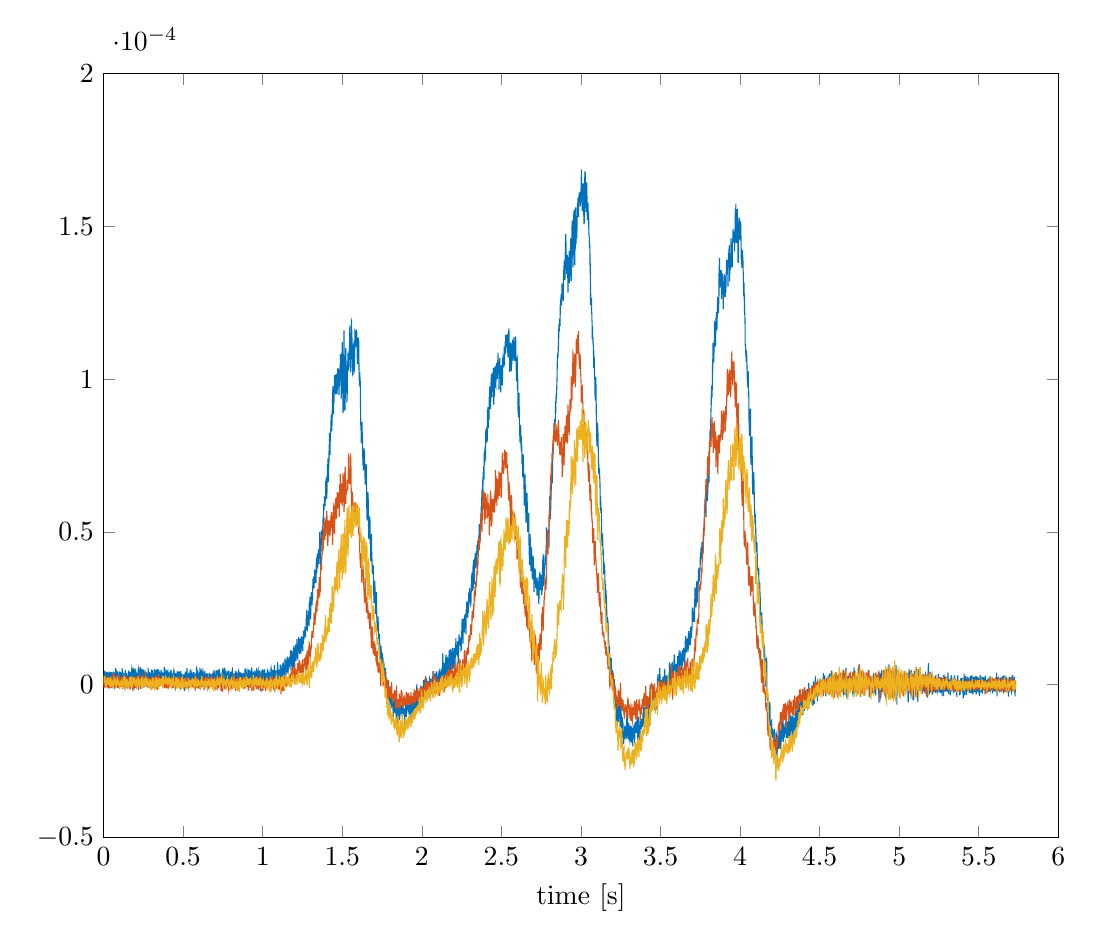
\begin{tikzpicture}

\begin{axis}[%
width=\textwidth,
height=0.8\textwidth,
at={(0\figurewidth,0\figureheight)},
scale only axis,
xmin=0,
xmax=6,
xlabel={time [s]},
ymin=-5e-05,
ymax=0.0002,
ylabel={},
axis background/.style={fill=white},
% title style={font=\bfseries},
% title={Raw strain freight train},
% legend style={legend cell align=left,align=left,draw=white!15!black}
]
\addplot [color=mycolor1,solid,forget plot]
  table[row sep=crcr]{%
0	1.5585854416327e-06\\
0.0009765625	2.14436281522484e-06\\
0.001953125	2.13730525245714e-06\\
0.0029296875	2.87129230928419e-06\\
0.00390625	3.19594077132705e-06\\
0.0048828125	3.9158141935411e-06\\
0.005859375	4.62157344818521e-06\\
0.0068359375	1.02221157582765e-06\\
0.0078125	1.5656429963012e-06\\
0.0087890625	4.85838280510483e-07\\
0.009765625	5.77586303737417e-07\\
0.0107421875	-5.51618974462724e-07\\
0.01171875	3.27357413017096e-06\\
0.0126953125	2.62427731512692e-06\\
0.013671875	2.94186804412379e-06\\
0.0146484375	3.45001362653512e-06\\
0.015625	3.95815972096657e-06\\
0.0166015625	3.9016990185227e-06\\
0.017578125	1.14924743985592e-06\\
0.0185546875	1.57270055106836e-06\\
0.01953125	1.964792396697e-07\\
0.0205078125	1.48095234679853e-06\\
0.021484375	1.29745598833448e-06\\
0.0224609375	2.68779544492599e-06\\
0.0234375	2.10201744010115e-06\\
0.0244140625	4.23340573590361e-06\\
0.025390625	3.59822285118656e-06\\
0.0263671875	3.50647427840899e-06\\
0.02734375	2.04555694546782e-06\\
0.0283203125	7.25794684210612e-07\\
0.029296875	-1.15150825008201e-06\\
0.0302734375	2.71602572740441e-06\\
0.03125	-4.24583506891413e-07\\
0.0322265625	2.02438426160994e-06\\
0.033203125	3.6758562719588e-06\\
0.0341796875	3.85935349583779e-06\\
0.03515625	3.85935349583779e-06\\
0.0361328125	3.37238024052935e-06\\
0.037109375	3.52764702449162e-06\\
0.0380859375	2.05967206853321e-06\\
0.0390625	3.6586012147643e-07\\
0.0400390625	4.36435505686344e-07\\
0.041015625	7.46967313548091e-07\\
0.0419921875	4.19106018536577e-06\\
0.04296875	1.15630498879549e-06\\
0.0439453125	2.71602572740441e-06\\
0.044921875	2.1725930672825e-06\\
0.0458984375	4.12754186622619e-06\\
0.046875	3.75348970468241e-06\\
0.0478515625	3.41559479892159e-08\\
0.048828125	7.82255031085829e-07\\
0.0498046875	-7.8451724856406e-07\\
0.05078125	4.92895820166034e-07\\
0.0517578125	1.09278705189269e-06\\
0.052734375	2.39843514063492e-06\\
0.0537109375	3.99344766320413e-06\\
0.0546875	3.63351076823788e-06\\
0.0556640625	3.68997144065608e-06\\
0.056640625	4.01462042973178e-06\\
0.0576171875	2.32080191651203e-06\\
0.05859375	1.62916099276183e-06\\
0.0595703125	-1.211097603801e-07\\
0.060546875	1.4033192639153e-06\\
0.0615234375	3.09007711943613e-06\\
0.0625	1.31862864167272e-06\\
0.0634765625	1.92557841535972e-06\\
0.064453125	4.17694500264346e-06\\
0.0654296875	2.78660144051464e-06\\
0.06640625	3.90875660598268e-06\\
0.0673828125	3.82406556298336e-06\\
0.068359375	1.11395969663798e-06\\
0.0693359375	-1.98742596638126e-07\\
0.0703125	7.65011494774977e-08\\
0.0712890625	-1.14445073334107e-06\\
0.072265625	3.51745045819741e-07\\
0.0732421875	3.1324225775258e-06\\
0.07421875	3.06184681601851e-06\\
0.0751953125	3.52764702449162e-06\\
0.076171875	5.44025542096021e-06\\
0.0771484375	3.54881977146287e-06\\
0.078125	1.68562144077641e-06\\
0.0791015625	9.3046347170926e-07\\
0.080078125	5.705287628964e-07\\
0.0810546875	-2.55202833683013e-07\\
0.08203125	2.54664405623757e-06\\
0.0830078125	3.26651655160014e-06\\
0.083984375	2.89952260203521e-06\\
0.0849609375	4.17694500264346e-06\\
0.0859375	4.1416570475657e-06\\
0.0869140625	3.35120750096602e-06\\
0.087890625	1.25511068432469e-06\\
0.0888671875	8.24600295390833e-07\\
0.08984375	-7.35114593348671e-07\\
0.0908203125	2.10594310980474e-07\\
0.091796875	-9.8918534004221e-07\\
0.0927734375	1.79854235576957e-06\\
0.09375	2.9912710643881e-06\\
0.0947265625	1.24099558377797e-06\\
0.095703125	3.23828623830587e-06\\
0.0966796875	4.2828088826915e-06\\
0.09765625	3.81700797670885e-06\\
0.0986328125	-2.34030245531988e-07\\
0.099609375	8.81060653328599e-07\\
0.1005859375	2.95284747143165e-07\\
0.1015625	9.16348380249456e-07\\
0.1025390625	3.72917659452986e-07\\
0.103515625	1.33274374439218e-06\\
0.1044921875	2.21493844833201e-06\\
0.10546875	3.64056835194435e-06\\
0.1064453125	3.50647427840899e-06\\
0.107421875	4.19811777687502e-06\\
0.1083984375	2.05967206853321e-06\\
0.109375	-7.35114593348671e-07\\
0.1103515625	9.76737515548821e-08\\
0.111328125	3.6586012147643e-07\\
0.1123046875	-3.18720592803112e-07\\
0.11328125	2.59604703778458e-06\\
0.1142578125	2.66662273410378e-06\\
0.115234375	2.65956516402725e-06\\
0.1162109375	3.78877763259808e-06\\
0.1171875	5.32733369052667e-06\\
0.1181640625	3.47824395168211e-06\\
0.119140625	2.02438426160994e-06\\
0.1201171875	2.03536775275973e-07\\
0.12109375	2.67054600175268e-07\\
0.1220703125	1.47389479331506e-06\\
0.123046875	2.94892561815093e-06\\
0.1240234375	2.83600444556868e-06\\
0.125	3.18182561645768e-06\\
0.1259765625	3.38649540073234e-06\\
0.126953125	3.1324225775258e-06\\
0.1279296875	3.57705010214124e-06\\
0.12890625	2.44783810766295e-06\\
0.1298828125	6.90506970623273e-07\\
0.130859375	8.17542751093379e-07\\
0.1318359375	-5.72791549280013e-07\\
0.1328125	-3.39893177398604e-07\\
0.1337890625	3.17476803917078e-06\\
0.134765625	1.33980129590002e-06\\
0.1357421875	4.23340573590361e-06\\
0.13671875	4.86153181976172e-06\\
0.1376953125	3.35120750096602e-06\\
0.138671875	2.71602572740441e-06\\
0.1396484375	1.91852085565402e-06\\
0.140625	-2.4108777501447e-07\\
0.1416015625	4.71723201495586e-07\\
0.142578125	1.15630498879549e-06\\
0.1435546875	1.74208189511211e-06\\
0.14453125	3.88052625673561e-06\\
0.1455078125	3.15359530790398e-06\\
0.146484375	2.31374435127538e-06\\
0.1474609375	3.05478924041082e-06\\
0.1484375	2.10201744010115e-06\\
0.1494140625	1.6715063281803e-06\\
0.150390625	2.70984147534431e-08\\
0.1513671875	3.16457358406127e-07\\
0.15234375	-1.01035789648878e-06\\
0.1533203125	-5.75919763704056e-08\\
0.154296875	3.00538621392449e-06\\
0.1552734375	2.09495987792629e-06\\
0.15625	4.14871463838367e-06\\
0.1572265625	3.57705010214124e-06\\
0.158203125	4.62863104571981e-06\\
0.1591796875	2.00321157864088e-06\\
0.16015625	9.586936558139e-07\\
0.1611328125	4.5055058371375e-07\\
0.162109375	1.75619700968385e-06\\
0.1630859375	1.47389479331506e-06\\
0.1640625	2.10907500237489e-06\\
0.1650390625	2.46195324198843e-06\\
0.166015625	2.87129230928419e-06\\
0.1669921875	3.47118637024726e-06\\
0.16796875	4.21929055199584e-06\\
0.1689453125	3.40766814177777e-06\\
0.169921875	1.08572950384151e-06\\
0.1708984375	8.316578397876e-07\\
0.171875	-4.59871139981945e-07\\
0.1728515625	3.0406740894925e-06\\
0.173828125	1.14924743985592e-06\\
0.1748046875	2.85717716350152e-06\\
0.17578125	3.59822285118656e-06\\
0.1767578125	4.69214942797297e-06\\
0.177734375	5.21441198537888e-06\\
0.1787109375	4.89681982521195e-06\\
0.1796875	2.39843514063492e-06\\
0.1806640625	2.32080191651203e-06\\
0.181640625	-1.47615391341786e-06\\
0.1826171875	2.52939527283945e-07\\
0.18359375	7.96370118792342e-07\\
0.1845703125	5.28183519925675e-07\\
0.185546875	2.49018351182462e-06\\
0.1865234375	1.8408877054104e-06\\
0.1875	5.05914468208616e-06\\
0.1884765625	4.94622303699038e-06\\
0.189453125	2.69485301539717e-06\\
0.1904296875	1.45272213345838e-06\\
0.19140625	3.30572433075108e-07\\
0.1923828125	-3.64193799226326e-08\\
0.193359375	7.681399437744e-07\\
0.1943359375	1.10690214829082e-06\\
0.1953125	3.2100559265915e-06\\
0.1962890625	3.42884088371182e-06\\
0.197265625	4.27575128999699e-06\\
0.1982421875	5.35556412076428e-06\\
0.19921875	4.50159430521384e-06\\
0.2001953125	7.39909770336791e-07\\
0.201171875	5.53285482887255e-08\\
0.2021484375	-4.34769121706972e-08\\
0.203125	-2.48145304398073e-07\\
0.2041015625	2.90658017546973e-06\\
0.205078125	2.67368030427918e-06\\
0.2060546875	1.5303552239462e-06\\
0.20703125	3.56999251932338e-06\\
0.2080078125	3.39355298098216e-06\\
0.208984375	3.70408660974801e-06\\
0.2099609375	2.01026913953183e-06\\
0.2109375	1.47389479331506e-06\\
0.2119140625	1.17747763620792e-06\\
0.212890625	-2.93618475759056e-08\\
0.2138671875	1.21276538387022e-06\\
0.21484375	1.36803150291905e-06\\
0.2158203125	3.65468351965371e-06\\
0.216796875	3.84523832239973e-06\\
0.2177734375	4.76978301714739e-06\\
0.21875	5.00974145924561e-06\\
0.2197265625	3.37238024052935e-06\\
0.220703125	1.41037681641062e-06\\
0.2216796875	2.05967206853321e-06\\
0.22265625	7.89312574889971e-07\\
0.2236328125	1.12101724508424e-06\\
0.224609375	2.34197461281504e-06\\
0.2255859375	1.07867195588921e-06\\
0.2265625	4.31809684764612e-06\\
0.2275390625	4.25457851250589e-06\\
0.228515625	3.47824395168211e-06\\
0.2294921875	5.86371213527961e-06\\
0.23046875	1.23393803365293e-06\\
0.2314453125	1.75306633443941e-07\\
0.232421875	-2.93618475759056e-08\\
0.2333984375	-1.3914637605225e-06\\
0.234375	1.3539163992121e-06\\
0.2353515625	2.19376575736241e-06\\
0.236328125	2.65250759404981e-06\\
0.2373046875	3.80995039053278e-06\\
0.23828125	3.52058944236527e-06\\
0.2392578125	5.20029677401326e-06\\
0.240234375	4.38161519078668e-06\\
0.2412109375	1.28334088660294e-06\\
0.2421875	5.91701385715439e-07\\
0.2431640625	-2.12857656492135e-07\\
0.244140625	8.66945563251587e-07\\
0.2451171875	1.21982293369905e-06\\
0.24609375	2.37726244196185e-06\\
0.2470703125	2.51841378324071e-06\\
0.248046875	7.54024856858054e-07\\
0.2490234375	5.01679906221206e-06\\
0.25	3.40766814177777e-06\\
0.2509765625	8.66945563251587e-07\\
0.251953125	1.1178882010029e-07\\
0.2529296875	-9.46840224482371e-07\\
0.25390625	3.41559479892159e-08\\
0.2548828125	1.28334088660294e-06\\
0.255859375	2.22199601218609e-06\\
0.2568359375	2.03849938408313e-06\\
0.2578125	3.41472572232358e-06\\
0.2587890625	3.49235911484779e-06\\
0.259765625	4.79095581626941e-06\\
0.2607421875	3.39355298098216e-06\\
0.26171875	1.27628333588484e-06\\
0.2626953125	1.84794526402951e-06\\
0.263671875	1.55152788706286e-06\\
0.2646484375	1.43154947448987e-06\\
0.265625	2.76542872554427e-06\\
0.2666015625	2.69485301539717e-06\\
0.267578125	1.36803150291905e-06\\
0.2685546875	2.89952260203521e-06\\
0.26953125	3.16771046198318e-06\\
0.2705078125	4.02873560791084e-06\\
0.271484375	1.18846354521095e-07\\
0.2724609375	1.02221157582765e-06\\
0.2734375	-9.39782704876971e-07\\
0.2744140625	-3.18720592803112e-07\\
0.275390625	2.2078808845766e-06\\
0.2763671875	1.30451353934813e-06\\
0.27734375	2.63133488470927e-06\\
0.2783203125	3.44295604549514e-06\\
0.279296875	1.89029061781914e-06\\
0.2802734375	5.58140761955828e-06\\
0.28125	2.15142037809099e-06\\
0.2822265625	1.00103893493431e-06\\
0.283203125	5.56413681511003e-07\\
0.2841796875	1.17042008697149e-06\\
0.28515625	-4.03410925851238e-07\\
0.2861328125	2.58898946869576e-06\\
0.287109375	4.16282982031602e-06\\
0.2880859375	1.13513234227254e-06\\
0.2890625	2.48312594421703e-06\\
0.2900390625	3.62645318463008e-06\\
0.291015625	3.5629349366044e-06\\
0.2919921875	7.89312574889971e-07\\
0.29296875	-4.03410925851238e-07\\
0.2939453125	-3.25778121100344e-07\\
0.294921875	9.65751202087204e-07\\
0.2958984375	2.76542872554427e-06\\
0.296875	1.55152788706286e-06\\
0.2978515625	2.09495987792629e-06\\
0.298828125	3.14653773101237e-06\\
0.2998046875	3.78172004681754e-06\\
0.30078125	5.00268385637782e-06\\
0.3017578125	2.01026913953183e-06\\
0.302734375	2.09495987792629e-06\\
0.3037109375	8.316578397876e-07\\
0.3046875	-6.92769456454769e-07\\
0.3056640625	1.38920415922064e-06\\
0.306640625	4.73449502058675e-06\\
0.3076171875	2.48312594421703e-06\\
0.30859375	3.2100559265915e-06\\
0.3095703125	2.13730525245714e-06\\
0.310546875	3.73937453420725e-06\\
0.3115234375	2.94186804412379e-06\\
0.3125	7.65011494774977e-08\\
0.3134765625	-1.04564548859083e-06\\
0.314453125	6.34046634020004e-07\\
0.3154296875	2.02438426160994e-06\\
0.31640625	1.07867195588921e-06\\
0.3173828125	3.31591960366843e-06\\
0.318359375	3.12536500093061e-06\\
0.3193359375	3.6758562719588e-06\\
0.3203125	4.85447421896801e-06\\
0.3212890625	4.80507101617762e-06\\
0.322265625	1.43154947448987e-06\\
0.3232421875	6.34046634020004e-07\\
0.32421875	1.36097395101614e-06\\
0.3251953125	-4.52813613561684e-07\\
0.326171875	2.27139896192934e-06\\
0.3271484375	3.59822285118656e-06\\
0.328125	1.3821466070213e-06\\
0.3291015625	3.42884088371182e-06\\
0.330078125	2.89246502869936e-06\\
0.3310546875	4.89681982521195e-06\\
0.33203125	2.2078808845766e-06\\
0.3330078125	3.51745045819741e-07\\
0.333984375	5.53285482887255e-08\\
0.3349609375	-9.9937166599031e-08\\
0.3359375	-8.58221035845725e-08\\
0.3369140625	1.82677258846859e-06\\
0.337890625	2.49724107953e-06\\
0.3388671875	2.29962922109806e-06\\
0.33984375	5.1085479097668e-06\\
0.3408203125	3.35120750096602e-06\\
0.341796875	4.33221203431926e-06\\
0.3427734375	5.63471222154695e-07\\
0.34375	7.82255031085829e-07\\
0.3447265625	-8.83322544475854e-07\\
0.345703125	1.98203889656043e-06\\
0.3466796875	1.23393803365293e-06\\
0.34765625	4.89681982521195e-06\\
0.3486328125	3.37238024052935e-06\\
0.349609375	2.23611114019023e-06\\
0.3505859375	3.97933248601277e-06\\
0.3515625	3.86641108270492e-06\\
0.3525390625	1.99615401784881e-06\\
0.353515625	1.33274374439218e-06\\
0.3544921875	-4.34769121706972e-08\\
0.35546875	4.99953359920464e-07\\
0.3564453125	8.52830473569441e-07\\
0.357421875	1.12101724508424e-06\\
0.3583984375	1.89029061781914e-06\\
0.359375	3.5629349366044e-06\\
0.3603515625	3.90875660598268e-06\\
0.361328125	4.86858942065431e-06\\
0.3623046875	3.70408660974801e-06\\
0.36328125	9.72808748458736e-07\\
0.3642578125	1.39626171151842e-06\\
0.365234375	1.4033192639153e-06\\
0.3662109375	-3.25778121100344e-07\\
0.3671875	4.26163610490397e-06\\
0.3681640625	2.10201744010115e-06\\
0.369140625	1.28334088660294e-06\\
0.3701171875	3.80289280445603e-06\\
0.37109375	3.17476803917078e-06\\
0.3720703125	3.18182561645768e-06\\
0.373046875	4.92895820166034e-07\\
0.3740234375	-4.34769121706972e-08\\
0.375	-9.8918534004221e-07\\
0.3759765625	1.29039843741905e-06\\
0.376953125	3.25945897312863e-06\\
0.3779296875	6.76391885879668e-07\\
0.37890625	3.78172004681754e-06\\
0.3798828125	4.0005052519478e-06\\
0.380859375	3.60528043439928e-06\\
0.3818359375	5.84253929111875e-06\\
0.3828125	3.40766814177777e-06\\
0.3837890625	1.06455686028147e-06\\
0.384765625	-4.17525979976539e-07\\
0.3857421875	5.98758926852443e-07\\
0.38671875	2.03536775275973e-07\\
0.3876953125	2.67368030427918e-06\\
0.388671875	3.75348970468241e-06\\
0.3896484375	2.5254713513416e-06\\
0.390625	3.11830742443409e-06\\
0.3916015625	5.08737509731082e-06\\
0.392578125	3.9016990185227e-06\\
0.3935546875	1.41743436900504e-06\\
0.39453125	5.98758926852443e-07\\
0.3955078125	4.15262889386829e-07\\
0.396484375	1.72090922399577e-06\\
0.3974609375	8.17542751093379e-07\\
0.3984375	9.9398138816726e-07\\
0.3994140625	2.71602572740441e-06\\
0.400390625	4.67097663299975e-06\\
0.4013671875	3.23828623830587e-06\\
0.40234375	3.9863900745589e-06\\
0.4033203125	3.43589846455426e-06\\
0.404296875	1.21982293369905e-06\\
0.4052734375	3.7997519752842e-07\\
0.40625	-3.89295871330853e-07\\
0.4072265625	1.5585854416327e-06\\
0.408203125	4.06402355508672e-06\\
0.4091796875	1.0151540287644e-06\\
0.41015625	3.76760487555243e-06\\
0.4111328125	1.84794526402951e-06\\
0.412109375	3.66879868775837e-06\\
0.4130859375	3.45001362653512e-06\\
0.4140625	1.36097395101614e-06\\
0.4150390625	1.6715063281803e-06\\
0.416015625	1.63621854841782e-06\\
0.4169921875	4.36435505686344e-07\\
0.41796875	8.66945563251587e-07\\
0.4189453125	2.40549270705682e-06\\
0.419921875	2.39843514063492e-06\\
0.4208984375	4.0922539146053e-06\\
0.421875	3.47824395168211e-06\\
0.4228515625	4.8333014171795e-06\\
0.423828125	1.43154947448987e-06\\
0.4248046875	8.17542751093379e-07\\
0.42578125	6.48161717577925e-07\\
0.4267578125	1.00103893493431e-06\\
0.427734375	-5.44561449326159e-07\\
0.4287109375	1.99615401784881e-06\\
0.4296875	2.64545002417083e-06\\
0.4306640625	1.31862864167272e-06\\
0.431640625	3.15359530790398e-06\\
0.4326171875	2.87129230928419e-06\\
0.43359375	3.45707120767377e-06\\
0.4345703125	-7.13942025346026e-07\\
0.435546875	1.75306633443941e-07\\
0.4365234375	-1.1232781825239e-06\\
0.4375	-4.03410925851238e-07\\
0.4384765625	2.51841378324071e-06\\
0.439453125	3.15359530790398e-06\\
0.4404296875	2.77248629710247e-06\\
0.44140625	2.87129230928419e-06\\
0.4423828125	4.71332222383523e-06\\
0.443359375	4.56511267146655e-06\\
0.4443359375	1.51624011569579e-06\\
0.4453125	1.40018958376571e-07\\
0.4462890625	4.78780740953378e-07\\
0.447265625	-1.04564548859083e-06\\
0.4482421875	1.77736968228208e-06\\
0.44921875	3.2100559265915e-06\\
0.4501953125	2.66662273410378e-06\\
0.451171875	3.53470460671642e-06\\
0.4521484375	2.80777415637384e-06\\
0.453125	3.85229590906932e-06\\
0.4541015625	1.79854235576957e-06\\
0.455078125	-6.92769456454769e-07\\
0.4560546875	-4.52813613561684e-07\\
0.45703125	-4.73986192526914e-07\\
0.4580078125	-1.4228235327169e-07\\
0.458984375	1.93969353506733e-06\\
0.4599609375	8.24600295390833e-07\\
0.4609375	2.10907500237489e-06\\
0.4619140625	3.45001362653512e-06\\
0.462890625	4.35338481506991e-06\\
0.4638671875	9.02233289184736e-07\\
0.46484375	2.10201744010115e-06\\
0.4658203125	2.00408816167664e-08\\
0.466796875	9.16348380249456e-07\\
0.4677734375	-2.19915186270821e-07\\
0.46875	3.0406740894925e-06\\
0.4697265625	3.44295604549514e-06\\
0.470703125	1.84794526402951e-06\\
0.4716796875	4.29692406837714e-06\\
0.47265625	6.97564513143286e-07\\
0.4736328125	4.36750000273054e-06\\
0.474609375	2.15847794105624e-06\\
0.4755859375	4.29377966821177e-07\\
0.4765625	-9.6801278270703e-07\\
0.4775390625	-4.17525979976539e-07\\
0.478515625	1.67856388442913e-06\\
0.4794921875	2.63839245439072e-06\\
0.48046875	1.93969353506733e-06\\
0.4814453125	2.92069532263498e-06\\
0.482421875	1.48095234679853e-06\\
0.4833984375	4.47336392278043e-06\\
0.484375	3.6476259357497e-06\\
0.4853515625	1.14218989101457e-06\\
0.486328125	-4.59871139981945e-07\\
0.4873046875	-2.55202833683013e-07\\
0.48828125	2.95284747143165e-07\\
0.4892578125	1.57270055106836e-06\\
0.490234375	3.24534381648139e-06\\
0.4912109375	2.24316870434051e-06\\
0.4921875	1.74913945234865e-06\\
0.4931640625	3.33003476229109e-06\\
0.494140625	3.23828623830587e-06\\
0.4951171875	6.05816468088544e-07\\
0.49609375	7.18737141295516e-07\\
0.4970703125	-5.16331347791754e-07\\
0.498046875	4.12134813236511e-08\\
0.4990234375	1.48800990038044e-06\\
0.5	1.43860702738071e-06\\
0.5009765625	2.92069532263498e-06\\
0.501953125	3.01244378884025e-06\\
0.5029296875	3.01244378884025e-06\\
0.50390625	3.36532266057639e-06\\
0.5048828125	2.08084475387276e-06\\
0.505859375	1.08572950384151e-06\\
0.5068359375	-5.58676499500844e-07\\
0.5078125	-1.08093307822394e-06\\
0.5087890625	-2.04781207345235e-06\\
0.509765625	2.13024768978875e-06\\
0.5107421875	3.73231694911777e-06\\
0.51171875	2.32785948184756e-06\\
0.5126953125	3.56999251932338e-06\\
0.513671875	3.68997144065608e-06\\
0.5146484375	4.30398166136785e-06\\
0.515625	1.0151540287644e-06\\
0.5166015625	-1.13171720150622e-09\\
0.517578125	-2.62260362869074e-07\\
0.5185546875	4.78780740953378e-07\\
0.51953125	2.3176691868812e-07\\
0.5205078125	2.73014086923625e-06\\
0.521484375	1.98203889656043e-06\\
0.5224609375	3.77466246113522e-06\\
0.5234375	4.32515444093347e-06\\
0.5244140625	5.44025542096021e-06\\
0.525390625	3.37238024052935e-06\\
0.5263671875	3.02655893896883e-06\\
0.52734375	6.19931550856732e-07\\
0.5283203125	8.17542751093379e-07\\
0.529296875	8.24600295390833e-07\\
0.5302734375	1.96792377566758e-06\\
0.53125	2.68073787455304e-06\\
0.5322265625	1.27628333588484e-06\\
0.533203125	3.28063170884e-06\\
0.5341796875	3.47824395168211e-06\\
0.53515625	3.28063170884e-06\\
0.5361328125	3.51745045819741e-07\\
0.537109375	3.16457358406127e-07\\
0.5380859375	-2.4108777501447e-07\\
0.5390625	-7.28057070780146e-07\\
0.5400390625	3.51745045819741e-07\\
0.541015625	3.90875660598268e-06\\
0.5419921875	1.55152788706286e-06\\
0.54296875	3.0406740894925e-06\\
0.5439453125	2.55370162473376e-06\\
0.544921875	4.9391654350112e-06\\
0.5458984375	7.04622055761961e-07\\
0.546875	1.15630498879549e-06\\
0.5478515625	8.59888018361074e-07\\
0.548828125	3.41559479892159e-08\\
0.5498046875	2.06672963021432e-06\\
0.55078125	1.41743436900504e-06\\
0.5517578125	2.27139896192934e-06\\
0.552734375	3.48530153321562e-06\\
0.5537109375	3.76054729006765e-06\\
0.5546875	2.67368030427918e-06\\
0.5556640625	2.67368030427918e-06\\
0.556640625	7.54024856858054e-07\\
0.5576171875	4.15262889386829e-07\\
0.55859375	9.23405925930135e-07\\
0.5595703125	1.96086621536947e-06\\
0.560546875	-3.11663064407001e-07\\
0.5615234375	2.65250759404981e-06\\
0.5625	1.69973655376782e-06\\
0.5634765625	4.07108114481853e-06\\
0.564453125	3.1324225775258e-06\\
0.5654296875	2.48312594421703e-06\\
0.56640625	2.21493844833201e-06\\
0.5673828125	7.39909770336791e-07\\
0.568359375	-9.60955263397401e-07\\
0.5693359375	6.41104175749634e-07\\
0.5703125	2.01732670052144e-06\\
0.5712890625	2.05967206853321e-06\\
0.572265625	3.18888319384282e-06\\
0.5732421875	1.89734817712976e-06\\
0.57421875	3.5629349366044e-06\\
0.5751953125	3.47824395168211e-06\\
0.576171875	3.11124984803623e-06\\
0.5771484375	-1.35224822406634e-07\\
0.578125	1.23393803365293e-06\\
0.5791015625	-9.9937166599031e-08\\
0.580078125	9.09290834667873e-07\\
0.5810546875	2.76542872554427e-06\\
0.58203125	8.81060653328599e-07\\
0.5830078125	3.90875660598268e-06\\
0.583984375	5.46848585751894e-06\\
0.5849609375	5.59552284159115e-06\\
0.5859375	4.25457851250589e-06\\
0.5869140625	2.10907500237489e-06\\
0.587890625	7.11679598479299e-07\\
0.5888671875	4.15262889386829e-07\\
0.58984375	1.21276538387022e-06\\
0.5908203125	-7.28057070780146e-07\\
0.591796875	4.42396075732497e-06\\
0.5927734375	1.91852085565402e-06\\
0.59375	2.57487433081454e-06\\
0.5947265625	3.56999251932338e-06\\
0.595703125	3.33003476229109e-06\\
0.5966796875	2.10907500237489e-06\\
0.59765625	5.8464384467688e-07\\
0.5986328125	-1.211097603801e-07\\
0.599609375	3.4468750813939e-07\\
0.6005859375	1.29039843741905e-06\\
0.6015625	2.39843514063492e-06\\
0.6025390625	2.9912710643881e-06\\
0.603515625	4.12048427570443e-06\\
0.6044921875	2.54664405623757e-06\\
0.60546875	5.62375328684215e-06\\
0.6064453125	4.53688228547761e-06\\
0.607421875	1.6432761041729e-06\\
0.6083984375	-6.71596886674683e-07\\
0.609375	1.50212500784068e-06\\
0.6103515625	-4.88101244676799e-07\\
0.611328125	2.13024768978875e-06\\
0.6123046875	4.67097663299975e-06\\
0.61328125	1.69267899722278e-06\\
0.6142578125	3.95110213281531e-06\\
0.615234375	1.85500282274772e-06\\
0.6162109375	5.0309142684416e-06\\
0.6171875	2.52939527283945e-07\\
0.6181640625	5.14068439725528e-07\\
0.619140625	-6.43366792251777e-07\\
0.6201171875	5.35241060174068e-07\\
0.62109375	-1.63454945275102e-07\\
0.6220703125	2.87834988232406e-06\\
0.623046875	2.87129230928419e-06\\
0.6240234375	3.41472572232358e-06\\
0.625	4.19106018536577e-06\\
0.6259765625	3.8381807358288e-06\\
0.626953125	3.71114419444262e-06\\
0.6279296875	2.00408816167664e-08\\
0.62890625	-2.97548007318791e-07\\
0.6298828125	8.81060653328599e-07\\
0.630859375	9.3046347170926e-07\\
0.6318359375	9.9398138816726e-07\\
0.6328125	2.78660144051464e-06\\
0.6337890625	2.10907500237489e-06\\
0.634765625	4.28986647548488e-06\\
0.6357421875	3.12536500093061e-06\\
0.63671875	4.50159430521384e-06\\
0.6376953125	1.76325456711793e-06\\
0.638671875	-3.11663064407001e-07\\
0.6396484375	-1.13171720150622e-09\\
0.640625	2.599970636806e-07\\
0.6416015625	9.4457856356393e-07\\
0.642578125	1.11395969663798e-06\\
0.6435546875	2.04555694546782e-06\\
0.64453125	2.29257165615783e-06\\
0.6455078125	2.69485301539717e-06\\
0.646484375	3.78877763259808e-06\\
0.6474609375	2.29257165615783e-06\\
0.6484375	4.43493044650824e-07\\
0.6494140625	9.8692384149909e-07\\
0.650390625	1.89421704162741e-07\\
0.6513671875	1.45272213345838e-06\\
0.65234375	5.14068439725528e-07\\
0.6533203125	3.61233801771067e-06\\
0.654296875	1.49506745406145e-06\\
0.6552734375	2.77248629710247e-06\\
0.65625	2.40549270705682e-06\\
0.6572265625	1.9114632960472e-06\\
0.658203125	1.72090922399577e-06\\
0.6591796875	-1.4228235327169e-07\\
0.66015625	-1.24325595873224e-06\\
0.6611328125	1.40018958376571e-07\\
0.662109375	1.09278705189269e-06\\
0.6630859375	2.11613256474751e-06\\
0.6640625	3.73937453420725e-06\\
0.6650390625	3.42178330296847e-06\\
0.666015625	3.22417108225125e-06\\
0.6669921875	3.32297718293032e-06\\
0.66796875	3.35120750096602e-06\\
0.6689453125	2.22199601218609e-06\\
0.669921875	1.86911794047991e-06\\
0.6708984375	-2.05800126614353e-07\\
0.671875	1.66444877203035e-06\\
0.6728515625	2.32080191651203e-06\\
0.673828125	1.5656429963012e-06\\
0.6748046875	2.610162176258e-06\\
0.67578125	2.48312594421703e-06\\
0.6767578125	3.47824395168211e-06\\
0.677734375	2.97715591524744e-06\\
0.6787109375	4.08205350817432e-07\\
0.6796875	6.90506970623273e-07\\
0.6806640625	1.66444877203035e-06\\
0.681640625	1.11395969663798e-06\\
0.6826171875	1.00103893493431e-06\\
0.68359375	3.17476803917078e-06\\
0.6845703125	3.21711350437172e-06\\
0.685546875	3.5911652680725e-06\\
0.6865234375	3.62645318463008e-06\\
0.6875	2.82188930077394e-06\\
0.6884765625	1.55152788706286e-06\\
0.689453125	6.19931550856732e-07\\
0.6904296875	5.98758926852443e-07\\
0.69140625	9.23405925930135e-07\\
0.6923828125	1.30451353934813e-06\\
0.693359375	4.88270462273548e-06\\
0.6943359375	2.63133488470927e-06\\
0.6953125	2.19376575736241e-06\\
0.6962890625	2.19376575736241e-06\\
0.697265625	4.35338481506991e-06\\
0.6982421875	2.85717716350152e-06\\
0.69921875	1.14924743985592e-06\\
0.7001953125	7.65011494774977e-08\\
0.701171875	-7.70402204710707e-07\\
0.7021484375	7.681399437744e-07\\
0.703125	1.53741277821983e-06\\
0.7041015625	2.58193189970582e-06\\
0.705078125	2.94186804412379e-06\\
0.7060546875	2.87834988232406e-06\\
0.70703125	3.45001362653512e-06\\
0.7080078125	4.70626462511603e-06\\
0.708984375	2.73014086923625e-06\\
0.7099609375	1.24805313400189e-06\\
0.7109375	1.3539163992121e-06\\
0.7119140625	1.12807479362874e-06\\
0.712890625	3.13948015422008e-06\\
0.7138671875	2.22199601218609e-06\\
0.71484375	2.27845652657314e-06\\
0.7158203125	4.64980383891515e-06\\
0.716796875	3.18888319384282e-06\\
0.7177734375	3.45707120767377e-06\\
0.71875	2.27845652657314e-06\\
0.7197265625	2.599970636806e-07\\
0.720703125	3.23514895691395e-07\\
0.7216796875	1.44566458036999e-06\\
0.72265625	-9.25667665368883e-07\\
0.7236328125	3.02655893896883e-06\\
0.724609375	4.86153181976172e-06\\
0.7255859375	2.49018351182462e-06\\
0.7265625	3.92287178119818e-06\\
0.7275390625	5.08031749335688e-06\\
0.728515625	4.38867278496308e-06\\
0.7294921875	1.46683723993091e-06\\
0.73046875	2.51135621523826e-06\\
0.7314453125	3.37629970557918e-07\\
0.732421875	2.75837115408517e-06\\
0.7333984375	2.22199601218609e-06\\
0.734375	3.46412878891107e-06\\
0.7353515625	1.5868156608991e-06\\
0.736328125	2.89246502869936e-06\\
0.7373046875	1.99615401784881e-06\\
0.73828125	3.58410768505754e-06\\
0.7392578125	2.43372297373235e-06\\
0.740234375	8.17542751093379e-07\\
0.7412109375	7.65011494774977e-08\\
0.7421875	-1.211097603801e-07\\
0.7431640625	2.33491704728175e-06\\
0.744140625	1.33274374439218e-06\\
0.7451171875	3.8381807358288e-06\\
0.74609375	4.16988741143019e-06\\
0.7470703125	4.07108114481853e-06\\
0.748046875	5.31321847600037e-06\\
0.7490234375	3.39355298098216e-06\\
0.75	1.65033366002622e-06\\
0.7509765625	1.82677258846859e-06\\
0.751953125	1.10690214829082e-06\\
0.7529296875	3.23514895691395e-07\\
0.75390625	4.84035901767701e-06\\
0.7548828125	4.26869369740115e-06\\
0.755859375	2.98421348976854e-06\\
0.7568359375	4.72037982265396e-06\\
0.7578125	3.09007711943613e-06\\
0.7587890625	5.59552284159115e-06\\
0.759765625	2.37726244196185e-06\\
0.7607421875	1.11395969663798e-06\\
0.76171875	1.75306633443941e-07\\
0.7626953125	-8.05689813603147e-07\\
0.763671875	2.0526145069514e-06\\
0.7646484375	2.15142037809099e-06\\
0.765625	3.52764702449162e-06\\
0.7666015625	3.8381807358288e-06\\
0.767578125	3.27357413017096e-06\\
0.7685546875	3.44295604549514e-06\\
0.76953125	2.50429864733512e-06\\
0.7705078125	1.17747763620792e-06\\
0.771484375	1.82364168753793e-07\\
0.7724609375	6.48161717577925e-07\\
0.7734375	3.8381807358288e-06\\
0.7744140625	3.49235911484779e-06\\
0.775390625	1.53741277821983e-06\\
0.7763671875	3.76054729006765e-06\\
0.77734375	2.87129230928419e-06\\
0.7783203125	4.38867278496308e-06\\
0.779296875	3.23122866022923e-06\\
0.7802734375	3.30572433075108e-07\\
0.78125	1.26216823474593e-06\\
0.7822265625	-3.39893177398604e-07\\
0.783203125	-4.52813613561684e-07\\
0.7841796875	1.36803150291905e-06\\
0.78515625	3.61939560112093e-06\\
0.7861328125	3.46412878891107e-06\\
0.787109375	2.75131358272473e-06\\
0.7880859375	3.86641108270492e-06\\
0.7890625	4.57217026821077e-06\\
0.7900390625	2.32785948184756e-06\\
0.791015625	8.03427662794025e-07\\
0.7919921875	-8.58221035845725e-08\\
0.79296875	6.90506970623273e-07\\
0.7939453125	1.44566458036999e-06\\
0.794921875	2.97009834082521e-06\\
0.7958984375	1.63621854841782e-06\\
0.796875	2.36314731000666e-06\\
0.7978515625	2.87834988232406e-06\\
0.798828125	4.0922539146053e-06\\
0.7998046875	2.91363774900313e-06\\
0.80078125	6.8344942820214e-07\\
0.8017578125	-7.06884502481081e-07\\
0.802734375	-1.21502589631021e-06\\
0.8037109375	3.45707120767377e-06\\
0.8046875	1.4707649319246e-07\\
0.8056640625	3.34414992130883e-06\\
0.806640625	3.16771046198318e-06\\
0.8076171875	3.11830742443409e-06\\
0.80859375	3.40061056133042e-06\\
0.8095703125	5.66609895768155e-06\\
0.810546875	2.75131358272473e-06\\
0.8115234375	7.46967313548091e-07\\
0.8125	4.08205350817432e-07\\
0.8134765625	4.78780740953378e-07\\
0.814453125	2.599970636806e-07\\
0.8154296875	3.71114419444262e-06\\
0.81640625	2.56075919332862e-06\\
0.8173828125	3.40766814177777e-06\\
0.818359375	2.59604703778458e-06\\
0.8193359375	3.59822285118656e-06\\
0.8203125	2.56075919332862e-06\\
0.8212890625	1.50212500784068e-06\\
0.822265625	5.4935614096684e-07\\
0.8232421875	1.1178882010029e-07\\
0.82421875	7.65011494774977e-08\\
0.8251953125	2.45489567477614e-06\\
0.826171875	8.88118198515099e-07\\
0.8271484375	2.70191058596766e-06\\
0.828125	3.95815972096657e-06\\
0.8291015625	4.42396075732497e-06\\
0.830078125	3.20299834890973e-06\\
0.8310546875	2.69485301539717e-06\\
0.83203125	8.38715384282596e-07\\
0.8330078125	-4.52813613561684e-07\\
0.833984375	8.03427662794025e-07\\
0.8349609375	1.63621854841782e-06\\
0.8359375	3.68291385625832e-06\\
0.8369140625	3.5629349366044e-06\\
0.837890625	2.70896815663638e-06\\
0.8388671875	8.24600295390833e-07\\
0.83984375	3.79583521847773e-06\\
0.8408203125	2.29962922109806e-06\\
0.841796875	1.54447033259212e-06\\
0.8427734375	1.5303552239462e-06\\
0.84375	6.48161717577925e-07\\
0.8447265625	1.21982293369905e-06\\
0.845703125	2.95598319227696e-06\\
0.8466796875	2.75131358272473e-06\\
0.84765625	3.41472572232358e-06\\
0.8486328125	3.99344766320413e-06\\
0.849609375	3.61233801771067e-06\\
0.8505859375	4.67097663299975e-06\\
0.8515625	1.6432761041729e-06\\
0.8525390625	1.4033192639153e-06\\
0.853515625	-1.14445073334107e-06\\
0.8544921875	2.71602572740441e-06\\
0.85546875	3.31591960366843e-06\\
0.8564453125	1.22688048362655e-06\\
0.857421875	3.28063170884e-06\\
0.8583984375	3.43589846455426e-06\\
0.859375	4.02167801877209e-06\\
0.8603515625	3.42884088371182e-06\\
0.861328125	2.8007165843219e-06\\
0.8623046875	3.16457358406127e-07\\
0.86328125	2.15142037809099e-06\\
0.8642578125	1.11395969663798e-06\\
0.865234375	3.87346866967094e-06\\
0.8662109375	1.75619700968385e-06\\
0.8671875	2.34197461281504e-06\\
0.8681640625	2.82188930077394e-06\\
0.869140625	3.03361651418145e-06\\
0.8701171875	3.35120750096602e-06\\
0.87109375	3.30180444544086e-06\\
0.8720703125	1.06455686028147e-06\\
0.873046875	1.43860702738071e-06\\
0.8740234375	-1.06994697958267e-07\\
0.875	-7.63344682635711e-07\\
0.8759765625	1.6715063281803e-06\\
0.876953125	3.71820177923524e-06\\
0.8779296875	1.04338421761025e-06\\
0.87890625	3.83112314935674e-06\\
0.8798828125	2.92775289636614e-06\\
0.880859375	1.75619700968385e-06\\
0.8818359375	2.39843514063492e-06\\
0.8828125	-7.91574770342201e-07\\
0.8837890625	-1.70512475745292e-07\\
0.884765625	-1.211097603801e-07\\
0.8857421875	9.09290834667873e-07\\
0.88671875	2.47606837670898e-06\\
0.8876953125	3.01950136385532e-06\\
0.888671875	5.26381522827002e-06\\
0.8896484375	3.74643211939517e-06\\
0.890625	4.03579319714826e-06\\
0.8916015625	4.21929055199584e-06\\
0.892578125	1.63621854841782e-06\\
0.8935546875	1.05749931262559e-06\\
0.89453125	-6.85711933293403e-07\\
0.8955078125	9.02233289184736e-07\\
0.896484375	3.55587735398452e-06\\
0.8974609375	1.25511068432469e-06\\
0.8984375	3.2100559265915e-06\\
0.8994140625	4.05696596545422e-06\\
0.900390625	4.36750000273054e-06\\
0.9013671875	3.57705010214124e-06\\
0.90234375	1.81265747192143e-06\\
0.9033203125	1.54447033259212e-06\\
0.904296875	-6.78654410033374e-07\\
0.9052734375	9.09290834667873e-07\\
0.90625	-1.91685066563019e-07\\
0.9072265625	2.66662273410378e-06\\
0.908203125	1.91852085565402e-06\\
0.9091796875	2.54664405623757e-06\\
0.91015625	3.40061056133042e-06\\
0.9111328125	5.03797187170491e-06\\
0.912109375	1.9538086551698e-06\\
0.9130859375	1.81265747192143e-06\\
0.9140625	8.10485206894154e-07\\
0.9150390625	-3.32835649298913e-07\\
0.916015625	3.94404454476293e-06\\
0.9169921875	1.34685884750673e-06\\
0.91796875	1.9326359751643e-06\\
0.9189453125	3.85229590906932e-06\\
0.919921875	4.32515444093347e-06\\
0.9208984375	4.21929055199584e-06\\
0.921875	2.68073787455304e-06\\
0.9228515625	1.54447033259212e-06\\
0.923828125	1.29745598833448e-06\\
0.9248046875	3.41559479892159e-08\\
0.92578125	-1.35224822406634e-07\\
0.9267578125	-1.52467825864644e-08\\
0.927734375	2.28551409131605e-06\\
0.9287109375	1.68562144077641e-06\\
0.9296875	4.11342668528176e-06\\
0.9306640625	5.64492612181722e-06\\
0.931640625	4.85447421896801e-06\\
0.9326171875	1.47389479331506e-06\\
0.93359375	8.24600295390833e-07\\
0.9345703125	2.52939527283945e-07\\
0.935546875	1.47389479331506e-06\\
0.9365234375	8.45772928876904e-07\\
0.9375	2.31374435127538e-06\\
0.9384765625	1.5303552239462e-06\\
0.939453125	4.02873560791084e-06\\
0.9404296875	3.30180444544086e-06\\
0.94140625	3.90875660598268e-06\\
0.9423828125	3.79583521847773e-06\\
0.943359375	1.07161440803601e-06\\
0.9443359375	-1.70512475745292e-07\\
0.9453125	8.52830473569441e-07\\
0.9462890625	-9.46840224482371e-07\\
0.947265625	6.34046634020004e-07\\
0.9482421875	3.71114419444262e-06\\
0.94921875	1.74913945234865e-06\\
0.9501953125	3.06184681601851e-06\\
0.951171875	4.35338481506991e-06\\
0.9521484375	4.68509182954976e-06\\
0.953125	2.32785948184756e-06\\
0.9541015625	2.95598319227696e-06\\
0.955078125	1.4033192639153e-06\\
0.9560546875	1.98203889656043e-06\\
0.95703125	2.84306201811394e-06\\
0.9580078125	3.44295604549514e-06\\
0.958984375	2.53958648784003e-06\\
0.9599609375	3.68997144065608e-06\\
0.9609375	2.78660144051464e-06\\
0.9619140625	5.38379455258288e-06\\
0.962890625	2.79365901236905e-06\\
0.9638671875	8.38715384282596e-07\\
0.96484375	1.19159273497655e-06\\
0.9658203125	7.11679598479299e-07\\
0.966796875	4.78780740953378e-07\\
0.9677734375	2.68073787455304e-06\\
0.96875	3.69702902515293e-06\\
0.9697265625	3.65468351965371e-06\\
0.970703125	4.26869369740115e-06\\
0.9716796875	4.52276709307577e-06\\
0.97265625	3.35826508072166e-06\\
0.9736328125	1.0080964817998e-06\\
0.974609375	2.88227210253197e-07\\
0.9755859375	1.32961423659345e-07\\
0.9765625	8.24600295390833e-07\\
0.9775390625	1.87617549949389e-06\\
0.978515625	2.92069532263498e-06\\
0.9794921875	3.31591960366843e-06\\
0.98046875	2.87834988232406e-06\\
0.9814453125	4.69214942797297e-06\\
0.982421875	3.9652173092165e-06\\
0.9833984375	3.35120750096602e-06\\
0.984375	-4.81043718651404e-07\\
0.9853515625	-2.19601963879199e-06\\
0.986328125	1.65739121597906e-06\\
0.9873046875	-1.13171720150622e-09\\
0.98828125	2.19376575736241e-06\\
0.9892578125	2.57487433081454e-06\\
0.990234375	2.76542872554427e-06\\
0.9912109375	3.71820177923524e-06\\
0.9921875	3.9369869568092e-06\\
0.9931640625	4.0922539146053e-06\\
0.994140625	1.76325456711793e-06\\
0.9951171875	4.64665662136023e-07\\
0.99609375	2.45881990986819e-07\\
0.9970703125	-1.05976052474071e-06\\
0.998046875	-7.49229638189733e-07\\
0.9990234375	1.02221157582765e-06\\
1	2.92069532263498e-06\\
1.0009765625	5.0309142684416e-06\\
1.001953125	2.78660144051464e-06\\
1.0029296875	3.95110213281531e-06\\
1.00390625	2.01732670052144e-06\\
1.0048828125	9.72808748458736e-07\\
1.005859375	2.00408816167664e-08\\
1.0068359375	-3.6812328880944e-07\\
1.0078125	8.88118198515099e-07\\
1.0087890625	4.71332222383523e-06\\
1.009765625	6.48161717577925e-07\\
1.0107421875	4.06402355508672e-06\\
1.01171875	4.67803423122542e-06\\
1.0126953125	4.57217026821077e-06\\
1.013671875	3.08301954343336e-06\\
1.0146484375	-3.25778121100344e-07\\
1.015625	-3.61065761105049e-07\\
1.0166015625	-3.9635339864081e-07\\
1.017578125	1.86206038156416e-06\\
1.0185546875	1.69267899722278e-06\\
1.01953125	2.03144182279709e-06\\
1.0205078125	3.84523832239973e-06\\
1.021484375	2.51135621523826e-06\\
1.0224609375	3.46412878891107e-06\\
1.0234375	1.98909645715518e-06\\
1.0244140625	5.56413681511003e-07\\
1.025390625	-1.14052229218406e-07\\
1.0263671875	1.45272213345838e-06\\
1.02734375	3.09399821219955e-07\\
1.0283203125	1.98203889656043e-06\\
1.029296875	3.35120750096602e-06\\
1.0302734375	4.43807594696123e-06\\
1.03125	5.101490305516e-06\\
1.0322265625	3.55587735398452e-06\\
1.033203125	4.31103925445766e-06\\
1.0341796875	1.63621854841782e-06\\
1.03515625	1.39626171151842e-06\\
1.0361328125	8.24600295390833e-07\\
1.037109375	9.23405925930135e-07\\
1.0380859375	-6.22194220397396e-07\\
1.0390625	3.31591960366843e-06\\
1.0400390625	3.5629349366044e-06\\
1.041015625	3.09007711943613e-06\\
1.0419921875	3.25945897312863e-06\\
1.04296875	3.99344766320413e-06\\
1.0439453125	2.47606837670898e-06\\
1.044921875	4.5055058371375e-07\\
1.0458984375	5.8464384467688e-07\\
1.046875	-4.31641033706758e-07\\
1.0478515625	4.99953359920464e-07\\
1.048828125	2.48312594421703e-06\\
1.0498046875	2.13024768978875e-06\\
1.05078125	2.64545002417083e-06\\
1.0517578125	5.12266311856417e-06\\
1.052734375	5.48260107639115e-06\\
1.0537109375	5.07325988950095e-06\\
1.0546875	3.57705010214124e-06\\
1.0556640625	1.99615401784881e-06\\
1.056640625	3.05478924041082e-06\\
1.0576171875	2.48312594421703e-06\\
1.05859375	1.98203889656043e-06\\
1.0595703125	4.57217026821077e-06\\
1.060546875	2.37020487593503e-06\\
1.0615234375	4.88976222392428e-06\\
1.0625	3.43589846455426e-06\\
1.0634765625	4.81918621648091e-06\\
1.064453125	4.44513354192779e-06\\
1.0654296875	1.29039843741905e-06\\
1.06640625	6.19931550856732e-07\\
1.0673828125	2.09495987792629e-06\\
1.068359375	8.24600295390833e-07\\
1.0693359375	2.19376575736241e-06\\
1.0703125	3.05478924041082e-06\\
1.0712890625	1.75619700968385e-06\\
1.072265625	4.43807594696123e-06\\
1.0732421875	5.08737509731082e-06\\
1.07421875	6.43537926363737e-06\\
1.0751953125	3.06184681601851e-06\\
1.076171875	2.0526145069514e-06\\
1.0771484375	1.13513234227254e-06\\
1.078125	2.88540745546195e-06\\
1.0791015625	2.29962922109806e-06\\
1.080078125	3.9652173092165e-06\\
1.0810546875	1.66444877203035e-06\\
1.08203125	4.64980383891515e-06\\
1.0830078125	3.65468351965371e-06\\
1.083984375	3.37943782058162e-06\\
1.0849609375	4.27575128999699e-06\\
1.0859375	2.29962922109806e-06\\
1.0869140625	9.8692384149909e-07\\
1.087890625	2.49724107953e-06\\
1.0888671875	-6.29251744447374e-07\\
1.08984375	4.52276709307577e-06\\
1.0908203125	3.29474686647517e-06\\
1.091796875	3.05478924041082e-06\\
1.0927734375	3.2100559265915e-06\\
1.09375	7.45873561793799e-06\\
1.0947265625	5.96251875311683e-06\\
1.095703125	3.42884088371182e-06\\
1.0966796875	4.74861021891484e-06\\
1.09765625	4.99953359920464e-07\\
1.0986328125	3.63351076823788e-06\\
1.099609375	3.82406556298336e-06\\
1.1005859375	4.57922786505343e-06\\
1.1015625	4.54393988182675e-06\\
1.1025390625	4.21929055199584e-06\\
1.103515625	4.16282982031602e-06\\
1.1044921875	4.91093502808307e-06\\
1.10546875	3.78877763259808e-06\\
1.1064453125	6.8344942820214e-07\\
1.107421875	7.46967313548091e-07\\
1.1083984375	6.8344942820214e-07\\
1.109375	5.35241060174068e-07\\
1.1103515625	6.45655213268826e-06\\
1.111328125	5.2214695912098e-06\\
1.1123046875	3.31591960366843e-06\\
1.11328125	5.22852719713959e-06\\
1.1142578125	5.80019360546394e-06\\
1.115234375	5.58140761955828e-06\\
1.1162109375	3.64056835194435e-06\\
1.1171875	9.586936558139e-07\\
1.1181640625	9.09290834667873e-07\\
1.119140625	1.3821466070213e-06\\
1.1201171875	3.76760487555243e-06\\
1.12109375	4.45924873215668e-06\\
1.1220703125	3.63351076823788e-06\\
1.123046875	5.37673694447991e-06\\
1.1240234375	5.39790976908459e-06\\
1.125	7.0070470400271e-06\\
1.1259765625	4.81212861628004e-06\\
1.126953125	3.21711350437172e-06\\
1.1279296875	5.9258156391833e-09\\
1.12890625	5.08737509731082e-06\\
1.1298828125	3.33709234175052e-06\\
1.130859375	4.48042151824073e-06\\
1.1318359375	5.94840352081201e-06\\
1.1328125	6.85177918480695e-06\\
1.1337890625	6.7388571383096e-06\\
1.134765625	7.02821993307898e-06\\
1.1357421875	5.29910326186917e-06\\
1.13671875	4.25457851250589e-06\\
1.1376953125	3.70408660974801e-06\\
1.138671875	3.06890439172466e-06\\
1.1396484375	6.48478262613877e-06\\
1.140625	3.85229590906932e-06\\
1.1416015625	5.00974145924561e-06\\
1.142578125	5.02385666527739e-06\\
1.1435546875	6.33657255315334e-06\\
1.14453125	6.14601680903274e-06\\
1.1455078125	8.609131792111e-06\\
1.146484375	6.16013204686873e-06\\
1.1474609375	5.06620228574455e-06\\
1.1484375	1.93969353506733e-06\\
1.1494140625	7.88219402715618e-06\\
1.150390625	4.69920702649506e-06\\
1.1513671875	4.12754186622619e-06\\
1.15234375	6.78826053054069e-06\\
1.1533203125	7.33169816450946e-06\\
1.154296875	7.30346762364918e-06\\
1.1552734375	9.2090326785834e-06\\
1.15625	7.31758289388177e-06\\
1.1572265625	5.76490553680104e-06\\
1.158203125	6.61181986622342e-06\\
1.1591796875	3.62645318463008e-06\\
1.16015625	8.02334690924527e-06\\
1.1611328125	6.78826053054069e-06\\
1.162109375	4.85447421896801e-06\\
1.1630859375	6.35068779632295e-06\\
1.1640625	6.6471079941486e-06\\
1.1650390625	7.38815925097123e-06\\
1.166015625	9.07493712438328e-06\\
1.1669921875	5.68727179443406e-06\\
1.16796875	6.56947411597293e-06\\
1.1689453125	7.61400366003167e-06\\
1.169921875	6.57653174076763e-06\\
1.1708984375	7.95982810741585e-06\\
1.171875	9.15257138825844e-06\\
1.1728515625	7.55048490976105e-06\\
1.173828125	6.7741452751235e-06\\
1.1748046875	9.89362632676234e-06\\
1.17578125	1.13545663950507e-05\\
1.1767578125	6.23776586202861e-06\\
1.177734375	5.270872834792e-06\\
1.1787109375	4.88976222392428e-06\\
1.1796875	7.71281062080008e-06\\
1.1806640625	1.07546629563289e-05\\
1.181640625	7.83984817023342e-06\\
1.1826171875	9.89362632676234e-06\\
1.18359375	8.75028487766797e-06\\
1.1845703125	1.11357779994333e-05\\
1.185546875	1.03735482012419e-05\\
1.1865234375	9.1737443713893e-06\\
1.1875	7.97394339602004e-06\\
1.1884765625	5.55317717667821e-06\\
1.189453125	6.86589444239688e-06\\
1.1904296875	9.77364592950457e-06\\
1.19140625	5.33439129793835e-06\\
1.1923828125	8.29859514295478e-06\\
1.193359375	9.68189623321513e-06\\
1.1943359375	1.07405475898931e-05\\
1.1953125	1.19685859478113e-05\\
1.1962890625	1.26743564722025e-05\\
1.197265625	8.02334690924527e-06\\
1.1982421875	6.96470125658983e-06\\
1.19921875	4.09931150473219e-06\\
1.2001953125	7.2470065466694e-06\\
1.201171875	1.07687783231596e-05\\
1.2021484375	7.8186752431055e-06\\
1.203125	9.93597235613894e-06\\
1.2041015625	1.10510857427419e-05\\
1.205078125	9.23020566408455e-06\\
1.2060546875	1.31048769771015e-05\\
1.20703125	9.45605089807885e-06\\
1.2080078125	8.86320737455959e-06\\
1.208984375	7.95982810741585e-06\\
1.2099609375	7.97394339602004e-06\\
1.2109375	9.42782023829851e-06\\
1.2119140625	1.05641055427833e-05\\
1.212890625	1.09734511866025e-05\\
1.2138671875	9.74541525194527e-06\\
1.21484375	1.17427395886123e-05\\
1.2158203125	1.49469442715252e-05\\
1.216796875	1.23426442027181e-05\\
1.2177734375	1.10157973066518e-05\\
1.21875	1.08393551632392e-05\\
1.2197265625	8.49620935211158e-06\\
1.220703125	8.45386344363046e-06\\
1.2216796875	1.30978192609433e-05\\
1.22265625	1.32036850136877e-05\\
1.2236328125	1.09522781279116e-05\\
1.224609375	1.35495132941945e-05\\
1.2255859375	1.38035913656886e-05\\
1.2265625	1.55821414504057e-05\\
1.2275390625	1.16509895340786e-05\\
1.228515625	1.33024930696335e-05\\
1.2294921875	1.20321052545593e-05\\
1.23046875	1.00418374451372e-05\\
1.2314453125	1.08817012720282e-05\\
1.232421875	1.39941500033151e-05\\
1.2333984375	1.32530890392406e-05\\
1.234375	1.27167027350759e-05\\
1.2353515625	1.42058819073505e-05\\
1.236328125	1.50104639534104e-05\\
1.2373046875	1.45375954024017e-05\\
1.23828125	1.17992011689303e-05\\
1.2392578125	1.37400718358146e-05\\
1.240234375	1.00771258130753e-05\\
1.2412109375	1.30625306816339e-05\\
1.2421875	1.57091809821891e-05\\
1.2431640625	1.3140165559374e-05\\
1.244140625	1.31542809929748e-05\\
1.2451171875	1.35565710166743e-05\\
1.24609375	1.53845244645746e-05\\
1.2470703125	1.52716005074394e-05\\
1.248046875	1.19615282475555e-05\\
1.2490234375	1.3217800449066e-05\\
1.25	1.23073556762519e-05\\
1.2509765625	1.24908560408424e-05\\
1.251953125	1.10087396197299e-05\\
1.2529296875	1.5215138538354e-05\\
1.25390625	1.56244879574441e-05\\
1.2548828125	1.33730702643043e-05\\
1.255859375	1.57868162673665e-05\\
1.2568359375	1.77135867194468e-05\\
1.2578125	1.66337474274761e-05\\
1.2587890625	1.45940572956298e-05\\
1.259765625	1.59562023856017e-05\\
1.2607421875	1.63584946444287e-05\\
1.26171875	1.54480442015753e-05\\
1.2626953125	1.71560223518716e-05\\
1.263671875	1.71701378978756e-05\\
1.2646484375	1.78618001360588e-05\\
1.265625	1.7537142232656e-05\\
1.2666015625	1.88146017115081e-05\\
1.267578125	1.81370537396175e-05\\
1.2685546875	1.62949747927524e-05\\
1.26953125	1.61467618366221e-05\\
1.2705078125	1.87440237552966e-05\\
1.271484375	1.83134984363023e-05\\
1.2724609375	1.767829781715e-05\\
1.2734375	2.1948272922543e-05\\
1.2744140625	1.99791394150442e-05\\
1.275390625	1.96827113808286e-05\\
1.2763671875	2.14189352025361e-05\\
1.27734375	2.4594969856717e-05\\
1.2783203125	2.10519280428186e-05\\
1.279296875	1.83487873830475e-05\\
1.2802734375	1.82005738233123e-05\\
1.28125	1.95415552352995e-05\\
1.2822265625	2.04237817930633e-05\\
1.283203125	2.15600918735449e-05\\
1.2841796875	2.20894297417137e-05\\
1.28515625	2.27105202154452e-05\\
1.2861328125	2.16941907475996e-05\\
1.287109375	2.34868843832692e-05\\
1.2880859375	2.39809349305324e-05\\
1.2890625	2.16094967177326e-05\\
1.2900390625	2.22517601326047e-05\\
1.291015625	1.91886650443311e-05\\
1.2919921875	2.01061800544746e-05\\
1.29296875	2.68534955577191e-05\\
1.2939453125	2.51666582186823e-05\\
1.294921875	2.41573816718503e-05\\
1.2958984375	2.69099588298381e-05\\
1.296875	2.87732503562405e-05\\
1.2978515625	2.70581749492284e-05\\
1.298828125	2.44255808368884e-05\\
1.2998046875	2.7262854423809e-05\\
1.30078125	2.13554147134721e-05\\
1.3017578125	2.29857764654649e-05\\
1.302734375	2.77004453032839e-05\\
1.3037109375	2.63312105903033e-05\\
1.3046875	3.00366223908708e-05\\
1.3056640625	2.87873662274121e-05\\
1.306640625	2.81239207094589e-05\\
1.3076171875	3.01142598816957e-05\\
1.30859375	3.01283757904024e-05\\
1.3095703125	2.59783156482556e-05\\
1.310546875	2.98742894941312e-05\\
1.3115234375	2.82933109714959e-05\\
1.3125	2.75239973223274e-05\\
1.3134765625	2.96625510116946e-05\\
1.314453125	3.24151582175422e-05\\
1.3154296875	3.1250591796896e-05\\
1.31640625	3.46313708343249e-05\\
1.3173828125	3.25210280254966e-05\\
1.318359375	3.489251754842e-05\\
1.3193359375	3.40808457719565e-05\\
1.3203125	3.54077533539071e-05\\
1.3212890625	3.17234760191739e-05\\
1.322265625	3.17305339959995e-05\\
1.3232421875	3.24081002311357e-05\\
1.32421875	3.37420614168968e-05\\
1.3251953125	3.46737189409376e-05\\
1.326171875	3.57112486637672e-05\\
1.3271484375	3.76522113598914e-05\\
1.328125	3.64594006727816e-05\\
1.3291015625	3.58030030957271e-05\\
1.330078125	3.68758253850208e-05\\
1.3310546875	3.57818289945622e-05\\
1.33203125	3.3495031301475e-05\\
1.3330078125	3.76451533001909e-05\\
1.333984375	3.56830165342146e-05\\
1.3349609375	3.3367987289232e-05\\
1.3359375	3.89014894829503e-05\\
1.3369140625	3.96919947526892e-05\\
1.337890625	4.08777549806049e-05\\
1.3388671875	4.13647644533185e-05\\
1.33984375	3.66358517800542e-05\\
1.3408203125	3.94308455533077e-05\\
1.341796875	4.2282319810071e-05\\
1.3427734375	3.80827531884125e-05\\
1.34375	4.29951908934132e-05\\
1.3447265625	4.05248498594666e-05\\
1.345703125	3.83791920381034e-05\\
1.3466796875	4.08706968757621e-05\\
1.34765625	4.26564005499377e-05\\
1.3486328125	3.95367168340556e-05\\
1.349609375	3.95861234393437e-05\\
1.3505859375	4.42868311657984e-05\\
1.3515625	4.00590154776945e-05\\
1.3525390625	3.95508330065012e-05\\
1.353515625	4.36163071142234e-05\\
1.3544921875	4.15129848209703e-05\\
1.35546875	4.17317863956926e-05\\
1.3564453125	4.12447765685542e-05\\
1.357421875	4.40750866321472e-05\\
1.3583984375	5.00533748107269e-05\\
1.359375	4.53808460059431e-05\\
1.3603515625	4.39974469920836e-05\\
1.361328125	4.6968936287136e-05\\
1.3623046875	4.46256226045597e-05\\
1.36328125	3.93461485447115e-05\\
1.3642578125	4.31504698769007e-05\\
1.365234375	4.5133810189437e-05\\
1.3662109375	4.35527838292509e-05\\
1.3671875	4.38986329220168e-05\\
1.3681640625	4.7441835248266e-05\\
1.369140625	5.04698107478604e-05\\
1.3701171875	4.96651721281689e-05\\
1.37109375	4.94675417863797e-05\\
1.3720703125	4.9354610197272e-05\\
1.373046875	4.88675930089243e-05\\
1.3740234375	4.80206077146026e-05\\
1.375	5.01874812614185e-05\\
1.3759765625	4.98486860863187e-05\\
1.376953125	4.91569799771832e-05\\
1.3779296875	5.20579170540708e-05\\
1.37890625	5.3476629583509e-05\\
1.3798828125	5.48177047980829e-05\\
1.380859375	5.23190727921181e-05\\
1.3818359375	5.52623778933353e-05\\
1.3828125	5.36672032124159e-05\\
1.3837890625	5.92079864994732e-05\\
1.384765625	5.69422575693247e-05\\
1.3857421875	5.83539254893782e-05\\
1.38671875	5.85656760181959e-05\\
1.3876953125	5.99914652269803e-05\\
1.388671875	6.16360686770037e-05\\
1.3896484375	6.10996309108134e-05\\
1.390625	5.94409124805139e-05\\
1.3916015625	5.92503366698427e-05\\
1.392578125	6.12266819091337e-05\\
1.3935546875	6.16078350961368e-05\\
1.39453125	6.01679245677783e-05\\
1.3955078125	6.13113825924628e-05\\
1.396484375	6.66052035288543e-05\\
1.3974609375	6.41347468434371e-05\\
1.3984375	6.5631136304968e-05\\
1.3994140625	6.72122318807723e-05\\
1.400390625	6.70075361920818e-05\\
1.4013671875	6.20313389751007e-05\\
1.40234375	6.18760541781877e-05\\
1.4033203125	6.08949377030636e-05\\
1.404296875	6.45582528443433e-05\\
1.4052734375	6.68240159900965e-05\\
1.40625	6.7600448070282e-05\\
1.4072265625	7.21743631316072e-05\\
1.408203125	7.14755678681523e-05\\
1.4091796875	7.04167890108378e-05\\
1.41015625	7.40448804701281e-05\\
1.4111328125	6.86874549907094e-05\\
1.412109375	6.89345023448219e-05\\
1.4130859375	6.62734557848237e-05\\
1.4140625	7.18073190341224e-05\\
1.4150390625	7.30425646561892e-05\\
1.416015625	7.09673537392414e-05\\
1.4169921875	7.63036276350995e-05\\
1.41796875	7.837180187988e-05\\
1.4189453125	7.73271257747065e-05\\
1.419921875	8.23034739159461e-05\\
1.4208984375	7.92470727150969e-05\\
1.421875	7.69106676603718e-05\\
1.4228515625	7.51530770338692e-05\\
1.423828125	7.88729648335232e-05\\
1.4248046875	8.04541019231767e-05\\
1.42578125	8.20846547386481e-05\\
1.4267578125	8.22470044417481e-05\\
1.427734375	8.37434476442884e-05\\
1.4287109375	8.26705256523493e-05\\
1.4296875	8.66516424164099e-05\\
1.4306640625	8.69057573193832e-05\\
1.431640625	8.84375081964713e-05\\
1.4326171875	8.49010765639354e-05\\
1.43359375	8.29952254880007e-05\\
1.4345703125	8.54304809187205e-05\\
1.435546875	8.48163719187401e-05\\
1.4365234375	8.65457612446265e-05\\
1.4375	8.96657357627483e-05\\
1.4384765625	9.42116155360103e-05\\
1.439453125	9.41974978335362e-05\\
1.4404296875	9.61457445106532e-05\\
1.44140625	9.77339946528111e-05\\
1.4423828125	9.34633778494432e-05\\
1.443359375	9.28351414038713e-05\\
1.4443359375	9.30045534020209e-05\\
1.4453125	8.8508095906625e-05\\
1.4462890625	9.22633763302441e-05\\
1.447265625	9.35480839469184e-05\\
1.4482421875	9.26092588281924e-05\\
1.44921875	9.71481062403828e-05\\
1.4501953125	9.73881086402844e-05\\
1.451171875	9.95481353788267e-05\\
1.4521484375	0.000101341105776518\\
1.453125	0.000100028142577033\\
1.4541015625	9.84610619423221e-05\\
1.455078125	9.61669211463159e-05\\
1.4560546875	9.6689278440803e-05\\
1.45703125	9.71904595967726e-05\\
1.4580078125	9.50586784076476e-05\\
1.458984375	0.000101305811022148\\
1.4599609375	9.96469603528765e-05\\
1.4609375	0.000101199926773859\\
1.4619140625	0.000101799937808089\\
1.462890625	9.80163507572631e-05\\
1.4638671875	9.87293006244892e-05\\
1.46484375	9.95551943049023e-05\\
1.4658203125	9.75504632696851e-05\\
1.466796875	9.50727961342279e-05\\
1.4677734375	9.76281111543956e-05\\
1.46875	9.63151576208522e-05\\
1.4697265625	9.66822195548388e-05\\
1.470703125	0.000101404636340607\\
1.4716796875	0.000103536444353063\\
1.47265625	9.70492817559724e-05\\
1.4736328125	0.000102788192832306\\
1.474609375	9.87363595391043e-05\\
1.4755859375	9.76916412507773e-05\\
1.4765625	9.8941068105921e-05\\
1.4775390625	9.81292932433048e-05\\
1.478515625	9.99928479145456e-05\\
1.4794921875	9.4903383441345e-05\\
1.48046875	0.000102442303353559\\
1.4814453125	0.000102287006113732\\
1.482421875	9.77128179513499e-05\\
1.4833984375	0.000100882274162368\\
1.484375	0.000101439931101893\\
1.4853515625	0.000103345851879199\\
1.486328125	0.000103995278381846\\
1.4873046875	0.000103183495384199\\
1.48828125	0.000107193010205023\\
1.4892578125	0.000108237748174822\\
1.490234375	0.000104157635138169\\
1.4912109375	0.000103804685734591\\
1.4921875	0.000102054060343651\\
1.4931640625	9.35339662630178e-05\\
1.494140625	9.6159862267663e-05\\
1.4951171875	9.5432798295552e-05\\
1.49609375	9.71057528875499e-05\\
1.4970703125	0.00010055756281074\\
1.498046875	0.000105724733472999\\
1.4990234375	0.000109974276885653\\
1.5	0.0001122049485556\\
1.5009765625	0.000107058888595376\\
1.501953125	0.000107207128271271\\
1.5029296875	0.000102512893023834\\
1.50390625	9.40845562279696e-05\\
1.5048828125	8.89104460431499e-05\\
1.505859375	8.94539721758561e-05\\
1.5068359375	9.21645528029703e-05\\
1.5078125	9.48680891374907e-05\\
1.5087890625	9.92304838076771e-05\\
1.509765625	0.000107545961979788\\
1.5107421875	0.000116009819518206\\
1.51171875	0.00011091313432919\\
1.5126953125	0.000104778826688375\\
1.513671875	0.000105025891722144\\
1.5146484375	9.6428099725933e-05\\
1.515625	9.00257340645256e-05\\
1.5166015625	9.26516118034261e-05\\
1.517578125	8.97363236448047e-05\\
1.5185546875	9.38657319391569e-05\\
1.51953125	9.39080850199045e-05\\
1.5205078125	0.000102258770257083\\
1.521484375	0.000108174216749995\\
1.5224609375	0.000110277817070955\\
1.5234375	0.000103607034176475\\
1.5244140625	0.000106338867932228\\
1.525390625	9.95128407499303e-05\\
1.5263671875	0.000104531761775634\\
1.52734375	9.92446016510355e-05\\
1.5283203125	9.70069284114384e-05\\
1.529296875	9.23410234009718e-05\\
1.5302734375	9.58422128305297e-05\\
1.53125	9.50798549976663e-05\\
1.5322265625	9.95410764528498e-05\\
1.533203125	0.000100684623749524\\
1.5341796875	0.000105717674460574\\
1.53515625	0.0001050188327195\\
1.5361328125	0.000107743615081545\\
1.537109375	0.000107510666791196\\
1.5380859375	0.000108449519648713\\
1.5390625	0.000104199989083197\\
1.5400390625	0.000102788192832306\\
1.541015625	0.000104150576147677\\
1.5419921875	0.000106960062168986\\
1.54296875	0.000106310631848736\\
1.5439453125	0.000108287161510777\\
1.544921875	0.000112374367060224\\
1.5458984375	0.000111929643606964\\
1.546875	0.000115487442213062\\
1.5478515625	0.000117562836323368\\
1.548828125	0.000112847327353494\\
1.5498046875	0.000111668456999737\\
1.55078125	0.000109148366143441\\
1.5517578125	0.000105400019003681\\
1.552734375	0.000102216416475073\\
1.5537109375	0.000106550638608803\\
1.5546875	0.000106776527428493\\
1.5556640625	0.00010969191408659\\
1.556640625	0.00010912012990266\\
1.5576171875	0.000119122917110542\\
1.55859375	0.000118925259549273\\
1.5595703125	0.000114654463305171\\
1.560546875	0.000114809764353155\\
1.5615234375	0.00011179552073771\\
1.5625	0.000110284876147206\\
1.5634765625	0.000104814121685789\\
1.564453125	0.000102985844069524\\
1.5654296875	0.00010176464302161\\
1.56640625	0.000101404636340607\\
1.5673828125	0.000101517579585415\\
1.568359375	0.000110496648480661\\
1.5693359375	0.000107390663168461\\
1.5703125	0.000111160202367964\\
1.5712890625	0.000111357856886125\\
1.572265625	0.000109070716485097\\
1.5732421875	0.000107270659574279\\
1.57421875	0.000108498933005416\\
1.5751953125	0.000103261144136157\\
1.576171875	0.000103070551766328\\
1.5771484375	0.000104884711688027\\
1.578125	0.000111068434225148\\
1.5791015625	0.00010969897315464\\
1.580078125	0.000115212135472656\\
1.5810546875	0.00011499330201697\\
1.58203125	0.000111139025102755\\
1.5830078125	0.00011588275471851\\
1.583984375	0.000111866111717082\\
1.5849609375	0.000110644889166987\\
1.5859375	0.0001118590526187\\
1.5869140625	0.000112254362280237\\
1.587890625	0.00011195082090537\\
1.5888671875	0.000116320422496675\\
1.58984375	0.000112776736236787\\
1.5908203125	0.000115438028171667\\
1.591796875	0.000112642613142265\\
1.5927734375	0.000111110788750526\\
1.59375	0.000107934209217313\\
1.5947265625	0.000106698878135313\\
1.595703125	0.000105004714714508\\
1.5966796875	0.000107715378919409\\
1.59765625	0.000109451905831678\\
1.5986328125	0.000107644788520984\\
1.599609375	0.000112946154933481\\
1.6005859375	0.000113623830289352\\
1.6015625	0.000112882622915552\\
1.6025390625	0.000112035530107886\\
1.603515625	0.000112600258488248\\
1.6044921875	0.000106832999649223\\
1.60546875	0.000103042315865813\\
1.6064453125	0.000102131708921724\\
1.607421875	9.85881223529337e-05\\
1.6083984375	9.87293006244892e-05\\
1.609375	0.000100028142577033\\
1.6103515625	0.000102244652329351\\
1.611328125	9.90469518799811e-05\\
1.6123046875	0.000100578739631648\\
1.61328125	9.80798809025491e-05\\
1.6142578125	9.31739654570769e-05\\
1.615234375	8.98069115367406e-05\\
1.6162109375	8.60234144558227e-05\\
1.6171875	8.33058081351023e-05\\
1.6181640625	8.41740288223356e-05\\
1.619140625	7.91976622242666e-05\\
1.6201171875	8.0623509762501e-05\\
1.62109375	8.33340429306866e-05\\
1.6220703125	8.25999387592178e-05\\
1.623046875	8.28540516207271e-05\\
1.6240234375	8.59175334159286e-05\\
1.625	8.42940269210612e-05\\
1.6259765625	8.02141075815425e-05\\
1.626953125	7.82447465623136e-05\\
1.6279296875	8.12870243477564e-05\\
1.62890625	7.43272233125235e-05\\
1.6298828125	7.36001908138799e-05\\
1.630859375	7.15743873415781e-05\\
1.6318359375	7.28802179160335e-05\\
1.6328125	7.01626824158286e-05\\
1.6337890625	7.59295219369088e-05\\
1.634765625	7.41225247360296e-05\\
1.6357421875	7.65083270968547e-05\\
1.63671875	7.61836314375252e-05\\
1.6376953125	7.73553602355836e-05\\
1.638671875	7.36848935753162e-05\\
1.6396484375	7.6021283686251e-05\\
1.640625	7.02897356973297e-05\\
1.6416015625	7.29508034488103e-05\\
1.642578125	6.76075065492211e-05\\
1.6435546875	6.83557058769808e-05\\
1.64453125	6.55323179960603e-05\\
1.6455078125	6.62805142451904e-05\\
1.646484375	6.55464348961474e-05\\
1.6474609375	6.69298930215533e-05\\
1.6484375	6.68451913946094e-05\\
1.6494140625	7.01838579605226e-05\\
1.650390625	7.21955387607662e-05\\
1.6513671875	6.64710927124365e-05\\
1.65234375	6.48547072565797e-05\\
1.6533203125	6.3358320098769e-05\\
1.654296875	5.77257327770044e-05\\
1.6552734375	5.44294984481805e-05\\
1.65625	5.51847365309916e-05\\
1.6572265625	5.38154271957972e-05\\
1.658203125	5.67446243758393e-05\\
1.6591796875	5.8819776770134e-05\\
1.66015625	6.26242450031118e-05\\
1.6611328125	6.27583547965862e-05\\
1.662109375	6.25960113669239e-05\\
1.6630859375	6.05631937152123e-05\\
1.6640625	5.96738385691318e-05\\
1.6650390625	5.25167042513444e-05\\
1.666015625	4.94746000115388e-05\\
1.6669921875	4.77171049969873e-05\\
1.66796875	4.80206077146026e-05\\
1.6689453125	5.0060433044085e-05\\
1.669921875	5.16697128285178e-05\\
1.6708984375	5.30954825417361e-05\\
1.671875	5.4761238401344e-05\\
1.6728515625	5.46906554143103e-05\\
1.673828125	5.44718482172848e-05\\
1.6748046875	5.19449848849077e-05\\
1.67578125	4.60654887583748e-05\\
1.6767578125	4.65454450565138e-05\\
1.677734375	4.13718225650763e-05\\
1.6787109375	4.04472107659567e-05\\
1.6796875	4.43715290041522e-05\\
1.6806640625	4.38280514552512e-05\\
1.681640625	4.32422256623434e-05\\
1.6826171875	4.63972232098101e-05\\
1.68359375	4.93969595402239e-05\\
1.6845703125	4.57761035640486e-05\\
1.685546875	4.08212901446274e-05\\
1.6865234375	4.13788806769323e-05\\
1.6875	3.86191664726197e-05\\
1.6884765625	3.71087410519831e-05\\
1.689453125	3.62264853057126e-05\\
1.6904296875	3.8583876107441e-05\\
1.69140625	3.75745727086191e-05\\
1.6923828125	3.65440971965675e-05\\
1.693359375	3.70663927408978e-05\\
1.6943359375	3.9197928813896e-05\\
1.6953125	3.69252317296302e-05\\
1.6962890625	3.04248099645163e-05\\
1.697265625	3.12858816489193e-05\\
1.6982421875	2.94719864535106e-05\\
1.69921875	2.67688006613932e-05\\
1.7001953125	3.02765928556787e-05\\
1.701171875	3.11800121002568e-05\\
1.7021484375	3.04036360891582e-05\\
1.703125	3.18928674902436e-05\\
1.7041015625	3.32550593052175e-05\\
1.705078125	3.41020198017037e-05\\
1.7060546875	2.9239074313519e-05\\
1.70703125	2.69664221082789e-05\\
1.7080078125	2.57242314428865e-05\\
1.708984375	2.30845864380149e-05\\
1.7099609375	2.46726065098197e-05\\
1.7109375	2.71711015456208e-05\\
1.7119140625	2.52584107321892e-05\\
1.712890625	2.81027469307049e-05\\
1.7138671875	2.67193953117722e-05\\
1.71484375	3.0340114468418e-05\\
1.7158203125	2.69593641981285e-05\\
1.716796875	2.25834789199537e-05\\
1.7177734375	2.12707207404993e-05\\
1.71875	2.01626425711606e-05\\
1.7197265625	1.7727702281057e-05\\
1.720703125	2.20188513271895e-05\\
1.7216796875	1.96262489178761e-05\\
1.72265625	1.98309253761568e-05\\
1.7236328125	2.22658758212385e-05\\
1.724609375	2.11577954653272e-05\\
1.7255859375	2.21670660090992e-05\\
1.7265625	1.71842534442746e-05\\
1.7275390625	1.65843430707387e-05\\
1.728515625	1.60479532234008e-05\\
1.7294921875	1.50739836432964e-05\\
1.73046875	1.54974484469961e-05\\
1.7314453125	1.49751752402645e-05\\
1.732421875	1.38882840846331e-05\\
1.7333984375	1.58503360550373e-05\\
1.734375	1.65984586007414e-05\\
1.7353515625	1.36553791417603e-05\\
1.736328125	1.27731644244378e-05\\
1.7373046875	1.11781241331128e-05\\
1.73828125	1.04723557026829e-05\\
1.7392578125	1.23708750256696e-05\\
1.740234375	7.98100104047001e-06\\
1.7412109375	1.01971062825348e-05\\
1.7421875	1.03170867805393e-05\\
1.7431640625	9.62543488994901e-06\\
1.744140625	1.27731644244378e-05\\
1.7451171875	1.05499901816811e-05\\
1.74609375	9.76658825996681e-06\\
1.7470703125	7.21171837676673e-06\\
1.748046875	5.39790976908459e-06\\
1.7490234375	6.66122324600982e-06\\
1.75	7.55048490976105e-06\\
1.7509765625	7.42344743322014e-06\\
1.751953125	9.42782023829851e-06\\
1.7529296875	9.6183772224851e-06\\
1.75390625	8.69382363870427e-06\\
1.7548828125	8.73616956733421e-06\\
1.755859375	8.52443995974072e-06\\
1.7568359375	6.42832164081809e-06\\
1.7578125	6.52712836927819e-06\\
1.7587890625	6.70356900396444e-06\\
1.759765625	7.47990852995408e-06\\
1.7607421875	5.2920456549521e-06\\
1.76171875	7.2681794497959e-06\\
1.7626953125	5.7366750836486e-06\\
1.763671875	5.31321847600037e-06\\
1.7646484375	2.72308329827067e-06\\
1.765625	3.23122866022923e-06\\
1.7666015625	3.42178330296847e-06\\
1.767578125	1.54447033259212e-06\\
1.7685546875	-4.34769121706972e-08\\
1.76953125	1.69973655376782e-06\\
1.7705078125	2.92775289636614e-06\\
1.771484375	4.26869369740115e-06\\
1.7724609375	5.48260107639115e-06\\
1.7734375	3.36532266057639e-06\\
1.7744140625	2.31374435127538e-06\\
1.775390625	4.15262889386829e-07\\
1.7763671875	2.599970636806e-07\\
1.77734375	-3.69220785905095e-06\\
1.7783203125	-2.95117179535285e-06\\
1.779296875	-4.68731171738234e-06\\
1.7802734375	-6.25406700407571e-06\\
1.78125	-3.07820662646431e-06\\
1.7822265625	1.04338421761025e-06\\
1.783203125	-3.20524142557533e-06\\
1.7841796875	8.88118198515099e-07\\
1.78515625	7.61082400267113e-07\\
1.7861328125	-1.07387556049507e-06\\
1.787109375	-2.47831964275192e-06\\
1.7880859375	-4.08742664777988e-06\\
1.7890625	-4.98372525306818e-06\\
1.7900390625	-6.91746642435265e-06\\
1.791015625	-4.71554158543012e-06\\
1.7919921875	-2.20307714081706e-06\\
1.79296875	-2.76767698280736e-06\\
1.7939453125	-5.23388873323403e-07\\
1.794921875	-1.95606451117614e-06\\
1.7958984375	-7.77459726686606e-07\\
1.796875	-3.60751807831168e-06\\
1.7978515625	-4.05213926852233e-06\\
1.798828125	-4.20034624481276e-06\\
1.7998046875	-5.27308115556673e-06\\
1.80078125	-4.69436918454228e-06\\
1.8017578125	-7.28445296278033e-06\\
1.802734375	-3.67103541519921e-06\\
1.8037109375	-3.71338030201321e-06\\
1.8046875	-1.97723702702931e-06\\
1.8056640625	-1.22208341206387e-06\\
1.806640625	-3.82238343922883e-07\\
1.8076171875	-4.36972559295372e-06\\
1.80859375	-7.29151039359434e-06\\
1.8095703125	-7.19976378530892e-06\\
1.810546875	-5.87296481477763e-06\\
1.8115234375	-5.37894302963279e-06\\
1.8125	-4.39795547877938e-06\\
1.8134765625	-6.98804077940663e-06\\
1.814453125	-3.8545298990467e-06\\
1.8154296875	-6.82571974801728e-06\\
1.81640625	-5.20956402046027e-06\\
1.8173828125	-6.43050310529286e-06\\
1.818359375	-7.58086497193032e-06\\
1.8193359375	-8.44892771078437e-06\\
1.8203125	-9.57811277729976e-06\\
1.8212890625	-1.05096885537656e-05\\
1.822265625	-5.4001154017793e-06\\
1.8232421875	-8.09605685897778e-06\\
1.82421875	-7.28445296278033e-06\\
1.8251953125	-6.45167543329066e-06\\
1.826171875	-4.84257597208916e-06\\
1.8271484375	-5.60478162003495e-06\\
1.828125	-8.33600906507059e-06\\
1.8291015625	-8.99940574656329e-06\\
1.830078125	-7.78553030514003e-06\\
1.8310546875	-9.37344817159924e-06\\
1.83203125	-7.60909467800133e-06\\
1.8330078125	-4.50381753655223e-06\\
1.833984375	-6.74103049350767e-06\\
1.8349609375	-5.47774742537836e-06\\
1.8359375	-6.9950982143688e-06\\
1.8369140625	-5.5906667110982e-06\\
1.837890625	-8.11722911704931e-06\\
1.8388671875	-9.77571990398913e-06\\
1.83984375	-1.0544975481168e-05\\
1.8408203125	-1.28809645830957e-05\\
1.841796875	-6.74103049350767e-06\\
1.8427734375	-8.40658322160499e-06\\
1.84375	-8.66770751490383e-06\\
1.8447265625	-5.4212877730372e-06\\
1.845703125	-5.69652851849668e-06\\
1.8466796875	-4.60967957210262e-06\\
1.84765625	-6.82571974801728e-06\\
1.8486328125	-9.8533512540033e-06\\
1.849609375	-9.76866250794028e-06\\
1.8505859375	-1.32902908644343e-05\\
1.8515625	-1.25916130458447e-05\\
1.8525390625	-1.02979669374978e-05\\
1.853515625	-7.07272999243423e-06\\
1.8544921875	-7.86316196152589e-06\\
1.85546875	-7.94079360596058e-06\\
1.8564453125	-7.31268268544375e-06\\
1.857421875	-7.49617584423681e-06\\
1.8583984375	-1.11236807382755e-05\\
1.859375	-8.84414277167061e-06\\
1.8603515625	-1.12295413841875e-05\\
1.861328125	-1.11942545046857e-05\\
1.8623046875	-1.04108851439022e-05\\
1.86328125	-9.44402218294792e-06\\
1.8642578125	-8.37129614457226e-06\\
1.865234375	-8.32895164887401e-06\\
1.8662109375	-5.94353931600571e-06\\
1.8671875	-6.26818189444463e-06\\
1.8681640625	-6.11291807865711e-06\\
1.869140625	-8.33600906507059e-06\\
1.8701171875	-9.13349645913783e-06\\
1.87109375	-9.20407050406663e-06\\
1.8720703125	-8.96411871101279e-06\\
1.873046875	-9.19701310001832e-06\\
1.8740234375	-6.67751354329216e-06\\
1.875	-8.85120018065725e-06\\
1.8759765625	-8.09605685897778e-06\\
1.876953125	-7.81375999975385e-06\\
1.8779296875	-7.1574191912397e-06\\
1.87890625	-9.50753878471711e-06\\
1.8798828125	-7.49617584423681e-06\\
1.880859375	-9.45107958353914e-06\\
1.8818359375	-7.96902329188299e-06\\
1.8828125	-8.1525162118597e-06\\
1.8837890625	-9.30993155294144e-06\\
1.884765625	-9.25347232964011e-06\\
1.8857421875	-8.10311427843391e-06\\
1.88671875	-7.70789863680389e-06\\
1.8876953125	-8.79474090599813e-06\\
1.888671875	-9.74043292275933e-06\\
1.8896484375	-1.01144747981646e-05\\
1.890625	-1.00156713108699e-05\\
1.8916015625	-1.3403208400818e-05\\
1.892578125	-9.94509737952125e-06\\
1.8935546875	-7.87727680685748e-06\\
1.89453125	-8.90765944899525e-06\\
1.8955078125	-8.5830185697299e-06\\
1.896484375	-8.25132006419273e-06\\
1.8974609375	-5.90825206662647e-06\\
1.8984375	-6.10586063134913e-06\\
1.8994140625	-8.67476492635963e-06\\
1.900390625	-9.02057796670877e-06\\
1.9013671875	-9.76866250794028e-06\\
1.90234375	-1.07072953154177e-05\\
1.9033203125	-9.36639076992121e-06\\
1.904296875	-7.10801716033156e-06\\
1.9052734375	-6.25406700407571e-06\\
1.90625	-9.23935752282718e-06\\
1.9072265625	-6.46579031812907e-06\\
1.908203125	-5.72475833004972e-06\\
1.9091796875	-6.25406700407571e-06\\
1.91015625	-7.6937837867315e-06\\
1.9111328125	-7.53146298250462e-06\\
1.912109375	-8.48421478238459e-06\\
1.9130859375	-6.39521588998771e-06\\
1.9140625	-6.82571974801728e-06\\
1.9150390625	-7.50323327208813e-06\\
1.916015625	-6.63516890537065e-06\\
1.9169921875	-7.39031441461969e-06\\
1.91796875	-8.8864872241092e-06\\
1.9189453125	-6.71985817765814e-06\\
1.919921875	-9.84629385904125e-06\\
1.9208984375	-7.79258772894164e-06\\
1.921875	-9.81100688274934e-06\\
1.9228515625	-8.55478891817799e-06\\
1.923828125	-5.78827540026667e-06\\
1.9248046875	-8.09605685897778e-06\\
1.92578125	-5.18839164031343e-06\\
1.9267578125	-4.06625422052164e-06\\
1.927734375	-5.78827540026667e-06\\
1.9287109375	-4.2638635070326e-06\\
1.9296875	-8.55478891817799e-06\\
1.9306640625	-8.71005198215739e-06\\
1.931640625	-1.16176968957416e-05\\
1.9326171875	-1.15965247846335e-05\\
1.93359375	-1.0206220876177e-05\\
1.9345703125	-7.94785102758923e-06\\
1.935546875	-8.08194201976976e-06\\
1.9365234375	-6.14820531371556e-06\\
1.9375	-5.56243689203858e-06\\
1.9384765625	-4.31326581656097e-06\\
1.939453125	-4.4403003045554e-06\\
1.9404296875	-6.93863873190586e-06\\
1.94140625	-1.02767947709821e-05\\
1.9423828125	-1.09119593797852e-05\\
1.943359375	-1.00227287034612e-05\\
1.9443359375	-5.95765421506625e-06\\
1.9453125	-7.37619955565837e-06\\
1.9462890625	-5.73887323523361e-06\\
1.947265625	-2.64769956927441e-06\\
1.9482421875	-4.48970259680007e-06\\
1.94921875	-3.90393224867515e-06\\
1.9501953125	-5.88002226534472e-06\\
1.951171875	-6.03528615283704e-06\\
1.9521484375	-8.51244443788733e-06\\
1.953125	-7.70789863680389e-06\\
1.9541015625	-8.44892771078437e-06\\
1.955078125	-4.44735777517242e-06\\
1.9560546875	-6.69162842180924e-06\\
1.95703125	-5.88002226534472e-06\\
1.9580078125	-3.98156450259822e-06\\
1.958984375	-6.02822870444291e-06\\
1.9599609375	-5.40717285896415e-06\\
1.9609375	-7.67966893626404e-06\\
1.9619140625	-8.70299457119555e-06\\
1.962890625	-7.28445296278033e-06\\
1.9638671875	-7.28445296278033e-06\\
1.96484375	-6.62105402527324e-06\\
1.9658203125	-1.4902689375177e-06\\
1.966796875	-4.80728864567172e-06\\
1.9677734375	-2.23836464946026e-06\\
1.96875	2.10594310980474e-07\\
1.9697265625	-1.67376421486348e-06\\
1.970703125	-4.90609315341862e-06\\
1.9716796875	-8.62536304409474e-06\\
1.97265625	-6.27523933948099e-06\\
1.9736328125	-6.25406700407571e-06\\
1.974609375	-4.39089800747128e-06\\
1.9755859375	-3.8545298990467e-06\\
1.9765625	-4.24974856056402e-06\\
1.9775390625	-3.52988576680664e-06\\
1.978515625	-3.90393224867515e-06\\
1.9794921875	-2.97234426942694e-06\\
1.98046875	-2.65475706497857e-06\\
1.9814453125	-5.35071319872175e-06\\
1.982421875	-7.42560156029477e-06\\
1.9833984375	-7.10095972694951e-06\\
1.984375	-6.50813497027271e-06\\
1.9853515625	-5.02607002965784e-06\\
1.986328125	-5.09664464940613e-06\\
1.9873046875	-4.70142665160377e-06\\
1.98828125	-3.66397793371827e-06\\
1.9892578125	-1.13739321650061e-06\\
1.990234375	-2.11838710999853e-06\\
1.9912109375	-2.68298704680621e-06\\
1.9921875	-2.70415953213974e-06\\
1.9931640625	-7.43265898913337e-06\\
1.994140625	-5.23073639971828e-06\\
1.9951171875	-4.37678306455845e-06\\
1.99609375	-3.04997666676046e-06\\
1.9970703125	-3.4945983485358e-06\\
1.998046875	-3.15583900750141e-06\\
1.9990234375	-2.88059687535212e-06\\
2	-5.51618974462724e-07\\
2.0009765625	-4.28503592599431e-06\\
2.001953125	-3.38873607890768e-06\\
2.0029296875	-4.5885071667702e-06\\
2.00390625	-5.18839164031343e-06\\
2.0048828125	-1.22914092771866e-06\\
2.005859375	-4.78611624863583e-06\\
2.0068359375	-2.7323895112018e-06\\
2.0078125	-2.29482465815395e-06\\
2.0087890625	-3.34639116483402e-06\\
2.009765625	1.52329766977188e-06\\
2.0107421875	-9.75070301917347e-07\\
2.01171875	-4.58144969812881e-06\\
2.0126953125	-4.68731171738234e-06\\
2.013671875	-3.0217467054765e-06\\
2.0146484375	2.3176691868812e-07\\
2.015625	-2.53477962458061e-06\\
2.0166015625	1.6432761041729e-06\\
2.017578125	-1.25031347409104e-06\\
2.0185546875	4.08205350817432e-07\\
2.01953125	2.00408816167664e-08\\
2.0205078125	1.0998446000421e-06\\
2.021484375	-1.02447293362593e-06\\
2.0224609375	-1.09504811338567e-06\\
2.0234375	-3.4945983485358e-06\\
2.0244140625	-4.66928666303977e-07\\
2.025390625	1.48800990038044e-06\\
2.0263671875	-2.89471186014248e-06\\
2.02734375	1.9538086551698e-06\\
2.0283203125	-1.77570006116602e-07\\
2.029296875	-9.28796351413498e-08\\
2.0302734375	2.21493844833201e-06\\
2.03125	-2.32305466012998e-06\\
2.0322265625	-3.56517318260852e-06\\
2.033203125	-4.51087500628021e-06\\
2.0341796875	-2.41480215563928e-06\\
2.03515625	7.681399437744e-07\\
2.0361328125	-1.99840954199278e-06\\
2.037109375	1.16336253783438e-06\\
2.0380859375	-1.78668435235185e-06\\
2.0390625	-8.26862377753838e-07\\
2.0400390625	-2.21719214457054e-06\\
2.041015625	1.02926912298978e-06\\
2.0419921875	-2.04075456925411e-06\\
2.04296875	-3.37462110794481e-06\\
2.0439453125	-3.60046059594168e-06\\
2.044921875	-2.45714714793661e-06\\
2.0458984375	-2.27365215563452e-06\\
2.046875	-2.45714714793661e-06\\
2.0478515625	1.04731285777929e-07\\
2.048828125	1.45977968664499e-06\\
2.0498046875	2.17965063054352e-06\\
2.05078125	1.98909645715518e-06\\
2.0517578125	7.681399437744e-07\\
2.052734375	-2.83119442547508e-06\\
2.0537109375	-7.4217211581875e-07\\
2.0546875	-3.38167859347547e-06\\
2.0556640625	-3.52988576680664e-06\\
2.056640625	-3.39893177398604e-07\\
2.0576171875	-1.63847666671303e-06\\
2.05859375	-6.46495083222662e-08\\
2.0595703125	1.92557841535972e-06\\
2.060546875	1.89421704162741e-07\\
2.0615234375	-2.76375420945425e-07\\
2.0625	-6.36309268399124e-07\\
2.0634765625	-1.67376421486348e-06\\
2.064453125	-1.50438396122245e-06\\
2.0654296875	-2.74650450014075e-06\\
2.06640625	-7.70402204710707e-07\\
2.0673828125	2.68779544492599e-06\\
2.068359375	6.90506970623273e-07\\
2.0693359375	3.33003476229109e-06\\
2.0703125	4.44513354192779e-06\\
2.0712890625	3.69702902515293e-06\\
2.072265625	1.5303552239462e-06\\
2.0732421875	1.33274374439218e-06\\
2.07421875	-5.09273822161226e-07\\
2.0751953125	1.1845351855428e-06\\
2.076171875	-1.4267513259573e-06\\
2.0771484375	5.4935614096684e-07\\
2.078125	9.65751202087204e-07\\
2.0791015625	4.57608122875772e-07\\
2.080078125	3.14653773101237e-06\\
2.0810546875	3.59822285118656e-06\\
2.08203125	2.0737871919941e-06\\
2.0830078125	4.5055058371375e-07\\
2.083984375	-4.52813613561684e-07\\
2.0849609375	-2.28070965657299e-06\\
2.0859375	-2.8241369322403e-06\\
2.0869140625	7.54024856858054e-07\\
2.087890625	1.14924743985592e-06\\
2.0888671875	9.72808748458736e-07\\
2.08984375	3.68997144065608e-06\\
2.0908203125	4.33926962780415e-06\\
2.091796875	2.63133488470927e-06\\
2.0927734375	8.316578397876e-07\\
2.09375	-5.37503924090714e-07\\
2.0947265625	-4.52813613561684e-07\\
2.095703125	-8.40977420026858e-07\\
2.0966796875	2.10907500237489e-06\\
2.09765625	8.59888018361074e-07\\
2.0986328125	5.56413681511003e-07\\
2.099609375	1.5797581059344e-06\\
2.1005859375	2.98421348976854e-06\\
2.1015625	3.23122866022923e-06\\
2.1025390625	3.09399821219955e-07\\
2.103515625	-2.27365215563452e-06\\
2.1044921875	-2.70415953213974e-06\\
2.10546875	-1.97017952184358e-06\\
2.1064453125	-8.05689813603147e-07\\
2.107421875	-1.01741541510669e-06\\
2.1083984375	-1.22208341206387e-06\\
2.109375	2.58898946869576e-06\\
2.1103515625	3.26651655160014e-06\\
2.111328125	4.12754186622619e-06\\
2.1123046875	3.88052625673561e-06\\
2.11328125	2.59604703778458e-06\\
2.1142578125	2.13730525245714e-06\\
2.115234375	1.61504588174584e-06\\
2.1162109375	-4.24583506891413e-07\\
2.1171875	1.61504588174584e-06\\
2.1181640625	2.90658017546973e-06\\
2.119140625	1.17747763620792e-06\\
2.1201171875	3.24534381648139e-06\\
2.12109375	4.63568864335264e-06\\
2.1220703125	5.05914468208616e-06\\
2.123046875	4.00756284079057e-06\\
2.1240234375	3.46412878891107e-06\\
2.125	4.52276709307577e-06\\
2.1259765625	2.22199601218609e-06\\
2.126953125	1.5585854416327e-06\\
2.1279296875	5.56023478724991e-06\\
2.12890625	2.99832863910675e-06\\
2.1298828125	5.31321847600037e-06\\
2.130859375	5.11560551411604e-06\\
2.1318359375	1.02888560725586e-05\\
2.1328125	7.77632939151659e-06\\
2.1337890625	5.06620228574455e-06\\
2.134765625	3.95110213281531e-06\\
2.1357421875	3.77466246113522e-06\\
2.13671875	3.86641108270492e-06\\
2.1376953125	4.05696596545422e-06\\
2.138671875	6.21659300216329e-06\\
2.1396484375	1.83383014688994e-06\\
2.140625	4.31103925445766e-06\\
2.1416015625	4.38867278496308e-06\\
2.142578125	7.05645045853123e-06\\
2.1435546875	3.54176218904053e-06\\
2.14453125	2.89246502869936e-06\\
2.1455078125	3.35826508072166e-06\\
2.146484375	2.42666540691537e-06\\
2.1474609375	4.9250502313497e-06\\
2.1484375	5.14383593250116e-06\\
2.1494140625	8.61618944545078e-06\\
2.150390625	8.02334690924527e-06\\
2.1513671875	8.37622928731704e-06\\
2.15234375	9.8442226303167e-06\\
2.1533203125	6.08249824365979e-06\\
2.154296875	5.68021418208471e-06\\
2.1552734375	3.26651655160014e-06\\
2.15625	3.35826508072166e-06\\
2.1572265625	8.46797874606234e-06\\
2.158203125	4.87564702164535e-06\\
2.1591796875	8.75734253298318e-06\\
2.16015625	8.16449983084291e-06\\
2.1611328125	8.61618944545078e-06\\
2.162109375	8.46797874606234e-06\\
2.1630859375	7.46579325517781e-06\\
2.1640625	4.61451585074993e-06\\
2.1650390625	5.70138701943006e-06\\
2.166015625	1.6432761041729e-06\\
2.1669921875	4.16282982031602e-06\\
2.16796875	8.27742219656666e-06\\
2.1689453125	6.49184024974843e-06\\
2.169921875	8.91261097490069e-06\\
2.1708984375	9.40664724450018e-06\\
2.171875	1.09663935002734e-05\\
2.1728515625	1.1375739470632e-05\\
2.173828125	7.501081442859e-06\\
2.1748046875	8.65147771362987e-06\\
2.17578125	5.39085216078408e-06\\
2.1767578125	2.30668678613739e-06\\
2.177734375	1.05923362661723e-05\\
2.1787109375	9.23020566408455e-06\\
2.1796875	7.41638979657316e-06\\
2.1806640625	1.16439318382676e-05\\
2.181640625	9.25843631280278e-06\\
2.1826171875	9.2937246259227e-06\\
2.18359375	1.06205669911418e-05\\
2.1845703125	8.609131792111e-06\\
2.185546875	5.81430883362039e-06\\
2.1865234375	4.14871463838367e-06\\
2.1875	4.66391903487275e-06\\
2.1884765625	8.12215395021515e-06\\
2.189453125	8.61618944545078e-06\\
2.1904296875	9.01141819010251e-06\\
2.19140625	1.11851818224049e-05\\
2.1923828125	1.16721626221049e-05\\
2.193359375	1.2053278358587e-05\\
2.1943359375	9.66072322874955e-06\\
2.1953125	5.03797187170491e-06\\
2.1962890625	6.06838300799676e-06\\
2.197265625	5.64492612181722e-06\\
2.1982421875	7.92453988763468e-06\\
2.19921875	5.99074921891194e-06\\
2.2001953125	7.18348784262287e-06\\
2.201171875	7.20466074308288e-06\\
2.2021484375	1.03664905233085e-05\\
2.203125	1.2053278358587e-05\\
2.2041015625	1.04158942709172e-05\\
2.205078125	8.84909206106516e-06\\
2.2060546875	5.64492612181722e-06\\
2.20703125	5.44025542096021e-06\\
2.2080078125	5.84959690574038e-06\\
2.208984375	5.9272306730954e-06\\
2.2099609375	1.12981048645141e-05\\
2.2109375	8.76440018839661e-06\\
2.2119140625	1.20673937617655e-05\\
2.212890625	9.42076257360019e-06\\
2.2138671875	1.53280624828462e-05\\
2.21484375	1.17145088008241e-05\\
2.2158203125	1.27237604459001e-05\\
2.216796875	1.04652980233663e-05\\
2.2177734375	9.86539564248662e-06\\
2.21875	1.25896639571242e-05\\
2.2197265625	1.21944324081528e-05\\
2.220703125	1.15945279703547e-05\\
2.2216796875	1.20250475534147e-05\\
2.22265625	1.23567596139961e-05\\
2.2236328125	1.4135304596128e-05\\
2.224609375	1.35283401273484e-05\\
2.2255859375	9.95714537216081e-06\\
2.2265625	9.09611010425481e-06\\
2.2275390625	1.0458240344149e-05\\
2.228515625	6.7459147654748e-06\\
2.2294921875	1.16439318382676e-05\\
2.23046875	1.38388799968538e-05\\
2.2314453125	1.05005864209358e-05\\
2.232421875	1.40859004841498e-05\\
2.2333984375	1.60620687383898e-05\\
2.234375	1.64784766083122e-05\\
2.2353515625	1.34436474688523e-05\\
2.236328125	1.33589548245801e-05\\
2.2373046875	1.36624368657218e-05\\
2.23828125	1.45446531387094e-05\\
2.2392578125	1.42623437634402e-05\\
2.240234375	1.3140165559374e-05\\
2.2412109375	1.45305376661926e-05\\
2.2421875	1.54480442015753e-05\\
2.2431640625	1.50880991310243e-05\\
2.244140625	1.42199973707804e-05\\
2.2451171875	1.25826062481761e-05\\
2.24609375	1.28296261201208e-05\\
2.2470703125	1.13969125471016e-05\\
2.248046875	1.15380664129524e-05\\
2.2490234375	1.76147777992382e-05\\
2.25	1.57232964876962e-05\\
2.2509765625	1.59773756543814e-05\\
2.251953125	2.06214007535768e-05\\
2.2529296875	1.93933413250161e-05\\
2.25390625	2.16306702238659e-05\\
2.2548828125	1.62173394293466e-05\\
2.255859375	1.53280624828462e-05\\
2.2568359375	1.48622513747902e-05\\
2.2578125	1.63514368827361e-05\\
2.2587890625	1.34507051898507e-05\\
2.259765625	1.56950654770774e-05\\
2.2607421875	2.1447166533577e-05\\
2.26171875	1.92521852604816e-05\\
2.2626953125	1.80594180926334e-05\\
2.263671875	2.08331354400609e-05\\
2.2646484375	2.11083906653906e-05\\
2.265625	1.91533760388154e-05\\
2.2666015625	1.70783868559123e-05\\
2.267578125	1.83205562254536e-05\\
2.2685546875	1.87016769863109e-05\\
2.26953125	1.87581393457487e-05\\
2.2705078125	1.96333067253994e-05\\
2.271484375	2.16589015667598e-05\\
2.2724609375	2.25270161322299e-05\\
2.2734375	2.30351814493198e-05\\
2.2744140625	2.30634128708385e-05\\
2.275390625	2.00144284783425e-05\\
2.2763671875	2.1277778571037e-05\\
2.27734375	1.66408051931197e-05\\
2.2783203125	1.89486998555218e-05\\
2.279296875	2.465143287597e-05\\
2.2802734375	2.21670660090992e-05\\
2.28125	2.33669007519781e-05\\
2.2822265625	2.60912420028438e-05\\
2.283203125	2.74181285633867e-05\\
2.2841796875	2.68182060158546e-05\\
2.28515625	2.69311325585128e-05\\
2.2861328125	2.67405690324457e-05\\
2.287109375	2.50607899546097e-05\\
2.2880859375	2.58653893189539e-05\\
2.2890625	2.18776945277732e-05\\
2.2900390625	2.56536525196688e-05\\
2.291015625	2.47220116589256e-05\\
2.2919921875	2.34939422448224e-05\\
2.29296875	2.48772850161977e-05\\
2.2939453125	2.71499278068708e-05\\
2.294921875	3.01566076090015e-05\\
2.2958984375	2.63523842946789e-05\\
2.296875	2.70299433040814e-05\\
2.2978515625	2.71993331986699e-05\\
2.298828125	3.16317223294346e-05\\
2.2998046875	3.12082439777271e-05\\
2.30078125	3.09118093431134e-05\\
2.3017578125	2.97825361408269e-05\\
2.302734375	3.07071283875715e-05\\
2.3037109375	2.87732503562405e-05\\
2.3046875	3.02907087689297e-05\\
2.3056640625	2.70511170377937e-05\\
2.306640625	2.80109938997097e-05\\
2.3076171875	2.62253420817604e-05\\
2.30859375	2.63947317060971e-05\\
2.3095703125	2.95637397503142e-05\\
2.310546875	3.05659691562884e-05\\
2.3115234375	3.53018829399479e-05\\
2.3125	3.34385672920829e-05\\
2.3134765625	3.36926553841325e-05\\
2.314453125	3.67276063802347e-05\\
2.3154296875	3.46807769590523e-05\\
2.31640625	3.11235483500575e-05\\
2.3173828125	3.2937449485749e-05\\
2.318359375	3.0650664690317e-05\\
2.3193359375	3.33962192891868e-05\\
2.3203125	3.11164903817273e-05\\
2.3212890625	3.56971325987936e-05\\
2.322265625	3.95367168340556e-05\\
2.3232421875	3.15329106822296e-05\\
2.32421875	3.64241104587352e-05\\
2.3251953125	4.09624522464244e-05\\
2.326171875	3.78498370716095e-05\\
2.3271484375	3.63747041632197e-05\\
2.328125	3.63394139551003e-05\\
2.3291015625	3.78851273854224e-05\\
2.330078125	3.28315795903762e-05\\
2.3310546875	3.61841370687119e-05\\
2.33203125	3.90849995244181e-05\\
2.3330078125	4.11812535822951e-05\\
2.333984375	4.18729487523426e-05\\
2.3349609375	4.02637002288107e-05\\
2.3359375	4.30728303791807e-05\\
2.3369140625	4.02919326147944e-05\\
2.337890625	4.09977427780473e-05\\
2.3388671875	3.80404047955381e-05\\
2.33984375	4.00166669188699e-05\\
2.3408203125	4.13435901186387e-05\\
2.341796875	4.09412779286359e-05\\
2.3427734375	3.88379667918459e-05\\
2.34375	4.36586559753166e-05\\
2.3447265625	4.37221792736243e-05\\
2.345703125	4.33833884417756e-05\\
2.3466796875	4.57478708710533e-05\\
2.34765625	4.19717624255077e-05\\
2.3486328125	4.44068197743308e-05\\
2.349609375	4.46891460246645e-05\\
2.3505859375	4.42374240999948e-05\\
2.3515625	4.6785423376871e-05\\
2.3525390625	4.72442057777394e-05\\
2.353515625	4.61925359693128e-05\\
2.3544921875	4.63901650277203e-05\\
2.35546875	4.64113395742859e-05\\
2.3564453125	4.75406500125713e-05\\
2.357421875	4.64113395742859e-05\\
2.3583984375	4.92205039680515e-05\\
2.359375	4.81335390049918e-05\\
2.3603515625	4.98698607780945e-05\\
2.361328125	5.26437530874574e-05\\
2.3623046875	4.92628532997423e-05\\
2.36328125	4.90793395547656e-05\\
2.3642578125	5.2460238112234e-05\\
2.365234375	5.11756351554463e-05\\
2.3662109375	5.01310153830968e-05\\
2.3671875	4.69195289585723e-05\\
2.3681640625	5.09780042217487e-05\\
2.369140625	5.26931609768119e-05\\
2.3701171875	5.13944409223776e-05\\
2.37109375	5.61446669414601e-05\\
2.3720703125	5.5064745358152e-05\\
2.373046875	5.77680828229038e-05\\
2.3740234375	5.77257327770044e-05\\
2.375	5.75633909673345e-05\\
2.3759765625	6.06055439993833e-05\\
2.376953125	6.05137850548416e-05\\
2.3779296875	6.22360326440839e-05\\
2.37890625	6.42123895836467e-05\\
2.3798828125	6.01749829426943e-05\\
2.380859375	6.34641964026561e-05\\
2.3818359375	6.52146878485703e-05\\
2.3828125	6.70569454886416e-05\\
2.3837890625	6.32947943271056e-05\\
2.384765625	6.78686703394112e-05\\
2.3857421875	6.82145361075397e-05\\
2.38671875	6.99368099944136e-05\\
2.3876953125	6.70992963181171e-05\\
2.388671875	7.15814458761355e-05\\
2.3896484375	6.99368099944136e-05\\
2.390625	6.72475242492882e-05\\
2.3916015625	7.22025973040167e-05\\
2.392578125	7.60495180740228e-05\\
2.3935546875	7.19767239689988e-05\\
2.39453125	7.24708220207406e-05\\
2.3955078125	7.61342212468223e-05\\
2.396484375	7.71859534940307e-05\\
2.3974609375	7.30566817664987e-05\\
2.3984375	7.81459257818914e-05\\
2.3994140625	7.5837760204262e-05\\
2.400390625	7.37978306126943e-05\\
2.4013671875	8.31716928776634e-05\\
2.40234375	7.89506098427268e-05\\
2.4033203125	8.35387452459452e-05\\
2.404296875	8.2331708655416e-05\\
2.4052734375	8.29528733236695e-05\\
2.40625	8.25999387592178e-05\\
2.4072265625	8.17528968122185e-05\\
2.408203125	7.92329554315085e-05\\
2.4091796875	8.24234715696103e-05\\
2.41015625	8.03552807098491e-05\\
2.4111328125	7.97905884337223e-05\\
2.412109375	8.40328546250935e-05\\
2.4130859375	9.00539692363167e-05\\
2.4140625	8.36728606009916e-05\\
2.4150390625	8.79363357384614e-05\\
2.416015625	9.08516134924999e-05\\
2.4169921875	8.58328286000179e-05\\
2.41796875	8.40610894613804e-05\\
2.4189453125	8.75269276212258e-05\\
2.419921875	8.61645892102586e-05\\
2.4208984375	8.79363357384614e-05\\
2.421875	8.70116385667437e-05\\
2.4228515625	9.02727918712946e-05\\
2.423828125	9.41692624297733e-05\\
2.4248046875	9.09998484047774e-05\\
2.42578125	9.47127942298731e-05\\
2.4267578125	9.75928166598635e-05\\
2.427734375	9.51716202313559e-05\\
2.4287109375	9.11198481275796e-05\\
2.4296875	9.26021999993324e-05\\
2.4306640625	9.48116182564606e-05\\
2.431640625	9.01810275289385e-05\\
2.4326171875	9.15010239070477e-05\\
2.43359375	9.6188097782868e-05\\
2.4345703125	9.76845823507844e-05\\
2.435546875	9.9978730050242e-05\\
2.4365234375	0.000100006965779244\\
2.4375	0.000101835232597038\\
2.4384765625	9.99081407346528e-05\\
2.439453125	9.65975129309769e-05\\
2.4404296875	9.46633822238409e-05\\
2.44140625	9.40563208305294e-05\\
2.4423828125	9.60822146089998e-05\\
2.443359375	9.6893986176736e-05\\
2.4443359375	9.58422128305297e-05\\
2.4453125	9.72257540631473e-05\\
2.4462890625	0.000102287006113732\\
2.447265625	0.000100931686777682\\
2.4482421875	0.000100846979440108\\
2.44921875	9.96399014255168e-05\\
2.4501953125	0.000103656447058742\\
2.451171875	9.24821999238312e-05\\
2.4521484375	9.17127883534562e-05\\
2.453125	9.91740124381957e-05\\
2.4541015625	9.49598543326497e-05\\
2.455078125	9.42751452020344e-05\\
2.4560546875	9.78328192713883e-05\\
2.45703125	0.000103395264735878\\
2.4580078125	0.000100211674861784\\
2.458984375	0.000100804625776656\\
2.4599609375	0.000104214107065663\\
2.4609375	0.00010374821385294\\
2.4619140625	0.000100430501903967\\
2.462890625	9.94634282736248e-05\\
2.4638671875	9.75575221678013e-05\\
2.46484375	9.74022264320707e-05\\
2.4658203125	9.91598945968134e-05\\
2.466796875	0.000100839920495952\\
2.4677734375	0.0001027176031235\\
2.46875	0.00010521648483089\\
2.4697265625	0.000100126967645139\\
2.470703125	0.000103804685734591\\
2.4716796875	0.000101369341581792\\
2.47265625	0.000101891704264494\\
2.4736328125	0.000102385831624453\\
2.474609375	0.000100141085513591\\
2.4755859375	0.000102202298548527\\
2.4765625	0.000106183569492586\\
2.4775390625	0.000105209425825578\\
2.478515625	0.000106981239258725\\
2.4794921875	0.00010864717310457\\
2.48046875	0.000103239967202619\\
2.4814453125	0.000101701112412172\\
2.482421875	0.00010227288818521\\
2.4833984375	0.000105491786115122\\
2.484375	0.000102731721064471\\
2.4853515625	9.65551596243809e-05\\
2.486328125	0.0001050188327195\\
2.4873046875	0.000102152885808727\\
2.48828125	0.000100952863614299\\
2.4892578125	0.000104425876850081\\
2.490234375	0.000107030652471575\\
2.4912109375	0.000100635211158415\\
2.4921875	0.00010203994242165\\
2.4931640625	0.000100783448946264\\
2.494140625	0.000104256461015433\\
2.4951171875	9.81857644958102e-05\\
2.49609375	9.56657410074581e-05\\
2.4970703125	0.000100614034335136\\
2.498046875	0.000102583482703988\\
2.4990234375	9.93081319510386e-05\\
2.5	0.000104228225048525\\
2.5009765625	0.000104623528729095\\
2.501953125	0.000102251711293167\\
2.5029296875	9.97669621331132e-05\\
2.50390625	0.000102992903043714\\
2.5048828125	0.000102576423735528\\
2.505859375	9.79598795237263e-05\\
2.5068359375	0.000100536385990722\\
2.5078125	0.000107080065689265\\
2.5087890625	0.000106705937161472\\
2.509765625	0.000105230602841811\\
2.5107421875	0.000107157715041132\\
2.51171875	0.000106917707992174\\
2.5126953125	0.000103832921677787\\
2.513671875	0.000105929444876319\\
2.5146484375	0.000107235364404953\\
2.515625	0.000104221166057044\\
2.5166015625	0.000106981239258725\\
2.517578125	0.000110595475600037\\
2.5185546875	0.00011030605337655\\
2.51953125	0.000104510584788745\\
2.5205078125	0.000108505992056768\\
2.521484375	0.000108089508196007\\
2.5224609375	0.000109310724558611\\
2.5234375	0.00010995309967024\\
2.5244140625	0.000112324953323829\\
2.525390625	0.000108710704588974\\
2.5263671875	0.000108364811048486\\
2.52734375	0.000114407393554662\\
2.5283203125	0.000110298994300003\\
2.529296875	0.000110849602567354\\
2.5302734375	0.000111435506896596\\
2.53125	0.000112995568730736\\
2.5322265625	0.000111414329619827\\
2.533203125	0.000111068434225148\\
2.5341796875	0.000112374367060224\\
2.53515625	0.000112212007658823\\
2.5361328125	0.000110997843357421\\
2.537109375	0.00011472505468469\\
2.5380859375	0.000111124906926443\\
2.5390625	0.000108498933005416\\
2.5400390625	0.000110164871864386\\
2.541015625	0.00010969191408659\\
2.5419921875	0.000107418899312418\\
2.54296875	0.000107482430642101\\
2.5439453125	0.00010995309967024\\
2.544921875	0.000114950947165546\\
2.5458984375	0.000113087337224198\\
2.546875	0.000116602789006725\\
2.5478515625	0.000115692157578987\\
2.548828125	0.000111449625081602\\
2.5498046875	0.000110016631319147\\
2.55078125	0.000110101340196805\\
2.5517578125	0.000104214107065663\\
2.552734375	0.000102357595762271\\
2.5537109375	0.000106296513807583\\
2.5546875	0.000108230689127224\\
2.5556640625	0.000106282395766825\\
2.556640625	0.000111026079703326\\
2.5576171875	0.000111979057304628\\
2.55859375	0.000108562464471147\\
2.5595703125	0.000105520022152771\\
2.560546875	0.000109607205277697\\
2.5615234375	0.000104411758861686\\
2.5625	0.00010261877754777\\
2.5634765625	0.000104524702779905\\
2.564453125	0.000110531943878215\\
2.5654296875	0.000104927065694113\\
2.56640625	0.000110828425315187\\
2.5673828125	0.000111873170815562\\
2.568359375	0.000111456684174254\\
2.5693359375	0.000112600258488248\\
2.5703125	0.000110673125493132\\
2.5712890625	0.000112932036706583\\
2.572265625	0.000111315502339998\\
2.5732421875	0.000106091802255274\\
2.57421875	0.000108901299090204\\
2.5751953125	0.000111371975068958\\
2.576171875	0.000110164871864386\\
2.5771484375	0.00011219083034945\\
2.578125	0.000112543785621757\\
2.5791015625	0.000113736776270523\\
2.580078125	0.000109981335957655\\
2.5810546875	0.000111583747858873\\
2.58203125	0.000110793129896884\\
2.5830078125	0.000106014153067514\\
2.583984375	0.000108407165346822\\
2.5849609375	0.000107397722204302\\
2.5859375	0.000109296606433478\\
2.5869140625	0.000109346019873173\\
2.587890625	0.000112529667406122\\
2.5888671875	0.000111124906926443\\
2.58984375	0.000114005023077176\\
2.5908203125	0.000108322456753708\\
2.591796875	0.000105929444876319\\
2.5927734375	0.000107531843904055\\
2.59375	0.000102823487690414\\
2.5947265625	9.93787211826501e-05\\
2.595703125	0.000101722289281095\\
2.5966796875	0.000103084669717179\\
2.59765625	0.000102018765539389\\
2.5986328125	0.000106310631848736\\
2.599609375	0.00010660711080424\\
2.6005859375	0.00010519530781525\\
2.6015625	9.66116307006327e-05\\
2.6025390625	0.000100197556991355\\
2.603515625	9.46069113657315e-05\\
2.6044921875	9.04916146012139e-05\\
2.60546875	8.85786836266581e-05\\
2.6064453125	8.93692667659955e-05\\
2.607421875	8.75128101058694e-05\\
2.6083984375	9.29410238960458e-05\\
2.609375	9.21786704485381e-05\\
2.6103515625	9.56092700371163e-05\\
2.611328125	9.26939647822166e-05\\
2.6123046875	9.01951451189832e-05\\
2.61328125	8.58963572106172e-05\\
2.6142578125	8.54516571044709e-05\\
2.615234375	8.41810875332346e-05\\
2.6162109375	7.93035418534017e-05\\
2.6171875	8.12023203095439e-05\\
2.6181640625	8.05035125371013e-05\\
2.619140625	7.98964681873351e-05\\
2.6201171875	8.20281852889505e-05\\
2.62109375	8.49434288918683e-05\\
2.6220703125	8.22470044417481e-05\\
2.623046875	8.02282248925951e-05\\
2.6240234375	7.73059499300861e-05\\
2.625	8.13082003595328e-05\\
2.6259765625	7.86400298776338e-05\\
2.626953125	7.60989282564272e-05\\
2.6279296875	7.84565054427065e-05\\
2.62890625	7.55412993359683e-05\\
2.6298828125	7.20826020821927e-05\\
2.630859375	7.48354408271576e-05\\
2.6318359375	7.55130649766481e-05\\
2.6328125	7.07838320963255e-05\\
2.6337890625	6.81510097241833e-05\\
2.634765625	7.0607369041115e-05\\
2.6357421875	6.83557058769808e-05\\
2.63671875	6.78051439996199e-05\\
2.6376953125	7.52871901589897e-05\\
2.638671875	7.24990562097465e-05\\
2.6396484375	6.95415335003533e-05\\
2.640625	6.92944858488871e-05\\
2.6416015625	6.44312010067299e-05\\
2.642578125	6.40076951125138e-05\\
2.6435546875	5.85868510759677e-05\\
2.64453125	6.15301927569028e-05\\
2.6455078125	6.35418390396334e-05\\
2.646484375	6.03161504617623e-05\\
2.6474609375	6.52358631855127e-05\\
2.6484375	6.88003909090019e-05\\
2.6494140625	6.59558251705616e-05\\
2.650390625	6.4042987256782e-05\\
2.6513671875	6.54829088488679e-05\\
2.65234375	5.63493582212114e-05\\
2.6533203125	5.74151658824047e-05\\
2.654296875	5.5029453842162e-05\\
2.6552734375	5.28625594913459e-05\\
2.65625	5.59540923763728e-05\\
2.6572265625	5.81280583566348e-05\\
2.658203125	6.02173331942658e-05\\
2.6591796875	6.21725070137848e-05\\
2.66015625	6.02667418255936e-05\\
2.6611328125	6.27654132077569e-05\\
2.662109375	6.08525873945916e-05\\
2.6630859375	5.36036786614453e-05\\
2.6640625	5.35330958364184e-05\\
2.6650390625	5.43024491622044e-05\\
2.666015625	5.00110254126539e-05\\
2.6669921875	5.1690887596752e-05\\
2.66796875	5.29543170438092e-05\\
2.6689453125	5.28555012187708e-05\\
2.669921875	5.38295437679153e-05\\
2.6708984375	5.2770801955577e-05\\
2.671875	5.62787750119128e-05\\
2.6728515625	5.03286459848826e-05\\
2.673828125	4.59666742831058e-05\\
2.6748046875	4.4265656708433e-05\\
2.67578125	4.16117984236061e-05\\
2.6767578125	3.91202899246632e-05\\
2.677734375	4.37433537081714e-05\\
2.6787109375	4.49150071387279e-05\\
2.6796875	4.66301432741891e-05\\
2.6806640625	4.92487368554501e-05\\
2.681640625	4.65101541366809e-05\\
2.6826171875	4.56702309734663e-05\\
2.68359375	4.39056910692365e-05\\
2.6845703125	4.22752616855708e-05\\
2.685546875	3.71440313139371e-05\\
2.6865234375	4.17670769811505e-05\\
2.6875	4.07365929025155e-05\\
2.6884765625	4.3051655972786e-05\\
2.689453125	4.49502979469375e-05\\
2.6904296875	4.17106120456027e-05\\
2.69140625	3.85203534563428e-05\\
2.6923828125	4.19999949071112e-05\\
2.693359375	3.6021802193152e-05\\
2.6943359375	3.51466063730106e-05\\
2.6953125	3.96778785762923e-05\\
2.6962890625	3.72357860065745e-05\\
2.697265625	3.44831524891837e-05\\
2.6982421875	4.2232912940644e-05\\
2.69921875	4.18023675690785e-05\\
2.7001953125	4.13294738960128e-05\\
2.701171875	4.00307831047496e-05\\
2.7021484375	3.85556438170765e-05\\
2.703125	3.55136237900917e-05\\
2.7041015625	3.45255005833505e-05\\
2.705078125	3.03259985537847e-05\\
2.7060546875	3.28739275458584e-05\\
2.70703125	3.37279454070416e-05\\
2.7080078125	3.44125723401416e-05\\
2.708984375	3.49136916122466e-05\\
2.7099609375	3.80333467304046e-05\\
2.7109375	3.54148113822944e-05\\
2.7119140625	3.64664587158871e-05\\
2.712890625	3.56265522798518e-05\\
2.7138671875	3.76592694196906e-05\\
2.71484375	3.45255005833505e-05\\
2.7158203125	3.15823165034119e-05\\
2.716796875	3.52665928069003e-05\\
2.7177734375	3.25774919321599e-05\\
2.71875	3.48501694234346e-05\\
2.7197265625	3.41584838853778e-05\\
2.720703125	3.20904909450683e-05\\
2.7216796875	3.26974777548094e-05\\
2.72265625	3.13282294746077e-05\\
2.7236328125	2.9126147254062e-05\\
2.724609375	3.06718385760466e-05\\
2.7255859375	2.92743640247853e-05\\
2.7265625	3.18928674902436e-05\\
2.7275390625	3.39749756365529e-05\\
2.728515625	3.3473857297212e-05\\
2.7294921875	3.18928674902436e-05\\
2.73046875	3.51395483483769e-05\\
2.7314453125	3.11800121002568e-05\\
2.732421875	3.01354337449043e-05\\
2.7333984375	2.9831941790532e-05\\
2.734375	2.94578705631761e-05\\
2.7353515625	2.62818052835512e-05\\
2.736328125	2.86956130718594e-05\\
2.7373046875	3.02271871624135e-05\\
2.73828125	3.37279454070416e-05\\
2.7392578125	3.28104056139685e-05\\
2.740234375	3.38338154905868e-05\\
2.7412109375	3.63888202471589e-05\\
2.7421875	3.68758253850208e-05\\
2.7431640625	3.35303213105554e-05\\
2.744140625	3.23657523147699e-05\\
2.7451171875	3.26198398663058e-05\\
2.74609375	3.11235483500575e-05\\
2.7470703125	3.11376642870146e-05\\
2.748046875	3.14058671642716e-05\\
2.7490234375	3.52101285991608e-05\\
2.75	3.56053781860959e-05\\
2.7509765625	3.41090778118176e-05\\
2.751953125	3.59653379008577e-05\\
2.7529296875	3.44972685201775e-05\\
2.75390625	2.93731752294675e-05\\
2.7548828125	3.01354337449043e-05\\
2.755859375	3.21681287520799e-05\\
2.7568359375	3.10953164773284e-05\\
2.7578125	3.69816961293956e-05\\
2.7587890625	3.50336779907214e-05\\
2.759765625	3.9614355787396e-05\\
2.7607421875	4.15553335054435e-05\\
2.76171875	4.00378411978377e-05\\
2.7626953125	4.27763887705563e-05\\
2.763671875	3.80474628607699e-05\\
2.7646484375	3.46596029050046e-05\\
2.765625	3.46948929955775e-05\\
2.7666015625	3.22387085870076e-05\\
2.767578125	3.62476594255468e-05\\
2.7685546875	3.30150874231477e-05\\
2.76953125	3.75039921269252e-05\\
2.7705078125	3.72287279527023e-05\\
2.771484375	3.88803152516931e-05\\
2.7724609375	3.79839402772373e-05\\
2.7734375	4.14565199138711e-05\\
2.7744140625	3.91485222466373e-05\\
2.775390625	4.23529010605062e-05\\
2.7763671875	3.93320323779952e-05\\
2.77734375	4.09836265651017e-05\\
2.7783203125	4.05389660595706e-05\\
2.779296875	4.22046804460013e-05\\
2.7802734375	4.19082393476793e-05\\
2.78125	4.2183506076057e-05\\
2.7822265625	4.4992646920049e-05\\
2.783203125	5.14650234480899e-05\\
2.7841796875	4.62207686872009e-05\\
2.78515625	4.69265871480711e-05\\
2.7861328125	4.81264807986014e-05\\
2.787109375	4.93122608578758e-05\\
2.7880859375	4.85852644194317e-05\\
2.7890625	4.81476554180687e-05\\
2.7900390625	4.8797010846734e-05\\
2.791015625	4.79006182462726e-05\\
2.7919921875	4.71312746864951e-05\\
2.79296875	5.03145295107582e-05\\
2.7939453125	5.07662568787284e-05\\
2.794921875	4.78865018401105e-05\\
2.7958984375	4.8387634500828e-05\\
2.796875	4.6757190627373e-05\\
2.7978515625	4.9742812640775e-05\\
2.798828125	4.46679715504074e-05\\
2.7998046875	5.03004130370289e-05\\
2.80078125	5.58905675373473e-05\\
2.8017578125	5.46835971161504e-05\\
2.802734375	5.74292825552829e-05\\
2.8037109375	6.17772366050464e-05\\
2.8046875	5.60952587139668e-05\\
2.8056640625	5.98291226879761e-05\\
2.806640625	5.57282263184114e-05\\
2.8076171875	5.41895164904286e-05\\
2.80859375	5.5975267324493e-05\\
2.8095703125	5.69069659219507e-05\\
2.810546875	5.81774667832787e-05\\
2.8115234375	6.05773104762075e-05\\
2.8125	6.32877359085257e-05\\
2.8134765625	6.38877018404756e-05\\
2.814453125	6.6026409734221e-05\\
2.8154296875	6.68240159900965e-05\\
2.81640625	6.66546127859979e-05\\
2.8173828125	6.66193204589727e-05\\
2.818359375	6.58005391652851e-05\\
2.8193359375	6.87580399366787e-05\\
2.8203125	6.61252281399403e-05\\
2.8212890625	6.97885812728362e-05\\
2.822265625	7.24002365551403e-05\\
2.8232421875	7.6240100232827e-05\\
2.82421875	7.70800743094566e-05\\
2.8251953125	7.52871901589897e-05\\
2.826171875	7.75318256518776e-05\\
2.8271484375	7.98964681873351e-05\\
2.828125	7.88659061969155e-05\\
2.8291015625	8.19717158455759e-05\\
2.830078125	8.34328647276797e-05\\
2.8310546875	8.11670269644871e-05\\
2.83203125	8.42304985122968e-05\\
2.8330078125	8.56845952064067e-05\\
2.833984375	8.53387174574107e-05\\
2.8349609375	8.70328148188833e-05\\
2.8359375	8.41175591386964e-05\\
2.8369140625	8.54093047338595e-05\\
2.837890625	8.59740033011059e-05\\
2.8388671875	8.67363473698412e-05\\
2.83984375	9.08939663201336e-05\\
2.8408203125	9.28069060763788e-05\\
2.841796875	8.87763292953103e-05\\
2.8427734375	9.41269093270932e-05\\
2.84375	9.23480822261763e-05\\
2.8447265625	9.49457366092306e-05\\
2.845703125	9.56163289080633e-05\\
2.8466796875	9.36963196517329e-05\\
2.84765625	9.66116307006327e-05\\
2.8486328125	9.86657703973986e-05\\
2.849609375	9.96116657170645e-05\\
2.8505859375	0.000102738780035104\\
2.8515625	0.00010584473669935\\
2.8525390625	0.000108336574851572\\
2.853515625	0.00010734124992034\\
2.8544921875	0.00010667770105743\\
2.85546875	0.000108837767581791\\
2.8564453125	0.000107355367990737\\
2.857421875	0.000110602534680733\\
2.8583984375	0.000109091893663459\\
2.859375	0.000114414452688711\\
2.8603515625	0.000116454546569237\\
2.861328125	0.000113645007658895\\
2.8623046875	0.000117760493350705\\
2.86328125	0.000115572152009574\\
2.8642578125	0.000118946437141418\\
2.865234375	0.000119186449914543\\
2.8662109375	0.000118805253210581\\
2.8671875	0.000118191103571317\\
2.8681640625	0.0001174145936037\\
2.869140625	0.000118113452520757\\
2.8701171875	0.000124212625991676\\
2.87109375	0.000122737240460933\\
2.8720703125	0.000126083336338969\\
2.873046875	0.000124184388907516\\
2.8740234375	0.000126944571359653\\
2.875	0.000124198507449398\\
2.8759765625	0.000127834045137869\\
2.876953125	0.000126365708314857\\
2.8779296875	0.000124339692889962\\
2.87890625	0.000126796325882457\\
2.8798828125	0.000126746910733074\\
2.880859375	0.000130798969061034\\
2.8818359375	0.000131356659079822\\
2.8828125	0.000130608366284613\\
2.8837890625	0.000127826985815994\\
2.884765625	0.000130989571909485\\
2.8857421875	0.000127445782581444\\
2.88671875	0.000127057520323906\\
2.8876953125	0.00012755873165794\\
2.888671875	0.000125575067180753\\
2.8896484375	0.000131801399663351\\
2.890625	0.000133749791604067\\
2.8916015625	0.0001322602594066\\
2.892578125	0.000137067722738148\\
2.8935546875	0.00013723714959456\\
2.89453125	0.000136841820351464\\
2.8955078125	0.000138740815439202\\
2.896484375	0.000136354718674476\\
2.8974609375	0.000133382702691955\\
2.8984375	0.000134371019602448\\
2.8994140625	0.000132408506489796\\
2.900390625	0.000141317530243755\\
2.9013671875	0.000139016135023064\\
2.90234375	0.000141486958527764\\
2.9033203125	0.000145447360880491\\
2.904296875	0.00014745228230575\\
2.9052734375	0.000145129680400193\\
2.90625	0.000144324890745628\\
2.9072265625	0.000139136146170755\\
2.908203125	0.000138084284730328\\
2.9091796875	0.000136594739731882\\
2.91015625	0.000134371019602448\\
2.9111328125	0.000134956951256657\\
2.912109375	0.000136813582560243\\
2.9130859375	0.000137900738663501\\
2.9140625	0.000139764440292397\\
2.9150390625	0.000140618639173824\\
2.916015625	0.000136877117592714\\
2.9169921875	0.000135557002451396\\
2.91796875	0.000130311873220017\\
2.9189453125	0.000128299960600112\\
2.919921875	0.000132380268946781\\
2.9208984375	0.000131490787151014\\
2.921875	0.000133262692913255\\
2.9228515625	0.000134293366060806\\
2.923828125	0.000134956951256657\\
2.9248046875	0.000137872500812994\\
2.92578125	0.000141981124681207\\
2.9267578125	0.000136700631411167\\
2.927734375	0.000132902663748484\\
2.9287109375	0.000131377837193954\\
2.9296875	0.000136213529870534\\
2.9306640625	0.000136622977510851\\
2.931640625	0.000133792148034195\\
2.9326171875	0.000140929257307567\\
2.93359375	0.000139192622014843\\
2.9345703125	0.000142192910323754\\
2.935546875	0.000146103901173846\\
2.9365234375	0.000144522558261114\\
2.9375	0.000140329199721375\\
2.9384765625	0.000137865441350615\\
2.939453125	0.000132182606189935\\
2.9404296875	0.000142517648481715\\
2.94140625	0.000143795424567945\\
2.9423828125	0.000142658839050391\\
2.943359375	0.000150276128816519\\
2.9443359375	0.000147925275494007\\
2.9453125	0.000151455089412987\\
2.9462890625	0.000151949265332954\\
2.947265625	0.000145729743697625\\
2.9482421875	0.000142905922640677\\
2.94921875	0.000137688954823238\\
2.9501953125	0.00013658062084299\\
2.951171875	0.000140039760435026\\
2.9521484375	0.000143597757337429\\
2.953125	0.000147184017709539\\
2.9541015625	0.00014858887862524\\
2.955078125	0.000153961272291533\\
2.9560546875	0.000153615347716789\\
2.95703125	0.000155443808870529\\
2.9580078125	0.00014622391400803\\
2.958984375	0.000144684928063931\\
2.9599609375	0.000142221148416147\\
2.9609375	0.000137293625226012\\
2.9619140625	0.000140837483748141\\
2.962890625	0.000143682471855307\\
2.9638671875	0.00014252470800921\\
2.96484375	0.000152690530120751\\
2.9658203125	0.000156262735706349\\
2.966796875	0.000154208361418748\\
2.9677734375	0.000150706766798761\\
2.96875	0.000151010331498992\\
2.9697265625	0.000144176640159851\\
2.970703125	0.000148101765603258\\
2.9716796875	0.000147148719746976\\
2.97265625	0.000146005067096548\\
2.9736328125	0.000146527476010199\\
2.974609375	0.000147127540970624\\
2.9755859375	0.000152845842880997\\
2.9765625	0.000153763601076914\\
2.9775390625	0.000157547606352541\\
2.978515625	0.000154631943061308\\
2.9794921875	0.000155182599728452\\
2.98046875	0.000153918914167593\\
2.9814453125	0.000159164288903688\\
2.982421875	0.000156079183024088\\
2.9833984375	0.000155422629745862\\
2.984375	0.000153135289516348\\
2.9853515625	0.000159637293075358\\
2.986328125	0.000159376081761533\\
2.9873046875	0.000159834966591957\\
2.98828125	0.000159827906822174\\
2.9892578125	0.000161049248464981\\
2.990234375	0.000158726583945961\\
2.9912109375	0.000161169264855364\\
2.9921875	0.000160060879277219\\
2.9931640625	0.00015900897419779\\
2.994140625	0.000157992370031132\\
2.9951171875	0.000156474527345809\\
2.99609375	0.000157794697236672\\
2.9970703125	0.000157265216918899\\
2.998046875	0.000157307575323866\\
2.9990234375	0.000161338699808051\\
3	0.000161868184402054\\
3.0009765625	0.000162087038196597\\
3.001953125	0.000164889787121933\\
3.0029296875	0.000168680935764358\\
3.00390625	0.000159820847052488\\
3.0048828125	0.000160413868050514\\
3.005859375	0.000162475327420614\\
3.0068359375	0.000158599508384219\\
3.0078125	0.000154977868333282\\
3.0087890625	0.000156065063589757\\
3.009765625	0.000159750249361071\\
3.0107421875	0.000155274375898091\\
3.01171875	0.000159940863150575\\
3.0126953125	0.000164063786449757\\
3.013671875	0.000161832885411828\\
3.0146484375	0.000158606568136809\\
3.015625	0.000161910543193587\\
3.0166015625	0.000156474527345809\\
3.017578125	0.000155676779300566\\
3.0185546875	0.000150713826440878\\
3.01953125	0.000153276483057282\\
3.0205078125	0.000150989152560489\\
3.021484375	0.000155323793842506\\
3.0224609375	0.000163795513018184\\
3.0234375	0.000165101582383971\\
3.0244140625	0.000164861547760381\\
3.025390625	0.000168038485851307\\
3.0263671875	0.000166605331301779\\
3.02734375	0.000167593713313944\\
3.0283203125	0.000159051332749201\\
3.029296875	0.000159086631544761\\
3.0302734375	0.000156728677430553\\
3.03125	0.000154730778829091\\
3.0322265625	0.000157844115428024\\
3.033203125	0.000159178408424777\\
3.0341796875	0.000163548419194291\\
3.03515625	0.000156629841271269\\
3.0361328125	0.000164416778024485\\
3.037109375	0.000157879414139097\\
3.0380859375	0.000159940863150575\\
3.0390625	0.000153565929939765\\
3.0400390625	0.000154780196720246\\
3.041015625	0.000152019861932475\\
3.0419921875	0.000154060107927894\\
3.04296875	0.000152506978738482\\
3.0439453125	0.000156262735706349\\
3.044921875	0.000157794697236672\\
3.0458984375	0.000153248244345934\\
3.046875	0.000154893151918208\\
3.0478515625	0.000153636526765568\\
3.048828125	0.000152584635084367\\
3.0498046875	0.000147071064238032\\
3.05078125	0.000147664070245651\\
3.0517578125	0.000146506297259933\\
3.052734375	0.000146202735270511\\
3.0537109375	0.000142891803575115\\
3.0546875	0.000144783761882541\\
3.0556640625	0.000143237720795185\\
3.056640625	0.000137371279229583\\
3.0576171875	0.000141126923492276\\
3.05859375	0.000135295803608298\\
3.0595703125	0.000132274378174551\\
3.060546875	0.000124262040892761\\
3.0615234375	0.000127763451923561\\
3.0625	0.000127234003131189\\
3.0634765625	0.000124925612890642\\
3.064453125	0.000126280996705491\\
3.0654296875	0.000124925612890642\\
3.06640625	0.000126513953665483\\
3.0673828125	0.000122243093161873\\
3.068359375	0.000121275977706137\\
3.0693359375	0.000119024088320225\\
3.0703125	0.000118960555536675\\
3.0712890625	0.000113207342202381\\
3.072265625	0.000117245173406004\\
3.0732421875	0.000114576812799112\\
3.07421875	0.000113475588727449\\
3.0751953125	0.000112430839907744\\
3.076171875	0.000112543785621757\\
3.0771484375	0.000111040197876871\\
3.078125	0.000110771952647088\\
3.0791015625	0.000108393047246981\\
3.080078125	0.000103599975193689\\
3.0810546875	0.000109338960810063\\
3.08203125	0.00010686829479039\\
3.0830078125	0.000107263600540216\\
3.083984375	0.000106035330117536\\
3.0849609375	0.000102745839005837\\
3.0859375	0.000100352853587809\\
3.0869140625	0.000100854038384363\\
3.087890625	9.47975005371909e-05\\
3.0888671875	9.88916556856336e-05\\
3.08984375	9.41551447284847e-05\\
3.0908203125	9.29833768991402e-05\\
3.091796875	9.37033784959062e-05\\
3.0927734375	9.83057659283786e-05\\
3.09375	0.000100762272116761\\
3.0947265625	9.6428099725933e-05\\
3.095703125	9.27927884132253e-05\\
3.0966796875	8.78657481083308e-05\\
3.09765625	8.60445906664686e-05\\
3.0986328125	8.2536410563846e-05\\
3.099609375	7.99388200950039e-05\\
3.1005859375	7.84917985980833e-05\\
3.1015625	7.79976946475637e-05\\
3.1025390625	7.98329403324998e-05\\
3.103515625	8.27905233933464e-05\\
3.1044921875	8.56563602792298e-05\\
3.10546875	8.36799193048767e-05\\
3.1064453125	8.33269842316427e-05\\
3.107421875	8.07293896909755e-05\\
3.1083984375	7.80823981475589e-05\\
3.109375	7.61624556409172e-05\\
3.1103515625	7.31202087677811e-05\\
3.111328125	7.33884339725261e-05\\
3.1123046875	6.89556778379484e-05\\
3.11328125	7.07979491434095e-05\\
3.1142578125	7.05297253163829e-05\\
3.115234375	7.08473588113157e-05\\
3.1162109375	6.9562709018967e-05\\
3.1171875	6.96403525948246e-05\\
3.1181640625	6.7748676148746e-05\\
3.119140625	6.65910865991308e-05\\
3.1201171875	6.44947269215358e-05\\
3.12109375	6.08031787058688e-05\\
3.1220703125	5.77398494585758e-05\\
3.123046875	6.02314499455795e-05\\
3.1240234375	6.04502596414768e-05\\
3.125	5.62787750119128e-05\\
3.1259765625	5.74292825552829e-05\\
3.126953125	5.78951329819404e-05\\
3.1279296875	5.71681241709986e-05\\
3.12890625	5.483887969849e-05\\
3.1298828125	5.23190727921181e-05\\
3.130859375	4.75124172207941e-05\\
3.1318359375	4.70536345759341e-05\\
3.1328125	4.53808460059431e-05\\
3.1337890625	4.90652231156107e-05\\
3.134765625	4.62984086695428e-05\\
3.1357421875	4.9439308886732e-05\\
3.13671875	4.75688828059288e-05\\
3.1376953125	4.63760486638372e-05\\
3.138671875	4.24164241943433e-05\\
3.1396484375	4.46256226045597e-05\\
3.140625	4.21764479529396e-05\\
3.1416015625	3.9204986895328e-05\\
3.142578125	3.64876328457964e-05\\
3.1435546875	3.61206147198782e-05\\
3.14453125	3.79557080204575e-05\\
3.1455078125	3.92120449768587e-05\\
3.146484375	3.79839402772373e-05\\
3.1474609375	3.90497091266419e-05\\
3.1484375	3.87603279580289e-05\\
3.1494140625	3.73275407159061e-05\\
3.150390625	3.52313026763223e-05\\
3.1513671875	3.33609292894905e-05\\
3.15234375	3.04318679231663e-05\\
3.1533203125	2.66205846270494e-05\\
3.154296875	2.76863294625355e-05\\
3.1552734375	3.29092175114765e-05\\
3.15625	2.72275648532992e-05\\
3.1572265625	2.77075032238062e-05\\
3.158203125	3.07565341278553e-05\\
3.1591796875	2.77921982777788e-05\\
3.16015625	2.70511170377937e-05\\
3.1611328125	2.69311325585128e-05\\
3.162109375	2.35786365911648e-05\\
3.1630859375	2.14753978661985e-05\\
3.1640625	1.87369659602188e-05\\
3.1650390625	2.22235287565223e-05\\
3.166015625	1.99509081661837e-05\\
3.1669921875	2.10731015255427e-05\\
3.16796875	2.16941907475996e-05\\
3.1689453125	1.98520988076169e-05\\
3.169921875	2.06778633279469e-05\\
3.1708984375	1.81229381665498e-05\\
3.171875	1.9061624636032e-05\\
3.1728515625	1.52786582540195e-05\\
3.173828125	1.51516188306889e-05\\
3.1748046875	1.42411705666657e-05\\
3.17578125	1.2949607244437e-05\\
3.1767578125	1.12769317921926e-05\\
3.177734375	1.09099320131966e-05\\
3.1787109375	1.26955296031947e-05\\
3.1796875	1.17215664976232e-05\\
3.1806640625	9.66778089680586e-06\\
3.181640625	8.45386344363046e-06\\
3.1826171875	6.13190157159162e-06\\
3.18359375	2.54664405623757e-06\\
3.1845703125	6.81649104256011e-06\\
3.185546875	2.81483172852423e-06\\
3.1865234375	5.01679906221206e-06\\
3.1875	5.53906195583059e-06\\
3.1884765625	5.12972072311095e-06\\
3.189453125	7.78338703320098e-06\\
3.1904296875	8.78557315523061e-06\\
3.19140625	6.28011158442594e-06\\
3.1923828125	5.36967933647582e-06\\
3.193359375	3.5629349366044e-06\\
3.1943359375	4.49453670945733e-06\\
3.1953125	3.29474686647517e-06\\
3.1962890625	4.88270462273548e-06\\
3.197265625	4.21929055199584e-06\\
3.1982421875	2.04555694546782e-06\\
3.19921875	4.61451585074993e-06\\
3.2001953125	3.45001362653512e-06\\
3.201171875	1.41743436900504e-06\\
3.2021484375	5.21125979776162e-07\\
3.203125	7.65011494774977e-08\\
3.2041015625	-2.08309959296013e-06\\
3.205078125	8.59888018361074e-07\\
3.2060546875	-4.24583506891413e-07\\
3.20703125	9.3046347170926e-07\\
3.2080078125	1.04338421761025e-06\\
3.208984375	1.04731285777929e-07\\
3.2099609375	1.83383014688994e-06\\
3.2109375	-2.23043151302994e-08\\
3.2119140625	-3.77689762556723e-06\\
3.212890625	-4.51087500628021e-06\\
3.2138671875	-7.42560156029477e-06\\
3.21484375	-7.71495606169208e-06\\
3.2158203125	-4.46147271611005e-06\\
3.216796875	-6.15526276043069e-06\\
3.2177734375	-5.95059676558574e-06\\
3.21875	-6.60693914478097e-06\\
3.2197265625	-5.92236696667471e-06\\
3.220703125	-5.90119461645424e-06\\
3.2216796875	-8.30777939969164e-06\\
3.22265625	-8.37835356017644e-06\\
3.2236328125	-1.12860003862539e-05\\
3.224609375	-1.15612379308109e-05\\
3.2255859375	-1.21328846587388e-05\\
3.2265625	-1.23657775843405e-05\\
3.2275390625	-9.90981041014351e-06\\
3.228515625	-9.65574415773382e-06\\
3.2294921875	-6.47284776039963e-06\\
3.23046875	-5.95765421506625e-06\\
3.2314453125	-7.09390229346901e-06\\
3.232421875	-1.0206220876177e-05\\
3.2333984375	-1.00650730569371e-05\\
3.234375	-1.13142298849172e-05\\
3.2353515625	-1.21752288350298e-05\\
3.236328125	-9.16878348283692e-06\\
3.2373046875	-1.06649510158679e-05\\
3.23828125	-8.74533903548621e-06\\
3.2392578125	-9.18289829162527e-06\\
3.240234375	-6.11997552586621e-06\\
3.2412109375	-6.12703297297687e-06\\
3.2421875	-8.47009995404071e-06\\
3.2431640625	-7.83493226967744e-06\\
3.244140625	-7.02332795322956e-06\\
3.2451171875	-1.37207888363424e-05\\
3.24609375	-1.02979669374978e-05\\
3.2470703125	-8.32895164887401e-06\\
3.248046875	-9.8533512540033e-06\\
3.2490234375	-6.28229678441869e-06\\
3.25	-4.53910488420464e-06\\
3.2509765625	-5.20956402046027e-06\\
3.251953125	-8.05371234016846e-06\\
3.2529296875	-9.5428257822429e-06\\
3.25390625	-1.04391146915528e-05\\
3.2548828125	-1.43912357656671e-05\\
3.255859375	-1.48781913976326e-05\\
3.2568359375	-1.35090685682148e-05\\
3.2578125	-1.73341343753539e-05\\
3.2587890625	-1.54992355793266e-05\\
3.259765625	-1.37701902194489e-05\\
3.2607421875	-1.05732050213123e-05\\
3.26171875	-1.19917373787564e-05\\
3.2626953125	-1.34173230910881e-05\\
3.263671875	-1.25774983324638e-05\\
3.2646484375	-1.28739072305039e-05\\
3.265625	-1.71435875033499e-05\\
3.2666015625	-1.68118946284824e-05\\
3.267578125	-1.81457220978583e-05\\
3.2685546875	-1.9387801648394e-05\\
3.26953125	-1.76940560482548e-05\\
3.2705078125	-1.72635614681916e-05\\
3.271484375	-1.54710063149325e-05\\
3.2724609375	-1.53792611947397e-05\\
3.2734375	-1.77858007473204e-05\\
3.2744140625	-1.56756684459856e-05\\
3.275390625	-1.39819103779481e-05\\
3.2763671875	-1.33255775972704e-05\\
3.27734375	-1.50334525147585e-05\\
3.2783203125	-1.36361007397577e-05\\
3.279296875	-1.42642037843442e-05\\
3.2802734375	-1.58097573833634e-05\\
3.28125	-1.49275926673575e-05\\
3.2822265625	-1.58662158726455e-05\\
3.283203125	-1.67907227354455e-05\\
3.2841796875	-1.74117645618253e-05\\
3.28515625	-1.72988479230074e-05\\
3.2861328125	-1.4708815578977e-05\\
3.287109375	-1.38689929711437e-05\\
3.2880859375	-1.06720083993728e-05\\
3.2890625	-1.29091939924755e-05\\
3.2900390625	-1.08484429549045e-05\\
3.291015625	-1.09119593797852e-05\\
3.2919921875	-1.06437788647594e-05\\
3.29296875	-1.27186454484966e-05\\
3.2939453125	-1.55839233630265e-05\\
3.294921875	-1.77293424729475e-05\\
3.2958984375	-1.67201497522358e-05\\
3.296875	-1.68965821917423e-05\\
3.2978515625	-1.53580892415556e-05\\
3.298828125	-1.48076181467728e-05\\
3.2998046875	-1.55980379922605e-05\\
3.30078125	-1.25139821173599e-05\\
3.3017578125	-1.4687643597645e-05\\
3.302734375	-1.32902908644343e-05\\
3.3037109375	-1.52945733766698e-05\\
3.3046875	-1.66213475591495e-05\\
3.3056640625	-1.83080394856217e-05\\
3.306640625	-1.76869987630198e-05\\
3.3076171875	-1.71435875033499e-05\\
3.30859375	-1.86256168323133e-05\\
3.3095703125	-1.84209558984699e-05\\
3.310546875	-1.65154880450761e-05\\
3.3115234375	-1.3756075539055e-05\\
3.3125	-1.42148024496322e-05\\
3.3134765625	-1.32832335175712e-05\\
3.314453125	-1.60708778433063e-05\\
3.3154296875	-1.59791328322471e-05\\
3.31640625	-1.84280131734331e-05\\
3.3173828125	-1.59226743556063e-05\\
3.318359375	-1.36855021311605e-05\\
3.3193359375	-1.89784803162978e-05\\
3.3203125	-1.68118946284824e-05\\
3.3212890625	-1.47935034954154e-05\\
3.322265625	-1.40665984164593e-05\\
3.3232421875	-1.63178835593501e-05\\
3.32421875	-1.80610347443712e-05\\
3.3251953125	-1.84844713695855e-05\\
3.326171875	-2.02558440636372e-05\\
3.3271484375	-1.60708778433063e-05\\
3.328125	-1.68048373309024e-05\\
3.3291015625	-1.62543678153511e-05\\
3.330078125	-1.74188218509115e-05\\
3.3310546875	-1.68542384118904e-05\\
3.33203125	-1.40383690718693e-05\\
3.3330078125	-1.31985453475057e-05\\
3.333984375	-1.45112103853123e-05\\
3.3349609375	-1.5718012324799e-05\\
3.3359375	-1.71859312589062e-05\\
3.3369140625	-1.80610347443712e-05\\
3.337890625	-1.77787434633692e-05\\
3.3388671875	-1.24928100438807e-05\\
3.33984375	-1.54992355793266e-05\\
3.3408203125	-1.42148024496322e-05\\
3.341796875	-1.42853757834533e-05\\
3.3427734375	-1.21258272956781e-05\\
3.34375	-1.3360864327637e-05\\
3.3447265625	-1.34808391924152e-05\\
3.345703125	-1.58097573833634e-05\\
3.3466796875	-1.46452996323148e-05\\
3.34765625	-1.58732731833614e-05\\
3.3486328125	-1.49911085784648e-05\\
3.349609375	-1.30926851149243e-05\\
3.3505859375	-1.36431580816834e-05\\
3.3515625	-1.09754757966654e-05\\
3.3525390625	-1.11095659838082e-05\\
3.353515625	-1.21187699325183e-05\\
3.3544921875	-1.48640767482506e-05\\
3.35546875	-1.42500891177773e-05\\
3.3564453125	-1.82586385470505e-05\\
3.357421875	-1.53722038771103e-05\\
3.3583984375	-1.45182677149908e-05\\
3.359375	-1.27680469297752e-05\\
3.3603515625	-1.31279718615874e-05\\
3.361328125	-1.42642037843442e-05\\
3.3623046875	-1.04461720782183e-05\\
3.36328125	-1.21117125692601e-05\\
3.3642578125	-1.34737818482183e-05\\
3.365234375	-1.41442291059343e-05\\
3.3662109375	-1.66142902589027e-05\\
3.3671875	-1.82656958242857e-05\\
3.3681640625	-1.81880657692682e-05\\
3.369140625	-1.35231832555222e-05\\
3.3701171875	-1.75105666000504e-05\\
3.37109375	-1.77505143265778e-05\\
3.3720703125	-1.36643301068661e-05\\
3.373046875	-1.3036226315128e-05\\
3.3740234375	-1.19846800137201e-05\\
3.375	-1.42994904490325e-05\\
3.3759765625	-1.21187699325183e-05\\
3.376953125	-1.29585954550869e-05\\
3.3779296875	-1.17023853312868e-05\\
3.37890625	-1.28103910527332e-05\\
3.3798828125	-1.44900383956845e-05\\
3.380859375	-1.11519102460249e-05\\
3.3818359375	-1.23304907843447e-05\\
3.3828125	-1.22810892602021e-05\\
3.3837890625	-1.11730823757997e-05\\
3.384765625	-1.34173230910881e-05\\
3.3857421875	-1.37772475594976e-05\\
3.38671875	-1.26198424714216e-05\\
3.3876953125	-1.25774983324638e-05\\
3.388671875	-1.12224840084847e-05\\
3.3896484375	-9.19701310001832e-06\\
3.390625	-1.10037053127111e-05\\
3.3916015625	-9.21818531186727e-06\\
3.392578125	-9.69103114488944e-06\\
3.3935546875	-5.73887323523361e-06\\
3.39453125	-1.04744016238935e-05\\
3.3955078125	-1.38548782935152e-05\\
3.396484375	-1.27609895756028e-05\\
3.3974609375	-1.26621866068243e-05\\
3.3984375	-1.12577708860108e-05\\
3.3994140625	-9.12643905410203e-06\\
3.400390625	-9.69808854202423e-06\\
3.4013671875	-1.03826555946714e-05\\
3.40234375	-7.43971641787352e-06\\
3.4033203125	-8.05371234016846e-06\\
3.404296875	-8.94294648849702e-06\\
3.4052734375	-1.13071725103993e-05\\
3.40625	-1.02838521599195e-05\\
3.4072265625	-1.19987947436936e-05\\
3.408203125	-1.15612379308109e-05\\
3.4091796875	-6.21877977642496e-06\\
3.41015625	-6.69162842180924e-06\\
3.4111328125	-5.02607002965784e-06\\
3.412109375	-6.45167543329066e-06\\
3.4130859375	-4.19328877073887e-06\\
3.4140625	-3.66397793371827e-06\\
3.4150390625	-7.39737184395246e-06\\
3.416015625	-1.38548782935152e-05\\
3.4169921875	-1.39677957034802e-05\\
3.41796875	-1.34808391924152e-05\\
3.4189453125	-1.20199668379136e-05\\
3.419921875	-9.8533512540033e-06\\
3.4208984375	-9.33110376004939e-06\\
3.421875	-7.43971641787352e-06\\
3.4228515625	-7.58086497193032e-06\\
3.423828125	-4.51087500628021e-06\\
3.4248046875	-5.82356265804111e-06\\
3.42578125	-8.25837748147547e-06\\
3.4267578125	-9.45813698403236e-06\\
3.427734375	-1.23728349440432e-05\\
3.4287109375	-1.37207888363424e-05\\
3.4296875	-1.05732050213123e-05\\
3.4306640625	-1.16529837456138e-05\\
3.431640625	-9.31698895540942e-06\\
3.4326171875	-6.39521588998771e-06\\
3.43359375	-4.00273693341264e-06\\
3.4345703125	1.29833485785352e-08\\
3.435546875	-1.57495907381977e-06\\
3.4365234375	-1.8078568753163e-06\\
3.4375	-1.4196938130681e-06\\
3.4384765625	-4.27797845310609e-06\\
3.439453125	-5.35777065659767e-06\\
3.4404296875	-1.58907409515403e-06\\
3.44140625	-4.4403003045554e-06\\
3.4423828125	-8.03959749977518e-06\\
3.443359375	-5.28719607339285e-06\\
3.4443359375	-2.9299993203895e-06\\
3.4453125	-1.70199425160618e-06\\
3.4462890625	-3.99567945657338e-06\\
3.447265625	-4.39089800747128e-06\\
3.4482421875	-3.76984014556752e-06\\
3.44921875	-8.26862377753838e-07\\
3.4501953125	-2.78179197075817e-06\\
3.451171875	-1.63141915678696e-06\\
3.4521484375	-7.13942025346026e-07\\
3.453125	-1.72316677812573e-06\\
3.4541015625	-1.11622066538766e-06\\
3.455078125	-1.3914637605225e-06\\
3.4560546875	-5.02607002965784e-06\\
3.45703125	-4.602622103757e-06\\
3.4580078125	-5.4001154017793e-06\\
3.458984375	-6.05645849742768e-06\\
3.4599609375	-7.56675011830241e-06\\
3.4609375	-5.17427671972172e-06\\
3.4619140625	-6.24700955874314e-06\\
3.462890625	-8.23720522933041e-06\\
3.4638671875	-7.34091240652685e-06\\
3.46484375	-5.73181578269089e-06\\
3.4658203125	-6.35287122836251e-06\\
3.466796875	-5.68241361212753e-06\\
3.4677734375	-6.95981103857025e-06\\
3.46875	-7.06567255855865e-06\\
3.4697265625	-5.15310433809387e-06\\
3.470703125	-4.63790944449588e-06\\
3.4716796875	-7.54557783712024e-06\\
3.47265625	-4.19328877073887e-06\\
3.4736328125	-6.26818189444463e-06\\
3.474609375	-5.16721925927798e-06\\
3.4755859375	-5.54832198191592e-06\\
3.4765625	-8.11722911704931e-06\\
3.4775390625	-7.61615210427189e-06\\
3.478515625	-6.86806436993857e-06\\
3.4794921875	-3.56517318260852e-06\\
3.48046875	-2.21719214457054e-06\\
3.4814453125	1.92557841535972e-06\\
3.482421875	1.98909645715518e-06\\
3.4833984375	1.48800990038044e-06\\
3.484375	3.48530153321562e-06\\
3.4853515625	2.80777415637384e-06\\
3.486328125	2.70984147534431e-08\\
3.4873046875	-1.66670670543071e-06\\
3.48828125	-4.10859907414973e-06\\
3.4892578125	-4.08742664777988e-06\\
3.490234375	-4.37678306455845e-06\\
3.4912109375	2.00408816167664e-08\\
3.4921875	-7.77459726686606e-07\\
3.4931640625	1.02221157582765e-06\\
3.494140625	2.82188930077394e-06\\
3.4951171875	5.50377390544018e-06\\
3.49609375	4.36750000273054e-06\\
3.4970703125	1.80559991379585e-06\\
3.498046875	2.17651846784505e-07\\
3.4990234375	-2.97234426942694e-06\\
3.5	-3.86864485657696e-06\\
3.5009765625	-4.40501294998903e-06\\
3.501953125	-1.87843194544347e-06\\
3.5029296875	-4.4191278921117e-06\\
3.50390625	-2.57006711001364e-06\\
3.5048828125	1.10690214829082e-06\\
3.505859375	1.5656429963012e-06\\
3.5068359375	-4.03410925851238e-07\\
3.5078125	-4.88101244676799e-07\\
3.5087890625	-1.29971607883616e-06\\
3.509765625	-2.96528677816779e-06\\
3.5107421875	-2.93705681214283e-06\\
3.51171875	-1.68082172419715e-06\\
3.5126953125	-2.62260362869074e-07\\
3.513671875	1.49506745406145e-06\\
3.5146484375	2.0526145069514e-06\\
3.515625	2.65956516402725e-06\\
3.5166015625	1.41037681641062e-06\\
3.517578125	-1.25031347409104e-06\\
3.5185546875	-1.0315304520463e-06\\
3.51953125	-1.64553417654088e-06\\
3.5205078125	-4.29209339878429e-06\\
3.521484375	-1.17973831606022e-06\\
3.5224609375	9.06162174302803e-08\\
3.5234375	-5.93964123208474e-07\\
3.5244140625	2.22199601218609e-06\\
3.525390625	4.8333014171795e-06\\
3.5263671875	4.76978301714739e-06\\
3.52734375	1.06455686028147e-06\\
3.5283203125	1.82677258846859e-06\\
3.529296875	2.45881990986819e-07\\
3.5302734375	-3.14172403001987e-06\\
3.53125	-4.69436918454228e-06\\
3.5322265625	-1.86431693220842e-06\\
3.533203125	-2.76375420945425e-07\\
3.5341796875	-8.55092461905013e-07\\
3.53515625	-2.0195820560683e-06\\
3.5361328125	3.0406740894925e-06\\
3.537109375	-3.89295871330853e-07\\
3.5380859375	-6.22194220397396e-07\\
3.5390625	-2.48145304398073e-07\\
3.5400390625	-3.39893177398604e-07\\
3.541015625	-1.0315304520463e-06\\
3.5419921875	1.46683723993091e-06\\
3.54296875	1.76325456711793e-06\\
3.5439453125	1.90440573653904e-06\\
3.544921875	1.22688048362655e-06\\
3.5458984375	2.55370162473376e-06\\
3.546875	3.0406740894925e-06\\
3.5478515625	-5.30446398756606e-07\\
3.548828125	-1.44792386403293e-06\\
3.5498046875	-6.29251744447374e-07\\
3.55078125	-1.44086635143949e-06\\
3.5517578125	-1.20091086450646e-06\\
3.552734375	8.66945563251587e-07\\
3.5537109375	2.97715591524744e-06\\
3.5546875	3.66879868775837e-06\\
3.5556640625	3.9016990185227e-06\\
3.556640625	7.33875579997183e-06\\
3.5576171875	3.40766814177777e-06\\
3.55859375	-8.48034941015484e-07\\
3.5595703125	1.77031212465089e-06\\
3.560546875	9.9398138816726e-07\\
3.5615234375	3.71114419444262e-06\\
3.5625	1.6715063281803e-06\\
3.5634765625	3.65468351965371e-06\\
3.564453125	4.0922539146053e-06\\
3.5654296875	3.05478924041082e-06\\
3.56640625	6.33657255315334e-06\\
3.5673828125	6.83060629916256e-06\\
3.568359375	2.56075919332862e-06\\
3.5693359375	3.44295604549514e-06\\
3.5703125	3.79583521847773e-06\\
3.5712890625	4.01462042973178e-06\\
3.572265625	6.04015253785574e-06\\
3.5732421875	6.97881651734065e-06\\
3.57421875	7.33875579997183e-06\\
3.5751953125	6.04721015524251e-06\\
3.576171875	5.49671629565844e-06\\
3.5771484375	6.19542014318724e-06\\
3.578125	8.88118198515099e-07\\
3.5791015625	2.79365901236905e-06\\
3.580078125	7.25794684210612e-07\\
3.5810546875	2.10594310980474e-07\\
3.58203125	6.41420639547552e-06\\
3.5830078125	1.89029061781914e-06\\
3.583984375	7.46579325517781e-06\\
3.5849609375	7.98100104047001e-06\\
3.5859375	9.69601157001926e-06\\
3.5869140625	9.70306923856975e-06\\
3.587890625	9.053764145401e-06\\
3.5888671875	6.40714877295245e-06\\
3.58984375	7.48696616749032e-06\\
3.5908203125	3.99344766320413e-06\\
3.591796875	3.34414992130883e-06\\
3.5927734375	4.81918621648091e-06\\
3.59375	2.29257165615783e-06\\
3.5947265625	5.05914468208616e-06\\
3.595703125	4.11342668528176e-06\\
3.5966796875	5.835481676596e-06\\
3.59765625	6.7459147654748e-06\\
3.5986328125	5.32733369052667e-06\\
3.599609375	4.31809684764612e-06\\
3.6005859375	4.73449502058675e-06\\
3.6015625	4.03579319714826e-06\\
3.6025390625	4.49453670945733e-06\\
3.603515625	5.1085479097668e-06\\
3.6044921875	4.9391654350112e-06\\
3.60546875	6.88706732952294e-06\\
3.6064453125	7.35287107119214e-06\\
3.607421875	9.42782023829851e-06\\
3.6083984375	7.02116230196295e-06\\
3.609375	2.70896815663638e-06\\
3.6103515625	6.12484395301916e-06\\
3.611328125	7.08468098556403e-06\\
3.6123046875	2.3560897441776e-06\\
3.61328125	7.35287107119214e-06\\
3.6142578125	9.25137865047517e-06\\
3.615234375	6.37186066181831e-06\\
3.6162109375	9.67483856496127e-06\\
3.6171875	1.12769317921926e-05\\
3.6181640625	9.03259116730713e-06\\
3.619140625	7.45167798079684e-06\\
3.6201171875	7.83279052775886e-06\\
3.62109375	5.54611956620496e-06\\
3.6220703125	6.61887749161118e-06\\
3.623046875	6.8447215561603e-06\\
3.6240234375	8.05157749040404e-06\\
3.625	7.67046477810054e-06\\
3.6259765625	7.45873561793799e-06\\
3.626953125	9.31489761497981e-06\\
3.6279296875	1.09805088730306e-05\\
3.62890625	9.19491735540921e-06\\
3.6298828125	8.99024521378673e-06\\
3.630859375	8.79263081103934e-06\\
3.6318359375	7.64223421827583e-06\\
3.6328125	4.64980383891515e-06\\
3.6337890625	8.84909206106516e-06\\
3.634765625	8.35505633766938e-06\\
3.6357421875	5.58846523052528e-06\\
3.63671875	6.97881651734065e-06\\
3.6376953125	1.03876635574054e-05\\
3.638671875	1.05429325012786e-05\\
3.6396484375	1.13404510118241e-05\\
3.640625	7.7339835434832e-06\\
3.6416015625	1.0182990931705e-05\\
3.642578125	9.52662755444411e-06\\
3.6435546875	1.05711632234825e-05\\
3.64453125	1.14745471684302e-05\\
3.6455078125	1.20462206571455e-05\\
3.646484375	1.10299126807915e-05\\
3.6474609375	8.44680579256273e-06\\
3.6484375	7.69163769900557e-06\\
3.6494140625	7.10585388187523e-06\\
3.650390625	6.85177918480695e-06\\
3.6513671875	5.78607837770236e-06\\
3.65234375	6.7459147654748e-06\\
3.6533203125	1.02676830426097e-05\\
3.654296875	9.50545455649762e-06\\
3.6552734375	1.4135304596128e-05\\
3.65625	1.41635355194322e-05\\
3.6572265625	1.37188986609675e-05\\
3.658203125	1.59350291177112e-05\\
3.6591796875	1.33801279843149e-05\\
3.66015625	1.26955296031947e-05\\
3.6611328125	1.18838935512593e-05\\
3.662109375	1.19544705473984e-05\\
3.6630859375	1.05005864209358e-05\\
3.6640625	1.3415416585848e-05\\
3.6650390625	1.42270551026433e-05\\
3.666015625	1.21450284863106e-05\\
3.6669921875	1.50175216963363e-05\\
3.66796875	1.37541872862064e-05\\
3.6689453125	1.40364963770107e-05\\
3.669921875	1.27167027350759e-05\\
3.6708984375	1.23285287918354e-05\\
3.671875	1.14251433171112e-05\\
3.6728515625	1.27237604459001e-05\\
3.673828125	1.08252397944331e-05\\
3.6748046875	1.57797585136747e-05\\
3.67578125	1.71277912610493e-05\\
3.6767578125	1.4848135893384e-05\\
3.677734375	1.75512577893278e-05\\
3.6787109375	1.64290722667853e-05\\
3.6796875	1.57374119935979e-05\\
3.6806640625	1.35918596305541e-05\\
3.681640625	1.30342998199639e-05\\
3.6826171875	1.30625306816339e-05\\
3.68359375	1.35777441847057e-05\\
3.6845703125	1.28507992576319e-05\\
3.685546875	1.68101915981925e-05\\
3.6865234375	1.29284341027775e-05\\
3.6875	1.64431877924421e-05\\
3.6884765625	1.71419068062629e-05\\
3.689453125	1.90263356394064e-05\\
3.6904296875	1.54551019506247e-05\\
3.69140625	1.64502455554185e-05\\
3.6923828125	1.56315457089629e-05\\
3.693359375	1.88075439154422e-05\\
3.6943359375	1.51939653015765e-05\\
3.6953125	1.58221050373069e-05\\
3.6962890625	1.81723426740156e-05\\
3.697265625	1.8249978338384e-05\\
3.6982421875	1.88851796775968e-05\\
3.69921875	2.37762567879441e-05\\
3.7001953125	2.52654686185348e-05\\
3.701171875	2.1651843730888e-05\\
3.7021484375	2.16094967177326e-05\\
3.703125	2.20117934862803e-05\\
3.7041015625	2.05931694687623e-05\\
3.705078125	2.5244294959794e-05\\
3.7060546875	2.11930846111023e-05\\
3.70703125	2.38044882509487e-05\\
3.7080078125	2.32469171492333e-05\\
3.708984375	2.09178293395455e-05\\
3.7099609375	2.28657929533956e-05\\
3.7109375	2.21952973820205e-05\\
3.7119140625	2.31128178622994e-05\\
3.712890625	2.15530340390562e-05\\
3.7138671875	2.05437647241395e-05\\
3.71484375	2.65429476740634e-05\\
3.7158203125	2.85332806067751e-05\\
3.716796875	3.18222877037171e-05\\
3.7177734375	3.10953164773284e-05\\
3.71875	2.94861023442399e-05\\
3.7197265625	2.86532654672346e-05\\
3.720703125	2.82509634006527e-05\\
3.7216796875	2.65923530063988e-05\\
3.72265625	2.53007580517457e-05\\
3.7236328125	2.65288318657137e-05\\
3.724609375	3.1250591796896e-05\\
3.7255859375	2.83286006165814e-05\\
3.7265625	3.03824622146891e-05\\
3.7275390625	3.38408734969467e-05\\
3.728515625	3.27327677080802e-05\\
3.7294921875	3.16458382806158e-05\\
3.73046875	3.12647077374089e-05\\
3.7314453125	2.73546073186902e-05\\
3.732421875	2.74957656511035e-05\\
3.7333984375	2.8526222674696e-05\\
3.734375	2.8385064053855e-05\\
3.7353515625	3.05800850776386e-05\\
3.736328125	3.43137601480769e-05\\
3.7373046875	3.29233334984151e-05\\
3.73828125	3.68405351418351e-05\\
3.7392578125	3.67840707578739e-05\\
3.740234375	3.81039273861835e-05\\
3.7412109375	3.5090142178705e-05\\
3.7421875	3.57324227619686e-05\\
3.7431640625	3.57183066964021e-05\\
3.744140625	3.38408734969467e-05\\
3.7451171875	3.66358517800542e-05\\
3.74609375	3.76380952405893e-05\\
3.7470703125	3.79627660845041e-05\\
3.748046875	3.75322243584175e-05\\
3.7490234375	3.79839402772373e-05\\
3.75	4.1837658159476e-05\\
3.7509765625	3.92402773039693e-05\\
3.751953125	4.01437126060118e-05\\
3.7529296875	4.23740754375629e-05\\
3.75390625	4.22540873126626e-05\\
3.7548828125	4.48020765690524e-05\\
3.755859375	4.11247887123374e-05\\
3.7568359375	4.40680284825568e-05\\
3.7578125	4.47385531347226e-05\\
3.7587890625	4.26564005499377e-05\\
3.759765625	4.61854777900875e-05\\
3.7607421875	4.67642488145995e-05\\
3.76171875	4.43150637770024e-05\\
3.7626953125	4.3284574492024e-05\\
3.763671875	4.41668425858143e-05\\
3.7646484375	4.54231950152086e-05\\
3.765625	4.5634940114878e-05\\
3.7666015625	4.26422842905651e-05\\
3.767578125	4.75900574019846e-05\\
3.7685546875	4.91075724342617e-05\\
3.76953125	4.75547664090525e-05\\
3.7705078125	4.85782062067193e-05\\
3.771484375	5.00886659785041e-05\\
3.7724609375	5.18955770688508e-05\\
3.7734375	5.0533334904091e-05\\
3.7744140625	5.45565477661622e-05\\
3.775390625	5.05545096246129e-05\\
3.7763671875	5.8897418692096e-05\\
3.77734375	5.75986826606434e-05\\
3.7783203125	5.83609838389068e-05\\
3.779296875	5.9942056622621e-05\\
3.7802734375	6.05279018144535e-05\\
3.78125	6.10855141351977e-05\\
3.7822265625	5.62434834109676e-05\\
3.783203125	5.67022744158831e-05\\
3.7841796875	5.96385467306081e-05\\
3.78515625	5.99349982509645e-05\\
3.7861328125	5.48600545997864e-05\\
3.787109375	6.14243168590291e-05\\
3.7880859375	6.21089813914869e-05\\
3.7890625	6.72475242492882e-05\\
3.7900390625	6.48829410192151e-05\\
3.791015625	6.59064159818784e-05\\
3.7919921875	6.48052981757725e-05\\
3.79296875	6.40853378331633e-05\\
3.7939453125	6.0160866192961e-05\\
3.794921875	6.48617656970904e-05\\
3.7958984375	6.33089111645615e-05\\
3.796875	6.24760184307614e-05\\
3.7978515625	6.2581894549423e-05\\
3.798828125	6.98097568018227e-05\\
3.7998046875	7.27108126776749e-05\\
3.80078125	7.3833123442061e-05\\
3.8017578125	7.19484898092345e-05\\
3.802734375	7.1263811918869e-05\\
3.8037109375	7.439780904782e-05\\
3.8046875	6.6174637350061e-05\\
3.8056640625	7.63318620386776e-05\\
3.806640625	7.52730729862451e-05\\
3.8076171875	7.26825784768141e-05\\
3.80859375	7.50966083602773e-05\\
3.8095703125	7.67765541035358e-05\\
3.810546875	7.97058846468358e-05\\
3.8115234375	8.34610995303772e-05\\
3.8125	8.17670141663443e-05\\
3.8134765625	8.1103498949609e-05\\
3.814453125	8.33340429306866e-05\\
3.8154296875	8.50493097272595e-05\\
3.81640625	8.7625750239785e-05\\
3.8173828125	9.03504386355596e-05\\
3.818359375	9.07527902418532e-05\\
3.8193359375	9.49175011635782e-05\\
3.8203125	9.43316160229963e-05\\
3.8212890625	9.70069284114384e-05\\
3.822265625	9.77551713551618e-05\\
3.8232421875	9.4783382818317e-05\\
3.82421875	9.40069088888136e-05\\
3.8251953125	9.76916412507773e-05\\
3.826171875	0.000100550503870635\\
3.8271484375	0.000105117658765513\\
3.828125	0.000103303498005899\\
3.8291015625	0.000109106011782862\\
3.830078125	0.000111851993520417\\
3.8310546875	0.000110298994300003\\
3.83203125	0.00011091313432919\\
3.8330078125	0.000109211897690979\\
3.833984375	0.000106854176733627\\
3.8349609375	0.000105484727105957\\
3.8359375	0.000108774236081382\\
3.8369140625	0.00010977662290971\\
3.837890625	0.000111491979638993\\
3.8388671875	0.000114922710599906\\
3.83984375	0.000118755838844124\\
3.8408203125	0.000118741720454597\\
3.841796875	0.000117816966801315\\
3.8427734375	0.000114696818131697\\
3.84375	0.000116228653414945\\
3.8447265625	0.000110659007329862\\
3.845703125	0.00011128020688761\\
3.8466796875	0.000115487442213062\\
3.84765625	0.000114703877269797\\
3.8486328125	0.000119807659975361\\
3.849609375	0.000120471226112764\\
3.8505859375	0.000118169926010888\\
3.8515625	0.000121784242531965\\
3.8525390625	0.000121833657195128\\
3.853515625	0.000118586418195887\\
3.8544921875	0.000115960405425631\\
3.85546875	0.000118727602065466\\
3.8564453125	0.000121240681556697\\
3.857421875	0.000120457107675218\\
3.8583984375	0.000124276159436817\\
3.859375	0.000126591606009391\\
3.8603515625	0.000126951630669177\\
3.861328125	0.000125928031819616\\
3.8623046875	0.000124946790734738\\
3.86328125	0.000122031315896197\\
3.8642578125	0.000121635998571522\\
3.865234375	0.000122426633530722\\
3.8662109375	0.000126888096887012\\
3.8671875	0.000126351589712308\\
3.8681640625	0.000137244209048145\\
3.869140625	0.000136255886507567\\
3.8701171875	0.000136891236489905\\
3.87109375	0.000139722083360716\\
3.8720703125	0.000135105199132488\\
3.873046875	0.000130813087788078\\
3.8740234375	0.000131935527852814\\
3.875	0.000130085973859218\\
3.8759765625	0.000131342540337561\\
3.876953125	0.000130382466791017\\
3.8779296875	0.000133665078754481\\
3.87890625	0.000135698191071554\\
3.8798828125	0.000134505148475264\\
3.880859375	0.000135648775050003\\
3.8818359375	0.000135281684755767\\
3.8828125	0.000130996631275626\\
3.8837890625	0.000126217463007804\\
3.884765625	0.000129478869828412\\
3.8857421875	0.000129090606005786\\
3.88671875	0.000130460119730528\\
3.8876953125	0.000127721095999718\\
3.888671875	0.000134469851400012\\
3.8896484375	0.00013346035609339\\
3.890625	0.000134646336800974\\
3.8916015625	0.000129683590873416\\
3.892578125	0.000131999062270799\\
3.8935546875	0.00012786228242636\\
3.89453125	0.000123019610563479\\
3.8955078125	0.000127629324843595\\
3.896484375	0.00012786228242636\\
3.8974609375	0.000126768088653646\\
3.8984375	0.00012839879120804\\
3.8994140625	0.000130107151919995\\
3.900390625	0.00012839879120804\\
3.9013671875	0.000132429684648096\\
3.90234375	0.00013427218782425\\
3.9033203125	0.000130071855152527\\
3.904296875	0.000128363494560129\\
3.9052734375	0.000131794340285946\\
3.90625	0.000126958689978801\\
};
\addplot [color=mycolor1,solid]
  table[row sep=crcr]{%
3.90625	0.000126958689978801\\
3.9072265625	0.000133072089205774\\
3.908203125	0.000133255633515397\\
3.9091796875	0.000128843529183372\\
3.91015625	0.00012825054530341\\
3.9111328125	0.000129697709569237\\
3.912109375	0.000132747357129297\\
3.9130859375	0.000135105199132488\\
3.9140625	0.000134018049054955\\
3.9150390625	0.000138366663425106\\
3.916015625	0.000138161938855632\\
3.9169921875	0.000135662893912809\\
3.91796875	0.000134815762843996\\
3.9189453125	0.00013898789711011\\
3.919921875	0.00013763247914752\\
3.9208984375	0.000134420435498809\\
3.921875	0.000137928976515589\\
3.9228515625	0.00013609351941826\\
3.923828125	0.000130318932576673\\
3.9248046875	0.000135818201429763\\
3.92578125	0.00013753364673023\\
3.9267578125	0.00013663003695584\\
3.927734375	0.000139884451618142\\
3.9287109375	0.00014005387942075\\
3.9296875	0.000142552946120178\\
3.9306640625	0.000138423139183033\\
3.931640625	0.000141585791719719\\
3.9326171875	0.000143971913232083\\
3.93359375	0.000139397347002675\\
3.9345703125	0.000132013181031438\\
3.935546875	0.000141225756613681\\
3.9365234375	0.000135648775050003\\
3.9375	0.000137646598065856\\
3.9384765625	0.000135959390123039\\
3.939453125	0.000138663161224772\\
3.9404296875	0.000136601799176476\\
3.94140625	0.00013970796438428\\
3.9423828125	0.000137484230528848\\
3.943359375	0.000146103901173846\\
3.9443359375	0.000139616191047078\\
3.9453125	0.000141818755748811\\
3.9462890625	0.000137921917052418\\
3.947265625	0.000138140760456636\\
3.9482421875	0.000137427754876053\\
3.94921875	0.00013669357196519\\
3.9501953125	0.000142849446380798\\
3.951171875	0.000136622977510851\\
3.9521484375	0.000143343613869166\\
3.953125	0.000145419122607474\\
3.9541015625	0.000145906233038617\\
3.955078125	0.000145503837431271\\
3.9560546875	0.000149167767176152\\
3.95703125	0.000144677868506199\\
3.9580078125	0.000147099302603538\\
3.958984375	0.000146478058927628\\
3.9599609375	0.000146407463103783\\
3.9609375	0.000148292374990616\\
3.9619140625	0.000147085183420587\\
3.962890625	0.000146068603286873\\
3.9638671875	0.000148271196166241\\
3.96484375	0.000147904096685046\\
3.9658203125	0.000141797577196266\\
3.966796875	0.000146915753256013\\
3.9677734375	0.000149174826796727\\
3.96875	0.000147685249044532\\
3.9697265625	0.000153558870257728\\
3.970703125	0.000156142720483465\\
3.9716796875	0.0001535729896219\\
3.97265625	0.000153269423379297\\
3.9736328125	0.000157427590823925\\
3.974609375	0.000149139528694839\\
3.9755859375	0.000144748464087957\\
3.9765625	0.000148871263201219\\
3.9775390625	0.000145475599155091\\
3.978515625	0.000144593153821133\\
3.9794921875	0.000146675727286962\\
3.98046875	0.000151709236968497\\
3.9814453125	0.000151666879033685\\
3.982421875	0.000155634421032555\\
3.9833984375	0.000153036454061211\\
3.984375	0.000150925615750316\\
3.9853515625	0.000145560313988373\\
3.986328125	0.000143668352768007\\
3.9873046875	0.000138451377064368\\
3.98828125	0.000138084284730328\\
3.9892578125	0.000140364497206683\\
3.990234375	0.000143110649135755\\
3.9912109375	0.000145962709640777\\
3.9921875	0.000148002931134469\\
3.9931640625	0.000150050220513852\\
3.994140625	0.000152972916993136\\
3.9951171875	0.000151765714220445\\
3.99609375	0.000150614991460241\\
3.9970703125	0.00015079148251068\\
3.998046875	0.000145680326693214\\
3.9990234375	0.000147649951046891\\
4	0.000150960913977202\\
4.0009765625	0.000148377090297008\\
4.001953125	0.000150946794686151\\
4.0029296875	0.000151257419180571\\
4.00390625	0.000151137405148686\\
4.0048828125	0.000149923147138066\\
4.005859375	0.000145553254418389\\
4.0068359375	0.000143950734589126\\
4.0078125	0.000139326752169898\\
4.0087890625	0.000138882004950613\\
4.009765625	0.000138274890331963\\
4.0107421875	0.00013774543050528\\
4.01171875	0.000136418253649144\\
4.0126953125	0.000137611300770756\\
4.013671875	0.000142228207939492\\
4.0146484375	0.000141748160577117\\
4.015625	0.000142221148416147\\
4.0166015625	0.000139976225004157\\
4.017578125	0.000140315080727943\\
4.0185546875	0.000137441873788659\\
4.01953125	0.000134836941103376\\
4.0205078125	0.000135147555676443\\
4.021484375	0.000130813087788078\\
4.0224609375	0.000128356435230843\\
4.0234375	0.000127396367368431\\
4.0244140625	0.00013149784652417\\
4.025390625	0.000131038987474545\\
4.0263671875	0.000125695075130252\\
4.02734375	0.000127989350244128\\
4.0283203125	0.000121043023165478\\
4.029296875	0.000122080730583568\\
4.0302734375	0.000120873601748944\\
4.03125	0.000118635832545743\\
4.0322265625	0.000111456684174254\\
4.033203125	0.000110828425315187\\
4.0341796875	0.000110821366231329\\
4.03515625	0.000110369585069917\\
4.0361328125	0.000108230689127224\\
4.037109375	0.000109077775544452\\
4.0380859375	0.00010558355324326\\
4.0390625	0.00010707300665787\\
4.0400390625	0.000106988298288836\\
4.041015625	0.00010925425206045\\
4.0419921875	0.000107200069238098\\
4.04296875	0.00010474353169343\\
4.0439453125	0.000105011773716954\\
4.044921875	0.000100239910603828\\
4.0458984375	0.000100529327050913\\
4.046875	9.93716622590445e-05\\
4.0478515625	9.77481124542791e-05\\
4.048828125	9.96610782078931e-05\\
4.0498046875	9.72751663202219e-05\\
4.05078125	9.78187014675489e-05\\
4.0517578125	0.000102576423735528\\
4.052734375	9.41410270275912e-05\\
4.0537109375	9.61245678758793e-05\\
4.0546875	9.49457366092306e-05\\
4.0556640625	9.14445534030222e-05\\
4.056640625	8.53669523668047e-05\\
4.0576171875	8.62634115618769e-05\\
4.05859375	8.18023075533874e-05\\
4.0595703125	8.14846671589101e-05\\
4.060546875	8.61857654268325e-05\\
4.0615234375	8.42163810892138e-05\\
4.0625	8.6799876094251e-05\\
4.0634765625	9.01386747611747e-05\\
4.064453125	8.55081269374848e-05\\
4.0654296875	9.02657330751357e-05\\
4.06640625	7.98682335841983e-05\\
4.0673828125	7.43272233125235e-05\\
4.068359375	7.36354836294161e-05\\
4.0693359375	7.19555483490275e-05\\
4.0703125	7.55060063870648e-05\\
4.0712890625	7.91482517382767e-05\\
4.072265625	8.09340909490557e-05\\
4.0732421875	7.88941407439386e-05\\
4.07421875	7.89647271184116e-05\\
4.0751953125	8.11952616403349e-05\\
4.076171875	7.52660144000207e-05\\
4.0771484375	6.86098115615531e-05\\
4.078125	6.69157760827415e-05\\
4.0791015625	6.34218458784341e-05\\
4.080078125	6.22713246643744e-05\\
4.0810546875	6.61252281399403e-05\\
4.08203125	6.49747007586937e-05\\
4.0830078125	6.38735849868186e-05\\
4.083984375	6.974623021753e-05\\
4.0849609375	6.79110212370505e-05\\
4.0859375	6.8285120987321e-05\\
4.0869140625	6.9421538911669e-05\\
4.087890625	6.23560255231478e-05\\
4.0888671875	6.29136398651623e-05\\
4.08984375	5.92715117563609e-05\\
4.0908203125	5.62928916529822e-05\\
4.091796875	5.73445825239407e-05\\
4.0927734375	5.44647899221869e-05\\
4.09375	5.28343264016389e-05\\
4.0947265625	5.59188007981486e-05\\
4.095703125	5.49659291196032e-05\\
4.0966796875	5.35330958364184e-05\\
4.09765625	5.20932083621205e-05\\
4.0986328125	5.02792383271758e-05\\
4.099609375	4.68489470690215e-05\\
4.1005859375	4.71171583018677e-05\\
4.1015625	4.44209360830937e-05\\
4.1025390625	4.48514836901739e-05\\
4.103515625	4.33551558827281e-05\\
4.1044921875	4.37504118532181e-05\\
4.10546875	4.66160269035885e-05\\
4.1064453125	4.61078378251312e-05\\
4.107421875	4.36374815443253e-05\\
4.1083984375	4.04754431622136e-05\\
4.109375	3.90849995244181e-05\\
4.1103515625	3.78568951341742e-05\\
4.111328125	3.74192954419312e-05\\
4.1123046875	3.82592048636663e-05\\
4.11328125	3.6988754179811e-05\\
4.1142578125	3.62758915867082e-05\\
4.115234375	3.82309725914772e-05\\
4.1162109375	3.7087566895996e-05\\
4.1171875	3.77721983899129e-05\\
4.1181640625	3.44337463838167e-05\\
4.119140625	3.29303914920326e-05\\
4.1201171875	3.30715513851265e-05\\
4.12109375	2.9288479909983e-05\\
4.1220703125	3.05589111957614e-05\\
4.123046875	3.04530417997099e-05\\
4.1240234375	3.32480013070561e-05\\
4.125	3.0248361030363e-05\\
4.1259765625	3.00436803440884e-05\\
4.126953125	2.73334335722357e-05\\
4.1279296875	2.35151158300747e-05\\
4.12890625	1.89063530693493e-05\\
4.1298828125	1.7212484538258e-05\\
4.130859375	1.94709771773509e-05\\
4.1318359375	1.9231011854209e-05\\
4.1328125	2.02685098069856e-05\\
4.1337890625	2.07907884956519e-05\\
4.134765625	2.29575450482924e-05\\
4.1357421875	2.12283737593463e-05\\
4.13671875	2.37339095964008e-05\\
4.1376953125	2.05861116478055e-05\\
4.138671875	1.71771956710256e-05\\
4.1396484375	1.57232964876962e-05\\
4.140625	1.68948848220636e-05\\
4.1416015625	1.69584047493012e-05\\
4.142578125	1.43188056258509e-05\\
4.1435546875	1.58362205459745e-05\\
4.14453125	1.58997403398684e-05\\
4.1455078125	1.42129396390161e-05\\
4.146484375	1.49610597556975e-05\\
4.1474609375	1.27943375595777e-05\\
4.1484375	1.02182793095204e-05\\
4.1494140625	1.11569510658283e-05\\
4.150390625	9.00436053123178e-06\\
4.1513671875	1.28649146831331e-05\\
4.15234375	1.20673937617655e-05\\
4.1533203125	1.1220470270348e-05\\
4.154296875	1.14322010098605e-05\\
4.1552734375	8.75734253298318e-06\\
4.15625	8.10098101123474e-06\\
4.1572265625	5.62375328684215e-06\\
4.158203125	2.06672963021432e-06\\
4.1591796875	-4.31641033706758e-07\\
4.16015625	-4.3869856042409e-07\\
4.1611328125	8.17542751093379e-07\\
4.162109375	2.67054600175268e-07\\
4.1630859375	6.08249824365979e-06\\
4.1640625	6.54830124218082e-06\\
4.1650390625	8.77851549952054e-06\\
4.166015625	6.16013204686873e-06\\
4.1669921875	8.82791909156489e-06\\
4.16796875	5.75079031002717e-06\\
4.1689453125	-1.69493674256828e-06\\
4.169921875	-4.5885071667702e-06\\
4.1708984375	-4.2638635070326e-06\\
4.171875	-4.97666778995708e-06\\
4.1728515625	-3.84041494112136e-06\\
4.173828125	-3.17701147298298e-06\\
4.1748046875	-3.96744954822819e-06\\
4.17578125	-5.32954082450095e-06\\
4.1767578125	-6.29641167399766e-06\\
4.177734375	-6.1411478669011e-06\\
4.1787109375	-9.50753878471711e-06\\
4.1796875	-1.15965247846335e-05\\
4.1806640625	-1.24292938181105e-05\\
4.181640625	-1.11236807382755e-05\\
4.1826171875	-9.66280155536214e-06\\
4.18359375	-7.40442927318593e-06\\
4.1845703125	-5.68241361212753e-06\\
4.185546875	-6.84689205942201e-06\\
4.1865234375	-6.0776308411295e-06\\
4.1875	-5.66124125183287e-06\\
4.1884765625	-8.98529093263929e-06\\
4.189453125	-1.218934355967e-05\\
4.1904296875	-1.48711340729908e-05\\
4.19140625	-1.61061643815768e-05\\
4.1923828125	-1.88937931026594e-05\\
4.193359375	-1.77646288951712e-05\\
4.1943359375	-1.6014419376937e-05\\
4.1953125	-1.40030823889096e-05\\
4.1962890625	-1.28527351721359e-05\\
4.197265625	-1.29444807519775e-05\\
4.1982421875	-1.13565741299486e-05\\
4.19921875	-1.41301144360095e-05\\
4.2001953125	-1.57674135122538e-05\\
4.201171875	-1.42712611174791e-05\\
4.2021484375	-1.4687643597645e-05\\
4.203125	-1.61767374507113e-05\\
4.2041015625	-1.46170703201193e-05\\
4.205078125	-1.69106967842362e-05\\
4.2060546875	-1.68471811149025e-05\\
4.20703125	-1.7171816674116e-05\\
4.2080078125	-1.58379866287944e-05\\
4.208984375	-1.54639489985872e-05\\
4.2099609375	-1.82304094371228e-05\\
4.2109375	-1.54851209473274e-05\\
4.2119140625	-1.59015024252369e-05\\
4.212890625	-1.54568916821431e-05\\
4.2138671875	-1.61767374507113e-05\\
4.21484375	-1.44900383956845e-05\\
4.2158203125	-1.4962879285627e-05\\
4.216796875	-1.72071031353509e-05\\
4.2177734375	-1.89079076392533e-05\\
4.21875	-1.99382677435838e-05\\
4.2197265625	-2.22600988917777e-05\\
4.220703125	-2.35939119509264e-05\\
4.2216796875	-2.28952484075456e-05\\
4.22265625	-2.23659571999589e-05\\
4.2236328125	-2.10674270840487e-05\\
4.224609375	-2.00370692868095e-05\\
4.2255859375	-1.96559775134182e-05\\
4.2265625	-1.67483789467048e-05\\
4.2275390625	-1.60285339941219e-05\\
4.228515625	-1.62684824258205e-05\\
4.2294921875	-1.78352017322113e-05\\
4.23046875	-2.05804774285373e-05\\
4.2314453125	-2.28881911950986e-05\\
4.232421875	-2.53088092717589e-05\\
4.2333984375	-2.16178913458142e-05\\
4.234375	-1.96700920286794e-05\\
4.2353515625	-2.04111035250975e-05\\
4.236328125	-1.97053783151039e-05\\
4.2373046875	-1.90631675157139e-05\\
4.23828125	-1.67695508415193e-05\\
4.2392578125	-1.81880657692682e-05\\
4.240234375	-1.90702247816897e-05\\
4.2412109375	-2.09756829820033e-05\\
4.2421875	-2.0524019467045e-05\\
4.2431640625	-2.04534470062908e-05\\
4.244140625	-1.92537136624025e-05\\
4.2451171875	-1.72000458433016e-05\\
4.24609375	-1.63178835593501e-05\\
4.2470703125	-1.48570194234115e-05\\
4.248046875	-1.51816562637872e-05\\
4.2490234375	-1.64731442332247e-05\\
4.25	-1.71083010376705e-05\\
4.2509765625	-1.80116337816034e-05\\
4.251953125	-1.77787434633692e-05\\
4.2529296875	-2.11168277474676e-05\\
4.25390625	-1.75317384628658e-05\\
4.2548828125	-1.72212177191537e-05\\
4.255859375	-1.93172290286322e-05\\
4.2568359375	-1.46311849764146e-05\\
4.2578125	-1.40454264081647e-05\\
4.2587890625	-1.51745989433922e-05\\
4.259765625	-1.59015024252369e-05\\
4.2607421875	-1.55204075265847e-05\\
4.26171875	-1.81668939340076e-05\\
4.2626953125	-1.87597049853129e-05\\
4.263671875	-1.67766081395936e-05\\
4.2646484375	-1.60991070741201e-05\\
4.265625	-1.6423743114904e-05\\
4.2666015625	-1.47723315176394e-05\\
4.267578125	-1.20764257514866e-05\\
4.2685546875	-1.24645806111928e-05\\
4.26953125	-1.23304907843447e-05\\
4.2705078125	-1.66354621593471e-05\\
4.271484375	-1.63531700803374e-05\\
4.2724609375	-1.55062928951779e-05\\
4.2734375	-1.87738195256599e-05\\
4.2744140625	-1.29797675090108e-05\\
4.275390625	-1.465941428782e-05\\
4.2763671875	-1.55062928951779e-05\\
4.27734375	-1.58521012509174e-05\\
4.2783203125	-1.60073620681966e-05\\
4.279296875	-1.38972223252152e-05\\
4.2802734375	-1.62614251206354e-05\\
4.28125	-1.73270770850822e-05\\
4.2822265625	-1.62261385932283e-05\\
4.283203125	-1.52451721428944e-05\\
4.2841796875	-1.60285339941219e-05\\
4.28515625	-1.24151791001861e-05\\
4.2861328125	-1.43841784342111e-05\\
4.287109375	-1.28315631128791e-05\\
4.2880859375	-1.07284674638591e-05\\
4.2890625	-9.93803998584333e-06\\
4.2900390625	-1.22316877312208e-05\\
4.291015625	-1.52663441008193e-05\\
4.2919921875	-1.49064206952107e-05\\
4.29296875	-1.74682228717528e-05\\
4.2939453125	-1.6289654340783e-05\\
4.294921875	-1.57109550119104e-05\\
4.2958984375	-1.50405098371285e-05\\
4.296875	-1.70306708044841e-05\\
4.2978515625	-1.36361007397577e-05\\
4.298828125	-1.38195915977159e-05\\
4.2998046875	-1.21187699325183e-05\\
4.30078125	-1.59791328322471e-05\\
4.3017578125	-1.66213475591495e-05\\
4.302734375	-1.74752801600491e-05\\
4.3037109375	-1.39960250520208e-05\\
4.3046875	-1.55415794729544e-05\\
4.3056640625	-1.29021366402785e-05\\
4.306640625	-1.05379180958848e-05\\
4.3076171875	-1.34526098150354e-05\\
4.30859375	-1.25633836186875e-05\\
4.3095703125	-1.22105156458898e-05\\
4.310546875	-1.63813992953492e-05\\
4.3115234375	-1.59720755230125e-05\\
4.3125	-1.68401238178164e-05\\
4.3134765625	-1.63037689502642e-05\\
4.314453125	-1.7065957275596e-05\\
4.3154296875	-1.26057277588306e-05\\
4.31640625	-1.26974733836106e-05\\
4.3173828125	-1.00862452323415e-05\\
4.318359375	-1.03897129821275e-05\\
4.3193359375	-1.02767947709821e-05\\
4.3203125	-1.11025086064265e-05\\
4.3212890625	-1.48005608211436e-05\\
4.322265625	-1.45323823740515e-05\\
4.3232421875	-1.45041530555353e-05\\
4.32421875	-1.59297316655322e-05\\
4.3251953125	-1.25139821173599e-05\\
4.326171875	-1.38901649868453e-05\\
4.3271484375	-1.22387450927999e-05\\
4.328125	-1.1130738115361e-05\\
4.3291015625	-1.07425822289927e-05\\
4.330078125	-1.01215321893738e-05\\
4.3310546875	-1.41865731133381e-05\\
4.33203125	-1.83644976952063e-05\\
4.3330078125	-1.79410609692538e-05\\
4.333984375	-1.4652356960117e-05\\
4.3349609375	-1.49911085784648e-05\\
4.3359375	-1.36996168135296e-05\\
4.3369140625	-1.06790657827796e-05\\
4.337890625	-1.14765494715625e-05\\
4.3388671875	-1.17235574379503e-05\\
4.33984375	-1.11236807382755e-05\\
4.3408203125	-1.36643301068661e-05\\
4.341796875	-1.44900383956845e-05\\
4.3427734375	-1.51745989433922e-05\\
4.34375	-1.44476944137616e-05\\
4.3447265625	-1.46947009248546e-05\\
4.345703125	-1.31279718615874e-05\\
4.3466796875	-1.17165000691616e-05\\
4.34765625	-9.10526683840091e-06\\
4.3486328125	-9.03469277964506e-06\\
4.349609375	-9.55694058056198e-06\\
4.3505859375	-8.51244443788733e-06\\
4.3515625	-1.12154266326831e-05\\
4.3525390625	-1.43982930970246e-05\\
4.353515625	-1.39325090155824e-05\\
4.3544921875	-1.17165000691616e-05\\
4.35546875	-1.17588442804151e-05\\
4.3564453125	-9.87452343829639e-06\\
4.357421875	-1.03755982071171e-05\\
4.3583984375	-9.30993155294144e-06\\
4.359375	-8.17368846756051e-06\\
4.3603515625	-9.0135205600922e-06\\
4.361328125	-1.03191391031246e-05\\
4.3623046875	-1.32056026955546e-05\\
4.36328125	-1.12365987597915e-05\\
4.3642578125	-1.38337062763319e-05\\
4.365234375	-1.05943771753834e-05\\
4.3662109375	-1.03544260438603e-05\\
4.3671875	-9.67691635032344e-06\\
4.3681640625	-6.89629411591082e-06\\
4.369140625	-9.00646315337718e-06\\
4.3701171875	-6.46579031812907e-06\\
4.37109375	-7.07978742621137e-06\\
4.3720703125	-8.49127219640844e-06\\
4.373046875	-7.76435803314258e-06\\
4.3740234375	-1.04955737821131e-05\\
4.375	-6.85394949635982e-06\\
4.3759765625	-5.19544910046119e-06\\
4.376953125	-8.38541097568151e-06\\
4.3779296875	-7.72907091117184e-06\\
4.37890625	-7.89139165179378e-06\\
4.3798828125	-6.84689205942201e-06\\
4.380859375	-5.50597724917855e-06\\
4.3818359375	-6.93863873190586e-06\\
4.3828125	-6.29641167399766e-06\\
4.3837890625	-9.5004813849154e-06\\
4.384765625	-7.25622323853679e-06\\
4.3857421875	-3.8051275445788e-06\\
4.38671875	-5.60478162003495e-06\\
4.3876953125	-5.2942535321576e-06\\
4.388671875	-5.54832198191592e-06\\
4.3896484375	-4.63790944449588e-06\\
4.390625	-5.89413716618292e-06\\
4.3916015625	-5.39305794449601e-06\\
4.392578125	-7.40442927318593e-06\\
4.3935546875	-9.87452343829639e-06\\
4.39453125	-7.75024318465053e-06\\
4.3955078125	-8.20191814044583e-06\\
4.396484375	-9.74749031920305e-06\\
4.3974609375	-2.37951465934189e-06\\
4.3984375	-6.69868586091957e-06\\
4.3994140625	-5.4142303160499e-06\\
4.400390625	-3.67103541519921e-06\\
4.4013671875	-3.48754086458526e-06\\
4.40234375	-4.99078271607974e-06\\
4.4033203125	-7.51734812749392e-06\\
4.404296875	-5.06135734076657e-06\\
4.4052734375	-8.56890374415159e-06\\
4.40625	-5.78121794841523e-06\\
4.4072265625	-5.23073639971828e-06\\
4.408203125	-5.9294244165503e-06\\
4.4091796875	-2.64064207347223e-06\\
4.41015625	-3.32521870646352e-06\\
4.4111328125	-1.8713744388756e-06\\
4.412109375	-2.53477962458061e-06\\
4.4130859375	-3.84041494112136e-06\\
4.4140625	-4.23563361370036e-06\\
4.4150390625	-6.93863873190586e-06\\
4.416015625	-7.75024318465053e-06\\
4.4169921875	-2.42891715346674e-06\\
4.41796875	-6.1693776535652e-06\\
4.4189453125	-4.4755876566526e-06\\
4.419921875	-4.32032328895587e-06\\
4.4208984375	-2.90176935238934e-06\\
4.421875	-1.38440624713912e-06\\
4.4228515625	-4.34149570554773e-06\\
4.423828125	-4.40501294998903e-06\\
4.4248046875	-5.72475833004972e-06\\
4.42578125	-5.38600048711384e-06\\
4.4267578125	-4.84257597208916e-06\\
4.427734375	-4.79317371441319e-06\\
4.4287109375	-4.61673704034871e-06\\
4.4296875	-3.01468921490864e-06\\
4.4306640625	-2.3442271605749e-06\\
4.431640625	5.56413681511003e-07\\
4.4326171875	-2.77473447683231e-06\\
4.43359375	-4.04508179237414e-06\\
4.4345703125	-4.04508179237414e-06\\
4.435546875	-2.78884946458557e-06\\
4.4365234375	-3.83335746201026e-06\\
4.4375	-2.84530941164801e-06\\
4.4384765625	-2.18190463444588e-06\\
4.439453125	-4.30620834406762e-06\\
4.4404296875	-3.89687477045288e-06\\
4.44140625	-1.31383110787433e-06\\
4.4423828125	-2.16073212718545e-06\\
4.443359375	-5.3083684493911e-06\\
4.4443359375	-4.08036917212608e-06\\
4.4453125	-5.40717285896415e-06\\
4.4462890625	-5.68241361212753e-06\\
4.447265625	-2.19601963879199e-06\\
4.4482421875	-1.58907409515403e-06\\
4.44921875	-2.18896213666849e-06\\
4.4501953125	-1.70199425160618e-06\\
4.451171875	-2.25247965222625e-06\\
4.4521484375	-3.39893177398604e-07\\
4.453125	-4.77200131678468e-06\\
4.4541015625	-3.50871331614069e-06\\
4.455078125	-6.84689205942201e-06\\
4.4560546875	-2.04781207345235e-06\\
4.45703125	-1.94900700569421e-06\\
4.4580078125	-2.64064207347223e-06\\
4.458984375	-1.32088862224498e-06\\
4.4599609375	-2.42891715346674e-06\\
4.4609375	1.07867195588921e-06\\
4.4619140625	-5.86906598664533e-07\\
4.462890625	-3.20524142557533e-06\\
4.4638671875	-5.50597724917855e-06\\
4.46484375	-6.1623202070476e-06\\
4.4658203125	-6.06351594542695e-06\\
4.466796875	-5.13193195557675e-06\\
4.4677734375	-3.70632282112467e-06\\
4.46875	2.38824454787704e-07\\
4.4697265625	-1.58201658453645e-06\\
4.470703125	-1.00330037777177e-06\\
4.4716796875	1.55152788706286e-06\\
4.47265625	1.76325456711793e-06\\
4.4736328125	-2.23836464946026e-06\\
4.474609375	-3.81218502408498e-06\\
4.4755859375	-3.83335746201026e-06\\
4.4765625	-3.12760905214348e-06\\
4.4775390625	-2.60535459297752e-06\\
4.478515625	1.1178882010029e-07\\
4.4794921875	1.1178882010029e-07\\
4.48046875	-6.22194220397396e-07\\
4.4814453125	-1.13171720150622e-09\\
4.482421875	3.02342284132229e-07\\
4.4833984375	-6.29251744447374e-07\\
4.484375	-1.99135203710391e-06\\
4.4853515625	-1.78668435235185e-06\\
4.486328125	-5.4212877730372e-06\\
4.4873046875	-2.71827452186821e-06\\
4.48828125	-3.0429191765879e-06\\
4.4892578125	-1.25737098935074e-06\\
4.490234375	2.10594310980474e-07\\
4.4912109375	2.38824454787704e-07\\
4.4921875	2.00408816167664e-08\\
4.4931640625	6.94436156491e-08\\
4.494140625	-2.61946958547156e-06\\
4.4951171875	-2.69710203712752e-06\\
4.49609375	-1.45498137652704e-06\\
4.4970703125	-2.68298704680621e-06\\
4.498046875	-2.61946958547156e-06\\
4.4990234375	7.61082400267113e-07\\
4.5	-1.85020191857807e-06\\
4.5009765625	-1.25737098935074e-06\\
4.501953125	-8.69207503388083e-07\\
4.5029296875	2.05967206853321e-06\\
4.50390625	8.17542751093379e-07\\
4.5048828125	-5.86906598664533e-07\\
4.505859375	-1.30677359340436e-06\\
4.5068359375	-1.77256933654854e-06\\
4.5078125	-1.29971607883616e-06\\
4.5087890625	-1.36323370639635e-06\\
4.509765625	-1.398521273807e-06\\
4.5107421875	-1.49732644941919e-06\\
4.51171875	-3.18720592803112e-07\\
4.5126953125	1.50212500784068e-06\\
4.513671875	-1.70199425160618e-06\\
4.5146484375	-9.18610145467062e-07\\
4.515625	-2.18896213666849e-06\\
4.5166015625	-1.46203888892293e-06\\
4.517578125	-5.72791549280013e-07\\
4.5185546875	8.66945563251587e-07\\
4.51953125	1.41743436900504e-06\\
4.5205078125	-1.70512475745292e-07\\
4.521484375	-1.4228235327169e-07\\
4.5224609375	3.41559479892159e-08\\
4.5234375	3.78172004681754e-06\\
4.5244140625	-2.90490478626476e-07\\
4.525390625	-6.92769456454769e-07\\
4.5263671875	-2.35834216037799e-06\\
4.52734375	-2.83432949835282e-07\\
4.5283203125	-4.3869856042409e-07\\
4.529296875	8.52830473569441e-07\\
4.5302734375	-1.61730413663773e-06\\
4.53125	3.08301954343336e-06\\
4.5322265625	2.55370162473376e-06\\
4.533203125	1.74208189511211e-06\\
4.5341796875	1.69973655376782e-06\\
4.53515625	-2.49243463880172e-06\\
4.5361328125	-9.96242858956756e-07\\
4.537109375	-1.31383110787433e-06\\
4.5380859375	-3.7839551054685e-06\\
4.5390625	-6.22194220397396e-07\\
4.5400390625	3.37629970557918e-07\\
4.541015625	-8.48034941015484e-07\\
4.5419921875	6.76391885879668e-07\\
4.54296875	1.05044176506837e-06\\
4.5439453125	1.7844272400128e-06\\
4.544921875	-1.34206116476541e-06\\
4.5458984375	-2.68298704680621e-06\\
4.546875	-2.18190463444588e-06\\
4.5478515625	-5.09273822161226e-07\\
4.548828125	-1.0315304520463e-06\\
4.5498046875	1.29833485785352e-08\\
4.55078125	-1.70512475745292e-07\\
4.5517578125	8.52830473569441e-07\\
4.552734375	1.91852085565402e-06\\
4.5537109375	2.95598319227696e-06\\
4.5546875	6.26989092388603e-07\\
4.5556640625	-8.69207503388083e-07\\
4.556640625	-2.05800126614353e-07\\
4.5576171875	-2.06898458545335e-06\\
4.55859375	1.3115710904611e-06\\
4.5595703125	8.17542751093379e-07\\
4.560546875	1.4707649319246e-07\\
4.5615234375	3.870327357023e-07\\
4.5625	1.61504588174584e-06\\
4.5634765625	3.65468351965371e-06\\
4.564453125	-1.91685066563019e-07\\
4.5654296875	-2.43597465223225e-06\\
4.56640625	-1.65259168626963e-06\\
4.5673828125	-2.05486957755106e-06\\
4.568359375	-2.03369706495786e-06\\
4.5693359375	-1.398521273807e-06\\
4.5703125	2.34197461281504e-06\\
4.5712890625	1.07161440803601e-06\\
4.572265625	9.3752101758748e-07\\
4.5732421875	3.58410768505754e-06\\
4.57421875	4.60040065617512e-06\\
4.5751953125	-5.51618974462724e-07\\
4.576171875	-2.76375420945425e-07\\
4.5771484375	-3.09937909520499e-06\\
4.578125	-3.93921963830332e-06\\
4.5791015625	-5.09273822161226e-07\\
4.580078125	-2.27365215563452e-06\\
4.5810546875	-7.91574770342201e-07\\
4.58203125	-1.52555649603875e-06\\
4.5830078125	1.25903889040997e-07\\
4.583984375	2.71602572740441e-06\\
4.5849609375	1.27628333588484e-06\\
4.5859375	-4.52813613561684e-07\\
4.5869140625	-1.34206116476541e-06\\
4.587890625	-2.6618145605832e-06\\
4.5888671875	-4.07331169637298e-06\\
4.58984375	-6.57481839660664e-07\\
4.5908203125	-1.87843194544347e-06\\
4.591796875	2.10594310980474e-07\\
4.5927734375	2.00408816167664e-08\\
4.59375	9.02233289184736e-07\\
4.5947265625	3.37943782058162e-06\\
4.595703125	7.61082400267113e-07\\
4.5966796875	-2.69317891956689e-07\\
4.59765625	-4.24583506891413e-07\\
4.5986328125	-1.77570006116602e-07\\
4.599609375	-1.41263630007958e-06\\
4.6005859375	9.23405925930135e-07\\
4.6015625	1.50212500784068e-06\\
4.6025390625	-5.44561449326159e-07\\
4.603515625	6.41104175749634e-07\\
4.6044921875	2.49018351182462e-06\\
4.60546875	2.62427731512692e-06\\
4.6064453125	1.68249098232969e-07\\
4.607421875	-1.28167291442481e-07\\
4.6083984375	-8.83322544475854e-07\\
4.609375	-2.08309959296013e-06\\
4.6103515625	-1.9207769827792e-06\\
4.611328125	-2.0195820560683e-06\\
4.6123046875	-1.25031347409104e-06\\
4.61328125	1.3115710904611e-06\\
4.6142578125	7.39909770336791e-07\\
4.615234375	1.74208189511211e-06\\
4.6162109375	1.38920415922064e-06\\
4.6171875	1.82364168753793e-07\\
4.6181640625	5.91701385715439e-07\\
4.619140625	-7.06884502481081e-07\\
4.6201171875	1.68562144077641e-06\\
4.62109375	1.13513234227254e-06\\
4.6220703125	-9.18610145467062e-07\\
4.623046875	-1.1232781825239e-06\\
4.6240234375	-8.76265023981408e-07\\
4.625	-1.56397414706249e-07\\
4.6259765625	-1.09504811338567e-06\\
4.626953125	-3.61065761105049e-07\\
4.6279296875	-1.44792386403293e-06\\
4.62890625	-2.30893965933962e-06\\
4.6298828125	2.10201744010115e-06\\
4.630859375	2.77248629710247e-06\\
4.6318359375	3.46412878891107e-06\\
4.6328125	2.34903217844677e-06\\
4.6337890625	3.01950136385532e-06\\
4.634765625	3.40061056133042e-06\\
4.6357421875	3.20299834890973e-06\\
4.63671875	-1.16562328326898e-06\\
4.6376953125	-1.59613160567317e-06\\
4.638671875	-2.23836464946026e-06\\
4.6396484375	-1.58907409515403e-06\\
4.640625	-3.9635339864081e-07\\
4.6416015625	3.01950136385532e-06\\
4.642578125	2.56075919332862e-06\\
4.6435546875	1.71385166715431e-06\\
4.64453125	1.4033192639153e-06\\
4.6455078125	3.76760487555243e-06\\
4.646484375	-1.77570006116602e-07\\
4.6474609375	-2.37245715978577e-06\\
4.6484375	-2.62652708157038e-06\\
4.6494140625	-6.43366792251777e-07\\
4.650390625	-6.15136696248105e-07\\
4.6513671875	5.21125979776162e-07\\
4.65234375	1.55152788706286e-06\\
4.6533203125	1.22688048362655e-06\\
4.654296875	2.39843514063492e-06\\
4.6552734375	3.76760487555243e-06\\
4.65625	2.40549270705682e-06\\
4.6572265625	-6.57481839660664e-07\\
4.658203125	-1.52555649603875e-06\\
4.6591796875	-3.41696601964796e-06\\
4.66015625	-1.14052229218406e-07\\
4.6611328125	5.98758926852443e-07\\
4.662109375	3.30180444544086e-06\\
4.6630859375	1.02926912298978e-06\\
4.6640625	3.09007711943613e-06\\
4.6650390625	4.0005052519478e-06\\
4.666015625	5.42614020327325e-06\\
4.6669921875	4.29377966821177e-07\\
4.66796875	-7.8451724856406e-07\\
4.6689453125	-2.18190463444588e-06\\
4.669921875	-3.28287378705667e-06\\
4.6708984375	-3.0570341568348e-06\\
4.671875	-2.42185965460234e-06\\
4.6728515625	-4.81043718651404e-07\\
4.673828125	8.10485206894154e-07\\
4.6748046875	2.55370162473376e-06\\
4.67578125	2.25022626858967e-06\\
4.6767578125	2.81483172852423e-06\\
4.677734375	-3.46950705399415e-07\\
4.6787109375	-2.93618475759056e-08\\
4.6796875	-2.61946958547156e-06\\
4.6806640625	-2.47126214457903e-06\\
4.681640625	-5.93964123208474e-07\\
4.6826171875	-2.06898458545335e-06\\
4.68359375	-9.53897743989542e-07\\
4.6845703125	-5.75919763704056e-08\\
4.685546875	2.70191058596766e-06\\
4.6865234375	3.73937453420725e-06\\
4.6875	1.29833485785352e-08\\
4.6884765625	1.96086621536947e-06\\
4.689453125	-6.78654410033374e-07\\
4.6904296875	-6.46495083222662e-08\\
4.69140625	3.09399821219955e-07\\
4.6923828125	-8.69207503388083e-07\\
4.693359375	1.1178882010029e-07\\
4.6943359375	-1.80079936776007e-06\\
4.6953125	1.79854235576957e-06\\
4.6962890625	1.62210343720428e-06\\
4.697265625	-1.91685066563019e-07\\
4.6982421875	-2.48145304398073e-07\\
4.69921875	9.586936558139e-07\\
4.7001953125	-1.20091086450646e-06\\
4.701171875	2.38432000808754e-06\\
4.7021484375	1.83383014688994e-06\\
4.703125	5.91701385715439e-07\\
4.7041015625	2.99832863910675e-06\\
4.705078125	8.38715384282596e-07\\
4.7060546875	1.3115710904611e-06\\
4.70703125	1.09278705189269e-06\\
4.7080078125	-2.53477962458061e-06\\
4.708984375	-2.92294182853772e-06\\
4.7099609375	-2.25247965222625e-06\\
4.7109375	-4.34769121706972e-08\\
4.7119140625	-2.74650450014075e-06\\
4.712890625	2.25728383293727e-06\\
4.7138671875	8.74003108240545e-07\\
4.71484375	3.45001362653512e-06\\
4.7158203125	4.7274374215707e-06\\
4.716796875	5.66609895768155e-06\\
4.7177734375	2.82894687312144e-06\\
4.71875	7.39909770336791e-07\\
4.7197265625	3.30572433075108e-07\\
4.720703125	-2.01252455147498e-06\\
4.7216796875	-5.37503924090714e-07\\
4.72265625	-4.17525979976539e-07\\
4.7236328125	1.1178882010029e-07\\
4.724609375	3.37629970557918e-07\\
4.7255859375	-7.5628716046227e-07\\
4.7265625	8.45772928876904e-07\\
4.7275390625	1.17747763620792e-06\\
4.728515625	-2.64064207347223e-06\\
4.7294921875	-2.11132960678843e-06\\
4.73046875	-8.62149982695879e-07\\
4.7314453125	-1.51144147292662e-06\\
4.732421875	-1.68787923343237e-06\\
4.7333984375	2.65956516402725e-06\\
4.734375	5.77586303737417e-07\\
4.7353515625	1.04338421761025e-06\\
4.736328125	1.05749931262559e-06\\
4.7373046875	2.85717716350152e-06\\
4.73828125	-1.97017952184358e-06\\
4.7392578125	-2.67592955149713e-06\\
4.740234375	-2.64769956927441e-06\\
4.7412109375	-1.10916314815255e-06\\
4.7421875	4.85838280510483e-07\\
4.7431640625	2.34903217844677e-06\\
4.744140625	4.9391654350112e-06\\
4.7451171875	5.26381522827002e-06\\
4.74609375	4.33221203431926e-06\\
4.7470703125	6.08249824365979e-06\\
4.748046875	4.48042151824073e-06\\
4.7490234375	6.8344942820214e-07\\
4.75	-1.08093307822394e-06\\
4.7509765625	-1.02447293362593e-06\\
4.751953125	-9.60955263397401e-07\\
4.7529296875	-3.11663064407001e-07\\
4.75390625	4.04990837591995e-06\\
4.7548828125	1.46683723993091e-06\\
4.755859375	3.24534381648139e-06\\
4.7568359375	3.60528043439928e-06\\
4.7578125	3.61233801771067e-06\\
4.7587890625	1.46683723993091e-06\\
4.759765625	-4.59871139981945e-07\\
4.7607421875	-7.63344682635711e-07\\
4.76171875	-4.73986192526914e-07\\
4.7626953125	-7.87645719293496e-08\\
4.763671875	6.8344942820214e-07\\
4.7646484375	2.0737871919941e-06\\
4.765625	1.54447033259212e-06\\
4.7666015625	1.77736968228208e-06\\
4.767578125	7.82255031085829e-07\\
4.7685546875	2.95284747143165e-07\\
4.76953125	-2.55202833683013e-07\\
4.7705078125	-1.32794613651741e-06\\
4.771484375	4.15262889386829e-07\\
4.7724609375	-2.97940176058721e-06\\
4.7734375	1.61504588174584e-06\\
4.7744140625	-1.52467825864644e-08\\
4.775390625	-1.4228235327169e-07\\
4.7763671875	1.51624011569579e-06\\
4.77734375	3.95110213281531e-06\\
4.7783203125	2.59604703778458e-06\\
4.779296875	6.97564513143286e-07\\
4.7802734375	-6.08079172000585e-07\\
4.78125	-1.78668435235185e-06\\
4.7822265625	-1.21502589631021e-06\\
4.783203125	-1.398521273807e-06\\
4.7841796875	1.07867195588921e-06\\
4.78515625	-1.22208341206387e-06\\
4.7861328125	-5.16331347791754e-07\\
4.787109375	-2.05800126614353e-07\\
4.7880859375	2.63133488470927e-06\\
4.7890625	8.17542751093379e-07\\
4.7900390625	2.37726244196185e-06\\
4.791015625	1.82364168753793e-07\\
4.7919921875	1.57270055106836e-06\\
4.79296875	1.70679411041173e-06\\
4.7939453125	4.99953359920464e-07\\
4.794921875	3.12536500093061e-06\\
4.7958984375	8.03427662794025e-07\\
4.796875	9.3752101758748e-07\\
4.7978515625	1.5585854416327e-06\\
4.798828125	1.98909645715518e-06\\
4.7998046875	-1.56397414706249e-07\\
4.80078125	7.04622055761961e-07\\
4.8017578125	8.45772928876904e-07\\
4.802734375	1.26216823474593e-06\\
4.8037109375	3.6758562719588e-06\\
4.8046875	3.24534381648139e-06\\
4.8056640625	4.69214942797297e-06\\
4.806640625	3.0406740894925e-06\\
4.8076171875	1.84794526402951e-06\\
4.80859375	1.0998446000421e-06\\
4.8095703125	-6.57481839660664e-07\\
4.810546875	-1.29971607883616e-06\\
4.8115234375	-3.3040462472044e-06\\
4.8125	-4.10859907414973e-06\\
4.8134765625	-2.45008964946708e-06\\
4.814453125	-8.58221035845725e-08\\
4.8154296875	-1.52555649603875e-06\\
4.81640625	-4.52813613561684e-07\\
4.8173828125	6.69334343656293e-07\\
4.818359375	1.05749931262559e-06\\
4.8193359375	2.38824454787704e-07\\
4.8203125	-2.57006711001364e-06\\
4.8212890625	-1.95606451117614e-06\\
4.822265625	-1.20796838045788e-06\\
4.8232421875	-2.69710203712752e-06\\
4.82421875	1.5585854416327e-06\\
4.8251953125	1.31862864167272e-06\\
4.826171875	-5.75919763704056e-08\\
4.8271484375	1.67856388442913e-06\\
4.828125	1.44566458036999e-06\\
4.8291015625	2.95284747143165e-07\\
4.830078125	-1.13739321650061e-06\\
4.8310546875	-2.22424964629918e-06\\
4.83203125	-2.8241369322403e-06\\
4.8330078125	-2.10427210347924e-06\\
4.833984375	5.9258156391833e-09\\
4.8349609375	9.4457856356393e-07\\
4.8359375	2.53958648784003e-06\\
4.8369140625	2.82188930077394e-06\\
4.837890625	2.41960784019704e-06\\
4.8388671875	2.59604703778458e-06\\
4.83984375	5.21125979776162e-07\\
4.8408203125	-4.66928666303977e-07\\
4.841796875	-9.46840224482371e-07\\
4.8427734375	-2.81002194547474e-06\\
4.84375	-8.58221035845725e-08\\
4.8447265625	1.24805313400189e-06\\
4.845703125	9.02233289184736e-07\\
4.8466796875	2.9912710643881e-06\\
4.84765625	1.99615401784881e-06\\
4.8486328125	3.35120750096602e-06\\
4.849609375	1.67856388442913e-06\\
4.8505859375	1.05749931262559e-06\\
4.8515625	4.82710147569655e-08\\
4.8525390625	-3.45931092779559e-06\\
4.853515625	2.06672963021432e-06\\
4.8544921875	9.586936558139e-07\\
4.85546875	1.1845351855428e-06\\
4.8564453125	1.55152788706286e-06\\
4.857421875	1.44566458036999e-06\\
4.8583984375	3.16065288489403e-06\\
4.859375	2.31374435127538e-06\\
4.8603515625	-2.19915186270821e-07\\
4.861328125	-8.48034941015484e-07\\
4.8623046875	2.3176691868812e-07\\
4.86328125	7.681399437744e-07\\
4.8642578125	-5.30446398756606e-07\\
4.865234375	3.20299834890973e-06\\
4.8662109375	1.3821466070213e-06\\
4.8671875	2.41960784019704e-06\\
4.8681640625	2.65956516402725e-06\\
4.869140625	1.43154947448987e-06\\
4.8701171875	-1.13171720150622e-09\\
4.87109375	-2.31599715978391e-06\\
4.8720703125	-3.3040462472044e-06\\
4.873046875	-5.83062010929992e-06\\
4.8740234375	-1.83608690455242e-06\\
4.875	-3.9635339864081e-07\\
4.8759765625	7.96370118792342e-07\\
4.876953125	3.48530153321562e-06\\
4.8779296875	3.59822285118656e-06\\
4.87890625	3.06184681601851e-06\\
4.8798828125	3.09713469553736e-06\\
4.880859375	-1.94194950011361e-06\\
4.8818359375	-2.57712460680396e-06\\
4.8828125	-4.24974856056402e-06\\
4.8837890625	-4.1438864494571e-06\\
4.884765625	-9.39782704876971e-07\\
4.8857421875	-3.29698876058737e-06\\
4.88671875	-9.9937166599031e-08\\
4.8876953125	2.55370162473376e-06\\
4.888671875	2.86423473634385e-06\\
4.8896484375	4.78389821646319e-06\\
4.890625	4.23340573590361e-06\\
4.8916015625	1.25511068432469e-06\\
4.892578125	3.30572433075108e-07\\
4.8935546875	-1.27148601957415e-06\\
4.89453125	-2.35834216037799e-06\\
4.8955078125	1.36803150291905e-06\\
4.896484375	8.45772928876904e-07\\
4.8974609375	2.30668678613739e-06\\
4.8984375	2.55370162473376e-06\\
4.8994140625	2.89952260203521e-06\\
4.900390625	3.9369869568092e-06\\
4.9013671875	1.9326359751643e-06\\
4.90234375	8.316578397876e-07\\
4.9033203125	1.14218989101457e-06\\
4.904296875	-6.22194220397396e-07\\
4.9052734375	2.08790231585008e-06\\
4.90625	4.16282982031602e-06\\
4.9072265625	6.97564513143286e-07\\
4.908203125	4.43101835209399e-06\\
4.9091796875	9.72808748458736e-07\\
4.91015625	2.2008233209205e-06\\
4.9111328125	-1.4902689375177e-06\\
4.912109375	-2.87353938280862e-06\\
4.9130859375	-2.29482465815395e-06\\
4.9140625	-3.39579356424058e-06\\
4.9150390625	-3.12760905214348e-06\\
4.916015625	6.94436156491e-08\\
4.9169921875	1.41743436900504e-06\\
4.91796875	2.44078054064821e-06\\
4.9189453125	5.06620228574455e-06\\
4.919921875	3.9016990185227e-06\\
4.9208984375	3.22417108225125e-06\\
4.921875	-4.24583506891413e-07\\
4.9228515625	-1.32794613651741e-06\\
4.923828125	-2.21013464274302e-06\\
4.9248046875	-1.31383110787433e-06\\
4.92578125	-1.94194950011361e-06\\
4.9267578125	-1.64553417654088e-06\\
4.927734375	-2.55595211613659e-06\\
4.9287109375	6.34046634020004e-07\\
4.9296875	-3.64193799226326e-08\\
4.9306640625	1.45272213345838e-06\\
4.931640625	-4.66928666303977e-07\\
4.9326171875	-5.44561449326159e-07\\
4.93359375	-8.12747335085517e-07\\
4.9345703125	2.599970636806e-07\\
4.935546875	6.67533849826635e-06\\
4.9365234375	3.51353186033802e-06\\
4.9375	4.07813873464858e-06\\
4.9384765625	3.78172004681754e-06\\
4.939453125	4.73449502058675e-06\\
4.9404296875	3.30180444544086e-06\\
4.94140625	3.09399821219955e-07\\
4.9423828125	7.65011494774977e-08\\
4.943359375	-1.35617619261832e-06\\
4.9443359375	-4.10468452963653e-07\\
4.9453125	-1.211097603801e-07\\
4.9462890625	2.87834988232406e-06\\
4.947265625	1.89029061781914e-06\\
4.9482421875	2.37020487593503e-06\\
4.94921875	4.16988741143019e-06\\
4.9501953125	2.03849938408313e-06\\
4.951171875	2.58193189970582e-06\\
4.9521484375	1.5585854416327e-06\\
4.953125	-1.29265856416865e-06\\
4.9541015625	-3.31816122014291e-06\\
4.955078125	-2.19601963879199e-06\\
4.9560546875	-4.24974856056402e-06\\
4.95703125	-2.72533201658466e-06\\
4.9580078125	-2.31599715978391e-06\\
4.958984375	-8.62149982695879e-07\\
4.9599609375	1.99615401784881e-06\\
4.9609375	2.90658017546973e-06\\
4.9619140625	2.99832863910675e-06\\
4.962890625	2.40549270705682e-06\\
4.9638671875	2.01732670052144e-06\\
4.96484375	3.6758562719588e-06\\
4.9658203125	3.28768928760837e-06\\
4.966796875	3.81700797670885e-06\\
4.9677734375	2.42666540691537e-06\\
4.96875	1.52329766977188e-06\\
4.9697265625	-2.69317891956689e-07\\
4.970703125	-5.86906598664533e-07\\
4.9716796875	-2.55202833683013e-07\\
4.97265625	-4.18623129656631e-06\\
4.9736328125	-3.26875881313067e-06\\
4.974609375	-4.63790944449588e-06\\
4.9755859375	-2.71121702705352e-06\\
4.9765625	-6.01021647653969e-07\\
4.9775390625	1.5303552239462e-06\\
4.978515625	5.14383593250116e-06\\
4.9794921875	6.44243688655553e-06\\
4.98046875	5.27793044141352e-06\\
4.9814453125	5.24264240929517e-06\\
4.982421875	4.92895820166034e-07\\
4.9833984375	-2.62652708157038e-06\\
4.984375	-1.6102466264148e-06\\
4.9853515625	-6.54342217767641e-06\\
4.986328125	-6.01021647653969e-07\\
4.9873046875	-1.49732644941919e-06\\
4.98828125	1.45977968664499e-06\\
4.9892578125	3.4468750813939e-07\\
4.990234375	1.89029061781914e-06\\
4.9912109375	4.82624381678088e-06\\
4.9921875	3.16065288489403e-06\\
4.9931640625	2.60310460697185e-06\\
4.994140625	8.45772928876904e-07\\
4.9951171875	-1.211097603801e-07\\
4.99609375	-1.28167291442481e-07\\
4.9970703125	7.46967313548091e-07\\
4.998046875	1.43860702738071e-06\\
4.9990234375	6.76391885879668e-07\\
5	2.13024768978875e-06\\
5.0009765625	7.96370118792342e-07\\
5.001953125	1.62916099276183e-06\\
5.0029296875	3.72917659452986e-07\\
5.00390625	-8.58221035845725e-08\\
5.0048828125	-2.3442271605749e-06\\
5.005859375	-2.50654963445643e-06\\
5.0068359375	2.2008233209205e-06\\
5.0078125	-2.90490478626476e-07\\
5.0087890625	2.04555694546782e-06\\
5.009765625	1.6432761041729e-06\\
5.0107421875	1.52329766977188e-06\\
5.01171875	4.71723201495586e-07\\
5.0126953125	3.41559479892159e-08\\
5.013671875	-1.73022428676833e-06\\
5.0146484375	-5.51618974462724e-07\\
5.015625	-1.13033569956191e-06\\
5.0166015625	8.81060653328599e-07\\
5.017578125	1.0151540287644e-06\\
5.0185546875	4.12134813236511e-08\\
5.01953125	1.69973655376782e-06\\
5.0205078125	1.12101724508424e-06\\
5.021484375	1.55152788706286e-06\\
5.0224609375	1.45272213345838e-06\\
5.0234375	1.50212500784068e-06\\
5.0244140625	2.47606837670898e-06\\
5.025390625	-6.36309268399124e-07\\
5.0263671875	5.07010899773556e-07\\
5.02734375	1.66444877203035e-06\\
5.0283203125	-2.20307714081706e-06\\
5.029296875	-1.71610926938469e-06\\
5.0302734375	-2.18190463444588e-06\\
5.03125	-1.31383110787433e-06\\
5.0322265625	8.17542751093379e-07\\
5.033203125	5.98758926852443e-07\\
5.0341796875	1.61191563120659e-07\\
5.03515625	5.77586303737417e-07\\
5.0361328125	1.54447033259212e-06\\
5.037109375	-1.09504811338567e-06\\
5.0380859375	2.51135621523826e-06\\
5.0390625	1.24099558377797e-06\\
5.0400390625	9.4457856356393e-07\\
5.041015625	1.46683723993091e-06\\
5.0419921875	2.49018351182462e-06\\
5.04296875	-2.12857656492135e-07\\
5.0439453125	-2.23043151302994e-08\\
5.044921875	7.54024856858054e-07\\
5.0458984375	3.58802583598538e-07\\
5.046875	1.83383014688994e-06\\
5.0478515625	2.28551409131605e-06\\
5.048828125	3.73231694911777e-06\\
5.0498046875	1.51624011569579e-06\\
5.05078125	3.86641108270492e-06\\
5.0517578125	2.56781676202236e-06\\
5.052734375	2.85011959075872e-06\\
5.0537109375	2.10594310980474e-07\\
5.0546875	-2.59829709658207e-06\\
5.0556640625	-4.82140357653516e-06\\
5.056640625	-5.80944775522771e-06\\
5.0576171875	-2.72533201658466e-06\\
5.05859375	-1.5396715187558e-06\\
5.0595703125	1.89421704162741e-07\\
5.060546875	2.22905357613883e-06\\
5.0615234375	3.82406556298336e-06\\
5.0625	5.0944327013643e-06\\
5.0634765625	3.36532266057639e-06\\
5.064453125	2.47606837670898e-06\\
5.0654296875	-2.3442271605749e-06\\
5.06640625	-2.42891715346674e-06\\
5.0673828125	8.17542751093379e-07\\
5.068359375	-2.5841821034954e-06\\
5.0693359375	1.33980129590002e-06\\
5.0703125	1.7844272400128e-06\\
5.0712890625	3.45001362653512e-06\\
5.072265625	3.22417108225125e-06\\
5.0732421875	2.46195324198843e-06\\
5.07421875	-3.32835649298913e-07\\
5.0751953125	-3.53694325016455e-06\\
5.076171875	-3.36050613658685e-06\\
5.0771484375	-2.90176935238934e-06\\
5.078125	1.68249098232969e-07\\
5.0791015625	2.80777415637384e-06\\
5.080078125	1.17747763620792e-06\\
5.0810546875	3.70408660974801e-06\\
5.08203125	3.06184681601851e-06\\
5.0830078125	2.74425601146317e-06\\
5.083984375	-5.05344443203163e-08\\
5.0849609375	-1.27148601957415e-06\\
5.0859375	-4.09448412333545e-06\\
5.0869140625	-4.85669090196468e-06\\
5.087890625	-5.13193195557675e-06\\
5.0888671875	-2.11838710999853e-06\\
5.08984375	-1.22208341206387e-06\\
5.0908203125	-4.31641033706758e-07\\
5.091796875	1.70679411041173e-06\\
5.0927734375	2.11613256474751e-06\\
5.09375	4.2828088826915e-06\\
5.0947265625	4.27575128999699e-06\\
5.095703125	2.34197461281504e-06\\
5.0966796875	1.97498133606478e-06\\
5.09765625	-3.61065761105049e-07\\
5.0986328125	1.57270055106836e-06\\
5.099609375	1.47389479331506e-06\\
5.1005859375	-2.4108777501447e-07\\
5.1015625	-6.78654410033374e-07\\
5.1025390625	7.25794684210612e-07\\
5.103515625	1.43154947448987e-06\\
5.1044921875	-1.72316677812573e-06\\
5.10546875	-2.06898458545335e-06\\
5.1064453125	-2.05800126614353e-07\\
5.107421875	1.6715063281803e-06\\
5.1083984375	2.5325289195416e-06\\
5.109375	5.07325988950095e-06\\
5.1103515625	3.49235911484779e-06\\
5.111328125	3.66879868775837e-06\\
5.1123046875	1.43860702738071e-06\\
5.11328125	1.67856388442913e-06\\
5.1142578125	1.14924743985592e-06\\
5.115234375	-2.35834216037799e-06\\
5.1162109375	-3.13466654113101e-06\\
5.1171875	-5.64712634447601e-06\\
5.1181640625	-1.92783448865622e-06\\
5.119140625	-3.34639116483402e-06\\
5.1201171875	-1.25737098935074e-06\\
5.12109375	1.39626171151842e-06\\
5.1220703125	3.49235911484779e-06\\
5.123046875	4.2828088826915e-06\\
5.1240234375	5.17206635246726e-06\\
5.125	3.25240139475557e-06\\
5.1259765625	2.92069532263498e-06\\
5.126953125	-6.43366792251777e-07\\
5.1279296875	2.16553550411972e-06\\
5.12890625	2.70984147534431e-08\\
5.1298828125	-1.97723702702931e-06\\
5.130859375	3.58802583598538e-07\\
5.1318359375	1.17042008697149e-06\\
5.1328125	2.32785948184756e-06\\
5.1337890625	1.46683723993091e-06\\
5.134765625	1.75619700968385e-06\\
5.1357421875	5.63471222154695e-07\\
5.13671875	-8.48034941015484e-07\\
5.1376953125	-1.83608690455242e-06\\
5.138671875	2.11613256474751e-06\\
5.1396484375	9.72808748458736e-07\\
5.140625	1.93969353506733e-06\\
5.1416015625	1.81265747192143e-06\\
5.142578125	1.70679411041173e-06\\
5.1435546875	2.01026913953183e-06\\
5.14453125	7.46967313548091e-07\\
5.1455078125	-2.0195820560683e-06\\
5.146484375	-1.99840954199278e-06\\
5.1474609375	-1.38440624713912e-06\\
5.1484375	-2.25247965222625e-06\\
5.1494140625	1.32568619298301e-06\\
5.150390625	3.28768928760837e-06\\
5.1513671875	1.45977968664499e-06\\
5.15234375	1.26216823474593e-06\\
5.1533203125	1.54447033259212e-06\\
5.154296875	2.34903217844677e-06\\
5.1552734375	1.8408877054104e-06\\
5.15625	-7.17070401750307e-08\\
5.1572265625	-2.0195820560683e-06\\
5.158203125	-2.11132960678843e-06\\
5.1591796875	-7.70402204710707e-07\\
5.16015625	-5.05344443203163e-08\\
5.1611328125	1.54447033259212e-06\\
5.162109375	2.3560897441776e-06\\
5.1630859375	3.04773166490244e-06\\
5.1640625	3.23828623830587e-06\\
5.1650390625	5.56413681511003e-07\\
5.166015625	-2.04781207345235e-06\\
5.1669921875	-6.64539363217113e-07\\
5.16796875	-2.89471186014248e-06\\
5.1689453125	2.86423473634385e-06\\
5.169921875	1.34685884750673e-06\\
5.1708984375	1.73502433797467e-06\\
5.171875	1.5303552239462e-06\\
5.1728515625	8.74003108240545e-07\\
5.173828125	-2.19915186270821e-07\\
5.1748046875	2.70984147534431e-08\\
5.17578125	-2.71121702705352e-06\\
5.1767578125	-3.76984014556752e-06\\
5.177734375	-4.24269108718141e-06\\
5.1787109375	-3.40285104947547e-06\\
5.1796875	-1.43380883874805e-06\\
5.1806640625	3.92287178119818e-06\\
5.181640625	2.8007165843219e-06\\
5.1826171875	5.17206635246726e-06\\
5.18359375	7.09173861756889e-06\\
5.1845703125	5.82842406217192e-06\\
5.185546875	2.22199601218609e-06\\
5.1865234375	-4.59871139981945e-07\\
5.1875	-1.28560104940291e-06\\
5.1884765625	-1.17268079971393e-06\\
5.189453125	-3.16289649609407e-06\\
5.1904296875	-1.70905176054455e-06\\
5.19140625	2.64545002417083e-06\\
5.1923828125	2.13730525245714e-06\\
5.193359375	3.35120750096602e-06\\
5.1943359375	3.71820177923524e-06\\
5.1953125	4.18400259395517e-06\\
5.1962890625	1.76325456711793e-06\\
5.197265625	-4.59871139981945e-07\\
5.1982421875	-1.82902939739127e-06\\
5.19921875	-1.68082172419715e-06\\
5.2001953125	-2.42185965460234e-06\\
5.201171875	1.29833485785352e-08\\
5.2021484375	4.92895820166034e-07\\
5.203125	2.34197461281504e-06\\
5.2041015625	3.1324225775258e-06\\
5.205078125	3.30180444544086e-06\\
5.2060546875	1.54447033259212e-06\\
5.20703125	-2.49243463880172e-06\\
5.2080078125	-3.20524142557533e-06\\
5.208984375	-2.44303215089911e-06\\
5.2099609375	5.91701385715439e-07\\
5.2109375	-3.11663064407001e-07\\
5.2119140625	1.24099558377797e-06\\
5.212890625	4.29377966821177e-07\\
5.2138671875	5.42298600520689e-07\\
5.21484375	1.16336253783438e-06\\
5.2158203125	1.50212500784068e-06\\
5.216796875	-1.20796838045788e-06\\
5.2177734375	-1.73728179531205e-06\\
5.21875	-1.56790156300465e-06\\
5.2197265625	-8.33919898939788e-07\\
5.220703125	1.41743436900504e-06\\
5.2216796875	2.00408816167664e-08\\
5.22265625	-1.4228235327169e-07\\
5.2236328125	2.08084475387276e-06\\
5.224609375	6.76391885879668e-07\\
5.2255859375	2.78660144051464e-06\\
5.2265625	-1.3914637605225e-06\\
5.2275390625	-6.43366792251777e-07\\
5.228515625	-2.33716966052569e-06\\
5.2294921875	-2.66887205608982e-06\\
5.23046875	3.10419227173768e-06\\
5.2314453125	-1.38440624713912e-06\\
5.232421875	8.95175743800694e-07\\
5.2333984375	1.51624011569579e-06\\
5.234375	-3.18720592803112e-07\\
5.2353515625	1.07867195588921e-06\\
5.236328125	-1.14052229218406e-07\\
5.2373046875	-1.46909640121951e-06\\
5.23828125	-1.32794613651741e-06\\
5.2392578125	-1.54672902996623e-06\\
5.240234375	-1.81491438277321e-06\\
5.2412109375	1.10690214829082e-06\\
5.2421875	-1.52467825864644e-08\\
5.2431640625	9.02233289184736e-07\\
5.244140625	1.11395969663798e-06\\
5.2451171875	3.47824395168211e-06\\
5.24609375	2.25022626858967e-06\\
5.2470703125	3.7997519752842e-07\\
5.248046875	5.8464384467688e-07\\
5.2490234375	-2.05800126614353e-07\\
5.25	-2.42185965460234e-06\\
5.2509765625	1.61191563120659e-07\\
5.251953125	1.03632667025058e-06\\
5.2529296875	-6.29251744447374e-07\\
5.25390625	2.45489567477614e-06\\
5.2548828125	1.04338421761025e-06\\
5.255859375	9.9398138816726e-07\\
5.2568359375	-2.05486957755106e-06\\
5.2578125	-1.36323370639635e-06\\
5.2587890625	-2.66887205608982e-06\\
5.259765625	-1.1938533484566e-06\\
5.2607421875	-2.59829709658207e-06\\
5.26171875	5.63471222154695e-07\\
5.2626953125	2.39843514063492e-06\\
5.263671875	-1.13171720150622e-09\\
5.2646484375	1.36097395101614e-06\\
5.265625	1.32568619298301e-06\\
5.2666015625	2.43372297373235e-06\\
5.267578125	-1.63141915678696e-06\\
5.2685546875	-6.01021647653969e-07\\
5.26953125	-3.74161022458032e-06\\
5.2705078125	-1.80079936776007e-06\\
5.271484375	1.10690214829082e-06\\
5.2724609375	9.586936558139e-07\\
5.2734375	1.49506745406145e-06\\
5.2744140625	1.9538086551698e-06\\
5.275390625	1.23393803365293e-06\\
5.2763671875	1.70679411041173e-06\\
5.27734375	3.58802583598538e-07\\
5.2783203125	-6.08079172000585e-07\\
5.279296875	-3.74161022458032e-06\\
5.2802734375	-1.13171720150622e-09\\
5.28125	7.46967313548091e-07\\
5.2822265625	-1.06681804266711e-06\\
5.283203125	1.98203889656043e-06\\
5.2841796875	2.66662273410378e-06\\
5.28515625	2.01026913953183e-06\\
5.2861328125	2.32080191651203e-06\\
5.287109375	1.74208189511211e-06\\
5.2880859375	4.22320428054238e-07\\
5.2890625	-2.25953715346115e-06\\
5.2900390625	-1.32794613651741e-06\\
5.291015625	-2.16778962970447e-06\\
5.2919921875	1.08572950384151e-06\\
5.29296875	1.04338421761025e-06\\
5.2939453125	7.32852227224154e-07\\
5.294921875	2.22199601218609e-06\\
5.2958984375	1.09278705189269e-06\\
5.296875	2.59604703778458e-06\\
5.2978515625	-9.75070301917347e-07\\
5.298828125	-1.89960446455597e-06\\
5.2998046875	-2.02663956056209e-06\\
5.30078125	-2.05486957755106e-06\\
5.3017578125	1.19159273497655e-06\\
5.302734375	3.7997519752842e-07\\
5.3037109375	4.82710147569655e-08\\
5.3046875	1.54447033259212e-06\\
5.3056640625	2.66662273410378e-06\\
5.306640625	3.92992936895436e-06\\
5.3076171875	5.14068439725528e-07\\
5.30859375	-1.37734873365686e-06\\
5.3095703125	-2.03369706495786e-06\\
5.310546875	-3.00763172424189e-06\\
5.3115234375	1.7844272400128e-06\\
5.3125	-7.49229638189733e-07\\
5.3134765625	-1.53261400744672e-06\\
5.314453125	1.02926912298978e-06\\
5.3154296875	1.59387321596268e-06\\
5.31640625	-1.14052229218406e-07\\
5.3173828125	-3.39893177398604e-07\\
5.318359375	2.88227210253197e-07\\
5.3193359375	-1.69493674256828e-06\\
5.3203125	-2.83119442547508e-06\\
5.3212890625	-3.47342589638797e-06\\
5.322265625	-8.12747335085517e-07\\
5.3232421875	2.04555694546782e-06\\
5.32421875	-1.00330037777177e-06\\
5.3251953125	-4.24583506891413e-07\\
5.326171875	1.69973655376782e-06\\
5.3271484375	3.09007711943613e-06\\
5.328125	1.12101724508424e-06\\
5.3291015625	8.10485206894154e-07\\
5.330078125	-1.59613160567317e-06\\
5.3310546875	3.02342284132229e-07\\
5.33203125	-1.05270300671499e-06\\
5.3330078125	1.0998446000421e-06\\
5.333984375	8.52830473569441e-07\\
5.3349609375	2.81169673461675e-07\\
5.3359375	1.71385166715431e-06\\
5.3369140625	5.21125979776162e-07\\
5.337890625	1.40018958376571e-07\\
5.3388671875	-2.25953715346115e-06\\
5.33984375	-1.63454945275102e-07\\
5.3408203125	-2.31599715978391e-06\\
5.341796875	-2.21719214457054e-06\\
5.3427734375	3.870327357023e-07\\
5.34375	-4.31641033706758e-07\\
5.3447265625	2.17651846784505e-07\\
5.345703125	2.4125502735776e-06\\
5.3466796875	2.62427731512692e-06\\
5.34765625	3.06890439172466e-06\\
5.3486328125	-1.22914092771866e-06\\
5.349609375	-8.76265023981408e-07\\
5.3505859375	-2.20307714081706e-06\\
5.3515625	-1.765511828499e-06\\
5.3525390625	4.08205350817432e-07\\
5.353515625	-8.48034941015484e-07\\
5.3544921875	8.74003108240545e-07\\
5.35546875	9.3046347170926e-07\\
5.3564453125	1.14924743985592e-06\\
5.357421875	1.11395969663798e-06\\
5.3583984375	9.79866294929582e-07\\
5.359375	-1.4267513259573e-06\\
5.3603515625	-2.26659465459716e-06\\
5.361328125	-1.84314441161468e-06\\
5.3623046875	-4.03096683978198e-06\\
5.36328125	-6.64539363217113e-07\\
5.3642578125	1.50918256171923e-06\\
5.365234375	-1.58907409515403e-06\\
5.3662109375	1.0151540287644e-06\\
5.3671875	2.34197461281504e-06\\
5.3681640625	3.01244378884025e-06\\
5.369140625	-7.9863229202233e-07\\
5.3701171875	-9.75070301917347e-07\\
5.37109375	-5.93964123208474e-07\\
5.3720703125	-1.18679583230785e-06\\
5.373046875	-2.0901570965653e-06\\
5.3740234375	1.5656429963012e-06\\
5.375	-1.56397414706249e-07\\
5.3759765625	3.41559479892159e-08\\
5.376953125	4.99953359920464e-07\\
5.3779296875	2.81169673461675e-07\\
5.37890625	1.05749931262559e-06\\
5.3798828125	-1.15150825008201e-06\\
5.380859375	-3.4522534433513e-06\\
5.3818359375	-3.12760905214348e-06\\
5.3828125	-1.75139681210306e-06\\
5.3837890625	-1.87843194544347e-06\\
5.384765625	1.26216823474593e-06\\
5.3857421875	6.76391885879668e-07\\
5.38671875	1.76325456711793e-06\\
5.3876953125	1.76325456711793e-06\\
5.388671875	2.19376575736241e-06\\
5.3896484375	-1.98742596638126e-07\\
5.390625	-4.10468452963653e-07\\
5.3916015625	-2.19601963879199e-06\\
5.392578125	-1.07387556049507e-06\\
5.3935546875	-3.39893177398604e-07\\
5.39453125	2.38824454787704e-07\\
5.3955078125	4.43493044650824e-07\\
5.396484375	1.21982293369905e-06\\
5.3974609375	1.96086621536947e-06\\
5.3984375	2.25022626858967e-06\\
5.3994140625	-2.97548007318791e-07\\
5.400390625	-1.1232781825239e-06\\
5.4013671875	-3.23347137658756e-06\\
5.40234375	-4.49676006672559e-06\\
5.4033203125	1.13513234227254e-06\\
5.404296875	-1.21502589631021e-06\\
5.4052734375	-4.24583506891413e-07\\
5.40625	5.63471222154695e-07\\
5.4072265625	1.36097395101614e-06\\
5.408203125	3.71820177923524e-06\\
5.4091796875	7.54024856858054e-07\\
5.41015625	-1.70512475745292e-07\\
5.4111328125	-2.48537714082637e-06\\
5.412109375	-3.44519595880813e-06\\
5.4130859375	-1.97723702702931e-06\\
5.4140625	-1.94900700569421e-06\\
5.4150390625	1.53741277821983e-06\\
5.416015625	-4.24583506891413e-07\\
5.4169921875	1.75306633443941e-07\\
5.41796875	2.82894687312144e-06\\
5.4189453125	1.37508905492085e-06\\
5.419921875	-1.4902689375177e-06\\
5.4208984375	-1.78668435235185e-06\\
5.421875	-2.1748471321244e-06\\
5.4228515625	-3.28287378705667e-06\\
5.423828125	4.22320428054238e-07\\
5.4248046875	-2.76375420945425e-07\\
5.42578125	6.48161717577925e-07\\
5.4267578125	1.98909645715518e-06\\
5.427734375	1.21982293369905e-06\\
5.4287109375	2.54664405623757e-06\\
5.4296875	1.54134028107229e-07\\
5.4306640625	-1.64553417654088e-06\\
5.431640625	-1.86431693220842e-06\\
5.4326171875	-2.23130714792916e-06\\
5.43359375	-2.93618475759056e-08\\
5.4345703125	-3.39893177398604e-07\\
5.435546875	-5.37503924090714e-07\\
5.4365234375	8.81060653328599e-07\\
5.4375	2.23611114019023e-06\\
5.4384765625	1.03632667025058e-06\\
5.439453125	2.49724107953e-06\\
5.4404296875	5.9258156391833e-09\\
5.44140625	-1.82902939739127e-06\\
5.4423828125	-1.27148601957415e-06\\
5.443359375	-2.76061948868396e-06\\
5.4443359375	2.88227210253197e-07\\
5.4453125	4.29377966821177e-07\\
5.4462890625	3.09399821219955e-07\\
5.447265625	5.91701385715439e-07\\
5.4482421875	1.51624011569579e-06\\
5.44921875	2.90658017546973e-06\\
5.4501953125	-4.4575608704211e-07\\
5.451171875	-7.35114593348671e-07\\
5.4521484375	-1.08093307822394e-06\\
5.453125	-2.75356199446147e-06\\
5.4541015625	9.23405925930135e-07\\
5.455078125	1.73502433797467e-06\\
5.4560546875	-4.95158770603965e-07\\
5.45703125	3.13948015422008e-06\\
5.4580078125	7.61082400267113e-07\\
5.458984375	1.82677258846859e-06\\
5.4599609375	1.88323305860718e-06\\
5.4609375	-7.70402204710707e-07\\
5.4619140625	-1.97017952184358e-06\\
5.462890625	-3.24052886409385e-06\\
5.4638671875	-1.73022428676833e-06\\
5.46484375	-2.95117179535285e-06\\
5.4658203125	1.14924743985592e-06\\
5.466796875	1.22688048362655e-06\\
5.4677734375	-7.63344682635711e-07\\
5.46875	2.44078054064821e-06\\
5.4697265625	1.92557841535972e-06\\
5.470703125	-2.37245715978577e-06\\
5.4716796875	-1.22914092771866e-06\\
5.47265625	-1.398521273807e-06\\
5.4736328125	-1.28167291442481e-07\\
5.474609375	-6.71596886674683e-07\\
5.4755859375	5.28183519925675e-07\\
5.4765625	9.65751202087204e-07\\
5.4775390625	2.12319012721836e-06\\
5.478515625	2.03849938408313e-06\\
5.4794921875	2.18670819390385e-06\\
5.48046875	7.89312574889971e-07\\
5.4814453125	-2.42891715346674e-06\\
5.482421875	-1.83608690455242e-06\\
5.4833984375	-3.24758635150105e-06\\
5.484375	-2.49243463880172e-06\\
5.4853515625	1.964792396697e-07\\
5.486328125	8.52830473569441e-07\\
5.4873046875	6.1287400942309e-07\\
5.48828125	2.79365901236905e-06\\
5.4892578125	1.94675109506945e-06\\
5.490234375	9.02233289184736e-07\\
5.4912109375	4.57608122875772e-07\\
5.4921875	-1.08093307822394e-06\\
5.4931640625	-2.28070965657299e-06\\
5.494140625	-7.77459726686606e-07\\
5.4951171875	-1.95606451117614e-06\\
5.49609375	2.3560897441776e-06\\
5.4970703125	1.8408877054104e-06\\
5.498046875	1.54447033259212e-06\\
5.4990234375	8.10485206894154e-07\\
5.5	1.5585854416327e-06\\
5.5009765625	1.51624011569579e-06\\
5.501953125	-3.07820662646431e-06\\
5.5029296875	-2.64064207347223e-06\\
5.50390625	-2.04075456925411e-06\\
5.5048828125	-3.66397793371827e-06\\
5.505859375	5.8464384467688e-07\\
5.5068359375	9.3752101758748e-07\\
5.5078125	1.90440573653904e-06\\
5.5087890625	3.14653773101237e-06\\
5.509765625	2.0526145069514e-06\\
5.5107421875	6.90506970623273e-07\\
5.51171875	-5.75919763704056e-08\\
5.5126953125	-1.37029122007637e-06\\
5.513671875	-2.32305466012998e-06\\
5.5146484375	-2.29482465815395e-06\\
5.515625	-1.61730413663773e-06\\
5.5166015625	1.80559991379585e-06\\
5.517578125	2.74112136769249e-07\\
5.5185546875	8.17542751093379e-07\\
5.51953125	5.63471222154695e-07\\
5.5205078125	2.67368030427918e-06\\
5.521484375	-1.91685066563019e-07\\
5.5224609375	-1.78668435235185e-06\\
5.5234375	-2.90882684453753e-06\\
5.5244140625	-1.77256933654854e-06\\
5.525390625	-1.68082172419715e-06\\
5.5263671875	1.12807479362874e-06\\
5.52734375	-6.15136696248105e-07\\
5.5283203125	2.43372297373235e-06\\
5.529296875	1.47389479331506e-06\\
5.5302734375	1.67856388442913e-06\\
5.53125	2.32080191651203e-06\\
5.5322265625	-1.77570006116602e-07\\
5.533203125	-8.12747335085517e-07\\
5.5341796875	-1.72316677812573e-06\\
5.53515625	2.81169673461675e-07\\
5.5361328125	-8.90380064871854e-07\\
5.537109375	4.78780740953378e-07\\
5.5380859375	6.26989092388603e-07\\
5.5390625	1.17747763620792e-06\\
5.5400390625	5.8464384467688e-07\\
5.541015625	2.94892561815093e-06\\
5.5419921875	-7.91574770342201e-07\\
5.54296875	-1.97017952184358e-06\\
5.5439453125	-2.26659465459716e-06\\
5.544921875	-2.9299993203895e-06\\
5.5458984375	-1.99135203710391e-06\\
5.546875	1.25903889040997e-07\\
5.5478515625	3.4468750813939e-07\\
5.548828125	-8.58221035845725e-08\\
5.5498046875	1.65739121597906e-06\\
5.55078125	1.19159273497655e-06\\
5.5517578125	9.79866294929582e-07\\
5.552734375	-5.09273822161226e-07\\
5.5537109375	-1.15856576672494e-06\\
5.5546875	-2.47126214457903e-06\\
5.5556640625	-4.52813613561684e-07\\
5.556640625	-1.62436164676157e-06\\
5.5576171875	-3.04605535912444e-07\\
5.55859375	1.46683723993091e-06\\
5.5595703125	1.71385166715431e-06\\
5.560546875	1.80559991379585e-06\\
5.5615234375	1.57270055106836e-06\\
5.5625	-2.26972715950844e-07\\
5.5634765625	-1.4228235327169e-07\\
5.564453125	-2.23130714792916e-06\\
5.5654296875	-1.63847666671303e-06\\
5.56640625	-1.038587970368e-06\\
5.5673828125	4.64665662136023e-07\\
5.568359375	-5.79849074021496e-07\\
5.5693359375	1.77031212465089e-06\\
5.5703125	1.65739121597906e-06\\
5.5712890625	2.82894687312144e-06\\
5.572265625	-3.46950705399415e-07\\
5.5732421875	-1.53261400744672e-06\\
5.57421875	-1.236198443275e-06\\
5.5751953125	-6.08079172000585e-07\\
5.576171875	-1.37734873365686e-06\\
5.5771484375	3.37629970557918e-07\\
5.578125	-4.10468452963653e-07\\
5.5791015625	1.10690214829082e-06\\
5.580078125	1.29745598833448e-06\\
5.5810546875	2.16553550411972e-06\\
5.58203125	1.0998446000421e-06\\
5.5830078125	-5.65734024439652e-07\\
5.583984375	-1.57495907381977e-06\\
5.5849609375	-2.05486957755106e-06\\
5.5859375	-2.23130714792916e-06\\
5.5869140625	-1.84314441161468e-06\\
5.587890625	3.41559479892159e-08\\
5.5888671875	-1.52467825864644e-08\\
5.58984375	3.94090273975276e-07\\
5.5908203125	1.8408877054104e-06\\
5.591796875	1.33980129590002e-06\\
5.5927734375	6.48161717577925e-07\\
5.59375	-4.81043718651404e-07\\
5.5947265625	-2.1748471321244e-06\\
5.595703125	-1.22208341206387e-06\\
5.5966796875	-2.18896213666849e-06\\
5.59765625	1.88323305860718e-06\\
5.5986328125	8.35586834047747e-08\\
5.599609375	-1.49339884038301e-07\\
5.6005859375	6.41104175749634e-07\\
5.6015625	1.77031212465089e-06\\
5.6025390625	-3.46950705399415e-07\\
5.603515625	-2.2454221508927e-06\\
5.6044921875	-8.69207503388083e-07\\
5.60546875	-1.05270300671499e-06\\
5.6064453125	-1.70905176054455e-06\\
5.607421875	-2.55202833683013e-07\\
5.6083984375	5.77586303737417e-07\\
5.609375	1.07161440803601e-06\\
5.6103515625	9.23405925930135e-07\\
5.611328125	2.15847794105624e-06\\
5.6123046875	3.95110213281531e-06\\
5.61328125	4.12134813236511e-08\\
5.6142578125	-1.58201658453645e-06\\
5.615234375	-3.79101258527067e-06\\
5.6162109375	3.09399821219955e-07\\
5.6171875	-9.96242858956756e-07\\
5.6181640625	-1.13171720150622e-09\\
5.619140625	1.02221157582765e-06\\
5.6201171875	1.59387321596268e-06\\
5.62109375	1.50212500784068e-06\\
5.6220703125	1.72090922399577e-06\\
5.623046875	5.705287628964e-07\\
5.6240234375	-2.08309959296013e-06\\
5.625	-1.75845432035036e-06\\
5.6259765625	-2.76375420945425e-07\\
5.626953125	1.25903889040997e-07\\
5.6279296875	-4.31641033706758e-07\\
5.62890625	2.13730525245714e-06\\
5.6298828125	-1.00330037777177e-06\\
5.630859375	1.22688048362655e-06\\
5.6318359375	2.15847794105624e-06\\
5.6328125	6.19931550856732e-07\\
5.6337890625	-4.24583506891413e-07\\
5.634765625	-6.01021647653969e-07\\
5.6357421875	-1.68787923343237e-06\\
5.63671875	-1.27854353453786e-06\\
5.6376953125	-1.13171720150622e-09\\
5.638671875	4.82710147569655e-08\\
5.6396484375	5.28183519925675e-07\\
5.640625	2.49724107953e-06\\
5.6416015625	1.19159273497655e-06\\
5.642578125	2.32785948184756e-06\\
5.6435546875	6.19931550856732e-07\\
5.64453125	-1.4267513259573e-06\\
5.6455078125	-1.70199425160618e-06\\
5.646484375	-1.73022428676833e-06\\
5.6474609375	-4.4575608704211e-07\\
5.6484375	1.74913945234865e-06\\
5.6494140625	-2.12857656492135e-07\\
5.650390625	1.71385166715431e-06\\
5.6513671875	1.54447033259212e-06\\
5.65234375	2.85717716350152e-06\\
5.6533203125	9.72808748458736e-07\\
5.654296875	6.97564513143286e-07\\
5.6552734375	-7.13942025346026e-07\\
5.65625	-2.89471186014248e-06\\
5.6572265625	3.02342284132229e-07\\
5.658203125	-9.25667665368883e-07\\
5.6591796875	2.45881990986819e-07\\
5.66015625	5.63471222154695e-07\\
5.6611328125	6.41104175749634e-07\\
5.662109375	3.04773166490244e-06\\
5.6630859375	2.63839245439072e-06\\
5.6640625	6.34046634020004e-07\\
5.6650390625	-1.6102466264148e-06\\
5.666015625	-2.31599715978391e-06\\
5.6669921875	-8.76265023981408e-07\\
5.66796875	-1.33500365069052e-06\\
5.6689453125	4.78780740953378e-07\\
5.669921875	1.3115710904611e-06\\
5.6708984375	5.21125979776162e-07\\
5.671875	1.59387321596268e-06\\
5.6728515625	2.10907500237489e-06\\
5.673828125	1.9326359751643e-06\\
5.6748046875	-1.85020191857807e-06\\
5.67578125	-1.34911867874098e-06\\
5.6767578125	-2.46420464630704e-06\\
5.677734375	1.19159273497655e-06\\
5.6787109375	-2.48145304398073e-07\\
5.6796875	-7.4217211581875e-07\\
5.6806640625	7.04622055761961e-07\\
5.681640625	6.48161717577925e-07\\
5.6826171875	6.26989092388603e-07\\
5.68359375	1.9538086551698e-06\\
5.6845703125	-9.04495105366783e-07\\
5.685546875	-1.49732644941919e-06\\
5.6865234375	-3.90393224867515e-06\\
5.6875	-2.57006711001364e-06\\
5.6884765625	-2.27365215563452e-06\\
5.689453125	1.84794526402951e-06\\
5.6904296875	4.43493044650824e-07\\
5.69140625	2.18670819390385e-06\\
5.6923828125	2.59604703778458e-06\\
5.693359375	1.75619700968385e-06\\
5.6943359375	1.31862864167272e-06\\
5.6953125	-8.55092461905013e-07\\
5.6962890625	-1.765511828499e-06\\
5.697265625	-9.96242858956756e-07\\
5.6982421875	-1.63141915678696e-06\\
5.69921875	-1.06994697958267e-07\\
5.7001953125	-1.25031347409104e-06\\
5.701171875	2.39137757431169e-06\\
5.7021484375	1.1178882010029e-07\\
5.703125	5.56413681511003e-07\\
5.7041015625	1.05044176506837e-06\\
5.705078125	-1.83608690455242e-06\\
5.7060546875	-2.2877671574128e-06\\
5.70703125	-1.98429453211572e-06\\
5.7080078125	-2.62260362869074e-07\\
5.708984375	-1.8219718901319e-06\\
5.7099609375	1.14924743985592e-06\\
5.7109375	1.62916099276183e-06\\
5.7119140625	5.07010899773556e-07\\
5.712890625	1.02926912298978e-06\\
5.7138671875	3.09713469553736e-06\\
5.71484375	-5.58676499500844e-07\\
5.7158203125	-8.26862377753838e-07\\
5.716796875	-1.07387556049507e-06\\
5.7177734375	-2.22424964629918e-06\\
5.71875	-1.52467825864644e-08\\
5.7197265625	3.72917659452986e-07\\
5.720703125	1.21982293369905e-06\\
5.7216796875	6.19931550856732e-07\\
5.72265625	1.0151540287644e-06\\
5.7236328125	2.48312594421703e-06\\
5.724609375	1.38920415922064e-06\\
5.7255859375	-9.04495105366783e-07\\
5.7265625	-1.49732644941919e-06\\
5.7275390625	-2.39362965815705e-06\\
5.728515625	-3.81218502408498e-06\\
5.7294921875	-8.69207503388083e-07\\
5.73046875	-1.8462753638925e-07\\
5.7314453125	5.53285482887255e-08\\
};
% \addlegendentry{middle sensor};

\addplot [color=mycolor2,solid,forget plot]
  table[row sep=crcr]{%
0	5.78190827302955e-07\\
0.0009765625	2.42603985089822e-06\\
0.001953125	5.62804977396331e-08\\
0.0029296875	7.74390141052538e-08\\
0.00390625	-5.7142175046202e-07\\
0.0048828125	-5.07946277739828e-07\\
0.005859375	-5.57316090547821e-07\\
0.0068359375	1.02252031748944e-06\\
0.0078125	1.53032592868857e-06\\
0.0087890625	2.78573644077245e-06\\
0.009765625	3.21596211083218e-06\\
0.0107421875	1.58674880595304e-06\\
0.01171875	8.67357593874749e-07\\
0.0126953125	6.06402211861907e-07\\
0.013671875	4.51239616326184e-07\\
0.0146484375	-1.04396112950633e-06\\
0.015625	-8.47762553343387e-08\\
0.0166015625	3.66605493436114e-07\\
0.017578125	2.41898697915218e-06\\
0.0185546875	3.31341279759126e-07\\
0.01953125	1.36811019173016e-06\\
0.0205078125	1.22705307158784e-06\\
0.021484375	9.16727546208069e-07\\
0.0224609375	8.46199044354876e-07\\
0.0234375	1.24821163709318e-06\\
0.0244140625	-9.18290919520171e-08\\
0.025390625	-8.39429213841426e-07\\
0.0263671875	5.07662372813567e-07\\
0.02734375	8.46199044354876e-07\\
0.0283203125	1.48800877488426e-06\\
0.029296875	2.3343525259005e-06\\
0.0302734375	7.33353461913975e-07\\
0.03125	1.21294736174439e-06\\
0.0322265625	1.31874019519045e-06\\
0.033203125	1.12831311097224e-06\\
0.0341796875	-9.59327243434203e-07\\
0.03515625	-2.96361310940475e-07\\
0.0361328125	-1.26965142289992e-06\\
0.037109375	4.58292460541734e-07\\
0.0380859375	1.03662602200447e-06\\
0.0390625	1.07894313791765e-06\\
0.0400390625	2.55299155919463e-06\\
0.041015625	5.49979444323034e-07\\
0.0419921875	6.34613597999241e-07\\
0.04296875	2.01697345275577e-06\\
0.0439453125	1.19756049499946e-07\\
0.044921875	-3.03414144597848e-07\\
0.0458984375	-1.97621629375319e-07\\
0.046875	-1.00164418824641e-06\\
0.0478515625	1.04367887441008e-06\\
0.048828125	1.25526449245845e-06\\
0.0498046875	1.55853736653129e-06\\
0.05078125	3.24288437319716e-07\\
0.0517578125	3.24288437319716e-07\\
0.052734375	-2.18780134196355e-07\\
0.0537109375	-1.29080988272505e-06\\
0.0546875	6.1345505824803e-07\\
0.0556640625	1.97337290283551e-07\\
0.056640625	-4.5152362860971e-07\\
0.0576171875	1.13536596466112e-06\\
0.05859375	2.08750211840914e-06\\
0.0595703125	3.75903438254552e-06\\
0.060546875	1.58674880595304e-06\\
0.0615234375	1.52327306947417e-06\\
0.0625	1.58674880595304e-06\\
0.0634765625	1.87591615105251e-06\\
0.064453125	3.51219822626245e-08\\
0.0654296875	-3.66889643074178e-07\\
0.06640625	-2.54044306923461e-07\\
0.0673828125	6.1345505824803e-07\\
0.068359375	1.45274448276112e-06\\
0.0693359375	1.21294736174439e-06\\
0.0703125	2.12981932253714e-06\\
0.0712890625	1.78422892611104e-06\\
0.072265625	6.487192916601e-07\\
0.0732421875	-2.75202809375732e-07\\
0.07421875	1.1988416522956e-06\\
0.0751953125	1.10010169720618e-06\\
0.076171875	9.16727546208069e-07\\
0.0771484375	-5.57316090547821e-07\\
0.078125	1.62073088447569e-07\\
0.0791015625	8.53251894096171e-07\\
0.080078125	9.59044652056604e-07\\
0.0810546875	1.32579305154321e-06\\
0.08203125	2.42603985089822e-06\\
0.0830078125	1.52327306947417e-06\\
0.083984375	-4.30365133558203e-07\\
0.0849609375	2.03813205141581e-06\\
0.0859375	1.55020248376273e-07\\
0.0869140625	-1.00164418824641e-06\\
0.087890625	1.24821163709318e-06\\
0.0888671875	1.52327306947417e-06\\
0.08984375	2.27792956495991e-06\\
0.0908203125	3.06785159281107e-06\\
0.091796875	1.52327306947417e-06\\
0.0927734375	-8.25323561426438e-07\\
0.09375	1.72075316476642e-06\\
0.0947265625	1.17063023458261e-06\\
0.095703125	-1.14975346711551e-06\\
0.0966796875	-5.29104769535259e-07\\
0.09765625	-5.92580239593349e-07\\
0.0986328125	1.15652452631777e-06\\
0.099609375	1.00841461336907e-06\\
0.1005859375	2.56004443281504e-06\\
0.1015625	3.09606311669824e-06\\
0.1025390625	1.00841461336907e-06\\
0.103515625	3.03129910593676e-07\\
0.1044921875	1.62073088447569e-07\\
0.10546875	3.45446964933934e-07\\
0.1064453125	-2.25832968939231e-07\\
0.107421875	-6.27844386172317e-07\\
0.1083984375	7.26300613849724e-07\\
0.109375	1.03662602200447e-06\\
0.1103515625	1.57264308604495e-06\\
0.111328125	8.885161442828e-07\\
0.1123046875	1.12831311097224e-06\\
0.11328125	2.81971384755598e-07\\
0.1142578125	2.12276645493556e-06\\
0.115234375	1.26231734792347e-06\\
0.1162109375	-7.47742466088337e-07\\
0.1171875	-1.3331267997112e-06\\
0.1181640625	-3.24572644977775e-07\\
0.119140625	1.51622021035908e-06\\
0.1201171875	1.79128178897574e-06\\
0.12109375	1.41042733546939e-06\\
0.1220703125	2.03813205141581e-06\\
0.123046875	1.65022455042422e-06\\
0.1240234375	1.12831311097224e-06\\
0.125	5.49979444323034e-07\\
0.1259765625	-3.66889643074178e-07\\
0.126953125	-2.75202809375732e-07\\
0.1279296875	1.33861728754577e-07\\
0.12890625	8.46199044354876e-07\\
0.1298828125	7.03861752183402e-08\\
0.130859375	1.98876198925779e-06\\
0.1318359375	1.62906596804587e-06\\
0.1328125	-2.75202809375732e-07\\
0.1337890625	-6.34897215191907e-07\\
0.134765625	8.1093479712877e-07\\
0.1357421875	6.41666444780664e-07\\
0.13671875	2.81971384755598e-07\\
0.1376953125	2.32601494586744e-07\\
0.138671875	4.86503838390993e-07\\
0.1396484375	2.47540995588092e-06\\
0.140625	1.48095591626226e-06\\
0.1416015625	1.41748019310498e-06\\
0.142578125	1.69959457942798e-06\\
0.1435546875	4.86503838390993e-07\\
0.14453125	1.07189028501851e-06\\
0.1455078125	7.74390141052538e-08\\
0.146484375	5.3587375342494e-07\\
0.1474609375	-1.22733450058513e-06\\
0.1484375	-2.89308477184223e-07\\
0.1494140625	1.16357738040064e-06\\
0.150390625	8.81463294047759e-07\\
0.1513671875	2.19329513539003e-06\\
0.15234375	7.75670552369007e-07\\
0.1533203125	-5.65649078772181e-08\\
0.154296875	1.40337447793312e-06\\
0.1552734375	2.27792956495991e-06\\
0.15625	-3.52783977437127e-07\\
0.1572265625	-5.57316090547821e-07\\
0.158203125	-7.05425499962454e-07\\
0.1591796875	5.57032289920075e-07\\
0.16015625	5.71137981410143e-07\\
0.1611328125	2.32601494586744e-07\\
0.162109375	2.22855947931721e-06\\
0.1630859375	8.1798764637632e-07\\
0.1640625	1.02252031748944e-06\\
0.1650390625	1.69254171784546e-06\\
0.166015625	-1.31196834166243e-06\\
0.1669921875	-6.8426701556757e-07\\
0.16796875	-8.25323561426438e-07\\
0.1689453125	3.17235594979185e-07\\
0.169921875	9.16727546208069e-07\\
0.1708984375	2.79278931764894e-06\\
0.171875	2.3343525259005e-06\\
0.1728515625	1.48800877488426e-06\\
0.173828125	2.67994329946112e-06\\
0.1748046875	9.59044652056604e-07\\
0.17578125	1.5444316474125e-06\\
0.1767578125	1.10010169720618e-06\\
0.177734375	-3.66889643074178e-07\\
0.1787109375	1.05650370640616e-07\\
0.1796875	4.3713392819107e-07\\
0.1806640625	1.06483743221824e-06\\
0.181640625	8.60304743935695e-07\\
0.1826171875	1.45274448276112e-06\\
0.18359375	2.13687219023716e-06\\
0.1845703125	-2.13714754752534e-06\\
0.185546875	-4.93840616049273e-07\\
0.1865234375	1.76178768885715e-07\\
0.1875	-5.07946277739828e-07\\
0.1884765625	-6.91319843797644e-07\\
0.189453125	-7.97112255412295e-07\\
0.1904296875	2.05223778434907e-06\\
0.19140625	1.16357738040064e-06\\
0.1923828125	1.07894313791765e-06\\
0.193359375	3.52499807669765e-07\\
0.1943359375	5.57032289920075e-07\\
0.1953125	2.51067431954318e-06\\
0.1962890625	1.05650370640616e-07\\
0.197265625	-3.54063962482599e-08\\
0.1982421875	-1.02280265932035e-06\\
0.19921875	-2.83535588406318e-08\\
0.2001953125	4.30081084271724e-07\\
0.201171875	1.05778457951729e-06\\
0.2021484375	2.56709730653412e-06\\
0.203125	1.00841461336907e-06\\
0.2041015625	4.79450993780359e-07\\
0.205078125	1.78422892611104e-06\\
0.2060546875	1.97337290283551e-07\\
0.20703125	4.79450993780359e-07\\
0.2080078125	4.86503838390993e-07\\
0.208984375	-5.29104769535259e-07\\
0.2099609375	1.69254171784546e-06\\
0.2109375	9.37886098688247e-07\\
0.2119140625	1.20589450697088e-06\\
0.212890625	1.97465625810067e-06\\
0.2138671875	2.87742384786748e-06\\
0.21484375	2.04390130947255e-07\\
0.2158203125	2.53760018352478e-07\\
0.216796875	1.35400447793957e-06\\
0.2177734375	-1.72103170656174e-06\\
0.21875	8.81463294047759e-07\\
0.2197265625	-5.36157599936339e-07\\
0.220703125	1.23410592665755e-06\\
0.2216796875	1.74896461326598e-06\\
0.22265625	1.9676033926701e-06\\
0.2236328125	2.27087669528643e-06\\
0.224609375	8.81463294047759e-07\\
0.2255859375	2.96077068549132e-07\\
0.2265625	2.045184917833e-06\\
0.2275390625	1.20589450697088e-06\\
0.228515625	8.1798764637632e-07\\
0.2294921875	8.44918530908297e-08\\
0.23046875	1.48800877488426e-06\\
0.2314453125	1.53032592868857e-06\\
0.232421875	1.77717606334479e-06\\
0.2333984375	2.06634351767698e-06\\
0.234375	8.25040495722748e-07\\
0.2353515625	2.96077068549132e-07\\
0.236328125	1.36811019173016e-06\\
0.2373046875	6.27560751316914e-07\\
0.23828125	-6.20791557054065e-07\\
0.2392578125	-1.16385911045225e-06\\
0.240234375	8.1798764637632e-07\\
0.2412109375	1.76307033810806e-06\\
0.2421875	9.66097503376714e-07\\
0.2431640625	3.05374583145913e-06\\
0.244140625	1.50211449242424e-06\\
0.2451171875	1.30463448278178e-06\\
0.24609375	-5.7142175046202e-07\\
0.2470703125	1.27642305914797e-06\\
0.248046875	-3.10466978156124e-07\\
0.2490234375	8.885161442828e-07\\
0.25	-4.86787785056219e-07\\
0.2509765625	1.82654610478088e-06\\
0.251953125	9.09674695578596e-07\\
0.2529296875	2.05223778434907e-06\\
0.25390625	1.55853736653129e-06\\
0.2548828125	5.92296519384998e-07\\
0.255859375	5.78190827302955e-07\\
0.2568359375	1.41042733546939e-06\\
0.2578125	-1.8351595900204e-07\\
0.2587890625	-6.77214187238618e-07\\
0.259765625	2.96077068549132e-07\\
0.2607421875	7.19247765884785e-07\\
0.26171875	1.68548885636183e-06\\
0.2626953125	1.13536596466112e-06\\
0.263671875	4.23863116091622e-06\\
0.2646484375	2.38372262190427e-06\\
0.265625	5.57032289920075e-07\\
0.2666015625	1.24821163709318e-06\\
0.267578125	6.41666444780664e-07\\
0.2685546875	1.91823333741911e-06\\
0.26953125	-2.54044306923461e-07\\
0.2705078125	4.92276591489236e-08\\
0.271484375	3.03129910593676e-07\\
0.2724609375	2.68699617485811e-06\\
0.2734375	2.00992058673366e-06\\
0.2744140625	1.12831311097224e-06\\
0.275390625	1.30463448278178e-06\\
0.2763671875	8.32093345168056e-07\\
0.27734375	6.20507904733466e-07\\
0.2783203125	7.26300613849724e-07\\
0.279296875	-1.48251781341164e-07\\
0.2802734375	-5.99633069106901e-07\\
0.28125	1.63611882873977e-06\\
0.2822265625	1.29052877076755e-06\\
0.283203125	-9.18290919520171e-08\\
0.2841796875	2.14392505803584e-06\\
0.28515625	2.05223778434907e-06\\
0.2861328125	-5.92580239593349e-07\\
0.287109375	1.71370030288814e-06\\
0.2880859375	6.76930680165982e-07\\
0.2890625	-1.08627806721397e-06\\
0.2900390625	-1.05934764891387e-07\\
0.291015625	1.21294736174439e-06\\
0.2919921875	1.10010169720618e-06\\
0.29296875	9.37886098688247e-07\\
0.2939453125	1.86886328700322e-06\\
0.294921875	2.96077068549132e-07\\
0.2958984375	1.74191175099348e-06\\
0.296875	1.02252031748944e-06\\
0.2978515625	6.83983527539163e-07\\
0.298828125	-8.25323561426438e-07\\
0.2998046875	8.53251894096171e-07\\
0.30078125	6.55772138638848e-07\\
0.3017578125	9.02621845048218e-07\\
0.302734375	2.22150661033436e-06\\
0.3037109375	8.885161442828e-07\\
0.3046875	1.19178879771941e-06\\
0.3056640625	2.3766697507502e-06\\
0.306640625	2.17918939850984e-06\\
0.3076171875	-9.18290919520171e-08\\
0.30859375	1.55020248376273e-07\\
0.3095703125	1.76307033810806e-06\\
0.310546875	3.17235594979185e-07\\
0.3115234375	-3.59836810304767e-07\\
0.3125	1.58674880595304e-06\\
0.3134765625	1.43158590867106e-06\\
0.314453125	2.40488123595694e-06\\
0.3154296875	1.57969594594934e-06\\
0.31640625	1.13536596466112e-06\\
0.3173828125	1.26937020348628e-06\\
0.318359375	-3.31625478240498e-07\\
0.3193359375	-9.38168769695508e-07\\
0.3203125	4.15975396728802e-07\\
0.3212890625	-7.77234186179979e-08\\
0.322265625	1.18473594324167e-06\\
0.3232421875	1.79128178897574e-06\\
0.32421875	2.72931342931021e-06\\
0.3251953125	8.885161442828e-07\\
0.326171875	2.96077068549132e-07\\
0.3271484375	2.46130421110709e-06\\
0.328125	1.63611882873977e-06\\
0.3291015625	1.39632162049507e-06\\
0.330078125	-1.37544371314551e-06\\
0.3310546875	9.15446921755016e-08\\
0.33203125	-2.83535588406318e-08\\
0.3330078125	1.33284590799398e-06\\
0.333984375	1.02957316969773e-06\\
0.3349609375	1.47390305773915e-06\\
0.3359375	2.6235202998401e-06\\
0.3369140625	-3.73942475744926e-07\\
0.337890625	6.62824985715607e-07\\
0.3388671875	-1.65050356388131e-06\\
0.33984375	6.27560751316914e-07\\
0.3408203125	-7.05425499962454e-07\\
0.341796875	6.27560751316914e-07\\
0.3427734375	4.3713392819107e-07\\
0.34375	5.9934936557423e-07\\
0.3447265625	7.1219491801851e-07\\
0.345703125	3.61797659338844e-06\\
0.3466796875	1.71370030288814e-06\\
0.34765625	6.20507904733466e-07\\
0.3486328125	1.79833465193974e-06\\
0.349609375	1.08599599091502e-06\\
0.3505859375	-1.48251781341164e-07\\
0.3515625	-6.41950044113267e-07\\
0.3525390625	1.33284590799398e-06\\
0.353515625	1.11420740389221e-06\\
0.3544921875	1.49506163360513e-06\\
0.35546875	2.41193410750544e-06\\
0.3564453125	1.14241881844779e-06\\
0.357421875	1.26808889078364e-07\\
0.3583984375	1.78422892611104e-06\\
0.359375	-7.77234186179979e-08\\
0.3603515625	9.94308909643563e-07\\
0.361328125	-3.80995308317013e-07\\
0.3623046875	4.08922553105442e-07\\
0.36328125	9.51991800835156e-07\\
0.3642578125	9.30833247762787e-07\\
0.365234375	2.08750211840914e-06\\
0.3662109375	6.69877832891463e-07\\
0.3671875	6.91036375010572e-07\\
0.3681640625	1.28347591490854e-06\\
0.369140625	9.09674695578596e-07\\
0.3701171875	-1.90568794238228e-07\\
0.37109375	-3.10466978156124e-07\\
0.3720703125	-9.8881928471033e-08\\
0.373046875	6.91036375010572e-07\\
0.3740234375	1.45979734098825e-06\\
0.375	1.62201310745019e-06\\
0.3759765625	5.64085135615995e-07\\
0.376953125	2.1509779259334e-06\\
0.3779296875	-3.10466978156124e-07\\
0.37890625	5.21768062922146e-07\\
0.3798828125	-1.11448935704618e-06\\
0.380859375	-3.24572644977775e-07\\
0.3818359375	-9.80485716284285e-07\\
0.3828125	4.23028240450823e-07\\
0.3837890625	6.69877832891463e-07\\
0.384765625	8.32093345168056e-07\\
0.3857421875	2.07339638448882e-06\\
0.38671875	1.09304884401171e-06\\
0.3876953125	-4.72682122773689e-07\\
0.388671875	1.40914568529668e-07\\
0.3896484375	1.05778457951729e-06\\
0.390625	-6.91319843797644e-07\\
0.3916015625	-8.53534865861982e-07\\
0.392578125	-1.21322885902409e-06\\
0.3935546875	8.32093345168056e-07\\
0.39453125	1.85475755920149e-06\\
0.3955078125	1.69959457942798e-06\\
0.396484375	6.1345505824803e-07\\
0.3974609375	5.3587375342494e-07\\
0.3984375	2.80691439676854e-08\\
0.3994140625	-1.42478837309064e-08\\
0.400390625	2.32601494586744e-07\\
0.4013671875	-4.65629291484431e-07\\
0.40234375	-1.1991232170684e-06\\
0.4033203125	-1.76463123666972e-07\\
0.404296875	1.48095591626226e-06\\
0.4052734375	1.55148450692267e-06\\
0.40625	1.28347591490854e-06\\
0.4072265625	-3.54063962482599e-08\\
0.408203125	2.25548653528824e-07\\
0.4091796875	1.26937020348628e-06\\
0.41015625	1.02957316969773e-06\\
0.4111328125	-4.23312301676537e-07\\
0.412109375	-2.61097141173025e-07\\
0.4130859375	-1.20040437435456e-07\\
0.4140625	1.79128178897574e-06\\
0.4150390625	1.89002187944687e-06\\
0.416015625	1.69959457942798e-06\\
0.4169921875	1.38926876315569e-06\\
0.41796875	9.15446921755016e-08\\
0.4189453125	1.33861728754577e-07\\
0.419921875	-4.24592335561413e-08\\
0.4208984375	9.44938949712371e-07\\
0.421875	2.89024226602817e-07\\
0.4228515625	-5.85527409982002e-07\\
0.423828125	1.47390305773915e-06\\
0.4248046875	1.50211449242424e-06\\
0.42578125	7.05142070250245e-07\\
0.4267578125	2.29908817457234e-06\\
0.427734375	2.46130421110709e-06\\
0.4287109375	2.96077068549132e-07\\
0.4296875	3.31341279759126e-07\\
0.4306640625	-5.07946277739828e-07\\
0.431640625	1.07189028501851e-06\\
0.4326171875	-1.02985548281441e-06\\
0.43359375	1.39634676733606e-08\\
0.4345703125	1.41042733546939e-06\\
0.435546875	1.91118047277827e-06\\
0.4365234375	1.31168733893679e-06\\
0.4375	4.21748206560092e-08\\
0.4384765625	1.50211449242424e-06\\
0.439453125	9.16727546208069e-07\\
0.4404296875	-7.77234186179979e-08\\
0.44140625	4.3713392819107e-07\\
0.4423828125	1.12703210021275e-07\\
0.443359375	3.45446964933934e-07\\
0.4443359375	7.4745915833738e-07\\
0.4453125	1.29052877076755e-06\\
0.4462890625	1.82654610478088e-06\\
0.447265625	1.90412760823545e-06\\
0.4482421875	2.96077068549132e-07\\
0.44921875	9.09674695578596e-07\\
0.4501953125	1.52327306947417e-06\\
0.451171875	5.64085135615995e-07\\
0.4521484375	-4.72682122773689e-07\\
0.453125	-1.2061760380959e-06\\
0.4541015625	1.18473594324167e-06\\
0.455078125	1.05073172691392e-06\\
0.4560546875	1.27642305914797e-06\\
0.45703125	1.17063023458261e-06\\
0.4580078125	2.15803079392941e-06\\
0.458984375	1.53032592868857e-06\\
0.4599609375	-3.88048140789786e-07\\
0.4609375	3.03129910593676e-07\\
0.4619140625	-7.77234186179979e-08\\
0.462890625	1.21294736174439e-06\\
0.4638671875	-2.61097141173025e-07\\
0.46484375	8.67357593874749e-07\\
0.4658203125	1.0013617614572e-06\\
0.466796875	2.40488123595694e-06\\
0.4677734375	1.65727741141433e-06\\
0.46875	6.55772138638848e-07\\
0.4697265625	7.61564855155869e-07\\
0.470703125	1.85475755920149e-06\\
0.4716796875	1.76307033810806e-06\\
0.47265625	6.487192916601e-07\\
0.4736328125	7.19247765884785e-07\\
0.474609375	4.23028240450823e-07\\
0.4755859375	1.81949324142287e-06\\
0.4765625	2.83510658098196e-06\\
0.4775390625	2.44014559468565e-06\\
0.478515625	1.95349766210495e-06\\
0.4794921875	1.79128178897574e-06\\
0.48046875	-4.37417965340556e-07\\
0.4814453125	1.26808889078364e-07\\
0.482421875	-9.59327243434203e-07\\
0.4833984375	-1.48828879826981e-06\\
0.484375	9.09674695578596e-07\\
0.4853515625	1.23410592665755e-06\\
0.486328125	8.81463294047759e-07\\
0.4873046875	1.33284590799398e-06\\
0.48828125	1.77717606334479e-06\\
0.4892578125	1.75601747563802e-06\\
0.490234375	-1.05934764891387e-07\\
0.4912109375	-2.68149975323926e-07\\
0.4921875	-7.97112255412295e-07\\
0.4931640625	2.1016305770975e-08\\
0.494140625	2.81971384755598e-07\\
0.4951171875	2.10866072002883e-06\\
0.49609375	2.12276645493556e-06\\
0.4970703125	1.61496024695361e-06\\
0.498046875	1.99581485498413e-06\\
0.4990234375	4.3713392819107e-07\\
0.5	6.91036375010572e-07\\
0.5009765625	1.83231609253215e-07\\
0.501953125	8.32093345168056e-07\\
0.5029296875	3.73658336467932e-07\\
0.50390625	-1.4459718943084e-06\\
0.5048828125	3.51219822626245e-08\\
0.505859375	1.12831311097224e-06\\
0.5068359375	1.1988416522956e-06\\
0.5078125	1.77717606334479e-06\\
0.5087890625	1.76307033810806e-06\\
0.509765625	-1.12987601213078e-07\\
0.5107421875	1.03662602200447e-06\\
0.51171875	6.83983527539163e-07\\
0.5126953125	4.6534530485638e-07\\
0.513671875	1.12703210021275e-07\\
0.5146484375	-2.32885803583011e-07\\
0.515625	-1.42478837309064e-08\\
0.5166015625	1.26937020348628e-06\\
0.517578125	1.59380166605497e-06\\
0.5185546875	1.75601747563802e-06\\
0.51953125	-3.52783977437127e-07\\
0.5205078125	1.41042733546939e-06\\
0.521484375	-5.57316090547821e-07\\
0.5224609375	1.03662602200447e-06\\
0.5234375	5.62804977396331e-08\\
0.5244140625	-9.09957469996626e-07\\
0.525390625	1.28347591490854e-06\\
0.5263671875	1.48095591626226e-06\\
0.52734375	9.66097503376714e-07\\
0.5283203125	1.25526449245845e-06\\
0.529296875	7.33353461913975e-07\\
0.5302734375	1.19178879771941e-06\\
0.53125	7.1219491801851e-07\\
0.5322265625	7.89776249976795e-07\\
0.533203125	2.80691439676854e-08\\
0.5341796875	-4.86787785056219e-07\\
0.53515625	-8.67640517487672e-07\\
0.5361328125	-3.24572644977775e-07\\
0.537109375	1.29758162672501e-06\\
0.5380859375	1.07189028501851e-06\\
0.5390625	1.59380166605497e-06\\
0.5400390625	8.1093479712877e-07\\
0.541015625	5.9934936557423e-07\\
0.5419921875	-2.83535588406318e-08\\
0.54296875	-8.46482039901361e-07\\
0.5439453125	4.51239616326184e-07\\
0.544921875	-6.34897215191907e-07\\
0.5458984375	4.23028240450823e-07\\
0.546875	8.885161442828e-07\\
0.5478515625	1.65727741141433e-06\\
0.548828125	4.21748206560092e-08\\
0.5498046875	1.62073088447569e-07\\
0.55078125	9.59044652056604e-07\\
0.5517578125	-1.42478837309064e-08\\
0.552734375	6.41666444780664e-07\\
0.5537109375	-1.34146109585743e-07\\
0.5546875	-5.78474580271125e-07\\
0.5556640625	9.23780396935988e-07\\
0.556640625	1.76178768885715e-07\\
0.5576171875	1.04367887441008e-06\\
0.55859375	-3.45731144469957e-07\\
0.5595703125	1.60790738655526e-06\\
0.560546875	3.03129910593676e-07\\
0.5615234375	4.23028240450823e-07\\
0.5625	-9.18290919520171e-08\\
0.5634765625	-7.90059428662157e-07\\
0.564453125	8.67357593874749e-07\\
0.5654296875	-1.12859500136955e-06\\
0.56640625	1.19756049499946e-07\\
0.5673828125	5.78190827302955e-07\\
0.568359375	1.04367887441008e-06\\
0.5693359375	1.07189028501851e-06\\
0.5703125	1.63611882873977e-06\\
0.5712890625	1.20589450697088e-06\\
0.572265625	9.09674695578596e-07\\
0.5732421875	3.94816866154061e-07\\
0.57421875	-2.39938638128996e-07\\
0.5751953125	-1.63639793416106e-06\\
0.576171875	-1.95377450739774e-06\\
0.5771484375	1.9605505273382e-06\\
0.578125	2.41898697915218e-06\\
0.5791015625	1.05650370640616e-07\\
0.580078125	4.23028240450823e-07\\
0.5810546875	-6.8426701556757e-07\\
0.58203125	-1.48251781341164e-07\\
0.5830078125	-4.30365133558203e-07\\
0.583984375	-5.7142175046202e-07\\
0.5849609375	-2.25832968939231e-07\\
0.5859375	-9.38168769695508e-07\\
0.5869140625	1.60790738655526e-06\\
0.587890625	1.39632162049507e-06\\
0.5888671875	1.72780602674338e-06\\
0.58984375	9.85975313586192e-08\\
0.5908203125	-8.47762553343387e-08\\
0.591796875	6.98089222581511e-07\\
0.5927734375	7.33353461913975e-07\\
0.59375	4.92276591489236e-08\\
0.5947265625	3.31341279759126e-07\\
0.595703125	-1.25554578252283e-06\\
0.5966796875	7.03861752183402e-08\\
0.59765625	1.12126025738311e-06\\
0.5986328125	5.00609527906946e-07\\
0.599609375	4.86503838390993e-07\\
0.6005859375	5.64085135615995e-07\\
0.6015625	-2.46991472575451e-07\\
0.6025390625	-4.23312301676537e-07\\
0.603515625	4.86503838390993e-07\\
0.6044921875	1.49506163360513e-06\\
0.60546875	-9.80485716284285e-07\\
0.6064453125	-9.59327243434203e-07\\
0.607421875	5.42926598825089e-07\\
0.6083984375	1.49506163360513e-06\\
0.609375	3.24288437319716e-07\\
0.6103515625	1.14947167233355e-06\\
0.611328125	-3.73942475744926e-07\\
0.6123046875	-1.20040437435456e-07\\
0.61328125	5.92296519384998e-07\\
0.6142578125	4.15975396728802e-07\\
0.615234375	7.26300613849724e-07\\
0.6162109375	-6.13738727836717e-07\\
0.6171875	3.24288437319716e-07\\
0.6181640625	1.14947167233355e-06\\
0.619140625	1.8124403781631e-06\\
0.6201171875	2.08750211840914e-06\\
0.62109375	6.20507904733466e-07\\
0.6220703125	6.91036375010572e-07\\
0.623046875	5.92296519384998e-07\\
0.6240234375	6.1345505824803e-07\\
0.625	1.05650370640616e-07\\
0.6259765625	2.04390130947255e-07\\
0.626953125	1.55020248376273e-07\\
0.6279296875	1.25526449245845e-06\\
0.62890625	9.80203206312922e-07\\
0.6298828125	6.76930680165982e-07\\
0.630859375	1.47967408403856e-07\\
0.6318359375	5.71137981410143e-07\\
0.6328125	-1.58702822703242e-06\\
0.6337890625	3.03129910593676e-07\\
0.634765625	-7.77234186179979e-08\\
0.6357421875	2.74918543007041e-07\\
0.63671875	-1.43186625886508e-06\\
0.6376953125	2.55299155919463e-06\\
0.638671875	3.17235594979185e-07\\
0.6396484375	1.48800877488426e-06\\
0.640625	2.41898697915218e-06\\
0.6416015625	7.75670552369007e-07\\
0.642578125	-8.53534865861982e-07\\
0.6435546875	2.25548653528824e-07\\
0.64453125	-7.19531155732398e-07\\
0.6455078125	-1.41198945512351e-07\\
0.646484375	-6.49002872935532e-07\\
0.6474609375	1.9028444971916e-07\\
0.6484375	1.65022455042422e-06\\
0.6494140625	2.58825592828354e-06\\
0.650390625	8.53251894096171e-07\\
0.6513671875	2.07339638448882e-06\\
0.65234375	-2.54044306923461e-07\\
0.6533203125	-5.85527409982002e-07\\
0.654296875	1.02252031748944e-06\\
0.6552734375	1.58674880595304e-06\\
0.65625	-1.36133807572916e-06\\
0.6572265625	-1.24144014175109e-06\\
0.658203125	-1.12987601213078e-07\\
0.6591796875	1.72075316476642e-06\\
0.66015625	9.09674695578596e-07\\
0.6611328125	1.16357738040064e-06\\
0.662109375	3.45446964933934e-07\\
0.6630859375	1.55020248376273e-07\\
0.6640625	1.19756049499946e-07\\
0.6650390625	6.55772138638848e-07\\
0.666015625	-5.57316090547821e-07\\
0.6669921875	-5.00893446943665e-07\\
0.66796875	-9.240631200435e-07\\
0.6689453125	1.56559022623857e-06\\
0.669921875	1.82654610478088e-06\\
0.6708984375	2.34845826712249e-06\\
0.671875	8.67357593874749e-07\\
0.6728515625	1.32579305154321e-06\\
0.673828125	1.04367887441008e-06\\
0.6748046875	-4.95120707662278e-08\\
0.67578125	-6.63108530284508e-07\\
0.6767578125	-8.47762553343387e-08\\
0.677734375	-1.05934764891387e-07\\
0.6787109375	1.62906596804587e-06\\
0.6796875	3.23712075981676e-06\\
0.6806640625	1.8053875150022e-06\\
0.681640625	2.72226055332125e-06\\
0.6826171875	1.10715455049976e-06\\
0.68359375	-4.30365133558203e-07\\
0.6845703125	6.1345505824803e-07\\
0.685546875	4.44186772209079e-07\\
0.6865234375	3.17235594979185e-07\\
0.6875	-1.42481344099585e-06\\
0.6884765625	-9.66380067816009e-07\\
0.689453125	9.09674695578596e-07\\
0.6904296875	1.64317168953299e-06\\
0.69140625	1.22000021661657e-06\\
0.6923828125	9.09674695578596e-07\\
0.693359375	-4.86787785056219e-07\\
0.6943359375	2.89024226602817e-07\\
0.6953125	9.30833247762787e-07\\
0.6962890625	-1.31196834166243e-06\\
0.697265625	-1.00869701203624e-06\\
0.6982421875	2.53760018352478e-07\\
0.69921875	-2.11727299354817e-07\\
0.7001953125	-1.42208226097673e-10\\
0.701171875	9.44938949712371e-07\\
0.7021484375	1.9028444971916e-07\\
0.703125	-3.80995308317013e-07\\
0.7041015625	1.73485888881877e-06\\
0.705078125	5.42926598825089e-07\\
0.7060546875	-1.95377450739774e-06\\
0.70703125	9.37886098688247e-07\\
0.7080078125	-1.11448935704618e-06\\
0.708984375	5.00609527906946e-07\\
0.7099609375	2.00992058673366e-06\\
0.7109375	2.39782836450732e-06\\
0.7119140625	2.4330927227425e-06\\
0.712890625	-4.5152362860971e-07\\
0.7138671875	2.96077068549132e-07\\
0.71484375	2.80691439676854e-08\\
0.7158203125	3.10182752736882e-07\\
0.716796875	-6.98372671929706e-07\\
0.7177734375	-4.79734953964068e-07\\
0.71875	1.68548885636183e-06\\
0.7197265625	1.86886328700322e-06\\
0.720703125	1.50916735134243e-06\\
0.7216796875	5.07662372813567e-07\\
0.72265625	1.11420740389221e-06\\
0.7236328125	6.69877832891463e-07\\
0.724609375	-3.52783977437127e-07\\
0.7255859375	-8.95851819554885e-07\\
0.7265625	4.08922553105442e-07\\
0.7275390625	-4.72682122773689e-07\\
0.728515625	4.15975396728802e-07\\
0.7294921875	-2.32885803583011e-07\\
0.73046875	2.81394794887169e-06\\
0.7314453125	8.39146194712244e-07\\
0.732421875	2.20740087266465e-06\\
0.7333984375	1.17063023458261e-06\\
0.734375	-8.47762553343387e-08\\
0.7353515625	4.3713392819107e-07\\
0.736328125	-9.18290919520171e-08\\
0.7373046875	1.17768308886259e-06\\
0.73828125	-2.04546103579938e-06\\
0.7392578125	2.0592906509638e-06\\
0.740234375	5.71137981410143e-07\\
0.7412109375	2.70815480164018e-06\\
0.7421875	-1.31196834166243e-06\\
0.7431640625	-5.14999108436678e-07\\
0.744140625	2.89024226602817e-07\\
0.7451171875	-1.46713034673319e-06\\
0.74609375	-8.39429213841426e-07\\
0.7470703125	-8.46482039901361e-07\\
0.748046875	-2.41220698264807e-06\\
0.7490234375	-9.02904644825304e-07\\
0.75	3.87764022826472e-07\\
0.7509765625	1.20589450697088e-06\\
0.751953125	1.93233906699763e-06\\
0.7529296875	1.21294736174439e-06\\
0.75390625	2.34140539646195e-06\\
0.7548828125	-6.36177448893292e-08\\
0.755859375	8.39146194712244e-07\\
0.7568359375	-1.22733450058513e-06\\
0.7578125	-4.72682122773689e-07\\
0.7587890625	-6.41950044113267e-07\\
0.759765625	1.25526449245845e-06\\
0.7607421875	-9.18290919520171e-08\\
0.76171875	1.27642305914797e-06\\
0.7626953125	1.22705307158784e-06\\
0.763671875	8.25040495722748e-07\\
0.7646484375	4.23028240450823e-07\\
0.765625	3.10182752736882e-07\\
0.7666015625	-6.63108530284508e-07\\
0.767578125	-4.93840616049273e-07\\
0.7685546875	4.92276591489236e-08\\
0.76953125	-6.56055701659351e-07\\
0.7705078125	9.85975313586192e-08\\
0.771484375	7.19247765884785e-07\\
0.7724609375	1.56559022623857e-06\\
0.7734375	-9.31115944918836e-07\\
0.7744140625	1.42453305083858e-06\\
0.775390625	-1.90568794238228e-07\\
0.7763671875	7.74390141052538e-08\\
0.77734375	-6.63108530284508e-07\\
0.7783203125	7.89776249976795e-07\\
0.779296875	-7.26583983469377e-07\\
0.7802734375	2.1016305770975e-08\\
0.78125	1.14241881844779e-06\\
0.7822265625	1.09304884401171e-06\\
0.783203125	2.89024226602817e-07\\
0.7841796875	2.89024226602817e-07\\
0.78515625	-2.83535588406318e-08\\
0.7861328125	6.91062967397502e-09\\
0.787109375	-1.7915598393742e-06\\
0.7880859375	-1.54471133135951e-06\\
0.7890625	-1.00869701203624e-06\\
0.7900390625	1.39634676733606e-08\\
0.791015625	1.81949324142287e-06\\
0.7919921875	4.01869709580312e-07\\
0.79296875	1.65727741141433e-06\\
0.7939453125	4.58292460541734e-07\\
0.794921875	9.09674695578596e-07\\
0.7958984375	-1.66460919320669e-06\\
0.796875	4.15975396728802e-07\\
0.7978515625	-4.95120707662278e-08\\
0.798828125	6.20507904733466e-07\\
0.7998046875	9.37886098688247e-07\\
0.80078125	2.46707176998788e-07\\
0.8017578125	1.43158590867106e-06\\
0.802734375	7.74390141052538e-08\\
0.8037109375	-2.13007213354256e-08\\
0.8046875	1.09304884401171e-06\\
0.8056640625	2.6786570135693e-07\\
0.806640625	-1.36839089448656e-06\\
0.8076171875	-8.81746168718278e-07\\
0.80859375	-9.66380067816009e-07\\
0.8095703125	4.44186772209079e-07\\
0.810546875	8.25040495722748e-07\\
0.8115234375	1.86886328700322e-06\\
0.8125	9.59044652056604e-07\\
0.8134765625	3.42754864063538e-06\\
0.814453125	2.09455498551676e-06\\
0.8154296875	1.39634676733606e-08\\
0.81640625	3.73658336467932e-07\\
0.8173828125	-3.59836810304767e-07\\
0.818359375	-4.16259469696858e-07\\
0.8193359375	-6.06685898520924e-07\\
0.8203125	-9.66380067816009e-07\\
0.8212890625	1.46685019931404e-06\\
0.822265625	-1.8351595900204e-07\\
0.8232421875	2.3766697507502e-06\\
0.82421875	3.80711179597763e-07\\
0.8251953125	6.83983527539163e-07\\
0.826171875	8.32093345168056e-07\\
0.8271484375	-1.97621629375319e-07\\
0.828125	2.25548653528824e-07\\
0.8291015625	-1.62934511915304e-06\\
0.830078125	-1.53765851506867e-06\\
0.8310546875	1.14241881844779e-06\\
0.83203125	1.28347591490854e-06\\
0.8330078125	1.56559022623857e-06\\
0.833984375	1.55148450692267e-06\\
0.8349609375	2.11442971708971e-07\\
0.8359375	-6.36177448893292e-08\\
0.8369140625	8.46199044354876e-07\\
0.837890625	1.36811019173016e-06\\
0.8388671875	-8.3237638768348e-07\\
0.83984375	-3.31625478240498e-07\\
0.8408203125	-1.97621629375319e-07\\
0.841796875	1.98170912362947e-06\\
0.8427734375	1.09304884401171e-06\\
0.84375	2.30614104464112e-06\\
0.8447265625	2.02402631887763e-06\\
0.845703125	8.03881947979016e-07\\
0.8466796875	-5.220519390353e-07\\
0.84765625	1.04367887441008e-06\\
0.8486328125	-1.39660216853061e-06\\
0.849609375	-1.82682390208059e-06\\
0.8505859375	-8.67640517487672e-07\\
0.8515625	2.09455498551676e-06\\
0.8525390625	6.33333364296555e-08\\
0.853515625	1.77717606334479e-06\\
0.8544921875	-2.32885803583011e-07\\
0.85546875	2.36256400873869e-06\\
0.8564453125	-2.83535588406318e-08\\
0.857421875	8.39146194712244e-07\\
0.8583984375	1.02957316969773e-06\\
0.859375	-2.68149975323926e-07\\
0.8603515625	5.42926598825089e-07\\
0.861328125	2.22855947931721e-06\\
0.8623046875	4.6534530485638e-07\\
0.86328125	1.9605505273382e-06\\
0.8642578125	2.40488123595694e-06\\
0.865234375	-6.49002872935532e-07\\
0.8662109375	1.8124403781631e-06\\
0.8671875	-8.47762553343387e-08\\
0.8681640625	2.39654335743543e-07\\
0.869140625	-2.39938638128996e-07\\
0.8701171875	-5.43210430238973e-07\\
0.87109375	-8.39429213841426e-07\\
0.8720703125	1.25526449245845e-06\\
0.873046875	2.02402631887763e-06\\
0.8740234375	7.26300613849724e-07\\
0.875	8.39146194712244e-07\\
0.8759765625	-1.02280265932035e-06\\
0.876953125	2.80691439676854e-08\\
0.8779296875	3.17235594979185e-07\\
0.87890625	-4.93840616049273e-07\\
0.8798828125	-7.06705818032116e-08\\
0.880859375	-1.4530247118825e-06\\
0.8818359375	5.2882090812432e-07\\
0.8828125	6.83983527539163e-07\\
0.8837890625	9.66097503376714e-07\\
0.884765625	2.4330927227425e-06\\
0.8857421875	5.64085135615995e-07\\
0.88671875	7.89776249976795e-07\\
0.8876953125	2.60812859805481e-07\\
0.888671875	5.57032289920075e-07\\
0.8896484375	7.54512006697185e-07\\
0.890625	-1.22028167985405e-06\\
0.8916015625	-3.80995308317013e-07\\
0.892578125	3.24288437319716e-07\\
0.8935546875	1.89002187944687e-06\\
0.89453125	3.79429883600206e-06\\
0.8955078125	5.42926598825089e-07\\
0.896484375	1.05778457951729e-06\\
0.8974609375	1.32579305154321e-06\\
0.8984375	7.1219491801851e-07\\
0.8994140625	-9.18290919520171e-08\\
0.900390625	-9.18290919520171e-08\\
0.9013671875	2.11442971708971e-07\\
0.90234375	1.93233906699763e-06\\
0.9033203125	1.90412760823545e-06\\
0.904296875	1.74191175099348e-06\\
0.9052734375	2.1509779259334e-06\\
0.90625	-1.5530461707023e-07\\
0.9072265625	7.33353461913975e-07\\
0.908203125	-1.97621629375319e-07\\
0.9091796875	-1.96788012823729e-06\\
0.91015625	1.47967408403856e-07\\
0.9111328125	-1.69987326479378e-06\\
0.912109375	4.21748206560092e-08\\
0.9130859375	-3.10466978156124e-07\\
0.9140625	9.59044652056604e-07\\
0.9150390625	9.73150354795053e-07\\
0.916015625	4.30081084271724e-07\\
0.9169921875	-5.00893446943665e-07\\
0.91796875	-3.80995308317013e-07\\
0.9189453125	2.89024226602817e-07\\
0.919921875	-1.05934764891387e-07\\
0.9208984375	-4.30365133558203e-07\\
0.921875	-9.7343289209937e-07\\
0.9228515625	1.72780602674338e-06\\
0.923828125	6.55772138638848e-07\\
0.9248046875	1.62906596804587e-06\\
0.92578125	1.20589450697088e-06\\
0.9267578125	-9.02904644825304e-07\\
0.927734375	5.85243673294862e-07\\
0.9287109375	8.44918530908297e-08\\
0.9296875	-5.220519390353e-07\\
0.9306640625	-3.31625478240498e-07\\
0.931640625	-2.07367227195252e-06\\
0.9326171875	1.69125928617311e-07\\
0.93359375	1.3469516211926e-06\\
0.9345703125	1.45274448276112e-06\\
0.935546875	-4.09206637618301e-07\\
0.9365234375	1.57264308604495e-06\\
0.9375	-5.29104769535259e-07\\
0.9384765625	2.6786570135693e-07\\
0.939453125	-1.07922524450964e-06\\
0.9404296875	-1.28375706288236e-06\\
0.94140625	-1.74924296087071e-06\\
0.9423828125	-1.79861265211319e-06\\
0.943359375	-1.02280265932035e-06\\
0.9443359375	-3.03414144597848e-07\\
0.9453125	-5.07946277739828e-07\\
0.9462890625	4.21748206560092e-08\\
0.947265625	-1.17091193197329e-06\\
0.9482421875	5.9934936557423e-07\\
0.94921875	1.37516304877312e-06\\
0.9501953125	-5.29104769535259e-07\\
0.951171875	4.08922553105442e-07\\
0.9521484375	-1.48251781341164e-07\\
0.953125	7.82723401123245e-07\\
0.9541015625	1.98876198925779e-06\\
0.955078125	3.45446964933934e-07\\
0.9560546875	1.48800877488426e-06\\
0.95703125	9.02621845048218e-07\\
0.9580078125	4.30081084271724e-07\\
0.958984375	-1.76463123666972e-07\\
0.9599609375	-1.39660216853061e-06\\
0.9609375	-6.8426701556757e-07\\
0.9619140625	-1.27670424294015e-06\\
0.962890625	-8.3237638768348e-07\\
0.9638671875	2.55299155919463e-06\\
0.96484375	2.58825592828354e-06\\
0.9658203125	2.60941455092136e-06\\
0.966796875	1.14947167233355e-06\\
0.9677734375	6.91036375010572e-07\\
0.96875	5.92296519384998e-07\\
0.9697265625	4.6534530485638e-07\\
0.970703125	2.1016305770975e-08\\
0.9716796875	-1.66460919320669e-06\\
0.97265625	-9.7343289209937e-07\\
0.9736328125	1.70664744110873e-06\\
0.974609375	-4.16259469696858e-07\\
0.9755859375	1.42453305083858e-06\\
0.9765625	1.99581485498413e-06\\
0.9775390625	1.45274448276112e-06\\
0.978515625	1.60085452625557e-06\\
0.9794921875	9.02621845048218e-07\\
0.98046875	1.9028444971916e-07\\
0.9814453125	6.06402211861907e-07\\
0.982421875	6.91062967397502e-09\\
0.9833984375	-1.00164418824641e-06\\
0.984375	6.98089222581511e-07\\
0.9853515625	1.10010169720618e-06\\
0.986328125	3.94946246051698e-06\\
0.9873046875	1.56559022623857e-06\\
0.98828125	5.07662372813567e-07\\
0.9892578125	-4.5152362860971e-07\\
0.990234375	-4.5857646009651e-07\\
0.9912109375	-1.25554578252283e-06\\
0.9921875	-2.12304193142202e-06\\
0.9931640625	2.1016305770975e-08\\
0.994140625	4.44186772209079e-07\\
0.9951171875	1.47390305773915e-06\\
0.99609375	2.34845826712249e-06\\
0.9970703125	3.31341279759126e-07\\
0.998046875	-9.45221594373736e-07\\
0.9990234375	-3.45731144469957e-07\\
1	-2.11727299354817e-07\\
1.0009765625	-1.23438732121776e-06\\
1.001953125	-1.91851045357183e-06\\
1.0029296875	-7.12478327896974e-07\\
1.00390625	4.6534530485638e-07\\
1.0048828125	7.61564855155869e-07\\
1.005859375	1.11420740389221e-06\\
1.0068359375	1.63611882873977e-06\\
1.0078125	7.40406310076238e-07\\
1.0087890625	8.60304743935695e-07\\
1.009765625	6.83983527539163e-07\\
1.0107421875	-8.67640517487672e-07\\
1.01171875	6.91036375010572e-07\\
1.0126953125	5.62804977396331e-08\\
1.013671875	3.52499807669765e-07\\
1.0146484375	9.44938949712371e-07\\
1.015625	3.80711179597763e-07\\
1.0166015625	1.17768308886259e-06\\
1.017578125	3.80711179597763e-07\\
1.0185546875	-2.61097141173025e-07\\
1.01953125	-2.00314417860914e-06\\
1.0205078125	-5.14999108436678e-07\\
1.021484375	-5.36157599936339e-07\\
1.0224609375	-5.57316090547821e-07\\
1.0234375	2.80691439676854e-08\\
1.0244140625	1.69125928617311e-07\\
1.025390625	2.72226055332125e-06\\
1.0263671875	1.35400447793957e-06\\
1.02734375	1.27642305914797e-06\\
1.0283203125	2.03813205141581e-06\\
1.029296875	3.03129910593676e-07\\
1.0302734375	2.18495812569783e-07\\
1.03125	8.03881947979016e-07\\
1.0322265625	-8.47762553343387e-08\\
1.033203125	2.46707176998788e-07\\
1.0341796875	9.66097503376714e-07\\
1.03515625	5.21768062922146e-07\\
1.0361328125	-8.88798994186238e-07\\
1.037109375	1.55020248376273e-07\\
1.0380859375	1.92528620215882e-06\\
1.0390625	6.20507904733466e-07\\
1.0400390625	-1.62357452701718e-07\\
1.041015625	3.10182752736882e-07\\
1.0419921875	-9.240631200435e-07\\
1.04296875	-5.29104769535259e-07\\
1.0439453125	4.3713392819107e-07\\
1.044921875	7.33353461913975e-07\\
1.0458984375	3.24288437319716e-07\\
1.046875	7.61564855155869e-07\\
1.0478515625	-1.20040437435456e-07\\
1.048828125	-1.62357452701718e-07\\
1.0498046875	1.46685019931404e-06\\
1.05078125	-2.23588684919603e-06\\
1.0517578125	-1.13564782338368e-06\\
1.052734375	-6.06685898520924e-07\\
1.0537109375	7.26300613849724e-07\\
1.0546875	1.87591615105251e-06\\
1.0556640625	9.44938949712371e-07\\
1.056640625	1.98170912362947e-06\\
1.0576171875	1.49506163360513e-06\\
1.05859375	9.30833247762787e-07\\
1.0595703125	2.90563536109781e-06\\
1.060546875	1.05650370640616e-07\\
1.0615234375	3.31341279759126e-07\\
1.0625	9.85975313586192e-08\\
1.0634765625	3.80711179597763e-07\\
1.064453125	1.77717606334479e-06\\
1.0654296875	1.55853736653129e-06\\
1.06640625	1.38926876315569e-06\\
1.0673828125	1.17063023458261e-06\\
1.068359375	7.96829098928574e-07\\
1.0693359375	-1.51650006560439e-06\\
1.0703125	1.45274448276112e-06\\
1.0712890625	1.89707474379194e-06\\
1.072265625	-7.19531155732398e-07\\
1.0732421875	-2.14420035542879e-06\\
1.07421875	-1.58702822703242e-06\\
1.0751953125	-2.25832968939231e-07\\
1.076171875	4.21748206560092e-08\\
1.0771484375	2.30614104464112e-06\\
1.078125	1.12126025738311e-06\\
1.0791015625	3.45446964933934e-07\\
1.080078125	-1.23438732121776e-06\\
1.0810546875	-2.39938638128996e-07\\
1.08203125	6.91062967397502e-09\\
1.0830078125	1.02252031748944e-06\\
1.083984375	-1.49534161525172e-06\\
1.0849609375	-8.88798994186238e-07\\
1.0859375	1.57264308604495e-06\\
1.0869140625	1.56559022623857e-06\\
1.087890625	1.89707474379194e-06\\
1.0888671875	1.07894313791765e-06\\
1.08984375	-8.95851819554885e-07\\
1.0908203125	1.23410592665755e-06\\
1.091796875	1.41748019310498e-06\\
1.0927734375	1.38926876315569e-06\\
1.09375	-6.63108530284508e-07\\
1.0947265625	2.1016305770975e-08\\
1.095703125	1.62073088447569e-07\\
1.0966796875	8.32093345168056e-07\\
1.09765625	1.81949324142287e-06\\
1.0986328125	-1.22028167985405e-06\\
1.099609375	-8.81746168718278e-07\\
1.1005859375	-1.36133807572916e-06\\
1.1015625	-8.1827073507095e-07\\
1.1025390625	-4.02153805440647e-07\\
1.103515625	-6.06685898520924e-07\\
1.1044921875	-1.38249653170602e-06\\
1.10546875	-1.7915598393742e-06\\
1.1064453125	2.83510658098196e-06\\
1.107421875	1.79833465193974e-06\\
1.1083984375	5.85243673294862e-07\\
1.109375	2.74918543007041e-07\\
1.1103515625	-6.49002872935532e-07\\
1.111328125	2.16508366202429e-06\\
1.1123046875	9.30833247762787e-07\\
1.11328125	-9.17010295069286e-07\\
1.1142578125	-2.81421665631883e-06\\
1.115234375	-3.11043410546161e-06\\
1.1162109375	3.51219822626245e-08\\
1.1171875	-3.03414144597848e-07\\
1.1181640625	-1.1991232170684e-06\\
1.119140625	1.55020248376273e-07\\
1.1201171875	3.10182752736882e-07\\
1.12109375	1.99581485498413e-06\\
1.1220703125	1.16357738040064e-06\\
1.123046875	-3.80995308317013e-07\\
1.1240234375	-1.24144014175109e-06\\
1.125	-2.08777788943734e-06\\
1.1259765625	1.51622021035908e-06\\
1.126953125	2.44719846672725e-06\\
1.1279296875	1.43863876660264e-06\\
1.12890625	-3.03414144597848e-07\\
1.1298828125	2.18624226690028e-06\\
1.130859375	4.92276591489236e-08\\
1.1318359375	-1.03690830621003e-06\\
1.1328125	7.82723401123245e-07\\
1.1337890625	-1.72808452028671e-06\\
1.134765625	-2.13714754752534e-06\\
1.1357421875	2.11442971708971e-07\\
1.13671875	1.29052877076755e-06\\
1.1376953125	2.77163068731481e-06\\
1.138671875	1.83359896823842e-06\\
1.1396484375	1.05073172691392e-06\\
1.140625	1.81949324142287e-06\\
1.1416015625	4.58292460541734e-07\\
1.142578125	5.21768062922146e-07\\
1.1435546875	6.41666444780664e-07\\
1.14453125	-4.93840616049273e-07\\
1.1455078125	2.27792956495991e-06\\
1.146484375	3.94816866154061e-07\\
1.1474609375	2.18624226690028e-06\\
1.1484375	9.85975313586192e-08\\
1.1494140625	-6.36177448893292e-08\\
1.150390625	1.82654610478088e-06\\
1.1513671875	1.24821163709318e-06\\
1.15234375	1.95349766210495e-06\\
1.1533203125	-3.45731144469957e-07\\
1.154296875	1.31168733893679e-06\\
1.1552734375	-8.47762553343387e-08\\
1.15625	1.74896461326598e-06\\
1.1572265625	1.29052877076755e-06\\
1.158203125	1.98170912362947e-06\\
1.1591796875	2.56709730653412e-06\\
1.16015625	6.98089222581511e-07\\
1.1611328125	1.17768308886259e-06\\
1.162109375	2.65173179886131e-06\\
1.1630859375	1.67843599497685e-06\\
1.1640625	8.74410443912248e-07\\
1.1650390625	-3.54063962482599e-08\\
1.166015625	1.03662602200447e-06\\
1.1669921875	1.8124403781631e-06\\
1.16796875	1.22000021661657e-06\\
1.1689453125	1.50211449242424e-06\\
1.169921875	3.49102461689359e-06\\
1.1708984375	2.67289042416323e-06\\
1.171875	2.045184917833e-06\\
1.1728515625	1.69959457942798e-06\\
1.173828125	1.89002187944687e-06\\
1.1748046875	1.69254171784546e-06\\
1.17578125	1.94644479697081e-06\\
1.1767578125	2.75047205786864e-06\\
1.177734375	2.3766697507502e-06\\
1.1787109375	5.35299014299811e-06\\
1.1796875	2.91268823965178e-06\\
1.1806640625	3.02553430994008e-06\\
1.181640625	3.60387081664321e-06\\
1.1826171875	3.70966415185045e-06\\
1.18359375	2.49656857378251e-06\\
1.1845703125	1.90412760823545e-06\\
1.185546875	1.45979734098825e-06\\
1.1865234375	1.77012320067699e-06\\
1.1875	3.58976504029307e-06\\
1.1884765625	5.88901179661232e-06\\
1.189453125	3.84366907498564e-06\\
1.1904296875	4.65475226477802e-06\\
1.19140625	4.49253552242115e-06\\
1.1923828125	5.15550862481215e-06\\
1.193359375	3.16659193332351e-06\\
1.1943359375	1.51622021035908e-06\\
1.1953125	2.36256400873869e-06\\
1.1962890625	1.57264308604495e-06\\
1.197265625	3.4416544124464e-06\\
1.1982421875	2.67289042416323e-06\\
1.19921875	5.08497952992249e-06\\
1.2001953125	3.11016887923391e-06\\
1.201171875	3.80135172698922e-06\\
1.2021484375	6.89758040050138e-06\\
1.203125	4.22452536680469e-06\\
1.2041015625	3.37817844240479e-06\\
1.205078125	3.03258719017217e-06\\
1.2060546875	2.40488123595694e-06\\
1.20703125	2.52478006569894e-06\\
1.2080078125	4.16104929818611e-06\\
1.208984375	3.02553430994008e-06\\
1.2099609375	3.2441736430083e-06\\
1.2109375	4.29505434131018e-06\\
1.2119140625	4.16810219430503e-06\\
1.212890625	2.81394794887169e-06\\
1.2138671875	4.47137682074456e-06\\
1.21484375	3.73787571165572e-06\\
1.2158203125	3.06079871208566e-06\\
1.216796875	3.87893353436235e-06\\
1.2177734375	5.52931299246527e-06\\
1.21875	6.98221561986961e-06\\
1.2197265625	5.37414888167787e-06\\
1.220703125	5.25424937423513e-06\\
1.2216796875	6.86936866387011e-06\\
1.22265625	6.91168626940964e-06\\
1.2236328125	3.90009221117277e-06\\
1.224609375	5.91722347838036e-06\\
1.2255859375	2.13687219023716e-06\\
1.2265625	4.46432392038295e-06\\
1.2275390625	6.07944067918388e-06\\
1.228515625	4.04115007927039e-06\\
1.2294921875	8.0683688630347e-06\\
1.23046875	7.5182390058381e-06\\
1.2314453125	6.77062759809276e-06\\
1.232421875	7.60992727368015e-06\\
1.2333984375	5.89606471690656e-06\\
1.234375	7.40539192984864e-06\\
1.2353515625	5.05676789472938e-06\\
1.236328125	3.75903438254552e-06\\
1.2373046875	5.88901179661232e-06\\
1.23828125	6.46735158841812e-06\\
1.2392578125	5.32477849280659e-06\\
1.240234375	5.79732384177055e-06\\
1.2412109375	4.94392136974578e-06\\
1.2421875	4.95097427681752e-06\\
1.2431640625	3.79429883600206e-06\\
1.244140625	4.83107487002366e-06\\
1.2451171875	5.90311763729902e-06\\
1.24609375	4.62654065366201e-06\\
1.2470703125	6.82705106188329e-06\\
1.248046875	6.86936866387011e-06\\
1.2490234375	6.46029866013093e-06\\
1.25	8.26585152231005e-06\\
1.2509765625	6.90463333490651e-06\\
1.251953125	6.51672208918752e-06\\
1.2529296875	3.56860637650783e-06\\
1.25390625	3.63208237052766e-06\\
1.2548828125	4.93686846277314e-06\\
1.255859375	1.84065183179375e-06\\
1.2568359375	1.84770469544818e-06\\
1.2578125	5.85374719662261e-06\\
1.2587890625	5.55752465410337e-06\\
1.259765625	5.83258843781312e-06\\
1.2607421875	8.36459288095881e-06\\
1.26171875	7.41244487135811e-06\\
1.2626953125	6.24871085741496e-06\\
1.263671875	7.70866850385225e-06\\
1.2646484375	8.80187627317047e-06\\
1.265625	7.86383333319812e-06\\
1.2666015625	6.53788087671145e-06\\
1.267578125	7.87793922914335e-06\\
1.2685546875	8.39280470126794e-06\\
1.26953125	7.92730986805983e-06\\
1.2705078125	4.76054582052477e-06\\
1.271484375	5.5504717385458e-06\\
1.2724609375	6.85526279614623e-06\\
1.2734375	4.64064645902236e-06\\
1.2744140625	6.91168626940964e-06\\
1.275390625	8.25879856886113e-06\\
1.2763671875	8.01194526030844e-06\\
1.27734375	9.53538475059182e-06\\
1.2783203125	9.30263675273353e-06\\
1.279296875	1.00008810686868e-05\\
1.2802734375	1.02900532403143e-05\\
1.28125	1.04734308009531e-05\\
1.2822265625	7.84267449002079e-06\\
1.283203125	5.02855626111532e-06\\
1.2841796875	8.93588254994074e-06\\
1.28515625	7.45476252248575e-06\\
1.2861328125	6.61546310523229e-06\\
1.287109375	9.42959019278942e-06\\
1.2880859375	7.01748029880008e-06\\
1.2890625	1.08895570513736e-05\\
1.2900390625	1.21873089197315e-05\\
1.291015625	1.1757075593185e-05\\
1.2919921875	1.4345534098672e-05\\
1.29296875	1.13127366413665e-05\\
1.2939453125	1.07414442788009e-05\\
1.294921875	1.2469429333189e-05\\
1.2958984375	9.82455665520031e-06\\
1.296875	9.4578020726991e-06\\
1.2978515625	1.0395847978696e-05\\
1.298828125	9.26737191394721e-06\\
1.2998046875	9.46485504292366e-06\\
1.30078125	1.2561118501557e-05\\
1.3017578125	1.15454855672834e-05\\
1.302734375	1.14467435855887e-05\\
1.3037109375	1.30759887567585e-05\\
1.3046875	1.15102205716006e-05\\
1.3056640625	1.32664203542259e-05\\
1.306640625	1.51143158877284e-05\\
1.3076171875	1.47616635453633e-05\\
1.30859375	1.63627071621054e-05\\
1.3095703125	1.75687830242881e-05\\
1.310546875	1.61722743950031e-05\\
1.3115234375	1.66659891248908e-05\\
1.3125	1.73219251568216e-05\\
1.3134765625	1.68493690048575e-05\\
1.314453125	1.53541196214501e-05\\
1.3154296875	1.64120786319858e-05\\
1.31640625	1.53823318329166e-05\\
1.3173828125	1.72090758862407e-05\\
1.318359375	1.79073311533824e-05\\
1.3193359375	1.83516759178519e-05\\
1.3203125	1.96706063348927e-05\\
1.3212890625	2.0397077503623e-05\\
1.322265625	2.22520523246103e-05\\
1.3232421875	2.35286739422571e-05\\
1.32421875	2.20545641863108e-05\\
1.3251953125	2.23225838213239e-05\\
1.326171875	2.19910858725732e-05\\
1.3271484375	2.01713776109462e-05\\
1.328125	1.94942785392053e-05\\
1.3291015625	2.07285744041913e-05\\
1.330078125	2.10741777879433e-05\\
1.3310546875	2.46148628364482e-05\\
1.33203125	2.31830688758048e-05\\
1.3330078125	2.20968830665763e-05\\
1.333984375	2.59479160415607e-05\\
1.3349609375	2.61736185204649e-05\\
1.3359375	2.35075144415838e-05\\
1.3369140625	2.70129505004957e-05\\
1.337890625	2.51861709212921e-05\\
1.3388671875	2.36697373027768e-05\\
1.33984375	2.58914904376238e-05\\
1.3408203125	2.74714097351682e-05\\
1.341796875	2.40223958767668e-05\\
1.3427734375	2.88820561492394e-05\\
1.34375	2.66038641507861e-05\\
1.3447265625	2.92488248634652e-05\\
1.345703125	3.13648034252179e-05\\
1.3466796875	2.58703308377755e-05\\
1.34765625	3.01869075965857e-05\\
1.3486328125	2.95168483233773e-05\\
1.349609375	2.82895841745491e-05\\
1.3505859375	2.95309548252148e-05\\
1.3515625	2.96226470967791e-05\\
1.3525390625	2.97496056541708e-05\\
1.353515625	2.84518085745839e-05\\
1.3544921875	3.51735872177708e-05\\
1.35546875	2.99118305240333e-05\\
1.3564453125	3.35301640148409e-05\\
1.357421875	3.41508554103775e-05\\
1.3583984375	2.90936534518044e-05\\
1.359375	3.14776558646489e-05\\
1.3603515625	3.24016361626623e-05\\
1.361328125	3.02292271595311e-05\\
1.3623046875	3.40168424307447e-05\\
1.36328125	3.87919584747939e-05\\
1.3642578125	3.61398943489731e-05\\
1.365234375	3.91657877846449e-05\\
1.3662109375	3.91234674715019e-05\\
1.3671875	3.81501012497504e-05\\
1.3681640625	3.82700085813665e-05\\
1.369140625	3.78961799357667e-05\\
1.3701171875	3.75717251095749e-05\\
1.37109375	4.20083102837965e-05\\
1.3720703125	4.23327679653623e-05\\
1.373046875	4.28688289402421e-05\\
1.3740234375	4.89912499798207e-05\\
1.375	4.24949968844532e-05\\
1.3759765625	4.45334429691731e-05\\
1.376953125	4.69245718917417e-05\\
1.3779296875	4.63391321985265e-05\\
1.37890625	4.37505094149936e-05\\
1.3798828125	4.52528964964031e-05\\
1.380859375	4.46110310452657e-05\\
1.3818359375	4.77075103753599e-05\\
1.3828125	4.91746416187394e-05\\
1.3837890625	5.01409755872578e-05\\
1.384765625	5.31881138070369e-05\\
1.3857421875	4.99082088415497e-05\\
1.38671875	5.1537578318423e-05\\
1.3876953125	5.30964172492355e-05\\
1.388671875	5.13541858199243e-05\\
1.3896484375	4.73336747314982e-05\\
1.390625	5.13118644835913e-05\\
1.3916015625	5.46764218082069e-05\\
1.392578125	5.08604371171012e-05\\
1.3935546875	5.32939175483017e-05\\
1.39453125	5.04583849591498e-05\\
1.3955078125	5.20383812503123e-05\\
1.396484375	5.07616874345657e-05\\
1.3974609375	4.9795352276256e-05\\
1.3984375	5.0021065432108e-05\\
1.3994140625	4.96472280726485e-05\\
1.400390625	5.07757945308865e-05\\
1.4013671875	5.39216868698773e-05\\
1.40234375	5.67995607320799e-05\\
1.4033203125	5.46129393866944e-05\\
1.404296875	5.53253536866279e-05\\
1.4052734375	5.17632922543121e-05\\
1.40625	5.25815061190593e-05\\
1.4072265625	4.62333299168665e-05\\
1.408203125	4.7481798255341e-05\\
1.4091796875	4.53657520448159e-05\\
1.41015625	4.69034114090603e-05\\
1.4111328125	5.22993632570696e-05\\
1.412109375	4.93439262677239e-05\\
1.4130859375	5.37453470938539e-05\\
1.4140625	5.34773107524298e-05\\
1.4150390625	5.16363281529396e-05\\
1.416015625	5.29623992332195e-05\\
1.4169921875	5.37100791460508e-05\\
1.41796875	5.15446318773895e-05\\
1.4189453125	5.08533835677071e-05\\
1.419921875	4.90476781693054e-05\\
1.4208984375	4.95837462844255e-05\\
1.421875	4.88783936197989e-05\\
1.4228515625	4.89771429334361e-05\\
1.423828125	4.96824957362263e-05\\
1.4248046875	5.04936526794738e-05\\
1.42578125	5.43731169775669e-05\\
1.4267578125	5.25321311068126e-05\\
1.427734375	5.40133835777862e-05\\
1.4287109375	5.42249914289225e-05\\
1.4296875	5.55722301640621e-05\\
1.4306640625	5.13189180394e-05\\
1.431640625	5.4119187492252e-05\\
1.4326171875	5.65879518002843e-05\\
1.43359375	5.22076668609216e-05\\
1.4345703125	5.31034708300122e-05\\
1.435546875	5.33150782992195e-05\\
1.4365234375	5.41050803023735e-05\\
1.4375	5.0246778689017e-05\\
1.4384765625	4.57113723189889e-05\\
1.439453125	5.36183824933097e-05\\
1.4404296875	4.73195677314975e-05\\
1.44140625	5.17985600659236e-05\\
1.4423828125	5.61365197093155e-05\\
1.443359375	5.52195495190223e-05\\
1.4443359375	5.79634114446423e-05\\
1.4453125	5.83231476630245e-05\\
1.4462890625	5.77800166085712e-05\\
1.447265625	5.61224124629863e-05\\
1.4482421875	5.51278525917256e-05\\
1.44921875	5.01762432853772e-05\\
1.4501953125	5.53112464629977e-05\\
1.451171875	4.92945515725648e-05\\
1.4521484375	5.19819527260747e-05\\
1.453125	5.43237417898498e-05\\
1.4541015625	5.69476870371853e-05\\
1.455078125	5.92542308320058e-05\\
1.4560546875	5.82808257416564e-05\\
1.45703125	6.04604093122092e-05\\
1.4580078125	6.05873756358948e-05\\
1.458984375	5.70534915674784e-05\\
1.4599609375	5.63199139475186e-05\\
1.4609375	5.42038306398122e-05\\
1.4619140625	5.78223384878967e-05\\
1.462890625	5.48950835434939e-05\\
1.4638671875	5.4563564175489e-05\\
1.46484375	6.04110335283004e-05\\
1.4658203125	5.79069822572071e-05\\
1.466796875	5.91413721744828e-05\\
1.4677734375	6.30702790592361e-05\\
1.46875	6.13350668573118e-05\\
1.4697265625	5.92683381659726e-05\\
1.470703125	5.74414417018677e-05\\
1.4716796875	5.89156549352327e-05\\
1.47265625	6.07002346171255e-05\\
1.4736328125	6.18147184134037e-05\\
1.474609375	6.03475503846665e-05\\
1.4755859375	6.11869392630996e-05\\
1.4765625	6.29009898010099e-05\\
1.4775390625	5.89368159221195e-05\\
1.478515625	5.90708355263617e-05\\
1.4794921875	6.12574762072964e-05\\
1.48046875	6.09400600361301e-05\\
1.4814453125	5.50220484655697e-05\\
1.482421875	5.99102222790743e-05\\
1.4833984375	6.36698456393139e-05\\
1.484375	6.54756034117641e-05\\
1.4853515625	6.50594321015901e-05\\
1.486328125	6.48478197027484e-05\\
1.4873046875	6.89107932798612e-05\\
1.48828125	6.41494994167756e-05\\
1.4892578125	5.96139679714736e-05\\
1.490234375	6.15607851798027e-05\\
1.4912109375	5.93459285098462e-05\\
1.4921875	5.96915583685419e-05\\
1.4931640625	6.54826571657447e-05\\
1.494140625	6.24707131922121e-05\\
1.4951171875	6.39378873998758e-05\\
1.49609375	6.58776675461781e-05\\
1.4970703125	6.17300739879918e-05\\
1.498046875	6.52780983403742e-05\\
1.4990234375	5.84712744157922e-05\\
1.5	5.92824455003342e-05\\
1.5009765625	6.13985501252976e-05\\
1.501953125	6.19557924873388e-05\\
1.5029296875	6.09400600361301e-05\\
1.50390625	6.61174954281565e-05\\
1.5048828125	6.91929454386252e-05\\
1.505859375	6.61668717709615e-05\\
1.5068359375	6.83323818480635e-05\\
1.5078125	6.32395683743091e-05\\
1.5087890625	6.29150972370244e-05\\
1.509765625	5.98185244985944e-05\\
1.5107421875	5.6468040111694e-05\\
1.51171875	5.70534915674784e-05\\
1.5126953125	6.03334430204999e-05\\
1.513671875	5.84077915164198e-05\\
1.5146484375	6.84734577458483e-05\\
1.515625	6.92775911170468e-05\\
1.5166015625	6.69992165632548e-05\\
1.517578125	6.96584968458182e-05\\
1.5185546875	7.14007915332828e-05\\
1.51953125	6.41001232715543e-05\\
1.5205078125	6.36910068257559e-05\\
1.521484375	5.90990501844258e-05\\
1.5224609375	6.0072456854627e-05\\
1.5234375	6.31901923182077e-05\\
1.5244140625	6.25976800221878e-05\\
1.525390625	6.29997418614004e-05\\
1.5263671875	6.27740228946463e-05\\
1.52734375	6.29856344230172e-05\\
1.5283203125	6.36275232690951e-05\\
1.529296875	6.39802097961498e-05\\
1.5302734375	6.68158184401362e-05\\
1.53125	6.6752334489985e-05\\
1.5322265625	6.65477751494346e-05\\
1.533203125	6.362046954107e-05\\
1.5341796875	6.3973156063191e-05\\
1.53515625	6.62867857664788e-05\\
1.5361328125	6.58353449906135e-05\\
1.537109375	6.66253666136661e-05\\
1.5380859375	7.0025295227008e-05\\
1.5390625	7.31713076876682e-05\\
1.5400390625	7.56895425706797e-05\\
1.541015625	7.35240008913846e-05\\
1.5419921875	7.1189176472663e-05\\
1.54296875	6.98912727106324e-05\\
1.5439453125	6.82054135738113e-05\\
1.544921875	6.61668717709615e-05\\
1.5458984375	6.77680786517019e-05\\
1.546875	6.56166785101295e-05\\
1.5478515625	6.78033475829693e-05\\
1.548828125	6.88543628670577e-05\\
1.5498046875	7.03638785849723e-05\\
1.55078125	7.12385533121964e-05\\
1.5517578125	7.45256509353568e-05\\
1.552734375	7.48078062365739e-05\\
1.5537109375	7.3883748213365e-05\\
1.5546875	7.14360607186886e-05\\
1.5556640625	6.54544421504141e-05\\
1.556640625	6.33383205010205e-05\\
1.5576171875	6.01359399636206e-05\\
1.55859375	5.52900856282922e-05\\
1.5595703125	5.97903098002643e-05\\
1.560546875	5.9832631848352e-05\\
1.5615234375	6.18711480382405e-05\\
1.5625	6.31619774311774e-05\\
1.5634765625	6.22097259199035e-05\\
1.564453125	6.22308870450571e-05\\
1.5654296875	6.18782017417893e-05\\
1.56640625	5.97409340819851e-05\\
1.5673828125	5.83513622792438e-05\\
1.568359375	5.60448226152321e-05\\
1.5693359375	5.52336567400868e-05\\
1.5703125	5.68842043296677e-05\\
1.5712890625	5.69759015764256e-05\\
1.572265625	5.50573165051544e-05\\
1.5732421875	5.53888361978501e-05\\
1.57421875	5.74202807777488e-05\\
1.5751953125	5.89932452248266e-05\\
1.576171875	5.88803866257291e-05\\
1.5771484375	5.70746524762018e-05\\
1.578125	5.41332946825252e-05\\
1.5791015625	5.81538599988688e-05\\
1.580078125	5.56145518580469e-05\\
1.5810546875	5.58614284771016e-05\\
1.58203125	5.93459285098462e-05\\
1.5830078125	5.50079412504269e-05\\
1.583984375	5.96421826599353e-05\\
1.5849609375	5.86405621865345e-05\\
1.5859375	5.66443808400784e-05\\
1.5869140625	5.82314501712171e-05\\
1.587890625	5.51913350780775e-05\\
1.5888671875	5.5551069318402e-05\\
1.58984375	5.38793653180065e-05\\
1.5908203125	5.32798103815171e-05\\
1.591796875	5.52407103507672e-05\\
1.5927734375	5.27437383362039e-05\\
1.59375	5.64821473676945e-05\\
1.5947265625	5.67572389386151e-05\\
1.595703125	5.81820746056139e-05\\
1.5966796875	5.83372549709368e-05\\
1.59765625	5.64398256008764e-05\\
1.5986328125	5.36607040232721e-05\\
1.599609375	5.23981132408047e-05\\
1.6005859375	5.27578454879881e-05\\
1.6015625	5.15728461142442e-05\\
1.6025390625	5.06558842247424e-05\\
1.603515625	4.98094593455361e-05\\
1.6044921875	4.98658876266042e-05\\
1.60546875	5.12060611583018e-05\\
1.6064453125	4.88431260124733e-05\\
1.607421875	4.91887486706504e-05\\
1.6083984375	4.86456274570439e-05\\
1.609375	4.38563111755845e-05\\
1.6103515625	4.34189973755942e-05\\
1.611328125	4.27912411322816e-05\\
1.6123046875	3.98640734644239e-05\\
1.61328125	4.01532627665501e-05\\
1.6142578125	3.82841153281376e-05\\
1.615234375	4.13311818818704e-05\\
1.6162109375	4.30874855541941e-05\\
1.6171875	4.02308501685153e-05\\
1.6181640625	4.04777192542108e-05\\
1.619140625	4.293230988291e-05\\
1.6201171875	3.71837902653999e-05\\
1.62109375	3.70427231233498e-05\\
1.6220703125	3.6012934182248e-05\\
1.623046875	3.3367937980614e-05\\
1.6240234375	3.57590139447197e-05\\
1.625	3.36006970894833e-05\\
1.6259765625	3.85803571015155e-05\\
1.626953125	3.5857760688561e-05\\
1.6279296875	3.75717251095749e-05\\
1.62890625	3.82135815982297e-05\\
1.6298828125	3.71978969817756e-05\\
1.630859375	3.93914961814088e-05\\
1.6318359375	3.71555768338319e-05\\
1.6328125	3.68734426049956e-05\\
1.6337890625	3.53851871611054e-05\\
1.634765625	3.49760940174567e-05\\
1.6357421875	3.10050864431321e-05\\
1.63671875	3.04478782913451e-05\\
1.6376953125	3.01516412968446e-05\\
1.638671875	2.85011812284342e-05\\
1.6396484375	2.68648329907111e-05\\
1.640625	3.02221738987939e-05\\
1.6416015625	2.88256302168881e-05\\
1.642578125	3.15270288148441e-05\\
1.6435546875	3.16257747297406e-05\\
1.64453125	3.01445880371929e-05\\
1.6455078125	3.50184139824399e-05\\
1.646484375	3.28107272171707e-05\\
1.6474609375	2.96931796247161e-05\\
1.6484375	2.89525885735593e-05\\
1.6494140625	2.64839595939537e-05\\
1.650390625	2.65756513113187e-05\\
1.6513671875	2.37120563186296e-05\\
1.65234375	2.46571819316405e-05\\
1.6533203125	2.35498334438193e-05\\
1.654296875	2.46783414805691e-05\\
1.6552734375	2.47770860539783e-05\\
1.65625	2.68295669233673e-05\\
1.6572265625	2.85576071244701e-05\\
1.658203125	2.71681212717083e-05\\
1.6591796875	2.57574796535852e-05\\
1.66015625	2.44032674137733e-05\\
1.6611328125	2.58844372375757e-05\\
1.662109375	2.15255784827327e-05\\
1.6630859375	2.20898299196188e-05\\
1.6640625	2.26540819880598e-05\\
1.6650390625	2.40858744462852e-05\\
1.666015625	2.21744676896232e-05\\
1.6669921875	2.3056111972123e-05\\
1.66796875	2.34017169515389e-05\\
1.6689453125	2.09331151537131e-05\\
1.669921875	2.04817149894283e-05\\
1.6708984375	1.96706063348927e-05\\
1.671875	1.98680935392834e-05\\
1.6728515625	1.81753485834911e-05\\
1.673828125	1.89723486254342e-05\\
1.6748046875	2.22661586231638e-05\\
1.67578125	2.36274182904765e-05\\
1.6767578125	2.12505061362386e-05\\
1.677734375	2.22379460264517e-05\\
1.6787109375	2.02771744230567e-05\\
1.6796875	1.87254900706659e-05\\
1.6806640625	1.67506259842784e-05\\
1.681640625	1.35203292627498e-05\\
1.6826171875	1.36754958809156e-05\\
1.68359375	1.26175426134573e-05\\
1.6845703125	1.20180367474414e-05\\
1.685546875	1.41974203107056e-05\\
1.6865234375	1.63556540953742e-05\\
1.6875	1.77521632326585e-05\\
1.6884765625	1.89723486254342e-05\\
1.689453125	1.68564220784961e-05\\
1.6904296875	1.60100539464338e-05\\
1.69140625	1.70468551040383e-05\\
1.6923828125	1.28079740377453e-05\\
1.693359375	1.15102205716006e-05\\
1.6943359375	9.90213938953616e-06\\
1.6953125	1.16794925733759e-05\\
1.6962890625	1.19968777299014e-05\\
1.697265625	1.21590968870696e-05\\
1.6982421875	1.31535719914875e-05\\
1.69921875	1.41692081655506e-05\\
1.7001953125	1.14185315943714e-05\\
1.701171875	1.05369076644081e-05\\
1.7021484375	1.28996632676884e-05\\
1.703125	9.46485504292366e-06\\
1.7041015625	1.10447228597905e-05\\
1.705078125	1.13338956301914e-05\\
1.7060546875	1.33581096675519e-05\\
1.70703125	1.12422066850318e-05\\
1.7080078125	1.1115252788496e-05\\
1.708984375	1.22084679452642e-05\\
1.7099609375	1.07555502552664e-05\\
1.7109375	1.15243265695778e-05\\
1.7119140625	7.67340377657048e-06\\
1.712890625	9.00641218360191e-06\\
1.7138671875	8.42101652315588e-06\\
1.71484375	7.43360369647806e-06\\
1.7158203125	7.13032728795449e-06\\
1.716796875	8.26585152231005e-06\\
1.7177734375	9.94445724966089e-06\\
1.71875	1.04875367699187e-05\\
1.7197265625	1.09459809761812e-05\\
1.720703125	7.955521663897e-06\\
1.7216796875	8.35048697139622e-06\\
1.72265625	7.07390379021955e-06\\
1.7236328125	6.58725138438874e-06\\
1.724609375	4.59832904412438e-06\\
1.7255859375	3.9706211402877e-06\\
1.7265625	4.40790072104322e-06\\
1.7275390625	5.035609169371e-06\\
1.728515625	6.86231572995938e-06\\
1.7294921875	4.26684275032369e-06\\
1.73046875	6.31218718890529e-06\\
1.7314453125	7.45476252248575e-06\\
1.732421875	6.72831000439402e-06\\
1.7333984375	4.18220798683775e-06\\
1.734375	4.24568405812042e-06\\
1.7353515625	5.49404841763837e-06\\
1.736328125	6.17818160957798e-06\\
1.7373046875	6.98926855545825e-06\\
1.73828125	5.38120179476844e-06\\
1.7392578125	3.73787571165572e-06\\
1.740234375	3.61092370496649e-06\\
1.7412109375	-5.64368920554469e-07\\
1.7421875	7.96829098928574e-07\\
1.7431640625	1.82654610478088e-06\\
1.744140625	9.37886098688247e-07\\
1.7451171875	2.68699617485811e-06\\
1.74609375	3.42049575487754e-06\\
1.7470703125	4.69706968441222e-06\\
1.748046875	5.19782608648239e-06\\
1.7490234375	5.25424937423513e-06\\
1.75	4.95802718398749e-06\\
1.7509765625	3.68850548303299e-06\\
1.751953125	3.14543328729989e-06\\
1.7529296875	3.02553430994008e-06\\
1.75390625	2.1016078527239e-06\\
1.7548828125	1.83359896823842e-06\\
1.755859375	-5.14999108436678e-07\\
1.7568359375	1.05073172691392e-06\\
1.7578125	6.69877832891463e-07\\
1.7587890625	-8.47762553343387e-08\\
1.759765625	1.60085452625557e-06\\
1.7607421875	3.66605493436114e-07\\
1.76171875	2.84921233621575e-06\\
1.7626953125	2.17213653021719e-06\\
1.763671875	2.41193410750544e-06\\
1.7646484375	2.045184917833e-06\\
1.765625	2.69404905035332e-06\\
1.7666015625	4.29505434131018e-06\\
1.767578125	4.37968912374211e-06\\
1.7685546875	1.43863876660264e-06\\
1.76953125	6.69877832891463e-07\\
1.7705078125	-1.28375706288236e-06\\
1.771484375	-2.58147425274209e-06\\
1.7724609375	-1.37544371314551e-06\\
1.7734375	-3.63939340314442e-06\\
1.7744140625	-8.60587691723941e-07\\
1.775390625	-7.54795293430883e-07\\
1.7763671875	-1.14270064529871e-06\\
1.77734375	9.73150354795053e-07\\
1.7783203125	1.22705307158784e-06\\
1.779296875	2.30614104464112e-06\\
1.7802734375	1.85475755920149e-06\\
1.78125	-1.12859500136955e-06\\
1.7822265625	-1.07922524450964e-06\\
1.783203125	-3.01169497508749e-06\\
1.7841796875	-5.71996125562865e-06\\
1.78515625	-5.45195638695754e-06\\
1.7861328125	-5.19100414107993e-06\\
1.787109375	-3.72402683926657e-06\\
1.7880859375	-1.82682390208059e-06\\
1.7890625	-3.40665138054419e-06\\
1.7900390625	1.49506163360513e-06\\
1.791015625	3.24288437319716e-07\\
1.7919921875	-2.15830597093992e-06\\
1.79296875	-4.37417965340556e-07\\
1.7939453125	-2.84242784945104e-06\\
1.794921875	-2.57442145095658e-06\\
1.7958984375	-3.98497984452893e-06\\
1.796875	-1.23438732121776e-06\\
1.7978515625	-2.13009473952279e-06\\
1.798828125	-9.38168769695508e-07\\
1.7998046875	-3.09632851659214e-06\\
1.80078125	-1.59408104263262e-06\\
1.8017578125	-1.8973520200926e-06\\
1.802734375	-4.52804377375693e-06\\
1.8037109375	-2.87769183864549e-06\\
1.8046875	-3.89329366888374e-06\\
1.8056640625	-2.17241158605619e-06\\
1.806640625	-4.23887993620913e-06\\
1.8076171875	-2.03840822651422e-06\\
1.80859375	-1.49534161525172e-06\\
1.8095703125	-1.00164418824641e-06\\
1.810546875	8.03881947979016e-07\\
1.8115234375	-3.23033159491527e-06\\
1.8125	-3.11043410546161e-06\\
1.8134765625	-3.42075696073028e-06\\
1.814453125	-4.7184686493651e-06\\
1.8154296875	-6.10081003442797e-06\\
1.81640625	-3.71697405346567e-06\\
1.8173828125	-4.47162157457721e-06\\
1.818359375	-4.82426021584307e-06\\
1.8193359375	-2.96937819900642e-06\\
1.8203125	-3.88624088545095e-06\\
1.8212890625	-3.45602090946902e-06\\
1.822265625	-2.82126945475025e-06\\
1.8232421875	-3.42780975067566e-06\\
1.82421875	-3.01874777075529e-06\\
1.8251953125	-2.94821980963405e-06\\
1.826171875	-3.32907068246536e-06\\
1.8271484375	-4.70436310549068e-06\\
1.828125	-3.23738438752497e-06\\
1.8291015625	-2.90590302822499e-06\\
1.830078125	-1.97493293850885e-06\\
1.8310546875	-1.98198574868176e-06\\
1.83203125	-5.08521265156644e-06\\
1.8330078125	-3.9073992354529e-06\\
1.833984375	-4.49983267495615e-06\\
1.8349609375	-5.79048882896633e-06\\
1.8359375	-7.49020036200842e-06\\
1.8369140625	-5.80459434244992e-06\\
1.837890625	-4.19656326314287e-06\\
1.8388671875	-3.44896811991873e-06\\
1.83984375	-1.95377450739774e-06\\
1.8408203125	-2.54044306923461e-07\\
1.841796875	-1.2978627024695e-06\\
1.8427734375	-3.46307369892065e-06\\
1.84375	-8.06147141620855e-06\\
1.8447265625	-5.12752925003611e-06\\
1.845703125	-5.18395137580319e-06\\
1.8466796875	-5.71996125562865e-06\\
1.84765625	-5.5718533195023e-06\\
1.8486328125	-5.70585573977738e-06\\
1.849609375	-6.50281676656652e-06\\
1.8505859375	-6.29123431592957e-06\\
1.8515625	-4.7184686493651e-06\\
1.8525390625	-7.56072768767833e-06\\
1.853515625	-6.35470906044542e-06\\
1.8544921875	-5.33205942589631e-06\\
1.85546875	-4.94415729767922e-06\\
1.8564453125	-6.13607379568865e-06\\
1.857421875	-4.84541852647483e-06\\
1.8583984375	-3.32907068246536e-06\\
1.859375	-3.28675393302638e-06\\
1.8603515625	-2.96232540264777e-06\\
1.861328125	-5.28974284459585e-06\\
1.8623046875	-4.10487712598014e-06\\
1.86328125	-7.13051084760504e-06\\
1.8642578125	-6.97535058568721e-06\\
1.865234375	-7.00356154595188e-06\\
1.8662109375	-7.07408893970579e-06\\
1.8671875	-6.81313753352931e-06\\
1.8681640625	-3.85097696680792e-06\\
1.869140625	-5.26153178842179e-06\\
1.8701171875	-2.61673826019125e-06\\
1.87109375	-1.71397889273746e-06\\
1.8720703125	-2.41220698264807e-06\\
1.873046875	-1.98903855875643e-06\\
1.8740234375	-4.79604913361997e-06\\
1.875	-2.22178123585569e-06\\
1.8759765625	-3.69581569547141e-06\\
1.876953125	-4.89478791449436e-06\\
1.8779296875	-5.91038568099433e-06\\
1.87890625	-6.86250672884189e-06\\
1.8798828125	-6.03733525794269e-06\\
1.880859375	-7.16577453683436e-06\\
1.8818359375	-5.81869985553864e-06\\
1.8828125	-7.79346779238368e-06\\
1.8837890625	-4.48572712496379e-06\\
1.884765625	-5.5365895187732e-06\\
1.8857421875	-6.62976619432215e-06\\
1.88671875	-3.99908540853265e-06\\
1.8876953125	-4.78194359191612e-06\\
1.888671875	-3.45602090946902e-06\\
1.8896484375	-3.7733963371095e-06\\
1.890625	-5.176898610428e-06\\
1.8916015625	-4.5209909992044e-06\\
1.892578125	-5.72701401340683e-06\\
1.8935546875	-6.8907176954216e-06\\
1.89453125	-5.4731146712434e-06\\
1.8955078125	-6.31944531447894e-06\\
1.896484375	-4.83836575636276e-06\\
1.8974609375	-6.29123431592957e-06\\
1.8984375	-5.5365895187732e-06\\
1.8994140625	-5.40258705350374e-06\\
1.900390625	-5.10637095124536e-06\\
1.9013671875	-3.11748689974813e-06\\
1.90234375	-2.37694296089113e-06\\
1.9033203125	-5.14163478207018e-06\\
1.904296875	-3.92150480162763e-06\\
1.9052734375	-3.7663435519988e-06\\
1.90625	-6.55923873840508e-06\\
1.9072265625	-5.93154394603929e-06\\
1.908203125	-6.75671559010834e-06\\
1.9091796875	-5.49427295464108e-06\\
1.91015625	-5.43785086360685e-06\\
1.9111328125	-6.58744972195603e-06\\
1.912109375	-5.55774779950678e-06\\
1.9130859375	-2.84948064748717e-06\\
1.9140625	-4.63383538019729e-06\\
1.9150390625	-4.47162157457721e-06\\
1.916015625	-2.73663586706596e-06\\
1.9169921875	-5.38142876625736e-06\\
1.91796875	-5.14868754793868e-06\\
1.9189453125	-4.88068237555349e-06\\
1.919921875	-5.06405435099998e-06\\
1.9208984375	-3.61823504189409e-06\\
1.921875	-4.98647390799012e-06\\
1.9228515625	-6.73555735969758e-06\\
1.923828125	-3.9073992354529e-06\\
1.9248046875	-5.46606190991359e-06\\
1.92578125	-5.31795389919088e-06\\
1.9267578125	-5.22626796598414e-06\\
1.927734375	-3.47012648827384e-06\\
1.9287109375	-5.02879051474808e-06\\
1.9296875	-4.79604913361997e-06\\
1.9306640625	-3.78750190703318e-06\\
1.931640625	-2.33462613152715e-06\\
1.9326171875	-3.30791230818963e-06\\
1.93359375	-3.93561036740727e-06\\
1.9345703125	-3.99203262658001e-06\\
1.935546875	-5.44490362533174e-06\\
1.9365234375	-5.81869985553864e-06\\
1.9375	-6.13607379568865e-06\\
1.9384765625	-6.28418156604547e-06\\
1.939453125	-4.59151874028529e-06\\
1.9404296875	-5.5365895187732e-06\\
1.94140625	-5.16279307938056e-06\\
1.9423828125	-3.66055176350723e-06\\
1.943359375	-4.05550766060104e-06\\
1.9443359375	-4.67615201655701e-06\\
1.9453125	-5.40258705350374e-06\\
1.9462890625	-5.86101639243647e-06\\
1.947265625	-5.88217465955355e-06\\
1.9482421875	-5.38848152877155e-06\\
1.94921875	-4.50688544980401e-06\\
1.9501953125	-3.87918810191971e-06\\
1.951171875	-2.70842466801422e-06\\
1.9521484375	-2.97643099526684e-06\\
1.953125	-2.73663586706596e-06\\
1.9541015625	-3.89329366888374e-06\\
1.955078125	-3.89329366888374e-06\\
1.9560546875	-4.49277990000941e-06\\
1.95703125	-5.50837847641339e-06\\
1.9580078125	-4.28824938362993e-06\\
1.958984375	-5.98091322769057e-06\\
1.9599609375	-3.16685645699211e-06\\
1.9609375	-2.69431906789594e-06\\
1.9619140625	-1.92556326453425e-06\\
1.962890625	-3.72402683926657e-06\\
1.9638671875	-2.77895266268435e-06\\
1.96484375	-2.16535877854761e-06\\
1.9658203125	-3.32201789113892e-06\\
1.966796875	-3.87918810191971e-06\\
1.9677734375	-2.96232540264777e-06\\
1.96875	-4.18951048395343e-06\\
1.9697265625	-5.28269008070038e-06\\
1.970703125	-3.32201789113892e-06\\
1.9716796875	-2.44747100193823e-06\\
1.97265625	-1.01574983572762e-06\\
1.9736328125	-2.16535877854761e-06\\
1.974609375	-1.10743653473585e-06\\
1.9755859375	-1.98903855875643e-06\\
1.9765625	-3.06811733766926e-06\\
1.9775390625	-3.47717927752815e-06\\
1.978515625	-2.70137186800419e-06\\
1.9794921875	-5.71290849775267e-06\\
1.98046875	-3.82276583011667e-06\\
1.9814453125	-3.16685645699211e-06\\
1.982421875	-3.18801483718779e-06\\
1.9833984375	-2.08072508074437e-06\\
1.984375	-3.08222292732781e-06\\
1.9853515625	-3.61118225461281e-06\\
1.986328125	-2.51799903311736e-06\\
1.9873046875	-1.72103170656174e-06\\
1.98828125	-2.77189986366117e-06\\
1.9892578125	-4.02024375379837e-06\\
1.990234375	-2.80011105916085e-06\\
1.9912109375	-6.41950044113267e-07\\
1.9921875	-1.56586977964005e-06\\
1.9931640625	-7.12478327896974e-07\\
1.994140625	-7.97112255412295e-07\\
1.9951171875	-2.6096854588984e-06\\
1.99609375	-1.5517641475519e-06\\
1.9970703125	-1.46713034673319e-06\\
1.998046875	-3.10338131107599e-06\\
1.9990234375	-2.94821980963405e-06\\
2	-3.49128485574077e-06\\
2.0009765625	-4.2811966057231e-06\\
2.001953125	-2.21472842903774e-06\\
2.0029296875	-1.08627806721397e-06\\
2.00390625	-1.96082731786663e-06\\
2.0048828125	-2.36283735149771e-06\\
2.005859375	-1.2978627024695e-06\\
2.0068359375	-1.41070780496013e-06\\
2.0078125	-1.76334858743334e-06\\
2.0087890625	-2.39810137424128e-06\\
2.009765625	-4.57741319285858e-06\\
2.0107421875	-2.60263265750753e-06\\
2.01171875	-2.68021346738322e-06\\
2.0126953125	-1.04396112950633e-06\\
2.013671875	-2.33462613152715e-06\\
2.0146484375	-1.5588169636452e-06\\
2.015625	-2.93411421622611e-06\\
2.0166015625	-1.38954935016765e-06\\
2.017578125	-1.28375706288236e-06\\
2.0185546875	-4.5857646009651e-07\\
2.01953125	6.55772138638848e-07\\
2.0205078125	-1.74219014744152e-06\\
2.021484375	2.24266521757889e-06\\
2.0224609375	1.84770469544818e-06\\
2.0234375	2.87742384786748e-06\\
2.0244140625	1.69959457942798e-06\\
2.025390625	1.50916735134243e-06\\
2.0263671875	5.3587375342494e-07\\
2.02734375	-2.13714754752534e-06\\
2.0283203125	-1.37544371314551e-06\\
2.029296875	-3.41370417068689e-06\\
2.0302734375	-4.80310190432358e-06\\
2.03125	-4.20361604223365e-06\\
2.0322265625	-2.35578454665345e-06\\
2.033203125	-2.96937819900642e-06\\
2.0341796875	-2.36283735149771e-06\\
2.03515625	5.92296519384998e-07\\
2.0361328125	-1.34017961886412e-06\\
2.037109375	-6.06685898520924e-07\\
2.0380859375	9.30833247762787e-07\\
2.0390625	-9.09957469996626e-07\\
2.0400390625	-2.92000862242266e-06\\
2.041015625	-2.04674464414616e-07\\
2.0419921875	-6.77214187238618e-07\\
2.04296875	2.53760018352478e-07\\
2.0439453125	7.75670552369007e-07\\
2.044921875	-1.08627806721397e-06\\
2.0458984375	-5.50263260442729e-07\\
2.046875	-1.82682390208059e-06\\
2.0478515625	-1.98198574868176e-06\\
2.048828125	-2.81421665631883e-06\\
2.0498046875	-3.56886552885564e-06\\
2.05078125	-3.08927572200963e-06\\
2.0517578125	-1.64345074907084e-06\\
2.052734375	3.73658336467932e-07\\
2.0537109375	4.3713392819107e-07\\
2.0546875	-5.65649078772181e-08\\
2.0556640625	1.00841461336907e-06\\
2.056640625	1.72075316476642e-06\\
2.0576171875	-5.85527409982002e-07\\
2.05859375	-1.5588169636452e-06\\
2.0595703125	-2.34873174170987e-06\\
2.060546875	-1.32607398046049e-06\\
2.0615234375	-2.75074146600007e-06\\
2.0625	-2.16535877854761e-06\\
2.0634765625	-7.90059428662157e-07\\
2.064453125	-3.23033159491527e-06\\
2.0654296875	-3.24572644977775e-07\\
2.06640625	-2.83537505131582e-06\\
2.0673828125	3.03129910593676e-07\\
2.068359375	-2.13007213354256e-08\\
2.0693359375	-7.97112255412295e-07\\
2.0703125	-2.83535588406318e-08\\
2.0712890625	2.38372262190427e-06\\
2.072265625	2.08750211840914e-06\\
2.0732421875	1.26231734792347e-06\\
2.07421875	4.48548262176312e-06\\
2.0751953125	2.00992058673366e-06\\
2.076171875	1.37516304877312e-06\\
2.0771484375	-1.11448935704618e-06\\
2.078125	-1.21322885902409e-06\\
2.0791015625	-4.09206637618301e-07\\
2.080078125	-2.32757332628781e-06\\
2.0810546875	-2.9411670129792e-06\\
2.08203125	9.15446921755016e-08\\
2.0830078125	8.95568994615853e-07\\
2.083984375	1.5444316474125e-06\\
2.0849609375	2.81394794887169e-06\\
2.0859375	2.44719846672725e-06\\
2.0869140625	2.11442971708971e-07\\
2.087890625	2.5953088023977e-06\\
2.0888671875	-1.02985548281441e-06\\
2.08984375	-1.53765851506867e-06\\
2.0908203125	-8.1827073507095e-07\\
2.091796875	-2.45452380549967e-06\\
2.0927734375	-2.43336539451806e-06\\
2.09375	-1.38249653170602e-06\\
2.0947265625	-2.61097141173025e-07\\
2.095703125	2.6786570135693e-07\\
2.0966796875	-1.28375706288236e-06\\
2.09765625	-6.49002872935532e-07\\
2.0986328125	3.87764022826472e-07\\
2.099609375	-1.98903855875643e-06\\
2.1005859375	7.03861752183402e-08\\
2.1015625	-1.93261607539822e-06\\
2.1025390625	3.94816866154061e-07\\
2.103515625	1.89002187944687e-06\\
2.1044921875	7.82723401123245e-07\\
2.10546875	1.89002187944687e-06\\
2.1064453125	2.74918543007041e-07\\
2.107421875	1.83231609253215e-07\\
2.1083984375	-1.3331267997112e-06\\
2.109375	-2.96937819900642e-06\\
2.1103515625	-2.08072508074437e-06\\
2.111328125	-2.17241158605619e-06\\
2.1123046875	-3.61118225461281e-06\\
2.11328125	-2.11727299354817e-07\\
2.1142578125	7.74390141052538e-08\\
2.115234375	5.85243673294862e-07\\
2.1162109375	1.22000021661657e-06\\
2.1171875	5.00609527906946e-07\\
2.1181640625	2.17918939850984e-06\\
2.119140625	1.00841461336907e-06\\
2.1201171875	-9.87538540370104e-07\\
2.12109375	-9.240631200435e-07\\
2.1220703125	-1.67166200772139e-06\\
2.123046875	-4.16259469696858e-07\\
2.1240234375	-2.75202809375732e-07\\
2.125	3.38394122297416e-07\\
2.1259765625	6.20507904733466e-07\\
2.126953125	2.27792956495991e-06\\
2.1279296875	2.38372262190427e-06\\
2.12890625	3.31470248035571e-06\\
2.1298828125	2.21445374145039e-06\\
2.130859375	1.73485888881877e-06\\
2.1318359375	-1.62357452701718e-07\\
2.1328125	1.07189028501851e-06\\
2.1337890625	6.20507904733466e-07\\
2.134765625	1.07894313791765e-06\\
2.1357421875	1.25526449245845e-06\\
2.13671875	2.84215945854974e-06\\
2.1376953125	1.8124403781631e-06\\
2.138671875	1.77717606334479e-06\\
2.1396484375	1.81949324142287e-06\\
2.140625	3.80711179597763e-07\\
2.1416015625	-3.88048140789786e-07\\
2.142578125	-2.31346771551269e-06\\
2.1435546875	9.02621845048218e-07\\
2.14453125	9.85975313586192e-08\\
2.1455078125	2.58825592828354e-06\\
2.146484375	-7.05425499962454e-07\\
2.1474609375	2.74918543007041e-07\\
2.1484375	2.80691439676854e-08\\
2.1494140625	8.32093345168056e-07\\
2.150390625	2.51067431954318e-06\\
2.1513671875	-8.67640517487672e-07\\
2.15234375	1.26231734792347e-06\\
2.1533203125	2.17213653021719e-06\\
2.154296875	3.80840461807548e-06\\
2.1552734375	3.81545750925997e-06\\
2.15625	4.1257848190741e-06\\
2.1572265625	2.06634351767698e-06\\
2.158203125	3.67439970431495e-06\\
2.1591796875	1.36811019173016e-06\\
2.16015625	8.03881947979016e-07\\
2.1611328125	2.24971808685773e-06\\
2.162109375	-4.24592335561413e-08\\
2.1630859375	2.3343525259005e-06\\
2.1640625	2.34140539646195e-06\\
2.1650390625	2.51772719257184e-06\\
2.166015625	5.035609169371e-06\\
2.1669921875	4.16810219430503e-06\\
2.16796875	2.82805370351328e-06\\
2.1689453125	4.66180516780373e-06\\
2.169921875	7.89776249976795e-07\\
2.1708984375	9.94308909643563e-07\\
2.171875	1.84065183179375e-06\\
2.1728515625	9.44938949712371e-07\\
2.173828125	2.3131939148077e-06\\
2.1748046875	4.09757323756072e-06\\
2.17578125	4.54895873123334e-06\\
2.1767578125	4.90160392938965e-06\\
2.177734375	3.47691884370065e-06\\
2.1787109375	3.61092370496649e-06\\
2.1796875	2.70815480164018e-06\\
2.1806640625	4.40790072104322e-06\\
2.181640625	2.63762604915327e-06\\
2.1826171875	4.01293850249302e-06\\
2.18359375	3.01848142980729e-06\\
2.1845703125	4.38674202291934e-06\\
2.185546875	5.38120179476844e-06\\
2.1865234375	5.66331839930707e-06\\
2.1875	6.39682230999124e-06\\
2.1884765625	9.16727546208069e-07\\
2.189453125	4.16810219430503e-06\\
2.1904296875	3.27238517676279e-06\\
2.19140625	2.07339638448882e-06\\
2.1923828125	2.97616415108077e-06\\
2.193359375	1.29758162672501e-06\\
2.1943359375	3.87188064228969e-06\\
2.1953125	3.70261126214611e-06\\
2.1962890625	3.82956329192559e-06\\
2.197265625	3.93535667449663e-06\\
2.1982421875	2.41193410750544e-06\\
2.19921875	1.76307033810806e-06\\
2.2001953125	9.23780396935988e-07\\
2.201171875	6.76930680165982e-07\\
2.2021484375	3.10182752736882e-07\\
2.203125	-2.54044306923461e-07\\
2.2041015625	3.45446964933934e-07\\
2.205078125	4.05525586825105e-06\\
2.2060546875	6.77062759809276e-06\\
2.20703125	6.10765237160898e-06\\
2.2080078125	6.36861060138399e-06\\
2.208984375	5.83964135731805e-06\\
2.2099609375	5.45173093110174e-06\\
2.2109375	5.15550862481215e-06\\
2.2119140625	4.53485292843821e-06\\
2.212890625	2.82100082614305e-06\\
2.2138671875	3.33586113348367e-06\\
2.21484375	3.9071451036403e-06\\
2.2158203125	3.06079871208566e-06\\
2.216796875	3.97767403374229e-06\\
2.2177734375	5.51520716223874e-06\\
2.21875	4.51369422498592e-06\\
2.2197265625	3.85777485844012e-06\\
2.220703125	5.4305721891659e-06\\
2.2216796875	6.77062759809276e-06\\
2.22265625	6.58019845442494e-06\\
2.2236328125	5.49404841763837e-06\\
2.224609375	5.75500632977598e-06\\
2.2255859375	4.69706968441222e-06\\
2.2265625	4.83812777551614e-06\\
2.2275390625	4.77465162963516e-06\\
2.228515625	4.78875743913977e-06\\
2.2294921875	2.45425133886751e-06\\
2.23046875	2.045184917833e-06\\
2.2314453125	2.65878467386321e-06\\
2.232421875	3.06785159281107e-06\\
2.2333984375	2.12276645493556e-06\\
2.234375	4.87339230445917e-06\\
2.2353515625	5.86080011642353e-06\\
2.236328125	4.47842972120483e-06\\
2.2373046875	7.12327435039195e-06\\
2.23828125	7.53234489211311e-06\\
2.2392578125	7.14443316337469e-06\\
2.240234375	7.40539192984864e-06\\
2.2412109375	7.54645077878299e-06\\
2.2421875	3.99177982094638e-06\\
2.2431640625	2.3343525259005e-06\\
2.244140625	3.16659193332351e-06\\
2.2451171875	3.89303931880389e-06\\
2.24609375	4.11167902812019e-06\\
2.2470703125	3.34996690272904e-06\\
2.248046875	3.9847269272949e-06\\
2.2490234375	3.8648277503159e-06\\
2.25	4.97918590608979e-06\\
2.2509765625	6.07238775632442e-06\\
2.251953125	6.093546525199e-06\\
2.2529296875	4.74644001180902e-06\\
2.25390625	6.81294519534357e-06\\
2.2548828125	6.90463333490651e-06\\
2.255859375	7.20790960765153e-06\\
2.2568359375	8.28701038324965e-06\\
2.2578125	5.88901179661232e-06\\
2.2587890625	7.49708017716609e-06\\
2.259765625	5.37414888167787e-06\\
2.2607421875	2.91974111830506e-06\\
2.26171875	6.11470529496175e-06\\
2.2626953125	3.4416544124464e-06\\
2.263671875	5.04971498617814e-06\\
2.2646484375	4.3303188322632e-06\\
2.265625	7.85678038537404e-06\\
2.2666015625	1.07626032436468e-05\\
2.267578125	8.11773952060098e-06\\
2.2685546875	1.05862785637321e-05\\
2.26953125	1.12774716619659e-05\\
2.2705078125	9.33084862553865e-06\\
2.271484375	7.13032728795449e-06\\
2.2724609375	6.72831000439402e-06\\
2.2734375	6.25576378274163e-06\\
2.2744140625	5.38120179476844e-06\\
2.275390625	6.36155767447851e-06\\
2.2763671875	5.04971498617814e-06\\
2.27734375	9.59180852383164e-06\\
2.2783203125	6.37566352838792e-06\\
2.279296875	7.3489684013267e-06\\
2.2802734375	1.04734308009531e-05\\
2.28125	1.05086957241079e-05\\
2.2822265625	1.09389279852345e-05\\
2.283203125	1.01278346845853e-05\\
2.2841796875	1.10940938088477e-05\\
2.28515625	1.01278346845853e-05\\
2.2861328125	1.20815138053892e-05\\
2.287109375	9.66939122234783e-06\\
2.2880859375	1.11434647627406e-05\\
2.2890625	1.22296269716847e-05\\
2.2900390625	1.1757075593185e-05\\
2.291015625	1.05228016940603e-05\\
2.2919921875	1.00573048940277e-05\\
2.29296875	1.13127366413665e-05\\
2.2939453125	1.06568084282971e-05\\
2.294921875	1.4310268907114e-05\\
2.2958984375	1.57984621354458e-05\\
2.296875	1.61017437587763e-05\\
2.2978515625	1.41551020935654e-05\\
2.298828125	1.61511152030989e-05\\
2.2998046875	1.5720878493669e-05\\
2.30078125	1.45641783413949e-05\\
2.3017578125	1.4655867890759e-05\\
2.302734375	1.56715070914824e-05\\
2.3037109375	1.55163398589449e-05\\
2.3046875	1.62004866522565e-05\\
2.3056640625	1.91627824502789e-05\\
2.306640625	1.97270312425385e-05\\
2.3076171875	1.82529326030116e-05\\
2.30859375	1.78226940997944e-05\\
2.3095703125	1.77027916315356e-05\\
2.310546875	1.84292599645088e-05\\
2.3115234375	1.62286989110895e-05\\
2.3125	1.89864548322152e-05\\
2.3134765625	1.96423938834385e-05\\
2.314453125	1.83587290125086e-05\\
2.3154296875	2.21744676896232e-05\\
2.31640625	2.42339911395789e-05\\
2.3173828125	2.11870279237475e-05\\
2.318359375	2.42551506707445e-05\\
2.3193359375	2.30913777754939e-05\\
2.3203125	2.40576617477346e-05\\
2.3212890625	2.31336967427961e-05\\
2.322265625	2.28092514176011e-05\\
2.3232421875	2.29644208949034e-05\\
2.32421875	2.64980660109244e-05\\
2.3251953125	2.18429698382702e-05\\
2.326171875	2.45090651140088e-05\\
2.3271484375	2.49110965773989e-05\\
2.328125	2.60607672683815e-05\\
2.3291015625	3.04901978761983e-05\\
2.330078125	2.76336338719189e-05\\
2.3310546875	3.06735827849483e-05\\
2.33203125	2.97848719257874e-05\\
2.3330078125	2.73515049719919e-05\\
2.333984375	3.04831446118097e-05\\
2.3349609375	3.2204144048266e-05\\
2.3359375	2.90795469622036e-05\\
2.3369140625	3.26626080039243e-05\\
2.337890625	3.09557135440553e-05\\
2.3388671875	3.38052430617524e-05\\
2.33984375	3.28248338111782e-05\\
2.3408203125	3.25709151794377e-05\\
2.341796875	3.24580624952717e-05\\
2.3427734375	3.40309490585024e-05\\
2.34375	3.33115115461633e-05\\
2.3447265625	3.62104277887472e-05\\
2.345703125	3.45105746371215e-05\\
2.3466796875	3.71978969817756e-05\\
2.34765625	3.65207750409912e-05\\
2.3486328125	4.12606477256407e-05\\
2.349609375	3.6019987524005e-05\\
2.3505859375	3.8982399786683e-05\\
2.3515625	4.01038889715167e-05\\
2.3525390625	3.8495716577073e-05\\
2.353515625	4.22199130959155e-05\\
2.3544921875	4.20365239869472e-05\\
2.35546875	4.37364025152591e-05\\
2.3564453125	4.67905555164253e-05\\
2.357421875	4.77075103753599e-05\\
2.3583984375	4.77216173862165e-05\\
2.359375	4.48014745553923e-05\\
2.3603515625	4.46745122073141e-05\\
2.361328125	4.39550595055032e-05\\
2.3623046875	4.57466397072272e-05\\
2.36328125	4.7432423742558e-05\\
2.3642578125	4.60217254201608e-05\\
2.365234375	4.68046625016231e-05\\
2.3662109375	4.889250066342e-05\\
2.3671875	4.94638362618142e-05\\
2.3681640625	5.06982055060072e-05\\
2.369140625	4.86103598660017e-05\\
2.3701171875	5.30823100879771e-05\\
2.37109375	5.24263275254247e-05\\
2.3720703125	5.55440157033796e-05\\
2.373046875	5.44436529684084e-05\\
2.3740234375	5.5783838669514e-05\\
2.375	5.53958898107014e-05\\
2.3759765625	5.36324896695691e-05\\
2.376953125	5.67642925706122e-05\\
2.3779296875	5.26802561580605e-05\\
2.37890625	4.99928512820995e-05\\
2.3798828125	5.63410748254504e-05\\
2.380859375	5.55158012442755e-05\\
2.3818359375	5.98114708238639e-05\\
2.3828125	5.51772278581976e-05\\
2.3837890625	6.3133762545727e-05\\
2.384765625	6.03052282933515e-05\\
2.3857421875	5.86758304792611e-05\\
2.38671875	6.02135304410242e-05\\
2.3876953125	5.74061734954958e-05\\
2.388671875	6.20192758334888e-05\\
2.3896484375	6.30138493001777e-05\\
2.390625	6.28375063438311e-05\\
2.3916015625	5.95504849282091e-05\\
2.392578125	6.05803219504064e-05\\
2.3935546875	6.15607851798027e-05\\
2.39453125	5.70323306596436e-05\\
2.3955078125	5.47116898236123e-05\\
2.396484375	5.25673989722095e-05\\
2.3974609375	5.89579769098944e-05\\
2.3984375	5.43660633790255e-05\\
2.3994140625	5.7448495343438e-05\\
2.400390625	6.28022377599635e-05\\
2.4013671875	5.93953041894382e-05\\
2.40234375	6.04392482613705e-05\\
2.4033203125	5.83372549709368e-05\\
2.404296875	6.18147184134037e-05\\
2.4052734375	5.93177138379652e-05\\
2.40625	5.7448495343438e-05\\
2.4072265625	5.84077915164198e-05\\
2.408203125	5.81185917426579e-05\\
2.4091796875	5.46058857847974e-05\\
2.41015625	5.79140359052912e-05\\
2.4111328125	5.57203561085521e-05\\
2.412109375	5.54099970367004e-05\\
2.4130859375	5.59672327794195e-05\\
2.4140625	5.50784773300894e-05\\
2.4150390625	6.24142835002647e-05\\
2.416015625	5.56357127063718e-05\\
2.4169921875	5.60377689933012e-05\\
2.41796875	5.94728945528529e-05\\
2.4189453125	5.78787676658577e-05\\
2.419921875	5.93036065026167e-05\\
2.4208984375	5.62634849440428e-05\\
2.421875	5.86052938962754e-05\\
2.4228515625	5.51842814680882e-05\\
2.423828125	4.89207147518463e-05\\
2.4248046875	5.14388285032493e-05\\
2.42578125	5.31740066432127e-05\\
2.4267578125	5.14882034084181e-05\\
2.427734375	5.26732025832048e-05\\
2.4287109375	5.51490134196215e-05\\
2.4296875	6.07566641172156e-05\\
2.4306640625	6.20615980686965e-05\\
2.431640625	6.1984007306863e-05\\
2.4326171875	6.35287710857334e-05\\
2.43359375	5.98537928737282e-05\\
2.4345703125	6.10458654043136e-05\\
2.435546875	5.57626778149719e-05\\
2.4365234375	5.44224921701201e-05\\
2.4375	5.21512383177358e-05\\
2.4384765625	5.20807026476351e-05\\
2.439453125	5.45353497712572e-05\\
2.4404296875	5.25885596926322e-05\\
2.44140625	5.48245474894904e-05\\
2.4423828125	5.74555489851073e-05\\
2.443359375	5.77941239012845e-05\\
2.4443359375	6.07213956789197e-05\\
2.4453125	5.85629719512212e-05\\
2.4462890625	5.92189624988157e-05\\
2.447265625	5.71310815704732e-05\\
2.4482421875	5.90073525514898e-05\\
2.44921875	5.88803866257291e-05\\
2.4501953125	5.67360780432151e-05\\
2.451171875	5.6468040111694e-05\\
2.4521484375	6.08483620683335e-05\\
2.453125	5.77729629623617e-05\\
2.4541015625	5.70958133858138e-05\\
2.455078125	5.93600358463791e-05\\
2.4560546875	5.90778891907293e-05\\
2.45703125	5.63481284516251e-05\\
2.4580078125	5.84783280717714e-05\\
2.458984375	6.33876965716303e-05\\
2.4599609375	6.20827591876329e-05\\
2.4609375	5.93459285098462e-05\\
2.4619140625	6.51229158385631e-05\\
2.462890625	7.03003941880333e-05\\
2.4638671875	6.67100118609924e-05\\
2.46484375	6.46220999085544e-05\\
2.4658203125	6.83605970244628e-05\\
2.466796875	6.71402920879767e-05\\
2.4677734375	6.07425567416013e-05\\
2.46875	5.96703973499756e-05\\
2.4697265625	6.22308870450571e-05\\
2.470703125	6.25765188816379e-05\\
2.4716796875	5.85065426966758e-05\\
2.47265625	6.53556896091925e-05\\
2.4736328125	6.70203778894466e-05\\
2.474609375	6.69427863644199e-05\\
2.4755859375	6.47349597930188e-05\\
2.4765625	6.73377978889088e-05\\
2.4775390625	6.58141837141634e-05\\
2.478515625	6.06720198694493e-05\\
2.4794921875	6.16313221763064e-05\\
2.48046875	6.4163606887727e-05\\
2.4814453125	6.38673500806476e-05\\
2.482421875	6.32677832656818e-05\\
2.4833984375	6.37262754717997e-05\\
2.484375	6.65689364566773e-05\\
2.4853515625	6.98207345584299e-05\\
2.486328125	6.17794499010883e-05\\
2.4873046875	6.47349597930188e-05\\
2.48828125	6.77469172941257e-05\\
2.4892578125	6.44810250885037e-05\\
2.490234375	6.63502696580057e-05\\
2.4912109375	6.66817967769711e-05\\
2.4921875	6.92987525388728e-05\\
2.4931640625	6.55884634872983e-05\\
2.494140625	6.47631747680824e-05\\
2.4951171875	6.75635188990063e-05\\
2.49609375	6.92846449242236e-05\\
2.4970703125	6.35005561797548e-05\\
2.498046875	6.13562279457524e-05\\
2.4990234375	6.43611115224989e-05\\
2.5	6.12574762072964e-05\\
2.5009765625	6.39802097961498e-05\\
2.501953125	6.88825780726695e-05\\
2.5029296875	6.91717840212403e-05\\
2.50390625	7.01522639595968e-05\\
2.5048828125	7.29032610178632e-05\\
2.505859375	7.49700456062787e-05\\
2.5068359375	7.59011595203338e-05\\
2.5078125	7.39683946793732e-05\\
2.5087890625	6.97219811619269e-05\\
2.509765625	7.36227550326403e-05\\
2.5107421875	6.96796582836327e-05\\
2.51171875	6.97078735354341e-05\\
2.5126953125	7.01452101402808e-05\\
2.513671875	6.90236541244173e-05\\
2.5146484375	7.04696859309699e-05\\
2.515625	7.19298295734439e-05\\
2.5166015625	7.0222802158186e-05\\
2.517578125	7.23177911557302e-05\\
2.5185546875	7.2268414210495e-05\\
2.51953125	7.57882971361308e-05\\
2.5205078125	7.68675447194583e-05\\
2.521484375	7.59505368213677e-05\\
2.5224609375	7.54849796037822e-05\\
2.5234375	7.69451377719897e-05\\
2.5244140625	7.37638324108485e-05\\
2.525390625	7.44198427381124e-05\\
2.5263671875	7.19439372621144e-05\\
2.52734375	7.08576463896136e-05\\
2.5283203125	7.31571999646522e-05\\
2.529296875	7.0942292347539e-05\\
2.5302734375	7.6148046073864e-05\\
2.53125	7.41447415292043e-05\\
2.5322265625	7.52874706110543e-05\\
2.533203125	7.61339382675478e-05\\
2.5341796875	7.43634117086622e-05\\
2.53515625	7.0773000445901e-05\\
2.5361328125	7.10692613110739e-05\\
2.537109375	7.20144757113885e-05\\
2.5380859375	6.93833982350598e-05\\
2.5390625	6.94257210884825e-05\\
2.5400390625	6.9884218894968e-05\\
2.541015625	6.9101245969706e-05\\
2.5419921875	6.65125063060048e-05\\
2.54296875	6.34935024535069e-05\\
2.5439453125	6.38814575437041e-05\\
2.544921875	6.25271428904763e-05\\
2.5458984375	6.30138493001777e-05\\
2.546875	6.01782620407241e-05\\
2.5478515625	6.60469578039665e-05\\
2.548828125	6.64349148591437e-05\\
2.5498046875	6.25835725950562e-05\\
2.55078125	6.35922546299596e-05\\
2.5517578125	6.041808721142e-05\\
2.552734375	6.30491178988488e-05\\
2.5537109375	6.03052282933515e-05\\
2.5546875	5.78293921347965e-05\\
2.5556640625	5.65033082524362e-05\\
2.556640625	5.48598155152586e-05\\
2.5576171875	5.2623827561977e-05\\
2.55859375	5.16433817132878e-05\\
2.5595703125	5.4648207397659e-05\\
2.560546875	5.62493776941606e-05\\
2.5615234375	5.72016179471945e-05\\
2.5625	6.2160349964665e-05\\
2.5634765625	5.97620951035124e-05\\
2.564453125	6.15960536768209e-05\\
2.5654296875	5.82526111293849e-05\\
2.56640625	5.71945643090784e-05\\
2.5673828125	5.32022209712561e-05\\
2.568359375	5.33715069726754e-05\\
2.5693359375	5.25815061190593e-05\\
2.5703125	5.13965071598102e-05\\
2.5712890625	5.51842814680882e-05\\
2.572265625	5.29553456544163e-05\\
2.5732421875	5.63199139475186e-05\\
2.57421875	5.35619537922205e-05\\
2.5751953125	5.30188278671997e-05\\
2.576171875	5.50573165051544e-05\\
2.5771484375	5.15164176421144e-05\\
2.578125	5.10649900924574e-05\\
2.5791015625	5.0014011894458e-05\\
2.580078125	5.38511509520665e-05\\
2.5810546875	5.13612393763256e-05\\
2.58203125	5.36113289053284e-05\\
2.5830078125	5.552990847363e-05\\
2.583984375	5.53747289724431e-05\\
2.5849609375	5.39710620182175e-05\\
2.5859375	5.02608857709294e-05\\
2.5869140625	5.20665955147997e-05\\
2.587890625	4.78133129664065e-05\\
2.5888671875	4.74747447532188e-05\\
2.58984375	4.92733909904057e-05\\
2.5908203125	4.87796443255047e-05\\
2.591796875	4.83705403123466e-05\\
2.5927734375	4.95414250967175e-05\\
2.59375	5.02326716074993e-05\\
2.5947265625	5.20172205529829e-05\\
2.595703125	4.7679296354831e-05\\
2.5966796875	4.48296884148632e-05\\
2.59765625	4.50201320075911e-05\\
2.5986328125	4.09079770925184e-05\\
2.599609375	4.25584777800469e-05\\
2.6005859375	4.1352342130664e-05\\
2.6015625	4.13876092139602e-05\\
2.6025390625	4.57748536195942e-05\\
2.603515625	4.3334356038768e-05\\
2.6044921875	4.78344734872803e-05\\
2.60546875	4.57254792739883e-05\\
2.6064453125	4.43500530186043e-05\\
2.607421875	4.19659897320311e-05\\
2.6083984375	4.5062452815745e-05\\
2.609375	4.21282185330924e-05\\
2.6103515625	3.86015172348464e-05\\
2.611328125	4.15568912481244e-05\\
2.6123046875	4.0026301589091e-05\\
2.61328125	3.97723793300957e-05\\
2.6142578125	4.00686219780249e-05\\
2.615234375	4.22763405274809e-05\\
2.6162109375	3.9871126860063e-05\\
2.6171875	3.7007456344005e-05\\
2.6181640625	3.38334563058193e-05\\
2.619140625	3.30223261687309e-05\\
2.6201171875	3.17738936383514e-05\\
2.62109375	3.44541480747761e-05\\
2.6220703125	3.6012934182248e-05\\
2.623046875	3.64220281672809e-05\\
2.6240234375	3.84675030720828e-05\\
2.625	3.43695082431006e-05\\
2.6259765625	3.27049277746966e-05\\
2.626953125	3.13930165327075e-05\\
2.6279296875	3.07441154599227e-05\\
2.62890625	3.01939608568301e-05\\
2.6298828125	2.97425524001436e-05\\
2.630859375	3.12872173877637e-05\\
2.6318359375	3.33538313714093e-05\\
2.6328125	3.37206033390234e-05\\
2.6337890625	3.29658997729641e-05\\
2.634765625	3.13295370430768e-05\\
2.6357421875	3.11249920753086e-05\\
2.63671875	3.13789099787654e-05\\
2.6376953125	2.98695109877316e-05\\
2.638671875	2.89032158754992e-05\\
2.6396484375	2.71963341443332e-05\\
2.640625	2.63217358271619e-05\\
2.6416015625	3.03279728202203e-05\\
2.642578125	2.91007066967528e-05\\
2.6435546875	2.87903640123766e-05\\
2.64453125	3.03491326071699e-05\\
2.6455078125	2.69776844227902e-05\\
2.646484375	2.64627999692377e-05\\
2.6474609375	2.44949587526945e-05\\
2.6484375	2.37755348490699e-05\\
2.6494140625	2.39518641422332e-05\\
2.650390625	2.49816284461398e-05\\
2.6513671875	2.22873180717336e-05\\
2.65234375	2.75842613030337e-05\\
2.6533203125	2.81696792167716e-05\\
2.654296875	3.01022684813521e-05\\
2.6552734375	2.60325544593077e-05\\
2.65625	2.5538830556106e-05\\
2.6572265625	2.1003646465894e-05\\
2.658203125	2.49957348210721e-05\\
2.6591796875	1.90076141431263e-05\\
2.66015625	1.98610404235084e-05\\
2.6611328125	1.9593022097192e-05\\
2.662109375	2.04393962447494e-05\\
2.6630859375	2.40929276211696e-05\\
2.6640625	2.06862556387897e-05\\
2.6650390625	2.26822946080602e-05\\
2.666015625	2.37614285082818e-05\\
2.6669921875	1.80131274903508e-05\\
2.66796875	2.35709929462687e-05\\
2.6689453125	2.37402689978387e-05\\
2.669921875	2.07285744041913e-05\\
2.6708984375	2.22026802827826e-05\\
2.671875	1.93391101300179e-05\\
2.6728515625	2.05028743630997e-05\\
2.673828125	1.9522490982371e-05\\
2.6748046875	1.83375697288333e-05\\
2.67578125	1.83939944872753e-05\\
2.6767578125	1.8076605303189e-05\\
2.677734375	1.56997193207109e-05\\
2.6787109375	1.67999974921504e-05\\
2.6796875	1.39646701603953e-05\\
2.6806640625	1.4507754011614e-05\\
2.681640625	1.47616635453633e-05\\
2.6826171875	1.6144062139328e-05\\
2.68359375	1.83869413921251e-05\\
2.6845703125	1.95154378714315e-05\\
2.685546875	2.1003646465894e-05\\
2.6865234375	1.86479059784189e-05\\
2.6875	1.69198997456838e-05\\
2.6884765625	1.59959478229386e-05\\
2.689453125	1.19968777299014e-05\\
2.6904296875	1.01983644850098e-05\\
2.69140625	7.59582138523435e-06\\
2.6923828125	9.01346514751078e-06\\
2.693359375	1.11364117690318e-05\\
2.6943359375	1.51213689370924e-05\\
2.6953125	1.57631968422487e-05\\
2.6962890625	1.91980479812928e-05\\
2.697265625	1.69410589698558e-05\\
2.6982421875	1.44090114496934e-05\\
2.69921875	1.46488148479085e-05\\
2.7001953125	1.40563596007193e-05\\
2.701171875	1.15243265695778e-05\\
2.7021484375	1.22860510464822e-05\\
2.703125	1.07273383027301e-05\\
2.7041015625	1.09953519155681e-05\\
2.705078125	8.63965819631902e-06\\
2.7060546875	7.91320397073312e-06\\
2.70703125	6.48145744528718e-06\\
2.7080078125	9.49306692480658e-06\\
2.708984375	8.49859904148852e-06\\
2.7099609375	6.81999812856366e-06\\
2.7109375	1.18628706394395e-05\\
2.7119140625	1.28009210207478e-05\\
2.712890625	1.57490907256612e-05\\
2.7138671875	1.40352004976258e-05\\
2.71484375	1.52694829965224e-05\\
2.7158203125	1.50014671113307e-05\\
2.716796875	1.08613450913377e-05\\
2.7177734375	8.68902890983512e-06\\
2.71875	6.70715120887734e-06\\
2.7197265625	3.653241036977e-06\\
2.720703125	6.86231572995938e-06\\
2.7216796875	7.5817154971832e-06\\
2.72265625	7.24317430237016e-06\\
2.7236328125	1.29137693045439e-05\\
2.724609375	1.18487646319895e-05\\
2.7255859375	1.07132323270537e-05\\
2.7265625	1.18276056215545e-05\\
2.7275390625	7.99078641091407e-06\\
2.728515625	1.06356494678915e-05\\
2.7294921875	9.47190801324624e-06\\
2.73046875	6.93284507351146e-06\\
2.7314453125	1.11646237444607e-05\\
2.732421875	1.07978681870306e-05\\
2.7333984375	8.40691061201448e-06\\
2.734375	1.36331777075885e-05\\
2.7353515625	7.1021155382974e-06\\
2.736328125	8.85829996431081e-06\\
2.7373046875	7.955521663897e-06\\
2.73828125	8.92177662439268e-06\\
2.7392578125	1.3061882715363e-05\\
2.740234375	1.10165108910712e-05\\
2.7412109375	1.51425280857751e-05\\
2.7421875	1.25822775427797e-05\\
2.7431640625	1.66800952671354e-05\\
2.744140625	1.38236095155364e-05\\
2.7451171875	1.49873610160577e-05\\
2.74609375	1.2927875341795e-05\\
2.7470703125	1.19616127026421e-05\\
2.748046875	1.32946324488577e-05\\
2.7490234375	1.13480016232345e-05\\
2.75	1.29772464752809e-05\\
2.7509765625	1.48251409487828e-05\\
2.751953125	1.72655005183735e-05\\
2.7529296875	1.74418275344932e-05\\
2.75390625	2.31195904199673e-05\\
2.7548828125	1.90217203508939e-05\\
2.755859375	2.24001684791064e-05\\
2.7568359375	2.36415246275151e-05\\
2.7578125	2.43962142345466e-05\\
2.7587890625	2.54400858334903e-05\\
2.759765625	2.18923418448692e-05\\
2.7607421875	2.11376559862248e-05\\
2.76171875	2.26752414529126e-05\\
2.7626953125	1.75546768571763e-05\\
2.763671875	2.18570761253763e-05\\
2.7646484375	2.28938893083906e-05\\
2.765625	2.34863549417987e-05\\
2.7666015625	2.3683843641e-05\\
2.767578125	2.59831820472285e-05\\
2.7685546875	2.83883294553099e-05\\
2.76953125	2.86422459803658e-05\\
2.7705078125	2.90936534518044e-05\\
2.771484375	2.87409913302041e-05\\
2.7724609375	2.91571326598925e-05\\
2.7734375	3.00740554460986e-05\\
2.7744140625	3.19361191596207e-05\\
2.775390625	3.41367487792647e-05\\
2.7763671875	3.49408273826852e-05\\
2.77734375	3.34032045053532e-05\\
2.7783203125	3.21900374716272e-05\\
2.779296875	3.51383205691835e-05\\
2.7802734375	3.3868722863124e-05\\
2.78125	3.12448977360035e-05\\
2.7822265625	3.57872272981291e-05\\
2.783203125	3.30434860687716e-05\\
2.7841796875	4.06611077961284e-05\\
2.78515625	4.16979596533503e-05\\
2.7861328125	4.13876092139602e-05\\
2.787109375	4.72137652440736e-05\\
2.7880859375	4.59582440884689e-05\\
2.7890625	5.06206164930692e-05\\
2.7900390625	4.67411810713418e-05\\
2.791015625	4.6381453117408e-05\\
2.7919921875	5.00422260456502e-05\\
2.79296875	4.26995464655416e-05\\
2.7939453125	4.64237740398421e-05\\
2.794921875	4.77427779032415e-05\\
2.7958984375	4.93439262677239e-05\\
2.796875	4.9724816935777e-05\\
2.7978515625	4.88431260124733e-05\\
2.798828125	5.23275775361628e-05\\
2.7998046875	5.5212495908638e-05\\
2.80078125	5.30047207081125e-05\\
2.8017578125	5.63199139475186e-05\\
2.802734375	5.75542999788372e-05\\
2.8037109375	5.47046362203343e-05\\
2.8046875	5.76742119258e-05\\
2.8056640625	5.93459285098462e-05\\
2.806640625	6.14549797035519e-05\\
2.8076171875	6.54685496578821e-05\\
2.80859375	6.12574762072964e-05\\
2.8095703125	6.57648074059009e-05\\
2.810546875	6.87415020604e-05\\
2.8115234375	6.5778914922054e-05\\
2.8125	6.91082997744149e-05\\
2.8134765625	7.15912451637864e-05\\
2.814453125	6.77821862239125e-05\\
2.8154296875	6.99194879742768e-05\\
2.81640625	7.20144757113885e-05\\
2.8173828125	7.31078229372032e-05\\
2.818359375	7.54003328831381e-05\\
2.8193359375	7.37708862807952e-05\\
2.8203125	7.70368386676507e-05\\
2.8212890625	7.56401652952082e-05\\
2.822265625	7.45185970548496e-05\\
2.8232421875	7.91389099263188e-05\\
2.82421875	7.80102799729896e-05\\
2.8251953125	8.14385012748353e-05\\
2.826171875	7.77986621380274e-05\\
2.8271484375	8.12833137985715e-05\\
2.828125	8.00347617504811e-05\\
2.8291015625	8.28140287208344e-05\\
2.830078125	8.12339359752322e-05\\
2.8310546875	8.56567973354387e-05\\
2.83203125	8.45563688734155e-05\\
2.8330078125	8.3194944677121e-05\\
2.833984375	8.25036529692462e-05\\
2.8349609375	8.3216106683131e-05\\
2.8359375	8.3216106683131e-05\\
2.8369140625	7.99712761357302e-05\\
2.837890625	7.94210678094396e-05\\
2.8388671875	8.12833137985715e-05\\
2.83984375	7.92870427952666e-05\\
2.8408203125	8.05638088509667e-05\\
2.841796875	8.23907891069535e-05\\
2.8427734375	8.15725268609607e-05\\
2.84375	8.52688254881534e-05\\
2.8447265625	8.09447231070804e-05\\
2.845703125	8.4309478202222e-05\\
2.8466796875	8.09870469310808e-05\\
2.84765625	8.34629968188847e-05\\
2.8486328125	8.20945215886479e-05\\
2.849609375	7.9858412840358e-05\\
2.8505859375	8.02534344847032e-05\\
2.8515625	7.95833086637402e-05\\
2.8525390625	7.8765050974423e-05\\
2.853515625	7.8243059694044e-05\\
2.8544921875	8.15019870743479e-05\\
2.85546875	8.19887118028752e-05\\
2.8564453125	8.59107427062403e-05\\
2.857421875	8.23978430976062e-05\\
2.8583984375	8.67078498399349e-05\\
2.859375	8.47397734502853e-05\\
2.8603515625	8.3251376695122e-05\\
2.861328125	8.35617529070397e-05\\
2.8623046875	8.03945137184084e-05\\
2.86328125	7.95903626151114e-05\\
2.8642578125	7.71920248367676e-05\\
2.865234375	7.83206529582805e-05\\
2.8662109375	7.56472191914079e-05\\
2.8671875	7.53297939601245e-05\\
2.8681640625	7.86733497644119e-05\\
2.869140625	7.85604867596043e-05\\
2.8701171875	7.95692007612935e-05\\
2.87109375	7.58588361232967e-05\\
2.8720703125	7.74812355521341e-05\\
2.873046875	7.72343483457264e-05\\
2.8740234375	7.50970155842057e-05\\
2.875	7.67758438545904e-05\\
2.8759765625	7.73895345756409e-05\\
2.876953125	8.05355929915923e-05\\
2.8779296875	8.10152628157215e-05\\
2.87890625	7.79397406847993e-05\\
2.8798828125	7.58517822241362e-05\\
2.880859375	7.25646759544485e-05\\
2.8818359375	7.40530411595939e-05\\
2.8828125	6.79444233327128e-05\\
2.8837890625	6.93481291932547e-05\\
2.884765625	7.02086945176786e-05\\
2.8857421875	7.51675544746493e-05\\
2.88671875	7.74389120224493e-05\\
2.8876953125	7.6994515175273e-05\\
2.888671875	8.2087467602239e-05\\
2.8896484375	7.57107042616478e-05\\
2.890625	7.91459638714719e-05\\
2.8916015625	7.77492846559837e-05\\
2.892578125	7.59152673201356e-05\\
2.8935546875	7.17887527084521e-05\\
2.89453125	7.61127765588144e-05\\
2.8955078125	7.45820819829672e-05\\
2.896484375	7.72555101015381e-05\\
2.8974609375	7.95057152051693e-05\\
2.8984375	8.20663056436037e-05\\
2.8994140625	8.46692332205161e-05\\
2.900390625	7.89343455598027e-05\\
2.9013671875	8.02322726030527e-05\\
2.90234375	8.1826470174488e-05\\
2.9033203125	8.02675424062971e-05\\
2.904296875	7.95409849575848e-05\\
2.9052734375	7.99783300925304e-05\\
2.90625	8.32937007127681e-05\\
2.9072265625	8.47891516169953e-05\\
2.908203125	8.6524444547102e-05\\
2.9091796875	8.58613644296776e-05\\
2.91015625	8.81680405130656e-05\\
2.9111328125	8.39638314656731e-05\\
2.912109375	8.38086432120612e-05\\
2.9130859375	7.98231430657358e-05\\
2.9140625	7.9089532313008e-05\\
2.9150390625	7.90965862574704e-05\\
2.916015625	8.22073853846159e-05\\
2.9169921875	8.58613644296776e-05\\
2.91796875	9.16739262078188e-05\\
2.9189453125	9.11025427717226e-05\\
2.919921875	8.92473145983575e-05\\
2.9208984375	8.85560145914553e-05\\
2.921875	8.44928826892752e-05\\
2.9228515625	8.50854207188208e-05\\
2.923828125	8.3075026659842e-05\\
2.9248046875	8.38580212875742e-05\\
2.92578125	8.17065524827162e-05\\
2.9267578125	8.37874811811788e-05\\
2.927734375	8.91344492263606e-05\\
2.9287109375	8.95365322294299e-05\\
2.9296875	8.82033108714909e-05\\
2.9306640625	9.05875928223841e-05\\
2.931640625	9.3472730142401e-05\\
2.9326171875	9.2943669495408e-05\\
2.93359375	9.20901194886594e-05\\
2.9345703125	8.93954504374479e-05\\
2.935546875	9.08627030038523e-05\\
2.9365234375	9.1144867448485e-05\\
2.9375	9.10461098749002e-05\\
2.9384765625	9.42063618249445e-05\\
2.939453125	0.000100957234244521\\
2.9404296875	9.69998153107336e-05\\
2.94140625	9.53702988963419e-05\\
2.9423828125	9.87845298077528e-05\\
2.943359375	9.27108829866167e-05\\
2.9443359375	9.86716623006423e-05\\
2.9453125	9.78322110093417e-05\\
2.9462890625	9.7550042821939e-05\\
2.947265625	0.000100794986511781\\
2.9482421875	0.000103532042209832\\
2.94921875	0.000106579503149991\\
2.9501953125	0.000108639371441229\\
2.951171875	0.00010839246897609\\
2.9521484375	0.000102353977755473\\
2.953125	0.000105295616897258\\
2.9541015625	9.8403602072525e-05\\
2.955078125	9.92218916364687e-05\\
2.9560546875	0.000100442274229438\\
2.95703125	0.000101394597958078\\
2.9580078125	0.000105606006680668\\
2.958984375	0.000104315068609592\\
2.9599609375	0.000104928792854142\\
2.9609375	0.000108272544965222\\
2.9619140625	0.000107059197753744\\
2.962890625	0.00010432212290701\\
2.9638671875	0.000104068168262175\\
2.96484375	9.74230671891309e-05\\
2.9658203125	0.000100703281294633\\
2.966796875	0.000100717389788494\\
2.9677734375	0.000102466846086955\\
2.96875	0.000104837086885065\\
2.9697265625	0.000108441849459445\\
2.970703125	0.000112610990567816\\
2.9716796875	0.000111616319253133\\
2.97265625	0.000111933767331846\\
2.9736328125	0.000112921384854986\\
2.974609375	0.000113013092294584\\
2.9755859375	0.000111073130782073\\
2.9765625	0.000108307816730164\\
2.9775390625	0.000110953206133562\\
2.978515625	0.000111059021998415\\
2.9794921875	0.000112864949515832\\
2.98046875	0.000114635611292014\\
2.9814453125	0.000113464575317362\\
2.982421875	0.000113831405571069\\
2.9833984375	0.000113690316980364\\
2.984375	0.000115820758903174\\
2.9853515625	0.000112907276019605\\
2.986328125	0.000108526501727877\\
2.9873046875	0.000109492949466582\\
2.98828125	0.000106664155105724\\
2.9892578125	0.000105535463531295\\
2.990234375	0.000103390956501341\\
2.9912109375	0.000104343285799853\\
2.9921875	0.000105577789419734\\
2.9931640625	0.000104688946508718\\
2.994140625	0.00010749656676083\\
2.9951171875	0.000108279599318013\\
2.99609375	0.000104054059674546\\
2.9970703125	0.000105098096225492\\
2.998046875	0.000102325760676551\\
2.9990234375	0.000101338163909202\\
3	9.97509588718415e-05\\
3.0009765625	9.85658490356754e-05\\
3.001953125	9.30776981401371e-05\\
3.0029296875	9.23017433225475e-05\\
3.00390625	9.61885835369998e-05\\
3.0048828125	9.58923079102747e-05\\
3.005859375	9.44391490242517e-05\\
3.0068359375	9.32540516743294e-05\\
3.0078125	9.81355419869346e-05\\
3.0087890625	9.60051747951637e-05\\
3.009765625	9.24216635345152e-05\\
3.0107421875	9.33951345460993e-05\\
3.01171875	9.19208204855071e-05\\
3.0126953125	8.69688497947701e-05\\
3.013671875	8.71099309076963e-05\\
3.0146484375	8.69053633068336e-05\\
3.015625	8.63410393209898e-05\\
3.0166015625	8.61435260751781e-05\\
3.017578125	8.69688497947701e-05\\
3.0185546875	8.99456696494382e-05\\
3.01953125	8.73497688902776e-05\\
3.0205078125	8.59319048262478e-05\\
3.021484375	8.25318689387676e-05\\
3.0224609375	8.4281262133213e-05\\
3.0234375	8.0606132642989e-05\\
3.0244140625	8.32937007127681e-05\\
3.025390625	8.14102853665068e-05\\
3.0263671875	7.96961718975257e-05\\
3.02734375	8.47115573571929e-05\\
3.0283203125	8.11704502094743e-05\\
3.029296875	8.08318595937833e-05\\
3.0302734375	8.13326916267463e-05\\
3.03125	8.33078087194401e-05\\
3.0322265625	7.96326863254126e-05\\
3.033203125	7.82642214921972e-05\\
3.0341796875	7.85393249490157e-05\\
3.03515625	7.97737653854098e-05\\
3.0361328125	7.62185851113648e-05\\
3.037109375	7.8765050974423e-05\\
3.0380859375	7.92165033284347e-05\\
3.0390625	8.07260500730145e-05\\
3.0400390625	8.25671389028896e-05\\
3.041015625	7.83135990246745e-05\\
3.0419921875	7.8504055266675e-05\\
3.04296875	7.45750281016702e-05\\
3.0439453125	7.05120088755863e-05\\
3.044921875	6.99618108727044e-05\\
3.0458984375	6.88684704696664e-05\\
3.046875	7.05684394739358e-05\\
3.0478515625	6.64419686265466e-05\\
3.048828125	6.80996067030271e-05\\
3.0498046875	7.20003680207443e-05\\
3.05078125	7.18592911360132e-05\\
3.0517578125	6.90800845561702e-05\\
3.052734375	6.75000348547017e-05\\
3.0537109375	7.01804792378484e-05\\
3.0546875	6.2851613778069e-05\\
3.0556640625	6.31478699882548e-05\\
3.056640625	6.02276378018349e-05\\
3.0576171875	6.26047337359023e-05\\
3.05859375	6.07355030539417e-05\\
3.0595703125	6.17653424968532e-05\\
3.060546875	6.55390872011433e-05\\
3.0615234375	6.35358248124752e-05\\
3.0625	6.12856909877383e-05\\
3.0634765625	5.94517335434645e-05\\
3.064453125	6.06931809300586e-05\\
3.0654296875	5.53253536866279e-05\\
3.06640625	5.69124188653555e-05\\
3.0673828125	5.50714237216793e-05\\
3.068359375	5.65244691380661e-05\\
3.0693359375	5.4119187492252e-05\\
3.0703125	5.29694528121213e-05\\
3.0712890625	5.35407930309405e-05\\
3.072265625	4.889250066342e-05\\
3.0732421875	4.79896506674945e-05\\
3.07421875	4.6381453117408e-05\\
3.0751953125	4.74183167397937e-05\\
3.076171875	4.87161626465296e-05\\
3.0771484375	5.09874010230695e-05\\
3.078125	4.94849968519673e-05\\
3.0791015625	5.03243676444193e-05\\
3.080078125	5.12201682670577e-05\\
3.0810546875	4.94356221429917e-05\\
3.08203125	4.29957908335713e-05\\
3.0830078125	4.54997680413693e-05\\
3.083984375	3.90317734718796e-05\\
3.0849609375	4.38704180786744e-05\\
3.0859375	4.15851049260119e-05\\
3.0869140625	4.05129862763216e-05\\
3.087890625	4.38845249821592e-05\\
3.0888671875	4.09079770925184e-05\\
3.08984375	4.70021603358399e-05\\
3.0908203125	4.29957908335713e-05\\
3.091796875	4.12818079714734e-05\\
3.0927734375	4.18319746748777e-05\\
3.09375	4.11125260296793e-05\\
3.0947265625	4.0019248191281e-05\\
3.095703125	3.73248574469236e-05\\
3.0966796875	3.78044861593706e-05\\
3.09765625	3.78609130967174e-05\\
3.0986328125	3.72049503401123e-05\\
3.099609375	3.58507073490741e-05\\
3.1005859375	3.57590139447197e-05\\
3.1015625	3.35372173218614e-05\\
3.1025390625	3.3163392185779e-05\\
3.103515625	3.00317358961793e-05\\
3.1044921875	3.08569677604073e-05\\
3.10546875	3.17738936383514e-05\\
3.1064453125	3.43483482874015e-05\\
3.107421875	3.34384710325591e-05\\
3.1083984375	3.36006970894833e-05\\
3.109375	3.65207750409912e-05\\
3.1103515625	3.50536806226391e-05\\
3.111328125	3.43271883325913e-05\\
3.1123046875	3.06594762511372e-05\\
3.11328125	2.8472968282785e-05\\
3.1142578125	2.73303453108623e-05\\
3.115234375	2.70341101483032e-05\\
3.1162109375	2.79157629297375e-05\\
3.1171875	2.87692042908534e-05\\
3.1181640625	2.56375752980633e-05\\
3.119140625	2.66250237814234e-05\\
3.1201171875	3.02856532489852e-05\\
3.12109375	2.73021324307375e-05\\
3.1220703125	2.84447553387142e-05\\
3.123046875	2.48758306467291e-05\\
3.1240234375	2.43538951612615e-05\\
3.125	2.25200720646195e-05\\
3.1259765625	2.12928249490071e-05\\
3.126953125	2.13845157221919e-05\\
3.1279296875	1.99174653524692e-05\\
3.12890625	2.02560150588582e-05\\
3.1298828125	2.09190088924609e-05\\
3.130859375	2.18218104083513e-05\\
3.1318359375	2.37896411902534e-05\\
3.1328125	2.25976567527954e-05\\
3.1337890625	1.84363130602513e-05\\
3.134765625	1.7159704338305e-05\\
3.1357421875	1.62075397168171e-05\\
3.13671875	1.78226940997944e-05\\
3.1376953125	1.61299560120832e-05\\
3.138671875	1.70609612569403e-05\\
3.1396484375	1.63486010287418e-05\\
3.140625	1.733603131742e-05\\
3.1416015625	1.57773029592315e-05\\
3.142578125	1.73219251568216e-05\\
3.1435546875	1.69198997456838e-05\\
3.14453125	1.62639642368504e-05\\
3.1455078125	1.48251409487828e-05\\
3.146484375	1.39646701603953e-05\\
3.1474609375	1.45007009708354e-05\\
3.1484375	1.39082458977154e-05\\
3.1494140625	1.3604965594011e-05\\
3.150390625	1.27303908562034e-05\\
3.1513671875	1.2307210076159e-05\\
3.15234375	1.23777401814973e-05\\
3.1533203125	1.29137693045439e-05\\
3.154296875	1.3139465947921e-05\\
3.1552734375	9.85276855721339e-06\\
3.15625	1.21661498950869e-05\\
3.1572265625	1.02477353511787e-05\\
3.158203125	1.06991263517729e-05\\
3.1591796875	1.14255845920274e-05\\
3.16015625	9.92329831915454e-06\\
3.1611328125	1.23706871705193e-05\\
3.162109375	9.4578020726991e-06\\
3.1630859375	1.1115252788496e-05\\
3.1640625	9.69760311567776e-06\\
3.1650390625	9.63412635790603e-06\\
3.166015625	9.0275710756245e-06\\
3.1669921875	7.73688028745377e-06\\
3.16796875	7.92025691934714e-06\\
3.1689453125	6.890527466196e-06\\
3.169921875	5.16256153484376e-06\\
3.1708984375	6.9681097489881e-06\\
3.171875	7.96962756240767e-06\\
3.1728515625	8.68902890983512e-06\\
3.173828125	8.92882958711738e-06\\
3.1748046875	1.02477353511787e-05\\
3.17578125	4.94392136974578e-06\\
3.1767578125	7.25728018094798e-06\\
3.177734375	6.12881114196349e-06\\
3.1787109375	3.70261126214611e-06\\
3.1796875	1.01546746538047e-06\\
3.1806640625	6.487192916601e-07\\
3.181640625	-6.91319843797644e-07\\
3.1826171875	-5.50263260442729e-07\\
3.18359375	-5.64368920554469e-07\\
3.1845703125	5.49979444323034e-07\\
3.185546875	1.58674880595304e-06\\
3.1865234375	2.11571358743287e-06\\
3.1875	5.13434989530886e-06\\
3.1884765625	4.40790072104322e-06\\
3.189453125	1.84065183179375e-06\\
3.1904296875	1.45274448276112e-06\\
3.19140625	3.56155348877718e-06\\
3.1923828125	2.05223778434907e-06\\
3.193359375	1.75601747563802e-06\\
3.1943359375	1.33989876454428e-06\\
3.1953125	2.48951570104984e-06\\
3.1962890625	-1.7915598393742e-06\\
3.197265625	1.83231609253215e-07\\
3.1982421875	-3.52783977437127e-07\\
3.19921875	-4.79734953964068e-07\\
3.2001953125	-1.68576763645502e-06\\
3.201171875	1.94644479697081e-06\\
3.2021484375	1.82654610478088e-06\\
3.203125	3.9706211402877e-06\\
3.2041015625	3.23006787672281e-06\\
3.205078125	-3.17519811616823e-07\\
3.2060546875	6.76930680165982e-07\\
3.20703125	-9.02904644825304e-07\\
3.2080078125	-1.31196834166243e-06\\
3.208984375	-2.41925978670325e-06\\
3.2099609375	-2.93411421622611e-06\\
3.2109375	-4.09782434550787e-06\\
3.2119140625	-1.91145764251097e-06\\
3.212890625	-2.51799903311736e-06\\
3.2138671875	-1.41776062302754e-06\\
3.21484375	-9.59327243434203e-07\\
3.2158203125	-2.17241158605619e-06\\
3.216796875	-2.15125316323336e-06\\
3.2177734375	-1.71397889273746e-06\\
3.21875	-2.27115088082029e-06\\
3.2197265625	-3.9567687153371e-06\\
3.220703125	-5.27563731670603e-06\\
3.2216796875	-4.74667973593e-06\\
3.22265625	-5.26858455261346e-06\\
3.2236328125	-3.51244322231974e-06\\
3.224609375	-6.11491553922819e-06\\
3.2255859375	-4.77489082091631e-06\\
3.2265625	-5.43785086360685e-06\\
3.2275390625	-7.90631144083364e-06\\
3.228515625	-7.17988001183592e-06\\
3.2294921875	-6.86250672884189e-06\\
3.23046875	-7.31388200466299e-06\\
3.2314453125	-6.39702555234865e-06\\
3.232421875	-4.1260354668054e-06\\
3.2333984375	-5.89628017047148e-06\\
3.234375	-1.60113385813372e-06\\
3.2353515625	-3.80160747656287e-06\\
3.236328125	-2.32757332628781e-06\\
3.2373046875	-3.49833764469887e-06\\
3.23828125	-3.78044912212046e-06\\
3.2392578125	-5.69175022353124e-06\\
3.240234375	-5.89628017047148e-06\\
3.2412109375	-7.05998346174435e-06\\
3.2421875	-5.35321771521439e-06\\
3.2431640625	-5.31795389919088e-06\\
3.244140625	-5.55774779950678e-06\\
3.2451171875	-1.91851045357183e-06\\
3.24609375	-3.09632851659214e-06\\
3.2470703125	-1.86914077407148e-06\\
3.248046875	6.487192916601e-07\\
3.2490234375	-2.46157660896353e-06\\
3.25	-1.16385911045225e-06\\
3.2509765625	-6.6227134491747e-06\\
3.251953125	-5.81869985553864e-06\\
3.2529296875	-4.20361604223365e-06\\
3.25390625	-6.55218599227036e-06\\
3.2548828125	-5.06405435099998e-06\\
3.255859375	-8.09673504031504e-06\\
3.2568359375	-5.15574031370938e-06\\
3.2578125	-5.30384837209037e-06\\
3.2587890625	-4.725521421154e-06\\
3.259765625	-7.87104780340686e-06\\
3.2607421875	-8.51989833718396e-06\\
3.26171875	-7.86399507562508e-06\\
3.2626953125	-7.21514369761227e-06\\
3.263671875	-5.87512190394594e-06\\
3.2646484375	-5.0146849795566e-06\\
3.265625	-6.07965177648736e-06\\
3.2666015625	-8.21663134382565e-06\\
3.267578125	-7.14461632359258e-06\\
3.2685546875	-8.59042551879397e-06\\
3.26953125	-9.16169532617982e-06\\
3.2705078125	-8.98537755346374e-06\\
3.271484375	-1.01138102331952e-05\\
3.2724609375	-1.04664449275874e-05\\
3.2734375	-1.06004460467778e-05\\
3.2744140625	-7.45493669547298e-06\\
3.275390625	-7.87810053108932e-06\\
3.2763671875	-8.28010584590436e-06\\
3.27734375	-6.34060356235447e-06\\
3.2783203125	-8.5692673653466e-06\\
3.279296875	-7.75115141770223e-06\\
3.2802734375	-7.87810053108932e-06\\
3.28125	-6.7637683333812e-06\\
3.2822265625	-8.89369228727964e-06\\
3.283203125	-8.02620778963484e-06\\
3.2841796875	-6.57334423037766e-06\\
3.28515625	-9.13348448668941e-06\\
3.2861328125	-8.84432329088911e-06\\
3.287109375	-1.10941340732769e-05\\
3.2880859375	-8.8795868602332e-06\\
3.2890625	-1.02196006674139e-05\\
3.2900390625	-7.95568052908775e-06\\
3.291015625	-9.31685491515656e-06\\
3.2919921875	-7.79346779238368e-06\\
3.29296875	-7.75820414706261e-06\\
3.2939453125	-4.88773514507337e-06\\
3.294921875	-6.97535058568721e-06\\
3.2958984375	-4.725521421154e-06\\
3.296875	-4.88068237555349e-06\\
3.2978515625	-6.86955947063481e-06\\
3.298828125	-6.77082107655561e-06\\
3.2998046875	-7.84988961976619e-06\\
3.30078125	-7.41967302647054e-06\\
3.3017578125	-9.03474653604066e-06\\
3.302734375	-1.11011867558672e-05\\
3.3037109375	-8.29421128972535e-06\\
3.3046875	-7.77936233455111e-06\\
3.3056640625	-8.16020955749018e-06\\
3.306640625	-8.484634742679e-06\\
3.3076171875	-7.81462597839225e-06\\
3.30859375	-8.04736596587475e-06\\
3.3095703125	-7.56072768767833e-06\\
3.310546875	-8.06147141620855e-06\\
3.3115234375	-9.52138339129502e-06\\
3.3125	-1.0064441356295e-05\\
3.3134765625	-1.18487705508489e-05\\
3.314453125	-1.04452868528802e-05\\
3.3154296875	-8.84432329088911e-06\\
3.31640625	-8.76674342964955e-06\\
3.3173828125	-8.7385325680566e-06\\
3.318359375	-9.97980898464709e-06\\
3.3193359375	-7.94862780249058e-06\\
3.3203125	-6.15723205126071e-06\\
3.3212890625	-1.08825535496942e-05\\
3.322265625	-1.19475079503218e-05\\
3.3232421875	-1.21802460297032e-05\\
3.32421875	-9.2886440843491e-06\\
3.3251953125	-1.05581299077236e-05\\
3.326171875	-8.69621627270752e-06\\
3.3271484375	-7.46198942897717e-06\\
3.328125	-9.66949016704055e-06\\
3.3291015625	-8.7596907143992e-06\\
3.330078125	-8.04736596587475e-06\\
3.3310546875	-8.8795868602332e-06\\
3.33203125	-9.71180638069044e-06\\
3.3330078125	-9.6977009765352e-06\\
3.333984375	-6.60155521313953e-06\\
3.3349609375	-6.63681893937136e-06\\
3.3359375	-6.00207148977478e-06\\
3.3369140625	-5.21921520120114e-06\\
3.337890625	-6.39702555234865e-06\\
3.3388671875	-8.17431500466635e-06\\
3.33984375	-1.01913898871264e-05\\
3.3408203125	-9.30274949995005e-06\\
3.341796875	-9.99391438090825e-06\\
3.3427734375	-1.06921310025424e-05\\
3.34375	-1.12986618283277e-05\\
3.3447265625	-7.45493669547298e-06\\
3.345703125	-5.60711711776506e-06\\
3.3466796875	-6.65092442917337e-06\\
3.34765625	-5.50837847641339e-06\\
3.3486328125	-6.35470906044542e-06\\
3.349609375	-7.46904216238271e-06\\
3.3505859375	-4.92299899119237e-06\\
3.3515625	-9.64127935596773e-06\\
3.3525390625	-9.64833205888398e-06\\
3.353515625	-1.13127671876863e-05\\
3.3544921875	-9.09116822449371e-06\\
3.35546875	-8.74558528360316e-06\\
3.3564453125	-6.52397500674616e-06\\
3.357421875	-8.08262959096809e-06\\
3.3583984375	-7.61714954111052e-06\\
3.359375	-7.46904216238271e-06\\
3.3603515625	-6.29123431592957e-06\\
3.361328125	-7.79346779238368e-06\\
3.3623046875	-8.38589666494137e-06\\
3.36328125	-6.3758673068408e-06\\
3.3642578125	-6.10786278687752e-06\\
3.365234375	-4.60562428731756e-06\\
3.3662109375	-6.51692226011813e-06\\
3.3671875	-5.29679560839266e-06\\
3.3681640625	-6.62976619432215e-06\\
3.369140625	-5.88217465955355e-06\\
3.3701171875	-9.48611986684644e-06\\
3.37109375	-7.9979968866e-06\\
3.3720703125	-1.02901276112261e-05\\
3.373046875	-1.17077170894828e-05\\
3.3740234375	-1.0621604114973e-05\\
3.375	-1.02125479724902e-05\\
3.3759765625	-8.63979454004981e-06\\
3.376953125	-9.59896313639831e-06\\
3.3779296875	-9.47906716166074e-06\\
3.37890625	-7.65946592704014e-06\\
3.3798828125	-7.52546402607666e-06\\
3.380859375	-7.85694234774507e-06\\
3.3818359375	-7.12345810946263e-06\\
3.3828125	-6.82724301839777e-06\\
3.3837890625	-6.77082107655561e-06\\
3.384765625	-5.12047648387141e-06\\
3.3857421875	-4.59857151385054e-06\\
3.38671875	-7.52546402607666e-06\\
3.3876953125	-4.83836575636276e-06\\
3.388671875	-7.80052052115187e-06\\
3.3896484375	-7.23630190789418e-06\\
3.390625	-7.30682926908645e-06\\
3.3916015625	-6.71439912839863e-06\\
3.392578125	-6.17133755448232e-06\\
3.3935546875	-4.61972983395453e-06\\
3.39453125	-4.7184686493651e-06\\
3.3955078125	-3.30791230818963e-06\\
3.396484375	-4.5633076450368e-06\\
3.3974609375	-2.7225302677372e-06\\
3.3984375	-5.20510967133808e-06\\
3.3994140625	-7.10935263288246e-06\\
3.400390625	-6.39702555234865e-06\\
3.4013671875	-5.5365895187732e-06\\
3.40234375	-6.84134850287114e-06\\
3.4033203125	-5.33205942589631e-06\\
3.404296875	-5.32500666259282e-06\\
3.4052734375	-2.56736864907153e-06\\
3.40625	-1.93261607539822e-06\\
3.4072265625	-3.95100973164982e-07\\
3.408203125	-3.10338131107599e-06\\
3.4091796875	-4.92299899119237e-06\\
3.41015625	-5.5718533195023e-06\\
3.4111328125	-6.22070681264957e-06\\
3.412109375	-7.63125500348179e-06\\
3.4130859375	-9.15464261645499e-06\\
3.4140625	-6.42523654497719e-06\\
3.4150390625	-5.97386047346488e-06\\
3.416015625	-5.5718533195023e-06\\
3.4169921875	-4.64794092604518e-06\\
3.41796875	-3.68171012298142e-06\\
3.4189453125	-6.97535058568721e-06\\
3.419921875	-7.43377849436754e-06\\
3.4208984375	-7.66651865768335e-06\\
3.421875	-6.06554627070074e-06\\
3.4228515625	-6.77787381963115e-06\\
3.423828125	-6.96829784537444e-06\\
3.4248046875	-5.44490362533174e-06\\
3.42578125	-5.26153178842179e-06\\
3.4267578125	-5.14163478207018e-06\\
3.427734375	-4.02024375379837e-06\\
3.4287109375	-6.33355081316143e-06\\
3.4296875	-5.5506950393607e-06\\
3.4306640625	-4.78194359191612e-06\\
3.431640625	-4.09077156493629e-06\\
3.4326171875	-3.667604550097e-06\\
3.43359375	-2.52505183569261e-06\\
3.4345703125	-5.15574031370938e-06\\
3.435546875	-2.05956665407306e-06\\
3.4365234375	-1.24849296218683e-06\\
3.4375	-3.20917321649551e-06\\
3.4384765625	-1.65755637859333e-06\\
3.439453125	-3.45731144469957e-07\\
3.4404296875	-2.55326304500654e-06\\
3.44140625	-1.80566546475287e-06\\
3.4423828125	6.98089222581511e-07\\
3.443359375	-3.03285336179576e-06\\
3.4443359375	-2.22883404257519e-06\\
3.4453125	-5.00763221181308e-06\\
3.4462890625	-2.64494946437409e-06\\
3.447265625	-3.04695895244093e-06\\
3.4482421875	-2.27820368684894e-06\\
3.44921875	-9.09957469996626e-07\\
3.4501953125	-1.04396112950633e-06\\
3.451171875	-4.93840616049273e-07\\
3.4521484375	7.74390141052538e-08\\
3.453125	-1.81977108973689e-06\\
3.4541015625	-3.85097696680792e-06\\
3.455078125	-3.08927572200963e-06\\
3.4560546875	-5.20510967133808e-06\\
3.45703125	-4.04845487943749e-06\\
3.4580078125	-2.13009473952279e-06\\
3.458984375	-3.20917321649551e-06\\
3.4599609375	-6.06685898520924e-07\\
3.4609375	-2.02430260764835e-06\\
3.4619140625	4.51239616326184e-07\\
3.462890625	-2.2076756221207e-06\\
3.4638671875	-3.49833764469887e-06\\
3.46484375	-4.13308824688346e-06\\
3.4658203125	-5.43785086360685e-06\\
3.466796875	-5.21216243631883e-06\\
3.4677734375	-3.56181274088394e-06\\
3.46875	-3.28675393302638e-06\\
3.4697265625	-6.07965177648736e-06\\
3.470703125	-5.39553429118687e-06\\
3.4716796875	-4.99352667602962e-06\\
3.47265625	-5.4731146712434e-06\\
3.4736328125	-5.28269008070038e-06\\
3.474609375	-5.45900914848511e-06\\
3.4755859375	-3.82276583011667e-06\\
3.4765625	-3.48423206668401e-06\\
3.4775390625	-2.84242784945104e-06\\
3.478515625	-6.77214187238618e-07\\
3.4794921875	-1.43186625886508e-06\\
3.48046875	-2.75074146600007e-06\\
3.4814453125	-1.41070780496013e-06\\
3.482421875	-7.19531155732398e-07\\
3.4833984375	-2.84948064748717e-06\\
3.484375	-2.13007213354256e-08\\
3.4853515625	-7.26583983469377e-07\\
3.486328125	-5.43210430238973e-07\\
3.4873046875	6.41666444780664e-07\\
3.48828125	-1.43186625886508e-06\\
3.4892578125	1.3469516211926e-06\\
3.490234375	4.15975396728802e-07\\
3.4912109375	-3.73942475744926e-07\\
3.4921875	5.21768062922146e-07\\
3.4931640625	-7.47742466088337e-07\\
3.494140625	-4.16259469696858e-07\\
3.4951171875	-1.93261607539822e-06\\
3.49609375	-5.50263260442729e-07\\
3.4970703125	-1.10743653473585e-06\\
3.498046875	-5.07946277739828e-07\\
3.4990234375	-1.60818667353704e-06\\
3.5	1.3469516211926e-06\\
3.5009765625	9.16727546208069e-07\\
3.501953125	-9.17010295069286e-07\\
3.5029296875	-1.74924296087071e-06\\
3.50390625	3.52499807669765e-07\\
3.5048828125	-2.01724979806699e-06\\
3.505859375	-2.35578454665345e-06\\
3.5068359375	-1.6152394888406e-06\\
3.5078125	-1.42208226097673e-10\\
3.5087890625	-2.11727299354817e-07\\
3.509765625	-8.53534865861982e-07\\
3.5107421875	4.6534530485638e-07\\
3.51171875	-1.74219014744152e-06\\
3.5126953125	2.96077068549132e-07\\
3.513671875	8.44918530908297e-08\\
3.5146484375	-5.99633069106901e-07\\
3.515625	-2.34167893666763e-06\\
3.5166015625	-1.5588169636452e-06\\
3.517578125	-3.95100973164982e-07\\
3.5185546875	-1.24849296218683e-06\\
3.51953125	-9.02904644825304e-07\\
3.5205078125	-2.68149975323926e-07\\
3.521484375	-1.34146109585743e-07\\
3.5224609375	1.02252031748944e-06\\
3.5234375	-4.16259469696858e-07\\
3.5244140625	1.89707474379194e-06\\
3.525390625	-1.80566546475287e-06\\
3.5263671875	-1.8550351504696e-06\\
3.52734375	-1.07922524450964e-06\\
3.5283203125	-3.47012648827384e-06\\
3.529296875	-1.69282045067352e-06\\
3.5302734375	-4.5152362860971e-07\\
3.53125	-2.32885803583011e-07\\
3.5322265625	-2.75202809375732e-07\\
3.533203125	-6.91319843797644e-07\\
3.5341796875	-1.21322885902409e-06\\
3.53515625	-1.70692607881495e-06\\
3.5361328125	-3.21622600940076e-06\\
3.537109375	-1.67871482213721e-06\\
3.5380859375	1.05650370640616e-07\\
3.5390625	-9.45221594373736e-07\\
3.5400390625	7.26300613849724e-07\\
3.541015625	-1.41198945512351e-07\\
3.5419921875	5.147152178182e-07\\
3.54296875	4.44186772209079e-07\\
3.5439453125	-2.56736864907153e-06\\
3.544921875	-2.39104856988989e-06\\
3.5458984375	-2.41925978670325e-06\\
3.546875	-1.80566546475287e-06\\
3.5478515625	-6.77214187238618e-07\\
3.548828125	-9.80485716284285e-07\\
3.5498046875	1.93233906699763e-06\\
3.55078125	1.45274448276112e-06\\
3.5517578125	6.69877832891463e-07\\
3.552734375	1.61496024695361e-06\\
3.5537109375	1.69125928617311e-07\\
3.5546875	1.83231609253215e-07\\
3.5556640625	-2.82832225308237e-06\\
3.556640625	-1.72103170656174e-06\\
3.5576171875	-7.06705818032116e-08\\
3.55859375	-1.34146109585743e-07\\
3.5595703125	-2.83535588406318e-08\\
3.560546875	-3.17519811616823e-07\\
3.5615234375	-7.97112255412295e-07\\
3.5625	-1.05101395270419e-06\\
3.5634765625	1.39634676733606e-08\\
3.564453125	-1.24849296218683e-06\\
3.5654296875	-1.6941028823346e-07\\
3.56640625	1.82654610478088e-06\\
3.5673828125	2.61646742533172e-06\\
3.568359375	4.26684275032369e-06\\
3.5693359375	5.96659392527294e-06\\
3.5703125	6.10765237160898e-06\\
3.5712890625	1.85475755920149e-06\\
3.572265625	1.62073088447569e-07\\
3.5732421875	-6.06685898520924e-07\\
3.57421875	-9.240631200435e-07\\
3.5751953125	-4.91594622216581e-06\\
3.576171875	-2.75202809375732e-07\\
3.5771484375	-2.03840822651422e-06\\
3.578125	5.147152178182e-07\\
3.5791015625	2.38372262190427e-06\\
3.580078125	3.37817844240479e-06\\
3.5810546875	3.19480346273621e-06\\
3.58203125	3.79429883600206e-06\\
3.5830078125	4.27389564792231e-06\\
3.583984375	2.29908817457234e-06\\
3.5849609375	1.94644479697081e-06\\
3.5859375	2.24266521757889e-06\\
3.5869140625	2.78573644077245e-06\\
3.587890625	1.98170912362947e-06\\
3.5888671875	2.67994329946112e-06\\
3.58984375	1.85475755920149e-06\\
3.5908203125	3.61797659338844e-06\\
3.591796875	-4.30365133558203e-07\\
3.5927734375	5.57032289920075e-07\\
3.59375	1.58674880595304e-06\\
3.5947265625	5.78190827302955e-07\\
3.595703125	1.60790738655526e-06\\
3.5966796875	2.07339638448882e-06\\
3.59765625	2.80689507169878e-06\\
3.5986328125	3.9847269272949e-06\\
3.599609375	3.13132752377716e-06\\
3.6005859375	6.06402211861907e-07\\
3.6015625	2.53760018352478e-07\\
3.6025390625	1.26937020348628e-06\\
3.603515625	6.06402211861907e-07\\
3.6044921875	2.30614104464112e-06\\
3.60546875	7.03861752183402e-08\\
3.6064453125	2.38372262190427e-06\\
3.607421875	3.73658336467932e-07\\
3.6083984375	1.57969594594934e-06\\
3.609375	2.61646742533172e-06\\
3.6103515625	2.01697345275577e-06\\
3.611328125	4.30916013739562e-06\\
3.6123046875	6.32629304143256e-06\\
3.61328125	3.01848142980729e-06\\
3.6142578125	4.82402196462961e-06\\
3.615234375	6.17818160957798e-06\\
3.6162109375	5.67742423367851e-06\\
3.6171875	1.98170912362947e-06\\
3.6181640625	1.99581485498413e-06\\
3.619140625	1.41042733546939e-06\\
3.6201171875	1.41042733546939e-06\\
3.62109375	3.89303931880389e-06\\
3.6220703125	2.69404905035332e-06\\
3.623046875	3.11016887923391e-06\\
3.6240234375	2.08044925139976e-06\\
3.625	2.29203530460308e-06\\
3.6259765625	5.90311763729902e-06\\
3.626953125	2.8844767260268e-06\\
3.6279296875	1.46685019931404e-06\\
3.62890625	3.34996690272904e-06\\
3.6298828125	2.89858248264207e-06\\
3.630859375	2.56004443281504e-06\\
3.6318359375	3.32175536463275e-06\\
3.6328125	3.4416544124464e-06\\
3.6337890625	2.32024678507338e-06\\
3.634765625	1.97465625810067e-06\\
3.6357421875	2.16508366202429e-06\\
3.63671875	3.17364481552886e-06\\
3.6376953125	2.84921233621575e-06\\
3.638671875	2.41193410750544e-06\\
3.6396484375	2.3131939148077e-06\\
3.640625	4.28094854561982e-06\\
3.6416015625	5.62100089856131e-06\\
3.642578125	2.71520767743138e-06\\
3.6435546875	3.46281307090279e-06\\
3.64453125	3.61092370496649e-06\\
3.6455078125	3.26533229317639e-06\\
3.646484375	2.3272996554375e-06\\
3.6474609375	4.46432392038295e-06\\
3.6484375	3.87893353436235e-06\\
3.6494140625	2.96205839229471e-06\\
3.650390625	6.67893948290248e-06\\
3.6513671875	5.83964135731805e-06\\
3.65234375	5.59984214952092e-06\\
3.6533203125	2.87742384786748e-06\\
3.654296875	3.95651535367515e-06\\
3.6552734375	2.08750211840914e-06\\
3.65625	1.65022455042422e-06\\
3.6572265625	2.84215945854974e-06\\
3.658203125	3.0890102355784e-06\\
3.6591796875	4.85223358679733e-06\\
3.66015625	7.99783936061339e-06\\
3.6611328125	6.20639330752883e-06\\
3.662109375	7.41244487135811e-06\\
3.6630859375	6.69304534569259e-06\\
3.6640625	4.64064645902236e-06\\
3.6650390625	2.30614104464112e-06\\
3.666015625	4.90865683586941e-06\\
3.6669921875	4.37968912374211e-06\\
3.66796875	3.05374583145913e-06\\
3.6689453125	5.3459372303024e-06\\
3.669921875	6.04417606587301e-06\\
3.6708984375	8.81598219536314e-06\\
3.671875	6.10059944835444e-06\\
3.6728515625	4.78170453433813e-06\\
3.673828125	6.17112868533725e-06\\
3.6748046875	3.43460152649145e-06\\
3.67578125	4.71822839556192e-06\\
3.6767578125	4.5066413240319e-06\\
3.677734375	2.50362144661362e-06\\
3.6787109375	2.29908817457234e-06\\
3.6796875	5.42926598825089e-07\\
3.6806640625	2.01697345275577e-06\\
3.681640625	3.92830378163466e-06\\
3.6826171875	2.8844767260268e-06\\
3.68359375	5.32477849280659e-06\\
3.6845703125	3.6391352592458e-06\\
3.685546875	4.86633939847294e-06\\
3.6865234375	7.54645077878299e-06\\
3.6875	5.66331839930707e-06\\
3.6884765625	5.1766673552034e-06\\
3.689453125	4.25978985282393e-06\\
3.6904296875	3.50513039048097e-06\\
3.69140625	3.0466929509317e-06\\
3.6923828125	5.50110133240643e-06\\
3.693359375	2.30614104464112e-06\\
3.6943359375	3.70261126214611e-06\\
3.6953125	3.70261126214611e-06\\
3.6962890625	1.68548885636183e-06\\
3.697265625	8.31522219921698e-06\\
3.6982421875	7.22906842418655e-06\\
3.69921875	7.03158617106265e-06\\
3.7001953125	7.62403316252082e-06\\
3.701171875	7.6381390517557e-06\\
3.7021484375	7.50413311995796e-06\\
3.703125	8.02605116039792e-06\\
3.7041015625	8.39985765659209e-06\\
3.705078125	5.40941344811781e-06\\
3.7060546875	8.519757912197e-06\\
3.70703125	7.65929788634876e-06\\
3.7080078125	6.53788087671145e-06\\
3.708984375	6.47440451680332e-06\\
3.7099609375	5.82553551840728e-06\\
3.7109375	8.27995742950431e-06\\
3.7119140625	8.35048697139622e-06\\
3.712890625	1.1587803565359e-05\\
3.7138671875	1.2293104056276e-05\\
3.71484375	9.68349716881536e-06\\
3.7158203125	1.05298546791851e-05\\
3.716796875	1.51072628384635e-05\\
3.7177734375	1.05862785637321e-05\\
3.71875	1.2815027054841e-05\\
3.7197265625	1.10729348300885e-05\\
3.720703125	1.20744607985559e-05\\
3.7216796875	1.36684428517814e-05\\
3.72265625	1.5015573206999e-05\\
3.7236328125	1.6539033862452e-05\\
3.724609375	1.69904304963778e-05\\
3.7255859375	1.81118707582193e-05\\
3.7265625	1.70821204870328e-05\\
3.7275390625	1.7604048443794e-05\\
3.728515625	1.91134107110046e-05\\
3.7294921875	1.60946906956965e-05\\
3.73046875	1.99386247024575e-05\\
3.7314453125	2.1363356311515e-05\\
3.732421875	2.04111837502701e-05\\
3.7333984375	2.03406525209806e-05\\
3.734375	2.15678973185922e-05\\
3.7353515625	2.12363998661055e-05\\
3.736328125	2.08414244626302e-05\\
3.7373046875	2.18923418448692e-05\\
3.73828125	2.03829712573703e-05\\
3.7392578125	2.03124400320275e-05\\
3.740234375	2.2146255098043e-05\\
3.7412109375	2.41352466725474e-05\\
3.7421875	2.68507265634775e-05\\
3.7431640625	3.15129222571522e-05\\
3.744140625	3.04831446118097e-05\\
3.7451171875	3.13083772149761e-05\\
3.74609375	3.27895673268995e-05\\
3.7470703125	3.18655863178721e-05\\
3.748046875	3.20842381594153e-05\\
3.7490234375	3.24298493281775e-05\\
3.75	3.20771848727238e-05\\
3.7509765625	3.18303199006982e-05\\
3.751953125	3.16963075379373e-05\\
3.7529296875	3.38828294867369e-05\\
3.75390625	3.24792223716282e-05\\
3.7548828125	3.38828294867369e-05\\
3.755859375	3.62809612383897e-05\\
3.7568359375	3.4552894563025e-05\\
3.7578125	3.68099624252676e-05\\
3.7587890625	3.82982220753034e-05\\
3.759765625	3.75152982045968e-05\\
3.7607421875	3.67112154949119e-05\\
3.76171875	3.93068555207803e-05\\
3.7626953125	4.23680351172454e-05\\
3.763671875	4.24879434521024e-05\\
3.7646484375	4.15145707342544e-05\\
3.765625	4.37152421663973e-05\\
3.7666015625	4.40467544006045e-05\\
3.767578125	4.37646163151226e-05\\
3.7685546875	4.32073940601736e-05\\
3.76953125	4.85891993125612e-05\\
3.7705078125	4.8342326254711e-05\\
3.771484375	5.05289204022652e-05\\
3.7724609375	4.88078584076148e-05\\
3.7734375	5.05007062238346e-05\\
3.7744140625	5.02679393120334e-05\\
3.775390625	5.33221318830561e-05\\
3.7763671875	5.08886513156644e-05\\
3.77734375	5.79281432017548e-05\\
3.7783203125	5.60236617497354e-05\\
3.779296875	5.80057333393641e-05\\
3.7802734375	5.91907478340406e-05\\
3.78125	5.84289524819892e-05\\
3.7822265625	6.20545443625821e-05\\
3.783203125	6.10740801729123e-05\\
3.7841796875	6.52498833364919e-05\\
3.78515625	6.55179259371286e-05\\
3.7861328125	6.68158184401362e-05\\
3.787109375	6.67100118609924e-05\\
3.7880859375	6.58141837141634e-05\\
3.7890625	6.35499322662542e-05\\
3.7900390625	6.34229651964554e-05\\
3.791015625	6.52146145838596e-05\\
3.7919921875	6.58988288252929e-05\\
3.79296875	6.80996067030271e-05\\
3.7939453125	7.01875330576579e-05\\
3.794921875	7.08505925604281e-05\\
3.7958984375	7.47372673964653e-05\\
3.796875	7.42717112992776e-05\\
3.7978515625	6.8960169896246e-05\\
3.798828125	7.1922775729257e-05\\
3.7998046875	6.88543628670577e-05\\
3.80078125	6.85581033034682e-05\\
3.8017578125	7.02369097990885e-05\\
3.802734375	6.90024927141387e-05\\
3.8037109375	7.20144757113885e-05\\
3.8046875	7.63526093098079e-05\\
3.8056640625	7.39119637004552e-05\\
3.806640625	7.36862398479485e-05\\
3.8076171875	7.96326863254126e-05\\
3.80859375	7.9322312532384e-05\\
3.8095703125	7.81019810623927e-05\\
3.810546875	7.95198231058395e-05\\
3.8115234375	7.85534328226426e-05\\
3.8125	7.97526035238932e-05\\
3.8134765625	7.90189928738107e-05\\
3.814453125	7.98372509752884e-05\\
3.8154296875	8.12409899496986e-05\\
3.81640625	7.90331007608609e-05\\
3.8173828125	7.78621474791892e-05\\
3.818359375	8.43376942728103e-05\\
3.8193359375	7.9928952397005e-05\\
3.8203125	8.21086295617623e-05\\
3.8212890625	8.54522303242056e-05\\
3.822265625	8.1826470174488e-05\\
3.8232421875	8.7638985432788e-05\\
3.82421875	8.56285811910232e-05\\
3.8251953125	8.55862569773612e-05\\
3.826171875	8.52688254881534e-05\\
3.8271484375	8.09588310480191e-05\\
3.828125	8.39285614038393e-05\\
3.8291015625	7.96326863254126e-05\\
3.830078125	7.95974165665816e-05\\
3.8310546875	7.58447283250739e-05\\
3.83203125	7.7812769990928e-05\\
3.8330078125	7.81443046477428e-05\\
3.833984375	8.34277267920893e-05\\
3.8349609375	8.55509868020236e-05\\
3.8359375	8.28422447077268e-05\\
3.8369140625	8.63833635980165e-05\\
3.837890625	8.30679726597141e-05\\
3.8388671875	8.61153099035214e-05\\
3.83984375	7.73754267345838e-05\\
3.8408203125	8.01335171670946e-05\\
3.841796875	7.77281228794456e-05\\
3.8427734375	7.91741796530728e-05\\
3.84375	7.76223140100793e-05\\
3.8447265625	8.29974326638611e-05\\
3.845703125	7.80455496207863e-05\\
3.8466796875	7.70156769210179e-05\\
3.84765625	7.93434743758387e-05\\
3.8486328125	7.12597148163337e-05\\
3.849609375	7.60422375361181e-05\\
3.8505859375	7.33547081228077e-05\\
3.8515625	7.54920334978106e-05\\
3.8525390625	7.61621538805746e-05\\
3.853515625	7.89413995020934e-05\\
3.8544921875	8.13820694597577e-05\\
3.85546875	7.56260575031048e-05\\
3.8564453125	7.59434829209237e-05\\
3.857421875	7.45538664583723e-05\\
3.8583984375	7.38202633731857e-05\\
3.859375	7.17323219735094e-05\\
3.8603515625	6.88473090659015e-05\\
3.861328125	7.3707401454828e-05\\
3.8623046875	7.55484646535918e-05\\
3.86328125	7.58799978213712e-05\\
3.8642578125	8.1516095030881e-05\\
3.865234375	8.15019870743479e-05\\
3.8662109375	7.9089532313008e-05\\
3.8671875	7.80032260437268e-05\\
3.8681640625	7.67546821189126e-05\\
3.869140625	7.8757997034599e-05\\
3.8701171875	7.57177581588346e-05\\
3.87109375	7.82642214921972e-05\\
3.8720703125	8.10787485619375e-05\\
3.873046875	8.19604958637529e-05\\
3.8740234375	8.05214850624972e-05\\
3.875	8.11916121305056e-05\\
3.8759765625	8.04932692054919e-05\\
3.876953125	8.10575866456438e-05\\
3.8779296875	8.07542659430481e-05\\
3.87890625	8.13115296997933e-05\\
3.8798828125	8.34982668481477e-05\\
3.880859375	8.09165072263871e-05\\
3.8818359375	8.39073993679233e-05\\
3.8828125	8.97975336486762e-05\\
3.8837890625	8.64115797846756e-05\\
3.884765625	8.83937708496252e-05\\
3.8857421875	8.64468500202196e-05\\
3.88671875	8.54169601582446e-05\\
3.8876953125	8.53675819300448e-05\\
3.888671875	8.01687869634304e-05\\
3.8896484375	8.30256486610177e-05\\
3.890625	8.51206908615877e-05\\
3.8916015625	8.1565472881855e-05\\
3.892578125	8.56426892630335e-05\\
3.8935546875	8.7222795826463e-05\\
3.89453125	8.88381777450866e-05\\
3.8955078125	8.97763713664066e-05\\
3.896484375	8.51277448904373e-05\\
3.8974609375	8.69265254685909e-05\\
3.8984375	8.24190050701576e-05\\
3.8994140625	8.42177759837156e-05\\
3.900390625	8.56497432991871e-05\\
3.9013671875	8.68348227740583e-05\\
3.90234375	8.77518504699944e-05\\
3.9033203125	8.66584714853012e-05\\
3.904296875	8.77800667332441e-05\\
3.9052734375	8.8760582862095e-05\\
3.90625	8.86265553650576e-05\\
};
\addplot [color=mycolor2,solid]
  table[row sep=crcr]{%
3.90625	8.86265553650576e-05\\
3.9072265625	8.28986766862484e-05\\
3.908203125	8.92261523391833e-05\\
3.9091796875	9.11519215616241e-05\\
3.91015625	8.70817146819529e-05\\
3.9111328125	8.60800396911717e-05\\
3.912109375	8.74485257397976e-05\\
3.9130859375	8.98328041211004e-05\\
3.9140625	8.82526893774319e-05\\
3.9150390625	9.12436250414153e-05\\
3.916015625	9.27249912568171e-05\\
3.9169921875	9.56665742163003e-05\\
3.91796875	9.84177105020306e-05\\
3.9189453125	9.70068695057954e-05\\
3.919921875	0.000103412119355097\\
3.9208984375	9.7874536251073e-05\\
3.921875	9.44109323883077e-05\\
3.9228515625	9.99273147403454e-05\\
3.923828125	0.000101860179102337\\
3.9248046875	9.66823766351207e-05\\
3.92578125	9.9623982684718e-05\\
3.9267578125	9.4883561248675e-05\\
3.927734375	9.63367214156534e-05\\
3.9287109375	9.99273147403454e-05\\
3.9296875	9.59628497103693e-05\\
3.9306640625	0.000101556845883783\\
3.931640625	0.000102875994000398\\
3.9326171875	9.90878613583161e-05\\
3.93359375	0.000101987155852664\\
3.9345703125	0.000103115839483342\\
3.935546875	0.000101190024560958\\
3.9365234375	9.7401904586772e-05\\
3.9375	9.81425961978876e-05\\
3.9384765625	9.57864952286394e-05\\
3.939453125	9.74442297923782e-05\\
3.9404296875	9.40793870342633e-05\\
3.94140625	9.59205246291283e-05\\
3.9423828125	9.67105933981924e-05\\
3.943359375	9.66964850164589e-05\\
3.9443359375	0.000101126536282179\\
3.9453125	0.000105845853462367\\
3.9462890625	0.000105718875740196\\
3.947265625	0.000108491229947637\\
3.9482421875	0.000108604099653092\\
3.94921875	0.00010479476105881\\
3.9501953125	0.000100660955815423\\
3.951171875	0.000100491653934111\\
3.9521484375	9.98990977972391e-05\\
3.953125	9.94546811516317e-05\\
3.9541015625	9.80156204158406e-05\\
3.955078125	9.98497181506034e-05\\
3.9560546875	0.000102121186901593\\
3.95703125	0.000100428165743277\\
3.9580078125	0.000105337942765562\\
3.958984375	0.000105641278259056\\
3.9599609375	0.000104082276850198\\
3.9609375	0.00010605042874869\\
3.9619140625	0.000105034607454573\\
3.962890625	0.000103341576512696\\
3.9638671875	0.00010078087801575\\
3.96484375	9.94828980698645e-05\\
3.9658203125	9.84106562872287e-05\\
3.966796875	9.62097460884281e-05\\
3.9677734375	9.49399945750461e-05\\
3.96875	9.29577777721222e-05\\
3.9697265625	9.1144867448485e-05\\
3.970703125	9.12647873852744e-05\\
3.9716796875	9.42627950755125e-05\\
3.97265625	9.66259431137144e-05\\
3.9736328125	9.36914087053245e-05\\
3.974609375	9.91372409303321e-05\\
3.9755859375	9.72396579981989e-05\\
3.9765625	9.79380241203326e-05\\
3.9775390625	9.82766262247422e-05\\
3.978515625	9.01996171805823e-05\\
3.9794921875	8.76813098187796e-05\\
3.98046875	8.3159674669078e-05\\
3.9814453125	7.9689117944674e-05\\
3.982421875	7.67476282072176e-05\\
3.9833984375	7.81160889237814e-05\\
3.984375	8.04015676811299e-05\\
3.9853515625	8.32443226925267e-05\\
3.986328125	8.39497234406434e-05\\
3.9873046875	9.15892767690161e-05\\
3.98828125	9.21818231391046e-05\\
3.9892578125	9.10884345469247e-05\\
3.990234375	8.49584482252909e-05\\
3.9912109375	8.57978780812035e-05\\
3.9921875	8.29268926778781e-05\\
3.9931640625	7.65853882654689e-05\\
3.994140625	7.32559540340579e-05\\
3.9951171875	7.34746238280103e-05\\
3.99609375	7.22825219086403e-05\\
3.9970703125	7.29808534602559e-05\\
3.998046875	7.4892452857732e-05\\
3.9990234375	7.56260575031048e-05\\
4	7.49136145152421e-05\\
4.0009765625	7.9004884987156e-05\\
4.001953125	7.61057226561009e-05\\
4.0029296875	7.81090349930376e-05\\
4.00390625	7.51463928064797e-05\\
4.0048828125	7.3340600394659e-05\\
4.005859375	7.51816622539224e-05\\
4.0068359375	7.41094721543032e-05\\
4.0078125	7.57318659535043e-05\\
4.0087890625	6.79585309098583e-05\\
4.009765625	6.63432158918859e-05\\
4.0107421875	6.28445600609003e-05\\
4.01171875	6.14479260059246e-05\\
4.0126953125	6.04533556284974e-05\\
4.013671875	5.84430597928623e-05\\
4.0146484375	5.98679002244728e-05\\
4.015625	6.00512958200728e-05\\
4.0166015625	6.42764666695509e-05\\
4.017578125	6.44245951715368e-05\\
4.0185546875	6.61950868261643e-05\\
4.01953125	6.78456703037472e-05\\
4.0205078125	6.23366926841503e-05\\
4.021484375	6.37474366606101e-05\\
4.0224609375	5.79281432017548e-05\\
4.0234375	5.40486515468075e-05\\
4.0244140625	4.95625856901274e-05\\
4.025390625	4.73477817318942e-05\\
4.0263671875	4.62051159788408e-05\\
4.02734375	4.52387895546278e-05\\
4.0283203125	4.83987543715609e-05\\
4.029296875	4.85680387600079e-05\\
4.0302734375	4.96895492692381e-05\\
4.03125	5.03243676444193e-05\\
4.0322265625	4.87373232052994e-05\\
4.033203125	4.74112632385592e-05\\
4.0341796875	4.9202855722956e-05\\
4.03515625	4.46604052817239e-05\\
4.0361328125	4.77498314091138e-05\\
4.037109375	4.62474368864716e-05\\
4.0380859375	4.38422042728895e-05\\
4.0390625	4.44981756658057e-05\\
4.0400390625	4.03930784112112e-05\\
4.041015625	3.97230055723657e-05\\
4.0419921875	4.09291373235482e-05\\
4.04296875	4.12677011408192e-05\\
4.0439453125	3.92222148743622e-05\\
4.044921875	4.26854395952161e-05\\
4.0458984375	4.02449569701557e-05\\
4.046875	4.44629083649053e-05\\
4.0478515625	4.66918066310946e-05\\
4.048828125	4.15992117655472e-05\\
4.0498046875	4.19589363070817e-05\\
4.05078125	3.9137574242155e-05\\
4.0517578125	3.76422587496795e-05\\
4.052734375	3.46304811030755e-05\\
4.0537109375	3.51594805580399e-05\\
4.0546875	3.24510092033496e-05\\
4.0556640625	3.48632407948717e-05\\
4.056640625	3.79667136212666e-05\\
4.0576171875	3.60693609190675e-05\\
4.05859375	3.86861577770527e-05\\
4.0595703125	3.80795675385922e-05\\
4.060546875	3.52018005384169e-05\\
4.0615234375	3.6690055440924e-05\\
4.0625	3.49549340362978e-05\\
4.0634765625	3.29235799802832e-05\\
4.064453125	3.19995987256324e-05\\
4.0654296875	2.99188837804287e-05\\
4.06640625	2.89032158754992e-05\\
4.0673828125	2.96790731183392e-05\\
4.068359375	3.13295370430768e-05\\
4.0693359375	3.20630782996373e-05\\
4.0703125	3.49902006720564e-05\\
4.0712890625	3.32480318149552e-05\\
4.072265625	3.55192005044881e-05\\
4.0732421875	3.28318871083302e-05\\
4.07421875	3.20701315861312e-05\\
4.0751953125	3.08287546829178e-05\\
4.076171875	3.05254641996234e-05\\
4.0771484375	3.51242139104389e-05\\
4.078125	3.34173111159394e-05\\
4.0791015625	3.54627738292481e-05\\
4.080078125	3.49760940174567e-05\\
4.0810546875	3.235931641735e-05\\
4.08203125	2.98271914549832e-05\\
4.0830078125	2.82613712407418e-05\\
4.083984375	2.50027880086862e-05\\
4.0849609375	2.39518641422332e-05\\
4.0859375	2.42339911395789e-05\\
4.0869140625	2.29785272133898e-05\\
4.087890625	2.60819268762228e-05\\
4.0888671875	2.31054840975332e-05\\
4.08984375	2.47770860539783e-05\\
4.0908203125	2.35992056175829e-05\\
4.091796875	2.38742792456428e-05\\
4.0927734375	2.69847376381342e-05\\
4.09375	2.62370973608632e-05\\
4.0947265625	2.53342879378657e-05\\
4.095703125	2.32959194836966e-05\\
4.0966796875	2.28021982606767e-05\\
4.09765625	2.15114722049024e-05\\
4.0986328125	2.16807475649184e-05\\
4.099609375	2.09049026316036e-05\\
4.1005859375	1.81753485834911e-05\\
4.1015625	1.91134107110046e-05\\
4.1025390625	1.68211567112898e-05\\
4.103515625	1.68987405223995e-05\\
4.1044921875	1.50578914963721e-05\\
4.10546875	1.27374438722138e-05\\
4.1064453125	1.24412172847381e-05\\
4.107421875	1.17359165865984e-05\\
4.1083984375	1.56080295814897e-05\\
4.109375	1.45641783413949e-05\\
4.1103515625	1.631333569706e-05\\
4.111328125	1.58266743717798e-05\\
4.1123046875	1.55163398589449e-05\\
4.11328125	1.54669684767903e-05\\
4.1142578125	1.29067162860667e-05\\
4.115234375	1.31817840798036e-05\\
4.1162109375	1.18910826555237e-05\\
4.1171875	1.09882989239312e-05\\
4.1181640625	1.11998887159675e-05\\
4.119140625	1.12492596802212e-05\\
4.1201171875	1.03887949954463e-05\\
4.12109375	1.13480016232345e-05\\
4.1220703125	1.13338956301914e-05\\
4.123046875	1.20109837414963e-05\\
4.1240234375	8.95704143900325e-06\\
4.125	7.96962756240767e-06\\
4.1259765625	8.35048697139622e-06\\
4.126953125	5.96659392527294e-06\\
4.1279296875	8.26585152231005e-06\\
4.12890625	6.44619280385384e-06\\
4.1298828125	1.12845246576484e-05\\
4.130859375	6.30513426278889e-06\\
4.1318359375	4.92276264912363e-06\\
4.1328125	1.72075316476642e-06\\
4.1337890625	1.48800877488426e-06\\
4.134765625	1.71370030288814e-06\\
4.1357421875	5.78190827302955e-07\\
4.13671875	2.99732279000005e-06\\
4.1376953125	5.90311763729902e-06\\
4.138671875	8.3716458358881e-06\\
4.1396484375	7.75098617984628e-06\\
4.140625	4.62654065366201e-06\\
4.1416015625	3.7167170416541e-06\\
4.142578125	1.65727741141433e-06\\
4.1435546875	-1.5588169636452e-06\\
4.14453125	-1.42481344099585e-06\\
4.1455078125	-8.67640517487672e-07\\
4.146484375	-2.47568221559374e-06\\
4.1474609375	-1.34017961886412e-06\\
4.1484375	2.75047205786864e-06\\
4.1494140625	6.55772138638848e-07\\
4.150390625	-7.19504602794165e-09\\
4.1513671875	-4.37417965340556e-07\\
4.15234375	-2.59557985601779e-06\\
4.1533203125	-3.14569807590803e-06\\
4.154296875	-2.51094623044345e-06\\
4.1552734375	-2.43336539451806e-06\\
4.15625	-1.48828879826981e-06\\
4.1572265625	-2.40515417849422e-06\\
4.158203125	-2.50389342767087e-06\\
4.1591796875	-3.25148997244707e-06\\
4.16015625	-5.21216243631883e-06\\
4.1611328125	-5.73406677108548e-06\\
4.162109375	-8.28715856786419e-06\\
4.1630859375	-6.52397500674616e-06\\
4.1640625	-8.05441869109066e-06\\
4.1650390625	-8.11789321359486e-06\\
4.166015625	-7.54662222333404e-06\\
4.1669921875	-7.53956949101336e-06\\
4.16796875	-5.93859670085695e-06\\
4.1689453125	-8.22368406667323e-06\\
4.169921875	-8.7526379990504e-06\\
4.1708984375	-9.39443469173597e-06\\
4.171875	-1.03818126234304e-05\\
4.1728515625	-1.38940413054267e-05\\
4.173828125	-1.46063577923512e-05\\
4.1748046875	-1.55302519344233e-05\\
4.17578125	-1.6383618301793e-05\\
4.1767578125	-1.54597257237309e-05\\
4.177734375	-1.68631954609766e-05\\
4.1787109375	-1.60098299054577e-05\\
4.1796875	-1.33933033705555e-05\\
4.1806640625	-1.32734082982598e-05\\
4.181640625	-1.35484616570788e-05\\
4.1826171875	-1.23495100199443e-05\\
4.18359375	-1.65176178480834e-05\\
4.1845703125	-1.36471987236381e-05\\
4.185546875	-1.64541443832282e-05\\
4.1865234375	-1.7258141014196e-05\\
4.1875	-1.92328641389124e-05\\
4.1884765625	-2.05869555249959e-05\\
4.189453125	-1.95290719404229e-05\\
4.1904296875	-2.14473658700155e-05\\
4.19140625	-1.93809680614238e-05\\
4.1923828125	-2.10383185120678e-05\\
4.193359375	-2.10242134248396e-05\\
4.1943359375	-1.90424447460316e-05\\
4.1953125	-2.06997963096522e-05\\
4.1962890625	-2.05657978750605e-05\\
4.197265625	-2.11864219041402e-05\\
4.1982421875	-2.15108387061553e-05\\
4.19921875	-2.00650665673947e-05\\
4.2001953125	-2.07844268815685e-05\\
4.201171875	-1.9663070650595e-05\\
4.2021484375	-1.9190548724488e-05\\
4.203125	-2.10947388570358e-05\\
4.2041015625	-1.97194911494847e-05\\
4.205078125	-2.29354491479272e-05\\
4.2060546875	-2.13415777920217e-05\\
4.20703125	-2.3541965242824e-05\\
4.2080078125	-2.13063150944237e-05\\
4.208984375	-2.2018621107561e-05\\
4.2099609375	-1.85769748161763e-05\\
4.2109375	-1.75190870135278e-05\\
4.2119140625	-1.77165595718813e-05\\
4.212890625	-1.75543499760498e-05\\
4.2138671875	-1.92117064321442e-05\\
4.21484375	-1.99945409911429e-05\\
4.2158203125	-2.2082093871772e-05\\
4.216796875	-2.32669173367299e-05\\
4.2177734375	-2.43812130543641e-05\\
4.21875	-2.34150200740439e-05\\
4.2197265625	-2.1764729970795e-05\\
4.220703125	-2.06010606244591e-05\\
4.2216796875	-1.84359232374256e-05\\
4.22265625	-2.07844268815685e-05\\
4.2236328125	-2.21596716838436e-05\\
4.224609375	-2.13556828703703e-05\\
4.2255859375	-2.10594761421708e-05\\
4.2265625	-2.16377843544593e-05\\
4.2275390625	-2.14403133321731e-05\\
4.228515625	-2.10171608810773e-05\\
4.2294921875	-1.8414765497209e-05\\
4.23046875	-1.84218180773797e-05\\
4.2314453125	-1.87250789313873e-05\\
4.232421875	-1.74415084872954e-05\\
4.2333984375	-1.79210846400556e-05\\
4.234375	-2.05375876737659e-05\\
4.2353515625	-1.89013932975237e-05\\
4.236328125	-1.64400391677304e-05\\
4.2373046875	-1.78152958220498e-05\\
4.23828125	-1.65669860930013e-05\\
4.2392578125	-1.7194667642583e-05\\
4.240234375	-1.35696196015412e-05\\
4.2412109375	-1.49378314579448e-05\\
4.2421875	-1.38376201545313e-05\\
4.2431640625	-1.29207755674122e-05\\
4.244140625	-1.57770935941431e-05\\
4.2451171875	-1.22014040315915e-05\\
4.24609375	-1.50154103694805e-05\\
4.2470703125	-1.26950904902148e-05\\
4.248046875	-1.4401831379315e-05\\
4.2490234375	-1.33439348148283e-05\\
4.25	-1.30759339993754e-05\\
4.2509765625	-1.26175112215923e-05\\
4.251953125	-1.18699285666499e-05\\
4.2529296875	-9.13348448668941e-06\\
4.25390625	-1.01561264095468e-05\\
4.2548828125	-1.17077170894828e-05\\
4.255859375	-8.97127212898252e-06\\
4.2568359375	-1.01208629295002e-05\\
4.2578125	-1.04805503102323e-05\\
4.2587890625	-1.46627788572063e-05\\
4.259765625	-1.22014040315915e-05\\
4.2607421875	-1.06004460467778e-05\\
4.26171875	-1.06145514256733e-05\\
4.2626953125	-9.66949016704055e-06\\
4.263671875	-9.2392751266377e-06\\
4.2646484375	-9.14053719670957e-06\\
4.265625	-8.9642194165936e-06\\
4.2666015625	-8.73147985241203e-06\\
4.267578125	-1.03747599307761e-05\\
4.2685546875	-1.20321399916204e-05\\
4.26953125	-1.16865590668741e-05\\
4.2705078125	-1.00221251722473e-05\\
4.271484375	-8.80200700442051e-06\\
4.2724609375	-7.55367495555563e-06\\
4.2734375	-6.30533981540158e-06\\
4.2744140625	-8.3083167331517e-06\\
4.275390625	-6.41818379696854e-06\\
4.2763671875	-9.39443469173597e-06\\
4.27734375	-9.62012124662722e-06\\
4.2783203125	-1.09742384541501e-05\\
4.279296875	-1.15596109125707e-05\\
4.2802734375	-7.30682926908645e-06\\
4.28125	-8.38589666494137e-06\\
4.2822265625	-6.17133755448232e-06\\
4.283203125	-7.10935263288246e-06\\
4.2841796875	-6.93303414233022e-06\\
4.28515625	-9.64833205888398e-06\\
4.2861328125	-8.05441869109066e-06\\
4.287109375	-1.08896062352446e-05\\
4.2880859375	-9.3239076226115e-06\\
4.2890625	-1.23354046895948e-05\\
4.2900390625	-1.4239620716868e-05\\
4.291015625	-9.70475367866172e-06\\
4.2919921875	-9.50727798181158e-06\\
4.29296875	-6.79903204826599e-06\\
4.2939453125	-8.79495428966347e-06\\
4.294921875	-8.00504961250676e-06\\
4.2958984375	-7.02471976511405e-06\\
4.296875	-7.58188588345556e-06\\
4.2978515625	-6.29123431592957e-06\\
4.298828125	-7.21514369761227e-06\\
4.2998046875	-7.44788396186925e-06\\
4.30078125	-7.04587798338826e-06\\
4.3017578125	-5.24742625974267e-06\\
4.302734375	-7.23630190789418e-06\\
4.3037109375	-9.10527364562041e-06\\
4.3046875	-1.01490737137351e-05\\
4.3056640625	-8.88663957380564e-06\\
4.306640625	-9.81054419872478e-06\\
4.3076171875	-1.07908686285628e-05\\
4.30859375	-1.12563457478842e-05\\
4.3095703125	-8.85137600495508e-06\\
4.310546875	-8.25894767943268e-06\\
4.3115234375	-7.01061428577091e-06\\
4.3125	-4.82426021584307e-06\\
4.3134765625	-6.89777043681944e-06\\
4.314453125	-8.53400377429548e-06\\
4.3154296875	-8.59042551879397e-06\\
4.31640625	-8.16726228112749e-06\\
4.3173828125	-9.43675092847417e-06\\
4.318359375	-8.53400377429548e-06\\
4.3193359375	-9.39443469173597e-06\\
4.3203125	-6.79903204826599e-06\\
4.3212890625	-5.51543123715145e-06\\
4.322265625	-6.77082107655561e-06\\
4.3232421875	-7.44083122816794e-06\\
4.32421875	-8.24484223462484e-06\\
4.3251953125	-7.18693274918882e-06\\
4.326171875	-8.32947489755125e-06\\
4.3271484375	-8.22368406667323e-06\\
4.328125	-8.93600856605235e-06\\
4.3291015625	-8.188420451447e-06\\
4.330078125	-8.95716670410644e-06\\
4.3310546875	-8.70326898884583e-06\\
4.33203125	-6.86250672884189e-06\\
4.3330078125	-7.46904216238271e-06\\
4.333984375	-4.86657683621775e-06\\
4.3349609375	-6.6579771739266e-06\\
4.3359375	-9.14053719670957e-06\\
4.3369140625	-9.80349149807777e-06\\
4.337890625	-8.49168746177697e-06\\
4.3388671875	-1.02054952774678e-05\\
4.33984375	-7.76525687632389e-06\\
4.3408203125	-7.73704595868614e-06\\
4.341796875	-7.27156558972381e-06\\
4.3427734375	-5.09931818478446e-06\\
4.34375	-3.57591831672823e-06\\
4.3447265625	-6.63681893937136e-06\\
4.345703125	-6.03733525794269e-06\\
4.3466796875	-6.74261010326642e-06\\
4.34765625	-7.57483315162841e-06\\
4.3486328125	-7.72294049927497e-06\\
4.349609375	-9.33801303722604e-06\\
4.3505859375	-8.54105649270302e-06\\
4.3515625	-6.88366495392488e-06\\
4.3525390625	-6.47460577827912e-06\\
4.353515625	-5.29679560839266e-06\\
4.3544921875	-4.10487712598014e-06\\
4.35546875	-6.2630233158016e-06\\
4.3564453125	-5.76227780081564e-06\\
4.357421875	-4.54214932256469e-06\\
4.3583984375	-8.16726228112749e-06\\
4.359375	-4.2529854931085e-06\\
4.3603515625	-7.39851482388517e-06\\
4.361328125	-5.69175022353124e-06\\
4.3623046875	-3.57591831672823e-06\\
4.36328125	-3.94971593279249e-06\\
4.3642578125	-5.52953675833092e-06\\
4.365234375	-6.46755303096089e-06\\
4.3662109375	-6.15723205126071e-06\\
4.3671875	-7.82167870686423e-06\\
4.3681640625	-6.55218599227036e-06\\
4.369140625	-4.39404104039354e-06\\
4.3701171875	-3.37844021898806e-06\\
4.37109375	-4.54920209682101e-06\\
4.3720703125	-4.29530216143809e-06\\
4.373046875	-2.46862941232764e-06\\
4.3740234375	-1.5588169636452e-06\\
4.375	-4.87362960593539e-06\\
4.3759765625	-3.46307369892065e-06\\
4.376953125	-2.78600546160866e-06\\
4.3779296875	-1.49534161525172e-06\\
4.37890625	-5.67059194842186e-06\\
4.3798828125	-5.33205942589631e-06\\
4.380859375	-4.57036041899713e-06\\
4.3818359375	-3.21622600940076e-06\\
4.3828125	-4.07666600349822e-06\\
4.3837890625	-4.32351327168479e-06\\
4.384765625	-4.11898268662912e-06\\
4.3857421875	-5.33205942589631e-06\\
4.38671875	-4.98647390799012e-06\\
4.3876953125	-5.12752925003611e-06\\
4.388671875	-5.74111952866612e-06\\
4.3896484375	-3.7663435519988e-06\\
4.390625	-3.20212042349182e-06\\
4.3916015625	-4.66909924407726e-06\\
4.392578125	-1.36839089448656e-06\\
4.3935546875	-3.35728184678468e-06\\
4.39453125	-3.71697405346567e-06\\
4.3955078125	-1.34017961886412e-06\\
4.396484375	-3.24443718003535e-06\\
4.3974609375	-4.11898268662912e-06\\
4.3984375	-2.61673826019125e-06\\
4.3994140625	-4.33056604899965e-06\\
4.400390625	-4.95826283484417e-06\\
4.4013671875	-6.46755303096089e-06\\
4.40234375	-4.40814659295134e-06\\
4.4033203125	-1.81977108973689e-06\\
4.404296875	-3.79455469184725e-06\\
4.4052734375	-2.36283735149771e-06\\
4.40625	-8.11217908616799e-07\\
4.4072265625	-2.39104856988989e-06\\
4.408203125	-3.80160747656287e-06\\
4.4091796875	-4.30235493914825e-06\\
4.41015625	-5.50132571557668e-06\\
4.4111328125	-4.90184068381691e-06\\
4.412109375	-4.34467160333359e-06\\
4.4130859375	-5.16279307938056e-06\\
4.4140625	-3.65349897681793e-06\\
4.4150390625	-4.30235493914825e-06\\
4.416015625	-5.21921520120114e-06\\
4.4169921875	-3.85097696680792e-06\\
4.41796875	-3.38549300952498e-06\\
4.4189453125	-2.32052052094958e-06\\
4.419921875	-3.11043410546161e-06\\
4.4208984375	-4.16129936620774e-06\\
4.421875	-2.09483069803121e-06\\
4.4228515625	-4.09782434550787e-06\\
4.423828125	-3.05401174761585e-06\\
4.4248046875	-3.22327880220756e-06\\
4.42578125	-2.17241158605619e-06\\
4.4267578125	-3.27264834909047e-06\\
4.427734375	-3.33612347369334e-06\\
4.4287109375	-4.02729653535593e-06\\
4.4296875	-1.15680628883343e-06\\
4.4306640625	-3.18801483718779e-06\\
4.431640625	-4.00613819038663e-06\\
4.4326171875	-3.9567687153371e-06\\
4.43359375	-1.14975346711551e-06\\
4.4345703125	-1.8127182772941e-06\\
4.435546875	-2.41925978670325e-06\\
4.4365234375	-2.03840822651422e-06\\
4.4375	-3.37138742835226e-06\\
4.4384765625	-1.4389190766365e-06\\
4.439453125	-3.15275086970124e-06\\
4.4404296875	-2.29936210434313e-06\\
4.44140625	-4.47867434981994e-06\\
4.4423828125	-3.43486254052194e-06\\
4.443359375	-4.18951048395343e-06\\
4.4443359375	-3.9073992354529e-06\\
4.4453125	-1.72808452028671e-06\\
4.4462890625	-3.35728184678468e-06\\
4.447265625	-1.70692607881495e-06\\
4.4482421875	-2.87769183864549e-06\\
4.44921875	-4.23312301676537e-07\\
4.4501953125	-2.54621024282594e-06\\
4.451171875	-3.39959859030326e-06\\
4.4521484375	-1.98903855875643e-06\\
4.453125	-2.71547746792536e-06\\
4.4541015625	-3.24572644977775e-07\\
4.455078125	-9.94591364357478e-07\\
4.4560546875	-1.93261607539822e-06\\
4.45703125	-5.29104769535259e-07\\
4.4580078125	-2.98348379142795e-06\\
4.458984375	-1.68576763645502e-06\\
4.4599609375	-3.83687139865951e-06\\
4.4609375	-3.62528782907605e-06\\
4.4619140625	-3.87918810191971e-06\\
4.462890625	-2.73663586706596e-06\\
4.4638671875	-2.29230929861069e-06\\
4.46484375	-2.83535588406318e-08\\
4.4658203125	-9.7343289209937e-07\\
4.466796875	-1.60818667353704e-06\\
4.4677734375	2.53760018352478e-07\\
4.46875	-2.67316066697876e-06\\
4.4697265625	-2.45452380549967e-06\\
4.470703125	-1.76334858743334e-06\\
4.4716796875	-2.06661946306223e-06\\
4.47265625	-2.45452380549967e-06\\
4.4736328125	-2.46157660896353e-06\\
4.474609375	-2.54621024282594e-06\\
4.4755859375	5.9934936557423e-07\\
4.4765625	-2.0101969883874e-06\\
4.4775390625	2.46707176998788e-07\\
4.478515625	-2.13714754752534e-06\\
4.4794921875	-5.78474580271125e-07\\
4.48046875	-1.72808452028671e-06\\
4.4814453125	-1.4389190766365e-06\\
4.482421875	-3.95100973164982e-07\\
4.4833984375	7.19247765884785e-07\\
4.484375	3.17235594979185e-07\\
4.4853515625	2.53760018352478e-07\\
4.486328125	5.21768062922146e-07\\
4.4873046875	-1.71397889273746e-06\\
4.48828125	9.37886098688247e-07\\
4.4892578125	-2.67316066697876e-06\\
4.490234375	-2.63084386248032e-06\\
4.4912109375	-3.78750190703318e-06\\
4.4921875	-3.06106454269167e-06\\
4.4931640625	-3.06106454269167e-06\\
4.494140625	-2.85653344542463e-06\\
4.4951171875	-1.43186625886508e-06\\
4.49609375	-3.38678311404559e-07\\
4.4970703125	3.31341279759126e-07\\
4.498046875	-9.17010295069286e-07\\
4.4990234375	6.33333364296555e-08\\
4.5	1.23410592665755e-06\\
4.5009765625	-9.80485716284285e-07\\
4.501953125	-1.8127182772941e-06\\
4.5029296875	-1.69282045067352e-06\\
4.50390625	1.12703210021275e-07\\
4.5048828125	-1.19207039594288e-06\\
4.505859375	2.89024226602817e-07\\
4.5068359375	-1.48828879826981e-06\\
4.5078125	-2.13714754752534e-06\\
4.5087890625	-1.072172421706e-06\\
4.509765625	-1.70692607881495e-06\\
4.5107421875	-4.5857646009651e-07\\
4.51171875	3.51219822626245e-08\\
4.5126953125	-1.00164418824641e-06\\
4.513671875	-2.13007213354256e-08\\
4.5146484375	9.59044652056604e-07\\
4.515625	1.03662602200447e-06\\
4.5166015625	9.44938949712371e-07\\
4.517578125	9.44938949712371e-07\\
4.5185546875	-3.03414144597848e-07\\
4.51953125	-2.11727299354817e-07\\
4.5205078125	-2.84242784945104e-06\\
4.521484375	-2.03840822651422e-06\\
4.5224609375	-3.7663435519988e-06\\
4.5234375	-2.08072508074437e-06\\
4.5244140625	-1.05806677580382e-06\\
4.525390625	-1.37544371314551e-06\\
4.5263671875	6.34613597999241e-07\\
4.52734375	-1.76463123666972e-07\\
4.5283203125	1.89707474379194e-06\\
4.529296875	1.24821163709318e-06\\
4.5302734375	1.26937020348628e-06\\
4.53125	3.45446964933934e-07\\
4.5322265625	1.62201310745019e-06\\
4.533203125	-9.38168769695508e-07\\
4.5341796875	-1.93261607539822e-06\\
4.53515625	-7.47742466088337e-07\\
4.5361328125	-2.68149975323926e-07\\
4.537109375	-2.85653344542463e-06\\
4.5380859375	-1.4530247118825e-06\\
4.5390625	-2.95527260619024e-06\\
4.5400390625	-1.41776062302754e-06\\
4.541015625	5.62804977396331e-08\\
4.5419921875	7.19247765884785e-07\\
4.54296875	2.12276645493556e-06\\
4.5439453125	7.61564855155869e-07\\
4.544921875	2.25677095623544e-06\\
4.5458984375	1.35400447793957e-06\\
4.546875	8.67357593874749e-07\\
4.5478515625	1.18473594324167e-06\\
4.548828125	-7.26583983469377e-07\\
4.5498046875	-5.64368920554469e-07\\
4.55078125	-2.81421665631883e-06\\
4.5517578125	-9.02904644825304e-07\\
4.552734375	-9.7343289209937e-07\\
4.5537109375	-2.72958306745145e-06\\
4.5546875	-3.24572644977775e-07\\
4.5556640625	1.95349766210495e-06\\
4.556640625	8.67357593874749e-07\\
4.5576171875	2.47540995588092e-06\\
4.55859375	1.49506163360513e-06\\
4.5595703125	2.20740087266465e-06\\
4.560546875	-2.32885803583011e-07\\
4.5615234375	-5.29104769535259e-07\\
4.5625	-2.55326304500654e-06\\
4.5634765625	-2.56736864907153e-06\\
4.564453125	-3.49833764469887e-06\\
4.5654296875	-1.82682390208059e-06\\
4.56640625	-1.27670424294015e-06\\
4.5673828125	-6.49002872935532e-07\\
4.568359375	1.73485888881877e-06\\
4.5693359375	2.48951570104984e-06\\
4.5703125	-1.42208226097673e-10\\
4.5712890625	5.07662372813567e-07\\
4.572265625	-6.36177448893292e-08\\
4.5732421875	1.82654610478088e-06\\
4.57421875	-5.14999108436678e-07\\
4.5751953125	-8.04165082063553e-07\\
4.576171875	1.82654610478088e-06\\
4.5771484375	5.00609527906946e-07\\
4.578125	1.74191175099348e-06\\
4.5791015625	-3.52783977437127e-07\\
4.580078125	-1.14270064529871e-06\\
4.5810546875	-2.12304193142202e-06\\
4.58203125	-2.07367227195252e-06\\
4.5830078125	-1.62934511915304e-06\\
4.583984375	-6.06685898520924e-07\\
4.5849609375	-1.53060569867938e-06\\
4.5859375	1.65727741141433e-06\\
4.5869140625	2.30614104464112e-06\\
4.587890625	3.14543328729989e-06\\
4.5888671875	2.06634351767698e-06\\
4.58984375	1.33861728754577e-07\\
4.5908203125	1.08599599091502e-06\\
4.591796875	1.73485888881877e-06\\
4.5927734375	-3.28675393302638e-06\\
4.59375	-4.26003827140998e-06\\
4.5947265625	-2.05956665407306e-06\\
4.595703125	-3.28675393302638e-06\\
4.5966796875	-5.00893446943665e-07\\
4.59765625	4.01869709580312e-07\\
4.5986328125	2.45425133886751e-06\\
4.599609375	1.91118047277827e-06\\
4.6005859375	3.57565926433758e-06\\
4.6015625	3.7731401636321e-06\\
4.6025390625	4.13283771469948e-06\\
4.603515625	1.69254171784546e-06\\
4.6044921875	1.00841461336907e-06\\
4.60546875	-3.52783977437127e-07\\
4.6064453125	-7.6890094781912e-07\\
4.607421875	-1.31196834166243e-06\\
4.6083984375	-2.82126945475025e-06\\
4.609375	-2.48273501876118e-06\\
4.6103515625	-4.02024375379837e-06\\
4.611328125	-2.53210463816876e-06\\
4.6123046875	-2.02430260764835e-06\\
4.61328125	1.05073172691392e-06\\
4.6142578125	2.84921233621575e-06\\
4.615234375	1.21294736174439e-06\\
4.6162109375	2.34140539646195e-06\\
4.6171875	2.48951570104984e-06\\
4.6181640625	3.57565926433758e-06\\
4.619140625	9.09674695578596e-07\\
4.6201171875	-1.5517641475519e-06\\
4.62109375	-8.53534865861982e-07\\
4.6220703125	-1.22733450058513e-06\\
4.623046875	-9.94591364357478e-07\\
4.6240234375	-2.62379106138501e-06\\
4.625	-2.77189986366117e-06\\
4.6259765625	-2.23588684919603e-06\\
4.626953125	2.25548653528824e-07\\
4.6279296875	9.30833247762787e-07\\
4.62890625	2.56709730653412e-06\\
4.6298828125	2.7011019259472e-06\\
4.630859375	3.23712075981676e-06\\
4.6318359375	3.46281307090279e-06\\
4.6328125	3.35701978750025e-06\\
4.6337890625	3.41344286921858e-06\\
4.634765625	1.28347591490854e-06\\
4.6357421875	4.21748206560092e-08\\
4.63671875	4.15975396728802e-07\\
4.6376953125	-5.43210430238973e-07\\
4.638671875	-3.73942475744926e-07\\
4.6396484375	-2.68149975323926e-07\\
4.640625	-1.01574983572762e-06\\
4.6416015625	-2.58852705442916e-06\\
4.642578125	-1.65050356388131e-06\\
4.6435546875	-4.30365133558203e-07\\
4.64453125	5.42926598825089e-07\\
4.6455078125	1.37516304877312e-06\\
4.646484375	3.27238517676279e-06\\
4.6474609375	4.68296387747306e-06\\
4.6484375	4.99329172131812e-06\\
4.6494140625	3.49807750363762e-06\\
4.650390625	1.78422892611104e-06\\
4.6513671875	1.83231609253215e-07\\
4.65234375	-2.25832968939231e-07\\
4.6533203125	-2.41925978670325e-06\\
4.654296875	-1.22028167985405e-06\\
4.6552734375	-2.49684062479986e-06\\
4.65625	-4.93840616049273e-07\\
4.6572265625	4.08922553105442e-07\\
4.658203125	1.3469516211926e-06\\
4.6591796875	4.48548262176312e-06\\
4.66015625	3.74492860185337e-06\\
4.6611328125	3.70261126214611e-06\\
4.662109375	2.55299155919463e-06\\
4.6630859375	8.1093479712877e-07\\
4.6640625	2.3131939148077e-06\\
4.6650390625	6.20507904733466e-07\\
4.666015625	1.62073088447569e-07\\
4.6669921875	1.69125928617311e-07\\
4.66796875	3.66605493436114e-07\\
4.6689453125	-1.5530461707023e-07\\
4.669921875	3.59552650503608e-07\\
4.6708984375	9.09674695578596e-07\\
4.671875	2.96077068549132e-07\\
4.6728515625	1.07894313791765e-06\\
4.673828125	-1.63639793416106e-06\\
4.6748046875	4.30081084271724e-07\\
4.67578125	-6.34897215191907e-07\\
4.6767578125	1.49506163360513e-06\\
4.677734375	1.8053875150022e-06\\
4.6787109375	1.84065183179375e-06\\
4.6796875	2.3766697507502e-06\\
4.6806640625	4.86503838390993e-07\\
4.681640625	-1.1215421792572e-06\\
4.6826171875	6.33333364296555e-08\\
4.68359375	4.72398149268822e-07\\
4.6845703125	-1.38249653170602e-06\\
4.685546875	-3.95100973164982e-07\\
4.6865234375	-2.96361310940475e-07\\
4.6875	-7.06705818032116e-08\\
4.6884765625	2.72226055332125e-06\\
4.689453125	3.70261126214611e-06\\
4.6904296875	2.00992058673366e-06\\
4.69140625	3.80840461807548e-06\\
4.6923828125	3.90009221117277e-06\\
4.693359375	3.30764959617647e-06\\
4.6943359375	1.69254171784546e-06\\
4.6953125	-1.41198945512351e-07\\
4.6962890625	-8.25323561426438e-07\\
4.697265625	-2.39938638128996e-07\\
4.6982421875	-4.93840616049273e-07\\
4.69921875	-7.33636811107909e-07\\
4.7001953125	-6.06685898520924e-07\\
4.701171875	-1.40365498679492e-06\\
4.7021484375	1.8053875150022e-06\\
4.703125	2.08044925139976e-06\\
4.7041015625	9.73150354795053e-07\\
4.705078125	1.93939193193467e-06\\
4.7060546875	1.13536596466112e-06\\
4.70703125	2.53183293892449e-06\\
4.7080078125	2.22855947931721e-06\\
4.708984375	4.21747246989669e-06\\
4.7099609375	3.2230149937286e-06\\
4.7109375	2.84215945854974e-06\\
4.7119140625	6.06402211861907e-07\\
4.712890625	-1.60113385813372e-06\\
4.7138671875	-1.42481344099585e-06\\
4.71484375	-1.42208226097673e-10\\
4.7158203125	9.16727546208069e-07\\
4.716796875	9.94308909643563e-07\\
4.7177734375	3.12427464216444e-06\\
4.71875	3.57565926433758e-06\\
4.7197265625	3.96356824693242e-06\\
4.720703125	1.5373787880012e-06\\
4.7216796875	2.67994329946112e-06\\
4.72265625	3.59552650503608e-07\\
4.7236328125	1.44569162463244e-06\\
4.724609375	1.42453305083858e-06\\
4.7255859375	2.80691439676854e-08\\
4.7265625	-5.65649078772181e-08\\
4.7275390625	-2.33462613152715e-06\\
4.728515625	5.9934936557423e-07\\
4.7294921875	-1.16385911045225e-06\\
4.73046875	1.53032592868857e-06\\
4.7314453125	4.86503838390993e-07\\
4.732421875	7.89776249976795e-07\\
4.7333984375	-1.53060569867938e-06\\
4.734375	-7.77234186179979e-08\\
4.7353515625	1.12831311097224e-06\\
4.736328125	-1.34146109585743e-07\\
4.7373046875	-1.5530461707023e-07\\
4.73828125	1.21294736174439e-06\\
4.7392578125	-1.48251781341164e-07\\
4.740234375	7.96829098928574e-07\\
4.7412109375	5.57032289920075e-07\\
4.7421875	-5.07946277739828e-07\\
4.7431640625	-3.24572644977775e-07\\
4.744140625	2.00286772080978e-06\\
4.7451171875	7.68617703712999e-07\\
4.74609375	1.17768308886259e-06\\
4.7470703125	2.8633180918444e-06\\
4.748046875	3.82956329192559e-06\\
4.7490234375	6.38271645549008e-06\\
4.75	6.43913987586329e-06\\
4.7509765625	4.37968912374211e-06\\
4.751953125	2.87742384786748e-06\\
4.7529296875	3.59552650503608e-07\\
4.75390625	-1.90440483135079e-06\\
4.7548828125	-2.18651720077802e-06\\
4.755859375	-2.84242784945104e-06\\
4.7568359375	-3.11748689974813e-06\\
4.7578125	-3.99203262658001e-06\\
4.7587890625	6.41666444780664e-07\\
4.759765625	1.89707474379194e-06\\
4.7607421875	3.85072196666366e-06\\
4.76171875	3.76608727303937e-06\\
4.7626953125	4.43611231992422e-06\\
4.763671875	3.92125088887136e-06\\
4.7646484375	2.02402631887763e-06\\
4.765625	2.3343525259005e-06\\
4.7666015625	-6.98372671929706e-07\\
4.767578125	-2.05251384498566e-06\\
4.7685546875	-1.91851045357183e-06\\
4.76953125	4.01869709580312e-07\\
4.7705078125	-7.26583983469377e-07\\
4.771484375	3.38394122297416e-07\\
4.7724609375	2.74918543007041e-07\\
4.7734375	1.00841461336907e-06\\
4.7744140625	2.045184917833e-06\\
4.775390625	1.82654610478088e-06\\
4.7763671875	4.3303188322632e-06\\
4.77734375	1.33989876454428e-06\\
4.7783203125	2.60236167661009e-06\\
4.779296875	2.57415018035207e-06\\
4.7802734375	1.35400447793957e-06\\
4.78125	-1.34146109585743e-07\\
4.7822265625	-2.98348379142795e-06\\
4.783203125	-1.9396688861631e-06\\
4.7841796875	-3.63234061615957e-06\\
4.78515625	-1.71397889273746e-06\\
4.7861328125	-1.36133807572916e-06\\
4.787109375	-1.00164418824641e-06\\
4.7880859375	-1.58702822703242e-06\\
4.7890625	1.75601747563802e-06\\
4.7900390625	1.23410592665755e-06\\
4.791015625	1.74191175099348e-06\\
4.7919921875	4.18926088325221e-06\\
4.79296875	3.45576018465229e-06\\
4.7939453125	2.53888581224957e-06\\
4.794921875	2.07339638448882e-06\\
4.7958984375	1.49506163360513e-06\\
4.796875	6.55772138638848e-07\\
4.7978515625	-1.60818667353704e-06\\
4.798828125	-4.65629291484431e-07\\
4.7998046875	8.39146194712244e-07\\
4.80078125	3.03129910593676e-07\\
4.8017578125	2.79984219462475e-06\\
4.802734375	3.87893353436235e-06\\
4.8037109375	3.51218327742232e-06\\
4.8046875	3.4416544124464e-06\\
4.8056640625	2.97616415108077e-06\\
4.806640625	1.71370030288814e-06\\
4.8076171875	2.53183293892449e-06\\
4.80859375	4.30081084271724e-07\\
4.8095703125	3.06785159281107e-06\\
4.810546875	4.83812777551614e-06\\
4.8115234375	2.74341918158369e-06\\
4.8125	5.3587375342494e-07\\
4.8134765625	-3.69581569547141e-06\\
4.814453125	-3.34317626482224e-06\\
4.8154296875	-2.9270614193735e-06\\
4.81640625	-3.47012648827384e-06\\
4.8173828125	-1.72808452028671e-06\\
4.818359375	-1.76463123666972e-07\\
4.8193359375	5.9934936557423e-07\\
4.8203125	2.00992058673366e-06\\
4.8212890625	2.56709730653412e-06\\
4.822265625	1.05073172691392e-06\\
4.8232421875	2.06634351767698e-06\\
4.82421875	1.36105733478586e-06\\
4.8251953125	1.57264308604495e-06\\
4.826171875	5.9934936557423e-07\\
4.8271484375	-1.62934511915304e-06\\
4.828125	1.55020248376273e-07\\
4.8291015625	-3.17519811616823e-07\\
4.830078125	3.38394122297416e-07\\
4.8310546875	-7.33636811107909e-07\\
4.83203125	6.69877832891463e-07\\
4.8330078125	-2.25832968939231e-07\\
4.833984375	4.15975396728802e-07\\
4.8349609375	5.92296519384998e-07\\
4.8359375	-5.36157599936339e-07\\
4.8369140625	5.49979444323034e-07\\
4.837890625	4.51239616326184e-07\\
4.8388671875	-1.51650006560439e-06\\
4.83984375	6.91036375010572e-07\\
4.8408203125	2.22855947931721e-06\\
4.841796875	1.31874019519045e-06\\
4.8427734375	2.17213653021719e-06\\
4.84375	-6.13738727836717e-07\\
4.8447265625	1.24115878182571e-06\\
4.845703125	4.30081084271724e-07\\
4.8466796875	-7.97112255412295e-07\\
4.84765625	-1.71397889273746e-06\\
4.8486328125	-1.5588169636452e-06\\
4.849609375	-7.75953774865461e-07\\
4.8505859375	2.28498243473184e-06\\
4.8515625	3.55450060114454e-06\\
4.8525390625	3.93535667449663e-06\\
4.853515625	3.14543328729989e-06\\
4.8544921875	3.96356824693242e-06\\
4.85546875	3.06785159281107e-06\\
4.8564453125	2.46707176998788e-07\\
4.857421875	8.39146194712244e-07\\
4.8583984375	-3.24572644977775e-07\\
4.859375	-6.06685898520924e-07\\
4.8603515625	6.98089222581511e-07\\
4.861328125	-1.27093273560256e-07\\
4.8623046875	9.44938949712371e-07\\
4.86328125	2.4330927227425e-06\\
4.8642578125	8.46199044354876e-07\\
4.865234375	-7.19531155732398e-07\\
4.8662109375	8.32093345168056e-07\\
4.8671875	4.44186772209079e-07\\
4.8681640625	-5.92580239593349e-07\\
4.869140625	1.02957316969773e-06\\
4.8701171875	2.12981932253714e-06\\
4.87109375	2.70815480164018e-06\\
4.8720703125	4.66885807092832e-06\\
4.873046875	3.0466929509317e-06\\
4.8740234375	7.40406310076238e-07\\
4.875	-5.65649078772181e-08\\
4.8759765625	-2.16535877854761e-06\\
4.876953125	-4.04140209817592e-06\\
4.8779296875	-4.02729653535593e-06\\
4.87890625	-4.37993548744152e-06\\
4.8798828125	-3.5900238921781e-06\\
4.880859375	-2.24293965571821e-06\\
4.8818359375	1.12703210021275e-07\\
4.8828125	1.13536596466112e-06\\
4.8837890625	1.31874019519045e-06\\
4.884765625	1.22000021661657e-06\\
4.8857421875	2.27792956495991e-06\\
4.88671875	1.85475755920149e-06\\
4.8876953125	1.97465625810067e-06\\
4.888671875	2.96077068549132e-07\\
4.8896484375	-7.54795293430883e-07\\
4.890625	3.87764022826472e-07\\
4.8916015625	2.6786570135693e-07\\
4.892578125	-2.96361310940475e-07\\
4.8935546875	1.26231734792347e-06\\
4.89453125	-6.56055701659351e-07\\
4.8955078125	-1.2625986027606e-06\\
4.896484375	-9.80485716284285e-07\\
4.8974609375	-1.74219014744152e-06\\
4.8984375	-3.45731144469957e-07\\
4.8994140625	-8.39429213841426e-07\\
4.900390625	5.42926598825089e-07\\
4.9013671875	2.17918939850984e-06\\
4.90234375	4.32326593387549e-06\\
4.9033203125	4.23157826381134e-06\\
4.904296875	4.79581034404071e-06\\
4.9052734375	3.15953905121683e-06\\
4.90625	2.12276645493556e-06\\
4.9072265625	2.52478006569894e-06\\
4.908203125	-1.28375706288236e-06\\
4.9091796875	-2.82832225308237e-06\\
4.91015625	-2.65905506587386e-06\\
4.9111328125	-3.14569807590803e-06\\
4.912109375	-1.70692607881495e-06\\
4.9130859375	-6.56055701659351e-07\\
4.9140625	-2.13007213354256e-08\\
4.9150390625	1.14947167233355e-06\\
4.916015625	1.39634676733606e-08\\
4.9169921875	6.98089222581511e-07\\
4.91796875	3.94240956745769e-06\\
4.9189453125	2.46130421110709e-06\\
4.919921875	1.69254171784546e-06\\
4.9208984375	1.88296901520047e-06\\
4.921875	1.60085452625557e-06\\
4.9228515625	2.18495812569783e-07\\
4.923828125	4.72398149268822e-07\\
4.9248046875	-1.36839089448656e-06\\
4.92578125	-8.95851819554885e-07\\
4.9267578125	-2.75074146600007e-06\\
4.927734375	-1.48828879826981e-06\\
4.9287109375	-2.89885023097816e-06\\
4.9296875	5.00609527906946e-07\\
4.9306640625	-1.1991232170684e-06\\
4.931640625	2.72931342931021e-06\\
4.9326171875	2.51067431954318e-06\\
4.93359375	5.40941344811781e-06\\
4.9345703125	2.69404905035332e-06\\
4.935546875	3.46281307090279e-06\\
4.9365234375	2.38372262190427e-06\\
4.9375	-5.220519390353e-07\\
4.9384765625	-1.71397889273746e-06\\
4.939453125	-3.5900238921781e-06\\
4.9404296875	-4.45046324825641e-06\\
4.94140625	-3.18801483718779e-06\\
4.9423828125	-1.24849296218683e-06\\
4.943359375	7.74390141052538e-08\\
4.9443359375	2.54593868567244e-06\\
4.9453125	5.26835519715999e-06\\
4.9462890625	2.48246282841627e-06\\
4.947265625	2.74341918158369e-06\\
4.9482421875	4.13989061042309e-06\\
4.94921875	2.98321703062179e-06\\
4.9501953125	4.52780002718886e-06\\
4.951171875	2.36256400873869e-06\\
4.9521484375	1.13536596466112e-06\\
4.953125	1.73485888881877e-06\\
4.9541015625	-5.43210430238973e-07\\
4.955078125	-7.77234186179979e-08\\
4.9560546875	-2.13009473952279e-06\\
4.95703125	-3.56886552885564e-06\\
4.9580078125	-3.7310796249686e-06\\
4.958984375	-2.52505183569261e-06\\
4.9599609375	-9.522744189533e-07\\
4.9609375	-2.11727299354817e-07\\
4.9619140625	3.39933709819686e-06\\
4.962890625	3.89303931880389e-06\\
4.9638671875	3.80840461807548e-06\\
4.96484375	4.97918590608979e-06\\
4.9658203125	3.1172217606493e-06\\
4.966796875	1.38926876315569e-06\\
4.9677734375	-4.16259469696858e-07\\
4.96875	-8.04165082063553e-07\\
4.9697265625	-5.43210430238973e-07\\
4.970703125	-1.54471133135951e-06\\
4.9716796875	-3.66889643074178e-07\\
4.97265625	-2.68149975323926e-07\\
4.9736328125	-1.41198945512351e-07\\
4.974609375	6.55772138638848e-07\\
4.9755859375	1.77012320067699e-06\\
4.9765625	2.75752493425182e-06\\
4.9775390625	1.65022455042422e-06\\
4.978515625	1.64317168953299e-06\\
4.9794921875	-2.11727299354817e-07\\
4.98046875	1.83231609253215e-07\\
4.9814453125	-9.522744189533e-07\\
4.982421875	-2.60263265750753e-06\\
4.9833984375	-1.97493293850885e-06\\
4.984375	-1.1991232170684e-06\\
4.9853515625	-5.85527409982002e-07\\
4.986328125	1.15652452631777e-06\\
4.9873046875	2.22150661033436e-06\\
4.98828125	3.10311599791631e-06\\
4.9892578125	1.12831311097224e-06\\
4.990234375	4.71822839556192e-06\\
4.9912109375	7.4745915833738e-07\\
4.9921875	8.74410443912248e-07\\
4.9931640625	2.00992058673366e-06\\
4.994140625	1.71370030288814e-06\\
4.9951171875	3.35701978750025e-06\\
4.99609375	1.90412760823545e-06\\
4.9970703125	1.69254171784546e-06\\
4.998046875	-2.39938638128996e-07\\
4.9990234375	2.60812859805481e-07\\
5	-2.63789666347675e-06\\
5.0009765625	-4.14719380674271e-06\\
5.001953125	-2.64494946437409e-06\\
5.0029296875	-1.34017961886412e-06\\
5.00390625	1.37516304877312e-06\\
5.0048828125	2.3131939148077e-06\\
5.005859375	4.13283771469948e-06\\
5.0068359375	2.77163068731481e-06\\
5.0078125	2.52478006569894e-06\\
5.0087890625	1.05778457951729e-06\\
5.009765625	-3.38678311404559e-07\\
5.0107421875	-2.12304193142202e-06\\
5.01171875	-2.30641490997735e-06\\
5.0126953125	-2.02430260764835e-06\\
5.013671875	-1.31196834166243e-06\\
5.0146484375	-1.36133807572916e-06\\
5.015625	1.04367887441008e-06\\
5.0166015625	9.85975313586192e-08\\
5.017578125	2.54593868567244e-06\\
5.0185546875	3.46986595725282e-06\\
5.01953125	1.83359896823842e-06\\
5.0205078125	2.72226055332125e-06\\
5.021484375	1.11420740389221e-06\\
5.0224609375	2.81971384755598e-07\\
5.0234375	1.8053875150022e-06\\
5.0244140625	1.57969594594934e-06\\
5.025390625	-9.09957469996626e-07\\
5.0263671875	-3.80160747656287e-06\\
5.02734375	-1.63639793416106e-06\\
5.0283203125	-2.89179743363246e-06\\
5.029296875	-1.89029920873553e-06\\
5.0302734375	-1.71397889273746e-06\\
5.03125	9.15446921755016e-08\\
5.0322265625	9.94308909643563e-07\\
5.033203125	1.05073172691392e-06\\
5.0341796875	3.7167170416541e-06\\
5.03515625	3.84366907498564e-06\\
5.0361328125	4.40790072104322e-06\\
5.037109375	-4.86787785056219e-07\\
5.0380859375	-6.91319843797644e-07\\
5.0390625	-2.82255643329525e-07\\
5.0400390625	-2.2076756221207e-06\\
5.041015625	-1.58702822703242e-06\\
5.0419921875	-1.78450702653719e-06\\
5.04296875	-4.23312301676537e-07\\
5.0439453125	1.00841461336907e-06\\
5.044921875	1.26231734792347e-06\\
5.0458984375	2.21445374145039e-06\\
5.046875	1.78422892611104e-06\\
5.0478515625	3.66605493436114e-07\\
5.048828125	1.03662602200447e-06\\
5.0498046875	1.98876198925779e-06\\
5.05078125	1.86886328700322e-06\\
5.0517578125	2.7363663053974e-06\\
5.052734375	5.00609527906946e-07\\
5.0537109375	1.66433027250332e-06\\
5.0546875	-5.14999108436678e-07\\
5.0556640625	-1.10743653473585e-06\\
5.056640625	-1.20040437435456e-07\\
5.0576171875	4.01869709580312e-07\\
5.05859375	1.69125928617311e-07\\
5.0595703125	-4.02153805440647e-07\\
5.060546875	-3.45731144469957e-07\\
5.0615234375	-2.68149975323926e-07\\
5.0625	-9.80485716284285e-07\\
5.0634765625	1.05650370640616e-07\\
5.064453125	1.70664744110873e-06\\
5.0654296875	2.76457781073409e-06\\
5.06640625	4.93556683099639e-07\\
5.0673828125	2.1016078527239e-06\\
5.068359375	2.22150661033436e-06\\
5.0693359375	1.60790738655526e-06\\
5.0703125	4.92276591489236e-08\\
5.0712890625	-1.24144014175109e-06\\
5.072265625	-3.25854276476056e-06\\
5.0732421875	-1.41776062302754e-06\\
5.07421875	-6.13738727836717e-07\\
5.0751953125	2.22150661033436e-06\\
5.076171875	4.76759872503041e-06\\
5.0771484375	4.0764145524618e-06\\
5.078125	2.93384687590718e-06\\
5.0791015625	2.46835708344446e-06\\
5.080078125	2.89024226602817e-07\\
5.0810546875	-7.33636811107909e-07\\
5.08203125	-2.37694296089113e-06\\
5.0830078125	-4.18951048395343e-06\\
5.083984375	-1.74924296087071e-06\\
5.0849609375	-8.81746168718278e-07\\
5.0859375	1.19756049499946e-07\\
5.0869140625	4.08922553105442e-07\\
5.087890625	1.84065183179375e-06\\
5.0888671875	9.16727546208069e-07\\
5.08984375	3.27238517676279e-06\\
5.0908203125	2.16508366202429e-06\\
5.091796875	-1.42478837309064e-08\\
5.0927734375	9.51991800835156e-07\\
5.09375	-9.7343289209937e-07\\
5.0947265625	3.03129910593676e-07\\
5.095703125	2.91974111830506e-06\\
5.0966796875	2.60236167661009e-06\\
5.09765625	2.75752493425182e-06\\
5.0986328125	-1.19207039594288e-06\\
5.099609375	-7.97112255412295e-07\\
5.1005859375	-3.49833764469887e-06\\
5.1015625	-3.28675393302638e-06\\
5.1025390625	-1.32607398046049e-06\\
5.103515625	-5.92580239593349e-07\\
5.1044921875	2.26382382571117e-06\\
5.10546875	4.30210723930346e-06\\
5.1064453125	5.95248808281032e-06\\
5.107421875	4.16810219430503e-06\\
5.1083984375	2.74341918158369e-06\\
5.109375	1.83359896823842e-06\\
5.1103515625	2.29203530460308e-06\\
5.111328125	1.26231734792347e-06\\
5.1123046875	2.18495812569783e-07\\
5.11328125	-7.19531155732398e-07\\
5.1142578125	9.87256057928586e-07\\
5.115234375	-5.07946277739828e-07\\
5.1162109375	5.78190827302955e-07\\
5.1171875	9.15446921755016e-08\\
5.1181640625	-2.47568221559374e-06\\
5.119140625	-9.240631200435e-07\\
5.1201171875	-5.99633069106901e-07\\
5.12109375	-1.42208226097673e-10\\
5.1220703125	1.33284590799398e-06\\
5.123046875	1.00841461336907e-06\\
5.1240234375	1.27642305914797e-06\\
5.125	2.29203530460308e-06\\
5.1259765625	1.53032592868857e-06\\
5.126953125	6.62824985715607e-07\\
5.1279296875	-3.10466978156124e-07\\
5.12890625	-4.02153805440647e-07\\
5.1298828125	-1.05806677580382e-06\\
5.130859375	5.85243673294862e-07\\
5.1318359375	-1.97621629375319e-07\\
5.1328125	1.62073088447569e-07\\
5.1337890625	-1.22733450058513e-06\\
5.134765625	2.15803079392941e-06\\
5.1357421875	1.81949324142287e-06\\
5.13671875	3.39933709819686e-06\\
5.1376953125	2.26382382571117e-06\\
5.138671875	1.48095591626226e-06\\
5.1396484375	1.69959457942798e-06\\
5.140625	1.19178879771941e-06\\
5.1416015625	5.42926598825089e-07\\
5.142578125	-1.47418316401087e-06\\
5.1435546875	-1.91145764251097e-06\\
5.14453125	-3.01874777075529e-06\\
5.1455078125	-2.29936210434313e-06\\
5.146484375	-1.3472324379175e-06\\
5.1474609375	-6.36177448893292e-08\\
5.1484375	3.45446964933934e-07\\
5.1494140625	6.83983527539163e-07\\
5.150390625	1.57969594594934e-06\\
5.1513671875	2.99732279000005e-06\\
5.15234375	2.85626521398042e-06\\
5.1533203125	1.43863876660264e-06\\
5.154296875	1.82654610478088e-06\\
5.1552734375	2.47540995588092e-06\\
5.15625	1.72075316476642e-06\\
5.1572265625	1.90412760823545e-06\\
5.158203125	1.29052877076755e-06\\
5.1591796875	1.24115878182571e-06\\
5.16015625	-1.36839089448656e-06\\
5.1611328125	-1.57997541133377e-06\\
5.162109375	-1.84798233852012e-06\\
5.1630859375	-3.31625478240498e-07\\
5.1640625	-1.74219014744152e-06\\
5.1650390625	9.16727546208069e-07\\
5.166015625	1.84770469544818e-06\\
5.1669921875	3.54744771361099e-06\\
5.16796875	2.91268823965178e-06\\
5.1689453125	2.96205839229471e-06\\
5.169921875	1.30463448278178e-06\\
5.1708984375	2.60812859805481e-07\\
5.171875	9.23780396935988e-07\\
5.1728515625	-3.93561036740727e-06\\
5.173828125	-2.32052052094958e-06\\
5.1748046875	-1.93261607539822e-06\\
5.17578125	-1.10038371232729e-06\\
5.1767578125	3.59552650503608e-07\\
5.177734375	1.41748019310498e-06\\
5.1787109375	1.48800877488426e-06\\
5.1796875	9.15446921755016e-08\\
5.1806640625	-1.05934764891387e-07\\
5.181640625	-9.02904644825304e-07\\
5.1826171875	-4.09206637618301e-07\\
5.18359375	-1.11448935704618e-06\\
5.1845703125	-1.48251781341164e-07\\
5.185546875	1.66433027250332e-06\\
5.1865234375	1.52327306947417e-06\\
5.1875	4.2104195730878e-06\\
5.1884765625	2.39077549315614e-06\\
5.189453125	9.73150354795053e-07\\
5.1904296875	3.24288437319716e-07\\
5.19140625	4.58292460541734e-07\\
5.1923828125	-1.90568794238228e-07\\
5.193359375	-1.67166200772139e-06\\
5.1943359375	4.30081084271724e-07\\
5.1953125	-6.20791557054065e-07\\
5.1962890625	3.38394122297416e-07\\
5.197265625	1.09304884401171e-06\\
5.1982421875	2.65878467386321e-06\\
5.19921875	9.80203206312922e-07\\
5.2001953125	1.60085452625557e-06\\
5.201171875	2.6786570135693e-07\\
5.2021484375	-2.61097141173025e-07\\
5.203125	-1.8550351504696e-06\\
5.2041015625	-1.4459718943084e-06\\
5.205078125	-1.83387671432605e-06\\
5.2060546875	9.37886098688247e-07\\
5.20703125	-3.24572644977775e-07\\
5.2080078125	8.95568994615853e-07\\
5.208984375	5.147152178182e-07\\
5.2099609375	6.34613597999241e-07\\
5.2109375	1.14241881844779e-06\\
5.2119140625	9.87256057928586e-07\\
5.212890625	6.62824985715607e-07\\
5.2138671875	-2.12304193142202e-06\\
5.21484375	9.80203206312922e-07\\
5.2158203125	-9.87538540370104e-07\\
5.216796875	6.91036375010572e-07\\
5.2177734375	8.95568994615853e-07\\
5.21875	1.77012320067699e-06\\
5.2197265625	-3.38678311404559e-07\\
5.220703125	3.94816866154061e-07\\
5.2216796875	1.0013617614572e-06\\
5.22265625	-2.36283735149771e-06\\
5.2236328125	-1.10038371232729e-06\\
5.224609375	-1.22733450058513e-06\\
5.2255859375	-1.34017961886412e-06\\
5.2265625	4.08922553105442e-07\\
5.2275390625	2.96077068549132e-07\\
5.228515625	2.24971808685773e-06\\
5.2294921875	2.09455498551676e-06\\
5.23046875	6.1345505824803e-07\\
5.2314453125	2.46707176998788e-07\\
5.232421875	-1.00869701203624e-06\\
5.2333984375	-1.34017961886412e-06\\
5.234375	-8.53534865861982e-07\\
5.2353515625	-1.08627806721397e-06\\
5.236328125	5.85243673294862e-07\\
5.2373046875	1.45274448276112e-06\\
5.23828125	1.62073088447569e-07\\
5.2392578125	2.09455498551676e-06\\
5.240234375	-5.57316090547821e-07\\
5.2412109375	-2.46991472575451e-07\\
5.2421875	-6.34897215191907e-07\\
5.2431640625	-9.17010295069286e-07\\
5.244140625	-5.85527409982002e-07\\
5.2451171875	-9.45221594373736e-07\\
5.24609375	8.03881947979016e-07\\
5.2470703125	2.47540995588092e-06\\
5.248046875	6.1345505824803e-07\\
5.2490234375	7.61564855155869e-07\\
5.25	9.59044652056604e-07\\
5.2509765625	1.9028444971916e-07\\
5.251953125	1.62073088447569e-07\\
5.2529296875	1.39634676733606e-08\\
5.25390625	-1.12987601213078e-07\\
5.2548828125	4.92276591489236e-08\\
5.255859375	-1.20040437435456e-07\\
5.2568359375	1.13536596466112e-06\\
5.2578125	8.95568994615853e-07\\
5.2587890625	3.94816866154061e-07\\
5.259765625	-6.34897215191907e-07\\
5.2607421875	1.39632162049507e-06\\
5.26171875	-4.5857646009651e-07\\
5.2626953125	-9.87538540370104e-07\\
5.263671875	6.62824985715607e-07\\
5.2646484375	-1.28375706288236e-06\\
5.265625	-7.47742466088337e-07\\
5.2666015625	-5.07946277739828e-07\\
5.267578125	-3.31625478240498e-07\\
5.2685546875	1.03662602200447e-06\\
5.26953125	2.08750211840914e-06\\
5.2705078125	3.10182752736882e-07\\
5.271484375	-2.18780134196355e-07\\
5.2724609375	3.66605493436114e-07\\
5.2734375	-1.39660216853061e-06\\
5.2744140625	-3.45731144469957e-07\\
5.275390625	-7.12478327896974e-07\\
5.2763671875	-8.47762553343387e-08\\
5.27734375	7.05142070250245e-07\\
5.2783203125	3.18775058023532e-06\\
5.279296875	1.92528620215882e-06\\
5.2802734375	-2.02430260764835e-06\\
5.28125	7.68617703712999e-07\\
5.2822265625	-1.8351595900204e-07\\
5.283203125	-1.91145764251097e-06\\
5.2841796875	2.04390130947255e-07\\
5.28515625	-1.41776062302754e-06\\
5.2861328125	-1.77745421360131e-06\\
5.287109375	-1.69282045067352e-06\\
5.2880859375	3.87764022826472e-07\\
5.2890625	1.60790738655526e-06\\
5.2900390625	1.84065183179375e-06\\
5.291015625	1.49506163360513e-06\\
5.2919921875	-1.31196834166243e-06\\
5.29296875	-2.54044306923461e-07\\
5.2939453125	5.49979444323034e-07\\
5.294921875	-2.89308477184223e-07\\
5.2958984375	4.30081084271724e-07\\
5.296875	-1.02985548281441e-06\\
5.2978515625	1.45274448276112e-06\\
5.298828125	1.16357738040064e-06\\
5.2998046875	1.33284590799398e-06\\
5.30078125	1.46685019931404e-06\\
5.3017578125	-5.36157599936339e-07\\
5.302734375	1.65727741141433e-06\\
5.3037109375	1.05650370640616e-07\\
5.3046875	-1.48123598118989e-06\\
5.3056640625	-1.62357452701718e-07\\
5.306640625	-1.11448935704618e-06\\
5.3076171875	9.87256057928586e-07\\
5.30859375	6.69877832891463e-07\\
5.3095703125	3.03129910593676e-07\\
5.310546875	1.01546746538047e-06\\
5.3115234375	-4.02153805440647e-07\\
5.3125	1.10010169720618e-06\\
5.3134765625	-8.81746168718278e-07\\
5.314453125	-1.54471133135951e-06\\
5.3154296875	-1.11448935704618e-06\\
5.31640625	-1.05101395270419e-06\\
5.3173828125	-8.46482039901361e-07\\
5.318359375	-2.68149975323926e-07\\
5.3193359375	7.4745915833738e-07\\
5.3203125	-5.07946277739828e-07\\
5.3212890625	4.86503838390993e-07\\
5.322265625	-6.13738727836717e-07\\
5.3232421875	-9.66380067816009e-07\\
5.32421875	2.46707176998788e-07\\
5.3251953125	-2.36989015624418e-06\\
5.326171875	-7.12478327896974e-07\\
5.3271484375	-2.89308477184223e-07\\
5.328125	2.04390130947255e-07\\
5.3291015625	5.62804977396331e-08\\
5.330078125	1.03662602200447e-06\\
5.3310546875	2.02402631887763e-06\\
5.33203125	3.59552650503608e-07\\
5.3330078125	-1.70692607881495e-06\\
5.333984375	-1.97621629375319e-07\\
5.3349609375	-2.96361310940475e-07\\
5.3359375	-7.40689638647563e-07\\
5.3369140625	-1.54471133135951e-06\\
5.337890625	-7.83006601812923e-07\\
5.3388671875	9.44938949712371e-07\\
5.33984375	1.21294736174439e-06\\
5.3408203125	1.59380166605497e-06\\
5.341796875	5.21768062922146e-07\\
5.3427734375	-3.80995308317013e-07\\
5.34375	-8.11217908616799e-07\\
5.3447265625	-1.48123598118989e-06\\
5.345703125	-1.63639793416106e-06\\
5.3466796875	-1.05934764891387e-07\\
5.34765625	-1.10038371232729e-06\\
5.3486328125	6.1345505824803e-07\\
5.349609375	1.12831311097224e-06\\
5.3505859375	1.77717606334479e-06\\
5.3515625	5.2882090812432e-07\\
5.3525390625	1.28347591490854e-06\\
5.353515625	1.41748019310498e-06\\
5.3544921875	-6.56055701659351e-07\\
5.35546875	-4.44470797024464e-07\\
5.3564453125	-7.83006601812923e-07\\
5.357421875	-9.80485716284285e-07\\
5.3583984375	-2.54044306923461e-07\\
5.359375	1.11420740389221e-06\\
5.3603515625	-2.96361310940475e-07\\
5.361328125	8.1093479712877e-07\\
5.3623046875	4.15975396728802e-07\\
5.36328125	-2.27820368684894e-06\\
5.3642578125	-5.57316090547821e-07\\
5.365234375	-7.06705818032116e-08\\
5.3662109375	-9.02904644825304e-07\\
5.3671875	-1.51650006560439e-06\\
5.3681640625	-2.00314417860914e-06\\
5.369140625	7.4745915833738e-07\\
5.3701171875	3.03129910593676e-07\\
5.37109375	5.3587375342494e-07\\
5.3720703125	-3.17519811616823e-07\\
5.373046875	8.1093479712877e-07\\
5.3740234375	-2.09483069803121e-06\\
5.375	8.74410443912248e-07\\
5.3759765625	-8.3237638768348e-07\\
5.376953125	-8.95851819554885e-07\\
5.3779296875	-2.21472842903774e-06\\
5.37890625	-1.54471133135951e-06\\
5.3798828125	1.36811019173016e-06\\
5.380859375	-2.82255643329525e-07\\
5.3818359375	-4.5152362860971e-07\\
5.3828125	-7.12478327896974e-07\\
5.3837890625	-1.34146109585743e-07\\
5.384765625	-1.38249653170602e-06\\
5.3857421875	-9.80485716284285e-07\\
5.38671875	-1.4389190766365e-06\\
5.3876953125	-1.05806677580382e-06\\
5.388671875	-5.7142175046202e-07\\
5.3896484375	-8.95851819554885e-07\\
5.390625	-1.3472324379175e-06\\
5.3916015625	6.27560751316914e-07\\
5.392578125	2.46707176998788e-07\\
5.3935546875	1.55020248376273e-07\\
5.39453125	-5.00893446943665e-07\\
5.3955078125	6.76930680165982e-07\\
5.396484375	-3.31625478240498e-07\\
5.3974609375	-2.46991472575451e-07\\
5.3984375	-1.072172421706e-06\\
5.3994140625	6.33333364296555e-08\\
5.400390625	4.08922553105442e-07\\
5.4013671875	1.91118047277827e-06\\
5.40234375	1.31168733893679e-06\\
5.4033203125	1.47967408403856e-07\\
5.404296875	-7.19504602794165e-09\\
5.4052734375	-6.06685898520924e-07\\
5.40625	-5.57316090547821e-07\\
5.4072265625	-7.6890094781912e-07\\
5.408203125	-1.38954935016765e-06\\
5.4091796875	-5.43210430238973e-07\\
5.41015625	8.67357593874749e-07\\
5.4111328125	-4.95120707662278e-08\\
5.412109375	1.20589450697088e-06\\
5.4130859375	-4.16259469696858e-07\\
5.4140625	4.93556683099639e-07\\
5.4150390625	-1.59408104263262e-06\\
5.416015625	-1.12987601213078e-07\\
5.4169921875	-7.83006601812923e-07\\
5.41796875	-3.73942475744926e-07\\
5.4189453125	7.03861752183402e-08\\
5.419921875	3.51219822626245e-08\\
5.4208984375	7.33353461913975e-07\\
5.421875	-9.8881928471033e-08\\
5.4228515625	-4.72682122773689e-07\\
5.423828125	1.12703210021275e-07\\
5.4248046875	1.05650370640616e-07\\
5.42578125	2.60812859805481e-07\\
5.4267578125	4.30081084271724e-07\\
5.427734375	-1.16385911045225e-06\\
5.4287109375	-1.28375706288236e-06\\
5.4296875	-9.38168769695508e-07\\
5.4306640625	5.07662372813567e-07\\
5.431640625	2.17213653021719e-06\\
5.4326171875	3.10182752736882e-07\\
5.43359375	-8.39429213841426e-07\\
5.4345703125	-1.05806677580382e-06\\
5.435546875	-8.67640517487672e-07\\
5.4365234375	-5.36157599936339e-07\\
5.4375	-1.10743653473585e-06\\
5.4384765625	-6.36177448893292e-08\\
5.439453125	-8.1827073507095e-07\\
5.4404296875	-7.06705818032116e-08\\
5.44140625	6.69877832891463e-07\\
5.4423828125	6.91036375010572e-07\\
5.443359375	1.67138313369075e-06\\
5.4443359375	7.26300613849724e-07\\
5.4453125	-1.60818667353704e-06\\
5.4462890625	-1.20040437435456e-07\\
5.447265625	-7.90059428662157e-07\\
5.4482421875	-1.17091193197329e-06\\
5.44921875	-9.09957469996626e-07\\
5.4501953125	-7.83006601812923e-07\\
5.451171875	-2.83535588406318e-08\\
5.4521484375	7.96829098928574e-07\\
5.453125	1.1988416522956e-06\\
5.4541015625	-1.39660216853061e-06\\
5.455078125	7.1219491801851e-07\\
5.4560546875	1.12831311097224e-06\\
5.45703125	1.12703210021275e-07\\
5.4580078125	2.1016305770975e-08\\
5.458984375	-3.95100973164982e-07\\
5.4599609375	-1.2061760380959e-06\\
5.4609375	6.487192916601e-07\\
5.4619140625	1.55020248376273e-07\\
5.462890625	-4.5857646009651e-07\\
5.4638671875	1.76178768885715e-07\\
5.46484375	-8.11217908616799e-07\\
5.4658203125	-1.07922524450964e-06\\
5.466796875	-1.2978627024695e-06\\
5.4677734375	-5.36157599936339e-07\\
5.46875	-5.29104769535259e-07\\
5.4697265625	-1.96788012823729e-06\\
5.470703125	8.44918530908297e-08\\
5.4716796875	-5.64368920554469e-07\\
5.47265625	1.14947167233355e-06\\
5.4736328125	1.89002187944687e-06\\
5.474609375	-3.38678311404559e-07\\
5.4755859375	-4.16259469696858e-07\\
5.4765625	7.33353461913975e-07\\
5.4775390625	-5.07946277739828e-07\\
5.478515625	-6.13738727836717e-07\\
5.4794921875	-1.86208796231998e-06\\
5.48046875	-1.46713034673319e-06\\
5.4814453125	1.12126025738311e-06\\
5.482421875	1.48800877488426e-06\\
5.4833984375	6.20507904733466e-07\\
5.484375	9.94308909643563e-07\\
5.4853515625	-1.5517641475519e-06\\
5.486328125	1.55020248376273e-07\\
5.4873046875	-3.24572644977775e-07\\
5.48828125	-4.02153805440647e-07\\
5.4892578125	-8.67640517487672e-07\\
5.490234375	-1.31902116111047e-06\\
5.4912109375	1.22705307158784e-06\\
5.4921875	-3.59836810304767e-07\\
5.4931640625	3.66605493436114e-07\\
5.494140625	1.10010169720618e-06\\
5.4951171875	5.49979444323034e-07\\
5.49609375	-7.6890094781912e-07\\
5.4970703125	-5.92580239593349e-07\\
5.498046875	-4.44470797024464e-07\\
5.4990234375	-5.43210430238973e-07\\
5.5	-1.04396112950633e-06\\
5.5009765625	6.91062967397502e-09\\
5.501953125	1.62073088447569e-07\\
5.5029296875	-7.6890094781912e-07\\
5.50390625	1.07189028501851e-06\\
5.5048828125	1.28347591490854e-06\\
5.505859375	-1.10038371232729e-06\\
5.5068359375	1.69125928617311e-07\\
5.5078125	2.11442971708971e-07\\
5.5087890625	-1.41070780496013e-06\\
5.509765625	-1.54471133135951e-06\\
5.5107421875	-1.07922524450964e-06\\
5.51171875	1.91118047277827e-06\\
5.5126953125	1.1988416522956e-06\\
5.513671875	6.83983527539163e-07\\
5.5146484375	5.00609527906946e-07\\
5.515625	5.00609527906946e-07\\
5.5166015625	-4.37417965340556e-07\\
5.517578125	-1.20040437435456e-07\\
5.5185546875	-1.09333088982051e-06\\
5.51953125	-1.50944724891847e-06\\
5.5205078125	-8.60587691723941e-07\\
5.521484375	-8.88798994186238e-07\\
5.5224609375	-1.41070780496013e-06\\
5.5234375	1.12703210021275e-07\\
5.5244140625	6.55772138638848e-07\\
5.525390625	1.28347591490854e-06\\
5.5263671875	3.10182752736882e-07\\
5.52734375	-1.5530461707023e-07\\
5.5283203125	-1.6941028823346e-07\\
5.529296875	-8.95851819554885e-07\\
5.5302734375	-1.50944724891847e-06\\
5.53125	-4.09206637618301e-07\\
5.5322265625	-1.48251781341164e-07\\
5.533203125	-1.8351595900204e-07\\
5.5341796875	5.9934936557423e-07\\
5.53515625	6.98089222581511e-07\\
5.5361328125	2.60812859805481e-07\\
5.537109375	-7.19504602794165e-09\\
5.5380859375	-2.14420035542879e-06\\
5.5390625	-1.93261607539822e-06\\
5.5400390625	-8.46482039901361e-07\\
5.541015625	-1.69987326479378e-06\\
5.5419921875	6.91062967397502e-09\\
5.54296875	6.62824985715607e-07\\
5.5439453125	1.18473594324167e-06\\
5.544921875	2.11442971708971e-07\\
5.5458984375	1.49506163360513e-06\\
5.546875	-1.51650006560439e-06\\
5.5478515625	-1.2978627024695e-06\\
5.548828125	-4.37417965340556e-07\\
5.5498046875	-1.4389190766365e-06\\
5.55078125	-1.57997541133377e-06\\
5.5517578125	-2.74368866658289e-06\\
5.552734375	7.74390141052538e-08\\
5.5537109375	5.64085135615995e-07\\
5.5546875	-4.5152362860971e-07\\
5.5556640625	6.69877832891463e-07\\
5.556640625	-7.77234186179979e-08\\
5.5576171875	-7.83006601812923e-07\\
5.55859375	4.79450993780359e-07\\
5.5595703125	-2.18780134196355e-07\\
5.560546875	-9.87538540370104e-07\\
5.5615234375	-1.91145764251097e-06\\
5.5625	7.4745915833738e-07\\
5.5634765625	2.18624226690028e-06\\
5.564453125	5.2882090812432e-07\\
5.5654296875	1.24821163709318e-06\\
5.56640625	6.62824985715607e-07\\
5.5673828125	-5.50263260442729e-07\\
5.568359375	-6.98372671929706e-07\\
5.5693359375	2.6786570135693e-07\\
5.5703125	-2.13007213354256e-08\\
5.5712890625	-1.18501757471806e-06\\
5.572265625	-9.94591364357478e-07\\
5.5732421875	9.66097503376714e-07\\
5.57421875	1.99581485498413e-06\\
5.5751953125	1.60790738655526e-06\\
5.576171875	-8.95851819554885e-07\\
5.5771484375	8.46199044354876e-07\\
5.578125	-2.18780134196355e-07\\
5.5791015625	4.51239616326184e-07\\
5.580078125	-1.29080988272505e-06\\
5.5810546875	-1.69987326479378e-06\\
5.58203125	-1.74219014744152e-06\\
5.5830078125	-2.83535588406318e-08\\
5.583984375	5.57032289920075e-07\\
5.5849609375	8.44918530908297e-08\\
5.5859375	2.36256400873869e-06\\
5.5869140625	2.80691439676854e-08\\
5.587890625	-5.14999108436678e-07\\
5.5888671875	-1.75629577420125e-06\\
5.58984375	-7.19504602794165e-09\\
5.5908203125	-9.94591364357478e-07\\
5.591796875	-2.13007213354256e-08\\
5.5927734375	9.23780396935988e-07\\
5.59375	1.03662602200447e-06\\
5.5947265625	2.60812859805481e-07\\
5.595703125	8.1093479712877e-07\\
5.5966796875	2.60812859805481e-07\\
5.59765625	2.60812859805481e-07\\
5.5986328125	1.94644479697081e-06\\
5.599609375	-3.54063962482599e-08\\
5.6005859375	-3.31625478240498e-07\\
5.6015625	-8.46482039901361e-07\\
5.6025390625	-5.14999108436678e-07\\
5.603515625	-1.08627806721397e-06\\
5.6044921875	-5.57316090547821e-07\\
5.60546875	1.90412760823545e-06\\
5.6064453125	1.8053875150022e-06\\
5.607421875	-7.05425499962454e-07\\
5.6083984375	-5.99633069106901e-07\\
5.609375	-1.88324639727937e-06\\
5.6103515625	-9.17010295069286e-07\\
5.611328125	-5.99633069106901e-07\\
5.6123046875	-1.36133807572916e-06\\
5.61328125	-1.25554578252283e-06\\
5.6142578125	1.33861728754577e-07\\
5.615234375	5.42926598825089e-07\\
5.6162109375	-6.77214187238618e-07\\
5.6171875	2.48246282841627e-06\\
5.6181640625	2.1016305770975e-08\\
5.619140625	-8.74693343152306e-07\\
5.6201171875	-4.30365133558203e-07\\
5.62109375	-9.8881928471033e-08\\
5.6220703125	-1.41776062302754e-06\\
5.623046875	7.54512006697185e-07\\
5.6240234375	-3.59836810304767e-07\\
5.625	1.77012320067699e-06\\
5.6259765625	6.41666444780664e-07\\
5.626953125	7.40406310076238e-07\\
5.6279296875	-1.32607398046049e-06\\
5.62890625	-1.24849296218683e-06\\
5.6298828125	4.86503838390993e-07\\
5.630859375	-1.2061760380959e-06\\
5.6318359375	-2.59557985601779e-06\\
5.6328125	-1.52355288219079e-06\\
5.6337890625	1.60790738655526e-06\\
5.634765625	7.1219491801851e-07\\
5.6357421875	1.12831311097224e-06\\
5.63671875	3.80711179597763e-07\\
5.6376953125	1.76178768885715e-07\\
5.638671875	-2.16535877854761e-06\\
5.6396484375	4.44186772209079e-07\\
5.640625	-1.76463123666972e-07\\
5.6416015625	-1.05806677580382e-06\\
5.642578125	-1.93261607539822e-06\\
5.6435546875	-2.35578454665345e-06\\
5.64453125	1.20589450697088e-06\\
5.6455078125	-3.73942475744926e-07\\
5.646484375	2.56709730653412e-06\\
5.6474609375	1.04367887441008e-06\\
5.6484375	1.20589450697088e-06\\
5.6494140625	-1.5530461707023e-07\\
5.650390625	-8.95851819554885e-07\\
5.6513671875	-1.072172421706e-06\\
5.65234375	-7.54795293430883e-07\\
5.6533203125	2.81971384755598e-07\\
5.654296875	3.24288437319716e-07\\
5.6552734375	8.1798764637632e-07\\
5.65625	-6.63108530284508e-07\\
5.6572265625	4.58292460541734e-07\\
5.658203125	4.58292460541734e-07\\
5.6591796875	-1.23438732121776e-06\\
5.66015625	1.0013617614572e-06\\
5.6611328125	-7.6890094781912e-07\\
5.662109375	-1.4530247118825e-06\\
5.6630859375	-2.33462613152715e-06\\
5.6640625	8.44918530908297e-08\\
5.6650390625	1.39634676733606e-08\\
5.666015625	1.49506163360513e-06\\
5.6669921875	7.82723401123245e-07\\
5.66796875	4.23028240450823e-07\\
5.6689453125	-3.95100973164982e-07\\
5.669921875	2.80691439676854e-08\\
5.6708984375	-9.87538540370104e-07\\
5.671875	-2.89308477184223e-07\\
5.6728515625	-2.29230929861069e-06\\
5.673828125	4.44186772209079e-07\\
5.6748046875	7.82723401123245e-07\\
5.67578125	1.41042733546939e-06\\
5.6767578125	1.50916735134243e-06\\
5.677734375	-6.34897215191907e-07\\
5.6787109375	1.17063023458261e-06\\
5.6796875	-2.75202809375732e-07\\
5.6806640625	-1.65755637859333e-06\\
5.681640625	-1.11448935704618e-06\\
5.6826171875	-7.47742466088337e-07\\
5.68359375	7.74390141052538e-08\\
5.6845703125	-2.61097141173025e-07\\
5.685546875	8.81463294047759e-07\\
5.6865234375	2.04390130947255e-07\\
5.6875	1.76178768885715e-07\\
5.6884765625	5.21768062922146e-07\\
5.689453125	-6.63108530284508e-07\\
5.6904296875	4.15975396728802e-07\\
5.69140625	-7.06705818032116e-08\\
5.6923828125	-4.5857646009651e-07\\
5.693359375	-2.28525649277893e-06\\
5.6943359375	-7.83006601812923e-07\\
5.6953125	1.02957316969773e-06\\
5.6962890625	8.03881947979016e-07\\
5.697265625	1.92528620215882e-06\\
5.6982421875	-2.54044306923461e-07\\
5.69921875	4.3713392819107e-07\\
5.7001953125	-4.02153805440647e-07\\
5.701171875	4.21748206560092e-08\\
5.7021484375	-5.29104769535259e-07\\
5.703125	-1.94672169682975e-06\\
5.7041015625	-3.80995308317013e-07\\
5.705078125	1.18473594324167e-06\\
5.7060546875	1.62906596804587e-06\\
5.70703125	1.14241881844779e-06\\
5.7080078125	1.43863876660264e-06\\
5.708984375	1.03662602200447e-06\\
5.7099609375	-1.19207039594288e-06\\
5.7109375	-1.34146109585743e-07\\
5.7119140625	-1.4389190766365e-06\\
5.712890625	-1.98903855875643e-06\\
5.7138671875	-1.09333088982051e-06\\
5.71484375	-5.00893446943665e-07\\
5.7158203125	5.49979444323034e-07\\
5.716796875	1.08599599091502e-06\\
5.7177734375	1.39632162049507e-06\\
5.71875	1.56559022623857e-06\\
5.7197265625	1.56559022623857e-06\\
5.720703125	-3.03414144597848e-07\\
5.7216796875	-1.05806677580382e-06\\
5.72265625	-7.12478327896974e-07\\
5.7236328125	-1.12859500136955e-06\\
5.724609375	-5.14999108436678e-07\\
5.7255859375	5.92296519384998e-07\\
5.7265625	9.80203206312922e-07\\
5.7275390625	1.07189028501851e-06\\
5.728515625	1.5373787880012e-06\\
5.7294921875	1.39634676733606e-08\\
5.73046875	5.64085135615995e-07\\
5.7314453125	-3.31625478240498e-07\\
};
% \addlegendentry{Trondheim sensor};

\addplot [color=mycolor3,solid,forget plot]
  table[row sep=crcr]{%
0	-1.8617892896854e-08\\
0.0009765625	1.36355806303816e-06\\
0.001953125	6.16054269381031e-07\\
0.0029296875	1.30714264371485e-06\\
0.00390625	9.75702182692915e-07\\
0.0048828125	2.77394559799983e-06\\
0.005859375	1.49754470923458e-06\\
0.0068359375	1.37060999089731e-06\\
0.0078125	8.69923358024936e-07\\
0.0087890625	2.39314057468932e-06\\
0.009765625	1.14494834832827e-06\\
0.0107421875	7.21833040779121e-07\\
0.01171875	4.18600622157338e-07\\
0.0126953125	1.43407734607055e-06\\
0.013671875	-1.15659843720646e-08\\
0.0146484375	3.12821914386953e-07\\
0.015625	8.91079121182739e-07\\
0.0166015625	1.66416507119821e-08\\
0.017578125	2.84614262730225e-07\\
0.0185546875	2.36935597292161e-08\\
0.01953125	4.89119773001848e-07\\
0.0205078125	7.78248394600134e-07\\
0.021484375	1.46228506204583e-06\\
0.0224609375	2.22389398999725e-06\\
0.0234375	8.69923358024936e-07\\
0.0244140625	9.47494493944547e-07\\
0.025390625	2.37903669046149e-06\\
0.0263671875	4.1154870761566e-07\\
0.02734375	2.50597166271782e-06\\
0.0283203125	1.03916948814725e-06\\
0.029296875	9.58974179275998e-09\\
0.0302734375	1.53985628911562e-06\\
0.03125	2.08990715074671e-06\\
0.0322265625	9.26338728419063e-07\\
0.033203125	-3.97736178777298e-08\\
0.0341796875	1.46933699128626e-06\\
0.03515625	1.57679849807071e-07\\
0.0361328125	8.13507993944335e-07\\
0.037109375	1.53985628911562e-06\\
0.0380859375	1.78835583074721e-07\\
0.0390625	1.11674065010961e-06\\
0.0400390625	-3.57109386057595e-07\\
0.041015625	-3.78265096833688e-07\\
0.0419921875	2.28736145259779e-06\\
0.04296875	1.15200027312953e-06\\
0.0439453125	2.54828332723971e-06\\
0.044921875	-7.09704449747229e-07\\
0.0458984375	1.19431182400861e-06\\
0.046875	7.21833040779121e-07\\
0.0478515625	6.30158104285034e-07\\
0.048828125	1.23662337843909e-06\\
0.0498046875	4.6796402671293e-07\\
0.05078125	1.22251952656776e-06\\
0.0517578125	-6.53289256129881e-07\\
0.052734375	3.69237222435769e-07\\
0.0537109375	1.01801371877436e-06\\
0.0546875	8.27611834372565e-07\\
0.0556640625	3.62185308584295e-07\\
0.056640625	1.17315604812531e-06\\
0.0576171875	-3.78265096833688e-07\\
0.05859375	3.90392964581734e-07\\
0.0595703125	-4.68255260078695e-08\\
0.060546875	-6.60341155677476e-07\\
0.0615234375	1.16610412302805e-06\\
0.0625	1.10968872580166e-06\\
0.0634765625	6.5131385738079e-07\\
0.064453125	1.36355806303816e-06\\
0.0654296875	1.65973911806601e-06\\
0.06640625	2.7034261275362e-06\\
0.0673828125	1.63858332264994e-06\\
0.068359375	2.11811490341898e-06\\
0.0693359375	5.94898517764777e-07\\
0.0703125	1.24367530452275e-06\\
0.0712890625	3.41029567622279e-07\\
0.072265625	-2.23123197191965e-07\\
0.0732421875	1.25777915698563e-06\\
0.07421875	1.0831647563516e-07\\
0.0751953125	1.78835583074721e-07\\
0.076171875	9.47494493944547e-07\\
0.0771484375	1.23662337843909e-06\\
0.078125	-5.82770255229447e-07\\
0.0791015625	-4.41732223834847e-07\\
0.080078125	7.99404153910754e-07\\
0.0810546875	5.10275520178944e-07\\
0.08203125	1.36355806303816e-06\\
0.0830078125	-2.37227008223354e-07\\
0.083984375	1.24367530452275e-06\\
0.0849609375	3.05770001324994e-07\\
0.0859375	9.827541051265e-07\\
0.0869140625	2.28198964151915e-07\\
0.087890625	1.71615457684841e-06\\
0.0888671875	1.50459663896744e-06\\
0.08984375	-2.37227008223354e-07\\
0.0908203125	7.71196475026891e-07\\
0.091796875	4.89119773001848e-07\\
0.0927734375	7.28884959661294e-07\\
0.09375	1.68794684666813e-06\\
0.0947265625	2.77562350062483e-07\\
0.095703125	1.78835583074721e-07\\
0.0966796875	2.63458525023852e-07\\
0.09765625	2.07043228812789e-07\\
0.0986328125	2.91666175496631e-07\\
0.099609375	-1.37258250183965e-06\\
0.1005859375	4.48492873739766e-08\\
0.1015625	-1.42194572616636e-06\\
0.1025390625	-3.71213193340464e-07\\
0.103515625	6.16054269381031e-07\\
0.1044921875	-2.01967479905455e-07\\
0.10546875	2.21147052273689e-07\\
0.1064453125	7.99404153910754e-07\\
0.107421875	1.30714264371485e-06\\
0.1083984375	2.21147052273689e-07\\
0.109375	9.05182963781108e-07\\
0.1103515625	-1.52604136117226e-07\\
0.111328125	-2.51330818859877e-07\\
0.1123046875	-6.10977856773482e-07\\
0.11328125	7.50040716900654e-07\\
0.1142578125	5.03223604354655e-07\\
0.115234375	1.63858332264994e-06\\
0.1162109375	-5.54562652107246e-07\\
0.1171875	-1.45552229466805e-07\\
0.1181640625	6.30158104285034e-07\\
0.119140625	2.07043228812789e-07\\
0.1201171875	-6.4623735648384e-07\\
0.12109375	-1.01293600727526e-06\\
0.1220703125	6.60050159064819e-08\\
0.123046875	-5.75718354596999e-07\\
0.1240234375	7.35936878642563e-07\\
0.125	1.86424518619065e-06\\
0.1259765625	1.56806401100979e-06\\
0.126953125	7.0067728472371e-07\\
0.1279296875	7.4298879772206e-07\\
0.12890625	7.57092636177476e-07\\
0.1298828125	1.08853295346955e-06\\
0.130859375	1.50459663896744e-06\\
0.1318359375	8.98131042432809e-07\\
0.1328125	1.57679849807071e-07\\
0.1337890625	1.03916948814725e-06\\
0.134765625	-1.68286554587914e-06\\
0.1357421875	1.72320650964025e-06\\
0.13671875	1.51870049873068e-06\\
0.1376953125	-4.55836028749818e-07\\
0.138671875	2.03349165013729e-06\\
0.1396484375	-3.50057482268384e-07\\
0.140625	-3.97736178777298e-08\\
0.1416015625	-6.74444954476463e-07\\
0.142578125	-5.19303145984917e-07\\
0.1435546875	-5.19303145984917e-07\\
0.14453125	1.43407734607055e-06\\
0.1455078125	4.6796402671293e-07\\
0.146484375	1.79372584298287e-06\\
0.1474609375	-5.26355047406665e-07\\
0.1484375	1.19431182400861e-06\\
0.1494140625	1.66679105006854e-06\\
0.150390625	3.33977654165454e-07\\
0.1513671875	9.47494493944547e-07\\
0.15234375	1.99991317230332e-07\\
0.1533203125	4.96171688629029e-07\\
0.154296875	8.20559914109118e-07\\
0.1552734375	6.86573447846676e-07\\
0.15625	1.57679849807071e-07\\
0.1572265625	-1.13281820063923e-06\\
0.158203125	9.33390650162229e-07\\
0.1591796875	-8.71898096230575e-07\\
0.16015625	-9.91780323134116e-07\\
0.1611328125	-2.86590343725459e-07\\
0.162109375	-1.80811761730983e-07\\
0.1630859375	3.77973780603218e-08\\
0.1640625	6.44261939583687e-07\\
0.1650390625	2.55533527167198e-06\\
0.166015625	-1.10292694736934e-07\\
0.1669921875	9.89806027658965e-07\\
0.16796875	1.33535035258731e-06\\
0.1689453125	8.69923358024936e-07\\
0.169921875	1.21546760077987e-06\\
0.1708984375	-1.59656042668333e-07\\
0.171875	-6.09293419712945e-08\\
0.1728515625	2.47071194499652e-06\\
0.173828125	8.84027200031548e-07\\
0.1748046875	1.48344085006309e-06\\
0.17578125	7.21833040779121e-07\\
0.1767578125	8.13507993944335e-07\\
0.177734375	1.08148102955603e-06\\
0.1787109375	-7.09704449747229e-07\\
0.1796875	7.99404153910754e-07\\
0.1806640625	-1.31448415870844e-07\\
0.181640625	-2.37227008223354e-07\\
0.1826171875	1.03916948814725e-06\\
0.18359375	4.75015942043907e-07\\
0.1845703125	1.57679849807071e-07\\
0.185546875	3.90392964581734e-07\\
0.1865234375	7.50040716900654e-07\\
0.1875	2.02643971300518e-06\\
0.1884765625	2.39314057468932e-06\\
0.189453125	3.62185308584295e-07\\
0.1904296875	1.50459663896744e-06\\
0.19140625	7.0067728472371e-07\\
0.1923828125	7.85300314271606e-07\\
0.193359375	2.40019251695122e-06\\
0.1943359375	9.40442572004057e-07\\
0.1953125	1.49049277959929e-06\\
0.1962890625	1.33535035258731e-06\\
0.197265625	1.63858332264994e-06\\
0.1982421875	1.15368385935222e-07\\
0.19921875	-5.82770255229447e-07\\
0.2001953125	2.4935470037922e-07\\
0.201171875	-1.94915573946105e-07\\
0.2021484375	1.50459663896744e-06\\
0.203125	3.19873827547791e-07\\
0.2041015625	-1.94915573946105e-07\\
0.205078125	4.1154870761566e-07\\
0.2060546875	-4.06472709820827e-07\\
0.20703125	1.23662337843909e-06\\
0.2080078125	1.73731037551969e-06\\
0.208984375	9.68650260357775e-07\\
0.2099609375	1.16610412302805e-06\\
0.2109375	1.6949987790651e-06\\
0.2119140625	1.44818120386076e-06\\
0.212890625	5.80794683847181e-07\\
0.2138671875	6.37210021884813e-07\\
0.21484375	-6.03925956535467e-07\\
0.2158203125	1.37766191885555e-06\\
0.216796875	1.6456352543567e-06\\
0.2177734375	5.52587017195938e-07\\
0.21875	5.3848318446229e-07\\
0.2197265625	-6.18029756912835e-07\\
0.220703125	5.10275520178944e-07\\
0.2216796875	3.83341050434489e-07\\
0.22265625	-3.50057482268384e-07\\
0.2236328125	1.26483108336527e-06\\
0.224609375	1.180207973321e-06\\
0.2255859375	1.00390987301966e-06\\
0.2265625	1.22957145245409e-06\\
0.2275390625	3.26925740807291e-07\\
0.228515625	6.44261939583687e-07\\
0.2294921875	1.6456352543567e-06\\
0.23046875	3.41029567622279e-07\\
0.2314453125	2.21147052273689e-07\\
0.232421875	-3.27217096495781e-08\\
0.2333984375	-1.80811761730983e-07\\
0.234375	-2.56698013223304e-08\\
0.2353515625	1.01801371877436e-06\\
0.236328125	-5.89822155763449e-07\\
0.2373046875	-9.61888801541324e-08\\
0.23828125	-1.4642570574559e-06\\
0.2392578125	2.37903669046149e-06\\
0.240234375	8.48767595754878e-07\\
0.2412109375	1.61037559680993e-06\\
0.2421875	-3.35953674393541e-07\\
0.2431640625	-7.02652550890704e-07\\
0.244140625	2.2732575713294e-06\\
0.2451171875	-8.08431023386399e-07\\
0.24609375	-3.14797961842176e-07\\
0.2470703125	6.86573447846676e-07\\
0.248046875	7.50040716900654e-07\\
0.2490234375	1.46228506204583e-06\\
0.25	1.07442910574139e-06\\
0.2509765625	1.56101208038831e-06\\
0.251953125	1.92939405746538e-07\\
0.2529296875	-1.10292694736934e-07\\
0.25390625	1.13084449902172e-06\\
0.2548828125	6.79521529556477e-07\\
0.255859375	1.01096179584747e-06\\
0.2568359375	3.41029567622279e-07\\
0.2578125	-7.50331575402868e-08\\
0.2587890625	5.1901196786077e-08\\
0.259765625	3.26925740807291e-07\\
0.2607421875	2.70510437494053e-07\\
0.26171875	7.21833040779121e-07\\
0.2626953125	1.32829842522104e-06\\
0.263671875	9.26338728419063e-07\\
0.2646484375	-4.13524612820956e-07\\
0.265625	1.43407734607055e-06\\
0.2666015625	1.61742752812226e-06\\
0.267578125	-2.01967479905455e-07\\
0.2685546875	6.72469611364508e-07\\
0.26953125	7.85300314271606e-07\\
0.2705078125	1.06737718202519e-06\\
0.271484375	2.06875133727867e-06\\
0.2724609375	5.89531062970567e-08\\
0.2734375	1.15200027312953e-06\\
0.2744140625	-1.52604136117226e-07\\
0.275390625	2.06169939965281e-06\\
0.2763671875	1.49754470923458e-06\\
0.27734375	3.62185308584295e-07\\
0.2783203125	3.97444878827641e-07\\
0.279296875	-7.87275330662923e-07\\
0.2802734375	-4.55836028749818e-07\\
0.28125	-2.93642248402415e-07\\
0.2822265625	1.99991317230332e-07\\
0.283203125	-1.23154469141456e-06\\
0.2841796875	2.84614262730225e-07\\
0.28515625	1.13789642362566e-06\\
0.2861328125	-5.61614553035682e-07\\
0.287109375	6.01950434871677e-07\\
0.2880859375	3.62185308584295e-07\\
0.2890625	1.82898551335359e-06\\
0.2900390625	1.49049277959929e-06\\
0.291015625	1.32124649795387e-06\\
0.2919921875	3.33977654165454e-07\\
0.29296875	7.14781121995177e-07\\
0.2939453125	4.18600622157338e-07\\
0.294921875	4.46808281311323e-07\\
0.2958984375	1.4129215601252e-06\\
0.296875	-1.78864381269604e-06\\
0.2978515625	2.91666175496631e-07\\
0.298828125	9.33390650162229e-07\\
0.2998046875	1.22420296333947e-07\\
0.30078125	8.62871437169515e-07\\
0.3017578125	-5.05199342845219e-07\\
0.302734375	5.52587017195938e-07\\
0.3037109375	-1.7674881611085e-06\\
0.3046875	-1.8617892896854e-08\\
0.3056640625	8.48767595754878e-07\\
0.306640625	2.2944133933802e-06\\
0.3076171875	1.5962717344819e-06\\
0.30859375	-5.61614553035682e-07\\
0.3095703125	1.14494834832827e-06\\
0.310546875	1.55396014986549e-06\\
0.3115234375	2.00528390220038e-06\\
0.3125	2.91666175496631e-07\\
0.3134765625	5.1901196786077e-08\\
0.314453125	2.16747847439332e-06\\
0.3154296875	2.4935470037922e-07\\
0.31640625	1.34240228005181e-06\\
0.3173828125	1.00390987301966e-06\\
0.318359375	9.89806027658965e-07\\
0.3193359375	-5.96874056198789e-07\\
0.3203125	2.21147052273689e-07\\
0.3212890625	-8.78949992719636e-07\\
0.322265625	-5.61614553035682e-07\\
0.3232421875	6.58365775276773e-07\\
0.32421875	8.20559914109118e-07\\
0.3251953125	-2.23123197191965e-07\\
0.326171875	-4.06472709820827e-07\\
0.3271484375	2.53417943867095e-06\\
0.328125	4.39756366375213e-07\\
0.3291015625	1.46228506204583e-06\\
0.330078125	4.25652536798111e-07\\
0.3310546875	2.18158235270249e-06\\
0.33203125	6.72469611364508e-07\\
0.3330078125	1.62447945953261e-06\\
0.333984375	-3.92368903524582e-07\\
0.3349609375	1.23662337843909e-06\\
0.3359375	-2.44278913590947e-07\\
0.3369140625	3.07454688453293e-08\\
0.337890625	1.15200027312953e-06\\
0.3388671875	-8.15482920763638e-07\\
0.33984375	1.1872598986158e-06\\
0.3408203125	-7.37912044188657e-07\\
0.341796875	1.8501413167598e-06\\
0.3427734375	-7.30860145726131e-07\\
0.34375	-1.54182782226373e-06\\
0.3447265625	-9.14209473687391e-07\\
0.345703125	1.27188300984358e-06\\
0.3466796875	9.47494493944547e-07\\
0.34765625	2.25210175016613e-06\\
0.3486328125	1.50627938915252e-07\\
0.349609375	2.06875133727867e-06\\
0.3505859375	4.48492873739766e-08\\
0.3515625	1.70205071156095e-06\\
0.3525390625	7.85300314271606e-07\\
0.353515625	4.53860196346747e-07\\
0.3544921875	1.01096179584747e-06\\
0.35546875	4.75015942043907e-07\\
0.3564453125	7.21833040779121e-07\\
0.357421875	-4.20576515722422e-07\\
0.3583984375	2.21147052273689e-07\\
0.359375	1.20841567509086e-06\\
0.3603515625	4.96171688629029e-07\\
0.361328125	2.01233583903651e-06\\
0.3623046875	7.14781121995177e-07\\
0.36328125	8.20559914109118e-07\\
0.3642578125	8.91079121182739e-07\\
0.365234375	3.12821914386953e-07\\
0.3662109375	-3.50057482268384e-07\\
0.3671875	1.77257004194391e-06\\
0.3681640625	2.28736145259779e-06\\
0.369140625	1.44818120386076e-06\\
0.3701171875	1.8588749436119e-07\\
0.37109375	2.89382872042834e-06\\
0.3720703125	-4.68255260078695e-08\\
0.373046875	5.89531062970567e-08\\
0.3740234375	1.41997348867477e-06\\
0.375	-1.17512955619624e-06\\
0.3759765625	7.9235223404174e-07\\
0.376953125	2.8656209243509e-06\\
0.3779296875	1.42702541732365e-06\\
0.37890625	6.30158104285034e-07\\
0.3798828125	1.9277126035121e-06\\
0.380859375	1.58216787254852e-06\\
0.3818359375	3.12821914386953e-07\\
0.3828125	1.180207973321e-06\\
0.3837890625	3.48081481177549e-07\\
0.384765625	1.49049277959929e-06\\
0.3857421875	7.50040716900654e-07\\
0.38671875	8.27611834372565e-07\\
0.3876953125	7.0067728472371e-07\\
0.388671875	1.23662337843909e-06\\
0.3896484375	4.60912111480399e-07\\
0.390625	2.07580327500254e-06\\
0.3916015625	1.93476453926359e-06\\
0.392578125	2.2027381709061e-06\\
0.3935546875	1.95592034710874e-06\\
0.39453125	9.827541051265e-07\\
0.3955078125	2.01938777597151e-06\\
0.396484375	7.64144555552744e-07\\
0.3974609375	2.2732575713294e-06\\
0.3984375	1.180207973321e-06\\
0.3994140625	1.78835583074721e-07\\
0.400390625	1.08853295346955e-06\\
0.4013671875	-2.44278913590947e-07\\
0.40234375	2.13927071895893e-06\\
0.4033203125	3.26925740807291e-07\\
0.404296875	1.45523313290429e-06\\
0.4052734375	-1.10292694736934e-07\\
0.40625	2.91666175496631e-07\\
0.4072265625	1.12379257451644e-06\\
0.408203125	2.24504980997613e-06\\
0.4091796875	1.99991317230332e-07\\
0.41015625	1.53985628911562e-06\\
0.4111328125	8.69923358024936e-07\\
0.412109375	2.66111444999304e-06\\
0.4130859375	1.15905219802968e-06\\
0.4140625	1.14494834832827e-06\\
0.4150390625	1.32829842522104e-06\\
0.416015625	8.34663754734673e-07\\
0.4169921875	1.03916948814725e-06\\
0.41796875	7.78248394600134e-07\\
0.4189453125	2.91666175496631e-07\\
0.419921875	4.46808281311323e-07\\
0.4208984375	2.01233583903651e-06\\
0.421875	-8.22534818042215e-07\\
0.4228515625	1.63858332264994e-06\\
0.423828125	7.64144555552744e-07\\
0.4248046875	8.48767595754878e-07\\
0.42578125	-4.27628418525009e-07\\
0.4267578125	-6.4623735648384e-07\\
0.427734375	-5.38774340386964e-08\\
0.4287109375	8.69923358024936e-07\\
0.4296875	1.03211756492436e-06\\
0.4306640625	1.22251952656776e-06\\
0.431640625	1.49049277959929e-06\\
0.4326171875	2.17453041349868e-06\\
0.43359375	1.09558487748152e-06\\
0.4345703125	2.56406612652096e-07\\
0.435546875	3.90392964581734e-07\\
0.4365234375	8.91079121182739e-07\\
0.4375	1.61037559680993e-06\\
0.4384765625	1.88540099107658e-06\\
0.439453125	1.99991317230332e-07\\
0.4404296875	1.03916948814725e-06\\
0.44140625	-6.79812498052303e-08\\
0.4423828125	4.96171688629029e-07\\
0.443359375	1.01096179584747e-06\\
0.4443359375	-3.35953674393541e-07\\
0.4453125	1.15368385935222e-07\\
0.4462890625	-5.05199342845219e-07\\
0.447265625	-1.57003537014366e-06\\
0.4482421875	1.0831647563516e-07\\
0.44921875	2.91666175496631e-07\\
0.4501953125	-4.41732223834847e-07\\
0.451171875	1.78667390920463e-06\\
0.4521484375	1.37766191885555e-06\\
0.453125	1.97002421949881e-06\\
0.4541015625	2.47071194499652e-06\\
0.455078125	3.33977654165454e-07\\
0.4560546875	7.0067728472371e-07\\
0.45703125	3.69237222435769e-07\\
0.4580078125	9.96857950289875e-07\\
0.458984375	1.24367530452275e-06\\
0.4599609375	1.46228506204583e-06\\
0.4609375	5.73742767036702e-07\\
0.4619140625	6.93625366236187e-07\\
0.462890625	-1.59656042668333e-07\\
0.4638671875	-4.34680321229368e-07\\
0.46484375	-9.61888801541324e-08\\
0.4658203125	-7.80223432891251e-07\\
0.466796875	8.41715675195445e-07\\
0.4677734375	5.94898517764777e-07\\
0.46875	-9.9883221794635e-07\\
0.4697265625	1.83603744772381e-06\\
0.470703125	-7.30860145726131e-07\\
0.4716796875	9.47494493944547e-07\\
0.47265625	1.29472206831117e-07\\
0.4736328125	6.09002352076806e-07\\
0.474609375	9.1223488522872e-07\\
0.4755859375	1.47638892062513e-06\\
0.4765625	1.49049277959929e-06\\
0.4775390625	-1.59656042668333e-07\\
0.478515625	-6.10977856773482e-07\\
0.4794921875	-5.38774340386964e-08\\
0.48046875	9.42126553310236e-08\\
0.4814453125	-2.16071291528168e-07\\
0.482421875	-9.35365161083748e-07\\
0.4833984375	-3.50057482268384e-07\\
0.484375	9.89806027658965e-07\\
0.4853515625	-4.27628418525009e-07\\
0.486328125	4.75015942043907e-07\\
0.4873046875	-3.78265096833688e-07\\
0.48828125	-5.82770255229447e-07\\
0.4892578125	6.58365775276773e-07\\
0.490234375	2.19568623140609e-06\\
0.4912109375	-6.3918545673892e-07\\
0.4921875	1.78835583074721e-07\\
0.4931640625	2.13221878034688e-06\\
0.494140625	2.4284002869857e-06\\
0.4951171875	1.91360873230575e-06\\
0.49609375	1.11674065010961e-06\\
0.4970703125	-4.84043637396245e-07\\
0.498046875	-3.50057482268384e-07\\
0.4990234375	1.82898551335359e-06\\
0.5	8.34663754734673e-07\\
0.5009765625	5.17327436101896e-07\\
0.501953125	-3.43005578380511e-07\\
0.5029296875	8.48767595754878e-07\\
0.50390625	-4.20576515722422e-07\\
0.5048828125	-2.01967479905455e-07\\
0.505859375	-2.37227008223354e-07\\
0.5068359375	-2.72486534075127e-07\\
0.5078125	2.98718088361264e-07\\
0.5087890625	-7.30860145726131e-07\\
0.509765625	-2.09019385766576e-07\\
0.5107421875	1.36524117427166e-07\\
0.51171875	-8.78949992719636e-07\\
0.5126953125	2.12516684183371e-06\\
0.513671875	3.76289136385689e-07\\
0.5146484375	7.57092636177476e-07\\
0.515625	3.76289136385689e-07\\
0.5166015625	-2.72486534075127e-07\\
0.517578125	3.19873827547791e-07\\
0.5185546875	-4.98147441127701e-07\\
0.51953125	3.77973780603218e-08\\
0.5205078125	1.15200027312953e-06\\
0.521484375	7.71196475026891e-07\\
0.5224609375	4.1154870761566e-07\\
0.5234375	-1.17344601880016e-07\\
0.5244140625	-1.38668628071187e-06\\
0.525390625	1.66416507119821e-08\\
0.5263671875	1.66416507119821e-08\\
0.52734375	-3.21849866124482e-07\\
0.5283203125	-3.00694152981142e-07\\
0.529296875	-1.03240787494756e-07\\
0.5302734375	1.00390987301966e-06\\
0.53125	1.15368385935222e-07\\
0.5322265625	-3.57109386057595e-07\\
0.533203125	-2.79538438949407e-07\\
0.5341796875	1.27188300984358e-06\\
0.53515625	2.17453041349868e-06\\
0.5361328125	-3.97736178777298e-08\\
0.537109375	1.15905219802968e-06\\
0.5380859375	2.07043228812789e-07\\
0.5390625	-3.00694152981142e-07\\
0.5400390625	3.33977654165454e-07\\
0.541015625	2.21147052273689e-07\\
0.5419921875	-3.07746057460773e-07\\
0.54296875	-5.54562652107246e-07\\
0.5439453125	-9.35365161083748e-07\\
0.544921875	1.41997348867477e-06\\
0.5458984375	-2.58382724030361e-07\\
0.546875	-3.85317000228466e-07\\
0.5478515625	1.22420296333947e-07\\
0.548828125	-1.52604136117226e-07\\
0.5498046875	1.01801371877436e-06\\
0.55078125	1.19431182400861e-06\\
0.5517578125	1.3141945707847e-06\\
0.552734375	-7.23808247165159e-07\\
0.5537109375	1.49754470923458e-06\\
0.5546875	8.27611834372565e-07\\
0.5556640625	9.54546415983699e-07\\
0.556640625	6.01950434871677e-07\\
0.5576171875	2.36935597292161e-08\\
0.55859375	4.89119773001848e-07\\
0.5595703125	2.2027381709061e-06\\
0.560546875	1.01096179584747e-06\\
0.5615234375	1.89950486149384e-06\\
0.5625	8.48767595754878e-07\\
0.5634765625	1.46228506204583e-06\\
0.564453125	2.14095140493907e-07\\
0.5654296875	9.26338728419063e-07\\
0.56640625	7.30569256145695e-08\\
0.5673828125	-4.6288793105931e-07\\
0.568359375	-8.93053785402638e-07\\
0.5693359375	8.41715675195445e-07\\
0.5703125	1.70205071156095e-06\\
0.5712890625	-1.30911549203142e-06\\
0.572265625	6.93625366236187e-07\\
0.5732421875	1.22420296333947e-07\\
0.57421875	1.58216787254852e-06\\
0.5751953125	1.1872598986158e-06\\
0.576171875	1.80782971083513e-06\\
0.5771484375	2.17453041349868e-06\\
0.578125	2.00528390220038e-06\\
0.5791015625	-5.05199342845219e-07\\
0.580078125	1.15200027312953e-06\\
0.5810546875	7.07729203310329e-07\\
0.58203125	1.29303878987049e-06\\
0.5830078125	-6.79812498052303e-08\\
0.583984375	5.66690850324235e-07\\
0.5849609375	1.0831647563516e-07\\
0.5859375	-5.26355047406665e-07\\
0.5869140625	2.84614262730225e-07\\
0.587890625	-5.26355047406665e-07\\
0.5888671875	-5.54562652107246e-07\\
0.58984375	6.44261939583687e-07\\
0.5908203125	-2.65434629101967e-07\\
0.591796875	1.99118002882368e-06\\
0.5927734375	1.44818120386076e-06\\
0.59375	-3.27217096495781e-08\\
0.5947265625	1.46228506204583e-06\\
0.595703125	1.06737718202519e-06\\
0.5966796875	1.02506564179992e-06\\
0.59765625	4.89119773001848e-07\\
0.5986328125	6.5131385738079e-07\\
0.599609375	4.53860196346747e-07\\
0.6005859375	-8.20850651768977e-08\\
0.6015625	7.0067728472371e-07\\
0.6025390625	-4.41732223834847e-07\\
0.603515625	1.11674065010961e-06\\
0.6044921875	-1.2439650892487e-07\\
0.60546875	4.82067857473763e-07\\
0.6064453125	-9.21261369584694e-07\\
0.607421875	-9.84728428222786e-07\\
0.6083984375	3.77973780603218e-08\\
0.609375	2.42302788204789e-07\\
0.6103515625	-3.92368903524582e-07\\
0.611328125	-8.57794302955815e-07\\
0.6123046875	1.62447945953261e-06\\
0.61328125	6.65417693271417e-07\\
0.6142578125	1.91360873230575e-06\\
0.615234375	7.4298879772206e-07\\
0.6162109375	2.61880277600108e-06\\
0.6171875	2.60469888545972e-06\\
0.6181640625	4.32704451537114e-07\\
0.619140625	-2.16071291528168e-07\\
0.6201171875	7.28884959661294e-07\\
0.62109375	2.77562350062483e-07\\
0.6220703125	1.32124649795387e-06\\
0.623046875	1.17315604812531e-06\\
0.6240234375	1.01264565433761e-07\\
0.625	6.37210021884813e-07\\
0.6259765625	4.89119773001848e-07\\
0.626953125	9.1223488522872e-07\\
0.6279296875	-3.07746057460773e-07\\
0.62890625	-3.07746057460773e-07\\
0.6298828125	-4.20576515722422e-07\\
0.630859375	-6.18029756912835e-07\\
0.6318359375	-1.28795982031957e-06\\
0.6328125	1.08148102955603e-06\\
0.6337890625	7.0067728472371e-07\\
0.634765625	8.27611834372565e-07\\
0.6357421875	1.35650613527724e-06\\
0.63671875	2.91666175496631e-07\\
0.6376953125	1.20841567509086e-06\\
0.638671875	-5.82770255229447e-07\\
0.6396484375	5.94898517764777e-07\\
0.640625	-1.29501171098885e-06\\
0.6416015625	-2.09019385766576e-07\\
0.642578125	6.79521529556477e-07\\
0.6435546875	3.26925740807291e-07\\
0.64453125	4.75015942043907e-07\\
0.6455078125	5.3848318446229e-07\\
0.646484375	3.48081481177549e-07\\
0.6474609375	-5.19303145984917e-07\\
0.6484375	1.92939405746538e-07\\
0.6494140625	-9.14209473687391e-07\\
0.650390625	1.20136374950073e-06\\
0.6513671875	2.98718088361264e-07\\
0.65234375	-3.64161289748361e-07\\
0.6533203125	1.16610412302805e-06\\
0.654296875	3.77973780603218e-08\\
0.6552734375	1.37766191885555e-06\\
0.65625	1.61037559680993e-06\\
0.6572265625	7.57092636177476e-07\\
0.658203125	1.20136374950073e-06\\
0.6591796875	1.06737718202519e-06\\
0.66015625	-1.15659843720646e-08\\
0.6611328125	-8.91369727148462e-08\\
0.662109375	4.89119773001848e-07\\
0.6630859375	-2.30175102757099e-07\\
0.6640625	7.28884959661294e-07\\
0.6650390625	9.61598338121514e-07\\
0.666015625	2.42302788204789e-07\\
0.6669921875	-7.59067738983609e-07\\
0.66796875	7.28884959661294e-07\\
0.6689453125	-8.50742406170116e-07\\
0.669921875	-5.68666453865671e-07\\
0.6708984375	-5.05199342845219e-07\\
0.671875	8.13507993944335e-07\\
0.6728515625	3.62185308584295e-07\\
0.673828125	6.01950434871677e-07\\
0.6748046875	1.50627938915252e-07\\
0.67578125	-2.58382724030361e-07\\
0.6767578125	2.00528390220038e-06\\
0.677734375	4.32704451537114e-07\\
0.6787109375	1.49754470923458e-06\\
0.6796875	1.61037559680993e-06\\
0.6806640625	1.20841567509086e-06\\
0.681640625	2.98718088361264e-07\\
0.6826171875	4.53860196346747e-07\\
0.68359375	2.56406612652096e-07\\
0.6845703125	1.68794684666813e-06\\
0.685546875	1.06032525840766e-06\\
0.6865234375	-1.17512955619624e-06\\
0.6875	4.75015942043907e-07\\
0.6884765625	1.70910264415546e-06\\
0.689453125	-1.13281820063923e-06\\
0.6904296875	-2.14123787511782e-06\\
0.69140625	-1.01293600727526e-06\\
0.6923828125	4.75015942043907e-07\\
0.693359375	5.3848318446229e-07\\
0.6943359375	8.69923358024936e-07\\
0.6953125	3.69237222435769e-07\\
0.6962890625	1.4129215601252e-06\\
0.697265625	2.14632265766964e-06\\
0.6982421875	1.33535035258731e-06\\
0.69921875	6.37210021884813e-07\\
0.7001953125	-2.09019385766576e-07\\
0.701171875	9.42126553310236e-08\\
0.7021484375	7.64144555552744e-07\\
0.703125	1.57679849807071e-07\\
0.7041015625	-1.17344601880016e-07\\
0.705078125	-8.22534818042215e-07\\
0.7060546875	3.83341050434489e-07\\
0.70703125	1.11674065010961e-06\\
0.7080078125	5.17327436101896e-07\\
0.708984375	-1.00588411266036e-06\\
0.7099609375	3.12821914386953e-07\\
0.7109375	1.67384298216974e-06\\
0.7119140625	3.90392964581734e-07\\
0.712890625	1.39881770332118e-06\\
0.7138671875	8.06456073878213e-07\\
0.71484375	8.27611834372565e-07\\
0.7158203125	2.08990715074671e-06\\
0.716796875	1.86424518619065e-06\\
0.7177734375	1.6456352543567e-06\\
0.71875	1.98412809228376e-06\\
0.7197265625	5.3848318446229e-07\\
0.720703125	6.86573447846676e-07\\
0.7216796875	3.97444878827641e-07\\
0.72265625	-4.51407574926337e-09\\
0.7236328125	1.08853295346955e-06\\
0.724609375	7.30569256145695e-08\\
0.7255859375	7.71196475026891e-07\\
0.7265625	2.01233583903651e-06\\
0.7275390625	-3.71213193340464e-07\\
0.728515625	6.58365775276773e-07\\
0.7294921875	3.62185308584295e-07\\
0.73046875	4.53860196346747e-07\\
0.7314453125	-4.27628418525009e-07\\
0.732421875	7.21833040779121e-07\\
0.7333984375	2.02643971300518e-06\\
0.734375	4.89119773001848e-07\\
0.7353515625	4.60912111480399e-07\\
0.736328125	5.5963893371108e-07\\
0.7373046875	1.3141945707847e-06\\
0.73828125	1.82898551335359e-06\\
0.7392578125	5.73742767036702e-07\\
0.740234375	9.26338728419063e-07\\
0.7412109375	1.89245292623588e-06\\
0.7421875	1.40586963167386e-06\\
0.7431640625	3.64133589159988e-06\\
0.744140625	8.41715675195445e-07\\
0.7451171875	8.13507993944335e-07\\
0.74609375	6.16054269381031e-07\\
0.7470703125	2.77562350062483e-07\\
0.748046875	9.827541051265e-07\\
0.7490234375	1.29472206831117e-07\\
0.75	4.48492873739766e-08\\
0.7509765625	-2.30175102757099e-07\\
0.751953125	-4.27628418525009e-07\\
0.7529296875	-1.25270036549388e-06\\
0.75390625	1.98412809228376e-06\\
0.7548828125	8.62871437169515e-07\\
0.755859375	1.20136374950073e-06\\
0.7568359375	1.88540099107658e-06\\
0.7578125	1.53985628911562e-06\\
0.7587890625	1.52575242876062e-06\\
0.759765625	1.03916948814725e-06\\
0.7607421875	1.56806401100979e-06\\
0.76171875	5.52587017195938e-07\\
0.7626953125	2.63458525023852e-07\\
0.763671875	1.55396014986549e-06\\
0.7646484375	7.28884959661294e-07\\
0.765625	1.01264565433761e-07\\
0.7666015625	8.34663754734673e-07\\
0.767578125	-1.16102577140515e-06\\
0.7685546875	-2.65434629101967e-07\\
0.76953125	8.01088354215364e-08\\
0.7705078125	2.35250876129021e-07\\
0.771484375	1.01264565433761e-07\\
0.7724609375	8.62871437169515e-07\\
0.7734375	8.69923358024936e-07\\
0.7744140625	1.9277126035121e-06\\
0.775390625	6.23106186783485e-07\\
0.7763671875	9.40442572004057e-07\\
0.77734375	1.20136374950073e-06\\
0.7783203125	3.06307553003837e-06\\
0.779296875	2.2732575713294e-06\\
0.7802734375	1.35650613527724e-06\\
0.78125	1.10263680159236e-06\\
0.7822265625	8.06456073878213e-07\\
0.783203125	-2.23123197191965e-07\\
0.7841796875	-1.31448415870844e-07\\
0.78515625	1.8501413167598e-06\\
0.7861328125	1.07442910574139e-06\\
0.787109375	9.827541051265e-07\\
0.7880859375	2.36935597292161e-08\\
0.7890625	1.78835583074721e-07\\
0.7900390625	3.48081481177549e-07\\
0.791015625	4.39756366375213e-07\\
0.7919921875	-1.59824291644521e-06\\
0.79296875	5.17327436101896e-07\\
0.7939453125	-5.26355047406665e-07\\
0.794921875	-7.66119637051702e-07\\
0.7958984375	5.89531062970567e-08\\
0.796875	1.65268718616191e-06\\
0.7978515625	-6.03925956535467e-07\\
0.798828125	-4.84043637396245e-07\\
0.7998046875	-7.59067738983609e-07\\
0.80078125	1.61742752812226e-06\\
0.8017578125	1.13789642362566e-06\\
0.802734375	-2.56698013223304e-08\\
0.8037109375	2.4425041725948e-06\\
0.8046875	1.64731760797553e-07\\
0.8056640625	9.05182963781108e-07\\
0.806640625	5.89531062970567e-08\\
0.8076171875	1.04622141146879e-06\\
0.80859375	8.48767595754878e-07\\
0.8095703125	7.64144555552744e-07\\
0.810546875	1.22420296333947e-07\\
0.8115234375	-1.08345494800074e-06\\
0.8125	-4.68255260078695e-08\\
0.8134765625	-3.00694152981142e-07\\
0.814453125	-8.20850651768977e-08\\
0.8154296875	1.22957145245409e-06\\
0.81640625	4.32704451537114e-07\\
0.8173828125	1.65973911806601e-06\\
0.818359375	1.91360873230575e-06\\
0.8193359375	2.70510437494053e-07\\
0.8203125	4.60912111480399e-07\\
0.8212890625	1.11674065010961e-06\\
0.822265625	3.05770001324994e-07\\
0.8232421875	-3.78265096833688e-07\\
0.82421875	-4.84043637396245e-07\\
0.8251953125	1.17315604812531e-06\\
0.826171875	2.4935470037922e-07\\
0.8271484375	-6.53289256129881e-07\\
0.828125	-5.82770255229447e-07\\
0.8291015625	-1.8617892896854e-08\\
0.830078125	-4.98147441127701e-07\\
0.8310546875	-3.85317000228466e-07\\
0.83203125	6.72469611364508e-07\\
0.8330078125	-1.25270036549388e-06\\
0.833984375	3.33977654165454e-07\\
0.8349609375	1.47638892062513e-06\\
0.8359375	-1.64760611867502e-06\\
0.8369140625	1.87129712105397e-06\\
0.837890625	1.11674065010961e-06\\
0.8388671875	8.69923358024936e-07\\
0.83984375	-2.86590343725459e-07\\
0.8408203125	-3.78265096833688e-07\\
0.841796875	6.01950434871677e-07\\
0.8427734375	-9.91780323134116e-07\\
0.84375	-7.37912044188657e-07\\
0.8447265625	-5.61614553035682e-07\\
0.845703125	9.05182963781108e-07\\
0.8466796875	-2.51330818859877e-07\\
0.84765625	-4.68255260078695e-08\\
0.8486328125	4.53860196346747e-07\\
0.849609375	2.77562350062483e-07\\
0.8505859375	5.80794683847181e-07\\
0.8515625	-8.2958671522213e-07\\
0.8525390625	-1.68286554587914e-06\\
0.853515625	-2.31048293748161e-06\\
0.8544921875	-1.59656042668333e-07\\
0.85546875	1.10263680159236e-06\\
0.8564453125	7.9235223404174e-07\\
0.857421875	4.04496793172211e-07\\
0.8583984375	7.21833040779121e-07\\
0.859375	1.33535035258731e-06\\
0.8603515625	1.34945420761541e-06\\
0.861328125	2.50597166271782e-06\\
0.8623046875	7.99404153910754e-07\\
0.86328125	1.03211756492436e-06\\
0.8642578125	5.17327436101896e-07\\
0.865234375	1.92939405746538e-07\\
0.8662109375	6.65417693271417e-07\\
0.8671875	2.98718088361264e-07\\
0.8681640625	7.71196475026891e-07\\
0.869140625	-9.61888801541324e-08\\
0.8701171875	2.56406612652096e-07\\
0.87109375	-9.61888801541324e-08\\
0.8720703125	-6.3918545673892e-07\\
0.873046875	2.07043228812789e-07\\
0.8740234375	-1.16807766385014e-06\\
0.875	-6.67393055126192e-07\\
0.8759765625	-1.12576630770115e-06\\
0.876953125	2.63458525023852e-07\\
0.8779296875	3.77973780603218e-08\\
0.87890625	1.49049277959929e-06\\
0.8798828125	6.72469611364508e-07\\
0.880859375	7.0067728472371e-07\\
0.8818359375	2.56943916083227e-06\\
0.8828125	5.73742767036702e-07\\
0.8837890625	1.89245292623588e-06\\
0.884765625	8.06456073878213e-07\\
0.8857421875	9.42126553310236e-08\\
0.88671875	3.05770001324994e-07\\
0.8876953125	-3.78265096833688e-07\\
0.888671875	-7.87275330662923e-07\\
0.8896484375	8.71607453269488e-08\\
0.890625	-5.19303145984917e-07\\
0.8916015625	1.66416507119821e-08\\
0.892578125	-2.72486534075127e-07\\
0.8935546875	-2.23123197191965e-07\\
0.89453125	-7.23808247165159e-07\\
0.8955078125	1.89245292623588e-06\\
0.896484375	2.06875133727867e-06\\
0.8974609375	-4.55836028749818e-07\\
0.8984375	6.09002352076806e-07\\
0.8994140625	2.68227028832075e-06\\
0.900390625	1.57511594172993e-06\\
0.9013671875	1.27893493642056e-06\\
0.90234375	3.90392964581734e-07\\
0.9033203125	7.57092636177476e-07\\
0.904296875	1.03211756492436e-06\\
0.9052734375	5.31431268243569e-07\\
0.90625	-7.50331575402868e-08\\
0.9072265625	9.96857950289875e-07\\
0.908203125	1.42702541732365e-06\\
0.9091796875	6.37210021884813e-07\\
0.91015625	1.01096179584747e-06\\
0.9111328125	8.20559914109118e-07\\
0.912109375	2.01938777597151e-06\\
0.9130859375	5.66690850324235e-07\\
0.9140625	2.01938777597151e-06\\
0.9150390625	1.8588749436119e-07\\
0.916015625	9.47494493944547e-07\\
0.9169921875	-4.69939833270139e-07\\
0.91796875	1.94886841106147e-06\\
0.9189453125	2.21147052273689e-07\\
0.919921875	1.74436230860687e-06\\
0.9208984375	1.04622141146879e-06\\
0.921875	1.13789642362566e-06\\
0.9228515625	2.25915369045544e-06\\
0.923828125	1.45523313290429e-06\\
0.9248046875	2.40019251695122e-06\\
0.92578125	1.857193251426e-06\\
0.9267578125	4.75015942043907e-07\\
0.927734375	1.61037559680993e-06\\
0.9287109375	3.76289136385689e-07\\
0.9296875	9.61598338121514e-07\\
0.9306640625	2.35250876129021e-07\\
0.931640625	6.79521529556477e-07\\
0.9326171875	-3.35953674393541e-07\\
0.93359375	-1.15659843720646e-08\\
0.9345703125	-5.75718354596999e-07\\
0.935546875	-2.72486534075127e-07\\
0.9365234375	9.58974179275998e-09\\
0.9375	8.69923358024936e-07\\
0.9384765625	8.76975278978802e-07\\
0.939453125	1.8501413167598e-06\\
0.9404296875	1.51870049873068e-06\\
0.94140625	3.2182184887639e-06\\
0.9423828125	1.21546760077987e-06\\
0.943359375	9.54546415983699e-07\\
0.9443359375	6.72469611364508e-07\\
0.9453125	2.28198964151915e-07\\
0.9462890625	4.82067857473763e-07\\
0.947265625	-1.16102577140515e-06\\
0.9482421875	1.94886841106147e-06\\
0.94921875	1.00390987301966e-06\\
0.9501953125	3.12821914386953e-07\\
0.951171875	5.45535100779891e-07\\
0.9521484375	-1.17344601880016e-07\\
0.953125	3.62185308584295e-07\\
0.9541015625	6.79521529556477e-07\\
0.955078125	8.06456073878213e-07\\
0.9560546875	-1.15659843720646e-08\\
0.95703125	2.01938777597151e-06\\
0.9580078125	2.59764694033682e-06\\
0.958984375	1.23662337843909e-06\\
0.9599609375	2.2944133933802e-06\\
0.9609375	1.86424518619065e-06\\
0.9619140625	1.27893493642056e-06\\
0.962890625	2.12516684183371e-06\\
0.9638671875	1.62447945953261e-06\\
0.96484375	6.01950434871677e-07\\
0.9658203125	9.1928680677456e-07\\
0.966796875	8.20559914109118e-07\\
0.9677734375	5.17327436101896e-07\\
0.96875	8.13507993944335e-07\\
0.9697265625	6.5131385738079e-07\\
0.970703125	9.33390650162229e-07\\
0.9716796875	9.75702182692915e-07\\
0.97265625	7.64144555552744e-07\\
0.9736328125	7.57092636177476e-07\\
0.974609375	2.01938777597151e-06\\
0.9755859375	1.34240228005181e-06\\
0.9765625	3.33977654165454e-07\\
0.9775390625	-4.55836028749818e-07\\
0.978515625	7.07729203310329e-07\\
0.9794921875	6.37210021884813e-07\\
0.98046875	-5.12251244464291e-07\\
0.9814453125	1.71615457684841e-06\\
0.982421875	1.99991317230332e-07\\
0.9833984375	2.43545222974092e-06\\
0.984375	1.56101208038831e-06\\
0.9853515625	1.41997348867477e-06\\
0.986328125	1.5962717344819e-06\\
0.9873046875	2.05464746212626e-06\\
0.98828125	9.1928680677456e-07\\
0.9892578125	5.3848318446229e-07\\
0.990234375	3.12821914386953e-07\\
0.9912109375	1.01096179584747e-06\\
0.9921875	-8.86001889110685e-07\\
0.9931640625	-7.23808247165159e-07\\
0.994140625	-5.89822155763449e-07\\
0.9951171875	-4.51407574926337e-09\\
0.99609375	-4.69939833270139e-07\\
0.9970703125	-1.25975225665625e-06\\
0.998046875	1.13789642362566e-06\\
0.9990234375	1.63858332264994e-06\\
1	6.23106186783485e-07\\
1.0009765625	7.0067728472371e-07\\
1.001953125	1.65268718616191e-06\\
1.0029296875	7.4298879772206e-07\\
1.00390625	1.26483108336527e-06\\
1.0048828125	8.34663754734673e-07\\
1.005859375	1.12379257451644e-06\\
1.0068359375	9.05182963781108e-07\\
1.0078125	1.57679849807071e-07\\
1.0087890625	8.62871437169515e-07\\
1.009765625	4.04496793172211e-07\\
1.0107421875	1.08148102955603e-06\\
1.01171875	-1.45552229466805e-07\\
1.0126953125	-3.21849866124482e-07\\
1.013671875	-2.23123197191965e-07\\
1.0146484375	3.07454688453293e-08\\
1.015625	-8.43690509286189e-07\\
1.0166015625	1.36524117427166e-07\\
1.017578125	2.36935597292161e-08\\
1.0185546875	-3.00694152981142e-07\\
1.01953125	-6.25081656953526e-07\\
1.0205078125	1.25072723070507e-06\\
1.021484375	1.27893493642056e-06\\
1.0224609375	1.97707615584206e-06\\
1.0234375	8.06456073878213e-07\\
1.0244140625	1.80782971083513e-06\\
1.025390625	1.87129712105397e-06\\
1.0263671875	4.04496793172211e-07\\
1.02734375	4.18600622157338e-07\\
1.0283203125	7.4298879772206e-07\\
1.029296875	-2.30175102757099e-07\\
1.0302734375	-6.53289256129881e-07\\
1.03125	-7.87275330662923e-07\\
1.0322265625	3.33977654165454e-07\\
1.033203125	-6.79812498052303e-08\\
1.0341796875	-7.30860145726131e-07\\
1.03515625	1.50627938915252e-07\\
1.0361328125	-7.73171535020482e-07\\
1.037109375	-1.52604136117226e-07\\
1.0380859375	1.34945420761541e-06\\
1.0390625	-6.18029756912835e-07\\
1.0400390625	-1.02703979620953e-06\\
1.041015625	-8.50742406170116e-07\\
1.0419921875	-1.00588411266036e-06\\
1.04296875	-5.75718354596999e-07\\
1.0439453125	3.26925740807291e-07\\
1.044921875	-7.09704449747229e-07\\
1.0458984375	-2.53614293224571e-06\\
1.046875	1.29472206831117e-07\\
1.0478515625	-7.50331575402868e-08\\
1.048828125	1.74436230860687e-06\\
1.0498046875	2.02643971300518e-06\\
1.05078125	1.74436230860687e-06\\
1.0517578125	-3.92368903524582e-07\\
1.052734375	9.26338728419063e-07\\
1.0537109375	1.56101208038831e-06\\
1.0546875	1.0831647563516e-07\\
1.0556640625	-5.38774340386964e-08\\
1.056640625	-3.14797961842176e-07\\
1.0576171875	1.39881770332118e-06\\
1.05859375	-5.96874056198789e-07\\
1.0595703125	1.07442910574139e-06\\
1.060546875	5.31431268243569e-07\\
1.0615234375	-9.07157577690991e-07\\
1.0625	-2.44278913590947e-07\\
1.0634765625	1.25777915698563e-06\\
1.064453125	2.21147052273689e-07\\
1.0654296875	2.53783297263395e-09\\
1.06640625	-3.85317000228466e-07\\
1.0673828125	1.07442910574139e-06\\
1.068359375	7.14781121995177e-07\\
1.0693359375	1.10263680159236e-06\\
1.0703125	1.07442910574139e-06\\
1.0712890625	1.44818120386076e-06\\
1.072265625	1.95592034710874e-06\\
1.0732421875	-2.86590343725459e-07\\
1.07421875	1.01096179584747e-06\\
1.0751953125	-8.78949992719636e-07\\
1.076171875	-9.84728428222786e-07\\
1.0771484375	-2.50088356472259e-06\\
1.078125	-6.95600651935083e-07\\
1.0791015625	-1.7674881611085e-06\\
1.080078125	-7.30860145726131e-07\\
1.0810546875	-1.45552229466805e-07\\
1.08203125	1.56806401100979e-06\\
1.0830078125	2.98550406858012e-06\\
1.083984375	1.46933699128626e-06\\
1.0849609375	2.35082892318934e-06\\
1.0859375	2.74573780863034e-06\\
1.0869140625	2.35082892318934e-06\\
1.087890625	2.99960796977571e-06\\
1.0888671875	-1.8617892896854e-08\\
1.08984375	1.8501413167598e-06\\
1.0908203125	-3.35953674393541e-07\\
1.091796875	-5.40458849954172e-07\\
1.0927734375	1.61037559680993e-06\\
1.09375	-3.78265096833688e-07\\
1.0947265625	-5.38774340386964e-08\\
1.095703125	-3.99420806722036e-07\\
1.0966796875	9.26338728419063e-07\\
1.09765625	5.94898517764777e-07\\
1.0986328125	-4.76991735382524e-07\\
1.099609375	2.07043228812789e-07\\
1.1005859375	1.32829842522104e-06\\
1.1015625	5.45535100779891e-07\\
1.1025390625	1.62447945953261e-06\\
1.103515625	3.03486772449063e-06\\
1.1044921875	3.55133394831699e-07\\
1.10546875	1.79372584298287e-06\\
1.1064453125	2.68932223462717e-06\\
1.107421875	2.11106296510314e-06\\
1.1083984375	1.47638892062513e-06\\
1.109375	4.53860196346747e-07\\
1.1103515625	4.48492873739766e-08\\
1.111328125	8.01088354215364e-08\\
1.1123046875	-7.66119637051702e-07\\
1.11328125	-2.62076540423982e-06\\
1.1142578125	-6.95600651935083e-07\\
1.115234375	-4.4878412634188e-07\\
1.1162109375	1.64731760797553e-07\\
1.1171875	-1.07640305437224e-06\\
1.1181640625	7.57092636177476e-07\\
1.119140625	2.30851727524056e-06\\
1.1201171875	2.4425041725948e-06\\
1.12109375	1.88540099107658e-06\\
1.1220703125	1.30714264371485e-06\\
1.123046875	1.84308938219247e-06\\
1.1240234375	1.63153139104226e-06\\
1.125	2.5905949953128e-06\\
1.1259765625	-1.80811761730983e-07\\
1.126953125	6.30158104285034e-07\\
1.1279296875	-6.885487528808e-07\\
1.12890625	2.63290666693708e-06\\
1.1298828125	4.89119773001848e-07\\
1.130859375	1.58921980346598e-06\\
1.1318359375	7.30569256145695e-08\\
1.1328125	8.20559914109118e-07\\
1.1337890625	1.64731760797553e-07\\
1.134765625	5.03223604354655e-07\\
1.1357421875	6.5131385738079e-07\\
1.13671875	4.6796402671293e-07\\
1.1376953125	2.21147052273689e-07\\
1.138671875	-1.6687617752937e-06\\
1.1396484375	2.06875133727867e-06\\
1.140625	1.13789642362566e-06\\
1.1416015625	1.75846617507828e-06\\
1.142578125	1.22420296333947e-07\\
1.1435546875	6.58365775276773e-07\\
1.14453125	9.54546415983699e-07\\
1.1455078125	3.14064700343325e-06\\
1.146484375	2.25210175016613e-06\\
1.1474609375	4.03624578799023e-06\\
1.1484375	1.26483108336527e-06\\
1.1494140625	1.6949987790651e-06\\
1.150390625	2.39314057468932e-06\\
1.1513671875	1.81488164490936e-06\\
1.15234375	1.03211756492436e-06\\
1.1533203125	8.27611834372565e-07\\
1.154296875	1.14494834832827e-06\\
1.1552734375	-1.73759855475429e-07\\
1.15625	1.64731760797553e-07\\
1.1572265625	1.50459663896744e-06\\
1.158203125	2.54123138290611e-06\\
1.1591796875	-1.66707949121429e-07\\
1.16015625	1.6456352543567e-06\\
1.1611328125	1.15905219802968e-06\\
1.162109375	2.83741312985183e-06\\
1.1630859375	1.30009071674301e-06\\
1.1640625	1.21546760077987e-06\\
1.1650390625	3.33104976146261e-06\\
1.166015625	2.37903669046149e-06\\
1.1669921875	5.03223604354655e-07\\
1.16796875	1.61037559680993e-06\\
1.1689453125	-5.38774340386964e-08\\
1.169921875	-7.73171535020482e-07\\
1.1708984375	1.11674065010961e-06\\
1.171875	1.30009071674301e-06\\
1.1728515625	8.48767595754878e-07\\
1.173828125	-1.03240787494756e-07\\
1.1748046875	-8.91369727148462e-08\\
1.17578125	1.86424518619065e-06\\
1.1767578125	8.98131042432809e-07\\
1.177734375	1.65268718616191e-06\\
1.1787109375	-2.65434629101967e-07\\
1.1796875	-9.07157577690991e-07\\
1.1806640625	1.58216787254852e-06\\
1.181640625	1.10968872580166e-06\\
1.1826171875	2.87972482219219e-06\\
1.18359375	3.03486772449063e-06\\
1.1845703125	1.65268718616191e-06\\
1.185546875	2.75984170311776e-06\\
1.1865234375	2.04759552469794e-06\\
1.1875	2.5623872162029e-06\\
1.1884765625	1.96297228325444e-06\\
1.189453125	1.46933699128626e-06\\
1.1904296875	2.51302360655833e-06\\
1.19140625	1.54690821944112e-06\\
1.1923828125	2.16747847439332e-06\\
1.193359375	3.30284194092036e-06\\
1.1943359375	2.9008806696942e-06\\
1.1953125	1.30009071674301e-06\\
1.1962890625	2.24504980997613e-06\\
1.197265625	2.21147052273689e-07\\
1.1982421875	1.81488164490936e-06\\
1.19921875	1.16610412302805e-06\\
1.2001953125	6.23106186783485e-07\\
1.201171875	1.25777915698563e-06\\
1.2021484375	1.06032525840766e-06\\
1.203125	-2.30175102757099e-07\\
1.2041015625	1.20136374950073e-06\\
1.205078125	5.03223604354655e-07\\
1.2060546875	1.23662337843909e-06\\
1.20703125	1.25777915698563e-06\\
1.2080078125	1.63858332264994e-06\\
1.208984375	9.54546415983699e-07\\
1.2099609375	3.36630953936016e-06\\
1.2109375	2.84446507832882e-06\\
1.2119140625	1.89245292623588e-06\\
1.212890625	3.33810171684488e-06\\
1.2138671875	2.25915369045544e-06\\
1.21484375	2.73163391453757e-06\\
1.2158203125	3.77973780603218e-08\\
1.216796875	1.96297228325444e-06\\
1.2177734375	2.14095140493907e-07\\
1.21875	1.09558487748152e-06\\
1.2197265625	1.80077777685978e-06\\
1.220703125	2.25915369045544e-06\\
1.2216796875	1.10263680159236e-06\\
1.22265625	2.63995861255308e-06\\
1.2236328125	4.41705205249648e-06\\
1.224609375	2.97140016777939e-06\\
1.2255859375	3.47208888784914e-06\\
1.2265625	3.30989389590798e-06\\
1.2275390625	2.98550406858012e-06\\
1.228515625	1.9982319654627e-06\\
1.2294921875	2.00528390220038e-06\\
1.23046875	1.98412809228376e-06\\
1.2314453125	2.35082892318934e-06\\
1.232421875	2.40019251695122e-06\\
1.2333984375	4.25652536798111e-07\\
1.234375	8.06456073878213e-07\\
1.2353515625	1.43407734607055e-06\\
1.236328125	7.71196475026891e-07\\
1.2373046875	3.60607609446598e-06\\
1.23828125	3.08423138523518e-06\\
1.2392578125	2.2944133933802e-06\\
1.240234375	3.4861928026582e-06\\
1.2412109375	9.96857950289875e-07\\
1.2421875	3.52145259140688e-06\\
1.2431640625	3.76289136385689e-07\\
1.244140625	2.12516684183371e-06\\
1.2451171875	2.04759552469794e-06\\
1.24609375	1.56806401100979e-06\\
1.2470703125	2.90793261905893e-06\\
1.248046875	2.80215338894769e-06\\
1.2490234375	1.22251952656776e-06\\
1.25	2.28198964151915e-07\\
1.2509765625	3.07454688453293e-08\\
1.251953125	1.05327333488879e-06\\
1.2529296875	3.0771794334041e-06\\
1.25390625	2.30851727524056e-06\\
1.2548828125	3.99393399857974e-06\\
1.255859375	3.05602357850371e-06\\
1.2568359375	2.05464746212626e-06\\
1.2578125	2.06169939965281e-06\\
1.2587890625	2.80920533693115e-06\\
1.259765625	1.67384298216974e-06\\
1.2607421875	7.30569256145695e-08\\
1.26171875	5.52587017195938e-07\\
1.2626953125	3.69237222435769e-07\\
1.263671875	5.52587017195938e-07\\
1.2646484375	2.37903669046149e-06\\
1.265625	2.35082892318934e-06\\
1.2666015625	2.84446507832882e-06\\
1.267578125	2.75984170311776e-06\\
1.2685546875	3.59902413533519e-06\\
1.26953125	4.81901453266162e-06\\
1.2705078125	2.83741312985183e-06\\
1.271484375	5.34791302119093e-06\\
1.2724609375	2.88677677126093e-06\\
1.2734375	1.3141945707847e-06\\
1.2744140625	3.20411458145276e-06\\
1.275390625	1.50459663896744e-06\\
1.2763671875	3.24642630457101e-06\\
1.27734375	2.70510437494053e-07\\
1.2783203125	7.64144555552744e-07\\
1.279296875	3.69069961173051e-06\\
1.2802734375	-2.86590343725459e-07\\
1.28125	2.03349165013729e-06\\
1.2822265625	3.97444878827641e-07\\
1.283203125	3.02781577335041e-06\\
1.2841796875	6.27877570874721e-06\\
1.28515625	4.88953429907146e-06\\
1.2861328125	6.34929567936045e-06\\
1.287109375	5.54536859916077e-06\\
1.2880859375	3.50734867561142e-06\\
1.2890625	3.64133589159988e-06\\
1.2900390625	4.35358432176905e-06\\
1.291015625	2.49891971897641e-06\\
1.2919921875	1.68794684666813e-06\\
1.29296875	2.76689365050946e-06\\
1.2939453125	-1.03409169052888e-06\\
1.294921875	4.75015942043907e-07\\
1.2958984375	4.27601266173114e-06\\
1.296875	2.68932223462717e-06\\
1.2978515625	5.08698969749958e-06\\
1.298828125	4.96005407534558e-06\\
1.2998046875	4.1279213438964e-06\\
1.30078125	8.99380169863185e-06\\
1.3017578125	5.40432889271913e-06\\
1.302734375	6.56790765095382e-06\\
1.3037109375	5.26328922573682e-06\\
1.3046875	2.95729626737353e-06\\
1.3056640625	2.5905949953128e-06\\
1.306640625	5.19982138846853e-06\\
1.3076171875	5.62999244196612e-06\\
1.30859375	2.08990715074671e-06\\
1.3095703125	5.15045752056244e-06\\
1.310546875	4.29716856783038e-06\\
1.3115234375	5.46074477056043e-06\\
1.3125	7.36478435001868e-06\\
1.3134765625	5.72166828770272e-06\\
1.314453125	7.5481366891251e-06\\
1.3154296875	4.11381741113339e-06\\
1.31640625	6.75125970022784e-06\\
1.3173828125	6.36339967466696e-06\\
1.318359375	5.93322799533882e-06\\
1.3193359375	6.18709976169755e-06\\
1.3203125	4.19844101362987e-06\\
1.3212890625	4.6427151597962e-06\\
1.322265625	7.52698064659398e-06\\
1.3232421875	7.7738011980339e-06\\
1.32421875	6.92755981049559e-06\\
1.3251953125	6.16594377628437e-06\\
1.326171875	7.25195217448379e-06\\
1.3271484375	8.09114208459821e-06\\
1.328125	8.17576635475312e-06\\
1.3291015625	7.06859994310262e-06\\
1.330078125	7.91484156739968e-06\\
1.3310546875	1.10459479290745e-05\\
1.33203125	8.11229815080483e-06\\
1.3330078125	1.21954355502521e-05\\
1.333984375	1.06651366571092e-05\\
1.3349609375	9.7906822324155e-06\\
1.3359375	1.06651366571092e-05\\
1.3369140625	9.19831074201326e-06\\
1.337890625	9.84004655470226e-06\\
1.3388671875	7.42120044725588e-06\\
1.33984375	6.7794677137275e-06\\
1.3408203125	5.41843286158716e-06\\
1.341796875	9.98813955056669e-06\\
1.3427734375	7.21669212480798e-06\\
1.34375	1.06580845992304e-05\\
1.3447265625	1.35423845028023e-05\\
1.345703125	1.16242174476914e-05\\
1.3466796875	1.31404150669149e-05\\
1.34765625	1.32038839039041e-05\\
1.3486328125	1.23153209132124e-05\\
1.349609375	1.19909252910019e-05\\
1.3505859375	8.39437911840431e-06\\
1.3515625	9.88235883479555e-06\\
1.3525390625	8.50721154963961e-06\\
1.353515625	7.56929273254417e-06\\
1.3544921875	8.86686509274457e-06\\
1.35546875	1.03195859370484e-05\\
1.3564453125	9.86120269430503e-06\\
1.357421875	9.72721382514938e-06\\
1.3583984375	9.76952609577217e-06\\
1.359375	7.58339676198332e-06\\
1.3603515625	8.16871433169733e-06\\
1.361328125	8.59183588963861e-06\\
1.3623046875	9.28998723666741e-06\\
1.36328125	1.24845708859287e-05\\
1.3642578125	1.27102376046081e-05\\
1.365234375	1.36975306865921e-05\\
1.3662109375	1.32814569377426e-05\\
1.3671875	1.0192648997329e-05\\
1.3681640625	9.48039231729743e-06\\
1.369140625	9.81183836994658e-06\\
1.3701171875	9.98813955056669e-06\\
1.37109375	1.08132298953579e-05\\
1.3720703125	1.00939202885336e-05\\
1.373046875	1.11517288890061e-05\\
1.3740234375	1.39373021554564e-05\\
1.375	1.35988012913832e-05\\
1.3759765625	1.6433753047467e-05\\
1.376953125	1.33237695066858e-05\\
1.3779296875	1.37680516950082e-05\\
1.37890625	1.42969595725803e-05\\
1.3798828125	1.46918778163555e-05\\
1.380859375	1.24069979747135e-05\\
1.3818359375	1.23082688322487e-05\\
1.3828125	1.11658330186738e-05\\
1.3837890625	1.58766344039139e-05\\
1.384765625	1.4416845435309e-05\\
1.3857421875	1.51291090899745e-05\\
1.38671875	1.51643696930806e-05\\
1.3876953125	1.35988012913832e-05\\
1.388671875	1.56368620126547e-05\\
1.3896484375	1.78230262709506e-05\\
1.390625	1.86481294391803e-05\\
1.3916015625	1.89584249971745e-05\\
1.392578125	2.11446036597798e-05\\
1.3935546875	1.78723913797868e-05\\
1.39453125	2.27525088558054e-05\\
1.3955078125	1.99175215657604e-05\\
1.396484375	1.89654771711666e-05\\
1.3974609375	1.48399722375307e-05\\
1.3984375	1.4064240038083e-05\\
1.3994140625	1.60599898388837e-05\\
1.400390625	1.63420752536743e-05\\
1.4013671875	1.701202874641e-05\\
1.40234375	1.63420752536743e-05\\
1.4033203125	1.8401303563528e-05\\
1.404296875	1.78935478564815e-05\\
1.4052734375	1.82179472769889e-05\\
1.40625	1.859171208552e-05\\
1.4072265625	1.90007380426083e-05\\
1.408203125	1.63420752536743e-05\\
1.4091796875	1.87680163366739e-05\\
1.41015625	2.17369891879725e-05\\
1.4111328125	2.14055352947518e-05\\
1.412109375	2.20543388644184e-05\\
1.4130859375	2.13279610107877e-05\\
1.4140625	1.99950956326867e-05\\
1.4150390625	1.97482690975379e-05\\
1.416015625	1.96565907009765e-05\\
1.4169921875	1.79288086529464e-05\\
1.41796875	1.71953845943388e-05\\
1.4189453125	1.96918516207577e-05\\
1.419921875	1.93674512518002e-05\\
1.4208984375	2.28300833589783e-05\\
1.421875	2.50938536630223e-05\\
1.4228515625	2.5347735078739e-05\\
1.423828125	2.54535190396901e-05\\
1.4248046875	2.67229283024966e-05\\
1.42578125	2.59330732744049e-05\\
1.4267578125	2.60177005396499e-05\\
1.427734375	2.52137420934005e-05\\
1.4287109375	2.37116126426899e-05\\
1.4296875	2.01996091390745e-05\\
1.4306640625	2.01714003746402e-05\\
1.431640625	2.09330375684088e-05\\
1.4326171875	2.29852324011366e-05\\
1.43359375	2.48470246314316e-05\\
1.4345703125	2.71319608569863e-05\\
1.435546875	3.08414781418213e-05\\
1.4365234375	3.17512308454367e-05\\
1.4375	3.2188476915042e-05\\
1.4384765625	2.98541514839722e-05\\
1.439453125	2.9529744575588e-05\\
1.4404296875	2.5672139295996e-05\\
1.44140625	2.37398216052212e-05\\
1.4423828125	2.70684902664326e-05\\
1.443359375	2.53124737633547e-05\\
1.4443359375	2.73717387156394e-05\\
1.4453125	2.68498694045807e-05\\
1.4462890625	2.55028848957298e-05\\
1.447265625	3.15608173530159e-05\\
1.4482421875	3.25410949893505e-05\\
1.44921875	3.06792743438608e-05\\
1.4501953125	3.22942623114371e-05\\
1.451171875	3.49389044356223e-05\\
1.4521484375	2.9677843355692e-05\\
1.453125	3.28020325231267e-05\\
1.4541015625	3.53832056736632e-05\\
1.455078125	3.07568500668091e-05\\
1.4560546875	3.24000477300299e-05\\
1.45703125	3.23647859213658e-05\\
1.4580078125	3.12505140379871e-05\\
1.458984375	3.343674600695e-05\\
1.4599609375	3.33168556210107e-05\\
1.4609375	3.14127180197445e-05\\
1.4619140625	3.09825249650787e-05\\
1.462890625	3.51927908094124e-05\\
1.4638671875	3.42618747306105e-05\\
1.46484375	3.33239079958649e-05\\
1.4658203125	3.90293115776655e-05\\
1.466796875	4.01012858345039e-05\\
1.4677734375	3.87683708206335e-05\\
1.46875	3.7407249602062e-05\\
1.4697265625	3.68712650529773e-05\\
1.470703125	3.48965900524214e-05\\
1.4716796875	3.11306241719703e-05\\
1.47265625	2.96214247676653e-05\\
1.4736328125	3.44804988067896e-05\\
1.474609375	3.6673797204856e-05\\
1.4755859375	4.34794301458542e-05\\
1.4765625	3.76681896545722e-05\\
1.4775390625	4.34794301458542e-05\\
1.478515625	4.35358502847885e-05\\
1.4794921875	4.42693126655341e-05\\
1.48046875	4.24638687247707e-05\\
1.4814453125	3.92620426370779e-05\\
1.482421875	4.10604226280284e-05\\
1.4833984375	3.63846479953731e-05\\
1.484375	3.15608173530159e-05\\
1.4853515625	3.79855493599203e-05\\
1.486328125	3.7654084783416e-05\\
1.4873046875	3.71110475439679e-05\\
1.48828125	3.7146309684615e-05\\
1.4892578125	3.87119512152499e-05\\
1.490234375	4.53412980646244e-05\\
1.4912109375	4.50239337286842e-05\\
1.4921875	4.56586626003531e-05\\
1.4931640625	4.92343168420905e-05\\
1.494140625	4.802832411556e-05\\
1.4951171875	4.46572018559751e-05\\
1.49609375	4.26754438521211e-05\\
1.4970703125	4.19560887814094e-05\\
1.498046875	4.0587906479638e-05\\
1.4990234375	3.51716336067127e-05\\
1.5	3.44381844620653e-05\\
1.5009765625	3.5644144678522e-05\\
1.501953125	4.01577055953739e-05\\
1.5029296875	4.02987550251741e-05\\
1.50390625	4.36134279861334e-05\\
1.5048828125	4.96363150587059e-05\\
1.505859375	4.93612636127071e-05\\
1.5068359375	4.72666459852399e-05\\
1.5078125	4.76474849065518e-05\\
1.5087890625	4.38108985525156e-05\\
1.509765625	3.84510106224846e-05\\
1.5107421875	3.71039951161342e-05\\
1.51171875	3.72450436915486e-05\\
1.5126953125	4.01859154781766e-05\\
1.513671875	4.5757398274438e-05\\
1.5146484375	4.52707726393724e-05\\
1.515625	4.97914723508559e-05\\
1.5166015625	5.3853789355564e-05\\
1.517578125	4.81764283300928e-05\\
1.5185546875	4.62228667127312e-05\\
1.51953125	4.64273908594014e-05\\
1.5205078125	4.25061837431376e-05\\
1.521484375	3.62718093244653e-05\\
1.5224609375	4.01506531249197e-05\\
1.5234375	3.94383541172511e-05\\
1.5244140625	4.04962242931931e-05\\
1.525390625	4.53624556941241e-05\\
1.5263671875	4.65613894832441e-05\\
1.52734375	5.00312609871961e-05\\
1.5283203125	5.44321079797695e-05\\
1.529296875	5.29369441157942e-05\\
1.5302734375	5.6724231003511e-05\\
1.53125	5.78103483214784e-05\\
1.5322265625	5.01088396880781e-05\\
1.533203125	4.72313831367077e-05\\
1.5341796875	4.69915958321036e-05\\
1.53515625	4.27741789419387e-05\\
1.5361328125	4.25908137905255e-05\\
1.537109375	4.45443613334279e-05\\
1.5380859375	4.57432931769562e-05\\
1.5390625	5.18014688608483e-05\\
1.5400390625	5.54900096188416e-05\\
1.541015625	5.71403406085629e-05\\
1.5419921875	5.72743420799104e-05\\
1.54296875	5.88612043173635e-05\\
1.5439453125	5.25349432672587e-05\\
1.544921875	5.03768389284339e-05\\
1.5458984375	4.98055775616012e-05\\
1.546875	4.98761036212467e-05\\
1.5478515625	4.97068410946723e-05\\
1.548828125	5.14347320578188e-05\\
1.5498046875	5.14135741734761e-05\\
1.55078125	5.31837869009355e-05\\
1.5517578125	5.31696815956714e-05\\
1.552734375	5.63363325284522e-05\\
1.5537109375	5.50527433388708e-05\\
1.5546875	4.97985249561792e-05\\
1.5556640625	5.2288100799812e-05\\
1.556640625	5.16745214757623e-05\\
1.5576171875	4.80847447635847e-05\\
1.55859375	5.06589435458789e-05\\
1.5595703125	5.26266276430927e-05\\
1.560546875	5.3621051559866e-05\\
1.5615234375	5.75846614134638e-05\\
1.5625	5.86707805851389e-05\\
1.5634765625	5.43756866213741e-05\\
1.564453125	5.46507408031927e-05\\
1.5654296875	5.28523123315687e-05\\
1.56640625	4.99889453372013e-05\\
1.5673828125	4.8677161949075e-05\\
1.568359375	4.99536822982521e-05\\
1.5693359375	5.14206268014915e-05\\
1.5703125	5.3197892206594e-05\\
1.5712890625	5.4798846963253e-05\\
1.572265625	5.71756041502015e-05\\
1.5732421875	5.9926167997615e-05\\
1.57421875	5.61388570557971e-05\\
1.5751953125	5.64632810874344e-05\\
1.576171875	5.62728582609489e-05\\
1.5771484375	5.48552683690064e-05\\
1.578125	5.48129523140995e-05\\
1.5791015625	5.23586272067496e-05\\
1.580078125	5.25278906236542e-05\\
1.5810546875	5.17450477968634e-05\\
1.58203125	5.34306298069394e-05\\
1.5830078125	5.24362062657763e-05\\
1.583984375	5.5962539734863e-05\\
1.5849609375	5.56522213997906e-05\\
1.5859375	5.65831769780481e-05\\
1.5869140625	5.88259406578211e-05\\
1.587890625	5.55393784162142e-05\\
1.5888671875	5.93478430709381e-05\\
1.58984375	5.74718179973436e-05\\
1.5908203125	5.19072583728382e-05\\
1.591796875	5.53207452074103e-05\\
1.5927734375	5.7760979301717e-05\\
1.59375	5.58285386121943e-05\\
1.5947265625	5.70063391728336e-05\\
1.595703125	5.37973680618923e-05\\
1.5966796875	5.72461312408777e-05\\
1.59765625	5.71050770693915e-05\\
1.5986328125	5.43827392908284e-05\\
1.599609375	5.51091647730392e-05\\
1.6005859375	5.39454739712487e-05\\
1.6015625	5.28382070355791e-05\\
1.6025390625	5.14982057161751e-05\\
1.603515625	5.65690715776724e-05\\
1.6044921875	5.53489559387023e-05\\
1.60546875	5.32613660869418e-05\\
1.6064453125	5.81488788729361e-05\\
1.607421875	5.28382070355791e-05\\
1.6083984375	5.58638020620749e-05\\
1.609375	5.23727324893207e-05\\
1.6103515625	5.00453662046502e-05\\
1.611328125	5.15264162335653e-05\\
1.6123046875	4.81693757474616e-05\\
1.61328125	4.65402318034274e-05\\
1.6142578125	4.98619984085284e-05\\
1.615234375	4.7986008633685e-05\\
1.6162109375	4.90862123167736e-05\\
1.6171875	4.91285278909962e-05\\
1.6181640625	4.85008472377731e-05\\
1.619140625	4.75064334206688e-05\\
1.6201171875	4.94317896101958e-05\\
1.62109375	4.45866765264233e-05\\
1.6220703125	4.34230100132338e-05\\
1.623046875	4.54682438549413e-05\\
1.6240234375	3.7738714016273e-05\\
1.625	4.13848369564735e-05\\
1.6259765625	4.03410698618099e-05\\
1.626953125	3.87119512152499e-05\\
1.6279296875	4.70550689310467e-05\\
1.62890625	4.61946564921157e-05\\
1.6298828125	4.54682438549413e-05\\
1.630859375	4.80565344387828e-05\\
1.6318359375	4.7379487117117e-05\\
1.6328125	4.84937946506033e-05\\
1.6337890625	4.56304524113092e-05\\
1.634765625	4.11097900123681e-05\\
1.6357421875	4.42058399173306e-05\\
1.63671875	4.24920787366206e-05\\
1.6376953125	4.00660234871665e-05\\
1.638671875	4.56375049584221e-05\\
1.6396484375	4.53271929787846e-05\\
1.640625	4.16105166124322e-05\\
1.6416015625	4.79154828384534e-05\\
1.642578125	4.21817686930943e-05\\
1.6435546875	4.69915958321036e-05\\
1.64453125	4.45090986753124e-05\\
1.6455078125	3.84086959444932e-05\\
1.646484375	3.86555316161808e-05\\
1.6474609375	3.65680108894654e-05\\
1.6484375	3.52844720313699e-05\\
1.6494140625	3.39515697530121e-05\\
1.650390625	3.90645738524886e-05\\
1.6513671875	3.72873582718683e-05\\
1.65234375	4.08911630612784e-05\\
1.6533203125	4.67235983913389e-05\\
1.654296875	4.33031172523814e-05\\
1.6552734375	4.51438268987802e-05\\
1.65625	4.3253749653259e-05\\
1.6572265625	3.78515530155157e-05\\
1.658203125	3.33591698716161e-05\\
1.6591796875	3.27103517526258e-05\\
1.66015625	2.66806146089053e-05\\
1.6611328125	2.8232119029613e-05\\
1.662109375	3.01503492782919e-05\\
1.6630859375	2.94169074389963e-05\\
1.6640625	3.68642126284983e-05\\
1.6650390625	3.82394372680434e-05\\
1.666015625	4.02000204201701e-05\\
1.6669921875	3.99320265897782e-05\\
1.66796875	3.98756068541652e-05\\
1.6689453125	3.72873582718683e-05\\
1.669921875	3.64199100852114e-05\\
1.6708984375	3.24705713547573e-05\\
1.671875	2.9825942179304e-05\\
1.6728515625	2.9981093374514e-05\\
1.673828125	2.81968575124784e-05\\
1.6748046875	2.78442424767864e-05\\
1.67578125	3.0009302687864e-05\\
1.6767578125	3.11306241719703e-05\\
1.677734375	3.00586689900252e-05\\
1.6787109375	3.26891946541086e-05\\
1.6796875	3.01997155942649e-05\\
1.6806640625	3.17935449646305e-05\\
1.681640625	3.26327757290703e-05\\
1.6826171875	3.09895773072772e-05\\
1.68359375	2.91489193408124e-05\\
1.6845703125	2.79359223623393e-05\\
1.685546875	2.69274445382571e-05\\
1.6865234375	2.49810175192993e-05\\
1.6875	2.54464667749359e-05\\
1.6884765625	2.34083663951657e-05\\
1.689453125	2.10458728060912e-05\\
1.6904296875	2.57497142484419e-05\\
1.69140625	2.52983692378916e-05\\
1.6923828125	2.11869168887085e-05\\
1.693359375	2.525605566387e-05\\
1.6943359375	2.2216539887305e-05\\
1.6953125	2.48540768878001e-05\\
1.6962890625	2.58978119180788e-05\\
1.697265625	2.43745236794906e-05\\
1.6982421875	2.36692992018521e-05\\
1.69921875	2.45719867100183e-05\\
1.7001953125	2.12926999765687e-05\\
1.701171875	2.02278179050875e-05\\
1.7021484375	1.91629380830037e-05\\
1.703125	1.73152711463501e-05\\
1.7041015625	1.64901701596263e-05\\
1.705078125	1.93039816388124e-05\\
1.7060546875	1.75479921816425e-05\\
1.70703125	1.99245737531695e-05\\
1.7080078125	1.73293754484613e-05\\
1.708984375	1.98187909523917e-05\\
1.7099609375	1.96636428847353e-05\\
1.7109375	1.90007380426083e-05\\
1.7119140625	1.89866336937354e-05\\
1.712890625	1.89161119552924e-05\\
1.7138671875	1.9586068868813e-05\\
1.71484375	1.8295521082386e-05\\
1.7158203125	1.7026133040037e-05\\
1.716796875	1.52066824200634e-05\\
1.7177734375	1.4275803246823e-05\\
1.71875	1.33167174116153e-05\\
1.7197265625	1.33872383667596e-05\\
1.720703125	1.52913078846845e-05\\
1.7216796875	1.43322201174821e-05\\
1.72265625	1.39161458447932e-05\\
1.7236328125	1.46636693601117e-05\\
1.724609375	1.35423845028023e-05\\
1.7255859375	1.35353324046733e-05\\
1.7265625	1.32603006546027e-05\\
1.7275390625	1.21601751548069e-05\\
1.728515625	1.11446768243197e-05\\
1.7294921875	1.11164685665625e-05\\
1.73046875	1.14056032834017e-05\\
1.7314453125	9.86120269430503e-06\\
1.732421875	1.19133524557481e-05\\
1.7333984375	7.80200926875038e-06\\
1.734375	8.17576635475312e-06\\
1.7353515625	8.46489938496702e-06\\
1.736328125	7.60455280688212e-06\\
1.7373046875	6.98397585880339e-06\\
1.73828125	6.87114376850197e-06\\
1.7392578125	7.23784815431761e-06\\
1.740234375	6.11657981377362e-06\\
1.7412109375	7.08270395853344e-06\\
1.7421875	7.92189358690405e-06\\
1.7431640625	8.3379629122575e-06\\
1.744140625	6.73715569406977e-06\\
1.7451171875	5.8062921601031e-06\\
1.74609375	3.95162221272045e-06\\
1.7470703125	2.07580327500254e-06\\
1.748046875	2.21684205020168e-06\\
1.7490234375	2.04054358736851e-06\\
1.75	9.61598338121514e-07\\
1.7509765625	1.56806401100979e-06\\
1.751953125	9.54546415983699e-07\\
1.7529296875	3.96572614094564e-06\\
1.75390625	6.38455566836669e-06\\
1.7548828125	6.84998775438194e-06\\
1.755859375	7.04744392069604e-06\\
1.7568359375	4.84017046154862e-06\\
1.7578125	4.73439082599131e-06\\
1.7587890625	2.18863429200518e-06\\
1.759765625	4.69207897798338e-06\\
1.7607421875	8.20559914109118e-07\\
1.76171875	2.57649110556053e-06\\
1.7626953125	2.05464746212626e-06\\
1.763671875	2.21684205020168e-06\\
1.7646484375	7.4298879772206e-07\\
1.765625	-1.03240787494756e-07\\
1.7666015625	2.39314057468932e-06\\
1.767578125	-1.06229926681903e-06\\
1.7685546875	-4.1369156202392e-06\\
1.76953125	-3.39647073559733e-06\\
1.7705078125	-4.40488588189709e-06\\
1.771484375	-3.75611552968819e-06\\
1.7724609375	-2.83937339114258e-06\\
1.7734375	-3.0086182191216e-06\\
1.7744140625	-1.12576630770115e-06\\
1.775390625	-1.73928062427724e-06\\
1.7763671875	-2.76180282599578e-06\\
1.77734375	-1.89442205731759e-06\\
1.7783203125	-3.50224864284704e-06\\
1.779296875	-5.44150634223281e-06\\
1.7802734375	-6.17489640079394e-06\\
1.78125	-7.54294808165976e-06\\
1.7822265625	-6.59800556462669e-06\\
1.783203125	-6.9929071304705e-06\\
1.7841796875	-1.00392802404128e-05\\
1.78515625	-7.07047704455281e-06\\
1.7861328125	-6.25246644074843e-06\\
1.787109375	-6.13963728777795e-06\\
1.7880859375	-4.40488588189709e-06\\
1.7890625	-5.3286770077543e-06\\
1.7900390625	-6.67557553947528e-06\\
1.791015625	-6.77430094474674e-06\\
1.7919921875	-7.94490070491405e-06\\
1.79296875	-9.8347789182602e-06\\
1.7939453125	-1.08572846994237e-05\\
1.794921875	-1.06950942656374e-05\\
1.7958984375	-1.1097044375522e-05\\
1.796875	-9.67963992887341e-06\\
1.7978515625	-8.51609598663235e-06\\
1.798828125	-8.48788882741786e-06\\
1.7998046875	-7.89553811932119e-06\\
1.80078125	-7.0986842830782e-06\\
1.8017578125	-7.31023852170842e-06\\
1.802734375	-6.5697982980866e-06\\
1.8037109375	-8.12824740908306e-06\\
1.8046875	-9.98991785990263e-06\\
1.8056640625	-1.10406303443461e-05\\
1.806640625	-1.2063133679625e-05\\
1.8076171875	-1.04412308732115e-05\\
1.80859375	-1.30574280373863e-05\\
1.8095703125	-1.17105465569118e-05\\
1.810546875	-1.16047703720092e-05\\
1.8115234375	-1.06104731490335e-05\\
1.8125	-1.19926162748111e-05\\
1.8134765625	-9.03087636505489e-06\\
1.814453125	-1.0645731949345e-05\\
1.8154296875	-1.02014708852e-05\\
1.81640625	-8.86163355891907e-06\\
1.8173828125	-9.79246828952587e-06\\
1.818359375	-1.04553343983668e-05\\
1.8193359375	-1.06527837091112e-05\\
1.8203125	-1.11816654104486e-05\\
1.8212890625	-1.31843590908348e-05\\
1.822265625	-1.16400291027764e-05\\
1.8232421875	-1.30010142255946e-05\\
1.82421875	-1.35792554971745e-05\\
1.8251953125	-1.3466427984072e-05\\
1.826171875	-1.14848906689544e-05\\
1.8271484375	-1.37555484358422e-05\\
1.828125	-1.29798590445451e-05\\
1.8291015625	-1.46652190195437e-05\\
1.830078125	-1.39741515941679e-05\\
1.8310546875	-1.35369451827203e-05\\
1.83203125	-1.4044668721793e-05\\
1.8330078125	-1.19291506020449e-05\\
1.833984375	-1.20419784592166e-05\\
1.8349609375	-1.21195475963737e-05\\
1.8359375	-1.09701127964986e-05\\
1.8369140625	-1.14566836758579e-05\\
1.837890625	-1.07374048186123e-05\\
1.8388671875	-1.25990656338418e-05\\
1.83984375	-1.23593066721241e-05\\
1.8408203125	-1.42209614976989e-05\\
1.841796875	-1.35792554971745e-05\\
1.8427734375	-1.51024244524499e-05\\
1.84375	-1.61319712321426e-05\\
1.8447265625	-1.57723352672398e-05\\
1.845703125	-1.6674950536179e-05\\
1.8466796875	-1.34382211018505e-05\\
1.84765625	-1.38472207395848e-05\\
1.8486328125	-1.34241176601478e-05\\
1.849609375	-1.13579591875888e-05\\
1.8505859375	-1.16188738646119e-05\\
1.8515625	-1.02155744170632e-05\\
1.8525390625	-1.26484277588634e-05\\
1.853515625	-1.4044668721793e-05\\
1.8544921875	-1.49825455811579e-05\\
1.85546875	-1.62941599166837e-05\\
1.8564453125	-1.60685060805095e-05\\
1.857421875	-1.49190802848152e-05\\
1.8583984375	-1.87481388628358e-05\\
1.859375	-1.68300873727679e-05\\
1.8603515625	-1.58216970815354e-05\\
1.861328125	-1.43619956740348e-05\\
1.8623046875	-1.21336510745746e-05\\
1.86328125	-1.21900649834316e-05\\
1.8642578125	-1.15836151323653e-05\\
1.865234375	-1.20278749784512e-05\\
1.8662109375	-1.25073931031203e-05\\
1.8671875	-1.33465487237312e-05\\
1.8681640625	-1.35510486212664e-05\\
1.869140625	-1.74435825770179e-05\\
1.8701171875	-1.62377464671096e-05\\
1.87109375	-1.66255888054338e-05\\
1.8720703125	-1.70063791745747e-05\\
1.873046875	-1.54761642799644e-05\\
1.8740234375	-1.43902025045671e-05\\
1.875	-1.28881865830719e-05\\
1.8759765625	-1.16118221183601e-05\\
1.876953125	-9.86298600210984e-06\\
1.8779296875	-9.80657183283196e-06\\
1.87890625	-1.14496319273372e-05\\
1.8798828125	-1.22605823606248e-05\\
1.880859375	-1.35722037783454e-05\\
1.8818359375	-1.54197507388498e-05\\
1.8828125	-1.60614543965015e-05\\
1.8837890625	-1.37555484358422e-05\\
1.884765625	-1.73942209215371e-05\\
1.8857421875	-1.3318341834802e-05\\
1.88671875	-1.38542724545667e-05\\
1.8876953125	-1.53915439659251e-05\\
1.888671875	-1.5588991343254e-05\\
1.8896484375	-1.50460108695107e-05\\
1.890625	-1.5511422739955e-05\\
1.8916015625	-1.46229087962361e-05\\
1.892578125	-1.63223666391032e-05\\
1.8935546875	-1.46370122043999e-05\\
1.89453125	-1.14355284299994e-05\\
1.8955078125	-1.17105465569118e-05\\
1.896484375	-1.22464788859754e-05\\
1.8974609375	-1.11957689148887e-05\\
1.8984375	-1.27330485333696e-05\\
1.8994140625	-1.16752878310774e-05\\
1.900390625	-1.4228013207453e-05\\
1.9013671875	-1.50248557742809e-05\\
1.90234375	-1.27965141049275e-05\\
1.9033203125	-1.39882550204821e-05\\
1.904296875	-1.32337211585446e-05\\
1.9052734375	-1.15695116387762e-05\\
1.90625	-1.33112901123228e-05\\
1.9072265625	-1.1696443066874e-05\\
1.908203125	-1.09066469950014e-05\\
1.9091796875	-1.28952383114695e-05\\
1.91015625	-1.2789462375149e-05\\
1.9111328125	-1.4566495159635e-05\\
1.912109375	-1.39600481674591e-05\\
1.9130859375	-1.32830832214211e-05\\
1.9140625	-1.45312366335536e-05\\
1.9150390625	-1.32266694348822e-05\\
1.916015625	-1.30926866665504e-05\\
1.9169921875	-1.11816654104486e-05\\
1.91796875	-1.02649367754767e-05\\
1.9189453125	-1.073035306003e-05\\
1.919921875	-1.17740122572002e-05\\
1.9208984375	-1.04341791104857e-05\\
1.921875	-1.06104731490335e-05\\
1.9228515625	-1.13650109373922e-05\\
1.923828125	-1.01380049869323e-05\\
1.9248046875	-1.25567552371187e-05\\
1.92578125	-1.14707871726031e-05\\
1.9267578125	-1.20419784592166e-05\\
1.927734375	-1.37484967194792e-05\\
1.9287109375	-1.24368757604524e-05\\
1.9296875	-1.31773073664815e-05\\
1.9306640625	-1.38190138786703e-05\\
1.931640625	-1.25990656338418e-05\\
1.9326171875	-1.34805314245907e-05\\
1.93359375	-1.2154806291136e-05\\
1.9345703125	-1.21407028135269e-05\\
1.935546875	-1.1216924170809e-05\\
1.9365234375	-1.23663584079196e-05\\
1.9375	-9.03087636505489e-06\\
1.9384765625	-9.58796686724873e-06\\
1.939453125	-1.01591602872429e-05\\
1.9404296875	-1.0589317867663e-05\\
1.94140625	-1.08995952387864e-05\\
1.9423828125	-9.87708954344291e-06\\
1.943359375	-1.08713882129392e-05\\
1.9443359375	-1.05046967333029e-05\\
1.9453125	-1.09489575302205e-05\\
1.9462890625	-9.7219505670776e-06\\
1.947265625	-1.03213508934597e-05\\
1.9482421875	-1.14566836758579e-05\\
1.94921875	-9.77836474582534e-06\\
1.9501953125	-9.72900233976639e-06\\
1.951171875	-8.56545851145958e-06\\
1.9521484375	-1.12310276742622e-05\\
1.953125	-9.70784702140405e-06\\
1.9541015625	-7.81796833219483e-06\\
1.955078125	-9.41872424814363e-06\\
1.9560546875	-9.60207041627616e-06\\
1.95703125	-1.13650109373922e-05\\
1.9580078125	-8.53725135500699e-06\\
1.958984375	-9.57386331782687e-06\\
1.9599609375	-8.24812791036978e-06\\
1.9609375	-9.31294758234921e-06\\
1.9619140625	-7.69103592751486e-06\\
1.962890625	-9.61617396490894e-06\\
1.9638671875	-9.47513846082538e-06\\
1.96484375	-8.51609598663235e-06\\
1.9658203125	-8.00131508253026e-06\\
1.966796875	-8.21286894236257e-06\\
1.9677734375	-7.43717102227154e-06\\
1.96875	-8.71354605694059e-06\\
1.9697265625	-7.27497948810221e-06\\
1.970703125	-7.58525889919988e-06\\
1.9716796875	-8.32569763130494e-06\\
1.97265625	-7.41601560773071e-06\\
1.9736328125	-7.93784890726823e-06\\
1.974609375	-6.75314550238767e-06\\
1.9755859375	-8.39621554907027e-06\\
1.9765625	-8.14940279373483e-06\\
1.9775390625	-6.5063319425998e-06\\
1.978515625	-7.83912372986765e-06\\
1.9794921875	-8.38211196630637e-06\\
1.98046875	-7.72629493202108e-06\\
1.9814453125	-6.95764807466873e-06\\
1.982421875	-5.31457333916908e-06\\
1.9833984375	-5.11712193754081e-06\\
1.984375	-7.93079710952375e-06\\
1.9853515625	-4.15101932177246e-06\\
1.986328125	-5.75178688183662e-06\\
1.9873046875	-6.23131097649021e-06\\
1.98828125	-9.36231002914836e-06\\
1.9892578125	-8.459681666625e-06\\
1.990234375	-8.81932284850701e-06\\
1.9912109375	-9.29179224652688e-06\\
1.9921875	-8.65713175902971e-06\\
1.9931640625	-8.36095659142045e-06\\
1.994140625	-8.08593663711651e-06\\
1.9951171875	-6.76019731660595e-06\\
1.99609375	-4.75042627219157e-06\\
1.9970703125	-3.22017417419174e-06\\
1.998046875	-1.7040212010181e-06\\
1.9990234375	-2.33869044235125e-06\\
2	-3.91830819601612e-06\\
2.0009765625	-4.10870821598917e-06\\
2.001953125	-4.48950804019508e-06\\
2.0029296875	-5.35688434374101e-06\\
2.00390625	-7.56410349087369e-06\\
2.0048828125	-3.95356746439959e-06\\
2.005859375	-6.20310368943115e-06\\
2.0068359375	-5.54023198918617e-06\\
2.0078125	-5.89282342761403e-06\\
2.0087890625	-4.09460451327218e-06\\
2.009765625	-6.58390193155386e-06\\
2.0107421875	-6.8730263306832e-06\\
2.01171875	-5.9986008110525e-06\\
2.0126953125	-5.69537225247711e-06\\
2.013671875	-5.05365539916493e-06\\
2.0146484375	-4.04524155065518e-06\\
2.015625	-4.95492965691953e-06\\
2.0166015625	-3.21312231045296e-06\\
2.017578125	-1.81685134676541e-06\\
2.0185546875	-2.60666165989381e-06\\
2.01953125	-4.03113784616248e-06\\
2.0205078125	-2.31048293748161e-06\\
2.021484375	-3.87599707070093e-06\\
2.0224609375	-3.50224864284704e-06\\
2.0234375	-3.81958223142275e-06\\
2.0244140625	-4.59528571809201e-06\\
2.025390625	-2.56435042448873e-06\\
2.0263671875	-5.9703935109724e-06\\
2.02734375	-2.16944538945774e-06\\
2.0283203125	-2.58550604263536e-06\\
2.029296875	-3.15670739699258e-06\\
2.0302734375	-3.48109306317268e-06\\
2.03125	-3.05798128324574e-06\\
2.0322265625	-1.59119103001776e-06\\
2.033203125	-4.29205631540322e-06\\
2.0341796875	-4.38373034010301e-06\\
2.03515625	-1.68991743102441e-06\\
2.0361328125	-4.20743412395965e-06\\
2.037109375	-5.25815866088126e-06\\
2.0380859375	-4.35552294966333e-06\\
2.0390625	-3.50224864284704e-06\\
2.0400390625	-3.41762631882268e-06\\
2.041015625	-3.4246781797009e-06\\
2.0419921875	-2.29637918445482e-06\\
2.04296875	-2.04956344261272e-06\\
2.0439453125	-1.64055423293799e-06\\
2.044921875	-6.53289256129881e-07\\
2.0458984375	-1.52067216031815e-06\\
2.046875	-3.21312231045296e-06\\
2.0478515625	-1.26680414772018e-06\\
2.048828125	-3.51635236213671e-06\\
2.0498046875	-3.0720850149647e-06\\
2.05078125	-3.69970067699388e-06\\
2.0517578125	-4.45424880929747e-06\\
2.052734375	-3.72085624749416e-06\\
2.0537109375	-4.42604142280342e-06\\
2.0546875	-5.47676550407866e-06\\
2.0556640625	-2.3527941941943e-06\\
2.056640625	-2.65602476337795e-06\\
2.0576171875	-3.10029247721911e-06\\
2.05859375	-7.59067738983609e-07\\
2.0595703125	-2.37394982121903e-06\\
2.060546875	8.84027200031548e-07\\
2.0615234375	-1.64760611867502e-06\\
2.0625	-6.09293419712945e-08\\
2.0634765625	-1.18218144844391e-06\\
2.064453125	-1.11166252152899e-06\\
2.0654296875	-6.95600651935083e-07\\
2.06640625	-1.11166252152899e-06\\
2.0673828125	-2.40920919762069e-06\\
2.068359375	-2.51498731202783e-06\\
2.0693359375	-4.31321186104426e-06\\
2.0703125	-1.6687617752937e-06\\
2.0712890625	-2.26111980016147e-06\\
2.072265625	-2.31753481384702e-06\\
2.0732421875	-4.32731555764527e-06\\
2.07421875	-4.32026370939431e-06\\
2.0751953125	-1.49246460967611e-06\\
2.076171875	-1.39373817000009e-06\\
2.0771484375	1.180207973321e-06\\
2.078125	-3.97736178777298e-08\\
2.0791015625	1.8588749436119e-07\\
2.080078125	1.32829842522104e-06\\
2.0810546875	1.26483108336527e-06\\
2.08203125	-2.86590343725459e-07\\
2.0830078125	-1.33027116285532e-06\\
2.083984375	-9.91780323134116e-07\\
2.0849609375	-2.01430404105627e-06\\
2.0859375	-3.95356746439959e-06\\
2.0869140625	-2.00725216044904e-06\\
2.087890625	-2.00725216044904e-06\\
2.0888671875	-2.07777096208222e-06\\
2.08984375	-2.01430404105627e-06\\
2.0908203125	-1.95788899343629e-06\\
2.091796875	9.47494493944547e-07\\
2.0927734375	3.41029567622279e-07\\
2.09375	-8.08431023386399e-07\\
2.0947265625	-3.28901770308559e-07\\
2.095703125	3.77973780603218e-08\\
2.0966796875	-2.79538438949407e-07\\
2.09765625	-1.45552229466805e-07\\
2.0986328125	-2.98746261873139e-06\\
2.099609375	-2.07071908236251e-06\\
2.1005859375	-3.41057445784644e-06\\
2.1015625	-2.72654347425582e-06\\
2.1025390625	-3.636233960167e-06\\
2.103515625	-2.98041075173718e-06\\
2.1044921875	-2.8887364718394e-06\\
2.10546875	-2.3527941941943e-06\\
2.1064453125	-4.55836028749818e-07\\
2.107421875	-9.49468952187718e-07\\
2.1083984375	-1.27385603868524e-06\\
2.109375	8.20559914109118e-07\\
2.1103515625	-6.32133556895554e-07\\
2.111328125	-1.28795982031957e-06\\
2.1123046875	-3.85317000228466e-07\\
2.11328125	5.24379352123076e-07\\
2.1142578125	-1.92968146725883e-06\\
2.115234375	-1.25975225665625e-06\\
2.1162109375	-2.70538786202828e-06\\
2.1171875	-1.23154469141456e-06\\
2.1181640625	1.94181647511309e-06\\
2.119140625	1.54690821944112e-06\\
2.1201171875	8.76975278978802e-07\\
2.12109375	1.21546760077987e-06\\
2.1220703125	1.48344085006309e-06\\
2.123046875	4.75015942043907e-07\\
2.1240234375	1.32124649795387e-06\\
2.125	1.57679849807071e-07\\
2.1259765625	-1.80274757992805e-06\\
2.126953125	1.15368385935222e-07\\
2.1279296875	2.80920533693115e-06\\
2.12890625	2.08285521282551e-06\\
2.1298828125	-6.60341155677476e-07\\
2.130859375	3.33977654165454e-07\\
2.1318359375	4.48492873739766e-08\\
2.1328125	-5.19303145984917e-07\\
2.1337890625	-2.67718037767696e-06\\
2.134765625	-1.41489383727279e-06\\
2.1357421875	-2.58382724030361e-07\\
2.13671875	7.71196475026891e-07\\
2.1376953125	-2.64192102001856e-06\\
2.138671875	6.30158104285034e-07\\
2.1396484375	-4.41732223834847e-07\\
2.140625	1.51870049873068e-06\\
2.1416015625	2.05464746212626e-06\\
2.142578125	1.51870049873068e-06\\
2.1435546875	1.48344085006309e-06\\
2.14453125	1.34240228005181e-06\\
2.1455078125	1.15200027312953e-06\\
2.146484375	-7.44963942552303e-07\\
2.1474609375	1.53985628911562e-06\\
2.1484375	-1.45552229466805e-07\\
2.1494140625	3.13359505081309e-06\\
2.150390625	5.94898517764777e-07\\
2.1513671875	2.70510437494053e-07\\
2.15234375	7.28884959661294e-07\\
2.1533203125	7.21833040779121e-07\\
2.154296875	1.01264565433761e-07\\
2.1552734375	3.33977654165454e-07\\
2.15625	-8.86001889110685e-07\\
2.1572265625	3.55133394831699e-07\\
2.158203125	-1.02703979620953e-06\\
2.1591796875	-2.23123197191965e-07\\
2.16015625	-6.4623735648384e-07\\
2.1611328125	1.1872598986158e-06\\
2.162109375	-3.71213193340464e-07\\
2.1630859375	2.25210175016613e-06\\
2.1640625	2.98550406858012e-06\\
2.1650390625	1.56806401100979e-06\\
2.166015625	1.29303878987049e-06\\
2.1669921875	9.89806027658965e-07\\
2.16796875	2.37903669046149e-06\\
2.1689453125	1.82898551335359e-06\\
2.169921875	-1.31448415870844e-07\\
2.1708984375	2.37198474849513e-06\\
2.171875	1.83603744772381e-06\\
2.1728515625	-5.19303145984917e-07\\
2.173828125	6.5131385738079e-07\\
2.1748046875	2.30146533426105e-06\\
2.17578125	1.82193357908225e-06\\
2.1767578125	1.61037559680993e-06\\
2.177734375	5.87846600756973e-07\\
2.1787109375	3.39451736345361e-06\\
2.1796875	4.96171688629029e-07\\
2.1806640625	2.4935470037922e-07\\
2.181640625	2.14632265766964e-06\\
2.1826171875	2.10401102688552e-06\\
2.18359375	7.78248394600134e-07\\
2.1845703125	9.61598338121514e-07\\
2.185546875	1.87834905601594e-06\\
2.1865234375	3.51440063345982e-06\\
2.1875	3.47914084520423e-06\\
2.1884765625	4.46808281311323e-07\\
2.189453125	1.13084449902172e-06\\
2.1904296875	2.02643971300518e-06\\
2.19140625	1.15905219802968e-06\\
2.1923828125	-7.30860145726131e-07\\
2.193359375	-1.97199275593315e-06\\
2.1943359375	-2.50088356472259e-06\\
2.1953125	-1.80979946339628e-06\\
2.1962890625	-7.80223432891251e-07\\
2.197265625	-1.24564847423262e-06\\
2.1982421875	-4.51407574926337e-09\\
2.19921875	4.04496793172211e-07\\
2.2001953125	9.1223488522872e-07\\
2.201171875	2.28030951191405e-06\\
2.2021484375	1.06737718202519e-06\\
2.203125	1.28598686309597e-06\\
2.2041015625	-4.27628418525009e-07\\
2.205078125	-1.8617892896854e-08\\
2.2060546875	4.18600622157338e-07\\
2.20703125	-1.09755873496198e-06\\
2.2080078125	4.04496793172211e-07\\
2.208984375	-3.97736178777298e-08\\
2.2099609375	1.64731760797553e-07\\
2.2109375	1.13084449902172e-06\\
2.2119140625	1.49754470923458e-06\\
2.212890625	1.01096179584747e-06\\
2.2138671875	1.35650613527724e-06\\
2.21484375	5.1901196786077e-08\\
2.2158203125	3.76121922030176e-06\\
2.216796875	-2.09019385766576e-07\\
2.2177734375	2.89382872042834e-06\\
2.21875	3.1053872413193e-06\\
2.2197265625	1.9206606678597e-06\\
2.220703125	-1.8617892896854e-08\\
2.2216796875	-2.56698013223304e-08\\
2.22265625	4.04496793172211e-07\\
2.2236328125	-9.70624638104789e-07\\
2.224609375	-5.89822155763449e-07\\
2.2255859375	1.53985628911562e-06\\
2.2265625	4.04496793172211e-07\\
2.2275390625	3.44388105941542e-06\\
2.228515625	3.09833528919288e-06\\
2.2294921875	6.27877570874721e-06\\
2.23046875	6.22941173518713e-06\\
2.2314453125	5.07993771765251e-06\\
2.232421875	3.81763491426215e-06\\
2.2333984375	6.37210021884813e-07\\
2.234375	1.11674065010961e-06\\
2.2353515625	-1.28795982031957e-06\\
2.236328125	-1.04819547887118e-06\\
2.2373046875	-1.52067216031815e-06\\
2.23828125	-2.56435042448873e-06\\
2.2392578125	-1.59656042668333e-07\\
2.240234375	9.47494493944547e-07\\
2.2412109375	1.73025844253053e-06\\
2.2421875	3.24642630457101e-06\\
2.2431640625	7.09680797435913e-06\\
2.244140625	5.35496500478697e-06\\
2.2451171875	6.0390078824512e-06\\
2.24609375	4.6356631861642e-06\\
2.2470703125	4.71323490154369e-06\\
2.248046875	3.49324476021061e-06\\
2.2490234375	2.67521834211278e-06\\
2.25	5.45535100779891e-07\\
2.2509765625	7.14781121995177e-07\\
2.251953125	1.63858332264994e-06\\
2.2529296875	-8.50742406170116e-07\\
2.25390625	2.28030951191405e-06\\
2.2548828125	1.15368385935222e-07\\
2.255859375	4.6356631861642e-06\\
2.2568359375	4.00098596323455e-06\\
2.2578125	4.02919382284169e-06\\
2.2587890625	4.20549298114589e-06\\
2.259765625	5.22097733333688e-06\\
2.2607421875	6.9064037940081e-06\\
2.26171875	4.14907724378055e-06\\
2.2626953125	4.17728511167446e-06\\
2.263671875	5.06583375825434e-06\\
2.2646484375	2.88677677126093e-06\\
2.265625	3.57786825853457e-06\\
2.2666015625	5.44664080050824e-06\\
2.267578125	2.10401102688552e-06\\
2.2685546875	1.16610412302805e-06\\
2.26953125	2.4935470037922e-07\\
2.2705078125	1.73025844253053e-06\\
2.271484375	3.41567323255943e-06\\
2.2724609375	2.40019251695122e-06\\
2.2734375	4.93889814142745e-06\\
2.2744140625	4.57924740065812e-06\\
2.275390625	5.51010866885063e-06\\
2.2763671875	5.42548484616938e-06\\
2.27734375	5.12224959821469e-06\\
2.2783203125	5.7780842010577e-06\\
2.279296875	6.72305168830656e-06\\
2.2802734375	1.9277126035121e-06\\
2.28125	2.44955611554713e-06\\
2.2822265625	1.25777915698563e-06\\
2.283203125	1.22251952656776e-06\\
2.2841796875	-1.12576630770115e-06\\
2.28515625	8.55819516412974e-07\\
2.2861328125	3.50029671786168e-06\\
2.287109375	2.33672504014503e-06\\
2.2880859375	5.17866544448835e-06\\
2.2890625	4.73439082599131e-06\\
2.2900390625	5.55242058551848e-06\\
2.291015625	7.92894560650665e-06\\
2.2919921875	6.32813968714065e-06\\
2.29296875	5.33380905429551e-06\\
2.2939453125	6.36339967466696e-06\\
2.294921875	6.01079991038411e-06\\
2.2958984375	4.1702331445531e-06\\
2.296875	2.85856897557814e-06\\
2.2978515625	3.03486772449063e-06\\
2.298828125	3.20411458145276e-06\\
2.2998046875	8.62871437169515e-07\\
2.30078125	3.66954373108249e-06\\
2.3017578125	3.57786825853457e-06\\
2.302734375	2.87972482219219e-06\\
2.3037109375	4.77670267755065e-06\\
2.3046875	6.80767572880533e-06\\
2.3056640625	7.08975596639717e-06\\
2.306640625	5.70756431035038e-06\\
2.3076171875	7.25900418471477e-06\\
2.30859375	7.44940849824248e-06\\
2.3095703125	5.8133441501111e-06\\
2.310546875	6.32108768993116e-06\\
2.3115234375	6.07426784975454e-06\\
2.3125	8.40848317092764e-06\\
2.3134765625	8.30975481155155e-06\\
2.314453125	5.58062853193682e-06\\
2.3154296875	7.36478435001868e-06\\
2.31640625	7.08270395853344e-06\\
2.3173828125	8.18987040116003e-06\\
2.318359375	7.70328102814863e-06\\
2.3193359375	5.29854913878299e-06\\
2.3203125	5.73577226544971e-06\\
2.3212890625	8.16166230874064e-06\\
2.322265625	8.47195141216576e-06\\
2.3232421875	9.19831074201326e-06\\
2.32421875	7.23784815431761e-06\\
2.3251953125	9.46628823478442e-06\\
2.326171875	1.00586600400782e-05\\
2.3271484375	9.19125870465338e-06\\
2.328125	5.92617600365377e-06\\
2.3291015625	8.54247168957959e-06\\
2.330078125	8.56362777472744e-06\\
2.3310546875	7.01218388532475e-06\\
2.33203125	8.28859873705794e-06\\
2.3330078125	8.3379629122575e-06\\
2.333984375	1.029137772546e-05\\
2.3349609375	8.65530415396091e-06\\
2.3359375	9.31819539222293e-06\\
2.3369140625	9.1136863002066e-06\\
2.337890625	8.21807849515801e-06\\
2.3388671875	7.90073752868735e-06\\
2.33984375	9.05021797817439e-06\\
2.3408203125	9.37461170806867e-06\\
2.341796875	8.3238588617072e-06\\
2.3427734375	1.07145010650252e-05\\
2.34375	1.23928938103204e-05\\
2.3447265625	8.50721154963961e-06\\
2.345703125	9.91761907091966e-06\\
2.3466796875	9.64258929455762e-06\\
2.34765625	1.19556649098612e-05\\
2.3486328125	1.12575098711336e-05\\
2.349609375	8.06293399770283e-06\\
2.3505859375	1.32109359973964e-05\\
2.3515625	1.18780920800332e-05\\
2.3525390625	1.06651366571092e-05\\
2.353515625	9.93877521377785e-06\\
2.3544921875	1.34718635259551e-05\\
2.35546875	1.23646854827183e-05\\
2.3564453125	8.21807849515801e-06\\
2.357421875	9.4592361936758e-06\\
2.3583984375	6.34929567936045e-06\\
2.359375	9.91056702349751e-06\\
2.3603515625	1.03407420967759e-05\\
2.361328125	8.59888791861349e-06\\
2.3623046875	1.18780920800332e-05\\
2.36328125	1.35282803066436e-05\\
2.3642578125	1.69132987020708e-05\\
2.365234375	1.35564886993556e-05\\
2.3662109375	1.44873665443494e-05\\
2.3671875	1.52630993948992e-05\\
2.3681640625	1.19345086823607e-05\\
2.369140625	1.17511547478811e-05\\
2.3701171875	1.0347794150216e-05\\
2.37109375	1.05311475742766e-05\\
2.3720703125	1.09965834887032e-05\\
2.373046875	1.06087201968393e-05\\
2.3740234375	1.25621438090801e-05\\
2.375	1.29852690545814e-05\\
2.3759765625	1.37186869880815e-05\\
2.376953125	1.37045827869901e-05\\
2.3779296875	1.42899074638957e-05\\
2.37890625	1.58061131005284e-05\\
2.3798828125	1.72659060920692e-05\\
2.380859375	1.94168165118711e-05\\
2.3818359375	1.94943905017493e-05\\
2.3828125	2.42475832007082e-05\\
2.3837890625	2.14972140093722e-05\\
2.384765625	2.23082187494124e-05\\
2.3857421875	1.8295521082386e-05\\
2.38671875	1.68498293980637e-05\\
2.3876953125	1.67510993854905e-05\\
2.388671875	1.27454980385269e-05\\
2.3896484375	1.54323503572878e-05\\
2.390625	1.67087865288783e-05\\
2.3916015625	1.84436165621999e-05\\
2.392578125	2.15818405299732e-05\\
2.3935546875	2.16029971623433e-05\\
2.39453125	2.32038515870397e-05\\
2.3955078125	2.30063890924029e-05\\
2.396484375	2.1722884762545e-05\\
2.3974609375	2.3062806940121e-05\\
2.3984375	2.21178088236804e-05\\
2.3994140625	2.03265485985635e-05\\
2.400390625	1.92193555005916e-05\\
2.4013671875	1.9515547046515e-05\\
2.40234375	1.86622337785822e-05\\
2.4033203125	1.64478573249148e-05\\
2.404296875	1.66030044028861e-05\\
2.4052734375	2.0093826280584e-05\\
2.40625	2.01502438023503e-05\\
2.4072265625	2.57285574420455e-05\\
2.408203125	2.25973598852705e-05\\
2.4091796875	2.80276022645656e-05\\
2.41015625	2.69203922528842e-05\\
2.4111328125	2.69415491092983e-05\\
2.412109375	2.61023278191016e-05\\
2.4130859375	2.51361672234296e-05\\
2.4140625	2.37045604023036e-05\\
2.4150390625	2.29781801709117e-05\\
2.416015625	2.02630788648237e-05\\
2.4169921875	1.93039816388124e-05\\
2.41796875	2.10106117916023e-05\\
2.4189453125	1.83519384028994e-05\\
2.419921875	1.97130081738103e-05\\
2.4208984375	2.32179560539019e-05\\
2.421875	2.75974120985518e-05\\
2.4228515625	2.66594577634411e-05\\
2.423828125	2.93463842414522e-05\\
2.4248046875	3.26398280943549e-05\\
2.42578125	3.33803269982503e-05\\
2.4267578125	3.343674600695e-05\\
2.427734375	3.05734892863518e-05\\
2.4287109375	3.00727736486732e-05\\
2.4296875	2.7265954352175e-05\\
2.4306640625	2.48681814008327e-05\\
2.431640625	2.32179560539019e-05\\
2.4326171875	2.40642247877872e-05\\
2.43359375	2.16241537956013e-05\\
2.4345703125	2.15959449514547e-05\\
2.435546875	2.39231799001518e-05\\
2.4365234375	2.74140524672405e-05\\
2.4375	2.92335471459015e-05\\
2.4384765625	2.95791108307886e-05\\
2.439453125	3.00727736486732e-05\\
2.4404296875	3.43323986157929e-05\\
2.44140625	3.41701936946222e-05\\
2.4423828125	3.11165194837252e-05\\
2.443359375	3.01503492782919e-05\\
2.4443359375	3.31123367931546e-05\\
2.4453125	2.56227734233816e-05\\
2.4462890625	2.23646365189966e-05\\
2.447265625	2.45860912151585e-05\\
2.4482421875	2.51432194838426e-05\\
2.44921875	2.62574778683265e-05\\
2.4501953125	2.3782135051978e-05\\
2.451171875	3.07991641025395e-05\\
2.4521484375	3.50376380102357e-05\\
2.453125	3.46427038278017e-05\\
2.4541015625	3.8119545739941e-05\\
2.455078125	3.89376296746687e-05\\
2.4560546875	3.58557169437747e-05\\
2.45703125	3.45580751146752e-05\\
2.4580078125	3.49600616285546e-05\\
2.458984375	3.02138202568595e-05\\
2.4599609375	2.86623097372467e-05\\
2.4609375	3.05593846136945e-05\\
2.4619140625	3.10883101084193e-05\\
2.462890625	3.17089167297946e-05\\
2.4638671875	3.72591485512605e-05\\
2.46484375	4.00589710179949e-05\\
2.4658203125	3.78586054538073e-05\\
2.466796875	4.12085247955506e-05\\
2.4677734375	3.98121346591473e-05\\
2.46875	3.93466721398657e-05\\
2.4697265625	3.67161117372273e-05\\
2.470703125	3.72873582718683e-05\\
2.4716796875	4.02634926640242e-05\\
2.47265625	3.62365472449861e-05\\
2.4736328125	3.72662009812644e-05\\
2.474609375	4.08488481784706e-05\\
2.4755859375	4.13918894441928e-05\\
2.4765625	3.82253323809043e-05\\
2.4775390625	3.79291298421461e-05\\
2.478515625	4.02211778339004e-05\\
2.4794921875	4.18644063461455e-05\\
2.48046875	4.29575441600453e-05\\
2.4814453125	4.30139642405732e-05\\
2.482421875	4.65895997243809e-05\\
2.4833984375	4.40859469703059e-05\\
2.484375	4.51015116590197e-05\\
2.4853515625	4.37262683003091e-05\\
2.486328125	4.69563330028114e-05\\
2.4873046875	4.0587906479638e-05\\
2.48828125	3.77951335127373e-05\\
2.4892578125	3.33732746226069e-05\\
2.490234375	3.32181223834109e-05\\
2.4912109375	3.63564383252784e-05\\
2.4921875	3.23718382829014e-05\\
2.4931640625	3.49036424493747e-05\\
2.494140625	4.26049187998048e-05\\
2.4951171875	4.15329392193014e-05\\
2.49609375	4.73935922603776e-05\\
2.4970703125	4.76474849065518e-05\\
2.498046875	4.28235464940989e-05\\
2.4990234375	4.60112900965931e-05\\
2.5	3.91562557785718e-05\\
2.5009765625	3.8782475722966e-05\\
2.501953125	4.15117817505195e-05\\
2.5029296875	3.77739762008231e-05\\
2.50390625	3.72591485512605e-05\\
2.5048828125	4.20900862167881e-05\\
2.505859375	4.34512200787546e-05\\
2.5068359375	4.38461611617952e-05\\
2.5078125	4.11873673403836e-05\\
2.5087890625	4.47912000093038e-05\\
2.509765625	4.35076402145321e-05\\
2.5107421875	3.87754232717501e-05\\
2.51171875	4.35640603566232e-05\\
2.5126953125	4.60395003069479e-05\\
2.513671875	4.62863397148871e-05\\
2.5146484375	4.61029732860174e-05\\
2.515625	4.83668480984244e-05\\
2.5166015625	5.07717854370581e-05\\
2.517578125	4.74923282742512e-05\\
2.5185546875	4.92131590500956e-05\\
2.51953125	4.89733708028785e-05\\
2.5205078125	4.86560041804626e-05\\
2.521484375	4.42269974991773e-05\\
2.5224609375	4.76192746062178e-05\\
2.5234375	4.51931946829898e-05\\
2.5244140625	4.39942641477025e-05\\
2.525390625	4.92343168420905e-05\\
2.5263671875	4.81482180001605e-05\\
2.52734375	4.64203383012387e-05\\
2.5283203125	5.36774728338053e-05\\
2.529296875	5.47001095183783e-05\\
2.5302734375	5.39243159815338e-05\\
2.53125	5.34870510595674e-05\\
2.5322265625	4.98055775616012e-05\\
2.533203125	5.00171557701364e-05\\
2.5341796875	4.68717022225717e-05\\
2.53515625	4.68999124810731e-05\\
2.5361328125	4.7337171689703e-05\\
2.537109375	4.73512768317797e-05\\
2.5380859375	4.78520096311803e-05\\
2.5390625	5.28029437973318e-05\\
2.5400390625	5.37127361332241e-05\\
2.541015625	5.35152616882493e-05\\
2.5419921875	5.46718988233945e-05\\
2.54296875	5.32261028190954e-05\\
2.5439453125	5.07435749618954e-05\\
2.544921875	4.84232687843354e-05\\
2.5458984375	4.58702390684991e-05\\
2.546875	4.6716545829032e-05\\
2.5478515625	4.67800188933447e-05\\
2.548828125	5.23515745656118e-05\\
2.5498046875	5.00171557701364e-05\\
2.55078125	4.93894740105187e-05\\
2.5517578125	4.80847447635847e-05\\
2.552734375	5.16110477952075e-05\\
2.5537109375	5.07365223433513e-05\\
2.5546875	4.7710958088074e-05\\
2.5556640625	4.64273908594014e-05\\
2.556640625	4.94388422104871e-05\\
2.5576171875	4.86489515911228e-05\\
2.55859375	5.05390490641764e-05\\
2.5595703125	5.23163113614032e-05\\
2.560546875	5.13077847650817e-05\\
2.5615234375	5.03274706366106e-05\\
2.5625	5.04755755265827e-05\\
2.5634765625	4.97138936988114e-05\\
2.564453125	4.8620741234749e-05\\
2.5654296875	4.81764283300928e-05\\
2.56640625	4.72454882758247e-05\\
2.5673828125	4.83880058549011e-05\\
2.568359375	5.19707320906879e-05\\
2.5693359375	5.09833640510954e-05\\
2.5703125	5.38961053299617e-05\\
2.5712890625	5.24785221211865e-05\\
2.572265625	5.31767342482543e-05\\
2.5732421875	5.53066398423564e-05\\
2.57421875	5.44180026395787e-05\\
2.5751953125	5.65761242778107e-05\\
2.576171875	5.64139121995873e-05\\
2.5771484375	5.02781023496222e-05\\
2.578125	5.14276794296058e-05\\
2.5791015625	4.96222098526962e-05\\
2.580078125	5.05390490641764e-05\\
2.5810546875	4.82469541618288e-05\\
2.58203125	4.64979164464577e-05\\
2.5830078125	5.12231532543493e-05\\
2.583984375	4.93753688114156e-05\\
2.5849609375	5.15475741226438e-05\\
2.5859375	5.47353728893279e-05\\
2.5869140625	4.86277938236946e-05\\
2.587890625	5.31203130303556e-05\\
2.5888671875	5.26971540973887e-05\\
2.58984375	5.28170490923349e-05\\
2.5908203125	5.48482156929419e-05\\
2.591796875	5.036978631502e-05\\
2.5927734375	5.03204180238878e-05\\
2.59375	5.12584163820946e-05\\
2.5947265625	5.1194942753929e-05\\
2.595703125	4.97138936988114e-05\\
2.5966796875	4.68293868377794e-05\\
2.59765625	4.62299192681313e-05\\
2.5986328125	4.39448964808988e-05\\
2.599609375	4.55528743995781e-05\\
2.6005859375	4.87758982143382e-05\\
2.6015625	4.81059025082221e-05\\
2.6025390625	4.64697062104514e-05\\
2.603515625	5.01793657901482e-05\\
2.6044921875	4.89663182090985e-05\\
2.60546875	5.20553637269193e-05\\
2.6064453125	5.00735766407426e-05\\
2.607421875	4.68293868377794e-05\\
2.6083984375	4.30351217723989e-05\\
2.609375	4.02000204201701e-05\\
2.6103515625	4.15540966889714e-05\\
2.611328125	3.62788617406572e-05\\
2.6123046875	3.90152066684268e-05\\
2.61328125	4.12649446803375e-05\\
2.6142578125	4.23510286931576e-05\\
2.615234375	4.37685834246367e-05\\
2.6162109375	4.7753273546862e-05\\
2.6171875	4.81764283300928e-05\\
2.6181640625	4.77744312775879e-05\\
2.619140625	4.60395003069479e-05\\
2.6201171875	4.35499553205088e-05\\
2.62109375	3.95300361113102e-05\\
2.6220703125	3.88530002405478e-05\\
2.623046875	3.76752420902984e-05\\
2.6240234375	3.35918983134299e-05\\
2.625	3.51434240044948e-05\\
2.6259765625	3.76258750422872e-05\\
2.626953125	3.35425316652792e-05\\
2.6279296875	3.75059836601004e-05\\
2.62890625	3.62153899984832e-05\\
2.6298828125	4.12296822516057e-05\\
2.630859375	4.07642184235097e-05\\
2.6318359375	3.81900701647831e-05\\
2.6328125	3.84298532830447e-05\\
2.6337890625	3.66314826760359e-05\\
2.634765625	3.74566166286639e-05\\
2.6357421875	3.65539060490905e-05\\
2.63671875	3.59826603455466e-05\\
2.6376953125	3.40714602898968e-05\\
2.638671875	3.1391560975686e-05\\
2.6396484375	3.30065512250965e-05\\
2.640625	3.55665682035097e-05\\
2.6416015625	3.39868316726658e-05\\
2.642578125	3.4381765341291e-05\\
2.6435546875	3.27103517526258e-05\\
2.64453125	3.4417027291035e-05\\
2.6455078125	3.16172361580869e-05\\
2.646484375	3.14338750646913e-05\\
2.6474609375	2.9677843355692e-05\\
2.6484375	2.57003483682316e-05\\
2.6494140625	2.94310120796891e-05\\
2.650390625	2.95579538636822e-05\\
2.6513671875	3.28937133103012e-05\\
2.65234375	3.42407175669796e-05\\
2.6533203125	3.30700225632675e-05\\
2.654296875	3.24705713547573e-05\\
2.6552734375	3.51998432105095e-05\\
2.65625	2.86764143568271e-05\\
2.6572265625	2.73223726765938e-05\\
2.658203125	2.7498679981097e-05\\
2.6591796875	2.75127845681211e-05\\
2.66015625	2.86129435718234e-05\\
2.6611328125	2.84084266522807e-05\\
2.662109375	2.77948763914712e-05\\
2.6630859375	3.4995323618748e-05\\
2.6640625	2.93675411996797e-05\\
2.6650390625	2.75268891555397e-05\\
2.666015625	3.40503031342569e-05\\
2.6669921875	2.57920278638986e-05\\
2.66796875	2.60459096312221e-05\\
2.6689453125	2.61023278191016e-05\\
2.669921875	1.82532080961445e-05\\
2.6708984375	2.39443366307815e-05\\
2.671875	2.10106117916023e-05\\
2.6728515625	2.04605402849222e-05\\
2.673828125	2.43322101830116e-05\\
2.6748046875	1.95084948648278e-05\\
2.67578125	2.87469374606485e-05\\
2.6767578125	2.92123901932972e-05\\
2.677734375	2.80346545654274e-05\\
2.6787109375	2.55381462244324e-05\\
2.6796875	1.99104693784501e-05\\
2.6806640625	1.90642076174175e-05\\
2.681640625	1.84647730628676e-05\\
2.6826171875	1.44309496563279e-05\\
2.68359375	1.19486128339289e-05\\
2.6845703125	1.49880667022115e-05\\
2.685546875	1.53265684991358e-05\\
2.6865234375	1.62221889331016e-05\\
2.6875	1.48540764703879e-05\\
2.6884765625	1.87750685080026e-05\\
2.689453125	2.01220350406781e-05\\
2.6904296875	1.75550443359041e-05\\
2.69140625	2.13984830866253e-05\\
2.6923828125	2.3062806940121e-05\\
2.693359375	1.88314858821834e-05\\
2.6943359375	1.8507086066867e-05\\
2.6953125	1.45508355509207e-05\\
2.6962890625	1.38033122029154e-05\\
2.697265625	1.1694738166073e-05\\
2.6982421875	1.00657120895718e-05\\
2.69921875	9.40987190867844e-06\\
2.7001953125	8.15461028588218e-06\\
2.701171875	1.10318438027613e-05\\
2.7021484375	1.0164440792843e-05\\
2.703125	1.42616990301448e-05\\
2.7041015625	1.42193863824777e-05\\
2.705078125	1.76890352856203e-05\\
2.7060546875	1.7724296067781e-05\\
2.70703125	1.6483118020261e-05\\
2.7080078125	1.64901701596263e-05\\
2.708984375	1.29711648740095e-05\\
2.7099609375	1.26608730012649e-05\\
2.7109375	1.12081454100449e-05\\
2.7119140625	1.11517288890061e-05\\
2.712890625	1.07215531236935e-05\\
2.7138671875	9.23357093029174e-06\\
2.71484375	6.63842766201301e-06\\
2.7158203125	8.13345421789963e-06\\
2.716796875	8.13345421789963e-06\\
2.7177734375	8.96559356122805e-06\\
2.71875	1.03760023649616e-05\\
2.7197265625	1.18710400051863e-05\\
2.720703125	1.31686234379237e-05\\
2.7216796875	1.34859677205349e-05\\
2.72265625	1.164537366217e-05\\
2.7236328125	9.81183836994658e-06\\
2.724609375	6.70894768293778e-06\\
2.7255859375	3.19873827547791e-07\\
2.7265625	-2.18354914603529e-06\\
2.7275390625	-5.35688434374101e-06\\
2.728515625	-2.33869044235125e-06\\
2.7294921875	-2.45857232043897e-06\\
2.73046875	1.99991317230332e-07\\
2.7314453125	7.82316532282369e-06\\
2.732421875	8.1193501730711e-06\\
2.7333984375	9.22651889243876e-06\\
2.734375	8.62709603549811e-06\\
2.7353515625	5.08698969749958e-06\\
2.736328125	4.84017046154862e-06\\
2.7373046875	1.34945420761541e-06\\
2.73828125	-2.09019385766576e-07\\
2.7392578125	3.23937435047113e-06\\
2.740234375	4.46808281311323e-07\\
2.7412109375	1.71783671886914e-07\\
2.7421875	-6.3918545673892e-07\\
2.7431640625	-3.99420806722036e-07\\
2.744140625	-1.91557770357845e-06\\
2.7451171875	-2.31753481384702e-06\\
2.74609375	-1.84505887925639e-06\\
2.7470703125	1.64731760797553e-07\\
2.748046875	2.12516684183371e-06\\
2.7490234375	3.8105829521717e-06\\
2.75	1.68794684666813e-06\\
2.7509765625	4.79785860466237e-06\\
2.751953125	7.32247228123358e-06\\
2.7529296875	5.87846600756973e-07\\
2.75390625	2.68932223462717e-06\\
2.7548828125	-4.41732223834847e-07\\
2.755859375	-3.60097466958796e-06\\
2.7568359375	-5.91397890607726e-06\\
2.7578125	-3.66444139085422e-06\\
2.7587890625	-9.84728428222786e-07\\
2.759765625	-3.58687095266597e-06\\
2.7607421875	-3.33300398059396e-06\\
2.76171875	1.99991317230332e-07\\
2.7626953125	-1.36553061225566e-06\\
2.763671875	1.3141945707847e-06\\
2.7646484375	1.08853295346955e-06\\
2.765625	-1.48541272176916e-06\\
2.7666015625	-1.13987009347886e-06\\
2.767578125	-2.7970621752694e-06\\
2.7685546875	-1.60529480277422e-06\\
2.76953125	-1.31616738240472e-06\\
2.7705078125	-4.58823387358958e-06\\
2.771484375	-3.93241190366558e-06\\
2.7724609375	-3.81958223142275e-06\\
2.7734375	-5.01839620772535e-06\\
2.7744140625	-3.81958223142275e-06\\
2.775390625	-6.40055466569829e-06\\
2.7763671875	-2.86052899774723e-06\\
2.77734375	-9.35365161083748e-07\\
2.7783203125	-3.27217096495781e-08\\
2.779296875	3.26053021306653e-06\\
2.7802734375	1.50627938915252e-07\\
2.78125	8.20559914109118e-07\\
2.7822265625	-2.57140229730293e-06\\
2.783203125	-1.42899761496128e-06\\
2.7841796875	-2.50793543842432e-06\\
2.78515625	-4.71516705954325e-06\\
2.7861328125	-5.39214351150574e-06\\
2.787109375	-5.72357956794617e-06\\
2.7880859375	-5.68126859415105e-06\\
2.7890625	-2.01430404105627e-06\\
2.7900390625	-1.55593159640102e-06\\
2.791015625	1.04622141146879e-06\\
2.7919921875	1.89950486149384e-06\\
2.79296875	2.22389398999725e-06\\
2.7939453125	1.20136374950073e-06\\
2.794921875	1.27188300984358e-06\\
2.7958984375	-1.58413914349165e-06\\
2.796875	3.76827118170157e-06\\
2.7978515625	1.73025844253053e-06\\
2.798828125	-1.83800699628169e-06\\
2.7998046875	1.52575242876062e-06\\
2.80078125	-2.0636672025448e-06\\
2.8017578125	-2.40920919762069e-06\\
2.802734375	-1.84505887925639e-06\\
2.8037109375	-1.01293600727526e-06\\
2.8046875	1.01801371877436e-06\\
2.8056640625	-8.01379125910497e-07\\
2.806640625	9.33390650162229e-07\\
2.8076171875	2.10401102688552e-06\\
2.80859375	1.9206606678597e-06\\
2.8095703125	4.67092305531146e-06\\
2.810546875	4.93889814142745e-06\\
2.8115234375	2.49186777533323e-06\\
2.8125	4.98121001015167e-06\\
2.8134765625	-2.56698013223304e-08\\
2.814453125	2.35250876129021e-07\\
2.8154296875	-1.47130894565884e-06\\
2.81640625	2.80215338894769e-06\\
2.8173828125	4.21254494876056e-06\\
2.818359375	5.10814563763279e-06\\
2.8193359375	6.5467516495595e-06\\
2.8203125	3.82468687645083e-06\\
2.8212890625	7.50582460495083e-06\\
2.822265625	6.96987184613468e-06\\
2.8232421875	8.60593994768638e-06\\
2.82421875	1.07215531236935e-05\\
2.8251953125	8.54247168957959e-06\\
2.826171875	8.49310749435396e-06\\
2.8271484375	8.70466836506924e-06\\
2.828125	7.66096893095223e-06\\
2.8291015625	8.31680683658015e-06\\
2.830078125	1.0545251686582e-05\\
2.8310546875	1.25550917246639e-05\\
2.83203125	1.01503366911919e-05\\
2.8330078125	1.35988012913832e-05\\
2.833984375	1.47906074256382e-05\\
2.8349609375	1.39020416381774e-05\\
2.8359375	1.24493104702601e-05\\
2.8369140625	1.24211021395012e-05\\
2.837890625	1.25903521477316e-05\\
2.8388671875	1.32109359973964e-05\\
2.83984375	8.61299197685837e-06\\
2.8408203125	1.18851441549791e-05\\
2.841796875	1.1271614003761e-05\\
2.8427734375	1.11164685665625e-05\\
2.84375	1.10388958658684e-05\\
2.8447265625	1.18146234099614e-05\\
2.845703125	9.64258929455762e-06\\
2.8466796875	1.5171421813998e-05\\
2.84765625	1.15607488095828e-05\\
2.8486328125	1.64549094637868e-05\\
2.849609375	1.71530717004362e-05\\
2.8505859375	1.69767680140694e-05\\
2.8515625	2.39513888745219e-05\\
2.8525390625	1.90077902171922e-05\\
2.853515625	2.47976588396159e-05\\
2.8544921875	2.66100917941448e-05\\
2.85546875	2.45226209451353e-05\\
2.8564453125	2.3648142482765e-05\\
2.857421875	2.47906065840367e-05\\
2.8583984375	2.5284264712823e-05\\
2.859375	2.38808664415563e-05\\
2.8603515625	1.95578601387099e-05\\
2.861328125	2.04393837004979e-05\\
2.8623046875	2.50585923653958e-05\\
2.86328125	2.39725456063354e-05\\
2.8642578125	2.61940073878726e-05\\
2.865234375	2.64549416363988e-05\\
2.8662109375	2.66594577634411e-05\\
2.8671875	2.74775231013007e-05\\
2.8681640625	2.69274445382571e-05\\
2.869140625	2.61869551127598e-05\\
2.8701171875	2.66594577634411e-05\\
2.87109375	2.60811709979069e-05\\
2.8720703125	2.58978119180788e-05\\
2.873046875	2.45296731969653e-05\\
2.8740234375	2.56016166223126e-05\\
2.875	2.53195260262343e-05\\
2.8759765625	2.75621506258127e-05\\
2.876953125	2.71954314555306e-05\\
2.8779296875	3.04959135916196e-05\\
2.87890625	2.83167466807984e-05\\
2.8798828125	3.11094671397506e-05\\
2.880859375	3.26962470201823e-05\\
2.8818359375	3.07568500668091e-05\\
2.8828125	3.51011096041275e-05\\
2.8837890625	3.3182860517526e-05\\
2.884765625	3.61589706788143e-05\\
2.8857421875	3.20967962561217e-05\\
2.88671875	3.26680375564794e-05\\
2.8876953125	3.00375120027927e-05\\
2.888671875	3.21673198384266e-05\\
2.8896484375	3.32533842517628e-05\\
2.890625	2.45226209451353e-05\\
2.8916015625	2.80276022645656e-05\\
2.892578125	3.26821422881336e-05\\
2.8935546875	3.38669411559071e-05\\
2.89453125	3.92479377213277e-05\\
2.8955078125	4.18644063461455e-05\\
2.896484375	4.33101697669364e-05\\
2.8974609375	4.2336923690982e-05\\
2.8984375	4.8691267128643e-05\\
2.8994140625	4.38038460309565e-05\\
2.900390625	4.44949936127565e-05\\
2.9013671875	4.15964116309755e-05\\
2.90234375	4.31832245200413e-05\\
2.9033203125	4.3253749653259e-05\\
2.904296875	3.81477555086941e-05\\
2.9052734375	4.28870190682651e-05\\
2.90625	4.60324477542114e-05\\
2.9072265625	4.89663182090985e-05\\
2.908203125	5.0306312798738e-05\\
2.9091796875	5.26054697087281e-05\\
2.91015625	5.39313686446735e-05\\
2.9111328125	5.26407329331626e-05\\
2.912109375	5.21188374634162e-05\\
2.9130859375	5.40653692630722e-05\\
2.9140625	5.12725216338834e-05\\
2.9150390625	4.4953408347829e-05\\
2.916015625	4.67094932668239e-05\\
2.9169921875	4.83668480984244e-05\\
2.91796875	4.73935922603776e-05\\
2.9189453125	5.18578899311472e-05\\
2.919921875	4.87265300792891e-05\\
2.9208984375	5.37197887934035e-05\\
2.921875	5.20059952707245e-05\\
2.9228515625	4.94600000119534e-05\\
2.923828125	5.29228388174367e-05\\
2.9248046875	4.92766324287444e-05\\
2.92578125	4.99748401213257e-05\\
2.9267578125	5.74788707101113e-05\\
2.927734375	5.25772591309565e-05\\
2.9287109375	5.56733794620234e-05\\
2.9296875	6.01871197061319e-05\\
2.9306640625	5.62587528692554e-05\\
2.931640625	6.03352274926739e-05\\
2.9326171875	5.87272024242251e-05\\
2.93359375	5.81065625415722e-05\\
2.9345703125	6.59280914670516e-05\\
2.935546875	5.90163644486527e-05\\
2.9365234375	6.47009003634917e-05\\
2.9375	6.76560380277699e-05\\
2.9384765625	6.75290866503032e-05\\
2.939453125	7.46948366459723e-05\\
2.9404296875	6.59069329744411e-05\\
2.94140625	6.60479896086197e-05\\
2.9423828125	6.95673654078422e-05\\
2.943359375	6.41296227652955e-05\\
2.9443359375	6.87844961213854e-05\\
2.9453125	6.4439946318569e-05\\
2.9462890625	6.23946355095988e-05\\
2.947265625	7.28610720286764e-05\\
2.9482421875	7.29457071718855e-05\\
2.94921875	7.36086829519287e-05\\
2.9501953125	7.32137185524512e-05\\
2.951171875	7.36721594021337e-05\\
2.9521484375	7.10061553747762e-05\\
2.953125	7.13235360673297e-05\\
2.9541015625	7.06394046011115e-05\\
2.955078125	7.27834898265492e-05\\
2.9560546875	7.10555256916061e-05\\
2.95703125	6.46797419223846e-05\\
2.9580078125	7.04278177376667e-05\\
2.958984375	8.0076269011948e-05\\
2.9599609375	7.56963570608697e-05\\
2.9609375	7.74102311187905e-05\\
2.9619140625	7.57527808054178e-05\\
2.962890625	7.54988740046807e-05\\
2.9638671875	7.5491821039819e-05\\
2.96484375	7.4878213474554e-05\\
2.9658203125	7.14434354920706e-05\\
2.966796875	7.1387012229817e-05\\
2.9677734375	6.53286011869337e-05\\
2.96875	7.43562949838273e-05\\
2.9697265625	7.7607714923687e-05\\
2.970703125	7.64651311234656e-05\\
2.9716796875	8.02667008295128e-05\\
2.97265625	7.89054675660462e-05\\
2.9736328125	8.27846394028649e-05\\
2.974609375	8.3934290608257e-05\\
2.9755859375	7.60772174591175e-05\\
2.9765625	7.54988740046807e-05\\
2.9775390625	7.88067253997531e-05\\
2.978515625	7.29950776786528e-05\\
2.9794921875	7.84893399962249e-05\\
2.98046875	7.87785133557933e-05\\
2.9814453125	7.7833410795435e-05\\
2.982421875	7.88137784109896e-05\\
2.9833984375	8.30667621553203e-05\\
2.984375	8.45902277466627e-05\\
2.9853515625	8.32995135449462e-05\\
2.986328125	8.22768188462897e-05\\
2.9873046875	8.34476281215638e-05\\
2.98828125	8.19382720927476e-05\\
2.9892578125	8.03654432817542e-05\\
2.990234375	8.03442841832175e-05\\
2.9912109375	8.10919062035006e-05\\
2.9921875	8.14868767749963e-05\\
2.9931640625	8.32219297364648e-05\\
2.994140625	8.20017495917198e-05\\
2.9951171875	8.45196968306161e-05\\
2.99609375	8.62829726919491e-05\\
2.9970703125	8.23402963878884e-05\\
2.998046875	8.29045415533681e-05\\
2.9990234375	8.3941343691228e-05\\
3	8.016090536643e-05\\
3.0009765625	8.09085271147754e-05\\
3.001953125	8.18113171187802e-05\\
3.0029296875	8.34476281215638e-05\\
3.00390625	8.66497348458843e-05\\
3.0048828125	8.67202660599221e-05\\
3.005859375	8.53590153715076e-05\\
3.0068359375	9.03526369222601e-05\\
3.0078125	8.55212367632319e-05\\
3.0087890625	8.26576842157666e-05\\
3.009765625	8.06122994969679e-05\\
3.0107421875	7.61054293519144e-05\\
3.01171875	7.83835449061172e-05\\
3.0126953125	7.29174954559038e-05\\
3.013671875	7.92016941809622e-05\\
3.0146484375	8.14022401979127e-05\\
3.015625	8.19241659829502e-05\\
3.0166015625	8.60431668124821e-05\\
3.017578125	8.8236689548388e-05\\
3.0185546875	8.83636461403864e-05\\
3.01953125	8.76230664710849e-05\\
3.0205078125	8.2382614753394e-05\\
3.021484375	8.40894584564083e-05\\
3.0224609375	7.97659358337435e-05\\
3.0234375	7.42716596038118e-05\\
3.0244140625	7.53154969503431e-05\\
3.025390625	7.82565908272932e-05\\
3.0263671875	7.66767205207324e-05\\
3.02734375	8.49640417664415e-05\\
3.0283203125	8.18959537645396e-05\\
3.029296875	8.60713792629698e-05\\
3.0302734375	8.5401333990403e-05\\
3.03125	8.53872277837098e-05\\
3.0322265625	8.44773782857245e-05\\
3.033203125	7.97095116400485e-05\\
3.0341796875	8.03724963147972e-05\\
3.03515625	7.72903302749875e-05\\
3.0361328125	7.6627349653427e-05\\
3.037109375	7.53930795421146e-05\\
3.0380859375	8.21004923837851e-05\\
3.0390625	7.62464888395822e-05\\
3.0400390625	8.01185871874127e-05\\
3.041015625	7.99281554257944e-05\\
3.0419921875	8.1705521331562e-05\\
3.04296875	8.36239550552269e-05\\
3.0439453125	8.33065666190364e-05\\
3.044921875	8.52391126372595e-05\\
3.0458984375	8.51121568320793e-05\\
3.046875	8.67273191818686e-05\\
3.0478515625	8.13176036350372e-05\\
3.048828125	8.47806612692746e-05\\
3.0498046875	8.22979780259346e-05\\
3.05078125	8.41247238831033e-05\\
3.0517578125	7.74243371022892e-05\\
3.052734375	7.57598337739304e-05\\
3.0537109375	7.6324071574623e-05\\
3.0546875	8.22203943715784e-05\\
3.0556640625	7.63804953894235e-05\\
3.056640625	7.79533117683977e-05\\
3.0576171875	8.27282148713184e-05\\
3.05859375	7.86938772333848e-05\\
3.0595703125	8.1776051853907e-05\\
3.060546875	7.92087471977244e-05\\
3.0615234375	8.21357576713526e-05\\
3.0625	7.62676477661366e-05\\
3.0634765625	7.46102012091235e-05\\
3.064453125	7.32137185524512e-05\\
3.0654296875	7.48006309620141e-05\\
3.06640625	7.04771879978608e-05\\
3.0673828125	7.63452305044326e-05\\
3.068359375	7.23250497849648e-05\\
3.0693359375	7.44197715281628e-05\\
3.0703125	7.79180467733896e-05\\
3.0712890625	7.18736630744021e-05\\
3.072265625	7.8164901790247e-05\\
3.0732421875	7.02232838540805e-05\\
3.07421875	7.18383985046595e-05\\
3.0751953125	7.55694036587251e-05\\
3.076171875	7.39049064545977e-05\\
3.0771484375	6.73316067933412e-05\\
3.078125	7.60842704321688e-05\\
3.0791015625	7.13729064152403e-05\\
3.080078125	6.9694317298578e-05\\
3.0810546875	6.9257038698405e-05\\
3.08203125	6.59563027919144e-05\\
3.0830078125	6.85517514328192e-05\\
3.083984375	7.02585483108478e-05\\
3.0849609375	6.82132138958057e-05\\
3.0859375	7.54636091813586e-05\\
3.0869140625	7.54071854691741e-05\\
3.087890625	7.18525043322605e-05\\
3.0888671875	7.52520202932283e-05\\
3.08984375	6.7091809928169e-05\\
3.0908203125	6.98212692212821e-05\\
3.091796875	6.28107497949262e-05\\
3.0927734375	6.18233605247712e-05\\
3.09375	5.51867442553317e-05\\
3.0947265625	5.61670678328693e-05\\
3.095703125	6.38051938002036e-05\\
3.0966796875	6.4193098022016e-05\\
3.09765625	6.79945751906363e-05\\
3.0986328125	6.81779495821072e-05\\
3.099609375	6.79522580328458e-05\\
3.1005859375	6.85729100364306e-05\\
3.1015625	6.44681575601568e-05\\
3.1025390625	5.70768662398302e-05\\
3.103515625	5.74577125721045e-05\\
3.1044921875	5.18931531032902e-05\\
3.10546875	4.73160139773283e-05\\
3.1064453125	5.41147379209341e-05\\
3.107421875	5.60683301200234e-05\\
3.1083984375	5.40935799241153e-05\\
3.109375	5.77680320185295e-05\\
3.1103515625	5.34306298069394e-05\\
3.111328125	5.49469531668236e-05\\
3.1123046875	5.80078244488691e-05\\
3.11328125	5.5010427267388e-05\\
3.1142578125	5.44321079797695e-05\\
3.115234375	5.46648461498952e-05\\
3.1162109375	5.00312609871961e-05\\
3.1171875	5.07153644883113e-05\\
3.1181640625	5.15828372730815e-05\\
3.119140625	4.67729663302485e-05\\
3.1201171875	5.00524188135254e-05\\
3.12109375	4.71467523102951e-05\\
3.1220703125	4.56586626003531e-05\\
3.123046875	4.39307914341287e-05\\
3.1240234375	4.55669794917322e-05\\
3.125	4.43609955381587e-05\\
3.1259765625	4.37826884668686e-05\\
3.126953125	4.11662098861044e-05\\
3.1279296875	4.30492267941094e-05\\
3.12890625	4.1681041525638e-05\\
3.1298828125	3.84862728568575e-05\\
3.130859375	3.67795835424444e-05\\
3.1318359375	3.43958701208927e-05\\
3.1328125	3.53197340442551e-05\\
3.1337890625	3.41984032423816e-05\\
3.134765625	3.27385612186966e-05\\
3.1357421875	3.47766993193065e-05\\
3.13671875	3.09472632555646e-05\\
3.1376953125	3.42336651793001e-05\\
3.138671875	3.43465033940135e-05\\
3.1396484375	3.3479060267618e-05\\
3.140625	3.19275396988422e-05\\
3.1416015625	3.15890267547619e-05\\
3.142578125	3.09613679390743e-05\\
3.1435546875	3.28513990987642e-05\\
3.14453125	2.76467781645307e-05\\
3.1455078125	2.80276022645656e-05\\
3.146484375	2.70050196838699e-05\\
3.1474609375	2.62997915264024e-05\\
3.1484375	2.65748303904644e-05\\
3.1494140625	2.73858432991117e-05\\
3.150390625	2.7470470808233e-05\\
3.1513671875	2.56509824928552e-05\\
3.15234375	2.39866500947046e-05\\
3.1533203125	2.54394145102806e-05\\
3.154296875	2.36128812862596e-05\\
3.1552734375	2.22870620874463e-05\\
3.15625	2.08836721598648e-05\\
3.1572265625	1.96142776004943e-05\\
3.158203125	1.74210534218012e-05\\
3.1591796875	1.85423469062458e-05\\
3.16015625	1.70613937758304e-05\\
3.1611328125	1.94168165118711e-05\\
3.162109375	1.89372684757895e-05\\
3.1630859375	1.79358608125356e-05\\
3.1640625	2.01220350406781e-05\\
3.1650390625	2.01008784704595e-05\\
3.166015625	1.82602602602712e-05\\
3.1669921875	1.92687207461609e-05\\
3.16796875	1.92475642117535e-05\\
3.1689453125	1.66876301019041e-05\\
3.169921875	1.47059820450688e-05\\
3.1708984375	1.15960091631011e-05\\
3.171875	9.20536277947159e-06\\
3.1728515625	8.62709603549811e-06\\
3.173828125	6.13068380256928e-06\\
3.1748046875	8.28859873705794e-06\\
3.17578125	7.97125772619505e-06\\
3.1767578125	9.71310973573087e-06\\
3.177734375	9.04316594288641e-06\\
3.1787109375	7.79495725092326e-06\\
3.1796875	1.02067531001638e-05\\
3.1806640625	7.69622901170236e-06\\
3.181640625	5.62294045452333e-06\\
3.1826171875	4.55809148272091e-06\\
3.18359375	3.58492021736937e-06\\
3.1845703125	2.61175083068107e-06\\
3.185546875	2.00528390220038e-06\\
3.1865234375	1.75141424179335e-06\\
3.1875	1.87129712105397e-06\\
3.1884765625	2.97845211813075e-06\\
3.189453125	7.50040716900654e-07\\
3.1904296875	-2.51330818859877e-07\\
3.19140625	1.43576028121661e-07\\
3.1923828125	-4.13524612820956e-07\\
3.193359375	6.09002352076806e-07\\
3.1943359375	8.84027200031548e-07\\
3.1953125	1.65973911806601e-06\\
3.1962890625	-7.50331575402868e-08\\
3.197265625	2.84614262730225e-07\\
3.1982421875	8.34663754734673e-07\\
3.19921875	5.31431268243569e-07\\
3.2001953125	4.89119773001848e-07\\
3.201171875	-1.65465800431317e-06\\
3.2021484375	-2.87463273499064e-06\\
3.203125	-3.16375926152045e-06\\
3.2041015625	-5.81525333231969e-06\\
3.205078125	-3.9394637573421e-06\\
3.2060546875	-4.36257479742162e-06\\
3.20703125	-7.78976113391741e-06\\
3.2080078125	-6.18900004530987e-06\\
3.208984375	-7.13394332901547e-06\\
3.2099609375	-6.77430094474674e-06\\
3.2109375	-5.16648479519837e-06\\
3.2119140625	-7.11983971093629e-06\\
3.212890625	-7.18330598918388e-06\\
3.2138671875	-7.42306741267624e-06\\
3.21484375	-9.12960130906144e-06\\
3.2158203125	-9.97581432172633e-06\\
3.216796875	-1.36074623715045e-05\\
3.2177734375	-1.14073214341403e-05\\
3.21875	-1.30010142255946e-05\\
3.2197265625	-1.5758231890839e-05\\
3.220703125	-1.41433926838961e-05\\
3.2216796875	-1.37696518682723e-05\\
3.22265625	-1.48415115784348e-05\\
3.2236328125	-1.41504443947353e-05\\
3.224609375	-1.4940235384484e-05\\
3.2255859375	-1.17458052802807e-05\\
3.2265625	-1.31279452932481e-05\\
3.2275390625	-1.53562854975503e-05\\
3.228515625	-1.61249195490224e-05\\
3.2294921875	-1.48838217833951e-05\\
3.23046875	-1.76692357976621e-05\\
3.2314453125	-1.81275935911272e-05\\
3.232421875	-2.01232080499581e-05\\
3.2333984375	-2.16393056265939e-05\\
3.234375	-1.98834526668012e-05\\
3.2353515625	-1.80147670960191e-05\\
3.236328125	-1.6174281328793e-05\\
3.2373046875	-1.54902676642564e-05\\
3.23828125	-1.67384156114633e-05\\
3.2392578125	-1.48274081759924e-05\\
3.240234375	-1.44889263990005e-05\\
3.2412109375	-1.36074623715045e-05\\
3.2421875	-1.21971167215949e-05\\
3.2431640625	-1.48626666813586e-05\\
3.244140625	-1.66044337764923e-05\\
3.2451171875	-1.73096009294682e-05\\
3.24609375	-1.45382883389672e-05\\
3.2470703125	-1.53633371914226e-05\\
3.248046875	-1.80077154392365e-05\\
3.2490234375	-1.7478840899402e-05\\
3.25	-2.03347568227534e-05\\
3.2509765625	-2.01937243174211e-05\\
3.251953125	-1.93827866460515e-05\\
3.2529296875	-1.77891140300456e-05\\
3.25390625	-1.57159217592693e-05\\
3.2548828125	-1.6421090155142e-05\\
3.255859375	-1.75987191770614e-05\\
3.2568359375	-1.41786512371043e-05\\
3.2578125	-1.77891140300456e-05\\
3.2587890625	-1.72108775874339e-05\\
3.259765625	-1.9777678196805e-05\\
3.2607421875	-2.24572912625998e-05\\
3.26171875	-2.39451755251314e-05\\
3.2626953125	-2.39099176550187e-05\\
3.263671875	-2.48195699150125e-05\\
3.2646484375	-2.4875982404213e-05\\
3.265625	-2.36983703825529e-05\\
3.2666015625	-2.1956627798141e-05\\
3.267578125	-2.20624018109343e-05\\
3.2685546875	-2.16816152610079e-05\\
3.26953125	-2.04475827986113e-05\\
3.2705078125	-2.03770665666593e-05\\
3.271484375	-2.35502872390056e-05\\
3.2724609375	-2.31553986435426e-05\\
3.2734375	-2.64484780000559e-05\\
3.2744140625	-2.56022926387938e-05\\
3.275390625	-2.44599401479544e-05\\
3.2763671875	-2.46221261530958e-05\\
3.27734375	-2.8070329305562e-05\\
3.2783203125	-2.43048056594274e-05\\
3.279296875	-2.52567665411931e-05\\
3.2802734375	-2.679400328082e-05\\
3.28125	-2.44599401479544e-05\\
3.2822265625	-2.3564390397408e-05\\
3.283203125	-2.22245885874452e-05\\
3.2841796875	-2.25419103905679e-05\\
3.28515625	-2.21752274001184e-05\\
3.2861328125	-2.30778312045135e-05\\
3.287109375	-2.42836509527474e-05\\
3.2880859375	-2.34304103766539e-05\\
3.2890625	-2.33387398156204e-05\\
3.2900390625	-2.13078800341605e-05\\
3.291015625	-2.42554446757931e-05\\
3.2919921875	-2.2619477912061e-05\\
3.29296875	-2.20553502107718e-05\\
3.2939453125	-2.45304558087753e-05\\
3.294921875	-2.36490093395375e-05\\
3.2958984375	-2.27182001948808e-05\\
3.296875	-2.36560609174071e-05\\
3.2978515625	-2.24079300980584e-05\\
3.298828125	-2.04405311758596e-05\\
3.2998046875	-2.18790601746528e-05\\
3.30078125	-2.19002149822423e-05\\
3.3017578125	-2.27957676892476e-05\\
3.302734375	-2.09200412982415e-05\\
3.3037109375	-2.35150293412729e-05\\
3.3046875	-2.34727198607388e-05\\
3.3056640625	-2.601833395225e-05\\
3.306640625	-2.64625810773762e-05\\
3.3076171875	-2.33457913978302e-05\\
3.30859375	-2.75485168461812e-05\\
3.3095703125	-2.44458370146066e-05\\
3.310546875	-2.50734260667002e-05\\
3.3115234375	-2.52849727621198e-05\\
3.3125	-2.62439833345729e-05\\
3.3134765625	-2.45234042431373e-05\\
3.314453125	-2.3564390397408e-05\\
3.3154296875	-2.35432356596563e-05\\
3.31640625	-2.44176307467275e-05\\
3.3173828125	-2.48407245992024e-05\\
3.318359375	-2.23585689286838e-05\\
3.3193359375	-2.291564470252e-05\\
3.3203125	-2.601833395225e-05\\
3.3212890625	-2.17309764966693e-05\\
3.322265625	-2.43612182062342e-05\\
3.3232421875	-2.45163526774003e-05\\
3.32421875	-2.30284701007348e-05\\
3.3251953125	-2.13572413064181e-05\\
3.326171875	-2.17027700768833e-05\\
3.3271484375	-2.12091574751461e-05\\
3.328125	-2.29650058173457e-05\\
3.3291015625	-2.13854477455378e-05\\
3.330078125	-2.37618345736144e-05\\
3.3310546875	-2.70055492541958e-05\\
3.33203125	-2.54683131596732e-05\\
3.3330078125	-2.57362720823052e-05\\
3.333984375	-2.63356533672893e-05\\
3.3349609375	-2.53836945229343e-05\\
3.3359375	-2.4495197979598e-05\\
3.3369140625	-2.12726219795888e-05\\
3.337890625	-2.11880026385559e-05\\
3.3388671875	-2.14418606190427e-05\\
3.33984375	-1.95308710138351e-05\\
3.3408203125	-1.95308710138351e-05\\
3.341796875	-1.89314816378349e-05\\
3.3427734375	-1.8903275061406e-05\\
3.34375	-1.93827866460515e-05\\
3.3447265625	-2.14841702700281e-05\\
3.345703125	-1.88327586134289e-05\\
3.3466796875	-2.35150293412729e-05\\
3.34765625	-2.12021058630478e-05\\
3.3486328125	-2.43964760447822e-05\\
3.349609375	-2.29509026421746e-05\\
3.3505859375	-2.24713944515806e-05\\
3.3515625	-2.35079777614305e-05\\
3.3525390625	-2.28733351716789e-05\\
3.353515625	-2.03277051984241e-05\\
3.3544921875	-2.13078800341605e-05\\
3.35546875	-1.97424200352075e-05\\
3.3564453125	-1.88398102586704e-05\\
3.357421875	-1.88750684833989e-05\\
3.3583984375	-1.72108775874339e-05\\
3.359375	-2.14136541830793e-05\\
3.3603515625	-1.9791781460753e-05\\
3.361328125	-2.08001638104069e-05\\
3.3623046875	-2.17098216819778e-05\\
3.36328125	-2.21822789986037e-05\\
3.3642578125	-2.11386413497268e-05\\
3.365234375	-2.37547829972241e-05\\
3.3662109375	-2.07790089566532e-05\\
3.3671875	-1.99187108185347e-05\\
3.3681640625	-1.86212092103124e-05\\
3.369140625	-1.83250398968027e-05\\
3.3701171875	-1.85436410735929e-05\\
3.37109375	-1.80993869697175e-05\\
3.3720703125	-1.75634608630623e-05\\
3.373046875	-1.59556791245435e-05\\
3.3740234375	-1.85930026165226e-05\\
3.375	-1.89526365691208e-05\\
3.3759765625	-2.1773286123389e-05\\
3.376953125	-2.03629633190852e-05\\
3.3779296875	-2.19213697889441e-05\\
3.37890625	-2.0870679983174e-05\\
3.3798828125	-2.01725694382177e-05\\
3.380859375	-2.10469703719352e-05\\
3.3818359375	-1.81275935911272e-05\\
3.3828125	-1.56101464148092e-05\\
3.3837890625	-1.4510081516721e-05\\
3.384765625	-1.62800565548819e-05\\
3.3857421875	-1.67736739831684e-05\\
3.38671875	-1.59768341807106e-05\\
3.3876953125	-1.67243122620906e-05\\
3.388671875	-1.88468619038134e-05\\
3.3896484375	-1.54691125876705e-05\\
3.390625	-1.53844922724474e-05\\
3.3916015625	-1.52223032952334e-05\\
3.392578125	-1.6505710296359e-05\\
3.3935546875	-1.55748879617239e-05\\
3.39453125	-1.46088053876777e-05\\
3.3955078125	-1.57018183812904e-05\\
3.396484375	-1.28106175641886e-05\\
3.3974609375	-1.60473510281893e-05\\
3.3984375	-1.46299605003673e-05\\
3.3994140625	-1.3501686584629e-05\\
3.400390625	-1.24157205557281e-05\\
3.4013671875	-1.08149741565103e-05\\
3.40234375	-1.18374779494983e-05\\
3.4033203125	-9.89824485470286e-06\\
3.404296875	-8.19171356037447e-06\\
3.4052734375	-9.63027751314707e-06\\
3.40625	-9.43987957863907e-06\\
3.4072265625	-7.92374531168039e-06\\
3.408203125	-1.28599796684955e-05\\
3.4091796875	-1.44043059192409e-05\\
3.41015625	-1.55748879617239e-05\\
3.4111328125	-1.35510486212664e-05\\
3.412109375	-1.55678362708106e-05\\
3.4130859375	-1.69429141330265e-05\\
3.4140625	-1.52223032952334e-05\\
3.4150390625	-1.19503058271882e-05\\
3.416015625	-9.10139418417518e-06\\
3.4169921875	-7.93079710952375e-06\\
3.41796875	-1.14989941649112e-05\\
3.4189453125	-1.38260655940471e-05\\
3.419921875	-1.15413046504139e-05\\
3.4208984375	-1.28529279396045e-05\\
3.421875	-1.41927546576971e-05\\
3.4228515625	-1.53421821095096e-05\\
3.423828125	-1.50742176617696e-05\\
3.4248046875	-1.54761642799644e-05\\
3.42578125	-1.4742787753051e-05\\
3.4267578125	-1.2154806291136e-05\\
3.427734375	-1.03425061860757e-05\\
3.4287109375	-1.22887893087406e-05\\
3.4296875	-9.5033455647989e-06\\
3.4306640625	-1.11605101530486e-05\\
3.431640625	-8.17055817749841e-06\\
3.4326171875	-8.02247047250871e-06\\
3.43359375	-1.05046967333029e-05\\
3.4345703125	-1.29163934960703e-05\\
3.435546875	-1.29587038626077e-05\\
3.4365234375	-1.00251767036173e-05\\
3.4375	-1.09419057745975e-05\\
3.4384765625	-9.61617396490894e-06\\
3.439453125	-8.80521927758044e-06\\
3.4404296875	-6.5063319425998e-06\\
3.44140625	-2.67012850634248e-06\\
3.4423828125	-1.29501171098885e-06\\
3.443359375	-3.57981909405677e-06\\
3.4443359375	-4.07344895845684e-06\\
3.4453125	-4.75042627219157e-06\\
3.4462890625	-7.66282872213461e-06\\
3.447265625	-7.44422282692152e-06\\
3.4482421875	-6.52748739531626e-06\\
3.44921875	-6.70378280009714e-06\\
3.4501953125	-6.90828539240342e-06\\
3.451171875	-8.67828712148612e-06\\
3.4521484375	-6.9929071304705e-06\\
3.453125	-6.36529556846525e-06\\
3.4541015625	-5.82935698689746e-06\\
3.455078125	-5.39214351150574e-06\\
3.4560546875	-7.15509875539363e-06\\
3.45703125	-6.55569466422447e-06\\
3.4580078125	-5.13122561165069e-06\\
3.458984375	-5.89987525386696e-06\\
3.4599609375	-7.0986842830782e-06\\
3.4609375	-6.55569466422447e-06\\
3.4619140625	-5.7165277392269e-06\\
3.462890625	-6.04091175821354e-06\\
3.4638671875	-5.8082015048826e-06\\
3.46484375	-7.73334673262612e-06\\
3.4658203125	-6.13258546487889e-06\\
3.466796875	-8.56545851145958e-06\\
3.4677734375	-9.4469313552737e-06\\
3.46875	-5.82935698689746e-06\\
3.4697265625	-6.56274648120508e-06\\
3.470703125	-5.22995131936989e-06\\
3.4716796875	-4.62349309511578e-06\\
3.47265625	-4.39078218746644e-06\\
3.4736328125	-4.1157600672e-06\\
3.474609375	-2.61371353211604e-06\\
3.4755859375	-4.09460451327218e-06\\
3.4765625	-5.07481091284478e-06\\
3.4775390625	-6.25246644074843e-06\\
3.478515625	-7.09163247359485e-06\\
3.4794921875	-7.07047704455281e-06\\
3.48046875	-9.91234839504951e-06\\
3.4814453125	-7.45832643592507e-06\\
3.482421875	-7.99426328567353e-06\\
3.4833984375	-5.54728382037156e-06\\
3.484375	-2.74064721524775e-06\\
3.4853515625	-1.57003537014366e-06\\
3.486328125	-1.03240787494756e-07\\
3.4873046875	1.12379257451644e-06\\
3.48828125	-1.45720516915408e-06\\
3.4892578125	-2.55024667856455e-06\\
3.490234375	-2.08482284170283e-06\\
3.4912109375	-5.82770255229447e-07\\
3.4921875	-4.03113784616248e-06\\
3.4931640625	-5.38509167815021e-06\\
3.494140625	-5.59664663590679e-06\\
3.4951171875	-4.77158179859713e-06\\
3.49609375	-3.26953721760002e-06\\
3.4970703125	-5.12417377464508e-06\\
3.498046875	-2.64192102001856e-06\\
3.4990234375	-2.33869044235125e-06\\
3.5	-3.19901858267984e-06\\
3.5009765625	-2.14123787511782e-06\\
3.501953125	-2.29637918445482e-06\\
3.5029296875	-2.94515141528793e-06\\
3.50390625	-3.21312231045296e-06\\
3.5048828125	-2.4515204460466e-06\\
3.505859375	-3.33300398059396e-06\\
3.5068359375	-5.03955172288513e-06\\
3.5078125	-4.29910816404882e-06\\
3.5087890625	-6.43581376046478e-06\\
3.509765625	-3.74906367344666e-06\\
3.5107421875	-2.69128412004995e-06\\
3.51171875	-1.18923334059269e-06\\
3.5126953125	-1.06935116064486e-06\\
3.513671875	-7.44963942552303e-07\\
3.5146484375	-2.00020027974314e-06\\
3.515625	-1.42194572616636e-06\\
3.5166015625	-2.38805357207546e-06\\
3.517578125	-3.01567008572094e-06\\
3.5185546875	-3.8548415067115e-06\\
3.51953125	-4.48950804019508e-06\\
3.5205078125	-3.33300398059396e-06\\
3.521484375	4.32704451537114e-07\\
3.5224609375	-2.31753481384702e-06\\
3.5234375	-3.0791368806763e-06\\
3.5244140625	-2.49383169092176e-06\\
3.525390625	-4.72927074489848e-06\\
3.5263671875	-1.58413914349165e-06\\
3.52734375	-2.95925515016366e-06\\
3.5283203125	-5.13827744855742e-06\\
3.529296875	-3.45288562222587e-06\\
3.5302734375	-2.33163856628183e-06\\
3.53125	-1.4431013922549e-06\\
3.5322265625	-2.30175102757099e-07\\
3.533203125	-6.03925956535467e-07\\
3.5341796875	-2.16239351102064e-06\\
3.53515625	-2.47972794302454e-06\\
3.5361328125	-2.78295843585586e-06\\
3.537109375	-3.9958785832048e-06\\
3.5380859375	-5.49792100000232e-06\\
3.5390625	-6.34414010894195e-06\\
3.5400390625	-4.7222189022702e-06\\
3.541015625	-4.77863364053478e-06\\
3.5419921875	-2.28932730779344e-06\\
3.54296875	-1.7040212010181e-06\\
3.5439453125	-1.7322287398226e-06\\
3.544921875	-1.34437494291127e-06\\
3.5458984375	-3.50057482268384e-07\\
3.546875	3.26758216746196e-06\\
3.5478515625	2.4284002869857e-06\\
3.548828125	1.06737718202519e-06\\
3.5498046875	2.36493280662809e-06\\
3.55078125	3.77973780603218e-08\\
3.5517578125	-1.95083711203954e-06\\
3.552734375	-2.60666165989381e-06\\
3.5537109375	-2.98041075173718e-06\\
3.5546875	-2.60666165989381e-06\\
3.5556640625	-2.56435042448873e-06\\
3.556640625	-4.00293043599335e-06\\
3.5576171875	-3.5657153765428e-06\\
3.55859375	-1.59119103001776e-06\\
3.5595703125	-1.2439650892487e-07\\
3.560546875	-6.10977856773482e-07\\
3.5615234375	-1.06935116064486e-06\\
3.5625	-2.33869044235125e-06\\
3.5634765625	-6.03925956535467e-07\\
3.564453125	-6.4623735648384e-07\\
3.5654296875	-1.7956956963616e-06\\
3.56640625	-1.5770872568671e-06\\
3.5673828125	-2.49383169092176e-06\\
3.568359375	-1.15397387886172e-06\\
3.5693359375	-1.51362027280564e-06\\
3.5703125	-4.41732223834847e-07\\
3.5712890625	-8.78949992719636e-07\\
3.572265625	6.60050159064819e-08\\
3.5732421875	6.09002352076806e-07\\
3.57421875	-1.08345494800074e-06\\
3.5751953125	2.16042653538684e-06\\
3.576171875	1.27893493642056e-06\\
3.5771484375	2.91666175496631e-07\\
3.578125	2.04054358736851e-06\\
3.5791015625	1.49049277959929e-06\\
3.580078125	7.21833040779121e-07\\
3.5810546875	5.03223604354655e-07\\
3.58203125	-1.26680414772018e-06\\
3.5830078125	-2.72654347425582e-06\\
3.583984375	-1.95788899343629e-06\\
3.5849609375	-3.78432295366788e-06\\
3.5859375	-1.19628523264281e-06\\
3.5869140625	-1.20333712459427e-06\\
3.587890625	2.01233583903651e-06\\
3.5888671875	3.54966042418175e-06\\
3.58984375	4.65681910735661e-06\\
3.5908203125	2.68227028832075e-06\\
3.591796875	3.8317388387386e-06\\
3.5927734375	1.53985628911562e-06\\
3.59375	1.08148102955603e-06\\
3.5947265625	1.12379257451644e-06\\
3.595703125	-3.19196671864528e-06\\
3.5966796875	-2.37227008223354e-07\\
3.59765625	-9.84728428222786e-07\\
3.5986328125	-1.06229926681903e-06\\
3.599609375	-1.87326641016899e-06\\
3.6005859375	-1.85916264491002e-06\\
3.6015625	-3.76316738583105e-06\\
3.6025390625	-1.17512955619624e-06\\
3.603515625	2.56406612652096e-07\\
3.6044921875	7.14781121995177e-07\\
3.60546875	1.16610412302805e-06\\
3.6064453125	1.32829842522104e-06\\
3.607421875	2.75984170311776e-06\\
3.6083984375	2.4284002869857e-06\\
3.609375	3.0066599205215e-06\\
3.6103515625	1.29303878987049e-06\\
3.611328125	1.34945420761541e-06\\
3.6123046875	7.57092636177476e-07\\
3.61328125	-5.89822155763449e-07\\
3.6142578125	8.55819516412974e-07\\
3.615234375	2.14632265766964e-06\\
3.6162109375	1.66416507119821e-08\\
3.6171875	1.66679105006854e-06\\
3.6181640625	2.19568623140609e-06\\
3.619140625	9.05182963781108e-07\\
3.6201171875	3.33977654165454e-07\\
3.62109375	2.82330923319406e-06\\
3.6220703125	1.5962717344819e-06\\
3.623046875	-1.95788899343629e-06\\
3.6240234375	-1.34437494291127e-06\\
3.625	1.06737718202519e-06\\
3.6259765625	1.96297228325444e-06\\
3.626953125	1.22420296333947e-07\\
3.6279296875	9.1928680677456e-07\\
3.62890625	1.15905219802968e-06\\
3.6298828125	-3.00694152981142e-07\\
3.630859375	-9.63572742897689e-07\\
3.6318359375	-1.11166252152899e-06\\
3.6328125	-1.47836083376333e-06\\
3.6337890625	-1.38668628071187e-06\\
3.634765625	-4.06472709820827e-07\\
3.6357421875	7.28884959661294e-07\\
3.63671875	1.05327333488879e-06\\
3.6376953125	2.13221878034688e-06\\
3.638671875	3.11949114586898e-06\\
3.6396484375	1.55396014986549e-06\\
3.640625	1.6808949143696e-06\\
3.6416015625	1.03211756492436e-06\\
3.642578125	-1.11166252152899e-06\\
3.6435546875	-8.57794302955815e-07\\
3.64453125	-2.90989207637213e-06\\
3.6455078125	-1.45720516915408e-06\\
3.646484375	-6.885487528808e-07\\
3.6474609375	1.02506564179992e-06\\
3.6484375	2.12516684183371e-06\\
3.6494140625	1.10968872580166e-06\\
3.650390625	2.49891971897641e-06\\
3.6513671875	3.28168607654925e-06\\
3.65234375	3.66954373108249e-06\\
3.6533203125	4.93889814142745e-06\\
3.654296875	3.58492021736937e-06\\
3.6552734375	1.77257004194391e-06\\
3.65625	2.52007555049706e-06\\
3.6572265625	1.10263680159236e-06\\
3.658203125	-9.21261369584694e-07\\
3.6591796875	-1.66707949121429e-07\\
3.66015625	6.01950434871677e-07\\
3.6611328125	-1.25270036549388e-06\\
3.662109375	-3.78265096833688e-07\\
3.6630859375	4.04496793172211e-07\\
3.6640625	2.39314057468932e-06\\
3.6650390625	1.39881770332118e-06\\
3.666015625	4.57219542791365e-06\\
3.6669921875	2.35788086485906e-06\\
3.66796875	5.94027998712231e-06\\
3.6689453125	5.33380905429551e-06\\
3.669921875	2.9925560191288e-06\\
3.6708984375	2.80215338894769e-06\\
3.671875	5.89531062970567e-08\\
3.6728515625	8.84027200031548e-07\\
3.673828125	2.01233583903651e-06\\
3.6748046875	-1.23859658287292e-06\\
3.67578125	-9.70624638104789e-07\\
3.6767578125	7.28884959661294e-07\\
3.677734375	-7.30860145726131e-07\\
3.6787109375	1.07442910574139e-06\\
3.6796875	1.29303878987049e-06\\
3.6806640625	2.40724445931201e-06\\
3.681640625	3.59197217630306e-06\\
3.6826171875	2.2732575713294e-06\\
3.68359375	3.28168607654925e-06\\
3.6845703125	2.2027381709061e-06\\
3.685546875	2.35788086485906e-06\\
3.6865234375	3.15475090896934e-06\\
3.6875	7.14781121995177e-07\\
3.6884765625	-1.00588411266036e-06\\
3.689453125	6.93625366236187e-07\\
3.6904296875	-2.13418599628629e-06\\
3.69140625	4.32704451537114e-07\\
3.6923828125	2.21147052273689e-07\\
3.693359375	1.94181647511309e-06\\
3.6943359375	3.62018001302355e-06\\
3.6953125	4.65681910735661e-06\\
3.6962890625	3.79647902828701e-06\\
3.697265625	5.75692823280983e-06\\
3.6982421875	4.25485675651987e-06\\
3.69921875	-1.06229926681903e-06\\
3.7001953125	-2.0425115624988e-06\\
3.701171875	-2.4303648222773e-06\\
3.7021484375	4.39756366375213e-07\\
3.703125	-4.76991735382524e-07\\
3.7041015625	1.9206606678597e-06\\
3.705078125	3.37336149523553e-06\\
3.7060546875	7.59044877685099e-06\\
3.70703125	4.18433707889449e-06\\
3.7080078125	7.68917699535518e-06\\
3.708984375	8.35911898882259e-06\\
3.7099609375	7.5481366891251e-06\\
3.7109375	3.04191967572974e-06\\
3.7119140625	2.28198964151915e-07\\
3.712890625	1.77962197552505e-06\\
3.7138671875	-4.76991735382524e-07\\
3.71484375	-1.80811761730983e-07\\
3.7158203125	-1.40784194828055e-06\\
3.716796875	-5.54562652107246e-07\\
3.7177734375	2.36935597292161e-08\\
3.71875	2.76689365050946e-06\\
3.7197265625	2.97845211813075e-06\\
3.720703125	3.91636239388429e-06\\
3.7216796875	4.81196255656328e-06\\
3.72265625	7.31542027011464e-06\\
3.7236328125	6.63137566046367e-06\\
3.724609375	6.25056772326398e-06\\
3.7255859375	7.30131624817254e-06\\
3.7265625	5.5312646267409e-06\\
3.7275390625	2.46366000174821e-06\\
3.728515625	1.50459663896744e-06\\
3.7294921875	4.33242841330213e-06\\
3.73046875	1.77257004194391e-06\\
3.7314453125	3.04191967572974e-06\\
3.732421875	1.80077777685978e-06\\
3.7333984375	4.58629937350082e-06\\
3.734375	7.2872122266253e-06\\
3.7353515625	5.12224959821469e-06\\
3.736328125	6.24351572713956e-06\\
3.7373046875	3.03486772449063e-06\\
3.73828125	3.2182184887639e-06\\
3.7392578125	4.91069023091767e-06\\
3.740234375	5.05878177870325e-06\\
3.7412109375	1.35650613527724e-06\\
3.7421875	3.09833528919288e-06\\
3.7431640625	4.21254494876056e-06\\
3.744140625	6.86409176369677e-06\\
3.7451171875	5.70756431035038e-06\\
3.74609375	9.36755966824245e-06\\
3.7470703125	7.98536176688041e-06\\
3.748046875	6.56085565039024e-06\\
3.7490234375	8.76813664359676e-06\\
3.75	8.09114208459821e-06\\
3.7509765625	8.88802119150588e-06\\
3.751953125	9.30409131424774e-06\\
3.7529296875	4.81196255656328e-06\\
3.75390625	6.9064037940081e-06\\
3.7548828125	9.81183836994658e-06\\
3.755859375	7.75969716326763e-06\\
3.7568359375	9.14894648256621e-06\\
3.7578125	7.2942642373498e-06\\
3.7587890625	8.98674966413296e-06\\
3.759765625	8.49310749435396e-06\\
3.7607421875	1.01997010486974e-05\\
3.76171875	9.70605769116972e-06\\
3.7626953125	8.97264559543095e-06\\
3.763671875	8.18281837790713e-06\\
3.7646484375	1.21813313917782e-05\\
3.765625	6.87819577340561e-06\\
3.7666015625	9.21946685468423e-06\\
3.767578125	8.90917729115558e-06\\
3.7685546875	7.91484156739968e-06\\
3.76953125	1.1849883781237e-05\\
3.7705078125	8.81044883372121e-06\\
3.771484375	1.21178626835282e-05\\
3.7724609375	9.50860048350697e-06\\
3.7734375	1.09331149296139e-05\\
3.7744140625	8.90917729115558e-06\\
3.775390625	9.81889041598723e-06\\
3.7763671875	1.29570606938324e-05\\
3.77734375	1.12363536729321e-05\\
3.7783203125	1.22377480280414e-05\\
3.779296875	1.39584584670082e-05\\
3.7802734375	1.25621438090801e-05\\
3.78125	1.05946160827582e-05\\
3.7822265625	1.23223729942741e-05\\
3.783203125	1.09683752392326e-05\\
3.7841796875	1.2294164670618e-05\\
3.78515625	1.42616990301448e-05\\
3.7861328125	1.92475642117535e-05\\
3.787109375	1.74986271045726e-05\\
3.7880859375	1.99245737531695e-05\\
3.7890625	1.76678788175082e-05\\
3.7900390625	1.39443542592084e-05\\
3.791015625	1.77384003813355e-05\\
3.7919921875	1.56298098852265e-05\\
3.79296875	1.35988012913832e-05\\
3.7939453125	1.04324187991881e-05\\
3.794921875	1.36552180862778e-05\\
3.7958984375	1.23364771566943e-05\\
3.796875	1.28442272666204e-05\\
3.7978515625	1.95578601387099e-05\\
3.798828125	1.59965206423089e-05\\
3.7998046875	1.25127792202388e-05\\
3.80078125	1.83237297418535e-05\\
3.8017578125	1.91417815530359e-05\\
3.802734375	1.88173815380461e-05\\
3.8037109375	2.06227407950062e-05\\
3.8046875	2.13632220474734e-05\\
3.8056640625	1.90712597928895e-05\\
3.806640625	2.09541941735506e-05\\
3.8076171875	1.94732339578714e-05\\
3.80859375	1.64901701596263e-05\\
3.8095703125	1.88879032626775e-05\\
3.810546875	1.97835300237315e-05\\
3.8115234375	1.91770424368088e-05\\
3.8125	2.09612463754616e-05\\
3.8134765625	2.5023331070236e-05\\
3.814453125	2.60106482670034e-05\\
3.8154296875	2.43392624321779e-05\\
3.81640625	2.57074006365374e-05\\
3.8173828125	2.96707910318436e-05\\
3.818359375	2.5291316975308e-05\\
3.8193359375	2.60811709979069e-05\\
3.8203125	2.2681986590552e-05\\
3.8212890625	2.20331822131071e-05\\
3.822265625	2.38244485022867e-05\\
3.8232421875	2.4931651714363e-05\\
3.82421875	2.46636660004836e-05\\
3.8251953125	2.57920278638986e-05\\
3.826171875	2.83731651228147e-05\\
3.8271484375	2.65536735494397e-05\\
3.828125	2.9198285558721e-05\\
3.8291015625	3.26398280943549e-05\\
3.830078125	3.32251747568841e-05\\
3.8310546875	3.59826603455466e-05\\
3.83203125	3.40573555193716e-05\\
3.8330078125	3.45792322916248e-05\\
3.833984375	3.45580751146752e-05\\
3.8349609375	3.1553765002826e-05\\
3.8359375	2.86199958808738e-05\\
3.8369140625	3.26468804597378e-05\\
3.837890625	3.07709547449912e-05\\
3.8388671875	2.72306929026197e-05\\
3.83984375	3.08555828223709e-05\\
3.8408203125	3.09472632555646e-05\\
3.841796875	3.49600616285546e-05\\
3.8427734375	3.60390796454836e-05\\
3.84375	3.92973049281797e-05\\
3.8447265625	4.14624143268141e-05\\
3.845703125	3.76963993980683e-05\\
3.8466796875	4.26472338300107e-05\\
3.84765625	3.63634907426542e-05\\
3.8486328125	3.74425117634274e-05\\
3.849609375	3.45792322916248e-05\\
3.8505859375	2.9656686384442e-05\\
3.8515625	3.33450651210196e-05\\
3.8525390625	3.4974166424336e-05\\
3.853515625	3.66455875185814e-05\\
3.8544921875	3.57287735739682e-05\\
3.85546875	3.76399799126542e-05\\
3.8564453125	3.94030918162839e-05\\
3.857421875	3.86132169210224e-05\\
3.8583984375	3.52844720313699e-05\\
3.859375	3.44734464157556e-05\\
3.8603515625	3.67302165821407e-05\\
3.861328125	3.61237086072279e-05\\
3.8623046875	3.76258750422872e-05\\
3.86328125	3.71674669701872e-05\\
3.8642578125	3.9381934436887e-05\\
3.865234375	3.80349164431529e-05\\
3.8662109375	3.92479377213277e-05\\
3.8671875	3.96146656590868e-05\\
3.8681640625	3.95300361113102e-05\\
3.869140625	4.28023889711526e-05\\
3.8701171875	4.27036538758099e-05\\
3.87109375	4.20900862167881e-05\\
3.8720703125	5.01370501277223e-05\\
3.873046875	5.12513637563479e-05\\
3.8740234375	4.94317896101958e-05\\
3.875	4.95375786249274e-05\\
3.8759765625	4.5757398274438e-05\\
3.876953125	4.36134279861334e-05\\
3.8779296875	4.56304524113092e-05\\
3.87890625	3.94665639598011e-05\\
3.8798828125	4.68717022225717e-05\\
3.880859375	4.65190741244985e-05\\
3.8818359375	4.5574032037957e-05\\
3.8828125	5.18931531032902e-05\\
3.8837890625	5.09833640510954e-05\\
3.884765625	5.38114733847185e-05\\
3.8857421875	4.71467523102951e-05\\
3.88671875	4.94247370100031e-05\\
3.8876953125	4.72736985552423e-05\\
3.888671875	4.67870714565392e-05\\
3.8896484375	4.87829508054542e-05\\
3.890625	4.9135580487045e-05\\
3.8916015625	5.17803109611138e-05\\
3.892578125	5.64632810874344e-05\\
3.8935546875	5.13007321386448e-05\\
3.89453125	6.09629228805106e-05\\
3.8955078125	5.71403406085629e-05\\
3.896484375	5.46295827838785e-05\\
3.8974609375	5.64562283888745e-05\\
3.8984375	5.30497865168622e-05\\
3.8994140625	5.46860041706892e-05\\
3.900390625	5.24785221211865e-05\\
3.9013671875	5.27394699747022e-05\\
3.90234375	5.6844126956184e-05\\
3.9033203125	5.71685514416764e-05\\
3.904296875	5.59343289692361e-05\\
3.9052734375	5.82828806123545e-05\\
3.90625	5.42487385880727e-05\\
};
\addplot [color=mycolor3,solid]
  table[row sep=crcr]{%
3.90625	5.42487385880727e-05\\
3.9072265625	6.13155610817079e-05\\
3.908203125	5.95241615758456e-05\\
3.9091796875	6.67039034759954e-05\\
3.91015625	6.7014228613857e-05\\
3.9111328125	6.48490094761027e-05\\
3.912109375	6.67532733715141e-05\\
3.9130859375	6.32973923609327e-05\\
3.9140625	6.32268644237093e-05\\
3.9150390625	5.97851130762774e-05\\
3.916015625	5.77680320185295e-05\\
3.9169921875	5.88682570495679e-05\\
3.91796875	5.58285386121943e-05\\
3.9189453125	5.72108676943062e-05\\
3.919921875	5.93901595064921e-05\\
3.9208984375	6.24157938548019e-05\\
3.921875	6.75925623350403e-05\\
3.9228515625	6.62102047867159e-05\\
3.923828125	6.97930576801407e-05\\
3.9248046875	7.07099335753266e-05\\
3.92578125	7.08792031536998e-05\\
3.9267578125	7.34746771388522e-05\\
3.927734375	7.00610673847232e-05\\
3.9287109375	6.61749406131245e-05\\
3.9296875	6.95885240540781e-05\\
3.9306640625	6.76913023049614e-05\\
3.931640625	6.3868669016076e-05\\
3.9326171875	6.49830129964351e-05\\
3.93359375	6.88691305802318e-05\\
3.9345703125	6.81074209621095e-05\\
3.935546875	6.59139858052125e-05\\
3.9365234375	6.70353871529399e-05\\
3.9375	7.05759285327537e-05\\
3.9384765625	7.34323595210705e-05\\
3.939453125	7.0731092269515e-05\\
3.9404296875	7.18595572462091e-05\\
3.94140625	7.8355332885838e-05\\
3.9423828125	6.99552740632626e-05\\
3.943359375	7.34464653932697e-05\\
3.9443359375	7.21275680493649e-05\\
3.9453125	6.69084359317621e-05\\
3.9462890625	7.10555256916061e-05\\
3.947265625	7.22404147459495e-05\\
3.9482421875	6.67603262141262e-05\\
3.94921875	7.35804711988473e-05\\
3.9501953125	7.44550362784693e-05\\
3.951171875	7.14152238601544e-05\\
3.9521484375	7.31149775009298e-05\\
3.953125	7.20147213780385e-05\\
3.9541015625	7.89901037239757e-05\\
3.955078125	7.66978794653434e-05\\
3.9560546875	7.4878213474554e-05\\
3.95703125	7.79180467733896e-05\\
3.9580078125	7.42857654994944e-05\\
3.958984375	7.20006155458988e-05\\
3.9599609375	6.71129684705078e-05\\
3.9609375	6.99059038541782e-05\\
3.9619140625	6.69084359317621e-05\\
3.962890625	7.30656069824211e-05\\
3.9638671875	7.49205312136991e-05\\
3.96484375	7.47301014155193e-05\\
3.9658203125	8.34758404268058e-05\\
3.966796875	8.02102765797726e-05\\
3.9677734375	8.375091048565e-05\\
3.96875	8.38567067020907e-05\\
3.9697265625	8.01185871874127e-05\\
3.970703125	7.61548001681086e-05\\
3.9716796875	7.45326187378272e-05\\
3.97265625	7.20640917936356e-05\\
3.9736328125	7.13094302545289e-05\\
3.974609375	7.20076684619195e-05\\
3.9755859375	7.33547772310294e-05\\
3.9765625	7.38132182089822e-05\\
3.9775390625	7.90042097516786e-05\\
3.978515625	8.22627127270198e-05\\
3.9794921875	8.07463072072733e-05\\
3.98046875	8.5098050633477e-05\\
3.9814453125	8.19805904245074e-05\\
3.982421875	8.27141087394187e-05\\
3.9833984375	8.0492397891625e-05\\
3.984375	8.10072696927234e-05\\
3.9853515625	7.88631494924095e-05\\
3.986328125	7.76923508637522e-05\\
3.9873046875	7.54424502885497e-05\\
3.98828125	7.75089730115691e-05\\
3.9892578125	7.33477242961633e-05\\
3.990234375	7.21416738850567e-05\\
3.9912109375	7.45819893999979e-05\\
3.9921875	7.03572888029187e-05\\
3.9931640625	7.33759360362204e-05\\
3.994140625	7.23885260735507e-05\\
3.9951171875	7.4236394866332e-05\\
3.99609375	7.75724499528533e-05\\
3.9970703125	8.08097845561666e-05\\
3.998046875	8.03231250855684e-05\\
3.9990234375	8.11201183769171e-05\\
4	7.92651713353749e-05\\
4.0009765625	7.8581029092276e-05\\
4.001953125	7.47583132329334e-05\\
4.0029296875	7.1471647125565e-05\\
4.00390625	7.09074147556207e-05\\
4.0048828125	6.89960822951412e-05\\
4.005859375	6.94404135490754e-05\\
4.0068359375	7.20288272105728e-05\\
4.0078125	7.65779787909571e-05\\
4.0087890625	8.16208847177718e-05\\
4.009765625	7.5491821039819e-05\\
4.0107421875	8.22415535488552e-05\\
4.01171875	8.15080359214877e-05\\
4.0126953125	8.03231250855684e-05\\
4.013671875	7.80732127698756e-05\\
4.0146484375	7.07028806774613e-05\\
4.015625	7.56328803558012e-05\\
4.0166015625	6.66827449508248e-05\\
4.017578125	6.86222801149776e-05\\
4.0185546875	6.82766896666794e-05\\
4.01953125	6.80227866311364e-05\\
4.0205078125	7.19512451365179e-05\\
4.021484375	7.07734096605562e-05\\
4.0224609375	7.20358801269882e-05\\
4.0234375	7.50827492466616e-05\\
4.0244140625	7.29033895985054e-05\\
4.025390625	7.32771949529273e-05\\
4.0263671875	7.02514954192971e-05\\
4.02734375	7.14575413086204e-05\\
4.0283203125	7.28963366699537e-05\\
4.029296875	7.14575413086204e-05\\
4.0302734375	6.67462205290014e-05\\
4.03125	6.93064088439469e-05\\
4.0322265625	6.85870157726648e-05\\
4.033203125	6.17316744763795e-05\\
4.0341796875	6.59845141183554e-05\\
4.03515625	6.33114979495615e-05\\
4.0361328125	6.19362049149119e-05\\
4.037109375	5.9369001288271e-05\\
4.0380859375	6.32691811848593e-05\\
4.0390625	6.5180491933426e-05\\
4.0400390625	6.59421971292856e-05\\
4.041015625	7.00963318301432e-05\\
4.0419921875	6.34525538575547e-05\\
4.04296875	7.06958277796944e-05\\
4.0439453125	6.98988509675611e-05\\
4.044921875	6.36147682005375e-05\\
4.0458984375	6.92217743116924e-05\\
4.046875	6.4707953177391e-05\\
4.0478515625	6.10263977385221e-05\\
4.048828125	6.28530665211485e-05\\
4.0498046875	5.8191195207852e-05\\
4.05078125	5.75635032710172e-05\\
4.0517578125	6.09276590739572e-05\\
4.052734375	5.64562283888745e-05\\
4.0537109375	6.03634385045679e-05\\
4.0546875	6.24228466367335e-05\\
4.0556640625	6.29306471951142e-05\\
4.056640625	6.17598855664164e-05\\
4.0576171875	6.44963688033232e-05\\
4.05859375	6.41719396022214e-05\\
4.0595703125	6.45457384826631e-05\\
4.060546875	6.0603232169402e-05\\
4.0615234375	5.82053006536133e-05\\
4.0625	5.44744240027098e-05\\
4.0634765625	5.43263179379585e-05\\
4.064453125	5.16110477952075e-05\\
4.0654296875	5.30779971210757e-05\\
4.06640625	5.43615812827619e-05\\
4.0673828125	5.59484343518521e-05\\
4.068359375	5.25984170641372e-05\\
4.0693359375	5.89246789107554e-05\\
4.0703125	5.63715960138517e-05\\
4.0712890625	4.88323189460282e-05\\
4.072265625	5.51373754924915e-05\\
4.0732421875	4.71961202906429e-05\\
4.07421875	4.69140176109157e-05\\
4.0751953125	4.97914723508559e-05\\
4.076171875	4.76263271811533e-05\\
4.0771484375	5.17097846350796e-05\\
4.078125	5.33318926300343e-05\\
4.0791015625	5.25067326934332e-05\\
4.080078125	5.54900096188416e-05\\
4.0810546875	5.32261028190954e-05\\
4.08203125	5.40442112683256e-05\\
4.0830078125	5.17803109611138e-05\\
4.083984375	4.80776921822363e-05\\
4.0849609375	4.78943251018076e-05\\
4.0859375	4.71467523102951e-05\\
4.0869140625	4.60465528597835e-05\\
4.087890625	4.92625272327987e-05\\
4.0888671875	4.46148866570602e-05\\
4.08984375	4.36134279861334e-05\\
4.0908203125	4.83950584405908e-05\\
4.091796875	4.37474258620292e-05\\
4.0927734375	4.63921280695733e-05\\
4.09375	4.49957235751581e-05\\
4.0947265625	4.03763322283856e-05\\
4.095703125	4.21112437098401e-05\\
4.0966796875	3.68148456599069e-05\\
4.09765625	3.30277083369324e-05\\
4.0986328125	3.75341933945203e-05\\
4.099609375	3.46709134020008e-05\\
4.1005859375	3.65398012091101e-05\\
4.1015625	3.9120993497336e-05\\
4.1025390625	3.75482982623223e-05\\
4.103515625	4.18855638297264e-05\\
4.1044921875	3.76470323479856e-05\\
4.10546875	3.36483173458072e-05\\
4.1064453125	3.30982320494643e-05\\
4.107421875	3.00868783077162e-05\\
4.1083984375	2.64831507524373e-05\\
4.109375	2.85142112554785e-05\\
4.1103515625	2.62927392498096e-05\\
4.111328125	2.65959872323765e-05\\
4.1123046875	2.67370328678163e-05\\
4.11328125	2.79993930621049e-05\\
4.1142578125	2.87469374606485e-05\\
4.115234375	3.33380127458694e-05\\
4.1162109375	3.23506811985906e-05\\
4.1171875	3.30559178207609e-05\\
4.1181640625	3.21602674797524e-05\\
4.119140625	3.10671530779753e-05\\
4.1201171875	2.80558114686051e-05\\
4.12109375	2.74493139296205e-05\\
4.1220703125	2.50021742943236e-05\\
4.123046875	2.37116126426899e-05\\
4.1240234375	2.09471419717379e-05\\
4.125	1.90853641441296e-05\\
4.1259765625	2.08554633571525e-05\\
4.126953125	1.69203508474539e-05\\
4.1279296875	1.8507086066867e-05\\
4.12890625	1.76396701947394e-05\\
4.1298828125	2.26185165602588e-05\\
4.130859375	1.93603990721845e-05\\
4.1318359375	1.94309208727793e-05\\
4.1328125	1.98963650041252e-05\\
4.1337890625	1.82038429500176e-05\\
4.134765625	1.65395351379447e-05\\
4.1357421875	1.56509662678072e-05\\
4.13671875	1.82038429500176e-05\\
4.1376953125	1.43745327746197e-05\\
4.138671875	1.40783442492368e-05\\
4.1396484375	1.29641127838717e-05\\
4.140625	1.19345086823607e-05\\
4.1416015625	1.33308216018551e-05\\
4.142578125	1.39020416381774e-05\\
4.1435546875	1.37116348874861e-05\\
4.14453125	1.47130341595734e-05\\
4.1455078125	1.76326180392941e-05\\
4.146484375	1.67440472424753e-05\\
4.1474609375	1.46284087920265e-05\\
4.1484375	1.42969595725803e-05\\
4.1494140625	1.23435292380524e-05\\
4.150390625	4.0644536495704e-06\\
4.1513671875	3.71185549326606e-06\\
4.15234375	3.20411458145276e-06\\
4.1533203125	9.54546415983699e-07\\
4.154296875	2.31556921631852e-06\\
4.1552734375	4.12086937746545e-06\\
4.15625	6.44097165590583e-06\\
4.1572265625	7.22374413454608e-06\\
4.158203125	7.39299239784766e-06\\
4.1591796875	7.23784815431761e-06\\
4.16015625	6.962819839948e-06\\
4.1611328125	3.80353099018035e-06\\
4.162109375	1.91360873230575e-06\\
4.1630859375	3.91636239388429e-06\\
4.1640625	-1.29501171098885e-06\\
4.1650390625	-2.40920919762069e-06\\
4.166015625	-3.31890025617493e-06\\
4.1669921875	-4.65875231417628e-06\\
4.16796875	-3.48109306317268e-06\\
4.1689453125	-2.71243973286924e-06\\
4.169921875	-2.99451448562671e-06\\
4.1708984375	-2.62076540423982e-06\\
4.171875	-2.88168460346435e-06\\
4.1728515625	-3.19901858267984e-06\\
4.173828125	-2.38805357207546e-06\\
4.1748046875	-2.61371353211604e-06\\
4.17578125	-3.53750794033093e-06\\
4.1767578125	-5.04660356107425e-06\\
4.177734375	-6.85187089246686e-06\\
4.1787109375	-9.29179224652688e-06\\
4.1796875	-1.088549172606e-05\\
4.1806640625	-1.30503763112579e-05\\
4.181640625	-1.41998063678457e-05\\
4.1826171875	-1.441135762643e-05\\
4.18359375	-1.76480808125178e-05\\
4.1845703125	-1.51447346355105e-05\\
4.185546875	-1.58075937065157e-05\\
4.1865234375	-1.53210270267088e-05\\
4.1875	-1.45876502741003e-05\\
4.1884765625	-1.38331173093248e-05\\
4.189453125	-1.36427209621974e-05\\
4.1904296875	-1.36497726800401e-05\\
4.19140625	-1.38824793135082e-05\\
4.1923828125	-1.60544027123948e-05\\
4.193359375	-1.66961055621615e-05\\
4.1943359375	-1.8050025378453e-05\\
4.1953125	-1.98340912502316e-05\\
4.1962890625	-2.13008284234433e-05\\
4.197265625	-2.4163774264792e-05\\
4.1982421875	-2.29085931142932e-05\\
4.19921875	-2.25701167634008e-05\\
4.2001953125	-2.2069453410998e-05\\
4.201171875	-1.95520259199668e-05\\
4.2021484375	-1.80852836584207e-05\\
4.203125	-2.01655178116195e-05\\
4.2041015625	-1.86071059136148e-05\\
4.205078125	-2.16675120499311e-05\\
4.2060546875	-1.88609651938035e-05\\
4.20703125	-2.04969441551081e-05\\
4.2080078125	-2.30284701007348e-05\\
4.208984375	-2.05251506423644e-05\\
4.2099609375	-2.35714419764613e-05\\
4.2109375	-2.24502396679613e-05\\
4.2119140625	-2.58067875645875e-05\\
4.212890625	-2.39169692292384e-05\\
4.2138671875	-2.21893305969909e-05\\
4.21484375	-2.42201868273808e-05\\
4.2158203125	-2.03841181902985e-05\\
4.216796875	-2.23938269073016e-05\\
4.2177734375	-2.22104853915598e-05\\
4.21875	-2.21258662079574e-05\\
4.2197265625	-2.26335810965047e-05\\
4.220703125	-2.16040475952029e-05\\
4.2216796875	-2.29579542298096e-05\\
4.22265625	-2.61593648280382e-05\\
4.2236328125	-2.81196899156472e-05\\
4.224609375	-3.06723320206311e-05\\
4.2255859375	-3.13210677331979e-05\\
4.2265625	-2.92267766148235e-05\\
4.2275390625	-2.76754442508796e-05\\
4.228515625	-2.76754442508796e-05\\
4.2294921875	-2.69068278110009e-05\\
4.23046875	-2.29861605793634e-05\\
4.2314453125	-2.54260038430789e-05\\
4.232421875	-2.57292205335343e-05\\
4.2333984375	-2.59478184995597e-05\\
4.234375	-2.35150293412729e-05\\
4.2353515625	-2.49535495665555e-05\\
4.236328125	-2.66247664382009e-05\\
4.2373046875	-2.56446019405918e-05\\
4.23828125	-2.64907872308331e-05\\
4.2392578125	-2.47137964807457e-05\\
4.240234375	-2.49112402067578e-05\\
4.2412109375	-2.76331351195312e-05\\
4.2421875	-2.4875982404213e-05\\
4.2431640625	-2.81619990061593e-05\\
4.244140625	-2.64343749223409e-05\\
4.2451171875	-2.45798167654808e-05\\
4.24609375	-2.64202718442315e-05\\
4.2470703125	-2.5221508762815e-05\\
4.248046875	-2.39804333927787e-05\\
4.2490234375	-2.60888493950763e-05\\
4.25	-2.5595241088149e-05\\
4.2509765625	-2.67093848666123e-05\\
4.251953125	-2.44317338808642e-05\\
4.2529296875	-2.43541666382283e-05\\
4.25390625	-2.50593229505157e-05\\
4.2548828125	-2.4495197979598e-05\\
4.255859375	-2.31060375473595e-05\\
4.2568359375	-2.34868230213113e-05\\
4.2578125	-2.20765050109634e-05\\
4.2587890625	-2.05745119912662e-05\\
4.259765625	-2.35502872390056e-05\\
4.2607421875	-1.90231530003289e-05\\
4.26171875	-2.21540726040696e-05\\
4.2626953125	-2.26970454216186e-05\\
4.263671875	-2.34233587956278e-05\\
4.2646484375	-2.30778312045135e-05\\
4.265625	-2.12021058630478e-05\\
4.2666015625	-2.52567665411931e-05\\
4.267578125	-2.40015881121834e-05\\
4.2685546875	-2.5461261607154e-05\\
4.26953125	-2.36983703825529e-05\\
4.2705078125	-2.46785386643913e-05\\
4.271484375	-2.35784935554159e-05\\
4.2724609375	-1.9975123856179e-05\\
4.2734375	-2.13149316447788e-05\\
4.2744140625	-2.02007759436246e-05\\
4.275390625	-1.93052186265182e-05\\
4.2763671875	-2.16886668663982e-05\\
4.27734375	-2.19143181868088e-05\\
4.2783203125	-2.24854976401672e-05\\
4.279296875	-2.18861117772813e-05\\
4.2802734375	-2.25207556099074e-05\\
4.28125	-2.21752274001184e-05\\
4.2822265625	-2.04687376662729e-05\\
4.283203125	-2.14136541830793e-05\\
4.2841796875	-2.18085441429428e-05\\
4.28515625	-1.91430309107439e-05\\
4.2861328125	-1.77327007477694e-05\\
4.287109375	-1.91007210632642e-05\\
4.2880859375	-2.11104348967971e-05\\
4.2890625	-2.12091574751461e-05\\
4.2900390625	-2.04757892886299e-05\\
4.291015625	-2.08495251323795e-05\\
4.2919921875	-2.13924993550708e-05\\
4.29296875	-2.11668478010782e-05\\
4.2939453125	-1.98481945126018e-05\\
4.294921875	-2.16110992016785e-05\\
4.2958984375	-2.0095001540211e-05\\
4.296875	-1.93757350084053e-05\\
4.2978515625	-2.11527445755997e-05\\
4.298828125	-2.08777315999081e-05\\
4.2998046875	-2.15969959886288e-05\\
4.30078125	-2.13995509645059e-05\\
4.3017578125	-1.96719037046139e-05\\
4.302734375	-2.12867252017133e-05\\
4.3037109375	-2.24008785027294e-05\\
4.3046875	-2.07084927710637e-05\\
4.3056640625	-2.05815636121435e-05\\
4.306640625	-1.82897816336043e-05\\
4.3076171875	-1.68512423922395e-05\\
4.30859375	-1.83461948535383e-05\\
4.3095703125	-1.96789553381172e-05\\
4.310546875	-1.85295377747251e-05\\
4.3115234375	-1.82474717145107e-05\\
4.3125	-2.04898925330475e-05\\
4.3134765625	-2.07578541020121e-05\\
4.314453125	-2.22034337934685e-05\\
4.3154296875	-2.0419376307014e-05\\
4.31640625	-2.12162090871453e-05\\
4.3173828125	-1.94321481068128e-05\\
4.318359375	-1.75705125260595e-05\\
4.3193359375	-1.69006041008885e-05\\
4.3203125	-1.64492968704594e-05\\
4.3212890625	-1.70275341866487e-05\\
4.322265625	-1.53139753322447e-05\\
4.3232421875	-1.76128225019708e-05\\
4.32421875	-1.75211508830074e-05\\
4.3251953125	-2.02501373242887e-05\\
4.326171875	-1.98905042973453e-05\\
4.3271484375	-1.92347022347674e-05\\
4.328125	-2.0870679983174e-05\\
4.3291015625	-2.03700149429217e-05\\
4.330078125	-2.18579053661756e-05\\
4.3310546875	-1.90372562853868e-05\\
4.33203125	-1.7972457153843e-05\\
4.3330078125	-1.86987773350968e-05\\
4.333984375	-1.66114854529046e-05\\
4.3349609375	-1.82897816336043e-05\\
4.3359375	-1.751409921932e-05\\
4.3369140625	-1.61249195490224e-05\\
4.337890625	-1.86000542651179e-05\\
4.3388671875	-1.74576859062674e-05\\
4.33984375	-1.83673498093861e-05\\
4.3408203125	-1.86353125066156e-05\\
4.341796875	-1.72249809231939e-05\\
4.3427734375	-1.62941599166837e-05\\
4.34375	-1.60826094482297e-05\\
4.3447265625	-1.46934258331093e-05\\
4.345703125	-1.77679590499318e-05\\
4.3466796875	-1.72390842585594e-05\\
4.34765625	-1.51306312415518e-05\\
4.3486328125	-1.61601779636374e-05\\
4.349609375	-1.68794490834879e-05\\
4.3505859375	-1.51588380290753e-05\\
4.3515625	-1.6498658618467e-05\\
4.3525390625	-1.51799931186825e-05\\
4.353515625	-1.54550092027865e-05\\
4.3544921875	-1.5278716858444e-05\\
4.35546875	-1.62800565548819e-05\\
4.3564453125	-1.59909375509954e-05\\
4.357421875	-1.47921496681596e-05\\
4.3583984375	-1.37202898530407e-05\\
4.359375	-1.32619280522085e-05\\
4.3603515625	-1.21759615068094e-05\\
4.361328125	-1.38401690245042e-05\\
4.3623046875	-1.27824106452719e-05\\
4.36328125	-1.20913406387885e-05\\
4.3642578125	-1.16188738646119e-05\\
4.365234375	-1.3586307215905e-05\\
4.3662109375	-1.26907381478921e-05\\
4.3671875	-1.29163934960703e-05\\
4.3681640625	-1.18797884065913e-05\\
4.369140625	-9.93350370482953e-06\\
4.3701171875	-8.99561745179578e-06\\
4.37109375	-1.05752143462561e-05\\
4.3720703125	-1.22253236732612e-05\\
4.373046875	-1.15624598918333e-05\\
4.3740234375	-1.20067197565631e-05\\
4.375	-1.22112201976254e-05\\
4.3759765625	-9.71489879429016e-06\\
4.376953125	-9.57386331782687e-06\\
4.3779296875	-1.09348540188756e-05\\
4.37890625	-8.8686853436425e-06\\
4.3798828125	-8.54430314426824e-06\\
4.380859375	-7.43011921752333e-06\\
4.3818359375	-7.43717102227154e-06\\
4.3828125	-6.81661182680145e-06\\
4.3837890625	-8.63597639568555e-06\\
4.384765625	-9.15075665169018e-06\\
4.3857421875	-7.68398412631785e-06\\
4.38671875	-9.93350370482953e-06\\
4.3876953125	-8.87573712826726e-06\\
4.388671875	-8.67123533409946e-06\\
4.3896484375	-8.08593663711651e-06\\
4.390625	-8.93215140171421e-06\\
4.3916015625	-7.66988052362761e-06\\
4.392578125	-9.53155266719338e-06\\
4.3935546875	-8.84752998917622e-06\\
4.39453125	-8.95330675262907e-06\\
4.3955078125	-7.31023852170842e-06\\
4.396484375	-9.53155266719338e-06\\
4.3974609375	-7.21856502920227e-06\\
4.3984375	-5.46266183963618e-06\\
4.3994140625	-8.05067765776509e-06\\
4.400390625	-4.83504837248583e-06\\
4.4013671875	-6.85187089246686e-06\\
4.40234375	-6.68262735477885e-06\\
4.4033203125	-6.04796358239499e-06\\
4.404296875	-7.86027912665251e-06\\
4.4052734375	-6.95059626321256e-06\\
4.40625	-6.88007814322444e-06\\
4.4072265625	-7.78976113391741e-06\\
4.408203125	-5.85756429486882e-06\\
4.4091796875	-5.92103073203463e-06\\
4.41015625	-5.89987525386696e-06\\
4.4111328125	-6.16079275588357e-06\\
4.412109375	-6.019756285077e-06\\
4.4130859375	-4.94787781744801e-06\\
4.4140625	-6.32298464853112e-06\\
4.4150390625	-7.18330598918388e-06\\
4.416015625	-7.47948184869019e-06\\
4.4169921875	-5.3286770077543e-06\\
4.41796875	-7.27497948810221e-06\\
4.4189453125	-6.35119192888178e-06\\
4.419921875	-5.36393617749141e-06\\
4.4208984375	-7.28203129502099e-06\\
4.421875	-7.97310789451135e-06\\
4.4228515625	-7.21151322139596e-06\\
4.423828125	-6.18194822310124e-06\\
4.4248046875	-8.53019956564729e-06\\
4.42578125	-3.92536004989019e-06\\
4.4267578125	-5.54023198918617e-06\\
4.427734375	-4.62349309511578e-06\\
4.4287109375	-2.70538786202828e-06\\
4.4296875	-3.38941887432511e-06\\
4.4306640625	-4.45424880929747e-06\\
4.431640625	-5.72357956794617e-06\\
4.4326171875	-5.3780398446958e-06\\
4.43359375	-8.03657406533444e-06\\
4.4345703125	-5.8505124680237e-06\\
4.435546875	-6.33708828890345e-06\\
4.4365234375	-6.17489640079394e-06\\
4.4375	-5.2652104960125e-06\\
4.4384765625	-4.06639710665425e-06\\
4.439453125	-4.05229340275353e-06\\
4.4404296875	-3.8407377968919e-06\\
4.44140625	-1.90852582158995e-06\\
4.4423828125	-3.05092941723815e-06\\
4.443359375	-1.3796343913252e-06\\
4.4443359375	-3.05798128324574e-06\\
4.4453125	-3.32595211843378e-06\\
4.4462890625	-4.44014511624766e-06\\
4.447265625	-3.5657153765428e-06\\
4.4482421875	-4.04524155065518e-06\\
4.44921875	-4.41193772896453e-06\\
4.4501953125	-4.24269337212057e-06\\
4.451171875	-6.76019731660595e-06\\
4.4521484375	-3.15670739699258e-06\\
4.453125	-3.88304892516653e-06\\
4.4541015625	-4.8068410072996e-06\\
4.455078125	-4.15101932177246e-06\\
4.4560546875	-3.57981909405677e-06\\
4.45703125	-3.55161165863419e-06\\
4.4580078125	-3.34710770461856e-06\\
4.458984375	-3.17081112594965e-06\\
4.4599609375	-4.05229340275353e-06\\
4.4609375	-2.09187472122521e-06\\
4.4619140625	-2.66307663490954e-06\\
4.462890625	-1.25270036549388e-06\\
4.4638671875	-1.84505887925639e-06\\
4.46484375	-1.30206360155947e-06\\
4.4658203125	-3.5657153765428e-06\\
4.466796875	-3.31890025617493e-06\\
4.4677734375	-4.20038227403165e-06\\
4.46875	-3.20607044661573e-06\\
4.4697265625	-4.7222189022702e-06\\
4.470703125	-4.62349309511578e-06\\
4.4716796875	-3.12144807287419e-06\\
4.47265625	-2.28227543103338e-06\\
4.4736328125	-3.03682568492721e-06\\
4.474609375	-2.47267606892816e-06\\
4.4755859375	-1.09755873496198e-06\\
4.4765625	-8.22534818042215e-07\\
4.4775390625	-8.15482920763638e-07\\
4.478515625	-1.59656042668333e-07\\
4.4794921875	-1.6687617752937e-06\\
4.48046875	-2.28932730779344e-06\\
4.4814453125	-1.06935116064486e-06\\
4.482421875	-1.87863667887658e-07\\
4.4833984375	-1.92968146725883e-06\\
4.484375	-3.13555180281766e-06\\
4.4853515625	-1.85211076213264e-06\\
4.486328125	-3.97472302424606e-06\\
4.4873046875	-2.33163856628183e-06\\
4.48828125	-2.72654347425582e-06\\
4.4892578125	-2.92399581223427e-06\\
4.490234375	-1.91557770357845e-06\\
4.4912109375	-6.67393055126192e-07\\
4.4921875	2.56406612652096e-07\\
4.4931640625	5.5963893371108e-07\\
4.494140625	-8.43690509286189e-07\\
4.4951171875	-2.55024667856455e-06\\
4.49609375	-1.42194572616636e-06\\
4.4970703125	-2.60666165989381e-06\\
4.498046875	-2.23996416840182e-06\\
4.4990234375	-1.33027116285532e-06\\
4.5	-1.83095511320812e-06\\
4.5009765625	-3.32595211843378e-06\\
4.501953125	-3.50224864284704e-06\\
4.5029296875	-1.50656838519446e-06\\
4.50390625	-2.66307663490954e-06\\
4.5048828125	-1.14692198621941e-06\\
4.505859375	4.89119773001848e-07\\
4.5068359375	7.85300314271606e-07\\
4.5078125	9.1928680677456e-07\\
4.5087890625	1.32829842522104e-06\\
4.509765625	7.4298879772206e-07\\
4.5107421875	7.35936878642563e-07\\
4.51171875	6.60050159064819e-08\\
4.5126953125	-8.15482920763638e-07\\
4.513671875	-2.93809954770197e-06\\
4.5146484375	-2.67012850634248e-06\\
4.515625	-4.02408599376835e-06\\
4.5166015625	-2.68423224891257e-06\\
4.517578125	-3.21312231045296e-06\\
4.5185546875	-1.32321927267935e-06\\
4.51953125	1.90655679685047e-06\\
4.5205078125	5.52587017195938e-07\\
4.521484375	1.89245292623588e-06\\
4.5224609375	6.23106186783485e-07\\
4.5234375	8.27611834372565e-07\\
4.5244140625	1.4129215601252e-06\\
4.525390625	4.82067857473763e-07\\
4.5263671875	-7.52015840817504e-07\\
4.52734375	-1.25270036549388e-06\\
4.5283203125	-1.5770872568671e-06\\
4.529296875	-1.81685134676541e-06\\
4.5302734375	-2.29637918445482e-06\\
4.53125	-1.42899761496128e-06\\
4.5322265625	-6.95600651935083e-07\\
4.533203125	-1.11166252152899e-06\\
4.5341796875	1.02506564179992e-06\\
4.53515625	3.33977654165454e-07\\
4.5361328125	9.1223488522872e-07\\
4.537109375	1.98412809228376e-06\\
4.5380859375	-5.05199342845219e-07\\
4.5390625	-8.22534818042215e-07\\
4.5400390625	5.5963893371108e-07\\
4.541015625	-1.69696931607037e-06\\
4.5419921875	-1.2439650892487e-07\\
4.54296875	-2.71949160361197e-06\\
4.5439453125	-1.35142683279125e-06\\
4.544921875	-2.47972794302454e-06\\
4.5458984375	-1.85916264491002e-06\\
4.546875	-2.00020027974314e-06\\
4.5478515625	-8.36638612303599e-07\\
4.548828125	-1.10292694736934e-07\\
4.5498046875	-9.49468952187718e-07\\
4.55078125	4.60912111480399e-07\\
4.5517578125	1.58216787254852e-06\\
4.552734375	1.77257004194391e-06\\
4.5537109375	1.857193251426e-06\\
4.5546875	1.22251952656776e-06\\
4.5556640625	-4.20576515722422e-07\\
4.556640625	1.34945420761541e-06\\
4.5576171875	-3.4246781797009e-06\\
4.55859375	-1.94378523054478e-06\\
4.5595703125	-1.75338439289009e-06\\
4.560546875	-2.52203918553223e-06\\
4.5615234375	-2.00020027974314e-06\\
4.5625	-4.41732223834847e-07\\
4.5634765625	2.4284002869857e-06\\
4.564453125	5.10275520178944e-07\\
4.5654296875	1.87834905601594e-06\\
4.56640625	2.06875133727867e-06\\
4.5673828125	1.91360873230575e-06\\
4.568359375	2.18863429200518e-06\\
4.5693359375	-4.69939833270139e-07\\
4.5703125	-1.25975225665625e-06\\
4.5712890625	-1.40079005918965e-06\\
4.572265625	-2.81821778364976e-06\\
4.5732421875	-3.19196671864528e-06\\
4.57421875	-4.00293043599335e-06\\
4.5751953125	-2.08482284170283e-06\\
4.576171875	-1.66170988985287e-06\\
4.5771484375	5.80794683847181e-07\\
4.578125	9.61598338121514e-07\\
4.5791015625	2.68227028832075e-06\\
4.580078125	2.13927071895893e-06\\
4.5810546875	4.33242841330213e-06\\
4.58203125	1.72320650964025e-06\\
4.5830078125	4.96171688629029e-07\\
4.583984375	-8.91369727148462e-08\\
4.5849609375	-1.76043627704852e-06\\
4.5859375	-4.44719696282157e-06\\
4.5869140625	-4.29205631540322e-06\\
4.587890625	-3.79842666506564e-06\\
4.5888671875	-3.4669893428966e-06\\
4.58984375	2.36935597292161e-08\\
4.5908203125	-2.86590343725459e-07\\
4.591796875	3.23937435047113e-06\\
4.5927734375	2.61175083068107e-06\\
4.59375	2.48481583178892e-06\\
4.5947265625	3.8317388387386e-06\\
4.595703125	2.00528390220038e-06\\
4.5966796875	3.33977654165454e-07\\
4.59765625	2.98718088361264e-07\\
4.5986328125	-2.00725216044904e-06\\
4.599609375	-2.41626107260438e-06\\
4.6005859375	-1.13281820063923e-06\\
4.6015625	-1.14692198621941e-06\\
4.6025390625	-2.31048293748161e-06\\
4.603515625	-2.27522355417467e-06\\
4.6044921875	-9.49468952187718e-07\\
4.60546875	-1.88737017503353e-06\\
4.6064453125	1.27893493642056e-06\\
4.607421875	9.58974179275998e-09\\
4.6083984375	2.59764694033682e-06\\
4.609375	9.827541051265e-07\\
4.6103515625	1.87834905601594e-06\\
4.611328125	-1.2439650892487e-07\\
4.6123046875	1.13789642362566e-06\\
4.61328125	8.13507993944335e-07\\
4.6142578125	-2.21175665800774e-06\\
4.615234375	-3.17081112594965e-06\\
4.6162109375	-2.95925515016366e-06\\
4.6171875	-4.79978916575639e-06\\
4.6181640625	-4.06639710665425e-06\\
4.619140625	-3.21312231045296e-06\\
4.6201171875	-1.7322287398226e-06\\
4.62109375	1.4129215601252e-06\\
4.6220703125	2.05464746212626e-06\\
4.623046875	5.40432889271913e-06\\
4.6240234375	5.47484874100727e-06\\
4.625	4.19844101362987e-06\\
4.6259765625	2.98550406858012e-06\\
4.626953125	7.4298879772206e-07\\
4.6279296875	-6.74444954476463e-07\\
4.62890625	-1.32321927267935e-06\\
4.6298828125	-3.67854510560607e-06\\
4.630859375	-3.72790810413011e-06\\
4.6318359375	-1.98609651803536e-06\\
4.6328125	-3.88304892516653e-06\\
4.6337890625	-1.96494087473372e-06\\
4.634765625	-5.40458849954172e-07\\
4.6357421875	2.04054358736851e-06\\
4.63671875	3.78237510479697e-06\\
4.6376953125	2.40724445931201e-06\\
4.638671875	3.90931043041279e-06\\
4.6396484375	2.20979011050434e-06\\
4.640625	1.82898551335359e-06\\
4.6416015625	1.25072723070507e-06\\
4.642578125	7.85300314271606e-07\\
4.6435546875	-1.36553061225566e-06\\
4.64453125	-1.65465800431317e-06\\
4.6455078125	-1.52604136117226e-07\\
4.646484375	-3.50057482268384e-07\\
4.6474609375	-1.03409169052888e-06\\
4.6484375	1.71783671886914e-07\\
4.6494140625	1.92939405746538e-07\\
4.650390625	-1.04819547887118e-06\\
4.6513671875	1.61037559680993e-06\\
4.65234375	4.48492873739766e-08\\
4.6533203125	1.01264565433761e-07\\
4.654296875	5.73742767036702e-07\\
4.6552734375	1.71615457684841e-06\\
4.65625	1.54690821944112e-06\\
4.6572265625	-6.18029756912835e-07\\
4.658203125	-3.57109386057595e-07\\
4.6591796875	-9.21261369584694e-07\\
4.66015625	-1.49246460967611e-06\\
4.6611328125	-2.44446857155536e-06\\
4.662109375	-1.97199275593315e-06\\
4.6630859375	-2.98746261873139e-06\\
4.6640625	1.71783671886914e-07\\
4.6650390625	-1.13987009347886e-06\\
4.666015625	8.13507993944335e-07\\
4.6669921875	1.9982319654627e-06\\
4.66796875	4.48051979121404e-06\\
4.6689453125	3.27463412195649e-06\\
4.669921875	2.38608863252585e-06\\
4.6708984375	2.61880277600108e-06\\
4.671875	1.73025844253053e-06\\
4.6728515625	-2.86590343725459e-07\\
4.673828125	-1.13987009347886e-06\\
4.6748046875	-3.44583376174251e-06\\
4.67578125	-3.44583376174251e-06\\
4.6767578125	-4.87735941730595e-06\\
4.677734375	-4.05934525475322e-06\\
4.6787109375	-3.02977381862386e-06\\
4.6796875	-3.86189336147331e-06\\
4.6806640625	-2.28932730779344e-06\\
4.681640625	3.41029567622279e-07\\
4.6826171875	1.8501413167598e-06\\
4.68359375	1.16610412302805e-06\\
4.6845703125	1.42702541732365e-06\\
4.685546875	2.37903669046149e-06\\
4.6865234375	1.11674065010961e-06\\
4.6875	-3.00694152981142e-07\\
4.6884765625	-5.47510751080149e-07\\
4.689453125	-1.54182782226373e-06\\
4.6904296875	-2.83937339114258e-06\\
4.69140625	-1.94378523054478e-06\\
4.6923828125	-2.09187472122521e-06\\
4.693359375	-3.07746057460773e-07\\
4.6943359375	-8.50742406170116e-07\\
4.6953125	2.12516684183371e-06\\
4.6962890625	5.3848318446229e-07\\
4.697265625	1.77962197552505e-06\\
4.6982421875	-8.91369727148462e-08\\
4.69921875	1.27893493642056e-06\\
4.7001953125	-9.42417056685498e-07\\
4.701171875	-1.26680414772018e-06\\
4.7021484375	-9.07157577690991e-07\\
4.703125	-1.50656838519446e-06\\
4.7041015625	-4.84043637396245e-07\\
4.705078125	-2.11303035919951e-06\\
4.7060546875	-1.05524737289433e-06\\
4.70703125	-3.97736178777298e-08\\
4.7080078125	7.9235223404174e-07\\
4.708984375	2.41429640177124e-06\\
4.7099609375	2.47776388834328e-06\\
4.7109375	1.17315604812531e-06\\
4.7119140625	1.45523313290429e-06\\
4.712890625	2.61175083068107e-06\\
4.7138671875	3.33977654165454e-07\\
4.71484375	3.69237222435769e-07\\
4.7158203125	1.78667390920463e-06\\
4.716796875	-9.49468952187718e-07\\
4.7177734375	-5.12251244464291e-07\\
4.71875	-2.0636672025448e-06\\
4.7197265625	-3.96767117106264e-06\\
4.720703125	-2.33163856628183e-06\\
4.7216796875	-1.23154469141456e-06\\
4.72265625	-5.54562652107246e-07\\
4.7236328125	-6.10977856773482e-07\\
4.724609375	3.42977714579032e-06\\
4.7255859375	4.62861121263043e-06\\
4.7265625	3.89520650376598e-06\\
4.7275390625	1.39881770332118e-06\\
4.728515625	1.64731760797553e-07\\
4.7294921875	2.77562350062483e-07\\
4.73046875	-1.4642570574559e-06\\
4.7314453125	-1.7745400450696e-06\\
4.732421875	-3.89715263380218e-06\\
4.7333984375	-2.57140229730293e-06\\
4.734375	-3.4669893428966e-06\\
4.7353515625	-2.69833599108823e-06\\
4.736328125	-1.4642570574559e-06\\
4.7373046875	-1.17344601880016e-07\\
4.73828125	2.90793261905893e-06\\
4.7392578125	2.83741312985183e-06\\
4.740234375	3.98688203402295e-06\\
4.7412109375	3.73301137568936e-06\\
4.7421875	1.97707615584206e-06\\
4.7431640625	2.18158235270249e-06\\
4.744140625	6.60050159064819e-08\\
4.7451171875	-2.53614293224571e-06\\
4.74609375	-3.0791368806763e-06\\
4.7470703125	-1.73928062427724e-06\\
4.748046875	-2.00725216044904e-06\\
4.7490234375	-7.30860145726131e-07\\
4.75	2.65406250408106e-06\\
4.7509765625	2.93614041750405e-06\\
4.751953125	2.73163391453757e-06\\
4.7529296875	3.62018001302355e-06\\
4.75390625	5.22802931515677e-06\\
4.7548828125	4.29716856783038e-06\\
4.755859375	3.89520650376598e-06\\
4.7568359375	1.36355806303816e-06\\
4.7578125	-1.5770872568671e-06\\
4.7587890625	-1.6193985751358e-06\\
4.759765625	-3.41057445784644e-06\\
4.7607421875	-3.05798128324574e-06\\
4.76171875	-9.14209473687391e-07\\
4.7626953125	-1.1187144146644e-06\\
4.763671875	-7.02652550890704e-07\\
4.7646484375	-5.33406948729749e-07\\
4.765625	-8.22534818042215e-07\\
4.7666015625	2.68932223462717e-06\\
4.767578125	1.74436230860687e-06\\
4.7685546875	4.0644536495704e-06\\
4.76953125	3.64133589159988e-06\\
4.7705078125	5.06583375825434e-06\\
4.771484375	2.58354305038722e-06\\
4.7724609375	2.70510437494053e-07\\
4.7734375	3.19873827547791e-07\\
4.7744140625	-1.55593159640102e-06\\
4.775390625	-2.85347712897775e-06\\
4.7763671875	-2.71949160361197e-06\\
4.77734375	-3.74201181710648e-06\\
4.7783203125	-3.23427790137288e-06\\
4.779296875	1.43576028121661e-07\\
4.7802734375	-5.38774340386964e-08\\
4.78125	1.75141424179335e-06\\
4.7822265625	1.65268718616191e-06\\
4.783203125	1.6456352543567e-06\\
4.7841796875	2.47776388834328e-06\\
4.78515625	2.78804949327633e-06\\
4.7861328125	2.71753002083989e-06\\
4.787109375	1.66679105006854e-06\\
4.7880859375	-4.41732223834847e-07\\
4.7890625	-1.7956956963616e-06\\
4.7900390625	-2.49383169092176e-06\\
4.791015625	-1.91557770357845e-06\\
4.7919921875	1.15905219802968e-06\\
4.79296875	9.26338728419063e-07\\
4.7939453125	7.28884959661294e-07\\
4.794921875	1.93476453926359e-06\\
4.7958984375	3.04897162706728e-06\\
4.796875	1.07442910574139e-06\\
4.7978515625	5.66690850324235e-07\\
4.798828125	-7.16756348505525e-07\\
4.7998046875	5.3848318446229e-07\\
4.80078125	2.36935597292161e-08\\
4.8017578125	3.07454688453293e-08\\
4.802734375	-5.68666453865671e-07\\
4.8037109375	-2.44278913590947e-07\\
4.8046875	1.48344085006309e-06\\
4.8056640625	-3.97736178777298e-08\\
4.806640625	1.56101208038831e-06\\
4.8076171875	2.35788086485906e-06\\
4.80859375	8.91079121182739e-07\\
4.8095703125	4.6796402671293e-07\\
4.810546875	1.34945420761541e-06\\
4.8115234375	1.43407734607055e-06\\
4.8125	5.5963893371108e-07\\
4.8134765625	-2.16071291528168e-07\\
4.814453125	7.4298879772206e-07\\
4.8154296875	5.31431268243569e-07\\
4.81640625	1.01801371877436e-06\\
4.8173828125	8.06456073878213e-07\\
4.818359375	-6.79812498052303e-08\\
4.8193359375	-7.30860145726131e-07\\
4.8203125	-1.22449279985754e-06\\
4.8212890625	-2.64192102001856e-06\\
4.822265625	-3.81253037606897e-06\\
4.8232421875	-4.82799653133727e-06\\
4.82421875	-3.25543349140507e-06\\
4.8251953125	-7.23808247165159e-07\\
4.826171875	-8.64846199642201e-07\\
4.8271484375	-2.93642248402415e-07\\
4.828125	1.35650613527724e-06\\
4.8291015625	2.8656209243509e-06\\
4.830078125	2.4425041725948e-06\\
4.8310546875	1.84308938219247e-06\\
4.83203125	2.31556921631852e-06\\
4.8330078125	-3.07746057460773e-07\\
4.833984375	4.89119773001848e-07\\
4.8349609375	-2.72486534075127e-07\\
4.8359375	-1.18218144844391e-06\\
4.8369140625	-2.64897289174791e-06\\
4.837890625	-3.05092941723815e-06\\
4.8388671875	-3.19901858267984e-06\\
4.83984375	-1.49246460967611e-06\\
4.8408203125	-8.86001889110685e-07\\
4.841796875	-1.85916264491002e-06\\
4.8427734375	5.94898517764777e-07\\
4.84375	9.26338728419063e-07\\
4.8447265625	2.69637418103246e-06\\
4.845703125	3.46503693059272e-06\\
4.8466796875	2.49891971897641e-06\\
4.84765625	1.99118002882368e-06\\
4.8486328125	2.16042653538684e-06\\
4.849609375	2.01233583903651e-06\\
4.8505859375	2.53417943867095e-06\\
4.8515625	9.75702182692915e-07\\
4.8525390625	-3.71213193340464e-07\\
4.853515625	2.30146533426105e-06\\
4.8544921875	2.91666175496631e-07\\
4.85546875	-6.74444954476463e-07\\
4.8564453125	-7.66119637051702e-07\\
4.857421875	-1.45720516915408e-06\\
4.8583984375	-3.57109386057595e-07\\
4.859375	-5.47510751080149e-07\\
4.8603515625	-1.16102577140515e-06\\
4.861328125	2.70510437494053e-07\\
4.8623046875	7.07729203310329e-07\\
4.86328125	1.82898551335359e-06\\
4.8642578125	2.32967309877086e-06\\
4.865234375	2.23094592989169e-06\\
4.8662109375	2.71753002083989e-06\\
4.8671875	1.63858332264994e-06\\
4.8681640625	1.37766191885555e-06\\
4.869140625	1.38471384691203e-06\\
4.8701171875	3.19873827547791e-07\\
4.87109375	-1.08345494800074e-06\\
4.8720703125	3.12821914386953e-07\\
4.873046875	-9.9883221794635e-07\\
4.8740234375	-1.03240787494756e-07\\
4.875	7.99404153910754e-07\\
4.8759765625	6.01950434871677e-07\\
4.876953125	-2.72486534075127e-07\\
4.8779296875	-9.14209473687391e-07\\
4.87890625	-1.64760611867502e-06\\
4.8798828125	-9.07157577690991e-07\\
4.880859375	-1.69696931607037e-06\\
4.8818359375	-3.00694152981142e-07\\
4.8828125	7.64144555552744e-07\\
4.8837890625	-1.28090792955184e-06\\
4.884765625	2.05464746212626e-06\\
4.8857421875	-4.51407574926337e-09\\
4.88671875	4.6796402671293e-07\\
4.8876953125	1.19431182400861e-06\\
4.888671875	-7.37912044188657e-07\\
4.8896484375	-6.03925956535467e-07\\
4.890625	-3.14797961842176e-07\\
4.8916015625	-3.92368903524582e-07\\
4.892578125	-7.87275330662923e-07\\
4.8935546875	1.15905219802968e-06\\
4.89453125	3.23937435047113e-06\\
4.8955078125	2.76689365050946e-06\\
4.896484375	2.67521834211278e-06\\
4.8974609375	4.42410402307059e-06\\
4.8984375	1.07442910574139e-06\\
4.8994140625	-3.35953674393541e-07\\
4.900390625	4.1154870761566e-07\\
4.9013671875	-2.225860413402e-06\\
4.90234375	-2.57845417001826e-06\\
4.9033203125	-2.65602476337795e-06\\
4.904296875	-2.9028402082935e-06\\
4.9052734375	-1.96494087473372e-06\\
4.90625	-8.2958671522213e-07\\
4.9072265625	4.32704451537114e-07\\
4.908203125	2.5623872162029e-06\\
4.9091796875	2.88677677126093e-06\\
4.91015625	3.91636239388429e-06\\
4.9111328125	3.33104976146261e-06\\
4.912109375	3.80353099018035e-06\\
4.9130859375	6.13068380256928e-06\\
4.9140625	4.39589614136611e-06\\
4.9150390625	2.45660805859834e-06\\
4.916015625	-3.71213193340464e-07\\
4.9169921875	-1.5770872568671e-06\\
4.91796875	-4.44014511624766e-06\\
4.9189453125	-4.56707833948987e-06\\
4.919921875	-5.4838173361518e-06\\
4.9208984375	-5.73768322508872e-06\\
4.921875	-3.33300398059396e-06\\
4.9228515625	-7.9432722833615e-07\\
4.923828125	2.28198964151915e-07\\
4.9248046875	3.3451536723256e-06\\
4.92578125	5.25623724342362e-06\\
4.9267578125	3.8317388387386e-06\\
4.927734375	5.88386405561605e-06\\
4.9287109375	4.93184616365207e-06\\
4.9296875	3.16885481489986e-06\\
4.9306640625	3.47914084520423e-06\\
4.931640625	1.57679849807071e-07\\
4.9326171875	-2.28932730779344e-06\\
4.93359375	-3.14260366764151e-06\\
4.9345703125	-5.03249988459712e-06\\
4.935546875	-3.33300398059396e-06\\
4.9365234375	-3.45993748261035e-06\\
4.9375	-2.3810016966969e-06\\
4.9384765625	1.95592034710874e-06\\
4.939453125	4.50167570589582e-06\\
4.9404296875	4.91774220839751e-06\\
4.94140625	5.93322799533882e-06\\
4.9423828125	4.4875717626759e-06\\
4.943359375	4.04329775323723e-06\\
4.9443359375	3.46503693059272e-06\\
4.9453125	1.77257004194391e-06\\
4.9462890625	4.48492873739766e-08\\
4.947265625	-4.25679707069461e-06\\
4.9482421875	-5.03955172288513e-06\\
4.94921875	-4.65875231417628e-06\\
4.9501953125	-2.44446857155536e-06\\
4.951171875	-2.66307663490954e-06\\
4.9521484375	-1.88031829265038e-06\\
4.953125	1.53280435888858e-06\\
4.9541015625	2.57649110556053e-06\\
4.955078125	3.90225846704016e-06\\
4.9560546875	3.37336149523553e-06\\
4.95703125	5.98259193989562e-06\\
4.9580078125	4.81196255656328e-06\\
4.958984375	2.41429640177124e-06\\
4.9599609375	1.80077777685978e-06\\
4.9609375	-7.02652550890704e-07\\
4.9619140625	-1.7745400450696e-06\\
4.962890625	-3.23427790137288e-06\\
4.9638671875	-5.46266183963618e-06\\
4.96484375	-3.53045608103173e-06\\
4.9658203125	-2.85347712897775e-06\\
4.966796875	3.62185308584295e-07\\
4.9677734375	2.28736145259779e-06\\
4.96875	4.55103951027265e-06\\
4.9697265625	7.06154793553532e-06\\
4.970703125	7.56929273254417e-06\\
4.9716796875	7.98536176688041e-06\\
4.97265625	5.16456148232829e-06\\
4.9736328125	5.29149715597648e-06\\
4.974609375	1.55396014986549e-06\\
4.9755859375	-2.24701604575363e-06\\
4.9765625	-4.45424880929747e-06\\
4.9775390625	-5.25110682565136e-06\\
4.978515625	-5.3286770077543e-06\\
4.9794921875	-4.53887095930934e-06\\
4.98046875	-3.98882673031693e-06\\
4.9814453125	-3.08618874628923e-06\\
4.982421875	-7.73171535020482e-07\\
4.9833984375	6.37210021884813e-07\\
4.984375	3.05602357850371e-06\\
4.9853515625	2.5905949953128e-06\\
4.986328125	4.56514345526806e-06\\
4.9873046875	4.40294811164424e-06\\
4.98828125	3.58492021736937e-06\\
4.9892578125	1.68794684666813e-06\\
4.990234375	1.87129712105397e-06\\
4.9912109375	-7.50331575402868e-08\\
4.9921875	-1.74633250863278e-06\\
4.9931640625	-1.83800699628169e-06\\
4.994140625	-8.36638612303599e-07\\
4.9951171875	1.10263680159236e-06\\
4.99609375	1.08853295346955e-06\\
4.9970703125	2.54828332723971e-06\\
4.998046875	5.76398022212698e-06\\
4.9990234375	2.99960796977571e-06\\
5	2.85151702690404e-06\\
5.0009765625	-9.28313265383769e-07\\
5.001953125	-7.23808247165159e-07\\
5.0029296875	-1.21744090820163e-06\\
5.00390625	-3.67854510560607e-06\\
5.0048828125	-4.24974522145725e-06\\
5.005859375	-4.61644125100778e-06\\
5.0068359375	-3.01567008572094e-06\\
5.0078125	-1.87326641016899e-06\\
5.0087890625	9.05182963781108e-07\\
5.009765625	7.64144555552744e-07\\
5.0107421875	3.66249177106395e-06\\
5.01171875	4.84017046154862e-06\\
5.0126953125	3.99393399857974e-06\\
5.013671875	3.8317388387386e-06\\
5.0146484375	4.00098596323455e-06\\
5.015625	2.68932223462717e-06\\
5.0166015625	1.44818120386076e-06\\
5.017578125	-1.03240787494756e-07\\
5.0185546875	-1.11166252152899e-06\\
5.01953125	-3.24132976481568e-06\\
5.0205078125	-1.18218144844391e-06\\
5.021484375	-3.0791368806763e-06\\
5.0224609375	-3.03682568492721e-06\\
5.0234375	-2.1553416324851e-06\\
5.0244140625	-1.08345494800074e-06\\
5.025390625	3.97444878827641e-07\\
5.0263671875	1.28598686309597e-06\\
5.02734375	4.39589614136611e-06\\
5.0283203125	3.8387908011246e-06\\
5.029296875	2.75278975582472e-06\\
5.0302734375	2.35788086485906e-06\\
5.03125	3.62185308584295e-07\\
5.0322265625	2.63458525023852e-07\\
5.033203125	-1.16102577140515e-06\\
5.0341796875	-2.34574231832221e-06\\
5.03515625	-2.67718037767696e-06\\
5.0361328125	-1.68991743102441e-06\\
5.037109375	-2.00725216044904e-06\\
5.0380859375	-7.87275330662923e-07\\
5.0390625	1.180207973321e-06\\
5.0400390625	1.20136374950073e-06\\
5.041015625	3.78942706649277e-06\\
5.0419921875	4.33948038269251e-06\\
5.04296875	2.78099754558864e-06\\
5.0439453125	3.04191967572974e-06\\
5.044921875	2.54828332723971e-06\\
5.0458984375	-1.03240787494756e-07\\
5.046875	-3.71213193340464e-07\\
5.0478515625	-1.96494087473372e-06\\
5.048828125	2.14095140493907e-07\\
5.0498046875	2.98718088361264e-07\\
5.05078125	1.71615457684841e-06\\
5.0517578125	1.88540099107658e-06\\
5.052734375	1.9206606678597e-06\\
5.0537109375	2.83036118147372e-06\\
5.0546875	2.64701055826774e-06\\
5.0556640625	1.01096179584747e-06\\
5.056640625	1.51870049873068e-06\\
5.0576171875	1.93476453926359e-06\\
5.05859375	-1.94915573946105e-07\\
5.0595703125	-5.47510751080149e-07\\
5.060546875	-2.09187472122521e-06\\
5.0615234375	-1.18218144844391e-06\\
5.0625	-1.14692198621941e-06\\
5.0634765625	-1.76043627704852e-06\\
5.064453125	-1.58413914349165e-06\\
5.0654296875	2.56406612652096e-07\\
5.06640625	-1.26680414772018e-06\\
5.0673828125	2.28198964151915e-07\\
5.068359375	6.44261939583687e-07\\
5.0693359375	1.89245292623588e-06\\
5.0703125	2.32967309877086e-06\\
5.0712890625	1.89950486149384e-06\\
5.072265625	2.39314057468932e-06\\
5.0732421875	3.41567323255943e-06\\
5.07421875	4.12086937746545e-06\\
5.0751953125	2.75984170311776e-06\\
5.076171875	1.87129712105397e-06\\
5.0771484375	7.78248394600134e-07\\
5.078125	1.12379257451644e-06\\
5.0791015625	-7.44963942552303e-07\\
5.080078125	-3.17786299028019e-06\\
5.0810546875	-4.17922672365525e-06\\
5.08203125	-3.33300398059396e-06\\
5.0830078125	-1.27385603868524e-06\\
5.083984375	-1.01293600727526e-06\\
5.0849609375	2.06875133727867e-06\\
5.0859375	1.86424518619065e-06\\
5.0869140625	9.68650260357775e-07\\
5.087890625	1.9982319654627e-06\\
5.0888671875	2.40019251695122e-06\\
5.08984375	-7.73171535020482e-07\\
5.0908203125	8.71607453269488e-08\\
5.091796875	-6.95600651935083e-07\\
5.0927734375	-1.84505887925639e-06\\
5.09375	-1.33027116285532e-06\\
5.0947265625	-6.53289256129881e-07\\
5.095703125	1.20841567509086e-06\\
5.0966796875	-3.50057482268384e-07\\
5.09765625	9.1223488522872e-07\\
5.0986328125	3.37336149523553e-06\\
5.099609375	2.53417943867095e-06\\
5.1005859375	3.30284194092036e-06\\
5.1015625	3.77532314320005e-06\\
5.1025390625	4.81196255656328e-06\\
5.103515625	2.87267287322232e-06\\
5.1044921875	3.14064700343325e-06\\
5.10546875	-3.57109386057595e-07\\
5.1064453125	2.07043228812789e-07\\
5.107421875	-2.02840780197475e-06\\
5.1083984375	-4.1369156202392e-06\\
5.109375	-9.63572742897689e-07\\
5.1103515625	-1.18923334059269e-06\\
5.111328125	-5.47510751080149e-07\\
5.1123046875	2.30851727524056e-06\\
5.11328125	3.74711529779834e-06\\
5.1142578125	4.60745529262197e-06\\
5.115234375	4.69207897798338e-06\\
5.1162109375	4.47346781985106e-06\\
5.1171875	3.26758216746196e-06\\
5.1181640625	2.66816639600369e-06\\
5.119140625	1.05327333488879e-06\\
5.1201171875	-1.83095511320812e-06\\
5.12109375	-4.20576515722422e-07\\
5.1220703125	-3.30479653136103e-06\\
5.123046875	-4.09460451327218e-06\\
5.1240234375	-1.68991743102441e-06\\
5.125	-1.3796343913252e-06\\
5.1259765625	1.08853295346955e-06\\
5.126953125	-2.93642248402415e-07\\
5.1279296875	2.47776388834328e-06\\
5.12890625	4.11381741113339e-06\\
5.1298828125	3.8669986516561e-06\\
5.130859375	5.91207202057988e-06\\
5.1318359375	4.87543034500019e-06\\
5.1328125	4.99531396718237e-06\\
5.1337890625	4.00098596323455e-06\\
5.134765625	9.33390650162229e-07\\
5.1357421875	2.56406612652096e-07\\
5.13671875	-9.42417056685498e-07\\
5.1376953125	-3.06503314915466e-06\\
5.138671875	-1.54182782226373e-06\\
5.1396484375	-2.81821778364976e-06\\
5.140625	-1.94378523054478e-06\\
5.1416015625	-1.12576630770115e-06\\
5.142578125	4.25652536798111e-07\\
5.1435546875	3.06307553003837e-06\\
5.14453125	1.89245292623588e-06\\
5.1455078125	1.78667390920463e-06\\
5.146484375	2.4425041725948e-06\\
5.1474609375	2.25210175016613e-06\\
5.1484375	6.60050159064819e-08\\
5.1494140625	5.87846600756973e-07\\
5.150390625	6.23106186783485e-07\\
5.1513671875	7.50040716900654e-07\\
5.15234375	-3.71213193340464e-07\\
5.1533203125	-2.86590343725459e-07\\
5.154296875	8.48767595754878e-07\\
5.1552734375	1.13789642362566e-06\\
5.15625	1.46933699128626e-06\\
5.1572265625	1.04622141146879e-06\\
5.158203125	3.46503693059272e-06\\
5.1591796875	2.21684205020168e-06\\
5.16015625	1.180207973321e-06\\
5.1611328125	2.54123138290611e-06\\
5.162109375	1.78835583074721e-07\\
5.1630859375	9.75702182692915e-07\\
5.1640625	1.57679849807071e-07\\
5.1650390625	7.57092636177476e-07\\
5.166015625	2.61880277600108e-06\\
5.1669921875	-2.79538438949407e-07\\
5.16796875	-9.28313265383769e-07\\
5.1689453125	1.60332366559691e-06\\
5.169921875	-2.44278913590947e-07\\
5.1708984375	-3.43005578380511e-07\\
5.171875	1.46228506204583e-06\\
5.1728515625	1.29472206831117e-07\\
5.173828125	2.68932223462717e-06\\
5.1748046875	2.7034261275362e-06\\
5.17578125	2.35082892318934e-06\\
5.1767578125	1.75141424179335e-06\\
5.177734375	2.08990715074671e-06\\
5.1787109375	1.0831647563516e-07\\
5.1796875	-2.79538438949407e-07\\
5.1806640625	1.30009071674301e-06\\
5.181640625	-3.38236701295422e-06\\
5.1826171875	-3.41057445784644e-06\\
5.18359375	-1.13987009347886e-06\\
5.1845703125	-6.81496853727854e-07\\
5.185546875	1.32124649795387e-06\\
5.1865234375	-1.73759855475429e-07\\
5.1875	2.60469888545972e-06\\
5.1884765625	3.62018001302355e-06\\
5.189453125	2.07580327500254e-06\\
5.1904296875	2.77562350062483e-07\\
5.19140625	2.71753002083989e-06\\
5.1923828125	1.23662337843909e-06\\
5.193359375	2.25210175016613e-06\\
5.1943359375	2.94319236736188e-06\\
5.1953125	2.83036118147372e-06\\
5.1962890625	3.04191967572974e-06\\
5.197265625	2.52712749453489e-06\\
5.1982421875	2.81625728501349e-06\\
5.19921875	1.75846617507828e-06\\
5.2001953125	8.34663754734673e-07\\
5.201171875	-1.03240787494756e-07\\
5.2021484375	-1.65465800431317e-06\\
5.203125	-2.86758086641826e-06\\
5.2041015625	-1.78864381269604e-06\\
5.205078125	-9.70624638104789e-07\\
5.2060546875	4.04496793172211e-07\\
5.20703125	1.0831647563516e-07\\
5.2080078125	1.14494834832827e-06\\
5.208984375	2.28198964151915e-07\\
5.2099609375	2.34377698161764e-06\\
5.2109375	2.61880277600108e-06\\
5.2119140625	3.33977654165454e-07\\
5.212890625	1.39881770332118e-06\\
5.2138671875	1.00390987301966e-06\\
5.21484375	6.58365775276773e-07\\
5.2158203125	8.69923358024936e-07\\
5.216796875	2.70510437494053e-07\\
5.2177734375	-9.61888801541324e-08\\
5.21875	2.52007555049706e-06\\
5.2197265625	-1.45552229466805e-07\\
5.220703125	-6.79812498052303e-08\\
5.2216796875	6.5131385738079e-07\\
5.22265625	5.10275520178944e-07\\
5.2236328125	1.56101208038831e-06\\
5.224609375	-7.59067738983609e-07\\
5.2255859375	4.48492873739766e-08\\
5.2265625	1.78667390920463e-06\\
5.2275390625	-2.01967479905455e-07\\
5.228515625	1.92939405746538e-07\\
5.2294921875	-2.58382724030361e-07\\
5.23046875	5.31431268243569e-07\\
5.2314453125	-1.35847872257278e-06\\
5.232421875	-4.69939833270139e-07\\
5.2333984375	3.19873827547791e-07\\
5.234375	-4.68255260078695e-08\\
5.2353515625	2.16747847439332e-06\\
5.236328125	3.90392964581734e-07\\
5.2373046875	-1.87863667887658e-07\\
5.23828125	1.58921980346598e-06\\
5.2392578125	-8.86001889110685e-07\\
5.240234375	-1.40784194828055e-06\\
5.2412109375	1.65973911806601e-06\\
5.2421875	-1.5770872568671e-06\\
5.2431640625	3.19873827547791e-07\\
5.244140625	2.4935470037922e-07\\
5.2451171875	2.06169939965281e-06\\
5.24609375	1.10263680159236e-06\\
5.2470703125	4.25652536798111e-07\\
5.248046875	9.96857950289875e-07\\
5.2490234375	5.10275520178944e-07\\
5.25	9.42126553310236e-08\\
5.2509765625	4.32704451537114e-07\\
5.251953125	1.93476453926359e-06\\
5.2529296875	7.4298879772206e-07\\
5.25390625	2.18158235270249e-06\\
5.2548828125	1.02506564179992e-06\\
5.255859375	1.87129712105397e-06\\
5.2568359375	3.76289136385689e-07\\
5.2578125	1.22957145245409e-06\\
5.2587890625	-1.38500322718373e-07\\
5.259765625	-5.75718354596999e-07\\
5.2607421875	-1.62645046116838e-06\\
5.26171875	-1.26680414772018e-06\\
5.2626953125	-2.79538438949407e-07\\
5.263671875	-1.18218144844391e-06\\
5.2646484375	-2.30175102757099e-07\\
5.265625	2.98718088361264e-07\\
5.2666015625	-4.91095539311304e-07\\
5.267578125	4.48492873739766e-08\\
5.2685546875	-3.50057482268384e-07\\
5.26953125	-1.58413914349165e-06\\
5.2705078125	-6.885487528808e-07\\
5.271484375	8.27611834372565e-07\\
5.2724609375	1.32829842522104e-06\\
5.2734375	3.76289136385689e-07\\
5.2744140625	1.20136374950073e-06\\
5.275390625	-3.00694152981142e-07\\
5.2763671875	1.91360873230575e-06\\
5.27734375	9.47494493944547e-07\\
5.2783203125	2.35250876129021e-07\\
5.279296875	1.34945420761541e-06\\
5.2802734375	-4.34680321229368e-07\\
5.28125	1.22251952656776e-06\\
5.2822265625	-1.54887970938182e-06\\
5.283203125	2.70510437494053e-07\\
5.2841796875	-9.42417056685498e-07\\
5.28515625	-2.65434629101967e-07\\
5.2861328125	-7.37912044188657e-07\\
5.287109375	5.5963893371108e-07\\
5.2880859375	7.21833040779121e-07\\
5.2890625	-1.45552229466805e-07\\
5.2900390625	5.87846600756973e-07\\
5.291015625	-4.41732223834847e-07\\
5.2919921875	1.1872598986158e-06\\
5.29296875	-4.4878412634188e-07\\
5.2939453125	7.78248394600134e-07\\
5.294921875	1.70205071156095e-06\\
5.2958984375	1.66679105006854e-06\\
5.296875	1.80077777685978e-06\\
5.2978515625	2.36493280662809e-06\\
5.298828125	7.9235223404174e-07\\
5.2998046875	2.12516684183371e-06\\
5.30078125	1.50627938915252e-07\\
5.3017578125	1.58216787254852e-06\\
5.302734375	8.20559914109118e-07\\
5.3037109375	3.12821914386953e-07\\
5.3046875	-6.25081656953526e-07\\
5.3056640625	-7.09704449747229e-07\\
5.306640625	-8.36638612303599e-07\\
5.3076171875	5.52587017195938e-07\\
5.30859375	-3.28901770308559e-07\\
5.3095703125	3.33977654165454e-07\\
5.310546875	-1.58413914349165e-06\\
5.3115234375	-9.70624638104789e-07\\
5.3125	6.65417693271417e-07\\
5.3134765625	-1.52604136117226e-07\\
5.314453125	1.71783671886914e-07\\
5.3154296875	2.36935597292161e-08\\
5.31640625	1.71783671886914e-07\\
5.3173828125	4.60912111480399e-07\\
5.318359375	1.22251952656776e-06\\
5.3193359375	-9.84728428222786e-07\\
5.3203125	-6.79812498052303e-08\\
5.3212890625	-1.01293600727526e-06\\
5.322265625	-9.21261369584694e-07\\
5.3232421875	1.28598686309597e-06\\
5.32421875	-8.78949992719636e-07\\
5.3251953125	-6.18029756912835e-07\\
5.326171875	-1.73759855475429e-07\\
5.3271484375	-1.80811761730983e-07\\
5.328125	1.8588749436119e-07\\
5.3291015625	-1.71107308586716e-06\\
5.330078125	-2.01967479905455e-07\\
5.3310546875	-8.91369727148462e-08\\
5.33203125	2.53783297263395e-09\\
5.3330078125	6.72469611364508e-07\\
5.333984375	1.9277126035121e-06\\
5.3349609375	1.44818120386076e-06\\
5.3359375	2.22389398999725e-06\\
5.3369140625	3.90392964581734e-07\\
5.337890625	9.47494493944547e-07\\
5.3388671875	1.14494834832827e-06\\
5.33984375	1.14494834832827e-06\\
5.3408203125	1.53985628911562e-06\\
5.341796875	1.8588749436119e-07\\
5.3427734375	-2.23123197191965e-07\\
5.34375	9.05182963781108e-07\\
5.3447265625	9.42126553310236e-08\\
5.345703125	1.22420296333947e-07\\
5.3466796875	2.096959088767e-06\\
5.34765625	-6.67393055126192e-07\\
5.3486328125	-7.52015840817504e-07\\
5.349609375	7.14781121995177e-07\\
5.3505859375	-1.54887970938182e-06\\
5.3515625	1.50627938915252e-07\\
5.3525390625	-2.37227008223354e-07\\
5.353515625	-2.56698013223304e-08\\
5.3544921875	1.56806401100979e-06\\
5.35546875	8.27611834372565e-07\\
5.3564453125	1.22251952656776e-06\\
5.357421875	1.21546760077987e-06\\
5.3583984375	1.06737718202519e-06\\
5.359375	-4.06472709820827e-07\\
5.3603515625	-1.29501171098885e-06\\
5.361328125	-1.56298348332157e-06\\
5.3623046875	-4.51407574926337e-09\\
5.36328125	-1.13987009347886e-06\\
5.3642578125	1.32829842522104e-06\\
5.365234375	-3.43005578380511e-07\\
5.3662109375	-8.08431023386399e-07\\
5.3671875	-4.91095539311304e-07\\
5.3681640625	-5.75718354596999e-07\\
5.369140625	-3.35953674393541e-07\\
5.3701171875	-4.51407574926337e-09\\
5.37109375	-6.885487528808e-07\\
5.3720703125	1.78835583074721e-07\\
5.373046875	-1.88737017503353e-06\\
5.3740234375	-1.01998790179194e-06\\
5.375	7.0067728472371e-07\\
5.3759765625	4.75015942043907e-07\\
5.376953125	3.55133394831699e-07\\
5.3779296875	4.89119773001848e-07\\
5.37890625	-1.3796343913252e-06\\
5.3798828125	7.4298879772206e-07\\
5.380859375	6.86573447846676e-07\\
5.3818359375	-2.72486534075127e-07\\
5.3828125	6.79521529556477e-07\\
5.3837890625	-1.23154469141456e-06\\
5.384765625	1.3141945707847e-06\\
5.3857421875	9.40442572004057e-07\\
5.38671875	-2.51330818859877e-07\\
5.3876953125	-1.13987009347886e-06\\
5.388671875	2.98718088361264e-07\\
5.3896484375	-2.44446857155536e-06\\
5.390625	-7.9432722833615e-07\\
5.3916015625	-1.17512955619624e-06\\
5.392578125	-2.18354914603529e-06\\
5.3935546875	-1.23859658287292e-06\\
5.39453125	-9.77676533213227e-07\\
5.3955078125	7.64144555552744e-07\\
5.396484375	8.84027200031548e-07\\
5.3974609375	5.87846600756973e-07\\
5.3984375	2.98718088361264e-07\\
5.3994140625	-8.64846199642201e-07\\
5.400390625	9.58974179275998e-09\\
5.4013671875	2.10401102688552e-06\\
5.40234375	-6.32133556895554e-07\\
5.4033203125	1.01096179584747e-06\\
5.404296875	8.48767595754878e-07\\
5.4052734375	-1.32321927267935e-06\\
5.40625	-1.94378523054478e-06\\
5.4072265625	-4.91095539311304e-07\\
5.408203125	-4.76991735382524e-07\\
5.4091796875	-2.1271341173561e-06\\
5.41015625	-2.09019385766576e-07\\
5.4111328125	-1.69696931607037e-06\\
5.412109375	-1.30206360155947e-06\\
5.4130859375	-6.885487528808e-07\\
5.4140625	-1.65465800431317e-06\\
5.4150390625	8.27611834372565e-07\\
5.416015625	3.97444878827641e-07\\
5.4169921875	1.14494834832827e-06\\
5.41796875	5.03223604354655e-07\\
5.4189453125	6.72469611364508e-07\\
5.419921875	5.52587017195938e-07\\
5.4208984375	-1.08345494800074e-06\\
5.421875	-8.91369727148462e-08\\
5.4228515625	-1.09755873496198e-06\\
5.423828125	-3.28901770308559e-07\\
5.4248046875	6.93625366236187e-07\\
5.42578125	7.28884959661294e-07\\
5.4267578125	6.60050159064819e-08\\
5.427734375	-1.04114358474914e-06\\
5.4287109375	-5.33406948729749e-07\\
5.4296875	-1.2103890164475e-06\\
5.4306640625	-4.68255260078695e-08\\
5.431640625	-2.42331294749028e-06\\
5.4326171875	-1.07640305437224e-06\\
5.43359375	9.05182963781108e-07\\
5.4345703125	-9.35365161083748e-07\\
5.435546875	-6.32133556895554e-07\\
5.4365234375	1.00390987301966e-06\\
5.4375	-2.65434629101967e-07\\
5.4384765625	1.08853295346955e-06\\
5.439453125	-1.2439650892487e-07\\
5.4404296875	2.42302788204789e-07\\
5.44140625	-9.14209473687391e-07\\
5.4423828125	1.20841567509086e-06\\
5.443359375	-1.52604136117226e-07\\
5.4443359375	3.69237222435769e-07\\
5.4453125	1.64731760797553e-07\\
5.4462890625	-1.54887970938182e-06\\
5.447265625	-5.26355047406665e-07\\
5.4482421875	-9.35365161083748e-07\\
5.44921875	-5.05199342845219e-07\\
5.4501953125	-2.58382724030361e-07\\
5.451171875	-1.42899761496128e-06\\
5.4521484375	-9.77676533213227e-07\\
5.453125	-3.35953674393541e-07\\
5.4541015625	-7.66119637051702e-07\\
5.455078125	7.78248394600134e-07\\
5.4560546875	4.6796402671293e-07\\
5.45703125	3.19873827547791e-07\\
5.4580078125	-5.75718354596999e-07\\
5.458984375	1.52575242876062e-06\\
5.4599609375	1.58921980346598e-06\\
5.4609375	8.76975278978802e-07\\
5.4619140625	-6.79812498052303e-08\\
5.462890625	8.48767595754878e-07\\
5.4638671875	-4.41732223834847e-07\\
5.46484375	1.8588749436119e-07\\
5.4658203125	1.15368385935222e-07\\
5.466796875	-1.04114358474914e-06\\
5.4677734375	1.36524117427166e-07\\
5.46875	-8.71898096230575e-07\\
5.4697265625	-1.50656838519446e-06\\
5.470703125	-5.96874056198789e-07\\
5.4716796875	-9.70624638104789e-07\\
5.47265625	-1.3373230529324e-06\\
5.4736328125	-1.59656042668333e-07\\
5.474609375	-7.23808247165159e-07\\
5.4755859375	6.60050159064819e-08\\
5.4765625	3.26925740807291e-07\\
5.4775390625	-6.32133556895554e-07\\
5.478515625	2.35250876129021e-07\\
5.4794921875	3.07454688453293e-08\\
5.48046875	-2.01967479905455e-07\\
5.4814453125	1.66416507119821e-08\\
5.482421875	3.33977654165454e-07\\
5.4833984375	5.89531062970567e-08\\
5.484375	-7.59067738983609e-07\\
5.4853515625	5.89531062970567e-08\\
5.486328125	-5.54562652107246e-07\\
5.4873046875	8.69923358024936e-07\\
5.48828125	-6.885487528808e-07\\
5.4892578125	-2.16071291528168e-07\\
5.490234375	5.45535100779891e-07\\
5.4912109375	-3.64161289748361e-07\\
5.4921875	1.58921980346598e-06\\
5.4931640625	-2.86590343725459e-07\\
5.494140625	-3.71213193340464e-07\\
5.4951171875	-1.17344601880016e-07\\
5.49609375	-1.1187144146644e-06\\
5.4970703125	7.30569256145695e-08\\
5.498046875	1.01264565433761e-07\\
5.4990234375	-6.3918545673892e-07\\
5.5	9.75702182692915e-07\\
5.5009765625	2.91666175496631e-07\\
5.501953125	-3.92368903524582e-07\\
5.5029296875	1.45523313290429e-06\\
5.50390625	-4.6288793105931e-07\\
5.5048828125	-8.50742406170116e-07\\
5.505859375	3.26925740807291e-07\\
5.5068359375	-5.05199342845219e-07\\
5.5078125	-4.6288793105931e-07\\
5.5087890625	-9.07157577690991e-07\\
5.509765625	-1.16102577140515e-06\\
5.5107421875	-5.96874056198789e-07\\
5.51171875	-1.52067216031815e-06\\
5.5126953125	1.50627938915252e-07\\
5.513671875	-3.43005578380511e-07\\
5.5146484375	-1.49246460967611e-06\\
5.515625	-1.47130894565884e-06\\
5.5166015625	-3.27217096495781e-08\\
5.517578125	8.76975278978802e-07\\
5.5185546875	3.48081481177549e-07\\
5.51953125	-8.78949992719636e-07\\
5.5205078125	1.56806401100979e-06\\
5.521484375	1.56806401100979e-06\\
5.5224609375	3.97444878827641e-07\\
5.5234375	9.33390650162229e-07\\
5.5244140625	-2.09019385766576e-07\\
5.525390625	-1.10292694736934e-07\\
5.5263671875	-5.12251244464291e-07\\
5.52734375	6.86573447846676e-07\\
5.5283203125	6.65417693271417e-07\\
5.529296875	-9.07157577690991e-07\\
5.5302734375	-1.52604136117226e-07\\
5.53125	-3.99420806722036e-07\\
5.5322265625	4.53860196346747e-07\\
5.533203125	3.05770001324994e-07\\
5.5341796875	-1.33027116285532e-06\\
5.53515625	8.01088354215364e-08\\
5.5361328125	-7.30860145726131e-07\\
5.537109375	4.75015942043907e-07\\
5.5380859375	-2.56698013223304e-08\\
5.5390625	-6.60341155677476e-07\\
5.5400390625	1.07442910574139e-06\\
5.541015625	1.02506564179992e-06\\
5.5419921875	8.91079121182739e-07\\
5.54296875	5.73742767036702e-07\\
5.5439453125	-6.32133556895554e-07\\
5.544921875	1.01264565433761e-07\\
5.5458984375	2.07043228812789e-07\\
5.546875	-1.09755873496198e-06\\
5.5478515625	6.58365775276773e-07\\
5.548828125	2.84614262730225e-07\\
5.5498046875	-7.23808247165159e-07\\
5.55078125	-2.60666165989381e-06\\
5.5517578125	-1.15397387886172e-06\\
5.552734375	-8.15482920763638e-07\\
5.5537109375	-6.09293419712945e-08\\
5.5546875	-1.57003537014366e-06\\
5.5556640625	-1.15659843720646e-08\\
5.556640625	1.92939405746538e-07\\
5.5576171875	-3.78265096833688e-07\\
5.55859375	-7.30860145726131e-07\\
5.5595703125	-5.89822155763449e-07\\
5.560546875	5.66690850324235e-07\\
5.5615234375	1.10263680159236e-06\\
5.5625	-3.35953674393541e-07\\
5.5634765625	7.57092636177476e-07\\
5.564453125	6.79521529556477e-07\\
5.5654296875	-7.37912044188657e-07\\
5.56640625	-3.07746057460773e-07\\
5.5673828125	8.41715675195445e-07\\
5.568359375	-2.51330818859877e-07\\
5.5693359375	5.31431268243569e-07\\
5.5703125	4.89119773001848e-07\\
5.5712890625	-1.03240787494756e-07\\
5.572265625	-4.4878412634188e-07\\
5.5732421875	-9.9883221794635e-07\\
5.57421875	-2.65434629101967e-07\\
5.5751953125	3.41029567622279e-07\\
5.576171875	-6.81496853727854e-07\\
5.5771484375	-4.84043637396245e-07\\
5.578125	-5.61614553035682e-07\\
5.5791015625	-6.18029756912835e-07\\
5.580078125	2.4935470037922e-07\\
5.5810546875	-6.74444954476463e-07\\
5.58203125	2.50597166271782e-06\\
5.5830078125	5.89531062970567e-08\\
5.583984375	-1.03240787494756e-07\\
5.5849609375	-3.07746057460773e-07\\
5.5859375	9.827541051265e-07\\
5.5869140625	5.31431268243569e-07\\
5.587890625	-2.65434629101967e-07\\
5.5888671875	-2.09019385766576e-07\\
5.58984375	1.27188300984358e-06\\
5.5908203125	-8.57794302955815e-07\\
5.591796875	3.19873827547791e-07\\
5.5927734375	-8.91369727148462e-08\\
5.59375	-1.15659843720646e-08\\
5.5947265625	-8.2958671522213e-07\\
5.595703125	3.48081481177549e-07\\
5.5966796875	-1.20333712459427e-06\\
5.59765625	-6.03925956535467e-07\\
5.5986328125	1.15905219802968e-06\\
5.599609375	-1.38668628071187e-06\\
5.6005859375	4.32704451537114e-07\\
5.6015625	4.1154870761566e-07\\
5.6025390625	-6.3918545673892e-07\\
5.603515625	1.08853295346955e-06\\
5.6044921875	1.02506564179992e-06\\
5.60546875	1.88540099107658e-06\\
5.6064453125	4.18600622157338e-07\\
5.607421875	3.07454688453293e-08\\
5.6083984375	2.21147052273689e-07\\
5.609375	-2.56698013223304e-08\\
5.6103515625	-1.1187144146644e-06\\
5.611328125	-9.5652084759236e-07\\
5.6123046875	7.50040716900654e-07\\
5.61328125	-1.47836083376333e-06\\
5.6142578125	-6.79812498052303e-08\\
5.615234375	-2.37394982121903e-06\\
5.6162109375	9.68650260357775e-07\\
5.6171875	9.1223488522872e-07\\
5.6181640625	5.3848318446229e-07\\
5.619140625	5.87846600756973e-07\\
5.6201171875	2.91666175496631e-07\\
5.62109375	-8.2958671522213e-07\\
5.6220703125	2.21147052273689e-07\\
5.623046875	8.20559914109118e-07\\
5.6240234375	7.35936878642563e-07\\
5.625	9.1223488522872e-07\\
5.6259765625	4.32704451537114e-07\\
5.626953125	7.4298879772206e-07\\
5.6279296875	-4.41732223834847e-07\\
5.62890625	1.22420296333947e-07\\
5.6298828125	3.76289136385689e-07\\
5.630859375	-4.76991735382524e-07\\
5.6318359375	-1.60529480277422e-06\\
5.6328125	-4.6288793105931e-07\\
5.6337890625	-7.30860145726131e-07\\
5.634765625	7.4298879772206e-07\\
5.6357421875	9.58974179275998e-09\\
5.63671875	-1.17512955619624e-06\\
5.6376953125	7.4298879772206e-07\\
5.638671875	3.07454688453293e-08\\
5.6396484375	2.53783297263395e-09\\
5.640625	-2.16071291528168e-07\\
5.6416015625	2.14095140493907e-07\\
5.642578125	1.12379257451644e-06\\
5.6435546875	-5.75718354596999e-07\\
5.64453125	9.26338728419063e-07\\
5.6455078125	-8.43690509286189e-07\\
5.646484375	4.04496793172211e-07\\
5.6474609375	-5.61614553035682e-07\\
5.6484375	1.4129215601252e-06\\
5.6494140625	-6.79812498052303e-08\\
5.650390625	2.07043228812789e-07\\
5.6513671875	-1.17344601880016e-07\\
5.65234375	4.96171688629029e-07\\
5.6533203125	-8.91369727148462e-08\\
5.654296875	-7.02652550890704e-07\\
5.6552734375	-8.36638612303599e-07\\
5.65625	-2.56698013223304e-08\\
5.6572265625	1.70910264415546e-06\\
5.658203125	-7.66119637051702e-07\\
5.6591796875	-7.80223432891251e-07\\
5.66015625	1.46228506204583e-06\\
5.6611328125	-4.4878412634188e-07\\
5.662109375	5.3848318446229e-07\\
5.6630859375	1.35650613527724e-06\\
5.6640625	2.80920533693115e-06\\
5.6650390625	5.03223604354655e-07\\
5.666015625	4.96171688629029e-07\\
5.6669921875	1.43407734607055e-06\\
5.66796875	-2.51330818859877e-07\\
5.6689453125	-7.9432722833615e-07\\
5.669921875	1.99991317230332e-07\\
5.6708984375	-1.38500322718373e-07\\
5.671875	-9.70624638104789e-07\\
5.6728515625	-6.4623735648384e-07\\
5.673828125	-7.87275330662923e-07\\
5.6748046875	-8.36638612303599e-07\\
5.67578125	-2.63486914819119e-06\\
5.6767578125	-6.03925956535467e-07\\
5.677734375	-6.32133556895554e-07\\
5.6787109375	-9.61888801541324e-08\\
5.6796875	-9.49468952187718e-07\\
5.6806640625	2.63458525023852e-07\\
5.681640625	1.43576028121661e-07\\
5.6826171875	1.37060999089731e-06\\
5.68359375	2.04759552469794e-06\\
5.6845703125	7.30569256145695e-08\\
5.685546875	1.02506564179992e-06\\
5.6865234375	-2.86590343725459e-07\\
5.6875	7.71196475026891e-07\\
5.6884765625	-2.09187472122521e-06\\
5.689453125	-3.50057482268384e-07\\
5.6904296875	-4.20576515722422e-07\\
5.69140625	-4.06472709820827e-07\\
5.6923828125	6.86573447846676e-07\\
5.693359375	-8.36638612303599e-07\\
5.6943359375	-7.66119637051702e-07\\
5.6953125	3.69237222435769e-07\\
5.6962890625	-7.50331575402868e-08\\
5.697265625	-8.2958671522213e-07\\
5.6982421875	5.66690850324235e-07\\
5.69921875	1.29472206831117e-07\\
5.7001953125	3.05770001324994e-07\\
5.701171875	7.57092636177476e-07\\
5.7021484375	1.39881770332118e-06\\
5.703125	3.41029567622279e-07\\
5.7041015625	5.03223604354655e-07\\
5.705078125	6.60050159064819e-08\\
5.7060546875	1.44818120386076e-06\\
5.70703125	-1.87863667887658e-07\\
5.7080078125	1.20136374950073e-06\\
5.708984375	3.26925740807291e-07\\
5.7099609375	1.29472206831117e-07\\
5.7109375	1.20136374950073e-06\\
5.7119140625	-1.35142683279125e-06\\
5.712890625	-5.82770255229447e-07\\
5.7138671875	-3.14797961842176e-07\\
5.71484375	-9.84728428222786e-07\\
5.7158203125	-9.5652084759236e-07\\
5.716796875	-1.1187144146644e-06\\
5.7177734375	-2.39510544735601e-06\\
5.71875	4.18600622157338e-07\\
5.7197265625	2.28198964151915e-07\\
5.720703125	2.14095140493907e-07\\
5.7216796875	-6.09293419712945e-08\\
5.72265625	2.36935597292161e-08\\
5.7236328125	-3.97736178777298e-08\\
5.724609375	1.25777915698563e-06\\
5.7255859375	-1.41489383727279e-06\\
5.7265625	-9.00105681596363e-07\\
5.7275390625	1.53280435888858e-06\\
5.728515625	-3.50057482268384e-07\\
5.7294921875	-1.63350234710273e-06\\
5.73046875	2.36935597292161e-08\\
5.7314453125	-7.44963942552303e-07\\
};
% \addlegendentry{Heimdal sensor};

\end{axis}
\end{tikzpicture}%

		\caption{Train 6, towards Trondheim}
    \label{fig:strain_train6}
  \end{subfigure}

  \begin{subfigure}[t]{0.4\textwidth}
    \centering
    % This file was created by matlab2tikz.
%
%The latest updates can be retrieved from
%  http://www.mathworks.com/matlabcentral/fileexchange/22022-matlab2tikz-matlab2tikz
%where you can also make suggestions and rate matlab2tikz.
%
\definecolor{mycolor1}{rgb}{0.00000,0.44700,0.74100}%
\definecolor{mycolor2}{rgb}{0.85000,0.32500,0.09800}%
\definecolor{mycolor3}{rgb}{0.92900,0.69400,0.12500}%
%
\begin{tikzpicture}

\begin{axis}[%
width=\textwidth,
height=0.8\textwidth,
at={(0\figurewidth,0\figureheight)},
scale only axis,
xmin=0,
xmax=30,
xlabel={time [s]},
ymin=-5e-05,
ymax=0.00025,
ylabel={strain},
axis background/.style={fill=white},
% title style={font=\bfseries},
% title={Raw strain freight train},
% legend style={legend cell align=left,align=left,draw=white!15!black}
]
\addplot [color=mycolor1,solid,forget plot]
  table[row sep=crcr]{%
0	3.11323596627008e-06\\
0.0009765625	-2.95574006266329e-07\\
0.001953125	-1.75648551233856e-06\\
0.0029296875	-1.38243610951034e-06\\
0.00390625	-2.20110991329143e-06\\
0.0048828125	-1.707082776923e-06\\
0.005859375	1.99813617227031e-06\\
0.0068359375	4.22128060896748e-06\\
0.0078125	4.17239424248825e-07\\
0.0087890625	8.1952071593022e-07\\
0.009765625	-1.27657302060225e-06\\
0.0107421875	2.19627679204056e-07\\
0.01171875	-1.94703887503402e-06\\
0.0126953125	-1.70002524289749e-06\\
0.013671875	-2.86451702082285e-06\\
0.0146484375	-1.92586628273441e-06\\
0.015625	2.47857923755352e-07\\
0.0166015625	2.00519375814995e-06\\
0.017578125	3.58609548415214e-06\\
0.0185546875	1.76523589365675e-06\\
0.01953125	-5.00243022908721e-07\\
0.0205078125	8.90096414225263e-07\\
0.021484375	-1.24834285980709e-06\\
0.0224609375	-6.34336471532285e-07\\
0.0234375	-1.96821146644438e-06\\
0.0244140625	4.80757501601561e-07\\
0.025390625	6.92484483889259e-07\\
0.0263671875	2.23103655844431e-06\\
0.02734375	2.17457584888872e-06\\
0.0283203125	3.53721354897068e-07\\
0.029296875	1.68054490991948e-06\\
0.0302734375	2.80270159870783e-06\\
0.03125	-2.70219408579414e-06\\
0.0322265625	-1.19188253347533e-06\\
0.033203125	-1.22011269743138e-06\\
0.0341796875	-1.01544397294677e-06\\
0.03515625	-1.52358686015251e-06\\
0.0361328125	5.65448283849825e-07\\
0.037109375	2.61214651328385e-06\\
0.0380859375	3.45200094896739e-06\\
0.0390625	6.64254214448367e-07\\
0.0400390625	9.18326696308603e-07\\
0.041015625	-1.64356496713531e-06\\
0.0419921875	1.90638756482515e-06\\
0.04296875	-9.1663835208723e-07\\
0.0439453125	-6.6962421524353e-07\\
0.044921875	-5.84933626187516e-07\\
0.0458984375	4.03124297034636e-07\\
0.046875	3.82605421505341e-06\\
0.0478515625	2.75329842149897e-06\\
0.048828125	2.13223032087041e-06\\
0.0498046875	2.61920410775602e-06\\
0.05078125	5.08987760770288e-07\\
0.0517578125	-2.32814538441849e-06\\
0.052734375	6.07793680307148e-07\\
0.0537109375	-4.07135111690077e-06\\
0.0546875	-1.14953728457814e-06\\
0.0556640625	-1.98232652689079e-06\\
0.056640625	8.55340391661165e-08\\
0.0576171875	1.52527814334066e-06\\
0.05859375	1.19357202944077e-06\\
0.0595703125	1.15122658379601e-06\\
0.060546875	1.69466007288784e-06\\
0.0615234375	3.04318417598511e-07\\
0.0625	1.75112072871276e-06\\
0.0634765625	-1.9893840569659e-06\\
0.064453125	-6.27278922493398e-07\\
0.0654296875	3.25491104419739e-07\\
0.06640625	-3.23804220396864e-07\\
0.0673828125	3.07089035943395e-06\\
0.068359375	2.64037689176621e-06\\
0.0693359375	-1.7559557858194e-07\\
0.0703125	5.93678547759768e-07\\
0.0712890625	-4.72012818655051e-07\\
0.072265625	1.06706716801984e-07\\
0.0732421875	-4.06429361596229e-06\\
0.07421875	-5.3558146429363e-06\\
0.0751953125	-4.06429361596229e-06\\
0.076171875	-8.53120442740295e-07\\
0.0771484375	-2.81458898608545e-07\\
0.078125	4.94872630988274e-07\\
0.0791015625	-6.41394020471859e-07\\
0.080078125	2.83145731666328e-07\\
0.0810546875	-4.08494853306471e-07\\
0.08203125	-5.56171223531094e-08\\
0.0830078125	4.73699937056198e-07\\
0.083984375	-2.34931795982862e-06\\
0.0849609375	-1.19188253347533e-06\\
0.0859375	-2.0670168812732e-06\\
0.0869140625	1.70171765452001e-06\\
0.087890625	3.05677515794519e-06\\
0.0888671875	1.29943565910836e-06\\
0.08984375	8.90096414225263e-07\\
0.0908203125	3.46663792129363e-07\\
0.091796875	-1.75648551233856e-06\\
0.0927734375	8.40693424381499e-07\\
0.09375	-1.76354304557433e-06\\
0.0947265625	-3.2385653243607e-06\\
0.095703125	-1.47418410192165e-06\\
0.0966796875	-9.37810986758334e-07\\
0.09765625	2.4145339081556e-06\\
0.0986328125	1.25003262916473e-06\\
0.099609375	3.27556082541677e-06\\
0.1005859375	2.54157057399148e-06\\
0.1015625	1.32766596410631e-06\\
0.1025390625	1.7299479820375e-06\\
0.103515625	2.40800362469318e-07\\
0.1044921875	-2.38460558353625e-06\\
0.10546875	3.67836480728466e-07\\
0.1064453125	-3.09689113529247e-07\\
0.107421875	3.34613686742927e-06\\
0.1083984375	3.61432591715555e-06\\
0.109375	2.21692138046279e-06\\
0.1103515625	5.23102890947601e-07\\
0.111328125	2.2668524019367e-07\\
0.1123046875	5.23102890947601e-07\\
0.11328125	-1.0013288854378e-06\\
0.1142578125	-2.12347710962669e-06\\
0.115234375	-9.37810986758334e-07\\
0.1162109375	-1.35420595464143e-06\\
0.1171875	7.56002595909792e-07\\
0.1181640625	1.7581783111351e-06\\
0.119140625	3.81193899242792e-06\\
0.1201171875	2.19627679204056e-07\\
0.12109375	-5.63760976701223e-07\\
0.1220703125	9.88902408431561e-07\\
0.123046875	-3.59091985837907e-07\\
0.1240234375	-1.36832103227354e-06\\
0.125	-7.47257242717523e-07\\
0.1259765625	-8.31947804513875e-07\\
0.126953125	-1.86234850050281e-06\\
0.1279296875	1.40529931099928e-06\\
0.12890625	2.2874972743208e-06\\
0.1298828125	1.44058719990145e-06\\
0.130859375	-4.57897715935591e-07\\
0.1318359375	2.33690040589841e-06\\
0.1328125	-2.17993733165863e-06\\
0.1337890625	-1.67885264022749e-06\\
0.134765625	-2.30697280811953e-06\\
0.1357421875	-2.68102152519963e-06\\
0.13671875	-2.34931795982862e-06\\
0.1376953125	-1.26192688297425e-07\\
0.138671875	2.21692138046279e-06\\
0.1396484375	1.52527814334066e-06\\
0.140625	9.53614551135393e-07\\
0.1416015625	-8.46062896763845e-07\\
0.142578125	1.58879636025385e-06\\
0.1435546875	-1.44595395218839e-06\\
0.14453125	-7.67897931734651e-08\\
0.1455078125	-2.05995935228446e-06\\
0.146484375	8.43337513755163e-10\\
0.1474609375	-9.73098709234396e-07\\
0.1484375	1.63819942338404e-06\\
0.1494140625	1.92050273411484e-06\\
0.150390625	2.48510982966922e-06\\
0.1513671875	4.03124297034636e-07\\
0.15234375	1.77282315339802e-07\\
0.1533203125	1.60996910100264e-06\\
0.154296875	-3.06212747990193e-06\\
0.1552734375	-1.53064439664717e-06\\
0.15625	-9.23695897076188e-07\\
0.1572265625	1.91397436232659e-07\\
0.158203125	-3.37919326869399e-07\\
0.1591796875	3.14852397468343e-06\\
0.16015625	2.83798958539204e-06\\
0.1611328125	2.25926691559217e-06\\
0.162109375	7.98348008367988e-07\\
0.1630859375	1.21474475359672e-06\\
0.1640625	1.77935105899561e-06\\
0.1650390625	-1.06484677611716e-06\\
0.166015625	-3.09689113529247e-07\\
0.1669921875	-6.9732236332009e-08\\
0.16796875	1.32060838770845e-06\\
0.1689453125	4.58827682351965e-06\\
0.169921875	2.73212563274799e-06\\
0.1708984375	1.07359327601608e-06\\
0.171875	1.99813617227031e-06\\
0.1728515625	-5.56171223531094e-08\\
0.173828125	-1.5094717868661e-06\\
0.1748046875	-1.84117590464809e-06\\
0.17578125	-2.80805687543446e-06\\
0.1767578125	-1.53064439664717e-06\\
0.177734375	-1.53064439664717e-06\\
0.1787109375	2.92973836232618e-06\\
0.1796875	2.85210478075679e-06\\
0.1806640625	1.94873307387947e-06\\
0.181640625	9.60672122396955e-07\\
0.1826171875	-2.60286236381576e-07\\
0.18359375	1.90638756482515e-06\\
0.1845703125	-6.26746793918904e-08\\
0.185546875	-1.73531291203905e-06\\
0.1865234375	-2.03293356768833e-08\\
0.1875	-3.66149538629868e-07\\
0.1884765625	1.65231458516737e-06\\
0.189453125	2.86621997651684e-06\\
0.1904296875	1.03830541279366e-06\\
0.19140625	1.45470235615361e-06\\
0.1923828125	3.60778917763219e-07\\
0.193359375	-6.13163824119854e-07\\
0.1943359375	-2.90686212571544e-06\\
0.1953125	1.27879395326247e-07\\
0.1962890625	-4.26190360490681e-06\\
0.197265625	-2.71630912569666e-06\\
0.1982421875	-1.76354304557433e-06\\
0.19921875	1.15828415782316e-06\\
0.2001953125	-9.09049065599566e-08\\
0.201171875	1.05947813043095e-06\\
0.2021484375	-3.66149538629868e-07\\
0.203125	2.61973046623626e-07\\
0.2041015625	-3.16746667012712e-07\\
0.205078125	1.75112072871276e-06\\
0.2060546875	-2.299915282489e-06\\
0.20703125	-1.61533482688383e-06\\
0.2080078125	-1.37537857094095e-06\\
0.208984375	1.22885990352754e-06\\
0.2099609375	3.7978237701975e-06\\
0.2109375	2.23809414758307e-06\\
0.2119140625	1.55350846098106e-06\\
0.212890625	9.39499408908473e-07\\
0.2138671875	-5.35530776003086e-07\\
0.21484375	1.54645088142275e-06\\
0.2158203125	-3.25268034925071e-06\\
0.216796875	-2.41283568072517e-06\\
0.2177734375	-1.5800471493473e-06\\
0.21875	7.14189212363842e-08\\
0.2197265625	3.42377052505111e-06\\
0.220703125	1.52527814334066e-06\\
0.2216796875	2.01225134412826e-06\\
0.22265625	4.80757501601561e-07\\
0.2236328125	1.15122658379601e-06\\
0.224609375	-1.27657302060225e-06\\
0.2255859375	2.71801044074123e-06\\
0.2265625	-6.41394020471859e-07\\
0.2275390625	-7.04911956486264e-07\\
0.228515625	-5.56703426674845e-07\\
0.2294921875	1.82169655738289e-06\\
0.23046875	3.2614456181993e-06\\
0.2314453125	2.35101558723793e-06\\
0.232421875	2.13928790862659e-06\\
0.2333984375	1.6734873285833e-06\\
0.234375	-1.48124163910782e-06\\
0.2353515625	9.74787265216499e-07\\
0.236328125	-2.37049053434927e-06\\
0.2373046875	-2.75159672372518e-06\\
0.23828125	-5.77876076457559e-07\\
0.2392578125	2.90735698176871e-08\\
0.240234375	3.22615760188429e-06\\
0.2412109375	1.48999024851223e-06\\
0.2421875	1.74406314638865e-06\\
0.2431640625	-2.60286236381576e-07\\
0.244140625	1.82169655738289e-06\\
0.2451171875	4.73699937056198e-07\\
0.24609375	-2.28580023093174e-06\\
0.2470703125	-1.10719203212564e-06\\
0.248046875	-4.15552405406928e-07\\
0.2490234375	-5.99048725351227e-07\\
0.25	1.65937216620735e-06\\
0.2509765625	2.31572763462955e-06\\
0.251953125	2.35807317805589e-06\\
0.2529296875	5.01930195830058e-07\\
0.25390625	2.12517273321332e-06\\
0.2548828125	1.17945688049743e-06\\
0.255859375	-2.03878676472585e-06\\
0.2568359375	-1.707082776923e-06\\
0.2578125	-1.46712656463638e-06\\
0.2587890625	-1.34714841567695e-06\\
0.259765625	-2.74401344631985e-07\\
0.2607421875	1.3488386938923e-06\\
0.26171875	6.99542051496842e-07\\
0.2626953125	1.92050273411484e-06\\
0.263671875	-5.42588326325885e-07\\
0.2646484375	1.25003262916473e-06\\
0.265625	-1.27657302060225e-06\\
0.2666015625	-2.48341091678254e-06\\
0.267578125	-1.37537857094095e-06\\
0.2685546875	-7.33142147702186e-07\\
0.26953125	6.92484483889259e-07\\
0.2705078125	3.19086958803865e-06\\
0.271484375	3.33202165823639e-06\\
0.2724609375	1.48999024851223e-06\\
0.2734375	1.60996910100264e-06\\
0.2744140625	-2.09524699624022e-06\\
0.275390625	1.91397436232659e-07\\
0.2763671875	-1.27657302060225e-06\\
0.27734375	-2.81511439395371e-06\\
0.2783203125	-2.26462765285469e-06\\
0.279296875	-1.64356496713531e-06\\
0.2802734375	1.66642974734599e-06\\
0.28125	2.61920410775602e-06\\
0.2822265625	2.68978005791296e-06\\
0.283203125	3.5225770156726e-06\\
0.2841796875	1.74406314638865e-06\\
0.28515625	3.46663792129363e-07\\
0.2861328125	3.89009170215747e-07\\
0.287109375	2.16046067248754e-06\\
0.2880859375	-2.02467170585976e-06\\
0.2890625	1.93461790379962e-06\\
0.2900390625	-4.8559565215666e-08\\
0.291015625	3.21204239605005e-06\\
0.2919921875	3.62844113424988e-06\\
0.29296875	1.07359327601608e-06\\
0.2939453125	1.71583281808121e-06\\
0.294921875	-5.42588326325885e-07\\
0.2958984375	-1.29774564016174e-06\\
0.296875	-1.26951548055161e-06\\
0.2978515625	-2.01761417627862e-06\\
0.298828125	-1.18482499223923e-06\\
0.2998046875	-1.38243610951034e-06\\
0.30078125	1.48999024851223e-06\\
0.3017578125	3.00737195584586e-06\\
0.302734375	1.96990582973988e-06\\
0.3037109375	2.83145731666328e-07\\
0.3046875	8.05405577456808e-07\\
0.3056640625	8.6186613372204e-07\\
0.306640625	-7.11969504438564e-07\\
0.3076171875	-1.5871046850518e-06\\
0.30859375	-2.02467170585976e-06\\
0.3095703125	-9.23695897076188e-07\\
0.310546875	1.07359327601608e-06\\
0.3115234375	3.08500556131758e-06\\
0.3125	2.12517273321332e-06\\
0.3134765625	1.89227239593055e-06\\
0.314453125	6.14851246729048e-07\\
0.3154296875	6.92484483889259e-07\\
0.31640625	-8.53120442740295e-07\\
0.3173828125	7.56002595909792e-07\\
0.318359375	-3.61967085771905e-06\\
0.3193359375	-2.20110991329143e-06\\
0.3203125	-1.48829917619555e-06\\
0.3212890625	6.50139080320437e-07\\
0.322265625	3.02148715595227e-06\\
0.3232421875	2.95796875858707e-06\\
0.32421875	7.84232870486767e-07\\
0.3251953125	1.26414778008305e-06\\
0.326171875	-9.94271341535433e-07\\
0.3271484375	6.78369348971379e-07\\
0.328125	-1.53770193304383e-06\\
0.3291015625	-1.77060057871101e-06\\
0.330078125	-3.59091985837907e-07\\
0.3310546875	4.52527244012733e-07\\
0.33203125	3.22615760188429e-06\\
0.3330078125	4.87815066245369e-07\\
0.333984375	2.46393705217811e-06\\
0.3349609375	-6.76681763689792e-07\\
0.3359375	2.80270159870783e-06\\
0.3369140625	-1.40360872462547e-06\\
0.337890625	-2.78688431928453e-06\\
0.3388671875	-2.43400825257955e-06\\
0.33984375	-1.91175122070788e-06\\
0.3408203125	3.60778917763219e-07\\
0.341796875	1.97696341522466e-06\\
0.3427734375	2.44276427557584e-06\\
0.34375	2.4357066835724e-06\\
0.3447265625	2.27338209475895e-06\\
0.345703125	1.21474475359672e-06\\
0.3466796875	1.49052074739555e-07\\
0.34765625	2.85916237858738e-06\\
0.3486328125	-1.89763615828604e-06\\
0.349609375	-5.49645876549805e-07\\
0.3505859375	4.59584808261892e-07\\
0.3515625	1.80052380774473e-06\\
0.3525390625	4.36949058654095e-06\\
0.353515625	2.80975919584735e-06\\
0.3544921875	2.35101558723793e-06\\
0.35546875	3.11375979773374e-07\\
0.3564453125	2.48510982966922e-06\\
0.357421875	-8.88408171143039e-07\\
0.3583984375	-1.12836465879641e-06\\
0.359375	-2.30697280811953e-06\\
0.3603515625	-1.24834285980709e-06\\
0.361328125	3.96066733576077e-07\\
0.3623046875	3.93897601027975e-06\\
0.36328125	8.68923703699473e-07\\
0.3642578125	1.51822056417743e-06\\
0.365234375	-6.26746793918904e-08\\
0.3662109375	2.06165444874154e-06\\
0.3671875	-8.74293080078319e-07\\
0.3681640625	-1.00838642924195e-06\\
0.369140625	-1.03661660346972e-06\\
0.3701171875	-6.55509118055236e-07\\
0.37109375	-3.16746667012712e-07\\
0.3720703125	2.44276427557584e-06\\
0.373046875	3.6002107004563e-06\\
0.3740234375	2.78152880788299e-06\\
0.375	1.87815722743059e-06\\
0.3759765625	5.72505849678884e-07\\
0.376953125	-4.43782612821048e-07\\
0.3779296875	-3.27385288584467e-06\\
0.37890625	-2.80099935681655e-06\\
0.3798828125	-2.65279144302365e-06\\
0.380859375	-1.94703887503402e-06\\
0.3818359375	8.43337513755163e-10\\
0.3828125	1.14416900986753e-06\\
0.3837890625	2.36513076897274e-06\\
0.384765625	5.16045325809613e-07\\
0.3857421875	-8.39005350687866e-07\\
0.38671875	2.35807317805589e-06\\
0.3876953125	-1.68591017454985e-06\\
0.388671875	-1.89763615828604e-06\\
0.3896484375	-1.33250244348715e-07\\
0.390625	-4.79070369866679e-07\\
0.3916015625	-3.59091985837907e-07\\
0.392578125	3.40965531368548e-06\\
0.3935546875	2.00519375814995e-06\\
0.39453125	1.51822056417743e-06\\
0.3955078125	1.43352962192348e-06\\
0.396484375	7.70117733000847e-07\\
0.3974609375	2.90735698176871e-08\\
0.3984375	-4.43782612821048e-07\\
0.3994140625	-1.89057862692681e-06\\
0.400390625	-2.58927375235011e-06\\
0.4013671875	-4.01437301107135e-07\\
0.40234375	2.36513076897274e-06\\
0.4033203125	1.87815722743059e-06\\
0.404296875	2.188691025685e-06\\
0.4052734375	7.98348008367988e-07\\
0.40625	1.15828415782316e-06\\
0.4072265625	1.7299479820375e-06\\
0.408203125	-1.24834285980709e-06\\
0.4091796875	-2.0670168812732e-06\\
0.41015625	-1.26951548055161e-06\\
0.4111328125	1.98454996827406e-07\\
0.412109375	9.74787265216499e-07\\
0.4130859375	3.38848249737777e-06\\
0.4140625	3.2049847932807e-06\\
0.4150390625	3.48728898108574e-06\\
0.416015625	-2.03293356768833e-08\\
0.4169921875	1.41941446626373e-06\\
0.41796875	-1.59416222065807e-06\\
0.4189453125	5.51333152487262e-07\\
0.419921875	-1.79883071027109e-06\\
0.4208984375	-8.60177988618515e-07\\
0.421875	-1.3118607193744e-06\\
0.4228515625	3.35319447217338e-06\\
0.423828125	2.20986379162002e-06\\
0.4248046875	6.2896637986927e-07\\
0.42578125	1.34936955031948e-07\\
0.4267578125	8.6186613372204e-07\\
0.427734375	1.41941446626373e-06\\
0.4287109375	-1.96115393607307e-06\\
0.4296875	-1.56593207764123e-06\\
0.4306640625	-1.50241425007458e-06\\
0.431640625	-1.41772380087479e-06\\
0.4326171875	8.43337513755163e-10\\
0.43359375	3.24027280811383e-06\\
0.4345703125	1.56762362039388e-06\\
0.435546875	3.28967603302911e-06\\
0.4365234375	5.01930195830058e-07\\
0.4375	9.18326696308603e-07\\
0.4384765625	-2.84334446704277e-06\\
0.439453125	-3.08330002449643e-06\\
0.4404296875	-1.72119784467867e-06\\
0.44140625	-2.62456135926756e-06\\
0.4423828125	-6.41394020471859e-07\\
0.443359375	1.56762362039388e-06\\
0.4443359375	2.83798958539204e-06\\
0.4453125	7.70117733000847e-07\\
0.4462890625	7.41887459213822e-07\\
0.447265625	5.30160456184252e-07\\
0.4482421875	1.43352962192348e-06\\
0.44921875	-3.68318841861164e-06\\
0.4501953125	-1.48829917619555e-06\\
0.451171875	-9.80156253433621e-07\\
0.4521484375	-3.06212747990193e-06\\
0.453125	1.49052074739555e-07\\
0.4541015625	3.31084884518822e-06\\
0.455078125	1.49704782728059e-06\\
0.4560546875	2.64743448663346e-06\\
0.45703125	-3.30861773682788e-07\\
0.4580078125	-4.36725061115674e-07\\
0.458984375	-1.23422777881677e-06\\
0.4599609375	-1.69296770877289e-06\\
0.4609375	-3.26679537374563e-06\\
0.4619140625	-2.27168517897918e-06\\
0.462890625	-1.00838642924195e-06\\
0.4638671875	1.01713269604607e-06\\
0.46484375	6.0073611398391e-07\\
0.4658203125	3.58609548415214e-06\\
0.466796875	8.26578285315245e-07\\
0.4677734375	1.48293266984318e-06\\
0.46875	1.75112072871276e-06\\
0.4697265625	-2.24345507388946e-06\\
0.470703125	-1.36832103227354e-06\\
0.4716796875	-1.11424957444811e-06\\
0.47265625	4.17239424248825e-07\\
0.4736328125	1.77229347627663e-06\\
0.474609375	4.41183630241941e-06\\
0.4755859375	9.39499408908473e-07\\
0.4765625	2.18163343723753e-06\\
0.4775390625	1.03830541279366e-06\\
0.478515625	2.47857923755352e-07\\
0.4794921875	-9.23695897076188e-07\\
0.48046875	-1.31891825883219e-06\\
0.4814453125	-1.1001344897045e-06\\
0.482421875	-8.24890258240571e-07\\
0.4833984375	-1.26192688297425e-07\\
0.484375	2.223978969404e-06\\
0.4853515625	1.03830541279366e-06\\
0.486328125	1.32060838770845e-06\\
0.4873046875	-3.52034432947066e-07\\
0.48828125	1.36295384757621e-06\\
0.4892578125	-4.79070369866679e-07\\
0.490234375	-1.21305515659036e-06\\
0.4912109375	-3.49969322087232e-06\\
0.4921875	2.40800362469318e-07\\
0.4931640625	-8.81350625659902e-07\\
0.494140625	2.58391613638161e-06\\
0.4951171875	4.36949058654095e-06\\
0.49609375	2.02636651638107e-06\\
0.4970703125	5.08987760770288e-07\\
0.498046875	-8.10775165398193e-07\\
0.4990234375	-1.707082776923e-06\\
0.5	-2.23639754736988e-06\\
0.5009765625	-2.28580023093174e-06\\
0.501953125	-3.64084337890584e-06\\
0.5029296875	-3.71141844310698e-06\\
0.50390625	3.67836480728466e-07\\
0.5048828125	2.31572763462955e-06\\
0.505859375	1.20062960406032e-06\\
0.5068359375	1.00301755204127e-06\\
0.5078125	3.96066733576077e-07\\
0.5087890625	1.32766596410631e-06\\
0.509765625	-2.40577815657588e-06\\
0.5107421875	1.06653570317375e-06\\
0.51171875	-2.17287980425066e-06\\
0.5126953125	-1.89710689202848e-07\\
0.513671875	6.99542051496842e-07\\
0.5146484375	2.19574861423113e-06\\
0.515625	4.13658921276762e-06\\
0.5166015625	2.13928790862659e-06\\
0.517578125	1.39118415612991e-06\\
0.5185546875	-8.38473499160421e-08\\
0.51953125	1.77229347627663e-06\\
0.5205078125	-2.13053463772638e-06\\
0.521484375	-1.79177317752928e-06\\
0.5224609375	-1.68591017454985e-06\\
0.5234375	-2.92097715988968e-06\\
0.5244140625	1.43352962192348e-06\\
0.525390625	2.53451298060569e-06\\
0.5263671875	1.41941446626373e-06\\
0.52734375	2.1675182606388e-06\\
0.5283203125	6.43081513404574e-07\\
0.529296875	3.3254866689059e-07\\
0.5302734375	1.8993299803283e-06\\
0.53125	-2.18699485896858e-06\\
0.5322265625	-1.16365236793917e-06\\
0.533203125	-6.76681763689792e-07\\
0.5341796875	1.3558962706846e-06\\
0.53515625	2.35101558723793e-06\\
0.5361328125	4.48947012409817e-06\\
0.537109375	2.72506803669528e-06\\
0.5380859375	3.39554010271494e-06\\
0.5390625	-5.14358124442931e-07\\
0.5400390625	6.07793680307148e-07\\
0.541015625	-1.99644158694213e-06\\
0.5419921875	-2.4269507287269e-06\\
0.54296875	3.3960622946097e-07\\
0.5439453125	-5.77876076457559e-07\\
0.544921875	5.79563415607255e-07\\
0.5458984375	1.5041054061474e-06\\
0.546875	2.42864909166807e-06\\
0.5478515625	2.01930893020501e-06\\
0.548828125	6.36023946587591e-07\\
0.5498046875	-3.09689113529247e-07\\
0.55078125	-2.4617112773565e-07\\
0.5517578125	-1.1001344897045e-06\\
0.552734375	-1.55887454163966e-06\\
0.5537109375	-6.41394020471859e-07\\
0.5546875	8.54808563843052e-07\\
0.5556640625	1.74406314638865e-06\\
0.556640625	1.68054490991948e-06\\
0.5576171875	1.15828415782316e-06\\
0.55859375	9.04211555069392e-07\\
0.5595703125	1.29237808310558e-06\\
0.560546875	-4.11369612045775e-06\\
0.5615234375	-1.34009087661402e-06\\
0.5625	-1.52358686015251e-06\\
0.5634765625	-1.30480317981729e-06\\
0.564453125	-1.86234850050281e-06\\
0.5654296875	3.89009170215747e-07\\
0.56640625	1.08065084895642e-06\\
0.5673828125	-5.49645876549805e-07\\
0.568359375	1.27879395326247e-07\\
0.5693359375	-1.82706084025041e-06\\
0.5703125	7.98348008367988e-07\\
0.5712890625	-6.20221373356282e-07\\
0.572265625	-3.3091404448599e-06\\
0.5732421875	-5.49645876549805e-07\\
0.57421875	-1.79883071027109e-06\\
0.5751953125	-3.30861773682788e-07\\
0.576171875	2.4357066835724e-06\\
0.5771484375	1.87815722743059e-06\\
0.578125	1.07359327601608e-06\\
0.5791015625	6.43081513404574e-07\\
0.580078125	7.8476480152136e-08\\
0.5810546875	6.57196647335179e-07\\
0.58203125	-2.56810118701438e-06\\
0.5830078125	-2.64573392223279e-06\\
0.583984375	-2.60286236381576e-07\\
0.5849609375	-1.3965511863525e-06\\
0.5859375	2.69683765347192e-06\\
0.5869140625	2.19574861423113e-06\\
0.587890625	1.69466007288784e-06\\
0.5888671875	1.27879395326247e-07\\
0.58984375	2.54157057399148e-06\\
0.5908203125	1.70877523625128e-06\\
0.591796875	-2.27168517897918e-06\\
0.5927734375	-5.42588326325885e-07\\
0.59375	-7.96660072160515e-07\\
0.5947265625	6.36023946587591e-07\\
0.595703125	1.75112072871276e-06\\
0.5966796875	3.81193899242792e-06\\
0.59765625	3.56492266043651e-06\\
0.5986328125	2.25926691559217e-06\\
0.599609375	2.09694238357161e-06\\
0.6005859375	-2.03293356768833e-08\\
0.6015625	4.31354551858314e-07\\
0.6025390625	-3.4502906562275e-06\\
0.603515625	-2.67396400480363e-06\\
0.6044921875	-7.89602525393465e-07\\
0.60546875	3.04318417598511e-07\\
0.6064453125	2.35807317805589e-06\\
0.607421875	2.72506803669528e-06\\
0.6083984375	1.17239930617387e-06\\
0.609375	1.14416900986753e-06\\
0.6103515625	1.41941446626373e-06\\
0.611328125	-3.80264643917152e-07\\
0.6123046875	-1.18482499223923e-06\\
0.61328125	-2.29285775675981e-06\\
0.6142578125	-4.57897715935591e-07\\
0.615234375	-2.58221623066998e-06\\
0.6162109375	-2.73868932098437e-08\\
0.6171875	2.79564400166763e-06\\
0.6181640625	4.80757501601561e-07\\
0.619140625	-7.67897931734651e-08\\
0.6201171875	-1.44595395218839e-06\\
0.62109375	3.96066733576077e-07\\
0.6220703125	-1.70002524289749e-06\\
0.623046875	-4.57243343108594e-06\\
0.6240234375	-3.04801244967851e-06\\
0.625	-2.65984896371586e-06\\
0.6259765625	-3.23804220396864e-07\\
0.626953125	1.37706900165541e-06\\
0.6279296875	7.48945027512259e-07\\
0.62890625	2.08282720934316e-06\\
0.6298828125	6.0073611398391e-07\\
0.630859375	-5.56171223531094e-08\\
0.6318359375	-3.52034432947066e-07\\
0.6328125	-2.13053463772638e-06\\
0.6337890625	-3.18916273413477e-06\\
0.634765625	-1.06484677611716e-06\\
0.6357421875	2.33742801282162e-07\\
0.63671875	5.65448283849825e-07\\
0.6376953125	1.91344514942023e-06\\
0.638671875	1.81463897407151e-06\\
0.6396484375	4.52527244012733e-07\\
0.640625	-2.73868932098437e-08\\
0.6416015625	1.05242055778616e-06\\
0.642578125	-1.84117590464809e-06\\
0.6435546875	-1.98232652689079e-06\\
0.64453125	-2.33520290965393e-06\\
0.6455078125	-2.13053463772638e-06\\
0.646484375	4.31354551858314e-07\\
0.6474609375	1.71583281808121e-06\\
0.6484375	1.29943565910836e-06\\
0.6494140625	2.78152880788299e-06\\
0.650390625	5.93678547759768e-07\\
0.6513671875	4.10181860592725e-07\\
0.65234375	-6.9732236332009e-08\\
0.6533203125	-8.17832711869039e-07\\
0.654296875	-1.67885264022749e-06\\
0.6552734375	-2.81458898608545e-07\\
0.65625	1.34936955031948e-07\\
0.6572265625	3.07794796032654e-06\\
0.658203125	4.12247398145051e-06\\
0.6591796875	8.12463146644075e-07\\
0.66015625	2.42864909166807e-06\\
0.6611328125	1.3135508114099e-06\\
0.662109375	-7.89602525393465e-07\\
0.6630859375	-1.81294577545807e-06\\
0.6640625	-2.16582227674316e-06\\
0.6650390625	-1.91880875177026e-06\\
0.666015625	-4.93185471993297e-07\\
0.6669921875	9.32441837942898e-07\\
0.66796875	1.45470235615361e-06\\
0.6689453125	2.50628260804937e-06\\
0.669921875	8.55340391661165e-08\\
0.6708984375	1.27120535569074e-06\\
0.671875	6.57196647335179e-07\\
0.6728515625	-8.17832711869039e-07\\
0.673828125	-1.06484677611716e-06\\
0.6748046875	-1.22011269743138e-06\\
0.67578125	-1.62239236209481e-06\\
0.6767578125	1.84339875737008e-07\\
0.677734375	2.4709946445762e-06\\
0.6787109375	1.44058719990145e-06\\
0.6796875	1.32060838770845e-06\\
0.6806640625	-6.76681763689792e-07\\
0.681640625	-6.0610627478498e-07\\
0.6826171875	-1.74942797900412e-06\\
0.68359375	-4.79827318456967e-06\\
0.6845703125	-2.48341091678254e-06\\
0.685546875	-4.13486862090267e-06\\
0.6865234375	-2.36343300960779e-06\\
0.6875	-6.21422031497551e-09\\
0.6884765625	1.81463897407151e-06\\
0.689453125	1.00301755204127e-06\\
0.6904296875	1.42647204404395e-06\\
0.69140625	-4.15552405406928e-07\\
0.6923828125	-3.44444506439247e-08\\
0.693359375	8.68923703699473e-07\\
0.6943359375	-4.10663862011169e-06\\
0.6953125	-1.90469368954618e-06\\
0.6962890625	-2.39166310798174e-06\\
0.697265625	6.92484483889259e-07\\
0.6982421875	2.56274335474213e-06\\
0.69921875	3.12029356775529e-06\\
0.7001953125	1.01713269604607e-06\\
0.701171875	1.44764477797809e-06\\
0.7021484375	6.0073611398391e-07\\
0.703125	-1.95409640560288e-06\\
0.7041015625	-6.20221373356282e-07\\
0.705078125	-2.68807904549632e-06\\
0.7060546875	-2.46929587036115e-06\\
0.70703125	-2.49752596280886e-06\\
0.7080078125	5.16045325809613e-07\\
0.708984375	1.3558962706846e-06\\
0.7099609375	1.72289040001024e-06\\
0.7109375	-9.44868531450871e-07\\
0.7119140625	2.83093198785744e-06\\
0.712890625	1.09476599513417e-06\\
0.7138671875	-1.1001344897045e-06\\
0.71484375	2.12570118313105e-07\\
0.7158203125	-1.89710689202848e-07\\
0.716796875	7.13657187007347e-07\\
0.7177734375	2.23103655844431e-06\\
0.71875	4.84940890803798e-06\\
0.7197265625	1.18651445491966e-06\\
0.720703125	1.24297505385367e-06\\
0.7216796875	6.43081513404574e-07\\
0.72265625	1.99813617227031e-06\\
0.7236328125	-1.17070990947104e-06\\
0.724609375	-1.43183887672924e-06\\
0.7255859375	-2.44812329998844e-06\\
0.7265625	-1.19894007461234e-06\\
0.7275390625	2.47857923755352e-07\\
0.728515625	6.78369348971379e-07\\
0.7294921875	2.73212563274799e-06\\
0.73046875	1.01713269604607e-06\\
0.7314453125	1.29943565910836e-06\\
0.732421875	9.88902408431561e-07\\
0.7333984375	6.7131178166065e-07\\
0.734375	-1.12130711667148e-06\\
0.7353515625	-1.80588824291424e-06\\
0.736328125	-2.34931795982862e-06\\
0.7373046875	-1.29774564016174e-06\\
0.73828125	1.56109634741677e-07\\
0.7392578125	2.91562316478825e-06\\
0.740234375	1.69466007288784e-06\\
0.7412109375	1.02419026819646e-06\\
0.7421875	2.47857923755352e-07\\
0.7431640625	-5.91991175819028e-07\\
0.744140625	-1.65768003666843e-06\\
0.7451171875	-3.1044725682021e-06\\
0.74609375	-3.71141844310698e-06\\
0.7470703125	-2.87157453855171e-06\\
0.748046875	-1.82706084025041e-06\\
0.7490234375	2.61973046623626e-07\\
0.75	8.33635854799149e-07\\
0.7509765625	1.84339875737008e-07\\
0.751953125	-5.91991175819028e-07\\
0.7529296875	6.99542051496842e-07\\
0.75390625	-1.84117590464809e-06\\
0.7548828125	-2.66690648430918e-06\\
0.755859375	-1.61533482688383e-06\\
0.7568359375	-1.22717023817308e-06\\
0.7578125	-6.21422031497551e-09\\
0.7587890625	1.24297505385367e-06\\
0.759765625	1.94167548879e-06\\
0.7607421875	4.24296988004239e-07\\
0.76171875	9.95959980186869e-07\\
0.7626953125	-4.57897715935591e-07\\
0.763671875	3.61311281408139e-08\\
0.7646484375	-2.25757012663175e-06\\
0.765625	-2.84334446704277e-06\\
0.7666015625	-2.04584429401079e-06\\
0.767578125	-1.16365236793917e-06\\
0.7685546875	5.44275586953974e-07\\
0.76953125	2.06165444874154e-06\\
0.7705078125	9.67729693757396e-07\\
0.771484375	1.87109964332904e-06\\
0.7724609375	6.43613624199454e-08\\
0.7734375	9.88902408431561e-07\\
0.7744140625	2.40800362469318e-07\\
0.775390625	-3.44976879957781e-07\\
0.7763671875	-1.61533482688383e-06\\
0.77734375	-1.14953728457814e-06\\
0.7783203125	-3.09689113529247e-07\\
0.779296875	4.39066344403577e-06\\
0.7802734375	3.04265995685173e-06\\
0.78125	1.30649323520958e-06\\
0.7822265625	2.24515173682049e-06\\
0.783203125	-4.29667509311638e-07\\
0.7841796875	3.18433542047117e-07\\
0.78515625	-4.57897715935591e-07\\
0.7861328125	-2.51869853110792e-06\\
0.787109375	-1.86940603225712e-06\\
0.7880859375	-7.04911956486264e-07\\
0.7890625	1.45470235615361e-06\\
0.7900390625	3.11323596627008e-06\\
0.791015625	1.30649323520958e-06\\
0.7919921875	7.91290439378046e-07\\
0.79296875	-5.56171223531094e-08\\
0.7939453125	1.3135508114099e-06\\
0.794921875	-1.77765811174924e-06\\
0.7958984375	-1.96115393607307e-06\\
0.796875	-2.85040198506848e-06\\
0.7978515625	-2.25051260030972e-06\\
0.798828125	7.8476480152136e-08\\
0.7998046875	2.82387439042215e-06\\
0.80078125	1.77229347627663e-06\\
0.8017578125	1.7299479820375e-06\\
0.802734375	3.11375979773374e-07\\
0.8037109375	5.73038037017352e-08\\
0.8046875	-1.71414031085028e-06\\
0.8056640625	-2.23639754736988e-06\\
0.806640625	-4.48774349745529e-06\\
0.8076171875	-2.68102152519963e-06\\
0.80859375	-1.3612634935066e-06\\
0.8095703125	1.27120535569074e-06\\
0.810546875	6.43081513404574e-07\\
0.8115234375	1.52527814334066e-06\\
0.8125	-5.63760976701223e-07\\
0.8134765625	1.04536298524091e-06\\
0.814453125	9.25384267076636e-07\\
0.8154296875	-2.0105566465986e-06\\
0.81640625	-2.0670168812732e-06\\
0.8173828125	-3.3938305764212e-06\\
0.818359375	-1.56593207764123e-06\\
0.8193359375	1.63167194842028e-07\\
0.8203125	2.38630354231569e-06\\
0.8212890625	3.07089035943395e-06\\
0.822265625	2.53451298060569e-06\\
0.8232421875	2.1675182606388e-06\\
0.82421875	1.17239930617387e-06\\
0.8251953125	3.60778917763219e-07\\
0.826171875	-3.28091039784547e-06\\
0.8271484375	-3.16093268040414e-06\\
0.828125	-2.73042416520475e-06\\
0.8291015625	-1.51652932355853e-06\\
0.830078125	1.34178111719802e-06\\
0.8310546875	8.40693424381499e-07\\
0.83203125	2.88033517267198e-06\\
0.8330078125	1.30649323520958e-06\\
0.833984375	3.29673363698305e-06\\
0.8349609375	-1.44595395218839e-06\\
0.8359375	-1.22717023817308e-06\\
0.8369140625	-2.09524699624022e-06\\
0.837890625	-1.71414031085028e-06\\
0.8388671875	1.20821835719424e-07\\
0.83984375	2.52039779412988e-06\\
0.8408203125	4.39066344403577e-06\\
0.841796875	2.59097373045891e-06\\
0.8427734375	9.11269125639883e-07\\
0.84375	1.80052380774473e-06\\
0.8447265625	-1.02955906006066e-06\\
0.845703125	1.48999024851223e-06\\
0.8466796875	-3.3091404448599e-06\\
0.84765625	-3.92314357645029e-06\\
0.8486328125	-1.67179510580668e-06\\
0.849609375	-1.69296770877289e-06\\
0.8505859375	2.62626170232749e-06\\
0.8515625	2.81681679308509e-06\\
0.8525390625	2.86621997651684e-06\\
0.853515625	3.46663792129363e-07\\
0.8544921875	4.52527244012733e-07\\
0.85546875	-1.47365356154873e-07\\
0.8564453125	-2.10936205313089e-06\\
0.857421875	-3.25268034925071e-06\\
0.8583984375	-2.26462765285469e-06\\
0.859375	-1.16365236793917e-06\\
0.8603515625	4.80757501601561e-07\\
0.861328125	1.69466007288784e-06\\
0.8623046875	1.8993299803283e-06\\
0.86328125	3.96066733576077e-07\\
0.8642578125	-8.31947804513875e-07\\
0.865234375	1.96990582973988e-06\\
0.8662109375	-2.70925160579484e-06\\
0.8671875	-1.71414031085028e-06\\
0.8681640625	-2.45518082354489e-06\\
0.869140625	-1.83411837249847e-06\\
0.8701171875	-1.19135132147473e-07\\
0.87109375	2.223978969404e-06\\
0.8720703125	5.72505849678884e-07\\
0.873046875	2.2668524019367e-07\\
0.8740234375	1.60291152065438e-06\\
0.875	-8.31947804513875e-07\\
0.8759765625	7.41887459213822e-07\\
0.876953125	9.81844836774699e-07\\
0.8779296875	-1.53064439664717e-06\\
0.87890625	4.10181860592725e-07\\
0.8798828125	-8.88408171143039e-07\\
0.880859375	1.08065084895642e-06\\
0.8818359375	1.69466007288784e-06\\
0.8828125	5.02462450826212e-08\\
0.8837890625	2.6903060820543e-07\\
0.884765625	1.91397436232659e-07\\
0.8857421875	-7.40199695259403e-07\\
0.88671875	-2.970379776388e-06\\
0.8876953125	-3.9090285703263e-06\\
0.888671875	-1.47418410192165e-06\\
0.8896484375	-1.98232652689079e-06\\
0.890625	-2.81458898608545e-07\\
0.8916015625	4.26362631240082e-06\\
0.892578125	1.20062960406032e-06\\
0.8935546875	2.2668524019367e-07\\
0.89453125	3.09206316240771e-06\\
0.8955078125	1.51116298511308e-06\\
0.896484375	-1.14953728457814e-06\\
0.8974609375	-5.56703426674845e-07\\
0.8984375	-1.73531291203905e-06\\
0.8994140625	2.61973046623626e-07\\
0.900390625	-1.54422911909959e-07\\
0.9013671875	2.92973836232618e-06\\
0.90234375	2.91562316478825e-06\\
0.9033203125	1.39824173351504e-06\\
0.904296875	3.74894043791941e-07\\
0.9052734375	1.27120535569074e-06\\
0.90625	2.05459686207195e-06\\
0.9072265625	-3.01978238804643e-06\\
0.908203125	-2.05290182319685e-06\\
0.9091796875	-1.05778923310362e-06\\
0.91015625	-2.71630912569666e-06\\
0.9111328125	1.09476599513417e-06\\
0.912109375	5.16045325809613e-07\\
0.9130859375	1.96990582973988e-06\\
0.9140625	7.06599619202221e-07\\
0.9150390625	3.53721354897068e-07\\
0.916015625	-6.41394020471859e-07\\
0.9169921875	-6.26746793918904e-08\\
0.91796875	-2.60338879541329e-06\\
0.9189453125	-1.56593207764123e-06\\
0.919921875	-2.3422604347905e-06\\
0.9208984375	-1.09307694718449e-06\\
0.921875	1.93461790379962e-06\\
0.9228515625	1.60996910100264e-06\\
0.923828125	9.53614551135393e-07\\
0.9248046875	-6.9732236332009e-08\\
0.92578125	2.37218835998825e-06\\
0.9267578125	-1.03661660346972e-06\\
0.927734375	-2.69513656569456e-06\\
0.9287109375	-3.09741505373213e-06\\
0.9296875	-2.53987109851751e-06\\
0.9306640625	-2.34931795982862e-06\\
0.931640625	1.96990582973988e-06\\
0.9326171875	4.24296988004239e-07\\
0.93359375	1.16534173194918e-06\\
0.9345703125	-2.67343790555895e-07\\
0.935546875	-4.43782612821048e-07\\
0.9365234375	8.33635854799149e-07\\
0.9375	-3.01272487239165e-06\\
0.9384765625	-1.24834285980709e-06\\
0.939453125	-2.29285775675981e-06\\
0.9404296875	-1.19894007461234e-06\\
0.94140625	-2.60286236381576e-07\\
0.9423828125	2.46393705217811e-06\\
0.943359375	2.18163343723753e-06\\
0.9443359375	1.87109964332904e-06\\
0.9453125	1.74406314638865e-06\\
0.9462890625	-9.79624631049919e-08\\
0.947265625	-3.44444506439247e-08\\
0.9482421875	-3.56321079687631e-06\\
0.94921875	-2.4269507287269e-06\\
0.9501953125	-2.22228249403453e-06\\
0.951171875	-7.75487431563379e-07\\
0.9521484375	2.32984281537665e-06\\
0.953125	2.37218835998825e-06\\
0.9541015625	1.8993299803283e-06\\
0.955078125	6.07793680307148e-07\\
0.9560546875	3.89009170215747e-07\\
0.95703125	1.75112072871276e-06\\
0.9580078125	-2.13759216572719e-06\\
0.958984375	-1.35420595464143e-06\\
0.9599609375	-5.21415675061501e-07\\
0.9609375	3.04318417598511e-07\\
0.9619140625	1.4617599344278e-06\\
0.962890625	4.06601306013267e-06\\
0.9638671875	2.44982186767772e-06\\
0.96484375	8.40693424381499e-07\\
0.9658203125	3.60778917763219e-07\\
0.966796875	-9.94271341535433e-07\\
0.9677734375	1.06653570317375e-06\\
0.96875	-3.06918499486564e-06\\
0.9697265625	-3.27385288584467e-06\\
0.970703125	-1.97526899671703e-06\\
0.9716796875	-1.61533482688383e-06\\
0.97265625	8.47750994062944e-07\\
0.9736328125	-1.01544397294677e-06\\
0.974609375	1.00301755204127e-06\\
0.9755859375	8.12463146644075e-07\\
0.9765625	-1.7559557858194e-07\\
0.9775390625	7.41887459213822e-07\\
0.978515625	-2.05290182319685e-06\\
0.9794921875	-2.84334446704277e-06\\
0.98046875	-2.94214971040979e-06\\
0.9814453125	-1.50241425007458e-06\\
0.982421875	2.12570118313105e-07\\
0.9833984375	2.40747631654725e-06\\
0.984375	3.89009170215747e-07\\
0.9853515625	1.42647204404395e-06\\
0.986328125	-2.53228682107944e-07\\
0.9873046875	-1.2059976156509e-06\\
0.98828125	-2.20110991329143e-06\\
0.9892578125	-3.76082098217136e-06\\
0.990234375	-3.53498076408466e-06\\
0.9912109375	-4.41011104579934e-06\\
0.9921875	-2.73868932098437e-08\\
0.9931640625	3.24027280811383e-06\\
0.994140625	1.07359327601608e-06\\
0.9951171875	3.0356023564531e-06\\
0.99609375	2.61920410775602e-06\\
0.9970703125	2.78858640472565e-06\\
0.998046875	-4.79070369866679e-07\\
0.9990234375	-5.49645876549805e-07\\
1	5.08987760770288e-07\\
1.0009765625	-6.41394020471859e-07\\
1.001953125	5.51333152487262e-07\\
1.0029296875	1.59585394040457e-06\\
1.00390625	4.31354551858314e-07\\
1.0048828125	9.67729693757396e-07\\
1.005859375	8.8303884395141e-07\\
1.0068359375	4.87815066245369e-07\\
1.0078125	-6.48451569313204e-07\\
1.0087890625	-4.14192612085387e-06\\
1.009765625	-1.77060057871101e-06\\
1.0107421875	-2.87157453855171e-06\\
1.01171875	-2.80805687543446e-06\\
1.0126953125	-1.22011269743138e-06\\
1.013671875	1.05947813043095e-06\\
1.0146484375	7.90089544179876e-09\\
1.015625	2.83093198785744e-06\\
1.0166015625	1.46881751280086e-06\\
1.017578125	3.82605421505341e-06\\
1.0185546875	-1.07896186184848e-06\\
1.01953125	-2.15876474913721e-06\\
1.0205078125	-4.8559565215666e-08\\
1.021484375	7.8476480152136e-08\\
1.0224609375	8.12463146644075e-07\\
1.0234375	5.56222961086436e-06\\
1.0244140625	3.83311182651437e-06\\
1.025390625	1.6240842619958e-06\\
1.0263671875	4.91292754363666e-06\\
1.02734375	3.45905855519339e-06\\
1.0283203125	7.20714754910484e-07\\
1.029296875	9.25915982794099e-08\\
1.0302734375	-4.6495526734476e-07\\
1.03125	5.30160456184252e-07\\
1.0322265625	5.16045325809613e-07\\
1.033203125	1.93461790379962e-06\\
1.0341796875	3.91074555910228e-06\\
1.03515625	3.8472270497325e-06\\
1.0361328125	1.04536298524091e-06\\
1.037109375	1.46881751280086e-06\\
1.0380859375	5.86620981634072e-07\\
1.0390625	-2.20110991329143e-06\\
1.0400390625	3.25491104419739e-07\\
1.041015625	-1.64356496713531e-06\\
1.0419921875	2.58391613638161e-06\\
1.04296875	2.40747631654725e-06\\
1.0439453125	4.32714487421802e-06\\
1.044921875	4.65885304924479e-06\\
1.0458984375	4.60944969020026e-06\\
1.046875	2.11105755819493e-06\\
1.0478515625	2.35101558723793e-06\\
1.048828125	2.84504718302487e-06\\
1.0498046875	3.96066733576077e-07\\
1.05078125	1.66642974734599e-06\\
1.0517578125	5.86620981634072e-07\\
1.052734375	2.12570118313105e-07\\
1.0537109375	2.34395799651906e-06\\
1.0546875	1.5041054061474e-06\\
1.0556640625	2.95796875858707e-06\\
1.056640625	3.38142489213948e-06\\
1.0576171875	2.34395799651906e-06\\
1.05859375	3.3254866689059e-07\\
1.0595703125	1.9557906590674e-06\\
1.060546875	2.00519375814995e-06\\
1.0615234375	8.55340391661165e-08\\
1.0625	3.12735116933917e-06\\
1.0634765625	4.80000553032588e-06\\
1.064453125	6.42326190240816e-06\\
1.0654296875	6.01391849851967e-06\\
1.06640625	6.98787403919277e-06\\
1.0673828125	5.2234632106176e-06\\
1.068359375	4.73648690895042e-06\\
1.0693359375	4.16481967658753e-06\\
1.0703125	1.29237808310558e-06\\
1.0712890625	-7.04911956486264e-07\\
1.072265625	5.23102890947601e-07\\
1.0732421875	3.31790644943902e-06\\
1.07421875	5.95039972424763e-06\\
1.0751953125	5.25169373527968e-06\\
1.076171875	7.32664162468783e-06\\
1.0771484375	4.71531403693618e-06\\
1.078125	4.86352415970167e-06\\
1.0791015625	5.43519218410352e-06\\
1.080078125	8.1952071593022e-07\\
1.0810546875	3.19086958803865e-06\\
1.08203125	3.10617836488418e-06\\
1.0830078125	6.57147252712542e-06\\
1.083984375	7.23489204781241e-06\\
1.0849609375	1.11166195016792e-05\\
1.0859375	9.54980955149634e-06\\
1.0869140625	8.35000342125879e-06\\
1.087890625	6.21153251408545e-06\\
1.0888671875	8.20884994654348e-06\\
1.08984375	2.25926691559217e-06\\
1.0908203125	1.05242055778616e-06\\
1.091796875	1.6311418426407e-06\\
1.0927734375	1.87109964332904e-06\\
1.09375	6.82554798512301e-06\\
1.0947265625	7.87713943647809e-06\\
1.095703125	6.74791380382025e-06\\
1.0966796875	4.28479916545106e-06\\
1.09765625	5.69632470716255e-06\\
1.0986328125	5.18111742658792e-06\\
1.099609375	8.25825365819962e-06\\
1.1005859375	3.6002107004563e-06\\
1.1015625	2.27338209475895e-06\\
1.1025390625	3.07089035943395e-06\\
1.103515625	2.1675182606388e-06\\
1.1044921875	5.75278581100777e-06\\
1.10546875	7.70069776469934e-06\\
1.1064453125	6.16212900293451e-06\\
1.107421875	5.70338234479745e-06\\
1.1083984375	5.13171401638011e-06\\
1.109375	5.92922680126766e-06\\
1.1103515625	6.63499137962416e-06\\
1.111328125	3.25491104419739e-07\\
1.1123046875	2.92973836232618e-06\\
1.11328125	3.10617836488418e-06\\
1.1142578125	4.01660975916473e-06\\
1.115234375	2.97208395731025e-06\\
1.1162109375	6.1127254966228e-06\\
1.1171875	5.97157264811601e-06\\
1.1181640625	9.45805957015215e-06\\
1.119140625	6.79731737235735e-06\\
1.1201171875	8.36411877090312e-06\\
1.12109375	1.01497136870525e-05\\
1.1220703125	7.24900736624539e-06\\
1.123046875	6.14095607106538e-06\\
1.1240234375	5.03290721048412e-06\\
1.125	6.74791380382025e-06\\
1.1259765625	5.95039972424763e-06\\
1.126953125	8.72406032032718e-06\\
1.1279296875	8.10298486643457e-06\\
1.12890625	7.97594679963903e-06\\
1.1298828125	6.85377859946856e-06\\
1.130859375	6.72674084735729e-06\\
1.1318359375	7.66540943775108e-06\\
1.1328125	6.88906686962328e-06\\
1.1337890625	7.58071746315083e-06\\
1.134765625	6.90318217837649e-06\\
1.1357421875	7.93360078448499e-06\\
1.13671875	7.38310291106153e-06\\
1.1376953125	9.43688649990477e-06\\
1.138671875	9.19692509922937e-06\\
1.1396484375	9.82505959568275e-06\\
1.140625	7.32664162468783e-06\\
1.1416015625	9.77565573053569e-06\\
1.142578125	8.09592719521759e-06\\
1.1435546875	6.46560779073982e-06\\
1.14453125	8.77346408245552e-06\\
1.1455078125	9.39454036207716e-06\\
1.146484375	1.03685024317297e-05\\
1.1474609375	7.33369928513868e-06\\
1.1484375	8.54056067479459e-06\\
1.1494140625	8.13827322400178e-06\\
1.150390625	7.0513929441387e-06\\
1.1513671875	6.86789390723407e-06\\
1.15234375	9.21809815940212e-06\\
1.1533203125	6.83260563856081e-06\\
1.154296875	1.00297328028511e-05\\
1.1552734375	1.15189093283284e-05\\
1.15625	1.08837150118747e-05\\
1.1572265625	1.0403790947825e-05\\
1.158203125	9.98738661524257e-06\\
1.1591796875	8.00417747838359e-06\\
1.16015625	1.07072722881783e-05\\
1.1611328125	7.77127442600292e-06\\
1.162109375	7.0231623187306e-06\\
1.1630859375	9.28867503306426e-06\\
1.1640625	8.84404089389139e-06\\
1.1650390625	1.01779444874836e-05\\
1.166015625	1.2394067252619e-05\\
1.1669921875	1.32127647502563e-05\\
1.16796875	1.14977361715569e-05\\
1.1689453125	1.13001200845563e-05\\
1.169921875	9.91680964379646e-06\\
1.1708984375	8.83698321230337e-06\\
1.171875	7.92654311563851e-06\\
1.1728515625	6.88200921539466e-06\\
1.173828125	1.01144251887359e-05\\
1.1748046875	1.24364136423155e-05\\
1.17578125	1.43278893419698e-05\\
1.1767578125	1.47372394943511e-05\\
1.177734375	1.53442075732789e-05\\
1.1787109375	1.42149652204763e-05\\
1.1796875	1.54359586255145e-05\\
1.1806640625	1.16882946145029e-05\\
1.181640625	1.45466798993198e-05\\
1.1826171875	1.16177174050163e-05\\
1.18359375	1.47301817302881e-05\\
1.1845703125	2.10892671988884e-05\\
1.185546875	2.3037238391552e-05\\
1.1865234375	2.17174165078973e-05\\
1.1875	2.30090068712582e-05\\
1.1884765625	2.30866435558699e-05\\
1.189453125	2.09692837120068e-05\\
1.1904296875	2.31431066067306e-05\\
1.19140625	2.02634990728895e-05\\
1.1923828125	1.87672389046387e-05\\
1.193359375	1.86613716080676e-05\\
1.1943359375	1.98188552574048e-05\\
1.1953125	2.27408075072861e-05\\
1.1962890625	2.92270373751452e-05\\
1.197265625	2.83306763756721e-05\\
1.1982421875	2.95869938154102e-05\\
1.19921875	2.79777787814725e-05\\
1.2001953125	2.85424150507244e-05\\
1.201171875	3.04833570478479e-05\\
1.2021484375	2.76178234897896e-05\\
1.203125	2.76178234897896e-05\\
1.2041015625	2.85071252653752e-05\\
1.205078125	2.90576461980379e-05\\
1.2060546875	3.35959378090095e-05\\
1.20703125	3.79789922696069e-05\\
1.2080078125	3.8543639736406e-05\\
1.208984375	3.88259637068779e-05\\
1.2099609375	3.75555070843837e-05\\
1.2109375	3.88824285199379e-05\\
1.2119140625	3.99976098732833e-05\\
1.212890625	4.2531480469723e-05\\
1.2138671875	3.84165940012569e-05\\
1.21484375	4.04140389856735e-05\\
1.2158203125	4.20797588737973e-05\\
1.216796875	4.83262574541763e-05\\
1.2177734375	4.8488596866848e-05\\
1.21875	4.88062176079961e-05\\
1.2197265625	4.87991593671306e-05\\
1.220703125	4.86438780930836e-05\\
1.2216796875	4.67240408364262e-05\\
1.22265625	4.96461489762918e-05\\
1.2236328125	5.05354895968574e-05\\
1.224609375	5.12483748774958e-05\\
1.2255859375	4.91591297772148e-05\\
1.2265625	5.25823906345783e-05\\
1.2275390625	5.72550027523413e-05\\
1.228515625	5.91537049404482e-05\\
1.2294921875	5.78620220053935e-05\\
1.23046875	6.03536319425588e-05\\
1.2314453125	6.44898727848627e-05\\
1.232421875	6.1370042930655e-05\\
1.2333984375	6.25558583391081e-05\\
1.234375	6.20194176899245e-05\\
1.2353515625	6.686857955476e-05\\
1.236328125	6.64944795269933e-05\\
1.2373046875	6.93672925172408e-05\\
1.23828125	7.15342654771297e-05\\
1.2392578125	7.48729749387971e-05\\
1.240234375	7.01649068886997e-05\\
1.2412109375	7.50353228968405e-05\\
1.2421875	7.29459792544308e-05\\
1.2431640625	7.0454307105267e-05\\
1.244140625	7.23954104112402e-05\\
1.2451171875	7.17177880447159e-05\\
1.24609375	7.52047295174733e-05\\
1.2470703125	7.83669968809563e-05\\
1.248046875	8.26516184456369e-05\\
1.2490234375	8.29833781411493e-05\\
1.25	8.70139229368269e-05\\
1.2509765625	8.84750916148079e-05\\
1.251953125	8.81080343506989e-05\\
1.2529296875	8.39574823380059e-05\\
1.25390625	8.61104004618333e-05\\
1.2548828125	8.40068934705931e-05\\
1.255859375	8.52421733585555e-05\\
1.2568359375	8.32445508209285e-05\\
1.2578125	8.67598070771317e-05\\
1.2587890625	8.82421513969975e-05\\
1.259765625	8.71974511373467e-05\\
1.2607421875	8.9724500073714e-05\\
1.26171875	9.67974808926059e-05\\
1.2626953125	9.3458626289499e-05\\
1.263671875	9.01974408063885e-05\\
1.2646484375	9.29927413579892e-05\\
1.265625	9.28374464764536e-05\\
1.2666015625	9.06562643290837e-05\\
1.267578125	9.49127547526997e-05\\
1.2685546875	9.58304107949639e-05\\
1.26953125	9.41080423666257e-05\\
1.2705078125	9.49056958665379e-05\\
1.271484375	9.23927386711294e-05\\
1.2724609375	9.63880641285735e-05\\
1.2734375	9.40374536220838e-05\\
1.2744140625	9.24350917785519e-05\\
1.275390625	9.69245413352277e-05\\
1.2763671875	9.99457657338775e-05\\
1.27734375	0.000101971690362432\\
1.2783203125	0.000105642375924662\\
1.279296875	0.000108854247706659\\
1.2802734375	0.000111797893215095\\
1.28125	0.000112313209423685\\
1.2822265625	0.000116343988618488\\
1.283203125	0.000114995685862703\\
1.2841796875	0.00011568748473218\\
1.28515625	0.000114233296370931\\
1.2861328125	0.000111670829025403\\
1.287109375	0.000112715579980014\\
1.2880859375	0.000115567478737817\\
1.2890625	0.000113110891716386\\
1.2900390625	0.000115101573383261\\
1.291015625	0.000115045100036197\\
1.2919921875	0.000122174910098546\\
1.29296875	0.00012581044610782\\
1.2939453125	0.000123770307140009\\
1.294921875	0.000128711834424064\\
1.2958984375	0.000130130767634021\\
1.296875	0.000131846199680787\\
1.2978515625	0.000135291200180347\\
1.298828125	0.000135559459403459\\
1.2998046875	0.000140126947545456\\
1.30078125	0.000141199995582027\\
1.3017578125	0.000139639840966443\\
1.302734375	0.000144722715382928\\
1.3037109375	0.000146374660597379\\
1.3046875	0.000145802832795475\\
1.3056640625	0.000145788713598691\\
1.306640625	0.000144899204998122\\
1.3076171875	0.000146261706906115\\
1.30859375	0.000148711395760044\\
1.3095703125	0.000150786933955737\\
1.310546875	0.000153434316498191\\
1.3115234375	0.000156611193891486\\
1.3125	0.000156159370108327\\
1.3134765625	0.000159152710213325\\
1.314453125	0.000162294324476946\\
1.3154296875	0.000158778541728697\\
1.31640625	0.000160522310430242\\
1.3173828125	0.00015899033517647\\
1.318359375	0.000160423473176678\\
1.3193359375	0.000157048898567392\\
1.3203125	0.000159724553150631\\
1.3212890625	0.000158354955099953\\
1.322265625	0.000164609953809655\\
1.3232421875	0.000167328007900297\\
1.32421875	0.000168704690235657\\
1.3251953125	0.000170123735960268\\
1.326171875	0.000170483792973163\\
1.3271484375	0.000174543277080034\\
1.328125	0.000171959323416806\\
1.3291015625	0.000174310297108416\\
1.330078125	0.000172467641124321\\
1.3310546875	0.000168146956939316\\
1.33203125	0.00016673497666763\\
1.3330078125	0.000170370833882625\\
1.333984375	0.000169015326769377\\
1.3349609375	0.000168563491874483\\
1.3359375	0.00017015903565605\\
1.3369140625	0.00017043437336794\\
1.337890625	0.000169989597138825\\
1.3388671875	0.00016911416570659\\
1.33984375	0.000171373346695189\\
1.3408203125	0.000167490385621313\\
1.341796875	0.000162739093920246\\
1.3427734375	0.000162216666360398\\
1.34375	0.000163755711263408\\
1.3447265625	0.00016553479654452\\
1.345703125	0.000162774393099211\\
1.3466796875	0.000163614514287658\\
1.34765625	0.000164440517156533\\
1.3486328125	0.000167723362442774\\
1.349609375	0.000169594240819987\\
1.3505859375	0.000169347143278083\\
1.3515625	0.000164807629976903\\
1.3525390625	0.000166417281651235\\
1.353515625	0.000161962512608021\\
1.3544921875	0.000162915589839777\\
1.35546875	0.00016204723051125\\
1.3564453125	0.000160797642881582\\
1.357421875	0.000162146068083003\\
1.3583984375	0.000164602893947972\\
1.359375	0.000169304783711625\\
1.3603515625	0.000167186809924513\\
1.361328125	0.000165753652707008\\
1.3623046875	0.000165450078055504\\
1.36328125	0.000167878680383533\\
1.3642578125	0.000163685112770593\\
1.365234375	0.000162795572607776\\
1.3662109375	0.000161313009155999\\
1.3671875	0.000161489504576507\\
1.3681640625	0.000160719984995473\\
1.369140625	0.000163515676428152\\
1.3701171875	0.000164793510248101\\
1.37109375	0.000164122823585344\\
1.3720703125	0.000164998246354406\\
1.373046875	0.000164772330655641\\
1.3740234375	0.000164186362283573\\
1.375	0.000163628633983455\\
1.3759765625	0.000161884854542561\\
1.376953125	0.000161560102762004\\
1.3779296875	0.000157881950451598\\
1.37890625	0.000159809270677964\\
1.3798828125	0.00016811165738435\\
1.380859375	0.000163303881080143\\
1.3818359375	0.000163176803914026\\
1.3828125	0.000160875300779647\\
1.3837890625	0.000158912677568627\\
1.384765625	0.000162873230813457\\
1.3857421875	0.000162223726188681\\
1.38671875	0.000160098722337048\\
1.3876953125	0.000162230786017063\\
1.388671875	0.000160261097730726\\
1.3896484375	0.000164355798851317\\
1.390625	0.000162202546704128\\
1.3916015625	0.000159738672737532\\
1.392578125	0.000157246571771341\\
1.3935546875	0.000157295990084433\\
1.39453125	0.000152975435861951\\
1.3955078125	0.000155531053332651\\
1.396484375	0.000156957121749036\\
1.3974609375	0.000155876980449387\\
1.3984375	0.000154627408106263\\
1.3994140625	0.000154500333126144\\
1.400390625	0.000153822600439556\\
1.4013671875	0.000149360882984745\\
1.40234375	0.000150186862511249\\
1.4033203125	0.000151761169115462\\
1.404296875	0.0001513305287041\\
1.4052734375	0.000151161096511895\\
1.40625	0.000156477058663617\\
1.4072265625	0.00015166939325926\\
1.408203125	0.000154337959587028\\
1.4091796875	0.000153596689746398\\
1.41015625	0.000151718811025909\\
1.4111328125	0.000151012843390405\\
1.412109375	0.000146706462211759\\
1.4130859375	0.000143275502867817\\
1.4140625	0.000145591044885218\\
1.4150390625	0.000146635866105314\\
1.416015625	0.000148436069906337\\
1.4169921875	0.00014826663868645\\
1.41796875	0.000151118738472737\\
1.4189453125	0.000150765754951424\\
1.419921875	0.000150617501946139\\
1.4208984375	0.000144793311221595\\
1.421875	0.000140649352225462\\
1.4228515625	0.000141411781648471\\
1.423828125	0.00014011282850756\\
1.4248046875	0.000139929281050878\\
1.42578125	0.000145343959102315\\
1.4267578125	0.000145054515910578\\
1.427734375	0.000149170272516874\\
1.4287109375	0.000150391592688544\\
1.4296875	0.00015087164998188\\
1.4306640625	0.000152897779180199\\
1.431640625	0.000149953893789896\\
1.4326171875	0.000150624561612069\\
1.43359375	0.000147666570240435\\
1.4345703125	0.000145160409741945\\
1.435546875	0.000144906264584014\\
1.4365234375	0.000144454451286111\\
1.4375	0.000143247264616142\\
1.4384765625	0.000147045323660248\\
1.439453125	0.00014875375359703\\
1.4404296875	0.000152968376163116\\
1.44140625	0.000154923916517713\\
1.4423828125	0.000153194286574852\\
1.443359375	0.00015528396268024\\
1.4443359375	0.000153363719450057\\
1.4453125	0.000148690216842884\\
1.4462890625	0.000144510927926216\\
1.447265625	0.000139668079016149\\
1.4482421875	0.000138940949739996\\
1.44921875	0.000138870354720469\\
1.4501953125	0.000142103616751926\\
1.451171875	0.000148167803834468\\
1.4521484375	0.00015058220361797\\
1.453125	0.000153116629859405\\
1.4541015625	0.000157027719300136\\
1.455078125	0.000158319656230281\\
1.4560546875	0.000158312596456643\\
1.45703125	0.000159668074806981\\
1.4580078125	0.000156505297655993\\
1.458984375	0.000159639835637528\\
1.4599609375	0.000155036872148877\\
1.4609375	0.000154387377615139\\
1.4619140625	0.000149290286506764\\
1.462890625	0.00014972092517615\\
1.4638671875	0.000147595973999604\\
1.46484375	0.000153229585085826\\
1.4658203125	0.000156978301013328\\
1.466796875	0.000160232858528071\\
1.4677734375	0.000165294760862598\\
1.46875	0.0001690929859327\\
1.4697265625	0.000169001206922785\\
1.470703125	0.000168231675881314\\
1.4716796875	0.000168154016850605\\
1.47265625	0.000160684685960286\\
1.4736328125	0.000157190093705165\\
1.474609375	0.000155644009099784\\
1.4755859375	0.000161447145669953\\
1.4765625	0.000156378222202751\\
1.4775390625	0.000163480377197307\\
1.478515625	0.000167793961500827\\
1.4794921875	0.000176498901084644\\
1.48046875	0.000176675401819119\\
1.4814453125	0.00017981006515244\\
1.482421875	0.000176294160310031\\
1.4833984375	0.000175383417871415\\
1.484375	0.000165633634799691\\
1.4853515625	0.000162682615239039\\
1.486328125	0.000159738672737532\\
1.4873046875	0.000156427640430763\\
1.48828125	0.00015749366338522\\
1.4892578125	0.000163805130214259\\
1.490234375	0.000165584215669685\\
1.4912109375	0.000171613385269921\\
1.4921875	0.000173907877410914\\
1.4931640625	0.000173314838441912\\
1.494140625	0.000173519578007164\\
1.4951171875	0.000168012818643588\\
1.49609375	0.000162491999736659\\
1.4970703125	0.000156286445506431\\
1.498046875	0.000154337959587028\\
1.4990234375	0.000151062261092726\\
1.5	0.000150271578436602\\
1.5009765625	0.000152573033186055\\
1.501953125	0.000172354681589491\\
1.5029296875	0.000171239207541418\\
1.50390625	0.00017459975708936\\
1.5048828125	0.000177564966460953\\
1.505859375	0.000180911437975481\\
1.5068359375	0.000174430317080356\\
1.5078125	0.0001682034362324\\
1.5087890625	0.000162011931383175\\
1.509765625	0.00016169423934167\\
1.5107421875	0.00015821375963609\\
1.51171875	0.000163720412015765\\
1.5126953125	0.000171578085472355\\
1.513671875	0.00017748730599321\\
1.5146484375	0.000176075299573898\\
1.515625	0.000177628506852547\\
1.5166015625	0.000178348631850031\\
1.517578125	0.000176230620086531\\
1.5185546875	0.000171959323416806\\
1.51953125	0.000165330060220422\\
1.5205078125	0.000166007808369717\\
1.521484375	0.000163127385024738\\
1.5224609375	0.000166777336018269\\
1.5234375	0.000170490852917162\\
1.5244140625	0.000176202379989768\\
1.525390625	0.000181363283931922\\
1.5263671875	0.000184935705276225\\
1.52734375	0.000182337578152882\\
1.5283203125	0.000184264991829746\\
1.529296875	0.000177494366035238\\
1.5302734375	0.000175905859069211\\
1.53125	0.000171599265350598\\
1.5322265625	0.00016986251828826\\
1.533203125	0.000169728379536287\\
1.5341796875	0.000171140368187783\\
1.53515625	0.000172481761067953\\
1.5361328125	0.000176421240781042\\
1.537109375	0.000182379938813877\\
1.5380859375	0.00018071375549682\\
1.5390625	0.000182782365270754\\
1.5400390625	0.00018024778996081\\
1.541015625	0.000175122197475445\\
1.5419921875	0.000173936117379211\\
1.54296875	0.000170321414288469\\
1.5439453125	0.00016842935346798\\
1.544921875	0.00017008137632859\\
1.5458984375	0.000169721319602961\\
1.546875	0.000173512518020771\\
1.5478515625	0.000177903848641948\\
1.548828125	0.000177113123907135\\
1.5498046875	0.000177402585496581\\
1.55078125	0.000174762137151401\\
1.5517578125	0.000171775764370545\\
1.552734375	0.000171683984872464\\
1.5537109375	0.000163607454439909\\
1.5546875	0.000160797642881582\\
1.5556640625	0.000158962096044962\\
1.556640625	0.00016377689081318\\
1.5576171875	0.000161680119700025\\
1.55859375	0.000164348738993191\\
1.5595703125	0.00016486410889606\\
1.560546875	0.000167095031261451\\
1.5615234375	0.000170307294405314\\
1.5625	0.000167405666803826\\
1.5634765625	0.000159138590642827\\
1.564453125	0.000153420197087773\\
1.5654296875	0.000147250052562367\\
1.56640625	0.000147624212494751\\
1.5673828125	0.000151570557740488\\
1.568359375	0.000152078854900498\\
1.5693359375	0.000158171401004639\\
1.5703125	0.00016182131613426\\
1.5712890625	0.000164475816454573\\
1.572265625	0.000164327559419407\\
1.5732421875	0.000161235351190542\\
1.57421875	0.00015134464805602\\
1.5751953125	0.000145951084385569\\
1.576171875	0.000142195390867554\\
1.5771484375	0.00013875034320995\\
1.578125	0.000140543459341197\\
1.5791015625	0.000142993120422213\\
1.580078125	0.000143381396325678\\
1.5810546875	0.000144270902249448\\
1.58203125	0.000147687749114611\\
1.5830078125	0.000144659179136577\\
1.583984375	0.00013596890796645\\
1.5849609375	0.000128747131221667\\
1.5859375	0.000124349169261171\\
1.5869140625	0.000126523437796874\\
1.587890625	0.000128810665463578\\
1.5888671875	0.000130949656278324\\
1.58984375	0.000132912170681997\\
1.5908203125	0.000131662655232438\\
1.591796875	0.000136194810764178\\
1.5927734375	0.00013423228358758\\
1.59375	0.000135757124185472\\
1.5947265625	0.000130984953232537\\
1.595703125	0.00012485037968323\\
1.5966796875	0.000118941775818311\\
1.59765625	0.000120544221877621\\
1.5986328125	0.00011667577047749\\
1.599609375	0.000119322973978836\\
1.6005859375	0.000118645288559313\\
1.6015625	0.00011745228206449\\
1.6025390625	0.00011524981594939\\
1.603515625	0.000120890124999066\\
1.6044921875	0.000119562987783274\\
1.60546875	0.000115821609112613\\
1.6064453125	0.00011277205306624\\
1.607421875	0.000112976768056816\\
1.6083984375	0.00010946132906715\\
1.609375	0.000106870649751196\\
1.6103515625	0.000104668229844375\\
1.611328125	0.000101696390022225\\
1.6123046875	0.000102409347622869\\
1.61328125	0.000102289344787862\\
1.6142578125	0.000106002386908759\\
1.615234375	0.00010483058739376\\
1.6162109375	0.000103482315416615\\
1.6171875	9.80257331788291e-05\\
1.6181640625	9.87739802906162e-05\\
1.619140625	9.89928074859362e-05\\
1.6201171875	9.15597949479449e-05\\
1.62109375	8.60962829360051e-05\\
1.6220703125	8.71339221373011e-05\\
1.623046875	8.86656791457675e-05\\
1.6240234375	9.22374439743425e-05\\
1.625	9.20327374016382e-05\\
1.6259765625	9.71857212344765e-05\\
1.626953125	9.2632739660217e-05\\
1.6279296875	9.16515598669691e-05\\
1.62890625	8.96186178808893e-05\\
1.6298828125	8.9604500256859e-05\\
1.630859375	8.80162700764128e-05\\
1.6318359375	8.29622019838513e-05\\
1.6328125	8.29622019838513e-05\\
1.6337890625	8.71762748031089e-05\\
1.634765625	8.66609842773837e-05\\
1.6357421875	8.92162657508834e-05\\
1.63671875	8.78609767271947e-05\\
1.6376953125	8.55174647172827e-05\\
1.638671875	8.66892193610502e-05\\
1.6396484375	8.21433912502093e-05\\
1.640625	8.09787058590034e-05\\
1.6416015625	7.67576261914947e-05\\
1.642578125	7.60870565865944e-05\\
1.6435546875	7.19577791954017e-05\\
1.64453125	6.96637508088951e-05\\
1.6455078125	6.79697057752425e-05\\
1.646484375	7.19718963254692e-05\\
1.6474609375	7.1477797008231e-05\\
1.6484375	7.34824315259174e-05\\
1.6494140625	6.64168361597774e-05\\
1.650390625	6.96213996137039e-05\\
1.6513671875	6.73344403546387e-05\\
1.65234375	6.84285090766605e-05\\
1.6533203125	6.29934813965803e-05\\
1.654296875	6.07630194552787e-05\\
1.6552734375	5.80878898209436e-05\\
1.65625	6.0812428315495e-05\\
1.6572265625	5.89560701786424e-05\\
1.658203125	5.83631663579147e-05\\
1.6591796875	5.99442447621571e-05\\
1.66015625	5.78479052702804e-05\\
1.6611328125	5.69514933997975e-05\\
1.662109375	5.57374578161673e-05\\
1.6630859375	5.68526764407106e-05\\
1.6640625	5.47845830970234e-05\\
1.6650390625	5.24906328239921e-05\\
1.666015625	5.24765162392298e-05\\
1.6669921875	5.19965525924192e-05\\
1.66796875	5.26106238104254e-05\\
1.6689453125	5.06907714533317e-05\\
1.669921875	5.13613072916426e-05\\
1.6708984375	4.70557768989023e-05\\
1.671875	4.40489856687383e-05\\
1.6728515625	4.02587602933923e-05\\
1.673828125	3.68991057500573e-05\\
1.6748046875	3.75696232514952e-05\\
1.67578125	3.53322156961405e-05\\
1.6767578125	3.52192868713216e-05\\
1.677734375	3.46122948711653e-05\\
1.6787109375	3.96658784535433e-05\\
1.6796875	4.32372962733639e-05\\
1.6806640625	4.03999227389449e-05\\
1.681640625	4.02164115674314e-05\\
1.6826171875	4.1253956377191e-05\\
1.68359375	3.80919217123914e-05\\
1.6845703125	3.88612542143001e-05\\
1.685546875	3.63344601245152e-05\\
1.6865234375	3.39206072034394e-05\\
1.6875	2.97352112478425e-05\\
1.6884765625	2.95869938154102e-05\\
1.689453125	3.05327629416322e-05\\
1.6904296875	3.00034143315446e-05\\
1.69140625	3.18526078958801e-05\\
1.6923828125	3.41182321545576e-05\\
1.693359375	3.15914618286841e-05\\
1.6943359375	3.12456199478208e-05\\
1.6953125	3.38570849141694e-05\\
1.6962890625	2.97846170683332e-05\\
1.697265625	2.92552692435278e-05\\
1.6982421875	2.88459073066634e-05\\
1.69921875	3.15773458289042e-05\\
1.7001953125	2.91846895755343e-05\\
1.701171875	2.6347395102128e-05\\
1.7021484375	2.43358900335105e-05\\
1.703125	2.48722906006605e-05\\
1.7041015625	2.60439043497716e-05\\
1.705078125	2.60227305831668e-05\\
1.7060546875	2.72084628820707e-05\\
1.70703125	2.7067304128869e-05\\
1.7080078125	2.73002160928394e-05\\
1.708984375	3.31795143264687e-05\\
1.7099609375	3.41394062610564e-05\\
1.7109375	3.23960744692574e-05\\
1.7119140625	3.07797924831534e-05\\
1.712890625	2.85565309655553e-05\\
1.7138671875	2.70249565106132e-05\\
1.71484375	2.67708708757519e-05\\
1.7158203125	2.77095767750367e-05\\
1.716796875	2.7010840638651e-05\\
1.7177734375	2.3432479841614e-05\\
1.71875	2.40676899638844e-05\\
1.7197265625	2.43500058305999e-05\\
1.720703125	2.43994111235237e-05\\
1.7216796875	2.88600232299892e-05\\
1.72265625	3.24525385624135e-05\\
1.7236328125	3.21702181598504e-05\\
1.724609375	3.25795827951297e-05\\
1.7255859375	3.23819584469561e-05\\
1.7265625	3.1210329973313e-05\\
1.7275390625	2.97069793525919e-05\\
1.728515625	2.67849867409968e-05\\
1.7294921875	2.83165604671629e-05\\
1.73046875	3.13656058796201e-05\\
1.7314453125	3.32642106001466e-05\\
1.732421875	3.46122948711653e-05\\
1.7333984375	3.53675059590825e-05\\
1.734375	3.86283369109524e-05\\
1.7353515625	3.81836769032739e-05\\
1.736328125	3.91506364683081e-05\\
1.7373046875	4.12186657023359e-05\\
1.73828125	4.01881790854325e-05\\
1.7392578125	3.764020409298e-05\\
1.740234375	3.60027311143169e-05\\
1.7412109375	3.72731838251283e-05\\
1.7421875	3.47605137805309e-05\\
1.7431640625	3.51628224683949e-05\\
1.744140625	3.59744988682052e-05\\
1.7451171875	4.13315958705642e-05\\
1.74609375	4.53265168415399e-05\\
1.7470703125	4.40207529721871e-05\\
1.748046875	4.64134796139988e-05\\
1.7490234375	4.78533559846591e-05\\
1.75	4.83333156884233e-05\\
1.7509765625	4.70698933319328e-05\\
1.751953125	4.90391396119716e-05\\
1.7529296875	5.00908190905387e-05\\
1.75390625	5.40858094472115e-05\\
1.7548828125	5.40646345032402e-05\\
1.755859375	5.678209291036e-05\\
1.7568359375	5.9880719194982e-05\\
1.7578125	5.7713796306413e-05\\
1.7587890625	5.37117189012776e-05\\
1.759765625	5.54551243783588e-05\\
1.7607421875	5.80384812276483e-05\\
1.76171875	5.23353504133398e-05\\
1.7626953125	5.67538595009855e-05\\
1.763671875	5.87160852148557e-05\\
1.7646484375	5.72832361897709e-05\\
1.765625	5.53210160507691e-05\\
1.7666015625	6.07983114977965e-05\\
1.767578125	5.83772831074505e-05\\
1.7685546875	6.2217053652186e-05\\
1.76953125	5.55045327185653e-05\\
1.7705078125	6.3459338616974e-05\\
1.771484375	6.46098666262135e-05\\
1.7724609375	5.80455395978226e-05\\
1.7734375	5.71844191656829e-05\\
1.7744140625	6.36499166947989e-05\\
1.775390625	6.33816957170249e-05\\
1.7763671875	6.1370042930655e-05\\
1.77734375	6.71156268950421e-05\\
1.7783203125	6.89226054065041e-05\\
1.779296875	7.02778435388216e-05\\
1.7802734375	6.90849514491079e-05\\
1.78125	7.0284902080294e-05\\
1.7822265625	7.33836113277684e-05\\
1.783203125	7.04825412816278e-05\\
1.7841796875	7.08778199166487e-05\\
1.78515625	7.53459017448022e-05\\
1.7861328125	7.74776071808922e-05\\
1.787109375	8.19033952526155e-05\\
1.7880859375	8.47057085784067e-05\\
1.7890625	8.51362921067491e-05\\
1.7900390625	8.55668760027031e-05\\
1.791015625	9.04374407508101e-05\\
1.7919921875	8.96609707553516e-05\\
1.79296875	9.48704014372118e-05\\
1.7939453125	8.79386233958268e-05\\
1.794921875	9.02892054775346e-05\\
1.7958984375	9.47927537013886e-05\\
1.796875	9.53857003505863e-05\\
1.7978515625	9.25621511221591e-05\\
1.798828125	9.65292422855243e-05\\
1.7998046875	9.8293972581823e-05\\
1.80078125	9.9246929509329e-05\\
1.8017578125	0.000100164593437612\\
1.802734375	0.000105056476245066\\
1.8037109375	0.000100432833978166\\
1.8046875	0.00010170344900343\\
1.8056640625	0.000102952890233103\\
1.806640625	0.000103164660239818\\
1.8076171875	0.000106235335329524\\
1.80859375	0.000106150626800434\\
1.8095703125	0.000107583614666273\\
1.810546875	0.00010864247531096\\
1.8115234375	0.0001084448211552\\
1.8125	0.000112793230475205\\
1.8134765625	0.00011715579568109\\
1.814453125	0.000119379447804898\\
1.8154296875	0.000121977250639449\\
1.81640625	0.000123276157074416\\
1.8173828125	0.000124899794822238\\
1.818359375	0.0001272717271882\\
1.8193359375	0.000134641731073163\\
1.8203125	0.00013423934302417\\
1.8212890625	0.000133399270763627\\
1.822265625	0.000131323804118661\\
1.8232421875	0.000133293379401516\\
1.82421875	0.000135580637769255\\
1.8251953125	0.000136717211371453\\
1.826171875	0.00014136236489168\\
1.8271484375	0.00014685471406746\\
1.828125	0.000144758013301026\\
1.8291015625	0.000144694477050228\\
1.830078125	0.000148068969001852\\
1.8310546875	0.000149537374222927\\
1.83203125	0.000155552232537062\\
1.8330078125	0.000151034022405093\\
1.833984375	0.000152100033959948\\
1.8349609375	0.000153794361597378\\
1.8359375	0.000155418097590815\\
1.8369140625	0.00015698536076829\\
1.837890625	0.000158510270155854\\
1.8388671875	0.000158270237816892\\
1.83984375	0.000158693824374489\\
1.8408203125	0.000158023145822574\\
1.841796875	0.000164362858709542\\
1.8427734375	0.000169827218613229\\
1.84375	0.000169071806159698\\
1.8447265625	0.000171507485884634\\
1.845703125	0.000169777799072337\\
1.8466796875	0.000173208938699393\\
1.84765625	0.000171825184107197\\
1.8486328125	0.000169933117645732\\
1.849609375	0.000168852948557432\\
1.8505859375	0.000168041058281829\\
1.8515625	0.000165845431125991\\
1.8525390625	0.000167532745035392\\
1.853515625	0.000173914937402841\\
1.8544921875	0.000174875097225393\\
1.85546875	0.000177600266677517\\
1.8564453125	0.000177896788594188\\
1.857421875	0.00017396435734909\\
1.8583984375	0.000172517060928763\\
1.859375	0.000167801021407175\\
1.8603515625	0.000162936769354271\\
1.861328125	0.000164306379846512\\
1.8623046875	0.000164772330655641\\
1.86328125	0.000164313439704045\\
1.8642578125	0.000166932653667712\\
1.865234375	0.00016689029430403\\
1.8662109375	0.000172389981441408\\
1.8671875	0.000172319381740045\\
1.8681640625	0.000174027897287097\\
1.869140625	0.000169629540478713\\
1.8701171875	0.000164496996034583\\
1.87109375	0.000158206699863934\\
1.8720703125	0.000155361619729383\\
1.873046875	0.000156837105934845\\
1.8740234375	0.000157867830916674\\
1.875	0.00015737364744336\\
1.8759765625	0.000156420580683608\\
1.876953125	0.000159075052580481\\
1.8779296875	0.000161157693237041\\
1.87890625	0.00015947040065401\\
1.8798828125	0.000156434700178017\\
1.880859375	0.000153130749261324\\
1.8818359375	0.000151725870707254\\
1.8828125	0.000149113795355043\\
1.8837890625	0.00014981270067781\\
1.884765625	0.000150970485363697\\
1.8857421875	0.000153709645080329\\
1.88671875	0.000154846259535962\\
1.8876953125	0.000161433026035225\\
1.888671875	0.000162428461251874\\
1.8896484375	0.000154535631728522\\
1.890625	0.000150088027282987\\
1.8916015625	0.000149233809331494\\
1.892578125	0.000151323469028289\\
1.8935546875	0.000148323115753422\\
1.89453125	0.000143451991976603\\
1.8955078125	0.000146974727506372\\
1.896484375	0.000146734700657105\\
1.8974609375	0.000152714227070861\\
1.8984375	0.000157175974189609\\
1.8994140625	0.000157578380537844\\
1.900390625	0.00015085047097401\\
1.9013671875	0.000151965899931783\\
1.90234375	0.000146085216814155\\
1.9033203125	0.000143557885471518\\
1.904296875	0.000142753095467755\\
1.9052734375	0.000140416387909425\\
1.90625	0.000147024144813048\\
1.9072265625	0.000147821882005044\\
1.908203125	0.000143557885471518\\
1.9091796875	0.000141051745388429\\
1.91015625	0.000142018902198476\\
1.9111328125	0.000136794865561971\\
1.912109375	0.000141757699081576\\
1.9130859375	0.000139399817607771\\
1.9140625	0.00014555574690882\\
1.9150390625	0.000145831071190229\\
1.916015625	0.000141552972408838\\
1.9169921875	0.000153081331356336\\
1.91796875	0.000149756223444042\\
1.9189453125	0.000152368302123294\\
1.919921875	0.000146939429433139\\
1.9208984375	0.000143932042664942\\
1.921875	0.000135771243101437\\
1.9228515625	0.000141094102582154\\
1.923828125	0.000132213288777866\\
1.9248046875	0.000138199702527775\\
1.92578125	0.00013923744892991\\
1.9267578125	0.000143974400100555\\
1.927734375	0.000152643630123517\\
1.9287109375	0.000155580471477659\\
1.9296875	0.000151189335206643\\
1.9306640625	0.000148584322270426\\
1.931640625	0.000150561024622254\\
1.9326171875	0.000139018604272889\\
1.93359375	0.000143600242875709\\
1.9345703125	0.00014419324690789\\
1.935546875	0.000137416099516526\\
1.9365234375	0.000139703376580505\\
1.9375	0.000142668380805218\\
1.9384765625	0.000145005098796881\\
1.939453125	0.000149099676065573\\
1.9404296875	0.00015129523032603\\
1.94140625	0.000150137444894697\\
1.9423828125	0.000144828609144634\\
1.943359375	0.000143437872845628\\
1.9443359375	0.00014169416320873\\
1.9453125	0.000136039502579871\\
1.9462890625	0.000131189675615682\\
1.947265625	0.000137740835751846\\
1.9482421875	0.000135107654478322\\
1.94921875	0.000144990979622429\\
1.9501953125	0.000146678223767996\\
1.951171875	0.000146056978405173\\
1.9521484375	0.000150080967624567\\
1.953125	0.000149353823336502\\
1.9541015625	0.00014669940260067\\
1.955078125	0.000141771818165518\\
1.9560546875	0.000137027828205259\\
1.95703125	0.00013559475668028\\
1.9580078125	0.00013463467163094\\
1.958984375	0.000135728886354728\\
1.9599609375	0.000143028418219268\\
1.9609375	0.000145301601551685\\
1.9619140625	0.000146861773680723\\
1.962890625	0.000149431479472607\\
1.9638671875	0.000144228544788934\\
1.96484375	0.000145548687313838\\
1.9658203125	0.000143967340527705\\
1.966796875	0.000137105482443601\\
1.9677734375	0.00013559475668028\\
1.96875	0.000144454451286111\\
1.9697265625	0.000146614687275306\\
1.970703125	0.00014849254699228\\
1.9716796875	0.00015562282989152\\
1.97265625	0.00015610289216389\\
1.9736328125	0.000157077137591785\\
1.974609375	0.000151118738472737\\
1.9755859375	0.000148372533192209\\
1.9765625	0.000147045323660248\\
1.9775390625	0.000140571697441494\\
1.978515625	0.000146169932050588\\
1.9794921875	0.00015904681344423\\
1.98046875	0.00015792430905874\\
1.9814453125	0.000164553474918957\\
1.982421875	0.000169375382991031\\
1.9833984375	0.000165690113811342\\
1.984375	0.000162400221927872\\
1.9853515625	0.000159089172149199\\
1.986328125	0.000152396540885631\\
1.9873046875	0.000150299817081549\\
1.98828125	0.00015087164998188\\
1.9892578125	0.00015444385536748\\
1.990234375	0.000160098722337048\\
1.9912109375	0.000161877794719021\\
1.9921875	0.000169417742563417\\
1.9931640625	0.000164186362283573\\
1.994140625	0.000164334619277236\\
1.9951171875	0.000168838828715385\\
1.99609375	0.000166247844390979\\
1.9970703125	0.000167850440754383\\
1.998046875	0.000170999169144759\\
1.9990234375	0.000170074316390323\\
2	0.000170314354346842\\
2.0009765625	0.000173399558251937\\
2.001953125	0.00017450091707719\\
2.0029296875	0.000171161548047645\\
2.00390625	0.000164186362283573\\
2.0048828125	0.000169100045857231\\
2.005859375	0.00017027905464019\\
2.0068359375	0.000172093462762089\\
2.0078125	0.000172481761067953\\
2.0087890625	0.00017465623710501\\
2.009765625	0.000169876638158964\\
2.0107421875	0.000177430825660543\\
2.01171875	0.000172855939718243\\
2.0126953125	0.00017063911176396\\
2.013671875	0.000167172690129109\\
2.0146484375	0.00016821049614448\\
2.015625	0.000165485377424198\\
2.0166015625	0.00016895884738538\\
2.017578125	0.000172566480738049\\
2.0185546875	0.00017540459790945\\
2.01953125	0.000169890758030063\\
2.0205078125	0.000173893757427359\\
2.021484375	0.000178398052230696\\
2.0224609375	0.00017594115916966\\
2.0234375	0.000172750040072073\\
2.0244140625	0.000173978477334622\\
2.025390625	0.000169297723784228\\
2.0263671875	0.000168033998372121\\
2.02734375	0.000168069297921652\\
2.0283203125	0.000173477218090293\\
2.029296875	0.000179986567045594\\
2.0302734375	0.000180664334889261\\
2.03125	0.000186933730618343\\
2.0322265625	0.000192320672301492\\
2.033203125	0.000192927854133082\\
2.0341796875	0.000185408735295845\\
2.03515625	0.000185902946237962\\
2.0361328125	0.00017836981201258\\
2.037109375	0.000179555902534805\\
2.0380859375	0.000174536217079313\\
2.0390625	0.000181659808060814\\
2.0400390625	0.000186114751075676\\
2.041015625	0.000193669181778904\\
2.0419921875	0.000198413704512912\\
2.04296875	0.000202741708370672\\
2.0439453125	0.000199246824718356\\
2.044921875	0.000196846312601898\\
2.0458984375	0.000193012577237461\\
2.046875	0.000189990795312475\\
2.0478515625	0.000189143569984739\\
2.048828125	0.000190019036181241\\
2.0498046875	0.000197227569645487\\
2.05078125	0.000202466353022316\\
2.0517578125	0.000201583804841859\\
2.052734375	0.000206201314017689\\
2.0537109375	0.000205756506248058\\
2.0546875	0.000204881012736198\\
2.0556640625	0.000201442597276286\\
2.056640625	0.000196747468230231\\
2.0576171875	0.000197926541640534\\
2.05859375	0.000198427825182896\\
2.0595703125	0.00020038354179455\\
2.060546875	0.000201011914445445\\
2.0615234375	0.00020531169887068\\
2.0625	0.000207507497830582\\
2.0634765625	0.000207521618755149\\
2.064453125	0.000202826433123484\\
2.0654296875	0.000199049135053559\\
2.06640625	0.000191784093616828\\
2.0673828125	0.00019421988302112\\
2.068359375	0.000197622947624708\\
2.0693359375	0.000201167242637121\\
2.0703125	0.000203461869223201\\
2.0712890625	0.000203645439801042\\
2.072265625	0.000200171730965038\\
2.0732421875	0.000196705106362589\\
2.07421875	0.000194438751630506\\
2.0751953125	0.000193520916162576\\
2.076171875	0.00019316790296578\\
2.0771484375	0.000190548552763378\\
2.078125	0.000191311057618244\\
2.0791015625	0.000190936865276912\\
2.080078125	0.000191798214101217\\
2.0810546875	0.000193189083750621\\
2.08203125	0.000195102418316987\\
2.0830078125	0.00018750560505298\\
2.083984375	0.000182775305154709\\
2.0849609375	0.000184286172240733\\
2.0859375	0.000187766831862313\\
2.0869140625	0.000186065329938921\\
2.087890625	0.000185881765759082\\
2.0888671875	0.000185055727776516\\
2.08984375	0.000180184249239252\\
2.0908203125	0.000177656747029157\\
2.091796875	0.000180749055933756\\
2.0927734375	0.000184709780647271\\
2.09375	0.000182464660146537\\
2.0947265625	0.000184695660361321\\
2.095703125	0.000187329100528668\\
2.0966796875	0.000185288712711553\\
2.09765625	0.000183368355247034\\
2.0986328125	0.00017792502878582\\
2.099609375	0.000177790887889651\\
2.1005859375	0.000170526152638637\\
2.1015625	0.000167942219554902\\
2.1025390625	0.000167589224259699\\
2.103515625	0.000165944269442033\\
2.1044921875	0.000164440517156533\\
2.10546875	0.000166403161877373\\
2.1064453125	0.000168775289431067\\
2.107421875	0.000169227124515693\\
2.1083984375	0.000166982072929838\\
2.109375	0.000165598335420621\\
2.1103515625	0.000161729538447511\\
2.111328125	0.00015991516760714\\
2.1123046875	0.000154549751170164\\
2.11328125	0.000155163947264174\\
2.1142578125	0.000154225004112386\\
2.115234375	0.000154345019305033\\
2.1162109375	0.000153469615025963\\
2.1171875	0.000152008258042086\\
2.1181640625	0.000155093349973945\\
2.119140625	0.000154147347238243\\
2.1201171875	0.000155601650684145\\
2.12109375	0.00015333548063357\\
2.1220703125	0.000150059788649898\\
2.123046875	0.000144885085826634\\
2.1240234375	0.000142724857245328\\
2.125	0.000139308044000818\\
2.1259765625	0.000139781031230783\\
2.126953125	0.000139152734857863\\
2.1279296875	0.000134458185607486\\
2.12890625	0.000134571136655382\\
2.1298828125	0.00013291923010011\\
2.130859375	0.000131796783861199\\
2.1318359375	0.000129982520693997\\
2.1328125	0.000130010758203023\\
2.1337890625	0.000122132554493646\\
2.134765625	0.000120981895254778\\
2.1357421875	0.000118504104211525\\
2.13671875	0.000115348644351016\\
2.1376953125	0.000116372225363948\\
2.138671875	0.000115574537913165\\
2.1396484375	0.000117226387661329\\
2.140625	0.000114847443371269\\
2.1416015625	0.00011668988885931\\
2.142578125	0.000117494637276347\\
2.1435546875	0.000112856762707435\\
2.14453125	0.000109171906466935\\
2.1455078125	0.000107654205306758\\
2.146484375	0.000103644672584239\\
2.1474609375	0.000104279983742553\\
2.1484375	0.000100115180722018\\
2.1494140625	0.000101639918176141\\
2.150390625	9.88728054638426e-05\\
2.1513671875	9.94375211109011e-05\\
2.15234375	9.93457547752274e-05\\
2.1533203125	0.000100009296347761\\
2.154296875	9.41151012416235e-05\\
2.1552734375	9.39668648874215e-05\\
2.15625	9.13409709776504e-05\\
2.1572265625	9.21950908835179e-05\\
2.158203125	8.77621537116794e-05\\
2.1591796875	8.390101247812e-05\\
2.16015625	8.3830425162154e-05\\
2.1611328125	8.03151893235868e-05\\
2.162109375	8.29339671088378e-05\\
2.1630859375	8.4938647162851e-05\\
2.1640625	8.32021984852899e-05\\
2.1650390625	8.07316517278556e-05\\
2.166015625	7.99763727060165e-05\\
2.1669921875	7.54235464866767e-05\\
2.16796875	7.37859508270133e-05\\
2.1689453125	6.82379291930852e-05\\
2.169921875	6.80897004445384e-05\\
2.1708984375	6.82943972992291e-05\\
2.171875	6.68474040740811e-05\\
2.1728515625	6.75391369027876e-05\\
2.173828125	7.18519007324922e-05\\
2.1748046875	6.82802802721007e-05\\
2.17578125	6.87955520183112e-05\\
2.1767578125	6.88026105390379e-05\\
2.177734375	6.81814610932637e-05\\
2.1787109375	6.18853076167838e-05\\
2.1796875	6.29793645178314e-05\\
2.1806640625	6.0650084935819e-05\\
2.181640625	6.19558918613598e-05\\
2.1826171875	5.77843799671608e-05\\
2.18359375	5.91748800980927e-05\\
2.1845703125	5.75867457419605e-05\\
2.185546875	5.68103263213148e-05\\
2.1865234375	5.27376731212948e-05\\
2.1875	5.4234034079903e-05\\
2.1884765625	4.98014305589376e-05\\
2.189453125	4.81145104727024e-05\\
2.1904296875	4.58135323395212e-05\\
2.19140625	4.27926322019402e-05\\
2.1923828125	4.60817439740162e-05\\
2.193359375	4.46136399316712e-05\\
2.1943359375	4.30467259090316e-05\\
2.1953125	4.33361105647012e-05\\
2.1962890625	3.84236520968146e-05\\
2.197265625	3.88330218081647e-05\\
2.1982421875	3.69626284224924e-05\\
2.19921875	3.78237143270682e-05\\
2.2001953125	3.36594600653859e-05\\
2.201171875	3.62709375312032e-05\\
2.2021484375	3.61297762413776e-05\\
2.203125	3.95952973285599e-05\\
2.2041015625	4.17127353750319e-05\\
2.205078125	3.64897376085181e-05\\
2.2060546875	3.54663187084573e-05\\
2.20703125	3.43087991450507e-05\\
2.2080078125	3.23890164580574e-05\\
2.208984375	3.18384918887905e-05\\
2.2099609375	3.70755576376877e-05\\
2.2109375	3.22125662101593e-05\\
2.2119140625	3.18032018727953e-05\\
2.212890625	3.5875686019261e-05\\
2.2138671875	3.8571872126341e-05\\
2.21484375	3.40194196693181e-05\\
2.2158203125	3.31089341092691e-05\\
2.216796875	2.69826088959127e-05\\
2.2177734375	2.76601711578291e-05\\
2.21875	2.16115485920081e-05\\
2.2197265625	2.33336694500587e-05\\
2.220703125	2.62274103642502e-05\\
2.2216796875	2.52887072237982e-05\\
2.22265625	2.30160647511834e-05\\
2.2236328125	2.91493997452415e-05\\
2.224609375	3.12315039577213e-05\\
2.2255859375	2.50769699148285e-05\\
2.2265625	2.73143319729011e-05\\
2.2275390625	2.20209046566189e-05\\
2.228515625	1.78356074575484e-05\\
2.2294921875	2.09975151181168e-05\\
2.23046875	1.81108620241521e-05\\
2.2314453125	1.66781283601231e-05\\
2.232421875	1.87672389046387e-05\\
2.2333984375	2.18515158999278e-05\\
2.234375	2.52675334889007e-05\\
2.2353515625	2.50699120060605e-05\\
2.236328125	2.59521513675718e-05\\
2.2373046875	2.79918946804992e-05\\
2.23828125	2.6036846427471e-05\\
2.2392578125	2.50205066474505e-05\\
2.240234375	2.63332792491311e-05\\
2.2412109375	2.05458128100064e-05\\
2.2421875	2.31713381345321e-05\\
2.2431640625	2.37147953527361e-05\\
2.244140625	2.33124957972441e-05\\
2.2451171875	2.4230021567935e-05\\
2.24609375	2.36583322378685e-05\\
2.2470703125	2.79636628828411e-05\\
2.248046875	2.36230427942861e-05\\
2.2490234375	2.53451705212039e-05\\
2.25	2.02846725976908e-05\\
2.2509765625	1.96635829062563e-05\\
2.251953125	1.73486189769729e-05\\
2.2529296875	2.0905763054038e-05\\
2.25390625	1.97412190758547e-05\\
2.2548828125	2.08916473533535e-05\\
2.255859375	2.02846725976908e-05\\
2.2568359375	2.32842642615408e-05\\
2.2578125	2.46746692727016e-05\\
2.2587890625	2.49146380381557e-05\\
2.259765625	2.13221764019716e-05\\
2.2607421875	2.31078171992023e-05\\
2.26171875	2.28819650494919e-05\\
2.2626953125	2.09833994148643e-05\\
2.263671875	2.26914023768482e-05\\
2.2646484375	2.56204291865865e-05\\
2.265625	2.50416803719762e-05\\
2.2666015625	2.39759373412305e-05\\
2.267578125	2.56698346039685e-05\\
2.2685546875	2.67285232823879e-05\\
2.26953125	2.82036332133124e-05\\
2.2705078125	2.47240745974314e-05\\
2.271484375	2.91705736431209e-05\\
2.2724609375	3.11326920380873e-05\\
2.2734375	3.11397500317048e-05\\
2.2744140625	3.34053710878859e-05\\
2.275390625	3.28830774806099e-05\\
2.2763671875	3.1210329973313e-05\\
2.27734375	3.20996380839041e-05\\
2.2783203125	2.98128489679295e-05\\
2.279296875	3.0949184238703e-05\\
2.2802734375	3.24737125989773e-05\\
2.28125	3.02363276515297e-05\\
2.2822265625	3.34759513465725e-05\\
2.283203125	3.43723214912177e-05\\
2.2841796875	3.33700809622471e-05\\
2.28515625	3.5995673052641e-05\\
2.2861328125	3.58262796020491e-05\\
2.287109375	3.38006206637579e-05\\
2.2880859375	3.15702878291627e-05\\
2.2890625	3.29748317238032e-05\\
2.2900390625	3.22337402366476e-05\\
2.291015625	3.68355830856239e-05\\
2.2919921875	3.38853170417461e-05\\
2.29296875	3.88965447241907e-05\\
2.2939453125	3.81907349955714e-05\\
2.294921875	3.76825526026119e-05\\
2.2958984375	3.9192985104774e-05\\
2.296875	3.87977313027186e-05\\
2.2978515625	3.79225275576975e-05\\
2.298828125	3.41041160840524e-05\\
2.2998046875	3.67650023567487e-05\\
2.30078125	4.23267940714374e-05\\
2.3017578125	4.31525983247704e-05\\
2.302734375	4.16280376824799e-05\\
2.3037109375	4.6300548307805e-05\\
2.3046875	4.46701053927355e-05\\
2.3056640625	4.86509363317757e-05\\
2.306640625	4.74086878432117e-05\\
2.3076171875	4.31384820013879e-05\\
2.30859375	4.33008197441439e-05\\
2.3095703125	4.17127353750319e-05\\
2.310546875	4.21926892348464e-05\\
2.3115234375	4.36607862297001e-05\\
2.3125	4.24538407916284e-05\\
2.3134765625	4.39925202772166e-05\\
2.314453125	4.6342897544664e-05\\
2.3154296875	5.00343530225528e-05\\
2.31640625	5.41211010224721e-05\\
2.3173828125	5.32388123818343e-05\\
2.318359375	5.30905880416438e-05\\
2.3193359375	5.23141755428645e-05\\
2.3203125	5.01402269052127e-05\\
2.3212890625	4.89473824460485e-05\\
2.322265625	4.63923049921612e-05\\
2.3232421875	4.86721110484452e-05\\
2.32421875	5.18765617520882e-05\\
2.3251953125	5.678209291036e-05\\
2.326171875	6.2478215578252e-05\\
2.3271484375	6.63744852372433e-05\\
2.328125	6.23511638135437e-05\\
2.3291015625	6.54851166855515e-05\\
2.330078125	6.33111112728988e-05\\
2.3310546875	5.83419912343515e-05\\
2.33203125	5.98242520308777e-05\\
2.3330078125	5.63162418577984e-05\\
2.333984375	5.98736607991231e-05\\
2.3349609375	6.55768768603883e-05\\
2.3359375	6.83367483829862e-05\\
2.3369140625	7.5670598017623e-05\\
2.337890625	7.78658326507282e-05\\
2.3388671875	7.93128574892812e-05\\
2.33984375	8.09292950230923e-05\\
2.3408203125	8.13669340238904e-05\\
2.341796875	8.02587198715185e-05\\
2.3427734375	7.58329462324243e-05\\
2.34375	7.80917094252414e-05\\
2.3447265625	8.14798731825174e-05\\
2.345703125	8.51927621049462e-05\\
2.3466796875	9.42492198853489e-05\\
2.34765625	9.44468684779525e-05\\
2.3486328125	9.71574855631722e-05\\
2.349609375	9.7616315417733e-05\\
2.3505859375	9.7686904663176e-05\\
2.3515625	8.96539119426944e-05\\
2.3525390625	8.95621473871388e-05\\
2.353515625	8.68021597115226e-05\\
2.3544921875	8.73245091614441e-05\\
2.35546875	9.22303851256248e-05\\
2.3564453125	9.6917482420909e-05\\
2.357421875	0.000101399912900828\\
2.3583984375	0.000105289424228938\\
2.359375	0.000108388348553496\\
2.3603515625	0.000110075470256754\\
2.361328125	0.000108917779442708\\
2.3623046875	0.000107308311262784\\
2.36328125	0.000103814088814874\\
2.3642578125	0.000103715262673421\\
2.365234375	0.000104604698643625\\
2.3662109375	0.000106729468699442\\
2.3671875	0.000110379011580639\\
2.3681640625	0.000115920437626281\\
2.369140625	0.000116944019799655\\
2.3701171875	0.000116986374968828\\
2.37109375	0.000118433512052452\\
2.3720703125	0.000116223982467917\\
2.373046875	0.000108995429353192\\
2.3740234375	0.000110357834273044\\
2.375	0.000110534311863502\\
2.3759765625	0.000108748361497694\\
2.376953125	0.000112482628566171\\
2.3779296875	0.000113266192840447\\
2.37890625	0.000113456789739879\\
2.3798828125	0.000113442671448562\\
2.380859375	0.000118878242819568\\
2.3818359375	0.000119322973978836\\
2.3828125	0.00012415150894998\\
2.3837890625	0.000115440413598437\\
2.384765625	0.000115976911071358\\
2.3857421875	0.000119026486495751\\
2.38671875	0.000123812662882445\\
2.3876953125	0.000132199169961499\\
2.388671875	0.000132283882865626\\
2.3896484375	0.000134895871058984\\
2.390625	0.000138616212731986\\
2.3916015625	0.000134098154311133\\
2.392578125	0.000132389774015794\\
2.3935546875	0.000135735945812265\\
2.39453125	0.000126255183379751\\
2.3955078125	0.000127702347058176\\
2.396484375	0.000128958912059162\\
2.3974609375	0.0001297566206787\\
2.3984375	0.000126403429224209\\
2.3994140625	0.0001302013614303\\
2.400390625	0.000136484248871635\\
2.4013671875	0.000135651232328331\\
2.40234375	0.000130808468486176\\
2.4033203125	0.000134260521334535\\
2.404296875	0.000130857884208932\\
2.4052734375	0.000133900490179279\\
2.40625	0.000131556764234928\\
2.4072265625	0.000133053359063039\\
2.408203125	0.000133392211338795\\
2.4091796875	0.000125881039299403\\
2.41015625	0.000129728383183903\\
2.4111328125	0.000131182616221777\\
2.412109375	0.000133265141708708\\
2.4130859375	0.000132559199902305\\
2.4140625	0.000136667795074621\\
2.4150390625	0.000135164130071831\\
2.416015625	0.000135679470154728\\
2.4169921875	0.000136731330314294\\
2.41796875	0.00013782554958675\\
2.4189453125	0.00013373812327178\\
2.419921875	0.000134196986406109\\
2.4208984375	0.000129989580071105\\
2.421875	0.000130843765430508\\
2.4228515625	0.000135354735246611\\
2.423828125	0.000129093039968903\\
2.4248046875	0.00013154264543694\\
2.42578125	0.000136448951532564\\
2.4267578125	0.000140959971480896\\
2.427734375	0.000138242059481984\\
2.4287109375	0.0001389268307353\\
2.4296875	0.000135418270320878\\
2.4306640625	0.000130653161960461\\
2.431640625	0.00012948836454195\\
2.4326171875	0.000130900240546577\\
2.43359375	0.0001297566206787\\
2.4345703125	0.000125683378387869\\
2.435546875	0.000132926289518322\\
2.4365234375	0.000136851341344402\\
2.4375	0.000142011842652998\\
2.4384765625	0.000142336581847281\\
2.439453125	0.000144870966655541\\
2.4404296875	0.000134225224151088\\
2.44140625	0.000136823103452396\\
2.4423828125	0.000132065041225729\\
2.443359375	0.00013367458840916\\
2.4443359375	0.000126135174870915\\
2.4453125	0.000127568219518267\\
2.4462890625	0.000132100338258\\
2.447265625	0.00013530531908327\\
2.4482421875	0.000137860847022159\\
2.44921875	0.000140261078425181\\
2.4501953125	0.000137444337441732\\
2.451171875	0.000134189926970112\\
2.4521484375	0.000129318939686988\\
2.453125	0.000127391735967469\\
2.4541015625	0.000120544221877621\\
2.455078125	0.000117727591005137\\
2.4560546875	0.000126438725860264\\
2.45703125	0.000131472051452927\\
2.4580078125	0.000138270297453433\\
2.458984375	0.000143091954260191\\
2.4599609375	0.00014189183039498\\
2.4609375	0.000141510615176578\\
2.4619140625	0.00013463467163094\\
2.462890625	0.000133300438824966\\
2.4638671875	0.000121963132109621\\
2.46484375	0.000116499290738084\\
2.4658203125	0.000118461748914896\\
2.466796875	0.000120925421249287\\
2.4677734375	0.000126784633024324\\
2.46875	0.000133039240223156\\
2.4697265625	0.000137917322923952\\
2.470703125	0.000135319437986587\\
2.4716796875	0.000130914359326582\\
2.47265625	0.000126551675112239\\
2.4736328125	0.000119344151662869\\
2.474609375	0.000112228499873782\\
2.4755859375	0.000109009547520019\\
2.4765625	0.000109567215425798\\
2.4775390625	0.000112779112202463\\
2.478515625	0.000116478113173505\\
2.4794921875	0.000121200732085783\\
2.48046875	0.000122669059085187\\
2.4814453125	0.000125189226447937\\
2.482421875	0.000123812662882445\\
2.4833984375	0.000124193864724429\\
2.484375	0.000115899260086007\\
2.4853515625	0.000111127277019752\\
2.486328125	0.000106708291545088\\
2.4873046875	0.000107929508899055\\
2.48828125	0.000107131834801126\\
2.4892578125	0.000111797893215095\\
2.490234375	0.000112814407885059\\
2.4912109375	0.000115793372397979\\
2.4921875	0.00011441683447659\\
2.4931640625	0.000114409775317445\\
2.494140625	0.000115532182862556\\
2.4951171875	0.000115412176905145\\
2.49609375	0.000106793000167841\\
2.4970703125	0.000105437663911057\\
2.498046875	0.000101555210418871\\
2.4990234375	0.000104011741155874\\
2.5	0.000102741120315306\\
2.5009765625	0.000101957572392612\\
2.501953125	0.000104428223127977\\
2.5029296875	0.000103461138398604\\
2.50390625	0.000104731761053127\\
2.5048828125	0.000106842413537684\\
2.505859375	0.000105769438595588\\
2.5068359375	0.000100108121763043\\
2.5078125	9.96351717367544e-05\\
2.5087890625	9.85057406323287e-05\\
2.509765625	9.5964529894834e-05\\
2.5107421875	9.42139255019632e-05\\
2.51171875	9.52515814046416e-05\\
2.5126953125	9.45174572797966e-05\\
2.513671875	9.79480849572199e-05\\
2.5146484375	9.75245494134272e-05\\
2.515625	9.76233743418327e-05\\
2.5166015625	9.70233661460643e-05\\
2.517578125	9.71151320591796e-05\\
2.5185546875	9.62257092969353e-05\\
2.51953125	9.51951102801771e-05\\
2.5205078125	9.49056958665379e-05\\
2.521484375	9.2752740197589e-05\\
2.5224609375	8.98162646588096e-05\\
2.5234375	9.05644995911517e-05\\
2.5244140625	9.00421467855618e-05\\
2.525390625	8.93433242835763e-05\\
2.5263671875	8.82845041558699e-05\\
2.52734375	9.02821466560843e-05\\
2.5283203125	8.63503984613802e-05\\
2.529296875	8.50939396122507e-05\\
2.5302734375	8.69998053857071e-05\\
2.53125	8.00822528745561e-05\\
2.5322265625	8.05763606216486e-05\\
2.533203125	8.16351645669246e-05\\
2.5341796875	8.12469361955608e-05\\
2.53515625	7.73223170766348e-05\\
2.5361328125	8.13528166308402e-05\\
2.537109375	8.26869120198926e-05\\
2.5380859375	8.05622432507281e-05\\
2.5390625	8.03363653697428e-05\\
2.5400390625	7.97575537614737e-05\\
2.541015625	7.47529786555713e-05\\
2.5419921875	7.39059468801554e-05\\
2.54296875	7.11319277741861e-05\\
2.5439453125	7.28401005840619e-05\\
2.544921875	7.35318416322525e-05\\
2.5458984375	7.52894328491288e-05\\
2.546875	7.23036489958093e-05\\
2.5478515625	7.52611984036632e-05\\
2.548828125	7.44141657746948e-05\\
2.5498046875	7.96869670254218e-05\\
2.55078125	7.28824520495419e-05\\
2.5517578125	7.10895764557057e-05\\
2.552734375	6.67415266840227e-05\\
2.5537109375	6.61415552268762e-05\\
2.5546875	6.31417086473011e-05\\
2.5556640625	6.36781504902313e-05\\
2.556640625	6.19558918613598e-05\\
2.5576171875	5.78126134342261e-05\\
2.55859375	5.98313104260449e-05\\
2.5595703125	6.46733927890748e-05\\
2.560546875	6.19135413134288e-05\\
2.5615234375	6.33958126070356e-05\\
2.5625	6.2704085461208e-05\\
2.5634765625	6.07912530890952e-05\\
2.564453125	6.01630551103399e-05\\
2.5654296875	5.33517452416957e-05\\
2.56640625	5.49469245886051e-05\\
2.5673828125	5.20953686000106e-05\\
2.568359375	5.53139577187255e-05\\
2.5693359375	5.41987424967391e-05\\
2.5703125	5.47069415325655e-05\\
2.5712890625	5.64503504500342e-05\\
2.572265625	5.57445161541374e-05\\
2.5732421875	5.40999260770195e-05\\
2.57421875	5.72408860342194e-05\\
2.5751953125	5.42834423004812e-05\\
2.576171875	4.82839080507692e-05\\
2.5771484375	4.82839080507692e-05\\
2.578125	4.4917141859226e-05\\
2.5791015625	4.62723154852074e-05\\
2.580078125	4.77474825820859e-05\\
2.5810546875	4.51782948268083e-05\\
2.58203125	4.13386540069184e-05\\
2.5830078125	4.72463487781575e-05\\
2.583984375	4.46559890268769e-05\\
2.5849609375	4.40489856687383e-05\\
2.5859375	4.29620279924431e-05\\
2.5869140625	3.98282150784932e-05\\
2.587890625	3.80283988977135e-05\\
2.5888671875	3.63485762574492e-05\\
2.58984375	3.67861765743739e-05\\
2.5908203125	3.82613159239822e-05\\
2.591796875	3.86001045178566e-05\\
2.5927734375	3.93976702311566e-05\\
2.59375	3.97858663886857e-05\\
2.5947265625	3.77743077190141e-05\\
2.595703125	3.29889477626993e-05\\
2.5966796875	3.37370983896008e-05\\
2.59765625	2.76601711578291e-05\\
2.5986328125	2.78789674993491e-05\\
2.599609375	2.96011097594793e-05\\
2.6005859375	2.96999213790265e-05\\
2.6015625	2.96081677316621e-05\\
2.6025390625	3.07374445531563e-05\\
2.603515625	3.27066270598498e-05\\
2.6044921875	2.99398925356718e-05\\
2.60546875	3.4824036183594e-05\\
2.6064453125	2.87470958544452e-05\\
2.607421875	2.52110702001871e-05\\
2.6083984375	2.3432479841614e-05\\
2.609375	2.04822922053758e-05\\
2.6103515625	2.09269366058052e-05\\
2.611328125	2.20420782552054e-05\\
2.6123046875	2.21126569235821e-05\\
2.61328125	2.48228852614109e-05\\
2.6142578125	2.21550041293488e-05\\
2.615234375	2.35806954652473e-05\\
2.6162109375	2.11386721723722e-05\\
2.6171875	1.8717834163473e-05\\
2.6181640625	1.57959052224067e-05\\
2.619140625	1.35021322871486e-05\\
2.6201171875	1.19141417512356e-05\\
2.62109375	1.48713370303147e-05\\
2.6220703125	1.04814256919269e-05\\
2.623046875	1.33892083505579e-05\\
2.6240234375	1.20058921794244e-05\\
2.625	1.48289904361579e-05\\
2.6259765625	1.57394429941406e-05\\
2.626953125	1.15330247666696e-05\\
2.6279296875	1.3530363275247e-05\\
2.62890625	1.59300030398747e-05\\
2.6298828125	1.27893003614024e-05\\
2.630859375	1.47584127871325e-05\\
2.6318359375	1.74615438001539e-05\\
2.6328125	1.11660234981934e-05\\
2.6337890625	8.78757944395257e-06\\
2.634765625	4.7435445331527e-06\\
2.6357421875	3.0991207635965e-06\\
2.63671875	5.85159275794805e-06\\
2.6376953125	4.16481967658753e-06\\
2.638671875	4.34831772993475e-06\\
2.6396484375	8.57584906298076e-06\\
2.640625	7.48191017742664e-06\\
2.6416015625	1.18435645101419e-05\\
2.642578125	1.31774760376035e-05\\
2.6435546875	8.93579076352482e-06\\
2.64453125	4.77883265564516e-06\\
2.6455078125	2.95091115937347e-06\\
2.646484375	-2.81511439395371e-06\\
2.6474609375	-4.96059544491563e-06\\
2.6484375	-5.3487571599739e-06\\
2.6494140625	-4.77004322091499e-06\\
2.650390625	-3.73259096044139e-06\\
2.6513671875	2.9726085552231e-07\\
2.65234375	6.85426916381205e-07\\
2.6533203125	1.56762362039388e-06\\
2.654296875	2.20280620287635e-06\\
2.6552734375	8.26578285315245e-07\\
2.65625	-1.56593207764123e-06\\
2.6572265625	-6.06861991343387e-06\\
2.658203125	-6.3085739362373e-06\\
2.6591796875	-6.73202193325032e-06\\
2.66015625	-6.80259656485088e-06\\
2.6611328125	-4.77710071197703e-06\\
2.662109375	-4.72064078071727e-06\\
2.6630859375	-3.18210522085027e-06\\
2.6640625	-5.15820508264282e-06\\
2.6650390625	-5.67340127404035e-06\\
2.666015625	-6.58381517474097e-06\\
2.6669921875	-6.06861991343387e-06\\
2.66796875	-5.84983820489898e-06\\
2.6689453125	-1.1898058867185e-05\\
2.669921875	-8.84925658491175e-06\\
2.6708984375	-9.27975987661525e-06\\
2.671875	-7.55774450474415e-06\\
2.6728515625	-3.85962604578113e-06\\
2.673828125	-7.65654882443922e-06\\
2.6748046875	-8.3905231647145e-06\\
2.67578125	-1.04583489752316e-05\\
2.6767578125	-1.17427962334285e-05\\
2.677734375	-1.20039197264298e-05\\
2.6787109375	-1.49750721114398e-05\\
2.6796875	-1.47633516181292e-05\\
2.6806640625	-1.49115559727802e-05\\
2.681640625	-1.11782044349869e-05\\
2.6826171875	-9.04686469886456e-06\\
2.68359375	-9.18095587494746e-06\\
2.6845703125	-8.3764082836296e-06\\
2.685546875	-1.08676786764116e-05\\
2.6865234375	-8.75750993425527e-06\\
2.6875	-1.18698293009667e-05\\
2.6884765625	-1.38176656627833e-05\\
2.689453125	-1.39588129328893e-05\\
2.6904296875	-1.21874118298121e-05\\
2.69140625	-1.41846484828869e-05\\
2.6923828125	-1.18486571252659e-05\\
2.693359375	-1.16581075039585e-05\\
2.6943359375	-1.31895598317522e-05\\
2.6953125	-1.26179122718281e-05\\
2.6962890625	-1.39799850199978e-05\\
2.697265625	-1.52644233085461e-05\\
2.6982421875	-1.84331609196253e-05\\
2.69921875	-1.65276863463646e-05\\
2.7001953125	-1.54408568838374e-05\\
2.701171875	-1.63653678091908e-05\\
2.7021484375	-1.61113039069884e-05\\
2.703125	-1.46504339853517e-05\\
2.7041015625	-2.17006801880061e-05\\
2.705078125	-1.93576663592441e-05\\
2.7060546875	-2.15242488027937e-05\\
2.70703125	-1.98940198832204e-05\\
2.7080078125	-1.92447497551912e-05\\
2.708984375	-1.95058693636943e-05\\
2.7099609375	-1.8440218219477e-05\\
2.7109375	-1.49962441558823e-05\\
2.7119140625	-1.66688328579604e-05\\
2.712890625	-1.59419279010761e-05\\
2.7138671875	-1.74239660239448e-05\\
2.71484375	-1.82214418781455e-05\\
2.7158203125	-2.18135962421475e-05\\
2.716796875	-2.04092010204428e-05\\
2.7177734375	-2.29145264450314e-05\\
2.71875	-1.95199839332753e-05\\
2.7197265625	-2.10655269123623e-05\\
2.720703125	-2.0126910051532e-05\\
2.7216796875	-1.89836300114809e-05\\
2.72265625	-1.85601923018471e-05\\
2.7236328125	-1.8877770617405e-05\\
2.724609375	-1.97599315557065e-05\\
2.7255859375	-2.08185226446798e-05\\
2.7265625	-2.16865656794607e-05\\
2.7275390625	-1.81014677151843e-05\\
2.728515625	-1.95340985024611e-05\\
2.7294921875	-1.52644233085461e-05\\
2.73046875	-1.47562942668215e-05\\
2.7314453125	-1.58007811860265e-05\\
2.732421875	-1.54902582738573e-05\\
2.7333984375	-1.61042465745443e-05\\
2.734375	-1.79109204565214e-05\\
2.7353515625	-1.92165206002275e-05\\
2.736328125	-2.17712527248073e-05\\
2.7373046875	-2.64995901925074e-05\\
2.73828125	-2.15736495968754e-05\\
2.7392578125	-2.39872253565301e-05\\
2.740234375	-2.26322368785488e-05\\
2.7412109375	-2.22511457131384e-05\\
2.7421875	-1.92165206002275e-05\\
2.7431640625	-1.85743068978966e-05\\
2.744140625	-1.97740461181765e-05\\
2.7451171875	-2.00775091157258e-05\\
2.74609375	-2.23711188888651e-05\\
2.7470703125	-2.45659172428431e-05\\
2.748046875	-2.5222237724867e-05\\
2.7490234375	-2.57656422087509e-05\\
2.75	-2.61185019496538e-05\\
2.7509765625	-2.33661894227235e-05\\
2.751953125	-2.3408532806142e-05\\
2.7529296875	-1.99928217859424e-05\\
2.75390625	-1.73392782485406e-05\\
2.7548828125	-2.19265122710058e-05\\
2.755859375	-2.28086678761182e-05\\
2.7568359375	-2.48623201469505e-05\\
2.7578125	-2.99293714187989e-05\\
2.7587890625	-2.94777143193682e-05\\
2.759765625	-3.21241368774067e-05\\
2.7607421875	-2.96682572075216e-05\\
2.76171875	-2.98517428836227e-05\\
2.7626953125	-2.81015691005963e-05\\
2.763671875	-2.36908219380719e-05\\
2.7646484375	-2.31968158534946e-05\\
2.765625	-2.18347679994844e-05\\
2.7666015625	-2.16371648964406e-05\\
2.767578125	-2.18982832661616e-05\\
2.7685546875	-2.43259719071567e-05\\
2.76953125	-2.28368968300011e-05\\
2.7705078125	-2.50740364003644e-05\\
2.771484375	-2.53986678162971e-05\\
2.7724609375	-2.42695141645208e-05\\
2.7734375	-2.13125310590603e-05\\
2.7744140625	-2.06350336817967e-05\\
2.775390625	-2.07408927069925e-05\\
2.7763671875	-2.17853672309825e-05\\
2.77734375	-2.22017449854253e-05\\
2.7783203125	-2.11360995380501e-05\\
2.779296875	-2.65207617531108e-05\\
2.7802734375	-2.52081233148862e-05\\
2.78125	-2.57515278139794e-05\\
2.7822265625	-2.44600590205842e-05\\
2.783203125	-2.00845663925657e-05\\
2.7841796875	-1.74733672196957e-05\\
2.78515625	-1.39023540295879e-05\\
2.7861328125	-1.76639146436891e-05\\
2.787109375	-1.65559156518442e-05\\
2.7880859375	-2.09596679553129e-05\\
2.7890625	-1.9675244172591e-05\\
2.7900390625	-2.1594821364286e-05\\
2.791015625	-2.65207617531108e-05\\
2.7919921875	-2.826388386021e-05\\
2.79296875	-2.8016883118319e-05\\
2.7939453125	-2.61467307182597e-05\\
2.794921875	-2.43471435590155e-05\\
2.7958984375	-2.10655269123623e-05\\
2.796875	-2.17006801880061e-05\\
2.7978515625	-1.96329004757e-05\\
2.798828125	-2.12913592797985e-05\\
2.7998046875	-2.02398264580589e-05\\
2.80078125	-2.33450177296809e-05\\
2.8017578125	-2.30768428742057e-05\\
2.802734375	-2.39519392444204e-05\\
2.8037109375	-2.20747145205133e-05\\
2.8046875	-2.25052065220774e-05\\
2.8056640625	-2.24840347928881e-05\\
2.806640625	-2.14819052611582e-05\\
2.8076171875	-2.37331652942323e-05\\
2.80859375	-1.87225101325639e-05\\
2.8095703125	-1.93858955063069e-05\\
2.810546875	-1.85531350036746e-05\\
2.8115234375	-1.7176959972598e-05\\
2.8125	-1.59419279010761e-05\\
2.8134765625	-1.71628453374381e-05\\
2.814453125	-1.52573659642505e-05\\
2.8154296875	-1.70287562837165e-05\\
2.81640625	-2.04515446521505e-05\\
2.8173828125	-2.16371648964406e-05\\
2.818359375	-2.44741734515025e-05\\
2.8193359375	-2.12772447597967e-05\\
2.8203125	-2.11925576314891e-05\\
2.8212890625	-2.37543369709789e-05\\
2.822265625	-1.97458169928413e-05\\
2.8232421875	-1.52573659642505e-05\\
2.82421875	-1.43540250790153e-05\\
2.8251953125	-1.37823788390842e-05\\
2.826171875	-1.41070175239827e-05\\
2.8271484375	-1.50385882420998e-05\\
2.828125	-1.62947945158631e-05\\
2.8291015625	-1.60195585775143e-05\\
2.830078125	-1.76498000221588e-05\\
2.8310546875	-1.77556596740072e-05\\
2.83203125	-1.78474046876344e-05\\
2.8330078125	-1.8362587915675e-05\\
2.833984375	-1.78826912268924e-05\\
2.8349609375	-1.48127530745191e-05\\
2.8359375	-1.82355564836763e-05\\
2.8369140625	-1.93223799231936e-05\\
2.837890625	-1.69228964792779e-05\\
2.8388671875	-1.71063867928484e-05\\
2.83984375	-1.82426137862934e-05\\
2.8408203125	-1.47633516181292e-05\\
2.841796875	-1.51656204794202e-05\\
2.8427734375	-1.43046235776877e-05\\
2.84375	-1.45304589728222e-05\\
2.8447265625	-1.07406453564289e-05\\
2.845703125	-1.31401582163513e-05\\
2.8466796875	-1.4558688390103e-05\\
2.84765625	-1.82355564836763e-05\\
2.8486328125	-1.79603216045698e-05\\
2.849609375	-1.97458169928413e-05\\
2.8505859375	-2.22229167264663e-05\\
2.8515625	-1.79532642980023e-05\\
2.8525390625	-1.68099793300498e-05\\
2.853515625	-1.36976904521315e-05\\
2.8544921875	-1.18274849486759e-05\\
2.85546875	-8.52461451531774e-06\\
2.8564453125	-9.69614795666299e-06\\
2.857421875	-1.24203055571878e-05\\
2.8583984375	-1.16439927143311e-05\\
2.859375	-1.40505586372736e-05\\
2.8603515625	-1.47280648606024e-05\\
2.861328125	-1.63512531513154e-05\\
2.8623046875	-1.89906873036294e-05\\
2.86328125	-1.64782850579728e-05\\
2.8642578125	-1.76145134666043e-05\\
2.865234375	-1.18910014757785e-05\\
2.8662109375	-1.13758116363427e-05\\
2.8671875	-1.0818276833554e-05\\
2.8681640625	-1.15663613643169e-05\\
2.869140625	-8.95511808415893e-06\\
2.8701171875	-1.30484123463386e-05\\
2.87109375	-1.0705358317421e-05\\
2.8720703125	-1.31401582163513e-05\\
2.873046875	-1.41070175239827e-05\\
2.8740234375	-1.45022295539611e-05\\
2.875	-1.23567890967522e-05\\
2.8759765625	-9.59028661297236e-06\\
2.876953125	-1.12981802450449e-05\\
2.8779296875	-1.35847725807386e-05\\
2.87890625	-7.07078007485679e-06\\
2.8798828125	-1.07688749858572e-05\\
2.880859375	-1.29919533411115e-05\\
2.8818359375	-1.46998354528033e-05\\
2.8828125	-1.62383358740894e-05\\
2.8837890625	-1.61113039069884e-05\\
2.884765625	-1.47139501569004e-05\\
2.8857421875	-1.14322708225079e-05\\
2.88671875	-1.19121736497016e-05\\
2.8876953125	-1.02536840000487e-05\\
2.888671875	-1.15875335518693e-05\\
2.8896484375	-1.09453101339815e-05\\
2.890625	-1.09100231092947e-05\\
2.8916015625	-1.47915810223733e-05\\
2.892578125	-1.83343587113294e-05\\
2.8935546875	-1.74451379655733e-05\\
2.89453125	-1.86519371691068e-05\\
2.8955078125	-1.26461417961699e-05\\
2.896484375	-9.73849248791701e-06\\
2.8974609375	-9.86552606034564e-06\\
2.8984375	-9.3644490054938e-06\\
2.8994140625	-8.76456736951386e-06\\
2.900390625	-9.42796584281957e-06\\
2.9013671875	-1.11076304157372e-05\\
2.90234375	-1.2222698765116e-05\\
2.9033203125	-1.16087057385333e-05\\
2.904296875	-1.37541493783467e-05\\
2.9052734375	-1.4163476404371e-05\\
2.90625	-1.03666026173175e-05\\
2.9072265625	-1.14040412302152e-05\\
2.908203125	-9.84435380049623e-06\\
2.9091796875	-1.06841860928312e-05\\
2.91015625	-8.6869355762386e-06\\
2.9111328125	-8.05882335477241e-06\\
2.912109375	-1.01619376049e-05\\
2.9130859375	-7.3248485317264e-06\\
2.9140625	-7.17664194744162e-06\\
2.9150390625	-8.3905231647145e-06\\
2.916015625	-7.96707656031234e-06\\
2.9169921875	-9.38562128549114e-06\\
2.91796875	-8.2634892207274e-06\\
2.9189453125	-8.3622934021494e-06\\
2.919921875	-7.69889352695424e-06\\
2.9208984375	-4.12781112085346e-06\\
2.921875	-1.05006934424852e-05\\
2.9228515625	-6.58381517474097e-06\\
2.923828125	-7.20487177637767e-06\\
2.9248046875	-8.48932732124734e-06\\
2.92578125	-6.64733236229245e-06\\
2.9267578125	-6.19565441031681e-06\\
2.927734375	-7.64949137367459e-06\\
2.9287109375	-8.79985454432471e-06\\
2.9296875	-9.69614795666299e-06\\
2.9306640625	-7.28250379780355e-06\\
2.931640625	-1.13758116363427e-05\\
2.9326171875	-9.5620569175686e-06\\
2.93359375	-8.43992524540054e-06\\
2.9345703125	-6.57675770896361e-06\\
2.935546875	-8.04470846440348e-06\\
2.9365234375	-5.87806810810766e-06\\
2.9375	-6.98609056078896e-06\\
2.9384765625	-8.9904052456367e-06\\
2.939453125	-1.00419615245205e-05\\
2.9404296875	-8.52461451531774e-06\\
2.94140625	-7.65654882443922e-06\\
2.9423828125	-7.55774450474415e-06\\
2.943359375	-9.86552606034564e-06\\
2.9443359375	-9.30093216016791e-06\\
2.9453125	-7.64949137367459e-06\\
2.9462890625	-7.40248053468289e-06\\
2.947265625	-4.86884808679209e-06\\
2.9482421875	-3.26679537374563e-06\\
2.94921875	-4.22661611256003e-06\\
2.9501953125	-6.01921760044798e-06\\
2.951171875	-7.1554695747027e-06\\
2.9521484375	-9.27270244856638e-06\\
2.953125	-6.19565441031681e-06\\
2.9541015625	-6.92257341590452e-06\\
2.955078125	-3.38677306600094e-06\\
2.9560546875	-1.1001344897045e-06\\
2.95703125	1.8358117243023e-06\\
2.9580078125	7.48945027512259e-07\\
2.958984375	-8.95465716527081e-07\\
2.9599609375	-2.38460558353625e-06\\
2.9609375	-6.3085739362373e-06\\
2.9619140625	-4.9958828859031e-06\\
2.962890625	-8.43992524540054e-06\\
2.9638671875	-1.21944692170707e-05\\
2.96484375	-8.05882335477241e-06\\
2.9658203125	-6.42149343687334e-06\\
2.966796875	-2.10230452473478e-06\\
2.9677734375	-8.10775165398193e-07\\
2.96875	8.1952071593022e-07\\
2.9697265625	-2.4617112773565e-07\\
2.970703125	-3.36560053414755e-06\\
2.9716796875	-6.21422031497551e-09\\
2.97265625	-1.80588824291424e-06\\
2.9736328125	-5.96981528262265e-06\\
2.974609375	-6.76025178707575e-06\\
2.9755859375	-3.62672836488019e-06\\
2.9765625	-2.49752596280886e-06\\
2.9775390625	2.19627679204056e-07\\
2.978515625	5.30160456184252e-07\\
2.9794921875	1.73700556416385e-06\\
2.98046875	-2.27168517897918e-06\\
2.9814453125	1.20768717877897e-06\\
2.982421875	-4.24073110979486e-06\\
2.9833984375	-4.8547331071376e-06\\
2.984375	-7.09900990971887e-06\\
2.9853515625	-7.6847786265107e-06\\
2.986328125	-6.44266584042788e-06\\
2.9873046875	-2.03172923534225e-06\\
2.98828125	-2.11641958142812e-06\\
2.9892578125	7.63060164405988e-07\\
2.990234375	2.47857923755352e-07\\
2.9912109375	3.40965531368548e-06\\
2.9921875	1.75112072871276e-06\\
2.9931640625	-2.63161888035463e-06\\
2.994140625	-4.25484610663482e-06\\
2.9951171875	-4.07840861774058e-06\\
2.99609375	-4.76298572975472e-06\\
2.9970703125	-5.80043587048102e-06\\
2.998046875	-5.21415675061501e-07\\
2.9990234375	-1.82706084025041e-06\\
3	-1.41772380087479e-06\\
3.0009765625	1.09476599513417e-06\\
3.001953125	4.32008725584311e-06\\
3.0029296875	-8.24890258240571e-07\\
3.00390625	2.11105755819493e-06\\
3.0048828125	2.04753927550102e-06\\
3.005859375	1.29237808310558e-06\\
3.0068359375	3.61311281408139e-08\\
3.0078125	3.04318417598511e-07\\
3.0087890625	-2.61750383808161e-06\\
3.009765625	-1.72119784467867e-06\\
3.0107421875	-1.34714841567695e-06\\
3.01171875	1.65937216620735e-06\\
3.0126953125	6.0073611398391e-07\\
3.013671875	-9.23695897076188e-07\\
3.0146484375	1.86404205932593e-06\\
3.015625	2.34395799651906e-06\\
3.0166015625	2.25926691559217e-06\\
3.017578125	3.40965531368548e-06\\
3.0185546875	5.65397888342679e-06\\
3.01953125	1.82169655738289e-06\\
3.0205078125	-6.97854408435086e-07\\
3.021484375	-2.12347710962669e-06\\
3.0224609375	-2.20816744030431e-06\\
3.0234375	-3.01978238804643e-06\\
3.0244140625	-6.6614472917731e-06\\
3.025390625	-2.3422604347905e-06\\
3.0263671875	-4.79070369866679e-07\\
3.02734375	3.3960622946097e-07\\
3.0283203125	5.68220943218895e-06\\
3.029296875	9.31690578529474e-06\\
3.0302734375	7.82067809479252e-06\\
3.03125	5.77395872657983e-06\\
3.0322265625	3.58609548415214e-06\\
3.033203125	3.6566715696238e-06\\
3.0341796875	4.94872630988274e-07\\
3.03515625	-2.05290182319685e-06\\
3.0361328125	-1.29068810040731e-06\\
3.037109375	2.35807317805589e-06\\
3.0380859375	4.36243296757319e-06\\
3.0390625	4.55298871436137e-06\\
3.0400390625	9.10517518208729e-06\\
3.041015625	6.50795368262701e-06\\
3.0419921875	6.49383838493634e-06\\
3.04296875	5.77395872657983e-06\\
3.0439453125	2.97914155681961e-06\\
3.044921875	1.07359327601608e-06\\
3.0458984375	2.2874972743208e-06\\
3.046875	2.12570118313105e-07\\
3.0478515625	3.62844113424988e-06\\
3.048828125	3.15558157666261e-06\\
3.0498046875	4.27774154766899e-06\\
3.05078125	3.33202165823639e-06\\
3.0517578125	4.90586991706366e-06\\
3.052734375	7.45367952791824e-06\\
3.0537109375	2.14634549648143e-06\\
3.0546875	1.82875414079316e-06\\
3.0556640625	9.25384267076636e-07\\
3.056640625	2.77447121113878e-06\\
3.0576171875	3.43082813088202e-06\\
3.05859375	4.52475822881253e-06\\
3.0595703125	3.56492266043651e-06\\
3.060546875	2.76035601794677e-06\\
3.0615234375	1.09476599513417e-06\\
3.0625	2.52745538731835e-06\\
3.0634765625	2.91562316478825e-06\\
3.064453125	4.98350381479573e-06\\
3.0654296875	4.02366737329261e-06\\
3.06640625	3.57198026824327e-06\\
3.0673828125	5.75984344943327e-06\\
3.068359375	7.67952476823409e-06\\
3.0693359375	7.03727763123711e-06\\
3.0703125	6.9102398329011e-06\\
3.0712890625	3.97426407647327e-06\\
3.072265625	6.27505132124828e-06\\
3.0732421875	5.43519218410352e-06\\
3.07421875	4.97644618723545e-06\\
3.0751953125	5.20934794887929e-06\\
3.076171875	2.02636651638107e-06\\
3.0771484375	6.29622425874724e-06\\
3.078125	8.87227162123163e-06\\
3.0791015625	1.24999332335278e-05\\
3.080078125	1.29516283351018e-05\\
3.0810546875	1.13071778006155e-05\\
3.08203125	1.21541044448368e-05\\
3.0830078125	1.18082758932985e-05\\
3.083984375	9.17575203994566e-06\\
3.0849609375	7.84890876484525e-06\\
3.0859375	6.22564780387467e-06\\
3.0869140625	8.05358116998892e-06\\
3.087890625	8.21590761934101e-06\\
3.0888671875	1.34880167936917e-05\\
3.08984375	1.37350379862242e-05\\
3.0908203125	1.21752776291661e-05\\
3.091796875	1.07072722881783e-05\\
3.0927734375	1.09966383874378e-05\\
3.09375	1.23023167538079e-05\\
3.0947265625	6.08449492376078e-06\\
3.095703125	7.60189045546727e-06\\
3.0966796875	8.44881087706676e-06\\
3.09765625	7.46779485247501e-06\\
3.0986328125	8.96402149600114e-06\\
3.099609375	1.45396221379239e-05\\
3.1005859375	1.63111233473607e-05\\
3.1015625	1.66569549867423e-05\\
3.1025390625	1.84637527139305e-05\\
3.103515625	1.97694504132171e-05\\
3.1044921875	1.88025280084346e-05\\
3.10546875	1.85343308815181e-05\\
3.1064453125	1.86119668772733e-05\\
3.107421875	1.82026135797392e-05\\
3.1083984375	1.98753179424024e-05\\
3.109375	1.85696199690162e-05\\
3.1103515625	1.8703718524029e-05\\
3.111328125	1.99882433313627e-05\\
3.1123046875	1.9374211833957e-05\\
3.11328125	2.1265713554983e-05\\
3.1142578125	2.70743620655904e-05\\
3.115234375	2.93470228266868e-05\\
3.1162109375	2.62485841394486e-05\\
3.1171875	2.96716894857519e-05\\
3.1181640625	2.73425637342093e-05\\
3.119140625	3.03774872917521e-05\\
3.1201171875	3.09633002209004e-05\\
3.12109375	3.08080244384606e-05\\
3.1220703125	2.73566796154562e-05\\
3.123046875	3.02998494847405e-05\\
3.1240234375	2.58321667237296e-05\\
3.125	3.02363276515297e-05\\
3.1259765625	2.9241153309139e-05\\
3.126953125	2.91070519521503e-05\\
3.1279296875	3.42241026959414e-05\\
3.12890625	3.48310942288727e-05\\
3.1298828125	3.78519466767014e-05\\
3.130859375	3.69273380479295e-05\\
3.1318359375	3.86706855035597e-05\\
3.1328125	4.07245965136664e-05\\
3.1337890625	3.98987962360745e-05\\
3.134765625	3.86565693056289e-05\\
3.1357421875	3.72520095870553e-05\\
3.13671875	3.56215959251627e-05\\
3.1376953125	3.77107849443422e-05\\
3.138671875	4.01881790854325e-05\\
3.1396484375	4.09433985232213e-05\\
3.140625	4.21644566422133e-05\\
3.1416015625	4.31384820013879e-05\\
3.142578125	4.26585272414774e-05\\
3.1435546875	4.54888552886112e-05\\
3.14453125	4.51359456877434e-05\\
3.1455078125	4.18397819405315e-05\\
3.146484375	4.35196228714084e-05\\
3.1474609375	4.44442435864098e-05\\
3.1484375	4.6018220152955e-05\\
3.1494140625	4.57711831471138e-05\\
3.150390625	5.14742397310784e-05\\
3.1513671875	5.04649069506292e-05\\
3.15234375	5.11072093953744e-05\\
3.1533203125	4.95755664545309e-05\\
3.154296875	4.98084888138305e-05\\
3.1552734375	5.3852885112427e-05\\
3.15625	5.24341664873138e-05\\
3.1572265625	5.07684123994981e-05\\
3.158203125	5.5116324461623e-05\\
3.1591796875	5.70361936658545e-05\\
3.16015625	5.70714854475764e-05\\
3.1611328125	6.01559967105295e-05\\
3.162109375	6.06853769704336e-05\\
3.1630859375	6.06359681226646e-05\\
3.1640625	5.9513682741314e-05\\
3.1650390625	6.07983114977965e-05\\
3.166015625	6.44051712669807e-05\\
3.1669921875	6.10312390403516e-05\\
3.16796875	6.09959469815341e-05\\
3.1689453125	6.07630194552787e-05\\
3.169921875	6.17370807353297e-05\\
3.1708984375	6.50474914660119e-05\\
3.171875	6.04171575693017e-05\\
3.1728515625	6.45957497022198e-05\\
3.173828125	6.09041876401672e-05\\
3.1748046875	6.4264002102123e-05\\
3.17578125	6.72073873665402e-05\\
3.1767578125	6.91625952270872e-05\\
3.177734375	7.150603124189e-05\\
3.1787109375	7.28048076988786e-05\\
3.1796875	7.17319051680655e-05\\
3.1806640625	8.06963582904283e-05\\
3.181640625	7.95246175699944e-05\\
3.1826171875	7.68493884173061e-05\\
3.18359375	7.86140498537649e-05\\
3.1845703125	7.56988324860082e-05\\
3.185546875	7.72376134035566e-05\\
3.1865234375	7.72517306814149e-05\\
3.1875	8.16351645669246e-05\\
3.1884765625	8.22351544559408e-05\\
3.189453125	8.86939143416648e-05\\
3.1904296875	9.02186172674787e-05\\
3.19140625	9.10374411115221e-05\\
3.1923828125	9.26115630977623e-05\\
3.193359375	9.55480549118173e-05\\
3.1943359375	9.33456844484026e-05\\
3.1953125	9.2653916223561e-05\\
3.1962890625	9.49692258455489e-05\\
3.197265625	9.52304047322267e-05\\
3.1982421875	9.41151012416235e-05\\
3.19921875	9.58304107949639e-05\\
3.2001953125	9.71786623165021e-05\\
3.201171875	0.000104421164108636\\
3.2021484375	0.00010113873081923\\
3.203125	0.000104505872347255\\
3.2041015625	0.000104244688657208\\
3.205078125	0.000107865977287495\\
3.2060546875	0.000104378809994661\\
3.20703125	0.000108296580589213\\
3.2080078125	0.000109666042713926\\
3.208984375	0.000110781380593884\\
3.2099609375	0.000112941472362858\\
3.2109375	0.000117078144514239\\
3.2119140625	0.000122174910098546\\
3.212890625	0.000123742069980361\\
3.2138671875	0.000124102093884286\\
3.21484375	0.00012672815836909\\
3.2158203125	0.000127264667849132\\
3.216796875	0.000125838683383267\\
3.2177734375	0.000133258082285753\\
3.21875	0.000137874965997014\\
3.2197265625	0.000139470412701406\\
3.220703125	0.000143939102237297\\
3.2216796875	0.000140218721301414\\
3.22265625	0.000140416387909425\\
3.2236328125	0.000143684957694763\\
3.224609375	0.000143176668993872\\
3.2255859375	0.000138460903802064\\
3.2265625	0.000133123953268381\\
3.2275390625	0.000137161958260813\\
3.228515625	0.000144885085826634\\
3.2294921875	0.00015374494362737\\
3.23046875	0.000161623641137399\\
3.2314453125	0.000171380406651639\\
3.232421875	0.00016486410889606\\
3.2333984375	0.000161793076844251\\
3.234375	0.000161143573610416\\
3.2353515625	0.000163430958278276\\
3.236328125	0.000148796111437574\\
3.2373046875	0.000140458745049792\\
3.23828125	0.000140486983145346\\
3.2392578125	0.00014631112414293\\
3.240234375	0.000159308025514881\\
3.2412109375	0.000172058162930925\\
3.2421875	0.000177677927162654\\
3.2431640625	0.000176301220335358\\
3.244140625	0.000179930086433065\\
3.2451171875	0.000175256337661883\\
3.24609375	0.000167673943108017\\
3.2470703125	0.000158319656230281\\
3.248046875	0.000150109206258842\\
3.2490234375	0.000149057318199535\\
3.25	0.000152749525548238\\
3.2509765625	0.000160585848674903\\
3.251953125	0.000169954297454901\\
3.2529296875	0.000179019337429271\\
3.25390625	0.000181462125288851\\
3.2548828125	0.000189920193147476\\
3.255859375	0.000186905489922321\\
3.2568359375	0.000181511545974578\\
3.2578125	0.000170688531389244\\
3.2587890625	0.000165661874304726\\
3.259765625	0.00015899033517647\\
3.2607421875	0.000158715003711707\\
3.26171875	0.000163748651413682\\
3.2626953125	0.000166141946132223\\
3.263671875	0.000170413193538612\\
3.2646484375	0.00017748024595128\\
3.265625	0.000179224079310088\\
3.2666015625	0.000175835258875724\\
3.267578125	0.000173357198345146\\
3.2685546875	0.000168154016850605\\
3.26953125	0.000165167683194885\\
3.2705078125	0.000165047665426999\\
3.271484375	0.00016842935346798\\
3.2724609375	0.000174507977077417\\
3.2734375	0.000173703137688045\\
3.2744140625	0.000176929562985267\\
3.275390625	0.000185528757908696\\
3.2763671875	0.000180177189159572\\
3.27734375	0.000183848443927727\\
3.2783203125	0.000180516073095636\\
3.279296875	0.000179746524486024\\
3.2802734375	0.000175383417871415\\
3.28125	0.000181349163739656\\
3.2822265625	0.00018430029251522\\
3.283203125	0.000184879224109499\\
3.2841796875	0.00018399670670088\\
3.28515625	0.000185175750305368\\
3.2861328125	0.000181017339335205\\
3.287109375	0.000185013366890799\\
3.2880859375	0.000180805536637992\\
3.2890625	0.000181765709577666\\
3.2900390625	0.000176809542418627\\
3.291015625	0.000177790887889651\\
3.2919921875	0.000177967389076232\\
3.29296875	0.000178094469968814\\
3.2939453125	0.000175566978230599\\
3.294921875	0.000177056643616369\\
3.2958984375	0.000173399558251937\\
3.296875	0.00017486097721476\\
3.2978515625	0.000173124218921386\\
3.298828125	0.000175037477376075\\
3.2998046875	0.00017656244134194\\
3.30078125	0.000176936623019489\\
3.3017578125	0.000179661803609922\\
3.302734375	0.000179852425601164\\
3.3037109375	0.000181116180624341\\
3.3046875	0.000177939148882229\\
3.3056640625	0.000181285622879352\\
3.306640625	0.000177134304017804\\
3.3076171875	0.000177099003833851\\
3.30859375	0.000178087409918386\\
3.3095703125	0.000178405112285472\\
3.310546875	0.000177289624856546\\
3.3115234375	0.000179464121621023\\
3.3125	0.000180445472256847\\
3.3134765625	0.000181349163739656\\
3.314453125	0.000177247264623054\\
3.3154296875	0.000178242731050626\\
3.31640625	0.00017656244134194\\
3.3173828125	0.000176442420862657\\
3.318359375	0.000171825184107197\\
3.3193359375	0.000179457061551423\\
3.3203125	0.000175461078015225\\
3.3212890625	0.000182464660146537\\
3.322265625	0.00017811565012069\\
3.3232421875	0.000182817665852465\\
3.32421875	0.000179005217302623\\
3.3251953125	0.00018209753447445\\
3.326171875	0.000177204904393121\\
3.3271484375	0.000178080349868057\\
3.328125	0.000175235157630074\\
3.3291015625	0.000175997639335517\\
3.330078125	0.000176753062161854\\
3.3310546875	0.000181095000346467\\
3.33203125	0.000177515546161915\\
3.3330078125	0.000182570561832374\\
3.333984375	0.000181765709577666\\
3.3349609375	0.000181942212155162\\
3.3359375	0.000179111118262119\\
3.3369140625	0.000176978983226891\\
3.337890625	0.000177677927162654\\
3.3388671875	0.000169940177582023\\
3.33984375	0.000172764160023611\\
3.3408203125	0.000174945697284484\\
3.341796875	0.000171874603848692\\
3.3427734375	0.00017158514543167\\
3.34375	0.000175686998501568\\
3.3447265625	0.000168309334923979\\
3.345703125	0.000171528665759912\\
3.3466796875	0.000166876174516926\\
3.34765625	0.000169961357391488\\
3.3486328125	0.000161404786766956\\
3.349609375	0.000160282277133755\\
3.3505859375	0.000163819249915392\\
3.3515625	0.000163120325183806\\
3.3525390625	0.0001625696578956\\
3.353515625	0.000166622018416653\\
3.3544921875	0.000164504055894784\\
3.35546875	0.00016402398562623\\
3.3564453125	0.000158842079753691\\
3.357421875	0.000160550549649103\\
3.3583984375	0.000159653955222057\\
3.359375	0.000151923541825036\\
3.3603515625	0.000151739990070241\\
3.361328125	0.000151965899931783\\
3.3623046875	0.000149417360174244\\
3.36328125	0.000153201346276849\\
3.3642578125	0.000156392341695974\\
3.365234375	0.000157331288882463\\
3.3662109375	0.000154373258178042\\
3.3671875	0.000155721666204362\\
3.3681640625	0.000151401125467651\\
3.369140625	0.000149142033935168\\
3.3701171875	0.000143910863948469\\
3.37109375	0.000141545912869882\\
3.3720703125	0.000139795150259391\\
3.373046875	0.000137733776266246\\
3.3740234375	0.000140592876017754\\
3.375	0.00014169416320873\\
3.3759765625	0.000140804661829267\\
3.376953125	0.000140028114288484\\
3.3779296875	0.000141411781648471\\
3.37890625	0.000142682499914652\\
3.3798828125	0.000136088918815145\\
3.380859375	0.000139046842287813\\
3.3818359375	0.000137642002962441\\
3.3828125	0.000134804098271554\\
3.3837890625	0.000135531221583781\\
3.384765625	0.000140374030772615\\
3.3857421875	0.000138213821512116\\
3.38671875	0.000137924382412121\\
3.3876953125	0.000137465515886674\\
3.388671875	0.000133152190953285\\
3.3896484375	0.000134288759083071\\
3.390625	0.000129460127062171\\
3.3916015625	0.000128104729891914\\
3.392578125	0.000128817724824285\\
3.3935546875	0.000123826781464047\\
3.39453125	0.000127003472373086\\
3.3955078125	0.000129107158698319\\
3.396484375	0.000129093039968903\\
3.3974609375	0.000129594255105202\\
3.3984375	0.000126558734441328\\
3.3994140625	0.000123833840754996\\
3.400390625	0.000121716057901598\\
3.4013671875	0.000117777005446288\\
3.40234375	0.000116993434164036\\
3.4033203125	0.000112757934794091\\
3.404296875	0.000113795628850048\\
3.4052734375	0.000116619296954161\\
3.40625	0.000113802688000597\\
3.4072265625	0.000111042567669034\\
3.408203125	0.000114275651312463\\
3.4091796875	0.000112136731210777\\
3.41015625	0.000106771823010819\\
3.4111328125	0.000107258897847295\\
3.412109375	0.000107943627036044\\
3.4130859375	0.000101265792355545\\
3.4140625	0.000100891666812474\\
3.4150390625	0.000104767056172559\\
3.416015625	0.00010318583724538\\
3.4169921875	0.000100101062804166\\
3.41796875	0.00010408939031103\\
3.4189453125	0.000100023414263044\\
3.419921875	9.95081106112427e-05\\
3.4208984375	9.75033726455742e-05\\
3.421875	9.43480441719686e-05\\
3.4228515625	8.99856762443894e-05\\
3.423828125	8.74727435633477e-05\\
3.4248046875	8.60821654105717e-05\\
3.42578125	8.71903923591686e-05\\
3.4267578125	8.47339435526096e-05\\
3.427734375	8.08587081230449e-05\\
3.4287109375	8.28422037759591e-05\\
3.4296875	7.95246175699944e-05\\
3.4306640625	8.11975253333704e-05\\
3.431640625	7.83246449549122e-05\\
3.4326171875	7.82399411134933e-05\\
3.43359375	7.90163935256564e-05\\
3.4345703125	7.52753156261984e-05\\
3.435546875	7.94963828874287e-05\\
3.4365234375	7.51412020280676e-05\\
3.4375	7.5218846738428e-05\\
3.4384765625	7.58329462324243e-05\\
3.439453125	7.66729226132567e-05\\
3.4404296875	7.20777748135703e-05\\
3.44140625	7.11036935614707e-05\\
3.4423828125	7.08637028172061e-05\\
3.443359375	6.97908044158077e-05\\
3.4443359375	6.83932165001949e-05\\
3.4453125	6.42216513603714e-05\\
3.4462890625	6.45392820101966e-05\\
3.447265625	6.05865592797363e-05\\
3.4482421875	5.91819384841714e-05\\
3.44921875	6.05300920366026e-05\\
3.4501953125	5.87302019742703e-05\\
3.451171875	5.79820142698093e-05\\
3.4521484375	6.01630551103399e-05\\
3.453125	6.22805795136466e-05\\
3.4541015625	5.97960184511961e-05\\
3.455078125	6.01136463137424e-05\\
3.4560546875	5.49680995696206e-05\\
3.45703125	5.31894042635971e-05\\
3.4580078125	5.08460533576174e-05\\
3.458984375	4.77263079042387e-05\\
3.4599609375	4.86509363317757e-05\\
3.4609375	4.65122945276632e-05\\
3.4619140625	4.41619164707487e-05\\
3.462890625	4.74157460646166e-05\\
3.4638671875	4.69146125903265e-05\\
3.46484375	4.62581990745014e-05\\
3.4658203125	4.53759241894648e-05\\
3.466796875	4.25103060108752e-05\\
3.4677734375	3.79366437350823e-05\\
3.46875	3.42805669937673e-05\\
3.4697265625	3.12456199478208e-05\\
3.470703125	2.8852965268277e-05\\
3.4716796875	2.84436036579701e-05\\
3.47265625	2.95234720719888e-05\\
3.4736328125	3.33630229374157e-05\\
3.474609375	3.38853170417461e-05\\
3.4755859375	3.62850536623589e-05\\
3.4765625	3.7442577761716e-05\\
3.4775390625	3.14855918399663e-05\\
3.478515625	2.56980662732169e-05\\
3.4794921875	2.72649263944149e-05\\
3.48046875	2.28960808058855e-05\\
3.4814453125	2.02282098668617e-05\\
3.482421875	2.36371585714227e-05\\
3.4833984375	2.2423203181783e-05\\
3.484375	2.48158273561988e-05\\
3.4853515625	2.56910083557564e-05\\
3.486328125	2.78295618655472e-05\\
3.4873046875	2.6869681940764e-05\\
3.48828125	2.1413928541811e-05\\
3.4892578125	1.60923320245174e-05\\
3.490234375	1.35444787698891e-05\\
3.4912109375	1.04179063549544e-05\\
3.4921875	1.08695995917074e-05\\
3.4931640625	9.09105981170043e-06\\
3.494140625	8.74523336064645e-06\\
3.4951171875	1.19564881006331e-05\\
3.49609375	1.56759229948975e-05\\
3.4970703125	1.56759229948975e-05\\
3.498046875	1.78991277288148e-05\\
3.4990234375	1.96635829062563e-05\\
3.5	1.51889365998306e-05\\
3.5009765625	1.51748210591603e-05\\
3.501953125	9.67684801476076e-06\\
3.5029296875	8.51232996602349e-06\\
3.50390625	6.64910668126588e-06\\
3.5048828125	5.34344295134563e-06\\
3.505859375	9.5921557023617e-06\\
3.5068359375	1.13142355167737e-05\\
3.5078125	1.18647376814325e-05\\
3.5087890625	1.141304355336e-05\\
3.509765625	1.17376986670207e-05\\
3.5107421875	1.09260612747482e-05\\
3.51171875	5.604575426896e-06\\
3.5126953125	2.38630354231569e-06\\
3.513671875	1.34936955031948e-07\\
3.5146484375	-3.19622024732061e-06\\
3.515625	-4.64300836491415e-06\\
3.5166015625	-6.97854408435086e-07\\
3.517578125	-5.49645876549805e-07\\
3.5185546875	1.01007512399412e-06\\
3.51953125	1.1300538623072e-06\\
3.5205078125	2.82387439042215e-06\\
3.521484375	3.67784439719116e-06\\
3.5224609375	-1.6506225019512e-06\\
3.5234375	-1.67179510580668e-06\\
3.5244140625	-3.79610850711142e-06\\
3.525390625	-6.0968498043954e-06\\
3.5263671875	-3.75376347688718e-06\\
3.52734375	-2.25051260030972e-06\\
3.5283203125	-1.02955906006066e-06\\
3.529296875	-1.63650743222055e-06\\
3.5302734375	1.13711143603836e-06\\
3.53125	-2.92803467682838e-06\\
3.5322265625	-2.0670168812732e-06\\
3.533203125	-7.38130817142598e-06\\
3.5341796875	-1.21732970549992e-05\\
3.53515625	-1.34153957262414e-05\\
3.5361328125	-1.11146878181067e-05\\
3.537109375	-1.00560763589878e-05\\
3.5380859375	-1.15663613643169e-05\\
3.5390625	-1.45375163272902e-05\\
3.5400390625	-9.9008131581185e-06\\
3.541015625	-1.27590598777347e-05\\
3.5419921875	-1.24414777088889e-05\\
3.54296875	-1.05006934424852e-05\\
3.5439453125	-1.34224530963145e-05\\
3.544921875	-1.4601032513061e-05\\
3.5458984375	-1.29990107171107e-05\\
3.546875	-1.06206694137287e-05\\
3.5478515625	-1.43257956502776e-05\\
3.548828125	-1.61254185715798e-05\\
3.5498046875	-1.88848279110351e-05\\
3.55078125	-1.71557880197101e-05\\
3.5517578125	-1.86237079809587e-05\\
3.552734375	-1.50597602838756e-05\\
3.5537109375	-1.44951721989988e-05\\
3.5546875	-1.83978744188848e-05\\
3.5556640625	-1.1029998983155e-05\\
3.556640625	-1.04442341520238e-05\\
3.5576171875	-1.09170805144298e-05\\
3.55859375	-1.14816726052172e-05\\
3.5595703125	-1.30342975956245e-05\\
3.560546875	-1.86307652781442e-05\\
3.5615234375	-2.11502140620024e-05\\
3.5625	-1.70075843246064e-05\\
3.5634765625	-2.01551391555341e-05\\
3.564453125	-2.04656591952629e-05\\
3.5654296875	-1.74380806517961e-05\\
3.56640625	-1.41423043249662e-05\\
3.5673828125	-1.69017245157234e-05\\
3.568359375	-1.66758901825029e-05\\
3.5693359375	-1.33448220200779e-05\\
3.5703125	-1.28860926892735e-05\\
3.5712890625	-1.43328530076102e-05\\
3.572265625	-1.53067673722455e-05\\
3.5732421875	-1.47633516181292e-05\\
3.57421875	-1.74663099063133e-05\\
3.5751953125	-1.76356854002333e-05\\
3.576171875	-1.57090358000596e-05\\
3.5771484375	-1.30060680930109e-05\\
3.578125	-1.46222045732068e-05\\
3.5791015625	-1.47562942668215e-05\\
3.580078125	-1.82496710888118e-05\\
3.5810546875	-2.15101342893101e-05\\
3.58203125	-1.97952179611404e-05\\
3.5830078125	-2.42201136345292e-05\\
3.583984375	-2.36343641243275e-05\\
3.5849609375	-2.34649906451694e-05\\
3.5859375	-2.32391592511348e-05\\
3.5869140625	-2.30133277559683e-05\\
3.587890625	-2.05009455513153e-05\\
3.5888671875	-2.227937469823e-05\\
3.58984375	-2.49046634047438e-05\\
3.5908203125	-2.54268966251975e-05\\
3.591796875	-2.78969112857482e-05\\
3.5927734375	-2.64360755053642e-05\\
3.59375	-2.85885132227041e-05\\
3.5947265625	-2.77345964080169e-05\\
3.595703125	-2.75934529936092e-05\\
3.5966796875	-2.58785573527028e-05\\
3.59765625	-2.31191862819198e-05\\
3.5986328125	-2.19406267728353e-05\\
3.599609375	-2.56597842383341e-05\\
3.6005859375	-2.3436761726446e-05\\
3.6015625	-2.38813670127942e-05\\
3.6025390625	-2.86237990103832e-05\\
3.603515625	-2.34649906451694e-05\\
3.6044921875	-2.45729744568703e-05\\
3.60546875	-2.27028092849835e-05\\
3.6064453125	-2.04515446521505e-05\\
3.607421875	-1.66758901825029e-05\\
3.6083984375	-1.45728030981507e-05\\
3.609375	-1.48903839247824e-05\\
3.6103515625	-1.69017245157234e-05\\
3.611328125	-1.81790980591833e-05\\
3.6123046875	-1.82073272722201e-05\\
3.61328125	-2.05432891753194e-05\\
3.6142578125	-2.27522099636118e-05\\
3.615234375	-2.54339538271759e-05\\
3.6162109375	-2.58926717439192e-05\\
3.6171875	-2.7247651461356e-05\\
3.6181640625	-2.62737601574323e-05\\
3.619140625	-2.4700004292471e-05\\
3.6201171875	-2.43824296434719e-05\\
3.62109375	-2.45518028144924e-05\\
3.6220703125	-2.4735290352237e-05\\
3.623046875	-2.58997289393794e-05\\
3.6240234375	-2.15877641085813e-05\\
3.625	-2.01551391555341e-05\\
3.6259765625	-2.13901609087501e-05\\
3.626953125	-2.1129042275926e-05\\
3.6279296875	-2.29992132841624e-05\\
3.62890625	-2.30839001090718e-05\\
3.6298828125	-2.73887949725493e-05\\
3.630859375	-2.89060852229322e-05\\
3.6318359375	-2.89978282079877e-05\\
3.6328125	-2.67748204110208e-05\\
3.6337890625	-2.78898541182379e-05\\
3.634765625	-2.63584464324366e-05\\
3.6357421875	-2.5836214176684e-05\\
3.63671875	-2.487643456661e-05\\
3.6376953125	-2.41001408986885e-05\\
3.638671875	-2.40507403521054e-05\\
3.6396484375	-2.62878745375874e-05\\
3.640625	-2.74593667133314e-05\\
3.6416015625	-2.88425708388856e-05\\
3.642578125	-3.1284340289965e-05\\
3.6435546875	-3.04939422242293e-05\\
3.64453125	-2.63584464324366e-05\\
3.6455078125	-2.43048002544089e-05\\
3.646484375	-2.17359664576411e-05\\
3.6474609375	-2.04021437481459e-05\\
3.6484375	-1.80661811912343e-05\\
3.6494140625	-1.86095933862919e-05\\
3.650390625	-2.42412852908323e-05\\
3.6513671875	-2.48058624643611e-05\\
3.65234375	-2.83273983171415e-05\\
3.6533203125	-2.75017097530604e-05\\
3.654296875	-2.94000857146651e-05\\
3.6552734375	-2.72194227543768e-05\\
3.65625	-2.43330291245416e-05\\
3.6572265625	-2.35567346201081e-05\\
3.658203125	-1.91106612550394e-05\\
3.6591796875	-1.52361939307713e-05\\
3.66015625	-1.86095933862919e-05\\
3.6611328125	-1.74521952792522e-05\\
3.662109375	-2.03245137463618e-05\\
3.6630859375	-1.9392952792826e-05\\
3.6640625	-1.95199839332753e-05\\
3.6650390625	-2.05785755259397e-05\\
3.666015625	-2.23852333782507e-05\\
3.6669921875	-2.10866987011055e-05\\
3.66796875	-1.92306351779069e-05\\
3.6689453125	-1.69087818370072e-05\\
3.669921875	-1.65206290197479e-05\\
3.6708984375	-1.9392952792826e-05\\
3.671875	-1.91953487329673e-05\\
3.6728515625	-2.08820380393534e-05\\
3.673828125	-2.13478173558554e-05\\
3.6748046875	-2.68665637838106e-05\\
3.67578125	-2.4255399727874e-05\\
3.6767578125	-2.68312778731743e-05\\
3.677734375	-2.56456698405996e-05\\
3.6787109375	-2.10937559638226e-05\\
3.6796875	-1.89201143777021e-05\\
3.6806640625	-1.89342289636776e-05\\
3.681640625	-1.86801663556748e-05\\
3.6826171875	-1.7783888910747e-05\\
3.68359375	-1.81649834520722e-05\\
3.6845703125	-1.84119890194773e-05\\
3.685546875	-2.09667252198073e-05\\
3.6865234375	-2.25052065220774e-05\\
3.6875	-2.46364893786708e-05\\
3.6884765625	-2.46294321655323e-05\\
3.689453125	-2.23711188888651e-05\\
3.6904296875	-2.41142553396804e-05\\
3.69140625	-2.17430237112719e-05\\
3.6923828125	-1.81014677151843e-05\\
3.693359375	-1.39658702953576e-05\\
3.6943359375	-1.51726778249996e-05\\
3.6953125	-1.65841449557432e-05\\
3.6962890625	-1.70993294743302e-05\\
3.697265625	-2.16159931308074e-05\\
3.6982421875	-1.92941507725752e-05\\
3.69921875	-1.90824320925698e-05\\
3.7001953125	-1.72828197237038e-05\\
3.701171875	-1.91459477059043e-05\\
3.7021484375	-2.06491482197739e-05\\
3.703125	-2.08467517099666e-05\\
3.7041015625	-1.89836300114809e-05\\
3.705078125	-1.87436820196754e-05\\
3.7060546875	-2.06350336817967e-05\\
3.70703125	-2.00069363418939e-05\\
3.7080078125	-2.07832363108493e-05\\
3.708984375	-1.79603216045698e-05\\
3.7099609375	-1.30695844716693e-05\\
3.7109375	-9.05392213007366e-06\\
3.7119140625	-1.04442341520238e-05\\
3.712890625	-1.31895598317522e-05\\
3.7138671875	-1.15381317795308e-05\\
3.71484375	-1.68029220073839e-05\\
3.7158203125	-1.48409824759974e-05\\
3.716796875	-1.27943467730389e-05\\
3.7177734375	-1.08676786764116e-05\\
3.71875	-1.18839440842735e-05\\
3.7197265625	-1.13899264334765e-05\\
3.720703125	-9.823181539758e-06\\
3.7216796875	-1.05148082641133e-05\\
3.72265625	-1.25332236893204e-05\\
3.7236328125	-1.44034265755031e-05\\
3.724609375	-1.39729276577272e-05\\
3.7255859375	-1.47633516181292e-05\\
3.7265625	-1.42340499959678e-05\\
3.7275390625	-1.52714806527429e-05\\
3.728515625	-1.59560425704083e-05\\
3.7294921875	-1.72263611925461e-05\\
3.73046875	-1.60054439099599e-05\\
3.7314453125	-1.94423537956919e-05\\
3.732421875	-1.9978707229596e-05\\
3.7333984375	-2.17006801880061e-05\\
3.734375	-1.75862842203829e-05\\
3.7353515625	-1.87789684962189e-05\\
3.736328125	-1.96611296073557e-05\\
3.7373046875	-1.56949211238139e-05\\
3.73828125	-1.60548452446719e-05\\
3.7392578125	-1.35918299484412e-05\\
3.740234375	-9.76672217344434e-06\\
3.7412109375	-1.35283136355601e-05\\
3.7421875	-1.05642101366989e-05\\
3.7431640625	-1.03595452044794e-05\\
3.744140625	-1.37188625502032e-05\\
3.7451171875	-1.41211322446724e-05\\
3.74609375	-1.26249696530615e-05\\
3.7470703125	-1.49186133219152e-05\\
3.748046875	-1.40646733595433e-05\\
3.7490234375	-1.13687542376275e-05\\
3.75	-7.16252703238107e-06\\
3.7509765625	-3.07624250973069e-06\\
3.751953125	-3.97254609477366e-06\\
3.7529296875	-4.86179059701461e-06\\
3.75390625	-8.63753351974979e-06\\
3.7548828125	-8.9904052456367e-06\\
3.755859375	-1.23567890967522e-05\\
3.7568359375	-1.44034265755031e-05\\
3.7578125	-1.64218264367424e-05\\
3.7587890625	-1.54620289087245e-05\\
3.759765625	-1.38317803915716e-05\\
3.7607421875	-1.2808461530469e-05\\
3.76171875	-1.23779612511198e-05\\
3.7626953125	-9.10332414577153e-06\\
3.763671875	-6.8661137248465e-06\\
3.7646484375	-6.68967714954958e-06\\
3.765625	-4.67829582812408e-06\\
3.7666015625	-4.38188106041595e-06\\
3.767578125	-8.41875292569927e-06\\
3.7685546875	-7.77652547232985e-06\\
3.76953125	-8.8351417166664e-06\\
3.7705078125	-8.0941105789665e-06\\
3.771484375	-9.77377959457924e-06\\
3.7724609375	-9.31504701537616e-06\\
3.7734375	-9.72437764456061e-06\\
3.7744140625	-9.02569240464443e-06\\
3.775390625	-6.50618304575789e-06\\
3.7763671875	-5.61694144312849e-06\\
3.77734375	-1.12981802450449e-05\\
3.7783203125	-1.05924397760038e-05\\
3.779296875	-1.26955434599659e-05\\
3.7802734375	-1.28014041518036e-05\\
3.78125	-1.31119287196636e-05\\
3.7822265625	-1.4092902802898e-05\\
3.783203125	-1.38176656627833e-05\\
3.7841796875	-1.4092902802898e-05\\
3.78515625	-1.13334672425707e-05\\
3.7861328125	-8.94806065156748e-06\\
3.787109375	-8.24937433608697e-06\\
3.7880859375	-7.14841211692544e-06\\
3.7890625	-5.15114759691462e-06\\
3.7900390625	-4.7276982724706e-06\\
3.791015625	-1.81294577545807e-06\\
3.7919921875	-3.2385653243607e-06\\
3.79296875	-6.11802222157966e-06\\
3.7939453125	-1.03948322676846e-05\\
3.794921875	-8.65164839352608e-06\\
3.7958984375	-8.58813145842175e-06\\
3.796875	-1.25614532184035e-05\\
3.7978515625	-1.27449451189218e-05\\
3.798828125	-9.00452010953634e-06\\
3.7998046875	-6.8661137248465e-06\\
3.80078125	-7.58597431234679e-06\\
3.8017578125	-5.00999786160676e-06\\
3.802734375	-2.51164100844008e-06\\
3.8037109375	-5.01705534931059e-06\\
3.8046875	-4.76298572975472e-06\\
3.8056640625	-4.45245602091098e-06\\
3.806640625	-5.25700987246899e-06\\
3.8076171875	-9.5408846449783e-06\\
3.80859375	-8.23525945105145e-06\\
3.8095703125	-6.63321743241694e-06\\
3.810546875	-5.1370326251618e-06\\
3.8115234375	-1.04367414677968e-06\\
3.8125	-1.95409640560288e-06\\
3.8134765625	-6.03333254750918e-06\\
3.814453125	-5.68045875246016e-06\\
3.8154296875	-7.28250379780355e-06\\
3.81640625	-1.06065545950637e-05\\
3.8173828125	-6.53441291222513e-06\\
3.818359375	-9.2938747324159e-06\\
3.8193359375	-8.60224633358105e-06\\
3.8203125	-3.74670597150391e-06\\
3.8212890625	-2.39166310798174e-06\\
3.822265625	-5.21415675061501e-07\\
3.8232421875	9.96491574913657e-08\\
3.82421875	-1.47365356154873e-07\\
3.8251953125	-1.97526899671703e-06\\
3.826171875	-1.32717780456943e-08\\
3.8271484375	1.84339875737008e-07\\
3.828125	-3.48557820289606e-06\\
3.8291015625	-2.09524699624022e-06\\
3.830078125	-1.84823343669818e-06\\
3.8310546875	-3.25268034925071e-06\\
3.83203125	-1.22011269743138e-06\\
3.8330078125	-2.3422604347905e-06\\
3.833984375	-2.63867640134326e-06\\
3.8349609375	-3.63378587194246e-06\\
3.8359375	-2.97743729263562e-06\\
3.8369140625	-2.33520290965393e-06\\
3.837890625	-5.8427807288501e-06\\
3.8388671875	-5.03822781182882e-06\\
3.83984375	-3.75376347688718e-06\\
3.8408203125	-1.72119784467867e-06\\
3.841796875	3.66372917871404e-06\\
3.8427734375	5.86620981634072e-07\\
3.84375	1.01713269604607e-06\\
3.8447265625	2.37218835998825e-06\\
3.845703125	1.66642974734599e-06\\
3.8466796875	1.21474475359672e-06\\
3.84765625	-1.85529096865004e-06\\
3.8486328125	-5.49645876549805e-07\\
3.849609375	-5.99048725351227e-07\\
3.8505859375	-1.67885264022749e-06\\
3.8515625	-1.27657302060225e-06\\
3.8525390625	5.37218021519782e-07\\
3.853515625	-1.88352109546912e-06\\
3.8544921875	-4.64300836491415e-06\\
3.85546875	-4.05017861378892e-06\\
3.8564453125	-5.28473225581841e-07\\
3.857421875	-5.29935477646846e-06\\
3.8583984375	-3.01272487239165e-06\\
3.859375	-3.07624250973069e-06\\
3.8603515625	-2.44812329998844e-06\\
3.861328125	-1.43183887672924e-06\\
3.8623046875	2.19574861423113e-06\\
3.86328125	2.09694238357161e-06\\
3.8642578125	2.6615496766648e-06\\
3.865234375	4.0589554454126e-06\\
3.8662109375	2.5980313246353e-06\\
3.8671875	-1.23422777881677e-06\\
3.8681640625	-1.1001344897045e-06\\
3.869140625	-8.6723553439764e-07\\
3.8701171875	-2.0670168812732e-06\\
3.87109375	-1.70002524289749e-06\\
3.8720703125	1.29237808310558e-06\\
3.873046875	1.98402100080744e-06\\
3.8740234375	2.59097373045891e-06\\
3.875	1.56056604063825e-06\\
3.8759765625	3.38848249737777e-06\\
3.876953125	3.90368794655517e-06\\
3.8779296875	-1.62239236209481e-06\\
3.87890625	-1.47365356154873e-07\\
3.8798828125	1.22180232851247e-06\\
3.880859375	6.43081513404574e-07\\
3.8818359375	2.99325675613541e-06\\
3.8828125	4.72237166084248e-06\\
3.8837890625	5.27992426152253e-06\\
3.884765625	3.43788573681182e-06\\
3.8857421875	4.40477868285947e-06\\
3.88671875	4.807063155417e-06\\
3.8876953125	6.10566785325941e-06\\
3.888671875	5.66103652046906e-06\\
3.8896484375	3.68490200657761e-06\\
3.890625	5.71749762036367e-06\\
3.8916015625	6.1127254966228e-06\\
3.892578125	8.78757944395257e-06\\
3.8935546875	1.17518141114859e-05\\
3.89453125	8.63936816793815e-06\\
3.8955078125	6.74791380382025e-06\\
3.896484375	6.87495156126514e-06\\
3.8974609375	6.51501133162088e-06\\
3.8984375	1.24297505385367e-06\\
3.8994140625	-2.20110991329143e-06\\
3.900390625	6.7131178166065e-07\\
3.9013671875	1.79346622472976e-06\\
3.90234375	1.55350846098106e-06\\
3.9033203125	5.88688095797549e-06\\
3.904296875	7.60894811977051e-06\\
3.9052734375	6.32445484346177e-06\\
3.90625	5.21640557969933e-06\\
};
\addplot [color=mycolor1,solid,forget plot]
  table[row sep=crcr]{%
3.90625	5.21640557969933e-06\\
3.9072265625	6.09861020999425e-06\\
3.908203125	4.01660975916473e-06\\
3.9091796875	1.20768717877897e-06\\
3.91015625	2.53451298060569e-06\\
3.9111328125	1.32766596410631e-06\\
3.912109375	1.12299628867536e-06\\
3.9130859375	6.50795368262701e-06\\
3.9140625	9.154578981551e-06\\
3.9150390625	8.08886952409905e-06\\
3.916015625	7.61600578417241e-06\\
3.9169921875	8.40646482220707e-06\\
3.91796875	5.25169373527968e-06\\
3.9189453125	-1.61533482688383e-06\\
3.919921875	-4.93185471993297e-07\\
3.9208984375	8.90096414225263e-07\\
3.921875	-6.34336471532285e-07\\
3.9228515625	3.10617836488418e-06\\
3.923828125	8.68171424235511e-06\\
3.9248046875	7.94771612247459e-06\\
3.92578125	9.07694444170887e-06\\
3.9267578125	1.05661181536683e-05\\
3.927734375	8.69582960128391e-06\\
3.9287109375	9.38748267278501e-06\\
3.9296875	6.88906686962328e-06\\
3.9306640625	4.30597201939013e-06\\
3.931640625	7.45367952791824e-06\\
3.9326171875	5.63986360963844e-06\\
3.93359375	1.19000263022267e-05\\
3.9345703125	1.22176240004909e-05\\
3.935546875	1.19635458258787e-05\\
3.9365234375	1.14412744245116e-05\\
3.9375	1.24928755007761e-05\\
3.9384765625	8.27942667896227e-06\\
3.939453125	3.93191839733712e-06\\
3.9404296875	4.39066344403577e-06\\
3.94140625	4.44712440170083e-06\\
3.9423828125	5.84453511823907e-06\\
3.943359375	8.75934872135334e-06\\
3.9443359375	1.10954463617976e-05\\
3.9453125	1.06719837508467e-05\\
3.9462890625	1.33256886473375e-05\\
3.947265625	1.20129499053608e-05\\
3.9482421875	1.52736298521488e-05\\
3.94921875	1.49842612987827e-05\\
3.9501953125	1.2295259023822e-05\\
3.951171875	1.43349471004026e-05\\
3.9521484375	1.17376986670207e-05\\
3.953125	1.10742732228053e-05\\
3.9541015625	1.30645521737099e-05\\
3.955078125	1.14624475789128e-05\\
3.9560546875	1.00297328028511e-05\\
3.95703125	8.92167539787939e-06\\
3.9580078125	1.13001200845563e-05\\
3.958984375	1.38197309943753e-05\\
3.9599609375	1.38691352556983e-05\\
3.9609375	1.33539196255587e-05\\
3.9619140625	1.43349471004026e-05\\
3.962890625	1.60711586757311e-05\\
3.9638671875	1.53653808915438e-05\\
3.96484375	1.70169024551145e-05\\
3.9658203125	1.48078171404136e-05\\
3.966796875	1.39961748070387e-05\\
3.9677734375	1.39608860395672e-05\\
3.96875	1.25493373655573e-05\\
3.9697265625	1.25775683003186e-05\\
3.970703125	1.51254166699264e-05\\
3.9716796875	1.54924208198026e-05\\
3.97265625	1.60641008929998e-05\\
3.9736328125	1.9600062412748e-05\\
3.974609375	2.23808559534949e-05\\
3.9755859375	1.94589057891505e-05\\
3.9765625	1.99529541445962e-05\\
3.9775390625	1.77791450009165e-05\\
3.978515625	1.76309310823365e-05\\
3.9794921875	1.48501637327919e-05\\
3.98046875	1.79979370555762e-05\\
3.9814453125	1.76521044966097e-05\\
3.982421875	1.76803357170231e-05\\
3.9833984375	1.96424094075314e-05\\
3.984375	2.39124163045562e-05\\
3.9853515625	2.26843445014667e-05\\
3.986328125	2.38488952758829e-05\\
3.9873046875	2.51475490079406e-05\\
3.98828125	2.49711012936806e-05\\
3.9892578125	2.38559531675628e-05\\
3.990234375	2.50205066474505e-05\\
3.9912109375	2.51546069177952e-05\\
3.9921875	2.49287538514444e-05\\
3.9931640625	2.45970323436194e-05\\
3.994140625	2.84647775262163e-05\\
3.9951171875	3.24595965745028e-05\\
3.99609375	2.90788200920647e-05\\
3.9970703125	2.9248211276284e-05\\
3.998046875	3.1407953862365e-05\\
3.9990234375	2.90011824849788e-05\\
4	2.97563851703172e-05\\
4.0009765625	3.00739941141201e-05\\
4.001953125	3.09280102661477e-05\\
4.0029296875	3.25725247813612e-05\\
4.00390625	3.4951081013724e-05\\
4.0048828125	3.75061005026052e-05\\
4.005859375	3.95317743245199e-05\\
4.0068359375	3.92494499589268e-05\\
4.0078125	3.68567573062128e-05\\
4.0087890625	4.05622596001784e-05\\
4.009765625	3.97152852469095e-05\\
4.0107421875	3.86212788125303e-05\\
4.01171875	3.86777436026736e-05\\
4.0126953125	3.93341472520097e-05\\
4.013671875	3.91365202569429e-05\\
4.0146484375	4.05199108487317e-05\\
4.015625	4.33572850582209e-05\\
4.0166015625	4.07810615393022e-05\\
4.017578125	3.98493894247303e-05\\
4.0185546875	4.22350381267596e-05\\
4.01953125	4.12398401069525e-05\\
4.0205078125	3.98282150784932e-05\\
4.021484375	4.20797588737973e-05\\
4.0224609375	4.2630294622766e-05\\
4.0234375	4.37596006040138e-05\\
4.0244140625	4.53829823824205e-05\\
4.025390625	5.03943243142795e-05\\
4.0263671875	4.78745306678411e-05\\
4.02734375	4.74298625077238e-05\\
4.0283203125	4.53406332261673e-05\\
4.029296875	4.72745816552829e-05\\
4.0302734375	4.78462977571295e-05\\
4.03125	4.55029716777825e-05\\
4.0322265625	4.67875647463915e-05\\
4.033203125	5.00343530225528e-05\\
4.0341796875	5.40575761887806e-05\\
4.03515625	5.64009420171668e-05\\
4.0361328125	5.71279523034686e-05\\
4.037109375	5.51304411202762e-05\\
4.0380859375	5.57727495070067e-05\\
4.0390625	5.32811622013186e-05\\
4.0400390625	5.05354895968574e-05\\
4.041015625	5.37611270706852e-05\\
4.0419921875	5.03307999500107e-05\\
4.04296875	4.80086370153046e-05\\
4.0439453125	5.09025195164841e-05\\
4.044921875	5.63021251659534e-05\\
4.0458984375	5.91678217121124e-05\\
4.046875	5.70997188747322e-05\\
4.0478515625	6.30287735951815e-05\\
4.048828125	6.10665311016384e-05\\
4.0498046875	5.75020453834406e-05\\
4.05078125	6.15465033803309e-05\\
4.0517578125	6.07559610470718e-05\\
4.052734375	5.58574495750971e-05\\
4.0537109375	5.82149405116443e-05\\
4.0546875	6.09324212818866e-05\\
4.0556640625	6.69321060021318e-05\\
4.056640625	6.64803625502466e-05\\
4.0576171875	7.18166079164617e-05\\
4.05859375	7.54517809412312e-05\\
4.0595703125	7.58400048516445e-05\\
4.060546875	7.50282642888824e-05\\
4.0615234375	8.11339970890966e-05\\
4.0625	7.67858607207354e-05\\
4.0634765625	7.28612763163576e-05\\
4.064453125	7.50212056810228e-05\\
4.0654296875	7.7512900393074e-05\\
4.06640625	7.43506383848703e-05\\
4.0673828125	7.65176327567679e-05\\
4.068359375	8.02304851478552e-05\\
4.0693359375	8.327278571333e-05\\
4.0703125	8.76209780088198e-05\\
4.0712890625	9.09739116277764e-05\\
4.072265625	9.03174407643234e-05\\
4.0732421875	8.83833272737364e-05\\
4.07421875	9.17221482775803e-05\\
4.0751953125	8.8489209207224e-05\\
4.076171875	9.38539229325113e-05\\
4.0771484375	9.26256808059668e-05\\
4.078125	9.74892548008326e-05\\
4.0791015625	0.000101414030855038\\
4.080078125	0.000103150542236604\\
4.0810546875	0.000103199955249582\\
4.08203125	0.00010339054834499\\
4.0830078125	0.000102366993677842\\
4.083984375	0.000101745802892735\\
4.0849609375	0.000102501114515964\\
4.0859375	0.000106884767858545\\
4.0869140625	0.000105338837451469\\
4.087890625	0.000105677671107819\\
4.0888671875	0.000111960253059621\\
4.08984375	0.000116880487052564\\
4.0908203125	0.000118857065155099\\
4.091796875	0.000119852416346418\\
4.0927734375	0.000121518398622326\\
4.09375	0.000122782007492969\\
4.0947265625	0.000120946599000605\\
4.095703125	0.000120812473257275\\
4.0966796875	0.000122930252316568\\
4.09765625	0.000119562987783274\\
4.0986328125	0.000120459510945266\\
4.099609375	0.000124539770348898\\
4.1005859375	0.000125408065104464\\
4.1015625	0.000124666837780731\\
4.1025390625	0.00012581044610782\\
4.103515625	0.000129523661393897\\
4.1044921875	0.000128817724824285\\
4.10546875	0.000131069665932726\\
4.1064453125	0.000133731063842205\\
4.107421875	0.00013358281584395\\
4.1083984375	0.000132283882865626\\
4.109375	0.000136039502579871\\
4.1103515625	0.000140275197467227\\
4.111328125	0.000138475022793718\\
4.1123046875	0.000140515221242481\\
4.11328125	0.000144595642898229\\
4.1142578125	0.000141898889938778\\
4.115234375	0.000141298829068634\\
4.1162109375	0.000144814489975122\\
4.1171875	0.000144849787899642\\
4.1181640625	0.000143783791668309\\
4.119140625	0.000142498951522829\\
4.1201171875	0.000145160409741945\\
4.12109375	0.000146635866105314\\
4.1220703125	0.000148146624940134\\
4.123046875	0.00015075163561571\\
4.1240234375	0.000149925655164316\\
4.125	0.000154853319261081\\
4.1259765625	0.000155396918392037\\
4.126953125	0.000156194668826811\\
4.1279296875	0.000151761169115462\\
4.12890625	0.000151048141748712\\
4.1298828125	0.00015123169325173\\
4.130859375	0.000151507020631504\\
4.1318359375	0.000150158623872627\\
4.1328125	0.000152636570429326\\
4.1337890625	0.000150080967624567\\
4.134765625	0.00015154937870327\\
4.1357421875	0.000156152310364926\\
4.13671875	0.000158566748369858\\
4.1376953125	0.000159300965727409\\
4.138671875	0.000156590014642609\\
4.1396484375	0.000159943406792009\\
4.140625	0.000154641527550475\\
4.1416015625	0.000156717090149211\\
4.142578125	0.000153568450916868\\
4.1435546875	0.000154909797065596\\
4.14453125	0.000152460078106669\\
4.1455078125	0.000156293505251709\\
4.146484375	0.000159738672737532\\
4.1474609375	0.000161510684031119\\
4.1484375	0.00016170129916264\\
4.1494140625	0.000160811762498522\\
4.150390625	0.000159555118138654\\
4.1513671875	0.000157239512012723\\
4.15234375	0.00015784665161503\\
4.1533203125	0.000154810960911845\\
4.154296875	0.000152198869582474\\
4.1552734375	0.000154556810891134\\
4.15625	0.000154846259535962\\
4.1572265625	0.000156808866923891\\
4.158203125	0.000159230367858124\\
4.1591796875	0.000156830046181959\\
4.16015625	0.000156604134141761\\
4.1611328125	0.000159809270677964\\
4.162109375	0.000159477460443854\\
4.1630859375	0.000157288930325123\\
4.1640625	0.000160190499727052\\
4.1650390625	0.000153695525662204\\
4.166015625	0.000152283585845769\\
4.1669921875	0.000155912279148108\\
4.16796875	0.000157768994183276\\
4.1689453125	0.000152509495950788\\
4.169921875	0.000154161466669016\\
4.1708984375	0.000149325584744519\\
4.171875	0.00015133758838001\\
4.1728515625	0.000156300564997085\\
4.173828125	0.000162414341589675\\
4.1748046875	0.00016701737240575\\
4.17578125	0.000165647754552011\\
4.1767578125	0.000164701732020528\\
4.177734375	0.000169213004663171\\
4.1787109375	0.000165301820733965\\
4.1796875	0.000154281481846545\\
4.1806640625	0.000144652119554143\\
4.181640625	0.000134486423367089\\
4.1826171875	0.000138291475933057\\
4.18359375	0.000140472864097371\\
4.1845703125	0.000150716337278154\\
4.185546875	0.000156434700178017\\
4.1865234375	0.000162287264647675\\
4.1875	0.000172813579857107\\
4.1884765625	0.000180925558155492\\
4.189453125	0.000174917457259661\\
4.1904296875	0.000170413193538612\\
4.19140625	0.000154923916517713\\
4.1923828125	0.000140931733358861\\
4.193359375	0.000137500813296887\\
4.1943359375	0.000136095978277722\\
4.1953125	0.000138538558261047\\
4.1962890625	0.000142929584393741\\
4.197265625	0.000152057675841937\\
4.1982421875	0.000160465831997262\\
4.19921875	0.000158312596456643\\
4.2001953125	0.000165965449083705\\
4.201171875	0.000160564669259127\\
4.2021484375	0.000153024853756564\\
4.203125	0.000140070471396243\\
4.2041015625	0.000131104962895337\\
4.205078125	0.000121377213470273\\
4.2060546875	0.000118694703090376\\
4.20703125	0.000120057134210879\\
4.2080078125	0.000135390032509104\\
4.208984375	0.00014036697125016\\
4.2099609375	0.000147885418649805\\
4.2109375	0.000155954637589834\\
4.2119140625	0.000156844165687831\\
4.212890625	0.00014920557074623\\
4.2138671875	0.000148026611222374\\
4.21484375	0.000136830162925249\\
4.2158203125	0.000124144449654585\\
4.216796875	0.000119908890231763\\
4.2177734375	0.000118158202726472\\
4.21875	0.000120000660308936\\
4.2197265625	0.000125478658239728\\
4.220703125	0.000139230389423363\\
4.2216796875	0.000143289621994247\\
4.22265625	0.000147885418649805\\
4.2236328125	0.000144341498024875\\
4.224609375	0.00013782554958675\\
4.2255859375	0.000126706980375007\\
4.2265625	0.000118962953486337\\
4.2275390625	0.000111091981455224\\
4.228515625	0.000110753144161429\\
4.2294921875	0.000109376619996236\\
4.23046875	0.000115631011319511\\
4.2314453125	0.000123650299222425\\
4.232421875	0.000129446008322874\\
4.2333984375	0.000134359353461328\\
4.234375	0.000132658031695719\\
4.2353515625	0.000131606180030999\\
4.236328125	0.000122210206438678\\
4.2373046875	0.000114014462563015\\
4.23828125	0.000111437878094108\\
4.2392578125	0.000105218833919432\\
4.240234375	9.92822242449271e-05\\
4.2412109375	0.000100446951905305\\
4.2421875	0.000104138803415991\\
4.2431640625	0.000111783774970215\\
4.244140625	0.000114459189433535\\
4.2451171875	0.000120833651003851\\
4.24609375	0.000117035789337359\\
4.2470703125	0.000115087455045902\\
4.248046875	0.000114960390027457\\
4.2490234375	0.000114755674231741\\
4.25	0.000108628357154408\\
4.2509765625	0.000108706007020333\\
4.251953125	0.000107209484436648\\
4.2529296875	0.000109863697348277\\
4.25390625	0.000112729698250978\\
4.2548828125	0.000112447332906793\\
4.255859375	0.000116605178574317\\
4.2568359375	0.000112870880982351\\
4.2578125	0.000108811893220406\\
4.2587890625	0.000109891933730937\\
4.259765625	0.000103136424233785\\
4.2607421875	0.000100065768011265\\
4.26171875	9.6437476479011e-05\\
4.2626953125	9.86045657529945e-05\\
4.263671875	9.41503956180933e-05\\
4.2646484375	9.56257027639241e-05\\
4.265625	9.35362738199244e-05\\
4.2666015625	9.66210081087342e-05\\
4.267578125	9.75598440284922e-05\\
4.2685546875	9.92681063503914e-05\\
4.26953125	0.000101378735970254\\
4.2705078125	9.64233586641062e-05\\
4.271484375	9.3430390826854e-05\\
4.2724609375	8.72821564831881e-05\\
4.2734375	8.87433259382881e-05\\
4.2744140625	8.64209861300409e-05\\
4.275390625	7.98775512354344e-05\\
4.2763671875	8.05340085100721e-05\\
4.27734375	8.49951171389184e-05\\
4.2783203125	8.39645410709365e-05\\
4.279296875	8.98868528125521e-05\\
4.2802734375	9.20115608643761e-05\\
4.28125	9.13903828336116e-05\\
4.2822265625	8.61880468609542e-05\\
4.283203125	8.79739173400655e-05\\
4.2841796875	8.12963470625916e-05\\
4.28515625	8.00681355174666e-05\\
4.2861328125	7.1477797008231e-05\\
4.287109375	7.37224235163203e-05\\
4.2880859375	7.30377407867303e-05\\
4.2890625	7.65811604195523e-05\\
4.2900390625	7.67293916638346e-05\\
4.291015625	7.88116923191458e-05\\
4.2919921875	7.81128853780382e-05\\
4.29296875	7.57623600456544e-05\\
4.2939453125	7.19083692432777e-05\\
4.294921875	7.06801805604128e-05\\
4.2958984375	6.94096436910934e-05\\
4.296875	6.37134427367439e-05\\
4.2978515625	6.54639412629599e-05\\
4.298828125	7.00449117256557e-05\\
4.2998046875	7.45976893902489e-05\\
4.30078125	7.3651837624935e-05\\
4.3017578125	7.40259429618485e-05\\
4.302734375	7.11672205423032e-05\\
4.3037109375	7.00307946495276e-05\\
4.3046875	6.72850308554638e-05\\
4.3056640625	6.28452541894247e-05\\
4.306640625	6.01630551103399e-05\\
4.3076171875	5.81584735340479e-05\\
4.30859375	5.91537049404482e-05\\
4.3095703125	6.18358986514585e-05\\
4.310546875	6.16735549423284e-05\\
4.3115234375	5.99583615559492e-05\\
4.3125	6.34240463882425e-05\\
4.3134765625	5.9746609690557e-05\\
4.314453125	5.7233827675307e-05\\
4.3154296875	5.48833996508935e-05\\
4.31640625	5.50316245180019e-05\\
4.3173828125	5.2836489274099e-05\\
4.318359375	5.41422759688143e-05\\
4.3193359375	5.15377642393744e-05\\
4.3203125	5.34223282919512e-05\\
4.3212890625	5.42058008131745e-05\\
4.322265625	5.21236017485929e-05\\
4.3232421875	5.13754238451894e-05\\
4.32421875	4.65758184109574e-05\\
4.3251953125	4.31384820013879e-05\\
4.326171875	4.28985045643367e-05\\
4.3271484375	3.80495731683835e-05\\
4.328125	3.70402672552224e-05\\
4.3291015625	3.65462021600089e-05\\
4.330078125	3.65109118145863e-05\\
4.3310546875	3.89036028264657e-05\\
4.33203125	3.84448263840795e-05\\
4.3330078125	3.93976702311566e-05\\
4.333984375	3.48734425026193e-05\\
4.3349609375	3.45275983710859e-05\\
4.3359375	3.50781258758586e-05\\
4.3369140625	3.23537264035388e-05\\
4.337890625	3.00739941141201e-05\\
4.3388671875	3.28548454091393e-05\\
4.33984375	3.12526779430191e-05\\
4.3408203125	3.16338098303945e-05\\
4.341796875	2.93399648581591e-05\\
4.3427734375	2.90082404487658e-05\\
4.34375	3.26219308798138e-05\\
4.3447265625	3.05115889865605e-05\\
4.345703125	3.04762990634168e-05\\
4.3466796875	3.37370983896008e-05\\
4.34765625	3.05327629416322e-05\\
4.3486328125	2.74343169693761e-05\\
4.349609375	2.51263752789699e-05\\
4.3505859375	2.32419169609492e-05\\
4.3515625	2.22608721593236e-05\\
4.3525390625	2.10328043779764e-05\\
4.353515625	2.34465956134165e-05\\
4.3544921875	2.23596823406844e-05\\
4.35546875	2.74131431443948e-05\\
4.3564453125	2.76178234897896e-05\\
4.357421875	2.60580201946684e-05\\
4.3583984375	2.51122594601499e-05\\
4.359375	2.5867456321896e-05\\
4.3603515625	2.13010028336103e-05\\
4.361328125	2.12021928596771e-05\\
4.3623046875	2.06163912689792e-05\\
4.36328125	1.61064475908688e-05\\
4.3642578125	1.90213205070841e-05\\
4.365234375	1.85131574302049e-05\\
4.3662109375	2.16186064523761e-05\\
4.3671875	1.95718310848673e-05\\
4.3681640625	1.89295688025454e-05\\
4.369140625	2.15903750114968e-05\\
4.3701171875	2.22467564207096e-05\\
4.37109375	2.25149555219384e-05\\
4.3720703125	2.00023590067608e-05\\
4.373046875	1.97482769100472e-05\\
4.3740234375	1.54641897218684e-05\\
4.375	1.52877453955846e-05\\
4.3759765625	1.79908792458797e-05\\
4.376953125	1.43772936530742e-05\\
4.3779296875	1.4250254005727e-05\\
4.37890625	1.29939747716165e-05\\
4.3798828125	1.15471402054063e-05\\
4.380859375	1.37773844885219e-05\\
4.3818359375	1.47795860808034e-05\\
4.3828125	1.41514454132482e-05\\
4.3837890625	1.24717023031124e-05\\
4.384765625	1.04390794663897e-05\\
4.3857421875	1.24293559104526e-05\\
4.38671875	7.18548843640899e-06\\
4.3876953125	7.77833209267688e-06\\
4.388671875	5.66809415761022e-06\\
4.3896484375	5.75984344943327e-06\\
4.390625	7.36192992793067e-06\\
4.3916015625	1.07213877038022e-05\\
4.392578125	1.45043333324246e-05\\
4.3935546875	1.47866438455575e-05\\
4.39453125	1.61699676443383e-05\\
4.3955078125	1.63393544927064e-05\\
4.396484375	1.50407234424989e-05\\
4.3974609375	9.12634823840744e-06\\
4.3984375	6.55029957807038e-06\\
4.3994140625	5.68220943218895e-06\\
4.400390625	6.69145258856176e-06\\
4.4013671875	8.43469552505192e-06\\
4.40234375	1.32409957221561e-05\\
4.4033203125	1.1554197924923e-05\\
4.404296875	1.26834343197487e-05\\
4.4052734375	1.38550197519691e-05\\
4.40625	1.1942372650439e-05\\
4.4072265625	9.33102116200293e-06\\
4.408203125	6.86789390723407e-06\\
4.4091796875	6.19035958014224e-06\\
4.41015625	5.68926706962631e-06\\
4.4111328125	6.38797366484781e-06\\
4.412109375	1.11448503562375e-05\\
4.4130859375	1.05449450368998e-05\\
4.4140625	7.57365979924289e-06\\
4.4150390625	6.9172974875248e-06\\
4.416015625	1.08272533335756e-05\\
4.4169921875	8.63231048921459e-06\\
4.41796875	7.97594679963903e-06\\
4.4189453125	7.76421675942828e-06\\
4.419921875	7.51719849153426e-06\\
4.4208984375	8.6040797753074e-06\\
4.421875	1.11025040749927e-05\\
4.4228515625	1.38973662643415e-05\\
4.423828125	1.06296375093086e-05\\
4.4248046875	1.12648315057403e-05\\
4.42578125	1.01073674893693e-05\\
4.4267578125	8.66054120470211e-06\\
4.427734375	8.4911569354822e-06\\
4.4287109375	6.55029957807038e-06\\
4.4296875	5.68926706962631e-06\\
4.4306640625	5.0470224672841e-06\\
4.431640625	1.06578683366056e-05\\
4.4326171875	1.15894865239871e-05\\
4.43359375	1.19564881006331e-05\\
4.4345703125	1.48642792643751e-05\\
4.435546875	1.35021322871486e-05\\
4.4365234375	1.57182696601706e-05\\
4.4375	1.60499853278338e-05\\
4.4384765625	1.50971855925369e-05\\
4.439453125	1.49630879965191e-05\\
4.4404296875	1.42079074637227e-05\\
4.44140625	1.07919647878484e-05\\
4.4423828125	1.28528199970621e-05\\
4.443359375	1.22387971874865e-05\\
4.4443359375	1.02344060930869e-05\\
4.4453125	1.2295259023822e-05\\
4.4462890625	1.17024100575855e-05\\
4.447265625	1.40596945947095e-05\\
4.4482421875	1.47019506750237e-05\\
4.44921875	1.00932520909315e-05\\
4.4501953125	1.31210141024961e-05\\
4.451171875	1.14553898606803e-05\\
4.4521484375	1.29657438135448e-05\\
4.453125	1.39326550273684e-05\\
4.4541015625	1.2295259023822e-05\\
4.455078125	1.37703267378921e-05\\
4.4560546875	1.48572214985342e-05\\
4.45703125	1.55700563472709e-05\\
4.4580078125	1.94236166394244e-05\\
4.458984375	1.94730214497323e-05\\
4.4599609375	1.84002323715465e-05\\
4.4609375	1.83720011108328e-05\\
4.4619140625	2.04681765165445e-05\\
4.462890625	2.14845071222771e-05\\
4.4638671875	1.77932606144821e-05\\
4.46484375	1.77015091333708e-05\\
4.4658203125	1.74050813854026e-05\\
4.466796875	1.80049948653714e-05\\
4.4677734375	1.43561203762943e-05\\
4.46875	1.79767636267834e-05\\
4.4697265625	1.81108620241521e-05\\
4.470703125	1.82096713923991e-05\\
4.4716796875	1.92330552735754e-05\\
4.47265625	2.20420782552054e-05\\
4.4736328125	2.20491361215987e-05\\
4.474609375	2.06446226553342e-05\\
4.4755859375	1.67769374476543e-05\\
4.4765625	1.75956420605233e-05\\
4.4775390625	2.24726082859461e-05\\
4.478515625	1.93459805187196e-05\\
4.4794921875	1.95506575899943e-05\\
4.48046875	2.09339944565916e-05\\
4.4814453125	2.23596823406844e-05\\
4.482421875	2.33689588733915e-05\\
4.4833984375	2.70461303192963e-05\\
4.484375	2.49499275721179e-05\\
4.4853515625	2.41665004992574e-05\\
4.486328125	2.36159849058663e-05\\
4.4873046875	2.40676899638844e-05\\
4.48828125	2.13715813982725e-05\\
4.4892578125	2.21126569235821e-05\\
4.490234375	2.38841847352695e-05\\
4.4912109375	2.5302823047557e-05\\
4.4921875	2.71519993760487e-05\\
4.4931640625	3.1351489886162e-05\\
4.494140625	3.44923081669181e-05\\
4.4951171875	3.20925800768525e-05\\
4.49609375	3.12597359383156e-05\\
4.4970703125	2.76037076012336e-05\\
4.498046875	2.34183640702064e-05\\
4.4990234375	2.55004446216667e-05\\
4.5	1.89578000944716e-05\\
4.5009765625	2.04822922053758e-05\\
4.501953125	2.28890229276391e-05\\
4.5029296875	2.63121054703771e-05\\
4.50390625	2.99892983762148e-05\\
4.5048828125	3.04692410790844e-05\\
4.505859375	3.14573598467283e-05\\
4.5068359375	3.13585478828417e-05\\
4.5078125	2.81330536924971e-05\\
4.5087890625	2.83871400136601e-05\\
4.509765625	3.06527487038296e-05\\
4.5107421875	2.50205066474505e-05\\
4.51171875	2.69049716115316e-05\\
4.5126953125	2.51828385582011e-05\\
4.513671875	2.66720598301004e-05\\
4.5146484375	2.68132184726726e-05\\
4.515625	2.75190122781929e-05\\
4.5166015625	2.65450170855671e-05\\
4.517578125	2.5084027823695e-05\\
4.5185546875	2.7554301994398e-05\\
4.51953125	3.25795827951297e-05\\
4.5205078125	3.05751108544421e-05\\
4.521484375	3.28195553220244e-05\\
4.5224609375	3.1845549892286e-05\\
4.5234375	3.28477873915191e-05\\
4.5244140625	3.65320860215435e-05\\
4.525390625	3.53604479062966e-05\\
4.5263671875	3.59109763202329e-05\\
4.52734375	3.71320222547682e-05\\
4.5283203125	3.64050407931354e-05\\
4.529296875	3.16408678310255e-05\\
4.5302734375	3.50075453929436e-05\\
4.53125	3.28266133392495e-05\\
4.5322265625	3.21137540983032e-05\\
4.533203125	3.27278011070813e-05\\
4.5341796875	3.51557644184737e-05\\
4.53515625	3.71037899454378e-05\\
4.5361328125	3.71743707217277e-05\\
4.537109375	3.75555070843837e-05\\
4.5380859375	3.88400799095504e-05\\
4.5390625	3.95247162134538e-05\\
4.5400390625	3.99482030522585e-05\\
4.541015625	3.35747637253286e-05\\
4.5419921875	3.38570849141694e-05\\
4.54296875	3.38994331061271e-05\\
4.5439453125	3.41041160840524e-05\\
4.544921875	3.59462666236741e-05\\
4.5458984375	3.6376808524502e-05\\
4.546875	3.99976098732833e-05\\
4.5478515625	4.26020620056351e-05\\
4.548828125	4.15786307017265e-05\\
4.5498046875	4.03787483695935e-05\\
4.55078125	3.98423313092192e-05\\
4.5517578125	3.86142207142071e-05\\
4.552734375	3.73084742238921e-05\\
4.5537109375	3.91082878353982e-05\\
4.5546875	4.29973187892931e-05\\
4.5556640625	4.4359545435116e-05\\
4.556640625	4.73945714006981e-05\\
4.5576171875	4.69075543759348e-05\\
4.55859375	4.93497024512783e-05\\
4.5595703125	4.67663901088475e-05\\
4.560546875	4.53829823824205e-05\\
4.5615234375	4.24397244878044e-05\\
4.5625	4.12116075676609e-05\\
4.5634765625	4.18962470910267e-05\\
4.564453125	4.9187362761421e-05\\
4.5654296875	5.04719652148077e-05\\
4.56640625	5.01472851648465e-05\\
4.5673828125	4.73522220755269e-05\\
4.568359375	4.66675751453966e-05\\
4.5693359375	4.02305278090233e-05\\
4.5703125	4.49312582323947e-05\\
4.5712890625	4.19950611196054e-05\\
4.572265625	3.98282150784932e-05\\
4.5732421875	4.02728765361697e-05\\
4.57421875	4.41266255924039e-05\\
4.5751953125	4.43242545429422e-05\\
4.576171875	4.35760882099834e-05\\
4.5771484375	4.41125092417577e-05\\
4.578125	3.96164716650175e-05\\
4.5791015625	4.13527702799227e-05\\
4.580078125	3.95811811047485e-05\\
4.5810546875	4.07598871539478e-05\\
4.58203125	4.16350958229823e-05\\
4.5830078125	4.45854072035094e-05\\
4.583984375	4.23338522217197e-05\\
4.5849609375	4.42395564117996e-05\\
4.5859375	4.21432821987762e-05\\
4.5869140625	4.30184932685882e-05\\
4.587890625	4.52629931156064e-05\\
4.5888671875	4.27643995757215e-05\\
4.58984375	3.87694989001396e-05\\
4.5908203125	4.34419830411905e-05\\
4.591796875	4.10492704974079e-05\\
4.5927734375	4.17974330818092e-05\\
4.59375	4.5234760351093e-05\\
4.5947265625	4.64134796139988e-05\\
4.595703125	4.63146647196959e-05\\
4.5966796875	4.33572850582209e-05\\
4.59765625	4.26232364683352e-05\\
4.5986328125	3.78590047643563e-05\\
4.599609375	3.98917381198717e-05\\
4.6005859375	3.93694377949926e-05\\
4.6015625	3.72308353498714e-05\\
4.6025390625	3.907299731069e-05\\
4.603515625	4.16209795420757e-05\\
4.6044921875	4.40419274944526e-05\\
4.60546875	4.80086370153046e-05\\
4.6064453125	4.67169826247021e-05\\
4.607421875	4.45359999330301e-05\\
4.6083984375	3.74496358436416e-05\\
4.609375	3.71108480226225e-05\\
4.6103515625	3.03421973779922e-05\\
4.611328125	2.73919693203019e-05\\
4.6123046875	3.18878979153323e-05\\
4.61328125	3.42452768068854e-05\\
4.6142578125	3.71461384100261e-05\\
4.615234375	3.96517622277563e-05\\
4.6162109375	4.10210379687848e-05\\
4.6171875	4.0675189621421e-05\\
4.6181640625	4.11551424938201e-05\\
4.619140625	4.19315378132965e-05\\
4.6201171875	3.69767445730089e-05\\
4.62109375	3.94541351082264e-05\\
4.6220703125	3.53180995916553e-05\\
4.623046875	3.75272747513461e-05\\
4.6240234375	3.83601292403527e-05\\
4.625	3.83742454299861e-05\\
4.6259765625	4.45430581142308e-05\\
4.626953125	4.1289247054515e-05\\
4.6279296875	4.07245965136664e-05\\
4.62890625	4.19668285380358e-05\\
4.6298828125	3.73014161439416e-05\\
4.630859375	3.78095981528445e-05\\
4.6318359375	3.02363276515297e-05\\
4.6328125	2.87259219743461e-05\\
4.6337890625	3.17961438698929e-05\\
4.634765625	3.32500945535458e-05\\
4.6357421875	3.73508227056681e-05\\
4.63671875	3.63626923907778e-05\\
4.6376953125	3.68426411590549e-05\\
4.638671875	3.7739017287653e-05\\
4.6396484375	3.88965447241907e-05\\
4.640625	3.65956086477493e-05\\
4.6416015625	3.4061767874907e-05\\
4.642578125	3.13020839121704e-05\\
4.6435546875	2.81189377895194e-05\\
4.64453125	2.41241531245841e-05\\
4.6455078125	2.54369233929715e-05\\
4.646484375	2.95093561300927e-05\\
4.6474609375	2.59098038429561e-05\\
4.6484375	2.5443981306876e-05\\
4.6494140625	2.36301006828054e-05\\
4.650390625	2.85353570934569e-05\\
4.6513671875	2.61356573486643e-05\\
4.65234375	2.59309776048195e-05\\
4.6533203125	2.70955358763485e-05\\
4.654296875	2.45829165396159e-05\\
4.6552734375	2.55498500272937e-05\\
4.65625	2.41241531245841e-05\\
4.6572265625	2.36301006828054e-05\\
4.658203125	2.19503260010833e-05\\
4.6591796875	2.17738794054587e-05\\
4.66015625	1.97482769100472e-05\\
4.6611328125	2.06940275852582e-05\\
4.662109375	2.24302610535099e-05\\
4.6630859375	2.03199618076695e-05\\
4.6640625	2.39900531282446e-05\\
4.6650390625	2.42794268491046e-05\\
4.666015625	2.55357341966205e-05\\
4.6669921875	2.51475490079406e-05\\
4.66796875	2.4159442603232e-05\\
4.6689453125	1.83437698516996e-05\\
4.669921875	1.8449637081598e-05\\
4.6708984375	1.25211064323763e-05\\
4.671875	1.57535585506147e-05\\
4.6728515625	1.85202152472104e-05\\
4.673828125	1.53159764836415e-05\\
4.6748046875	2.10116308217644e-05\\
4.67578125	1.94236166394244e-05\\
4.6767578125	2.06799118905004e-05\\
4.677734375	2.1872689491403e-05\\
4.6787109375	1.9444790128964e-05\\
4.6796875	1.53018609394156e-05\\
4.6806640625	1.61558520762092e-05\\
4.681640625	1.36715182394453e-05\\
4.6826171875	1.55771141230878e-05\\
4.68359375	1.58594252367627e-05\\
4.6845703125	1.68757465545447e-05\\
4.685546875	1.55488830204126e-05\\
4.6865234375	1.8273191710781e-05\\
4.6875	1.88237014718971e-05\\
4.6884765625	2.0531697119397e-05\\
4.689453125	1.50266079059773e-05\\
4.6904296875	1.53512653459351e-05\\
4.69140625	1.29375128570539e-05\\
4.6923828125	1.05731758594555e-05\\
4.693359375	1.20976426243053e-05\\
4.6943359375	1.19635458258787e-05\\
4.6953125	1.33398041362504e-05\\
4.6962890625	1.52101099115767e-05\\
4.697265625	1.77862028076501e-05\\
4.6982421875	1.62193721359022e-05\\
4.69921875	1.63958167881386e-05\\
4.7001953125	1.37773844885219e-05\\
4.701171875	8.80875248693877e-06\\
4.7021484375	8.61113745363588e-06\\
4.703125	7.52425615465203e-06\\
4.7041015625	6.83260563856081e-06\\
4.705078125	8.63231048921459e-06\\
4.7060546875	1.27328384697549e-05\\
4.70703125	1.56900385495933e-05\\
4.7080078125	1.38832507598223e-05\\
4.708984375	1.37985577410042e-05\\
4.7099609375	9.06988675686174e-06\\
4.7109375	9.10517518208729e-06\\
4.7119140625	7.17843077803178e-06\\
4.712890625	5.01173432602498e-06\\
4.7138671875	5.83747747862876e-06\\
4.71484375	5.37873111581579e-06\\
4.7158203125	8.30059970061419e-06\\
4.716796875	1.1038984659793e-05\\
4.7177734375	8.51938764306784e-06\\
4.71875	7.07962357112714e-06\\
4.7197265625	8.53350299745339e-06\\
4.720703125	7.43956420375677e-06\\
4.7216796875	5.58340251843544e-06\\
4.72265625	5.73161289632541e-06\\
4.7236328125	4.30597201939013e-06\\
4.724609375	4.19305014198734e-06\\
4.7255859375	5.92216916047231e-06\\
4.7265625	8.4770415822819e-06\\
4.7275390625	1.12789469369702e-05\\
4.728515625	1.00720789940156e-05\\
4.7294921875	9.96621352277144e-06\\
4.73046875	9.66273262837302e-06\\
4.7314453125	7.89831244124009e-06\\
4.732421875	8.84404089389139e-06\\
4.7333984375	5.11759875720984e-06\\
4.734375	3.00031435594163e-06\\
4.7353515625	4.28479916545106e-06\\
4.736328125	5.54811433964406e-06\\
4.7373046875	6.8043750254005e-06\\
4.73828125	7.8841971046335e-06\\
4.7392578125	5.83747747862876e-06\\
4.740234375	4.82117840589565e-06\\
4.7412109375	1.43352962192348e-06\\
4.7421875	2.95796875858707e-06\\
4.7431640625	2.68272246245265e-06\\
4.744140625	2.77447121113878e-06\\
4.7451171875	3.0991207635965e-06\\
4.74609375	4.36243296757319e-06\\
4.7470703125	6.07743728079247e-06\\
4.748046875	8.87932930331383e-06\\
4.7490234375	7.72187076205299e-06\\
4.75	8.51232996602349e-06\\
4.7509765625	6.1127254966228e-06\\
4.751953125	5.97863028960286e-06\\
4.7529296875	3.77665093759271e-06\\
4.75390625	1.45470235615361e-06\\
4.7548828125	2.83145731666328e-07\\
4.755859375	3.3254866689059e-07\\
4.7568359375	1.41941446626373e-06\\
4.7578125	3.09206316240771e-06\\
4.7587890625	3.47317376794224e-06\\
4.759765625	2.13223032087041e-06\\
4.7607421875	2.80270159870783e-06\\
4.76171875	1.73700556416385e-06\\
4.7626953125	2.92973836232618e-06\\
4.763671875	1.11593871514196e-06\\
4.7646484375	3.34613686742927e-06\\
4.765625	2.68272246245265e-06\\
4.7666015625	2.56980094852323e-06\\
4.767578125	5.35755821683744e-06\\
4.7685546875	2.73918322889958e-06\\
4.76953125	-8.31947804513875e-07\\
4.7705078125	-2.07407441016306e-06\\
4.771484375	-3.46440567519125e-06\\
4.7724609375	-5.80749334712252e-06\\
4.7734375	-4.89002055553277e-06\\
4.7744140625	-2.37049053434927e-06\\
4.775390625	-1.62239236209481e-06\\
4.7763671875	-7.19027052291767e-07\\
4.77734375	9.25384267076636e-07\\
4.7783203125	1.93461790379962e-06\\
4.779296875	1.10888114170744e-06\\
4.7802734375	-2.71630912569666e-06\\
4.78125	-3.61967085771905e-06\\
4.7822265625	-3.47146318452492e-06\\
4.783203125	-7.41659544302746e-06\\
4.7841796875	-8.34112107918881e-06\\
4.78515625	-6.6614472917731e-06\\
4.7861328125	-4.38893855690984e-06\\
4.787109375	-4.69946830486531e-06\\
4.7880859375	4.38412115811053e-07\\
4.7890625	2.96502635789911e-06\\
4.7900390625	-2.94920722705271e-06\\
4.791015625	-2.12347710962669e-06\\
4.7919921875	-2.70219408579414e-06\\
4.79296875	-3.33031297908358e-06\\
4.7939453125	-4.93942297913785e-06\\
4.794921875	-3.25268034925071e-06\\
4.7958984375	-3.48557820289606e-06\\
4.796875	-1.94703887503402e-06\\
4.7978515625	7.90089544179876e-09\\
4.798828125	1.98402100080744e-06\\
4.7998046875	-9.37810986758334e-07\\
4.80078125	-2.25051260030972e-06\\
4.8017578125	-4.6641808431364e-06\\
4.802734375	-4.6641808431364e-06\\
4.8037109375	-4.39599605330529e-06\\
4.8046875	-3.03389741906001e-06\\
4.8056640625	-2.03172923534225e-06\\
4.806640625	-2.09524699624022e-06\\
4.8076171875	-4.38188106041595e-06\\
4.80859375	1.82169655738289e-06\\
4.8095703125	1.39824173351504e-06\\
4.810546875	-1.12077575898642e-07\\
4.8115234375	-1.34009087661402e-06\\
4.8125	-1.56593207764123e-06\\
4.8134765625	-1.74237044557081e-06\\
4.814453125	-6.7179070057453e-06\\
4.8154296875	-4.89002055553277e-06\\
4.81640625	-8.31994875533895e-06\\
4.8173828125	-8.31289131385834e-06\\
4.818359375	-6.8661137248465e-06\\
4.8193359375	-5.36287212580069e-06\\
4.8203125	-6.71084954184426e-06\\
4.8212890625	-4.6712383356799e-06\\
4.822265625	-7.8329850614605e-06\\
4.8232421875	-4.94648046782918e-06\\
4.82421875	-5.72280362090322e-06\\
4.8251953125	-7.07078007485679e-06\\
4.826171875	-5.39815953863945e-06\\
4.8271484375	-4.36070857034142e-06\\
4.828125	-5.10174519405076e-06\\
4.8291015625	-2.16582227674316e-06\\
4.830078125	-3.85256854187953e-06\\
4.8310546875	-4.2901335970064e-06\\
4.83203125	-4.75592823849557e-06\\
4.8330078125	-6.24505670601835e-06\\
4.833984375	-8.43992524540054e-06\\
4.8349609375	-8.34817852027434e-06\\
4.8359375	-8.3622934021494e-06\\
4.8369140625	-8.27760410497275e-06\\
4.837890625	-6.06156244044634e-06\\
4.8388671875	-4.12781112085346e-06\\
4.83984375	-4.00783360489832e-06\\
4.8408203125	-4.77004322091499e-06\\
4.841796875	-4.21955861379451e-06\\
4.8427734375	-7.79064037020514e-06\\
4.84375	-8.46109756421341e-06\\
4.8447265625	-7.31779107631964e-06\\
4.845703125	-7.18369940482379e-06\\
4.8466796875	-1.10864582080366e-05\\
4.84765625	-6.49206811193155e-06\\
4.8486328125	-5.76514848579053e-06\\
4.849609375	-2.80099935681655e-06\\
4.8505859375	-4.12075362070472e-06\\
4.8515625	-3.9090285703263e-06\\
4.8525390625	-7.4942274318607e-06\\
4.853515625	-4.92530800145878e-06\\
4.8544921875	-7.51539979037749e-06\\
4.85546875	-8.30583387227864e-06\\
4.8564453125	-7.34602089735447e-06\\
4.857421875	-6.6614472917731e-06\\
4.8583984375	-6.73907939685472e-06\\
4.859375	-5.41933198515746e-06\\
4.8603515625	-7.30367616520971e-06\\
4.861328125	-7.18369940482379e-06\\
4.8623046875	-8.36935084293873e-06\\
4.86328125	-5.46873435690993e-06\\
4.8642578125	-6.62615996733086e-06\\
4.865234375	-4.31130609004405e-06\\
4.8662109375	-3.95843109003225e-06\\
4.8671875	-6.56264277711246e-06\\
4.8681640625	-3.79610850711142e-06\\
4.869140625	-2.72336664550003e-06\\
4.8701171875	-3.45734816575849e-06\\
4.87109375	-3.3938305764212e-06\\
4.8720703125	-4.39599605330529e-06\\
4.873046875	-5.05940027345844e-06\\
4.8740234375	-4.79121569380426e-06\\
4.875	-2.10230452473478e-06\\
4.8759765625	-4.29719109478421e-06\\
4.876953125	-8.2634892207274e-06\\
4.8779296875	-5.70868866515062e-06\\
4.87890625	-6.99314802083783e-06\\
4.8798828125	-3.78905100232056e-06\\
4.880859375	-3.1468176529461e-06\\
4.8818359375	-1.52358686015251e-06\\
4.8828125	7.13657187007347e-07\\
4.8837890625	1.49584534680711e-08\\
4.884765625	7.06599619202221e-07\\
4.8857421875	1.15122658379601e-06\\
4.88671875	-1.33250244348715e-07\\
4.8876953125	-2.89980460848032e-06\\
4.888671875	-4.09958111966739e-06\\
4.8896484375	-3.73259096044139e-06\\
4.890625	-3.68318841861164e-06\\
4.8916015625	-3.01978238804643e-06\\
4.892578125	-2.47635339362118e-06\\
4.8935546875	4.10181860592725e-07\\
4.89453125	-1.41772380087479e-06\\
4.8955078125	-3.20327776040736e-06\\
4.896484375	-3.78905100232056e-06\\
4.8974609375	-6.08979233180295e-06\\
4.8984375	-5.00294037380448e-06\\
4.8994140625	-7.19075686210708e-06\\
4.900390625	-2.80805687543446e-06\\
4.9013671875	-6.17448199639208e-06\\
4.90234375	-3.25268034925071e-06\\
4.9033203125	-5.32052722713441e-06\\
4.904296875	-7.26084600046308e-07\\
4.9052734375	-2.36343300960779e-06\\
4.90625	-5.34169967691196e-06\\
4.9072265625	-1.61533482688383e-06\\
4.908203125	-4.08546611848173e-06\\
4.9091796875	-5.27818232491303e-06\\
4.91015625	-2.78688431928453e-06\\
4.9111328125	-4.84061812708824e-06\\
4.912109375	-6.00510265299169e-06\\
4.9130859375	-7.04255023841458e-06\\
4.9140625	-4.06429361596229e-06\\
4.9150390625	-5.87806810810766e-06\\
4.916015625	-5.5534241257967e-06\\
4.9169921875	-2.73748168481015e-06\\
4.91796875	-2.21522496721919e-06\\
4.9189453125	-1.19188253347533e-06\\
4.919921875	-9.8721379753375e-07\\
4.9208984375	5.58390718118995e-07\\
4.921875	-2.48341091678254e-06\\
4.9228515625	-3.1044725682021e-06\\
4.923828125	-3.37265804486423e-06\\
4.9248046875	6.14851246729048e-07\\
4.92578125	-2.18699485896858e-06\\
4.9267578125	-7.89602525393465e-07\\
4.927734375	1.11593871514196e-06\\
4.9287109375	6.92484483889259e-07\\
4.9296875	3.08500556131758e-06\\
4.9306640625	5.20229031815834e-06\\
4.931640625	5.42107691643896e-06\\
4.9326171875	4.44006678164692e-06\\
4.93359375	2.35807317805589e-06\\
4.9345703125	9.67729693757396e-07\\
4.935546875	2.14634549648143e-06\\
4.9365234375	3.67078678790295e-06\\
4.9375	1.1300538623072e-06\\
4.9384765625	4.88469703793857e-06\\
4.939453125	2.83093198785744e-06\\
4.9404296875	6.19741722469131e-06\\
4.94140625	8.30059970061419e-06\\
4.9423828125	6.33151248988738e-06\\
4.943359375	4.48241250345207e-06\\
4.9443359375	3.76959332692214e-06\\
4.9453125	2.6615496766648e-06\\
4.9462890625	-5.21415675061501e-07\\
4.947265625	-1.41066626279935e-06\\
4.9482421875	7.56002595909792e-07\\
4.94921875	1.6734873285833e-06\\
4.9501953125	2.87327757454497e-06\\
4.951171875	4.89881229058997e-06\\
4.9521484375	4.81412078060677e-06\\
4.953125	2.19574861423113e-06\\
4.9541015625	-6.97854408435086e-07\\
4.955078125	3.47317376794224e-06\\
4.9560546875	-3.79610850711142e-06\\
4.95703125	-1.72119784467867e-06\\
4.9580078125	-7.19027052291767e-07\\
4.958984375	-4.01437301107135e-07\\
4.9599609375	8.75981273776002e-07\\
4.9609375	1.43352962192348e-06\\
4.9619140625	6.23976309405919e-06\\
4.962890625	5.56928724662251e-06\\
4.9638671875	5.03996483883478e-06\\
4.96484375	4.5388734713893e-06\\
4.9658203125	4.83529365676938e-06\\
4.966796875	2.4145339081556e-06\\
4.9677734375	1.53939330196332e-06\\
4.96875	1.03124784044616e-06\\
4.9697265625	2.69683765347192e-06\\
4.970703125	3.75547810587719e-06\\
4.9716796875	7.73598609411633e-06\\
4.97265625	7.3689875888757e-06\\
4.9736328125	7.30546864392704e-06\\
4.974609375	8.21590761934101e-06\\
4.9755859375	6.63499137962416e-06\\
4.9765625	5.08936824005412e-06\\
4.9775390625	4.0589554454126e-06\\
4.978515625	4.57416157955987e-06\\
4.9794921875	3.63549874294548e-06\\
4.98046875	4.68708354230043e-06\\
4.9814453125	7.41133355661909e-06\\
4.982421875	9.18280972627469e-06\\
4.9833984375	4.9905614424551e-06\\
4.984375	9.58509801030419e-06\\
4.9853515625	7.70069776469934e-06\\
4.986328125	1.17518141114859e-05\\
4.9873046875	8.80169480584449e-06\\
4.98828125	7.74304376029611e-06\\
4.9892578125	1.02767523014378e-05\\
4.990234375	8.32177272315515e-06\\
4.9912109375	8.0394658290362e-06\\
4.9921875	1.04320217624791e-05\\
4.9931640625	9.40865574095787e-06\\
4.994140625	9.5004057133136e-06\\
4.9951171875	1.03685024317297e-05\\
4.99609375	9.01342528163737e-06\\
4.9970703125	1.00579635965658e-05\\
4.998046875	7.69364009911198e-06\\
4.9990234375	6.19741722469131e-06\\
5	7.71481309616985e-06\\
5.0009765625	6.9596434173402e-06\\
5.001953125	9.45100187997139e-06\\
5.0029296875	9.82505959568275e-06\\
5.00390625	1.04179063549544e-05\\
5.0048828125	1.09260612747482e-05\\
5.005859375	1.18153336164698e-05\\
5.0068359375	9.8744634656697e-06\\
5.0078125	1.22740858344553e-05\\
5.0087890625	9.47923264128857e-06\\
5.009765625	9.38042498359131e-06\\
5.0107421875	9.6062710867738e-06\\
5.01171875	9.96621352277144e-06\\
5.0126953125	1.18365067865755e-05\\
5.013671875	9.1192905528688e-06\\
5.0146484375	1.00015020107168e-05\\
5.015625	1.17800450016021e-05\\
5.0166015625	1.17729872789248e-05\\
5.017578125	1.26904920551673e-05\\
5.0185546875	9.6062710867738e-06\\
5.01953125	1.06790414581156e-05\\
5.0205078125	1.19282572006397e-05\\
5.021484375	1.03402716206307e-05\\
5.0224609375	1.29869170319506e-05\\
5.0234375	1.535832311869e-05\\
5.0244140625	1.41655609252739e-05\\
5.025390625	1.40244058227936e-05\\
5.0263671875	1.48925103287264e-05\\
5.02734375	1.39397127802694e-05\\
5.0283203125	1.88872218676191e-05\\
5.029296875	1.41796764376954e-05\\
5.0302734375	1.48995680950615e-05\\
5.03125	1.58029630013847e-05\\
5.0322265625	2.06657961961377e-05\\
5.033203125	2.1435102114914e-05\\
5.0341796875	2.1244539988992e-05\\
5.03515625	1.99317806337221e-05\\
5.0361328125	1.99247227969611e-05\\
5.037109375	1.82167292051573e-05\\
5.0380859375	1.80896885906185e-05\\
5.0390625	1.74897750098999e-05\\
5.0400390625	1.71157116090215e-05\\
5.041015625	1.82308448309705e-05\\
5.0419921875	1.94165588097758e-05\\
5.04296875	2.16750693388748e-05\\
5.0439453125	2.25784763825943e-05\\
5.044921875	2.19785574621123e-05\\
5.0458984375	2.21691198653948e-05\\
5.046875	1.98117974222246e-05\\
5.0478515625	1.99529541445962e-05\\
5.048828125	2.10328043779764e-05\\
5.0498046875	1.97129877400725e-05\\
5.05078125	2.48652326947573e-05\\
5.0517578125	2.28537335378901e-05\\
5.052734375	2.60721360399606e-05\\
5.0537109375	2.52110702001871e-05\\
5.0546875	2.69261454151775e-05\\
5.0556640625	2.56980662732169e-05\\
5.056640625	2.8415371835025e-05\\
5.0576171875	2.60862518856476e-05\\
5.05859375	2.45476270313353e-05\\
5.0595703125	2.43570637292927e-05\\
5.060546875	2.32348590778629e-05\\
5.0615234375	2.47311325013593e-05\\
5.0625	2.85141832222476e-05\\
5.0634765625	2.95234720719888e-05\\
5.064453125	2.9834022893664e-05\\
5.0654296875	3.12809099247988e-05\\
5.06640625	2.9890486699969e-05\\
5.0673828125	3.08644883538166e-05\\
5.068359375	2.75331281643786e-05\\
5.0693359375	2.50628540973913e-05\\
5.0703125	2.47593641180587e-05\\
5.0712890625	2.5867456321896e-05\\
5.072265625	2.62344682892177e-05\\
5.0732421875	3.01022260299159e-05\\
5.07421875	3.07797924831534e-05\\
5.0751953125	3.07586185177104e-05\\
5.076171875	3.21984501929944e-05\\
5.0771484375	2.9869312771864e-05\\
5.078125	2.86694582984273e-05\\
5.0791015625	2.9085878056938e-05\\
5.080078125	2.52604755774659e-05\\
5.0810546875	2.27196338793629e-05\\
5.08203125	2.42864847468096e-05\\
5.0830078125	2.74837225644575e-05\\
5.083984375	2.70814200024111e-05\\
5.0849609375	2.55992554377615e-05\\
5.0859375	2.57192400261901e-05\\
5.0869140625	3.04480671266798e-05\\
5.087890625	2.78860254474302e-05\\
5.0888671875	2.75754758253062e-05\\
5.08984375	2.84506616139537e-05\\
5.0908203125	2.83447922845765e-05\\
5.091796875	2.95587619284572e-05\\
5.0927734375	3.1669099834536e-05\\
5.09375	3.71320222547682e-05\\
5.0947265625	3.26360469088318e-05\\
5.095703125	3.17255638462991e-05\\
5.0966796875	3.20925800768525e-05\\
5.09765625	2.93611387640388e-05\\
5.0986328125	2.91211678827856e-05\\
5.099609375	3.2311378341376e-05\\
5.1005859375	2.90435302691802e-05\\
5.1015625	3.0455125110716e-05\\
5.1025390625	3.42593928813419e-05\\
5.103515625	3.97082271332749e-05\\
5.1044921875	3.96164716650175e-05\\
5.10546875	3.90871135202771e-05\\
5.1064453125	4.03363996335567e-05\\
5.107421875	3.81130959857285e-05\\
5.1083984375	3.35535896425368e-05\\
5.109375	3.33277328147398e-05\\
5.1103515625	3.26148728654527e-05\\
5.111328125	3.51345902693024e-05\\
5.1123046875	3.54380864923745e-05\\
5.11328125	3.95882392166045e-05\\
5.1142578125	4.35407973726335e-05\\
5.115234375	4.3928996719311e-05\\
5.1162109375	4.41619164707487e-05\\
5.1171875	4.43030800088228e-05\\
5.1181640625	4.53265168415399e-05\\
5.119140625	4.21573984943024e-05\\
5.1201171875	3.59180343807233e-05\\
5.12109375	3.36594600653859e-05\\
5.1220703125	3.20502320366189e-05\\
5.123046875	3.35253575335305e-05\\
5.1240234375	3.5028719536781e-05\\
5.125	3.96305878898166e-05\\
5.1259765625	4.12468982420222e-05\\
5.126953125	4.54041569618805e-05\\
5.1279296875	4.80509863955967e-05\\
5.12890625	4.93002947140504e-05\\
5.1298828125	4.81427433984289e-05\\
5.130859375	4.62581990745014e-05\\
5.1318359375	4.65969930405002e-05\\
5.1328125	4.72534069972904e-05\\
5.1337890625	4.69357872340938e-05\\
5.134765625	4.94485179402546e-05\\
5.1357421875	4.82768498172134e-05\\
5.13671875	4.87144604844505e-05\\
5.1376953125	4.78957053519121e-05\\
5.138671875	5.15095311235886e-05\\
5.1396484375	4.89473824460485e-05\\
5.140625	4.60393947590864e-05\\
5.1416015625	4.79874623264924e-05\\
5.142578125	4.78039483940262e-05\\
5.1435546875	5.03731495253006e-05\\
5.14453125	5.08742864362606e-05\\
5.1455078125	5.10719180310181e-05\\
5.146484375	5.0599013986909e-05\\
5.1474609375	5.06837131860908e-05\\
5.1484375	4.77968901671877e-05\\
5.1494140625	4.67734483212633e-05\\
5.150390625	4.77121914528346e-05\\
5.1513671875	4.90038483923333e-05\\
5.15234375	4.58276487377805e-05\\
5.1533203125	4.44724763066686e-05\\
5.154296875	4.49806655415967e-05\\
5.1552734375	4.53829823824205e-05\\
5.15625	4.61523260068015e-05\\
5.1572265625	4.61735006185636e-05\\
5.158203125	4.31173075170546e-05\\
5.1591796875	4.37384260936027e-05\\
5.16015625	4.28420393016259e-05\\
5.1611328125	4.32796452529947e-05\\
5.162109375	4.37384260936027e-05\\
5.1630859375	4.53618078038495e-05\\
5.1640625	4.60393947590864e-05\\
5.1650390625	4.66816915675613e-05\\
5.166015625	4.56017864130459e-05\\
5.1669921875	4.47618617804492e-05\\
5.16796875	4.38372404831288e-05\\
5.1689453125	4.35337392054595e-05\\
5.169921875	4.64205378214756e-05\\
5.1708984375	4.57217757604664e-05\\
5.171875	4.5531204457311e-05\\
5.1728515625	4.57923577428727e-05\\
5.173828125	4.71687083742124e-05\\
5.1748046875	5.40858094472115e-05\\
5.17578125	5.17565709403057e-05\\
5.1767578125	5.27659063058344e-05\\
5.177734375	5.23565252847041e-05\\
5.1787109375	4.88626835384752e-05\\
5.1796875	4.62652572798051e-05\\
5.1806640625	4.15715725620141e-05\\
5.181640625	4.2107991461689e-05\\
5.1826171875	4.10775030276111e-05\\
5.18359375	4.14374679262451e-05\\
5.1845703125	4.58417651364349e-05\\
5.185546875	4.94132266919689e-05\\
5.1865234375	4.78674724400149e-05\\
5.1875	4.70910679822201e-05\\
5.1884765625	4.95191004442346e-05\\
5.189453125	4.77968901671877e-05\\
5.1904296875	4.7465153617219e-05\\
5.19140625	4.78110066209629e-05\\
5.1923828125	4.78110066209629e-05\\
5.193359375	4.83191992200279e-05\\
5.1943359375	5.03378582123119e-05\\
5.1953125	5.23918167389542e-05\\
5.1962890625	4.93708771972861e-05\\
5.197265625	4.8735635203787e-05\\
5.1982421875	4.7669842100992e-05\\
5.19921875	4.71616501562645e-05\\
5.2001953125	4.4437185406592e-05\\
5.201171875	4.72251741213505e-05\\
5.2021484375	4.30961330336102e-05\\
5.203125	4.59688127421064e-05\\
5.2041015625	4.62440826641906e-05\\
5.205078125	4.63358393382736e-05\\
5.2060546875	4.92861782185889e-05\\
5.20703125	4.6900496161642e-05\\
5.2080078125	4.58558815354846e-05\\
5.208984375	4.54253315422301e-05\\
5.2099609375	4.46983381256385e-05\\
5.2109375	4.49030254864524e-05\\
5.2119140625	4.20162355568201e-05\\
5.212890625	4.32231799476106e-05\\
5.2138671875	4.2136224051161e-05\\
5.21484375	4.4521883570925e-05\\
5.2158203125	4.4437185406592e-05\\
5.216796875	4.25808875438244e-05\\
5.2177734375	4.29761443108867e-05\\
5.21875	3.83460130511145e-05\\
5.2197265625	3.93059148194013e-05\\
5.220703125	3.56710023223224e-05\\
5.2216796875	3.65179698834732e-05\\
5.22265625	3.72943580640903e-05\\
5.2236328125	3.75484490009765e-05\\
5.224609375	3.66097247879928e-05\\
5.2255859375	4.14021772385488e-05\\
5.2265625	4.47759781492714e-05\\
5.2275390625	4.23691429746118e-05\\
5.228515625	4.40701601921894e-05\\
5.2294921875	4.20374099949234e-05\\
5.23046875	4.13104214620954e-05\\
5.2314453125	3.9644704115011e-05\\
5.232421875	3.44781920859423e-05\\
5.2333984375	3.3850026882522e-05\\
5.234375	3.26360469088318e-05\\
5.2353515625	3.50569517299467e-05\\
5.236328125	3.88189056056898e-05\\
5.2373046875	4.02093534467834e-05\\
5.23828125	3.79225275576975e-05\\
5.2392578125	3.88189056056898e-05\\
5.240234375	3.42382187698055e-05\\
5.2412109375	3.55368992555783e-05\\
5.2421875	2.91141099174187e-05\\
5.2431640625	2.65873646635225e-05\\
5.244140625	3.03421973779922e-05\\
5.2451171875	3.1732621848214e-05\\
5.24609375	3.48734425026193e-05\\
5.2470703125	3.45134822891222e-05\\
5.248046875	3.86424531080933e-05\\
5.2490234375	3.66450151403303e-05\\
5.25	3.74355196798887e-05\\
5.2509765625	3.32500945535458e-05\\
5.251953125	3.45487724947725e-05\\
5.2529296875	2.86482844215879e-05\\
5.25390625	2.86553423804352e-05\\
5.2548828125	2.96222836763239e-05\\
5.255859375	3.09844741949374e-05\\
5.2568359375	3.1732621848214e-05\\
5.2578125	2.91070519521503e-05\\
5.2587890625	3.0109284009112e-05\\
5.259765625	2.87823856565865e-05\\
5.2607421875	2.93046750170006e-05\\
5.26171875	3.22760882922907e-05\\
5.2626953125	2.81612854996379e-05\\
5.263671875	2.89800085942118e-05\\
5.2646484375	2.78154459710646e-05\\
5.265625	2.83730241035704e-05\\
5.2666015625	2.95446459855735e-05\\
5.267578125	2.77025188294253e-05\\
5.2685546875	3.01728058263204e-05\\
5.26953125	2.38912426274427e-05\\
5.2705078125	2.36301006828054e-05\\
5.271484375	2.54016338249315e-05\\
5.2724609375	2.21408883936982e-05\\
5.2734375	2.25784763825943e-05\\
5.2744140625	2.34889429311948e-05\\
5.275390625	2.12798292661377e-05\\
5.2763671875	2.4342947932006e-05\\
5.27734375	2.4342947932006e-05\\
5.2783203125	2.51475490079406e-05\\
5.279296875	2.62979896183682e-05\\
5.2802734375	2.27549232597287e-05\\
5.28125	1.89648579177004e-05\\
5.2822265625	2.07857796108147e-05\\
5.283203125	1.87672389046387e-05\\
5.2841796875	1.94024431507745e-05\\
5.28515625	2.0249383390182e-05\\
5.2861328125	2.26984602523289e-05\\
5.287109375	2.3248974844134e-05\\
5.2880859375	1.97271034077661e-05\\
5.2890625	2.06940275852582e-05\\
5.2900390625	1.9240113100656e-05\\
5.291015625	1.8851932757897e-05\\
5.2919921875	1.78285496501235e-05\\
5.29296875	1.75815264524895e-05\\
5.2939453125	1.71651161932349e-05\\
5.294921875	1.85625621513189e-05\\
5.2958984375	1.8703718524029e-05\\
5.296875	2.03199618076695e-05\\
5.2978515625	2.03623088629033e-05\\
5.298828125	1.90918987527035e-05\\
5.2998046875	2.04752343609107e-05\\
5.30078125	1.85696199690162e-05\\
5.3017578125	2.07363746719022e-05\\
5.302734375	1.8844874936249e-05\\
5.3037109375	1.93812696630132e-05\\
5.3046875	1.8527273064315e-05\\
5.3056640625	1.88237014718971e-05\\
5.306640625	1.90566096286596e-05\\
5.3076171875	2.05387549646523e-05\\
5.30859375	2.02634990728895e-05\\
5.3095703125	1.89295688025454e-05\\
5.310546875	1.76873935223737e-05\\
5.3115234375	1.76238732777763e-05\\
5.3125	1.22176240004909e-05\\
5.3134765625	1.36150562490248e-05\\
5.314453125	1.45113910933268e-05\\
5.3154296875	1.68333997920781e-05\\
5.31640625	1.73486189769729e-05\\
5.3173828125	2.01788049825717e-05\\
5.318359375	2.16609536166574e-05\\
5.3193359375	1.99953011690121e-05\\
5.3203125	1.8527273064315e-05\\
5.3212890625	1.55559407959331e-05\\
5.322265625	1.44549290088745e-05\\
5.3232421875	8.33588807200953e-06\\
5.32421875	8.96402149600114e-06\\
5.3251953125	7.29135332391394e-06\\
5.326171875	9.04165601845917e-06\\
5.3271484375	1.25281641655231e-05\\
5.328125	1.55982874511314e-05\\
5.3291015625	1.52595143091078e-05\\
5.330078125	1.53089187114792e-05\\
5.3310546875	1.73768501803976e-05\\
5.33203125	1.69039777314979e-05\\
5.3330078125	1.38761930077111e-05\\
5.333984375	1.1031926947487e-05\\
5.3349609375	8.51938764306784e-06\\
5.3359375	1.01426559871917e-05\\
5.3369140625	1.03685024317297e-05\\
5.337890625	1.55841718990034e-05\\
5.3388671875	1.50971855925369e-05\\
5.33984375	1.58241363389104e-05\\
5.3408203125	1.7412139186901e-05\\
5.341796875	1.56688652176976e-05\\
5.3427734375	1.3713864736409e-05\\
5.34375	9.72625187022806e-06\\
5.3447265625	7.77833209267688e-06\\
5.345703125	4.56004633599518e-06\\
5.3466796875	6.76202910862263e-06\\
5.34765625	8.45586855322271e-06\\
5.3486328125	1.19776612766654e-05\\
5.349609375	1.38832507598223e-05\\
5.3505859375	1.40667523493892e-05\\
5.3515625	1.39750015462595e-05\\
5.3525390625	1.27116652620166e-05\\
5.353515625	1.15753710840649e-05\\
5.3544921875	1.34739013006302e-05\\
5.35546875	1.44408134887491e-05\\
5.3564453125	1.28881086869966e-05\\
5.357421875	1.07213877038022e-05\\
5.3583984375	1.1730640944936e-05\\
5.359375	1.33539196255587e-05\\
5.3603515625	9.3239634735994e-06\\
5.361328125	1.17800450016021e-05\\
5.3623046875	1.22882012939343e-05\\
5.36328125	1.27893003614024e-05\\
5.3642578125	9.76154034138259e-06\\
5.365234375	7.37604524991896e-06\\
5.3662109375	9.28867503306426e-06\\
5.3671875	9.13340592404517e-06\\
5.3681640625	1.07355031198214e-05\\
5.369140625	1.13354086658409e-05\\
5.3701171875	1.12436583596361e-05\\
5.37109375	9.82505959568275e-06\\
5.3720703125	8.23002296523228e-06\\
5.373046875	1.00438481995108e-05\\
5.3740234375	7.24900736624539e-06\\
5.375	3.75547810587719e-06\\
5.3759765625	6.52206898071298e-06\\
5.376953125	4.56004633599518e-06\\
5.3779296875	7.62306344867297e-06\\
5.37890625	8.25825365819962e-06\\
5.3798828125	9.59921339451874e-06\\
5.380859375	9.76859803590948e-06\\
5.3818359375	8.68171424235511e-06\\
5.3828125	8.40646482220707e-06\\
5.3837890625	9.75448264695393e-06\\
5.384765625	6.90318217837649e-06\\
5.3857421875	7.42544887999039e-06\\
5.38671875	7.94771612247459e-06\\
5.3876953125	8.48409925883272e-06\\
5.388671875	9.59921339451874e-06\\
5.3896484375	8.86521393924831e-06\\
5.390625	6.38091601763203e-06\\
5.3916015625	6.30328190477777e-06\\
5.392578125	5.03290721048412e-06\\
5.3935546875	8.53350299745339e-06\\
5.39453125	6.9667010726554e-06\\
5.3955078125	8.14533089581117e-06\\
5.396484375	7.12902717215995e-06\\
5.3974609375	7.41133355661909e-06\\
5.3984375	7.63012111327241e-06\\
5.3994140625	1.04814256919269e-05\\
5.400390625	9.66979032151756e-06\\
5.4013671875	8.33588807200953e-06\\
5.40234375	6.60676077752576e-06\\
5.4033203125	6.83260563856081e-06\\
5.404296875	6.26093603007627e-06\\
5.4052734375	6.51501133162088e-06\\
5.40625	7.71481309616985e-06\\
5.4072265625	9.20398278585481e-06\\
5.408203125	9.49334802254e-06\\
5.4091796875	9.54275186003102e-06\\
5.41015625	9.0557713874628e-06\\
5.4111328125	7.96888913019971e-06\\
5.412109375	5.44224981808422e-06\\
5.4130859375	2.50628260804937e-06\\
5.4140625	5.20934794887929e-06\\
5.4150390625	6.98081638358158e-06\\
5.416015625	5.33638531874793e-06\\
5.4169921875	8.85815625736408e-06\\
5.41796875	9.92386734049631e-06\\
5.4189453125	1.55841718990034e-05\\
5.419921875	1.3008090251245e-05\\
5.4208984375	1.3530363275247e-05\\
5.421875	9.84623268222721e-06\\
5.4228515625	5.67515179485003e-06\\
5.423828125	5.33638531874793e-06\\
5.4248046875	3.54374983761057e-06\\
5.42578125	2.71801044074123e-06\\
5.4267578125	1.89227239593055e-06\\
5.427734375	3.97426407647327e-06\\
5.4287109375	7.48191017742664e-06\\
5.4296875	1.07566762445909e-05\\
5.4306640625	1.21541044448368e-05\\
5.431640625	1.28739932107264e-05\\
5.4326171875	1.43490626175649e-05\\
5.43359375	1.34809590471117e-05\\
5.4345703125	1.08201956242327e-05\\
5.435546875	9.2675019699286e-06\\
5.4365234375	7.10785419969591e-06\\
5.4375	5.98568793118881e-06\\
5.4384765625	6.25387838463858e-06\\
5.439453125	9.41571343054666e-06\\
5.4404296875	1.14059858358192e-05\\
5.44140625	9.92386734049631e-06\\
5.4423828125	1.06437529227596e-05\\
5.443359375	1.03332139181032e-05\\
5.4443359375	1.14271589887382e-05\\
5.4453125	1.09613498298583e-05\\
5.4462890625	8.5264453202115e-06\\
5.447265625	1.13495240990462e-05\\
5.4482421875	7.70069776469934e-06\\
5.44921875	1.16247751255202e-05\\
5.4501953125	1.21329312613968e-05\\
5.451171875	1.23870095213488e-05\\
5.4521484375	1.44478712487627e-05\\
5.453125	1.50407234424989e-05\\
5.4541015625	1.4920741394658e-05\\
5.455078125	1.72004051849223e-05\\
5.4560546875	1.61558520762092e-05\\
5.45703125	1.52736298521488e-05\\
5.4580078125	1.52030521408961e-05\\
5.458984375	1.47654705515909e-05\\
5.4599609375	1.89154531571748e-05\\
5.4609375	1.66851861514473e-05\\
5.4619140625	1.91836504867763e-05\\
5.462890625	1.73062721747995e-05\\
5.4638671875	2.065168050217e-05\\
5.46484375	1.73274455754415e-05\\
5.4658203125	1.64663946663189e-05\\
5.466796875	1.97129877400725e-05\\
5.4677734375	1.69674978854209e-05\\
5.46875	1.75885842564568e-05\\
5.4697265625	1.89578000944716e-05\\
5.470703125	1.93248070333291e-05\\
5.4716796875	1.86966607044555e-05\\
5.47265625	2.16115485920081e-05\\
5.4736328125	2.2571418508793e-05\\
5.474609375	2.11386721723722e-05\\
5.4755859375	2.54580971349812e-05\\
5.4765625	2.47523062137356e-05\\
5.4775390625	2.51475490079406e-05\\
5.478515625	2.86553423804352e-05\\
5.4794921875	2.86412264628385e-05\\
5.48046875	3.08644883538166e-05\\
5.4814453125	3.01798638065042e-05\\
5.482421875	2.82530388837606e-05\\
5.4833984375	2.80130685297803e-05\\
5.484375	2.61285994250799e-05\\
5.4853515625	2.7307274032821e-05\\
5.486328125	2.48087694510858e-05\\
5.4873046875	2.6036846427471e-05\\
5.48828125	2.71308255629201e-05\\
5.4892578125	2.76672291028483e-05\\
5.490234375	3.20149420058073e-05\\
5.4912109375	3.30595279631068e-05\\
5.4921875	3.14150118598349e-05\\
5.4931640625	3.23537264035388e-05\\
5.494140625	3.09280102661477e-05\\
5.4951171875	3.42099866224726e-05\\
5.49609375	3.22337402366476e-05\\
5.4970703125	3.08715463436802e-05\\
5.498046875	3.21419861282865e-05\\
5.4990234375	3.63062278598331e-05\\
5.5	3.52616351776654e-05\\
5.5009765625	3.5395738171214e-05\\
5.501953125	3.58051054247255e-05\\
5.5029296875	3.67932346471132e-05\\
5.50390625	3.5953324684659e-05\\
5.5048828125	3.69202799733132e-05\\
5.505859375	3.65956086477493e-05\\
5.5068359375	3.20925800768525e-05\\
5.5078125	3.60450794864478e-05\\
5.5087890625	3.29465996471968e-05\\
5.509765625	3.31089341092691e-05\\
5.5107421875	3.59886149910635e-05\\
5.51171875	3.25301767008259e-05\\
5.5126953125	3.28266133392495e-05\\
5.513671875	3.44358438453848e-05\\
5.5146484375	3.49299068731466e-05\\
5.515625	3.72943580640903e-05\\
5.5166015625	3.71955449565407e-05\\
5.517578125	3.7739017287653e-05\\
5.5185546875	3.93553215775029e-05\\
5.51953125	4.12186657023359e-05\\
5.5205078125	4.53406332261673e-05\\
5.521484375	4.44230690472528e-05\\
5.5224609375	4.09010497397697e-05\\
5.5234375	4.09433985232213e-05\\
5.5244140625	3.96658784535433e-05\\
5.525390625	3.84307101924707e-05\\
5.5263671875	3.61932988169095e-05\\
5.52734375	4.0421097109186e-05\\
5.5283203125	3.91435783625763e-05\\
5.529296875	4.07669452823006e-05\\
5.5302734375	4.15856888415379e-05\\
5.53125	4.62087916401422e-05\\
5.5322265625	4.71122426333962e-05\\
5.533203125	4.58770561347999e-05\\
5.5341796875	4.26514690866516e-05\\
5.53515625	4.51712366367173e-05\\
5.5361328125	4.26938180170891e-05\\
5.537109375	4.38795895131385e-05\\
5.5380859375	4.26585272414774e-05\\
5.5390625	4.21150496089087e-05\\
5.5400390625	4.25879456976625e-05\\
5.541015625	4.28632137744018e-05\\
5.5419921875	4.86579945705669e-05\\
5.54296875	4.84109562716591e-05\\
5.5439453125	4.86227033775996e-05\\
5.544921875	4.62370244591833e-05\\
5.5458984375	4.76345509771729e-05\\
5.546875	4.70840097653591e-05\\
5.5478515625	4.79239382653895e-05\\
5.548828125	4.71122426333962e-05\\
5.5498046875	4.78110066209629e-05\\
5.55078125	5.02531590712146e-05\\
5.5517578125	5.33023371123945e-05\\
5.552734375	5.05566643926524e-05\\
5.5537109375	5.18342120505522e-05\\
5.5546875	4.91097220586573e-05\\
5.5556640625	5.24129916126897e-05\\
5.556640625	5.05637226581148e-05\\
5.5576171875	5.05143148019521e-05\\
5.55859375	5.21024268870076e-05\\
5.5595703125	5.4636358302522e-05\\
5.560546875	5.51233827909001e-05\\
5.5615234375	5.75373371977618e-05\\
5.5625	5.81161233049999e-05\\
5.5634765625	5.77279130377722e-05\\
5.564453125	5.74244034006269e-05\\
5.5654296875	5.83702247326332e-05\\
5.56640625	5.79678975313376e-05\\
5.5673828125	5.70079602422553e-05\\
5.568359375	5.79820142698093e-05\\
5.5693359375	5.84337501095458e-05\\
5.5703125	5.89137198826173e-05\\
5.5712890625	6.22099952236287e-05\\
5.572265625	6.28593710644198e-05\\
5.5732421875	6.04524495876168e-05\\
5.57421875	6.06077344975416e-05\\
5.5751953125	6.15323865420848e-05\\
5.576171875	6.07559610470718e-05\\
5.5771484375	5.85537425099897e-05\\
5.578125	5.80596563384678e-05\\
5.5791015625	5.86807933180479e-05\\
5.580078125	6.31417086473011e-05\\
5.5810546875	6.47792697449593e-05\\
5.58203125	6.5569818384808e-05\\
5.5830078125	6.51180761531559e-05\\
5.583984375	6.06289097162356e-05\\
5.5849609375	6.03606903451352e-05\\
5.5859375	5.73891115942082e-05\\
5.5869140625	5.67397427968909e-05\\
5.587890625	5.68879682095909e-05\\
5.5888671875	5.62668334380696e-05\\
5.58984375	6.11794657143531e-05\\
5.5908203125	5.97889600565226e-05\\
5.591796875	6.25135077407957e-05\\
5.5927734375	6.45886912403711e-05\\
5.59375	6.38052025892361e-05\\
5.5947265625	6.37205011863433e-05\\
5.595703125	6.32687606111648e-05\\
5.5966796875	6.42004759908287e-05\\
5.59765625	6.10453558645698e-05\\
5.5986328125	6.5174543909984e-05\\
5.599609375	6.62615494612057e-05\\
5.6005859375	6.96778678747493e-05\\
5.6015625	6.83649824408002e-05\\
5.6025390625	7.21130676478766e-05\\
5.603515625	7.06731220134081e-05\\
5.6044921875	6.92049463837511e-05\\
5.60546875	6.67485851760018e-05\\
5.6064453125	6.74544348727877e-05\\
5.607421875	6.23441053831093e-05\\
5.6083984375	6.41651837102338e-05\\
5.609375	6.20405929678909e-05\\
5.6103515625	6.15253281231098e-05\\
5.611328125	6.23582222440766e-05\\
5.6123046875	6.63109588601104e-05\\
5.61328125	6.524512861491e-05\\
5.6142578125	6.14406271031162e-05\\
5.615234375	6.01418799112052e-05\\
5.6162109375	5.9732492902692e-05\\
5.6171875	6.04453911837561e-05\\
5.6181640625	5.90195956293481e-05\\
5.619140625	5.54339493768947e-05\\
5.6201171875	5.57021661277974e-05\\
5.62109375	5.39869930496189e-05\\
5.6220703125	5.32741038978242e-05\\
5.623046875	5.83631663579147e-05\\
5.6240234375	5.98736607991231e-05\\
5.625	6.18711907690542e-05\\
5.6259765625	6.18570739217197e-05\\
5.626953125	6.50474914660119e-05\\
5.6279296875	6.04453911837561e-05\\
5.62890625	5.74949870208725e-05\\
5.6298828125	5.76361542909999e-05\\
5.630859375	5.56598161050137e-05\\
5.6318359375	5.72902945493753e-05\\
5.6328125	5.79184889497974e-05\\
5.6337890625	5.9513682741314e-05\\
5.634765625	6.15535617996023e-05\\
5.6357421875	6.32617021678883e-05\\
5.63671875	6.34381632794389e-05\\
5.6376953125	6.12288746153682e-05\\
5.638671875	5.82431740028134e-05\\
5.6396484375	5.48481080222885e-05\\
5.640625	5.44387253109534e-05\\
5.6416015625	5.68738515017422e-05\\
5.642578125	5.68456180872309e-05\\
5.6435546875	5.96195586139974e-05\\
5.64453125	5.85325673784251e-05\\
5.6455078125	5.77349714036e-05\\
5.646484375	5.99371863654089e-05\\
5.6474609375	5.83913998573817e-05\\
5.6484375	5.59421496574128e-05\\
5.6494140625	5.7212652599161e-05\\
5.650390625	5.1890678320057e-05\\
5.6513671875	5.32882205049121e-05\\
5.65234375	5.5052799502573e-05\\
5.6533203125	5.58786245943427e-05\\
5.654296875	5.880078577727e-05\\
5.6552734375	5.83066993637223e-05\\
5.65625	5.63233002038692e-05\\
5.6572265625	5.5553941063613e-05\\
5.658203125	5.50810328167183e-05\\
5.6591796875	5.67538595009855e-05\\
5.66015625	5.54762993807119e-05\\
5.6611328125	5.71350106608995e-05\\
5.662109375	5.38811183593987e-05\\
5.6630859375	5.47775247724878e-05\\
5.6640625	5.5073974488034e-05\\
5.6650390625	4.99567121893952e-05\\
5.666015625	4.80862775485565e-05\\
5.6669921875	4.9356760699849e-05\\
5.66796875	4.88979747482355e-05\\
5.6689453125	5.03943243142795e-05\\
5.669921875	4.9356760699849e-05\\
5.6708984375	5.02178677666224e-05\\
5.671875	5.32105791708202e-05\\
5.6728515625	5.26106238104254e-05\\
5.673828125	5.10789763036917e-05\\
5.6748046875	4.4917141859226e-05\\
5.67578125	3.92565080661403e-05\\
5.6767578125	3.96870527929647e-05\\
5.677734375	3.95670648813322e-05\\
5.6787109375	4.11198518258801e-05\\
5.6796875	4.55947282170278e-05\\
5.6806640625	4.88062176079961e-05\\
5.681640625	4.88697417802297e-05\\
5.6826171875	5.24129916126897e-05\\
5.68359375	5.43046172536391e-05\\
5.6845703125	5.49963328790243e-05\\
5.685546875	4.87215187241305e-05\\
5.6865234375	4.40913347165288e-05\\
5.6875	3.94047283404444e-05\\
5.6884765625	3.59321505020011e-05\\
5.689453125	3.26995690443034e-05\\
5.6904296875	3.49722551551907e-05\\
5.69140625	3.35182995065257e-05\\
5.6923828125	3.71108480226225e-05\\
5.693359375	4.31808309727211e-05\\
5.6943359375	4.57358921561574e-05\\
5.6953125	4.6653458723627e-05\\
5.6962890625	4.6561701991756e-05\\
5.697265625	4.52206439694291e-05\\
5.6982421875	4.03222833890015e-05\\
5.69921875	3.63062278598331e-05\\
5.7001953125	3.46122948711653e-05\\
5.701171875	3.12597359383156e-05\\
5.7021484375	3.07586185177104e-05\\
5.703125	3.26642789680537e-05\\
5.7041015625	3.80848636214765e-05\\
5.705078125	3.70120349510285e-05\\
5.7060546875	3.78942952041137e-05\\
5.70703125	3.46546431265389e-05\\
5.7080078125	3.50922419736267e-05\\
5.708984375	3.20149420058073e-05\\
5.7099609375	2.78083880239711e-05\\
5.7109375	2.63544530287744e-05\\
5.7119140625	2.38418373843022e-05\\
5.712890625	2.60933098086391e-05\\
5.7138671875	2.98410808691068e-05\\
5.71484375	3.03563133431997e-05\\
5.7158203125	3.20572900430775e-05\\
5.716796875	3.36806341526229e-05\\
5.7177734375	3.04339511589043e-05\\
5.71875	3.06739226648275e-05\\
5.7197265625	2.8415371835025e-05\\
5.720703125	2.43994111235237e-05\\
5.7216796875	2.16821272001314e-05\\
5.72265625	2.13292342582901e-05\\
5.7236328125	1.95930045806295e-05\\
5.724609375	2.53522284338243e-05\\
5.7255859375	2.60721360399606e-05\\
5.7265625	2.86059366705754e-05\\
5.7275390625	2.81401116441341e-05\\
5.728515625	2.89729506308201e-05\\
5.7294921875	2.7787214183284e-05\\
5.73046875	2.56557187699364e-05\\
5.7314453125	2.33901325285767e-05\\
5.732421875	2.42794268491046e-05\\
5.7333984375	2.23737980824593e-05\\
5.734375	2.58745142418259e-05\\
5.7353515625	2.57615875348038e-05\\
5.736328125	2.45052796246587e-05\\
5.7373046875	2.54722129634812e-05\\
5.73828125	2.54016338249315e-05\\
5.7392578125	2.57827612904445e-05\\
5.740234375	2.4575858637762e-05\\
5.7412109375	2.1265713554983e-05\\
5.7421875	2.09269366058052e-05\\
5.7431640625	1.97976817521602e-05\\
5.744140625	1.84214058181187e-05\\
5.7451171875	2.18303423093417e-05\\
5.74609375	1.96918142392729e-05\\
5.7470703125	1.91130722283158e-05\\
5.748046875	1.95224262648798e-05\\
5.7490234375	2.23596823406844e-05\\
5.75	1.69957290675107e-05\\
5.7509765625	1.84637527139305e-05\\
5.751953125	1.63181811335493e-05\\
5.7529296875	1.60782164585608e-05\\
5.75390625	1.74756594048292e-05\\
5.7548828125	1.7292156574865e-05\\
5.755859375	1.72780409753257e-05\\
5.7568359375	1.63817012136878e-05\\
5.7578125	1.49560302292952e-05\\
5.7587890625	1.38691352556983e-05\\
5.759765625	1.40385213312638e-05\\
5.7607421875	1.41302721459501e-05\\
5.76171875	1.44337557288349e-05\\
5.7626953125	1.20058921794244e-05\\
5.763671875	1.30151479912075e-05\\
5.7646484375	1.44337557288349e-05\\
5.765625	1.41796764376954e-05\\
5.7666015625	1.32692266956362e-05\\
5.767578125	9.21104047257892e-06\\
5.7685546875	5.90805387917738e-06\\
5.76953125	8.78052176315472e-06\\
5.7705078125	5.55517197520445e-06\\
5.771484375	9.01342528163737e-06\\
5.7724609375	9.6062710867738e-06\\
5.7734375	1.141304355336e-05\\
5.7744140625	1.11801389266577e-05\\
5.775390625	1.27540116783816e-05\\
5.7763671875	1.2394067252619e-05\\
5.77734375	9.8744634656697e-06\\
5.7783203125	7.49602550277314e-06\\
5.779296875	4.807063155417e-06\\
5.7802734375	6.59264547706929e-06\\
5.78125	4.27774154766899e-06\\
5.7822265625	5.0470224672841e-06\\
5.783203125	6.14095607106538e-06\\
5.7841796875	9.09811749684442e-06\\
5.78515625	1.00438481995108e-05\\
5.7861328125	1.20976426243053e-05\\
5.787109375	1.02344060930869e-05\\
5.7880859375	6.17624429134073e-06\\
5.7890625	5.58340251843544e-06\\
5.7900390625	3.96014884969939e-06\\
5.791015625	1.85698447542192e-06\\
5.7919921875	7.27772322912934e-07\\
5.79296875	1.85698447542192e-06\\
5.7939453125	1.82169655738289e-06\\
5.794921875	6.32445484346177e-06\\
5.7958984375	7.43250654182447e-06\\
5.796875	7.25606502560987e-06\\
5.7978515625	6.55029957807038e-06\\
5.798828125	4.55298871436137e-06\\
5.7998046875	5.09642586919517e-06\\
5.80078125	2.31572763462955e-06\\
5.8017578125	2.54157057399148e-06\\
5.802734375	-2.03825799428674e-07\\
5.8037109375	4.80757501601561e-07\\
5.8046875	9.74787265216499e-07\\
5.8056640625	2.25220932615722e-06\\
5.806640625	4.81412078060677e-06\\
5.8076171875	3.49434658780527e-06\\
5.80859375	3.12735116933917e-06\\
5.8095703125	-7.26084600046308e-07\\
5.810546875	8.68923703699473e-07\\
5.8115234375	-2.02467170585976e-06\\
5.8125	-4.12781112085346e-06\\
5.8134765625	-3.1256451110183e-06\\
5.814453125	-3.46440567519125e-06\\
5.8154296875	-9.94271341535433e-07\\
5.81640625	-1.48829917619555e-06\\
5.8173828125	-2.87157453855171e-06\\
5.818359375	-2.87157453855171e-06\\
5.8193359375	-2.20110991329143e-06\\
5.8203125	-5.44756191246556e-06\\
5.8212890625	-4.36070857034142e-06\\
5.822265625	-8.32700619672112e-06\\
5.8232421875	-7.60008921555548e-06\\
5.82421875	-5.04528529913758e-06\\
5.8251953125	-4.19132861774409e-06\\
5.826171875	-1.36832103227354e-06\\
5.8271484375	-2.47635339362118e-06\\
5.828125	-2.21522496721919e-06\\
5.8291015625	-3.7749359924435e-06\\
5.830078125	1.12299628867536e-06\\
5.8310546875	-7.16252703238107e-06\\
5.83203125	-4.18427111848483e-06\\
5.8330078125	-6.02627507402813e-06\\
5.833984375	-6.8661137248465e-06\\
5.8349609375	-5.15114759691462e-06\\
5.8359375	-2.85040198506848e-06\\
5.8369140625	-1.22011269743138e-06\\
5.837890625	-2.17993733165863e-06\\
5.8388671875	-1.38243610951034e-06\\
5.83984375	-3.82433852528564e-06\\
5.8408203125	-1.84823343669818e-06\\
5.841796875	-3.64084337890584e-06\\
5.8427734375	-6.81671148998562e-06\\
5.84375	-6.6614472917731e-06\\
5.8447265625	-6.55558531103867e-06\\
5.845703125	-5.71574614307603e-06\\
5.8466796875	-1.01544397294677e-06\\
5.84765625	1.84339875737008e-07\\
5.8486328125	1.16534173194918e-06\\
5.849609375	-1.22717023817308e-06\\
5.8505859375	-3.94431608489597e-06\\
5.8515625	-2.28580023093174e-06\\
5.8525390625	-3.36560053414755e-06\\
5.853515625	-5.92747043492081e-06\\
5.8544921875	-8.72222275648152e-06\\
5.85546875	-1.01266505253984e-05\\
5.8564453125	-7.14841211692544e-06\\
5.857421875	-6.92963087684244e-06\\
5.8583984375	-7.09900990971887e-06\\
5.859375	-7.88238719676452e-06\\
5.8603515625	-7.6847786265107e-06\\
5.861328125	-7.58597431234679e-06\\
5.8623046875	-6.2027118814278e-06\\
5.86328125	-3.04801244967851e-06\\
5.8642578125	-3.61261335045967e-06\\
5.865234375	-5.78632091690116e-06\\
5.8662109375	-4.55831844313513e-06\\
5.8671875	-4.12075362070472e-06\\
5.8681640625	-6.43560837267488e-06\\
5.869140625	-8.05882335477241e-06\\
5.8701171875	-1.32177893240942e-05\\
5.87109375	-9.3715064322581e-06\\
5.8720703125	-1.09311953244032e-05\\
5.873046875	-7.76241057405948e-06\\
5.8740234375	-5.93452790978487e-06\\
5.875	-6.1533095815781e-06\\
5.8759765625	-7.78358292131704e-06\\
5.876953125	-6.33680381376686e-06\\
5.8779296875	-7.44482525853133e-06\\
5.87890625	-6.28740152705336e-06\\
5.8798828125	-9.97844476452849e-06\\
5.880859375	-1.18839440842735e-05\\
5.8818359375	-1.12417210438669e-05\\
5.8828125	-1.42199352784382e-05\\
5.8837890625	-8.63753351974979e-06\\
5.884765625	-9.85141122054499e-06\\
5.8857421875	-8.53167195383545e-06\\
5.88671875	-7.41659544302746e-06\\
5.8876953125	-7.24015906032561e-06\\
5.888671875	-8.10116802350933e-06\\
5.8896484375	-1.06700712759441e-05\\
5.890625	-1.40576159984574e-05\\
5.8916015625	-1.68311512974563e-05\\
5.892578125	-1.36341741525838e-05\\
5.8935546875	-1.39588129328893e-05\\
5.89453125	-1.39729276577272e-05\\
5.8955078125	-1.13334672425707e-05\\
5.896484375	-1.08959082987287e-05\\
5.8974609375	-4.9958828859031e-06\\
5.8984375	-4.75592823849557e-06\\
5.8994140625	-5.31346974367783e-06\\
5.900390625	-6.87317118657437e-06\\
5.9013671875	-9.9008131581185e-06\\
5.90234375	-1.31613303378303e-05\\
5.9033203125	-1.73039916712588e-05\\
5.904296875	-1.47210075088005e-05\\
5.9052734375	-1.21238953400432e-05\\
5.90625	-5.54636664559902e-06\\
5.9072265625	-3.22445029907583e-06\\
5.908203125	-6.48451569313204e-07\\
5.9091796875	1.03830541279366e-06\\
5.91015625	-2.68102152519963e-06\\
5.9111328125	-1.79883071027109e-06\\
5.912109375	-4.93185471993297e-07\\
5.9130859375	-1.85529096865004e-06\\
5.9140625	-6.41443596882457e-06\\
5.9150390625	-4.87590557647112e-06\\
5.916015625	-1.5871046850518e-06\\
5.9169921875	2.88739277089765e-06\\
5.91796875	3.73430527505028e-06\\
5.9189453125	-2.03825799428674e-07\\
5.919921875	-4.14898362070576e-06\\
5.9208984375	-7.98119145285422e-06\\
5.921875	-5.68045875246016e-06\\
5.9228515625	-5.56753908589501e-06\\
5.923828125	-5.96981528262265e-06\\
5.9248046875	-7.29661870950632e-06\\
5.92578125	-4.22661611256003e-06\\
5.9267578125	-2.59633127393092e-06\\
5.927734375	4.75765978185305e-06\\
5.9287109375	3.50140419462432e-06\\
5.9296875	1.47587509127236e-06\\
5.9306640625	-2.51164100844008e-06\\
5.931640625	-3.68318841861164e-06\\
5.9326171875	-5.73691857626074e-06\\
5.93359375	-1.01619376049e-05\\
5.9345703125	-1.13758116363427e-05\\
5.935546875	-1.22509283115811e-05\\
5.9365234375	-1.15663613643169e-05\\
5.9375	-8.34112107918881e-06\\
5.9384765625	-5.52519420441485e-06\\
5.939453125	-5.60988396381985e-06\\
5.9404296875	-8.48226988213702e-06\\
5.94140625	-1.1545189175875e-05\\
5.9423828125	-1.23426743266798e-05\\
5.943359375	-1.28649205562391e-05\\
5.9443359375	-1.56172903974011e-05\\
5.9453125	-1.44175412878965e-05\\
5.9462890625	-1.19545179948811e-05\\
5.947265625	-8.29877643060048e-06\\
5.9482421875	-4.63595087197579e-06\\
5.94921875	-1.5800471493473e-06\\
5.9501953125	-1.5094717868661e-06\\
5.951171875	-3.62672836488019e-06\\
5.9521484375	-2.08818946764657e-06\\
5.953125	-7.12018228482872e-06\\
5.9541015625	-8.1717424635021e-06\\
5.955078125	-8.22114456562064e-06\\
5.9560546875	-1.00066744366236e-05\\
5.95703125	-8.32700619672112e-06\\
5.9580078125	-3.04801244967851e-06\\
5.958984375	6.64254214448367e-07\\
5.9599609375	4.59584808261892e-07\\
5.9609375	2.59097373045891e-06\\
5.9619140625	6.63499137962416e-06\\
5.962890625	7.99006213881388e-06\\
5.9638671875	7.36192992793067e-06\\
5.96484375	8.61113745363588e-06\\
5.9658203125	5.31521242154746e-06\\
5.966796875	3.92486078449358e-06\\
5.9677734375	4.48947012409817e-06\\
5.96875	7.46779485247501e-06\\
5.9697265625	5.36461584973134e-06\\
5.970703125	2.64743448663346e-06\\
5.9716796875	2.4709946445762e-06\\
5.97265625	2.81681679308509e-06\\
5.9736328125	2.33690040589841e-06\\
5.974609375	3.04318417598511e-07\\
5.9755859375	1.43352962192348e-06\\
5.9765625	1.15122658379601e-06\\
5.9775390625	3.8195160695473e-07\\
5.978515625	3.47317376794224e-06\\
5.9794921875	4.71531403693618e-06\\
5.98046875	4.6447378033096e-06\\
5.9814453125	5.37873111581579e-06\\
5.982421875	3.91780317174871e-06\\
5.9833984375	3.88957272175693e-06\\
5.984375	3.21204239605005e-06\\
5.9853515625	2.67566486709123e-06\\
5.986328125	-7.96660072160515e-07\\
5.9873046875	6.0073611398391e-07\\
5.98828125	-4.6495526734476e-07\\
5.9892578125	2.3933611336274e-06\\
5.990234375	7.13657187007347e-07\\
5.9912109375	-2.01761417627862e-06\\
5.9921875	-4.81238816580428e-06\\
5.9931640625	-3.85962604578113e-06\\
5.994140625	-3.80316601180275e-06\\
5.9951171875	-3.42206061711473e-06\\
5.99609375	-5.27818232491303e-06\\
5.9970703125	-1.2624579404021e-06\\
5.998046875	-6.21422031497551e-09\\
5.9990234375	2.05459686207195e-06\\
6	3.16263917874023e-06\\
6.0009765625	4.75060215745365e-06\\
6.001953125	1.71583281808121e-06\\
6.0029296875	1.69466007288784e-06\\
6.00390625	1.32060838770845e-06\\
6.0048828125	1.16534173194918e-06\\
6.005859375	-1.08601940456581e-06\\
6.0068359375	2.42159149986239e-06\\
6.0078125	2.86621997651684e-06\\
6.0087890625	6.49383838493634e-06\\
6.009765625	1.00579635965658e-05\\
6.0107421875	8.89344466777401e-06\\
6.01171875	9.07694444170887e-06\\
6.0126953125	4.98350381479573e-06\\
6.013671875	6.21859015893073e-06\\
6.0146484375	3.37436728699986e-06\\
6.015625	2.52745538731835e-06\\
6.0166015625	7.13657187007347e-07\\
6.017578125	2.05459686207195e-06\\
6.0185546875	2.51334020104008e-06\\
6.01953125	5.51988379838848e-06\\
6.0205078125	7.19254609488464e-06\\
6.021484375	8.31471504887595e-06\\
6.0224609375	9.7191941762938e-06\\
6.0234375	8.86521393924831e-06\\
6.0244140625	8.87932930331383e-06\\
6.025390625	1.11236772151705e-05\\
6.0263671875	6.69145258856176e-06\\
6.02734375	7.67246710294336e-06\\
6.0283203125	1.08343110430174e-05\\
6.029296875	1.11871966410378e-05\\
6.0302734375	1.38338464971163e-05\\
6.03125	1.32480534653775e-05\\
6.0322265625	1.27046075263013e-05\\
6.033203125	1.2048238536526e-05\\
6.0341796875	1.57535585506147e-05\\
6.03515625	1.10248692352796e-05\\
6.0361328125	1.00861943918608e-05\\
6.037109375	1.1730640944936e-05\\
6.0380859375	1.19564881006331e-05\\
6.0390625	1.32974576706965e-05\\
6.0400390625	1.39679437928641e-05\\
6.041015625	1.36291717460373e-05\\
6.0419921875	1.65157991869217e-05\\
6.04296875	1.3664460490297e-05\\
6.0439453125	1.55629985715527e-05\\
6.044921875	1.62052565663901e-05\\
6.0458984375	1.14342167065757e-05\\
6.046875	1.19917767278472e-05\\
6.0478515625	1.48854525624906e-05\\
6.048828125	1.85343308815181e-05\\
6.0498046875	1.97976817521602e-05\\
6.05078125	2.36089270175448e-05\\
6.0517578125	2.2218524944667e-05\\
6.052734375	2.19009209480858e-05\\
6.0537109375	1.70663070296483e-05\\
6.0546875	1.81108620241521e-05\\
6.0556640625	1.6367585639632e-05\\
6.056640625	1.42361384913303e-05\\
6.0576171875	1.46384308064575e-05\\
6.05859375	1.7412139186901e-05\\
6.0595703125	1.79979370555762e-05\\
6.060546875	2.21055990562999e-05\\
6.0615234375	2.22396985515507e-05\\
6.0625	2.26349393765606e-05\\
6.0634765625	2.16538957556968e-05\\
6.064453125	2.21902934702046e-05\\
6.0654296875	2.2677286626184e-05\\
6.06640625	2.36653901268813e-05\\
6.0673828125	2.52463597548924e-05\\
6.068359375	2.53663442593612e-05\\
6.0693359375	2.68626240069068e-05\\
6.0703125	3.08362563953481e-05\\
6.0712890625	2.93329068897297e-05\\
6.072265625	2.99257765821199e-05\\
6.0732421875	2.89870665577019e-05\\
6.07421875	2.89941245212911e-05\\
6.0751953125	3.07656765060928e-05\\
6.076171875	2.70320144467419e-05\\
6.0771484375	2.84859513953509e-05\\
6.078125	2.97422692219019e-05\\
6.0791015625	2.98199069430757e-05\\
6.080078125	3.26078148511907e-05\\
6.0810546875	3.19443619515923e-05\\
6.08203125	3.37935626329006e-05\\
6.0830078125	3.64544472670465e-05\\
6.083984375	3.61509504323324e-05\\
6.0849609375	3.99905517556977e-05\\
6.0859375	3.63485762574492e-05\\
6.0869140625	3.7033209179026e-05\\
6.087890625	3.64332730633493e-05\\
6.0888671875	4.07810615393022e-05\\
6.08984375	4.18538982275625e-05\\
6.0908203125	4.42536727660022e-05\\
6.091796875	4.53547496111898e-05\\
6.0927734375	4.59335217373204e-05\\
6.09375	4.49806655415967e-05\\
6.0947265625	4.67310990482498e-05\\
6.095703125	4.71404755030141e-05\\
6.0966796875	3.87130340997232e-05\\
6.09765625	3.97788082740636e-05\\
6.0986328125	4.13245377343093e-05\\
6.099609375	4.50653637972046e-05\\
6.1005859375	4.93426442028067e-05\\
6.1015625	4.97943723041443e-05\\
6.1025390625	5.17918623525724e-05\\
6.103515625	5.27870811952765e-05\\
6.1044921875	5.19047948884211e-05\\
6.10546875	5.12201417779106e-05\\
6.1064453125	5.10154518531844e-05\\
6.107421875	5.27588480095514e-05\\
6.1083984375	4.70769515485965e-05\\
6.109375	4.85380045245549e-05\\
6.1103515625	4.75851434079753e-05\\
6.111328125	5.22365343587272e-05\\
6.1123046875	5.37893603125199e-05\\
6.11328125	5.25753323408638e-05\\
6.1142578125	5.29423637450172e-05\\
6.115234375	5.35634944220972e-05\\
6.1162109375	5.1749512658149e-05\\
6.1171875	5.29000139539825e-05\\
6.1181640625	5.02037512454768e-05\\
6.119140625	4.97308480154445e-05\\
6.1201171875	4.93214694579842e-05\\
6.12109375	5.25612157537307e-05\\
6.1220703125	5.1149559035862e-05\\
6.123046875	5.40081679903303e-05\\
6.1240234375	5.82361156298728e-05\\
6.125	5.86455014237105e-05\\
6.1259765625	5.70856021609566e-05\\
6.126953125	5.60691998075587e-05\\
6.1279296875	5.83278744858038e-05\\
6.12890625	5.30552965384956e-05\\
6.1298828125	5.66338675287775e-05\\
6.130859375	5.94219236696345e-05\\
6.1318359375	6.24076312605735e-05\\
6.1328125	6.17300223134897e-05\\
6.1337890625	6.455339893261e-05\\
6.134765625	6.37134427367439e-05\\
6.1357421875	6.32899359415873e-05\\
6.13671875	6.30711242367626e-05\\
6.1376953125	6.19276581623441e-05\\
6.138671875	6.11582904725429e-05\\
6.1396484375	6.01277631122762e-05\\
6.140625	5.94219236696345e-05\\
6.1416015625	6.26335011119175e-05\\
6.142578125	6.4920439054047e-05\\
6.1435546875	6.37063842872441e-05\\
6.14453125	6.75744294194867e-05\\
6.1455078125	7.08001758746048e-05\\
6.146484375	7.3115385173255e-05\\
6.1474609375	7.05319510940631e-05\\
6.1484375	7.17389637298884e-05\\
6.1494140625	6.91131855488085e-05\\
6.150390625	6.7729716522301e-05\\
6.1513671875	6.96566922761164e-05\\
6.15234375	6.95861069537611e-05\\
6.1533203125	6.85767379247867e-05\\
6.154296875	6.78567696419854e-05\\
6.1552734375	6.71862118716362e-05\\
6.15625	6.65580059272424e-05\\
6.1572265625	7.22542390098003e-05\\
6.158203125	7.14354456607064e-05\\
6.1591796875	7.08919370164863e-05\\
6.16015625	7.53882534207065e-05\\
6.1611328125	7.53529603572058e-05\\
6.162109375	7.55294256994065e-05\\
6.1630859375	7.48094474911801e-05\\
6.1640625	7.63835188282798e-05\\
6.1650390625	7.3651837624935e-05\\
6.166015625	7.5296491460742e-05\\
6.1669921875	7.49576782147344e-05\\
6.16796875	7.73999621227865e-05\\
6.1689453125	7.55082498550823e-05\\
6.169921875	7.89528655561239e-05\\
6.1708984375	7.81481786346762e-05\\
6.171875	7.91928601496777e-05\\
6.1728515625	7.91999188159232e-05\\
6.173828125	7.58541220903814e-05\\
6.1748046875	7.61152910782946e-05\\
6.17578125	7.45129861747717e-05\\
6.1767578125	7.29177449401591e-05\\
6.177734375	7.31859709895595e-05\\
6.1787109375	7.62917566872311e-05\\
6.1796875	7.84587593995864e-05\\
6.1806640625	8.06116540506788e-05\\
6.181640625	7.98775512354344e-05\\
6.1826171875	8.08163559877589e-05\\
6.18359375	7.94610895364447e-05\\
6.1845703125	7.74846658231311e-05\\
6.185546875	7.9164625485685e-05\\
6.1865234375	7.60235289860489e-05\\
6.1875	7.55364843143787e-05\\
6.1884765625	7.52753156261984e-05\\
6.189453125	7.54729567831844e-05\\
6.1904296875	7.90799215031912e-05\\
6.19140625	7.91928601496777e-05\\
6.1923828125	8.08798841920215e-05\\
6.193359375	8.09716471678625e-05\\
6.1943359375	8.15081079761258e-05\\
6.1953125	8.17904559991477e-05\\
6.1962890625	7.86493431454739e-05\\
6.197265625	8.12045840276729e-05\\
6.1982421875	7.76823078459249e-05\\
6.19921875	7.8656401804112e-05\\
6.2001953125	7.89528655561239e-05\\
6.201171875	8.0075194195962e-05\\
6.2021484375	8.06681235422642e-05\\
6.203125	8.25316203116417e-05\\
6.2041015625	8.26798533048439e-05\\
6.205078125	8.28704386458357e-05\\
6.2060546875	8.21222151281807e-05\\
6.20703125	8.08516494335836e-05\\
6.2080078125	8.00187247707649e-05\\
6.208984375	7.9531676240883e-05\\
6.2099609375	7.88752202708959e-05\\
6.2109375	8.11692905571498e-05\\
6.2119140625	8.12187014165738e-05\\
6.212890625	8.38798362822928e-05\\
6.2138671875	8.08163559877589e-05\\
6.21484375	7.7992888323944e-05\\
6.2158203125	7.42518180166041e-05\\
6.216796875	7.48023888863833e-05\\
6.2177734375	7.54941326260269e-05\\
6.21875	7.19436620657296e-05\\
6.2197265625	7.40471187439342e-05\\
6.220703125	7.37294821060021e-05\\
6.2216796875	7.45623963820711e-05\\
6.22265625	7.34894901122402e-05\\
6.2236328125	7.57835359006481e-05\\
6.224609375	7.58611807098984e-05\\
6.2255859375	7.55082498550823e-05\\
6.2265625	7.59458841518043e-05\\
6.2275390625	7.55294256994065e-05\\
6.228515625	7.3651837624935e-05\\
6.2294921875	7.05319510940631e-05\\
6.23046875	6.87249668164789e-05\\
6.2314453125	6.99390336643263e-05\\
6.232421875	7.17319051680655e-05\\
6.2333984375	7.36094860948459e-05\\
6.234375	7.2748339087722e-05\\
6.2353515625	7.54376637137565e-05\\
6.236328125	7.30447993668299e-05\\
6.2373046875	7.58964738089636e-05\\
6.23828125	7.31577366618523e-05\\
6.2392578125	7.05954780028781e-05\\
6.240234375	6.96072825494304e-05\\
6.2412109375	6.5774514216741e-05\\
6.2421875	6.51463100307796e-05\\
6.2431640625	6.62544909760434e-05\\
6.244140625	6.58592159646018e-05\\
6.2451171875	6.79767642844107e-05\\
6.24609375	6.86473231058735e-05\\
6.2470703125	6.97131605411131e-05\\
6.248046875	7.04472485614236e-05\\
6.2490234375	7.202836484969e-05\\
6.25	6.9501404579975e-05\\
6.2509765625	6.94872875190604e-05\\
6.251953125	6.97908044158077e-05\\
6.2529296875	6.63744852372433e-05\\
6.25390625	6.78285356126229e-05\\
6.2548828125	6.74262008659489e-05\\
6.255859375	6.80967589553859e-05\\
6.2568359375	6.5569818384808e-05\\
6.2578125	6.93178828189073e-05\\
6.2587890625	6.93249413469444e-05\\
6.259765625	7.01507898092128e-05\\
6.2607421875	6.97978629504634e-05\\
6.26171875	7.04260729304867e-05\\
6.2626953125	7.01084385731228e-05\\
6.263671875	7.02213752105994e-05\\
6.2646484375	6.59086253240898e-05\\
6.265625	6.23088132324201e-05\\
6.2666015625	5.98454272166759e-05\\
6.267578125	6.02195223123783e-05\\
6.2685546875	6.17229638917487e-05\\
6.26953125	5.92384055763593e-05\\
6.2705078125	5.91184130130169e-05\\
6.271484375	6.09959469815341e-05\\
6.2724609375	6.48427959291586e-05\\
6.2734375	6.5386298054398e-05\\
6.2744140625	6.56474616216236e-05\\
6.275390625	6.32758190545401e-05\\
6.2763671875	6.13629845139521e-05\\
6.27734375	5.85749176424434e-05\\
6.2783203125	5.76149791979615e-05\\
6.279296875	5.38881766713887e-05\\
6.2802734375	5.57727495070067e-05\\
6.28125	5.60056747284849e-05\\
6.2822265625	5.73255863488785e-05\\
6.283203125	6.06006760915077e-05\\
6.2841796875	5.96054418296888e-05\\
6.28515625	5.7883197108804e-05\\
6.2861328125	5.55045327185653e-05\\
6.287109375	5.16436384376485e-05\\
6.2880859375	4.88838582640349e-05\\
6.2890625	4.81498016301075e-05\\
6.2900390625	4.66111094606892e-05\\
6.291015625	4.39784039303239e-05\\
6.2919921875	5.04013825774698e-05\\
6.29296875	5.41069843920713e-05\\
6.2939453125	5.88360776824744e-05\\
6.294921875	6.17088470485634e-05\\
6.2958984375	6.03324567354227e-05\\
6.296875	5.77984967004958e-05\\
6.2978515625	5.36129025769836e-05\\
6.298828125	5.41352176532679e-05\\
6.2998046875	4.97026150008131e-05\\
6.30078125	4.26938180170891e-05\\
6.3017578125	4.28490974591193e-05\\
6.302734375	4.28279229869361e-05\\
6.3037109375	4.40772183668702e-05\\
6.3046875	4.85097715767012e-05\\
6.3056640625	4.81709763257357e-05\\
6.306640625	4.87709264046566e-05\\
6.3076171875	5.03943243142795e-05\\
6.30859375	4.99073043926999e-05\\
6.3095703125	4.65264109454817e-05\\
6.310546875	4.48465599993096e-05\\
6.3115234375	4.08516428302373e-05\\
6.3125	3.87342083991388e-05\\
6.3134765625	3.90094743724383e-05\\
6.314453125	4.11057355593949e-05\\
6.3154296875	4.15715725620141e-05\\
6.31640625	4.00117261087508e-05\\
6.3173828125	3.84589425760837e-05\\
6.318359375	3.96729365665851e-05\\
6.3193359375	3.65603182988694e-05\\
6.3203125	3.54945509261201e-05\\
6.3212890625	3.64756214716331e-05\\
6.322265625	3.51204741703488e-05\\
6.3232421875	3.43511473749395e-05\\
6.32421875	3.73014161439416e-05\\
6.3251953125	4.14304097885083e-05\\
6.326171875	4.14939330316963e-05\\
6.3271484375	4.25597130829026e-05\\
6.328125	4.16350958229823e-05\\
6.3291015625	4.13104214620954e-05\\
6.330078125	3.88118475046007e-05\\
6.3310546875	3.73155323039409e-05\\
6.33203125	3.58333376613545e-05\\
6.3330078125	3.55792475885924e-05\\
6.333984375	3.44358438453848e-05\\
6.3349609375	3.63062278598331e-05\\
6.3359375	3.6948512272371e-05\\
6.3369140625	3.59886149910635e-05\\
6.337890625	3.28548454091393e-05\\
6.3388671875	3.49934292975462e-05\\
6.33984375	3.1584403828745e-05\\
6.3408203125	3.1400895864994e-05\\
6.341796875	2.93681967328634e-05\\
6.3427734375	2.82742127440056e-05\\
6.34375	2.85212411792186e-05\\
6.3447265625	3.01516318863618e-05\\
6.345703125	3.34547772679297e-05\\
6.3466796875	3.1845549892286e-05\\
6.34765625	3.10197641536407e-05\\
6.3486328125	3.01586898662492e-05\\
6.349609375	3.21702181598504e-05\\
6.3505859375	2.72155208207679e-05\\
6.3515625	2.75190122781929e-05\\
6.3525390625	2.67285232823879e-05\\
6.353515625	2.31995696639139e-05\\
6.3544921875	2.31078171992023e-05\\
6.35546875	2.51052015508878e-05\\
6.3564453125	2.57051241907757e-05\\
6.357421875	2.80554162310088e-05\\
6.3583984375	2.56416029363001e-05\\
6.359375	2.74202010859563e-05\\
6.3603515625	2.48440589776394e-05\\
6.361328125	2.0552870655459e-05\\
6.3623046875	2.1787995130837e-05\\
6.36328125	2.09481101584614e-05\\
6.3642578125	1.86190246956621e-05\\
6.365234375	2.03270196499612e-05\\
6.3662109375	2.19644417314003e-05\\
6.3671875	2.04681765165445e-05\\
6.3681640625	2.30725277941424e-05\\
6.369140625	2.41382689157468e-05\\
6.3701171875	2.27478653834583e-05\\
6.37109375	2.13221764019716e-05\\
6.3720703125	2.13433499712224e-05\\
6.373046875	2.01788049825717e-05\\
6.3740234375	2.1308060689632e-05\\
6.375	2.38488952758829e-05\\
6.3759765625	2.30654699134266e-05\\
6.376953125	1.91130722283158e-05\\
6.3779296875	1.73768501803976e-05\\
6.37890625	1.79908792458797e-05\\
6.3798828125	2.0715201128136e-05\\
6.380859375	1.64593368780562e-05\\
6.3818359375	1.64805102431402e-05\\
6.3828125	1.79132433457384e-05\\
6.3837890625	1.76732779117719e-05\\
6.384765625	1.93389226901576e-05\\
6.3857421875	2.63756268093066e-05\\
6.38671875	2.47099587898719e-05\\
6.3876953125	2.44558743213632e-05\\
6.388671875	2.38983005197151e-05\\
6.3896484375	1.94165588097758e-05\\
6.390625	1.80473417262172e-05\\
6.3916015625	1.96494672403407e-05\\
6.392578125	1.63605278527528e-05\\
6.3935546875	1.78356074575484e-05\\
6.39453125	1.92048239662402e-05\\
6.3955078125	2.21408883936982e-05\\
6.396484375	2.23949716958625e-05\\
6.3974609375	2.27690390125664e-05\\
6.3984375	2.10751514930678e-05\\
6.3994140625	2.05740441924103e-05\\
6.400390625	1.82379026440254e-05\\
6.4013671875	1.62476032761114e-05\\
6.40234375	1.61346787247564e-05\\
6.4033203125	1.535832311869e-05\\
6.404296875	1.66993017343927e-05\\
6.4052734375	1.63534700659716e-05\\
6.40625	2.065168050217e-05\\
6.4072265625	1.92683444099669e-05\\
6.408203125	2.09410523074774e-05\\
6.4091796875	1.90001470353242e-05\\
6.41015625	1.72498097774326e-05\\
6.4111328125	1.64734524546798e-05\\
6.412109375	1.44972755716209e-05\\
6.4130859375	1.59229452591191e-05\\
6.4140625	1.55559407959331e-05\\
6.4150390625	1.77791450009165e-05\\
6.416015625	2.0312903965476e-05\\
6.4169921875	2.33619009885274e-05\\
6.41796875	2.44699901218108e-05\\
6.4189453125	2.2091483322032e-05\\
6.419921875	2.32983800291949e-05\\
6.4208984375	1.91060144030129e-05\\
6.421875	1.81249776470024e-05\\
6.4228515625	1.7433312591988e-05\\
6.423828125	1.42290807342801e-05\\
6.4248046875	1.95506575899943e-05\\
6.42578125	1.844257926558e-05\\
6.4267578125	2.41170952291511e-05\\
6.427734375	2.42159057742041e-05\\
6.4287109375	2.80271844297947e-05\\
6.4296875	2.70461303192963e-05\\
6.4306640625	2.59662672099004e-05\\
6.431640625	2.369362168392e-05\\
6.4326171875	2.36018691293224e-05\\
6.43359375	2.01929206633037e-05\\
6.4345703125	2.2677286626184e-05\\
6.435546875	2.33054379131701e-05\\
6.4365234375	2.35736375774199e-05\\
6.4375	2.79424890356347e-05\\
6.4384765625	2.82600968370766e-05\\
6.439453125	2.89094289647413e-05\\
6.4404296875	2.85282991362883e-05\\
6.44140625	2.49146380381557e-05\\
6.4423828125	2.41029794385813e-05\\
6.443359375	2.32560327274181e-05\\
6.4443359375	2.30231226312073e-05\\
6.4453125	2.46182060503655e-05\\
6.4462890625	2.68343922724659e-05\\
6.447265625	3.00810520929209e-05\\
6.4482421875	2.83730241035704e-05\\
6.44921875	3.17396798502276e-05\\
6.4501953125	3.32642106001466e-05\\
6.451171875	2.99469505125958e-05\\
6.4521484375	3.35959378090095e-05\\
6.453125	2.97069793525919e-05\\
6.4541015625	3.03845452748002e-05\\
6.455078125	3.03774872917521e-05\\
6.4560546875	2.96363996213809e-05\\
6.45703125	3.33277328147398e-05\\
6.4580078125	3.473228160396e-05\\
6.458984375	3.48805005485897e-05\\
6.4599609375	3.49157907799224e-05\\
6.4609375	3.56921764940153e-05\\
6.4619140625	3.40547098403956e-05\\
6.462890625	3.47181655162671e-05\\
6.4638671875	3.22055082015275e-05\\
6.46484375	3.30524699426215e-05\\
6.4658203125	3.44781920859423e-05\\
6.466796875	3.81554445350702e-05\\
6.4677734375	4.09151660005251e-05\\
6.46875	3.81201540770387e-05\\
6.4697265625	4.08163521835353e-05\\
6.470703125	3.59180343807233e-05\\
6.4716796875	3.97294014744744e-05\\
6.47265625	3.49722551551907e-05\\
6.4736328125	3.52757512805701e-05\\
6.474609375	3.25584087541211e-05\\
6.4755859375	3.71320222547682e-05\\
6.4765625	3.51134161210198e-05\\
6.4775390625	4.33431687291092e-05\\
6.478515625	4.25879456976625e-05\\
6.4794921875	3.99693774035337e-05\\
6.48046875	4.37172515840799e-05\\
6.4814453125	4.34490412070804e-05\\
6.482421875	4.32796452529947e-05\\
6.4833984375	4.71757665922589e-05\\
6.484375	4.24820734004614e-05\\
6.4853515625	4.08516428302373e-05\\
6.486328125	4.26514690866516e-05\\
6.4873046875	4.41830909989407e-05\\
6.48828125	4.46489308440956e-05\\
6.4892578125	4.3921938546704e-05\\
6.490234375	4.17550842266422e-05\\
6.4912109375	4.37454842636407e-05\\
6.4921875	4.7189883028648e-05\\
6.4931640625	4.93426442028067e-05\\
6.494140625	5.17777457873694e-05\\
6.4951171875	5.32811622013186e-05\\
6.49609375	5.8299640989893e-05\\
6.4970703125	5.64291754067841e-05\\
6.498046875	5.929487267487e-05\\
6.4990234375	5.94078068908578e-05\\
6.5	5.77773216006415e-05\\
6.5009765625	5.22083012038227e-05\\
6.501953125	5.4770466448051e-05\\
6.5029296875	5.56739327788798e-05\\
6.50390625	5.5426891043271e-05\\
6.5048828125	5.93725149456452e-05\\
6.505859375	6.46451589379263e-05\\
6.5068359375	6.43345866796125e-05\\
6.5078125	6.75179613939543e-05\\
6.5087890625	6.66144738452931e-05\\
6.509765625	6.70944514039903e-05\\
6.5107421875	6.3296994385259e-05\\
6.51171875	6.51251346224138e-05\\
6.5126953125	6.37063842872441e-05\\
6.513671875	6.61133212935361e-05\\
6.5146484375	6.36781504902313e-05\\
6.515625	7.02707849974482e-05\\
6.5166015625	6.67556436680793e-05\\
6.517578125	6.81249929997646e-05\\
6.5185546875	7.05390096390917e-05\\
6.51953125	7.01296141907232e-05\\
6.5205078125	6.81673440692963e-05\\
6.521484375	6.98119800200715e-05\\
6.5224609375	7.17460222918102e-05\\
6.5234375	6.72638553572994e-05\\
6.5244140625	7.12448646408548e-05\\
6.525390625	7.00307946495276e-05\\
6.5263671875	7.11460448811368e-05\\
6.52734375	7.03625460430097e-05\\
6.5283203125	7.47529786555713e-05\\
6.529296875	7.53035500724543e-05\\
6.5302734375	7.52753156261984e-05\\
6.53125	7.7498783107905e-05\\
6.5322265625	7.59529427726054e-05\\
6.533203125	7.87834576764922e-05\\
6.5341796875	8.0872825502264e-05\\
6.53515625	7.98775512354344e-05\\
6.5361328125	8.47551197842987e-05\\
6.537109375	8.47339435526096e-05\\
6.5380859375	8.39998347370698e-05\\
6.5390625	8.58845200959982e-05\\
6.5400390625	8.84327388399309e-05\\
6.541015625	8.76774482852214e-05\\
6.5419921875	9.04727348699163e-05\\
6.54296875	8.86797967435187e-05\\
6.5439453125	9.11715589368206e-05\\
6.544921875	8.84397976354968e-05\\
6.5458984375	8.84468564311613e-05\\
6.546875	8.91597953021834e-05\\
6.5478515625	8.99503821593674e-05\\
6.548828125	8.80939167689529e-05\\
6.5498046875	8.93574419002963e-05\\
6.55078125	8.96186178808893e-05\\
6.5517578125	9.34656851554075e-05\\
6.552734375	9.08186173678646e-05\\
6.5537109375	9.38680406754918e-05\\
6.5546875	9.2696269352916e-05\\
6.5556640625	8.95692061985117e-05\\
6.556640625	8.9364500708804e-05\\
6.5576171875	9.10233234477759e-05\\
6.55859375	9.33950965007701e-05\\
6.5595703125	9.72139569073616e-05\\
6.560546875	9.91410453173545e-05\\
6.5615234375	9.71221909762648e-05\\
6.5625	9.90281022037504e-05\\
6.5634765625	9.6719832860095e-05\\
6.564453125	9.81669117942003e-05\\
6.5654296875	9.81457349993752e-05\\
6.56640625	9.72633693387141e-05\\
6.5673828125	9.66210081087342e-05\\
6.568359375	9.98892940838095e-05\\
6.5693359375	0.000102472878547079\\
6.5703125	0.000106263571509049\\
6.5712890625	0.000106729468699442\\
6.572265625	0.000107816563817369\\
6.5732421875	0.000104202334558053\\
6.57421875	0.000100531659476439\\
6.5751953125	9.51245213834883e-05\\
6.576171875	9.3606862494321e-05\\
6.5771484375	9.50186380569793e-05\\
6.578125	9.66915972148734e-05\\
6.5791015625	9.61339435456496e-05\\
6.580078125	9.93951674154387e-05\\
6.5810546875	0.000100326949537221\\
6.58203125	0.00010160462327555\\
6.5830078125	0.00010566355303426\\
6.583984375	0.00010606591828557\\
6.5849609375	0.000100595190164125\\
6.5859375	9.79057313868356e-05\\
6.5869140625	9.85904478774278e-05\\
6.587890625	9.74186655830528e-05\\
6.5888671875	0.000100630484994075\\
6.58984375	0.000100482246724882\\
6.5908203125	0.000102917595240628\\
6.591796875	0.000105268247135048\\
6.5927734375	0.0001038917379396\\
6.59375	0.000109870756443794\\
6.5947265625	0.000111642592543152\\
6.595703125	0.000113252074554465\\
6.5966796875	0.000113732096499551\\
6.59765625	0.000112101435575606\\
6.5986328125	0.000111804952337684\\
6.599609375	0.000107131834801126\\
6.6005859375	9.9748114986305e-05\\
6.6015625	9.60915901276104e-05\\
6.6025390625	9.1976266637583e-05\\
6.603515625	8.97668529570678e-05\\
6.6044921875	9.34092142309076e-05\\
6.60546875	9.42774553938357e-05\\
6.6064453125	9.49692258455489e-05\\
6.607421875	0.000102423465605335\\
6.6083984375	0.000111854366198567\\
6.609375	0.000116527527492239\\
6.6103515625	0.000116442817234516\\
6.611328125	0.000111395523390887\\
6.6123046875	0.000105501195216732\\
6.61328125	9.46092227369641e-05\\
6.6142578125	8.73456855019056e-05\\
6.615234375	8.20233932371372e-05\\
6.6162109375	7.94257961879304e-05\\
6.6171875	8.33927840236709e-05\\
6.6181640625	8.95409709536121e-05\\
6.619140625	9.39456882689492e-05\\
6.6201171875	0.000105000004022755\\
6.62109375	0.00011567336637842\\
6.6220703125	0.000117812301478646\\
6.623046875	0.0001155251236878\\
6.6240234375	0.000111692006388129\\
6.625	0.000102783474291752\\
6.6259765625	9.00633232401317e-05\\
6.626953125	8.50162933815736e-05\\
6.6279296875	8.02022504257723e-05\\
6.62890625	7.994813799816e-05\\
6.6298828125	8.59480489386643e-05\\
6.630859375	9.32186249074003e-05\\
6.6318359375	0.000101477561653872\\
6.6328125	0.000103750557721717\\
6.6337890625	0.000103489374422816\\
6.634765625	0.000101343441087941\\
6.6357421875	9.35998036264369e-05\\
6.63671875	8.59551076994541e-05\\
6.6376953125	8.20586867674297e-05\\
6.638671875	7.35530173935925e-05\\
6.6396484375	7.12942745279752e-05\\
6.640625	7.50917917640621e-05\\
6.6416015625	7.43576969833445e-05\\
6.642578125	7.74917244654686e-05\\
6.6435546875	8.35480759970829e-05\\
6.64453125	8.6138635514676e-05\\
6.6455078125	8.60539303608905e-05\\
6.646484375	8.62939283335653e-05\\
6.6474609375	8.48539422106053e-05\\
6.6484375	8.40774808112575e-05\\
6.6494140625	7.3651837624935e-05\\
6.650390625	7.30800922688075e-05\\
6.6513671875	6.89931906359977e-05\\
6.65234375	6.68968135303816e-05\\
6.6533203125	6.58380405263029e-05\\
6.654296875	7.01507898092128e-05\\
6.6552734375	7.57905945191768e-05\\
6.65625	7.92281534818915e-05\\
6.6572265625	8.61739293329521e-05\\
6.658203125	8.99221468931284e-05\\
6.6591796875	8.91597953021834e-05\\
6.66015625	8.32092572076496e-05\\
6.6611328125	7.92140361487099e-05\\
6.662109375	7.08213515212492e-05\\
6.6630859375	6.03606903451352e-05\\
6.6640625	6.12500498601424e-05\\
6.6650390625	5.92313471894903e-05\\
6.666015625	5.9520741132135e-05\\
6.6669921875	7.07437074878991e-05\\
6.66796875	7.33694941581849e-05\\
6.6689453125	7.7230554764776e-05\\
6.669921875	8.25175028859901e-05\\
6.6708984375	7.99269619683051e-05\\
6.671875	7.38353609630849e-05\\
6.6728515625	7.50070884656005e-05\\
6.673828125	6.59933270944738e-05\\
6.6748046875	6.48357374638524e-05\\
6.67578125	6.20405929678909e-05\\
6.6767578125	5.92878142872105e-05\\
6.677734375	6.15535617996023e-05\\
6.6787109375	6.28029035668108e-05\\
6.6796875	6.78144185985343e-05\\
6.6806640625	7.14142699882773e-05\\
6.681640625	7.25718747186092e-05\\
6.6826171875	6.53086548577893e-05\\
6.68359375	6.57815726951862e-05\\
6.6845703125	6.34028710521893e-05\\
6.685546875	5.65915174277557e-05\\
6.6865234375	5.54621827123776e-05\\
6.6875	5.3492911352085e-05\\
6.6884765625	5.18695034682521e-05\\
6.689453125	5.48551663478117e-05\\
6.6904296875	5.65209339339558e-05\\
6.69140625	6.08759540000284e-05\\
6.6923828125	5.96407337912013e-05\\
6.693359375	5.74244034006269e-05\\
6.6943359375	5.61680166131328e-05\\
6.6953125	5.59209746355007e-05\\
6.6962890625	4.99708287036256e-05\\
6.697265625	4.52206439694291e-05\\
6.6982421875	4.69357872340938e-05\\
6.69921875	4.27079343280252e-05\\
6.7001953125	4.80862775485565e-05\\
6.701171875	5.17918623525724e-05\\
6.7021484375	5.24271081956736e-05\\
6.703125	5.76220375622092e-05\\
6.7041015625	5.69938435310477e-05\\
6.705078125	5.35987859608079e-05\\
6.7060546875	5.51586744387679e-05\\
6.70703125	4.71193008506525e-05\\
6.7080078125	4.47830363338303e-05\\
6.708984375	3.89177190313111e-05\\
6.7099609375	3.38923750738869e-05\\
6.7109375	3.8557755931176e-05\\
6.7119140625	4.15503981434694e-05\\
6.712890625	4.07810615393022e-05\\
6.7138671875	4.89332659604652e-05\\
6.71484375	4.8820334090023e-05\\
6.7158203125	5.40646345032402e-05\\
6.716796875	5.39093516079509e-05\\
6.7177734375	4.83191992200279e-05\\
6.71875	4.64205378214756e-05\\
6.7197265625	4.11057355593949e-05\\
6.720703125	3.92141594243401e-05\\
6.7216796875	3.9277682388374e-05\\
6.72265625	3.80778055306605e-05\\
6.7236328125	3.68426411590549e-05\\
6.724609375	3.86918598011972e-05\\
6.7255859375	3.99552611692517e-05\\
6.7265625	4.23409103721003e-05\\
6.7275390625	4.40631020176068e-05\\
6.728515625	4.34278667097077e-05\\
6.7294921875	4.02164115674314e-05\\
6.73046875	3.63062278598331e-05\\
6.7314453125	3.42241026959414e-05\\
6.732421875	3.00245882652796e-05\\
6.7333984375	2.63332792491311e-05\\
6.734375	2.62132945146119e-05\\
6.7353515625	2.43500058305999e-05\\
6.736328125	2.84577195700352e-05\\
6.7373046875	3.06668646777293e-05\\
6.73828125	3.32006883935543e-05\\
6.7392578125	3.86071626159823e-05\\
6.740234375	3.38217947569212e-05\\
6.7412109375	3.34830093729848e-05\\
6.7421875	2.7631939378741e-05\\
6.7431640625	1.97835660824912e-05\\
6.744140625	1.78779543041701e-05\\
6.7451171875	1.41020411242687e-05\\
6.74609375	1.45678531841009e-05\\
6.7470703125	1.82308448309705e-05\\
6.748046875	2.09339944565916e-05\\
6.7490234375	2.53310546962596e-05\\
6.75	3.21631601518111e-05\\
6.7509765625	3.23749004359536e-05\\
6.751953125	3.46546431265389e-05\\
6.7529296875	3.236784242505e-05\\
6.75390625	2.47805378316205e-05\\
6.7548828125	1.82167292051573e-05\\
6.755859375	1.55841718990034e-05\\
6.7568359375	1.4250254005727e-05\\
6.7578125	1.08343110430174e-05\\
6.7587890625	1.48713370303147e-05\\
6.759765625	1.80473417262172e-05\\
6.7607421875	2.25996500045906e-05\\
6.76171875	2.51687227378007e-05\\
6.7626953125	2.87823856565865e-05\\
6.763671875	2.79424890356347e-05\\
6.7646484375	2.42441373620611e-05\\
6.765625	2.14915649808672e-05\\
6.7666015625	1.92330552735754e-05\\
6.767578125	1.31139563610519e-05\\
6.7685546875	1.45537376608149e-05\\
6.76953125	1.27751848878978e-05\\
6.7705078125	1.46878351479844e-05\\
6.771484375	1.28528199970621e-05\\
6.7724609375	1.33327463917446e-05\\
6.7734375	1.19494303754868e-05\\
6.7744140625	1.22670281048644e-05\\
6.775390625	9.39454036207716e-06\\
6.7763671875	1.15047938903819e-05\\
6.77734375	1.19847190022066e-05\\
6.7783203125	7.45367952791824e-06\\
6.779296875	1.13706972495954e-05\\
6.7802734375	1.23234899443599e-05\\
6.78125	1.26622611140844e-05\\
6.7822265625	1.24999332335278e-05\\
6.783203125	1.14765630156741e-05\\
6.7841796875	8.56173370741018e-06\\
6.78515625	7.31252630408212e-06\\
6.7861328125	4.68002591888831e-06\\
6.787109375	3.29673363698305e-06\\
6.7880859375	5.32227005384895e-06\\
6.7890625	1.19357202944077e-06\\
6.7900390625	3.33202165823639e-06\\
6.791015625	9.30279040898185e-06\\
6.7919921875	8.44175320101012e-06\\
6.79296875	1.19635458258787e-05\\
6.7939453125	8.51938764306784e-06\\
6.794921875	6.33151248988738e-06\\
6.7958984375	4.25656869491474e-06\\
6.796875	6.78369348971379e-07\\
6.7978515625	-1.707082776923e-06\\
6.798828125	-5.07300573724832e-07\\
6.7998046875	-4.79121569380426e-06\\
6.80078125	-2.44106577633354e-06\\
6.8017578125	-4.57897715935591e-07\\
6.802734375	3.41671291931886e-06\\
6.8037109375	6.1127254966228e-06\\
6.8046875	5.68926706962631e-06\\
6.8056640625	7.14189212363842e-08\\
6.806640625	1.46881751280086e-06\\
6.8076171875	-2.03172923534225e-06\\
6.80859375	-3.05506996483977e-06\\
6.8095703125	-3.08330002449643e-06\\
6.810546875	-7.00020548078805e-06\\
6.8115234375	-5.57459656579627e-06\\
6.8125	-3.69024592488374e-06\\
6.8134765625	6.85426916381205e-07\\
6.814453125	1.65937216620735e-06\\
6.8154296875	2.82387439042215e-06\\
6.81640625	-1.19135132147473e-07\\
6.8173828125	1.66642974734599e-06\\
6.818359375	-1.62239236209481e-06\\
6.8193359375	-4.94648046782918e-06\\
6.8203125	-7.12018228482872e-06\\
6.8212890625	-8.0941105789665e-06\\
6.822265625	-9.40679356459966e-06\\
6.8232421875	-6.49912557889394e-06\\
6.82421875	-6.6962421524353e-07\\
6.8251953125	-1.36832103227354e-06\\
6.826171875	2.25926691559217e-06\\
6.8271484375	2.48510982966922e-06\\
6.828125	8.33635854799149e-07\\
6.8291015625	2.73918322889958e-06\\
6.830078125	-3.337370490294e-06\\
6.8310546875	-3.68318841861164e-06\\
6.83203125	-3.25973786154728e-06\\
6.8330078125	-1.65768003666843e-06\\
6.833984375	-2.32108785908438e-06\\
6.8349609375	-6.9732236332009e-08\\
6.8359375	-2.15170722143282e-06\\
6.8369140625	-1.95409640560288e-06\\
6.837890625	-5.29935477646846e-06\\
6.8388671875	-4.33247858219244e-06\\
6.83984375	-5.86395315670075e-06\\
6.8408203125	-9.44913812015022e-06\\
6.841796875	-8.14351268869028e-06\\
6.8427734375	-7.24015906032561e-06\\
6.84375	-5.05940027345844e-06\\
6.8447265625	-6.8661137248465e-06\\
6.845703125	-7.51539979037749e-06\\
6.8466796875	-8.15057013254139e-06\\
6.84765625	-9.18801330428024e-06\\
6.8486328125	-1.02395691711121e-05\\
6.849609375	-1.16439927143311e-05\\
6.8505859375	-1.17921979857179e-05\\
6.8515625	-9.8090666987721e-06\\
6.8525390625	-8.59518889605062e-06\\
6.853515625	-5.88512558366322e-06\\
6.8544921875	-5.67340127404035e-06\\
6.85546875	-9.83729638034904e-06\\
6.8564453125	-1.31331008423276e-05\\
6.857421875	-1.29425517063526e-05\\
6.8583984375	-1.22085839912908e-05\\
6.859375	-1.2010977116256e-05\\
6.8603515625	-9.71026280080934e-06\\
6.861328125	-1.10370563866109e-05\\
6.8623046875	-9.33621929744802e-06\\
6.86328125	-6.87317118657437e-06\\
6.8642578125	-4.60066340580252e-06\\
6.865234375	-4.28307609912949e-06\\
6.8662109375	-8.39758060510874e-06\\
6.8671875	-9.83729638034904e-06\\
6.8681640625	-1.05994971855833e-05\\
6.869140625	-1.15734187602662e-05\\
6.8701171875	-1.39517555703223e-05\\
6.87109375	-1.42693367880622e-05\\
6.8720703125	-1.33871662449613e-05\\
6.873046875	-9.80200927813116e-06\\
6.8740234375	-4.93942297913785e-06\\
6.875	-4.22661611256003e-06\\
6.8759765625	-4.64300836491415e-06\\
6.876953125	-8.49638476025901e-06\\
6.8779296875	-1.03101433118436e-05\\
6.87890625	-1.32883630480356e-05\\
6.8798828125	-1.57302078136871e-05\\
6.880859375	-1.57937238492373e-05\\
6.8818359375	-1.57796091753619e-05\\
6.8828125	-1.18345423409715e-05\\
6.8837890625	-7.79064037020514e-06\\
6.884765625	-4.61477839256807e-06\\
6.8857421875	-5.31346974367783e-06\\
6.88671875	-7.57891686059445e-06\\
6.8876953125	-1.08112194270365e-05\\
6.888671875	-1.42975662199599e-05\\
6.8896484375	-1.52997100285426e-05\\
6.890625	-1.39094113928461e-05\\
6.8916015625	-1.60548452446719e-05\\
6.892578125	-1.37047478182544e-05\\
6.8935546875	-1.27167156001109e-05\\
6.89453125	-8.1717424635021e-06\\
6.8955078125	-4.67829582812408e-06\\
6.896484375	-4.67829582812408e-06\\
6.8974609375	-4.90413553419955e-06\\
6.8984375	-7.5012848847983e-06\\
6.8994140625	-1.05783249565489e-05\\
6.900390625	-1.59207558963373e-05\\
6.9013671875	-1.7000527004706e-05\\
6.90234375	-1.98093325226229e-05\\
6.9033203125	-1.91459477059043e-05\\
6.904296875	-1.38741245755663e-05\\
6.9052734375	-1.146050041322e-05\\
6.90625	-9.01863497304069e-06\\
6.9072265625	-8.11528291229792e-06\\
6.908203125	-9.35033415166856e-06\\
6.9091796875	-1.00490189418032e-05\\
6.91015625	-1.31966172049855e-05\\
6.9111328125	-1.64359410926426e-05\\
6.912109375	-1.87719112011077e-05\\
6.9130859375	-2.03245137463618e-05\\
6.9140625	-2.19406267728353e-05\\
6.9150390625	-1.53349967460699e-05\\
6.916015625	-1.61677625629838e-05\\
6.9169921875	-1.44175412878965e-05\\
6.91796875	-1.31895598317522e-05\\
6.9189453125	-1.05783249565489e-05\\
6.919921875	-1.333070727766e-05\\
6.9208984375	-1.35777152129369e-05\\
6.921875	-1.31825024584195e-05\\
6.9228515625	-1.43610824359527e-05\\
6.923828125	-1.78332900712397e-05\\
6.9248046875	-1.74239660239448e-05\\
6.92578125	-1.42199352784382e-05\\
6.9267578125	-1.45234016182547e-05\\
6.927734375	-1.28931500667543e-05\\
6.9287109375	-1.22721004703933e-05\\
6.9296875	-1.27943467730389e-05\\
6.9306640625	-1.2483822009624e-05\\
6.931640625	-1.42834515042085e-05\\
6.9326171875	-1.26884860797197e-05\\
6.93359375	-1.21944692170707e-05\\
6.9345703125	-1.23709038664292e-05\\
6.935546875	-6.52029797918894e-06\\
6.9365234375	-8.11528291229792e-06\\
6.9375	-8.89160118727728e-06\\
6.9384765625	-1.26179122718281e-05\\
6.939453125	-1.06700712759441e-05\\
6.9404296875	-1.32177893240942e-05\\
6.94140625	-1.31966172049855e-05\\
6.9423828125	-1.19262884318231e-05\\
6.943359375	-1.32248466969329e-05\\
6.9443359375	-1.21450675041881e-05\\
6.9453125	-9.8796408997512e-06\\
6.9462890625	-1.01195931092018e-05\\
6.947265625	-1.26037975090646e-05\\
6.9482421875	-1.25614532184035e-05\\
6.94921875	-1.34295104662889e-05\\
6.9501953125	-1.40435012759902e-05\\
6.951171875	-1.45939751594818e-05\\
6.9521484375	-1.14746152079835e-05\\
6.953125	-1.21168379517969e-05\\
6.9541015625	-9.78789443655285e-06\\
6.955078125	-9.21624302062255e-06\\
6.9560546875	-7.12723974300106e-06\\
6.95703125	-1.01478227733957e-05\\
6.9580078125	-1.16863370820286e-05\\
6.958984375	-1.29425517063526e-05\\
6.9599609375	-1.09876545603461e-05\\
6.9609375	-1.45022295539611e-05\\
6.9619140625	-1.40646733595433e-05\\
6.962890625	-1.27661172569932e-05\\
6.9638671875	-1.14040412302152e-05\\
6.96484375	-8.34817852027434e-06\\
6.9658203125	-5.04528529913758e-06\\
6.966796875	-6.24505670601835e-06\\
6.9677734375	-7.3248485317264e-06\\
6.96875	-1.03666026173175e-05\\
6.9697265625	-1.14181560265595e-05\\
6.970703125	-1.24273629411871e-05\\
6.9716796875	-1.39940997442431e-05\\
6.97265625	-1.40717307205299e-05\\
6.9736328125	-1.42622794298409e-05\\
6.974609375	-1.15522465721212e-05\\
6.9755859375	-9.56911434156753e-06\\
6.9765625	-6.94374579842164e-06\\
6.9775390625	-7.52951469556139e-06\\
6.978515625	-8.57401658286802e-06\\
6.9794921875	-1.12840654453428e-05\\
6.98046875	-9.9219854155974e-06\\
6.9814453125	-1.18204275562821e-05\\
6.982421875	-1.27449451189218e-05\\
6.9833984375	-1.30554697215476e-05\\
6.984375	-1.12487784443601e-05\\
6.9853515625	-8.00942123675274e-06\\
6.986328125	-7.53657214800523e-06\\
6.9873046875	-7.77652547232985e-06\\
6.98828125	-6.54147037859511e-06\\
6.9892578125	-9.47736782187488e-06\\
6.990234375	-9.51971237149961e-06\\
6.9912109375	-9.87258348009753e-06\\
6.9921875	-9.18095587494746e-06\\
6.9931640625	-1.36906330859105e-05\\
6.994140625	-1.15945909475229e-05\\
6.9951171875	-9.25153016382804e-06\\
6.99609375	-5.70868866515062e-06\\
6.9970703125	-3.80316601180275e-06\\
6.998046875	-3.73259096044139e-06\\
6.9990234375	-2.95626474359676e-06\\
7	-5.26406735671574e-06\\
7.0009765625	-4.47362850713399e-06\\
7.001953125	-9.15272615662974e-06\\
7.0029296875	-9.37856385892417e-06\\
7.00390625	-9.33621929744802e-06\\
7.0048828125	-8.24231689361844e-06\\
7.005859375	-8.44698268510371e-06\\
7.0068359375	-5.8427807288501e-06\\
7.0078125	-5.65928631690474e-06\\
7.0087890625	-4.81238816580428e-06\\
7.009765625	-5.61694144312849e-06\\
7.0107421875	-5.5534241257967e-06\\
7.01171875	-6.1603670532815e-06\\
7.0126953125	-8.44698268510371e-06\\
7.013671875	-9.02569240464443e-06\\
7.0146484375	-9.35739157863018e-06\\
7.015625	-9.420908416845e-06\\
7.0166015625	-9.39973613832911e-06\\
7.017578125	-7.48716997882445e-06\\
7.0185546875	-9.66791826718526e-06\\
7.01953125	-8.70105044863188e-06\\
7.0205078125	-1.05077508533486e-05\\
7.021484375	-1.02819136567362e-05\\
7.0224609375	-1.16228205291487e-05\\
7.0234375	-1.05994971855833e-05\\
7.0244140625	-8.17879990695834e-06\\
7.025390625	-8.07999568958506e-06\\
7.0263671875	-5.65928631690474e-06\\
7.02734375	-4.36070857034142e-06\\
7.0283203125	-8.22114456562064e-06\\
7.029296875	-8.50344219917179e-06\\
7.0302734375	-6.75319432376733e-06\\
7.03125	-9.63968857612698e-06\\
7.0322265625	-9.90787057737709e-06\\
7.033203125	-1.04371767402716e-05\\
7.0341796875	-9.75966475221077e-06\\
7.03515625	-9.00452010953634e-06\\
7.0361328125	-6.73907939685472e-06\\
7.037109375	-3.1044725682021e-06\\
7.0380859375	-5.05234278634723e-06\\
7.0390625	-7.40248053468289e-06\\
7.0400390625	-8.7151653206303e-06\\
7.041015625	-9.9008131581185e-06\\
7.0419921875	-6.07567738632208e-06\\
7.04296875	-8.81396941355733e-06\\
7.0439453125	-7.14841211692544e-06\\
7.044921875	-7.21192923336497e-06\\
7.0458984375	-6.47795317771011e-06\\
7.046875	-4.34659357646436e-06\\
7.0478515625	-3.49263571193395e-06\\
7.048828125	-3.47146318452492e-06\\
7.0498046875	-5.12997513913696e-06\\
7.05078125	-4.974710421607e-06\\
7.0517578125	-5.22172244975336e-06\\
7.052734375	-7.5012848847983e-06\\
7.0537109375	-8.13645524474008e-06\\
7.0546875	-9.52676979609117e-06\\
7.0556640625	-8.43992524540054e-06\\
7.056640625	-7.44482525853133e-06\\
7.0576171875	-2.72336664550003e-06\\
7.05859375	-1.91880875177026e-06\\
7.0595703125	-1.62944989720712e-06\\
7.060546875	-4.86179059701461e-06\\
7.0615234375	-1.91175122070788e-06\\
7.0625	-4.79827318456967e-06\\
7.0634765625	-7.5012848847983e-06\\
7.064453125	-6.42855090482366e-06\\
7.0654296875	-8.62341864557841e-06\\
7.06640625	-7.98824889897674e-06\\
7.0673828125	-3.64790088577035e-06\\
7.068359375	-1.80588824291424e-06\\
7.0693359375	-4.86884808679209e-06\\
7.0703125	-1.93292381359947e-06\\
7.0712890625	-3.09741505373213e-06\\
7.072265625	-5.24995238812337e-06\\
7.0732421875	-3.05506996483977e-06\\
7.07421875	-8.27054666289974e-06\\
7.0751953125	-8.51755707670116e-06\\
7.076171875	-7.4801125256891e-06\\
7.0771484375	-7.88944464427004e-06\\
7.078125	-4.1560411204592e-06\\
7.0791015625	-3.59849833564407e-06\\
7.080078125	-2.44812329998844e-06\\
7.0810546875	-4.59360591227153e-06\\
7.08203125	2.90203293544988e-07\\
7.0830078125	-2.48341091678254e-06\\
7.083984375	-2.78688431928453e-06\\
7.0849609375	-4.7135832888655e-06\\
7.0859375	-6.30151646660799e-06\\
7.0869140625	-5.32758471049233e-06\\
7.087890625	-3.63378587194246e-06\\
7.0888671875	-4.19838611690512e-06\\
7.08984375	-5.50402176234099e-06\\
7.0908203125	-4.80533067523641e-06\\
7.091796875	-1.34714841567695e-06\\
7.0927734375	-5.54636664559902e-06\\
7.09375	-5.08057273419901e-06\\
7.0947265625	-4.11369612045775e-06\\
7.095703125	-5.58165404559844e-06\\
7.0966796875	-4.4242260378983e-06\\
7.09765625	-2.54692862079004e-06\\
7.0986328125	-1.22011269743138e-06\\
7.099609375	-1.82653133941725e-07\\
7.1005859375	-3.44444506439247e-08\\
7.1015625	-3.25973786154728e-06\\
7.1025390625	2.49922501515711e-06\\
7.103515625	-2.92097715988968e-06\\
7.1044921875	-2.40577815657588e-06\\
7.10546875	-2.07407441016306e-06\\
7.1064453125	-1.24128531936094e-06\\
7.107421875	-3.47146318452492e-06\\
7.1083984375	-1.05073168999098e-06\\
7.109375	-1.89763615828604e-06\\
7.1103515625	-1.55181700554007e-06\\
7.111328125	-1.61533482688383e-06\\
7.1123046875	-1.15659482630777e-06\\
7.11328125	-4.79827318456967e-06\\
7.1142578125	-1.06484677611716e-06\\
7.115234375	-3.2385653243607e-06\\
7.1162109375	-2.25051260030972e-06\\
7.1171875	-1.31891825883219e-06\\
7.1181640625	-1.91175122070788e-06\\
7.119140625	1.13764276211265e-07\\
7.1201171875	-1.3612634935066e-06\\
7.12109375	-2.65279144302365e-06\\
7.1220703125	-3.28091039784547e-06\\
7.123046875	-3.44444506439247e-08\\
7.1240234375	3.25491104419739e-07\\
7.125	7.13657187007347e-07\\
7.1259765625	1.4617599344278e-06\\
7.126953125	1.65937216620735e-06\\
7.1279296875	3.6213835256536e-06\\
7.12890625	3.99543691737459e-06\\
7.1298828125	3.5225770156726e-06\\
7.130859375	1.28532050720212e-06\\
7.1318359375	2.223978969404e-06\\
7.1328125	4.73699937056198e-07\\
7.1337890625	-1.89710689202848e-07\\
7.134765625	2.95091115937347e-06\\
7.1357421875	-2.02467170585976e-06\\
7.13671875	1.87815722743059e-06\\
7.1376953125	2.82387439042215e-06\\
7.138671875	5.76690108795679e-06\\
7.1396484375	6.28916661281559e-06\\
7.140625	5.80924692117455e-06\\
7.1416015625	3.64961396063243e-06\\
7.142578125	3.38848249737777e-06\\
7.1435546875	4.98350381479573e-06\\
7.14453125	4.29185678333202e-06\\
7.1455078125	-2.21522496721919e-06\\
7.146484375	6.57196647335179e-07\\
7.1474609375	5.01930195830058e-07\\
7.1484375	2.23809414758307e-06\\
7.1494140625	4.28479916545106e-06\\
7.150390625	4.16481967658753e-06\\
7.1513671875	2.87327757454497e-06\\
7.15234375	4.27774154766899e-06\\
7.1533203125	-3.09689113529247e-07\\
7.154296875	1.03124784044616e-06\\
7.1552734375	4.38412115811053e-07\\
7.15625	-2.32814538441849e-06\\
7.1572265625	2.20986379162002e-06\\
7.158203125	-1.16365236793917e-06\\
7.1591796875	5.13171401638011e-06\\
7.16015625	2.40041872503799e-06\\
7.1611328125	1.36295384757621e-06\\
7.162109375	-3.02631559947336e-07\\
7.1630859375	1.82169655738289e-06\\
7.1640625	2.80270159870783e-06\\
7.1650390625	2.16046067248754e-06\\
7.166015625	3.31084884518822e-06\\
7.1669921875	3.37436728699986e-06\\
7.16796875	5.75984344943327e-06\\
7.1689453125	6.74791380382025e-06\\
7.169921875	8.99930991381877e-06\\
7.1708984375	7.14314248762959e-06\\
7.171875	7.39016057230276e-06\\
7.1728515625	7.59483279126312e-06\\
7.173828125	6.64204903039547e-06\\
7.1748046875	3.24027280811383e-06\\
7.17578125	4.02366737329261e-06\\
7.1767578125	2.68272246245265e-06\\
7.177734375	1.68054490991948e-06\\
7.1787109375	3.72019005499282e-06\\
7.1796875	9.95915582547875e-06\\
7.1806640625	8.80169480584449e-06\\
7.181640625	9.54980955149634e-06\\
7.1826171875	6.46560779073982e-06\\
7.18359375	1.03120408111129e-05\\
7.1845703125	6.24682073929934e-06\\
7.185546875	2.79564400166763e-06\\
7.1865234375	1.22885990352754e-06\\
7.1875	4.17239424248825e-07\\
7.1884765625	4.13658921276762e-06\\
7.189453125	6.24682073929934e-06\\
7.1904296875	7.99006213881388e-06\\
7.19140625	9.62744416413289e-06\\
7.1923828125	9.02048296569412e-06\\
7.193359375	8.06769651133651e-06\\
7.1943359375	7.74304376029611e-06\\
7.1953125	5.29403952523625e-06\\
7.1962890625	8.82286784942353e-06\\
7.197265625	2.12517273321332e-06\\
7.1982421875	5.09642586919517e-06\\
7.19921875	3.96720646303689e-06\\
7.2001953125	9.38042498359131e-06\\
7.201171875	8.35000342125879e-06\\
7.2021484375	1.06931568729495e-05\\
7.203125	8.8510985755783e-06\\
7.2041015625	1.12577737902738e-05\\
7.205078125	1.31492450692597e-05\\
7.2060546875	9.78977112008365e-06\\
7.20703125	9.88152116177714e-06\\
7.2080078125	7.30546864392704e-06\\
7.208984375	5.54811433964406e-06\\
7.2099609375	6.81849033178322e-06\\
7.2109375	7.0513929441387e-06\\
7.2119140625	4.84940890803798e-06\\
7.212890625	5.80218928205819e-06\\
7.2138671875	7.213719070904e-06\\
7.21484375	8.42763784919261e-06\\
7.2158203125	9.52157878622789e-06\\
7.216796875	7.96183146085905e-06\\
7.2177734375	7.63717877797073e-06\\
7.21875	6.33857013641165e-06\\
7.2197265625	6.68439493709872e-06\\
7.220703125	9.41571343054666e-06\\
7.2216796875	7.58071746315083e-06\\
7.22265625	6.76908676117225e-06\\
7.2236328125	8.44175320101012e-06\\
7.224609375	1.34950745403707e-05\\
7.2255859375	1.03049831089806e-05\\
7.2265625	8.4911569354822e-06\\
7.2275390625	1.21682199009574e-05\\
7.228515625	1.01214828882017e-05\\
7.2294921875	1.09331189855723e-05\\
7.23046875	1.37068069866683e-05\\
7.2314453125	1.59017719174447e-05\\
7.232421875	1.23728940591044e-05\\
7.2333984375	1.27822426246006e-05\\
7.234375	1.06860991654833e-05\\
7.2353515625	1.11871966410378e-05\\
7.236328125	9.47923264128857e-06\\
7.2373046875	8.71700264041793e-06\\
7.23828125	9.20398278585481e-06\\
7.2392578125	1.1081330935704e-05\\
7.240234375	1.17729872789248e-05\\
7.2412109375	1.46031419940443e-05\\
7.2421875	1.51395322092135e-05\\
7.2431640625	1.48007593753626e-05\\
7.244140625	1.50336656741887e-05\\
7.2451171875	1.37703267378921e-05\\
7.24609375	1.32480534653775e-05\\
7.2470703125	1.25846260342556e-05\\
7.248046875	8.13121555229062e-06\\
7.2490234375	1.2182335357473e-05\\
7.25	1.31633605532343e-05\\
7.2509765625	1.52877453955846e-05\\
7.251953125	1.91201300537172e-05\\
7.2529296875	1.97271034077661e-05\\
7.25390625	2.02564412314862e-05\\
7.2548828125	2.02070363444305e-05\\
7.255859375	1.72004051849223e-05\\
7.2568359375	1.62476032761114e-05\\
7.2578125	1.53018609394156e-05\\
7.2587890625	1.69816134762679e-05\\
7.259765625	1.71510005972514e-05\\
7.2607421875	1.93106913768959e-05\\
7.26171875	2.21902934702046e-05\\
7.2626953125	1.94800792801715e-05\\
7.263671875	2.23032193775363e-05\\
7.2646484375	2.48934643189637e-05\\
7.265625	2.43994111235237e-05\\
7.2666015625	2.53310546962596e-05\\
7.267578125	2.09692837120068e-05\\
7.2685546875	2.20703097213711e-05\\
7.26953125	2.24161453101547e-05\\
7.2705078125	2.5429865479166e-05\\
7.271484375	2.82389229774244e-05\\
7.2724609375	2.83871400136601e-05\\
7.2734375	2.55780816898258e-05\\
7.2744140625	2.64462060841676e-05\\
7.275390625	2.46958429827074e-05\\
7.2763671875	2.49781592010655e-05\\
7.27734375	2.44841059226534e-05\\
7.2783203125	2.56698346039685e-05\\
7.279296875	2.77378085584707e-05\\
7.2802734375	2.9389370639929e-05\\
7.28125	3.4442901885231e-05\\
7.2822265625	3.6729711996015e-05\\
7.283203125	3.52545771263612e-05\\
7.2841796875	3.30242378616685e-05\\
7.28515625	3.35606476700352e-05\\
7.2861328125	3.17255638462991e-05\\
7.287109375	3.3172456304304e-05\\
7.2880859375	2.87965015781343e-05\\
7.2890625	3.31653982822385e-05\\
7.2900390625	3.70826157144771e-05\\
7.291015625	3.76190298394972e-05\\
7.2919921875	3.87553826994432e-05\\
7.29296875	3.7484926254753e-05\\
7.2939453125	3.89459514421877e-05\\
7.294921875	4.01175978873515e-05\\
7.2958984375	3.61297762413776e-05\\
7.296875	3.88471380110345e-05\\
7.2978515625	3.56357120381431e-05\\
7.298828125	3.32783266471426e-05\\
7.2998046875	3.43934956083842e-05\\
7.30078125	4.12468982420222e-05\\
7.3017578125	4.51853530169981e-05\\
7.302734375	4.64346542367257e-05\\
7.3037109375	4.68722633054587e-05\\
7.3046875	4.41125092417577e-05\\
7.3056640625	4.51077129303423e-05\\
7.306640625	4.51147711195443e-05\\
7.3076171875	4.07669452823006e-05\\
7.30859375	4.31173075170546e-05\\
7.3095703125	4.03011090229094e-05\\
7.310546875	4.25385386228693e-05\\
7.3115234375	4.51077129303423e-05\\
7.3125	5.04719652148077e-05\\
7.3134765625	5.08389950882033e-05\\
7.314453125	4.40419274944526e-05\\
7.3154296875	4.6900496161642e-05\\
7.31640625	4.49947819165433e-05\\
7.3173828125	4.61311513959286e-05\\
7.318359375	4.71051844162388e-05\\
7.3193359375	4.31878891349554e-05\\
7.3203125	4.9236770487585e-05\\
7.3212890625	5.05213730668216e-05\\
7.322265625	5.1890678320057e-05\\
7.3232421875	5.14389483410383e-05\\
7.32421875	5.44669585907215e-05\\
7.3251953125	5.33023371123945e-05\\
7.326171875	5.56739327788798e-05\\
7.3271484375	5.64362337544351e-05\\
7.328125	5.45869500473692e-05\\
7.3291015625	5.0599013986909e-05\\
7.330078125	5.27588480095514e-05\\
7.3310546875	5.4488133551585e-05\\
7.33203125	5.6640925879294e-05\\
7.3330078125	6.20053008384409e-05\\
7.333984375	6.25629167725059e-05\\
7.3349609375	6.11018231653953e-05\\
7.3359375	6.63109588601104e-05\\
7.3369140625	6.18147233820865e-05\\
7.337890625	5.83631663579147e-05\\
7.3388671875	5.93442813912526e-05\\
7.33984375	5.89772453279888e-05\\
7.3408203125	6.08830124099148e-05\\
7.341796875	5.89490117957248e-05\\
7.3427734375	6.34169879427928e-05\\
7.34375	6.43345866796125e-05\\
7.3447265625	6.52310116731345e-05\\
7.345703125	6.27817282568372e-05\\
7.3466796875	6.69038720245338e-05\\
7.34765625	6.91202440739804e-05\\
7.3486328125	6.70521004245545e-05\\
7.349609375	6.50192575939205e-05\\
7.3505859375	7.05248925491331e-05\\
7.3515625	6.62615494612057e-05\\
7.3525390625	7.19224863719621e-05\\
7.353515625	7.26706947577055e-05\\
7.3544921875	6.97766873467925e-05\\
7.35546875	7.34047870828848e-05\\
7.3564453125	7.71670270201922e-05\\
7.357421875	7.90728628386253e-05\\
7.3583984375	8.0216367786616e-05\\
7.359375	8.32869031601236e-05\\
7.3603515625	8.2079862886791e-05\\
7.361328125	8.16916341731099e-05\\
7.3623046875	7.93622681668283e-05\\
7.36328125	8.09222363326431e-05\\
7.3642578125	7.85152286501189e-05\\
7.365234375	7.91999188159232e-05\\
7.3662109375	7.61929359386199e-05\\
7.3671875	8.03787174647218e-05\\
7.3681640625	8.45715924725312e-05\\
7.369140625	8.31386699885008e-05\\
7.3701171875	8.80233288661498e-05\\
7.37109375	9.1524500752766e-05\\
7.3720703125	9.05362642905317e-05\\
7.373046875	9.39033350346723e-05\\
7.3740234375	8.93786183261164e-05\\
7.375	8.68021597115226e-05\\
7.3759765625	8.74233320912053e-05\\
7.376953125	8.62515757418534e-05\\
7.3779296875	8.67739246215333e-05\\
7.37890625	9.04021466341734e-05\\
7.3798828125	8.69574527347188e-05\\
7.380859375	9.23715621187517e-05\\
7.3818359375	9.609864903037e-05\\
7.3828125	0.000101625800215608\\
7.3837890625	0.000101272851330723\\
7.384765625	9.88304518158029e-05\\
7.3857421875	9.52021691703892e-05\\
7.38671875	9.32186249074003e-05\\
7.3876953125	9.15174419140266e-05\\
7.388671875	9.54986426485189e-05\\
7.3896484375	9.37762753531817e-05\\
7.390625	9.4573928328385e-05\\
7.3916015625	9.83363261848108e-05\\
7.392578125	0.000101364618017032\\
7.3935546875	0.000104392928032258\\
7.39453125	0.000104534108429957\\
7.3955078125	0.00010154109246071\\
7.396484375	9.87245677112648e-05\\
7.3974609375	9.71574855631722e-05\\
7.3984375	9.23856798202378e-05\\
7.3994140625	9.34798028875206e-05\\
7.400390625	9.17292071191847e-05\\
7.4013671875	9.39033350346723e-05\\
7.40234375	9.25197980040668e-05\\
7.4033203125	9.87669213504125e-05\\
7.404296875	0.000102515232500999\\
7.4052734375	0.000109524860879671\\
7.40625	0.00010750596497315\\
7.4072265625	0.00011258145642557\\
7.408203125	0.0001155251236878\\
7.4091796875	0.000107590673729877\\
7.41015625	0.000101639918176141\\
7.4111328125	9.47715770482388e-05\\
7.412109375	9.54986426485189e-05\\
7.4130859375	9.67268917716473e-05\\
7.4140625	0.000103312899297426\\
7.4150390625	0.000105240011011247\\
7.416015625	0.000107738914088382\\
7.4169921875	0.00010960251088362\\
7.41796875	0.000108882484032804\\
7.4189453125	0.000110160179445042\\
7.419921875	0.000107802445683937\\
7.4208984375	9.96351717367544e-05\\
7.421875	9.72704282578738e-05\\
7.4228515625	8.94915592788421e-05\\
7.423828125	8.93009714357886e-05\\
7.4248046875	8.9851558734446e-05\\
7.42578125	9.51739336101333e-05\\
7.4267578125	9.45951049732361e-05\\
7.427734375	0.000105529431355156\\
7.4287109375	0.000104541167450879\\
7.4296875	0.000105197656828508\\
7.4306640625	0.000102317580746471\\
7.431640625	0.000100270477844473\\
7.4326171875	9.87880981713201e-05\\
7.43359375	0.000103475256410513\\
7.4345703125	0.000102832887268768\\
7.435546875	0.000102197577933298\\
7.4365234375	0.000100129298640265\\
7.4375	9.67833630676235e-05\\
7.4384765625	9.92822242449271e-05\\
7.439453125	9.38892172907039e-05\\
7.4404296875	9.57174684227361e-05\\
7.44140625	9.6656302660569e-05\\
7.4423828125	9.69598359083033e-05\\
7.443359375	0.000101329323135707\\
7.4443359375	0.000106447106714495\\
7.4453125	0.000108324816884137\\
7.4462890625	0.000108868365869534\\
7.447265625	0.000103122306231362\\
7.4482421875	9.94234032120184e-05\\
7.44921875	9.50539324966789e-05\\
7.4501953125	9.06774408094392e-05\\
7.451171875	8.20092758257113e-05\\
7.4521484375	8.55527584920893e-05\\
7.453125	8.90609720321722e-05\\
7.4541015625	9.4573928328385e-05\\
7.455078125	0.000101279910306001\\
7.4560546875	0.000105042358188895\\
7.45703125	0.000105698848218899\\
7.4580078125	0.00010598826882611\\
7.458984375	0.000106270630554178\\
7.4599609375	0.0001030940702277\\
7.4609375	0.000102543468472255\\
7.4619140625	9.39033350346723e-05\\
7.462890625	9.36845100475681e-05\\
7.4638671875	9.44115740807354e-05\\
7.46484375	9.86751551367545e-05\\
7.4658203125	0.000100228124079061\\
7.466796875	0.00010356702349755\\
7.4677734375	9.81739707260061e-05\\
7.46875	0.000100842254025647\\
7.4697265625	0.000103778793762132\\
7.470703125	0.000102105811095432\\
7.4716796875	0.000103122306231362\\
7.47265625	0.000102310521756671\\
7.4736328125	0.000101498738588596\\
7.474609375	0.000101915218485523\\
7.4755859375	9.76304332660312e-05\\
7.4765625	9.3500979486431e-05\\
7.4775390625	9.23503855672634e-05\\
7.478515625	9.08256761968233e-05\\
7.4794921875	8.87150907396251e-05\\
7.48046875	9.05574407658485e-05\\
7.4814453125	8.73245091614441e-05\\
7.482421875	9.35503915540131e-05\\
7.4833984375	9.36986277858065e-05\\
7.484375	9.24703860374541e-05\\
7.4853515625	9.22515616720745e-05\\
7.486328125	8.79245058188227e-05\\
7.4873046875	8.33645491245514e-05\\
7.48828125	7.70682061000789e-05\\
7.4892578125	8.327278571333e-05\\
7.490234375	8.66680430481521e-05\\
7.4912109375	9.31127419810172e-05\\
7.4921875	8.87009731408862e-05\\
7.4931640625	9.03880289882103e-05\\
7.494140625	8.72256862510462e-05\\
7.4951171875	9.11009706032705e-05\\
7.49609375	8.31527874315405e-05\\
7.4970703125	8.09928232415815e-05\\
7.498046875	7.69693851993285e-05\\
7.4990234375	7.82258238079734e-05\\
7.5	7.91575668199341e-05\\
7.5009765625	8.04493042975897e-05\\
7.501953125	7.77034837815321e-05\\
7.5029296875	7.54376637137565e-05\\
7.50390625	7.4138880476581e-05\\
7.5048828125	7.70752647365877e-05\\
7.505859375	8.34210189243714e-05\\
7.5068359375	8.58915788558995e-05\\
7.5078125	8.59551076994541e-05\\
7.5087890625	8.03151893235868e-05\\
7.509765625	7.90163935256564e-05\\
7.5107421875	7.38706539203853e-05\\
7.51171875	6.99037409821559e-05\\
7.5126953125	6.42781190168305e-05\\
7.513671875	6.56615785750558e-05\\
7.5146484375	6.5583935336067e-05\\
7.515625	7.27201047845147e-05\\
7.5166015625	7.69058574876425e-05\\
7.517578125	7.87269883959271e-05\\
7.5185546875	7.8656401804112e-05\\
7.51953125	7.87199297363011e-05\\
7.5205078125	7.35530173935925e-05\\
7.521484375	7.36377204478436e-05\\
7.5224609375	6.77579505461313e-05\\
7.5234375	6.64733040620215e-05\\
7.5244140625	6.03606903451352e-05\\
7.525390625	6.14688607748668e-05\\
7.5263671875	6.46733927890748e-05\\
7.52734375	6.90778929244296e-05\\
7.5283203125	7.34824315259174e-05\\
7.529296875	7.54658981691014e-05\\
7.5302734375	7.28612763163576e-05\\
7.53125	7.06731220134081e-05\\
7.5322265625	6.66780002606567e-05\\
7.533203125	6.29934813965803e-05\\
7.5341796875	5.65562256796212e-05\\
7.53515625	5.07684123994981e-05\\
7.5361328125	5.26106238104254e-05\\
7.537109375	5.30976463425695e-05\\
7.5380859375	5.67256260931915e-05\\
7.5390625	6.33675788274093e-05\\
7.5400390625	6.49486729206064e-05\\
7.541015625	6.49133805876543e-05\\
7.5419921875	6.68615210611015e-05\\
7.54296875	6.24288065548401e-05\\
7.5439453125	6.07277274152314e-05\\
7.544921875	5.67326844449921e-05\\
7.5458984375	5.3775243691405e-05\\
7.546875	5.04296156312195e-05\\
7.5478515625	4.83262574541763e-05\\
7.548828125	4.85521209990746e-05\\
7.5498046875	5.40787511324552e-05\\
7.55078125	5.58221578783305e-05\\
7.5517578125	6.05583256573792e-05\\
7.552734375	6.4920439054047e-05\\
7.5537109375	6.16594381005258e-05\\
7.5546875	5.88149025390556e-05\\
7.5556640625	5.6189191645418e-05\\
7.556640625	5.45304834759788e-05\\
7.5576171875	4.48889091140738e-05\\
7.55859375	4.0075249173244e-05\\
7.5595703125	3.73508227056681e-05\\
7.560546875	3.69343961226444e-05\\
7.5615234375	4.15433400041518e-05\\
7.5625	3.90518229970505e-05\\
7.5634765625	4.23056196211841e-05\\
7.564453125	4.67028662015495e-05\\
7.5654296875	4.69216708048168e-05\\
7.56640625	5.00908190905387e-05\\
7.5673828125	4.7309872753912e-05\\
7.568359375	4.34349248754e-05\\
7.5693359375	3.68920476758365e-05\\
7.5703125	3.41535223325495e-05\\
7.5712890625	3.26289888942734e-05\\
7.572265625	3.75272747513461e-05\\
7.5732421875	3.93059148194013e-05\\
7.57421875	4.4677163575813e-05\\
7.5751953125	4.67310990482498e-05\\
7.576171875	4.8601528663005e-05\\
7.5771484375	5.00555277973065e-05\\
7.578125	4.81498016301075e-05\\
7.5791015625	4.17339098003928e-05\\
7.580078125	3.20714060562913e-05\\
7.5810546875	2.13998128269031e-05\\
7.58203125	2.14421599728123e-05\\
7.5830078125	2.4300600542516e-05\\
7.583984375	2.55004446216667e-05\\
7.5849609375	2.96575735397073e-05\\
7.5859375	3.51204741703488e-05\\
7.5869140625	4.09433985232213e-05\\
7.587890625	4.39642875838264e-05\\
7.5888671875	4.40278111461766e-05\\
7.58984375	3.62356472050425e-05\\
7.5908203125	3.21278701130973e-05\\
7.591796875	2.40535741746974e-05\\
7.5927734375	2.2507897649026e-05\\
7.59375	1.66710705688971e-05\\
7.5947265625	2.11527878799704e-05\\
7.595703125	2.37571426930359e-05\\
7.5966796875	2.73707954970986e-05\\
7.59765625	2.93258489213995e-05\\
7.5986328125	3.31442242166339e-05\\
7.599609375	3.69343961226444e-05\\
7.6005859375	3.62568214004422e-05\\
7.6015625	2.7307274032821e-05\\
7.6025390625	2.16044907317388e-05\\
7.603515625	1.37703267378921e-05\\
7.6044921875	1.09048881428669e-05\\
7.60546875	9.9520981282845e-06\\
7.6064453125	1.07707916615976e-05\\
7.607421875	1.39608860395672e-05\\
7.6083984375	1.49842612987827e-05\\
7.609375	1.95506575899943e-05\\
7.6103515625	2.18656316274791e-05\\
7.611328125	2.37218532425391e-05\\
7.6123046875	2.09622258607262e-05\\
7.61328125	1.85060996132978e-05\\
7.6142578125	1.53371498007216e-05\\
7.615234375	9.45805957015215e-06\\
7.6162109375	9.9520981282845e-06\\
7.6171875	1.46666618581659e-05\\
7.6181640625	1.57676741074837e-05\\
7.619140625	1.30716099144624e-05\\
7.6201171875	1.55418252449906e-05\\
7.62109375	1.91554191822068e-05\\
7.6220703125	1.73839079815009e-05\\
7.623046875	1.62687766323056e-05\\
7.6240234375	1.65087413979679e-05\\
7.625	1.03543870259828e-05\\
7.6259765625	7.66540943775108e-06\\
7.626953125	3.86839988529997e-06\\
7.6279296875	4.27068392998557e-06\\
7.62890625	4.68002591888831e-06\\
7.6298828125	7.05845060073739e-06\\
7.630859375	8.21590761934101e-06\\
7.6318359375	1.23093744838934e-05\\
7.6328125	1.64734524546798e-05\\
7.6337890625	1.34174393323348e-05\\
7.634765625	1.39538282863693e-05\\
7.6357421875	1.22317394583894e-05\\
7.63671875	9.24632890768155e-06\\
7.6376953125	7.8841971046335e-06\\
7.638671875	4.3130296375675e-06\\
7.6396484375	3.75547810587719e-06\\
7.640625	3.91074555910228e-06\\
7.6416015625	3.26850322175838e-06\\
7.642578125	4.02366737329261e-06\\
7.6435546875	4.51770060767181e-06\\
7.64453125	6.55029957807038e-06\\
7.6455078125	1.19564881006331e-05\\
7.646484375	1.13071778006155e-05\\
7.6474609375	1.4094983369095e-05\\
7.6484375	1.04743679874239e-05\\
7.6494140625	7.213719070904e-06\\
7.650390625	1.11593871514196e-06\\
7.6513671875	-3.59091985837907e-07\\
7.65234375	-4.12075362070472e-06\\
7.6533203125	-7.36719326209371e-06\\
7.654296875	-5.5534241257967e-06\\
7.6552734375	-3.53498076408466e-06\\
7.65625	3.26850322175838e-06\\
7.6572265625	6.51501133162088e-06\\
7.658203125	9.28867503306426e-06\\
7.6591796875	6.21859015893073e-06\\
7.66015625	5.30815478934506e-06\\
7.6611328125	1.84339875737008e-07\\
7.662109375	-2.66690648430918e-06\\
7.6630859375	-3.86668354958384e-06\\
7.6640625	-1.02113395120543e-05\\
7.6650390625	-9.21624302062255e-06\\
7.666015625	-5.01705534931059e-06\\
7.6669921875	-7.61372337337992e-07\\
7.66796875	6.04920670990564e-06\\
7.6689453125	5.18817505701288e-06\\
7.669921875	3.62844113424988e-06\\
7.6708984375	-1.88352109546912e-06\\
7.671875	-3.72553345476191e-06\\
7.6728515625	-7.79064037020514e-06\\
7.673828125	-1.0797104613705e-05\\
7.6748046875	-1.28225762875043e-05\\
7.67578125	-1.02466265856295e-05\\
7.6767578125	-3.46440567519125e-06\\
7.677734375	2.34395799651906e-06\\
7.6787109375	7.34075694568863e-06\\
7.6796875	7.27723800429594e-06\\
7.6806640625	4.50358536568745e-06\\
7.681640625	3.57198026824327e-06\\
7.6826171875	-3.49263571193395e-06\\
7.68359375	-9.94315767218748e-06\\
7.6845703125	-1.12134914409079e-05\\
7.685546875	-1.27167156001109e-05\\
7.6865234375	-9.33621929744802e-06\\
7.6875	-5.3346421937518e-06\\
7.6884765625	3.16969678091695e-06\\
7.689453125	6.6138184279022e-06\\
7.6904296875	8.85815625736408e-06\\
7.69140625	7.85596643260492e-06\\
7.6923828125	5.604575426896e-06\\
7.693359375	8.6186613372204e-07\\
7.6943359375	-8.31289131385834e-06\\
7.6953125	-1.06841860928312e-05\\
7.6962890625	-1.22721004703933e-05\\
7.697265625	-1.30201828445152e-05\\
7.6982421875	-7.63537647184868e-06\\
7.69921875	-4.51597347691244e-06\\
7.7001953125	-9.80156253433621e-07\\
7.701171875	-1.17776745090468e-06\\
7.7021484375	-1.19188253347533e-06\\
7.703125	-3.79610850711142e-06\\
7.7041015625	-9.92904283455935e-06\\
7.705078125	-1.17216240523941e-05\\
7.7060546875	-1.58078385227173e-05\\
7.70703125	-1.49115559727802e-05\\
7.7080078125	-1.17851405928297e-05\\
7.708984375	-7.87532974916034e-06\\
7.7099609375	-8.36935084293873e-06\\
7.7109375	-3.66201589920337e-06\\
7.7119140625	-4.07840861774058e-06\\
7.712890625	-1.55887454163966e-06\\
7.7138671875	-5.68751623078066e-06\\
7.71484375	-7.57185940874301e-06\\
7.7158203125	-1.34930267916146e-05\\
7.716796875	-1.62242212126582e-05\\
7.7177734375	-1.56737491087047e-05\\
7.71875	-1.47492369154147e-05\\
7.7197265625	-1.25261663068033e-05\\
7.720703125	-1.30272402201193e-05\\
7.7216796875	-6.43560837267488e-06\\
7.72265625	-3.88079855689308e-06\\
7.7236328125	-1.2624579404021e-06\\
7.724609375	-2.89980460848032e-06\\
7.7255859375	-3.63378587194246e-06\\
7.7265625	-5.20054999493839e-06\\
7.7275390625	-1.07688749858572e-05\\
7.728515625	-1.00278466896582e-05\\
7.7294921875	-8.18585735031549e-06\\
7.73046875	-9.52676979609117e-06\\
7.7314453125	-8.9339457860875e-06\\
7.732421875	-1.12205488417959e-05\\
7.7333984375	-5.36287212580069e-06\\
7.734375	-8.03059357363969e-06\\
7.7353515625	-9.40679356459966e-06\\
7.736328125	-6.97903310064121e-06\\
7.7373046875	-6.57675770896361e-06\\
7.73828125	-6.25211417643783e-06\\
7.7392578125	-6.78848163932085e-06\\
7.740234375	-6.76730925028486e-06\\
7.7412109375	-1.07900472068911e-05\\
7.7421875	-1.12840654453428e-05\\
7.7431640625	-1.10158841759469e-05\\
7.744140625	-1.29143221986032e-05\\
7.7451171875	-1.01831098514159e-05\\
7.74609375	-1.24132481730901e-05\\
7.7470703125	-6.48501064487005e-06\\
7.748046875	-8.72928019223364e-06\\
7.7490234375	-5.11586016679129e-06\\
7.75	-4.24778860826439e-06\\
7.7509765625	-8.30583387227864e-06\\
7.751953125	-1.01337079414963e-05\\
7.7529296875	-1.52926526847408e-05\\
7.75390625	-1.23920760202042e-05\\
7.7548828125	-1.54055701737175e-05\\
7.755859375	-1.70922721557133e-05\\
7.7568359375	-1.14746152079835e-05\\
7.7578125	-1.14816726052172e-05\\
7.7587890625	-9.61145888348858e-06\\
7.759765625	-5.10174519405076e-06\\
7.7607421875	-5.25700987246899e-06\\
7.76171875	-1.06700712759441e-05\\
7.7626953125	-1.0641841640985e-05\\
7.763671875	-1.37470920129157e-05\\
7.7646484375	-1.91530049957812e-05\\
7.765625	-1.98375616444022e-05\\
7.7666015625	-2.05432891753194e-05\\
7.767578125	-1.56102330580437e-05\\
7.7685546875	-1.40223291915486e-05\\
7.76953125	-6.79553910213531e-06\\
7.7705078125	-7.71300842700249e-06\\
7.771484375	-7.72006587687808e-06\\
7.7724609375	-1.13687542376275e-05\\
7.7734375	-1.27449451189218e-05\\
7.7744140625	-1.20674362313099e-05\\
7.775390625	-1.59701572393452e-05\\
7.7763671875	-1.53491114323896e-05\\
7.77734375	-1.34930267916146e-05\\
7.7783203125	-1.06630138673527e-05\\
7.779296875	-7.9741340066324e-06\\
7.7802734375	-4.07840861774058e-06\\
7.78125	-2.28580023093174e-06\\
7.7822265625	-4.24778860826439e-06\\
7.783203125	-7.55068705259672e-06\\
7.7841796875	-1.04442341520238e-05\\
7.78515625	-1.09311953244032e-05\\
7.7861328125	-1.55396596590379e-05\\
7.787109375	-1.5087989671527e-05\\
7.7880859375	-1.03313155521373e-05\\
7.7890625	-1.25191089241868e-05\\
7.7900390625	-7.70595097702759e-06\\
7.791015625	-8.04470846440348e-06\\
7.7919921875	-7.11312482655729e-06\\
7.79296875	-8.35523596126142e-06\\
7.7939453125	-7.33190598703449e-06\\
7.794921875	-1.13899264334765e-05\\
7.7958984375	-1.43469677219789e-05\\
7.796875	-1.34153957262414e-05\\
7.7978515625	-1.35283136355601e-05\\
7.798828125	-1.11005730132692e-05\\
7.7998046875	-8.41169548560102e-06\\
7.80078125	-7.04255023841458e-06\\
7.8017578125	-7.62126156962769e-06\\
7.802734375	-8.73633762788731e-06\\
7.8037109375	-9.60440146008162e-06\\
7.8046875	-1.2773174636153e-05\\
7.8056640625	-1.69581830832268e-05\\
7.806640625	-1.58642972126876e-05\\
7.8076171875	-1.62383358740894e-05\\
7.80859375	-1.16651648986242e-05\\
7.8095703125	-1.09805971561991e-05\\
7.810546875	-4.7276982724706e-06\\
7.8115234375	-7.20487177637767e-06\\
7.8125	-8.31289131385834e-06\\
};
\addplot [color=mycolor1,solid,forget plot]
  table[row sep=crcr]{%
7.8125	-8.31289131385834e-06\\
7.8134765625	-9.2938747324159e-06\\
7.814453125	-1.13122950443517e-05\\
7.8154296875	-1.04018896800292e-05\\
7.81640625	-1.20744936202473e-05\\
7.8173828125	-1.4452828067152e-05\\
7.818359375	-1.19827475563584e-05\\
7.8193359375	-1.35212562669686e-05\\
7.8203125	-8.47521244292803e-06\\
7.8212890625	-8.9904052456367e-06\\
7.822265625	-5.44756191246556e-06\\
7.8232421875	-9.9855021827007e-06\\
7.82421875	-9.51971237149961e-06\\
7.8251953125	-9.72437764456061e-06\\
7.826171875	-1.12699506452458e-05\\
7.8271484375	-7.52951469556139e-06\\
7.828125	-8.51049963798592e-06\\
7.8291015625	-8.20702967979496e-06\\
7.830078125	-8.89160118727728e-06\\
7.8310546875	-6.08273485911207e-06\\
7.83203125	-7.8329850614605e-06\\
7.8330078125	-6.79553910213531e-06\\
7.833984375	-7.52951469556139e-06\\
7.8349609375	-1.03172007253737e-05\\
7.8359375	-8.22114456562064e-06\\
7.8369140625	-1.25191089241868e-05\\
7.837890625	-1.25402810717396e-05\\
7.8388671875	-8.47521244292803e-06\\
7.83984375	-8.22820200838538e-06\\
7.8408203125	-7.40248053468289e-06\\
7.841796875	-6.54852784486622e-06\\
7.8427734375	-7.38130817142598e-06\\
7.84375	-7.71300842700249e-06\\
7.8447265625	-7.53657214800523e-06\\
7.845703125	-9.65380342185366e-06\\
7.8466796875	-6.28740152705336e-06\\
7.84765625	-1.21591822797912e-05\\
7.8486328125	-1.02677988285901e-05\\
7.849609375	-8.64459095668759e-06\\
7.8505859375	-7.67772117614136e-06\\
7.8515625	-6.17448199639208e-06\\
7.8525390625	-8.2634892207274e-06\\
7.853515625	-7.60008921555548e-06\\
7.8544921875	-7.41659544302746e-06\\
7.85546875	-8.19291479357419e-06\\
7.8564453125	-6.19565441031681e-06\\
7.857421875	-5.29935477646846e-06\\
7.8583984375	-7.81887016477068e-06\\
7.859375	-6.53441291222513e-06\\
7.8603515625	-7.02137786004605e-06\\
7.861328125	-5.19349250980325e-06\\
7.8623046875	-7.8329850614605e-06\\
7.86328125	-7.55774450474415e-06\\
7.8642578125	-9.93610025342285e-06\\
7.865234375	-7.25427397321341e-06\\
7.8662109375	-8.16468501994741e-06\\
7.8671875	-6.73202193325032e-06\\
7.8681640625	-6.6755622208591e-06\\
7.869140625	-6.04744749417531e-06\\
7.8701171875	-5.46873435690993e-06\\
7.87109375	-3.9372585821794e-06\\
7.8720703125	-3.00566735663798e-06\\
7.873046875	-4.95353795642185e-06\\
7.8740234375	-4.05723611492494e-06\\
7.875	-5.36287212580069e-06\\
7.8759765625	-4.72064078071727e-06\\
7.876953125	-4.38188106041595e-06\\
7.8779296875	-5.44050443078686e-06\\
7.87890625	-8.24231689361844e-06\\
7.8798828125	-6.18153946779906e-06\\
7.880859375	-4.55126094901174e-06\\
7.8818359375	-1.84117590464809e-06\\
7.8828125	-3.1256451110183e-06\\
7.8837890625	-3.82433852528564e-06\\
7.884765625	-4.14192612085387e-06\\
7.8857421875	-5.87101063245386e-06\\
7.88671875	-6.63321743241694e-06\\
7.8876953125	-7.08489499248537e-06\\
7.888671875	-1.02325117564955e-05\\
7.8896484375	-7.55774450474415e-06\\
7.890625	-7.04255023841458e-06\\
7.8916015625	-5.27112484086383e-06\\
7.892578125	-5.80043587048102e-06\\
7.8935546875	-7.36719326209371e-06\\
7.89453125	-8.28466154694776e-06\\
7.8955078125	-7.6706637256725e-06\\
7.896484375	-5.72280362090322e-06\\
7.8974609375	-4.84767561716257e-06\\
7.8984375	-3.45734816575849e-06\\
7.8994140625	-2.65984896371586e-06\\
7.900390625	-3.60555584310099e-06\\
7.9013671875	-2.36343300960779e-06\\
7.90234375	-1.10719203212564e-06\\
7.9033203125	-4.38188106041595e-06\\
7.904296875	-5.28523980886358e-06\\
7.9052734375	-2.49752596280886e-06\\
7.90625	-4.20544361596706e-06\\
7.9072265625	-6.41443596882457e-06\\
7.908203125	-5.48990680046481e-06\\
7.9091796875	-7.90355953898488e-06\\
7.91015625	-5.5393091653031e-06\\
7.9111328125	-7.1554695747027e-06\\
7.912109375	-2.96332226004171e-06\\
7.9130859375	-3.64084337890584e-06\\
7.9140625	-3.1468176529461e-06\\
7.9150390625	-5.14409011108732e-06\\
7.916015625	-3.48557820289606e-06\\
7.9169921875	-1.12130711667148e-06\\
7.91796875	-4.60772089923463e-06\\
7.9189453125	-1.82706084025041e-06\\
7.919921875	-3.3091404448599e-06\\
7.9208984375	-2.31403033365118e-06\\
7.921875	-1.24128531936094e-06\\
7.9228515625	-9.09049065599566e-08\\
7.923828125	-1.18482499223923e-06\\
7.9248046875	-2.16582227674316e-06\\
7.92578125	-3.05506996483977e-06\\
7.9267578125	-3.29502542155023e-06\\
7.927734375	-2.64573392223279e-06\\
7.9287109375	-5.59576900490658e-06\\
7.9296875	-3.63378587194246e-06\\
7.9306640625	-3.21739278628507e-06\\
7.931640625	-3.91608607343773e-06\\
7.9326171875	-4.08494853306471e-07\\
7.93359375	1.37001142456626e-06\\
7.9345703125	2.67566486709123e-06\\
7.935546875	-1.16365236793917e-06\\
7.9365234375	-1.06484677611716e-06\\
7.9375	-3.59144082808785e-06\\
7.9384765625	-4.53008846604849e-06\\
7.939453125	-6.59087264041967e-06\\
7.9404296875	-9.01157754133763e-06\\
7.94140625	-6.1603670532815e-06\\
7.9423828125	-2.89274709114654e-06\\
7.943359375	5.23102890947601e-07\\
7.9443359375	-2.67343790555895e-07\\
7.9453125	6.07793680307148e-07\\
7.9462890625	-4.8559565215666e-08\\
7.947265625	-1.42478133885134e-06\\
7.9482421875	-5.08057273419901e-06\\
7.94921875	-4.38188106041595e-06\\
7.9501953125	-4.77004322091499e-06\\
7.951171875	-4.62889337893855e-06\\
7.9521484375	-2.68807904549632e-06\\
7.953125	1.7581783111351e-06\\
7.9541015625	1.94873307387947e-06\\
7.955078125	1.69466007288784e-06\\
7.9560546875	-1.19188253347533e-06\\
7.95703125	-2.67396400480363e-06\\
7.9580078125	3.74894043791941e-07\\
7.958984375	-2.87863205618234e-06\\
7.9599609375	-4.30424859246335e-06\\
7.9609375	-3.53498076408466e-06\\
7.9619140625	-3.40088808674257e-06\\
7.962890625	1.40529931099928e-06\\
7.9638671875	1.7299479820375e-06\\
7.96484375	3.24733041137714e-06\\
7.9658203125	1.94167548879e-06\\
7.966796875	1.48999024851223e-06\\
7.9677734375	-1.03661660346972e-06\\
7.96875	-2.39166310798174e-06\\
7.9697265625	-5.53225168490809e-06\\
7.970703125	-2.76571176224512e-06\\
7.9716796875	-2.55398614296349e-06\\
7.97265625	7.48945027512259e-07\\
7.9736328125	2.35807317805589e-06\\
7.974609375	5.37873111581579e-06\\
7.9755859375	4.48241250345207e-06\\
7.9765625	4.89881229058997e-06\\
7.9775390625	4.99761907021292e-06\\
7.978515625	1.80052380774473e-06\\
7.9794921875	8.68923703699473e-07\\
7.98046875	-1.82653133941725e-07\\
7.9814453125	2.05512557521033e-07\\
7.982421875	8.33635854799149e-07\\
7.9833984375	2.88739277089765e-06\\
7.984375	3.6566715696238e-06\\
7.9853515625	2.56274335474213e-06\\
7.986328125	5.09642586919517e-06\\
7.9873046875	2.78858640472565e-06\\
7.98828125	2.01930893020501e-06\\
7.9892578125	1.384126578843e-06\\
7.990234375	1.63167194842028e-07\\
7.9912109375	1.20821835719424e-07\\
7.9921875	-9.23695897076188e-07\\
7.9931640625	1.44058719990145e-06\\
7.994140625	2.08988479640784e-06\\
7.9951171875	6.2896637986927e-07\\
7.99609375	2.31572763462955e-06\\
7.9970703125	3.05677515794519e-06\\
7.998046875	2.73918322889958e-06\\
7.9990234375	6.65616433223495e-06\\
8	5.77395872657983e-06\\
8.0009765625	6.23976309405919e-06\\
8.001953125	6.35974307657754e-06\\
8.0029296875	4.55298871436137e-06\\
8.00390625	3.02148715595227e-06\\
8.0048828125	2.03342410265558e-06\\
8.005859375	1.30649323520958e-06\\
8.0068359375	3.46663792129363e-07\\
8.0078125	1.39118415612991e-06\\
8.0087890625	-1.68538023123492e-07\\
8.009765625	5.30815478934506e-06\\
8.0107421875	3.95309123646078e-06\\
8.01171875	6.93141279706818e-06\\
8.0126953125	5.07525298206911e-06\\
8.013671875	7.95477379161749e-06\\
8.0146484375	8.77346408245552e-06\\
8.015625	6.21153251408545e-06\\
8.0166015625	6.13389842730691e-06\\
8.017578125	3.72019005499282e-06\\
8.0185546875	5.05408009583252e-06\\
8.01953125	-6.0610627478498e-07\\
8.0205078125	-4.50840164427759e-07\\
8.021484375	1.10888114170744e-06\\
8.0224609375	6.6702796344693e-06\\
8.0234375	9.2392712204637e-06\\
8.0244140625	1.00720789940156e-05\\
8.025390625	9.35219422780508e-06\\
8.0263671875	3.8472270497325e-06\\
8.02734375	3.62844113424988e-06\\
8.0283203125	-2.81458898608545e-07\\
8.029296875	8.40693424381499e-07\\
8.0302734375	7.06599619202221e-07\\
8.03125	-2.32056018695075e-07\\
8.0322265625	5.64692124648317e-06\\
8.033203125	7.69364009911198e-06\\
8.0341796875	1.19000263022267e-05\\
8.03515625	1.05872912713261e-05\\
8.0361328125	1.04390794663897e-05\\
8.037109375	9.14752129561706e-06\\
8.0380859375	8.55467602977277e-06\\
8.0390625	8.18767692874352e-06\\
8.0400390625	4.58121920149054e-06\\
8.041015625	1.37001142456626e-06\\
8.0419921875	1.72289040001024e-06\\
8.04296875	4.09424352000153e-06\\
8.0439453125	9.63450185678346e-06\\
8.044921875	1.05731758594555e-05\\
8.0458984375	1.01779444874836e-05\\
8.046875	9.6415595495327e-06\\
8.0478515625	1.24011249839884e-05\\
8.048828125	8.63231048921459e-06\\
8.0498046875	6.9596434173402e-06\\
8.05078125	4.78589028043985e-06\\
8.0517578125	1.87815722743059e-06\\
8.052734375	4.31354551858314e-07\\
8.0537109375	1.41941446626373e-06\\
8.0546875	6.81849033178322e-06\\
8.0556640625	8.44881087706676e-06\\
8.056640625	1.11095617882865e-05\\
8.0576171875	1.07778493702488e-05\\
8.05859375	1.13354086658409e-05\\
8.0595703125	7.94065845343057e-06\\
8.060546875	1.18082758932985e-05\\
8.0615234375	6.0562643524793e-06\\
8.0625	6.11978314008551e-06\\
8.0634765625	6.58558782698927e-06\\
8.064453125	7.19254609488464e-06\\
8.0654296875	9.59921339451874e-06\\
8.06640625	9.2675019699286e-06\\
8.0673828125	1.02061752894952e-05\\
8.068359375	7.1502001455124e-06\\
8.0693359375	7.53837148118443e-06\\
8.0703125	5.55517197520445e-06\\
8.0712890625	6.70556789178381e-06\\
8.072265625	8.07475418215884e-06\\
8.0732421875	6.87495156126514e-06\\
8.07421875	1.05378873315077e-05\\
8.0751953125	1.5047781210908e-05\\
8.076171875	1.29869170319506e-05\\
8.0771484375	7.67246710294336e-06\\
8.078125	7.87713943647809e-06\\
8.0791015625	7.25606502560987e-06\\
8.080078125	5.61163306324699e-06\\
8.0810546875	6.71968319540094e-06\\
8.08203125	5.23052084163518e-06\\
8.0830078125	7.94771612247459e-06\\
8.083984375	9.69096340154335e-06\\
8.0849609375	1.22105662716896e-05\\
8.0859375	1.17024100575855e-05\\
8.0869140625	1.4469044529395e-05\\
8.087890625	1.35656520125925e-05\\
8.0888671875	1.17588718338668e-05\\
8.08984375	9.66979032151756e-06\\
8.0908203125	9.30984809708896e-06\\
8.091796875	9.49334802254e-06\\
8.0927734375	1.11519080701239e-05\\
8.09375	1.22811435641457e-05\\
8.0947265625	1.15612556445381e-05\\
8.095703125	1.34527280617788e-05\\
8.0966796875	1.4250254005727e-05\\
8.09765625	1.37350379862242e-05\\
8.0986328125	1.12648315057403e-05\\
8.099609375	1.30504366925013e-05\\
8.1005859375	1.03332139181032e-05\\
8.1015625	1.01638290870706e-05\\
8.1025390625	1.20976426243053e-05\\
8.103515625	1.68757465545447e-05\\
8.1044921875	1.90707252779811e-05\\
8.10546875	2.22538142899669e-05\\
8.1064453125	1.9677698572567e-05\\
8.107421875	2.1244539988992e-05\\
8.1083984375	1.88589905796438e-05\\
8.109375	1.7341561176364e-05\\
8.1103515625	1.22882012939343e-05\\
8.111328125	1.35727097603582e-05\\
8.1123046875	1.41937919505115e-05\\
8.11328125	1.32127647502563e-05\\
8.1142578125	1.84778683466579e-05\\
8.115234375	2.21902934702046e-05\\
8.1162109375	2.48228852614109e-05\\
8.1171875	2.24584925414058e-05\\
8.1181640625	2.26561130009279e-05\\
8.119140625	1.94659636193917e-05\\
8.1201171875	1.77932606144821e-05\\
8.12109375	1.3699749237026e-05\\
8.1220703125	1.53512653459351e-05\\
8.123046875	1.44408134887491e-05\\
8.1240234375	1.45184488543279e-05\\
8.125	1.6762821862536e-05\\
8.1259765625	2.23314508583203e-05\\
8.126953125	2.43570637292927e-05\\
8.1279296875	2.74202010859563e-05\\
8.12890625	2.96787474589222e-05\\
8.1298828125	2.81965752607866e-05\\
8.130859375	2.34536534994662e-05\\
8.1318359375	2.62062365899412e-05\\
8.1328125	2.36795059052029e-05\\
8.1337890625	2.20279625227154e-05\\
8.134765625	2.24796661583645e-05\\
8.1357421875	2.27760968891336e-05\\
8.13671875	1.9444790128964e-05\\
8.1376953125	2.31289908434228e-05\\
8.138671875	2.58321667237296e-05\\
8.1396484375	2.85494730080903e-05\\
8.140625	2.84294877462999e-05\\
8.1416015625	2.68626240069068e-05\\
8.142578125	2.61497731961296e-05\\
8.1435546875	2.6015672661163e-05\\
8.14453125	2.61497731961296e-05\\
8.1455078125	2.77801562365856e-05\\
8.146484375	3.05609948831101e-05\\
8.1474609375	2.59803830526244e-05\\
8.1484375	2.82248070714833e-05\\
8.1494140625	2.84506616139537e-05\\
8.150390625	2.3079585674957e-05\\
8.1513671875	2.51546069177952e-05\\
8.15234375	2.56416029363001e-05\\
8.1533203125	2.34113061846509e-05\\
8.154296875	2.42229636710203e-05\\
8.1552734375	2.58180508851543e-05\\
8.15625	3.38853170417461e-05\\
8.1572265625	3.64826795400258e-05\\
8.158203125	3.36665180943659e-05\\
8.1591796875	3.34265451644546e-05\\
8.16015625	3.16196938294291e-05\\
8.1611328125	2.88741391537102e-05\\
8.162109375	2.68273343391027e-05\\
8.1630859375	2.79777787814725e-05\\
8.1640625	3.27772072207454e-05\\
8.1650390625	3.236784242505e-05\\
8.166015625	3.40194196693181e-05\\
8.1669921875	3.65532602293898e-05\\
8.16796875	3.53392737485313e-05\\
8.1689453125	3.19867099829358e-05\\
8.169921875	2.54016338249315e-05\\
8.1708984375	3.05751108544421e-05\\
8.171875	3.03069074667022e-05\\
8.1728515625	3.55439573108338e-05\\
8.173828125	3.99764355208227e-05\\
8.1748046875	3.99340868185692e-05\\
8.17578125	3.74919843372714e-05\\
8.1767578125	3.63274020581967e-05\\
8.177734375	3.613683430493e-05\\
8.1787109375	3.43087991450507e-05\\
8.1796875	3.45346564122162e-05\\
8.1806640625	3.68002927199512e-05\\
8.181640625	4.14868748931691e-05\\
8.1826171875	4.10280961007925e-05\\
8.18359375	3.70967318683523e-05\\
8.1845703125	4.02517021721516e-05\\
8.185546875	4.32231799476106e-05\\
8.1865234375	4.4401894508985e-05\\
8.1875	3.98705637718567e-05\\
8.1884765625	4.40842765416503e-05\\
8.189453125	4.23903174275322e-05\\
8.1904296875	4.38442986545502e-05\\
8.19140625	4.41478001191142e-05\\
8.1923828125	4.23126777711696e-05\\
8.193359375	3.82119092730575e-05\\
8.1943359375	3.58403957207586e-05\\
8.1953125	3.93906121219673e-05\\
8.1962890625	4.48677345562475e-05\\
8.197265625	4.87144604844505e-05\\
8.1982421875	5.22365343587272e-05\\
8.19921875	4.82133257196601e-05\\
8.2001953125	4.421132370458e-05\\
8.201171875	4.8905032990484e-05\\
8.2021484375	5.12695497032222e-05\\
8.203125	4.44724763066686e-05\\
8.2041015625	4.48959673002138e-05\\
8.205078125	4.72463487781575e-05\\
8.2060546875	5.01614016844116e-05\\
8.20703125	5.6859734794289e-05\\
8.2080078125	6.25840920732922e-05\\
8.208984375	6.69038720245338e-05\\
8.2099609375	5.52363160727703e-05\\
8.2109375	5.43399088442119e-05\\
8.2119140625	5.4516366834119e-05\\
8.212890625	5.08389950882033e-05\\
8.2138671875	5.08742864362606e-05\\
8.21484375	5.18695034682521e-05\\
8.2158203125	5.29423637450172e-05\\
8.216796875	5.28223726796555e-05\\
8.2177734375	6.28029035668108e-05\\
8.21875	6.38828455543849e-05\\
8.2197265625	6.61133212935361e-05\\
8.220703125	5.89278366475638e-05\\
8.2216796875	6.008541271786e-05\\
8.22265625	5.70361936658545e-05\\
8.2236328125	5.49610412425166e-05\\
8.224609375	4.90885473236142e-05\\
8.2255859375	5.42975589358213e-05\\
8.2265625	5.83631663579147e-05\\
8.2275390625	6.30287735951815e-05\\
8.228515625	6.18711907690542e-05\\
8.2294921875	7.23460004162411e-05\\
8.23046875	7.23318832757018e-05\\
8.2314453125	7.23883518402293e-05\\
8.232421875	6.86332060688658e-05\\
8.2333984375	6.42992943896328e-05\\
8.234375	5.96830841482763e-05\\
8.2353515625	5.98524856121397e-05\\
8.236328125	5.86455014237105e-05\\
8.2373046875	6.42781190168305e-05\\
8.23828125	6.59792101317554e-05\\
8.2392578125	6.69673984763509e-05\\
8.240234375	7.23036489958093e-05\\
8.2412109375	7.17036709217613e-05\\
8.2421875	7.77740702399786e-05\\
8.2431640625	7.30800922688075e-05\\
8.244140625	7.4202407839732e-05\\
8.2451171875	7.17530808538307e-05\\
8.24609375	6.8908488361791e-05\\
8.2470703125	6.80191153414949e-05\\
8.248046875	7.28259834296922e-05\\
8.2490234375	6.66497662972847e-05\\
8.25	6.83508654116957e-05\\
8.2509765625	7.30659751077198e-05\\
8.251953125	7.10613422453608e-05\\
8.2529296875	7.45059275741242e-05\\
8.25390625	7.45835721866815e-05\\
8.2548828125	6.93178828189073e-05\\
8.255859375	7.07437074878991e-05\\
8.2568359375	7.01578483489067e-05\\
8.2578125	7.46329824008959e-05\\
8.2587890625	7.37083063372531e-05\\
8.259765625	7.27836319689538e-05\\
8.2607421875	7.10684007977987e-05\\
8.26171875	7.2938920675715e-05\\
8.2626953125	7.18871935509924e-05\\
8.263671875	7.45976893902489e-05\\
8.2646484375	7.4985912643208e-05\\
8.265625	7.65458672725729e-05\\
8.2666015625	7.68846815855256e-05\\
8.267578125	8.03646000993336e-05\\
8.2685546875	8.19386887745111e-05\\
8.26953125	7.9263446816575e-05\\
8.2705078125	7.28118662757175e-05\\
8.271484375	7.43082867960994e-05\\
8.2724609375	7.80917094252414e-05\\
8.2734375	7.42235836292272e-05\\
8.2744140625	7.79293604833346e-05\\
8.275390625	7.87340470556519e-05\\
8.2763671875	8.14516383904893e-05\\
8.27734375	8.19739822988763e-05\\
8.2783203125	8.53268783760053e-05\\
8.279296875	8.59833427436032e-05\\
8.2802734375	8.15786949670623e-05\\
8.28125	7.69623265643017e-05\\
8.2822265625	7.64399878464544e-05\\
8.283203125	8.00187247707649e-05\\
8.2841796875	8.45857099556805e-05\\
8.28515625	8.12963470625916e-05\\
8.2861328125	8.03575414167874e-05\\
8.287109375	8.46845323487922e-05\\
8.2880859375	8.39080712102601e-05\\
8.2890625	8.59833427436032e-05\\
8.2900390625	8.72468625873588e-05\\
8.291015625	8.22422131647657e-05\\
8.2919921875	8.36045458174517e-05\\
8.29296875	8.31033763826314e-05\\
8.2939453125	8.70492168163557e-05\\
8.294921875	8.38727775505481e-05\\
8.2958984375	8.26586771602903e-05\\
8.296875	8.82350926041978e-05\\
8.2978515625	8.51362921067491e-05\\
8.298828125	8.77409773537314e-05\\
8.2998046875	9.07974408815816e-05\\
8.30078125	8.14586970883484e-05\\
8.3017578125	8.24680918993209e-05\\
8.302734375	8.48045309950313e-05\\
8.3037109375	8.65480439585251e-05\\
8.3046875	8.69009825389332e-05\\
8.3056640625	8.41621856330955e-05\\
8.306640625	9.13974416705725e-05\\
8.3076171875	9.2886858479028e-05\\
8.30859375	9.45315750413508e-05\\
8.3095703125	9.47927537013886e-05\\
8.310546875	8.70774519217568e-05\\
8.3115234375	8.18328082162344e-05\\
8.3125	7.81270026803968e-05\\
8.3134765625	7.81270026803968e-05\\
8.314453125	7.88822789326955e-05\\
8.3154296875	8.16351645669246e-05\\
8.31640625	8.02587198715185e-05\\
8.3173828125	9.00774408770055e-05\\
8.318359375	9.24350917785519e-05\\
8.3193359375	9.467275267863e-05\\
8.3203125	9.22797970687242e-05\\
8.3212890625	8.95692061985117e-05\\
8.322265625	8.03787174647218e-05\\
8.3232421875	7.91293321579173e-05\\
8.32421875	7.43788727793598e-05\\
8.3251953125	7.35812517434289e-05\\
8.326171875	8.02940132783204e-05\\
8.3271484375	8.52068796054835e-05\\
8.328125	8.81715634734473e-05\\
8.3291015625	9.19692077925205e-05\\
8.330078125	9.54068770295221e-05\\
8.3310546875	9.31127419810172e-05\\
8.33203125	8.98727351810132e-05\\
8.3330078125	8.45857099556805e-05\\
8.333984375	7.7590545468567e-05\\
8.3349609375	7.12025133128905e-05\\
8.3359375	6.88308446229319e-05\\
8.3369140625	7.19648377603859e-05\\
8.337890625	7.9270505483808e-05\\
8.3388671875	8.37527791260019e-05\\
8.33984375	9.25056802988265e-05\\
8.3408203125	8.81574458899228e-05\\
8.341796875	8.75856840892792e-05\\
8.3427734375	8.07740038560288e-05\\
8.34375	8.10563514680731e-05\\
8.3447265625	7.7992888323944e-05\\
8.345703125	7.57270669559742e-05\\
8.3466796875	6.75956049306914e-05\\
8.34765625	7.45482791794916e-05\\
8.3486328125	7.66446880903387e-05\\
8.349609375	7.58823565690412e-05\\
8.3505859375	8.09363537136404e-05\\
8.3515625	8.30822002202952e-05\\
8.3525390625	8.19528061839607e-05\\
8.353515625	7.89599242190103e-05\\
8.3544921875	8.04210695632571e-05\\
8.35546875	7.88469856246854e-05\\
8.3564453125	7.41318218811691e-05\\
8.357421875	6.64168361597774e-05\\
8.3583984375	6.81461685340858e-05\\
8.359375	6.542864889395e-05\\
8.3603515625	6.6797994622621e-05\\
8.361328125	6.92684731254142e-05\\
8.3623046875	7.18871935509924e-05\\
8.36328125	6.84779186878621e-05\\
8.3642578125	6.96637508088951e-05\\
8.365234375	7.16119096321891e-05\\
8.3662109375	7.17107294831889e-05\\
8.3671875	6.87814349771545e-05\\
8.3681640625	6.8894371317473e-05\\
8.369140625	7.0306077705304e-05\\
8.3701171875	7.10260494846528e-05\\
8.37109375	7.35953689189398e-05\\
8.3720703125	7.02496093739201e-05\\
8.373046875	7.09907567264145e-05\\
8.3740234375	6.96708093417728e-05\\
8.375	6.33393450493638e-05\\
8.3759765625	6.48075036036155e-05\\
8.376953125	6.03606903451352e-05\\
8.3779296875	6.12147577860127e-05\\
8.37890625	6.62403740060141e-05\\
8.3798828125	6.88661372300224e-05\\
8.380859375	6.21394109434896e-05\\
8.3818359375	6.59792101317554e-05\\
8.3828125	6.75461954059301e-05\\
8.3837890625	6.50616084026505e-05\\
8.384765625	6.25629167725059e-05\\
8.3857421875	5.96054418296888e-05\\
8.38671875	5.98454272166759e-05\\
8.3876953125	5.85396257555147e-05\\
8.388671875	5.9732492902692e-05\\
8.3896484375	5.9732492902692e-05\\
8.390625	6.24288065548401e-05\\
8.3916015625	5.9492507569445e-05\\
8.392578125	6.01771719102569e-05\\
8.3935546875	6.4659275863303e-05\\
8.39453125	6.17017886271188e-05\\
8.3955078125	5.65350506319254e-05\\
8.396484375	5.58503912355462e-05\\
8.3974609375	5.62103666785919e-05\\
8.3984375	5.59139162950603e-05\\
8.3994140625	5.48692829991551e-05\\
8.400390625	5.49751578968237e-05\\
8.4013671875	5.5949207998248e-05\\
8.40234375	5.67468011488891e-05\\
8.4033203125	5.28223726796555e-05\\
8.404296875	5.17706875049159e-05\\
8.4052734375	5.36693690456379e-05\\
8.40625	4.98226053239122e-05\\
8.4072265625	4.64770034848464e-05\\
8.408203125	4.87497516838385e-05\\
8.4091796875	5.07895872050722e-05\\
8.41015625	4.74086878432117e-05\\
8.4111328125	4.73663385168555e-05\\
8.412109375	5.05072565371808e-05\\
8.4130859375	4.87285769639092e-05\\
8.4140625	4.50371310437546e-05\\
8.4150390625	4.97026150008131e-05\\
8.416015625	4.53335750338045e-05\\
8.4169921875	4.47124544926826e-05\\
8.41796875	4.66605169344627e-05\\
8.4189453125	4.78745306678411e-05\\
8.419921875	4.58135323395212e-05\\
8.4208984375	4.73451638550106e-05\\
8.421875	4.79804040970856e-05\\
8.4228515625	4.89473824460485e-05\\
8.423828125	4.14304097885083e-05\\
8.4248046875	4.33290524003923e-05\\
8.42578125	4.75357358436185e-05\\
8.4267578125	4.54253315422301e-05\\
8.427734375	4.62511408692967e-05\\
8.4287109375	4.65264109454817e-05\\
8.4296875	4.62723154852074e-05\\
8.4306640625	4.69710783090149e-05\\
8.431640625	4.71404755030141e-05\\
8.4326171875	4.6018220152955e-05\\
8.43359375	4.48395018138614e-05\\
8.4345703125	4.4528941751928e-05\\
8.435546875	4.51571202568311e-05\\
8.4365234375	4.65969930405002e-05\\
8.4375	4.34066922132246e-05\\
8.4384765625	3.93835540128771e-05\\
8.439453125	4.18186075107256e-05\\
8.4404296875	4.06540152405113e-05\\
8.44140625	4.17692005113028e-05\\
8.4423828125	3.96094135527664e-05\\
8.443359375	3.98352731938068e-05\\
8.4443359375	3.76119717552005e-05\\
8.4453125	4.18044912246823e-05\\
8.4462890625	4.06681314943525e-05\\
8.447265625	4.20091774109828e-05\\
8.4482421875	4.37313679236629e-05\\
8.44921875	4.31384820013879e-05\\
8.4501953125	4.44513017663262e-05\\
8.451171875	4.74863282841017e-05\\
8.4521484375	4.46559890268769e-05\\
8.453125	4.54747388998348e-05\\
8.4541015625	4.31173075170546e-05\\
8.455078125	4.14515842020156e-05\\
8.4560546875	4.33149360720706e-05\\
8.45703125	4.62793736907086e-05\\
8.4580078125	4.30961330336102e-05\\
8.458984375	4.64346542367257e-05\\
8.4599609375	4.72181159026127e-05\\
8.4609375	4.67875647463915e-05\\
8.4619140625	4.95685082028984e-05\\
8.462890625	4.77121914528346e-05\\
8.4638671875	4.96884984940904e-05\\
8.46484375	4.56511937879382e-05\\
8.4658203125	4.45430581142308e-05\\
8.466796875	4.7189883028648e-05\\
8.4677734375	4.65758184109574e-05\\
8.46875	4.308907487266e-05\\
8.4697265625	4.78815888957662e-05\\
8.470703125	4.95614499513642e-05\\
8.4716796875	5.14601231747661e-05\\
8.47265625	5.40787511324552e-05\\
8.4736328125	5.34646781268462e-05\\
8.474609375	5.13824821221107e-05\\
8.4755859375	5.22506509367721e-05\\
8.4765625	4.902502312382e-05\\
8.4775390625	4.93708771972861e-05\\
8.478515625	4.89756154184006e-05\\
8.4794921875	5.00131782486882e-05\\
8.48046875	5.57586328303742e-05\\
8.4814453125	5.43469671626226e-05\\
8.482421875	5.86878516972121e-05\\
8.4833984375	6.02689311193485e-05\\
8.484375	5.58856829342884e-05\\
8.4853515625	5.67326844449921e-05\\
8.486328125	5.9979536747378e-05\\
8.4873046875	5.61256665512304e-05\\
8.48828125	5.56739327788798e-05\\
8.4892578125	5.52574910659366e-05\\
8.490234375	5.62668334380696e-05\\
8.4912109375	5.72479443932312e-05\\
8.4921875	5.70291353098062e-05\\
8.4931640625	6.18570739217197e-05\\
8.494140625	6.11018231653953e-05\\
8.4951171875	6.02971647255047e-05\\
8.49609375	6.16664965213778e-05\\
8.4970703125	5.95419163051895e-05\\
8.498046875	5.82502323758524e-05\\
8.4990234375	6.0036003928869e-05\\
8.5	6.06994937849708e-05\\
8.5009765625	6.47792697449593e-05\\
8.501953125	6.50757253396841e-05\\
8.5029296875	6.47651528162235e-05\\
8.50390625	6.87743764567243e-05\\
8.5048828125	6.6508596504135e-05\\
8.505859375	6.29087801300142e-05\\
8.5068359375	6.566863705192e-05\\
8.5078125	6.66003568651878e-05\\
8.5087890625	6.80544078917819e-05\\
8.509765625	6.57603972601475e-05\\
8.5107421875	7.01719654285912e-05\\
8.51171875	7.24518789828803e-05\\
8.5126953125	7.60094117425699e-05\\
8.513671875	7.65388086434737e-05\\
8.5146484375	7.90093348619798e-05\\
8.515625	8.06257714229823e-05\\
8.5166015625	7.23954104112402e-05\\
8.517578125	6.84496846237257e-05\\
8.5185546875	7.21765947558522e-05\\
8.51953125	7.03625460430097e-05\\
8.5205078125	6.88379031441523e-05\\
8.521484375	7.06237121871423e-05\\
8.5224609375	7.82469997664011e-05\\
8.5234375	8.1741045083708e-05\\
8.5244140625	8.0279895915303e-05\\
8.525390625	8.22069196216297e-05\\
8.5263671875	8.56233460491118e-05\\
8.52734375	8.39645410709365e-05\\
8.5283203125	8.69786290597682e-05\\
8.529296875	8.65056913454739e-05\\
8.5302734375	8.59268726568863e-05\\
8.53125	8.45786512140565e-05\\
8.5322265625	8.52704083627914e-05\\
8.533203125	8.82280338114971e-05\\
8.5341796875	8.89762663875751e-05\\
8.53515625	8.9385677134921e-05\\
8.5361328125	9.2893917336934e-05\\
8.537109375	8.81715634734473e-05\\
8.5380859375	9.39527471416745e-05\\
8.5390625	9.12774414556703e-05\\
8.5400390625	9.28303876193384e-05\\
8.541015625	9.29080350530421e-05\\
8.5419921875	9.62962983477474e-05\\
8.54296875	9.9571641169997e-05\\
8.5439453125	0.000102155224006055\\
8.544921875	0.000109616629067441\\
8.5458984375	0.000109856638252859\\
8.546875	0.000111543764867722\\
8.5478515625	0.00011220026336031\\
8.548828125	0.000114670964271612\\
8.5498046875	0.000113499144616201\\
8.55078125	0.000109673101806676\\
8.5517578125	0.000114282710469731\\
8.552734375	0.000116852250278648\\
8.5537109375	0.000115334526006741\\
8.5546875	0.000120205378233569\\
8.5556640625	0.000122838481706345\\
8.556640625	0.000124031500941693\\
8.5576171875	0.000124596244759094\\
8.55859375	0.000124829201767994\\
8.5595703125	0.000127794118553401\\
8.560546875	0.000125295116108594\\
8.5615234375	0.000125923395219096\\
8.5625	0.000125859861340891\\
8.5634765625	0.000127116421751533\\
8.564453125	0.000128048255088866\\
8.5654296875	0.000131189675615682\\
8.56640625	0.000132050922413513\\
8.5673828125	0.000133003943125178\\
8.568359375	0.000134084035442003\\
8.5693359375	0.000135658291784782\\
8.5703125	0.000136653676133558\\
8.5712890625	0.000135368854151312\\
8.572265625	0.000136872519764444\\
8.5732421875	0.000139731614633768\\
8.57421875	0.000139661019503574\\
8.5751953125	0.000140734066548882\\
8.576171875	0.000143035477778975\\
8.5771484375	0.000144482689605373\\
8.578125	0.000144906264584014\\
8.5791015625	0.000148400771730833\\
8.580078125	0.000149897416540318\\
8.5810546875	0.000143381396325678\\
8.58203125	0.000145788713598691\\
8.5830078125	0.000144955681688027\\
8.583984375	0.000147031204428682\\
8.5849609375	0.000145160409741945\\
8.5859375	0.000145167469331493\\
8.5869140625	0.00014631112414293\\
8.587890625	0.000148372533192209\\
8.5888671875	0.00015003155001839\\
8.58984375	0.000152848361298037\\
8.5908203125	0.000153434316498191\\
8.591796875	0.000152707167375682\\
8.5927734375	0.000155319261337459\\
8.59375	0.000157232452254204\\
8.5947265625	0.000156434700178017\\
8.595703125	0.00015371670478954\\
8.5966796875	0.000153257823896384\\
8.59765625	0.000152248287401001\\
8.5986328125	0.000150130385235585\\
8.599609375	0.000153081331356336\\
8.6005859375	0.000154182645815917\\
8.6015625	0.000156724149900517\\
8.6025390625	0.000156434700178017\\
8.603515625	0.000161030616611648\\
8.6044921875	0.000161108274545583\\
8.60546875	0.000159244487431191\\
8.6064453125	0.000159696313978016\\
8.607421875	0.000158559688592761\\
8.6083984375	0.000162527298898332\\
8.609375	0.000161433026035225\\
8.6103515625	0.00016073410461024\\
8.611328125	0.000160769403648886\\
8.6123046875	0.00016084000173359\\
8.61328125	0.000163543915814606\\
8.6142578125	0.000167144450539487\\
8.615234375	0.000163840429467831\\
8.6162109375	0.000161842495602804\\
8.6171875	0.000162689675073844\\
8.6181640625	0.000164165182716608\\
8.619140625	0.000161651880417921\\
8.6201171875	0.00016495588715318\\
8.62109375	0.000158700884153463\\
8.6220703125	0.00016187073489558\\
8.623046875	0.000161461265305076\\
8.6240234375	0.000169198884811045\\
8.625	0.000169184764959315\\
8.6259765625	0.000166756156342505\\
8.626953125	0.000169700139803575\\
8.6279296875	0.000165781892218763\\
8.62890625	0.000163028547260689\\
8.6298828125	0.000163388599208674\\
8.630859375	0.00015904681344423\\
8.6318359375	0.000156858285194098\\
8.6328125	0.000157041838811541\\
8.6337890625	0.000157161854674448\\
8.634765625	0.000163332120454739\\
8.6357421875	0.000163607454439909\\
8.63671875	0.000166134886249096\\
8.6376953125	0.000168217556056659\\
8.638671875	0.000170752070914581\\
8.6396484375	0.000168048118191636\\
8.640625	0.000168789409271335\\
8.6416015625	0.000160818822307141\\
8.642578125	0.000158665585259582\\
8.6435546875	0.000163445077968934\\
8.64453125	0.000159964586181698\\
8.6455078125	0.000157401886485935\\
8.646484375	0.00016467349256925\\
8.6474609375	0.000162075469815489\\
8.6484375	0.000165478317550261\\
8.6494140625	0.000167949279463326\\
8.650390625	0.000170116676021408\\
8.6513671875	0.000166092526952412\\
8.65234375	0.000165908970041223\\
8.6533203125	0.000165923089801251\\
8.654296875	0.000163579215049897\\
8.6552734375	0.000159188009141297\\
8.65625	0.000151528199666942\\
8.6572265625	0.000153681406244475\\
8.658203125	0.000151514080309885\\
8.6591796875	0.000155347500265013\\
8.66015625	0.000158016086053086\\
8.6611328125	0.000160988257743632\\
8.662109375	0.000163325060610941\\
8.6630859375	0.000160741164417772\\
8.6640625	0.000160635267315173\\
8.6650390625	0.000155488694926498\\
8.666015625	0.000153519032968995\\
8.6669921875	0.000145958143986185\\
8.66796875	0.000140670530804984\\
8.6689453125	0.000140705828439494\\
8.669921875	0.000142421296454089\\
8.6708984375	0.000145824011591392\\
8.671875	0.000143324919812052\\
8.6728515625	0.000147715987614896\\
8.673828125	0.000149819760332475\\
8.6748046875	0.000145238065232411\\
8.67578125	0.000146904131362377\\
8.6767578125	0.000143586123740584\\
8.677734375	0.000139470412701406\\
8.6787109375	0.000139350401048106\\
8.6796875	0.000138651510222729\\
8.6806640625	0.000138962128247781\\
8.681640625	0.000140571697441494\\
8.6826171875	0.000139173913374541\\
8.68359375	0.000144645059971808\\
8.6845703125	0.000140656411751871\\
8.685546875	0.000144129710728236\\
8.6865234375	0.000140176364181204\\
8.6875	0.000134218164714695\\
8.6884765625	0.000131330863514543\\
8.689453125	0.000129770739426692\\
8.6904296875	0.000128704775064839\\
8.69140625	0.000128069433139268\\
8.6923828125	0.000128464756910004\\
8.693359375	0.000132121516478548\\
8.6943359375	0.000133046299643048\\
8.6953125	0.000134253461897648\\
8.6962890625	0.000133773420421138\\
8.697265625	0.000131097903502617\\
8.6982421875	0.000123318512775354\\
8.69921875	0.000121454865299011\\
8.7001953125	0.000114889798364375\\
8.701171875	0.000105910619378605\\
8.7021484375	0.000105543549424961\\
8.703125	0.00010475293812449\\
8.7041015625	0.000104195275541873\\
8.705078125	0.000107527142160998\\
8.7060546875	0.000110407247992148\\
8.70703125	0.000108790715978612\\
8.7080078125	0.000111861425321946\\
8.708984375	0.000109503683607941\\
8.7099609375	0.000110364893375477\\
8.7109375	0.000109990761082693\\
8.7119140625	0.000101894041533312\\
8.712890625	0.000101392853923871\\
8.7138671875	9.92398705625054e-05\\
8.71484375	9.58092340982443e-05\\
8.7158203125	9.93457547752274e-05\\
8.716796875	9.94445800604909e-05\\
8.7177734375	9.84351512722805e-05\\
8.71875	0.000102656412373085\\
8.7197265625	0.000102126988056535\\
8.720703125	0.000100326949537221\\
8.7216796875	0.000100482246724882\\
8.72265625	9.71363088107314e-05\\
8.7236328125	9.17856778555773e-05\\
8.724609375	9.35221560862307e-05\\
8.7255859375	9.1990384328004e-05\\
8.7265625	9.41503956180933e-05\\
8.7275390625	9.15033242368441e-05\\
8.728515625	9.1016264616051e-05\\
8.7294921875	9.13762651599855e-05\\
8.73046875	9.25692099755203e-05\\
8.7314453125	8.76068604407072e-05\\
8.732421875	8.51151158590554e-05\\
8.7333984375	8.22704480010527e-05\\
8.734375	8.41974793130602e-05\\
8.7353515625	8.18610430296013e-05\\
8.736328125	8.35127823625634e-05\\
8.7373046875	8.11057623164319e-05\\
8.73828125	7.99410793214429e-05\\
8.7392578125	7.96304976436934e-05\\
8.740234375	7.75834868248461e-05\\
8.7412109375	7.58682393295137e-05\\
8.7421875	7.92210948152513e-05\\
8.7431640625	7.37506578756405e-05\\
8.744140625	7.45200447755179e-05\\
8.7451171875	7.62988153128732e-05\\
8.74609375	7.40541773381607e-05\\
8.7470703125	7.42659352108853e-05\\
8.748046875	7.20213062838169e-05\\
8.7490234375	7.30730336882144e-05\\
8.75	7.0870761366878e-05\\
8.7509765625	7.24307032677742e-05\\
8.751953125	7.10331080365967e-05\\
8.7529296875	6.9642575210855e-05\\
8.75390625	6.73414988549158e-05\\
8.7548828125	6.85343868208766e-05\\
8.755859375	6.7475610378954e-05\\
8.7568359375	6.80402908713707e-05\\
8.7578125	6.52380701439725e-05\\
8.7587890625	6.30005398361032e-05\\
8.759765625	6.19629502863607e-05\\
8.7607421875	6.12147577860127e-05\\
8.76171875	5.70361936658545e-05\\
8.7626953125	5.86666765600165e-05\\
8.763671875	5.53351327151517e-05\\
8.7646484375	5.57303994782954e-05\\
8.765625	5.46504749477405e-05\\
8.7666015625	5.85890343979068e-05\\
8.767578125	5.83066993637223e-05\\
8.7685546875	5.52080827499319e-05\\
8.76953125	5.60480247803114e-05\\
8.7705078125	5.16012887556716e-05\\
8.771484375	5.26317986933476e-05\\
8.7724609375	5.22012429153441e-05\\
8.7734375	4.78462977571295e-05\\
8.7744140625	4.93426442028067e-05\\
8.775390625	4.86579945705669e-05\\
8.7763671875	4.88626835384752e-05\\
8.77734375	5.06625383849622e-05\\
8.7783203125	4.99284791621194e-05\\
8.779296875	4.93849936951186e-05\\
8.7802734375	4.84462474498089e-05\\
8.78125	4.46065817494823e-05\\
8.7822265625	4.32090636222524e-05\\
8.783203125	4.15998051214567e-05\\
8.7841796875	3.71037899454378e-05\\
8.78515625	3.72449515078953e-05\\
8.7861328125	3.42593928813419e-05\\
8.787109375	4.04140389856735e-05\\
8.7880859375	3.73155323039409e-05\\
8.7890625	4.00046679909676e-05\\
8.7900390625	3.67791185017334e-05\\
8.791015625	3.58827440792577e-05\\
8.7919921875	3.66450151403303e-05\\
8.79296875	3.58898021393533e-05\\
8.7939453125	3.18032018727953e-05\\
8.794921875	2.90999939869807e-05\\
8.7958984375	2.7998952630161e-05\\
8.796875	2.80271844297947e-05\\
8.7978515625	3.0335139395537e-05\\
8.798828125	2.86553423804352e-05\\
8.7998046875	2.91423417794795e-05\\
8.80078125	2.79636628828411e-05\\
8.8017578125	2.66226543145344e-05\\
8.802734375	2.5387517998407e-05\\
8.8037109375	2.57192400261901e-05\\
8.8046875	2.04822922053758e-05\\
8.8056640625	2.40888636484061e-05\\
8.806640625	2.22326406824909e-05\\
8.8076171875	2.19009209480858e-05\\
8.80859375	2.10116308217644e-05\\
8.8095703125	2.01011687456091e-05\\
8.810546875	1.87601810841757e-05\\
8.8115234375	2.13433499712224e-05\\
8.8125	1.88942796898598e-05\\
8.8134765625	2.09269366058052e-05\\
8.814453125	1.7525064024305e-05\\
8.8154296875	1.95859467486102e-05\\
8.81640625	1.95083106029155e-05\\
8.8173828125	1.96424094075314e-05\\
8.818359375	1.91483613563115e-05\\
8.8193359375	1.81038042128755e-05\\
8.8203125	1.289516642528e-05\\
8.8212890625	1.42784850357049e-05\\
8.822265625	1.3791499990078e-05\\
8.8232421875	1.20200076313966e-05\\
8.82421875	1.46243152811961e-05\\
8.8251953125	1.26693188492073e-05\\
8.826171875	1.30645521737099e-05\\
8.8271484375	1.39044240167496e-05\\
8.828125	1.42784850357049e-05\\
8.8291015625	1.20200076313966e-05\\
8.830078125	1.02273483920407e-05\\
8.8310546875	5.44224981808422e-06\\
8.83203125	5.71749762036367e-06\\
8.8330078125	6.64910668126588e-06\\
8.833984375	2.97914155681961e-06\\
8.8349609375	5.14582927594568e-06\\
8.8359375	6.55029957807038e-06\\
8.8369140625	5.58340251843544e-06\\
8.837890625	8.74523336064645e-06\\
8.8388671875	8.28648435274751e-06\\
8.83984375	8.14533089581117e-06\\
8.8408203125	8.00417747838359e-06\\
8.841796875	4.06601306013267e-06\\
8.8427734375	-8.31947804513875e-07\\
8.84375	-2.70925160579484e-06\\
8.8447265625	-4.28307609912949e-06\\
8.845703125	-2.31403033365118e-06\\
8.8466796875	-2.63867640134326e-06\\
8.84765625	6.99542051496842e-07\\
8.8486328125	2.64037689176621e-06\\
8.849609375	2.87327757454497e-06\\
8.8505859375	2.85210478075679e-06\\
8.8515625	-7.8254497852797e-07\\
8.8525390625	2.70389524912955e-06\\
8.853515625	-2.39872063232836e-06\\
8.8544921875	-4.17015611966966e-06\\
8.85546875	-5.15114759691462e-06\\
8.8564453125	-4.23367361122688e-06\\
8.857421875	-4.43834102960218e-06\\
8.8583984375	-3.73207091322733e-07\\
8.859375	8.1952071593022e-07\\
8.8603515625	-2.36343300960779e-06\\
8.861328125	1.17945688049743e-06\\
8.8623046875	-4.14898362070576e-06\\
8.86328125	-3.62672836488019e-06\\
8.8642578125	-6.81671148998562e-06\\
8.865234375	-1.21732970549992e-05\\
8.8662109375	-1.13264098432629e-05\\
8.8671875	-9.26564502041886e-06\\
8.8681640625	-7.37425071680895e-06\\
8.869140625	-5.58165404559844e-06\\
8.8701171875	-2.24345507388946e-06\\
8.87109375	-2.68102152519963e-06\\
8.8720703125	-6.25917164675843e-06\\
8.873046875	-9.57617176546781e-06\\
8.8740234375	-1.0550095316454e-05\\
8.875	-1.46645486908317e-05\\
8.8759765625	-1.80661811912343e-05\\
8.876953125	-1.7254590458915e-05\\
8.8779296875	-1.52855953408403e-05\\
8.87890625	-1.13475820408898e-05\\
8.8798828125	-1.06206694137287e-05\\
8.880859375	-1.02677988285901e-05\\
8.8818359375	-6.9649181800495e-06\\
8.8828125	-8.96217551665216e-06\\
8.8837890625	-8.60224633358105e-06\\
8.884765625	-1.39799850199978e-05\\
8.8857421875	-1.57513798264262e-05\\
8.88671875	-1.53067673722455e-05\\
8.8876953125	-1.97881606802514e-05\\
8.888671875	-1.50597602838756e-05\\
8.8896484375	-1.48762692256234e-05\\
8.890625	-1.46292619263911e-05\\
8.8916015625	-1.45869178058034e-05\\
8.892578125	-1.27943467730389e-05\\
8.8935546875	-1.25049941586579e-05\\
8.89453125	-1.05218656747787e-05\\
8.8955078125	-1.57796091753619e-05\\
8.896484375	-1.68664379078245e-05\\
8.8974609375	-1.71205014295884e-05\\
8.8984375	-1.48268677754558e-05\\
8.8994140625	-1.35353710040533e-05\\
8.900390625	-1.48127530745191e-05\\
8.9013671875	-1.35988873160454e-05\\
8.90234375	-1.32248466969329e-05\\
8.9033203125	-1.32954204198864e-05\\
8.904296875	-1.71416733839574e-05\\
8.9052734375	-1.72687050915071e-05\\
8.90625	-1.95058693636943e-05\\
8.9072265625	-1.68876098728603e-05\\
8.908203125	-1.96258431925391e-05\\
8.9091796875	-1.62806798560122e-05\\
8.91015625	-1.51867925158623e-05\\
8.9111328125	-1.58642972126876e-05\\
8.912109375	-1.71910746073626e-05\\
8.9130859375	-1.60760172437811e-05\\
8.9140625	-1.76286280891222e-05\\
8.9150390625	-2.02398264580589e-05\\
8.916015625	-2.15383633158824e-05\\
8.9169921875	-2.24346340879891e-05\\
8.91796875	-2.25334354929474e-05\\
8.9189453125	-2.12631302393999e-05\\
8.919921875	-1.9978707229596e-05\\
8.9208984375	-2.03598001122908e-05\\
8.921875	-1.81438115406652e-05\\
8.9228515625	-2.04586019237557e-05\\
8.923828125	-2.07056063677301e-05\\
8.9248046875	-2.45094595270705e-05\\
8.92578125	-2.55468690453964e-05\\
8.9267578125	-2.58291569803348e-05\\
8.927734375	-2.53069241764568e-05\\
8.9287109375	-2.4968178284768e-05\\
8.9296875	-2.01692537069424e-05\\
8.9306640625	-2.00563372846135e-05\\
8.931640625	-1.9470582938014e-05\\
8.9326171875	-2.19617985248389e-05\\
8.93359375	-2.16301076413283e-05\\
8.9345703125	-2.31333007503678e-05\\
8.935546875	-2.45729744568703e-05\\
8.9365234375	-2.27310382447921e-05\\
8.9375	-2.04515446521505e-05\\
8.9384765625	-1.9470582938014e-05\\
8.939453125	-1.71699026550675e-05\\
8.9404296875	-1.65276863463646e-05\\
8.94140625	-1.93788382196896e-05\\
8.9423828125	-1.85743068978966e-05\\
8.943359375	-2.17571382182371e-05\\
8.9443359375	-2.16936229337826e-05\\
8.9453125	-2.41213125600286e-05\\
8.9462890625	-2.1114927751381e-05\\
8.947265625	-2.28651257823038e-05\\
8.9482421875	-2.00775091157258e-05\\
8.94921875	-1.90259737628893e-05\\
8.9501953125	-1.63935971237567e-05\\
8.951171875	-1.81790980591833e-05\\
8.9521484375	-2.07761790437864e-05\\
8.953125	-2.47211759286268e-05\\
8.9541015625	-2.51869516991741e-05\\
8.955078125	-2.70500504793185e-05\\
8.9560546875	-2.67324773102575e-05\\
8.95703125	-2.63866751876111e-05\\
8.9580078125	-2.57162418253218e-05\\
8.958984375	-2.54762970369716e-05\\
8.9599609375	-2.22158594795512e-05\\
8.9609375	-2.21241152606705e-05\\
8.9619140625	-2.36202496699037e-05\\
8.962890625	-2.59420721100653e-05\\
8.9638671875	-2.52786953608404e-05\\
8.96484375	-2.73535090984543e-05\\
8.9658203125	-2.7671081876422e-05\\
8.966796875	-2.66266195427952e-05\\
8.9677734375	-2.65631048716511e-05\\
8.96875	-2.23922906227953e-05\\
8.9697265625	-2.22299739732826e-05\\
8.970703125	-1.63230238343793e-05\\
8.9716796875	-1.84543328188844e-05\\
8.97265625	-1.97740461181765e-05\\
8.9736328125	-2.37896230969152e-05\\
8.974609375	-1.90542029285194e-05\\
8.9755859375	-2.12772447597967e-05\\
8.9765625	-2.18065389895046e-05\\
8.9775390625	-2.22864319442562e-05\\
8.978515625	-2.23428899089092e-05\\
8.9794921875	-2.06914918313335e-05\\
8.98046875	-2.08890953049348e-05\\
8.9814453125	-2.00139936197218e-05\\
8.982421875	-2.12490157186077e-05\\
8.9833984375	-2.07761790437864e-05\\
8.984375	-2.25616644622373e-05\\
8.9853515625	-2.14677907464894e-05\\
8.986328125	-2.05503464456407e-05\\
8.9873046875	-2.29356981561474e-05\\
8.98828125	-2.22440884666186e-05\\
8.9892578125	-2.24769775496272e-05\\
8.990234375	-2.03245137463618e-05\\
8.9912109375	-2.24769775496272e-05\\
8.9921875	-2.11996148927248e-05\\
8.9931640625	-2.19053405175209e-05\\
8.994140625	-2.18418252517321e-05\\
8.9951171875	-1.92094633112393e-05\\
8.99609375	-2.09173243662713e-05\\
8.9970703125	-1.95552703554989e-05\\
8.998046875	-1.98799053241084e-05\\
8.9990234375	-2.22864319442562e-05\\
9	-2.02821701039883e-05\\
9.0009765625	-1.77627169833403e-05\\
9.001953125	-1.99293062792718e-05\\
9.0029296875	-1.94776402233476e-05\\
9.00390625	-2.06068046046583e-05\\
9.0048828125	-2.06632627573553e-05\\
9.005859375	-2.17289092039115e-05\\
9.0068359375	-2.41213125600286e-05\\
9.0078125	-2.40719120155192e-05\\
9.0087890625	-2.2745152724104e-05\\
9.009765625	-2.07761790437864e-05\\
9.0107421875	-1.83978744188848e-05\\
9.01171875	-1.67464634224987e-05\\
9.0126953125	-1.85672495999214e-05\\
9.013671875	-1.70711001992699e-05\\
9.0146484375	-1.77133158159341e-05\\
9.015625	-1.61889345573524e-05\\
9.0166015625	-1.46998354528033e-05\\
9.017578125	-1.70499282419378e-05\\
9.0185546875	-1.81790980591833e-05\\
9.01953125	-1.68382086197275e-05\\
9.0205078125	-1.50456455894573e-05\\
9.021484375	-1.15381317795308e-05\\
9.0224609375	-1.55255449780516e-05\\
9.0234375	-1.3126043468205e-05\\
9.0244140625	-1.51162190575981e-05\\
9.025390625	-1.65700303039911e-05\\
9.0263671875	-1.79673789110391e-05\\
9.02734375	-1.43046235776877e-05\\
9.0283203125	-1.72687050915071e-05\\
9.029296875	-1.67958646846186e-05\\
9.0302734375	-1.63794824666714e-05\\
9.03125	-1.2808461530469e-05\\
9.0322265625	-1.43257956502776e-05\\
9.033203125	-1.49750721114398e-05\\
9.0341796875	-1.72475331424709e-05\\
9.03515625	-1.78262327628939e-05\\
9.0361328125	-1.60901319093602e-05\\
9.037109375	-1.80167800535561e-05\\
9.0380859375	-1.73816221380207e-05\\
9.0390625	-1.7000527004706e-05\\
9.0400390625	-1.65276863463646e-05\\
9.041015625	-1.40011571062176e-05\\
9.0419921875	-1.34012809857988e-05\\
9.04296875	-1.26531991770085e-05\\
9.0439453125	-1.50174161994358e-05\\
9.044921875	-1.40223291915486e-05\\
9.0458984375	-1.58642972126876e-05\\
9.046875	-1.85531350036746e-05\\
9.0478515625	-1.64500557481477e-05\\
9.048828125	-1.85390204070325e-05\\
9.0498046875	-1.86378225752303e-05\\
9.05078125	-1.76568573329733e-05\\
9.0517578125	-1.25685106004271e-05\\
9.052734375	-1.32883630480356e-05\\
9.0537109375	-1.24061907888935e-05\\
9.0546875	-1.61677625629838e-05\\
9.0556640625	-1.80097227477788e-05\\
9.056640625	-1.3041354971031e-05\\
9.0576171875	-1.58925265553026e-05\\
9.05859375	-1.61889345573524e-05\\
9.0595703125	-1.43116809353163e-05\\
9.060546875	-1.26814286993751e-05\\
9.0615234375	-1.02113395120543e-05\\
9.0625	-8.48226988213702e-06\\
9.0634765625	-9.16684101598614e-06\\
9.064453125	-1.16651648986242e-05\\
9.0654296875	-1.04371767402716e-05\\
9.06640625	-1.40646733595433e-05\\
9.0673828125	-1.31825024584195e-05\\
9.068359375	-1.33518793911387e-05\\
9.0693359375	-1.62595078654949e-05\\
9.0703125	-1.41140748843771e-05\\
9.0712890625	-1.19262884318231e-05\\
9.072265625	-8.3905231647145e-06\\
9.0732421875	-7.96707656031234e-06\\
9.07421875	-9.96432992788829e-06\\
9.0751953125	-9.88669831930556e-06\\
9.076171875	-1.18698293009667e-05\\
9.0771484375	-9.4914826721448e-06\\
9.078125	-1.09594249431647e-05\\
9.0791015625	-1.29143221986032e-05\\
9.080078125	-1.04442341520238e-05\\
9.0810546875	-1.01125356929065e-05\\
9.08203125	-7.18369940482379e-06\\
9.0830078125	-5.48990680046481e-06\\
9.083984375	-7.14135465904953e-06\\
9.0849609375	-9.71026280080934e-06\\
9.0859375	-9.23741530684235e-06\\
9.0869140625	-1.34930267916146e-05\\
9.087890625	-9.67497568970252e-06\\
9.0888671875	-1.14675578106512e-05\\
9.08984375	-1.42622794298409e-05\\
9.0908203125	-1.13052376447475e-05\\
9.091796875	-8.73633762788731e-06\\
9.0927734375	-6.88022864820358e-06\\
9.09375	-6.36503368971588e-06\\
9.0947265625	-8.3905231647145e-06\\
9.095703125	-1.15310743830871e-05\\
9.0966796875	-9.85846864049443e-06\\
9.09765625	-1.25826253641783e-05\\
9.0986328125	-1.2773174636153e-05\\
9.099609375	-1.25402810717396e-05\\
9.1005859375	-1.25191089241868e-05\\
9.1015625	-1.15169595899037e-05\\
9.1025390625	-6.9649181800495e-06\\
9.103515625	-7.96001911389298e-06\\
9.1044921875	-8.48226988213702e-06\\
9.10546875	-9.4914826721448e-06\\
9.1064453125	-7.02137786004605e-06\\
9.107421875	-1.09170805144298e-05\\
9.1083984375	-8.15762757629362e-06\\
9.109375	-8.10822546795285e-06\\
9.1103515625	-8.35523596126142e-06\\
9.111328125	-6.83788387694732e-06\\
9.1123046875	-4.09958111966739e-06\\
9.11328125	-4.35365107345244e-06\\
9.1142578125	-7.84004250965731e-06\\
9.115234375	-8.3905231647145e-06\\
9.1162109375	-9.49854009713166e-06\\
9.1171875	-7.23310160373361e-06\\
9.1181640625	-7.86827230145727e-06\\
9.119140625	-7.03549277905721e-06\\
9.1201171875	-6.37914862709798e-06\\
9.12109375	-5.04528529913758e-06\\
9.1220703125	-4.54420345478925e-06\\
9.123046875	-2.16582227674316e-06\\
9.1240234375	-2.46929587036115e-06\\
9.125	-5.52519420441485e-06\\
9.1259765625	-3.28796790974696e-06\\
9.126953125	-7.20487177637767e-06\\
9.1279296875	-7.66360627510541e-06\\
9.12890625	-5.3487571599739e-06\\
9.1298828125	-9.27975987661525e-06\\
9.130859375	-5.23583741913591e-06\\
9.1318359375	-7.21192923336497e-06\\
9.1328125	-4.48068600234375e-06\\
9.1337890625	-3.44323314659741e-06\\
9.134765625	-3.73259096044139e-06\\
9.1357421875	-5.52519420441485e-06\\
9.13671875	-4.91119302338484e-06\\
9.1376953125	-4.00783360489832e-06\\
9.138671875	-5.10174519405076e-06\\
9.1396484375	-4.92530800145878e-06\\
9.140625	-5.58871152530195e-06\\
9.1416015625	-2.36343300960779e-06\\
9.142578125	-2.03172923534225e-06\\
9.1435546875	-1.3118607193744e-06\\
9.14453125	-3.17504770746689e-06\\
9.1455078125	-4.46657101182491e-06\\
9.146484375	-4.39599605330529e-06\\
9.1474609375	-2.39166310798174e-06\\
9.1484375	-8.35523596126142e-06\\
9.1494140625	-7.67772117614136e-06\\
9.150390625	-6.80259656485088e-06\\
9.1513671875	-5.94158538454984e-06\\
9.15234375	-5.98393023106664e-06\\
9.1533203125	-3.4502906562275e-06\\
9.154296875	-5.04528529913758e-06\\
9.1552734375	-2.76571176224512e-06\\
9.15625	-4.76298572975472e-06\\
9.1572265625	-4.35365107345244e-06\\
9.158203125	8.12463146644075e-07\\
9.1591796875	-2.51869853110792e-06\\
9.16015625	-3.41500310708934e-06\\
9.1611328125	-1.23422777881677e-06\\
9.162109375	2.05512557521033e-07\\
9.1630859375	9.04211555069392e-07\\
9.1640625	3.34613686742927e-06\\
9.1650390625	1.64525700422648e-06\\
9.166015625	4.17239424248825e-07\\
9.1669921875	-6.48451569313204e-07\\
9.16796875	-6.41394020471859e-07\\
9.1689453125	-3.66149538629868e-07\\
9.169921875	-2.63161888035463e-06\\
9.1708984375	-4.8265031466438e-06\\
9.171875	-1.82653133941725e-07\\
9.1728515625	-2.18699485896858e-06\\
9.173828125	1.63819942338404e-06\\
9.1748046875	1.23591747864106e-06\\
9.17578125	3.67078678790295e-06\\
9.1767578125	-1.82653133941725e-07\\
9.177734375	2.25926691559217e-06\\
9.1787109375	1.53233572260255e-06\\
9.1796875	2.19574861423113e-06\\
9.1806640625	-1.25540040015371e-06\\
9.181640625	-7.19027052291767e-07\\
9.1826171875	3.25491104419739e-07\\
9.18359375	4.03124297034636e-07\\
9.1845703125	1.44058719990145e-06\\
9.185546875	-2.67343790555895e-07\\
9.1865234375	6.36023946587591e-07\\
9.1875	-1.94703887503402e-06\\
9.1884765625	8.33635854799149e-07\\
9.189453125	-5.00243022908721e-07\\
9.1904296875	-2.17940909259416e-07\\
9.19140625	1.70224755041692e-07\\
9.1923828125	2.89445036922198e-06\\
9.193359375	2.77447121113878e-06\\
9.1943359375	5.48459562404145e-06\\
9.1953125	4.0589554454126e-06\\
9.1962890625	3.07794796032654e-06\\
9.197265625	-9.58983620540175e-07\\
9.1982421875	3.95309123646078e-06\\
9.19921875	4.7435445331527e-06\\
9.2001953125	1.7299479820375e-06\\
9.201171875	3.28967603302911e-06\\
9.2021484375	3.7978237701975e-06\\
9.203125	4.0589554454126e-06\\
9.2041015625	4.80000553032588e-06\\
9.205078125	7.26312268507323e-06\\
9.2060546875	3.93897601027975e-06\\
9.20703125	2.78152880788299e-06\\
9.2080078125	2.02636651638107e-06\\
9.208984375	-1.59416222065807e-06\\
9.2099609375	1.05242055778616e-06\\
9.2109375	-1.48124163910782e-06\\
9.2119140625	3.07089035943395e-06\\
9.212890625	6.0562643524793e-06\\
9.2138671875	6.26093603007627e-06\\
9.21484375	9.2322135333443e-06\\
9.2158203125	4.65885304924479e-06\\
9.216796875	2.98619915642829e-06\\
9.2177734375	-6.97854408435086e-07\\
9.21875	1.37706900165541e-06\\
9.2197265625	8.6186613372204e-07\\
9.220703125	-1.04367414677968e-06\\
9.2216796875	4.31886865621695e-08\\
9.22265625	3.96014884969939e-06\\
9.2236328125	7.10785419969591e-06\\
9.224609375	8.025350488479e-06\\
9.2255859375	1.08413687525577e-05\\
9.2265625	9.31690578529474e-06\\
9.2275390625	7.37604524991896e-06\\
9.228515625	6.74791380382025e-06\\
9.2294921875	3.02854475615314e-06\\
9.23046875	7.60189045546727e-06\\
9.2314453125	2.49216742236372e-06\\
9.232421875	2.42864909166807e-06\\
9.2333984375	4.94115805091508e-06\\
9.234375	5.38578874900632e-06\\
9.2353515625	8.79463712484931e-06\\
9.236328125	7.10785419969591e-06\\
9.2373046875	8.63936816793815e-06\\
9.23828125	5.63986360963844e-06\\
9.2392578125	6.24682073929934e-06\\
9.240234375	6.34562778303481e-06\\
9.2412109375	5.61163306324699e-06\\
9.2421875	3.5931530922551e-06\\
9.2431640625	5.88688095797549e-06\\
9.244140625	4.84235128235446e-06\\
9.2451171875	5.94334208315543e-06\\
9.24609375	7.97594679963903e-06\\
9.2470703125	8.45586855322271e-06\\
9.248046875	9.16163666758382e-06\\
9.2490234375	1.22882012939343e-05\\
9.25	7.0231623187306e-06\\
9.2509765625	8.78757944395257e-06\\
9.251953125	8.27236900527613e-06\\
9.2529296875	8.36411877090312e-06\\
9.25390625	6.6702796344693e-06\\
9.2548828125	8.23708063832579e-06\\
9.255859375	9.5921557023617e-06\\
9.2568359375	7.80656276035889e-06\\
9.2578125	6.5785301770079e-06\\
9.2587890625	6.46560779073982e-06\\
9.259765625	1.05237719210199e-05\\
9.2607421875	9.67684801476076e-06\\
9.26171875	7.39016057230276e-06\\
9.2626953125	1.19353149254902e-05\\
9.263671875	1.13424663823944e-05\\
9.2646484375	1.17518141114859e-05\\
9.265625	1.65157991869217e-05\\
9.2666015625	1.23164322140769e-05\\
9.267578125	8.18061925634151e-06\\
9.2685546875	1.07072722881783e-05\\
9.26953125	7.89831244124009e-06\\
9.2705078125	1.05520027423903e-05\\
9.271484375	1.02485214954755e-05\\
9.2724609375	7.51719849153426e-06\\
9.2734375	1.19635458258787e-05\\
9.2744140625	1.16318328461235e-05\\
9.275390625	1.70098446591479e-05\\
9.2763671875	1.80685151579731e-05\\
9.27734375	1.70874804202154e-05\\
9.2783203125	1.30716099144624e-05\\
9.279296875	1.31210141024961e-05\\
9.2802734375	1.41373299016173e-05\\
9.28125	1.19353149254902e-05\\
9.2822265625	1.42926005512868e-05\\
9.283203125	1.60288119808256e-05\\
9.2841796875	1.5711211882378e-05\\
9.28515625	2.01294001031219e-05\\
9.2861328125	2.02705569143911e-05\\
9.287109375	2.05246392742404e-05\\
9.2880859375	1.93389226901576e-05\\
9.2890625	1.81814401423533e-05\\
9.2900390625	1.43631781351222e-05\\
9.291015625	1.44196402093021e-05\\
9.2919921875	1.76944513278227e-05\\
9.29296875	1.15118516093057e-05\\
9.2939453125	1.68616309666606e-05\\
9.294921875	1.99317806337221e-05\\
9.2958984375	2.51828385582011e-05\\
9.296875	2.60227305831668e-05\\
9.2978515625	2.7363737556228e-05\\
9.298828125	2.3566579689691e-05\\
9.2998046875	2.2218524944667e-05\\
9.30078125	2.23879138246293e-05\\
9.3017578125	2.34960008178374e-05\\
9.302734375	2.34677692718614e-05\\
9.3037109375	2.11104407583601e-05\\
9.3046875	2.26067078787872e-05\\
9.3056640625	2.66508860371224e-05\\
9.306640625	3.05186469714857e-05\\
9.3076171875	2.82742127440056e-05\\
9.30859375	3.19655359668194e-05\\
9.3095703125	3.26219308798138e-05\\
9.310546875	3.23537264035388e-05\\
9.3115234375	2.79283731379912e-05\\
9.3125	2.94528923664597e-05\\
9.3134765625	2.93258489213995e-05\\
9.314453125	2.83659661486737e-05\\
9.3154296875	3.10409381300484e-05\\
9.31640625	3.32430365303936e-05\\
9.3173828125	3.46052368289486e-05\\
9.318359375	3.52757512805701e-05\\
9.3193359375	3.61438923685818e-05\\
9.3203125	3.73719969478895e-05\\
9.3212890625	3.7400229272235e-05\\
9.322265625	3.71602545656791e-05\\
9.3232421875	3.5169880518415e-05\\
9.32421875	3.48028620483507e-05\\
9.3251953125	3.37653305104604e-05\\
9.326171875	3.64615053351433e-05\\
9.3271484375	3.92141594243401e-05\\
9.328125	3.90235905802473e-05\\
9.3291015625	3.86989179006069e-05\\
9.330078125	3.80283988977135e-05\\
9.3310546875	3.8035456987838e-05\\
9.33203125	3.39841295007102e-05\\
9.3330078125	3.62215310752696e-05\\
9.333984375	3.63979827258287e-05\\
9.3349609375	4.13386540069184e-05\\
9.3359375	4.55523790429942e-05\\
9.3369140625	4.83686068611397e-05\\
9.337890625	5.32105791708202e-05\\
9.3388671875	5.51233827909001e-05\\
9.33984375	4.8777984645127e-05\\
9.3408203125	4.81921510222532e-05\\
9.341796875	4.55806118252881e-05\\
9.3427734375	4.46842217589893e-05\\
9.34375	4.04987364743424e-05\\
9.3447265625	4.40489856687383e-05\\
9.345703125	4.79309964940056e-05\\
9.3466796875	5.46434166250819e-05\\
9.34765625	5.82502323758524e-05\\
9.3486328125	6.28029035668108e-05\\
9.349609375	6.35440399760054e-05\\
9.3505859375	6.03959823594986e-05\\
9.3515625	5.43187338895718e-05\\
9.3525390625	5.08954612462797e-05\\
9.353515625	4.73028145339884e-05\\
9.3544921875	4.6018220152955e-05\\
9.35546875	4.72534069972904e-05\\
9.3564453125	5.02249260273435e-05\\
9.357421875	5.23706418661077e-05\\
9.3583984375	5.70361936658545e-05\\
9.359375	6.0473624799791e-05\\
9.3603515625	6.21041188071244e-05\\
9.361328125	6.42004759908287e-05\\
9.3623046875	6.31134748819004e-05\\
9.36328125	6.5372181108671e-05\\
9.3642578125	5.73608781508517e-05\\
9.365234375	6.11724073003178e-05\\
9.3662109375	6.47792697449593e-05\\
9.3671875	6.70168079444074e-05\\
9.3681640625	6.58239235679309e-05\\
9.369140625	7.03625460430097e-05\\
9.3701171875	7.44353415730809e-05\\
9.37109375	7.61505841951422e-05\\
9.3720703125	7.27342219359207e-05\\
9.373046875	7.8049357522314e-05\\
9.3740234375	7.5077674546664e-05\\
9.375	7.7731718363725e-05\\
9.3759765625	8.03787174647218e-05\\
9.376953125	8.25457377376887e-05\\
9.3779296875	8.39715998039654e-05\\
9.37890625	8.27857340409482e-05\\
9.3798828125	8.15928123664351e-05\\
9.380859375	7.99410793214429e-05\\
9.3818359375	7.88752202708959e-05\\
9.3828125	8.0675182229157e-05\\
9.3837890625	8.64492212002709e-05\\
9.384765625	8.29198496719234e-05\\
9.3857421875	8.77903888569938e-05\\
9.38671875	9.07833232245536e-05\\
9.3876953125	9.22303851256248e-05\\
9.388671875	9.39527471416745e-05\\
9.3896484375	9.94163442627255e-05\\
9.390625	0.000101428148809643\\
9.3916015625	0.000103454079392798\\
9.392578125	0.000103778793762132\\
9.3935546875	0.000106743586802839\\
9.39453125	0.000103658790601285\\
9.3955078125	0.000105501195216732\\
9.396484375	0.000102917595240628\\
9.3974609375	0.000103319958301256\\
9.3984375	9.59292353914102e-05\\
9.3994140625	9.58798230907662e-05\\
9.400390625	9.75033726455742e-05\\
9.4013671875	9.98398813951877e-05\\
9.40234375	0.000107894213558311\\
9.4033203125	0.000105698848218899\\
9.404296875	0.000110329597864302\\
9.4052734375	0.000109531919970445\\
9.40625	0.000115136869228387\\
9.4072265625	0.000113788569699597\\
9.408203125	0.000115440413598437\\
9.4091796875	0.000112793230475205\\
9.41015625	0.000115426295251593\\
9.4111328125	0.000114423893635834\\
9.412109375	0.000113047359452144\\
9.4130859375	0.000113555617790163\\
9.4140625	0.000116880487052564\\
9.4150390625	0.000115602774615548\\
9.416015625	0.000120163022794068\\
9.4169921875	0.000122972607988457\\
9.41796875	0.000132446249304974\\
9.4189453125	0.000137366683151219\\
9.419921875	0.000143995578819695\\
9.4208984375	0.000143049596898686\\
9.421875	0.000142873107930706\\
9.4228515625	0.00013923744892991\\
9.423828125	0.000134789979382662\\
9.4248046875	0.000132481546363923\\
9.42578125	0.000129043624419059\\
9.4267578125	0.00013158500183209\\
9.427734375	0.000137133720351416\\
9.4287109375	0.000143903804376509\\
9.4296875	0.00014169416320873\\
9.4306640625	0.000144722715382928\\
9.431640625	0.00014555574690882\\
9.4326171875	0.00014301429910015\\
9.43359375	0.000140042233324008\\
9.4345703125	0.000139597483894848\\
9.435546875	0.000131916793717168\\
9.4365234375	0.000129918986304468\\
9.4375	0.000129608373848649\\
9.4384765625	0.000133123953268381\\
9.439453125	0.000138340892388971\\
9.4404296875	0.000141574151026303\\
9.44140625	0.000140748185604168\\
9.4423828125	0.000144433272547703\\
9.443359375	0.000145372197471378\\
9.4443359375	0.000143409634584862\\
9.4453125	0.000145499270151723\\
9.4462890625	0.000141496496099949\\
9.447265625	0.000139781031230783\\
9.4482421875	0.000143861446946825\\
9.44921875	0.000140691709385393\\
9.4501953125	0.000141997723562337\\
9.451171875	0.000139173913374541\\
9.4521484375	0.000142950763069009\\
9.453125	0.00013506529778734\\
9.4541015625	0.000139668079016149\\
9.455078125	0.000139364520064659\\
9.4560546875	0.000141390603037824\\
9.45703125	0.000142506011075126\\
9.4580078125	0.000147461841169248\\
9.458984375	0.000145534568124168\\
9.4599609375	0.000138023215256859\\
9.4609375	0.000137790252153811\\
9.4619140625	0.000137232553041221\\
9.462890625	0.000138658569721174\\
9.4638671875	0.000137585527091477\\
9.46484375	0.000141545912869882\\
9.4658203125	0.000137980858321028\\
9.466796875	0.0001396186624302\\
9.4677734375	0.000139992816701402\\
9.46875	0.000144094412854109\\
9.4697265625	0.000144878026241038\\
9.470703125	0.000145449852994451\\
9.4716796875	0.000145195707690675\\
9.47265625	0.000144207366060011\\
9.4736328125	0.00014081878088653\\
9.474609375	0.000134055797704929\\
9.4755859375	0.000132876873592912\\
9.4765625	0.000135058238339189\\
9.4775390625	0.000132163872922312\\
9.478515625	0.000134514661128273\\
9.4794921875	0.000141997723562337\\
9.48046875	0.000141962425837414\\
9.4814453125	0.000138835057214411\\
9.482421875	0.000140783483244114\\
9.4833984375	0.000144779192053071\\
9.484375	0.00014284486970156\\
9.4853515625	0.000139675138528823\\
9.486328125	0.000136343059530174\\
9.4873046875	0.000131775605654286\\
9.48828125	0.000133709885554072\\
9.4892578125	0.000130617865029468\\
9.490234375	0.000129163633619936\\
9.4912109375	0.0001303425490525\\
9.4921875	0.000128782428021741\\
9.4931640625	0.000128274154339002\\
9.494140625	0.000127702347058176\\
9.4951171875	0.000128958912059162\\
9.49609375	0.000130688458893924\\
9.4970703125	0.000136117156666047\\
9.498046875	0.000140303435552504\\
9.4990234375	0.000143324919812052\\
9.5	0.000138609153234134\\
9.5009765625	0.000131620298830766\\
9.501953125	0.000128351807229604\\
9.5029296875	0.000124695074992153\\
9.50390625	0.000122330214013607\\
9.5048828125	0.000126897582353764\\
9.505859375	0.000128323569813456\\
9.5068359375	0.000126622268407569\\
9.5078125	0.000134260521334535\\
9.5087890625	0.000138460903802064\\
9.509765625	0.000143960280954955\\
9.5107421875	0.000143402575019918\\
9.51171875	0.000142738976356344\\
9.5126953125	0.000133053359063039\\
9.513671875	0.000121497220846999\\
9.5146484375	0.000111790834092606\\
9.515625	0.000107251838788334\\
9.5166015625	0.000106552992440325\\
9.517578125	0.000113379139142527\\
9.5185546875	0.000119810060936559\\
9.51953125	0.000129170692985582\\
9.5205078125	0.000132354476963268\\
9.521484375	0.000131987387763429\\
9.5224609375	0.00012948836454195\\
9.5234375	0.000121857243148505\\
9.5244140625	0.000115962792709496\\
9.525390625	0.000103475256410513\\
9.5263671875	9.73833709778679e-05\\
9.52734375	9.27174459189272e-05\\
9.5283203125	9.8851628639378e-05\\
9.529296875	0.0001039764460893\\
9.5302734375	0.000109567215425798\\
9.53125	0.000113717978200528\\
9.5322265625	0.000115595715439804\\
9.533203125	0.000115680425555251\\
9.5341796875	0.000112263795517846\\
9.53515625	0.000112002607810266\\
9.5361328125	0.000109044842938816\\
9.537109375	0.000100679897760156\\
9.5380859375	9.955046431619e-05\\
9.5390625	9.2202149731742e-05\\
9.5400390625	9.13268533054078e-05\\
9.541015625	9.16092068253447e-05\\
9.5419921875	9.57739396056886e-05\\
9.54296875	9.93739905690409e-05\\
9.5439453125	9.99740015612822e-05\\
9.544921875	9.94163442627255e-05\\
9.5458984375	0.000100249300961322\\
9.546875	9.84563280792574e-05\\
9.5478515625	9.92892831923429e-05\\
9.548828125	9.47856948169065e-05\\
9.5498046875	9.22727382194136e-05\\
9.55078125	9.1510383075386e-05\\
9.5517578125	8.92233245574151e-05\\
9.552734375	8.99292057095402e-05\\
9.5537109375	9.17503836445912e-05\\
9.5546875	9.26892104977763e-05\\
9.5556640625	9.1263323785206e-05\\
9.556640625	9.11362647688105e-05\\
9.5576171875	9.56821739366018e-05\\
9.55859375	8.78680355147579e-05\\
9.5595703125	8.33645491245514e-05\\
9.560546875	8.37880727773163e-05\\
9.5615234375	7.82399411134933e-05\\
9.5625	7.66870398753085e-05\\
9.5634765625	7.71317338322146e-05\\
9.564453125	7.88611029475929e-05\\
9.5654296875	8.16210471663663e-05\\
9.56640625	8.00893115532493e-05\\
9.5673828125	8.27645578919487e-05\\
9.568359375	8.64351036649583e-05\\
9.5693359375	8.52774671140973e-05\\
9.5703125	8.56374635617022e-05\\
9.5712890625	8.19104539567972e-05\\
9.572265625	8.11692905571498e-05\\
9.5732421875	7.59952944994861e-05\\
9.57421875	7.46047479921806e-05\\
9.5751953125	7.2204829028632e-05\\
9.576171875	6.9501404579975e-05\\
9.5771484375	6.83226313546721e-05\\
9.578125	7.50141470732624e-05\\
9.5791015625	7.40188843680173e-05\\
9.580078125	7.56141290855943e-05\\
9.5810546875	7.47812130725853e-05\\
9.58203125	6.98331556252246e-05\\
9.5830078125	6.52733624996464e-05\\
9.583984375	6.33816957170249e-05\\
9.5849609375	6.02689311193485e-05\\
9.5859375	6.056538406282e-05\\
9.5869140625	6.16382628385629e-05\\
9.587890625	5.88219609200962e-05\\
9.5888671875	6.21676446543598e-05\\
9.58984375	6.17794312684427e-05\\
9.5908203125	6.48922051890682e-05\\
9.591796875	6.4511048166556e-05\\
9.5927734375	6.30287735951815e-05\\
9.59375	6.10312390403516e-05\\
9.5947265625	5.98595440077019e-05\\
9.595703125	5.78620220053935e-05\\
9.5966796875	5.81161233049999e-05\\
9.59765625	5.56315827584667e-05\\
9.5986328125	5.18200954841637e-05\\
9.599609375	5.69232599809399e-05\\
9.6005859375	5.61044915216127e-05\\
9.6015625	6.11300568181788e-05\\
9.6025390625	5.83702247326332e-05\\
9.603515625	5.67891512629505e-05\\
9.6044921875	5.36905439730132e-05\\
9.60546875	5.29988301385953e-05\\
9.6064453125	4.8777984645127e-05\\
9.607421875	4.6561701991756e-05\\
9.6083984375	4.24256081843757e-05\\
9.609375	4.29408535155189e-05\\
9.6103515625	4.48395018138614e-05\\
9.611328125	4.33290524003923e-05\\
9.6123046875	4.25808875438244e-05\\
9.61328125	4.63287811319824e-05\\
9.6142578125	4.2107991461689e-05\\
9.615234375	4.50583056086937e-05\\
9.6162109375	4.17480260844604e-05\\
9.6171875	3.94047283404444e-05\\
9.6181640625	3.80636893493242e-05\\
9.619140625	3.74990424198889e-05\\
9.6201171875	4.07245965136664e-05\\
9.62109375	4.17197935167202e-05\\
9.6220703125	4.29549698333696e-05\\
9.623046875	4.13104214620954e-05\\
9.6240234375	4.10986774263009e-05\\
9.625	3.90659392060448e-05\\
9.6259765625	3.87553826994432e-05\\
9.626953125	3.65250279524591e-05\\
9.6279296875	3.57909893070039e-05\\
9.62890625	3.00810520929209e-05\\
9.6298828125	2.79213151893171e-05\\
9.630859375	2.85706468807815e-05\\
9.6318359375	3.13797218734733e-05\\
9.6328125	3.04974730170066e-05\\
9.6337890625	2.93329068897297e-05\\
9.634765625	2.94246604870137e-05\\
9.6357421875	3.01586898662492e-05\\
9.63671875	2.50769699148285e-05\\
9.6376953125	2.51263752789699e-05\\
9.638671875	2.33195536814168e-05\\
9.6396484375	2.13927549695973e-05\\
9.640625	1.96988720727741e-05\\
9.6416015625	2.12727714105107e-05\\
9.642578125	2.25855342564942e-05\\
9.6435546875	2.22891036377368e-05\\
9.64453125	2.03623088629033e-05\\
9.6455078125	1.9240113100656e-05\\
9.646484375	1.87531232638117e-05\\
9.6474609375	1.90001470353242e-05\\
9.6484375	1.25352218987693e-05\\
9.6494140625	1.38550197519691e-05\\
9.650390625	1.29516283351018e-05\\
9.6513671875	1.52312832242118e-05\\
9.65234375	1.5457131947632e-05\\
9.6533203125	1.78638386882344e-05\\
9.654296875	1.87742967252e-05\\
9.6552734375	2.09551680095447e-05\\
9.65625	1.52665720805788e-05\\
9.6572265625	1.69957290675107e-05\\
9.658203125	1.61558520762092e-05\\
9.6591796875	1.06719837508467e-05\\
9.66015625	8.99930991381877e-06\\
9.6611328125	3.56492266043651e-06\\
9.662109375	5.12465638674575e-06\\
9.6630859375	5.15994453590654e-06\\
9.6640625	6.71968319540094e-06\\
9.6650390625	1.14977361715569e-05\\
9.666015625	8.68171424235511e-06\\
9.6669921875	1.04390794663897e-05\\
9.66796875	1.35868252561853e-05\\
9.6689453125	1.17588718338668e-05\\
9.669921875	1.33539196255587e-05\\
9.6708984375	1.16459482876255e-05\\
9.671875	1.34456703156924e-05\\
9.6728515625	8.10298486643457e-06\\
9.673828125	9.65567493532759e-06\\
9.6748046875	8.66759888382119e-06\\
9.67578125	8.79463712484931e-06\\
9.6767578125	6.21859015893073e-06\\
9.677734375	6.70556789178381e-06\\
9.6787109375	1.01567713870123e-05\\
9.6796875	5.47753798946812e-06\\
9.6806640625	9.42982881002022e-06\\
9.681640625	1.00932520909315e-05\\
9.6826171875	1.02202906910932e-05\\
9.68359375	4.36949058654095e-06\\
9.6845703125	3.06383275864024e-06\\
9.685546875	-5.07300573724832e-07\\
9.6865234375	1.49584534680711e-08\\
9.6875	-6.90796860285678e-07\\
9.6884765625	1.22180232851247e-06\\
9.689453125	8.1952071593022e-07\\
9.6904296875	2.07576962237715e-06\\
9.69140625	4.03072498751872e-06\\
9.6923828125	6.38797366484781e-06\\
9.693359375	6.53618427919425e-06\\
9.6943359375	2.86621997651684e-06\\
9.6953125	6.7131178166065e-07\\
9.6962890625	-2.3422604347905e-06\\
9.697265625	-4.68535332047025e-06\\
9.6982421875	-7.09900990971887e-06\\
9.69921875	-3.49969322087232e-06\\
9.7001953125	-5.32052722713441e-06\\
9.701171875	-2.03293356768833e-08\\
9.7021484375	1.21474475359672e-06\\
9.703125	4.91998517030789e-06\\
9.7041015625	3.01442955584984e-06\\
9.705078125	1.34936955031948e-07\\
9.7060546875	-2.56104366503848e-06\\
9.70703125	-4.12781112085346e-06\\
9.7080078125	-9.85141122054499e-06\\
9.708984375	-1.2010977116256e-05\\
9.7099609375	-1.18910014757785e-05\\
9.7109375	-1.1735738839849e-05\\
9.7119140625	-5.24289490367908e-06\\
9.712890625	-1.68538023123492e-07\\
9.7138671875	2.24515173682049e-06\\
9.71484375	2.54862816747637e-06\\
9.7158203125	3.06383275864024e-06\\
9.716796875	-1.96821146644438e-06\\
9.7177734375	-5.76514848579053e-06\\
9.71875	-6.00510265299169e-06\\
9.7197265625	-1.10370563866109e-05\\
9.720703125	-1.20815510090857e-05\\
9.7216796875	-1.1989804946481e-05\\
9.72265625	-6.2027118814278e-06\\
9.7236328125	-5.56703426674845e-07\\
9.724609375	-6.55509118055236e-07\\
9.7255859375	9.11269125639883e-07\\
9.7265625	-9.73098709234396e-07\\
9.7275390625	-3.16799019398463e-06\\
9.728515625	-5.14409011108732e-06\\
9.7294921875	-8.15762757629362e-06\\
9.73046875	-9.30093216016791e-06\\
9.7314453125	-5.84983820489898e-06\\
9.732421875	-5.29229729271524e-06\\
9.7333984375	-4.43128353380001e-06\\
9.734375	-1.65768003666843e-06\\
9.7353515625	-2.52575605367645e-06\\
9.736328125	-4.12781112085346e-06\\
9.7373046875	-4.07135111690077e-06\\
9.73828125	-9.68909053444128e-06\\
9.7392578125	-7.00020548078805e-06\\
9.740234375	-1.04654063866874e-05\\
9.7412109375	-1.28225762875043e-05\\
9.7421875	-1.30695844716693e-05\\
9.7431640625	-1.05783249565489e-05\\
9.744140625	-7.86827230145727e-06\\
9.7451171875	-8.58107402069443e-06\\
9.74609375	-7.78358292131704e-06\\
9.7470703125	-6.68261968525346e-06\\
9.748046875	-5.63811388046092e-06\\
9.7490234375	-8.98334781353834e-06\\
9.75	-1.13122950443517e-05\\
9.7509765625	-1.54832009327222e-05\\
9.751953125	-1.62030492197711e-05\\
9.7529296875	-1.8496676614736e-05\\
9.75390625	-1.54126275159388e-05\\
9.7548828125	-1.50950470181926e-05\\
9.755859375	-1.46786633959165e-05\\
9.7568359375	-1.16016483430771e-05\\
9.7578125	-1.20744936202473e-05\\
9.7587890625	-1.0797104613705e-05\\
9.759765625	-1.37612067436792e-05\\
9.7607421875	-1.39940997442431e-05\\
9.76171875	-1.3281305676086e-05\\
9.7626953125	-1.56243477366597e-05\\
9.763671875	-1.31542729641025e-05\\
9.7646484375	-9.65380342185366e-06\\
9.765625	-1.1989804946481e-05\\
9.7666015625	-9.80200927813116e-06\\
9.767578125	-1.00137318544006e-05\\
9.7685546875	-8.20702967979496e-06\\
9.76953125	-8.0941105789665e-06\\
9.7705078125	-9.78083701561527e-06\\
9.771484375	-1.24767646264147e-05\\
9.7724609375	-1.4163476404371e-05\\
9.7734375	-1.35141988982781e-05\\
9.7744140625	-1.31754450849889e-05\\
9.775390625	-1.18274849486759e-05\\
9.7763671875	-1.67323487752895e-05\\
9.77734375	-1.15804761561173e-05\\
9.7783203125	-1.26461417961699e-05\\
9.779296875	-1.44669427781627e-05\\
9.7802734375	-1.01901672667235e-05\\
9.78125	-1.0973539751953e-05\\
9.7822265625	-1.17216240523941e-05\\
9.783203125	-1.3648288886508e-05\\
9.7841796875	-1.22791578564662e-05\\
9.78515625	-1.53491114323896e-05\\
9.7861328125	-1.48198104250369e-05\\
9.787109375	-1.79109204565214e-05\\
9.7880859375	-1.57443224889451e-05\\
9.7890625	-1.43257956502776e-05\\
9.7900390625	-1.59842719078874e-05\\
9.791015625	-1.22932726283162e-05\\
9.7919921875	-1.17427962334285e-05\\
9.79296875	-1.20039197264298e-05\\
9.7939453125	-1.33518793911387e-05\\
9.794921875	-1.4092902802898e-05\\
9.7958984375	-1.83837598178973e-05\\
9.796875	-1.8877770617405e-05\\
9.7978515625	-1.73816221380207e-05\\
9.798828125	-1.58148958593093e-05\\
9.7998046875	-1.51585631337418e-05\\
9.80078125	-1.17569110202906e-05\\
9.8017578125	-1.50950470181926e-05\\
9.802734375	-1.52926526847408e-05\\
9.8037109375	-1.89059997913314e-05\\
9.8046875	-1.46222045732068e-05\\
9.8056640625	-1.74874818461644e-05\\
9.806640625	-1.81296969325665e-05\\
9.8076171875	-2.00633945617497e-05\\
9.80859375	-1.81367542366651e-05\\
9.8095703125	-1.74098513956984e-05\\
9.810546875	-1.57443224889451e-05\\
9.8115234375	-1.48480398261201e-05\\
9.8125	-1.39658702953576e-05\\
9.8134765625	-1.13264098432629e-05\\
9.814453125	-8.51755707670116e-06\\
9.8154296875	-8.29171898882324e-06\\
9.81640625	-7.91767443330464e-06\\
9.8173828125	-1.0705358317421e-05\\
9.818359375	-1.2808461530469e-05\\
9.8193359375	-1.66829475069469e-05\\
9.8203125	-1.79320923777062e-05\\
9.8212890625	-1.62453932046566e-05\\
9.822265625	-1.48056957239026e-05\\
9.8232421875	-1.49115559727802e-05\\
9.82421875	-1.42975662199599e-05\\
9.8251953125	-1.00560763589878e-05\\
9.826171875	-9.5338272205845e-06\\
9.8271484375	-9.18095587494746e-06\\
9.828125	-1.11782044349869e-05\\
9.8291015625	-1.35212562669686e-05\\
9.830078125	-1.28931500667543e-05\\
9.8310546875	-1.29354943295633e-05\\
9.83203125	-1.66829475069469e-05\\
9.8330078125	-1.43540250790153e-05\\
9.833984375	-1.70781575181832e-05\\
9.8349609375	-1.61818772259948e-05\\
9.8359375	-1.41352469649669e-05\\
9.8369140625	-1.48833265752521e-05\\
9.837890625	-1.12064340399216e-05\\
9.8388671875	-1.06841860928312e-05\\
9.83984375	-1.22438709251134e-05\\
9.8408203125	-1.05289230853459e-05\\
9.841796875	-1.2808461530469e-05\\
9.8427734375	-1.42975662199599e-05\\
9.84375	-1.66053169326308e-05\\
9.8447265625	-1.23991334045983e-05\\
9.845703125	-1.12417210438669e-05\\
9.8466796875	-1.07688749858572e-05\\
9.84765625	-1.13052376447475e-05\\
9.8486328125	-1.37400346473856e-05\\
9.849609375	-1.15593039682681e-05\\
9.8505859375	-1.10935156107021e-05\\
9.8515625	-1.11005730132692e-05\\
9.8525390625	-1.44810574887783e-05\\
9.853515625	-1.35918299484412e-05\\
9.8544921875	-1.37047478182544e-05\\
9.85546875	-1.34859694225287e-05\\
9.8564453125	-1.28649205562391e-05\\
9.857421875	-1.20744936202473e-05\\
9.8583984375	-1.48268677754558e-05\\
9.859375	-9.08920928463747e-06\\
9.8603515625	-1.1157032230249e-05\\
9.861328125	-1.28437484223165e-05\\
9.8623046875	-1.17286814461711e-05\\
9.86328125	-1.19756901661376e-05\\
9.8642578125	-8.82808428239574e-06\\
9.865234375	-8.41875292569927e-06\\
9.8662109375	-6.27328658710344e-06\\
9.8671875	-8.13645524474008e-06\\
9.8681640625	-9.00452010953634e-06\\
9.869140625	-1.37470920129157e-05\\
9.8701171875	-9.64674599903954e-06\\
9.87109375	-1.19756901661376e-05\\
9.8720703125	-9.10332414577153e-06\\
9.873046875	-1.1277008045344e-05\\
9.8740234375	-1.23073873997709e-05\\
9.875	-9.48442524705928e-06\\
9.8759765625	-7.62831902078741e-06\\
9.876953125	-3.81728102088986e-06\\
9.8779296875	-7.61420411836888e-06\\
9.87890625	-9.04686469886456e-06\\
9.8798828125	-9.65380342185366e-06\\
9.880859375	-1.06700712759441e-05\\
9.8818359375	-1.09170805144298e-05\\
9.8828125	-1.40011571062176e-05\\
9.8837890625	-1.48833265752521e-05\\
9.884765625	-1.22509283115811e-05\\
9.8857421875	-1.24203055571878e-05\\
9.88671875	-8.01647868248017e-06\\
9.8876953125	-7.50834233763722e-06\\
9.888671875	-9.80200927813116e-06\\
9.8896484375	-1.00701911930601e-05\\
9.890625	-9.66086084456847e-06\\
9.8916015625	-7.4801125256891e-06\\
9.892578125	-1.31754450849889e-05\\
9.8935546875	-9.91492799653636e-06\\
9.89453125	-9.37856385892417e-06\\
9.8955078125	-7.48716997882445e-06\\
9.896484375	-4.57949092491335e-06\\
9.8974609375	-4.58654841864166e-06\\
9.8984375	-5.42638946713237e-06\\
9.8994140625	-7.19781431929192e-06\\
9.900390625	-9.90787057737709e-06\\
9.9013671875	-1.2010977116256e-05\\
9.90234375	-9.99961701874828e-06\\
9.9033203125	-1.31472155902763e-05\\
9.904296875	-1.05712675466734e-05\\
9.9052734375	-6.93668833768126e-06\\
9.90625	-3.4502906562275e-06\\
9.9072265625	-2.57515870889184e-06\\
9.908203125	-4.23367361122688e-06\\
9.9091796875	-5.68751623078066e-06\\
9.91015625	-9.37856385892417e-06\\
9.9111328125	-8.002363790926e-06\\
9.912109375	-1.071241572542e-05\\
9.9130859375	-1.42763941461848e-05\\
9.9140625	-1.03877748552411e-05\\
9.9150390625	-1.01901672667235e-05\\
9.916015625	-5.75809100855596e-06\\
9.9169921875	-8.38473499160421e-08\\
9.91796875	-1.51652932355853e-06\\
9.9189453125	-3.01272487239165e-06\\
9.919921875	-3.71141844310698e-06\\
9.9208984375	-3.62672836488019e-06\\
9.921875	-8.63753351974979e-06\\
9.9228515625	-6.33680381376686e-06\\
9.923828125	-7.76241057405948e-06\\
9.9248046875	-7.43071035097694e-06\\
9.92578125	-6.47089571045108e-06\\
9.9267578125	-2.92097715988968e-06\\
9.927734375	-2.44812329998844e-06\\
9.9287109375	-3.1044725682021e-06\\
9.9296875	-7.21898669025318e-06\\
9.9306640625	-9.8090666987721e-06\\
9.931640625	-5.81455082366558e-06\\
9.9326171875	-6.77436671339595e-06\\
9.93359375	-1.25191089241868e-05\\
9.9345703125	-7.6847786265107e-06\\
9.935546875	-7.62831902078741e-06\\
9.9365234375	-5.36287212580069e-06\\
9.9375	-3.01978238804643e-06\\
9.9384765625	-2.44106577633354e-06\\
9.939453125	-4.09252361912378e-06\\
9.9404296875	-4.33247858219244e-06\\
9.94140625	-4.62183588580286e-06\\
9.9423828125	-4.32542108490838e-06\\
9.943359375	-4.48774349745529e-06\\
9.9443359375	-5.64517135937448e-06\\
9.9453125	-3.88785606039938e-06\\
9.9462890625	-4.46657101182491e-06\\
9.947265625	-1.82653133941725e-07\\
9.9482421875	-6.9732236332009e-08\\
9.94921875	-1.73531291203905e-06\\
9.9501953125	-4.18427111848483e-06\\
9.951171875	-4.63595087197579e-06\\
9.9521484375	-4.77004322091499e-06\\
9.953125	-4.47362850713399e-06\\
9.9541015625	-7.72712332665544e-06\\
9.955078125	-9.8161241193146e-06\\
9.9560546875	-7.04960769767351e-06\\
9.95703125	-6.38620609564092e-06\\
9.9580078125	-2.61044631679657e-06\\
9.958984375	-2.25051260030972e-06\\
9.9599609375	-7.04911956486264e-07\\
9.9609375	-1.19894007461234e-06\\
9.9619140625	-2.13053463772638e-06\\
9.962890625	-5.99048725351227e-07\\
9.9638671875	-3.34442800140533e-06\\
9.96484375	-3.52792325563982e-06\\
9.9658203125	-6.54852784486622e-06\\
9.966796875	-7.01432040039183e-06\\
9.9677734375	-3.20327776040736e-06\\
9.96875	-3.54203827243084e-06\\
9.9697265625	-2.67396400480363e-06\\
9.970703125	-6.56264277711246e-06\\
9.9716796875	-6.03333254750918e-06\\
9.97265625	-2.26462765285469e-06\\
9.9736328125	-6.4638382430936e-06\\
9.974609375	-6.20976935243947e-06\\
9.9755859375	-5.44756191246556e-06\\
9.9765625	-5.82160830010976e-06\\
9.9775390625	-4.62889337893855e-06\\
9.978515625	-8.24890258240571e-07\\
9.9794921875	-6.0610627478498e-07\\
9.98046875	8.47750994062944e-07\\
9.9814453125	-6.41394020471859e-07\\
9.982421875	-2.64573392223279e-06\\
9.9833984375	-1.91175122070788e-06\\
9.984375	-6.48501064487005e-06\\
9.9853515625	-5.44050443078686e-06\\
9.986328125	-5.04528529913758e-06\\
9.9873046875	-6.04744749417531e-06\\
9.98828125	-2.69513656569456e-06\\
9.9892578125	-4.53714596046853e-06\\
9.990234375	-1.05778923310362e-06\\
9.9912109375	-1.80588824291424e-06\\
9.9921875	-8.74293080078319e-07\\
9.9931640625	1.13711143603836e-06\\
9.994140625	-1.81294577545807e-06\\
9.9951171875	-3.71141844310698e-06\\
9.99609375	-3.16799019398463e-06\\
9.9970703125	-1.78471564468859e-06\\
9.998046875	2.04753927550102e-06\\
9.9990234375	1.22180232851247e-06\\
10	-1.13542220082246e-06\\
10.0009765625	-1.26951548055161e-06\\
10.001953125	-2.89980460848032e-06\\
10.0029296875	-2.49752596280886e-06\\
10.00390625	-1.31891825883219e-06\\
10.0048828125	-2.51869853110792e-06\\
10.005859375	-7.33142147702186e-07\\
10.0068359375	1.82169655738289e-06\\
10.0078125	5.73161289632541e-06\\
10.0087890625	3.09206316240771e-06\\
10.009765625	3.22615760188429e-06\\
10.0107421875	1.80052380774473e-06\\
10.01171875	-1.77765811174924e-06\\
10.0126953125	1.44764477797809e-06\\
10.013671875	-3.59849833564407e-06\\
10.0146484375	-4.76298572975472e-06\\
10.015625	-3.57732581267962e-06\\
10.0166015625	-8.6723553439764e-07\\
10.017578125	2.48510982966922e-06\\
10.0185546875	7.50308316559492e-06\\
10.01953125	6.21153251408545e-06\\
10.0205078125	5.4069616491697e-06\\
10.021484375	3.26850322175838e-06\\
10.0224609375	5.65448283849825e-07\\
10.0234375	-1.82000330790368e-06\\
10.0244140625	-2.03878676472585e-06\\
10.025390625	-4.4242260378983e-06\\
10.0263671875	-3.64790088577035e-06\\
10.02734375	-4.08546611848173e-06\\
10.0283203125	-1.7559557858194e-07\\
10.029296875	3.21909999891784e-06\\
10.0302734375	4.50358536568745e-06\\
10.03125	4.82117840589565e-06\\
10.0322265625	4.9905614424551e-06\\
10.033203125	5.15994453590654e-06\\
10.0341796875	3.18433542047117e-07\\
10.03515625	6.0073611398391e-07\\
10.0361328125	1.3558962706846e-06\\
10.037109375	1.53939330196332e-06\\
10.0380859375	1.39824173351504e-06\\
10.0390625	5.95745736543807e-06\\
10.0400390625	5.43519218410352e-06\\
10.041015625	3.67784439719116e-06\\
10.0419921875	6.68439493709872e-06\\
10.04296875	4.86352415970167e-06\\
10.0439453125	3.40965531368548e-06\\
10.044921875	-5.84933626187516e-07\\
10.0458984375	3.60778917763219e-07\\
10.046875	1.16534173194918e-06\\
10.0478515625	2.96502635789911e-06\\
10.048828125	5.97863028960286e-06\\
10.0498046875	5.34344295134563e-06\\
10.05078125	4.72237166084248e-06\\
10.0517578125	2.68978005791296e-06\\
10.052734375	6.59264547706929e-06\\
10.0537109375	5.32932768624911e-06\\
10.0546875	3.45905855519339e-06\\
10.0556640625	1.54645088142275e-06\\
10.056640625	4.84940890803798e-06\\
10.0576171875	2.33690040589841e-06\\
10.05859375	3.00737195584586e-06\\
10.0595703125	3.34613686742927e-06\\
10.060546875	3.97426407647327e-06\\
10.0615234375	3.33202165823639e-06\\
10.0625	5.15994453590654e-06\\
10.0634765625	5.98568793118881e-06\\
10.064453125	4.87763941176065e-06\\
10.0654296875	7.5313138178689e-06\\
10.06640625	6.1127254966228e-06\\
10.0673828125	8.6040797753074e-06\\
10.068359375	6.45149249423418e-06\\
10.0693359375	8.27942667896227e-06\\
10.0703125	8.75934872135334e-06\\
10.0712890625	4.85646653382082e-06\\
10.072265625	1.44764477797809e-06\\
10.0732421875	4.59533444564786e-06\\
10.07421875	4.46123964210486e-06\\
10.0751953125	2.72506803669528e-06\\
10.076171875	3.77665093759271e-06\\
10.0771484375	6.10566785325941e-06\\
10.078125	8.75229104095078e-06\\
10.0791015625	7.99006213881388e-06\\
10.080078125	6.83260563856081e-06\\
10.0810546875	9.69802109508254e-06\\
10.08203125	6.8043750254005e-06\\
10.0830078125	5.49165325871323e-06\\
10.083984375	5.10348349843444e-06\\
10.0849609375	1.15122658379601e-06\\
10.0859375	1.71583281808121e-06\\
10.0869140625	2.2874972743208e-06\\
10.087890625	7.44662186578839e-06\\
10.0888671875	9.65567493532759e-06\\
10.08984375	1.22176240004909e-05\\
10.0908203125	1.14624475789128e-05\\
10.091796875	1.10742732228053e-05\\
10.0927734375	8.65348352568234e-06\\
10.09375	7.86302410046413e-06\\
10.0947265625	5.24463610396633e-06\\
10.095703125	6.13389842730691e-06\\
10.0966796875	8.68923703699473e-07\\
10.09765625	5.87982331777277e-06\\
10.0986328125	9.28161734525357e-06\\
10.099609375	1.12789469369702e-05\\
10.1005859375	1.24787600355679e-05\\
10.1015625	1.19070840266817e-05\\
10.1025390625	1.09401766964958e-05\\
10.103515625	7.8841971046335e-06\\
10.1044921875	6.26799367561327e-06\\
10.10546875	6.75497145617232e-06\\
10.1064453125	6.35974307657754e-06\\
10.107421875	6.87495156126514e-06\\
10.1083984375	1.1942372650439e-05\\
10.109375	1.32692266956362e-05\\
10.1103515625	1.5682980772196e-05\\
10.111328125	1.50336656741887e-05\\
10.1123046875	1.35233055280741e-05\\
10.11328125	1.02344060930869e-05\\
10.1142578125	1.03896755410905e-05\\
10.115234375	7.01610466262545e-06\\
10.1162109375	8.4770415822819e-06\\
10.1171875	6.72674084735729e-06\\
10.1181640625	8.39234947137726e-06\\
10.119140625	9.74036725839345e-06\\
10.1201171875	1.25563950990992e-05\\
10.12109375	1.57888474435282e-05\\
10.1220703125	1.7242751978206e-05\\
10.123046875	1.77862028076501e-05\\
10.1240234375	1.47795860808034e-05\\
10.125	1.49842612987827e-05\\
10.1259765625	1.31280718440388e-05\\
10.126953125	1.21117580788456e-05\\
10.1279296875	1.16247751255202e-05\\
10.12890625	1.11307349287609e-05\\
10.1298828125	1.28739932107264e-05\\
10.130859375	1.12648315057403e-05\\
10.1318359375	1.07072722881783e-05\\
10.1328125	1.34103815867426e-05\\
10.1337890625	1.10742732228053e-05\\
10.134765625	1.19282572006397e-05\\
10.1357421875	1.18788531294539e-05\\
10.13671875	1.2450529106338e-05\\
10.1376953125	1.41514454132482e-05\\
10.138671875	1.63181811335493e-05\\
10.1396484375	1.59864652894764e-05\\
10.140625	2.07081432804111e-05\\
10.1416015625	1.88872218676191e-05\\
10.142578125	1.69957290675107e-05\\
10.1435546875	1.46101997563295e-05\\
10.14453125	1.79555901988794e-05\\
10.1455078125	1.19706035512223e-05\\
10.146484375	1.35727097603582e-05\\
10.1474609375	1.35374210225184e-05\\
10.1484375	1.42361384913303e-05\\
10.1494140625	1.51818788294462e-05\\
10.150390625	1.78708964961528e-05\\
10.1513671875	1.78144340355706e-05\\
10.15234375	1.92683444099669e-05\\
10.1533203125	1.91271878792177e-05\\
10.154296875	1.63817012136878e-05\\
10.1552734375	1.96141780772806e-05\\
10.15625	2.06305069619592e-05\\
10.1572265625	1.73274455754415e-05\\
10.158203125	1.95224262648798e-05\\
10.1591796875	2.09551680095447e-05\\
10.16015625	2.11951350051372e-05\\
10.1611328125	2.33266115656882e-05\\
10.162109375	2.20350203889112e-05\\
10.1630859375	2.2910196562674e-05\\
10.1640625	2.08634159531702e-05\\
10.1650390625	1.81602667058559e-05\\
10.166015625	1.86331403327356e-05\\
10.1669921875	2.43147163386174e-05\\
10.16796875	1.87884123666196e-05\\
10.1689453125	2.4477048022183e-05\\
10.169921875	2.40465162802518e-05\\
10.1708984375	2.46111481480181e-05\\
10.171875	2.61638890439897e-05\\
10.1728515625	2.44558743213632e-05\\
10.173828125	2.21408883936982e-05\\
10.1748046875	2.33124957972441e-05\\
10.17578125	2.18868052195469e-05\\
10.1767578125	2.01858628228885e-05\\
10.177734375	2.39406478754235e-05\\
10.1787109375	2.58956880022077e-05\\
10.1796875	2.75472440509593e-05\\
10.1806640625	3.07092126018002e-05\\
10.181640625	2.79636628828411e-05\\
10.1826171875	2.72508105157363e-05\\
10.18359375	2.63121054703771e-05\\
10.1845703125	2.64603219403249e-05\\
10.185546875	2.33336694500587e-05\\
10.1865234375	2.66791177612905e-05\\
10.1875	2.48934643189637e-05\\
10.1884765625	2.56910083557564e-05\\
10.189453125	2.76107655454623e-05\\
10.1904296875	2.87470958544452e-05\\
10.19140625	2.92340953420929e-05\\
10.1923828125	2.7307274032821e-05\\
10.193359375	2.74413749112344e-05\\
10.1943359375	2.32560327274181e-05\\
10.1953125	2.35877533531737e-05\\
10.1962890625	2.73566796154562e-05\\
10.197265625	2.91282258482516e-05\\
10.1982421875	2.69826088959127e-05\\
10.19921875	2.75048963924024e-05\\
10.2001953125	2.92552692435278e-05\\
10.201171875	3.00598781568147e-05\\
10.2021484375	3.09280102661477e-05\\
10.203125	2.81824593560307e-05\\
10.2041015625	2.99963563538301e-05\\
10.205078125	2.78930833956101e-05\\
10.2060546875	2.69190874805304e-05\\
10.20703125	2.82389229774244e-05\\
10.2080078125	3.20784640630463e-05\\
10.208984375	2.74837225644575e-05\\
10.2099609375	3.09068362944816e-05\\
10.2109375	3.16338098303945e-05\\
10.2119140625	3.38570849141694e-05\\
10.212890625	3.32853846707888e-05\\
10.2138671875	3.25584087541211e-05\\
10.21484375	3.22478562548001e-05\\
10.2158203125	3.25019446491114e-05\\
10.216796875	3.1732621848214e-05\\
10.2177734375	3.22266822277192e-05\\
10.21875	3.36876921818994e-05\\
10.2197265625	3.46546431265389e-05\\
10.220703125	3.69979187995243e-05\\
10.2216796875	3.70543834079125e-05\\
10.22265625	3.88541961126177e-05\\
10.2236328125	3.96023554406135e-05\\
10.224609375	3.86565693056289e-05\\
10.2255859375	3.63062278598331e-05\\
10.2265625	3.60874278621346e-05\\
10.2275390625	4.018112096518e-05\\
10.228515625	3.50710678271222e-05\\
10.2294921875	3.93129729274054e-05\\
10.23046875	4.15009911703219e-05\\
10.2314453125	4.16350958229823e-05\\
10.232421875	4.52912258817005e-05\\
10.2333984375	4.62158498447543e-05\\
10.234375	4.63993631993418e-05\\
10.2353515625	4.65969930405002e-05\\
10.236328125	4.78462977571295e-05\\
10.2373046875	4.55735536295666e-05\\
10.23828125	4.60252783549002e-05\\
10.2392578125	4.57006011676706e-05\\
10.240234375	4.54888552886112e-05\\
10.2412109375	4.51712366367173e-05\\
10.2421875	4.73592802961416e-05\\
10.2431640625	5.19471445958844e-05\\
10.244140625	4.89897319051694e-05\\
10.2451171875	5.16295218765943e-05\\
10.24609375	5.23212338329241e-05\\
10.2470703125	4.92085375006126e-05\\
10.248046875	4.87709264046566e-05\\
10.2490234375	4.40278111461766e-05\\
10.25	4.87568099240122e-05\\
10.2509765625	4.83050827520279e-05\\
10.251953125	5.07895872050722e-05\\
10.2529296875	5.24623996548627e-05\\
10.25390625	5.41140427072226e-05\\
10.2548828125	4.87074022448696e-05\\
10.255859375	4.69146125903265e-05\\
10.2568359375	5.25188659947023e-05\\
10.2578125	4.75851434079753e-05\\
10.2587890625	4.65122945276632e-05\\
10.259765625	4.81992092546232e-05\\
10.2607421875	5.03660912625054e-05\\
10.26171875	4.88132758489602e-05\\
10.2626953125	5.25894489283921e-05\\
10.263671875	5.69020849178342e-05\\
10.2646484375	5.79749559005238e-05\\
10.265625	5.16789298420121e-05\\
10.2666015625	5.29423637450172e-05\\
10.267578125	5.14601231747661e-05\\
10.2685546875	4.94061684426081e-05\\
10.26953125	4.91379550400974e-05\\
10.2705078125	4.9533216946216e-05\\
10.271484375	5.23918167389542e-05\\
10.2724609375	5.75020453834406e-05\\
10.2734375	5.93725149456452e-05\\
10.2744140625	6.31064164407975e-05\\
10.275390625	6.25064493080891e-05\\
10.2763671875	5.92666391248246e-05\\
10.27734375	6.0988888570067e-05\\
10.2783203125	5.47492914753337e-05\\
10.279296875	5.36270191935544e-05\\
10.2802734375	5.63656502823677e-05\\
10.28125	5.5088091145502e-05\\
10.2822265625	5.98101352408391e-05\\
10.283203125	5.94289820591708e-05\\
10.2841796875	5.93795733344899e-05\\
10.28515625	6.04453911837561e-05\\
10.2861328125	6.03465735400813e-05\\
10.287109375	6.19135413134288e-05\\
10.2880859375	5.48833996508935e-05\\
10.2890625	5.8299640989893e-05\\
10.2900390625	5.679620961564e-05\\
10.291015625	5.8843136063812e-05\\
10.2919921875	5.99301279687596e-05\\
10.29296875	6.23441053831093e-05\\
10.2939453125	6.18853076167838e-05\\
10.294921875	6.00924711166824e-05\\
10.2958984375	5.96901425414678e-05\\
10.296875	6.0148938310818e-05\\
10.2978515625	6.03959823594986e-05\\
10.298828125	5.83772831074505e-05\\
10.2998046875	6.42710605594273e-05\\
10.30078125	6.18641323453374e-05\\
10.3017578125	6.10312390403516e-05\\
10.302734375	6.37134427367439e-05\\
10.3037109375	6.41228329767804e-05\\
10.3046875	5.70291353098062e-05\\
10.3056640625	5.79537807932607e-05\\
10.306640625	6.21041188071244e-05\\
10.3076171875	5.85466841327026e-05\\
10.30859375	5.69797268202359e-05\\
10.3095703125	5.58503912355462e-05\\
10.310546875	5.54198327097461e-05\\
10.3115234375	6.05159752268072e-05\\
10.3125	6.10241806283905e-05\\
10.3134765625	6.63391928045149e-05\\
10.314453125	6.48851467230705e-05\\
10.3154296875	5.93089894504856e-05\\
10.31640625	5.52433744037269e-05\\
10.3173828125	5.51939660891055e-05\\
10.318359375	6.10665311016384e-05\\
10.3193359375	5.55751160701151e-05\\
10.3203125	5.35564361146515e-05\\
10.3212890625	5.41563926002029e-05\\
10.322265625	5.61397832381362e-05\\
10.3232421875	5.73891115942082e-05\\
10.32421875	6.06147929036742e-05\\
10.3251953125	6.0988888570067e-05\\
10.326171875	6.62897834028441e-05\\
10.3271484375	6.10100638047647e-05\\
10.328125	5.69091432721038e-05\\
10.3291015625	5.08319368188884e-05\\
10.330078125	5.50033912066225e-05\\
10.3310546875	4.81074522415178e-05\\
10.33203125	5.17353960941315e-05\\
10.3330078125	5.77843799671608e-05\\
10.333984375	6.10453558645698e-05\\
10.3349609375	5.77349714036e-05\\
10.3359375	5.95772082622569e-05\\
10.3369140625	6.12147577860127e-05\\
10.337890625	6.41157745215506e-05\\
10.3388671875	5.77420297695266e-05\\
10.33984375	5.35705527296418e-05\\
10.3408203125	5.87725522548845e-05\\
10.341796875	5.32599872911318e-05\\
10.3427734375	5.47210581797598e-05\\
10.34375	6.0988888570067e-05\\
10.3447265625	5.92807558996498e-05\\
10.345703125	5.7720854672043e-05\\
10.3466796875	5.81655319059019e-05\\
10.34765625	5.92595807375601e-05\\
10.3486328125	5.58292162174863e-05\\
10.349609375	5.7311469628781e-05\\
10.3505859375	5.83349328600279e-05\\
10.3515625	5.78549636377874e-05\\
10.3525390625	5.85396257555147e-05\\
10.353515625	6.3296994385259e-05\\
10.3544921875	6.52663040283138e-05\\
10.35546875	6.08900708199002e-05\\
10.3564453125	6.21464693710589e-05\\
10.357421875	6.05583256573792e-05\\
10.3583984375	5.92313471894903e-05\\
10.359375	5.73326447090758e-05\\
10.3603515625	5.37187772108967e-05\\
10.361328125	5.05919557209527e-05\\
10.3623046875	5.53139577187255e-05\\
10.36328125	5.40646345032402e-05\\
10.3642578125	5.74949870208725e-05\\
10.365234375	5.75302788347e-05\\
10.3662109375	5.35493778073045e-05\\
10.3671875	5.45587167608836e-05\\
10.3681640625	5.38811183593987e-05\\
10.369140625	5.28576641665045e-05\\
10.3701171875	5.29988301385953e-05\\
10.37109375	4.97449645233529e-05\\
10.3720703125	4.47689199648106e-05\\
10.373046875	4.6688749778792e-05\\
10.3740234375	5.1636580157072e-05\\
10.375	5.05001982725089e-05\\
10.3759765625	5.25047494091498e-05\\
10.376953125	5.07966454737947e-05\\
10.3779296875	4.99143626490743e-05\\
10.37890625	5.12413166024511e-05\\
10.3798828125	5.28223726796555e-05\\
10.380859375	5.28153143825824e-05\\
10.3818359375	5.24623996548627e-05\\
10.3828125	5.26670901668603e-05\\
10.3837890625	5.10154518531844e-05\\
10.384765625	5.46010666912047e-05\\
10.3857421875	5.1721279530509e-05\\
10.38671875	5.14954145662881e-05\\
10.3876953125	5.18412703338948e-05\\
10.388671875	5.02319842881629e-05\\
10.3896484375	4.81639180937609e-05\\
10.390625	5.2878839059799e-05\\
10.3916015625	4.64205378214756e-05\\
10.392578125	4.9187362761421e-05\\
10.3935546875	4.65546437823036e-05\\
10.39453125	4.57852995441879e-05\\
10.3955078125	4.863681985449e-05\\
10.396484375	4.97661392859564e-05\\
10.3974609375	4.44865926673909e-05\\
10.3984375	4.46065817494823e-05\\
10.3994140625	4.81003940104318e-05\\
10.400390625	4.67805065337782e-05\\
10.4013671875	4.94626344402606e-05\\
10.40234375	5.12766079786618e-05\\
10.4033203125	5.00061199909306e-05\\
10.404296875	4.64770034848464e-05\\
10.4052734375	5.14530648967578e-05\\
10.40625	4.80651028564839e-05\\
10.4072265625	4.52700513069817e-05\\
10.408203125	4.4917141859226e-05\\
10.4091796875	4.85168298135163e-05\\
10.41015625	4.33784595526301e-05\\
10.4111328125	4.70487186825352e-05\\
10.412109375	5.14248317857137e-05\\
10.4130859375	5.015434342458e-05\\
10.4140625	5.09448691397832e-05\\
10.4150390625	5.17142212488456e-05\\
10.416015625	5.08742864362606e-05\\
10.4169921875	4.65758184109574e-05\\
10.41796875	4.52912258817005e-05\\
10.4189453125	4.4437185406592e-05\\
10.419921875	4.11551424938201e-05\\
10.4208984375	4.01881790854325e-05\\
10.421875	4.37313679236629e-05\\
10.4228515625	4.31384820013879e-05\\
10.423828125	4.33078779080577e-05\\
10.4248046875	4.29761443108867e-05\\
10.42578125	4.76980750018252e-05\\
10.4267578125	4.32443544363885e-05\\
10.427734375	4.1988002974065e-05\\
10.4287109375	4.40772183668702e-05\\
10.4296875	4.18821308028102e-05\\
10.4306640625	3.69838026484152e-05\\
10.431640625	3.59886149910635e-05\\
10.4326171875	4.06822477485884e-05\\
10.43359375	4.00399585808711e-05\\
10.4345703125	4.14374679262451e-05\\
10.435546875	4.48042108881013e-05\\
10.4365234375	4.25244223166746e-05\\
10.4375	3.85789302240714e-05\\
10.4384765625	3.56427700947814e-05\\
10.439453125	3.80778055306605e-05\\
10.4404296875	3.9962319286343e-05\\
10.44140625	3.37935626329006e-05\\
10.4423828125	3.72096611135767e-05\\
10.443359375	3.61862407525662e-05\\
10.4443359375	3.77813658055826e-05\\
10.4453125	4.358314637775e-05\\
10.4462890625	4.44513017663262e-05\\
10.447265625	3.98846800037679e-05\\
10.4482421875	4.22491544248545e-05\\
10.44921875	3.66661893529175e-05\\
10.4501953125	3.43934956083842e-05\\
10.451171875	3.51769385685337e-05\\
10.4521484375	3.39558973676019e-05\\
10.453125	3.03421973779922e-05\\
10.4541015625	3.19161299326721e-05\\
10.455078125	3.48946166408264e-05\\
10.4560546875	4.00329004626929e-05\\
10.45703125	3.62850536623589e-05\\
10.4580078125	4.01105397680867e-05\\
10.458984375	3.94329607785843e-05\\
10.4599609375	3.99199705852749e-05\\
10.4609375	3.52757512805701e-05\\
10.4619140625	3.613683430493e-05\\
10.462890625	3.42876250314398e-05\\
10.4638671875	3.1210329973313e-05\\
10.46484375	3.25160606747712e-05\\
10.4658203125	3.41958705493992e-05\\
10.466796875	3.77601915461734e-05\\
10.4677734375	3.72872999843373e-05\\
10.46875	3.5346331801021e-05\\
10.4697265625	3.56286539816035e-05\\
10.470703125	3.46122948711653e-05\\
10.4716796875	3.0363371325952e-05\\
10.47265625	3.38288527881735e-05\\
10.4736328125	3.10621121073448e-05\\
10.474609375	2.84012559241449e-05\\
10.4755859375	3.01445739065731e-05\\
10.4765625	3.46546431265389e-05\\
10.4775390625	3.51275322197759e-05\\
10.478515625	3.53039834875652e-05\\
10.4794921875	3.44711340456022e-05\\
10.48046875	3.78448885891447e-05\\
10.4814453125	3.83177806738235e-05\\
10.482421875	3.32783266471426e-05\\
10.4833984375	3.42241026959414e-05\\
10.484375	3.55510153661879e-05\\
10.4853515625	3.26783949982572e-05\\
10.486328125	3.50498936815074e-05\\
10.4873046875	3.68920476758365e-05\\
10.48828125	3.41535223325495e-05\\
10.4892578125	3.43511473749395e-05\\
10.490234375	3.58051054247255e-05\\
10.4912109375	3.64332730633493e-05\\
10.4921875	3.39911875342344e-05\\
10.4931640625	3.41605803684444e-05\\
10.494140625	3.43652634523593e-05\\
10.4951171875	3.37088662703217e-05\\
10.49609375	3.44923081669181e-05\\
10.4970703125	3.46617011694468e-05\\
10.498046875	3.82471997375099e-05\\
10.4990234375	3.6383866591512e-05\\
10.5	3.33841970122063e-05\\
10.5009765625	4.09857473102286e-05\\
10.501953125	3.69061638243772e-05\\
10.5029296875	3.907299731069e-05\\
10.50390625	3.92988567114963e-05\\
10.5048828125	4.0159946605015e-05\\
10.505859375	3.53110415395607e-05\\
10.5068359375	3.91859269984493e-05\\
10.5078125	3.54945509261201e-05\\
10.5087890625	3.58051054247255e-05\\
10.509765625	3.29748317238032e-05\\
10.5107421875	3.57274667821461e-05\\
10.51171875	3.32995007183772e-05\\
10.5126953125	3.61580084961815e-05\\
10.513671875	3.66803054951364e-05\\
10.5146484375	3.78872371159646e-05\\
10.515625	3.83248387679977e-05\\
10.5166015625	3.97011690197395e-05\\
10.517578125	3.7816656239907e-05\\
10.5185546875	4.02022953262342e-05\\
10.51953125	3.75625651678902e-05\\
10.5205078125	3.66873635663943e-05\\
10.521484375	3.98423313092192e-05\\
10.5224609375	3.72943580640903e-05\\
10.5234375	3.79789922696069e-05\\
10.5244140625	4.02093534467834e-05\\
10.525390625	4.24326663360406e-05\\
10.5263671875	4.46701053927355e-05\\
10.52734375	4.53547496111898e-05\\
10.5283203125	4.47265708601219e-05\\
10.529296875	4.28632137744018e-05\\
10.5302734375	4.23762011254865e-05\\
10.53125	3.96517622277563e-05\\
10.5322265625	3.78942952041137e-05\\
10.533203125	4.23197359212541e-05\\
10.5341796875	3.96023554406135e-05\\
10.53515625	4.33078779080577e-05\\
10.5361328125	4.79239382653895e-05\\
10.537109375	5.1149559035862e-05\\
10.5380859375	5.21094851741041e-05\\
10.5390625	5.11072093953744e-05\\
10.5400390625	4.98578966008447e-05\\
10.541015625	4.80156952451065e-05\\
10.5419921875	4.80933357794445e-05\\
10.54296875	4.38231241405825e-05\\
10.5439453125	4.46701053927355e-05\\
10.544921875	4.43242545429422e-05\\
10.5458984375	4.43948363297597e-05\\
10.546875	4.86509363317757e-05\\
10.5478515625	5.16083470357542e-05\\
10.548828125	5.13965986762498e-05\\
10.5498046875	5.15871721958026e-05\\
10.55078125	5.28082560856075e-05\\
10.5517578125	5.1890678320057e-05\\
10.552734375	5.17001046858158e-05\\
10.5537109375	5.14177735081998e-05\\
10.5546875	5.12624914278813e-05\\
10.5556640625	5.09307525982884e-05\\
10.556640625	5.31258795472614e-05\\
10.5576171875	5.6295066820179e-05\\
10.55859375	5.91254713983057e-05\\
10.5595703125	5.9513682741314e-05\\
10.560546875	5.90195956293481e-05\\
10.5615234375	5.48128163961534e-05\\
10.5625	5.31541127535336e-05\\
10.5634765625	5.18695034682521e-05\\
10.564453125	4.94838091910097e-05\\
10.5654296875	4.98155470688218e-05\\
10.56640625	4.69851947396749e-05\\
10.5673828125	5.23424087036958e-05\\
10.568359375	5.47139998561136e-05\\
10.5693359375	5.91819384841714e-05\\
10.5703125	6.24499818499952e-05\\
10.5712890625	6.40663653377076e-05\\
10.572265625	6.14476855209059e-05\\
10.5732421875	6.24005728293488e-05\\
10.57421875	6.02759895207395e-05\\
10.5751953125	6.0374807150584e-05\\
10.576171875	5.73891115942082e-05\\
10.5771484375	6.00218871329035e-05\\
10.578125	6.14688607748668e-05\\
10.5791015625	6.05512672520365e-05\\
10.580078125	6.71932703698384e-05\\
10.5810546875	6.58239235679309e-05\\
10.58203125	7.18801349870947e-05\\
10.5830078125	7.65176327567679e-05\\
10.583984375	7.67152744005973e-05\\
10.5849609375	7.65599845310681e-05\\
10.5859375	7.45835721866815e-05\\
10.5869140625	7.62988153128732e-05\\
10.587890625	7.78587740031544e-05\\
10.5888671875	7.85434632777566e-05\\
10.58984375	7.87411057154754e-05\\
10.5908203125	8.39504236051748e-05\\
10.591796875	8.31527874315405e-05\\
10.5927734375	8.19739822988763e-05\\
10.59375	8.45362987663863e-05\\
10.5947265625	8.41410094263022e-05\\
10.595703125	8.01951917454992e-05\\
10.5966796875	7.994813799816e-05\\
10.59765625	7.89175722431749e-05\\
10.5986328125	8.3717485477157e-05\\
10.599609375	7.82328824606834e-05\\
10.6005859375	8.16775167709705e-05\\
10.6015625	8.16916341731099e-05\\
10.6025390625	8.19739822988763e-05\\
10.603515625	8.25033854607335e-05\\
10.6044921875	8.15363427713149e-05\\
10.60546875	7.88116923191458e-05\\
10.6064453125	8.28704386458357e-05\\
10.607421875	8.53833483955419e-05\\
10.6083984375	8.71198045828221e-05\\
10.609375	8.67598070771317e-05\\
10.6103515625	8.95762650099836e-05\\
10.611328125	8.45362987663863e-05\\
10.6123046875	8.1705751575644e-05\\
10.61328125	8.05693019361388e-05\\
10.6142578125	7.97575537614737e-05\\
10.615234375	8.58280500203466e-05\\
10.6162109375	8.37951315078758e-05\\
10.6171875	8.94421476089124e-05\\
10.6181640625	9.4566869446966e-05\\
10.619140625	9.55268782269535e-05\\
10.6201171875	9.69598359083033e-05\\
10.62109375	9.78986724587837e-05\\
10.6220703125	8.94068535619264e-05\\
10.623046875	9.1545677269577e-05\\
10.6240234375	8.81574458899228e-05\\
10.625	8.69856878349825e-05\\
10.6259765625	8.74162733098662e-05\\
10.626953125	8.56586398313283e-05\\
10.6279296875	8.86233263548857e-05\\
10.62890625	9.53362881031942e-05\\
10.6298828125	9.8541035316058e-05\\
10.630859375	9.93386958270213e-05\\
10.6318359375	9.86116246909259e-05\\
10.6328125	9.65292422855243e-05\\
10.6337890625	9.4962166958597e-05\\
10.634765625	9.26397985145664e-05\\
10.6357421875	8.93292066672519e-05\\
10.63671875	8.98797939967336e-05\\
10.6376953125	9.15950891455936e-05\\
10.638671875	9.15809714662377e-05\\
10.6396484375	9.66915972148734e-05\\
10.640625	9.66774793928551e-05\\
10.6416015625	9.76304332660312e-05\\
10.642578125	9.5731586217881e-05\\
10.6435546875	9.56398205565006e-05\\
10.64453125	9.45456928033003e-05\\
10.6455078125	9.54280537093469e-05\\
10.646484375	9.13480298139198e-05\\
10.6474609375	9.31903894581913e-05\\
10.6484375	9.24421506301348e-05\\
10.6494140625	9.09527351349727e-05\\
10.650390625	9.09880292901393e-05\\
10.6513671875	9.51456980514576e-05\\
10.65234375	9.37198043939054e-05\\
10.6533203125	8.99997938790897e-05\\
10.654296875	9.32186249074003e-05\\
10.6552734375	9.11997942730071e-05\\
10.65625	8.87997963403572e-05\\
10.6572265625	8.34916061830371e-05\\
10.658203125	8.80727403970748e-05\\
10.6591796875	8.65127501140687e-05\\
10.66015625	8.90609720321722e-05\\
10.6611328125	8.88703843518347e-05\\
10.662109375	8.89974427973907e-05\\
10.6630859375	8.54609946827289e-05\\
10.6640625	9.41645133693727e-05\\
10.6650390625	8.98092058439787e-05\\
10.666015625	9.46233405010872e-05\\
10.6669921875	9.43127497816671e-05\\
10.66796875	9.14186181820487e-05\\
10.6689453125	9.41574544936837e-05\\
10.669921875	9.38327463187812e-05\\
10.6708984375	9.52868758606431e-05\\
10.671875	9.50186380569793e-05\\
10.6728515625	9.24633271854759e-05\\
10.673828125	9.17715601708863e-05\\
10.6748046875	9.11362647688105e-05\\
10.67578125	9.1679795230028e-05\\
10.6767578125	9.33668610416814e-05\\
10.677734375	9.41786311210475e-05\\
10.6787109375	9.53927592434662e-05\\
10.6796875	9.89010412311782e-05\\
10.6806640625	9.74398423473494e-05\\
10.681640625	9.38892172907039e-05\\
10.6826171875	8.98868528125521e-05\\
10.68359375	8.36116045454421e-05\\
10.6845703125	8.1176349251057e-05\\
10.685546875	8.37245442067286e-05\\
10.6865234375	8.53127608721092e-05\\
10.6875	9.33527433127298e-05\\
10.6884765625	9.75174904907109e-05\\
10.689453125	0.000101428148809643\\
10.6904296875	0.00010579767474903\\
10.69140625	0.000102423465605335\\
10.6923828125	9.46939293276301e-05\\
10.693359375	9.09809704589084e-05\\
10.6943359375	8.27292643122597e-05\\
10.6953125	7.52611984036632e-05\\
10.6962890625	7.99128446155623e-05\\
10.697265625	7.63694015747242e-05\\
10.6982421875	8.26445597310818e-05\\
10.69921875	8.67951009388772e-05\\
10.7001953125	9.16092068253447e-05\\
10.701171875	9.41715722451609e-05\\
10.7021484375	9.31198008420845e-05\\
10.703125	9.01692055263177e-05\\
10.7041015625	8.75150962576083e-05\\
10.705078125	8.23128002584469e-05\\
10.7060546875	7.83034689932239e-05\\
10.70703125	7.58047117565307e-05\\
10.7080078125	7.63058739386134e-05\\
10.708984375	8.09575297858773e-05\\
10.7099609375	8.03716587819781e-05\\
10.7109375	8.28704386458357e-05\\
10.7119140625	8.17975147017487e-05\\
10.712890625	8.47904135057569e-05\\
10.7138671875	8.02728372339429e-05\\
10.71484375	7.78093634729062e-05\\
10.7158203125	7.55011912405052e-05\\
10.716796875	6.82520462190286e-05\\
10.7177734375	6.57321633481455e-05\\
10.71875	7.24730546988756e-05\\
10.7197265625	7.38212437808564e-05\\
10.720703125	7.95810869398679e-05\\
10.7216796875	8.3858660087355e-05\\
10.72265625	8.85809735675608e-05\\
10.7236328125	8.5072763366335e-05\\
10.724609375	8.85950911629406e-05\\
10.7255859375	8.39080712102601e-05\\
10.7265625	7.91858014835317e-05\\
10.7275390625	7.03625460430097e-05\\
10.728515625	6.84214505611699e-05\\
10.7294921875	6.63744852372433e-05\\
10.73046875	6.49839652560288e-05\\
10.7314453125	6.66074153551908e-05\\
10.732421875	7.09484054197884e-05\\
10.7333984375	7.3955357027983e-05\\
10.734375	7.71387924696125e-05\\
10.7353515625	7.90799215031912e-05\\
10.736328125	7.36871305693928e-05\\
10.7373046875	7.18236664794703e-05\\
10.73828125	6.97908044158077e-05\\
10.7392578125	6.66285908257935e-05\\
10.740234375	6.16876717845262e-05\\
10.7412109375	6.18006065363325e-05\\
10.7421875	6.33675788274093e-05\\
10.7431640625	6.15182697042338e-05\\
10.744140625	6.40593068832677e-05\\
10.7451171875	6.91202440739804e-05\\
10.74609375	7.39200640647553e-05\\
10.7470703125	7.29883307288022e-05\\
10.748046875	7.15272069181714e-05\\
10.7490234375	6.888025427355e-05\\
10.75	6.83085143267531e-05\\
10.7509765625	6.40522484289272e-05\\
10.751953125	6.34381632794389e-05\\
10.7529296875	6.19064828891193e-05\\
10.75390625	5.97889600565226e-05\\
10.7548828125	6.02689311193485e-05\\
10.755859375	6.2118235661374e-05\\
10.7568359375	6.55274675334017e-05\\
10.7578125	6.12359330301941e-05\\
10.7587890625	6.02477559157684e-05\\
10.759765625	6.0148938310818e-05\\
10.7607421875	5.92384055763593e-05\\
10.76171875	5.67256260931915e-05\\
10.7626953125	5.51092661324444e-05\\
10.763671875	5.1636580157072e-05\\
10.7646484375	4.90038483923333e-05\\
10.765625	5.33658618509564e-05\\
10.7666015625	5.38387684895342e-05\\
10.767578125	5.52292577419126e-05\\
10.7685546875	5.34435032089539e-05\\
10.76953125	5.56880494531409e-05\\
10.7705078125	5.60339080959741e-05\\
10.771484375	5.31188212459406e-05\\
10.7724609375	5.1890678320057e-05\\
10.7734375	4.92226539939012e-05\\
10.7744140625	4.6653458723627e-05\\
10.775390625	4.72745816552829e-05\\
10.7763671875	4.33784595526301e-05\\
10.77734375	5.08178202805547e-05\\
10.7783203125	4.57288339582623e-05\\
10.779296875	4.67240408364262e-05\\
10.7802734375	4.8488596866848e-05\\
10.78125	4.95685082028984e-05\\
10.7822265625	4.68652050916595e-05\\
10.783203125	4.80651028564839e-05\\
10.7841796875	4.68934379474479e-05\\
10.78515625	4.32090636222524e-05\\
10.7861328125	4.44160108677317e-05\\
10.787109375	4.23832592764601e-05\\
10.7880859375	4.02375859299671e-05\\
10.7890625	4.07034221306828e-05\\
10.7900390625	4.1642153963584e-05\\
10.791015625	4.151510744787e-05\\
10.7919921875	4.40983928915064e-05\\
10.79296875	4.15927469814479e-05\\
10.7939453125	3.98564475403401e-05\\
10.794921875	3.93059148194013e-05\\
10.7958984375	3.48805005485897e-05\\
10.796875	3.51063580717901e-05\\
10.7978515625	3.53392737485313e-05\\
10.798828125	3.05468789121737e-05\\
10.7998046875	3.23466683929314e-05\\
10.80078125	3.30807020251548e-05\\
10.8017578125	3.75202166683338e-05\\
10.802734375	3.89953581650246e-05\\
10.8037109375	3.71884868781711e-05\\
10.8046875	3.49369649199069e-05\\
10.8056640625	3.24595965745028e-05\\
10.806640625	3.1005648169863e-05\\
10.8076171875	2.60791939627543e-05\\
10.80859375	2.61568311200101e-05\\
10.8095703125	2.57192400261901e-05\\
10.810546875	2.85988787124189e-05\\
10.8115234375	2.85212411792186e-05\\
10.8125	3.04198351915236e-05\\
10.8134765625	2.98622547960264e-05\\
10.814453125	2.65944225935272e-05\\
10.8154296875	2.32842642615408e-05\\
10.81640625	2.11033829051043e-05\\
10.8173828125	1.73274455754415e-05\\
10.818359375	1.90777831027894e-05\\
10.8193359375	1.43067160672636e-05\\
10.8203125	1.63534700659716e-05\\
10.8212890625	2.09339944565916e-05\\
10.822265625	2.63403371755801e-05\\
10.8232421875	2.52957651356281e-05\\
10.82421875	2.74060852029315e-05\\
10.8251953125	2.19573838661923e-05\\
10.826171875	2.06093334226376e-05\\
10.8271484375	1.9162477008201e-05\\
10.828125	1.54218430779302e-05\\
10.8291015625	1.35727097603582e-05\\
10.830078125	1.31774760376035e-05\\
10.8310546875	1.27187229978308e-05\\
10.83203125	1.84284636338403e-05\\
10.8330078125	2.10398622302449e-05\\
10.833984375	1.98612022705603e-05\\
10.8349609375	2.26490551260398e-05\\
10.8359375	2.09269366058052e-05\\
10.8369140625	1.56265185565724e-05\\
10.837890625	1.05802335653418e-05\\
10.8388671875	8.16650391183304e-06\\
10.83984375	4.72942928484701e-06\\
10.8408203125	7.63717877797073e-06\\
10.841796875	8.0394658290362e-06\\
10.8427734375	1.22387971874865e-05\\
10.84375	1.34033238412487e-05\\
10.8447265625	1.48783947963532e-05\\
10.845703125	1.33468618808553e-05\\
10.8466796875	1.60076386347065e-05\\
10.84765625	1.27610694147884e-05\\
10.8486328125	9.79682881500584e-06\\
10.849609375	8.99930991381877e-06\\
10.8505859375	6.86789390723407e-06\\
10.8515625	5.61163306324699e-06\\
10.8525390625	9.41571343054666e-06\\
10.853515625	7.213719070904e-06\\
10.8544921875	6.86789390723407e-06\\
10.85546875	5.71043998253123e-06\\
10.8564453125	7.68658243362392e-06\\
10.857421875	5.75278581100777e-06\\
10.8583984375	6.22564780387467e-06\\
10.859375	7.08668122812134e-06\\
10.8603515625	3.21909999891784e-06\\
10.861328125	4.60944969020026e-06\\
10.8623046875	4.81412078060677e-06\\
10.86328125	4.94115805091508e-06\\
10.8642578125	5.72505849678884e-07\\
10.865234375	1.384126578843e-06\\
10.8662109375	1.27879395326247e-07\\
10.8671875	1.80052380774473e-06\\
10.8681640625	2.30161245427752e-06\\
10.869140625	5.78807400412147e-06\\
10.8701171875	4.84235128235446e-06\\
10.87109375	4.29185678333202e-06\\
10.8720703125	3.58609548415214e-06\\
10.873046875	5.49165325871323e-06\\
10.8740234375	2.37218835998825e-06\\
10.875	-2.73042416520475e-06\\
10.8759765625	-1.57298961354327e-06\\
10.876953125	-5.36992960856577e-06\\
10.8779296875	-3.81022351639607e-06\\
10.87890625	1.14416900986753e-06\\
10.8798828125	1.99813617227031e-06\\
10.880859375	3.71313244511241e-06\\
10.8818359375	3.0356023564531e-06\\
10.8828125	4.38360582477202e-06\\
10.8837890625	9.67729693757396e-07\\
10.884765625	-3.2385653243607e-06\\
10.8857421875	-5.22172244975336e-06\\
10.88671875	-6.58381517474097e-06\\
10.8876953125	-6.79553910213531e-06\\
10.888671875	-2.27874270500457e-06\\
10.8896484375	1.02419026819646e-06\\
10.890625	-1.57298961354327e-06\\
10.8916015625	6.99542051496842e-07\\
10.892578125	6.0073611398391e-07\\
10.8935546875	6.0073611398391e-07\\
10.89453125	-2.3422604347905e-06\\
10.8955078125	-6.62615996733086e-06\\
10.896484375	-5.68045875246016e-06\\
10.8974609375	-8.03059357363969e-06\\
10.8984375	-7.81887016477068e-06\\
10.8994140625	-6.9649181800495e-06\\
10.900390625	-7.72712332665544e-06\\
10.9013671875	-5.00999786160676e-06\\
10.90234375	-7.33142147702186e-07\\
10.9033203125	-9.80156253433621e-07\\
10.904296875	-1.19894007461234e-06\\
10.9052734375	-4.20544361596706e-06\\
10.90625	-4.33953607937806e-06\\
10.9072265625	-8.55284426879615e-06\\
10.908203125	-5.80043587048102e-06\\
10.9091796875	-7.36013580727914e-06\\
10.91015625	-1.13193524438567e-05\\
10.9111328125	-6.82376895240499e-06\\
10.912109375	-5.39110205626946e-06\\
10.9130859375	-1.77765811174924e-06\\
10.9140625	-1.80588824291424e-06\\
10.9150390625	-2.76571176224512e-06\\
10.916015625	-6.41443596882457e-06\\
10.9169921875	-7.19781431929192e-06\\
10.91796875	-1.10370563866109e-05\\
10.9189453125	-1.04089470922754e-05\\
10.919921875	-1.16863370820286e-05\\
10.9208984375	-1.2977838588817e-05\\
10.921875	-1.08959082987287e-05\\
10.9228515625	-9.61145888348858e-06\\
10.923828125	-3.13976013906875e-06\\
10.9248046875	-5.58165404559844e-06\\
10.92578125	-2.0105566465986e-06\\
10.9267578125	-7.19781431929192e-06\\
10.927734375	-8.60930377101217e-06\\
10.9287109375	-9.8090666987721e-06\\
10.9296875	-9.1950707335137e-06\\
10.9306640625	-1.31542729641025e-05\\
10.931640625	-1.3860009847963e-05\\
10.9326171875	-1.08817934877678e-05\\
10.93359375	-8.34112107918881e-06\\
10.9345703125	-4.38893855690984e-06\\
10.935546875	-6.28034405712784e-06\\
10.9365234375	-5.09468770753217e-06\\
10.9375	-9.05392213007366e-06\\
10.9384765625	-1.28014041518036e-05\\
10.939453125	-1.14816726052172e-05\\
10.9404296875	-1.51656204794202e-05\\
10.94140625	-1.61395332357759e-05\\
10.9423828125	-1.40576159984574e-05\\
10.943359375	-1.54479142255653e-05\\
10.9443359375	-1.09382527292414e-05\\
10.9453125	-9.97138734625804e-06\\
10.9462890625	-8.32700619672112e-06\\
10.947265625	-7.43776780480379e-06\\
10.9482421875	-8.84925658491175e-06\\
10.94921875	-1.08888508932978e-05\\
10.9501953125	-7.30367616520971e-06\\
10.951171875	-1.35706578450365e-05\\
10.9521484375	-1.51303337500412e-05\\
10.953125	-1.25120515414719e-05\\
10.9541015625	-1.30342975956245e-05\\
10.955078125	-9.76672217344434e-06\\
10.9560546875	-9.78789443655285e-06\\
10.95703125	-9.44208069447207e-06\\
10.9580078125	-9.7526073308781e-06\\
10.958984375	-1.22650430842213e-05\\
10.9599609375	-1.36200594182646e-05\\
10.9609375	-1.17710258067576e-05\\
10.9619140625	-1.33518793911387e-05\\
10.962890625	-1.36412315195954e-05\\
10.9638671875	-1.11782044349869e-05\\
10.96484375	-8.39758060510874e-06\\
10.9658203125	-8.58813145842175e-06\\
10.966796875	-9.85141122054499e-06\\
10.9677734375	-1.06630138673527e-05\\
10.96875	-1.20250918956119e-05\\
10.9697265625	-9.41385099077177e-06\\
10.970703125	-1.20462640639054e-05\\
10.9716796875	-1.31331008423276e-05\\
10.97265625	-1.22721004703933e-05\\
10.9736328125	-9.99255960077361e-06\\
10.974609375	-8.13645524474008e-06\\
10.9755859375	-9.78789443655285e-06\\
10.9765625	-9.15272615662974e-06\\
10.9775390625	-1.080416202042e-05\\
10.978515625	-1.17921979857179e-05\\
10.9794921875	-1.35000841606011e-05\\
10.98046875	-1.65629729779672e-05\\
10.9814453125	-1.34859694225287e-05\\
10.982421875	-1.34506825756199e-05\\
10.9833984375	-1.24203055571878e-05\\
10.984375	-1.05430379061836e-05\\
10.9853515625	-9.63263115311532e-06\\
10.986328125	-9.51265494680896e-06\\
10.9873046875	-1.1989804946481e-05\\
10.98828125	-1.49468427174677e-05\\
10.9892578125	-1.58642972126876e-05\\
10.990234375	-1.78685766114856e-05\\
10.9912109375	-1.84613901184399e-05\\
10.9921875	-1.76215707779128e-05\\
10.9931640625	-1.37470920129157e-05\\
10.994140625	-9.3644490054938e-06\\
10.9951171875	-6.0121601267696e-06\\
10.99609375	-7.13429720107452e-06\\
10.9970703125	-8.12234035654389e-06\\
10.998046875	-8.9339457860875e-06\\
10.9990234375	-1.23003300140933e-05\\
11	-1.37682641089128e-05\\
11.0009765625	-1.26884860797197e-05\\
11.001953125	-1.62736225259384e-05\\
11.0029296875	-1.39870423821698e-05\\
11.00390625	-1.33518793911387e-05\\
11.0048828125	-1.19333458227357e-05\\
11.005859375	-8.94100321887649e-06\\
11.0068359375	-9.37856385892417e-06\\
11.0078125	-1.19121736497016e-05\\
11.0087890625	-1.17216240523941e-05\\
11.009765625	-1.05642101366989e-05\\
11.0107421875	-1.36976904521315e-05\\
11.01171875	-1.46927781006063e-05\\
11.0126953125	-1.32036745781206e-05\\
11.013671875	-1.22015266042299e-05\\
11.0146484375	-9.11743900651072e-06\\
11.015625	-7.98824889897674e-06\\
11.0166015625	-9.75966475221077e-06\\
11.017578125	-9.8090666987721e-06\\
11.0185546875	-1.01619376049e-05\\
11.01953125	-1.05218656747787e-05\\
11.0205078125	-1.05853823663259e-05\\
11.021484375	-1.080416202042e-05\\
11.0224609375	-9.76672217344434e-06\\
11.0234375	-1.33871662449613e-05\\
11.0244140625	-1.02960284844875e-05\\
11.025390625	-8.41875292569927e-06\\
11.0263671875	-8.22820200838538e-06\\
11.02734375	-8.65870583026634e-06\\
11.0283203125	-1.09594249431647e-05\\
11.029296875	-1.33801088743942e-05\\
11.0302734375	-1.13616968388137e-05\\
11.03125	-1.1651050109194e-05\\
11.0322265625	-1.33589367621008e-05\\
11.033203125	-1.24414777088889e-05\\
11.0341796875	-1.10864582080366e-05\\
11.03515625	-8.82102684802576e-06\\
11.0361328125	-8.06588079980877e-06\\
11.037109375	-8.20702967979496e-06\\
11.0380859375	-9.21624302062255e-06\\
11.0390625	-1.02677988285901e-05\\
11.0400390625	-1.27661172569932e-05\\
11.041015625	-1.35071415294894e-05\\
11.0419921875	-1.4452828067152e-05\\
11.04296875	-1.27520024983778e-05\\
11.0439453125	-1.16722222931911e-05\\
11.044921875	-1.14675578106512e-05\\
11.0458984375	-6.54147037859511e-06\\
11.046875	-7.04255023841458e-06\\
11.0478515625	-8.89160118727728e-06\\
11.048828125	-8.56695914494272e-06\\
11.0498046875	-9.38562128549114e-06\\
11.05078125	-9.61851630679601e-06\\
11.0517578125	-6.32268887519952e-06\\
11.052734375	-1.00701911930601e-05\\
11.0537109375	-8.86337145276201e-06\\
11.0546875	-9.9855021827007e-06\\
11.0556640625	-7.6847786265107e-06\\
11.056640625	-6.21682682335292e-06\\
11.0576171875	-9.44913812015022e-06\\
11.05859375	-8.24231689361844e-06\\
11.0595703125	-1.04936360315233e-05\\
11.060546875	-1.13687542376275e-05\\
11.0615234375	-1.13193524438567e-05\\
11.0625	-9.96432992788829e-06\\
11.0634765625	-1.01760524360093e-05\\
11.064453125	-9.01157754133763e-06\\
11.0654296875	-8.34112107918881e-06\\
11.06640625	-6.48501064487005e-06\\
11.0673828125	-6.2379992355002e-06\\
11.068359375	-7.51539979037749e-06\\
11.0693359375	-1.02889710706614e-05\\
11.0703125	-7.98824889897674e-06\\
11.0712890625	-7.8329850614605e-06\\
11.072265625	-8.99746267763553e-06\\
11.0732421875	-1.00419615245205e-05\\
11.07421875	-9.42796584281957e-06\\
11.0751953125	-7.81887016477068e-06\\
11.076171875	-9.72437764456061e-06\\
11.0771484375	-6.32974634453241e-06\\
11.078125	-9.25153016382804e-06\\
11.0791015625	-8.91983092021222e-06\\
11.080078125	-1.16581075039585e-05\\
11.0810546875	-9.73849248791701e-06\\
11.08203125	-1.39517555703223e-05\\
11.0830078125	-1.12205488417959e-05\\
11.083984375	-8.6869355762386e-06\\
11.0849609375	-8.39758060510874e-06\\
11.0859375	-5.9133554848967e-06\\
11.0869140625	-3.92314357645029e-06\\
11.087890625	-5.10174519405076e-06\\
11.0888671875	-6.06156244044634e-06\\
11.08984375	-7.8329850614605e-06\\
11.0908203125	-9.73143506628835e-06\\
11.091796875	-1.11288026225492e-05\\
11.0927734375	-1.24626498597005e-05\\
11.09375	-9.56911434156753e-06\\
11.0947265625	-9.5408846449783e-06\\
11.095703125	-6.449723308082e-06\\
11.0966796875	-2.70219408579414e-06\\
11.09765625	-3.26679537374563e-06\\
11.0986328125	-8.31947804513875e-07\\
11.099609375	-5.15114759691462e-06\\
11.1005859375	-4.89002055553277e-06\\
11.1015625	-6.8661137248465e-06\\
11.1025390625	-8.65164839352608e-06\\
11.103515625	-9.68909053444128e-06\\
11.1044921875	-1.18204275562821e-05\\
11.10546875	-7.69889352695424e-06\\
11.1064453125	-6.63321743241694e-06\\
11.107421875	-2.69513656569456e-06\\
11.1083984375	-3.59144082808785e-06\\
11.109375	-1.71414031085028e-06\\
11.1103515625	-3.88079855689308e-06\\
11.111328125	-4.28307609912949e-06\\
11.1123046875	-4.14898362070576e-06\\
11.11328125	-6.59793010599949e-06\\
11.1142578125	-9.93610025342285e-06\\
11.115234375	-7.69183607678202e-06\\
11.1162109375	-5.45461939404604e-06\\
11.1171875	-3.20327776040736e-06\\
11.1181640625	-2.08113193895425e-06\\
11.119140625	-7.11969504438564e-07\\
11.1201171875	-2.12347710962669e-06\\
11.12109375	-2.54692862079004e-06\\
11.1220703125	-5.82160830010976e-06\\
11.123046875	-4.4242260378983e-06\\
11.1240234375	-8.34817852027434e-06\\
11.125	-9.74554990944699e-06\\
11.1259765625	-9.44913812015022e-06\\
11.126953125	-1.00066744366236e-05\\
11.1279296875	-5.05234278634723e-06\\
11.12890625	-4.86179059701461e-06\\
11.1298828125	-4.69946830486531e-06\\
11.130859375	-4.45245602091098e-06\\
11.1318359375	-3.21739278628507e-06\\
11.1328125	-1.98232652689079e-06\\
11.1337890625	-2.37754805899231e-06\\
11.134765625	-5.52519420441485e-06\\
11.1357421875	-5.45461939404604e-06\\
11.13671875	-3.44323314659741e-06\\
11.1376953125	-2.18699485896858e-06\\
11.138671875	-4.89002055553277e-06\\
11.1396484375	-3.47146318452492e-06\\
11.140625	-4.6712383356799e-06\\
11.1416015625	-3.78199349743169e-06\\
11.142578125	-5.77220596292599e-06\\
11.1435546875	-4.60772089923463e-06\\
11.14453125	-6.97903310064121e-06\\
11.1455078125	-6.2379992355002e-06\\
11.146484375	-3.8737410532879e-06\\
11.1474609375	-2.25051260030972e-06\\
11.1484375	-4.86127920979644e-07\\
11.1494140625	-2.09524699624022e-06\\
11.150390625	-3.79610850711142e-06\\
11.1513671875	-4.21250111493012e-06\\
11.15234375	-4.29719109478421e-06\\
11.1533203125	2.83145731666328e-07\\
11.154296875	-3.01978238804643e-06\\
11.1552734375	-4.78415820293976e-06\\
11.15625	-3.04801244967851e-06\\
11.1572265625	-3.15387516672413e-06\\
11.158203125	2.47857923755352e-07\\
11.1591796875	6.78369348971379e-07\\
11.16015625	-4.57897715935591e-07\\
11.1611328125	-3.09689113529247e-07\\
11.162109375	-4.51597347691244e-06\\
11.1630859375	-3.54909578067814e-06\\
11.1640625	-4.25484610663482e-06\\
11.1650390625	-3.56321079687631e-06\\
11.166015625	4.31354551858314e-07\\
11.1669921875	-1.16365236793917e-06\\
11.16796875	-6.0610627478498e-07\\
11.1689453125	1.32060838770845e-06\\
11.169921875	-1.68538023123492e-07\\
11.1708984375	-1.72825537840819e-06\\
11.171875	-3.9090285703263e-06\\
11.1728515625	-2.63867640134326e-06\\
11.173828125	-2.80805687543446e-06\\
11.1748046875	-6.61910250214634e-06\\
11.17578125	-3.24562283685482e-06\\
11.1767578125	-1.91880875177026e-06\\
11.177734375	-2.10883354393376e-07\\
11.1787109375	4.38412115811053e-07\\
11.1796875	3.67836480728466e-07\\
11.1806640625	1.06706716801984e-07\\
11.181640625	-8.39005350687866e-07\\
11.1826171875	-3.3091404448599e-06\\
11.18359375	-2.20110991329143e-06\\
11.1845703125	-2.07407441016306e-06\\
11.185546875	-4.81238816580428e-06\\
11.1865234375	-3.01272487239165e-06\\
11.1875	-2.12347710962669e-06\\
11.1884765625	1.8993299803283e-06\\
11.189453125	8.54808563843052e-07\\
11.1904296875	2.21692138046279e-06\\
11.19140625	-8.03717618828685e-07\\
11.1923828125	2.76088169886548e-07\\
11.193359375	9.04211555069392e-07\\
11.1943359375	8.8303884395141e-07\\
11.1953125	-1.31891825883219e-06\\
11.1962890625	1.63167194842028e-07\\
11.197265625	3.55080744512005e-06\\
11.1982421875	3.58609548415214e-06\\
11.19921875	5.8304198391171e-06\\
11.2001953125	4.61650731262467e-06\\
11.201171875	2.57685854240276e-06\\
11.2021484375	1.91344514942023e-06\\
11.203125	4.91998517030789e-06\\
11.2041015625	2.17457584888872e-06\\
11.205078125	1.29943565910836e-06\\
11.2060546875	-1.19188253347533e-06\\
11.20703125	-2.24998464026576e-07\\
11.2080078125	-1.0013288854378e-06\\
11.208984375	8.90096414225263e-07\\
11.2099609375	7.91290439378046e-07\\
11.2109375	3.62844113424988e-06\\
11.2119140625	1.41994514836529e-07\\
11.212890625	1.44764477797809e-06\\
11.2138671875	3.96014884969939e-06\\
11.21484375	2.6615496766648e-06\\
11.2158203125	1.84992689161658e-06\\
11.216796875	3.60726830875681e-06\\
11.2177734375	3.98837930364179e-06\\
11.21875	5.00467669806962e-06\\
11.2197265625	5.4069616491697e-06\\
11.220703125	7.00198935071157e-06\\
11.2216796875	7.18548843640899e-06\\
11.22265625	5.8304198391171e-06\\
11.2236328125	3.08500556131758e-06\\
11.224609375	5.59751779064346e-06\\
11.2255859375	4.05189783079097e-06\\
11.2265625	7.27772322912934e-07\\
11.2275390625	2.40747631654725e-06\\
11.228515625	3.2614456181993e-06\\
11.2294921875	5.59046015449045e-06\\
11.23046875	6.44443484612914e-06\\
11.2314453125	5.15994453590654e-06\\
11.232421875	2.16046067248754e-06\\
11.2333984375	3.98132169000852e-06\\
11.234375	3.75547810587719e-06\\
11.2353515625	3.36730968195911e-06\\
11.236328125	2.52745538731835e-06\\
11.2373046875	2.71095284488606e-06\\
11.23828125	3.44494334284006e-06\\
11.2392578125	4.7435445331527e-06\\
11.240234375	2.4145339081556e-06\\
11.2412109375	6.58558782698927e-06\\
11.2421875	2.58391613638161e-06\\
11.2431640625	4.86352415970167e-06\\
11.244140625	5.06819535322492e-06\\
11.2451171875	4.5671039577283e-06\\
11.24609375	5.97863028960286e-06\\
11.2470703125	7.58777512715764e-06\\
11.248046875	6.49383838493634e-06\\
11.2490234375	4.9905614424551e-06\\
11.25	7.60894811977051e-06\\
11.2509765625	6.45855014243745e-06\\
11.251953125	5.8304198391171e-06\\
11.2529296875	5.85865039775591e-06\\
11.25390625	5.47048035499389e-06\\
11.2548828125	4.89175466421472e-06\\
11.255859375	5.94334208315543e-06\\
11.2568359375	3.96720646303689e-06\\
11.2578125	6.52206898071298e-06\\
11.2587890625	7.07256591423182e-06\\
11.259765625	1.02061752894952e-05\\
11.2607421875	7.18548843640899e-06\\
11.26171875	5.9998032146567e-06\\
11.2626953125	4.95527330514702e-06\\
11.263671875	4.53181585005125e-06\\
11.2646484375	2.79564400166763e-06\\
11.265625	2.75329842149897e-06\\
11.2666015625	3.6566715696238e-06\\
11.267578125	3.88957272175693e-06\\
11.2685546875	5.51988379838848e-06\\
11.26953125	6.45855014243745e-06\\
11.2705078125	1.2408182715456e-05\\
11.271484375	8.38529179611035e-06\\
11.2724609375	1.04390794663897e-05\\
11.2734375	1.16318328461235e-05\\
11.2744140625	9.6062710867738e-06\\
11.275390625	6.60676077752576e-06\\
11.2763671875	8.71700264041793e-06\\
11.27734375	6.35974307657754e-06\\
11.2783203125	7.32664162468783e-06\\
11.279296875	8.69582960128391e-06\\
11.2802734375	1.16388905668249e-05\\
11.28125	9.02754064985062e-06\\
11.2822265625	1.04249640586677e-05\\
11.283203125	8.69582960128391e-06\\
11.2841796875	8.74523336064645e-06\\
11.28515625	7.37604524991896e-06\\
11.2861328125	7.94771612247459e-06\\
11.287109375	4.68708354230043e-06\\
11.2880859375	8.025350488479e-06\\
11.2890625	9.71213648245776e-06\\
11.2900390625	1.34527280617788e-05\\
11.291015625	1.69322089100315e-05\\
11.2919921875	1.4370235894049e-05\\
11.29296875	1.38620775037845e-05\\
11.2939453125	1.43278893419698e-05\\
11.294921875	1.61276209411359e-05\\
11.2958984375	1.08343110430174e-05\\
11.296875	1.0862541881772e-05\\
11.2978515625	9.06282907211261e-06\\
11.298828125	9.88152116177714e-06\\
11.2998046875	1.17235832229503e-05\\
11.30078125	1.44619867690856e-05\\
11.3017578125	1.43772936530742e-05\\
11.302734375	1.39326550273684e-05\\
11.3037109375	1.44266979690188e-05\\
11.3046875	1.16882946145029e-05\\
11.3056640625	1.24434713742775e-05\\
11.306640625	1.39397127802694e-05\\
11.3076171875	9.77565573053569e-06\\
11.30859375	1.32833421829686e-05\\
11.3095703125	1.07778493702488e-05\\
11.310546875	1.48995680950615e-05\\
11.3115234375	1.50266079059773e-05\\
11.3125	1.29516283351018e-05\\
11.3134765625	1.45960842318582e-05\\
11.314453125	1.52877453955846e-05\\
11.3154296875	1.61840832128626e-05\\
11.31640625	1.69180933205673e-05\\
11.3173828125	1.59088296979039e-05\\
11.318359375	1.54218430779302e-05\\
11.3193359375	1.85978512407925e-05\\
11.3203125	2.23949716958625e-05\\
11.3212890625	2.22467564207096e-05\\
11.322265625	2.03411353348418e-05\\
11.3232421875	2.14774492637863e-05\\
11.32421875	2.05599285010107e-05\\
11.3251953125	2.22749878983327e-05\\
11.326171875	2.21902934702046e-05\\
11.3271484375	2.37218532425391e-05\\
11.328125	2.20420782552054e-05\\
11.3291015625	2.48652326947573e-05\\
11.330078125	2.60086147392574e-05\\
11.3310546875	2.99822403986977e-05\\
11.33203125	2.66297122450334e-05\\
11.3330078125	2.82883286513297e-05\\
11.333984375	2.40394583859052e-05\\
11.3349609375	2.39759373412305e-05\\
11.3359375	2.75613599379353e-05\\
11.3369140625	2.63897426634888e-05\\
11.337890625	2.57121821084338e-05\\
11.3388671875	2.58109929660148e-05\\
11.33984375	2.95234720719888e-05\\
11.3408203125	3.25442927272758e-05\\
11.341796875	3.30101218217846e-05\\
11.3427734375	3.32712686235952e-05\\
11.34375	3.37935626329006e-05\\
11.3447265625	3.03563133431997e-05\\
11.345703125	2.95940517873955e-05\\
11.3466796875	3.15702878291627e-05\\
11.34765625	3.08644883538166e-05\\
11.3486328125	3.06104007844999e-05\\
11.349609375	3.25725247813612e-05\\
11.3505859375	3.69061638243772e-05\\
11.3515625	3.87200921994298e-05\\
11.3525390625	3.78307724143284e-05\\
11.353515625	3.90871135202771e-05\\
11.3544921875	3.57133506665975e-05\\
11.35546875	3.67155958524129e-05\\
11.3564453125	3.55863056444403e-05\\
11.357421875	3.36806341526229e-05\\
11.3583984375	3.60591956112817e-05\\
11.359375	3.42382187698055e-05\\
11.3603515625	3.83389549566432e-05\\
11.361328125	3.90941716252185e-05\\
11.3623046875	4.25526549294591e-05\\
11.36328125	4.37031352448923e-05\\
11.3642578125	3.94611932183048e-05\\
11.365234375	3.93764959038851e-05\\
11.3662109375	4.43383708995152e-05\\
11.3671875	3.94964837701775e-05\\
11.3681640625	4.02517021721516e-05\\
11.369140625	4.25950038515995e-05\\
11.3701171875	4.32867034166125e-05\\
11.37109375	4.79380547227209e-05\\
11.3720703125	5.10860345764642e-05\\
11.373046875	4.92085375006126e-05\\
11.3740234375	5.01614016844116e-05\\
11.375	4.6653458723627e-05\\
11.3759765625	4.64417124444987e-05\\
11.376953125	4.79521711804472e-05\\
11.3779296875	4.93214694579842e-05\\
11.37890625	4.79804040970856e-05\\
11.3798828125	4.93285277061593e-05\\
11.380859375	5.23918167389542e-05\\
11.3818359375	5.36552524278814e-05\\
11.3828125	5.79961310086764e-05\\
11.3837890625	5.80102477479383e-05\\
11.384765625	5.76361542909999e-05\\
11.3857421875	5.73679365115428e-05\\
11.38671875	5.51304411202762e-05\\
11.3876953125	5.80808314501764e-05\\
11.388671875	5.5426891043271e-05\\
11.3896484375	5.66762176333561e-05\\
11.390625	5.95630914791336e-05\\
11.3916015625	6.11441736451633e-05\\
11.392578125	6.38052025892361e-05\\
11.3935546875	6.57321633481455e-05\\
11.39453125	6.58803914037893e-05\\
11.3955078125	6.27887866933964e-05\\
11.396484375	6.78708866572594e-05\\
11.3974609375	6.6466245573895e-05\\
11.3984375	6.16876717845262e-05\\
11.3994140625	6.11088815784427e-05\\
11.400390625	6.06712601562912e-05\\
11.4013671875	6.27252607679214e-05\\
11.40234375	6.41510667986876e-05\\
11.4033203125	6.64591870858677e-05\\
11.404296875	6.67838776373785e-05\\
11.4052734375	7.00237361116118e-05\\
11.40625	6.97272776083503e-05\\
11.4072265625	7.17036709217613e-05\\
11.408203125	7.11319277741861e-05\\
11.4091796875	6.75109028912071e-05\\
11.41015625	6.82661632453671e-05\\
11.4111328125	6.91625952270872e-05\\
11.412109375	7.52259053490535e-05\\
11.4130859375	7.44847517727739e-05\\
11.4140625	7.74211380465391e-05\\
11.4150390625	8.00540181607721e-05\\
11.416015625	8.04140108799209e-05\\
11.4169921875	8.32163159301077e-05\\
11.41796875	8.52139383559006e-05\\
11.4189453125	8.41763031047852e-05\\
11.419921875	8.41974793130602e-05\\
11.4208984375	8.71974511373467e-05\\
11.421875	8.99150880768157e-05\\
11.4228515625	8.76845070702163e-05\\
11.423828125	8.40139522042148e-05\\
11.4248046875	8.602569531279e-05\\
11.42578125	8.51292333574189e-05\\
11.4267578125	8.58351087794573e-05\\
11.427734375	8.72115686939988e-05\\
11.4287109375	8.64633387359789e-05\\
11.4296875	8.94703828482795e-05\\
11.4306640625	9.11009706032705e-05\\
11.431640625	9.36492157037015e-05\\
11.4326171875	9.87104498323395e-05\\
11.43359375	9.76657278885058e-05\\
11.4345703125	9.53574647800551e-05\\
11.435546875	9.31762717341796e-05\\
11.4365234375	9.47151059775199e-05\\
11.4375	9.34162730961241e-05\\
11.4384765625	9.65292422855243e-05\\
11.439453125	9.67268917716473e-05\\
11.4404296875	9.84704459510695e-05\\
11.44140625	0.000103157601238162\\
11.4423828125	0.000103736439702102\\
11.443359375	0.000108211871713926\\
11.4443359375	0.000106757704906631\\
11.4453125	0.000105402368744695\\
11.4462890625	0.00010294583123441\\
11.447265625	0.000103764675741727\\
11.4482421875	0.000100905784752457\\
11.44921875	0.000103905855963562\\
11.4501953125	0.000103016421225781\\
11.451171875	0.000105444722944626\\
11.4521484375	0.000106263571509049\\
11.453125	0.000111289636648396\\
11.4541015625	0.000114268592155294\\
11.455078125	0.000113717978200528\\
11.4560546875	0.000111607296942561\\
11.45703125	0.000112567338158756\\
11.4580078125	0.000110993153887686\\
11.458984375	0.000110357834273044\\
11.4599609375	0.00010562825785209\\
11.4609375	0.000108197753569428\\
11.4619140625	0.000107823622884234\\
11.462890625	0.000108395407628363\\
11.4638671875	0.000109171906466935\\
11.46484375	0.000108353053180642\\
11.4658203125	0.000105720025330868\\
11.466796875	0.000108056572146184\\
11.4677734375	0.000105458841012059\\
11.46875	0.000106623582936562\\
11.4697265625	0.000105578844601202\\
11.470703125	0.000103856442881424\\
11.4716796875	0.000105960032661998\\
11.47265625	0.000105818851865149\\
11.4736328125	0.000108529530069612\\
11.474609375	0.000110195474944362\\
11.4755859375	0.000110583725599896\\
11.4765625	0.000112524983360685\\
11.4775390625	0.000114706260086603\\
11.478515625	0.000115165105906267\\
11.4794921875	0.000114614490972763\\
11.48046875	0.000113915634422821\\
11.4814453125	0.000108480116534476\\
11.482421875	0.00010927779276482\\
11.4833984375	0.000107308311262784\\
11.484375	0.000108840129544179\\
11.4853515625	0.000107767150352085\\
11.486328125	0.000112849703570125\\
11.4873046875	0.000114162704809617\\
11.48828125	0.000118871183597979\\
11.4892578125	0.000114318006257551\\
11.490234375	0.000112687343439272\\
11.4912109375	0.00011315324656366\\
11.4921875	0.000108098926569008\\
11.4931640625	0.000107830681951197\\
11.494140625	0.000110894326339513\\
11.4951171875	0.000107322429382384\\
11.49609375	0.000102952890233103\\
11.4970703125	0.000103249368267402\\
11.498046875	0.000110844912572688\\
11.4990234375	0.000108988370269927\\
11.5	0.000111522587511221\\
11.5009765625	0.000110350775170711\\
11.501953125	0.000109171906466935\\
11.5029296875	0.000107625969049379\\
11.50390625	0.000111155513473153\\
11.5048828125	0.00011080961702792\\
11.505859375	0.000111444937211658\\
11.5068359375	0.0001099625246945\\
11.5078125	0.000111374346040611\\
11.5087890625	0.000104534108429957\\
11.509765625	0.000105896501298525\\
11.5107421875	0.000102952890233103\\
11.51171875	0.000103750557721717\\
11.5126953125	0.000102677589357307\\
11.513671875	0.000106552992440325\\
11.5146484375	0.000107534201223812\\
11.515625	0.000103757616731672\\
11.5166015625	0.000104844705444003\\
11.517578125	0.000105931796499467\\
11.5185546875	0.00010526118810395\\
11.51953125	0.000105324719387395\\
11.5205078125	9.96422306891104e-05\\
11.521484375	0.000100517541546929\\
11.5224609375	0.000101745802892735\\
11.5234375	9.85198585055239e-05\\
11.5244140625	0.000104844705444003\\
11.525390625	0.000103545846475983\\
11.5263671875	0.000103157601238162\\
11.52734375	0.000102338757716466\\
11.5283203125	0.000102832887268768\\
11.529296875	9.71010142253059e-05\\
11.5302734375	9.89292770000945e-05\\
11.53125	9.74186655830528e-05\\
11.5322265625	9.83151493828723e-05\\
11.533203125	9.75174904907109e-05\\
11.5341796875	0.00010195051340785\\
11.53515625	0.00010622827628489\\
11.5361328125	0.000106277689599405\\
11.537109375	0.000102176400969232\\
11.5380859375	9.87880981713201e-05\\
11.5390625	9.8541035316058e-05\\
11.5400390625	9.78704367475653e-05\\
11.541015625	9.93810495177414e-05\\
11.5419921875	9.49409902983342e-05\\
11.54296875	9.53221703191142e-05\\
11.5439453125	9.4891578094511e-05\\
11.544921875	9.35786270233768e-05\\
11.5458984375	9.70657196423504e-05\\
11.546875	9.43903974435906e-05\\
11.5478515625	9.19056781914051e-05\\
11.548828125	9.23221501666625e-05\\
11.5498046875	8.9639794317676e-05\\
11.55078125	8.91456776909963e-05\\
11.5517578125	8.83339157123826e-05\\
11.552734375	8.89480311758711e-05\\
11.5537109375	8.44515938817152e-05\\
11.5546875	8.58068737436071e-05\\
11.5556640625	8.57574624346736e-05\\
11.556640625	8.57221686455416e-05\\
11.5576171875	8.33857252987428e-05\\
11.55859375	8.2199860913299e-05\\
11.5595703125	8.44092414447146e-05\\
11.560546875	8.45080638032486e-05\\
11.5615234375	8.13386992381854e-05\\
11.5625	8.27716166081833e-05\\
11.5634765625	8.69080413130605e-05\\
11.564453125	8.28774973635519e-05\\
11.5654296875	8.32021984852899e-05\\
11.56640625	8.28845560813668e-05\\
11.5673828125	7.96022629552002e-05\\
11.568359375	7.85434632777566e-05\\
11.5693359375	7.59529427726054e-05\\
11.5703125	7.6277639436244e-05\\
11.5712890625	7.52329639597778e-05\\
11.572265625	7.44353415730809e-05\\
11.5732421875	7.85646392495213e-05\\
11.57421875	8.0117546269009e-05\\
11.5751953125	7.84375834322673e-05\\
11.576171875	8.09575297858773e-05\\
11.5771484375	7.90728628386253e-05\\
11.578125	7.47318028438484e-05\\
11.5791015625	7.59247082899941e-05\\
11.580078125	7.2748339087722e-05\\
11.5810546875	7.33553769889964e-05\\
11.58203125	7.31859709895595e-05\\
11.5830078125	7.00096190360763e-05\\
11.583984375	7.35671345683132e-05\\
11.5849609375	7.64541051019858e-05\\
11.5859375	7.51553192472442e-05\\
11.5869140625	7.72587893204926e-05\\
11.587890625	7.81693545898444e-05\\
11.5888671875	7.40541773381607e-05\\
11.58984375	7.27412805117721e-05\\
11.5908203125	6.94167022204147e-05\\
11.591796875	6.55768768603883e-05\\
11.5927734375	6.40522484289272e-05\\
11.59375	6.10877063395962e-05\\
11.5947265625	6.16664965213778e-05\\
11.595703125	7.01366727301211e-05\\
11.5966796875	6.62474324909792e-05\\
11.59765625	7.06519463729873e-05\\
11.5986328125	6.93884681037223e-05\\
11.599609375	6.933199987508e-05\\
11.6005859375	6.38828455543849e-05\\
11.6015625	6.13488676808429e-05\\
11.6025390625	5.62597750927889e-05\\
11.603515625	5.5984499703905e-05\\
11.6044921875	5.51304411202762e-05\\
11.60546875	5.955603308772e-05\\
11.6064453125	5.89560701786424e-05\\
11.607421875	5.99442447621571e-05\\
11.6083984375	5.99865951447186e-05\\
11.609375	5.93089894504856e-05\\
11.6103515625	5.39869930496189e-05\\
11.611328125	5.5052799502573e-05\\
11.6123046875	5.23000589630414e-05\\
11.61328125	5.04931400079351e-05\\
11.6142578125	5.19542028808073e-05\\
11.615234375	5.39375848580836e-05\\
11.6162109375	5.44175503521644e-05\\
11.6171875	5.45587167608836e-05\\
11.6181640625	5.34293865975199e-05\\
11.619140625	5.19047948884211e-05\\
11.6201171875	5.33305703285453e-05\\
11.62109375	5.00272947644991e-05\\
11.6220703125	5.08460533576174e-05\\
11.623046875	5.08813447061681e-05\\
11.6240234375	4.8905032990484e-05\\
11.625	4.75004447291841e-05\\
11.6259765625	5.16083470357542e-05\\
11.626953125	4.85944704250044e-05\\
11.6279296875	4.61099767859448e-05\\
11.62890625	4.67169826247021e-05\\
11.6298828125	4.80651028564839e-05\\
11.630859375	4.38654731694068e-05\\
11.6318359375	4.41266255924039e-05\\
11.6328125	4.01881790854325e-05\\
11.6337890625	4.18821308028102e-05\\
11.634765625	4.06469571137395e-05\\
11.6357421875	4.0752829025694e-05\\
11.63671875	4.26514690866516e-05\\
11.6376953125	3.90447648927013e-05\\
11.638671875	4.13810028271164e-05\\
11.6396484375	3.84871749612773e-05\\
11.640625	3.58333376613545e-05\\
11.6416015625	3.6870873453766e-05\\
11.642578125	3.65956086477493e-05\\
11.6435546875	3.12950259162813e-05\\
11.64453125	3.49369649199069e-05\\
11.6455078125	3.40335357374528e-05\\
11.646484375	3.62709375312032e-05\\
11.6474609375	3.75131585854201e-05\\
11.6484375	3.19937679885056e-05\\
11.6494140625	3.24737125989773e-05\\
11.650390625	3.14714758431498e-05\\
11.6513671875	2.7674287047966e-05\\
11.65234375	2.75613599379353e-05\\
11.6533203125	2.65309012270388e-05\\
11.654296875	2.32066275465061e-05\\
11.6552734375	2.47099587898719e-05\\
11.65625	2.72578684550259e-05\\
11.6572265625	2.53310546962596e-05\\
11.658203125	2.96787474589222e-05\\
11.6591796875	2.84577195700352e-05\\
11.66015625	2.60650781172649e-05\\
11.6611328125	2.50205066474505e-05\\
11.662109375	2.31007593179925e-05\\
11.6630859375	2.21691198653948e-05\\
11.6640625	1.75885842564568e-05\\
11.6650390625	1.91201300537172e-05\\
11.666015625	2.15480278531422e-05\\
11.6669921875	2.27902126425641e-05\\
11.66796875	1.97553347443384e-05\\
11.6689453125	2.32419169609492e-05\\
11.669921875	2.2211467075903e-05\\
11.6708984375	1.94095009802256e-05\\
11.671875	1.56970963270894e-05\\
11.6728515625	1.36503449922969e-05\\
11.673828125	1.03685024317297e-05\\
11.6748046875	9.3592519166037e-06\\
11.67578125	1.13495240990462e-05\\
11.6767578125	1.79132433457384e-05\\
11.677734375	1.72639253761817e-05\\
11.6787109375	1.80896885906185e-05\\
11.6796875	1.65228569759745e-05\\
11.6806640625	1.43208315836357e-05\\
11.681640625	1.28245890468925e-05\\
11.6826171875	1.23023167538079e-05\\
11.68359375	1.07213877038022e-05\\
11.6845703125	7.91948544689091e-06\\
11.685546875	1.13283509493864e-05\\
11.6865234375	1.29304551181777e-05\\
11.6875	1.38973662643415e-05\\
11.6884765625	9.89563655428823e-06\\
11.689453125	9.51452109515766e-06\\
11.6904296875	1.10178115231708e-05\\
11.69140625	8.23708063832579e-06\\
11.6923828125	1.00297328028511e-05\\
11.693359375	6.1127254966228e-06\\
11.6943359375	5.75278581100777e-06\\
11.6953125	6.81143267854275e-06\\
11.6962890625	9.6839057081024e-06\\
11.697265625	9.04165601845917e-06\\
11.6982421875	8.59702209707758e-06\\
11.69921875	8.90756003262905e-06\\
11.7001953125	5.27992426152253e-06\\
11.701171875	5.70338234479745e-06\\
11.7021484375	5.86570803766287e-06\\
11.703125	8.025350488479e-06\\
11.7041015625	4.73648690895042e-06\\
11.705078125	4.8282360312834e-06\\
11.7060546875	6.82554798512301e-06\\
11.70703125	9.51452109515766e-06\\
11.7080078125	7.19254609488464e-06\\
11.708984375	6.25387838463858e-06\\
11.7099609375	6.59970312724819e-06\\
11.7109375	-6.0610627478498e-07\\
11.7119140625	-2.63867640134326e-06\\
11.712890625	-1.90469368954618e-06\\
11.7138671875	-3.66149538629868e-07\\
11.71484375	-5.08763022091514e-06\\
11.7158203125	-1.26951548055161e-06\\
11.716796875	-9.8721379753375e-07\\
11.7177734375	4.60239206787473e-06\\
11.71875	5.32932768624911e-06\\
};
\addplot [color=mycolor1,solid,forget plot]
  table[row sep=crcr]{%
11.71875	5.32932768624911e-06\\
11.7197265625	5.11054112777281e-06\\
11.720703125	3.8472270497325e-06\\
11.7216796875	2.48510982966922e-06\\
11.72265625	-6.55509118055236e-07\\
11.7236328125	-1.5800471493473e-06\\
11.724609375	-5.9204129599583e-06\\
11.7255859375	-6.62615996733086e-06\\
11.7265625	-4.33247858219244e-06\\
11.7275390625	-5.32758471049233e-06\\
11.728515625	-1.6506225019512e-06\\
11.7294921875	-1.34009087661402e-06\\
11.73046875	-2.39166310798174e-06\\
11.7314453125	-5.07300573724832e-07\\
11.732421875	-1.38243610951034e-06\\
11.7333984375	-6.66850475636543e-06\\
11.734375	-4.68535332047025e-06\\
11.7353515625	-7.9741340066324e-06\\
11.736328125	-7.10606736818785e-06\\
11.7373046875	-6.03333254750918e-06\\
11.73828125	-2.0105566465986e-06\\
11.7392578125	-7.68429884500125e-07\\
11.740234375	-1.31891825883219e-06\\
11.7412109375	-4.74887074713732e-06\\
11.7421875	-4.7135832888655e-06\\
11.7431640625	-4.23367361122688e-06\\
11.744140625	-5.09468770753217e-06\\
11.7451171875	-7.79064037020514e-06\\
11.74609375	-6.72496446954703e-06\\
11.7470703125	-6.38620609564092e-06\\
11.748046875	-2.27874270500457e-06\\
11.7490234375	-2.23639754736988e-06\\
11.75	-3.32325546777449e-06\\
11.7509765625	-2.13053463772638e-06\\
11.751953125	-4.03606361122047e-06\\
11.7529296875	-5.90629800973643e-06\\
11.75390625	-6.37209115845658e-06\\
11.7548828125	-9.20212816264893e-06\\
11.755859375	-9.28681730456458e-06\\
11.7568359375	-1.13334672425707e-05\\
11.7578125	-9.83729638034904e-06\\
11.7587890625	-8.03059357363969e-06\\
11.759765625	-7.54362960035042e-06\\
11.7607421875	-3.00566735663798e-06\\
11.76171875	-7.14135465904953e-06\\
11.7626953125	-3.54203827243084e-06\\
11.763671875	-4.92530800145878e-06\\
11.7646484375	-6.61204503686294e-06\\
11.765625	-8.06588079980877e-06\\
11.7666015625	-8.92688835319919e-06\\
11.767578125	-1.12417210438669e-05\\
11.7685546875	-1.17004518704713e-05\\
11.76953125	-1.20956657864667e-05\\
11.7705078125	-9.35739157863018e-06\\
11.771484375	-7.65654882443922e-06\\
11.7724609375	-1.01619376049e-05\\
11.7734375	-1.19968623365047e-05\\
11.7744140625	-8.14351268869028e-06\\
11.775390625	-1.21168379517969e-05\\
11.7763671875	-1.30695844716693e-05\\
11.77734375	-1.36906330859105e-05\\
11.7783203125	-1.11852618363687e-05\\
11.779296875	-1.10441137899679e-05\\
11.7802734375	-1.25685106004271e-05\\
11.78125	-1.14534430156899e-05\\
11.7822265625	-1.2900207444136e-05\\
11.783203125	-9.3715064322581e-06\\
11.7841796875	-8.8351417166664e-06\\
11.78515625	-8.35523596126142e-06\\
11.7861328125	-6.41443596882457e-06\\
11.787109375	-7.9741340066324e-06\\
11.7880859375	-7.12723974300106e-06\\
11.7890625	-7.23310160373361e-06\\
11.7900390625	-1.146050041322e-05\\
11.791015625	-1.34647973146799e-05\\
11.7919921875	-1.51585631337418e-05\\
11.79296875	-1.17780831998433e-05\\
11.7939453125	-1.48974412742136e-05\\
11.794921875	-1.30625270966579e-05\\
11.7958984375	-1.0818276833554e-05\\
11.796875	-1.02748562427124e-05\\
11.7978515625	-1.07547601713406e-05\\
11.798828125	-7.08489499248537e-06\\
11.7998046875	-8.03765101907092e-06\\
11.80078125	-1.02113395120543e-05\\
11.8017578125	-1.0698300909323e-05\\
11.802734375	-1.236384648164e-05\\
11.8037109375	-1.33589367621008e-05\\
11.8046875	-1.38458951199649e-05\\
11.8056640625	-1.60548452446719e-05\\
11.806640625	-1.35424283724472e-05\\
11.8076171875	-1.28366910441442e-05\\
11.80859375	-1.09100231092947e-05\\
11.8095703125	-6.65438982708232e-06\\
11.810546875	-8.63047608271376e-06\\
11.8115234375	-1.30060680930109e-05\\
11.8125	-9.0750944231081e-06\\
11.8134765625	-1.3337764648918e-05\\
11.814453125	-1.43257956502776e-05\\
11.8154296875	-1.70146416444087e-05\\
11.81640625	-1.92588643320806e-05\\
11.8173828125	-1.72828197237038e-05\\
11.818359375	-1.68452659418999e-05\\
11.8193359375	-1.01548801891972e-05\\
11.8203125	-9.23035787820129e-06\\
11.8212890625	-7.53657214800523e-06\\
11.822265625	-1.10794008052718e-05\\
11.8232421875	-9.11038157619046e-06\\
11.82421875	-1.30695844716693e-05\\
11.8251953125	-1.2900207444136e-05\\
11.826171875	-1.42905088621338e-05\\
11.8271484375	-1.68946671943416e-05\\
11.828125	-1.78826912268924e-05\\
11.8291015625	-1.60125012437864e-05\\
11.830078125	-1.25049941586579e-05\\
11.8310546875	-9.96432992788829e-06\\
11.83203125	-8.55284426879615e-06\\
11.8330078125	-7.91061698619398e-06\\
11.833984375	-9.16684101598614e-06\\
11.8349609375	-1.10158841759469e-05\\
11.8359375	-1.20321492851419e-05\\
11.8369140625	-1.40223291915486e-05\\
11.837890625	-1.50103588516832e-05\\
11.8388671875	-1.56172903974011e-05\\
11.83984375	-1.13758116363427e-05\\
11.8408203125	-1.19333458227357e-05\\
11.841796875	-1.10017693683441e-05\\
11.8427734375	-8.57401658286802e-06\\
11.84375	-9.13155386685462e-06\\
11.8447265625	-9.18095587494746e-06\\
11.845703125	-9.06803699219543e-06\\
11.8466796875	-1.35636004770375e-05\\
11.84765625	-1.27449451189218e-05\\
11.8486328125	-1.44034265755031e-05\\
11.849609375	-1.23709038664292e-05\\
11.8505859375	-1.11217452203772e-05\\
11.8515625	-1.22650430842213e-05\\
11.8525390625	-1.35988873160454e-05\\
11.853515625	-1.07406453564289e-05\\
11.8544921875	-1.31825024584195e-05\\
11.85546875	-1.54832009327222e-05\\
11.8564453125	-1.38670672118143e-05\\
11.857421875	-1.70075843246064e-05\\
11.8583984375	-1.47068928049012e-05\\
11.859375	-1.40505586372736e-05\\
11.8603515625	-1.1029998983155e-05\\
11.861328125	-1.18910014757785e-05\\
11.8623046875	-1.07194731333205e-05\\
11.86328125	-1.25402810717396e-05\\
11.8642578125	-9.8090666987721e-06\\
11.865234375	-1.17851405928297e-05\\
11.8662109375	-1.42693367880622e-05\\
11.8671875	-1.47633516181292e-05\\
11.8681640625	-1.43540250790153e-05\\
11.869140625	-1.19262884318231e-05\\
11.8701171875	-8.50344219917179e-06\\
11.87109375	-7.72712332665544e-06\\
11.8720703125	-7.91767443330464e-06\\
11.873046875	-7.84004250965731e-06\\
11.8740234375	-9.25153016382804e-06\\
11.875	-1.20815510090857e-05\\
11.8759765625	-1.27872893941757e-05\\
11.876953125	-1.46080898665417e-05\\
11.8779296875	-1.60054439099599e-05\\
11.87890625	-1.47068928049012e-05\\
11.8798828125	-1.05006934424852e-05\\
11.880859375	-7.66360627510541e-06\\
11.8818359375	-8.63047608271376e-06\\
11.8828125	-6.94374579842164e-06\\
11.8837890625	-8.29171898882324e-06\\
11.884765625	-7.58597431234679e-06\\
11.8857421875	-1.02889710706614e-05\\
11.88671875	-8.99746267763553e-06\\
11.8876953125	-1.32460188148559e-05\\
11.888671875	-1.25191089241868e-05\\
11.8896484375	-1.09664823476083e-05\\
11.890625	-6.42855090482366e-06\\
11.8916015625	-5.28523980886358e-06\\
11.892578125	-7.09900990971887e-06\\
11.8935546875	-5.98393023106664e-06\\
11.89453125	-8.53167195383545e-06\\
11.8955078125	-1.11358600246223e-05\\
11.896484375	-9.15272615662974e-06\\
11.8974609375	-1.03030858982151e-05\\
11.8984375	-9.59028661297236e-06\\
11.8994140625	-1.071241572542e-05\\
11.900390625	-7.3248485317264e-06\\
11.9013671875	-4.81238816580428e-06\\
11.90234375	-7.8329850614605e-06\\
11.9033203125	-8.96217551665216e-06\\
11.904296875	-1.04089470922754e-05\\
11.9052734375	-1.17145666585186e-05\\
11.90625	-1.11852618363687e-05\\
11.9072265625	-1.07829897999785e-05\\
11.908203125	-1.23144447853505e-05\\
11.9091796875	-8.67987813989342e-06\\
11.91015625	-5.52519420441485e-06\\
11.9111328125	-4.98176790980436e-06\\
11.912109375	-5.44050443078686e-06\\
11.9130859375	-7.4801125256891e-06\\
11.9140625	-8.95511808415893e-06\\
11.9150390625	-8.60930377101217e-06\\
11.916015625	-1.04230619164709e-05\\
11.9169921875	-1.18910014757785e-05\\
11.91796875	-1.1255835844754e-05\\
11.9189453125	-7.57891686059445e-06\\
11.919921875	-8.55284426879615e-06\\
11.9208984375	-4.47362850713399e-06\\
11.921875	-3.29502542155023e-06\\
11.9228515625	-4.07135111690077e-06\\
11.923828125	-6.02627507402813e-06\\
11.9248046875	-7.84709995775546e-06\\
11.92578125	-7.07078007485679e-06\\
11.9267578125	-7.87532974916034e-06\\
11.927734375	-9.31504701537616e-06\\
11.9287109375	-9.3432767246074e-06\\
11.9296875	-8.52461451531774e-06\\
11.9306640625	-6.03333254750918e-06\\
11.931640625	-6.73202193325032e-06\\
11.9326171875	-6.58381517474097e-06\\
11.93359375	-4.88296306605149e-06\\
11.9345703125	-5.39110205626946e-06\\
11.935546875	-8.60224633358105e-06\\
11.9365234375	-8.25643177845684e-06\\
11.9375	-9.22330044946114e-06\\
11.9384765625	-8.44698268510371e-06\\
11.939453125	-8.87748632021719e-06\\
11.9404296875	-7.51539979037749e-06\\
11.94140625	-4.25484610663482e-06\\
11.9423828125	-1.91880875177026e-06\\
11.943359375	-1.48829917619555e-06\\
11.9443359375	-3.07624250973069e-06\\
11.9453125	-2.15170722143282e-06\\
11.9462890625	-5.32052722713441e-06\\
11.947265625	-8.04470846440348e-06\\
11.9482421875	-8.34112107918881e-06\\
11.94921875	-9.3644490054938e-06\\
11.9501953125	-7.52245724301866e-06\\
11.951171875	-5.81455082366558e-06\\
11.9521484375	-2.51164100844008e-06\\
11.953125	-3.44444506439247e-08\\
11.9541015625	-2.26462765285469e-06\\
11.955078125	2.9726085552231e-07\\
11.9560546875	2.18163343723753e-06\\
11.95703125	-5.46167687552699e-06\\
11.9580078125	-2.85040198506848e-06\\
11.958984375	-7.96001911389298e-06\\
11.9599609375	-6.56970024308758e-06\\
11.9609375	-5.56753908589501e-06\\
11.9619140625	-5.07351524738444e-06\\
11.962890625	-2.94920722705271e-06\\
11.9638671875	-1.94703887503402e-06\\
11.96484375	-3.32325546777449e-06\\
11.9658203125	-3.43617563686865e-06\\
11.966796875	-4.14192612085387e-06\\
11.9677734375	-2.44106577633354e-06\\
11.96875	-5.46167687552699e-06\\
11.9697265625	-5.39815953863945e-06\\
11.970703125	-2.07407441016306e-06\\
11.9716796875	-2.12347710962669e-06\\
11.97265625	-5.99048725351227e-07\\
11.9736328125	-2.5045834856738e-06\\
11.974609375	-4.02900610978803e-06\\
11.9755859375	-2.99860984078566e-06\\
11.9765625	-4.84767561716257e-06\\
11.9775390625	-7.17664194744162e-06\\
11.978515625	-6.23094176488317e-06\\
11.9794921875	-7.52245724301866e-06\\
11.98046875	-8.1717424635021e-06\\
11.9814453125	-8.78573967469658e-06\\
11.982421875	-3.59849833564407e-06\\
11.9833984375	-1.91175122070788e-06\\
11.984375	-2.5045834856738e-06\\
11.9853515625	-4.8970780449156e-06\\
11.986328125	-4.17015611966966e-06\\
11.9873046875	-2.45518082354489e-06\\
11.98828125	-7.25427397321341e-06\\
11.9892578125	-6.81671148998562e-06\\
11.990234375	-6.37914862709798e-06\\
11.9912109375	-8.15762757629362e-06\\
11.9921875	-6.05450496736037e-06\\
11.9931640625	-2.71630912569666e-06\\
11.994140625	-3.98666109911977e-06\\
11.9951171875	-4.86884808679209e-06\\
11.99609375	-3.26679537374563e-06\\
11.9970703125	-1.74237044557081e-06\\
11.998046875	-8.60177988618515e-07\\
11.9990234375	-1.55181700554007e-06\\
12	2.03342410265558e-06\\
12.0009765625	3.16263917874023e-06\\
12.001953125	1.84286930791011e-06\\
12.0029296875	1.32766596410631e-06\\
12.00390625	1.49704782728059e-06\\
12.0048828125	4.31354551858314e-07\\
12.005859375	-4.88296306605149e-06\\
12.0068359375	-2.53228682107944e-07\\
12.0078125	-1.60121975616503e-06\\
12.0087890625	-2.03878676472585e-06\\
12.009765625	2.30161245427752e-06\\
12.0107421875	3.6213835256536e-06\\
12.01171875	3.98132169000852e-06\\
12.0126953125	5.39284638229509e-06\\
12.013671875	3.41671291931886e-06\\
12.0146484375	1.81463897407151e-06\\
12.015625	2.74624082514984e-06\\
12.0166015625	-2.4269507287269e-06\\
12.017578125	-4.12781112085346e-06\\
12.0185546875	-8.31947804513875e-07\\
12.01953125	-5.22172244975336e-06\\
12.0205078125	-5.28473225581841e-07\\
12.021484375	-3.44976879957781e-07\\
12.0224609375	2.49922501515711e-06\\
12.0234375	3.69901722564758e-06\\
12.0244140625	3.78370854836239e-06\\
12.025390625	-6.6962421524353e-07\\
12.0263671875	-1.02250151655338e-06\\
12.02734375	1.64525700422648e-06\\
12.0283203125	1.22885990352754e-06\\
12.029296875	-1.07190431903226e-06\\
12.0302734375	-2.82217191237407e-06\\
12.03125	-1.6506225019512e-06\\
12.0322265625	1.3558962706846e-06\\
12.033203125	4.30597201939013e-06\\
12.0341796875	2.61214651328385e-06\\
12.03515625	2.46393705217811e-06\\
12.0361328125	1.59585394040457e-06\\
12.037109375	-1.49535671318461e-06\\
12.0380859375	-2.74401344631985e-07\\
12.0390625	-1.09307694718449e-06\\
12.0400390625	-5.32052722713441e-06\\
12.041015625	-6.97854408435086e-07\\
12.0419921875	-6.97854408435086e-07\\
12.04296875	2.53451298060569e-06\\
12.0439453125	4.51770060767181e-06\\
12.044921875	4.10130113521557e-06\\
12.0458984375	1.32060838770845e-06\\
12.046875	5.93678547759768e-07\\
12.0478515625	-4.72012818655051e-07\\
12.048828125	3.31084884518822e-06\\
12.0498046875	1.13711143603836e-06\\
12.05078125	2.38630354231569e-06\\
12.0517578125	4.10835875052826e-06\\
12.052734375	7.43250654182447e-06\\
12.0537109375	1.1942372650439e-05\\
12.0546875	8.55467602977277e-06\\
12.0556640625	5.21640557969933e-06\\
12.056640625	5.49165325871323e-06\\
12.0576171875	6.08449492376078e-06\\
12.05859375	3.05677515794519e-06\\
12.0595703125	4.58827682351965e-06\\
12.060546875	2.04753927550102e-06\\
12.0615234375	2.54915485140049e-07\\
12.0625	1.80758139085879e-06\\
12.0634765625	4.76471740635176e-06\\
12.064453125	6.72674084735729e-06\\
12.0654296875	5.37167348272413e-06\\
12.06640625	4.90586991706366e-06\\
12.0673828125	5.29403952523625e-06\\
12.068359375	7.52425615465203e-06\\
12.0693359375	4.28479916545106e-06\\
12.0703125	3.5931530922551e-06\\
12.0712890625	5.11759875720984e-06\\
12.072265625	5.11759875720984e-06\\
12.0732421875	5.92216916047231e-06\\
12.07421875	8.95696381273368e-06\\
12.0751953125	7.61600578417241e-06\\
12.076171875	6.37385837051513e-06\\
12.0771484375	7.67952476823409e-06\\
12.078125	4.10130113521557e-06\\
12.0791015625	3.93897601027975e-06\\
12.080078125	9.95959980186869e-07\\
12.0810546875	8.8303884395141e-07\\
12.08203125	2.14634549648143e-06\\
12.0830078125	1.25709020457466e-06\\
12.083984375	7.05845060073739e-06\\
12.0849609375	9.6203864715812e-06\\
12.0859375	1.21893930858791e-05\\
12.0869140625	1.03896755410905e-05\\
12.087890625	9.78977112008365e-06\\
12.0888671875	1.1046042372198e-05\\
12.08984375	1.10178115231708e-05\\
12.0908203125	4.60944969020026e-06\\
12.091796875	5.87276567766827e-06\\
12.0927734375	3.68490200657761e-06\\
12.09375	5.2234632106176e-06\\
12.0947265625	4.95527330514702e-06\\
12.095703125	4.55298871436137e-06\\
12.0966796875	7.66540943775108e-06\\
12.09765625	8.42763784919261e-06\\
12.0986328125	5.53399906881862e-06\\
12.099609375	8.83698321230337e-06\\
12.1005859375	8.08886952409905e-06\\
12.1015625	5.41401928275511e-06\\
12.1025390625	5.80218928205819e-06\\
12.103515625	7.10079654240594e-06\\
12.1044921875	9.63450185678346e-06\\
12.10546875	8.32883039753258e-06\\
12.1064453125	8.01829281834861e-06\\
12.107421875	6.09861020999425e-06\\
12.1083984375	7.29841098387105e-06\\
12.109375	8.95696381273368e-06\\
12.1103515625	9.2322135333443e-06\\
12.111328125	6.25387838463858e-06\\
12.1123046875	7.66540943775108e-06\\
12.11328125	7.50308316559492e-06\\
12.1142578125	9.04871370291144e-06\\
12.115234375	1.0862541881772e-05\\
12.1162109375	1.11166195016792e-05\\
12.1171875	1.02344060930869e-05\\
12.1181640625	9.5921557023617e-06\\
12.119140625	9.13340592404517e-06\\
12.1201171875	8.49821461223078e-06\\
12.12109375	9.154578981551e-06\\
12.1220703125	9.19692509922937e-06\\
12.123046875	8.79463712484931e-06\\
12.1240234375	9.83917498661373e-06\\
12.125	1.18082758932985e-05\\
12.1259765625	9.9520981282845e-06\\
12.126953125	1.18506222338065e-05\\
12.1279296875	1.12224852144209e-05\\
12.12890625	1.11660234981934e-05\\
12.1298828125	1.31704182953698e-05\\
12.130859375	8.87932930331383e-06\\
12.1318359375	1.1046042372198e-05\\
12.1328125	1.2295259023822e-05\\
12.1337890625	1.1730640944936e-05\\
12.134765625	1.68686887605535e-05\\
12.1357421875	1.61911409972731e-05\\
12.13671875	1.54006697572944e-05\\
12.1376953125	1.49701457638415e-05\\
12.138671875	1.50760122855317e-05\\
12.1396484375	1.07919647878484e-05\\
12.140625	1.34950745403707e-05\\
12.1416015625	1.23376054052215e-05\\
12.142578125	1.29869170319506e-05\\
12.1435546875	1.55559407959331e-05\\
12.14453125	1.62687766323056e-05\\
12.1455078125	2.00799952285119e-05\\
12.146484375	1.90707252779811e-05\\
12.1474609375	1.66569549867423e-05\\
12.1484375	1.46243152811961e-05\\
12.1494140625	1.64875680316986e-05\\
12.150390625	1.61064475908688e-05\\
12.1513671875	1.47090084386915e-05\\
12.15234375	1.7920301154348e-05\\
12.1533203125	1.7094538217269e-05\\
12.154296875	1.70098446591479e-05\\
12.1552734375	2.45264533275523e-05\\
12.15625	2.3404248299194e-05\\
12.1572265625	2.43076584405175e-05\\
12.158203125	2.24020295671945e-05\\
12.1591796875	2.04822922053758e-05\\
12.16015625	1.92048239662402e-05\\
12.1611328125	2.0094110906478e-05\\
12.162109375	1.86401981514201e-05\\
12.1630859375	2.24655504136263e-05\\
12.1640625	2.46605534665249e-05\\
12.1650390625	2.76954608839121e-05\\
12.166015625	2.74907805070071e-05\\
12.1669921875	2.82177491186609e-05\\
12.16796875	2.84224297906132e-05\\
12.1689453125	2.57474716982042e-05\\
12.169921875	2.51193173695103e-05\\
12.1708984375	2.34254219558612e-05\\
12.171875	2.26137657530821e-05\\
12.1728515625	2.56063133539377e-05\\
12.173828125	2.4230021567935e-05\\
12.1748046875	3.05327629416322e-05\\
12.17578125	3.31159921305444e-05\\
12.1767578125	3.22690302827697e-05\\
12.177734375	3.43440893363777e-05\\
12.1787109375	3.26642789680537e-05\\
12.1796875	3.15773458289042e-05\\
12.1806640625	3.02504436137739e-05\\
12.181640625	3.09633002209004e-05\\
12.1826171875	2.52604755774659e-05\\
12.18359375	2.6467379868552e-05\\
12.1845703125	2.81259957409588e-05\\
12.185546875	3.236784242505e-05\\
12.1865234375	3.28830774806099e-05\\
12.1875	3.6503853745798e-05\\
12.1884765625	3.58615698995636e-05\\
12.189453125	3.79719341802728e-05\\
12.1904296875	3.73367065446808e-05\\
12.19140625	3.79295856463404e-05\\
12.1923828125	3.6207414945892e-05\\
12.193359375	3.49016746870926e-05\\
12.1943359375	3.5995673052641e-05\\
12.1953125	3.79154694691534e-05\\
12.1962890625	3.72943580640903e-05\\
12.197265625	3.83813035249507e-05\\
12.1982421875	3.85506978337414e-05\\
12.19921875	4.12186657023359e-05\\
12.2001953125	4.68299140241469e-05\\
12.201171875	4.12680726478245e-05\\
12.2021484375	4.03716902466736e-05\\
12.203125	3.907299731069e-05\\
12.2041015625	4.28985045643367e-05\\
12.205078125	4.02164115674314e-05\\
12.2060546875	4.27502832632048e-05\\
12.20703125	4.26655853964023e-05\\
12.2080078125	4.26585272414774e-05\\
12.208984375	4.09998635733549e-05\\
12.2099609375	4.33008197441439e-05\\
12.2109375	4.4677163575813e-05\\
12.2119140625	4.66605169344627e-05\\
12.212890625	4.30820167118082e-05\\
12.2138671875	4.30608422298461e-05\\
12.21484375	4.10916192933055e-05\\
12.2158203125	4.50159564797045e-05\\
12.216796875	4.71193008506525e-05\\
12.2177734375	4.4881850928033e-05\\
12.21875	4.43030800088228e-05\\
12.2197265625	4.42960218309809e-05\\
12.220703125	4.36678443986518e-05\\
12.2216796875	4.73451638550106e-05\\
12.22265625	4.72957563141638e-05\\
12.2236328125	4.74369207294251e-05\\
12.224609375	5.25823906345783e-05\\
12.2255859375	5.20106691637469e-05\\
12.2265625	5.569510779042e-05\\
12.2275390625	5.26600318719601e-05\\
12.228515625	5.53986577097635e-05\\
12.2294921875	5.49116329555553e-05\\
12.23046875	5.755851228754e-05\\
12.2314453125	5.76079208338134e-05\\
12.232421875	5.83772831074505e-05\\
12.2333984375	5.856785926486e-05\\
12.234375	6.00995295156035e-05\\
12.2353515625	5.87866690158797e-05\\
12.236328125	6.62756664318274e-05\\
12.2373046875	6.25699752060025e-05\\
12.23828125	6.22099952236287e-05\\
12.2392578125	6.17864896909736e-05\\
12.240234375	6.25346830395075e-05\\
12.2412109375	6.25346830395075e-05\\
12.2421875	6.28170204406201e-05\\
12.2431640625	6.43769374308479e-05\\
12.244140625	6.84355675922503e-05\\
12.2451171875	7.08213515212492e-05\\
12.24609375	7.28895106274681e-05\\
12.2470703125	7.48517991220356e-05\\
12.248046875	7.67999779859485e-05\\
12.2490234375	7.75976041123862e-05\\
12.25	7.40824117160534e-05\\
12.2509765625	7.10260494846528e-05\\
12.251953125	7.40753531214319e-05\\
12.2529296875	7.30095064673216e-05\\
12.25390625	7.34259628388896e-05\\
12.2548828125	7.54306051001671e-05\\
12.255859375	7.87269883959271e-05\\
12.2568359375	8.3858660087355e-05\\
12.2578125	8.22916241293053e-05\\
12.2587890625	8.59409901779727e-05\\
12.259765625	8.58915788558995e-05\\
12.2607421875	8.63715747609411e-05\\
12.26171875	8.61033416988701e-05\\
12.2626953125	8.62233406826881e-05\\
12.263671875	8.50233521293229e-05\\
12.2646484375	8.61245179880571e-05\\
12.265625	8.49174709234557e-05\\
12.2666015625	8.94703828482795e-05\\
12.267578125	9.47715770482388e-05\\
12.2685546875	8.87221495391426e-05\\
12.26953125	9.09033233218888e-05\\
12.2705078125	9.20750904788291e-05\\
12.271484375	8.66045141147929e-05\\
12.2724609375	9.15174419140266e-05\\
12.2734375	8.61598118053453e-05\\
12.2744140625	9.05292054656237e-05\\
12.275390625	9.36915689166381e-05\\
12.2763671875	9.47856948169065e-05\\
12.27734375	9.91833989914767e-05\\
12.2783203125	0.000103856442881424\\
12.279296875	0.000100164593437612\\
12.2802734375	0.000101689331041119\\
12.28125	9.86822140756735e-05\\
12.2822265625	9.44327507187692e-05\\
12.283203125	9.52021691703892e-05\\
12.2841796875	9.61833558711898e-05\\
12.28515625	9.68680700234438e-05\\
12.2861328125	0.0001003057726517\\
12.287109375	0.000106856531644243\\
12.2880859375	0.00010579767474903\\
12.2890625	0.000107329488442332\\
12.2900390625	0.000105621198815953\\
12.291015625	0.000109101315614028\\
12.2919921875	0.000104103508340525\\
12.29296875	0.000107209484436648\\
12.2939453125	0.000107265956906354\\
12.294921875	0.000103651731592712\\
12.2958984375	0.000102938772235817\\
12.296875	0.000101421089832291\\
12.2978515625	0.000102211695909837\\
12.298828125	0.000105903560338516\\
12.2998046875	0.000109588392700195\\
12.30078125	0.000111084922342615\\
12.3017578125	0.000112814407885059\\
12.302734375	0.000106312984827022\\
12.3037109375	0.000106828295431521\\
12.3046875	0.000101569328377428\\
12.3056640625	0.000100686956727133\\
12.306640625	0.000101159907739726\\
12.3076171875	0.000104738820076816\\
12.30859375	0.000106736527751091\\
12.3095703125	0.000107025948953771\\
12.310546875	0.000112701461709445\\
12.3115234375	0.000113555617790163\\
12.3125	0.000115059218372371\\
12.3134765625	0.000115256875120293\\
12.314453125	0.000111896720940321\\
12.3154296875	0.000109454269977363\\
12.31640625	0.000107724795957124\\
12.3173828125	0.000109701338178665\\
12.318359375	0.000111501410155609\\
12.3193359375	0.000106672996289806\\
12.3203125	0.000107753032220036\\
12.3212890625	0.000111861425321946\\
12.322265625	0.000109546038152289\\
12.3232421875	0.00011463566845909\\
12.32421875	0.000117021670945856\\
12.3251953125	0.000114529781036347\\
12.326171875	0.000112722639115446\\
12.3271484375	0.000111790834092606\\
12.328125	0.00011424741468438\\
12.3291015625	0.000107145952915786\\
12.330078125	0.000111621415182501\\
12.3310546875	0.000105903560338516\\
12.33203125	0.000103369371330832\\
12.3330078125	0.000108176576353422\\
12.333984375	0.000107230661612046\\
12.3349609375	0.000108571884532153\\
12.3359375	0.000110026056570156\\
12.3369140625	0.000114621550134774\\
12.337890625	0.000115348644351016\\
12.3388671875	0.00012029008912324\\
12.33984375	0.000119294737068176\\
12.3408203125	0.000120268911399488\\
12.341796875	0.000113266192840447\\
12.3427734375	0.000113463848885686\\
12.34375	0.000106736527751091\\
12.3447265625	0.000101294028256851\\
12.345703125	9.94234032120184e-05\\
12.3466796875	0.0001007857822752\\
12.34765625	0.000105148243619807\\
12.3486328125	0.000113597972674785\\
12.349609375	0.000117233446859897\\
12.3505859375	0.000118024077724666\\
12.3515625	0.00011910413796257\\
12.3525390625	0.000121151317309192\\
12.353515625	0.000116167508995175\\
12.3544921875	0.000110866089900734\\
12.35546875	0.000108868365869534\\
12.3564453125	0.000102105811095432\\
12.357421875	0.000105232951980543\\
12.3583984375	0.000107153011973264\\
12.359375	0.000114459189433535\\
12.3603515625	0.000115800431576489\\
12.361328125	0.0001175581701008\\
12.3623046875	0.000117727591005137\\
12.36328125	0.000118962953486337\\
12.3642578125	0.000118320564618486\\
12.365234375	0.000114395656999452\\
12.3662109375	0.000112044962564469\\
12.3671875	0.000108310698736477\\
12.3681640625	0.000109171906466935\\
12.369140625	0.000108402466703329\\
12.3701171875	0.000109066020191279\\
12.37109375	0.000113485026323699\\
12.3720703125	0.000110746085053562\\
12.373046875	0.000113365020853384\\
12.3740234375	0.000111833188829024\\
12.375	0.000114056817486169\\
12.3759765625	0.000107343606562525\\
12.376953125	0.00010475293812449\\
12.3779296875	0.000102381111659122\\
12.37890625	0.000103157601238162\\
12.3798828125	0.000103877619916033\\
12.380859375	9.98539993057287e-05\\
12.3818359375	0.000102592881425756\\
12.3828125	0.000102557586458475\\
12.3837890625	0.00010122343850655\\
12.384765625	0.000105557667495162\\
12.3857421875	0.000101788156785597\\
12.38671875	0.000102839946265879\\
12.3876953125	0.000100983433429427\\
12.388671875	9.95928180246937e-05\\
12.3896484375	0.000101710507984734\\
12.390625	9.87033908930247e-05\\
12.3916015625	9.74469012689791e-05\\
12.392578125	9.70798374752362e-05\\
12.3935546875	0.000102790533288172\\
12.39453125	0.000100658720859814\\
12.3955078125	9.98751761722809e-05\\
12.396484375	0.000102211695909837\\
12.3974609375	0.000100291654728512\\
12.3984375	9.93386958270213e-05\\
12.3994140625	0.000100341067461396\\
12.400390625	9.57104095253116e-05\\
12.4013671875	9.37268632634689e-05\\
12.40234375	9.39386293963226e-05\\
12.4033203125	9.08609703430983e-05\\
12.404296875	9.2632739660217e-05\\
12.4052734375	9.48139303554275e-05\\
12.40625	9.33245078560123e-05\\
12.4072265625	9.24350917785519e-05\\
12.408203125	9.45174572797966e-05\\
12.4091796875	9.37127455244401e-05\\
12.41015625	8.89056783612784e-05\\
12.4111328125	8.88421491460581e-05\\
12.412109375	8.7832741577929e-05\\
12.4130859375	8.62868695680329e-05\\
12.4140625	9.14186181820487e-05\\
12.4150390625	9.09033233218888e-05\\
12.416015625	9.02397937294582e-05\\
12.4169921875	9.26680339329508e-05\\
12.41796875	9.16233245054909e-05\\
12.4189453125	9.05786172420546e-05\\
12.419921875	9.39315705237951e-05\\
12.4208984375	8.84186212490956e-05\\
12.421875	8.41621856330955e-05\\
12.4228515625	8.83127393304271e-05\\
12.423828125	8.50233521293229e-05\\
12.4248046875	8.452218128462e-05\\
12.42578125	8.78045064302438e-05\\
12.4267578125	8.42680666803988e-05\\
12.427734375	8.37739553164942e-05\\
12.4287109375	8.87786199388404e-05\\
12.4296875	8.76350955773275e-05\\
12.4306640625	8.92374421707759e-05\\
12.431640625	8.40139522042148e-05\\
12.4326171875	7.90446281813506e-05\\
12.43359375	7.75693695377016e-05\\
12.4345703125	7.94187375185236e-05\\
12.435546875	7.71387924696125e-05\\
12.4365234375	7.36377204478436e-05\\
12.4375	7.72940825173615e-05\\
12.4384765625	7.90375695172789e-05\\
12.439453125	7.84093488105572e-05\\
12.4404296875	7.81975891981186e-05\\
12.44140625	7.78305394138483e-05\\
12.4423828125	7.47953302816849e-05\\
12.443359375	7.24448204110796e-05\\
12.4443359375	7.14142699882773e-05\\
12.4453125	7.12025133128905e-05\\
12.4462890625	7.05390096390917e-05\\
12.447265625	6.79555887572022e-05\\
12.4482421875	7.15130898005516e-05\\
12.44921875	7.24518789828803e-05\\
12.4501953125	7.23389418459224e-05\\
12.451171875	7.26989290581468e-05\\
12.4521484375	7.15836753926026e-05\\
12.453125	6.4998082190889e-05\\
12.4541015625	6.38969624584234e-05\\
12.455078125	6.35087477413468e-05\\
12.4560546875	6.36852089393363e-05\\
12.45703125	5.88784279719793e-05\\
12.4580078125	6.11088815784427e-05\\
12.458984375	6.44757558642278e-05\\
12.4599609375	6.97484532099471e-05\\
12.4609375	7.0602536548796e-05\\
12.4619140625	6.79979398125084e-05\\
12.462890625	6.7136802386983e-05\\
12.4638671875	6.11865241284875e-05\\
12.46484375	5.62386000575407e-05\\
12.4658203125	5.57092244652738e-05\\
12.466796875	5.27306148254071e-05\\
12.4677734375	4.93285277061593e-05\\
12.46875	5.28858973577614e-05\\
12.4697265625	5.7233827675307e-05\\
12.470703125	5.88643112084161e-05\\
12.4716796875	6.04453911837561e-05\\
12.47265625	6.008541271786e-05\\
12.4736328125	5.63515335891399e-05\\
12.474609375	5.45516584395094e-05\\
12.4755859375	5.48128163961534e-05\\
12.4765625	5.1213083503261e-05\\
12.4775390625	4.77827737138078e-05\\
12.478515625	4.78957053519121e-05\\
12.4794921875	4.82415586509184e-05\\
12.48046875	5.31470544518178e-05\\
12.4814453125	5.76573293849269e-05\\
12.482421875	5.60197914120321e-05\\
12.4833984375	5.33446869372136e-05\\
12.484375	5.44951918720702e-05\\
12.4853515625	5.04366738949039e-05\\
12.486328125	4.85803539492992e-05\\
12.4873046875	4.93497024512783e-05\\
12.48828125	4.53406332261673e-05\\
12.4892578125	4.57500085522435e-05\\
12.490234375	4.62440826641906e-05\\
12.4912109375	4.72745816552829e-05\\
12.4921875	5.20459605937947e-05\\
12.4931640625	5.04790234790845e-05\\
12.494140625	4.59970455477128e-05\\
12.4951171875	5.10083935813996e-05\\
12.49609375	4.92791199710064e-05\\
12.4970703125	4.45359999330301e-05\\
12.498046875	4.51994693976743e-05\\
12.4990234375	4.55241462622806e-05\\
12.5	4.41195674170311e-05\\
12.5009765625	4.28067485156423e-05\\
12.501953125	4.53194586493746e-05\\
12.5029296875	4.73451638550106e-05\\
12.50390625	4.64064214066211e-05\\
12.5048828125	4.70063693864063e-05\\
12.505859375	4.49524327928886e-05\\
12.5068359375	4.57358921561574e-05\\
12.5078125	4.28349811442319e-05\\
12.5087890625	4.31031911946598e-05\\
12.509765625	4.25667712364442e-05\\
12.5107421875	4.38372404831288e-05\\
12.51171875	4.42395564117996e-05\\
12.5126953125	4.47124544926826e-05\\
12.513671875	4.24679570958475e-05\\
12.5146484375	3.99976098732833e-05\\
12.515625	4.36749025677023e-05\\
12.5166015625	4.10280961007925e-05\\
12.517578125	4.17833167963581e-05\\
12.5185546875	4.12398401069525e-05\\
12.51953125	4.30114351087246e-05\\
12.5205078125	4.28420393016259e-05\\
12.521484375	4.50371310437546e-05\\
12.5224609375	4.5884114334769e-05\\
12.5234375	4.53759241894648e-05\\
12.5244140625	4.2298561471297e-05\\
12.525390625	4.49453746059587e-05\\
12.5263671875	4.08445847006995e-05\\
12.52734375	4.38160659694577e-05\\
12.5283203125	4.23056196211841e-05\\
12.529296875	4.15009911703219e-05\\
12.5302734375	4.39854621037208e-05\\
12.53125	4.4500709028508e-05\\
12.5322265625	4.51641784467247e-05\\
12.533203125	4.09433985232213e-05\\
12.5341796875	4.62864318963084e-05\\
12.53515625	4.24467826396671e-05\\
12.5361328125	4.43242545429422e-05\\
12.537109375	4.42254400579922e-05\\
12.5380859375	4.7027544034026e-05\\
12.5390625	4.41054510665825e-05\\
12.5400390625	4.0569317725765e-05\\
12.541015625	4.02799346577061e-05\\
12.5419921875	4.8488596866848e-05\\
12.54296875	4.31667146485483e-05\\
12.5439453125	4.36960770754465e-05\\
12.544921875	4.63852467850797e-05\\
12.5458984375	4.42819054755929e-05\\
12.546875	4.49030254864524e-05\\
12.5478515625	4.40136947982962e-05\\
12.548828125	4.44795344869801e-05\\
12.5498046875	4.39713457570255e-05\\
12.55078125	4.38019496275036e-05\\
12.5517578125	4.74157460646166e-05\\
12.552734375	4.72816398748111e-05\\
12.5537109375	4.77263079042387e-05\\
12.5546875	4.62158498447543e-05\\
12.5556640625	4.49665491670452e-05\\
12.556640625	4.42254400579922e-05\\
12.5576171875	4.62440826641906e-05\\
12.55859375	4.68793215193559e-05\\
12.5595703125	4.24256081843757e-05\\
12.560546875	4.3272587089476e-05\\
12.5615234375	4.66322840917137e-05\\
12.5625	4.83191992200279e-05\\
12.5634765625	4.58276487377805e-05\\
12.564453125	4.73169309739339e-05\\
12.5654296875	4.56159028053784e-05\\
12.56640625	4.308907487266e-05\\
12.5673828125	4.47406872279563e-05\\
12.568359375	4.50300728556392e-05\\
12.5693359375	4.57641249487248e-05\\
12.5703125	4.57852995441879e-05\\
12.5712890625	4.86438780930836e-05\\
12.572265625	5.4509308513337e-05\\
12.5732421875	5.38599434240219e-05\\
12.57421875	5.66621009314345e-05\\
12.5751953125	5.4664591593354e-05\\
12.576171875	5.07331210588499e-05\\
12.5771484375	5.22577092259429e-05\\
12.578125	4.7966287638569e-05\\
12.5791015625	5.0443732158687e-05\\
12.580078125	4.8601528663005e-05\\
12.5810546875	4.96814402408769e-05\\
12.58203125	5.14389483410383e-05\\
12.5830078125	5.65209339339558e-05\\
12.583984375	5.89137198826173e-05\\
12.5849609375	5.75232204717369e-05\\
12.5859375	6.22805795136466e-05\\
12.5869140625	6.32758190545401e-05\\
12.587890625	5.71208939461364e-05\\
12.5888671875	5.40999260770195e-05\\
12.58984375	5.56315827584667e-05\\
12.5908203125	5.42552090309865e-05\\
12.591796875	5.35493778073045e-05\\
12.5927734375	5.63938836700092e-05\\
12.59375	5.65421089810585e-05\\
12.5947265625	6.38757871025139e-05\\
12.595703125	6.29017216917758e-05\\
12.5966796875	6.80826419337895e-05\\
12.59765625	7.38141851898903e-05\\
12.5986328125	6.9014366206772e-05\\
12.599609375	6.48710297913714e-05\\
12.6005859375	6.59227422848325e-05\\
12.6015625	6.33887541619811e-05\\
12.6025390625	6.43981128077996e-05\\
12.603515625	6.34734555091578e-05\\
12.6044921875	6.75038443885593e-05\\
12.60546875	7.09413468690297e-05\\
12.6064453125	7.00590288021791e-05\\
12.607421875	6.88096690598633e-05\\
12.6083984375	7.45553377807318e-05\\
12.609375	6.58450990056372e-05\\
12.6103515625	6.21464693710589e-05\\
12.611328125	6.43557620547859e-05\\
12.6123046875	6.6134496743393e-05\\
12.61328125	6.73132648543993e-05\\
12.6142578125	7.21413019171002e-05\\
12.615234375	7.12166304218168e-05\\
12.6162109375	6.6508596504135e-05\\
12.6171875	7.04966583704011e-05\\
12.6181640625	6.93955266327473e-05\\
12.619140625	7.10613422453608e-05\\
12.6201171875	6.89649565430149e-05\\
12.62109375	6.8696732738512e-05\\
12.6220703125	6.83720409555008e-05\\
12.623046875	7.23248247055806e-05\\
12.6240234375	7.42235836292272e-05\\
12.625	7.18095493535522e-05\\
12.6259765625	7.32283224840838e-05\\
12.626953125	7.29530378332458e-05\\
12.6279296875	7.3461255767541e-05\\
12.62890625	7.34400800100536e-05\\
12.6298828125	7.40541773381607e-05\\
12.630859375	7.62141118116921e-05\\
12.6318359375	7.71317338322146e-05\\
12.6328125	7.90093348619798e-05\\
12.6337890625	8.03151893235868e-05\\
12.634765625	8.00046074154537e-05\\
12.6357421875	7.85222873068803e-05\\
12.63671875	7.15977925121983e-05\\
12.6376953125	7.17177880447159e-05\\
12.638671875	7.33694941581849e-05\\
12.6396484375	6.933199987508e-05\\
12.640625	7.28895106274681e-05\\
12.6416015625	7.55858946219511e-05\\
12.642578125	7.78234807667687e-05\\
12.6435546875	8.327278571333e-05\\
12.64453125	8.30892589409752e-05\\
12.6455078125	8.12822296715175e-05\\
12.646484375	7.92069774822673e-05\\
12.6474609375	8.01246049481961e-05\\
12.6484375	7.54235464866767e-05\\
12.6494140625	7.03766631284242e-05\\
12.650390625	7.29883307288022e-05\\
12.6513671875	7.47529786555713e-05\\
12.65234375	7.45765135850458e-05\\
12.6533203125	8.20233932371372e-05\\
12.654296875	8.97880294000789e-05\\
12.6552734375	8.75715665221545e-05\\
12.65625	8.65409851894367e-05\\
12.6572265625	8.10139993161897e-05\\
12.658203125	8.34421951009337e-05\\
12.6591796875	8.09787058590034e-05\\
12.66015625	7.89599242190103e-05\\
12.6611328125	7.87693403557586e-05\\
12.662109375	8.03646000993336e-05\\
12.6630859375	7.94963828874287e-05\\
12.6640625	8.06398887956809e-05\\
12.6650390625	8.2475150611406e-05\\
12.666015625	8.5609228536917e-05\\
12.6669921875	8.82986217429506e-05\\
12.66796875	8.51574683553319e-05\\
12.6689453125	8.42327729954949e-05\\
12.669921875	8.58351087794573e-05\\
12.6708984375	8.12822296715175e-05\\
12.671875	7.96799083523599e-05\\
12.6728515625	8.24327983403779e-05\\
12.673828125	8.45504162485479e-05\\
12.6748046875	8.09292950230923e-05\\
12.67578125	8.0766945167753e-05\\
12.6767578125	8.51433508561779e-05\\
12.677734375	8.15998710662698e-05\\
12.6787109375	8.79033294540574e-05\\
12.6796875	9.24845037417067e-05\\
12.6806640625	9.02115584470167e-05\\
12.681640625	9.07197937728172e-05\\
12.6826171875	8.86092087587157e-05\\
12.68359375	8.95339121426346e-05\\
12.6845703125	9.07974408815816e-05\\
12.685546875	8.76139192247138e-05\\
12.6865234375	8.67174544462973e-05\\
12.6875	8.58280500203466e-05\\
12.6884765625	8.31457287099712e-05\\
12.689453125	8.61315767513172e-05\\
12.6904296875	8.55598172473469e-05\\
12.69140625	9.06139113710405e-05\\
12.6923828125	9.26256808059668e-05\\
12.693359375	9.15950891455936e-05\\
12.6943359375	9.39315705237951e-05\\
12.6953125	9.26045042438082e-05\\
12.6962890625	9.05080289914924e-05\\
12.697265625	8.17128102770593e-05\\
12.6982421875	8.36116045454421e-05\\
12.69921875	8.51998208551657e-05\\
12.7001953125	8.05340085100721e-05\\
12.701171875	8.47127673218094e-05\\
12.7021484375	8.63292221627088e-05\\
12.703125	8.96186178808893e-05\\
12.7041015625	9.12915591265297e-05\\
12.705078125	9.16868540710397e-05\\
12.7060546875	9.32750958105605e-05\\
12.70703125	8.96892060069695e-05\\
12.7080078125	8.64774562720821e-05\\
12.708984375	8.52774671140973e-05\\
12.7099609375	8.34563125524691e-05\\
12.7109375	7.84234661212148e-05\\
12.7119140625	8.03787174647218e-05\\
12.712890625	8.33786665739137e-05\\
12.7138671875	7.9164625485685e-05\\
12.71484375	8.11692905571498e-05\\
12.7158203125	8.04493042975897e-05\\
12.716796875	8.34704300043999e-05\\
12.7177734375	7.5960001393505e-05\\
12.71875	8.16281058665959e-05\\
12.7197265625	8.02022504257723e-05\\
12.720703125	7.38000680082544e-05\\
12.7216796875	7.70046783759451e-05\\
12.72265625	7.44424001727409e-05\\
12.7236328125	7.32847911489825e-05\\
12.724609375	7.85293459637404e-05\\
12.7255859375	8.10987036235129e-05\\
12.7265625	7.7668190556014e-05\\
12.7275390625	7.95740282682877e-05\\
12.728515625	7.59176496695885e-05\\
12.7294921875	7.22612975789338e-05\\
12.73046875	7.37083063372531e-05\\
12.7314453125	7.10613422453608e-05\\
12.732421875	7.08989955665533e-05\\
12.7333984375	7.13719186460871e-05\\
12.734375	7.37930094175845e-05\\
12.7353515625	7.89175722431749e-05\\
12.736328125	7.6898798853505e-05\\
12.7373046875	7.78658326507282e-05\\
12.73828125	7.77881875328535e-05\\
12.7392578125	7.39624156209254e-05\\
12.740234375	7.26848119077287e-05\\
12.7412109375	7.19930720213115e-05\\
12.7421875	6.79555887572022e-05\\
12.7431640625	6.8506152753579e-05\\
12.744140625	6.72709138565886e-05\\
12.7451171875	7.11672205423032e-05\\
12.74609375	7.20777748135703e-05\\
12.7470703125	7.28612763163576e-05\\
12.748046875	7.0051970263868e-05\\
12.7490234375	7.3115385173255e-05\\
12.75	6.90073076830818e-05\\
12.7509765625	6.73767913577843e-05\\
12.751953125	6.96849264078246e-05\\
12.7529296875	6.41793006221755e-05\\
12.75390625	6.18429570747798e-05\\
12.7548828125	6.46310420129447e-05\\
12.755859375	6.5089842277113e-05\\
12.7568359375	6.6000385575981e-05\\
12.7578125	6.6303900374256e-05\\
12.7587890625	6.4080482246883e-05\\
12.759765625	6.91625952270872e-05\\
12.7607421875	6.524512861491e-05\\
12.76171875	6.55345260083889e-05\\
12.7626953125	6.17582560014415e-05\\
12.763671875	6.03324567354227e-05\\
12.7646484375	5.86102095318419e-05\\
12.765625	5.9499565959969e-05\\
12.7666015625	5.89984204782234e-05\\
12.767578125	5.69726684649784e-05\\
12.7685546875	5.88149025390556e-05\\
12.76953125	5.9111354627827e-05\\
12.7705078125	5.5426891043271e-05\\
12.771484375	5.90972378577436e-05\\
12.7724609375	5.74879286584036e-05\\
12.7734375	5.46504749477405e-05\\
12.7744140625	5.30129467379778e-05\\
12.775390625	5.25470991669928e-05\\
12.7763671875	5.28647224641704e-05\\
12.77734375	5.16506967183235e-05\\
12.7783203125	5.03166834257042e-05\\
12.779296875	5.18342120505522e-05\\
12.7802734375	5.38599434240219e-05\\
12.78125	5.12766079786618e-05\\
12.7822265625	5.3852885112427e-05\\
12.783203125	5.10366266691313e-05\\
12.7841796875	4.85097715767012e-05\\
12.78515625	4.8481538630428e-05\\
12.7861328125	4.96390907236714e-05\\
12.787109375	4.9617915966402e-05\\
12.7880859375	4.88344505724452e-05\\
12.7890625	4.90744308340794e-05\\
12.7900390625	5.0133168645677e-05\\
12.791015625	4.52488767331521e-05\\
12.7919921875	4.56864847729673e-05\\
12.79296875	4.00611329359987e-05\\
12.7939453125	3.82471997375099e-05\\
12.794921875	3.8967125751382e-05\\
12.7958984375	3.99270287018728e-05\\
12.796875	3.9277682388374e-05\\
12.7978515625	4.22420962757578e-05\\
12.798828125	4.26444109319242e-05\\
12.7998046875	4.20656425804441e-05\\
12.80078125	4.42607309432518e-05\\
12.8017578125	4.05269689737258e-05\\
12.802734375	3.87836151012316e-05\\
12.8037109375	3.85295235420314e-05\\
12.8046875	3.89388933393201e-05\\
12.8056640625	3.86424531080933e-05\\
12.806640625	3.63203439919765e-05\\
12.8076171875	3.83177806738235e-05\\
12.80859375	3.76543202624622e-05\\
12.8095703125	3.64756214716331e-05\\
12.810546875	3.33841970122063e-05\\
12.8115234375	3.25725247813612e-05\\
12.8125	3.39347232688083e-05\\
12.8134765625	2.86482844215879e-05\\
12.814453125	3.3835910819524e-05\\
12.8154296875	3.31653982822385e-05\\
12.81640625	3.49934292975462e-05\\
12.8173828125	3.57980473658156e-05\\
12.818359375	3.52404610240492e-05\\
12.8193359375	3.19373039467138e-05\\
12.8203125	3.03986612411932e-05\\
12.8212890625	2.99963563538301e-05\\
12.822265625	2.76107655454623e-05\\
12.8232421875	2.22326406824909e-05\\
12.82421875	2.14845071222771e-05\\
12.8251953125	2.33477852190954e-05\\
12.826171875	2.44276427216533e-05\\
12.8271484375	2.70178985745826e-05\\
12.828125	2.70955358763485e-05\\
12.8291015625	2.47452483095115e-05\\
12.830078125	2.38488952758829e-05\\
12.8310546875	2.5140491098185e-05\\
12.83203125	2.24867240308819e-05\\
12.8330078125	2.07998953085358e-05\\
12.833984375	1.63040655612712e-05\\
12.8349609375	1.71651161932349e-05\\
12.8359375	1.77720871942825e-05\\
12.8369140625	1.98753179424024e-05\\
12.837890625	2.0531697119397e-05\\
12.8388671875	1.99317806337221e-05\\
12.83984375	1.64240479382253e-05\\
12.8408203125	1.82520182704312e-05\\
12.841796875	1.80120526752654e-05\\
12.8427734375	1.5838251897755e-05\\
12.84375	1.33539196255587e-05\\
12.8447265625	1.3579767508222e-05\\
12.845703125	1.29728015529147e-05\\
12.8466796875	1.49983768341193e-05\\
12.84765625	1.30857253962638e-05\\
12.8486328125	1.41796764376954e-05\\
12.849609375	1.01426559871917e-05\\
12.8505859375	1.00367905011319e-05\\
12.8515625	8.20179227384484e-06\\
12.8525390625	9.78271342526012e-06\\
12.853515625	9.45100187997139e-06\\
12.8544921875	8.30765737469563e-06\\
12.85546875	1.12154274995466e-05\\
12.8564453125	1.2161162172848e-05\\
12.857421875	1.4222022977329e-05\\
12.8583984375	1.26128569709926e-05\\
12.859375	1.40596945947095e-05\\
12.8603515625	1.09754652525937e-05\\
12.861328125	7.61600578417241e-06\\
12.8623046875	7.43250654182447e-06\\
12.86328125	5.75278581100777e-06\\
12.8642578125	3.78370854836239e-06\\
12.865234375	7.59483279126312e-06\\
12.8662109375	8.0818118530794e-06\\
12.8671875	1.04249640586677e-05\\
12.8681640625	8.18767692874352e-06\\
12.869140625	7.84890876484525e-06\\
12.8701171875	4.6447378033096e-06\\
12.87109375	5.97863028960286e-06\\
12.8720703125	1.58173878020158e-06\\
12.873046875	4.42595154183552e-06\\
12.8740234375	1.6311418426407e-06\\
12.875	-1.94703887503402e-06\\
12.8759765625	8.8303884395141e-07\\
12.876953125	3.21204239605005e-06\\
12.8779296875	7.27723800429594e-06\\
12.87890625	5.13877164611356e-06\\
12.8798828125	5.5128261633214e-06\\
12.880859375	1.93461790379962e-06\\
12.8818359375	3.51551940855799e-06\\
12.8828125	3.64961396063243e-06\\
12.8837890625	2.96502635789911e-06\\
12.884765625	2.2668524019367e-07\\
12.8857421875	-2.08818946764657e-06\\
12.88671875	-3.97254609477366e-06\\
12.8876953125	-1.22717023817308e-06\\
12.888671875	1.42647204404395e-06\\
12.8896484375	1.06653570317375e-06\\
12.890625	-1.60827729157398e-06\\
12.8916015625	9.11269125639883e-07\\
12.892578125	-2.02467170585976e-06\\
12.8935546875	-1.48124163910782e-06\\
12.89453125	-1.76354304557433e-06\\
12.8955078125	-2.69513656569456e-06\\
12.896484375	-4.33953607937806e-06\\
12.8974609375	-4.77004322091499e-06\\
12.8984375	-3.78905100232056e-06\\
12.8994140625	-6.01921760044798e-06\\
12.900390625	-6.08273485911207e-06\\
12.9013671875	-5.52519420441485e-06\\
12.90234375	-5.37698709123262e-06\\
12.9033203125	-9.80156253433621e-07\\
12.904296875	-5.53225168490809e-06\\
12.9052734375	-4.74887074713732e-06\\
12.90625	-4.31130609004405e-06\\
12.9072265625	-1.31891825883219e-06\\
12.908203125	-1.23422777881677e-06\\
12.9091796875	-2.87863205618234e-06\\
12.91015625	-4.81944565627369e-06\\
12.9111328125	-4.92530800145878e-06\\
12.912109375	-5.66634379552209e-06\\
12.9130859375	-8.03059357363969e-06\\
12.9140625	-5.48284931937873e-06\\
12.9150390625	-8.03765101907092e-06\\
12.916015625	-8.61636120834505e-06\\
12.9169921875	-8.65164839352608e-06\\
12.91796875	-3.74670597150391e-06\\
12.9189453125	-3.13976013906875e-06\\
12.919921875	-4.72064078071727e-06\\
12.9208984375	-3.25268034925071e-06\\
12.921875	-4.974710421607e-06\\
12.9228515625	-3.46440567519125e-06\\
12.923828125	-5.94864285921636e-06\\
12.9248046875	-8.65164839352608e-06\\
12.92578125	-8.99746267763553e-06\\
12.9267578125	-1.05289230853459e-05\\
12.927734375	-7.98824889897674e-06\\
12.9287109375	-5.27112484086383e-06\\
12.9296875	-7.12723974300106e-06\\
12.9306640625	-7.78358292131704e-06\\
12.931640625	-6.77436671339595e-06\\
12.9326171875	-6.28034405712784e-06\\
12.93359375	-9.84435380049623e-06\\
12.9345703125	-1.06630138673527e-05\\
12.935546875	-1.06841860928312e-05\\
12.9365234375	-9.24447273538452e-06\\
12.9375	-9.08920928463747e-06\\
12.9384765625	-7.6847786265107e-06\\
12.939453125	-7.28956125370449e-06\\
12.9404296875	-9.61145888348858e-06\\
12.94140625	-1.06488990498732e-05\\
12.9423828125	-1.08747360821394e-05\\
12.943359375	-9.66086084456847e-06\\
12.9443359375	-1.23850186357112e-05\\
12.9453125	-1.04583489752316e-05\\
12.9462890625	-1.44598854227068e-05\\
12.947265625	-1.19121736497016e-05\\
12.9482421875	-1.02889710706614e-05\\
12.94921875	-9.23741530684235e-06\\
12.9501953125	-8.3905231647145e-06\\
12.951171875	-1.0535980495814e-05\\
12.9521484375	-8.86337145276201e-06\\
12.953125	-1.00349041071385e-05\\
12.9541015625	-9.85141122054499e-06\\
12.955078125	-1.11429174265967e-05\\
12.9560546875	-1.43469677219789e-05\\
12.95703125	-1.30201828445152e-05\\
12.9580078125	-1.37964935688602e-05\\
12.958984375	-1.10017693683441e-05\\
12.9599609375	-1.11005730132692e-05\\
12.9609375	-9.60440146008162e-06\\
12.9619140625	-1.18204275562821e-05\\
12.962890625	-1.41705337639751e-05\\
12.9638671875	-9.56911434156753e-06\\
12.96484375	-1.32954204198864e-05\\
12.9658203125	-1.48692118758956e-05\\
12.966796875	-1.2589682745906e-05\\
12.9677734375	-1.29637238361275e-05\\
12.96875	-1.06700712759441e-05\\
12.9697265625	-9.86552606034564e-06\\
12.970703125	-1.16228205291487e-05\\
12.9716796875	-1.13405246417795e-05\\
12.97265625	-1.23850186357112e-05\\
12.9736328125	-1.58925265553026e-05\\
12.974609375	-1.45869178058034e-05\\
12.9755859375	-1.5687863785543e-05\\
12.9765625	-1.53561687754012e-05\\
12.9775390625	-1.30907565961107e-05\\
12.978515625	-1.25755679823523e-05\\
12.9794921875	-1.07406453564289e-05\\
12.98046875	-1.28860926892735e-05\\
12.9814453125	-1.12487784443601e-05\\
12.982421875	-1.31966172049855e-05\\
12.9833984375	-1.23850186357112e-05\\
12.984375	-1.18627719091651e-05\\
12.9853515625	-1.20462640639054e-05\\
12.986328125	-1.81085250196779e-05\\
12.9873046875	-1.26390844152322e-05\\
12.98828125	-1.18768866926692e-05\\
12.9892578125	-1.13264098432629e-05\\
12.990234375	-8.69399301248446e-06\\
12.9912109375	-1.04371767402716e-05\\
12.9921875	-1.26249696530615e-05\\
12.9931640625	-1.32671909318903e-05\\
12.994140625	-1.44598854227068e-05\\
12.9951171875	-1.63794824666714e-05\\
12.99609375	-1.55537743396293e-05\\
12.9970703125	-1.46504339853517e-05\\
12.998046875	-1.0641841640985e-05\\
12.9990234375	-1.16298779243079e-05\\
13	-9.41385099077177e-06\\
13.0009765625	-1.16863370820286e-05\\
13.001953125	-1.2039206674573e-05\\
13.0029296875	-1.74310233379197e-05\\
13.00390625	-1.48409824759974e-05\\
13.0048828125	-1.47562942668215e-05\\
13.005859375	-1.51656204794202e-05\\
13.0068359375	-1.39517555703223e-05\\
13.0078125	-1.22085839912908e-05\\
13.0087890625	-1.01548801891972e-05\\
13.009765625	-7.52245724301866e-06\\
13.0107421875	-8.00942123675274e-06\\
13.01171875	-9.51971237149961e-06\\
13.0126953125	-1.17145666585186e-05\\
13.013671875	-9.96432992788829e-06\\
13.0146484375	-1.44245986439453e-05\\
13.015625	-1.43187382928465e-05\\
13.0166015625	-1.66970621555385e-05\\
13.017578125	-1.72687050915071e-05\\
13.0185546875	-1.63371384930451e-05\\
13.01953125	-1.44175412878965e-05\\
13.0205078125	-1.05783249565489e-05\\
13.021484375	-1.01972246819328e-05\\
13.0224609375	-1.08112194270365e-05\\
13.0234375	-1.14181560265595e-05\\
13.0244140625	-9.99961701874828e-06\\
13.025390625	-1.26390844152322e-05\\
13.0263671875	-1.14957873993881e-05\\
13.02734375	-1.44387133557461e-05\\
13.0283203125	-1.46716060434235e-05\\
13.029296875	-1.26037975090646e-05\\
13.0302734375	-1.05712675466734e-05\\
13.03125	-1.071241572542e-05\\
13.0322265625	-9.17389844551646e-06\\
13.033203125	-1.11711470335064e-05\\
13.0341796875	-8.11528291229792e-06\\
13.03515625	-9.75966475221077e-06\\
13.0361328125	-1.08959082987287e-05\\
13.037109375	-1.04512915636769e-05\\
13.0380859375	-1.35212562669686e-05\\
13.0390625	-1.21097805634524e-05\\
13.0400390625	-1.18415997331679e-05\\
13.041015625	-1.25967401275345e-05\\
13.0419921875	-1.18910014757785e-05\\
13.04296875	-1.09664823476083e-05\\
13.0439453125	-9.51265494680896e-06\\
13.044921875	-9.04686469886456e-06\\
13.0458984375	-5.96981528262265e-06\\
13.046875	-8.70810788468042e-06\\
13.0478515625	-1.30836992213955e-05\\
13.048828125	-1.16298779243079e-05\\
13.0498046875	-1.09594249431647e-05\\
13.05078125	-9.61851630679601e-06\\
13.0517578125	-1.16792796876592e-05\\
13.052734375	-9.70320537878539e-06\\
13.0537109375	-1.02042820970425e-05\\
13.0546875	-8.3905231647145e-06\\
13.0556640625	-1.05712675466734e-05\\
13.056640625	-6.36503368971588e-06\\
13.0576171875	-1.12840654453428e-05\\
13.05859375	-1.44387133557461e-05\\
13.0595703125	-1.25120515414719e-05\\
13.060546875	-1.20321492851419e-05\\
13.0615234375	-1.13758116363427e-05\\
13.0625	-1.23285595562126e-05\\
13.0634765625	-1.12981802450449e-05\\
13.064453125	-1.0641841640985e-05\\
13.0654296875	-9.8090666987721e-06\\
13.06640625	-9.3221044428324e-06\\
13.0673828125	-9.23741530684235e-06\\
13.068359375	-1.11429174265967e-05\\
13.0693359375	-1.19121736497016e-05\\
13.0703125	-8.8351417166664e-06\\
13.0712890625	-1.03807174426985e-05\\
13.072265625	-1.09805971561991e-05\\
13.0732421875	-1.27378877393676e-05\\
13.07421875	-9.13155386685462e-06\\
13.0751953125	-1.19121736497016e-05\\
13.076171875	-1.07335879488248e-05\\
13.0771484375	-1.10794008052718e-05\\
13.078125	-1.23991334045983e-05\\
13.0791015625	-1.07335879488248e-05\\
13.080078125	-9.08215185392212e-06\\
13.0810546875	-5.72280362090322e-06\\
13.08203125	-7.64243392281086e-06\\
13.0830078125	-9.11038157619046e-06\\
13.083984375	-9.02569240464443e-06\\
13.0849609375	-1.32319040696727e-05\\
13.0859375	-9.88669831930556e-06\\
13.0869140625	-9.48442524705928e-06\\
13.087890625	-1.18557145172649e-05\\
13.0888671875	-9.18801330428024e-06\\
13.08984375	-9.80200927813116e-06\\
13.0908203125	-6.04744749417531e-06\\
13.091796875	-5.00294037380448e-06\\
13.0927734375	-6.76025178707575e-06\\
13.09375	-8.43992524540054e-06\\
13.0947265625	-8.12939780069164e-06\\
13.095703125	-1.14181560265595e-05\\
13.0966796875	-9.60440146008162e-06\\
13.09765625	-7.00726294063916e-06\\
13.0986328125	-1.07265305411219e-05\\
13.099609375	-9.22330044946114e-06\\
13.1005859375	-6.73907939685472e-06\\
13.1015625	-4.00783360489832e-06\\
13.1025390625	-3.96548859245218e-06\\
13.103515625	-7.8965020916769e-06\\
13.1044921875	-9.41385099077177e-06\\
13.10546875	-8.55284426879615e-06\\
13.1064453125	-7.76946802324421e-06\\
13.107421875	-1.03454303785058e-05\\
13.1083984375	-8.61636120834505e-06\\
13.109375	-7.84004250965731e-06\\
13.1103515625	-5.05940027345844e-06\\
13.111328125	-4.74181325568063e-06\\
13.1123046875	-1.93998134436608e-06\\
13.11328125	-3.35148551241821e-06\\
13.1142578125	-4.41716854189815e-06\\
13.115234375	-8.11528291229792e-06\\
13.1162109375	-7.60008921555548e-06\\
13.1171875	-8.35523596126142e-06\\
13.1181640625	-1.16792796876592e-05\\
13.119140625	-8.84219915083862e-06\\
13.1201171875	-8.98334781353834e-06\\
13.12109375	-4.91119302338484e-06\\
13.1220703125	-2.31403033365118e-06\\
13.123046875	-2.38460558353625e-06\\
13.1240234375	-2.23639754736988e-06\\
13.125	-5.20054999493839e-06\\
13.1259765625	-6.27328658710344e-06\\
13.126953125	-3.75376347688718e-06\\
13.1279296875	-7.50834233763722e-06\\
13.12890625	-1.12840654453428e-05\\
13.1298828125	-7.55068705259672e-06\\
13.130859375	-4.19838611690512e-06\\
13.1318359375	-3.84551103787883e-06\\
13.1328125	-2.20110991329143e-06\\
13.1337890625	-1.47365356154873e-07\\
13.134765625	-3.25268034925071e-06\\
13.1357421875	-5.22172244975336e-06\\
13.13671875	-7.8965020916769e-06\\
13.1376953125	-5.75103353122317e-06\\
13.138671875	-1.19192310408115e-05\\
13.1396484375	-1.07900472068911e-05\\
13.140625	-1.00137318544006e-05\\
13.1416015625	-7.69183607678202e-06\\
13.142578125	-5.28523980886358e-06\\
13.1435546875	-2.05995935228446e-06\\
13.14453125	-1.63650743222055e-06\\
13.1455078125	-3.54203827243084e-06\\
13.146484375	-3.09035753916394e-06\\
13.1474609375	-2.32814538441849e-06\\
13.1484375	-7.3389634422437e-06\\
13.1494140625	-9.51971237149961e-06\\
13.150390625	-8.43992524540054e-06\\
13.1513671875	-5.36287212580069e-06\\
13.15234375	-4.29719109478421e-06\\
13.1533203125	-3.05506996483977e-06\\
13.154296875	-2.89274709114654e-06\\
13.1552734375	-2.80099935681655e-06\\
13.15625	-5.06645776047077e-06\\
13.1572265625	-6.24505670601835e-06\\
13.158203125	-2.08113193895425e-06\\
13.1591796875	-8.94806065156748e-06\\
13.16015625	-7.31779107631964e-06\\
13.1611328125	-5.75103353122317e-06\\
13.162109375	-3.9372585821794e-06\\
13.1630859375	-2.81511439395371e-06\\
13.1640625	-5.39815953863945e-06\\
13.1650390625	-3.66201589920337e-06\\
13.166015625	-5.03117032442163e-06\\
13.1669921875	-4.77710071197703e-06\\
13.16796875	-3.1044725682021e-06\\
13.1689453125	-3.96548859245218e-06\\
13.169921875	-4.49480099246752e-06\\
13.1708984375	-4.06429361596229e-06\\
13.171875	-3.69024592488374e-06\\
13.1728515625	6.57196647335179e-07\\
13.173828125	7.14189212363842e-08\\
13.1748046875	-2.17940909259416e-07\\
13.17578125	-4.79070369866679e-07\\
13.1767578125	-3.04095493441881e-06\\
13.177734375	-4.1560411204592e-06\\
13.1787109375	-1.00838642924195e-06\\
13.1796875	-5.8992405344775e-06\\
13.1806640625	-3.54203827243084e-06\\
13.181640625	-3.04095493441881e-06\\
13.1826171875	5.58390718118995e-07\\
13.18359375	-2.51164100844008e-06\\
13.1845703125	-2.74453920431732e-06\\
13.185546875	-9.1663835208723e-07\\
13.1865234375	-4.75592823849557e-06\\
13.1875	-4.43128353380001e-06\\
13.1884765625	-2.41989320477515e-06\\
13.189453125	-1.68591017454985e-06\\
13.1904296875	-5.87101063245386e-06\\
13.19140625	-4.36070857034142e-06\\
13.1923828125	-2.07407441016306e-06\\
13.193359375	1.73700556416385e-06\\
13.1943359375	-8.17832711869039e-07\\
13.1953125	4.03124297034636e-07\\
13.1962890625	1.384126578843e-06\\
13.197265625	-2.65279144302365e-06\\
13.1982421875	-2.87863205618234e-06\\
13.19921875	-3.16799019398463e-06\\
13.2001953125	-3.57732581267962e-06\\
13.201171875	-3.78905100232056e-06\\
13.2021484375	-1.26951548055161e-06\\
13.203125	3.33907926278318e-06\\
13.2041015625	2.06165444874154e-06\\
13.205078125	1.97696341522466e-06\\
13.2060546875	5.16045325809613e-07\\
13.20703125	9.67729693757396e-07\\
13.2080078125	2.55568576105971e-06\\
13.208984375	-1.3612634935066e-06\\
13.2099609375	5.01930195830058e-07\\
13.2109375	4.31354551858314e-07\\
13.2119140625	-8.38473499160421e-08\\
13.212890625	3.04265995685173e-06\\
13.2138671875	6.1127254966228e-06\\
13.21484375	4.76471740635176e-06\\
13.2158203125	1.21474475359672e-06\\
13.216796875	1.92050273411484e-06\\
13.2177734375	-1.38243610951034e-06\\
13.21875	-6.0610627478498e-07\\
13.2197265625	-3.46440567519125e-06\\
13.220703125	-2.62456135926756e-06\\
13.2216796875	-5.84933626187516e-07\\
13.22265625	1.84339875737008e-07\\
13.2236328125	7.0513929441387e-06\\
13.224609375	4.68708354230043e-06\\
13.2255859375	6.45149249423418e-06\\
13.2265625	3.11323596627008e-06\\
13.2275390625	4.75765978185305e-06\\
13.228515625	2.81681679308509e-06\\
13.2294921875	2.71801044074123e-06\\
13.23046875	1.33472354060284e-06\\
13.2314453125	-1.07190431903226e-06\\
13.232421875	7.90089544179876e-09\\
13.2333984375	4.22833822595918e-06\\
13.234375	7.0231623187306e-06\\
13.2353515625	7.213719070904e-06\\
13.236328125	5.15994453590654e-06\\
13.2373046875	4.52475822881253e-06\\
13.23828125	2.89445036922198e-06\\
13.2392578125	2.11105755819493e-06\\
13.240234375	1.01007512399412e-06\\
13.2412109375	-6.26746793918904e-08\\
13.2421875	1.92050273411484e-06\\
13.2431640625	4.70119878942066e-06\\
13.244140625	6.32445484346177e-06\\
13.2451171875	6.35268542975662e-06\\
13.24609375	7.26312268507323e-06\\
13.2470703125	6.74085615156748e-06\\
13.248046875	8.87932930331383e-06\\
13.2490234375	5.28698189332984e-06\\
13.25	2.02636651638107e-06\\
13.2509765625	2.65449208160001e-06\\
13.251953125	3.76253571635044e-06\\
13.2529296875	2.49216742236372e-06\\
13.25390625	4.91292754363666e-06\\
13.2548828125	6.95258576212388e-06\\
13.255859375	7.45367952791824e-06\\
13.2568359375	7.65835177265811e-06\\
13.2578125	9.18986741270281e-06\\
13.2587890625	4.1436468285745e-06\\
13.259765625	2.2874972743208e-06\\
13.2607421875	1.78640864181346e-06\\
13.26171875	3.91780317174871e-06\\
13.2626953125	2.13928790862659e-06\\
13.263671875	3.81899660369155e-06\\
13.2646484375	6.6702796344693e-06\\
13.265625	6.97375872806883e-06\\
13.2666015625	6.4162042546982e-06\\
13.267578125	6.89612452395034e-06\\
13.2685546875	6.0562643524793e-06\\
13.26953125	8.5264453202115e-06\\
13.2705078125	8.025350488479e-06\\
13.271484375	4.90586991706366e-06\\
13.2724609375	7.41133355661909e-06\\
13.2734375	5.95039972424763e-06\\
13.2744140625	9.90975194719483e-06\\
13.275390625	8.58290674091416e-06\\
13.2763671875	7.51014082851493e-06\\
13.27734375	9.02754064985062e-06\\
13.2783203125	5.41401928275511e-06\\
13.279296875	5.26580899820345e-06\\
13.2802734375	7.60189045546727e-06\\
13.28125	6.24682073929934e-06\\
13.2822265625	9.03459833410535e-06\\
13.283203125	8.35000342125879e-06\\
13.2841796875	1.02485214954755e-05\\
13.28515625	1.09895806757242e-05\\
13.2861328125	6.88200921539466e-06\\
13.287109375	7.16431546157444e-06\\
13.2880859375	9.2675019699286e-06\\
13.2890625	6.49383838493634e-06\\
13.2900390625	5.51988379838848e-06\\
13.291015625	7.26312268507323e-06\\
13.2919921875	6.60676077752576e-06\\
13.29296875	6.18330193569226e-06\\
13.2939453125	1.10883886487016e-05\\
13.294921875	1.25705105664799e-05\\
13.2958984375	1.30927831373127e-05\\
13.296875	1.42361384913303e-05\\
13.2978515625	1.20623539896835e-05\\
13.298828125	1.36432872434448e-05\\
13.2998046875	6.20447486933884e-06\\
13.30078125	9.6415595495327e-06\\
13.3017578125	7.62306344867297e-06\\
13.302734375	8.39234947137726e-06\\
13.3037109375	1.06084643898732e-05\\
13.3046875	1.1871795405394e-05\\
13.3056640625	1.16741791718153e-05\\
13.306640625	1.43984669307437e-05\\
13.3076171875	1.33609773703611e-05\\
13.30859375	1.35374210225184e-05\\
13.3095703125	1.53018609394156e-05\\
13.310546875	1.17235832229503e-05\\
13.3115234375	1.41090988795406e-05\\
13.3125	1.02202906910932e-05\\
13.3134765625	1.13848126837885e-05\\
13.314453125	1.45678531841009e-05\\
13.3154296875	1.52242254532347e-05\\
13.31640625	1.44125824496836e-05\\
13.3173828125	1.67345906934846e-05\\
13.318359375	1.91695348342939e-05\\
13.3193359375	1.36432872434448e-05\\
13.3203125	1.28175313095966e-05\\
13.3212890625	1.54359586255145e-05\\
13.322265625	1.36432872434448e-05\\
13.3232421875	1.31492450692597e-05\\
13.32421875	1.37491534865949e-05\\
13.3251953125	1.8040283915829e-05\\
13.326171875	1.95930045806295e-05\\
13.3271484375	1.9515368433848e-05\\
13.328125	1.93671540049995e-05\\
13.3291015625	2.35030587045779e-05\\
13.330078125	1.98823757784716e-05\\
13.3310546875	1.87813545458606e-05\\
13.33203125	2.03199618076695e-05\\
13.3330078125	1.9444790128964e-05\\
13.333984375	1.91836504867763e-05\\
13.3349609375	2.1413928541811e-05\\
13.3359375	2.6467379868552e-05\\
13.3369140625	2.65167853689058e-05\\
13.337890625	2.4406469022908e-05\\
13.3388671875	2.83095025130561e-05\\
13.33984375	2.73143319729011e-05\\
13.3408203125	2.52887072237982e-05\\
13.341796875	2.50134487394726e-05\\
13.3427734375	2.30442962718725e-05\\
13.34375	2.3806547927879e-05\\
13.3447265625	2.37712584739258e-05\\
13.345703125	2.93540807953137e-05\\
13.3466796875	2.7674287047966e-05\\
13.34765625	2.87612117750053e-05\\
13.3486328125	2.7674287047966e-05\\
13.349609375	2.88600232299892e-05\\
13.3505859375	3.31653982822385e-05\\
13.3515625	2.96152257039438e-05\\
13.3525390625	2.59592092886867e-05\\
13.353515625	2.83024445590487e-05\\
13.3544921875	2.80413003302042e-05\\
13.35546875	3.22125662101593e-05\\
13.3564453125	3.6355634324064e-05\\
13.357421875	3.58545118398631e-05\\
13.3583984375	3.77319592016773e-05\\
13.359375	3.88330218081647e-05\\
13.3603515625	3.69626284224924e-05\\
13.361328125	3.60733117365107e-05\\
13.3623046875	3.38712009777602e-05\\
13.36328125	3.09068362944816e-05\\
13.3642578125	3.07445025412422e-05\\
13.365234375	3.28407293739971e-05\\
13.3662109375	3.58827440792577e-05\\
13.3671875	3.70755576376877e-05\\
13.3681640625	4.17268516585069e-05\\
13.369140625	4.02234696881777e-05\\
13.3701171875	4.06610733673827e-05\\
13.37109375	4.5898230735004e-05\\
13.3720703125	4.18821308028102e-05\\
13.373046875	3.89812419580057e-05\\
13.3740234375	4.12398401069525e-05\\
13.375	3.96164716650175e-05\\
13.3759765625	4.24044337299732e-05\\
13.376953125	4.47406872279563e-05\\
13.3779296875	4.66393423022525e-05\\
13.37890625	4.64064214066211e-05\\
13.3798828125	4.47053963091111e-05\\
13.380859375	4.33643432229253e-05\\
13.3818359375	4.65193527365232e-05\\
13.3828125	4.87850428856963e-05\\
13.3837890625	4.88273923311847e-05\\
13.384765625	4.63287811319824e-05\\
13.3857421875	4.94979256920032e-05\\
13.38671875	5.14954145662881e-05\\
13.3876953125	4.76910167764685e-05\\
13.388671875	4.82697915837572e-05\\
13.3896484375	4.68793215193559e-05\\
13.390625	4.85027133399845e-05\\
13.3916015625	4.61311513959286e-05\\
13.392578125	4.68581468779595e-05\\
13.3935546875	5.12060252287107e-05\\
13.39453125	5.20883103131118e-05\\
13.3955078125	5.29070722522416e-05\\
13.396484375	5.64503504500342e-05\\
13.3974609375	5.59633246802146e-05\\
13.3984375	5.35423195000564e-05\\
13.3994140625	5.52010244194694e-05\\
13.400390625	5.29917718390524e-05\\
13.4013671875	5.16436384376485e-05\\
13.40234375	5.06907714533317e-05\\
13.4033203125	5.57445161541374e-05\\
13.404296875	5.51445577793245e-05\\
13.4052734375	5.79820142698093e-05\\
13.40625	6.23652806747085e-05\\
13.4072265625	6.55768768603883e-05\\
13.408203125	6.64944795269933e-05\\
13.4091796875	6.50757253396841e-05\\
13.41015625	6.54145319470374e-05\\
13.4111328125	6.51463100307796e-05\\
13.412109375	5.85113922477497e-05\\
13.4130859375	6.12429914451187e-05\\
13.4140625	6.16594381005258e-05\\
13.4150390625	6.273231920369e-05\\
13.416015625	6.40169561587048e-05\\
13.4169921875	7.11036935614707e-05\\
13.41796875	7.14001528738187e-05\\
13.4189453125	7.42871110030476e-05\\
13.419921875	7.24448204110796e-05\\
13.4208984375	7.35883103311352e-05\\
13.421875	6.80120568317341e-05\\
13.4228515625	7.05248925491331e-05\\
13.423828125	6.84567431396116e-05\\
13.4248046875	6.59086253240898e-05\\
13.42578125	7.04472485614236e-05\\
13.4267578125	7.31224437544411e-05\\
13.427734375	7.70611474636689e-05\\
13.4287109375	7.79364191318963e-05\\
13.4296875	7.93128574892812e-05\\
13.4306640625	7.73364343568642e-05\\
13.431640625	8.15081079761258e-05\\
13.4326171875	7.66799812442331e-05\\
13.43359375	7.78870085940411e-05\\
13.4345703125	7.90728628386253e-05\\
13.435546875	7.72234961260935e-05\\
13.4365234375	8.09716471678625e-05\\
13.4375	8.13810514173356e-05\\
13.4384765625	8.06257714229823e-05\\
13.439453125	8.4028069671755e-05\\
13.4404296875	8.27080881656316e-05\\
13.44140625	8.13245818459256e-05\\
13.4423828125	8.39998347370698e-05\\
13.443359375	8.4028069671755e-05\\
13.4443359375	7.98281405074044e-05\\
13.4453125	8.61739293329521e-05\\
13.4462890625	8.83833272737364e-05\\
13.447265625	8.87715611385322e-05\\
13.4482421875	8.64845150402819e-05\\
13.44921875	8.9639794317676e-05\\
13.4501953125	8.66045141147929e-05\\
13.451171875	8.50092346339232e-05\\
13.4521484375	8.76280367930239e-05\\
13.453125	8.30327891783017e-05\\
13.4541015625	8.51645271050573e-05\\
13.455078125	8.35551347242833e-05\\
13.4560546875	8.63292221627088e-05\\
13.45703125	8.97950882146131e-05\\
13.4580078125	8.89127371634635e-05\\
13.458984375	9.10303822795994e-05\\
13.4599609375	9.06492055024963e-05\\
13.4609375	9.08892056618968e-05\\
13.4619140625	9.35221560862307e-05\\
13.462890625	9.17645013286893e-05\\
13.4638671875	9.18774428157005e-05\\
13.46484375	8.98727351810132e-05\\
13.4658203125	9.23221501666625e-05\\
13.466796875	9.09033233218888e-05\\
13.4677734375	9.49974613943449e-05\\
13.46875	9.37339221331317e-05\\
13.4697265625	9.41151012416235e-05\\
13.470703125	9.19056781914051e-05\\
13.4716796875	9.15597949479449e-05\\
13.47265625	9.31833305961363e-05\\
13.4736328125	9.31550951489028e-05\\
13.474609375	8.72821564831881e-05\\
13.4755859375	8.88492079473538e-05\\
13.4765625	9.04868525182503e-05\\
13.4775390625	9.05080289914924e-05\\
13.478515625	9.3500979486431e-05\\
13.4794921875	9.48351070103558e-05\\
13.48046875	9.65221833767382e-05\\
13.4814453125	9.4849224780802e-05\\
13.482421875	9.30703888166883e-05\\
13.4833984375	9.79410260285756e-05\\
13.484375	9.72986639355012e-05\\
13.4853515625	9.48421658955294e-05\\
13.486328125	9.8117499274325e-05\\
13.4873046875	9.8061027828967e-05\\
13.48828125	9.85833889397931e-05\\
13.4892578125	9.44821628776394e-05\\
13.490234375	9.14609712076681e-05\\
13.4912109375	9.01621467065471e-05\\
13.4921875	9.55268782269535e-05\\
13.4931640625	9.4891578094511e-05\\
13.494140625	9.39174527790361e-05\\
13.4951171875	9.45033395186375e-05\\
13.49609375	9.54915837541571e-05\\
13.4970703125	9.21597966438807e-05\\
13.498046875	9.82657368484739e-05\\
13.4990234375	9.77363171408647e-05\\
13.5	9.51527569409785e-05\\
13.5009765625	9.54774659657298e-05\\
13.501953125	9.50892269388486e-05\\
13.5029296875	9.47856948169065e-05\\
13.50390625	9.44539273576924e-05\\
13.5048828125	9.15668537872772e-05\\
13.505859375	9.36350979668463e-05\\
13.5068359375	9.27315636300957e-05\\
13.5078125	9.1016264616051e-05\\
13.5087890625	9.45315750413508e-05\\
13.509765625	9.52868758606431e-05\\
13.5107421875	9.90633969240348e-05\\
13.51171875	9.6839834369923e-05\\
13.5126953125	0.000101894041533312\\
13.513671875	0.000100355185385966\\
13.5146484375	9.77716117707493e-05\\
13.515625	9.23433267169646e-05\\
13.5166015625	9.1270382620389e-05\\
13.517578125	8.94774416583684e-05\\
13.5185546875	8.5609228536917e-05\\
13.51953125	8.67668658492832e-05\\
13.5205078125	8.46210036652834e-05\\
13.521484375	8.71692160252274e-05\\
13.5224609375	8.9364500708804e-05\\
13.5234375	9.64021819424901e-05\\
13.5244140625	9.64798299260966e-05\\
13.525390625	9.81104403433096e-05\\
13.5263671875	0.000100764605370413\\
13.52734375	9.39103939068047e-05\\
13.5283203125	9.20821493253735e-05\\
13.529296875	8.74727435633477e-05\\
13.5302734375	8.3858660087355e-05\\
13.53125	7.96446149885328e-05\\
13.5322265625	8.09010602618879e-05\\
13.533203125	8.35268998160749e-05\\
13.5341796875	9.05433231155387e-05\\
13.53515625	9.09174409822759e-05\\
13.5361328125	9.62751216314665e-05\\
13.537109375	0.000100595190164125\\
13.5380859375	9.93457547752274e-05\\
13.5390625	9.97128202181031e-05\\
13.5400390625	9.06421466760074e-05\\
13.541015625	8.37668965862313e-05\\
13.5419921875	7.7159968382399e-05\\
13.54296875	7.55788360062872e-05\\
13.5439453125	7.2847159161395e-05\\
13.544921875	7.71034992836108e-05\\
13.5458984375	7.58964738089636e-05\\
13.546875	7.98210818323669e-05\\
13.5478515625	8.54751121907745e-05\\
13.548828125	9.11080294361808e-05\\
13.5498046875	9.28656819059036e-05\\
13.55078125	8.63927510613908e-05\\
13.5517578125	7.97857884586603e-05\\
13.552734375	7.29459792544308e-05\\
13.5537109375	6.82308706802617e-05\\
13.5546875	6.59015668438663e-05\\
13.5556640625	6.7023866440239e-05\\
13.556640625	7.13578015328141e-05\\
13.5576171875	7.70611474636689e-05\\
13.55859375	8.20233932371372e-05\\
13.5595703125	8.54468771750788e-05\\
13.560546875	8.46633561200668e-05\\
13.5615234375	8.19245713654566e-05\\
13.5625	7.41882906472291e-05\\
13.5634765625	7.34047870828848e-05\\
13.564453125	6.39534300785288e-05\\
13.5654296875	6.11653488863807e-05\\
13.56640625	6.08194867244925e-05\\
13.5673828125	6.25840920732922e-05\\
13.568359375	6.73909083596231e-05\\
13.5693359375	7.28753934717151e-05\\
13.5703125	7.64541051019858e-05\\
13.5712890625	7.73646689185084e-05\\
13.572265625	7.41035875005101e-05\\
13.5732421875	7.14848555664973e-05\\
13.57421875	6.80473493815271e-05\\
13.5751953125	6.26264426775317e-05\\
13.576171875	5.81231816762608e-05\\
13.5771484375	5.69585517547593e-05\\
13.578125	5.82925826161621e-05\\
13.5791015625	5.89066615002919e-05\\
13.580078125	6.45604573939645e-05\\
13.5810546875	6.93672925172408e-05\\
13.58203125	7.21554190523048e-05\\
13.5830078125	7.27906905454967e-05\\
13.583984375	7.12942745279752e-05\\
13.5849609375	7.0186082508671e-05\\
13.5859375	6.14829776113348e-05\\
13.5869140625	5.91748800980927e-05\\
13.587890625	5.88360776824744e-05\\
13.5888671875	5.49045746292415e-05\\
13.58984375	6.05300920366026e-05\\
13.5908203125	6.32122930677185e-05\\
13.591796875	6.61062628104477e-05\\
13.5927734375	7.04754827373891e-05\\
13.59375	6.88237861018104e-05\\
13.5947265625	6.48639713256701e-05\\
13.595703125	6.10665311016384e-05\\
13.5966796875	5.4516366834119e-05\\
13.59765625	5.16577549990976e-05\\
13.5986328125	5.0599013986909e-05\\
13.599609375	5.25753323408638e-05\\
13.6005859375	5.28223726796555e-05\\
13.6015625	5.66338675287775e-05\\
13.6025390625	5.93301646146494e-05\\
13.603515625	6.17159054701068e-05\\
13.6044921875	5.73185279887805e-05\\
13.60546875	5.81796486499059e-05\\
13.6064453125	5.07542958629425e-05\\
13.607421875	4.87003440053872e-05\\
13.6083984375	4.50724219858136e-05\\
13.609375	4.31243656784002e-05\\
13.6103515625	4.42960218309809e-05\\
13.611328125	4.4204265528022e-05\\
13.6123046875	4.6561701991756e-05\\
13.61328125	4.89826736617353e-05\\
13.6142578125	5.0450790422569e-05\\
13.615234375	5.50669161594481e-05\\
13.6162109375	4.93708771972861e-05\\
13.6171875	4.93285277061593e-05\\
13.6181640625	4.78110066209629e-05\\
13.619140625	4.73169309739339e-05\\
13.6201171875	4.902502312382e-05\\
13.62109375	4.93779354461528e-05\\
13.6220703125	4.92085375006126e-05\\
13.623046875	4.89685571751642e-05\\
13.6240234375	4.91661880231181e-05\\
13.625	4.33008197441439e-05\\
13.6259765625	4.55453208476676e-05\\
13.626953125	4.22420962757578e-05\\
13.6279296875	4.1740967942377e-05\\
13.62890625	4.18256656538956e-05\\
13.6298828125	4.07245965136664e-05\\
13.630859375	4.27855740452374e-05\\
13.6318359375	4.17268516585069e-05\\
13.6328125	4.2630294622766e-05\\
13.6337890625	3.98282150784932e-05\\
13.634765625	3.95811811047485e-05\\
13.6357421875	4.24256081843757e-05\\
13.63671875	3.78025400658809e-05\\
13.6376953125	3.6503853745798e-05\\
13.638671875	3.65109118145863e-05\\
13.6396484375	3.40335357374528e-05\\
13.640625	3.43229152212853e-05\\
13.6416015625	3.32924426945335e-05\\
13.642578125	3.38712009777602e-05\\
13.6435546875	3.30524699426215e-05\\
13.64453125	3.49863712499955e-05\\
13.6455078125	3.13656058796201e-05\\
13.646484375	3.3779446571483e-05\\
13.6474609375	2.83518502391766e-05\\
13.6484375	2.87259219743461e-05\\
13.6494140625	2.90011824849788e-05\\
13.650390625	2.67285232823879e-05\\
13.6513671875	2.94105445478835e-05\\
13.65234375	2.79707208321075e-05\\
13.6533203125	2.57192400261901e-05\\
13.654296875	2.30584120328098e-05\\
13.6552734375	2.49922750161318e-05\\
13.65625	2.36512743489545e-05\\
13.6572265625	2.47311325013593e-05\\
13.658203125	2.17738794054587e-05\\
13.6591796875	2.062344911542e-05\\
13.66015625	2.4879348506663e-05\\
13.6611328125	2.45970323436194e-05\\
13.662109375	2.58745142418259e-05\\
13.6630859375	2.4477048022183e-05\\
13.6640625	2.09904572664409e-05\\
13.6650390625	1.98400287635381e-05\\
13.666015625	1.73980235840033e-05\\
13.6669921875	1.94024431507745e-05\\
13.66796875	2.11104407583601e-05\\
13.6689453125	2.27831547657991e-05\\
13.669921875	2.51263752789699e-05\\
13.6708984375	2.60862518856476e-05\\
13.671875	2.17597636804757e-05\\
13.6728515625	2.0094110906478e-05\\
13.673828125	1.90072048591454e-05\\
13.6748046875	1.26481456441357e-05\\
13.67578125	1.2803415835302e-05\\
13.6767578125	1.14977361715569e-05\\
13.677734375	1.10178115231708e-05\\
13.6787109375	1.21399889891113e-05\\
13.6796875	1.42855427934462e-05\\
13.6806640625	1.63464122792897e-05\\
13.681640625	1.87390076233803e-05\\
13.6826171875	1.56547496635944e-05\\
13.68359375	1.49772035312628e-05\\
13.6845703125	1.26128569709926e-05\\
13.685546875	7.84890876484525e-06\\
13.6865234375	6.89612452395034e-06\\
13.6875	7.17843077803178e-06\\
13.6884765625	7.91948544689091e-06\\
13.689453125	1.08343110430174e-05\\
13.6904296875	1.16247751255202e-05\\
13.69140625	1.73486189769729e-05\\
13.6923828125	1.83508276663351e-05\\
13.693359375	1.41020411242687e-05\\
13.6943359375	8.80875248693877e-06\\
13.6953125	7.50308316559492e-06\\
13.6962890625	5.26580899820345e-06\\
13.697265625	-3.23804220396864e-07\\
13.6982421875	1.77282315339802e-07\\
13.69921875	2.38630354231569e-06\\
13.7001953125	8.68171424235511e-06\\
13.701171875	1.02202906910932e-05\\
13.7021484375	1.30786676553138e-05\\
13.703125	9.42982881002022e-06\\
13.7041015625	7.70775543038472e-06\\
13.705078125	3.21204239605005e-06\\
13.7060546875	3.55080744512005e-06\\
13.70703125	-1.00838642924195e-06\\
13.7080078125	-3.21739278628507e-06\\
13.708984375	-1.97526899671703e-06\\
13.7099609375	1.10888114170744e-06\\
13.7109375	6.20447486933884e-06\\
13.7119140625	1.10954463617976e-05\\
13.712890625	1.16530060085245e-05\\
13.7138671875	1.18012181702263e-05\\
13.71484375	8.42058017343195e-06\\
13.7158203125	7.35487226708473e-06\\
13.716796875	3.34613686742927e-06\\
13.7177734375	-3.37971555548181e-06\\
13.71875	-5.3487571599739e-06\\
13.7197265625	-7.67772117614136e-06\\
13.720703125	-3.06918499486564e-06\\
13.7216796875	-2.17940909259416e-07\\
13.72265625	5.72455525829521e-06\\
13.7236328125	7.50308316559492e-06\\
13.724609375	6.89612452395034e-06\\
13.7255859375	7.89125477288735e-06\\
13.7265625	8.97813686283181e-06\\
13.7275390625	2.68272246245265e-06\\
13.728515625	1.61702668145e-06\\
13.7294921875	-3.74670597150391e-06\\
13.73046875	-6.04744749417531e-06\\
13.7314453125	-6.06861991343387e-06\\
13.732421875	-3.68318841861164e-06\\
13.7333984375	-4.07840861774058e-06\\
13.734375	-3.33031297908358e-06\\
13.7353515625	-1.07896186184848e-06\\
13.736328125	1.40529931099928e-06\\
13.7373046875	5.09642586919517e-06\\
13.73828125	6.43737719812363e-06\\
13.7392578125	2.04753927550102e-06\\
13.740234375	1.03124784044616e-06\\
13.7412109375	-2.26462765285469e-06\\
13.7421875	-6.35797622087694e-06\\
13.7431640625	-6.40737850067649e-06\\
13.744140625	-7.21898669025318e-06\\
13.7451171875	-8.52461451531774e-06\\
13.74609375	-4.8547331071376e-06\\
13.7470703125	-1.74942797900412e-06\\
13.748046875	-2.47635339362118e-06\\
13.7490234375	5.79563415607255e-07\\
13.75	1.06706716801984e-07\\
13.7509765625	-1.60121975616503e-06\\
13.751953125	-2.99155232483424e-06\\
13.7529296875	-4.11369612045775e-06\\
13.75390625	-7.67772117614136e-06\\
13.7548828125	-1.00490189418032e-05\\
13.755859375	-8.6869355762386e-06\\
13.7568359375	-7.98119145285422e-06\\
13.7578125	-1.48829917619555e-06\\
13.7587890625	-4.93185471993297e-07\\
13.759765625	-5.56703426674845e-07\\
13.7607421875	1.98402100080744e-06\\
13.76171875	-1.9893840569659e-06\\
13.7626953125	-2.65984896371586e-06\\
13.763671875	-3.62672836488019e-06\\
13.7646484375	-9.71026280080934e-06\\
13.765625	-1.0747702763934e-05\\
13.7666015625	-8.13645524474008e-06\\
13.767578125	-8.29877643060048e-06\\
13.7685546875	-6.6755622208591e-06\\
13.76953125	-3.04801244967851e-06\\
13.7705078125	-5.42588326325885e-07\\
13.771484375	-7.8254497852797e-07\\
13.7724609375	-2.12347710962669e-06\\
13.7734375	-2.41283568072517e-06\\
13.7744140625	-6.8096540274678e-06\\
13.775390625	-1.05430379061836e-05\\
13.7763671875	-1.333070727766e-05\\
13.77734375	-1.11711470335064e-05\\
13.7783203125	-8.87042888653915e-06\\
13.779296875	-7.41659544302746e-06\\
13.7802734375	-5.60988396381985e-06\\
13.78125	-3.01272487239165e-06\\
13.7822265625	-1.79177317752928e-06\\
13.783203125	2.28043968449076e-06\\
13.7841796875	-1.46006902725267e-06\\
13.78515625	-6.84494133907005e-06\\
13.7861328125	-7.88238719676452e-06\\
13.787109375	-1.31472155902763e-05\\
13.7880859375	-1.05218656747787e-05\\
13.7890625	-1.63512531513154e-05\\
13.7900390625	-1.54196848580618e-05\\
13.791015625	-1.32319040696727e-05\\
13.7919921875	-9.51265494680896e-06\\
13.79296875	-6.28034405712784e-06\\
13.7939453125	-3.80316601180275e-06\\
13.794921875	-5.65928631690474e-06\\
13.7958984375	-6.92257341590452e-06\\
13.796875	-1.06559564586623e-05\\
13.7978515625	-1.27661172569932e-05\\
13.798828125	-1.4198763201404e-05\\
13.7998046875	-1.72475331424709e-05\\
13.80078125	-1.57090358000596e-05\\
13.8017578125	-1.5469086250156e-05\\
13.802734375	-1.15028447963254e-05\\
13.8037109375	-8.72222275648152e-06\\
13.8046875	-5.62399892233803e-06\\
13.8056640625	-8.07293824474646e-06\\
13.806640625	-8.51755707670116e-06\\
13.8076171875	-9.47736782187488e-06\\
13.80859375	-9.30798958782169e-06\\
13.8095703125	-1.26320270341965e-05\\
13.810546875	-1.54267422000855e-05\\
13.8115234375	-1.22085839912908e-05\\
13.8125	-1.03313155521373e-05\\
13.8134765625	-7.90355953898488e-06\\
13.814453125	-5.27112484086383e-06\\
13.8154296875	-2.49752596280886e-06\\
13.81640625	-2.99860984078566e-06\\
13.8173828125	-4.17015611966966e-06\\
13.818359375	-7.22604414704273e-06\\
13.8193359375	-8.49638476025901e-06\\
13.8203125	-1.37894362040214e-05\\
13.8212890625	-1.46998354528033e-05\\
13.822265625	-1.2723772979962e-05\\
13.8232421875	-8.92688835319919e-06\\
13.82421875	-6.59793010599949e-06\\
13.8251953125	-3.45734816575849e-06\\
13.826171875	-2.5045834856738e-06\\
13.8271484375	-2.5045834856738e-06\\
13.828125	-4.14192612085387e-06\\
13.8291015625	-8.96923294904628e-06\\
13.830078125	-1.14040412302152e-05\\
13.8310546875	-1.64147691086444e-05\\
13.83203125	-1.81932126658991e-05\\
13.8330078125	-1.83767025172552e-05\\
13.833984375	-1.66970621555385e-05\\
13.8349609375	-1.59419279010761e-05\\
13.8359375	-1.35071415294894e-05\\
13.8369140625	-1.25261663068033e-05\\
13.837890625	-9.83023896010296e-06\\
13.8388671875	-6.82376895240499e-06\\
13.83984375	-1.18415997331679e-05\\
13.8408203125	-1.18204275562821e-05\\
13.841796875	-1.28578631783637e-05\\
13.8427734375	-1.33165925348467e-05\\
13.84375	-1.37188625502032e-05\\
13.8447265625	-1.01901672667235e-05\\
13.845703125	-1.10229415796006e-05\\
13.8466796875	-1.4092902802898e-05\\
13.84765625	-1.32319040696727e-05\\
13.8486328125	-1.21450675041881e-05\\
13.849609375	-1.07335879488248e-05\\
13.8505859375	-1.31331008423276e-05\\
13.8515625	-1.0818276833554e-05\\
13.8525390625	-1.09029657040613e-05\\
13.853515625	-1.14040412302152e-05\\
13.8544921875	-8.46815500361994e-06\\
13.85546875	-9.97844476452849e-06\\
13.8564453125	-8.74339506344189e-06\\
13.857421875	-1.05148082641133e-05\\
13.8583984375	-8.12234035654389e-06\\
13.859375	-9.83729638034904e-06\\
13.8603515625	-1.21380101162387e-05\\
13.861328125	-1.13405246417795e-05\\
13.8623046875	-9.30093216016791e-06\\
13.86328125	-8.82808428239574e-06\\
13.8642578125	-6.29445899688e-06\\
13.865234375	-4.02194860825694e-06\\
13.8662109375	-5.89218305911969e-06\\
13.8671875	-5.24995238812337e-06\\
13.8681640625	-4.92530800145878e-06\\
13.869140625	-7.35307835236635e-06\\
13.8701171875	-1.07900472068911e-05\\
13.87109375	-1.17639684135736e-05\\
13.8720703125	-1.15169595899037e-05\\
13.873046875	-1.0973539751953e-05\\
13.8740234375	-7.84004250965731e-06\\
13.875	-2.67396400480363e-06\\
13.8759765625	-3.22445029907583e-06\\
13.876953125	-4.08546611848173e-06\\
13.8779296875	-6.48501064487005e-06\\
13.87890625	-5.90629800973643e-06\\
13.8798828125	-1.26884860797197e-05\\
13.880859375	-1.57725518382759e-05\\
13.8818359375	-1.74098513956984e-05\\
13.8828125	-1.52997100285426e-05\\
13.8837890625	-1.16439927143311e-05\\
13.884765625	-7.90355953898488e-06\\
13.8857421875	-2.34931795982862e-06\\
13.88671875	-2.78688431928453e-06\\
13.8876953125	-5.20054999493839e-06\\
13.888671875	-7.19781431929192e-06\\
13.8896484375	-9.420908416845e-06\\
13.890625	-1.40858454422072e-05\\
13.8916015625	-1.72687050915071e-05\\
13.892578125	-1.76074561551974e-05\\
13.8935546875	-1.43399103648442e-05\\
13.89453125	-1.17639684135736e-05\\
13.8955078125	-6.56264277711246e-06\\
13.896484375	-3.64790088577035e-06\\
13.8974609375	-2.51164100844008e-06\\
13.8984375	-3.24562283685482e-06\\
13.8994140625	-4.974710421607e-06\\
13.900390625	-1.22791578564662e-05\\
13.9013671875	-1.39164687560059e-05\\
13.90234375	-1.32601335596442e-05\\
13.9033203125	-1.10794008052718e-05\\
13.904296875	-8.21408712275724e-06\\
13.9052734375	-4.05017861378892e-06\\
13.90625	-1.48124163910782e-06\\
13.9072265625	-5.91991175819028e-07\\
13.908203125	-2.04584429401079e-06\\
13.9091796875	-5.00294037380448e-06\\
13.91015625	-7.62831902078741e-06\\
13.9111328125	-1.22932726283162e-05\\
13.912109375	-1.35565431089396e-05\\
13.9130859375	-1.01054782765124e-05\\
13.9140625	-9.03980726755637e-06\\
13.9150390625	-4.43128353380001e-06\\
13.916015625	-2.90686212571544e-06\\
13.9169921875	4.31354551858314e-07\\
13.91796875	-2.70219408579414e-06\\
13.9189453125	-4.20544361596706e-06\\
13.919921875	-4.10663862011169e-06\\
13.9208984375	-7.19075686210708e-06\\
13.921875	-8.56695914494272e-06\\
13.9228515625	-7.50834233763722e-06\\
13.923828125	-7.31073362081379e-06\\
13.9248046875	-4.95353795642185e-06\\
13.92578125	-3.71847594898399e-06\\
13.9267578125	-2.54692862079004e-06\\
13.927734375	-2.65279144302365e-06\\
13.9287109375	-4.04312111255403e-06\\
13.9296875	-6.22388429416727e-06\\
13.9306640625	-8.53167195383545e-06\\
13.931640625	-6.11802222157966e-06\\
13.9326171875	-6.35797622087694e-06\\
13.93359375	-7.19075686210708e-06\\
13.9345703125	-5.38404457380015e-06\\
13.935546875	-5.5393091653031e-06\\
13.9365234375	-5.31346974367783e-06\\
13.9375	-7.19075686210708e-06\\
13.9384765625	-8.53872939225449e-06\\
13.939453125	-8.54578683057465e-06\\
13.9404296875	-8.14351268869028e-06\\
13.94140625	-8.55284426879615e-06\\
13.9423828125	-9.01863497304069e-06\\
13.943359375	-4.68535332047025e-06\\
13.9443359375	-5.44756191246556e-06\\
13.9453125	-3.3020829332544e-06\\
13.9462890625	-3.44323314659741e-06\\
13.947265625	-4.01489110662696e-06\\
13.9482421875	-3.31619795636653e-06\\
13.94921875	-5.37698709123262e-06\\
13.9501953125	-6.58381517474097e-06\\
13.951171875	-6.83788387694732e-06\\
13.9521484375	-5.68751623078066e-06\\
13.953125	-2.61044631679657e-06\\
13.9541015625	-4.14192612085387e-06\\
13.955078125	-1.80588824291424e-06\\
13.9560546875	-2.03825799428674e-07\\
13.95703125	-3.46440567519125e-06\\
13.9580078125	-4.17721361912625e-06\\
13.958984375	-2.10230452473478e-06\\
13.9599609375	-1.43889641450803e-06\\
13.9609375	-2.15170722143282e-06\\
13.9619140625	-3.63378587194246e-06\\
13.962890625	-2.13759216572719e-06\\
13.9638671875	-3.32325546777449e-06\\
13.96484375	-2.81511439395371e-06\\
13.9658203125	-2.76571176224512e-06\\
13.966796875	6.0073611398391e-07\\
13.9677734375	-3.8737410532879e-06\\
13.96875	-1.3612634935066e-06\\
13.9697265625	-2.43400825257955e-06\\
13.970703125	-2.36343300960779e-06\\
13.9716796875	-3.29502542155023e-06\\
13.97265625	-3.7043609371313e-06\\
13.9736328125	-2.48341091678254e-06\\
13.974609375	-4.6641808431364e-06\\
13.9755859375	-2.19405238617901e-06\\
13.9765625	-4.72012818655051e-07\\
13.9775390625	1.13764276211265e-07\\
13.978515625	-1.91175122070788e-06\\
13.9794921875	-4.07840861774058e-06\\
13.98046875	-5.29229729271524e-06\\
13.9814453125	-4.01489110662696e-06\\
13.982421875	-6.20976935243947e-06\\
13.9833984375	-6.78848163932085e-06\\
13.984375	-2.95626474359676e-06\\
13.9853515625	-6.81671148998562e-06\\
13.986328125	-2.19405238617901e-06\\
13.9873046875	8.55340391661165e-08\\
13.98828125	-2.68807904549632e-06\\
13.9892578125	-3.26679537374563e-06\\
13.990234375	7.8476480152136e-08\\
13.9912109375	-3.23150781176727e-06\\
13.9921875	-2.32108785908438e-06\\
13.9931640625	-1.10719203212564e-06\\
13.994140625	-4.98882539790328e-06\\
13.9951171875	-5.41227450308345e-06\\
13.99609375	-6.41443596882457e-06\\
13.9970703125	-5.955700333784e-06\\
13.998046875	-5.53225168490809e-06\\
13.9990234375	-5.8992405344775e-06\\
14	-4.69946830486531e-06\\
14.0009765625	-3.48557820289606e-06\\
14.001953125	-4.33247858219244e-06\\
14.0029296875	-2.04584429401079e-06\\
14.00390625	-2.05995935228446e-06\\
14.0048828125	-2.60286236381576e-07\\
14.005859375	6.50139080320437e-07\\
14.0068359375	3.27556082541677e-06\\
14.0078125	-3.87322196412476e-07\\
14.0087890625	-1.3965511863525e-06\\
14.009765625	-2.56810118701438e-06\\
14.0107421875	-1.3118607193744e-06\\
14.01171875	-2.44106577633354e-06\\
14.0126953125	-4.41716854189815e-06\\
14.013671875	-3.91608607343773e-06\\
14.0146484375	-2.14464969362912e-06\\
14.015625	-7.61372337337992e-07\\
14.0166015625	1.80758139085879e-06\\
14.017578125	2.188691025685e-06\\
14.0185546875	1.97696341522466e-06\\
14.01953125	-1.60827729157398e-06\\
14.0205078125	-1.86234850050281e-06\\
14.021484375	-1.2624579404021e-06\\
14.0224609375	-5.14358124442931e-07\\
14.0234375	1.21474475359672e-06\\
14.0244140625	-2.90686212571544e-06\\
14.025390625	7.84232870486767e-07\\
14.0263671875	-6.34336471532285e-07\\
14.02734375	4.77177503094891e-06\\
14.0283203125	1.96990582973988e-06\\
14.029296875	1.10182356837158e-06\\
14.0302734375	1.01713269604607e-06\\
14.03125	3.61311281408139e-08\\
14.0322265625	1.63167194842028e-07\\
14.033203125	3.14146637280356e-06\\
14.0341796875	1.64525700422648e-06\\
14.03515625	1.91397436232659e-07\\
14.0361328125	3.61432591715555e-06\\
14.037109375	1.5041054061474e-06\\
14.0380859375	4.16481967658753e-06\\
14.0390625	2.23103655844431e-06\\
14.0400390625	-1.54475946934096e-06\\
14.041015625	-1.86940603225712e-06\\
14.0419921875	-6.27278922493398e-07\\
14.04296875	-3.04801244967851e-06\\
14.0439453125	-1.19188253347533e-06\\
14.044921875	-4.43782612821048e-07\\
14.0458984375	4.10181860592725e-07\\
14.046875	3.72019005499282e-06\\
14.0478515625	4.71531403693618e-06\\
14.048828125	3.75547810587719e-06\\
14.0498046875	4.61650731262467e-06\\
14.05078125	3.45200094896739e-06\\
14.0517578125	6.07793680307148e-07\\
14.052734375	3.46663792129363e-07\\
14.0537109375	9.95959980186869e-07\\
14.0546875	-2.61750383808161e-06\\
14.0556640625	-8.6723553439764e-07\\
14.056640625	-8.39005350687866e-07\\
14.0576171875	2.97914155681961e-06\\
14.05859375	2.09694238357161e-06\\
14.0595703125	3.6002107004563e-06\\
14.060546875	3.44494334284006e-06\\
14.0615234375	2.76741361449344e-06\\
14.0625	3.38142489213948e-06\\
14.0634765625	7.8476480152136e-08\\
14.064453125	1.08770842199629e-06\\
14.0654296875	1.52527814334066e-06\\
14.06640625	4.73699937056198e-07\\
14.0673828125	5.69632470716255e-06\\
14.068359375	8.35000342125879e-06\\
14.0693359375	7.5313138178689e-06\\
14.0703125	5.56222961086436e-06\\
14.0712890625	5.73161289632541e-06\\
14.072265625	6.95258576212388e-06\\
14.0732421875	3.43788573681182e-06\\
14.07421875	1.33472354060284e-06\\
14.0751953125	2.45687945987826e-06\\
14.076171875	3.31790644943902e-06\\
14.0771484375	5.13877164611356e-06\\
14.078125	7.72187076205299e-06\\
14.0791015625	7.79244742632034e-06\\
14.080078125	6.66322198330268e-06\\
14.0810546875	5.39990401568317e-06\\
14.08203125	5.05408009583252e-06\\
14.0830078125	6.35268542975662e-06\\
14.083984375	2.92268076350745e-06\\
14.0849609375	2.1181151456549e-06\\
14.0859375	3.68490200657761e-06\\
14.0869140625	6.55735722765666e-06\\
14.087890625	5.08936824005412e-06\\
14.0888671875	1.19211994758885e-05\\
14.08984375	7.77127442600292e-06\\
14.0908203125	1.0862541881772e-05\\
14.091796875	9.5286364773968e-06\\
14.0927734375	1.1046042372198e-05\\
14.09375	9.65567493532759e-06\\
14.0947265625	4.23539584305018e-06\\
14.095703125	4.73648690895042e-06\\
14.0966796875	3.6566715696238e-06\\
14.09765625	7.12902717215995e-06\\
14.0986328125	8.4770415822819e-06\\
14.099609375	9.90975194719483e-06\\
14.1005859375	9.18986741270281e-06\\
14.1015625	9.00636759767841e-06\\
14.1025390625	7.24194970697935e-06\\
14.103515625	8.20884994654348e-06\\
14.1044921875	5.63280597289237e-06\\
14.10546875	5.11759875720984e-06\\
14.1064453125	8.20179227384484e-06\\
14.107421875	7.75715909295208e-06\\
14.1083984375	8.63231048921459e-06\\
14.109375	1.09260612747482e-05\\
14.1103515625	1.12013120700948e-05\\
14.111328125	7.25606502560987e-06\\
14.1123046875	1.06084643898732e-05\\
14.11328125	6.97375872806883e-06\\
14.1142578125	9.28867503306426e-06\\
14.115234375	7.54542914459841e-06\\
14.1162109375	5.4634227206181e-06\\
14.1171875	8.27942667896227e-06\\
14.1181640625	8.15238856771987e-06\\
14.119140625	1.0502598806029e-05\\
14.1201171875	9.09105981170043e-06\\
14.12109375	9.3592519166037e-06\\
14.1220703125	5.69632470716255e-06\\
14.123046875	1.04884833965289e-05\\
14.1240234375	9.1686943537153e-06\\
14.125	7.46779485247501e-06\\
14.1259765625	7.10785419969591e-06\\
14.126953125	8.51232996602349e-06\\
14.1279296875	9.14752129561706e-06\\
14.12890625	1.06225798027315e-05\\
14.1298828125	1.17235832229503e-05\\
14.130859375	1.00861943918608e-05\\
14.1318359375	9.31690578529474e-06\\
14.1328125	1.07637339530448e-05\\
14.1337890625	1.26410879093097e-05\\
14.134765625	1.18576799575706e-05\\
14.1357421875	1.03049831089806e-05\\
14.13671875	1.08484264621971e-05\\
14.1376953125	1.41232143903813e-05\\
14.138671875	1.17518141114859e-05\\
14.1396484375	1.48783947963532e-05\\
14.140625	1.41302721459501e-05\\
14.1416015625	1.29375128570539e-05\\
14.142578125	1.18576799575706e-05\\
14.1435546875	1.49983768341193e-05\\
14.14453125	1.38973662643415e-05\\
14.1455078125	1.28881086869966e-05\\
14.146484375	1.16812368931094e-05\\
14.1474609375	1.45607954224083e-05\\
14.1484375	1.43067160672636e-05\\
14.1494140625	1.86543137890862e-05\\
14.150390625	1.97271034077661e-05\\
14.1513671875	1.75815264524895e-05\\
14.15234375	1.83014229659633e-05\\
14.1533203125	1.61558520762092e-05\\
14.154296875	1.5527709694443e-05\\
14.1552734375	1.68122264121784e-05\\
14.15625	1.59794075079301e-05\\
14.1572265625	1.62193721359022e-05\\
14.158203125	1.44196402093021e-05\\
14.1591796875	1.79767636267834e-05\\
14.16015625	2.23102772475843e-05\\
14.1611328125	1.97835660824912e-05\\
14.162109375	1.91271878792177e-05\\
14.1630859375	1.80614573472892e-05\\
14.1640625	1.83649432959016e-05\\
14.1650390625	1.72074629835558e-05\\
14.166015625	1.71651161932349e-05\\
14.1669921875	1.99106071237362e-05\\
14.16796875	2.03411353348418e-05\\
14.1689453125	2.13151185457527e-05\\
14.169921875	2.57686454532521e-05\\
14.1708984375	2.73566796154562e-05\\
14.171875	2.52181281109303e-05\\
14.1728515625	2.21338305260209e-05\\
14.173828125	2.07434325200221e-05\\
14.1748046875	1.67769374476543e-05\\
14.17578125	1.68051686190759e-05\\
14.1767578125	1.71439427994081e-05\\
14.177734375	1.67698796550457e-05\\
14.1787109375	2.10963250519469e-05\\
14.1796875	2.36865637945119e-05\\
14.1806640625	2.77025188294253e-05\\
14.181640625	2.6869681940764e-05\\
14.1826171875	2.56839504383952e-05\\
14.18359375	2.49075801316595e-05\\
14.1845703125	2.63897426634888e-05\\
14.185546875	2.41241531245841e-05\\
14.1865234375	2.23455665993048e-05\\
14.1875	2.40041689156536e-05\\
14.1884765625	2.33689588733915e-05\\
14.189453125	2.47170166936023e-05\\
14.1904296875	2.99257765821199e-05\\
14.19140625	2.96505155668329e-05\\
14.1923828125	2.93611387640388e-05\\
14.193359375	3.14573598467283e-05\\
14.1943359375	3.21137540983032e-05\\
14.1953125	3.19867099829358e-05\\
14.1962890625	3.01586898662492e-05\\
14.197265625	2.77448665045765e-05\\
14.1982421875	3.02716175578813e-05\\
14.19921875	2.83659661486737e-05\\
14.2001953125	2.99328345588462e-05\\
14.201171875	3.21984501929944e-05\\
14.2021484375	3.43229152212853e-05\\
14.203125	3.26148728654527e-05\\
14.2041015625	3.473228160396e-05\\
14.205078125	3.57556990144285e-05\\
14.2060546875	3.57698151311624e-05\\
14.20703125	3.63062278598331e-05\\
14.2080078125	3.9538832435685e-05\\
14.208984375	3.77178430300215e-05\\
14.2099609375	3.66803054951364e-05\\
14.2109375	3.89741838546446e-05\\
14.2119140625	3.80989798034049e-05\\
14.212890625	3.45275983710859e-05\\
14.2138671875	3.33630229374157e-05\\
14.21484375	3.62497633352103e-05\\
14.2158203125	3.36382859790379e-05\\
14.216796875	3.29677737045037e-05\\
14.2177734375	3.48028620483507e-05\\
14.21875	3.75907975029034e-05\\
14.2197265625	3.82048511804634e-05\\
14.220703125	4.17692005113028e-05\\
14.2216796875	4.03646321238528e-05\\
14.22265625	4.21009333145678e-05\\
14.2236328125	3.82824902044319e-05\\
14.224609375	3.3504183452813e-05\\
14.2255859375	3.80566312588048e-05\\
14.2265625	3.55439573108338e-05\\
14.2275390625	3.33912550373344e-05\\
14.228515625	3.39911875342344e-05\\
14.2294921875	3.77601915461734e-05\\
14.23046875	4.10633867623119e-05\\
14.2314453125	4.35337392054595e-05\\
14.232421875	4.61876170268988e-05\\
14.2333984375	4.96814402408769e-05\\
14.234375	4.32937615803288e-05\\
14.2353515625	4.21291659036451e-05\\
14.236328125	4.33714013877281e-05\\
14.2373046875	4.24538407916284e-05\\
14.23828125	4.33996340479276e-05\\
14.2392578125	4.3561971874747e-05\\
14.240234375	4.49665491670452e-05\\
14.2412109375	4.94132266919689e-05\\
14.2421875	4.72886980944379e-05\\
14.2431640625	4.85309462874433e-05\\
14.244140625	4.87074022448696e-05\\
14.2451171875	4.49947819165433e-05\\
14.24609375	5.04296156312195e-05\\
14.2470703125	4.88485670552625e-05\\
14.248046875	4.96532072290115e-05\\
14.2490234375	5.4826933046311e-05\\
14.25	5.44740169109107e-05\\
14.2509765625	5.61750749571292e-05\\
14.251953125	5.88078441581133e-05\\
14.2529296875	5.99513031590037e-05\\
14.25390625	5.83208161116775e-05\\
14.2548828125	5.89984204782234e-05\\
14.255859375	6.05936176855725e-05\\
14.2568359375	5.98736607991231e-05\\
14.2578125	5.54198327097461e-05\\
14.2587890625	5.8193765394305e-05\\
14.259765625	6.14476855209059e-05\\
14.2607421875	6.09394796925631e-05\\
14.26171875	6.49345559871292e-05\\
14.2626953125	6.74614933747443e-05\\
14.263671875	6.69462229915231e-05\\
14.2646484375	6.80755834231394e-05\\
14.265625	6.92190634367627e-05\\
14.2666015625	6.77085410054653e-05\\
14.267578125	6.98613897668115e-05\\
14.2685546875	6.84638016555962e-05\\
14.26953125	6.84849772041431e-05\\
14.2705078125	6.85626208897549e-05\\
14.271484375	7.39835914003435e-05\\
14.2724609375	7.14142699882773e-05\\
14.2734375	7.24024689823491e-05\\
14.2744140625	7.13507429763254e-05\\
14.275390625	7.30095064673216e-05\\
14.2763671875	7.16189681923326e-05\\
14.27734375	6.77932430781423e-05\\
14.2783203125	6.88873127954624e-05\\
14.279296875	6.78426526271067e-05\\
14.2802734375	6.78214771055294e-05\\
14.28125	6.94943460494682e-05\\
14.2822265625	7.19366035010416e-05\\
14.283203125	7.24307032677742e-05\\
14.2841796875	7.49576782147344e-05\\
14.28515625	7.64893982425434e-05\\
14.2861328125	7.59388255311022e-05\\
14.287109375	7.72517306814149e-05\\
14.2880859375	7.63411670687984e-05\\
14.2890625	7.78164221197882e-05\\
14.2900390625	7.7527017678638e-05\\
14.291015625	7.43435797864946e-05\\
14.2919921875	8.05693019361388e-05\\
14.29296875	8.11692905571498e-05\\
14.2939453125	7.7512900393074e-05\\
14.294921875	7.84446420879414e-05\\
14.2958984375	8.18398669194282e-05\\
14.296875	8.21433912502093e-05\\
14.2978515625	8.24680918993209e-05\\
14.298828125	8.33927840236709e-05\\
14.2998046875	8.04069521966836e-05\\
14.30078125	7.76823078459249e-05\\
14.3017578125	7.83811141904281e-05\\
14.302734375	7.8049357522314e-05\\
14.3037109375	7.60164703642598e-05\\
14.3046875	7.73293757167001e-05\\
14.3056640625	7.72446720424369e-05\\
14.306640625	7.69340920251816e-05\\
14.3076171875	7.90022761984021e-05\\
14.30859375	8.21716260809638e-05\\
14.3095703125	8.54398184214019e-05\\
14.310546875	8.53974659014141e-05\\
14.3115234375	8.82350926041978e-05\\
14.3125	8.67315719895135e-05\\
14.3134765625	8.18469256227202e-05\\
14.314453125	8.16139884662354e-05\\
14.3154296875	7.9531676240883e-05\\
14.31640625	7.96940256985823e-05\\
14.3173828125	8.111282100945e-05\\
14.318359375	8.05622432507281e-05\\
14.3193359375	8.27857340409482e-05\\
14.3203125	8.38798362822928e-05\\
14.3212890625	8.75856840892792e-05\\
14.322265625	9.18915605033553e-05\\
14.3232421875	8.88562667487487e-05\\
14.32421875	8.55174647172827e-05\\
14.3251953125	8.75433313890909e-05\\
14.326171875	8.26939707350401e-05\\
14.3271484375	7.88752202708959e-05\\
14.328125	7.83105276470212e-05\\
14.3291015625	7.86634604628489e-05\\
14.330078125	8.04422456138583e-05\\
14.3310546875	8.1705751575644e-05\\
14.33203125	8.73315679414991e-05\\
14.3330078125	8.85880323652014e-05\\
14.333984375	8.59339314173803e-05\\
14.3349609375	8.50304108771713e-05\\
14.3359375	8.40421871396901e-05\\
14.3369140625	8.00116660930597e-05\\
14.337890625	7.85081699934567e-05\\
14.3388671875	7.73081997968005e-05\\
14.33984375	8.15222253735225e-05\\
14.3408203125	8.04775390335034e-05\\
14.341796875	8.5072763366335e-05\\
14.3427734375	8.64986325769777e-05\\
14.34375	8.37880727773163e-05\\
14.3447265625	8.39292474072726e-05\\
14.345703125	8.32586682669317e-05\\
14.3466796875	8.01810743852481e-05\\
14.34765625	8.111282100945e-05\\
14.3486328125	7.64046947093545e-05\\
14.349609375	7.59529427726054e-05\\
14.3505859375	7.68564470507527e-05\\
14.3515625	7.60658807188567e-05\\
14.3525390625	7.80775921238705e-05\\
14.353515625	8.06398887956809e-05\\
14.3544921875	8.27716166081833e-05\\
14.35546875	8.17904559991477e-05\\
14.3564453125	8.4169244368891e-05\\
14.357421875	8.61951056251036e-05\\
14.3583984375	8.51433508561779e-05\\
14.359375	8.44021827055604e-05\\
14.3603515625	8.02587198715185e-05\\
14.361328125	7.81199440291686e-05\\
14.3623046875	7.82611170725141e-05\\
14.36328125	7.97152017186571e-05\\
14.3642578125	7.77387770095205e-05\\
14.365234375	7.7802304826123e-05\\
14.3662109375	7.74211380465391e-05\\
14.3671875	8.1988099709314e-05\\
14.3681640625	8.02446025094893e-05\\
14.369140625	8.68021597115226e-05\\
14.3701171875	8.17551624876253e-05\\
14.37109375	8.05622432507281e-05\\
14.3720703125	8.07951799214491e-05\\
14.373046875	7.73929034817336e-05\\
14.3740234375	7.65599845310681e-05\\
14.375	7.53529603572058e-05\\
14.3759765625	7.68635056842975e-05\\
14.376953125	8.05834193072571e-05\\
14.3779296875	7.75552522509519e-05\\
14.37890625	7.50494401130532e-05\\
14.3798828125	7.51906122969138e-05\\
14.380859375	7.31506780801724e-05\\
14.3818359375	6.99249165911618e-05\\
14.3828125	7.07084147494187e-05\\
14.3837890625	7.27977491221381e-05\\
14.384765625	7.07084147494187e-05\\
14.3857421875	7.29671549911722e-05\\
14.38671875	7.44353415730809e-05\\
14.3876953125	7.88540442860902e-05\\
14.388671875	8.23833873620078e-05\\
14.3896484375	7.65599845310681e-05\\
14.390625	7.60164703642598e-05\\
14.3916015625	7.19224863719621e-05\\
14.392578125	6.64380116223778e-05\\
14.3935546875	6.6797994622621e-05\\
14.39453125	6.80049983220717e-05\\
14.3955078125	6.83367483829862e-05\\
14.396484375	7.27906905454967e-05\\
14.3974609375	7.47600372596768e-05\\
14.3984375	7.6821153884509e-05\\
14.3994140625	7.83175863009174e-05\\
14.400390625	7.5077674546664e-05\\
14.4013671875	7.13860357597553e-05\\
14.40234375	7.02213752105994e-05\\
14.4033203125	6.62544909760434e-05\\
14.404296875	6.5619227715944e-05\\
14.4052734375	6.35369815288761e-05\\
14.40625	6.27605529477529e-05\\
14.4072265625	6.24923324429728e-05\\
14.408203125	6.71015099009088e-05\\
14.4091796875	6.84496846237257e-05\\
14.41015625	6.47228020323879e-05\\
14.4111328125	6.82591047321481e-05\\
14.412109375	6.81673440692963e-05\\
14.4130859375	6.84002750152904e-05\\
14.4140625	7.10472251407811e-05\\
14.4150390625	6.74826688812072e-05\\
14.416015625	6.59086253240898e-05\\
14.4169921875	6.24640987139258e-05\\
14.41796875	6.13488676808429e-05\\
14.4189453125	6.25064493080891e-05\\
14.419921875	6.43910543487167e-05\\
14.4208984375	6.11582904725429e-05\\
14.421875	6.65509474379307e-05\\
14.4228515625	6.6797994622621e-05\\
14.423828125	6.82379291930852e-05\\
14.4248046875	6.46945681784734e-05\\
14.42578125	6.31558255305943e-05\\
14.4267578125	6.17935481136041e-05\\
14.427734375	5.87302019742703e-05\\
14.4287109375	5.89207782650412e-05\\
14.4296875	6.273231920369e-05\\
14.4306640625	5.97183761152224e-05\\
14.431640625	6.18923660407969e-05\\
14.4326171875	6.5569818384808e-05\\
14.43359375	6.47863282094748e-05\\
14.4345703125	6.59086253240898e-05\\
14.435546875	6.34805139553981e-05\\
14.4365234375	6.04877416084011e-05\\
14.4375	5.70079602422553e-05\\
14.4384765625	5.53774827106708e-05\\
14.439453125	5.43257922076864e-05\\
14.4404296875	5.27306148254071e-05\\
14.44140625	5.1749512658149e-05\\
14.4423828125	5.48763413249747e-05\\
14.443359375	5.78902554768052e-05\\
14.4443359375	6.13629845139521e-05\\
14.4453125	6.11512320588036e-05\\
14.4462890625	6.00783543191366e-05\\
14.447265625	6.17229638917487e-05\\
14.4482421875	5.88854863539095e-05\\
14.44921875	5.81514151622932e-05\\
14.4501953125	5.67891512629505e-05\\
14.451171875	5.11425007622003e-05\\
14.4521484375	4.81850927899819e-05\\
14.453125	4.81427433984289e-05\\
14.4541015625	4.90603143449399e-05\\
14.455078125	5.18059789181705e-05\\
14.4560546875	5.14389483410383e-05\\
14.45703125	5.05778391893363e-05\\
14.4580078125	5.19824360214868e-05\\
14.458984375	5.11001511223055e-05\\
14.4599609375	4.94838091910097e-05\\
14.4609375	4.92932364662706e-05\\
14.4619140625	4.54747388998348e-05\\
14.462890625	4.27079343280252e-05\\
14.4638671875	4.6836972237452e-05\\
14.46484375	4.54323897358768e-05\\
14.4658203125	4.55382626524396e-05\\
14.466796875	4.82627333503992e-05\\
14.4677734375	4.77333661300888e-05\\
14.46875	4.34843320380096e-05\\
14.4697265625	4.26232364683352e-05\\
14.470703125	4.22491544248545e-05\\
14.4716796875	3.778842389225e-05\\
14.47265625	3.77601915461734e-05\\
14.4736328125	3.77460753737278e-05\\
14.474609375	4.51147711195443e-05\\
14.4755859375	4.37948914566752e-05\\
14.4765625	4.47830363338303e-05\\
14.4775390625	4.8601528663005e-05\\
14.478515625	4.57852995441879e-05\\
14.4794921875	4.26091201597698e-05\\
14.48046875	4.02940509010759e-05\\
14.4814453125	3.68214669390586e-05\\
14.482421875	3.8571872126341e-05\\
14.4833984375	3.3539473587836e-05\\
14.484375	3.6870873453766e-05\\
14.4853515625	3.94329607785843e-05\\
14.486328125	3.82824902044319e-05\\
14.4873046875	3.90941716252185e-05\\
14.48828125	4.05128527238363e-05\\
14.4892578125	3.83177806738235e-05\\
14.490234375	3.83248387679977e-05\\
14.4912109375	3.50569517299467e-05\\
14.4921875	3.38570849141694e-05\\
14.4931640625	3.48522683653017e-05\\
14.494140625	3.37935626329006e-05\\
14.4951171875	3.43299732595505e-05\\
14.49609375	3.88894866220153e-05\\
14.4970703125	3.61227181779231e-05\\
14.498046875	3.57768731896772e-05\\
14.4990234375	3.80425150780617e-05\\
14.5	3.72731838251283e-05\\
14.5009765625	3.18314338853939e-05\\
14.501953125	3.20290580178356e-05\\
14.5029296875	3.43652634523593e-05\\
14.50390625	3.20855220699002e-05\\
14.5048828125	3.52263449221321e-05\\
14.505859375	3.74072873535682e-05\\
14.5068359375	3.70190930269289e-05\\
14.5078125	3.5169880518415e-05\\
14.5087890625	3.38288527881735e-05\\
14.509765625	3.43793795301742e-05\\
14.5107421875	3.17114478427657e-05\\
14.51171875	3.26289888942734e-05\\
14.5126953125	3.12879679204904e-05\\
14.513671875	3.30807020251548e-05\\
14.5146484375	3.25866408089966e-05\\
14.515625	3.36171118935794e-05\\
14.5166015625	3.77178430300215e-05\\
14.517578125	3.50993000226589e-05\\
14.5185546875	3.33277328147398e-05\\
14.51953125	3.21349281206423e-05\\
14.5205078125	3.24172485034499e-05\\
14.521484375	2.67638129432778e-05\\
14.5224609375	2.54510392208791e-05\\
14.5234375	2.47311325013593e-05\\
14.5244140625	2.54792708778791e-05\\
14.525390625	2.75825337691397e-05\\
14.5263671875	3.37582724800973e-05\\
14.52734375	3.2939541628292e-05\\
14.5283203125	3.50922419736267e-05\\
14.529296875	3.8035456987838e-05\\
14.5302734375	3.64473891990489e-05\\
14.53125	3.47958040034669e-05\\
14.5322265625	2.966463151268e-05\\
14.533203125	2.55780816898258e-05\\
14.5341796875	2.66932336239676e-05\\
14.53515625	2.60580201946684e-05\\
14.5361328125	2.86694582984273e-05\\
14.537109375	3.18384918887905e-05\\
14.5380859375	3.43299732595505e-05\\
14.5390625	3.6080369799273e-05\\
14.5400390625	3.65532602293898e-05\\
14.541015625	3.60027311143169e-05\\
14.5419921875	3.17749698617773e-05\\
14.54296875	2.95093561300927e-05\\
14.5439453125	2.58039350469741e-05\\
14.544921875	2.7159057313956e-05\\
14.5458984375	2.62838737667545e-05\\
14.546875	2.84788934388741e-05\\
14.5478515625	2.83447922845765e-05\\
14.548828125	3.02575015950445e-05\\
14.5498046875	3.11538660192363e-05\\
14.55078125	3.37582724800973e-05\\
14.5517578125	3.48805005485897e-05\\
14.552734375	3.42452768068854e-05\\
14.5537109375	3.42735089561934e-05\\
14.5546875	3.38782590097034e-05\\
14.5556640625	3.12597359383156e-05\\
14.556640625	3.6376808524502e-05\\
14.5576171875	3.23749004359536e-05\\
14.55859375	2.93964286091485e-05\\
14.5595703125	3.01586898662492e-05\\
14.560546875	2.63050475443232e-05\\
14.5615234375	3.04480671266798e-05\\
14.5625	2.93823126708084e-05\\
14.5634765625	3.24313645267394e-05\\
14.564453125	3.32712686235952e-05\\
14.5654296875	3.34900673994952e-05\\
14.56640625	3.19231879372538e-05\\
14.5673828125	3.26219308798138e-05\\
14.568359375	3.42452768068854e-05\\
14.5693359375	3.54522026002183e-05\\
14.5703125	3.47887459586824e-05\\
14.5712890625	3.56357120381431e-05\\
14.572265625	4.05199108487317e-05\\
14.5732421875	4.36325535548808e-05\\
14.57421875	4.07740034107523e-05\\
14.5751953125	4.14374679262451e-05\\
14.576171875	3.9192985104774e-05\\
14.5771484375	4.01387722457388e-05\\
14.578125	3.81554445350702e-05\\
14.5791015625	3.80707474399431e-05\\
14.580078125	3.80072246279322e-05\\
14.5810546875	3.81836769032739e-05\\
14.58203125	4.04775621008415e-05\\
14.5830078125	4.23409103721003e-05\\
14.583984375	4.29973187892931e-05\\
14.5849609375	4.31102493558076e-05\\
14.5859375	4.71122426333962e-05\\
14.5869140625	4.78674724400149e-05\\
14.587890625	4.91591297772148e-05\\
14.5888671875	4.84956551033669e-05\\
14.58984375	4.56441355912286e-05\\
14.5908203125	4.39925202772166e-05\\
14.591796875	4.49665491670452e-05\\
14.5927734375	4.03222833890015e-05\\
14.59375	4.03999227389449e-05\\
14.5947265625	4.37031352448923e-05\\
14.595703125	4.3710193414437e-05\\
14.5966796875	4.91520715314101e-05\\
14.59765625	5.29705969410162e-05\\
14.5986328125	5.26670901668603e-05\\
14.599609375	5.30129467379778e-05\\
14.6005859375	5.06907714533317e-05\\
14.6015625	5.06060722529644e-05\\
14.6025390625	5.12060252287107e-05\\
14.603515625	4.74863282841017e-05\\
14.6044921875	4.70346022500971e-05\\
14.60546875	4.49665491670452e-05\\
14.6064453125	4.73733967376678e-05\\
14.607421875	5.15165894023866e-05\\
14.6083984375	5.253298258065e-05\\
14.609375	5.1721279530509e-05\\
14.6103515625	5.26600318719601e-05\\
14.611328125	5.25400408737716e-05\\
14.6123046875	5.10860345764642e-05\\
14.61328125	5.29211888490556e-05\\
14.6142578125	5.20953686000106e-05\\
14.615234375	5.41352176532679e-05\\
14.6162109375	5.40505178744199e-05\\
14.6171875	5.60833164928837e-05\\
14.6181640625	5.88925447359381e-05\\
14.619140625	5.71773608075603e-05\\
14.6201171875	5.58997996144769e-05\\
14.62109375	5.42058008131745e-05\\
14.6220703125	5.27659063058344e-05\\
14.623046875	5.28717807619353e-05\\
14.6240234375	4.87074022448696e-05\\
14.625	5.11989669542585e-05\\
14.6259765625	5.18342120505522e-05\\
14.626953125	5.43469671626226e-05\\
14.6279296875	6.0692435377653e-05\\
14.62890625	6.10312390403516e-05\\
14.6298828125	6.02548143168631e-05\\
14.630859375	5.99442447621571e-05\\
14.6318359375	5.87725522548845e-05\\
14.6328125	5.87584354942848e-05\\
14.6337890625	5.43893170751623e-05\\
14.634765625	5.32529289879338e-05\\
14.6357421875	5.41211010224721e-05\\
14.63671875	5.4728116503505e-05\\
14.6376953125	5.53774827106708e-05\\
14.638671875	5.94289820591708e-05\\
14.6396484375	5.60197914120321e-05\\
14.640625	5.71350106608995e-05\\
14.6416015625	5.64291754067841e-05\\
14.642578125	5.60550831226285e-05\\
14.6435546875	5.15871721958026e-05\\
14.64453125	5.3852885112427e-05\\
14.6455078125	5.10436849413111e-05\\
14.646484375	4.94414596904e-05\\
14.6474609375	5.16154053159354e-05\\
14.6484375	5.25541574603122e-05\\
14.6494140625	5.16789298420121e-05\\
14.650390625	5.23635835753566e-05\\
14.6513671875	5.12836662542003e-05\\
14.65234375	5.63868253229509e-05\\
14.6533203125	5.73820532332211e-05\\
14.654296875	5.71420690184295e-05\\
14.6552734375	5.68879682095909e-05\\
14.65625	5.678209291036e-05\\
14.6572265625	5.49116329555553e-05\\
14.658203125	5.74455784856632e-05\\
14.6591796875	5.5518649388085e-05\\
14.66015625	5.20883103131118e-05\\
14.6611328125	5.31329378486815e-05\\
14.662109375	5.34999696586416e-05\\
14.6630859375	5.46434166250819e-05\\
14.6640625	5.39940513630908e-05\\
14.6650390625	5.38387684895342e-05\\
14.666015625	5.5928032976039e-05\\
14.6669921875	5.46857665625156e-05\\
14.66796875	5.55962910775061e-05\\
14.6689453125	5.58150995392738e-05\\
14.669921875	5.19965525924192e-05\\
14.6708984375	5.41211010224721e-05\\
14.671875	4.98578966008447e-05\\
14.6728515625	5.26529735771588e-05\\
14.673828125	4.72251741213505e-05\\
14.6748046875	4.51924112072869e-05\\
14.67578125	4.35690300423159e-05\\
14.6767578125	4.82839080507692e-05\\
14.677734375	5.06201887853709e-05\\
14.6787109375	5.77561465016762e-05\\
14.6796875	5.79255473182926e-05\\
14.6806640625	5.87090268352967e-05\\
14.681640625	5.85890343979068e-05\\
14.6826171875	5.62738917834484e-05\\
14.68359375	5.64362337544351e-05\\
14.6845703125	5.12695497032222e-05\\
14.685546875	4.9187362761421e-05\\
14.6865234375	4.78674724400149e-05\\
14.6875	4.91803045152212e-05\\
14.6884765625	5.09872187666387e-05\\
14.689453125	5.40222846179652e-05\\
14.6904296875	5.84831587415653e-05\\
14.69140625	6.2478215578252e-05\\
14.6923828125	6.54145319470374e-05\\
14.693359375	6.31346502058031e-05\\
14.6943359375	6.45322235491384e-05\\
14.6953125	6.13912181813561e-05\\
14.6962890625	5.28011977887319e-05\\
14.697265625	5.34011533758372e-05\\
14.6982421875	5.24623996548627e-05\\
14.69921875	5.36270191935544e-05\\
14.7001953125	5.16718715609418e-05\\
14.701171875	5.44810752311983e-05\\
14.7021484375	5.53845410436026e-05\\
14.703125	5.60268497539541e-05\\
14.7041015625	5.76996795754487e-05\\
14.705078125	5.79537807932607e-05\\
14.7060546875	5.85184506245425e-05\\
14.70703125	5.84902171179629e-05\\
14.7080078125	5.42128591297084e-05\\
14.708984375	5.58433328960942e-05\\
14.7099609375	5.27235565296175e-05\\
14.7109375	5.0719004523282e-05\\
14.7119140625	4.54817970941739e-05\\
14.712890625	4.77121914528346e-05\\
14.7138671875	4.48465599993096e-05\\
14.71484375	4.55100298725167e-05\\
14.7158203125	4.55029716777825e-05\\
14.716796875	4.60252783549002e-05\\
14.7177734375	4.75710269605223e-05\\
14.71875	4.99002461364243e-05\\
14.7197265625	5.14318900633266e-05\\
14.720703125	4.82980245181763e-05\\
14.7216796875	4.74228042861209e-05\\
14.72265625	4.9533216946216e-05\\
14.7236328125	4.83333156884233e-05\\
14.724609375	5.12695497032222e-05\\
14.7255859375	4.76910167764685e-05\\
14.7265625	4.56864847729673e-05\\
14.7275390625	4.37807751153146e-05\\
14.728515625	4.24397244878044e-05\\
14.7294921875	4.41760328227781e-05\\
14.73046875	4.18186075107256e-05\\
14.7314453125	4.35407973726335e-05\\
14.732421875	4.35125647045315e-05\\
14.7333984375	4.7189883028648e-05\\
14.734375	4.46418726614132e-05\\
14.7353515625	4.59688127421064e-05\\
14.736328125	4.47971527032453e-05\\
14.7373046875	4.24750152481052e-05\\
14.73828125	4.18115493676548e-05\\
14.7392578125	4.2630294622766e-05\\
14.740234375	4.47900945184888e-05\\
14.7412109375	4.05199108487317e-05\\
14.7421875	4.05622596001784e-05\\
14.7431640625	3.54169123313495e-05\\
14.744140625	3.7400229272235e-05\\
14.7451171875	3.75555070843837e-05\\
14.74609375	3.27278011070813e-05\\
14.7470703125	3.45346564122162e-05\\
14.748046875	3.09068362944816e-05\\
14.7490234375	3.40547098403956e-05\\
14.75	3.82754321108499e-05\\
14.7509765625	4.3604320881642e-05\\
14.751953125	4.22915033215089e-05\\
14.7529296875	4.2002119265245e-05\\
14.75390625	4.14727586164113e-05\\
14.7548828125	3.84377682882259e-05\\
14.755859375	3.44993662075538e-05\\
14.7568359375	3.44499599251754e-05\\
14.7578125	3.5699234551444e-05\\
14.7587890625	3.65179698834732e-05\\
14.759765625	4.08516428302373e-05\\
14.7607421875	4.25385386228693e-05\\
14.76171875	3.97646920451157e-05\\
14.7626953125	3.82330835514326e-05\\
14.763671875	3.51134161210198e-05\\
14.7646484375	3.42664509187184e-05\\
14.765625	2.9918718605492e-05\\
14.7666015625	2.92693851783119e-05\\
14.767578125	2.88953130400324e-05\\
14.7685546875	2.89376608153442e-05\\
14.76953125	3.1845549892286e-05\\
14.7705078125	3.39206072034394e-05\\
14.771484375	3.2036116023998e-05\\
14.7724609375	3.40123616353993e-05\\
14.7734375	3.16620418335102e-05\\
14.7744140625	3.14361858528372e-05\\
14.775390625	2.91141099174187e-05\\
14.7763671875	2.65520750149795e-05\\
14.77734375	2.26702287509997e-05\\
14.7783203125	2.36301006828054e-05\\
14.779296875	2.41312110201162e-05\\
14.7802734375	2.74766646220068e-05\\
14.78125	2.96999213790265e-05\\
14.7822265625	2.91282258482516e-05\\
14.783203125	2.96152257039438e-05\\
14.7841796875	2.74202010859563e-05\\
14.78515625	2.43641216280842e-05\\
14.7861328125	2.74978384496552e-05\\
14.787109375	2.61285994250799e-05\\
14.7880859375	2.17103586461463e-05\\
14.7890625	2.73143319729011e-05\\
14.7900390625	2.7102593813465e-05\\
14.791015625	2.81895173083592e-05\\
14.7919921875	2.59874409741345e-05\\
14.79296875	2.88811971157188e-05\\
14.7939453125	2.32207433119871e-05\\
14.794921875	2.5204012289542e-05\\
14.7958984375	2.37147953527361e-05\\
14.796875	2.43923532242383e-05\\
14.7978515625	2.2973717473113e-05\\
14.798828125	2.24937819034976e-05\\
14.7998046875	2.47311325013593e-05\\
14.80078125	2.75684178815713e-05\\
14.8017578125	2.47805378316205e-05\\
14.802734375	2.41100373338165e-05\\
14.8037109375	2.2924312319858e-05\\
14.8046875	2.00517638737651e-05\\
14.8056640625	2.32066275465061e-05\\
14.806640625	1.82873073381745e-05\\
14.8076171875	1.79767636267834e-05\\
14.80859375	1.76662201066186e-05\\
14.8095703125	1.53371498007216e-05\\
14.810546875	1.79697058173833e-05\\
14.8115234375	1.90424939797331e-05\\
14.8125	1.69039777314979e-05\\
14.8134765625	1.90848409276974e-05\\
14.814453125	1.73345033758533e-05\\
14.8154296875	2.12374821338597e-05\\
14.81640625	2.15127385572297e-05\\
14.8173828125	1.91130722283158e-05\\
14.818359375	2.1265713554983e-05\\
14.8193359375	1.66569549867423e-05\\
14.8203125	1.75038906153656e-05\\
14.8212890625	1.67910530331674e-05\\
14.822265625	1.57182696601706e-05\\
14.8232421875	1.14553898606803e-05\\
14.82421875	1.17588718338668e-05\\
14.8251953125	1.13142355167737e-05\\
14.826171875	1.10672155100053e-05\\
14.8271484375	1.19706035512223e-05\\
14.828125	1.24717023031124e-05\\
14.8291015625	1.34527280617788e-05\\
14.830078125	1.24717023031124e-05\\
14.8310546875	1.54006697572944e-05\\
14.83203125	1.28669354727397e-05\\
14.8330078125	1.13565818157973e-05\\
14.833984375	1.07919647878484e-05\\
14.8349609375	1.28810509488124e-05\\
14.8359375	1.3438612569705e-05\\
14.8369140625	1.17800450016021e-05\\
14.837890625	1.26128569709926e-05\\
14.8388671875	1.05731758594555e-05\\
14.83984375	1.03261562156745e-05\\
14.8408203125	9.26044428241411e-06\\
14.841796875	8.92873308065267e-06\\
14.8427734375	5.85865039775591e-06\\
14.84375	6.81143267854275e-06\\
14.8447265625	5.29403952523625e-06\\
14.845703125	6.44443484612914e-06\\
14.8466796875	5.57634488247975e-06\\
14.84765625	7.59483279126312e-06\\
14.8486328125	6.28916661281559e-06\\
14.849609375	6.57147252712542e-06\\
14.8505859375	8.709944960608e-06\\
14.8515625	1.01779444874836e-05\\
14.8525390625	8.54761835223446e-06\\
14.853515625	4.48947012409817e-06\\
14.8544921875	3.12029356775529e-06\\
14.85546875	3.28261842917317e-06\\
14.8564453125	4.28479916545106e-06\\
14.857421875	1.44058719990145e-06\\
14.8583984375	2.59097373045891e-06\\
14.859375	3.35319447217338e-06\\
14.8603515625	3.76253571635044e-06\\
14.861328125	5.92922680126766e-06\\
14.8623046875	7.72187076205299e-06\\
14.86328125	6.19741722469131e-06\\
14.8642578125	6.98081638358158e-06\\
14.865234375	6.21153251408545e-06\\
14.8662109375	4.71531403693618e-06\\
14.8671875	1.6311418426407e-06\\
14.8681640625	-2.73868932098437e-08\\
14.869140625	8.97153984598213e-07\\
14.8701171875	6.99542051496842e-07\\
14.87109375	-5.14358124442931e-07\\
14.8720703125	2.88033517267198e-06\\
14.873046875	2.20986379162002e-06\\
14.8740234375	3.71313244511241e-06\\
14.875	3.86839988529997e-06\\
14.8759765625	7.84890876484525e-06\\
14.876953125	4.03072498751872e-06\\
14.8779296875	3.77665093759271e-06\\
14.87890625	1.16534173194918e-06\\
14.8798828125	2.71095284488606e-06\\
14.880859375	2.75329842149897e-06\\
14.8818359375	3.88957272175693e-06\\
14.8828125	6.04214906743108e-06\\
14.8837890625	3.70607483533066e-06\\
14.884765625	2.55568576105971e-06\\
14.8857421875	2.48510982966922e-06\\
14.88671875	1.39824173351504e-06\\
14.8876953125	-1.29068810040731e-06\\
14.888671875	-4.91119302338484e-06\\
14.8896484375	-4.13486862090267e-06\\
14.890625	-8.03717618828685e-07\\
14.8916015625	1.15828415782316e-06\\
14.892578125	5.59046015449045e-06\\
14.8935546875	4.7435445331527e-06\\
14.89453125	7.08668122812134e-06\\
14.8955078125	3.07794796032654e-06\\
14.896484375	1.66642974734599e-06\\
14.8974609375	-5.99048725351227e-07\\
14.8984375	-7.1554695747027e-06\\
14.8994140625	-7.74123822591352e-06\\
14.900390625	-7.4942274318607e-06\\
14.9013671875	-6.42855090482366e-06\\
14.90234375	-5.99048725351227e-07\\
14.9033203125	1.63819942338404e-06\\
14.904296875	2.84504718302487e-06\\
14.9052734375	3.22615760188429e-06\\
14.90625	5.72455525829521e-06\\
14.9072265625	1.39824173351504e-06\\
14.908203125	-2.89274709114654e-06\\
14.9091796875	-6.94374579842164e-06\\
14.91015625	-9.14566872680343e-06\\
14.9111328125	-1.02113395120543e-05\\
14.912109375	-7.45188271216064e-06\\
14.9130859375	-4.0007761030708e-06\\
14.9140625	-2.54692862079004e-06\\
14.9150390625	-1.22011269743138e-06\\
14.916015625	1.07359327601608e-06\\
14.9169921875	1.08065084895642e-06\\
14.91796875	1.3488386938923e-06\\
14.9189453125	-2.63867640134326e-06\\
14.919921875	-4.60772089923463e-06\\
14.9208984375	-2.75159672372518e-06\\
14.921875	-4.88296306605149e-06\\
14.9228515625	-1.52358686015251e-06\\
14.923828125	-6.6962421524353e-07\\
14.9248046875	1.49052074739555e-07\\
14.92578125	-2.28580023093174e-06\\
14.9267578125	-1.29068810040731e-06\\
14.927734375	-4.91825051247125e-06\\
14.9287109375	-9.30753441966701e-07\\
14.9296875	-6.1321371658755e-06\\
14.9306640625	-3.8737410532879e-06\\
14.931640625	-9.58983620540175e-07\\
14.9326171875	-2.38460558353625e-06\\
14.93359375	-8.6723553439764e-07\\
14.9345703125	-4.32542108490838e-06\\
14.935546875	-4.68535332047025e-06\\
14.9365234375	-7.42365289705185e-06\\
14.9375	-4.89002055553277e-06\\
14.9384765625	-4.04312111255403e-06\\
14.939453125	-4.02900610978803e-06\\
14.9404296875	-5.03822781182882e-06\\
14.94140625	-4.55831844313513e-06\\
14.9423828125	-2.52575605367645e-06\\
14.943359375	-4.17721361912625e-06\\
14.9443359375	-5.10880268047068e-06\\
14.9453125	-4.59360591227153e-06\\
14.9462890625	-6.73907939685472e-06\\
14.947265625	-9.86552606034564e-06\\
14.9482421875	-6.52735544575626e-06\\
14.94921875	-6.54852784486622e-06\\
14.9501953125	-8.21408712275724e-06\\
14.951171875	-5.48990680046481e-06\\
14.9521484375	-4.14898362070576e-06\\
14.953125	-1.21305515659036e-06\\
14.9541015625	-3.47852069376015e-06\\
14.955078125	-5.59576900490658e-06\\
14.9560546875	-7.28956125370449e-06\\
14.95703125	-8.50344219917179e-06\\
14.9580078125	-1.05148082641133e-05\\
14.958984375	-6.33680381376686e-06\\
14.9599609375	-9.65380342185366e-06\\
14.9609375	-9.95021509085322e-06\\
14.9619140625	-5.72280362090322e-06\\
14.962890625	-2.27874270500457e-06\\
14.9638671875	-1.79177317752928e-06\\
14.96484375	-3.88785606039938e-06\\
14.9658203125	-5.46167687552699e-06\\
14.966796875	-6.31563140576774e-06\\
14.9677734375	-9.20918559168507e-06\\
14.96875	-9.8796408997512e-06\\
14.9697265625	-9.37856385892417e-06\\
14.970703125	-8.65164839352608e-06\\
14.9716796875	-7.14841211692544e-06\\
14.97265625	-6.22388429416727e-06\\
14.9736328125	-2.00349911681991e-06\\
14.974609375	-2.71630912569666e-06\\
14.9755859375	-3.37971555548181e-06\\
14.9765625	-5.90629800973643e-06\\
14.9775390625	-6.31563140576774e-06\\
14.978515625	-9.33621929744802e-06\\
14.9794921875	-1.07618175786482e-05\\
14.98046875	-9.2938747324159e-06\\
14.9814453125	-8.62341864557841e-06\\
14.982421875	-8.84925658491175e-06\\
14.9833984375	-5.48990680046481e-06\\
14.984375	-2.74453920431732e-06\\
14.9853515625	-4.89002055553277e-06\\
14.986328125	-6.02627507402813e-06\\
14.9873046875	-8.3764082836296e-06\\
14.98828125	-8.3622934021494e-06\\
14.9892578125	-8.12939780069164e-06\\
14.990234375	-1.20815510090857e-05\\
14.9912109375	-1.17427962334285e-05\\
14.9921875	-1.17216240523941e-05\\
14.9931640625	-8.67282070345001e-06\\
14.994140625	-5.1370326251618e-06\\
14.9951171875	-3.68318841861164e-06\\
14.99609375	-4.00783360489832e-06\\
14.9970703125	-3.85962604578113e-06\\
14.998046875	-4.12075362070472e-06\\
14.9990234375	-6.68967714954958e-06\\
15	-8.31994875533895e-06\\
15.0009765625	-9.59028661297236e-06\\
15.001953125	-9.55499949347035e-06\\
15.0029296875	-1.27520024983778e-05\\
15.00390625	-9.08215185392212e-06\\
15.0048828125	-5.96275780825298e-06\\
15.005859375	-6.48501064487005e-06\\
15.0068359375	-4.60066340580252e-06\\
15.0078125	-1.96821146644438e-06\\
15.0087890625	-6.34336471532285e-07\\
15.009765625	-4.77710071197703e-06\\
15.0107421875	-5.07351524738444e-06\\
15.01171875	-6.32974634453241e-06\\
15.0126953125	-6.01921760044798e-06\\
15.013671875	-7.6847786265107e-06\\
15.0146484375	-7.05666515683333e-06\\
15.015625	-7.80475526768556e-06\\
15.0166015625	-7.5012848847983e-06\\
15.017578125	-7.05666515683333e-06\\
15.0185546875	-3.76787848735708e-06\\
15.01953125	-3.11858759684518e-06\\
15.0205078125	-5.67340127404035e-06\\
15.021484375	-6.05450496736037e-06\\
15.0224609375	-6.449723308082e-06\\
15.0234375	-8.59518889605062e-06\\
15.0244140625	-4.8970780449156e-06\\
15.025390625	-5.24995238812337e-06\\
15.0263671875	-7.00020548078805e-06\\
15.02734375	-6.36503368971588e-06\\
15.0283203125	-5.41227450308345e-06\\
15.029296875	-7.92473188031642e-06\\
15.0302734375	-8.29877643060048e-06\\
15.03125	-9.30798958782169e-06\\
15.0322265625	-8.87748632021719e-06\\
15.033203125	-9.03274983614995e-06\\
15.0341796875	-8.67987813989342e-06\\
15.03515625	-4.31130609004405e-06\\
15.0361328125	-7.60714666701162e-06\\
15.037109375	-7.19075686210708e-06\\
15.0380859375	-6.16742452488623e-06\\
15.0390625	-9.05392213007366e-06\\
15.0400390625	-8.31289131385834e-06\\
15.041015625	-6.56970024308758e-06\\
15.0419921875	-7.18369940482379e-06\\
15.04296875	-8.18585735031549e-06\\
15.0439453125	-6.99314802083783e-06\\
15.044921875	-3.01272487239165e-06\\
15.0458984375	-3.27385288584467e-06\\
15.046875	-3.26679537374563e-06\\
15.0478515625	-4.14192612085387e-06\\
15.048828125	-3.69730343105674e-06\\
15.0498046875	-5.24995238812337e-06\\
15.05078125	-7.12018228482872e-06\\
15.0517578125	-5.94158538454984e-06\\
15.052734375	-7.57185940874301e-06\\
15.0537109375	-8.63047608271376e-06\\
15.0546875	-4.49480099246752e-06\\
15.0556640625	-3.3938305764212e-06\\
15.056640625	-5.10174519405076e-06\\
15.0576171875	-3.9372585821794e-06\\
15.05859375	-4.81238816580428e-06\\
15.0595703125	-5.24289490367908e-06\\
15.060546875	-5.83572325270191e-06\\
15.0615234375	-6.449723308082e-06\\
15.0625	-7.64243392281086e-06\\
15.0634765625	-6.56264277711246e-06\\
15.064453125	-6.43560837267488e-06\\
15.0654296875	-2.82217191237407e-06\\
15.06640625	-4.64300836491415e-06\\
15.0673828125	-4.21250111493012e-06\\
15.068359375	-4.09958111966739e-06\\
15.0693359375	-5.65928631690474e-06\\
15.0703125	-6.83788387694732e-06\\
15.0712890625	-4.11369612045775e-06\\
15.072265625	-1.04512915636769e-05\\
15.0732421875	-8.62341864557841e-06\\
15.07421875	-8.82102684802576e-06\\
15.0751953125	-6.1533095815781e-06\\
15.076171875	-6.1603670532815e-06\\
15.0771484375	-6.01921760044798e-06\\
15.078125	-4.04312111255403e-06\\
15.0791015625	-6.53441291222513e-06\\
15.080078125	-7.00726294063916e-06\\
15.0810546875	-8.08705313432544e-06\\
15.08203125	-7.69889352695424e-06\\
15.0830078125	-7.82592761316482e-06\\
15.083984375	-8.00942123675274e-06\\
15.0849609375	-5.22172244975336e-06\\
15.0859375	-3.26679537374563e-06\\
15.0869140625	-2.43400825257955e-06\\
15.087890625	-4.0007761030708e-06\\
15.0888671875	-3.98666109911977e-06\\
15.08984375	-6.73202193325032e-06\\
15.0908203125	-8.00942123675274e-06\\
15.091796875	-6.99314802083783e-06\\
15.0927734375	-1.14534430156899e-05\\
15.09375	-6.29445899688e-06\\
15.0947265625	-6.31563140576774e-06\\
15.095703125	-2.89274709114654e-06\\
15.0966796875	-3.61967085771905e-06\\
15.09765625	-1.53770193304383e-06\\
15.0986328125	-1.69296770877289e-06\\
15.099609375	-1.99644158694213e-06\\
15.1005859375	-1.5871046850518e-06\\
15.1015625	-3.3938305764212e-06\\
15.1025390625	-4.77710071197703e-06\\
15.103515625	-6.62615996733086e-06\\
15.1044921875	-6.25917164675843e-06\\
15.10546875	-5.90629800973643e-06\\
15.1064453125	-3.37971555548181e-06\\
15.107421875	-3.20327776040736e-06\\
15.1083984375	-3.73259096044139e-06\\
15.109375	-1.89057862692681e-06\\
15.1103515625	-3.46440567519125e-06\\
15.111328125	-5.8992405344775e-06\\
15.1123046875	-5.63105640144913e-06\\
15.11328125	-6.77436671339595e-06\\
15.1142578125	-6.64733236229245e-06\\
15.115234375	-3.9372585821794e-06\\
15.1162109375	-2.00349911681991e-06\\
15.1171875	-2.10936205313089e-06\\
15.1181640625	-9.44868531450871e-07\\
15.119140625	-2.17287980425066e-06\\
15.1201171875	-1.48124163910782e-06\\
15.12109375	-1.99644158694213e-06\\
15.1220703125	-2.16582227674316e-06\\
15.123046875	-2.99155232483424e-06\\
15.1240234375	-1.02250151655338e-06\\
15.125	-1.51652932355853e-06\\
15.1259765625	4.66642372609497e-07\\
15.126953125	7.41887459213822e-07\\
15.1279296875	-8.95465716527081e-07\\
15.12890625	-7.75487431563379e-07\\
15.1298828125	-6.20221373356282e-07\\
15.130859375	-3.40088808674257e-06\\
15.1318359375	-5.94864285921636e-06\\
15.1328125	-5.67340127404035e-06\\
15.1337890625	-3.69024592488374e-06\\
15.134765625	-3.04801244967851e-06\\
15.1357421875	-2.63161888035463e-06\\
15.13671875	-3.37919326869399e-07\\
15.1376953125	-1.333033337452e-06\\
15.138671875	-2.59633127393092e-06\\
15.1396484375	-3.40794559696551e-06\\
15.140625	-2.16582227674316e-06\\
15.1416015625	-5.70868866515062e-06\\
15.142578125	-6.57675770896361e-06\\
15.1435546875	-4.46657101182491e-06\\
15.14453125	-3.11153008257276e-06\\
15.1455078125	-4.34659357646436e-06\\
15.146484375	-1.05073168999098e-06\\
15.1474609375	-2.02467170585976e-06\\
15.1484375	-7.61372337337992e-07\\
15.1494140625	-8.88408171143039e-07\\
15.150390625	5.73038037017352e-08\\
15.1513671875	-5.07300573724832e-07\\
15.15234375	-3.27385288584467e-06\\
15.1533203125	-4.27601860115414e-06\\
15.154296875	-5.67340127404035e-06\\
15.1552734375	-6.50618304575789e-06\\
15.15625	-4.44539852530635e-06\\
15.1572265625	-2.92097715988968e-06\\
15.158203125	-3.60555584310099e-06\\
15.1591796875	-3.64790088577035e-06\\
15.16015625	-2.55398614296349e-06\\
15.1611328125	-1.45301148976986e-06\\
15.162109375	-3.57732581267962e-06\\
15.1630859375	-4.02194860825694e-06\\
15.1640625	-3.53498076408466e-06\\
15.1650390625	-2.90686212571544e-06\\
15.166015625	-4.19838611690512e-06\\
15.1669921875	-1.22011269743138e-06\\
15.16796875	8.68923703699473e-07\\
15.1689453125	1.52527814334066e-06\\
15.169921875	-3.44976879957781e-07\\
15.1708984375	1.34936955031948e-07\\
15.171875	1.96990582973988e-06\\
15.1728515625	-2.05995935228446e-06\\
15.173828125	-3.5208657470961e-06\\
15.1748046875	-2.4269507287269e-06\\
15.17578125	-4.14192612085387e-06\\
15.1767578125	-3.44976879957781e-07\\
15.177734375	6.85426916381205e-07\\
15.1787109375	2.35101558723793e-06\\
15.1796875	1.06653570317375e-06\\
15.1806640625	3.2049847932807e-06\\
15.181640625	3.18381198556616e-06\\
15.1826171875	5.79563415607255e-07\\
15.18359375	7.14189212363842e-08\\
15.1845703125	-1.89057862692681e-06\\
15.185546875	-1.47418410192165e-06\\
15.1865234375	-2.75865424303481e-06\\
15.1875	-1.65768003666843e-06\\
15.1884765625	-1.12130711667148e-06\\
15.189453125	-1.5094717868661e-06\\
15.1904296875	-2.15876474913721e-06\\
15.19140625	-2.74401344631985e-07\\
15.1923828125	6.64254214448367e-07\\
15.193359375	2.58391613638161e-06\\
15.1943359375	1.03124784044616e-06\\
15.1953125	3.83311182651437e-06\\
15.1962890625	4.63768018049032e-06\\
15.197265625	6.26093603007627e-06\\
15.1982421875	5.06819535322492e-06\\
15.19921875	5.11759875720984e-06\\
15.2001953125	9.88902408431561e-07\\
15.201171875	1.56109634741677e-07\\
15.2021484375	1.94167548879e-06\\
15.203125	-1.37537857094095e-06\\
15.2041015625	-2.73868932098437e-08\\
15.205078125	-2.4269507287269e-06\\
15.2060546875	-5.56703426674845e-07\\
15.20703125	1.00301755204127e-06\\
15.2080078125	4.3130296375675e-06\\
15.208984375	4.89881229058997e-06\\
15.2099609375	7.17843077803178e-06\\
15.2109375	3.10617836488418e-06\\
15.2119140625	5.39284638229509e-06\\
15.212890625	8.1952071593022e-07\\
15.2138671875	1.84339875737008e-07\\
15.21484375	-1.43183887672924e-06\\
15.2158203125	-1.96768244365092e-07\\
15.216796875	3.67784439719116e-06\\
15.2177734375	7.20666141213215e-06\\
15.21875	7.89125477288735e-06\\
15.2197265625	7.43250654182447e-06\\
15.220703125	5.98568793118881e-06\\
15.2216796875	4.65179542622775e-06\\
15.22265625	2.82387439042215e-06\\
15.2236328125	-1.89710689202848e-07\\
15.224609375	-5.66634379552209e-06\\
15.2255859375	-2.36343300960779e-06\\
15.2265625	-3.01978238804643e-06\\
15.2275390625	1.58879636025385e-06\\
15.228515625	6.39503131216203e-06\\
15.2294921875	7.06550825743538e-06\\
15.23046875	8.75229104095078e-06\\
15.2314453125	1.04390794663897e-05\\
15.232421875	1.04884833965289e-05\\
15.2333984375	4.90586991706366e-06\\
15.234375	3.73430527505028e-06\\
15.2353515625	-8.39005350687866e-07\\
15.236328125	-5.56171223531094e-08\\
15.2373046875	4.17239424248825e-07\\
15.23828125	3.93191839733712e-06\\
15.2392578125	3.1767543831919e-06\\
15.240234375	1.08065084895642e-06\\
15.2412109375	-6.9732236332009e-08\\
15.2421875	7.27772322912934e-07\\
15.2431640625	2.06165444874154e-06\\
15.244140625	-3.09689113529247e-07\\
15.2451171875	-8.38473499160421e-08\\
15.24609375	4.28479916545106e-06\\
15.2470703125	7.41133355661909e-06\\
15.248046875	1.1695352335995e-05\\
15.2490234375	1.38126732431528e-05\\
15.25	1.06649260436769e-05\\
15.2509765625	9.47923264128857e-06\\
15.251953125	8.39234947137726e-06\\
15.2529296875	6.0562643524793e-06\\
15.25390625	8.54808563843052e-07\\
15.2548828125	2.88739277089765e-06\\
15.255859375	3.30379124103652e-06\\
15.2568359375	4.33420249269139e-06\\
15.2578125	4.61650731262467e-06\\
15.2587890625	9.5921557023617e-06\\
15.259765625	5.32932768624911e-06\\
15.2607421875	7.66540943775108e-06\\
15.26171875	4.5671039577283e-06\\
15.2626953125	4.46829726245498e-06\\
15.263671875	5.01173432602498e-06\\
15.2646484375	5.61163306324699e-06\\
15.265625	6.43737719812363e-06\\
15.2666015625	9.65567493532759e-06\\
15.267578125	8.43469552505192e-06\\
15.2685546875	1.17235832229503e-05\\
15.26953125	1.13283509493864e-05\\
15.2705078125	1.07213877038022e-05\\
15.271484375	8.63231048921459e-06\\
15.2724609375	8.94990612956533e-06\\
15.2734375	4.10835875052826e-06\\
15.2744140625	1.29943565910836e-06\\
15.275390625	3.12735116933917e-06\\
15.2763671875	5.76690108795679e-06\\
15.27734375	6.78320206656726e-06\\
15.2783203125	8.41352249776996e-06\\
15.279296875	1.06296375093086e-05\\
15.2802734375	8.09592719521759e-06\\
15.28125	5.15288690587667e-06\\
15.2822265625	4.82117840589565e-06\\
15.283203125	8.71700264041793e-06\\
15.2841796875	7.40427589508144e-06\\
15.28515625	7.84185109718358e-06\\
15.2861328125	4.06601306013267e-06\\
15.287109375	7.63717877797073e-06\\
15.2880859375	9.24632890768155e-06\\
15.2890625	1.36150562490248e-05\\
15.2900390625	1.19635458258787e-05\\
15.291015625	1.22599703753716e-05\\
15.2919921875	9.56392493472297e-06\\
15.29296875	1.059434897741e-05\\
15.2939453125	9.33102116200293e-06\\
15.294921875	5.77395872657983e-06\\
15.2958984375	3.31790644943902e-06\\
15.296875	5.61163306324699e-06\\
15.2978515625	7.57365979924289e-06\\
15.298828125	8.50527228907758e-06\\
15.2998046875	1.26622611140844e-05\\
15.30078125	9.69802109508254e-06\\
15.3017578125	1.25563950990992e-05\\
15.302734375	1.44761022898036e-05\\
15.3037109375	1.52806876238169e-05\\
15.3046875	1.36362294946917e-05\\
15.3056640625	1.07355031198214e-05\\
15.306640625	5.51988379838848e-06\\
15.3076171875	5.61163306324699e-06\\
15.30859375	8.78052176315472e-06\\
15.3095703125	1.30222057312685e-05\\
15.310546875	1.37703267378921e-05\\
15.3115234375	1.58029630013847e-05\\
15.3125	1.60570431103676e-05\\
15.3134765625	1.66710705688971e-05\\
15.314453125	1.60711586757311e-05\\
15.3154296875	1.23728940591044e-05\\
15.31640625	7.35487226708473e-06\\
15.3173828125	6.38091601763203e-06\\
15.318359375	6.32445484346177e-06\\
15.3193359375	1.18365067865755e-05\\
15.3203125	1.32198224930826e-05\\
15.3212890625	1.34456703156924e-05\\
15.322265625	1.3664460490297e-05\\
15.3232421875	1.63040655612712e-05\\
15.32421875	1.64593368780562e-05\\
15.3251953125	1.44761022898036e-05\\
15.326171875	1.35374210225184e-05\\
15.3271484375	8.73111800033465e-06\\
15.328125	1.42784850357049e-05\\
15.3291015625	1.44549290088745e-05\\
15.330078125	1.79485323897755e-05\\
15.3310546875	1.45678531841009e-05\\
15.33203125	1.66075504523108e-05\\
15.3330078125	1.37562112369287e-05\\
15.333984375	1.86260825141493e-05\\
15.3349609375	1.59935230711207e-05\\
15.3359375	1.43067160672636e-05\\
15.3369140625	1.19070840266817e-05\\
15.337890625	1.08907727221067e-05\\
15.3388671875	1.27540116783816e-05\\
15.33984375	2.00870530674454e-05\\
15.3408203125	2.26349393765606e-05\\
15.341796875	1.86049090589837e-05\\
15.3427734375	1.62193721359022e-05\\
15.34375	1.41443876573834e-05\\
15.3447265625	1.52595143091078e-05\\
15.345703125	1.74615438001539e-05\\
15.3466796875	1.6042927545399e-05\\
15.34765625	1.02979254069464e-05\\
15.3486328125	9.54980955149634e-06\\
15.349609375	1.56194607800642e-05\\
15.3505859375	2.10751514930678e-05\\
15.3515625	2.31995696639139e-05\\
15.3525390625	1.91342457048168e-05\\
15.353515625	1.45749109458919e-05\\
15.3544921875	1.39820592997537e-05\\
15.35546875	1.23728940591044e-05\\
15.3564453125	1.13777549666427e-05\\
15.357421875	1.04249640586677e-05\\
15.3583984375	1.21470467169249e-05\\
15.359375	1.09048881428669e-05\\
15.3603515625	1.54853630451712e-05\\
15.361328125	1.9240113100656e-05\\
15.3623046875	1.88589905796438e-05\\
15.36328125	1.57888474435282e-05\\
15.3642578125	1.32692266956362e-05\\
15.365234375	1.27893003614024e-05\\
15.3662109375	7.90537010969148e-06\\
15.3671875	1.27893003614024e-05\\
15.3681640625	1.43208315836357e-05\\
15.369140625	1.94730214497323e-05\\
15.3701171875	2.0856358103371e-05\\
15.37109375	2.69826088959127e-05\\
15.3720703125	2.74272590276171e-05\\
15.373046875	2.5443981306876e-05\\
15.3740234375	1.99882433313627e-05\\
15.375	1.68263419986795e-05\\
15.3759765625	1.38973662643415e-05\\
15.376953125	1.4836048201604e-05\\
15.3779296875	1.67345906934846e-05\\
15.37890625	2.21338305260209e-05\\
15.3798828125	2.73355057937342e-05\\
15.380859375	3.46052368289486e-05\\
15.3818359375	3.29607156853025e-05\\
15.3828125	3.1005648169863e-05\\
15.3837890625	2.5867456321896e-05\\
15.384765625	2.55286762814325e-05\\
15.3857421875	2.52604755774659e-05\\
15.38671875	2.05387549646523e-05\\
15.3876953125	2.51687227378007e-05\\
15.388671875	2.52393018437536e-05\\
15.3896484375	2.82530388837606e-05\\
15.390625	3.1400895864994e-05\\
15.3916015625	3.80848636214765e-05\\
15.392578125	3.56568862083543e-05\\
15.3935546875	3.15420558311835e-05\\
15.39453125	3.19867099829358e-05\\
15.3955078125	2.90717621272904e-05\\
15.396484375	2.61144835782073e-05\\
15.3974609375	2.63615109555198e-05\\
15.3984375	2.60933098086391e-05\\
15.3994140625	2.70249565106132e-05\\
15.400390625	2.91776316092784e-05\\
15.4013671875	2.93964286091485e-05\\
15.40234375	3.55792475885924e-05\\
15.4033203125	3.87765570006361e-05\\
15.404296875	3.56215959251627e-05\\
15.4052734375	3.43582054136004e-05\\
15.40625	3.3835910819524e-05\\
15.4072265625	3.41676384044375e-05\\
15.408203125	3.14291278550709e-05\\
15.4091796875	3.36100538652906e-05\\
15.41015625	3.21561021438708e-05\\
15.4111328125	3.48805005485897e-05\\
15.412109375	3.31230501519188e-05\\
15.4130859375	4.19174215240924e-05\\
15.4140625	4.15503981434694e-05\\
15.4150390625	4.27855740452374e-05\\
15.416015625	3.59180343807233e-05\\
15.4169921875	3.68073507928885e-05\\
15.41796875	3.6376808524502e-05\\
15.4189453125	3.93835540128771e-05\\
15.419921875	4.05834339772351e-05\\
15.4208984375	4.28843882480665e-05\\
15.421875	4.07810615393022e-05\\
15.4228515625	4.07669452823006e-05\\
15.423828125	4.31949472972891e-05\\
15.4248046875	4.0809294054491e-05\\
15.42578125	4.197388668328e-05\\
15.4267578125	4.5531204457311e-05\\
15.427734375	4.48959673002138e-05\\
15.4287109375	4.23197359212541e-05\\
15.4296875	4.32937615803288e-05\\
15.4306640625	4.50653637972046e-05\\
15.431640625	4.20656425804441e-05\\
15.4326171875	4.54535643174116e-05\\
15.43359375	4.55523790429942e-05\\
15.4345703125	4.67240408364262e-05\\
15.435546875	4.4521883570925e-05\\
15.4365234375	4.13104214620954e-05\\
15.4375	3.80425150780617e-05\\
15.4384765625	4.05552014746903e-05\\
15.439453125	3.97364595884052e-05\\
15.4404296875	4.48536181848569e-05\\
15.44140625	4.99567121893952e-05\\
15.4423828125	4.60676275686445e-05\\
15.443359375	4.63287811319824e-05\\
15.4443359375	4.85944704250044e-05\\
15.4453125	5.31823459613869e-05\\
15.4462890625	5.80031893782577e-05\\
15.447265625	6.48851467230705e-05\\
15.4482421875	6.3191117740556e-05\\
15.44921875	5.7565570650997e-05\\
15.4501953125	5.51022078033648e-05\\
15.451171875	5.58715662544952e-05\\
15.4521484375	5.9111354627827e-05\\
15.453125	5.65774007282055e-05\\
15.4541015625	5.19824360214868e-05\\
15.455078125	5.38458268009314e-05\\
15.4560546875	5.57586328303742e-05\\
15.45703125	5.25188659947023e-05\\
15.4580078125	6.07136105999033e-05\\
15.458984375	6.17300223134897e-05\\
15.4599609375	6.20970603801478e-05\\
15.4609375	6.33464034937273e-05\\
15.4619140625	7.14283871031311e-05\\
15.462890625	6.87602594161602e-05\\
15.4638671875	5.98524856121397e-05\\
15.46484375	4.97237897616385e-05\\
15.4658203125	4.57006011676706e-05\\
15.466796875	5.25259242876266e-05\\
15.4677734375	5.30552965384956e-05\\
15.46875	6.11935825427206e-05\\
15.4697265625	6.15676786384412e-05\\
15.470703125	6.73909083596231e-05\\
15.4716796875	6.95225801720881e-05\\
15.47265625	7.66093949389137e-05\\
15.4736328125	7.40894703107732e-05\\
15.474609375	7.0687239107516e-05\\
15.4755859375	6.48286789986449e-05\\
15.4765625	5.90195956293481e-05\\
15.4775390625	5.74667535715888e-05\\
15.478515625	7.23530589866591e-05\\
15.4794921875	7.50212056810228e-05\\
15.48046875	7.46612168111922e-05\\
15.4814453125	7.53106086842652e-05\\
15.482421875	7.82822930324245e-05\\
15.4833984375	7.88258096410654e-05\\
15.484375	8.1705751575644e-05\\
15.4853515625	8.06257714229823e-05\\
15.486328125	8.4289242892527e-05\\
15.4873046875	7.87058124173451e-05\\
15.48828125	6.83014558129419e-05\\
15.4892578125	7.242364469627e-05\\
15.490234375	7.24448204110796e-05\\
15.4912109375	7.4202407839732e-05\\
15.4921875	6.82591047321481e-05\\
15.4931640625	6.32405268386515e-05\\
15.494140625	6.76803069844009e-05\\
15.4951171875	7.45341619773072e-05\\
15.49609375	7.37365406957829e-05\\
15.4970703125	7.79999469733945e-05\\
15.498046875	8.5609228536917e-05\\
15.4990234375	9.06492055024963e-05\\
15.5	8.35974870895596e-05\\
15.5009765625	8.16916341731099e-05\\
15.501953125	7.8501111336893e-05\\
15.5029296875	8.11269383957822e-05\\
15.50390625	7.64541051019858e-05\\
15.5048828125	7.66305708294723e-05\\
15.505859375	6.81391100225465e-05\\
15.5068359375	6.37981441384517e-05\\
15.5078125	7.01225556514243e-05\\
15.5087890625	7.02425508329421e-05\\
15.509765625	7.24165861248642e-05\\
15.5107421875	7.81058267270074e-05\\
15.51171875	7.93763855041593e-05\\
15.5126953125	7.8070533473333e-05\\
15.513671875	7.86987537580153e-05\\
15.5146484375	8.05551845654159e-05\\
15.515625	7.76328973329653e-05\\
15.5166015625	7.43647555819175e-05\\
15.517578125	7.5296491460742e-05\\
15.5185546875	7.67717434559175e-05\\
15.51953125	7.79293604833346e-05\\
15.5205078125	8.09292950230923e-05\\
15.521484375	8.03857761475638e-05\\
15.5224609375	7.86069911957192e-05\\
15.5234375	7.57129497207939e-05\\
15.5244140625	7.50212056810228e-05\\
15.525390625	7.581882899428e-05\\
15.5263671875	7.18942521149885e-05\\
15.52734375	7.12378060859472e-05\\
15.5283203125	7.03837216712794e-05\\
15.529296875	6.81108759773776e-05\\
15.5302734375	6.15112112854563e-05\\
15.53125	6.3487572401737e-05\\
15.5322265625	6.26264426775317e-05\\
15.533203125	6.47933866740897e-05\\
15.5341796875	6.96284581459888e-05\\
15.53515625	7.90093348619798e-05\\
15.5361328125	8.81221519328406e-05\\
15.537109375	9.55974671799566e-05\\
15.5380859375	9.55339371218093e-05\\
15.5390625	9.98045866205644e-05\\
15.5400390625	9.89151591154387e-05\\
15.541015625	8.67880421663303e-05\\
15.5419921875	8.11692905571498e-05\\
15.54296875	6.98896239099793e-05\\
15.5439453125	6.26193842432447e-05\\
15.544921875	5.26459152824562e-05\\
15.5458984375	5.1333074185735e-05\\
15.546875	5.16295218765943e-05\\
15.5478515625	5.73891115942082e-05\\
15.548828125	6.19276581623441e-05\\
15.5498046875	6.59650931694319e-05\\
15.55078125	6.82591047321481e-05\\
15.5517578125	6.83367483829862e-05\\
15.552734375	7.27553976637709e-05\\
15.5537109375	7.39482984351402e-05\\
15.5546875	7.20424819817332e-05\\
15.5556640625	6.7073275913828e-05\\
15.556640625	6.83296898687799e-05\\
15.5576171875	6.86896742192673e-05\\
15.55859375	6.49416144538186e-05\\
15.5595703125	6.67203512086784e-05\\
15.560546875	6.98260970900745e-05\\
15.5615234375	7.04966583704011e-05\\
15.5625	6.87037912578557e-05\\
15.5634765625	7.42588766136951e-05\\
15.564453125	8.30963176617538e-05\\
15.5654296875	7.50070884656005e-05\\
15.56640625	7.24801132710715e-05\\
15.5673828125	6.87320253362177e-05\\
15.568359375	6.81108759773776e-05\\
15.5693359375	6.17017886271188e-05\\
15.5703125	6.01983471108731e-05\\
15.5712890625	5.99583615559492e-05\\
15.572265625	6.18994244649088e-05\\
15.5732421875	5.5984499703905e-05\\
15.57421875	6.07771362719895e-05\\
15.5751953125	6.17370807353297e-05\\
15.576171875	5.60903748356943e-05\\
15.5771484375	5.97960184511961e-05\\
15.578125	7.14425042183798e-05\\
15.5791015625	6.55768768603883e-05\\
15.580078125	6.16523796797728e-05\\
15.5810546875	5.83984582324952e-05\\
15.58203125	5.29000139539825e-05\\
15.5830078125	5.24482830708906e-05\\
15.583984375	5.03802077881949e-05\\
15.5849609375	5.00484695389566e-05\\
15.5859375	5.64927005392017e-05\\
15.5869140625	6.08053699065962e-05\\
15.587890625	6.7729716522301e-05\\
15.5888671875	7.60305876079364e-05\\
15.58984375	6.80402908713707e-05\\
15.5908203125	6.32899359415873e-05\\
15.591796875	6.30146567154447e-05\\
15.5927734375	5.61397832381362e-05\\
15.59375	5.1523647681284e-05\\
15.5947265625	4.76910167764685e-05\\
15.595703125	4.6653458723627e-05\\
15.5966796875	4.87850428856963e-05\\
15.59765625	5.14671814528728e-05\\
15.5986328125	5.8193765394305e-05\\
15.599609375	5.33940950706638e-05\\
15.6005859375	5.14460066188486e-05\\
15.6015625	4.82768498172134e-05\\
15.6025390625	4.22491544248545e-05\\
15.603515625	3.52686932290683e-05\\
15.6044921875	3.15420558311835e-05\\
15.60546875	2.4300600542516e-05\\
15.6064453125	2.1159845733918e-05\\
15.607421875	2.3806547927879e-05\\
15.6083984375	3.48169781384142e-05\\
15.609375	4.25455967761152e-05\\
15.6103515625	4.69569618787504e-05\\
15.611328125	5.83843414823666e-05\\
15.6123046875	6.62403740060141e-05\\
15.61328125	7.40471187439342e-05\\
15.6142578125	8.32163159301077e-05\\
15.615234375	8.89692075845007e-05\\
15.6162109375	7.77811288863665e-05\\
15.6171875	6.98472726958204e-05\\
15.6181640625	5.86737349389831e-05\\
15.619140625	4.78251230751335e-05\\
15.6201171875	3.54522026002183e-05\\
15.62109375	2.73566796154562e-05\\
15.6220703125	1.87319498033123e-05\\
15.623046875	1.13142355167737e-05\\
15.6240234375	7.56660213543361e-06\\
15.625	2.03764245487715e-05\\
};
\addplot [color=mycolor1,solid,forget plot]
  table[row sep=crcr]{%
15.625	2.03764245487715e-05\\
15.6259765625	2.42088478774871e-05\\
15.626953125	3.04057192245381e-05\\
15.6279296875	3.3207746416114e-05\\
15.62890625	3.51487063686509e-05\\
15.6298828125	3.45134822891222e-05\\
15.630859375	3.36735761234451e-05\\
15.6318359375	3.58333376613545e-05\\
15.6328125	3.50569517299467e-05\\
15.6337890625	3.16479258317551e-05\\
15.634765625	3.2311378341376e-05\\
15.6357421875	3.56145378688207e-05\\
15.63671875	3.80848636214765e-05\\
15.6376953125	4.14092353758905e-05\\
15.638671875	4.08728172194444e-05\\
15.6396484375	3.71814287998999e-05\\
15.640625	3.11820979954842e-05\\
15.6416015625	2.8323618421368e-05\\
15.642578125	2.77801562365856e-05\\
15.6435546875	3.17749698617773e-05\\
15.64453125	2.86624003393821e-05\\
15.6455078125	2.67214653505066e-05\\
15.646484375	2.70884779393302e-05\\
15.6474609375	2.57686454532521e-05\\
15.6484375	1.8922510979811e-05\\
15.6494140625	2.18515158999278e-05\\
15.650390625	1.85625621513189e-05\\
15.6513671875	1.7468601602442e-05\\
15.65234375	1.62546610614107e-05\\
15.6533203125	1.37068069866683e-05\\
15.654296875	1.50407234424989e-05\\
15.6552734375	1.92118817929259e-05\\
15.65625	2.13786392552818e-05\\
15.6572265625	2.09833994148643e-05\\
15.658203125	1.9240113100656e-05\\
15.6591796875	1.6042927545399e-05\\
15.66015625	9.76859803590948e-06\\
15.6611328125	1.85625621513189e-05\\
15.662109375	1.53230342559028e-05\\
15.6630859375	1.29657438135448e-05\\
15.6640625	2.39547636614499e-05\\
15.6650390625	2.75754758253062e-05\\
15.666015625	3.10903440784568e-05\\
15.6669921875	3.46758172555593e-05\\
15.66796875	3.32500945535458e-05\\
15.6689453125	3.00245882652796e-05\\
15.669921875	2.06022755763946e-05\\
15.6708984375	1.42784850357049e-05\\
15.671875	1.28245890468925e-05\\
15.6728515625	4.44712440170083e-06\\
15.673828125	3.54374983761057e-06\\
15.6748046875	6.44443484612914e-06\\
15.67578125	2.76035601794677e-06\\
15.6767578125	1.16530060085245e-05\\
15.677734375	1.39255972745652e-05\\
15.6787109375	1.20270653575305e-05\\
15.6796875	1.22740858344553e-05\\
15.6806640625	9.3239634735994e-06\\
15.681640625	1.01073674893693e-05\\
15.6826171875	8.2441383115184e-06\\
15.68359375	9.6839057081024e-06\\
15.6845703125	9.47923264128857e-06\\
15.685546875	1.12295429293939e-05\\
15.6865234375	1.07425608279791e-05\\
15.6875	1.19564881006331e-05\\
15.6884765625	1.08131379149884e-05\\
15.689453125	1.2161162172848e-05\\
15.6904296875	1.14906784528302e-05\\
15.69140625	1.17376986670207e-05\\
15.6923828125	6.20447486933884e-06\\
15.693359375	3.91780317174871e-06\\
15.6943359375	4.9905614424551e-06\\
15.6953125	2.57685854240276e-06\\
15.6962890625	8.31471504887595e-06\\
15.697265625	8.68171424235511e-06\\
15.6982421875	6.12684078364666e-06\\
15.69921875	7.51719849153426e-06\\
15.7001953125	2.69683765347192e-06\\
15.701171875	-3.07624250973069e-06\\
15.7021484375	-9.37810986758334e-07\\
15.703125	-1.96821146644438e-06\\
15.7041015625	-3.7043609371313e-06\\
15.705078125	-5.71574614307603e-06\\
15.7060546875	1.57468120024862e-06\\
15.70703125	6.84672094573369e-06\\
15.7080078125	9.76154034138259e-06\\
15.708984375	1.06719837508467e-05\\
15.7099609375	1.1363639532647e-05\\
15.7109375	9.41571343054666e-06\\
15.7119140625	5.67515179485003e-06\\
15.712890625	2.97208395731025e-06\\
15.7138671875	4.39772106339818e-06\\
15.71484375	2.88739277089765e-06\\
15.7158203125	3.66372917871404e-06\\
15.716796875	8.42058017343195e-06\\
15.7177734375	8.25119598480946e-06\\
15.71875	7.32664162468783e-06\\
15.7197265625	5.27286662981366e-06\\
15.720703125	5.43519218410352e-06\\
15.7216796875	1.33472354060284e-06\\
15.72265625	-8.95465716527081e-07\\
15.7236328125	-1.48124163910782e-06\\
15.724609375	-9.51926076045179e-07\\
15.7255859375	-1.79177317752928e-06\\
15.7265625	3.28967603302911e-06\\
15.7275390625	4.06601306013267e-06\\
15.728515625	4.68708354230043e-06\\
15.7294921875	3.43082813088202e-06\\
15.73046875	-7.67897931734651e-08\\
15.7314453125	2.56274335474213e-06\\
15.732421875	4.59584808261892e-07\\
15.7333984375	-5.16526256827258e-06\\
15.734375	-4.43834102960218e-06\\
15.7353515625	-6.97903310064121e-06\\
15.736328125	-3.85256854187953e-06\\
15.7373046875	-2.16582227674316e-06\\
15.73828125	2.75329842149897e-06\\
15.7392578125	2.73918322889958e-06\\
15.740234375	1.80758139085879e-06\\
15.7412109375	-1.72119784467867e-06\\
15.7421875	-1.26951548055161e-06\\
15.7431640625	-5.58165404559844e-06\\
15.744140625	-4.93236549034765e-06\\
15.7451171875	-1.86234850050281e-06\\
15.74609375	-4.90413553419955e-06\\
15.7470703125	1.96284824435463e-06\\
15.748046875	2.21692138046279e-06\\
15.7490234375	2.88033517267198e-06\\
15.75	-4.93185471993297e-07\\
15.7509765625	4.80757501601561e-07\\
15.751953125	-1.3965511863525e-06\\
15.7529296875	-2.92803467682838e-06\\
15.75390625	-3.54203827243084e-06\\
15.7548828125	-4.43834102960218e-06\\
15.755859375	-4.29667509311638e-07\\
15.7568359375	9.67729693757396e-07\\
15.7578125	2.63331929699719e-06\\
15.7587890625	2.76741361449344e-06\\
15.759765625	2.01225134412826e-06\\
15.7607421875	-2.0105566465986e-06\\
15.76171875	-6.0121601267696e-06\\
15.7626953125	-8.24937433608697e-06\\
15.763671875	-1.02607414143685e-05\\
15.7646484375	-7.12018228482872e-06\\
15.765625	-6.1321371658755e-06\\
15.7666015625	-4.14192612085387e-06\\
15.767578125	-1.55181700554007e-06\\
15.7685546875	-1.86940603225712e-06\\
15.76953125	-2.82922943069578e-06\\
15.7705078125	-2.60338879541329e-06\\
15.771484375	-2.49752596280886e-06\\
15.7724609375	1.03124784044616e-06\\
15.7734375	-2.53987109851751e-06\\
15.7744140625	-9.58983620540175e-07\\
15.775390625	3.60778917763219e-07\\
15.7763671875	-5.99048725351227e-07\\
15.77734375	1.09476599513417e-06\\
15.7783203125	-3.87322196412476e-07\\
15.779296875	-3.61967085771905e-06\\
15.7802734375	-5.46873435690993e-06\\
15.78125	-1.14393282203337e-05\\
15.7822265625	-1.51867925158623e-05\\
15.783203125	-1.87436820196754e-05\\
15.7841796875	-2.04938882803025e-05\\
15.78515625	-2.07197209037314e-05\\
15.7861328125	-1.89271716707394e-05\\
15.787109375	-1.3655346253322e-05\\
15.7880859375	-7.25427397321341e-06\\
15.7890625	-2.40577815657588e-06\\
15.7900390625	3.11323596627008e-06\\
15.791015625	2.18163343723753e-06\\
15.7919921875	7.559544471723e-06\\
15.79296875	1.3135508114099e-06\\
15.7939453125	-1.12130711667148e-06\\
15.794921875	-4.69946830486531e-06\\
15.7958984375	-6.29445899688e-06\\
15.796875	-8.41169548560102e-06\\
15.7978515625	-7.05666515683333e-06\\
15.798828125	-6.06861991343387e-06\\
15.7998046875	-7.12018228482872e-06\\
15.80078125	-8.24937433608697e-06\\
15.8017578125	-9.4914826721448e-06\\
15.802734375	-7.71300842700249e-06\\
15.8037109375	-7.42365289705185e-06\\
15.8046875	-8.78573967469658e-06\\
15.8056640625	-8.00942123675274e-06\\
15.806640625	-7.86827230145727e-06\\
15.8076171875	-8.1999722367338e-06\\
15.80859375	-5.41227450308345e-06\\
15.8095703125	-7.38836562594347e-06\\
15.810546875	-9.58322918926942e-06\\
15.8115234375	-8.07999568958506e-06\\
15.8125	-9.4914826721448e-06\\
15.8134765625	-1.2977838588817e-05\\
15.814453125	-1.05148082641133e-05\\
15.8154296875	-1.17216240523941e-05\\
15.81640625	-8.05882335477241e-06\\
15.8173828125	-7.08489499248537e-06\\
15.818359375	-6.07567738632208e-06\\
15.8193359375	-3.72553345476191e-06\\
15.8203125	-2.46929587036115e-06\\
15.8212890625	-7.40199695259403e-07\\
15.822265625	-1.27657302060225e-06\\
15.8232421875	-4.65006585775364e-06\\
15.82421875	-4.68535332047025e-06\\
15.8251953125	-6.1533095815781e-06\\
15.826171875	-8.12939780069164e-06\\
15.8271484375	-9.08920928463747e-06\\
15.828125	-6.64733236229245e-06\\
15.8291015625	-4.87590557647112e-06\\
15.830078125	-2.56810118701438e-06\\
15.8310546875	-1.69296770877289e-06\\
15.83203125	-3.35148551241821e-06\\
15.8330078125	-7.45894016569064e-06\\
15.833984375	-9.9855021827007e-06\\
15.8349609375	-1.31119287196636e-05\\
15.8359375	-1.63159665048981e-05\\
15.8369140625	-1.40364439146087e-05\\
15.837890625	-1.57443224889451e-05\\
15.8388671875	-1.25614532184035e-05\\
15.83984375	-1.14463856180616e-05\\
15.8408203125	-1.16298779243079e-05\\
15.841796875	-7.84709995775546e-06\\
15.8427734375	-4.20544361596706e-06\\
15.84375	-2.92097715988968e-06\\
15.8447265625	-1.71414031085028e-06\\
15.845703125	-3.34442800140533e-06\\
15.8466796875	-4.22661611256003e-06\\
15.84765625	-4.48774349745529e-06\\
15.8486328125	-6.30151646660799e-06\\
15.849609375	-8.32700619672112e-06\\
15.8505859375	-1.28155189090362e-05\\
15.8515625	-1.38952966662305e-05\\
15.8525390625	-1.23003300140933e-05\\
15.853515625	-8.62341864557841e-06\\
15.8544921875	-7.99530634500102e-06\\
15.85546875	-7.07783753372063e-06\\
15.8564453125	-1.02819136567362e-05\\
15.857421875	-7.55068705259672e-06\\
15.8583984375	-6.70379207784498e-06\\
15.859375	-4.84767561716257e-06\\
15.8603515625	-3.81022351639607e-06\\
15.861328125	-3.18210522085027e-06\\
15.8623046875	-2.99155232483424e-06\\
15.86328125	-2.75865424303481e-06\\
15.8642578125	-8.57401658286802e-06\\
15.865234375	-4.31130609004405e-06\\
15.8662109375	-4.36070857034142e-06\\
15.8671875	-2.95626474359676e-06\\
15.8681640625	-8.38473499160421e-08\\
15.869140625	-2.4617112773565e-07\\
15.8701171875	-2.60286236381576e-07\\
15.87109375	-3.94431608489597e-06\\
15.8720703125	-5.80043587048102e-06\\
15.873046875	-8.27054666289974e-06\\
15.8740234375	-9.59028661297236e-06\\
15.875	-1.23144447853505e-05\\
15.8759765625	-1.84472755192303e-05\\
15.876953125	-1.42199352784382e-05\\
15.8779296875	-1.42905088621338e-05\\
15.87890625	-1.08465064586369e-05\\
15.8798828125	-5.68045875246016e-06\\
15.880859375	-4.83356063691568e-06\\
15.8818359375	-8.10775165398193e-07\\
15.8828125	-5.56171223531094e-08\\
15.8837890625	3.46611616151827e-06\\
15.884765625	1.81463897407151e-06\\
15.8857421875	-5.29935477646846e-06\\
15.88671875	-6.21682682335292e-06\\
15.8876953125	-1.29284369526754e-05\\
15.888671875	-1.66547182085784e-05\\
15.8896484375	-1.27872893941757e-05\\
15.890625	-1.15593039682681e-05\\
15.8916015625	-9.12449643673211e-06\\
15.892578125	-5.26406735671574e-06\\
15.8935546875	-4.16309862011355e-06\\
15.89453125	-4.36725061115674e-07\\
15.8955078125	-1.66473757128678e-06\\
15.896484375	-4.53008846604849e-06\\
15.8974609375	-3.68318841861164e-06\\
15.8984375	-9.16684101598614e-06\\
15.8994140625	-8.03765101907092e-06\\
15.900390625	-8.70105044863188e-06\\
15.9013671875	-7.0637226158945e-06\\
15.90234375	-6.61204503686294e-06\\
15.9033203125	-8.24937433608697e-06\\
15.904296875	-8.23525945105145e-06\\
15.9052734375	-9.37856385892417e-06\\
15.90625	-6.8872861097339e-06\\
15.9072265625	-6.39326356408477e-06\\
15.908203125	-6.54147037859511e-06\\
15.9091796875	-3.337370490294e-06\\
15.91015625	-4.08494853306471e-07\\
15.9111328125	-1.25540040015371e-06\\
15.912109375	6.99542051496842e-07\\
15.9130859375	-4.08494853306471e-07\\
15.9140625	-1.14953728457814e-06\\
15.9150390625	-5.63811388046092e-06\\
15.916015625	-5.59576900490658e-06\\
15.9169921875	-7.8329850614605e-06\\
15.91796875	-7.58597431234679e-06\\
15.9189453125	-5.65928631690474e-06\\
15.919921875	-2.03825799428674e-07\\
15.9208984375	5.01930195830058e-07\\
15.921875	2.64037689176621e-06\\
15.9228515625	1.20821835719424e-07\\
15.923828125	2.75329842149897e-06\\
15.9248046875	-2.59633127393092e-06\\
15.92578125	-6.01921760044798e-06\\
15.9267578125	-6.22388429416727e-06\\
15.927734375	-8.87042888653915e-06\\
15.9287109375	-9.08920928463747e-06\\
15.9296875	-6.07567738632208e-06\\
15.9306640625	-4.53714596046853e-06\\
15.931640625	-1.66473757128678e-06\\
15.9326171875	-2.28580023093174e-06\\
15.93359375	-3.26679537374563e-06\\
15.9345703125	-2.3911357326491e-07\\
15.935546875	-2.33520290965393e-06\\
15.9365234375	1.22885990352754e-06\\
15.9375	-1.05073168999098e-06\\
15.9384765625	7.8476480152136e-08\\
15.939453125	-1.91880875177026e-06\\
15.9404296875	1.17945688049743e-06\\
15.94140625	2.60508891890992e-06\\
15.9423828125	1.57468120024862e-06\\
15.943359375	2.90856556616728e-06\\
15.9443359375	-1.10719203212564e-06\\
15.9453125	-2.57515870889184e-06\\
15.9462890625	-4.87590557647112e-06\\
15.947265625	-1.07900472068911e-05\\
15.9482421875	-8.42581036569843e-06\\
15.94921875	-1.05006934424852e-05\\
15.9501953125	-7.3248485317264e-06\\
15.951171875	-5.57459656579627e-06\\
15.9521484375	-3.1468176529461e-06\\
15.953125	-5.60988396381985e-06\\
15.9541015625	-5.51107924313108e-06\\
15.955078125	-2.94214971040979e-06\\
15.9560546875	-2.88516452487094e-07\\
15.95703125	-2.84334446704277e-06\\
15.9580078125	-2.03878676472585e-06\\
15.958984375	-3.44976879957781e-07\\
15.9599609375	-1.21305515659036e-06\\
15.9609375	4.77177503094891e-06\\
15.9619140625	4.32714487421802e-06\\
15.962890625	6.26799367561327e-06\\
15.9638671875	4.96938855977405e-06\\
15.96484375	2.40800362469318e-07\\
15.9658203125	-2.81511439395371e-06\\
15.966796875	-2.88516452487094e-07\\
15.9677734375	-4.22661611256003e-06\\
15.96875	-5.17937753923546e-06\\
15.9697265625	-4.88296306605149e-06\\
15.970703125	-3.26679537374563e-06\\
15.9716796875	-1.12836465879641e-06\\
15.97265625	-1.17070990947104e-06\\
15.9736328125	-2.73868932098437e-08\\
15.974609375	1.84339875737008e-07\\
15.9755859375	1.90638756482515e-06\\
15.9765625	-2.70925160579484e-06\\
15.9775390625	-3.35854302333243e-06\\
15.978515625	-4.74887074713732e-06\\
15.9794921875	-3.3020829332544e-06\\
15.98046875	-2.39872063232836e-06\\
15.9814453125	-3.337370490294e-06\\
15.982421875	-5.39815953863945e-06\\
15.9833984375	-4.21955861379451e-06\\
15.984375	-2.67396400480363e-06\\
15.9853515625	-1.28363056055422e-06\\
15.986328125	-8.60177988618515e-07\\
15.9873046875	-9.79624631049919e-08\\
15.98828125	-6.20221373356282e-07\\
15.9892578125	-2.24345507388946e-06\\
15.990234375	2.1675182606388e-06\\
15.9912109375	3.21909999891784e-06\\
15.9921875	1.96284824435463e-06\\
15.9931640625	1.72289040001024e-06\\
15.994140625	-1.43183887672924e-06\\
15.9951171875	-4.43834102960218e-06\\
15.99609375	1.81463897407151e-06\\
15.9970703125	3.19086958803865e-06\\
15.998046875	-1.3118607193744e-06\\
15.9990234375	1.9557906590674e-06\\
16	3.6566715696238e-06\\
16.0009765625	8.97107917936682e-06\\
16.001953125	1.36362294946917e-05\\
16.0029296875	6.92435514224716e-06\\
16.00390625	7.50308316559492e-06\\
16.0048828125	3.82605421505341e-06\\
16.005859375	-3.98666109911977e-06\\
16.0068359375	-3.1256451110183e-06\\
16.0078125	-3.28796790974696e-06\\
16.0087890625	-3.80316601180275e-06\\
16.009765625	-7.40248053468289e-06\\
16.0107421875	-3.07624250973069e-06\\
16.01171875	2.49216742236372e-06\\
16.0126953125	8.97153984598213e-07\\
16.013671875	4.77883265564516e-06\\
16.0146484375	3.10617836488418e-06\\
16.015625	3.54374983761057e-06\\
16.0166015625	1.10182356837158e-06\\
16.017578125	-2.99155232483424e-06\\
16.0185546875	-5.1370326251618e-06\\
16.01953125	-5.5534241257967e-06\\
16.0205078125	-4.53008846604849e-06\\
16.021484375	-2.52575605367645e-06\\
16.0224609375	-5.63760976701223e-07\\
16.0234375	-2.07407441016306e-06\\
16.0244140625	8.12463146644075e-07\\
16.025390625	4.21422299207402e-06\\
16.0263671875	9.06282907211261e-06\\
16.02734375	9.91680964379646e-06\\
16.0283203125	7.63012111327241e-06\\
16.029296875	6.12684078364666e-06\\
16.0302734375	3.04265995685173e-06\\
16.03125	1.33472354060284e-06\\
16.0322265625	3.07089035943395e-06\\
16.033203125	-2.10230452473478e-06\\
16.0341796875	-2.96332226004171e-06\\
16.03515625	-2.78688431928453e-06\\
16.0361328125	-1.24834285980709e-06\\
16.037109375	2.54915485140049e-07\\
16.0380859375	5.68220943218895e-06\\
16.0390625	5.66809415761022e-06\\
16.0400390625	4.03778260184414e-06\\
16.041015625	4.70825641312941e-06\\
16.0419921875	6.66322198330268e-06\\
16.04296875	5.31521242154746e-06\\
16.0439453125	1.92050273411484e-06\\
16.044921875	2.59097373045891e-06\\
16.0458984375	4.57416157955987e-06\\
16.046875	1.6311418426407e-06\\
16.0478515625	1.26414778008305e-06\\
16.048828125	3.93897601027975e-06\\
16.0498046875	2.40800362469318e-07\\
16.05078125	-5.84933626187516e-07\\
16.0517578125	3.96066733576077e-07\\
16.052734375	6.72674084735729e-06\\
16.0537109375	7.43956420375677e-06\\
16.0546875	6.5644148773416e-06\\
16.0556640625	1.06719837508467e-05\\
16.056640625	1.17376986670207e-05\\
16.0576171875	1.00791366928891e-05\\
16.05859375	1.16459482876255e-05\\
16.0595703125	3.28967603302911e-06\\
16.060546875	1.68054490991948e-06\\
16.0615234375	-1.30480317981729e-06\\
16.0625	-2.8362869489186e-06\\
16.0634765625	-4.34659357646436e-06\\
16.064453125	-1.63650743222055e-06\\
16.0654296875	-1.46712656463638e-06\\
16.06640625	5.90805387917738e-06\\
16.0673828125	7.47485251490171e-06\\
16.068359375	1.12577737902738e-05\\
16.0693359375	1.03967332444085e-05\\
16.0703125	1.16318328461235e-05\\
16.0712890625	7.77127442600292e-06\\
16.072265625	4.80000553032588e-06\\
16.0732421875	5.12465638674575e-06\\
16.07421875	2.2874972743208e-06\\
16.0751953125	2.83145731666328e-07\\
16.076171875	-9.94271341535433e-07\\
16.0771484375	3.02854475615314e-06\\
16.078125	-1.33250244348715e-07\\
16.0791015625	3.5931530922551e-06\\
16.080078125	1.88521481163102e-06\\
16.0810546875	7.33369928513868e-06\\
16.08203125	7.94771612247459e-06\\
16.0830078125	1.43631781351222e-05\\
16.083984375	1.40667523493892e-05\\
16.0849609375	1.22458549166829e-05\\
16.0859375	9.07694444170887e-06\\
16.0869140625	5.25875136669234e-06\\
16.087890625	2.38630354231569e-06\\
16.0888671875	4.43300916169189e-06\\
16.08984375	1.86404205932593e-06\\
16.0908203125	2.78858640472565e-06\\
16.091796875	5.63986360963844e-06\\
16.0927734375	1.21258735337809e-05\\
16.09375	1.30504366925013e-05\\
16.0947265625	1.38903085120327e-05\\
16.095703125	1.4469044529395e-05\\
16.0966796875	9.74036725839345e-06\\
16.09765625	1.11589657841092e-05\\
16.0986328125	1.52948031674504e-05\\
16.099609375	5.25875136669234e-06\\
16.1005859375	6.92435514224716e-06\\
16.1015625	9.4015980514684e-06\\
16.1025390625	7.41839121825563e-06\\
16.103515625	9.66979032151756e-06\\
16.1044921875	1.24011249839884e-05\\
16.10546875	1.29445705960285e-05\\
16.1064453125	1.37279802361872e-05\\
16.107421875	9.83917498661373e-06\\
16.1083984375	9.7191941762938e-06\\
16.109375	7.559544471723e-06\\
16.1103515625	2.84504718302487e-06\\
16.111328125	3.52963462288674e-06\\
16.1123046875	2.20280620287635e-06\\
16.11328125	6.6138184279022e-06\\
16.1142578125	7.03021997493442e-06\\
16.115234375	1.39255972745652e-05\\
16.1162109375	1.73768501803976e-05\\
16.1171875	1.63111233473607e-05\\
16.1181640625	1.66004926620729e-05\\
16.119140625	1.34527280617788e-05\\
16.1201171875	1.01144251887359e-05\\
16.12109375	7.60189045546727e-06\\
16.1220703125	4.02366737329261e-06\\
16.123046875	4.07307067495184e-06\\
16.1240234375	8.6040797753074e-06\\
16.125	1.00579635965658e-05\\
16.1259765625	9.58509801030419e-06\\
16.126953125	1.30504366925013e-05\\
16.1279296875	1.33256886473375e-05\\
16.12890625	1.17659295563466e-05\\
16.1298828125	1.40314635769792e-05\\
16.130859375	1.21329312613968e-05\\
16.1318359375	9.96621352277144e-06\\
16.1328125	1.3579767508222e-05\\
16.1337890625	1.7320387775129e-05\\
16.134765625	1.66569549867423e-05\\
16.1357421875	1.85131574302049e-05\\
16.13671875	1.28881086869966e-05\\
16.1376953125	1.42996583092259e-05\\
16.138671875	1.31563028111974e-05\\
16.1396484375	9.58509801030419e-06\\
16.140625	6.07037963792239e-06\\
16.1416015625	9.98738661524257e-06\\
16.142578125	1.13001200845563e-05\\
16.1435546875	1.51536477488959e-05\\
16.14453125	1.84002323715465e-05\\
16.1455078125	1.93459805187196e-05\\
16.146484375	2.46676113695636e-05\\
16.1474609375	2.4589974441568e-05\\
16.1484375	2.369362168392e-05\\
16.1494140625	2.72366946374523e-05\\
16.150390625	2.31925117814202e-05\\
16.1513671875	1.94095009802256e-05\\
16.15234375	2.13433499712224e-05\\
16.1533203125	1.84072901869721e-05\\
16.154296875	1.56688652176976e-05\\
16.1552734375	1.40385213312638e-05\\
16.15625	1.18082758932985e-05\\
16.1572265625	1.02626368982592e-05\\
16.158203125	1.23305476747411e-05\\
16.1591796875	1.6882804348635e-05\\
16.16015625	2.0715201128136e-05\\
16.1611328125	1.96706407393625e-05\\
16.162109375	2.23949716958625e-05\\
16.1630859375	2.37500848027387e-05\\
16.1640625	2.43782374259637e-05\\
16.1650390625	2.53451705212039e-05\\
16.166015625	2.32913221453182e-05\\
16.1669921875	2.21267726584426e-05\\
16.16796875	2.12868871218631e-05\\
16.1689453125	2.08422424040696e-05\\
16.169921875	2.38488952758829e-05\\
16.1708984375	2.49922750161318e-05\\
16.171875	2.94528923664597e-05\\
16.1728515625	3.04833570478479e-05\\
16.173828125	3.21137540983032e-05\\
16.1748046875	3.44640760053614e-05\\
16.17578125	3.1407953862365e-05\\
16.1767578125	2.8380082058566e-05\\
16.177734375	2.38277216014367e-05\\
16.1787109375	2.21126569235821e-05\\
16.1796875	2.30513541522918e-05\\
16.1806640625	1.53653808915438e-05\\
16.181640625	1.73909657827024e-05\\
16.1826171875	2.49287538514444e-05\\
16.18359375	2.6841450205928e-05\\
16.1845703125	3.23890164580574e-05\\
16.185546875	3.56215959251627e-05\\
16.1865234375	3.36947502112747e-05\\
16.1875	3.55580734216409e-05\\
16.1884765625	3.07021546142078e-05\\
16.189453125	2.66932336239676e-05\\
16.1904296875	2.81259957409588e-05\\
16.19140625	2.31995696639139e-05\\
16.1923828125	2.26278815019692e-05\\
16.193359375	2.47523062137356e-05\\
16.1943359375	2.71943470049724e-05\\
16.1953125	3.37935626329006e-05\\
16.1962890625	3.38076786947133e-05\\
16.197265625	3.57274667821461e-05\\
16.1982421875	3.34336031901754e-05\\
16.19921875	3.57062926089711e-05\\
16.2001953125	3.85789302240714e-05\\
16.201171875	3.29254255907788e-05\\
16.2021484375	3.57133506665975e-05\\
16.203125	3.58898021393533e-05\\
16.2041015625	3.75272747513461e-05\\
16.205078125	3.8967125751382e-05\\
16.2060546875	3.93553215775029e-05\\
16.20703125	3.9058881101498e-05\\
16.2080078125	3.52616351776654e-05\\
16.208984375	3.3998245567857e-05\\
16.2099609375	3.35324155606336e-05\\
16.2109375	3.30101218217846e-05\\
16.2119140625	3.35324155606336e-05\\
16.212890625	3.30030638019908e-05\\
16.2138671875	3.33206747905009e-05\\
16.21484375	3.74143454350002e-05\\
16.2158203125	3.66026667178217e-05\\
16.216796875	3.86636274045452e-05\\
16.2177734375	3.7675494517426e-05\\
16.21875	3.62215310752696e-05\\
16.2197265625	4.12116075676609e-05\\
16.220703125	3.9192985104774e-05\\
16.2216796875	3.78378305016872e-05\\
16.22265625	3.72167191922429e-05\\
16.2236328125	3.62144730105313e-05\\
16.224609375	4.18044912246823e-05\\
16.2255859375	4.47971527032453e-05\\
16.2265625	4.07034221306828e-05\\
16.2275390625	4.50300728556392e-05\\
16.228515625	4.29337953567414e-05\\
16.2294921875	4.35478555399057e-05\\
16.23046875	4.32090636222524e-05\\
16.2314453125	4.28067485156423e-05\\
16.232421875	4.20162355568201e-05\\
16.2333984375	3.88965447241907e-05\\
16.234375	3.95882392166045e-05\\
16.2353515625	4.5234760351093e-05\\
16.236328125	4.56017864130459e-05\\
16.2373046875	4.94767509406611e-05\\
16.23828125	5.01614016844116e-05\\
16.2392578125	5.00131782486882e-05\\
16.240234375	5.34364449031877e-05\\
16.2412109375	5.32529289879338e-05\\
16.2421875	5.07048879881092e-05\\
16.2431640625	5.11636755834814e-05\\
16.244140625	5.14107152307843e-05\\
16.2451171875	5.03872660511876e-05\\
16.24609375	5.52927827231885e-05\\
16.2470703125	5.22153594924009e-05\\
16.248046875	5.33376286328299e-05\\
16.2490234375	5.2469457946997e-05\\
16.25	5.42128591297084e-05\\
16.2509765625	5.38105352449335e-05\\
16.251953125	5.57021661277974e-05\\
16.2529296875	5.32458706848345e-05\\
16.25390625	5.45798917255997e-05\\
16.2548828125	5.57021661277974e-05\\
16.255859375	5.4805758071223e-05\\
16.2568359375	6.18217818051121e-05\\
16.2578125	5.92313471894903e-05\\
16.2587890625	5.82149405116443e-05\\
16.259765625	5.93795733344899e-05\\
16.2607421875	6.22735210842004e-05\\
16.26171875	6.15676786384412e-05\\
16.2626953125	6.13912181813561e-05\\
16.263671875	6.01771719102569e-05\\
16.2646484375	6.30852411180802e-05\\
16.265625	6.26687932853279e-05\\
16.2666015625	6.5174543909984e-05\\
16.267578125	6.22523457964542e-05\\
16.2685546875	5.87019684558363e-05\\
16.26953125	5.69726684649784e-05\\
16.2705078125	5.52151410804934e-05\\
16.271484375	5.4833991371538e-05\\
16.2724609375	5.43893170751623e-05\\
16.2734375	5.57233411405229e-05\\
16.2744140625	5.71208939461364e-05\\
16.275390625	6.01630551103399e-05\\
16.2763671875	6.26476179809853e-05\\
16.27734375	6.38334363933617e-05\\
16.2783203125	5.92454639633277e-05\\
16.279296875	5.87584354942848e-05\\
16.2802734375	6.08053699065962e-05\\
16.28125	5.9111354627827e-05\\
16.2822265625	6.24640987139258e-05\\
16.283203125	6.18147233820865e-05\\
16.2841796875	6.24852740105633e-05\\
16.28515625	6.52663040283138e-05\\
16.2861328125	6.68756380485171e-05\\
16.287109375	6.44686974040586e-05\\
16.2880859375	6.42216513603714e-05\\
16.2890625	6.57815726951862e-05\\
16.2900390625	6.22523457964542e-05\\
16.291015625	6.20476513940773e-05\\
16.2919921875	6.00642375219857e-05\\
16.29296875	5.96689673621894e-05\\
16.2939453125	5.47916414216578e-05\\
16.294921875	5.51586744387679e-05\\
16.2958984375	5.44246086716619e-05\\
16.296875	5.84408084852517e-05\\
16.2978515625	5.71632440916116e-05\\
16.298828125	5.75514539241817e-05\\
16.2998046875	5.87584354942848e-05\\
16.30078125	6.35158061880806e-05\\
16.3017578125	6.09959469815341e-05\\
16.302734375	6.10594726891838e-05\\
16.3037109375	6.36146244527313e-05\\
16.3046875	6.09324212818866e-05\\
16.3056640625	5.77773216006415e-05\\
16.306640625	6.21817615103876e-05\\
16.3076171875	6.12994587680723e-05\\
16.30859375	6.25487999058091e-05\\
16.3095703125	6.33675788274093e-05\\
16.310546875	6.41016576113872e-05\\
16.3115234375	5.99513031590037e-05\\
16.3125	6.19347165869498e-05\\
16.3134765625	5.86102095318419e-05\\
16.314453125	6.13206340158098e-05\\
16.3154296875	6.0833603542784e-05\\
16.31640625	6.18217818051121e-05\\
16.3173828125	6.22382289384505e-05\\
16.318359375	6.11653488863807e-05\\
16.3193359375	5.85184506245425e-05\\
16.3203125	5.7233827675307e-05\\
16.3212890625	6.10100638047647e-05\\
16.322265625	5.27094399383355e-05\\
16.3232421875	5.45940083692376e-05\\
16.32421875	5.16295218765943e-05\\
16.3251953125	5.24412247790531e-05\\
16.326171875	5.38387684895342e-05\\
16.3271484375	5.82290572570311e-05\\
16.328125	6.18711907690542e-05\\
16.3291015625	6.23158716623602e-05\\
16.330078125	6.34169879427928e-05\\
16.3310546875	6.13347508481288e-05\\
16.33203125	6.14476855209059e-05\\
16.3330078125	6.10947647524461e-05\\
16.333984375	5.61750749571292e-05\\
16.3349609375	5.58009828614564e-05\\
16.3359375	5.30058884382371e-05\\
16.3369140625	5.65562256796212e-05\\
16.337890625	5.88996031180658e-05\\
16.3388671875	6.25064493080891e-05\\
16.33984375	6.0812428315495e-05\\
16.3408203125	6.38404948446402e-05\\
16.341796875	5.99089527794053e-05\\
16.3427734375	6.00712959205117e-05\\
16.34375	5.99089527794053e-05\\
16.3447265625	5.63656502823677e-05\\
16.345703125	5.50104495343189e-05\\
16.3466796875	5.41140427072226e-05\\
16.34765625	5.63162418577984e-05\\
16.3486328125	5.9132529783693e-05\\
16.349609375	5.89066615002919e-05\\
16.3505859375	5.94572156183046e-05\\
16.3515625	5.87372603541257e-05\\
16.3525390625	6.06359681226646e-05\\
16.353515625	5.90266540132535e-05\\
16.3544921875	5.97113177216355e-05\\
16.35546875	6.03465735400813e-05\\
16.3564453125	5.5553941063613e-05\\
16.357421875	5.76855628448797e-05\\
16.3583984375	5.49963328790243e-05\\
16.359375	5.44740169109107e-05\\
16.3603515625	5.32388123818343e-05\\
16.361328125	5.3309395416284e-05\\
16.3623046875	5.7720854672043e-05\\
16.36328125	5.80667147089386e-05\\
16.3642578125	5.21730097624152e-05\\
16.365234375	5.33940950706638e-05\\
16.3662109375	5.8299640989893e-05\\
16.3671875	5.7883197108804e-05\\
16.3681640625	5.76926212101148e-05\\
16.369140625	5.41775675480262e-05\\
16.3701171875	5.44175503521644e-05\\
16.37109375	5.37470104503605e-05\\
16.3720703125	5.26882650521534e-05\\
16.373046875	5.47139998561136e-05\\
16.3740234375	5.38246518670363e-05\\
16.375	5.40716928177985e-05\\
16.3759765625	5.31329378486815e-05\\
16.376953125	5.28153143825824e-05\\
16.3779296875	5.07684123994981e-05\\
16.37890625	4.79309964940056e-05\\
16.3798828125	5.00272947644991e-05\\
16.380859375	4.56794265757642e-05\\
16.3818359375	4.63852467850797e-05\\
16.3828125	4.51712366367173e-05\\
16.3837890625	4.59758709433595e-05\\
16.384765625	5.08954612462797e-05\\
16.3857421875	5.20812520263122e-05\\
16.38671875	5.20247857354694e-05\\
16.3876953125	5.47775247724878e-05\\
16.388671875	5.53210160507691e-05\\
16.3896484375	4.9187362761421e-05\\
16.390625	4.82839080507692e-05\\
16.3916015625	4.62934901020071e-05\\
16.392578125	4.27079343280252e-05\\
16.3935546875	4.02869927793421e-05\\
16.39453125	4.17974330818092e-05\\
16.3955078125	4.00964235298534e-05\\
16.396484375	4.24467826396671e-05\\
16.3974609375	4.28561556167109e-05\\
16.3984375	4.69075543759348e-05\\
16.3994140625	4.58558815354846e-05\\
16.400390625	4.34278667097077e-05\\
16.4013671875	3.77249011158001e-05\\
16.40234375	4.24538407916284e-05\\
16.4033203125	4.06963640032193e-05\\
16.404296875	3.84307101924707e-05\\
16.4052734375	4.05057945990399e-05\\
16.40625	4.16703865269779e-05\\
16.4072265625	4.22562125740498e-05\\
16.408203125	4.5884114334769e-05\\
16.4091796875	4.82062674870922e-05\\
16.41015625	4.87285769639092e-05\\
16.4111328125	4.56370773946181e-05\\
16.412109375	4.38442986545502e-05\\
16.4130859375	4.19597703928904e-05\\
16.4140625	3.86989179006069e-05\\
16.4150390625	4.31102493558076e-05\\
16.416015625	3.74214035165309e-05\\
16.4169921875	3.83671873351197e-05\\
16.41796875	4.08375265712601e-05\\
16.4189453125	4.29832024702568e-05\\
16.419921875	4.47265708601219e-05\\
16.4208984375	4.65052363189025e-05\\
16.421875	4.26373527772958e-05\\
16.4228515625	4.41054510665825e-05\\
16.423828125	4.07104802582453e-05\\
16.4248046875	3.65532602293898e-05\\
16.42578125	3.74284615981605e-05\\
16.4267578125	3.3998245567857e-05\\
16.427734375	3.59039182598409e-05\\
16.4287109375	3.74566939256662e-05\\
16.4296875	3.82048511804634e-05\\
16.4306640625	3.69908607239205e-05\\
16.431640625	4.14233516508702e-05\\
16.4326171875	3.83248387679977e-05\\
16.43359375	3.72661257456717e-05\\
16.4345703125	3.87412664991412e-05\\
16.435546875	3.35112414796201e-05\\
16.4365234375	3.35535896425368e-05\\
16.4375	3.1654983832583e-05\\
16.4384765625	3.28548454091393e-05\\
16.439453125	3.35535896425368e-05\\
16.4404296875	3.35888797810171e-05\\
16.44140625	3.18384918887905e-05\\
16.4423828125	2.97775590936812e-05\\
16.443359375	3.09774162034929e-05\\
16.4443359375	3.37653305104604e-05\\
16.4453125	3.02998494847405e-05\\
16.4462890625	2.61638890439897e-05\\
16.447265625	2.89023710023375e-05\\
16.4482421875	2.88459073066634e-05\\
16.44921875	3.04480671266798e-05\\
16.4501953125	2.85635889231189e-05\\
16.451171875	3.24807706113624e-05\\
16.4521484375	2.94528923664597e-05\\
16.453125	2.86129946288304e-05\\
16.4541015625	2.79001413438886e-05\\
16.455078125	2.72084628820707e-05\\
16.4560546875	2.70320144467419e-05\\
16.45703125	2.8006010579921e-05\\
16.4580078125	2.7716634720747e-05\\
16.458984375	2.65450170855671e-05\\
16.4599609375	2.63403371755801e-05\\
16.4609375	2.88741391537102e-05\\
16.4619140625	2.80907059847493e-05\\
16.462890625	2.64250323006717e-05\\
16.4638671875	3.08856623237042e-05\\
16.46484375	2.6841450205928e-05\\
16.4658203125	2.83165604671629e-05\\
16.466796875	2.69896668314493e-05\\
16.4677734375	2.42229636710203e-05\\
16.46875	2.71308255629201e-05\\
16.4697265625	2.6954377154755e-05\\
16.470703125	2.43782374259637e-05\\
16.4716796875	2.26843445014667e-05\\
16.47265625	2.33336694500587e-05\\
16.4736328125	2.27760968891336e-05\\
16.474609375	2.34465956134165e-05\\
16.4755859375	2.63403371755801e-05\\
16.4765625	2.30725277941424e-05\\
16.4775390625	2.11457300261222e-05\\
16.478515625	2.07010854327851e-05\\
16.4794921875	2.55004446216667e-05\\
16.48046875	2.39335899825588e-05\\
16.4814453125	2.24867240308819e-05\\
16.482421875	1.94518479590077e-05\\
16.4833984375	1.87460654435465e-05\\
16.484375	1.90707252779811e-05\\
16.4853515625	1.81884979547165e-05\\
16.486328125	1.79626480080819e-05\\
16.4873046875	1.56900385495933e-05\\
16.48828125	1.86896028849801e-05\\
16.4892578125	2.01788049825717e-05\\
16.490234375	2.33830746434161e-05\\
16.4912109375	2.20561939880905e-05\\
16.4921875	1.83649432959016e-05\\
16.4931640625	2.15621435721988e-05\\
16.494140625	1.84637527139305e-05\\
16.4951171875	1.57959052224067e-05\\
16.49609375	1.39326550273684e-05\\
16.4970703125	1.34739013006302e-05\\
16.498046875	1.37420957363604e-05\\
16.4990234375	1.5838251897755e-05\\
16.5	1.98753179424024e-05\\
16.5009765625	1.76097576689523e-05\\
16.501953125	1.90354361554179e-05\\
16.5029296875	1.72639253761817e-05\\
16.50390625	1.62828922035956e-05\\
16.5048828125	1.74615438001539e-05\\
16.505859375	1.70804226232611e-05\\
16.5068359375	1.31068986197068e-05\\
16.5078125	1.38620775037845e-05\\
16.5087890625	1.22670281048644e-05\\
16.509765625	1.50618967480222e-05\\
16.5107421875	1.5972349726483e-05\\
16.51171875	1.65863770818933e-05\\
16.5126953125	1.58100207804611e-05\\
16.513671875	1.95577154215199e-05\\
16.5146484375	1.5873540796595e-05\\
16.515625	1.86119668772733e-05\\
16.5166015625	1.93812696630132e-05\\
16.517578125	1.70169024551145e-05\\
16.5185546875	1.71368850016632e-05\\
16.51953125	1.81884979547165e-05\\
16.5205078125	1.96706407393625e-05\\
16.521484375	1.79414745807706e-05\\
16.5224609375	1.51254166699264e-05\\
16.5234375	9.14752129561706e-06\\
16.5244140625	1.37420957363604e-05\\
16.525390625	1.31704182953698e-05\\
16.5263671875	1.41161566349119e-05\\
16.52734375	1.49136836280273e-05\\
16.5283203125	1.51536477488959e-05\\
16.529296875	1.52806876238169e-05\\
16.5302734375	1.8703718524029e-05\\
16.53125	2.03340774923523e-05\\
16.5322265625	1.89860313879781e-05\\
16.533203125	1.53230342559028e-05\\
16.5341796875	1.39538282863693e-05\\
16.53515625	1.11871966410378e-05\\
16.5361328125	9.66979032151756e-06\\
16.537109375	1.00438481995108e-05\\
16.5380859375	1.11095617882865e-05\\
16.5390625	1.51536477488959e-05\\
16.5400390625	1.49983768341193e-05\\
16.541015625	1.83155385941468e-05\\
16.5419921875	1.83861167409921e-05\\
16.54296875	2.03481931774303e-05\\
16.5439453125	1.27187229978308e-05\\
16.544921875	1.51818788294462e-05\\
16.5458984375	1.25634528327404e-05\\
16.546875	9.14752129561706e-06\\
16.5478515625	8.26531133168843e-06\\
16.548828125	9.02754064985062e-06\\
16.5498046875	1.10601577973041e-05\\
16.55078125	1.54712474962038e-05\\
16.5517578125	1.87107763437019e-05\\
16.552734375	1.86260825141493e-05\\
16.5537109375	2.03270196499612e-05\\
16.5546875	1.97271034077661e-05\\
16.5556640625	1.82026135797392e-05\\
16.556640625	1.91483613563115e-05\\
16.5576171875	1.03332139181032e-05\\
16.55859375	1.30927831373127e-05\\
16.5595703125	9.63450185678346e-06\\
16.560546875	1.09048881428669e-05\\
16.5615234375	1.16318328461235e-05\\
16.5625	1.27046075263013e-05\\
16.5634765625	1.50195501378647e-05\\
16.564453125	1.56124030036545e-05\\
16.5654296875	2.00023590067608e-05\\
16.56640625	2.11880771506957e-05\\
16.5673828125	1.83790589258633e-05\\
16.568359375	1.88801640454771e-05\\
16.5693359375	1.88237014718971e-05\\
16.5703125	1.80755729687562e-05\\
16.5712890625	1.8527273064315e-05\\
16.572265625	1.6240545490911e-05\\
16.5732421875	1.62264299208065e-05\\
16.57421875	1.56194607800642e-05\\
16.5751953125	1.93671540049995e-05\\
16.576171875	1.83296542227256e-05\\
16.5771484375	1.57394429941406e-05\\
16.578125	1.77509137749717e-05\\
16.5791015625	1.8851932757897e-05\\
16.580078125	1.79273589630568e-05\\
16.5810546875	1.94659636193917e-05\\
16.58203125	1.82590760837826e-05\\
16.5830078125	1.80826307796377e-05\\
16.583984375	1.56547496635944e-05\\
16.5849609375	1.39185395218613e-05\\
16.5859375	1.75603530411794e-05\\
16.5869140625	1.92471709278357e-05\\
16.587890625	1.81390932702476e-05\\
16.5888671875	1.79555901988794e-05\\
16.58984375	2.31360487250277e-05\\
16.5908203125	2.16891850614873e-05\\
16.591796875	2.4589974441568e-05\\
16.5927734375	2.14280442571142e-05\\
16.59375	2.18515158999278e-05\\
16.5947265625	2.2211467075903e-05\\
16.595703125	2.31289908434228e-05\\
16.5966796875	1.90918987527035e-05\\
16.59765625	2.08987052036462e-05\\
16.5986328125	1.67204751095515e-05\\
16.599609375	1.68122264121784e-05\\
16.6005859375	1.78285496501235e-05\\
16.6015625	2.09269366058052e-05\\
16.6025390625	2.02987882813859e-05\\
16.603515625	2.26067078787872e-05\\
16.6044921875	2.10751514930678e-05\\
16.60546875	1.81390932702476e-05\\
16.6064453125	2.41806162916056e-05\\
16.607421875	2.37712584739258e-05\\
16.6083984375	1.93318648616938e-05\\
16.609375	2.05458128100064e-05\\
16.6103515625	1.74191969884976e-05\\
16.611328125	1.78144340355706e-05\\
16.6123046875	1.75391796307584e-05\\
16.61328125	1.86543137890862e-05\\
16.6142578125	1.66146082426477e-05\\
16.615234375	1.67910530331674e-05\\
16.6162109375	1.5527709694443e-05\\
16.6171875	1.55841718990034e-05\\
16.6181640625	1.89083953346381e-05\\
16.619140625	1.42855427934462e-05\\
16.6201171875	1.78920699205009e-05\\
16.62109375	1.88378171146995e-05\\
16.6220703125	2.02423255489764e-05\\
16.623046875	2.01717471423541e-05\\
16.6240234375	2.09975151181168e-05\\
16.625	1.9444790128964e-05\\
16.6259765625	2.17033007844946e-05\\
16.626953125	2.03481931774303e-05\\
16.6279296875	1.89860313879781e-05\\
16.62890625	2.12868871218631e-05\\
16.6298828125	1.92471709278357e-05\\
16.630859375	2.17174165078973e-05\\
16.6318359375	2.13362921147066e-05\\
16.6328125	2.43288321351142e-05\\
16.6337890625	2.42511952592722e-05\\
16.634765625	2.22749878983327e-05\\
16.6357421875	1.85484465162209e-05\\
16.63671875	2.19997310589211e-05\\
16.6376953125	2.18232844460106e-05\\
16.638671875	2.06093334226376e-05\\
16.6396484375	2.19856153276163e-05\\
16.640625	2.33901325285767e-05\\
16.6416015625	2.37571426930359e-05\\
16.642578125	2.60721360399606e-05\\
16.6435546875	2.63615109555198e-05\\
16.64453125	2.48017115460711e-05\\
16.6455078125	2.49287538514444e-05\\
16.646484375	2.45617428343511e-05\\
16.6474609375	2.33195536814168e-05\\
16.6484375	2.70320144467419e-05\\
16.6494140625	2.12374821338597e-05\\
16.650390625	2.35948112411984e-05\\
16.6513671875	2.69049716115316e-05\\
16.65234375	2.97140373262566e-05\\
16.6533203125	2.70461303192963e-05\\
16.654296875	2.80695321322084e-05\\
16.6552734375	2.90082404487658e-05\\
16.65625	3.23749004359536e-05\\
16.6572265625	3.07092126018002e-05\\
16.658203125	2.78083880239711e-05\\
16.6591796875	3.40476518059824e-05\\
16.66015625	2.8245980930543e-05\\
16.6611328125	2.60650781172649e-05\\
16.662109375	3.06950966267147e-05\\
16.6630859375	3.26078148511907e-05\\
16.6640625	3.05962848121803e-05\\
16.6650390625	3.24525385624135e-05\\
16.666015625	3.15773458289042e-05\\
16.6669921875	3.34053710878859e-05\\
16.66796875	3.60239052999377e-05\\
16.6689453125	3.40264777033362e-05\\
16.669921875	3.24948866364295e-05\\
16.6708984375	3.36171118935794e-05\\
16.671875	3.6383866591512e-05\\
16.6728515625	3.60591956112817e-05\\
16.673828125	3.28195553220244e-05\\
16.6748046875	3.56145378688207e-05\\
16.67578125	3.19796519774648e-05\\
16.6767578125	3.32642106001466e-05\\
16.677734375	3.19231879372538e-05\\
16.6787109375	3.37512144498329e-05\\
16.6796875	3.28901354987245e-05\\
16.6806640625	3.2106696091054e-05\\
16.681640625	3.33841970122063e-05\\
16.6826171875	3.66732474239781e-05\\
16.68359375	3.64403311311494e-05\\
16.6845703125	3.42664509187184e-05\\
16.685546875	3.52545771263612e-05\\
16.6865234375	3.27630911877758e-05\\
16.6875	3.22196242188901e-05\\
16.6884765625	3.41323482254583e-05\\
16.689453125	3.15773458289042e-05\\
16.6904296875	3.24384225385318e-05\\
16.69140625	3.14855918399663e-05\\
16.6923828125	3.30524699426215e-05\\
16.693359375	3.64403311311494e-05\\
16.6943359375	3.84236520968146e-05\\
16.6953125	3.82471997375099e-05\\
16.6962890625	3.62285891401066e-05\\
16.697265625	3.57062926089711e-05\\
16.6982421875	3.58898021393533e-05\\
16.69921875	3.55651314771926e-05\\
16.7001953125	2.87188640145104e-05\\
16.701171875	3.13020839121704e-05\\
16.7021484375	3.25019446491114e-05\\
16.703125	3.66873635663943e-05\\
16.7041015625	3.83883616200146e-05\\
16.705078125	4.12186657023359e-05\\
16.7060546875	4.19950611196054e-05\\
16.70703125	3.87200921994298e-05\\
16.7080078125	4.11833750299502e-05\\
16.708984375	3.83036644857706e-05\\
16.7099609375	3.87271502992345e-05\\
16.7109375	3.77813658055826e-05\\
16.7119140625	3.81907349955714e-05\\
16.712890625	3.72590676663142e-05\\
16.7138671875	3.81907349955714e-05\\
16.71484375	3.91012297302591e-05\\
16.7158203125	3.71884868781711e-05\\
16.716796875	3.77743077190141e-05\\
16.7177734375	3.63344601245152e-05\\
16.71875	3.42735089561934e-05\\
16.7197265625	3.23537264035388e-05\\
16.720703125	2.9855196820288e-05\\
16.7216796875	2.97422692219019e-05\\
16.72265625	2.95940517873955e-05\\
16.7236328125	2.99751824212801e-05\\
16.724609375	3.12738519292054e-05\\
16.7255859375	3.23254943617021e-05\\
16.7265625	3.05045310017341e-05\\
16.7275390625	2.8380082058566e-05\\
16.728515625	2.85988787124189e-05\\
16.7294921875	3.41958705493992e-05\\
16.73046875	2.82742127440056e-05\\
16.7314453125	2.88953130400324e-05\\
16.732421875	3.25231186877491e-05\\
16.7333984375	3.35253575335305e-05\\
16.734375	3.25301767008259e-05\\
16.7353515625	3.3419487138833e-05\\
16.736328125	3.36594600653859e-05\\
16.7373046875	3.21843341762251e-05\\
16.73828125	2.93752547017862e-05\\
16.7392578125	2.86271105456369e-05\\
16.740234375	2.9869312771864e-05\\
16.7412109375	2.78295618655472e-05\\
16.7421875	3.12667939337114e-05\\
16.7431640625	3.3207746416114e-05\\
16.744140625	3.4075883944227e-05\\
16.7451171875	3.47816879139962e-05\\
16.74609375	3.39206072034394e-05\\
16.7470703125	3.1817317878897e-05\\
16.748046875	2.91423417794795e-05\\
16.7490234375	3.06315747437202e-05\\
16.75	2.6933203349924e-05\\
16.7509765625	2.42088478774871e-05\\
16.751953125	2.70884779393302e-05\\
16.7529296875	2.96999213790265e-05\\
16.75390625	3.00316462433893e-05\\
16.7548828125	3.1400895864994e-05\\
16.755859375	3.31089341092691e-05\\
16.7568359375	3.23254943617021e-05\\
16.7578125	3.31442242166339e-05\\
16.7587890625	3.16196938294291e-05\\
16.759765625	2.83659661486737e-05\\
16.7607421875	3.40688259095178e-05\\
16.76171875	2.63685688823637e-05\\
16.7626953125	2.95728778717361e-05\\
16.763671875	2.89517767412383e-05\\
16.7646484375	3.12456199478208e-05\\
16.765625	2.92340953420929e-05\\
16.7666015625	2.87894436173108e-05\\
16.767578125	2.54228075654592e-05\\
16.7685546875	2.67567550109021e-05\\
16.76953125	2.63615109555198e-05\\
16.7705078125	2.37289111324407e-05\\
16.771484375	2.15409699937624e-05\\
16.7724609375	2.47170166936023e-05\\
16.7734375	2.95940517873955e-05\\
16.7744140625	3.1005648169863e-05\\
16.775390625	3.28054392878697e-05\\
16.7763671875	3.0751560529427e-05\\
16.77734375	2.97493271960603e-05\\
16.7783203125	2.46111481480181e-05\\
16.779296875	2.33689588733915e-05\\
16.7802734375	2.31854538990251e-05\\
16.78125	1.81320354585754e-05\\
16.7822265625	1.85978512407925e-05\\
16.783203125	1.73697923793934e-05\\
16.7841796875	2.10257465258071e-05\\
16.78515625	2.27266917552386e-05\\
16.7861328125	2.76248814342162e-05\\
16.787109375	2.62626999900746e-05\\
16.7880859375	2.56204291865865e-05\\
16.7890625	2.55639658583624e-05\\
16.7900390625	2.31078171992023e-05\\
16.791015625	2.19220945416345e-05\\
16.7919921875	1.84566948977149e-05\\
16.79296875	1.91060144030129e-05\\
16.7939453125	1.74474281958734e-05\\
16.794921875	1.76238732777763e-05\\
16.7958984375	1.92612865824908e-05\\
16.796875	2.13433499712224e-05\\
16.7978515625	1.84566948977149e-05\\
16.798828125	2.0312903965476e-05\\
16.7998046875	1.98188552574048e-05\\
16.80078125	1.73909657827024e-05\\
16.8017578125	1.85131574302049e-05\\
16.802734375	1.25987415024267e-05\\
16.8037109375	1.4370235894049e-05\\
16.8046875	1.50618967480222e-05\\
16.8056640625	1.55488830204126e-05\\
16.806640625	1.54218430779302e-05\\
16.8076171875	1.69322089100315e-05\\
16.80859375	1.2803415835302e-05\\
16.8095703125	1.79344167718642e-05\\
16.810546875	1.6649897195813e-05\\
16.8115234375	1.38126732431528e-05\\
16.8125	1.48642792643751e-05\\
16.8134765625	1.30010325113815e-05\\
16.814453125	1.40738101041676e-05\\
16.8154296875	1.73345033758533e-05\\
16.81640625	1.52595143091078e-05\\
16.8173828125	1.29728015529147e-05\\
16.818359375	1.34809590471117e-05\\
16.8193359375	9.47217495081095e-06\\
16.8203125	1.16459482876255e-05\\
16.8212890625	9.99444431293035e-06\\
16.822265625	7.99006213881388e-06\\
16.8232421875	1.32339379790326e-05\\
16.82421875	1.0502598806029e-05\\
16.8251953125	1.45678531841009e-05\\
16.826171875	1.7292156574865e-05\\
16.8271484375	1.55629985715527e-05\\
16.828125	1.27328384697549e-05\\
16.8291015625	1.02696945997989e-05\\
16.830078125	1.01214828882017e-05\\
16.8310546875	1.17376986670207e-05\\
16.83203125	1.13918704010333e-05\\
16.8330078125	9.54980955149634e-06\\
16.833984375	1.17024100575855e-05\\
16.8349609375	1.24575868384973e-05\\
16.8359375	1.54783052706377e-05\\
16.8369140625	1.3791499990078e-05\\
16.837890625	1.08837150118747e-05\\
16.8388671875	1.07566762445909e-05\\
16.83984375	9.35219422780508e-06\\
16.8408203125	4.51064298663062e-06\\
16.841796875	3.72724766497233e-06\\
16.8427734375	3.5225770156726e-06\\
16.84375	7.91948544689091e-06\\
16.8447265625	8.72406032032718e-06\\
16.845703125	1.15824288039765e-05\\
16.8466796875	1.4243196248479e-05\\
16.84765625	9.69096340154335e-06\\
16.8486328125	1.09048881428669e-05\\
16.849609375	9.38748267278501e-06\\
16.8505859375	1.04108486513406e-05\\
16.8515625	8.14533089581117e-06\\
16.8525390625	4.65179542622775e-06\\
16.853515625	3.2614456181993e-06\\
16.8544921875	4.68002591888831e-06\\
16.85546875	3.98132169000852e-06\\
16.8564453125	6.34562778303481e-06\\
16.857421875	7.1502001455124e-06\\
16.8583984375	6.24682073929934e-06\\
16.859375	5.9645150067276e-06\\
16.8603515625	7.94065845343057e-06\\
16.861328125	6.68439493709872e-06\\
16.8623046875	5.66809415761022e-06\\
16.86328125	2.30161245427752e-06\\
16.8642578125	5.16045325809613e-07\\
16.865234375	3.2049847932807e-06\\
16.8662109375	7.60189045546727e-06\\
16.8671875	1.06860991654833e-05\\
16.8681640625	1.19988344535861e-05\\
16.869140625	7.48896784005066e-06\\
16.8701171875	9.3239634735994e-06\\
16.87109375	6.60676077752576e-06\\
16.8720703125	2.73212563274799e-06\\
16.873046875	2.16046067248754e-06\\
16.8740234375	2.09694238357161e-06\\
16.875	2.73212563274799e-06\\
16.8759765625	2.93679596124292e-06\\
16.876953125	7.14314248762959e-06\\
16.8779296875	6.13389842730691e-06\\
16.87890625	5.83747747862876e-06\\
16.8798828125	6.39503131216203e-06\\
16.880859375	4.38360582477202e-06\\
16.8818359375	2.73918322889958e-06\\
16.8828125	2.65449208160001e-06\\
16.8837890625	2.12517273321332e-06\\
16.884765625	2.1675182606388e-06\\
16.8857421875	5.16700216603464e-06\\
16.88671875	5.70338234479745e-06\\
16.8876953125	7.35487226708473e-06\\
16.888671875	5.01879195407944e-06\\
16.8896484375	2.5980313246353e-06\\
16.890625	3.04265995685173e-06\\
16.8916015625	3.50846180154139e-06\\
16.892578125	2.35101558723793e-06\\
16.8935546875	-7.68429884500125e-07\\
16.89453125	1.87109964332904e-06\\
16.8955078125	1.36295384757621e-06\\
16.896484375	5.23052084163518e-06\\
16.8974609375	5.56928724662251e-06\\
16.8984375	4.20716537527987e-06\\
16.8994140625	3.68490200657761e-06\\
16.900390625	4.15776206048424e-06\\
16.9013671875	-1.05073168999098e-06\\
16.90234375	-3.36560053414755e-06\\
16.9033203125	2.05512557521033e-07\\
16.904296875	-5.91991175819028e-07\\
16.9052734375	3.60778917763219e-07\\
16.90625	2.64037689176621e-06\\
16.9072265625	6.76202910862263e-06\\
16.908203125	5.11054112777281e-06\\
16.9091796875	4.90586991706366e-06\\
16.91015625	1.80052380774473e-06\\
16.9111328125	-1.61480467565948e-07\\
16.912109375	2.06871203551002e-06\\
16.9130859375	-2.56810118701438e-06\\
16.9140625	-4.11369612045775e-06\\
16.9150390625	-1.35420595464143e-06\\
16.916015625	-2.44812329998844e-06\\
16.9169921875	7.14189212363842e-08\\
16.91796875	8.12463146644075e-07\\
16.9189453125	1.6311418426407e-06\\
16.919921875	1.57468120024862e-06\\
16.9208984375	-1.29068810040731e-06\\
16.921875	-2.34931795982862e-06\\
16.9228515625	-1.05778923310362e-06\\
16.923828125	-2.970379776388e-06\\
16.9248046875	-1.10719203212564e-06\\
16.92578125	1.06706716801984e-07\\
16.9267578125	6.7131178166065e-07\\
16.927734375	2.5980313246353e-06\\
16.9287109375	1.79346622472976e-06\\
16.9296875	-8.39005350687866e-07\\
16.9306640625	-2.92097715988968e-06\\
16.931640625	-3.05506996483977e-06\\
16.9326171875	-5.03117032442163e-06\\
16.93359375	-6.08979233180295e-06\\
16.9345703125	-7.10606736818785e-06\\
16.935546875	-4.27601860115414e-06\\
16.9365234375	-2.92803467682838e-06\\
16.9375	-1.1001344897045e-06\\
16.9384765625	8.97153984598213e-07\\
16.939453125	4.52527244012733e-07\\
16.9404296875	-5.21415675061501e-07\\
16.94140625	8.40693424381499e-07\\
16.9423828125	-1.94703887503402e-06\\
16.943359375	-3.76787848735708e-06\\
16.9443359375	-5.405217020911e-06\\
16.9453125	-3.78905100232056e-06\\
16.9462890625	-2.02467170585976e-06\\
16.947265625	8.97153984598213e-07\\
16.9482421875	1.11593871514196e-06\\
16.94921875	5.58390718118995e-07\\
16.9501953125	-4.15552405406928e-07\\
16.951171875	-2.97743729263562e-06\\
16.9521484375	-3.67613091224088e-06\\
16.953125	-3.55615328882677e-06\\
16.9541015625	-3.75376347688718e-06\\
16.955078125	-8.06588079980877e-06\\
16.9560546875	-4.74887074713732e-06\\
16.95703125	-3.07624250973069e-06\\
16.9580078125	6.7131178166065e-07\\
16.958984375	7.56002595909792e-07\\
16.9599609375	-6.55509118055236e-07\\
16.9609375	2.12570118313105e-07\\
16.9619140625	-2.10230452473478e-06\\
16.962890625	-3.73259096044139e-06\\
16.9638671875	-3.04801244967851e-06\\
16.96484375	-3.73964846602198e-06\\
16.9658203125	-4.44539852530635e-06\\
16.966796875	-4.33247858219244e-06\\
16.9677734375	-3.16093268040414e-06\\
16.96875	-3.46440567519125e-06\\
16.9697265625	-1.82000330790368e-06\\
16.970703125	-4.51597347691244e-06\\
16.9716796875	-5.69457370900293e-06\\
16.97265625	-3.56321079687631e-06\\
16.9736328125	-5.48284931937873e-06\\
16.974609375	-4.98176790980436e-06\\
16.9755859375	-5.10880268047068e-06\\
16.9765625	-5.70868866515062e-06\\
16.9775390625	-4.6712383356799e-06\\
16.978515625	-1.54475946934096e-06\\
16.9794921875	-2.10230452473478e-06\\
16.98046875	-2.17287980425066e-06\\
16.9814453125	-2.41283568072517e-06\\
16.982421875	-3.69024592488374e-06\\
16.9833984375	-8.10775165398193e-07\\
16.984375	-3.54203827243084e-06\\
16.9853515625	-4.63595087197579e-06\\
16.986328125	-2.89980460848032e-06\\
16.9873046875	-5.01705534931059e-06\\
16.98828125	-2.60338879541329e-06\\
16.9892578125	-3.42911812704081e-06\\
16.990234375	-2.59633127393092e-06\\
16.9912109375	-7.01432040039183e-06\\
16.9921875	-5.48990680046481e-06\\
16.9931640625	-6.56970024308758e-06\\
16.994140625	-3.18916273413477e-06\\
16.9951171875	-4.84767561716257e-06\\
16.99609375	-3.85256854187953e-06\\
16.9970703125	-4.93185471993297e-07\\
16.998046875	-6.83739312036958e-07\\
16.9990234375	1.25003262916473e-06\\
17	6.07793680307148e-07\\
17.0009765625	-3.23804220396864e-07\\
17.001953125	7.20714754910484e-07\\
17.0029296875	-3.81728102088986e-06\\
17.00390625	-5.49696428145245e-06\\
17.0048828125	-2.22228249403453e-06\\
17.005859375	-6.10390727688874e-06\\
17.0068359375	-3.7043609371313e-06\\
17.0078125	-2.43400825257955e-06\\
17.0087890625	6.21908813249828e-07\\
17.009765625	-5.56703426674845e-07\\
17.0107421875	1.32060838770845e-06\\
17.01171875	-1.90469368954618e-06\\
17.0126953125	-1.93292381359947e-06\\
17.013671875	-2.22228249403453e-06\\
17.0146484375	-3.75376347688718e-06\\
17.015625	-4.68535332047025e-06\\
17.0166015625	-2.72336664550003e-06\\
17.017578125	-3.04095493441881e-06\\
17.0185546875	5.93678547759768e-07\\
17.01953125	6.36023946587591e-07\\
17.0205078125	-4.79070369866679e-07\\
17.021484375	-2.27168517897918e-06\\
17.0224609375	-1.3965511863525e-06\\
17.0234375	-6.13163824119854e-07\\
17.0244140625	-2.68807904549632e-06\\
17.025390625	-1.45301148976986e-06\\
17.0263671875	-3.11153008257276e-06\\
17.02734375	-2.20110991329143e-06\\
17.0283203125	-1.00838642924195e-06\\
17.029296875	4.91998517030789e-06\\
17.0302734375	3.09206316240771e-06\\
17.03125	1.19357202944077e-06\\
17.0322265625	4.03124297034636e-07\\
17.033203125	1.17239930617387e-06\\
17.0341796875	1.90638756482515e-06\\
17.03515625	2.64743448663346e-06\\
17.0361328125	-2.02467170585976e-06\\
17.037109375	-1.85529096865004e-06\\
17.0380859375	8.43337513755163e-10\\
17.0390625	2.5980313246353e-06\\
17.0400390625	1.84992689161658e-06\\
17.041015625	2.68272246245265e-06\\
17.0419921875	2.89445036922198e-06\\
17.04296875	2.30867004440442e-06\\
17.0439453125	2.35101558723793e-06\\
17.044921875	6.78369348971379e-07\\
17.0458984375	-9.8721379753375e-07\\
17.046875	-1.54475946934096e-06\\
17.0478515625	-4.12781112085346e-06\\
17.048828125	-5.00243022908721e-07\\
17.0498046875	2.35807317805589e-06\\
17.05078125	1.41994514836529e-07\\
17.0517578125	2.30161245427752e-06\\
17.052734375	-2.01761417627862e-06\\
17.0537109375	1.72289040001024e-06\\
17.0546875	5.08987760770288e-07\\
17.0556640625	-1.60121975616503e-06\\
17.056640625	-1.55887454163966e-06\\
17.0576171875	-1.86234850050281e-06\\
17.05859375	-2.88516452487094e-07\\
17.0595703125	3.26850322175838e-06\\
17.060546875	2.31572763462955e-06\\
17.0615234375	1.88521481163102e-06\\
17.0625	2.5980313246353e-06\\
17.0634765625	7.8476480152136e-08\\
17.064453125	-1.53770193304383e-06\\
17.0654296875	3.13440877102193e-06\\
17.06640625	-2.52575605367645e-06\\
17.0673828125	-1.55887454163966e-06\\
17.068359375	-2.19405238617901e-06\\
17.0693359375	3.11375979773374e-07\\
17.0703125	2.83093198785744e-06\\
17.0712890625	1.91344514942023e-06\\
17.072265625	2.70389524912955e-06\\
17.0732421875	1.51116298511308e-06\\
17.07421875	2.56980094852323e-06\\
17.0751953125	2.97208395731025e-06\\
17.076171875	3.5225770156726e-06\\
17.0771484375	1.06653570317375e-06\\
17.078125	2.91562316478825e-06\\
17.0791015625	4.20010775858417e-06\\
17.080078125	6.09861020999425e-06\\
17.0810546875	6.74085615156748e-06\\
17.08203125	4.94821567798183e-06\\
17.0830078125	5.66103652046906e-06\\
17.083984375	6.13389842730691e-06\\
17.0849609375	4.96938855977405e-06\\
17.0859375	8.13121555229062e-06\\
17.0869140625	4.81412078060677e-06\\
17.087890625	6.90318217837649e-06\\
17.0888671875	8.03240815870827e-06\\
17.08984375	9.6062710867738e-06\\
17.0908203125	1.07002145805146e-05\\
17.091796875	8.68171424235511e-06\\
17.0927734375	7.32664162468783e-06\\
17.09375	6.52912662990439e-06\\
17.0947265625	8.83698321230337e-06\\
17.095703125	7.26312268507323e-06\\
17.0966796875	6.9596434173402e-06\\
17.09765625	3.5931530922551e-06\\
17.0986328125	7.213719070904e-06\\
17.099609375	1.14201012709999e-05\\
17.1005859375	9.76154034138259e-06\\
17.1015625	1.03826178378715e-05\\
17.1025390625	7.19254609488464e-06\\
17.103515625	8.42763784919261e-06\\
17.1044921875	8.50527228907758e-06\\
17.10546875	5.81630456039021e-06\\
17.1064453125	5.49871089348388e-06\\
17.107421875	5.06113772447917e-06\\
17.1083984375	5.83747747862876e-06\\
17.109375	5.87982331777277e-06\\
17.1103515625	1.05449450368998e-05\\
17.111328125	1.03190985133446e-05\\
17.1123046875	9.76859803590948e-06\\
17.11328125	9.30279040898185e-06\\
17.1142578125	7.03021997493442e-06\\
17.115234375	7.75010142657498e-06\\
17.1162109375	1.01144251887359e-05\\
17.1171875	4.35537534870497e-06\\
17.1181640625	5.81630456039021e-06\\
17.119140625	6.72674084735729e-06\\
17.1201171875	1.1173081212376e-05\\
17.12109375	1.32551112086985e-05\\
17.1220703125	1.18365067865755e-05\\
17.123046875	1.42784850357049e-05\\
17.1240234375	1.58947141370841e-05\\
17.125	1.38056154920291e-05\\
17.1259765625	1.25422796321136e-05\\
17.126953125	1.37703267378921e-05\\
17.1279296875	1.02273483920407e-05\\
17.12890625	1.06931568729495e-05\\
17.1298828125	1.18082758932985e-05\\
17.130859375	1.49701457638415e-05\\
17.1318359375	1.4469044529395e-05\\
17.1328125	1.37350379862242e-05\\
17.1337890625	1.24999332335278e-05\\
17.134765625	2.00164746825538e-05\\
17.1357421875	1.80967464016972e-05\\
17.13671875	1.45749109458919e-05\\
17.1376953125	1.62758344179012e-05\\
17.138671875	1.33256886473375e-05\\
17.1396484375	1.4370235894049e-05\\
17.140625	1.74756594048292e-05\\
17.1416015625	2.06940275852582e-05\\
17.142578125	1.73839079815009e-05\\
17.1435546875	1.90142626830651e-05\\
17.14453125	1.72498097774326e-05\\
17.1455078125	1.79697058173833e-05\\
17.146484375	1.9353038347381e-05\\
17.1474609375	2.04611186722769e-05\\
17.1484375	1.48854525624906e-05\\
17.1494140625	1.94377322990185e-05\\
17.150390625	1.69745556807951e-05\\
17.1513671875	2.23385087287633e-05\\
17.15234375	2.11527878799704e-05\\
17.1533203125	2.01999785038177e-05\\
17.154296875	2.07787217621023e-05\\
17.1552734375	2.20209046566189e-05\\
17.15625	2.04046559216927e-05\\
17.1572265625	2.0312903965476e-05\\
17.158203125	1.95224262648798e-05\\
17.1591796875	2.02705569143911e-05\\
17.16015625	2.25784763825943e-05\\
17.1611328125	2.28537335378901e-05\\
17.162109375	2.50910857326604e-05\\
17.1630859375	2.27125760035862e-05\\
17.1640625	2.07857796108147e-05\\
17.1650390625	2.40394583859052e-05\\
17.166015625	2.07716639134888e-05\\
17.1669921875	2.19644417314003e-05\\
17.16796875	2.19150366770199e-05\\
17.1689453125	2.18374001727717e-05\\
17.169921875	2.33124957972441e-05\\
17.1708984375	2.40959215434442e-05\\
17.171875	2.81542275477045e-05\\
17.1728515625	2.68555660731485e-05\\
17.173828125	2.55851396057055e-05\\
17.1748046875	2.53239967839358e-05\\
17.17578125	2.57686454532521e-05\\
17.1767578125	2.56274871030589e-05\\
17.177734375	2.55569079427786e-05\\
17.1787109375	2.42794268491046e-05\\
17.1796875	2.70249565106132e-05\\
17.1806640625	2.74131431443948e-05\\
17.181640625	3.03421973779922e-05\\
17.1826171875	3.08997783041237e-05\\
17.18359375	3.01304579472922e-05\\
17.1845703125	2.90011824849788e-05\\
17.185546875	2.803424237995e-05\\
17.1865234375	2.46534955635844e-05\\
17.1875	2.64179743730377e-05\\
17.1884765625	2.54510392208791e-05\\
17.189453125	2.40606320692416e-05\\
17.1904296875	2.41312110201162e-05\\
17.19140625	2.56768925211322e-05\\
17.1923828125	3.12526779430191e-05\\
17.193359375	2.80483582805571e-05\\
17.1943359375	2.85918207543613e-05\\
17.1953125	2.77660403434855e-05\\
17.1962890625	2.78930833956101e-05\\
17.197265625	2.8358908193876e-05\\
17.1982421875	2.79142572407421e-05\\
17.19921875	2.90576461980379e-05\\
17.2001953125	2.90788200920647e-05\\
17.201171875	3.23325523720131e-05\\
17.2021484375	3.49581390607808e-05\\
17.203125	3.30454119222352e-05\\
17.2041015625	2.91705736431209e-05\\
17.205078125	3.06880386393201e-05\\
17.2060546875	3.065980669073e-05\\
17.20703125	2.5359286346543e-05\\
17.2080078125	2.46817271759381e-05\\
17.208984375	2.64038585180656e-05\\
17.2099609375	2.9085878056938e-05\\
17.2109375	2.6347395102128e-05\\
17.2119140625	3.43087991450507e-05\\
17.212890625	3.68496992325844e-05\\
17.2138671875	3.68002927199512e-05\\
17.21484375	3.36594600653859e-05\\
17.2158203125	3.1669099834536e-05\\
17.216796875	3.13938378677216e-05\\
17.2177734375	3.19090719281888e-05\\
17.21875	2.78295618655472e-05\\
17.2197265625	2.93329068897297e-05\\
17.220703125	3.05680528687265e-05\\
17.2216796875	3.17679118592702e-05\\
17.22265625	3.46475850837296e-05\\
17.2236328125	3.74143454350002e-05\\
17.224609375	3.69061638243772e-05\\
17.2255859375	3.4061767874907e-05\\
17.2265625	3.24101904919539e-05\\
17.2275390625	3.26360469088318e-05\\
17.228515625	3.23325523720131e-05\\
17.2294921875	3.19020139238047e-05\\
17.23046875	3.44358438453848e-05\\
17.2314453125	3.58827440792577e-05\\
17.232421875	3.73508227056681e-05\\
17.2333984375	3.82471997375099e-05\\
17.234375	3.74355196798887e-05\\
17.2353515625	3.5875686019261e-05\\
17.236328125	3.35818217531234e-05\\
17.2373046875	3.85930464198293e-05\\
17.23828125	3.41888125130107e-05\\
17.2392578125	3.34477192419126e-05\\
17.240234375	3.56215959251627e-05\\
17.2412109375	3.61862407525662e-05\\
17.2421875	4.01034816489203e-05\\
17.2431640625	4.31455401630294e-05\\
17.244140625	4.38019496275036e-05\\
17.2451171875	4.59194053360975e-05\\
17.24609375	4.50371310437546e-05\\
17.2470703125	4.34984483710728e-05\\
17.248046875	4.23267940714374e-05\\
17.2490234375	4.41901491752025e-05\\
17.25	3.89459514421877e-05\\
17.2509765625	4.10069217050661e-05\\
17.251953125	4.16703865269779e-05\\
17.2529296875	4.22420962757578e-05\\
17.25390625	4.2736166951083e-05\\
17.2548828125	4.58064741405393e-05\\
17.255859375	4.33784595526301e-05\\
17.2568359375	4.36466698920928e-05\\
17.2578125	4.52135857787453e-05\\
17.2587890625	4.40631020176068e-05\\
17.259765625	4.27079343280252e-05\\
17.2607421875	4.05763758514509e-05\\
17.26171875	4.25808875438244e-05\\
17.2626953125	4.27008761725079e-05\\
17.263671875	4.4359545435116e-05\\
17.2646484375	4.22562125740498e-05\\
17.265625	4.47265708601219e-05\\
17.2666015625	4.07881196679515e-05\\
17.267578125	4.2630294622766e-05\\
17.2685546875	3.8466000672234e-05\\
17.26953125	3.78095981528445e-05\\
17.2705078125	3.65814925079009e-05\\
17.271484375	3.54310284386007e-05\\
17.2724609375	3.77460753737278e-05\\
17.2734375	3.78519466767014e-05\\
17.2744140625	3.83601292403527e-05\\
17.275390625	3.96729365665851e-05\\
17.2763671875	3.88965447241907e-05\\
17.27734375	4.15009911703219e-05\\
17.2783203125	4.05128527238363e-05\\
17.279296875	3.66167828582628e-05\\
17.2802734375	3.86706855035597e-05\\
17.28125	3.96376460023644e-05\\
17.2822265625	3.87483245992428e-05\\
17.283203125	4.19527122478437e-05\\
17.2841796875	4.22703288727371e-05\\
17.28515625	4.21291659036451e-05\\
17.2861328125	4.19315378132965e-05\\
17.287109375	4.24114918813421e-05\\
17.2880859375	4.04563877282301e-05\\
17.2890625	4.27785158886333e-05\\
17.2900390625	4.12398401069525e-05\\
17.291015625	3.97717501595402e-05\\
17.2919921875	4.13880609641617e-05\\
17.29296875	3.85789302240714e-05\\
17.2939453125	4.0675189621421e-05\\
17.294921875	4.04352133565071e-05\\
17.2958984375	4.02375859299671e-05\\
17.296875	3.528986738387e-05\\
17.2978515625	3.68779315276908e-05\\
17.298828125	3.74072873535682e-05\\
17.2998046875	3.47958040034669e-05\\
17.30078125	3.43723214912177e-05\\
17.3017578125	3.80989798034049e-05\\
17.302734375	3.86212788125303e-05\\
17.3037109375	4.02022953262342e-05\\
17.3046875	4.06681314943525e-05\\
17.3056640625	4.18750726588499e-05\\
17.306640625	4.01387722457388e-05\\
17.3076171875	4.03363996335567e-05\\
17.30859375	4.06398989870659e-05\\
17.3095703125	3.70896737913653e-05\\
17.310546875	3.64191569280448e-05\\
17.3115234375	3.38994331061271e-05\\
17.3125	3.47181655162671e-05\\
17.3134765625	3.70543834079125e-05\\
17.314453125	3.80213408076875e-05\\
17.3154296875	3.76049136710029e-05\\
17.31640625	3.79648760910369e-05\\
17.3173828125	3.45346564122162e-05\\
17.318359375	3.7400229272235e-05\\
17.3193359375	3.89459514421877e-05\\
17.3203125	3.48593264109754e-05\\
17.3212890625	3.6355634324064e-05\\
17.322265625	3.64897376085181e-05\\
17.3232421875	3.64332730633493e-05\\
17.32421875	3.5995673052641e-05\\
17.3251953125	3.69626284224924e-05\\
17.326171875	3.45558305361985e-05\\
17.3271484375	3.57698151311624e-05\\
17.328125	3.34336031901754e-05\\
17.3291015625	3.14573598467283e-05\\
17.330078125	3.30877600460352e-05\\
17.3310546875	2.69684930251362e-05\\
17.33203125	3.00245882652796e-05\\
17.3330078125	3.11679820071626e-05\\
17.333984375	3.31159921305444e-05\\
17.3349609375	3.25231186877491e-05\\
17.3359375	3.33841970122063e-05\\
17.3369140625	3.32712686235952e-05\\
17.337890625	3.13091419081588e-05\\
17.3388671875	3.35253575335305e-05\\
17.33984375	3.23960744692574e-05\\
17.3408203125	3.07162705894908e-05\\
17.341796875	2.43923532242383e-05\\
17.3427734375	2.72649263944149e-05\\
17.34375	2.72578684550259e-05\\
17.3447265625	2.91635156770625e-05\\
17.345703125	2.78507357080126e-05\\
17.3466796875	2.93611387640388e-05\\
17.34765625	2.95093561300927e-05\\
17.3486328125	2.94952401885915e-05\\
17.349609375	2.79142572407421e-05\\
17.3505859375	2.89870665577019e-05\\
17.3515625	2.5662776686903e-05\\
17.3525390625	2.82953866051396e-05\\
17.353515625	2.7102593813465e-05\\
17.3544921875	2.84718354824957e-05\\
17.35546875	2.95305300430848e-05\\
17.3564453125	2.87965015781343e-05\\
17.357421875	2.55921975216842e-05\\
17.3583984375	2.57615875348038e-05\\
17.359375	2.80695321322084e-05\\
17.3603515625	2.55498500272937e-05\\
17.361328125	2.51828385582011e-05\\
17.3623046875	2.62838737667545e-05\\
17.36328125	2.70884779393302e-05\\
17.3642578125	2.71237676254083e-05\\
17.365234375	3.02222116896806e-05\\
17.3662109375	2.77448665045765e-05\\
17.3671875	2.63121054703771e-05\\
17.3681640625	2.55498500272937e-05\\
17.369140625	2.10751514930678e-05\\
17.3701171875	2.15197964162145e-05\\
17.37109375	2.42017899808687e-05\\
17.3720703125	1.78920699205009e-05\\
17.373046875	2.290313868423e-05\\
17.3740234375	2.30513541522918e-05\\
17.375	2.40465162802518e-05\\
17.3759765625	2.47875957363384e-05\\
17.376953125	2.6290931692512e-05\\
17.3779296875	1.99247227969611e-05\\
17.37890625	1.79838214362821e-05\\
17.3798828125	1.85555043337206e-05\\
17.380859375	1.76803357170231e-05\\
17.3818359375	1.64875680316986e-05\\
17.3828125	1.77650293877465e-05\\
17.3837890625	1.62334877058092e-05\\
17.384765625	2.01294001031219e-05\\
17.3857421875	2.0715201128136e-05\\
17.38671875	2.24867240308819e-05\\
17.3876953125	2.16891850614873e-05\\
17.388671875	2.2077367588159e-05\\
17.3896484375	1.8703718524029e-05\\
17.390625	1.53089187114792e-05\\
17.3916015625	1.69604400901456e-05\\
17.392578125	1.32480534653775e-05\\
17.3935546875	1.61981987817821e-05\\
17.39453125	1.53018609394156e-05\\
17.3955078125	1.95083106029155e-05\\
17.396484375	1.71651161932349e-05\\
17.3974609375	1.98400287635381e-05\\
17.3984375	1.68898621428239e-05\\
17.3994140625	1.84355214496608e-05\\
17.400390625	1.64522790898926e-05\\
17.4013671875	1.46313730437775e-05\\
17.40234375	1.36009407524075e-05\\
17.4033203125	1.2161162172848e-05\\
17.404296875	1.42714272780621e-05\\
17.4052734375	1.50618967480222e-05\\
17.40625	1.86049090589837e-05\\
17.4072265625	1.81673245179229e-05\\
17.408203125	1.76309310823365e-05\\
17.4091796875	1.85060996132978e-05\\
17.41015625	1.83931745562202e-05\\
17.4111328125	1.37491534865949e-05\\
17.412109375	1.37562112369287e-05\\
17.4130859375	1.23234899443599e-05\\
17.4140625	1.48078171404136e-05\\
17.4150390625	1.33539196255587e-05\\
17.416015625	1.48148749055626e-05\\
17.4169921875	1.6762821862536e-05\\
17.41796875	1.63111233473607e-05\\
17.4189453125	1.48501637327919e-05\\
17.419921875	1.43772936530742e-05\\
17.4208984375	1.41302721459501e-05\\
17.421875	1.43843514121987e-05\\
17.4228515625	1.21047003515261e-05\\
17.423828125	1.22105662716896e-05\\
17.4248046875	1.45749109458919e-05\\
17.42578125	1.47442972585126e-05\\
17.4267578125	1.63040655612712e-05\\
17.427734375	1.53512653459351e-05\\
17.4287109375	1.68333997920781e-05\\
17.4296875	1.44761022898036e-05\\
17.4306640625	1.08060802058432e-05\\
17.431640625	1.25563950990992e-05\\
17.4326171875	9.47923264128857e-06\\
17.43359375	1.26975497906851e-05\\
17.4345703125	1.31139563610519e-05\\
17.435546875	1.45466798993198e-05\\
17.4365234375	1.25705105664799e-05\\
17.4375	1.34103815867426e-05\\
17.4384765625	1.43490626175649e-05\\
17.439453125	8.0818118530794e-06\\
17.4404296875	1.14765630156741e-05\\
17.44140625	1.18294490631084e-05\\
17.4423828125	1.28669354727397e-05\\
17.443359375	1.18576799575706e-05\\
17.4443359375	1.35444787698891e-05\\
17.4453125	1.1031926947487e-05\\
17.4462890625	1.55629985715527e-05\\
17.447265625	1.34315548238162e-05\\
17.4482421875	1.03049831089806e-05\\
17.44921875	1.20623539896835e-05\\
17.4501953125	8.80875248693877e-06\\
17.451171875	1.14553898606803e-05\\
17.4521484375	1.28104735723999e-05\\
17.453125	8.81581016813171e-06\\
17.4541015625	7.95477379161749e-06\\
17.455078125	8.709944960608e-06\\
17.4560546875	9.35219422780508e-06\\
17.45703125	1.12577737902738e-05\\
17.4580078125	1.29728015529147e-05\\
17.458984375	1.06860991654833e-05\\
17.4599609375	1.24646445707555e-05\\
17.4609375	1.14977361715569e-05\\
17.4619140625	1.42643695205183e-05\\
17.462890625	1.12718892213062e-05\\
17.4638671875	9.04871370291144e-06\\
17.46484375	1.1173081212376e-05\\
17.4658203125	8.95696381273368e-06\\
17.466796875	1.33962660958541e-05\\
17.4677734375	1.20270653575305e-05\\
17.46875	9.56392493472297e-06\\
17.4697265625	9.34513653910556e-06\\
17.470703125	6.88200921539466e-06\\
17.4716796875	4.45418202185341e-06\\
17.47265625	1.07990224967964e-05\\
17.4736328125	1.06719837508467e-05\\
17.474609375	1.22599703753716e-05\\
17.4755859375	1.3685633738038e-05\\
17.4765625	1.67698796550457e-05\\
17.4775390625	1.37562112369287e-05\\
17.478515625	9.20398278585481e-06\\
17.4794921875	7.31958396433543e-06\\
17.48046875	5.26580899820345e-06\\
17.4814453125	6.07037963792239e-06\\
17.482421875	1.54645088142275e-06\\
17.4833984375	5.93678547759768e-07\\
17.484375	2.78858640472565e-06\\
17.4853515625	5.16700216603464e-06\\
17.486328125	9.80388651002691e-06\\
17.4873046875	1.46666618581659e-05\\
17.48828125	1.46596040950908e-05\\
17.4892578125	1.13565818157973e-05\\
17.490234375	1.19070840266817e-05\\
17.4912109375	9.95915582547875e-06\\
17.4921875	7.20666141213215e-06\\
17.4931640625	9.17575203994566e-06\\
17.494140625	3.97426407647327e-06\\
17.4951171875	2.3933611336274e-06\\
17.49609375	6.68439493709872e-06\\
17.4970703125	1.39679437928641e-05\\
17.498046875	1.44619867690856e-05\\
17.4990234375	1.29163396407222e-05\\
17.5	9.52157878622789e-06\\
17.5009765625	1.13354086658409e-05\\
17.501953125	1.00791366928891e-05\\
17.5029296875	7.70775543038472e-06\\
17.50390625	4.84235128235446e-06\\
17.5048828125	4.20716537527987e-06\\
17.505859375	4.93410042394743e-06\\
17.5068359375	1.02273483920407e-05\\
17.5078125	1.6649897195813e-05\\
17.5087890625	1.30222057312685e-05\\
17.509765625	1.18365067865755e-05\\
17.5107421875	1.17729872789248e-05\\
17.51171875	9.71213648245776e-06\\
17.5126953125	7.75715909295208e-06\\
17.513671875	6.83966329209813e-06\\
17.5146484375	4.67296829557507e-06\\
17.515625	4.4965277448438e-06\\
17.5166015625	1.99107858648976e-06\\
17.517578125	8.37823412094276e-06\\
17.5185546875	9.80388651002691e-06\\
17.51953125	1.00932520909315e-05\\
17.5205078125	6.27505132124828e-06\\
17.521484375	7.67952476823409e-06\\
17.5224609375	9.45805957015215e-06\\
17.5234375	1.09966383874378e-05\\
17.5244140625	1.07919647878484e-05\\
17.525390625	7.97594679963903e-06\\
17.5263671875	9.1192905528688e-06\\
17.52734375	7.95477379161749e-06\\
17.5283203125	1.20200076313966e-05\\
17.529296875	9.92386734049631e-06\\
17.5302734375	8.56173370741018e-06\\
17.53125	7.34075694568863e-06\\
17.5322265625	5.15994453590654e-06\\
17.533203125	4.45418202185341e-06\\
17.5341796875	6.59264547706929e-06\\
17.53515625	7.78538975944884e-06\\
17.5361328125	8.59702209707758e-06\\
17.537109375	1.18365067865755e-05\\
17.5380859375	1.31915915223681e-05\\
17.5390625	1.31421873274206e-05\\
17.5400390625	1.18153336164698e-05\\
17.541015625	9.47923264128857e-06\\
17.5419921875	9.90975194719483e-06\\
17.54296875	1.52806876238169e-05\\
17.5439453125	1.27257807337434e-05\\
17.544921875	1.51183589004306e-05\\
17.5458984375	1.60146964166474e-05\\
17.546875	1.30716099144624e-05\\
17.5478515625	1.24222981786883e-05\\
17.548828125	1.08554841719351e-05\\
17.5498046875	1.01144251887359e-05\\
17.55078125	9.30984809708896e-06\\
17.5517578125	1.11448503562375e-05\\
17.552734375	1.28316467842865e-05\\
17.5537109375	1.52383409952877e-05\\
17.5546875	1.54359586255145e-05\\
17.5556640625	1.76450466917531e-05\\
17.556640625	1.94165588097758e-05\\
17.5576171875	2.09833994148643e-05\\
17.55859375	2.07504903682405e-05\\
17.5595703125	1.76591623015647e-05\\
17.560546875	1.53159764836415e-05\\
17.5615234375	1.78920699205009e-05\\
17.5625	1.92754022375413e-05\\
17.5634765625	2.09410523074774e-05\\
17.564453125	2.13504078278367e-05\\
17.5654296875	2.01294001031219e-05\\
17.56640625	2.27760968891336e-05\\
17.5673828125	2.65732488038089e-05\\
17.568359375	2.9855196820288e-05\\
17.5693359375	2.65309012270388e-05\\
17.5703125	2.61074256549189e-05\\
17.5712890625	2.32913221453182e-05\\
17.572265625	2.51475490079406e-05\\
17.5732421875	2.25855342564942e-05\\
17.57421875	2.43570637292927e-05\\
17.5751953125	2.3432479841614e-05\\
17.576171875	2.25220133949497e-05\\
17.5771484375	2.65167853689058e-05\\
17.578125	2.90717621272904e-05\\
17.5791015625	3.08644883538166e-05\\
17.580078125	2.91846895755343e-05\\
17.5810546875	2.89023710023375e-05\\
17.58203125	2.84365457020857e-05\\
17.5830078125	2.63826847363481e-05\\
17.583984375	2.96222836763239e-05\\
17.5849609375	3.22266822277192e-05\\
17.5859375	2.74131431443948e-05\\
17.5869140625	2.75119543352482e-05\\
17.587890625	3.13797218734733e-05\\
17.5888671875	3.35959378090095e-05\\
17.58984375	3.44005536476375e-05\\
17.5908203125	3.24101904919539e-05\\
17.591796875	3.32712686235952e-05\\
17.5927734375	3.37935626329006e-05\\
17.59375	3.28195553220244e-05\\
17.5947265625	3.65250279524591e-05\\
17.595703125	3.37018082407488e-05\\
17.5966796875	3.42735089561934e-05\\
17.59765625	3.44499599251754e-05\\
17.5986328125	3.44217277659896e-05\\
17.599609375	3.76966687732796e-05\\
17.6005859375	3.89177190313111e-05\\
17.6015625	3.74072873535682e-05\\
17.6025390625	3.44711340456022e-05\\
17.603515625	4.15292237258133e-05\\
17.6044921875	3.89388933393201e-05\\
17.60546875	3.81977930879684e-05\\
17.6064453125	3.64120988605404e-05\\
17.607421875	3.48099200933331e-05\\
17.6083984375	3.7139080332348e-05\\
17.609375	4.04916783497433e-05\\
17.6103515625	3.76613783473513e-05\\
17.611328125	4.1253956377191e-05\\
17.6123046875	4.2199747383252e-05\\
17.61328125	3.84236520968146e-05\\
17.6142578125	3.72167191922429e-05\\
17.615234375	3.19655359668194e-05\\
17.6162109375	3.23890164580574e-05\\
17.6171875	3.24101904919539e-05\\
17.6181640625	3.54451445462468e-05\\
17.619140625	4.0675189621421e-05\\
17.6201171875	4.23479685225801e-05\\
17.62109375	4.1740967942377e-05\\
17.6220703125	4.35266810383849e-05\\
17.623046875	4.50088982918853e-05\\
17.6240234375	4.47265708601219e-05\\
17.625	4.36678443986518e-05\\
17.6259765625	4.47900945184888e-05\\
17.626953125	4.36184372180639e-05\\
17.6279296875	4.10139798368763e-05\\
17.62890625	4.15574562828852e-05\\
17.6298828125	4.20444681411554e-05\\
17.630859375	4.0054074817524e-05\\
17.6318359375	4.19103633796383e-05\\
17.6328125	4.473362904399e-05\\
17.6337890625	4.84603639217601e-05\\
17.634765625	4.5884114334769e-05\\
17.6357421875	4.80509863955967e-05\\
17.63671875	4.94626344402606e-05\\
17.6376953125	5.11213259418082e-05\\
17.638671875	5.14177735081998e-05\\
17.6396484375	5.72408860342194e-05\\
17.640625	5.48763413249747e-05\\
17.6416015625	5.8603151153765e-05\\
17.642578125	5.62880084745033e-05\\
17.6435546875	5.72902945493753e-05\\
17.64453125	5.26953233474486e-05\\
17.6455078125	4.86862275267184e-05\\
17.646484375	5.28858973577614e-05\\
17.6474609375	5.07472375948128e-05\\
17.6484375	5.36058442688462e-05\\
17.6494140625	5.76714461147057e-05\\
17.650390625	6.04806832040466e-05\\
17.6513671875	5.82572907489906e-05\\
17.65234375	5.94219236696345e-05\\
17.6533203125	6.05865592797363e-05\\
17.654296875	6.11865241284875e-05\\
17.6552734375	5.38599434240219e-05\\
17.65625	5.51304411202762e-05\\
17.6572265625	6.07489026389631e-05\\
17.658203125	6.44616389439882e-05\\
17.6591796875	6.36710920412249e-05\\
17.66015625	6.66215323354936e-05\\
17.6611328125	6.78779451650448e-05\\
17.662109375	6.48851467230705e-05\\
17.6630859375	6.26687932853279e-05\\
17.6640625	6.09606549251864e-05\\
17.6650390625	6.24076312605735e-05\\
17.666015625	5.91960552566257e-05\\
17.6669921875	5.84972754944599e-05\\
17.66796875	6.29087801300142e-05\\
17.6689453125	6.4659275863303e-05\\
17.669921875	6.79414717395575e-05\\
17.6708984375	7.22824732869269e-05\\
17.671875	7.17107294831889e-05\\
17.6728515625	6.79132377054527e-05\\
17.673828125	7.02637264561733e-05\\
17.6748046875	6.5506292109032e-05\\
17.67578125	6.69885739620682e-05\\
17.6767578125	6.54427658412574e-05\\
17.677734375	6.50545499342816e-05\\
17.6787109375	6.47086851052331e-05\\
17.6796875	6.55980522877213e-05\\
17.6806640625	6.65297719705882e-05\\
17.681640625	6.53368887460822e-05\\
17.6826171875	6.38263779421822e-05\\
17.68359375	6.35158061880806e-05\\
17.6845703125	6.78779451650448e-05\\
17.685546875	6.6663883278773e-05\\
17.6865234375	6.26476179809853e-05\\
17.6875	6.58027481311141e-05\\
17.6884765625	6.80614664021358e-05\\
17.689453125	6.73414988549158e-05\\
17.6904296875	6.80332323613132e-05\\
17.69140625	6.81673440692963e-05\\
17.6923828125	6.6466245573895e-05\\
17.693359375	6.38546117474933e-05\\
17.6943359375	6.52027777907687e-05\\
17.6953125	6.57180463927373e-05\\
17.6962890625	6.23229300923994e-05\\
17.697265625	6.52592455570805e-05\\
17.6982421875	7.06095950948125e-05\\
17.69921875	6.71650363776206e-05\\
17.7001953125	6.63533097773098e-05\\
17.701171875	6.83649824408002e-05\\
17.7021484375	6.58733329239615e-05\\
17.703125	6.62615494612057e-05\\
17.7041015625	6.38263779421822e-05\\
17.705078125	6.56474616216236e-05\\
17.7060546875	6.63533097773098e-05\\
17.70703125	6.64238946472119e-05\\
17.7080078125	6.19205997378369e-05\\
17.708984375	6.46028081641671e-05\\
17.7099609375	6.54921751599461e-05\\
17.7109375	6.91625952270872e-05\\
17.7119140625	6.64521285979388e-05\\
17.712890625	6.26193842432447e-05\\
17.7138671875	6.31487670888985e-05\\
17.71484375	5.98101352408391e-05\\
17.7158203125	5.73749948723323e-05\\
17.716796875	6.12359330301941e-05\\
17.7177734375	5.82008237666526e-05\\
17.71875	6.12218162006413e-05\\
17.7197265625	6.37769687866913e-05\\
17.720703125	6.66144738452931e-05\\
17.7216796875	6.63109588601104e-05\\
17.72265625	6.50545499342816e-05\\
17.7236328125	6.0473624799791e-05\\
17.724609375	5.95913250457753e-05\\
17.7255859375	5.9492507569445e-05\\
17.7265625	5.33588035462767e-05\\
17.7275390625	5.4241092396832e-05\\
17.728515625	5.53492493799296e-05\\
17.7294921875	5.83419912343515e-05\\
17.73046875	6.26123258090567e-05\\
17.7314453125	6.3494630848175e-05\\
17.732421875	6.11653488863807e-05\\
17.7333984375	6.04030407626674e-05\\
17.734375	5.89772453279888e-05\\
17.7353515625	5.6513875585119e-05\\
17.736328125	5.19965525924192e-05\\
17.7373046875	5.064842185137e-05\\
17.73828125	5.03660912625054e-05\\
17.7392578125	5.20812520263122e-05\\
17.740234375	5.49045746292415e-05\\
17.7412109375	6.3078182677372e-05\\
17.7421875	6.23158716623602e-05\\
17.7431640625	6.25558583391081e-05\\
17.744140625	5.93160478384411e-05\\
17.7451171875	5.7883197108804e-05\\
17.74609375	5.51869077588401e-05\\
17.7470703125	5.01614016844116e-05\\
17.748046875	4.80156952451065e-05\\
17.7490234375	5.14883562877861e-05\\
17.75	5.23706418661077e-05\\
17.7509765625	5.50175078621144e-05\\
17.751953125	5.9817193635809e-05\\
17.7529296875	5.92807558996498e-05\\
17.75390625	5.90901794728501e-05\\
17.7548828125	5.86737349389831e-05\\
17.755859375	5.29423637450172e-05\\
17.7568359375	4.89120912328309e-05\\
17.7578125	4.23267940714374e-05\\
17.7587890625	4.30396677487724e-05\\
17.759765625	4.31737728105851e-05\\
17.7607421875	4.56794265757642e-05\\
17.76171875	5.11001511223055e-05\\
17.7626953125	5.37964186232258e-05\\
17.763671875	5.58856829342884e-05\\
17.7646484375	5.4163450916045e-05\\
17.765625	4.94132266919689e-05\\
17.7666015625	4.75780851841997e-05\\
17.767578125	4.2136224051161e-05\\
17.7685546875	3.45699466193475e-05\\
17.76953125	3.75202166683338e-05\\
17.7705078125	3.80566312588048e-05\\
17.771484375	4.00329004626929e-05\\
17.7724609375	4.36396117234374e-05\\
17.7734375	4.42466145888516e-05\\
17.7744140625	4.50865383633287e-05\\
17.775390625	4.56582519847463e-05\\
17.7763671875	4.22068055317558e-05\\
17.77734375	4.3477273871626e-05\\
17.7783203125	4.08869334794096e-05\\
17.779296875	3.39841295007102e-05\\
17.7802734375	3.41323482254583e-05\\
17.78125	3.07797924831534e-05\\
17.7822265625	2.96716894857519e-05\\
17.783203125	2.8380082058566e-05\\
17.7841796875	3.00175302872692e-05\\
17.78515625	2.92693851783119e-05\\
17.7861328125	3.55510153661879e-05\\
17.787109375	3.62215310752696e-05\\
17.7880859375	3.75484490009765e-05\\
17.7890625	3.82966063918922e-05\\
17.7900390625	3.66591312819565e-05\\
17.791015625	3.66873635663943e-05\\
17.7919921875	3.60309633620087e-05\\
17.79296875	3.18314338853939e-05\\
17.7939453125	2.79354310867633e-05\\
17.794921875	2.46040902457693e-05\\
17.7958984375	2.64814957253022e-05\\
17.796875	2.63826847363481e-05\\
17.7978515625	2.40535741746974e-05\\
17.798828125	2.51263752789699e-05\\
17.7998046875	2.85918207543613e-05\\
17.80078125	3.25795827951297e-05\\
17.8017578125	3.47816879139962e-05\\
17.802734375	3.58615698995636e-05\\
17.8037109375	2.97916750430841e-05\\
17.8046875	3.16973318396274e-05\\
17.8056640625	2.77025188294253e-05\\
17.806640625	2.28043283963893e-05\\
17.8076171875	2.67920446737678e-05\\
17.80859375	2.56345450196302e-05\\
17.8095703125	1.82167292051573e-05\\
17.810546875	2.18585737636542e-05\\
17.8115234375	2.11457300261222e-05\\
17.8125	2.44841059226534e-05\\
17.8134765625	2.45335112287147e-05\\
17.814453125	2.21973513386718e-05\\
17.8154296875	2.30231226312073e-05\\
17.81640625	2.23667402115225e-05\\
17.8173828125	2.14562756889055e-05\\
17.818359375	2.46252639528118e-05\\
17.8193359375	2.49640433863942e-05\\
17.8203125	2.17456479558878e-05\\
17.8212890625	2.13362921147066e-05\\
17.822265625	2.24937819034976e-05\\
17.8232421875	2.02846725976908e-05\\
17.82421875	1.87601810841757e-05\\
17.8251953125	1.92612865824908e-05\\
17.826171875	1.65863770818933e-05\\
17.8271484375	1.68686887605535e-05\\
17.828125	1.7920301154348e-05\\
17.8291015625	1.2182335357473e-05\\
17.830078125	1.25705105664799e-05\\
17.8310546875	1.61135053741923e-05\\
17.83203125	1.44125824496836e-05\\
17.8330078125	1.70169024551145e-05\\
17.833984375	1.61981987817821e-05\\
17.8349609375	1.57888474435282e-05\\
17.8359375	1.84284636338403e-05\\
17.8369140625	1.66004926620729e-05\\
17.837890625	1.27398962058648e-05\\
17.8388671875	1.25563950990992e-05\\
17.83984375	9.54980955149634e-06\\
17.8408203125	1.02555791968177e-05\\
17.841796875	1.06649260436769e-05\\
17.8427734375	1.19000263022267e-05\\
17.84375	1.41232143903813e-05\\
17.8447265625	1.59088296979039e-05\\
17.845703125	1.33609773703611e-05\\
17.8466796875	1.18576799575706e-05\\
17.84765625	1.73486189769729e-05\\
17.8486328125	9.00636759767841e-06\\
17.849609375	7.22077672977474e-06\\
17.8505859375	5.32227005384895e-06\\
17.8515625	5.00467669806962e-06\\
17.8525390625	1.00650212952415e-05\\
17.853515625	1.20905848971834e-05\\
17.8544921875	1.39750015462595e-05\\
17.85546875	1.56759229948975e-05\\
17.8564453125	1.38550197519691e-05\\
17.857421875	9.65567493532759e-06\\
17.8583984375	8.96402149600114e-06\\
17.859375	3.67784439719116e-06\\
17.8603515625	-1.11424957444811e-06\\
17.861328125	3.56492266043651e-06\\
17.8623046875	2.20986379162002e-06\\
17.86328125	8.15238856771987e-06\\
17.8642578125	9.14046360978157e-06\\
17.865234375	9.45100187997139e-06\\
17.8662109375	9.79682881500584e-06\\
17.8671875	7.56660213543361e-06\\
17.8681640625	8.71700264041793e-06\\
17.869140625	4.37654820560716e-06\\
17.8701171875	3.36025207701702e-06\\
17.87109375	1.65231458516737e-06\\
17.8720703125	3.93191839733712e-06\\
17.873046875	5.68926706962631e-06\\
17.8740234375	7.27018034463504e-06\\
17.875	6.93847045198787e-06\\
17.8759765625	8.65348352568234e-06\\
17.876953125	7.213719070904e-06\\
17.8779296875	5.85865039775591e-06\\
17.87890625	-3.09689113529247e-07\\
17.8798828125	2.06871203551002e-06\\
17.880859375	1.07359327601608e-06\\
17.8818359375	-1.26192688297425e-07\\
17.8828125	2.76088169886548e-07\\
17.8837890625	4.11541636594005e-06\\
17.884765625	3.5225770156726e-06\\
17.8857421875	2.16046067248754e-06\\
17.88671875	1.19357202944077e-06\\
17.8876953125	-8.39005350687866e-07\\
17.888671875	1.19357202944077e-06\\
17.8896484375	-6.21422031497551e-09\\
17.890625	-1.96768244365092e-07\\
17.8916015625	-1.05020019551365e-07\\
17.892578125	6.85426916381205e-07\\
17.8935546875	3.67078678790295e-06\\
17.89453125	5.16700216603464e-06\\
17.8955078125	3.02148715595227e-06\\
17.896484375	1.27120535569074e-06\\
17.8974609375	1.25709020457466e-06\\
17.8984375	-3.19622024732061e-06\\
17.8994140625	-3.337370490294e-06\\
17.900390625	-1.38243610951034e-06\\
17.9013671875	-4.58654841864166e-06\\
17.90234375	-2.44106577633354e-06\\
17.9033203125	-8.46062896763845e-07\\
17.904296875	2.68272246245265e-06\\
17.9052734375	2.2668524019367e-07\\
17.90625	-5.63760976701223e-07\\
17.9072265625	-4.77004322091499e-06\\
17.908203125	-4.52303097152958e-06\\
17.9091796875	-3.80316601180275e-06\\
17.91015625	-8.06588079980877e-06\\
17.9111328125	-6.54147037859511e-06\\
17.912109375	-8.74339506344189e-06\\
17.9130859375	-8.30583387227864e-06\\
17.9140625	-3.28091039784547e-06\\
17.9150390625	1.06653570317375e-06\\
17.916015625	-2.61750383808161e-06\\
17.9169921875	4.59584808261892e-07\\
17.91796875	-1.99644158694213e-06\\
17.9189453125	-3.69024592488374e-06\\
17.919921875	-3.13976013906875e-06\\
17.9208984375	-8.0941105789665e-06\\
17.921875	-7.52245724301866e-06\\
17.9228515625	-8.86337145276201e-06\\
17.923828125	-7.51539979037749e-06\\
17.9248046875	-5.50402176234099e-06\\
17.92578125	-4.5018584873813e-06\\
17.9267578125	-5.65222883818894e-06\\
17.927734375	-7.91061698619398e-06\\
17.9287109375	-5.20760747997574e-06\\
17.9296875	-2.95626474359676e-06\\
17.9306640625	-6.89434357116557e-06\\
17.931640625	-8.0941105789665e-06\\
17.9326171875	-5.63811388046092e-06\\
17.93359375	-4.09958111966739e-06\\
17.9345703125	-3.42206061711473e-06\\
17.935546875	-2.87863205618234e-06\\
17.9365234375	-5.07300573724832e-07\\
17.9375	-3.8737410532879e-06\\
17.9384765625	-2.58221623066998e-06\\
17.939453125	-2.99155232483424e-06\\
17.9404296875	-5.62399892233803e-06\\
17.94140625	-7.45894016569064e-06\\
17.9423828125	-6.11096474928364e-06\\
17.943359375	-6.36503368971588e-06\\
17.9443359375	-5.88512558366322e-06\\
17.9453125	-4.974710421607e-06\\
17.9462890625	-8.01647868248017e-06\\
17.947265625	-6.37209115845658e-06\\
17.9482421875	-7.69889352695424e-06\\
17.94921875	-6.37209115845658e-06\\
17.9501953125	-1.87646356391235e-06\\
17.951171875	-4.96765293331075e-06\\
17.9521484375	-6.18153946779906e-06\\
17.953125	-4.22661611256003e-06\\
17.9541015625	-8.60224633358105e-06\\
17.955078125	-7.77652547232985e-06\\
17.9560546875	-9.47736782187488e-06\\
17.95703125	-1.23850186357112e-05\\
17.9580078125	-1.33589367621008e-05\\
17.958984375	-1.21591822797912e-05\\
17.9599609375	-1.24697072431074e-05\\
17.9609375	-8.24937433608697e-06\\
17.9619140625	-1.02748562427124e-05\\
17.962890625	-8.2634892207274e-06\\
17.9638671875	-6.54147037859511e-06\\
17.96484375	-6.05450496736037e-06\\
17.9658203125	-5.39110205626946e-06\\
17.966796875	-7.98119145285422e-06\\
17.9677734375	-1.00843060267372e-05\\
17.96875	-1.3041354971031e-05\\
17.9697265625	-1.20815510090857e-05\\
17.970703125	-1.06700712759441e-05\\
17.9716796875	-1.42905088621338e-05\\
17.97265625	-1.3041354971031e-05\\
17.9736328125	-1.03736600300577e-05\\
17.974609375	-7.81887016477068e-06\\
17.9755859375	-6.26622911698038e-06\\
17.9765625	-6.35797622087694e-06\\
17.9775390625	-8.2634892207274e-06\\
17.978515625	-6.78142417640751e-06\\
17.9794921875	-7.55774450474415e-06\\
17.98046875	-6.56970024308758e-06\\
17.9814453125	-5.15820508264282e-06\\
17.982421875	-8.55284426879615e-06\\
17.9833984375	-6.90845849373248e-06\\
17.984375	-9.27270244856638e-06\\
17.9853515625	-6.70379207784498e-06\\
17.986328125	-8.27054666289974e-06\\
17.9873046875	-7.91767443330464e-06\\
17.98828125	-6.6967346137464e-06\\
17.9892578125	-6.92963087684244e-06\\
17.990234375	-2.81511439395371e-06\\
17.9912109375	8.97153984598213e-07\\
17.9921875	-1.54475946934096e-06\\
17.9931640625	-2.65984896371586e-06\\
17.994140625	-1.24128531936094e-06\\
17.9951171875	-2.4617112773565e-07\\
17.99609375	2.32984281537665e-06\\
17.9970703125	-2.3911357326491e-07\\
17.998046875	-2.05290182319685e-06\\
17.9990234375	-6.20221373356282e-07\\
18	-1.91175122070788e-06\\
18.0009765625	-3.1044725682021e-06\\
18.001953125	-5.24995238812337e-06\\
18.0029296875	-6.97903310064121e-06\\
18.00390625	-6.73907939685472e-06\\
18.0048828125	-8.28466154694776e-06\\
18.005859375	-6.23094176488317e-06\\
18.0068359375	-4.27601860115414e-06\\
18.0078125	-2.49752596280886e-06\\
18.0087890625	-2.80805687543446e-06\\
18.009765625	-1.3612634935066e-06\\
18.0107421875	-6.34336471532285e-07\\
18.01171875	-4.00783360489832e-06\\
18.0126953125	-5.00999786160676e-06\\
18.013671875	-6.16742452488623e-06\\
18.0146484375	-5.88512558366322e-06\\
18.015625	-6.98609056078896e-06\\
18.0166015625	-5.23583741913591e-06\\
18.017578125	-3.62672836488019e-06\\
18.0185546875	-4.75592823849557e-06\\
18.01953125	-5.85689568084941e-06\\
18.0205078125	-5.01705534931059e-06\\
18.021484375	-1.66473757128678e-06\\
18.0224609375	-5.90629800973643e-06\\
18.0234375	-6.45678077563702e-06\\
18.0244140625	-4.47362850713399e-06\\
18.025390625	-3.66907340577124e-06\\
18.0263671875	-1.707082776923e-06\\
18.02734375	-2.39872063232836e-06\\
18.0283203125	-2.56104366503848e-06\\
18.029296875	-5.93452790978487e-06\\
18.0302734375	-4.33247858219244e-06\\
18.03125	-2.25051260030972e-06\\
18.0322265625	-3.37265804486423e-06\\
18.033203125	-2.82217191237407e-06\\
18.0341796875	-1.3612634935066e-06\\
18.03515625	-4.43782612821048e-07\\
18.0361328125	-1.29774564016174e-06\\
18.037109375	-2.22934002075187e-06\\
18.0380859375	-3.18916273413477e-06\\
18.0390625	-3.35148551241821e-06\\
18.0400390625	-1.89057862692681e-06\\
18.041015625	-4.54420345478925e-06\\
18.0419921875	-5.46167687552699e-06\\
18.04296875	-1.05073168999098e-06\\
18.0439453125	1.34936955031948e-07\\
18.044921875	1.03830541279366e-06\\
18.0458984375	2.36513076897274e-06\\
18.046875	5.42107691643896e-06\\
18.0478515625	2.01225134412826e-06\\
18.048828125	2.85210478075679e-06\\
18.0498046875	3.43788573681182e-06\\
18.05078125	5.39284638229509e-06\\
18.0517578125	4.24245346023941e-06\\
18.052734375	2.03342410265558e-06\\
18.0537109375	-1.61480467565948e-07\\
18.0546875	6.85426916381205e-07\\
18.0556640625	1.02419026819646e-06\\
18.056640625	3.31790644943902e-06\\
18.0576171875	7.23489204781241e-06\\
18.05859375	6.24682073929934e-06\\
18.0595703125	3.64961396063243e-06\\
18.060546875	6.52206898071298e-06\\
18.0615234375	2.12517273321332e-06\\
18.0625	-6.9732236332009e-08\\
18.0634765625	-1.62239236209481e-06\\
18.064453125	-3.35148551241821e-06\\
18.0654296875	-9.30753441966701e-07\\
18.06640625	2.04048168902897e-06\\
18.0673828125	6.12684078364666e-06\\
18.068359375	6.82554798512301e-06\\
18.0693359375	5.58340251843544e-06\\
18.0703125	4.5388734713893e-06\\
18.0712890625	3.76959332692214e-06\\
18.072265625	2.4145339081556e-06\\
18.0732421875	1.58173878020158e-06\\
18.07421875	-1.24128531936094e-06\\
18.0751953125	2.05512557521033e-07\\
18.076171875	1.85698447542192e-06\\
18.0771484375	5.71749762036367e-06\\
18.078125	8.72406032032718e-06\\
18.0791015625	9.47923264128857e-06\\
18.080078125	1.02908677050116e-05\\
18.0810546875	1.01073674893693e-05\\
18.08203125	5.68926706962631e-06\\
18.0830078125	3.70607483533066e-06\\
18.083984375	2.68272246245265e-06\\
18.0849609375	3.2614456181993e-06\\
18.0859375	3.91074555910228e-06\\
18.0869140625	6.55735722765666e-06\\
18.087890625	6.5644148773416e-06\\
18.0888671875	5.82336219970389e-06\\
18.08984375	8.10298486643457e-06\\
18.0908203125	6.8043750254005e-06\\
18.091796875	9.04871370291144e-06\\
18.0927734375	7.22077672977474e-06\\
18.09375	1.5041054061474e-06\\
18.0947265625	3.63549874294548e-06\\
18.095703125	7.17137311975389e-06\\
18.0966796875	6.12684078364666e-06\\
18.09765625	9.06988675686174e-06\\
18.0986328125	7.8841971046335e-06\\
18.099609375	7.14314248762959e-06\\
18.1005859375	9.3239634735994e-06\\
18.1015625	1.14483321425466e-05\\
18.1025390625	1.34880167936917e-05\\
18.103515625	9.97327122016323e-06\\
18.1044921875	8.22296529223721e-06\\
18.10546875	8.21590761934101e-06\\
18.1064453125	7.91242777824198e-06\\
18.107421875	1.00650212952415e-05\\
18.1083984375	8.99930991381877e-06\\
18.109375	9.82505959568275e-06\\
18.1103515625	8.18767692874352e-06\\
18.111328125	1.19070840266817e-05\\
18.1123046875	1.28669354727397e-05\\
18.11328125	1.72498097774326e-05\\
18.1142578125	1.45184488543279e-05\\
18.115234375	1.06790414581156e-05\\
18.1162109375	1.3579767508222e-05\\
18.1171875	1.4094983369095e-05\\
18.1181640625	1.58170785596367e-05\\
18.119140625	1.61770254285514e-05\\
18.1201171875	1.38409042486352e-05\\
18.12109375	1.35233055280741e-05\\
18.1220703125	1.46948929114548e-05\\
18.123046875	1.43631781351222e-05\\
18.1240234375	1.79555901988794e-05\\
18.125	1.52242254532347e-05\\
18.1259765625	1.6762821862536e-05\\
18.126953125	1.76309310823365e-05\\
18.1279296875	2.27549232597287e-05\\
18.12890625	2.04540608281082e-05\\
18.1298828125	2.07928374596259e-05\\
18.130859375	1.98612022705603e-05\\
18.1318359375	1.93318648616938e-05\\
18.1328125	2.10892671988884e-05\\
18.1337890625	1.77085669390174e-05\\
18.134765625	2.01646893022353e-05\\
18.1357421875	2.10539779350776e-05\\
18.13671875	2.18656316274791e-05\\
18.1376953125	2.5204012289542e-05\\
18.138671875	2.63121054703771e-05\\
18.1396484375	2.55851396057055e-05\\
18.140625	2.55075025364598e-05\\
18.1416015625	2.83165604671629e-05\\
18.142578125	2.70955358763485e-05\\
18.1435546875	2.95658199000477e-05\\
18.14453125	2.6841450205928e-05\\
18.1455078125	2.68837978087747e-05\\
18.146484375	2.61921207408955e-05\\
18.1474609375	2.74837225644575e-05\\
18.1484375	2.7631939378741e-05\\
18.1494140625	2.9198805508343e-05\\
18.150390625	3.16620418335102e-05\\
18.1513671875	2.96293416488032e-05\\
18.15234375	3.05186469714857e-05\\
18.1533203125	3.28054392878697e-05\\
18.154296875	3.16620418335102e-05\\
18.1552734375	2.72437525765448e-05\\
18.15625	3.31230501519188e-05\\
18.1572265625	3.40264777033362e-05\\
18.158203125	3.49369649199069e-05\\
18.1591796875	3.87342083991388e-05\\
18.16015625	4.05552014746903e-05\\
18.1611328125	4.25667712364442e-05\\
18.162109375	4.03575740011305e-05\\
18.1630859375	3.84730587684829e-05\\
18.1640625	3.73861131098645e-05\\
18.1650390625	3.62427052700768e-05\\
18.166015625	3.31653982822385e-05\\
18.1669921875	3.82683740173667e-05\\
18.16796875	4.15574562828852e-05\\
18.1689453125	4.31243656784002e-05\\
18.169921875	4.31878891349554e-05\\
18.1708984375	4.75922016318505e-05\\
18.171875	4.76910167764685e-05\\
18.1728515625	4.86932857660036e-05\\
18.173828125	4.69710783090149e-05\\
18.1748046875	4.33925758827299e-05\\
18.17578125	4.25667712364442e-05\\
18.1767578125	4.39572294107255e-05\\
18.177734375	4.60958603797827e-05\\
18.1787109375	4.56017864130459e-05\\
18.1796875	4.84744803941064e-05\\
18.1806640625	4.94626344402606e-05\\
18.181640625	5.20036108780336e-05\\
18.1826171875	4.99990617332721e-05\\
18.18359375	5.17142212488456e-05\\
18.1845703125	4.72463487781575e-05\\
18.185546875	4.54959134831476e-05\\
18.1865234375	4.54817970941739e-05\\
18.1875	4.57429503541514e-05\\
18.1884765625	4.84391892139815e-05\\
18.189453125	5.1001335309714e-05\\
18.1904296875	5.03237416878079e-05\\
18.19140625	5.20812520263122e-05\\
18.1923828125	5.20318440214791e-05\\
18.193359375	5.36340775019882e-05\\
18.1943359375	5.26741484618591e-05\\
18.1953125	5.60409664380937e-05\\
18.1962890625	4.87991593671306e-05\\
18.197265625	4.78745306678411e-05\\
18.1982421875	4.88344505724452e-05\\
18.19921875	5.12201417779106e-05\\
18.2001953125	5.24976911165215e-05\\
18.201171875	5.30905880416438e-05\\
18.2021484375	5.48975163030267e-05\\
18.203125	5.70150185980067e-05\\
18.2041015625	5.77279130377722e-05\\
18.205078125	6.04665663956341e-05\\
18.2060546875	6.09677133362584e-05\\
18.20703125	5.92878142872105e-05\\
18.2080078125	5.30764714400883e-05\\
18.208984375	5.1149559035862e-05\\
18.2099609375	5.19753777361688e-05\\
18.2109375	5.00484695389566e-05\\
18.2119140625	5.27729646022164e-05\\
18.212890625	5.53563077124665e-05\\
18.2138671875	6.03465735400813e-05\\
18.21484375	5.7212652599161e-05\\
18.2158203125	6.2174703082324e-05\\
18.216796875	6.4433405104694e-05\\
18.2177734375	6.68050531153904e-05\\
18.21875	6.55980522877213e-05\\
18.2197265625	6.46522174005653e-05\\
18.220703125	6.24711571460398e-05\\
18.2216796875	5.99160111757577e-05\\
18.22265625	5.88149025390556e-05\\
18.2236328125	5.79608391622496e-05\\
18.224609375	5.6570342378579e-05\\
18.2255859375	6.42428267308025e-05\\
18.2265625	6.18570739217197e-05\\
18.2275390625	6.36428582461879e-05\\
18.228515625	6.26758517203061e-05\\
18.2294921875	6.49839652560288e-05\\
18.23046875	6.62191985517117e-05\\
18.2314453125	6.78779451650448e-05\\
18.232421875	6.69673984763509e-05\\
18.2333984375	6.39957807977575e-05\\
18.234375	6.44828143244959e-05\\
18.2353515625	6.16312044181063e-05\\
18.236328125	6.2478215578252e-05\\
18.2373046875	6.35440399760054e-05\\
18.23828125	6.4998082190889e-05\\
18.2392578125	6.64380116223778e-05\\
18.240234375	7.12236889764282e-05\\
18.2412109375	7.31506780801724e-05\\
18.2421875	7.85928738799247e-05\\
18.2431640625	7.86281671701521e-05\\
18.244140625	7.67011571377555e-05\\
18.2451171875	7.04331314740332e-05\\
18.24609375	6.20053008384409e-05\\
18.2470703125	5.63868253229509e-05\\
18.248046875	5.54198327097461e-05\\
18.2490234375	5.54057160429924e-05\\
18.25	6.38757871025139e-05\\
18.2509765625	7.30377407867303e-05\\
18.251953125	7.90728628386253e-05\\
18.2529296875	8.31316112671295e-05\\
18.25390625	8.7839800365097e-05\\
18.2548828125	8.5736286160898e-05\\
18.255859375	8.00963702320408e-05\\
18.2568359375	7.09413468690297e-05\\
18.2578125	6.37416765357326e-05\\
18.2587890625	5.74808702960331e-05\\
18.259765625	5.63515335891399e-05\\
18.2607421875	5.92031136430013e-05\\
18.26171875	6.31275917644032e-05\\
18.2626953125	6.94025851618711e-05\\
18.263671875	7.57200083383344e-05\\
18.2646484375	8.01528396659318e-05\\
18.265625	7.6418811963898e-05\\
18.2666015625	7.53459017448022e-05\\
18.267578125	6.90002491594902e-05\\
18.2685546875	6.63533097773098e-05\\
18.26953125	6.06430265291922e-05\\
18.2705078125	5.92736975121876e-05\\
18.271484375	5.57162828028488e-05\\
18.2724609375	5.90831210880555e-05\\
18.2734375	6.14759191930516e-05\\
18.2744140625	6.77579505461313e-05\\
18.275390625	7.22754147174972e-05\\
18.2763671875	7.7731718363725e-05\\
18.27734375	7.36800719803035e-05\\
18.2783203125	6.94167022204147e-05\\
18.279296875	6.75179613939543e-05\\
18.2802734375	6.00007119396964e-05\\
18.28125	5.67538595009855e-05\\
18.2822265625	5.52786660599912e-05\\
18.283203125	5.76008624697635e-05\\
18.2841796875	6.28381957520751e-05\\
18.28515625	6.87743764567243e-05\\
18.2861328125	7.05107754595696e-05\\
18.287109375	6.97131605411131e-05\\
18.2880859375	6.35581568705604e-05\\
18.2890625	5.58574495750971e-05\\
18.2900390625	5.34858530456268e-05\\
18.291015625	5.31541127535336e-05\\
18.2919921875	5.15448225185677e-05\\
18.29296875	5.45446001182337e-05\\
18.2939453125	5.70150185980067e-05\\
18.294921875	6.81108759773776e-05\\
18.2958984375	7.46470996058465e-05\\
18.296875	7.61082324552212e-05\\
18.2978515625	7.27059876335038e-05\\
18.298828125	6.71509193821043e-05\\
18.2998046875	6.21605862264937e-05\\
18.30078125	5.54904160494408e-05\\
18.3017578125	5.19189114571803e-05\\
18.302734375	4.86156451393028e-05\\
18.3037109375	5.06695966519062e-05\\
18.3046875	5.35776110372852e-05\\
18.3056640625	5.37681853809958e-05\\
18.306640625	5.87937273965255e-05\\
18.3076171875	5.880078577727e-05\\
18.30859375	6.02548143168631e-05\\
18.3095703125	5.79184889497974e-05\\
18.310546875	5.39940513630908e-05\\
18.3115234375	5.26035655163154e-05\\
18.3125	4.72675234358532e-05\\
18.3134765625	4.85097715767012e-05\\
18.314453125	4.5531204457311e-05\\
18.3154296875	5.17283378122706e-05\\
18.31640625	4.97096732543227e-05\\
18.3173828125	5.26459152824562e-05\\
18.318359375	4.96249742187266e-05\\
18.3193359375	4.74933865065935e-05\\
18.3203125	4.67310990482498e-05\\
18.3212890625	4.87850428856963e-05\\
18.322265625	4.64205378214756e-05\\
18.3232421875	4.55947282170278e-05\\
18.32421875	4.66322840917137e-05\\
18.3251953125	5.1749512658149e-05\\
18.326171875	5.1523647681284e-05\\
18.3271484375	5.29988301385953e-05\\
18.328125	5.13048410814084e-05\\
18.3291015625	4.77545408082329e-05\\
18.330078125	4.32443544363885e-05\\
18.3310546875	4.05834339772351e-05\\
18.33203125	4.09081078700984e-05\\
18.3330078125	3.92141594243401e-05\\
18.333984375	3.8543639736406e-05\\
18.3349609375	3.96658784535433e-05\\
18.3359375	4.79521711804472e-05\\
18.3369140625	4.63640721644271e-05\\
18.337890625	4.99073043926999e-05\\
18.3388671875	4.94908674414571e-05\\
18.33984375	4.66464005128907e-05\\
18.3408203125	4.421132370458e-05\\
18.341796875	4.17550842266422e-05\\
18.3427734375	3.59744988682052e-05\\
18.34375	3.62003568813512e-05\\
18.3447265625	3.39558973676019e-05\\
18.345703125	3.37370983896008e-05\\
18.3466796875	3.69767445730089e-05\\
18.34765625	3.70967318683523e-05\\
18.3486328125	3.76896106878961e-05\\
18.349609375	4.16350958229823e-05\\
18.3505859375	4.30820167118082e-05\\
18.3515625	4.48042108881013e-05\\
18.3525390625	4.24891315529169e-05\\
18.353515625	3.91224040459731e-05\\
18.3544921875	3.45275983710859e-05\\
18.35546875	2.91141099174187e-05\\
18.3564453125	2.78577936556985e-05\\
18.357421875	2.87823856565865e-05\\
18.3583984375	2.76248814342162e-05\\
18.359375	2.68908557429282e-05\\
18.3603515625	3.46193529134804e-05\\
18.361328125	4.08375265712601e-05\\
18.3623046875	4.55664954339436e-05\\
18.36328125	4.79804040970856e-05\\
18.3642578125	4.45642326584255e-05\\
18.365234375	3.84095359057984e-05\\
18.3662109375	3.20078839999413e-05\\
18.3671875	2.32348590778629e-05\\
18.3681640625	1.86684294271474e-05\\
18.369140625	1.62687766323056e-05\\
18.3701171875	2.16044907317388e-05\\
18.37109375	2.74272590276171e-05\\
18.3720703125	3.66661893529175e-05\\
18.373046875	4.17550842266422e-05\\
18.3740234375	4.6653458723627e-05\\
18.375	4.05481433493012e-05\\
18.3759765625	3.60733117365107e-05\\
18.376953125	2.86624003393821e-05\\
18.3779296875	1.83367120371633e-05\\
18.37890625	1.40314635769792e-05\\
18.3798828125	1.28598777348512e-05\\
18.380859375	1.50901278234362e-05\\
18.3818359375	2.2705518127908e-05\\
18.3828125	2.78577936556985e-05\\
18.3837890625	3.20572900430775e-05\\
18.384765625	3.20714060562913e-05\\
18.3857421875	3.51416483189274e-05\\
18.38671875	2.94528923664597e-05\\
18.3876953125	2.64391481562367e-05\\
18.388671875	2.1004572969891e-05\\
18.3896484375	1.41373299016173e-05\\
18.390625	1.45043333324246e-05\\
18.3916015625	1.66569549867423e-05\\
18.392578125	1.89648579177004e-05\\
18.3935546875	2.32136854291974e-05\\
18.39453125	2.61638890439897e-05\\
18.3955078125	2.73778534380675e-05\\
18.396484375	2.75260702212363e-05\\
18.3974609375	2.73990272615676e-05\\
18.3984375	2.43923532242383e-05\\
18.3994140625	1.85696199690162e-05\\
18.400390625	1.46031419940443e-05\\
18.4013671875	1.44902178109165e-05\\
18.40234375	1.58947141370841e-05\\
18.4033203125	1.93953853214219e-05\\
18.404296875	1.82026135797392e-05\\
18.4052734375	2.09410523074774e-05\\
18.40625	2.48158273561988e-05\\
18.4072265625	2.48087694510858e-05\\
18.408203125	2.05740441924103e-05\\
18.4091796875	1.98753179424024e-05\\
18.41015625	1.64099323629846e-05\\
18.4111328125	1.74544859979642e-05\\
18.412109375	1.58311941182835e-05\\
18.4130859375	1.96494672403407e-05\\
18.4140625	1.86119668772733e-05\\
18.4150390625	1.30574944330563e-05\\
18.416015625	1.82026135797392e-05\\
18.4169921875	1.85625621513189e-05\\
18.41796875	2.21973513386718e-05\\
18.4189453125	1.84919839797803e-05\\
18.419921875	1.57041541046844e-05\\
18.4208984375	2.062344911542e-05\\
18.421875	1.86401981514201e-05\\
18.4228515625	2.08210688558582e-05\\
18.423828125	2.15903750114968e-05\\
18.4248046875	2.05246392742404e-05\\
18.42578125	1.61770254285514e-05\\
18.4267578125	1.6141736508475e-05\\
18.427734375	1.75674108448508e-05\\
18.4287109375	1.48854525624906e-05\\
18.4296875	1.35868252561853e-05\\
18.4306640625	1.69816134762679e-05\\
18.431640625	1.70098446591479e-05\\
18.4326171875	1.77015091333708e-05\\
18.43359375	1.72145207822886e-05\\
18.4345703125	1.54006697572944e-05\\
18.435546875	1.08060802058432e-05\\
18.4365234375	6.87495156126514e-06\\
18.4375	1.07849070789994e-05\\
18.4384765625	1.01214828882017e-05\\
18.439453125	1.16812368931094e-05\\
18.4404296875	1.04390794663897e-05\\
18.44140625	1.50760122855317e-05\\
18.4423828125	1.68475153791718e-05\\
18.443359375	1.68898621428239e-05\\
18.4443359375	1.69674978854209e-05\\
18.4453125	1.51324744395204e-05\\
18.4462890625	1.26057992366603e-05\\
18.447265625	9.78977112008365e-06\\
18.4482421875	6.9102398329011e-06\\
18.44921875	3.27556082541677e-06\\
18.4501953125	4.46829726245498e-06\\
18.451171875	6.99493169490284e-06\\
18.4521484375	5.16700216603464e-06\\
18.453125	1.02061752894952e-05\\
18.4541015625	1.16459482876255e-05\\
18.455078125	1.18012181702263e-05\\
18.4560546875	1.14765630156741e-05\\
18.45703125	1.24999332335278e-05\\
18.4580078125	1.0403790947825e-05\\
18.458984375	1.28739932107264e-05\\
18.4599609375	8.75934872135334e-06\\
18.4609375	7.1149118570854e-06\\
18.4619140625	6.86789390723407e-06\\
18.462890625	8.6040797753074e-06\\
18.4638671875	1.16882946145029e-05\\
18.46484375	1.25140486993279e-05\\
18.4658203125	1.13706972495954e-05\\
18.466796875	1.28457622593713e-05\\
18.4677734375	1.20905848971834e-05\\
18.46875	8.94990612956533e-06\\
18.4697265625	1.1038984659793e-05\\
18.470703125	7.03021997493442e-06\\
18.4716796875	5.01173432602498e-06\\
18.47265625	5.20934794887929e-06\\
18.4736328125	4.67296829557507e-06\\
18.474609375	7.14314248762959e-06\\
18.4755859375	6.13389842730691e-06\\
18.4765625	6.40914660708755e-06\\
18.4775390625	6.98081638358158e-06\\
18.478515625	5.13171401638011e-06\\
18.4794921875	3.29673363698305e-06\\
18.48046875	2.30867004440442e-06\\
18.4814453125	1.70171765452001e-06\\
18.482421875	2.86621997651684e-06\\
18.4833984375	6.98787403919277e-06\\
18.484375	7.85596643260492e-06\\
18.4853515625	1.03120408111129e-05\\
18.486328125	9.04165601845917e-06\\
18.4873046875	1.07072722881783e-05\\
18.48828125	8.64642584676081e-06\\
18.4892578125	8.68923703699473e-07\\
18.490234375	-9.44868531450871e-07\\
18.4912109375	-1.68591017454985e-06\\
18.4921875	-8.17832711869039e-07\\
18.4931640625	3.60778917763219e-07\\
18.494140625	2.80975919584735e-06\\
18.4951171875	5.90805387917738e-06\\
18.49609375	5.45636508634162e-06\\
18.4970703125	6.09861020999425e-06\\
18.498046875	5.7810163653011e-06\\
18.4990234375	5.78807400412147e-06\\
18.5	4.0589554454126e-06\\
18.5009765625	1.29943565910836e-06\\
18.501953125	1.17239930617387e-06\\
18.5029296875	2.76035601794677e-06\\
18.50390625	5.54811433964406e-06\\
18.5048828125	9.34513653910556e-06\\
18.505859375	7.36192992793067e-06\\
18.5068359375	7.35487226708473e-06\\
18.5078125	8.36411877090312e-06\\
18.5087890625	5.9998032146567e-06\\
18.509765625	4.60944969020026e-06\\
18.5107421875	4.09424352000153e-06\\
18.51171875	2.02636651638107e-06\\
18.5126953125	5.49165325871323e-06\\
18.513671875	5.30109715724111e-06\\
18.5146484375	1.01638290870706e-05\\
18.515625	8.10298486643457e-06\\
18.5166015625	8.53350299745339e-06\\
18.517578125	4.46829726245498e-06\\
18.5185546875	2.18163343723753e-06\\
18.51953125	1.05947813043095e-06\\
18.5205078125	1.56056604063825e-06\\
18.521484375	1.07359327601608e-06\\
18.5224609375	1.34178111719802e-06\\
18.5234375	2.92268076350745e-06\\
18.5244140625	8.18767692874352e-06\\
18.525390625	9.52157878622789e-06\\
18.5263671875	1.11307349287609e-05\\
18.52734375	1.23305476747411e-05\\
18.5283203125	1.23305476747411e-05\\
18.529296875	7.80656276035889e-06\\
18.5302734375	6.95258576212388e-06\\
18.53125	-3.1256451110183e-06\\
18.5322265625	1.80758139085879e-06\\
18.533203125	1.05242055778616e-06\\
18.5341796875	1.55350846098106e-06\\
18.53515625	3.07794796032654e-06\\
18.5361328125	6.28210896698282e-06\\
18.537109375	6.28916661281559e-06\\
18.5380859375	8.94284844649563e-06\\
18.5390625	1.33398041362504e-05\\
18.5400390625	1.3008090251245e-05\\
18.541015625	9.5921557023617e-06\\
18.5419921875	9.51452109515766e-06\\
18.54296875	9.09811749684442e-06\\
18.5439453125	6.03509142505496e-06\\
18.544921875	9.54980955149634e-06\\
18.5458984375	1.46454885692367e-05\\
18.546875	1.14695052972442e-05\\
18.5478515625	1.39044240167496e-05\\
18.548828125	1.5160705518885e-05\\
18.5498046875	1.50901278234362e-05\\
18.55078125	1.48925103287264e-05\\
18.5517578125	1.50195501378647e-05\\
18.552734375	1.41232143903813e-05\\
18.5537109375	1.33750928602619e-05\\
18.5546875	1.31139563610519e-05\\
18.5556640625	1.48219326708112e-05\\
18.556640625	1.55135941442906e-05\\
18.5576171875	2.31431066067306e-05\\
18.55859375	2.49499275721179e-05\\
18.5595703125	2.42017899808687e-05\\
18.560546875	2.25573027614868e-05\\
18.5615234375	2.19291524063488e-05\\
18.5625	2.32066275465061e-05\\
18.5634765625	2.01858628228885e-05\\
18.564453125	1.82096713923991e-05\\
18.5654296875	2.29525438354109e-05\\
18.56640625	2.21126569235821e-05\\
18.5673828125	2.13927549695973e-05\\
18.568359375	2.41735583953824e-05\\
18.5693359375	2.68555660731485e-05\\
18.5703125	2.50063908315938e-05\\
18.5712890625	2.74766646220068e-05\\
18.572265625	2.47452483095115e-05\\
18.5732421875	2.25290712680595e-05\\
18.57421875	2.43217742368167e-05\\
18.5751953125	2.64038585180656e-05\\
18.576171875	2.63756268093066e-05\\
18.5771484375	2.33477852190954e-05\\
18.578125	2.65944225935272e-05\\
18.5791015625	2.38983005197151e-05\\
18.580078125	3.10338801378137e-05\\
18.5810546875	2.84506616139537e-05\\
18.58203125	2.84718354824957e-05\\
18.5830078125	3.02363276515297e-05\\
18.583984375	3.01939797671678e-05\\
18.5849609375	3.00245882652796e-05\\
18.5859375	3.32712686235952e-05\\
18.5869140625	3.33559649126828e-05\\
18.587890625	3.02222116896806e-05\\
18.5888671875	3.1654983832583e-05\\
18.58984375	3.16267518298626e-05\\
18.5908203125	2.88600232299892e-05\\
18.591796875	3.13373738930992e-05\\
18.5927734375	3.20290580178356e-05\\
18.59375	3.04621830948507e-05\\
18.5947265625	3.66097247879928e-05\\
18.595703125	3.68214669390586e-05\\
18.5966796875	4.09645729162805e-05\\
18.59765625	4.21926892348464e-05\\
18.5986328125	3.86283369109524e-05\\
18.599609375	3.9277682388374e-05\\
18.6005859375	3.83883616200146e-05\\
18.6015625	3.48310942288727e-05\\
18.6025390625	3.71814287998999e-05\\
18.603515625	3.62497633352103e-05\\
18.6044921875	3.83742454299861e-05\\
18.60546875	4.14021772385488e-05\\
18.6064453125	4.35125647045315e-05\\
18.607421875	4.10351542328988e-05\\
18.6083984375	4.13598284165729e-05\\
18.609375	4.21715147902238e-05\\
18.6103515625	3.90941716252185e-05\\
18.611328125	4.00964235298534e-05\\
18.6123046875	4.03646321238528e-05\\
18.61328125	4.10210379687848e-05\\
18.6142578125	4.21503403464896e-05\\
18.615234375	4.54041569618805e-05\\
18.6162109375	4.73804549585794e-05\\
18.6171875	4.66816915675613e-05\\
18.6181640625	4.70346022500971e-05\\
18.619140625	4.41901491752025e-05\\
18.6201171875	4.48677345562475e-05\\
18.62109375	4.54323897358768e-05\\
18.6220703125	4.51994693976743e-05\\
18.623046875	4.7966287638569e-05\\
18.6240234375	4.7309872753912e-05\\
18.625	5.08884029761748e-05\\
18.6259765625	5.15165894023866e-05\\
18.626953125	5.74244034006269e-05\\
18.6279296875	5.79255473182926e-05\\
18.62890625	6.00077703373331e-05\\
18.6298828125	5.58292162174863e-05\\
18.630859375	6.03183399311591e-05\\
18.6318359375	5.68456180872309e-05\\
18.6328125	5.46222416576987e-05\\
18.6337890625	5.12483748774958e-05\\
18.634765625	4.77968901671877e-05\\
18.6357421875	5.06978297206712e-05\\
18.63671875	5.42269757630727e-05\\
18.6376953125	5.35776110372852e-05\\
18.638671875	5.58362745567407e-05\\
18.6396484375	5.98242520308777e-05\\
18.640625	5.44810752311983e-05\\
18.6416015625	5.97113177216355e-05\\
18.642578125	5.87937273965255e-05\\
18.6435546875	5.67397427968909e-05\\
18.64453125	5.61821333012241e-05\\
18.6455078125	5.6859734794289e-05\\
18.646484375	5.83984582324952e-05\\
18.6474609375	5.78337885355623e-05\\
18.6484375	5.94007485016177e-05\\
18.6494140625	6.1278283521224e-05\\
18.650390625	6.15253281231098e-05\\
18.6513671875	6.69885739620682e-05\\
18.65234375	6.63674267504999e-05\\
18.6533203125	6.40945991564536e-05\\
18.654296875	6.27887866933964e-05\\
18.6552734375	6.09747717474291e-05\\
18.65625	6.08053699065962e-05\\
18.6572265625	6.20405929678909e-05\\
18.658203125	6.04453911837561e-05\\
18.6591796875	6.26546764156675e-05\\
18.66015625	6.17017886271188e-05\\
18.6611328125	6.41440083430625e-05\\
18.662109375	6.3445221725185e-05\\
18.6630859375	6.48639713256701e-05\\
18.6640625	6.46875097152419e-05\\
18.6650390625	6.69179890131352e-05\\
18.666015625	6.6303900374256e-05\\
18.6669921875	6.80473493815271e-05\\
18.66796875	6.542864889395e-05\\
18.6689453125	6.23864559671963e-05\\
18.669921875	6.24993908754819e-05\\
18.6708984375	6.00995295156035e-05\\
18.671875	6.20547098203622e-05\\
18.6728515625	6.539335652741e-05\\
18.673828125	6.63533097773098e-05\\
18.6748046875	6.74332593675103e-05\\
18.67578125	6.96566922761164e-05\\
18.6767578125	7.13083916394699e-05\\
18.677734375	7.05319510940631e-05\\
18.6787109375	7.03978387572865e-05\\
18.6796875	6.72426798600239e-05\\
18.6806640625	6.48639713256701e-05\\
18.681640625	6.53580641633391e-05\\
18.6826171875	6.4080482246883e-05\\
18.68359375	6.38122610401193e-05\\
18.6845703125	6.84849772041431e-05\\
18.685546875	7.07154732969171e-05\\
18.6865234375	7.30518579470276e-05\\
18.6875	7.74070207639388e-05\\
18.6884765625	7.50423815048975e-05\\
18.689453125	7.30942094302898e-05\\
18.6904296875	7.156249971395e-05\\
18.69140625	6.75320783997445e-05\\
18.6923828125	6.52804209710773e-05\\
18.693359375	6.10171222165281e-05\\
18.6943359375	6.07841946804932e-05\\
18.6953125	6.10453558645698e-05\\
18.6962890625	6.10030053931e-05\\
18.697265625	6.52380701439725e-05\\
18.6982421875	6.52663040283138e-05\\
18.69921875	6.61415552268762e-05\\
18.7001953125	6.52380701439725e-05\\
18.701171875	6.36710920412249e-05\\
18.7021484375	6.20688266732288e-05\\
18.703125	6.28029035668108e-05\\
18.7041015625	6.25982089409768e-05\\
18.705078125	5.82572907489906e-05\\
18.7060546875	5.6824443027385e-05\\
18.70703125	5.78055550673117e-05\\
18.7080078125	6.06994937849708e-05\\
18.708984375	6.02124639117779e-05\\
18.7099609375	6.26758517203061e-05\\
18.7109375	5.79820142698093e-05\\
18.7119140625	5.6859734794289e-05\\
18.712890625	5.00484695389566e-05\\
18.7138671875	5.05566643926524e-05\\
18.71484375	5.30200050378169e-05\\
18.7158203125	5.42763839829594e-05\\
18.716796875	5.43822587561588e-05\\
18.7177734375	5.73397030693718e-05\\
18.71875	5.66550425806223e-05\\
18.7197265625	5.70785438042173e-05\\
18.720703125	6.07065521923877e-05\\
18.7216796875	5.85255090014346e-05\\
18.72265625	5.89843037113015e-05\\
18.7236328125	5.28153143825824e-05\\
18.724609375	4.902502312382e-05\\
18.7255859375	4.64911199016768e-05\\
18.7265625	4.4401894508985e-05\\
18.7275390625	4.89403242032072e-05\\
18.728515625	5.253298258065e-05\\
18.7294921875	5.4664591593354e-05\\
18.73046875	5.77773216006415e-05\\
18.7314453125	5.9880719194982e-05\\
18.732421875	5.81584735340479e-05\\
18.7333984375	5.94078068908578e-05\\
18.734375	5.39799347362463e-05\\
18.7353515625	5.45022501926545e-05\\
18.736328125	5.24059333213457e-05\\
18.7373046875	5.17565709403057e-05\\
18.73828125	5.34152699864809e-05\\
18.7392578125	5.28929556558226e-05\\
18.740234375	5.14671814528728e-05\\
18.7412109375	5.43187338895718e-05\\
18.7421875	5.1721279530509e-05\\
18.7431640625	5.11707338574391e-05\\
18.744140625	5.11636755834814e-05\\
18.7451171875	4.89473824460485e-05\\
18.74609375	5.14318900633266e-05\\
18.7470703125	4.95685082028984e-05\\
18.748046875	4.98861296241691e-05\\
18.7490234375	5.00908190905387e-05\\
18.75	4.45501162955303e-05\\
18.7509765625	4.10986774263009e-05\\
18.751953125	4.36466698920928e-05\\
18.7529296875	4.23550266731587e-05\\
18.75390625	4.26585272414774e-05\\
18.7548828125	4.38019496275036e-05\\
18.755859375	3.9983493638211e-05\\
18.7568359375	4.28490974591193e-05\\
18.7578125	3.96799946797255e-05\\
18.7587890625	4.18538982275625e-05\\
18.759765625	3.80778055306605e-05\\
18.7607421875	3.75484490009765e-05\\
18.76171875	3.35888797810171e-05\\
18.7626953125	3.43652634523593e-05\\
18.763671875	3.62850536623589e-05\\
18.7646484375	3.53110415395607e-05\\
18.765625	3.33912550373344e-05\\
18.7666015625	3.39135491709032e-05\\
18.767578125	3.15773458289042e-05\\
18.7685546875	3.49157907799224e-05\\
18.76953125	3.83813035249507e-05\\
18.7705078125	3.72590676663142e-05\\
18.771484375	3.42382187698055e-05\\
18.7724609375	3.15702878291627e-05\\
18.7734375	3.01798638065042e-05\\
18.7744140625	2.7102593813465e-05\\
18.775390625	2.7102593813465e-05\\
18.7763671875	2.75119543352482e-05\\
18.77734375	3.2106696091054e-05\\
18.7783203125	3.09209522754937e-05\\
18.779296875	3.59109763202329e-05\\
18.7802734375	3.82048511804634e-05\\
18.78125	3.53039834875652e-05\\
18.7822265625	3.09633002209004e-05\\
18.783203125	2.90294143407178e-05\\
18.7841796875	2.59521513675718e-05\\
18.78515625	2.17527058181326e-05\\
18.7861328125	2.16256643128425e-05\\
18.787109375	2.38136058189663e-05\\
18.7880859375	2.4738190405386e-05\\
18.7890625	3.02645595764133e-05\\
18.7900390625	3.09209522754937e-05\\
18.791015625	3.38147367257681e-05\\
18.7919921875	3.06456907170276e-05\\
18.79296875	2.68132184726726e-05\\
18.7939453125	2.85424150507244e-05\\
18.794921875	2.39759373412305e-05\\
18.7958984375	1.79061855372271e-05\\
18.796875	2.01505736222936e-05\\
18.7978515625	2.01294001031219e-05\\
18.798828125	2.22255828135293e-05\\
18.7998046875	2.6170946968068e-05\\
18.80078125	2.51828385582011e-05\\
18.8017578125	2.6869681940764e-05\\
18.802734375	2.54580971349812e-05\\
18.8037109375	2.07293168238813e-05\\
18.8046875	2.01788049825717e-05\\
18.8056640625	1.60852742414896e-05\\
18.806640625	1.49701457638415e-05\\
18.8076171875	1.46878351479844e-05\\
18.80859375	1.55629985715527e-05\\
18.8095703125	1.78003184214128e-05\\
18.810546875	2.21973513386718e-05\\
18.8115234375	1.99529541445962e-05\\
18.8125	2.14280442571142e-05\\
18.8134765625	2.13010028336103e-05\\
18.814453125	1.79697058173833e-05\\
18.8154296875	1.32974576706965e-05\\
18.81640625	1.02344060930869e-05\\
18.8173828125	1.03120408111129e-05\\
18.818359375	7.4607371901474e-06\\
18.8193359375	1.03120408111129e-05\\
18.8203125	1.19635458258787e-05\\
18.8212890625	1.22811435641457e-05\\
18.822265625	1.44266979690188e-05\\
18.8232421875	1.32127647502563e-05\\
18.82421875	1.5972349726483e-05\\
18.8251953125	1.27610694147884e-05\\
18.826171875	1.10178115231708e-05\\
18.8271484375	8.98519454639525e-06\\
18.828125	8.0394658290362e-06\\
18.8291015625	6.95258576212388e-06\\
18.830078125	1.13142355167737e-05\\
18.8310546875	9.66979032151756e-06\\
18.83203125	8.37117644587318e-06\\
18.8330078125	9.28161734525357e-06\\
18.833984375	1.21117580788456e-05\\
18.8349609375	1.23023167538079e-05\\
18.8359375	8.78757944395257e-06\\
18.8369140625	8.53350299745339e-06\\
18.837890625	6.55029957807038e-06\\
18.8388671875	6.28210896698282e-06\\
18.83984375	8.37117644587318e-06\\
18.8408203125	9.52157878622789e-06\\
18.841796875	7.95477379161749e-06\\
18.8427734375	6.70556789178381e-06\\
18.84375	7.36192992793067e-06\\
18.8447265625	7.86302410046413e-06\\
18.845703125	5.5128261633214e-06\\
18.8466796875	5.3505005840422e-06\\
18.84765625	5.68926706962631e-06\\
18.8486328125	6.93847045198787e-06\\
18.849609375	8.13121555229062e-06\\
18.8505859375	1.12648315057403e-05\\
18.8515625	1.07637339530448e-05\\
18.8525390625	8.76640640185521e-06\\
18.853515625	7.4607371901474e-06\\
18.8544921875	6.20447486933884e-06\\
18.85546875	4.81412078060677e-06\\
18.8564453125	2.26632450512645e-06\\
18.857421875	3.2049847932807e-06\\
18.8583984375	2.15340308443515e-06\\
18.859375	5.61163306324699e-06\\
18.8603515625	6.66322198330268e-06\\
18.861328125	1.0403790947825e-05\\
18.8623046875	7.36192992793067e-06\\
18.86328125	6.35268542975662e-06\\
18.8642578125	4.94821567798183e-06\\
18.865234375	2.25220932615722e-06\\
18.8662109375	1.05242055778616e-06\\
18.8671875	-2.17940909259416e-07\\
18.8681640625	4.80757501601561e-07\\
18.869140625	2.40800362469318e-07\\
18.8701171875	2.88033517267198e-06\\
18.87109375	7.05845060073739e-06\\
18.8720703125	6.32445484346177e-06\\
18.873046875	6.95258576212388e-06\\
18.8740234375	3.33202165823639e-06\\
18.875	1.84992689161658e-06\\
18.8759765625	1.91344514942023e-06\\
18.876953125	-3.47146318452492e-06\\
18.8779296875	-2.03878676472585e-06\\
18.87890625	-1.89057862692681e-06\\
18.8798828125	-1.69296770877289e-06\\
18.880859375	1.48293266984318e-06\\
18.8818359375	2.30161245427752e-06\\
18.8828125	1.36295384757621e-06\\
18.8837890625	-8.81350625659902e-07\\
18.884765625	-1.82000330790368e-06\\
18.8857421875	-4.48774349745529e-06\\
18.88671875	-6.47089571045108e-06\\
18.8876953125	-7.67772117614136e-06\\
18.888671875	-8.82808428239574e-06\\
18.8896484375	-6.82376895240499e-06\\
18.890625	-5.51107924313108e-06\\
18.8916015625	-2.73868932098437e-08\\
18.892578125	-4.93185471993297e-07\\
18.8935546875	-1.12836465879641e-06\\
18.89453125	-6.76681763689792e-07\\
18.8955078125	6.92484483889259e-07\\
18.896484375	-4.59360591227153e-06\\
18.8974609375	-4.90413553419955e-06\\
18.8984375	-9.27975987661525e-06\\
18.8994140625	-8.61636120834505e-06\\
18.900390625	-9.9855021827007e-06\\
18.9013671875	-7.67772117614136e-06\\
18.90234375	-5.89218305911969e-06\\
18.9033203125	-5.23583741913591e-06\\
18.904296875	-4.59360591227153e-06\\
18.9052734375	-1.70002524289749e-06\\
18.90625	-1.72825537840819e-06\\
18.9072265625	-3.78199349743169e-06\\
18.908203125	-4.21955861379451e-06\\
18.9091796875	-5.32052722713441e-06\\
18.91015625	-6.42855090482366e-06\\
18.9111328125	-5.41227450308345e-06\\
18.912109375	-9.02523261812676e-07\\
18.9130859375	-4.53714596046853e-06\\
18.9140625	-1.79177317752928e-06\\
18.9150390625	-2.08818946764657e-06\\
18.916015625	-2.39872063232836e-06\\
18.9169921875	-1.60827729157398e-06\\
18.91796875	-3.29502542155023e-06\\
18.9189453125	-1.92586628273441e-06\\
18.919921875	-2.33520290965393e-06\\
18.9208984375	-1.53770193304383e-06\\
18.921875	-1.82653133941725e-07\\
18.9228515625	-6.0610627478498e-07\\
18.923828125	-2.3911357326491e-07\\
18.9248046875	-2.3422604347905e-06\\
18.92578125	-2.08818946764657e-06\\
18.9267578125	-4.17721361912625e-06\\
18.927734375	-4.2689611030797e-06\\
18.9287109375	-2.56810118701438e-06\\
18.9296875	-3.78905100232056e-06\\
18.9306640625	-1.98232652689079e-06\\
18.931640625	-2.15170722143282e-06\\
18.9326171875	-8.46062896763845e-07\\
18.93359375	-3.83845353378012e-06\\
18.9345703125	-6.1321371658755e-06\\
18.935546875	-5.67340127404035e-06\\
18.9365234375	-1.03524877915417e-05\\
18.9375	-8.82808428239574e-06\\
18.9384765625	-9.40679356459966e-06\\
18.939453125	-9.59028661297236e-06\\
18.9404296875	-1.03383729653708e-05\\
18.94140625	-1.03242581388047e-05\\
18.9423828125	-4.7276982724706e-06\\
18.943359375	-7.93178932722888e-06\\
18.9443359375	-1.00913634434277e-05\\
18.9453125	-1.15593039682681e-05\\
18.9462890625	-1.81085250196779e-05\\
18.947265625	-1.63653678091908e-05\\
18.9482421875	-1.71557880197101e-05\\
18.94921875	-1.76568573329733e-05\\
18.9501953125	-1.45798604520265e-05\\
18.951171875	-1.18698293009667e-05\\
18.9521484375	-7.55068705259672e-06\\
18.953125	-5.05234278634723e-06\\
18.9541015625	-5.1370326251618e-06\\
18.955078125	-8.12234035654389e-06\\
18.9560546875	-1.15663613643169e-05\\
18.95703125	-1.24626498597005e-05\\
18.9580078125	-1.41493616848665e-05\\
18.958984375	-1.56949211238139e-05\\
18.9599609375	-1.67888073617551e-05\\
18.9609375	-1.35565431089396e-05\\
18.9619140625	-8.98334781353834e-06\\
18.962890625	-5.99098770514054e-06\\
18.9638671875	-4.49480099246752e-06\\
18.96484375	-3.64790088577035e-06\\
18.9658203125	-3.80316601180275e-06\\
18.966796875	-2.71630912569666e-06\\
18.9677734375	-9.59734403657622e-06\\
18.96875	-1.01478227733957e-05\\
18.9697265625	-1.15522465721212e-05\\
18.970703125	-1.27943467730389e-05\\
18.9716796875	-9.97138734625804e-06\\
18.97265625	-3.49969322087232e-06\\
18.9736328125	-4.65006585775364e-06\\
18.974609375	-1.72825537840819e-06\\
18.9755859375	8.54808563843052e-07\\
18.9765625	4.59584808261892e-07\\
18.9775390625	2.20160115936563e-08\\
18.978515625	-2.94920722705271e-06\\
18.9794921875	-2.19405238617901e-06\\
18.98046875	-2.48341091678254e-06\\
18.9814453125	-5.27112484086383e-06\\
18.982421875	-1.69296770877289e-06\\
18.9833984375	-2.59633127393092e-06\\
18.984375	-4.62183588580286e-06\\
18.9853515625	-3.2385653243607e-06\\
18.986328125	-5.15114759691462e-06\\
18.9873046875	-8.81396941355733e-06\\
18.98828125	-7.98119145285422e-06\\
18.9892578125	-6.76025178707575e-06\\
18.990234375	-4.24073110979486e-06\\
18.9912109375	-5.60988396381985e-06\\
18.9921875	-1.89057862692681e-06\\
18.9931640625	2.88739277089765e-06\\
18.994140625	-1.82653133941725e-07\\
18.9951171875	-7.68429884500125e-07\\
18.99609375	-6.6256666669904e-07\\
18.9970703125	-2.41283568072517e-06\\
18.998046875	-6.17448199639208e-06\\
18.9990234375	-7.56480195679291e-06\\
19	-7.24721651681917e-06\\
19.0009765625	-9.06097956118387e-06\\
19.001953125	-7.86121485365555e-06\\
19.0029296875	-4.8547331071376e-06\\
19.00390625	-3.64084337890584e-06\\
19.0048828125	-4.9958828859031e-06\\
19.005859375	-8.24937433608697e-06\\
19.0068359375	-7.94590422075847e-06\\
19.0078125	-6.10390727688874e-06\\
19.0087890625	-7.23310160373361e-06\\
19.009765625	-6.40737850067649e-06\\
19.0107421875	-6.61910250214634e-06\\
19.01171875	-6.68261968525346e-06\\
19.0126953125	-5.17232005380324e-06\\
19.013671875	-3.76787848735708e-06\\
19.0146484375	-3.90197106711621e-06\\
19.015625	-4.19838611690512e-06\\
19.0166015625	-5.39815953863945e-06\\
19.017578125	-6.18153946779906e-06\\
19.0185546875	-5.66634379552209e-06\\
19.01953125	-5.3346421937518e-06\\
19.0205078125	-5.46873435690993e-06\\
19.021484375	-3.66907340577124e-06\\
19.0224609375	-4.23367361122688e-06\\
19.0234375	-1.98232652689079e-06\\
19.0244140625	-2.8362869489186e-06\\
19.025390625	-2.77276928135721e-06\\
19.0263671875	-4.36776606713173e-06\\
19.02734375	-1.51652932355853e-06\\
19.0283203125	-2.15876474913721e-06\\
19.029296875	-2.15876474913721e-06\\
19.0302734375	-3.63378587194246e-06\\
19.03125	-8.6723553439764e-07\\
19.0322265625	1.96990582973988e-06\\
19.033203125	4.01660975916473e-06\\
19.0341796875	5.39990401568317e-06\\
19.03515625	5.77395872657983e-06\\
19.0361328125	3.14146637280356e-06\\
19.037109375	6.88200921539466e-06\\
19.0380859375	4.32714487421802e-06\\
19.0390625	6.47972308764054e-06\\
19.0400390625	2.56274335474213e-06\\
19.041015625	3.11375979773374e-07\\
19.0419921875	1.58879636025385e-06\\
19.04296875	1.37001142456626e-06\\
19.0439453125	4.86352415970167e-06\\
19.044921875	5.61869069969664e-06\\
19.0458984375	2.94385356025897e-06\\
19.046875	3.6566715696238e-06\\
19.0478515625	5.66103652046906e-06\\
19.048828125	6.78320206656726e-06\\
19.0498046875	4.03778260184414e-06\\
19.05078125	-1.05778923310362e-06\\
19.0517578125	-1.01544397294677e-06\\
19.052734375	-5.21415675061501e-07\\
19.0537109375	3.73430527505028e-06\\
19.0546875	6.6279337289513e-06\\
19.0556640625	9.56392493472297e-06\\
19.056640625	5.2375784727512e-06\\
19.0576171875	7.08668122812134e-06\\
19.05859375	3.44494334284006e-06\\
19.0595703125	6.19741722469131e-06\\
19.060546875	4.31886865621695e-08\\
19.0615234375	-2.93509219366885e-06\\
19.0625	-1.12836465879641e-06\\
19.0634765625	-3.02631559947336e-07\\
19.064453125	4.95527330514702e-06\\
19.0654296875	4.4965277448438e-06\\
19.06640625	8.62525281058947e-06\\
19.0673828125	4.16481967658753e-06\\
19.068359375	6.26093603007627e-06\\
19.0693359375	4.86352415970167e-06\\
19.0703125	6.00686085653864e-06\\
19.0712890625	7.06599619202221e-07\\
19.072265625	1.6240842619958e-06\\
19.0732421875	1.85698447542192e-06\\
19.07421875	4.32008725584311e-06\\
19.0751953125	9.13340592404517e-06\\
19.076171875	6.01391849851967e-06\\
19.0771484375	4.85646653382082e-06\\
19.078125	4.28479916545106e-06\\
19.0791015625	4.4965277448438e-06\\
19.080078125	3.69195961606337e-06\\
19.0810546875	1.10182356837158e-06\\
19.08203125	5.10348349843444e-06\\
19.0830078125	6.28210896698282e-06\\
19.083984375	8.87227162123163e-06\\
19.0849609375	1.2048238536526e-05\\
19.0859375	1.43984669307437e-05\\
19.0869140625	1.17165255010632e-05\\
19.087890625	8.03240815870827e-06\\
19.0888671875	1.03261562156745e-05\\
19.08984375	7.63012111327241e-06\\
19.0908203125	6.00686085653864e-06\\
19.091796875	5.92216916047231e-06\\
19.0927734375	8.97813686283181e-06\\
19.09375	9.6062710867738e-06\\
19.0947265625	1.44761022898036e-05\\
19.095703125	1.47584127871325e-05\\
19.0966796875	1.46807773846128e-05\\
19.09765625	1.52524565377355e-05\\
19.0986328125	1.63605278527528e-05\\
19.099609375	1.29445705960285e-05\\
19.1005859375	1.53794964375478e-05\\
19.1015625	1.13071778006155e-05\\
19.1025390625	1.00367905011319e-05\\
19.103515625	1.01991175888441e-05\\
19.1044921875	1.39608860395672e-05\\
19.10546875	1.66922439428709e-05\\
19.1064453125	1.82026135797392e-05\\
19.107421875	1.65087413979679e-05\\
19.1083984375	1.58453096773257e-05\\
19.109375	1.91907083131654e-05\\
19.1103515625	1.60641008929998e-05\\
19.111328125	1.52030521408961e-05\\
19.1123046875	1.81955557671787e-05\\
19.11328125	2.08351845545672e-05\\
19.1142578125	2.22749878983327e-05\\
19.115234375	2.30019489914316e-05\\
19.1162109375	2.35312902525297e-05\\
19.1171875	2.25431870145756e-05\\
19.1181640625	2.23879138246293e-05\\
19.119140625	1.97129877400725e-05\\
19.1201171875	1.98612022705603e-05\\
19.12109375	2.06375648085975e-05\\
19.1220703125	1.60499853278338e-05\\
19.123046875	2.05952177302503e-05\\
19.1240234375	2.19291524063488e-05\\
19.125	2.42794268491046e-05\\
19.1259765625	2.65591329444903e-05\\
19.126953125	2.90576461980379e-05\\
19.1279296875	2.5789819209189e-05\\
19.12890625	2.42088478774871e-05\\
19.1298828125	2.59874409741345e-05\\
19.130859375	2.37853742552107e-05\\
19.1318359375	2.32913221453182e-05\\
19.1328125	2.24090874386251e-05\\
19.1337890625	2.64250323006717e-05\\
19.134765625	2.90223563766353e-05\\
19.1357421875	3.18102598757971e-05\\
19.13671875	2.65450170855671e-05\\
19.1376953125	2.93470228266868e-05\\
19.138671875	3.47605137805309e-05\\
19.1396484375	3.13585478828417e-05\\
19.140625	3.07939084606094e-05\\
19.1416015625	3.17185058444831e-05\\
19.142578125	3.00034143315446e-05\\
19.1435546875	2.93399648581591e-05\\
19.14453125	3.0751560529427e-05\\
19.1455078125	3.37370983896008e-05\\
19.146484375	2.95940517873955e-05\\
19.1474609375	3.2177276167988e-05\\
19.1484375	3.09209522754937e-05\\
19.1494140625	3.1612635829095e-05\\
19.150390625	3.91576945741388e-05\\
19.1513671875	3.83671873351197e-05\\
19.15234375	3.41041160840524e-05\\
19.1533203125	3.47181655162671e-05\\
19.154296875	3.46687592124538e-05\\
19.1552734375	3.79789922696069e-05\\
19.15625	3.86283369109524e-05\\
19.1572265625	3.887537041796e-05\\
19.158203125	3.58051054247255e-05\\
19.1591796875	4.05269689737258e-05\\
19.16015625	3.81413283515612e-05\\
19.1611328125	4.05834339772351e-05\\
19.162109375	4.03222833890015e-05\\
19.1630859375	3.89106609288389e-05\\
19.1640625	4.2616178314003e-05\\
19.1650390625	4.19950611196054e-05\\
19.166015625	4.46912799422644e-05\\
19.1669921875	4.48677345562475e-05\\
19.16796875	4.47195126763531e-05\\
19.1689453125	3.83248387679977e-05\\
19.169921875	3.57839312482913e-05\\
19.1708984375	4.03999227389449e-05\\
19.171875	4.00964235298534e-05\\
19.1728515625	3.97929245034069e-05\\
19.173828125	4.0054074817524e-05\\
19.1748046875	4.14092353758905e-05\\
19.17578125	4.50300728556392e-05\\
19.1767578125	4.64558288603414e-05\\
19.177734375	4.52912258817005e-05\\
19.1787109375	4.47618617804492e-05\\
19.1796875	4.3604320881642e-05\\
19.1806640625	3.84942330578226e-05\\
19.181640625	3.96305878898166e-05\\
19.1826171875	4.07810615393022e-05\\
19.18359375	4.30326095886126e-05\\
19.1845703125	4.16633283859811e-05\\
19.185546875	4.31737728105851e-05\\
19.1865234375	4.68722633054587e-05\\
19.1875	4.76274927527053e-05\\
19.1884765625	4.90179648798923e-05\\
19.189453125	4.51853530169981e-05\\
19.1904296875	4.60605693661067e-05\\
19.19140625	4.36466698920928e-05\\
19.1923828125	4.7020485818054e-05\\
19.193359375	4.27008761725079e-05\\
19.1943359375	4.43171963648034e-05\\
19.1953125	4.65969930405002e-05\\
19.1962890625	4.65264109454817e-05\\
19.197265625	5.19118531727516e-05\\
19.1982421875	5.28153143825824e-05\\
19.19921875	5.02884503782767e-05\\
19.2001953125	5.31188212459406e-05\\
19.201171875	5.23282921230824e-05\\
19.2021484375	4.75075029518731e-05\\
19.203125	4.54535643174116e-05\\
19.2041015625	4.52418185420732e-05\\
19.205078125	4.81286269353681e-05\\
19.2060546875	4.84321309782527e-05\\
19.20703125	5.41493342844589e-05\\
19.2080078125	5.4805758071223e-05\\
19.208984375	5.53986577097635e-05\\
19.2099609375	5.08037037426159e-05\\
19.2109375	5.57233411405229e-05\\
19.2119140625	5.54057160429924e-05\\
19.212890625	5.09236943276891e-05\\
19.2138671875	5.23071172529035e-05\\
19.21484375	5.2469457946997e-05\\
19.2158203125	5.25894489283921e-05\\
19.216796875	5.48692829991551e-05\\
19.2177734375	5.97254345089076e-05\\
19.21875	6.10524142768275e-05\\
19.2197265625	6.00995295156035e-05\\
19.220703125	6.11935825427206e-05\\
19.2216796875	5.76079208338134e-05\\
19.22265625	6.05583256573792e-05\\
19.2236328125	5.84408084852517e-05\\
19.224609375	6.05936176855725e-05\\
19.2255859375	6.19347165869498e-05\\
19.2265625	6.11935825427206e-05\\
19.2275390625	6.42781190168305e-05\\
19.228515625	6.33322866050996e-05\\
19.2294921875	6.21888199385499e-05\\
19.23046875	6.08265451335888e-05\\
19.2314453125	5.96548505764978e-05\\
19.232421875	6.15394449611586e-05\\
19.2333984375	5.8461983612964e-05\\
19.234375	6.22664626548529e-05\\
19.2353515625	6.2704085461208e-05\\
19.236328125	6.4659275863303e-05\\
19.2373046875	6.82379291930852e-05\\
19.23828125	6.78920621809116e-05\\
19.2392578125	6.95719898904754e-05\\
19.240234375	6.90920099738848e-05\\
19.2412109375	6.68615210611015e-05\\
19.2421875	5.89560701786424e-05\\
19.2431640625	5.97960184511961e-05\\
19.244140625	5.56174660857861e-05\\
19.2451171875	5.59986163868598e-05\\
19.24609375	5.66268091783605e-05\\
19.2470703125	6.14970944481979e-05\\
19.248046875	6.63180173460631e-05\\
19.2490234375	6.77932430781423e-05\\
19.25	6.38404948446402e-05\\
19.2509765625	6.56898124831063e-05\\
19.251953125	6.47016266418041e-05\\
19.2529296875	6.29228970067874e-05\\
19.25390625	5.856785926486e-05\\
19.2548828125	6.11724073003178e-05\\
19.255859375	6.38546117474933e-05\\
19.2568359375	6.45816327786214e-05\\
19.2578125	6.71720948755272e-05\\
19.2587890625	6.63603682638555e-05\\
19.259765625	6.48851467230705e-05\\
19.2607421875	6.17370807353297e-05\\
19.26171875	5.89701869447743e-05\\
19.2626953125	5.80667147089386e-05\\
19.263671875	5.73397030693718e-05\\
19.2646484375	5.21377183234767e-05\\
19.265625	5.47986997463908e-05\\
19.2666015625	5.46504749477405e-05\\
19.267578125	6.05795008739986e-05\\
19.2685546875	6.31275917644032e-05\\
19.26953125	6.45957497022198e-05\\
19.2705078125	6.15041528667778e-05\\
19.271484375	6.0650084935819e-05\\
19.2724609375	5.84408084852517e-05\\
19.2734375	5.33799784606123e-05\\
19.2744140625	4.75569105134644e-05\\
19.275390625	4.69075543759348e-05\\
19.2763671875	4.75075029518731e-05\\
19.27734375	5.34999696586416e-05\\
19.2783203125	6.0812428315495e-05\\
19.279296875	6.39534300785288e-05\\
19.2802734375	6.40028392513078e-05\\
19.28125	6.14335686854259e-05\\
19.2822265625	6.31417086473011e-05\\
19.283203125	5.98101352408391e-05\\
19.2841796875	5.59139162950603e-05\\
19.28515625	5.28153143825824e-05\\
19.2861328125	4.95826247062627e-05\\
19.287109375	5.0570780923676e-05\\
19.2880859375	5.1933028026335e-05\\
19.2890625	5.79326056868862e-05\\
19.2900390625	6.01065879146235e-05\\
19.291015625	6.02618727180563e-05\\
19.2919921875	5.88360776824744e-05\\
19.29296875	6.05018584174067e-05\\
19.2939453125	5.72620611115507e-05\\
19.294921875	5.07260627910166e-05\\
19.2958984375	5.11354424886374e-05\\
19.296875	4.65264109454817e-05\\
19.2978515625	4.47830363338303e-05\\
19.298828125	4.59405799380799e-05\\
19.2998046875	5.03025669017928e-05\\
19.30078125	5.48128163961534e-05\\
19.3017578125	5.72197109577773e-05\\
19.302734375	5.44246086716619e-05\\
19.3037109375	5.41846258641653e-05\\
19.3046875	5.12766079786618e-05\\
19.3056640625	4.54323897358768e-05\\
19.306640625	4.4204265528022e-05\\
19.3076171875	4.46489308440956e-05\\
19.30859375	4.62793736907086e-05\\
19.3095703125	4.65828766207062e-05\\
19.310546875	4.62793736907086e-05\\
19.3115234375	4.55029716777825e-05\\
19.3125	4.92226539939012e-05\\
19.3134765625	4.84744803941064e-05\\
19.314453125	4.52771094984557e-05\\
19.3154296875	3.98070407331449e-05\\
19.31640625	4.03293415112296e-05\\
19.3173828125	3.84518844800323e-05\\
19.318359375	4.13033633261362e-05\\
19.3193359375	4.17692005113028e-05\\
19.3203125	4.14515842020156e-05\\
19.3212890625	4.10280961007925e-05\\
19.322265625	4.33219942361819e-05\\
19.3232421875	4.30608422298461e-05\\
19.32421875	3.96164716650175e-05\\
19.3251953125	3.73719969478895e-05\\
19.326171875	3.73790550288278e-05\\
19.3271484375	3.82189673657502e-05\\
19.328125	3.68567573062128e-05\\
19.3291015625	3.65814925079009e-05\\
19.330078125	3.77460753737278e-05\\
19.3310546875	3.72802419046836e-05\\
19.33203125	3.56145378688207e-05\\
19.3330078125	3.70614414844054e-05\\
19.333984375	3.61721246241763e-05\\
19.3349609375	3.19302459419347e-05\\
19.3359375	3.13797218734733e-05\\
19.3369140625	3.42664509187184e-05\\
19.337890625	3.32712686235952e-05\\
19.3388671875	3.37512144498329e-05\\
19.33984375	3.39841295007102e-05\\
19.3408203125	3.49651971079362e-05\\
19.341796875	3.67226539241647e-05\\
19.3427734375	3.96729365665851e-05\\
19.34375	3.48381522742502e-05\\
19.3447265625	3.40123616353993e-05\\
19.345703125	3.20925800768525e-05\\
19.3466796875	2.85706468807815e-05\\
19.34765625	2.79777787814725e-05\\
19.3486328125	2.91846895755343e-05\\
19.349609375	2.95940517873955e-05\\
19.3505859375	3.20149420058073e-05\\
19.3515625	2.96716894857519e-05\\
19.3525390625	2.70037827028184e-05\\
19.353515625	3.04410091427427e-05\\
19.3544921875	2.96434575940577e-05\\
19.35546875	3.02998494847405e-05\\
19.3564453125	2.60580201946684e-05\\
19.357421875	2.56345450196302e-05\\
19.3583984375	2.61003677317299e-05\\
19.359375	2.87047480951356e-05\\
19.3603515625	2.50557961888208e-05\\
19.361328125	2.39406478754235e-05\\
19.3623046875	2.33336694500587e-05\\
19.36328125	2.20491361215987e-05\\
19.3642578125	2.13927549695973e-05\\
19.365234375	2.38841847352695e-05\\
19.3662109375	2.23879138246293e-05\\
19.3671875	2.3248974844134e-05\\
19.3681640625	2.14845071222771e-05\\
19.369140625	2.36371585714227e-05\\
19.3701171875	2.39829952346881e-05\\
19.37109375	2.62415262142839e-05\\
19.3720703125	2.19009209480858e-05\\
19.373046875	2.02987882813859e-05\\
19.3740234375	1.95859467486102e-05\\
19.375	1.66922439428709e-05\\
19.3759765625	1.83931745562202e-05\\
19.376953125	1.89719157410273e-05\\
19.3779296875	1.89083953346381e-05\\
19.37890625	1.81602667058559e-05\\
19.3798828125	2.17738794054587e-05\\
19.380859375	2.33619009885274e-05\\
19.3818359375	2.16821272001314e-05\\
19.3828125	1.78285496501235e-05\\
19.3837890625	2.07857796108147e-05\\
19.384765625	1.80332261055401e-05\\
19.3857421875	1.84214058181187e-05\\
19.38671875	1.69180933205673e-05\\
19.3876953125	1.65581459227197e-05\\
19.388671875	1.94800792801715e-05\\
19.3896484375	2.12727714105107e-05\\
19.390625	2.12374821338597e-05\\
19.3916015625	2.10398622302449e-05\\
19.392578125	1.84214058181187e-05\\
19.3935546875	1.60076386347065e-05\\
19.39453125	1.74756594048292e-05\\
19.3955078125	1.55418252449906e-05\\
19.396484375	1.43490626175649e-05\\
19.3974609375	1.61135053741923e-05\\
19.3984375	1.76944513278227e-05\\
19.3994140625	2.048935004994e-05\\
19.400390625	2.10822093459288e-05\\
19.4013671875	2.07222589759591e-05\\
19.40234375	1.9868260106432e-05\\
19.4033203125	1.80543995367034e-05\\
19.404296875	1.7186289587951e-05\\
19.4052734375	1.22740858344553e-05\\
19.40625	1.3664460490297e-05\\
19.4072265625	1.15047938903819e-05\\
19.408203125	1.45819687077822e-05\\
19.4091796875	1.56335763331797e-05\\
19.41015625	1.97694504132171e-05\\
19.4111328125	1.87248919833434e-05\\
19.412109375	1.61699676443383e-05\\
19.4130859375	1.58523674569945e-05\\
19.4140625	1.58594252367627e-05\\
19.4150390625	1.4094983369095e-05\\
19.416015625	1.25069909663786e-05\\
19.4169921875	1.27893003614024e-05\\
19.41796875	1.39255972745652e-05\\
19.4189453125	1.38267887456963e-05\\
19.419921875	1.20905848971834e-05\\
19.4208984375	1.43772936530742e-05\\
19.421875	1.48783947963532e-05\\
19.4228515625	1.25281641655231e-05\\
19.423828125	1.58100207804611e-05\\
19.4248046875	1.42079074637227e-05\\
19.42578125	1.14342167065757e-05\\
19.4267578125	1.30222057312685e-05\\
19.427734375	1.08272533335756e-05\\
19.4287109375	1.26763765844282e-05\\
19.4296875	1.20694117164105e-05\\
19.4306640625	1.30151479912075e-05\\
19.431640625	7.82773576215733e-06\\
19.4326171875	7.82067809479252e-06\\
19.43359375	6.33857013641165e-06\\
19.4345703125	8.62525281058947e-06\\
19.435546875	9.97327122016323e-06\\
19.4365234375	1.06225798027315e-05\\
19.4375	6.00686085653864e-06\\
19.4384765625	1.14553898606803e-05\\
19.439453125	1.25987415024267e-05\\
19.4404296875	1.52877453955846e-05\\
19.44140625	1.3368035115262e-05\\
19.4423828125	7.89831244124009e-06\\
19.443359375	6.54324192858298e-06\\
19.4443359375	6.21153251408545e-06\\
19.4453125	7.64423644276794e-06\\
19.4462890625	7.5313138178689e-06\\
19.447265625	9.154578981551e-06\\
19.4482421875	9.89563655428823e-06\\
19.44921875	9.33102116200293e-06\\
19.4501953125	1.06860991654833e-05\\
19.451171875	1.00226751046696e-05\\
19.4521484375	6.10566785325941e-06\\
19.453125	4.60239206787473e-06\\
19.4541015625	1.84286930791011e-06\\
19.455078125	1.88521481163102e-06\\
19.4560546875	4.71531403693618e-06\\
19.45703125	4.00249453120561e-06\\
19.4580078125	6.49383838493634e-06\\
19.458984375	8.66054120470211e-06\\
19.4599609375	9.73330956426165e-06\\
19.4609375	1.36715182394453e-05\\
19.4619140625	1.20976426243053e-05\\
19.462890625	9.00636759767841e-06\\
19.4638671875	8.04652349946345e-06\\
19.46484375	7.49602550277314e-06\\
19.4658203125	5.80218928205819e-06\\
19.466796875	5.01879195407944e-06\\
19.4677734375	2.57685854240276e-06\\
19.46875	7.30546864392704e-06\\
19.4697265625	9.38748267278501e-06\\
19.470703125	9.83211729109869e-06\\
19.4716796875	8.80169480584449e-06\\
19.47265625	8.84404089389139e-06\\
19.4736328125	6.21153251408545e-06\\
19.474609375	6.76908676117225e-06\\
19.4755859375	5.42813455022212e-06\\
19.4765625	4.04484021626823e-06\\
19.4775390625	4.6447378033096e-06\\
19.478515625	3.97426407647327e-06\\
19.4794921875	6.24682073929934e-06\\
19.48046875	7.79950509329007e-06\\
19.4814453125	6.66322198330268e-06\\
19.482421875	6.7761444138201e-06\\
19.4833984375	7.90537010969148e-06\\
19.484375	7.67246710294336e-06\\
19.4853515625	9.18986741270281e-06\\
19.486328125	7.19254609488464e-06\\
19.4873046875	7.01610466262545e-06\\
19.48828125	5.87276567766827e-06\\
19.4892578125	3.50140419462432e-06\\
19.490234375	3.91074555910228e-06\\
19.4912109375	6.71968319540094e-06\\
19.4921875	6.93847045198787e-06\\
19.4931640625	5.47753798946812e-06\\
19.494140625	6.10566785325941e-06\\
19.4951171875	9.21809815940212e-06\\
19.49609375	1.11377926424498e-05\\
19.4970703125	5.92922680126766e-06\\
19.498046875	4.83529365676938e-06\\
19.4990234375	4.79294790533343e-06\\
19.5	5.25169373527968e-06\\
19.5009765625	4.69414116581099e-06\\
19.501953125	5.20229031815834e-06\\
19.5029296875	4.92704279707844e-06\\
19.50390625	4.03778260184414e-06\\
19.5048828125	2.84504718302487e-06\\
19.505859375	6.38797366484781e-06\\
19.5068359375	6.04214906743108e-06\\
19.5078125	7.59483279126312e-06\\
19.5087890625	5.32932768624911e-06\\
19.509765625	6.66322198330268e-06\\
19.5107421875	9.39454036207716e-06\\
19.51171875	9.83211729109869e-06\\
19.5126953125	8.92167539787939e-06\\
19.513671875	7.19254609488464e-06\\
19.5146484375	6.84672094573369e-06\\
19.515625	9.72625187022806e-06\\
19.5166015625	1.25493373655573e-05\\
19.517578125	9.28161734525357e-06\\
19.5185546875	6.88200921539466e-06\\
19.51953125	6.06332199515184e-06\\
19.5205078125	6.87495156126514e-06\\
19.521484375	1.19847190022066e-05\\
19.5224609375	1.15612556445381e-05\\
19.5234375	1.19917767278472e-05\\
19.5244140625	1.43278893419698e-05\\
19.525390625	1.70874804202154e-05\\
19.5263671875	1.87531232638117e-05\\
19.52734375	1.56406341098861e-05\\
19.5283203125	1.55629985715527e-05\\
19.529296875	1.40667523493892e-05\\
19.5302734375	1.3008090251245e-05\\
19.53125	1.65793192919517e-05\\
};
\addplot [color=mycolor1,solid,forget plot]
  table[row sep=crcr]{%
19.53125	1.65793192919517e-05\\
19.5322265625	1.9353038347381e-05\\
19.533203125	1.91907083131654e-05\\
19.5341796875	2.00799952285119e-05\\
19.53515625	1.78356074575484e-05\\
19.5361328125	1.87813545458606e-05\\
19.537109375	2.25925921304932e-05\\
19.5380859375	2.06940275852582e-05\\
19.5390625	1.94236166394244e-05\\
19.5400390625	2.45405691299755e-05\\
19.541015625	2.14845071222771e-05\\
19.5419921875	2.63968005907275e-05\\
19.54296875	2.48864064127639e-05\\
19.5439453125	2.53381126086828e-05\\
19.544921875	2.61568311200101e-05\\
19.5458984375	2.38418373843022e-05\\
19.546875	2.20420782552054e-05\\
19.5478515625	2.81259957409588e-05\\
19.548828125	2.75401861076195e-05\\
19.5498046875	2.42441373620611e-05\\
19.55078125	2.77025188294253e-05\\
19.5517578125	2.83447922845765e-05\\
19.552734375	2.92835011134914e-05\\
19.5537109375	2.92270373751452e-05\\
19.5546875	2.9241153309139e-05\\
19.5556640625	2.45970323436194e-05\\
19.556640625	2.76601711578291e-05\\
19.5576171875	2.66226543145344e-05\\
19.55859375	2.96858054321916e-05\\
19.5595703125	2.83024445590487e-05\\
19.560546875	2.67920446737678e-05\\
19.5615234375	3.26007568370271e-05\\
19.5625	3.44923081669181e-05\\
19.5634765625	3.97364595884052e-05\\
19.564453125	3.78307724143284e-05\\
19.5654296875	3.66238409286314e-05\\
19.56640625	3.57133506665975e-05\\
19.5673828125	3.26642789680537e-05\\
19.568359375	3.31089341092691e-05\\
19.5693359375	3.44852501263804e-05\\
19.5703125	3.065980669073e-05\\
19.5712890625	3.05539368975925e-05\\
19.572265625	3.41111741192558e-05\\
19.5732421875	3.94682513284816e-05\\
19.57421875	3.71249641772876e-05\\
19.5751953125	4.23126777711696e-05\\
19.576171875	3.72520095870553e-05\\
19.5771484375	3.9058881101498e-05\\
19.578125	4.06328408604916e-05\\
19.5791015625	3.83813035249507e-05\\
19.580078125	4.35407973726335e-05\\
19.5810546875	4.36396117234374e-05\\
19.58203125	4.20656425804441e-05\\
19.5830078125	4.48183272581089e-05\\
19.583984375	4.38090077984313e-05\\
19.5849609375	4.0159946605015e-05\\
19.5859375	4.27926322019402e-05\\
19.5869140625	4.74228042861209e-05\\
19.587890625	4.64275960290513e-05\\
19.5888671875	4.60464529613276e-05\\
19.58984375	4.72957563141638e-05\\
19.5908203125	4.15292237258133e-05\\
19.591796875	4.20515262874862e-05\\
19.5927734375	4.24397244878044e-05\\
19.59375	4.40560438431234e-05\\
19.5947265625	4.62087916401422e-05\\
19.595703125	5.21306600359851e-05\\
19.5966796875	5.37187772108967e-05\\
19.59765625	5.47634081237132e-05\\
19.5986328125	5.55821744058131e-05\\
19.599609375	4.98367218343889e-05\\
19.6005859375	4.6074685771281e-05\\
19.6015625	4.56441355912286e-05\\
19.6025390625	4.59123471356342e-05\\
19.603515625	5.17001046858158e-05\\
19.6044921875	5.00555277973065e-05\\
19.60546875	5.21165434612988e-05\\
19.6064453125	5.54339493768947e-05\\
19.607421875	5.54762993807119e-05\\
19.6083984375	5.54692410464955e-05\\
19.609375	5.96125002217938e-05\\
19.6103515625	6.04312743763312e-05\\
19.611328125	6.2217053652186e-05\\
19.6123046875	6.10312390403516e-05\\
19.61328125	6.09606549251864e-05\\
19.6142578125	5.57445161541374e-05\\
19.615234375	4.9864954856528e-05\\
19.6162109375	5.02602173324295e-05\\
19.6171875	5.26388569878527e-05\\
19.6181640625	5.39587597967201e-05\\
19.619140625	5.58856829342884e-05\\
19.6201171875	5.92807558996498e-05\\
19.62109375	6.29652476394776e-05\\
19.6220703125	6.23441053831093e-05\\
19.623046875	5.93442813912526e-05\\
19.6240234375	6.09041876401672e-05\\
19.625	5.48692829991551e-05\\
19.6259765625	5.57445161541374e-05\\
19.626953125	5.81302400476207e-05\\
19.6279296875	6.44828143244959e-05\\
19.62890625	6.16453212591186e-05\\
19.6298828125	6.65721229061622e-05\\
19.630859375	6.86896742192673e-05\\
19.6318359375	7.11036935614707e-05\\
19.6328125	7.03837216712794e-05\\
19.6337890625	7.21483604846529e-05\\
19.634765625	7.31718538255083e-05\\
19.6357421875	7.01154971122239e-05\\
19.63671875	7.04613656492088e-05\\
19.6376953125	7.05743023657174e-05\\
19.638671875	7.43506383848703e-05\\
19.6396484375	6.75744294194867e-05\\
19.640625	6.97978629504634e-05\\
19.6416015625	6.82873387856154e-05\\
19.642578125	6.81673440692963e-05\\
19.6435546875	6.91908293311348e-05\\
19.64453125	7.23530589866591e-05\\
19.6455078125	7.5684715251618e-05\\
19.646484375	8.23339763884779e-05\\
19.6474609375	8.28845560813668e-05\\
19.6484375	7.70329129190167e-05\\
19.6494140625	7.50494401130532e-05\\
19.650390625	7.45412205783499e-05\\
19.6513671875	6.70168079444074e-05\\
19.65234375	6.78003015848409e-05\\
19.6533203125	6.86614401432762e-05\\
19.654296875	7.11883962043593e-05\\
19.6552734375	6.94943460494682e-05\\
19.65625	7.40824117160534e-05\\
19.6572265625	7.5120026200044e-05\\
19.658203125	7.39412398423956e-05\\
19.6591796875	7.4527103376363e-05\\
19.66015625	7.57270669559742e-05\\
19.6611328125	7.53882534207065e-05\\
19.662109375	7.74352553295347e-05\\
19.6630859375	7.4195349243431e-05\\
19.6640625	7.49788540359412e-05\\
19.6650390625	7.41035875005101e-05\\
19.666015625	7.40471187439342e-05\\
19.6669921875	8.0950471095033e-05\\
19.66796875	8.46210036652834e-05\\
19.6689453125	8.13810514173356e-05\\
19.669921875	8.10987036235129e-05\\
19.6708984375	7.39835914003435e-05\\
19.671875	7.16754366770378e-05\\
19.6728515625	6.85273283039041e-05\\
19.673828125	6.69250475075838e-05\\
19.6748046875	6.63886022110262e-05\\
19.67578125	6.64027191852041e-05\\
19.6767578125	7.0186082508671e-05\\
19.677734375	7.35036072851826e-05\\
19.6787109375	7.40118257742848e-05\\
19.6796875	7.50564987213077e-05\\
19.6806640625	7.18236664794703e-05\\
19.681640625	6.68050531153904e-05\\
19.6826171875	6.62121400671417e-05\\
19.68359375	6.60568534315974e-05\\
19.6845703125	6.76732484793815e-05\\
19.685546875	7.19436620657296e-05\\
19.6865234375	7.12166304218168e-05\\
19.6875	7.18589592959944e-05\\
19.6884765625	7.28048076988786e-05\\
19.689453125	7.23742346985048e-05\\
19.6904296875	7.23530589866591e-05\\
19.69140625	6.63109588601104e-05\\
19.6923828125	6.52874794426074e-05\\
19.693359375	6.58168650888933e-05\\
19.6943359375	6.9014366206772e-05\\
19.6953125	7.12307475311384e-05\\
19.6962890625	7.14425042183798e-05\\
19.697265625	7.38071265990229e-05\\
19.6982421875	6.89790735893087e-05\\
19.69921875	6.91625952270872e-05\\
19.7001953125	6.36146244527313e-05\\
19.701171875	5.95842666539664e-05\\
19.7021484375	5.78690803730983e-05\\
19.703125	6.0240697514773e-05\\
19.7041015625	6.23864559671963e-05\\
19.705078125	6.96002240174415e-05\\
19.7060546875	7.05954780028781e-05\\
19.70703125	7.13789772028718e-05\\
19.7080078125	7.02001995891463e-05\\
19.708984375	6.54215904204445e-05\\
19.7099609375	6.16523796797728e-05\\
19.7109375	6.01277631122762e-05\\
19.7119140625	5.31823459613869e-05\\
19.712890625	5.89419534129056e-05\\
19.7138671875	6.2118235661374e-05\\
19.71484375	6.88873127954624e-05\\
19.7158203125	7.1633085312916e-05\\
19.716796875	7.23107075656342e-05\\
19.7177734375	6.99743263489665e-05\\
19.71875	6.75603124125107e-05\\
19.7197265625	6.28452541894247e-05\\
19.720703125	5.82290572570311e-05\\
19.7216796875	5.32529289879338e-05\\
19.72265625	5.12060252287107e-05\\
19.7236328125	5.33023371123945e-05\\
19.724609375	5.70291353098062e-05\\
19.7255859375	5.88572528267828e-05\\
19.7265625	5.88713695901487e-05\\
19.7275390625	5.75373371977618e-05\\
19.728515625	5.81302400476207e-05\\
19.7294921875	5.70009018866023e-05\\
19.73046875	5.68809098556171e-05\\
19.7314453125	5.0133168645677e-05\\
19.732421875	4.58205905386011e-05\\
19.7333984375	5.23706418661077e-05\\
19.734375	4.97449645233529e-05\\
19.7353515625	5.15801139160167e-05\\
19.736328125	4.94838091910097e-05\\
19.7373046875	4.56935429702697e-05\\
19.73828125	3.95247162134538e-05\\
19.7392578125	4.15009911703219e-05\\
19.740234375	4.21291659036451e-05\\
19.7412109375	4.2736166951083e-05\\
19.7421875	4.33008197441439e-05\\
19.7431640625	4.23973755787033e-05\\
19.744140625	4.7182824810404e-05\\
19.7451171875	4.75851434079753e-05\\
19.74609375	4.59758709433595e-05\\
19.7470703125	4.6018220152955e-05\\
19.748046875	4.29902606297256e-05\\
19.7490234375	3.31865723487315e-05\\
19.75	2.71872890665716e-05\\
19.7509765625	2.64250323006717e-05\\
19.751953125	2.34677692718614e-05\\
19.7529296875	2.70461303192963e-05\\
19.75390625	3.39276652360743e-05\\
19.7548828125	3.78025400658809e-05\\
19.755859375	4.79309964940056e-05\\
19.7568359375	4.62370244591833e-05\\
19.7578125	4.91308967945894e-05\\
19.7587890625	4.52771094984557e-05\\
19.759765625	3.76684364323395e-05\\
19.7607421875	3.42241026959414e-05\\
19.76171875	2.98763707478002e-05\\
19.7626953125	2.19785574621123e-05\\
19.763671875	2.56557187699364e-05\\
19.7646484375	3.01022260299159e-05\\
19.765625	3.46475850837296e-05\\
19.7666015625	3.76896106878961e-05\\
19.767578125	3.3779446571483e-05\\
19.7685546875	3.45770046610704e-05\\
19.76953125	3.40264777033362e-05\\
19.7705078125	3.00739941141201e-05\\
19.771484375	2.76531132129092e-05\\
19.7724609375	2.88670811918004e-05\\
19.7734375	2.31360487250277e-05\\
19.7744140625	2.78295618655472e-05\\
19.775390625	2.77942721300807e-05\\
19.7763671875	3.08786043336433e-05\\
19.77734375	3.02927915028775e-05\\
19.7783203125	3.09985901781223e-05\\
19.779296875	2.94458343964501e-05\\
19.7802734375	2.71519993760487e-05\\
19.78125	2.62415262142839e-05\\
19.7822265625	2.3806547927879e-05\\
19.783203125	2.2705518127908e-05\\
19.7841796875	1.95224262648798e-05\\
19.78515625	2.10469200826115e-05\\
19.7861328125	2.3079585674957e-05\\
19.787109375	2.49569854792067e-05\\
19.7880859375	2.5867456321896e-05\\
19.7890625	2.59239196840997e-05\\
19.7900390625	2.36724480159926e-05\\
19.791015625	2.33760167583546e-05\\
19.7919921875	2.30654699134266e-05\\
19.79296875	1.80261682953496e-05\\
19.7939453125	1.72568675767576e-05\\
19.794921875	1.70521914364305e-05\\
19.7958984375	1.67981108260724e-05\\
19.796875	2.13221764019716e-05\\
19.7978515625	1.95647732531444e-05\\
19.798828125	1.78708964961528e-05\\
19.7998046875	1.75674108448508e-05\\
19.80078125	1.61981987817821e-05\\
19.8017578125	1.32198224930826e-05\\
19.802734375	1.49913190664018e-05\\
19.8037109375	1.33609773703611e-05\\
19.8046875	1.19353149254902e-05\\
19.8056640625	1.45184488543279e-05\\
19.806640625	1.54500741734939e-05\\
19.8076171875	1.66851861514473e-05\\
19.80859375	1.6042927545399e-05\\
19.8095703125	1.51324744395204e-05\\
19.810546875	1.51113011310341e-05\\
19.8115234375	1.23728940591044e-05\\
19.8125	1.2161162172848e-05\\
19.8134765625	1.33256886473375e-05\\
19.814453125	1.14765630156741e-05\\
19.8154296875	9.2533865949985e-06\\
19.81640625	9.53569416866458e-06\\
19.8173828125	1.05237719210199e-05\\
19.818359375	9.33102116200293e-06\\
19.8193359375	7.72892842803544e-06\\
19.8203125	7.71481309616985e-06\\
19.8212890625	1.03402716206307e-05\\
19.822265625	1.19282572006397e-05\\
19.8232421875	1.30292634714288e-05\\
19.82421875	1.13424663823944e-05\\
19.8251953125	9.93092503729547e-06\\
19.826171875	8.46998390582995e-06\\
19.8271484375	7.97594679963903e-06\\
19.828125	5.37167348272413e-06\\
19.8291015625	4.89881229058997e-06\\
19.830078125	5.9645150067276e-06\\
19.8310546875	6.13389842730691e-06\\
19.83203125	4.95527330514702e-06\\
19.8330078125	6.51501133162088e-06\\
19.833984375	8.51938764306784e-06\\
19.8349609375	6.49383838493634e-06\\
19.8359375	6.87495156126514e-06\\
19.8369140625	7.48896784005066e-06\\
19.837890625	8.74523336064645e-06\\
19.8388671875	5.27286662981366e-06\\
19.83984375	4.22833822595918e-06\\
19.8408203125	2.37218835998825e-06\\
19.841796875	4.12953159705963e-06\\
19.8427734375	3.69195961606337e-06\\
19.84375	1.82875414079316e-06\\
19.8447265625	1.37706900165541e-06\\
19.845703125	1.3488386938923e-06\\
19.8466796875	2.9726085552231e-07\\
19.84765625	4.11541636594005e-06\\
19.8486328125	6.55029957807038e-06\\
19.849609375	5.03290721048412e-06\\
19.8505859375	4.53181585005125e-06\\
19.8515625	4.60239206787473e-06\\
19.8525390625	1.76523589365675e-06\\
19.853515625	3.04318417598511e-07\\
19.8544921875	3.3254866689059e-07\\
19.85546875	-2.0105566465986e-06\\
19.8564453125	-3.84551103787883e-06\\
19.857421875	-1.86940603225712e-06\\
19.8583984375	3.89009170215747e-07\\
19.859375	1.19357202944077e-06\\
19.8603515625	3.21204239605005e-06\\
19.861328125	4.45418202185341e-06\\
19.8623046875	5.18111742658792e-06\\
19.86328125	-2.67343790555895e-07\\
19.8642578125	-2.08113193895425e-06\\
19.865234375	-7.39542308036273e-06\\
19.8662109375	-8.9904052456367e-06\\
19.8671875	-7.74123822591352e-06\\
19.8681640625	-2.85040198506848e-06\\
19.869140625	-3.40794559696551e-06\\
19.8701171875	-1.82000330790368e-06\\
19.87109375	-7.54314790077197e-07\\
19.8720703125	-1.17070990947104e-06\\
19.873046875	-5.88512558366322e-06\\
19.8740234375	-5.47579183819333e-06\\
19.875	-9.00452010953634e-06\\
19.8759765625	-9.84435380049623e-06\\
19.876953125	-8.14351268869028e-06\\
19.8779296875	-3.9372585821794e-06\\
19.87890625	-3.09035753916394e-06\\
19.8798828125	-3.97960359699626e-06\\
19.880859375	-6.59793010599949e-06\\
19.8818359375	-9.73143506628835e-06\\
19.8828125	-9.420908416845e-06\\
19.8837890625	-1.22509283115811e-05\\
19.884765625	-1.01619376049e-05\\
19.8857421875	-9.66086084456847e-06\\
19.88671875	-1.02183969269668e-05\\
19.8876953125	-5.41933198515746e-06\\
19.888671875	-3.53498076408466e-06\\
19.8896484375	-3.59849833564407e-06\\
19.890625	-5.67340127404035e-06\\
19.8916015625	-4.01489110662696e-06\\
19.892578125	-4.0007761030708e-06\\
19.8935546875	-8.1717424635021e-06\\
19.89453125	-5.58165404559844e-06\\
19.8955078125	-6.42149343687334e-06\\
19.896484375	-4.49480099246752e-06\\
19.8974609375	-3.65495839253619e-06\\
19.8984375	4.45469679862453e-07\\
19.8994140625	-2.299915282489e-06\\
19.900390625	-1.74942797900412e-06\\
19.9013671875	-3.52792325563982e-06\\
19.90234375	-3.37971555548181e-06\\
19.9033203125	-5.98393023106664e-06\\
19.904296875	-9.59734403657622e-06\\
19.9052734375	-1.08959082987287e-05\\
19.90625	-1.14252134245829e-05\\
19.9072265625	-5.84983820489898e-06\\
19.908203125	-2.970379776388e-06\\
19.9091796875	1.98454996827406e-07\\
19.91015625	-3.37919326869399e-07\\
19.9111328125	-4.5018584873813e-06\\
19.912109375	-5.15820508264282e-06\\
19.9130859375	-9.14566872680343e-06\\
19.9140625	-1.2730830359714e-05\\
19.9150390625	-9.67497568970252e-06\\
19.916015625	-1.33518793911387e-05\\
19.9169921875	-8.47521244292803e-06\\
19.91796875	-5.77926343996301e-06\\
19.9189453125	-2.11641958142812e-06\\
19.919921875	-2.5045834856738e-06\\
19.9208984375	-5.92747043492081e-06\\
19.921875	-1.06488990498732e-05\\
19.9228515625	-1.3711805184278e-05\\
19.923828125	-1.65559156518442e-05\\
19.9248046875	-2.19970847762031e-05\\
19.92578125	-1.97175878659263e-05\\
19.9267578125	-1.9498812078756e-05\\
19.927734375	-1.80520665809631e-05\\
19.9287109375	-1.31754450849889e-05\\
19.9296875	-1.13828690349591e-05\\
19.9306640625	-8.50344219917179e-06\\
19.931640625	-9.06097956118387e-06\\
19.9326171875	-7.12723974300106e-06\\
19.93359375	-9.35033415166856e-06\\
19.9345703125	-8.58107402069443e-06\\
19.935546875	-1.08959082987287e-05\\
19.9365234375	-1.51726778249996e-05\\
19.9375	-1.37753214740478e-05\\
19.9384765625	-1.4198763201404e-05\\
19.939453125	-1.11993766388359e-05\\
19.9404296875	-1.28296336658739e-05\\
19.94140625	-1.09523675386222e-05\\
19.9423828125	-1.17145666585186e-05\\
19.943359375	-7.21192923336497e-06\\
19.9443359375	-5.22877993449408e-06\\
19.9453125	-4.84061812708824e-06\\
19.9462890625	-6.21682682335292e-06\\
19.947265625	-8.33406363800419e-06\\
19.9482421875	-7.70595097702759e-06\\
19.94921875	-5.41933198515746e-06\\
19.9501953125	-4.48068600234375e-06\\
19.951171875	-5.51813672382208e-06\\
19.9521484375	-8.15057013254139e-06\\
19.953125	-8.40463804540432e-06\\
19.9541015625	-5.20760747997574e-06\\
19.955078125	-6.6614472917731e-06\\
19.9560546875	-4.60066340580252e-06\\
19.95703125	4.10181860592725e-07\\
19.9580078125	1.58879636025385e-06\\
19.958984375	4.51064298663062e-06\\
19.9599609375	4.5671039577283e-06\\
19.9609375	1.37706900165541e-06\\
19.9619140625	-1.55887454163966e-06\\
19.962890625	-6.76025178707575e-06\\
19.9638671875	-6.8661137248465e-06\\
19.96484375	-8.82102684802576e-06\\
19.9658203125	-4.33953607937806e-06\\
19.966796875	-7.63537647184868e-06\\
19.9677734375	-6.1603670532815e-06\\
19.96875	-4.14898362070576e-06\\
19.9697265625	-2.72336664550003e-06\\
19.970703125	-3.34442800140533e-06\\
19.9716796875	-5.26406735671574e-06\\
19.97265625	-6.06861991343387e-06\\
19.9736328125	-5.87101063245386e-06\\
19.974609375	-6.49206811193155e-06\\
19.9755859375	-3.41500310708934e-06\\
19.9765625	-4.20544361596706e-06\\
19.9775390625	-1.24128531936094e-06\\
19.978515625	-2.97743729263562e-06\\
19.9794921875	-2.45518082354489e-06\\
19.98046875	-2.08113193895425e-06\\
19.9814453125	-7.13429720107452e-06\\
19.982421875	-9.73849248791701e-06\\
19.9833984375	-1.33801088743942e-05\\
19.984375	-7.04960769767351e-06\\
19.9853515625	-8.58107402069443e-06\\
19.986328125	-7.59303176400068e-06\\
19.9873046875	-6.3085739362373e-06\\
19.98828125	-4.94648046782918e-06\\
19.9892578125	-2.80099935681655e-06\\
19.990234375	5.58390718118995e-07\\
19.9912109375	-1.79177317752928e-06\\
19.9921875	-5.3487571599739e-06\\
19.9931640625	-7.59303176400068e-06\\
19.994140625	-6.74613686036068e-06\\
19.9951171875	-8.35523596126142e-06\\
19.99609375	-6.89434357116557e-06\\
19.9970703125	-8.43992524540054e-06\\
19.998046875	-6.31563140576774e-06\\
19.9990234375	-5.63105640144913e-06\\
20	-4.41011104579934e-06\\
20.0009765625	-1.16365236793917e-06\\
20.001953125	-2.970379776388e-06\\
20.0029296875	-6.18859693910716e-06\\
20.00390625	-5.50402176234099e-06\\
20.0048828125	-4.95353795642185e-06\\
20.005859375	-5.70868866515062e-06\\
20.0068359375	-2.56810118701438e-06\\
20.0078125	-7.67897931734651e-08\\
20.0087890625	3.36025207701702e-06\\
20.009765625	4.01660975916473e-06\\
20.0107421875	8.23708063832579e-06\\
20.01171875	6.74791380382025e-06\\
20.0126953125	4.3130296375675e-06\\
20.013671875	3.1767543831919e-06\\
20.0146484375	1.64525700422648e-06\\
20.015625	-1.19135132147473e-07\\
20.0166015625	6.14851246729048e-07\\
20.017578125	2.68978005791296e-06\\
20.0185546875	7.48191017742664e-06\\
20.01953125	7.07256591423182e-06\\
20.0205078125	9.06988675686174e-06\\
20.021484375	8.01829281834861e-06\\
20.0224609375	6.23270544891749e-06\\
20.0234375	2.23809414758307e-06\\
20.0244140625	1.27120535569074e-06\\
20.025390625	2.47805223707338e-06\\
20.0263671875	2.64037689176621e-06\\
20.02734375	7.91290439378046e-07\\
20.0283203125	2.96502635789911e-06\\
20.029296875	3.24733041137714e-06\\
20.0302734375	3.24733041137714e-06\\
20.03125	2.52039779412988e-06\\
20.0322265625	-5.42588326325885e-07\\
20.033203125	-2.01761417627862e-06\\
20.0341796875	-3.02631559947336e-07\\
20.03515625	-2.39166310798174e-06\\
20.0361328125	3.48023137446423e-06\\
20.037109375	4.8282360312834e-06\\
20.0380859375	2.08988479640784e-06\\
20.0390625	4.59533444564786e-06\\
20.0400390625	1.39118415612991e-06\\
20.041015625	4.45418202185341e-06\\
20.0419921875	2.73918322889958e-06\\
20.04296875	4.73699937056198e-07\\
20.0439453125	-2.10936205313089e-06\\
20.044921875	1.51116298511308e-06\\
20.0458984375	3.35319447217338e-06\\
20.046875	3.63549874294548e-06\\
20.0478515625	5.63280597289237e-06\\
20.048828125	6.43031955021613e-06\\
20.0498046875	4.24245346023941e-06\\
20.05078125	4.08718590488616e-06\\
20.0517578125	4.34126011126384e-06\\
20.052734375	2.70389524912955e-06\\
20.0537109375	2.04753927550102e-06\\
20.0546875	5.45636508634162e-06\\
20.0556640625	5.30109715724111e-06\\
20.056640625	2.40747631654725e-06\\
20.0576171875	1.42647204404395e-06\\
20.05859375	5.89393859827753e-06\\
20.0595703125	7.72892842803544e-06\\
20.060546875	1.02767523014378e-05\\
20.0615234375	1.30786676553138e-05\\
20.0625	8.50527228907758e-06\\
20.0634765625	8.32177272315515e-06\\
20.064453125	4.27774154766899e-06\\
20.0654296875	6.75497145617232e-06\\
20.06640625	1.03190985133446e-05\\
20.0673828125	1.26199147054238e-05\\
20.068359375	8.8510985755783e-06\\
20.0693359375	1.24222981786883e-05\\
20.0703125	1.10672155100053e-05\\
20.0712890625	1.57676741074837e-05\\
20.072265625	1.52030521408961e-05\\
20.0732421875	1.33045154147087e-05\\
20.07421875	1.26763765844282e-05\\
20.0751953125	1.33821506053604e-05\\
20.076171875	9.83917498661373e-06\\
20.0771484375	1.32057070075279e-05\\
20.078125	1.70169024551145e-05\\
20.0791015625	1.5972349726483e-05\\
20.080078125	1.96353515748201e-05\\
20.0810546875	1.68545731728672e-05\\
20.08203125	1.53371498007216e-05\\
20.0830078125	1.40526368401289e-05\\
20.083984375	1.08201956242327e-05\\
20.0849609375	1.10248692352796e-05\\
20.0859375	1.17941604472528e-05\\
20.0869140625	1.29233973794008e-05\\
20.087890625	1.58664830166295e-05\\
20.0888671875	1.62970077752806e-05\\
20.08984375	1.68969199371115e-05\\
20.0908203125	1.76097576689523e-05\\
20.091796875	2.062344911542e-05\\
20.0927734375	2.26561130009279e-05\\
20.09375	2.15974328715686e-05\\
20.0947265625	2.01646893022353e-05\\
20.095703125	2.26914023768482e-05\\
20.0966796875	2.0715201128136e-05\\
20.09765625	1.96424094075314e-05\\
20.0986328125	1.59794075079301e-05\\
20.099609375	1.85837356047067e-05\\
20.1005859375	1.972004557387e-05\\
20.1015625	2.15339121344808e-05\\
20.1025390625	2.41029794385813e-05\\
20.103515625	2.78436777604253e-05\\
20.1044921875	2.49852171085494e-05\\
20.10546875	2.59874409741345e-05\\
20.1064453125	2.65167853689058e-05\\
20.107421875	2.8323618421368e-05\\
20.1083984375	2.57474716982042e-05\\
20.109375	2.07434325200221e-05\\
20.1103515625	2.35948112411984e-05\\
20.111328125	2.27619811360984e-05\\
20.1123046875	2.78648516034833e-05\\
20.11328125	3.09844741949374e-05\\
20.1142578125	3.23396103824229e-05\\
20.115234375	3.19020139238047e-05\\
20.1162109375	2.87047480951356e-05\\
20.1171875	2.69402612847688e-05\\
20.1181640625	3.1612635829095e-05\\
20.119140625	3.18314338853939e-05\\
20.1201171875	3.04974730170066e-05\\
20.12109375	3.31018760880923e-05\\
20.1220703125	3.25513507406492e-05\\
20.123046875	3.76472621776715e-05\\
20.1240234375	3.79225275576975e-05\\
20.125	3.90165324762931e-05\\
20.1259765625	3.45770046610704e-05\\
20.126953125	3.3504183452813e-05\\
20.1279296875	3.3850026882522e-05\\
20.12890625	3.39841295007102e-05\\
20.1298828125	3.57698151311624e-05\\
20.130859375	3.9192985104774e-05\\
20.1318359375	3.75625651678902e-05\\
20.1328125	4.04140389856735e-05\\
20.1337890625	4.151510744787e-05\\
20.134765625	4.30396677487724e-05\\
20.1357421875	4.54465061234678e-05\\
20.13671875	4.46348144788294e-05\\
20.1376953125	4.4154858294882e-05\\
20.138671875	4.7189883028648e-05\\
20.1396484375	4.35266810383849e-05\\
20.140625	4.59688127421064e-05\\
20.1416015625	4.52418185420732e-05\\
20.142578125	4.85803539492992e-05\\
20.1435546875	4.83756650959794e-05\\
20.14453125	4.87568099240122e-05\\
20.1455078125	4.74016296219053e-05\\
20.146484375	4.61946752312143e-05\\
20.1474609375	4.78039483940262e-05\\
20.1484375	4.83827233309175e-05\\
20.1494140625	4.47406872279563e-05\\
20.150390625	4.66675751453966e-05\\
20.1513671875	4.81850927899819e-05\\
20.15234375	4.9596741210022e-05\\
20.1533203125	5.29847135396081e-05\\
20.154296875	5.44669585907215e-05\\
20.1552734375	5.43752004372538e-05\\
20.15625	5.35705527296418e-05\\
20.1572265625	4.85732957115953e-05\\
20.158203125	4.71616501562645e-05\\
20.1591796875	4.3604320881642e-05\\
20.16015625	3.72167191922429e-05\\
20.1611328125	4.48465599993096e-05\\
20.162109375	4.84462474498089e-05\\
20.1630859375	5.43046172536391e-05\\
20.1640625	6.06147929036742e-05\\
20.1650390625	6.41016576113872e-05\\
20.166015625	6.03536319425588e-05\\
20.1669921875	5.78408469028718e-05\\
20.16796875	5.41069843920713e-05\\
20.1689453125	5.18130372011176e-05\\
20.169921875	4.69993111707303e-05\\
20.1708984375	4.6688749778792e-05\\
20.171875	5.08248785496719e-05\\
20.1728515625	5.46857665625156e-05\\
20.173828125	5.38246518670363e-05\\
20.1748046875	5.61680166131328e-05\\
20.17578125	5.54551243783588e-05\\
20.1767578125	5.35705527296418e-05\\
20.177734375	5.40858094472115e-05\\
20.1787109375	5.47139998561136e-05\\
20.1796875	5.56033494135005e-05\\
20.1806640625	5.33588035462767e-05\\
20.181640625	5.53492493799296e-05\\
20.1826171875	5.73326447090758e-05\\
20.18359375	6.24570402819114e-05\\
20.1845703125	6.02265807130779e-05\\
20.185546875	5.85819760201257e-05\\
20.1865234375	5.85960927757861e-05\\
20.1875	6.0650084935819e-05\\
20.1884765625	5.92313471894903e-05\\
20.189453125	6.06147929036742e-05\\
20.1904296875	6.24288065548401e-05\\
20.19140625	6.17511975793056e-05\\
20.1923828125	5.8659618181149e-05\\
20.193359375	6.13771013474565e-05\\
20.1943359375	6.19205997378369e-05\\
20.1953125	6.16029707372673e-05\\
20.1962890625	6.43063528474313e-05\\
20.197265625	6.37416765357326e-05\\
20.1982421875	6.61133212935361e-05\\
20.19921875	6.75461954059301e-05\\
20.2001953125	6.74967858860097e-05\\
20.201171875	6.79132377054527e-05\\
20.2021484375	6.89649565430149e-05\\
20.203125	7.10472251407811e-05\\
20.2041015625	7.17036709217613e-05\\
20.205078125	6.96778678747493e-05\\
20.2060546875	6.8717908296839e-05\\
20.20703125	6.37416765357326e-05\\
20.2080078125	6.68756380485171e-05\\
20.208984375	6.79273547223073e-05\\
20.2099609375	6.98119800200715e-05\\
20.2109375	6.70026909530403e-05\\
20.2119140625	6.88661372300224e-05\\
20.212890625	6.94096436910934e-05\\
20.2138671875	7.14072114309985e-05\\
20.21484375	7.19648377603859e-05\\
20.2158203125	6.98260970900745e-05\\
20.216796875	7.05601852747709e-05\\
20.2177734375	6.93602339886109e-05\\
20.21875	6.5590993811845e-05\\
20.2197265625	6.89649565430149e-05\\
20.220703125	6.90496588267048e-05\\
20.2216796875	6.81108759773776e-05\\
20.22265625	6.88308446229319e-05\\
20.2236328125	6.88731957517372e-05\\
20.224609375	7.08919370164863e-05\\
20.2255859375	6.78779451650448e-05\\
20.2265625	6.50121991261443e-05\\
20.2275390625	6.35793322131333e-05\\
20.228515625	6.76379559557678e-05\\
20.2294921875	6.50333745297687e-05\\
20.23046875	6.60709703964894e-05\\
20.2314453125	6.542864889395e-05\\
20.232421875	6.32405268386515e-05\\
20.2333984375	6.34805139553981e-05\\
20.234375	6.99460922010567e-05\\
20.2353515625	6.99531507378861e-05\\
20.236328125	6.95296387029896e-05\\
20.2373046875	7.0856644267633e-05\\
20.23828125	7.05531267294456e-05\\
20.2392578125	6.75814879231224e-05\\
20.240234375	7.05531267294456e-05\\
20.2412109375	6.69673984763509e-05\\
20.2421875	6.58309820470676e-05\\
20.2431640625	6.20900019532697e-05\\
20.244140625	5.99230695722095e-05\\
20.2451171875	5.93654565568989e-05\\
20.24609375	5.97042593281473e-05\\
20.2470703125	6.06218513099057e-05\\
20.248046875	6.48427959291586e-05\\
20.2490234375	6.63109588601104e-05\\
20.25	6.42004759908287e-05\\
20.2509765625	6.64591870858677e-05\\
20.251953125	6.07630194552787e-05\\
20.2529296875	5.82149405116443e-05\\
20.25390625	6.21394109434896e-05\\
20.2548828125	6.46028081641671e-05\\
20.255859375	6.65791813957704e-05\\
20.2568359375	6.78426526271067e-05\\
20.2578125	6.92825901802039e-05\\
20.2587890625	7.11319277741861e-05\\
20.259765625	6.98472726958204e-05\\
20.2607421875	7.28824520495419e-05\\
20.26171875	6.74967858860097e-05\\
20.2626953125	6.63956606980656e-05\\
20.263671875	6.60215610210964e-05\\
20.2646484375	6.98472726958204e-05\\
20.265625	6.79414717395575e-05\\
20.2666015625	6.90990684987607e-05\\
20.267578125	6.4207534447244e-05\\
20.2685546875	6.23088132324201e-05\\
20.26953125	6.13488676808429e-05\\
20.2705078125	6.0148938310818e-05\\
20.271484375	6.32828774980144e-05\\
20.2724609375	6.04948000128545e-05\\
20.2734375	6.06218513099057e-05\\
20.2744140625	6.42851774743326e-05\\
20.275390625	6.51321930917701e-05\\
20.2763671875	6.21605862264937e-05\\
20.27734375	5.9979536747378e-05\\
20.2783203125	5.76926212101148e-05\\
20.279296875	5.48763413249747e-05\\
20.2802734375	5.28506058689372e-05\\
20.28125	5.2836489274099e-05\\
20.2822265625	5.36764273546644e-05\\
20.283203125	5.67397427968909e-05\\
20.2841796875	5.90619459342639e-05\\
20.28515625	6.64097776724413e-05\\
20.2861328125	6.57109879151814e-05\\
20.287109375	6.60145025392922e-05\\
20.2880859375	6.27676113840155e-05\\
20.2890625	6.3918137815222e-05\\
20.2900390625	6.31346502058031e-05\\
20.291015625	5.64927005392017e-05\\
20.2919921875	5.18059789181705e-05\\
20.29296875	4.82062674870922e-05\\
20.2939453125	4.77545408082329e-05\\
20.294921875	5.29070722522416e-05\\
20.2958984375	5.4728116503505e-05\\
20.296875	5.99301279687596e-05\\
20.2978515625	6.005012072523e-05\\
20.298828125	5.97254345089076e-05\\
20.2998046875	5.17565709403057e-05\\
20.30078125	5.2469457946997e-05\\
20.3017578125	4.64770034848464e-05\\
20.302734375	4.59970455477128e-05\\
20.3037109375	4.76133763040671e-05\\
20.3046875	4.96602654818294e-05\\
20.3056640625	5.56033494135005e-05\\
20.306640625	5.64785838424173e-05\\
20.3076171875	5.85325673784251e-05\\
20.30859375	5.61609582692356e-05\\
20.3095703125	5.61327248946339e-05\\
20.310546875	4.93002947140504e-05\\
20.3115234375	4.34913902044919e-05\\
20.3125	4.05481433493012e-05\\
20.3134765625	4.02799346577061e-05\\
20.314453125	4.33714013877281e-05\\
20.3154296875	4.64275960290513e-05\\
20.31640625	5.12695497032222e-05\\
20.3173828125	5.4163450916045e-05\\
20.318359375	5.48622246734341e-05\\
20.3193359375	5.4516366834119e-05\\
20.3203125	4.93426442028067e-05\\
20.3212890625	5.0104935608523e-05\\
20.322265625	4.34702157053411e-05\\
20.3232421875	4.17268516585069e-05\\
20.32421875	4.06540152405113e-05\\
20.3251953125	4.07740034107523e-05\\
20.326171875	4.30255514285507e-05\\
20.3271484375	4.4310138186764e-05\\
20.328125	4.73804549585794e-05\\
20.3291015625	4.69922529551534e-05\\
20.330078125	5.07542958629425e-05\\
20.3310546875	4.66675751453966e-05\\
20.33203125	4.36890189060995e-05\\
20.3330078125	4.14798167547412e-05\\
20.333984375	3.97717501595402e-05\\
20.3349609375	3.63979827258287e-05\\
20.3359375	3.49934292975462e-05\\
20.3369140625	3.67861765743739e-05\\
20.337890625	3.67226539241647e-05\\
20.3388671875	3.84801168648308e-05\\
20.33984375	4.25950038515995e-05\\
20.3408203125	4.22350381267596e-05\\
20.341796875	4.30679003904011e-05\\
20.3427734375	3.86636274045452e-05\\
20.34375	3.56780603794546e-05\\
20.3447265625	3.3779446571483e-05\\
20.345703125	3.11326920380873e-05\\
20.3466796875	3.27701492042112e-05\\
20.34765625	3.07092126018002e-05\\
20.3486328125	3.07939084606094e-05\\
20.349609375	2.99398925356718e-05\\
20.3505859375	3.62638794657731e-05\\
20.3515625	3.59674408069244e-05\\
20.3525390625	3.56851184366855e-05\\
20.353515625	3.57133506665975e-05\\
20.3544921875	3.38006206637579e-05\\
20.35546875	3.29818897432021e-05\\
20.3564453125	3.46969913854686e-05\\
20.357421875	3.23607844142449e-05\\
20.3583984375	2.9241153309139e-05\\
20.359375	2.91211678827856e-05\\
20.3603515625	2.57827612904445e-05\\
20.361328125	2.76248814342162e-05\\
20.3623046875	2.89588347043331e-05\\
20.36328125	2.52181281109303e-05\\
20.3642578125	2.94105445478835e-05\\
20.365234375	2.89729506308201e-05\\
20.3662109375	3.24101904919539e-05\\
20.3671875	2.90082404487658e-05\\
20.3681640625	2.59662672099004e-05\\
20.369140625	2.43923532242383e-05\\
20.3701171875	2.39335899825588e-05\\
20.37109375	2.65661908741004e-05\\
20.3720703125	2.65379591562536e-05\\
20.373046875	2.65309012270388e-05\\
20.3740234375	2.67355812143683e-05\\
20.375	2.8245980930543e-05\\
20.3759765625	3.01304579472922e-05\\
20.376953125	3.12879679204904e-05\\
20.3779296875	2.77801562365856e-05\\
20.37890625	2.80130685297803e-05\\
20.3798828125	2.61003677317299e-05\\
20.380859375	2.21832356018356e-05\\
20.3818359375	2.3545406027098e-05\\
20.3828125	2.41876741879279e-05\\
20.3837890625	1.81743823300885e-05\\
20.384765625	2.03340774923523e-05\\
20.3857421875	2.24796661583645e-05\\
20.38671875	2.25784763825943e-05\\
20.3876953125	2.11669035879646e-05\\
20.388671875	2.0277614755992e-05\\
20.3896484375	2.31219329619172e-05\\
20.390625	2.39477057683876e-05\\
20.3916015625	2.70743620655904e-05\\
20.392578125	2.53098809595842e-05\\
20.3935546875	2.50699120060605e-05\\
20.39453125	2.74696066796547e-05\\
20.3955078125	2.81471695958702e-05\\
20.396484375	2.78225039182568e-05\\
20.3974609375	2.6015672661163e-05\\
20.3984375	2.41947320843486e-05\\
20.3994140625	2.21973513386718e-05\\
20.400390625	2.08987052036462e-05\\
20.4013671875	2.35806954652473e-05\\
20.40234375	2.07646060649738e-05\\
20.4033203125	2.07081432804111e-05\\
20.404296875	1.65157991869217e-05\\
20.4052734375	1.84849261631696e-05\\
20.40625	1.69886712718399e-05\\
20.4072265625	1.7292156574865e-05\\
20.408203125	1.49701457638415e-05\\
20.4091796875	1.64593368780562e-05\\
20.41015625	1.5407727530741e-05\\
20.4111328125	1.37350379862242e-05\\
20.412109375	1.80685151579731e-05\\
20.4130859375	1.63393544927064e-05\\
20.4140625	1.35162477810002e-05\\
20.4150390625	2.03411353348418e-05\\
20.416015625	2.46676113695636e-05\\
20.4169921875	2.84436036579701e-05\\
20.41796875	2.94387764265393e-05\\
20.4189453125	2.78366198129369e-05\\
20.419921875	3.07021546142078e-05\\
20.4208984375	2.93187909531677e-05\\
20.421875	2.59239196840997e-05\\
20.4228515625	2.33195536814168e-05\\
20.423828125	2.18585737636542e-05\\
20.4248046875	2.36512743489545e-05\\
20.42578125	2.42582531565822e-05\\
20.4267578125	2.29596017145459e-05\\
20.427734375	2.2705518127908e-05\\
20.4287109375	1.99882433313627e-05\\
20.4296875	1.67839952403615e-05\\
20.4306640625	1.76944513278227e-05\\
20.431640625	1.82379026440254e-05\\
20.4326171875	1.6141736508475e-05\\
20.43359375	1.65299147651258e-05\\
20.4345703125	1.78991277288148e-05\\
20.435546875	2.05458128100064e-05\\
20.4365234375	2.51193173695103e-05\\
20.4375	2.86059366705754e-05\\
20.4384765625	3.12950259162813e-05\\
20.439453125	3.10621121073448e-05\\
20.4404296875	2.98199069430757e-05\\
20.44140625	2.77589823970839e-05\\
20.4423828125	2.70461303192963e-05\\
20.443359375	2.55639658583624e-05\\
20.4443359375	2.21550041293488e-05\\
20.4453125	2.59450934465555e-05\\
20.4462890625	2.85847627964028e-05\\
20.447265625	3.41605803684444e-05\\
20.4482421875	3.52616351776654e-05\\
20.44921875	3.64191569280448e-05\\
20.4501953125	3.36735761234451e-05\\
20.451171875	3.13797218734733e-05\\
20.4521484375	2.8852965268277e-05\\
20.453125	2.73778534380675e-05\\
20.4541015625	2.3037238391552e-05\\
20.455078125	2.41100373338165e-05\\
20.4560546875	2.19926731932195e-05\\
20.45703125	2.61215415015943e-05\\
20.4580078125	3.30736440043735e-05\\
20.458984375	3.58121634837347e-05\\
20.4599609375	3.84095359057984e-05\\
20.4609375	3.82754321108499e-05\\
20.4619140625	3.25160606747712e-05\\
20.462890625	2.66720598301004e-05\\
20.4638671875	2.25643606350907e-05\\
20.46484375	2.74766646220068e-05\\
20.4658203125	2.28890229276391e-05\\
20.466796875	2.93258489213995e-05\\
20.4677734375	3.91576945741388e-05\\
20.46875	4.27643995757215e-05\\
20.4697265625	4.43030800088228e-05\\
20.470703125	4.52206439694291e-05\\
20.4716796875	4.74298625077238e-05\\
20.47265625	4.33149360720706e-05\\
20.4736328125	3.59674408069244e-05\\
20.474609375	2.4477048022183e-05\\
20.4755859375	2.38559531675628e-05\\
20.4765625	1.72145207822886e-05\\
20.4775390625	1.84919839797803e-05\\
20.478515625	2.82389229774244e-05\\
20.4794921875	3.36665180943659e-05\\
20.48046875	4.26232364683352e-05\\
20.4814453125	4.55947282170278e-05\\
20.482421875	4.41266255924039e-05\\
20.4833984375	4.29055627226204e-05\\
20.484375	4.06893058758544e-05\\
20.4853515625	3.46687592124538e-05\\
20.486328125	3.22831463019102e-05\\
20.4873046875	2.73990272615676e-05\\
20.48828125	3.02857335211133e-05\\
20.4892578125	3.16408678310255e-05\\
20.490234375	4.0675189621421e-05\\
20.4912109375	4.33290524003923e-05\\
20.4921875	4.75569105134644e-05\\
20.4931640625	5.04790234790845e-05\\
20.494140625	4.93355859544338e-05\\
20.4951171875	4.81427433984289e-05\\
20.49609375	4.18962470910267e-05\\
20.4970703125	3.97294014744744e-05\\
20.498046875	3.76331460083868e-05\\
20.4990234375	3.88824285199379e-05\\
20.5	4.27573414194138e-05\\
20.5009765625	4.9236770487585e-05\\
20.501953125	5.39658181097969e-05\\
20.5029296875	5.80878898209436e-05\\
20.50390625	5.73891115942082e-05\\
20.5048828125	5.82855242425304e-05\\
20.505859375	5.57586328303742e-05\\
20.5068359375	5.65985757776794e-05\\
20.5078125	5.30905880416438e-05\\
20.5087890625	5.0634305318173e-05\\
20.509765625	5.14883562877861e-05\\
20.5107421875	5.24906328239921e-05\\
20.51171875	5.424815071386e-05\\
20.5126953125	5.70432520220013e-05\\
20.513671875	6.66356493161917e-05\\
20.5146484375	6.75109028912071e-05\\
20.515625	7.08354686195063e-05\\
20.5166015625	7.25930504396426e-05\\
20.517578125	7.41247632858562e-05\\
20.5185546875	7.1491914124863e-05\\
20.51953125	7.14636798919942e-05\\
20.5205078125	6.86049719960358e-05\\
20.521484375	6.54639412629599e-05\\
20.5224609375	6.2809962003666e-05\\
20.5234375	6.43134113053284e-05\\
20.5244140625	6.78920621809116e-05\\
20.525390625	6.88237861018104e-05\\
20.5263671875	7.41600562634091e-05\\
20.52734375	7.98140231574279e-05\\
20.5283203125	7.84587593995864e-05\\
20.529296875	8.39857172703199e-05\\
20.5302734375	8.50021758863715e-05\\
20.53125	8.14939905791239e-05\\
20.5322265625	7.88752202708959e-05\\
20.533203125	7.71952615723525e-05\\
20.5341796875	7.66729226132567e-05\\
20.53515625	7.94046201800071e-05\\
20.5361328125	7.59882358780922e-05\\
20.537109375	7.68846815855256e-05\\
20.5380859375	7.44988689735753e-05\\
20.5390625	7.42871110030476e-05\\
20.5400390625	7.39200640647553e-05\\
20.541015625	7.45906307884157e-05\\
20.5419921875	7.74281966879876e-05\\
20.54296875	7.62494049354554e-05\\
20.5439453125	7.64964568709513e-05\\
20.544921875	7.52541397925435e-05\\
20.5458984375	7.88752202708959e-05\\
20.546875	7.34471385957841e-05\\
20.5478515625	6.94025851618711e-05\\
20.548828125	6.82096951423843e-05\\
20.5498046875	7.57623600456544e-05\\
20.55078125	7.80281815721843e-05\\
20.5517578125	8.94915592788421e-05\\
20.552734375	9.11786177707193e-05\\
20.5537109375	9.78139653298705e-05\\
20.5546875	8.84327388399309e-05\\
20.5556640625	9.73551352954985e-05\\
20.556640625	9.31550951489028e-05\\
20.5576171875	8.39927760036459e-05\\
20.55859375	8.52633496115842e-05\\
20.5595703125	8.53480546325908e-05\\
20.560546875	8.49951171389184e-05\\
20.5615234375	8.48327659747664e-05\\
20.5625	8.59833427436032e-05\\
20.5634765625	8.97739117713063e-05\\
20.564453125	9.15386184305413e-05\\
20.5654296875	8.87221495391426e-05\\
20.56640625	9.25056802988265e-05\\
20.5673828125	9.06774408094392e-05\\
20.568359375	8.86515615484116e-05\\
20.5693359375	8.70421580402522e-05\\
20.5703125	8.66327491952979e-05\\
20.5712890625	8.40633633423342e-05\\
20.572265625	8.46280624075006e-05\\
20.5732421875	8.00257834485689e-05\\
20.57421875	8.18610430296013e-05\\
20.5751953125	8.38233664311008e-05\\
20.576171875	8.85880323652014e-05\\
20.5771484375	9.25056802988265e-05\\
20.578125	9.78704367475653e-05\\
20.5791015625	9.41927488731175e-05\\
20.580078125	9.55762904930185e-05\\
20.5810546875	9.44821628776394e-05\\
20.58203125	9.30915653984082e-05\\
20.5830078125	9.33315667200438e-05\\
20.583984375	9.23645032681569e-05\\
20.5849609375	9.10303822795994e-05\\
20.5859375	9.03456760526927e-05\\
20.5869140625	9.03950878111427e-05\\
20.587890625	8.7451567217551e-05\\
20.5888671875	9.40374536220838e-05\\
20.58984375	9.27174459189272e-05\\
20.5908203125	9.34092142309076e-05\\
20.591796875	9.16092068253447e-05\\
20.5927734375	8.73668618432564e-05\\
20.59375	8.32869031601236e-05\\
20.5947265625	8.26163248738507e-05\\
20.595703125	8.17975147017487e-05\\
20.5966796875	8.10563514680731e-05\\
20.59765625	8.27574991758135e-05\\
20.5986328125	8.69786290597682e-05\\
20.599609375	9.3430390826854e-05\\
20.6005859375	9.74892548008326e-05\\
20.6015625	0.000100094003845389\\
20.6025390625	9.63810052217633e-05\\
20.603515625	9.27456813416591e-05\\
20.6044921875	8.50021758863715e-05\\
20.60546875	8.19739822988763e-05\\
20.6064453125	7.8070533473333e-05\\
20.607421875	7.81481786346762e-05\\
20.6083984375	8.27363230279997e-05\\
20.609375	8.54115834076816e-05\\
20.6103515625	9.38821584188674e-05\\
20.611328125	0.000100750487434382\\
20.6123046875	0.000102550527465316\\
20.61328125	0.000101470502675829\\
20.6142578125	9.75316083362428e-05\\
20.615234375	9.08750880022999e-05\\
20.6162109375	8.63927510613908e-05\\
20.6171875	7.85152286501189e-05\\
20.6181640625	7.35389002192671e-05\\
20.619140625	7.07648831321727e-05\\
20.6201171875	7.49647368217044e-05\\
20.62109375	8.080929729889e-05\\
20.6220703125	9.01692055263177e-05\\
20.623046875	9.73621942159427e-05\\
20.6240234375	0.000104484695286266\\
20.625	0.000106623582936562\\
20.6259765625	0.000105120007502724\\
20.626953125	9.97975276659359e-05\\
20.6279296875	8.85174443932414e-05\\
20.62890625	7.91999188159232e-05\\
20.6298828125	7.42588766136951e-05\\
20.630859375	7.23742346985048e-05\\
20.6318359375	7.37294821060021e-05\\
20.6328125	7.85081699934567e-05\\
20.6337890625	8.25739725909681e-05\\
20.634765625	8.53974659014141e-05\\
20.6357421875	9.3500979486431e-05\\
20.63671875	9.56186438677844e-05\\
20.6376953125	9.4616281618976e-05\\
20.638671875	8.99221468931284e-05\\
20.6396484375	8.23198589683584e-05\\
20.640625	7.74634898967114e-05\\
20.6416015625	7.12378060859472e-05\\
20.642578125	6.42781190168305e-05\\
20.6435546875	6.12288746153682e-05\\
20.64453125	6.59227422848325e-05\\
20.6455078125	7.15483825953424e-05\\
20.646484375	7.92422708154686e-05\\
20.6474609375	8.86868555425423e-05\\
20.6484375	8.85739147700191e-05\\
20.6494140625	9.12421472802506e-05\\
20.650390625	8.61033416988701e-05\\
20.6513671875	8.03293066875918e-05\\
20.65234375	7.08354686195063e-05\\
20.6533203125	6.59650931694319e-05\\
20.654296875	6.16453212591186e-05\\
20.6552734375	6.10100638047647e-05\\
20.65625	6.524512861491e-05\\
20.6572265625	7.13083916394699e-05\\
20.658203125	7.62988153128732e-05\\
20.6591796875	7.87622816955393e-05\\
20.66015625	7.99834313832274e-05\\
20.6611328125	8.00328421264715e-05\\
20.662109375	7.34259628388896e-05\\
20.6630859375	6.93672925172408e-05\\
20.6640625	6.24146896918971e-05\\
20.6650390625	5.82290572570311e-05\\
20.666015625	5.51445577793245e-05\\
20.6669921875	5.78337885355623e-05\\
20.66796875	5.93301646146494e-05\\
20.6689453125	6.43487035962957e-05\\
20.669921875	6.91908293311348e-05\\
20.6708984375	7.23601175571754e-05\\
20.671875	7.43788727793598e-05\\
20.6728515625	7.16119096321891e-05\\
20.673828125	6.99813848861908e-05\\
20.6748046875	6.52733624996464e-05\\
20.67578125	6.06289097162356e-05\\
20.6767578125	5.90901794728501e-05\\
20.677734375	5.69656101098192e-05\\
20.6787109375	5.85608008873753e-05\\
20.6796875	6.08900708199002e-05\\
20.6806640625	6.58450990056372e-05\\
20.681640625	6.56615785750558e-05\\
20.6826171875	6.63886022110262e-05\\
20.68359375	6.36640335923177e-05\\
20.6845703125	6.23441053831093e-05\\
20.685546875	6.41934175345121e-05\\
20.6865234375	6.05230336316552e-05\\
20.6875	5.70573687345912e-05\\
20.6884765625	5.78408469028718e-05\\
20.689453125	5.71914775239042e-05\\
20.6904296875	5.93019310626284e-05\\
20.69140625	6.41510667986876e-05\\
20.6923828125	6.53439472184025e-05\\
20.693359375	6.31275917644032e-05\\
20.6943359375	5.99513031590037e-05\\
20.6953125	5.67185677414904e-05\\
20.6962890625	5.78055550673117e-05\\
20.697265625	5.84055166077079e-05\\
20.6982421875	5.2836489274099e-05\\
20.69921875	5.07684123994981e-05\\
20.7001953125	4.87638681642851e-05\\
20.701171875	5.08742864362606e-05\\
20.7021484375	5.18342120505522e-05\\
20.703125	5.36623107367103e-05\\
20.7041015625	5.00767025729495e-05\\
20.705078125	5.19612611658291e-05\\
20.7060546875	4.96532072290115e-05\\
20.70703125	4.86791692875326e-05\\
20.7080078125	4.56794265757642e-05\\
20.708984375	4.36890189060995e-05\\
20.7099609375	4.09222241310513e-05\\
20.7109375	4.24256081843757e-05\\
20.7119140625	3.94329607785843e-05\\
20.712890625	4.04563877282301e-05\\
20.7138671875	3.89953581650246e-05\\
20.71484375	3.82471997375099e-05\\
20.7158203125	3.67791185017334e-05\\
20.716796875	3.89741838546446e-05\\
20.7177734375	3.53604479062966e-05\\
20.71875	3.66944216377506e-05\\
20.7197265625	3.5501608980783e-05\\
20.720703125	3.85154073480514e-05\\
20.7216796875	3.58545118398631e-05\\
20.72265625	3.78095981528445e-05\\
20.7236328125	3.72661257456717e-05\\
20.724609375	3.84448263840795e-05\\
20.7255859375	3.89388933393201e-05\\
20.7265625	3.57062926089711e-05\\
20.7275390625	3.37370983896008e-05\\
20.728515625	3.02080957282267e-05\\
20.7294921875	2.94599503365682e-05\\
20.73046875	3.25160606747712e-05\\
20.7314453125	3.12597359383156e-05\\
20.732421875	3.528986738387e-05\\
20.7333984375	3.62638794657731e-05\\
20.734375	3.56074798125775e-05\\
20.7353515625	3.62709375312032e-05\\
20.736328125	3.38923750738869e-05\\
20.7373046875	3.46899333420671e-05\\
20.73828125	2.70178985745826e-05\\
20.7392578125	2.33195536814168e-05\\
20.740234375	2.06375648085975e-05\\
20.7412109375	2.13645235413618e-05\\
20.7421875	2.47875957363384e-05\\
20.7431640625	2.54933867069719e-05\\
20.744140625	2.71731731900661e-05\\
20.7451171875	2.58956880022077e-05\\
20.74609375	2.54863287923763e-05\\
20.7470703125	2.4342947932006e-05\\
20.748046875	2.48228852614109e-05\\
20.7490234375	2.03693667057878e-05\\
20.75	1.96847564058707e-05\\
20.7509765625	1.77367981625918e-05\\
20.751953125	1.75532952376067e-05\\
20.7529296875	2.30654699134266e-05\\
20.75390625	2.22326406824909e-05\\
20.7548828125	2.33266115656882e-05\\
20.755859375	2.32772063778618e-05\\
20.7568359375	2.13998128269031e-05\\
20.7578125	1.97906239172766e-05\\
20.7587890625	1.52242254532347e-05\\
20.759765625	1.00367905011319e-05\\
20.7607421875	1.15330247666696e-05\\
20.76171875	9.44394418988886e-06\\
20.7626953125	7.54542914459841e-06\\
20.763671875	1.29375128570539e-05\\
20.7646484375	1.26481456441357e-05\\
20.765625	1.53794964375478e-05\\
20.7666015625	1.68545731728672e-05\\
20.767578125	1.81814401423533e-05\\
20.7685546875	1.29233973794008e-05\\
20.76953125	1.41937919505115e-05\\
20.7705078125	9.14046360978157e-06\\
20.771484375	7.84185109718358e-06\\
20.7724609375	4.44006678164692e-06\\
20.7734375	6.71968319540094e-06\\
20.7744140625	8.99930991381877e-06\\
20.775390625	7.12902717215995e-06\\
20.7763671875	9.5286364773968e-06\\
20.77734375	1.14412744245116e-05\\
20.7783203125	1.32621689521177e-05\\
20.779296875	1.31633605532343e-05\\
20.7802734375	1.26057992366603e-05\\
20.78125	7.84185109718358e-06\\
20.7822265625	7.67246710294336e-06\\
20.783203125	4.46829726245498e-06\\
20.7841796875	6.8043750254005e-06\\
20.78515625	6.5785301770079e-06\\
20.7861328125	7.58777512715764e-06\\
20.787109375	6.52206898071298e-06\\
20.7880859375	9.63450185678346e-06\\
20.7890625	8.92873308065267e-06\\
20.7900390625	9.43688649990477e-06\\
20.791015625	6.63499137962416e-06\\
20.7919921875	6.46560779073982e-06\\
20.79296875	5.71749762036367e-06\\
20.7939453125	6.66322198330268e-06\\
20.794921875	2.37924595110242e-06\\
20.7958984375	2.61920410775602e-06\\
20.796875	1.45470235615361e-06\\
20.7978515625	5.82336219970389e-06\\
20.798828125	8.43469552505192e-06\\
20.7998046875	5.2375784727512e-06\\
20.80078125	5.38578874900632e-06\\
20.8017578125	5.90805387917738e-06\\
20.802734375	5.17405979626206e-06\\
20.8037109375	3.21204239605005e-06\\
20.8046875	3.90368794655517e-06\\
20.8056640625	-9.30753441966701e-07\\
20.806640625	-2.19405238617901e-06\\
20.8076171875	-3.61967085771905e-06\\
20.80859375	-6.14625210977604e-06\\
20.8095703125	-2.68807904549632e-06\\
20.810546875	-2.70219408579414e-06\\
20.8115234375	-3.82433852528564e-06\\
20.8125	1.39118415612991e-06\\
20.8134765625	1.26414778008305e-06\\
20.814453125	1.99813617227031e-06\\
20.8154296875	8.90096414225263e-07\\
20.81640625	-3.78905100232056e-06\\
20.8173828125	-8.89160118727728e-06\\
20.818359375	-1.14534430156899e-05\\
20.8193359375	-1.1008826772195e-05\\
20.8203125	-8.45404012470778e-06\\
20.8212890625	-9.43502326869504e-06\\
20.822265625	-3.57732581267962e-06\\
20.8232421875	-7.96660072160515e-07\\
20.82421875	2.01225134412826e-06\\
20.8251953125	1.7299479820375e-06\\
20.826171875	6.36023946587591e-07\\
20.8271484375	-1.69296770877289e-06\\
20.828125	-3.97254609477366e-06\\
20.8291015625	-8.03059357363969e-06\\
20.830078125	-7.78358292131704e-06\\
20.8310546875	-7.65654882443922e-06\\
20.83203125	-6.52029797918894e-06\\
20.8330078125	-2.96332226004171e-06\\
20.833984375	-3.52034432947066e-07\\
20.8349609375	3.0356023564531e-06\\
20.8359375	5.01930195830058e-07\\
20.8369140625	1.68760249135433e-06\\
20.837890625	-4.37482356382317e-06\\
20.8388671875	-2.66690648430918e-06\\
20.83984375	-8.05176590963738e-06\\
20.8408203125	-9.83729638034904e-06\\
20.841796875	-1.22509283115811e-05\\
20.8427734375	-1.04160045044225e-05\\
20.84375	-9.74554990944699e-06\\
20.8447265625	-5.15114759691462e-06\\
20.845703125	-2.91391964285168e-06\\
20.8466796875	-8.60177988618515e-07\\
20.84765625	-2.86451702082285e-06\\
20.8486328125	-2.25757012663175e-06\\
20.849609375	-8.12234035654389e-06\\
20.8505859375	-8.32700619672112e-06\\
20.8515625	-1.0535980495814e-05\\
20.8525390625	-1.18063127711977e-05\\
20.853515625	-1.04583489752316e-05\\
20.8544921875	-7.43776780480379e-06\\
20.85546875	-5.96275780825298e-06\\
20.8564453125	-6.45678077563702e-06\\
20.857421875	-8.05882335477241e-06\\
20.8583984375	-9.71026280080934e-06\\
20.859375	-8.40463804540432e-06\\
20.8603515625	-1.29990107171107e-05\\
20.861328125	-1.4092902802898e-05\\
20.8623046875	-1.531382471585e-05\\
20.86328125	-1.49539000661089e-05\\
20.8642578125	-1.0973539751953e-05\\
20.865234375	-7.24721651681917e-06\\
20.8662109375	-5.12997513913696e-06\\
20.8671875	-4.38893855690984e-06\\
20.8681640625	-1.73531291203905e-06\\
20.869140625	-4.79827318456967e-06\\
20.8701171875	-2.02467170585976e-06\\
20.87109375	-3.99371860114483e-06\\
20.8720703125	-8.86337145276201e-06\\
20.873046875	-7.19075686210708e-06\\
20.8740234375	-1.11076304157372e-05\\
20.875	-9.18801330428024e-06\\
20.8759765625	-1.01337079414963e-05\\
20.876953125	-1.12276062425849e-05\\
20.8779296875	-1.09947119643944e-05\\
20.87890625	-8.91983092021222e-06\\
20.8798828125	-8.20702967979496e-06\\
20.880859375	-1.1735738839849e-05\\
20.8818359375	-1.39729276577272e-05\\
20.8828125	-1.41211322446724e-05\\
20.8837890625	-1.51585631337418e-05\\
20.884765625	-1.46080898665417e-05\\
20.8857421875	-9.57617176546781e-06\\
20.88671875	-9.25858759217289e-06\\
20.8876953125	-1.07829897999785e-05\\
20.888671875	-9.66791826718526e-06\\
20.8896484375	-8.82102684802576e-06\\
20.890625	-8.78573967469658e-06\\
20.8916015625	-9.823181539758e-06\\
20.892578125	-1.17710258067576e-05\\
20.8935546875	-1.09241379194656e-05\\
20.89453125	-9.39267871195946e-06\\
20.8955078125	-6.80259656485088e-06\\
20.896484375	-4.9958828859031e-06\\
20.8974609375	-6.80259656485088e-06\\
20.8984375	-8.35523596126142e-06\\
20.8994140625	-1.04512915636769e-05\\
20.900390625	-1.35424283724472e-05\\
20.9013671875	-1.41775911234802e-05\\
20.90234375	-1.55961183790326e-05\\
20.9033203125	-1.83555306147369e-05\\
20.904296875	-1.50597602838756e-05\\
20.9052734375	-1.64006544521515e-05\\
20.90625	-1.04371767402716e-05\\
20.9072265625	-1.10017693683441e-05\\
20.908203125	-9.85141122054499e-06\\
20.9091796875	-6.88022864820358e-06\\
20.91015625	-6.42855090482366e-06\\
20.9111328125	-8.05882335477241e-06\\
20.912109375	-6.1603670532815e-06\\
20.9130859375	-1.15663613643169e-05\\
20.9140625	-1.37400346473856e-05\\
20.9150390625	-1.52079645514159e-05\\
20.916015625	-1.32671909318903e-05\\
20.9169921875	-1.35494857407428e-05\\
20.91796875	-1.16087057385333e-05\\
20.9189453125	-1.21027231750088e-05\\
20.919921875	-1.16439927143311e-05\\
20.9208984375	-1.00278466896582e-05\\
20.921875	-1.08535638646604e-05\\
20.9228515625	-9.7526073308781e-06\\
20.923828125	-1.17992553785068e-05\\
20.9248046875	-1.19827475563584e-05\\
20.92578125	-1.12346636432757e-05\\
20.9267578125	-1.04160045044225e-05\\
20.927734375	-9.823181539758e-06\\
20.9287109375	-1.07618175786482e-05\\
20.9296875	-1.00560763589878e-05\\
20.9306640625	-1.1255835844754e-05\\
20.931640625	-1.17992553785068e-05\\
20.9326171875	-8.67282070345001e-06\\
20.93359375	-1.18839440842735e-05\\
20.9345703125	-8.69399301248446e-06\\
20.935546875	-7.74123822591352e-06\\
20.9365234375	-4.12075362070472e-06\\
20.9375	-7.62126156962769e-06\\
20.9384765625	-8.17879990695834e-06\\
20.939453125	-9.31504701537616e-06\\
20.9404296875	-1.02183969269668e-05\\
20.94140625	-1.01901672667235e-05\\
20.9423828125	-1.18698293009667e-05\\
20.943359375	-1.09947119643944e-05\\
20.9443359375	-8.6869355762386e-06\\
20.9453125	-9.31504701537616e-06\\
20.9462890625	-6.4638382430936e-06\\
20.947265625	-5.11586016679129e-06\\
20.9482421875	-7.36013580727914e-06\\
20.94921875	-6.449723308082e-06\\
20.9501953125	-9.09626671525394e-06\\
20.951171875	-9.06097956118387e-06\\
20.9521484375	-9.61851630679601e-06\\
20.953125	-1.18557145172649e-05\\
20.9541015625	-8.65164839352608e-06\\
20.955078125	-7.4942274318607e-06\\
20.9560546875	-5.9133554848967e-06\\
20.95703125	-4.40305354960165e-06\\
20.9580078125	-6.1321371658755e-06\\
20.958984375	-6.99314802083783e-06\\
20.9599609375	-1.11288026225492e-05\\
20.9609375	-1.32530761872995e-05\\
20.9619140625	-1.65700303039911e-05\\
20.962890625	-1.64429984204448e-05\\
20.9638671875	-1.33095351632921e-05\\
20.96484375	-1.25191089241868e-05\\
20.9658203125	-8.50344219917179e-06\\
20.966796875	-4.44539852530635e-06\\
20.9677734375	-3.11858759684518e-06\\
20.96875	-3.35854302333243e-06\\
20.9697265625	-6.05450496736037e-06\\
20.970703125	-1.21097805634524e-05\\
20.9716796875	-1.18063127711977e-05\\
20.97265625	-1.58360678684925e-05\\
20.9736328125	-1.40717307205299e-05\\
20.974609375	-1.25473384540596e-05\\
20.9755859375	-9.83729638034904e-06\\
20.9765625	-6.31563140576774e-06\\
20.9775390625	-1.83411837249847e-06\\
20.978515625	-4.74181325568063e-06\\
20.9794921875	-2.4269507287269e-06\\
20.98046875	-6.61204503686294e-06\\
20.9814453125	-8.45404012470778e-06\\
20.982421875	-1.05430379061836e-05\\
20.9833984375	-1.04301193284207e-05\\
20.984375	-1.17004518704713e-05\\
20.9853515625	-1.06559564586623e-05\\
20.986328125	-8.90571605394251e-06\\
20.9873046875	-4.19132861774409e-06\\
20.98828125	-5.22172244975336e-06\\
20.9892578125	-5.04528529913758e-06\\
20.990234375	-5.15820508264282e-06\\
20.9912109375	-3.9090285703263e-06\\
20.9921875	-1.01760524360093e-05\\
20.9931640625	-1.06700712759441e-05\\
20.994140625	-1.35212562669686e-05\\
20.9951171875	-1.15804761561173e-05\\
20.99609375	-9.16684101598614e-06\\
20.9970703125	-4.51597347691244e-06\\
20.998046875	-9.09580806999176e-07\\
20.9990234375	-1.12130711667148e-06\\
21	-1.17776745090468e-06\\
21.0009765625	-4.05723611492494e-06\\
21.001953125	-2.58927375235011e-06\\
21.0029296875	-7.04255023841458e-06\\
21.00390625	-8.88454375379678e-06\\
21.0048828125	-8.66576326690729e-06\\
21.005859375	-8.72222275648152e-06\\
21.0068359375	-7.81181271627745e-06\\
21.0078125	-3.79610850711142e-06\\
21.0087890625	-2.47635339362118e-06\\
21.009765625	-8.39005350687866e-07\\
21.0107421875	-1.02955906006066e-06\\
21.01171875	-3.11858759684518e-06\\
21.0126953125	-1.96115393607307e-06\\
21.013671875	-3.07624250973069e-06\\
21.0146484375	-1.11358600246223e-05\\
21.015625	-1.00278466896582e-05\\
21.0166015625	-1.34718546840613e-05\\
21.017578125	-1.14322708225079e-05\\
21.0185546875	-1.18768866926692e-05\\
21.01953125	-9.97844476452849e-06\\
21.0205078125	-7.93884677404333e-06\\
21.021484375	-8.07293824474646e-06\\
21.0224609375	-6.57675770896361e-06\\
21.0234375	-2.54692862079004e-06\\
21.0244140625	-3.88785606039938e-06\\
21.025390625	-7.59303176400068e-06\\
21.0263671875	-8.1999722367338e-06\\
21.02734375	-9.25153016382804e-06\\
21.0283203125	-6.89434357116557e-06\\
21.029296875	-7.57891686059445e-06\\
21.0302734375	-4.96765293331075e-06\\
21.03125	-8.24890258240571e-07\\
21.0322265625	-3.46440567519125e-06\\
21.033203125	-3.06212747990193e-06\\
21.0341796875	-2.69513656569456e-06\\
21.03515625	-3.94431608489597e-06\\
21.0361328125	-3.92314357645029e-06\\
21.037109375	-6.11802222157966e-06\\
21.0380859375	-4.77004322091499e-06\\
21.0390625	-8.50344219917179e-06\\
21.0400390625	-7.6706637256725e-06\\
21.041015625	-6.58381517474097e-06\\
21.0419921875	-5.405217020911e-06\\
21.04296875	-6.4638382430936e-06\\
21.0439453125	-6.72496446954703e-06\\
21.044921875	-6.1533095815781e-06\\
21.0458984375	-9.1597835863576e-06\\
21.046875	-4.60066340580252e-06\\
21.0478515625	-3.97254609477366e-06\\
21.048828125	-2.97743729263562e-06\\
21.0498046875	-3.21033527339587e-06\\
21.05078125	-1.41066626279935e-06\\
21.0517578125	1.63167194842028e-07\\
21.052734375	-2.74401344631985e-07\\
21.0537109375	3.62844113424988e-06\\
21.0546875	1.32060838770845e-06\\
21.0556640625	-1.06484677611716e-06\\
21.056640625	-3.87322196412476e-07\\
21.0576171875	-1.53064439664717e-06\\
21.05859375	1.6240842619958e-06\\
21.0595703125	-1.2624579404021e-06\\
21.060546875	-3.05506996483977e-06\\
21.0615234375	-6.12507969377681e-06\\
21.0625	-6.05450496736037e-06\\
21.0634765625	-7.11312482655729e-06\\
21.064453125	-1.01901672667235e-05\\
21.0654296875	-8.60930377101217e-06\\
21.06640625	-7.3248485317264e-06\\
21.0673828125	-6.85905626301975e-06\\
21.068359375	-3.15387516672413e-06\\
21.0693359375	-1.10719203212564e-06\\
21.0703125	1.49052074739555e-07\\
21.0712890625	2.90203293544988e-07\\
21.072265625	3.04971755734924e-06\\
21.0732421875	-9.23695897076188e-07\\
21.07421875	-2.22934002075187e-06\\
21.0751953125	-3.08330002449643e-06\\
21.076171875	-2.33520290965393e-06\\
21.0771484375	-1.17776745090468e-06\\
21.078125	-1.02250151655338e-06\\
21.0791015625	-8.74293080078319e-07\\
21.080078125	-2.25051260030972e-06\\
21.0810546875	-1.05778923310362e-06\\
21.08203125	-3.76082098217136e-06\\
21.0830078125	-5.405217020911e-06\\
21.083984375	-1.28363056055422e-06\\
21.0849609375	-3.60555584310099e-06\\
21.0859375	-4.33247858219244e-06\\
21.0869140625	-3.95843109003225e-06\\
21.087890625	-2.46223834700246e-06\\
21.0888671875	-1.3612634935066e-06\\
21.08984375	-1.06484677611716e-06\\
21.0908203125	-2.21522496721919e-06\\
21.091796875	-3.37265804486423e-06\\
21.0927734375	-2.87863205618234e-06\\
21.09375	-2.78688431928453e-06\\
21.0947265625	-3.81728102088986e-06\\
21.095703125	-2.51869853110792e-06\\
21.0966796875	-1.59416222065807e-06\\
21.09765625	-1.43183887672924e-06\\
21.0986328125	-4.15020079791266e-08\\
21.099609375	3.36025207701702e-06\\
21.1005859375	8.12463146644075e-07\\
21.1015625	-8.10775165398193e-07\\
21.1025390625	-2.96332226004171e-06\\
21.103515625	-2.53281357614652e-06\\
21.1044921875	-4.11369612045775e-06\\
21.10546875	-2.41283568072517e-06\\
21.1064453125	-2.3911357326491e-07\\
21.107421875	7.98348008367988e-07\\
21.1083984375	8.54808563843052e-07\\
21.109375	8.25825365819962e-06\\
21.1103515625	7.61600578417241e-06\\
21.111328125	7.95477379161749e-06\\
21.1123046875	4.0589554454126e-06\\
21.11328125	5.85159275794805e-06\\
21.1142578125	3.6566715696238e-06\\
21.115234375	6.99542051496842e-07\\
21.1162109375	1.21474475359672e-06\\
21.1171875	5.30160456184252e-07\\
21.1181640625	1.44058719990145e-06\\
21.119140625	4.27774154766899e-06\\
21.1201171875	7.26312268507323e-06\\
21.12109375	5.88688095797549e-06\\
21.1220703125	7.87713943647809e-06\\
21.123046875	4.48241250345207e-06\\
21.1240234375	3.31084884518822e-06\\
21.125	3.02854475615314e-06\\
21.1259765625	-1.42478133885134e-06\\
21.126953125	2.9726085552231e-07\\
21.1279296875	2.61214651328385e-06\\
21.12890625	2.09694238357161e-06\\
21.1298828125	6.25387838463858e-06\\
21.130859375	5.79513164304028e-06\\
21.1318359375	8.18061925634151e-06\\
21.1328125	4.21422299207402e-06\\
21.1337890625	6.31739719713503e-06\\
21.134765625	1.06653570317375e-06\\
21.1357421875	-3.73207091322733e-07\\
21.13671875	1.13764276211265e-07\\
21.1376953125	2.06165444874154e-06\\
21.138671875	1.51116298511308e-06\\
21.1396484375	5.98568793118881e-06\\
21.140625	6.97375872806883e-06\\
21.1416015625	7.89831244124009e-06\\
21.142578125	5.92922680126766e-06\\
21.1435546875	5.94334208315543e-06\\
21.14453125	6.44443484612914e-06\\
21.1455078125	3.94603362332082e-06\\
21.146484375	3.6566715696238e-06\\
21.1474609375	5.02462450826212e-08\\
21.1484375	1.04536298524091e-06\\
21.1494140625	1.68760249135433e-06\\
21.150390625	4.92704279707844e-06\\
21.1513671875	5.21640557969933e-06\\
21.15234375	8.05358116998892e-06\\
21.1533203125	6.76202910862263e-06\\
21.154296875	5.53399906881862e-06\\
21.1552734375	5.12465638674575e-06\\
21.15625	4.06601306013267e-06\\
21.1572265625	4.18599252548896e-06\\
21.158203125	4.58121920149054e-06\\
21.1591796875	4.21422299207402e-06\\
21.16015625	5.17405979626206e-06\\
21.1611328125	6.21859015893073e-06\\
21.162109375	8.41352249776996e-06\\
21.1630859375	6.23976309405919e-06\\
21.1640625	3.31084884518822e-06\\
21.1650390625	8.36411877090312e-06\\
21.166015625	7.13608482984522e-06\\
21.1669921875	4.25656869491474e-06\\
21.16796875	8.0818118530794e-06\\
21.1689453125	7.56660213543361e-06\\
21.169921875	9.5921557023617e-06\\
21.1708984375	9.52157878622789e-06\\
21.171875	7.96183146085905e-06\\
21.1728515625	9.79682881500584e-06\\
21.173828125	1.14906784528302e-05\\
21.1748046875	8.59702209707758e-06\\
21.17578125	7.89125477288735e-06\\
21.1767578125	8.0818118530794e-06\\
21.177734375	6.52912662990439e-06\\
21.1787109375	9.44394418988886e-06\\
21.1796875	8.84404089389139e-06\\
21.1806640625	1.03402716206307e-05\\
21.181640625	7.94771612247459e-06\\
21.1826171875	6.98081638358158e-06\\
21.18359375	4.39066344403577e-06\\
21.1845703125	7.44662186578839e-06\\
21.185546875	7.77833209267688e-06\\
21.1865234375	6.76202910862263e-06\\
21.1875	8.16650391183304e-06\\
21.1884765625	9.33102116200293e-06\\
21.189453125	1.10531000847016e-05\\
21.1904296875	1.23587785972547e-05\\
21.19140625	1.49913190664018e-05\\
21.1923828125	1.08060802058432e-05\\
21.193359375	1.03755601347511e-05\\
21.1943359375	9.1192905528688e-06\\
21.1953125	8.13121555229062e-06\\
21.1962890625	1.11871966410378e-05\\
21.197265625	8.98519454639525e-06\\
21.1982421875	9.45805957015215e-06\\
21.19921875	1.05378873315077e-05\\
21.2001953125	1.51395322092135e-05\\
21.201171875	1.54783052706377e-05\\
21.2021484375	1.5160705518885e-05\\
21.203125	1.3438612569705e-05\\
21.2041015625	8.37823412094276e-06\\
21.205078125	1.19776612766654e-05\\
21.2060546875	9.93092503729547e-06\\
21.20703125	8.80169480584449e-06\\
21.2080078125	9.10517518208729e-06\\
21.208984375	1.10248692352796e-05\\
21.2099609375	1.14624475789128e-05\\
21.2109375	1.40385213312638e-05\\
21.2119140625	1.7158058395194e-05\\
21.212890625	1.54289008516733e-05\\
21.2138671875	1.45890264697706e-05\\
21.21484375	1.43561203762943e-05\\
21.2158203125	1.16600637295229e-05\\
21.216796875	1.55841718990034e-05\\
21.2177734375	1.45890264697706e-05\\
21.21875	1.07002145805146e-05\\
21.2197265625	1.61911409972731e-05\\
21.220703125	1.83508276663351e-05\\
21.2216796875	2.04470029840382e-05\\
21.22265625	2.17527058181326e-05\\
21.2236328125	2.40394583859052e-05\\
21.224609375	2.10116308217644e-05\\
21.2255859375	2.01646893022353e-05\\
21.2265625	1.84849261631696e-05\\
21.2275390625	1.79061855372271e-05\\
21.228515625	1.93177492050628e-05\\
21.2294921875	1.68263419986795e-05\\
21.23046875	1.81108620241521e-05\\
21.2314453125	2.32419169609492e-05\\
21.232421875	2.35595218020614e-05\\
21.2333984375	2.3248974844134e-05\\
21.234375	2.65591329444903e-05\\
21.2353515625	2.98834287238356e-05\\
21.236328125	2.73849113791354e-05\\
21.2373046875	2.75048963924024e-05\\
21.23828125	2.61003677317299e-05\\
21.2392578125	2.54157496518512e-05\\
21.240234375	2.69614350898962e-05\\
21.2412109375	2.97987330179338e-05\\
21.2421875	3.25513507406492e-05\\
21.2431640625	3.08574303640511e-05\\
21.244140625	3.09068362944816e-05\\
21.2451171875	3.15420558311835e-05\\
21.24609375	3.17890858670888e-05\\
21.2470703125	3.20502320366189e-05\\
21.248046875	3.08221404167067e-05\\
21.2490234375	3.11468080254212e-05\\
21.25	2.92058634748953e-05\\
21.2509765625	3.31159921305444e-05\\
21.251953125	3.5346331801021e-05\\
21.2529296875	3.5395738171214e-05\\
21.25390625	3.64262149956474e-05\\
21.2548828125	3.54592606542881e-05\\
21.255859375	3.86636274045452e-05\\
21.2568359375	3.76119717552005e-05\\
21.2578125	3.69343961226444e-05\\
21.2587890625	3.70755576376877e-05\\
21.259765625	3.91859269984493e-05\\
21.2607421875	3.91506364683081e-05\\
21.26171875	4.13104214620954e-05\\
21.2626953125	4.37948914566752e-05\\
21.263671875	4.38725313412233e-05\\
21.2646484375	4.1860956371226e-05\\
21.265625	4.56229610016931e-05\\
21.2666015625	4.54535643174116e-05\\
21.267578125	4.57570667504348e-05\\
21.2685546875	4.96108577141767e-05\\
21.26953125	4.49312582323947e-05\\
21.2705078125	4.56653101816537e-05\\
21.271484375	4.64628870684111e-05\\
21.2724609375	4.55664954339436e-05\\
21.2734375	4.48042108881013e-05\\
21.2744140625	4.4373661792677e-05\\
21.275390625	4.58488233359105e-05\\
21.2763671875	5.23847584479068e-05\\
21.27734375	5.11989669542585e-05\\
21.2783203125	5.54974743839538e-05\\
21.279296875	5.68809098556171e-05\\
21.2802734375	5.5553941063613e-05\\
21.28125	5.55468827283098e-05\\
21.2822265625	5.47210581797598e-05\\
21.283203125	5.06837131860908e-05\\
21.2841796875	5.25400408737716e-05\\
21.28515625	5.16648132799702e-05\\
21.2861328125	5.11707338574391e-05\\
21.287109375	5.79114305814014e-05\\
21.2880859375	5.90831210880555e-05\\
21.2890625	5.85255090014346e-05\\
21.2900390625	6.10594726891838e-05\\
21.291015625	6.13629845139521e-05\\
21.2919921875	6.41087160664195e-05\\
21.29296875	6.4264002102123e-05\\
21.2939453125	6.36146244527313e-05\\
21.294921875	6.70450419283273e-05\\
21.2958984375	6.49133805876543e-05\\
21.296875	6.19347165869498e-05\\
21.2978515625	5.87231435945138e-05\\
21.298828125	6.38263779421822e-05\\
21.2998046875	6.38969624584234e-05\\
21.30078125	6.55627599093263e-05\\
21.3017578125	7.13436844199361e-05\\
21.302734375	7.94116788492161e-05\\
21.3037109375	7.92563881494407e-05\\
21.3046875	8.26022074458281e-05\\
21.3056640625	8.04563629814203e-05\\
21.306640625	8.11339970890966e-05\\
21.3076171875	7.58964738089636e-05\\
21.30859375	7.24659961267784e-05\\
21.3095703125	6.84143920457779e-05\\
21.310546875	6.84073335304848e-05\\
21.3115234375	6.91767122789136e-05\\
21.3125	7.84093488105572e-05\\
21.3134765625	8.29904368604461e-05\\
21.314453125	8.70703931452582e-05\\
21.3154296875	9.14539123698177e-05\\
21.31640625	9.22939147676419e-05\\
21.3173828125	9.25056802988265e-05\\
21.318359375	8.78045064302438e-05\\
21.3193359375	8.90680308365309e-05\\
21.3203125	8.46633561200668e-05\\
21.3212890625	8.47551197842987e-05\\
21.322265625	9.06492055024963e-05\\
21.3232421875	9.52021691703892e-05\\
21.32421875	9.89363359425706e-05\\
21.3251953125	0.000102444642579776\\
21.326171875	0.000103785852772483\\
21.3271484375	0.000104887059597102\\
21.328125	0.000105705907256123\\
21.3291015625	0.00010499294499541\\
21.330078125	0.000101329323135707\\
21.3310546875	9.87669213504125e-05\\
21.33203125	9.95575232673599e-05\\
21.3330078125	0.000104858823494641\\
21.333984375	0.000107244779729473\\
21.3349609375	0.000113068536872668\\
21.3359375	0.000115878082546623\\
21.3369140625	0.000114656845946307\\
21.337890625	0.000115412176905145\\
21.3388671875	0.000115454531945676\\
21.33984375	0.000112800289611724\\
21.3408203125	0.000108233048931414\\
21.341796875	0.000108557766377578\\
21.3427734375	0.000108289521515729\\
21.34375	0.00011220026336031\\
21.3447265625	0.000116795776735559\\
21.345703125	0.000119344151662869\\
21.3466796875	0.000117918189590541\\
21.34765625	0.000124313872771349\\
21.3486328125	0.000120466570189086\\
21.349609375	0.000120297148364688\\
21.3505859375	0.000115108632552089\\
21.3515625	0.000114141527343148\\
21.3525390625	0.00011390151611866\\
21.353515625	0.000111543764867722\\
21.3544921875	0.000115793372397979\\
21.35546875	0.000113499144616201\\
21.3564453125	0.000119330033206748\\
21.357421875	0.000123332631343123\\
21.3583984375	0.000126177530811949\\
21.359375	0.000128704775064839\\
21.3603515625	0.000122965548709561\\
21.361328125	0.000122626703438791\\
21.3623046875	0.000116492231549792\\
21.36328125	0.000113428553157641\\
21.3642578125	0.000114741555904065\\
21.365234375	0.000115299230147782\\
21.3662109375	0.000116718125624136\\
21.3671875	0.000118419393621823\\
21.3681640625	0.000120600695840428\\
21.369140625	0.000126078700288401\\
21.3701171875	0.000123833840754996\\
21.37109375	0.00011714873648361\\
21.3720703125	0.000122789066769295\\
21.373046875	0.000119379447804898\\
21.3740234375	0.000120403036998267\\
21.375	0.000122647881261544\\
21.3759765625	0.000117289920451992\\
21.376953125	0.00011560983379139\\
21.3779296875	0.000114649786783802\\
21.37890625	0.000111127277019752\\
21.3798828125	0.000114925094194681\\
21.380859375	0.000118327623832367\\
21.3818359375	0.000122429043802635\\
21.3828125	0.000127871771370096\\
21.3837890625	0.000130144886392486\\
21.384765625	0.000127942364850193\\
21.3857421875	0.000124589185457473\\
21.38671875	0.000116986374968828\\
21.3876953125	0.000106108272541224\\
21.388671875	0.000112546160759276\\
21.3896484375	0.000106948299346506\\
21.390625	0.000109510742698418\\
21.3916015625	0.000118468808130754\\
21.392578125	0.000121525457880967\\
21.3935546875	0.000126410488551222\\
21.39453125	0.000125033921652521\\
21.3955078125	0.000124426821547476\\
21.396484375	0.000120988954505909\\
21.3974609375	0.000113682682454698\\
21.3984375	0.000108042454006034\\
21.3994140625	0.000111374346040611\\
21.400390625	0.000110209593144781\\
21.4013671875	0.000108981311186761\\
21.40234375	0.000111579060463867\\
21.4033203125	0.000117466400468047\\
21.404296875	0.000119428862407891\\
21.4052734375	0.000123233801377036\\
21.40625	0.000124779786635903\\
21.4072265625	0.000122930252316568\\
21.408203125	0.000123304394207979\\
21.4091796875	0.000117282861252634\\
21.41015625	0.000111621415182501\\
21.4111328125	0.000114713319249898\\
21.412109375	0.000113527381202392\\
21.4130859375	0.000111437878094108\\
21.4140625	0.000115969851890377\\
21.4150390625	0.000114819206711174\\
21.416015625	0.000114607431810852\\
21.4169921875	0.000114028580870338\\
21.41796875	0.000117868775135557\\
21.4189453125	0.000117275802053375\\
21.419921875	0.000116167508995175\\
21.4208984375	0.000114699200923407\\
21.421875	0.000109334265466115\\
21.4228515625	0.000109835460967199\\
21.423828125	0.000112892058395466\\
21.4248046875	0.000116414580485103\\
21.42578125	0.000115087455045902\\
21.4267578125	0.000116922842216402\\
21.427734375	0.000113689741603667\\
21.4287109375	0.000113569736084642\\
21.4296875	0.000112108494702443\\
21.4306640625	0.000116372225363948\\
21.431640625	0.000114021521716627\\
21.4326171875	0.000110788439702245\\
21.43359375	0.000113534440349187\\
21.4345703125	0.000112235559002398\\
21.435546875	0.000112701461709445\\
21.4365234375	0.00011361915011843\\
21.4375	0.000112292032034875\\
21.4384765625	0.000111550823986753\\
21.439453125	0.000108409525778394\\
21.4404296875	0.000107724795957124\\
21.44140625	0.000106023564033474\\
21.4423828125	0.000106080036370393\\
21.443359375	0.000108931897607362\\
21.4443359375	0.000109178965552769\\
21.4453125	0.00010787303635505\\
21.4462890625	0.000104759997148475\\
21.447265625	9.96916433583679e-05\\
21.4482421875	0.000100319890575282\\
21.44921875	9.85198585055239e-05\\
21.4501953125	9.83010315154073e-05\\
21.451171875	9.96704664995218e-05\\
21.4521484375	9.8117499274325e-05\\
21.453125	9.5689232833631e-05\\
21.4541015625	9.87810392309189e-05\\
21.455078125	0.000102296403777366\\
21.4560546875	9.7686904663176e-05\\
21.45703125	9.29645059214259e-05\\
21.4580078125	8.99715586100843e-05\\
21.458984375	8.64280448974503e-05\\
21.4599609375	8.59692252213314e-05\\
21.4609375	8.63715747609411e-05\\
21.4619140625	8.95197945209752e-05\\
21.462890625	8.74445084358166e-05\\
21.4638671875	8.92656773986828e-05\\
21.46484375	9.3924511651366e-05\\
21.4658203125	9.32327426325975e-05\\
21.466796875	8.87786199388404e-05\\
21.4677734375	9.03456760526927e-05\\
21.46875	8.33786665739137e-05\\
21.4697265625	8.47551197842987e-05\\
21.470703125	8.0654006168775e-05\\
21.4716796875	8.14163449026778e-05\\
21.47265625	8.44868875819326e-05\\
21.4736328125	8.42327729954949e-05\\
21.474609375	8.57221686455416e-05\\
21.4755859375	8.7832741577929e-05\\
21.4765625	8.41833618407781e-05\\
21.4775390625	8.04140108799209e-05\\
21.478515625	7.91010974974813e-05\\
21.4794921875	8.15857536666995e-05\\
21.48046875	7.72799652383172e-05\\
21.4814453125	7.86705191216845e-05\\
21.482421875	8.08798841920215e-05\\
21.4833984375	7.93410921615726e-05\\
21.484375	7.97928471332043e-05\\
21.4853515625	8.14092862054115e-05\\
21.486328125	8.19175126610776e-05\\
21.4873046875	8.14375209950682e-05\\
21.48828125	7.64399878464544e-05\\
21.4892578125	7.37859508270133e-05\\
21.490234375	7.65246913855711e-05\\
21.4912109375	7.06731220134081e-05\\
21.4921875	7.00166775737946e-05\\
21.4931640625	6.97766873467925e-05\\
21.494140625	7.25365818521958e-05\\
21.4951171875	7.38353609630849e-05\\
21.49609375	7.64611637299e-05\\
21.4970703125	7.36800719803035e-05\\
21.498046875	7.28542177388268e-05\\
21.4990234375	7.09978152778647e-05\\
21.5	6.76873654895185e-05\\
21.5009765625	6.27393776395575e-05\\
21.501953125	6.26052673749673e-05\\
21.5029296875	5.46504749477405e-05\\
21.50390625	5.67115093898873e-05\\
21.5048828125	5.83278744858038e-05\\
21.505859375	5.90831210880555e-05\\
21.5068359375	6.19064828891193e-05\\
21.5078125	6.13982765984538e-05\\
21.5087890625	6.25417414726087e-05\\
21.509765625	6.00077703373331e-05\\
21.5107421875	6.10735895141923e-05\\
21.51171875	5.89560701786424e-05\\
21.5126953125	5.87584354942848e-05\\
21.513671875	5.64150587117778e-05\\
21.5146484375	5.55327660579997e-05\\
21.515625	5.1721279530509e-05\\
21.5166015625	5.35917276528681e-05\\
21.517578125	5.07048879881092e-05\\
21.5185546875	5.10507432135896e-05\\
21.51953125	5.14954145662881e-05\\
21.5205078125	5.42058008131745e-05\\
21.521484375	4.96532072290115e-05\\
21.5224609375	4.94414596904e-05\\
21.5234375	4.82697915837572e-05\\
21.5244140625	5.09731022239584e-05\\
21.525390625	4.78957053519121e-05\\
21.5263671875	5.09872187666387e-05\\
21.52734375	4.80086370153046e-05\\
21.5283203125	4.72181159026127e-05\\
21.529296875	4.32302381104376e-05\\
21.5302734375	4.23550266731587e-05\\
21.53125	4.29549698333696e-05\\
21.5322265625	4.27714577321281e-05\\
21.533203125	3.86142207142071e-05\\
21.5341796875	4.27220506393567e-05\\
21.53515625	4.12186657023359e-05\\
21.5361328125	4.45359999330301e-05\\
21.537109375	4.62299662542748e-05\\
21.5380859375	4.20868170206219e-05\\
21.5390625	4.29055627226204e-05\\
21.5400390625	4.06893058758544e-05\\
21.541015625	3.64120988605404e-05\\
21.5419921875	3.86283369109524e-05\\
21.54296875	3.61438923685818e-05\\
21.5439453125	3.15279398327864e-05\\
21.544921875	3.61721246241763e-05\\
21.5458984375	3.60309633620087e-05\\
21.546875	3.79507599128619e-05\\
21.5478515625	3.65462021600089e-05\\
21.548828125	3.53533898536094e-05\\
21.5498046875	3.16479258317551e-05\\
21.55078125	3.08009664494856e-05\\
21.5517578125	3.00528201783098e-05\\
21.552734375	2.97775590936812e-05\\
21.5537109375	2.85000673086019e-05\\
21.5546875	2.60509622721705e-05\\
21.5556640625	3.03916032579476e-05\\
21.556640625	2.87047480951356e-05\\
21.5576171875	2.95517039569661e-05\\
21.55859375	2.84930093519271e-05\\
21.5595703125	2.34960008178374e-05\\
21.560546875	2.29807753525442e-05\\
21.5615234375	2.09622258607262e-05\\
21.5625	2.02634990728895e-05\\
21.5634765625	2.09622258607262e-05\\
21.564453125	2.3079585674957e-05\\
21.5654296875	2.15762592916504e-05\\
21.56640625	2.62132945146119e-05\\
21.5673828125	2.32348590778629e-05\\
21.568359375	2.20491361215987e-05\\
21.5693359375	1.69886712718399e-05\\
21.5703125	1.29728015529147e-05\\
21.5712890625	1.43067160672636e-05\\
21.572265625	1.289516642528e-05\\
21.5732421875	1.18223913397396e-05\\
21.57421875	1.15894865239871e-05\\
21.5751953125	1.7525064024305e-05\\
21.576171875	1.47866438455575e-05\\
21.5771484375	2.01999785038177e-05\\
21.578125	2.05034657393638e-05\\
21.5791015625	1.71439427994081e-05\\
21.580078125	1.76803357170231e-05\\
21.5810546875	1.40667523493892e-05\\
21.58203125	1.16600637295229e-05\\
21.5830078125	1.03543870259828e-05\\
21.583984375	8.51938764306784e-06\\
21.5849609375	6.43031955021613e-06\\
21.5859375	6.85377859946856e-06\\
21.5869140625	6.59970312724819e-06\\
21.587890625	8.78757944395257e-06\\
21.5888671875	1.100369609925e-05\\
21.58984375	1.13283509493864e-05\\
21.5908203125	1.01426559871917e-05\\
21.591796875	1.1038984659793e-05\\
21.5927734375	9.97327122016323e-06\\
21.59375	6.67733728573457e-06\\
21.5947265625	3.96014884969939e-06\\
21.595703125	4.12247398145051e-06\\
21.5966796875	1.53939330196332e-06\\
21.59765625	6.69851024012323e-06\\
21.5986328125	5.82336219970389e-06\\
21.599609375	9.24632890768155e-06\\
21.6005859375	6.43737719812363e-06\\
21.6015625	7.3689875888757e-06\\
21.6025390625	5.5128261633214e-06\\
21.603515625	5.59751779064346e-06\\
21.6044921875	4.72942928484701e-06\\
21.60546875	2.00519375814995e-06\\
21.6064453125	1.4617599344278e-06\\
21.607421875	5.39284638229509e-06\\
21.6083984375	5.2234632106176e-06\\
21.609375	1.52527814334066e-06\\
21.6103515625	4.51770060767181e-06\\
21.611328125	-1.19188253347533e-06\\
21.6123046875	4.38412115811053e-07\\
21.61328125	1.41235688858195e-06\\
21.6142578125	-1.2624579404021e-06\\
21.615234375	1.06706716801984e-07\\
21.6162109375	4.52527244012733e-07\\
21.6171875	-4.43782612821048e-07\\
21.6181640625	4.06601306013267e-06\\
21.619140625	2.08988479640784e-06\\
21.6201171875	2.83798958539204e-06\\
21.62109375	3.18433542047117e-07\\
21.6220703125	8.26578285315245e-07\\
21.623046875	-3.35148551241821e-06\\
21.6240234375	-6.63321743241694e-06\\
21.625	-8.67282070345001e-06\\
21.6259765625	-8.77868223973441e-06\\
21.626953125	-8.10116802350933e-06\\
21.6279296875	-3.01272487239165e-06\\
21.62890625	-3.85962604578113e-06\\
21.6298828125	-1.2059976156509e-06\\
21.630859375	-1.98232652689079e-06\\
21.6318359375	-3.59849833564407e-06\\
21.6328125	-2.44812329998844e-06\\
21.6337890625	-2.37049053434927e-06\\
21.634765625	-7.48716997882445e-06\\
21.6357421875	-7.19075686210708e-06\\
21.63671875	-1.01407653574953e-05\\
21.6376953125	-8.76456736951386e-06\\
21.638671875	-5.70868866515062e-06\\
21.6396484375	-5.16526256827258e-06\\
21.640625	-5.36287212580069e-06\\
21.6416015625	-5.81455082366558e-06\\
21.642578125	-8.14351268869028e-06\\
21.6435546875	-9.26564502041886e-06\\
21.64453125	-6.97197564039479e-06\\
21.6455078125	-1.05642101366989e-05\\
21.646484375	-8.58813145842175e-06\\
21.6474609375	-9.62557373000521e-06\\
21.6484375	-5.45461939404604e-06\\
21.6494140625	-5.17937753923546e-06\\
21.650390625	-4.36070857034142e-06\\
21.6513671875	-8.10116802350933e-06\\
21.65234375	-7.86121485365555e-06\\
21.6533203125	-7.26133142950943e-06\\
21.654296875	-9.69614795666299e-06\\
21.6552734375	-1.01619376049e-05\\
21.65625	-8.43286780559892e-06\\
21.6572265625	-1.02607414143685e-05\\
21.658203125	-8.1999722367338e-06\\
21.6591796875	-6.449723308082e-06\\
21.66015625	-8.45404012470778e-06\\
21.6611328125	-9.61145888348858e-06\\
21.662109375	-7.42365289705185e-06\\
21.6630859375	-7.30367616520971e-06\\
21.6640625	-1.13546394399011e-05\\
21.6650390625	-9.54794206927409e-06\\
21.666015625	-1.19827475563584e-05\\
21.6669921875	-1.18910014757785e-05\\
21.66796875	-7.71300842700249e-06\\
21.6689453125	-3.78199349743169e-06\\
21.669921875	-5.79337839374042e-06\\
21.6708984375	-6.9649181800495e-06\\
21.671875	-9.51971237149961e-06\\
21.6728515625	-1.00349041071385e-05\\
21.673828125	-1.23003300140933e-05\\
21.6748046875	-1.19686327758174e-05\\
21.67578125	-1.10441137899679e-05\\
21.6767578125	-1.51444484420892e-05\\
21.677734375	-1.13052376447475e-05\\
21.6787109375	-1.02889710706614e-05\\
21.6796875	-6.23094176488317e-06\\
21.6806640625	-9.35033415166856e-06\\
21.681640625	-1.08323916462928e-05\\
21.6826171875	-1.22368135385461e-05\\
21.68359375	-1.2977838588817e-05\\
21.6845703125	-1.57302078136871e-05\\
21.685546875	-1.53632261183144e-05\\
21.6865234375	-1.51021043647602e-05\\
21.6875	-1.58148958593093e-05\\
21.6884765625	-1.21097805634524e-05\\
21.689453125	-1.12840654453428e-05\\
21.6904296875	-1.05430379061836e-05\\
21.69140625	-1.01548801891972e-05\\
21.6923828125	-1.41211322446724e-05\\
21.693359375	-1.04160045044225e-05\\
21.6943359375	-1.31331008423276e-05\\
21.6953125	-1.27520024983778e-05\\
21.6962890625	-1.42199352784382e-05\\
21.697265625	-1.2554395836281e-05\\
21.6982421875	-9.64674599903954e-06\\
21.69921875	-8.66576326690729e-06\\
21.7001953125	-8.74339506344189e-06\\
21.701171875	-9.31504701537616e-06\\
21.7021484375	-1.19051162584924e-05\\
21.703125	-1.12981802450449e-05\\
21.7041015625	-1.38952966662305e-05\\
21.705078125	-1.26179122718281e-05\\
21.7060546875	-1.14252134245829e-05\\
21.70703125	-1.44457707114982e-05\\
21.7080078125	-9.04686469886456e-06\\
21.708984375	-8.88454375379678e-06\\
21.7099609375	-6.2379992355002e-06\\
21.7109375	-9.24447273538452e-06\\
21.7119140625	-1.18557145172649e-05\\
21.712890625	-1.3937640844892e-05\\
21.7138671875	-1.52361939307713e-05\\
21.71484375	-1.42481647131018e-05\\
21.7158203125	-1.38882393027747e-05\\
21.716796875	-1.64641704032576e-05\\
21.7177734375	-1.28860926892735e-05\\
21.71875	-1.11429174265967e-05\\
21.7197265625	-1.01901672667235e-05\\
21.720703125	-9.44913812015022e-06\\
21.7216796875	-9.15272615662974e-06\\
21.72265625	-1.28296336658739e-05\\
21.7236328125	-1.18415997331679e-05\\
21.724609375	-1.52220792412911e-05\\
21.7255859375	-1.70711001992699e-05\\
21.7265625	-1.69087818370072e-05\\
21.7275390625	-1.77274304356872e-05\\
21.728515625	-1.55184876374102e-05\\
21.7294921875	-1.30201828445152e-05\\
21.73046875	-1.02325117564955e-05\\
21.7314453125	-1.2053321453139e-05\\
21.732421875	-1.04230619164709e-05\\
21.7333984375	-1.21309527281901e-05\\
21.734375	-8.95511808415893e-06\\
21.7353515625	-8.67987813989342e-06\\
21.736328125	-9.3221044428324e-06\\
21.7373046875	-1.35777152129369e-05\\
21.73828125	-1.06065545950637e-05\\
21.7392578125	-1.11217452203772e-05\\
21.740234375	-7.94590422075847e-06\\
21.7412109375	-8.8351417166664e-06\\
21.7421875	-9.61851630679601e-06\\
21.7431640625	-8.002363790926e-06\\
21.744140625	-1.21732970549992e-05\\
21.7451171875	-1.19192310408115e-05\\
21.74609375	-1.39517555703223e-05\\
21.7470703125	-1.82426137862934e-05\\
21.748046875	-1.43187382928465e-05\\
21.7490234375	-1.71134441112678e-05\\
21.75	-1.39094113928461e-05\\
21.7509765625	-1.1255835844754e-05\\
21.751953125	-9.08920928463747e-06\\
21.7529296875	-7.81887016477068e-06\\
21.75390625	-8.3764082836296e-06\\
21.7548828125	-6.44266584042788e-06\\
21.755859375	-4.48068600234375e-06\\
21.7568359375	-9.99961701874828e-06\\
21.7578125	-1.58501825407876e-05\\
21.7587890625	-1.34859694225287e-05\\
21.759765625	-1.42411073545841e-05\\
21.7607421875	-1.25755679823523e-05\\
21.76171875	-1.17639684135736e-05\\
21.7626953125	-1.05994971855833e-05\\
21.763671875	-9.12449643673211e-06\\
21.7646484375	-1.0535980495814e-05\\
21.765625	-1.03736600300577e-05\\
21.7666015625	-9.06803699219543e-06\\
21.767578125	-1.12487784443601e-05\\
21.7685546875	-1.30625270966579e-05\\
21.76953125	-1.13828690349591e-05\\
21.7705078125	-1.19333458227357e-05\\
21.771484375	-1.36271167854737e-05\\
21.7724609375	-1.24555924761957e-05\\
21.7734375	-1.3126043468205e-05\\
21.7744140625	-1.06700712759441e-05\\
21.775390625	-1.0550095316454e-05\\
21.7763671875	-9.03980726755637e-06\\
21.77734375	-9.39267871195946e-06\\
21.7783203125	-1.11146878181067e-05\\
21.779296875	-1.05218656747787e-05\\
21.7802734375	-1.12134914409079e-05\\
21.78125	-9.1597835863576e-06\\
21.7822265625	-9.38562128549114e-06\\
21.783203125	-1.00207892720786e-05\\
21.7841796875	-7.4730550724553e-06\\
21.78515625	-6.34386128290244e-06\\
21.7861328125	-9.9219854155974e-06\\
21.787109375	-8.74339506344189e-06\\
21.7880859375	-9.39973613832911e-06\\
21.7890625	-1.17851405928297e-05\\
21.7900390625	-8.2634892207274e-06\\
21.791015625	-6.2027118814278e-06\\
21.7919921875	-3.83845353378012e-06\\
21.79296875	-3.74670597150391e-06\\
21.7939453125	-3.60555584310099e-06\\
21.794921875	-4.02900610978803e-06\\
21.7958984375	-4.79121569380426e-06\\
21.796875	-6.68967714954958e-06\\
21.7978515625	-1.05853823663259e-05\\
21.798828125	-1.18839440842735e-05\\
21.7998046875	-1.15240169865449e-05\\
21.80078125	-6.41443596882457e-06\\
21.8017578125	-6.18153946779906e-06\\
21.802734375	-6.00510265299169e-06\\
21.8037109375	-9.46325297120987e-06\\
21.8046875	-7.72006587687808e-06\\
21.8056640625	-9.63263115311532e-06\\
21.806640625	-1.48833265752521e-05\\
21.8076171875	-1.24061907888935e-05\\
21.80859375	-1.23356169414958e-05\\
21.8095703125	-1.11146878181067e-05\\
21.810546875	-6.30151646660799e-06\\
21.8115234375	-6.4003210324304e-06\\
21.8125	-1.64356496713531e-06\\
21.8134765625	-1.12130711667148e-06\\
21.814453125	-4.9958828859031e-06\\
21.8154296875	-2.76571176224512e-06\\
21.81640625	-1.94703887503402e-06\\
21.8173828125	-5.72280362090322e-06\\
21.818359375	-9.9572725094203e-06\\
21.8193359375	-1.00631337760734e-05\\
21.8203125	-9.46325297120987e-06\\
21.8212890625	-7.40953798890483e-06\\
21.822265625	-4.98176790980436e-06\\
21.8232421875	-6.41443596882457e-06\\
21.82421875	-8.002363790926e-06\\
21.8251953125	-9.65380342185366e-06\\
21.826171875	-1.25473384540596e-05\\
21.8271484375	-9.06803699219543e-06\\
21.828125	-1.03807174426985e-05\\
21.8291015625	-9.40679356459966e-06\\
21.830078125	-5.44756191246556e-06\\
21.8310546875	-4.18427111848483e-06\\
21.83203125	-8.03717618828685e-07\\
21.8330078125	-1.90469368954618e-06\\
21.833984375	-2.8362869489186e-06\\
21.8349609375	-7.78358292131704e-06\\
21.8359375	-8.56695914494272e-06\\
21.8369140625	-7.64243392281086e-06\\
21.837890625	-9.39973613832911e-06\\
21.8388671875	-1.24344203250872e-05\\
21.83984375	-9.823181539758e-06\\
21.8408203125	-7.8329850614605e-06\\
21.841796875	-2.17287980425066e-06\\
21.8427734375	-1.71414031085028e-06\\
21.84375	-1.27657302060225e-06\\
21.8447265625	-3.93020107936418e-06\\
21.845703125	-5.20054999493839e-06\\
21.8466796875	-6.28740152705336e-06\\
21.84765625	-5.82160830010976e-06\\
21.8486328125	-4.64300836491415e-06\\
21.849609375	-4.41716854189815e-06\\
21.8505859375	-2.85040198506848e-06\\
21.8515625	-9.1663835208723e-07\\
21.8525390625	6.36023946587591e-07\\
21.853515625	2.71095284488606e-06\\
21.8544921875	1.45470235615361e-06\\
21.85546875	-7.19027052291767e-07\\
21.8564453125	-3.19622024732061e-06\\
21.857421875	-1.23422777881677e-06\\
21.8583984375	-5.99804517911534e-06\\
21.859375	-8.23525945105145e-06\\
21.8603515625	-3.63378587194246e-06\\
21.861328125	-4.34659357646436e-06\\
21.8623046875	3.04318417598511e-07\\
21.86328125	4.73699937056198e-07\\
21.8642578125	1.14416900986753e-06\\
21.865234375	-9.23695897076188e-07\\
21.8662109375	-2.61750383808161e-06\\
21.8671875	-4.39599605330529e-06\\
21.8681640625	-5.14409011108732e-06\\
21.869140625	-4.83356063691568e-06\\
21.8701171875	-7.30367616520971e-06\\
21.87109375	-6.06861991343387e-06\\
21.8720703125	-2.48341091678254e-06\\
21.873046875	-1.93998134436608e-06\\
21.8740234375	-2.03172923534225e-06\\
21.875	-3.71847594898399e-06\\
21.8759765625	-5.65222883818894e-06\\
21.876953125	-2.65984896371586e-06\\
21.8779296875	-3.25268034925071e-06\\
21.87890625	-3.88079855689308e-06\\
21.8798828125	-5.57459656579627e-06\\
21.880859375	-5.17232005380324e-06\\
21.8818359375	-7.26133142950943e-06\\
21.8828125	-4.0007761030708e-06\\
21.8837890625	-1.21305515659036e-06\\
21.884765625	-2.75159672372518e-06\\
21.8857421875	-2.74453920431732e-06\\
21.88671875	-1.99644158694213e-06\\
21.8876953125	-5.65222883818894e-06\\
21.888671875	-1.77060057871101e-06\\
21.8896484375	-8.10775165398193e-07\\
21.890625	1.82875414079316e-06\\
21.8916015625	3.0991207635965e-06\\
21.892578125	5.21640557969933e-06\\
21.8935546875	2.76035601794677e-06\\
21.89453125	3.98132169000852e-06\\
21.8955078125	2.61973046623626e-07\\
21.896484375	-4.14898362070576e-06\\
21.8974609375	2.61973046623626e-07\\
21.8984375	-3.09035753916394e-06\\
21.8994140625	-2.61750383808161e-06\\
21.900390625	-1.52358686015251e-06\\
21.9013671875	8.90096414225263e-07\\
21.90234375	2.23103655844431e-06\\
21.9033203125	6.76202910862263e-06\\
21.904296875	4.72942928484701e-06\\
21.9052734375	3.91780317174871e-06\\
21.90625	2.21692138046279e-06\\
21.9072265625	1.11593871514196e-06\\
21.908203125	-5.77876076457559e-07\\
21.9091796875	-6.21422031497551e-09\\
21.91015625	-1.83411837249847e-06\\
21.9111328125	-1.52358686015251e-06\\
21.912109375	2.49922501515711e-06\\
21.9130859375	4.66591067236049e-06\\
21.9140625	7.79244742632034e-06\\
21.9150390625	6.92435514224716e-06\\
21.916015625	3.62844113424988e-06\\
21.9169921875	3.09206316240771e-06\\
21.91796875	1.70877523625128e-06\\
21.9189453125	6.43613624199454e-08\\
21.919921875	2.06871203551002e-06\\
21.9208984375	1.27879395326247e-07\\
21.921875	1.75112072871276e-06\\
21.9228515625	5.30815478934506e-06\\
21.923828125	5.34344295134563e-06\\
21.9248046875	3.93191839733712e-06\\
21.92578125	3.05677515794519e-06\\
21.9267578125	4.13658921276762e-06\\
21.927734375	-5.77876076457559e-07\\
21.9287109375	6.99542051496842e-07\\
21.9296875	1.03830541279366e-06\\
21.9306640625	-2.61750383808161e-06\\
21.931640625	9.88902408431561e-07\\
21.9326171875	5.93678547759768e-07\\
21.93359375	6.04920670990564e-06\\
21.9345703125	5.14582927594568e-06\\
21.935546875	6.37385837051513e-06\\
21.9365234375	2.20280620287635e-06\\
21.9375	5.15994453590654e-06\\
21.9384765625	2.68272246245265e-06\\
21.939453125	3.48023137446423e-06\\
21.9404296875	1.25709020457466e-06\\
21.94140625	1.24297505385367e-06\\
21.9423828125	5.37873111581579e-06\\
21.943359375	6.84672094573369e-06\\
21.9443359375	8.20884994654348e-06\\
21.9453125	6.82554798512301e-06\\
21.9462890625	6.99493169490284e-06\\
21.947265625	5.8304198391171e-06\\
21.9482421875	4.37654820560716e-06\\
21.94921875	3.85428466148944e-06\\
21.9501953125	7.20714754910484e-07\\
21.951171875	2.92973836232618e-06\\
21.9521484375	1.13711143603836e-06\\
21.953125	5.37873111581579e-06\\
21.9541015625	8.80875248693877e-06\\
21.955078125	9.52157878622789e-06\\
21.9560546875	6.78320206656726e-06\\
21.95703125	7.81362042752594e-06\\
21.9580078125	8.51938764306784e-06\\
21.958984375	6.64204903039547e-06\\
21.9599609375	5.15288690587667e-06\\
21.9609375	1.29237808310558e-06\\
21.9619140625	5.58340251843544e-06\\
21.962890625	2.78858640472565e-06\\
21.9638671875	7.17843077803178e-06\\
21.96484375	9.41571343054666e-06\\
21.9658203125	9.24632890768155e-06\\
21.966796875	7.49602550277314e-06\\
21.9677734375	8.53350299745339e-06\\
21.96875	4.45418202185341e-06\\
21.9697265625	3.73430527505028e-06\\
21.970703125	3.38848249737777e-06\\
21.9716796875	2.53451298060569e-06\\
21.97265625	5.64692124648317e-06\\
21.9736328125	6.32445484346177e-06\\
21.974609375	1.05096565109271e-05\\
21.9755859375	6.83966329209813e-06\\
21.9765625	7.03727763123711e-06\\
21.9775390625	6.55029957807038e-06\\
21.978515625	9.46511726043222e-06\\
21.9794921875	8.16650391183304e-06\\
21.98046875	5.65397888342679e-06\\
21.9814453125	5.23052084163518e-06\\
21.982421875	6.45855014243745e-06\\
21.9833984375	8.025350488479e-06\\
21.984375	9.43688649990477e-06\\
21.9853515625	1.01285405877665e-05\\
21.986328125	1.19988344535861e-05\\
21.9873046875	9.90975194719483e-06\\
21.98828125	8.44175320101012e-06\\
21.9892578125	7.24194970697935e-06\\
21.990234375	1.12366006444656e-05\\
21.9912109375	7.82773576215733e-06\\
21.9921875	9.80388651002691e-06\\
21.9931640625	1.02414637942316e-05\\
21.994140625	1.38267887456963e-05\\
21.9951171875	1.44549290088745e-05\\
21.99609375	1.28739932107264e-05\\
21.9970703125	1.1596544244096e-05\\
21.998046875	8.80875248693877e-06\\
21.9990234375	1.01779444874836e-05\\
22	6.39503131216203e-06\\
22.0009765625	6.54324192858298e-06\\
22.001953125	6.84672094573369e-06\\
22.0029296875	7.94771612247459e-06\\
22.00390625	1.29304551181777e-05\\
22.0048828125	1.37773844885219e-05\\
22.005859375	1.56759229948975e-05\\
22.0068359375	1.3685633738038e-05\\
22.0078125	1.16812368931094e-05\\
22.0087890625	1.20200076313966e-05\\
22.009765625	9.16163666758382e-06\\
22.0107421875	1.23446631358002e-05\\
22.01171875	1.17941604472528e-05\\
22.0126953125	1.14201012709999e-05\\
22.013671875	1.13565818157973e-05\\
22.0146484375	1.45043333324246e-05\\
22.015625	1.7525064024305e-05\\
22.0166015625	1.55065363693623e-05\\
22.017578125	1.68122264121784e-05\\
22.0185546875	1.57041541046844e-05\\
22.01953125	1.72145207822886e-05\\
22.0205078125	1.33962660958541e-05\\
22.021484375	1.59088296979039e-05\\
22.0224609375	1.72992143747828e-05\\
22.0234375	1.65016836091126e-05\\
22.0244140625	2.04258294524212e-05\\
22.025390625	2.01152844241678e-05\\
22.0263671875	2.01576314622152e-05\\
22.02734375	2.06446226553342e-05\\
22.0283203125	2.15833171515246e-05\\
22.029296875	1.86966607044555e-05\\
22.0302734375	1.74544859979642e-05\\
22.03125	2.10398622302449e-05\\
22.0322265625	1.77650293877465e-05\\
22.033203125	2.09481101584614e-05\\
22.0341796875	2.03975980783142e-05\\
22.03515625	2.41241531245841e-05\\
22.0361328125	2.73778534380675e-05\\
22.037109375	2.77448665045765e-05\\
22.0380859375	2.7723692666556e-05\\
22.0390625	2.68555660731485e-05\\
22.0400390625	2.59027459225325e-05\\
22.041015625	2.58180508851543e-05\\
22.0419921875	2.74978384496552e-05\\
22.04296875	2.65944225935272e-05\\
22.0439453125	2.63050475443232e-05\\
22.044921875	2.82248070714833e-05\\
22.0458984375	3.1450301848666e-05\\
22.046875	3.02010377476482e-05\\
22.0478515625	3.26078148511907e-05\\
22.048828125	3.20925800768525e-05\\
22.0498046875	3.065980669073e-05\\
22.05078125	3.28971935169378e-05\\
22.0517578125	3.14785338415087e-05\\
22.052734375	3.19867099829358e-05\\
22.0537109375	3.33489068880491e-05\\
22.0546875	3.24737125989773e-05\\
22.0556640625	3.78307724143284e-05\\
22.056640625	3.75555070843837e-05\\
22.0576171875	3.75907975029034e-05\\
22.05859375	4.0421097109186e-05\\
22.0595703125	4.14021772385488e-05\\
22.060546875	3.91788688922235e-05\\
22.0615234375	3.9058881101498e-05\\
22.0625	3.90518229970505e-05\\
22.0634765625	3.88400799095504e-05\\
22.064453125	3.94470769982469e-05\\
22.0654296875	4.12045494330854e-05\\
22.06640625	4.46630472097566e-05\\
22.0673828125	4.32090636222524e-05\\
22.068359375	4.49524327928886e-05\\
22.0693359375	4.63146647196959e-05\\
22.0703125	4.65546437823036e-05\\
22.0712890625	4.71969412469912e-05\\
22.072265625	5.23353504133398e-05\\
22.0732421875	4.99425956755597e-05\\
22.07421875	4.93779354461528e-05\\
22.0751953125	4.79380547227209e-05\\
22.076171875	4.86297616159957e-05\\
22.0771484375	5.08178202805547e-05\\
22.078125	5.11072093953744e-05\\
22.0791015625	4.71757665922589e-05\\
22.080078125	5.22930006732782e-05\\
22.0810546875	5.3309395416284e-05\\
22.08203125	5.22365343587272e-05\\
22.0830078125	5.51586744387679e-05\\
22.083984375	5.88784279719793e-05\\
22.0849609375	6.4412229726261e-05\\
22.0859375	6.27817282568372e-05\\
22.0869140625	6.40381315205421e-05\\
22.087890625	6.08406619520775e-05\\
22.0888671875	5.92172304160481e-05\\
22.08984375	5.53633660451028e-05\\
22.0908203125	5.61962499897105e-05\\
22.091796875	5.25541574603122e-05\\
22.0927734375	5.09660439527665e-05\\
22.09375	5.35987859608079e-05\\
22.0947265625	5.83066993637223e-05\\
22.095703125	6.53298302738608e-05\\
22.0966796875	6.92896487077472e-05\\
22.09765625	7.10472251407811e-05\\
22.0986328125	7.03272533312026e-05\\
22.099609375	6.60286195029991e-05\\
22.1005859375	6.61980230982984e-05\\
22.1015625	6.46522174005653e-05\\
22.1025390625	5.96407337912013e-05\\
22.103515625	5.86102095318419e-05\\
22.1044921875	5.95066243505925e-05\\
22.10546875	6.09041876401672e-05\\
22.1064453125	6.60074440575874e-05\\
22.107421875	7.34753729396929e-05\\
22.1083984375	7.99693140289043e-05\\
22.109375	8.51151158590554e-05\\
22.1103515625	8.50445283731641e-05\\
22.111328125	8.59833427436032e-05\\
22.1123046875	8.26869120198926e-05\\
22.11328125	7.8677577780619e-05\\
22.1142578125	7.31506780801724e-05\\
22.115234375	7.0588419457059e-05\\
22.1162109375	6.90284832544489e-05\\
22.1171875	7.0757824583983e-05\\
22.1181640625	7.3454197181613e-05\\
22.119140625	8.20939803001922e-05\\
22.1201171875	9.00562644218427e-05\\
22.12109375	9.48704014372118e-05\\
22.1220703125	0.000101364618017032\\
22.123046875	9.96704664995218e-05\\
22.1240234375	9.69598359083033e-05\\
22.125	9.6148061352453e-05\\
22.1259765625	9.29503882037372e-05\\
22.126953125	9.39456882689492e-05\\
22.1279296875	9.29503882037372e-05\\
22.12890625	9.06633231557701e-05\\
22.1298828125	9.27245047744622e-05\\
22.130859375	9.99951784328732e-05\\
22.1318359375	0.000101894041533312\\
22.1328125	0.000111868484445423\\
22.1337890625	0.00011354149949608\\
22.134765625	0.000120057134210879\\
22.1357421875	0.00012248551797649\\
22.13671875	0.000120452451701546\\
22.1376953125	0.00011890647970691\\
22.138671875	0.000117014611750253\\
22.1396484375	0.000109383679084936\\
22.140625	0.000104195275541873\\
22.1416015625	0.000107654205306758\\
22.142578125	0.00011049195723616\\
22.1435546875	0.000109193083724733\\
22.14453125	0.000116873427858937\\
22.1455078125	0.000123713832822295\\
22.146484375	0.000124363287857792\\
22.1474609375	0.000127984720942995\\
22.1484375	0.000129340117790746\\
22.1494140625	0.000121165435816295\\
22.150390625	0.000117424045258562\\
22.1513671875	0.000112835585295803\\
22.15234375	0.000116449876422116\\
22.1533203125	0.000112320268553485\\
22.154296875	0.000113710919051165\\
22.1552734375	0.000119478277015724\\
22.15625	0.000118871183597979\\
22.1572265625	0.000125528073440292\\
22.158203125	0.000131464992055069\\
22.1591796875	0.00013102025018922\\
22.16015625	0.000129333058422727\\
22.1611328125	0.000129213049181538\\
22.162109375	0.000127045828387039\\
22.1630859375	0.000129735442557454\\
22.1640625	0.000122061961826719\\
22.1650390625	0.000128740071861949\\
22.166015625	0.000125669259754295\\
22.1669921875	0.000132989824286679\\
22.16796875	0.000138792700210402\\
22.1689453125	0.000139569245849094\\
22.169921875	0.000135284140729034\\
22.1708984375	0.000137437277960282\\
22.171875	0.000132255645229336\\
22.1728515625	0.000138291475933057\\
22.173828125	0.000130533152405164\\
22.1748046875	0.00013350516214797\\
22.17578125	0.000133279260554914\\
22.1767578125	0.00013145793265731\\
22.177734375	0.000139018604272889\\
22.1787109375	0.000142160093128798\\
22.1796875	0.00014169416320873\\
22.1806640625	0.000140642292699153\\
22.181640625	0.000138326773401073\\
22.1826171875	0.000140239899862853\\
22.18359375	0.000143529647204034\\
22.1845703125	0.000137027828205259\\
22.185546875	0.000140345792683385\\
22.1865234375	0.0001366748545453\\
22.1875	0.000131415576272831\\
22.1884765625	0.000135651232328331\\
22.189453125	0.000140289316509668\\
22.1904296875	0.000143713195970943\\
22.19140625	0.000148746693957285\\
22.1923828125	0.000145725177218055\\
22.193359375	0.000144927443342284\\
22.1943359375	0.000143007239540739\\
22.1953125	0.000134394650654161\\
22.1962890625	0.00013030019276169\\
22.197265625	0.000132742744676917\\
22.1982421875	0.000137642002962441\\
22.19921875	0.000139844566862631\\
22.2001953125	0.000144270902249448\\
22.201171875	0.000143995578819695\\
22.2021484375	0.000141736520456405\\
22.203125	0.000139745733660993\\
22.2041015625	0.000135022941099915\\
22.205078125	0.000137458456404928\\
22.2060546875	0.000134853514385787\\
22.20703125	0.000130554330559906\\
22.2080078125	0.000136145394518529\\
22.208984375	0.000136152453981897\\
22.2099609375	0.000141898889938778\\
22.2109375	0.00014408735327958\\
22.2119140625	0.000147108860207185\\
22.212890625	0.000144609762061615\\
22.2138671875	0.000137994977299243\\
22.21484375	0.000135524162129108\\
22.2158203125	0.000132566259315478\\
22.216796875	0.0001341475703562\\
22.2177734375	0.00013332867651975\\
22.21875	0.000134599374421309\\
22.2197265625	0.000130963775059713\\
22.220703125	0.000134098154311133\\
22.2216796875	0.00013507235723559\\
22.22265625	0.000138997425762732\\
22.2236328125	0.000142506011075126\\
22.224609375	0.00014208243811223\\
22.2255859375	0.000134627612188816\\
22.2265625	0.00013551004322006\\
22.2275390625	0.000132827457672342\\
22.228515625	0.000132940408355043\\
22.2294921875	0.000131133200467205\\
22.23046875	0.000132643912866903\\
22.2314453125	0.000138397368344517\\
22.232421875	0.000137663181415683\\
22.2333984375	0.000137091363490286\\
22.234375	0.00013613127559209\\
22.2353515625	0.000135142951723524\\
22.236328125	0.000135785362017798\\
22.2373046875	0.000133872252452482\\
22.23828125	0.000134112273180658\\
22.2392578125	0.000134055797704929\\
22.240234375	0.000130356667816894\\
22.2412109375	0.000127914127456969\\
22.2421875	0.000128725953142809\\
22.2431640625	0.000131104962895337\\
22.244140625	0.000130942596887779\\
22.2451171875	0.000132658031695719\\
22.24609375	0.000131733249243129\\
22.2470703125	0.000129396592738447\\
22.248046875	0.000126332835959509\\
22.2490234375	0.000126939938358825\\
22.25	0.000123120852868078\\
22.2509765625	0.000117395808454215\\
22.251953125	0.000113160305705218\\
22.2529296875	0.000114289769627097\\
22.25390625	0.000111240222842841\\
22.2548828125	0.000115814549933806\\
22.255859375	0.00012055834036773\\
22.2568359375	0.000119866534817161\\
22.2578125	0.000121087784032117\\
22.2587890625	0.000122393747447188\\
22.259765625	0.000117671117364034\\
22.2607421875	0.000112143790338108\\
22.26171875	0.000111692006388129\\
22.2626953125	0.000108501293763227\\
22.263671875	0.00011116257258675\\
22.2646484375	0.000111409641624899\\
22.265625	0.000106171803931372\\
22.2666015625	0.000114981567528308\\
22.267578125	0.000114198000589039\\
22.2685546875	0.000117974663259308\\
22.26953125	0.000121299561653489\\
22.2705078125	0.000114614490972763\\
22.271484375	0.000111903780064293\\
22.2724609375	0.000107943627036044\\
22.2734375	0.000100686956727133\\
22.2744140625	9.80398510385878e-05\\
22.275390625	9.52727580779463e-05\\
22.2763671875	9.50680502732504e-05\\
22.27734375	9.79904385311611e-05\\
22.2783203125	0.000101752861874632\\
22.279296875	0.000104618816687545\\
22.2802734375	0.00010414586243138\\
22.28125	0.00010197874934749\\
22.2822265625	9.82798547149509e-05\\
22.283203125	9.64233586641062e-05\\
22.2841796875	9.03103819424778e-05\\
22.28515625	8.91386188855508e-05\\
22.2861328125	8.7239803808489e-05\\
22.287109375	8.4169244368891e-05\\
22.2880859375	9.15739126267079e-05\\
22.2890625	9.53151114272222e-05\\
22.2900390625	9.84563280792574e-05\\
22.291015625	0.000101124612872726\\
22.2919921875	9.68327754567895e-05\\
22.29296875	9.7206897988992e-05\\
22.2939453125	9.4129218991915e-05\\
22.294921875	8.90821484455446e-05\\
22.2958984375	8.66821605899854e-05\\
22.296875	7.8268175725719e-05\\
22.2978515625	7.78305394138483e-05\\
22.298828125	8.35551347242833e-05\\
22.2998046875	8.92727362059062e-05\\
22.30078125	9.16515598669691e-05\\
22.3017578125	9.60351189090913e-05\\
22.302734375	9.58304107949639e-05\\
22.3037109375	9.55198193321966e-05\\
22.3046875	9.37550987427122e-05\\
22.3056640625	8.24539744754475e-05\\
22.306640625	7.67576261914947e-05\\
22.3076171875	7.23036489958093e-05\\
22.30859375	7.10754593503354e-05\\
22.3095703125	7.46047479921806e-05\\
22.310546875	7.9531676240883e-05\\
22.3115234375	7.91010974974813e-05\\
22.3125	8.06116540506788e-05\\
22.3134765625	8.452218128462e-05\\
22.314453125	8.5856285057382e-05\\
22.3154296875	8.25810313045349e-05\\
22.31640625	8.09010602618879e-05\\
22.3173828125	7.20636576805392e-05\\
22.318359375	6.74120838631222e-05\\
22.3193359375	6.85132112702553e-05\\
22.3203125	7.132250875136e-05\\
22.3212890625	6.88379031441523e-05\\
22.322265625	7.21765947558522e-05\\
22.3232421875	5.74455784856632e-05\\
22.32421875	6.18994244649088e-05\\
22.3251953125	7.04401900176793e-05\\
22.326171875	6.86896742192673e-05\\
22.3271484375	6.57886311737298e-05\\
22.328125	7.39130054724061e-05\\
22.3291015625	7.84940526804285e-05\\
22.330078125	7.88046336583342e-05\\
22.3310546875	7.62846980616883e-05\\
22.33203125	8.16775167709705e-05\\
22.3330078125	7.63199911903909e-05\\
22.333984375	6.62121400671417e-05\\
22.3349609375	5.5949207998248e-05\\
22.3359375	4.84250727426224e-05\\
22.3369140625	4.6300548307805e-05\\
22.337890625	4.23056196211841e-05\\
22.3388671875	4.58347069370582e-05\\
22.33984375	4.69993111707303e-05\\
22.3408203125	4.96602654818294e-05\\
22.341796875	5.87725522548845e-05\\
22.3427734375	6.20335345418034e-05\\
22.34375	6.22452873674029e-05\\
22.3447265625	6.40310730664973e-05\\
22.345703125	5.54551243783588e-05\\
22.3466796875	5.34364449031877e-05\\
22.34765625	4.99143626490743e-05\\
22.3486328125	4.45571744769283e-05\\
22.349609375	4.37948914566752e-05\\
22.3505859375	4.42324982348466e-05\\
22.3515625	4.32867034166125e-05\\
22.3525390625	4.67310990482498e-05\\
22.353515625	4.4204265528022e-05\\
22.3544921875	4.95826247062627e-05\\
22.35546875	4.69922529551534e-05\\
22.3564453125	4.19527122478437e-05\\
22.357421875	4.77615990344786e-05\\
22.3583984375	4.46136399316712e-05\\
22.359375	4.18327237971638e-05\\
22.3603515625	4.53618078038495e-05\\
22.361328125	3.94117864498315e-05\\
22.3623046875	3.15208818337362e-05\\
22.36328125	2.97422692219019e-05\\
22.3642578125	2.65309012270388e-05\\
22.365234375	3.07092126018002e-05\\
22.3662109375	3.0321023430922e-05\\
22.3671875	3.49581390607808e-05\\
22.3681640625	3.83813035249507e-05\\
22.369140625	3.92071013177195e-05\\
22.3701171875	3.90871135202771e-05\\
22.37109375	3.96729365665851e-05\\
22.3720703125	3.50004873451955e-05\\
22.373046875	2.84294877462999e-05\\
22.3740234375	2.42723689514984e-05\\
22.375	2.1731532231695e-05\\
22.3759765625	1.84214058181187e-05\\
22.376953125	2.0094110906478e-05\\
22.3779296875	2.40888636484061e-05\\
22.37890625	2.64956115824475e-05\\
22.3798828125	3.37512144498329e-05\\
22.380859375	3.78378305016872e-05\\
22.3818359375	3.83389549566432e-05\\
22.3828125	3.49440229667662e-05\\
22.3837890625	2.9311732985035e-05\\
22.384765625	2.33689588733915e-05\\
22.3857421875	2.11245564651686e-05\\
22.38671875	2.02070363444305e-05\\
22.3876953125	1.47019506750237e-05\\
22.388671875	1.59370608207293e-05\\
22.3896484375	1.60005808528645e-05\\
22.390625	2.06305069619592e-05\\
22.3916015625	2.60933098086391e-05\\
22.392578125	2.72155208207679e-05\\
22.3935546875	2.60791939627543e-05\\
22.39453125	1.88801640454771e-05\\
22.3955078125	1.73909657827024e-05\\
22.396484375	1.19776612766654e-05\\
22.3974609375	1.65581459227197e-05\\
22.3984375	1.20341230837636e-05\\
22.3994140625	1.46525463321143e-05\\
22.400390625	1.53794964375478e-05\\
22.4013671875	1.94659636193917e-05\\
22.40234375	2.49358117582366e-05\\
22.4033203125	2.40959215434442e-05\\
22.404296875	1.80685151579731e-05\\
22.4052734375	1.40244058227936e-05\\
22.40625	1.25352218987693e-05\\
22.4072265625	1.08837150118747e-05\\
22.408203125	6.34562778303481e-06\\
22.4091796875	1.2295259023822e-05\\
22.41015625	1.3438612569705e-05\\
22.4111328125	1.41796764376954e-05\\
22.412109375	1.72004051849223e-05\\
22.4130859375	1.53794964375478e-05\\
22.4140625	1.65934348719337e-05\\
22.4150390625	1.66357816142504e-05\\
22.416015625	1.13918704010333e-05\\
22.4169921875	8.48409925883272e-06\\
22.41796875	9.67684801476076e-06\\
22.4189453125	4.51770060767181e-06\\
22.419921875	9.6839057081024e-06\\
22.4208984375	1.22670281048644e-05\\
22.421875	1.86966607044555e-05\\
22.4228515625	2.03975980783142e-05\\
22.423828125	1.36150562490248e-05\\
22.4248046875	1.1744756389204e-05\\
22.42578125	1.22458549166829e-05\\
22.4267578125	7.77127442600292e-06\\
22.427734375	4.9623309324111e-06\\
22.4287109375	3.42377052505111e-06\\
22.4296875	2.99325675613541e-06\\
22.4306640625	6.64910668126588e-06\\
22.431640625	8.74523336064645e-06\\
22.4326171875	1.24152404470227e-05\\
22.43359375	1.36503449922969e-05\\
22.4345703125	1.3368035115262e-05\\
22.435546875	6.74085615156748e-06\\
22.4365234375	8.16650391183304e-06\\
22.4375	8.25825365819962e-06\\
22.4384765625	3.38848249737777e-06\\
22.439453125	7.19254609488464e-06\\
22.4404296875	8.76640640185521e-06\\
22.44140625	7.77127442600292e-06\\
22.4423828125	1.32762844392532e-05\\
22.443359375	8.46292622947689e-06\\
22.4443359375	8.13121555229062e-06\\
22.4453125	1.20905848971834e-05\\
22.4462890625	1.43208315836357e-05\\
22.447265625	1.50971855925369e-05\\
22.4482421875	1.80826307796377e-05\\
22.44921875	1.61346787247564e-05\\
22.4501953125	7.81362042752594e-06\\
22.451171875	1.25987415024267e-05\\
22.4521484375	1.24787600355679e-05\\
22.453125	1.09966383874378e-05\\
22.4541015625	8.39940714674262e-06\\
22.455078125	8.74523336064645e-06\\
22.4560546875	1.01073674893693e-05\\
22.45703125	1.40102903147187e-05\\
22.4580078125	1.74827172073151e-05\\
22.458984375	1.92612865824908e-05\\
22.4599609375	1.79767636267834e-05\\
22.4609375	2.06587383491043e-05\\
22.4619140625	1.92259974465933e-05\\
22.462890625	2.18374001727717e-05\\
22.4638671875	1.81673245179229e-05\\
22.46484375	1.31351295856804e-05\\
22.4658203125	9.71213648245776e-06\\
22.466796875	1.3368035115262e-05\\
22.4677734375	1.59088296979039e-05\\
22.46875	1.95224262648798e-05\\
22.4697265625	2.31219329619172e-05\\
22.470703125	2.55921975216842e-05\\
22.4716796875	2.69755509604752e-05\\
22.47265625	2.79566049336737e-05\\
22.4736328125	2.2973717473113e-05\\
22.474609375	1.90495518041468e-05\\
22.4755859375	1.65228569759745e-05\\
22.4765625	1.3318630903029e-05\\
22.4775390625	1.39679437928641e-05\\
22.478515625	1.88872218676191e-05\\
22.4794921875	2.10822093459288e-05\\
22.48046875	2.25220133949497e-05\\
22.4814453125	2.94881822179894e-05\\
22.482421875	2.61991786653687e-05\\
22.4833984375	2.66438281063272e-05\\
22.484375	2.19856153276163e-05\\
22.4853515625	1.87601810841757e-05\\
22.486328125	1.59088296979039e-05\\
22.4873046875	1.70169024551145e-05\\
22.48828125	1.78073762284424e-05\\
22.4892578125	1.56759229948975e-05\\
22.490234375	2.10680936403055e-05\\
22.4912109375	2.97140373262566e-05\\
22.4921875	3.01516318863618e-05\\
22.4931640625	3.70614414844054e-05\\
22.494140625	3.80848636214765e-05\\
22.4951171875	3.26289888942734e-05\\
22.49609375	3.05186469714857e-05\\
22.4970703125	2.7554301994398e-05\\
22.498046875	2.44629322215379e-05\\
22.4990234375	2.4230021567935e-05\\
22.5	2.81683434516702e-05\\
22.5009765625	3.58898021393533e-05\\
22.501953125	4.33855177176302e-05\\
22.5029296875	4.53759241894648e-05\\
22.50390625	4.64699452765792e-05\\
22.5048828125	4.48959673002138e-05\\
22.505859375	3.49299068731466e-05\\
22.5068359375	2.77942721300807e-05\\
22.5078125	2.37147953527361e-05\\
22.5087890625	2.08422424040696e-05\\
22.509765625	2.1159845733918e-05\\
22.5107421875	2.52322439327139e-05\\
22.51171875	3.9320031035508e-05\\
22.5126953125	4.37666587743489e-05\\
22.513671875	4.68581468779595e-05\\
22.5146484375	4.45854072035094e-05\\
22.515625	4.34560993730685e-05\\
22.5166015625	3.5875686019261e-05\\
22.517578125	2.47664220224802e-05\\
22.5185546875	1.82026135797392e-05\\
22.51953125	1.62687766323056e-05\\
22.5205078125	1.24787600355679e-05\\
22.521484375	1.68404575855757e-05\\
22.5224609375	2.22891036377368e-05\\
22.5234375	3.15138238347846e-05\\
22.5244140625	3.68426411590549e-05\\
22.525390625	4.13033633261362e-05\\
22.5263671875	4.50018401041651e-05\\
22.52734375	4.09433985232213e-05\\
22.5283203125	3.97929245034069e-05\\
22.529296875	3.27348591230227e-05\\
22.5302734375	2.28537335378901e-05\\
22.53125	1.64240479382253e-05\\
22.5322265625	1.4920741394658e-05\\
22.533203125	2.04046559216927e-05\\
22.5341796875	2.65450170855671e-05\\
22.53515625	2.94740662770811e-05\\
22.5361328125	3.74496358436416e-05\\
22.537109375	4.12821889188529e-05\\
22.5380859375	4.13880609641617e-05\\
22.5390625	4.95614499513642e-05\\
22.5400390625	5.09236943276891e-05\\
22.541015625	4.12327819719815e-05\\
22.5419921875	3.85859883219012e-05\\
22.54296875	3.5028719536781e-05\\
22.5439453125	4.11622006277047e-05\\
22.544921875	3.95670648813322e-05\\
22.5458984375	4.36396117234374e-05\\
22.546875	5.06978297206712e-05\\
22.5478515625	5.22506509367721e-05\\
22.548828125	5.65632840290504e-05\\
22.5498046875	5.76785044797434e-05\\
22.55078125	5.76361542909999e-05\\
22.5517578125	5.34505615148193e-05\\
22.552734375	5.08531116271296e-05\\
22.5537109375	5.07048879881092e-05\\
22.5546875	5.10436849413111e-05\\
22.5556640625	5.22153594924009e-05\\
22.556640625	5.49469245886051e-05\\
22.5576171875	6.09818301586988e-05\\
22.55859375	6.3191117740556e-05\\
22.5595703125	6.2704085461208e-05\\
22.560546875	6.60356779850005e-05\\
22.5615234375	6.490632212136e-05\\
22.5625	5.81161233049999e-05\\
22.5634765625	5.01755182043715e-05\\
22.564453125	4.51288874982446e-05\\
22.5654296875	4.24467826396671e-05\\
22.56640625	4.2630294622766e-05\\
22.5673828125	4.14515842020156e-05\\
22.568359375	4.68157975978334e-05\\
22.5693359375	5.20530188801009e-05\\
22.5703125	5.03872660511876e-05\\
22.5712890625	5.4509308513337e-05\\
22.572265625	5.32105791708202e-05\\
22.5732421875	5.01825764645e-05\\
22.57421875	4.76133763040671e-05\\
22.5751953125	4.35478555399057e-05\\
22.576171875	3.76331460083868e-05\\
22.5771484375	3.73649388670505e-05\\
22.578125	3.98987962360745e-05\\
22.5791015625	3.80283988977135e-05\\
22.580078125	4.41689746467138e-05\\
22.5810546875	4.55664954339436e-05\\
22.58203125	5.04719652148077e-05\\
22.5830078125	5.08601698967414e-05\\
22.583984375	5.1389540399131e-05\\
22.5849609375	5.46081250132706e-05\\
22.5859375	4.93073529619298e-05\\
22.5869140625	4.68510886643581e-05\\
22.587890625	4.52700513069817e-05\\
22.5888671875	4.54465061234678e-05\\
22.58984375	4.51288874982446e-05\\
22.5908203125	4.39007640294768e-05\\
22.591796875	5.16012887556716e-05\\
22.5927734375	5.35423195000564e-05\\
22.59375	5.19824360214868e-05\\
22.5947265625	5.66197508280418e-05\\
22.595703125	5.56809911159612e-05\\
22.5966796875	5.18836200360234e-05\\
22.59765625	5.15307059602795e-05\\
22.5986328125	5.32529289879338e-05\\
22.599609375	5.07542958629425e-05\\
22.6005859375	5.07613541311709e-05\\
22.6015625	4.66040512505453e-05\\
22.6025390625	4.73522220755269e-05\\
22.603515625	5.00343530225528e-05\\
22.6044921875	5.50316245180019e-05\\
22.60546875	5.84478668610572e-05\\
22.6064453125	5.28929556558226e-05\\
22.607421875	5.21941846269634e-05\\
22.6083984375	4.83827233309175e-05\\
22.609375	4.1988002974065e-05\\
22.6103515625	3.84448263840795e-05\\
22.611328125	3.70473253315181e-05\\
22.6123046875	3.87765570006361e-05\\
22.61328125	3.79013532923614e-05\\
22.6142578125	4.05834339772351e-05\\
22.615234375	4.85944704250044e-05\\
22.6162109375	4.93285277061593e-05\\
22.6171875	4.83262574541763e-05\\
22.6181640625	4.69922529551534e-05\\
22.619140625	4.91238385491798e-05\\
22.6201171875	4.22350381267596e-05\\
22.62109375	3.51628224683949e-05\\
22.6220703125	3.20078839999413e-05\\
22.623046875	3.14573598467283e-05\\
22.6240234375	3.44640760053614e-05\\
22.625	3.86001045178566e-05\\
22.6259765625	4.358314637775e-05\\
22.626953125	4.37172515840799e-05\\
22.6279296875	4.53547496111898e-05\\
22.62890625	4.75004447291841e-05\\
22.6298828125	4.77474825820859e-05\\
22.630859375	4.74157460646166e-05\\
22.6318359375	4.6342897544664e-05\\
22.6328125	3.86283369109524e-05\\
22.6337890625	3.42876250314398e-05\\
22.634765625	3.38641429459153e-05\\
22.6357421875	3.66661893529175e-05\\
22.63671875	3.89459514421877e-05\\
22.6376953125	3.7484926254753e-05\\
22.638671875	3.62003568813512e-05\\
22.6396484375	4.13386540069184e-05\\
22.640625	4.66111094606892e-05\\
22.6416015625	4.77474825820859e-05\\
22.642578125	4.99496539324278e-05\\
22.6435546875	4.95120421933918e-05\\
22.64453125	4.58629397351578e-05\\
22.6455078125	3.97646920451157e-05\\
22.646484375	3.61227181779231e-05\\
22.6474609375	2.95587619284572e-05\\
22.6484375	2.46252639528118e-05\\
22.6494140625	2.53239967839358e-05\\
22.650390625	2.99540084896187e-05\\
22.6513671875	3.60309633620087e-05\\
22.65234375	3.97223433606425e-05\\
22.6533203125	4.8058044625991e-05\\
22.654296875	4.81639180937609e-05\\
22.6552734375	4.63640721644271e-05\\
22.65625	4.308907487266e-05\\
22.6572265625	3.60380214241788e-05\\
22.658203125	3.20996380839041e-05\\
22.6591796875	2.84788934388741e-05\\
22.66015625	2.3510116591418e-05\\
22.6611328125	2.31078171992023e-05\\
22.662109375	2.7674287047966e-05\\
22.6630859375	2.59944988957434e-05\\
22.6640625	3.2000825994174e-05\\
22.6650390625	3.20572900430775e-05\\
22.666015625	3.53322156961405e-05\\
22.6669921875	2.94881822179894e-05\\
22.66796875	2.85424150507244e-05\\
22.6689453125	2.86200525871844e-05\\
22.669921875	2.63191633965295e-05\\
22.6708984375	2.58815721618541e-05\\
22.671875	2.56698346039685e-05\\
22.6728515625	2.36583322378685e-05\\
22.673828125	2.17950529936744e-05\\
22.6748046875	2.58745142418259e-05\\
22.67578125	2.96293416488032e-05\\
22.6767578125	2.87400378943135e-05\\
22.677734375	2.19785574621123e-05\\
22.6787109375	1.94095009802256e-05\\
22.6796875	1.87248919833434e-05\\
22.6806640625	1.78779543041701e-05\\
22.681640625	2.11880771506957e-05\\
22.6826171875	2.135746568455e-05\\
22.68359375	2.21267726584426e-05\\
22.6845703125	2.06163912689792e-05\\
22.685546875	1.68404575855757e-05\\
22.6865234375	2.19856153276163e-05\\
22.6875	2.18232844460106e-05\\
22.6884765625	2.34889429311948e-05\\
22.689453125	1.93671540049995e-05\\
22.6904296875	1.71439427994081e-05\\
22.69140625	1.79555901988794e-05\\
22.6923828125	1.4250254005727e-05\\
22.693359375	1.59229452591191e-05\\
22.6943359375	1.58523674569945e-05\\
22.6953125	1.73345033758533e-05\\
22.6962890625	1.81249776470024e-05\\
22.697265625	1.86684294271474e-05\\
22.6982421875	2.01646893022353e-05\\
22.69921875	2.23949716958625e-05\\
22.7001953125	2.32066275465061e-05\\
22.701171875	2.35383481397644e-05\\
22.7021484375	2.01082265848392e-05\\
22.703125	1.69957290675107e-05\\
22.7041015625	1.20200076313966e-05\\
22.705078125	1.14765630156741e-05\\
22.7060546875	1.30010325113815e-05\\
22.70703125	1.67910530331674e-05\\
22.7080078125	1.66075504523108e-05\\
22.708984375	1.65934348719337e-05\\
22.7099609375	1.42643695205183e-05\\
22.7109375	1.82026135797392e-05\\
22.7119140625	1.78497230726939e-05\\
22.712890625	1.68757465545447e-05\\
22.7138671875	1.47372394943511e-05\\
22.71484375	1.38479620002531e-05\\
22.7158203125	1.14059858358192e-05\\
22.716796875	1.01003097901008e-05\\
22.7177734375	1.141304355336e-05\\
22.71875	1.30716099144624e-05\\
22.7197265625	1.32480534653775e-05\\
22.720703125	1.52595143091078e-05\\
22.7216796875	1.9734161241761e-05\\
22.72265625	1.31704182953698e-05\\
22.7236328125	1.6762821862536e-05\\
22.724609375	1.20200076313966e-05\\
22.7255859375	5.64692124648317e-06\\
22.7265625	4.06601306013267e-06\\
22.7275390625	2.95796875858707e-06\\
22.728515625	2.77447121113878e-06\\
22.7294921875	6.25387838463858e-06\\
22.73046875	8.66054120470211e-06\\
22.7314453125	1.30786676553138e-05\\
22.732421875	1.20129499053608e-05\\
22.7333984375	9.96621352277144e-06\\
22.734375	7.60189045546727e-06\\
22.7353515625	8.01123514831644e-06\\
22.736328125	7.1149118570854e-06\\
22.7373046875	7.56660213543361e-06\\
22.73828125	5.87982331777277e-06\\
22.7392578125	3.05677515794519e-06\\
22.740234375	1.89227239593055e-06\\
22.7412109375	-9.09580806999176e-07\\
22.7421875	-1.07190431903226e-06\\
22.7431640625	6.50795368262701e-06\\
22.744140625	4.34831772993475e-06\\
22.7451171875	4.62356493514775e-06\\
22.74609375	1.09401766964958e-05\\
22.7470703125	9.00636759767841e-06\\
22.748046875	1.13495240990462e-05\\
22.7490234375	6.78320206656726e-06\\
22.75	4.62356493514775e-06\\
22.7509765625	-2.10883354393376e-07\\
22.751953125	8.12463146644075e-07\\
22.7529296875	-4.43782612821048e-07\\
22.75390625	-8.6723553439764e-07\\
22.7548828125	2.33742801282162e-07\\
22.755859375	1.34178111719802e-06\\
22.7568359375	4.7435445331527e-06\\
22.7578125	8.12415788067878e-06\\
22.7587890625	7.41133355661909e-06\\
22.759765625	6.46560779073982e-06\\
22.7607421875	3.38848249737777e-06\\
22.76171875	1.80052380774473e-06\\
22.7626953125	-5.21415675061501e-07\\
22.763671875	6.07793680307148e-07\\
22.7646484375	-8.38346572422139e-06\\
22.765625	-6.1391946378751e-06\\
22.7666015625	-7.02843531960075e-06\\
22.767578125	-2.45518082354489e-06\\
22.7685546875	2.64743448663346e-06\\
22.76953125	4.91292754363666e-06\\
22.7705078125	3.76253571635044e-06\\
22.771484375	4.66642372609497e-07\\
22.7724609375	1.22180232851247e-06\\
22.7734375	-3.33031297908358e-06\\
22.7744140625	-3.35148551241821e-06\\
22.775390625	-6.57675770896361e-06\\
22.7763671875	-3.8737410532879e-06\\
22.77734375	-4.26190360490681e-06\\
22.7783203125	-3.38677306600094e-06\\
22.779296875	-3.58438332043339e-06\\
22.7802734375	-2.19405238617901e-06\\
22.78125	-4.43834102960218e-06\\
22.7822265625	-3.9090285703263e-06\\
22.783203125	-1.90469368954618e-06\\
22.7841796875	-4.79827318456967e-06\\
22.78515625	-3.11153008257276e-06\\
22.7861328125	-4.26190360490681e-06\\
22.787109375	-3.97960359699626e-06\\
22.7880859375	-2.82217191237407e-06\\
22.7890625	-6.52029797918894e-06\\
22.7900390625	-7.5012848847983e-06\\
22.791015625	-8.89865862065934e-06\\
22.7919921875	-9.22330044946114e-06\\
22.79296875	-6.64027489740413e-06\\
22.7939453125	-3.32325546777449e-06\\
22.794921875	-3.19622024732061e-06\\
22.7958984375	-6.10390727688874e-06\\
22.796875	-2.38460558353625e-06\\
22.7978515625	-2.89980460848032e-06\\
22.798828125	-1.80588824291424e-06\\
22.7998046875	-4.7135832888655e-06\\
22.80078125	-5.49696428145245e-06\\
22.8017578125	-6.87317118657437e-06\\
22.802734375	-1.08535638646604e-05\\
22.8037109375	-1.01125356929065e-05\\
22.8046875	-7.26838888570613e-06\\
22.8056640625	-6.56970024308758e-06\\
22.806640625	-4.41716854189815e-06\\
22.8076171875	-2.81511439395371e-06\\
22.80859375	-1.29068810040731e-06\\
22.8095703125	-3.73259096044139e-06\\
22.810546875	-4.8970780449156e-06\\
22.8115234375	-9.62557373000521e-06\\
22.8125	-9.77377959457924e-06\\
22.8134765625	-8.75750993425527e-06\\
22.814453125	-1.38811819392201e-05\\
22.8154296875	-9.46325297120987e-06\\
22.81640625	-8.27760410497275e-06\\
22.8173828125	-8.25643177845684e-06\\
22.818359375	-4.60066340580252e-06\\
22.8193359375	-2.5045834856738e-06\\
22.8203125	-6.8872861097339e-06\\
22.8212890625	-6.1533095815781e-06\\
22.822265625	-6.10390727688874e-06\\
22.8232421875	-9.25858759217289e-06\\
22.82421875	-1.09029657040613e-05\\
22.8251953125	-7.62831902078741e-06\\
22.826171875	-9.56911434156753e-06\\
22.8271484375	-9.3644490054938e-06\\
22.828125	-7.41659544302746e-06\\
22.8291015625	-3.99371860114483e-06\\
22.830078125	-7.07783753372063e-06\\
22.8310546875	-4.73475576412484e-06\\
22.83203125	-9.37856385892417e-06\\
22.8330078125	-5.44756191246556e-06\\
22.833984375	-7.09900990971887e-06\\
22.8349609375	-1.15804761561173e-05\\
22.8359375	-9.4561955457297e-06\\
22.8369140625	-9.9572725094203e-06\\
22.837890625	-9.3644490054938e-06\\
22.8388671875	-6.06156244044634e-06\\
22.83984375	-5.05940027345844e-06\\
22.8408203125	-8.86337145276201e-06\\
22.841796875	-9.59734403657622e-06\\
22.8427734375	-5.21466496491399e-06\\
22.84375	-7.36013580727914e-06\\
22.8447265625	-4.55126094901174e-06\\
22.845703125	-7.43776780480379e-06\\
22.8466796875	-1.23991334045983e-05\\
22.84765625	-1.15169595899037e-05\\
22.8486328125	-1.08394490525143e-05\\
22.849609375	-7.52245724301866e-06\\
22.8505859375	-1.01548801891972e-05\\
22.8515625	-8.99746267763553e-06\\
22.8525390625	-1.08465064586369e-05\\
22.853515625	-7.09195245115167e-06\\
22.8544921875	-6.75319432376733e-06\\
22.85546875	-9.61851630679601e-06\\
22.8564453125	-9.08215185392212e-06\\
22.857421875	-1.08394490525143e-05\\
22.8583984375	-1.11852618363687e-05\\
22.859375	-8.96217551665216e-06\\
22.8603515625	-8.67282070345001e-06\\
22.861328125	-9.12449643673211e-06\\
22.8623046875	-1.16228205291487e-05\\
22.86328125	-1.04230619164709e-05\\
22.8642578125	-9.39973613832911e-06\\
22.865234375	-9.5338272205845e-06\\
22.8662109375	-7.24015906032561e-06\\
22.8671875	-6.78848163932085e-06\\
22.8681640625	-5.12291765301367e-06\\
22.869140625	-4.84061812708824e-06\\
22.8701171875	-3.83139602958189e-06\\
22.87109375	-4.79827318456967e-06\\
22.8720703125	-3.64790088577035e-06\\
22.873046875	-5.05940027345844e-06\\
22.8740234375	-3.09035753916394e-06\\
22.875	-7.57185940874301e-06\\
22.8759765625	-7.07078007485679e-06\\
22.876953125	-7.48716997882445e-06\\
22.8779296875	-7.16252703238107e-06\\
22.87890625	-5.22172244975336e-06\\
22.8798828125	-1.15659482630777e-06\\
22.880859375	-3.16093268040414e-06\\
22.8818359375	-4.57949092491335e-06\\
22.8828125	-6.20976935243947e-06\\
22.8837890625	-3.97960359699626e-06\\
22.884765625	-8.86337145276201e-06\\
22.8857421875	-5.94864285921636e-06\\
22.88671875	-4.58654841864166e-06\\
22.8876953125	-5.15114759691462e-06\\
22.888671875	-2.41989320477515e-06\\
22.8896484375	-7.26084600046308e-07\\
22.890625	5.86620981634072e-07\\
22.8916015625	5.08987760770288e-07\\
22.892578125	-3.55615328882677e-06\\
22.8935546875	-7.77652547232985e-06\\
22.89453125	-2.32814538441849e-06\\
22.8955078125	-8.77868223973441e-06\\
22.896484375	-6.29445899688e-06\\
22.8974609375	-7.70595097702759e-06\\
22.8984375	-4.12075362070472e-06\\
22.8994140625	-3.25973786154728e-06\\
22.900390625	-1.29774564016174e-06\\
22.9013671875	-1.17070990947104e-06\\
22.90234375	-2.92803467682838e-06\\
22.9033203125	-1.46712656463638e-06\\
22.904296875	-1.43889641450803e-06\\
22.9052734375	-6.99314802083783e-06\\
22.90625	-6.52029797918894e-06\\
22.9072265625	-9.15272615662974e-06\\
22.908203125	-6.85199880109434e-06\\
22.9091796875	-5.49696428145245e-06\\
22.91015625	-3.16746667012712e-07\\
22.9111328125	2.25926691559217e-06\\
22.912109375	8.90096414225263e-07\\
22.9130859375	-1.84823343669818e-06\\
22.9140625	-6.94374579842164e-06\\
22.9150390625	-7.50834233763722e-06\\
22.916015625	-6.83082641472548e-06\\
22.9169921875	-1.06700712759441e-05\\
22.91796875	-6.37209115845658e-06\\
22.9189453125	-2.08818946764657e-06\\
22.919921875	1.41994514836529e-07\\
22.9208984375	4.08718590488616e-06\\
22.921875	8.10298486643457e-06\\
22.9228515625	6.65616433223495e-06\\
22.923828125	2.75329842149897e-06\\
22.9248046875	-7.47257242717523e-07\\
22.92578125	-4.7276982724706e-06\\
22.9267578125	-1.94703887503402e-06\\
22.927734375	-6.47795317771011e-06\\
22.9287109375	-2.46929587036115e-06\\
22.9296875	-8.95465716527081e-07\\
22.9306640625	1.52527814334066e-06\\
22.931640625	1.68054490991948e-06\\
22.9326171875	4.12247398145051e-06\\
22.93359375	3.87545749735378e-06\\
22.9345703125	3.14146637280356e-06\\
22.935546875	3.38142489213948e-06\\
22.9365234375	2.85210478075679e-06\\
22.9375	2.40800362469318e-07\\
22.9384765625	1.7299479820375e-06\\
22.939453125	1.90638756482515e-06\\
22.9404296875	5.526941433554e-06\\
22.94140625	6.15507135887918e-06\\
22.9423828125	6.53618427919425e-06\\
22.943359375	8.42763784919261e-06\\
22.9443359375	9.04871370291144e-06\\
22.9453125	5.27992426152253e-06\\
22.9462890625	1.53939330196332e-06\\
22.947265625	3.24733041137714e-06\\
22.9482421875	-2.85040198506848e-06\\
22.94921875	-3.16093268040414e-06\\
22.9501953125	-1.67885264022749e-06\\
22.951171875	3.96014884969939e-06\\
22.9521484375	2.08988479640784e-06\\
22.953125	5.03996483883478e-06\\
22.9541015625	4.9623309324111e-06\\
22.955078125	5.43519218410352e-06\\
22.9560546875	6.14801371492317e-06\\
22.95703125	5.37167348272413e-06\\
22.9580078125	2.42864909166807e-06\\
22.958984375	1.94873307387947e-06\\
22.9599609375	3.16263917874023e-06\\
22.9609375	5.9998032146567e-06\\
22.9619140625	6.5785301770079e-06\\
22.962890625	5.32227005384895e-06\\
22.9638671875	6.29622425874724e-06\\
22.96484375	9.90269425069231e-06\\
22.9658203125	3.14146637280356e-06\\
22.966796875	2.81681679308509e-06\\
22.9677734375	6.53618427919425e-06\\
22.96875	-1.40307800301559e-07\\
22.9697265625	4.46123964210486e-06\\
22.970703125	8.54761835223446e-06\\
22.9716796875	1.32903999267833e-05\\
22.97265625	1.44337557288349e-05\\
22.9736328125	1.39255972745652e-05\\
22.974609375	1.22317394583894e-05\\
22.9755859375	1.28245890468925e-05\\
22.9765625	1.08978304324374e-05\\
22.9775390625	6.50795368262701e-06\\
22.978515625	3.69195961606337e-06\\
22.9794921875	2.88739277089765e-06\\
22.98046875	5.08231061101239e-06\\
22.9814453125	9.5286364773968e-06\\
22.982421875	1.04884833965289e-05\\
22.9833984375	1.23870095213488e-05\\
22.984375	1.52806876238169e-05\\
22.9853515625	1.28245890468925e-05\\
22.986328125	1.4793701610411e-05\\
22.9873046875	1.14271589887382e-05\\
22.98828125	1.4094983369095e-05\\
22.9892578125	1.42714272780621e-05\\
22.990234375	1.29657438135448e-05\\
22.9912109375	1.45607954224083e-05\\
22.9921875	1.60005808528645e-05\\
22.9931640625	1.55841718990034e-05\\
22.994140625	1.43914091714217e-05\\
22.9951171875	1.99882433313627e-05\\
22.99609375	1.86472559702039e-05\\
22.9970703125	1.55771141230878e-05\\
22.998046875	1.74474281958734e-05\\
22.9990234375	1.78779543041701e-05\\
23	2.12939449776872e-05\\
23.0009765625	2.17597636804757e-05\\
23.001953125	2.50628540973913e-05\\
23.0029296875	2.22467564207096e-05\\
23.00390625	1.92259974465933e-05\\
23.0048828125	2.06093334226376e-05\\
23.005859375	2.17456479558878e-05\\
23.0068359375	2.13292342582901e-05\\
23.0078125	2.53734021722774e-05\\
23.0087890625	2.30301805113303e-05\\
23.009765625	2.45123375255242e-05\\
23.0107421875	2.48440589776394e-05\\
23.01171875	2.91776316092784e-05\\
23.0126953125	3.14150118598349e-05\\
23.013671875	2.90505882335598e-05\\
23.0146484375	2.7109651750681e-05\\
23.015625	2.34607113856141e-05\\
23.0166015625	2.61285994250799e-05\\
23.017578125	2.30090068712582e-05\\
23.0185546875	2.41453268114765e-05\\
23.01953125	2.66791177612905e-05\\
23.0205078125	2.84365457020857e-05\\
23.021484375	3.12173879680167e-05\\
23.0224609375	3.61650665601297e-05\\
23.0234375	3.45699466193475e-05\\
23.0244140625	3.6207414945892e-05\\
23.025390625	3.53180995916553e-05\\
23.0263671875	3.94682513284816e-05\\
23.02734375	3.6757944284404e-05\\
23.0283203125	3.48099200933331e-05\\
23.029296875	3.74143454350002e-05\\
23.0302734375	3.73225903840891e-05\\
23.03125	3.80919217123914e-05\\
23.0322265625	4.14021772385488e-05\\
23.033203125	4.2736166951083e-05\\
23.0341796875	4.05269689737258e-05\\
23.03515625	3.94188445593171e-05\\
23.0361328125	4.01740628450263e-05\\
23.037109375	4.03363996335567e-05\\
23.0380859375	4.11198518258801e-05\\
23.0390625	4.23126777711696e-05\\
23.0400390625	4.37313679236629e-05\\
23.041015625	4.76486674264043e-05\\
23.0419921875	4.92650034761375e-05\\
23.04296875	5.08178202805547e-05\\
23.0439453125	4.91026638135442e-05\\
23.044921875	4.70840097653591e-05\\
23.0458984375	4.78392395296986e-05\\
23.046875	4.78674724400149e-05\\
23.0478515625	4.27643995757215e-05\\
23.048828125	4.74933865065935e-05\\
23.0498046875	4.70416604662664e-05\\
23.05078125	4.88485670552625e-05\\
23.0517578125	5.03943243142795e-05\\
23.052734375	5.5652757768229e-05\\
23.0537109375	5.88290193012362e-05\\
23.0546875	5.86666765600165e-05\\
23.0556640625	5.46716499163092e-05\\
23.056640625	5.40434595601581e-05\\
23.0576171875	5.50457411742842e-05\\
23.05859375	5.47139998561136e-05\\
23.0595703125	5.82502323758524e-05\\
23.060546875	5.5426891043271e-05\\
23.0615234375	5.94078068908578e-05\\
23.0625	6.2118235661374e-05\\
23.0634765625	6.40381315205421e-05\\
23.064453125	6.21605862264937e-05\\
23.0654296875	6.04242159727673e-05\\
23.06640625	6.24429234181781e-05\\
23.0673828125	5.98736607991231e-05\\
23.068359375	6.17370807353297e-05\\
23.0693359375	6.37346180858375e-05\\
23.0703125	6.61980230982984e-05\\
23.0712890625	6.69815154667301e-05\\
23.072265625	7.02213752105994e-05\\
23.0732421875	7.54941326260269e-05\\
23.07421875	7.60305876079364e-05\\
23.0751953125	7.27765733925096e-05\\
23.076171875	6.73979668606908e-05\\
23.0771484375	7.1626026752575e-05\\
23.078125	6.95437557650899e-05\\
23.0791015625	6.87814349771545e-05\\
23.080078125	7.10331080365967e-05\\
23.0810546875	7.23883518402293e-05\\
23.08203125	7.16966123604319e-05\\
23.0830078125	7.45341619773072e-05\\
23.083984375	7.69552679293734e-05\\
23.0849609375	7.84728767116267e-05\\
23.0859375	7.82822930324245e-05\\
23.0869140625	7.77811288863665e-05\\
23.087890625	7.48023888863833e-05\\
23.0888671875	7.56141290855943e-05\\
23.08984375	7.62635221856522e-05\\
23.0908203125	7.83387622631986e-05\\
23.091796875	7.75623108942775e-05\\
23.0927734375	7.75481936077255e-05\\
23.09375	7.94328548574359e-05\\
23.0947265625	7.81411199831509e-05\\
23.095703125	7.83246449549122e-05\\
23.0966796875	8.17198689785734e-05\\
23.09765625	8.39645410709365e-05\\
23.0986328125	8.36186632735317e-05\\
23.099609375	8.51362921067491e-05\\
23.1005859375	8.62233406826881e-05\\
23.1015625	8.91809717197044e-05\\
23.1025390625	8.94633240382898e-05\\
23.103515625	9.39456882689492e-05\\
23.1044921875	9.5308052535429e-05\\
23.10546875	9.54915837541571e-05\\
23.1064453125	9.59362942918975e-05\\
23.107421875	9.85127995688773e-05\\
23.1083984375	9.65998313788197e-05\\
23.109375	9.77857296233944e-05\\
23.1103515625	9.64868888342896e-05\\
23.111328125	9.44256918393258e-05\\
23.1123046875	9.35080383529321e-05\\
23.11328125	9.52515814046416e-05\\
23.1142578125	9.66774793928551e-05\\
23.115234375	9.69386591641614e-05\\
23.1162109375	9.75457261821698e-05\\
23.1171875	9.66139491986641e-05\\
23.1181640625	0.000101209320557675\\
23.119140625	0.000101272851330723\\
23.1201171875	9.87104498323395e-05\\
23.12109375	9.93175189829948e-05\\
23.1220703125	9.90563379797806e-05\\
23.123046875	0.000100870489903241\\
23.1240234375	0.00010291053624243\\
23.125	0.00010160462327555\\
23.1259765625	0.000101032846230086\\
23.126953125	0.000101399912900828\\
23.1279296875	9.81739707260061e-05\\
23.12890625	9.60421778110605e-05\\
23.1298828125	9.94798748099202e-05\\
23.130859375	9.38750995471303e-05\\
23.1318359375	9.51880513900636e-05\\
23.1328125	9.84210334014565e-05\\
23.1337890625	0.000103468197404509\\
23.134765625	0.000107315370322534\\
23.1357421875	0.000109306029114677\\
23.13671875	0.000106291807690155\\
23.1376953125	0.000103764675741727\\
23.138671875	9.8061027828967e-05\\
23.1396484375	9.57174684227361e-05\\
23.140625	9.00986173330569e-05\\
23.1416015625	9.1411559344791e-05\\
23.142578125	9.36280390985665e-05\\
23.1435546875	9.74821958786099e-05\\
23.14453125	0.000104851764469272\\
23.1455078125	0.000103644672584239\\
23.146484375	0.000101032846230086\\
23.1474609375	9.97904687114067e-05\\
23.1484375	9.50115791693356e-05\\
23.1494140625	9.1263323785206e-05\\
23.150390625	9.09174409822759e-05\\
23.1513671875	8.31739635968403e-05\\
23.15234375	8.59480489386643e-05\\
23.1533203125	8.46562973773563e-05\\
23.154296875	8.80727403970748e-05\\
23.1552734375	8.90609720321722e-05\\
23.15625	9.0846852684292e-05\\
23.1572265625	9.18774428157005e-05\\
23.158203125	9.27033282081542e-05\\
23.1591796875	9.2696269352916e-05\\
23.16015625	9.19197958798503e-05\\
23.1611328125	8.96327355053149e-05\\
23.162109375	8.69715702846532e-05\\
23.1630859375	8.46068861811459e-05\\
23.1640625	8.45080638032486e-05\\
23.1650390625	8.75080374749843e-05\\
23.166015625	8.76986246405023e-05\\
23.1669921875	8.82068574339875e-05\\
23.16796875	9.08750880022999e-05\\
23.1689453125	8.69080413130605e-05\\
23.169921875	8.73950969664406e-05\\
23.1708984375	8.46139449231652e-05\\
23.171875	8.32233746526647e-05\\
23.1728515625	8.15151666747746e-05\\
23.173828125	7.92281534818915e-05\\
23.1748046875	8.25457377376887e-05\\
23.17578125	8.18822191406639e-05\\
23.1767578125	8.390101247812e-05\\
23.177734375	8.26869120198926e-05\\
23.1787109375	8.16281058665959e-05\\
23.1796875	8.39504236051748e-05\\
23.1806640625	7.71105579206138e-05\\
23.181640625	7.59529427726054e-05\\
23.1826171875	7.50282642888824e-05\\
23.18359375	7.71387924696125e-05\\
23.1845703125	7.74423139711807e-05\\
23.185546875	7.87905163370072e-05\\
23.1865234375	7.53317845202911e-05\\
23.1875	7.31012680111796e-05\\
23.1884765625	7.23036489958093e-05\\
23.189453125	6.99602092748138e-05\\
23.1904296875	7.01225556514243e-05\\
23.19140625	6.92755316527599e-05\\
23.1923828125	6.19982424128471e-05\\
23.193359375	6.3628741349262e-05\\
23.1943359375	6.30993579997926e-05\\
23.1953125	6.59156838044115e-05\\
23.1962890625	6.66568247879797e-05\\
23.197265625	6.49839652560288e-05\\
23.1982421875	6.24640987139258e-05\\
23.19921875	6.05442088467932e-05\\
23.2001953125	5.9746609690557e-05\\
23.201171875	5.7022076953857e-05\\
23.2021484375	5.69938435310477e-05\\
23.203125	5.64291754067841e-05\\
23.2041015625	5.61962499897105e-05\\
23.205078125	5.8278465868997e-05\\
23.2060546875	6.30711242367626e-05\\
23.20703125	6.18147233820865e-05\\
23.2080078125	6.06642017493685e-05\\
23.208984375	6.01842303103637e-05\\
23.2099609375	5.90690043187625e-05\\
23.2109375	5.46081250132706e-05\\
23.2119140625	5.4664591593354e-05\\
23.212890625	5.1636580157072e-05\\
23.2138671875	5.06978297206712e-05\\
23.21484375	4.97026150008131e-05\\
23.2158203125	5.19542028808073e-05\\
23.216796875	4.88556252968195e-05\\
23.2177734375	4.70346022500971e-05\\
23.21875	4.66464005128907e-05\\
23.2197265625	4.85521209990746e-05\\
23.220703125	5.00625860557556e-05\\
23.2216796875	5.12060252287107e-05\\
23.22265625	4.86438780930836e-05\\
23.2236328125	4.9864954856528e-05\\
23.224609375	4.66605169344627e-05\\
23.2255859375	4.64134796139988e-05\\
23.2265625	4.42607309432518e-05\\
23.2275390625	4.08869334794096e-05\\
23.228515625	4.33502268936154e-05\\
23.2294921875	4.44583599463417e-05\\
23.23046875	4.2107991461689e-05\\
23.2314453125	4.52629931156064e-05\\
23.232421875	4.13598284165729e-05\\
23.2333984375	4.41195674170311e-05\\
23.234375	4.16986190919524e-05\\
23.2353515625	4.21785729383323e-05\\
23.236328125	4.40983928915064e-05\\
23.2373046875	4.1988002974065e-05\\
23.23828125	3.80425150780617e-05\\
23.2392578125	3.6574434438125e-05\\
23.240234375	3.63274020581967e-05\\
23.2412109375	3.521222882061e-05\\
23.2421875	3.52616351776654e-05\\
23.2431640625	3.39841295007102e-05\\
23.244140625	3.1450301848666e-05\\
23.2451171875	3.33489068880491e-05\\
23.24609375	3.57062926089711e-05\\
23.2470703125	3.72237772710078e-05\\
23.248046875	3.50428356331661e-05\\
23.2490234375	3.45417144534447e-05\\
23.25	3.06880386393201e-05\\
23.2509765625	2.69755509604752e-05\\
23.251953125	2.4342947932006e-05\\
23.2529296875	2.28890229276391e-05\\
23.25390625	2.43076584405175e-05\\
23.2548828125	2.39759373412305e-05\\
23.255859375	2.81824593560307e-05\\
23.2568359375	2.99469505125958e-05\\
23.2578125	3.17961438698929e-05\\
23.2587890625	3.18596658995729e-05\\
23.259765625	3.13232579004312e-05\\
23.2607421875	3.13726638764974e-05\\
23.26171875	2.69120295459816e-05\\
23.2626953125	2.72931581529572e-05\\
23.263671875	2.31642802524337e-05\\
23.2646484375	2.19714995967069e-05\\
23.265625	2.26843445014667e-05\\
23.2666015625	2.66155963841348e-05\\
23.267578125	2.47311325013593e-05\\
23.2685546875	2.75401861076195e-05\\
23.26953125	2.79213151893171e-05\\
23.2705078125	2.65379591562536e-05\\
23.271484375	2.48087694510858e-05\\
23.2724609375	2.42935426446134e-05\\
23.2734375	2.29384280774369e-05\\
23.2744140625	2.0814011006652e-05\\
23.275390625	1.83508276663351e-05\\
23.2763671875	1.88731062234339e-05\\
23.27734375	2.1159845733918e-05\\
23.2783203125	2.05881598842048e-05\\
23.279296875	1.65016836091126e-05\\
23.2802734375	1.87319498033123e-05\\
23.28125	1.86966607044555e-05\\
23.2822265625	1.80473417262172e-05\\
23.283203125	1.94024431507745e-05\\
23.2841796875	2.02282098668617e-05\\
23.28515625	1.88166436506443e-05\\
23.2861328125	1.7433312591988e-05\\
23.287109375	2.07787217621023e-05\\
23.2880859375	1.99811854938116e-05\\
23.2890625	1.97412190758547e-05\\
23.2900390625	1.60711586757311e-05\\
23.291015625	1.84849261631696e-05\\
23.2919921875	1.38197309943753e-05\\
23.29296875	1.45466798993198e-05\\
23.2939453125	1.2803415835302e-05\\
23.294921875	1.30010325113815e-05\\
23.2958984375	1.14342167065757e-05\\
23.296875	1.35162477810002e-05\\
23.2978515625	1.43349471004026e-05\\
23.298828125	1.29657438135448e-05\\
23.2998046875	1.10178115231708e-05\\
23.30078125	1.14765630156741e-05\\
23.3017578125	1.3368035115262e-05\\
23.302734375	1.18223913397396e-05\\
23.3037109375	7.94771612247459e-06\\
23.3046875	9.30279040898185e-06\\
23.3056640625	6.40914660708755e-06\\
23.306640625	9.9520981282845e-06\\
23.3076171875	1.31845337799368e-05\\
23.30859375	1.18153336164698e-05\\
23.3095703125	1.19917767278472e-05\\
23.310546875	1.21329312613968e-05\\
23.3115234375	9.04871370291144e-06\\
23.3125	1.01355982874297e-05\\
23.3134765625	1.17800450016021e-05\\
23.314453125	6.67733728573457e-06\\
23.3154296875	9.94504043118957e-06\\
23.31640625	7.2842956640555e-06\\
23.3173828125	1.33609773703611e-05\\
23.318359375	1.07778493702488e-05\\
23.3193359375	1.16036019643041e-05\\
23.3203125	9.62744416413289e-06\\
23.3212890625	1.03896755410905e-05\\
23.322265625	1.05872912713261e-05\\
23.3232421875	7.31958396433543e-06\\
23.32421875	7.89125477288735e-06\\
23.3251953125	6.79025971941265e-06\\
23.326171875	9.21809815940212e-06\\
23.3271484375	1.24152404470227e-05\\
23.328125	1.44761022898036e-05\\
23.3291015625	1.2076469443236e-05\\
23.330078125	6.75497145617232e-06\\
23.3310546875	7.09373888521398e-06\\
23.33203125	6.49383838493634e-06\\
23.3330078125	1.7299479820375e-06\\
23.333984375	3.60726830875681e-06\\
23.3349609375	1.6240842619958e-06\\
23.3359375	1.41994514836529e-07\\
23.3369140625	9.88902408431561e-07\\
23.337890625	5.67515179485003e-06\\
23.3388671875	6.24682073929934e-06\\
23.33984375	5.94334208315543e-06\\
23.3408203125	1.52527814334066e-06\\
23.341796875	5.01930195830058e-07\\
23.3427734375	-4.72012818655051e-07\\
23.34375	-2.23639754736988e-06\\
23.3447265625	-1.23422777881677e-06\\
23.345703125	-1.72119784467867e-06\\
23.3466796875	-1.3118607193744e-06\\
23.34765625	4.21422299207402e-06\\
23.3486328125	4.29185678333202e-06\\
23.349609375	1.81463897407151e-06\\
23.3505859375	2.78152880788299e-06\\
23.3515625	3.97426407647327e-06\\
23.3525390625	3.12029356775529e-06\\
23.353515625	3.3254866689059e-07\\
23.3544921875	2.04753927550102e-06\\
23.35546875	2.00519375814995e-06\\
23.3564453125	3.35319447217338e-06\\
23.357421875	3.26850322175838e-06\\
23.3583984375	6.26093603007627e-06\\
23.359375	5.71043998253123e-06\\
23.3603515625	5.92216916047231e-06\\
23.361328125	4.80000553032588e-06\\
23.3623046875	3.78370854836239e-06\\
23.36328125	4.94821567798183e-06\\
23.3642578125	3.91780317174871e-06\\
23.365234375	6.43613624199454e-08\\
23.3662109375	1.44764477797809e-06\\
23.3671875	6.92484483889259e-07\\
23.3681640625	1.48999024851223e-06\\
23.369140625	3.02854475615314e-06\\
23.3701171875	3.02854475615314e-06\\
23.37109375	2.65449208160001e-06\\
23.3720703125	3.6002107004563e-06\\
23.373046875	4.60239206787473e-06\\
23.3740234375	7.56660213543361e-06\\
23.375	4.34126011126384e-06\\
23.3759765625	3.14146637280356e-06\\
23.376953125	2.5980313246353e-06\\
23.3779296875	2.11105755819493e-06\\
23.37890625	4.23539584305018e-06\\
23.3798828125	3.64961396063243e-06\\
23.380859375	2.68272246245265e-06\\
23.3818359375	1.69466007288784e-06\\
23.3828125	5.39990401568317e-06\\
23.3837890625	3.23321520494962e-06\\
23.384765625	1.10182356837158e-06\\
23.3857421875	-3.73207091322733e-07\\
23.38671875	1.6311418426407e-06\\
23.3876953125	4.48241250345207e-06\\
23.388671875	5.0470224672841e-06\\
23.3896484375	6.64204903039547e-06\\
23.390625	6.76202910862263e-06\\
23.3916015625	7.66540943775108e-06\\
23.392578125	5.77395872657983e-06\\
23.3935546875	5.9009962386778e-06\\
23.39453125	6.45149249423418e-06\\
23.3955078125	3.25491104419739e-07\\
23.396484375	3.36730968195911e-06\\
23.3974609375	3.67078678790295e-06\\
23.3984375	5.86570803766287e-06\\
23.3994140625	1.00579635965658e-05\\
23.400390625	8.01829281834861e-06\\
23.4013671875	8.88638698549448e-06\\
23.40234375	7.24194970697935e-06\\
23.4033203125	8.04652349946345e-06\\
23.404296875	6.5644148773416e-06\\
23.4052734375	6.7761444138201e-06\\
23.40625	7.26312268507323e-06\\
23.4072265625	5.09642586919517e-06\\
23.408203125	1.07002145805146e-05\\
23.4091796875	1.25846260342556e-05\\
23.41015625	1.38126732431528e-05\\
23.4111328125	1.16036019643041e-05\\
23.412109375	1.23023167538079e-05\\
23.4130859375	1.46525463321143e-05\\
23.4140625	1.17659295563466e-05\\
23.4150390625	1.21752776291661e-05\\
23.416015625	1.12648315057403e-05\\
23.4169921875	1.34668435542477e-05\\
23.41796875	1.59794075079301e-05\\
23.4189453125	2.07010854327851e-05\\
23.419921875	2.37218532425391e-05\\
23.4208984375	2.55357341966205e-05\\
23.421875	2.0814011006652e-05\\
23.4228515625	2.02846725976908e-05\\
23.423828125	2.41029794385813e-05\\
23.4248046875	2.2091483322032e-05\\
23.42578125	1.87884123666196e-05\\
23.4267578125	2.01576314622152e-05\\
23.427734375	1.95577154215199e-05\\
23.4287109375	2.00870530674454e-05\\
23.4296875	2.33336694500587e-05\\
23.4306640625	2.33760167583546e-05\\
23.431640625	2.52251860217729e-05\\
23.4326171875	2.43641216280842e-05\\
23.43359375	2.33760167583546e-05\\
23.4345703125	2.42864847468096e-05\\
23.435546875	2.54086917383422e-05\\
23.4365234375	2.28537335378901e-05\\
23.4375	2.37147953527361e-05\\
};
\addplot [color=mycolor1,solid]
  table[row sep=crcr]{%
23.4375	2.37147953527361e-05\\
23.4384765625	2.29666595937801e-05\\
23.439453125	2.68908557429282e-05\\
23.4404296875	2.55075025364598e-05\\
23.44140625	2.81330536924971e-05\\
23.4423828125	2.62838737667545e-05\\
23.443359375	2.55216183663426e-05\\
23.4443359375	2.63121054703771e-05\\
23.4453125	2.94246604870137e-05\\
23.4462890625	2.36230427942861e-05\\
23.447265625	2.34960008178374e-05\\
23.4482421875	2.69190874805304e-05\\
23.44921875	2.49569854792067e-05\\
23.4501953125	3.03704293088025e-05\\
23.451171875	2.96363996213809e-05\\
23.4521484375	2.89870665577019e-05\\
23.453125	3.38147367257681e-05\\
23.4541015625	3.21631601518111e-05\\
23.455078125	3.13020839121704e-05\\
23.4560546875	3.28901354987245e-05\\
23.45703125	3.065980669073e-05\\
23.4580078125	3.05045310017341e-05\\
23.458984375	3.5085183924693e-05\\
23.4599609375	3.49863712499955e-05\\
23.4609375	3.60662536738464e-05\\
23.4619140625	3.75837394190018e-05\\
23.462890625	3.341242911331e-05\\
23.4638671875	3.8557755931176e-05\\
23.46484375	3.85365816391692e-05\\
23.4658203125	3.68779315276908e-05\\
23.466796875	3.82401416444218e-05\\
23.4677734375	3.78237143270682e-05\\
23.46875	3.68920476758365e-05\\
23.4697265625	4.08657590896099e-05\\
23.470703125	3.97999826182265e-05\\
23.4716796875	3.91365202569429e-05\\
23.47265625	4.02022953262342e-05\\
23.4736328125	4.09222241310513e-05\\
23.474609375	4.0675189621421e-05\\
23.4755859375	4.74792700617087e-05\\
23.4765625	4.70134276021805e-05\\
23.4775390625	4.53476914186294e-05\\
23.478515625	4.7465153617219e-05\\
23.4794921875	4.79945205559976e-05\\
23.48046875	5.06131305191182e-05\\
23.4814453125	4.98861296241691e-05\\
23.482421875	4.87215187241305e-05\\
23.4833984375	4.6342897544664e-05\\
23.484375	4.50441892319688e-05\\
23.4853515625	4.82556751171402e-05\\
23.486328125	4.93073529619298e-05\\
23.4873046875	4.97873140494489e-05\\
23.48828125	5.09025195164841e-05\\
23.4892578125	5.25541574603122e-05\\
23.490234375	5.39517014837426e-05\\
23.4912109375	5.7720854672043e-05\\
23.4921875	5.58150995392738e-05\\
23.4931640625	5.72691194708585e-05\\
23.494140625	5.76573293849269e-05\\
23.4951171875	5.24059333213457e-05\\
23.49609375	5.16789298420121e-05\\
23.4970703125	5.09731022239584e-05\\
23.498046875	4.99920034757121e-05\\
23.4990234375	4.92014792541167e-05\\
23.5	5.2878839059799e-05\\
23.5009765625	5.57939245226958e-05\\
23.501953125	5.92454639633277e-05\\
23.5029296875	6.06430265291922e-05\\
23.50390625	5.83066993637223e-05\\
23.5048828125	5.97183761152224e-05\\
23.505859375	5.64644671460285e-05\\
23.5068359375	5.34858530456268e-05\\
23.5078125	4.97661392859564e-05\\
23.5087890625	5.21236017485929e-05\\
23.509765625	5.50104495343189e-05\\
23.5107421875	5.89843037113015e-05\\
23.51171875	6.17017886271188e-05\\
23.5126953125	6.3459338616974e-05\\
23.513671875	6.41651837102338e-05\\
23.5146484375	6.79485302483305e-05\\
23.515625	6.17511975793056e-05\\
23.5166015625	6.3445221725185e-05\\
23.517578125	5.87866690158797e-05\\
23.5185546875	5.5928032976039e-05\\
23.51953125	5.80173061177178e-05\\
23.5205078125	6.03606903451352e-05\\
23.521484375	6.25840920732922e-05\\
23.5224609375	6.35652153179859e-05\\
23.5234375	6.79697057752425e-05\\
23.5244140625	6.74191423644859e-05\\
23.525390625	7.26354018843768e-05\\
23.5263671875	6.91767122789136e-05\\
23.52734375	6.6663883278773e-05\\
23.5283203125	6.51604269701841e-05\\
23.529296875	6.14123934329462e-05\\
23.5302734375	6.04453911837561e-05\\
23.53125	6.49839652560288e-05\\
23.5322265625	6.53368887460822e-05\\
23.533203125	6.68121116082587e-05\\
23.5341796875	6.82096951423843e-05\\
23.53515625	7.28753934717151e-05\\
23.5361328125	7.01084385731228e-05\\
23.537109375	7.05813609113387e-05\\
23.5380859375	7.08213515212492e-05\\
23.5390625	7.00166775737946e-05\\
23.5400390625	6.85202697870303e-05\\
23.541015625	6.96143410815174e-05\\
23.5419921875	7.11954547585752e-05\\
23.54296875	7.34471385957841e-05\\
23.5439453125	6.96072825494304e-05\\
23.544921875	7.18095493535522e-05\\
23.5458984375	6.7729716522301e-05\\
23.546875	7.01578483489067e-05\\
23.5478515625	6.69391644967778e-05\\
23.548828125	6.92684731254142e-05\\
23.5498046875	7.17813151029012e-05\\
23.55078125	7.23318832757018e-05\\
23.5517578125	7.55082498550823e-05\\
23.552734375	7.13154501953658e-05\\
23.5537109375	7.08989955665533e-05\\
23.5546875	7.06519463729873e-05\\
23.5556640625	6.91131855488085e-05\\
23.556640625	6.97343361421169e-05\\
23.5576171875	6.28029035668108e-05\\
23.55859375	6.42992943896328e-05\\
23.5595703125	6.38052025892361e-05\\
23.560546875	6.1370042930655e-05\\
23.5615234375	6.61627306779188e-05\\
23.5625	6.59368592459705e-05\\
23.5634765625	6.82096951423843e-05\\
23.564453125	6.71015099009088e-05\\
23.5654296875	6.5181602380032e-05\\
23.56640625	6.78567696419854e-05\\
23.5673828125	6.58309820470676e-05\\
23.568359375	6.46098666262135e-05\\
23.5693359375	6.79132377054527e-05\\
23.5703125	6.66497662972847e-05\\
23.5712890625	6.80826419337895e-05\\
23.572265625	6.7136802386983e-05\\
23.5732421875	6.55415844834752e-05\\
23.57421875	6.17935481136041e-05\\
23.5751953125	6.07983114977965e-05\\
23.576171875	6.036774874781e-05\\
23.5771484375	5.98666024033633e-05\\
23.578125	5.97183761152224e-05\\
23.5791015625	5.99513031590037e-05\\
23.580078125	6.12924003523573e-05\\
23.5810546875	6.36710920412249e-05\\
23.58203125	6.67627021602561e-05\\
23.5830078125	6.4264002102123e-05\\
23.583984375	6.31840592983659e-05\\
23.5849609375	6.008541271786e-05\\
23.5859375	5.91395881691793e-05\\
23.5869140625	5.78126134342261e-05\\
23.587890625	5.95348579140727e-05\\
23.5888671875	5.82361156298728e-05\\
23.58984375	6.08547787709613e-05\\
23.5908203125	5.78761387409017e-05\\
23.591796875	6.18711907690542e-05\\
23.5927734375	6.29228970067874e-05\\
23.59375	6.1610029157329e-05\\
23.5947265625	6.21323525160189e-05\\
23.595703125	6.48216205335363e-05\\
23.5966796875	6.41228329767804e-05\\
23.59765625	6.33816957170249e-05\\
23.5986328125	6.7122685392257e-05\\
23.599609375	6.24499818499952e-05\\
23.6005859375	6.02195223123783e-05\\
23.6015625	5.54410077106173e-05\\
23.6025390625	5.38811183593987e-05\\
23.603515625	4.99496539324278e-05\\
23.6044921875	4.83121409859788e-05\\
23.60546875	4.7676900326052e-05\\
23.6064453125	5.31894042635971e-05\\
23.607421875	5.50316245180019e-05\\
23.6083984375	5.48904579769107e-05\\
23.609375	5.73679365115428e-05\\
23.6103515625	5.65491673302904e-05\\
23.611328125	5.37823020019133e-05\\
23.6123046875	5.07331210588499e-05\\
23.61328125	5.02390425490813e-05\\
23.6142578125	4.58558815354846e-05\\
23.615234375	4.36749025677023e-05\\
23.6162109375	3.90518229970505e-05\\
23.6171875	4.02799346577061e-05\\
23.6181640625	4.0604608355181e-05\\
23.619140625	3.62568214004422e-05\\
23.6201171875	4.04352133565071e-05\\
23.62109375	4.0428155232797e-05\\
23.6220703125	4.24891315529169e-05\\
23.623046875	4.44301272268732e-05\\
23.6240234375	4.51712366367173e-05\\
23.625	4.12468982420222e-05\\
23.6259765625	3.97082271332749e-05\\
23.626953125	3.72026030350094e-05\\
23.6279296875	3.88259637068779e-05\\
23.62890625	3.71531964878035e-05\\
23.6298828125	3.51769385685337e-05\\
23.630859375	3.74072873535682e-05\\
23.6318359375	3.77601915461734e-05\\
23.6328125	4.0604608355181e-05\\
23.6337890625	4.01317141261776e-05\\
23.634765625	4.03928646157293e-05\\
23.6357421875	3.88400799095504e-05\\
23.63671875	3.69343961226444e-05\\
23.6376953125	3.61227181779231e-05\\
23.638671875	3.5953324684659e-05\\
23.6396484375	3.45205403300549e-05\\
23.640625	3.4428785805638e-05\\
23.6416015625	3.42029285858869e-05\\
23.642578125	3.62709375312032e-05\\
23.6435546875	3.84024778104382e-05\\
23.64453125	3.82260254585421e-05\\
23.6455078125	3.63909246586212e-05\\
23.646484375	3.30454119222352e-05\\
23.6474609375	3.14926498385228e-05\\
23.6484375	2.69967247670843e-05\\
23.6494140625	2.6001556817451e-05\\
23.650390625	2.39829952346881e-05\\
23.6513671875	2.79777787814725e-05\\
23.65234375	3.04057192245381e-05\\
23.6533203125	2.98128489679295e-05\\
23.654296875	3.18102598757971e-05\\
23.6552734375	3.20290580178356e-05\\
23.65625	2.97846170683332e-05\\
23.6572265625	2.80413003302042e-05\\
23.658203125	2.39829952346881e-05\\
23.6591796875	2.2077367588159e-05\\
23.66015625	1.81955557671787e-05\\
23.6611328125	1.7341561176364e-05\\
23.662109375	2.11951350051372e-05\\
23.6630859375	2.28255020278683e-05\\
23.6640625	2.29596017145459e-05\\
23.6650390625	2.57051241907757e-05\\
23.666015625	2.19362102711613e-05\\
23.6669921875	1.8943684448311e-05\\
23.66796875	1.76521044966097e-05\\
23.6689453125	1.56618074405965e-05\\
23.669921875	1.35727097603582e-05\\
23.6708984375	1.11166195016792e-05\\
23.671875	1.46384308064575e-05\\
23.6728515625	1.63181811335493e-05\\
23.673828125	1.8993089211602e-05\\
23.6748046875	1.65369725543762e-05\\
23.67578125	1.91554191822068e-05\\
23.6767578125	1.74827172073151e-05\\
23.677734375	1.43420048589345e-05\\
23.6787109375	1.25352218987693e-05\\
23.6796875	1.22740858344553e-05\\
23.6806640625	9.93798273419286e-06\\
23.681640625	1.1038984659793e-05\\
23.6826171875	1.51677632889734e-05\\
23.68359375	1.73274455754415e-05\\
23.6845703125	1.82026135797392e-05\\
23.685546875	1.79697058173833e-05\\
23.6865234375	1.36362294946917e-05\\
23.6875	1.50971855925369e-05\\
23.6884765625	1.84708105302447e-05\\
23.689453125	1.40385213312638e-05\\
23.6904296875	1.46313730437775e-05\\
23.69140625	1.4370235894049e-05\\
23.6923828125	1.26057992366603e-05\\
23.693359375	1.40808678590445e-05\\
23.6943359375	1.42784850357049e-05\\
23.6953125	1.33468618808553e-05\\
23.6962890625	1.29728015529147e-05\\
23.697265625	1.27187229978308e-05\\
23.6982421875	1.35162477810002e-05\\
23.69921875	1.52171676823564e-05\\
23.7001953125	9.8744634656697e-06\\
23.701171875	7.39721823364266e-06\\
23.7021484375	9.30984809708896e-06\\
23.703125	8.29354202663141e-06\\
23.7041015625	1.03190985133446e-05\\
23.705078125	7.00198935071157e-06\\
23.7060546875	8.27942667896227e-06\\
23.70703125	5.77395872657983e-06\\
23.7080078125	6.88906686962328e-06\\
23.708984375	9.20398278585481e-06\\
23.7099609375	9.59921339451874e-06\\
23.7109375	6.68439493709872e-06\\
23.7119140625	8.11710020916494e-06\\
23.712890625	7.74304376029611e-06\\
23.7138671875	6.94552810700643e-06\\
23.71484375	6.84672094573369e-06\\
23.7158203125	4.84235128235446e-06\\
23.716796875	4.27774154766899e-06\\
23.7177734375	2.1181151456549e-06\\
23.71875	2.89445036922198e-06\\
23.7197265625	5.79563415607255e-07\\
23.720703125	-1.43183887672924e-06\\
23.7216796875	4.66642372609497e-07\\
23.72265625	1.70224755041692e-07\\
23.7236328125	2.64037689176621e-06\\
23.724609375	4.94821567798183e-06\\
23.7255859375	3.0356023564531e-06\\
23.7265625	3.56492266043651e-06\\
23.7275390625	7.90089544179876e-09\\
23.728515625	1.49584534680711e-08\\
23.7294921875	1.47587509127236e-06\\
23.73046875	1.51116298511308e-06\\
23.7314453125	-3.69024592488374e-06\\
23.732421875	-1.67885264022749e-06\\
23.7333984375	1.20821835719424e-07\\
23.734375	1.20062960406032e-06\\
23.7353515625	2.88033517267198e-06\\
23.736328125	-6.0610627478498e-07\\
23.7373046875	-8.81350625659902e-07\\
23.73828125	-9.51926076045179e-07\\
23.7392578125	-7.19027052291767e-07\\
23.740234375	-4.36725061115674e-07\\
23.7412109375	-6.13163824119854e-07\\
23.7421875	8.26578285315245e-07\\
23.7431640625	2.20160115936563e-08\\
23.744140625	4.24296988004239e-07\\
23.7451171875	7.77175301694584e-07\\
23.74609375	-1.73531291203905e-06\\
23.7470703125	-1.82706084025041e-06\\
23.748046875	-4.21250111493012e-06\\
23.7490234375	-2.82922943069578e-06\\
23.75	-6.20221373356282e-07\\
23.7509765625	-5.28523980886358e-06\\
23.751953125	-2.32108785908438e-06\\
23.7529296875	-2.82922943069578e-06\\
23.75390625	-1.27657302060225e-06\\
23.7548828125	-3.23804220396864e-07\\
23.755859375	-7.26084600046308e-07\\
23.7568359375	-3.96548859245218e-06\\
23.7578125	-4.18427111848483e-06\\
23.7587890625	-5.96275780825298e-06\\
23.759765625	-7.27544634180461e-06\\
23.7607421875	-4.33247858219244e-06\\
23.76171875	-8.40463804540432e-06\\
23.7626953125	-5.12291765301367e-06\\
23.763671875	-5.72986109863109e-06\\
23.7646484375	-3.1044725682021e-06\\
23.765625	-2.02467170585976e-06\\
23.7666015625	-1.38243610951034e-06\\
23.767578125	-3.19622024732061e-06\\
23.7685546875	-4.89002055553277e-06\\
23.76953125	-5.10174519405076e-06\\
23.7705078125	-5.37698709123262e-06\\
23.771484375	-5.82160830010976e-06\\
23.7724609375	-8.54578683057465e-06\\
23.7734375	-8.40463804540432e-06\\
23.7744140625	-3.78905100232056e-06\\
23.775390625	-5.28473225581841e-07\\
23.7763671875	-6.48451569313204e-07\\
23.77734375	8.90096414225263e-07\\
23.7783203125	1.19357202944077e-06\\
23.779296875	-2.17287980425066e-06\\
23.7802734375	-8.03765101907092e-06\\
23.78125	-9.93610025342285e-06\\
23.7822265625	-1.17216240523941e-05\\
23.783203125	-1.04301193284207e-05\\
23.7841796875	-8.46109756421341e-06\\
23.78515625	-3.95843109003225e-06\\
23.7861328125	-2.33520290965393e-06\\
23.787109375	9.96491574913657e-08\\
23.7880859375	-3.01272487239165e-06\\
23.7890625	-5.84983820489898e-06\\
23.7900390625	-5.87101063245386e-06\\
23.791015625	-1.04089470922754e-05\\
23.7919921875	-1.05712675466734e-05\\
23.79296875	-1.03242581388047e-05\\
23.7939453125	-7.80475526768556e-06\\
23.794921875	-4.17015611966966e-06\\
23.7958984375	-2.37754805899231e-06\\
23.796875	-2.37754805899231e-06\\
23.7978515625	-4.8265031466438e-06\\
23.798828125	-5.48284931937873e-06\\
23.7998046875	-1.05289230853459e-05\\
23.80078125	-1.30060680930109e-05\\
23.8017578125	-1.50315308946442e-05\\
23.802734375	-1.69299538002655e-05\\
23.8037109375	-1.22862152424409e-05\\
23.8046875	-1.19686327758174e-05\\
23.8056640625	-6.1533095815781e-06\\
23.806640625	-4.1560411204592e-06\\
23.8076171875	-3.81022351639607e-06\\
23.80859375	-6.76730925028486e-06\\
23.8095703125	-5.46873435690993e-06\\
23.810546875	-5.79337839374042e-06\\
23.8115234375	-4.81944565627369e-06\\
23.8125	-1.30131254688125e-05\\
23.8134765625	-1.43328530076102e-05\\
23.814453125	-1.31542729641025e-05\\
23.8154296875	-1.15381317795308e-05\\
23.81640625	-6.30151646660799e-06\\
23.8173828125	-6.75319432376733e-06\\
23.818359375	-7.3248485317264e-06\\
23.8193359375	-7.41659544302746e-06\\
23.8203125	-7.41659544302746e-06\\
23.8212890625	-5.3346421937518e-06\\
23.822265625	-3.18210522085027e-06\\
23.8232421875	-6.92963087684244e-06\\
23.82421875	-2.02467170585976e-06\\
23.8251953125	-6.47089571045108e-06\\
23.826171875	-4.60066340580252e-06\\
23.8271484375	-3.85962604578113e-06\\
23.828125	-5.97687275689408e-06\\
23.8291015625	-7.77652547232985e-06\\
23.830078125	-6.17448199639208e-06\\
23.8310546875	-3.47146318452492e-06\\
23.83203125	-3.03389741906001e-06\\
23.8330078125	-8.60177988618515e-07\\
23.833984375	-3.44444506439247e-08\\
23.8349609375	-7.33142147702186e-07\\
23.8359375	-1.25540040015371e-06\\
23.8369140625	2.54915485140049e-07\\
23.837890625	-1.96821146644438e-06\\
23.8388671875	-4.98176790980436e-06\\
23.83984375	-6.78848163932085e-06\\
23.8408203125	-7.81181271627745e-06\\
23.841796875	-1.01689950205042e-05\\
23.8427734375	-8.57401658286802e-06\\
23.84375	-5.90629800973643e-06\\
23.8447265625	-3.59849833564407e-06\\
23.845703125	-5.38404457380015e-06\\
23.8466796875	-4.40305354960165e-06\\
23.84765625	-6.53441291222513e-06\\
23.8486328125	-4.22661611256003e-06\\
23.849609375	-6.31563140576774e-06\\
23.8505859375	-3.40088808674257e-06\\
23.8515625	-3.37971555548181e-06\\
23.8525390625	-6.76681763689792e-07\\
23.853515625	-4.36070857034142e-06\\
23.8544921875	-4.22661611256003e-06\\
23.85546875	-4.22661611256003e-06\\
23.8564453125	-3.54909578067814e-06\\
23.857421875	-5.05940027345844e-06\\
23.8583984375	-5.30641226012258e-06\\
23.859375	-4.14192612085387e-06\\
23.8603515625	-4.14898362070576e-06\\
23.861328125	-5.25700987246899e-06\\
23.8623046875	-4.12781112085346e-06\\
23.86328125	-3.69730343105674e-06\\
23.8642578125	-2.59633127393092e-06\\
23.865234375	-1.89710689202848e-07\\
23.8662109375	-3.47146318452492e-06\\
23.8671875	6.21908813249828e-07\\
23.8681640625	-2.25051260030972e-06\\
23.869140625	-2.08818946764657e-06\\
23.8701171875	-4.58654841864166e-06\\
23.87109375	-4.8559565215666e-08\\
23.8720703125	-2.03878676472585e-06\\
23.873046875	-3.62672836488019e-06\\
23.8740234375	-2.60338879541329e-06\\
23.875	-5.91991175819028e-07\\
23.8759765625	-2.10936205313089e-06\\
23.876953125	2.4357066835724e-06\\
23.8779296875	-7.40199695259403e-07\\
23.87890625	-4.03606361122047e-06\\
23.8798828125	-4.69946830486531e-06\\
23.880859375	-6.85199880109434e-06\\
23.8818359375	-4.56537593716009e-06\\
23.8828125	-2.77276928135721e-06\\
23.8837890625	-2.37049053434927e-06\\
23.884765625	1.25003262916473e-06\\
23.8857421875	2.52039779412988e-06\\
23.88671875	5.94334208315543e-06\\
23.8876953125	7.00904700661918e-06\\
23.888671875	6.93141279706818e-06\\
23.8896484375	5.08936824005412e-06\\
23.890625	-4.15020079791266e-08\\
23.8916015625	1.15122658379601e-06\\
23.892578125	-1.16365236793917e-06\\
23.8935546875	-5.38404457380015e-06\\
23.89453125	-4.17015611966966e-06\\
23.8955078125	1.91397436232659e-07\\
23.896484375	3.55786505272927e-06\\
23.8974609375	1.02414637942316e-05\\
23.8984375	1.12366006444656e-05\\
23.8994140625	9.85329037793978e-06\\
23.900390625	2.71095284488606e-06\\
23.9013671875	3.1767543831919e-06\\
23.90234375	-2.40577815657588e-06\\
23.9033203125	-6.3085739362373e-06\\
23.904296875	-7.61420411836888e-06\\
23.9052734375	-4.33953607937806e-06\\
23.90625	-1.67885264022749e-06\\
23.9072265625	5.92922680126766e-06\\
23.908203125	1.01003097901008e-05\\
23.9091796875	1.15683133642523e-05\\
23.91015625	1.01567713870123e-05\\
23.9111328125	4.44006678164692e-06\\
23.912109375	2.51334020104008e-06\\
23.9130859375	-5.63760976701223e-07\\
23.9140625	-4.07840861774058e-06\\
23.9150390625	-6.21682682335292e-06\\
23.916015625	-2.16582227674316e-06\\
23.9169921875	1.25003262916473e-06\\
23.91796875	6.94552810700643e-06\\
23.9189453125	1.06508106296336e-05\\
23.919921875	1.07213877038022e-05\\
23.9208984375	8.85815625736408e-06\\
23.921875	7.74304376029611e-06\\
23.9228515625	4.55298871436137e-06\\
23.923828125	3.14146637280356e-06\\
23.9248046875	1.56762362039388e-06\\
23.92578125	3.60726830875681e-06\\
23.9267578125	2.2874972743208e-06\\
23.927734375	7.68658243362392e-06\\
23.9287109375	8.37117644587318e-06\\
23.9296875	1.17376986670207e-05\\
23.9306640625	6.98787403919277e-06\\
23.931640625	8.13121555229062e-06\\
23.9326171875	8.35706109603152e-06\\
23.93359375	6.48678073623889e-06\\
23.9345703125	5.71749762036367e-06\\
23.935546875	5.15994453590654e-06\\
23.9365234375	9.47217495081095e-06\\
23.9375	1.12930623685954e-05\\
23.9384765625	1.15118516093057e-05\\
23.939453125	1.22387971874865e-05\\
23.9404296875	1.36785759886923e-05\\
23.94140625	1.21188158062639e-05\\
23.9423828125	1.57535585506147e-05\\
23.943359375	8.35706109603152e-06\\
23.9443359375	1.13071778006155e-05\\
23.9453125	1.16459482876255e-05\\
23.9462890625	1.11236772151705e-05\\
23.947265625	1.26269724399536e-05\\
23.9482421875	1.63605278527528e-05\\
23.94921875	1.39961748070387e-05\\
23.9501953125	1.37209224862485e-05\\
23.951171875	1.34880167936917e-05\\
23.9521484375	1.26269724399536e-05\\
23.953125	1.14624475789128e-05\\
23.9541015625	1.05096565109271e-05\\
23.955078125	9.6203864715812e-06\\
23.9560546875	1.34103815867426e-05\\
23.95703125	1.54500741734939e-05\\
23.9580078125	2.02705569143911e-05\\
23.958984375	1.94589057891505e-05\\
23.9599609375	1.49913190664018e-05\\
23.9609375	1.41655609252739e-05\\
23.9619140625	1.64452213018277e-05\\
23.962890625	1.48007593753626e-05\\
23.9638671875	1.43208315836357e-05\\
23.96484375	1.45537376608149e-05\\
23.9658203125	1.49842612987827e-05\\
23.966796875	1.96071202449646e-05\\
23.9677734375	1.92824600652149e-05\\
23.96875	2.31360487250277e-05\\
23.9697265625	2.42511952592722e-05\\
23.970703125	2.48934643189637e-05\\
23.9716796875	2.18162265827784e-05\\
23.97265625	2.19856153276163e-05\\
23.9736328125	2.10892671988884e-05\\
23.974609375	2.00588217123036e-05\\
23.9755859375	2.13362921147066e-05\\
23.9765625	2.47170166936023e-05\\
23.9775390625	2.64462060841676e-05\\
23.978515625	2.7631939378741e-05\\
23.9794921875	2.87259219743461e-05\\
23.98046875	2.6467379868552e-05\\
23.9814453125	2.47029008862403e-05\\
23.982421875	2.71872890665716e-05\\
23.9833984375	2.71731731900661e-05\\
23.984375	2.68273343391027e-05\\
23.9853515625	2.59380355256383e-05\\
23.986328125	2.57121821084338e-05\\
23.9873046875	2.9085878056938e-05\\
23.98828125	3.13091419081588e-05\\
23.9892578125	3.44076116869892e-05\\
23.990234375	3.18878979153323e-05\\
23.9912109375	3.0913894284938e-05\\
23.9921875	2.86271105456369e-05\\
23.9931640625	2.96152257039438e-05\\
23.994140625	3.06950966267147e-05\\
23.9951171875	3.30030638019908e-05\\
23.99609375	3.16832158368842e-05\\
23.9970703125	3.33912550373344e-05\\
23.998046875	3.54663187084573e-05\\
23.9990234375	3.87412664991412e-05\\
24	3.8353071145684e-05\\
24.0009765625	3.72872999843373e-05\\
24.001953125	3.78448885891447e-05\\
24.0029296875	3.87130340997232e-05\\
24.00390625	3.43017411070816e-05\\
24.0048828125	3.60521375488152e-05\\
24.005859375	3.77319592016773e-05\\
24.0068359375	3.92988567114963e-05\\
24.0078125	4.20515262874862e-05\\
24.0087890625	4.50724219858136e-05\\
24.009765625	4.61735006185636e-05\\
24.0107421875	4.2199747383252e-05\\
24.01171875	4.24256081843757e-05\\
24.0126953125	4.02728765361697e-05\\
24.013671875	4.26444109319242e-05\\
24.0146484375	3.9538832435685e-05\\
24.015625	3.98282150784932e-05\\
24.0166015625	4.18256656538956e-05\\
24.017578125	4.22068055317558e-05\\
24.0185546875	4.67381572601714e-05\\
24.01953125	4.65546437823036e-05\\
24.0205078125	4.65193527365232e-05\\
24.021484375	4.78604142122878e-05\\
24.0224609375	4.84321309782527e-05\\
24.0234375	4.59405799380799e-05\\
24.0244140625	4.45501162955303e-05\\
24.025390625	5.02037512454768e-05\\
24.0263671875	4.54606225114536e-05\\
24.02734375	4.69357872340938e-05\\
24.0283203125	4.95755664545309e-05\\
24.029296875	5.23494669941507e-05\\
24.0302734375	5.38670017357153e-05\\
24.03125	5.08178202805547e-05\\
24.0322265625	5.17777457873694e-05\\
24.033203125	5.41705092319865e-05\\
24.0341796875	5.29564803428194e-05\\
24.03515625	5.54692410464955e-05\\
24.0361328125	5.71138355889031e-05\\
24.037109375	5.9111354627827e-05\\
24.0380859375	5.75161621088726e-05\\
24.0390625	6.0473624799791e-05\\
24.0400390625	6.39675469845432e-05\\
24.041015625	6.40381315205421e-05\\
24.0419921875	6.33252281609339e-05\\
24.04296875	6.09535965142136e-05\\
24.0439453125	5.75020453834406e-05\\
24.044921875	5.8461983612964e-05\\
24.0458984375	5.89207782650412e-05\\
24.046875	5.61256665512304e-05\\
24.0478515625	5.85255090014346e-05\\
24.048828125	5.94501572283729e-05\\
24.0498046875	6.60639119139939e-05\\
24.05078125	6.6466245573895e-05\\
24.0517578125	6.80897004445384e-05\\
24.052734375	6.73767913577843e-05\\
24.0537109375	6.66144738452931e-05\\
24.0546875	6.62544909760434e-05\\
24.0556640625	6.52380701439725e-05\\
24.056640625	6.25346830395075e-05\\
24.0576171875	5.80525979680959e-05\\
24.05859375	5.93301646146494e-05\\
24.0595703125	6.33252281609339e-05\\
24.060546875	6.48851467230705e-05\\
24.0615234375	6.51533685004325e-05\\
24.0625	6.96002240174415e-05\\
24.0634765625	6.91555367013229e-05\\
24.064453125	7.38212437808564e-05\\
24.0654296875	7.15836753926026e-05\\
24.06640625	7.36377204478436e-05\\
24.0673828125	6.99672678118408e-05\\
24.068359375	7.20213062838169e-05\\
24.0693359375	7.08354686195063e-05\\
24.0703125	7.4202407839732e-05\\
24.0712890625	7.47247442401382e-05\\
24.072265625	7.45976893902489e-05\\
24.0732421875	7.43224039919611e-05\\
24.07421875	7.74423139711807e-05\\
24.0751953125	7.69552679293734e-05\\
24.076171875	7.44212243740578e-05\\
24.0771484375	7.49929712505733e-05\\
24.078125	7.48306233061633e-05\\
24.0791015625	7.73011411570315e-05\\
24.080078125	7.66305708294723e-05\\
24.0810546875	7.9270505483808e-05\\
24.08203125	7.86493431454739e-05\\
24.0830078125	7.70470301911452e-05\\
24.083984375	7.83034689932239e-05\\
24.0849609375	7.79434777805562e-05\\
24.0859375	7.36024275068436e-05\\
24.0869140625	7.64117533365767e-05\\
24.087890625	7.4640041003322e-05\\
24.0888671875	7.56494221673715e-05\\
24.08984375	7.87693403557586e-05\\
24.0908203125	7.95881456115465e-05\\
24.091796875	7.88752202708959e-05\\
24.0927734375	7.49435610010905e-05\\
24.09375	7.3418904253456e-05\\
24.0947265625	7.56494221673715e-05\\
24.095703125	7.88399269633802e-05\\
24.0966796875	7.91081561624417e-05\\
24.09765625	7.9094038832619e-05\\
24.0986328125	7.83881728453123e-05\\
24.099609375	8.02587198715185e-05\\
24.1005859375	7.94399135270395e-05\\
24.1015625	7.90658041741586e-05\\
24.1025390625	7.77528943014072e-05\\
24.103515625	7.63764602014522e-05\\
24.1044921875	7.55364843143787e-05\\
24.10546875	7.58823565690412e-05\\
24.1064453125	7.72799652383172e-05\\
24.107421875	8.28422037759591e-05\\
24.1083984375	8.11975253333704e-05\\
24.109375	8.15151666747746e-05\\
24.1103515625	8.43739477499308e-05\\
24.111328125	8.18610430296013e-05\\
24.1123046875	7.76470146218883e-05\\
24.11328125	7.33200840677545e-05\\
24.1142578125	6.9875506838198e-05\\
24.115234375	7.29953893082098e-05\\
24.1162109375	7.30730336882144e-05\\
24.1171875	7.19295449364524e-05\\
24.1181640625	7.12872159723758e-05\\
24.119140625	7.30306822067303e-05\\
24.1201171875	7.45129861747717e-05\\
24.12109375	7.87622816955393e-05\\
24.1220703125	7.87269883959271e-05\\
24.123046875	7.67717434559175e-05\\
24.1240234375	7.62070531872359e-05\\
24.125	7.59035324290733e-05\\
24.1259765625	7.14213285456548e-05\\
24.126953125	7.61435255715751e-05\\
24.1279296875	7.25648161451289e-05\\
24.12890625	7.44000485762646e-05\\
24.1298828125	7.47176856365269e-05\\
24.130859375	7.40330015557781e-05\\
24.1318359375	7.50988503729092e-05\\
24.1328125	7.45129861747717e-05\\
24.1337890625	7.30236236268283e-05\\
24.134765625	6.99955019609359e-05\\
24.1357421875	7.01154971122239e-05\\
24.13671875	6.91343611246211e-05\\
24.1376953125	6.45251650881785e-05\\
24.138671875	6.42498851878106e-05\\
24.1396484375	6.65227134816718e-05\\
24.140625	6.91625952270872e-05\\
24.1416015625	7.09766396238107e-05\\
24.142578125	7.06448878263779e-05\\
24.1435546875	6.72285628623341e-05\\
24.14453125	6.5753338781999e-05\\
24.1455078125	6.36710920412249e-05\\
24.146484375	5.86455014237105e-05\\
24.1474609375	6.06571433425442e-05\\
24.1484375	5.74314617622067e-05\\
24.1494140625	5.68032679684276e-05\\
24.150390625	5.90831210880555e-05\\
24.1513671875	6.05724424683602e-05\\
24.15234375	6.11441736451633e-05\\
24.1533203125	6.08900708199002e-05\\
24.154296875	5.99654199529933e-05\\
24.1552734375	5.84549252369609e-05\\
24.15625	6.02124639117779e-05\\
24.1572265625	5.75514539241817e-05\\
24.158203125	5.69232599809399e-05\\
24.1591796875	5.39940513630908e-05\\
24.16015625	5.51304411202762e-05\\
24.1611328125	5.39375848580836e-05\\
24.162109375	5.59139162950603e-05\\
24.1630859375	5.46928248857665e-05\\
24.1640625	5.28082560856075e-05\\
24.1650390625	5.02813921166665e-05\\
24.166015625	5.12342583275055e-05\\
24.1669921875	4.71545919384158e-05\\
24.16796875	4.66181676709318e-05\\
24.1689453125	4.73592802961416e-05\\
24.169921875	4.8481538630428e-05\\
24.1708984375	4.93285277061593e-05\\
24.171875	4.99284791621194e-05\\
24.1728515625	5.18342120505522e-05\\
24.173828125	4.8954440688988e-05\\
24.1748046875	4.76063180798961e-05\\
24.17578125	4.52912258817005e-05\\
24.1767578125	4.30114351087246e-05\\
24.177734375	4.40631020176068e-05\\
24.1787109375	4.22491544248545e-05\\
24.1796875	3.74496358436416e-05\\
24.1806640625	4.10139798368763e-05\\
24.181640625	3.9192985104774e-05\\
24.1826171875	4.24397244878044e-05\\
24.18359375	4.18044912246823e-05\\
24.1845703125	4.22420962757578e-05\\
24.185546875	4.17903749390341e-05\\
24.1865234375	4.10069217050661e-05\\
24.1875	3.93341472520097e-05\\
24.1884765625	3.84801168648308e-05\\
24.189453125	3.54522026002183e-05\\
24.1904296875	3.50357775849245e-05\\
24.19140625	3.30242378616685e-05\\
24.1923828125	3.36241699219666e-05\\
24.193359375	3.29748317238032e-05\\
24.1943359375	3.39347232688083e-05\\
24.1953125	3.57274667821461e-05\\
24.1962890625	3.71320222547682e-05\\
24.197265625	3.79719341802728e-05\\
24.1982421875	3.58192215428425e-05\\
24.19921875	3.41535223325495e-05\\
24.2001953125	3.32783266471426e-05\\
24.201171875	3.22407982456742e-05\\
24.2021484375	3.16902738382065e-05\\
24.203125	3.09209522754937e-05\\
24.2041015625	3.09844741949374e-05\\
24.205078125	2.81895173083592e-05\\
24.2060546875	2.82177491186609e-05\\
24.20703125	2.78789674993491e-05\\
24.2080078125	2.80201264797378e-05\\
24.208984375	2.64462060841676e-05\\
24.2099609375	2.5429865479166e-05\\
24.2109375	2.87612117750053e-05\\
24.2119140625	2.94740662770811e-05\\
24.212890625	2.92835011134914e-05\\
24.2138671875	2.84365457020857e-05\\
24.21484375	2.77801562365856e-05\\
24.2158203125	1.997412765636e-05\\
24.216796875	2.10186886737361e-05\\
24.2177734375	1.9705929906374e-05\\
24.21875	1.73980235840033e-05\\
24.2197265625	2.13362921147066e-05\\
24.220703125	2.18868052195469e-05\\
24.2216796875	2.19079788125031e-05\\
24.22265625	2.68343922724659e-05\\
24.2236328125	2.70249565106132e-05\\
24.224609375	2.61003677317299e-05\\
24.2255859375	2.20350203889112e-05\\
24.2265625	2.20138467906209e-05\\
24.2275390625	1.84637527139305e-05\\
24.228515625	1.64805102431402e-05\\
24.2294921875	1.58594252367627e-05\\
24.23046875	1.7412139186901e-05\\
24.2314453125	1.82873073381745e-05\\
24.232421875	2.09198787551174e-05\\
24.2333984375	2.31642802524337e-05\\
24.234375	2.16468378948351e-05\\
24.2353515625	2.02282098668617e-05\\
24.236328125	1.58594252367627e-05\\
24.2373046875	1.71298272040171e-05\\
24.23828125	1.51889365998306e-05\\
24.2392578125	1.21964508143836e-05\\
24.240234375	1.16812368931094e-05\\
24.2412109375	1.20411808100956e-05\\
24.2421875	1.37562112369287e-05\\
24.2431640625	1.55206519193171e-05\\
24.244140625	1.75744686486206e-05\\
24.2451171875	1.83720011108328e-05\\
24.24609375	1.62758344179012e-05\\
24.2470703125	1.52383409952877e-05\\
24.248046875	1.17800450016021e-05\\
24.2490234375	1.35727097603582e-05\\
24.25	9.42982881002022e-06\\
24.2509765625	8.63936816793815e-06\\
24.251953125	8.58290674091416e-06\\
24.2529296875	1.07637339530448e-05\\
24.25390625	1.15330247666696e-05\\
24.2548828125	1.01497136870525e-05\\
24.255859375	1.1081330935704e-05\\
24.2568359375	9.04165601845917e-06\\
24.2578125	1.11801389266577e-05\\
24.2587890625	9.86740576966092e-06\\
24.259765625	9.90975194719483e-06\\
24.2607421875	5.81630456039021e-06\\
24.26171875	7.36192992793067e-06\\
24.2626953125	7.90537010969148e-06\\
24.263671875	8.42763784919261e-06\\
24.2646484375	7.4607371901474e-06\\
24.265625	6.93141279706818e-06\\
24.2666015625	5.89393859827753e-06\\
24.267578125	3.96014884969939e-06\\
24.2685546875	5.01173432602498e-06\\
24.26953125	5.21640557969933e-06\\
24.2705078125	4.50358536568745e-06\\
24.271484375	5.01879195407944e-06\\
24.2724609375	4.78589028043985e-06\\
24.2734375	6.76908676117225e-06\\
24.2744140625	6.68439493709872e-06\\
24.275390625	6.5644148773416e-06\\
24.2763671875	7.67246710294336e-06\\
24.27734375	5.15288690587667e-06\\
24.2783203125	5.71749762036367e-06\\
24.279296875	6.8043750254005e-06\\
24.2802734375	1.39824173351504e-06\\
24.28125	4.12953159705963e-06\\
24.2822265625	2.38630354231569e-06\\
24.283203125	3.06383275864024e-06\\
24.2841796875	5.604575426896e-06\\
24.28515625	6.5644148773416e-06\\
24.2861328125	6.69851024012323e-06\\
24.287109375	7.32664162468783e-06\\
24.2880859375	4.24245346023941e-06\\
24.2890625	2.83798958539204e-06\\
24.2900390625	4.77177503094891e-06\\
24.291015625	-5.63760976701223e-07\\
24.2919921875	7.91290439378046e-07\\
24.29296875	6.0073611398391e-07\\
24.2939453125	3.44494334284006e-06\\
24.294921875	3.72724766497233e-06\\
24.2958984375	1.79346622472976e-06\\
24.296875	-9.44868531450871e-07\\
24.2978515625	-2.60286236381576e-07\\
24.298828125	-1.07896186184848e-06\\
24.2998046875	-9.51926076045179e-07\\
24.30078125	-2.03172923534225e-06\\
24.3017578125	-4.1560411204592e-06\\
24.302734375	-2.23639754736988e-06\\
24.3037109375	-2.26462765285469e-06\\
24.3046875	7.84232870486767e-07\\
24.3056640625	-8.46062896763845e-07\\
24.306640625	-2.67396400480363e-06\\
24.3076171875	-1.65768003666843e-06\\
24.30859375	-3.25268034925071e-06\\
24.3095703125	-2.64573392223279e-06\\
24.310546875	-4.51597347691244e-06\\
24.3115234375	-4.24778860826439e-06\\
24.3125	-5.20760747997574e-06\\
24.3134765625	-5.92747043492081e-06\\
24.314453125	-1.86940603225712e-06\\
24.3154296875	-1.67885264022749e-06\\
24.31640625	-3.59144082808785e-06\\
24.3173828125	-3.42911812704081e-06\\
24.318359375	-6.83082641472548e-06\\
24.3193359375	-1.29068810040731e-06\\
24.3203125	-3.44323314659741e-06\\
24.3212890625	-4.8547331071376e-06\\
24.322265625	-4.68535332047025e-06\\
24.3232421875	-6.06861991343387e-06\\
24.32421875	-4.50891598219598e-06\\
24.3251953125	-3.81022351639607e-06\\
24.326171875	-4.34659357646436e-06\\
24.3271484375	-3.95137358751322e-06\\
24.328125	-4.93942297913785e-06\\
24.3291015625	-8.52461451531774e-06\\
24.330078125	-5.34169967691196e-06\\
24.3310546875	-7.05666515683333e-06\\
24.33203125	-5.77926343996301e-06\\
24.3330078125	-2.97743729263562e-06\\
24.333984375	-4.41716854189815e-06\\
24.3349609375	-3.75376347688718e-06\\
24.3359375	-4.26190360490681e-06\\
24.3369140625	-3.69730343105674e-06\\
24.337890625	-7.64949137367459e-06\\
24.3388671875	-7.96001911389298e-06\\
24.33984375	-7.81181271627745e-06\\
24.3408203125	-7.90355953898488e-06\\
24.341796875	-8.77868223973441e-06\\
24.3427734375	-9.23035787820129e-06\\
24.34375	-7.14135465904953e-06\\
24.3447265625	-3.81022351639607e-06\\
24.345703125	-6.48451569313204e-07\\
24.3466796875	-3.73964846602198e-06\\
24.34765625	-3.81022351639607e-06\\
24.3486328125	-3.09741505373213e-06\\
24.349609375	-7.00020548078805e-06\\
24.3505859375	-8.53872939225449e-06\\
24.3515625	-1.06841860928312e-05\\
24.3525390625	-1.04795212093028e-05\\
24.353515625	-8.41875292569927e-06\\
24.3544921875	-7.74123822591352e-06\\
24.35546875	-5.27818232491303e-06\\
24.3564453125	-6.82376895240499e-06\\
24.357421875	-6.47089571045108e-06\\
24.3583984375	-1.12911228452432e-05\\
24.359375	-8.87748632021719e-06\\
24.3603515625	-9.47031039659181e-06\\
24.361328125	-1.21803544424553e-05\\
24.3623046875	-1.12276062425849e-05\\
24.36328125	-1.10511711932262e-05\\
24.3642578125	-8.88454375379678e-06\\
24.365234375	-7.33190598703449e-06\\
24.3662109375	-4.72064078071727e-06\\
24.3671875	-5.63105640144913e-06\\
24.3681640625	-5.9204129599583e-06\\
24.369140625	-4.24778860826439e-06\\
24.3701171875	-6.77436671339595e-06\\
24.37109375	-5.15114759691462e-06\\
24.3720703125	-1.0535980495814e-05\\
24.373046875	-1.07547601713406e-05\\
24.3740234375	-1.04018896800292e-05\\
24.375	-1.1277008045344e-05\\
24.3759765625	-7.82592761316482e-06\\
24.376953125	-8.58813145842175e-06\\
24.3779296875	-6.04039002089179e-06\\
24.37890625	-6.92257341590452e-06\\
24.3798828125	-7.36013580727914e-06\\
24.380859375	-5.63811388046092e-06\\
24.3818359375	-4.09958111966739e-06\\
24.3828125	-8.54578683057465e-06\\
24.3837890625	-8.08705313432544e-06\\
24.384765625	-7.73418077633348e-06\\
24.3857421875	-3.75376347688718e-06\\
24.38671875	-5.11586016679129e-06\\
24.3876953125	-7.28956125370449e-06\\
24.388671875	-5.29935477646846e-06\\
24.3896484375	-7.20487177637767e-06\\
24.390625	-7.53657214800523e-06\\
24.3916015625	-6.63321743241694e-06\\
24.392578125	-1.12346636432757e-05\\
24.3935546875	-8.55990170691876e-06\\
24.39453125	-7.79064037020514e-06\\
24.3955078125	-6.37914862709798e-06\\
24.396484375	-7.35307835236635e-06\\
24.3974609375	-8.18585735031549e-06\\
24.3984375	-1.0550095316454e-05\\
24.3994140625	-1.05218656747787e-05\\
24.400390625	-1.21662396674448e-05\\
24.4013671875	-9.50559752201986e-06\\
24.40234375	-9.97138734625804e-06\\
24.4033203125	-1.10935156107021e-05\\
24.404296875	-9.79495185739112e-06\\
24.4052734375	-8.24937433608697e-06\\
24.40625	-2.82922943069578e-06\\
24.4072265625	-4.73475576412484e-06\\
24.408203125	-6.79553910213531e-06\\
24.4091796875	-7.03549277905721e-06\\
24.41015625	-7.84709995775546e-06\\
24.4111328125	-7.76946802324421e-06\\
24.412109375	-1.28366910441442e-05\\
24.4130859375	-1.26673139383892e-05\\
24.4140625	-1.00984208600194e-05\\
24.4150390625	-8.81396941355733e-06\\
24.416015625	-7.29661870950632e-06\\
24.4169921875	-7.98119145285422e-06\\
24.41796875	-5.46873435690993e-06\\
24.4189453125	-7.21898669025318e-06\\
24.419921875	-7.95296166737538e-06\\
24.4208984375	-6.4638382430936e-06\\
24.421875	-8.9339457860875e-06\\
24.4228515625	-1.01548801891972e-05\\
24.423828125	-8.13645524474008e-06\\
24.4248046875	-8.3764082836296e-06\\
24.42578125	-6.1603670532815e-06\\
24.4267578125	-3.72553345476191e-06\\
24.427734375	-4.10663862011169e-06\\
24.4287109375	-6.65438982708232e-06\\
24.4296875	-7.09195245115167e-06\\
24.4306640625	-8.46815500361994e-06\\
24.431640625	-7.3389634422437e-06\\
24.4326171875	-1.02042820970425e-05\\
24.43359375	-1.13616968388137e-05\\
24.4345703125	-8.74339506344189e-06\\
24.435546875	-9.05392213007366e-06\\
24.4365234375	-5.03117032442163e-06\\
24.4375	-4.93942297913785e-06\\
24.4384765625	-6.29445899688e-06\\
24.439453125	-6.28034405712784e-06\\
24.4404296875	-5.58871152530195e-06\\
24.44140625	-5.955700333784e-06\\
24.4423828125	-5.64517135937448e-06\\
24.443359375	-5.60282648441276e-06\\
24.4443359375	-6.97903310064121e-06\\
24.4453125	-3.60555584310099e-06\\
24.4462890625	-3.3020829332544e-06\\
24.447265625	-6.26746793918904e-08\\
24.4482421875	-4.19838611690512e-06\\
24.44921875	-5.60988396381985e-06\\
24.4501953125	-3.64790088577035e-06\\
24.451171875	-3.85256854187953e-06\\
24.4521484375	-6.99314802083783e-06\\
24.453125	-5.9204129599583e-06\\
24.4541015625	-6.42855090482366e-06\\
24.455078125	-4.22661611256003e-06\\
24.4560546875	-4.89002055553277e-06\\
24.45703125	-1.69296770877289e-06\\
24.4580078125	-4.00783360489832e-06\\
24.458984375	-2.78688431928453e-06\\
24.4599609375	-4.8970780449156e-06\\
24.4609375	-5.32758471049233e-06\\
24.4619140625	-5.97687275689408e-06\\
24.462890625	-9.40679356459966e-06\\
24.4638671875	-7.8329850614605e-06\\
24.46484375	-8.36935084293873e-06\\
24.4658203125	-6.72496446954703e-06\\
24.466796875	-4.36776606713173e-06\\
24.4677734375	-1.63650743222055e-06\\
24.46875	-3.15387516672413e-06\\
24.4697265625	3.3960622946097e-07\\
24.470703125	-3.85256854187953e-06\\
24.4716796875	-5.1370326251618e-06\\
24.47265625	-5.32052722713441e-06\\
24.4736328125	-9.13861129687847e-06\\
24.474609375	-8.75750993425527e-06\\
24.4755859375	-6.78848163932085e-06\\
24.4765625	-6.91551595486816e-06\\
24.4775390625	-3.3091404448599e-06\\
24.478515625	-3.19622024732061e-06\\
24.4794921875	-4.60772089923463e-06\\
24.48046875	-5.56753908589501e-06\\
24.4814453125	-3.27385288584467e-06\\
24.482421875	-5.3346421937518e-06\\
24.4833984375	-4.1560411204592e-06\\
24.484375	-6.89434357116557e-06\\
24.4853515625	-6.24505670601835e-06\\
24.486328125	-5.63811388046092e-06\\
24.4873046875	-5.46167687552699e-06\\
24.48828125	-1.9893840569659e-06\\
24.4892578125	-4.0007761030708e-06\\
24.490234375	-4.2689611030797e-06\\
24.4912109375	-4.47362850713399e-06\\
24.4921875	-3.17504770746689e-06\\
24.4931640625	-5.08763022091514e-06\\
24.494140625	-3.44323314659741e-06\\
24.4951171875	-3.32325546777449e-06\\
24.49609375	-3.56321079687631e-06\\
24.4970703125	-3.88785606039938e-06\\
24.498046875	-2.75865424303481e-06\\
24.4990234375	-1.69296770877289e-06\\
24.5	-1.15659482630777e-06\\
24.5009765625	-2.24345507388946e-06\\
24.501953125	-2.41989320477515e-06\\
24.5029296875	-6.83739312036958e-07\\
24.50390625	-2.92097715988968e-06\\
24.5048828125	-3.85962604578113e-06\\
24.505859375	-1.63650743222055e-06\\
24.5068359375	-1.09307694718449e-06\\
24.5078125	1.84992689161658e-06\\
24.5087890625	1.20768717877897e-06\\
24.509765625	-1.33250244348715e-07\\
24.5107421875	-9.23695897076188e-07\\
24.51171875	-3.00566735663798e-06\\
24.5126953125	-2.73042416520475e-06\\
24.513671875	-5.72986109863109e-06\\
24.5146484375	-5.93452790978487e-06\\
24.515625	-2.14464969362912e-06\\
24.5166015625	-3.85962604578113e-06\\
24.517578125	-6.41394020471859e-07\\
24.5185546875	-1.46006902725267e-06\\
24.51953125	-1.333033337452e-06\\
24.5205078125	-2.08818946764657e-06\\
24.521484375	-5.35530776003086e-07\\
24.5224609375	-4.6641808431364e-06\\
24.5234375	-1.55887454163966e-06\\
24.5244140625	-4.36776606713173e-06\\
24.525390625	-5.3346421937518e-06\\
24.5263671875	-3.16093268040414e-06\\
24.52734375	-3.58438332043339e-06\\
24.5283203125	3.38848249737777e-06\\
24.529296875	1.65937216620735e-06\\
24.5302734375	-1.19188253347533e-06\\
24.53125	-3.27385288584467e-06\\
24.5322265625	-3.85962604578113e-06\\
24.533203125	-4.2689611030797e-06\\
24.5341796875	-9.80200927813116e-06\\
24.53515625	-1.06630138673527e-05\\
24.5361328125	-8.08705313432544e-06\\
24.537109375	-6.21682682335292e-06\\
24.5380859375	-3.24562283685482e-06\\
24.5390625	1.64525700422648e-06\\
24.5400390625	1.60996910100264e-06\\
24.541015625	1.05947813043095e-06\\
24.5419921875	-2.4617112773565e-07\\
24.54296875	-2.61044631679657e-06\\
24.5439453125	5.16045325809613e-07\\
24.544921875	-3.73964846602198e-06\\
24.5458984375	-5.96275780825298e-06\\
24.546875	-4.61477839256807e-06\\
24.5478515625	-2.03878676472585e-06\\
24.548828125	8.40693424381499e-07\\
24.5498046875	1.44764477797809e-06\\
24.55078125	2.1675182606388e-06\\
24.5517578125	6.50139080320437e-07\\
24.552734375	-9.30753441966701e-07\\
24.5537109375	-2.73868932098437e-08\\
24.5546875	-3.16093268040414e-06\\
24.5556640625	-3.64084337890584e-06\\
24.556640625	-3.09741505373213e-06\\
24.5576171875	-3.25268034925071e-06\\
24.55859375	1.49584534680711e-08\\
24.5595703125	1.06653570317375e-06\\
24.560546875	1.94873307387947e-06\\
24.5615234375	7.63060164405988e-07\\
24.5625	-9.79624631049919e-08\\
24.5634765625	1.36295384757621e-06\\
24.564453125	-1.48829917619555e-06\\
24.5654296875	-5.59576900490658e-06\\
24.56640625	-5.22172244975336e-06\\
24.5673828125	-5.86395315670075e-06\\
24.568359375	-4.0007761030708e-06\\
24.5693359375	-1.94703887503402e-06\\
24.5703125	-2.44812329998844e-06\\
24.5712890625	-4.19838611690512e-06\\
24.572265625	-3.36560053414755e-06\\
24.5732421875	-3.09741505373213e-06\\
24.57421875	-2.38460558353625e-06\\
24.5751953125	-3.05506996483977e-06\\
24.576171875	-2.41283568072517e-06\\
24.5771484375	-3.35148551241821e-06\\
24.578125	-2.22934002075187e-06\\
24.5791015625	3.11375979773374e-07\\
24.580078125	-1.97526899671703e-06\\
24.5810546875	-4.16309862011355e-06\\
24.58203125	-4.80533067523641e-06\\
24.5830078125	-4.21955861379451e-06\\
24.583984375	-5.73691857626074e-06\\
24.5849609375	-5.85689568084941e-06\\
24.5859375	-4.87590557647112e-06\\
24.5869140625	-4.02194860825694e-06\\
24.587890625	-7.61372337337992e-07\\
24.5888671875	5.51333152487262e-07\\
24.58984375	2.73212563274799e-06\\
24.5908203125	2.06165444874154e-06\\
24.591796875	3.53721354897068e-07\\
24.5927734375	-2.99860984078566e-06\\
24.59375	-2.23639754736988e-06\\
24.5947265625	-6.31563140576774e-06\\
24.595703125	-3.81728102088986e-06\\
24.5966796875	-2.56104366503848e-06\\
24.59765625	-4.08494853306471e-07\\
24.5986328125	1.52527814334066e-06\\
24.599609375	5.08936824005412e-06\\
24.6005859375	5.05408009583252e-06\\
24.6015625	5.03290721048412e-06\\
24.6025390625	3.63549874294548e-06\\
24.603515625	1.8993299803283e-06\\
24.6044921875	1.76523589365675e-06\\
24.60546875	-3.90197106711621e-06\\
24.6064453125	-2.22934002075187e-06\\
24.607421875	-4.48774349745529e-06\\
24.6083984375	-1.67179510580668e-06\\
24.609375	2.05512557521033e-07\\
24.6103515625	4.59584808261892e-07\\
24.611328125	-1.12077575898642e-07\\
24.6123046875	-6.83739312036958e-07\\
24.61328125	-1.54422911909959e-07\\
24.6142578125	-1.65768003666843e-06\\
24.615234375	-1.98232652689079e-06\\
24.6162109375	-1.78471564468859e-06\\
24.6171875	-3.11858759684518e-06\\
24.6181640625	-1.89057862692681e-06\\
24.619140625	3.3254866689059e-07\\
24.6201171875	1.77282315339802e-07\\
24.62109375	9.39499408908473e-07\\
24.6220703125	-9.8721379753375e-07\\
24.623046875	-1.99644158694213e-06\\
24.6240234375	3.89009170215747e-07\\
24.625	-4.84061812708824e-06\\
24.6259765625	-1.85529096865004e-06\\
24.626953125	-3.3020829332544e-06\\
24.6279296875	-3.69024592488374e-06\\
24.62890625	-2.43400825257955e-06\\
24.6298828125	7.20714754910484e-07\\
24.630859375	2.35807317805589e-06\\
24.6318359375	2.50628260804937e-06\\
24.6328125	2.31572763462955e-06\\
24.6337890625	5.16045325809613e-07\\
24.634765625	1.41941446626373e-06\\
24.6357421875	-1.19894007461234e-06\\
24.63671875	-2.85745950299489e-06\\
24.6376953125	-2.70219408579414e-06\\
24.638671875	-2.26462765285469e-06\\
24.6396484375	-7.96660072160515e-07\\
24.640625	7.20714754910484e-07\\
24.6416015625	-3.80264643917152e-07\\
24.642578125	-4.15552405406928e-07\\
24.6435546875	4.94872630988274e-07\\
24.64453125	-2.46929587036115e-06\\
24.6455078125	-8.6723553439764e-07\\
24.646484375	-2.65984896371586e-06\\
24.6474609375	-3.20327776040736e-06\\
24.6484375	-1.21305515659036e-06\\
24.6494140625	3.53721354897068e-07\\
24.650390625	3.54374983761057e-06\\
24.6513671875	2.50628260804937e-06\\
24.65234375	1.86404205932593e-06\\
24.6533203125	2.01225134412826e-06\\
24.654296875	-1.53064439664717e-06\\
24.6552734375	-2.05290182319685e-06\\
24.65625	-4.6641808431364e-06\\
24.6572265625	-5.04528529913758e-06\\
24.658203125	-4.12075362070472e-06\\
24.6591796875	-2.32108785908438e-06\\
24.66015625	2.83145731666328e-07\\
24.6611328125	2.86621997651684e-06\\
24.662109375	3.71313244511241e-06\\
24.6630859375	2.88033517267198e-06\\
24.6640625	1.3135508114099e-06\\
24.6650390625	3.93897601027975e-06\\
24.666015625	-3.87322196412476e-07\\
24.6669921875	-2.17993733165863e-06\\
24.66796875	-2.51164100844008e-06\\
24.6689453125	-2.03172923534225e-06\\
24.669921875	-1.43183887672924e-06\\
24.6708984375	1.26414778008305e-06\\
24.671875	-1.60827729157398e-06\\
24.6728515625	-1.12077575898642e-07\\
24.673828125	-1.12077575898642e-07\\
24.6748046875	-7.61372337337992e-07\\
24.67578125	-2.54692862079004e-06\\
24.6767578125	-1.05073168999098e-06\\
24.677734375	-1.42478133885134e-06\\
24.6787109375	-1.52358686015251e-06\\
24.6796875	-8.74293080078319e-07\\
24.6806640625	5.30160456184252e-07\\
24.681640625	5.16045325809613e-07\\
24.6826171875	-2.15876474913721e-06\\
24.68359375	-1.37537857094095e-06\\
24.6845703125	-2.18699485896858e-06\\
24.685546875	7.90089544179876e-09\\
24.6865234375	-1.34714841567695e-06\\
24.6875	-2.53281357614652e-06\\
24.6884765625	-1.74237044557081e-06\\
24.689453125	-1.79883071027109e-06\\
24.6904296875	2.27338209475895e-06\\
24.69140625	4.03072498751872e-06\\
24.6923828125	2.51334020104008e-06\\
24.693359375	2.88739277089765e-06\\
24.6943359375	9.46556979972276e-07\\
24.6953125	2.50628260804937e-06\\
24.6962890625	-1.7559557858194e-07\\
24.697265625	-2.11641958142812e-06\\
24.6982421875	-2.10936205313089e-06\\
24.69921875	-4.39599605330529e-06\\
24.7001953125	-1.08601940456581e-06\\
24.701171875	-3.44976879957781e-07\\
24.7021484375	4.38412115811053e-07\\
24.703125	-1.04367414677968e-06\\
24.7041015625	4.87815066245369e-07\\
24.705078125	6.92484483889259e-07\\
24.7060546875	-1.5871046850518e-06\\
24.70703125	1.56109634741677e-07\\
24.7080078125	-3.75376347688718e-06\\
24.708984375	-2.48341091678254e-06\\
24.7099609375	-1.95409640560288e-06\\
24.7109375	-8.53120442740295e-07\\
24.7119140625	6.14851246729048e-07\\
24.712890625	1.20821835719424e-07\\
24.7138671875	-3.59091985837907e-07\\
24.71484375	-3.62672836488019e-06\\
24.7158203125	-2.68807904549632e-06\\
24.716796875	-3.11153008257276e-06\\
24.7177734375	-3.05506996483977e-06\\
24.71875	-1.66473757128678e-06\\
24.7197265625	-1.52358686015251e-06\\
24.720703125	3.53721354897068e-07\\
24.7216796875	3.16263917874023e-06\\
24.72265625	1.49584534680711e-08\\
24.7236328125	2.12570118313105e-07\\
24.724609375	-1.68591017454985e-06\\
24.7255859375	2.61973046623626e-07\\
24.7265625	-1.79883071027109e-06\\
24.7275390625	-1.2624579404021e-06\\
24.728515625	-1.27657302060225e-06\\
24.7294921875	-3.02631559947336e-07\\
24.73046875	8.33635854799149e-07\\
24.7314453125	3.21909999891784e-06\\
24.732421875	4.23539584305018e-06\\
24.7333984375	4.00955214513617e-06\\
24.734375	1.7581783111351e-06\\
24.7353515625	2.33690040589841e-06\\
24.736328125	3.43082813088202e-06\\
24.7373046875	-1.33250244348715e-07\\
24.73828125	-2.0670168812732e-06\\
24.7392578125	-6.0610627478498e-07\\
24.740234375	1.80052380774473e-06\\
24.7412109375	9.81844836774699e-07\\
24.7421875	4.13658921276762e-06\\
24.7431640625	1.81463897407151e-06\\
24.744140625	2.90150796764519e-06\\
24.7451171875	1.77282315339802e-07\\
24.74609375	2.6615496766648e-06\\
24.7470703125	2.68978005791296e-06\\
24.748046875	-1.3965511863525e-06\\
24.7490234375	1.63167194842028e-07\\
24.75	-1.5094717868661e-06\\
24.7509765625	2.32984281537665e-06\\
24.751953125	5.90805387917738e-06\\
24.7529296875	4.08718590488616e-06\\
24.75390625	4.36949058654095e-06\\
24.7548828125	2.91562316478825e-06\\
24.755859375	5.30160456184252e-07\\
24.7568359375	-1.26192688297425e-07\\
24.7578125	-2.61044631679657e-06\\
24.7587890625	-3.71847594898399e-06\\
24.759765625	-2.94920722705271e-06\\
24.7607421875	-4.8265031466438e-06\\
24.76171875	-2.30697280811953e-06\\
24.7626953125	-5.84933626187516e-07\\
24.763671875	1.63167194842028e-07\\
24.7646484375	8.97153984598213e-07\\
24.765625	-2.02467170585976e-06\\
24.7666015625	7.48945027512259e-07\\
24.767578125	-2.34931795982862e-06\\
24.7685546875	-3.1468176529461e-06\\
24.76953125	-2.84334446704277e-06\\
24.7705078125	-1.69296770877289e-06\\
24.771484375	1.15122658379601e-06\\
24.7724609375	2.89445036922198e-06\\
24.7734375	2.56274335474213e-06\\
24.7744140625	-4.29667509311638e-07\\
24.775390625	-6.97854408435086e-07\\
24.7763671875	-1.70002524289749e-06\\
24.77734375	-4.40305354960165e-06\\
24.7783203125	-5.3487571599739e-06\\
24.779296875	-6.04039002089179e-06\\
24.7802734375	-4.51597347691244e-06\\
24.78125	-1.85529096865004e-06\\
24.7822265625	5.86620981634072e-07\\
24.783203125	3.49434658780527e-06\\
24.7841796875	1.82875414079316e-06\\
24.78515625	5.23102890947601e-07\\
24.7861328125	2.00519375814995e-06\\
24.787109375	-1.24128531936094e-06\\
24.7880859375	-1.53064439664717e-06\\
24.7890625	-2.78688431928453e-06\\
24.7900390625	-2.30697280811953e-06\\
24.791015625	-2.53281357614652e-06\\
24.7919921875	1.00301755204127e-06\\
24.79296875	5.01879195407944e-06\\
24.7939453125	6.07743728079247e-06\\
24.794921875	5.50576852835364e-06\\
24.7958984375	3.05677515794519e-06\\
24.796875	4.37654820560716e-06\\
24.7978515625	1.56762362039388e-06\\
24.798828125	7.8476480152136e-08\\
24.7998046875	-8.88408171143039e-07\\
24.80078125	-1.77765811174924e-06\\
24.8017578125	-1.10719203212564e-06\\
24.802734375	-6.41394020471859e-07\\
24.8037109375	5.44275586953974e-07\\
24.8046875	-1.5800471493473e-06\\
24.8056640625	3.3254866689059e-07\\
24.806640625	-1.3965511863525e-06\\
24.8076171875	2.16046067248754e-06\\
24.80859375	-8.6723553439764e-07\\
24.8095703125	-9.73098709234396e-07\\
24.810546875	3.46663792129363e-07\\
24.8115234375	-9.02523261812676e-07\\
24.8125	9.25915982794099e-08\\
24.8134765625	2.93679596124292e-06\\
24.814453125	9.25384267076636e-07\\
24.8154296875	7.48945027512259e-07\\
24.81640625	-1.02250151655338e-06\\
24.8173828125	-1.07896186184848e-06\\
24.818359375	-1.05020019551365e-07\\
24.8193359375	-3.68318841861164e-06\\
24.8203125	-3.79610850711142e-06\\
24.8212890625	-2.05290182319685e-06\\
24.822265625	-5.77876076457559e-07\\
24.8232421875	8.97153984598213e-07\\
24.82421875	1.68760249135433e-06\\
24.8251953125	2.45687945987826e-06\\
24.826171875	1.34936955031948e-07\\
24.8271484375	-4.93185471993297e-07\\
24.828125	2.55568576105971e-06\\
24.8291015625	-4.79070369866679e-07\\
24.830078125	2.47857923755352e-07\\
24.8310546875	-5.56703426674845e-07\\
24.83203125	1.8358117243023e-06\\
24.8330078125	9.74787265216499e-07\\
24.833984375	2.82387439042215e-06\\
24.8349609375	1.08065084895642e-06\\
24.8359375	1.06706716801984e-07\\
24.8369140625	-1.19894007461234e-06\\
24.837890625	-5.07300573724832e-07\\
24.8388671875	2.61973046623626e-07\\
24.83984375	-2.73868932098437e-08\\
24.8408203125	-2.22934002075187e-06\\
24.841796875	2.19627679204056e-07\\
24.8427734375	6.43613624199454e-08\\
24.84375	4.43300916169189e-06\\
24.8447265625	3.81899660369155e-06\\
24.845703125	1.24297505385367e-06\\
24.8466796875	2.11105755819493e-06\\
24.84765625	2.62626170232749e-06\\
24.8486328125	-3.44444506439247e-08\\
24.849609375	-6.83739312036958e-07\\
24.8505859375	-1.21305515659036e-06\\
24.8515625	-5.00243022908721e-07\\
24.8525390625	4.38412115811053e-07\\
24.853515625	3.29673363698305e-06\\
24.8544921875	3.00737195584586e-06\\
24.85546875	1.29943565910836e-06\\
24.8564453125	-8.60177988618515e-07\\
24.857421875	6.7131178166065e-07\\
24.8583984375	9.11269125639883e-07\\
24.859375	-1.93998134436608e-06\\
24.8603515625	-1.55181700554007e-06\\
24.861328125	-2.14464969362912e-06\\
24.8623046875	-2.25757012663175e-06\\
24.86328125	-3.02631559947336e-07\\
24.8642578125	1.1300538623072e-06\\
24.865234375	-2.17940909259416e-07\\
24.8662109375	8.33635854799149e-07\\
24.8671875	1.40529931099928e-06\\
24.8681640625	1.27826293139688e-06\\
24.869140625	8.75981273776002e-07\\
24.8701171875	-2.56810118701438e-06\\
24.87109375	-1.85529096865004e-06\\
24.8720703125	-6.27278922493398e-07\\
24.873046875	3.60778917763219e-07\\
24.8740234375	3.29673363698305e-06\\
24.875	3.74894043791941e-07\\
24.8759765625	-8.46062896763845e-07\\
24.876953125	-7.61372337337992e-07\\
24.8779296875	8.47750994062944e-07\\
24.87890625	9.32441837942898e-07\\
24.8798828125	-2.69513656569456e-06\\
24.880859375	-3.16093268040414e-06\\
24.8818359375	-3.80264643917152e-07\\
24.8828125	-5.14358124442931e-07\\
24.8837890625	2.49216742236372e-06\\
24.884765625	2.87327757454497e-06\\
24.8857421875	2.20280620287635e-06\\
24.88671875	2.90856556616728e-06\\
24.8876953125	-7.89602525393465e-07\\
24.888671875	-1.05073168999098e-06\\
24.8896484375	-7.67897931734651e-08\\
24.890625	-1.27657302060225e-06\\
24.8916015625	-4.94648046782918e-06\\
24.892578125	-1.24834285980709e-06\\
24.8935546875	-1.32597579819175e-06\\
24.89453125	2.68272246245265e-06\\
24.8955078125	2.59097373045891e-06\\
24.896484375	4.52475822881253e-06\\
24.8974609375	1.05947813043095e-06\\
24.8984375	-3.09689113529247e-07\\
24.8994140625	-1.96115393607307e-06\\
24.900390625	-1.53770193304383e-06\\
24.9013671875	-3.95137358751322e-06\\
24.90234375	-2.70925160579484e-06\\
24.9033203125	-3.81728102088986e-06\\
24.904296875	1.21474475359672e-06\\
24.9052734375	2.31572763462955e-06\\
24.90625	1.96284824435463e-06\\
24.9072265625	4.87763941176065e-06\\
24.908203125	2.80270159870783e-06\\
24.9091796875	2.48510982966922e-06\\
24.91015625	1.27826293139688e-06\\
24.9111328125	-5.14358124442931e-07\\
24.912109375	-2.49752596280886e-06\\
24.9130859375	-2.66690648430918e-06\\
24.9140625	-2.52575605367645e-06\\
24.9150390625	-1.06484677611716e-06\\
24.916015625	-7.33142147702186e-07\\
24.9169921875	-1.2624579404021e-06\\
24.91796875	-1.52358686015251e-06\\
24.9189453125	1.54645088142275e-06\\
24.919921875	-1.34714841567695e-06\\
24.9208984375	-1.46712656463638e-06\\
24.921875	-2.95626474359676e-06\\
24.9228515625	-2.31403033365118e-06\\
24.923828125	-3.99371860114483e-06\\
24.9248046875	-3.1044725682021e-06\\
24.92578125	-1.34009087661402e-06\\
24.9267578125	3.11375979773374e-07\\
24.927734375	1.04536298524091e-06\\
24.9287109375	1.13711143603836e-06\\
24.9296875	4.50358536568745e-06\\
24.9306640625	5.72505849678884e-07\\
24.931640625	-9.09049065599566e-08\\
24.9326171875	-4.08494853306471e-07\\
24.93359375	-1.23422777881677e-06\\
24.9345703125	-1.34009087661402e-06\\
24.935546875	2.37218835998825e-06\\
24.9365234375	-1.04367414677968e-06\\
24.9375	1.27826293139688e-06\\
24.9384765625	-9.1663835208723e-07\\
24.939453125	-1.34009087661402e-06\\
24.9404296875	2.54915485140049e-07\\
24.94140625	1.60996910100264e-06\\
24.9423828125	-3.44976879957781e-07\\
24.943359375	-5.00243022908721e-07\\
24.9443359375	3.53721354897068e-07\\
24.9453125	2.25926691559217e-06\\
24.9462890625	1.15122658379601e-06\\
24.947265625	2.13223032087041e-06\\
24.9482421875	1.58879636025385e-06\\
24.94921875	-1.3612634935066e-06\\
24.9501953125	-1.86234850050281e-06\\
24.951171875	-2.37754805899231e-06\\
24.9521484375	-1.73531291203905e-06\\
24.953125	7.14189212363842e-08\\
24.9541015625	3.11375979773374e-07\\
24.955078125	2.29455486424994e-06\\
24.9560546875	4.37654820560716e-06\\
24.95703125	3.04318417598511e-07\\
24.9580078125	7.8476480152136e-08\\
24.958984375	-1.82706084025041e-06\\
24.9599609375	-1.28363056055422e-06\\
24.9609375	-2.88568957371345e-06\\
24.9619140625	-2.73042416520475e-06\\
24.962890625	-2.19405238617901e-06\\
24.9638671875	3.53721354897068e-07\\
24.96484375	1.56109634741677e-07\\
24.9658203125	2.36513076897274e-06\\
24.966796875	2.45687945987826e-06\\
24.9677734375	1.65231458516737e-06\\
24.96875	-2.74401344631985e-07\\
24.9697265625	3.3254866689059e-07\\
24.970703125	-5.63760976701223e-07\\
24.9716796875	-8.88408171143039e-07\\
24.97265625	-1.5094717868661e-06\\
24.9736328125	-1.47365356154873e-07\\
24.974609375	6.78369348971379e-07\\
24.9755859375	2.92268076350745e-06\\
24.9765625	4.67296829557507e-06\\
24.9775390625	3.96014884969939e-06\\
24.978515625	2.07576962237715e-06\\
24.9794921875	-2.73868932098437e-08\\
24.98046875	1.89227239593055e-06\\
24.9814453125	-1.05073168999098e-06\\
24.982421875	-2.44106577633354e-06\\
24.9833984375	5.73038037017352e-08\\
24.984375	6.50139080320437e-07\\
24.9853515625	1.92050273411484e-06\\
24.986328125	3.46611616151827e-06\\
24.9873046875	1.80052380774473e-06\\
24.98828125	1.87815722743059e-06\\
24.9892578125	2.54915485140049e-07\\
24.990234375	-9.1663835208723e-07\\
24.9912109375	-2.22228249403453e-06\\
24.9921875	-2.5045834856738e-06\\
24.9931640625	-3.42206061711473e-06\\
24.994140625	-2.41283568072517e-06\\
24.9951171875	-1.26951548055161e-06\\
24.99609375	2.35101558723793e-06\\
24.9970703125	2.15340308443515e-06\\
24.998046875	2.2874972743208e-06\\
24.9990234375	6.0073611398391e-07\\
25	3.05677515794519e-06\\
25.0009765625	1.41994514836529e-07\\
25.001953125	-1.77060057871101e-06\\
25.0029296875	-1.29068810040731e-06\\
25.00390625	-1.62944989720712e-06\\
25.0048828125	-1.333033337452e-06\\
25.005859375	1.25003262916473e-06\\
25.0068359375	3.12735116933917e-06\\
25.0078125	3.2614456181993e-06\\
25.0087890625	1.96284824435463e-06\\
25.009765625	1.8993299803283e-06\\
25.0107421875	4.60239206787473e-06\\
25.01171875	-1.57298961354327e-06\\
25.0126953125	-9.8721379753375e-07\\
25.013671875	-3.23150781176727e-06\\
25.0146484375	-7.75487431563379e-07\\
25.015625	-1.74237044557081e-06\\
25.0166015625	9.60672122396955e-07\\
25.017578125	1.92050273411484e-06\\
25.0185546875	1.8993299803283e-06\\
25.01953125	8.05405577456808e-07\\
25.0205078125	9.04211555069392e-07\\
25.021484375	9.04211555069392e-07\\
25.0224609375	-8.6723553439764e-07\\
25.0234375	-5.56703426674845e-07\\
25.0244140625	-6.90796860285678e-07\\
25.025390625	-1.3965511863525e-06\\
25.0263671875	2.06165444874154e-06\\
25.02734375	2.69683765347192e-06\\
25.0283203125	1.13711143603836e-06\\
25.029296875	-4.86127920979644e-07\\
25.0302734375	1.39118415612991e-06\\
25.03125	8.26578285315245e-07\\
25.0322265625	5.93678547759768e-07\\
25.033203125	-6.21422031497551e-09\\
25.0341796875	-1.82000330790368e-06\\
25.03515625	-8.46062896763845e-07\\
25.0361328125	4.24296988004239e-07\\
25.037109375	2.11105755819493e-06\\
25.0380859375	1.26414778008305e-06\\
25.0390625	8.12463146644075e-07\\
25.0400390625	-2.45518082354489e-06\\
25.041015625	-3.37919326869399e-07\\
25.0419921875	2.12570118313105e-07\\
25.04296875	-4.23367361122688e-06\\
25.0439453125	-1.86940603225712e-06\\
25.044921875	-1.84117590464809e-06\\
25.0458984375	-3.87322196412476e-07\\
25.046875	8.26578285315245e-07\\
25.0478515625	2.35807317805589e-06\\
25.048828125	1.22180232851247e-06\\
25.0498046875	1.30649323520958e-06\\
25.05078125	-1.35420595464143e-06\\
25.0517578125	-2.8362869489186e-06\\
25.052734375	-2.25051260030972e-06\\
25.0537109375	-2.43400825257955e-06\\
25.0546875	-2.99155232483424e-06\\
25.0556640625	-2.18699485896858e-06\\
25.056640625	-1.68538023123492e-07\\
25.0576171875	3.00031435594163e-06\\
25.05859375	7.8476480152136e-08\\
25.0595703125	-8.95465716527081e-07\\
25.060546875	-3.05506996483977e-06\\
25.0615234375	-1.05020019551365e-07\\
25.0625	-1.13542220082246e-06\\
25.0634765625	-3.16746667012712e-07\\
25.064453125	-2.02467170585976e-06\\
25.0654296875	-9.80156253433621e-07\\
25.06640625	1.3488386938923e-06\\
25.0673828125	2.49216742236372e-06\\
25.068359375	2.94385356025897e-06\\
25.0693359375	8.8303884395141e-07\\
25.0703125	3.8195160695473e-07\\
25.0712890625	5.01930195830058e-07\\
25.072265625	8.97153984598213e-07\\
25.0732421875	-2.41283568072517e-06\\
25.07421875	-1.79177317752928e-06\\
25.0751953125	-1.55887454163966e-06\\
25.076171875	-7.68429884500125e-07\\
25.0771484375	1.6311418426407e-06\\
25.078125	3.16263917874023e-06\\
25.0791015625	9.39499408908473e-07\\
25.080078125	9.04211555069392e-07\\
25.0810546875	-5.56703426674845e-07\\
25.08203125	-5.99048725351227e-07\\
25.0830078125	-2.33520290965393e-06\\
25.083984375	-2.58927375235011e-06\\
25.0849609375	-3.07624250973069e-06\\
25.0859375	-1.03661660346972e-06\\
25.0869140625	-1.42478133885134e-06\\
25.087890625	2.3933611336274e-06\\
25.0888671875	2.25220932615722e-06\\
25.08984375	2.78152880788299e-06\\
25.0908203125	1.27879395326247e-07\\
25.091796875	-8.81350625659902e-07\\
25.0927734375	-6.90796860285678e-07\\
25.09375	-4.96765293331075e-06\\
25.0947265625	-3.3020829332544e-06\\
25.095703125	-3.7043609371313e-06\\
25.0966796875	-1.77765811174924e-06\\
25.09765625	7.3482989101383e-07\\
25.0986328125	3.6213835256536e-06\\
25.099609375	1.44764477797809e-06\\
25.1005859375	1.34178111719802e-06\\
25.1015625	2.12570118313105e-07\\
25.1025390625	1.11593871514196e-06\\
25.103515625	4.17239424248825e-07\\
25.1044921875	-2.80805687543446e-06\\
25.10546875	-2.0670168812732e-06\\
25.1064453125	-2.00349911681991e-06\\
25.107421875	-3.09689113529247e-07\\
25.1083984375	3.69901722564758e-06\\
25.109375	1.28532050720212e-06\\
25.1103515625	4.03124297034636e-07\\
25.111328125	6.43081513404574e-07\\
25.1123046875	-3.16746667012712e-07\\
25.11328125	1.46881751280086e-06\\
25.1142578125	-8.38473499160421e-08\\
25.115234375	-2.27168517897918e-06\\
25.1162109375	-1.55887454163966e-06\\
25.1171875	-1.07190431903226e-06\\
25.1181640625	1.82169655738289e-06\\
25.119140625	1.09476599513417e-06\\
25.1201171875	-1.19135132147473e-07\\
25.12109375	-1.19135132147473e-07\\
25.1220703125	-6.27278922493398e-07\\
25.123046875	-2.47635339362118e-06\\
25.1240234375	-4.26190360490681e-06\\
25.125	-4.46657101182491e-06\\
25.1259765625	-3.64790088577035e-06\\
25.126953125	-2.89980460848032e-06\\
25.1279296875	-3.5208657470961e-06\\
25.12890625	1.41941446626373e-06\\
25.1298828125	6.07793680307148e-07\\
25.130859375	-2.74401344631985e-07\\
25.1318359375	6.0073611398391e-07\\
25.1328125	9.96491574913657e-08\\
25.1337890625	1.25709020457466e-06\\
25.134765625	-1.47418410192165e-06\\
25.1357421875	-3.1044725682021e-06\\
25.13671875	-2.37049053434927e-06\\
25.1376953125	-2.67396400480363e-06\\
25.138671875	1.33472354060284e-06\\
25.1396484375	-1.40307800301559e-07\\
25.140625	-1.53770193304383e-06\\
25.1416015625	2.90203293544988e-07\\
25.142578125	-1.6506225019512e-06\\
25.1435546875	-2.17940909259416e-07\\
25.14453125	-3.85256854187953e-06\\
25.1455078125	-7.61372337337992e-07\\
25.146484375	-1.707082776923e-06\\
25.1474609375	1.20821835719424e-07\\
25.1484375	1.3488386938923e-06\\
25.1494140625	3.6425563517393e-06\\
25.150390625	1.7581783111351e-06\\
25.1513671875	2.20986379162002e-06\\
25.15234375	-2.70925160579484e-06\\
25.1533203125	4.87815066245369e-07\\
25.154296875	1.20821835719424e-07\\
25.1552734375	-4.26190360490681e-06\\
25.15625	-5.00243022908721e-07\\
25.1572265625	-2.74401344631985e-07\\
25.158203125	1.74406314638865e-06\\
25.1591796875	3.5225770156726e-06\\
25.16015625	3.6425563517393e-06\\
25.1611328125	3.33907926278318e-06\\
25.162109375	2.45687945987826e-06\\
25.1630859375	1.70224755041692e-07\\
25.1640625	-7.8254497852797e-07\\
25.1650390625	-2.11641958142812e-06\\
25.166015625	-3.45734816575849e-06\\
25.1669921875	-2.57515870889184e-06\\
25.16796875	-1.98232652689079e-06\\
25.1689453125	-8.38473499160421e-08\\
25.169921875	-8.10775165398193e-07\\
25.1708984375	-1.10719203212564e-06\\
25.171875	-3.02683990360277e-06\\
25.1728515625	-1.12130711667148e-06\\
25.173828125	1.16534173194918e-06\\
25.1748046875	-1.97526899671703e-06\\
25.17578125	-1.49535671318461e-06\\
25.1767578125	-2.64573392223279e-06\\
25.177734375	-2.20816744030431e-06\\
25.1787109375	-1.63650743222055e-06\\
25.1796875	1.45470235615361e-06\\
25.1806640625	-1.56593207764123e-06\\
25.181640625	5.16045325809613e-07\\
25.1826171875	-1.65768003666843e-06\\
25.18359375	-1.47418410192165e-06\\
25.1845703125	-3.4502906562275e-06\\
25.185546875	-1.75648551233856e-06\\
25.1865234375	-4.26190360490681e-06\\
25.1875	-3.1044725682021e-06\\
25.1884765625	-1.65768003666843e-06\\
25.189453125	5.86620981634072e-07\\
25.1904296875	2.94385356025897e-06\\
25.19140625	1.26414778008305e-06\\
25.1923828125	1.13711143603836e-06\\
25.193359375	-8.81350625659902e-07\\
25.1943359375	7.41887459213822e-07\\
25.1953125	-4.57897715935591e-07\\
25.1962890625	-4.57897715935591e-07\\
25.197265625	-2.23639754736988e-06\\
25.1982421875	-9.73098709234396e-07\\
25.19921875	3.67836480728466e-07\\
25.2001953125	1.78640864181346e-06\\
25.201171875	7.70117733000847e-07\\
25.2021484375	-9.79624631049919e-08\\
25.203125	5.65448283849825e-07\\
25.2041015625	2.23809414758307e-06\\
25.205078125	-4.50840164427759e-07\\
25.2060546875	3.07089035943395e-06\\
25.20703125	-1.49535671318461e-06\\
25.2080078125	1.63167194842028e-07\\
25.208984375	-9.23695897076188e-07\\
25.2099609375	3.02148715595227e-06\\
25.2109375	1.4617599344278e-06\\
25.2119140625	2.08282720934316e-06\\
25.212890625	-3.18210522085027e-06\\
25.2138671875	-4.43782612821048e-07\\
25.21484375	3.02148715595227e-06\\
25.2158203125	-2.10936205313089e-06\\
25.216796875	-7.04911956486264e-07\\
25.2177734375	-1.21305515659036e-06\\
25.21875	5.86620981634072e-07\\
25.2197265625	3.56492266043651e-06\\
25.220703125	4.69414116581099e-06\\
25.2216796875	3.89663033410629e-06\\
25.22265625	4.09424352000153e-06\\
25.2236328125	2.1675182606388e-06\\
25.224609375	1.84339875737008e-07\\
25.2255859375	-2.46223834700246e-06\\
25.2265625	-2.86451702082285e-06\\
25.2275390625	-3.44323314659741e-06\\
25.228515625	-1.46006902725267e-06\\
25.2294921875	-6.6962421524353e-07\\
25.23046875	1.92756031890747e-06\\
25.2314453125	1.17239930617387e-06\\
25.232421875	7.20714754910484e-07\\
25.2333984375	-2.32056018695075e-07\\
25.234375	2.12517273321332e-06\\
25.2353515625	-9.09049065599566e-08\\
25.236328125	-2.46929587036115e-06\\
25.2373046875	-7.8254497852797e-07\\
25.23828125	-2.61044631679657e-06\\
25.2392578125	-7.75487431563379e-07\\
25.240234375	2.04048168902897e-06\\
25.2412109375	2.23103655844431e-06\\
25.2421875	2.68272246245265e-06\\
25.2431640625	2.98619915642829e-06\\
25.244140625	2.223978969404e-06\\
25.2451171875	7.98348008367988e-07\\
25.24609375	-1.09307694718449e-06\\
25.2470703125	-2.26462765285469e-06\\
25.248046875	-4.05017861378892e-06\\
25.2490234375	-2.5045834856738e-06\\
25.25	-1.15659482630777e-06\\
25.2509765625	1.13711143603836e-06\\
25.251953125	1.3488386938923e-06\\
25.2529296875	1.69466007288784e-06\\
25.25390625	-5.28473225581841e-07\\
25.2548828125	2.76035601794677e-06\\
25.255859375	-6.20221373356282e-07\\
25.2568359375	-2.19405238617901e-06\\
25.2578125	-3.64790088577035e-06\\
25.2587890625	-1.65768003666843e-06\\
25.259765625	-1.78471564468859e-06\\
25.2607421875	-1.54422911909959e-07\\
25.26171875	2.04048168902897e-06\\
25.2626953125	1.27826293139688e-06\\
25.263671875	1.75112072871276e-06\\
25.2646484375	-5.21415675061501e-07\\
25.265625	-6.20221373356282e-07\\
25.2666015625	-4.50840164427759e-07\\
25.267578125	-3.26679537374563e-06\\
25.2685546875	-1.49535671318461e-06\\
25.26953125	-1.49535671318461e-06\\
25.2705078125	-7.04911956486264e-07\\
25.271484375	-4.36725061115674e-07\\
25.2724609375	1.07359327601608e-06\\
25.2734375	-9.51926076045179e-07\\
25.2744140625	4.80757501601561e-07\\
25.275390625	5.65448283849825e-07\\
25.2763671875	-1.88352109546912e-06\\
25.27734375	-5.14358124442931e-07\\
25.2783203125	-1.23422777881677e-06\\
25.279296875	-1.08601940456581e-06\\
25.2802734375	-1.82653133941725e-07\\
25.28125	1.58173878020158e-06\\
25.2822265625	1.68760249135433e-06\\
25.283203125	3.11375979773374e-07\\
25.2841796875	1.63167194842028e-07\\
25.28515625	1.70171765452001e-06\\
25.2861328125	-3.76082098217136e-06\\
25.287109375	-1.32717780456943e-08\\
25.2880859375	-2.02467170585976e-06\\
25.2890625	-3.1044725682021e-06\\
25.2900390625	-1.90469368954618e-06\\
25.291015625	2.12517273321332e-06\\
25.2919921875	3.35319447217338e-06\\
25.29296875	5.79563415607255e-07\\
25.2939453125	7.77175301694584e-07\\
25.294921875	-6.55509118055236e-07\\
25.2958984375	9.18326696308603e-07\\
25.296875	6.57196647335179e-07\\
25.2978515625	-5.49645876549805e-07\\
25.298828125	1.20821835719424e-07\\
25.2998046875	-7.19027052291767e-07\\
25.30078125	-1.30480317981729e-06\\
25.3017578125	7.13657187007347e-07\\
25.302734375	-1.55887454163966e-06\\
25.3037109375	1.27879395326247e-07\\
25.3046875	-1.69296770877289e-06\\
25.3056640625	-3.80264643917152e-07\\
25.306640625	-4.79070369866679e-07\\
25.3076171875	-2.21522496721919e-06\\
25.30859375	-3.40794559696551e-06\\
25.3095703125	-9.37810986758334e-07\\
25.310546875	-8.60177988618515e-07\\
25.3115234375	2.67566486709123e-06\\
25.3125	6.64254214448367e-07\\
25.3134765625	1.4617599344278e-06\\
25.314453125	-2.95574006266329e-07\\
25.3154296875	-2.34931795982862e-06\\
25.31640625	-2.02467170585976e-06\\
25.3173828125	-4.76298572975472e-06\\
25.318359375	-5.405217020911e-06\\
25.3193359375	-5.00999786160676e-06\\
25.3203125	-3.16799019398463e-06\\
25.3212890625	-1.47418410192165e-06\\
25.322265625	2.25220932615722e-06\\
25.3232421875	1.39824173351504e-06\\
25.32421875	4.80757501601561e-07\\
25.3251953125	1.32766596410631e-06\\
25.326171875	1.19357202944077e-06\\
25.3271484375	-2.73042416520475e-06\\
25.328125	-2.37754805899231e-06\\
25.3291015625	-1.35420595464143e-06\\
25.330078125	-4.8559565215666e-08\\
25.3310546875	1.77229347627663e-06\\
25.33203125	3.14146637280356e-06\\
25.3330078125	2.87327757454497e-06\\
25.333984375	2.01225134412826e-06\\
25.3349609375	-6.20221373356282e-07\\
25.3359375	-6.97854408435086e-07\\
25.3369140625	-2.87863205618234e-06\\
25.337890625	-6.97854408435086e-07\\
25.3388671875	-2.25757012663175e-06\\
25.33984375	-2.70219408579414e-06\\
25.3408203125	-7.8254497852797e-07\\
25.341796875	1.15828415782316e-06\\
25.3427734375	4.84235128235446e-06\\
25.34375	2.4357066835724e-06\\
25.3447265625	1.82169655738289e-06\\
25.345703125	1.64525700422648e-06\\
25.3466796875	1.7581783111351e-06\\
25.34765625	-1.83411837249847e-06\\
25.3486328125	-1.34714841567695e-06\\
25.349609375	-2.32814538441849e-06\\
25.3505859375	-7.8254497852797e-07\\
25.3515625	2.26632450512645e-06\\
25.3525390625	4.70119878942066e-06\\
25.353515625	2.97914155681961e-06\\
25.3544921875	1.86404205932593e-06\\
25.35546875	1.384126578843e-06\\
25.3564453125	1.03124784044616e-06\\
25.357421875	1.34936955031948e-07\\
25.3583984375	-3.15387516672413e-06\\
25.359375	-2.75159672372518e-06\\
25.3603515625	-4.30424859246335e-06\\
25.361328125	-3.55615328882677e-06\\
25.3623046875	-1.50241425007458e-06\\
25.36328125	1.20062960406032e-06\\
25.3642578125	-7.40199695259403e-07\\
25.365234375	-1.86234850050281e-06\\
25.3662109375	-1.55181700554007e-06\\
25.3671875	-1.73531291203905e-06\\
25.3681640625	3.96066733576077e-07\\
25.369140625	-3.94431608489597e-06\\
25.3701171875	-3.16799019398463e-06\\
25.37109375	-1.41772380087479e-06\\
25.3720703125	6.50139080320437e-07\\
25.373046875	3.61311281408139e-08\\
25.3740234375	-2.10883354393376e-07\\
25.375	6.64254214448367e-07\\
25.3759765625	-4.01437301107135e-07\\
25.376953125	-2.03825799428674e-07\\
25.3779296875	-1.60827729157398e-06\\
25.37890625	-3.73259096044139e-06\\
25.3798828125	-4.19838611690512e-06\\
25.380859375	-1.80588824291424e-06\\
25.3818359375	-3.11153008257276e-06\\
25.3828125	8.26578285315245e-07\\
25.3837890625	2.37924595110242e-06\\
25.384765625	1.84286930791011e-06\\
25.3857421875	1.21474475359672e-06\\
25.38671875	3.00031435594163e-06\\
25.3876953125	-1.71414031085028e-06\\
25.388671875	-2.22934002075187e-06\\
25.3896484375	-1.50241425007458e-06\\
25.390625	-2.19405238617901e-06\\
25.3916015625	-2.12347710962669e-06\\
25.392578125	-1.60827729157398e-06\\
25.3935546875	1.27826293139688e-06\\
25.39453125	1.09476599513417e-06\\
25.3955078125	6.0073611398391e-07\\
25.396484375	-2.58221623066998e-06\\
25.3974609375	-2.81458898608545e-07\\
25.3984375	-4.43782612821048e-07\\
25.3994140625	-3.76787848735708e-06\\
25.400390625	-2.52575605367645e-06\\
25.4013671875	-2.96332226004171e-06\\
25.40234375	-1.62944989720712e-06\\
25.4033203125	9.04211555069392e-07\\
25.404296875	9.25384267076636e-07\\
25.4052734375	4.17239424248825e-07\\
25.40625	9.46556979972276e-07\\
25.4072265625	1.77229347627663e-06\\
25.408203125	2.62626170232749e-06\\
25.4091796875	1.46881751280086e-06\\
25.41015625	-1.5871046850518e-06\\
25.4111328125	4.45469679862453e-07\\
25.412109375	-5.28473225581841e-07\\
25.4130859375	1.82875414079316e-06\\
25.4140625	1.6734873285833e-06\\
25.4150390625	1.61702668145e-06\\
25.416015625	5.86620981634072e-07\\
25.4169921875	-1.14953728457814e-06\\
25.41796875	9.60672122396955e-07\\
25.4189453125	-1.34714841567695e-06\\
25.419921875	-9.37810986758334e-07\\
25.4208984375	-2.37049053434927e-06\\
25.421875	-1.71414031085028e-06\\
25.4228515625	-1.64356496713531e-06\\
25.423828125	2.80975919584735e-06\\
25.4248046875	1.08770842199629e-06\\
25.42578125	2.31572763462955e-06\\
25.4267578125	-1.3965511863525e-06\\
25.427734375	-1.19135132147473e-07\\
25.4287109375	-2.88568957371345e-06\\
25.4296875	-3.88079855689308e-06\\
25.4306640625	-9.44868531450871e-07\\
25.431640625	-2.53281357614652e-06\\
25.4326171875	-2.77982680036998e-06\\
25.43359375	3.04318417598511e-07\\
25.4345703125	3.60778917763219e-07\\
25.435546875	6.92484483889259e-07\\
25.4365234375	7.8476480152136e-08\\
25.4375	-6.26746793918904e-08\\
25.4384765625	-5.56171223531094e-08\\
25.439453125	-2.08113193895425e-06\\
25.4404296875	-8.88408171143039e-07\\
25.44140625	-1.12130711667148e-06\\
25.4423828125	1.56109634741677e-07\\
25.443359375	-1.96768244365092e-07\\
25.4443359375	2.04753927550102e-06\\
25.4453125	1.30649323520958e-06\\
25.4462890625	-3.37919326869399e-07\\
25.447265625	-3.44976879957781e-07\\
25.4482421875	2.05512557521033e-07\\
25.44921875	-2.24345507388946e-06\\
25.4501953125	-1.93292381359947e-06\\
25.451171875	-1.47418410192165e-06\\
25.4521484375	1.91397436232659e-07\\
25.453125	1.11593871514196e-06\\
25.4541015625	3.49434658780527e-06\\
25.455078125	1.08065084895642e-06\\
25.4560546875	2.24515173682049e-06\\
25.45703125	-8.10775165398193e-07\\
25.4580078125	-5.99048725351227e-07\\
25.458984375	-1.19188253347533e-06\\
25.4599609375	1.14416900986753e-06\\
25.4609375	-2.51869853110792e-06\\
25.4619140625	-1.10719203212564e-06\\
25.462890625	8.54808563843052e-07\\
25.4638671875	2.98619915642829e-06\\
25.46484375	6.39503131216203e-06\\
25.4658203125	3.63549874294548e-06\\
25.466796875	4.01660975916473e-06\\
25.4677734375	2.92268076350745e-06\\
25.46875	1.46881751280086e-06\\
25.4697265625	2.90203293544988e-07\\
25.470703125	-1.02955906006066e-06\\
25.4716796875	-2.78688431928453e-06\\
25.47265625	-1.59416222065807e-06\\
25.4736328125	-1.18482499223923e-06\\
25.474609375	1.22180232851247e-06\\
25.4755859375	1.28532050720212e-06\\
25.4765625	1.59585394040457e-06\\
25.4775390625	2.61973046623626e-07\\
25.478515625	1.77935105899561e-06\\
25.4794921875	1.43352962192348e-06\\
25.48046875	-3.54203827243084e-06\\
25.4814453125	-4.23367361122688e-06\\
25.482421875	-4.77710071197703e-06\\
25.4833984375	-3.68318841861164e-06\\
25.484375	-1.02955906006066e-06\\
25.4853515625	-1.91880875177026e-06\\
25.486328125	-3.23804220396864e-07\\
25.4873046875	5.01930195830058e-07\\
25.48828125	1.56109634741677e-07\\
25.4892578125	-1.11424957444811e-06\\
25.490234375	-6.0610627478498e-07\\
25.4912109375	-2.94920722705271e-06\\
25.4921875	-3.17504770746689e-06\\
25.4931640625	-4.14898362070576e-06\\
25.494140625	-1.97526899671703e-06\\
25.4951171875	1.23591747864106e-06\\
25.49609375	-2.05290182319685e-06\\
25.4970703125	1.04536298524091e-06\\
25.498046875	-1.80588824291424e-06\\
25.4990234375	1.60996910100264e-06\\
25.5	-6.41394020471859e-07\\
25.5009765625	-8.81350625659902e-07\\
25.501953125	-2.0670168812732e-06\\
25.5029296875	-2.60338879541329e-06\\
25.50390625	-6.27278922493398e-07\\
25.5048828125	5.65448283849825e-07\\
25.505859375	4.66642372609497e-07\\
25.5068359375	2.54915485140049e-07\\
25.5078125	3.11375979773374e-07\\
25.5087890625	-9.8721379753375e-07\\
25.509765625	-2.11641958142812e-06\\
25.5107421875	-3.44444506439247e-08\\
25.51171875	-2.90686212571544e-06\\
25.5126953125	-2.41283568072517e-06\\
25.513671875	-1.27657302060225e-06\\
25.5146484375	5.16045325809613e-07\\
25.515625	1.6240842619958e-06\\
25.5166015625	-9.02523261812676e-07\\
25.517578125	9.53614551135393e-07\\
25.5185546875	-2.00349911681991e-06\\
25.51953125	1.49584534680711e-08\\
25.5205078125	-1.03661660346972e-06\\
25.521484375	-1.12836465879641e-06\\
25.5224609375	-4.08546611848173e-06\\
25.5234375	-5.00243022908721e-07\\
25.5244140625	2.61973046623626e-07\\
25.525390625	2.35807317805589e-06\\
25.5263671875	1.80052380774473e-06\\
25.52734375	-3.44976879957781e-07\\
25.5283203125	1.4617599344278e-06\\
25.529296875	-1.6506225019512e-06\\
25.5302734375	-1.27657302060225e-06\\
25.53125	-2.70219408579414e-06\\
25.5322265625	-4.75592823849557e-06\\
25.533203125	-2.27168517897918e-06\\
25.5341796875	-2.25051260030972e-06\\
25.53515625	-3.66149538629868e-07\\
25.5361328125	4.66642372609497e-07\\
25.537109375	1.15122658379601e-06\\
25.5380859375	-9.8721379753375e-07\\
25.5390625	-1.64356496713531e-06\\
25.5400390625	-2.27168517897918e-06\\
25.541015625	-1.16365236793917e-06\\
25.5419921875	-1.43183887672924e-06\\
25.54296875	-4.74181325568063e-06\\
25.5439453125	-1.27657302060225e-06\\
25.544921875	-6.76681763689792e-07\\
25.5458984375	1.41994514836529e-07\\
25.546875	2.25220932615722e-06\\
25.5478515625	1.05242055778616e-06\\
25.548828125	1.41941446626373e-06\\
25.5498046875	-3.66149538629868e-07\\
25.55078125	-6.13163824119854e-07\\
25.5517578125	-3.94379748809353e-07\\
25.552734375	-3.88079855689308e-06\\
25.5537109375	-4.6495526734476e-07\\
25.5546875	-2.71630912569666e-06\\
25.5556640625	1.17945688049743e-06\\
25.556640625	1.33472354060284e-06\\
25.5576171875	2.69683765347192e-06\\
25.55859375	1.03830541279366e-06\\
25.5595703125	7.13657187007347e-07\\
25.560546875	-6.13163824119854e-07\\
25.5615234375	7.20714754910484e-07\\
25.5625	-1.77060057871101e-06\\
25.5634765625	-2.65984896371586e-06\\
25.564453125	3.04318417598511e-07\\
25.5654296875	1.20062960406032e-06\\
25.56640625	2.92268076350745e-06\\
25.5673828125	2.6686072718289e-06\\
25.568359375	5.58390718118995e-07\\
25.5693359375	1.27120535569074e-06\\
25.5703125	8.54808563843052e-07\\
25.5712890625	-1.93998134436608e-06\\
25.572265625	-2.64573392223279e-06\\
25.5732421875	-2.89980460848032e-06\\
25.57421875	-1.56593207764123e-06\\
25.5751953125	-1.17070990947104e-06\\
25.576171875	1.51116298511308e-06\\
25.5771484375	1.26414778008305e-06\\
25.578125	2.20986379162002e-06\\
25.5791015625	4.45469679862453e-07\\
25.580078125	1.22180232851247e-06\\
25.5810546875	1.29237808310558e-06\\
25.58203125	4.31886865621695e-08\\
25.5830078125	-2.43400825257955e-06\\
25.583984375	-1.95409640560288e-06\\
25.5849609375	-1.64356496713531e-06\\
25.5859375	1.3488386938923e-06\\
25.5869140625	2.20280620287635e-06\\
25.587890625	7.27772322912934e-07\\
25.5888671875	1.78640864181346e-06\\
25.58984375	4.52527244012733e-07\\
25.5908203125	-1.2059976156509e-06\\
25.591796875	-6.26746793918904e-08\\
25.5927734375	-2.58221623066998e-06\\
25.59375	-1.53770193304383e-06\\
25.5947265625	-4.72012818655051e-07\\
25.595703125	-1.38949364798086e-06\\
25.5966796875	1.42647204404395e-06\\
25.59765625	1.78640864181346e-06\\
25.5986328125	1.20821835719424e-07\\
25.599609375	-1.05778923310362e-06\\
25.6005859375	1.14416900986753e-06\\
25.6015625	-1.12836465879641e-06\\
25.6025390625	-1.22011269743138e-06\\
25.603515625	-1.56593207764123e-06\\
25.6044921875	-1.08601940456581e-06\\
25.60546875	-9.23695897076188e-07\\
25.6064453125	1.92050273411484e-06\\
25.607421875	6.92484483889259e-07\\
25.6083984375	2.47805223707338e-06\\
25.609375	-6.83739312036958e-07\\
25.6103515625	2.54915485140049e-07\\
25.611328125	-1.82653133941725e-07\\
25.6123046875	-4.8265031466438e-06\\
25.61328125	-2.98449480878437e-06\\
25.6142578125	-2.44812329998844e-06\\
25.615234375	-1.73531291203905e-06\\
25.6162109375	-2.88516452487094e-07\\
25.6171875	2.51334020104008e-06\\
25.6181640625	1.57468120024862e-06\\
25.619140625	1.26414778008305e-06\\
25.6201171875	-8.81350625659902e-07\\
25.62109375	-3.87322196412476e-07\\
25.6220703125	-7.96660072160515e-07\\
25.623046875	2.33742801282162e-07\\
25.6240234375	-2.56810118701438e-06\\
25.625	-1.71414031085028e-06\\
25.6259765625	2.54915485140049e-07\\
25.626953125	7.3482989101383e-07\\
25.6279296875	1.56762362039388e-06\\
25.62890625	8.26578285315245e-07\\
25.6298828125	-1.19135132147473e-07\\
25.630859375	-5.49645876549805e-07\\
25.6318359375	-1.04367414677968e-06\\
25.6328125	-3.24562283685482e-06\\
25.6337890625	-3.00566735663798e-06\\
25.634765625	-1.79883071027109e-06\\
25.6357421875	-2.0670168812732e-06\\
25.63671875	-1.25540040015371e-06\\
25.6376953125	7.41887459213822e-07\\
25.638671875	1.39824173351504e-06\\
25.6396484375	8.1952071593022e-07\\
25.640625	-2.40577815657588e-06\\
25.6416015625	9.95959980186869e-07\\
25.642578125	-1.09307694718449e-06\\
25.6435546875	-3.94379748809353e-07\\
25.64453125	-2.15876474913721e-06\\
25.6455078125	-8.74293080078319e-07\\
25.646484375	9.60672122396955e-07\\
25.6474609375	3.69195961606337e-06\\
25.6484375	3.07089035943395e-06\\
25.6494140625	2.94385356025897e-06\\
25.650390625	3.47317376794224e-06\\
25.6513671875	1.27826293139688e-06\\
25.65234375	-2.74401344631985e-07\\
25.6533203125	3.8195160695473e-07\\
25.654296875	-1.87646356391235e-06\\
25.6552734375	-4.14192612085387e-06\\
25.65625	-1.81294577545807e-06\\
25.6572265625	-4.01437301107135e-07\\
25.658203125	3.63549874294548e-06\\
25.6591796875	1.33472354060284e-06\\
25.66015625	1.01713269604607e-06\\
25.6611328125	-5.91991175819028e-07\\
25.662109375	9.96491574913657e-08\\
25.6630859375	-6.6256666669904e-07\\
25.6640625	-2.89980460848032e-06\\
25.6650390625	-3.13270262509318e-06\\
25.666015625	-2.49046843984503e-06\\
25.6669921875	-7.54314790077197e-07\\
25.66796875	1.91344514942023e-06\\
25.6689453125	2.10399997083361e-06\\
25.669921875	3.04318417598511e-07\\
25.6708984375	7.91290439378046e-07\\
25.671875	-1.53770193304383e-06\\
25.6728515625	-6.41394020471859e-07\\
25.673828125	-1.87646356391235e-06\\
25.6748046875	-2.90686212571544e-06\\
25.67578125	-2.63867640134326e-06\\
25.6767578125	-1.14953728457814e-06\\
25.677734375	5.16045325809613e-07\\
25.6787109375	4.31886865621695e-08\\
25.6796875	7.84232870486767e-07\\
25.6806640625	-8.60177988618515e-07\\
25.681640625	-4.50840164427759e-07\\
25.6826171875	-1.75648551233856e-06\\
25.68359375	-1.40307800301559e-07\\
25.6845703125	-4.03606361122047e-06\\
25.685546875	-2.73042416520475e-06\\
25.6865234375	-1.41066626279935e-06\\
25.6875	1.98454996827406e-07\\
25.6884765625	2.70389524912955e-06\\
25.689453125	1.39118415612991e-06\\
25.6904296875	8.26578285315245e-07\\
25.69140625	1.92050273411484e-06\\
25.6923828125	-2.24998464026576e-07\\
25.693359375	-6.21422031497551e-09\\
25.6943359375	-9.23695897076188e-07\\
25.6953125	-1.89763615828604e-06\\
25.6962890625	-1.18482499223923e-06\\
25.697265625	-6.6962421524353e-07\\
25.6982421875	2.06871203551002e-06\\
25.69921875	2.23103655844431e-06\\
25.7001953125	2.96502635789911e-06\\
25.701171875	2.83093198785744e-06\\
25.7021484375	-2.3911357326491e-07\\
25.703125	6.7131178166065e-07\\
25.7041015625	1.00301755204127e-06\\
25.705078125	-2.82217191237407e-06\\
25.7060546875	-1.46712656463638e-06\\
25.70703125	-1.28363056055422e-06\\
25.7080078125	1.02419026819646e-06\\
25.708984375	2.4709946445762e-06\\
25.7099609375	3.61432591715555e-06\\
25.7109375	1.88521481163102e-06\\
25.7119140625	1.37706900165541e-06\\
25.712890625	-3.29502542155023e-06\\
25.7138671875	-7.68429884500125e-07\\
};
% \addlegendentry{middle sensor};

\addplot [color=mycolor2,solid,forget plot]
  table[row sep=crcr]{%
0	-9.16178758353717e-08\\
0.0009765625	-1.80545765347752e-06\\
0.001953125	2.3980445267829e-06\\
0.0029296875	6.35448608042773e-08\\
0.00390625	1.36832430828147e-06\\
0.0048828125	3.24500480129242e-07\\
0.005859375	-8.95642200773351e-07\\
0.0068359375	-1.35407654885109e-06\\
0.0078125	1.41126247033821e-07\\
0.0087890625	-6.84056976434783e-07\\
0.009765625	5.92509094641007e-07\\
0.0107421875	-1.26238971258699e-06\\
0.01171875	3.10394767522818e-07\\
0.0126953125	2.75774181113155e-06\\
0.013671875	1.1144210160189e-06\\
0.0146484375	-1.26882127501719e-07\\
0.015625	2.89236199353584e-07\\
0.0166015625	-2.81401084870807e-06\\
0.017578125	9.02835036821481e-07\\
0.0185546875	-3.59626126633303e-07\\
0.01953125	-5.35947266557587e-07\\
0.0205078125	-1.26882127501719e-07\\
0.021484375	1.00862801531969e-06\\
0.0224609375	1.57991048285451e-06\\
0.0234375	6.77143423562883e-07\\
0.0244140625	7.05354869694761e-07\\
0.025390625	-1.40365134853812e-08\\
0.0263671875	-2.06641217021832e-06\\
0.02734375	-5.85317174685166e-07\\
0.0283203125	-1.10722733630535e-06\\
0.029296875	4.7261048632518e-07\\
0.0302734375	-3.59626126633303e-07\\
0.03125	-7.04593236511807e-08\\
0.0322265625	6.0661481514129e-07\\
0.033203125	1.72096798190728e-06\\
0.0341796875	3.66817620316194e-07\\
0.03515625	5.00821921010268e-07\\
0.0361328125	1.93255430449321e-06\\
0.037109375	-1.07901599003197e-06\\
0.0380859375	-5.71211487142244e-07\\
0.0390625	8.60517851639054e-07\\
0.0400390625	2.61024776509501e-07\\
0.041015625	4.23240479424615e-07\\
0.0419921875	1.19905543256383e-06\\
0.04296875	1.40358866454297e-06\\
0.0439453125	2.75068892073636e-06\\
0.044921875	-7.26374028406926e-07\\
0.0458984375	3.59764763371894e-07\\
0.046875	-1.45986903151048e-06\\
0.0478515625	-1.41755204111083e-06\\
0.048828125	-1.13543868099971e-06\\
0.0498046875	-8.46272323037694e-07\\
0.05078125	-1.23417837499698e-06\\
0.0517578125	3.31553336580014e-07\\
0.052734375	3.45659049778629e-07\\
0.0537109375	1.69337663168644e-07\\
0.0546875	1.96781870022444e-06\\
0.0556640625	-6.20581391816205e-07\\
0.056640625	-9.94381941739992e-07\\
0.0576171875	-1.34702371588392e-06\\
0.05859375	-2.07346499311997e-06\\
0.0595703125	1.3407339324715e-07\\
0.060546875	-8.81536521914021e-07\\
0.0615234375	3.66817620316194e-07\\
0.0625	-1.12776427131167e-07\\
0.0634765625	1.4811702570023e-06\\
0.064453125	1.33305995448653e-06\\
0.0654296875	-1.19829277366208e-07\\
0.06640625	-2.12283475067116e-06\\
0.0673828125	-1.7490350375023e-06\\
0.068359375	-2.57421516695021e-06\\
0.0693359375	-6.55845606480033e-07\\
0.0703125	-9.80276265642992e-07\\
0.0712890625	-1.78429917322689e-06\\
0.072265625	-1.2271255403532e-06\\
0.0732421875	1.24842551544376e-06\\
0.07421875	5.00821921010268e-07\\
0.0751953125	6.13667675539642e-07\\
0.076171875	-2.81422166189139e-08\\
0.0771484375	-6.55845606480033e-07\\
0.078125	-8.03955281130416e-07\\
0.0791015625	-5.00683043507021e-07\\
0.080078125	7.05354869694761e-07\\
0.0810546875	-7.26374028406926e-07\\
0.08203125	2.89236199353584e-07\\
0.0830078125	-7.75743917885144e-07\\
0.083984375	2.23582818840279e-06\\
0.0849609375	1.57285760893811e-06\\
0.0859375	5.78403374535373e-07\\
0.0869140625	9.87469417843825e-07\\
0.087890625	-1.23417837499698e-06\\
0.0888671875	-5.57105799204888e-07\\
0.08984375	-5.57105799204888e-07\\
0.0908203125	-5.35947266557587e-07\\
0.091796875	5.29033357274606e-07\\
0.0927734375	-1.69199226245911e-07\\
0.09375	5.85456234539075e-07\\
0.0947265625	1.55169898778066e-06\\
0.095703125	2.10182342650234e-06\\
0.0966796875	-2.04463472485393e-07\\
0.09765625	-1.07196315321718e-06\\
0.0986328125	-7.75743917885144e-07\\
0.099609375	1.97549080881631e-07\\
0.1005859375	1.82676113209932e-06\\
0.1015625	-3.66678973414726e-07\\
0.1025390625	-1.82661613284041e-06\\
0.103515625	9.45152225556838e-07\\
0.1044921875	1.14968535451943e-06\\
0.10546875	8.67570715589253e-07\\
0.1064453125	1.07210381307486e-06\\
0.107421875	-1.07196315321718e-06\\
0.1083984375	2.68077632072311e-07\\
0.109375	-3.17309043874805e-07\\
0.1103515625	-1.62146376701724e-07\\
0.111328125	-4.23101744111013e-07\\
0.1123046875	-1.25533687833743e-06\\
0.11328125	-5.71211487142244e-07\\
0.1142578125	8.46412124034211e-07\\
0.115234375	7.33566317404804e-07\\
0.1162109375	5.995619548416e-07\\
0.1171875	2.39866210411744e-07\\
0.1181640625	-1.70671807137642e-06\\
0.119140625	-4.30154590003824e-07\\
0.1201171875	-2.00293675966037e-06\\
0.12109375	-1.79840482682626e-06\\
0.1220703125	-1.45986903151048e-06\\
0.123046875	2.39866210411744e-07\\
0.1240234375	2.39866210411744e-07\\
0.125	1.67159785274926e-06\\
0.1259765625	-5.50052955087784e-07\\
0.126953125	-2.60886261337729e-07\\
0.1279296875	-4.936301986004e-07\\
0.12890625	-1.86893308890164e-06\\
0.1298828125	-1.58681998139597e-06\\
0.130859375	-3.66678973414726e-07\\
0.1318359375	-9.30906396195627e-07\\
0.1328125	-7.05215502864835e-07\\
0.1337890625	-8.25113802528253e-07\\
0.134765625	1.55169898778066e-06\\
0.1357421875	2.34162144664317e-06\\
0.13671875	1.03683948000184e-06\\
0.1376953125	-1.43871053675452e-06\\
0.138671875	-9.87329103740607e-07\\
0.1396484375	-1.18480853041601e-06\\
0.140625	-8.18060962160753e-07\\
0.1416015625	1.1144210160189e-06\\
0.142578125	-6.84056976434783e-07\\
0.1435546875	6.77143423562883e-07\\
0.14453125	3.03341911367817e-07\\
0.1455078125	-9.86707263657492e-08\\
0.146484375	2.24288107159433e-06\\
0.1474609375	-1.05723576798115e-07\\
0.1484375	-7.75743917885144e-07\\
0.1494140625	-2.08051781592361e-06\\
0.150390625	-7.40479711608486e-07\\
0.1513671875	-5.92370018308525e-07\\
0.15234375	6.9190043234732e-11\\
0.1533203125	-1.52334451044927e-06\\
0.154296875	1.12147388352159e-06\\
0.1552734375	1.9255014256426e-06\\
0.15625	9.02835036821481e-07\\
0.1572265625	1.52348749428498e-06\\
0.158203125	-2.2562201904496e-07\\
0.1591796875	-1.69966524334367e-06\\
0.16015625	-3.59626126633303e-07\\
0.1611328125	-6.06475705259906e-07\\
0.162109375	3.31553336580014e-07\\
0.1630859375	1.97549080881631e-07\\
0.1640625	6.63037701089352e-07\\
0.1650390625	1.24842551544376e-06\\
0.166015625	1.91844854689109e-06\\
0.1669921875	-1.28354821474349e-06\\
0.16796875	-6.41739920910359e-07\\
0.1689453125	-1.69261241521161e-06\\
0.169921875	7.05977136045404e-08\\
0.1708984375	-9.16800718323138e-07\\
0.171875	1.41748939665003e-08\\
0.1728515625	-1.39639354457895e-06\\
0.173828125	3.59764763371894e-07\\
0.1748046875	1.1144210160189e-06\\
0.17578125	2.04601935556914e-07\\
0.1767578125	6.0661481514129e-07\\
0.177734375	-1.35407654885109e-06\\
0.1787109375	-1.84777461131533e-06\\
0.1796875	-3.32886589770177e-06\\
0.1806640625	-2.46780564716782e-07\\
0.181640625	-4.72471663289648e-07\\
0.1826171875	-5.85317174685166e-07\\
0.18359375	2.11654790330425e-07\\
0.1845703125	1.00862801531969e-06\\
0.185546875	3.53334505904992e-08\\
0.1865234375	-6.84056976434783e-07\\
0.1875	9.59257955924228e-07\\
0.1884765625	-4.86577353595767e-07\\
0.189453125	-1.35407654885109e-06\\
0.1904296875	-6.41739920910359e-07\\
0.19140625	-1.17775569508094e-06\\
0.1923828125	-3.9489035955206e-07\\
0.193359375	-1.5092388491538e-06\\
0.1943359375	1.88318415461283e-06\\
0.1953125	1.10031528130993e-06\\
0.1962890625	-1.40365134853812e-08\\
0.197265625	2.38393875615583e-06\\
0.1982421875	-1.62913695758628e-06\\
0.19921875	-7.1932118665837e-07\\
0.2001953125	-4.936301986004e-07\\
0.201171875	-1.60797846993489e-06\\
0.2021484375	1.55231954903799e-07\\
0.203125	7.6883062926302e-07\\
0.2041015625	-2.24273271316505e-06\\
0.205078125	1.93255430449321e-06\\
0.2060546875	2.32813355243583e-07\\
0.20703125	1.02978661368309e-06\\
0.2080078125	-9.73223427446282e-07\\
0.208984375	-8.03955281130416e-07\\
0.2099609375	-4.79524508491822e-07\\
0.2109375	8.0409494358823e-07\\
0.2119140625	-6.77004134094251e-07\\
0.212890625	-2.89097653395458e-07\\
0.2138671875	5.92509094641007e-07\\
0.21484375	1.31190134339374e-06\\
0.2158203125	-5.64158643222897e-07\\
0.216796875	6.13667675539642e-07\\
0.2177734375	1.25547838482148e-06\\
0.21875	-3.73731820097053e-07\\
0.2197265625	-9.94381941739992e-07\\
0.220703125	4.65557627900076e-07\\
0.2216796875	-4.0899605202897e-07\\
0.22265625	7.89989217561769e-07\\
0.2236328125	-1.76252075691219e-07\\
0.224609375	1.55231954903799e-07\\
0.2255859375	6.27773396631899e-07\\
0.2265625	3.73870477359158e-07\\
0.2275390625	1.14263248662187e-06\\
0.228515625	4.09134764055427e-07\\
0.2294921875	-5.85317174685166e-07\\
0.23046875	-7.68691076827224e-07\\
0.2314453125	-1.33291804965447e-06\\
0.232421875	-7.05215502864835e-07\\
0.2333984375	-7.68691076827224e-07\\
0.234375	-4.93007705788112e-08\\
0.2353515625	-9.16178758353717e-08\\
0.236328125	1.19200256397606e-06\\
0.2373046875	1.30484847322716e-06\\
0.23828125	2.75130487734001e-07\\
0.2392578125	-1.40365134853812e-08\\
0.240234375	-6.13528548587495e-07\\
0.2412109375	-4.0899605202897e-07\\
0.2421875	-6.98366177040444e-09\\
0.2431640625	-6.62898449116552e-07\\
0.244140625	1.2625312542972e-06\\
0.2451171875	-1.37523504715889e-06\\
0.24609375	4.09134764055427e-07\\
0.2470703125	8.88729308032906e-07\\
0.248046875	1.5375932408356e-06\\
0.2490234375	4.7261048632518e-07\\
0.25	-1.5092388491538e-06\\
0.2509765625	-2.3132609130764e-06\\
0.251953125	-7.68691076827224e-07\\
0.2529296875	1.83443371827704e-07\\
0.25390625	3.66817620316194e-07\\
0.2548828125	1.02978661368309e-06\\
0.255859375	-1.40987827478272e-07\\
0.2568359375	2.23582818840279e-06\\
0.2578125	1.47411738446695e-06\\
0.2587890625	4.16187621691015e-07\\
0.259765625	-4.93007705788112e-08\\
0.2607421875	-8.53325163010111e-07\\
0.26171875	-6.55845606480033e-07\\
0.2626953125	4.93769062191165e-07\\
0.263671875	-5.57105799204888e-07\\
0.2646484375	-2.32674867700969e-07\\
0.265625	2.46919065679217e-07\\
0.2666015625	1.93255430449321e-06\\
0.267578125	1.38948292174217e-06\\
0.2685546875	2.48973204547962e-06\\
0.26953125	5.57244795117325e-07\\
0.2705078125	-6.13528548587495e-07\\
0.271484375	-4.0899605202897e-07\\
0.2724609375	-1.33997088281853e-06\\
0.2734375	4.02081906519152e-07\\
0.2744140625	-1.02259329274939e-06\\
0.275390625	8.46412124034211e-07\\
0.2763671875	9.87469417843825e-07\\
0.27734375	7.12407731474169e-07\\
0.2783203125	1.69337663168644e-07\\
0.279296875	2.08771766416443e-06\\
0.2802734375	6.34826257325805e-07\\
0.28125	-5.43000110872233e-07\\
0.2822265625	-1.07196315321718e-06\\
0.283203125	5.21980498060202e-07\\
0.2841796875	1.26958412387246e-06\\
0.28515625	1.81970825472908e-06\\
0.2861328125	5.14927638945112e-07\\
0.287109375	-9.80276265642992e-07\\
0.2880859375	2.46152049948882e-06\\
0.2890625	1.90434278968385e-06\\
0.2900390625	7.05354869694761e-07\\
0.291015625	-2.09462346123447e-06\\
0.2919921875	-6.69951291654841e-07\\
0.29296875	-1.19829277366208e-07\\
0.2939453125	7.5472490422405e-07\\
0.294921875	-9.94381941739992e-07\\
0.2958984375	9.31046495583664e-07\\
0.296875	-1.69199226245911e-07\\
0.2978515625	2.01013597835899e-06\\
0.298828125	1.69275647893936e-06\\
0.2998046875	2.18707645202598e-07\\
0.30078125	-7.68691076827224e-07\\
0.3017578125	-2.78579959795116e-06\\
0.302734375	5.85456234539075e-07\\
0.3037109375	-1.21301987076878e-06\\
0.3046875	2.11654790330425e-07\\
0.3056640625	-1.36818221448815e-06\\
0.306640625	3.95029049081105e-07\\
0.3076171875	9.73363686686702e-07\\
0.30859375	7.12204195510262e-09\\
0.3095703125	1.00157514939581e-06\\
0.310546875	-1.67145393022454e-06\\
0.3115234375	-2.20041578848237e-06\\
0.3125	-2.15104603852948e-06\\
0.3134765625	-1.14249151692632e-06\\
0.314453125	-1.43165770497217e-06\\
0.3154296875	-3.66678973414726e-07\\
0.31640625	9.23993630744854e-07\\
0.3173828125	-5.50052955087784e-07\\
0.318359375	4.58504769574285e-07\\
0.3193359375	-3.73731820097053e-07\\
0.3203125	7.12204195510262e-09\\
0.3212890625	-1.48808035647019e-06\\
0.322265625	-3.3846758569836e-07\\
0.3232421875	6.20720536036222e-07\\
0.32421875	1.83443371827704e-07\\
0.3251953125	1.3407339324715e-07\\
0.326171875	-4.51313127090933e-07\\
0.3271484375	5.21980498060202e-07\\
0.328125	8.53464987787518e-07\\
0.3291015625	2.05245326004517e-06\\
0.330078125	-2.81422166189139e-08\\
0.3310546875	-8.60378002884299e-07\\
0.33203125	-2.00998958345021e-06\\
0.3330078125	-2.17220450338725e-06\\
0.333984375	3.80923334501217e-07\\
0.3349609375	6.20720536036222e-07\\
0.3359375	-1.48808035647019e-06\\
0.3369140625	3.24500480129242e-07\\
0.337890625	1.02978661368309e-06\\
0.3388671875	1.36832430828147e-06\\
0.33984375	1.29779560315837e-06\\
0.3408203125	1.55875186140107e-06\\
0.341796875	-7.68691076827224e-07\\
0.3427734375	6.91249146431497e-07\\
0.34375	-5.85317174685166e-07\\
0.3447265625	5.85456234539075e-07\\
0.345703125	-9.86707263657492e-08\\
0.3466796875	5.92509094641007e-07\\
0.34765625	-1.41755204111083e-06\\
0.3486328125	-5.50052955087784e-07\\
0.349609375	1.51643462115787e-06\\
0.3505859375	5.78403374535373e-07\\
0.3515625	-2.18569170290723e-07\\
0.3525390625	-2.00293675966037e-06\\
0.353515625	-1.0508046421802e-06\\
0.3544921875	-1.26944254673789e-06\\
0.35546875	-1.62146376701724e-07\\
0.3564453125	-6.34064727257199e-08\\
0.357421875	-5.00683043507021e-07\\
0.3583984375	8.11147806749129e-07\\
0.359375	2.53971921044486e-07\\
0.3603515625	5.92509094641007e-07\\
0.361328125	-4.72471663289648e-07\\
0.3623046875	-1.10722733630535e-06\\
0.36328125	-1.50218601835763e-06\\
0.3642578125	-1.71377089931094e-06\\
0.365234375	-5.43000110872233e-07\\
0.3662109375	-1.87598591456627e-06\\
0.3671875	-2.67939109499992e-07\\
0.3681640625	6.0661481514129e-07\\
0.369140625	5.29033357274606e-07\\
0.3701171875	2.00308309842288e-06\\
0.37109375	-1.05785747929119e-06\\
0.3720703125	-4.936301986004e-07\\
0.373046875	-3.22307380726966e-06\\
0.3740234375	-1.41755204111083e-06\\
0.375	1.41126247033821e-07\\
0.3759765625	-1.36112938171873e-06\\
0.376953125	3.73870477359158e-07\\
0.3779296875	-3.31414738522504e-07\\
0.37890625	-3.66678973414726e-07\\
0.3798828125	1.29074273318912e-06\\
0.380859375	1.1144210160189e-06\\
0.3818359375	-3.4552043277512e-07\\
0.3828125	-2.19336296735685e-06\\
0.3837890625	-9.80276265642992e-07\\
0.384765625	-3.4552043277512e-07\\
0.3857421875	-6.13528548587495e-07\\
0.38671875	1.28368986331787e-06\\
0.3876953125	5.14927638945112e-07\\
0.388671875	-4.79524508491822e-07\\
0.3896484375	1.02273374746366e-06\\
0.390625	3.80923334501217e-07\\
0.3916015625	8.18200670008908e-07\\
0.392578125	-6.91109818677085e-07\\
0.3935546875	-1.08606882674831e-06\\
0.39453125	-6.13528548587495e-07\\
0.3955078125	-1.33997088281853e-06\\
0.396484375	-2.81422166189139e-08\\
0.3974609375	2.32813355243583e-07\\
0.3984375	4.23240479424615e-07\\
0.3994140625	2.96289055311044e-07\\
0.400390625	2.96289055311044e-07\\
0.4013671875	-8.45650252058981e-08\\
0.40234375	4.79663344848296e-07\\
0.4033203125	5.995619548416e-07\\
0.404296875	-1.23417837499698e-06\\
0.4052734375	7.33566317404804e-07\\
0.40625	1.19967685969146e-07\\
0.4072265625	-1.54450300165294e-06\\
0.408203125	-3.17309043874805e-07\\
0.4091796875	-1.12776427131167e-07\\
0.41015625	1.49527600236854e-06\\
0.4111328125	-5.85317174685166e-07\\
0.412109375	-3.73731820097053e-07\\
0.4130859375	-2.21452143043806e-06\\
0.4140625	-1.77019351923309e-06\\
0.4150390625	-2.39727716258098e-07\\
0.416015625	-1.34702371588392e-06\\
0.4169921875	5.64297654824606e-07\\
0.41796875	-3.24361891247986e-07\\
0.4189453125	1.41126247033821e-07\\
0.419921875	9.73363686686702e-07\\
0.4208984375	1.67865072804715e-06\\
0.421875	6.9190043234732e-11\\
0.4228515625	-1.81956330648492e-06\\
0.423828125	-1.62208412846803e-06\\
0.4248046875	-1.7631406920883e-06\\
0.42578125	-1.67145393022454e-06\\
0.4267578125	-1.19186136565219e-06\\
0.427734375	-7.5458539441518e-07\\
0.4287109375	-1.26882127501719e-07\\
0.4296875	-8.25113802528253e-07\\
0.4306640625	3.73870477359158e-07\\
0.431640625	2.11654790330425e-07\\
0.4326171875	6.91249146431497e-07\\
0.43359375	-1.18480853041601e-06\\
0.4345703125	-1.85482743727595e-06\\
0.435546875	-1.72787655488334e-06\\
0.4365234375	-9.59117750757958e-07\\
0.4375	-6.84056976434783e-07\\
0.4384765625	-7.89849599704996e-07\\
0.439453125	1.28368986331787e-06\\
0.4404296875	5.21980498060202e-07\\
0.44140625	1.41748939665003e-08\\
0.4423828125	-5.35947266557587e-07\\
0.443359375	-5.43000110872233e-07\\
0.4443359375	-9.23853557308714e-07\\
0.4453125	1.69337663168644e-07\\
0.4462890625	-1.37523504715889e-06\\
0.447265625	1.81265537745772e-06\\
0.4482421875	-1.08606882674831e-06\\
0.44921875	-9.16800718323138e-07\\
0.4501953125	8.18200670008908e-07\\
0.451171875	3.10394767522818e-07\\
0.4521484375	5.00821921010268e-07\\
0.453125	-6.48792763744202e-07\\
0.4541015625	-1.13543868099971e-06\\
0.455078125	-1.59387281100732e-06\\
0.4560546875	5.14927638945112e-07\\
0.45703125	-1.48808035647019e-06\\
0.4580078125	-1.26944254673789e-06\\
0.458984375	3.53334505904992e-08\\
0.4599609375	7.26513455329408e-07\\
0.4609375	6.70090562276786e-07\\
0.4619140625	3.10394767522818e-07\\
0.462890625	1.43885302327168e-06\\
0.4638671875	-4.44260281493893e-07\\
0.46484375	-1.97472546351334e-06\\
0.4658203125	-5.99422861833655e-07\\
0.466796875	-1.40987827478272e-07\\
0.4677734375	2.46919065679217e-07\\
0.46875	-7.47532553061489e-07\\
0.4697265625	8.11147806749129e-07\\
0.470703125	6.13667675539642e-07\\
0.4716796875	-1.40987827478272e-07\\
0.47265625	-1.40987827478272e-07\\
0.4736328125	-1.24828404398942e-06\\
0.474609375	-3.01854236948096e-06\\
0.4755859375	-1.9324085163328e-06\\
0.4765625	-4.23101744111013e-07\\
0.4775390625	6.34826257325805e-07\\
0.478515625	-1.63618978660587e-06\\
0.4794921875	-2.11516321437172e-07\\
0.48046875	-9.80276265642992e-07\\
0.4814453125	-5.92370018308525e-07\\
0.482421875	-1.40987827478272e-07\\
0.4833984375	-1.19186136565219e-06\\
0.484375	-1.5515558318567e-06\\
0.4853515625	-8.88589361392692e-07\\
0.486328125	-7.1932118665837e-07\\
0.4873046875	-1.02259329274939e-06\\
0.48828125	-4.72471663289648e-07\\
0.4892578125	-1.34702371588392e-06\\
0.490234375	5.07874779928467e-07\\
0.4912109375	6.63037701089352e-07\\
0.4921875	-1.17775569508094e-06\\
0.4931640625	-9.02695040055348e-07\\
0.494140625	-1.55093527059091e-07\\
0.4951171875	-1.55860866196179e-06\\
0.49609375	-1.29765388235444e-06\\
0.4970703125	-1.98883111178407e-06\\
0.498046875	-7.1932118665837e-07\\
0.4990234375	1.62284808986673e-07\\
0.5	1.69337663168644e-07\\
0.5009765625	3.31553336580014e-07\\
0.501953125	5.21980498060202e-07\\
0.5029296875	2.75130487734001e-07\\
0.50390625	-1.03669896766223e-06\\
0.5048828125	-2.55305671896587e-06\\
0.505859375	-4.936301986004e-07\\
0.5068359375	-2.67939109499992e-07\\
0.5078125	-1.07196315321718e-06\\
0.5087890625	-1.62913695758628e-06\\
0.509765625	-6.20581391816205e-07\\
0.5107421875	2.12277460754761e-08\\
0.51171875	1.76390517448626e-07\\
0.5126953125	1.87613127645351e-06\\
0.513671875	-3.73731820097053e-07\\
0.5146484375	-9.94381941739992e-07\\
0.515625	-1.02259329274939e-06\\
0.5166015625	-1.84777461131533e-06\\
0.517578125	-3.31414738522504e-07\\
0.5185546875	1.82676113209932e-06\\
0.51953125	-1.40987827478272e-07\\
0.5205078125	2.25760500173868e-07\\
0.521484375	2.88469385512015e-06\\
0.5224609375	-7.82796758844184e-07\\
0.5234375	1.86202552043043e-06\\
0.5244140625	-1.03669896766223e-06\\
0.525390625	-9.52064912265044e-07\\
0.5263671875	-2.79990522352716e-06\\
0.52734375	2.82805982837649e-08\\
0.5283203125	-1.45281620002368e-06\\
0.529296875	1.74212661016972e-06\\
0.5302734375	5.57244795117325e-07\\
0.53125	1.47411738446695e-06\\
0.5322265625	1.16379109061033e-06\\
0.533203125	-5.92370018308525e-07\\
0.5341796875	-2.81422166189139e-08\\
0.53515625	-2.90569740276476e-06\\
0.5361328125	-1.19891420078929e-06\\
0.537109375	-1.29765388235444e-06\\
0.5380859375	4.65557627900076e-07\\
0.5390625	-1.47397469418766e-06\\
0.5400390625	-9.94381941739992e-07\\
0.541015625	1.35421856646729e-06\\
0.5419921875	6.41879118119023e-07\\
0.54296875	-7.96902440466712e-07\\
0.5439453125	-8.88589361392692e-07\\
0.544921875	-1.31881238303079e-06\\
0.5458984375	-1.6502954443495e-06\\
0.546875	-7.26374028406926e-07\\
0.5478515625	-1.57271432187599e-06\\
0.548828125	-1.86893308890164e-06\\
0.5498046875	9.45152225556838e-07\\
0.55078125	9.8809125792217e-08\\
0.5517578125	-2.32674867700969e-07\\
0.552734375	3.31553336580014e-07\\
0.5537109375	1.48179100919587e-07\\
0.5546875	-1.26238971258699e-06\\
0.5556640625	-2.70116583620775e-06\\
0.556640625	-6.69951291654841e-07\\
0.5576171875	-1.19891420078929e-06\\
0.55859375	-4.37207435797973e-07\\
0.5595703125	-1.1565971884842e-06\\
0.560546875	-5.92370018308525e-07\\
0.5615234375	3.24500480129242e-07\\
0.5625	1.34011282504798e-06\\
0.5634765625	-4.22479193573633e-08\\
0.564453125	-8.18060962160753e-07\\
0.5654296875	-1.14249151692632e-06\\
0.56640625	-1.44576336843843e-06\\
0.5673828125	-6.91109818677085e-07\\
0.568359375	-9.45012073674334e-07\\
0.5693359375	-1.44576336843843e-06\\
0.5703125	2.25760500173868e-07\\
0.5712890625	-5.35947266557587e-07\\
0.572265625	1.05799807954983e-06\\
0.5732421875	7.47672041852016e-07\\
0.57421875	-1.25533687833743e-06\\
0.5751953125	-9.09747879238466e-07\\
0.576171875	-1.09312166336598e-06\\
0.5771484375	-1.04375180497011e-06\\
0.578125	-3.59626126633303e-07\\
0.5791015625	-4.0899605202897e-07\\
0.580078125	-1.12776427131167e-07\\
0.5810546875	-1.12838584497422e-06\\
0.58203125	1.29074273318912e-06\\
0.5830078125	1.72096798190728e-06\\
0.583984375	1.25547838482148e-06\\
0.5849609375	-2.53833413076587e-07\\
0.5859375	-6.41739920910359e-07\\
0.5869140625	-1.43165770497217e-06\\
0.587890625	7.05977136045404e-08\\
0.5888671875	-1.19829277366208e-07\\
0.58984375	-4.93007705788112e-08\\
0.5908203125	-2.53833413076587e-07\\
0.591796875	6.41879118119023e-07\\
0.5927734375	1.10031528130993e-06\\
0.59375	-3.10256196403395e-07\\
0.5947265625	-1.33291804965447e-06\\
0.595703125	-4.86577353595767e-07\\
0.5966796875	-3.25128503355591e-06\\
0.59765625	-1.0296461302546e-06\\
0.5986328125	-9.37959234984312e-07\\
0.599609375	-1.88303874013225e-06\\
0.6005859375	-1.48102752537804e-06\\
0.6015625	-1.02259329274939e-06\\
0.6025390625	1.90496226305445e-07\\
0.603515625	5.64297654824606e-07\\
0.6044921875	-1.60797846993489e-06\\
0.60546875	-7.96902440466712e-07\\
0.6064453125	-2.77874678501528e-06\\
0.607421875	-1.19829277366208e-07\\
0.6083984375	-8.67430842659391e-07\\
0.609375	-7.47532553061489e-07\\
0.6103515625	6.9190043234732e-11\\
0.611328125	6.48931979010253e-07\\
0.6123046875	-1.97410623434952e-07\\
0.61328125	-6.41739920910359e-07\\
0.6142578125	-4.16048898119106e-07\\
0.615234375	-9.94381941739992e-07\\
0.6162109375	-1.59387281100732e-06\\
0.6171875	-3.37118272765815e-06\\
0.6181640625	-2.96150501163722e-07\\
0.619140625	-5.14788733022974e-07\\
0.6201171875	-8.88589361392692e-07\\
0.62109375	3.31553336580014e-07\\
0.6220703125	-9.59117750757958e-07\\
0.623046875	1.46001163969312e-06\\
0.6240234375	1.64338635254388e-06\\
0.625	6.9190043234732e-11\\
0.6259765625	-4.0899605202897e-07\\
0.626953125	-6.69951291654841e-07\\
0.6279296875	-1.60797846993489e-06\\
0.62890625	-9.02695040055348e-07\\
0.6298828125	-1.25533687833743e-06\\
0.630859375	-1.40987827478272e-07\\
0.6318359375	-2.18569170290723e-07\\
0.6328125	1.02273374746366e-06\\
0.6337890625	4.02081906519152e-07\\
0.634765625	9.16940766005139e-07\\
0.6357421875	-3.52573279753868e-07\\
0.63671875	-1.53039734094923e-06\\
0.6376953125	-1.39639354457895e-06\\
0.638671875	-6.27634234946035e-07\\
0.6396484375	-1.23417837499698e-06\\
0.640625	-1.83304925037648e-07\\
0.6416015625	-5.35947266557587e-07\\
0.642578125	-1.55860866196179e-06\\
0.6435546875	2.89174674738993e-06\\
0.64453125	-3.9489035955206e-07\\
0.6455078125	4.58504769574285e-07\\
0.646484375	-1.41755204111083e-06\\
0.6474609375	-1.35407654885109e-06\\
0.6484375	-8.53325163010111e-07\\
0.6494140625	-4.58365972588878e-07\\
0.650390625	-9.16178758353717e-08\\
0.6513671875	-1.12776427131167e-07\\
0.65234375	-3.10256196403395e-07\\
0.6533203125	2.12277460754761e-08\\
0.654296875	8.25253533366915e-07\\
0.6552734375	9.66310821256134e-07\\
0.65625	2.04601935556914e-07\\
0.6572265625	-1.69261241521161e-06\\
0.658203125	-7.75743917885144e-07\\
0.6591796875	-4.30154590003824e-07\\
0.66015625	-2.00998958345021e-06\\
0.6611328125	-2.34852500933147e-06\\
0.662109375	1.13557961882319e-06\\
0.6630859375	-5.57105799204888e-07\\
0.6640625	1.44590589531328e-06\\
0.6650390625	-1.23417837499698e-06\\
0.666015625	1.08620954699518e-06\\
0.6669921875	-1.98883111178407e-06\\
0.66796875	-1.62208412846803e-06\\
0.6689453125	-2.35557782828641e-06\\
0.669921875	-2.05935934721778e-06\\
0.6708984375	-4.936301986004e-07\\
0.671875	-2.98327832009572e-06\\
0.6728515625	5.6492008103327e-08\\
0.673828125	1.41748939665003e-08\\
0.6748046875	1.17789682709587e-06\\
0.67578125	-5.85317174685166e-07\\
0.6767578125	-1.31175954957009e-06\\
0.677734375	-1.69966524334367e-06\\
0.6787109375	-1.13543868099971e-06\\
0.6796875	-1.69966524334367e-06\\
0.6806640625	-1.89009156560021e-06\\
0.681640625	2.96289055311044e-07\\
0.6826171875	-1.31881238303079e-06\\
0.68359375	6.63037701089352e-07\\
0.6845703125	2.46919065679217e-07\\
0.685546875	-4.93007705788112e-08\\
0.6865234375	1.00862801531969e-06\\
0.6875	-1.33997088281853e-06\\
0.6884765625	-6.48792763744202e-07\\
0.689453125	7.05977136045404e-08\\
0.6904296875	-6.13528548587495e-07\\
0.69140625	2.96289055311044e-07\\
0.6923828125	-3.31414738522504e-07\\
0.693359375	-5.00683043507021e-07\\
0.6943359375	1.76390517448626e-07\\
0.6953125	2.96289055311044e-07\\
0.6962890625	5.6492008103327e-08\\
0.697265625	1.41126247033821e-07\\
0.6982421875	-2.48958136968378e-06\\
0.69921875	-1.69199226245911e-07\\
0.7001953125	-1.83366895909745e-06\\
0.701171875	-4.86577353595767e-07\\
0.7021484375	8.47034195010539e-08\\
0.703125	1.12914832478246e-07\\
0.7041015625	1.14968535451943e-06\\
0.705078125	6.55984840000363e-07\\
0.7060546875	7.61777766694095e-07\\
0.70703125	1.12914832478246e-07\\
0.7080078125	-2.97622550992282e-06\\
0.708984375	5.50191935508705e-07\\
0.7099609375	-1.64324261552723e-06\\
0.7109375	1.62284808986673e-07\\
0.7119140625	-9.23853557308714e-07\\
0.712890625	-1.69261241521161e-06\\
0.7138671875	1.12147388352159e-06\\
0.71484375	1.31895421365941e-06\\
0.7158203125	1.60106910519612e-06\\
0.716796875	-8.95642200773351e-07\\
0.7177734375	-2.11516321437172e-07\\
0.71875	-1.86893308890164e-06\\
0.7197265625	-8.67430842659391e-07\\
0.720703125	-8.03955281130416e-07\\
0.7216796875	-8.88589361392692e-07\\
0.72265625	1.04389234641903e-06\\
0.7236328125	5.07874779928467e-07\\
0.724609375	-1.1565971884842e-06\\
0.7255859375	5.43139075998532e-07\\
0.7265625	-1.26882127501719e-07\\
0.7275390625	9.17562725977379e-08\\
0.728515625	-1.93946134110948e-06\\
0.7294921875	-8.18060962160753e-07\\
0.73046875	-1.90419721623927e-06\\
0.7314453125	-8.67430842659391e-07\\
0.732421875	1.05861979085792e-07\\
0.7333984375	-1.66440110169848e-06\\
0.734375	1.55231954903799e-07\\
0.7353515625	-8.88589361392692e-07\\
0.736328125	-4.936301986004e-07\\
0.7373046875	-5.00683043507021e-07\\
0.73828125	-1.62913695758628e-06\\
0.7392578125	-1.58681998139597e-06\\
0.740234375	-7.26374028406926e-07\\
0.7412109375	-1.89714439096885e-06\\
0.7421875	-5.99422861833655e-07\\
0.7431640625	-1.26882127501719e-07\\
0.744140625	-7.75743917885144e-07\\
0.7451171875	-5.14788733022974e-07\\
0.74609375	-3.73731820097053e-07\\
0.7470703125	5.71350514630984e-07\\
0.748046875	-7.68691076827224e-07\\
0.7490234375	-2.38378910311999e-06\\
0.75	-1.24123120954296e-06\\
0.7509765625	-9.87329103740607e-07\\
0.751953125	3.17447623776482e-07\\
0.7529296875	-1.57271432187599e-06\\
0.75390625	-1.26238971258699e-06\\
0.7548828125	2.33456856206971e-06\\
0.755859375	3.59764763371894e-07\\
0.7568359375	1.65749210244925e-06\\
0.7578125	3.03341911367817e-07\\
0.7587890625	-2.56716235105402e-06\\
0.759765625	-2.1580988602474e-06\\
0.7607421875	-1.28354821474349e-06\\
0.76171875	-2.46137010077104e-06\\
0.7626953125	-6.48792763744202e-07\\
0.763671875	1.31190134339374e-06\\
0.7646484375	-5.14788733022974e-07\\
0.765625	2.48973204547962e-06\\
0.7666015625	-1.40987827478272e-07\\
0.767578125	-7.1932118665837e-07\\
0.7685546875	6.9190043234732e-11\\
0.76953125	-2.38378910311999e-06\\
0.7705078125	-1.0649103163033e-06\\
0.771484375	-1.67145393022454e-06\\
0.7724609375	3.38606193130316e-07\\
0.7734375	-1.38228787973098e-06\\
0.7744140625	-5.35947266557587e-07\\
0.775390625	1.17084395880322e-06\\
0.7763671875	1.3407339324715e-07\\
0.77734375	2.68077632072311e-07\\
0.7783203125	-1.64324261552723e-06\\
0.779296875	-1.19891420078929e-06\\
0.7802734375	-1.20596703582858e-06\\
0.78125	-1.88303874013225e-06\\
0.7822265625	-3.3846758569836e-07\\
0.783203125	-9.94381941739992e-07\\
0.7841796875	8.47034195010539e-08\\
0.78515625	-6.34687077977853e-07\\
0.7861328125	4.44399053218473e-07\\
0.787109375	-4.16048898119106e-07\\
0.7880859375	-1.57976715168509e-06\\
0.7890625	-2.04463472485393e-07\\
0.7900390625	-2.36263064714312e-06\\
0.791015625	-1.79135200007612e-06\\
0.7919921875	-6.41739920910359e-07\\
0.79296875	-4.51313127090933e-07\\
0.7939453125	-1.18480853041601e-06\\
0.794921875	1.15673822251544e-06\\
0.7958984375	-2.32674867700969e-07\\
0.796875	-1.4669218628984e-06\\
0.7978515625	-6.48792763744202e-07\\
0.798828125	-2.08757063862794e-06\\
0.7998046875	-3.17370415747016e-06\\
0.80078125	-2.88453896869333e-06\\
0.8017578125	-3.37823553230509e-06\\
0.802734375	-1.19891420078929e-06\\
0.8037109375	-1.64324261552723e-06\\
0.8046875	3.95029049081105e-07\\
0.8056640625	6.20720536036222e-07\\
0.806640625	5.50191935508705e-07\\
0.8076171875	1.31895421365941e-06\\
0.80859375	-6.06475705259906e-07\\
0.8095703125	-2.02409523073432e-06\\
0.810546875	-3.8578260168386e-06\\
0.8115234375	-2.02409523073432e-06\\
0.8125	-2.20041578848237e-06\\
0.8134765625	-5.92370018308525e-07\\
0.814453125	-1.40987827478272e-07\\
0.8154296875	-3.73731820097053e-07\\
0.81640625	1.91139566823781e-06\\
0.8173828125	1.73507373398343e-06\\
0.818359375	7.82936354697074e-07\\
0.8193359375	1.27020539558275e-07\\
0.8203125	-1.00143477964007e-06\\
0.8212890625	-1.69261241521161e-06\\
0.822265625	-2.11516321437172e-07\\
0.8232421875	-1.03669896766223e-06\\
0.82421875	-9.87329103740607e-07\\
0.8251953125	-1.40365134853812e-08\\
0.826171875	-3.3846758569836e-07\\
0.8271484375	2.18707645202598e-07\\
0.828125	4.02081906519152e-07\\
0.8291015625	-9.94381941739992e-07\\
0.830078125	-2.58126798274774e-06\\
0.8310546875	-2.85632772188357e-06\\
0.83203125	-1.49513318746324e-06\\
0.8330078125	-1.76252075691219e-07\\
0.833984375	-1.29765388235444e-06\\
0.8349609375	5.00821921010268e-07\\
0.8359375	3.38606193130316e-07\\
0.8369140625	2.34867433131507e-06\\
0.837890625	1.02273374746366e-06\\
0.8388671875	9.09887901364304e-07\\
0.83984375	-2.18569170290723e-07\\
0.8408203125	-2.77169397198051e-06\\
0.841796875	-1.47397469418766e-06\\
0.8427734375	-1.88303874013225e-06\\
0.84375	-1.56566149196844e-06\\
0.8447265625	2.46919065679217e-07\\
0.845703125	-1.98883111178407e-06\\
0.8466796875	-8.45650252058981e-08\\
0.84765625	2.46919065679217e-07\\
0.8486328125	-1.9324085163328e-06\\
0.849609375	-1.44576336843843e-06\\
0.8505859375	-1.6502954443495e-06\\
0.8515625	-2.79285241078816e-06\\
0.8525390625	-2.72232427797571e-06\\
0.853515625	-1.57271432187599e-06\\
0.8544921875	-1.17070285964743e-06\\
0.85546875	-1.73492938252188e-06\\
0.8564453125	-1.2271255403532e-06\\
0.857421875	3.73870477359158e-07\\
0.8583984375	-8.67430842659391e-07\\
0.859375	-6.77004134094251e-07\\
0.8603515625	-2.21452143043806e-06\\
0.861328125	-3.61803083160522e-06\\
0.8623046875	-2.91275021392493e-06\\
0.86328125	-1.96061981484817e-06\\
0.8642578125	-2.10893651010451e-08\\
0.865234375	-1.59387281100732e-06\\
0.8662109375	1.833814009568e-06\\
0.8671875	-2.67939109499992e-07\\
0.8681640625	1.41769440773821e-06\\
0.869140625	4.79663344848296e-07\\
0.8701171875	2.61024776509501e-07\\
0.87109375	-6.62898449116552e-07\\
0.8720703125	-6.27634234946035e-07\\
0.873046875	-7.7512174477979e-08\\
0.8740234375	-1.43871053675452e-06\\
0.875	-1.59387281100732e-06\\
0.8759765625	-2.01704240714159e-06\\
0.876953125	-2.20746860950987e-06\\
0.8779296875	-1.1565971884842e-06\\
0.87890625	-3.73731820097053e-07\\
0.8798828125	-6.55845606480033e-07\\
0.880859375	-1.71377089931094e-06\\
0.8818359375	-1.07901599003197e-06\\
0.8828125	-1.91830286648325e-06\\
0.8837890625	-1.00143477964007e-06\\
0.884765625	-1.83304925037648e-07\\
0.8857421875	1.99603021858608e-06\\
0.88671875	2.18707645202598e-07\\
0.8876953125	8.81676443786504e-07\\
0.888671875	6.98302008014014e-07\\
0.8896484375	-8.11008121694807e-07\\
0.890625	-1.72787655488334e-06\\
0.8916015625	-2.29915527388347e-06\\
0.892578125	-2.97622550992282e-06\\
0.8935546875	-3.01854236948096e-06\\
0.89453125	-1.77724634627943e-06\\
0.8955078125	-1.96061981484817e-06\\
0.896484375	1.27663699354594e-06\\
0.8974609375	7.75883491930824e-07\\
0.8984375	3.03341911367817e-07\\
0.8994140625	1.84086688713577e-06\\
0.900390625	2.11654790330425e-07\\
0.9013671875	-1.0649103163033e-06\\
0.90234375	-7.1226834481115e-07\\
0.9033203125	-3.25128503355591e-06\\
0.904296875	-8.39219482966398e-07\\
0.9052734375	-3.66678973414726e-07\\
0.90625	-1.79135200007612e-06\\
0.9072265625	-8.11008121694807e-07\\
0.908203125	-1.62208412846803e-06\\
0.9091796875	-2.70821865022892e-06\\
0.91015625	-2.44021164805047e-06\\
0.9111328125	-1.4246048730905e-06\\
0.912109375	-3.00443675002311e-06\\
0.9130859375	-4.65418817989028e-07\\
0.9140625	-9.87329103740607e-07\\
0.9150390625	-6.98162660820291e-07\\
0.916015625	1.15673822251544e-06\\
0.9169921875	1.6363334777393e-06\\
0.91796875	1.30484847322716e-06\\
0.9189453125	1.52348749428498e-06\\
0.919921875	-8.74483682335604e-07\\
0.9208984375	6.41879118119023e-07\\
0.921875	-3.18780977219199e-06\\
0.9228515625	-2.90569740276476e-06\\
0.923828125	-1.38934071220375e-06\\
0.9248046875	-2.17925732480875e-06\\
0.92578125	-2.3132609130764e-06\\
0.9267578125	-1.79840482682626e-06\\
0.927734375	-2.60886261337729e-07\\
0.9287109375	5.21980498060202e-07\\
0.9296875	6.0661481514129e-07\\
0.9306640625	4.09134764055427e-07\\
0.931640625	1.97549080881631e-07\\
0.9326171875	-5.28894422145145e-07\\
0.93359375	-1.74198221006153e-06\\
0.9345703125	-2.60886261337729e-07\\
0.935546875	-1.69199226245911e-07\\
0.9365234375	-1.55860866196179e-06\\
0.9375	-4.65418817989028e-07\\
0.9384765625	1.06505094626301e-06\\
0.939453125	-1.36818221448815e-06\\
0.9404296875	-2.00293675966037e-06\\
0.94140625	-2.44726446572236e-06\\
0.9423828125	-2.53895108648264e-06\\
0.943359375	-4.58365972588878e-07\\
0.9443359375	-6.41739920910359e-07\\
0.9453125	9.94522283570163e-07\\
0.9462890625	-9.09747879238466e-07\\
0.947265625	-9.66170589151343e-07\\
0.9482421875	-5.71211487142244e-07\\
0.94921875	4.65557627900076e-07\\
0.9501953125	-8.39219482966398e-07\\
0.951171875	-6.98162660820291e-07\\
0.9521484375	-3.52634440710657e-06\\
0.953125	-1.19891420078929e-06\\
0.9541015625	-1.62913695758628e-06\\
0.955078125	-1.65734827307332e-06\\
0.9560546875	2.25760500173868e-07\\
0.95703125	-8.46272323037694e-07\\
0.9580078125	1.83443371827704e-07\\
0.958984375	1.39653579309335e-06\\
0.9599609375	1.36127143732473e-06\\
0.9609375	2.05245326004517e-06\\
0.9619140625	-1.0296461302546e-06\\
0.962890625	-2.73642990532741e-06\\
0.9638671875	-1.86188026313791e-06\\
0.96484375	-2.32736655187446e-06\\
0.9658203125	-2.6588489500073e-06\\
0.966796875	-9.94381941739992e-07\\
0.9677734375	-2.48252855260386e-06\\
0.96875	-1.43871053675452e-06\\
0.9697265625	7.76505665036828e-08\\
0.970703125	-4.30154590003824e-07\\
0.9716796875	-2.00998958345021e-06\\
0.97265625	-2.46137010077104e-06\\
0.9736328125	-1.41049920903227e-06\\
0.974609375	-2.88453896869333e-06\\
0.9755859375	-1.08606882674831e-06\\
0.9765625	2.39866210411744e-07\\
0.9775390625	7.47672041852016e-07\\
0.978515625	1.19905543256383e-06\\
0.9794921875	1.49527600236854e-06\\
0.98046875	4.58504769574285e-07\\
0.9814453125	-1.5515558318567e-06\\
0.982421875	-2.33441937112517e-06\\
0.9833984375	-4.76058333820405e-06\\
0.984375	-4.85932232214756e-06\\
0.9853515625	-3.16665134996157e-06\\
0.986328125	-2.07346499311997e-06\\
0.9873046875	-1.24123120954296e-06\\
0.98828125	4.44399053218473e-07\\
0.9892578125	-1.60092564052087e-06\\
0.990234375	1.89023703287125e-06\\
0.9912109375	1.49527600236854e-06\\
0.9921875	1.24137264616493e-06\\
0.9931640625	4.44399053218473e-07\\
0.994140625	8.74623579638547e-07\\
0.9951171875	3.59764763371894e-07\\
0.99609375	7.47672041852016e-07\\
0.9970703125	-4.65418817989028e-07\\
0.998046875	1.06505094626301e-06\\
0.9990234375	2.11592918923534e-06\\
1	1.48179100919587e-07\\
1.0009765625	-2.11516321437172e-07\\
1.001953125	-1.19891420078929e-06\\
1.0029296875	-1.57976715168509e-06\\
1.00390625	-3.27244345223426e-06\\
1.0048828125	-2.32031373252443e-06\\
1.005859375	-2.2286270719991e-06\\
1.0068359375	-1.50218601835763e-06\\
1.0078125	-1.34702371588392e-06\\
1.0087890625	4.16187621691015e-07\\
1.009765625	2.51089070600835e-06\\
1.0107421875	1.69275647893936e-06\\
1.01171875	1.02978661368309e-06\\
1.0126953125	-5.64158643222897e-07\\
1.013671875	-2.12988757278352e-06\\
1.0146484375	-2.20746860950987e-06\\
1.015625	-3.73087563886542e-06\\
1.0166015625	-1.04375180497011e-06\\
1.017578125	-2.75053553228468e-06\\
1.0185546875	-1.97410623434952e-07\\
1.01953125	8.81676443786504e-07\\
1.0205078125	-4.65418817989028e-07\\
1.021484375	2.10887630781994e-06\\
1.0224609375	1.83443371827704e-07\\
1.0234375	-1.65734827307332e-06\\
1.0244140625	-1.14954435275513e-06\\
1.025390625	-5.07735888314329e-07\\
1.0263671875	1.62284808986673e-07\\
1.02734375	-2.82044805529182e-07\\
1.0283203125	-1.67850675865258e-06\\
1.029296875	-7.75743917885144e-07\\
1.0302734375	2.75130487734001e-07\\
1.03125	-3.51950680372529e-08\\
1.0322265625	1.40358866454297e-06\\
1.033203125	-6.06475705259906e-07\\
1.0341796875	-9.59117750757958e-07\\
1.03515625	-4.23101744111013e-07\\
1.0361328125	-2.46780564716782e-07\\
1.037109375	2.70131869073214e-06\\
1.0380859375	-1.33934977539218e-07\\
1.0390625	4.30232718478499e-06\\
1.0400390625	3.36429075426924e-06\\
1.041015625	1.47411738446695e-06\\
1.0419921875	1.65043922744734e-06\\
1.04296875	4.23240479424615e-07\\
1.0439453125	4.9439155499955e-08\\
1.044921875	1.91139566823781e-06\\
1.0458984375	-3.87837513165937e-07\\
1.046875	7.40619179579512e-07\\
1.0478515625	2.28519837281848e-06\\
1.048828125	1.29779560315837e-06\\
1.0498046875	3.33607915933625e-06\\
1.05078125	3.89325845159523e-06\\
1.0517578125	2.18645800882135e-06\\
1.052734375	3.59703647271042e-06\\
1.0537109375	2.96227567551845e-06\\
1.0546875	4.5562320826894e-06\\
1.0556640625	4.33053883379256e-06\\
1.056640625	2.78595337369959e-06\\
1.0576171875	2.60963113355253e-06\\
1.05859375	3.59703647271042e-06\\
1.0595703125	4.76076667678123e-06\\
1.060546875	3.87209973304521e-06\\
1.0615234375	3.70283001661616e-06\\
1.0625	2.41215029780461e-06\\
1.0634765625	3.26555017890972e-06\\
1.064453125	1.29779560315837e-06\\
1.0654296875	3.23733858950226e-06\\
1.06640625	3.58293066853423e-06\\
1.0673828125	3.49124295100718e-06\\
1.068359375	3.07512198104783e-06\\
1.0693359375	4.42927961775193e-06\\
1.0703125	3.38544945150537e-06\\
1.0712890625	5.08520103072825e-06\\
1.072265625	3.86504682705897e-06\\
1.0732421875	5.68469984283423e-06\\
1.07421875	2.91290542479231e-06\\
1.0751953125	1.58696335686957e-06\\
1.076171875	2.86353517890193e-06\\
1.0771484375	3.66051259638976e-06\\
1.078125	4.11189859528022e-06\\
1.0791015625	3.80862358272376e-06\\
1.080078125	6.60158175799438e-06\\
1.0810546875	8.99958849727282e-06\\
1.08203125	6.79201128797949e-06\\
1.0830078125	5.10635980019501e-06\\
1.083984375	5.31089461749132e-06\\
1.0849609375	3.75220034470316e-06\\
1.0859375	5.57185295314518e-06\\
1.0869140625	2.33456856206971e-06\\
1.087890625	4.471597102512e-06\\
1.0888671875	1.60106910519612e-06\\
1.08984375	3.61819517971543e-06\\
1.0908203125	6.22777585277258e-06\\
1.091796875	5.36731802997003e-06\\
1.0927734375	5.69175277427862e-06\\
1.09375	4.96530135385897e-06\\
1.0947265625	2.38393875615583e-06\\
1.095703125	4.06958114071453e-06\\
1.0966796875	3.93557589135917e-06\\
1.09765625	2.80005915557525e-06\\
1.0986328125	5.16278318978079e-06\\
1.099609375	2.22172242231463e-06\\
1.1005859375	5.97387011296545e-06\\
1.1015625	7.14465875568124e-06\\
1.1025390625	5.04993641692406e-06\\
1.103515625	6.84843486623401e-06\\
1.1044921875	3.66051259638976e-06\\
1.10546875	3.30081466788949e-06\\
1.1064453125	3.42776684864174e-06\\
1.107421875	2.77184759221814e-06\\
1.1083984375	4.471597102512e-06\\
1.109375	3.56177196300916e-06\\
1.1103515625	4.41517379028773e-06\\
1.111328125	8.51998623685522e-06\\
1.1123046875	7.41267099612177e-06\\
1.11328125	7.38445917462869e-06\\
1.1142578125	8.75978731002848e-06\\
1.115234375	6.48168172046396e-06\\
1.1162109375	8.54819812189577e-06\\
1.1171875	6.14314059196072e-06\\
1.1181640625	5.64943518709267e-06\\
1.119140625	6.88369960584988e-06\\
1.1201171875	4.97235427523849e-06\\
1.12109375	6.19956409758974e-06\\
1.1220703125	7.0388644894683e-06\\
1.123046875	7.61720674916436e-06\\
1.1240234375	8.9572706324112e-06\\
1.125	6.9683349909937e-06\\
1.1259765625	8.44240356113329e-06\\
1.126953125	8.48472138277405e-06\\
1.1279296875	7.76531889800031e-06\\
1.12890625	4.38696213654393e-06\\
1.1298828125	7.85700739289684e-06\\
1.130859375	7.68068337905119e-06\\
1.1318359375	4.47865001698407e-06\\
1.1328125	5.41668852106921e-06\\
1.1337890625	6.51694643442413e-06\\
1.134765625	7.92753701570341e-06\\
1.1357421875	6.32651700834528e-06\\
1.13671875	6.66505825999654e-06\\
1.1376953125	5.33205339643076e-06\\
1.138671875	6.38294053449911e-06\\
1.1396484375	5.52953537602454e-06\\
1.140625	6.9683349909937e-06\\
1.1416015625	8.99958849727282e-06\\
1.142578125	6.31946406802041e-06\\
1.1435546875	7.0388644894683e-06\\
1.14453125	6.6932700412295e-06\\
1.1455078125	7.03181153917636e-06\\
1.146484375	5.12046564699943e-06\\
1.1474609375	4.32348592139262e-06\\
1.1484375	6.827276023648e-06\\
1.1494140625	6.45346995107178e-06\\
1.150390625	6.76379950122013e-06\\
1.1513671875	4.77487251391521e-06\\
1.15234375	5.38847681127779e-06\\
1.1533203125	5.79754675778454e-06\\
1.154296875	5.8116526239296e-06\\
1.1552734375	5.84691729101864e-06\\
1.15625	3.63230098487889e-06\\
1.1572265625	4.7113962499195e-06\\
1.158203125	7.7018422574562e-06\\
1.1591796875	8.23081450621391e-06\\
1.16015625	5.57890588301097e-06\\
1.1611328125	4.40812087670384e-06\\
1.162109375	7.56078308486365e-06\\
1.1630859375	4.88066630500343e-06\\
1.1640625	4.14011023363073e-06\\
1.1650390625	4.02021078154476e-06\\
1.166015625	4.37990922335448e-06\\
1.1669921875	6.25598760953402e-06\\
1.16796875	4.97235427523849e-06\\
1.1689453125	5.11341272354778e-06\\
1.169921875	6.63684648034174e-06\\
1.1708984375	1.04172390229574e-05\\
1.171875	1.07416770172817e-05\\
1.1728515625	1.04736630069711e-05\\
1.173828125	9.49329718313591e-06\\
1.1748046875	9.70488676795001e-06\\
1.17578125	8.40008574304438e-06\\
1.1767578125	7.29277076567947e-06\\
1.177734375	7.61015379078167e-06\\
1.1787109375	1.08756840758706e-05\\
1.1796875	9.87415849974436e-06\\
1.1806640625	1.3097385238157e-05\\
1.181640625	1.39437501611914e-05\\
1.1826171875	1.52767777964315e-05\\
1.18359375	1.66098089565774e-05\\
1.1845703125	1.03114440699525e-05\\
1.185546875	1.11366452921946e-05\\
1.1865234375	1.2744733606275e-05\\
1.1875	1.44374636891727e-05\\
1.1884765625	1.5911554099743e-05\\
1.189453125	1.59045010253154e-05\\
1.1904296875	1.49100185188405e-05\\
1.19140625	2.09756870103034e-05\\
1.1923828125	2.08064115508177e-05\\
1.193359375	1.95439005416934e-05\\
1.1943359375	1.89867039511371e-05\\
1.1953125	1.76395603083018e-05\\
1.1962890625	1.59327133236191e-05\\
1.197265625	1.46702145200684e-05\\
1.1982421875	1.35558327284133e-05\\
1.19921875	1.79498967445894e-05\\
1.2001953125	2.26684447313628e-05\\
1.201171875	2.18432246322888e-05\\
1.2021484375	2.6625288076082e-05\\
1.203125	2.7690326081453e-05\\
1.2041015625	3.0363510853804e-05\\
1.205078125	3.0109592957452e-05\\
1.2060546875	2.91856150251718e-05\\
1.20703125	2.68227783972138e-05\\
1.2080078125	2.97146098173343e-05\\
1.208984375	3.05751091984605e-05\\
1.2099609375	3.11957981884835e-05\\
1.2109375	3.33682156716867e-05\\
1.2119140625	3.69795277881369e-05\\
1.212890625	3.69301542058691e-05\\
1.2138671875	3.73321963735309e-05\\
1.21484375	3.88768876843869e-05\\
1.2158203125	3.91237565973823e-05\\
1.216796875	3.86370722846639e-05\\
1.2177734375	3.959633456804e-05\\
1.21875	4.16912004589157e-05\\
1.2197265625	4.43715129460163e-05\\
1.220703125	4.47030262702235e-05\\
1.2216796875	4.80887067441499e-05\\
1.22265625	4.95135207414386e-05\\
1.2236328125	4.78771010483849e-05\\
1.224609375	5.01977150326582e-05\\
1.2255859375	5.27228937534621e-05\\
1.2265625	5.50223691783214e-05\\
1.2275390625	5.39502198223885e-05\\
1.228515625	5.46767418342716e-05\\
1.2294921875	5.93392041311198e-05\\
1.23046875	6.30424008258089e-05\\
1.2314453125	6.35573236632324e-05\\
1.232421875	6.46788697458598e-05\\
1.2333984375	6.7831908892471e-05\\
1.234375	6.95036624798232e-05\\
1.2353515625	6.99903765914776e-05\\
1.236328125	6.99762689294549e-05\\
1.2373046875	7.03219067626614e-05\\
1.23828125	7.0766298610694e-05\\
1.2392578125	7.04418219846516e-05\\
1.240234375	7.31575567084414e-05\\
1.2412109375	7.54006940836438e-05\\
1.2421875	7.49139747487216e-05\\
1.2431640625	8.01973735329656e-05\\
1.244140625	7.97811892432468e-05\\
1.2451171875	8.08040156553948e-05\\
1.24609375	8.7011558393895e-05\\
1.2470703125	8.24193802156118e-05\\
1.248046875	8.50152607437464e-05\\
1.2490234375	8.76182087158396e-05\\
1.25	8.58053139922981e-05\\
1.2509765625	8.93041361182316e-05\\
1.251953125	8.85634560211501e-05\\
1.2529296875	9.45665231855545e-05\\
1.25390625	9.32191775655804e-05\\
1.2548828125	9.31556901644657e-05\\
1.255859375	9.27324410280126e-05\\
1.2568359375	9.52507786225359e-05\\
1.2578125	9.38258353572073e-05\\
1.2587890625	8.94734345789241e-05\\
1.259765625	9.1603778401285e-05\\
1.2607421875	8.92406492101286e-05\\
1.26171875	8.88949984062673e-05\\
1.2626953125	8.4768369357478e-05\\
1.263671875	8.90360803384041e-05\\
1.2646484375	8.77169658140831e-05\\
1.265625	9.13498296584894e-05\\
1.2666015625	9.09124737901957e-05\\
1.267578125	8.92124328090937e-05\\
1.2685546875	9.03834147791746e-05\\
1.26953125	8.85422937486518e-05\\
1.2705078125	9.13921544400721e-05\\
1.271484375	8.99601679700962e-05\\
1.2724609375	9.14979664095744e-05\\
1.2734375	8.99672220806694e-05\\
1.2744140625	9.64499914222438e-05\\
1.275390625	9.688029788696e-05\\
1.2763671875	8.95933543563117e-05\\
1.27734375	9.22880298171566e-05\\
1.2783203125	8.93252984227088e-05\\
1.279296875	8.98190857793644e-05\\
1.2802734375	8.5741827524792e-05\\
1.28125	8.72090723720578e-05\\
1.2822265625	8.56289627134104e-05\\
1.283203125	8.79920749754831e-05\\
1.2841796875	8.5509043879003e-05\\
1.28515625	8.66729631827867e-05\\
1.2861328125	9.00095467461796e-05\\
1.287109375	8.89937557546174e-05\\
1.2880859375	8.90925131223131e-05\\
1.2890625	8.7985020892546e-05\\
1.2900390625	8.94452181648606e-05\\
1.291015625	9.22174883911417e-05\\
1.2919921875	8.80767239784235e-05\\
1.29296875	8.75406138665048e-05\\
1.2939453125	8.78862637417939e-05\\
1.294921875	8.84505905780894e-05\\
1.2958984375	9.00448173034862e-05\\
1.296875	8.85634560211501e-05\\
1.2978515625	9.02564406991423e-05\\
1.298828125	9.12299094633006e-05\\
1.2998046875	9.14768040138974e-05\\
1.30078125	9.52013993331059e-05\\
1.3017578125	9.24855458625067e-05\\
1.302734375	9.13921544400721e-05\\
1.3037109375	9.12933966219062e-05\\
1.3046875	9.17801317701526e-05\\
1.3056640625	9.39245936714471e-05\\
1.306640625	9.11523140580844e-05\\
1.3076171875	9.24502751344476e-05\\
1.30859375	9.25701956199167e-05\\
1.3095703125	9.14979664095744e-05\\
1.310546875	9.06232547953759e-05\\
1.3115234375	9.059503831696e-05\\
1.3125	8.78933178233487e-05\\
1.3134765625	8.74982894082652e-05\\
1.314453125	8.58899626280749e-05\\
1.3154296875	8.68775310956397e-05\\
1.31640625	8.72020183000769e-05\\
1.3173828125	8.81402107399561e-05\\
1.318359375	8.91348377143903e-05\\
1.3193359375	8.90360803384041e-05\\
1.3203125	9.06937959983258e-05\\
1.3212890625	8.86410510279115e-05\\
1.322265625	8.76041005605265e-05\\
1.3232421875	8.6665909118307e-05\\
1.32421875	8.27579725699704e-05\\
1.3251953125	8.6129800506627e-05\\
1.326171875	8.7286667170365e-05\\
1.3271484375	8.43662893586308e-05\\
1.328125	8.7977966809708e-05\\
1.3291015625	8.72372886609699e-05\\
1.330078125	9.07431748462639e-05\\
1.3310546875	8.96497872025998e-05\\
1.33203125	8.9522813307335e-05\\
1.3330078125	8.92335951097217e-05\\
1.333984375	9.02987653889332e-05\\
1.3349609375	8.47824774334364e-05\\
1.3359375	8.53256386580228e-05\\
1.3369140625	8.5071693077584e-05\\
1.337890625	8.00351321588249e-05\\
1.3388671875	8.78157229316718e-05\\
1.33984375	8.5523151975688e-05\\
1.3408203125	8.66870713120429e-05\\
1.341796875	8.48036395481142e-05\\
1.3427734375	8.53538548415233e-05\\
1.34375	8.58546923614403e-05\\
1.3447265625	8.23558941744859e-05\\
1.345703125	8.27227025224479e-05\\
1.3466796875	8.17704121720431e-05\\
1.34765625	7.96118940372575e-05\\
1.3486328125	7.80529700207617e-05\\
1.349609375	7.80388621331196e-05\\
1.3505859375	8.10015272016146e-05\\
1.3515625	8.46272886196092e-05\\
1.3525390625	8.17774661680259e-05\\
1.353515625	8.69903961865383e-05\\
1.3544921875	8.49940986201859e-05\\
1.35546875	8.48741799367883e-05\\
1.3564453125	9.30569320008446e-05\\
1.357421875	8.87468624200143e-05\\
1.3583984375	8.75829383282976e-05\\
1.359375	8.41546684354081e-05\\
1.3603515625	8.68986932982584e-05\\
1.361328125	8.77028576560066e-05\\
1.3623046875	8.79638586443279e-05\\
1.36328125	8.41546684354081e-05\\
1.3642578125	8.53468007955e-05\\
1.365234375	9.1173476440141e-05\\
1.3662109375	8.75617760969572e-05\\
1.3671875	9.18506731349723e-05\\
1.3681640625	9.11029351700744e-05\\
1.369140625	9.08137160659929e-05\\
1.3701171875	9.49615571389554e-05\\
1.37109375	8.96427330964683e-05\\
1.3720703125	9.15332370710104e-05\\
1.373046875	9.33743690241847e-05\\
1.3740234375	9.13004507511336e-05\\
1.375	9.41362186956756e-05\\
1.3759765625	8.88526738343249e-05\\
1.376953125	8.79709127269686e-05\\
1.3779296875	9.29863904672455e-05\\
1.37890625	9.05809300783438e-05\\
1.3798828125	9.07854995769169e-05\\
1.380859375	9.23656253971727e-05\\
1.3818359375	9.18859438210837e-05\\
1.3828125	9.43901688420081e-05\\
1.3837890625	9.74234721455175e-05\\
1.384765625	9.61819318429987e-05\\
1.3857421875	9.36353729486619e-05\\
1.38671875	9.29299572474728e-05\\
1.3876953125	9.06655795159619e-05\\
1.388671875	8.83800496890071e-05\\
1.3896484375	8.7632316871547e-05\\
1.390625	8.56148546137642e-05\\
1.3916015625	9.10676645387424e-05\\
1.392578125	9.05174430094579e-05\\
1.3935546875	9.15332370710104e-05\\
1.39453125	9.32544483474322e-05\\
1.3955078125	9.30075529262889e-05\\
1.396484375	9.56034879734018e-05\\
1.3974609375	9.48557444425148e-05\\
1.3984375	9.42702479236326e-05\\
1.3994140625	9.43972230145653e-05\\
1.400390625	9.46017940616666e-05\\
1.4013671875	9.13992085706814e-05\\
1.40234375	9.47499317682826e-05\\
1.4033203125	9.48839611593945e-05\\
1.404296875	9.41221103579635e-05\\
1.4052734375	9.65981296719206e-05\\
1.40625	9.34096398168937e-05\\
1.4072265625	8.94240558553493e-05\\
1.408203125	8.7011558393895e-05\\
1.4091796875	9.12016929509314e-05\\
1.41015625	9.58292220874528e-05\\
1.4111328125	9.67180511440156e-05\\
1.412109375	9.85662562626246e-05\\
1.4130859375	0.00010003353843331\\
1.4140625	0.000100449739441857\\
1.4150390625	9.78749421044712e-05\\
1.416015625	9.36212646249653e-05\\
1.4169921875	9.54976751422326e-05\\
1.41796875	9.27112785805173e-05\\
1.4189453125	9.5532946083488e-05\\
1.419921875	9.81641652593843e-05\\
1.4208984375	0.000100901212110812\\
1.421875	0.000108442276308864\\
1.4228515625	0.000110128273349241\\
1.423828125	0.000111003018805069\\
1.4248046875	0.000105987361829623\\
1.42578125	0.000104520062331191\\
1.4267578125	0.000104668202952129\\
1.427734375	0.00010405447780591\\
1.4287109375	0.000104865723847758\\
1.4296875	0.000105627590884361\\
1.4306640625	0.000105620536554667\\
1.431640625	0.000109331127602355\\
1.4326171875	0.00010487277816689\\
1.43359375	0.000106551708927645\\
1.4345703125	0.000110417503533621\\
1.435546875	0.000109556867862929\\
1.4365234375	0.000109443997720008\\
1.4375	0.000116724173686307\\
1.4384765625	0.000116547811591925\\
1.439453125	0.000118191508703476\\
1.4404296875	0.000116350286119459\\
1.44140625	0.000116068107007322\\
1.4423828125	0.00011829732629769\\
1.443359375	0.000115059317972982\\
1.4443359375	0.00011779645654798\\
1.4453125	0.000117471949651821\\
1.4462890625	0.000119002777493357\\
1.447265625	0.000124075000653349\\
1.4482421875	0.000125006207111449\\
1.44921875	0.000122332520461902\\
1.4501953125	0.00012396212726015\\
1.451171875	0.000124300747515557\\
1.4521484375	0.000125669340031635\\
1.453125	0.000128145514283145\\
1.4541015625	0.000124067946065534\\
1.455078125	0.000130198420105604\\
1.4560546875	0.000127454159564693\\
1.45703125	0.000129619937206674\\
1.4580078125	0.000130600536658105\\
1.458984375	0.00012780689144545\\
1.4599609375	0.000134071450758642\\
1.4609375	0.000131912708691812\\
1.4619140625	0.000139821086650869\\
1.462890625	0.00013839601741003\\
1.4638671875	0.000139814031842726\\
1.46484375	0.000137175540519696\\
1.4658203125	0.000131355387894694\\
1.466796875	0.000132286607799734\\
1.4677734375	0.000132117294961794\\
1.46875	0.000129775139870505\\
1.4697265625	0.000133838644796976\\
1.470703125	0.000136434790090581\\
1.4716796875	0.000139658826088558\\
1.47265625	0.000140787596299597\\
1.4736328125	0.000151151235914133\\
1.474609375	0.000148124664270311\\
1.4755859375	0.00014104156994535\\
1.4765625	0.000142614798435083\\
1.4775390625	0.000138043278120837\\
1.478515625	0.000136653487723094\\
1.4794921875	0.000134713431391693\\
1.48046875	0.000136293694894142\\
1.4814453125	0.000138671154226921\\
1.482421875	0.000142452536973669\\
1.4833984375	0.000144928793654281\\
1.484375	0.0001483080923376\\
1.4853515625	0.000143426106525466\\
1.486328125	0.000146974712907516\\
1.4873046875	0.000147976510880063\\
1.48828125	0.000136060887906344\\
1.4892578125	0.000137471840996074\\
1.490234375	0.000133083789842454\\
1.4912109375	0.00012837831761599\\
1.4921875	0.000127256629819263\\
1.4931640625	0.000124716968557742\\
1.494140625	0.000124575876640538\\
1.4951171875	0.000123602343487975\\
1.49609375	0.000129260149397001\\
1.4970703125	0.000130226638800579\\
1.498046875	0.000133069680414812\\
1.4990234375	0.000129782194538178\\
1.5	0.000131686958421279\\
1.5009765625	0.000132089076160999\\
1.501953125	0.000120173828657469\\
1.5029296875	0.000117521331122546\\
1.50390625	0.000114791248499118\\
1.5048828125	0.000114198674378463\\
1.505859375	0.000113091126996546\\
1.5068359375	0.000115447313516547\\
1.5078125	0.000119701175149403\\
1.5087890625	0.000119644738939247\\
1.509765625	0.000121570628181401\\
1.5107421875	0.000124251365380811\\
1.51171875	0.000123404815251641\\
1.5126953125	0.000118036309605471\\
1.513671875	0.000114572560349693\\
1.5146484375	0.000109556867862929\\
1.515625	0.000109585085402608\\
1.5166015625	0.000105070299142668\\
1.517578125	0.000101613693238959\\
1.5185546875	0.000107370013341862\\
1.51953125	0.000109831988942164\\
1.5205078125	0.000113069963694467\\
1.521484375	0.000111080617265569\\
1.5224609375	0.000107158382762579\\
1.5234375	0.000107560480939171\\
1.5244140625	0.00010710194795644\\
1.525390625	0.000102417881068467\\
1.5263671875	0.000100068809691896\\
1.52734375	0.000101606638965428\\
1.5283203125	0.000103222070180737\\
1.529296875	0.000103737034057917\\
1.5302734375	0.000101218654073243\\
1.53125	0.000104336650194148\\
1.5322265625	0.000105881546819072\\
1.533203125	9.7733857698869e-05\\
1.5341796875	9.66192922825704e-05\\
1.53515625	9.55258918950393e-05\\
1.5361328125	9.58503846658274e-05\\
1.537109375	8.95298674117885e-05\\
1.5380859375	8.82389679404533e-05\\
1.5390625	9.55893795946295e-05\\
1.5400390625	9.54341874541912e-05\\
1.541015625	9.573751759143e-05\\
1.5419921875	9.45806315357034e-05\\
1.54296875	9.28735240340165e-05\\
1.5439453125	9.4446602225231e-05\\
1.544921875	8.82742383738907e-05\\
1.5458984375	8.45214780921164e-05\\
1.546875	8.39148314964733e-05\\
1.5478515625	7.77143808263149e-05\\
1.548828125	7.46529805162926e-05\\
1.5498046875	7.56052574226265e-05\\
1.55078125	7.64305655297666e-05\\
1.5517578125	7.75874099370236e-05\\
1.552734375	8.00562940742298e-05\\
1.5537109375	8.15094143900646e-05\\
1.5546875	8.46343426555653e-05\\
1.5556640625	8.60310437192872e-05\\
1.556640625	8.32870235789032e-05\\
1.5576171875	8.03384530311808e-05\\
1.55859375	7.47446811771549e-05\\
1.5595703125	7.34397118043709e-05\\
1.560546875	6.598381644154e-05\\
1.5615234375	5.97130494201421e-05\\
1.5625	6.46577084759236e-05\\
1.5634765625	6.81704914498264e-05\\
1.564453125	7.02090454033138e-05\\
1.5654296875	7.40675074593776e-05\\
1.56640625	7.79542148155582e-05\\
1.5673828125	6.9736438735468e-05\\
1.568359375	7.04277143099962e-05\\
1.5693359375	6.53630846191278e-05\\
1.5703125	6.18855897939767e-05\\
1.5712890625	5.82952602636766e-05\\
1.572265625	5.39854878570385e-05\\
1.5732421875	6.01715393040302e-05\\
1.57421875	6.13354001127364e-05\\
1.5751953125	6.07993184367672e-05\\
1.576171875	6.31834755234805e-05\\
1.5771484375	6.20055030093258e-05\\
1.578125	5.76745379078471e-05\\
1.5791015625	5.19258387687753e-05\\
1.580078125	4.61489911908635e-05\\
1.5810546875	4.49216841140131e-05\\
1.58203125	4.23753841339906e-05\\
1.5830078125	4.25235064951972e-05\\
1.583984375	4.9478253019634e-05\\
1.5849609375	5.0832535308588e-05\\
1.5859375	5.18694101450585e-05\\
1.5869140625	5.04798572788269e-05\\
1.587890625	5.21021782585983e-05\\
1.5888671875	4.95770026469038e-05\\
1.58984375	4.22695824740598e-05\\
1.5908203125	3.88768876843869e-05\\
1.591796875	3.51527084647247e-05\\
1.5927734375	3.80163741327732e-05\\
1.59375	3.81644952132309e-05\\
1.5947265625	3.26699376025804e-05\\
1.595703125	3.95116937049076e-05\\
1.5966796875	3.65351657218094e-05\\
1.59765625	3.9913737931349e-05\\
1.5986328125	3.79387869175211e-05\\
1.599609375	3.36080285650094e-05\\
1.6005859375	3.61190174751782e-05\\
1.6015625	3.44262145890162e-05\\
1.6025390625	3.42287212892287e-05\\
1.603515625	3.08501871792923e-05\\
1.6044921875	2.95241716282094e-05\\
1.60546875	2.74575692391383e-05\\
1.6064453125	2.82757452811208e-05\\
1.607421875	2.56801568960495e-05\\
1.6083984375	2.86636740409432e-05\\
1.609375	2.75915807412856e-05\\
1.6103515625	2.52922304320694e-05\\
1.611328125	2.60187111449186e-05\\
1.6123046875	2.45798571574484e-05\\
1.61328125	2.64277978323179e-05\\
1.6142578125	2.3521878904304e-05\\
1.615234375	2.20900852040799e-05\\
1.6162109375	2.21324041713821e-05\\
1.6171875	2.54121349436069e-05\\
1.6181640625	2.36558893602266e-05\\
1.619140625	2.31621668040259e-05\\
1.6201171875	2.58282743519534e-05\\
1.62109375	2.31551136281552e-05\\
1.6220703125	2.48055594721458e-05\\
1.623046875	2.15187794932055e-05\\
1.6240234375	1.5650590411627e-05\\
1.625	1.70894189134912e-05\\
1.6259765625	1.67226583171537e-05\\
1.626953125	2.25132750369627e-05\\
1.6279296875	2.29082525348349e-05\\
1.62890625	2.17092146582254e-05\\
1.6298828125	2.19278625289995e-05\\
1.630859375	2.5835327565225e-05\\
1.6318359375	2.62020947913218e-05\\
1.6328125	2.62232544471226e-05\\
1.6337890625	2.70061623361103e-05\\
1.634765625	2.85578752586596e-05\\
1.6357421875	2.55038266481439e-05\\
1.63671875	2.13142380997946e-05\\
1.6376953125	2.26543383935345e-05\\
1.638671875	2.11943345629307e-05\\
1.6396484375	2.33667089472147e-05\\
1.640625	1.65322250358351e-05\\
1.6416015625	1.80909588242387e-05\\
1.642578125	1.96990693221146e-05\\
1.6435546875	1.97202287049636e-05\\
1.64453125	2.28165613023904e-05\\
1.6455078125	2.39450699391218e-05\\
1.646484375	2.31974326848619e-05\\
1.6474609375	2.21817763043908e-05\\
1.6484375	2.33878684840056e-05\\
1.6494140625	2.16457362618924e-05\\
1.650390625	1.90642882496248e-05\\
1.6513671875	1.51991940808426e-05\\
1.65234375	1.51286634406693e-05\\
1.6533203125	1.65604373692689e-05\\
1.654296875	1.47971695640319e-05\\
1.6552734375	1.58198641398758e-05\\
1.65625	1.57704926299321e-05\\
1.6572265625	1.58621825808191e-05\\
1.658203125	1.33089763357001e-05\\
1.6591796875	1.36475222764945e-05\\
1.66015625	1.63065264252033e-05\\
1.6611328125	1.49382307614897e-05\\
1.662109375	1.6461694209158e-05\\
1.6630859375	1.76748258028043e-05\\
1.6640625	1.72093214740154e-05\\
1.6650390625	1.87468980131199e-05\\
1.666015625	1.79781091573614e-05\\
1.6669921875	1.69624632922552e-05\\
1.66796875	1.36404692337418e-05\\
1.6689453125	1.28787411973294e-05\\
1.669921875	1.02127021338471e-05\\
1.6708984375	5.23331243564408e-06\\
1.671875	1.01280662040068e-05\\
1.6728515625	5.82575849046932e-06\\
1.673828125	5.12751857054952e-06\\
1.6748046875	5.57890588301097e-06\\
1.67578125	6.95422909248304e-06\\
1.6767578125	7.74416001693098e-06\\
1.677734375	4.17537478378943e-06\\
1.6787109375	6.63684648034174e-06\\
1.6796875	8.92905872447707e-06\\
1.6806640625	4.95119551139635e-06\\
1.681640625	4.51391459082478e-06\\
1.6826171875	5.7693350266788e-06\\
1.68359375	5.62122346427609e-06\\
1.6845703125	1.75623236283785e-06\\
1.685546875	3.03985750785643e-06\\
1.6865234375	3.73104163207396e-06\\
1.6875	2.24288107159433e-06\\
1.6884765625	2.15119359779506e-06\\
1.689453125	1.85497264256645e-06\\
1.6904296875	1.95371294163613e-06\\
1.69140625	2.66605424368931e-06\\
1.6923828125	1.81970825472908e-06\\
1.693359375	3.19502120835137e-06\\
1.6943359375	3.66051259638976e-06\\
1.6953125	3.85094101538336e-06\\
1.6962890625	6.38294053449911e-06\\
1.697265625	6.01618772738612e-06\\
1.6982421875	5.26857706227611e-06\\
1.69921875	4.05547532331542e-06\\
1.7001953125	2.41215029780461e-06\\
1.701171875	2.65194846556303e-06\\
1.7021484375	1.43885302327168e-06\\
1.703125	-2.46780564716782e-07\\
1.7041015625	7.12407731474169e-07\\
1.705078125	3.35018495660521e-06\\
1.7060546875	2.92701121022069e-06\\
1.70703125	7.51846534078303e-06\\
1.7080078125	8.53409217917785e-06\\
1.708984375	9.09833019576366e-06\\
1.7099609375	6.46757583557043e-06\\
1.7109375	1.09603201312281e-05\\
1.7119140625	9.40160839063e-06\\
1.712890625	1.06711470007534e-05\\
1.7138671875	1.12847584750682e-05\\
1.71484375	9.71193975563976e-06\\
1.7158203125	1.07981010376086e-05\\
1.716796875	1.03608150452586e-05\\
1.7177734375	9.1477010522624e-06\\
1.71875	1.00363772960485e-05\\
1.7197265625	9.76131067223279e-06\\
1.720703125	1.40565989249582e-05\\
1.7216796875	1.24414534001631e-05\\
1.72265625	1.60667217621248e-05\\
1.7236328125	1.85846764138521e-05\\
1.724609375	1.82531802646324e-05\\
1.7255859375	2.27389764264248e-05\\
1.7265625	2.36206234473196e-05\\
1.7275390625	2.26049662142445e-05\\
1.728515625	2.46786019076949e-05\\
1.7294921875	2.45798571574484e-05\\
1.73046875	2.26261257190625e-05\\
1.7314453125	2.3260911276583e-05\\
1.732421875	2.01010977481121e-05\\
1.7333984375	2.25132750369627e-05\\
1.734375	2.61809351364095e-05\\
1.7353515625	2.39803358747259e-05\\
1.736328125	2.66393945250261e-05\\
1.7373046875	3.02224453400414e-05\\
1.73828125	3.33400023976192e-05\\
1.7392578125	3.43204145973656e-05\\
1.740234375	3.57028695720698e-05\\
1.7412109375	3.7811826045593e-05\\
1.7421875	4.17264676359642e-05\\
1.7431640625	4.24882392623912e-05\\
1.744140625	4.30736756464232e-05\\
1.7451171875	4.33769742813972e-05\\
1.74609375	3.98432038333438e-05\\
1.7470703125	4.18463760563821e-05\\
1.748046875	4.32782258685818e-05\\
1.7490234375	4.63323821600842e-05\\
1.75	4.21567273946079e-05\\
1.7509765625	4.57116745334802e-05\\
1.751953125	5.17424457647899e-05\\
1.7529296875	5.4084238367185e-05\\
1.75390625	5.89300907362933e-05\\
1.7548828125	5.9226345230421e-05\\
1.755859375	6.04254723422211e-05\\
1.7568359375	6.16104948783006e-05\\
1.7578125	6.30776694965256e-05\\
1.7587890625	6.88406034316403e-05\\
1.759765625	7.0815675506878e-05\\
1.7607421875	6.80505767680902e-05\\
1.76171875	7.27061088834141e-05\\
1.7626953125	6.7408681015546e-05\\
1.763671875	6.77754784883526e-05\\
1.7646484375	6.93625860135583e-05\\
1.765625	6.70700989698213e-05\\
1.7666015625	6.49892351403069e-05\\
1.767578125	6.7599133516194e-05\\
1.7685546875	6.77543170884366e-05\\
1.76953125	7.00538610754657e-05\\
1.7705078125	6.80082539460522e-05\\
1.771484375	7.05970064319207e-05\\
1.7724609375	7.40675074593776e-05\\
1.7734375	7.66351292866311e-05\\
1.7744140625	7.40957230127917e-05\\
1.775390625	7.55206105136701e-05\\
1.7763671875	8.00562940742298e-05\\
1.77734375	7.92239260712861e-05\\
1.7783203125	8.13260106241032e-05\\
1.779296875	8.19749780956159e-05\\
1.7802734375	8.70750450212942e-05\\
1.78125	8.70679909511882e-05\\
1.7822265625	8.78509933354991e-05\\
1.783203125	9.35225063701441e-05\\
1.7841796875	9.56740298731853e-05\\
1.78515625	9.31697984751332e-05\\
1.7861328125	0.000100717801290289\\
1.787109375	9.82135448390005e-05\\
1.7880859375	9.5695192445045e-05\\
1.7890625	0.000100597878866793\\
1.7900390625	0.000100597878866793\\
1.791015625	0.000101521987690758\\
1.7919921875	9.80795145627234e-05\\
1.79296875	0.000100753072596746\\
1.7939453125	0.000104251998461094\\
1.794921875	0.000103391373315196\\
1.7958984375	0.000103123310045225\\
1.796875	0.000100731909812576\\
1.7978515625	0.000102812921173847\\
1.798828125	9.941981892893e-05\\
1.7998046875	9.941981892893e-05\\
1.80078125	9.75927733327477e-05\\
1.8017578125	9.45030356147712e-05\\
1.802734375	9.39316478374903e-05\\
1.8037109375	9.64640998250995e-05\\
1.8046875	9.50179905861374e-05\\
1.8056640625	9.44607105720237e-05\\
1.806640625	9.55258918950393e-05\\
1.8076171875	9.59914685443569e-05\\
1.80859375	9.5229616069331e-05\\
1.8095703125	9.26618995398165e-05\\
1.810546875	9.46017940616666e-05\\
1.8115234375	9.63089074154009e-05\\
1.8125	0.000102728269696636\\
1.8134765625	9.62736364198593e-05\\
1.814453125	9.5857438858816e-05\\
1.8154296875	9.72682794405e-05\\
1.81640625	9.70778157314525e-05\\
1.8173828125	9.61678234480388e-05\\
1.818359375	9.67392137596996e-05\\
1.8193359375	9.70354904725468e-05\\
1.8203125	9.55611628382688e-05\\
1.8212890625	9.54976751422326e-05\\
1.822265625	9.69790567995333e-05\\
1.8232421875	0.000100350979849415\\
1.82421875	9.95115240947516e-05\\
1.8251953125	9.96878802297545e-05\\
1.826171875	9.9532686827695e-05\\
1.8271484375	9.48486902635419e-05\\
1.828125	9.60549563025757e-05\\
1.8291015625	9.41573812029842e-05\\
1.830078125	9.79031589903297e-05\\
1.8310546875	9.56317047321306e-05\\
1.83203125	9.69296773408281e-05\\
1.8330078125	9.78678878832534e-05\\
1.833984375	9.8206490613045e-05\\
1.8349609375	9.94691986315303e-05\\
1.8359375	9.65205334404709e-05\\
1.8369140625	9.61748776454696e-05\\
1.837890625	9.57234092089068e-05\\
1.8388671875	9.53989165198448e-05\\
1.83984375	9.34872355695389e-05\\
1.8408203125	9.23374088212397e-05\\
1.841796875	9.1173476440141e-05\\
1.8427734375	8.91348377143903e-05\\
1.84375	8.77945606905602e-05\\
1.8447265625	8.84012119546954e-05\\
1.845703125	8.75758842510857e-05\\
1.8466796875	8.93041361182316e-05\\
1.84765625	9.02493865845226e-05\\
1.8486328125	9.53072121020926e-05\\
1.849609375	9.67392137596996e-05\\
1.8505859375	9.61325524623674e-05\\
1.8515625	9.59703059600606e-05\\
1.8525390625	9.62313112284662e-05\\
1.853515625	8.91842164096376e-05\\
1.8544921875	8.38019670941015e-05\\
1.85546875	8.52409901169974e-05\\
1.8564453125	8.52833143857336e-05\\
1.857421875	8.26168923946857e-05\\
1.8583984375	8.39359935747312e-05\\
1.859375	8.96568413088295e-05\\
1.8603515625	9.40374603399807e-05\\
1.861328125	9.62313112284662e-05\\
1.8623046875	9.4058622843144e-05\\
1.86328125	9.07784454548945e-05\\
1.8642578125	8.65812603522461e-05\\
1.865234375	8.53891250731196e-05\\
1.8662109375	8.14388744721836e-05\\
1.8671875	7.96401099009748e-05\\
1.8681640625	7.75874099370236e-05\\
1.869140625	8.31529972707991e-05\\
1.8701171875	8.46907749467646e-05\\
1.87109375	8.44156675868307e-05\\
1.8720703125	8.50152607437464e-05\\
1.873046875	8.77451821314204e-05\\
1.8740234375	8.77945606905602e-05\\
1.875	8.23700021829344e-05\\
1.8759765625	8.19114921104518e-05\\
1.876953125	8.14670904381518e-05\\
1.8779296875	8.06417740860294e-05\\
1.87890625	8.25181362954762e-05\\
1.8798828125	8.35691843440074e-05\\
1.880859375	8.495177437573e-05\\
1.8818359375	8.64472331683836e-05\\
1.8828125	8.36820486942666e-05\\
1.8837890625	8.03384530311808e-05\\
1.884765625	8.4768369357478e-05\\
1.8857421875	8.16857642279482e-05\\
1.88671875	8.25745683497982e-05\\
1.8876953125	7.75168705679015e-05\\
1.888671875	7.57181199900097e-05\\
1.8896484375	8.58970166816978e-05\\
1.890625	8.55513681702427e-05\\
1.8916015625	8.69692339800705e-05\\
1.892578125	9.02211701270307e-05\\
1.8935546875	9.04045771289558e-05\\
1.89453125	9.40021895033498e-05\\
1.8955078125	9.13357213987514e-05\\
1.896484375	8.41476144061637e-05\\
1.8974609375	8.35198061987146e-05\\
1.8984375	8.28919987730589e-05\\
1.8994140625	8.47895314715636e-05\\
1.900390625	8.6129800506627e-05\\
1.9013671875	8.98331939966609e-05\\
1.90234375	9.16672656069708e-05\\
1.9033203125	9.15826160011663e-05\\
1.904296875	8.92688656127429e-05\\
1.9052734375	8.82460220269436e-05\\
1.90625	8.53397467495758e-05\\
1.9072265625	8.31106731809055e-05\\
1.908203125	8.28285126724176e-05\\
1.9091796875	8.4070020090991e-05\\
1.91015625	8.14036045169444e-05\\
1.9111328125	8.8055561726356e-05\\
1.912109375	9.14979664095744e-05\\
1.9130859375	8.69762880487941e-05\\
1.9140625	8.84012119546954e-05\\
1.9150390625	8.68775310956397e-05\\
1.916015625	8.80908321469623e-05\\
1.9169921875	8.91842164096376e-05\\
1.91796875	8.38866153935116e-05\\
1.9189453125	8.59393410055087e-05\\
1.919921875	9.06373630351765e-05\\
1.9208984375	8.9388785341471e-05\\
1.921875	9.45383064864414e-05\\
1.9228515625	9.1631994936158e-05\\
1.923828125	9.2471437570987e-05\\
1.9248046875	8.95439756209914e-05\\
1.92578125	8.82530761135319e-05\\
1.9267578125	8.99531138596219e-05\\
1.927734375	8.88808902152253e-05\\
1.9287109375	9.05738759591839e-05\\
1.9296875	9.68520810583492e-05\\
1.9306640625	9.93140052967865e-05\\
1.931640625	0.000102001678435153\\
1.9326171875	0.000103504242103088\\
1.93359375	0.000101521987690758\\
1.9345703125	0.000102664781098056\\
1.935546875	9.98007481885312e-05\\
1.9365234375	9.74093637158148e-05\\
1.9375	9.28594157316395e-05\\
1.9384765625	9.008008786326e-05\\
1.939453125	9.25067083005265e-05\\
1.9404296875	9.19847017553223e-05\\
1.94140625	9.46582274685783e-05\\
1.9423828125	9.80301349962347e-05\\
1.943359375	9.80654061146615e-05\\
1.9443359375	0.000103553622205736\\
1.9453125	0.000108209482181429\\
1.9462890625	0.000112639643411532\\
1.947265625	0.000115122808132406\\
1.9482421875	0.000113542610985866\\
1.94921875	0.000111602643583005\\
1.9501953125	0.000107299469805564\\
1.951171875	0.000108124829798104\\
1.9521484375	0.000104266107082283\\
1.953125	0.000106777447943734\\
1.9541015625	0.000103532459304009\\
1.955078125	0.000107997851249766\\
1.9560546875	0.000113309814503384\\
1.95703125	0.000113669590930709\\
1.9580078125	0.000117034571122259\\
1.958984375	0.000119327285374829\\
1.9599609375	0.000118487798023242\\
1.9609375	0.000118219726726429\\
1.9619140625	0.000115235679546678\\
1.962890625	0.000119672957043535\\
1.9638671875	0.000122819285577218\\
1.96484375	0.000124201983250903\\
1.9658203125	0.000126487675475869\\
1.966796875	0.000133937410949402\\
1.9677734375	0.000133083789842454\\
1.96875	0.000131679903726954\\
1.9697265625	0.000130861559855074\\
1.970703125	0.000130064381326041\\
1.9716796875	0.000128406536209094\\
1.97265625	0.000129718702532675\\
1.9736328125	0.0001309250520045\\
1.974609375	0.000134805142977431\\
1.9755859375	0.000141415475823307\\
1.9765625	0.000145380306154865\\
1.9775390625	0.00014950743134529\\
1.978515625	0.000151814403223062\\
1.9794921875	0.000146269222572035\\
1.98046875	0.000146255112775395\\
1.9814453125	0.000143962276066899\\
1.982421875	0.000141838765831112\\
1.9833984375	0.000149831958861333\\
1.984375	0.000147165195467347\\
1.9853515625	0.000154615236479089\\
1.986328125	0.000157585406628142\\
1.9873046875	0.000159405614558911\\
1.98828125	0.000158947034422243\\
1.9892578125	0.000155010317485246\\
1.990234375	0.000157888774160267\\
1.9912109375	0.00015858722568395\\
1.9921875	0.000150290530707518\\
1.9931640625	0.000157818223555111\\
1.994140625	0.000161070616715352\\
1.9951171875	0.000159610211985213\\
1.99609375	0.000164795726197492\\
1.9970703125	0.000162277041204746\\
1.998046875	0.00016224882071588\\
1.9990234375	0.000161451592558036\\
2	0.000156096791848479\\
2.0009765625	0.00016493682937039\\
2.001953125	0.000161973671032222\\
2.0029296875	0.00016166324592836\\
2.00390625	0.000168330372573775\\
2.0048828125	0.000165465966620456\\
2.005859375	0.0001676036867643\\
2.0068359375	0.000167991722745841\\
2.0078125	0.000165846945784356\\
2.0087890625	0.000162319371941006\\
2.009765625	0.000159723093359401\\
2.0107421875	0.000161762017531584\\
2.01171875	0.000163081325801413\\
2.0126953125	0.000161924285207459\\
2.013671875	0.000162382868052059\\
2.0146484375	0.000163243593901892\\
2.015625	0.000166263201125859\\
2.0166015625	0.000156943396871359\\
2.017578125	0.000159215127374575\\
2.0185546875	0.00015147576448824\\
2.01953125	0.000154840997016127\\
2.0205078125	0.00014516865961987\\
2.021484375	0.00014922523367505\\
2.0224609375	0.000147567325552208\\
2.0234375	0.000146410320560157\\
2.0244140625	0.000147002932541469\\
2.025390625	0.000144851189983963\\
2.0263671875	0.000154622291494341\\
2.02734375	0.000149726134648367\\
2.0283203125	0.000144540775422142\\
2.029296875	0.00014720752493486\\
2.0302734375	0.000140350197542922\\
2.03125	0.00013829725038418\\
2.0322265625	0.000129711647865891\\
2.033203125	0.000136568830563771\\
2.0341796875	0.000136336023448928\\
2.03515625	0.000136843966383544\\
2.0361328125	0.000142967540922662\\
2.037109375	0.000138918072010941\\
2.0380859375	0.000138283140810638\\
2.0390625	0.000134635829293715\\
2.0400390625	0.000136477118657212\\
2.041015625	0.000134156107498627\\
2.0419921875	0.000126882734441584\\
2.04296875	0.000125704613083736\\
2.0439453125	0.00012830777114014\\
2.044921875	0.000135179044230398\\
2.0458984375	0.000135948011829744\\
2.046875	0.000135877464294703\\
2.0478515625	0.000127320121514712\\
2.048828125	0.000125627012372372\\
2.0498046875	0.000124004454779638\\
2.05078125	0.000117605985083611\\
2.0517578125	0.000118424307440063\\
2.052734375	0.0001162444689339\\
2.0537109375	0.00011551080372483\\
2.0546875	0.000116956971745356\\
2.0556640625	0.000118572452146585\\
2.056640625	0.000123348378626903\\
2.0576171875	0.000123694053052579\\
2.05859375	0.000121168518830876\\
2.0595703125	0.000115489640321181\\
2.060546875	0.000108096612340154\\
2.0615234375	0.000102862301208784\\
2.0625	0.000106509382873381\\
2.0634765625	0.000103172690110562\\
2.064453125	0.000104675257268497\\
2.0654296875	0.000109676792417471\\
2.06640625	0.000109747336286409\\
2.0673828125	0.000109331127602355\\
2.068359375	0.000105288983170402\\
2.0693359375	0.000102319121090487\\
2.0703125	9.74164179306167e-05\\
2.0712890625	9.31627443197503e-05\\
2.072265625	9.28735240340165e-05\\
2.0732421875	9.66051838753718e-05\\
2.07421875	9.94974156066164e-05\\
2.0751953125	9.66898343244861e-05\\
2.076171875	9.29087947916863e-05\\
2.0771484375	8.9847302214352e-05\\
2.078125	8.62356113716714e-05\\
2.0791015625	8.44368296861111e-05\\
2.080078125	8.32658615278865e-05\\
2.0810546875	8.25745683497982e-05\\
2.08203125	8.38090211185093e-05\\
2.0830078125	8.91277836154642e-05\\
2.083984375	9.12792883637475e-05\\
2.0849609375	8.60663139982591e-05\\
2.0859375	8.43592353264252e-05\\
2.0869140625	8.20807880886549e-05\\
2.087890625	8.15094143900646e-05\\
2.0888671875	8.0895717435088e-05\\
2.08984375	8.22712461320872e-05\\
2.0908203125	8.36820486942666e-05\\
2.091796875	8.3279969561799e-05\\
2.0927734375	8.10015272016146e-05\\
2.09375	8.2235976118616e-05\\
2.0947265625	7.64094037665527e-05\\
2.095703125	7.39475913749859e-05\\
2.0966796875	7.41168846788885e-05\\
2.09765625	7.76791111316377e-05\\
2.0986328125	7.75874099370236e-05\\
2.099609375	7.99928083306785e-05\\
2.1005859375	8.02255894294503e-05\\
2.1015625	7.514675350245e-05\\
2.1025390625	7.48081662598303e-05\\
2.103515625	7.35384661252529e-05\\
2.1044921875	7.18949145886425e-05\\
2.10546875	6.88053343577597e-05\\
2.1064453125	6.44743108403501e-05\\
2.107421875	6.6611602812023e-05\\
2.1083984375	6.57369343751784e-05\\
2.109375	6.30706157621851e-05\\
2.1103515625	6.33033890475403e-05\\
2.111328125	6.64423120283948e-05\\
2.1123046875	6.56452353527512e-05\\
2.11328125	6.23581891021332e-05\\
2.1142578125	6.64282044656583e-05\\
2.115234375	6.61460532938351e-05\\
2.1162109375	6.42133220124456e-05\\
2.1171875	6.32822278353396e-05\\
2.1181640625	6.1744515459494e-05\\
2.119140625	6.06229759047979e-05\\
2.1201171875	5.67928313298706e-05\\
2.12109375	5.57629999991982e-05\\
2.1220703125	5.89441980892091e-05\\
2.123046875	5.79002550397214e-05\\
2.1240234375	5.78932013778203e-05\\
2.125	5.6531846478567e-05\\
2.1259765625	5.19822673988079e-05\\
2.126953125	5.07337854353852e-05\\
2.1279296875	4.9478253019634e-05\\
2.12890625	4.78277263988196e-05\\
2.1298828125	4.83214731120782e-05\\
2.130859375	4.80675461705766e-05\\
2.1318359375	4.71153212790562e-05\\
2.1328125	4.37790215904116e-05\\
2.1337890625	4.57116745334802e-05\\
2.134765625	4.37155404150406e-05\\
2.1357421875	4.64593451778563e-05\\
2.13671875	4.63747031624561e-05\\
2.1376953125	4.42374969832138e-05\\
2.138671875	4.29326065760497e-05\\
2.1396484375	3.83760968322364e-05\\
2.140625	3.62459779207867e-05\\
2.1416015625	3.44473745900109e-05\\
2.142578125	3.47929880653143e-05\\
2.1435546875	3.74803172529666e-05\\
2.14453125	3.6309458155581e-05\\
2.1455078125	4.06966670819364e-05\\
2.146484375	4.14302234254384e-05\\
2.1474609375	4.12821013854566e-05\\
2.1484375	3.78188794265279e-05\\
2.1494140625	3.87287663946171e-05\\
2.150390625	3.66480195428186e-05\\
2.1513671875	3.72828227567237e-05\\
2.15234375	3.55970693124903e-05\\
2.1533203125	3.24019119339392e-05\\
2.154296875	3.26910975298579e-05\\
2.1552734375	3.13227573942229e-05\\
2.15625	2.79160297887518e-05\\
2.1572265625	2.77961246816674e-05\\
2.158203125	2.71542801816111e-05\\
2.1591796875	2.6716980001272e-05\\
2.16015625	2.62162012284238e-05\\
2.1611328125	2.52710708153467e-05\\
2.162109375	2.36276766297035e-05\\
2.1630859375	2.27389764264248e-05\\
2.1640625	2.40156018127967e-05\\
2.1650390625	2.63572656211514e-05\\
2.166015625	2.62655737613884e-05\\
2.1669921875	2.74081965894327e-05\\
2.16796875	2.408613369634e-05\\
2.1689453125	2.50876875076197e-05\\
2.169921875	2.15540452590782e-05\\
2.1708984375	1.68355077029916e-05\\
2.171875	1.84718266364537e-05\\
2.1728515625	1.62077833148267e-05\\
2.173828125	1.36898405350794e-05\\
2.1748046875	1.8796269814563e-05\\
2.17578125	1.57493334128644e-05\\
2.1767578125	2.09404212848897e-05\\
2.177734375	2.37687402981082e-05\\
2.1787109375	2.47914530745171e-05\\
2.1796875	2.57647954369515e-05\\
2.1806640625	2.28165613023904e-05\\
2.181640625	2.005877895133e-05\\
2.1826171875	1.72445869384206e-05\\
2.18359375	1.3929644067497e-05\\
2.1845703125	1.29281124240661e-05\\
2.185546875	1.15245608634123e-05\\
2.1865234375	1.22157566210055e-05\\
2.1875	8.23786747328084e-06\\
2.1884765625	6.25598760953402e-06\\
2.189453125	9.04190636568628e-06\\
2.1904296875	9.90237046056912e-06\\
2.19140625	8.9572706324112e-06\\
2.1923828125	1.25401957728191e-05\\
2.193359375	9.19707191359581e-06\\
2.1943359375	1.16444621003613e-05\\
2.1953125	5.14162441794612e-06\\
2.1962890625	1.02550201040955e-05\\
2.197265625	8.80915813337166e-06\\
2.1982421875	7.62425970764571e-06\\
2.19921875	4.73960792181979e-06\\
2.2001953125	4.71844916774653e-06\\
2.201171875	6.6438994251075e-06\\
2.2021484375	1.88318415461283e-06\\
2.203125	1.1144210160189e-06\\
2.2041015625	-6.91109818677085e-07\\
2.205078125	6.14314059196072e-06\\
2.2060546875	9.04895934410047e-06\\
2.20703125	1.23286049979535e-05\\
2.2080078125	1.36968935785225e-05\\
2.208984375	9.58498599231816e-06\\
2.2099609375	1.11507513077362e-05\\
2.2109375	7.75121297718869e-06\\
2.2119140625	8.68220459740139e-06\\
2.212890625	9.24644277976476e-06\\
2.2138671875	2.34867433131507e-06\\
2.21484375	3.92852298448541e-06\\
2.2158203125	4.89477214549259e-06\\
2.216796875	5.84691729101864e-06\\
2.2177734375	5.58595881297477e-06\\
2.21875	5.57185295314518e-06\\
2.2197265625	7.12349990066247e-06\\
2.220703125	4.98646011829287e-06\\
2.2216796875	4.33759174629095e-06\\
2.22265625	4.47865001698407e-06\\
2.2236328125	3.39955525015625e-06\\
2.224609375	1.70686223022621e-06\\
2.2255859375	4.23179806917362e-06\\
2.2265625	1.64338635254388e-06\\
2.2275390625	1.79149674623498e-06\\
2.228515625	4.14011023363073e-06\\
2.2294921875	2.10182342650234e-06\\
2.23046875	-7.82796758844184e-07\\
2.2314453125	3.22323279539072e-06\\
2.232421875	-1.17070285964743e-06\\
2.2333984375	2.65900135457717e-06\\
2.234375	2.78595337369959e-06\\
2.2353515625	3.94262879833181e-06\\
2.236328125	4.40106796321862e-06\\
2.2373046875	4.18242769411659e-06\\
2.23828125	8.85147598579943e-06\\
2.2392578125	1.09603201312281e-05\\
2.240234375	1.19054237146528e-05\\
2.2412109375	1.43951453678282e-05\\
2.2421875	1.30762261332875e-05\\
2.2431640625	1.17220452688777e-05\\
2.244140625	1.01069072237672e-05\\
2.2451171875	7.84995443115898e-06\\
2.24609375	5.12751857054952e-06\\
2.2470703125	5.06404226214988e-06\\
2.248046875	6.27009348850693e-06\\
2.2490234375	3.52650745577489e-06\\
2.25	7.15876465952055e-06\\
2.2509765625	1.15034018245586e-05\\
2.251953125	1.19759539038669e-05\\
2.2529296875	1.38379544681031e-05\\
2.25390625	1.55306882218403e-05\\
2.2548828125	1.26883093680673e-05\\
2.255859375	1.09673731364828e-05\\
2.2568359375	9.30991961480064e-06\\
2.2578125	1.23709231458218e-05\\
2.2587890625	1.35417266455731e-05\\
2.259765625	1.18419465527974e-05\\
2.2607421875	1.19547948460668e-05\\
2.26171875	1.33865597603843e-05\\
2.2626953125	1.21734384861626e-05\\
2.263671875	1.160919702771e-05\\
2.2646484375	1.44233575816635e-05\\
2.265625	1.70612065504537e-05\\
2.2666015625	2.03973294250557e-05\\
2.267578125	1.96144317996005e-05\\
2.2685546875	2.32961771643267e-05\\
2.26953125	2.47985062732821e-05\\
2.2705078125	2.64489574975922e-05\\
2.271484375	2.68933106735098e-05\\
2.2724609375	2.77608584791287e-05\\
2.2734375	2.46574423167279e-05\\
2.2744140625	2.3909804005985e-05\\
2.275390625	2.56519440522398e-05\\
2.2763671875	2.67099267756653e-05\\
2.27734375	2.9510065098543e-05\\
2.2783203125	2.95947042824605e-05\\
2.279296875	2.92632008932858e-05\\
2.2802734375	2.97498761565487e-05\\
2.28125	3.08290273292842e-05\\
2.2822265625	2.86848338000645e-05\\
2.283203125	2.62020947913218e-05\\
2.2841796875	3.12804376554239e-05\\
2.28515625	3.12663310766137e-05\\
2.2861328125	3.11746383239687e-05\\
2.287109375	3.43274679294513e-05\\
2.2880859375	3.63940984810746e-05\\
2.2890625	3.38690015491293e-05\\
2.2900390625	3.45954946218419e-05\\
2.291015625	3.37349883782465e-05\\
2.2919921875	3.33893756282733e-05\\
2.29296875	3.50045882691759e-05\\
2.2939453125	3.33258957611773e-05\\
2.294921875	3.85171646275831e-05\\
2.2958984375	3.92859848060308e-05\\
2.296875	4.34051881171829e-05\\
2.2978515625	4.41458018712972e-05\\
2.298828125	4.50557002586963e-05\\
2.2998046875	4.49851654412642e-05\\
2.30078125	4.71929099066155e-05\\
2.3017578125	4.56481931147452e-05\\
2.302734375	4.46818658387605e-05\\
2.3037109375	4.56764070776408e-05\\
2.3046875	4.78841545701462e-05\\
2.3056640625	4.84837042805534e-05\\
2.306640625	4.84837042805534e-05\\
2.3076171875	4.83003125287347e-05\\
2.30859375	4.83003125287347e-05\\
2.3095703125	4.94994136524206e-05\\
2.310546875	4.85754001814803e-05\\
2.3115234375	5.22150355644557e-05\\
2.3125	5.23913751554364e-05\\
2.3134765625	5.63061299593672e-05\\
2.314453125	5.27722688824588e-05\\
2.3154296875	5.46485273676674e-05\\
2.31640625	5.06209284611245e-05\\
2.3173828125	5.40630775419536e-05\\
2.318359375	5.41618280672982e-05\\
2.3193359375	5.5064690910203e-05\\
2.3203125	5.71243528222892e-05\\
2.3212890625	5.88666076530588e-05\\
2.322265625	6.1236648182225e-05\\
2.3232421875	6.1568172596905e-05\\
2.32421875	6.09121776895991e-05\\
2.3251953125	5.80977576130118e-05\\
2.326171875	5.57488927353021e-05\\
2.3271484375	5.16578028623752e-05\\
2.328125	5.17706600687532e-05\\
2.3291015625	5.46203129026426e-05\\
2.330078125	5.34987891967738e-05\\
2.3310546875	5.92122378696102e-05\\
2.33203125	5.78438257472782e-05\\
2.3330078125	6.42203757627749e-05\\
2.333984375	6.40722470265905e-05\\
2.3349609375	6.34233026001229e-05\\
2.3359375	6.25980157861752e-05\\
2.3369140625	5.88807150041976e-05\\
2.337890625	6.1137896271058e-05\\
2.3388671875	6.28590037778539e-05\\
2.33984375	6.04748482256113e-05\\
2.3408203125	6.37195597346649e-05\\
2.341796875	6.50456652325525e-05\\
2.3427734375	6.83186213901732e-05\\
2.34375	7.08227293495847e-05\\
2.3447265625	7.00538610754657e-05\\
2.345703125	7.33197958693056e-05\\
2.3466796875	7.16198142111458e-05\\
2.34765625	6.87630114723599e-05\\
2.3486328125	6.859371996629e-05\\
2.349609375	6.66821406553125e-05\\
2.3505859375	6.75638645291645e-05\\
2.3515625	7.44343097769321e-05\\
2.3525390625	7.32351493440799e-05\\
2.353515625	7.63106488832982e-05\\
2.3544921875	7.69384481133853e-05\\
2.35546875	7.42720702574062e-05\\
2.3564453125	7.24239541980587e-05\\
2.357421875	6.67456247227117e-05\\
2.3583984375	6.69431307612988e-05\\
2.359375	6.49045900137813e-05\\
2.3603515625	6.71335830860738e-05\\
2.361328125	7.19583993124598e-05\\
2.3623046875	7.72488210552492e-05\\
2.36328125	8.12131468012891e-05\\
2.3642578125	8.32305914448322e-05\\
2.365234375	8.17563041803735e-05\\
2.3662109375	8.06699900073855e-05\\
2.3671875	7.62824332059219e-05\\
2.3681640625	7.31434489577903e-05\\
2.369140625	7.12953370357661e-05\\
2.3701171875	6.88264958017917e-05\\
2.37109375	6.98492999890142e-05\\
2.3720703125	7.10978292921311e-05\\
2.373046875	7.76861650703758e-05\\
2.3740234375	7.92309800316388e-05\\
2.375	8.0825177603074e-05\\
2.3759765625	8.14247664897916e-05\\
2.376953125	8.41335063479711e-05\\
2.3779296875	7.746043907971e-05\\
2.37890625	7.64094037665527e-05\\
2.3798828125	7.18455375867558e-05\\
2.380859375	7.96048400715751e-05\\
2.3818359375	8.28496747050766e-05\\
2.3828125	7.86737174678523e-05\\
2.3837890625	8.92265410094141e-05\\
2.384765625	8.63132060201519e-05\\
2.3857421875	8.90431344360472e-05\\
2.38671875	9.06514712753718e-05\\
2.3876953125	8.35056981580901e-05\\
2.388671875	9.14556416191086e-05\\
2.3896484375	8.34210499226374e-05\\
2.390625	8.97414905912902e-05\\
2.3916015625	9.08560408025682e-05\\
2.392578125	9.05386053648646e-05\\
2.3935546875	9.7508122732026e-05\\
2.39453125	9.69649483822668e-05\\
2.3955078125	9.40656770110628e-05\\
2.396484375	9.1124097550058e-05\\
2.3974609375	8.70750450212942e-05\\
2.3984375	8.97838152378498e-05\\
2.3994140625	8.38583992921291e-05\\
2.400390625	7.93297354869415e-05\\
2.4013671875	8.00633480462292e-05\\
2.40234375	7.82857502238526e-05\\
2.4033203125	8.53185846123948e-05\\
2.404296875	9.01294666510886e-05\\
2.4052734375	8.8725700139817e-05\\
2.40625	9.20622972886526e-05\\
2.4072265625	9.01224125382457e-05\\
2.408203125	8.69480717744905e-05\\
2.4091796875	8.6129800506627e-05\\
2.41015625	8.32305914448322e-05\\
2.4111328125	8.21231120920886e-05\\
2.412109375	7.95977861059913e-05\\
2.4130859375	7.51255917931242e-05\\
2.4140625	7.92380339920905e-05\\
2.4150390625	8.03596149593182e-05\\
2.416015625	8.10438511144435e-05\\
2.4169921875	8.45496942306096e-05\\
2.41796875	8.25181362954762e-05\\
2.4189453125	8.76675872625431e-05\\
2.419921875	8.28849447614818e-05\\
2.4208984375	8.68563688939091e-05\\
2.421875	8.50223147851306e-05\\
2.4228515625	8.16081702916794e-05\\
2.423828125	8.50364228681952e-05\\
2.4248046875	7.7657949316015e-05\\
2.42578125	7.7650895377672e-05\\
2.4267578125	7.30940718336197e-05\\
2.427734375	7.26003008579004e-05\\
2.4287109375	7.59438452005757e-05\\
2.4296875	7.56334730621039e-05\\
2.4306640625	8.07899076907684e-05\\
2.431640625	7.87936346764002e-05\\
2.4326171875	8.09944732164886e-05\\
2.43359375	7.82786962767257e-05\\
2.4345703125	8.44509377527917e-05\\
2.435546875	8.00915639352128e-05\\
2.4365234375	7.85961239951677e-05\\
2.4375	7.67197763827166e-05\\
2.4384765625	6.91509713881828e-05\\
2.439453125	6.90522179267389e-05\\
2.4404296875	7.1267121639081e-05\\
2.44140625	6.7585025921086e-05\\
2.4423828125	6.50174501856404e-05\\
2.443359375	6.73593044530488e-05\\
2.4443359375	6.51585254359936e-05\\
2.4453125	7.24380619285757e-05\\
2.4462890625	6.71970672103206e-05\\
2.447265625	6.48128911427495e-05\\
2.4482421875	6.60543541969921e-05\\
2.44921875	6.04607408298638e-05\\
2.4501953125	6.20548790474657e-05\\
2.451171875	6.46506547194753e-05\\
2.4521484375	6.72534975496954e-05\\
2.453125	6.95742007277595e-05\\
2.4541015625	7.19795608888419e-05\\
2.455078125	7.33197958693056e-05\\
2.4560546875	7.2466277390795e-05\\
2.45703125	6.97082234260293e-05\\
2.4580078125	6.53348695544504e-05\\
2.458984375	5.89089297076603e-05\\
2.4599609375	6.13071852734735e-05\\
2.4609375	5.94379556899565e-05\\
2.4619140625	6.03267205899487e-05\\
2.462890625	6.1455313197219e-05\\
2.4638671875	6.13001315639045e-05\\
2.46484375	6.86713118995153e-05\\
2.4658203125	6.27531978189971e-05\\
2.466796875	5.99387674647162e-05\\
2.4677734375	5.82247235938428e-05\\
2.46875	5.50717445325292e-05\\
2.4697265625	5.2377267985888e-05\\
2.470703125	4.73692477409326e-05\\
2.4716796875	5.18623565675385e-05\\
2.47265625	5.29274478907875e-05\\
2.4736328125	5.64330954889818e-05\\
2.474609375	5.68986360378078e-05\\
2.4755859375	5.81894552626266e-05\\
2.4765625	5.85703533703284e-05\\
2.4775390625	5.52974604990611e-05\\
2.478515625	5.18341422584433e-05\\
2.4794921875	5.05856606618494e-05\\
2.48046875	5.00284297607503e-05\\
2.4814453125	4.837790133867e-05\\
2.482421875	4.89139698063054e-05\\
2.4833984375	4.77712982338097e-05\\
2.484375	4.93019144476203e-05\\
2.4853515625	5.06844105060379e-05\\
2.486328125	5.11499457463219e-05\\
2.4873046875	4.98591445456872e-05\\
2.48828125	4.85119184021388e-05\\
2.4892578125	4.68120203949926e-05\\
2.490234375	4.57963164375607e-05\\
2.4912109375	4.71012142571467e-05\\
2.4921875	4.35039365548676e-05\\
2.4931640625	4.50345398124307e-05\\
2.494140625	4.75526391540526e-05\\
2.4951171875	4.54648023944151e-05\\
2.49609375	5.10300351130233e-05\\
2.4970703125	4.76584419227372e-05\\
2.498046875	4.93160215311119e-05\\
2.4990234375	4.85189719327823e-05\\
2.5	4.56129256633472e-05\\
2.5009765625	4.45196358937203e-05\\
2.501953125	4.1246834239495e-05\\
2.5029296875	4.07530944550793e-05\\
2.50390625	3.74379969972586e-05\\
2.5048828125	3.53572554729811e-05\\
2.505859375	4.05203315815719e-05\\
2.5068359375	3.79387869175211e-05\\
2.5078125	4.11198725344599e-05\\
2.5087890625	4.33487604471904e-05\\
2.509765625	4.60572957312704e-05\\
2.5107421875	4.64522916760305e-05\\
2.51171875	4.64452381743025e-05\\
2.5126953125	4.43009782243107e-05\\
2.513671875	4.18181623078359e-05\\
2.5146484375	4.02452483241646e-05\\
2.515625	3.64293652875577e-05\\
2.5166015625	3.79176267699794e-05\\
2.517578125	3.85947519318496e-05\\
2.5185546875	3.67044464627969e-05\\
2.51953125	3.80375342844599e-05\\
2.5205078125	3.71911289097676e-05\\
2.521484375	3.83267231131911e-05\\
2.5224609375	3.99560583948892e-05\\
2.5234375	3.83549366663391e-05\\
2.5244140625	3.63517783165516e-05\\
2.525390625	3.97726697452065e-05\\
2.5263671875	4.00406993326275e-05\\
2.52734375	3.51809218402395e-05\\
2.5283203125	3.42146146279185e-05\\
2.529296875	3.28321637344054e-05\\
2.5302734375	3.50045882691759e-05\\
2.53125	3.17389016816403e-05\\
2.5322265625	3.2782790558324e-05\\
2.533203125	3.38478415724108e-05\\
2.5341796875	3.32694692193583e-05\\
2.53515625	3.1668368727392e-05\\
2.5361328125	3.08713470301887e-05\\
2.537109375	3.2239685940567e-05\\
2.5380859375	3.4475587926052e-05\\
2.5390625	3.49128948365981e-05\\
2.5400390625	3.66973930974546e-05\\
2.541015625	3.38901615267355e-05\\
2.5419921875	3.38972148528015e-05\\
2.54296875	3.27404706969593e-05\\
2.5439453125	3.05680559188745e-05\\
2.544921875	3.03000313677262e-05\\
2.5458984375	2.68933106735098e-05\\
2.546875	2.41002400742324e-05\\
2.5478515625	2.51582195411589e-05\\
2.548828125	2.49959958787721e-05\\
2.5498046875	2.35571448103037e-05\\
2.55078125	2.79654024881936e-05\\
2.5517578125	2.74293562958572e-05\\
2.552734375	2.89599107494605e-05\\
2.5537109375	3.19857670992223e-05\\
2.5546875	2.96652369465792e-05\\
2.5556640625	3.16119423710987e-05\\
2.556640625	3.2162099614365e-05\\
2.5576171875	2.6406638167932e-05\\
2.55859375	2.26190725506909e-05\\
2.5595703125	2.3409028021684e-05\\
2.560546875	1.92406162451387e-05\\
2.5615234375	1.54037329931497e-05\\
2.5625	1.60596686855263e-05\\
2.5634765625	1.75831355222296e-05\\
2.564453125	2.22311484422352e-05\\
2.5654296875	2.04467013881367e-05\\
2.56640625	2.67381396786837e-05\\
2.5673828125	2.82616387863887e-05\\
2.568359375	2.65194897215871e-05\\
2.5693359375	2.41848783498781e-05\\
2.5703125	2.36699957260804e-05\\
2.5712890625	2.25132750369627e-05\\
2.572265625	1.83871893199828e-05\\
2.5732421875	1.8239074050352e-05\\
2.57421875	1.77100912997737e-05\\
2.5751953125	1.79992684679769e-05\\
2.576171875	2.00517258188782e-05\\
2.5771484375	1.88385885053625e-05\\
2.578125	1.77947285025651e-05\\
2.5791015625	1.73856488207111e-05\\
2.580078125	1.87045793300174e-05\\
2.5810546875	1.87468980131199e-05\\
2.58203125	1.54531044671748e-05\\
2.5830078125	1.52697247308845e-05\\
2.583984375	1.36122570637202e-05\\
2.5849609375	1.46208431227167e-05\\
2.5859375	1.36686814053428e-05\\
2.5869140625	1.20605901439491e-05\\
2.587890625	1.2406188271759e-05\\
2.5888671875	1.32807641842292e-05\\
2.58984375	1.28082108818075e-05\\
2.5908203125	1.12847584750682e-05\\
2.591796875	1.2018272022132e-05\\
2.5927734375	1.11648573236729e-05\\
2.59375	1.23920822210884e-05\\
2.5947265625	1.00222713116894e-05\\
2.595703125	1.25684078828446e-05\\
2.5966796875	1.13835006211596e-05\\
2.59765625	1.25613548551903e-05\\
2.5986328125	1.08545250642514e-05\\
2.599609375	1.1052009207234e-05\\
2.6005859375	1.02056491391505e-05\\
2.6015625	8.54819812189577e-06\\
2.6025390625	8.44240356113329e-06\\
2.603515625	4.97940719671646e-06\\
2.6044921875	5.26857706227611e-06\\
2.60546875	5.52953537602454e-06\\
2.6064453125	5.58595881297477e-06\\
2.607421875	5.46605901700415e-06\\
2.6083984375	6.58042292576923e-06\\
2.609375	6.41820524155206e-06\\
2.6103515625	6.34767582991273e-06\\
2.611328125	7.151711707552e-06\\
2.6123046875	4.97235427523849e-06\\
2.61328125	4.12600441425815e-06\\
2.6142578125	2.41920318346358e-06\\
2.615234375	-2.89097653395458e-07\\
2.6162109375	7.12407731474169e-07\\
2.6171875	9.17562725977379e-08\\
2.6181640625	-1.36818221448815e-06\\
2.619140625	2.31340990894174e-06\\
2.6201171875	3.61819517971543e-06\\
2.62109375	2.48267915883425e-06\\
2.6220703125	2.51794359304881e-06\\
2.623046875	2.32751567759491e-06\\
2.6240234375	7.89989217561769e-07\\
2.625	1.2202140389204e-06\\
2.6259765625	-2.20746860950987e-06\\
2.626953125	1.57285760893811e-06\\
2.6279296875	8.0409494358823e-07\\
2.62890625	-3.01148955980136e-06\\
2.6298828125	-2.26389117417456e-06\\
2.630859375	-2.34852500933147e-06\\
2.6318359375	-4.35857441819865e-06\\
2.6328125	-3.6532948365876e-06\\
2.6337890625	-3.48402759017515e-06\\
2.634765625	-1.43165770497217e-06\\
2.6357421875	-4.79524508491822e-07\\
2.63671875	-4.44260281493893e-07\\
2.6376953125	-7.04593236511807e-08\\
2.638671875	2.03834749908831e-06\\
2.6396484375	1.29074273318912e-06\\
2.640625	1.90496226305445e-07\\
2.6416015625	-2.56716235105402e-06\\
2.642578125	-5.75502507873821e-06\\
2.6435546875	-5.90313325523088e-06\\
2.64453125	-7.49000384403422e-06\\
2.6455078125	-6.7917814003803e-06\\
2.646484375	-9.04160581197437e-06\\
2.6474609375	-6.72125382704261e-06\\
2.6484375	-5.57870576427255e-06\\
2.6494140625	-7.16557737433514e-06\\
2.650390625	-7.04568058269416e-06\\
2.6513671875	-1.08471002718928e-05\\
2.65234375	-7.68042797900763e-06\\
2.6533203125	-1.1425421348699e-05\\
2.654296875	-1.00148809726566e-05\\
2.6552734375	-7.31368513640345e-06\\
2.65625	-7.29252688734354e-06\\
2.6572265625	-4.58426367591679e-06\\
2.658203125	-6.1922967124939e-06\\
2.6591796875	-5.4094391643653e-06\\
2.66015625	-6.52377656920459e-06\\
2.6611328125	-9.71161427629924e-06\\
2.662109375	-1.05579394846904e-05\\
2.6630859375	-1.28430104501323e-05\\
2.6640625	-1.50222814432664e-05\\
2.6650390625	-1.14677374990014e-05\\
2.666015625	-1.15664751692271e-05\\
2.6669921875	-8.69602215068221e-06\\
2.66796875	-9.77508871621477e-06\\
2.6689453125	-6.84115069584561e-06\\
2.669921875	-6.66483176126834e-06\\
2.6708984375	-8.57612572304238e-06\\
2.671875	-9.87382671797541e-06\\
2.6728515625	-9.59877080782619e-06\\
2.673828125	-1.22435329583609e-05\\
2.6748046875	-1.46132280592151e-05\\
2.67578125	-1.49094391635779e-05\\
2.6767578125	-1.38233309299846e-05\\
2.677734375	-1.36399617765418e-05\\
2.6787109375	-1.32309072708081e-05\\
2.6796875	-1.0452148911345e-05\\
2.6806640625	-1.03745691434486e-05\\
2.681640625	-9.77508871621477e-06\\
2.6826171875	-9.85972129033679e-06\\
2.68359375	-8.11769794263595e-06\\
2.6845703125	-8.37864919182581e-06\\
2.685546875	-6.45324895837151e-06\\
2.6865234375	-8.74539125965738e-06\\
2.6875	-9.26024025084665e-06\\
2.6884765625	-6.59430417017035e-06\\
2.689453125	-1.00783553743863e-05\\
2.6904296875	-1.181331926018e-05\\
2.69140625	-1.45568068767457e-05\\
2.6923828125	-1.75118578126863e-05\\
2.693359375	-1.45991227641898e-05\\
2.6943359375	-1.54736503094255e-05\\
2.6953125	-1.26666936147908e-05\\
2.6962890625	-1.24198499417087e-05\\
2.697265625	-1.18697407497119e-05\\
2.6982421875	-1.12702621005323e-05\\
2.69921875	-9.5282436272028e-06\\
2.7001953125	-1.24974293948448e-05\\
2.701171875	-1.23281651180642e-05\\
2.7021484375	-1.20601632302611e-05\\
2.703125	-1.59179661423227e-05\\
2.7041015625	-1.34565925563976e-05\\
2.705078125	-1.49729129490107e-05\\
2.7060546875	-1.56993345909484e-05\\
2.70703125	-1.64821761593889e-05\\
2.7080078125	-1.75330156328244e-05\\
2.708984375	-1.4324069432308e-05\\
2.7099609375	-1.50575446504885e-05\\
2.7109375	-1.36681724198743e-05\\
2.7119140625	-1.46625965886963e-05\\
2.712890625	-1.52761764802103e-05\\
2.7138671875	-1.41830163833837e-05\\
2.71484375	-1.10234177436613e-05\\
2.7158203125	-1.03957272631499e-05\\
2.716796875	-1.19050041774624e-05\\
2.7177734375	-1.21871115106652e-05\\
2.71875	-1.48600706582711e-05\\
2.7197265625	-2.02835246893318e-05\\
2.720703125	-1.80901712435477e-05\\
2.7216796875	-2.10099386785969e-05\\
2.72265625	-1.72791217325533e-05\\
2.7236328125	-1.68912280268862e-05\\
2.724609375	-1.5403123950729e-05\\
2.7255859375	-1.1086892018401e-05\\
2.7265625	-1.07695205647778e-05\\
2.7275390625	-1.00642499524701e-05\\
2.728515625	-1.20460578637981e-05\\
2.7294921875	-1.18274246331547e-05\\
2.73046875	-1.39925947047297e-05\\
2.7314453125	-1.37951202953349e-05\\
2.732421875	-1.73708056557355e-05\\
2.7333984375	-1.70040698629561e-05\\
2.734375	-1.66655442789686e-05\\
2.7353515625	-1.2391639228517e-05\\
2.736328125	-1.19191095478721e-05\\
2.7373046875	-1.15030009548735e-05\\
2.73828125	-1.24057445853101e-05\\
2.7392578125	-1.33225919302646e-05\\
2.740234375	-1.43804906408264e-05\\
2.7412109375	-1.70393329315477e-05\\
2.7421875	-1.52832291183001e-05\\
2.7431640625	-1.42958588256802e-05\\
2.744140625	-1.49164918067982e-05\\
2.7451171875	-1.46625965886963e-05\\
2.74609375	-1.41900690367673e-05\\
2.7470703125	-1.06355192243672e-05\\
2.748046875	-1.42041743432385e-05\\
2.7490234375	-1.41477531149859e-05\\
2.75	-1.49870182335771e-05\\
2.7509765625	-1.5403123950729e-05\\
2.751953125	-1.46908071748e-05\\
2.7529296875	-1.62000712297914e-05\\
2.75390625	-1.68559649479344e-05\\
2.7548828125	-1.62000712297914e-05\\
2.755859375	-1.6975859406307e-05\\
2.7568359375	-1.48600706582711e-05\\
2.7578125	-1.34848032099922e-05\\
2.7587890625	-1.58121766938204e-05\\
2.759765625	-1.70322803180265e-05\\
2.7607421875	-1.57134398551888e-05\\
2.76171875	-1.69476489480787e-05\\
2.7626953125	-1.86896417825526e-05\\
2.763671875	-2.07772042134736e-05\\
2.7646484375	-1.68136492499358e-05\\
2.765625	-1.7427226523252e-05\\
2.7666015625	-1.42817535217746e-05\\
2.767578125	-1.44721750912006e-05\\
2.7685546875	-1.13196309574021e-05\\
2.76953125	-8.73128580044353e-06\\
2.7705078125	-1.24903767177798e-05\\
2.771484375	-1.21871115106652e-05\\
2.7724609375	-1.36540670984057e-05\\
2.7734375	-1.53608081307748e-05\\
2.7744140625	-2.02905772573661e-05\\
2.775390625	-1.77657515957378e-05\\
2.7763671875	-1.74906999916597e-05\\
2.77734375	-1.55723871950242e-05\\
2.7783203125	-1.58897556248926e-05\\
2.779296875	-1.02828839478146e-05\\
2.7802734375	-9.31666202613063e-06\\
2.78125	-7.62400602058867e-06\\
2.7822265625	-5.19785583455684e-06\\
2.783203125	-7.08094434790133e-06\\
2.7841796875	-9.71161427629924e-06\\
2.78515625	-1.12349986283796e-05\\
2.7861328125	-1.32802759356648e-05\\
2.787109375	-1.36046984701558e-05\\
2.7880859375	-1.5649966162999e-05\\
2.7890625	-1.79632244497047e-05\\
2.7900390625	-1.83722751154107e-05\\
2.791015625	-1.70252277044071e-05\\
2.7919921875	-1.72297534593178e-05\\
2.79296875	-1.65456497467917e-05\\
2.7939453125	-1.52409132882819e-05\\
2.794921875	-1.42888061737769e-05\\
2.7958984375	-1.16863708856435e-05\\
2.796875	-1.18415300057351e-05\\
2.7978515625	-1.20672159133444e-05\\
2.798828125	-1.21447954207494e-05\\
2.7998046875	-1.19261622329289e-05\\
2.80078125	-1.52832291183001e-05\\
2.8017578125	-1.52409132882819e-05\\
2.802734375	-1.42888061737769e-05\\
2.8037109375	-1.63058605968907e-05\\
2.8046875	-1.65738602275162e-05\\
2.8056640625	-1.91974280343862e-05\\
2.806640625	-1.52197553719405e-05\\
2.8076171875	-1.6207123854955e-05\\
2.80859375	-1.50011235177485e-05\\
2.8095703125	-1.41689110763209e-05\\
2.810546875	-1.19191095478721e-05\\
2.8115234375	-8.00485411736585e-06\\
2.8125	-7.84264107428511e-06\\
2.8134765625	-6.3404047605149e-06\\
2.814453125	-1.16299493755879e-05\\
2.8154296875	-1.13125782638594e-05\\
2.81640625	-1.22012168731812e-05\\
2.8173828125	-1.28077470879975e-05\\
2.818359375	-1.17286870140408e-05\\
2.8193359375	-1.21941641919726e-05\\
2.8203125	-1.50645972916373e-05\\
2.8212890625	-1.41265951527625e-05\\
2.822265625	-1.66584916602181e-05\\
2.8232421875	-1.52197553719405e-05\\
2.82421875	-1.32873286016778e-05\\
2.8251953125	-1.50998604959e-05\\
2.826171875	-1.1086892018401e-05\\
2.8271484375	-5.88197494696746e-06\\
2.828125	-4.74647776749042e-06\\
2.8291015625	-4.20341299490578e-06\\
2.830078125	-7.27136863739545e-06\\
2.8310546875	-6.59430417017035e-06\\
2.83203125	-1.01065662170344e-05\\
2.8330078125	-1.19191095478721e-05\\
2.833984375	-1.34495398927525e-05\\
2.8349609375	-1.56570187958591e-05\\
2.8359375	-1.36258564542833e-05\\
2.8369140625	-1.49305970929435e-05\\
2.837890625	-1.24480606533211e-05\\
2.8388671875	-1.21589007844494e-05\\
2.83984375	-7.53937307111934e-06\\
2.8408203125	-9.78919414622195e-06\\
2.841796875	-9.55645450063632e-06\\
2.8427734375	-9.33782019023398e-06\\
2.84375	-1.02546731150337e-05\\
2.8447265625	-1.2483324040617e-05\\
2.845703125	-1.06425719273817e-05\\
2.8466796875	-1.11574189809607e-05\\
2.84765625	-9.27434569525962e-06\\
2.8486328125	-6.10766352265933e-06\\
2.849609375	-1.09105745688335e-05\\
2.8505859375	-1.03110947790165e-05\\
2.8515625	-1.14324740406624e-05\\
2.8525390625	-1.21165846921653e-05\\
2.853515625	-1.20672159133444e-05\\
2.8544921875	-1.29064844957584e-05\\
2.85546875	-1.33719605861422e-05\\
2.8564453125	-1.23422704766329e-05\\
2.857421875	-1.22435329583609e-05\\
2.8583984375	-1.13760525021901e-05\\
2.859375	-7.67337523455039e-06\\
2.8603515625	-6.12176905528537e-06\\
2.861328125	-4.24572975144932e-06\\
2.8623046875	-1.33291804965447e-06\\
2.86328125	-2.13694039479764e-06\\
2.8642578125	-4.50668300497315e-06\\
2.865234375	-6.17819118184197e-06\\
2.8662109375	-9.50708547109175e-06\\
2.8671875	-9.57761265467524e-06\\
2.8681640625	-1.27160623349025e-05\\
2.869140625	-1.37598569998028e-05\\
2.8701171875	-1.33084865991259e-05\\
2.87109375	-1.466964923537e-05\\
2.8720703125	-9.74687785501712e-06\\
2.873046875	-8.66075849845411e-06\\
2.8740234375	-6.95399478161003e-06\\
2.875	-7.65221700058734e-06\\
2.8759765625	-8.20233079501151e-06\\
2.876953125	-5.37417528223105e-06\\
2.8779296875	-6.03713585360936e-06\\
2.87890625	-6.86230896385044e-06\\
2.8798828125	-8.37159645713679e-06\\
2.880859375	-7.24315763608375e-06\\
2.8818359375	-6.16408565079453e-06\\
2.8828125	-4.64068597455839e-06\\
2.8837890625	-8.62549484375967e-06\\
2.884765625	-9.31666202613063e-06\\
2.8857421875	-9.45066371712102e-06\\
2.88671875	-1.10727866247055e-05\\
2.8876953125	-1.10022596503051e-05\\
2.888671875	-1.09881542542409e-05\\
2.8896484375	-1.07906786679024e-05\\
2.890625	-1.15594224791376e-05\\
2.8916015625	-8.99223673200855e-06\\
2.892578125	-8.61138938119087e-06\\
2.8935546875	-7.10210260584194e-06\\
2.89453125	-7.73684993111154e-06\\
2.8955078125	-6.60840968917903e-06\\
2.896484375	-7.25726313693703e-06\\
2.8974609375	-8.29401636905113e-06\\
2.8984375	-6.86936171965472e-06\\
2.8994140625	-7.69453346762569e-06\\
2.900390625	-7.08094434790133e-06\\
2.9013671875	-9.18266029952008e-06\\
2.90234375	-7.48295109691288e-06\\
2.9033203125	-9.6128762427667e-06\\
2.904296875	-9.28139841731832e-06\\
2.9052734375	-9.02750036104881e-06\\
2.90625	-8.80886582123514e-06\\
2.9072265625	-6.70009555311739e-06\\
2.908203125	-7.58168954763014e-06\\
2.9091796875	-5.1908030553674e-06\\
2.91015625	-6.50967104782736e-06\\
2.9111328125	-3.78024523409832e-06\\
2.912109375	-4.26688812838871e-06\\
2.9130859375	-5.24722528612233e-06\\
2.9140625	-4.0905682934236e-06\\
2.9150390625	-4.95100850420645e-06\\
2.916015625	-6.65072624383848e-06\\
2.9169921875	-7.16557737433514e-06\\
2.91796875	-6.12176905528537e-06\\
2.9189453125	-1.0304042071364e-05\\
2.919921875	-1.17075289502865e-05\\
2.9208984375	-1.06214138180412e-05\\
2.921875	-9.02044763543804e-06\\
2.9228515625	-7.97664315710118e-06\\
2.923828125	-5.6210224053685e-06\\
2.9248046875	-4.49257742715474e-06\\
2.92578125	-2.07346499311997e-06\\
2.9267578125	-2.96211988928059e-06\\
2.927734375	1.2202140389204e-06\\
2.9287109375	-1.25533687833743e-06\\
2.9296875	-5.35947266557587e-07\\
2.9306640625	-1.81956330648492e-06\\
2.931640625	-6.29103541600982e-06\\
2.9326171875	-6.9116782524083e-06\\
2.93359375	-9.24613480603881e-06\\
2.9345703125	-1.21589007844494e-05\\
2.935546875	-9.5282436272028e-06\\
2.9365234375	-9.64108711146378e-06\\
2.9375	-1.24198499417087e-05\\
2.9384765625	-9.11918578500883e-06\\
2.939453125	-8.9146567394372e-06\\
2.9404296875	-4.04119872858153e-06\\
2.94140625	-2.6588489500073e-06\\
2.9423828125	-1.13543868099971e-06\\
2.943359375	-2.2562201904496e-07\\
2.9443359375	1.90496226305445e-07\\
2.9453125	-4.23162416632924e-06\\
2.9462890625	-4.69710826688538e-06\\
2.947265625	-5.81144724634271e-06\\
2.9482421875	-5.79028893423102e-06\\
2.94921875	-6.50261828699064e-06\\
2.9501953125	-7.4194763683825e-06\\
2.951171875	-6.41093238713548e-06\\
2.9521484375	-2.94096145757707e-06\\
2.953125	-3.80140363057482e-06\\
2.9541015625	-5.21901417153384e-06\\
2.955078125	-3.70971723942818e-06\\
2.9560546875	-4.33036325387932e-06\\
2.95703125	-3.25128503355591e-06\\
2.9580078125	-2.36263064714312e-06\\
2.958984375	4.09134764055427e-07\\
2.9599609375	6.48931979010253e-07\\
2.9609375	7.47672041852016e-07\\
2.9619140625	8.88729308032906e-07\\
2.962890625	-3.8578260168386e-06\\
2.9638671875	-2.24273271316505e-06\\
2.96484375	-5.76207785003445e-06\\
2.9658203125	-8.52675659749062e-06\\
2.966796875	-1.01065662170344e-05\\
2.9677734375	-8.44212379958191e-06\\
2.96875	-7.10915535829149e-06\\
2.9697265625	-5.75502507873821e-06\\
2.970703125	-2.51073982033244e-06\\
2.9716796875	3.24500480129242e-07\\
2.97265625	3.73104163207396e-06\\
2.9736328125	4.54917916713183e-06\\
2.974609375	4.82424294699331e-06\\
2.9755859375	4.19653351506843e-06\\
2.9765625	1.29074273318912e-06\\
2.9775390625	-1.86188026313791e-06\\
2.978515625	-2.70821865022892e-06\\
2.9794921875	-5.86786940763172e-06\\
2.98046875	-6.0865052229804e-06\\
2.9814453125	-8.39980739529914e-06\\
2.982421875	-8.61138938119087e-06\\
2.9833984375	-4.8945862402977e-06\\
2.984375	-2.20746860950987e-06\\
2.9853515625	-2.21452143043806e-06\\
2.986328125	-1.97410623434952e-07\\
2.9873046875	-1.96767263922998e-06\\
2.98828125	-3.9489035955206e-07\\
2.9892578125	-1.14249151692632e-06\\
2.990234375	-2.04463472485393e-07\\
2.9912109375	-1.43871053675452e-06\\
2.9921875	-8.95642200773351e-07\\
2.9931640625	-9.37959234984312e-07\\
2.994140625	-3.51223880185741e-06\\
2.9951171875	-8.32166642796657e-07\\
2.99609375	-1.43165770497217e-06\\
2.9970703125	-1.11428017262705e-06\\
2.998046875	-2.2568383539368e-06\\
2.9990234375	-1.0649103163033e-06\\
3	-1.90357774285197e-07\\
3.0009765625	1.60812197950739e-06\\
3.001953125	-1.01554045514487e-06\\
3.0029296875	-1.09312166336598e-06\\
3.00390625	2.96289055311044e-07\\
3.0048828125	8.74623579638547e-07\\
3.005859375	9.8809125792217e-08\\
3.0068359375	4.37346195188669e-07\\
3.0078125	1.17084395880322e-06\\
3.0087890625	1.61517485391775e-06\\
3.009765625	1.10736814861487e-06\\
3.0107421875	6.0661481514129e-07\\
3.01171875	-1.04375180497011e-06\\
3.0126953125	-2.03820087762399e-06\\
3.013671875	3.66817620316194e-07\\
3.0146484375	-5.64158643222897e-07\\
3.015625	-1.26944254673789e-06\\
3.0166015625	-7.40479711608486e-07\\
3.017578125	-2.05935934721778e-06\\
3.0185546875	-3.26539064610652e-06\\
3.01953125	-1.72787655488334e-06\\
3.0205078125	8.47034195010539e-08\\
3.021484375	2.16529936190955e-06\\
3.0224609375	-8.11008121694807e-07\\
3.0234375	-5.35947266557587e-07\\
3.0244140625	2.67310713290099e-06\\
3.025390625	2.68077632072311e-07\\
3.0263671875	-3.10256196403395e-07\\
3.02734375	-4.01943205839738e-07\\
3.0283203125	-3.68855883910277e-06\\
3.029296875	-9.09747879238466e-07\\
3.0302734375	-2.2497855336008e-06\\
3.03125	-2.10872910614982e-06\\
3.0322265625	-1.9324085163328e-06\\
3.033203125	1.48822312963587e-06\\
3.0341796875	2.24288107159433e-06\\
3.03515625	1.89728991122811e-06\\
3.0361328125	2.63078979911369e-06\\
3.037109375	1.05799807954983e-06\\
3.0380859375	-2.67939109499992e-07\\
3.0390625	7.6883062926302e-07\\
3.0400390625	2.75130487734001e-07\\
3.041015625	2.7647947016254e-06\\
3.0419921875	3.18796831183825e-06\\
3.04296875	4.27411553735645e-06\\
3.0439453125	3.37134365324936e-06\\
3.044921875	3.13154514328551e-06\\
3.0458984375	5.07109518491046e-06\\
3.046875	3.20912700167383e-06\\
3.0478515625	4.79663344848296e-07\\
3.048828125	-1.73492938252188e-06\\
3.0498046875	-2.08051781592361e-06\\
3.05078125	6.20720536036222e-07\\
3.0517578125	1.30484847322716e-06\\
3.052734375	1.3824300504903e-06\\
3.0537109375	2.90585253222633e-06\\
3.0546875	1.68570360344414e-06\\
3.0556640625	3.7874648677258e-06\\
3.056640625	3.27260307650835e-06\\
3.0576171875	3.39250235078105e-06\\
3.05859375	4.79603127035658e-06\\
3.0595703125	2.91995831745739e-06\\
3.060546875	1.6645449775496e-06\\
3.0615234375	-1.26882127501719e-07\\
3.0625	3.80923334501217e-07\\
3.0634765625	-5.92370018308525e-07\\
3.064453125	-1.43871053675452e-06\\
3.0654296875	1.62284808986673e-07\\
3.06640625	-2.72232427797571e-06\\
3.0673828125	-2.46780564716782e-07\\
3.068359375	8.53464987787518e-07\\
3.0693359375	7.47672041852016e-07\\
3.0703125	3.32197336246152e-06\\
3.0712890625	5.53658830529749e-06\\
3.072265625	7.25750599744716e-06\\
3.0732421875	8.83737003459523e-06\\
3.07421875	1.04948220026047e-05\\
3.0751953125	9.55677404925501e-06\\
3.076171875	1.23779761708122e-05\\
3.0771484375	8.66104567784831e-06\\
3.078125	6.97538794039725e-06\\
3.0791015625	-2.89097653395458e-07\\
3.080078125	-6.48792763744202e-07\\
3.0810546875	-5.2683836210272e-06\\
3.08203125	-5.00743076180059e-06\\
3.0830078125	-3.73731820097053e-07\\
3.083984375	3.70283001661616e-06\\
3.0849609375	6.27714642814116e-06\\
3.0859375	7.89932516539679e-06\\
3.0869140625	1.04383980162222e-05\\
3.087890625	1.2067643164597e-05\\
3.0888671875	9.24644277976476e-06\\
3.08984375	7.49025351336891e-06\\
3.0908203125	4.82424294699331e-06\\
3.091796875	5.22625951061384e-06\\
3.0927734375	3.24439148670645e-06\\
3.09375	7.6883062926302e-07\\
3.0947265625	2.24288107159433e-06\\
3.095703125	3.71693582414795e-06\\
3.0966796875	5.86102315854541e-06\\
3.09765625	3.20207410496294e-06\\
3.0986328125	6.47462877796808e-06\\
3.099609375	5.43784730444932e-06\\
3.1005859375	7.45498873132191e-06\\
3.1015625	8.8867408655365e-06\\
3.1025390625	1.14540307373523e-05\\
3.103515625	1.4014280635585e-05\\
3.1044921875	1.47477981542472e-05\\
3.10546875	1.6891932405384e-05\\
3.1064453125	1.62077833148267e-05\\
3.107421875	1.66803398039769e-05\\
3.1083984375	1.45432595080764e-05\\
3.109375	1.48465409786525e-05\\
3.1103515625	1.31255973793646e-05\\
3.111328125	1.26107260508435e-05\\
3.1123046875	1.18842646598129e-05\\
3.11328125	1.63700041492301e-05\\
3.1142578125	1.66098089565774e-05\\
3.115234375	1.88033229294494e-05\\
3.1162109375	2.34795598203614e-05\\
3.1171875	2.29505715708192e-05\\
3.1181640625	2.55179330657066e-05\\
3.119140625	2.48831446661617e-05\\
3.1201171875	2.43329953664518e-05\\
3.12109375	2.46292295301538e-05\\
3.1220703125	2.52710708153467e-05\\
3.123046875	2.3331443054537e-05\\
3.1240234375	2.39803358747259e-05\\
3.125	2.40367613768236e-05\\
3.1259765625	2.55320394836642e-05\\
3.126953125	2.72318657370987e-05\\
3.1279296875	2.6604128403407e-05\\
3.12890625	2.99755807859395e-05\\
3.1298828125	2.91926682854161e-05\\
3.130859375	3.23031656708868e-05\\
3.1318359375	3.05116296857382e-05\\
3.1328125	3.52726153215676e-05\\
3.1337890625	3.44473745900109e-05\\
3.134765625	3.24583383786532e-05\\
3.1357421875	3.34175889051037e-05\\
3.13671875	3.61190174751782e-05\\
3.1376953125	3.46237079661726e-05\\
3.138671875	3.56676028164097e-05\\
3.1396484375	3.94693732786711e-05\\
3.140625	3.51244950907886e-05\\
3.1416015625	3.86018053237383e-05\\
3.142578125	3.93283052168728e-05\\
3.1435546875	3.97444561127148e-05\\
3.14453125	4.18675363688282e-05\\
3.1455078125	4.25658271778213e-05\\
3.146484375	4.76372813672243e-05\\
3.1474609375	4.5140342052642e-05\\
3.1484375	4.59021188376463e-05\\
3.1494140625	4.59021188376463e-05\\
3.150390625	4.52743582554521e-05\\
3.1513671875	4.32570654969229e-05\\
3.15234375	4.73269266550709e-05\\
3.1533203125	4.61701516839075e-05\\
3.154296875	4.88716485907675e-05\\
3.1552734375	5.02894112453431e-05\\
3.15625	5.02541434692597e-05\\
3.1572265625	5.69762261710743e-05\\
3.158203125	5.74488208770327e-05\\
3.1591796875	6.06088685049049e-05\\
3.16015625	5.98752842544653e-05\\
3.1611328125	6.20196104483008e-05\\
3.162109375	6.37336672216049e-05\\
3.1630859375	6.73028741018302e-05\\
3.1640625	6.37266134780857e-05\\
3.1650390625	6.50456652325525e-05\\
3.166015625	6.53560308528102e-05\\
3.1669921875	6.50809340434139e-05\\
3.16796875	6.54054072191043e-05\\
3.1689453125	6.88053343577597e-05\\
3.169921875	6.38959033497863e-05\\
3.1708984375	7.08086216642703e-05\\
3.171875	7.21135842265573e-05\\
3.1728515625	7.37500825922835e-05\\
3.173828125	7.74533851441302e-05\\
3.1748046875	8.13119026448696e-05\\
3.17578125	7.88289044490486e-05\\
3.1767578125	7.9280357756872e-05\\
3.177734375	8.09239333706569e-05\\
3.1787109375	7.8455044984519e-05\\
3.1796875	8.08745554844476e-05\\
3.1806640625	8.11355529377613e-05\\
3.181640625	8.44509377527917e-05\\
3.1826171875	8.66024225424291e-05\\
3.18359375	8.92335951097217e-05\\
3.1845703125	9.35436688516914e-05\\
3.185546875	9.06303089152269e-05\\
3.1865234375	9.26336829473011e-05\\
3.1875	9.27959283758288e-05\\
3.1884765625	9.04610100660483e-05\\
3.189453125	9.37059145730669e-05\\
3.1904296875	8.91066213192769e-05\\
3.19140625	9.32121234095062e-05\\
3.1923828125	9.09971232834806e-05\\
3.193359375	9.116642231269e-05\\
3.1943359375	9.33108816035273e-05\\
3.1953125	9.15261829385261e-05\\
3.1962890625	9.46370649402462e-05\\
3.197265625	9.47358234133961e-05\\
3.1982421875	9.53495372159052e-05\\
3.19921875	0.000101500824874312\\
3.2001953125	0.000102389663929927\\
3.201171875	0.000100865940793991\\
3.2021484375	9.82347075174593e-05\\
3.203125	9.86932324355354e-05\\
3.2041015625	9.70848699416158e-05\\
3.205078125	9.49827196809084e-05\\
3.2060546875	9.69790567995333e-05\\
3.20703125	9.14979664095744e-05\\
3.2080078125	9.65134792382041e-05\\
3.208984375	9.70213820537013e-05\\
3.2099609375	9.71130867832549e-05\\
3.2109375	9.40868395154101e-05\\
3.2119140625	9.75363395973536e-05\\
3.212890625	0.000102488423921725\\
3.2138671875	0.000106015579169522\\
3.21484375	0.000108978408647554\\
3.2158203125	0.000107976688161485\\
3.216796875	0.000116724173686307\\
3.2177734375	0.00011532738758938\\
3.21875	0.000117105116020718\\
3.2197265625	0.000118812305573249\\
3.220703125	0.000111454500924478\\
3.2216796875	0.000112844221860897\\
3.22265625	0.000109041898041207\\
3.2236328125	0.000112018854142292\\
3.224609375	0.000104463627820378\\
3.2255859375	0.000114219837727922\\
3.2265625	0.000117048680101161\\
3.2275390625	0.00011941193963913\\
3.228515625	0.000125641121591732\\
3.2294921875	0.000121217900663666\\
3.23046875	0.000126424183885253\\
3.2314453125	0.000108597472453537\\
3.232421875	0.000112625534556014\\
3.2333984375	0.000113034691526309\\
3.234375	0.000112082343918828\\
3.2353515625	0.000116216251021501\\
3.236328125	0.000125055589320129\\
3.2373046875	0.000138424236563827\\
3.23828125	0.000138029168554402\\
3.2392578125	0.000134819252453641\\
3.240234375	0.000129563499886218\\
3.2412109375	0.000119157976888871\\
3.2421875	0.000109331127602355\\
3.2431640625	0.000109429888953919\\
3.244140625	0.000107257143688523\\
3.2451171875	0.000110572700286327\\
3.24609375	0.000113253379008667\\
3.2470703125	0.000126847461307059\\
3.248046875	0.000139828141459111\\
3.2490234375	0.000144498446178519\\
3.25	0.000139785812611142\\
3.2509765625	0.000134410077803873\\
3.251953125	0.000129626991872176\\
3.2529296875	0.000120138555992313\\
3.25390625	0.000113401522195772\\
3.2548828125	0.000114071694300365\\
3.255859375	0.00011414929323318\\
3.2568359375	0.000117775293048385\\
3.2578125	0.000125168462958131\\
3.2587890625	0.000132985023857249\\
3.259765625	0.000142840553598703\\
3.2607421875	0.000137224923920333\\
3.26171875	0.000131757505369962\\
3.2626953125	0.00013714732143579\\
3.263671875	0.000125584684716662\\
3.2646484375	0.000116230359977503\\
3.265625	0.000117824674548821\\
3.2666015625	0.0001175001676345\\
3.267578125	0.000119496593917644\\
3.2685546875	0.000119828156645352\\
3.26953125	0.000125746940749514\\
3.2705078125	0.000129718702532675\\
3.271484375	0.000124067946065534\\
3.2724609375	0.000124173764893127\\
3.2734375	0.000132653452476993\\
3.2744140625	0.000125612903153408\\
3.275390625	0.00012621254530761\\
3.2763671875	0.000128731050143309\\
3.27734375	0.000129365969314371\\
3.2783203125	0.000128505301297396\\
3.279296875	0.000126487675475869\\
3.2802734375	0.000129803358541789\\
3.28125	0.000124096164417387\\
3.2822265625	0.000123052086450673\\
3.283203125	0.000124865115113302\\
3.2841796875	0.000123425978987546\\
3.28515625	0.000125429483342797\\
3.2861328125	0.000126515893963155\\
3.287109375	0.000126381856162617\\
3.2880859375	0.000128914471155043\\
3.2890625	0.000129147274842955\\
3.2900390625	0.000125274282016708\\
3.291015625	0.000126071452971871\\
3.2919921875	0.000120300810272462\\
3.29296875	0.000117874056054093\\
3.2939453125	0.00011814918167201\\
3.294921875	0.000115990507779172\\
3.2958984375	0.000115094590282786\\
3.296875	0.000113429739950632\\
3.2978515625	0.000113302760066199\\
3.298828125	0.000113697808700573\\
3.2998046875	0.000120625318989411\\
3.30078125	0.00011169435096486\\
3.3017578125	0.000113253379008667\\
3.302734375	0.000112385684072634\\
3.3037109375	0.000112491500448295\\
3.3046875	0.000116688901262495\\
3.3056640625	0.000111828384860655\\
3.306640625	0.000111475664158745\\
3.3076171875	0.000110142382134873\\
3.30859375	0.000105952090156972\\
3.3095703125	0.000104209672599897\\
3.310546875	0.000103468970604157\\
3.3115234375	9.88907509902957e-05\\
3.3125	9.85874189558891e-05\\
3.3134765625	0.000102051058390632\\
3.314453125	0.000101994624156193\\
3.3154296875	0.000105987361829623\\
3.31640625	0.00010371587114849\\
3.3173828125	0.000104675257268497\\
3.318359375	0.000104809289298253\\
3.3193359375	0.000103821685704505\\
3.3203125	9.94833071188759e-05\\
3.3212890625	9.57798427413678e-05\\
3.322265625	9.38117270281808e-05\\
3.3232421875	9.22598132455661e-05\\
3.32421875	9.04045771289558e-05\\
3.3251953125	9.19212145096624e-05\\
3.326171875	9.21398928339257e-05\\
3.3271484375	9.45241981374773e-05\\
3.328125	9.56458131120875e-05\\
3.3291015625	9.84533885802178e-05\\
3.330078125	9.84251716635639e-05\\
3.3310546875	9.57727885494645e-05\\
3.33203125	9.58715472450899e-05\\
3.3330078125	9.38963770082616e-05\\
3.333984375	8.95580838305894e-05\\
3.3349609375	8.98331939966609e-05\\
3.3359375	8.69974502555586e-05\\
3.3369140625	8.45849644059472e-05\\
3.337890625	8.57488815763424e-05\\
3.3388671875	8.45638023004485e-05\\
3.33984375	8.47613153196474e-05\\
3.3408203125	8.48671258974767e-05\\
3.341796875	8.43592353264252e-05\\
3.3427734375	8.12484167432045e-05\\
3.34375	8.01197798257754e-05\\
3.3447265625	8.42181547030477e-05\\
3.345703125	8.1199038825214e-05\\
3.3466796875	8.0543018373717e-05\\
3.34765625	8.1721034202927e-05\\
3.3486328125	8.09309873547963e-05\\
3.349609375	8.01197798257754e-05\\
3.3505859375	7.66703989082728e-05\\
3.3515625	7.530193939798e-05\\
3.3525390625	7.19231300204629e-05\\
3.353515625	7.12177446986816e-05\\
3.3544921875	7.03219067626614e-05\\
3.35546875	7.44695792446069e-05\\
3.3564453125	7.57957130197422e-05\\
3.357421875	7.41733157928225e-05\\
3.3583984375	7.7361683990574e-05\\
3.359375	7.7650895377672e-05\\
3.3603515625	7.67409381589583e-05\\
3.361328125	7.78554596296995e-05\\
3.3623046875	7.47658428704918e-05\\
3.36328125	7.31152334576717e-05\\
3.3642578125	6.85161280450069e-05\\
3.365234375	6.6082569301937e-05\\
3.3662109375	6.2520424787677e-05\\
3.3671875	6.1032090673416e-05\\
3.3681640625	5.85421386858148e-05\\
3.369140625	6.50738802810444e-05\\
3.3701171875	6.27531978189971e-05\\
3.37109375	6.83327290058097e-05\\
3.3720703125	6.84526437546578e-05\\
3.373046875	6.81704914498264e-05\\
3.3740234375	6.99692150985913e-05\\
3.375	6.3902957095674e-05\\
3.3759765625	6.57087192895785e-05\\
3.376953125	6.1737461743806e-05\\
3.3779296875	6.02209151625501e-05\\
3.37890625	6.03055595026921e-05\\
3.3798828125	5.94873314766285e-05\\
3.380859375	6.05524389092808e-05\\
3.3818359375	5.82176699274017e-05\\
3.3828125	6.21324699743131e-05\\
3.3837890625	6.08134258419898e-05\\
3.384765625	5.90570569267449e-05\\
3.3857421875	6.49328050543773e-05\\
3.38671875	6.22312220802991e-05\\
3.3876953125	6.34656250372556e-05\\
3.388671875	6.37830434290028e-05\\
3.3896484375	6.07640499254393e-05\\
3.390625	5.94379556899565e-05\\
3.3916015625	5.89018760316464e-05\\
3.392578125	5.72160502948517e-05\\
3.3935546875	5.83728506118929e-05\\
3.39453125	5.52480851227467e-05\\
3.3955078125	5.36257540193702e-05\\
3.396484375	5.26946793962069e-05\\
3.3974609375	5.09030709441472e-05\\
3.3984375	5.30120910063722e-05\\
3.3994140625	5.40489703256262e-05\\
3.400390625	5.41265600203116e-05\\
3.4013671875	5.43170075033496e-05\\
3.40234375	5.58476435908654e-05\\
3.4033203125	5.82247235938428e-05\\
3.404296875	5.30755733523874e-05\\
3.4052734375	5.00848581784033e-05\\
3.40625	4.63535426608263e-05\\
3.4072265625	4.67626458497408e-05\\
3.408203125	4.40258929039561e-05\\
3.4091796875	4.21567273946079e-05\\
3.41015625	4.48158819196919e-05\\
3.4111328125	4.45478497934553e-05\\
3.412109375	4.67838063685421e-05\\
3.4130859375	4.62195261711304e-05\\
3.4140625	4.75244250861533e-05\\
3.4150390625	4.58386373949301e-05\\
3.416015625	4.63464891604802e-05\\
3.4169921875	4.62124726726596e-05\\
3.41796875	4.41810692200608e-05\\
3.4189453125	4.25023461552176e-05\\
3.419921875	3.99983788619822e-05\\
3.4208984375	3.88627808930099e-05\\
3.421875	3.73815699951741e-05\\
3.4228515625	3.6013217128263e-05\\
3.423828125	3.53290420875977e-05\\
3.4248046875	3.51174417475514e-05\\
3.42578125	3.35233887072809e-05\\
3.4267578125	3.23666454092001e-05\\
3.427734375	3.59850037061687e-05\\
3.4287109375	3.50892283755889e-05\\
3.4296875	3.7741292241671e-05\\
3.4306640625	3.72052356543678e-05\\
3.431640625	3.51033350613728e-05\\
3.4326171875	3.7494424005659e-05\\
3.43359375	3.67326599251549e-05\\
3.4345703125	3.59567902856537e-05\\
3.435546875	3.34740154635015e-05\\
3.4365234375	3.17671148661026e-05\\
3.4375	2.90727628746846e-05\\
3.4384765625	2.93831063493126e-05\\
3.439453125	2.67804590361725e-05\\
3.4404296875	2.77608584791287e-05\\
3.44140625	2.67099267756653e-05\\
3.4423828125	2.56519440522398e-05\\
3.443359375	2.6992055876904e-05\\
3.4443359375	2.87835793543734e-05\\
3.4453125	2.64912768308048e-05\\
3.4462890625	2.95876510165911e-05\\
3.447265625	3.09489331577408e-05\\
3.4482421875	2.90022302934596e-05\\
3.44921875	2.84591297485608e-05\\
3.4501953125	2.68792042174614e-05\\
3.451171875	2.29223588797682e-05\\
3.4521484375	2.02139478902318e-05\\
3.453125	2.10109527381838e-05\\
3.4541015625	2.03902762878673e-05\\
3.455078125	1.97131755772487e-05\\
3.4560546875	2.04467013881367e-05\\
3.45703125	2.08205178369373e-05\\
3.4580078125	2.51864323573376e-05\\
3.458984375	2.3458400279722e-05\\
3.4599609375	2.13706633034811e-05\\
3.4609375	2.24145307108482e-05\\
3.4619140625	1.83519237756476e-05\\
3.462890625	1.76395603083018e-05\\
3.4638671875	1.64405349630792e-05\\
3.46484375	1.35981509793014e-05\\
3.4658203125	1.26671502803674e-05\\
3.466796875	1.07134650094861e-05\\
3.4677734375	1.27517866364954e-05\\
3.46875	1.32596050716628e-05\\
3.4697265625	1.46772675772276e-05\\
3.470703125	1.38802727426741e-05\\
3.4716796875	1.08897900841097e-05\\
3.47265625	1.1129592284572e-05\\
3.4736328125	8.7245224391721e-06\\
3.474609375	9.04190636568628e-06\\
3.4755859375	6.50989349143516e-06\\
3.4765625	1.07769420292457e-05\\
3.4775390625	1.18489995703866e-05\\
3.478515625	1.20605901439491e-05\\
3.4794921875	1.30762261332875e-05\\
3.48046875	1.13905536323351e-05\\
3.4814453125	1.07839950319348e-05\\
3.482421875	8.63283378649206e-06\\
3.4833984375	3.94262879833181e-06\\
3.484375	5.24036536077321e-06\\
3.4853515625	2.41920318346358e-06\\
3.486328125	-7.1226834481115e-07\\
3.4873046875	1.80560250028481e-06\\
3.48828125	8.32306396824451e-07\\
3.4892578125	5.74112329715165e-06\\
3.490234375	3.35018495660521e-06\\
3.4912109375	7.33508849081453e-06\\
3.4921875	4.81013710847762e-06\\
3.4931640625	8.33660902257245e-06\\
3.494140625	6.23482879181505e-06\\
3.4951171875	5.74817622938577e-06\\
3.49609375	9.16940766005139e-07\\
3.4970703125	2.12277460754761e-08\\
3.498046875	3.52711906525605e-07\\
3.4990234375	-1.44576336843843e-06\\
3.5	-3.80784666680501e-07\\
3.5009765625	-6.91109818677085e-07\\
3.501953125	3.38606193130316e-07\\
3.5029296875	3.51945455462376e-06\\
3.50390625	2.25698683827447e-06\\
3.5048828125	3.23028569239737e-06\\
3.505859375	1.4811702570023e-06\\
3.5068359375	1.30484847322716e-06\\
3.5078125	-2.29915527388347e-06\\
3.5087890625	-5.50052955087784e-07\\
3.509765625	-1.96061981484817e-06\\
3.5107421875	-2.79285241078816e-06\\
3.51171875	-1.95356699036727e-06\\
3.5126953125	-3.42055235811722e-06\\
3.513671875	-3.42055235811722e-06\\
3.5146484375	-2.61653206025457e-06\\
3.515625	-3.40644674990819e-06\\
3.5166015625	-5.21196139264038e-06\\
3.517578125	-5.27543639913136e-06\\
3.5185546875	-5.91723879357978e-06\\
3.51953125	-6.33335199731028e-06\\
3.5205078125	-8.14590889500655e-06\\
3.521484375	-7.47589834969309e-06\\
3.5224609375	-9.06276398762252e-06\\
3.5234375	-5.79734170503394e-06\\
3.5244140625	-3.94951238104802e-06\\
3.525390625	-1.77724634627943e-06\\
3.5263671875	-3.03970079792819e-06\\
3.52734375	-5.38828083538083e-06\\
3.5283203125	-6.87641447535991e-06\\
3.529296875	-9.21792391523962e-06\\
3.5302734375	-1.28571157942956e-05\\
3.53125	-1.50787025736383e-05\\
3.5322265625	-1.13831051948444e-05\\
3.533203125	-7.58168954763014e-06\\
3.5341796875	-7.92022123183582e-06\\
3.53515625	-6.47440724265737e-06\\
3.5361328125	-7.36305438075622e-06\\
3.537109375	-9.14034395740069e-06\\
3.5380859375	-9.69750884412149e-06\\
3.5390625	-1.09246799670686e-05\\
3.5400390625	-9.56350721874788e-06\\
3.541015625	-1.28500631222629e-05\\
3.5419921875	-1.14677374990014e-05\\
3.54296875	-1.32309072708081e-05\\
3.5439453125	-1.20742685963287e-05\\
3.544921875	-1.26737462893883e-05\\
3.5458984375	-1.22576383192981e-05\\
3.546875	-1.34636452199441e-05\\
3.5478515625	-1.53890186778056e-05\\
3.548828125	-1.234932315577e-05\\
3.5498046875	-1.21165846921653e-05\\
3.55078125	-1.32026966030054e-05\\
3.5517578125	-1.11785770678045e-05\\
3.552734375	-9.11213306068045e-06\\
3.5537109375	-6.75651761494495e-06\\
3.5546875	-8.59728391822763e-06\\
3.5556640625	-1.11151028046091e-05\\
3.556640625	-1.14818428816462e-05\\
3.5576171875	-1.44933330389191e-05\\
3.55859375	-1.56711240612835e-05\\
3.5595703125	-1.56358608969823e-05\\
3.560546875	-1.59814398007674e-05\\
3.5615234375	-1.47401756966834e-05\\
3.5625	-1.51421763377585e-05\\
3.5634765625	-1.42253323022052e-05\\
3.564453125	-1.32873286016778e-05\\
3.5654296875	-1.2024899813364e-05\\
3.56640625	-1.25891141877035e-05\\
3.5673828125	-1.13478417305853e-05\\
3.568359375	-1.04662543224073e-05\\
3.5693359375	-8.93581492041355e-06\\
3.5703125	-8.22348900588561e-06\\
3.5712890625	-9.04865853728872e-06\\
3.572265625	-1.01770933167466e-05\\
3.5732421875	-1.1051628533421e-05\\
3.57421875	-1.27513257034511e-05\\
3.5751953125	-1.24198499417087e-05\\
3.576171875	-1.39925947047297e-05\\
3.5771484375	-1.68982806423804e-05\\
3.578125	-1.37316463616011e-05\\
3.5791015625	-1.39855420485833e-05\\
3.580078125	-1.44580697922284e-05\\
3.5810546875	-7.91316849073397e-06\\
3.58203125	-9.47182187560017e-06\\
3.5830078125	-8.45622926688694e-06\\
3.583984375	-9.4788745948959e-06\\
3.5849609375	-1.41689110763209e-05\\
3.5859375	-1.53608081307748e-05\\
3.5869140625	-2.10663591388087e-05\\
3.587890625	-2.53260856486425e-05\\
3.5888671875	-2.39226366851955e-05\\
3.58984375	-2.288591559495e-05\\
3.5908203125	-2.40777920390888e-05\\
3.591796875	-2.32455945820835e-05\\
3.5927734375	-2.09323605354947e-05\\
3.59375	-1.88447987471028e-05\\
3.5947265625	-1.78151198164818e-05\\
3.595703125	-1.88871142746008e-05\\
3.5966796875	-1.84780640266587e-05\\
3.59765625	-1.86614314202308e-05\\
3.5986328125	-1.95853199654915e-05\\
3.599609375	-1.43593326883721e-05\\
3.6005859375	-1.4105437189652e-05\\
3.6015625	-1.11715243722886e-05\\
3.6025390625	-1.20954266446909e-05\\
3.603515625	-1.03181474865705e-05\\
3.6044921875	-1.16863708856435e-05\\
3.60546875	-1.15523697889503e-05\\
3.6064453125	-1.2631430240322e-05\\
3.607421875	-1.28077470879975e-05\\
3.6083984375	-1.15805805491088e-05\\
3.609375	-1.26243775651323e-05\\
3.6103515625	-1.13548944236342e-05\\
3.611328125	-1.12279459336534e-05\\
3.6123046875	-1.06848881433993e-05\\
3.61328125	-1.33649079213127e-05\\
3.6142578125	-1.25820615119218e-05\\
3.615234375	-1.09811015560611e-05\\
3.6162109375	-1.2278796359964e-05\\
3.6171875	-1.41759637299014e-05\\
3.6181640625	-1.56852293263132e-05\\
3.619140625	-1.64892287806057e-05\\
3.6201171875	-1.69547015627834e-05\\
3.62109375	-1.86543788294037e-05\\
3.6220703125	-1.72861743426211e-05\\
3.623046875	-1.84075380882936e-05\\
3.6240234375	-1.82523809891591e-05\\
3.625	-1.77163833701597e-05\\
3.6259765625	-1.71592273463083e-05\\
3.626953125	-1.72650165121222e-05\\
3.6279296875	-1.84357484648233e-05\\
3.62890625	-1.89153246242931e-05\\
3.6298828125	-1.5121018417273e-05\\
3.630859375	-1.48953338768407e-05\\
3.6318359375	-1.31744859336233e-05\\
3.6328125	-1.33790132508728e-05\\
3.6337890625	-1.58685977357843e-05\\
3.634765625	-1.54595450384759e-05\\
3.6357421875	-2.04739439916349e-05\\
3.63671875	-1.77375411817139e-05\\
3.6376953125	-2.02412092790516e-05\\
3.638671875	-1.89646927324554e-05\\
3.6396484375	-1.66867021346279e-05\\
3.640625	-1.25609034839847e-05\\
3.6416015625	-9.31666202613063e-06\\
3.642578125	-1.32661706033418e-05\\
3.6435546875	-1.06073084113205e-05\\
3.64453125	-1.14959482638965e-05\\
3.6455078125	-1.7201543015298e-05\\
3.646484375	-1.65597549873515e-05\\
3.6474609375	-1.70604907715189e-05\\
3.6484375	-2.14260394242134e-05\\
3.6494140625	-1.97263715028013e-05\\
3.650390625	-1.82312231992133e-05\\
3.6513671875	-1.63834394519872e-05\\
3.65234375	-1.16299493755879e-05\\
3.6533203125	-1.52973343941836e-05\\
3.654296875	-1.26737462893883e-05\\
3.6552734375	-1.42747008696738e-05\\
3.65625	-1.51633342573558e-05\\
3.6572265625	-1.33014339334088e-05\\
3.658203125	-1.49447023786941e-05\\
3.6591796875	-1.31321699265907e-05\\
3.66015625	-1.23281651180642e-05\\
3.6611328125	-1.00783553743863e-05\\
3.662109375	-1.10304704412491e-05\\
3.6630859375	-8.07538151111975e-06\\
3.6640625	-7.34189613376844e-06\\
3.6650390625	-8.10359246585868e-06\\
3.666015625	-9.26729297310246e-06\\
3.6669921875	-1.2278796359964e-05\\
3.66796875	-1.1086892018401e-05\\
3.6689453125	-1.55089134850736e-05\\
3.669921875	-1.57698609082036e-05\\
3.6708984375	-1.76952255577171e-05\\
3.671875	-1.72156482375052e-05\\
3.6728515625	-1.48671233021821e-05\\
3.673828125	-1.47331230509959e-05\\
3.6748046875	-9.97256470039649e-06\\
3.67578125	-8.92876219352017e-06\\
3.6767578125	-9.64813982839096e-06\\
3.677734375	-1.09387853649086e-05\\
3.6787109375	-1.23070070794705e-05\\
3.6796875	-1.32661706033418e-05\\
3.6806640625	-1.7427226523252e-05\\
3.681640625	-1.79068036421789e-05\\
3.6826171875	-1.86332210563302e-05\\
3.68359375	-1.86120632823692e-05\\
3.6845703125	-1.98815281482574e-05\\
3.685546875	-1.62000712297914e-05\\
3.6865234375	-1.55864924628166e-05\\
3.6875	-1.43029114774854e-05\\
3.6884765625	-1.15523697889503e-05\\
3.689453125	-1.12632094062992e-05\\
3.6904296875	-1.04944651433474e-05\\
3.69140625	-9.83151043387471e-06\\
3.6923828125	-7.54642581745138e-06\\
3.693359375	-8.87939310250329e-06\\
3.6943359375	-9.28139841731832e-06\\
3.6953125	-1.10939447151013e-05\\
3.6962890625	-1.01629878975938e-05\\
3.697265625	-1.27231150088092e-05\\
3.6982421875	-1.46767018819453e-05\\
3.69921875	-1.53819660411963e-05\\
3.7001953125	-1.92609012799004e-05\\
3.701171875	-1.6524491885212e-05\\
3.7021484375	-1.56852293263132e-05\\
3.703125	-1.53255449447665e-05\\
3.7041015625	-1.57839661704708e-05\\
3.705078125	-1.48107021481294e-05\\
3.7060546875	-1.24762713633547e-05\\
3.70703125	-8.96402582700024e-06\\
3.7080078125	-9.73982513947057e-06\\
3.708984375	-4.78174169353442e-06\\
3.7099609375	-7.89906300823341e-06\\
3.7109375	-9.62698167731235e-06\\
3.7119140625	-1.15523697889503e-05\\
3.712890625	-1.00783553743863e-05\\
3.7138671875	-1.12420513230073e-05\\
3.71484375	-1.38656468789992e-05\\
3.7158203125	-1.09811015560611e-05\\
3.716796875	-1.13901578874e-05\\
3.7177734375	-8.39275466090654e-06\\
3.71875	-6.9116782524083e-06\\
3.7197265625	-5.76913062123137e-06\\
3.720703125	-5.87492217734935e-06\\
3.7216796875	-3.55455561642051e-06\\
3.72265625	-5.11322247776815e-06\\
3.7236328125	-6.48146000388895e-06\\
3.724609375	-6.77062312941516e-06\\
3.7255859375	-1.009951350652e-05\\
3.7265625	-1.20178471296885e-05\\
3.7275390625	-1.39079628244615e-05\\
3.728515625	-1.80972238422686e-05\\
3.7294921875	-1.88800616869316e-05\\
3.73046875	-1.93807951662883e-05\\
3.7314453125	-1.97193189268733e-05\\
3.732421875	-1.7222700848461e-05\\
3.7333984375	-1.73143847819045e-05\\
3.734375	-1.52409132882819e-05\\
3.7353515625	-1.34142765730459e-05\\
3.736328125	-1.10163650459748e-05\\
3.7373046875	-1.03886745566812e-05\\
3.73828125	-9.94435385024968e-06\\
3.7392578125	-8.87234037482082e-06\\
3.740234375	-7.55347856368433e-06\\
3.7412109375	-5.01448354355547e-06\\
3.7421875	-4.40794395195816e-06\\
3.7431640625	-4.3092048796036e-06\\
3.744140625	-5.00037797994662e-06\\
3.7451171875	-7.89906300823341e-06\\
3.74609375	-8.37159645713679e-06\\
3.7470703125	-8.32928004693406e-06\\
3.748046875	-9.46476915620578e-06\\
3.7490234375	-1.03110947790165e-05\\
3.75	-9.29550386113932e-06\\
3.7509765625	-1.02758312397677e-05\\
3.751953125	-7.63811151078533e-06\\
3.7529296875	-7.37010712955483e-06\\
3.75390625	-7.44768735982731e-06\\
3.7548828125	-8.35749098746386e-06\\
3.755859375	-8.49149293342239e-06\\
3.7568359375	-9.88087943164717e-06\\
3.7578125	-1.05649921887906e-05\\
3.7587890625	-1.06848881433993e-05\\
3.759765625	-1.1460684807531e-05\\
3.7607421875	-1.06073084113205e-05\\
3.76171875	-1.27442730299386e-05\\
3.7626953125	-1.09881542542409e-05\\
3.763671875	-8.06127603315832e-06\\
3.7646484375	-7.43358186430223e-06\\
3.765625	-4.6618443349212e-06\\
3.7666015625	-3.40644674990819e-06\\
3.767578125	-3.57571402237055e-06\\
3.7685546875	-1.98883111178407e-06\\
3.76953125	-3.34297150808159e-06\\
3.7705078125	-3.13138731093676e-06\\
3.771484375	-4.08351549874178e-06\\
3.7724609375	-8.90760401224761e-06\\
3.7734375	-1.0452148911345e-05\\
3.7744140625	-1.29064844957584e-05\\
3.775390625	-1.43522800373564e-05\\
3.7763671875	-1.41195424984914e-05\\
3.77734375	-1.15382644082786e-05\\
3.7783203125	-9.38718923635534e-06\\
3.779296875	-7.1514718709162e-06\\
3.7802734375	-3.81550922773279e-06\\
3.78125	-3.37823553230509e-06\\
3.7822265625	-1.68555958698154e-06\\
3.783203125	-3.35002431312383e-06\\
3.7841796875	-5.06385301307925e-06\\
3.78515625	-6.98925855323112e-06\\
3.7861328125	-8.39275466090654e-06\\
3.787109375	-1.14183686566365e-05\\
3.7880859375	-1.38092256128572e-05\\
3.7890625	-1.56781766938476e-05\\
3.7900390625	-1.33296445956859e-05\\
3.791015625	-1.29276425091909e-05\\
3.7919921875	-1.20319524969405e-05\\
3.79296875	-8.39980739529914e-06\\
3.7939453125	-7.38421262685605e-06\\
3.794921875	-4.44320790168352e-06\\
3.7958984375	-4.23162416632924e-06\\
3.796875	-8.46272323037694e-07\\
3.7978515625	-1.07196315321718e-06\\
3.798828125	5.07874779928467e-07\\
3.7998046875	-8.32166642796657e-07\\
3.80078125	-2.39789473994458e-06\\
3.8017578125	-4.5772108881422e-06\\
3.802734375	-6.28398265211435e-06\\
3.8037109375	-9.39424195683524e-06\\
3.8046875	-8.92876219352017e-06\\
3.8056640625	-9.61992896008875e-06\\
3.806640625	-8.00485411736585e-06\\
3.8076171875	-7.68042797900763e-06\\
3.80859375	-7.67337523455039e-06\\
3.8095703125	-7.18673562872326e-06\\
3.810546875	-5.12027525804309e-06\\
3.8115234375	-3.38528833685424e-06\\
3.8125	-3.0679120344762e-06\\
3.8134765625	-2.85632772188357e-06\\
3.814453125	-2.11578192846015e-06\\
3.8154296875	-2.51073982033244e-06\\
3.81640625	-2.33441937112517e-06\\
3.8173828125	-7.80032461967996e-06\\
3.818359375	-8.59023118659802e-06\\
3.8193359375	-9.14034395740069e-06\\
3.8203125	-1.00571972413645e-05\\
3.8212890625	-9.81035229049242e-06\\
3.822265625	-1.1136260893229e-05\\
3.8232421875	-9.33782019023398e-06\\
3.82421875	-8.00485411736585e-06\\
3.8251953125	-4.29509929625988e-06\\
3.826171875	-1.4246048730905e-06\\
3.8271484375	-5.35947266557587e-07\\
3.828125	2.08771766416443e-06\\
3.8291015625	4.07663404956241e-06\\
3.830078125	2.78595337369959e-06\\
3.8310546875	1.67865072804715e-06\\
3.83203125	-1.100174499885e-06\\
3.8330078125	-2.08757063862794e-06\\
3.833984375	-3.35707711806741e-06\\
3.8349609375	-5.36712250550817e-06\\
3.8359375	-4.73237219638257e-06\\
3.8369140625	-5.97366094302844e-06\\
3.837890625	-7.25726313693703e-06\\
3.8388671875	-4.19636020180299e-06\\
3.83984375	-2.60242642954769e-06\\
3.8408203125	5.50191935508705e-07\\
3.841796875	1.93960718344183e-06\\
3.8427734375	5.11341272354778e-06\\
3.84375	4.96530135385897e-06\\
3.8447265625	3.68167130605909e-06\\
3.845703125	2.12298207075048e-06\\
3.8466796875	-4.01943205839738e-07\\
3.84765625	-5.28954195504389e-06\\
3.8486328125	-4.76763612341276e-06\\
3.849609375	-7.32073788589291e-06\\
3.8505859375	-6.94694202698991e-06\\
3.8515625	-7.41242362027454e-06\\
3.8525390625	-6.67188451983582e-06\\
3.853515625	-4.90869180686687e-06\\
3.8544921875	-4.05530431902982e-06\\
3.85546875	-5.78264330963144e-07\\
3.8564453125	-9.86707263657492e-08\\
3.857421875	1.02978661368309e-06\\
3.8583984375	2.814164937846e-06\\
3.859375	5.29033357274606e-07\\
3.8603515625	3.53334505904992e-08\\
3.861328125	-3.19486257940524e-06\\
3.8623046875	-4.4502606913327e-06\\
3.86328125	-2.89864459150657e-06\\
3.8642578125	-3.35002431312383e-06\\
3.865234375	-4.6618443349212e-06\\
3.8662109375	-4.8945862402977e-06\\
3.8671875	-3.09612326944517e-06\\
3.8681640625	-2.29915527388347e-06\\
3.869140625	-2.609479244951e-06\\
3.8701171875	2.18645800882135e-06\\
3.87109375	1.14263248662187e-06\\
3.8720703125	3.16680962289106e-06\\
3.873046875	1.20610830125069e-06\\
3.8740234375	4.32348592139262e-06\\
3.875	2.12298207075048e-06\\
3.8759765625	3.24500480129242e-07\\
3.876953125	-2.58126798274774e-06\\
3.8779296875	-4.72471663289648e-07\\
3.87890625	-2.53833413076587e-07\\
3.8798828125	-1.91125004141059e-06\\
3.880859375	-1.12133300884942e-06\\
3.8818359375	-4.15404344111521e-06\\
3.8828125	-4.49963021611284e-06\\
3.8837890625	-2.89864459150657e-06\\
3.884765625	-2.45431728329647e-06\\
3.8857421875	-4.86577353595767e-07\\
3.88671875	2.01013597835899e-06\\
3.8876953125	4.26706262574602e-06\\
3.888671875	4.82424294699331e-06\\
3.8896484375	7.17992351601947e-06\\
3.890625	5.79049382486e-06\\
3.8916015625	5.45900608871696e-06\\
3.892578125	4.76076667678123e-06\\
3.8935546875	-2.89097653395458e-07\\
3.89453125	-6.13528548587495e-07\\
3.8955078125	-9.30906396195627e-07\\
3.896484375	-2.37673628455948e-06\\
3.8974609375	-3.34297150808159e-06\\
3.8984375	-3.71677003933933e-06\\
3.8994140625	3.59764763371894e-07\\
3.900390625	-1.32586521639174e-06\\
3.9013671875	1.6363334777393e-06\\
3.90234375	1.3407339324715e-07\\
3.9033203125	1.44590589531328e-06\\
3.904296875	1.99603021858608e-06\\
3.9052734375	1.76390517448626e-07\\
3.90625	2.52499648018792e-06\\
};
\addplot [color=mycolor2,solid,forget plot]
  table[row sep=crcr]{%
3.90625	2.52499648018792e-06\\
3.9072265625	2.44741472708605e-06\\
3.908203125	1.0156808813418e-06\\
3.9091796875	3.90736426445545e-06\\
3.91015625	-1.34702371588392e-06\\
3.9111328125	-2.06641217021832e-06\\
3.912109375	-2.27094399431389e-06\\
3.9130859375	-7.63811151078533e-06\\
3.9140625	-7.32779063528327e-06\\
3.9150390625	-4.146990647322e-06\\
3.916015625	-3.36412992291168e-06\\
3.9169921875	2.97638146232833e-06\\
3.91796875	4.02726368970135e-06\\
3.9189453125	7.7018422574562e-06\\
3.919921875	9.15475403215674e-06\\
3.9208984375	1.22580747594009e-05\\
3.921875	7.21518827882469e-06\\
3.9228515625	6.41115229994414e-06\\
3.923828125	1.57991048285451e-06\\
3.9248046875	-6.41739920910359e-07\\
3.92578125	-2.61653206025457e-06\\
3.9267578125	-3.75908683673321e-06\\
3.927734375	1.27020539558275e-07\\
3.9287109375	-2.64474332048481e-06\\
3.9296875	1.18494969548631e-06\\
3.9306640625	2.65900135457717e-06\\
3.931640625	4.09779277669737e-06\\
3.9326171875	4.13305732389489e-06\\
3.93359375	5.48016487387322e-06\\
3.9345703125	2.28519837281848e-06\\
3.935546875	3.49124295100718e-06\\
3.9365234375	5.53658830529749e-06\\
3.9375	5.21920658568226e-06\\
3.9384765625	6.59452881382038e-06\\
3.939453125	4.2882213608735e-06\\
3.9404296875	3.42071394887232e-06\\
3.94140625	2.36983298592384e-06\\
3.9423828125	-3.71677003933933e-06\\
3.943359375	-1.22007270561032e-06\\
3.9443359375	-3.87837513165937e-07\\
3.9453125	3.27965597420586e-06\\
3.9462890625	3.37134365324936e-06\\
3.947265625	3.72398872806141e-06\\
3.9482421875	4.98646011829287e-06\\
3.94921875	5.39552973857728e-06\\
3.9501953125	9.5285621077711e-06\\
3.951171875	1.19195297517063e-05\\
3.9521484375	1.1983006923331e-05\\
3.953125	9.74015170738694e-06\\
3.9541015625	7.01065268889447e-06\\
3.955078125	6.70737593243828e-06\\
3.9560546875	4.31643300909156e-06\\
3.95703125	2.43330895507749e-06\\
3.9580078125	2.69426580112647e-06\\
3.958984375	2.95522278226119e-06\\
3.9599609375	1.79854962321078e-06\\
3.9609375	6.10787590414998e-06\\
3.9619140625	5.43079437655722e-06\\
3.962890625	6.55221115085152e-06\\
3.9638671875	9.36634347487573e-06\\
3.96484375	9.36634347487573e-06\\
3.9658203125	1.01774371613534e-05\\
3.966796875	1.421881906713e-05\\
3.9677734375	1.19618478652346e-05\\
3.96875	1.11930693567294e-05\\
3.9697265625	1.15457199031548e-05\\
3.970703125	8.61167486901067e-06\\
3.9716796875	7.98396072105331e-06\\
3.97265625	5.95271130708749e-06\\
3.9736328125	3.48419005034915e-06\\
3.974609375	3.52650745577489e-06\\
3.9755859375	7.77237185855401e-06\\
3.9765625	6.50989349143516e-06\\
3.9775390625	1.26389381648164e-05\\
3.978515625	1.34429840767452e-05\\
3.9794921875	1.62853671856371e-05\\
3.98046875	1.86411013120245e-05\\
3.9814453125	1.82672864793075e-05\\
3.982421875	2.00728852165293e-05\\
3.9833984375	1.81050650343746e-05\\
3.984375	1.45714717302004e-05\\
3.9853515625	1.53190961917852e-05\\
3.986328125	1.37462648853858e-05\\
3.9873046875	1.3562885769981e-05\\
3.98828125	1.34218249573698e-05\\
3.9892578125	1.33301354503386e-05\\
3.990234375	1.33160293738141e-05\\
3.9912109375	1.54954228773303e-05\\
3.9921875	1.75619762290806e-05\\
3.9931640625	1.76677727037062e-05\\
3.994140625	1.87116324436207e-05\\
3.9951171875	1.99953007628179e-05\\
3.99609375	2.3126900925657e-05\\
3.9970703125	2.31692199799958e-05\\
3.998046875	2.47138678946129e-05\\
3.9990234375	2.54826670225397e-05\\
4	2.75774742656977e-05\\
4.0009765625	2.67310864527815e-05\\
4.001953125	2.89105379526193e-05\\
4.0029296875	2.81628933343151e-05\\
4.00390625	2.85014492505205e-05\\
4.0048828125	2.88964314401239e-05\\
4.005859375	2.80853076355407e-05\\
4.0068359375	2.88258988835693e-05\\
4.0078125	2.91150824281567e-05\\
4.0087890625	2.91150824281567e-05\\
4.009765625	3.17459549776078e-05\\
4.0107421875	3.26769909115741e-05\\
4.01171875	3.45531746083066e-05\\
4.0126953125	3.39395348112712e-05\\
4.013671875	3.59991104170185e-05\\
4.0146484375	3.36080285650094e-05\\
4.015625	3.21268331064022e-05\\
4.0166015625	3.53431487800922e-05\\
4.017578125	3.59285768667171e-05\\
4.0185546875	3.76637050687552e-05\\
4.01953125	3.70289013752398e-05\\
4.0205078125	3.7416836870737e-05\\
4.021484375	3.78047726647566e-05\\
4.0224609375	3.84889510653557e-05\\
4.0234375	3.78964666233259e-05\\
4.0244140625	3.91731303944877e-05\\
4.025390625	4.1373795976504e-05\\
4.0263671875	4.00830198068259e-05\\
4.02734375	4.39624116974984e-05\\
4.0283203125	4.74750504711292e-05\\
4.029296875	4.986619809518e-05\\
4.0302734375	4.74256758609406e-05\\
4.03125	5.29345014832101e-05\\
4.0322265625	5.40348631096936e-05\\
4.033203125	5.25747683954867e-05\\
4.0341796875	5.11217314770975e-05\\
4.03515625	4.9584056192449e-05\\
4.0361328125	5.26735186293012e-05\\
4.037109375	5.16366421389918e-05\\
4.0380859375	5.31954844722254e-05\\
4.0390625	5.69339042787215e-05\\
4.0400390625	5.34705747960945e-05\\
4.041015625	5.47190635371382e-05\\
4.0419921875	6.02420762462533e-05\\
4.04296875	5.75123037817346e-05\\
4.0439453125	5.82176699274017e-05\\
4.044921875	5.71596210789933e-05\\
4.0458984375	5.83869579492149e-05\\
4.046875	5.79284696883113e-05\\
4.0478515625	5.79214160260156e-05\\
4.048828125	6.09544999159248e-05\\
4.0498046875	6.46577084759236e-05\\
4.05078125	6.25415859679011e-05\\
4.0517578125	6.64282044656583e-05\\
4.052734375	6.86360428374779e-05\\
4.0537109375	6.62024835155668e-05\\
4.0546875	6.6160160848676e-05\\
4.0556640625	6.1744515459494e-05\\
4.056640625	6.22735444173574e-05\\
4.0576171875	6.35925923699722e-05\\
4.05859375	6.28237351224341e-05\\
4.0595703125	6.55182675030792e-05\\
4.060546875	6.62095372937271e-05\\
4.0615234375	6.91580252075979e-05\\
4.0625	7.26920011453957e-05\\
4.0634765625	7.47658428704918e-05\\
4.064453125	7.70442570493723e-05\\
4.0654296875	7.73264143205709e-05\\
4.06640625	7.97035956001115e-05\\
4.0673828125	8.04583706357038e-05\\
4.068359375	7.71077424216236e-05\\
4.0693359375	7.72347131901101e-05\\
4.0703125	7.43919864189784e-05\\
4.0712890625	7.15633833830345e-05\\
4.072265625	6.81281686177211e-05\\
4.0732421875	6.84667513740442e-05\\
4.07421875	6.93132092596928e-05\\
4.0751953125	7.64869969026804e-05\\
4.076171875	7.68538009805846e-05\\
4.0771484375	8.10015272016146e-05\\
4.078125	8.62708816649551e-05\\
4.0791015625	8.27297565317553e-05\\
4.080078125	8.66729631827867e-05\\
4.0810546875	8.64049088019347e-05\\
4.08203125	8.72020183000769e-05\\
4.0830078125	8.8725700139817e-05\\
4.083984375	8.43733433909344e-05\\
4.0849609375	8.8055561726356e-05\\
4.0859375	8.38654533173266e-05\\
4.0869140625	8.47119370575931e-05\\
4.087890625	8.47472072442812e-05\\
4.0888671875	8.37737509974566e-05\\
4.08984375	8.4613180547994e-05\\
4.0908203125	8.22500841237081e-05\\
4.091796875	8.61015842796987e-05\\
4.0927734375	8.80978862313794e-05\\
4.09375	9.29863904672455e-05\\
4.0947265625	9.55117835184389e-05\\
4.095703125	9.84251716635639e-05\\
4.0966796875	9.75575022473861e-05\\
4.09765625	9.64711540266754e-05\\
4.0986328125	9.58786014383748e-05\\
4.099609375	9.07572830894196e-05\\
4.1005859375	9.10112315337436e-05\\
4.1015625	8.84223742212719e-05\\
4.1025390625	8.75194516369408e-05\\
4.103515625	8.98543563233459e-05\\
4.1044921875	8.74065864276022e-05\\
4.10546875	9.43407896368694e-05\\
4.1064453125	9.36353729486619e-05\\
4.107421875	9.76139359851491e-05\\
4.1083984375	0.000103123310045225\\
4.109375	9.98924534236425e-05\\
4.1103515625	0.000100731909812576\\
4.111328125	0.000101282142489715\\
4.1123046875	0.000103920445976822\\
4.11328125	0.00010174067017939\\
4.1142578125	0.000103271450255748\\
4.115234375	0.000104689365901531\\
4.1162109375	0.000104470682133885\\
4.1171875	0.000102551912498098\\
4.1181640625	0.000101070514465902\\
4.119140625	0.000105782786162595\\
4.1201171875	0.000105528830277631\\
4.12109375	0.000102749432564606\\
4.1220703125	0.000103356101824162\\
4.123046875	0.000109951913562148\\
4.1240234375	0.000112992364927776\\
4.125	0.000109161822473254\\
4.1259765625	0.000110720842685748\\
4.126953125	0.000110255252434146\\
4.1279296875	0.000108505765635001\\
4.12890625	0.000106671632767358\\
4.1298828125	0.000106184883242074\\
4.130859375	0.000105274874520589\\
4.1318359375	0.000106107285535096\\
4.1328125	0.000106692795800856\\
4.1337890625	0.000109317018839425\\
4.134765625	0.00010901368053193\\
4.1357421875	0.000107066676205811\\
4.13671875	0.000111059454047885\\
4.1376953125	0.000109197094370462\\
4.138671875	0.000111934201119347\\
4.1396484375	0.000108759723019504\\
4.140625	0.000111990636466398\\
4.1416015625	0.000110925420356512\\
4.142578125	0.000108611581196332\\
4.1435546875	0.000105451232671629\\
4.14453125	0.000106255426622417\\
4.1455078125	0.000106756284906682\\
4.146484375	0.00010288346408238\\
4.1474609375	0.00010064020442477\\
4.1484375	0.000101825321490777\\
4.1494140625	0.000104555333903656\\
4.150390625	0.000106749230561196\\
4.1513671875	0.000108040177428992\\
4.15234375	0.000105895655485863\\
4.1533203125	0.000109958967952448\\
4.154296875	0.00010753931786925\\
4.1552734375	0.000106812719674128\\
4.15625	0.000102008732714211\\
4.1572265625	0.000101035243137237\\
4.158203125	9.97584227010288e-05\\
4.1591796875	9.58292220874528e-05\\
4.16015625	9.80654061146615e-05\\
4.1611328125	9.68520810583492e-05\\
4.162109375	9.64499914222438e-05\\
4.1630859375	9.46159024128024e-05\\
4.1640625	9.56528673022139e-05\\
4.1650390625	9.91940832072047e-05\\
4.166015625	9.67815389937322e-05\\
4.1669921875	9.13004507511336e-05\\
4.16796875	9.12369635916398e-05\\
4.1689453125	9.37623478796973e-05\\
4.169921875	9.31697984751332e-05\\
4.1708984375	9.30710403087491e-05\\
4.171875	9.67744847878132e-05\\
4.1728515625	9.60408479111698e-05\\
4.173828125	9.49121778778528e-05\\
4.1748046875	8.67646660300079e-05\\
4.17578125	8.94311099584209e-05\\
4.1767578125	9.08419325566484e-05\\
4.177734375	8.15376303599808e-05\\
4.1787109375	7.8158779190661e-05\\
4.1796875	8.4175830523733e-05\\
4.1806640625	8.19256001064641e-05\\
4.181640625	8.15729003245968e-05\\
4.1826171875	8.51140173321074e-05\\
4.18359375	8.86833755820878e-05\\
4.1845703125	8.88174033604205e-05\\
4.185546875	8.87891869830739e-05\\
4.1865234375	9.15685077349138e-05\\
4.1875	8.78509933354991e-05\\
4.1884765625	8.6129800506627e-05\\
4.189453125	8.32094293961845e-05\\
4.1904296875	8.65389359745454e-05\\
4.19140625	8.7244342733444e-05\\
4.1923828125	8.82036975094836e-05\\
4.193359375	8.16434402612302e-05\\
4.1943359375	7.72770367867114e-05\\
4.1953125	7.4032238019831e-05\\
4.1962890625	6.45377946297293e-05\\
4.197265625	6.16528171632493e-05\\
4.1982421875	5.95649220083124e-05\\
4.19921875	6.64705271550517e-05\\
4.2001953125	6.49539663358605e-05\\
4.201171875	6.54759448936281e-05\\
4.2021484375	7.29671021079592e-05\\
4.203125	7.16339219191606e-05\\
4.2041015625	7.72558749879667e-05\\
4.205078125	7.81728870816588e-05\\
4.2060546875	7.41168846788885e-05\\
4.20703125	7.05828987529226e-05\\
4.2080078125	6.4558955894632e-05\\
4.208984375	6.27461440891961e-05\\
4.2099609375	5.89371444127016e-05\\
4.2109375	5.46203129026426e-05\\
4.2119140625	5.49729938289498e-05\\
4.212890625	5.71666747306301e-05\\
4.2138671875	6.05171704152238e-05\\
4.21484375	6.71829596264641e-05\\
4.2158203125	7.21700151162543e-05\\
4.216796875	7.43778786337838e-05\\
4.2177734375	7.41521541243572e-05\\
4.21875	7.17044604651564e-05\\
4.2197265625	6.59556013421229e-05\\
4.220703125	5.98752842544653e-05\\
4.2216796875	5.18341422584433e-05\\
4.22265625	4.56199791534293e-05\\
4.2236328125	4.59514932986181e-05\\
4.224609375	4.52390908302061e-05\\
4.2255859375	5.28216440162912e-05\\
4.2265625	5.83446359384322e-05\\
4.2275390625	6.23370279296065e-05\\
4.228515625	6.44037733059713e-05\\
4.2294921875	6.21888997467937e-05\\
4.23046875	6.26403381540257e-05\\
4.2314453125	5.73782843256282e-05\\
4.232421875	5.72654258639089e-05\\
4.2333984375	5.04375359318353e-05\\
4.234375	4.8638881968815e-05\\
4.2353515625	4.79546897931857e-05\\
4.236328125	4.58245304087459e-05\\
4.2373046875	4.95981632838351e-05\\
4.23828125	4.72352309812262e-05\\
4.2392578125	4.63253286600348e-05\\
4.240234375	4.49640049979588e-05\\
4.2412109375	4.57046210421146e-05\\
4.2421875	4.36732196359001e-05\\
4.2431640625	4.38566097044988e-05\\
4.244140625	4.76090672945878e-05\\
4.2451171875	5.41477208482076e-05\\
4.24609375	5.37879868947756e-05\\
4.2470703125	6.04466334345106e-05\\
4.248046875	6.20055030093258e-05\\
4.2490234375	5.96777809848063e-05\\
4.25	5.92333989109745e-05\\
4.2509765625	5.33506636108247e-05\\
4.251953125	4.41951761602571e-05\\
4.2529296875	4.03792632256896e-05\\
4.25390625	3.64152585646683e-05\\
4.2548828125	3.48070947428082e-05\\
4.255859375	3.52091352173332e-05\\
4.2568359375	3.77060253434107e-05\\
4.2578125	4.16700401538711e-05\\
4.2587890625	4.72563915198639e-05\\
4.259765625	5.3562271604075e-05\\
4.2607421875	5.56642491602154e-05\\
4.26171875	5.47261171546286e-05\\
4.2626953125	5.136860638635e-05\\
4.263671875	4.9795662604694e-05\\
4.2646484375	4.32641189540442e-05\\
4.265625	3.52514552859349e-05\\
4.2666015625	3.39183748315924e-05\\
4.267578125	2.76339001704176e-05\\
4.2685546875	2.9291413939197e-05\\
4.26953125	2.84661829986405e-05\\
4.2705078125	3.24442317668826e-05\\
4.271484375	3.67961402212324e-05\\
4.2724609375	3.98714174713614e-05\\
4.2734375	4.33205466145625e-05\\
4.2744140625	4.5366053572639e-05\\
4.275390625	5.03528932485104e-05\\
4.2763671875	4.64946126884677e-05\\
4.27734375	4.34968830943917e-05\\
4.2783203125	3.97797231535763e-05\\
4.279296875	3.4962268221298e-05\\
4.2802734375	2.84591297485608e-05\\
4.28125	2.85296622538009e-05\\
4.2822265625	2.77467519988041e-05\\
4.283203125	2.76127404554075e-05\\
4.2841796875	2.87835793543734e-05\\
4.28515625	3.30155498593308e-05\\
4.2861328125	3.39254281580533e-05\\
4.287109375	3.8002267365476e-05\\
4.2880859375	3.4101761351649e-05\\
4.2890625	3.45813879502686e-05\\
4.2900390625	3.18094346457567e-05\\
4.291015625	3.07020682478855e-05\\
4.2919921875	2.63713720625957e-05\\
4.29296875	2.69074171299535e-05\\
4.2939453125	2.69074171299535e-05\\
4.294921875	2.64560107195472e-05\\
4.2958984375	2.80994141253388e-05\\
4.296875	3.0053166775631e-05\\
4.2978515625	3.00249536870887e-05\\
4.298828125	2.7401143354155e-05\\
4.2998046875	2.75633677905048e-05\\
4.30078125	2.47491338839978e-05\\
4.3017578125	2.24991687034761e-05\\
4.302734375	2.62726269807782e-05\\
4.3037109375	2.80429881685145e-05\\
4.3046875	2.85719817616813e-05\\
4.3056640625	3.11464251726639e-05\\
4.306640625	3.06597485611915e-05\\
4.3076171875	2.857903501334e-05\\
4.30859375	2.9834515380728e-05\\
4.3095703125	2.60257643608546e-05\\
4.310546875	2.25414877051192e-05\\
4.3115234375	2.37475807453311e-05\\
4.3125	2.07781989797623e-05\\
4.3134765625	2.21182978485533e-05\\
4.314453125	2.09968464467355e-05\\
4.3154296875	2.34442939197892e-05\\
4.31640625	2.4551644375216e-05\\
4.3173828125	2.35924107187702e-05\\
4.318359375	2.1913756211894e-05\\
4.3193359375	2.06441892888136e-05\\
4.3203125	2.17585867497885e-05\\
4.3212890625	1.91771381596486e-05\\
4.322265625	1.80063215717123e-05\\
4.3232421875	1.68002422672037e-05\\
4.32421875	1.70188880088574e-05\\
4.3251953125	1.50581328103628e-05\\
4.326171875	1.32384459599843e-05\\
4.3271484375	1.59891379249639e-05\\
4.328125	1.47407450961008e-05\\
4.3291015625	1.51004511873623e-05\\
4.330078125	1.1785522415636e-05\\
4.3310546875	1.10237971820712e-05\\
4.33203125	1.17008862217344e-05\\
4.3330078125	1.06499879977194e-05\\
4.333984375	1.12706524557768e-05\\
4.3349609375	1.0389027033318e-05\\
4.3359375	1.25966199944487e-05\\
4.3369140625	1.09532671260723e-05\\
4.337890625	1.47760103878175e-05\\
4.3388671875	1.28082108818075e-05\\
4.33984375	1.18066814663313e-05\\
4.3408203125	8.23081450621391e-06\\
4.341796875	1.08474720605756e-05\\
4.3427734375	9.83889355093319e-06\\
4.34375	1.20464841029484e-05\\
4.3447265625	1.17996284493339e-05\\
4.345703125	1.18066814663313e-05\\
4.3466796875	9.37339645782969e-06\\
4.34765625	7.41972395174192e-06\\
4.3486328125	7.8005837017565e-06\\
4.349609375	6.40409935843468e-06\\
4.3505859375	5.54364123467018e-06\\
4.3515625	6.50284054854399e-06\\
4.3525390625	7.09528809535219e-06\\
4.353515625	7.63836562490505e-06\\
4.3544921875	9.45803226096793e-06\\
4.35546875	9.71899274342905e-06\\
4.3564453125	9.70488676795001e-06\\
4.357421875	1.01703841671507e-05\\
4.3583984375	5.38847681127779e-06\\
4.359375	6.3970464170243e-06\\
4.3603515625	5.28973583943941e-06\\
4.361328125	4.2882213608735e-06\\
4.3623046875	4.14011023363073e-06\\
4.36328125	5.07814810776991e-06\\
4.3642578125	3.20912700167383e-06\\
4.365234375	4.02726368970135e-06\\
4.3662109375	5.40963559347353e-06\\
4.3671875	4.47865001698407e-06\\
4.3681640625	7.05297039034687e-06\\
4.369140625	4.85245462520864e-06\\
4.3701171875	4.73960792181979e-06\\
4.37109375	6.45346995107178e-06\\
4.3720703125	8.29429121336489e-06\\
4.373046875	9.3592904920213e-06\\
4.3740234375	1.07698890266556e-05\\
4.375	6.7355877160398e-06\\
4.3759765625	2.40509741224453e-06\\
4.376953125	1.20610830125069e-06\\
4.3779296875	-3.17309043874805e-07\\
4.37890625	-4.10467388248996e-06\\
4.3798828125	-9.94381941739992e-07\\
4.380859375	-2.36968346590052e-06\\
4.3818359375	-1.13543868099971e-06\\
4.3828125	-4.22479193573633e-08\\
4.3837890625	2.85648228702615e-06\\
4.384765625	5.02877764982563e-06\\
4.3857421875	1.21316117003643e-06\\
4.38671875	1.88318415461283e-06\\
4.3876953125	2.32813355243583e-07\\
4.388671875	1.37537717933623e-06\\
4.3896484375	2.47562627228668e-06\\
4.390625	1.67159785274926e-06\\
4.3916015625	-2.15104603852948e-06\\
4.392578125	-2.2568383539368e-06\\
4.3935546875	-3.03264798854458e-06\\
4.39453125	-4.0270931377386e-06\\
4.3955078125	-4.64068597455839e-06\\
4.396484375	-3.3006546757571e-06\\
4.3974609375	1.6292806030336e-06\\
4.3984375	3.25144438400866e-06\\
4.3994140625	5.33205339643076e-06\\
4.400390625	7.92753701570341e-06\\
4.4013671875	3.95673461257352e-06\\
4.40234375	5.33205339643076e-06\\
4.4033203125	1.32600708402353e-06\\
4.404296875	9.52205090690985e-07\\
4.4052734375	-2.2286270719991e-06\\
4.40625	1.19905543256383e-06\\
4.4072265625	8.32306396824451e-07\\
4.408203125	5.57244795117325e-07\\
4.4091796875	2.58847246887911e-06\\
4.41015625	1.14263248662187e-06\\
4.4111328125	1.97549080881631e-07\\
4.412109375	-1.31175954957009e-06\\
4.4130859375	2.75130487734001e-07\\
4.4140625	4.9439155499955e-08\\
4.4150390625	3.34313205792107e-06\\
4.416015625	1.74917948645467e-06\\
4.4169921875	1.41064153609148e-06\\
4.41796875	1.64338635254388e-06\\
4.4189453125	1.80560250028481e-06\\
4.419921875	3.38606193130316e-07\\
4.4208984375	-5.28894422145145e-07\\
4.421875	5.64297654824606e-07\\
4.4228515625	6.9190043234732e-11\\
4.423828125	-1.4246048730905e-06\\
4.4248046875	-2.03114805422838e-06\\
4.42578125	-1.78429917322689e-06\\
4.4267578125	-2.29915527388347e-06\\
4.427734375	-5.50052955087784e-07\\
4.4287109375	3.23028569239737e-06\\
4.4296875	2.45446761323832e-06\\
4.4306640625	7.54667716977532e-06\\
4.431640625	5.50132365991786e-06\\
4.4326171875	5.64943518709267e-06\\
4.43359375	8.73157541314649e-06\\
4.4345703125	5.247418286001e-06\\
4.435546875	6.96128204168904e-06\\
4.4365234375	3.72398872806141e-06\\
4.4375	4.06252823196597e-06\\
4.4384765625	5.18394196250384e-06\\
4.439453125	5.09930687694047e-06\\
4.4404296875	5.09930687694047e-06\\
4.44140625	6.67211120515651e-06\\
4.4423828125	5.51542951777355e-06\\
4.443359375	5.98797598404428e-06\\
4.4443359375	5.79049382486e-06\\
4.4453125	7.00359973899761e-06\\
4.4462890625	8.83031705914156e-06\\
4.447265625	8.70336351784288e-06\\
4.4482421875	6.82022307631723e-06\\
4.44921875	7.63131266622637e-06\\
4.4501953125	7.10234104653188e-06\\
4.451171875	6.16429940583142e-06\\
4.4521484375	7.12349990066247e-06\\
4.453125	6.32651700834528e-06\\
4.4541015625	8.45650950128513e-06\\
4.455078125	8.57641000851579e-06\\
4.4560546875	6.55221115085152e-06\\
4.45703125	8.04038443271847e-06\\
4.4580078125	8.48472138277405e-06\\
4.458984375	8.06859629092003e-06\\
4.4599609375	9.85299953016163e-06\\
4.4609375	1.16444621003613e-05\\
4.4619140625	1.05300869973001e-05\\
4.462890625	1.55730066385086e-05\\
4.4638671875	1.47619042708347e-05\\
4.46484375	1.50792919984186e-05\\
4.4658203125	1.91207132014791e-05\\
4.466796875	1.60102971520964e-05\\
4.4677734375	1.8739844899023e-05\\
4.46875	1.62077833148267e-05\\
4.4697265625	1.60385094563214e-05\\
4.470703125	1.74914452583316e-05\\
4.4716796875	1.54248921957112e-05\\
4.47265625	1.93887318090333e-05\\
4.4736328125	1.67790830069151e-05\\
4.474609375	1.75831355222296e-05\\
4.4755859375	1.799221536434e-05\\
4.4765625	1.89302790142821e-05\\
4.4775390625	1.6630968209761e-05\\
4.478515625	1.79075781283915e-05\\
4.4794921875	1.76254541111916e-05\\
4.48046875	1.53896268586021e-05\\
4.4814453125	1.51921410163815e-05\\
4.482421875	1.64687472913815e-05\\
4.4833984375	1.88809071997144e-05\\
4.484375	1.77665161000559e-05\\
4.4853515625	1.90854476058299e-05\\
4.486328125	2.24145307108482e-05\\
4.4873046875	2.09474744297751e-05\\
4.48828125	2.08698898414637e-05\\
4.4892578125	2.45304847895779e-05\\
4.490234375	2.36558893602266e-05\\
4.4912109375	2.15117263403272e-05\\
4.4921875	2.07640926948272e-05\\
4.4931640625	2.21817763043908e-05\\
4.494140625	1.99106631905688e-05\\
4.4951171875	1.98189725033346e-05\\
4.49609375	2.10321121760961e-05\\
4.4970703125	2.11520156743758e-05\\
4.498046875	2.05454453288043e-05\\
4.4990234375	1.99318225822991e-05\\
4.5	2.36770489091551e-05\\
4.5009765625	2.16386831072379e-05\\
4.501953125	2.13071849497776e-05\\
4.5029296875	1.85776233020242e-05\\
4.50390625	1.90642882496248e-05\\
4.5048828125	1.64546411270331e-05\\
4.505859375	1.56788026957214e-05\\
4.5068359375	1.81544367729586e-05\\
4.5078125	1.72093214740154e-05\\
4.5087890625	1.6645074379044e-05\\
4.509765625	1.40213336835672e-05\\
4.5107421875	1.8591729525778e-05\\
4.51171875	1.895849148192e-05\\
4.5126953125	1.69836225602407e-05\\
4.513671875	1.44938881231581e-05\\
4.5146484375	1.67438175750739e-05\\
4.515625	1.79075781283915e-05\\
4.5166015625	1.47477981542472e-05\\
4.517578125	1.81755960909746e-05\\
4.5185546875	1.68637200533984e-05\\
4.51953125	1.8013374675547e-05\\
4.5205078125	1.6073774838823e-05\\
4.521484375	1.65322250358351e-05\\
4.5224609375	1.71881621965563e-05\\
4.5234375	1.73503833464379e-05\\
4.5244140625	1.66662336337079e-05\\
4.525390625	1.81332774558303e-05\\
4.5263671875	1.56082719884457e-05\\
4.52734375	1.48888593378895e-05\\
4.5283203125	1.43880923146162e-05\\
4.529296875	1.51498226316849e-05\\
4.5302734375	1.81755960909746e-05\\
4.53125	1.7942843641643e-05\\
4.5322265625	1.91489256797742e-05\\
4.533203125	1.96003255472294e-05\\
4.5341796875	1.6574543536578e-05\\
4.53515625	1.60667217621248e-05\\
4.5361328125	1.44445167430758e-05\\
4.537109375	1.447978201407e-05\\
4.5380859375	1.62994733452491e-05\\
4.5390625	1.70823658225839e-05\\
4.5400390625	1.31679155941367e-05\\
4.541015625	1.71881621965563e-05\\
4.5419921875	1.77312505991393e-05\\
4.54296875	1.80980119292571e-05\\
4.5439453125	1.76959851006899e-05\\
4.544921875	1.55941658481747e-05\\
4.5458984375	1.45079942326417e-05\\
4.546875	1.07698890266556e-05\\
4.5478515625	1.12283344002708e-05\\
4.548828125	1.01210132104951e-05\\
4.5498046875	1.21875445307155e-05\\
4.55078125	1.2787051789075e-05\\
4.5517578125	1.73010116866e-05\\
4.552734375	1.79216843333963e-05\\
4.5537109375	1.78370471092897e-05\\
4.5546875	2.07993584079055e-05\\
4.5556640625	1.84083486477683e-05\\
4.556640625	1.76959851006899e-05\\
4.5576171875	1.69624632922552e-05\\
4.55859375	1.6461694209158e-05\\
4.5595703125	1.71740560120771e-05\\
4.560546875	1.65463312023547e-05\\
4.5615234375	1.94522099211669e-05\\
4.5625	1.62430487091693e-05\\
4.5634765625	1.53402553907942e-05\\
4.564453125	1.23709231458218e-05\\
4.5654296875	1.03960800305798e-05\\
4.56640625	1.1468136761775e-05\\
4.5673828125	1.28787411973294e-05\\
4.568359375	1.57352272686466e-05\\
4.5693359375	1.76889320012961e-05\\
4.5703125	1.89373321310435e-05\\
4.5712890625	1.78229409066536e-05\\
4.572265625	1.97978131163412e-05\\
4.5732421875	1.71035250956021e-05\\
4.57421875	1.60526156090257e-05\\
4.5751953125	1.45785247859785e-05\\
4.576171875	1.22016505756633e-05\\
4.5771484375	9.78952262674208e-06\\
4.578125	1.0882737079941e-05\\
4.5791015625	1.09603201312281e-05\\
4.580078125	1.19195297517063e-05\\
4.5810546875	1.29774836556376e-05\\
4.58203125	1.5304990059606e-05\\
4.5830078125	1.7442073584679e-05\\
4.583984375	1.69695163814852e-05\\
4.5849609375	1.58128110667307e-05\\
4.5859375	1.4698426749297e-05\\
4.5869140625	1.52274063396755e-05\\
4.587890625	1.76254541111916e-05\\
4.5888671875	1.49241246399678e-05\\
4.58984375	1.53543615239603e-05\\
4.5908203125	1.54742636718085e-05\\
4.591796875	1.28857942294244e-05\\
4.5927734375	1.07134650094861e-05\\
4.59375	7.20813532606598e-06\\
4.5947265625	9.37339645782969e-06\\
4.595703125	7.82174258519373e-06\\
4.5966796875	1.10802212339753e-05\\
4.59765625	1.38167953321498e-05\\
4.5986328125	1.52415124696839e-05\\
4.599609375	1.76466134070049e-05\\
4.6005859375	1.83519237756476e-05\\
4.6015625	1.78511533123207e-05\\
4.6025390625	1.84859328572471e-05\\
4.603515625	1.49382307614897e-05\\
4.6044921875	1.25895669664e-05\\
4.60546875	1.00011123358899e-05\\
4.6064453125	8.98548254192415e-06\\
4.607421875	9.63435689647755e-06\\
4.6083984375	9.0066414750946e-06\\
4.609375	1.09038960927441e-05\\
4.6103515625	1.31467564863067e-05\\
4.611328125	1.4705479806851e-05\\
4.6123046875	1.6638021294353e-05\\
4.61328125	1.82813926943774e-05\\
4.6142578125	1.55518474297303e-05\\
4.615234375	1.30762261332875e-05\\
4.6162109375	1.1489295799149e-05\\
4.6171875	1.16585681301127e-05\\
4.6181640625	1.09109490972095e-05\\
4.619140625	1.08404190569985e-05\\
4.6201171875	1.01069072237672e-05\\
4.62109375	9.09127721665905e-06\\
4.6220703125	1.06217759950548e-05\\
4.623046875	1.1933635789154e-05\\
4.6240234375	1.14046596549817e-05\\
4.625	7.85700739289684e-06\\
4.6259765625	9.21117787486487e-06\\
4.626953125	9.43687330885127e-06\\
4.6279296875	1.03114440699525e-05\\
4.62890625	9.88826447995963e-06\\
4.6298828125	1.04736630069711e-05\\
4.630859375	1.35346736043012e-05\\
4.6318359375	1.3718052709443e-05\\
4.6328125	1.69060385819685e-05\\
4.6337890625	1.51991940808426e-05\\
4.634765625	1.38026892420075e-05\\
4.6357421875	1.00011123358899e-05\\
4.63671875	9.66256884388271e-06\\
4.6376953125	9.32402557922733e-06\\
4.638671875	6.14314059196072e-06\\
4.6396484375	7.25045304409691e-06\\
4.640625	6.46052289327188e-06\\
4.6416015625	9.63435689647755e-06\\
4.642578125	1.06499879977194e-05\\
4.6435546875	1.36404692337418e-05\\
4.64453125	1.30480139948423e-05\\
4.6455078125	1.34923553587419e-05\\
4.646484375	1.22651277828119e-05\\
4.6474609375	1.2603673022597e-05\\
4.6484375	1.17573103494231e-05\\
4.6494140625	8.47061544183227e-06\\
4.650390625	6.17135234398615e-06\\
4.6513671875	6.33356994876903e-06\\
4.65234375	4.37990922335448e-06\\
4.6533203125	5.2121536608489e-06\\
4.654296875	5.36731802997003e-06\\
4.6552734375	6.63684648034174e-06\\
4.65625	2.44741472708605e-06\\
4.6572265625	5.50132365991786e-06\\
4.658203125	3.5899835705731e-06\\
4.6591796875	6.52399937751242e-06\\
4.66015625	8.56230406500857e-06\\
4.6611328125	6.14314059196072e-06\\
4.662109375	7.22929418463768e-06\\
4.6630859375	9.76131067223279e-06\\
4.6640625	9.54266807831551e-06\\
4.6650390625	8.08270222061257e-06\\
4.666015625	9.50035016786558e-06\\
4.6669921875	6.07261121880558e-06\\
4.66796875	5.88218196057467e-06\\
4.6689453125	6.56631703811338e-06\\
4.669921875	5.67764691148851e-06\\
4.6708984375	6.28419936787449e-06\\
4.671875	2.78595337369959e-06\\
4.6728515625	3.53356035702425e-06\\
4.673828125	3.42071394887232e-06\\
4.6748046875	5.13457149419827e-06\\
4.67578125	2.11592918923534e-06\\
4.6767578125	3.52650745577489e-06\\
4.677734375	6.24188173095619e-06\\
4.6787109375	8.53409217917785e-06\\
4.6796875	9.16180701214953e-06\\
4.6806640625	1.07134650094861e-05\\
4.681640625	1.11154862696224e-05\\
4.6826171875	1.00363772960485e-05\\
4.68359375	7.53962421237925e-06\\
4.6845703125	3.65345969336405e-06\\
4.685546875	-6.98366177040444e-09\\
4.6865234375	-2.45431728329647e-06\\
4.6875	-4.73237219638257e-06\\
4.6884765625	-3.46992198374161e-06\\
4.689453125	-1.81251048003077e-06\\
4.6904296875	-1.97410623434952e-07\\
4.69140625	2.42625606922142e-06\\
4.6923828125	6.14314059196072e-06\\
4.693359375	6.60863470226618e-06\\
4.6943359375	7.43382986327754e-06\\
4.6953125	7.34214144534917e-06\\
4.6962890625	7.24340009084488e-06\\
4.697265625	8.15323187499523e-06\\
4.6982421875	8.42829762137546e-06\\
4.69921875	3.44187264847656e-06\\
4.7001953125	5.27562998789877e-06\\
4.701171875	2.17940512641868e-06\\
4.7021484375	5.78403374535373e-07\\
4.703125	5.21980498060202e-07\\
4.7041015625	-6.77004134094251e-07\\
4.705078125	4.65557627900076e-07\\
4.7060546875	-4.936301986004e-07\\
4.70703125	1.22726690790324e-06\\
4.7080078125	1.4811702570023e-06\\
4.708984375	3.13154514328551e-06\\
4.7099609375	3.96378751984258e-06\\
4.7109375	3.79451777262675e-06\\
4.7119140625	3.49829585176323e-06\\
4.712890625	4.77487251391521e-06\\
4.7138671875	3.92147007770966e-06\\
4.71484375	3.85799392117183e-06\\
4.7158203125	2.46919065679217e-07\\
4.716796875	-2.66590176462066e-06\\
4.7177734375	-3.35002431312383e-06\\
4.71875	-3.37118272765815e-06\\
4.7197265625	-3.63918923489072e-06\\
4.720703125	-2.42610601240982e-06\\
4.7216796875	-5.00683043507021e-07\\
4.72265625	1.05799807954983e-06\\
4.7236328125	1.84791976480178e-06\\
4.724609375	5.58595881297477e-06\\
4.7255859375	6.48168172046396e-06\\
4.7265625	4.78897835144427e-06\\
4.7275390625	2.3980445267829e-06\\
4.728515625	3.06101619147519e-06\\
4.7294921875	3.25849728140997e-06\\
4.73046875	1.75623236283785e-06\\
4.7314453125	-1.05785747929119e-06\\
4.732421875	-6.69951291654841e-07\\
4.7333984375	-3.02559517906232e-06\\
4.734375	4.23240479424615e-07\\
4.7353515625	-2.87748615713916e-06\\
4.736328125	-1.43165770497217e-06\\
4.7373046875	-1.90419721623927e-06\\
4.73828125	-5.04269466958989e-06\\
4.7392578125	-2.36968346590052e-06\\
4.740234375	-1.66440110169848e-06\\
4.7412109375	1.74917948645467e-06\\
4.7421875	3.65345969336405e-06\\
4.7431640625	2.8353236119921e-06\\
4.744140625	1.98192445920783e-06\\
4.7451171875	1.59401623098373e-06\\
4.74609375	-1.43871053675452e-06\\
4.7470703125	-4.13288505943937e-06\\
4.748046875	-4.5772108881422e-06\\
4.7490234375	-2.54600390277348e-06\\
4.75	-4.15404344111521e-06\\
4.7509765625	-1.97472546351334e-06\\
4.751953125	6.55984840000363e-07\\
4.7529296875	-9.66170589151343e-07\\
4.75390625	7.6883062926302e-07\\
4.7548828125	8.67570715589253e-07\\
4.755859375	3.44892554854218e-06\\
4.7568359375	-1.26882127501719e-07\\
4.7578125	9.66310821256134e-07\\
4.7587890625	3.17447623776482e-07\\
4.759765625	-2.48252855260386e-06\\
4.7607421875	-9.73223427446282e-07\\
4.76171875	-6.06475705259906e-07\\
4.7626953125	-1.5515558318567e-06\\
4.763671875	-3.66678973414726e-07\\
4.7646484375	-2.02409523073432e-06\\
4.765625	-2.96211988928059e-06\\
4.7666015625	-8.33633278221461e-06\\
4.767578125	-7.95548493586688e-06\\
4.7685546875	-6.89757274188545e-06\\
4.76953125	-5.5716529904111e-06\\
4.7705078125	-2.34147219027809e-06\\
4.771484375	-6.20581391816205e-07\\
4.7724609375	-6.48792763744202e-07\\
4.7734375	-2.44021164805047e-06\\
4.7744140625	-3.54045001196108e-06\\
4.775390625	-5.30364751056222e-06\\
4.7763671875	-5.45880859520952e-06\\
4.77734375	-6.81293967045725e-06\\
4.7783203125	-7.61695327534191e-06\\
4.779296875	-6.35451028662836e-06\\
4.7802734375	-3.88603720760249e-06\\
4.78125	-1.4669218628984e-06\\
4.7822265625	-2.58832079844638e-06\\
4.783203125	-1.28354821474349e-06\\
4.7841796875	-1.98177828769825e-06\\
4.78515625	-3.03970079792819e-06\\
4.7861328125	-4.08351549874178e-06\\
4.787109375	-5.92429156260634e-06\\
4.7880859375	-4.5701581002696e-06\\
4.7890625	-4.1752018219033e-06\\
4.7900390625	-3.97067077042039e-06\\
4.791015625	-3.93540678764008e-06\\
4.7919921875	-2.3132609130764e-06\\
4.79296875	-3.78024523409832e-06\\
4.7939453125	-2.27094399431389e-06\\
4.794921875	-4.38678558093895e-06\\
4.7958984375	-5.50112524637012e-06\\
4.796875	-4.37973279040203e-06\\
4.7978515625	-5.88902771648733e-06\\
4.798828125	-7.06683884211471e-06\\
4.7998046875	-5.30364751056222e-06\\
4.80078125	-4.64068597455839e-06\\
4.8017578125	-1.96061981484817e-06\\
4.802734375	-3.79435083184827e-06\\
4.8037109375	-3.03970079792819e-06\\
4.8046875	-2.80695803616684e-06\\
4.8056640625	-2.68706020786899e-06\\
4.806640625	-2.91275021392493e-06\\
4.8076171875	-4.36562720903177e-06\\
4.80859375	-4.23867695893893e-06\\
4.8095703125	-4.61952761330806e-06\\
4.810546875	-4.46436627033462e-06\\
4.8115234375	-4.21751858081473e-06\\
4.8125	-4.4502606913327e-06\\
4.8134765625	-6.05829415536042e-06\\
4.814453125	-4.36562720903177e-06\\
4.8154296875	-3.03264798854458e-06\\
4.81640625	-2.53895108648264e-06\\
4.8173828125	-3.46286918037749e-06\\
4.818359375	-4.47847184894211e-06\\
4.8193359375	-5.69155013263514e-06\\
4.8203125	-5.88197494696746e-06\\
4.8212890625	-6.57314589091627e-06\\
4.822265625	-5.54344189397865e-06\\
4.8232421875	-4.84521675419669e-06\\
4.82421875	-6.43209067319747e-06\\
4.8251953125	-3.37118272765815e-06\\
4.826171875	-6.06534692241395e-06\\
4.8271484375	-6.9610475361317e-06\\
4.828125	-6.7283065848208e-06\\
4.8291015625	-9.35192563247637e-06\\
4.830078125	-5.85376386790177e-06\\
4.8310546875	-6.60840968917903e-06\\
4.83203125	-6.24166606666941e-06\\
4.8330078125	-4.15404344111521e-06\\
4.833984375	-4.40089116171723e-06\\
4.8349609375	-4.67594990800294e-06\\
4.8359375	-3.01854236948096e-06\\
4.8369140625	-3.57571402237055e-06\\
4.837890625	-3.90719559963896e-06\\
4.8388671875	-5.28954195504389e-06\\
4.83984375	-7.32073788589291e-06\\
4.8408203125	-5.87492217734935e-06\\
4.841796875	-2.79285241078816e-06\\
4.8427734375	-6.07945245622351e-06\\
4.84375	-6.04418862095888e-06\\
4.8447265625	-3.92835399078747e-06\\
4.845703125	-5.12732803821937e-06\\
4.8466796875	-4.04119872858153e-06\\
4.84765625	-7.17263012589629e-06\\
4.8486328125	-6.74241210008009e-06\\
4.849609375	-7.68042797900763e-06\\
4.8505859375	-6.23461330208352e-06\\
4.8515625	-2.23567989263173e-06\\
4.8525390625	-4.80290004797683e-06\\
4.853515625	-3.73792843847993e-06\\
4.8544921875	-5.07090579404505e-06\\
4.85546875	-4.45731348088299e-06\\
4.8564453125	-5.67039181549123e-06\\
4.857421875	-6.13587458751612e-06\\
4.8583984375	-5.62807517853932e-06\\
4.859375	-6.77767588650206e-06\\
4.8603515625	-6.17113841636747e-06\\
4.861328125	-5.30364751056222e-06\\
4.8623046875	-4.30215208798161e-06\\
4.86328125	-3.0890704608513e-06\\
4.8642578125	-5.85317174685166e-07\\
4.865234375	-2.57421516695021e-06\\
4.8662109375	-2.72937709170067e-06\\
4.8671875	-3.56160841850288e-06\\
4.8681640625	-4.29509929625988e-06\\
4.869140625	-7.80737736236106e-06\\
4.8701171875	-7.20789388222341e-06\\
4.87109375	-9.23202936083676e-06\\
4.8720703125	-5.56460021645076e-06\\
4.873046875	-5.58575853803469e-06\\
4.8740234375	-4.36562720903177e-06\\
4.875	-5.94544986909319e-06\\
4.8759765625	-5.26133084282395e-06\\
4.876953125	-4.25983533617453e-06\\
4.8779296875	-3.15959854235389e-06\\
4.87890625	-2.63063769056701e-06\\
4.8798828125	-1.7631406920883e-06\\
4.880859375	-1.0649103163033e-06\\
4.8818359375	1.34716569570852e-06\\
4.8828125	1.14968535451943e-06\\
4.8837890625	-1.12133300884942e-06\\
4.884765625	-1.83304925037648e-07\\
4.8857421875	-4.37267999976623e-06\\
4.88671875	-4.51313127090933e-07\\
4.8876953125	-3.90719559963896e-06\\
4.888671875	-1.41755204111083e-06\\
4.8896484375	-2.59537361404659e-06\\
4.890625	-1.58681998139597e-06\\
4.8916015625	2.31340990894174e-06\\
4.892578125	-8.53325163010111e-07\\
4.8935546875	-2.32674867700969e-07\\
4.89453125	-9.94381941739992e-07\\
4.8955078125	-9.73223427446282e-07\\
4.896484375	-1.4669218628984e-06\\
4.8974609375	-1.16365002411569e-06\\
4.8984375	-2.13694039479764e-06\\
4.8994140625	-1.12838584497422e-06\\
4.900390625	-9.45012073674334e-07\\
4.9013671875	7.26513455329408e-07\\
4.90234375	2.12277460754761e-08\\
4.9033203125	-2.86338053373395e-06\\
4.904296875	-5.78323616333008e-06\\
4.9052734375	-8.15296163285276e-06\\
4.90625	-7.7297971874436e-06\\
4.9072265625	-5.93839710036326e-06\\
4.908203125	-7.41242362027454e-06\\
4.9091796875	-4.90869180686687e-06\\
4.91015625	-4.35152162726665e-06\\
4.9111328125	-2.03820087762399e-06\\
4.912109375	-3.3846758569836e-07\\
4.9130859375	-7.04593236511807e-08\\
4.9140625	1.19905543256383e-06\\
4.9150390625	-2.2562201904496e-07\\
4.916015625	1.57991048285451e-06\\
4.9169921875	8.81676443786504e-07\\
4.91796875	-1.90357774285197e-07\\
4.9189453125	-4.23101744111013e-07\\
4.919921875	-1.58681998139597e-06\\
4.9208984375	-4.38678558093895e-06\\
4.921875	-2.89097653395458e-07\\
4.9228515625	-1.48040677317796e-07\\
4.923828125	-2.96150501163722e-07\\
4.9248046875	4.44399053218473e-07\\
4.92578125	-9.37959234984312e-07\\
4.9267578125	1.33305995448653e-06\\
4.927734375	1.06505094626301e-06\\
4.9287109375	2.33456856206971e-06\\
4.9296875	4.5562320826894e-06\\
4.9306640625	2.44036184103243e-06\\
4.931640625	3.44187264847656e-06\\
4.9326171875	3.76630615361645e-06\\
4.93359375	3.88620554531301e-06\\
4.9345703125	-1.72082372714637e-06\\
4.935546875	3.28670887200159e-06\\
4.9365234375	3.44187264847656e-06\\
4.9375	5.50191935508705e-07\\
4.9384765625	1.14968535451943e-06\\
4.939453125	-5.57105799204888e-07\\
4.9404296875	-1.19891420078929e-06\\
4.94140625	-5.99422861833655e-07\\
4.9423828125	1.12852675112317e-06\\
4.943359375	2.46152049948882e-06\\
4.9443359375	4.3728563102639e-06\\
4.9453125	4.31643300909156e-06\\
4.9462890625	5.71996450104278e-06\\
4.947265625	5.37437095697395e-06\\
4.9482421875	4.44338544561078e-06\\
4.94921875	1.47411738446695e-06\\
4.9501953125	-1.38228787973098e-06\\
4.951171875	-4.13288505943937e-06\\
4.9521484375	-4.23867695893893e-06\\
4.953125	-1.96767263922998e-06\\
4.9541015625	-1.0649103163033e-06\\
4.955078125	3.38606193130316e-07\\
4.9560546875	2.1300349523632e-06\\
4.95703125	1.79854962321078e-06\\
4.9580078125	1.9748715796668e-06\\
4.958984375	1.57991048285451e-06\\
4.9599609375	7.61777766694095e-07\\
4.9609375	9.02835036821481e-07\\
4.9619140625	1.77739099258001e-06\\
4.962890625	1.37537717933623e-06\\
4.9638671875	1.45295876745354e-06\\
4.96484375	2.33456856206971e-06\\
4.9658203125	8.67570715589253e-07\\
4.966796875	2.0665590213971e-06\\
4.9677734375	2.18645800882135e-06\\
4.96875	3.93557589135917e-06\\
4.9697265625	1.25547838482148e-06\\
4.970703125	3.37134365324936e-06\\
4.9716796875	1.99603021858608e-06\\
4.97265625	1.87613127645351e-06\\
4.9736328125	2.14414071588592e-06\\
4.974609375	3.53356035702425e-06\\
4.9755859375	4.32348592139262e-06\\
4.9765625	6.91896434793318e-06\\
4.9775390625	7.99806664837774e-06\\
4.978515625	7.47614760025425e-06\\
4.9794921875	9.07717125874495e-06\\
4.98046875	6.17135234398615e-06\\
4.9814453125	4.83129586639915e-06\\
4.982421875	2.80711204666152e-06\\
4.9833984375	1.52348749428498e-06\\
4.984375	2.14414071588592e-06\\
4.9853515625	3.83683520410218e-06\\
4.986328125	2.15824647980286e-06\\
4.9873046875	3.35723785538822e-06\\
4.98828125	7.01065268889447e-06\\
4.9892578125	6.15724646777622e-06\\
4.990234375	7.64541858368304e-06\\
4.9912109375	6.8978055023873e-06\\
4.9921875	7.89932516539679e-06\\
4.9931640625	6.87664665772938e-06\\
4.994140625	4.93003674844196e-06\\
4.9951171875	3.75220034470316e-06\\
4.99609375	3.66051259638976e-06\\
4.9970703125	3.80862358272376e-06\\
4.998046875	5.85397022473226e-06\\
4.9990234375	6.15724646777622e-06\\
5	7.28571781183568e-06\\
5.0009765625	8.44240356113329e-06\\
5.001953125	6.33356994876903e-06\\
5.0029296875	5.96681717757413e-06\\
5.00390625	5.57185295314518e-06\\
5.0048828125	5.62122346427609e-06\\
5.005859375	6.03734653592839e-06\\
5.0068359375	5.36731802997003e-06\\
5.0078125	7.56078308486365e-06\\
5.0087890625	6.11492884151476e-06\\
5.009765625	6.98949383950011e-06\\
5.0107421875	8.23081450621391e-06\\
5.01171875	7.46204168753403e-06\\
5.0126953125	6.02324066346785e-06\\
5.013671875	5.79049382486e-06\\
5.0146484375	5.88218196057467e-06\\
5.015625	4.66907874502949e-06\\
5.0166015625	5.4519531605293e-06\\
5.017578125	4.4222267039705e-06\\
5.0185546875	7.41267099612177e-06\\
5.01953125	7.51846534078303e-06\\
5.0205078125	6.81317012908469e-06\\
5.021484375	9.04895934410047e-06\\
5.0224609375	7.49025351336891e-06\\
5.0234375	7.80763666280329e-06\\
5.0244140625	1.0064589265952e-05\\
5.025390625	1.17714163823323e-05\\
5.0263671875	9.30286663273507e-06\\
5.02734375	1.31397034505607e-05\\
5.0283203125	1.09391611160567e-05\\
5.029296875	1.26883093680673e-05\\
5.0302734375	1.40001745399167e-05\\
5.03125	1.32596050716628e-05\\
5.0322265625	1.12565464368802e-05\\
5.033203125	1.20817492061899e-05\\
5.0341796875	1.16515151151878e-05\\
5.03515625	1.36757344484895e-05\\
5.0361328125	1.41694477139864e-05\\
5.037109375	1.30268548920449e-05\\
5.0380859375	1.20323780623431e-05\\
5.0390625	1.23779761708122e-05\\
5.0400390625	1.34853023181602e-05\\
5.041015625	8.5834629804174e-06\\
5.0419921875	1.23215519736543e-05\\
5.04296875	9.86710550978493e-06\\
5.0439453125	1.13129705148352e-05\\
5.044921875	1.21522794200735e-05\\
5.0458984375	1.33795067212834e-05\\
5.046875	1.44374636891727e-05\\
5.0478515625	1.71528967360985e-05\\
5.048828125	1.61443056112261e-05\\
5.0498046875	1.9071341368261e-05\\
5.05078125	1.74843921617995e-05\\
5.0517578125	1.94451567972016e-05\\
5.052734375	1.76677727037062e-05\\
5.0537109375	1.90572351310872e-05\\
5.0546875	1.92688287301444e-05\\
5.0556640625	1.8521198410957e-05\\
5.056640625	1.65322250358351e-05\\
5.0576171875	1.91630319195141e-05\\
5.05859375	2.1793852532437e-05\\
5.0595703125	2.06582955703939e-05\\
5.060546875	2.16316299526816e-05\\
5.0615234375	2.19560751643941e-05\\
5.0625	2.13636101526746e-05\\
5.0634765625	2.07711458372456e-05\\
5.064453125	2.08910492734552e-05\\
5.0654296875	2.25767535425353e-05\\
5.06640625	2.32961771643267e-05\\
5.0673828125	2.00305664221157e-05\\
5.068359375	2.16810020366462e-05\\
5.0693359375	2.37898998517731e-05\\
5.0703125	2.23510522257022e-05\\
5.0712890625	2.08134646938276e-05\\
5.072265625	2.06512424295547e-05\\
5.0732421875	1.90431288943074e-05\\
5.07421875	1.95227411662455e-05\\
5.0751953125	1.87751104704953e-05\\
5.076171875	2.05807110265875e-05\\
5.0771484375	2.17021615026827e-05\\
5.078125	2.40508677533348e-05\\
5.0791015625	2.41707719696169e-05\\
5.080078125	2.58000614998548e-05\\
5.0810546875	2.64207446107575e-05\\
5.08203125	2.1793852532437e-05\\
5.0830078125	2.22170421166434e-05\\
5.083984375	1.95086349164401e-05\\
5.0849609375	1.79216843333963e-05\\
5.0859375	2.35007193618885e-05\\
5.0869140625	2.29646779169362e-05\\
5.087890625	2.16316299526816e-05\\
5.0888671875	2.22805205849148e-05\\
5.08984375	2.35500916289061e-05\\
5.0908203125	2.35500916289061e-05\\
5.091796875	2.60821900918938e-05\\
5.0927734375	2.34866130007715e-05\\
5.09375	2.24286370419657e-05\\
5.0947265625	2.2823614473525e-05\\
5.095703125	2.41778251596982e-05\\
5.0966796875	2.57083697414377e-05\\
5.09765625	2.65547558372854e-05\\
5.0986328125	2.56589972630441e-05\\
5.099609375	2.79795089746368e-05\\
5.1005859375	2.93831063493126e-05\\
5.1015625	2.56025715793722e-05\\
5.1025390625	2.6829831624399e-05\\
5.103515625	2.3521878904304e-05\\
5.1044921875	2.28588803306772e-05\\
5.10546875	2.56096247894862e-05\\
5.1064453125	2.39168571924153e-05\\
5.107421875	2.46433359232434e-05\\
5.1083984375	2.6977949418092e-05\\
5.109375	3.12522244981981e-05\\
5.1103515625	3.14708765079968e-05\\
5.111328125	3.16542621377263e-05\\
5.1123046875	3.16542621377263e-05\\
5.11328125	2.85649285101208e-05\\
5.1142578125	2.49677830732513e-05\\
5.115234375	2.51793791531446e-05\\
5.1162109375	2.38463253325557e-05\\
5.1171875	2.22593610946027e-05\\
5.1181640625	2.15046731875477e-05\\
5.119140625	2.10673779079242e-05\\
5.1201171875	2.52499111995123e-05\\
5.12109375	2.39944422496582e-05\\
5.1220703125	2.90727628746846e-05\\
5.123046875	3.03705641305288e-05\\
5.1240234375	2.93689998235938e-05\\
5.125	2.6992055876904e-05\\
5.1259765625	2.67310864527815e-05\\
5.126953125	2.44317400683444e-05\\
5.1279296875	2.3409028021684e-05\\
5.12890625	2.26331788875324e-05\\
5.1298828125	2.29787842634483e-05\\
5.130859375	2.5299283637841e-05\\
5.1318359375	2.67310864527815e-05\\
5.1328125	2.7845497369366e-05\\
5.1337890625	2.91926682854161e-05\\
5.134765625	2.79936154614743e-05\\
5.1357421875	2.70625881768839e-05\\
5.13671875	2.6406638167932e-05\\
5.1376953125	2.55884651594413e-05\\
5.138671875	2.58212211387806e-05\\
5.1396484375	2.84732362488195e-05\\
5.140625	2.86566207881001e-05\\
5.1416015625	2.90022302934596e-05\\
5.142578125	2.65406493907099e-05\\
5.1435546875	2.35500916289061e-05\\
5.14453125	2.2478009203987e-05\\
5.1455078125	2.17444804374199e-05\\
5.146484375	2.13353975504369e-05\\
5.1474609375	2.27460295964738e-05\\
5.1484375	2.04819670790119e-05\\
5.1494140625	2.17515335935552e-05\\
5.150390625	2.46503891199361e-05\\
5.1513671875	2.26684447313628e-05\\
5.15234375	2.33455494113122e-05\\
5.1533203125	2.22805205849148e-05\\
5.154296875	2.22240952793898e-05\\
5.1552734375	2.18996498951834e-05\\
5.15625	1.98260256325299e-05\\
5.1572265625	1.98753975396591e-05\\
5.158203125	2.19349156876999e-05\\
5.1591796875	1.91066069629231e-05\\
5.16015625	2.02562667000394e-05\\
5.1611328125	1.87186855573236e-05\\
5.162109375	1.93111474606135e-05\\
5.1630859375	2.05031264947214e-05\\
5.1640625	1.89796508336848e-05\\
5.1650390625	1.79357905387956e-05\\
5.166015625	1.80063215717123e-05\\
5.1669921875	1.97554943450185e-05\\
5.16796875	1.95650599180291e-05\\
5.1689453125	2.08769429853623e-05\\
5.169921875	1.98824506696435e-05\\
5.1708984375	1.98612912799857e-05\\
5.171875	2.24215838763578e-05\\
5.1728515625	2.29787842634483e-05\\
5.173828125	2.18643841051345e-05\\
5.1748046875	1.84365610861972e-05\\
5.17578125	1.8521198410957e-05\\
5.1767578125	1.955095366704e-05\\
5.177734375	1.60385094563214e-05\\
5.1787109375	1.81121181395906e-05\\
5.1796875	1.82531802646324e-05\\
5.1806640625	1.98260256325299e-05\\
5.181640625	2.22734674213789e-05\\
5.1826171875	2.18432246322888e-05\\
5.18359375	2.26190725506909e-05\\
5.1845703125	2.13918227564916e-05\\
5.185546875	1.95791661694133e-05\\
5.1865234375	1.96496974322546e-05\\
5.1875	1.90078633040859e-05\\
5.1884765625	1.90572351310872e-05\\
5.189453125	1.86834199897982e-05\\
5.1904296875	2.00235132900588e-05\\
5.19140625	1.81826491971776e-05\\
5.1923828125	2.10180058840559e-05\\
5.193359375	2.07570395525077e-05\\
5.1943359375	2.02562667000394e-05\\
5.1953125	1.62783141059793e-05\\
5.1962890625	1.74350204888373e-05\\
5.197265625	1.70047818291151e-05\\
5.1982421875	2.11308562314309e-05\\
5.19921875	1.81826491971776e-05\\
5.2001953125	2.4537537984692e-05\\
5.201171875	2.35712511733939e-05\\
5.2021484375	2.17374272813841e-05\\
5.203125	2.36135702650342e-05\\
5.2041015625	2.06512424295547e-05\\
5.205078125	2.04325951124772e-05\\
5.2060546875	1.84506673060038e-05\\
5.20703125	1.97696006017313e-05\\
5.2080078125	1.79498967445894e-05\\
5.208984375	1.70894189134912e-05\\
5.2099609375	1.42822965282763e-05\\
5.2109375	1.60878809925139e-05\\
5.2119140625	1.69130916704095e-05\\
5.212890625	1.60173502280049e-05\\
5.2138671875	1.6898985493627e-05\\
5.21484375	1.54107860605719e-05\\
5.2158203125	1.60808279156188e-05\\
5.216796875	1.54037329931497e-05\\
5.2177734375	1.7286905498963e-05\\
5.21875	1.93323068271799e-05\\
5.2197265625	1.78299940079222e-05\\
5.220703125	1.71035250956021e-05\\
5.2216796875	1.92124037617122e-05\\
5.22265625	1.81121181395906e-05\\
5.2236328125	1.67790830069151e-05\\
5.224609375	1.43880923146162e-05\\
5.2255859375	1.31890747028551e-05\\
5.2265625	1.15880379853034e-05\\
5.2275390625	1.34994083994214e-05\\
5.228515625	1.1926582770381e-05\\
5.2294921875	1.3252552034338e-05\\
5.23046875	1.56576434825028e-05\\
5.2314453125	1.4247031271097e-05\\
5.232421875	1.949452866703e-05\\
5.2333984375	1.62501017883343e-05\\
5.234375	1.56153250587291e-05\\
5.2353515625	1.73503833464379e-05\\
5.236328125	1.34288779970629e-05\\
5.2373046875	1.21522794200735e-05\\
5.23828125	9.76836366071206e-06\\
5.2392578125	1.11860163483175e-05\\
5.240234375	1.06923060046757e-05\\
5.2412109375	1.02761790905519e-05\\
5.2421875	9.59203897833065e-06\\
5.2431640625	1.58339702864623e-05\\
5.244140625	1.21663854640345e-05\\
5.2451171875	1.37321587972169e-05\\
5.24609375	1.50299205610037e-05\\
5.2470703125	1.21099612905593e-05\\
5.248046875	1.47619042708347e-05\\
5.2490234375	1.49241246399678e-05\\
5.25	1.40354397798275e-05\\
5.2509765625	1.25260897183986e-05\\
5.251953125	1.43810392615026e-05\\
5.2529296875	1.50017083132231e-05\\
5.25390625	1.33795067212834e-05\\
5.2548828125	1.21452263982414e-05\\
5.255859375	9.78246963796682e-06\\
5.2568359375	8.55525109340251e-06\\
5.2578125	8.23081450621391e-06\\
5.2587890625	7.15876465952055e-06\\
5.259765625	9.90237046056912e-06\\
5.2607421875	1.25190366913358e-05\\
5.26171875	1.09180021017731e-05\\
5.2626953125	1.04736630069711e-05\\
5.263671875	1.16938332062179e-05\\
5.2646484375	1.19689008845013e-05\\
5.265625	1.00504832808029e-05\\
5.2666015625	9.28170768713142e-06\\
5.267578125	8.82326408378634e-06\\
5.2685546875	6.70737593243828e-06\\
5.26953125	6.74264066218683e-06\\
5.2705078125	8.71041649152084e-06\\
5.271484375	6.02324066346785e-06\\
5.2724609375	8.49177435339262e-06\\
5.2734375	1.06429349969047e-05\\
5.2744140625	9.47919121397256e-06\\
5.275390625	9.33813154404889e-06\\
5.2763671875	9.28876066890036e-06\\
5.27734375	9.20412489418144e-06\\
5.2783203125	7.40561804060051e-06\\
5.279296875	9.06306530122549e-06\\
5.2802734375	8.29429121336489e-06\\
5.28125	9.06306530122549e-06\\
5.2822265625	7.63131266622637e-06\\
5.283203125	7.92753701570341e-06\\
5.2841796875	7.30687667366324e-06\\
5.28515625	4.46454418813859e-06\\
5.2861328125	5.77638795930713e-06\\
5.287109375	5.67764691148851e-06\\
5.2880859375	8.89379384177991e-06\\
5.2890625	6.7355877160398e-06\\
5.2900390625	7.16581761158819e-06\\
5.291015625	6.08671709264696e-06\\
5.2919921875	7.68068337905119e-06\\
5.29296875	5.86102315854541e-06\\
5.2939453125	5.60006467319922e-06\\
5.294921875	6.15724646777622e-06\\
5.2958984375	8.85852896154952e-06\\
5.296875	8.63988675918297e-06\\
5.2978515625	8.01922554010434e-06\\
5.298828125	8.26607934253324e-06\\
5.2998046875	8.20260263893497e-06\\
5.30078125	6.43936406696777e-06\\
5.3017578125	4.72550208567265e-06\\
5.302734375	4.98646011829287e-06\\
5.3037109375	4.45749127386428e-06\\
5.3046875	5.19099488694211e-06\\
5.3056640625	5.61417053381833e-06\\
5.306640625	4.60560249435473e-06\\
5.3076171875	2.96932856887373e-06\\
5.30859375	2.43330895507749e-06\\
5.3095703125	4.03431659795703e-06\\
5.310546875	4.64791999391697e-06\\
5.3115234375	2.91290542479231e-06\\
5.3125	5.90334076349254e-06\\
5.3134765625	8.00511961218794e-06\\
5.314453125	8.7879992084895e-06\\
5.3154296875	8.4776684122535e-06\\
5.31640625	8.25902637507209e-06\\
5.3173828125	6.91896434793318e-06\\
5.318359375	3.42071394887232e-06\\
5.3193359375	1.40358866454297e-06\\
5.3203125	1.21316117003643e-06\\
5.3212890625	2.82827072051162e-06\\
5.322265625	2.33456856206971e-06\\
5.3232421875	3.98494624224087e-06\\
5.32421875	5.83986435740325e-06\\
5.3251953125	5.67059398024167e-06\\
5.326171875	8.09680815069954e-06\\
5.3271484375	6.37588759338451e-06\\
5.328125	4.76076667678123e-06\\
5.3291015625	4.32348592139262e-06\\
5.330078125	4.6549729108556e-06\\
5.3310546875	3.17386251910798e-06\\
5.33203125	9.59257955924228e-07\\
5.3330078125	3.47713714979087e-06\\
5.333984375	4.45749127386428e-06\\
5.3349609375	6.15019352981925e-06\\
5.3359375	7.65247154255926e-06\\
5.3369140625	7.74416001693098e-06\\
5.337890625	5.19099488694211e-06\\
5.3388671875	6.12198177897798e-06\\
5.33984375	7.13055285223659e-06\\
5.3408203125	4.64086707707614e-06\\
5.341796875	4.6549729108556e-06\\
5.3427734375	4.41517379028773e-06\\
5.34375	7.03181153917636e-06\\
5.3447265625	6.17135234398615e-06\\
5.345703125	4.95824843257833e-06\\
5.3466796875	7.63131266622637e-06\\
5.34765625	5.09930687694047e-06\\
5.3486328125	2.49678493222365e-06\\
5.349609375	8.11147806749129e-07\\
5.3505859375	2.35572721608629e-06\\
5.3515625	6.20720536036222e-07\\
5.3525390625	1.60106910519612e-06\\
5.353515625	1.6363334777393e-06\\
5.3544921875	3.13859803900913e-06\\
5.35546875	5.06404226214988e-06\\
5.3564453125	6.10082296688343e-06\\
5.357421875	9.45097927683046e-06\\
5.3583984375	8.57641000851579e-06\\
5.359375	1.06147229946357e-05\\
5.3603515625	9.06306530122549e-06\\
5.361328125	9.54266807831551e-06\\
5.3623046875	6.74264066218683e-06\\
5.36328125	7.49730647007455e-06\\
5.3642578125	4.57739082995409e-06\\
5.365234375	5.16278318978079e-06\\
5.3662109375	4.22474515815517e-06\\
5.3671875	4.09779277669737e-06\\
5.3681640625	2.46152049948882e-06\\
5.369140625	1.6292806030336e-06\\
5.3701171875	2.8218334349457e-07\\
5.37109375	9.23993630744854e-07\\
5.3720703125	1.6363334777393e-06\\
5.373046875	1.20610830125069e-06\\
5.3740234375	2.72953025014255e-06\\
5.375	7.34214144534917e-06\\
5.3759765625	5.37437095697395e-06\\
5.376953125	7.32803553637877e-06\\
5.3779296875	5.93860543699593e-06\\
5.37890625	5.79049382486e-06\\
5.3798828125	5.67764691148851e-06\\
5.380859375	6.08671709264696e-06\\
5.3818359375	4.78897835144427e-06\\
5.3828125	5.9950289197318e-06\\
5.3837890625	5.91039369799568e-06\\
5.384765625	5.20510073611486e-06\\
5.3857421875	5.34615924955e-06\\
5.38671875	2.75774181113155e-06\\
5.3876953125	3.54061325837248e-06\\
5.388671875	1.71391510601741e-06\\
5.3896484375	3.24439148670645e-06\\
5.390625	4.97235427523849e-06\\
5.3916015625	7.24340009084488e-06\\
5.392578125	5.31089461749132e-06\\
5.3935546875	1.60106910519612e-06\\
5.39453125	2.34867433131507e-06\\
5.3955078125	2.34867433131507e-06\\
5.396484375	1.47411738446695e-06\\
5.3974609375	4.87361338490674e-06\\
5.3984375	3.49124295100718e-06\\
5.3994140625	4.33759174629095e-06\\
5.400390625	6.81317012908469e-06\\
5.4013671875	6.827276023648e-06\\
5.40234375	7.19402942084561e-06\\
5.4033203125	7.25750599744716e-06\\
5.404296875	7.1376058039098e-06\\
5.4052734375	7.26455895089608e-06\\
5.40625	5.17688903816402e-06\\
5.4072265625	2.80005915557525e-06\\
5.408203125	2.54615514219702e-06\\
5.4091796875	1.56580473512015e-06\\
5.41015625	2.67310713290099e-06\\
5.4111328125	4.17537478378943e-06\\
5.412109375	5.79049382486e-06\\
5.4130859375	7.39856508517813e-06\\
5.4140625	7.94869590446928e-06\\
5.4150390625	7.60310083249699e-06\\
5.416015625	8.4141916820127e-06\\
5.4169921875	6.68621709577332e-06\\
5.41796875	5.52953537602454e-06\\
5.4189453125	1.95371294163613e-06\\
5.419921875	3.22323279539072e-06\\
5.4208984375	2.98343435588093e-06\\
5.421875	4.4222267039705e-06\\
5.4228515625	5.13457149419827e-06\\
5.423828125	6.27009348850693e-06\\
5.4248046875	4.11895150472007e-06\\
5.42578125	4.75371375836201e-06\\
5.4267578125	7.53962421237925e-06\\
5.427734375	6.19956409758974e-06\\
5.4287109375	6.12903471654052e-06\\
5.4296875	5.03583057209311e-06\\
5.4306640625	7.72300113674983e-06\\
5.431640625	6.19956409758974e-06\\
5.4326171875	5.53658830529749e-06\\
5.43359375	4.82424294699331e-06\\
5.4345703125	5.79754675778454e-06\\
5.435546875	6.22777585277258e-06\\
5.4365234375	5.59301174303767e-06\\
5.4375	5.82575849046932e-06\\
5.4384765625	5.64238225624091e-06\\
5.439453125	4.14011023363073e-06\\
5.4404296875	5.17688903816402e-06\\
5.44140625	5.10635980019501e-06\\
5.4423828125	7.13055285223659e-06\\
5.443359375	7.08823514427139e-06\\
5.4443359375	1.01703841671507e-05\\
5.4453125	8.18144373951162e-06\\
5.4462890625	8.85852896154952e-06\\
5.447265625	1.22933398774437e-05\\
5.4482421875	1.03467090518206e-05\\
5.44921875	8.86558193739827e-06\\
5.4501953125	5.62827639483208e-06\\
5.451171875	6.11492884151476e-06\\
5.4521484375	7.94869590446928e-06\\
5.453125	5.65648811804418e-06\\
5.4541015625	5.09930687694047e-06\\
5.455078125	8.25902637507209e-06\\
5.4560546875	1.06288289955731e-05\\
5.45703125	1.30691730985278e-05\\
5.4580078125	1.23144989494534e-05\\
5.458984375	1.39014318812918e-05\\
5.4599609375	1.2744733606275e-05\\
5.4609375	1.32031807758269e-05\\
5.4619140625	1.19759539038669e-05\\
5.462890625	1.53190961917852e-05\\
5.4638671875	1.29845366891145e-05\\
5.46484375	9.88826447995963e-06\\
5.4658203125	1.28505290699365e-05\\
5.466796875	1.01915431500548e-05\\
5.4677734375	9.33813154404889e-06\\
5.46875	1.0389027033318e-05\\
5.4697265625	9.74015170738694e-06\\
5.470703125	1.09673731364828e-05\\
5.4716796875	1.5121610377194e-05\\
5.47265625	1.65815966203804e-05\\
5.4736328125	1.98189725033346e-05\\
5.474609375	1.87821635850858e-05\\
5.4755859375	2.02492135648246e-05\\
5.4765625	1.93323068271799e-05\\
5.4775390625	2.00940446150682e-05\\
5.478515625	1.6630968209761e-05\\
5.4794921875	1.86834199897982e-05\\
5.48046875	1.76959851006899e-05\\
5.4814453125	1.73503833464379e-05\\
5.482421875	1.79005250260374e-05\\
5.4833984375	1.54037329931497e-05\\
5.484375	1.9395784932209e-05\\
5.4853515625	1.86975262165124e-05\\
5.486328125	2.19842878013677e-05\\
5.4873046875	2.36982084589718e-05\\
5.48828125	2.31974326848619e-05\\
5.4892578125	2.37898998517731e-05\\
5.490234375	2.33878684840056e-05\\
5.4912109375	2.46856551048809e-05\\
5.4921875	2.57154229530315e-05\\
5.4931640625	2.54474009818398e-05\\
5.494140625	2.4467006037993e-05\\
5.4951171875	2.32185922145476e-05\\
5.49609375	2.34019748423593e-05\\
5.4970703125	2.41778251596982e-05\\
5.498046875	2.35641979917994e-05\\
5.4990234375	2.32256453913066e-05\\
5.5	2.1885543578868e-05\\
5.5009765625	2.21112446872874e-05\\
5.501953125	2.42695166397342e-05\\
5.5029296875	2.44105804877389e-05\\
5.50390625	2.63713720625957e-05\\
5.5048828125	2.59129129177235e-05\\
5.505859375	2.53768689078419e-05\\
5.5068359375	2.72036528064493e-05\\
5.5078125	2.653359616757e-05\\
5.5087890625	2.41213996418114e-05\\
5.509765625	2.45939635491561e-05\\
5.5107421875	2.44458464559079e-05\\
5.51171875	2.4551644375216e-05\\
5.5126953125	2.50806343048088e-05\\
5.513671875	2.25697003748547e-05\\
5.5146484375	2.63713720625957e-05\\
5.515625	2.65124364987434e-05\\
5.5166015625	2.85578752586596e-05\\
5.517578125	3.32976824894784e-05\\
5.5185546875	3.12804376554239e-05\\
5.51953125	3.44614812578341e-05\\
5.5205078125	3.24583383786532e-05\\
5.521484375	3.3558655312941e-05\\
5.5224609375	3.67185531937786e-05\\
5.5234375	3.68243536887219e-05\\
5.5244140625	3.4877628136201e-05\\
5.525390625	3.32130426838552e-05\\
5.5263671875	3.06668018420604e-05\\
5.52734375	2.97639826929252e-05\\
5.5283203125	2.7873710335936e-05\\
5.529296875	3.0053166775631e-05\\
5.5302734375	3.06526952804208e-05\\
5.53125	2.86777805469252e-05\\
5.5322265625	2.84309167492278e-05\\
5.533203125	3.304376311524e-05\\
5.5341796875	3.42357746200316e-05\\
5.53515625	3.32130426838552e-05\\
5.5361328125	3.48494147776601e-05\\
5.537109375	3.4842361438271e-05\\
5.5380859375	3.58933100952678e-05\\
5.5390625	3.56887628695101e-05\\
5.5400390625	3.48846814760828e-05\\
5.541015625	3.45179079330742e-05\\
5.5419921875	2.98768349981469e-05\\
5.54296875	2.87059935600738e-05\\
5.5439453125	2.8212266057934e-05\\
5.544921875	2.92420411098886e-05\\
5.5458984375	3.0109592957452e-05\\
5.546875	3.04340436254882e-05\\
5.5478515625	3.10476791555313e-05\\
5.548828125	3.28603769800522e-05\\
5.5498046875	3.51527084647247e-05\\
5.55078125	3.51244950907886e-05\\
5.5517578125	3.7564957775041e-05\\
5.552734375	3.63940984810746e-05\\
5.5537109375	3.62318712030291e-05\\
5.5546875	3.7423890246145e-05\\
5.5556640625	3.46519213120819e-05\\
5.556640625	3.27334173870774e-05\\
5.5576171875	3.36503484992022e-05\\
5.55859375	3.51668151522845e-05\\
5.5595703125	2.95241716282094e-05\\
5.560546875	3.28603769800522e-05\\
5.5615234375	2.89881237783987e-05\\
5.5625	2.96370238797475e-05\\
5.5634765625	3.14497166319357e-05\\
5.564453125	3.39395348112712e-05\\
5.5654296875	3.47859347267152e-05\\
5.56640625	3.45320146028711e-05\\
5.5673828125	3.62530312798134e-05\\
5.568359375	3.33400023976192e-05\\
5.5693359375	3.62600846389393e-05\\
5.5703125	3.49128948365981e-05\\
5.5712890625	3.51527084647247e-05\\
5.572265625	3.13298106843682e-05\\
5.5732421875	3.13650771365749e-05\\
5.57421875	3.25218181365056e-05\\
5.5751953125	3.17177417943296e-05\\
5.576171875	3.04622567369245e-05\\
5.5771484375	3.12451712091383e-05\\
5.578125	3.1696581907907e-05\\
5.5791015625	2.84520764985798e-05\\
5.580078125	3.20069269977828e-05\\
5.5810546875	2.95453314234483e-05\\
5.58203125	2.81346803515611e-05\\
5.5830078125	2.9961474243642e-05\\
5.583984375	3.10476791555313e-05\\
5.5849609375	3.26487776761909e-05\\
5.5859375	3.09559864426559e-05\\
5.5869140625	3.17106884987568e-05\\
5.587890625	2.65829687316197e-05\\
5.5888671875	2.65053832759986e-05\\
5.58984375	2.45304847895779e-05\\
5.5908203125	2.25344345379322e-05\\
5.591796875	2.37687402981082e-05\\
5.5927734375	2.35641979917994e-05\\
5.59375	2.83039582717698e-05\\
5.5947265625	3.1908180812099e-05\\
5.595703125	3.31989360509662e-05\\
5.5966796875	3.22537925466144e-05\\
5.59765625	3.56393894136576e-05\\
5.5986328125	3.46307613025021e-05\\
5.599609375	3.1668368727392e-05\\
5.6005859375	3.11111587357536e-05\\
5.6015625	2.8670727293885e-05\\
5.6025390625	2.78243376454742e-05\\
5.603515625	2.90868693921141e-05\\
5.6044921875	2.82404790450301e-05\\
5.60546875	2.92490943709226e-05\\
5.6064453125	3.12522244981981e-05\\
5.607421875	3.27968971795679e-05\\
5.6083984375	2.95312248931902e-05\\
5.609375	2.95382781582702e-05\\
5.6103515625	2.82898517762478e-05\\
5.611328125	2.8127627106119e-05\\
5.6123046875	2.7598633979228e-05\\
5.61328125	2.49395702693093e-05\\
5.6142578125	2.79230830312334e-05\\
5.615234375	2.7034375255708e-05\\
5.6162109375	2.55108798568758e-05\\
5.6171875	2.33878684840056e-05\\
5.6181640625	2.64771703860061e-05\\
5.619140625	2.40014954372722e-05\\
5.6201171875	2.42624634483699e-05\\
5.62109375	2.36417829947676e-05\\
5.6220703125	2.24427433734786e-05\\
5.623046875	1.93323068271799e-05\\
5.6240234375	2.36347298121864e-05\\
5.625	2.49607298721179e-05\\
5.6259765625	2.35641979917994e-05\\
5.626953125	2.3458400279722e-05\\
5.6279296875	2.37052616424416e-05\\
5.62890625	2.7401143354155e-05\\
5.6298828125	2.75210483672941e-05\\
5.630859375	2.84943959999472e-05\\
5.6318359375	2.7013215565862e-05\\
5.6328125	2.59975514977035e-05\\
5.6337890625	2.23863180497962e-05\\
5.634765625	2.526401760997e-05\\
5.6357421875	2.42413038748701e-05\\
5.63671875	2.41496123999658e-05\\
5.6376953125	2.28024549604176e-05\\
5.638671875	2.45445911799048e-05\\
5.6396484375	2.6935630044025e-05\\
5.640625	2.8628407777715e-05\\
5.6416015625	3.03352977478939e-05\\
5.642578125	2.68086719431386e-05\\
5.6435546875	2.70837478688023e-05\\
5.64453125	2.49184106673886e-05\\
5.6455078125	2.35853575368792e-05\\
5.646484375	2.07076675590332e-05\\
5.6474609375	1.8655207537554e-05\\
5.6484375	2.00728852165293e-05\\
5.6494140625	2.01081508812546e-05\\
5.650390625	2.2724870086623e-05\\
5.6513671875	2.06018704464416e-05\\
5.65234375	2.2823614473525e-05\\
5.6533203125	2.40226550007069e-05\\
5.654296875	2.27601359368678e-05\\
5.6552734375	2.3909804005985e-05\\
5.65625	2.56025715793722e-05\\
5.6572265625	2.28095081313546e-05\\
5.658203125	2.54050817362567e-05\\
5.6591796875	2.37052616424416e-05\\
5.66015625	2.34654534598364e-05\\
5.6611328125	2.22170421166434e-05\\
5.662109375	1.84506673060038e-05\\
5.6630859375	1.77383036991251e-05\\
5.6640625	1.69695163814852e-05\\
5.6650390625	1.7554923131562e-05\\
5.666015625	1.799221536434e-05\\
5.6669921875	2.09192618508256e-05\\
5.66796875	2.14764605774151e-05\\
5.6689453125	1.99177163210469e-05\\
5.669921875	1.97554943450185e-05\\
5.6708984375	1.94239974258984e-05\\
5.671875	1.8796269814563e-05\\
5.6728515625	1.76113479144764e-05\\
5.673828125	1.79781091573614e-05\\
5.6748046875	1.86763668765897e-05\\
5.67578125	1.84154017572275e-05\\
5.6767578125	1.93534661946349e-05\\
5.677734375	2.07993584079055e-05\\
5.6787109375	1.86622606504674e-05\\
5.6796875	1.96003255472294e-05\\
5.6806640625	1.9847185020707e-05\\
5.681640625	1.73151178746317e-05\\
5.6826171875	1.49241246399678e-05\\
5.68359375	1.36122570637202e-05\\
5.6845703125	1.34077188782794e-05\\
5.685546875	1.41694477139864e-05\\
5.6865234375	1.35064614402e-05\\
5.6875	1.39225910207974e-05\\
5.6884765625	1.53966799258268e-05\\
5.689453125	1.64123226363551e-05\\
5.6904296875	1.69906756497672e-05\\
5.69140625	1.50087613750198e-05\\
5.6923828125	1.72657462182474e-05\\
5.693359375	1.4705479806851e-05\\
5.6943359375	1.75267107424726e-05\\
5.6953125	1.6334738746006e-05\\
5.6962890625	1.85353046331317e-05\\
5.697265625	2.04043825623426e-05\\
5.6982421875	1.75196576454473e-05\\
5.69921875	2.00658320838804e-05\\
5.7001953125	1.88738540837427e-05\\
5.701171875	1.81614898788649e-05\\
5.7021484375	1.68072953541638e-05\\
5.703125	1.297043062226e-05\\
5.7041015625	9.1477010522624e-06\\
5.705078125	5.12046564699943e-06\\
5.7060546875	5.55069416414066e-06\\
5.70703125	6.10082296688343e-06\\
5.7080078125	8.03333146841539e-06\\
5.708984375	9.75425768385239e-06\\
5.7099609375	1.32666581090866e-05\\
5.7109375	1.54460513991607e-05\\
5.7119140625	1.54742636718085e-05\\
5.712890625	1.55589004992242e-05\\
5.7138671875	1.31255973793646e-05\\
5.71484375	9.19707191359581e-06\\
5.7158203125	9.54266807831551e-06\\
5.716796875	5.83986435740325e-06\\
5.7177734375	4.46454418813859e-06\\
5.71875	5.28973583943941e-06\\
5.7197265625	3.41366104920178e-06\\
5.720703125	8.78094623372604e-06\\
5.7216796875	8.7527343356601e-06\\
5.72265625	1.01562781790413e-05\\
5.7236328125	1.14258186896914e-05\\
5.724609375	9.21117787486487e-06\\
5.7255859375	1.03114440699525e-05\\
5.7265625	9.82478757209962e-06\\
5.7275390625	1.04736630069711e-05\\
5.728515625	9.93763541382053e-06\\
5.7294921875	9.30991961480064e-06\\
5.73046875	1.10943272479383e-05\\
5.7314453125	9.49329718313591e-06\\
5.732421875	1.19054237146528e-05\\
5.7333984375	6.98244088989945e-06\\
5.734375	7.48320055676214e-06\\
5.7353515625	5.22625951061384e-06\\
5.736328125	4.74666084004146e-06\\
5.7373046875	4.51391459082478e-06\\
5.73828125	5.00056596174255e-06\\
5.7392578125	7.44793577520868e-06\\
5.740234375	8.32250308577514e-06\\
5.7412109375	9.33813154404889e-06\\
5.7421875	1.17925754324353e-05\\
5.7431640625	9.51445613762113e-06\\
5.744140625	1.05159809991259e-05\\
5.7451171875	9.02074743103524e-06\\
5.74609375	8.76684028449596e-06\\
5.7470703125	6.72853476999143e-06\\
5.748046875	5.98797598404428e-06\\
5.7490234375	4.32348592139262e-06\\
5.75	3.99905205766609e-06\\
5.7509765625	6.9683349909937e-06\\
5.751953125	2.28519837281848e-06\\
5.7529296875	4.47865001698407e-06\\
5.75390625	4.86656046490871e-06\\
5.7548828125	4.87361338490674e-06\\
5.755859375	5.91039369799568e-06\\
5.7568359375	7.01770563888934e-06\\
5.7578125	8.03333146841539e-06\\
5.7587890625	6.42525818325842e-06\\
5.759765625	5.15573026573695e-06\\
5.7607421875	6.05850534535863e-06\\
5.76171875	4.41517379028773e-06\\
5.7626953125	3.02575171927041e-06\\
5.763671875	2.58847246887911e-06\\
5.7646484375	1.89728991122811e-06\\
5.765625	2.75130487734001e-07\\
5.7666015625	1.10031528130993e-06\\
5.767578125	-2.10893651010451e-08\\
5.7685546875	2.29930414068279e-06\\
5.76953125	3.66756549951435e-06\\
5.7705078125	3.08217487598214e-06\\
5.771484375	4.25295680282116e-06\\
5.7724609375	2.71542447024013e-06\\
5.7734375	3.03280461351409e-06\\
5.7744140625	-2.89097653395458e-07\\
5.775390625	3.73870477359158e-07\\
5.7763671875	1.75623236283785e-06\\
5.77734375	2.13708783407523e-06\\
5.7783203125	4.65557627900076e-07\\
5.779296875	4.16187621691015e-07\\
5.7802734375	5.6492008103327e-08\\
5.78125	8.67570715589253e-07\\
5.7822265625	1.22726690790324e-06\\
5.783203125	1.76390517448626e-07\\
5.7841796875	-1.48040677317796e-07\\
5.78515625	-1.5515558318567e-06\\
5.7861328125	-2.00293675966037e-06\\
5.787109375	3.45659049778629e-07\\
5.7880859375	-1.64324261552723e-06\\
5.7890625	1.47411738446695e-06\\
5.7900390625	1.17789682709587e-06\\
5.791015625	3.70988292033251e-06\\
5.7919921875	4.71844916774653e-06\\
5.79296875	2.40509741224453e-06\\
5.7939453125	1.93255430449321e-06\\
5.794921875	1.31190134339374e-06\\
5.7958984375	-2.39084192158161e-06\\
5.796875	-3.52634440710657e-06\\
5.7978515625	-2.12988757278352e-06\\
5.798828125	-2.56716235105402e-06\\
5.7998046875	-3.42760516207417e-06\\
5.80078125	-1.70671807137642e-06\\
5.8017578125	-1.16365002411569e-06\\
5.802734375	-1.02259329274939e-06\\
5.8037109375	-1.07901599003197e-06\\
5.8046875	1.12914832478246e-07\\
5.8056640625	-3.27949625826291e-06\\
5.806640625	-1.66440110169848e-06\\
5.8076171875	-2.05935934721778e-06\\
5.80859375	-3.29360187002465e-06\\
5.8095703125	-3.66034763728783e-06\\
5.810546875	-1.35407654885109e-06\\
5.8115234375	-2.02409523073432e-06\\
5.8125	-2.44021164805047e-06\\
5.8134765625	-2.84222209788638e-06\\
5.814453125	-5.07090579404505e-06\\
5.8154296875	-6.95399478161003e-06\\
5.81640625	-7.39126537535888e-06\\
5.8173828125	-5.62807517853932e-06\\
5.818359375	-6.46030171989908e-06\\
5.8193359375	-5.05680023201501e-06\\
5.8203125	-3.50518599908484e-06\\
5.8212890625	-3.90014280239213e-06\\
5.822265625	-2.5036870035485e-06\\
5.8232421875	-2.92685583594822e-06\\
5.82421875	-2.6588489500073e-06\\
5.8251953125	-3.82961482449633e-06\\
5.826171875	-6.88346723096752e-06\\
5.8271484375	-8.13885615706189e-06\\
5.828125	-7.69453346762569e-06\\
5.8291015625	-6.24871883115664e-06\\
5.830078125	-7.56053130981905e-06\\
5.8310546875	-6.9610475361317e-06\\
5.83203125	-4.71826662487964e-06\\
5.8330078125	-4.76058333820405e-06\\
5.833984375	-3.23012661398916e-06\\
5.8349609375	-1.90419721623927e-06\\
5.8359375	-2.42610601240982e-06\\
5.8369140625	-3.29360187002465e-06\\
5.837890625	-3.75908683673321e-06\\
5.8388671875	-3.73792843847993e-06\\
5.83984375	-4.07646270396194e-06\\
5.8408203125	-4.95806128675107e-06\\
5.841796875	-5.34596417474755e-06\\
5.8427734375	-4.95806128675107e-06\\
5.84375	-4.32331046255289e-06\\
5.8447265625	-4.62658040049002e-06\\
5.845703125	-4.10467388248996e-06\\
5.8466796875	-6.00892478322705e-06\\
5.84765625	-7.13736636710261e-06\\
5.8486328125	-9.02750036104881e-06\\
5.849609375	-5.97366094302844e-06\\
5.8505859375	-6.57314589091627e-06\\
5.8515625	-4.8311111858516e-06\\
5.8525390625	-5.90313325523088e-06\\
5.853515625	-5.07795857491219e-06\\
5.8544921875	-6.8905199864756e-06\\
5.85546875	-6.41093238713548e-06\\
5.8564453125	-7.7156916998126e-06\\
5.857421875	-8.97107855340053e-06\\
5.8583984375	-7.5182148315321e-06\\
5.859375	-7.51116208480584e-06\\
5.8603515625	-6.14292735348415e-06\\
5.861328125	-7.1514718709162e-06\\
5.8623046875	-7.15852462267468e-06\\
5.86328125	-1.02828839478146e-05\\
5.8642578125	-7.09504985329373e-06\\
5.865234375	-8.35043825247973e-06\\
5.8662109375	-7.2502103865594e-06\\
5.8671875	-9.18971302286097e-06\\
5.8681640625	-7.18673562872326e-06\\
5.869140625	-8.44917653328322e-06\\
5.8701171875	-5.60691685873153e-06\\
5.87109375	-5.59281131169926e-06\\
5.8720703125	-4.69710826688538e-06\\
5.873046875	-6.39682686260083e-06\\
5.8740234375	-6.72125382704261e-06\\
5.875	-5.78323616333008e-06\\
5.8759765625	-5.64923349745915e-06\\
5.876953125	-6.79883415717099e-06\\
5.8779296875	-8.32222731155506e-06\\
5.87890625	-8.9146567394372e-06\\
5.8798828125	-7.82853558981174e-06\\
5.880859375	-7.2290521348356e-06\\
5.8818359375	-8.25169995233603e-06\\
5.8828125	-7.46179285495731e-06\\
5.8837890625	-7.9836958973155e-06\\
5.884765625	-9.67635069511479e-06\\
5.8857421875	-9.60582352534556e-06\\
5.88671875	-1.09669961594048e-05\\
5.8876953125	-1.24339552977121e-05\\
5.888671875	-1.18415300057351e-05\\
5.8896484375	-8.27991089720741e-06\\
5.890625	-4.61952761330806e-06\\
5.8916015625	-5.57870576427255e-06\\
5.892578125	-5.43765026829717e-06\\
5.8935546875	-6.11471628902136e-06\\
5.89453125	-5.29659473285206e-06\\
5.8955078125	-8.07538151111975e-06\\
5.896484375	-1.01488824780459e-05\\
5.8974609375	-1.31180645901237e-05\\
5.8984375	-1.33931185800381e-05\\
5.8994140625	-1.44580697922284e-05\\
5.900390625	-9.17560757608031e-06\\
5.9013671875	-9.49298003319094e-06\\
5.90234375	-6.03008308616205e-06\\
5.9033203125	-6.68599003667372e-06\\
5.904296875	-2.49663418666569e-06\\
5.9052734375	-3.46992198374161e-06\\
5.90625	-2.82106366115086e-06\\
5.9072265625	-1.48808035647019e-06\\
5.908203125	-5.93134433153402e-06\\
5.9091796875	-1.72787655488334e-06\\
5.91015625	-6.06475705259906e-07\\
5.9111328125	-3.4552043277512e-07\\
5.912109375	-3.10256196403395e-07\\
5.9130859375	-1.84072178525539e-06\\
5.9140625	-2.08757063862794e-06\\
5.9150390625	-1.64324261552723e-06\\
5.916015625	-4.67594990800294e-06\\
5.9169921875	-7.39126537535888e-06\\
5.91796875	-5.64923349745915e-06\\
5.9189453125	-2.84927490993409e-06\\
5.919921875	-3.6532948365876e-06\\
5.9208984375	3.32197336246152e-06\\
5.921875	3.90031135797568e-06\\
5.9228515625	5.28973583943941e-06\\
5.923828125	7.1376058039098e-06\\
5.9248046875	7.7935307408075e-06\\
5.92578125	2.80005915557525e-06\\
5.9267578125	-4.28099371252194e-06\\
5.927734375	-9.46476915620578e-06\\
5.9287109375	-1.37457516808989e-05\\
5.9296875	-1.31392225946763e-05\\
5.9306640625	-1.27654310501798e-05\\
5.931640625	-1.08682583717613e-05\\
5.9326171875	-8.87939310250329e-06\\
5.93359375	-5.06385301307925e-06\\
5.9345703125	-3.46286918037749e-06\\
5.935546875	3.53334505904992e-08\\
5.9365234375	4.58504769574285e-07\\
5.9375	-1.57976715168509e-06\\
5.9384765625	-3.29360187002465e-06\\
5.939453125	3.66817620316194e-07\\
5.9404296875	-1.26882127501719e-07\\
5.94140625	-2.22157425126802e-06\\
5.9423828125	-2.86338053373395e-06\\
5.943359375	-4.42204953214425e-06\\
5.9443359375	-6.03713585360936e-06\\
5.9453125	-8.87939310250329e-06\\
5.9462890625	-1.17286870140408e-05\\
5.947265625	-1.00148809726566e-05\\
5.9482421875	-1.43029114774854e-05\\
5.94921875	-1.06707827384545e-05\\
5.9501953125	-8.78065490596508e-06\\
5.951171875	-6.60135692972402e-06\\
5.9521484375	-5.08501135568088e-06\\
5.953125	-3.22307380726966e-06\\
5.9541015625	-9.09747879238466e-07\\
5.955078125	2.46857338583885e-06\\
5.9560546875	3.99199914990415e-06\\
5.95703125	3.12449224766013e-06\\
5.9580078125	2.78595337369959e-06\\
5.958984375	1.85497264256645e-06\\
5.9599609375	2.58847246887911e-06\\
5.9609375	-2.18569170290723e-07\\
5.9619140625	-3.52573279753868e-07\\
5.962890625	-8.45650252058981e-08\\
5.9638671875	-8.67430842659391e-07\\
5.96484375	3.87976191741721e-07\\
5.9658203125	3.84388810969333e-06\\
5.966796875	5.11341272354778e-06\\
5.9677734375	5.89628782908741e-06\\
5.96875	8.55525109340251e-06\\
5.9697265625	1.07416770172817e-05\\
5.970703125	8.76684028449596e-06\\
5.9716796875	8.20260263893497e-06\\
5.97265625	6.63684648034174e-06\\
5.9736328125	4.00610496552713e-06\\
5.974609375	3.39955525015625e-06\\
5.9755859375	8.18200670008908e-07\\
5.9765625	-1.33934977539218e-07\\
5.9775390625	-5.43000110872233e-07\\
5.978515625	-4.64068597455839e-06\\
5.9794921875	-3.43465796593203e-06\\
5.98046875	-2.91275021392493e-06\\
5.9814453125	-2.24273271316505e-06\\
5.982421875	-1.84777461131533e-06\\
5.9833984375	4.09134764055427e-07\\
5.984375	-4.58365972588878e-07\\
5.9853515625	-7.04593236511807e-08\\
5.986328125	3.13154514328551e-06\\
5.9873046875	1.31895421365941e-06\\
5.98828125	3.49124295100718e-06\\
5.9892578125	-1.79840482682626e-06\\
5.990234375	-1.74198221006153e-06\\
5.9912109375	-2.10872910614982e-06\\
5.9921875	-2.40494755820888e-06\\
5.9931640625	-1.43165770497217e-06\\
5.994140625	-1.24123120954296e-06\\
5.9951171875	-1.4246048730905e-06\\
5.99609375	9.16940766005139e-07\\
5.9970703125	9.02835036821481e-07\\
5.998046875	-6.27634234946035e-07\\
5.9990234375	1.60812197950739e-06\\
6	3.5758777665938e-06\\
6.0009765625	1.77739099258001e-06\\
6.001953125	1.23431977698475e-06\\
6.0029296875	2.89174674738993e-06\\
6.00390625	4.04136950631138e-06\\
6.0048828125	4.73255500369656e-06\\
6.005859375	3.23733858950226e-06\\
6.0068359375	4.85245462520864e-06\\
6.0078125	1.15673822251544e-06\\
6.0087890625	-2.66590176462066e-06\\
6.009765625	-1.68555958698154e-06\\
6.0107421875	-1.71377089931094e-06\\
6.01171875	-3.4552043277512e-07\\
6.0126953125	-1.38934071220375e-06\\
6.013671875	3.58293066853423e-06\\
6.0146484375	5.2121536608489e-06\\
6.015625	5.12046564699943e-06\\
6.0166015625	8.42829762137546e-06\\
6.017578125	6.72148182404172e-06\\
6.0185546875	5.247418286001e-06\\
6.01953125	1.62222772842613e-06\\
6.0205078125	9.73363686686702e-07\\
6.021484375	-2.53833413076587e-07\\
6.0224609375	3.18091541542378e-06\\
6.0234375	1.20610830125069e-06\\
6.0244140625	4.60560249435473e-06\\
6.025390625	2.78595337369959e-06\\
6.0263671875	4.45043835968777e-06\\
6.02734375	6.04439947230633e-06\\
6.0283203125	2.51794359304881e-06\\
6.029296875	2.96227567551845e-06\\
6.0302734375	4.96530135385897e-06\\
6.03125	6.8978055023873e-06\\
6.0322265625	9.68372780547227e-06\\
6.033203125	9.89531747021505e-06\\
6.0341796875	9.53561509299409e-06\\
6.03515625	1.01421721913266e-05\\
6.0361328125	9.19707191359581e-06\\
6.037109375	7.67363041978032e-06\\
6.0380859375	5.28268291361987e-06\\
6.0390625	3.94262879833181e-06\\
6.0400390625	3.47713714979087e-06\\
6.041015625	3.83683520410218e-06\\
6.0419921875	5.85397022473226e-06\\
6.04296875	5.62827639483208e-06\\
6.0439453125	7.06707629162073e-06\\
6.044921875	1.03184970661288e-05\\
6.0458984375	1.23920822210884e-05\\
6.046875	1.25754609105978e-05\\
6.0478515625	1.22651277828119e-05\\
6.048828125	1.19477418269972e-05\\
6.0498046875	1.05441929958694e-05\\
6.05078125	1.03537620484903e-05\\
6.0517578125	1.09885321528385e-05\\
6.052734375	1.12424404183783e-05\\
6.0537109375	1.26318851361746e-05\\
6.0546875	8.50588029492659e-06\\
6.0556640625	1.07134650094861e-05\\
6.056640625	1.21240673333356e-05\\
6.0576171875	1.02550201040955e-05\\
6.05859375	1.34570901568223e-05\\
6.0595703125	1.38450075136179e-05\\
6.060546875	1.65815966203804e-05\\
6.0615234375	1.58057579936841e-05\\
6.0625	1.64334818812499e-05\\
6.0634765625	1.69130916704095e-05\\
6.064453125	1.94239974258984e-05\\
6.0654296875	1.91841912798641e-05\\
6.06640625	1.81332774558303e-05\\
6.0673828125	2.09897933011593e-05\\
6.068359375	1.90854476058299e-05\\
6.0693359375	1.76254541111916e-05\\
6.0703125	1.5368467657521e-05\\
6.0712890625	1.82884458020602e-05\\
6.072265625	1.96214849259339e-05\\
6.0732421875	2.04890202174831e-05\\
6.07421875	2.1257812902424e-05\\
6.0751953125	2.28659335024036e-05\\
6.076171875	2.5299283637841e-05\\
6.0771484375	2.84027037514741e-05\\
6.078125	2.89740172637321e-05\\
6.0791015625	2.90233900667909e-05\\
6.080078125	3.02718182653681e-05\\
6.0810546875	2.70273220256607e-05\\
6.08203125	2.87483130827569e-05\\
6.0830078125	2.56448908415345e-05\\
6.083984375	2.53698157009843e-05\\
6.0849609375	2.65970751793792e-05\\
6.0859375	3.04834165715385e-05\\
6.0869140625	3.53219887414982e-05\\
6.087890625	3.44403212562475e-05\\
6.0888671875	3.58721500335816e-05\\
6.08984375	4.01888210078648e-05\\
6.0908203125	4.19028035582123e-05\\
6.091796875	4.03792632256896e-05\\
6.0927734375	4.07389876112014e-05\\
6.09375	4.47241867025743e-05\\
6.0947265625	4.16770935887873e-05\\
6.095703125	4.09858574360556e-05\\
6.0966796875	4.64452381743025e-05\\
6.09765625	4.46607054081858e-05\\
6.0986328125	4.41528553408528e-05\\
6.099609375	4.09435368860665e-05\\
6.1005859375	4.31018894652346e-05\\
6.1015625	4.22836893607676e-05\\
6.1025390625	4.28761789589536e-05\\
6.103515625	4.42304435124747e-05\\
6.1044921875	4.4780614526519e-05\\
6.10546875	4.61419376933795e-05\\
6.1064453125	4.79617433160327e-05\\
6.107421875	4.89351304154065e-05\\
6.1083984375	5.50223691783214e-05\\
6.109375	5.37879868947756e-05\\
6.1103515625	5.38303085230326e-05\\
6.111328125	5.58264826916158e-05\\
6.1123046875	5.57629999991982e-05\\
6.11328125	5.31743236842992e-05\\
6.1142578125	5.21727140717987e-05\\
6.115234375	4.9795662604694e-05\\
6.1162109375	5.15378921082808e-05\\
6.1171875	4.81028137936925e-05\\
6.1181640625	4.98238767997039e-05\\
6.119140625	5.01765543705608e-05\\
6.1201171875	5.20739639360819e-05\\
6.12109375	5.28639655634248e-05\\
6.1220703125	5.38796837604896e-05\\
6.123046875	5.61580035485635e-05\\
6.1240234375	5.69480115757777e-05\\
6.125	5.54244257746459e-05\\
6.1259765625	5.4211203337224e-05\\
6.126953125	5.76745379078471e-05\\
6.1279296875	5.81471332684244e-05\\
6.12890625	5.83516896066492e-05\\
6.1298828125	5.55161229380101e-05\\
6.130859375	5.73853379803248e-05\\
6.1318359375	5.12557492699766e-05\\
6.1328125	5.14320885254124e-05\\
6.1337890625	5.13403921048878e-05\\
6.134765625	5.22714642268588e-05\\
6.1357421875	5.11287850442554e-05\\
6.13671875	5.67998849763756e-05\\
6.1376953125	5.73289087455176e-05\\
6.138671875	5.85280313441501e-05\\
6.1396484375	5.87325878369262e-05\\
6.140625	5.85703533703284e-05\\
6.1416015625	5.80413282984622e-05\\
6.142578125	5.52339778732594e-05\\
6.1435546875	5.30261981936848e-05\\
6.14453125	5.09383387656275e-05\\
6.1455078125	4.93936104973701e-05\\
6.146484375	4.62759541624493e-05\\
6.1474609375	4.73128196272401e-05\\
6.1484375	4.88716485907675e-05\\
6.1494140625	5.04375359318353e-05\\
6.150390625	5.06350355815256e-05\\
6.1513671875	5.085369599822e-05\\
6.15234375	5.35975396115851e-05\\
6.1533203125	5.5727731840198e-05\\
6.154296875	5.28569119719892e-05\\
6.1552734375	5.41336136295114e-05\\
6.15625	5.5741839103502e-05\\
6.1572265625	5.04869108370041e-05\\
6.158203125	5.01060188366517e-05\\
6.1591796875	4.85965607763704e-05\\
6.16015625	4.47947214834918e-05\\
6.1611328125	4.52602512850575e-05\\
6.162109375	4.42022296305027e-05\\
6.1630859375	4.49498980362492e-05\\
6.1640625	4.47382936579681e-05\\
6.1650390625	4.80957602688715e-05\\
6.166015625	4.85965607763704e-05\\
6.1669921875	4.8822273843797e-05\\
6.16796875	4.89351304154065e-05\\
6.1689453125	4.54436419309778e-05\\
6.169921875	4.69248765165833e-05\\
6.1708984375	4.17899485608676e-05\\
6.171875	3.87993003366988e-05\\
6.1728515625	4.08306821034637e-05\\
6.173828125	3.93917858397973e-05\\
6.1748046875	4.03087290625512e-05\\
6.17578125	3.86793926410312e-05\\
6.1767578125	4.38848235671274e-05\\
6.177734375	4.36520592476625e-05\\
6.1787109375	4.33487604471904e-05\\
6.1796875	4.38001819839783e-05\\
6.1806640625	4.35885780882786e-05\\
6.181640625	4.10775519732204e-05\\
6.1826171875	3.92718780032062e-05\\
6.18359375	4.17335210716695e-05\\
6.1845703125	4.15078111780354e-05\\
6.185546875	4.10140711380221e-05\\
6.1865234375	4.0132393697881e-05\\
6.1875	4.08024684117603e-05\\
6.1884765625	3.76848652056388e-05\\
6.189453125	3.81927087573005e-05\\
6.1904296875	3.71135418215237e-05\\
6.19140625	3.82561892372289e-05\\
6.1923828125	3.76284381759222e-05\\
6.193359375	3.98290970149268e-05\\
6.1943359375	3.89615284409378e-05\\
6.1953125	3.93283052168728e-05\\
6.1962890625	3.81927087573005e-05\\
6.197265625	3.59215235122301e-05\\
6.1982421875	3.87569799702651e-05\\
6.19921875	3.91801837944692e-05\\
6.2001953125	4.18534294937651e-05\\
6.201171875	4.18534294937651e-05\\
6.2021484375	4.05555986767105e-05\\
6.203125	3.84889510653557e-05\\
6.2041015625	3.98502572426999e-05\\
6.205078125	3.64505253726316e-05\\
6.2060546875	3.49199481769731e-05\\
6.20703125	3.62036577686983e-05\\
6.2080078125	3.46307613025021e-05\\
6.208984375	3.63376715958332e-05\\
6.2099609375	3.53149353954981e-05\\
6.2109375	3.70147946355738e-05\\
6.2119140625	3.63447249561431e-05\\
6.212890625	3.46660279856288e-05\\
6.2138671875	3.69654210498527e-05\\
6.21484375	3.81433350562154e-05\\
6.2158203125	3.7416836870737e-05\\
6.216796875	3.78611997142102e-05\\
6.2177734375	3.49270015174475e-05\\
6.21875	3.35868685992448e-05\\
6.2197265625	3.36362418540768e-05\\
6.220703125	3.17600615698391e-05\\
6.2216796875	2.90798161333504e-05\\
6.22265625	2.88329521387809e-05\\
6.2236328125	2.93689998235938e-05\\
6.224609375	3.1548462727818e-05\\
6.2255859375	3.08431338958577e-05\\
6.2265625	3.19222874088693e-05\\
6.2275390625	3.44473745900109e-05\\
6.228515625	3.57028695720698e-05\\
6.2294921875	3.65633791746935e-05\\
6.23046875	3.93706256312677e-05\\
6.2314453125	3.44332679225825e-05\\
6.232421875	3.38337349217587e-05\\
6.2333984375	3.1696581907907e-05\\
6.234375	2.98979948081886e-05\\
6.2353515625	2.91715085049792e-05\\
6.236328125	2.84450232486968e-05\\
6.2373046875	2.6625288076082e-05\\
6.23828125	2.7337664241098e-05\\
6.2392578125	3.01448593242974e-05\\
6.240234375	3.20139802975005e-05\\
6.2412109375	3.4962268221298e-05\\
6.2421875	3.6281244716908e-05\\
6.2431640625	3.52937753580888e-05\\
6.244140625	3.19787137998992e-05\\
6.2451171875	3.14497166319357e-05\\
6.24609375	3.08219740461453e-05\\
6.2470703125	2.78031779224711e-05\\
6.248046875	2.76197936936457e-05\\
6.2490234375	2.65406493907099e-05\\
6.25	2.94324791924362e-05\\
6.2509765625	2.89810705210159e-05\\
6.251953125	3.08713470301887e-05\\
6.2529296875	2.77749649598485e-05\\
6.25390625	2.71331204867325e-05\\
6.2548828125	2.81064673703856e-05\\
6.255859375	2.99544209726413e-05\\
6.2568359375	3.20280868972317e-05\\
6.2578125	2.92702541546158e-05\\
6.2587890625	2.93689998235938e-05\\
6.259765625	3.09912528687114e-05\\
6.2607421875	2.85860882650976e-05\\
6.26171875	2.57647954369515e-05\\
6.2626953125	2.67381396786837e-05\\
6.263671875	2.48901978662098e-05\\
6.2646484375	2.71472269498866e-05\\
6.265625	2.91926682854161e-05\\
6.2666015625	2.88188456284565e-05\\
6.267578125	3.0053166775631e-05\\
6.2685546875	3.06597485611915e-05\\
6.26953125	2.85578752586596e-05\\
6.2705078125	3.03917239612935e-05\\
6.271484375	2.61527222645739e-05\\
6.2724609375	2.80006687050412e-05\\
6.2734375	2.41707719696169e-05\\
6.2744140625	2.43188889820459e-05\\
6.275390625	2.526401760997e-05\\
6.2763671875	2.58141679257068e-05\\
6.27734375	2.62585205420974e-05\\
6.2783203125	2.51864323573376e-05\\
6.279296875	2.60680836585419e-05\\
6.2802734375	2.62303076659204e-05\\
6.28125	2.33949216631327e-05\\
6.2822265625	2.17162678138672e-05\\
6.283203125	2.20759788824357e-05\\
6.2841796875	1.94169443023284e-05\\
6.28515625	2.26613915623995e-05\\
6.2861328125	2.22311484422352e-05\\
6.287109375	2.66182348517587e-05\\
6.2880859375	2.64277978323179e-05\\
6.2890625	2.56519440522398e-05\\
6.2900390625	2.6716980001272e-05\\
6.291015625	2.80994141253388e-05\\
6.2919921875	2.57224761647243e-05\\
6.29296875	2.16810020366462e-05\\
6.2939453125	1.7272799311721e-05\\
6.294921875	1.7442073584679e-05\\
6.2958984375	1.56929088383603e-05\\
6.296875	1.94592630452307e-05\\
6.2978515625	2.33667089472147e-05\\
6.298828125	2.55955183693576e-05\\
6.2998046875	2.60257643608546e-05\\
6.30078125	2.84661829986405e-05\\
6.3017578125	2.66393945250261e-05\\
6.302734375	2.65829687316197e-05\\
6.3037109375	2.37123148260096e-05\\
6.3046875	2.10532716148969e-05\\
6.3056640625	2.03267980576137e-05\\
6.306640625	1.76607196047073e-05\\
6.3076171875	1.86763668765897e-05\\
6.30859375	1.81262243503187e-05\\
6.3095703125	1.91700850395323e-05\\
6.310546875	1.91136600821518e-05\\
6.3115234375	2.03267980576137e-05\\
6.3125	1.69977287393912e-05\\
6.3134765625	1.63982164735857e-05\\
6.314453125	1.30056957901355e-05\\
6.3154296875	1.3753317929618e-05\\
6.31640625	1.36686814053428e-05\\
6.3173828125	1.28223169441224e-05\\
6.318359375	1.38450075136179e-05\\
6.3193359375	1.4515047287531e-05\\
6.3203125	1.64969596212631e-05\\
6.3212890625	1.87680573560034e-05\\
6.322265625	1.949452866703e-05\\
6.3232421875	1.7590188620143e-05\\
6.32421875	1.70118349189369e-05\\
6.3251953125	1.50158144369161e-05\\
6.326171875	1.44374636891727e-05\\
6.3271484375	1.35981509793014e-05\\
6.328125	1.63982164735857e-05\\
6.3291015625	1.3979015397155e-05\\
6.330078125	1.65181188697102e-05\\
6.3310546875	1.59538725483833e-05\\
6.33203125	1.68566669656487e-05\\
6.3330078125	1.74843921617995e-05\\
6.333984375	1.80556933006258e-05\\
6.3349609375	1.59750317740355e-05\\
6.3359375	1.47336920380537e-05\\
6.3369140625	1.33230824120273e-05\\
6.337890625	1.31961277392916e-05\\
6.3388671875	1.37109996657043e-05\\
6.33984375	1.34853023181602e-05\\
6.3408203125	1.48112756820015e-05\\
6.341796875	1.41694477139864e-05\\
6.3427734375	1.44021984211386e-05\\
6.34375	1.16515151151878e-05\\
6.3447265625	1.40636519735324e-05\\
6.345703125	9.42276734126673e-06\\
6.3466796875	1.26248321076325e-05\\
6.34765625	8.42829762137546e-06\\
6.3486328125	1.05794579940189e-05\\
6.349609375	1.33230824120273e-05\\
6.3505859375	1.32102338124612e-05\\
6.3515625	1.23074459253516e-05\\
6.3525390625	1.13270765353104e-05\\
6.353515625	1.02902850820164e-05\\
6.3544921875	8.60462189671441e-06\\
6.35546875	8.53409217917785e-06\\
6.3564453125	9.30286663273507e-06\\
6.357421875	8.08270222061257e-06\\
6.3583984375	7.06707629162073e-06\\
6.359375	8.21670857237733e-06\\
6.3603515625	6.51694643442413e-06\\
6.361328125	1.01351191976178e-05\\
6.3623046875	1.00575362733282e-05\\
6.36328125	9.98700635251718e-06\\
6.3642578125	1.03396560552497e-05\\
6.365234375	9.04190636568628e-06\\
6.3662109375	9.90237046056912e-06\\
6.3671875	7.56078308486365e-06\\
6.3681640625	7.05297039034687e-06\\
6.369140625	7.37035326447413e-06\\
6.3701171875	8.3789268353323e-06\\
6.37109375	9.81068159366092e-06\\
6.3720703125	8.75978731002848e-06\\
6.373046875	1.1926582770381e-05\\
6.3740234375	1.05794579940189e-05\\
6.375	1.10026381642354e-05\\
6.3759765625	9.62025092336749e-06\\
6.376953125	7.15876465952055e-06\\
6.3779296875	8.87968788939176e-06\\
6.37890625	1.01985961445535e-05\\
6.3798828125	3.85094101538336e-06\\
6.380859375	7.4267769074605e-06\\
6.3818359375	8.44240356113329e-06\\
6.3828125	7.39151212985397e-06\\
6.3837890625	1.28857942294244e-05\\
6.384765625	9.26760172388868e-06\\
6.3857421875	7.30687667366324e-06\\
6.38671875	8.62578081389938e-06\\
6.3876953125	7.68773633842115e-06\\
6.388671875	9.45803226096793e-06\\
6.3896484375	9.87415849974436e-06\\
6.390625	9.02780040915366e-06\\
6.3916015625	1.13270765353104e-05\\
6.392578125	1.05582989948334e-05\\
6.3935546875	1.03608150452586e-05\\
6.39453125	9.21117787486487e-06\\
6.3955078125	8.1673378070561e-06\\
6.396484375	7.46204168753403e-06\\
6.3974609375	7.52551829788289e-06\\
6.3984375	8.75978731002848e-06\\
6.3994140625	9.73309871930188e-06\\
6.400390625	8.00511961218794e-06\\
6.4013671875	1.05935639939695e-05\\
6.40234375	1.04242920206134e-05\\
6.4033203125	8.25902637507209e-06\\
6.404296875	9.27465470546029e-06\\
6.4052734375	9.26760172388868e-06\\
6.40625	8.13912594332944e-06\\
6.4072265625	5.59301174303767e-06\\
6.408203125	5.38847681127779e-06\\
6.4091796875	9.04190636568628e-06\\
6.41015625	1.03255500624041e-05\\
6.4111328125	1.10096911700823e-05\\
6.412109375	1.02479671088072e-05\\
6.4130859375	1.2603673022597e-05\\
6.4140625	9.88121148980245e-06\\
6.4150390625	9.46508524520386e-06\\
6.416015625	9.73309871930188e-06\\
6.4169921875	6.7355877160398e-06\\
6.41796875	6.62979353567507e-06\\
6.4189453125	8.38597980447136e-06\\
6.419921875	1.01703841671507e-05\\
6.4208984375	1.35699388116482e-05\\
6.421875	1.43387209448945e-05\\
6.4228515625	1.59820848494507e-05\\
6.423828125	1.9868344409773e-05\\
6.4248046875	1.77735692005352e-05\\
6.42578125	1.62007302362541e-05\\
6.4267578125	1.40495458764826e-05\\
6.427734375	1.28364230068323e-05\\
6.4287109375	1.36827874917353e-05\\
6.4296875	1.31044382733108e-05\\
6.4306640625	1.52203532748194e-05\\
6.431640625	1.51075042505412e-05\\
6.4326171875	1.45714717302004e-05\\
6.43359375	1.78370471092897e-05\\
6.4345703125	1.61513586890095e-05\\
6.435546875	1.78088347044119e-05\\
6.4365234375	1.71881621965563e-05\\
6.4375	1.56223781291114e-05\\
6.4384765625	1.58903948767552e-05\\
6.439453125	1.44092514745484e-05\\
6.4404296875	1.80204277794799e-05\\
6.44140625	1.76607196047073e-05\\
6.4423828125	1.87680573560034e-05\\
6.443359375	2.23157864040751e-05\\
6.4443359375	2.05101796334885e-05\\
6.4453125	2.00728852165293e-05\\
6.4462890625	1.99177163210469e-05\\
6.447265625	1.87610042416103e-05\\
6.4482421875	1.91207132014791e-05\\
6.44921875	2.11943345629307e-05\\
6.4501953125	2.11238030839798e-05\\
6.451171875	2.32961771643267e-05\\
6.4521484375	2.61315626117337e-05\\
6.453125	2.84097570007644e-05\\
6.4541015625	3.00461135033477e-05\\
6.455078125	2.72036528064493e-05\\
6.4560546875	2.76480066475845e-05\\
6.45703125	2.41002400742324e-05\\
6.4580078125	2.86354610301632e-05\\
6.458984375	2.60187111449186e-05\\
6.4599609375	2.89881237783987e-05\\
6.4609375	2.85367155048674e-05\\
6.4619140625	3.07302813743224e-05\\
6.462890625	3.22749524564248e-05\\
6.4638671875	3.35727619558952e-05\\
6.46484375	3.3382322309312e-05\\
6.4658203125	3.43838945896914e-05\\
6.466796875	2.81064673703856e-05\\
6.4677734375	2.93196269866868e-05\\
6.46875	3.11887449002133e-05\\
6.4697265625	3.0589215757929e-05\\
6.470703125	3.53360954337954e-05\\
6.4716796875	3.46448679754568e-05\\
6.47265625	3.18870209176827e-05\\
6.4736328125	3.87851935474929e-05\\
6.474609375	3.48353080989814e-05\\
6.4755859375	3.45531746083066e-05\\
6.4765625	3.96245481922416e-05\\
6.4775390625	3.14779298002143e-05\\
6.478515625	3.84536841147921e-05\\
6.4794921875	3.69865811574266e-05\\
6.48046875	4.27633237437086e-05\\
6.4814453125	3.85806451483673e-05\\
6.482421875	3.89051012683248e-05\\
6.4833984375	3.78894132413055e-05\\
6.484375	3.53784155130547e-05\\
6.4853515625	3.60908040471634e-05\\
6.486328125	3.37490950261356e-05\\
6.4873046875	3.6013217128263e-05\\
6.48828125	3.73956767451031e-05\\
6.4892578125	3.9067329406611e-05\\
6.490234375	4.33417069888855e-05\\
6.4912109375	4.42445504540523e-05\\
6.4921875	4.43221386397868e-05\\
6.4931640625	4.1797001997462e-05\\
6.494140625	4.05062247442077e-05\\
6.4951171875	3.70712215966057e-05\\
6.49609375	3.64434720108418e-05\\
6.4970703125	3.71629154217517e-05\\
6.498046875	3.81503884417883e-05\\
6.4990234375	4.00971266323481e-05\\
6.5	4.27068961455601e-05\\
6.5009765625	4.78347799198905e-05\\
6.501953125	4.90832547039852e-05\\
6.5029296875	4.84837042805534e-05\\
6.50390625	4.93442356992784e-05\\
6.5048828125	4.68261274088094e-05\\
6.505859375	4.45972241217914e-05\\
6.5068359375	4.38142889135165e-05\\
6.5078125	4.35674177035937e-05\\
6.5087890625	4.29819807461903e-05\\
6.509765625	4.40047325009152e-05\\
6.5107421875	4.49428445555419e-05\\
6.51171875	4.96969129345933e-05\\
6.5126953125	4.86741496318998e-05\\
6.513671875	4.63676496618136e-05\\
6.5146484375	4.78559404836936e-05\\
6.515625	4.69107695000028e-05\\
6.5166015625	4.61278306987081e-05\\
6.517578125	4.77007630364287e-05\\
6.5185546875	4.76372813672243e-05\\
6.51953125	4.6007921259936e-05\\
6.5205078125	4.6755592343671e-05\\
6.521484375	4.53448931133462e-05\\
6.5224609375	4.61560446884462e-05\\
6.5234375	4.43150851678624e-05\\
6.5244140625	4.44843685212719e-05\\
6.525390625	4.49922189225637e-05\\
6.5263671875	4.58809583558527e-05\\
6.52734375	4.56270326436102e-05\\
6.5283203125	4.62336331683681e-05\\
6.529296875	4.76302278489171e-05\\
6.5302734375	5.01342330490313e-05\\
6.53125	4.90832547039852e-05\\
6.5322265625	5.2222089146911e-05\\
6.533203125	5.19681602407073e-05\\
6.5341796875	4.89562910253964e-05\\
6.53515625	5.18411958355691e-05\\
6.5361328125	4.97603948631518e-05\\
6.537109375	5.18341422584433e-05\\
6.5380859375	5.63625590796928e-05\\
6.5390625	5.39995950715891e-05\\
6.5400390625	5.72865868235567e-05\\
6.541015625	5.48178141909776e-05\\
6.5419921875	5.59040726598717e-05\\
6.54296875	5.4528615902216e-05\\
6.5439453125	5.40560239337404e-05\\
6.544921875	5.48601359056876e-05\\
6.5458984375	5.44510261456517e-05\\
6.546875	5.4549776746988e-05\\
6.5478515625	5.59463944657713e-05\\
6.548828125	5.46908490681659e-05\\
6.5498046875	5.68845287421331e-05\\
6.55078125	5.88172319271804e-05\\
6.5517578125	5.38937909720799e-05\\
6.552734375	5.92616136341751e-05\\
6.5537109375	5.46485273676674e-05\\
6.5546875	5.47684388616403e-05\\
6.5556640625	5.82106162610601e-05\\
6.556640625	5.95578683231205e-05\\
6.5576171875	5.988939163383e-05\\
6.55859375	5.8203562594817e-05\\
6.5595703125	6.18432674894863e-05\\
6.560546875	6.18644286412876e-05\\
6.5615234375	5.83587432749651e-05\\
6.5625	5.83657969433795e-05\\
6.5634765625	5.73641770165315e-05\\
6.564453125	5.60028235458312e-05\\
6.5654296875	5.72654258639089e-05\\
6.56640625	5.56995173147746e-05\\
6.5673828125	6.23017593107038e-05\\
6.568359375	6.21606848597634e-05\\
6.5693359375	5.78932013778203e-05\\
6.5703125	5.99528748458577e-05\\
6.5712890625	6.08769091703753e-05\\
6.572265625	6.13142389831412e-05\\
6.5732421875	5.38726301548428e-05\\
6.57421875	5.85139240028801e-05\\
6.5751953125	6.20619327675945e-05\\
6.576171875	5.89300907362933e-05\\
6.5771484375	5.97906399865656e-05\\
6.578125	5.51281735146879e-05\\
6.5791015625	6.01574319167703e-05\\
6.580078125	5.48178141909776e-05\\
6.5810546875	6.08769091703753e-05\\
6.58203125	6.04960093199733e-05\\
6.5830078125	6.15540651705624e-05\\
6.583984375	6.13495075329595e-05\\
6.5849609375	5.78649867312043e-05\\
6.5859375	6.60331928693204e-05\\
6.5869140625	5.94661704246054e-05\\
6.587890625	6.07640499254393e-05\\
6.5888671875	5.56924636836652e-05\\
6.58984375	5.650363190814e-05\\
6.5908203125	5.47472780076904e-05\\
6.591796875	5.37597724779115e-05\\
6.5927734375	5.70185480669801e-05\\
6.59375	5.32730740355543e-05\\
6.5947265625	5.6461310055461e-05\\
6.595703125	5.41336136295114e-05\\
6.5966796875	6.15963874507739e-05\\
6.59765625	5.93462578132526e-05\\
6.5986328125	5.69268506303408e-05\\
6.599609375	5.34494139966216e-05\\
6.6005859375	4.94994136524206e-05\\
6.6015625	4.82156702042425e-05\\
6.6025390625	4.58950653436162e-05\\
6.603515625	5.06350355815256e-05\\
6.6044921875	4.69601440597613e-05\\
6.60546875	4.70659467040994e-05\\
6.6064453125	5.45004014439021e-05\\
6.607421875	5.13756599569619e-05\\
6.6083984375	5.82106162610601e-05\\
6.609375	5.17706600687532e-05\\
6.6103515625	5.41195064112105e-05\\
6.611328125	5.16154814164968e-05\\
6.6123046875	5.08678031251341e-05\\
6.61328125	4.63112216602312e-05\\
6.6142578125	4.29960876528329e-05\\
6.615234375	4.41458018712972e-05\\
6.6162109375	4.19380707500636e-05\\
6.6171875	4.35885780882786e-05\\
6.6181640625	4.05062247442077e-05\\
6.619140625	4.27492168435797e-05\\
6.6201171875	4.45690102192932e-05\\
6.62109375	4.82509378377204e-05\\
6.6220703125	5.11922671531189e-05\\
6.623046875	5.66023829115419e-05\\
6.6240234375	5.88807150041976e-05\\
6.625	6.05312778125505e-05\\
6.6259765625	6.02279688570191e-05\\
6.626953125	5.81471332684244e-05\\
6.6279296875	5.14532492402096e-05\\
6.62890625	4.41740157501108e-05\\
6.6298828125	3.53219887414982e-05\\
6.630859375	2.7845497369366e-05\\
6.6318359375	2.33949216631327e-05\\
6.6328125	2.16598425714981e-05\\
6.6337890625	2.88400053940908e-05\\
6.634765625	3.17177417943296e-05\\
6.6357421875	3.94129460492146e-05\\
6.63671875	4.4928737594424e-05\\
6.6376953125	5.01271794957883e-05\\
6.638671875	5.16719100117908e-05\\
6.6396484375	4.99508406967902e-05\\
6.640625	4.83214731120782e-05\\
6.6416015625	3.9688028852469e-05\\
6.642578125	3.68596205253034e-05\\
6.6435546875	2.90163368089149e-05\\
6.64453125	2.67522461307851e-05\\
6.6455078125	2.39521231260454e-05\\
6.646484375	2.3303230342171e-05\\
6.6474609375	2.38040062213768e-05\\
6.6484375	2.65265429445294e-05\\
6.6494140625	3.10829455880013e-05\\
6.650390625	3.67044464627969e-05\\
6.6513671875	4.09082697637891e-05\\
6.65234375	4.55423907679514e-05\\
6.6533203125	4.80604926462493e-05\\
6.654296875	4.77360306338854e-05\\
6.6552734375	4.3228851669427e-05\\
6.65625	4.02734619846829e-05\\
6.6572265625	3.286743029171e-05\\
6.658203125	2.27883486188395e-05\\
6.6591796875	1.87327917850245e-05\\
6.66015625	1.52626716654364e-05\\
6.6611328125	2.132129124991e-05\\
6.662109375	2.11026436422186e-05\\
6.6630859375	2.50312618878938e-05\\
6.6640625	3.304376311524e-05\\
6.6650390625	3.29732299784271e-05\\
6.666015625	3.91378633960617e-05\\
6.6669921875	3.96527618180226e-05\\
6.66796875	4.08165752574146e-05\\
6.6689453125	4.01676607658806e-05\\
6.669921875	3.65210589959599e-05\\
6.6708984375	3.69231008373685e-05\\
6.671875	3.38972148528015e-05\\
6.6728515625	2.91644552450311e-05\\
6.673828125	2.51159003198515e-05\\
6.6748046875	2.50735811020964e-05\\
6.67578125	2.01575228160143e-05\\
6.6767578125	2.27319232564743e-05\\
6.677734375	2.37969530365255e-05\\
6.6787109375	2.38533785180974e-05\\
6.6796875	3.27334173870774e-05\\
6.6806640625	2.79724557313656e-05\\
6.681640625	3.53078820495964e-05\\
6.6826171875	3.64857921830622e-05\\
6.68359375	3.50751216901997e-05\\
6.6845703125	3.14426633401133e-05\\
6.685546875	3.26417243675919e-05\\
6.6865234375	2.81417335971014e-05\\
6.6875	2.43047825980349e-05\\
6.6884765625	2.17021615026827e-05\\
6.689453125	1.54389983312456e-05\\
6.6904296875	1.49241246399678e-05\\
6.69140625	1.38943788349872e-05\\
6.6923828125	1.53190961917852e-05\\
6.693359375	1.70612065504537e-05\\
6.6943359375	1.97696006017313e-05\\
6.6953125	2.33667089472147e-05\\
6.6962890625	2.54615073978237e-05\\
6.697265625	3.02859248163497e-05\\
6.6982421875	3.11464251726639e-05\\
6.69921875	2.89669640065474e-05\\
6.7001953125	2.61668287002944e-05\\
6.701171875	2.03832231507779e-05\\
6.7021484375	1.85423577443672e-05\\
6.703125	1.22369156897589e-05\\
6.7041015625	1.25401957728191e-05\\
6.705078125	1.09462141210149e-05\\
6.7060546875	1.08968430883778e-05\\
6.70703125	1.45221003425196e-05\\
6.7080078125	1.93605193173174e-05\\
6.708984375	2.42765698311969e-05\\
6.7099609375	2.63078930792071e-05\\
6.7109375	2.71472269498866e-05\\
6.7119140625	2.55884651594413e-05\\
6.712890625	2.42695166397342e-05\\
6.7138671875	2.12789723506978e-05\\
6.71484375	1.88315353899828e-05\\
6.7158203125	1.56012189182612e-05\\
6.716796875	1.56012189182612e-05\\
6.7177734375	1.6073774838823e-05\\
6.71875	1.8295498909842e-05\\
6.7197265625	1.90572351310872e-05\\
6.720703125	2.19067030534899e-05\\
6.7216796875	1.84436141960509e-05\\
6.72265625	2.01010977481121e-05\\
6.7236328125	1.81826491971776e-05\\
6.724609375	1.51075042505412e-05\\
6.7255859375	1.45714717302004e-05\\
6.7265625	1.34006658388825e-05\\
6.7275390625	1.22933398774437e-05\\
6.728515625	1.49593899445128e-05\\
6.7294921875	1.33301354503386e-05\\
6.73046875	1.57916518478875e-05\\
6.7314453125	1.5121610377194e-05\\
6.732421875	1.98542381502974e-05\\
6.7333984375	1.88174291595187e-05\\
6.734375	1.81755960909746e-05\\
6.7353515625	1.45362064527923e-05\\
6.736328125	1.12212813913656e-05\\
6.7373046875	6.33356994876903e-06\\
6.73828125	4.73960792181979e-06\\
6.7392578125	3.78041196292416e-06\\
6.740234375	3.78041196292416e-06\\
6.7412109375	4.93003674844196e-06\\
6.7421875	8.73157541314649e-06\\
6.7431640625	1.13835006211596e-05\\
6.744140625	1.27094684566548e-05\\
6.7451171875	1.51498226316849e-05\\
6.74609375	1.3562885769981e-05\\
6.7470703125	1.1933635789154e-05\\
6.748046875	1.00081653277243e-05\\
6.7490234375	8.74568136138994e-06\\
6.75	6.25598760953402e-06\\
6.7509765625	6.24893467019577e-06\\
6.751953125	2.03834749908831e-06\\
6.7529296875	2.814164937846e-06\\
6.75390625	5.05698933948753e-06\\
6.7548828125	6.67211120515651e-06\\
6.755859375	8.5834629804174e-06\\
6.7568359375	8.9078997945627e-06\\
6.7578125	1.0113960217082e-05\\
6.7587890625	1.0748730019477e-05\\
6.759765625	9.6484628699827e-06\\
6.7607421875	8.30839714937226e-06\\
6.76171875	6.57336998189208e-06\\
6.7626953125	4.53507333631332e-06\\
6.763671875	4.61970832714735e-06\\
6.7646484375	9.6696218309805e-06\\
6.765625	8.28723824550888e-06\\
6.7666015625	9.03485338737053e-06\\
6.767578125	6.34767582991273e-06\\
6.7685546875	3.71693582414795e-06\\
6.76953125	8.46412124034211e-07\\
6.7705078125	-2.14399321671267e-06\\
6.771484375	-6.17113841636747e-06\\
6.7724609375	-4.0270931377386e-06\\
6.7734375	-5.99422861833655e-07\\
6.7744140625	8.46412124034211e-07\\
6.775390625	7.69478929788935e-06\\
6.7763671875	9.35223750926487e-06\\
6.77734375	1.03114440699525e-05\\
6.7783203125	1.17996284493339e-05\\
6.779296875	8.49177435339262e-06\\
6.7802734375	3.85799392117183e-06\\
6.78125	-1.97410623434952e-07\\
6.7822265625	-6.89757274188545e-06\\
6.783203125	-7.19378837998842e-06\\
6.7841796875	-8.74539125965738e-06\\
6.78515625	-7.29957963712877e-06\\
6.7861328125	-4.15404344111521e-06\\
6.787109375	-1.82661613284041e-06\\
6.7880859375	1.50232887519966e-06\\
6.7890625	4.36580339727242e-06\\
6.7900390625	6.40409935843468e-06\\
6.791015625	6.45346995107178e-06\\
6.7919921875	6.19251115904101e-06\\
6.79296875	2.95522278226119e-06\\
6.7939453125	2.65194846556303e-06\\
6.794921875	1.22726690790324e-06\\
6.7958984375	-1.61503129925068e-06\\
6.796875	-4.65479154823189e-06\\
6.7978515625	-4.95806128675107e-06\\
6.798828125	-8.27285816113778e-06\\
6.7998046875	-6.86230896385044e-06\\
6.80078125	-8.55496752696959e-06\\
6.8017578125	-6.19934947767241e-06\\
6.802734375	-6.97515304487885e-06\\
6.8037109375	-4.9016390236314e-06\\
6.8046875	-1.67850675865258e-06\\
6.8056640625	1.18494969548631e-06\\
6.806640625	2.11654790330425e-07\\
6.8076171875	7.47672041852016e-07\\
6.80859375	2.54615514219702e-06\\
6.8095703125	-1.20596703582858e-06\\
6.810546875	-7.68691076827224e-07\\
6.8115234375	-7.20084113115557e-06\\
6.8125	-8.66075849845411e-06\\
6.8134765625	-1.11856297632215e-05\\
6.814453125	-1.26666936147908e-05\\
6.8154296875	-1.43804906408264e-05\\
6.81640625	-9.40129467721582e-06\\
6.8173828125	-9.22497663808719e-06\\
6.818359375	-5.75502507873821e-06\\
6.8193359375	-1.51629167985065e-06\\
6.8203125	7.12407731474169e-07\\
6.8212890625	1.98192445920783e-06\\
6.822265625	2.61668402197447e-06\\
6.8232421875	7.12407731474169e-07\\
6.82421875	-1.44576336843843e-06\\
6.8251953125	-4.76763612341276e-06\\
6.826171875	-7.54642581745138e-06\\
6.8271484375	-9.11918578500883e-06\\
6.828125	-1.02617258233772e-05\\
6.8291015625	-1.16722655087215e-05\\
6.830078125	-9.20381846924783e-06\\
6.8310546875	-5.79734170503394e-06\\
6.83203125	-4.08351549874178e-06\\
6.8330078125	-1.4669218628984e-06\\
6.833984375	3.95029049081105e-07\\
6.8349609375	1.2625312542972e-06\\
6.8359375	-4.93007705788112e-08\\
6.8369140625	-7.47532553061489e-07\\
6.837890625	-5.52933634517089e-06\\
6.8388671875	-6.81999242695261e-06\\
6.83984375	-9.04160581197437e-06\\
6.8408203125	-8.61844211252449e-06\\
6.841796875	-8.6819166900873e-06\\
6.8427734375	-7.81443010494328e-06\\
6.84375	-9.06276398762252e-06\\
6.8447265625	-1.06637300358345e-05\\
6.845703125	-9.95140656293416e-06\\
6.8466796875	-9.11918578500883e-06\\
6.84765625	-6.1922967124939e-06\\
6.8486328125	-6.24871883115664e-06\\
6.849609375	-5.19785583455684e-06\\
6.8505859375	-6.2134550077328e-06\\
6.8515625	-6.09355798963864e-06\\
6.8525390625	-8.74539125965738e-06\\
6.853515625	-8.79476036379765e-06\\
6.8544921875	-1.15100536457519e-05\\
6.85546875	-8.0401178154763e-06\\
6.8564453125	-5.25427806452247e-06\\
6.857421875	-6.67893727830421e-06\\
6.8583984375	-5.77618339233027e-06\\
6.859375	-4.73237219638257e-06\\
6.8603515625	-6.76357037222961e-06\\
6.861328125	-5.45175581967037e-06\\
6.8623046875	-8.20233079501151e-06\\
6.86328125	-8.18822532060279e-06\\
6.8642578125	-9.54234906411699e-06\\
6.865234375	-9.85972129033679e-06\\
6.8662109375	-1.0959943460929e-05\\
6.8671875	-7.17263012589629e-06\\
6.8681640625	-3.90719559963896e-06\\
6.869140625	-4.85932232214756e-06\\
6.8701171875	-6.03713585360936e-06\\
6.87109375	-5.79028893423102e-06\\
6.8720703125	-6.14292735348415e-06\\
6.873046875	-9.18266029952008e-06\\
6.8740234375	-1.27936417424527e-05\\
6.875	-1.24339552977121e-05\\
6.8759765625	-1.11080501082048e-05\\
6.876953125	-9.45066371712102e-06\\
6.8779296875	-7.95548493586688e-06\\
6.87890625	-6.55904037092075e-06\\
6.8798828125	-4.88048067333368e-06\\
6.880859375	-4.95100850420645e-06\\
6.8818359375	-6.43209067319747e-06\\
6.8828125	-7.27136863739545e-06\\
6.8837890625	-9.74687785501712e-06\\
6.884765625	-1.31251172584071e-05\\
6.8857421875	-1.24551133309774e-05\\
6.88671875	-1.22858490399884e-05\\
6.8876953125	-9.16150212890415e-06\\
6.888671875	-5.98071371126527e-06\\
6.8896484375	-3.52634440710657e-06\\
6.890625	-2.73642990532741e-06\\
6.8916015625	-2.71527146415143e-06\\
6.892578125	-4.1752018219033e-06\\
6.8935546875	-4.80995283259358e-06\\
6.89453125	-1.09811015560611e-05\\
6.8955078125	-1.37245937018035e-05\\
6.896484375	-1.32450126041177e-05\\
6.8974609375	-1.20390051804185e-05\\
6.8984375	-1.06707827384545e-05\\
6.8994140625	-1.04380434998881e-05\\
6.900390625	-6.38977410018552e-06\\
6.9013671875	-3.32886589770177e-06\\
6.90234375	-3.24423222713218e-06\\
6.9033203125	-3.90014280239213e-06\\
6.904296875	-8.10359246585868e-06\\
6.9052734375	-8.54086206242733e-06\\
6.90625	-1.16934235739564e-05\\
6.9072265625	-1.31885912685119e-05\\
6.908203125	-1.33649079213127e-05\\
6.9091796875	-1.29346951801383e-05\\
6.91015625	-1.14183686566365e-05\\
6.9111328125	-8.59728391822763e-06\\
6.912109375	-6.06534692241395e-06\\
6.9130859375	-6.61546244853581e-06\\
6.9140625	-6.38977410018552e-06\\
6.9150390625	-5.95250263772554e-06\\
6.916015625	-8.89349855757288e-06\\
6.9169921875	-1.04380434998881e-05\\
6.91796875	-8.31517457607696e-06\\
6.9189453125	-9.04160581197437e-06\\
6.919921875	-1.1284367488703e-05\\
6.9208984375	-1.04592016169254e-05\\
6.921875	-8.05422329402993e-06\\
6.9228515625	-7.39831812376262e-06\\
6.923828125	-8.32222731155506e-06\\
6.9248046875	-8.74539125965738e-06\\
6.92578125	-9.24613480603881e-06\\
6.9267578125	-8.54086206242733e-06\\
6.927734375	-8.69602215068221e-06\\
6.9287109375	-7.93432671374419e-06\\
6.9296875	-9.12623850923811e-06\\
6.9306640625	-7.36305438075622e-06\\
6.931640625	-6.87641447535991e-06\\
6.9326171875	-7.32073788589291e-06\\
6.93359375	-6.48146000388895e-06\\
6.9345703125	-9.19676574610384e-06\\
6.935546875	-1.00430918188563e-05\\
6.9365234375	-1.20954266446909e-05\\
6.9375	-1.17004762621707e-05\\
6.9384765625	-9.90909028534583e-06\\
6.939453125	-9.93730113746632e-06\\
6.9404296875	-6.58019865076636e-06\\
6.94140625	-4.25983533617453e-06\\
6.9423828125	-5.59986408526451e-06\\
6.943359375	-6.7917814003803e-06\\
6.9443359375	-5.22606695032928e-06\\
6.9453125	-6.92578376253693e-06\\
6.9462890625	-8.18117258324989e-06\\
6.947265625	-7.31368513640345e-06\\
6.9482421875	-7.35600163185939e-06\\
6.94921875	-1.03604637298209e-05\\
6.9501953125	-9.77508871621477e-06\\
6.951171875	-1.04027799695198e-05\\
6.9521484375	-9.41540011768207e-06\\
6.953125	-1.09881542542409e-05\\
6.9541015625	-1.02969893636129e-05\\
6.955078125	-8.03306507605127e-06\\
6.9560546875	-9.69045612788473e-06\\
6.95703125	-7.08094434790133e-06\\
6.9580078125	-7.2290521348356e-06\\
6.958984375	-5.95955540625814e-06\\
6.9599609375	-5.52228357061837e-06\\
6.9609375	-5.3953336118075e-06\\
6.9619140625	-4.18225461530208e-06\\
6.962890625	-7.58168954763014e-06\\
6.9638671875	-8.71718034083481e-06\\
6.96484375	-1.04027799695198e-05\\
6.9658203125	-9.86677400420543e-06\\
6.966796875	-1.19543729721696e-05\\
6.9677734375	-8.31517457607696e-06\\
6.96875	-7.53937307111934e-06\\
6.9697265625	-5.81850001684921e-06\\
6.970703125	-4.5701581002696e-06\\
6.9716796875	-3.57571402237055e-06\\
6.97265625	-4.72531941068054e-06\\
6.9736328125	-5.13438081829742e-06\\
6.974609375	-7.49705659105668e-06\\
6.9755859375	-8.81591854980622e-06\\
6.9765625	-1.18908988066585e-05\\
6.9775390625	-1.25679561600622e-05\\
6.978515625	-9.46476915620578e-06\\
6.9794921875	-5.94544986909319e-06\\
6.98046875	-6.62251520779349e-06\\
6.9814453125	-3.67445323839273e-06\\
6.982421875	-3.17370415747016e-06\\
6.9833984375	-5.11322247776815e-06\\
6.984375	-5.95250263772554e-06\\
6.9853515625	-7.90611574953324e-06\\
6.986328125	-1.06355192243672e-05\\
6.9873046875	-1.12349986283796e-05\\
6.98828125	-1.05015178483354e-05\\
6.9892578125	-9.54234906411699e-06\\
6.990234375	-7.3348433845754e-06\\
6.9912109375	-5.6633390429126e-06\\
6.9921875	-5.20490861364762e-06\\
6.9931640625	-4.49257742715474e-06\\
6.994140625	-3.11728169463611e-06\\
6.9951171875	-3.46286918037749e-06\\
6.99609375	-5.01448354355547e-06\\
6.9970703125	-6.59430417017035e-06\\
6.998046875	-4.94395572156361e-06\\
6.9990234375	-7.12326086289438e-06\\
7	-5.80439447573754e-06\\
7.0009765625	-5.31070028817284e-06\\
7.001953125	-6.68599003667372e-06\\
7.0029296875	-3.94245958439316e-06\\
7.00390625	-5.33891139762959e-06\\
7.0048828125	-5.10616969739411e-06\\
7.005859375	-6.56609313096773e-06\\
7.0068359375	-4.8311111858516e-06\\
7.0078125	-6.1922967124939e-06\\
7.0087890625	-7.17263012589629e-06\\
7.009765625	-4.06235711410564e-06\\
7.0107421875	-6.66483176126834e-06\\
7.01171875	-3.94951238104802e-06\\
7.0126953125	-5.32480584309876e-06\\
7.013671875	-5.64218072458453e-06\\
7.0146484375	-5.88197494696746e-06\\
7.015625	-9.31666202613063e-06\\
7.0166015625	-9.4788745948959e-06\\
7.017578125	-9.42950555775368e-06\\
7.0185546875	-1.09669961594048e-05\\
7.01953125	-9.90203757206915e-06\\
7.0205078125	-8.59728391822763e-06\\
7.021484375	-4.69005548068961e-06\\
7.0224609375	-4.11172667687558e-06\\
7.0234375	-2.78579959795116e-06\\
7.0244140625	-2.69411302208748e-06\\
7.025390625	-2.6588489500073e-06\\
7.0263671875	-4.88048067333368e-06\\
7.02734375	-5.76207785003445e-06\\
7.0283203125	-7.23610488550857e-06\\
7.029296875	-6.93988927227092e-06\\
7.0302734375	-8.20938353206864e-06\\
7.03125	-9.88087943164717e-06\\
7.0322265625	-7.27136863739545e-06\\
7.033203125	-7.81443010494328e-06\\
7.0341796875	-5.03564188822944e-06\\
7.03515625	-4.15404344111521e-06\\
7.0361328125	-5.12027525804309e-06\\
7.037109375	-5.40238638813595e-06\\
7.0380859375	-3.94245958439316e-06\\
7.0390625	-1.86188026313791e-06\\
7.0400390625	-1.47397469418766e-06\\
7.041015625	-1.14954435275513e-06\\
7.0419921875	-1.68555958698154e-06\\
7.04296875	-1.75608786484485e-06\\
7.0439453125	-9.37959234984312e-07\\
7.044921875	-4.6477387614448e-06\\
7.0458984375	-5.99481924744359e-06\\
7.046875	-9.60582352534556e-06\\
7.0478515625	-1.15876332389018e-05\\
7.048828125	-9.25318752849238e-06\\
7.0498046875	-8.73128580044353e-06\\
7.05078125	-6.67893727830421e-06\\
7.0517578125	-6.37566857505868e-06\\
7.052734375	-4.08351549874178e-06\\
7.0537109375	3.31553336580014e-07\\
7.0546875	1.54464611425847e-06\\
7.0556640625	1.6292806030336e-06\\
7.056640625	-3.10256196403395e-07\\
7.0576171875	-3.29360187002465e-06\\
7.05859375	-2.03820087762399e-06\\
7.0595703125	-5.70565567690464e-06\\
7.060546875	-5.61396963209924e-06\\
7.0615234375	-7.94137945455092e-06\\
7.0625	-7.12326086289438e-06\\
7.0634765625	-5.64218072458453e-06\\
7.064453125	-6.58019865076636e-06\\
7.0654296875	-6.64367348497479e-06\\
7.06640625	-3.85077321890114e-06\\
7.0673828125	-5.75502507873821e-06\\
7.068359375	-4.24572975144932e-06\\
7.0693359375	-4.19636020180299e-06\\
7.0703125	-2.75053553228468e-06\\
7.0712890625	-2.68000739355118e-06\\
7.072265625	-2.5036870035485e-06\\
7.0732421875	-4.40794395195816e-06\\
7.07421875	-3.38528833685424e-06\\
7.0751953125	-2.34147219027809e-06\\
7.076171875	-5.77618339233027e-06\\
7.0771484375	-5.27543639913136e-06\\
7.078125	-6.70714831119135e-06\\
7.0791015625	-4.55605252422733e-06\\
7.080078125	-4.73237219638257e-06\\
7.0810546875	-6.75651761494495e-06\\
7.08203125	-5.70565567690464e-06\\
7.0830078125	-6.60840968917903e-06\\
7.083984375	-4.33036325387932e-06\\
7.0849609375	-2.9903311301704e-06\\
7.0859375	-2.56716235105402e-06\\
7.0869140625	-1.26238971258699e-06\\
7.087890625	-2.91275021392493e-06\\
7.0888671875	-4.72471663289648e-07\\
7.08984375	-3.3846758569836e-07\\
7.0908203125	-6.27634234946035e-07\\
7.091796875	-2.91275021392493e-06\\
7.0927734375	-2.07346499311997e-06\\
7.09375	-9.16800718323138e-07\\
7.0947265625	-1.89714439096885e-06\\
7.095703125	-1.7490350375023e-06\\
7.0966796875	-3.8578260168386e-06\\
7.09765625	-4.18930740860176e-06\\
7.0986328125	-5.26133084282395e-06\\
7.099609375	-4.56310531229791e-06\\
7.1005859375	-4.49963021611284e-06\\
7.1015625	-2.79285241078816e-06\\
7.1025390625	-8.11008121694807e-07\\
7.103515625	-2.32674867700969e-07\\
7.1044921875	-1.40365134853812e-08\\
7.10546875	-1.83304925037648e-07\\
7.1064453125	3.87976191741721e-07\\
7.107421875	-2.2562201904496e-07\\
7.1083984375	-2.33441937112517e-06\\
7.109375	-2.81401084870807e-06\\
7.1103515625	-1.70671807137642e-06\\
7.111328125	-2.34852500933147e-06\\
7.1123046875	-2.92685583594822e-06\\
7.11328125	-5.23311972902519e-06\\
7.1142578125	-3.93540678764008e-06\\
7.115234375	-4.54194694779085e-06\\
7.1162109375	-1.100174499885e-06\\
7.1171875	2.11654790330425e-07\\
7.1181640625	1.69337663168644e-07\\
7.119140625	1.65749210244925e-06\\
7.1201171875	9.16940766005139e-07\\
7.12109375	1.0509452129351e-06\\
7.1220703125	5.29033357274606e-07\\
7.123046875	4.58504769574285e-07\\
7.1240234375	-1.1565971884842e-06\\
7.125	-1.4246048730905e-06\\
7.1259765625	-1.4669218628984e-06\\
7.126953125	-2.2497855336008e-06\\
7.1279296875	-4.936301986004e-07\\
7.12890625	-4.87342788970356e-06\\
7.1298828125	-1.0508046421802e-06\\
7.130859375	-1.12776427131167e-07\\
7.1318359375	2.41215029780461e-06\\
7.1328125	1.02273374746366e-06\\
7.1337890625	2.84942939524969e-06\\
7.134765625	3.83683520410218e-06\\
7.1357421875	5.69175277427862e-06\\
7.13671875	3.83683520410218e-06\\
7.1376953125	3.35723785538822e-06\\
7.138671875	1.68570360344414e-06\\
7.1396484375	1.76328523932012e-06\\
7.140625	1.14263248662187e-06\\
7.1416015625	2.80005915557525e-06\\
7.142578125	-3.10256196403395e-07\\
7.1435546875	2.47562627228668e-06\\
7.14453125	-1.48040677317796e-07\\
7.1455078125	2.18707645202598e-07\\
7.146484375	1.74212661016972e-06\\
7.1474609375	1.0509452129351e-06\\
7.1484375	-8.95642200773351e-07\\
7.1494140625	4.79663344848296e-07\\
7.150390625	-6.48792763744202e-07\\
7.1513671875	1.40358866454297e-06\\
7.15234375	1.69980935453323e-06\\
7.1533203125	2.14414071588592e-06\\
7.154296875	2.37688587099083e-06\\
7.1552734375	8.60517851639054e-07\\
7.15625	1.55875186140107e-06\\
7.1572265625	-1.33291804965447e-06\\
7.158203125	-6.84056976434783e-07\\
7.1591796875	-2.35557782828641e-06\\
7.16015625	5.00821921010268e-07\\
7.1611328125	8.11147806749129e-07\\
7.162109375	3.90031135797568e-06\\
7.1630859375	2.99048724953241e-06\\
7.1640625	2.85648228702615e-06\\
7.1650390625	4.11189859528022e-06\\
7.166015625	1.67159785274926e-06\\
7.1669921875	5.48721780245618e-06\\
7.16796875	3.26555017890972e-06\\
7.1689453125	2.8353236119921e-06\\
7.169921875	4.05547532331542e-06\\
7.1708984375	2.14414071588592e-06\\
7.171875	3.23028569239737e-06\\
7.1728515625	2.8353236119921e-06\\
7.173828125	1.9255014256426e-06\\
7.1748046875	3.49829585176323e-06\\
7.17578125	2.3063570247625e-06\\
7.1767578125	3.54766615981938e-06\\
7.177734375	5.3179475437053e-06\\
7.1787109375	3.50534875261793e-06\\
7.1796875	1.58696335686957e-06\\
7.1806640625	1.00862801531969e-06\\
7.181640625	8.53464987787518e-07\\
7.1826171875	2.11592918923534e-06\\
7.18359375	2.80005915557525e-06\\
7.1845703125	1.38948292174217e-06\\
7.185546875	5.05698933948753e-06\\
7.1865234375	4.35875048437873e-06\\
7.1875	4.15421605339818e-06\\
7.1884765625	2.09477054528427e-06\\
7.189453125	2.46152049948882e-06\\
7.1904296875	1.69980935453323e-06\\
7.19140625	-1.08606882674831e-06\\
7.1923828125	1.36127143732473e-06\\
7.193359375	4.93769062191165e-07\\
7.1943359375	1.95371294163613e-06\\
7.1953125	5.85397022473226e-06\\
7.1962890625	3.17386251910798e-06\\
7.197265625	6.61568764663708e-06\\
7.1982421875	6.79201128797949e-06\\
7.19921875	7.69478929788935e-06\\
7.2001953125	5.93860543699593e-06\\
7.201171875	4.44338544561078e-06\\
7.2021484375	3.61819517971543e-06\\
7.203125	3.68167130605909e-06\\
7.2041015625	2.27109260534882e-06\\
7.205078125	2.05245326004517e-06\\
7.2060546875	3.36429075426924e-06\\
7.20703125	3.78041196292416e-06\\
7.2080078125	4.36580339727242e-06\\
7.208984375	5.12751857054952e-06\\
7.2099609375	4.97235427523849e-06\\
7.2109375	3.61114227728169e-06\\
7.2119140625	2.84942939524969e-06\\
7.212890625	9.02835036821481e-07\\
7.2138671875	1.6292806030336e-06\\
7.21484375	2.0665590213971e-06\\
7.2158203125	5.10635980019501e-06\\
7.216796875	3.51240165357195e-06\\
7.2177734375	7.12349990066247e-06\\
7.21875	5.38142388407611e-06\\
7.2197265625	5.16983611392329e-06\\
7.220703125	7.06707629162073e-06\\
7.2216796875	5.04993641692406e-06\\
7.22265625	6.34767582991273e-06\\
7.2236328125	4.51391459082478e-06\\
7.224609375	4.68318457959782e-06\\
7.2255859375	4.7113962499195e-06\\
7.2265625	6.19251115904101e-06\\
7.2275390625	6.56631703811338e-06\\
7.228515625	8.33660902257245e-06\\
7.2294921875	1.03467090518206e-05\\
7.23046875	7.83584850797925e-06\\
7.2314453125	6.33356994876903e-06\\
7.232421875	6.27009348850693e-06\\
7.2333984375	5.90334076349254e-06\\
7.234375	7.04591743985825e-06\\
7.2353515625	6.85548781396007e-06\\
7.236328125	6.07261121880558e-06\\
7.2373046875	8.54819812189577e-06\\
7.23828125	6.17135234398615e-06\\
7.2392578125	5.19804781147926e-06\\
7.240234375	4.10484568593925e-06\\
7.2412109375	5.54364123467018e-06\\
7.2421875	4.99351303996859e-06\\
7.2431640625	7.86406035473359e-06\\
7.244140625	9.28876066890036e-06\\
7.2451171875	1.10943272479383e-05\\
7.24609375	1.27799987583621e-05\\
7.2470703125	9.74015170738694e-06\\
7.248046875	1.35135144810775e-05\\
7.2490234375	1.03184970661288e-05\\
7.25	7.05297039034687e-06\\
7.2509765625	8.18144373951162e-06\\
7.251953125	5.83281142388674e-06\\
7.2529296875	7.00359973899761e-06\\
7.25390625	8.43535059120472e-06\\
7.2548828125	1.06429349969047e-05\\
7.255859375	1.15175078503622e-05\\
7.2568359375	1.29915897226893e-05\\
7.2578125	1.41765007641396e-05\\
7.2587890625	1.58762887285898e-05\\
7.259765625	1.6341791826454e-05\\
7.2607421875	1.30268548920449e-05\\
7.26171875	1.23709231458218e-05\\
7.2626953125	1.16938332062179e-05\\
7.263671875	1.15880379853034e-05\\
7.2646484375	1.1129592284572e-05\\
7.265625	1.32807641842292e-05\\
7.2666015625	1.43457739974157e-05\\
7.267578125	1.54248921957112e-05\\
7.2685546875	1.73080647805669e-05\\
7.26953125	1.6461694209158e-05\\
7.2705078125	1.73151178746317e-05\\
7.271484375	1.94804224180143e-05\\
7.2724609375	1.94522099211669e-05\\
7.2734375	2.14341416651771e-05\\
7.2744140625	2.3521878904304e-05\\
7.275390625	1.99953007628179e-05\\
7.2763671875	2.48619850666094e-05\\
7.27734375	2.38181125913749e-05\\
7.2783203125	2.24921155368813e-05\\
7.279296875	2.01010977481121e-05\\
7.2802734375	1.87327917850245e-05\\
7.28125	1.73574364410946e-05\\
7.2822265625	1.75267107424726e-05\\
7.283203125	2.04396482502574e-05\\
7.2841796875	2.21324041713821e-05\\
7.28515625	2.62020947913218e-05\\
7.2861328125	2.56589972630441e-05\\
7.287109375	2.88258988835693e-05\\
7.2880859375	3.22608458497857e-05\\
7.2890625	3.50892283755889e-05\\
7.2900390625	3.20421934973576e-05\\
7.291015625	3.27263640772942e-05\\
7.2919921875	2.92561476320549e-05\\
7.29296875	3.04340436254882e-05\\
7.2939453125	3.05821624781454e-05\\
7.294921875	3.2183259520327e-05\\
7.2958984375	3.36785617906382e-05\\
7.296875	3.36926684369483e-05\\
7.2978515625	3.68737272606274e-05\\
7.298828125	3.8707606213917e-05\\
7.2998046875	3.89685818379588e-05\\
7.30078125	3.57099229234979e-05\\
7.3017578125	3.39254281580533e-05\\
7.302734375	2.84732362488195e-05\\
7.3037109375	2.89175912090147e-05\\
7.3046875	2.9834515380728e-05\\
7.3056640625	3.21762062182411e-05\\
7.306640625	3.61260708324294e-05\\
7.3076171875	3.48353080989814e-05\\
7.30859375	4.14937043130392e-05\\
7.3095703125	4.09223766124037e-05\\
7.310546875	4.55917651936918e-05\\
7.3115234375	4.58174769158014e-05\\
7.3125	3.99419515733144e-05\\
7.3134765625	4.53307861409782e-05\\
7.314453125	4.56129256633472e-05\\
7.3154296875	4.55847117040045e-05\\
7.31640625	4.30031411063022e-05\\
7.3173828125	4.03228358943897e-05\\
7.318359375	3.98290970149268e-05\\
7.3193359375	4.08518423732774e-05\\
7.3203125	3.97021356669384e-05\\
7.3212890625	4.2452972032052e-05\\
7.322265625	3.62036577686983e-05\\
7.3232421875	4.43997268374621e-05\\
7.32421875	4.51050746367709e-05\\
7.3251953125	5.04022681453897e-05\\
7.326171875	5.33365564144327e-05\\
7.3271484375	5.85491923567952e-05\\
7.328125	6.44037733059713e-05\\
7.3291015625	6.18291600554463e-05\\
7.330078125	6.01574319167703e-05\\
7.3310546875	5.80272209708115e-05\\
7.33203125	5.52480851227467e-05\\
7.3330078125	4.77430841536734e-05\\
7.333984375	4.30243014673021e-05\\
7.3349609375	4.20086051411675e-05\\
7.3359375	4.03016756467805e-05\\
7.3369140625	4.21919946042228e-05\\
7.337890625	4.45125824190334e-05\\
7.3388671875	4.88152203089102e-05\\
7.33984375	4.89280768789411e-05\\
7.3408203125	5.36257540193702e-05\\
7.341796875	5.54455866570184e-05\\
7.3427734375	5.62214862907214e-05\\
7.34375	5.53821040125647e-05\\
7.3447265625	5.82740992616901e-05\\
7.345703125	5.67716703909478e-05\\
7.3466796875	5.34987891967738e-05\\
7.34765625	5.10441422448722e-05\\
7.3486328125	5.16366421389918e-05\\
7.349609375	4.83073660564168e-05\\
7.3505859375	4.58739048621187e-05\\
7.3515625	4.64452381743025e-05\\
7.3525390625	4.73339801691345e-05\\
7.353515625	5.04939643952804e-05\\
7.3544921875	5.2186821235623e-05\\
7.35546875	5.68280995633826e-05\\
7.3564453125	5.72160502948517e-05\\
7.357421875	5.9000627504819e-05\\
7.3583984375	5.988939163383e-05\\
7.359375	5.97624252337572e-05\\
7.3603515625	6.34444638182451e-05\\
7.361328125	6.00445728328996e-05\\
7.3623046875	6.27955201998754e-05\\
7.36328125	5.95508146380274e-05\\
7.3642578125	5.85844607131777e-05\\
7.365234375	6.00022506829613e-05\\
7.3662109375	5.66235438433588e-05\\
7.3671875	5.74488208770327e-05\\
7.3681640625	5.41477208482076e-05\\
7.369140625	5.4810760572205e-05\\
7.3701171875	5.26029827460316e-05\\
7.37109375	5.4246471390132e-05\\
7.3720703125	5.5741839103502e-05\\
7.373046875	5.7117299171244e-05\\
7.3740234375	6.14200446399985e-05\\
7.375	6.16104948783006e-05\\
7.3759765625	6.64282044656583e-05\\
7.376953125	6.53560308528102e-05\\
7.3779296875	6.56099665024127e-05\\
7.37890625	6.09333388023176e-05\\
7.3798828125	5.9035895892783e-05\\
7.380859375	5.80836502837821e-05\\
7.3818359375	5.30473589753935e-05\\
7.3828125	5.16860171616007e-05\\
7.3837890625	5.47190635371382e-05\\
7.384765625	5.82458845937565e-05\\
7.3857421875	5.96001904357528e-05\\
7.38671875	6.2915433631657e-05\\
7.3876953125	6.37971509177191e-05\\
7.388671875	6.55394288091374e-05\\
7.3896484375	6.68584853067155e-05\\
7.390625	6.56240740422522e-05\\
7.3916015625	6.71759058346834e-05\\
7.392578125	6.50809340434139e-05\\
7.3935546875	6.24781024298931e-05\\
7.39453125	6.42909132714932e-05\\
7.3955078125	6.16528171632493e-05\\
7.396484375	6.3902957095674e-05\\
7.3974609375	6.10673592034963e-05\\
7.3984375	6.19067509475537e-05\\
7.3994140625	6.34374100787721e-05\\
7.400390625	6.11802185163325e-05\\
7.4013671875	6.2414618899879e-05\\
7.40234375	6.11943259322136e-05\\
7.4033203125	6.12507555996854e-05\\
7.404296875	5.94309020065405e-05\\
7.4052734375	5.97412641701873e-05\\
7.40625	6.1892643511737e-05\\
7.4072265625	5.99881433004383e-05\\
7.408203125	6.37266134780857e-05\\
7.4091796875	6.30071321575593e-05\\
7.41015625	6.58074720960879e-05\\
7.4111328125	6.5941493793006e-05\\
7.412109375	6.99268921154836e-05\\
7.4130859375	6.28519500465725e-05\\
7.4140625	6.04536871321379e-05\\
7.4150390625	6.00868949863901e-05\\
7.416015625	5.54385330294625e-05\\
7.4169921875	5.66164901993212e-05\\
7.41796875	5.76674842491041e-05\\
7.4189453125	5.72372112524271e-05\\
7.419921875	5.86691047785616e-05\\
7.4208984375	6.40087632958347e-05\\
7.421875	6.92638325106628e-05\\
7.4228515625	6.90240026555941e-05\\
7.423828125	7.05970064319207e-05\\
7.4248046875	6.11943259322136e-05\\
7.42578125	5.87466951843148e-05\\
7.4267578125	5.04516430471042e-05\\
7.427734375	4.41316949324824e-05\\
7.4287109375	4.4928737594424e-05\\
7.4296875	4.48088284408597e-05\\
7.4306640625	4.88716485907675e-05\\
7.431640625	5.17565529165741e-05\\
7.4326171875	5.54879084244295e-05\\
7.43359375	5.38514693384931e-05\\
7.4345703125	5.83164212665513e-05\\
7.435546875	5.53186213761046e-05\\
7.4365234375	5.67152412248298e-05\\
7.4375	5.9000627504819e-05\\
7.4384765625	5.70256017166436e-05\\
7.439453125	5.87043731433328e-05\\
7.4404296875	5.64401491304537e-05\\
7.44140625	5.29345014832101e-05\\
7.4423828125	4.58809583558527e-05\\
7.443359375	4.63182751600836e-05\\
7.4443359375	4.32711724112633e-05\\
7.4453125	4.32641189540442e-05\\
7.4462890625	4.40823206497402e-05\\
7.447265625	4.54365884433622e-05\\
7.4482421875	5.16013742686602e-05\\
7.44921875	5.74135526000966e-05\\
7.4501953125	5.78085574427089e-05\\
7.451171875	6.43402895334688e-05\\
7.4521484375	5.94591167407952e-05\\
7.453125	5.8831339276938e-05\\
7.4541015625	5.47966533349551e-05\\
7.455078125	4.78488869623268e-05\\
7.4560546875	4.54365884433622e-05\\
7.45703125	3.85524315825877e-05\\
7.4580078125	3.82561892372289e-05\\
7.458984375	3.59144701578414e-05\\
7.4599609375	3.78259328075615e-05\\
7.4609375	3.98996311109583e-05\\
7.4619140625	4.94641459316031e-05\\
7.462890625	5.10582493771158e-05\\
7.4638671875	5.17777136449904e-05\\
7.46484375	5.350584279719e-05\\
7.4658203125	5.22855713934465e-05\\
7.466796875	4.89492374886342e-05\\
7.4677734375	5.11852135850728e-05\\
7.46875	5.10653029433858e-05\\
7.4697265625	4.98097697020018e-05\\
7.470703125	5.22855713934465e-05\\
7.4716796875	4.78206728778483e-05\\
7.47265625	4.88928091980925e-05\\
7.4736328125	4.87587920333687e-05\\
7.474609375	4.26010944160552e-05\\
7.4755859375	4.40188394361771e-05\\
7.4765625	4.29537669340892e-05\\
7.4775390625	4.4780614526519e-05\\
7.478515625	4.72916590862338e-05\\
7.4794921875	4.32429585829779e-05\\
7.48046875	4.10563916939325e-05\\
7.4814453125	4.07107739246297e-05\\
7.482421875	3.79387869175211e-05\\
7.4833984375	3.64505253726316e-05\\
7.484375	3.57099229234979e-05\\
7.4853515625	3.59215235122301e-05\\
7.486328125	3.71064884504572e-05\\
7.4873046875	3.93000916092503e-05\\
7.48828125	4.09082697637891e-05\\
7.4892578125	4.07460410330909e-05\\
7.490234375	4.01676607658806e-05\\
7.4912109375	3.50680683476536e-05\\
7.4921875	3.47436146971929e-05\\
7.4931640625	3.51103884044125e-05\\
7.494140625	3.37349883782465e-05\\
7.4951171875	3.31284028924424e-05\\
7.49609375	3.79528936830427e-05\\
7.4970703125	3.53784155130547e-05\\
7.498046875	3.85242180183864e-05\\
7.4990234375	3.59497369307714e-05\\
7.5	3.80304809004656e-05\\
7.5009765625	3.4475587926052e-05\\
7.501953125	3.49904815861554e-05\\
7.5029296875	3.76637050687552e-05\\
7.50390625	3.44614812578341e-05\\
7.5048828125	3.52091352173332e-05\\
7.505859375	3.27757372478494e-05\\
7.5068359375	3.30367098011148e-05\\
7.5078125	2.93266802488064e-05\\
7.5087890625	2.98063023044229e-05\\
7.509765625	2.77608584791287e-05\\
7.5107421875	2.83039582717698e-05\\
7.51171875	3.26276177506899e-05\\
7.5126953125	3.23736987139507e-05\\
7.513671875	3.18164879427112e-05\\
7.5146484375	3.27263640772942e-05\\
7.515625	3.29873366049999e-05\\
7.5166015625	3.17177417943296e-05\\
7.517578125	3.23807520187993e-05\\
7.5185546875	3.45461212730629e-05\\
7.51953125	3.38337349217587e-05\\
7.5205078125	3.21903128225115e-05\\
7.521484375	3.02647649900257e-05\\
7.5224609375	3.24936049098062e-05\\
7.5234375	3.30931363168813e-05\\
7.5244140625	3.1668368727392e-05\\
7.525390625	3.17036352032827e-05\\
7.5263671875	2.68792042174614e-05\\
7.52734375	2.77538052389174e-05\\
7.5283203125	2.62726269807782e-05\\
7.529296875	2.32185922145476e-05\\
7.5302734375	2.29082525348349e-05\\
7.53125	2.54403477739963e-05\\
7.5322265625	2.68862574454366e-05\\
7.533203125	3.0363510853804e-05\\
7.5341796875	3.1548462727818e-05\\
7.53515625	3.0363510853804e-05\\
7.5361328125	2.79089765463693e-05\\
7.537109375	2.31692199799958e-05\\
7.5380859375	2.07429332681644e-05\\
7.5390625	2.10955904951624e-05\\
7.5400390625	2.03902762878673e-05\\
7.541015625	2.1257812902424e-05\\
7.5419921875	2.27954017895794e-05\\
7.54296875	2.49184106673886e-05\\
7.5439453125	2.54826670225397e-05\\
7.544921875	2.50101022821246e-05\\
7.5458984375	2.60257643608546e-05\\
7.546875	2.76268469319822e-05\\
7.5478515625	2.84450232486968e-05\\
7.548828125	3.1999873698164e-05\\
7.5498046875	2.81558400884786e-05\\
7.55078125	2.35359852664078e-05\\
7.5517578125	2.15893110274178e-05\\
7.552734375	2.01998416210854e-05\\
7.5537109375	1.91771381596486e-05\\
7.5546875	1.68072953541638e-05\\
7.5556640625	1.72586931248735e-05\\
7.556640625	1.72657462182474e-05\\
7.5576171875	1.77735692005352e-05\\
7.55859375	1.92758818516427e-05\\
7.5595703125	1.77947285025651e-05\\
7.560546875	2.00305664221157e-05\\
7.5615234375	1.63276856656577e-05\\
7.5625	1.754081693682e-05\\
7.5634765625	1.54672106034987e-05\\
7.564453125	1.4014280635585e-05\\
7.5654296875	1.40989172178832e-05\\
7.56640625	1.16233030564745e-05\\
7.5673828125	1.37321587972169e-05\\
7.568359375	1.7477339065366e-05\\
7.5693359375	2.3267964453934e-05\\
7.5703125	2.2943518397908e-05\\
7.5712890625	2.31198477502797e-05\\
7.572265625	2.05736578868336e-05\\
7.5732421875	1.7653666505807e-05\\
7.57421875	1.42329251689164e-05\\
7.5751953125	1.01421721913266e-05\\
7.576171875	1.1496348811804e-05\\
7.5771484375	1.0882737079941e-05\\
7.578125	1.09109490972095e-05\\
7.5791015625	1.4719585922255e-05\\
7.580078125	1.29845366891145e-05\\
7.5810546875	1.62077833148267e-05\\
7.58203125	1.62007302362541e-05\\
7.5830078125	1.74843921617995e-05\\
7.583984375	1.9297041216729e-05\\
7.5849609375	1.63841103112106e-05\\
7.5859375	1.39860684446437e-05\\
7.5869140625	9.93763541382053e-06\\
7.587890625	1.00575362733282e-05\\
7.5888671875	9.16180701214953e-06\\
7.58984375	1.11084332622957e-05\\
7.5908203125	1.24908245840737e-05\\
7.591796875	1.56858557669914e-05\\
7.5927734375	1.47689573292773e-05\\
7.59375	1.44727289596736e-05\\
7.5947265625	1.31114913085632e-05\\
7.595703125	1.1468136761775e-05\\
7.5966796875	9.28876066890036e-06\\
7.59765625	6.58747586974591e-06\\
7.5986328125	5.71291156920375e-06\\
7.599609375	7.30687667366324e-06\\
7.6005859375	7.52551829788289e-06\\
7.6015625	8.06859629092003e-06\\
7.6025390625	1.04948220026047e-05\\
7.603515625	1.23497640714435e-05\\
7.6044921875	1.00363772960485e-05\\
7.60546875	7.89932516539679e-06\\
7.6064453125	5.50837658879616e-06\\
7.607421875	4.02726368970135e-06\\
7.6083984375	4.07663404956241e-06\\
7.609375	3.90031135797568e-06\\
7.6103515625	2.41215029780461e-06\\
7.611328125	2.16529936190955e-06\\
7.6123046875	5.02877764982563e-06\\
7.61328125	5.98092304845564e-06\\
7.6142578125	6.72853476999143e-06\\
7.615234375	8.5834629804174e-06\\
7.6162109375	5.41668852106921e-06\\
7.6171875	3.88620554531301e-06\\
7.6181640625	2.77184759221814e-06\\
7.619140625	7.26513455329408e-07\\
7.6201171875	1.80560250028481e-06\\
7.62109375	3.59764763371894e-07\\
7.6220703125	3.56882486475226e-06\\
7.623046875	3.98494624224087e-06\\
7.6240234375	3.7874648677258e-06\\
7.625	3.18796831183825e-06\\
7.6259765625	2.91995831745739e-06\\
7.626953125	4.02081906519152e-07\\
7.6279296875	5.78403374535373e-07\\
7.62890625	3.47008424933059e-06\\
7.6298828125	1.0509452129351e-06\\
7.630859375	2.32751567759491e-06\\
7.6318359375	1.04389234641903e-06\\
7.6328125	-1.55093527059091e-07\\
7.6337890625	9.45152225556838e-07\\
7.634765625	-4.22479193573633e-08\\
7.6357421875	-2.38378910311999e-06\\
7.63671875	-1.29765388235444e-06\\
7.6376953125	3.68872420947945e-06\\
7.638671875	6.00208185551777e-06\\
7.6396484375	6.6438994251075e-06\\
7.640625	8.87968788939176e-06\\
7.6416015625	6.41115229994414e-06\\
7.642578125	3.35723785538822e-06\\
7.6435546875	-9.59117750757958e-07\\
7.64453125	-3.24423222713218e-06\\
7.6455078125	-4.91574459000345e-06\\
7.646484375	-7.2149466331928e-06\\
7.6474609375	-8.99928945801397e-06\\
7.6484375	-4.25278254386104e-06\\
7.6494140625	-1.53039734094923e-06\\
7.650390625	4.30293337257094e-07\\
7.6513671875	4.02726368970135e-06\\
7.65234375	3.39955525015625e-06\\
7.6533203125	6.42525818325842e-06\\
7.654296875	4.66202582789311e-06\\
7.6552734375	2.70131869073214e-06\\
7.65625	4.37346195188669e-07\\
7.6572265625	-4.33741604510731e-06\\
7.658203125	-7.85674655836427e-06\\
7.6591796875	-1.15100536457519e-05\\
7.66015625	-1.09881542542409e-05\\
7.6611328125	-8.59023118659802e-06\\
7.662109375	-6.01597755097057e-06\\
7.6630859375	-3.12433450283599e-06\\
7.6640625	9.17562725977379e-08\\
7.6650390625	2.48973204547962e-06\\
7.666015625	1.27020539558275e-07\\
7.6669921875	-1.26944254673789e-06\\
7.66796875	-5.12027525804309e-06\\
7.6689453125	-5.87492217734935e-06\\
7.669921875	-5.14143359827616e-06\\
7.6708984375	-4.45731348088299e-06\\
7.671875	-3.49813319621382e-06\\
7.6728515625	-3.81550922773279e-06\\
7.673828125	-2.2286270719991e-06\\
7.6748046875	-7.1932118665837e-07\\
7.67578125	-5.31070028817284e-06\\
7.6767578125	-7.5182148315321e-06\\
7.677734375	-1.10234177436613e-05\\
7.6787109375	-1.49023865202583e-05\\
7.6796875	-1.13831051948444e-05\\
7.6806640625	-6.81999242695261e-06\\
7.681640625	-1.88303874013225e-06\\
7.6826171875	3.06806908621196e-06\\
7.68359375	8.21670857237733e-06\\
7.6845703125	1.05935639939695e-05\\
7.685546875	6.81317012908469e-06\\
7.6865234375	2.94111699604372e-06\\
7.6875	-4.33036325387932e-06\\
7.6884765625	-9.41540011768207e-06\\
7.689453125	-1.06214138180412e-05\\
7.6904296875	-1.1150366285149e-05\\
7.69140625	-1.12632094062992e-05\\
7.6923828125	-9.0345530865607e-06\\
7.693359375	-6.68599003667372e-06\\
7.6943359375	-3.12433450283599e-06\\
7.6953125	-2.33441937112517e-06\\
7.6962890625	3.73870477359158e-07\\
7.697265625	1.12147388352159e-06\\
7.6982421875	-1.96061981484817e-06\\
7.69921875	-3.61803083160522e-06\\
7.7001953125	-4.95806128675107e-06\\
7.701171875	-8.13885615706189e-06\\
7.7021484375	-9.56350721874788e-06\\
7.703125	-1.31885912685119e-05\\
7.7041015625	-1.17498450769077e-05\\
7.705078125	-8.39980739529914e-06\\
7.7060546875	-8.59728391822763e-06\\
7.70703125	-6.45324895837151e-06\\
7.7080078125	-5.40238638813595e-06\\
7.708984375	-7.20084113115557e-06\\
7.7099609375	-8.08948698868633e-06\\
7.7109375	-9.00634218392073e-06\\
7.7119140625	-7.28547413745943e-06\\
7.712890625	-7.02452232238565e-06\\
7.7138671875	-6.24871883115664e-06\\
7.71484375	-5.58575853803469e-06\\
7.7158203125	-2.82811647349455e-06\\
7.716796875	-1.19829277366208e-07\\
7.7177734375	-3.54750281423991e-06\\
7.71875	-4.3444688362362e-06\\
7.7197265625	-6.16408565079453e-06\\
7.720703125	-9.33076746896522e-06\\
7.7216796875	-1.31885912685119e-05\\
7.72265625	-1.35835404851403e-05\\
7.7236328125	-1.38303835884005e-05\\
7.724609375	-1.22012168731812e-05\\
7.7255859375	-9.69750884412149e-06\\
7.7265625	-6.92578376253693e-06\\
7.7275390625	-5.07090579404505e-06\\
7.728515625	-4.98627241594289e-06\\
7.7294921875	-4.98627241594289e-06\\
7.73046875	-3.3006546757571e-06\\
7.7314453125	-3.27949625826291e-06\\
7.732421875	-2.12988757278352e-06\\
7.7333984375	-4.99332519799398e-06\\
7.734375	-5.76913062123137e-06\\
7.7353515625	-8.64665303687258e-06\\
7.736328125	-8.66075849845411e-06\\
7.7373046875	-1.10163650459748e-05\\
7.73828125	-8.63254757489575e-06\\
7.7392578125	-1.12702621005323e-05\\
7.740234375	-1.04239380880366e-05\\
7.7412109375	-6.75651761494495e-06\\
7.7421875	-7.12326086289438e-06\\
7.7431640625	-4.98627241594289e-06\\
7.744140625	-3.72382283915116e-06\\
7.7451171875	-2.66590176462066e-06\\
7.74609375	-3.25128503355591e-06\\
7.7470703125	-4.60542203864728e-06\\
7.748046875	-4.97216685154431e-06\\
7.7490234375	-7.97664315710118e-06\\
7.75	-1.02264622806746e-05\\
7.7509765625	-1.07201516540336e-05\\
7.751953125	-9.32371474759693e-06\\
7.7529296875	-9.48592731409297e-06\\
7.75390625	-9.95845927552041e-06\\
7.7548828125	-1.09811015560611e-05\\
7.755859375	-8.25169995233603e-06\\
7.7568359375	-8.15296163285276e-06\\
7.7578125	-9.91614299852405e-06\\
7.7587890625	-8.31517457607696e-06\\
7.759765625	-1.12067878488818e-05\\
7.7607421875	-9.74687785501712e-06\\
7.76171875	-9.75393057046437e-06\\
7.7626953125	-8.0401178154763e-06\\
7.763671875	-6.17113841636747e-06\\
7.7646484375	-8.59728391822763e-06\\
7.765625	-7.82148284742662e-06\\
7.7666015625	-8.23759447930814e-06\\
7.767578125	-1.08894164707414e-05\\
7.7685546875	-1.28147997606218e-05\\
7.76953125	-1.52973343941836e-05\\
7.7705078125	-1.47401756966834e-05\\
7.771484375	-1.1460684807531e-05\\
7.7724609375	-8.15296163285276e-06\\
7.7734375	-4.47847184894211e-06\\
7.7744140625	-1.16365002411569e-06\\
7.775390625	-5.50052955087784e-07\\
7.7763671875	3.03341911367817e-07\\
7.77734375	-1.9324085163328e-06\\
7.7783203125	-4.16109623480997e-06\\
7.779296875	-7.77211364796958e-06\\
7.7802734375	-1.26243775651323e-05\\
7.78125	-9.42245283776775e-06\\
7.7822265625	-1.06707827384545e-05\\
7.783203125	-1.05790975966952e-05\\
7.7841796875	-6.38977410018552e-06\\
7.78515625	-7.03862782935666e-06\\
7.7861328125	-4.41499674210086e-06\\
7.787109375	-4.52078858239604e-06\\
7.7880859375	-7.44063461211378e-06\\
7.7890625	-7.08094434790133e-06\\
7.7900390625	-9.71866699224022e-06\\
7.791015625	-9.27434569525962e-06\\
7.7919921875	-9.65519254522034e-06\\
7.79296875	-7.39831812376262e-06\\
7.7939453125	-6.77767588650206e-06\\
7.794921875	-7.53232032468906e-06\\
7.7958984375	-6.24871883115664e-06\\
7.796875	-4.76058333820405e-06\\
7.7978515625	-4.73942498198615e-06\\
7.798828125	-7.41242362027454e-06\\
7.7998046875	-9.48592731409297e-06\\
7.80078125	-1.23211124386314e-05\\
7.8017578125	-1.1460684807531e-05\\
7.802734375	-1.2024899813364e-05\\
7.8037109375	-9.53529634570944e-06\\
7.8046875	-9.45066371712102e-06\\
7.8056640625	-6.31924647060485e-06\\
7.806640625	-1.16365002411569e-06\\
7.8076171875	-3.70971723942818e-06\\
7.80859375	-5.78323616333008e-06\\
7.8095703125	-7.84264107428511e-06\\
7.810546875	-1.03604637298209e-05\\
7.8115234375	-1.0543834076194e-05\\
7.8125	-1.1065733927709e-05\\
};
\addplot [color=mycolor2,solid,forget plot]
  table[row sep=crcr]{%
7.8125	-1.1065733927709e-05\\
7.8134765625	-1.05579394846904e-05\\
7.814453125	-9.61992896008875e-06\\
7.8154296875	-9.15444940516818e-06\\
7.81640625	-1.1573527859217e-05\\
7.8173828125	-1.03675164366841e-05\\
7.818359375	-9.84561586230307e-06\\
7.8193359375	-9.73982513947057e-06\\
7.8203125	-8.73128580044353e-06\\
7.8212890625	-7.1514718709162e-06\\
7.822265625	-4.99332519799398e-06\\
7.8232421875	-3.94245958439316e-06\\
7.82421875	-4.27394092050444e-06\\
7.8251953125	-5.21196139264038e-06\\
7.826171875	-3.87898441005946e-06\\
7.8271484375	-6.10766352265933e-06\\
7.828125	-5.832605557566e-06\\
7.8291015625	-9.14034395740069e-06\\
7.830078125	-8.25169995233603e-06\\
7.8310546875	-8.44917653328322e-06\\
7.83203125	-9.16855485254145e-06\\
7.8330078125	-9.02750036104881e-06\\
7.833984375	-9.4788745948959e-06\\
7.8349609375	-7.10915535829149e-06\\
7.8359375	-8.16706710824833e-06\\
7.8369140625	-7.84969381637424e-06\\
7.837890625	-5.18375027607865e-06\\
7.8388671875	-6.74946485756207e-06\\
7.83984375	-5.93839710036326e-06\\
7.8408203125	-6.42503791127569e-06\\
7.841796875	-4.47141905968781e-06\\
7.8427734375	-5.55049466823498e-06\\
7.84375	-5.49407247142338e-06\\
7.8447265625	-6.07945245622351e-06\\
7.845703125	-7.40537087206769e-06\\
7.8466796875	-7.96959041678841e-06\\
7.84765625	-9.6340343944375e-06\\
7.8486328125	-9.7045615602598e-06\\
7.849609375	-1.06707827384545e-05\\
7.8505859375	-9.33076746896522e-06\\
7.8515625	-8.59728391822763e-06\\
7.8525390625	-5.98776647940408e-06\\
7.853515625	-4.19636020180299e-06\\
7.8544921875	-4.146990647322e-06\\
7.85546875	-2.41200037637409e-06\\
7.8564453125	-3.17370415747016e-06\\
7.857421875	-2.17220450338725e-06\\
7.8583984375	-4.0270931377386e-06\\
7.859375	-6.55198761077467e-06\\
7.8603515625	-8.19527805785681e-06\\
7.861328125	-1.1714581638303e-05\\
7.8623046875	-1.06143611147299e-05\\
7.86328125	-9.79624686107744e-06\\
7.8642578125	-8.08948698868633e-06\\
7.865234375	-1.03816218501144e-05\\
7.8662109375	-9.56350721874788e-06\\
7.8671875	-4.55605252422733e-06\\
7.8681640625	-5.10616969739411e-06\\
7.869140625	-4.52078858239604e-06\\
7.8701171875	-4.52078858239604e-06\\
7.87109375	-3.3006546757571e-06\\
7.8720703125	-2.07346499311997e-06\\
7.873046875	-5.71211487142244e-07\\
7.8740234375	-1.98883111178407e-06\\
7.875	-3.12433450283599e-06\\
7.8759765625	-2.87043334548545e-06\\
7.876953125	-6.93988927227092e-06\\
7.8779296875	-9.55645450063632e-06\\
7.87890625	-9.35897835344958e-06\\
7.8798828125	-9.34487291140494e-06\\
7.880859375	-1.17851085130456e-05\\
7.8818359375	-1.02899366557631e-05\\
7.8828125	-7.82148284742662e-06\\
7.8837890625	-5.97366094302844e-06\\
7.884765625	-2.66590176462066e-06\\
7.8857421875	-2.47547573542484e-06\\
7.88671875	-1.62913695758628e-06\\
7.8876953125	-2.17220450338725e-06\\
7.888671875	-3.37823553230509e-06\\
7.8896484375	-5.04974745085146e-06\\
7.890625	-6.89757274188545e-06\\
7.8916015625	-8.94992037390454e-06\\
7.892578125	-8.05422329402993e-06\\
7.8935546875	-7.61695327534191e-06\\
7.89453125	-9.6128762427667e-06\\
7.8955078125	-6.48851276502144e-06\\
7.896484375	-6.60840968917903e-06\\
7.8974609375	-6.73535934249945e-06\\
7.8984375	-4.38678558093895e-06\\
7.8994140625	-2.70821865022892e-06\\
7.900390625	-7.33426870057037e-07\\
7.9013671875	-1.34702371588392e-06\\
7.90234375	-1.36112938171873e-06\\
7.9033203125	-3.93540678764008e-06\\
7.904296875	-3.29360187002465e-06\\
7.9052734375	-4.80290004797683e-06\\
7.90625	-8.35043825247973e-06\\
7.9072265625	-7.96959041678841e-06\\
7.908203125	-6.17819118184197e-06\\
7.9091796875	-7.72274444367743e-06\\
7.91015625	-5.25427806452247e-06\\
7.9111328125	-3.97067077042039e-06\\
7.912109375	-3.99182915890501e-06\\
7.9130859375	-4.39383837137763e-06\\
7.9140625	-2.38378910311999e-06\\
7.9150390625	-2.19336296735685e-06\\
7.916015625	-3.18780977219199e-06\\
7.9169921875	-4.80290004797683e-06\\
7.91796875	-3.80140363057482e-06\\
7.9189453125	-3.61803083160522e-06\\
7.919921875	-4.70416105298184e-06\\
7.9208984375	-3.99182915890501e-06\\
7.921875	-4.95100850420645e-06\\
7.9228515625	-6.98220579910453e-06\\
7.923828125	-5.34596417474755e-06\\
7.9248046875	-6.85525620794727e-06\\
7.92578125	-5.07795857491219e-06\\
7.9267578125	-4.26688812838871e-06\\
7.927734375	-2.20041578848237e-06\\
7.9287109375	-1.82661613284041e-06\\
7.9296875	-3.59626126633303e-07\\
7.9306640625	1.43885302327168e-06\\
7.931640625	1.41748939665003e-08\\
7.9326171875	-3.97772356668081e-06\\
7.93359375	-6.41798514925481e-06\\
7.9345703125	-6.71420106916664e-06\\
7.935546875	-7.46179285495731e-06\\
7.9365234375	-8.57612572304238e-06\\
7.9375	-5.91723879357978e-06\\
7.9384765625	-6.37566857505868e-06\\
7.939453125	-6.00892478322705e-06\\
7.9404296875	-2.36968346590052e-06\\
7.94140625	-1.17775569508094e-06\\
7.9423828125	-2.19336296735685e-06\\
7.943359375	-4.67594990800294e-06\\
7.9443359375	-5.14848637815668e-06\\
7.9453125	-4.79584726326122e-06\\
7.9462890625	-4.29509929625988e-06\\
7.947265625	-4.07646270396194e-06\\
7.9482421875	-4.28099371252194e-06\\
7.94921875	-3.95656517760421e-06\\
7.9501953125	-3.94245958439316e-06\\
7.951171875	-4.90869180686687e-06\\
7.9521484375	-5.50817802121798e-06\\
7.953125	-4.72531941068054e-06\\
7.9541015625	-4.99332519799398e-06\\
7.955078125	-4.24572975144932e-06\\
7.9560546875	-2.42610601240982e-06\\
7.95703125	-8.39219482966398e-07\\
7.9580078125	4.18948060454307e-06\\
7.958984375	3.1456509348314e-06\\
7.9599609375	7.02475858898395e-06\\
7.9609375	5.02877764982563e-06\\
7.9619140625	1.76390517448626e-07\\
7.962890625	-3.14549292684276e-06\\
7.9638671875	-5.46586137064936e-06\\
7.96484375	-8.63254757489575e-06\\
7.9658203125	-8.69602215068221e-06\\
7.966796875	-6.11471628902136e-06\\
7.9677734375	-3.63918923489072e-06\\
7.96875	-1.22007270561032e-06\\
7.9697265625	3.17447623776482e-07\\
7.970703125	4.02726368970135e-06\\
7.9716796875	5.02172472765681e-06\\
7.97265625	3.70988292033251e-06\\
7.9736328125	9.38099360520703e-07\\
7.974609375	-2.0452537009203e-06\\
7.9755859375	-1.38934071220375e-06\\
7.9765625	-2.46137010077104e-06\\
7.9775390625	-3.17370415747016e-06\\
7.978515625	-4.35857441819865e-06\\
7.9794921875	-5.77618339233027e-06\\
7.98046875	-3.6039252289215e-06\\
7.9814453125	-2.85632772188357e-06\\
7.982421875	-3.61803083160522e-06\\
7.9833984375	9.17562725977379e-08\\
7.984375	-1.36818221448815e-06\\
7.9853515625	-5.63536217015968e-08\\
7.986328125	2.28519837281848e-06\\
7.9873046875	1.16379109061033e-06\\
7.98828125	2.56026091736321e-06\\
7.9892578125	1.03683948000184e-06\\
7.990234375	3.02575171927041e-06\\
7.9912109375	1.27020539558275e-07\\
7.9921875	5.85456234539075e-07\\
7.9931640625	-1.60797846993489e-06\\
7.994140625	-1.69261241521161e-06\\
7.9951171875	5.85456234539075e-07\\
7.99609375	-1.00143477964007e-06\\
7.9970703125	-2.39789473994458e-06\\
7.998046875	-1.59387281100732e-06\\
7.9990234375	-2.77169397198051e-06\\
8	-2.20041578848237e-06\\
8.0009765625	-1.37523504715889e-06\\
8.001953125	-9.45012073674334e-07\\
8.0029296875	1.20610830125069e-06\\
8.00390625	3.31553336580014e-07\\
8.0048828125	3.08217487598214e-06\\
8.005859375	3.51945455462376e-06\\
8.0068359375	2.73658314024175e-06\\
8.0078125	4.83129586639915e-06\\
8.0087890625	1.70686223022621e-06\\
8.009765625	2.00308309842288e-06\\
8.0107421875	-3.3846758569836e-07\\
8.01171875	5.36086216587238e-07\\
8.0126953125	-1.60797846993489e-06\\
8.013671875	-2.43315883027904e-06\\
8.0146484375	-2.07346499311997e-06\\
8.015625	1.19200256397606e-06\\
8.0166015625	2.22172242231463e-06\\
8.017578125	5.07109518491046e-06\\
8.0185546875	6.7355877160398e-06\\
8.01953125	8.7879992084895e-06\\
8.0205078125	1.09814791472876e-05\\
8.021484375	8.74568136138994e-06\\
8.0224609375	3.81567648792026e-06\\
8.0234375	1.14968535451943e-06\\
8.0244140625	-2.27094399431389e-06\\
8.025390625	-3.02559517906232e-06\\
8.0263671875	-1.9465141657877e-06\\
8.02734375	-2.53833413076587e-07\\
8.0283203125	-9.16178758353717e-08\\
8.029296875	6.55984840000363e-07\\
8.0302734375	1.39653579309335e-06\\
8.03125	4.58444374590631e-06\\
8.0322265625	2.27109260534882e-06\\
8.033203125	8.95782172377971e-07\\
8.0341796875	2.12298207075048e-06\\
8.03515625	9.31046495583664e-07\\
8.0361328125	4.11895150472007e-06\\
8.037109375	7.12407731474169e-07\\
8.0380859375	3.54061325837248e-06\\
8.0390625	4.72550208567265e-06\\
8.0400390625	5.67764691148851e-06\\
8.041015625	6.77790539440259e-06\\
8.0419921875	2.91995831745739e-06\\
8.04296875	2.67310713290099e-06\\
8.0439453125	-9.45012073674334e-07\\
8.044921875	-1.30470671601182e-06\\
8.0458984375	-1.62913695758628e-06\\
8.046875	-6.62898449116552e-07\\
8.0478515625	3.38606193130316e-07\\
8.048828125	1.75623236283785e-06\\
8.0498046875	6.60158175799438e-06\\
8.05078125	7.7935307408075e-06\\
8.0517578125	1.03043910738754e-05\\
8.052734375	5.40963559347353e-06\\
8.0537109375	8.36482089735103e-06\\
8.0546875	3.85094101538336e-06\\
8.0556640625	4.26706262574602e-06\\
8.056640625	2.36278010095573e-06\\
8.0576171875	-8.81536521914021e-07\\
8.05859375	-2.85632772188357e-06\\
8.0595703125	-1.0296461302546e-06\\
8.060546875	-2.6588489500073e-06\\
8.0615234375	-1.65734827307332e-06\\
8.0625	2.16529936190955e-06\\
8.0634765625	5.3179475437053e-06\\
8.064453125	4.16832187355985e-06\\
8.0654296875	6.77085244776159e-06\\
8.06640625	6.12903471654052e-06\\
8.0673828125	7.48320055676214e-06\\
8.068359375	8.67515162411851e-06\\
8.0693359375	4.81013710847762e-06\\
8.0703125	6.68621709577332e-06\\
8.0712890625	6.34767582991273e-06\\
8.072265625	4.96530135385897e-06\\
8.0732421875	1.73507373398343e-06\\
8.07421875	1.89728991122811e-06\\
8.0751953125	9.02835036821481e-07\\
8.076171875	3.25849728140997e-06\\
8.0771484375	2.93406410308266e-06\\
8.078125	5.33910632294094e-06\\
8.0791015625	6.05145240878337e-06\\
8.080078125	6.91896434793318e-06\\
8.0810546875	7.44088281919388e-06\\
8.08203125	7.53962421237925e-06\\
8.0830078125	5.60711760345944e-06\\
8.083984375	6.95422909248304e-06\\
8.0849609375	4.24590389150629e-06\\
8.0859375	3.90736426445545e-06\\
8.0869140625	1.35421856646729e-06\\
8.087890625	2.49678493222365e-06\\
8.0888671875	4.5068616758594e-06\\
8.08984375	4.26000971423405e-06\\
8.0908203125	4.08368695850852e-06\\
8.091796875	3.82272939321564e-06\\
8.0927734375	3.69577711299826e-06\\
8.09375	4.35875048437873e-06\\
8.0947265625	5.02877764982563e-06\\
8.095703125	6.10082296688343e-06\\
8.0966796875	4.34464465888843e-06\\
8.09765625	8.05449036162214e-06\\
8.0986328125	1.19054237146528e-05\\
8.099609375	8.23786747328084e-06\\
8.1005859375	1.15245608634123e-05\\
8.1015625	1.04454510141748e-05\\
8.1025390625	1.00363772960485e-05\\
8.103515625	9.36634347487573e-06\\
8.1044921875	6.36883465236836e-06\\
8.10546875	5.74112329715165e-06\\
8.1064453125	8.85147598579943e-06\\
8.107421875	5.31089461749132e-06\\
8.1083984375	7.84995443115898e-06\\
8.109375	1.43034556837681e-05\\
8.1103515625	1.47125328645037e-05\\
8.111328125	1.48959123981078e-05\\
8.1123046875	1.23779761708122e-05\\
8.11328125	9.42982032500956e-06\\
8.1142578125	8.20965560560682e-06\\
8.115234375	4.05547532331542e-06\\
8.1162109375	3.08922777101555e-06\\
8.1171875	5.28268291361987e-06\\
8.1181640625	6.50989349143516e-06\\
8.119140625	1.03467090518206e-05\\
8.1201171875	1.28505290699365e-05\\
8.12109375	1.40918641688159e-05\\
8.1220703125	1.6638021294353e-05\\
8.123046875	1.46208431227167e-05\\
8.1240234375	1.64758003737039e-05\\
8.125	1.45221003425196e-05\\
8.1259765625	1.4084811119847e-05\\
8.126953125	1.51709818235891e-05\\
8.1279296875	1.33724536822808e-05\\
8.12890625	1.3654575319345e-05\\
8.1298828125	1.21593324420043e-05\\
8.130859375	1.57845987751367e-05\\
8.1318359375	1.64969596212631e-05\\
8.1328125	1.31538095221515e-05\\
8.1337890625	1.32031807758269e-05\\
8.134765625	1.62501017883343e-05\\
8.1357421875	1.79498967445894e-05\\
8.13671875	1.66662336337079e-05\\
8.1376953125	1.8521198410957e-05\\
8.138671875	1.67156052313774e-05\\
8.1396484375	1.78017816034395e-05\\
8.140625	1.91841912798641e-05\\
8.1416015625	1.94381036733354e-05\\
8.142578125	1.79851622608012e-05\\
8.1435546875	1.38238483773688e-05\\
8.14453125	1.59609256235023e-05\\
8.1455078125	1.52626716654364e-05\\
8.146484375	1.50863450613008e-05\\
8.1474609375	1.79287374360464e-05\\
8.1484375	2.03409043303124e-05\\
8.1494140625	1.83730831019528e-05\\
8.150390625	2.21676699801809e-05\\
8.1513671875	2.10109527381838e-05\\
8.15234375	2.20477662403308e-05\\
8.1533203125	2.51441131336615e-05\\
8.154296875	2.47985062732821e-05\\
8.1552734375	2.61386158292487e-05\\
8.15625	2.27319232564743e-05\\
8.1572265625	2.52287515845658e-05\\
8.158203125	2.68086719431386e-05\\
8.1591796875	2.55743587399047e-05\\
8.16015625	2.39944422496582e-05\\
8.1611328125	2.25767535425353e-05\\
8.162109375	2.29364652250962e-05\\
8.1630859375	1.92758818516427e-05\\
8.1640625	1.80980119292571e-05\\
8.1650390625	2.19560751643941e-05\\
8.166015625	2.16668957264486e-05\\
8.1669921875	2.20971383650508e-05\\
8.16796875	2.40579209417383e-05\\
8.1689453125	2.48055594721458e-05\\
8.169921875	2.94465857199311e-05\\
8.1708984375	2.86989403066387e-05\\
8.171875	2.97005032823395e-05\\
8.1728515625	3.29943899184347e-05\\
8.173828125	3.0102539684379e-05\\
8.1748046875	2.92561476320549e-05\\
8.17578125	3.30155498593308e-05\\
8.1767578125	3.52655619762577e-05\\
8.177734375	3.64787388207784e-05\\
8.1787109375	3.5025748294447e-05\\
8.1796875	3.43980012557383e-05\\
8.1806640625	3.00108471434101e-05\\
8.181640625	2.93901596123199e-05\\
8.1826171875	3.0102539684379e-05\\
8.18359375	3.50962817184317e-05\\
8.1845703125	3.83126163372091e-05\\
8.185546875	3.39042681789666e-05\\
8.1865234375	2.9834515380728e-05\\
8.1875	3.17882747554855e-05\\
8.1884765625	3.45602279436489e-05\\
8.189453125	3.3184829418472e-05\\
8.1904296875	3.49834282447931e-05\\
8.19140625	3.51315484341244e-05\\
8.1923828125	3.4863521456733e-05\\
8.193359375	3.60484839081012e-05\\
8.1943359375	4.05485452574855e-05\\
8.1953125	3.62882980764279e-05\\
8.1962890625	3.42146146279185e-05\\
8.197265625	2.75351548413027e-05\\
8.1982421875	3.14426633401133e-05\\
8.19921875	3.45954946218419e-05\\
8.2001953125	3.58298299128748e-05\\
8.201171875	3.84043103881478e-05\\
8.2021484375	4.11198725344599e-05\\
8.203125	4.53378396271125e-05\\
8.2041015625	4.55000698354514e-05\\
8.205078125	4.8822273843797e-05\\
8.2060546875	4.50768607058504e-05\\
8.20703125	3.81856553711348e-05\\
8.2080078125	3.50186949525911e-05\\
8.208984375	3.36009752429892e-05\\
8.2099609375	4.01112334582653e-05\\
8.2109375	3.81080681298297e-05\\
8.2119140625	3.92859848060308e-05\\
8.212890625	3.76072780414072e-05\\
8.2138671875	4.50768607058504e-05\\
8.21484375	4.1825215744824e-05\\
8.2158203125	4.21496739529811e-05\\
8.216796875	4.50486467765093e-05\\
8.2177734375	4.21355670700233e-05\\
8.21875	3.84748442848347e-05\\
8.2197265625	3.64223119260635e-05\\
8.220703125	4.44208872570821e-05\\
8.2216796875	4.40752671811721e-05\\
8.22265625	4.49075771534874e-05\\
8.2236328125	4.71505888355571e-05\\
8.224609375	4.58104234229558e-05\\
8.2255859375	4.93653963264395e-05\\
8.2265625	4.0626132874389e-05\\
8.2275390625	4.19592310663586e-05\\
8.228515625	4.10634451202634e-05\\
8.2294921875	3.71276485639526e-05\\
8.23046875	3.75579043976587e-05\\
8.2314453125	3.93212518148191e-05\\
8.232421875	4.67344318260542e-05\\
8.2333984375	4.66850572884013e-05\\
8.234375	4.84978113411486e-05\\
8.2353515625	5.28286976072337e-05\\
8.236328125	5.01201259426442e-05\\
8.2373046875	4.74750504711292e-05\\
8.23828125	5.16295885647279e-05\\
8.2392578125	4.8822273843797e-05\\
8.240234375	4.53872140328197e-05\\
8.2412109375	4.52249838607983e-05\\
8.2421875	4.20579792208117e-05\\
8.2431640625	4.43715129460163e-05\\
8.244140625	4.42022296305027e-05\\
8.2451171875	4.50698072233674e-05\\
8.24609375	4.91255759372874e-05\\
8.2470703125	4.98027161532982e-05\\
8.248046875	4.70095186243559e-05\\
8.2490234375	5.26241435099763e-05\\
8.25	5.05080715121281e-05\\
8.2509765625	4.76725489602398e-05\\
8.251953125	5.09594994597001e-05\\
8.2529296875	4.64663986797812e-05\\
8.25390625	4.86953102309346e-05\\
8.2548828125	4.93512892415667e-05\\
8.255859375	4.92948609060225e-05\\
8.2568359375	4.45901706460188e-05\\
8.2578125	4.40893741184075e-05\\
8.2587890625	4.24600254779223e-05\\
8.259765625	4.40470533078848e-05\\
8.2607421875	4.52814117407976e-05\\
8.26171875	4.31371567409698e-05\\
8.2626953125	4.81451349446879e-05\\
8.263671875	4.89845051734306e-05\\
8.2646484375	4.67485388376998e-05\\
8.265625	4.96969129345933e-05\\
8.2666015625	4.99790549004847e-05\\
8.267578125	5.11640528815262e-05\\
8.2685546875	4.78700475267223e-05\\
8.26953125	5.20245888754769e-05\\
8.2705078125	5.12134278578503e-05\\
8.271484375	5.47684388616403e-05\\
8.2724609375	4.88434344490495e-05\\
8.2734375	4.87658455674664e-05\\
8.2744140625	5.14885171001788e-05\\
8.275390625	4.79546897931857e-05\\
8.2763671875	4.90409334742363e-05\\
8.27734375	4.9203164874235e-05\\
8.2783203125	4.38142889135165e-05\\
8.279296875	4.87728991016624e-05\\
8.2802734375	5.00284297607503e-05\\
8.28125	5.37315580626263e-05\\
8.2822265625	5.2447803837577e-05\\
8.283203125	5.32448596475079e-05\\
8.2841796875	5.51070126456382e-05\\
8.28515625	5.04728037207479e-05\\
8.2861328125	5.06561962628669e-05\\
8.287109375	4.83567407529577e-05\\
8.2880859375	4.81028137936925e-05\\
8.2890625	4.77783517540908e-05\\
8.2900390625	4.79546897931857e-05\\
8.291015625	4.74821039872649e-05\\
8.2919921875	4.96122703756165e-05\\
8.29296875	4.76302278489171e-05\\
8.2939453125	5.00707510733979e-05\\
8.294921875	4.96334310140282e-05\\
8.2958984375	4.97745019594725e-05\\
8.296875	4.96052168296767e-05\\
8.2978515625	4.7503264536265e-05\\
8.298828125	4.79194221804323e-05\\
8.2998046875	4.67273783203788e-05\\
8.30078125	4.87587920333687e-05\\
8.3017578125	4.92878073645238e-05\\
8.302734375	4.81521884701992e-05\\
8.3037109375	5.01060188366517e-05\\
8.3046875	4.79687968389783e-05\\
8.3056640625	4.90479870122807e-05\\
8.306640625	4.37155404150406e-05\\
8.3076171875	4.21708342781579e-05\\
8.30859375	4.25023461552176e-05\\
8.3095703125	4.50063258854579e-05\\
8.310546875	4.51826629549437e-05\\
8.3115234375	4.55494442570469e-05\\
8.3125	4.44067803105697e-05\\
8.3134765625	4.19380707500636e-05\\
8.314453125	4.47665075699406e-05\\
8.3154296875	3.93212518148191e-05\\
8.31640625	4.08095218345382e-05\\
8.3173828125	4.10563916939325e-05\\
8.318359375	3.84677908947214e-05\\
8.3193359375	4.09505903108177e-05\\
8.3203125	4.27421633936627e-05\\
8.3212890625	4.71999634188037e-05\\
8.322265625	4.74891575034996e-05\\
8.3232421875	4.84061154543344e-05\\
8.32421875	4.6431131171144e-05\\
8.3251953125	4.59162258260016e-05\\
8.326171875	4.18393226190973e-05\\
8.3271484375	3.72546092635762e-05\\
8.328125	3.43274679294513e-05\\
8.3291015625	3.45743346146299e-05\\
8.330078125	3.26628842936849e-05\\
8.3310546875	3.17106884987568e-05\\
8.33203125	3.79246801523951e-05\\
8.3330078125	3.9857310652155e-05\\
8.333984375	4.9076201165447e-05\\
8.3349609375	4.92807538231238e-05\\
8.3359375	4.79758503620221e-05\\
8.3369140625	4.70588931937863e-05\\
8.337890625	4.045685081654e-05\\
8.3388671875	3.58086698538536e-05\\
8.33984375	2.92208813273799e-05\\
8.3408203125	2.96158640806599e-05\\
8.341796875	2.93407867733406e-05\\
8.3427734375	3.40664947079954e-05\\
8.34375	3.27052041485367e-05\\
8.3447265625	4.00830198068259e-05\\
8.345703125	4.12327273818008e-05\\
8.3466796875	4.26645754510937e-05\\
8.34765625	4.06120260340638e-05\\
8.3486328125	3.85947519318496e-05\\
8.349609375	4.11551396715401e-05\\
8.3505859375	3.70359547452207e-05\\
8.3515625	3.43415745939193e-05\\
8.3525390625	3.38337349217587e-05\\
8.353515625	3.29168034760817e-05\\
8.3544921875	3.35374953492483e-05\\
8.35546875	3.3382322309312e-05\\
8.3564453125	3.22961123671234e-05\\
8.357421875	3.53431487800922e-05\\
8.3583984375	3.35657086343686e-05\\
8.359375	3.13650771365749e-05\\
8.3603515625	3.06103755978713e-05\\
8.361328125	2.83321712639972e-05\\
8.3623046875	2.95523846887257e-05\\
8.36328125	3.02224453400414e-05\\
8.3642578125	3.13791837181483e-05\\
8.365234375	3.16895286126303e-05\\
8.3662109375	3.51738684962128e-05\\
8.3671875	3.59779503508919e-05\\
8.3681640625	3.61190174751782e-05\\
8.369140625	3.51527084647247e-05\\
8.3701171875	3.36785617906382e-05\\
8.37109375	2.95523846887257e-05\\
8.3720703125	2.39732826874078e-05\\
8.373046875	2.75281016042489e-05\\
8.3740234375	2.33878684840056e-05\\
8.375	2.42624634483699e-05\\
8.3759765625	2.74223030602835e-05\\
8.376953125	2.97921957668622e-05\\
8.3779296875	3.56111760124848e-05\\
8.37890625	3.07020682478855e-05\\
8.3798828125	3.26558309848887e-05\\
8.380859375	3.26699376025804e-05\\
8.3818359375	3.28533236684922e-05\\
8.3828125	2.89881237783987e-05\\
8.3837890625	2.74505160031699e-05\\
8.384765625	2.79512960021453e-05\\
8.3857421875	2.76480066475845e-05\\
8.38671875	2.83533310092038e-05\\
8.3876953125	2.74575692391383e-05\\
8.388671875	2.73729304140317e-05\\
8.3896484375	2.59904982821625e-05\\
8.390625	2.26543383935345e-05\\
8.3916015625	2.72600786693279e-05\\
8.392578125	2.61245093943179e-05\\
8.3935546875	2.71965995740334e-05\\
8.39453125	2.91362422062253e-05\\
8.3955078125	3.03070846435622e-05\\
8.396484375	3.14497166319357e-05\\
8.3974609375	2.80429881685145e-05\\
8.3984375	2.47068146970318e-05\\
8.3994140625	2.67381396786837e-05\\
8.400390625	2.32891239865807e-05\\
8.4013671875	2.25908598781926e-05\\
8.40234375	2.40579209417383e-05\\
8.4033203125	1.955095366704e-05\\
8.404296875	2.21465104946054e-05\\
8.4052734375	2.14623542729407e-05\\
8.40625	2.37264211934423e-05\\
8.4072265625	2.32750176313845e-05\\
8.408203125	1.82813926943774e-05\\
8.4091796875	1.87751104704953e-05\\
8.41015625	2.22946269122827e-05\\
8.4111328125	2.2478009203987e-05\\
8.412109375	2.07499864102866e-05\\
8.4130859375	2.02421604297088e-05\\
8.4140625	2.09756870103034e-05\\
8.4150390625	2.18996498951834e-05\\
8.416015625	2.03832231507779e-05\\
8.4169921875	2.0905155561943e-05\\
8.41796875	2.12860255003197e-05\\
8.4189453125	1.955095366704e-05\\
8.419921875	1.90572351310872e-05\\
8.4208984375	2.11167499366274e-05\\
8.421875	2.03197449214119e-05\\
8.4228515625	2.06018704464416e-05\\
8.423828125	2.35853575368792e-05\\
8.4248046875	2.16034173354444e-05\\
8.42578125	2.62373608848165e-05\\
8.4267578125	2.42977294061773e-05\\
8.427734375	2.59129129177235e-05\\
8.4287109375	2.58988064891082e-05\\
8.4296875	2.32468049221764e-05\\
8.4306640625	2.24497965393825e-05\\
8.431640625	2.3331443054537e-05\\
8.4326171875	2.22382016051791e-05\\
8.43359375	1.82108616229751e-05\\
8.4345703125	1.96003255472294e-05\\
8.435546875	1.54883698087246e-05\\
8.4365234375	1.67438175750739e-05\\
8.4375	1.78652595157465e-05\\
8.4384765625	1.92688287301444e-05\\
8.439453125	2.36417829947676e-05\\
8.4404296875	2.12930786500402e-05\\
8.44140625	2.36558893602266e-05\\
8.4423828125	2.45939635491561e-05\\
8.443359375	2.41143464525199e-05\\
8.4443359375	2.47420806859238e-05\\
8.4453125	2.15187794932055e-05\\
8.4462890625	2.01010977481121e-05\\
8.447265625	2.2019553599805e-05\\
8.4482421875	1.79005250260374e-05\\
8.44921875	2.33526025898475e-05\\
8.4501953125	2.18079588461871e-05\\
8.451171875	2.07499864102866e-05\\
8.4521484375	2.43964741011623e-05\\
8.453125	2.54967734395104e-05\\
8.4541015625	2.77749649598485e-05\\
8.455078125	3.06174288780498e-05\\
8.4560546875	3.08149207631054e-05\\
8.45703125	2.98909415380759e-05\\
8.4580078125	3.12945442346286e-05\\
8.458984375	2.86001947689086e-05\\
8.4599609375	3.15061429700715e-05\\
8.4609375	2.96934500149902e-05\\
8.4619140625	2.81840530724168e-05\\
8.462890625	3.01660191455891e-05\\
8.4638671875	2.78666570941459e-05\\
8.46484375	3.13015975243797e-05\\
8.4658203125	3.06526952804208e-05\\
8.466796875	3.21409397092917e-05\\
8.4677734375	3.49552148803307e-05\\
8.46875	3.50751216901997e-05\\
8.4697265625	3.64646320965079e-05\\
8.470703125	3.69795277881369e-05\\
8.4716796875	4.02240880798121e-05\\
8.47265625	3.72898761302573e-05\\
8.4736328125	3.91449167955497e-05\\
8.474609375	4.0626132874389e-05\\
8.4755859375	4.22131549311759e-05\\
8.4765625	4.48088284408597e-05\\
8.4775390625	4.32500120399013e-05\\
8.478515625	4.48934701933565e-05\\
8.4794921875	4.36450057851141e-05\\
8.48046875	4.2452972032052e-05\\
8.4814453125	4.24811858161262e-05\\
8.482421875	3.95892811622357e-05\\
8.4833984375	4.22977962478703e-05\\
8.484375	4.39553582306071e-05\\
8.4853515625	4.76020137766754e-05\\
8.486328125	4.49992724039611e-05\\
8.4873046875	5.29345014832101e-05\\
8.48828125	5.21515533268024e-05\\
8.4892578125	5.71455137760152e-05\\
8.490234375	5.15519992543407e-05\\
8.4912109375	5.37597724779115e-05\\
8.4921875	5.03528932485104e-05\\
8.4931640625	4.99578942475655e-05\\
8.494140625	5.02964648008558e-05\\
8.4951171875	5.57982681606659e-05\\
8.49609375	5.7773289140607e-05\\
8.4970703125	5.60169308168332e-05\\
8.498046875	5.997403591831e-05\\
8.4990234375	6.08345869505631e-05\\
8.5	6.33950876440077e-05\\
8.5009765625	6.27461440891961e-05\\
8.501953125	6.36419685635528e-05\\
8.5029296875	6.79518235221948e-05\\
8.50390625	6.54688911257311e-05\\
8.5048828125	7.03571759426388e-05\\
8.505859375	7.23957387382082e-05\\
8.5068359375	7.20218840442718e-05\\
8.5078125	7.12459600926037e-05\\
8.5087890625	6.72605513425619e-05\\
8.509765625	7.15069525612398e-05\\
8.5107421875	6.94472318885798e-05\\
8.51171875	6.9016948838054e-05\\
8.5126953125	6.54124609861125e-05\\
8.513671875	7.25156544534782e-05\\
8.5146484375	7.0484145010988e-05\\
8.515625	7.45824415577484e-05\\
8.5166015625	7.81235094648939e-05\\
8.517578125	8.00492401023295e-05\\
8.5185546875	8.50928552044016e-05\\
8.51953125	8.23135701515101e-05\\
8.5205078125	8.37737509974566e-05\\
8.521484375	8.12060928132019e-05\\
8.5224609375	7.65716439738936e-05\\
8.5234375	7.41521541243572e-05\\
8.5244140625	7.14434678942711e-05\\
8.525390625	7.05828987529226e-05\\
8.5263671875	7.16762450455736e-05\\
8.52734375	7.22052844255227e-05\\
8.5283203125	7.53301550204814e-05\\
8.529296875	7.530193939798e-05\\
8.5302734375	7.90757929266753e-05\\
8.53125	7.9357951334867e-05\\
8.5322265625	8.13965505261922e-05\\
8.533203125	8.10297431431055e-05\\
8.5341796875	8.30895111372909e-05\\
8.53515625	8.31812133327019e-05\\
8.5361328125	8.16152242853925e-05\\
8.537109375	8.08040156553948e-05\\
8.5380859375	8.07969616730324e-05\\
8.5390625	8.00351321588249e-05\\
8.5400390625	7.9682433699511e-05\\
8.541015625	7.42368008035484e-05\\
8.5419921875	7.76085717496848e-05\\
8.54296875	8.07334758362115e-05\\
8.5439453125	8.23065161480261e-05\\
8.544921875	8.51492875469247e-05\\
8.5458984375	9.11946388230855e-05\\
8.546875	9.05174430094579e-05\\
8.5478515625	9.29370113995985e-05\\
8.548828125	9.61396066593045e-05\\
8.5498046875	9.50179905861374e-05\\
8.55078125	9.44889272667939e-05\\
8.5517578125	9.06091465559709e-05\\
8.552734375	9.19282686476742e-05\\
8.5537109375	9.25208165930337e-05\\
8.5546875	8.92829738146422e-05\\
8.5556640625	8.99460597492466e-05\\
8.556640625	8.93464607280747e-05\\
8.5576171875	9.29229030954448e-05\\
8.55859375	9.59350349882071e-05\\
8.5595703125	9.7331767359506e-05\\
8.560546875	0.000100068809691896\\
8.5615234375	9.94409816580239e-05\\
8.5625	0.000101458499244084\\
8.5634765625	0.000100738964073867\\
8.564453125	0.000100061755439981\\
8.5654296875	9.85309851091582e-05\\
8.56640625	9.59773601547271e-05\\
8.5673828125	9.21681093988046e-05\\
8.568359375	9.33673148659395e-05\\
8.5693359375	9.18718355463431e-05\\
8.5703125	9.4058622843144e-05\\
8.5712890625	9.65769670621588e-05\\
8.572265625	9.83405209230787e-05\\
8.5732421875	0.000103363156122171\\
8.57421875	0.000102594238220121\\
8.5751953125	0.000104809289298253\\
8.576171875	0.00010487277816689\\
8.5771484375	0.000105627590884361\\
8.578125	0.000105027973212772\\
8.5791015625	0.000105204331277446\\
8.580078125	0.000101987569877332\\
8.5810546875	0.000105712242848384\\
8.58203125	0.000104964484324592\\
8.5830078125	0.000108188319084265\\
8.583984375	0.000108745614272564\\
8.5849609375	0.000109754390673846\\
8.5859375	0.000111045345236588\\
8.5869140625	0.000113853006463054\\
8.587890625	0.000113881224243183\\
8.5888671875	0.00010959919417304\\
8.58984375	0.0001105092106999\\
8.5908203125	0.000108787940514567\\
8.591796875	0.000112893602878353\\
8.5927734375	0.000113034691526309\\
8.59375	0.000109606248558404\\
8.5947265625	0.00011411402098951\\
8.595703125	0.000111976527629043\\
8.5966796875	0.000111637915650975\\
8.59765625	0.000113020582659736\\
8.5986328125	0.000108985463024232\\
8.599609375	0.000110205871675105\\
8.6005859375	0.000110149436527837\\
8.6015625	0.000109465160869881\\
8.6025390625	0.000113436794389594\\
8.603515625	0.000111877765778614\\
8.6044921875	0.000112618480128404\\
8.60546875	0.000116674792293661\\
8.6064453125	0.000112978256062389\\
8.607421875	0.000115539021597746\\
8.6083984375	0.000112463282745948\\
8.609375	0.00011094658356857\\
8.6103515625	0.000110093001386887\\
8.611328125	0.000108618635567876\\
8.6123046875	0.000109655629258715\\
8.61328125	0.000110184708494139\\
8.6142578125	0.000110276415618072\\
8.615234375	0.000112851276291666\\
8.6162109375	0.000114833575248673\\
8.6171875	0.000114840629707278\\
8.6181640625	0.000109909587222426\\
8.619140625	0.000111242868630664\\
8.6201171875	0.000107962579436459\\
8.62109375	0.000107828546568397\\
8.6220703125	0.000108914919261897\\
8.623046875	0.000105049136177276\\
8.6240234375	0.000106262480960994\\
8.625	0.000105345417773602\\
8.6259765625	0.000106826828366977\\
8.626953125	0.000104802234980009\\
8.6279296875	0.000108230645279482\\
8.62890625	0.000106424730775513\\
8.6298828125	0.000108181264718741\\
8.630859375	0.000105338363447856\\
8.6318359375	0.000106015579169522\\
8.6328125	0.000103624165217909\\
8.6337890625	0.000102022841272623\\
8.634765625	9.37623478796973e-05\\
8.6357421875	9.43125729503907e-05\\
8.63671875	8.76252627936436e-05\\
8.6376953125	9.39951353363198e-05\\
8.638671875	9.57445717828394e-05\\
8.6396484375	9.09618526595511e-05\\
8.640625	9.96667174902972e-05\\
8.6416015625	9.8248815970259e-05\\
8.642578125	0.000102065166950229\\
8.6435546875	9.44959814407331e-05\\
8.64453125	9.51238033166301e-05\\
8.6455078125	9.14415333564094e-05\\
8.646484375	8.95510297257414e-05\\
8.6474609375	8.5664232964253e-05\\
8.6484375	8.31600512861267e-05\\
8.6494140625	8.37596429497261e-05\\
8.650390625	8.35903464077566e-05\\
8.6513671875	8.76182087158396e-05\\
8.65234375	8.54102872132616e-05\\
8.6533203125	8.42252087332788e-05\\
8.654296875	8.41052902327709e-05\\
8.6552734375	8.62144491968861e-05\\
8.65625	8.93958394440496e-05\\
8.6572265625	8.8951431174384e-05\\
8.658203125	8.85422937486518e-05\\
8.6591796875	8.34915901178613e-05\\
8.66015625	8.14318204809383e-05\\
8.6611328125	8.09592032923389e-05\\
8.662109375	7.2360469415616e-05\\
8.6630859375	7.18173221592778e-05\\
8.6640625	6.72534975496954e-05\\
8.6650390625	6.48128911427495e-05\\
8.666015625	7.07310294020954e-05\\
8.6669921875	7.13588216840818e-05\\
8.66796875	7.59508991150341e-05\\
8.6689453125	7.24239541980587e-05\\
8.669921875	7.41521541243572e-05\\
8.6708984375	7.12036370023126e-05\\
8.671875	6.95671469025218e-05\\
8.6728515625	6.56170202722828e-05\\
8.673828125	6.31693680519369e-05\\
8.6748046875	6.17797840394133e-05\\
8.67578125	6.18785360763147e-05\\
8.6767578125	6.50527189945274e-05\\
8.677734375	6.94542857121398e-05\\
8.6787109375	6.49821813792201e-05\\
8.6796875	6.55394288091374e-05\\
8.6806640625	6.57369343751784e-05\\
8.681640625	6.35361624403727e-05\\
8.6826171875	6.40863545233997e-05\\
8.68359375	6.3049454559755e-05\\
8.6845703125	6.381125840683e-05\\
8.685546875	6.27249829003858e-05\\
8.6865234375	6.29295410960952e-05\\
8.6875	6.73381430706015e-05\\
8.6884765625	6.82692447385549e-05\\
8.689453125	6.62306986288015e-05\\
8.6904296875	6.43755582949831e-05\\
8.69140625	6.07428888198258e-05\\
8.6923828125	5.89300907362933e-05\\
8.693359375	5.54173721473855e-05\\
8.6943359375	5.21092318394748e-05\\
8.6953125	4.96898593874689e-05\\
8.6962890625	4.91890577939017e-05\\
8.697265625	4.97392342194106e-05\\
8.6982421875	5.02188756956437e-05\\
8.69921875	5.43170075033496e-05\\
8.7001953125	5.23420000637441e-05\\
8.701171875	5.43029002799164e-05\\
8.7021484375	5.3378878004793e-05\\
8.703125	5.24760181810158e-05\\
8.7041015625	5.19187851904654e-05\\
8.705078125	4.55847117040045e-05\\
8.7060546875	4.21990480464422e-05\\
8.70703125	4.10140711380221e-05\\
8.7080078125	4.15219180434272e-05\\
8.708984375	4.22766359173647e-05\\
8.7099609375	4.21637808363338e-05\\
8.7109375	4.34404554141357e-05\\
8.7119140625	4.82156702042425e-05\\
8.712890625	4.88716485907675e-05\\
8.7138671875	4.93371821570889e-05\\
8.71484375	4.72634450329405e-05\\
8.7158203125	4.48934701933565e-05\\
8.716796875	4.47312401802217e-05\\
8.7177734375	4.4653651931525e-05\\
8.71875	4.1500757745488e-05\\
8.7197265625	3.99913254505531e-05\\
8.720703125	3.94552664707147e-05\\
8.7216796875	4.08518423732774e-05\\
8.72265625	3.86864460341048e-05\\
8.7236328125	3.91519701951361e-05\\
8.724609375	4.13244219638678e-05\\
8.7255859375	4.3870716635616e-05\\
8.7265625	3.95892811622357e-05\\
8.7275390625	3.98361504240854e-05\\
8.728515625	3.98925777009109e-05\\
8.7294921875	3.90250090176771e-05\\
8.73046875	3.76989719640547e-05\\
8.7314453125	3.56252827128738e-05\\
8.732421875	3.493405485802e-05\\
8.7333984375	3.54983224235825e-05\\
8.734375	3.29591233522485e-05\\
8.7353515625	3.26558309848887e-05\\
8.736328125	3.22467392435413e-05\\
8.7373046875	3.18305945369163e-05\\
8.73828125	3.18164879427112e-05\\
8.7392578125	3.31636694704709e-05\\
8.740234375	3.10547324418281e-05\\
8.7412109375	3.26205644423864e-05\\
8.7421875	2.95805977508206e-05\\
8.7431640625	3.47365613592846e-05\\
8.744140625	3.52867220124833e-05\\
8.7451171875	3.43274679294513e-05\\
8.74609375	3.63306182356224e-05\\
8.7470703125	3.32483092678046e-05\\
8.748046875	3.302260317316e-05\\
8.7490234375	3.42639879442306e-05\\
8.75	2.94677455119137e-05\\
8.7509765625	2.66535009743646e-05\\
8.751953125	2.75563145530561e-05\\
8.7529296875	2.53274964619142e-05\\
8.75390625	2.48478786674018e-05\\
8.7548828125	2.51511663373609e-05\\
8.755859375	2.67381396786837e-05\\
8.7568359375	2.59058597033663e-05\\
8.7578125	2.68933106735098e-05\\
8.7587890625	2.8734206574801e-05\\
8.759765625	2.84520764985798e-05\\
8.7607421875	2.66111816275335e-05\\
8.76171875	2.55673055302851e-05\\
8.7626953125	2.5214645175095e-05\\
8.763671875	2.14835137298001e-05\\
8.7646484375	2.09404212848897e-05\\
8.765625	2.14059290589918e-05\\
8.7666015625	1.98330787618238e-05\\
8.767578125	1.99529819749171e-05\\
8.7685546875	1.99811944997896e-05\\
8.76953125	2.00446726865257e-05\\
8.7705078125	2.04467013881367e-05\\
8.771484375	1.85000390784348e-05\\
8.7724609375	2.25062218701699e-05\\
8.7734375	2.44176336811751e-05\\
8.7744140625	2.49959958787721e-05\\
8.775390625	2.45939635491561e-05\\
8.7763671875	2.24709560376877e-05\\
8.77734375	1.98965569299088e-05\\
8.7783203125	1.74984983549627e-05\\
8.779296875	1.41835538143911e-05\\
8.7802734375	1.33089763357001e-05\\
8.78125	1.34288779970629e-05\\
8.7822265625	1.13623415882262e-05\\
8.783203125	1.37321587972169e-05\\
8.7841796875	1.57070149813944e-05\\
8.78515625	1.55730066385086e-05\\
8.7861328125	1.49664430057176e-05\\
8.787109375	1.25190366913358e-05\\
8.7880859375	1.50369736231957e-05\\
8.7890625	1.41271294151403e-05\\
8.7900390625	1.30762261332875e-05\\
8.791015625	1.18278405179149e-05\\
8.7919921875	1.42611373736728e-05\\
8.79296875	1.20817492061899e-05\\
8.7939453125	1.25190366913358e-05\\
8.794921875	1.18913176779941e-05\\
8.7958984375	7.63836562490505e-06\\
8.796875	7.87816627870284e-06\\
8.7978515625	6.65095236997192e-06\\
8.798828125	7.14465875568124e-06\\
8.7998046875	7.78647777995804e-06\\
8.80078125	5.60006467319922e-06\\
8.8017578125	8.14617890911333e-06\\
8.802734375	9.03485338737053e-06\\
8.8037109375	1.16515151151878e-05\\
8.8046875	1.15175078503622e-05\\
8.8056640625	1.13200235250235e-05\\
8.806640625	1.0586510993945e-05\\
8.8076171875	6.45346995107178e-06\\
8.80859375	6.12198177897798e-06\\
8.8095703125	2.25698683827447e-06\\
8.810546875	4.41517379028773e-06\\
8.8115234375	2.99754014328277e-06\\
8.8125	2.79300626458809e-06\\
8.8134765625	5.71350514630984e-07\\
8.814453125	2.71542447024013e-06\\
8.8154296875	3.13859803900913e-06\\
8.81640625	2.43330895507749e-06\\
8.8173828125	4.59149666195719e-06\\
8.818359375	5.63532932548716e-06\\
8.8193359375	7.89227220306696e-06\\
8.8203125	6.65095236997192e-06\\
8.8212890625	9.10538317496759e-06\\
8.822265625	7.22929418463768e-06\\
8.8232421875	6.42525818325842e-06\\
8.82421875	2.19351089132225e-06\\
8.8251953125	1.87613127645351e-06\\
8.826171875	-1.64324261552723e-06\\
8.8271484375	-4.83816397007348e-06\\
8.828125	-4.72531941068054e-06\\
8.8291015625	-5.04269466958989e-06\\
8.830078125	-1.64324261552723e-06\\
8.8310546875	-1.51629167985065e-06\\
8.83203125	7.61777766694095e-07\\
8.8330078125	1.10031528130993e-06\\
8.833984375	1.74917948645467e-06\\
8.8349609375	3.45659049778629e-07\\
8.8359375	3.03341911367817e-07\\
8.8369140625	-3.10256196403395e-07\\
8.837890625	-2.7646411588473e-06\\
8.8388671875	-4.71826662487964e-06\\
8.83984375	-6.09355798963864e-06\\
8.8408203125	-6.74241210008009e-06\\
8.841796875	-6.79883415717099e-06\\
8.8427734375	-7.05273333593301e-06\\
8.84375	-5.82555278725704e-06\\
8.8447265625	-6.80588691386388e-06\\
8.845703125	-4.61247482602678e-06\\
8.8466796875	-2.27799681435411e-06\\
8.84765625	-5.56460021645076e-06\\
8.8486328125	-5.81850001684921e-06\\
8.849609375	-3.61097803031236e-06\\
8.8505859375	-5.37417528223105e-06\\
8.8515625	-4.90869180686687e-06\\
8.8525390625	-5.06385301307925e-06\\
8.853515625	-4.65479154823189e-06\\
8.8544921875	-3.30770748139132e-06\\
8.85546875	-2.64474332048481e-06\\
8.8564453125	-3.76613963595372e-06\\
8.857421875	-5.67744458797098e-06\\
8.8583984375	-9.28845113927815e-06\\
8.859375	-7.3348433845754e-06\\
8.8603515625	-1.02899366557631e-05\\
8.861328125	-1.02335149894123e-05\\
8.8623046875	-9.57761265467524e-06\\
8.86328125	-5.82555278725704e-06\\
8.8642578125	-6.53082932974489e-06\\
8.865234375	-4.42910232208962e-06\\
8.8662109375	-5.14848637815668e-06\\
8.8671875	-5.4094391643653e-06\\
8.8681640625	-5.93134433153402e-06\\
8.869140625	-8.79476036379765e-06\\
8.8701171875	-8.95697310050172e-06\\
8.87109375	-9.51413818989417e-06\\
8.8720703125	-1.08471002718928e-05\\
8.873046875	-1.16017386181918e-05\\
8.8740234375	-1.2278796359964e-05\\
8.875	-1.29488005217357e-05\\
8.8759765625	-1.0304042071364e-05\\
8.876953125	-1.24127972635584e-05\\
8.8779296875	-1.24339552977121e-05\\
8.87890625	-1.234932315577e-05\\
8.8798828125	-1.03534110228595e-05\\
8.880859375	-9.50003275219111e-06\\
8.8818359375	-1.17780558260153e-05\\
8.8828125	-1.11292081971211e-05\\
8.8837890625	-1.01065662170344e-05\\
8.884765625	-9.14034395740069e-06\\
8.8857421875	-8.22348900588561e-06\\
8.88671875	-1.01629878975938e-05\\
8.8876953125	-9.77508871621477e-06\\
8.888671875	-1.35059611991522e-05\\
8.8896484375	-1.30334325630344e-05\\
8.890625	-1.42747008696738e-05\\
8.8916015625	-1.42253323022052e-05\\
8.892578125	-1.51562816175887e-05\\
8.8935546875	-1.32873286016778e-05\\
8.89453125	-1.34424872290085e-05\\
8.8955078125	-1.07060462500757e-05\\
8.896484375	-9.86677400420543e-06\\
8.8974609375	-1.03886745566812e-05\\
8.8984375	-1.01065662170344e-05\\
8.8994140625	-1.21236373744592e-05\\
8.900390625	-1.23986919069626e-05\\
8.9013671875	-1.27865890695324e-05\\
8.90234375	-1.16440547536939e-05\\
8.9033203125	-1.36893304013377e-05\\
8.904296875	-1.48107021481294e-05\\
8.9052734375	-1.15805805491088e-05\\
8.90625	-1.12349986283796e-05\\
8.9072265625	-1.26173248898439e-05\\
8.908203125	-1.15100536457519e-05\\
8.9091796875	-1.32873286016778e-05\\
8.91015625	-1.47472283422718e-05\\
8.9111328125	-1.4803649503429e-05\\
8.912109375	-1.52550185653494e-05\\
8.9130859375	-1.52479659268647e-05\\
8.9140625	-1.19896363940002e-05\\
8.9150390625	-1.09317326660379e-05\\
8.916015625	-1.31674332660315e-05\\
8.9169921875	-1.32026966030054e-05\\
8.91796875	-1.36893304013377e-05\\
8.9189453125	-1.4521543634495e-05\\
8.919921875	-1.73002795624602e-05\\
8.9208984375	-1.90140608357834e-05\\
8.921875	-1.92750064444852e-05\\
8.9228515625	-1.82382757959604e-05\\
8.923828125	-1.8019645250915e-05\\
8.9248046875	-1.6136597598875e-05\\
8.92578125	-1.32802759356648e-05\\
8.9267578125	-1.36117511316302e-05\\
8.927734375	-1.47965968586299e-05\\
8.9287109375	-1.19332149178871e-05\\
8.9296875	-1.57628082769221e-05\\
8.9306640625	-1.69476489480787e-05\\
8.931640625	-1.55089134850736e-05\\
8.9326171875	-1.50998604959e-05\\
8.93359375	-1.27301676826179e-05\\
8.9345703125	-1.39855420485833e-05\\
8.935546875	-1.22999543997417e-05\\
8.9365234375	-1.28500631222629e-05\\
8.9375	-1.3435434565166e-05\\
8.9384765625	-1.51774395365943e-05\\
8.939453125	-1.74765947771488e-05\\
8.9404296875	-1.72579639017587e-05\\
8.94140625	-1.46555439419233e-05\\
8.9423828125	-1.32379599375124e-05\\
8.943359375	-1.05579394846904e-05\\
8.9443359375	-1.08259421711364e-05\\
8.9453125	-8.85823491915904e-06\\
8.9462890625	-1.0304042071364e-05\\
8.947265625	-9.81035229049242e-06\\
8.9482421875	-1.15876332389018e-05\\
8.94921875	-1.45709121729552e-05\\
8.9501953125	-1.57345977508092e-05\\
8.951171875	-1.72861743426211e-05\\
8.9521484375	-1.60801765869069e-05\\
8.953125	-1.53890186778056e-05\\
8.9541015625	-1.85979580992349e-05\\
8.955078125	-1.71521747344648e-05\\
8.9560546875	-1.7222700848461e-05\\
8.95703125	-1.88941668621723e-05\\
8.9580078125	-1.63904920745864e-05\\
8.958984375	-1.63834394519872e-05\\
8.9599609375	-1.65809128474508e-05\\
8.9609375	-1.69264911033715e-05\\
8.9619140625	-1.62000712297914e-05\\
8.962890625	-1.26525882652993e-05\\
8.9638671875	-1.40701739158272e-05\\
8.96484375	-1.31815386011172e-05\\
8.9658203125	-1.2483324040617e-05\\
8.966796875	-1.42747008696738e-05\\
8.9677734375	-1.63693342064945e-05\\
8.96875	-1.70957538361638e-05\\
8.9697265625	-1.95218467608262e-05\\
8.970703125	-1.70604907715189e-05\\
8.9716796875	-1.53184923072688e-05\\
8.97265625	-1.50081761596866e-05\\
8.9736328125	-1.22929017199146e-05\\
8.974609375	-1.38233309299846e-05\\
8.9755859375	-1.24621660085355e-05\\
8.9765625	-1.16370020646899e-05\\
8.9775390625	-1.24127972635584e-05\\
8.978515625	-1.13407890374375e-05\\
8.9794921875	-9.83856314813844e-06\\
8.98046875	-1.37598569998028e-05\\
8.9814453125	-1.53325975821657e-05\\
8.982421875	-1.49940708757119e-05\\
8.9833984375	-1.58756503655859e-05\\
8.984375	-1.54877555799808e-05\\
8.9853515625	-1.73637530468521e-05\\
8.986328125	-1.64751235380727e-05\\
8.9873046875	-1.52832291183001e-05\\
8.98828125	-1.50998604959e-05\\
8.9892578125	-1.04662543224073e-05\\
8.990234375	-1.13831051948444e-05\\
8.9912109375	-1.29699585333925e-05\\
8.9921875	-1.01136189274494e-05\\
8.9931640625	-8.99223673200855e-06\\
8.994140625	-9.11213306068045e-06\\
8.9951171875	-1.20531105470788e-05\\
8.99609375	-1.11292081971211e-05\\
8.9970703125	-1.37104883819134e-05\\
8.998046875	-1.33084865991259e-05\\
8.9990234375	-1.62564922283404e-05\\
9	-1.73567004378701e-05\\
9.0009765625	-1.76811203489293e-05\\
9.001953125	-1.77375411817139e-05\\
9.0029296875	-1.72932269525898e-05\\
9.00390625	-1.73355426103313e-05\\
9.0048828125	-1.38656468789992e-05\\
9.005859375	-1.37669096591062e-05\\
9.0068359375	-1.21165846921653e-05\\
9.0078125	-1.2391639228517e-05\\
9.0087890625	-1.23775338713291e-05\\
9.009765625	-9.83151043387471e-06\\
9.0107421875	-1.08894164707414e-05\\
9.01171875	-9.53529634570944e-06\\
9.0126953125	-9.85972129033679e-06\\
9.013671875	-1.05156232580162e-05\\
9.0146484375	-1.09035218695684e-05\\
9.015625	-1.48389127259453e-05\\
9.0166015625	-1.46484912950521e-05\\
9.017578125	-1.49658603065795e-05\\
9.0185546875	-1.32097492701038e-05\\
9.01953125	-1.19332149178871e-05\\
9.0205078125	-1.00219336843545e-05\\
9.021484375	-1.033930560864e-05\\
9.0224609375	-8.7030748808321e-06\\
9.0234375	-8.32222731155506e-06\\
9.0244140625	-7.79327187690041e-06\\
9.025390625	-7.11620811064215e-06\\
9.0263671875	-8.38570192641529e-06\\
9.02734375	-9.68340341154887e-06\\
9.0283203125	-1.0522675962709e-05\\
9.029296875	-1.009951350652e-05\\
9.0302734375	-1.33155392647449e-05\\
9.03125	-1.45497542284928e-05\\
9.0322265625	-1.46414386480824e-05\\
9.033203125	-1.2955853192387e-05\\
9.0341796875	-1.14536321159622e-05\\
9.03515625	-1.12914201826401e-05\\
9.0361328125	-1.00924607959077e-05\\
9.037109375	-8.39980739529914e-06\\
9.0380859375	-8.08243424995259e-06\\
9.0390625	-8.94286764720805e-06\\
9.0400390625	-7.53937307111934e-06\\
9.041015625	-9.51413818989417e-06\\
9.0419921875	-1.17075289502865e-05\\
9.04296875	-1.13125782638594e-05\\
9.0439453125	-1.21095320097723e-05\\
9.044921875	-1.10304704412491e-05\\
9.0458984375	-1.09881542542409e-05\\
9.046875	-1.19050041774624e-05\\
9.0478515625	-1.12491040175368e-05\\
9.048828125	-1.20178471296885e-05\\
9.0498046875	-1.14042632722157e-05\\
9.05078125	-1.25891141877035e-05\\
9.0517578125	-1.10234177436613e-05\\
9.052734375	-1.17639504516589e-05\\
9.0537109375	-1.06073084113205e-05\\
9.0546875	-8.35043825247973e-06\\
9.0556640625	-8.08948698868633e-06\\
9.056640625	-7.46179285495731e-06\\
9.0576171875	-9.55645450063632e-06\\
9.05859375	-8.4139128637879e-06\\
9.0595703125	-1.0304042071364e-05\\
9.060546875	-1.14888955728206e-05\\
9.0615234375	-1.1975531025564e-05\\
9.0625	-1.07130989521044e-05\\
9.0634765625	-1.06637300358345e-05\\
9.064453125	-9.0345530865607e-06\\
9.0654296875	-6.70009555311739e-06\\
9.06640625	-7.49705659105668e-06\\
9.0673828125	-7.80737736236106e-06\\
9.068359375	-6.90462549719621e-06\\
9.0693359375	-3.51929160453133e-06\\
9.0703125	-5.10616969739411e-06\\
9.0712890625	-6.81999242695261e-06\\
9.072265625	-6.44619619674571e-06\\
9.0732421875	-7.6028477845535e-06\\
9.07421875	-7.91316849073397e-06\\
9.0751953125	-6.24166606666941e-06\\
9.076171875	-5.6633390429126e-06\\
9.0771484375	-7.46179285495731e-06\\
9.078125	-8.40686012959285e-06\\
9.0791015625	-4.54194694779085e-06\\
9.080078125	-7.55347856368433e-06\\
9.0810546875	-7.2784213874771e-06\\
9.08203125	-9.06981671264066e-06\\
9.0830078125	-8.95697310050172e-06\\
9.083984375	-7.42652911639116e-06\\
9.0849609375	-8.18822532060279e-06\\
9.0859375	-7.70863895584867e-06\\
9.0869140625	-6.54493485053014e-06\\
9.087890625	-5.92429156260634e-06\\
9.0888671875	-7.80737736236106e-06\\
9.08984375	-5.31775306568502e-06\\
9.0908203125	-6.98925855323112e-06\\
9.091796875	-7.96253767637719e-06\\
9.0927734375	-9.92319571160361e-06\\
9.09375	-9.84561586230307e-06\\
9.0947265625	-1.0304042071364e-05\\
9.095703125	-8.03306507605127e-06\\
9.0966796875	-7.79327187690041e-06\\
9.09765625	-6.65072624383848e-06\\
9.0986328125	-6.41093238713548e-06\\
9.099609375	-7.11620811064215e-06\\
9.1005859375	-7.32073788589291e-06\\
9.1015625	-7.91316849073397e-06\\
9.1025390625	-8.40686012959285e-06\\
9.103515625	-7.11620811064215e-06\\
9.1044921875	-7.10915535829149e-06\\
9.10546875	-5.33891139762959e-06\\
9.1064453125	-8.59728391822763e-06\\
9.107421875	-6.23461330208352e-06\\
9.1083984375	-5.08501135568088e-06\\
9.109375	-5.37417528223105e-06\\
9.1103515625	-6.17819118184197e-06\\
9.111328125	-5.31070028817284e-06\\
9.1123046875	-6.77062312941516e-06\\
9.11328125	-6.71420106916664e-06\\
9.1142578125	-7.04568058269416e-06\\
9.115234375	-5.40238638813595e-06\\
9.1162109375	-3.30770748139132e-06\\
9.1171875	-4.47847184894211e-06\\
9.1181640625	-4.05530431902982e-06\\
9.119140625	-3.58981962584313e-06\\
9.1201171875	-4.67594990800294e-06\\
9.12109375	-5.28248917713707e-06\\
9.1220703125	-4.90869180686687e-06\\
9.123046875	-6.3615630495372e-06\\
9.1240234375	-3.75203403741404e-06\\
9.125	-2.88453896869333e-06\\
9.1259765625	-4.16814902840608e-06\\
9.126953125	-4.11172667687558e-06\\
9.1279296875	-3.70266443941816e-06\\
9.12890625	-4.94395572156361e-06\\
9.1298828125	-4.0905682934236e-06\\
9.130859375	-5.50112524637012e-06\\
9.1318359375	-4.08351549874178e-06\\
9.1328125	-5.79028893423102e-06\\
9.1337890625	-6.43914343502082e-06\\
9.134765625	-4.42910232208962e-06\\
9.1357421875	-4.78879447844715e-06\\
9.13671875	-3.05380641639963e-06\\
9.1376953125	-3.54045001196108e-06\\
9.138671875	-2.27799681435411e-06\\
9.1396484375	-5.04269466958989e-06\\
9.140625	-5.24017250762309e-06\\
9.1416015625	-5.94544986909319e-06\\
9.142578125	-6.73535934249945e-06\\
9.1435546875	-5.9101860244552e-06\\
9.14453125	-5.86786940763172e-06\\
9.1455078125	-3.43465796593203e-06\\
9.146484375	-2.44021164805047e-06\\
9.1474609375	-4.95806128675107e-06\\
9.1484375	-3.77319243507514e-06\\
9.1494140625	-3.11022888633801e-06\\
9.150390625	-4.40794395195816e-06\\
9.1513671875	-3.87898441005946e-06\\
9.15234375	-1.81251048003077e-06\\
9.1533203125	-3.50518599908484e-06\\
9.154296875	-5.33185862041361e-06\\
9.1552734375	-4.42910232208962e-06\\
9.15625	-5.48701969637776e-06\\
9.1572265625	-5.00037797994662e-06\\
9.158203125	-4.5772108881422e-06\\
9.1591796875	-2.56716235105402e-06\\
9.16015625	-1.50218601835763e-06\\
9.1611328125	-3.03970079792819e-06\\
9.162109375	-2.32674867700969e-07\\
9.1630859375	5.71350514630984e-07\\
9.1640625	-9.52064912265044e-07\\
9.1650390625	-7.5458539441518e-07\\
9.166015625	2.27814548903454e-06\\
9.1669921875	-3.73731820097053e-07\\
9.16796875	2.24993395488496e-06\\
9.1689453125	1.94666006248932e-06\\
9.169921875	-4.93007705788112e-08\\
9.1708984375	4.09134764055427e-07\\
9.171875	9.09887901364304e-07\\
9.1728515625	-1.33997088281853e-06\\
9.173828125	-3.40644674990819e-06\\
9.1748046875	5.36086216587238e-07\\
9.17578125	1.02273374746366e-06\\
9.1767578125	-2.10893651010451e-08\\
9.177734375	-1.07196315321718e-06\\
9.1787109375	-6.48792763744202e-07\\
9.1796875	8.81676443786504e-07\\
9.1806640625	5.6492008103327e-08\\
9.181640625	2.18707645202598e-07\\
9.1826171875	-1.90419721623927e-06\\
9.18359375	-1.69966524334367e-06\\
9.1845703125	-2.84927490993409e-06\\
9.185546875	-3.14549292684276e-06\\
9.1865234375	-1.7631406920883e-06\\
9.1875	-8.25113802528253e-07\\
9.1884765625	-1.89009156560021e-06\\
9.189453125	5.92509094641007e-07\\
9.1904296875	-4.30154590003824e-07\\
9.19140625	1.37537717933623e-06\\
9.1923828125	7.89989217561769e-07\\
9.193359375	1.86907839839242e-06\\
9.1943359375	-6.34687077977853e-07\\
9.1953125	3.59703647271042e-06\\
9.1962890625	2.8987996397588e-06\\
9.197265625	2.10887630781994e-06\\
9.1982421875	2.75068892073636e-06\\
9.19921875	8.47034195010539e-08\\
9.2001953125	3.59703647271042e-06\\
9.201171875	-4.86577353595767e-07\\
9.2021484375	2.8218334349457e-07\\
9.203125	-1.62146376701724e-07\\
9.2041015625	-1.79135200007612e-06\\
9.205078125	-2.53189827009335e-06\\
9.2060546875	-2.44021164805047e-06\\
9.20703125	-1.75608786484485e-06\\
9.2080078125	1.72802085789624e-06\\
9.208984375	3.7592532491108e-06\\
9.2099609375	4.11895150472007e-06\\
9.2109375	5.33205339643076e-06\\
9.2119140625	3.46303134896898e-06\\
9.212890625	1.47411738446695e-06\\
9.2138671875	-1.2764953807897e-06\\
9.21484375	-2.11578192846015e-06\\
9.2158203125	-2.11578192846015e-06\\
9.216796875	-9.23853557308714e-07\\
9.2177734375	9.02835036821481e-07\\
9.21875	2.28519837281848e-06\\
9.2197265625	2.87058807087572e-06\\
9.220703125	2.84942939524969e-06\\
9.2216796875	4.30938009688894e-06\\
9.22265625	3.06101619147519e-06\\
9.2236328125	3.0186988251254e-06\\
9.224609375	3.45659049778629e-07\\
9.2255859375	1.3824300504903e-06\\
9.2265625	7.33566317404804e-07\\
9.2275390625	2.01013597835899e-06\\
9.228515625	1.87613127645351e-06\\
9.2294921875	1.24842551544376e-06\\
9.23046875	9.52205090690985e-07\\
9.2314453125	8.81676443786504e-07\\
9.232421875	1.81265537745772e-06\\
9.2333984375	4.61265541070203e-06\\
9.234375	1.73507373398343e-06\\
9.2353515625	1.19967685969146e-07\\
9.236328125	4.11895150472007e-06\\
9.2373046875	2.26403972176242e-06\\
9.23828125	2.40509741224453e-06\\
9.2392578125	3.10333356137726e-06\\
9.240234375	2.94816988910302e-06\\
9.2412109375	1.36127143732473e-06\\
9.2421875	1.12147388352159e-06\\
9.2431640625	1.02978661368309e-06\\
9.244140625	3.92852298448541e-06\\
9.2451171875	2.18645800882135e-06\\
9.24609375	1.57285760893811e-06\\
9.2470703125	8.67570715589253e-07\\
9.248046875	7.19460593352457e-07\\
9.2490234375	2.84942939524969e-06\\
9.25	2.41215029780461e-06\\
9.2509765625	2.94816988910302e-06\\
9.251953125	5.11341272354778e-06\\
9.2529296875	4.64086707707614e-06\\
9.25390625	7.0388644894683e-06\\
9.2548828125	5.58595881297477e-06\\
9.255859375	6.19956409758974e-06\\
9.2568359375	7.33508849081453e-06\\
9.2578125	5.51542951777355e-06\\
9.2587890625	6.85548781396007e-06\\
9.259765625	6.01618772738612e-06\\
9.2607421875	2.21466953941821e-06\\
9.26171875	3.56882486475226e-06\\
9.2626953125	2.67310713290099e-06\\
9.263671875	1.42474727948426e-06\\
9.2646484375	1.35421856646729e-06\\
9.265625	2.12298207075048e-06\\
9.2666015625	3.25144438400866e-06\\
9.267578125	5.06404226214988e-06\\
9.2685546875	5.59301174303767e-06\\
9.26953125	5.71291156920375e-06\\
9.2705078125	1.01774371613534e-05\\
9.271484375	6.72148182404172e-06\\
9.2724609375	9.50740315269392e-06\\
9.2734375	6.90485845080378e-06\\
9.2744140625	5.50837658879616e-06\\
9.275390625	4.62676124369198e-06\\
9.2763671875	3.55471906136494e-06\\
9.27734375	5.58595881297477e-06\\
9.2783203125	6.88369960584988e-06\\
9.279296875	1.02409141136178e-05\\
9.2802734375	8.13912594332944e-06\\
9.28125	1.01492251851347e-05\\
9.2822265625	1.06711470007534e-05\\
9.283203125	1.00998542305515e-05\\
9.2841796875	7.97690775753931e-06\\
9.28515625	1.14117126664528e-05\\
9.2861328125	9.06306530122549e-06\\
9.287109375	9.62025092336749e-06\\
9.2880859375	1.09038960927441e-05\\
9.2890625	1.19971129625552e-05\\
9.2900390625	1.2406188271759e-05\\
9.291015625	1.15739319575257e-05\\
9.2919921875	1.12847584750682e-05\\
9.29296875	1.38026892420075e-05\\
9.2939453125	1.31467564863067e-05\\
9.294921875	1.06640939996434e-05\\
9.2958984375	1.21311203548722e-05\\
9.296875	9.9164764415737e-06\\
9.2978515625	1.13341295456964e-05\\
9.298828125	1.52274063396755e-05\\
9.2998046875	1.59679786987197e-05\\
9.30078125	2.03126917853094e-05\\
9.3017578125	1.81826491971776e-05\\
9.302734375	2.07570395525077e-05\\
9.3037109375	2.30211033053528e-05\\
9.3046875	2.50524214945509e-05\\
9.3056640625	2.25697003748547e-05\\
9.306640625	2.15117263403272e-05\\
9.3076171875	2.1561098412549e-05\\
9.30859375	1.98401318912162e-05\\
9.3095703125	1.955095366704e-05\\
9.310546875	1.87892166997753e-05\\
9.3115234375	2.3211539037887e-05\\
9.3125	2.30422628276379e-05\\
9.3134765625	2.57859550743971e-05\\
9.314453125	2.79160297887518e-05\\
9.3154296875	2.89528574924731e-05\\
9.31640625	2.66676074240977e-05\\
9.3173828125	2.79512960021453e-05\\
9.318359375	2.72741851360344e-05\\
9.3193359375	2.99544209726413e-05\\
9.3203125	2.81205738607761e-05\\
9.3212890625	2.93337335110241e-05\\
9.322265625	2.98204088423782e-05\\
9.3232421875	3.17812214589259e-05\\
9.32421875	2.86072480209624e-05\\
9.3251953125	2.96511304129663e-05\\
9.326171875	2.97851424982299e-05\\
9.3271484375	2.92843606775712e-05\\
9.328125	2.91080291689983e-05\\
9.3291015625	3.46660279856288e-05\\
9.330078125	3.57169762750249e-05\\
9.3310546875	3.64928455454444e-05\\
9.33203125	4.08518423732774e-05\\
9.3330078125	4.07107739246297e-05\\
9.333984375	4.1909856996385e-05\\
9.3349609375	4.02170346652251e-05\\
9.3359375	4.10281779895975e-05\\
9.3369140625	4.07601478771662e-05\\
9.337890625	4.10846053998468e-05\\
9.3388671875	3.95892811622357e-05\\
9.33984375	4.49992724039611e-05\\
9.3408203125	4.95558420108605e-05\\
9.341796875	5.68633677993614e-05\\
9.3427734375	6.4530740874959e-05\\
9.34375	6.26826605254294e-05\\
9.3447265625	6.69078618201618e-05\\
9.345703125	6.27743590089916e-05\\
9.3466796875	5.54949620526764e-05\\
9.34765625	4.90409334742363e-05\\
9.3486328125	4.24318116950329e-05\\
9.349609375	4.12186205245016e-05\\
9.3505859375	4.33840277401954e-05\\
9.3515625	4.14161165626123e-05\\
9.3525390625	4.37225938785756e-05\\
9.353515625	5.15661064007956e-05\\
9.3544921875	5.46626346007721e-05\\
9.35546875	6.15399577446147e-05\\
9.3564453125	6.10532517911681e-05\\
9.357421875	6.25839083310143e-05\\
9.3583984375	6.46859235027024e-05\\
9.359375	6.18291600554463e-05\\
9.3603515625	6.71829596264641e-05\\
9.361328125	6.88970339549815e-05\\
9.3623046875	7.06887063550328e-05\\
9.36328125	7.23110923681323e-05\\
9.3642578125	7.13376601337548e-05\\
9.365234375	7.12530139413306e-05\\
9.3662109375	6.63223977577193e-05\\
9.3671875	6.32540128871204e-05\\
9.3681640625	6.49539663358605e-05\\
9.369140625	6.66609793012892e-05\\
9.3701171875	6.23370279296065e-05\\
9.37109375	6.91368637496497e-05\\
9.3720703125	7.28824556419511e-05\\
9.373046875	7.19090223043556e-05\\
9.3740234375	7.90193612639873e-05\\
9.375	7.49351364491646e-05\\
9.3759765625	7.74110615327237e-05\\
9.376953125	7.8074131852965e-05\\
9.3779296875	7.47305733820904e-05\\
9.37890625	7.83774515454902e-05\\
9.3798828125	7.63247567225789e-05\\
9.380859375	7.66069135910942e-05\\
9.3818359375	7.32069338388298e-05\\
9.3828125	7.61625165946887e-05\\
9.3837890625	7.2826024672508e-05\\
9.384765625	7.24310080632679e-05\\
9.3857421875	7.54994487886516e-05\\
9.38671875	7.28048630605951e-05\\
9.3876953125	7.67973695666134e-05\\
9.388671875	7.77425965838336e-05\\
9.3896484375	8.0514802459467e-05\\
9.390625	8.32517534943686e-05\\
9.3916015625	8.19326541046184e-05\\
9.392578125	8.27861886097648e-05\\
9.3935546875	8.55584222191283e-05\\
9.39453125	8.41476144061637e-05\\
9.3955078125	8.60945302232135e-05\\
9.396484375	8.56430708134515e-05\\
9.3974609375	8.62638276061009e-05\\
9.3984375	9.12299094633006e-05\\
9.3994140625	8.58053139922981e-05\\
9.400390625	8.61791789075507e-05\\
9.4013671875	8.00139702443075e-05\\
9.40234375	7.70865806299849e-05\\
9.4033203125	7.54923948805095e-05\\
9.404296875	7.20289379038551e-05\\
9.4052734375	7.64587812154337e-05\\
9.40625	7.63741341631699e-05\\
9.4072265625	8.00421861305277e-05\\
9.408203125	8.44509377527917e-05\\
9.4091796875	8.94452181648606e-05\\
9.41015625	9.12087470788755e-05\\
9.4111328125	9.03834147791746e-05\\
9.412109375	9.00659796390544e-05\\
9.4130859375	9.02776030435933e-05\\
9.4140625	8.83941578660339e-05\\
9.4150390625	8.50858011620305e-05\\
9.416015625	8.86339969358944e-05\\
9.4169921875	8.35268602191748e-05\\
9.41796875	8.29131608083827e-05\\
9.4189453125	8.38160751430166e-05\\
9.419921875	8.63696384992751e-05\\
9.4208984375	9.51590742317293e-05\\
9.421875	9.68097558183946e-05\\
9.4228515625	0.00010421672690985\\
9.423828125	0.000108244754012009\\
9.4248046875	0.000109408725805527\\
9.42578125	0.000111581480343408\\
9.4267578125	0.000109514541556372\\
9.427734375	0.000103941608894836\\
9.4287109375	0.000102086329790365\\
9.4296875	0.000101691290254311\\
9.4306640625	9.68873520943592e-05\\
9.431640625	9.51308574994526e-05\\
9.4326171875	9.39669186691861e-05\\
9.43359375	9.64711540266754e-05\\
9.4345703125	9.51308574994526e-05\\
9.435546875	0.000104244944150648\\
9.4365234375	0.000109436943336914\\
9.4375	0.000112935929468594\\
9.4384765625	0.00011389533313384\\
9.439453125	0.000106932643575926\\
9.4404296875	0.000105394798056584\\
9.44140625	9.81994363871881e-05\\
9.4423828125	9.23726795414024e-05\\
9.443359375	9.41926520504725e-05\\
9.4443359375	9.09336361621844e-05\\
9.4453125	8.93323525243987e-05\\
9.4462890625	9.46017940616666e-05\\
9.447265625	8.92547574112383e-05\\
9.4482421875	9.23444629650748e-05\\
9.44921875	9.20270265902037e-05\\
9.4501953125	9.38469978514871e-05\\
9.451171875	9.93281137797893e-05\\
9.4521484375	9.52366702536337e-05\\
9.453125	0.000100061755439981\\
9.4541015625	9.9575012296246e-05\\
9.455078125	9.39598645026494e-05\\
9.4560546875	9.59985227393196e-05\\
9.45703125	9.22809756741111e-05\\
9.4580078125	9.06444171552248e-05\\
9.458984375	8.98614104324384e-05\\
9.4599609375	8.3985371760787e-05\\
9.4609375	8.41264523190233e-05\\
9.4619140625	8.82883465479563e-05\\
9.462890625	8.27932426199604e-05\\
9.4638671875	9.04045771289558e-05\\
9.46484375	8.98614104324384e-05\\
9.4658203125	9.08913114190948e-05\\
9.466796875	9.57798427413678e-05\\
9.4677734375	9.5427133267124e-05\\
9.46875	9.57093008267784e-05\\
9.4697265625	9.56246505423005e-05\\
9.470703125	9.38117270281808e-05\\
9.4716796875	8.56712870147174e-05\\
9.47265625	8.45285321265919e-05\\
9.4736328125	8.47119370575931e-05\\
9.474609375	8.24052722057816e-05\\
9.4755859375	8.07899076907684e-05\\
9.4765625	7.64587812154337e-05\\
9.4775390625	7.66421832107621e-05\\
9.478515625	7.53795323636586e-05\\
9.4794921875	7.17749990210214e-05\\
9.48046875	7.55629339663716e-05\\
9.4814453125	7.78836753951135e-05\\
9.482421875	7.74533851441302e-05\\
9.4833984375	8.19114921104518e-05\\
9.484375	8.20807880886549e-05\\
9.4853515625	8.00562940742298e-05\\
9.486328125	8.07687457445693e-05\\
9.4873046875	7.43073397137316e-05\\
9.48828125	7.05123603638525e-05\\
9.4892578125	6.71759058346834e-05\\
9.490234375	6.70066148615628e-05\\
9.4912109375	6.6124891962314e-05\\
9.4921875	6.58639022799216e-05\\
9.4931640625	6.90451641088047e-05\\
9.494140625	6.67667860802879e-05\\
9.4951171875	7.08368370352945e-05\\
9.49609375	7.22476075999015e-05\\
9.4970703125	7.36865976428474e-05\\
9.498046875	6.78671778982524e-05\\
9.4990234375	6.56946117473702e-05\\
9.5	6.82198680917723e-05\\
9.5009765625	6.85796123433503e-05\\
9.501953125	6.84103208988662e-05\\
9.5029296875	6.43543970377785e-05\\
9.50390625	6.55535363470029e-05\\
9.5048828125	6.62800750807616e-05\\
9.505859375	6.02843984163243e-05\\
9.5068359375	6.49398588147732e-05\\
9.5078125	5.96284051794817e-05\\
9.5087890625	5.99105527036179e-05\\
9.509765625	5.79284696883113e-05\\
9.5107421875	5.99881433004383e-05\\
9.51171875	6.46436009631261e-05\\
9.5126953125	6.89252492190205e-05\\
9.513671875	7.09073754697643e-05\\
9.5146484375	7.23181462317624e-05\\
9.515625	6.89887335688828e-05\\
9.5166015625	6.14764743327358e-05\\
9.517578125	5.43804900136832e-05\\
9.5185546875	4.52743582554521e-05\\
9.51953125	3.87640333644242e-05\\
9.5205078125	3.47154013461515e-05\\
9.521484375	3.65069522705046e-05\\
9.5224609375	4.03016756467805e-05\\
9.5234375	5.24689645950082e-05\\
9.5244140625	5.30191445999794e-05\\
9.525390625	5.82388309270201e-05\\
9.5263671875	6.00868949863901e-05\\
9.52734375	5.99599285365762e-05\\
9.5283203125	5.9021788537301e-05\\
9.529296875	5.73641770165315e-05\\
9.5302734375	5.42746858342349e-05\\
9.53125	5.4260578611986e-05\\
9.5322265625	5.02047685868878e-05\\
9.533203125	4.88504879843311e-05\\
9.5341796875	4.79405827477882e-05\\
9.53515625	4.20579792208117e-05\\
9.5361328125	3.79528936830427e-05\\
9.537109375	4.01958744220569e-05\\
9.5380859375	3.6789086854607e-05\\
9.5390625	3.94270528559866e-05\\
9.5400390625	4.14443302886587e-05\\
9.541015625	4.31371567409698e-05\\
9.5419921875	4.55776582144157e-05\\
9.54296875	4.53378396271125e-05\\
9.5439453125	5.03387861360046e-05\\
9.544921875	5.03952145883963e-05\\
9.5458984375	4.80604926462493e-05\\
9.546875	4.65792547240007e-05\\
9.5478515625	4.57469419917866e-05\\
9.548828125	4.10704985466922e-05\\
9.5498046875	3.75790645301016e-05\\
9.55078125	3.33541090344555e-05\\
9.5517578125	3.22326326376921e-05\\
9.552734375	3.00108471434101e-05\\
9.5537109375	3.15978357830122e-05\\
9.5546875	3.20704066987933e-05\\
9.5556640625	3.25500313647837e-05\\
9.556640625	3.53149353954981e-05\\
9.5576171875	3.84113637773725e-05\\
9.55859375	4.33769742813972e-05\\
9.5595703125	4.56481931147452e-05\\
9.560546875	4.3299386241128e-05\\
9.5615234375	4.82509378377204e-05\\
9.5625	4.46889193158162e-05\\
9.5634765625	4.2974927293017e-05\\
9.564453125	3.4842361438271e-05\\
9.5654296875	3.1548462727818e-05\\
9.56640625	3.16048890770062e-05\\
9.5673828125	2.74293562958572e-05\\
9.568359375	2.63784252834652e-05\\
9.5693359375	2.63572656211514e-05\\
9.5703125	2.89175912090147e-05\\
9.5712890625	2.86143012731145e-05\\
9.572265625	3.49128948365981e-05\\
9.5732421875	4.01465005247848e-05\\
9.57421875	4.37367008059425e-05\\
9.5751953125	4.21849411621025e-05\\
9.576171875	4.27915375451515e-05\\
9.5771484375	3.84748442848347e-05\\
9.578125	3.42216679585241e-05\\
9.5791015625	3.0314137919497e-05\\
9.580078125	2.35712511733939e-05\\
9.5810546875	2.02421604297088e-05\\
9.58203125	1.91771381596486e-05\\
9.5830078125	1.70259410988769e-05\\
9.583984375	2.12648660517499e-05\\
9.5849609375	2.25344345379322e-05\\
9.5859375	2.51300067265591e-05\\
9.5869140625	2.57506890124809e-05\\
9.587890625	2.95805977508206e-05\\
9.5888671875	3.07867076319321e-05\\
9.58984375	3.10899988747912e-05\\
9.5908203125	2.89740172637321e-05\\
9.591796875	2.75281016042489e-05\\
9.5927734375	2.61245093943179e-05\\
9.59375	2.55249862746356e-05\\
9.5947265625	2.49748362744833e-05\\
9.595703125	2.56307844204188e-05\\
9.5966796875	2.22875737485495e-05\\
9.59765625	2.02985855133997e-05\\
9.5986328125	2.14200353618871e-05\\
9.599609375	1.84647735262046e-05\\
9.6005859375	2.03197449214119e-05\\
9.6015625	1.90501820126478e-05\\
9.6025390625	2.23369458967552e-05\\
9.603515625	2.36206234473196e-05\\
9.6044921875	2.66676074240977e-05\\
9.60546875	2.64701171637542e-05\\
9.6064453125	2.59270193467334e-05\\
9.607421875	2.92138280667408e-05\\
9.6083984375	2.71895463417164e-05\\
9.609375	2.46503891199361e-05\\
9.6103515625	1.94381036733354e-05\\
9.611328125	1.55095290148384e-05\\
9.6123046875	8.97137658697014e-06\\
9.61328125	4.47865001698407e-06\\
9.6142578125	4.12600441425815e-06\\
9.615234375	8.23081450621391e-06\\
9.6162109375	1.32807641842292e-05\\
9.6171875	1.60667217621248e-05\\
9.6181640625	1.79851622608012e-05\\
9.619140625	2.20125004399198e-05\\
9.6201171875	2.31974326848619e-05\\
9.62109375	2.11520156743758e-05\\
9.6220703125	2.2005447280134e-05\\
9.623046875	2.00164601581005e-05\\
9.6240234375	1.87680573560034e-05\\
9.625	1.68214015283804e-05\\
9.6259765625	1.20605901439491e-05\\
9.626953125	1.13129705148352e-05\\
9.6279296875	1.0748730019477e-05\\
9.62890625	1.18207875006214e-05\\
9.6298828125	1.17925754324353e-05\\
9.630859375	9.30991961480064e-06\\
9.6318359375	1.00928012374338e-05\\
9.6328125	9.79657561561665e-06\\
9.6337890625	1.02268081235352e-05\\
9.634765625	1.25543018276346e-05\\
9.6357421875	9.83184056146729e-06\\
9.63671875	1.28928472616179e-05\\
9.6376953125	1.50017083132231e-05\\
9.638671875	1.09532671260723e-05\\
9.6396484375	9.39455540728204e-06\\
9.640625	8.59756892451682e-06\\
9.6416015625	2.80711204666152e-06\\
9.642578125	3.97789333467583e-06\\
9.6435546875	2.7436360304394e-06\\
9.64453125	2.91995831745739e-06\\
9.6455078125	2.96227567551845e-06\\
9.646484375	3.19502120835137e-06\\
9.6474609375	4.18242769411659e-06\\
9.6484375	8.44240356113329e-06\\
9.6494140625	1.27376805761537e-05\\
9.650390625	1.15739319575257e-05\\
9.6513671875	1.23003929013484e-05\\
9.65234375	1.03819740361556e-05\\
9.6533203125	6.59452881382038e-06\\
9.654296875	1.79854962321078e-06\\
9.6552734375	1.38948292174217e-06\\
9.65625	-1.57976715168509e-06\\
9.6572265625	-2.2286270719991e-06\\
9.658203125	-4.146990647322e-06\\
9.6591796875	1.5375932408356e-06\\
9.66015625	-1.75608786484485e-06\\
9.6611328125	-9.30906396195627e-07\\
9.662109375	2.0665590213971e-06\\
9.6630859375	3.58293066853423e-06\\
9.6640625	4.98646011829287e-06\\
9.6650390625	9.07011827993589e-06\\
9.666015625	1.083336605352e-05\\
9.6669921875	8.39303277370865e-06\\
9.66796875	5.78344089203434e-06\\
9.6689453125	5.64943518709267e-06\\
9.669921875	4.03431659795703e-06\\
9.6708984375	-1.26944254673789e-06\\
9.671875	-3.45581637691363e-06\\
9.6728515625	-2.90569740276476e-06\\
9.673828125	-4.37207435797973e-07\\
9.6748046875	-1.19186136565219e-06\\
9.67578125	-3.80784666680501e-07\\
9.6767578125	1.23431977698475e-06\\
9.677734375	2.87058807087572e-06\\
9.6787109375	1.0156808813418e-06\\
9.6796875	1.6363334777393e-06\\
9.6806640625	1.14263248662187e-06\\
9.681640625	8.18200670008908e-07\\
9.6826171875	-1.00848761744191e-06\\
9.68359375	4.65557627900076e-07\\
9.6845703125	2.00308309842288e-06\\
9.685546875	1.27020539558275e-07\\
9.6865234375	-2.18569170290723e-07\\
9.6875	9.16940766005139e-07\\
9.6884765625	-4.01943205839738e-07\\
9.689453125	-1.45281620002368e-06\\
9.6904296875	-1.24828404398942e-06\\
9.69140625	-3.82961482449633e-06\\
9.6923828125	-5.45175581967037e-06\\
9.693359375	-5.89608048590833e-06\\
9.6943359375	-6.33335199731028e-06\\
9.6953125	-3.51223880185741e-06\\
9.6962890625	-3.0890704608513e-06\\
9.697265625	-1.69199226245911e-07\\
9.6982421875	8.95782172377971e-07\\
9.69921875	7.47672041852016e-07\\
9.7001953125	-1.51629167985065e-06\\
9.701171875	-4.0905682934236e-06\\
9.7021484375	-7.94843219525791e-06\\
9.703125	-1.10727866247055e-05\\
9.7041015625	-1.14042632722157e-05\\
9.705078125	-1.11715243722886e-05\\
9.7060546875	-5.90313325523088e-06\\
9.70703125	-4.23867695893893e-06\\
9.7080078125	-2.17925732480875e-06\\
9.708984375	-1.12838584497422e-06\\
9.7099609375	-3.53339720958273e-06\\
9.7109375	-3.61803083160522e-06\\
9.7119140625	-6.58019865076636e-06\\
9.712890625	-1.17710031388866e-05\\
9.7138671875	-1.08400475717393e-05\\
9.71484375	-9.38013651577657e-06\\
9.7158203125	-6.47440724265737e-06\\
9.716796875	-4.07646270396194e-06\\
9.7177734375	-2.58832079844638e-06\\
9.71875	-2.36263064714312e-06\\
9.7197265625	2.05245326004517e-06\\
9.720703125	-1.97410623434952e-07\\
9.7216796875	-3.16665134996157e-06\\
9.72265625	-4.40089116171723e-06\\
9.7236328125	-8.16001437060009e-06\\
9.724609375	-8.86528764703905e-06\\
9.7255859375	-6.53788209018717e-06\\
9.7265625	-5.86081663781629e-06\\
9.7275390625	-3.52634440710657e-06\\
9.728515625	-3.46992198374161e-06\\
9.7294921875	-4.50668300497315e-06\\
9.73046875	-2.58126798274774e-06\\
9.7314453125	-4.98627241594289e-06\\
9.732421875	-4.61247482602678e-06\\
9.7333984375	-8.57612572304238e-06\\
9.734375	-8.31517457607696e-06\\
9.7353515625	-7.76506090479517e-06\\
9.736328125	-7.70158621178651e-06\\
9.7373046875	-7.81443010494328e-06\\
9.73828125	-5.70565567690464e-06\\
9.7392578125	-4.78879447844715e-06\\
9.740234375	-3.14549292684276e-06\\
9.7412109375	-2.35557782828641e-06\\
9.7421875	-1.44576336843843e-06\\
9.7431640625	-3.49108039324349e-06\\
9.744140625	-6.33335199731028e-06\\
9.7451171875	-8.92170946652769e-06\\
9.74609375	-1.02828839478146e-05\\
9.7470703125	-1.15805805491088e-05\\
9.748046875	-1.35482771748074e-05\\
9.7490234375	-1.15805805491088e-05\\
9.75	-9.76803600106352e-06\\
9.7509765625	-9.11213306068045e-06\\
9.751953125	-9.04865853728872e-06\\
9.7529296875	-9.08392216238205e-06\\
9.75390625	-1.21730061477543e-05\\
9.7548828125	-1.05508867804913e-05\\
9.755859375	-1.34424872290085e-05\\
9.7568359375	-1.41195424984914e-05\\
9.7578125	-1.22576383192981e-05\\
9.7587890625	-1.4105437189652e-05\\
9.759765625	-1.23634285137471e-05\\
9.7607421875	-9.10508033625406e-06\\
9.76171875	-6.45324895837151e-06\\
9.7626953125	-5.74091953585063e-06\\
9.763671875	-3.75203403741404e-06\\
9.7646484375	-6.28398265211435e-06\\
9.765625	-6.1922967124939e-06\\
9.7666015625	-7.83558833209776e-06\\
9.767578125	-7.54642581745138e-06\\
9.7685546875	-8.85823491915904e-06\\
9.76953125	-8.9146567394372e-06\\
9.7705078125	-8.25169995233603e-06\\
9.771484375	-1.02899366557631e-05\\
9.7724609375	-5.3953336118075e-06\\
9.7734375	-7.54642581745138e-06\\
9.7744140625	-7.99074863743095e-06\\
9.775390625	-9.18971302286097e-06\\
9.7763671875	-9.04865853728872e-06\\
9.77734375	-9.41540011768207e-06\\
9.7783203125	-1.04944651433474e-05\\
9.779296875	-9.58466537249059e-06\\
9.7802734375	-8.86528764703905e-06\\
9.78125	-5.90313325523088e-06\\
9.7822265625	-5.52228357061837e-06\\
9.783203125	-5.55049466823498e-06\\
9.7841796875	-5.98071371126527e-06\\
9.78515625	-6.13587458751612e-06\\
9.7861328125	-8.06832877218847e-06\\
9.787109375	-8.9146567394372e-06\\
9.7880859375	-1.2631430240322e-05\\
9.7890625	-1.47331230509959e-05\\
9.7900390625	-1.24269026197598e-05\\
9.791015625	-1.55582819268368e-05\\
9.7919921875	-1.46484912950521e-05\\
9.79296875	-1.22012168731812e-05\\
9.7939453125	-1.19543729721696e-05\\
9.794921875	-9.97961741268632e-06\\
9.7958984375	-6.10061075619842e-06\\
9.796875	-3.83666762272979e-06\\
9.7978515625	-3.51223880185741e-06\\
9.798828125	-3.97772356668081e-06\\
9.7998046875	-4.78174169353442e-06\\
9.80078125	-9.80329957583448e-06\\
9.8017578125	-1.28712211380638e-05\\
9.802734375	-1.29911165441612e-05\\
9.8037109375	-1.50222814432664e-05\\
9.8046875	-1.52268080108192e-05\\
9.8056640625	-1.31744859336233e-05\\
9.806640625	-1.11151028046091e-05\\
9.8076171875	-8.3645437223502e-06\\
9.80859375	-8.29401636905113e-06\\
9.8095703125	-9.12623850923811e-06\\
9.810546875	-7.99074863743095e-06\\
9.8115234375	-9.57055993676056e-06\\
9.8125	-7.92022123183582e-06\\
9.8134765625	-6.87641447535991e-06\\
9.814453125	-8.21643626902624e-06\\
9.8154296875	-8.4139128637879e-06\\
9.81640625	-7.96959041678841e-06\\
9.8173828125	-9.94435385024968e-06\\
9.818359375	-6.98925855323112e-06\\
9.8193359375	-1.08894164707414e-05\\
9.8203125	-8.61844211252449e-06\\
9.8212890625	-1.08400475717393e-05\\
9.822265625	-9.56350721874788e-06\\
9.8232421875	-1.10163650459748e-05\\
9.82421875	-1.0522675962709e-05\\
9.8251953125	-8.53380933000863e-06\\
9.826171875	-9.77508871621477e-06\\
9.8271484375	-6.12176905528537e-06\\
9.828125	-5.75502507873821e-06\\
9.8291015625	-4.37267999976623e-06\\
9.830078125	-3.18780977219199e-06\\
9.8310546875	-5.59986408526451e-06\\
9.83203125	-6.55198761077467e-06\\
9.8330078125	-9.76098328581317e-06\\
9.833984375	-1.04874124382604e-05\\
9.8349609375	-1.22435329583609e-05\\
9.8359375	-1.38444889049359e-05\\
9.8369140625	-1.52550185653494e-05\\
9.837890625	-1.4874175945995e-05\\
9.8388671875	-1.30545905711386e-05\\
9.83984375	-1.009951350652e-05\\
9.8408203125	-5.12732803821937e-06\\
9.841796875	-5.47291414599118e-06\\
9.8427734375	-4.28804650444035e-06\\
9.84375	-4.21751858081473e-06\\
9.8447265625	-4.77468890852347e-06\\
9.845703125	-3.92835399078747e-06\\
9.8466796875	-6.43209067319747e-06\\
9.84765625	-5.81850001684921e-06\\
9.8486328125	-6.50261828699064e-06\\
9.849609375	-1.15241590272126e-05\\
9.8505859375	-1.29135371670014e-05\\
9.8515625	-1.6136597598875e-05\\
9.8525390625	-1.55300713892783e-05\\
9.853515625	-1.22505856388791e-05\\
9.8544921875	-8.97813127970172e-06\\
9.85546875	-9.18971302286097e-06\\
9.8564453125	-4.88753345686491e-06\\
9.857421875	-4.4502606913327e-06\\
9.8583984375	-3.04675360721335e-06\\
9.859375	-3.32181309236354e-06\\
9.8603515625	-6.97515304487885e-06\\
9.861328125	-6.07239968936774e-06\\
9.8623046875	-8.02601233652802e-06\\
9.86328125	-7.82148284742662e-06\\
9.8642578125	-6.90462549719621e-06\\
9.865234375	-9.61992896008875e-06\\
9.8662109375	-1.01347770581034e-05\\
9.8671875	-9.75393057046437e-06\\
9.8681640625	-1.27090096608967e-05\\
9.869140625	-1.18274246331547e-05\\
9.8701171875	-1.05720448927923e-05\\
9.87109375	-8.45622926688694e-06\\
9.8720703125	-6.19934947767241e-06\\
9.873046875	-4.48552463809797e-06\\
9.8740234375	-1.69261241521161e-06\\
9.875	-3.25128503355591e-06\\
9.8759765625	-6.05829415536042e-06\\
9.876953125	-8.7030748808321e-06\\
9.8779296875	-7.95548493586688e-06\\
9.87890625	-7.68042797900763e-06\\
9.8798828125	-8.98518400590468e-06\\
9.880859375	-1.07130989521044e-05\\
9.8818359375	-9.76098328581317e-06\\
9.8828125	-1.04309907940122e-05\\
9.8837890625	-1.16793181972319e-05\\
9.884765625	-1.11151028046091e-05\\
9.8857421875	-1.07483624607648e-05\\
9.88671875	-1.08682583717613e-05\\
9.8876953125	-1.02687785316215e-05\\
9.888671875	-6.53082932974489e-06\\
9.8896484375	-3.58276682415606e-06\\
9.890625	-1.83304925037648e-07\\
9.8916015625	-4.09762108800611e-06\\
9.892578125	-5.16964471720623e-06\\
9.8935546875	-6.09355798963864e-06\\
9.89453125	-7.91316849073397e-06\\
9.8955078125	-9.95140656293416e-06\\
9.896484375	-1.30263798934684e-05\\
9.8974609375	-1.15312117177952e-05\\
9.8984375	-1.15382644082786e-05\\
9.8994140625	-8.55496752696959e-06\\
9.900390625	-8.47738746710398e-06\\
9.9013671875	-4.13288505943937e-06\\
9.90234375	-7.12326086289438e-06\\
9.9033203125	-4.72531941068054e-06\\
9.904296875	-4.85226953822189e-06\\
9.9052734375	-4.23162416632924e-06\\
9.90625	-3.12433450283599e-06\\
9.9072265625	-4.41499674210086e-06\\
9.908203125	-3.72382283915116e-06\\
9.9091796875	-5.03564188822944e-06\\
9.91015625	-6.29103541600982e-06\\
9.9111328125	-7.5182148315321e-06\\
9.912109375	-1.01488824780459e-05\\
9.9130859375	-1.00783553743863e-05\\
9.9140625	-1.01136189274494e-05\\
9.9150390625	-9.77508871621477e-06\\
9.916015625	-1.07060462500757e-05\\
9.9169921875	-6.70009555311739e-06\\
9.91796875	-6.44619619674571e-06\\
9.9189453125	-3.92130119383663e-06\\
9.919921875	-2.20041578848237e-06\\
9.9208984375	-1.67145393022454e-06\\
9.921875	-9.16178758353717e-08\\
9.9228515625	-4.01943205839738e-07\\
9.923828125	-9.02695040055348e-07\\
9.9248046875	-2.02409523073432e-06\\
9.92578125	-4.8311111858516e-06\\
9.9267578125	-8.51265113215927e-06\\
9.927734375	-1.19473202875077e-05\\
9.9287109375	-1.43452273862422e-05\\
9.9296875	-1.25679561600622e-05\\
9.9306640625	-8.04717055480223e-06\\
9.931640625	-5.95250263772554e-06\\
9.9326171875	-5.62807517853932e-06\\
9.93359375	-1.74198221006153e-06\\
9.9345703125	-2.75758834561522e-06\\
9.935546875	-3.59626126633303e-07\\
9.9365234375	-2.51779263701836e-06\\
9.9375	-4.96511406919702e-06\\
9.9384765625	-4.49963021611284e-06\\
9.939453125	-6.60135692972402e-06\\
9.9404296875	-7.40537087206769e-06\\
9.94140625	-7.82148284742662e-06\\
9.9423828125	-9.85266857636904e-06\\
9.943359375	-1.05015178483354e-05\\
9.9443359375	-7.93432671374419e-06\\
9.9453125	-5.79734170503394e-06\\
9.9462890625	-5.13438081829742e-06\\
9.947265625	-3.74498123799686e-06\\
9.9482421875	-1.98883111178407e-06\\
9.94921875	-1.84777461131533e-06\\
9.9501953125	-2.27799681435411e-06\\
9.951171875	-1.35407654885109e-06\\
9.9521484375	-1.54450300165294e-06\\
9.953125	2.68077632072311e-07\\
9.9541015625	-7.05215502864835e-07\\
9.955078125	-1.7490350375023e-06\\
9.9560546875	-5.59986408526451e-06\\
9.95703125	-7.42652911639116e-06\\
9.9580078125	-1.08612056719034e-05\\
9.958984375	-1.25115347486774e-05\\
9.9599609375	-9.75393057046437e-06\\
9.9609375	-7.52526757816013e-06\\
9.9619140625	-4.33741604510731e-06\\
9.962890625	-3.97067077042039e-06\\
9.9638671875	-1.62208412846803e-06\\
9.96484375	1.46706451203049e-06\\
9.9658203125	-1.63618978660587e-06\\
9.966796875	-1.53039734094923e-06\\
9.9677734375	-3.80140363057482e-06\\
9.96875	-3.25128503355591e-06\\
9.9697265625	-6.44619619674571e-06\\
9.970703125	-6.12882182145008e-06\\
9.9716796875	-7.25726313693703e-06\\
9.97265625	-9.20381846924783e-06\\
9.9736328125	-8.04717055480223e-06\\
9.974609375	-8.16001437060009e-06\\
9.9755859375	-8.10359246585868e-06\\
9.9765625	-3.46286918037749e-06\\
9.9775390625	-4.5701581002696e-06\\
9.978515625	-2.79990522352716e-06\\
9.9794921875	-1.08606882674831e-06\\
9.98046875	-9.37959234984312e-07\\
9.9814453125	-1.12838584497422e-06\\
9.982421875	-8.46272323037694e-07\\
9.9833984375	-2.65179613529527e-06\\
9.984375	-4.95806128675107e-06\\
9.9853515625	-5.93839710036326e-06\\
9.986328125	-5.74797230734397e-06\\
9.9873046875	-6.76357037222961e-06\\
9.98828125	-6.0865052229804e-06\\
9.9892578125	-8.16706710824833e-06\\
9.990234375	-5.21196139264038e-06\\
9.9912109375	-4.15404344111521e-06\\
9.9921875	-2.28504963429633e-06\\
9.9931640625	-2.08757063862794e-06\\
9.994140625	-6.55845606480033e-07\\
9.9951171875	7.33566317404804e-07\\
9.99609375	-1.17070285964743e-06\\
9.9970703125	1.88318415461283e-06\\
9.998046875	-1.82661613284041e-06\\
9.9990234375	-3.03264798854458e-06\\
10	-9.37959234984312e-07\\
10.0009765625	-4.65479154823189e-06\\
10.001953125	-3.72382283915116e-06\\
10.0029296875	-4.97921963379315e-06\\
10.00390625	-2.08757063862794e-06\\
10.0048828125	-2.15104603852948e-06\\
10.005859375	8.47034195010539e-08\\
10.0068359375	1.06505094626301e-06\\
10.0078125	1.75623236283785e-06\\
10.0087890625	-2.53833413076587e-07\\
10.009765625	1.91844854689109e-06\\
10.0107421875	7.75883491930824e-07\\
10.01171875	1.69275647893936e-06\\
10.0126953125	-2.49663418666569e-06\\
10.013671875	-4.79524508491822e-07\\
10.0146484375	1.07210381307486e-06\\
10.015625	-2.69411302208748e-06\\
10.0166015625	-4.0905682934236e-06\\
10.017578125	-3.54750281423991e-06\\
10.0185546875	-7.17263012589629e-06\\
10.01953125	-5.28248917713707e-06\\
10.0205078125	-5.04269466958989e-06\\
10.021484375	-6.20581391816205e-07\\
10.0224609375	2.22877530530884e-06\\
10.0234375	3.20912700167383e-06\\
10.0244140625	4.16832187355985e-06\\
10.025390625	6.7355877160398e-06\\
10.0263671875	4.45043835968777e-06\\
10.02734375	1.10031528130993e-06\\
10.0283203125	-1.12776427131167e-07\\
10.029296875	-3.77319243507514e-06\\
10.0302734375	-6.80588691386388e-06\\
10.03125	-7.2290521348356e-06\\
10.0322265625	-4.60542203864728e-06\\
10.033203125	-1.31175954957009e-06\\
10.0341796875	9.23993630744854e-07\\
10.03515625	3.77335905822119e-06\\
10.0361328125	4.86656046490871e-06\\
10.037109375	3.35018495660521e-06\\
10.0380859375	2.91995831745739e-06\\
10.0390625	-1.40365134853812e-08\\
10.0400390625	-5.63536217015968e-08\\
10.041015625	2.66605424368931e-06\\
10.0419921875	2.27814548903454e-06\\
10.04296875	3.90031135797568e-06\\
10.0439453125	-1.25533687833743e-06\\
10.044921875	7.75883491930824e-07\\
10.0458984375	4.02081906519152e-07\\
10.046875	-3.3006546757571e-06\\
10.0478515625	-3.2865490641929e-06\\
10.048828125	-3.58276682415606e-06\\
10.0498046875	-2.47547573542484e-06\\
10.05078125	-2.84927490993409e-06\\
10.0517578125	4.30293337257094e-07\\
10.052734375	1.72096798190728e-06\\
10.0537109375	4.60560249435473e-06\\
10.0546875	4.88066630500343e-06\\
10.0556640625	3.01164593107905e-06\\
10.056640625	2.55320802973057e-06\\
10.0576171875	1.13557961882319e-06\\
10.05859375	1.57991048285451e-06\\
10.0595703125	-3.66678973414726e-07\\
10.060546875	2.87058807087572e-06\\
10.0615234375	2.54615514219702e-06\\
10.0625	4.90182506588505e-06\\
10.0634765625	3.88620554531301e-06\\
10.064453125	2.96289055311044e-07\\
10.0654296875	9.09887901364304e-07\\
10.06640625	3.83683520410218e-06\\
10.0673828125	4.26000971423405e-06\\
10.068359375	2.98343435588093e-06\\
10.0693359375	2.49678493222365e-06\\
10.0703125	3.01164593107905e-06\\
10.0712890625	3.25144438400866e-06\\
10.072265625	1.81970825472908e-06\\
10.0732421875	2.56731380509387e-06\\
10.07421875	5.85456234539075e-07\\
10.0751953125	-1.19829277366208e-07\\
10.076171875	4.23240479424615e-07\\
10.0771484375	-4.30154590003824e-07\\
10.078125	-1.68555958698154e-06\\
10.0791015625	-1.45986903151048e-06\\
10.080078125	7.05354869694761e-07\\
10.0810546875	-4.01943205839738e-07\\
10.08203125	4.93769062191165e-07\\
10.0830078125	4.88771922519836e-06\\
10.083984375	5.02172472765681e-06\\
10.0849609375	3.97084042720987e-06\\
10.0859375	8.66809865093386e-06\\
10.0869140625	6.15724646777622e-06\\
10.087890625	2.66605424368931e-06\\
10.0888671875	2.2076166566209e-06\\
10.08984375	-2.82044805529182e-07\\
10.0908203125	1.07210381307486e-06\\
10.091796875	2.68721291161902e-06\\
10.0927734375	3.87915263912967e-06\\
10.09375	4.43633253163159e-06\\
10.0947265625	3.30081466788949e-06\\
10.095703125	5.02172472765681e-06\\
10.0966796875	7.52551829788289e-06\\
10.09765625	7.4267769074605e-06\\
10.0986328125	4.26706262574602e-06\\
10.099609375	5.52248244684961e-06\\
10.1005859375	4.32348592139262e-06\\
10.1015625	2.17235224411489e-06\\
10.1025390625	3.03985750785643e-06\\
10.103515625	3.36429075426924e-06\\
10.1044921875	1.39653579309335e-06\\
10.10546875	1.61517485391775e-06\\
10.1064453125	1.4811702570023e-06\\
10.107421875	5.75522916171768e-06\\
10.1083984375	5.16983611392329e-06\\
10.109375	5.14162441794612e-06\\
10.1103515625	4.35169757158414e-06\\
10.111328125	4.61970832714735e-06\\
10.1123046875	3.77335905822119e-06\\
10.11328125	5.59301174303767e-06\\
10.1142578125	9.30286663273507e-06\\
10.115234375	7.65247154255926e-06\\
10.1162109375	8.61167486901067e-06\\
10.1171875	8.09680815069954e-06\\
10.1181640625	8.08270222061257e-06\\
10.119140625	5.92449956729837e-06\\
10.1201171875	5.37437095697395e-06\\
10.12109375	3.86504682705897e-06\\
10.1220703125	1.76328523932012e-06\\
10.123046875	5.64238225624091e-06\\
10.1240234375	6.70032298678478e-06\\
10.125	7.85700739289684e-06\\
10.1259765625	8.08975518560651e-06\\
10.126953125	7.02475858898395e-06\\
10.1279296875	8.92200574774057e-06\\
10.12890625	7.93458997852678e-06\\
10.1298828125	6.46052289327188e-06\\
10.130859375	7.62425970764571e-06\\
10.1318359375	5.38847681127779e-06\\
10.1328125	6.05850534535863e-06\\
10.1337890625	8.5834629804174e-06\\
10.134765625	7.58194195823645e-06\\
10.1357421875	8.7879992084895e-06\\
10.13671875	7.84995443115898e-06\\
10.1376953125	7.46204168753403e-06\\
10.138671875	5.68469984283423e-06\\
10.1396484375	8.40713871247943e-06\\
10.140625	6.49578760575213e-06\\
10.1416015625	7.2716119044441e-06\\
10.142578125	1.12847584750682e-05\\
10.1435546875	1.01844901556547e-05\\
10.14453125	9.79657561561665e-06\\
10.1455078125	1.06711470007534e-05\\
10.146484375	1.41553416139763e-05\\
10.1474609375	9.21117787486487e-06\\
10.1484375	8.6187278414058e-06\\
10.1494140625	7.56783604255571e-06\\
10.150390625	7.49730647007455e-06\\
10.1513671875	1.03537620484903e-05\\
10.15234375	9.38750242403231e-06\\
10.1533203125	1.160919702771e-05\\
10.154296875	1.39578562552809e-05\\
10.1552734375	1.26883093680673e-05\\
10.15625	1.01915431500548e-05\\
10.1572265625	1.1171910331789e-05\\
10.158203125	1.14822427865924e-05\\
10.1591796875	9.57793300640454e-06\\
10.16015625	1.09250551064354e-05\\
10.1611328125	1.2025325042188e-05\\
10.162109375	1.32878172219492e-05\\
10.1630859375	1.4515047287531e-05\\
10.1640625	1.43598801027546e-05\\
10.1650390625	1.79992684679769e-05\\
10.166015625	1.77524098993931e-05\\
10.1669921875	1.58339702864623e-05\\
10.16796875	1.44233575816635e-05\\
10.1689453125	1.28575821016369e-05\\
10.169921875	1.35276205631277e-05\\
10.1708984375	1.58903948767552e-05\\
10.171875	1.52979369936644e-05\\
10.1728515625	1.71599498279928e-05\\
10.173828125	1.68002422672037e-05\\
10.1748046875	1.76254541111916e-05\\
10.17578125	1.59750317740355e-05\\
10.1767578125	1.69342509363226e-05\\
10.177734375	1.8521198410957e-05\\
10.1787109375	1.89796508336848e-05\\
10.1796875	1.81967554098788e-05\\
10.1806640625	1.90642882496248e-05\\
10.181640625	1.81897023034791e-05\\
10.1826171875	2.07288269842162e-05\\
10.18359375	2.16245767982245e-05\\
10.1845703125	2.06230298671834e-05\\
10.185546875	1.89302790142821e-05\\
10.1865234375	1.67508706612445e-05\\
10.1875	1.92547224874442e-05\\
10.1884765625	1.91489256797742e-05\\
10.189453125	1.76042948162665e-05\\
10.1904296875	1.71105781868054e-05\\
10.19140625	1.96849630673757e-05\\
10.1923828125	1.97413880887007e-05\\
10.193359375	2.03902762878673e-05\\
10.1943359375	2.45657507661349e-05\\
10.1953125	2.52216983797811e-05\\
10.1962890625	2.56378376309271e-05\\
10.197265625	2.28518271590495e-05\\
10.1982421875	2.22240952793898e-05\\
10.19921875	2.14976200348662e-05\\
10.2001953125	2.23651585550438e-05\\
10.201171875	1.92758818516427e-05\\
10.2021484375	2.03338511939137e-05\\
10.203125	1.97272818327774e-05\\
10.2041015625	1.97413880887007e-05\\
10.205078125	2.42836230227583e-05\\
10.2060546875	2.43471017512518e-05\\
10.20703125	2.67804590361725e-05\\
10.2080078125	2.37264211934423e-05\\
10.208984375	3.12381179201774e-05\\
10.2099609375	2.75563145530561e-05\\
10.2109375	2.87765260998526e-05\\
10.2119140625	2.68439380790664e-05\\
10.212890625	2.80077219487068e-05\\
10.2138671875	3.04904698499402e-05\\
10.21484375	2.64348510539774e-05\\
10.2158203125	2.77608584791287e-05\\
10.216796875	2.29858374368524e-05\\
10.2177734375	2.40508677533348e-05\\
10.21875	2.31974326848619e-05\\
10.2197265625	2.21606168182237e-05\\
10.220703125	2.50735811020964e-05\\
10.2216796875	2.62796802002665e-05\\
10.22265625	2.94959585692722e-05\\
10.2236328125	2.98909415380759e-05\\
10.224609375	3.460960129381e-05\\
10.2255859375	3.73392497477556e-05\\
10.2265625	3.66268594494549e-05\\
10.2275390625	3.47083480086382e-05\\
10.228515625	3.5025748294447e-05\\
10.2294921875	2.92843606775712e-05\\
10.23046875	3.02647649900257e-05\\
10.2314453125	3.11464251726639e-05\\
10.232421875	2.78807635778254e-05\\
10.2333984375	2.89881237783987e-05\\
10.234375	2.6977949418092e-05\\
10.2353515625	3.15202495555923e-05\\
10.236328125	2.63219995192689e-05\\
10.2373046875	3.38196282715013e-05\\
10.23828125	3.47929880653143e-05\\
10.2392578125	3.61754443359457e-05\\
10.240234375	3.93706256312677e-05\\
10.2412109375	3.76072780414072e-05\\
10.2421875	3.71629154217517e-05\\
10.2431640625	3.58509899727839e-05\\
10.244140625	3.41370279977695e-05\\
10.2451171875	3.25500313647837e-05\\
10.24609375	3.25782445946407e-05\\
10.2470703125	2.95594379541013e-05\\
10.248046875	3.21903128225115e-05\\
10.2490234375	3.26910975298579e-05\\
10.25	3.35163353864445e-05\\
10.2509765625	3.50680683476536e-05\\
10.251953125	3.20069269977828e-05\\
10.2529296875	3.26840442206665e-05\\
10.25390625	3.26205644423864e-05\\
10.2548828125	3.25077115229586e-05\\
10.255859375	3.70641682261308e-05\\
10.2568359375	3.23102189747494e-05\\
10.2578125	3.34387488637625e-05\\
10.2587890625	3.22608458497857e-05\\
10.259765625	3.36362418540768e-05\\
10.2607421875	3.04269903478756e-05\\
10.26171875	3.20492467975684e-05\\
10.2626953125	3.20280868972317e-05\\
10.263671875	3.06879616852594e-05\\
10.2646484375	2.82475322920513e-05\\
10.265625	3.54066289012013e-05\\
10.2666015625	3.26840442206665e-05\\
10.267578125	3.70923817086203e-05\\
10.2685546875	3.7959947065951e-05\\
10.26953125	3.88063537314497e-05\\
10.2705078125	4.24741323699592e-05\\
10.271484375	3.80939613599661e-05\\
10.2724609375	3.372793505445e-05\\
10.2734375	3.51386017775591e-05\\
10.2744140625	3.4355681258782e-05\\
10.275390625	3.1153478460342e-05\\
10.2763671875	3.29238567885295e-05\\
10.27734375	3.6556325811324e-05\\
10.2783203125	3.53431487800922e-05\\
10.279296875	3.70712215966057e-05\\
10.2802734375	3.55829626128906e-05\\
10.28125	3.89051012683248e-05\\
10.2822265625	3.41652413164419e-05\\
10.283203125	3.64011518421735e-05\\
10.2841796875	3.31989360509662e-05\\
10.28515625	3.58509899727839e-05\\
10.2861328125	3.66409661782655e-05\\
10.287109375	3.35233887072809e-05\\
10.2880859375	3.85101112368781e-05\\
10.2890625	3.86441256771451e-05\\
10.2900390625	3.79881605985729e-05\\
10.291015625	3.53995755540168e-05\\
10.2919921875	3.57734030907917e-05\\
10.29296875	3.39889081006424e-05\\
10.2939453125	3.36997217602513e-05\\
10.294921875	3.64505253726316e-05\\
10.2958984375	3.58580433262848e-05\\
10.296875	3.86864460341048e-05\\
10.2978515625	3.5025748294447e-05\\
10.298828125	3.79952139819748e-05\\
10.2998046875	3.49270015174475e-05\\
10.30078125	3.72546092635762e-05\\
10.3017578125	3.70289013752398e-05\\
10.302734375	3.17530082736739e-05\\
10.3037109375	3.6309458155581e-05\\
10.3046875	3.51244950907886e-05\\
10.3056640625	3.84113637773725e-05\\
10.306640625	3.37843616475845e-05\\
10.3076171875	3.4475587926052e-05\\
10.30859375	3.56887628695101e-05\\
10.3095703125	3.53219887414982e-05\\
10.310546875	3.29026968514821e-05\\
10.3115234375	3.45249612679231e-05\\
10.3125	3.62882980764279e-05\\
10.3134765625	3.12874909449772e-05\\
10.314453125	3.33964289473327e-05\\
10.3154296875	3.40312280668093e-05\\
10.31640625	3.60061637725911e-05\\
10.3173828125	3.43345212616356e-05\\
10.318359375	3.37138284071535e-05\\
10.3193359375	3.4877628136201e-05\\
10.3203125	3.71558620499946e-05\\
10.3212890625	3.45038012636721e-05\\
10.322265625	3.30931363168813e-05\\
10.3232421875	2.94536389838266e-05\\
10.32421875	2.9961474243642e-05\\
10.3251953125	2.80923608803904e-05\\
10.326171875	2.75281016042489e-05\\
10.3271484375	2.72318657370987e-05\\
10.328125	2.97146098173343e-05\\
10.3291015625	2.94254259288369e-05\\
10.330078125	3.13086508142283e-05\\
10.3310546875	3.1555516021121e-05\\
10.33203125	3.13862370090827e-05\\
10.3330078125	2.86354610301632e-05\\
10.333984375	2.55884651594413e-05\\
10.3349609375	2.89105379526193e-05\\
10.3359375	2.72389189700083e-05\\
10.3369140625	2.94324791924362e-05\\
10.337890625	2.53133900496802e-05\\
10.3388671875	2.91150824281567e-05\\
10.33984375	3.29097501637324e-05\\
10.3408203125	2.85649285101208e-05\\
10.341796875	3.46730813225503e-05\\
10.3427734375	3.05186829645345e-05\\
10.34375	2.78313908866732e-05\\
10.3447265625	2.87201000672404e-05\\
10.345703125	2.95594379541013e-05\\
10.3466796875	3.15696226080237e-05\\
10.34765625	2.86989403066387e-05\\
10.3486328125	3.31354562078507e-05\\
10.349609375	3.22890590634586e-05\\
10.3505859375	3.05962690378113e-05\\
10.3515625	3.01589658717261e-05\\
10.3525390625	3.21550463125754e-05\\
10.353515625	3.0631535438702e-05\\
10.3544921875	2.75139951304371e-05\\
10.35546875	2.74787289476352e-05\\
10.3564453125	2.6759299356984e-05\\
10.357421875	2.87694728454304e-05\\
10.3583984375	2.53839221147972e-05\\
10.359375	2.56660504739472e-05\\
10.3603515625	2.70908010996395e-05\\
10.361328125	2.78172844043747e-05\\
10.3623046875	2.53133900496802e-05\\
10.36328125	2.40508677533348e-05\\
10.3642578125	2.39168571924153e-05\\
10.365234375	2.50030490803993e-05\\
10.3662109375	2.50242086858722e-05\\
10.3671875	2.8014775192471e-05\\
10.3681640625	2.7217759271577e-05\\
10.369140625	2.55743587399047e-05\\
10.3701171875	2.4537537984692e-05\\
10.37109375	2.58141679257068e-05\\
10.3720703125	2.38604317037382e-05\\
10.373046875	2.28377208160899e-05\\
10.3740234375	2.07217738423895e-05\\
10.375	1.99106631905688e-05\\
10.3759765625	2.36982084589718e-05\\
10.376953125	2.38815912612521e-05\\
10.3779296875	2.50242086858722e-05\\
10.37890625	2.86636740409432e-05\\
10.3798828125	2.91362422062253e-05\\
10.380859375	2.7873710335936e-05\\
10.3818359375	2.72530254361225e-05\\
10.3828125	2.78878168198133e-05\\
10.3837890625	2.526401760997e-05\\
10.384765625	2.16104704896059e-05\\
10.3857421875	2.11238030839798e-05\\
10.38671875	2.62867334198532e-05\\
10.3876953125	2.42977294061773e-05\\
10.388671875	2.14411948169699e-05\\
10.3896484375	2.19208093703977e-05\\
10.390625	1.93534661946349e-05\\
10.3916015625	2.01081508812546e-05\\
10.392578125	1.99177163210469e-05\\
10.3935546875	2.23298927324298e-05\\
10.39453125	2.23228395682031e-05\\
10.3955078125	2.53063368437112e-05\\
10.396484375	2.60892433087178e-05\\
10.3974609375	2.65547558372854e-05\\
10.3984375	2.73940901189763e-05\\
10.3994140625	2.26684447313628e-05\\
10.400390625	1.90925007247625e-05\\
10.4013671875	1.80768526144976e-05\\
10.40234375	1.80345339876424e-05\\
10.4033203125	1.75196576454473e-05\\
10.404296875	2.12507597531963e-05\\
10.4052734375	2.13918227564916e-05\\
10.40625	2.24568497053858e-05\\
10.4072265625	2.43471017512518e-05\\
10.408203125	2.71472269498866e-05\\
10.4091796875	2.61174561770007e-05\\
10.41015625	2.8127627106119e-05\\
10.4111328125	2.79019233040852e-05\\
10.412109375	2.42483570659377e-05\\
10.4130859375	2.09827401556817e-05\\
10.4140625	2.21182978485533e-05\\
10.4150390625	2.02633198353528e-05\\
10.416015625	2.13706633034811e-05\\
10.4169921875	2.12648660517499e-05\\
10.41796875	1.98612912799857e-05\\
10.4189453125	2.00446726865257e-05\\
10.419921875	2.18220651603315e-05\\
10.4208984375	2.44952188154883e-05\\
10.421875	2.12507597531963e-05\\
10.4228515625	1.99247694516235e-05\\
10.423828125	2.07147207006619e-05\\
10.4248046875	2.17515335935552e-05\\
10.42578125	1.95439005416934e-05\\
10.4267578125	2.39873890621426e-05\\
10.427734375	2.14129822103902e-05\\
10.4287109375	1.98542381502974e-05\\
10.4296875	1.6630968209761e-05\\
10.4306640625	1.84154017572275e-05\\
10.431640625	1.97202287049636e-05\\
10.4326171875	1.18419465527974e-05\\
10.43359375	1.6334738746006e-05\\
10.4345703125	1.33089763357001e-05\\
10.435546875	1.47689573292773e-05\\
10.4365234375	1.67367644890017e-05\\
10.4375	2.00517258188782e-05\\
10.4384765625	2.4763240280443e-05\\
10.439453125	2.13988759076925e-05\\
10.4404296875	2.18220651603315e-05\\
10.44140625	2.22170421166434e-05\\
10.4423828125	2.25838067103143e-05\\
10.443359375	1.83025520177223e-05\\
10.4443359375	1.73362771574194e-05\\
10.4453125	1.33724536822808e-05\\
10.4462890625	1.3718052709443e-05\\
10.447265625	1.24767185310343e-05\\
10.4482421875	1.41059702670496e-05\\
10.44921875	1.76748258028043e-05\\
10.4501953125	1.78652595157465e-05\\
10.451171875	1.91066069629231e-05\\
10.4521484375	1.74984983549627e-05\\
10.453125	2.07640926948272e-05\\
10.4541015625	2.02985855133997e-05\\
10.455078125	1.98260256325299e-05\\
10.4560546875	1.754081693682e-05\\
10.45703125	1.91066069629231e-05\\
10.4580078125	1.68566669656487e-05\\
10.458984375	1.5544794360335e-05\\
10.4599609375	1.83589768843171e-05\\
10.4609375	1.26883093680673e-05\\
10.4619140625	1.48535940382782e-05\\
10.462890625	1.25331427455596e-05\\
10.4638671875	1.41976599151909e-05\\
10.46484375	1.8521198410957e-05\\
10.4658203125	1.62148363934979e-05\\
10.466796875	1.96920161946957e-05\\
10.4677734375	1.85846764138521e-05\\
10.46875	1.89161727810552e-05\\
10.4697265625	1.82108616229751e-05\\
10.470703125	1.81332774558303e-05\\
10.4716796875	2.07993584079055e-05\\
10.47265625	1.774535679921e-05\\
10.4736328125	1.56929088383603e-05\\
10.474609375	1.78511533123207e-05\\
10.4755859375	1.38873257887811e-05\\
10.4765625	1.49100185188405e-05\\
10.4775390625	1.16233030564745e-05\\
10.478515625	1.41906068647415e-05\\
10.4794921875	1.49593899445128e-05\\
10.48046875	1.8013374675547e-05\\
10.4814453125	1.71176312781076e-05\\
10.482421875	2.13001317998598e-05\\
10.4833984375	2.20689257217613e-05\\
10.484375	1.98965569299088e-05\\
10.4853515625	2.25273813708432e-05\\
10.486328125	1.77171443994635e-05\\
10.4873046875	1.87821635850858e-05\\
10.48828125	1.72445869384206e-05\\
10.4892578125	1.83448706670764e-05\\
10.490234375	1.98753975396591e-05\\
10.4912109375	1.73574364410946e-05\\
10.4921875	2.12648660517499e-05\\
10.4931640625	2.10391653222644e-05\\
10.494140625	2.13777164543858e-05\\
10.4951171875	1.95439005416934e-05\\
10.49609375	2.02633198353528e-05\\
10.4970703125	2.03761700137868e-05\\
10.498046875	2.05242859113188e-05\\
10.4990234375	2.31621668040259e-05\\
10.5	2.38251657765224e-05\\
10.5009765625	2.15752047197859e-05\\
10.501953125	1.9261775608745e-05\\
10.5029296875	2.08064115508177e-05\\
10.50390625	2.05877641664401e-05\\
10.5048828125	1.91066069629231e-05\\
10.505859375	2.04537545261143e-05\\
10.5068359375	1.9036075776066e-05\\
10.5078125	2.25838067103143e-05\\
10.5087890625	2.17303741254461e-05\\
10.509765625	2.4537537984692e-05\\
10.5107421875	2.44105804877389e-05\\
10.51171875	2.47773466772827e-05\\
10.5126953125	2.59058597033663e-05\\
10.513671875	2.30775287000855e-05\\
10.5146484375	2.83462777607032e-05\\
10.515625	2.44317400683444e-05\\
10.5166015625	2.89599107494605e-05\\
10.517578125	2.67734058096776e-05\\
10.5185546875	2.69497365016525e-05\\
10.51953125	2.84097570007644e-05\\
10.5205078125	2.68439380790664e-05\\
10.521484375	2.20618725611859e-05\\
10.5224609375	2.39944422496582e-05\\
10.5234375	2.44952188154883e-05\\
10.5244140625	2.3126900925657e-05\\
10.525390625	2.54121349436069e-05\\
10.5263671875	2.78948700619e-05\\
10.52734375	2.97710359612614e-05\\
10.5283203125	3.53290420875977e-05\\
10.529296875	3.71276485639526e-05\\
10.5302734375	3.93706256312677e-05\\
10.53125	4.02029278363479e-05\\
10.5322265625	4.07178273461246e-05\\
10.533203125	3.83196697251508e-05\\
10.5341796875	3.69513143119629e-05\\
10.53515625	3.36856151137439e-05\\
10.5361328125	3.16331022539684e-05\\
10.537109375	3.00884331385293e-05\\
10.5380859375	2.9051603099281e-05\\
10.5390625	2.78807635778254e-05\\
10.5400390625	3.40453347229877e-05\\
10.541015625	3.5258508631047e-05\\
10.5419921875	3.86229654999975e-05\\
10.54296875	4.28902858626355e-05\\
10.5439453125	4.39412512971216e-05\\
10.544921875	4.77924587949483e-05\\
10.5458984375	4.82156702042425e-05\\
10.546875	4.59373863092756e-05\\
10.5478515625	4.17335210716695e-05\\
10.548828125	4.22977962478703e-05\\
10.5498046875	4.09223766124037e-05\\
10.55078125	3.83690434435052e-05\\
10.5517578125	3.68031935879566e-05\\
10.552734375	3.99631118058246e-05\\
10.5537109375	3.70077412658891e-05\\
10.5546875	4.00406993326275e-05\\
10.5556640625	4.0626132874389e-05\\
10.556640625	4.42163365712914e-05\\
10.5576171875	4.37155404150406e-05\\
10.55859375	4.1275047956067e-05\\
10.5595703125	4.50415932944203e-05\\
10.560546875	4.57892629450113e-05\\
10.5615234375	4.59514932986181e-05\\
10.5625	4.47241867025743e-05\\
10.5634765625	4.46042775976627e-05\\
10.564453125	4.39341978305272e-05\\
10.5654296875	4.30525152833507e-05\\
10.56640625	4.17123607648483e-05\\
10.5673828125	3.87217130009517e-05\\
10.568359375	3.81221749000879e-05\\
10.5693359375	3.69442609431665e-05\\
10.5703125	3.60625906207269e-05\\
10.5712890625	3.80093207490752e-05\\
10.572265625	3.97585629287633e-05\\
10.5732421875	4.21496739529811e-05\\
10.57421875	4.42233900418334e-05\\
10.5751953125	4.90479870122807e-05\\
10.576171875	4.9104415320192e-05\\
10.5771484375	5.12769099773722e-05\\
10.578125	5.11993207212643e-05\\
10.5791015625	5.13827135276727e-05\\
10.580078125	4.88716485907675e-05\\
10.5810546875	4.94359317567256e-05\\
10.58203125	4.77007630364287e-05\\
10.5830078125	4.91961113340187e-05\\
10.583984375	5.0458696604887e-05\\
10.5849609375	5.06420891418738e-05\\
10.5859375	5.17001243118061e-05\\
10.5869140625	5.37879868947756e-05\\
10.587890625	5.085369599822e-05\\
10.5888671875	5.39713806428823e-05\\
10.58984375	5.56995173147746e-05\\
10.5908203125	5.63272908787489e-05\\
10.591796875	5.77873964611518e-05\\
10.5927734375	5.60239844524821e-05\\
10.59375	5.37597724779115e-05\\
10.5947265625	5.34635211961716e-05\\
10.595703125	5.28639655634248e-05\\
10.5966796875	5.004959041663e-05\\
10.59765625	5.02894112453431e-05\\
10.5986328125	4.72281774685447e-05\\
10.599609375	4.99296800450552e-05\\
10.6005859375	4.97462877672254e-05\\
10.6015625	5.00848581784033e-05\\
10.6025390625	5.30332517874889e-05\\
10.603515625	5.27652152923059e-05\\
10.6044921875	5.23561072323056e-05\\
10.60546875	5.56642491602154e-05\\
10.6064453125	5.37597724779115e-05\\
10.607421875	5.36680756340079e-05\\
10.6083984375	5.3632807621563e-05\\
10.609375	5.18482494127933e-05\\
10.6103515625	5.43099538915838e-05\\
10.611328125	5.40278095018756e-05\\
10.6123046875	5.47190635371382e-05\\
10.61328125	5.69973871185833e-05\\
10.6142578125	5.61862180996466e-05\\
10.615234375	5.52198706241672e-05\\
10.6162109375	5.79214160260156e-05\\
10.6171875	5.59746090050117e-05\\
10.6181640625	5.13544992454217e-05\\
10.619140625	5.1643695713354e-05\\
10.6201171875	5.46273665187505e-05\\
10.62109375	5.49518329664134e-05\\
10.6220703125	5.52621923726288e-05\\
10.623046875	5.99458211552374e-05\\
10.6240234375	6.06018148051064e-05\\
10.625	6.32892815726415e-05\\
10.6259765625	5.92616136341751e-05\\
10.626953125	5.8831339276938e-05\\
10.6279296875	5.79355233507055e-05\\
10.62890625	5.20951246778215e-05\\
10.6298828125	5.28639655634248e-05\\
10.630859375	4.93019144476203e-05\\
10.6318359375	5.03599468049116e-05\\
10.6328125	5.08043210571279e-05\\
10.6337890625	5.54103185202242e-05\\
10.634765625	5.3484681996237e-05\\
10.6357421875	5.74558745327157e-05\\
10.63671875	5.65177391931562e-05\\
10.6376953125	5.78508794084882e-05\\
10.638671875	5.97271567949673e-05\\
10.6396484375	5.63625590796928e-05\\
10.640625	5.51211198915724e-05\\
10.6416015625	5.73218550916105e-05\\
10.642578125	5.41477208482076e-05\\
10.6435546875	5.47120099197475e-05\\
10.64453125	5.33506636108247e-05\\
10.6455078125	5.15237849626155e-05\\
10.646484375	5.55937128584991e-05\\
10.6474609375	5.22573570606655e-05\\
10.6484375	5.1622534990563e-05\\
10.6494140625	5.17283386134006e-05\\
10.650390625	5.22432498948676e-05\\
10.6513671875	4.99085193942084e-05\\
10.65234375	5.00707510733979e-05\\
10.6533203125	5.09171780724437e-05\\
10.654296875	5.13192313948278e-05\\
10.6552734375	5.10864636427875e-05\\
10.65625	5.32871812301699e-05\\
10.6572265625	5.28639655634248e-05\\
10.658203125	5.44862942153371e-05\\
10.6591796875	4.9019772860694e-05\\
10.66015625	4.71294283013604e-05\\
10.6611328125	4.35392038587287e-05\\
10.662109375	4.19803913835415e-05\\
10.6630859375	4.3447508873822e-05\\
10.6640625	4.23119031353677e-05\\
10.6650390625	4.58174769158014e-05\\
10.666015625	4.68755019602785e-05\\
10.6669921875	4.77924587949483e-05\\
10.66796875	5.26100363339144e-05\\
10.6689453125	5.15590528275191e-05\\
10.669921875	5.29909302261437e-05\\
10.6708984375	5.0832535308588e-05\\
10.671875	5.10159279815689e-05\\
10.6728515625	4.89139698063054e-05\\
10.673828125	4.87094172974519e-05\\
10.6748046875	4.51756094709799e-05\\
10.67578125	4.15148646106822e-05\\
10.6767578125	4.27139495949834e-05\\
10.677734375	4.02946222311077e-05\\
10.6787109375	4.08306821034637e-05\\
10.6796875	3.76707584476175e-05\\
10.6806640625	4.02593551542267e-05\\
10.681640625	4.57398884999279e-05\\
10.6826171875	4.64946126884677e-05\\
10.68359375	5.09383387656275e-05\\
10.6845703125	5.46203129026426e-05\\
10.685546875	5.28286976072337e-05\\
10.6865234375	5.3541110800753e-05\\
10.6875	5.12698564081413e-05\\
10.6884765625	4.66709502785316e-05\\
10.689453125	4.37014334882656e-05\\
10.6904296875	3.52726153215676e-05\\
10.69140625	3.5752243034139e-05\\
10.6923828125	3.48141480817038e-05\\
10.693359375	3.20915666009065e-05\\
10.6943359375	3.71981822820185e-05\\
10.6953125	3.93847324368548e-05\\
10.6962890625	3.85242180183864e-05\\
10.697265625	4.21426205114532e-05\\
10.6982421875	4.31935843872772e-05\\
10.69921875	4.19028035582123e-05\\
10.7001953125	4.23471703558378e-05\\
10.701171875	4.03792632256896e-05\\
10.7021484375	3.95822277565309e-05\\
10.703125	4.0470957652523e-05\\
10.7041015625	3.39677481188913e-05\\
10.705078125	3.52655619762577e-05\\
10.7060546875	3.71488086783364e-05\\
10.70703125	3.45813879502686e-05\\
10.7080078125	3.26276177506899e-05\\
10.708984375	2.95594379541013e-05\\
10.7099609375	2.64136913892951e-05\\
10.7109375	3.02153920653894e-05\\
10.7119140625	2.90092835511378e-05\\
10.712890625	3.44896945946649e-05\\
10.7138671875	3.74591571246684e-05\\
10.71484375	3.52726153215676e-05\\
10.7158203125	4.18322691819115e-05\\
10.716796875	4.40752671811721e-05\\
10.7177734375	4.28338582502759e-05\\
10.71875	3.99419515733144e-05\\
10.7197265625	3.85383248002898e-05\\
10.720703125	3.41581879866259e-05\\
10.7216796875	3.16189956652898e-05\\
10.72265625	2.79160297887518e-05\\
10.7236328125	2.46856551048809e-05\\
10.724609375	2.16386831072379e-05\\
10.7255859375	2.39873890621426e-05\\
10.7265625	2.86989403066387e-05\\
10.7275390625	3.27193107676094e-05\\
10.728515625	3.9017955619867e-05\\
10.7294921875	3.80163741327732e-05\\
10.73046875	3.99772186279914e-05\\
10.7314453125	4.1373795976504e-05\\
10.732421875	3.49270015174475e-05\\
10.7333984375	3.304376311524e-05\\
10.734375	2.84661829986405e-05\\
10.7353515625	2.39944422496582e-05\\
10.736328125	2.09333681401027e-05\\
10.7373046875	2.24921155368813e-05\\
10.73828125	2.1144962526629e-05\\
10.7392578125	2.55390926927905e-05\\
10.740234375	2.63995849466671e-05\\
10.7412109375	2.73799836489146e-05\\
10.7421875	2.9834515380728e-05\\
10.7431640625	3.12310646313149e-05\\
10.744140625	3.07867076319321e-05\\
10.7451171875	3.09277733035881e-05\\
10.74609375	2.93689998235938e-05\\
10.7470703125	3.28462703570315e-05\\
10.748046875	3.59426835759879e-05\\
10.7490234375	3.13862370090827e-05\\
10.75	3.06526952804208e-05\\
10.7509765625	2.58494339920635e-05\\
10.751953125	2.86566207881001e-05\\
10.7529296875	2.3409028021684e-05\\
10.75390625	2.33737621260462e-05\\
10.7548828125	2.01010977481121e-05\\
10.755859375	2.20618725611859e-05\\
10.7568359375	2.10955904951624e-05\\
10.7578125	2.27178169168699e-05\\
10.7587890625	2.62162012284238e-05\\
10.759765625	2.76056872172681e-05\\
10.7607421875	2.89599107494605e-05\\
10.76171875	2.77185390393394e-05\\
10.7626953125	2.88188456284565e-05\\
10.763671875	2.714017371826e-05\\
10.7646484375	2.61386158292487e-05\\
10.765625	1.97907599875406e-05\\
10.7666015625	1.71811091042677e-05\\
10.767578125	1.45926308978295e-05\\
10.7685546875	1.49876021899248e-05\\
10.76953125	1.58974479509855e-05\\
10.7705078125	1.75760824244148e-05\\
10.771484375	1.80345339876424e-05\\
10.7724609375	2.20407130800513e-05\\
10.7734375	2.46362827266494e-05\\
10.7744140625	2.82616387863887e-05\\
10.775390625	2.77326455188744e-05\\
10.7763671875	2.75069418936799e-05\\
10.77734375	2.54685606059636e-05\\
10.7783203125	2.27107637472156e-05\\
10.779296875	2.20477662403308e-05\\
10.7802734375	1.46702145200684e-05\\
10.78125	1.49734960670218e-05\\
10.7822265625	1.06993590061803e-05\\
10.783203125	1.17502573331167e-05\\
10.7841796875	1.5304990059606e-05\\
10.78515625	1.52274063396755e-05\\
10.7861328125	1.67226583171537e-05\\
10.787109375	1.89937570686878e-05\\
10.7880859375	1.97272818327774e-05\\
10.7890625	2.12719192011742e-05\\
10.7900390625	1.92406162451387e-05\\
10.791015625	1.7554923131562e-05\\
10.7919921875	1.6630968209761e-05\\
10.79296875	1.7780622301113e-05\\
10.7939453125	1.40918641688159e-05\\
10.794921875	1.22016505756633e-05\\
10.7958984375	1.25049306375076e-05\\
10.796875	1.13482355667642e-05\\
10.7978515625	9.05601232261376e-06\\
10.798828125	1.20323780623431e-05\\
10.7998046875	1.07769420292457e-05\\
10.80078125	1.18348935353066e-05\\
10.8017578125	1.16797271754795e-05\\
10.802734375	1.37321587972169e-05\\
10.8037109375	1.57140680530597e-05\\
10.8046875	1.75478700341412e-05\\
10.8056640625	1.68284546156366e-05\\
10.806640625	1.71811091042677e-05\\
10.8076171875	1.37462648853858e-05\\
10.80859375	1.31467564863067e-05\\
10.8095703125	1.21804915083896e-05\\
10.810546875	7.0388644894683e-06\\
10.8115234375	6.60863470226618e-06\\
10.8125	2.48973204547962e-06\\
10.8134765625	4.26000971423405e-06\\
10.814453125	1.72096798190728e-06\\
10.8154296875	2.80005915557525e-06\\
10.81640625	3.5899835705731e-06\\
10.8173828125	4.45749127386428e-06\\
10.818359375	8.27313231009327e-06\\
10.8193359375	1.27799987583621e-05\\
10.8203125	1.52979369936644e-05\\
10.8212890625	1.13411825561807e-05\\
10.822265625	1.04031330279406e-05\\
10.8232421875	7.52551829788289e-06\\
10.82421875	5.09930687694047e-06\\
10.8251953125	3.98494624224087e-06\\
10.826171875	3.97084042720987e-06\\
10.8271484375	2.47562627228668e-06\\
10.828125	2.0312946187582e-06\\
10.8291015625	4.06252823196597e-06\\
10.830078125	3.85799392117183e-06\\
10.8310546875	5.49427073113736e-06\\
10.83203125	5.08520103072825e-06\\
10.8330078125	6.68621709577332e-06\\
10.833984375	8.65399270486142e-06\\
10.8349609375	5.89628782908741e-06\\
10.8359375	7.65247154255926e-06\\
10.8369140625	4.95824843257833e-06\\
10.837890625	3.49124295100718e-06\\
10.8388671875	2.24288107159433e-06\\
10.83984375	1.95371294163613e-06\\
10.8408203125	-5.21841577633608e-07\\
10.841796875	-9.16178758353717e-08\\
10.8427734375	-6.84056976434783e-07\\
10.84375	-2.24273271316505e-06\\
10.8447265625	1.07210381307486e-06\\
10.845703125	-1.62146376701724e-07\\
10.8466796875	-1.19891420078929e-06\\
10.84765625	2.34867433131507e-06\\
10.8486328125	3.03280461351409e-06\\
10.849609375	5.36731802997003e-06\\
10.8505859375	4.30938009688894e-06\\
10.8515625	3.11743935213406e-06\\
10.8525390625	1.41126247033821e-07\\
10.853515625	-1.26238971258699e-06\\
10.8544921875	-3.31476028692665e-06\\
10.85546875	-4.23867695893893e-06\\
10.8564453125	-5.14848637815668e-06\\
10.857421875	-4.32331046255289e-06\\
10.8583984375	-2.09462346123447e-06\\
10.859375	-2.82106366115086e-06\\
10.8603515625	-5.50052955087784e-07\\
10.861328125	-2.10893651010451e-08\\
10.8623046875	5.57244795117325e-07\\
10.86328125	3.95029049081105e-07\\
10.8642578125	2.78595337369959e-06\\
10.865234375	-3.17309043874805e-07\\
10.8662109375	6.91249146431497e-07\\
10.8671875	9.59257955924228e-07\\
10.8681640625	-3.46286918037749e-06\\
10.869140625	-6.61546244853581e-06\\
10.8701171875	-6.71420106916664e-06\\
10.87109375	-6.88346723096752e-06\\
10.8720703125	-6.68599003667372e-06\\
10.873046875	-5.42354471652845e-06\\
10.8740234375	-4.5772108881422e-06\\
10.875	-1.16365002411569e-06\\
10.8759765625	8.46412124034211e-07\\
10.876953125	1.58696335686957e-06\\
10.8779296875	1.20610830125069e-06\\
10.87890625	-1.24123120954296e-06\\
10.8798828125	-9.02695040055348e-07\\
10.880859375	-3.55455561642051e-06\\
10.8818359375	-5.64923349745915e-06\\
10.8828125	-2.29915527388347e-06\\
10.8837890625	-6.07239968936774e-06\\
10.884765625	-2.17925732480875e-06\\
10.8857421875	-2.2497855336008e-06\\
10.88671875	-3.53339720958273e-06\\
10.8876953125	-3.63213643389429e-06\\
10.888671875	-6.22756053739811e-06\\
10.8896484375	-8.25169995233603e-06\\
10.890625	-7.00336406118875e-06\\
10.8916015625	-7.07389159505757e-06\\
10.892578125	-6.11471628902136e-06\\
10.8935546875	-7.56053130981905e-06\\
10.89453125	-4.1752018219033e-06\\
10.8955078125	-3.51929160453133e-06\\
10.896484375	-1.92535569145747e-06\\
10.8974609375	-1.09312166336598e-06\\
10.8984375	-2.11578192846015e-06\\
10.8994140625	-3.84372042086501e-06\\
10.900390625	-6.98220579910453e-06\\
10.9013671875	-9.29550386113932e-06\\
10.90234375	-6.98220579910453e-06\\
10.9033203125	-8.94992037390454e-06\\
10.904296875	-7.75095541815079e-06\\
10.9052734375	-5.6986029048189e-06\\
10.90625	-4.64068597455839e-06\\
10.9072265625	-2.51073982033244e-06\\
10.908203125	-3.04675360721335e-06\\
10.9091796875	-2.74348271885549e-06\\
10.91015625	-3.92835399078747e-06\\
10.9111328125	-6.82704518334886e-06\\
10.912109375	-9.11918578500883e-06\\
10.9130859375	-1.10163650459748e-05\\
10.9140625	-1.30616432403095e-05\\
10.9150390625	-1.12349986283796e-05\\
10.916015625	-1.15312117177952e-05\\
10.9169921875	-1.04168853819633e-05\\
10.91796875	-7.13736636710261e-06\\
10.9189453125	-5.83965832777673e-06\\
10.919921875	-6.07945245622351e-06\\
10.9208984375	-3.02559517906232e-06\\
10.921875	-4.71826662487964e-06\\
10.9228515625	-6.37566857505868e-06\\
10.923828125	-8.27285816113778e-06\\
10.9248046875	-6.66483176126834e-06\\
10.92578125	-8.52675659749062e-06\\
10.9267578125	-6.35451028662836e-06\\
10.927734375	-7.47589834969309e-06\\
10.9287109375	-6.52377656920459e-06\\
10.9296875	-5.38828083538083e-06\\
10.9306640625	-6.38977410018552e-06\\
10.931640625	-4.42204953214425e-06\\
10.9326171875	-4.92985015598086e-06\\
10.93359375	-8.84412946310239e-06\\
10.9345703125	-1.02546731150337e-05\\
10.935546875	-8.78770763493059e-06\\
10.9365234375	-1.17075289502865e-05\\
10.9375	-9.97256470039649e-06\\
10.9384765625	-1.0628466521253e-05\\
10.939453125	-9.85972129033679e-06\\
10.9404296875	-6.43914343502082e-06\\
10.94140625	-5.64218072458453e-06\\
10.9423828125	-7.94137945455092e-06\\
10.943359375	-6.56609313096773e-06\\
10.9443359375	-1.13266836508459e-05\\
10.9453125	-1.13478417305853e-05\\
10.9462890625	-1.15664751692271e-05\\
10.947265625	-1.22294275970289e-05\\
10.9482421875	-1.2941747850986e-05\\
10.94921875	-8.20233079501151e-06\\
10.9501953125	-8.0401178154763e-06\\
10.951171875	-6.11471628902136e-06\\
10.9521484375	-3.98477636284192e-06\\
10.953125	-5.08501135568088e-06\\
10.9541015625	-7.07389159505757e-06\\
10.955078125	-8.61844211252449e-06\\
10.9560546875	-8.61844211252449e-06\\
10.95703125	-7.31368513640345e-06\\
10.9580078125	-8.09653972732205e-06\\
10.958984375	-8.72423307068894e-06\\
10.9599609375	-8.63254757489575e-06\\
10.9609375	-8.01190685718487e-06\\
10.9619140625	-7.63105876573611e-06\\
10.962890625	-8.7101276108829e-06\\
10.9638671875	-8.4209655978845e-06\\
10.96484375	-9.40834739749882e-06\\
10.9658203125	-8.32928004693406e-06\\
10.966796875	-8.58317845486953e-06\\
10.9677734375	-7.01041681502022e-06\\
10.96875	-5.96660817469294e-06\\
10.9697265625	-7.02452232238565e-06\\
10.970703125	-6.69304279494521e-06\\
10.9716796875	-7.7297971874436e-06\\
10.97265625	-8.4209655978845e-06\\
10.9736328125	-8.46328200039114e-06\\
10.974609375	-9.77508871621477e-06\\
10.9755859375	-1.11644716766738e-05\\
10.9765625	-8.17411984579876e-06\\
10.9775390625	-9.21087119229252e-06\\
10.978515625	-8.90055128495958e-06\\
10.9794921875	-6.35451028662836e-06\\
10.98046875	-7.72274444367743e-06\\
10.9814453125	-7.20789388222341e-06\\
10.982421875	-6.37566857505868e-06\\
10.9833984375	-6.1922967124939e-06\\
10.984375	-6.89757274188545e-06\\
10.9853515625	-9.28139841731832e-06\\
10.986328125	-9.69750884412149e-06\\
10.9873046875	-1.02758312397677e-05\\
10.98828125	-9.67635069511479e-06\\
10.9892578125	-1.06425719273817e-05\\
10.990234375	-7.76506090479517e-06\\
10.9912109375	-5.55049466823498e-06\\
10.9921875	-8.54791479474801e-06\\
10.9931640625	-7.99074863743095e-06\\
10.994140625	-8.18117258324989e-06\\
10.9951171875	-9.50003275219111e-06\\
10.99609375	-9.45066371712102e-06\\
10.9970703125	-9.04160581197437e-06\\
10.998046875	-7.89906300823341e-06\\
10.9990234375	-7.05978608907319e-06\\
11	-5.8467110978888e-06\\
11.0009765625	-7.9836958973155e-06\\
11.001953125	-5.61396963209924e-06\\
11.0029296875	-7.01746956875194e-06\\
11.00390625	-7.97664315710118e-06\\
11.0048828125	-9.06276398762252e-06\\
11.005859375	-9.7045615602598e-06\\
11.0068359375	-9.6128762427667e-06\\
11.0078125	-8.24464721587131e-06\\
11.0087890625	-5.62807517853932e-06\\
11.009765625	-7.89201026683557e-06\\
11.0107421875	-8.39275466090654e-06\\
11.01171875	-6.97515304487885e-06\\
11.0126953125	-5.43059749246182e-06\\
11.013671875	-6.42503791127569e-06\\
11.0146484375	-7.84969381637424e-06\\
11.015625	-9.11213306068045e-06\\
11.0166015625	-8.0189595969061e-06\\
11.017578125	-9.26024025084665e-06\\
11.0185546875	-7.34189613376844e-06\\
11.01953125	-5.94544986909319e-06\\
11.0205078125	-4.71121383898007e-06\\
11.021484375	-3.80845642920357e-06\\
11.0224609375	-6.98925855323112e-06\\
11.0234375	-5.76207785003445e-06\\
11.0244140625	-5.93839710036326e-06\\
11.025390625	-9.02044763543804e-06\\
11.0263671875	-1.15030009548735e-05\\
11.02734375	-8.97813127970172e-06\\
11.0283203125	-8.31517457607696e-06\\
11.029296875	-7.2290521348356e-06\\
11.0302734375	-6.58725141051758e-06\\
11.03125	-5.64218072458453e-06\\
11.0322265625	-6.43914343502082e-06\\
11.033203125	-7.12326086289438e-06\\
11.0341796875	-8.80181309256584e-06\\
11.03515625	-9.21087119229252e-06\\
11.0361328125	-9.45066371712102e-06\\
11.037109375	-8.92170946652769e-06\\
11.0380859375	-6.82704518334886e-06\\
11.0390625	-7.70863895584867e-06\\
11.0400390625	-7.32073788589291e-06\\
11.041015625	-6.51672380856541e-06\\
11.0419921875	-9.01339490972882e-06\\
11.04296875	-6.41093238713548e-06\\
11.0439453125	-6.72125382704261e-06\\
11.044921875	-5.76207785003445e-06\\
11.0458984375	-7.30663238681555e-06\\
11.046875	-5.34596417474755e-06\\
11.0478515625	-6.06534692241395e-06\\
11.048828125	-5.42354471652845e-06\\
11.0498046875	-2.66590176462066e-06\\
11.05078125	-2.36263064714312e-06\\
11.0517578125	-5.32480584309876e-06\\
11.052734375	-6.81999242695261e-06\\
11.0537109375	-6.79883415717099e-06\\
11.0546875	-6.46030171989908e-06\\
11.0556640625	-8.72423307068894e-06\\
11.056640625	-8.95697310050172e-06\\
11.0576171875	-8.37159645713679e-06\\
11.05859375	-6.83409793964624e-06\\
11.0595703125	-7.28547413745943e-06\\
11.060546875	-6.50967104782736e-06\\
11.0615234375	-5.24722528612233e-06\\
11.0625	-4.00593475073435e-06\\
11.0634765625	-3.34297150808159e-06\\
11.064453125	-5.93839710036326e-06\\
11.0654296875	-4.71121383898007e-06\\
11.06640625	-7.28547413745943e-06\\
11.0673828125	-6.14998011935265e-06\\
11.068359375	-7.88495752533885e-06\\
11.0693359375	-5.27543639913136e-06\\
11.0703125	-6.66483176126834e-06\\
11.0712890625	-7.32779063528327e-06\\
11.072265625	-7.12326086289438e-06\\
11.0732421875	-7.96959041678841e-06\\
11.07421875	-7.81443010494328e-06\\
11.0751953125	-7.77211364796958e-06\\
11.076171875	-7.77211364796958e-06\\
11.0771484375	-6.29103541600982e-06\\
11.078125	-4.60542203864728e-06\\
11.0791015625	-2.98327832009572e-06\\
11.080078125	-4.09762108800611e-06\\
11.0810546875	-3.44171076969144e-06\\
11.08203125	-4.85226953822189e-06\\
11.0830078125	-5.54344189397865e-06\\
11.083984375	-5.74797230734397e-06\\
11.0849609375	-8.85823491915904e-06\\
11.0859375	-8.71718034083481e-06\\
11.0869140625	-8.85823491915904e-06\\
11.087890625	-8.16706710824833e-06\\
11.0888671875	-8.45622926688694e-06\\
11.08984375	-3.20896819353466e-06\\
11.0908203125	-4.49963021611284e-06\\
11.091796875	-2.85632772188357e-06\\
11.0927734375	-1.05785747929119e-06\\
11.09375	-2.81401084870807e-06\\
11.0947265625	-2.26389117417456e-06\\
11.095703125	-3.15959854235389e-06\\
11.0966796875	-6.56609313096773e-06\\
11.09765625	-8.51265113215927e-06\\
11.0986328125	-7.89906300823341e-06\\
11.099609375	-6.24871883115664e-06\\
11.1005859375	-7.23610488550857e-06\\
11.1015625	-7.01746956875194e-06\\
11.1025390625	-5.51523079596783e-06\\
11.103515625	-2.96917269965126e-06\\
11.1044921875	-2.6588489500073e-06\\
11.10546875	-3.83666762272979e-06\\
11.1064453125	-2.2497855336008e-06\\
11.107421875	-4.53489415942472e-06\\
11.1083984375	-5.3530169517662e-06\\
11.109375	-2.14399321671267e-06\\
11.1103515625	-3.29360187002465e-06\\
11.111328125	-1.7631406920883e-06\\
11.1123046875	-3.10256196403395e-07\\
11.11328125	-4.21046578790948e-06\\
11.1142578125	-3.3846758569836e-07\\
11.115234375	-3.99182915890501e-06\\
11.1162109375	-1.08606882674831e-06\\
11.1171875	-7.80032461967996e-06\\
11.1181640625	-7.87790478374304e-06\\
11.119140625	-5.81144724634271e-06\\
11.1201171875	-8.73833853010011e-06\\
11.12109375	-7.61695327534191e-06\\
11.1220703125	-5.25427806452247e-06\\
11.123046875	-4.13288505943937e-06\\
11.1240234375	-3.32181309236354e-06\\
11.125	4.23863029961127e-08\\
11.1259765625	-1.0649103163033e-06\\
11.126953125	-2.05230652411815e-06\\
11.1279296875	-3.73087563886542e-06\\
11.12890625	-6.93283651745326e-06\\
11.1298828125	-4.8945862402977e-06\\
11.130859375	-4.78174169353442e-06\\
11.1318359375	-7.63105876573611e-06\\
11.1328125	-7.03157507592049e-06\\
11.1337890625	-8.99928945801397e-06\\
11.134765625	-5.21196139264038e-06\\
11.1357421875	-6.38272133767132e-06\\
11.13671875	-3.94951238104802e-06\\
11.1376953125	-3.71677003933933e-06\\
11.138671875	-2.71527146415143e-06\\
11.1396484375	-4.37207435797973e-07\\
11.140625	-7.40479711608486e-07\\
11.1416015625	-1.67850675865258e-06\\
11.142578125	-3.13138731093676e-06\\
11.1435546875	-3.38528833685424e-06\\
11.14453125	-2.34852500933147e-06\\
11.1455078125	-3.32181309236354e-06\\
11.146484375	-4.5772108881422e-06\\
11.1474609375	-5.86786940763172e-06\\
11.1484375	-6.52377656920459e-06\\
11.1494140625	-5.41649194049643e-06\\
11.150390625	-6.91873100752238e-06\\
11.1513671875	-5.23311972902519e-06\\
11.15234375	-4.00593475073435e-06\\
11.1533203125	-4.49963021611284e-06\\
11.154296875	-2.22157425126802e-06\\
11.1552734375	-1.33934977539218e-07\\
11.15625	-1.60797846993489e-06\\
11.1572265625	-1.41049920903227e-06\\
11.158203125	-4.93690293882124e-06\\
11.1591796875	-3.76613963595372e-06\\
11.16015625	-1.35407654885109e-06\\
11.1611328125	-1.14249151692632e-06\\
11.162109375	6.91249146431497e-07\\
11.1630859375	-9.66170589151343e-07\\
11.1640625	-2.63769050557502e-06\\
11.1650390625	-3.6532948365876e-06\\
11.166015625	-5.6633390429126e-06\\
11.1669921875	-4.91574459000345e-06\\
11.16796875	-7.13031361504793e-06\\
11.1689453125	-5.48701969637776e-06\\
11.169921875	-4.00593475073435e-06\\
11.1708984375	-8.46272323037694e-07\\
11.171875	-1.12838584497422e-06\\
11.1728515625	4.9439155499955e-08\\
11.173828125	-1.38228787973098e-06\\
11.1748046875	1.41126247033821e-07\\
11.17578125	2.11654790330425e-07\\
11.1767578125	-2.38378910311999e-06\\
11.177734375	-1.85482743727595e-06\\
11.1787109375	-5.74797230734397e-06\\
11.1796875	-2.63769050557502e-06\\
11.1806640625	-5.44470304403299e-06\\
11.181640625	-4.62658040049002e-06\\
11.1826171875	-5.19785583455684e-06\\
11.18359375	-4.18930740860176e-06\\
11.1845703125	-3.07496484336649e-06\\
11.185546875	-1.83304925037648e-07\\
11.1865234375	1.22726690790324e-06\\
11.1875	1.80560250028481e-06\\
11.1884765625	2.58141958085225e-06\\
11.189453125	1.82676113209932e-06\\
11.1904296875	3.26555017890972e-06\\
11.19140625	2.58141958085225e-06\\
11.1923828125	3.51945455462376e-06\\
11.193359375	2.29930414068279e-06\\
11.1943359375	2.58847246887911e-06\\
11.1953125	1.54464611425847e-06\\
11.1962890625	-7.1932118665837e-07\\
11.197265625	6.63037701089352e-07\\
11.1982421875	-2.46842291814716e-06\\
11.19921875	-2.67295457913536e-06\\
11.2001953125	-6.06475705259906e-07\\
11.201171875	-2.74991957564244e-07\\
11.2021484375	3.45659049778629e-07\\
11.203125	-6.34687077977853e-07\\
11.2041015625	3.56177196300916e-06\\
11.205078125	3.86504682705897e-06\\
11.2060546875	4.3728563102639e-06\\
11.20703125	3.13154514328551e-06\\
11.2080078125	3.68872420947945e-06\\
11.208984375	1.6292806030336e-06\\
11.2099609375	-6.48792763744202e-07\\
11.2109375	4.65557627900076e-07\\
11.2119140625	-1.19186136565219e-06\\
11.212890625	-3.91424839678691e-06\\
11.2138671875	-8.95642200773351e-07\\
11.21484375	-9.16800718323138e-07\\
11.2158203125	7.47672041852016e-07\\
11.216796875	1.84086688713577e-06\\
11.2177734375	2.36278010095573e-06\\
11.21875	2.78595337369959e-06\\
11.2197265625	2.39099164142057e-06\\
11.220703125	5.39552973857728e-06\\
11.2216796875	3.82978229860969e-06\\
11.22265625	5.02877764982563e-06\\
11.2236328125	4.90182506588505e-06\\
11.224609375	6.08671709264696e-06\\
11.2255859375	4.06252823196597e-06\\
11.2265625	4.37990922335448e-06\\
11.2275390625	1.60106910519612e-06\\
11.228515625	4.30293337257094e-07\\
11.2294921875	-1.97472546351334e-06\\
11.23046875	-1.81956330648492e-06\\
11.2314453125	-1.10722733630535e-06\\
11.232421875	1.37537717933623e-06\\
11.2333984375	1.02273374746366e-06\\
11.234375	2.75068892073636e-06\\
11.2353515625	3.07512198104783e-06\\
11.236328125	3.22323279539072e-06\\
11.2373046875	5.38847681127779e-06\\
11.23828125	4.20358642569179e-06\\
11.2392578125	2.24288107159433e-06\\
11.240234375	3.63230098487889e-06\\
11.2412109375	2.82827072051162e-06\\
11.2421875	1.69980935453323e-06\\
11.2431640625	2.04540037951773e-06\\
11.244140625	6.34826257325805e-07\\
11.2451171875	2.80711204666152e-06\\
11.24609375	2.7647947016254e-06\\
11.2470703125	3.39955525015625e-06\\
11.248046875	1.54464611425847e-06\\
11.2490234375	2.86353517890193e-06\\
11.25	4.7113962499195e-06\\
11.2509765625	8.2237615392465e-06\\
11.251953125	6.19251115904101e-06\\
11.2529296875	7.2716119044441e-06\\
11.25390625	3.47713714979087e-06\\
11.2548828125	5.66354104909327e-06\\
11.255859375	1.67159785274926e-06\\
11.2568359375	2.7647947016254e-06\\
11.2578125	-1.90357774285197e-07\\
11.2587890625	-4.03414593320973e-06\\
11.259765625	-3.21602100045171e-06\\
11.2607421875	-3.03203348832456e-07\\
11.26171875	2.31340990894174e-06\\
11.2626953125	4.15421605339818e-06\\
11.263671875	3.39955525015625e-06\\
11.2646484375	6.07966415567705e-06\\
11.265625	8.06154332622122e-06\\
11.2666015625	5.90334076349254e-06\\
11.267578125	6.04439947230633e-06\\
11.2685546875	5.10635980019501e-06\\
11.26953125	4.15421605339818e-06\\
11.2705078125	3.49829585176323e-06\\
11.271484375	1.60106910519612e-06\\
11.2724609375	6.77143423562883e-07\\
11.2734375	2.65900135457717e-06\\
11.2744140625	9.73363686686702e-07\\
11.275390625	6.24188173095619e-06\\
11.2763671875	3.20207410496294e-06\\
11.27734375	7.25750599744716e-06\\
11.2783203125	8.92200574774057e-06\\
11.279296875	8.31545011752469e-06\\
11.2802734375	5.49427073113736e-06\\
11.28125	3.90736426445545e-06\\
11.2822265625	5.52248244684961e-06\\
11.283203125	5.50837658879616e-06\\
11.2841796875	4.71844916774653e-06\\
11.28515625	5.52953537602454e-06\\
11.2861328125	8.08975518560651e-06\\
11.287109375	5.78344089203434e-06\\
11.2880859375	5.71291156920375e-06\\
11.2890625	5.10635980019501e-06\\
11.2900390625	1.6292806030336e-06\\
11.291015625	3.17386251910798e-06\\
11.2919921875	3.82272939321564e-06\\
11.29296875	5.77638795930713e-06\\
11.2939453125	6.41820524155206e-06\\
11.294921875	5.16278318978079e-06\\
11.2958984375	8.06154332622122e-06\\
11.296875	8.90084681812219e-06\\
11.2978515625	1.00504832808029e-05\\
11.298828125	1.03960800305798e-05\\
11.2998046875	8.7527343356601e-06\\
11.30078125	6.03029359964868e-06\\
11.3017578125	7.87111331666856e-06\\
11.302734375	7.4267769074605e-06\\
11.3037109375	5.71291156920375e-06\\
11.3046875	8.55525109340251e-06\\
11.3056640625	7.96280183080686e-06\\
11.306640625	5.03583057209311e-06\\
11.3076171875	9.90237046056912e-06\\
11.30859375	7.151711707552e-06\\
11.3095703125	9.95174139581194e-06\\
11.310546875	6.89075255406926e-06\\
11.3115234375	7.39856508517813e-06\\
11.3125	1.10308501882141e-05\\
11.3134765625	8.00511961218794e-06\\
11.314453125	8.85147598579943e-06\\
11.3154296875	1.1129592284572e-05\\
11.31640625	9.10538317496759e-06\\
11.3173828125	1.09462141210149e-05\\
11.318359375	1.04736630069711e-05\\
11.3193359375	1.29351654568517e-05\\
11.3203125	1.0932108111197e-05\\
11.3212890625	1.55659535688174e-05\\
11.322265625	1.37674240183786e-05\\
11.3232421875	1.59750317740355e-05\\
11.32421875	1.76959851006899e-05\\
11.3251953125	1.58128110667307e-05\\
11.326171875	1.70894189134912e-05\\
11.3271484375	1.63629510683879e-05\\
11.328125	1.71740560120771e-05\\
11.3291015625	1.98824506696435e-05\\
11.330078125	1.86128888621487e-05\\
11.3310546875	1.7477339065366e-05\\
11.33203125	1.8013374675547e-05\\
11.3330078125	1.68566669656487e-05\\
11.333984375	1.98965569299088e-05\\
11.3349609375	2.07217738423895e-05\\
11.3359375	1.84577204160551e-05\\
11.3369140625	2.23933712149111e-05\\
11.337890625	2.03691168768948e-05\\
11.3388671875	2.02492135648246e-05\\
11.33984375	1.95650599180291e-05\\
11.3408203125	1.98330787618238e-05\\
11.341796875	2.24427433734786e-05\\
11.3427734375	2.38181125913749e-05\\
11.34375	2.72107060389636e-05\\
11.3447265625	2.54826670225397e-05\\
11.345703125	3.08290273292842e-05\\
11.3466796875	2.95735444851488e-05\\
11.34765625	2.81135206155318e-05\\
11.3486328125	2.98415686500514e-05\\
11.349609375	2.38956976334214e-05\\
11.3505859375	2.48408254679454e-05\\
11.3515625	2.36770489091551e-05\\
11.3525390625	2.64207446107575e-05\\
11.353515625	2.71190140239733e-05\\
11.3544921875	2.92279345881171e-05\\
11.35546875	2.60328175768893e-05\\
11.3564453125	3.32483092678046e-05\\
11.357421875	3.03564575771787e-05\\
11.3583984375	3.29732299784271e-05\\
11.359375	3.36080285650094e-05\\
11.3603515625	3.14567699238578e-05\\
11.361328125	3.68525671577901e-05\\
11.3623046875	3.64082052033718e-05\\
11.36328125	3.3502228745069e-05\\
11.3642578125	3.85101112368781e-05\\
11.365234375	3.90814362037114e-05\\
11.3662109375	3.78682530958361e-05\\
11.3671875	4.045685081654e-05\\
11.3681640625	3.77624523818113e-05\\
11.369140625	3.88486741020276e-05\\
11.3701171875	4.02381949092814e-05\\
11.37109375	3.94482130668848e-05\\
11.3720703125	3.87781401530378e-05\\
11.373046875	3.94834800870219e-05\\
11.3740234375	4.31794774751082e-05\\
11.375	4.70377326634384e-05\\
11.3759765625	4.36026850118955e-05\\
11.376953125	4.85965607763704e-05\\
11.3779296875	4.93089679893166e-05\\
11.37890625	5.08678031251341e-05\\
11.3798828125	5.05151250707004e-05\\
11.380859375	5.36680756340079e-05\\
11.3818359375	5.14532492402096e-05\\
11.3828125	4.97251271240765e-05\\
11.3837890625	5.33859316035317e-05\\
11.384765625	5.59463944657713e-05\\
11.3857421875	5.53256750019831e-05\\
11.38671875	5.5939340831208e-05\\
11.3876953125	6.22312220802991e-05\\
11.388671875	5.96989420457116e-05\\
11.3896484375	6.16034411644883e-05\\
11.390625	6.12225407651602e-05\\
11.3916015625	5.8535085014933e-05\\
11.392578125	5.6510685550599e-05\\
11.3935546875	5.74135526000966e-05\\
11.39453125	5.31390557063959e-05\\
11.3955078125	5.3653968428734e-05\\
11.396484375	5.00848581784033e-05\\
11.3974609375	4.87164708308579e-05\\
11.3984375	5.13827135276727e-05\\
11.3994140625	4.95417349206584e-05\\
11.400390625	5.04445894894204e-05\\
11.4013671875	5.50153155566867e-05\\
11.40234375	5.05292321881406e-05\\
11.4033203125	5.52762996229056e-05\\
11.404296875	5.4549776746988e-05\\
11.4052734375	5.59816626400686e-05\\
11.40625	5.91699157895462e-05\\
11.4072265625	5.54032648931611e-05\\
11.408203125	5.88595539776371e-05\\
11.4091796875	5.76110549827156e-05\\
11.41015625	5.95296535833396e-05\\
11.4111328125	5.73994452900131e-05\\
11.412109375	5.79284696883113e-05\\
11.4130859375	6.30988307001403e-05\\
11.4140625	6.04466334345106e-05\\
11.4150390625	6.33386577365157e-05\\
11.416015625	6.11096814428489e-05\\
11.4169921875	5.9035895892783e-05\\
11.41796875	5.88242856020098e-05\\
11.4189453125	5.77521281605298e-05\\
11.419921875	6.09897684405766e-05\\
11.4208984375	6.18785360763147e-05\\
11.421875	6.28166813916467e-05\\
11.4228515625	6.30353470919616e-05\\
11.423828125	6.71194755039934e-05\\
11.4248046875	6.43191282777443e-05\\
11.42578125	6.70771527601212e-05\\
11.4267578125	6.58780098268671e-05\\
11.427734375	6.3119991904643e-05\\
11.4287109375	6.51303103827649e-05\\
11.4296875	6.0206807773908e-05\\
11.4306640625	6.02138614681801e-05\\
11.431640625	6.28731112407126e-05\\
11.4326171875	5.54385330294625e-05\\
11.43359375	5.96213514934012e-05\\
11.4345703125	6.04043112508203e-05\\
11.435546875	6.28096276609571e-05\\
11.4365234375	6.56522891231148e-05\\
11.4375	6.63012364187966e-05\\
11.4384765625	6.5341923320472e-05\\
11.439453125	6.56099665024127e-05\\
11.4404296875	6.49116437737823e-05\\
11.44140625	6.36701835334851e-05\\
11.4423828125	6.17233543127264e-05\\
11.443359375	5.88595539776371e-05\\
11.4443359375	6.15822800236422e-05\\
11.4453125	6.47635148344869e-05\\
11.4462890625	6.31552605807884e-05\\
11.447265625	6.33386577365157e-05\\
11.4482421875	6.86642580869107e-05\\
11.44921875	7.00397534116664e-05\\
11.4501953125	7.13940909366001e-05\\
11.451171875	7.15351679713479e-05\\
11.4521484375	7.17820528771506e-05\\
11.453125	7.21841228396658e-05\\
11.4541015625	6.67738398663438e-05\\
11.455078125	7.06745986734686e-05\\
11.4560546875	6.79306621148769e-05\\
11.45703125	6.56381815824858e-05\\
11.4580078125	6.59485475675151e-05\\
11.458984375	6.37266134780857e-05\\
11.4599609375	6.76061873138962e-05\\
11.4609375	6.67033020102239e-05\\
11.4619140625	6.673857093705e-05\\
11.462890625	6.41357307653401e-05\\
11.4638671875	6.36490223058881e-05\\
11.46484375	6.47705685925145e-05\\
11.4658203125	6.42133220124456e-05\\
11.466796875	6.38465271313345e-05\\
11.4677734375	6.56875579764145e-05\\
11.46875	6.54054072191043e-05\\
11.4697265625	6.40863545233997e-05\\
11.470703125	6.6625710379891e-05\\
11.4716796875	6.36701835334851e-05\\
11.47265625	6.43261820295537e-05\\
11.4736328125	5.96354588656603e-05\\
11.474609375	5.89018760316464e-05\\
11.4755859375	5.97412641701873e-05\\
11.4765625	5.85280313441501e-05\\
11.4775390625	5.80201673071343e-05\\
11.478515625	6.11520036857549e-05\\
11.4794921875	6.05312778125505e-05\\
11.48046875	6.0982714735449e-05\\
11.4814453125	6.56946117473702e-05\\
11.482421875	6.49821813792201e-05\\
11.4833984375	6.27531978189971e-05\\
11.484375	6.56522891231148e-05\\
11.4853515625	6.27955201998754e-05\\
11.486328125	6.1236648182225e-05\\
11.4873046875	6.02843984163243e-05\\
11.48828125	5.72160502948517e-05\\
11.4892578125	5.79778453271436e-05\\
11.490234375	6.22030071909005e-05\\
11.4912109375	5.73148014378026e-05\\
11.4921875	6.18996972295959e-05\\
11.4931640625	6.27179291709794e-05\\
11.494140625	5.91417010714773e-05\\
11.4951171875	5.98823379440983e-05\\
11.49609375	6.27955201998754e-05\\
11.4970703125	6.20972013697201e-05\\
11.498046875	5.93250967671508e-05\\
11.4990234375	5.84363336329518e-05\\
11.5	5.62638081232679e-05\\
11.5009765625	5.42253105580912e-05\\
11.501953125	5.56289810081238e-05\\
11.5029296875	5.35270035990317e-05\\
11.50390625	5.39713806428823e-05\\
11.5048828125	5.31320021111112e-05\\
11.505859375	5.36610220313212e-05\\
11.5068359375	5.68280995633826e-05\\
11.5078125	5.4613259286633e-05\\
11.5087890625	5.4775492479821e-05\\
11.509765625	5.64824709813564e-05\\
11.5107421875	5.93533114954833e-05\\
11.51171875	5.42323641686728e-05\\
11.5126953125	5.48742431447135e-05\\
11.513671875	5.085369599822e-05\\
11.5146484375	4.82650448918023e-05\\
11.515625	4.72704985461159e-05\\
11.5166015625	4.57116745334802e-05\\
11.517578125	4.4780614526519e-05\\
11.5185546875	4.56834605686112e-05\\
11.51953125	4.49357910749337e-05\\
11.5205078125	4.81521884701992e-05\\
11.521484375	5.085369599822e-05\\
11.5224609375	4.98450374469979e-05\\
11.5234375	5.32095916646698e-05\\
11.5244140625	4.89139698063054e-05\\
11.525390625	5.11428921788676e-05\\
11.5263671875	5.08819102524433e-05\\
11.52734375	4.74679969550917e-05\\
11.5283203125	4.74891575034996e-05\\
11.529296875	4.67979133815699e-05\\
11.5302734375	4.68825554680258e-05\\
11.53125	4.41034810560379e-05\\
11.5322265625	4.6240686667135e-05\\
11.533203125	4.81028137936925e-05\\
11.5341796875	4.93865569544893e-05\\
11.53515625	4.96404845603631e-05\\
11.5361328125	4.92595931995154e-05\\
11.537109375	5.20457496151442e-05\\
11.5380859375	4.87658455674664e-05\\
11.5390625	4.73833547703425e-05\\
11.5400390625	4.81733490473254e-05\\
11.541015625	4.21919946042228e-05\\
11.5419921875	4.01465005247848e-05\\
11.54296875	3.95540141346971e-05\\
11.5439453125	3.95258005144428e-05\\
11.544921875	3.80163741327732e-05\\
11.5458984375	3.71911289097676e-05\\
11.546875	3.73251429994057e-05\\
11.5478515625	3.83055629493664e-05\\
11.548828125	3.74803172529666e-05\\
11.5498046875	4.02805154000594e-05\\
11.55078125	4.40893741184075e-05\\
11.5517578125	4.23330634673541e-05\\
11.552734375	4.37719681260869e-05\\
11.5537109375	4.34757227135557e-05\\
11.5546875	4.15924523763059e-05\\
11.5556640625	3.9349465423626e-05\\
11.556640625	3.97232958893826e-05\\
11.5576171875	3.64928455454444e-05\\
11.55859375	3.66339128138112e-05\\
11.5595703125	3.53713621662648e-05\\
11.560546875	3.37420417021415e-05\\
11.5615234375	3.41088146806757e-05\\
11.5625	3.45954946218419e-05\\
11.5634765625	3.45108545983237e-05\\
11.564453125	3.62036577686983e-05\\
11.5654296875	4.16277195464463e-05\\
11.56640625	4.07530944550793e-05\\
11.5673828125	4.18745898065078e-05\\
11.568359375	4.35956315500375e-05\\
11.5693359375	3.81080681298297e-05\\
11.5703125	3.51879751843648e-05\\
11.5712890625	3.19716605006754e-05\\
11.572265625	3.31142962619218e-05\\
11.5732421875	2.60539772255848e-05\\
11.57421875	2.87765260998526e-05\\
11.5751953125	2.78384441279699e-05\\
11.576171875	3.10688390147173e-05\\
11.5771484375	3.37632016744192e-05\\
11.578125	3.65986459930187e-05\\
11.5791015625	3.91872371945494e-05\\
11.580078125	4.02452483241646e-05\\
11.5810546875	3.99066845211044e-05\\
11.58203125	3.76919185847973e-05\\
11.5830078125	3.70147946355738e-05\\
11.583984375	3.53643088195738e-05\\
11.5849609375	3.19787137998992e-05\\
11.5859375	2.74223030602835e-05\\
11.5869140625	2.72812383695354e-05\\
11.587890625	2.5835327565225e-05\\
11.5888671875	2.86143012731145e-05\\
11.58984375	2.63290527394483e-05\\
11.5908203125	2.71965995740334e-05\\
11.591796875	3.25852979023513e-05\\
11.5927734375	3.68314070558406e-05\\
11.59375	3.55053757721488e-05\\
11.5947265625	3.5970896995714e-05\\
11.595703125	3.4475587926052e-05\\
11.5966796875	3.34740154635015e-05\\
11.59765625	3.08008141973212e-05\\
11.5986328125	2.65759155078885e-05\\
11.599609375	2.63854785044341e-05\\
11.6005859375	2.59270193467334e-05\\
11.6015625	2.56801568960495e-05\\
11.6025390625	2.71049075616092e-05\\
11.603515625	2.51300067265591e-05\\
11.6044921875	2.43259421741991e-05\\
11.60546875	2.41284528312022e-05\\
11.6064453125	2.34654534598364e-05\\
11.607421875	2.59270193467334e-05\\
11.6083984375	2.61668287002944e-05\\
11.609375	2.77326455188744e-05\\
11.6103515625	2.68368848516834e-05\\
11.611328125	2.6604128403407e-05\\
11.6123046875	2.47138678946129e-05\\
11.61328125	2.64630639416018e-05\\
11.6142578125	2.24991687034761e-05\\
11.615234375	2.39732826874078e-05\\
11.6162109375	2.00305664221157e-05\\
11.6171875	2.22170421166434e-05\\
11.6181640625	1.93816786859563e-05\\
11.619140625	1.9071341368261e-05\\
11.6201171875	2.17092146582254e-05\\
11.62109375	2.03267980576137e-05\\
11.6220703125	2.33737621260462e-05\\
11.623046875	2.2823614473525e-05\\
11.6240234375	2.29153057072524e-05\\
11.625	2.40226550007069e-05\\
11.6259765625	2.22946269122827e-05\\
11.626953125	2.25767535425353e-05\\
11.6279296875	2.23157864040751e-05\\
11.62890625	2.30634223508104e-05\\
11.6298828125	2.20971383650508e-05\\
11.630859375	2.0164575949946e-05\\
11.6318359375	1.90431288943074e-05\\
11.6328125	1.87257386711245e-05\\
11.6337890625	1.73151178746317e-05\\
11.634765625	1.6638021294353e-05\\
11.6357421875	1.58974479509855e-05\\
11.63671875	1.38591136049444e-05\\
11.6376953125	1.73503833464379e-05\\
11.638671875	1.80980119292571e-05\\
11.6396484375	1.43810392615026e-05\\
11.640625	1.53402553907942e-05\\
11.6416015625	1.65251719527232e-05\\
11.642578125	1.46137900663471e-05\\
11.6435546875	1.78229409066536e-05\\
11.64453125	1.29351654568517e-05\\
11.6455078125	1.45926308978295e-05\\
11.646484375	1.34077188782794e-05\\
11.6474609375	1.16444621003613e-05\\
11.6484375	1.17432043169087e-05\\
11.6494140625	1.37674240183786e-05\\
11.650390625	1.17149922530646e-05\\
11.6513671875	1.34500371167343e-05\\
11.65234375	9.44392629279099e-06\\
11.6533203125	1.06852530032697e-05\\
11.654296875	1.2787051789075e-05\\
11.6552734375	9.51445613762113e-06\\
11.65625	8.23786747328084e-06\\
11.6572265625	9.12654211317134e-06\\
11.658203125	1.13623415882262e-05\\
11.6591796875	1.16515151151878e-05\\
11.66015625	1.33301354503386e-05\\
11.6611328125	1.34500371167343e-05\\
11.662109375	1.24767185310343e-05\\
11.6630859375	1.05089280001867e-05\\
11.6640625	1.22157566210055e-05\\
11.6650390625	8.04743739712109e-06\\
11.666015625	7.90637812782529e-06\\
11.6669921875	5.13457149419827e-06\\
11.66796875	4.88771922519836e-06\\
11.6689453125	2.54615514219702e-06\\
11.669921875	3.12449224766013e-06\\
11.6708984375	4.83834878590409e-06\\
11.671875	6.20661703623756e-06\\
11.6728515625	5.79754675778454e-06\\
11.673828125	8.9572706324112e-06\\
11.6748046875	7.91343109035289e-06\\
11.67578125	8.27313231009327e-06\\
11.6767578125	3.26555017890972e-06\\
11.677734375	2.94111699604372e-06\\
11.6787109375	-4.22479193573633e-08\\
11.6796875	5.07874779928467e-07\\
11.6806640625	1.49527600236854e-06\\
11.681640625	4.23863029961127e-08\\
11.6826171875	-4.65418817989028e-07\\
11.68359375	3.79451777262675e-06\\
11.6845703125	3.5899835705731e-06\\
11.685546875	3.85094101538336e-06\\
11.6865234375	3.83683520410218e-06\\
11.6875	3.70283001661616e-06\\
11.6884765625	4.73255500369656e-06\\
11.689453125	1.58696335686957e-06\\
11.6904296875	1.88318415461283e-06\\
11.69140625	1.833814009568e-06\\
11.6923828125	3.33607915933625e-06\\
11.693359375	1.30484847322716e-06\\
11.6943359375	4.5068616758594e-06\\
11.6953125	1.82676113209932e-06\\
11.6962890625	1.41126247033821e-07\\
11.697265625	4.16187621691015e-07\\
11.6982421875	-1.49513318746324e-06\\
11.69921875	-2.81401084870807e-06\\
11.7001953125	-6.48792763744202e-07\\
11.701171875	-2.70116583620775e-06\\
11.7021484375	-5.19785583455684e-06\\
11.703125	-1.17070285964743e-06\\
11.7041015625	-1.57271432187599e-06\\
11.705078125	2.69426580112647e-06\\
11.7060546875	-5.99422861833655e-07\\
11.70703125	-2.70821865022892e-06\\
11.7080078125	-1.62913695758628e-06\\
11.708984375	-1.97410623434952e-07\\
11.7099609375	-3.03264798854458e-06\\
11.7109375	-1.05723576798115e-07\\
11.7119140625	-7.5458539441518e-07\\
11.712890625	-7.96902440466712e-07\\
11.7138671875	-8.32166642796657e-07\\
11.71484375	-3.50518599908484e-06\\
11.7158203125	-4.07646270396194e-06\\
11.716796875	-4.67594990800294e-06\\
11.7177734375	-7.4194763683825e-06\\
11.71875	-6.76357037222961e-06\\
};
\addplot [color=mycolor2,solid,forget plot]
  table[row sep=crcr]{%
11.71875	-6.76357037222961e-06\\
11.7197265625	-4.82405840153063e-06\\
11.720703125	-3.49108039324349e-06\\
11.7216796875	-2.68000739355118e-06\\
11.72265625	-1.12133300884942e-06\\
11.7236328125	-3.85077321890114e-06\\
11.724609375	-3.39939394565524e-06\\
11.7255859375	-4.83816397007348e-06\\
11.7265625	-5.52933634517089e-06\\
11.7275390625	-6.65777900260263e-06\\
11.728515625	-7.74390267468039e-06\\
11.7294921875	-7.79327187690041e-06\\
11.73046875	-8.27991089720741e-06\\
11.7314453125	-9.93024842458408e-06\\
11.732421875	-9.26024025084665e-06\\
11.7333984375	-5.31070028817284e-06\\
11.734375	-3.46286918037749e-06\\
11.7353515625	-1.67850675865258e-06\\
11.736328125	-2.32674867700969e-07\\
11.7373046875	-2.8915917801495e-06\\
11.73828125	-3.35002431312383e-06\\
11.7392578125	-6.80588691386388e-06\\
11.740234375	-8.09653972732205e-06\\
11.7412109375	-6.54493485053014e-06\\
11.7421875	-7.13031361504793e-06\\
11.7431640625	-5.28954195504389e-06\\
11.744140625	-6.79883415717099e-06\\
11.7451171875	-4.59836925116889e-06\\
11.74609375	-6.92578376253693e-06\\
11.7470703125	-4.13993785342991e-06\\
11.748046875	-6.00187201538465e-06\\
11.7490234375	-6.70714831119135e-06\\
11.75	-8.83002400665152e-06\\
11.7509765625	-1.06848881433993e-05\\
11.751953125	-9.29550386113932e-06\\
11.7529296875	-1.08188894706867e-05\\
11.75390625	-6.53788209018717e-06\\
11.7548828125	-3.97772356668081e-06\\
11.755859375	-3.34297150808159e-06\\
11.7568359375	-6.18524394721716e-06\\
11.7578125	-4.46436627033462e-06\\
11.7587890625	-8.99223673200855e-06\\
11.759765625	-9.66224526195041e-06\\
11.7607421875	-9.52119090859792e-06\\
11.76171875	-9.33076746896522e-06\\
11.7626953125	-7.94843219525791e-06\\
11.763671875	-7.04568058269416e-06\\
11.7646484375	-6.06534692241395e-06\\
11.765625	-6.46735448132756e-06\\
11.7666015625	-5.36712250550817e-06\\
11.767578125	-7.08094434790133e-06\\
11.7685546875	-5.43059749246182e-06\\
11.76953125	-5.63512795161126e-06\\
11.7705078125	-8.40686012959285e-06\\
11.771484375	-7.88495752533885e-06\\
11.7724609375	-1.05297286673025e-05\\
11.7734375	-9.8949848586936e-06\\
11.7744140625	-1.15876332389018e-05\\
11.775390625	-1.25961668633867e-05\\
11.7763671875	-1.23070070794705e-05\\
11.77734375	-1.29770112037473e-05\\
11.7783203125	-1.22999543997417e-05\\
11.779296875	-1.06919408457231e-05\\
11.7802734375	-9.59171809020794e-06\\
11.78125	-7.58168954763014e-06\\
11.7822265625	-6.8905199864756e-06\\
11.783203125	-8.63960030593317e-06\\
11.7841796875	-7.96253767637719e-06\\
11.78515625	-8.78770763493059e-06\\
11.7861328125	-8.61138938119087e-06\\
11.787109375	-8.5620202590923e-06\\
11.7880859375	-7.47589834969309e-06\\
11.7890625	-8.01190685718487e-06\\
11.7900390625	-6.43914343502082e-06\\
11.791015625	-7.85674655836427e-06\\
11.7919921875	-5.45175581967037e-06\\
11.79296875	-7.00336406118875e-06\\
11.7939453125	-7.46179285495731e-06\\
11.794921875	-6.00187201538465e-06\\
11.7958984375	-7.3348433845754e-06\\
11.796875	-9.36603107432391e-06\\
11.7978515625	-1.04592016169254e-05\\
11.798828125	-1.1912056862717e-05\\
11.7998046875	-1.09176272680004e-05\\
11.80078125	-9.50003275219111e-06\\
11.8017578125	-5.54344189397865e-06\\
11.802734375	-5.6633390429126e-06\\
11.8037109375	-4.05530431902982e-06\\
11.8046875	-5.62807517853932e-06\\
11.8056640625	-7.46884560237485e-06\\
11.806640625	-5.52933634517089e-06\\
11.8076171875	-1.11785770678045e-05\\
11.80859375	-9.90203757206915e-06\\
11.8095703125	-1.27654310501798e-05\\
11.810546875	-1.19896363940002e-05\\
11.8115234375	-1.20601632302611e-05\\
11.8125	-1.10163650459748e-05\\
11.8134765625	-8.39275466090654e-06\\
11.814453125	-9.59877080782619e-06\\
11.8154296875	-1.0071302663478e-05\\
11.81640625	-7.64516425573567e-06\\
11.8173828125	-8.07538151111975e-06\\
11.818359375	-7.56053130981905e-06\\
11.8193359375	-1.02476204065921e-05\\
11.8203125	-1.01065662170344e-05\\
11.8212890625	-6.72125382704261e-06\\
11.822265625	-7.80737736236106e-06\\
11.8232421875	-1.12914201826401e-05\\
11.82421875	-8.59023118659802e-06\\
11.8251953125	-8.47033473379668e-06\\
11.826171875	-9.25318752849238e-06\\
11.8271484375	-5.64923349745915e-06\\
11.828125	-8.49854566643306e-06\\
11.8291015625	-8.24464721587131e-06\\
11.830078125	-1.09317326660379e-05\\
11.8310546875	-9.99372283697064e-06\\
11.83203125	-9.02044763543804e-06\\
11.8330078125	-8.47033473379668e-06\\
11.833984375	-9.22497663808719e-06\\
11.8349609375	-7.94137945455092e-06\\
11.8359375	-6.45324895837151e-06\\
11.8369140625	-4.88753345686491e-06\\
11.837890625	-4.91574459000345e-06\\
11.8388671875	-7.2149466331928e-06\\
11.83984375	-1.03604637298209e-05\\
11.8408203125	-1.01982514447362e-05\\
11.841796875	-9.56350721874788e-06\\
11.8427734375	-1.11785770678045e-05\\
11.84375	-1.21589007844494e-05\\
11.8447265625	-8.5055983993455e-06\\
11.845703125	-7.60990052999714e-06\\
11.8466796875	-5.46586137064936e-06\\
11.84765625	-5.74091953585063e-06\\
11.8486328125	-2.2286270719991e-06\\
11.849609375	-5.36006972868663e-06\\
11.8505859375	-5.14143359827616e-06\\
11.8515625	-6.15703288512335e-06\\
11.8525390625	-8.13180341901901e-06\\
11.853515625	-8.74539125965738e-06\\
11.8544921875	-1.20107944459145e-05\\
11.85546875	-1.0543834076194e-05\\
11.8564453125	-1.26525882652993e-05\\
11.857421875	-1.35835404851403e-05\\
11.8583984375	-1.22364802777443e-05\\
11.859375	-1.30616432403095e-05\\
11.8603515625	-1.17851085130456e-05\\
11.861328125	-1.06637300358345e-05\\
11.8623046875	-7.68042797900763e-06\\
11.86328125	-7.58168954763014e-06\\
11.8642578125	-7.96959041678841e-06\\
11.865234375	-4.16109623480997e-06\\
11.8662109375	-3.07496484336649e-06\\
11.8671875	-3.05380641639963e-06\\
11.8681640625	-2.60242642954769e-06\\
11.869140625	-2.09462346123447e-06\\
11.8701171875	-8.54086206242733e-06\\
11.87109375	-1.08188894706867e-05\\
11.8720703125	-1.35835404851403e-05\\
11.873046875	-1.55723871950242e-05\\
11.8740234375	-1.38374362467176e-05\\
11.875	-1.16299493755879e-05\\
11.8759765625	-9.59877080782619e-06\\
11.876953125	-6.1922967124939e-06\\
11.8779296875	-3.39939394565524e-06\\
11.87890625	-2.36263064714312e-06\\
11.8798828125	-2.87043334548545e-06\\
11.880859375	-3.88603720760249e-06\\
11.8818359375	-2.87043334548545e-06\\
11.8828125	-3.97067077042039e-06\\
11.8837890625	-5.89608048590833e-06\\
11.884765625	-6.26282435983575e-06\\
11.8857421875	-9.35897835344958e-06\\
11.88671875	-9.83856314813844e-06\\
11.8876953125	-1.16793181972319e-05\\
11.888671875	-1.32802759356648e-05\\
11.8896484375	-1.19684783411978e-05\\
11.890625	-1.26666936147908e-05\\
11.8916015625	-1.03745691434486e-05\\
11.892578125	-8.43507106578151e-06\\
11.8935546875	-5.18375027607865e-06\\
11.89453125	-1.71377089931094e-06\\
11.8955078125	1.16379109061033e-06\\
11.896484375	-3.87837513165937e-07\\
11.8974609375	-1.05723576798115e-07\\
11.8984375	-2.61653206025457e-06\\
11.8994140625	-6.9681002905545e-06\\
11.900390625	-1.00360391074546e-05\\
11.9013671875	-1.36399617765418e-05\\
11.90234375	-1.43029114774854e-05\\
11.9033203125	-1.22999543997417e-05\\
11.904296875	-1.15876332389018e-05\\
11.9052734375	-1.01277243479841e-05\\
11.90625	-8.99928945801397e-06\\
11.9072265625	-6.98220579910453e-06\\
11.908203125	-5.06385301307925e-06\\
11.9091796875	-4.76058333820405e-06\\
11.91015625	-3.0679120344762e-06\\
11.9111328125	-3.0679120344762e-06\\
11.912109375	-2.26389117417456e-06\\
11.9130859375	-3.07496484336649e-06\\
11.9140625	-2.84927490993409e-06\\
11.9150390625	-6.03713585360936e-06\\
11.916015625	-7.02452232238565e-06\\
11.9169921875	-5.98071371126527e-06\\
11.91796875	-1.03110947790165e-05\\
11.9189453125	-1.0543834076194e-05\\
11.919921875	-1.21447954207494e-05\\
11.9208984375	-1.17992138868102e-05\\
11.921875	-1.13478417305853e-05\\
11.9228515625	-8.66781122909732e-06\\
11.923828125	-6.63662072601331e-06\\
11.9248046875	-1.62913695758628e-06\\
11.92578125	5.78403374535373e-07\\
11.9267578125	1.89728991122811e-06\\
11.927734375	1.60106910519612e-06\\
11.9287109375	2.51089070600835e-06\\
11.9296875	-3.63213643389429e-06\\
11.9306640625	-5.91723879357978e-06\\
11.931640625	-1.02053041538689e-05\\
11.9326171875	-1.21589007844494e-05\\
11.93359375	-1.52409132882819e-05\\
11.9345703125	-1.23352177973978e-05\\
11.935546875	-1.07413097592303e-05\\
11.9365234375	-1.03463583157987e-05\\
11.9375	-4.49257742715474e-06\\
11.9384765625	-4.55605252422733e-06\\
11.939453125	-2.54600390277348e-06\\
11.9404296875	-1.26238971258699e-06\\
11.94140625	-3.91424839678691e-06\\
11.9423828125	-2.09462346123447e-06\\
11.943359375	-3.04675360721335e-06\\
11.9443359375	-1.79840482682626e-06\\
11.9453125	-4.56310531229791e-06\\
11.9462890625	-5.49407247142338e-06\\
11.947265625	-4.04119872858153e-06\\
11.9482421875	-6.32629923400679e-06\\
11.94921875	-6.31219370710425e-06\\
11.9501953125	-7.7297971874436e-06\\
11.951171875	-7.05978608907319e-06\\
11.9521484375	-6.66483176126834e-06\\
11.953125	-5.21901417153384e-06\\
11.9541015625	-4.04119872858153e-06\\
11.955078125	-3.22307380726966e-06\\
11.9560546875	-3.27949625826291e-06\\
11.95703125	-1.24123120954296e-06\\
11.9580078125	-1.62146376701724e-07\\
11.958984375	-2.2568383539368e-06\\
11.9599609375	-1.26238971258699e-06\\
11.9609375	-4.85226953822189e-06\\
11.9619140625	-6.2134550077328e-06\\
11.962890625	-7.03862782935666e-06\\
11.9638671875	-7.30663238681555e-06\\
11.96484375	-8.67486395964142e-06\\
11.9658203125	-8.02601233652802e-06\\
11.966796875	-6.86230896385044e-06\\
11.9677734375	-5.12732803821937e-06\\
11.96875	-6.62956796695252e-06\\
11.9697265625	-1.86188026313791e-06\\
11.970703125	-1.93946134110948e-06\\
11.9716796875	-4.21751858081473e-06\\
11.97265625	-2.51073982033244e-06\\
11.9736328125	-2.83516928574002e-06\\
11.974609375	-4.0905682934236e-06\\
11.9755859375	-3.24423222713218e-06\\
11.9765625	-6.15703288512335e-06\\
11.9775390625	-7.18673562872326e-06\\
11.978515625	-7.32073788589291e-06\\
11.9794921875	-6.30514094350433e-06\\
11.98046875	-5.08501135568088e-06\\
11.9814453125	-7.12326086289438e-06\\
11.982421875	-5.64218072458453e-06\\
11.9833984375	-6.36861581234738e-06\\
11.984375	-4.6477387614448e-06\\
11.9853515625	-6.0865052229804e-06\\
11.986328125	-3.32181309236354e-06\\
11.9873046875	-3.90014280239213e-06\\
11.98828125	-4.71826662487964e-06\\
11.9892578125	-3.51929160453133e-06\\
11.990234375	-5.8467110978888e-06\\
11.9912109375	-5.18375027607865e-06\\
11.9921875	-6.8905199864756e-06\\
11.9931640625	-8.46328200039114e-06\\
11.994140625	-6.92578376253693e-06\\
11.9951171875	-4.42910232208962e-06\\
11.99609375	-3.75203403741404e-06\\
11.9970703125	-3.54750281423991e-06\\
11.998046875	6.0661481514129e-07\\
11.9990234375	-9.16178758353717e-08\\
12	1.12852675112317e-06\\
12.0009765625	1.19967685969146e-07\\
12.001953125	4.79663344848296e-07\\
12.0029296875	-1.56566149196844e-06\\
12.00390625	8.47034195010539e-08\\
12.0048828125	6.34826257325805e-07\\
12.005859375	7.82936354697074e-07\\
12.0068359375	-1.96767263922998e-06\\
12.0078125	-4.18225461530208e-06\\
12.0087890625	1.90496226305445e-07\\
12.009765625	-2.96150501163722e-07\\
12.0107421875	-2.71527146415143e-06\\
12.01171875	1.90496226305445e-07\\
12.0126953125	-2.0452537009203e-06\\
12.013671875	-2.41200037637409e-06\\
12.0146484375	-1.05723576798115e-07\\
12.015625	-3.17309043874805e-07\\
12.0166015625	2.18707645202598e-07\\
12.017578125	5.07874779928467e-07\\
12.0185546875	-2.20746860950987e-06\\
12.01953125	-1.48102752537804e-06\\
12.0205078125	-1.78429917322689e-06\\
12.021484375	-5.59281131169926e-06\\
12.0224609375	-5.6633390429126e-06\\
12.0234375	-5.96660817469294e-06\\
12.0244140625	-2.97622550992282e-06\\
12.025390625	-9.66170589151343e-07\\
12.0263671875	8.32306396824451e-07\\
12.02734375	2.51089070600835e-06\\
12.0283203125	3.13154514328551e-06\\
12.029296875	1.18494969548631e-06\\
12.0302734375	4.41517379028773e-06\\
12.03125	1.05799807954983e-06\\
12.0322265625	-3.22307380726966e-06\\
12.033203125	-5.29659473285206e-06\\
12.0341796875	-3.99182915890501e-06\\
12.03515625	-4.26688812838871e-06\\
12.0361328125	-4.81700561711165e-06\\
12.037109375	-4.51313127090933e-07\\
12.0380859375	-1.19891420078929e-06\\
12.0390625	-7.7512174477979e-08\\
12.0400390625	1.38948292174217e-06\\
12.041015625	5.995619548416e-07\\
12.0419921875	-5.63536217015968e-08\\
12.04296875	4.79663344848296e-07\\
12.0439453125	6.91249146431497e-07\\
12.044921875	2.27109260534882e-06\\
12.0458984375	3.39250235078105e-06\\
12.046875	3.25144438400866e-06\\
12.0478515625	3.61114227728169e-06\\
12.048828125	1.54464611425847e-06\\
12.0498046875	-3.04675360721335e-06\\
12.05078125	-6.34064727257199e-08\\
12.0517578125	-3.32181309236354e-06\\
12.052734375	-4.04119872858153e-06\\
12.0537109375	-2.23567989263173e-06\\
12.0546875	-9.45012073674334e-07\\
12.0556640625	1.87613127645351e-06\\
12.056640625	6.78495834114117e-06\\
12.0576171875	5.52953537602454e-06\\
12.05859375	8.61167486901067e-06\\
12.0595703125	7.7935307408075e-06\\
12.060546875	6.10787590414998e-06\\
12.0615234375	9.11243615427017e-06\\
12.0625	6.19251115904101e-06\\
12.0634765625	2.68016002221046e-06\\
12.064453125	7.76505665036828e-08\\
12.0654296875	-3.71677003933933e-06\\
12.06640625	-4.68300269439539e-06\\
12.0673828125	-4.92985015598086e-06\\
12.068359375	-1.89714439096885e-06\\
12.0693359375	-1.75608786484485e-06\\
12.0703125	8.39359260379783e-07\\
12.0712890625	2.32046279321878e-06\\
12.072265625	6.43231112506409e-06\\
12.0732421875	5.12046564699943e-06\\
12.07421875	3.44187264847656e-06\\
12.0751953125	3.646406790437e-06\\
12.076171875	3.37134365324936e-06\\
12.0771484375	2.8353236119921e-06\\
12.078125	1.0156808813418e-06\\
12.0791015625	-7.96902440466712e-07\\
12.080078125	-7.5458539441518e-07\\
12.0810546875	1.95371294163613e-06\\
12.08203125	3.73870477359158e-07\\
12.0830078125	1.93255430449321e-06\\
12.083984375	1.12914832478246e-07\\
12.0849609375	8.74623579638547e-07\\
12.0859375	4.32348592139262e-06\\
12.0869140625	3.56882486475226e-06\\
12.087890625	3.60408937494726e-06\\
12.0888671875	6.32651700834528e-06\\
12.08984375	4.70434333219136e-06\\
12.0908203125	6.61568764663708e-06\\
12.091796875	5.58595881297477e-06\\
12.0927734375	5.80459969080774e-06\\
12.09375	1.50938174812922e-06\\
12.0947265625	-1.90357774285197e-07\\
12.095703125	1.50938174812922e-06\\
12.0966796875	7.76505665036828e-08\\
12.09765625	-3.10256196403395e-07\\
12.0986328125	1.19967685969146e-07\\
12.099609375	1.44590589531328e-06\\
12.1005859375	2.18645800882135e-06\\
12.1015625	4.16832187355985e-06\\
12.1025390625	7.44088281919388e-06\\
12.103515625	7.22224123168142e-06\\
12.1044921875	5.38142388407611e-06\\
12.10546875	5.64943518709267e-06\\
12.1064453125	4.82424294699331e-06\\
12.107421875	4.3728563102639e-06\\
12.1083984375	4.09073986755329e-06\\
12.109375	3.23028569239737e-06\\
12.1103515625	3.36429075426924e-06\\
12.111328125	4.16126896342979e-06\\
12.1123046875	3.47713714979087e-06\\
12.11328125	3.12449224766013e-06\\
12.1142578125	4.49275584622441e-06\\
12.115234375	3.35018495660521e-06\\
12.1162109375	3.01164593107905e-06\\
12.1171875	3.20207410496294e-06\\
12.1181640625	6.98949383950011e-06\\
12.119140625	7.55373012727048e-06\\
12.1201171875	5.88923489478204e-06\\
12.12109375	6.87664665772938e-06\\
12.1220703125	4.471597102512e-06\\
12.123046875	2.80711204666152e-06\\
12.1240234375	1.54464611425847e-06\\
12.125	2.49678493222365e-06\\
12.1259765625	4.12600441425815e-06\\
12.126953125	4.35169757158414e-06\\
12.1279296875	5.74112329715165e-06\\
12.12890625	6.07966415567705e-06\\
12.1298828125	6.27714642814116e-06\\
12.130859375	7.15876465952055e-06\\
12.1318359375	1.08263130501405e-05\\
12.1328125	9.09833019576366e-06\\
12.1337890625	7.82879554653716e-06\\
12.134765625	5.50837658879616e-06\\
12.1357421875	8.60462189671441e-06\\
12.13671875	1.0064589265952e-05\\
12.1376953125	7.01770563888934e-06\\
12.138671875	8.92905872447707e-06\\
12.1396484375	7.0388644894683e-06\\
12.140625	8.69631054426379e-06\\
12.1416015625	7.08823514427139e-06\\
12.142578125	8.57641000851579e-06\\
12.1435546875	8.83737003459523e-06\\
12.14453125	8.56935703671263e-06\\
12.1455078125	8.50588029492659e-06\\
12.146484375	9.6484628699827e-06\\
12.1474609375	9.83889355093319e-06\\
12.1484375	1.15809849713657e-05\\
12.1494140625	1.07698890266556e-05\\
12.150390625	1.17502573331167e-05\\
12.1513671875	1.37251057532809e-05\\
12.15234375	1.38097422870288e-05\\
12.1533203125	1.29633775889813e-05\\
12.154296875	9.73309871930188e-06\\
12.1552734375	8.71041649152084e-06\\
12.15625	1.2603673022597e-05\\
12.1572265625	1.00928012374338e-05\\
12.158203125	1.30550670293054e-05\\
12.1591796875	1.69201447589482e-05\\
12.16015625	1.69483571140917e-05\\
12.1611328125	1.86693137634788e-05\\
12.162109375	1.98612912799857e-05\\
12.1630859375	1.78441002107561e-05\\
12.1640625	1.94663161693933e-05\\
12.1650390625	1.79146312308445e-05\\
12.166015625	1.68002422672037e-05\\
12.1669921875	1.31538095221515e-05\\
12.16796875	1.62218894722674e-05\\
12.1689453125	1.523445940463e-05\\
12.169921875	1.98895037997273e-05\\
12.1708984375	1.93111474606135e-05\\
12.171875	2.1885543578868e-05\\
12.1728515625	2.2005447280134e-05\\
12.173828125	2.03409043303124e-05\\
12.1748046875	2.14553011208519e-05\\
12.17578125	2.06159767268377e-05\\
12.1767578125	2.02703729707651e-05\\
12.177734375	1.84577204160551e-05\\
12.1787109375	2.13495038513581e-05\\
12.1796875	2.30986882247385e-05\\
12.1806640625	2.14270885134829e-05\\
12.181640625	2.38815912612521e-05\\
12.1826171875	2.69285768153588e-05\\
12.18359375	2.71049075616092e-05\\
12.1845703125	2.68650977618074e-05\\
12.185546875	2.6604128403407e-05\\
12.1865234375	2.2301680076115e-05\\
12.1875	2.78313908866732e-05\\
12.1884765625	2.63925317255012e-05\\
12.189453125	2.50806343048088e-05\\
12.1904296875	2.53768689078419e-05\\
12.19140625	2.86354610301632e-05\\
12.1923828125	3.35657086343686e-05\\
12.193359375	3.24371784611451e-05\\
12.1943359375	3.34951754245292e-05\\
12.1953125	3.23454854955414e-05\\
12.1962890625	3.62036577686983e-05\\
12.197265625	3.70500614854782e-05\\
12.1982421875	3.51668151522845e-05\\
12.19921875	3.80657478214238e-05\\
12.2001953125	3.36362418540768e-05\\
12.201171875	3.35939219210672e-05\\
12.2021484375	3.75226375122274e-05\\
12.203125	3.58721500335816e-05\\
12.2041015625	3.74662105006689e-05\\
12.205078125	3.79176267699794e-05\\
12.2060546875	3.6619806085198e-05\\
12.20703125	3.49199481769731e-05\\
12.2080078125	3.6549272448054e-05\\
12.208984375	3.73110362514499e-05\\
12.2099609375	3.78753064775605e-05\\
12.2109375	3.89051012683248e-05\\
12.2119140625	4.00618595692828e-05\\
12.212890625	3.90109022221556e-05\\
12.2138671875	4.2671628899925e-05\\
12.21484375	3.92648246019423e-05\\
12.2158203125	3.94623198746436e-05\\
12.216796875	4.045685081654e-05\\
12.2177734375	3.94552664707147e-05\\
12.21875	4.27351099438452e-05\\
12.2197265625	4.25517202832183e-05\\
12.220703125	4.30736756464232e-05\\
12.2216796875	4.50345398124307e-05\\
12.22265625	4.5605872173363e-05\\
12.2236328125	4.76654954414397e-05\\
12.224609375	4.79758503620221e-05\\
12.2255859375	4.986619809518e-05\\
12.2265625	4.80887067441499e-05\\
12.2275390625	5.35199499983191e-05\\
12.228515625	5.58335363246005e-05\\
12.2294921875	5.51563880081356e-05\\
12.23046875	5.63202372388561e-05\\
12.2314453125	5.47049563024544e-05\\
12.232421875	5.76956988846673e-05\\
12.2333984375	5.33859316035317e-05\\
12.234375	4.93442356992784e-05\\
12.2353515625	4.97745019594725e-05\\
12.236328125	4.84837042805534e-05\\
12.2373046875	5.05997677812634e-05\\
12.23828125	5.09242316367392e-05\\
12.2392578125	5.24830717671221e-05\\
12.240234375	5.52480851227467e-05\\
12.2412109375	5.47895997164787e-05\\
12.2421875	5.83728506118929e-05\\
12.2431640625	5.87819635545141e-05\\
12.244140625	5.67575630988264e-05\\
12.2451171875	5.90711642832131e-05\\
12.24609375	5.88877686799154e-05\\
12.2470703125	5.68492605046735e-05\\
12.248046875	6.1377722374591e-05\\
12.2490234375	5.90570569267449e-05\\
12.25	6.06370833050856e-05\\
12.2509765625	5.92192915499661e-05\\
12.251953125	6.04677945276885e-05\\
12.2529296875	5.99458211552374e-05\\
12.25390625	5.50223691783214e-05\\
12.2548828125	6.10532517911681e-05\\
12.255859375	5.76181086406691e-05\\
12.2568359375	6.1702193166847e-05\\
12.2578125	6.3430356339398e-05\\
12.2587890625	6.3049454559755e-05\\
12.259765625	6.72182285868462e-05\\
12.2607421875	6.32399054136029e-05\\
12.26171875	6.50245039472204e-05\\
12.2626953125	6.54900524297167e-05\\
12.263671875	6.29507022934918e-05\\
12.2646484375	6.17233543127264e-05\\
12.265625	6.34021413828888e-05\\
12.2666015625	6.32046367315363e-05\\
12.267578125	5.96989420457116e-05\\
12.2685546875	6.46012784271026e-05\\
12.26953125	6.23370279296065e-05\\
12.2705078125	6.20055030093258e-05\\
12.271484375	6.68443777323332e-05\\
12.2724609375	6.68725928814921e-05\\
12.2734375	6.70136686509747e-05\\
12.2744140625	7.01667224000725e-05\\
12.275390625	6.75215417479853e-05\\
12.2763671875	6.91650790271112e-05\\
12.27734375	6.52502243698931e-05\\
12.2783203125	6.62377524073569e-05\\
12.279296875	6.43896658002799e-05\\
12.2802734375	6.88053343577597e-05\\
12.28125	6.66327641639737e-05\\
12.2822265625	7.04982526872225e-05\\
12.283203125	6.99762689294549e-05\\
12.2841796875	7.26990550143553e-05\\
12.28515625	7.47376272795734e-05\\
12.2861328125	7.37571364760473e-05\\
12.287109375	7.33691730155838e-05\\
12.2880859375	7.3087017959133e-05\\
12.2890625	7.51044300846869e-05\\
12.2900390625	7.35455200060564e-05\\
12.291015625	7.16268680651042e-05\\
12.2919921875	7.55206105136701e-05\\
12.29296875	7.19160761623601e-05\\
12.2939453125	7.40886691242902e-05\\
12.294921875	7.49704059518771e-05\\
12.2958984375	7.24310080632679e-05\\
12.296875	7.38135675497134e-05\\
12.2978515625	7.07380832436174e-05\\
12.298828125	7.27343243606346e-05\\
12.2998046875	6.77754784883526e-05\\
12.30078125	6.70983141316131e-05\\
12.3017578125	6.95671469025218e-05\\
12.302734375	6.94542857121398e-05\\
12.3037109375	7.06816525142015e-05\\
12.3046875	7.2339307823245e-05\\
12.3056640625	7.49139747487216e-05\\
12.306640625	7.3432657925048e-05\\
12.3076171875	7.10696139064996e-05\\
12.30859375	7.20994765051202e-05\\
12.3095703125	7.03430682703517e-05\\
12.310546875	6.8953464484639e-05\\
12.3115234375	6.73169816890428e-05\\
12.3125	6.699956107225e-05\\
12.3134765625	6.8255137124695e-05\\
12.314453125	7.08438908782975e-05\\
12.3154296875	7.30517485881799e-05\\
12.31640625	7.42085852422391e-05\\
12.3173828125	7.64869969026804e-05\\
12.318359375	7.37218670582135e-05\\
12.3193359375	7.57674973711853e-05\\
12.3203125	7.31857722109284e-05\\
12.3212890625	6.86360428374779e-05\\
12.322265625	6.90310564732321e-05\\
12.3232421875	6.77119942912696e-05\\
12.32421875	6.46929772596442e-05\\
12.3251953125	6.72746589285896e-05\\
12.326171875	6.66186565959077e-05\\
12.3271484375	6.6611602812023e-05\\
12.328125	6.8325675197942e-05\\
12.3291015625	6.83045137749318e-05\\
12.330078125	6.77261018899302e-05\\
12.3310546875	6.79870925363655e-05\\
12.33203125	6.81352224228256e-05\\
12.3330078125	6.65340111958032e-05\\
12.333984375	6.81281686177211e-05\\
12.3349609375	6.80435229641705e-05\\
12.3359375	6.77331556894092e-05\\
12.3369140625	6.63223977577193e-05\\
12.337890625	6.06935129101836e-05\\
12.3388671875	5.61791644617278e-05\\
12.33984375	5.83940116180243e-05\\
12.3408203125	5.77098062030409e-05\\
12.341796875	6.06159222048021e-05\\
12.3427734375	5.80907039483475e-05\\
12.34375	6.1405937217801e-05\\
12.3447265625	6.57298806036304e-05\\
12.345703125	6.61037306316811e-05\\
12.3466796875	6.70771527601212e-05\\
12.34765625	6.42556445159001e-05\\
12.3486328125	5.96707272980353e-05\\
12.349609375	5.84716019814389e-05\\
12.3505859375	5.72583722108905e-05\\
12.3515625	5.546674754028e-05\\
12.3525390625	5.49518329664134e-05\\
12.353515625	5.77309671813413e-05\\
12.3544921875	5.95014388451375e-05\\
12.35546875	6.16104948783006e-05\\
12.3564453125	6.20619327675945e-05\\
12.357421875	6.26756067966152e-05\\
12.3583984375	6.10955740293366e-05\\
12.359375	5.78438257472782e-05\\
12.3603515625	5.73359623995229e-05\\
12.361328125	5.59252335623776e-05\\
12.3623046875	5.86902657971279e-05\\
12.36328125	5.44792406012031e-05\\
12.3642578125	5.69127433338772e-05\\
12.365234375	5.84998166620048e-05\\
12.3662109375	5.75052501252619e-05\\
12.3671875	6.04889556217539e-05\\
12.3681640625	5.46837954511692e-05\\
12.369140625	5.56219273780015e-05\\
12.3701171875	5.69691725221023e-05\\
12.37109375	5.24901253533276e-05\\
12.3720703125	5.58829117582537e-05\\
12.373046875	5.1283963546701e-05\\
12.3740234375	4.8822273843797e-05\\
12.375	4.74891575034996e-05\\
12.3759765625	4.99720013494129e-05\\
12.376953125	4.98591445456872e-05\\
12.3779296875	4.89069162701358e-05\\
12.37890625	5.29768230398181e-05\\
12.3798828125	4.94853065637975e-05\\
12.380859375	5.11922671531189e-05\\
12.3818359375	5.05927142215072e-05\\
12.3828125	5.06420891418738e-05\\
12.3837890625	4.84625436904002e-05\\
12.384765625	4.55776582144157e-05\\
12.3857421875	4.65722012204968e-05\\
12.38671875	4.54154279811091e-05\\
12.3876953125	4.65863082276033e-05\\
12.388671875	4.68755019602785e-05\\
12.3896484375	4.62547936649644e-05\\
12.390625	4.86953102309346e-05\\
12.3916015625	4.94147711266038e-05\\
12.392578125	4.75737997060132e-05\\
12.3935546875	4.51826629549437e-05\\
12.39453125	4.59514932986181e-05\\
12.3955078125	4.54859628587409e-05\\
12.396484375	4.44561546250897e-05\\
12.3974609375	4.3870716635616e-05\\
12.3984375	4.6508719693403e-05\\
12.3994140625	4.44491011512905e-05\\
12.400390625	4.85260254635238e-05\\
12.4013671875	4.60008677644259e-05\\
12.40234375	4.39765186315757e-05\\
12.4033203125	4.22836893607676e-05\\
12.404296875	4.02593551542267e-05\\
12.4052734375	4.09364834614134e-05\\
12.40625	4.00195390968608e-05\\
12.4072265625	4.16841470238022e-05\\
12.408203125	4.12115670960001e-05\\
12.4091796875	4.23119031353677e-05\\
12.41015625	4.13244219638678e-05\\
12.4111328125	4.27774306442327e-05\\
12.412109375	4.3990625566048e-05\\
12.4130859375	4.50345398124307e-05\\
12.4140625	4.22836893607676e-05\\
12.4150390625	3.98079367880417e-05\\
12.416015625	4.05979191941332e-05\\
12.4169921875	3.97797231535763e-05\\
12.41796875	3.70782749671782e-05\\
12.4189453125	4.09788040108105e-05\\
12.419921875	3.72405025175946e-05\\
12.4208984375	4.08800560677436e-05\\
12.421875	4.25587737304708e-05\\
12.4228515625	3.90884896024099e-05\\
12.423828125	3.93283052168728e-05\\
12.4248046875	4.05555986767105e-05\\
12.42578125	4.02170346652251e-05\\
12.4267578125	3.856653836528e-05\\
12.427734375	4.11692465270626e-05\\
12.4287109375	3.84536841147921e-05\\
12.4296875	3.51738684962128e-05\\
12.4306640625	3.49411081986915e-05\\
12.431640625	3.6372938398369e-05\\
12.4326171875	3.76778118265789e-05\\
12.43359375	3.82844027864294e-05\\
12.4345703125	3.47506680351997e-05\\
12.435546875	3.84043103881478e-05\\
12.4365234375	3.52091352173332e-05\\
12.4375	3.40382813948494e-05\\
12.4384765625	3.48212014206976e-05\\
12.439453125	3.41088146806757e-05\\
12.4404296875	3.2239685940567e-05\\
12.44140625	3.05539493599982e-05\\
12.4423828125	3.04904698499402e-05\\
12.443359375	3.35374953492483e-05\\
12.4443359375	3.26417243675919e-05\\
12.4453125	3.38055216216389e-05\\
12.4462890625	3.41511346569085e-05\\
12.447265625	3.33611623530214e-05\\
12.4482421875	3.06103755978713e-05\\
12.44921875	2.89458042355842e-05\\
12.4501953125	2.74364095315294e-05\\
12.451171875	2.31974326848619e-05\\
12.4521484375	2.72248125042884e-05\\
12.453125	2.95382781582702e-05\\
12.4541015625	3.22114727296578e-05\\
12.455078125	3.26346710590912e-05\\
12.4560546875	3.24936049098062e-05\\
12.45703125	3.40382813948494e-05\\
12.4580078125	3.28885902272772e-05\\
12.458984375	2.80218284363339e-05\\
12.4599609375	2.46644955136182e-05\\
12.4609375	2.4763240280443e-05\\
12.4619140625	2.51229535231557e-05\\
12.462890625	2.23087332400457e-05\\
12.4638671875	2.45445911799048e-05\\
12.46484375	2.6484223608356e-05\\
12.4658203125	2.87976858637106e-05\\
12.466796875	2.90163368089149e-05\\
12.4677734375	3.0631535438702e-05\\
12.46875	2.94747987761052e-05\\
12.4697265625	2.46292295301538e-05\\
12.470703125	2.46715487106067e-05\\
12.4716796875	2.45869103532531e-05\\
12.47265625	2.40156018127967e-05\\
12.4736328125	2.33173366981567e-05\\
12.474609375	2.36699957260804e-05\\
12.4755859375	2.36206234473196e-05\\
12.4765625	2.25273813708432e-05\\
12.4775390625	2.3458400279722e-05\\
12.478515625	2.26261257190625e-05\\
12.4794921875	2.3930963565571e-05\\
12.48046875	1.91982975205906e-05\\
12.4814453125	1.98965569299088e-05\\
12.482421875	2.08698898414637e-05\\
12.4833984375	2.01434165484466e-05\\
12.484375	2.25273813708432e-05\\
12.4853515625	2.34795598203614e-05\\
12.486328125	2.61738819183027e-05\\
12.4873046875	2.76409534089518e-05\\
12.48828125	2.78525506108606e-05\\
12.4892578125	2.52499111995123e-05\\
12.490234375	2.26120193824186e-05\\
12.4912109375	2.10814842013457e-05\\
12.4921875	1.82813926943774e-05\\
12.4931640625	2.16457362618924e-05\\
12.494140625	2.12719192011742e-05\\
12.4951171875	1.88668009678695e-05\\
12.49609375	1.99600351059872e-05\\
12.4970703125	2.09333681401027e-05\\
12.498046875	2.21676699801809e-05\\
12.4990234375	2.38886444472869e-05\\
12.5	2.18502777898054e-05\\
12.5009765625	2.60116579290817e-05\\
12.501953125	2.39450699391218e-05\\
12.5029296875	2.43541549438005e-05\\
12.50390625	2.06653487113322e-05\\
12.5048828125	2.24568497053858e-05\\
12.505859375	2.24215838763578e-05\\
12.5068359375	1.93111474606135e-05\\
12.5078125	2.10603247613609e-05\\
12.5087890625	2.20618725611859e-05\\
12.509765625	2.09122087063351e-05\\
12.5107421875	2.25908598781926e-05\\
12.51171875	1.85564639671337e-05\\
12.5126953125	2.22452547682219e-05\\
12.513671875	2.26120193824186e-05\\
12.5146484375	2.30634223508104e-05\\
12.515625	2.29364652250962e-05\\
12.5166015625	2.51088471166453e-05\\
12.517578125	2.82052128114071e-05\\
12.5185546875	2.80853076355407e-05\\
12.51953125	2.83321712639972e-05\\
12.5205078125	2.66182348517587e-05\\
12.521484375	2.77538052389174e-05\\
12.5224609375	2.74928354204601e-05\\
12.5234375	2.15117263403272e-05\\
12.5244140625	2.37052616424416e-05\\
12.525390625	2.21817763043908e-05\\
12.5263671875	2.59270193467334e-05\\
12.52734375	2.43894209080219e-05\\
12.5283203125	2.8854111905007e-05\\
12.529296875	3.18517544289636e-05\\
12.5302734375	2.87624195911074e-05\\
12.53125	2.94254259288369e-05\\
12.5322265625	2.86848338000645e-05\\
12.533203125	3.15273028485008e-05\\
12.5341796875	2.68792042174614e-05\\
12.53515625	3.17671148661026e-05\\
12.5361328125	2.50383150900144e-05\\
12.537109375	2.62232544471226e-05\\
12.5380859375	2.8727153320971e-05\\
12.5390625	2.55179330657066e-05\\
12.5400390625	3.21197798051058e-05\\
12.541015625	2.75774742656977e-05\\
12.5419921875	3.17671148661026e-05\\
12.54296875	3.47788813882146e-05\\
12.5439453125	3.12663310766137e-05\\
12.544921875	3.58439366193826e-05\\
12.5458984375	3.53643088195738e-05\\
12.546875	3.61966044103617e-05\\
12.5478515625	3.75296908891164e-05\\
12.548828125	3.7423890246145e-05\\
12.5498046875	3.13368639746126e-05\\
12.55078125	3.372793505445e-05\\
12.5517578125	3.29309101010755e-05\\
12.552734375	3.3382322309312e-05\\
12.5537109375	3.39395348112712e-05\\
12.5546875	3.46025479577767e-05\\
12.5556640625	3.28603769800522e-05\\
12.556640625	3.23525387999953e-05\\
12.5576171875	3.41652413164419e-05\\
12.55859375	3.23666454092001e-05\\
12.5595703125	3.74662105006689e-05\\
12.560546875	3.42992546017e-05\\
12.5615234375	3.54066289012013e-05\\
12.5625	3.40241747388682e-05\\
12.5634765625	3.45672812790906e-05\\
12.564453125	3.32835758542209e-05\\
12.5654296875	3.47436146971929e-05\\
12.56640625	3.53431487800922e-05\\
12.5673828125	3.25147648296831e-05\\
12.568359375	3.69442609431665e-05\\
12.5693359375	3.43274679294513e-05\\
12.5703125	3.76707584476175e-05\\
12.5712890625	3.92225041964294e-05\\
12.572265625	3.66409661782655e-05\\
12.5732421875	3.36644551447228e-05\\
12.57421875	3.64857921830622e-05\\
12.5751953125	3.42780946069219e-05\\
12.576171875	3.61754443359457e-05\\
12.5771484375	3.96245481922416e-05\\
12.578125	4.31159963752326e-05\\
12.5791015625	4.18604829312476e-05\\
12.580078125	4.13596891152572e-05\\
12.5810546875	4.18040554341545e-05\\
12.58203125	3.78541463326833e-05\\
12.5830078125	3.93565188260745e-05\\
12.583984375	3.39959614280906e-05\\
12.5849609375	3.31425095233579e-05\\
12.5859375	3.59850037061687e-05\\
12.5869140625	3.27686839374742e-05\\
12.587890625	3.94764266827968e-05\\
12.5888671875	4.06049726140495e-05\\
12.58984375	4.07460410330909e-05\\
12.5908203125	4.44138337837765e-05\\
12.591796875	4.44773150470785e-05\\
12.5927734375	4.32641189540442e-05\\
12.59375	4.15360249092136e-05\\
12.5947265625	4.23894910236591e-05\\
12.595703125	3.7388623370089e-05\\
12.5966796875	4.10070177123826e-05\\
12.59765625	3.72687160099525e-05\\
12.5986328125	3.90814362037114e-05\\
12.599609375	4.06684533977332e-05\\
12.6005859375	4.24318116950329e-05\\
12.6015625	4.43009782243107e-05\\
12.6025390625	4.22836893607676e-05\\
12.603515625	4.52461443150576e-05\\
12.6044921875	4.59797072784878e-05\\
12.60546875	4.37790215904116e-05\\
12.6064453125	4.18111088709454e-05\\
12.607421875	4.19592310663586e-05\\
12.6083984375	4.01394471112833e-05\\
12.609375	4.02875688155343e-05\\
12.6103515625	4.06472931356169e-05\\
12.611328125	3.7416836870737e-05\\
12.6123046875	3.80304809004656e-05\\
12.61328125	4.11128191073395e-05\\
12.6142578125	4.08800560677436e-05\\
12.615234375	3.81927087573005e-05\\
12.6162109375	3.70712215966057e-05\\
12.6171875	3.85030578462721e-05\\
12.6181640625	3.67114998282387e-05\\
12.619140625	3.73392497477556e-05\\
12.6201171875	4.04850644889004e-05\\
12.62109375	4.41810692200608e-05\\
12.6220703125	4.35321503977591e-05\\
12.623046875	4.09294300368595e-05\\
12.6240234375	4.39200908976338e-05\\
12.625	4.34051881171829e-05\\
12.6259765625	4.61348841959944e-05\\
12.626953125	4.55847117040045e-05\\
12.6279296875	4.33981346580885e-05\\
12.62890625	4.61066702074407e-05\\
12.6298828125	4.28832324107452e-05\\
12.630859375	4.58527443815096e-05\\
12.6318359375	4.0626132874389e-05\\
12.6328125	4.23048496915694e-05\\
12.6337890625	4.16629867190535e-05\\
12.634765625	4.41175879940629e-05\\
12.6357421875	4.365911271031e-05\\
12.63671875	4.58950653436162e-05\\
12.6376953125	4.50345398124307e-05\\
12.638671875	4.35674177035937e-05\\
12.6396484375	4.69037159918603e-05\\
12.640625	4.11128191073395e-05\\
12.6416015625	4.28902858626355e-05\\
12.642578125	4.19451241887297e-05\\
12.6435546875	3.65069522705046e-05\\
12.64453125	3.82632426243806e-05\\
12.6455078125	3.77624523818113e-05\\
12.646484375	3.94482130668848e-05\\
12.6474609375	4.05555986767105e-05\\
12.6484375	4.30595687376095e-05\\
12.6494140625	4.65016661908859e-05\\
12.650390625	4.67203248148025e-05\\
12.6513671875	4.63747031624561e-05\\
12.65234375	4.69813045868529e-05\\
12.6533203125	4.41810692200608e-05\\
12.654296875	4.43432990561501e-05\\
12.6552734375	3.90955430012068e-05\\
12.65625	4.13526356847821e-05\\
12.6572265625	4.66356827555842e-05\\
12.658203125	4.17758416879758e-05\\
12.6591796875	4.02734619846829e-05\\
12.66015625	4.53942675197442e-05\\
12.6611328125	4.64240776697124e-05\\
12.662109375	4.37719681260869e-05\\
12.6630859375	4.3419295035668e-05\\
12.6640625	4.38918770330314e-05\\
12.6650390625	4.44208872570821e-05\\
12.666015625	4.35956315500375e-05\\
12.6669921875	4.21144067463269e-05\\
12.66796875	4.23471703558378e-05\\
12.6689453125	4.65651477170917e-05\\
12.669921875	4.35744711650566e-05\\
12.6708984375	4.79617433160327e-05\\
12.671875	4.95276278308513e-05\\
12.6728515625	4.48864167134386e-05\\
12.673828125	4.2798590995759e-05\\
12.6748046875	4.24600254779223e-05\\
12.67578125	4.10775519732204e-05\\
12.6767578125	4.14090631313479e-05\\
12.677734375	3.87640333644242e-05\\
12.6787109375	4.43432990561501e-05\\
12.6796875	4.06543465562234e-05\\
12.6806640625	4.46677588849455e-05\\
12.681640625	4.48652562742783e-05\\
12.6826171875	4.39059839651352e-05\\
12.68359375	4.44208872570821e-05\\
12.6845703125	4.1275047956067e-05\\
12.685546875	4.94994136524206e-05\\
12.6865234375	4.50274863305394e-05\\
12.6875	4.8794059704842e-05\\
12.6884765625	4.61842586797635e-05\\
12.689453125	4.45901706460188e-05\\
12.6904296875	4.14795974484367e-05\\
12.69140625	3.25006582163336e-05\\
12.6923828125	3.64082052033718e-05\\
12.693359375	3.48000414040121e-05\\
12.6943359375	3.70359547452207e-05\\
12.6953125	3.74732638767686e-05\\
12.6962890625	4.10704985466922e-05\\
12.697265625	4.53590000861093e-05\\
12.6982421875	4.68331809158663e-05\\
12.69921875	4.86318284364943e-05\\
12.7001953125	5.004959041663e-05\\
12.701171875	4.51967699231671e-05\\
12.7021484375	4.48511493153316e-05\\
12.703125	4.01606073520831e-05\\
12.7041015625	3.70500614854782e-05\\
12.705078125	3.48070947428082e-05\\
12.7060546875	3.286743029171e-05\\
12.70703125	3.22326326376921e-05\\
12.7080078125	3.4496747929119e-05\\
12.708984375	3.65915926291561e-05\\
12.7099609375	3.58862567412734e-05\\
12.7109375	3.68948873643528e-05\\
12.7119140625	3.95892811622357e-05\\
12.712890625	4.06825602396375e-05\\
12.7138671875	3.89192080608861e-05\\
12.71484375	3.75296908891164e-05\\
12.7158203125	3.50328016364011e-05\\
12.716796875	3.42428279509336e-05\\
12.7177734375	3.35163353864445e-05\\
12.71875	3.55759092632391e-05\\
12.7197265625	2.96722902135343e-05\\
12.720703125	3.05045764070401e-05\\
12.7216796875	3.09630397276697e-05\\
12.72265625	3.0102539684379e-05\\
12.7236328125	2.84379699989131e-05\\
12.724609375	2.77890714409626e-05\\
12.7255859375	3.22114727296578e-05\\
12.7265625	3.33541090344555e-05\\
12.7275390625	3.26769909115741e-05\\
12.728515625	3.50751216901997e-05\\
12.7294921875	3.45743346146299e-05\\
12.73046875	3.29238567885295e-05\\
12.7314453125	3.33400023976192e-05\\
12.732421875	3.22467392435413e-05\\
12.7333984375	3.19646072015501e-05\\
12.734375	2.92632008932858e-05\\
12.7353515625	2.58847000608876e-05\\
12.736328125	2.73235577726153e-05\\
12.7373046875	2.41778251596982e-05\\
12.73828125	2.65829687316197e-05\\
12.7392578125	2.62232544471226e-05\\
12.740234375	2.9778089229696e-05\\
12.7412109375	3.12381179201774e-05\\
12.7421875	3.52161885618534e-05\\
12.7431640625	3.67467666569255e-05\\
12.744140625	3.62248178442984e-05\\
12.7451171875	3.29238567885295e-05\\
12.74609375	3.14073968824789e-05\\
12.7470703125	2.80077219487068e-05\\
12.748046875	2.46010167451586e-05\\
12.7490234375	2.52499111995123e-05\\
12.75	2.10814842013457e-05\\
12.7509765625	2.42342506839004e-05\\
12.751953125	2.42413038748701e-05\\
12.7529296875	2.62867334198532e-05\\
12.75390625	2.7598633979228e-05\\
12.7548828125	2.8014775192471e-05\\
12.755859375	2.93266802488064e-05\\
12.7568359375	2.63572656211514e-05\\
12.7578125	2.77396987587901e-05\\
12.7587890625	2.86143012731145e-05\\
12.759765625	2.73447174754871e-05\\
12.7607421875	3.10688390147173e-05\\
12.76171875	2.80006687050412e-05\\
12.7626953125	2.88117923734428e-05\\
12.763671875	2.38040062213768e-05\\
12.7646484375	2.31551136281552e-05\\
12.765625	2.10391653222644e-05\\
12.7666015625	2.06724018523689e-05\\
12.767578125	1.93887318090333e-05\\
12.7685546875	2.03338511939137e-05\\
12.76953125	2.2019553599805e-05\\
12.7705078125	2.5101793913538e-05\\
12.771484375	2.482671906933e-05\\
12.7724609375	2.76832728422281e-05\\
12.7734375	2.71260672553037e-05\\
12.7744140625	2.55038266481439e-05\\
12.775390625	2.55320394836642e-05\\
12.7763671875	2.3902750819654e-05\\
12.77734375	2.08205178369373e-05\\
12.7783203125	1.80697995097751e-05\\
12.779296875	1.84506673060038e-05\\
12.7802734375	1.58974479509855e-05\\
12.78125	1.70823658225839e-05\\
12.7822265625	1.87186855573236e-05\\
12.783203125	2.12719192011742e-05\\
12.7841796875	2.12719192011742e-05\\
12.78515625	2.19983941204466e-05\\
12.7861328125	2.15752047197859e-05\\
12.787109375	2.26613915623995e-05\\
12.7880859375	2.12013877113686e-05\\
12.7890625	1.99247694516235e-05\\
12.7900390625	1.80839057193187e-05\\
12.791015625	1.80697995097751e-05\\
12.7919921875	1.65533842857624e-05\\
12.79296875	1.56364842701718e-05\\
12.7939453125	1.50440266854857e-05\\
12.794921875	1.60385094563214e-05\\
12.7958984375	1.39437501611914e-05\\
12.796875	1.31820216665167e-05\\
12.7978515625	1.41130233163144e-05\\
12.798828125	1.1446977725289e-05\\
12.7998046875	1.39014318812918e-05\\
12.80078125	1.41835538143911e-05\\
12.8017578125	1.660275587238e-05\\
12.802734375	1.64475880450065e-05\\
12.8037109375	1.73151178746317e-05\\
12.8046875	1.81262243503187e-05\\
12.8056640625	1.6898985493627e-05\\
12.806640625	1.45009411778509e-05\\
12.8076171875	1.14822427865924e-05\\
12.80859375	9.26760172388868e-06\\
12.8095703125	1.02409141136178e-05\\
12.810546875	9.02780040915366e-06\\
12.8115234375	1.33089763357001e-05\\
12.8125	1.36263631485339e-05\\
12.8134765625	1.69695163814852e-05\\
12.814453125	1.52133002100615e-05\\
12.8154296875	1.37674240183786e-05\\
12.81640625	1.31255973793646e-05\\
12.8173828125	1.03537620484903e-05\\
12.818359375	1.02409141136178e-05\\
12.8193359375	1.11930693567294e-05\\
12.8203125	1.09038960927441e-05\\
12.8212890625	1.00011123358899e-05\\
12.822265625	9.66256884388271e-06\\
12.8232421875	1.14117126664528e-05\\
12.82421875	1.12424404183783e-05\\
12.8251953125	9.17591297243197e-06\\
12.826171875	7.75121297718869e-06\\
12.8271484375	5.66354104909327e-06\\
12.828125	5.95271130708749e-06\\
12.8291015625	4.83129586639915e-06\\
12.830078125	6.32651700834528e-06\\
12.8310546875	6.84843486623401e-06\\
12.83203125	9.30991961480064e-06\\
12.8330078125	1.02973380778962e-05\\
12.833984375	9.54266807831551e-06\\
12.8349609375	8.08975518560651e-06\\
12.8359375	9.15475403215674e-06\\
12.8369140625	5.36026510306454e-06\\
12.837890625	4.15421605339818e-06\\
12.8388671875	4.10484568593925e-06\\
12.83984375	3.06806908621196e-06\\
12.8408203125	4.95824843257833e-06\\
12.841796875	3.03985750785643e-06\\
12.8427734375	1.82676113209932e-06\\
12.84375	2.54615514219702e-06\\
12.8447265625	4.66907874502949e-06\\
12.845703125	3.39955525015625e-06\\
12.8466796875	2.47562627228668e-06\\
12.84765625	2.29225125670152e-06\\
12.8486328125	3.28670887200159e-06\\
12.849609375	2.8353236119921e-06\\
12.8505859375	2.15119359779506e-06\\
12.8515625	1.57991048285451e-06\\
12.8525390625	2.75774181113155e-06\\
12.853515625	6.27773396631899e-07\\
12.8544921875	-6.13528548587495e-07\\
12.85546875	2.68077632072311e-07\\
12.8564453125	7.26513455329408e-07\\
12.857421875	-1.90357774285197e-07\\
12.8583984375	1.67159785274926e-06\\
12.859375	1.79854962321078e-06\\
12.8603515625	3.32197336246152e-06\\
12.861328125	2.92701121022069e-06\\
12.8623046875	2.53204936742548e-06\\
12.86328125	-6.98366177040444e-09\\
12.8642578125	-9.16178758353717e-08\\
12.865234375	-2.2286270719991e-06\\
12.8662109375	-2.99738394014598e-06\\
12.8671875	-5.36712250550817e-06\\
12.8681640625	-4.12583226535018e-06\\
12.869140625	-2.20746860950987e-06\\
12.8701171875	-2.29915527388347e-06\\
12.87109375	-1.29060104859819e-06\\
12.8720703125	1.57285760893811e-06\\
12.873046875	1.43180015132853e-06\\
12.8740234375	1.41748939665003e-08\\
12.875	3.37839655232815e-06\\
12.8759765625	-3.03203348832456e-07\\
12.876953125	-2.77169397198051e-06\\
12.8779296875	-5.37417528223105e-06\\
12.87890625	-5.51523079596783e-06\\
12.8798828125	-1.75608786484485e-06\\
12.880859375	-4.59131646359206e-06\\
12.8818359375	-2.86338053373395e-06\\
12.8828125	-5.29659473285206e-06\\
12.8837890625	-4.12583226535018e-06\\
12.884765625	-1.84072178525539e-06\\
12.8857421875	-2.32736655187446e-06\\
12.88671875	-1.23417837499698e-06\\
12.8876953125	-4.19636020180299e-06\\
12.888671875	-2.72232427797571e-06\\
12.8896484375	-2.77874678501528e-06\\
12.890625	-4.1752018219033e-06\\
12.8916015625	-4.56310531229791e-06\\
12.892578125	-5.38828083538083e-06\\
12.8935546875	-7.63811151078533e-06\\
12.89453125	-5.832605557566e-06\\
12.8955078125	-5.59986408526451e-06\\
12.896484375	-4.0482515238549e-06\\
12.8974609375	-5.11322247776815e-06\\
12.8984375	-6.60840968917903e-06\\
12.8994140625	-7.62400602058867e-06\\
12.900390625	-7.45474010744175e-06\\
12.9013671875	-8.72423307068894e-06\\
12.90234375	-6.46735448132756e-06\\
12.9033203125	-3.96361797406174e-06\\
12.904296875	-5.70565567690464e-06\\
12.9052734375	-4.51373579373371e-06\\
12.90625	-6.47440724265737e-06\\
12.9072265625	-5.76207785003445e-06\\
12.908203125	-5.36712250550817e-06\\
12.9091796875	-6.9116782524083e-06\\
12.91015625	-5.88197494696746e-06\\
12.9111328125	-6.83409793964624e-06\\
12.912109375	-6.55904037092075e-06\\
12.9130859375	-7.38421262685605e-06\\
12.9140625	-8.06832877218847e-06\\
12.9150390625	-5.82555278725704e-06\\
12.916015625	-6.64367348497479e-06\\
12.9169921875	-5.94544986909319e-06\\
12.91796875	-6.73535934249945e-06\\
12.9189453125	-6.46735448132756e-06\\
12.919921875	-5.98776647940408e-06\\
12.9208984375	-4.87342788970356e-06\\
12.921875	-5.30364751056222e-06\\
12.9228515625	-6.86936171965472e-06\\
12.923828125	-8.02601233652802e-06\\
12.9248046875	-7.01041681502022e-06\\
12.92578125	-8.89349855757288e-06\\
12.9267578125	-9.21087119229252e-06\\
12.927734375	-1.04168853819633e-05\\
12.9287109375	-1.25820615119218e-05\\
12.9296875	-9.52119090859792e-06\\
12.9306640625	-9.77508871621477e-06\\
12.931640625	-7.92727397283988e-06\\
12.9326171875	-7.63105876573611e-06\\
12.93359375	-5.19785583455684e-06\\
12.9345703125	-5.34596417474755e-06\\
12.935546875	-6.62251520779349e-06\\
12.9365234375	-6.62251520779349e-06\\
12.9375	-8.46328200039114e-06\\
12.9384765625	-7.91316849073397e-06\\
12.939453125	-9.0768694375608e-06\\
12.9404296875	-8.05422329402993e-06\\
12.94140625	-1.14183686566365e-05\\
12.9423828125	-8.96402582700024e-06\\
12.943359375	-9.54234906411699e-06\\
12.9443359375	-8.43507106578151e-06\\
12.9453125	-7.01041681502022e-06\\
12.9462890625	-7.51116208480584e-06\\
12.947265625	-6.38977410018552e-06\\
12.9482421875	-8.5055983993455e-06\\
12.94921875	-9.82445771951276e-06\\
12.9501953125	-1.01488824780459e-05\\
12.951171875	-1.02123568629028e-05\\
12.9521484375	-8.7030748808321e-06\\
12.953125	-1.04874124382604e-05\\
12.9541015625	-8.06832877218847e-06\\
12.955078125	-8.7524439891162e-06\\
12.9560546875	-7.77916639104512e-06\\
12.95703125	-8.86528764703905e-06\\
12.9580078125	-9.34487291140494e-06\\
12.958984375	-1.20178471296885e-05\\
12.9599609375	-1.11009974117025e-05\\
12.9609375	-8.2305417426461e-06\\
12.9619140625	-7.24315763608375e-06\\
12.962890625	-8.73128580044353e-06\\
12.9638671875	-7.7156916998126e-06\\
12.96484375	-8.58317845486953e-06\\
12.9658203125	-7.02452232238565e-06\\
12.966796875	-6.74946485756207e-06\\
12.9677734375	-7.34894888286303e-06\\
12.96875	-1.10586812306144e-05\\
12.9697265625	-9.22497663808719e-06\\
12.970703125	-1.32238546040055e-05\\
12.9716796875	-1.24974293948448e-05\\
12.97265625	-1.09811015560611e-05\\
12.9736328125	-1.10163650459748e-05\\
12.974609375	-1.13478417305853e-05\\
12.9755859375	-8.92170946652769e-06\\
12.9765625	-8.2305417426461e-06\\
12.9775390625	-6.78472864349051e-06\\
12.978515625	-7.2784213874771e-06\\
12.9794921875	-7.7156916998126e-06\\
12.98046875	-8.32928004693406e-06\\
12.9814453125	-9.32371474759693e-06\\
12.982421875	-9.15444940516818e-06\\
12.9833984375	-1.0649624630298e-05\\
12.984375	-8.81591854980622e-06\\
12.9853515625	-1.0628466521253e-05\\
12.986328125	-9.1332912333683e-06\\
12.9873046875	-7.54642581745138e-06\\
12.98828125	-9.78214143126824e-06\\
12.9892578125	-1.02828839478146e-05\\
12.990234375	-1.07624678635388e-05\\
12.9912109375	-1.06707827384545e-05\\
12.9921875	-9.14739668133355e-06\\
12.9931640625	-9.41540011768207e-06\\
12.994140625	-9.40834739749882e-06\\
12.9951171875	-7.67337523455039e-06\\
12.99609375	-7.54642581745138e-06\\
12.9970703125	-1.04239380880366e-05\\
12.998046875	-9.09097488710465e-06\\
12.9990234375	-9.76098328581317e-06\\
13	-1.09035218695684e-05\\
13.0009765625	-9.14034395740069e-06\\
13.001953125	-9.59877080782619e-06\\
13.0029296875	-6.74946485756207e-06\\
13.00390625	-6.68599003667372e-06\\
13.0048828125	-8.61844211252449e-06\\
13.005859375	-4.72531941068054e-06\\
13.0068359375	-5.81850001684921e-06\\
13.0078125	-8.7101276108829e-06\\
13.0087890625	-1.16158439970873e-05\\
13.009765625	-1.05579394846904e-05\\
13.0107421875	-9.53529634570944e-06\\
13.01171875	-1.1961425656733e-05\\
13.0126953125	-9.35192563247637e-06\\
13.013671875	-1.04874124382604e-05\\
13.0146484375	-9.42245283776775e-06\\
13.015625	-6.83409793964624e-06\\
13.0166015625	-7.83558833209776e-06\\
13.017578125	-5.01448354355547e-06\\
13.0185546875	-1.02476204065921e-05\\
13.01953125	-8.5055983993455e-06\\
13.0205078125	-1.10093123481892e-05\\
13.021484375	-1.0522675962709e-05\\
13.0224609375	-8.78770763493059e-06\\
13.0234375	-8.72423307068894e-06\\
13.0244140625	-1.03957272631499e-05\\
13.025390625	-6.60135692972402e-06\\
13.0263671875	-7.92727397283988e-06\\
13.02734375	-8.29401636905113e-06\\
13.0283203125	-7.68042797900763e-06\\
13.029296875	-6.39682686260083e-06\\
13.0302734375	-7.47589834969309e-06\\
13.03125	-9.4788745948959e-06\\
13.0322265625	-7.84264107428511e-06\\
13.033203125	-7.42652911639116e-06\\
13.0341796875	-7.96959041678841e-06\\
13.03515625	-9.6128762427667e-06\\
13.0361328125	-8.45622926688694e-06\\
13.037109375	-6.82704518334886e-06\\
13.0380859375	-8.02601233652802e-06\\
13.0390625	-6.0865052229804e-06\\
13.0400390625	-7.86379930025585e-06\\
13.041015625	-6.92578376253693e-06\\
13.0419921875	-8.69602215068221e-06\\
13.04296875	-8.18822532060279e-06\\
13.0439453125	-5.8467110978888e-06\\
13.044921875	-1.04027799695198e-05\\
13.0458984375	-7.44063461211378e-06\\
13.046875	-6.55198761077467e-06\\
13.0478515625	-7.14441911905885e-06\\
13.048828125	-7.39831812376262e-06\\
13.0498046875	-5.93839710036326e-06\\
13.05078125	-6.89757274188545e-06\\
13.0517578125	-6.58019865076636e-06\\
13.052734375	-6.63662072601331e-06\\
13.0537109375	-6.93283651745326e-06\\
13.0546875	-8.21643626902624e-06\\
13.0556640625	-7.17263012589629e-06\\
13.056640625	-9.26729297310246e-06\\
13.0576171875	-8.18117258324989e-06\\
13.05859375	-3.49813319621382e-06\\
13.0595703125	-5.13438081829742e-06\\
13.060546875	-7.52526757816013e-06\\
13.0615234375	-7.88495752533885e-06\\
13.0625	-4.1187794711621e-06\\
13.0634765625	-6.65072624383848e-06\\
13.064453125	-8.22348900588561e-06\\
13.0654296875	-7.19378837998842e-06\\
13.06640625	-8.31517457607696e-06\\
13.0673828125	-9.41540011768207e-06\\
13.068359375	-8.28696363317904e-06\\
13.0693359375	-8.9146567394372e-06\\
13.0703125	-8.78065490596508e-06\\
13.0712890625	-8.67486395964142e-06\\
13.072265625	-6.77767588650206e-06\\
13.0732421875	-7.68042797900763e-06\\
13.07421875	-4.65479154823189e-06\\
13.0751953125	-4.94395572156361e-06\\
13.076171875	-5.19785583455684e-06\\
13.0771484375	-5.24722528612233e-06\\
13.078125	-5.24017250762309e-06\\
13.0791015625	-5.2683836210272e-06\\
13.080078125	-4.05530431902982e-06\\
13.0810546875	-6.61546244853581e-06\\
13.08203125	-6.98220579910453e-06\\
13.0830078125	-7.78621913402199e-06\\
13.083984375	-8.44917653328322e-06\\
13.0849609375	-7.46179285495731e-06\\
13.0859375	-5.48701969637776e-06\\
13.0869140625	-6.46030171989908e-06\\
13.087890625	-5.14143359827616e-06\\
13.0888671875	-4.99332519799398e-06\\
13.08984375	-6.42503791127569e-06\\
13.0908203125	-4.87342788970356e-06\\
13.091796875	-7.57463680179163e-06\\
13.0927734375	-6.12176905528537e-06\\
13.09375	-5.64923349745915e-06\\
13.0947265625	-5.86081663781629e-06\\
13.095703125	-5.11322247776815e-06\\
13.0966796875	-6.98220579910453e-06\\
13.09765625	-5.43059749246182e-06\\
13.0986328125	-4.73237219638257e-06\\
13.099609375	-6.59430417017035e-06\\
13.1005859375	-6.59430417017035e-06\\
13.1015625	-7.08094434790133e-06\\
13.1025390625	-5.95250263772554e-06\\
13.103515625	-4.64068597455839e-06\\
13.1044921875	-3.67445323839273e-06\\
13.10546875	-4.66889712151097e-06\\
13.1064453125	-3.48402759017515e-06\\
13.107421875	-6.03713585360936e-06\\
13.1083984375	-4.56310531229791e-06\\
13.109375	-4.18225461530208e-06\\
13.1103515625	-5.38122805885549e-06\\
13.111328125	-7.69453346762569e-06\\
13.1123046875	-7.82853558981174e-06\\
13.11328125	-7.20084113115557e-06\\
13.1142578125	-8.57612572304238e-06\\
13.115234375	-7.00336406118875e-06\\
13.1162109375	-6.28398265211435e-06\\
13.1171875	-3.07496484336649e-06\\
13.1181640625	-2.53833413076587e-07\\
13.119140625	-1.43165770497217e-06\\
13.1201171875	-2.01704240714159e-06\\
13.12109375	-3.04675360721335e-06\\
13.1220703125	-7.68042797900763e-06\\
13.123046875	-8.54791479474801e-06\\
13.1240234375	-6.01597755097057e-06\\
13.125	-7.44768735982731e-06\\
13.1259765625	-3.24423222713218e-06\\
13.126953125	-4.3444688362362e-06\\
13.1279296875	-6.77004134094251e-07\\
13.12890625	-1.24828404398942e-06\\
13.1298828125	-3.85077321890114e-06\\
13.130859375	-3.6956116393099e-06\\
13.1318359375	-5.40238638813595e-06\\
13.1328125	-7.61695327534191e-06\\
13.1337890625	-7.4194763683825e-06\\
13.134765625	-5.34596417474755e-06\\
13.1357421875	-5.6986029048189e-06\\
13.13671875	-5.36006972868663e-06\\
13.1376953125	-3.11728169463611e-06\\
13.138671875	-3.2865490641929e-06\\
13.1396484375	-2.3132609130764e-06\\
13.140625	-4.18930740860176e-06\\
13.1416015625	-4.06940990908323e-06\\
13.142578125	-3.85077321890114e-06\\
13.1435546875	-4.5701581002696e-06\\
13.14453125	-5.58575853803469e-06\\
13.1455078125	-5.43059749246182e-06\\
13.146484375	-5.23311972902519e-06\\
13.1474609375	-3.90719559963896e-06\\
13.1484375	-4.76763612341276e-06\\
13.1494140625	-3.42760516207417e-06\\
13.150390625	-4.05530431902982e-06\\
13.1513671875	-2.48252855260386e-06\\
13.15234375	-4.82405840153063e-06\\
13.1533203125	-4.85932232214756e-06\\
13.154296875	-6.28398265211435e-06\\
13.1552734375	-4.39383837137763e-06\\
13.15625	-5.16964471720623e-06\\
13.1572265625	-4.47847184894211e-06\\
13.158203125	-6.00187201538465e-06\\
13.1591796875	-5.57870576427255e-06\\
13.16015625	-2.03114805422838e-06\\
13.1611328125	-4.38678558093895e-06\\
13.162109375	-2.51073982033244e-06\\
13.1630859375	-4.39383837137763e-06\\
13.1640625	-2.36968346590052e-06\\
13.1650390625	-2.99738394014598e-06\\
13.166015625	-5.0285891067699e-06\\
13.1669921875	-4.97921963379315e-06\\
13.16796875	-3.35002431312383e-06\\
13.1689453125	-2.22157425126802e-06\\
13.169921875	-8.18060962160753e-07\\
13.1708984375	-8.32166642796657e-07\\
13.171875	-2.70821865022892e-06\\
13.1728515625	-2.46842291814716e-06\\
13.173828125	-3.37118272765815e-06\\
13.1748046875	-5.12732803821937e-06\\
13.17578125	-3.06085922548703e-06\\
13.1767578125	-3.07496484336649e-06\\
13.177734375	-1.4669218628984e-06\\
13.1787109375	-2.39084192158161e-06\\
13.1796875	-8.25113802528253e-07\\
13.1806640625	-1.59387281100732e-06\\
13.181640625	-1.98883111178407e-06\\
13.1826171875	-1.50218601835763e-06\\
13.18359375	-1.62208412846803e-06\\
13.1845703125	-1.7490350375023e-06\\
13.185546875	-1.48040677317796e-07\\
13.1865234375	-4.0899605202897e-07\\
13.1875	-1.75608786484485e-06\\
13.1884765625	-1.24123120954296e-06\\
13.189453125	-2.79285241078816e-06\\
13.1904296875	-1.26238971258699e-06\\
13.19140625	-2.58832079844638e-06\\
13.1923828125	-3.78729803302263e-06\\
13.193359375	-4.0482515238549e-06\\
13.1943359375	-5.05680023201501e-06\\
13.1953125	-4.26688812838871e-06\\
13.1962890625	-1.24828404398942e-06\\
13.197265625	-2.22157425126802e-06\\
13.1982421875	4.30293337257094e-07\\
13.19921875	1.64338635254388e-06\\
13.2001953125	1.73507373398343e-06\\
13.201171875	1.31190134339374e-06\\
13.2021484375	2.38393875615583e-06\\
13.203125	-1.35407654885109e-06\\
13.2041015625	-3.52573279753868e-07\\
13.205078125	-8.32166642796657e-07\\
13.2060546875	-2.67295457913536e-06\\
13.20703125	-1.89714439096885e-06\\
13.2080078125	-2.72232427797571e-06\\
13.208984375	2.96289055311044e-07\\
13.2099609375	-1.26882127501719e-07\\
13.2109375	2.04540037951773e-06\\
13.2119140625	9.73363686686702e-07\\
13.212890625	-2.60886261337729e-07\\
13.2138671875	-1.17775569508094e-06\\
13.21484375	1.3407339324715e-07\\
13.2158203125	2.32813355243583e-07\\
13.216796875	1.50938174812922e-06\\
13.2177734375	2.25698683827447e-06\\
13.21875	4.05547532331542e-06\\
13.2197265625	2.69426580112647e-06\\
13.220703125	2.94111699604372e-06\\
13.2216796875	1.77033811590084e-06\\
13.22265625	1.00862801531969e-06\\
13.2236328125	-1.84777461131533e-06\\
13.224609375	-6.12882182145008e-06\\
13.2255859375	-3.41349955406203e-06\\
13.2265625	-9.09747879238466e-07\\
13.2275390625	6.35448608042773e-08\\
13.228515625	1.93255430449321e-06\\
13.2294921875	4.06252823196597e-06\\
13.23046875	5.8187055571497e-06\\
13.2314453125	5.43784730444932e-06\\
13.232421875	4.76781959529889e-06\\
13.2333984375	2.27109260534882e-06\\
13.234375	1.78444386935849e-06\\
13.2353515625	8.67570715589253e-07\\
13.236328125	-1.21301987076878e-06\\
13.2373046875	-2.2562201904496e-07\\
13.23828125	-1.62146376701724e-07\\
13.2392578125	1.31895421365941e-06\\
13.240234375	1.31190134339374e-06\\
13.2412109375	4.09073986755329e-06\\
13.2421875	4.70434333219136e-06\\
13.2431640625	3.44892554854218e-06\\
13.244140625	2.80711204666152e-06\\
13.2451171875	1.81265537745772e-06\\
13.24609375	2.34867433131507e-06\\
13.2470703125	4.25295680282116e-06\\
13.248046875	2.45446761323832e-06\\
13.2490234375	3.88620554531301e-06\\
13.25	3.43481974851025e-06\\
13.2509765625	3.18091541542378e-06\\
13.251953125	2.15119359779506e-06\\
13.2529296875	2.71542447024013e-06\\
13.25390625	-1.26944254673789e-06\\
13.2548828125	4.65557627900076e-07\\
13.255859375	2.22172242231463e-06\\
13.2568359375	8.11147806749129e-07\\
13.2578125	8.11147806749129e-07\\
13.2587890625	1.4811702570023e-06\\
13.259765625	4.35875048437873e-06\\
13.2607421875	5.63532932548716e-06\\
13.26171875	4.20358642569179e-06\\
13.2626953125	5.79049382486e-06\\
13.263671875	4.84540170550703e-06\\
13.2646484375	1.84086688713577e-06\\
13.265625	3.67461840273696e-06\\
13.2666015625	1.50232887519966e-06\\
13.267578125	1.48822312963587e-06\\
13.2685546875	2.01718885839332e-06\\
13.26953125	7.97042080525777e-07\\
13.2705078125	2.77890048290931e-06\\
13.271484375	5.08520103072825e-06\\
13.2724609375	2.34867433131507e-06\\
13.2734375	3.08217487598214e-06\\
13.2744140625	5.20510073611486e-06\\
13.275390625	4.53507333631332e-06\\
13.2763671875	4.33759174629095e-06\\
13.27734375	4.95119551139635e-06\\
13.2783203125	5.93155250209749e-06\\
13.279296875	4.60560249435473e-06\\
13.2802734375	3.66051259638976e-06\\
13.28125	3.32197336246152e-06\\
13.2822265625	3.44187264847656e-06\\
13.283203125	2.90585253222633e-06\\
13.2841796875	2.01718885839332e-06\\
13.28515625	1.37537717933623e-06\\
13.2861328125	3.32197336246152e-06\\
13.287109375	1.43180015132853e-06\\
13.2880859375	4.21769224723538e-06\\
13.2890625	6.29125230770626e-06\\
13.2900390625	6.6438994251075e-06\\
13.291015625	7.84995443115898e-06\\
13.2919921875	6.72148182404172e-06\\
13.29296875	7.44088281919388e-06\\
13.2939453125	8.04743739712109e-06\\
13.294921875	3.56882486475226e-06\\
13.2958984375	4.70434333219136e-06\\
13.296875	4.11895150472007e-06\\
13.2978515625	5.06404226214988e-06\\
13.298828125	4.23179806917362e-06\\
13.2998046875	4.57033791410096e-06\\
13.30078125	4.6549729108556e-06\\
13.3017578125	8.25902637507209e-06\\
13.302734375	8.42124465164442e-06\\
13.3037109375	7.94164294144902e-06\\
13.3046875	7.33508849081453e-06\\
13.3056640625	7.09528809535219e-06\\
13.306640625	8.15323187499523e-06\\
13.3076171875	6.44641700897055e-06\\
13.30859375	7.1728705637545e-06\\
13.3095703125	7.81468962394918e-06\\
13.310546875	1.04242920206134e-05\\
13.3115234375	7.24340009084488e-06\\
13.3125	9.72604573131614e-06\\
13.3134765625	9.57793300640454e-06\\
13.314453125	8.79505218335163e-06\\
13.3154296875	5.26857706227611e-06\\
13.31640625	6.6438994251075e-06\\
13.3173828125	9.02780040915366e-06\\
13.318359375	8.68220459740139e-06\\
13.3193359375	9.56382703487307e-06\\
13.3203125	9.59203897833065e-06\\
13.3212890625	1.20112190021746e-05\\
13.322265625	1.36193101060778e-05\\
13.3232421875	1.34147719177751e-05\\
13.32421875	1.3718052709443e-05\\
13.3251953125	1.13835006211596e-05\\
13.326171875	1.16021440134759e-05\\
13.3271484375	1.12988644947545e-05\\
13.328125	1.12988644947545e-05\\
13.3291015625	1.29774836556376e-05\\
13.330078125	1.22721808063218e-05\\
13.3310546875	1.48394879191244e-05\\
13.33203125	1.35276205631277e-05\\
13.3330078125	1.56576434825028e-05\\
13.333984375	1.7554923131562e-05\\
13.3349609375	1.55800597082985e-05\\
13.3359375	1.33724536822808e-05\\
13.3369140625	1.78370471092897e-05\\
13.337890625	1.7554923131562e-05\\
13.3388671875	1.5121610377194e-05\\
13.33984375	1.64475880450065e-05\\
13.3408203125	1.70612065504537e-05\\
13.341796875	1.895849148192e-05\\
13.3427734375	1.93111474606135e-05\\
13.34375	2.10885373482048e-05\\
13.3447265625	2.05172327723544e-05\\
13.345703125	1.95015817916857e-05\\
13.3466796875	1.82602333719205e-05\\
13.34765625	1.73010116866e-05\\
13.3486328125	1.83519237756476e-05\\
13.349609375	2.11943345629307e-05\\
13.3505859375	2.04678608023657e-05\\
13.3515625	2.21465104946054e-05\\
13.3525390625	2.61527222645739e-05\\
13.353515625	2.34372407399706e-05\\
13.3544921875	2.72318657370987e-05\\
13.35546875	2.56378376309271e-05\\
13.3564453125	2.17162678138672e-05\\
13.357421875	2.29999437839565e-05\\
13.3583984375	2.21182978485533e-05\\
13.359375	2.31903795084969e-05\\
13.3603515625	2.59340725613862e-05\\
13.361328125	2.80994141253388e-05\\
13.3623046875	3.26135111341822e-05\\
13.36328125	3.58933100952678e-05\\
13.3642578125	3.69513143119629e-05\\
13.365234375	3.66268594494549e-05\\
13.3662109375	3.31636694704709e-05\\
13.3671875	3.30649230582086e-05\\
13.3681640625	3.14497166319357e-05\\
13.369140625	3.10053594398244e-05\\
13.3701171875	3.28603769800522e-05\\
13.37109375	3.02718182653681e-05\\
13.3720703125	3.26064578260764e-05\\
13.373046875	3.45602279436489e-05\\
13.3740234375	3.58439366193826e-05\\
13.375	3.70641682261308e-05\\
13.3759765625	3.97374027048389e-05\\
13.376953125	3.93283052168728e-05\\
13.3779296875	4.10634451202634e-05\\
13.37890625	4.20861929827801e-05\\
13.3798828125	4.20720861015987e-05\\
13.380859375	4.18393226190973e-05\\
13.3818359375	4.35039365548676e-05\\
13.3828125	4.14725440162837e-05\\
13.3837890625	4.14090631313479e-05\\
13.384765625	4.2784484094643e-05\\
13.3857421875	4.37367008059425e-05\\
13.38671875	4.26998426962357e-05\\
13.3876953125	4.59162258260016e-05\\
13.388671875	4.49922189225637e-05\\
13.3896484375	4.54083744938888e-05\\
13.390625	4.61630981861271e-05\\
13.3916015625	4.60220282512524e-05\\
13.392578125	4.57469419917866e-05\\
13.3935546875	4.67979133815699e-05\\
13.39453125	4.40752671811721e-05\\
13.3955078125	4.51685559871148e-05\\
13.396484375	4.31935843872772e-05\\
13.3974609375	4.20086051411675e-05\\
13.3984375	4.6628629251291e-05\\
13.3994140625	4.37155404150406e-05\\
13.400390625	4.36661661730557e-05\\
13.4013671875	4.94641459316031e-05\\
13.40234375	4.90409334742363e-05\\
13.4033203125	4.81169208436294e-05\\
13.404296875	5.06209284611245e-05\\
13.4052734375	5.16013742686602e-05\\
13.40625	4.56340861338901e-05\\
13.4072265625	4.7616120812599e-05\\
13.408203125	4.71294283013604e-05\\
13.4091796875	4.91890577939017e-05\\
13.41015625	4.88645950551903e-05\\
13.4111328125	4.72634450329405e-05\\
13.412109375	5.33295028163851e-05\\
13.4130859375	5.16930707366542e-05\\
13.4140625	5.13968206693907e-05\\
13.4150390625	5.15802135476454e-05\\
13.416015625	4.96898593874689e-05\\
13.4169921875	4.92595931995154e-05\\
13.41796875	4.89351304154065e-05\\
13.4189453125	4.81874560992364e-05\\
13.419921875	5.004959041663e-05\\
13.4208984375	5.06068213411187e-05\\
13.421875	5.21515533268024e-05\\
13.4228515625	5.1643695713354e-05\\
13.423828125	4.91608436344194e-05\\
13.4248046875	5.38726301548428e-05\\
13.42578125	4.9795662604694e-05\\
13.4267578125	5.2652357863284e-05\\
13.427734375	5.22996785604288e-05\\
13.4287109375	5.15096778173447e-05\\
13.4296875	5.04234288169609e-05\\
13.4306640625	5.16154814164968e-05\\
13.431640625	4.86459355012346e-05\\
13.4326171875	5.30191445999794e-05\\
13.43359375	5.10511958109446e-05\\
13.4345703125	5.31531628972612e-05\\
13.435546875	5.19117316122538e-05\\
13.4365234375	5.21938748176832e-05\\
13.4375	5.32589668413336e-05\\
13.4384765625	5.20175352957857e-05\\
13.439453125	5.08466424349104e-05\\
13.4404296875	4.86177213721484e-05\\
13.44140625	4.93371821570889e-05\\
13.4423828125	4.78136193569748e-05\\
13.443359375	4.74962110198333e-05\\
13.4443359375	4.96052168296767e-05\\
13.4453125	4.91890577939017e-05\\
13.4462890625	5.18976244561276e-05\\
13.447265625	5.15378921082808e-05\\
13.4482421875	4.93230750730053e-05\\
13.44921875	4.95135207414386e-05\\
13.4501953125	4.85754001814803e-05\\
13.451171875	4.74750504711292e-05\\
13.4521484375	4.94147711266038e-05\\
13.453125	4.96616451999591e-05\\
13.4541015625	5.01271794957883e-05\\
13.455078125	5.38585229438446e-05\\
13.4560546875	5.1946999504297e-05\\
13.45703125	5.02894112453431e-05\\
13.4580078125	5.18764637226778e-05\\
13.458984375	4.97745019594725e-05\\
13.4599609375	4.9245486117603e-05\\
13.4609375	5.37174508555757e-05\\
13.4619140625	5.19752138197084e-05\\
13.462890625	5.17283386134006e-05\\
13.4638671875	5.25959291582472e-05\\
13.46484375	5.57629999991982e-05\\
13.4658203125	5.55231765666522e-05\\
13.466796875	5.64260418476088e-05\\
13.4677734375	5.31884308761514e-05\\
13.46875	5.43875436264361e-05\\
13.4697265625	4.97462877672254e-05\\
13.470703125	5.14038742403977e-05\\
13.4716796875	4.83003125287347e-05\\
13.47265625	4.78347799198905e-05\\
13.4736328125	5.06068213411187e-05\\
13.474609375	4.72140704434766e-05\\
13.4755859375	5.11852135850728e-05\\
13.4765625	5.08395888717001e-05\\
13.4775390625	4.74891575034996e-05\\
13.478515625	5.01836079244947e-05\\
13.4794921875	4.74256758609406e-05\\
13.48046875	4.93089679893166e-05\\
13.4814453125	4.72352309812262e-05\\
13.482421875	4.95981632838351e-05\\
13.4833984375	4.89421839519714e-05\\
13.484375	4.74186223455944e-05\\
13.4853515625	4.8794059704842e-05\\
13.486328125	4.75526391540526e-05\\
13.4873046875	4.606434922757e-05\\
13.48828125	4.44561546250897e-05\\
13.4892578125	4.68331809158663e-05\\
13.490234375	4.82579913647122e-05\\
13.4912109375	5.11993207212643e-05\\
13.4921875	4.93865569544893e-05\\
13.4931640625	4.72634450329405e-05\\
13.494140625	4.97745019594725e-05\\
13.4951171875	4.99085193942084e-05\\
13.49609375	5.25465540465214e-05\\
13.4970703125	5.09806601546607e-05\\
13.498046875	5.26241435099763e-05\\
13.4990234375	4.96545916533284e-05\\
13.5	5.06420891418738e-05\\
13.5009765625	5.27934296535091e-05\\
13.501953125	5.45074550583327e-05\\
13.5029296875	5.43240611152139e-05\\
13.50390625	5.09101245082461e-05\\
13.5048828125	5.39713806428823e-05\\
13.505859375	4.79687968389783e-05\\
13.5068359375	4.764433488563e-05\\
13.5078125	4.45831171703448e-05\\
13.5087890625	4.00406993326275e-05\\
13.509765625	3.87851935474929e-05\\
13.5107421875	4.01253402845766e-05\\
13.51171875	4.26575220023615e-05\\
13.5126953125	4.30666221919668e-05\\
13.513671875	4.84837042805534e-05\\
13.5146484375	4.94218246698788e-05\\
13.515625	5.0769053245023e-05\\
13.5166015625	5.32730740355543e-05\\
13.517578125	5.13333385347692e-05\\
13.5185546875	5.09242316367392e-05\\
13.51953125	4.44843685212719e-05\\
13.5205078125	4.3080729100978e-05\\
13.521484375	4.13808494072756e-05\\
13.5224609375	3.99419515733144e-05\\
13.5234375	3.72757693832889e-05\\
13.5244140625	3.55688559136856e-05\\
13.525390625	3.4877628136201e-05\\
13.5263671875	3.62459779207867e-05\\
13.52734375	3.85383248002898e-05\\
13.5283203125	3.88275139162945e-05\\
13.529296875	4.21849411621025e-05\\
13.5302734375	4.85401325253036e-05\\
13.53125	5.0317625467986e-05\\
13.5322265625	4.90550405504245e-05\\
13.533203125	4.97886090561877e-05\\
13.5341796875	4.71364818126609e-05\\
13.53515625	4.18322691819115e-05\\
13.5361328125	3.69442609431665e-05\\
13.537109375	3.20915666009065e-05\\
13.5380859375	3.12663310766137e-05\\
13.5390625	2.95805977508206e-05\\
13.5400390625	3.74309436216528e-05\\
13.541015625	3.83902036099949e-05\\
13.5419921875	3.9441159663153e-05\\
13.54296875	4.28902858626355e-05\\
13.5439453125	4.34122415763764e-05\\
13.544921875	4.08730026439791e-05\\
13.5458984375	3.84607375047078e-05\\
13.546875	3.69089941006631e-05\\
13.5478515625	3.19857670992223e-05\\
13.548828125	3.2528871443427e-05\\
13.5498046875	3.20421934973576e-05\\
13.55078125	3.3100189631796e-05\\
13.5517578125	3.45038012636721e-05\\
13.552734375	3.44896945946649e-05\\
13.5537109375	3.33893756282733e-05\\
13.5546875	3.49199481769731e-05\\
13.5556640625	3.24019119339392e-05\\
13.556640625	3.23736987139507e-05\\
13.5576171875	3.03987772384126e-05\\
13.55859375	2.95523846887257e-05\\
13.5595703125	2.98979948081886e-05\\
13.560546875	2.93196269866868e-05\\
13.5615234375	3.22537925466144e-05\\
13.5625	3.40523880512252e-05\\
13.5634765625	3.59991104170185e-05\\
13.564453125	3.6570432538161e-05\\
13.5654296875	3.62953514360474e-05\\
13.56640625	3.62389245618588e-05\\
13.5673828125	3.2782790558324e-05\\
13.568359375	2.79371895164917e-05\\
13.5693359375	2.49889426772439e-05\\
13.5703125	2.12507597531963e-05\\
13.5712890625	2.15117263403272e-05\\
13.572265625	2.38322189617679e-05\\
13.5732421875	2.64136913892951e-05\\
13.57421875	2.99191546191183e-05\\
13.5751953125	3.5970896995714e-05\\
13.576171875	3.95399073243729e-05\\
13.5771484375	3.88627808930099e-05\\
13.578125	3.72546092635762e-05\\
13.5791015625	3.26981508391477e-05\\
13.580078125	2.79442427592695e-05\\
13.5810546875	2.48337722685884e-05\\
13.58203125	1.91771381596486e-05\\
13.5830078125	2.21535636563653e-05\\
13.583984375	2.19631283234895e-05\\
13.5849609375	2.28306676447576e-05\\
13.5859375	2.70273220256607e-05\\
13.5869140625	2.89528574924731e-05\\
13.587890625	3.17882747554855e-05\\
13.5888671875	3.43980012557383e-05\\
13.58984375	3.22537925466144e-05\\
13.5908203125	3.20633533982865e-05\\
13.591796875	2.87130468136073e-05\\
13.5927734375	2.61879883546147e-05\\
13.59375	2.27107637472156e-05\\
13.5947265625	2.08205178369373e-05\\
13.595703125	2.18220651603315e-05\\
13.5966796875	2.49184106673886e-05\\
13.59765625	2.7034375255708e-05\\
13.5986328125	2.62514673229053e-05\\
13.599609375	2.39380167522973e-05\\
13.6005859375	2.40297081887159e-05\\
13.6015625	2.40649741302405e-05\\
13.6025390625	2.13283444001238e-05\\
13.603515625	2.06794549935045e-05\\
13.6044921875	1.96990693221146e-05\\
13.60546875	2.06300830076285e-05\\
13.6064453125	2.00869914821233e-05\\
13.607421875	2.25767535425353e-05\\
13.6083984375	2.50876875076197e-05\\
13.609375	2.50242086858722e-05\\
13.6103515625	2.54756138142022e-05\\
13.611328125	2.43471017512518e-05\\
13.6123046875	2.13001317998598e-05\\
13.61328125	1.8119171244905e-05\\
13.6142578125	1.949452866703e-05\\
13.615234375	1.71317374610079e-05\\
13.6162109375	1.774535679921e-05\\
13.6171875	2.21041915261192e-05\\
13.6181640625	2.23439990611795e-05\\
13.619140625	2.40156018127967e-05\\
13.6201171875	2.31480604523824e-05\\
13.62109375	2.34866130007715e-05\\
13.6220703125	2.21817763043908e-05\\
13.623046875	2.10532716148969e-05\\
13.6240234375	2.02068947556091e-05\\
13.625	1.895849148192e-05\\
13.6259765625	1.7942843641643e-05\\
13.626953125	1.60949340695079e-05\\
13.6279296875	1.92899880949351e-05\\
13.62890625	1.74279673930949e-05\\
13.6298828125	1.88526947364188e-05\\
13.630859375	1.83096051257011e-05\\
13.6318359375	1.89091196645898e-05\\
13.6328125	1.84647735262046e-05\\
13.6337890625	1.74068081064587e-05\\
13.634765625	1.7942843641643e-05\\
13.6357421875	1.87327917850245e-05\\
13.63671875	1.87257386711245e-05\\
13.6376953125	2.10038995924102e-05\\
13.638671875	1.49805491284237e-05\\
13.6396484375	1.44868350685648e-05\\
13.640625	1.16585681301127e-05\\
13.6416015625	9.56382703487307e-06\\
13.642578125	9.42276734126673e-06\\
13.6435546875	7.40561804060051e-06\\
13.64453125	9.69078079286604e-06\\
13.6455078125	1.28293699754283e-05\\
13.646484375	1.14610837495142e-05\\
13.6474609375	1.43387209448945e-05\\
13.6484375	1.54389983312456e-05\\
13.6494140625	1.30691730985278e-05\\
13.650390625	1.30832791681451e-05\\
13.6513671875	1.1559825930143e-05\\
13.65234375	9.57088002058936e-06\\
13.6533203125	9.41571435762257e-06\\
13.654296875	1.15880379853034e-05\\
13.6552734375	9.46508524520386e-06\\
13.65625	1.24414534001631e-05\\
13.6572265625	8.52703920796731e-06\\
13.658203125	8.97842956439792e-06\\
13.6591796875	5.33205339643076e-06\\
13.66015625	5.07109518491046e-06\\
13.6611328125	4.44338544561078e-06\\
13.662109375	6.52399937751242e-06\\
13.6630859375	9.08422423765223e-06\\
13.6640625	1.20958552481773e-05\\
13.6650390625	1.54389983312456e-05\\
13.666015625	1.30903322031015e-05\\
13.6669921875	1.3753317929618e-05\\
13.66796875	1.20958552481773e-05\\
13.6689453125	8.23081450621391e-06\\
13.669921875	5.06404226214988e-06\\
13.6708984375	6.13667675539642e-07\\
13.671875	2.54615514219702e-06\\
13.6728515625	1.17789682709587e-06\\
13.673828125	2.96932856887373e-06\\
13.6748046875	6.75674655477711e-06\\
13.67578125	7.82174258519373e-06\\
13.6767578125	9.77541664929043e-06\\
13.677734375	1.02197551286414e-05\\
13.6787109375	1.09250551064354e-05\\
13.6796875	9.78246963796682e-06\\
13.6806640625	5.77638795930713e-06\\
13.681640625	2.28519837281848e-06\\
13.6826171875	2.57436669292362e-06\\
13.68359375	4.58504769574285e-07\\
13.6845703125	2.46152049948882e-06\\
13.685546875	2.15119359779506e-06\\
13.6865234375	1.82676113209932e-06\\
13.6875	3.69577711299826e-06\\
13.6884765625	1.56580473512015e-06\\
13.689453125	1.16379109061033e-06\\
13.6904296875	1.77033811590084e-06\\
13.69140625	1.60812197950739e-06\\
13.6923828125	6.27773396631899e-07\\
13.693359375	1.79149674623498e-06\\
13.6943359375	3.5899835705731e-06\\
13.6953125	4.96530135385897e-06\\
13.6962890625	5.67059398024167e-06\\
13.697265625	7.39151212985397e-06\\
13.6982421875	4.44338544561078e-06\\
13.69921875	8.95782172377971e-07\\
13.7001953125	-1.78429917322689e-06\\
13.701171875	-6.28398265211435e-06\\
13.7021484375	-7.18673562872326e-06\\
13.703125	-8.59728391822763e-06\\
13.7041015625	-3.83666762272979e-06\\
13.705078125	-7.40479711608486e-07\\
13.7060546875	1.55875186140107e-06\\
13.70703125	1.06505094626301e-06\\
13.7080078125	4.4222267039705e-06\\
13.708984375	4.77487251391521e-06\\
13.7099609375	3.85799392117183e-06\\
13.7109375	-2.2562201904496e-07\\
13.7119140625	-3.40644674990819e-06\\
13.712890625	-4.80995283259358e-06\\
13.7138671875	-5.5575474423922e-06\\
13.71484375	-5.45880859520952e-06\\
13.7158203125	-3.27949625826291e-06\\
13.716796875	-2.05935934721778e-06\\
13.7177734375	1.98897733884795e-06\\
13.71875	7.12204195510262e-09\\
13.7197265625	1.27663699354594e-06\\
13.720703125	-1.83304925037648e-07\\
13.7216796875	-2.05935934721778e-06\\
13.72265625	-4.0482515238549e-06\\
13.7236328125	-2.03114805422838e-06\\
13.724609375	-3.31476028692665e-06\\
13.7255859375	-2.56716235105402e-06\\
13.7265625	-3.27244345223426e-06\\
13.7275390625	-2.69411302208748e-06\\
13.728515625	-1.1565971884842e-06\\
13.7294921875	-1.89009156560021e-06\\
13.73046875	-2.20041578848237e-06\\
13.7314453125	-1.73492938252188e-06\\
13.732421875	-5.64158643222897e-07\\
13.7333984375	-1.17070285964743e-06\\
13.734375	-3.01854236948096e-06\\
13.7353515625	-3.33591870294112e-06\\
13.736328125	-6.20640224275205e-06\\
13.7373046875	-7.61695327534191e-06\\
13.73828125	-7.29957963712877e-06\\
13.7392578125	-5.44470304403299e-06\\
13.740234375	-1.05785747929119e-06\\
13.7412109375	-2.1580988602474e-06\\
13.7421875	-1.40344637685461e-06\\
13.7431640625	-3.4552043277512e-07\\
13.744140625	-1.17070285964743e-06\\
13.7451171875	-4.5772108881422e-06\\
13.74609375	-4.68300269439539e-06\\
13.7470703125	-8.20938353206864e-06\\
13.748046875	-8.14590889500655e-06\\
13.7490234375	-8.02601233652802e-06\\
13.75	-9.8949848586936e-06\\
13.7509765625	-6.85525620794727e-06\\
13.751953125	-5.12732803821937e-06\\
13.7529296875	-4.28099371252194e-06\\
13.75390625	3.53334505904992e-08\\
13.7548828125	-1.45986903151048e-06\\
13.755859375	-3.11728169463611e-06\\
13.7568359375	-5.60691685873153e-06\\
13.7578125	-8.97107855340053e-06\\
13.7587890625	-1.09881542542409e-05\\
13.759765625	-1.17216343262217e-05\\
13.7607421875	-1.08894164707414e-05\\
13.76171875	-9.53529634570944e-06\\
13.7626953125	-7.92022123183582e-06\\
13.763671875	-5.85376386790177e-06\\
13.7646484375	-2.58126798274774e-06\\
13.765625	-2.16515168186622e-06\\
13.7666015625	-6.27634234946035e-07\\
13.767578125	-1.62913695758628e-06\\
13.7685546875	-2.69411302208748e-06\\
13.76953125	-4.82405840153063e-06\\
13.7705078125	-4.76763612341276e-06\\
13.771484375	-7.27136863739545e-06\\
13.7724609375	-7.44063461211378e-06\\
13.7734375	-7.2290521348356e-06\\
13.7744140625	-6.86230896385044e-06\\
13.775390625	-5.51523079596783e-06\\
13.7763671875	-3.42055235811722e-06\\
13.77734375	-3.49108039324349e-06\\
13.7783203125	-4.29509929625988e-06\\
13.779296875	-5.80439447573754e-06\\
13.7802734375	-6.67893727830421e-06\\
13.78125	-8.39980739529914e-06\\
13.7822265625	-8.74539125965738e-06\\
13.783203125	-1.09176272680004e-05\\
13.7841796875	-1.0896469170204e-05\\
13.78515625	-7.16557737433514e-06\\
13.7861328125	-6.3404047605149e-06\\
13.787109375	-5.6986029048189e-06\\
13.7880859375	-6.36861581234738e-06\\
13.7890625	-5.00743076180059e-06\\
13.7900390625	-5.02153632521234e-06\\
13.791015625	-1.03463583157987e-05\\
13.7919921875	-8.54791479474801e-06\\
13.79296875	-1.13901578874e-05\\
13.7939453125	-1.22717436798407e-05\\
13.794921875	-1.03745691434486e-05\\
13.7958984375	-8.46328200039114e-06\\
13.796875	-4.31625767112801e-06\\
13.7978515625	-4.25983533617453e-06\\
13.798828125	-2.41905319444151e-06\\
13.7998046875	-4.71121383898007e-06\\
13.80078125	-5.50112524637012e-06\\
13.8017578125	-7.82148284742662e-06\\
13.802734375	-8.69602215068221e-06\\
13.8037109375	-1.2941747850986e-05\\
13.8046875	-1.51915448154379e-05\\
13.8056640625	-1.16581601314048e-05\\
13.806640625	-1.0959943460929e-05\\
13.8076171875	-7.80032461967996e-06\\
13.80859375	-3.2865490641929e-06\\
13.8095703125	-1.73492938252188e-06\\
13.810546875	6.63037701089352e-07\\
13.8115234375	8.47034195010539e-08\\
13.8125	-4.73942498198615e-06\\
13.8134765625	-5.93839710036326e-06\\
13.814453125	-8.05422329402993e-06\\
13.8154296875	-9.11213306068045e-06\\
13.81640625	-7.34189613376844e-06\\
13.8173828125	-7.49705659105668e-06\\
13.818359375	-5.67039181549123e-06\\
13.8193359375	-6.75651761494495e-06\\
13.8203125	-6.11471628902136e-06\\
13.8212890625	-2.55305671896587e-06\\
13.822265625	-1.99588393577145e-06\\
13.8232421875	-3.66034763728783e-06\\
13.82421875	-6.09355798963864e-06\\
13.8251953125	-6.55904037092075e-06\\
13.826171875	-4.94395572156361e-06\\
13.8271484375	-4.60542203864728e-06\\
13.828125	-6.22756053739811e-06\\
13.8291015625	-5.92429156260634e-06\\
13.830078125	-6.80588691386388e-06\\
13.8310546875	-7.96959041678841e-06\\
13.83203125	-9.6128762427667e-06\\
13.8330078125	-7.52526757816013e-06\\
13.833984375	-9.86677400420543e-06\\
13.8349609375	-9.86677400420543e-06\\
13.8359375	-1.06707827384545e-05\\
13.8369140625	-8.52675659749062e-06\\
13.837890625	-9.97961741268632e-06\\
13.8388671875	-9.54940178242588e-06\\
13.83984375	-8.90760401224761e-06\\
13.8408203125	-8.47033473379668e-06\\
13.841796875	-7.50410933798048e-06\\
13.8427734375	-5.73386676425863e-06\\
13.84375	-7.17263012589629e-06\\
13.8447265625	-6.71420106916664e-06\\
13.845703125	-5.82555278725704e-06\\
13.8466796875	-6.24871883115664e-06\\
13.84765625	-7.56758405585445e-06\\
13.8486328125	-8.22348900588561e-06\\
13.849609375	-8.26580542496926e-06\\
13.8505859375	-8.8229712782782e-06\\
13.8515625	-9.35192563247637e-06\\
13.8525390625	-9.88793214521961e-06\\
13.853515625	-8.18117258324989e-06\\
13.8544921875	-1.02969893636129e-05\\
13.85546875	-8.49149293342239e-06\\
13.8564453125	-3.03970079792819e-06\\
13.857421875	-3.83666762272979e-06\\
13.8583984375	-2.12283475067116e-06\\
13.859375	-3.49108039324349e-06\\
13.8603515625	-1.90419721623927e-06\\
13.861328125	-3.54045001196108e-06\\
13.8623046875	-5.38828083538083e-06\\
13.86328125	-7.6663224899947e-06\\
13.8642578125	-1.00854080851967e-05\\
13.865234375	-1.32097492701038e-05\\
13.8662109375	-1.05720448927923e-05\\
13.8671875	-1.03110947790165e-05\\
13.8681640625	-8.28696363317904e-06\\
13.869140625	-8.20233079501151e-06\\
13.8701171875	-3.10317607794125e-06\\
13.87109375	-1.07196315321718e-06\\
13.8720703125	2.12277460754761e-08\\
13.873046875	7.40619179579512e-07\\
13.8740234375	-3.06085922548703e-06\\
13.875	-4.95806128675107e-06\\
13.8759765625	-8.23759447930814e-06\\
13.876953125	-1.1573527859217e-05\\
13.8779296875	-1.17004762621707e-05\\
13.87890625	-1.08471002718928e-05\\
13.8798828125	-7.79327187690041e-06\\
13.880859375	-5.73386676425863e-06\\
13.8818359375	-4.30215208798161e-06\\
13.8828125	-2.32736655187446e-06\\
13.8837890625	-4.93690293882124e-06\\
13.884765625	-8.68896942043409e-06\\
13.8857421875	-1.1143313589238e-05\\
13.88671875	-1.07695205647778e-05\\
13.8876953125	-1.08894164707414e-05\\
13.888671875	-9.93024842458408e-06\\
13.8896484375	-5.0285891067699e-06\\
13.890625	-3.3006546757571e-06\\
13.8916015625	-9.87329103740607e-07\\
13.892578125	-3.58981962584313e-06\\
13.8935546875	-6.41093238713548e-06\\
13.89453125	-1.06848881433993e-05\\
13.8955078125	-1.47472283422718e-05\\
13.896484375	-1.53960713143166e-05\\
13.8974609375	-1.40349106395358e-05\\
13.8984375	-1.13125782638594e-05\\
13.8994140625	-8.0401178154763e-06\\
13.900390625	-3.51223880185741e-06\\
13.9013671875	1.96076582088074e-06\\
13.90234375	1.06505094626301e-06\\
13.9033203125	1.07915667998579e-06\\
13.904296875	-1.63618978660587e-06\\
13.9052734375	-5.07090579404505e-06\\
13.90625	-7.08094434790133e-06\\
13.9072265625	-8.71718034083481e-06\\
13.908203125	-1.09246799670686e-05\\
13.9091796875	-6.42503791127569e-06\\
13.91015625	-8.38570192641529e-06\\
13.9111328125	-4.86637510597522e-06\\
13.912109375	-4.94395572156361e-06\\
13.9130859375	-5.06385301307925e-06\\
13.9140625	-2.90569740276476e-06\\
13.9150390625	-5.55049466823498e-06\\
13.916015625	-5.12732803821937e-06\\
13.9169921875	-3.96361797406174e-06\\
13.91796875	-3.67445323839273e-06\\
13.9189453125	-2.07346499311997e-06\\
13.919921875	-4.35152162726665e-06\\
13.9208984375	-3.23012661398916e-06\\
13.921875	-3.87193161241798e-06\\
13.9228515625	-5.09206413635025e-06\\
13.923828125	-7.56758405585445e-06\\
13.9248046875	-7.179682877359e-06\\
13.92578125	-8.30106910482565e-06\\
13.9267578125	-7.77916639104512e-06\\
13.927734375	-7.29957963712877e-06\\
13.9287109375	-5.56460021645076e-06\\
13.9296875	-4.67594990800294e-06\\
13.9306640625	-4.04119872858153e-06\\
13.931640625	-1.34702371588392e-06\\
13.9326171875	-1.54450300165294e-06\\
13.93359375	-1.9465141657877e-06\\
13.9345703125	-3.75908683673321e-06\\
13.935546875	-6.7917814003803e-06\\
13.9365234375	-7.48295109691288e-06\\
13.9375	-1.06073084113205e-05\\
13.9384765625	-1.08823637711801e-05\\
13.939453125	-1.0522675962709e-05\\
13.9404296875	-9.65519254522034e-06\\
13.94140625	-9.43655827764138e-06\\
13.9423828125	-7.65221700058734e-06\\
13.943359375	-3.98477636284192e-06\\
13.9443359375	-4.23162416632924e-06\\
13.9453125	-4.4502606913327e-06\\
13.9462890625	-3.15254573464733e-06\\
13.947265625	-2.08757063862794e-06\\
13.9482421875	-5.00683043507021e-07\\
13.94921875	-3.72382283915116e-06\\
13.9501953125	-2.71527146415143e-06\\
13.951171875	-4.21046578790948e-06\\
13.9521484375	-6.56609313096773e-06\\
13.953125	-5.86786940763172e-06\\
13.9541015625	-7.58874229337e-06\\
13.955078125	-5.28248917713707e-06\\
13.9560546875	-5.75502507873821e-06\\
13.95703125	-5.43765026829717e-06\\
13.9580078125	-2.75758834561522e-06\\
13.958984375	-1.76252075691219e-07\\
13.9599609375	-8.74483682335604e-07\\
13.9609375	-1.21301987076878e-06\\
13.9619140625	8.95782172377971e-07\\
13.962890625	-1.89714439096885e-06\\
13.9638671875	-2.67295457913536e-06\\
13.96484375	-4.52078858239604e-06\\
13.9658203125	-5.93839710036326e-06\\
13.966796875	-6.90462549719621e-06\\
13.9677734375	-5.92429156260634e-06\\
13.96875	-4.90869180686687e-06\\
13.9697265625	-4.86637510597522e-06\\
13.970703125	-3.38528833685424e-06\\
13.9716796875	-3.45581637691363e-06\\
13.97265625	-4.64068597455839e-06\\
13.9736328125	-4.61247482602678e-06\\
13.974609375	-4.64068597455839e-06\\
13.9755859375	-3.36412992291168e-06\\
13.9765625	-3.67445323839273e-06\\
13.9775390625	-1.51629167985065e-06\\
13.978515625	-2.82044805529182e-07\\
13.9794921875	-3.82256202616422e-06\\
13.98046875	-4.06940990908323e-06\\
13.9814453125	-5.55049466823498e-06\\
13.982421875	-5.33891139762959e-06\\
13.9833984375	-4.52784137095971e-06\\
13.984375	-6.34745752362128e-06\\
13.9853515625	-5.29659473285206e-06\\
13.986328125	-4.69710826688538e-06\\
13.9873046875	-5.77618339233027e-06\\
13.98828125	-2.83516928574002e-06\\
13.9892578125	-3.77319243507514e-06\\
13.990234375	-2.82106366115086e-06\\
13.9912109375	-4.20341299490578e-06\\
13.9921875	-5.81144724634271e-06\\
13.9931640625	-3.91424839678691e-06\\
13.994140625	-6.37566857505868e-06\\
13.9951171875	-5.51523079596783e-06\\
13.99609375	-5.28248917713707e-06\\
13.9970703125	-4.61952761330806e-06\\
13.998046875	-4.05530431902982e-06\\
13.9990234375	-5.3530169517662e-06\\
14	-2.7646411588473e-06\\
14.0009765625	-2.65179613529527e-06\\
14.001953125	-2.87043334548545e-06\\
14.0029296875	-2.9903311301704e-06\\
14.00390625	-1.0649103163033e-06\\
14.0048828125	-1.7631406920883e-06\\
14.005859375	-1.71377089931094e-06\\
14.0068359375	-3.82256202616422e-06\\
14.0078125	-1.64324261552723e-06\\
14.0087890625	-2.43315883027904e-06\\
14.009765625	-2.75053553228468e-06\\
14.0107421875	-2.18631014613203e-06\\
14.01171875	-1.07901599003197e-06\\
14.0126953125	-1.85482743727595e-06\\
14.013671875	-3.08201765215834e-06\\
14.0146484375	-2.10872910614982e-06\\
14.015625	-3.23012661398916e-06\\
14.0166015625	-2.05230652411815e-06\\
14.017578125	-1.2271255403532e-06\\
14.0185546875	6.13667675539642e-07\\
14.01953125	1.84791976480178e-06\\
14.0205078125	1.60812197950739e-06\\
14.021484375	1.23431977698475e-06\\
14.0224609375	-1.33997088281853e-06\\
14.0234375	-2.65179613529527e-06\\
14.0244140625	-1.48102752537804e-06\\
14.025390625	-2.68000739355118e-06\\
14.0263671875	-2.98327832009572e-06\\
14.02734375	-3.53339720958273e-06\\
14.0283203125	-3.08201765215834e-06\\
14.029296875	-9.02695040055348e-07\\
14.0302734375	6.20720536036222e-07\\
14.03125	1.14968535451943e-06\\
14.0322265625	1.53054036751052e-06\\
14.033203125	1.75623236283785e-06\\
14.0341796875	3.08922777101555e-06\\
14.03515625	1.76390517448626e-07\\
14.0361328125	-2.04463472485393e-07\\
14.037109375	-2.12988757278352e-06\\
14.0380859375	-2.57421516695021e-06\\
14.0390625	-1.65734827307332e-06\\
14.0400390625	-9.37959234984312e-07\\
14.041015625	-6.20581391816205e-07\\
14.0419921875	-7.82796758844184e-07\\
14.04296875	2.55320802973057e-06\\
14.0439453125	-5.07735888314329e-07\\
14.044921875	1.36832430828147e-06\\
14.0458984375	8.74623579638547e-07\\
14.046875	1.07915667998579e-06\\
14.0478515625	-1.59387281100732e-06\\
14.048828125	-1.40987827478272e-07\\
14.0498046875	1.10736814861487e-06\\
14.05078125	1.57991048285451e-06\\
14.0517578125	3.43481974851025e-06\\
14.052734375	2.8987996397588e-06\\
14.0537109375	1.28368986331787e-06\\
14.0546875	1.42474727948426e-06\\
14.0556640625	-1.12133300884942e-06\\
14.056640625	-8.67430842659391e-07\\
14.0576171875	-1.08606882674831e-06\\
14.05859375	-9.37959234984312e-07\\
14.0595703125	-3.17309043874805e-07\\
14.060546875	-1.29765388235444e-06\\
14.0615234375	8.53464987787518e-07\\
14.0625	1.79854962321078e-06\\
14.0634765625	3.82978229860969e-06\\
14.064453125	7.50435942687843e-06\\
14.0654296875	5.27562998789877e-06\\
14.06640625	4.44338544561078e-06\\
14.0673828125	1.37537717933623e-06\\
14.068359375	4.9439155499955e-08\\
14.0693359375	-4.22479193573633e-08\\
14.0703125	-3.42760516207417e-06\\
14.0712890625	1.77033811590084e-06\\
14.072265625	-8.60378002884299e-07\\
14.0732421875	2.49678493222365e-06\\
14.07421875	5.37437095697395e-06\\
14.0751953125	3.51240165357195e-06\\
14.076171875	6.53105232069915e-06\\
14.0771484375	3.54061325837248e-06\\
14.078125	2.67310713290099e-06\\
14.0791015625	3.78041196292416e-06\\
14.080078125	2.56026091736321e-06\\
14.0810546875	3.50534875261793e-06\\
14.08203125	4.21769224723538e-06\\
14.0830078125	2.75130487734001e-07\\
14.083984375	7.5472490422405e-07\\
14.0849609375	3.55471906136494e-06\\
14.0859375	1.00157514939581e-06\\
14.0869140625	2.7647947016254e-06\\
14.087890625	8.32306396824451e-07\\
14.0888671875	9.09887901364304e-07\\
14.08984375	2.72953025014255e-06\\
14.0908203125	2.72953025014255e-06\\
14.091796875	2.55320802973057e-06\\
14.0927734375	4.05547532331542e-06\\
14.09375	5.18394196250384e-06\\
14.0947265625	8.1673378070561e-06\\
14.095703125	5.25447121132766e-06\\
14.0966796875	4.96530135385897e-06\\
14.09765625	4.18242769411659e-06\\
14.0986328125	2.8987996397588e-06\\
14.099609375	2.3980445267829e-06\\
14.1005859375	1.16379109061033e-06\\
14.1015625	2.61024776509501e-07\\
14.1025390625	1.32600708402353e-06\\
14.103515625	2.28519837281848e-06\\
14.1044921875	1.71391510601741e-06\\
14.10546875	4.30938009688894e-06\\
14.1064453125	6.43936406696777e-06\\
14.107421875	5.94565837199216e-06\\
14.1083984375	8.5834629804174e-06\\
14.109375	4.58444374590631e-06\\
14.1103515625	4.62676124369198e-06\\
14.111328125	5.48016487387322e-06\\
14.1123046875	2.25698683827447e-06\\
14.11328125	3.68167130605909e-06\\
14.1142578125	2.52499648018792e-06\\
14.115234375	1.88318415461283e-06\\
14.1162109375	1.42474727948426e-06\\
14.1171875	1.833814009568e-06\\
14.1181640625	2.84942939524969e-06\\
14.119140625	2.24288107159433e-06\\
14.1201171875	4.21063933641447e-06\\
14.12109375	5.32500047001859e-06\\
14.1220703125	5.07814810776991e-06\\
14.123046875	4.86656046490871e-06\\
14.1240234375	3.35723785538822e-06\\
14.125	8.34366199111889e-06\\
14.1259765625	6.29125230770626e-06\\
14.126953125	2.72247736014179e-06\\
14.1279296875	4.84540170550703e-06\\
14.12890625	3.88620554531301e-06\\
14.1298828125	3.23733858950226e-06\\
14.130859375	4.10484568593925e-06\\
14.1318359375	3.97789333467583e-06\\
14.1328125	4.59149666195719e-06\\
14.1337890625	5.65648811804418e-06\\
14.134765625	6.32651700834528e-06\\
14.1357421875	9.16885999224185e-06\\
14.13671875	7.37035326447413e-06\\
14.1376953125	6.50284054854399e-06\\
14.138671875	7.96985479412419e-06\\
14.1396484375	7.39151212985397e-06\\
14.140625	5.83281142388674e-06\\
14.1416015625	7.39151212985397e-06\\
14.142578125	7.4267769074605e-06\\
14.1435546875	6.33356994876903e-06\\
14.14453125	5.19099488694211e-06\\
14.1455078125	5.34615924955e-06\\
14.146484375	5.94565837199216e-06\\
14.1474609375	5.00761888361538e-06\\
14.1484375	6.96128204168904e-06\\
14.1494140625	8.95021765527962e-06\\
14.150390625	8.12502001205809e-06\\
14.1513671875	1.14610837495142e-05\\
14.15234375	1.21945975531399e-05\\
14.1533203125	1.46561084060459e-05\\
14.154296875	1.28364230068323e-05\\
14.1552734375	1.0974426141836e-05\\
14.15625	1.16726741602588e-05\\
14.1572265625	9.95174139581194e-06\\
14.158203125	8.38597980447136e-06\\
14.1591796875	7.71594817688633e-06\\
14.16015625	8.14617890911333e-06\\
14.1611328125	8.71746946529725e-06\\
14.162109375	1.08051540405937e-05\\
14.1630859375	1.20041659823155e-05\\
14.1640625	1.2356817096138e-05\\
14.1650390625	1.40707050222053e-05\\
14.166015625	1.52838308620771e-05\\
14.1669921875	1.41906068647415e-05\\
14.16796875	1.4247031271097e-05\\
14.1689453125	1.20041659823155e-05\\
14.169921875	1.12212813913656e-05\\
14.1708984375	8.11091408118138e-06\\
14.171875	1.21663854640345e-05\\
14.1728515625	9.86710550978493e-06\\
14.173828125	1.14610837495142e-05\\
14.1748046875	1.23991352463744e-05\\
14.17578125	1.47689573292773e-05\\
14.1767578125	1.76677727037062e-05\\
14.177734375	1.65251719527232e-05\\
14.1787109375	1.49241246399678e-05\\
14.1796875	1.53896268586021e-05\\
14.1806640625	1.26459911935558e-05\\
14.181640625	1.52203532748194e-05\\
14.1826171875	1.31467564863067e-05\\
14.18359375	1.63629510683879e-05\\
14.1845703125	1.67226583171537e-05\\
14.185546875	1.80345339876424e-05\\
14.1865234375	1.95227411662455e-05\\
14.1875	1.84647735262046e-05\\
14.1884765625	2.01010977481121e-05\\
14.189453125	2.08275709801446e-05\\
14.1904296875	1.77594629996751e-05\\
14.19140625	1.88738540837427e-05\\
14.1923828125	2.21112446872874e-05\\
14.193359375	1.94310505495674e-05\\
14.1943359375	2.05524984681637e-05\\
14.1953125	2.17585867497885e-05\\
14.1962890625	2.15893110274178e-05\\
14.197265625	2.38110594063265e-05\\
14.1982421875	2.60610304420141e-05\\
14.19921875	2.86777805469252e-05\\
14.2001953125	2.55038266481439e-05\\
14.201171875	2.64771703860061e-05\\
14.2021484375	2.49325170685701e-05\\
14.203125	2.96299706132863e-05\\
14.2041015625	2.92702541546158e-05\\
14.205078125	2.71542801816111e-05\\
14.2060546875	2.85437687560326e-05\\
14.20703125	2.81911063186482e-05\\
14.2080078125	2.57789018618167e-05\\
14.208984375	2.7337664241098e-05\\
14.2099609375	2.7358823944562e-05\\
14.2109375	2.43188889820459e-05\\
14.2119140625	3.19928203986438e-05\\
14.212890625	3.22961123671234e-05\\
14.2138671875	3.3332949079349e-05\\
14.21484375	2.95241716282094e-05\\
14.2158203125	3.06174288780498e-05\\
14.216796875	3.26205644423864e-05\\
14.2177734375	3.10688390147173e-05\\
14.21875	3.08219740461453e-05\\
14.2197265625	2.99685275147411e-05\\
14.220703125	2.8924644465509e-05\\
14.2216796875	2.75774742656977e-05\\
14.22265625	2.8127627106119e-05\\
14.2236328125	2.97851424982299e-05\\
14.224609375	3.37843616475845e-05\\
14.2255859375	3.1555516021121e-05\\
14.2265625	3.14990896774592e-05\\
14.2275390625	3.5025748294447e-05\\
14.228515625	3.65915926291561e-05\\
14.2294921875	3.69089941006631e-05\\
14.23046875	3.30578697437869e-05\\
14.2314453125	3.63940984810746e-05\\
14.232421875	3.19787137998992e-05\\
14.2333984375	3.06244821583266e-05\\
14.234375	3.4122921339025e-05\\
14.2353515625	3.4997534927616e-05\\
14.236328125	3.55335891674008e-05\\
14.2373046875	3.59920570615442e-05\\
14.23828125	3.74803172529666e-05\\
14.2392578125	3.66762330020185e-05\\
14.240234375	3.77060253434107e-05\\
14.2412109375	3.58086698538536e-05\\
14.2421875	3.84748442848347e-05\\
14.2431640625	3.88275139162945e-05\\
14.244140625	3.85171646275831e-05\\
14.2451171875	3.96809754453823e-05\\
14.24609375	4.08095218345382e-05\\
14.2470703125	3.86793926410312e-05\\
14.248046875	4.05767589349776e-05\\
14.2490234375	4.02311414944975e-05\\
14.25	4.3299386241128e-05\\
14.2509765625	4.17123607648483e-05\\
14.251953125	4.00406993326275e-05\\
14.2529296875	4.27210030445051e-05\\
14.25390625	4.31442101964125e-05\\
14.2548828125	4.44067803105697e-05\\
14.255859375	4.83496872245846e-05\\
14.2568359375	4.40752671811721e-05\\
14.2578125	4.69530905509285e-05\\
14.2587890625	4.43150851678624e-05\\
14.259765625	4.39553582306071e-05\\
14.2607421875	4.33699208226973e-05\\
14.26171875	4.33205466145625e-05\\
14.2626953125	4.40823206497402e-05\\
14.263671875	4.36097384738517e-05\\
14.2646484375	4.57963164375607e-05\\
14.265625	4.75385321199056e-05\\
14.2666015625	4.96334310140282e-05\\
14.267578125	4.89139698063054e-05\\
14.2685546875	5.11640528815262e-05\\
14.26953125	5.08960173801474e-05\\
14.2705078125	4.79123686581778e-05\\
14.271484375	4.90479870122807e-05\\
14.2724609375	5.14814635279876e-05\\
14.2734375	4.68543414376284e-05\\
14.2744140625	4.66215757470964e-05\\
14.275390625	4.78136193569748e-05\\
14.2763671875	4.48652562742783e-05\\
14.27734375	4.8081653219527e-05\\
14.2783203125	4.62759541624493e-05\\
14.279296875	4.92384325767948e-05\\
14.2802734375	4.9076201165447e-05\\
14.28125	5.07619996828982e-05\\
14.2822265625	5.00002155542924e-05\\
14.283203125	5.20104817161922e-05\\
14.2841796875	5.00919117310541e-05\\
14.28515625	5.02541434692597e-05\\
14.2861328125	4.7453889923313e-05\\
14.287109375	4.62336331683681e-05\\
14.2880859375	5.05574464242054e-05\\
14.2890625	5.02894112453431e-05\\
14.2900390625	5.18482494127933e-05\\
14.291015625	5.31178949208381e-05\\
14.2919921875	5.20739639360819e-05\\
14.29296875	5.21656604900345e-05\\
14.2939453125	5.48883503841346e-05\\
14.294921875	5.35270035990317e-05\\
14.2958984375	5.369629004574e-05\\
14.296875	5.1622534990563e-05\\
14.2978515625	5.13968206693907e-05\\
14.298828125	5.28851263383247e-05\\
14.2998046875	5.10159279815689e-05\\
14.30078125	5.04516430471042e-05\\
14.3017578125	5.00919117310541e-05\\
14.302734375	4.99508406967902e-05\\
14.3037109375	4.90268263984423e-05\\
14.3046875	4.6628629251291e-05\\
14.3056640625	5.04304823743485e-05\\
14.306640625	5.10441422448722e-05\\
14.3076171875	5.05080715121281e-05\\
14.30859375	4.91820042538829e-05\\
14.3095703125	4.96828058404435e-05\\
14.310546875	4.99014658441237e-05\\
14.3115234375	5.00213762089877e-05\\
14.3125	4.84625436904002e-05\\
14.3134765625	4.8723524364363e-05\\
14.314453125	5.14744099558949e-05\\
14.3154296875	4.98732516447714e-05\\
14.31640625	5.20175352957857e-05\\
14.3173828125	5.44369189184684e-05\\
14.318359375	5.23702144012614e-05\\
14.3193359375	5.24266430810339e-05\\
14.3203125	5.00213762089877e-05\\
14.3212890625	5.01483401558129e-05\\
14.322265625	4.7221123955961e-05\\
14.3232421875	4.85612931187135e-05\\
14.32421875	5.04939643952804e-05\\
14.3251953125	5.12063742895076e-05\\
14.326171875	5.07196783122209e-05\\
14.3271484375	5.06773569450968e-05\\
14.328125	5.34635211961716e-05\\
14.3291015625	4.99790549004847e-05\\
14.330078125	4.83920083963049e-05\\
14.3310546875	4.52390908302061e-05\\
14.33203125	4.46889193158162e-05\\
14.3330078125	4.20932464235187e-05\\
14.333984375	4.52884652262415e-05\\
14.3349609375	4.43856198915418e-05\\
14.3359375	4.54930163470465e-05\\
14.3369140625	4.87799526359565e-05\\
14.337890625	4.77783517540908e-05\\
14.3388671875	4.90338799362903e-05\\
14.33984375	4.31583171075949e-05\\
14.3408203125	4.48370423567798e-05\\
14.341796875	4.58174769158014e-05\\
14.3427734375	4.10422848415681e-05\\
14.34375	4.1797001997462e-05\\
14.3447265625	4.05626520960339e-05\\
14.345703125	4.24670789238918e-05\\
14.3466796875	4.15642386419701e-05\\
14.34765625	4.24741323699592e-05\\
14.3486328125	4.21496739529811e-05\\
14.349609375	4.16136126780943e-05\\
14.3505859375	4.41387484018405e-05\\
14.3515625	4.41034810560379e-05\\
14.3525390625	4.17194142003567e-05\\
14.353515625	3.94693732786711e-05\\
14.3544921875	4.09294300368595e-05\\
14.35546875	4.01112334582653e-05\\
14.3564453125	3.97515095206902e-05\\
14.357421875	3.95610675400079e-05\\
14.3583984375	3.92577712007769e-05\\
14.359375	4.00195390968608e-05\\
14.3603515625	4.13879028381455e-05\\
14.361328125	3.77624523818113e-05\\
14.3623046875	3.72969295038895e-05\\
14.36328125	3.69583676808585e-05\\
14.3642578125	4.0470957652523e-05\\
14.365234375	4.04497973986967e-05\\
14.3662109375	4.11480862439265e-05\\
14.3671875	3.81574418274607e-05\\
14.3681640625	3.78964666233259e-05\\
14.369140625	3.54842157267458e-05\\
14.3701171875	3.50610150052057e-05\\
14.37109375	4.01041800452571e-05\\
14.3720703125	3.55970693124903e-05\\
14.373046875	4.02664085694053e-05\\
14.3740234375	3.65845392653924e-05\\
14.375	3.72405025175946e-05\\
14.3759765625	3.56111760124848e-05\\
14.376953125	3.42639879442306e-05\\
14.3779296875	3.22044194271771e-05\\
14.37890625	3.30578697437869e-05\\
14.3798828125	3.29520700393076e-05\\
14.380859375	3.23595921045484e-05\\
14.3818359375	3.7416836870737e-05\\
14.3828125	3.75437976431899e-05\\
14.3837890625	3.79458403002328e-05\\
14.384765625	3.80093207490752e-05\\
14.3857421875	3.61542842624179e-05\\
14.38671875	3.45320146028711e-05\\
14.3876953125	3.03352977478939e-05\\
14.388671875	2.78384441279699e-05\\
14.3896484375	2.97639826929252e-05\\
14.390625	2.86777805469252e-05\\
14.3916015625	3.09912528687114e-05\\
14.392578125	3.5470109030304e-05\\
14.3935546875	3.45884412860059e-05\\
14.39453125	3.65069522705046e-05\\
14.3955078125	3.75579043976587e-05\\
14.396484375	3.3551601991611e-05\\
14.3974609375	3.50539616628565e-05\\
14.3984375	3.13650771365749e-05\\
14.3994140625	2.91644552450311e-05\\
14.400390625	3.01166462306237e-05\\
14.4013671875	3.2528871443427e-05\\
14.40234375	2.80006687050412e-05\\
14.4033203125	3.40523880512252e-05\\
14.404296875	2.98768349981469e-05\\
14.4052734375	3.11323185976039e-05\\
14.40625	3.34810687837453e-05\\
14.4072265625	2.81911063186482e-05\\
14.408203125	3.13862370090827e-05\\
14.4091796875	3.00249536870887e-05\\
14.41015625	3.00813798657519e-05\\
14.4111328125	2.96722902135343e-05\\
14.412109375	2.89669640065474e-05\\
14.4130859375	2.97921957668622e-05\\
14.4140625	2.88682184163176e-05\\
14.4150390625	3.05186829645345e-05\\
14.416015625	3.17812214589259e-05\\
14.4169921875	3.08995601660987e-05\\
14.41796875	2.89034846963222e-05\\
14.4189453125	2.75351548413027e-05\\
14.419921875	2.81064673703856e-05\\
14.4208984375	2.89175912090147e-05\\
14.421875	2.70837478688023e-05\\
14.4228515625	2.51159003198515e-05\\
14.423828125	2.71683866453576e-05\\
14.4248046875	2.72812383695354e-05\\
14.42578125	2.91221356874143e-05\\
14.4267578125	3.01871789677684e-05\\
14.427734375	3.04269903478756e-05\\
14.4287109375	3.10899988747912e-05\\
14.4296875	2.69003639016827e-05\\
14.4306640625	2.77467519988041e-05\\
14.431640625	2.58847000608876e-05\\
14.4326171875	2.6484223608356e-05\\
14.43359375	2.26472852247687e-05\\
14.4345703125	2.53486560810052e-05\\
14.435546875	2.40579209417383e-05\\
14.4365234375	2.36982084589718e-05\\
14.4375	2.6829831624399e-05\\
14.4384765625	2.71049075616092e-05\\
14.439453125	2.53909753218516e-05\\
14.4404296875	2.48126126711086e-05\\
14.44140625	3.1668368727392e-05\\
14.4423828125	3.02083387908362e-05\\
14.443359375	3.16824753174524e-05\\
14.4443359375	2.55884651594413e-05\\
14.4453125	2.41848783498781e-05\\
14.4462890625	2.57154229530315e-05\\
14.447265625	2.13071849497776e-05\\
14.4482421875	2.41637187796348e-05\\
14.44921875	2.1913756211894e-05\\
14.4501953125	2.36841020923287e-05\\
14.451171875	2.76480066475845e-05\\
14.4521484375	2.7245972203016e-05\\
14.453125	2.71824931094983e-05\\
14.4541015625	2.61315626117337e-05\\
14.455078125	2.15963641813815e-05\\
14.4560546875	2.13001317998598e-05\\
14.45703125	2.14059290589918e-05\\
14.4580078125	2.11661219701662e-05\\
14.458984375	2.04819670790119e-05\\
14.4599609375	1.7780622301113e-05\\
14.4609375	2.07923052650927e-05\\
14.4619140625	1.90078633040859e-05\\
14.462890625	2.04255419747957e-05\\
14.4638671875	1.82602333719205e-05\\
14.46484375	1.71176312781076e-05\\
14.4658203125	1.45855778418546e-05\\
14.466796875	1.69201447589482e-05\\
14.4677734375	1.66732867187931e-05\\
14.46875	1.68284546156366e-05\\
14.4697265625	2.04255419747957e-05\\
14.470703125	2.06159767268377e-05\\
14.4716796875	2.39380167522973e-05\\
14.47265625	2.482671906933e-05\\
14.4736328125	2.30775287000855e-05\\
14.474609375	2.18150120032102e-05\\
14.4755859375	1.74068081064587e-05\\
14.4765625	1.7096472004497e-05\\
14.4775390625	1.49241246399678e-05\\
14.478515625	1.4832434859696e-05\\
14.4794921875	1.63700041492301e-05\\
14.48046875	1.58198641398758e-05\\
14.4814453125	1.72445869384206e-05\\
14.482421875	1.55024759460349e-05\\
14.4833984375	2.15752047197859e-05\\
14.484375	1.88950134319549e-05\\
14.4853515625	1.83307644502301e-05\\
14.486328125	1.78017816034395e-05\\
14.4873046875	1.77876754017901e-05\\
14.48828125	1.37885831522598e-05\\
14.4892578125	1.6659180548721e-05\\
14.490234375	1.6461694209158e-05\\
14.4912109375	1.6645074379044e-05\\
14.4921875	1.90572351310872e-05\\
14.4931640625	1.37109996657043e-05\\
14.494140625	1.62148363934979e-05\\
14.4951171875	1.6158411766891e-05\\
14.49609375	1.39366971142947e-05\\
14.4970703125	1.6630968209761e-05\\
14.498046875	1.47830634464575e-05\\
14.4990234375	1.45079942326417e-05\\
14.5	1.50651858729495e-05\\
14.5009765625	1.77171443994635e-05\\
14.501953125	1.63558979876445e-05\\
14.5029296875	1.74209142974504e-05\\
14.50390625	1.87327917850245e-05\\
14.5048828125	1.84154017572275e-05\\
14.505859375	1.54883698087246e-05\\
14.5068359375	1.35135144810775e-05\\
14.5078125	1.47477981542472e-05\\
14.5087890625	1.25190366913358e-05\\
14.509765625	1.26530442223942e-05\\
14.5107421875	1.26389381648164e-05\\
14.51171875	1.36757344484895e-05\\
14.5126953125	1.57422803407062e-05\\
14.513671875	1.54742636718085e-05\\
14.5146484375	1.80909588242387e-05\\
14.515625	1.79005250260374e-05\\
14.5166015625	1.49805491284237e-05\\
14.517578125	1.79075781283915e-05\\
14.5185546875	1.59468194733635e-05\\
14.51953125	1.58339702864623e-05\\
14.5205078125	1.52556186000868e-05\\
14.521484375	1.55024759460349e-05\\
14.5224609375	1.95721130436721e-05\\
14.5234375	1.51286634406693e-05\\
14.5244140625	1.78017816034395e-05\\
14.525390625	1.5544794360335e-05\\
14.5263671875	1.23003929013484e-05\\
14.52734375	1.60878809925139e-05\\
14.5283203125	1.11154862696224e-05\\
14.529296875	1.37885831522598e-05\\
14.5302734375	1.55941658481747e-05\\
14.53125	1.58480764334435e-05\\
14.5322265625	2.06794549935045e-05\\
14.533203125	1.96779099401537e-05\\
14.5341796875	2.01857353523335e-05\\
14.53515625	2.11026436422186e-05\\
14.5361328125	1.99529819749171e-05\\
14.537109375	1.67226583171537e-05\\
14.5380859375	1.84224548667854e-05\\
14.5390625	1.35276205631277e-05\\
14.5400390625	1.38943788349872e-05\\
14.541015625	1.55518474297303e-05\\
14.5419921875	1.56435373408503e-05\\
14.54296875	2.07711458372456e-05\\
14.5439453125	2.26684447313628e-05\\
14.544921875	2.509474071053e-05\\
14.5458984375	2.14270885134829e-05\\
14.546875	2.21465104946054e-05\\
14.5478515625	2.18502777898054e-05\\
14.548828125	1.7477339065366e-05\\
14.5498046875	1.87680573560034e-05\\
14.55078125	1.85846764138521e-05\\
14.5517578125	1.56012189182612e-05\\
14.552734375	1.80627464051509e-05\\
14.5537109375	1.82813926943774e-05\\
14.5546875	1.99670882371564e-05\\
14.5556640625	2.28870930181753e-05\\
14.556640625	2.08134646938276e-05\\
14.5576171875	2.2019553599805e-05\\
14.55859375	2.38886444472869e-05\\
14.5595703125	2.11238030839798e-05\\
14.560546875	2.4474059232219e-05\\
14.5615234375	2.55884651594413e-05\\
14.5625	2.46292295301538e-05\\
14.5634765625	2.36065170828473e-05\\
14.564453125	2.22664142579417e-05\\
14.5654296875	1.99953007628179e-05\\
14.56640625	2.19913409608573e-05\\
14.5673828125	2.27954017895794e-05\\
14.568359375	2.37757934825643e-05\\
14.5693359375	2.6604128403407e-05\\
14.5703125	2.64489574975922e-05\\
14.5712890625	2.72248125042884e-05\\
14.572265625	2.62020947913218e-05\\
14.5732421875	2.68580445341286e-05\\
14.57421875	2.72600786693279e-05\\
14.5751953125	2.63713720625957e-05\\
14.576171875	2.84379699989131e-05\\
14.5771484375	3.04763632932349e-05\\
14.578125	3.15625693145228e-05\\
14.5791015625	3.06738551230283e-05\\
14.580078125	3.18658610241552e-05\\
14.5810546875	2.857903501334e-05\\
14.58203125	2.94959585692722e-05\\
14.5830078125	2.6547702613948e-05\\
14.583984375	3.0314137919497e-05\\
14.5849609375	2.88258988835693e-05\\
14.5859375	2.69285768153588e-05\\
14.5869140625	3.01660191455891e-05\\
14.587890625	2.91574019851818e-05\\
14.5888671875	2.90868693921141e-05\\
14.58984375	3.17389016816403e-05\\
14.5908203125	3.2162099614365e-05\\
14.591796875	3.31777761023728e-05\\
14.5927734375	3.09630397276697e-05\\
14.59375	3.32059893673614e-05\\
14.5947265625	3.18376478341666e-05\\
14.595703125	3.21409397092917e-05\\
14.5966796875	3.35727619558952e-05\\
14.59765625	3.03070846435622e-05\\
14.5986328125	3.26205644423864e-05\\
14.599609375	2.89951770358794e-05\\
14.6005859375	3.20492467975684e-05\\
14.6015625	2.90586563576505e-05\\
14.6025390625	3.06244821583266e-05\\
14.603515625	2.97287163527242e-05\\
14.6044921875	3.21479930108838e-05\\
14.60546875	3.26628842936849e-05\\
14.6064453125	3.36362418540768e-05\\
14.607421875	3.1548462727818e-05\\
14.6083984375	3.10829455880013e-05\\
14.609375	3.0603322317792e-05\\
14.6103515625	2.93196269866868e-05\\
14.611328125	2.79795089746368e-05\\
14.6123046875	2.80994141253388e-05\\
14.61328125	3.01307527772632e-05\\
14.6142578125	2.83180647676858e-05\\
14.615234375	3.04834165715385e-05\\
14.6162109375	3.15414094346133e-05\\
14.6171875	2.88470586494996e-05\\
14.6181640625	2.98768349981469e-05\\
14.619140625	2.80782543907896e-05\\
14.6201171875	3.02718182653681e-05\\
14.62109375	2.99050480783995e-05\\
14.6220703125	3.18870209176827e-05\\
14.623046875	3.28180571121748e-05\\
14.6240234375	3.27263640772942e-05\\
14.625	3.50539616628565e-05\\
14.6259765625	3.14779298002143e-05\\
14.626953125	2.84873427494723e-05\\
14.6279296875	2.83956505022825e-05\\
14.62890625	2.89599107494605e-05\\
14.6298828125	3.00743265930739e-05\\
14.630859375	3.15273028485008e-05\\
14.6318359375	3.03070846435622e-05\\
14.6328125	3.11464251726639e-05\\
14.6337890625	2.95312248931902e-05\\
14.634765625	3.21973661247951e-05\\
14.6357421875	2.91150824281567e-05\\
14.63671875	2.72248125042884e-05\\
14.6376953125	2.8339224512301e-05\\
14.638671875	2.43188889820459e-05\\
14.6396484375	2.64701171637542e-05\\
14.640625	2.43047825980349e-05\\
14.6416015625	2.50594746969675e-05\\
14.642578125	2.64348510539774e-05\\
14.6435546875	2.52287515845658e-05\\
14.64453125	2.85508220072969e-05\\
14.6455078125	2.81769998262842e-05\\
14.646484375	2.97710359612614e-05\\
14.6474609375	2.81628933343151e-05\\
14.6484375	2.68016187162492e-05\\
14.6494140625	2.46292295301538e-05\\
14.650390625	2.65124364987434e-05\\
14.6513671875	2.4622176333757e-05\\
14.65234375	2.32538580993305e-05\\
14.6533203125	2.45657507661349e-05\\
14.654296875	2.66676074240977e-05\\
14.6552734375	2.47138678946129e-05\\
14.65625	2.51159003198515e-05\\
14.6572265625	2.86495675353559e-05\\
14.658203125	2.81558400884786e-05\\
14.6591796875	2.77467519988041e-05\\
14.66015625	2.95876510165911e-05\\
14.6611328125	2.8670727293885e-05\\
14.662109375	2.7069641407425e-05\\
14.6630859375	2.51793791531446e-05\\
14.6640625	2.57295293765152e-05\\
14.6650390625	2.65970751793792e-05\\
14.666015625	2.34936661812806e-05\\
14.6669921875	2.55743587399047e-05\\
14.66796875	2.41072932633268e-05\\
14.6689453125	2.33737621260462e-05\\
14.669921875	2.35783043550874e-05\\
14.6708984375	2.48337722685884e-05\\
14.671875	2.45798571574484e-05\\
14.6728515625	2.62655737613884e-05\\
14.673828125	2.69638429596748e-05\\
14.6748046875	2.70978543305746e-05\\
14.67578125	2.62655737613884e-05\\
14.6767578125	2.28870930181753e-05\\
14.677734375	2.07429332681644e-05\\
14.6787109375	1.81897023034791e-05\\
14.6796875	1.98542381502974e-05\\
14.6806640625	1.85776233020242e-05\\
14.681640625	1.98260256325299e-05\\
14.6826171875	2.42906762144186e-05\\
14.68359375	2.48831446661617e-05\\
14.6845703125	2.73870368838959e-05\\
14.685546875	2.97639826929252e-05\\
14.6865234375	2.9848621919473e-05\\
14.6875	2.93125737246666e-05\\
14.6884765625	2.72530254361225e-05\\
14.689453125	2.75422080784555e-05\\
14.6904296875	2.36699957260804e-05\\
14.69140625	2.11731751182092e-05\\
14.6923828125	1.9938875713073e-05\\
14.693359375	1.76748258028043e-05\\
14.6943359375	2.01504696821808e-05\\
14.6953125	1.87116324436207e-05\\
14.6962890625	2.30281564793495e-05\\
14.697265625	2.36276766297035e-05\\
14.6982421875	2.71260672553037e-05\\
14.69921875	2.63925317255012e-05\\
14.7001953125	3.00672733204942e-05\\
14.701171875	2.96581836797232e-05\\
14.7021484375	2.97146098173343e-05\\
14.703125	2.74364095315294e-05\\
14.7041015625	2.23863180497962e-05\\
14.705078125	2.11802282663509e-05\\
14.7060546875	1.74138612019053e-05\\
14.70703125	1.65604373692689e-05\\
14.7080078125	1.53825737914766e-05\\
14.708984375	1.51357165042421e-05\\
14.7099609375	1.68355077029916e-05\\
14.7109375	1.85141453000175e-05\\
14.7119140625	2.04960733560526e-05\\
14.712890625	2.38886444472869e-05\\
14.7138671875	2.22382016051791e-05\\
14.71484375	2.27812954481986e-05\\
14.7158203125	2.15893110274178e-05\\
14.716796875	2.09404212848897e-05\\
14.7177734375	1.88597478520945e-05\\
14.71875	1.79146312308445e-05\\
14.7197265625	1.71176312781076e-05\\
14.720703125	1.6891932405384e-05\\
14.7216796875	1.48042226229676e-05\\
14.72265625	1.35064614402e-05\\
14.7236328125	1.26248321076325e-05\\
14.724609375	1.1785522415636e-05\\
14.7255859375	1.41059702670496e-05\\
14.7265625	1.58057579936841e-05\\
14.7275390625	1.97343349606896e-05\\
14.728515625	2.23722117198624e-05\\
14.7294921875	2.16951083472387e-05\\
14.73046875	2.40579209417383e-05\\
14.7314453125	2.12366534550377e-05\\
14.732421875	2.26966574082034e-05\\
14.7333984375	1.70471003695268e-05\\
14.734375	1.61513586890095e-05\\
14.7353515625	1.20817492061899e-05\\
14.736328125	1.27517866364954e-05\\
14.7373046875	1.25754609105978e-05\\
14.73828125	1.19900599428934e-05\\
14.7392578125	1.26107260508435e-05\\
14.740234375	1.15104548374107e-05\\
14.7412109375	1.49029654584248e-05\\
14.7421875	1.50581328103628e-05\\
14.7431640625	1.47125328645037e-05\\
14.744140625	1.51498226316849e-05\\
14.7451171875	1.46208431227167e-05\\
14.74609375	1.89514383648625e-05\\
14.7470703125	1.8690473103106e-05\\
14.748046875	1.62571548675973e-05\\
14.7490234375	1.53190961917852e-05\\
14.75	1.23497640714435e-05\\
14.7509765625	1.22439687128743e-05\\
14.751953125	1.09673731364828e-05\\
14.7529296875	1.22580747594009e-05\\
14.75390625	1.24132412972428e-05\\
14.7548828125	1.29774836556376e-05\\
14.755859375	1.39649093024736e-05\\
14.7568359375	1.60455625326243e-05\\
14.7578125	1.39225910207974e-05\\
14.7587890625	1.62924202653939e-05\\
14.759765625	1.4832434859696e-05\\
14.7607421875	1.58903948767552e-05\\
14.76171875	1.66732867187931e-05\\
14.7626953125	1.40424928281062e-05\\
14.763671875	1.31185443439149e-05\\
14.7646484375	1.10590622137711e-05\\
14.765625	1.23074459253516e-05\\
14.7666015625	1.02761790905519e-05\\
14.767578125	1.16233030564745e-05\\
14.7685546875	1.1052009207234e-05\\
14.76953125	1.34994083994214e-05\\
14.7705078125	9.81773458283083e-06\\
14.771484375	1.02056491391505e-05\\
14.7724609375	1.03184970661288e-05\\
14.7734375	1.01703841671507e-05\\
14.7744140625	9.85299953016163e-06\\
14.775390625	9.77541664929043e-06\\
14.7763671875	1.23215519736543e-05\\
14.77734375	1.49593899445128e-05\\
14.7783203125	1.37815301075341e-05\\
14.779296875	1.06923060046757e-05\\
14.7802734375	8.91495277110209e-06\\
14.78125	7.69478929788935e-06\\
14.7822265625	6.68621709577332e-06\\
14.783203125	6.13608765420129e-06\\
14.7841796875	6.827276023648e-06\\
14.78515625	9.23233681750864e-06\\
14.7861328125	8.87968788939176e-06\\
14.787109375	1.08756840758706e-05\\
14.7880859375	1.43246148401478e-05\\
14.7890625	1.35769918534132e-05\\
14.7900390625	1.31467564863067e-05\\
14.791015625	1.11154862696224e-05\\
14.7919921875	1.01421721913266e-05\\
14.79296875	8.86558193739827e-06\\
14.7939453125	9.75425768385239e-06\\
14.794921875	9.42276734126673e-06\\
14.7958984375	7.63836562490505e-06\\
14.796875	7.67363041978032e-06\\
14.7978515625	7.7018422574562e-06\\
14.798828125	5.42374144876377e-06\\
14.7998046875	8.01922554010434e-06\\
14.80078125	6.83432897107829e-06\\
14.8017578125	8.43535059120472e-06\\
14.802734375	8.43535059120472e-06\\
14.8037109375	8.31545011752469e-06\\
14.8046875	1.01421721913266e-05\\
14.8056640625	8.00511961218794e-06\\
14.806640625	8.01217257609681e-06\\
14.8076171875	7.36330030954484e-06\\
14.80859375	6.18545822059073e-06\\
14.8095703125	6.31241112779377e-06\\
14.810546875	3.23028569239737e-06\\
14.8115234375	5.67764691148851e-06\\
14.8125	6.8978055023873e-06\\
14.8134765625	6.7355877160398e-06\\
14.814453125	6.75674655477711e-06\\
14.8154296875	5.40258266597607e-06\\
14.81640625	4.40106796321862e-06\\
14.8173828125	3.75220034470316e-06\\
14.818359375	4.68318457959782e-06\\
14.8193359375	3.97084042720987e-06\\
14.8203125	5.90334076349254e-06\\
14.8212890625	3.7874648677258e-06\\
14.822265625	5.65648811804418e-06\\
14.8232421875	4.471597102512e-06\\
14.82421875	4.56328499834563e-06\\
14.8251953125	6.50284054854399e-06\\
14.826171875	5.11341272354778e-06\\
14.8271484375	3.81567648792026e-06\\
14.828125	1.02978661368309e-06\\
14.8291015625	3.45659049778629e-07\\
14.830078125	1.46001163969312e-06\\
14.8310546875	5.50191935508705e-07\\
14.83203125	3.49124295100718e-06\\
14.8330078125	6.84138191860682e-06\\
14.833984375	6.3547287706329e-06\\
14.8349609375	5.90334076349254e-06\\
14.8359375	1.6363334777393e-06\\
14.8369140625	1.20610830125069e-06\\
14.837890625	7.05977136045404e-08\\
14.8388671875	-7.68691076827224e-07\\
14.83984375	5.07874779928467e-07\\
14.8408203125	-6.20581391816205e-07\\
14.841796875	3.73870477359158e-07\\
14.8427734375	-4.0899605202897e-07\\
14.84375	2.57436669292362e-06\\
14.8447265625	1.90434278968385e-06\\
14.845703125	2.01718885839332e-06\\
14.8466796875	2.94111699604372e-06\\
14.84765625	3.74514744039506e-06\\
14.8486328125	1.91139566823781e-06\\
14.849609375	7.05354869694761e-07\\
14.8505859375	-3.21602100045171e-06\\
14.8515625	-3.32886589770177e-06\\
14.8525390625	-2.15104603852948e-06\\
14.853515625	-8.45650252058981e-08\\
14.8544921875	-1.05785747929119e-06\\
14.85546875	-1.24123120954296e-06\\
14.8564453125	-4.30154590003824e-07\\
14.857421875	4.93769062191165e-07\\
14.8583984375	1.72096798190728e-06\\
14.859375	1.12914832478246e-07\\
14.8603515625	1.40358866454297e-06\\
14.861328125	-9.09747879238466e-07\\
14.8623046875	-3.82961482449633e-06\\
14.86328125	-2.37673628455948e-06\\
14.8642578125	-3.6956116393099e-06\\
14.865234375	-4.47141905968781e-06\\
14.8662109375	-1.82661613284041e-06\\
14.8671875	-1.22007270561032e-06\\
14.8681640625	-7.33426870057037e-07\\
14.869140625	-2.04463472485393e-07\\
14.8701171875	1.85497264256645e-06\\
14.87109375	7.47672041852016e-07\\
14.8720703125	-1.00143477964007e-06\\
14.873046875	-1.60092564052087e-06\\
14.8740234375	-2.77874678501528e-06\\
14.875	-1.35407654885109e-06\\
14.8759765625	-2.21452143043806e-06\\
14.876953125	-1.56566149196844e-06\\
14.8779296875	5.00821921010268e-07\\
14.87890625	3.45659049778629e-07\\
14.8798828125	-9.94381941739992e-07\\
14.880859375	-3.71677003933933e-06\\
14.8818359375	-2.85632772188357e-06\\
14.8828125	-3.68150603879719e-06\\
14.8837890625	-6.20640224275205e-06\\
14.884765625	-4.84521675419669e-06\\
14.8857421875	-4.1752018219033e-06\\
14.88671875	-1.36818221448815e-06\\
14.8876953125	-4.86577353595767e-07\\
14.888671875	2.39099164142057e-06\\
14.8896484375	2.3063570247625e-06\\
14.890625	2.25698683827447e-06\\
14.8916015625	6.35448608042773e-08\\
14.892578125	-5.6986029048189e-06\\
14.8935546875	-6.20640224275205e-06\\
14.89453125	-6.68599003667372e-06\\
14.8955078125	-8.27285816113778e-06\\
14.896484375	-7.01746956875194e-06\\
14.8974609375	-5.53638911962411e-06\\
14.8984375	-4.77468890852347e-06\\
14.8994140625	-2.92685583594822e-06\\
14.900390625	-1.12133300884942e-06\\
14.9013671875	-6.91109818677085e-07\\
14.90234375	-1.96061981484817e-06\\
14.9033203125	-3.54045001196108e-06\\
14.904296875	-5.62807517853932e-06\\
14.9052734375	-6.15703288512335e-06\\
14.90625	-4.39383837137763e-06\\
14.9072265625	-5.09206413635025e-06\\
14.908203125	-2.46842291814716e-06\\
14.9091796875	-3.31476028692665e-06\\
14.91015625	-2.38378910311999e-06\\
14.9111328125	-3.90719559963896e-06\\
14.912109375	-5.59986408526451e-06\\
14.9130859375	-8.3645437223502e-06\\
14.9140625	-6.9963113072597e-06\\
14.9150390625	-7.80737736236106e-06\\
14.916015625	-7.78621913402199e-06\\
14.9169921875	-8.01190685718487e-06\\
14.91796875	-5.14848637815668e-06\\
14.9189453125	-1.81956330648492e-06\\
14.919921875	2.38393875615583e-06\\
14.9208984375	3.17447623776482e-07\\
14.921875	7.40619179579512e-07\\
14.9228515625	-1.62913695758628e-06\\
14.923828125	-3.67445323839273e-06\\
14.9248046875	-5.95250263772554e-06\\
14.92578125	-7.31368513640345e-06\\
14.9267578125	-8.47738746710398e-06\\
14.927734375	-8.79476036379765e-06\\
14.9287109375	-8.78065490596508e-06\\
14.9296875	-6.41798514925481e-06\\
14.9306640625	-4.38678558093895e-06\\
14.931640625	-6.24166606666941e-06\\
14.9326171875	-3.93540678764008e-06\\
14.93359375	-1.6502954443495e-06\\
14.9345703125	-1.86188026313791e-06\\
14.935546875	-1.47397469418766e-06\\
14.9365234375	-3.73731820097053e-07\\
14.9375	-1.71377089931094e-06\\
14.9384765625	-2.2286270719991e-06\\
14.939453125	-4.61952761330806e-06\\
14.9404296875	-6.39682686260083e-06\\
14.94140625	-9.87382671797541e-06\\
14.9423828125	-1.10022596503051e-05\\
14.943359375	-1.03110947790165e-05\\
14.9443359375	-8.5055983993455e-06\\
14.9453125	-7.20789388222341e-06\\
14.9462890625	-5.32480584309876e-06\\
14.947265625	-3.54750281423991e-06\\
14.9482421875	-2.34147219027809e-06\\
14.94921875	-8.32166642796657e-07\\
14.9501953125	-8.39219482966398e-07\\
14.951171875	-3.06085922548703e-06\\
14.9521484375	-1.91125004141059e-06\\
14.953125	-6.39682686260083e-06\\
14.9541015625	-8.13180341901901e-06\\
14.955078125	-7.60990052999714e-06\\
14.9560546875	-6.58725141051758e-06\\
14.95703125	-1.06707827384545e-05\\
14.9580078125	-7.65221700058734e-06\\
14.958984375	-8.31517457607696e-06\\
14.9599609375	-7.90611574953324e-06\\
14.9609375	-6.46735448132756e-06\\
14.9619140625	-7.39126537535888e-06\\
14.962890625	-5.19785583455684e-06\\
14.9638671875	-6.7283065848208e-06\\
14.96484375	-4.56310531229791e-06\\
14.9658203125	-3.43465796593203e-06\\
14.966796875	-2.60886261337729e-07\\
14.9677734375	-2.36263064714312e-06\\
14.96875	-3.39939394565524e-06\\
14.9697265625	-3.43465796593203e-06\\
14.970703125	-4.65479154823189e-06\\
14.9716796875	-7.94843219525791e-06\\
14.97265625	-1.0522675962709e-05\\
14.9736328125	-1.14818428816462e-05\\
14.974609375	-1.13337363441908e-05\\
14.9755859375	-9.81035229049242e-06\\
14.9765625	-7.60990052999714e-06\\
14.9775390625	-4.23867695893893e-06\\
14.978515625	-1.79840482682626e-06\\
14.9794921875	-1.56566149196844e-06\\
14.98046875	7.05977136045404e-08\\
14.9814453125	-1.07196315321718e-06\\
14.982421875	-2.82811647349455e-06\\
14.9833984375	-7.03862782935666e-06\\
14.984375	-7.36305438075622e-06\\
14.9853515625	-8.0189595969061e-06\\
14.986328125	-1.00360391074546e-05\\
14.9873046875	-9.4788745948959e-06\\
14.98828125	-8.73128580044353e-06\\
14.9892578125	-8.47033473379668e-06\\
14.990234375	-6.71420106916664e-06\\
14.9912109375	-5.02153632521234e-06\\
14.9921875	-3.63213643389429e-06\\
14.9931640625	-5.16259193762171e-06\\
14.994140625	-5.58575853803469e-06\\
14.9951171875	-3.90014280239213e-06\\
14.99609375	-4.40089116171723e-06\\
14.9970703125	-2.9198030249858e-06\\
14.998046875	-4.88753345686491e-06\\
14.9990234375	-4.84521675419669e-06\\
15	-6.75651761494495e-06\\
15.0009765625	-6.18524394721716e-06\\
15.001953125	-5.832605557566e-06\\
15.0029296875	-6.76357037222961e-06\\
15.00390625	-6.65777900260263e-06\\
15.0048828125	-5.76207785003445e-06\\
15.005859375	-6.31219370710425e-06\\
15.0068359375	-5.12732803821937e-06\\
15.0078125	-5.59986408526451e-06\\
15.0087890625	-4.67594990800294e-06\\
15.009765625	-5.34596417474755e-06\\
15.0107421875	-3.04675360721335e-06\\
15.01171875	-3.86487881467762e-06\\
15.0126953125	-2.9198030249858e-06\\
15.013671875	-2.10872910614982e-06\\
15.0146484375	-4.48552463809797e-06\\
15.015625	-2.22157425126802e-06\\
15.0166015625	-2.98327832009572e-06\\
15.017578125	-4.76763612341276e-06\\
15.0185546875	-7.30663238681555e-06\\
15.01953125	-5.36712250550817e-06\\
15.0205078125	-6.9963113072597e-06\\
15.021484375	-5.79734170503394e-06\\
15.0224609375	-4.08351549874178e-06\\
15.0234375	-4.47141905968781e-06\\
15.0244140625	-4.54899973605875e-06\\
15.025390625	-5.69155013263514e-06\\
15.0263671875	-3.75203403741404e-06\\
15.02734375	-4.35857441819865e-06\\
15.0283203125	-4.146990647322e-06\\
15.029296875	-4.39383837137763e-06\\
15.0302734375	-2.16515168186622e-06\\
15.03125	-3.87193161241798e-06\\
15.0322265625	-5.03564188822944e-06\\
15.033203125	-4.70416105298184e-06\\
15.0341796875	-7.63105876573611e-06\\
15.03515625	-8.06832877218847e-06\\
15.0361328125	-8.35043825247973e-06\\
15.037109375	-6.77062312941516e-06\\
15.0380859375	-6.81293967045725e-06\\
15.0390625	-7.34894888286303e-06\\
15.0400390625	-5.92429156260634e-06\\
15.041015625	-4.41499674210086e-06\\
15.0419921875	-2.60242642954769e-06\\
15.04296875	-2.21452143043806e-06\\
15.0439453125	-2.70116583620775e-06\\
15.044921875	-3.15254573464733e-06\\
15.0458984375	-2.51073982033244e-06\\
15.046875	-2.53895108648264e-06\\
15.0478515625	-3.51929160453133e-06\\
15.048828125	-3.52634440710657e-06\\
15.0498046875	-3.70266443941816e-06\\
15.05078125	-5.99481924744359e-06\\
15.0517578125	-5.42354471652845e-06\\
15.052734375	-5.75502507873821e-06\\
15.0537109375	-6.06534692241395e-06\\
15.0546875	-4.73942498198615e-06\\
15.0556640625	-4.56310531229791e-06\\
15.056640625	-4.16109623480997e-06\\
15.0576171875	-3.99182915890501e-06\\
15.05859375	-3.50518599908484e-06\\
15.0595703125	-3.32181309236354e-06\\
15.060546875	-2.00293675966037e-06\\
15.0615234375	-2.63063769056701e-06\\
15.0625	-2.97622550992282e-06\\
15.0634765625	-2.36263064714312e-06\\
15.064453125	-4.52078858239604e-06\\
15.0654296875	-8.21643626902624e-06\\
15.06640625	-8.53380933000863e-06\\
15.0673828125	-7.97664315710118e-06\\
15.068359375	-5.65628627023532e-06\\
15.0693359375	-5.5716529904111e-06\\
15.0703125	-3.20896819353466e-06\\
15.0712890625	-3.8578260168386e-06\\
15.072265625	-1.1565971884842e-06\\
15.0732421875	-1.4669218628984e-06\\
15.07421875	-1.6502954443495e-06\\
15.0751953125	-2.94096145757707e-06\\
15.076171875	-4.47847184894211e-06\\
15.0771484375	-3.74498123799686e-06\\
15.078125	-5.30364751056222e-06\\
15.0791015625	-6.31219370710425e-06\\
15.080078125	-4.9227973730416e-06\\
15.0810546875	-5.41649194049643e-06\\
15.08203125	-4.81700561711165e-06\\
15.0830078125	-4.67594990800294e-06\\
15.083984375	-7.58874229337e-06\\
15.0849609375	-5.92429156260634e-06\\
15.0859375	-8.55496752696959e-06\\
15.0869140625	-5.25427806452247e-06\\
15.087890625	-4.6618443349212e-06\\
15.0888671875	-5.89608048590833e-06\\
15.08984375	-2.42610601240982e-06\\
15.0908203125	6.41879118119023e-07\\
15.091796875	-7.89849599704996e-07\\
15.0927734375	-1.33934977539218e-07\\
15.09375	2.39866210411744e-07\\
15.0947265625	-2.10167628374126e-06\\
15.095703125	-5.62807517853932e-06\\
15.0966796875	-6.26987712402743e-06\\
15.09765625	-7.95548493586688e-06\\
15.0986328125	-8.88644583008731e-06\\
15.099609375	-6.79883415717099e-06\\
15.1005859375	-4.40794395195816e-06\\
15.1015625	-3.66034763728783e-06\\
15.1025390625	-1.40344637685461e-06\\
15.103515625	-1.50218601835763e-06\\
15.1044921875	9.38099360520703e-07\\
15.10546875	3.59764763371894e-07\\
15.1064453125	-2.88453896869333e-06\\
15.107421875	-1.41049920903227e-06\\
15.1083984375	-1.45281620002368e-06\\
15.109375	-3.03264798854458e-06\\
15.1103515625	-4.77468890852347e-06\\
15.111328125	-4.01298754650146e-06\\
15.1123046875	-5.69155013263514e-06\\
15.11328125	-6.81293967045725e-06\\
15.1142578125	-5.34596417474755e-06\\
15.115234375	-5.40238638813595e-06\\
15.1162109375	-4.82405840153063e-06\\
15.1171875	-5.6633390429126e-06\\
15.1181640625	-3.06085922548703e-06\\
15.119140625	6.35448608042773e-08\\
15.1201171875	-1.48102752537804e-06\\
15.12109375	3.24500480129242e-07\\
15.1220703125	-2.60886261337729e-07\\
15.123046875	7.40619179579512e-07\\
15.1240234375	-5.92370018308525e-07\\
15.125	-4.51313127090933e-07\\
15.1259765625	-2.99738394014598e-06\\
15.126953125	-4.63363318757353e-06\\
15.1279296875	-4.32331046255289e-06\\
15.12890625	-5.92429156260634e-06\\
15.1298828125	-4.48552463809797e-06\\
15.130859375	-4.26688812838871e-06\\
15.1318359375	-2.58126798274774e-06\\
15.1328125	-8.74483682335604e-07\\
15.1337890625	-1.22007270561032e-06\\
15.134765625	-1.24123120954296e-06\\
15.1357421875	-4.44260281493893e-07\\
15.13671875	-2.34147219027809e-06\\
15.1376953125	4.44399053218473e-07\\
15.138671875	-2.62358487546012e-06\\
15.1396484375	-2.01704240714159e-06\\
15.140625	-4.30215208798161e-06\\
15.1416015625	-3.25128503355591e-06\\
15.142578125	-4.11172667687558e-06\\
15.1435546875	-4.88048067333368e-06\\
15.14453125	-5.42354471652845e-06\\
15.1455078125	-5.00743076180059e-06\\
15.146484375	-4.09762108800611e-06\\
15.1474609375	-1.38934071220375e-06\\
15.1484375	-2.59537361404659e-06\\
15.1494140625	-3.79435083184827e-06\\
15.150390625	-3.35002431312383e-06\\
15.1513671875	-3.61097803031236e-06\\
15.15234375	-3.0679120344762e-06\\
15.1533203125	-1.17070285964743e-06\\
15.154296875	-1.75608786484485e-06\\
15.1552734375	-2.07346499311997e-06\\
15.15625	-3.63918923489072e-06\\
15.1572265625	-3.03970079792819e-06\\
15.158203125	-3.57571402237055e-06\\
15.1591796875	-6.4038796249177e-06\\
15.16015625	-4.73237219638257e-06\\
15.1611328125	-6.84115069584561e-06\\
15.162109375	-6.88346723096752e-06\\
15.1630859375	-7.06683884211471e-06\\
15.1640625	-5.12027525804309e-06\\
15.1650390625	-5.5716529904111e-06\\
15.166015625	-3.20191538651917e-06\\
15.1669921875	-2.56010953505917e-06\\
15.16796875	-7.96902440466712e-07\\
15.1689453125	-2.46842291814716e-06\\
15.169921875	-1.9324085163328e-06\\
15.1708984375	1.14263248662187e-06\\
15.171875	-9.80276265642992e-07\\
15.1728515625	-4.79524508491822e-07\\
15.173828125	-4.51313127090933e-07\\
15.1748046875	-3.17309043874805e-07\\
15.17578125	-6.20581391816205e-07\\
15.1767578125	-1.19186136565219e-06\\
15.177734375	-1.95356699036727e-06\\
15.1787109375	-3.87193161241798e-06\\
15.1796875	-3.61803083160522e-06\\
15.1806640625	-4.47847184894211e-06\\
15.181640625	-4.32331046255289e-06\\
15.1826171875	-3.71677003933933e-06\\
15.18359375	-3.15254573464733e-06\\
15.1845703125	-2.11578192846015e-06\\
15.185546875	4.86716203470291e-07\\
15.1865234375	3.02575171927041e-06\\
15.1875	1.59401623098373e-06\\
15.1884765625	3.18796831183825e-06\\
15.189453125	1.71391510601741e-06\\
15.1904296875	3.15270383075298e-06\\
15.19140625	7.75883491930824e-07\\
15.1923828125	-9.59117750757958e-07\\
15.193359375	-4.30154590003824e-07\\
15.1943359375	-5.00683043507021e-07\\
15.1953125	-2.87748615713916e-06\\
15.1962890625	-8.08948698868633e-06\\
15.197265625	-6.60135692972402e-06\\
15.1982421875	-4.19636020180299e-06\\
15.19921875	-3.95656517760421e-06\\
15.2001953125	2.04601935556914e-07\\
15.201171875	2.10182342650234e-06\\
15.2021484375	4.49275584622441e-06\\
15.203125	6.77790539440259e-06\\
15.2041015625	9.23233681750864e-06\\
15.205078125	8.02627850421053e-06\\
15.2060546875	5.97387011296545e-06\\
15.20703125	2.67310713290099e-06\\
15.2080078125	-2.11578192846015e-06\\
15.208984375	-4.18225461530208e-06\\
15.2099609375	-7.13031361504793e-06\\
15.2109375	-5.63512795161126e-06\\
15.2119140625	-4.24572975144932e-06\\
15.212890625	-1.70671807137642e-06\\
15.2138671875	3.42776684864174e-06\\
15.21484375	3.5758777665938e-06\\
15.2158203125	6.06555828203256e-06\\
15.216796875	2.40509741224453e-06\\
15.2177734375	2.3063570247625e-06\\
15.21875	5.29033357274606e-07\\
15.2197265625	-7.75743917885144e-07\\
15.220703125	-4.01943205839738e-07\\
15.2216796875	-1.07901599003197e-06\\
15.22265625	1.97549080881631e-07\\
15.2236328125	2.37688587099083e-06\\
15.224609375	4.28116844906532e-06\\
15.2255859375	5.1486773417922e-06\\
15.2265625	4.04842241476418e-06\\
15.2275390625	2.47562627228668e-06\\
15.228515625	3.49829585176323e-06\\
15.2294921875	2.89236199353584e-07\\
15.23046875	-9.87329103740607e-07\\
15.2314453125	-1.39639354457895e-06\\
15.232421875	-3.42055235811722e-06\\
15.2333984375	3.66817620316194e-07\\
15.234375	2.89236199353584e-07\\
15.2353515625	7.61777766694095e-07\\
15.236328125	3.19502120835137e-06\\
15.2373046875	1.32600708402353e-06\\
15.23828125	2.27814548903454e-06\\
15.2392578125	2.12298207075048e-06\\
15.240234375	1.36127143732473e-06\\
15.2412109375	2.53910225476192e-06\\
15.2421875	1.24842551544376e-06\\
15.2431640625	3.42776684864174e-06\\
15.244140625	3.33607915933625e-06\\
15.2451171875	4.45043835968777e-06\\
15.24609375	3.68167130605909e-06\\
15.2470703125	1.6363334777393e-06\\
15.248046875	5.995619548416e-07\\
15.2490234375	-1.86188026313791e-06\\
15.25	9.73363686686702e-07\\
15.2509765625	4.37346195188669e-07\\
15.251953125	4.04842241476418e-06\\
15.2529296875	4.42927961775193e-06\\
15.25390625	7.97690775753931e-06\\
15.2548828125	7.94164294144902e-06\\
15.255859375	6.74264066218683e-06\\
15.2568359375	4.36580339727242e-06\\
15.2578125	2.63784268783184e-06\\
15.2587890625	2.56731380509387e-06\\
15.259765625	2.3980445267829e-06\\
15.2607421875	1.46001163969312e-06\\
15.26171875	2.27814548903454e-06\\
15.2626953125	3.56177196300916e-06\\
15.263671875	3.89325845159523e-06\\
15.2646484375	2.84237650357167e-06\\
15.265625	5.07874779928467e-07\\
15.2666015625	2.68721291161902e-06\\
15.267578125	1.71391510601741e-06\\
15.2685546875	2.02424173852611e-06\\
15.26953125	2.3980445267829e-06\\
15.2705078125	5.38847681127779e-06\\
15.271484375	8.195549672362e-06\\
15.2724609375	6.9401231943668e-06\\
15.2734375	7.88521924083513e-06\\
15.2744140625	8.82326408378634e-06\\
15.275390625	6.34767582991273e-06\\
15.2763671875	1.15673822251544e-06\\
15.27734375	1.20610830125069e-06\\
15.2783203125	-3.3846758569836e-07\\
15.279296875	-1.2764953807897e-06\\
15.2802734375	1.6363334777393e-06\\
15.28125	3.97789333467583e-06\\
15.2822265625	6.52399937751242e-06\\
15.283203125	5.68469984283423e-06\\
15.2841796875	7.04591743985825e-06\\
15.28515625	5.38142388407611e-06\\
15.2861328125	5.82575849046932e-06\\
15.287109375	7.91343109035289e-06\\
15.2880859375	2.93406410308266e-06\\
15.2890625	1.95371294163613e-06\\
15.2900390625	3.11038645670622e-06\\
15.291015625	2.82121782912937e-06\\
15.2919921875	2.72953025014255e-06\\
15.29296875	3.51240165357195e-06\\
15.2939453125	7.43382986327754e-06\\
15.294921875	6.56631703811338e-06\\
15.2958984375	8.54819812189577e-06\\
15.296875	8.42124465164442e-06\\
15.2978515625	8.63283378649206e-06\\
15.298828125	7.92048405297871e-06\\
15.2998046875	5.62122346427609e-06\\
15.30078125	7.10939399780979e-06\\
15.3017578125	5.02172472765681e-06\\
15.302734375	5.52953537602454e-06\\
15.3037109375	9.16940766005139e-07\\
15.3046875	4.85245462520864e-06\\
15.3056640625	2.96289055311044e-07\\
15.306640625	8.47061544183227e-06\\
15.3076171875	7.40561804060051e-06\\
15.30859375	4.93003674844196e-06\\
15.3095703125	5.93860543699593e-06\\
15.310546875	6.27714642814116e-06\\
15.3115234375	5.82575849046932e-06\\
15.3125	8.56230406500857e-06\\
15.3134765625	7.53257125508206e-06\\
15.314453125	4.95119551139635e-06\\
15.3154296875	7.7935307408075e-06\\
15.31640625	9.87415849974436e-06\\
15.3173828125	1.00998542305515e-05\\
15.318359375	1.16444621003613e-05\\
15.3193359375	6.62979353567507e-06\\
15.3203125	2.59552535700485e-06\\
15.3212890625	2.29225125670152e-06\\
15.322265625	5.36731802997003e-06\\
15.3232421875	3.24439148670645e-06\\
15.32421875	4.88066630500343e-06\\
15.3251953125	6.00913479140218e-06\\
15.326171875	9.18296595272161e-06\\
15.3271484375	1.15245608634123e-05\\
15.328125	1.1291811484862e-05\\
15.3291015625	6.47462877796808e-06\\
15.330078125	1.01844901556547e-05\\
15.3310546875	7.61720674916436e-06\\
15.33203125	7.32803553637877e-06\\
15.3330078125	8.46356247150969e-06\\
15.333984375	7.17992351601947e-06\\
15.3349609375	9.98700635251718e-06\\
15.3359375	1.27729457277473e-05\\
15.3369140625	1.14328717014582e-05\\
15.337890625	1.03678680421257e-05\\
15.3388671875	1.16233030564745e-05\\
15.33984375	4.42927961775193e-06\\
15.3408203125	2.27814548903454e-06\\
15.341796875	8.53464987787518e-07\\
15.3427734375	5.88923489478204e-06\\
15.34375	7.27866485809034e-06\\
15.3447265625	9.04190636568628e-06\\
15.345703125	7.82174258519373e-06\\
15.3466796875	9.09833019576366e-06\\
15.34765625	1.28857942294244e-05\\
15.3486328125	1.30691730985278e-05\\
15.349609375	1.02761790905519e-05\\
15.3505859375	6.43231112506409e-06\\
15.3515625	3.70988292033251e-06\\
15.3525390625	2.36278010095573e-06\\
15.353515625	4.39401504983184e-06\\
15.3544921875	2.39099164142057e-06\\
15.35546875	3.65345969336405e-06\\
15.3564453125	6.41820524155206e-06\\
15.357421875	5.1486773417922e-06\\
15.3583984375	2.33456856206971e-06\\
15.359375	2.78595337369959e-06\\
15.3603515625	2.22172242231463e-06\\
15.361328125	3.11743935213406e-06\\
15.3623046875	7.04591743985825e-06\\
15.36328125	6.7355877160398e-06\\
15.3642578125	1.33230824120273e-05\\
15.365234375	1.55941658481747e-05\\
15.3662109375	1.35346736043012e-05\\
15.3671875	1.52767777964315e-05\\
15.3681640625	9.78952262674208e-06\\
15.369140625	7.19402942084561e-06\\
15.3701171875	7.78647777995804e-06\\
15.37109375	5.73407036501684e-06\\
15.3720703125	7.04591743985825e-06\\
15.373046875	8.35776792850818e-06\\
15.3740234375	1.13129705148352e-05\\
15.375	1.64758003737039e-05\\
15.3759765625	1.86340481994072e-05\\
15.376953125	1.92335631241341e-05\\
15.3779296875	2.2682551069586e-05\\
15.37890625	2.42836230227583e-05\\
15.3798828125	1.9297041216729e-05\\
15.380859375	1.56717496245496e-05\\
15.3818359375	1.89091196645898e-05\\
15.3828125	1.86340481994072e-05\\
15.3837890625	1.98965569299088e-05\\
15.384765625	1.99741413684233e-05\\
15.3857421875	2.29082525348349e-05\\
15.38671875	2.25626472072726e-05\\
15.3876953125	1.955095366704e-05\\
15.388671875	2.01222571478354e-05\\
15.3896484375	2.01081508812546e-05\\
15.390625	1.90854476058299e-05\\
15.3916015625	1.65674904528742e-05\\
15.392578125	1.96708568130312e-05\\
15.3935546875	2.39521231260454e-05\\
15.39453125	2.46503891199361e-05\\
15.3955078125	2.43400485588022e-05\\
15.396484375	2.78948700619e-05\\
15.3974609375	3.32906291718002e-05\\
15.3984375	2.97357696205666e-05\\
15.3994140625	2.67945654894581e-05\\
15.400390625	2.6604128403407e-05\\
15.4013671875	2.29364652250962e-05\\
15.40234375	2.17092146582254e-05\\
15.4033203125	1.98753975396591e-05\\
15.404296875	2.23510522257022e-05\\
15.4052734375	2.26190725506909e-05\\
15.40625	2.60821900918938e-05\\
15.4072265625	2.97851424982299e-05\\
15.408203125	3.14708765079968e-05\\
15.4091796875	3.5025748294447e-05\\
15.41015625	2.72882916031352e-05\\
15.4111328125	3.10758923013099e-05\\
15.412109375	2.87483130827569e-05\\
15.4130859375	2.59340725613862e-05\\
15.4140625	2.66817138742253e-05\\
15.4150390625	2.70978543305746e-05\\
15.416015625	3.1435610048389e-05\\
15.4169921875	3.23102189747494e-05\\
15.41796875	3.70641682261308e-05\\
15.4189453125	2.73799836489146e-05\\
15.419921875	3.01660191455891e-05\\
15.4208984375	3.304376311524e-05\\
15.421875	2.96581836797232e-05\\
15.4228515625	3.54418956386052e-05\\
15.423828125	3.04975231284409e-05\\
15.4248046875	3.06597485611915e-05\\
15.42578125	3.1153478460342e-05\\
15.4267578125	3.43627345913613e-05\\
15.427734375	3.19363940060348e-05\\
15.4287109375	3.22114727296578e-05\\
15.4296875	3.48212014206976e-05\\
15.4306640625	3.00813798657519e-05\\
15.431640625	3.62459779207867e-05\\
15.4326171875	2.83603842578038e-05\\
15.43359375	2.87694728454304e-05\\
15.4345703125	2.77961246816674e-05\\
15.435546875	2.52499111995123e-05\\
15.4365234375	3.0292978091989e-05\\
15.4375	2.92420411098886e-05\\
15.4384765625	3.71205951926888e-05\\
15.439453125	3.78047726647566e-05\\
15.4404296875	3.88275139162945e-05\\
15.44140625	3.65986459930187e-05\\
15.4423828125	3.97515095206902e-05\\
15.443359375	4.5013379367053e-05\\
15.4443359375	4.10704985466922e-05\\
15.4453125	4.38213423784334e-05\\
15.4462890625	4.06190794541769e-05\\
15.447265625	3.46589746488065e-05\\
15.4482421875	2.96793434805874e-05\\
15.44921875	3.55335891674008e-05\\
15.4501953125	4.11410328164119e-05\\
15.451171875	4.11128191073395e-05\\
15.4521484375	4.09999642868417e-05\\
15.453125	4.30666221919668e-05\\
15.4541015625	4.7679602479139e-05\\
15.455078125	5.24760181810158e-05\\
15.4560546875	5.25112861125348e-05\\
15.45703125	5.09030709441472e-05\\
15.4580078125	4.56411396242682e-05\\
15.458984375	4.06402397151089e-05\\
15.4599609375	3.5420735595867e-05\\
15.4609375	3.91801837944692e-05\\
15.4619140625	2.87624195911074e-05\\
15.462890625	3.02718182653681e-05\\
15.4638671875	3.33611623530214e-05\\
15.46484375	4.22766359173647e-05\\
15.4658203125	4.3581524626618e-05\\
15.466796875	4.39412512971216e-05\\
15.4677734375	4.1373795976504e-05\\
15.46875	4.15642386419701e-05\\
15.4697265625	4.03439961428867e-05\\
15.470703125	3.59144701578414e-05\\
15.4716796875	3.73745166203578e-05\\
15.47265625	3.86582324624037e-05\\
15.4736328125	4.14020097001817e-05\\
15.474609375	4.41951761602571e-05\\
15.4755859375	4.50063258854579e-05\\
15.4765625	4.71012142571467e-05\\
15.4775390625	5.15308385353986e-05\\
15.478515625	5.26311970981551e-05\\
15.4794921875	4.61560446884462e-05\\
15.48046875	4.94570923877358e-05\\
15.4814453125	5.13121778250051e-05\\
15.482421875	5.06350355815256e-05\\
15.4833984375	5.34423603969945e-05\\
15.484375	5.2377267985888e-05\\
15.4853515625	5.09594994597001e-05\\
15.486328125	4.68049668882317e-05\\
15.4873046875	3.89333148538421e-05\\
15.48828125	3.98079367880417e-05\\
15.4892578125	4.36802730988438e-05\\
15.490234375	3.89967954270286e-05\\
15.4912109375	3.67961402212324e-05\\
15.4921875	4.23753841339906e-05\\
15.4931640625	4.42163365712914e-05\\
15.494140625	4.26575220023615e-05\\
15.4951171875	5.93392041311198e-05\\
15.49609375	5.9416794640006e-05\\
15.4970703125	5.74417672214484e-05\\
15.498046875	5.612273536193e-05\\
15.4990234375	4.69883580960805e-05\\
15.5	4.7221123955961e-05\\
15.5009765625	4.17264676359642e-05\\
15.501953125	4.1931017311496e-05\\
15.5029296875	3.70359547452207e-05\\
15.50390625	3.29732299784271e-05\\
15.5048828125	3.2782790558324e-05\\
15.505859375	3.55194824695772e-05\\
15.5068359375	4.90903082426223e-05\\
15.5078125	4.67414853318276e-05\\
15.5087890625	5.14673563839013e-05\\
15.509765625	4.39271443640314e-05\\
15.5107421875	4.3807235448698e-05\\
15.51171875	4.84131689834971e-05\\
15.5126953125	4.66356827555842e-05\\
15.513671875	4.09364834614134e-05\\
15.5146484375	3.68807806284373e-05\\
15.515625	3.86582324624037e-05\\
15.5166015625	3.53925222069307e-05\\
15.517578125	3.4997534927616e-05\\
15.5185546875	3.03564575771787e-05\\
15.51953125	3.33893756282733e-05\\
15.5205078125	3.4771828049813e-05\\
15.521484375	3.63658850376643e-05\\
15.5224609375	3.55124291208134e-05\\
15.5234375	4.09576437356677e-05\\
15.5244140625	4.50063258854579e-05\\
15.525390625	4.606434922757e-05\\
15.5263671875	4.6678003783417e-05\\
15.52734375	3.9441159663153e-05\\
15.5283203125	3.38478415724108e-05\\
15.529296875	2.45234315945631e-05\\
15.5302734375	1.72375338453421e-05\\
15.53125	1.65957027882815e-05\\
15.5322265625	1.65322250358351e-05\\
15.533203125	2.57295293765152e-05\\
15.5341796875	3.75085307587459e-05\\
15.53515625	5.15519992543407e-05\\
15.5361328125	5.60521989960644e-05\\
15.537109375	5.52974604990611e-05\\
15.5380859375	4.67132713093247e-05\\
15.5390625	3.33682156716867e-05\\
15.5400390625	2.39380167522973e-05\\
15.541015625	1.83942424291463e-05\\
15.5419921875	1.84506673060038e-05\\
15.54296875	1.93534661946349e-05\\
15.5439453125	2.84943959999472e-05\\
15.544921875	3.82773493989811e-05\\
15.5458984375	4.48229353986222e-05\\
15.546875	4.16065592440656e-05\\
15.5478515625	3.5752243034139e-05\\
15.548828125	2.92279345881171e-05\\
15.5498046875	2.20900852040799e-05\\
15.55078125	1.72234276594814e-05\\
15.5517578125	1.81755960909746e-05\\
15.552734375	1.75196576454473e-05\\
15.5537109375	2.14270885134829e-05\\
15.5546875	2.63078930792071e-05\\
15.5556640625	3.10758923013099e-05\\
15.556640625	2.79019233040852e-05\\
15.5576171875	3.08219740461453e-05\\
15.55859375	2.91926682854161e-05\\
15.5595703125	3.00954864114046e-05\\
15.560546875	2.6484223608356e-05\\
15.5615234375	2.91503487254306e-05\\
15.5625	3.36362418540768e-05\\
15.5634765625	3.06809084040945e-05\\
15.564453125	2.87694728454304e-05\\
15.5654296875	3.15273028485008e-05\\
15.56640625	2.8734206574801e-05\\
15.5673828125	2.39873890621426e-05\\
15.568359375	2.37264211934423e-05\\
15.5693359375	2.43964741011623e-05\\
15.5703125	2.41566655897506e-05\\
15.5712890625	2.45445911799048e-05\\
15.572265625	2.53345496681789e-05\\
15.5732421875	2.70978543305746e-05\\
15.57421875	2.54685606059636e-05\\
15.5751953125	2.12648660517499e-05\\
15.576171875	2.61668287002944e-05\\
15.5771484375	2.26543383935345e-05\\
15.578125	2.02774261062757e-05\\
15.5791015625	2.04396482502574e-05\\
15.580078125	2.39873890621426e-05\\
15.5810546875	2.38745380753151e-05\\
15.58203125	2.05172327723544e-05\\
15.5830078125	2.21817763043908e-05\\
15.583984375	2.30211033053528e-05\\
15.5849609375	2.37052616424416e-05\\
15.5859375	2.48549318669561e-05\\
15.5869140625	2.03973294250557e-05\\
15.587890625	1.94028380554835e-05\\
15.5888671875	1.63841103112106e-05\\
15.58984375	2.04043825623426e-05\\
15.5908203125	2.47068146970318e-05\\
15.591796875	2.58776468469257e-05\\
15.5927734375	2.46856551048809e-05\\
15.59375	2.21958826289957e-05\\
15.5947265625	2.32961771643267e-05\\
15.595703125	2.17303741254461e-05\\
15.5966796875	1.5312043125646e-05\\
15.59765625	1.68002422672037e-05\\
15.5986328125	1.53332023243591e-05\\
15.599609375	1.35135144810775e-05\\
15.6005859375	1.58974479509855e-05\\
15.6015625	1.56153250587291e-05\\
15.6025390625	1.24555594522159e-05\\
15.603515625	1.28082108818075e-05\\
15.6044921875	8.84442301014822e-06\\
15.60546875	1.26530442223942e-05\\
15.6064453125	9.12654211317134e-06\\
15.607421875	1.19195297517063e-05\\
15.6083984375	1.47830634464575e-05\\
15.609375	2.16527894166458e-05\\
15.6103515625	2.35994639007592e-05\\
15.611328125	2.62726269807782e-05\\
15.6123046875	2.57154229530315e-05\\
15.61328125	2.87130468136073e-05\\
15.6142578125	3.32483092678046e-05\\
15.615234375	2.8367437506502e-05\\
15.6162109375	2.77396987587901e-05\\
15.6171875	2.19560751643941e-05\\
15.6181640625	1.98330787618238e-05\\
15.619140625	1.48253818003658e-05\\
15.6201171875	9.0066414750946e-06\\
15.62109375	4.32348592139262e-06\\
15.6220703125	4.86656046490871e-06\\
15.623046875	7.96985479412419e-06\\
15.6240234375	7.92048405297871e-06\\
15.625	6.60158175799438e-06\\
};
\addplot [color=mycolor2,solid,forget plot]
  table[row sep=crcr]{%
15.625	6.60158175799438e-06\\
15.6259765625	8.01217257609681e-06\\
15.626953125	1.03396560552497e-05\\
15.6279296875	1.18842646598129e-05\\
15.62890625	1.34288779970629e-05\\
15.6298828125	1.58198641398758e-05\\
15.630859375	1.88879603157854e-05\\
15.6318359375	2.11802282663509e-05\\
15.6328125	1.79005250260374e-05\\
15.6337890625	1.30268548920449e-05\\
15.634765625	8.98548254192415e-06\\
15.6357421875	3.66756549951435e-06\\
15.63671875	-1.40365134853812e-08\\
15.6376953125	-1.00143477964007e-06\\
15.638671875	4.23885098029073e-06\\
15.6396484375	9.19001893310949e-06\\
15.640625	1.75760824244148e-05\\
15.6416015625	2.30352096534439e-05\\
15.642578125	2.24145307108482e-05\\
15.6435546875	1.97413880887007e-05\\
15.64453125	1.83307644502301e-05\\
15.6455078125	1.13200235250235e-05\\
15.646484375	5.94565837199216e-06\\
15.6474609375	4.98646011829287e-06\\
15.6484375	3.06806908621196e-06\\
15.6494140625	-4.37207435797973e-07\\
15.650390625	-2.79285241078816e-06\\
15.6513671875	-9.30906396195627e-07\\
15.65234375	2.94111699604372e-06\\
15.6533203125	4.03431659795703e-06\\
15.654296875	5.88218196057467e-06\\
15.6552734375	7.2998237196217e-06\\
15.65625	1.06429349969047e-05\\
15.6572265625	9.80362860458924e-06\\
15.658203125	1.1785522415636e-05\\
15.6591796875	1.54460513991607e-05\\
15.66015625	1.65957027882815e-05\\
15.6611328125	1.0974426141836e-05\\
15.662109375	1.18278405179149e-05\\
15.6630859375	3.82272939321564e-06\\
15.6640625	-9.86707263657492e-08\\
15.6650390625	1.55231954903799e-07\\
15.666015625	5.29033357274606e-07\\
15.6669921875	1.36832430828147e-06\\
15.66796875	4.03431659795703e-06\\
15.6689453125	6.75674655477711e-06\\
15.669921875	9.73309871930188e-06\\
15.6708984375	1.16444621003613e-05\\
15.671875	1.08474720605756e-05\\
15.6728515625	1.27799987583621e-05\\
15.673828125	1.01351191976178e-05\\
15.6748046875	9.38044944088145e-06\\
15.67578125	7.77237185855401e-06\\
15.6767578125	-4.44260281493893e-07\\
15.677734375	-3.83666762272979e-06\\
15.6787109375	-3.14549292684276e-06\\
15.6796875	-6.86936171965472e-06\\
15.6806640625	-5.74091953585063e-06\\
15.681640625	-2.60886261337729e-07\\
15.6826171875	3.20207410496294e-06\\
15.68359375	4.7113962499195e-06\\
15.6845703125	9.0066414750946e-06\\
15.685546875	8.04743739712109e-06\\
15.6865234375	7.53257125508206e-06\\
15.6875	2.72247736014179e-06\\
15.6884765625	8.60517851639054e-07\\
15.689453125	-6.06475705259906e-07\\
15.6904296875	-3.13138731093676e-06\\
15.69140625	-3.76613963595372e-06\\
15.6923828125	-3.06085922548703e-06\\
15.693359375	-1.72082372714637e-06\\
15.6943359375	-2.5036870035485e-06\\
15.6953125	6.70090562276786e-07\\
15.6962890625	2.503837819067e-06\\
15.697265625	3.63230098487889e-06\\
15.6982421875	3.30786756598165e-06\\
15.69921875	2.8987996397588e-06\\
15.7001953125	4.35169757158414e-06\\
15.701171875	3.80157067762571e-06\\
15.7021484375	-1.13543868099971e-06\\
15.703125	-2.65179613529527e-06\\
15.7041015625	-3.25833783988054e-06\\
15.705078125	-5.47291414599118e-06\\
15.7060546875	-9.42950555775368e-06\\
15.70703125	-9.88793214521961e-06\\
15.7080078125	-7.82853558981174e-06\\
15.708984375	-5.67744458797098e-06\\
15.7099609375	-1.18480853041601e-06\\
15.7109375	4.4222267039705e-06\\
15.7119140625	8.30134418131957e-06\\
15.712890625	1.15527729165996e-05\\
15.7138671875	9.63435689647755e-06\\
15.71484375	6.99654678919942e-06\\
15.7158203125	5.91744663259747e-06\\
15.716796875	1.03683948000184e-06\\
15.7177734375	-1.68555958698154e-06\\
15.71875	-7.1514718709162e-06\\
15.7197265625	-8.7524439891162e-06\\
15.720703125	-1.01347770581034e-05\\
15.7216796875	-8.13180341901901e-06\\
15.72265625	-3.6956116393099e-06\\
15.7236328125	-6.98162660820291e-07\\
15.724609375	1.49527600236854e-06\\
15.7255859375	3.31492046417182e-06\\
15.7265625	5.65648811804418e-06\\
15.7275390625	3.97789333467583e-06\\
15.728515625	1.62222772842613e-06\\
15.7294921875	1.9255014256426e-06\\
15.73046875	-1.59387281100732e-06\\
15.7314453125	-3.41349955406203e-06\\
15.732421875	-7.32073788589291e-06\\
15.7333984375	-6.20640224275205e-06\\
15.734375	-7.80032461967996e-06\\
15.7353515625	-7.75800816152231e-06\\
15.736328125	-9.42950555775368e-06\\
15.7373046875	-1.00642499524701e-05\\
15.73828125	-6.60135692972402e-06\\
15.7392578125	-5.74797230734397e-06\\
15.740234375	-3.17309043874805e-07\\
15.7412109375	7.82936354697074e-07\\
15.7421875	2.22172242231463e-06\\
15.7431640625	3.5758777665938e-06\\
15.744140625	3.26555017890972e-06\\
15.7451171875	-5.28894422145145e-07\\
15.74609375	-2.26389117417456e-06\\
15.7470703125	-7.3348433845754e-06\\
15.748046875	-8.81591854980622e-06\\
15.7490234375	-9.78214143126824e-06\\
15.75	-9.76098328581317e-06\\
15.7509765625	-6.10061075619842e-06\\
15.751953125	-3.6532948365876e-06\\
15.7529296875	-2.53189827009335e-06\\
15.75390625	1.6645449775496e-06\\
15.7548828125	-7.5458539441518e-07\\
15.755859375	-3.2865490641929e-06\\
15.7568359375	-5.52933634517089e-06\\
15.7578125	-4.9227973730416e-06\\
15.7587890625	-5.91723879357978e-06\\
15.759765625	-6.51672380856541e-06\\
15.7607421875	-1.80545765347752e-06\\
15.76171875	-2.56716235105402e-06\\
15.7626953125	-3.59687242743175e-06\\
15.763671875	-8.03955281130416e-07\\
15.7646484375	-3.15959854235389e-06\\
15.765625	-5.2683836210272e-06\\
15.7666015625	-8.6043366497588e-06\\
15.767578125	-8.09653972732205e-06\\
15.7685546875	-1.0155935187869e-05\\
15.76953125	-7.01746956875194e-06\\
15.7705078125	-7.80032461967996e-06\\
15.771484375	-2.49663418666569e-06\\
15.7724609375	-1.24828404398942e-06\\
15.7734375	6.41879118119023e-07\\
15.7744140625	3.99199914990415e-06\\
15.775390625	3.03985750785643e-06\\
15.7763671875	7.76505665036828e-08\\
15.77734375	-4.26688812838871e-06\\
15.7783203125	-6.09355798963864e-06\\
15.779296875	-8.29401636905113e-06\\
15.7802734375	-9.40834739749882e-06\\
15.78125	-1.43311220837177e-05\\
15.7822265625	-1.3435434565166e-05\\
15.783203125	-1.30616432403095e-05\\
15.7841796875	-1.42323849549966e-05\\
15.78515625	-1.27724837233956e-05\\
15.7861328125	-1.07060462500757e-05\\
15.787109375	-9.50708547109175e-06\\
15.7880859375	-5.65628627023532e-06\\
15.7890625	-3.34297150808159e-06\\
15.7900390625	-1.36112938171873e-06\\
15.791015625	3.03985750785643e-06\\
15.7919921875	1.22726690790324e-06\\
15.79296875	-6.13528548587495e-07\\
15.7939453125	-5.57105799204888e-07\\
15.794921875	-2.85632772188357e-06\\
15.7958984375	-5.28248917713707e-06\\
15.796875	-9.43655827764138e-06\\
15.7978515625	-1.52127027329627e-05\\
15.798828125	-1.41971216900522e-05\\
15.7998046875	-1.49517550214211e-05\\
15.80078125	-1.1961425656733e-05\\
15.8017578125	-8.47738746710398e-06\\
15.802734375	-7.65926974534057e-06\\
15.8037109375	-5.48701969637776e-06\\
15.8046875	-5.50052955087784e-07\\
15.8056640625	2.46919065679217e-07\\
15.806640625	-4.72471663289648e-07\\
15.8076171875	1.71391510601741e-06\\
15.80859375	-3.20191538651917e-06\\
15.8095703125	-5.28954195504389e-06\\
15.810546875	-7.28547413745943e-06\\
15.8115234375	-1.35059611991522e-05\\
15.8125	-1.36611197591894e-05\\
15.8134765625	-1.64398604300133e-05\\
15.814453125	-1.61577554767351e-05\\
15.8154296875	-9.92319571160361e-06\\
15.81640625	-6.26282435983575e-06\\
15.8173828125	-1.97472546351334e-06\\
15.818359375	-5.85317174685166e-07\\
15.8193359375	5.40963559347353e-06\\
15.8203125	5.33910632294094e-06\\
15.8212890625	6.86959370970776e-06\\
15.822265625	3.0186988251254e-06\\
15.8232421875	-1.5092388491538e-06\\
15.82421875	-4.95806128675107e-06\\
15.8251953125	-1.05579394846904e-05\\
15.826171875	-9.82445771951276e-06\\
15.8271484375	-1.21871115106652e-05\\
15.828125	-1.48389127259453e-05\\
15.8291015625	-1.458501746877e-05\\
15.830078125	-1.04733070277901e-05\\
15.8310546875	-1.01982514447362e-05\\
15.83203125	-4.63363318757353e-06\\
15.8330078125	-4.75353055289711e-06\\
15.833984375	-1.49513318746324e-06\\
15.8349609375	1.04389234641903e-06\\
15.8359375	-1.40987827478272e-07\\
15.8369140625	5.36086216587238e-07\\
15.837890625	3.15975672677215e-06\\
15.8388671875	-2.87043334548545e-06\\
15.83984375	-4.30215208798161e-06\\
15.8408203125	-7.72274444367743e-06\\
15.841796875	-1.2483324040617e-05\\
15.8427734375	-1.74060686986732e-05\\
15.84375	-1.9691108622174e-05\\
15.8447265625	-1.76670151397463e-05\\
15.845703125	-1.38021729541452e-05\\
15.8466796875	-1.02335149894123e-05\\
15.84765625	-1.90419721623927e-06\\
15.8486328125	4.2952742727797e-06\\
15.849609375	4.57033791410096e-06\\
15.8505859375	6.41820524155206e-06\\
15.8515625	4.32348592139262e-06\\
15.8525390625	-2.60886261337729e-07\\
15.853515625	-4.95806128675107e-06\\
15.8544921875	-7.46884560237485e-06\\
15.85546875	-1.00924607959077e-05\\
15.8564453125	-1.1714581638303e-05\\
15.857421875	-1.12208932388279e-05\\
15.8583984375	-1.37810149774178e-05\\
15.859375	-1.38515415630557e-05\\
15.8603515625	-9.44361099743042e-06\\
15.861328125	-6.58019865076636e-06\\
15.8623046875	-7.16557737433514e-06\\
15.86328125	-2.71527146415143e-06\\
15.8642578125	-1.05723576798115e-07\\
15.865234375	3.03985750785643e-06\\
15.8662109375	6.22777585277258e-06\\
15.8671875	5.74817622938577e-06\\
15.8681640625	3.15270383075298e-06\\
15.869140625	-1.02259329274939e-06\\
15.8701171875	-4.18225461530208e-06\\
15.87109375	-8.59728391822763e-06\\
15.8720703125	-1.59673345440259e-05\\
15.873046875	-1.56993345909484e-05\\
15.8740234375	-1.61930186045284e-05\\
15.875	-1.32026966030054e-05\\
15.8759765625	-6.55904037092075e-06\\
15.876953125	-2.2497855336008e-06\\
15.8779296875	1.6363334777393e-06\\
15.87890625	4.57739082995409e-06\\
15.8798828125	3.99905205766609e-06\\
15.880859375	-1.97410623434952e-07\\
15.8818359375	-1.90419721623927e-06\\
15.8828125	-6.41093238713548e-06\\
15.8837890625	-9.01339490972882e-06\\
15.884765625	-1.07554151622014e-05\\
15.8857421875	-1.00007755489645e-05\\
15.88671875	-8.94286764720805e-06\\
15.8876953125	-6.60135692972402e-06\\
15.888671875	-6.11471628902136e-06\\
15.8896484375	-4.0482515238549e-06\\
15.890625	-5.06385301307925e-06\\
15.8916015625	-4.4502606913327e-06\\
15.892578125	-5.15553915793852e-06\\
15.8935546875	-5.43059749246182e-06\\
15.89453125	-5.43059749246182e-06\\
15.8955078125	-5.94544986909319e-06\\
15.896484375	-3.34297150808159e-06\\
15.8974609375	-2.64474332048481e-06\\
15.8984375	-2.08757063862794e-06\\
15.8994140625	-4.69005548068961e-06\\
15.900390625	-7.78621913402199e-06\\
15.9013671875	-8.44917653328322e-06\\
15.90234375	-1.18485826918772e-05\\
15.9033203125	-9.68340341154887e-06\\
15.904296875	-1.02546731150337e-05\\
15.9052734375	-6.23461330208352e-06\\
15.90625	-5.5575474423922e-06\\
15.9072265625	-2.08051781592361e-06\\
15.908203125	-1.19891420078929e-06\\
15.9091796875	-1.4669218628984e-06\\
15.91015625	-1.79135200007612e-06\\
15.9111328125	-2.75758834561522e-06\\
15.912109375	-8.32166642796657e-07\\
15.9130859375	-1.85482743727595e-06\\
15.9140625	-1.83366895909745e-06\\
15.9150390625	-1.49513318746324e-06\\
15.916015625	-3.10256196403395e-07\\
15.9169921875	-2.00293675966037e-06\\
15.91796875	-1.79135200007612e-06\\
15.9189453125	-5.31070028817284e-06\\
15.919921875	-6.50261828699064e-06\\
15.9208984375	-8.85823491915904e-06\\
15.921875	-1.25538508078081e-05\\
15.9228515625	-1.00219336843545e-05\\
15.923828125	-8.55496752696959e-06\\
15.9248046875	-8.37159645713679e-06\\
15.92578125	-2.27799681435411e-06\\
15.9267578125	-1.2764953807897e-06\\
15.927734375	1.65749210244925e-06\\
15.9287109375	4.79663344848296e-07\\
15.9296875	2.37688587099083e-06\\
15.9306640625	-1.5515558318567e-06\\
15.931640625	-4.16814902840608e-06\\
15.9326171875	-5.24722528612233e-06\\
15.93359375	-6.00892478322705e-06\\
15.9345703125	-7.77916639104512e-06\\
15.935546875	-7.02452232238565e-06\\
15.9365234375	-4.85932232214756e-06\\
15.9375	-3.19486257940524e-06\\
15.9384765625	-4.07646270396194e-06\\
15.939453125	-3.20191538651917e-06\\
15.9404296875	-5.8467110978888e-06\\
15.94140625	-4.74647776749042e-06\\
15.9423828125	-3.89309000504642e-06\\
15.943359375	-2.53189827009335e-06\\
15.9443359375	9.8809125792217e-08\\
15.9453125	-2.63769050557502e-06\\
15.9462890625	-6.55845606480033e-07\\
15.947265625	-2.93390864681219e-06\\
15.9482421875	-5.73386676425863e-06\\
15.94921875	-5.16259193762171e-06\\
15.9501953125	-7.19378837998842e-06\\
15.951171875	-6.9116782524083e-06\\
15.9521484375	-6.17113841636747e-06\\
15.953125	-7.1514718709162e-06\\
15.9541015625	-8.44212379958191e-06\\
15.955078125	-8.16706710824833e-06\\
15.9560546875	-6.89757274188545e-06\\
15.95703125	-5.3530169517662e-06\\
15.9580078125	6.63037701089352e-07\\
15.958984375	1.56580473512015e-06\\
15.9599609375	8.39359260379783e-07\\
15.9609375	-2.82044805529182e-07\\
15.9619140625	-1.71377089931094e-06\\
15.962890625	-5.63512795161126e-06\\
15.9638671875	-5.03564188822944e-06\\
15.96484375	-5.6986029048189e-06\\
15.9658203125	-4.27394092050444e-06\\
15.966796875	-5.48701969637776e-06\\
15.9677734375	-1.97472546351334e-06\\
15.96875	1.49527600236854e-06\\
15.9697265625	-8.45650252058981e-08\\
15.970703125	1.62222772842613e-06\\
15.9716796875	-1.100174499885e-06\\
15.97265625	-1.17775569508094e-06\\
15.9736328125	-2.05935934721778e-06\\
15.974609375	-2.70821865022892e-06\\
15.9755859375	-5.25427806452247e-06\\
15.9765625	-6.74946485756207e-06\\
15.9775390625	-8.87939310250329e-06\\
15.978515625	-7.70158621178651e-06\\
15.9794921875	-9.44361099743042e-06\\
15.98046875	-7.86379930025585e-06\\
15.9814453125	-9.21087119229252e-06\\
15.982421875	-6.58725141051758e-06\\
15.9833984375	-5.70565567690464e-06\\
15.984375	-1.98177828769825e-06\\
15.9853515625	-3.32886589770177e-06\\
15.986328125	-3.05380641639963e-06\\
15.9873046875	2.80005915557525e-06\\
15.98828125	-1.32586521639174e-06\\
15.9892578125	7.05977136045404e-08\\
15.990234375	-3.70266443941816e-06\\
15.9912109375	-5.09911691692184e-06\\
15.9921875	-4.66889712151097e-06\\
15.9931640625	-4.01298754650146e-06\\
15.994140625	-3.10256196403395e-07\\
15.9951171875	-1.00848761744191e-06\\
15.99609375	5.21980498060202e-07\\
15.9970703125	1.93960718344183e-06\\
15.998046875	3.07512198104783e-06\\
15.9990234375	4.4222267039705e-06\\
16	-1.63618978660587e-06\\
16.0009765625	-2.68706020786899e-06\\
16.001953125	-1.01554045514487e-06\\
16.0029296875	-2.2562201904496e-07\\
16.00390625	-8.32166642796657e-07\\
16.0048828125	-5.99422861833655e-07\\
16.005859375	-1.69261241521161e-06\\
16.0068359375	-8.74483682335604e-07\\
16.0078125	-3.58276682415606e-06\\
16.0087890625	7.82936354697074e-07\\
16.009765625	2.32046279321878e-06\\
16.0107421875	-1.79135200007612e-06\\
16.01171875	-6.33335199731028e-06\\
16.0126953125	-4.69005548068961e-06\\
16.013671875	-5.13438081829742e-06\\
16.0146484375	-5.832605557566e-06\\
16.015625	-5.43059749246182e-06\\
16.0166015625	-5.99481924744359e-06\\
16.017578125	-3.30770748139132e-06\\
16.0185546875	-2.82106366115086e-06\\
16.01953125	1.43180015132853e-06\\
16.0205078125	3.44892554854218e-06\\
16.021484375	2.65194846556303e-06\\
16.0224609375	2.89174674738993e-06\\
16.0234375	2.66605424368931e-06\\
16.0244140625	2.0312946187582e-06\\
16.025390625	-1.40365134853812e-08\\
16.0263671875	-2.27094399431389e-06\\
16.02734375	-3.63918923489072e-06\\
16.0283203125	-4.52078858239604e-06\\
16.029296875	-1.85482743727595e-06\\
16.0302734375	-2.85632772188357e-06\\
16.03125	-1.99588393577145e-06\\
16.0322265625	1.33305995448653e-06\\
16.033203125	1.833814009568e-06\\
16.0341796875	5.14927638945112e-07\\
16.03515625	1.65043922744734e-06\\
16.0361328125	1.43885302327168e-06\\
16.037109375	3.66817620316194e-07\\
16.0380859375	2.05245326004517e-06\\
16.0390625	2.13708783407523e-06\\
16.0400390625	3.58293066853423e-06\\
16.041015625	4.99351303996859e-06\\
16.0419921875	3.29376176989621e-06\\
16.04296875	2.75068892073636e-06\\
16.0439453125	1.70686223022621e-06\\
16.044921875	-6.77004134094251e-07\\
16.0458984375	-5.12027525804309e-06\\
16.046875	-2.71527146415143e-06\\
16.0478515625	-3.74498123799686e-06\\
16.048828125	-2.44021164805047e-06\\
16.0498046875	2.41215029780461e-06\\
16.05078125	3.98494624224087e-06\\
16.0517578125	7.86406035473359e-06\\
16.052734375	7.58899491622471e-06\\
16.0537109375	7.61015379078167e-06\\
16.0546875	6.72148182404172e-06\\
16.0556640625	4.77487251391521e-06\\
16.056640625	-8.60378002884299e-07\\
16.0576171875	3.87976191741721e-07\\
16.05859375	-3.72382283915116e-06\\
16.0595703125	-3.11728169463611e-06\\
16.060546875	-9.23853557308714e-07\\
16.0615234375	3.59764763371894e-07\\
16.0625	9.16940766005139e-07\\
16.0634765625	3.99199914990415e-06\\
16.064453125	5.51542951777355e-06\\
16.0654296875	6.56631703811338e-06\\
16.06640625	4.81719002768657e-06\\
16.0673828125	6.98949383950011e-06\\
16.068359375	4.5562320826894e-06\\
16.0693359375	3.70283001661616e-06\\
16.0703125	3.63230098487889e-06\\
16.0712890625	5.92509094641007e-07\\
16.072265625	5.14927638945112e-07\\
16.0732421875	-4.02004034216925e-06\\
16.07421875	-2.53895108648264e-06\\
16.0751953125	-3.54750281423991e-06\\
16.076171875	-2.32736655187446e-06\\
16.0771484375	-1.23417837499698e-06\\
16.078125	2.8353236119921e-06\\
16.0791015625	6.15019352981925e-06\\
16.080078125	6.46052289327188e-06\\
16.0810546875	6.31241112779377e-06\\
16.08203125	3.93557589135917e-06\\
16.0830078125	7.24340009084488e-06\\
16.083984375	5.57185295314518e-06\\
16.0849609375	4.97235427523849e-06\\
16.0859375	6.83432897107829e-06\\
16.0869140625	2.80005915557525e-06\\
16.087890625	4.61970832714735e-06\\
16.0888671875	9.02835036821481e-07\\
16.08984375	3.78041196292416e-06\\
16.0908203125	2.47562627228668e-06\\
16.091796875	2.97638146232833e-06\\
16.0927734375	2.78595337369959e-06\\
16.09375	2.42625606922142e-06\\
16.0947265625	3.90736426445545e-06\\
16.095703125	6.12198177897798e-06\\
16.0966796875	7.39151212985397e-06\\
16.09765625	8.59051595241767e-06\\
16.0986328125	8.06154332622122e-06\\
16.099609375	1.0882737079941e-05\\
16.1005859375	9.22528383652879e-06\\
16.1015625	6.66505825999654e-06\\
16.1025390625	6.50284054854399e-06\\
16.103515625	2.47562627228668e-06\\
16.1044921875	1.60812197950739e-06\\
16.10546875	-1.29765388235444e-06\\
16.1064453125	-2.17220450338725e-06\\
16.107421875	1.79149674623498e-06\\
16.1083984375	2.72953025014255e-06\\
16.109375	1.84791976480178e-06\\
16.1103515625	5.94565837199216e-06\\
16.111328125	5.9950289197318e-06\\
16.1123046875	8.40713871247943e-06\\
16.11328125	5.38142388407611e-06\\
16.1142578125	6.23482879181505e-06\\
16.115234375	5.91039369799568e-06\\
16.1162109375	5.02877764982563e-06\\
16.1171875	3.27965597420586e-06\\
16.1181640625	6.74264066218683e-06\\
16.119140625	7.67363041978032e-06\\
16.1201171875	5.37437095697395e-06\\
16.12109375	7.73005409671133e-06\\
16.1220703125	6.43231112506409e-06\\
16.123046875	5.44490023243987e-06\\
16.1240234375	4.61265541070203e-06\\
16.125	2.63784268783184e-06\\
16.1259765625	2.814164937846e-06\\
16.126953125	1.28368986331787e-06\\
16.1279296875	1.93255430449321e-06\\
16.12890625	2.88469385512015e-06\\
16.1298828125	9.02074743103524e-06\\
16.130859375	1.00293243038196e-05\\
16.1318359375	1.11930693567294e-05\\
16.1328125	9.96584737819801e-06\\
16.1337890625	1.2420294322825e-05\\
16.134765625	7.73005409671133e-06\\
16.1357421875	7.27866485809034e-06\\
16.13671875	5.64238225624091e-06\\
16.1376953125	4.07663404956241e-06\\
16.138671875	3.04691040229721e-06\\
16.1396484375	4.83129586639915e-06\\
16.140625	7.151711707552e-06\\
16.1416015625	7.15876465952055e-06\\
16.142578125	1.16656211451359e-05\\
16.1435546875	9.19001893310949e-06\\
16.14453125	1.24978776107414e-05\\
16.1455078125	1.41200763656784e-05\\
16.146484375	1.30550670293054e-05\\
16.1474609375	1.24837715575047e-05\\
16.1484375	1.25331427455596e-05\\
16.1494140625	8.68925757078359e-06\\
16.150390625	6.74264066218683e-06\\
16.1513671875	1.01562781790413e-05\\
16.15234375	5.71291156920375e-06\\
16.1533203125	7.4267769074605e-06\\
16.154296875	7.03181153917636e-06\\
16.1552734375	1.03184970661288e-05\\
16.15625	1.07416770172817e-05\\
16.1572265625	1.12847584750682e-05\\
16.158203125	1.24273473485054e-05\\
16.1591796875	1.2251021736088e-05\\
16.16015625	1.08051540405937e-05\\
16.1611328125	1.13976066436088e-05\\
16.162109375	1.29492715227192e-05\\
16.1630859375	1.46420022924182e-05\\
16.1640625	1.19406888080265e-05\\
16.1650390625	1.49100185188405e-05\\
16.166015625	1.53332023243591e-05\\
16.1669921875	1.5290883927821e-05\\
16.16796875	1.60244033040116e-05\\
16.1689453125	1.31326504149135e-05\\
16.169921875	1.69977287393912e-05\\
16.1708984375	1.51357165042421e-05\\
16.171875	1.22721808063218e-05\\
16.1728515625	1.43246148401478e-05\\
16.173828125	1.29281124240661e-05\\
16.1748046875	1.39860684446437e-05\\
16.17578125	2.08205178369373e-05\\
16.1767578125	1.62783141059793e-05\\
16.177734375	2.31974326848619e-05\\
16.1787109375	2.4904304266602e-05\\
16.1796875	2.3331443054537e-05\\
16.1806640625	2.54474009818398e-05\\
16.181640625	2.23510522257022e-05\\
16.1826171875	1.91489256797742e-05\\
16.18359375	1.9938875713073e-05\\
16.1845703125	1.35558327284133e-05\\
16.185546875	1.17925754324353e-05\\
16.1865234375	1.28505290699365e-05\\
16.1875	1.36122570637202e-05\\
16.1884765625	1.56223781291114e-05\\
16.189453125	1.82602333719205e-05\\
16.1904296875	2.16386831072379e-05\\
16.19140625	2.56025715793722e-05\\
16.1923828125	3.13015975243797e-05\\
16.193359375	2.73870368838959e-05\\
16.1943359375	2.72600786693279e-05\\
16.1953125	2.89669640065474e-05\\
16.1962890625	2.64348510539774e-05\\
16.197265625	2.47138678946129e-05\\
16.1982421875	2.71754398773784e-05\\
16.19921875	2.40649741302405e-05\\
16.2001953125	2.37757934825643e-05\\
16.201171875	2.38886444472869e-05\\
16.2021484375	2.25555940397896e-05\\
16.203125	2.51441131336615e-05\\
16.2041015625	2.62514673229053e-05\\
16.205078125	2.37334743773063e-05\\
16.2060546875	2.71824931094983e-05\\
16.20703125	2.63290527394483e-05\\
16.2080078125	3.27757372478494e-05\\
16.208984375	3.32130426838552e-05\\
16.2099609375	3.46519213120819e-05\\
16.2109375	3.68173003217013e-05\\
16.2119140625	3.7000687896303e-05\\
16.212890625	3.52867220124833e-05\\
16.2138671875	3.00108471434101e-05\\
16.21484375	2.62373608848165e-05\\
16.2158203125	2.36699957260804e-05\\
16.216796875	2.46151231374585e-05\\
16.2177734375	2.28659335024036e-05\\
16.21875	2.50383150900144e-05\\
16.2197265625	2.48619850666094e-05\\
16.220703125	2.63361059597261e-05\\
16.2216796875	2.84027037514741e-05\\
16.22265625	3.12169580538862e-05\\
16.2236328125	3.4877628136201e-05\\
16.224609375	3.04622567369245e-05\\
16.2255859375	3.39395348112712e-05\\
16.2265625	3.36574018219133e-05\\
16.2275390625	3.50962817184317e-05\\
16.228515625	3.61049107609737e-05\\
16.2294921875	3.52373485960063e-05\\
16.23046875	3.19222874088693e-05\\
16.2314453125	3.11041054486673e-05\\
16.232421875	3.08290273292842e-05\\
16.2333984375	3.2782790558324e-05\\
16.234375	3.71840755376161e-05\\
16.2353515625	3.41088146806757e-05\\
16.236328125	3.75085307587459e-05\\
16.2373046875	3.92718780032062e-05\\
16.23828125	3.97162424818026e-05\\
16.2392578125	3.89192080608861e-05\\
16.240234375	4.00971266323481e-05\\
16.2412109375	3.79317335349088e-05\\
16.2421875	3.5420735595867e-05\\
16.2431640625	3.60696439771881e-05\\
16.244140625	3.1696581907907e-05\\
16.2451171875	3.52796686669758e-05\\
16.24609375	3.08501871792923e-05\\
16.2470703125	3.43909479226653e-05\\
16.248046875	3.3756148350228e-05\\
16.2490234375	3.67256065594171e-05\\
16.25	3.7910573387663e-05\\
16.2509765625	3.68173003217013e-05\\
16.251953125	3.83267231131911e-05\\
16.2529296875	4.04004234765556e-05\\
16.25390625	4.25728806252707e-05\\
16.2548828125	4.17405745074743e-05\\
16.255859375	4.13103151040027e-05\\
16.2568359375	4.06543465562234e-05\\
16.2578125	3.94975868957673e-05\\
16.2587890625	3.85947519318496e-05\\
16.259765625	3.69654210498527e-05\\
16.2607421875	3.49128948365981e-05\\
16.26171875	3.38901615267355e-05\\
16.2626953125	3.55265358184394e-05\\
16.263671875	3.53854688599435e-05\\
16.2646484375	3.31284028924424e-05\\
16.265625	3.72616626367155e-05\\
16.2666015625	3.51597618084554e-05\\
16.267578125	3.87993003366988e-05\\
16.2685546875	3.77765591423986e-05\\
16.26953125	4.10987122533961e-05\\
16.2705078125	3.90602760082085e-05\\
16.271484375	4.11269259616785e-05\\
16.2724609375	4.10211245637608e-05\\
16.2734375	3.78682530958361e-05\\
16.2744140625	3.27334173870774e-05\\
16.275390625	3.30508164294644e-05\\
16.2763671875	3.11393718850843e-05\\
16.27734375	2.6872150989585e-05\\
16.2783203125	2.94183726653359e-05\\
16.279296875	3.14144501738088e-05\\
16.2802734375	3.34316955441112e-05\\
16.28125	3.58016165010438e-05\\
16.2822265625	3.74873706292631e-05\\
16.283203125	4.06684533977332e-05\\
16.2841796875	3.83337765013302e-05\\
16.28515625	3.80657478214238e-05\\
16.2861328125	3.6281244716908e-05\\
16.287109375	4.21426205114532e-05\\
16.2880859375	3.77342388618214e-05\\
16.2890625	3.77060253434107e-05\\
16.2900390625	3.53643088195738e-05\\
16.291015625	3.22537925466144e-05\\
16.2919921875	3.44826412603089e-05\\
16.29296875	2.84238634996414e-05\\
16.2939453125	2.90586563576505e-05\\
16.294921875	3.14779298002143e-05\\
16.2958984375	3.02012855163819e-05\\
16.296875	3.13157041041763e-05\\
16.2978515625	3.34034822664908e-05\\
16.298828125	3.27898438688965e-05\\
16.2998046875	3.48282547597899e-05\\
16.30078125	3.1555516021121e-05\\
16.3017578125	3.13439172649548e-05\\
16.302734375	3.42498812819338e-05\\
16.3037109375	3.33682156716867e-05\\
16.3046875	3.03423510242232e-05\\
16.3056640625	3.13298106843682e-05\\
16.306640625	3.1160531748119e-05\\
16.3076171875	3.00461135033477e-05\\
16.30859375	3.42146146279185e-05\\
16.3095703125	3.35727619558952e-05\\
16.310546875	3.42569346130327e-05\\
16.3115234375	3.41793479763704e-05\\
16.3125	3.35163353864445e-05\\
16.3134765625	3.55476958656183e-05\\
16.314453125	3.53572554729811e-05\\
16.3154296875	3.4997534927616e-05\\
16.31640625	3.58862567412734e-05\\
16.3173828125	3.32835758542209e-05\\
16.318359375	3.40735480365291e-05\\
16.3193359375	3.01871789677684e-05\\
16.3203125	2.85367155048674e-05\\
16.3212890625	2.39591763130677e-05\\
16.322265625	2.29576247438282e-05\\
16.3232421875	2.28588803306772e-05\\
16.32421875	2.34654534598364e-05\\
16.3251953125	2.61174561770007e-05\\
16.326171875	2.65829687316197e-05\\
16.3271484375	2.89810705210159e-05\\
16.328125	2.93407867733406e-05\\
16.3291015625	3.36432951765901e-05\\
16.330078125	3.29520700393076e-05\\
16.3310546875	3.45461212730629e-05\\
16.33203125	3.53360954337954e-05\\
16.3330078125	3.21197798051058e-05\\
16.333984375	2.95523846887257e-05\\
16.3349609375	3.07302813743224e-05\\
16.3359375	2.7873710335936e-05\\
16.3369140625	2.27460295964738e-05\\
16.337890625	2.2943518397908e-05\\
16.3388671875	2.26120193824186e-05\\
16.33984375	2.21112446872874e-05\\
16.3408203125	2.02421604297088e-05\\
16.341796875	2.39450699391218e-05\\
16.3427734375	2.7873710335936e-05\\
16.34375	2.93760530864038e-05\\
16.3447265625	3.26699376025804e-05\\
16.345703125	3.22678991530564e-05\\
16.3466796875	3.36503484992022e-05\\
16.34765625	3.08149207631054e-05\\
16.3486328125	2.97921957668622e-05\\
16.349609375	2.75069418936799e-05\\
16.3505859375	2.52851772263966e-05\\
16.3515625	2.28447739875201e-05\\
16.3525390625	2.15187794932055e-05\\
16.353515625	1.82743395867927e-05\\
16.3544921875	2.0164575949946e-05\\
16.35546875	1.83589768843171e-05\\
16.3564453125	2.13565570019673e-05\\
16.357421875	2.28377208160899e-05\\
16.3583984375	2.33949216631327e-05\\
16.359375	2.55249862746356e-05\\
16.3603515625	2.69638429596748e-05\\
16.361328125	2.92490943709226e-05\\
16.3623046875	3.01660191455891e-05\\
16.36328125	2.54967734395104e-05\\
16.3642578125	2.71472269498866e-05\\
16.365234375	2.46715487106067e-05\\
16.3662109375	1.8655207537554e-05\\
16.3671875	1.83942424291463e-05\\
16.3681640625	2.27812954481986e-05\\
16.369140625	2.16880551918931e-05\\
16.3701171875	2.21888294666443e-05\\
16.37109375	2.44952188154883e-05\\
16.3720703125	2.30422628276379e-05\\
16.373046875	2.29999437839565e-05\\
16.3740234375	2.18573309474206e-05\\
16.375	2.24850623703847e-05\\
16.3759765625	2.19208093703977e-05\\
16.376953125	2.11520156743758e-05\\
16.3779296875	1.97837068588388e-05\\
16.37890625	2.06865081347383e-05\\
16.3798828125	2.10814842013457e-05\\
16.380859375	2.30563691763206e-05\\
16.3818359375	2.16034173354444e-05\\
16.3828125	2.24850623703847e-05\\
16.3837890625	2.12507597531963e-05\\
16.384765625	1.99529819749171e-05\\
16.3857421875	1.88385885053625e-05\\
16.38671875	1.95086349164401e-05\\
16.3876953125	1.70823658225839e-05\\
16.388671875	1.62642079469596e-05\\
16.3896484375	1.92194568824206e-05\\
16.390625	1.97978131163412e-05\\
16.3916015625	1.96426443055263e-05\\
16.392578125	1.95862192952537e-05\\
16.3935546875	2.15328857992587e-05\\
16.39453125	1.95227411662455e-05\\
16.3955078125	1.61936771577802e-05\\
16.396484375	1.82249678364664e-05\\
16.3974609375	1.75126045485201e-05\\
16.3984375	1.61372525335421e-05\\
16.3994140625	1.3562885769981e-05\\
16.400390625	1.64405349630792e-05\\
16.4013671875	1.82602333719205e-05\\
16.40234375	1.70329941889947e-05\\
16.4033203125	1.799221536434e-05\\
16.404296875	1.73080647805669e-05\\
16.4052734375	1.75831355222296e-05\\
16.40625	1.63700041492301e-05\\
16.4072265625	1.64969596212631e-05\\
16.408203125	1.45644186745216e-05\\
16.4091796875	1.52415124696839e-05\\
16.41015625	1.5290883927821e-05\\
16.4111328125	1.68566669656487e-05\\
16.412109375	1.91559787995951e-05\\
16.4130859375	1.83025520177223e-05\\
16.4140625	2.10603247613609e-05\\
16.4150390625	1.99036100601896e-05\\
16.416015625	1.98189725033346e-05\\
16.4169921875	1.7590188620143e-05\\
16.41796875	1.39578562552809e-05\\
16.4189453125	1.35064614402e-05\\
16.419921875	1.30480139948423e-05\\
16.4208984375	1.19195297517063e-05\\
16.421875	1.53332023243591e-05\\
16.4228515625	1.50651858729495e-05\\
16.423828125	1.70329941889947e-05\\
16.4248046875	1.79781091573614e-05\\
16.42578125	1.8591729525778e-05\\
16.4267578125	1.99741413684233e-05\\
16.427734375	1.73151178746317e-05\\
16.4287109375	1.61090402237909e-05\\
16.4296875	1.52697247308845e-05\\
16.4306640625	1.30621200638676e-05\\
16.431640625	1.2801157850798e-05\\
16.4326171875	1.07416770172817e-05\\
16.43359375	1.24767185310343e-05\\
16.4345703125	1.20464841029484e-05\\
16.435546875	1.30903322031015e-05\\
16.4365234375	1.17008862217344e-05\\
16.4375	1.56012189182612e-05\\
16.4384765625	1.52203532748194e-05\\
16.439453125	1.39014318812918e-05\\
16.4404296875	1.49382307614897e-05\\
16.44140625	1.3774477062907e-05\\
16.4423828125	1.35346736043012e-05\\
16.443359375	1.09391611160567e-05\\
16.4443359375	1.0572404994192e-05\\
16.4453125	9.62730390987308e-06\\
16.4462890625	1.12283344002708e-05\\
16.447265625	8.30134418131957e-06\\
16.4482421875	1.26671502803674e-05\\
16.44921875	1.11436982999165e-05\\
16.4501953125	1.04807160054171e-05\\
16.451171875	1.09814791472876e-05\\
16.4521484375	1.14751897741343e-05\\
16.453125	1.10943272479383e-05\\
16.4541015625	8.45650950128513e-06\\
16.455078125	1.18560525880741e-05\\
16.4560546875	1.29351654568517e-05\\
16.45703125	1.38238483773688e-05\\
16.4580078125	1.23709231458218e-05\\
16.458984375	1.12777054653733e-05\\
16.4599609375	1.22298626667426e-05\\
16.4609375	8.97842956439792e-06\\
16.4619140625	1.0586510993945e-05\\
16.462890625	8.01922554010434e-06\\
16.4638671875	9.1406480724665e-06\\
16.46484375	9.39455540728204e-06\\
16.4658203125	9.19707191359581e-06\\
16.466796875	9.23233681750864e-06\\
16.4677734375	1.00928012374338e-05\\
16.46875	1.18701586237461e-05\\
16.4697265625	1.1178963340004e-05\\
16.470703125	1.18983706962744e-05\\
16.4716796875	1.20817492061899e-05\\
16.47265625	1.20605901439491e-05\\
16.4736328125	1.07981010376086e-05\\
16.474609375	9.02074743103524e-06\\
16.4755859375	9.87415849974436e-06\\
16.4765625	5.83986435740325e-06\\
16.4775390625	7.151711707552e-06\\
16.478515625	5.1486773417922e-06\\
16.4794921875	5.98092304845564e-06\\
16.48046875	3.94968170540355e-06\\
16.4814453125	7.01770563888934e-06\\
16.482421875	6.99654678919942e-06\\
16.4833984375	6.77790539440259e-06\\
16.484375	8.2237615392465e-06\\
16.4853515625	9.16180701214953e-06\\
16.486328125	1.24414534001631e-05\\
16.4873046875	1.22369156897589e-05\\
16.48828125	1.40707050222053e-05\\
16.4892578125	1.05441929958694e-05\\
16.490234375	7.01770563888934e-06\\
16.4912109375	4.10484568593925e-06\\
16.4921875	1.94666006248932e-06\\
16.4931640625	4.70434333219136e-06\\
16.494140625	2.41215029780461e-06\\
16.4951171875	4.06958114071453e-06\\
16.49609375	2.96932856887373e-06\\
16.4970703125	4.62676124369198e-06\\
16.498046875	6.3970464170243e-06\\
16.4990234375	5.51542951777355e-06\\
16.5	8.03333146841539e-06\\
16.5009765625	8.04038443271847e-06\\
16.501953125	7.92048405297871e-06\\
16.5029296875	9.6414098831809e-06\\
16.50390625	9.34518452660777e-06\\
16.5048828125	7.80763666280329e-06\\
16.505859375	6.827276023648e-06\\
16.5068359375	6.86254076178415e-06\\
16.5078125	4.35875048437873e-06\\
16.5087890625	4.39401504983184e-06\\
16.509765625	2.60963113355253e-06\\
16.5107421875	3.11038645670622e-06\\
16.51171875	4.14011023363073e-06\\
16.5126953125	3.58293066853423e-06\\
16.513671875	5.72701743298005e-06\\
16.5146484375	7.97690775753931e-06\\
16.515625	9.41571435762257e-06\\
16.5166015625	1.02479671088072e-05\\
16.517578125	1.27588396668138e-05\\
16.5185546875	9.21823085564739e-06\\
16.51953125	1.01421721913266e-05\\
16.5205078125	6.51694643442413e-06\\
16.521484375	5.09225395378503e-06\\
16.5224609375	5.50132365991786e-06\\
16.5234375	5.70585863746338e-06\\
16.5244140625	2.60257824522925e-06\\
16.525390625	3.90736426445545e-06\\
16.5263671875	6.07261121880558e-06\\
16.52734375	1.83443371827704e-07\\
16.5283203125	5.19099488694211e-06\\
16.529296875	6.58042292576923e-06\\
16.5302734375	5.15573026573695e-06\\
16.53125	7.14465875568124e-06\\
16.5322265625	8.63283378649206e-06\\
16.533203125	8.07564925571643e-06\\
16.5341796875	1.02832320862344e-05\\
16.53515625	6.24188173095619e-06\\
16.5361328125	4.81013710847762e-06\\
16.537109375	7.05297039034687e-06\\
16.5380859375	2.35572721608629e-06\\
16.5390625	-1.69199226245911e-07\\
16.5400390625	3.24439148670645e-06\\
16.541015625	1.83443371827704e-07\\
16.5419921875	3.73809453618518e-06\\
16.54296875	3.21617989848273e-06\\
16.5439453125	5.7693350266788e-06\\
16.544921875	7.87816627870284e-06\\
16.5458984375	6.99654678919942e-06\\
16.546875	1.13270765353104e-05\\
16.5478515625	1.12071753738503e-05\\
16.548828125	1.10661152204073e-05\\
16.5498046875	8.9078997945627e-06\\
16.55078125	6.86254076178415e-06\\
16.5517578125	1.9748715796668e-06\\
16.552734375	2.44741472708605e-06\\
16.5537109375	7.5472490422405e-07\\
16.5546875	-8.45650252058981e-08\\
16.5556640625	1.09326241410279e-06\\
16.556640625	1.5375932408356e-06\\
16.5576171875	4.54917916713183e-06\\
16.55859375	6.87664665772938e-06\\
16.5595703125	9.27465470546029e-06\\
16.560546875	1.10449562007954e-05\\
16.5615234375	1.19195297517063e-05\\
16.5625	1.19406888080265e-05\\
16.5634765625	1.34006658388825e-05\\
16.564453125	1.23144989494534e-05\\
16.5654296875	9.09833019576366e-06\\
16.56640625	7.05297039034687e-06\\
16.5673828125	5.63532932548716e-06\\
16.568359375	3.74514744039506e-06\\
16.5693359375	6.72148182404172e-06\\
16.5703125	3.646406790437e-06\\
16.5712890625	3.75220034470316e-06\\
16.572265625	5.37437095697395e-06\\
16.5732421875	5.51542951777355e-06\\
16.57421875	1.12283344002708e-05\\
16.5751953125	1.00786952514957e-05\\
16.576171875	1.1813734483427e-05\\
16.5771484375	1.59820848494507e-05\\
16.578125	1.36263631485339e-05\\
16.5791015625	1.30127488240067e-05\\
16.580078125	1.34711962372937e-05\\
16.5810546875	1.12283344002708e-05\\
16.58203125	1.02761790905519e-05\\
16.5830078125	9.61319793696012e-06\\
16.583984375	9.11243615427017e-06\\
16.5849609375	6.84843486623401e-06\\
16.5859375	6.40409935843468e-06\\
16.5869140625	6.82022307631723e-06\\
16.587890625	8.97137658697014e-06\\
16.5888671875	1.09250551064354e-05\\
16.58984375	1.12988644947545e-05\\
16.5908203125	1.45855778418546e-05\\
16.591796875	1.52485655348358e-05\\
16.5927734375	1.59609256235023e-05\\
16.59375	1.47830634464575e-05\\
16.5947265625	1.56153250587291e-05\\
16.595703125	1.30127488240067e-05\\
16.5966796875	1.4247031271097e-05\\
16.59765625	1.11860163483175e-05\\
16.5986328125	1.35064614402e-05\\
16.599609375	1.29210593913789e-05\\
16.6005859375	1.43175617879226e-05\\
16.6015625	1.18207875006214e-05\\
16.6025390625	1.2787051789075e-05\\
16.603515625	1.31679155941367e-05\\
16.6044921875	1.36898405350794e-05\\
16.60546875	1.41482885641195e-05\\
16.6064453125	1.50017083132231e-05\\
16.607421875	1.17361513007998e-05\\
16.6083984375	1.51991940808426e-05\\
16.609375	1.39014318812918e-05\\
16.6103515625	1.25684078828446e-05\\
16.611328125	1.40424928281062e-05\\
16.6123046875	1.12777054653733e-05\\
16.61328125	8.81621110852934e-06\\
16.6142578125	9.94468840476723e-06\\
16.615234375	1.10661152204073e-05\\
16.6162109375	9.04190636568628e-06\\
16.6171875	9.35223750926487e-06\\
16.6181640625	1.07346240151845e-05\\
16.619140625	1.44445167430758e-05\\
16.6201171875	1.1468136761775e-05\\
16.62109375	1.35558327284133e-05\\
16.6220703125	1.49946552515246e-05\\
16.623046875	1.53402553907942e-05\\
16.6240234375	1.52274063396755e-05\\
16.625	1.83519237756476e-05\\
16.6259765625	1.57563864851217e-05\\
16.626953125	1.70118349189369e-05\\
16.6279296875	1.84436141960509e-05\\
16.62890625	1.26530442223942e-05\\
16.6298828125	1.67438175750739e-05\\
16.630859375	1.62853671856371e-05\\
16.6318359375	1.49593899445128e-05\\
16.6328125	1.56364842701718e-05\\
16.6337890625	1.56012189182612e-05\\
16.634765625	1.64052695549213e-05\\
16.6357421875	1.93182005827036e-05\\
16.63671875	1.93040943386221e-05\\
16.6376953125	1.55659535688174e-05\\
16.638671875	1.78441002107561e-05\\
16.6396484375	1.79216843333963e-05\\
16.640625	1.79781091573614e-05\\
16.6416015625	1.86834199897982e-05\\
16.642578125	1.58833418026228e-05\\
16.6435546875	2.05877641664401e-05\\
16.64453125	1.74138612019053e-05\\
16.6455078125	1.72163745666991e-05\\
16.646484375	1.61725179229511e-05\\
16.6474609375	1.57352272686466e-05\\
16.6484375	1.48677001578267e-05\\
16.6494140625	1.44868350685648e-05\\
16.650390625	1.80839057193187e-05\\
16.6513671875	1.57493334128644e-05\\
16.65234375	1.84859328572471e-05\\
16.6533203125	2.00517258188782e-05\\
16.654296875	2.28870930181753e-05\\
16.6552734375	2.05524984681637e-05\\
16.65625	2.14764605774151e-05\\
16.6572265625	2.14623542729407e-05\\
16.658203125	2.21112446872874e-05\\
16.6591796875	1.94381036733354e-05\\
16.66015625	2.05383921895441e-05\\
16.6611328125	1.81544367729586e-05\\
16.662109375	1.75690293266982e-05\\
16.6630859375	1.43457739974157e-05\\
16.6640625	1.51004511873623e-05\\
16.6650390625	1.61019871466001e-05\\
16.666015625	1.70823658225839e-05\\
16.6669921875	1.69130916704095e-05\\
16.66796875	1.63841103112106e-05\\
16.6689453125	1.82108616229751e-05\\
16.669921875	1.74209142974504e-05\\
16.6708984375	2.12930786500402e-05\\
16.671875	2.10180058840559e-05\\
16.6728515625	1.92547224874442e-05\\
16.673828125	2.10391653222644e-05\\
16.6748046875	2.05242859113188e-05\\
16.67578125	1.81332774558303e-05\\
16.6767578125	1.71105781868054e-05\\
16.677734375	1.33089763357001e-05\\
16.6787109375	1.2208703598285e-05\\
16.6796875	1.15457199031548e-05\\
16.6806640625	1.11013802550678e-05\\
16.681640625	1.08404190569985e-05\\
16.6826171875	1.16797271754795e-05\\
16.68359375	1.06640939996434e-05\\
16.6845703125	1.43669331555722e-05\\
16.685546875	1.66239151252678e-05\\
16.6865234375	1.73362771574194e-05\\
16.6875	1.88033229294494e-05\\
16.6884765625	1.69130916704095e-05\\
16.689453125	1.71740560120771e-05\\
16.6904296875	1.74138612019053e-05\\
16.69140625	1.39014318812918e-05\\
16.6923828125	1.31749686302775e-05\\
16.693359375	8.42124465164442e-06\\
16.6943359375	1.05089280001867e-05\\
16.6953125	1.13341295456964e-05\\
16.6962890625	1.21875445307155e-05\\
16.697265625	1.21029082693186e-05\\
16.6982421875	1.48394879191244e-05\\
16.69921875	1.33865597603843e-05\\
16.7001953125	1.37603709739493e-05\\
16.701171875	1.65674904528742e-05\\
16.7021484375	1.57916518478875e-05\\
16.703125	1.67579237475143e-05\\
16.7041015625	1.38520605592319e-05\\
16.705078125	1.49170715793548e-05\\
16.7060546875	1.61936771577802e-05\\
16.70703125	1.65886497042818e-05\\
16.7080078125	1.36827874917353e-05\\
16.708984375	1.36334161910888e-05\\
16.7099609375	1.36193101060778e-05\\
16.7109375	1.43246148401478e-05\\
16.7119140625	1.64334818812499e-05\\
16.712890625	1.36052040214613e-05\\
16.7138671875	1.27094684566548e-05\\
16.71484375	1.52626716654364e-05\\
16.7158203125	1.41835538143911e-05\\
16.716796875	1.45926308978295e-05\\
16.7177734375	1.42399782199574e-05\\
16.71875	1.26530442223942e-05\\
16.7197265625	1.2356817096138e-05\\
16.720703125	1.24555594522159e-05\\
16.7216796875	1.27588396668138e-05\\
16.72265625	1.29351654568517e-05\\
16.7236328125	1.03537620484903e-05\\
16.724609375	8.42124465164442e-06\\
16.7255859375	7.24340009084488e-06\\
16.7265625	1.03326030587774e-05\\
16.7275390625	1.07910480347225e-05\\
16.728515625	1.03749210390908e-05\\
16.7294921875	1.09391611160567e-05\\
16.73046875	1.27941048198876e-05\\
16.7314453125	1.22933398774437e-05\\
16.732421875	1.10308501882141e-05\\
16.7333984375	9.71193975563976e-06\\
16.734375	9.41571435762257e-06\\
16.7353515625	9.71193975563976e-06\\
16.736328125	1.08474720605756e-05\\
16.7373046875	1.17643633658279e-05\\
16.73828125	9.52150912264635e-06\\
16.7392578125	9.76836366071206e-06\\
16.740234375	9.61319793696012e-06\\
16.7412109375	9.71899274342905e-06\\
16.7421875	9.03485338737053e-06\\
16.7431640625	9.54972106373625e-06\\
16.744140625	8.2237615392465e-06\\
16.7451171875	1.12706524557768e-05\\
16.74609375	9.95174139581194e-06\\
16.7470703125	1.18278405179149e-05\\
16.748046875	1.23074459253516e-05\\
16.7490234375	1.18278405179149e-05\\
16.75	1.3753317929618e-05\\
16.7509765625	1.53190961917852e-05\\
16.751953125	1.36616283622946e-05\\
16.7529296875	1.04807160054171e-05\\
16.75390625	1.04877690039612e-05\\
16.7548828125	8.63283378649206e-06\\
16.755859375	7.95574886758928e-06\\
16.7568359375	7.05297039034687e-06\\
16.7578125	8.15323187499523e-06\\
16.7587890625	7.65247154255926e-06\\
16.759765625	1.12635994462791e-05\\
16.7607421875	1.09603201312281e-05\\
16.76171875	1.2208703598285e-05\\
16.7626953125	1.43457739974157e-05\\
16.763671875	1.03608150452586e-05\\
16.7646484375	8.66809865093386e-06\\
16.765625	1.00928012374338e-05\\
16.7666015625	8.30839714937226e-06\\
16.767578125	9.31697259696465e-06\\
16.7685546875	1.0113960217082e-05\\
16.76953125	8.9361117013131e-06\\
16.7705078125	1.02620730994822e-05\\
16.771484375	1.06782000019619e-05\\
16.7724609375	8.77389325906167e-06\\
16.7734375	8.59051595241767e-06\\
16.7744140625	9.36634347487573e-06\\
16.775390625	7.28571781183568e-06\\
16.7763671875	7.75121297718869e-06\\
16.77734375	8.62578081389938e-06\\
16.7783203125	8.56230406500857e-06\\
16.779296875	8.61167486901067e-06\\
16.7802734375	5.09930687694047e-06\\
16.78125	7.81468962394918e-06\\
16.7822265625	7.69478929788935e-06\\
16.783203125	8.30134418131957e-06\\
16.7841796875	7.91343109035289e-06\\
16.78515625	5.43784730444932e-06\\
16.7861328125	8.37187386629233e-06\\
16.787109375	7.13055285223659e-06\\
16.7880859375	7.53257125508206e-06\\
16.7890625	7.43382986327754e-06\\
16.7900390625	9.86005251992373e-06\\
16.791015625	6.97538794039725e-06\\
16.7919921875	9.16885999224185e-06\\
16.79296875	8.21670857237733e-06\\
16.7939453125	6.22777585277258e-06\\
16.794921875	4.84540170550703e-06\\
16.7958984375	3.0186988251254e-06\\
16.796875	1.74917948645467e-06\\
16.7978515625	2.04540037951773e-06\\
16.798828125	2.08066478314325e-06\\
16.7998046875	1.57991048285451e-06\\
16.80078125	5.07109518491046e-06\\
16.8017578125	3.08217487598214e-06\\
16.802734375	6.6932700412295e-06\\
16.8037109375	1.09603201312281e-05\\
16.8046875	1.02691260949678e-05\\
16.8056640625	9.6484628699827e-06\\
16.806640625	9.15475403215674e-06\\
16.8076171875	5.86807609245614e-06\\
16.80859375	4.83129586639915e-06\\
16.8095703125	2.19351089132225e-06\\
16.810546875	1.26958412387246e-06\\
16.8115234375	1.81265537745772e-06\\
16.8125	-3.9489035955206e-07\\
16.8134765625	9.45152225556838e-07\\
16.814453125	1.9748715796668e-06\\
16.8154296875	-5.07735888314329e-07\\
16.81640625	3.73104163207396e-06\\
16.8173828125	5.63532932548716e-06\\
16.818359375	6.24188173095619e-06\\
16.8193359375	9.68372780547227e-06\\
16.8203125	6.55221115085152e-06\\
16.8212890625	7.32098258204123e-06\\
16.822265625	5.79049382486e-06\\
16.8232421875	5.09225395378503e-06\\
16.82421875	2.71542447024013e-06\\
16.8251953125	-2.0452537009203e-06\\
16.826171875	-3.23012661398916e-06\\
16.8271484375	-1.86893308890164e-06\\
16.828125	-7.82796758844184e-07\\
16.8291015625	8.60517851639054e-07\\
16.830078125	3.70283001661616e-06\\
16.8310546875	5.10635980019501e-06\\
16.83203125	4.88771922519836e-06\\
16.8330078125	6.62979353567507e-06\\
16.833984375	3.92852298448541e-06\\
16.8349609375	5.33205339643076e-06\\
16.8359375	2.89174674738993e-06\\
16.8369140625	1.52348749428498e-06\\
16.837890625	3.06806908621196e-06\\
16.8388671875	1.12852675112317e-06\\
16.83984375	-4.86577353595767e-07\\
16.8408203125	1.28368986331787e-06\\
16.841796875	2.89174674738993e-06\\
16.8427734375	2.63078979911369e-06\\
16.84375	1.59401623098373e-06\\
16.8447265625	2.34867433131507e-06\\
16.845703125	8.0409494358823e-07\\
16.8466796875	-1.62146376701724e-07\\
16.84765625	3.10333356137726e-06\\
16.8486328125	2.56026091736321e-06\\
16.849609375	1.24137264616493e-06\\
16.8505859375	1.95371294163613e-06\\
16.8515625	3.28670887200159e-06\\
16.8525390625	2.95522278226119e-06\\
16.853515625	9.59257955924228e-07\\
16.8544921875	2.59552535700485e-06\\
16.85546875	-1.80545765347752e-06\\
16.8564453125	-2.44726446572236e-06\\
16.857421875	-4.63363318757353e-06\\
16.8583984375	-3.16665134996157e-06\\
16.859375	-2.36263064714312e-06\\
16.8603515625	-3.88603720760249e-06\\
16.861328125	3.73870477359158e-07\\
16.8623046875	2.814164937846e-06\\
16.86328125	4.69023749703062e-06\\
16.8642578125	5.30384169137492e-06\\
16.865234375	4.59149666195719e-06\\
16.8662109375	2.89174674738993e-06\\
16.8671875	2.89236199353584e-07\\
16.8681640625	-1.79135200007612e-06\\
16.869140625	-1.12838584497422e-06\\
16.8701171875	-6.69951291654841e-07\\
16.87109375	-3.27949625826291e-06\\
16.8720703125	3.52711906525605e-07\\
16.873046875	1.37537717933623e-06\\
16.8740234375	-2.96150501163722e-07\\
16.875	1.39653579309335e-06\\
16.8759765625	-1.53745017135031e-06\\
16.876953125	-2.48252855260386e-06\\
16.8779296875	-1.82661613284041e-06\\
16.87890625	-2.10167628374126e-06\\
16.8798828125	-5.43000110872233e-07\\
16.880859375	3.38606193130316e-07\\
16.8818359375	1.15673822251544e-06\\
16.8828125	5.92509094641007e-07\\
16.8837890625	3.16680962289106e-06\\
16.884765625	1.48822312963587e-06\\
16.8857421875	-2.12988757278352e-06\\
16.88671875	-2.39084192158161e-06\\
16.8876953125	-1.40344637685461e-06\\
16.888671875	-3.37118272765815e-06\\
16.8896484375	-1.84777461131533e-06\\
16.890625	-2.07346499311997e-06\\
16.8916015625	-1.81251048003077e-06\\
16.892578125	1.83443371827704e-07\\
16.8935546875	1.10031528130993e-06\\
16.89453125	4.7261048632518e-07\\
16.8955078125	-1.07196315321718e-06\\
16.896484375	-1.16365002411569e-06\\
16.8974609375	-3.67445323839273e-06\\
16.8984375	-2.00998958345021e-06\\
16.8994140625	-2.21452143043806e-06\\
16.900390625	-1.48040677317796e-07\\
16.9013671875	-1.86893308890164e-06\\
16.90234375	-2.10167628374126e-06\\
16.9033203125	-4.44260281493893e-07\\
16.904296875	-2.80695803616684e-06\\
16.9052734375	-2.62358487546012e-06\\
16.90625	-4.30215208798161e-06\\
16.9072265625	-2.44021164805047e-06\\
16.908203125	-3.86487881467762e-06\\
16.9091796875	-3.30770748139132e-06\\
16.91015625	-1.09312166336598e-06\\
16.9111328125	-3.03203348832456e-07\\
16.912109375	-8.45650252058981e-08\\
16.9130859375	-3.35002431312383e-06\\
16.9140625	-2.05230652411815e-06\\
16.9150390625	-1.12838584497422e-06\\
16.916015625	-2.72937709170067e-06\\
16.9169921875	-4.96511406919702e-06\\
16.91796875	-5.07795857491219e-06\\
16.9189453125	-4.65479154823189e-06\\
16.919921875	-3.90719559963896e-06\\
16.9208984375	-4.11172667687558e-06\\
16.921875	-2.53189827009335e-06\\
16.9228515625	-3.68150603879719e-06\\
16.923828125	-3.66678973414726e-07\\
16.9248046875	-9.23853557308714e-07\\
16.92578125	-1.63618978660587e-06\\
16.9267578125	-2.20746860950987e-06\\
16.927734375	-2.84222209788638e-06\\
16.9287109375	-4.42910232208962e-06\\
16.9296875	-3.54750281423991e-06\\
16.9306640625	-4.3092048796036e-06\\
16.931640625	-4.5701581002696e-06\\
16.9326171875	-4.54194694779085e-06\\
16.93359375	-3.58276682415606e-06\\
16.9345703125	-4.83816397007348e-06\\
16.935546875	-5.71270844889086e-06\\
16.9365234375	-5.36712250550817e-06\\
16.9375	-6.12176905528537e-06\\
16.9384765625	-5.27543639913136e-06\\
16.939453125	-4.81700561711165e-06\\
16.9404296875	-3.35002431312383e-06\\
16.94140625	-2.75053553228468e-06\\
16.9423828125	-1.100174499885e-06\\
16.943359375	1.41064153609148e-06\\
16.9443359375	1.64338635254388e-06\\
16.9453125	-5.85317174685166e-07\\
16.9462890625	-3.37823553230509e-06\\
16.947265625	-2.94096145757707e-06\\
16.9482421875	-5.03564188822944e-06\\
16.94921875	-5.64923349745915e-06\\
16.9501953125	-5.5716529904111e-06\\
16.951171875	-6.41093238713548e-06\\
16.9521484375	-6.38272133767132e-06\\
16.953125	-3.66740043788961e-06\\
16.9541015625	-4.16109623480997e-06\\
16.955078125	-2.18631014613203e-06\\
16.9560546875	-1.25533687833743e-06\\
16.95703125	-2.23567989263173e-06\\
16.9580078125	-5.07795857491219e-06\\
16.958984375	-5.27543639913136e-06\\
16.9599609375	-5.73386676425863e-06\\
16.9609375	-5.59281131169926e-06\\
16.9619140625	-5.63512795161126e-06\\
16.962890625	-3.55455561642051e-06\\
16.9638671875	-4.71121383898007e-06\\
16.96484375	-3.64624203578806e-06\\
16.9658203125	-6.55904037092075e-06\\
16.966796875	-6.38977410018552e-06\\
16.9677734375	-6.7917814003803e-06\\
16.96875	-5.76207785003445e-06\\
16.9697265625	-4.49257742715474e-06\\
16.970703125	-3.19486257940524e-06\\
16.9716796875	-1.91830286648325e-06\\
16.97265625	-3.88603720760249e-06\\
16.9736328125	-3.37118272765815e-06\\
16.974609375	-2.01704240714159e-06\\
16.9755859375	-3.63918923489072e-06\\
16.9765625	-4.6477387614448e-06\\
16.9775390625	-6.27692988812e-06\\
16.978515625	-5.36006972868663e-06\\
16.9794921875	-6.11471628902136e-06\\
16.98046875	-5.04974745085146e-06\\
16.9814453125	-5.23311972902519e-06\\
16.982421875	-6.67893727830421e-06\\
16.9833984375	-6.9116782524083e-06\\
16.984375	-6.30514094350433e-06\\
16.9853515625	-3.43465796593203e-06\\
16.986328125	-4.55605252422733e-06\\
16.9873046875	-3.71677003933933e-06\\
16.98828125	-5.93839710036326e-06\\
16.9892578125	-3.11728169463611e-06\\
16.990234375	-2.6588489500073e-06\\
16.9912109375	-2.27799681435411e-06\\
16.9921875	-2.52484545360475e-06\\
16.9931640625	-2.81422166189139e-08\\
16.994140625	-2.7646411588473e-06\\
16.9951171875	-3.92835399078747e-06\\
16.99609375	-3.42055235811722e-06\\
16.9970703125	-4.71826662487964e-06\\
16.998046875	-5.5575474423922e-06\\
16.9990234375	-5.46586137064936e-06\\
17	-4.54194694779085e-06\\
17.0009765625	-3.41349955406203e-06\\
17.001953125	-2.17220450338725e-06\\
17.0029296875	-2.51073982033244e-06\\
17.00390625	-7.04593236511807e-08\\
17.0048828125	-1.45986903151048e-06\\
17.005859375	-7.75743917885144e-07\\
17.0068359375	-1.80545765347752e-06\\
17.0078125	-1.79135200007612e-06\\
17.0087890625	-4.67594990800294e-06\\
17.009765625	-3.06085922548703e-06\\
17.0107421875	-5.2683836210272e-06\\
17.01171875	-3.03970079792819e-06\\
17.0126953125	-2.09462346123447e-06\\
17.013671875	-5.87492217734935e-06\\
17.0146484375	-4.11172667687558e-06\\
17.015625	-2.84222209788638e-06\\
17.0166015625	-3.54045001196108e-06\\
17.017578125	-4.35857441819865e-06\\
17.0185546875	-5.00037797994662e-06\\
17.01953125	-3.39939394565524e-06\\
17.0205078125	-2.16515168186622e-06\\
17.021484375	-4.65418817989028e-07\\
17.0224609375	5.00821921010268e-07\\
17.0234375	-1.2764953807897e-06\\
17.0244140625	1.28368986331787e-06\\
17.025390625	-2.46780564716782e-07\\
17.0263671875	1.27663699354594e-06\\
17.02734375	-1.0649103163033e-06\\
17.0283203125	-2.30620809352927e-06\\
17.029296875	-1.91830286648325e-06\\
17.0302734375	-3.43465796593203e-06\\
17.03125	-3.68150603879719e-06\\
17.0322265625	-2.05935934721778e-06\\
17.033203125	-1.72787655488334e-06\\
17.0341796875	4.58504769574285e-07\\
17.03515625	-1.13543868099971e-06\\
17.0361328125	3.24439148670645e-06\\
17.037109375	3.27260307650835e-06\\
17.0380859375	4.62676124369198e-06\\
17.0390625	2.3980445267829e-06\\
17.0400390625	1.6363334777393e-06\\
17.041015625	-2.18569170290723e-07\\
17.0419921875	-1.12838584497422e-06\\
17.04296875	-1.17775569508094e-06\\
17.0439453125	-1.98177828769825e-06\\
17.044921875	-9.37959234984312e-07\\
17.0458984375	-2.23567989263173e-06\\
17.046875	-9.16800718323138e-07\\
17.0478515625	6.13667675539642e-07\\
17.048828125	-1.57271432187599e-06\\
17.0498046875	-2.82811647349455e-06\\
17.05078125	-1.34702371588392e-06\\
17.0517578125	-1.11428017262705e-06\\
17.052734375	-6.34687077977853e-07\\
17.0537109375	-4.44260281493893e-07\\
17.0546875	1.10736814861487e-06\\
17.0556640625	1.84791976480178e-06\\
17.056640625	1.05799807954983e-06\\
17.0576171875	1.09326241410279e-06\\
17.05859375	1.31895421365941e-06\\
17.0595703125	-4.37207435797973e-07\\
17.060546875	-4.51313127090933e-07\\
17.0615234375	-2.07346499311997e-06\\
17.0625	7.12407731474169e-07\\
17.0634765625	-1.83304925037648e-07\\
17.064453125	-5.00683043507021e-07\\
17.0654296875	1.31895421365941e-06\\
17.06640625	1.97549080881631e-07\\
17.0673828125	1.55169898778066e-06\\
17.068359375	-2.20041578848237e-06\\
17.0693359375	1.04389234641903e-06\\
17.0703125	-1.14249151692632e-06\\
17.0712890625	8.81676443786504e-07\\
17.072265625	9.31046495583664e-07\\
17.0732421875	2.14414071588592e-06\\
17.07421875	7.05977136045404e-08\\
17.0751953125	1.61517485391775e-06\\
17.076171875	1.86907839839242e-06\\
17.0771484375	2.44036184103243e-06\\
17.078125	2.70837158043648e-06\\
17.0791015625	2.00308309842288e-06\\
17.080078125	2.43330895507749e-06\\
17.0810546875	1.5375932408356e-06\\
17.08203125	3.08922777101555e-06\\
17.0830078125	3.87915263912967e-06\\
17.083984375	2.90585253222633e-06\\
17.0849609375	5.71291156920375e-06\\
17.0859375	3.86504682705897e-06\\
17.0869140625	2.84237650357167e-06\\
17.087890625	4.6549729108556e-06\\
17.0888671875	3.82272939321564e-06\\
17.08984375	3.02575171927041e-06\\
17.0908203125	4.84540170550703e-06\\
17.091796875	4.35875048437873e-06\\
17.0927734375	5.24036536077321e-06\\
17.09375	6.827276023648e-06\\
17.0947265625	3.40660814962925e-06\\
17.095703125	5.25447121132766e-06\\
17.0966796875	5.17688903816402e-06\\
17.09765625	6.05145240878337e-06\\
17.0986328125	2.91290542479231e-06\\
17.099609375	4.86656046490871e-06\\
17.1005859375	2.24993395488496e-06\\
17.1015625	2.3063570247625e-06\\
17.1025390625	3.25144438400866e-06\\
17.103515625	3.72398872806141e-06\\
17.1044921875	3.18796831183825e-06\\
17.10546875	2.95522278226119e-06\\
17.1064453125	5.02877764982563e-06\\
17.107421875	4.7113962499195e-06\\
17.1083984375	5.04288349445904e-06\\
17.109375	4.35875048437873e-06\\
17.1103515625	1.31190134339374e-06\\
17.111328125	2.91995831745739e-06\\
17.1123046875	2.46857338583885e-06\\
17.11328125	3.42776684864174e-06\\
17.1142578125	2.52499648018792e-06\\
17.115234375	2.53910225476192e-06\\
17.1162109375	4.61265541070203e-06\\
17.1171875	4.75371375836201e-06\\
17.1181640625	6.57336998189208e-06\\
17.119140625	6.08671709264696e-06\\
17.1201171875	4.69729041456144e-06\\
17.12109375	4.28116844906532e-06\\
17.1220703125	6.82022307631723e-06\\
17.123046875	6.54515820736903e-06\\
17.1240234375	4.80308418936821e-06\\
17.125	7.33508849081453e-06\\
17.1259765625	5.83986435740325e-06\\
17.126953125	5.70585863746338e-06\\
17.1279296875	9.28170768713142e-06\\
17.12890625	7.50435942687843e-06\\
17.1298828125	8.21670857237733e-06\\
17.130859375	8.42124465164442e-06\\
17.1318359375	7.06707629162073e-06\\
17.1328125	7.44793577520868e-06\\
17.1337890625	8.85147598579943e-06\\
17.134765625	6.98244088989945e-06\\
17.1357421875	8.94316467824692e-06\\
17.13671875	1.15809849713657e-05\\
17.1376953125	9.78246963796682e-06\\
17.138671875	1.16021440134759e-05\\
17.1396484375	1.16162500420434e-05\\
17.140625	8.5411451504877e-06\\
17.1416015625	9.26760172388868e-06\\
17.142578125	7.97690775753931e-06\\
17.1435546875	8.65399270486142e-06\\
17.14453125	9.40160839063e-06\\
17.1455078125	8.85852896154952e-06\\
17.146484375	1.01915431500548e-05\\
17.1474609375	8.80915813337166e-06\\
17.1484375	1.36475222764945e-05\\
17.1494140625	1.54531044671748e-05\\
17.150390625	1.39860684446437e-05\\
17.1513671875	1.50369736231957e-05\\
17.15234375	1.32878172219492e-05\\
17.1533203125	1.54389983312456e-05\\
17.154296875	1.4705479806851e-05\\
17.1552734375	1.3562885769981e-05\\
17.15625	1.32737111466087e-05\\
17.1572265625	1.18842646598129e-05\\
17.158203125	1.54531044671748e-05\\
17.1591796875	1.45503125634592e-05\\
17.16015625	1.34359310368548e-05\\
17.1611328125	1.20041659823155e-05\\
17.162109375	1.28857942294244e-05\\
17.1630859375	1.33512945658658e-05\\
17.1640625	1.65251719527232e-05\\
17.1650390625	1.59186071742698e-05\\
17.166015625	1.46490553491825e-05\\
17.1669921875	1.7477339065366e-05\\
17.16796875	1.69271978475859e-05\\
17.1689453125	1.78582064139844e-05\\
17.169921875	1.83660299930854e-05\\
17.1708984375	1.90219695398786e-05\\
17.171875	1.69906756497672e-05\\
17.1728515625	1.86058357499264e-05\\
17.173828125	1.73151178746317e-05\\
17.1748046875	1.85635170786658e-05\\
17.17578125	1.94663161693933e-05\\
17.1767578125	2.06089235865899e-05\\
17.177734375	2.15540452590782e-05\\
17.1787109375	2.07006144175026e-05\\
17.1796875	2.07852521223785e-05\\
17.1806640625	2.12507597531963e-05\\
17.181640625	1.95015817916857e-05\\
17.1826171875	1.86199419744697e-05\\
17.18359375	1.97202287049636e-05\\
17.1845703125	2.00517258188782e-05\\
17.185546875	1.91982975205906e-05\\
17.1865234375	2.11238030839798e-05\\
17.1875	2.12507597531963e-05\\
17.1884765625	1.83871893199828e-05\\
17.189453125	2.15469921057065e-05\\
17.1904296875	1.95580067924854e-05\\
17.19140625	2.00799383492771e-05\\
17.1923828125	1.97202287049636e-05\\
17.193359375	2.13495038513581e-05\\
17.1943359375	2.3239751745121e-05\\
17.1953125	2.51159003198515e-05\\
17.1962890625	2.37546339294913e-05\\
17.197265625	2.62726269807782e-05\\
17.1982421875	2.44458464559079e-05\\
17.19921875	2.41425592102792e-05\\
17.2001953125	2.16739488814986e-05\\
17.201171875	2.16668957264486e-05\\
17.2021484375	1.87186855573236e-05\\
17.203125	2.07006144175026e-05\\
17.2041015625	1.92829349732397e-05\\
17.205078125	2.20689257217613e-05\\
17.2060546875	2.16739488814986e-05\\
17.20703125	2.32326985681649e-05\\
17.2080078125	2.85437687560326e-05\\
17.208984375	2.5299283637841e-05\\
17.2099609375	2.46010167451586e-05\\
17.2109375	2.40156018127967e-05\\
17.2119140625	2.37898998517731e-05\\
17.212890625	2.00235132900588e-05\\
17.2138671875	2.10603247613609e-05\\
17.21484375	2.27107637472156e-05\\
17.2158203125	2.45939635491561e-05\\
17.216796875	2.3521878904304e-05\\
17.2177734375	2.49325170685701e-05\\
17.21875	2.73870368838959e-05\\
17.2197265625	2.51088471166453e-05\\
17.220703125	2.30704755253986e-05\\
17.2216796875	2.29576247438282e-05\\
17.22265625	2.25838067103143e-05\\
17.2236328125	2.10321121760961e-05\\
17.224609375	2.14976200348662e-05\\
17.2255859375	2.7013215565862e-05\\
17.2265625	2.47138678946129e-05\\
17.2275390625	2.48972510663564e-05\\
17.228515625	2.36206234473196e-05\\
17.2294921875	2.41213996418114e-05\\
17.23046875	2.25555940397896e-05\\
17.2314453125	2.21817763043908e-05\\
17.232421875	1.96638036860069e-05\\
17.2333984375	1.86693137634788e-05\\
17.234375	1.98824506696435e-05\\
17.2353515625	2.01716290839761e-05\\
17.236328125	2.36629425431039e-05\\
17.2373046875	2.18432246322888e-05\\
17.23828125	2.13777164543858e-05\\
17.2392578125	2.36276766297035e-05\\
17.240234375	2.31551136281552e-05\\
17.2412109375	2.30211033053528e-05\\
17.2421875	2.18502777898054e-05\\
17.2431640625	1.85282515219949e-05\\
17.244140625	1.955095366704e-05\\
17.2451171875	2.10673779079242e-05\\
17.24609375	2.13495038513581e-05\\
17.2470703125	2.21394573329445e-05\\
17.248046875	2.21041915261192e-05\\
17.2490234375	2.31198477502797e-05\\
17.25	2.40297081887159e-05\\
17.2509765625	2.65265429445294e-05\\
17.251953125	2.28165613023904e-05\\
17.2529296875	2.3260911276583e-05\\
17.25390625	2.30493160019297e-05\\
17.2548828125	2.1208440859905e-05\\
17.255859375	2.32961771643267e-05\\
17.2568359375	1.85282515219949e-05\\
17.2578125	2.03056386493051e-05\\
17.2587890625	1.84436141960509e-05\\
17.259765625	1.90925007247625e-05\\
17.2607421875	2.02703729707651e-05\\
17.26171875	2.04114356997284e-05\\
17.2626953125	1.91841912798641e-05\\
17.263671875	1.78582064139844e-05\\
17.2646484375	1.78299940079222e-05\\
17.265625	1.68496138779975e-05\\
17.2666015625	1.84224548667854e-05\\
17.267578125	1.3979015397155e-05\\
17.2685546875	1.60314563801172e-05\\
17.26953125	1.71670029199857e-05\\
17.2705078125	1.72093214740154e-05\\
17.271484375	1.67156052313774e-05\\
17.2724609375	1.60667217621248e-05\\
17.2734375	1.37321587972169e-05\\
17.2744140625	1.58974479509855e-05\\
17.275390625	1.5304990059606e-05\\
17.2763671875	1.45644186745216e-05\\
17.27734375	1.35276205631277e-05\\
17.2783203125	1.34853023181602e-05\\
17.279296875	1.56294311995922e-05\\
17.2802734375	1.67014990601216e-05\\
17.28125	1.6482853456125e-05\\
17.2822265625	1.82320209433596e-05\\
17.283203125	1.65040127039801e-05\\
17.2841796875	1.63841103112106e-05\\
17.28515625	1.65463312023547e-05\\
17.2861328125	1.78864188216249e-05\\
17.287109375	1.660275587238e-05\\
17.2880859375	1.62642079469596e-05\\
17.2890625	1.68002422672037e-05\\
17.2900390625	1.58410233599036e-05\\
17.291015625	1.59468194733635e-05\\
17.2919921875	1.74209142974504e-05\\
17.29296875	1.64899065386442e-05\\
17.2939453125	1.51921410163815e-05\\
17.294921875	1.66098089565774e-05\\
17.2958984375	1.48394879191244e-05\\
17.296875	1.52697247308845e-05\\
17.2978515625	1.25684078828446e-05\\
17.298828125	1.47477981542472e-05\\
17.2998046875	1.52979369936644e-05\\
17.30078125	1.65392781190455e-05\\
17.3017578125	1.71035250956021e-05\\
17.302734375	1.488180627777e-05\\
17.3037109375	1.76254541111916e-05\\
17.3046875	1.48465409786525e-05\\
17.3056640625	1.51639287595225e-05\\
17.306640625	1.38026892420075e-05\\
17.3076171875	1.53402553907942e-05\\
17.30859375	1.40283867316481e-05\\
17.3095703125	1.45785247859785e-05\\
17.310546875	1.55871127781875e-05\\
17.3115234375	1.57422803407062e-05\\
17.3125	1.40072275877021e-05\\
17.3134765625	1.46208431227167e-05\\
17.314453125	1.38802727426741e-05\\
17.3154296875	1.43034556837681e-05\\
17.31640625	1.3971962349765e-05\\
17.3173828125	1.55024759460349e-05\\
17.318359375	1.52203532748194e-05\\
17.3193359375	1.42893495800086e-05\\
17.3203125	1.63065264252033e-05\\
17.3212890625	1.59820848494507e-05\\
17.322265625	1.44445167430758e-05\\
17.3232421875	1.12494934275797e-05\\
17.32421875	1.18772116417302e-05\\
17.3251953125	1.01280662040068e-05\\
17.326171875	9.6484628699827e-06\\
17.3271484375	9.71899274342905e-06\\
17.328125	1.03819740361556e-05\\
17.3291015625	1.26107260508435e-05\\
17.330078125	1.04595570103755e-05\\
17.3310546875	1.3718052709443e-05\\
17.33203125	1.63135795052559e-05\\
17.3330078125	1.44938881231581e-05\\
17.333984375	1.36968935785225e-05\\
17.3349609375	1.40565989249582e-05\\
17.3359375	1.31185443439149e-05\\
17.3369140625	1.05441929958694e-05\\
17.337890625	9.95174139581194e-06\\
17.3388671875	1.00293243038196e-05\\
17.33984375	9.98700635251718e-06\\
17.3408203125	7.84995443115898e-06\\
17.341796875	1.10096911700823e-05\\
17.3427734375	9.69783378035891e-06\\
17.34375	8.66809865093386e-06\\
17.3447265625	7.96985479412419e-06\\
17.345703125	8.54819812189577e-06\\
17.3466796875	9.06306530122549e-06\\
17.34765625	9.02780040915366e-06\\
17.3486328125	1.04242920206134e-05\\
17.349609375	9.76131067223279e-06\\
17.3505859375	1.06006169940929e-05\\
17.3515625	1.00998542305515e-05\\
17.3525390625	1.04877690039612e-05\\
17.353515625	1.10943272479383e-05\\
17.3544921875	8.87968788939176e-06\\
17.35546875	7.34919439998225e-06\\
17.3564453125	9.55677404925501e-06\\
17.357421875	9.51445613762113e-06\\
17.3583984375	1.02479671088072e-05\\
17.359375	9.08422423765223e-06\\
17.3603515625	1.16515151151878e-05\\
17.361328125	1.12777054653733e-05\\
17.3623046875	1.0882737079941e-05\\
17.36328125	9.57088002058936e-06\\
17.3642578125	9.78246963796682e-06\\
17.365234375	9.79657561561665e-06\\
17.3662109375	8.71746946529725e-06\\
17.3671875	9.06306530122549e-06\\
17.3681640625	8.30134418131957e-06\\
17.369140625	8.98548254192415e-06\\
17.3701171875	1.02902850820164e-05\\
17.37109375	8.35071495976442e-06\\
17.3720703125	8.99958849727282e-06\\
17.373046875	8.04743739712109e-06\\
17.3740234375	6.94717614337591e-06\\
17.375	7.40561804060051e-06\\
17.3759765625	6.71442887819067e-06\\
17.376953125	5.96681717757413e-06\\
17.3779296875	6.59452881382038e-06\\
17.37890625	6.65095236997192e-06\\
17.3798828125	6.50989349143516e-06\\
17.380859375	8.96432360964145e-06\\
17.3818359375	6.94717614337591e-06\\
17.3828125	6.52399937751242e-06\\
17.3837890625	5.95271130708749e-06\\
17.384765625	5.36026510306454e-06\\
17.3857421875	4.471597102512e-06\\
17.38671875	2.29930414068279e-06\\
17.3876953125	2.42625606922142e-06\\
17.388671875	4.70434333219136e-06\\
17.3896484375	3.69577711299826e-06\\
17.390625	8.03333146841539e-06\\
17.3916015625	6.00913479140218e-06\\
17.392578125	6.86254076178415e-06\\
17.3935546875	7.1869764683831e-06\\
17.39453125	6.92601729664587e-06\\
17.3955078125	3.89325845159523e-06\\
17.396484375	5.97387011296545e-06\\
17.3974609375	5.25447121132766e-06\\
17.3984375	3.90736426445545e-06\\
17.3994140625	4.23885098029073e-06\\
17.400390625	2.05245326004517e-06\\
17.4013671875	4.39401504983184e-06\\
17.40234375	4.52096750588903e-06\\
17.4033203125	3.53356035702425e-06\\
17.404296875	4.2952742727797e-06\\
17.4052734375	5.61417053381833e-06\\
17.40625	2.51089070600835e-06\\
17.4072265625	4.85950754500956e-06\\
17.408203125	6.38294053449911e-06\\
17.4091796875	4.04842241476418e-06\\
17.41015625	5.29678876535805e-06\\
17.4111328125	4.18948060454307e-06\\
17.412109375	5.26152413675256e-06\\
17.4130859375	6.38294053449911e-06\\
17.4140625	4.16832187355985e-06\\
17.4150390625	3.33607915933625e-06\\
17.416015625	2.66605424368931e-06\\
17.4169921875	2.48267915883425e-06\\
17.41796875	1.40358866454297e-06\\
17.4189453125	3.20207410496294e-06\\
17.419921875	3.31492046417182e-06\\
17.4208984375	4.08368695850852e-06\\
17.421875	4.79603127035658e-06\\
17.4228515625	6.827276023648e-06\\
17.423828125	8.11796704657019e-06\\
17.4248046875	6.65800531493479e-06\\
17.42578125	4.38696213654393e-06\\
17.4267578125	3.78041196292416e-06\\
17.427734375	3.20207410496294e-06\\
17.4287109375	2.87764096294839e-06\\
17.4296875	8.25253533366915e-07\\
17.4306640625	1.2202140389204e-06\\
17.431640625	4.58504769574285e-07\\
17.4326171875	1.33305995448653e-06\\
17.43359375	3.54766615981938e-06\\
17.4345703125	3.13859803900913e-06\\
17.435546875	3.32902626084923e-06\\
17.4365234375	6.77085244776159e-06\\
17.4375	6.15724646777622e-06\\
17.4384765625	4.15421605339818e-06\\
17.439453125	7.2716119044441e-06\\
17.4404296875	5.65648811804418e-06\\
17.44140625	6.25598760953402e-06\\
17.4423828125	5.75522916171768e-06\\
17.443359375	7.90637812782529e-06\\
17.4443359375	6.27009348850693e-06\\
17.4453125	4.39401504983184e-06\\
17.4462890625	5.64297654824606e-07\\
17.447265625	2.31340990894174e-06\\
17.4482421875	9.17562725977379e-08\\
17.44921875	1.57991048285451e-06\\
17.4501953125	2.33456856206971e-06\\
17.451171875	3.31492046417182e-06\\
17.4521484375	2.2076166566209e-06\\
17.453125	5.30384169137492e-06\\
17.4541015625	5.47311194538935e-06\\
17.455078125	7.06002334093458e-06\\
17.4560546875	8.11796704657019e-06\\
17.45703125	6.66505825999654e-06\\
17.4580078125	6.15724646777622e-06\\
17.458984375	3.34313205792107e-06\\
17.4599609375	4.56328499834563e-06\\
17.4609375	1.24137264616493e-06\\
17.4619140625	8.39359260379783e-07\\
17.462890625	-1.35407654885109e-06\\
17.4638671875	3.52711906525605e-07\\
17.46484375	7.82936354697074e-07\\
17.4658203125	4.46454418813859e-06\\
17.466796875	6.11492884151476e-06\\
17.4677734375	6.36883465236836e-06\\
17.46875	9.81773458283083e-06\\
17.4697265625	1.12142283825586e-05\\
17.470703125	1.01985961445535e-05\\
17.4716796875	9.47919121397256e-06\\
17.47265625	7.41267099612177e-06\\
17.4736328125	5.66354104909327e-06\\
17.474609375	-5.71211487142244e-07\\
17.4755859375	-3.33591870294112e-06\\
17.4765625	-5.44470304403299e-06\\
17.4775390625	-3.44171076969144e-06\\
17.478515625	-2.10872910614982e-06\\
17.4794921875	3.39250235078105e-06\\
17.48046875	6.20661703623756e-06\\
17.4814453125	9.9235294322242e-06\\
17.482421875	1.21522794200735e-05\\
17.4833984375	1.02761790905519e-05\\
17.484375	9.09127721665905e-06\\
17.4853515625	5.42374144876377e-06\\
17.486328125	9.94522283570163e-07\\
17.4873046875	-3.36412992291168e-06\\
17.48828125	-2.22157425126802e-06\\
17.4892578125	-2.6588489500073e-06\\
17.490234375	1.38948292174217e-06\\
17.4912109375	2.89236199353584e-07\\
17.4921875	6.25598760953402e-06\\
17.4931640625	7.82879554653716e-06\\
17.494140625	1.03467090518206e-05\\
17.4951171875	1.2744733606275e-05\\
17.49609375	8.5411451504877e-06\\
17.4970703125	4.10484568593925e-06\\
17.498046875	2.11592918923534e-06\\
17.4990234375	4.81013710847762e-06\\
17.5	2.99048724953241e-06\\
17.5009765625	4.33053883379256e-06\\
17.501953125	3.60408937494726e-06\\
17.5029296875	3.97084042720987e-06\\
17.50390625	3.80157067762571e-06\\
17.5048828125	2.82121782912937e-06\\
17.505859375	7.82879554653716e-06\\
17.5068359375	3.88620554531301e-06\\
17.5078125	1.69980935453323e-06\\
17.5087890625	5.74817622938577e-06\\
17.509765625	4.62676124369198e-06\\
17.5107421875	5.48721780245618e-06\\
17.51171875	5.80459969080774e-06\\
17.5126953125	8.35071495976442e-06\\
17.513671875	4.90182506588505e-06\\
17.5146484375	6.53105232069915e-06\\
17.515625	4.09779277669737e-06\\
17.5166015625	4.64086707707614e-06\\
17.517578125	1.82676113209932e-06\\
17.5185546875	-1.83366895909745e-06\\
17.51953125	1.61517485391775e-06\\
17.5205078125	2.0665590213971e-06\\
17.521484375	5.56480002337849e-06\\
17.5224609375	3.99905205766609e-06\\
17.5234375	1.75623236283785e-06\\
17.5244140625	3.15270383075298e-06\\
17.525390625	4.52096750588903e-06\\
17.5263671875	7.92048405297871e-06\\
17.52734375	8.26607934253324e-06\\
17.5283203125	4.11189859528022e-06\\
17.529296875	3.54061325837248e-06\\
17.5302734375	2.60257824522925e-06\\
17.53125	3.13154514328551e-06\\
17.5322265625	2.28519837281848e-06\\
17.533203125	2.75774181113155e-06\\
17.5341796875	3.03985750785643e-06\\
17.53515625	6.7355877160398e-06\\
17.5361328125	6.04439947230633e-06\\
17.537109375	5.57185295314518e-06\\
17.5380859375	8.34366199111889e-06\\
17.5390625	8.21670857237733e-06\\
17.5400390625	1.03960800305798e-05\\
17.541015625	9.47919121397256e-06\\
17.5419921875	8.195549672362e-06\\
17.54296875	5.62827639483208e-06\\
17.5439453125	3.6393538876084e-06\\
17.544921875	4.61970832714735e-06\\
17.5458984375	3.03280461351409e-06\\
17.546875	3.6393538876084e-06\\
17.5478515625	5.37437095697395e-06\\
17.548828125	6.02324066346785e-06\\
17.5498046875	9.40160839063e-06\\
17.55078125	1.09603201312281e-05\\
17.5517578125	9.50035016786558e-06\\
17.552734375	1.0064589265952e-05\\
17.5537109375	1.14540307373523e-05\\
17.5546875	8.74568136138994e-06\\
17.5556640625	1.04877690039612e-05\\
17.556640625	9.25349576104016e-06\\
17.5576171875	9.58498599231816e-06\\
17.55859375	1.19477418269972e-05\\
17.5595703125	1.46349492357524e-05\\
17.560546875	1.49876021899248e-05\\
17.5615234375	1.4931177700679e-05\\
17.5625	1.17149922530646e-05\\
17.5634765625	9.86710550978493e-06\\
17.564453125	1.24978776107414e-05\\
17.5654296875	1.09885321528385e-05\\
17.56640625	1.47336920380537e-05\\
17.5673828125	1.45432595080764e-05\\
17.568359375	1.65181188697102e-05\\
17.5693359375	1.9938875713073e-05\\
17.5703125	2.14976200348662e-05\\
17.5712890625	2.1490566882284e-05\\
17.572265625	2.27107637472156e-05\\
17.5732421875	2.11802282663509e-05\\
17.57421875	1.85846764138521e-05\\
17.5751953125	2.01857353523335e-05\\
17.576171875	1.9071341368261e-05\\
17.5771484375	1.64405349630792e-05\\
17.578125	1.51709818235891e-05\\
17.5791015625	1.39366971142947e-05\\
17.580078125	1.91700850395323e-05\\
17.5810546875	1.85423577443672e-05\\
17.58203125	1.80627464051509e-05\\
17.5830078125	2.25908598781926e-05\\
17.583984375	2.44811124265429e-05\\
17.5849609375	2.27107637472156e-05\\
17.5859375	2.92843606775712e-05\\
17.5869140625	2.86989403066387e-05\\
17.587890625	2.37123148260096e-05\\
17.5888671875	2.42342506839004e-05\\
17.58984375	2.04819670790119e-05\\
17.5908203125	2.3458400279722e-05\\
17.591796875	2.33878684840056e-05\\
17.5927734375	2.25414877051192e-05\\
17.59375	2.43329953664518e-05\\
17.5947265625	2.37898998517731e-05\\
17.595703125	2.96299706132863e-05\\
17.5966796875	3.31566161546678e-05\\
17.59765625	3.286743029171e-05\\
17.5986328125	2.96370238797475e-05\\
17.599609375	3.21550463125754e-05\\
17.6005859375	2.87130468136073e-05\\
17.6015625	3.28251104232409e-05\\
17.6025390625	3.2528871443427e-05\\
17.603515625	2.59129129177235e-05\\
17.6044921875	3.09559864426559e-05\\
17.60546875	2.91644552450311e-05\\
17.6064453125	2.98697817283304e-05\\
17.607421875	3.1393290300116e-05\\
17.6083984375	2.67240332269773e-05\\
17.609375	2.96158640806599e-05\\
17.6103515625	3.17812214589259e-05\\
17.611328125	2.67381396786837e-05\\
17.6123046875	3.00108471434101e-05\\
17.61328125	3.08925068819733e-05\\
17.6142578125	3.03352977478939e-05\\
17.615234375	3.52373485960063e-05\\
17.6162109375	3.78047726647566e-05\\
17.6171875	3.59144701578414e-05\\
17.6181640625	3.49058414963212e-05\\
17.619140625	3.54418956386052e-05\\
17.6201171875	3.23243255827702e-05\\
17.62109375	3.20915666009065e-05\\
17.6220703125	3.07726010669374e-05\\
17.623046875	2.95453314234483e-05\\
17.6240234375	3.19787137998992e-05\\
17.625	3.1160531748119e-05\\
17.6259765625	3.18517544289636e-05\\
17.626953125	3.23454854955414e-05\\
17.6279296875	3.20069269977828e-05\\
17.62890625	3.47295080214746e-05\\
17.6298828125	3.61895510521248e-05\\
17.630859375	3.90602760082085e-05\\
17.6318359375	3.79740538320648e-05\\
17.6328125	3.66691796370702e-05\\
17.6337890625	3.36009752429892e-05\\
17.634765625	3.72969295038895e-05\\
17.6357421875	3.59920570615442e-05\\
17.63671875	3.59356302213035e-05\\
17.6376953125	3.85947519318496e-05\\
17.638671875	3.68384604230584e-05\\
17.6396484375	3.60766973337477e-05\\
17.640625	3.38266815965809e-05\\
17.6416015625	3.4496747929119e-05\\
17.642578125	3.63165115154962e-05\\
17.6435546875	3.78894132413055e-05\\
17.64453125	4.17828951243728e-05\\
17.6455078125	4.35674177035937e-05\\
17.646484375	4.1931017311496e-05\\
17.6474609375	3.761433141948e-05\\
17.6484375	3.52937753580888e-05\\
17.6494140625	2.72671319026315e-05\\
17.650390625	2.53768689078419e-05\\
17.6513671875	2.91009759099382e-05\\
17.65234375	3.25782445946407e-05\\
17.6533203125	3.59497369307714e-05\\
17.654296875	3.72052356543678e-05\\
17.6552734375	4.29326065760497e-05\\
17.65625	4.63253286600348e-05\\
17.6572265625	4.36732196359001e-05\\
17.658203125	3.94129460492146e-05\\
17.6591796875	3.61260708324294e-05\\
17.66015625	3.15131962627827e-05\\
17.6611328125	2.87412598287296e-05\\
17.662109375	2.5673103684949e-05\\
17.6630859375	2.7055534946442e-05\\
17.6640625	2.80006687050412e-05\\
17.6650390625	3.41158680098011e-05\\
17.666015625	3.64716854585937e-05\\
17.6669921875	3.94199994525513e-05\\
17.66796875	3.84395773352576e-05\\
17.6689453125	3.60908040471634e-05\\
17.669921875	3.25641379795149e-05\\
17.6708984375	3.19293407074028e-05\\
17.671875	3.12099047653203e-05\\
17.6728515625	3.09771462979932e-05\\
17.673828125	3.23595921045484e-05\\
17.6748046875	3.20069269977828e-05\\
17.67578125	3.49270015174475e-05\\
17.6767578125	3.13580238459361e-05\\
17.677734375	3.23807520187993e-05\\
17.6787109375	2.92561476320549e-05\\
17.6796875	2.62796802002665e-05\\
17.6806640625	2.57577422246669e-05\\
17.681640625	2.7316504538522e-05\\
17.6826171875	2.69285768153588e-05\\
17.68359375	2.97075565497877e-05\\
17.6845703125	3.0532789522424e-05\\
17.685546875	3.12804376554239e-05\\
17.6865234375	3.22185260322372e-05\\
17.6875	3.23878053237476e-05\\
17.6884765625	2.90445498410106e-05\\
17.689453125	2.82193193045599e-05\\
17.6904296875	2.75492613157065e-05\\
17.69140625	2.66887670994371e-05\\
17.6923828125	2.84520764985798e-05\\
17.693359375	3.01166462306237e-05\\
17.6943359375	3.00390602311624e-05\\
17.6953125	2.72600786693279e-05\\
17.6962890625	2.76973793207768e-05\\
17.697265625	2.75351548413027e-05\\
17.6982421875	2.78807635778254e-05\\
17.69921875	2.8339224512301e-05\\
17.7001953125	2.79583492451205e-05\\
17.701171875	2.84873427494723e-05\\
17.7021484375	2.96793434805874e-05\\
17.703125	2.6977949418092e-05\\
17.7041015625	2.85437687560326e-05\\
17.705078125	2.97498761565487e-05\\
17.7060546875	2.75281016042489e-05\\
17.70703125	2.65265429445294e-05\\
17.7080078125	2.4735027487948e-05\\
17.708984375	2.1793852532437e-05\\
17.7099609375	2.16668957264486e-05\\
17.7109375	2.23651585550438e-05\\
17.7119140625	2.31551136281552e-05\\
17.712890625	2.65194897215871e-05\\
17.7138671875	2.61668287002944e-05\\
17.71484375	3.01589658717261e-05\\
17.7158203125	2.92349878489538e-05\\
17.716796875	2.79019233040852e-05\\
17.7177734375	2.87835793543734e-05\\
17.71875	2.6674660649112e-05\\
17.7197265625	2.36347298121864e-05\\
17.720703125	2.23439990611795e-05\\
17.7216796875	2.00869914821233e-05\\
17.72265625	2.22452547682219e-05\\
17.7236328125	2.23298927324298e-05\\
17.724609375	2.31903795084969e-05\\
17.7255859375	2.28588803306772e-05\\
17.7265625	2.66111816275335e-05\\
17.7275390625	2.49536766710827e-05\\
17.728515625	2.70202687957116e-05\\
17.7294921875	2.44952188154883e-05\\
17.73046875	2.14200353618871e-05\\
17.7314453125	2.30916350497557e-05\\
17.732421875	2.11520156743758e-05\\
17.7333984375	2.13988759076925e-05\\
17.734375	2.05524984681637e-05\\
17.7353515625	2.28800398461527e-05\\
17.736328125	2.43188889820459e-05\\
17.7373046875	2.75069418936799e-05\\
17.73828125	2.44105804877389e-05\\
17.7392578125	2.25626472072726e-05\\
17.740234375	2.22875737485495e-05\\
17.7412109375	1.88738540837427e-05\\
17.7421875	1.60878809925139e-05\\
17.7431640625	1.77524098993931e-05\\
17.744140625	2.15540452590782e-05\\
17.7451171875	2.25555940397896e-05\\
17.74609375	2.21535636563653e-05\\
17.7470703125	2.54121349436069e-05\\
17.748046875	2.38815912612521e-05\\
17.7490234375	2.35500916289061e-05\\
17.75	2.26049662142445e-05\\
17.7509765625	1.78793657195668e-05\\
17.751953125	1.87257386711245e-05\\
17.7529296875	1.37603709739493e-05\\
17.75390625	1.52133002100615e-05\\
17.7548828125	1.81262243503187e-05\\
17.755859375	1.79287374360464e-05\\
17.7568359375	1.99106631905688e-05\\
17.7578125	2.11590688222216e-05\\
17.7587890625	2.2823614473525e-05\\
17.759765625	2.26120193824186e-05\\
17.7607421875	1.97696006017313e-05\\
17.76171875	1.73856488207111e-05\\
17.7626953125	1.86481544247399e-05\\
17.763671875	1.48535940382782e-05\\
17.7646484375	1.45432595080764e-05\\
17.765625	1.34006658388825e-05\\
17.7666015625	1.46702145200684e-05\\
17.767578125	1.49876021899248e-05\\
17.7685546875	1.70612065504537e-05\\
17.76953125	1.67085521457001e-05\\
17.7705078125	1.73715426307053e-05\\
17.771484375	2.13142380997946e-05\\
17.7724609375	1.68355077029916e-05\\
17.7734375	1.5537741291038e-05\\
17.7744140625	1.47548512124916e-05\\
17.775390625	1.18419465527974e-05\\
17.7763671875	1.23286049979535e-05\\
17.77734375	1.18772116417302e-05\\
17.7783203125	1.03396560552497e-05\\
17.779296875	1.37603709739493e-05\\
17.7802734375	1.06923060046757e-05\\
17.78125	1.02127021338471e-05\\
17.7822265625	1.18489995703866e-05\\
17.783203125	1.07134650094861e-05\\
17.7841796875	1.3562885769981e-05\\
17.78515625	1.43669331555722e-05\\
17.7861328125	1.34853023181602e-05\\
17.787109375	1.45362064527923e-05\\
17.7880859375	1.45644186745216e-05\\
17.7890625	1.10308501882141e-05\\
17.7900390625	1.24132412972428e-05\\
17.791015625	1.24696655046631e-05\\
17.7919921875	9.96584737819801e-06\\
17.79296875	1.40989172178832e-05\\
17.7939453125	1.20112190021746e-05\\
17.794921875	1.07346240151845e-05\\
17.7958984375	1.3929644067497e-05\\
17.796875	7.97690775753931e-06\\
17.7978515625	7.39856508517813e-06\\
17.798828125	8.24492044044557e-06\\
17.7998046875	5.14162441794612e-06\\
17.80078125	8.85147598579943e-06\\
17.8017578125	8.97842956439792e-06\\
17.802734375	1.01703841671507e-05\\
17.8037109375	1.29140063587906e-05\\
17.8046875	1.4874753217749e-05\\
17.8056640625	1.25119836643726e-05\\
17.806640625	1.38732196966656e-05\\
17.8076171875	1.06782000019619e-05\\
17.80859375	8.44945653115966e-06\\
17.8095703125	1.02127021338471e-05\\
17.810546875	4.95824843257833e-06\\
17.8115234375	5.2121536608489e-06\\
17.8125	5.19804781147926e-06\\
17.8134765625	3.65345969336405e-06\\
17.814453125	7.65952450153414e-06\\
17.8154296875	9.50740315269392e-06\\
17.81640625	9.32402557922733e-06\\
17.8173828125	1.00222713116894e-05\\
17.818359375	1.24626124783898e-05\\
17.8193359375	1.01210132104951e-05\\
17.8203125	1.04948220026047e-05\\
17.8212890625	7.51846534078303e-06\\
17.822265625	6.22777585277258e-06\\
17.8232421875	5.39552973857728e-06\\
17.82421875	5.47311194538935e-06\\
17.8251953125	3.08217487598214e-06\\
17.826171875	1.90434278968385e-06\\
17.8271484375	2.64489557664799e-06\\
17.828125	2.35572721608629e-06\\
17.8291015625	3.10333356137726e-06\\
17.830078125	7.00359973899761e-06\\
17.8310546875	8.35071495976442e-06\\
17.83203125	8.04038443271847e-06\\
17.8330078125	6.12903471654052e-06\\
17.833984375	6.71442887819067e-06\\
17.8349609375	5.91039369799568e-06\\
17.8359375	3.17386251910798e-06\\
17.8369140625	3.30786756598165e-06\\
17.837890625	2.10182342650234e-06\\
17.8388671875	4.7261048632518e-07\\
17.83984375	2.43330895507749e-06\\
17.8408203125	3.23028569239737e-06\\
17.841796875	1.41748939665003e-08\\
17.8427734375	3.32197336246152e-06\\
17.84375	3.42071394887232e-06\\
17.8447265625	2.8987996397588e-06\\
17.845703125	4.30938009688894e-06\\
17.8466796875	3.50534875261793e-06\\
17.84765625	3.39955525015625e-06\\
17.8486328125	5.83986435740325e-06\\
17.849609375	7.14465875568124e-06\\
17.8505859375	6.8978055023873e-06\\
17.8515625	6.47462877796808e-06\\
17.8525390625	3.39250235078105e-06\\
17.853515625	2.32813355243583e-07\\
17.8544921875	-2.89097653395458e-07\\
17.85546875	-2.15104603852948e-06\\
17.8564453125	-3.01148955980136e-06\\
17.857421875	-2.47547573542484e-06\\
17.8583984375	-1.81251048003077e-06\\
17.859375	2.22877530530884e-06\\
17.8603515625	3.35018495660521e-06\\
17.861328125	4.79603127035658e-06\\
17.8623046875	6.03734653592839e-06\\
17.86328125	3.61819517971543e-06\\
17.8642578125	3.16680962289106e-06\\
17.865234375	1.1144210160189e-06\\
17.8662109375	5.6492008103327e-08\\
17.8671875	-9.80276265642992e-07\\
17.8681640625	-2.69411302208748e-06\\
17.869140625	5.78403374535373e-07\\
17.8701171875	2.96289055311044e-07\\
17.87109375	4.79663344848296e-07\\
17.8720703125	1.85497264256645e-06\\
17.873046875	-9.23853557308714e-07\\
17.8740234375	-3.66678973414726e-07\\
17.875	-2.24273271316505e-06\\
17.8759765625	-2.48958136968378e-06\\
17.876953125	5.00821921010268e-07\\
17.8779296875	1.53054036751052e-06\\
17.87890625	1.96781870022444e-06\\
17.8798828125	3.49829585176323e-06\\
17.880859375	2.72953025014255e-06\\
17.8818359375	3.43481974851025e-06\\
17.8828125	1.35421856646729e-06\\
17.8837890625	-1.45986903151048e-06\\
17.884765625	-4.42204953214425e-06\\
17.8857421875	-5.67039181549123e-06\\
17.88671875	-6.24871883115664e-06\\
17.8876953125	-5.33891139762959e-06\\
17.888671875	-3.64624203578806e-06\\
17.8896484375	-2.51073982033244e-06\\
17.890625	-1.57271432187599e-06\\
17.8916015625	-6.34064727257199e-08\\
17.892578125	-4.72471663289648e-07\\
17.8935546875	-1.66440110169848e-06\\
17.89453125	-1.86893308890164e-06\\
17.8955078125	-4.47847184894211e-06\\
17.896484375	-2.70821865022892e-06\\
17.8974609375	-3.35707711806741e-06\\
17.8984375	-1.30470671601182e-06\\
17.8994140625	-1.29765388235444e-06\\
17.900390625	-3.84372042086501e-06\\
17.9013671875	-4.3444688362362e-06\\
17.90234375	-3.37823553230509e-06\\
17.9033203125	-5.58575853803469e-06\\
17.904296875	-6.68599003667372e-06\\
17.9052734375	-6.29808817980662e-06\\
17.90625	-5.44470304403299e-06\\
17.9072265625	-2.53895108648264e-06\\
17.908203125	-2.48252855260386e-06\\
17.9091796875	-3.36412992291168e-06\\
17.91015625	2.96289055311044e-07\\
17.9111328125	-3.37823553230509e-06\\
17.912109375	-4.81700561711165e-06\\
17.9130859375	-3.20896819353466e-06\\
17.9140625	-7.53937307111934e-06\\
17.9150390625	-6.46030171989908e-06\\
17.916015625	-6.69304279494521e-06\\
17.9169921875	-6.71420106916664e-06\\
17.91796875	-6.52377656920459e-06\\
17.9189453125	-4.9016390236314e-06\\
17.919921875	-6.60135692972402e-06\\
17.9208984375	-4.40794395195816e-06\\
17.921875	-3.88603720760249e-06\\
17.9228515625	-3.08201765215834e-06\\
17.923828125	-2.56010953505917e-06\\
17.9248046875	-4.49257742715474e-06\\
17.92578125	-5.01448354355547e-06\\
17.9267578125	-4.76058333820405e-06\\
17.927734375	-6.92578376253693e-06\\
17.9287109375	-8.37159645713679e-06\\
17.9296875	-8.35749098746386e-06\\
17.9306640625	-9.19676574610384e-06\\
17.931640625	-7.24315763608375e-06\\
17.9326171875	-7.75800816152231e-06\\
17.93359375	-5.18375027607865e-06\\
17.9345703125	-6.9963113072597e-06\\
17.935546875	-3.37823553230509e-06\\
17.9365234375	-3.13138731093676e-06\\
17.9375	-1.83366895909745e-06\\
17.9384765625	-3.92130119383663e-06\\
17.939453125	-5.47291414599118e-06\\
17.9404296875	-4.41499674210086e-06\\
17.94140625	-4.27394092050444e-06\\
17.9423828125	-6.00187201538465e-06\\
17.943359375	-5.71270844889086e-06\\
17.9443359375	-6.58725141051758e-06\\
17.9453125	-7.84969381637424e-06\\
17.9462890625	-8.14590889500655e-06\\
17.947265625	-7.26431588721557e-06\\
17.9482421875	-6.58725141051758e-06\\
17.94921875	-5.31070028817284e-06\\
17.9501953125	-5.9101860244552e-06\\
17.951171875	-7.67337523455039e-06\\
17.9521484375	-5.01448354355547e-06\\
17.953125	-5.17669749669188e-06\\
17.9541015625	-7.0879971006473e-06\\
17.955078125	-9.74687785501712e-06\\
17.9560546875	-9.6340343944375e-06\\
17.95703125	-1.14324740406624e-05\\
17.9580078125	-8.05422329402993e-06\\
17.958984375	-1.0155935187869e-05\\
17.9599609375	-9.02044763543804e-06\\
17.9609375	-9.31666202613063e-06\\
17.9619140625	-8.7524439891162e-06\\
17.962890625	-6.93988927227092e-06\\
17.9638671875	-8.08243424995259e-06\\
17.96484375	-9.61992896008875e-06\\
17.9658203125	-7.97664315710118e-06\\
17.966796875	-6.9963113072597e-06\\
17.9677734375	-6.12176905528537e-06\\
17.96875	-4.16814902840608e-06\\
17.9697265625	-6.69304279494521e-06\\
17.970703125	-7.43358186430223e-06\\
17.9716796875	-9.05571126250462e-06\\
17.97265625	-8.73128580044353e-06\\
17.9736328125	-1.189795149211e-05\\
17.974609375	-1.17357397017618e-05\\
17.9755859375	-1.34565925563976e-05\\
17.9765625	-1.17780558260153e-05\\
17.9775390625	-9.32371474759693e-06\\
17.978515625	-8.73128580044353e-06\\
17.9794921875	-7.54642581745138e-06\\
17.98046875	-4.81700561711165e-06\\
17.9814453125	-4.78879447844715e-06\\
17.982421875	-3.27244345223426e-06\\
17.9833984375	-2.27094399431389e-06\\
17.984375	-2.66590176462066e-06\\
17.9853515625	-5.98776647940408e-06\\
17.986328125	-4.53489415942472e-06\\
17.9873046875	-5.28954195504389e-06\\
17.98828125	-6.34745752362128e-06\\
17.9892578125	-5.97366094302844e-06\\
17.990234375	-5.17669749669188e-06\\
17.9912109375	-5.19785583455684e-06\\
17.9921875	-5.50817802121798e-06\\
17.9931640625	-1.77724634627943e-06\\
17.994140625	-9.80276265642992e-07\\
17.9951171875	-2.24273271316505e-06\\
17.99609375	-4.47847184894211e-06\\
17.9970703125	-2.62358487546012e-06\\
17.998046875	-3.72382283915116e-06\\
17.9990234375	-2.45431728329647e-06\\
18	-2.26389117417456e-06\\
18.0009765625	-5.21841577633608e-07\\
18.001953125	-6.84056976434783e-07\\
18.0029296875	-7.75743917885144e-07\\
18.00390625	-2.81401084870807e-06\\
18.0048828125	-4.40794395195816e-06\\
18.005859375	-5.99481924744359e-06\\
18.0068359375	-5.51523079596783e-06\\
18.0078125	-3.6956116393099e-06\\
18.0087890625	-5.04269466958989e-06\\
18.009765625	-7.6028477845535e-06\\
18.0107421875	-8.94992037390454e-06\\
18.01171875	-7.32073788589291e-06\\
18.0126953125	-6.50967104782736e-06\\
18.013671875	-7.2502103865594e-06\\
18.0146484375	-1.86893308890164e-06\\
18.015625	-3.76613963595372e-06\\
18.0166015625	-2.97622550992282e-06\\
18.017578125	-2.48958136968378e-06\\
18.0185546875	-3.92130119383663e-06\\
18.01953125	-2.38378910311999e-06\\
18.0205078125	-2.3132609130764e-06\\
18.021484375	-2.16515168186622e-06\\
18.0224609375	-3.01854236948096e-06\\
18.0234375	-1.44576336843843e-06\\
18.0244140625	-4.23101744111013e-07\\
18.025390625	-1.93946134110948e-06\\
18.0263671875	-2.78579959795116e-06\\
18.02734375	-5.14848637815668e-06\\
18.0283203125	-4.97921963379315e-06\\
18.029296875	-2.72232427797571e-06\\
18.0302734375	-3.61803083160522e-06\\
18.03125	-2.87043334548545e-06\\
18.0322265625	-2.53189827009335e-06\\
18.033203125	-1.52334451044927e-06\\
18.0341796875	-5.92370018308525e-07\\
18.03515625	-9.66170589151343e-07\\
18.0361328125	-3.6956116393099e-06\\
18.037109375	-2.9903311301704e-06\\
18.0380859375	-9.16800718323138e-07\\
18.0390625	-6.41739920910359e-07\\
18.0400390625	-1.49513318746324e-06\\
18.041015625	-2.67295457913536e-06\\
18.0419921875	6.84196284947858e-07\\
18.04296875	-1.40987827478272e-07\\
18.0439453125	-6.13528548587495e-07\\
18.044921875	-1.52334451044927e-06\\
18.0458984375	7.26513455329408e-07\\
18.046875	-1.2271255403532e-06\\
18.0478515625	-3.03203348832456e-07\\
18.048828125	1.99603021858608e-06\\
18.0498046875	3.80862358272376e-06\\
18.05078125	2.56026091736321e-06\\
18.0517578125	1.86202552043043e-06\\
18.052734375	3.36429075426924e-06\\
18.0537109375	3.97084042720987e-06\\
18.0546875	1.06505094626301e-06\\
18.0556640625	2.96289055311044e-07\\
18.056640625	-2.15104603852948e-06\\
18.0576171875	-2.2497855336008e-06\\
18.05859375	-1.07196315321718e-06\\
18.0595703125	-7.61638235670424e-07\\
18.060546875	2.75130487734001e-07\\
18.0615234375	4.9439155499955e-08\\
18.0625	3.47713714979087e-06\\
18.0634765625	4.83129586639915e-06\\
18.064453125	4.9159309069664e-06\\
18.0654296875	1.41064153609148e-06\\
18.06640625	4.14011023363073e-06\\
18.0673828125	-1.45986903151048e-06\\
18.068359375	-2.01704240714159e-06\\
18.0693359375	-2.3132609130764e-06\\
18.0703125	-1.48102752537804e-06\\
18.0712890625	-5.57105799204888e-07\\
18.072265625	1.93255430449321e-06\\
18.0732421875	-6.06475705259906e-07\\
18.07421875	2.23582818840279e-06\\
18.0751953125	4.02726368970135e-06\\
18.076171875	3.46303134896898e-06\\
18.0771484375	2.26403972176242e-06\\
18.078125	1.48822312963587e-06\\
18.0791015625	9.59257955924228e-07\\
18.080078125	1.16379109061033e-06\\
18.0810546875	2.14414071588592e-06\\
18.08203125	3.90736426445545e-06\\
18.0830078125	6.29125230770626e-06\\
18.083984375	6.95422909248304e-06\\
18.0849609375	7.41267099612177e-06\\
18.0859375	6.86254076178415e-06\\
18.0869140625	3.47008424933059e-06\\
18.087890625	-2.14399321671267e-06\\
18.0888671875	-2.18569170290723e-07\\
18.08984375	-7.82796758844184e-07\\
18.0908203125	-3.30770748139132e-06\\
18.091796875	-1.31175954957009e-06\\
18.0927734375	1.14968535451943e-06\\
18.09375	5.16983611392329e-06\\
18.0947265625	5.82575849046932e-06\\
18.095703125	4.57033791410096e-06\\
18.0966796875	6.10787590414998e-06\\
18.09765625	5.05698933948753e-06\\
18.0986328125	4.81013710847762e-06\\
18.099609375	4.04842241476418e-06\\
18.1005859375	2.29225125670152e-06\\
18.1015625	1.2202140389204e-06\\
18.1025390625	1.9748715796668e-06\\
18.103515625	2.85648228702615e-06\\
18.1044921875	4.38696213654393e-06\\
18.10546875	5.36731802997003e-06\\
18.1064453125	4.56328499834563e-06\\
18.107421875	3.87209973304521e-06\\
18.1083984375	4.35169757158414e-06\\
18.109375	6.93307024545722e-06\\
18.1103515625	7.37035326447413e-06\\
18.111328125	8.35776792850818e-06\\
18.1123046875	8.27313231009327e-06\\
18.11328125	7.61015379078167e-06\\
18.1142578125	5.3179475437053e-06\\
18.115234375	7.52551829788289e-06\\
18.1162109375	8.2237615392465e-06\\
18.1171875	9.59909196444181e-06\\
18.1181640625	1.04101860253993e-05\\
18.119140625	1.21452263982414e-05\\
18.1201171875	1.1291811484862e-05\\
18.12109375	8.83737003459523e-06\\
18.1220703125	7.64541858368304e-06\\
18.123046875	6.72853476999143e-06\\
18.1240234375	9.21823085564739e-06\\
18.125	9.38750242403231e-06\\
18.1259765625	1.12353874092755e-05\\
18.126953125	1.36263631485339e-05\\
18.1279296875	1.12988644947545e-05\\
18.12890625	1.15950909993408e-05\\
18.1298828125	1.19759539038669e-05\\
18.130859375	1.17996284493339e-05\\
18.1318359375	1.17079392373506e-05\\
18.1328125	1.44656759053763e-05\\
18.1337890625	1.52485655348358e-05\\
18.134765625	1.50440266854857e-05\\
18.1357421875	1.83589768843171e-05\\
18.13671875	1.88950134319549e-05\\
18.1376953125	1.69342509363226e-05\\
18.138671875	1.62853671856371e-05\\
18.1396484375	1.60455625326243e-05\\
18.140625	1.6511065786796e-05\\
18.1416015625	1.64899065386442e-05\\
18.142578125	1.95650599180291e-05\\
18.1435546875	1.92899880949351e-05\\
18.14453125	2.09263149954151e-05\\
18.1455078125	2.14200353618871e-05\\
18.146484375	2.24639028714873e-05\\
18.1474609375	2.36488361774481e-05\\
18.1484375	2.15328857992587e-05\\
18.1494140625	2.17021615026827e-05\\
18.150390625	2.01786822181056e-05\\
18.1513671875	2.12648660517499e-05\\
18.15234375	2.23298927324298e-05\\
18.1533203125	2.57577422246669e-05\\
18.154296875	2.4763240280443e-05\\
18.1552734375	2.7471675711371e-05\\
18.15625	2.97639826929252e-05\\
18.1572265625	3.02365518896415e-05\\
18.158203125	3.02365518896415e-05\\
18.1591796875	2.80994141253388e-05\\
18.16015625	2.7358823944562e-05\\
18.1611328125	2.91503487254306e-05\\
18.162109375	3.30860830020652e-05\\
18.1630859375	3.25994045180693e-05\\
18.1640625	3.58016165010438e-05\\
18.1650390625	3.63447249561431e-05\\
18.166015625	3.80375342844599e-05\\
18.1669921875	3.69654210498527e-05\\
18.16796875	3.53713621662648e-05\\
18.1689453125	3.29238567885295e-05\\
18.169921875	3.30084965456004e-05\\
18.1708984375	3.35092820657075e-05\\
18.171875	3.56887628695101e-05\\
18.1728515625	3.79246801523951e-05\\
18.173828125	3.85806451483673e-05\\
18.1748046875	3.98361504240854e-05\\
18.17578125	4.42586573960249e-05\\
18.1767578125	4.35392038587287e-05\\
18.177734375	4.08447889499071e-05\\
18.1787109375	4.26575220023615e-05\\
18.1796875	4.27562702935945e-05\\
18.1806640625	4.2452972032052e-05\\
18.181640625	4.07107739246297e-05\\
18.1826171875	3.7000687896303e-05\\
18.18359375	3.97797231535763e-05\\
18.1845703125	4.18675363688282e-05\\
18.185546875	4.47594540917997e-05\\
18.1865234375	4.48934701933565e-05\\
18.1875	4.78347799198905e-05\\
18.1884765625	4.61137237044308e-05\\
18.189453125	4.38001819839783e-05\\
18.1904296875	4.39976790334322e-05\\
18.19140625	4.38989304990341e-05\\
18.1923828125	4.1931017311496e-05\\
18.193359375	4.13879028381455e-05\\
18.1943359375	4.27492168435797e-05\\
18.1953125	4.08518423732774e-05\\
18.1962890625	4.45055289444449e-05\\
18.197265625	4.90550405504245e-05\\
18.1982421875	5.09806601546607e-05\\
18.19921875	5.13051242552809e-05\\
18.2001953125	5.17565529165741e-05\\
18.201171875	5.15167313899303e-05\\
18.2021484375	4.89845051734306e-05\\
18.203125	4.58456908881708e-05\\
18.2041015625	4.45831171703448e-05\\
18.205078125	4.18181623078359e-05\\
18.2060546875	3.79246801523951e-05\\
18.20703125	3.87358197883809e-05\\
18.2080078125	4.11551396715401e-05\\
18.208984375	4.47171332250251e-05\\
18.2099609375	4.83144195841984e-05\\
18.2109375	4.90691476270075e-05\\
18.2119140625	4.82086166778428e-05\\
18.212890625	4.87728991016624e-05\\
18.2138671875	4.82932590011509e-05\\
18.21484375	4.85965607763704e-05\\
18.2158203125	4.6706217803946e-05\\
18.216796875	4.38283958434493e-05\\
18.2177734375	3.93141984128644e-05\\
18.21875	3.75367442661037e-05\\
18.2197265625	3.8397256999022e-05\\
18.220703125	3.87499265762051e-05\\
18.2216796875	4.26434151051926e-05\\
18.22265625	4.14513837204168e-05\\
18.2236328125	4.2029765460423e-05\\
18.224609375	4.24600254779223e-05\\
18.2255859375	3.99207913416924e-05\\
18.2265625	3.8002267365476e-05\\
18.2275390625	3.79740538320648e-05\\
18.228515625	3.97303492970615e-05\\
18.2294921875	4.13173685338856e-05\\
18.23046875	3.9017955619867e-05\\
18.2314453125	3.779066590338e-05\\
18.232421875	3.72122890268157e-05\\
18.2333984375	3.83126163372091e-05\\
18.234375	3.49481615394619e-05\\
18.2353515625	3.70289013752398e-05\\
18.236328125	3.89685818379588e-05\\
18.2373046875	3.97444561127148e-05\\
18.23828125	4.11198725344599e-05\\
18.2392578125	4.16770935887873e-05\\
18.240234375	3.78753064775605e-05\\
18.2412109375	3.70571148557556e-05\\
18.2421875	3.2105673202809e-05\\
18.2431640625	2.85649285101208e-05\\
18.244140625	2.69285768153588e-05\\
18.2451171875	2.8924644465509e-05\\
18.24609375	3.44826412603089e-05\\
18.2470703125	4.11057656803185e-05\\
18.248046875	4.46818658387605e-05\\
18.2490234375	4.73339801691345e-05\\
18.25	4.64240776697124e-05\\
18.2509765625	3.96386550049347e-05\\
18.251953125	3.57734030907917e-05\\
18.2529296875	3.00108471434101e-05\\
18.25390625	2.35783043550874e-05\\
18.2548828125	2.47068146970318e-05\\
18.255859375	2.64277978323179e-05\\
18.2568359375	2.92773074160441e-05\\
18.2578125	3.59497369307714e-05\\
18.2587890625	3.7811826045593e-05\\
18.259765625	3.99772186279914e-05\\
18.2607421875	3.82632426243806e-05\\
18.26171875	3.64928455454444e-05\\
18.2626953125	3.2782790558324e-05\\
18.263671875	2.92702541546158e-05\\
18.2646484375	2.57718486493346e-05\\
18.265625	2.46080699412591e-05\\
18.2666015625	2.37264211934423e-05\\
18.267578125	2.76691663640746e-05\\
18.2685546875	2.93196269866868e-05\\
18.26953125	3.08642937464582e-05\\
18.2705078125	3.21762062182411e-05\\
18.271484375	3.40594413795609e-05\\
18.2724609375	3.72757693832889e-05\\
18.2734375	3.21197798051058e-05\\
18.2744140625	2.66676074240977e-05\\
18.275390625	2.37334743773063e-05\\
18.2763671875	2.17797462190815e-05\\
18.27734375	2.21606168182237e-05\\
18.2783203125	2.51300067265591e-05\\
18.279296875	3.03987772384126e-05\\
18.2802734375	3.27193107676094e-05\\
18.28125	3.48070947428082e-05\\
18.2822265625	3.64434720108418e-05\\
18.283203125	3.31284028924424e-05\\
18.2841796875	2.7245972203016e-05\\
18.28515625	2.07640926948272e-05\\
18.2861328125	1.64899065386442e-05\\
18.287109375	1.6186624079405e-05\\
18.2880859375	1.81121181395906e-05\\
18.2890625	2.42342506839004e-05\\
18.2900390625	3.12451712091383e-05\\
18.291015625	3.25852979023513e-05\\
18.2919921875	3.44544279238734e-05\\
18.29296875	3.43204145973656e-05\\
18.2939453125	3.43063079334897e-05\\
18.294921875	2.6632341300505e-05\\
18.2958984375	2.37334743773063e-05\\
18.296875	2.29576247438282e-05\\
18.2978515625	2.35641979917994e-05\\
18.298828125	2.37616871137502e-05\\
18.2998046875	2.41848783498781e-05\\
18.30078125	2.69003639016827e-05\\
18.3017578125	2.78172844043747e-05\\
18.302734375	2.70625881768839e-05\\
18.3037109375	2.33173366981567e-05\\
18.3046875	2.40579209417383e-05\\
18.3056640625	1.9261775608745e-05\\
18.306640625	1.95580067924854e-05\\
18.3076171875	2.17585867497885e-05\\
18.30859375	2.40297081887159e-05\\
18.3095703125	2.33173366981567e-05\\
18.310546875	2.37969530365255e-05\\
18.3115234375	2.26261257190625e-05\\
18.3125	2.40649741302405e-05\\
18.3134765625	2.20266067597881e-05\\
18.314453125	2.04043825623426e-05\\
18.3154296875	1.71035250956021e-05\\
18.31640625	1.54672106034987e-05\\
18.3173828125	1.56223781291114e-05\\
18.318359375	1.63065264252033e-05\\
18.3193359375	1.80980119292571e-05\\
18.3203125	2.09686338650229e-05\\
18.3212890625	2.12013877113686e-05\\
18.322265625	2.59763918513763e-05\\
18.3232421875	2.65759155078885e-05\\
18.32421875	2.57224761647243e-05\\
18.3251953125	1.89302790142821e-05\\
18.326171875	1.76254541111916e-05\\
18.3271484375	1.55095290148384e-05\\
18.328125	1.34429840767452e-05\\
18.3291015625	1.6630968209761e-05\\
18.330078125	1.89091196645898e-05\\
18.3310546875	2.13283444001238e-05\\
18.33203125	2.03338511939137e-05\\
18.3330078125	2.01222571478354e-05\\
18.333984375	1.92899880949351e-05\\
18.3349609375	1.57845987751367e-05\\
18.3359375	1.62712610264199e-05\\
18.3369140625	1.49593899445128e-05\\
18.337890625	1.47407450961008e-05\\
18.3388671875	1.61019871466001e-05\\
18.33984375	1.88950134319549e-05\\
18.3408203125	1.9191244400178e-05\\
18.341796875	2.11238030839798e-05\\
18.3427734375	1.88456416208415e-05\\
18.34375	1.58128110667307e-05\\
18.3447265625	1.54037329931497e-05\\
18.345703125	1.51568756955544e-05\\
18.3466796875	1.36334161910888e-05\\
18.34765625	1.41341824647014e-05\\
18.3486328125	1.64687472913815e-05\\
18.349609375	1.38520605592319e-05\\
18.3505859375	1.45291533976064e-05\\
18.3515625	1.1926582770381e-05\\
18.3525390625	1.18560525880741e-05\\
18.353515625	1.3097385238157e-05\\
18.3544921875	1.18701586237461e-05\\
18.35546875	1.46278961791852e-05\\
18.3564453125	1.74138612019053e-05\\
18.357421875	1.96144317996005e-05\\
18.3583984375	1.81544367729586e-05\\
18.359375	1.76889320012961e-05\\
18.3603515625	1.36686814053428e-05\\
18.361328125	7.64541858368304e-06\\
18.3623046875	4.95119551139635e-06\\
18.36328125	5.52248244684961e-06\\
18.3642578125	8.92200574774057e-06\\
18.365234375	9.84594654049797e-06\\
18.3662109375	1.36263631485339e-05\\
18.3671875	1.7590188620143e-05\\
18.3681640625	2.06159767268377e-05\\
18.369140625	2.16598425714981e-05\\
18.3701171875	1.85423577443672e-05\\
18.37109375	1.45996839539034e-05\\
18.3720703125	7.75826593754506e-06\\
18.373046875	2.99048724953241e-06\\
18.3740234375	2.23582818840279e-06\\
18.375	2.60963113355253e-06\\
18.3759765625	6.15019352981925e-06\\
18.376953125	8.84442301014822e-06\\
18.3779296875	1.29492715227192e-05\\
18.37890625	1.63206325854077e-05\\
18.3798828125	1.73856488207111e-05\\
18.380859375	1.54248921957112e-05\\
18.3818359375	1.2420294322825e-05\\
18.3828125	7.25045304409691e-06\\
18.3837890625	4.47865001698407e-06\\
18.384765625	4.35875048437873e-06\\
18.3857421875	1.80560250028481e-06\\
18.38671875	2.65900135457717e-06\\
18.3876953125	4.93003674844196e-06\\
18.388671875	1.05441929958694e-05\\
18.3896484375	1.76959851006899e-05\\
18.390625	1.68848793172395e-05\\
18.3916015625	1.57422803407062e-05\\
18.392578125	1.0932108111197e-05\\
18.3935546875	7.25045304409691e-06\\
18.39453125	1.10031528130993e-06\\
18.3955078125	-6.98162660820291e-07\\
18.396484375	1.55231954903799e-07\\
18.3974609375	9.52205090690985e-07\\
18.3984375	6.15019352981925e-06\\
18.3994140625	1.06147229946357e-05\\
18.400390625	1.06288289955731e-05\\
18.4013671875	1.11930693567294e-05\\
18.40234375	6.3970464170243e-06\\
18.4033203125	7.55373012727048e-06\\
18.404296875	7.30687667366324e-06\\
18.4052734375	7.34214144534917e-06\\
18.40625	6.96128204168904e-06\\
18.4072265625	6.29830524763691e-06\\
18.408203125	7.2998237196217e-06\\
18.4091796875	8.08975518560651e-06\\
18.41015625	7.81468962394918e-06\\
18.4111328125	6.42525818325842e-06\\
18.412109375	6.82022307631723e-06\\
18.4130859375	4.33759174629095e-06\\
18.4140625	6.07261121880558e-06\\
18.4150390625	6.11492884151476e-06\\
18.416015625	6.34767582991273e-06\\
18.4169921875	6.08671709264696e-06\\
18.41796875	7.59604787431162e-06\\
18.4189453125	6.05850534535863e-06\\
18.419921875	9.51445613762113e-06\\
18.4208984375	6.50284054854399e-06\\
18.421875	8.04743739712109e-06\\
18.4228515625	5.14162441794612e-06\\
18.423828125	5.37437095697395e-06\\
18.4248046875	5.67059398024167e-06\\
18.42578125	7.24340009084488e-06\\
18.4267578125	7.50435942687843e-06\\
18.427734375	6.72148182404172e-06\\
18.4287109375	8.23081450621391e-06\\
18.4296875	6.84138191860682e-06\\
18.4306640625	5.89628782908741e-06\\
18.431640625	3.02575171927041e-06\\
18.4326171875	2.47562627228668e-06\\
18.43359375	2.36278010095573e-06\\
18.4345703125	4.60560249435473e-06\\
18.435546875	5.27562998789877e-06\\
18.4365234375	7.1869764683831e-06\\
18.4375	6.02324066346785e-06\\
18.4384765625	6.15724646777622e-06\\
18.439453125	2.8353236119921e-06\\
18.4404296875	3.06806908621196e-06\\
18.44140625	2.8987996397588e-06\\
18.4423828125	2.39866210411744e-07\\
18.443359375	-6.20581391816205e-07\\
18.4443359375	2.8987996397588e-06\\
18.4453125	3.66756549951435e-06\\
18.4462890625	4.08368695850852e-06\\
18.447265625	3.7874648677258e-06\\
18.4482421875	2.22172242231463e-06\\
18.44921875	2.55320802973057e-06\\
18.4501953125	3.61819517971543e-06\\
18.451171875	4.6549729108556e-06\\
18.4521484375	5.55774709371046e-06\\
18.453125	3.37839655232815e-06\\
18.4541015625	3.68167130605909e-06\\
18.455078125	2.46857338583885e-06\\
18.4560546875	2.32046279321878e-06\\
18.45703125	4.38696213654393e-06\\
18.4580078125	5.4519531605293e-06\\
18.458984375	4.78192543263063e-06\\
18.4599609375	3.5899835705731e-06\\
18.4609375	3.78041196292416e-06\\
18.4619140625	2.67310713290099e-06\\
18.462890625	3.46303134896898e-06\\
18.4638671875	1.02978661368309e-06\\
18.46484375	2.42625606922142e-06\\
18.4658203125	1.50938174812922e-06\\
18.466796875	2.94111699604372e-06\\
18.4677734375	3.47713714979087e-06\\
18.46875	4.04842241476418e-06\\
18.4697265625	4.97235427523849e-06\\
18.470703125	4.93003674844196e-06\\
18.4716796875	8.97137658697014e-06\\
18.47265625	6.00208185551777e-06\\
18.4736328125	3.63230098487889e-06\\
18.474609375	4.93769062191165e-07\\
18.4755859375	6.55984840000363e-07\\
18.4765625	-1.32586521639174e-06\\
18.4775390625	-2.35557782828641e-06\\
18.478515625	-7.68691076827224e-07\\
18.4794921875	7.05354869694761e-07\\
18.48046875	2.34162144664317e-06\\
18.4814453125	4.64791999391697e-06\\
18.482421875	3.73809453618518e-06\\
18.4833984375	4.40812087670384e-06\\
18.484375	1.02273374746366e-06\\
18.4853515625	2.96289055311044e-07\\
18.486328125	-7.33426870057037e-07\\
18.4873046875	-9.66170589151343e-07\\
18.48828125	-1.100174499885e-06\\
18.4892578125	-5.85317174685166e-07\\
18.490234375	4.3728563102639e-06\\
18.4912109375	3.27965597420586e-06\\
18.4921875	1.833814009568e-06\\
18.4931640625	5.92509094641007e-07\\
18.494140625	4.09134764055427e-07\\
18.4951171875	-1.76252075691219e-07\\
18.49609375	-4.37207435797973e-07\\
18.4970703125	-9.30906396195627e-07\\
18.498046875	8.39359260379783e-07\\
18.4990234375	2.84237650357167e-06\\
18.5	4.14011023363073e-06\\
18.5009765625	6.22072291382855e-06\\
18.501953125	5.93860543699593e-06\\
18.5029296875	2.22877530530884e-06\\
18.50390625	1.98192445920783e-06\\
18.5048828125	-2.81422166189139e-08\\
18.505859375	-1.33997088281853e-06\\
18.5068359375	-2.80695803616684e-06\\
18.5078125	-3.66678973414726e-07\\
18.5087890625	-8.74483682335604e-07\\
18.509765625	2.65900135457717e-06\\
18.5107421875	4.35875048437873e-06\\
18.51171875	5.98092304845564e-06\\
18.5126953125	7.80763666280329e-06\\
18.513671875	4.36580339727242e-06\\
18.5146484375	3.15975672677215e-06\\
18.515625	3.00459303713158e-06\\
18.5166015625	9.66310821256134e-07\\
18.517578125	-7.5458539441518e-07\\
18.5185546875	1.48179100919587e-07\\
18.51953125	-2.89097653395458e-07\\
18.5205078125	5.57244795117325e-07\\
18.521484375	8.60517851639054e-07\\
18.5224609375	6.9190043234732e-11\\
18.5234375	3.22323279539072e-06\\
18.5244140625	-3.24361891247986e-07\\
18.525390625	1.12147388352159e-06\\
18.5263671875	3.47008424933059e-06\\
18.52734375	3.39250235078105e-06\\
18.5283203125	5.79049382486e-06\\
18.529296875	3.97789333467583e-06\\
18.5302734375	5.79754675778454e-06\\
18.53125	5.88218196057467e-06\\
18.5322265625	5.40963559347353e-06\\
18.533203125	2.95522278226119e-06\\
18.5341796875	3.93557589135917e-06\\
18.53515625	-5.35947266557587e-07\\
18.5361328125	6.34826257325805e-07\\
18.537109375	5.64297654824606e-07\\
18.5380859375	-1.53039734094923e-06\\
18.5390625	3.28670887200159e-06\\
18.5400390625	3.54061325837248e-06\\
18.541015625	6.05850534535863e-06\\
18.5419921875	8.80915813337166e-06\\
18.54296875	9.9164764415737e-06\\
18.5439453125	1.01069072237672e-05\\
18.544921875	4.61970832714735e-06\\
18.5458984375	5.44490023243987e-06\\
18.546875	6.34062288929187e-06\\
18.5478515625	5.91039369799568e-06\\
18.548828125	5.85397022473226e-06\\
18.5498046875	7.7935307408075e-06\\
18.55078125	8.95021765527962e-06\\
18.5517578125	8.66104567784831e-06\\
18.552734375	1.23356580223517e-05\\
18.5537109375	1.40565989249582e-05\\
18.5546875	1.41976599151909e-05\\
18.5556640625	1.30832791681451e-05\\
18.556640625	1.45221003425196e-05\\
18.5576171875	1.32807641842292e-05\\
18.55859375	1.28857942294244e-05\\
18.5595703125	1.25895669664e-05\\
18.560546875	1.5290883927821e-05\\
18.5615234375	1.68778262291938e-05\\
18.5625	1.74914452583316e-05\\
18.5634765625	1.57775457024852e-05\\
18.564453125	2.00869914821233e-05\\
18.5654296875	1.4832434859696e-05\\
18.56640625	1.39649093024736e-05\\
18.5673828125	1.46349492357524e-05\\
18.568359375	1.77383036991251e-05\\
18.5693359375	1.43034556837681e-05\\
18.5703125	1.92758818516427e-05\\
18.5712890625	1.95650599180291e-05\\
18.572265625	2.20266067597881e-05\\
18.5732421875	2.52710708153467e-05\\
18.57421875	2.43964741011623e-05\\
18.5751953125	2.14623542729407e-05\\
18.576171875	1.98330787618238e-05\\
18.5771484375	2.13142380997946e-05\\
18.578125	1.76607196047073e-05\\
18.5791015625	2.03056386493051e-05\\
18.580078125	2.10814842013457e-05\\
18.5810546875	2.24215838763578e-05\\
18.58203125	2.51370599300609e-05\\
18.5830078125	2.65900219554502e-05\\
18.583984375	2.75492613157065e-05\\
18.5849609375	2.75069418936799e-05\\
18.5859375	2.42342506839004e-05\\
18.5869140625	2.56942633185462e-05\\
18.587890625	2.84168102501537e-05\\
18.5888671875	2.6547702613948e-05\\
18.58984375	2.82757452811208e-05\\
18.5908203125	3.0913666734646e-05\\
18.591796875	2.94889053047843e-05\\
18.5927734375	3.01519125979627e-05\\
18.59375	3.109705216168e-05\\
18.5947265625	2.92138280667408e-05\\
18.595703125	3.11957981884835e-05\\
18.5966796875	2.98556751889933e-05\\
18.59765625	2.653359616757e-05\\
18.5986328125	3.15766759016224e-05\\
18.599609375	3.48494147776601e-05\\
18.6005859375	3.5046908320606e-05\\
18.6015625	3.98996311109583e-05\\
18.6025390625	3.63870451200743e-05\\
18.603515625	3.78541463326833e-05\\
18.6044921875	3.77271854820709e-05\\
18.60546875	3.45390679379175e-05\\
18.6064453125	3.39889081006424e-05\\
18.607421875	3.57592963862578e-05\\
18.6083984375	3.49270015174475e-05\\
18.609375	3.37349883782465e-05\\
18.6103515625	3.40030147556367e-05\\
18.611328125	3.51244950907886e-05\\
18.6123046875	3.45672812790906e-05\\
18.61328125	3.54489489863817e-05\\
18.6142578125	3.9441159663153e-05\\
18.615234375	4.10987122533961e-05\\
18.6162109375	4.16065592440656e-05\\
18.6171875	3.91519701951361e-05\\
18.6181640625	3.99207913416924e-05\\
18.619140625	3.6013217128263e-05\\
18.6201171875	3.50186949525911e-05\\
18.62109375	3.63588316770586e-05\\
18.6220703125	3.56676028164097e-05\\
18.623046875	3.83267231131911e-05\\
18.6240234375	3.60061637725911e-05\\
18.625	4.04497973986967e-05\\
18.6259765625	3.94129460492146e-05\\
18.626953125	4.05273850004027e-05\\
18.6279296875	3.79387869175211e-05\\
18.62890625	3.76919185847973e-05\\
18.6298828125	3.81080681298297e-05\\
18.630859375	3.87781401530378e-05\\
18.6318359375	3.91308099966725e-05\\
18.6328125	3.93353586190253e-05\\
18.6337890625	4.23824375787754e-05\\
18.634765625	4.14866508806884e-05\\
18.6357421875	3.85312714092886e-05\\
18.63671875	3.82279756896069e-05\\
18.6376953125	3.5456002334257e-05\\
18.638671875	3.49481615394619e-05\\
18.6396484375	2.87906326089922e-05\\
18.640625	2.97639826929252e-05\\
18.6416015625	3.10476791555313e-05\\
18.642578125	3.18799676197418e-05\\
18.6435546875	3.61683909780046e-05\\
18.64453125	3.65281123588352e-05\\
18.6455078125	3.92859848060308e-05\\
18.646484375	3.708532833785e-05\\
18.6474609375	3.4200507967003e-05\\
18.6484375	3.43697879240392e-05\\
18.6494140625	3.30508164294644e-05\\
18.650390625	3.20210335973169e-05\\
18.6513671875	3.02718182653681e-05\\
18.65234375	2.97428228885088e-05\\
18.6533203125	3.03917239612935e-05\\
18.654296875	3.19434473047655e-05\\
18.6552734375	3.45813879502686e-05\\
18.65625	3.17247950900011e-05\\
18.6572265625	3.43274679294513e-05\\
18.658203125	3.55265358184394e-05\\
18.6591796875	3.44473745900109e-05\\
18.66015625	3.53643088195738e-05\\
18.6611328125	3.51174417475514e-05\\
18.662109375	3.26064578260764e-05\\
18.6630859375	3.08784003140183e-05\\
18.6640625	2.89387509787937e-05\\
18.6650390625	2.7337664241098e-05\\
18.666015625	2.8212266057934e-05\\
18.6669921875	2.70061623361103e-05\\
18.66796875	2.66535009743646e-05\\
18.6689453125	3.20915666009065e-05\\
18.669921875	2.91291889467703e-05\\
18.6708984375	3.10617857282233e-05\\
18.671875	3.09066134503231e-05\\
18.6728515625	3.29802832916642e-05\\
18.673828125	3.05116296857382e-05\\
18.6748046875	3.20421934973576e-05\\
18.67578125	2.97498761565487e-05\\
18.6767578125	2.97075565497877e-05\\
18.677734375	2.63361059597261e-05\\
18.6787109375	3.01307527772632e-05\\
18.6796875	3.05821624781454e-05\\
18.6806640625	3.13721304273117e-05\\
18.681640625	3.25500313647837e-05\\
18.6826171875	3.24089652391831e-05\\
18.68359375	3.15273028485008e-05\\
18.6845703125	3.04410969031988e-05\\
18.685546875	2.84168102501537e-05\\
18.6865234375	2.62020947913218e-05\\
18.6875	2.6484223608356e-05\\
18.6884765625	3.05821624781454e-05\\
18.689453125	2.93266802488064e-05\\
18.6904296875	3.03917239612935e-05\\
18.69140625	3.16189956652898e-05\\
18.6923828125	2.92138280667408e-05\\
18.693359375	3.10053594398244e-05\\
18.6943359375	2.61597754823849e-05\\
18.6953125	2.67734058096776e-05\\
18.6962890625	2.44811124265429e-05\\
18.697265625	2.38181125913749e-05\\
18.6982421875	2.14694074251289e-05\\
18.69921875	2.2823614473525e-05\\
18.7001953125	2.26966574082034e-05\\
18.701171875	2.33173366981567e-05\\
18.7021484375	2.482671906933e-05\\
18.703125	2.83462777607032e-05\\
18.7041015625	2.77467519988041e-05\\
18.705078125	2.81911063186482e-05\\
18.7060546875	2.87624195911074e-05\\
18.70703125	2.58282743519534e-05\\
18.7080078125	2.56942633185462e-05\\
18.708984375	2.31198477502797e-05\\
18.7099609375	2.06582955703939e-05\\
18.7109375	2.07076675590332e-05\\
18.7119140625	1.92547224874442e-05\\
18.712890625	2.06371361481715e-05\\
18.7138671875	2.14059290589918e-05\\
18.71484375	2.22805205849148e-05\\
18.7158203125	2.33526025898475e-05\\
18.716796875	2.44952188154883e-05\\
18.7177734375	2.57436358003936e-05\\
18.71875	2.46010167451586e-05\\
18.7197265625	2.34372407399706e-05\\
18.720703125	2.25273813708432e-05\\
18.7216796875	2.09968464467355e-05\\
18.72265625	1.93816786859563e-05\\
18.7236328125	2.08839961293595e-05\\
18.724609375	2.16810020366462e-05\\
18.7255859375	2.16316299526816e-05\\
18.7265625	2.38956976334214e-05\\
18.7275390625	2.54615073978237e-05\\
18.728515625	2.37828466671196e-05\\
18.7294921875	2.4467006037993e-05\\
18.73046875	2.28165613023904e-05\\
18.7314453125	2.35007193618885e-05\\
18.732421875	2.42413038748701e-05\\
18.7333984375	2.57859550743971e-05\\
18.734375	2.49325170685701e-05\\
18.7353515625	2.37757934825643e-05\\
18.736328125	2.42624634483699e-05\\
18.7373046875	2.16810020366462e-05\\
18.73828125	1.74279673930949e-05\\
18.7392578125	1.54742636718085e-05\\
18.740234375	1.60385094563214e-05\\
18.7412109375	1.79710560540202e-05\\
18.7421875	1.42399782199574e-05\\
18.7431640625	1.82884458020602e-05\\
18.744140625	1.88033229294494e-05\\
18.7451171875	1.95368474164453e-05\\
18.74609375	2.121549400854e-05\\
18.7470703125	2.34654534598364e-05\\
18.748046875	2.26049662142445e-05\\
18.7490234375	1.88738540837427e-05\\
18.75	1.84083486477683e-05\\
18.7509765625	1.57281741966855e-05\\
18.751953125	1.30762261332875e-05\\
18.7529296875	1.47477981542472e-05\\
18.75390625	1.37462648853858e-05\\
18.7548828125	1.03467090518206e-05\\
18.755859375	1.34641431970086e-05\\
18.7568359375	1.08545250642514e-05\\
18.7578125	1.09814791472876e-05\\
18.7587890625	1.21734384861626e-05\\
18.759765625	1.4373986208488e-05\\
18.7607421875	1.37603709739493e-05\\
18.76171875	1.47477981542472e-05\\
18.7626953125	1.7068259641065e-05\\
18.763671875	1.40636519735324e-05\\
18.7646484375	1.51427695679141e-05\\
18.765625	1.26530442223942e-05\\
18.7666015625	1.16021440134759e-05\\
18.767578125	9.53561509299409e-06\\
18.7685546875	6.84843486623401e-06\\
18.76953125	5.48721780245618e-06\\
18.7705078125	6.9401231943668e-06\\
18.771484375	8.31545011752469e-06\\
18.7724609375	1.083336605352e-05\\
18.7734375	1.36898405350794e-05\\
18.7744140625	1.71881621965563e-05\\
18.775390625	2.07781989797623e-05\\
18.7763671875	2.10391653222644e-05\\
18.77734375	2.10391653222644e-05\\
18.7783203125	1.59891379249639e-05\\
18.779296875	1.31185443439149e-05\\
18.7802734375	8.97842956439792e-06\\
18.78125	6.49578760575213e-06\\
18.7822265625	7.30687667366324e-06\\
18.783203125	6.57336998189208e-06\\
18.7841796875	9.95174139581194e-06\\
18.78515625	1.05089280001867e-05\\
18.7861328125	1.17996284493339e-05\\
18.787109375	1.25754609105978e-05\\
18.7880859375	1.31679155941367e-05\\
18.7890625	1.13764476100833e-05\\
18.7900390625	1.11436982999165e-05\\
18.791015625	1.07064120077839e-05\\
18.7919921875	1.1291811484862e-05\\
18.79296875	1.2603673022597e-05\\
18.7939453125	1.37885831522598e-05\\
18.794921875	1.09462141210149e-05\\
18.7958984375	1.00998542305515e-05\\
18.796875	9.66256884388271e-06\\
18.7978515625	7.27866485809034e-06\\
18.798828125	5.97387011296545e-06\\
18.7998046875	2.84237650357167e-06\\
18.80078125	2.90585253222633e-06\\
18.8017578125	2.84942939524969e-06\\
18.802734375	4.07663404956241e-06\\
18.8037109375	7.47614760025425e-06\\
18.8046875	9.93763541382053e-06\\
18.8056640625	9.57088002058936e-06\\
18.806640625	1.06147229946357e-05\\
18.8076171875	9.93763541382053e-06\\
18.80859375	1.00504832808029e-05\\
18.8095703125	5.78344089203434e-06\\
18.810546875	7.05297039034687e-06\\
18.8115234375	4.25295680282116e-06\\
18.8125	2.09477054528427e-06\\
18.8134765625	1.02978661368309e-06\\
18.814453125	7.19460593352457e-07\\
18.8154296875	1.57285760893811e-06\\
18.81640625	1.86202552043043e-06\\
18.8173828125	2.32751567759491e-06\\
18.818359375	4.04842241476418e-06\\
18.8193359375	4.30232718478499e-06\\
18.8203125	2.11592918923534e-06\\
18.8212890625	6.26304054897136e-06\\
18.822265625	3.94968170540355e-06\\
18.8232421875	2.1300349523632e-06\\
18.82421875	2.88469385512015e-06\\
18.8251953125	2.36983298592384e-06\\
18.826171875	2.53204936742548e-06\\
18.8271484375	3.28670887200159e-06\\
18.828125	2.95522278226119e-06\\
18.8291015625	2.55320802973057e-06\\
18.830078125	6.13667675539642e-07\\
18.8310546875	-6.34064727257199e-08\\
18.83203125	8.81676443786504e-07\\
18.8330078125	4.7261048632518e-07\\
18.833984375	4.58504769574285e-07\\
18.8349609375	5.85456234539075e-07\\
18.8359375	2.09477054528427e-06\\
18.8369140625	5.02877764982563e-06\\
18.837890625	4.85950754500956e-06\\
18.8388671875	6.77085244776159e-06\\
18.83984375	6.43936406696777e-06\\
18.8408203125	3.79451777262675e-06\\
18.841796875	2.39099164142057e-06\\
18.8427734375	1.52348749428498e-06\\
18.84375	3.95029049081105e-07\\
18.8447265625	-1.22007270561032e-06\\
18.845703125	1.75623236283785e-06\\
18.8466796875	2.37688587099083e-06\\
18.84765625	3.07512198104783e-06\\
18.8486328125	3.61819517971543e-06\\
18.849609375	2.10182342650234e-06\\
18.8505859375	6.55984840000363e-07\\
18.8515625	1.51643462115787e-06\\
18.8525390625	2.12298207075048e-06\\
18.853515625	2.86353517890193e-06\\
18.8544921875	1.6363334777393e-06\\
18.85546875	3.99905205766609e-06\\
18.8564453125	2.45446761323832e-06\\
18.857421875	4.40812087670384e-06\\
18.8583984375	4.76781959529889e-06\\
18.859375	2.10887630781994e-06\\
18.8603515625	-9.02695040055348e-07\\
18.861328125	-3.82961482449633e-06\\
18.8623046875	-4.39383837137763e-06\\
18.86328125	-3.47697478700771e-06\\
18.8642578125	-2.97622550992282e-06\\
18.865234375	-1.55093527059091e-07\\
18.8662109375	1.43180015132853e-06\\
18.8671875	2.43330895507749e-06\\
18.8681640625	3.18796831183825e-06\\
18.869140625	3.86504682705897e-06\\
18.8701171875	-1.09312166336598e-06\\
18.87109375	-2.84222209788638e-06\\
18.8720703125	-4.07646270396194e-06\\
18.873046875	-5.3530169517662e-06\\
18.8740234375	-4.87342788970356e-06\\
18.875	-3.35707711806741e-06\\
18.8759765625	-4.23162416632924e-06\\
18.876953125	-1.73492938252188e-06\\
18.8779296875	1.41769440773821e-06\\
18.87890625	-1.43165770497217e-06\\
18.8798828125	-1.38934071220375e-06\\
18.880859375	-4.92985015598086e-06\\
18.8818359375	-6.95399478161003e-06\\
18.8828125	-6.12176905528537e-06\\
18.8837890625	-7.52526757816013e-06\\
18.884765625	-5.95955540625814e-06\\
18.8857421875	-4.0905682934236e-06\\
18.88671875	-2.9198030249858e-06\\
18.8876953125	4.51451911347156e-07\\
18.888671875	-4.51313127090933e-07\\
18.8896484375	-2.14399321671267e-06\\
18.890625	-5.65628627023532e-06\\
18.8916015625	-7.32073788589291e-06\\
18.892578125	-6.41093238713548e-06\\
18.8935546875	-5.46586137064936e-06\\
18.89453125	-6.50967104782736e-06\\
18.8955078125	-6.66483176126834e-06\\
18.896484375	-6.89757274188545e-06\\
18.8974609375	-7.05273333593301e-06\\
18.8984375	-4.27394092050444e-06\\
18.8994140625	-3.94245958439316e-06\\
18.900390625	-4.59131646359206e-06\\
18.9013671875	-5.71270844889086e-06\\
18.90234375	-3.82256202616422e-06\\
18.9033203125	-4.39383837137763e-06\\
18.904296875	-3.56160841850288e-06\\
18.9052734375	-3.03264798854458e-06\\
18.90625	-4.6477387614448e-06\\
18.9072265625	-1.2271255403532e-06\\
18.908203125	-1.98883111178407e-06\\
18.9091796875	-2.79285241078816e-06\\
18.91015625	-1.100174499885e-06\\
18.9111328125	-1.4246048730905e-06\\
18.912109375	-4.77468890852347e-06\\
18.9130859375	-6.11471628902136e-06\\
18.9140625	-5.90313325523088e-06\\
18.9150390625	-6.20640224275205e-06\\
18.916015625	-5.09911691692184e-06\\
18.9169921875	-3.39234114130386e-06\\
18.91796875	-3.30770748139132e-06\\
18.9189453125	8.53464987787518e-07\\
18.919921875	1.29074273318912e-06\\
18.9208984375	9.23993630744854e-07\\
18.921875	-7.04593236511807e-08\\
18.9228515625	1.62284808986673e-07\\
18.923828125	-2.55305671896587e-06\\
18.9248046875	-4.46436627033462e-06\\
18.92578125	-6.79883415717099e-06\\
18.9267578125	-7.60990052999714e-06\\
18.927734375	-6.9116782524083e-06\\
18.9287109375	-8.90055128495958e-06\\
18.9296875	-7.15852462267468e-06\\
18.9306640625	-5.98071371126527e-06\\
18.931640625	-7.20789388222341e-06\\
18.9326171875	-6.43914343502082e-06\\
18.93359375	-5.91723879357978e-06\\
18.9345703125	-6.41093238713548e-06\\
18.935546875	-3.85077321890114e-06\\
18.9365234375	-9.09747879238466e-07\\
18.9375	-1.97472546351334e-06\\
18.9384765625	-3.72382283915116e-06\\
18.939453125	-6.07945245622351e-06\\
18.9404296875	-8.25875268870208e-06\\
18.94140625	-1.22646909996185e-05\\
18.9423828125	-1.75823838763605e-05\\
18.943359375	-1.55512292925953e-05\\
18.9443359375	-1.59250187714334e-05\\
18.9453125	-1.51774395365943e-05\\
18.9462890625	-9.79624686107744e-06\\
18.947265625	-8.18822532060279e-06\\
18.9482421875	-5.15553915793852e-06\\
18.94921875	-4.39383837137763e-06\\
18.9501953125	-3.83666762272979e-06\\
18.951171875	-5.48701969637776e-06\\
18.9521484375	-9.57055993676056e-06\\
18.953125	-1.06355192243672e-05\\
18.9541015625	-1.33508025913583e-05\\
18.955078125	-1.48812285897086e-05\\
18.9560546875	-1.28430104501323e-05\\
18.95703125	-9.6340343944375e-06\\
18.9580078125	-1.01700406072195e-05\\
18.958984375	-7.54642581745138e-06\\
18.9599609375	-9.11213306068045e-06\\
18.9609375	-6.70714831119135e-06\\
18.9619140625	-6.12176905528537e-06\\
18.962890625	-8.87234037482082e-06\\
18.9638671875	-6.50261828699064e-06\\
18.96484375	-6.38272133767132e-06\\
18.9658203125	-4.09762108800611e-06\\
18.966796875	-2.09462346123447e-06\\
18.9677734375	-1.09312166336598e-06\\
18.96875	6.70090562276786e-07\\
18.9697265625	-1.79135200007612e-06\\
18.970703125	-3.67445323839273e-06\\
18.9716796875	-5.60691685873153e-06\\
18.97265625	-1.00289863959541e-05\\
18.9736328125	-1.05156232580162e-05\\
18.974609375	-8.8229712782782e-06\\
18.9755859375	-7.3348433845754e-06\\
18.9765625	-2.58126798274774e-06\\
18.9775390625	-2.40494755820888e-06\\
18.978515625	5.57244795117325e-07\\
18.9794921875	1.17084395880322e-06\\
18.98046875	9.09887901364304e-07\\
18.9814453125	1.00157514939581e-06\\
18.982421875	-3.55455561642051e-06\\
18.9833984375	-5.47291414599118e-06\\
18.984375	-3.92130119383663e-06\\
18.9853515625	-3.15959854235389e-06\\
18.986328125	-3.99888195486901e-06\\
18.9873046875	-3.01854236948096e-06\\
18.98828125	-2.64474332048481e-06\\
18.9892578125	-3.32181309236354e-06\\
18.990234375	-2.30620809352927e-06\\
18.9912109375	-4.99332519799398e-06\\
18.9921875	-4.50668300497315e-06\\
18.9931640625	-6.88346723096752e-06\\
18.994140625	-7.20789388222341e-06\\
18.9951171875	-5.43059749246182e-06\\
18.99609375	-6.03008308616205e-06\\
18.9970703125	-5.49407247142338e-06\\
18.998046875	-3.46286918037749e-06\\
18.9990234375	-2.92685583594822e-06\\
19	-3.53339720958273e-06\\
19.0009765625	-3.17370415747016e-06\\
19.001953125	-3.63213643389429e-06\\
19.0029296875	-5.16259193762171e-06\\
19.00390625	-5.38828083538083e-06\\
19.0048828125	-5.34596417474755e-06\\
19.005859375	-3.94951238104802e-06\\
19.0068359375	-4.16814902840608e-06\\
19.0078125	-5.41649194049643e-06\\
19.0087890625	-3.38528833685424e-06\\
19.009765625	-3.95656517760421e-06\\
19.0107421875	-4.1187794711621e-06\\
19.01171875	2.18707645202598e-07\\
19.0126953125	6.35448608042773e-08\\
19.013671875	-2.70821865022892e-06\\
19.0146484375	-3.08201765215834e-06\\
19.015625	-3.46286918037749e-06\\
19.0166015625	-3.87193161241798e-06\\
19.017578125	-4.42204953214425e-06\\
19.0185546875	-3.31476028692665e-06\\
19.01953125	-6.05829415536042e-06\\
19.0205078125	-4.32331046255289e-06\\
19.021484375	-3.48402759017515e-06\\
19.0224609375	-5.61396963209924e-06\\
19.0234375	-2.46137010077104e-06\\
19.0244140625	-3.16665134996157e-06\\
19.025390625	-2.39084192158161e-06\\
19.0263671875	-1.09312166336598e-06\\
19.02734375	-2.74991957564244e-07\\
19.0283203125	7.19460593352457e-07\\
19.029296875	2.37688587099083e-06\\
19.0302734375	4.76076667678123e-06\\
19.03125	6.40409935843468e-06\\
19.0322265625	5.41668852106921e-06\\
19.033203125	1.85497264256645e-06\\
19.0341796875	-4.30154590003824e-07\\
19.03515625	-2.9550670788117e-06\\
19.0361328125	-1.19891420078929e-06\\
19.037109375	-5.50052955087784e-07\\
19.0380859375	-1.23417837499698e-06\\
19.0390625	1.41769440773821e-06\\
19.0400390625	2.10887630781994e-06\\
19.041015625	3.59703647271042e-06\\
19.0419921875	5.79754675778454e-06\\
19.04296875	6.72853476999143e-06\\
19.0439453125	4.06252823196597e-06\\
19.044921875	3.12449224766013e-06\\
19.0458984375	8.74623579638547e-07\\
19.046875	1.34011282504798e-06\\
19.0478515625	-1.61503129925068e-06\\
19.048828125	-1.39639354457895e-06\\
19.0498046875	-6.98162660820291e-07\\
19.05078125	4.66202582789311e-06\\
19.0517578125	3.06101619147519e-06\\
19.052734375	2.07361190222074e-06\\
19.0537109375	-1.66440110169848e-06\\
19.0546875	-3.71677003933933e-06\\
19.0556640625	-1.99588393577145e-06\\
19.056640625	-6.91109818677085e-07\\
19.0576171875	2.32813355243583e-07\\
19.05859375	2.22172242231463e-06\\
19.0595703125	1.34716569570852e-06\\
19.060546875	1.79149674623498e-06\\
19.0615234375	5.19099488694211e-06\\
19.0625	5.04993641692406e-06\\
19.0634765625	3.7874648677258e-06\\
19.064453125	-3.51950680372529e-08\\
19.0654296875	-1.50218601835763e-06\\
19.06640625	1.69337663168644e-07\\
19.0673828125	3.17386251910798e-06\\
19.068359375	1.46001163969312e-06\\
19.0693359375	2.31340990894174e-06\\
19.0703125	-6.34064727257199e-08\\
19.0712890625	2.61024776509501e-07\\
19.072265625	1.48822312963587e-06\\
19.0732421875	1.19905543256383e-06\\
19.07421875	-2.96150501163722e-07\\
19.0751953125	1.62284808986673e-07\\
19.076171875	-4.22479193573633e-08\\
19.0771484375	2.41215029780461e-06\\
19.078125	4.05547532331542e-06\\
19.0791015625	3.74514744039506e-06\\
19.080078125	4.60560249435473e-06\\
19.0810546875	3.93557589135917e-06\\
19.08203125	4.83129586639915e-06\\
19.0830078125	4.14716314346502e-06\\
19.083984375	2.79300626458809e-06\\
19.0849609375	3.06806908621196e-06\\
19.0859375	3.25849728140997e-06\\
19.0869140625	2.21466953941821e-06\\
19.087890625	3.72398872806141e-06\\
19.0888671875	5.20510073611486e-06\\
19.08984375	5.26857706227611e-06\\
19.0908203125	6.19956409758974e-06\\
19.091796875	8.36482089735103e-06\\
19.0927734375	6.9683349909937e-06\\
19.09375	4.84540170550703e-06\\
19.0947265625	3.27965597420586e-06\\
19.095703125	4.40812087670384e-06\\
19.0966796875	5.2121536608489e-06\\
19.09765625	4.57739082995409e-06\\
19.0986328125	3.99199914990415e-06\\
19.099609375	7.98396072105331e-06\\
19.1005859375	6.52399937751242e-06\\
19.1015625	1.1489295799149e-05\\
19.1025390625	1.34147719177751e-05\\
19.103515625	1.19971129625552e-05\\
19.1044921875	9.09833019576366e-06\\
19.10546875	7.27866485809034e-06\\
19.1064453125	6.97538794039725e-06\\
19.107421875	1.01844901556547e-05\\
19.1083984375	8.81621110852934e-06\\
19.109375	6.74264066218683e-06\\
19.1103515625	1.07628360241641e-05\\
19.111328125	1.12706524557768e-05\\
19.1123046875	1.13693945991054e-05\\
19.11328125	9.24644277976476e-06\\
19.1142578125	9.02780040915366e-06\\
19.115234375	8.56935703671263e-06\\
19.1162109375	7.73005409671133e-06\\
19.1171875	9.54972106373625e-06\\
19.1181640625	1.50158144369161e-05\\
19.119140625	1.50299205610037e-05\\
19.1201171875	1.59538725483833e-05\\
19.12109375	1.64334818812499e-05\\
19.1220703125	1.96355911788969e-05\\
19.123046875	1.60032440762869e-05\\
19.1240234375	1.47125328645037e-05\\
19.125	1.5544794360335e-05\\
19.1259765625	1.3929644067497e-05\\
19.126953125	1.41906068647415e-05\\
19.1279296875	1.45785247859785e-05\\
19.12890625	1.61725179229511e-05\\
19.1298828125	1.45503125634592e-05\\
19.130859375	1.51709818235891e-05\\
19.1318359375	2.16034173354444e-05\\
19.1328125	2.05666047471782e-05\\
19.1337890625	1.9395784932209e-05\\
19.134765625	2.04184888372124e-05\\
19.1357421875	2.1913756211894e-05\\
19.13671875	2.43823677149801e-05\\
19.1376953125	2.23792648847802e-05\\
19.138671875	2.10532716148969e-05\\
19.1396484375	2.17303741254461e-05\\
19.140625	2.32185922145476e-05\\
19.1416015625	2.10532716148969e-05\\
19.142578125	2.408613369634e-05\\
19.1435546875	2.52075919705077e-05\\
19.14453125	2.32820708089331e-05\\
19.1455078125	2.38322189617679e-05\\
19.146484375	2.45869103532531e-05\\
19.1474609375	2.89810705210159e-05\\
19.1484375	2.87412598287296e-05\\
19.1494140625	2.75845275034426e-05\\
19.150390625	2.59763918513763e-05\\
19.1513671875	2.56589972630441e-05\\
19.15234375	2.89740172637321e-05\\
19.1533203125	2.90163368089149e-05\\
19.154296875	2.7401143354155e-05\\
19.1552734375	3.00037938717182e-05\\
19.15625	2.92067748062003e-05\\
19.1572265625	3.12522244981981e-05\\
19.158203125	3.34105355857481e-05\\
19.1591796875	3.24936049098062e-05\\
19.16015625	3.26628842936849e-05\\
19.1611328125	3.07796543493853e-05\\
19.162109375	3.13650771365749e-05\\
19.1630859375	3.32130426838552e-05\\
19.1640625	3.46237079661726e-05\\
19.1650390625	3.62600846389393e-05\\
19.166015625	3.56887628695101e-05\\
19.1669921875	3.48917348160637e-05\\
19.16796875	3.4722454683764e-05\\
19.1689453125	3.66973930974546e-05\\
19.169921875	3.58862567412734e-05\\
19.1708984375	3.51386017775591e-05\\
19.171875	3.38055216216389e-05\\
19.1728515625	3.3932481484613e-05\\
19.173828125	3.44262145890162e-05\\
19.1748046875	3.38478415724108e-05\\
19.17578125	3.36574018219133e-05\\
19.1767578125	3.52020818729117e-05\\
19.177734375	3.56111760124848e-05\\
19.1787109375	3.42428279509336e-05\\
19.1796875	3.47436146971929e-05\\
19.1806640625	3.60555372643646e-05\\
19.181640625	3.74662105006689e-05\\
19.1826171875	3.82350290763643e-05\\
19.18359375	3.97162424818026e-05\\
19.1845703125	3.99419515733144e-05\\
19.185546875	3.91449167955497e-05\\
19.1865234375	3.70641682261308e-05\\
19.1875	3.4863521456733e-05\\
19.1884765625	3.47365613592846e-05\\
19.189453125	3.51244950907886e-05\\
19.1904296875	3.58016165010438e-05\\
19.19140625	3.46942413339071e-05\\
19.1923828125	3.61401775472265e-05\\
19.193359375	3.63024047957648e-05\\
19.1943359375	3.72122890268157e-05\\
19.1953125	4.07672012993515e-05\\
19.1962890625	3.58933100952678e-05\\
19.197265625	3.54489489863817e-05\\
19.1982421875	3.3558655312941e-05\\
19.19921875	3.47506680351997e-05\\
19.2001953125	3.46307613025021e-05\\
19.201171875	3.48000414040121e-05\\
19.2021484375	3.74873706292631e-05\\
19.203125	3.72263957720081e-05\\
19.2041015625	3.66268594494549e-05\\
19.205078125	3.40735480365291e-05\\
19.2060546875	3.39818547732934e-05\\
19.20703125	3.17459549776078e-05\\
19.2080078125	2.88752716721217e-05\\
19.208984375	2.84520764985798e-05\\
19.2099609375	3.05610026393871e-05\\
19.2109375	3.22255793349148e-05\\
19.2119140625	3.27616306271977e-05\\
19.212890625	3.53854688599435e-05\\
19.2138671875	3.69865811574266e-05\\
19.21484375	3.60343771958699e-05\\
19.2158203125	3.57169762750249e-05\\
19.216796875	3.42851479384161e-05\\
19.2177734375	3.1950500603595e-05\\
19.21875	3.06103755978713e-05\\
19.2197265625	3.11111587357536e-05\\
19.220703125	3.21197798051058e-05\\
19.2216796875	3.11746383239687e-05\\
19.22265625	3.04904698499402e-05\\
19.2236328125	3.22326326376921e-05\\
19.224609375	3.304376311524e-05\\
19.2255859375	3.28956435393306e-05\\
19.2265625	3.44896945946649e-05\\
19.2275390625	3.42780946069219e-05\\
19.228515625	3.25852979023513e-05\\
19.2294921875	3.07796543493853e-05\\
19.23046875	3.26064578260764e-05\\
19.2314453125	3.11957981884835e-05\\
19.232421875	3.18094346457567e-05\\
19.2333984375	3.14215034652365e-05\\
19.234375	3.07020682478855e-05\\
19.2353515625	2.96229173469237e-05\\
19.236328125	2.74293562958572e-05\\
19.2373046875	2.58635404192971e-05\\
19.23828125	2.77749649598485e-05\\
19.2392578125	2.77538052389174e-05\\
19.240234375	2.85649285101208e-05\\
19.2412109375	2.59270193467334e-05\\
19.2421875	2.90092835511378e-05\\
19.2431640625	3.23525387999953e-05\\
19.244140625	3.44473745900109e-05\\
19.2451171875	3.37843616475845e-05\\
19.24609375	3.21409397092917e-05\\
19.2470703125	2.95382781582702e-05\\
19.248046875	2.59270193467334e-05\\
19.2490234375	2.3909804005985e-05\\
19.25	2.41425592102792e-05\\
19.2509765625	2.47491338839978e-05\\
19.251953125	2.23369458967552e-05\\
19.2529296875	2.4467006037993e-05\\
19.25390625	2.78172844043747e-05\\
19.2548828125	3.06103755978713e-05\\
19.255859375	2.96088108144945e-05\\
19.2568359375	3.01378060507311e-05\\
19.2578125	2.8367437506502e-05\\
19.2587890625	2.81558400884786e-05\\
19.259765625	2.56448908415345e-05\\
19.2607421875	2.60962965256402e-05\\
19.26171875	2.68227783972138e-05\\
19.2626953125	2.64701171637542e-05\\
19.263671875	2.67522461307851e-05\\
19.2646484375	2.62796802002665e-05\\
19.265625	2.82969050239591e-05\\
19.2666015625	2.76339001704176e-05\\
19.267578125	2.47420806859238e-05\\
19.2685546875	1.86763668765897e-05\\
19.26953125	1.94239974258984e-05\\
19.2705078125	1.94239974258984e-05\\
19.271484375	2.02985855133997e-05\\
19.2724609375	2.30140501314556e-05\\
19.2734375	2.52287515845658e-05\\
19.2744140625	2.8339224512301e-05\\
19.275390625	2.97428228885088e-05\\
19.2763671875	2.89810705210159e-05\\
19.27734375	2.56942633185462e-05\\
19.2783203125	2.24921155368813e-05\\
19.279296875	1.95086349164401e-05\\
19.2802734375	1.91489256797742e-05\\
19.28125	1.99882476312543e-05\\
19.2822265625	1.96567505590815e-05\\
19.283203125	2.41002400742324e-05\\
19.2841796875	2.68862574454366e-05\\
19.28515625	2.82263725512851e-05\\
19.2861328125	2.72671319026315e-05\\
19.287109375	2.5320443255748e-05\\
19.2880859375	2.56589972630441e-05\\
19.2890625	2.23439990611795e-05\\
19.2900390625	2.10532716148969e-05\\
19.291015625	1.83589768843171e-05\\
19.2919921875	1.93534661946349e-05\\
19.29296875	1.93605193173174e-05\\
19.2939453125	1.90925007247625e-05\\
19.294921875	2.34936661812806e-05\\
19.2958984375	2.22311484422352e-05\\
19.296875	2.59411257761376e-05\\
19.2978515625	2.65406493907099e-05\\
19.298828125	2.51511663373609e-05\\
19.2998046875	1.75831355222296e-05\\
19.30078125	1.83519237756476e-05\\
19.3017578125	1.64193757178884e-05\\
19.302734375	1.52979369936644e-05\\
19.3037109375	1.6341791826454e-05\\
19.3046875	1.8119171244905e-05\\
19.3056640625	2.32820708089331e-05\\
19.306640625	2.41848783498781e-05\\
19.3076171875	2.24850623703847e-05\\
19.30859375	1.90078633040859e-05\\
19.3095703125	1.91700850395323e-05\\
19.310546875	1.68637200533984e-05\\
19.3115234375	1.31255973793646e-05\\
19.3125	1.22721808063218e-05\\
19.3134765625	1.43105087357963e-05\\
19.314453125	1.54601575352872e-05\\
19.3154296875	1.83660299930854e-05\\
19.31640625	1.79005250260374e-05\\
19.3173828125	1.81262243503187e-05\\
19.318359375	1.54883698087246e-05\\
19.3193359375	1.59327133236191e-05\\
19.3203125	1.45926308978295e-05\\
19.3212890625	1.4874753217749e-05\\
19.322265625	1.51780348877546e-05\\
19.3232421875	1.39649093024736e-05\\
19.32421875	1.64193757178884e-05\\
19.3251953125	1.46208431227167e-05\\
19.326171875	1.67085521457001e-05\\
19.3271484375	1.66732867187931e-05\\
19.328125	1.65251719527232e-05\\
19.3291015625	1.25966199944487e-05\\
19.330078125	1.27306275461308e-05\\
19.3310546875	1.31820216665167e-05\\
19.33203125	1.17502573331167e-05\\
19.3330078125	1.23497640714435e-05\\
19.333984375	1.29633775889813e-05\\
19.3349609375	1.42822965282763e-05\\
19.3359375	1.48042226229676e-05\\
19.3369140625	1.57916518478875e-05\\
19.337890625	1.5544794360335e-05\\
19.3388671875	1.56576434825028e-05\\
19.33984375	1.41553416139763e-05\\
19.3408203125	1.1686780190799e-05\\
19.341796875	1.24555594522159e-05\\
19.3427734375	9.99405934415409e-06\\
19.34375	1.14822427865924e-05\\
19.3447265625	1.36475222764945e-05\\
19.345703125	1.14258186896914e-05\\
19.3466796875	1.17432043169087e-05\\
19.34765625	1.08263130501405e-05\\
19.3486328125	1.23074459253516e-05\\
19.349609375	1.17079392373506e-05\\
19.3505859375	1.11648573236729e-05\\
19.3515625	1.1468136761775e-05\\
19.3525390625	1.18419465527974e-05\\
19.353515625	8.68925757078359e-06\\
19.3544921875	1.01069072237672e-05\\
19.35546875	8.66104567784831e-06\\
19.3564453125	1.11154862696224e-05\\
19.357421875	1.18489995703866e-05\\
19.3583984375	9.40160839063e-06\\
19.359375	7.95574886758928e-06\\
19.3603515625	5.27562998789877e-06\\
19.361328125	6.43936406696777e-06\\
19.3623046875	6.78495834114117e-06\\
19.36328125	7.03181153917636e-06\\
19.3642578125	4.85245462520864e-06\\
19.365234375	6.04439947230633e-06\\
19.3662109375	8.71041649152084e-06\\
19.3671875	9.09127721665905e-06\\
19.3681640625	1.05794579940189e-05\\
19.369140625	8.89379384177991e-06\\
19.3701171875	6.15019352981925e-06\\
19.37109375	9.76131067223279e-06\\
19.3720703125	8.87968788939176e-06\\
19.373046875	8.11091408118138e-06\\
19.3740234375	8.66809865093386e-06\\
19.375	7.47614760025425e-06\\
19.3759765625	6.46052289327188e-06\\
19.376953125	5.36731802997003e-06\\
19.3779296875	4.99351303996859e-06\\
19.37890625	3.83683520410218e-06\\
19.3798828125	1.5375932408356e-06\\
19.380859375	2.99048724953241e-06\\
19.3818359375	3.91441717103322e-06\\
19.3828125	7.73005409671133e-06\\
19.3837890625	9.20412489418144e-06\\
19.384765625	1.160919702771e-05\\
19.3857421875	1.17996284493339e-05\\
19.38671875	1.06993590061803e-05\\
19.3876953125	1.00152183196572e-05\\
19.388671875	5.78344089203434e-06\\
19.3896484375	4.76076667678123e-06\\
19.390625	4.26000971423405e-06\\
19.3916015625	5.27562998789877e-06\\
19.392578125	7.22224123168142e-06\\
19.3935546875	8.26607934253324e-06\\
19.39453125	6.6791641504158e-06\\
19.3955078125	5.28268291361987e-06\\
19.396484375	5.43784730444932e-06\\
19.3974609375	6.28419936787449e-06\\
19.3984375	5.60711760345944e-06\\
19.3994140625	5.43784730444932e-06\\
19.400390625	5.88218196057467e-06\\
19.4013671875	6.50284054854399e-06\\
19.40234375	7.15876465952055e-06\\
19.4033203125	7.97690775753931e-06\\
19.404296875	6.84138191860682e-06\\
19.4052734375	7.56783604255571e-06\\
19.40625	7.67363041978032e-06\\
19.4072265625	5.85397022473226e-06\\
19.408203125	3.06101619147519e-06\\
19.4091796875	2.14414071588592e-06\\
19.41015625	-4.93007705788112e-08\\
19.4111328125	1.17084395880322e-06\\
19.412109375	4.74666084004146e-06\\
19.4130859375	6.44641700897055e-06\\
19.4140625	7.99101368466663e-06\\
19.4150390625	1.05371399965355e-05\\
19.416015625	8.16028484097665e-06\\
19.4169921875	9.60614495065185e-06\\
19.41796875	7.54667716977532e-06\\
19.4189453125	5.90334076349254e-06\\
19.419921875	5.48721780245618e-06\\
19.4208984375	-4.51313127090933e-07\\
19.421875	2.32751567759491e-06\\
19.4228515625	3.15975672677215e-06\\
19.423828125	4.45043835968777e-06\\
19.4248046875	4.57739082995409e-06\\
19.42578125	3.03280461351409e-06\\
19.4267578125	3.51240165357195e-06\\
19.427734375	1.89728991122811e-06\\
19.4287109375	1.6363334777393e-06\\
19.4296875	3.7874648677258e-06\\
19.4306640625	4.93003674844196e-06\\
19.431640625	6.24893467019577e-06\\
19.4326171875	6.58747586974591e-06\\
19.43359375	7.12349990066247e-06\\
19.4345703125	4.21063933641447e-06\\
19.435546875	4.5562320826894e-06\\
19.4365234375	3.24439148670645e-06\\
19.4375	3.97789333467583e-06\\
19.4384765625	3.31492046417182e-06\\
19.439453125	1.77033811590084e-06\\
19.4404296875	1.833814009568e-06\\
19.44140625	3.47713714979087e-06\\
19.4423828125	4.37990922335448e-06\\
19.443359375	5.7693350266788e-06\\
19.4443359375	5.90334076349254e-06\\
19.4453125	6.22777585277258e-06\\
19.4462890625	5.3179475437053e-06\\
19.447265625	3.72398872806141e-06\\
19.4482421875	1.67865072804715e-06\\
19.44921875	1.75623236283785e-06\\
19.4501953125	1.69337663168644e-07\\
19.451171875	1.79149674623498e-06\\
19.4521484375	2.40509741224453e-06\\
19.453125	2.63078979911369e-06\\
19.4541015625	2.89174674738993e-06\\
19.455078125	4.17537478378943e-06\\
19.4560546875	3.1456509348314e-06\\
19.45703125	2.17940512641868e-06\\
19.4580078125	2.34162144664317e-06\\
19.458984375	-4.86577353595767e-07\\
19.4599609375	8.81676443786504e-07\\
19.4609375	6.0661481514129e-07\\
19.4619140625	2.51089070600835e-06\\
19.462890625	3.93557589135917e-06\\
19.4638671875	5.79049382486e-06\\
19.46484375	6.41820524155206e-06\\
19.4658203125	5.40963559347353e-06\\
19.466796875	5.17688903816402e-06\\
19.4677734375	4.71844916774653e-06\\
19.46875	4.22474515815517e-06\\
19.4697265625	2.88469385512015e-06\\
19.470703125	-2.60886261337729e-07\\
19.4716796875	2.04601935556914e-07\\
19.47265625	1.89023703287125e-06\\
19.4736328125	4.6549729108556e-06\\
19.474609375	5.2121536608489e-06\\
19.4755859375	2.04540037951773e-06\\
19.4765625	4.54917916713183e-06\\
19.4775390625	4.79603127035658e-06\\
19.478515625	3.56882486475226e-06\\
19.4794921875	3.46303134896898e-06\\
19.48046875	1.12147388352159e-06\\
19.4814453125	1.93960718344183e-06\\
19.482421875	4.15421605339818e-06\\
19.4833984375	9.94522283570163e-07\\
19.484375	2.77184759221814e-06\\
19.4853515625	1.42474727948426e-06\\
19.486328125	2.49678493222365e-06\\
19.4873046875	3.66051259638976e-06\\
19.48828125	2.96932856887373e-06\\
19.4892578125	4.12600441425815e-06\\
19.490234375	4.23885098029073e-06\\
19.4912109375	5.14162441794612e-06\\
19.4921875	3.6393538876084e-06\\
19.4931640625	4.9159309069664e-06\\
19.494140625	3.96378751984258e-06\\
19.4951171875	1.54464611425847e-06\\
19.49609375	-2.34852500933147e-06\\
19.4970703125	5.29033357274606e-07\\
19.498046875	9.73363686686702e-07\\
19.4990234375	2.77890048290931e-06\\
19.5	4.68318457959782e-06\\
19.5009765625	4.36580339727242e-06\\
19.501953125	1.74212661016972e-06\\
19.5029296875	1.05799807954983e-06\\
19.50390625	-8.45650252058981e-08\\
19.5048828125	1.50938174812922e-06\\
19.505859375	8.46412124034211e-07\\
19.5068359375	3.58293066853423e-06\\
19.5078125	6.91896434793318e-06\\
19.5087890625	7.72300113674983e-06\\
19.509765625	8.3789268353323e-06\\
19.5107421875	5.2121536608489e-06\\
19.51171875	4.95824843257833e-06\\
19.5126953125	4.33759174629095e-06\\
19.513671875	3.76630615361645e-06\\
19.5146484375	5.14162441794612e-06\\
19.515625	4.3728563102639e-06\\
19.5166015625	3.5758777665938e-06\\
19.517578125	5.16983611392329e-06\\
19.5185546875	4.87361338490674e-06\\
19.51953125	7.34214144534917e-06\\
19.5205078125	8.27313231009327e-06\\
19.521484375	7.7794248192068e-06\\
19.5224609375	8.18144373951162e-06\\
19.5234375	1.13693945991054e-05\\
19.5244140625	9.6414098831809e-06\\
19.525390625	1.2356817096138e-05\\
19.5263671875	1.00857482444156e-05\\
19.52734375	1.16656211451359e-05\\
19.5283203125	1.04383980162222e-05\\
19.529296875	8.18144373951162e-06\\
19.5302734375	1.10590622137711e-05\\
19.53125	7.99101368466663e-06\\
};
\addplot [color=mycolor2,solid,forget plot]
  table[row sep=crcr]{%
19.53125	7.99101368466663e-06\\
19.5322265625	9.13359509276926e-06\\
19.533203125	1.1446977725289e-05\\
19.5341796875	1.39508032081868e-05\\
19.53515625	1.51639287595225e-05\\
19.5361328125	1.80839057193187e-05\\
19.537109375	1.79005250260374e-05\\
19.5380859375	1.91418725600525e-05\\
19.5390625	1.97554943450185e-05\\
19.5400390625	1.99882476312543e-05\\
19.541015625	1.86411013120245e-05\\
19.5419921875	1.60314563801172e-05\\
19.54296875	1.47477981542472e-05\\
19.5439453125	1.62430487091693e-05\\
19.544921875	1.58833418026228e-05\\
19.5458984375	1.81897023034791e-05\\
19.546875	1.88033229294494e-05\\
19.5478515625	1.82531802646324e-05\\
19.548828125	1.95932724211924e-05\\
19.5498046875	2.4904304266602e-05\\
19.55078125	2.05313390503818e-05\\
19.5517578125	2.31762731560644e-05\\
19.552734375	2.35359852664078e-05\\
19.5537109375	2.47914530745171e-05\\
19.5546875	2.48760914662121e-05\\
19.5556640625	2.58917532749488e-05\\
19.556640625	2.65053832759986e-05\\
19.5576171875	2.84027037514741e-05\\
19.55859375	2.61597754823849e-05\\
19.5595703125	2.74575692391383e-05\\
19.560546875	2.54121349436069e-05\\
19.5615234375	2.27601359368678e-05\\
19.5625	2.10955904951624e-05\\
19.5634765625	2.50101022821246e-05\\
19.564453125	2.76268469319822e-05\\
19.5654296875	3.1696581907907e-05\\
19.56640625	3.29097501637324e-05\\
19.5673828125	3.53008287037931e-05\\
19.568359375	3.65986459930187e-05\\
19.5693359375	3.30084965456004e-05\\
19.5703125	3.65140056331828e-05\\
19.5712890625	3.56464427641978e-05\\
19.572265625	3.17459549776078e-05\\
19.5732421875	3.08854535979466e-05\\
19.57421875	3.53502021264874e-05\\
19.5751953125	3.23243255827702e-05\\
19.576171875	3.3100189631796e-05\\
19.5771484375	3.45672812790906e-05\\
19.578125	3.36080285650094e-05\\
19.5791015625	3.590036344936e-05\\
19.580078125	3.61190174751782e-05\\
19.5810546875	3.57099229234979e-05\\
19.58203125	4.15783455089407e-05\\
19.5830078125	4.23683306893046e-05\\
19.583984375	4.49357910749337e-05\\
19.5849609375	4.7679602479139e-05\\
19.5859375	4.66074687390031e-05\\
19.5869140625	4.51332885692702e-05\\
19.587890625	4.23119031353677e-05\\
19.5888671875	3.88909944761583e-05\\
19.58984375	3.87922469420464e-05\\
19.5908203125	3.91942905947275e-05\\
19.591796875	4.05132781628405e-05\\
19.5927734375	4.14654905842294e-05\\
19.59375	4.17617348154793e-05\\
19.5947265625	4.03651563922725e-05\\
19.595703125	3.87358197883809e-05\\
19.5966796875	4.07813081440189e-05\\
19.59765625	3.96033879739421e-05\\
19.5986328125	3.74521037487666e-05\\
19.599609375	4.38283958434493e-05\\
19.6005859375	4.81310278939613e-05\\
19.6015625	4.81662955215182e-05\\
19.6025390625	4.91890577939017e-05\\
19.603515625	4.67767528621766e-05\\
19.6044921875	4.28620720556664e-05\\
19.60546875	4.01817675937713e-05\\
19.6064453125	3.58580433262848e-05\\
19.607421875	3.29450167264648e-05\\
19.6083984375	3.30719763727289e-05\\
19.609375	3.46519213120819e-05\\
19.6103515625	3.53854688599435e-05\\
19.611328125	3.86864460341048e-05\\
19.6123046875	4.1133979388996e-05\\
19.61328125	4.29537669340892e-05\\
19.6142578125	4.98238767997039e-05\\
19.615234375	4.96404845603631e-05\\
19.6162109375	4.74468364075721e-05\\
19.6171875	4.13596891152572e-05\\
19.6181640625	3.71135418215237e-05\\
19.619140625	3.6097857404019e-05\\
19.6201171875	3.05045764070401e-05\\
19.62109375	2.8212266057934e-05\\
19.6220703125	2.96722902135343e-05\\
19.623046875	2.82686920337054e-05\\
19.6240234375	3.07584945023376e-05\\
19.625	3.779066590338e-05\\
19.6259765625	4.25728806252707e-05\\
19.626953125	4.37155404150406e-05\\
19.6279296875	4.07813081440189e-05\\
19.62890625	4.06190794541769e-05\\
19.6298828125	4.05767589349776e-05\\
19.630859375	3.83549366663391e-05\\
19.6318359375	3.55335891674008e-05\\
19.6328125	3.39677481188913e-05\\
19.6337890625	3.52161885618534e-05\\
19.634765625	3.71205951926888e-05\\
19.6357421875	3.7564957775041e-05\\
19.63671875	3.36856151137439e-05\\
19.6376953125	3.46589746488065e-05\\
19.638671875	3.44191612555488e-05\\
19.6396484375	3.5025748294447e-05\\
19.640625	3.86088587157264e-05\\
19.6416015625	3.97374027048389e-05\\
19.642578125	4.320063784351e-05\\
19.6435546875	4.52390908302061e-05\\
19.64453125	4.29467134813108e-05\\
19.6455078125	3.91449167955497e-05\\
19.646484375	3.43345212616356e-05\\
19.6474609375	3.16401555484555e-05\\
19.6484375	3.06244821583266e-05\\
19.6494140625	2.88400053940908e-05\\
19.650390625	2.85437687560326e-05\\
19.6513671875	3.39042681789666e-05\\
19.65234375	3.54418956386052e-05\\
19.6533203125	3.28039504903384e-05\\
19.654296875	3.40947080227211e-05\\
19.6552734375	3.34105355857481e-05\\
19.65625	3.40523880512252e-05\\
19.6572265625	3.18235412397642e-05\\
19.658203125	3.34105355857481e-05\\
19.6591796875	3.37420417021415e-05\\
19.66015625	3.34528555033622e-05\\
19.6611328125	3.59074168035513e-05\\
19.662109375	3.42922012700085e-05\\
19.6630859375	3.14779298002143e-05\\
19.6640625	3.21197798051058e-05\\
19.6650390625	3.29661766652882e-05\\
19.666015625	3.25006582163336e-05\\
19.6669921875	3.12522244981981e-05\\
19.66796875	2.94889053047843e-05\\
19.6689453125	2.93055204627446e-05\\
19.669921875	2.79301362738134e-05\\
19.6708984375	3.10335725832345e-05\\
19.671875	3.07443879381324e-05\\
19.6728515625	3.14285567567635e-05\\
19.673828125	3.39042681789666e-05\\
19.6748046875	3.5420735595867e-05\\
19.67578125	3.64082052033718e-05\\
19.6767578125	3.15131962627827e-05\\
19.677734375	2.98133555733508e-05\\
19.6787109375	2.46362827266494e-05\\
19.6796875	2.51370599300609e-05\\
19.6806640625	2.5214645175095e-05\\
19.681640625	2.77890714409626e-05\\
19.6826171875	2.70273220256607e-05\\
19.68359375	2.86001947689086e-05\\
19.6845703125	3.16895286126303e-05\\
19.685546875	3.11111587357536e-05\\
19.6865234375	3.15766759016224e-05\\
19.6875	3.09983061542185e-05\\
19.6884765625	2.83533310092038e-05\\
19.689453125	2.80077219487068e-05\\
19.6904296875	2.89599107494605e-05\\
19.69140625	3.10758923013099e-05\\
19.6923828125	3.27616306271977e-05\\
19.693359375	2.83744907552991e-05\\
19.6943359375	2.99403144309359e-05\\
19.6953125	2.79019233040852e-05\\
19.6962890625	2.74223030602835e-05\\
19.697265625	2.55320394836642e-05\\
19.6982421875	2.45657507661349e-05\\
19.69921875	2.34442939197892e-05\\
19.7001953125	2.24497965393825e-05\\
19.701171875	2.69285768153588e-05\\
19.7021484375	2.7055534946442e-05\\
19.703125	2.72812383695354e-05\\
19.7041015625	2.77679117194395e-05\\
19.705078125	2.79654024881936e-05\\
19.7060546875	2.63572656211514e-05\\
19.70703125	2.34442939197892e-05\\
19.7080078125	2.23369458967552e-05\\
19.708984375	2.59481789909883e-05\\
19.7099609375	2.43471017512518e-05\\
19.7109375	2.5835327565225e-05\\
19.7119140625	3.06597485611915e-05\\
19.712890625	3.07867076319321e-05\\
19.7138671875	3.0631535438702e-05\\
19.71484375	2.54474009818398e-05\\
19.7158203125	2.18291183175523e-05\\
19.716796875	1.84577204160551e-05\\
19.7177734375	1.81755960909746e-05\\
19.71875	1.88950134319549e-05\\
19.7197265625	2.12789723506978e-05\\
19.720703125	2.50312618878938e-05\\
19.7216796875	2.51582195411589e-05\\
19.72265625	3.14638232158779e-05\\
19.7236328125	2.87976858637106e-05\\
19.724609375	2.54897202309756e-05\\
19.7255859375	2.00446726865257e-05\\
19.7265625	1.98753975396591e-05\\
19.7275390625	1.69624632922552e-05\\
19.728515625	2.03126917853094e-05\\
19.7294921875	1.84718266364537e-05\\
19.73046875	2.27107637472156e-05\\
19.7314453125	-1.05785747929119e-06\\
19.732421875	1.56435373408503e-05\\
19.7333984375	1.84154017572275e-05\\
19.734375	1.58833418026228e-05\\
19.7353515625	1.67226583171537e-05\\
19.736328125	1.38873257887811e-05\\
19.7373046875	1.58903948767552e-05\\
19.73828125	1.83448706670764e-05\\
19.7392578125	1.94804224180143e-05\\
19.740234375	1.94804224180143e-05\\
19.7412109375	2.24709560376877e-05\\
19.7421875	1.98895037997273e-05\\
19.7431640625	2.08205178369373e-05\\
19.744140625	1.81332774558303e-05\\
19.7451171875	1.36475222764945e-05\\
19.74609375	1.33512945658658e-05\\
19.7470703125	8.49882732411006e-06\\
19.748046875	8.28018527775174e-06\\
19.7490234375	1.20605901439491e-05\\
19.75	1.33654006433772e-05\\
19.7509765625	1.56929088383603e-05\\
19.751953125	1.88315353899828e-05\\
19.7529296875	2.09615807198419e-05\\
19.75390625	2.06018704464416e-05\\
19.7548828125	1.63488449069996e-05\\
19.755859375	1.23003929013484e-05\\
19.7568359375	1.25825139384497e-05\\
19.7578125	1.42964026318389e-05\\
19.7587890625	1.50158144369161e-05\\
19.759765625	1.89091196645898e-05\\
19.7607421875	1.94098911788562e-05\\
19.76171875	1.75337638395967e-05\\
19.7626953125	1.70823658225839e-05\\
19.763671875	1.50651858729495e-05\\
19.7646484375	6.80611718195082e-06\\
19.765625	3.82978229860969e-06\\
19.7666015625	2.68016002221046e-06\\
19.767578125	1.96076582088074e-06\\
19.7685546875	2.75068892073636e-06\\
19.76953125	7.7794248192068e-06\\
19.7705078125	1.297043062226e-05\\
19.771484375	1.67226583171537e-05\\
19.7724609375	1.79075781283915e-05\\
19.7734375	1.99670882371564e-05\\
19.7744140625	1.71952152889445e-05\\
19.775390625	1.39931214922311e-05\\
19.7763671875	8.59756892451682e-06\\
19.77734375	4.61970832714735e-06\\
19.7783203125	9.23993630744854e-07\\
19.779296875	1.00862801531969e-06\\
19.7802734375	7.05354869694761e-07\\
19.78125	1.98897733884795e-06\\
19.7822265625	4.99351303996859e-06\\
19.783203125	5.91744663259747e-06\\
19.7841796875	7.46204168753403e-06\\
19.78515625	8.14617890911333e-06\\
19.7861328125	1.05935639939695e-05\\
19.787109375	9.17591297243197e-06\\
19.7880859375	9.59203897833065e-06\\
19.7890625	9.86710550978493e-06\\
19.7900390625	1.12142283825586e-05\\
19.791015625	1.16726741602588e-05\\
19.7919921875	7.15876465952055e-06\\
19.79296875	7.2716119044441e-06\\
19.7939453125	6.57336998189208e-06\\
19.794921875	1.4811702570023e-06\\
19.7958984375	2.8218334349457e-07\\
19.796875	5.14927638945112e-07\\
19.7978515625	9.45152225556838e-07\\
19.798828125	2.66605424368931e-06\\
19.7998046875	6.04439947230633e-06\\
19.80078125	9.12654211317134e-06\\
19.8017578125	1.19618478652346e-05\\
19.802734375	9.34518452660777e-06\\
19.8037109375	9.82478757209962e-06\\
19.8046875	1.1178963340004e-05\\
19.8056640625	7.67363041978032e-06\\
19.806640625	6.3970464170243e-06\\
19.8076171875	4.86656046490871e-06\\
19.80859375	3.27260307650835e-06\\
19.8095703125	7.26513455329408e-07\\
19.810546875	-1.1565971884842e-06\\
19.8115234375	-2.29915527388347e-06\\
19.8125	-4.58365972588878e-07\\
19.8134765625	-6.62898449116552e-07\\
19.814453125	1.99603021858608e-06\\
19.8154296875	5.52248244684961e-06\\
19.81640625	6.09377002971619e-06\\
19.8173828125	7.45498873132191e-06\\
19.818359375	9.01369445301613e-06\\
19.8193359375	9.71899274342905e-06\\
19.8203125	9.93058242297314e-06\\
19.8212890625	5.27562998789877e-06\\
19.822265625	4.40812087670384e-06\\
19.8232421875	6.27773396631899e-07\\
19.82421875	-2.42610601240982e-06\\
19.8251953125	-2.63063769056701e-06\\
19.826171875	-3.54750281423991e-06\\
19.8271484375	-5.65628627023532e-06\\
19.828125	-1.45281620002368e-06\\
19.8291015625	5.14927638945112e-07\\
19.830078125	8.88729308032906e-07\\
19.8310546875	4.46454418813859e-06\\
19.83203125	1.19905543256383e-06\\
19.8330078125	8.39359260379783e-07\\
19.833984375	1.55231954903799e-07\\
19.8349609375	7.05977136045404e-08\\
19.8359375	1.74212661016972e-06\\
19.8369140625	7.40619179579512e-07\\
19.837890625	-4.58365972588878e-07\\
19.8388671875	-2.89097653395458e-07\\
19.83984375	-2.74991957564244e-07\\
19.8408203125	-1.79840482682626e-06\\
19.841796875	-2.77169397198051e-06\\
19.8427734375	-4.55605252422733e-06\\
19.84375	-6.77767588650206e-06\\
19.8447265625	-5.37417528223105e-06\\
19.845703125	-1.71377089931094e-06\\
19.8466796875	1.6292806030336e-06\\
19.84765625	5.29033357274606e-07\\
19.8486328125	2.72247736014179e-06\\
19.849609375	2.45446761323832e-06\\
19.8505859375	1.95371294163613e-06\\
19.8515625	-4.16048898119106e-07\\
19.8525390625	-2.67295457913536e-06\\
19.853515625	-3.79435083184827e-06\\
19.8544921875	-4.5772108881422e-06\\
19.85546875	-3.50518599908484e-06\\
19.8564453125	-3.33591870294112e-06\\
19.857421875	-1.79840482682626e-06\\
19.8583984375	-2.96211988928059e-06\\
19.859375	-4.97921963379315e-06\\
19.8603515625	-1.67145393022454e-06\\
19.861328125	-2.53189827009335e-06\\
19.8623046875	-3.39234114130386e-06\\
19.86328125	-4.44260281493893e-07\\
19.8642578125	1.3407339324715e-07\\
19.865234375	3.70988292033251e-06\\
19.8662109375	4.3728563102639e-06\\
19.8671875	4.46454418813859e-06\\
19.8681640625	-5.35947266557587e-07\\
19.869140625	-5.47996692123391e-06\\
19.8701171875	-7.77916639104512e-06\\
19.87109375	-7.89906300823341e-06\\
19.8720703125	-9.95140656293416e-06\\
19.873046875	-9.19676574610384e-06\\
19.8740234375	-4.74647776749042e-06\\
19.875	-3.2865490641929e-06\\
19.8759765625	-1.00143477964007e-06\\
19.876953125	-4.38678558093895e-06\\
19.8779296875	-6.36861581234738e-06\\
19.87890625	-9.08392216238205e-06\\
19.8798828125	-9.49298003319094e-06\\
19.880859375	-9.76803600106352e-06\\
19.8818359375	-6.9610475361317e-06\\
19.8828125	-7.2784213874771e-06\\
19.8837890625	-5.07795857491219e-06\\
19.884765625	-3.01854236948096e-06\\
19.8857421875	-4.6477387614448e-06\\
19.88671875	-3.90719559963896e-06\\
19.8876953125	-1.01418297681235e-05\\
19.888671875	-1.09669961594048e-05\\
19.8896484375	-1.13972105798574e-05\\
19.890625	-7.70158621178651e-06\\
19.8916015625	-6.82704518334886e-06\\
19.892578125	-3.96361797406174e-06\\
19.8935546875	-2.30620809352927e-06\\
19.89453125	-2.54600390277348e-06\\
19.8955078125	-3.23012661398916e-06\\
19.896484375	-5.34596417474755e-06\\
19.8974609375	-5.0285891067699e-06\\
19.8984375	-9.7045615602598e-06\\
19.8994140625	-8.73128580044353e-06\\
19.900390625	-6.29103541600982e-06\\
19.9013671875	-5.98776647940408e-06\\
19.90234375	-2.78579959795116e-06\\
19.9033203125	-1.50218601835763e-06\\
19.904296875	-2.2497855336008e-06\\
19.9052734375	-1.96767263922998e-06\\
19.90625	-4.78879447844715e-06\\
19.9072265625	-9.54940178242588e-06\\
19.908203125	-9.65519254522034e-06\\
19.9091796875	-1.34918558731441e-05\\
19.91015625	-1.03181474865705e-05\\
19.9111328125	-7.49000384403422e-06\\
19.912109375	-7.84969381637424e-06\\
19.9130859375	-6.60840968917903e-06\\
19.9140625	-4.65479154823189e-06\\
19.9150390625	-3.88603720760249e-06\\
19.916015625	-3.51929160453133e-06\\
19.9169921875	-4.56310531229791e-06\\
19.91796875	-6.0865052229804e-06\\
19.9189453125	-8.35043825247973e-06\\
19.919921875	-9.6340343944375e-06\\
19.9208984375	-9.69750884412149e-06\\
19.921875	-9.40129467721582e-06\\
19.9228515625	-1.15805805491088e-05\\
19.923828125	-9.75393057046437e-06\\
19.9248046875	-7.84969381637424e-06\\
19.92578125	-8.78065490596508e-06\\
19.9267578125	-7.06683884211471e-06\\
19.927734375	-8.97107855340053e-06\\
19.9287109375	-7.36305438075622e-06\\
19.9296875	-7.58874229337e-06\\
19.9306640625	-8.53380933000863e-06\\
19.931640625	-9.22497663808719e-06\\
19.9326171875	-6.1922967124939e-06\\
19.93359375	-6.67893727830421e-06\\
19.9345703125	-8.25169995233603e-06\\
19.935546875	-7.63811151078533e-06\\
19.9365234375	-7.94137945455092e-06\\
19.9375	-1.12420513230073e-05\\
19.9384765625	-1.14818428816462e-05\\
19.939453125	-1.17851085130456e-05\\
19.9404296875	-8.22348900588561e-06\\
19.94140625	-6.9963113072597e-06\\
19.9423828125	-7.03862782935666e-06\\
19.943359375	-5.5575474423922e-06\\
19.9443359375	-6.26282435983575e-06\\
19.9453125	-5.98071371126527e-06\\
19.9462890625	-3.67445323839273e-06\\
19.947265625	-3.11728169463611e-06\\
19.9482421875	-4.47141905968781e-06\\
19.94921875	-4.41499674210086e-06\\
19.9501953125	-6.0865052229804e-06\\
19.951171875	-4.9227973730416e-06\\
19.9521484375	-4.33741604510731e-06\\
19.953125	-4.4502606913327e-06\\
19.9541015625	-6.46030171989908e-06\\
19.955078125	-6.84115069584561e-06\\
19.9560546875	-5.45175581967037e-06\\
19.95703125	-7.25726313693703e-06\\
19.9580078125	-6.55198761077467e-06\\
19.958984375	-6.10061075619842e-06\\
19.9599609375	-7.85674655836427e-06\\
19.9609375	-3.49813319621382e-06\\
19.9619140625	-4.21046578790948e-06\\
19.962890625	-1.43871053675452e-06\\
19.9638671875	-2.01704240714159e-06\\
19.96484375	-2.94801426824372e-06\\
19.9658203125	-4.0905682934236e-06\\
19.966796875	-5.14848637815668e-06\\
19.9677734375	-4.85226953822189e-06\\
19.96875	-8.46328200039114e-06\\
19.9697265625	-9.02750036104881e-06\\
19.970703125	-8.39980739529914e-06\\
19.9716796875	-4.79584726326122e-06\\
19.97265625	-5.68449736035271e-06\\
19.9736328125	-4.28099371252194e-06\\
19.974609375	-5.11322247776815e-06\\
19.9755859375	-5.76207785003445e-06\\
19.9765625	-5.3953336118075e-06\\
19.9775390625	-4.33741604510731e-06\\
19.978515625	-6.03008308616205e-06\\
19.9794921875	-7.12326086289438e-06\\
19.98046875	-5.42354471652845e-06\\
19.9814453125	-1.82661613284041e-06\\
19.982421875	-1.10722733630535e-06\\
19.9833984375	-2.53833413076587e-07\\
19.984375	-2.52484545360475e-06\\
19.9853515625	1.83443371827704e-07\\
19.986328125	-3.37118272765815e-06\\
19.9873046875	-1.77724634627943e-06\\
19.98828125	-4.56310531229791e-06\\
19.9892578125	-4.78879447844715e-06\\
19.990234375	-1.45281620002368e-06\\
19.9912109375	-1.36818221448815e-06\\
19.9921875	-2.18569170290723e-07\\
19.9931640625	4.9439155499955e-08\\
19.994140625	-2.59537361404659e-06\\
19.9951171875	-3.20896819353466e-06\\
19.99609375	-5.72681399256796e-06\\
19.9970703125	-8.53380933000863e-06\\
19.998046875	-7.79327187690041e-06\\
19.9990234375	-5.44470304403299e-06\\
20	-4.24572975144932e-06\\
20.0009765625	-3.46286918037749e-06\\
20.001953125	-7.05215502864835e-07\\
20.0029296875	3.30786756598165e-06\\
20.00390625	4.18948060454307e-06\\
20.0048828125	2.39099164142057e-06\\
20.005859375	2.17235224411489e-06\\
20.0068359375	1.6363334777393e-06\\
20.0078125	9.80416552215499e-07\\
20.0087890625	-1.30470671601182e-06\\
20.009765625	-2.39789473994458e-06\\
20.0107421875	-3.38528833685424e-06\\
20.01171875	-1.70671807137642e-06\\
20.0126953125	-1.88303874013225e-06\\
20.013671875	-8.67430842659391e-07\\
20.0146484375	9.80416552215499e-07\\
20.015625	1.59401623098373e-06\\
20.0166015625	2.56731380509387e-06\\
20.017578125	3.04691040229721e-06\\
20.0185546875	2.71542447024013e-06\\
20.01953125	5.49427073113736e-06\\
20.0205078125	1.96076582088074e-06\\
20.021484375	2.53910225476192e-06\\
20.0224609375	2.05245326004517e-06\\
20.0234375	1.78444386935849e-06\\
20.0244140625	-3.66678973414726e-07\\
20.025390625	3.87976191741721e-07\\
20.0263671875	-2.51779263701836e-06\\
20.02734375	-2.44021164805047e-06\\
20.0283203125	-2.92685583594822e-06\\
20.029296875	-5.64218072458453e-06\\
20.0302734375	-1.90419721623927e-06\\
20.03125	-1.28354821474349e-06\\
20.0322265625	4.7261048632518e-07\\
20.033203125	2.28519837281848e-06\\
20.0341796875	3.48419005034915e-06\\
20.03515625	4.33759174629095e-06\\
20.0361328125	3.7592532491108e-06\\
20.037109375	4.44399053218473e-07\\
20.0380859375	2.82827072051162e-06\\
20.0390625	-1.5515558318567e-06\\
20.0400390625	-4.30215208798161e-06\\
20.041015625	-6.70009555311739e-06\\
20.0419921875	-5.0285891067699e-06\\
20.04296875	-3.30770748139132e-06\\
20.0439453125	1.78444386935849e-06\\
20.044921875	2.80005915557525e-06\\
20.0458984375	6.57336998189208e-06\\
20.046875	6.827276023648e-06\\
20.0478515625	7.59604787431162e-06\\
20.048828125	6.17135234398615e-06\\
20.0498046875	3.76630615361645e-06\\
20.05078125	6.42525818325842e-06\\
20.0517578125	4.83129586639915e-06\\
20.052734375	3.86504682705897e-06\\
20.0537109375	4.79603127035658e-06\\
20.0546875	4.75371375836201e-06\\
20.0556640625	2.00308309842288e-06\\
20.056640625	1.74917948645467e-06\\
20.0576171875	-1.88303874013225e-06\\
20.05859375	-2.08757063862794e-06\\
20.0595703125	-3.3846758569836e-07\\
20.060546875	9.16940766005139e-07\\
20.0615234375	4.03431659795703e-06\\
20.0625	8.99958849727282e-06\\
20.0634765625	1.02127021338471e-05\\
20.064453125	1.16374090856337e-05\\
20.0654296875	1.01774371613534e-05\\
20.06640625	6.24893467019577e-06\\
20.0673828125	7.76531889800031e-06\\
20.068359375	3.94968170540355e-06\\
20.0693359375	2.22172242231463e-06\\
20.0703125	3.39955525015625e-06\\
20.0712890625	-5.99422861833655e-07\\
20.072265625	2.65194846556303e-06\\
20.0732421875	4.08368695850852e-06\\
20.07421875	7.61015379078167e-06\\
20.0751953125	7.96985479412419e-06\\
20.076171875	8.09680815069954e-06\\
20.0771484375	7.69478929788935e-06\\
20.078125	8.4776684122535e-06\\
20.0791015625	6.98949383950011e-06\\
20.080078125	9.09127721665905e-06\\
20.0810546875	6.84843486623401e-06\\
20.08203125	4.38696213654393e-06\\
20.0830078125	9.59909196444181e-06\\
20.083984375	9.11243615427017e-06\\
20.0849609375	6.50989349143516e-06\\
20.0859375	5.4519531605293e-06\\
20.0869140625	7.24340009084488e-06\\
20.087890625	6.24188173095619e-06\\
20.0888671875	8.20965560560682e-06\\
20.08984375	9.88826447995963e-06\\
20.0908203125	9.09127721665905e-06\\
20.091796875	9.12654211317134e-06\\
20.0927734375	6.68621709577332e-06\\
20.09375	1.04242920206134e-05\\
20.0947265625	1.09673731364828e-05\\
20.095703125	1.06570409986316e-05\\
20.0966796875	1.29281124240661e-05\\
20.09765625	1.41835538143911e-05\\
20.0986328125	1.73715426307053e-05\\
20.099609375	1.4515047287531e-05\\
20.1005859375	1.71176312781076e-05\\
20.1015625	1.61301994559559e-05\\
20.1025390625	1.59538725483833e-05\\
20.103515625	1.55165820837401e-05\\
20.1044921875	1.69130916704095e-05\\
20.10546875	2.05524984681637e-05\\
20.1064453125	1.87257386711245e-05\\
20.107421875	1.98824506696435e-05\\
20.1083984375	2.12789723506978e-05\\
20.109375	2.41989847305341e-05\\
20.1103515625	2.34372407399706e-05\\
20.111328125	2.31903795084969e-05\\
20.1123046875	2.38392721471127e-05\\
20.11328125	2.35500916289061e-05\\
20.1142578125	2.36065170828473e-05\\
20.115234375	2.28941461902965e-05\\
20.1162109375	2.3126900925657e-05\\
20.1171875	2.59975514977035e-05\\
20.1181640625	2.52216983797811e-05\\
20.119140625	2.58635404192971e-05\\
20.1201171875	2.98133555733508e-05\\
20.12109375	3.09983061542185e-05\\
20.1220703125	3.14638232158779e-05\\
20.123046875	3.06456419997493e-05\\
20.1240234375	3.19787137998992e-05\\
20.125	3.22820057598924e-05\\
20.1259765625	3.32412559508174e-05\\
20.126953125	3.59850037061687e-05\\
20.1279296875	3.59285768667171e-05\\
20.12890625	3.66480195428186e-05\\
20.1298828125	3.36009752429892e-05\\
20.130859375	3.53360954337954e-05\\
20.1318359375	3.56111760124848e-05\\
20.1328125	3.53078820495964e-05\\
20.1337890625	3.39536414648838e-05\\
20.134765625	3.45038012636721e-05\\
20.1357421875	3.8072801205911e-05\\
20.13671875	3.83126163372091e-05\\
20.1376953125	4.31371567409698e-05\\
20.138671875	4.22977962478703e-05\\
20.1396484375	3.94270528559866e-05\\
20.140625	4.11480862439265e-05\\
20.1416015625	4.10775519732204e-05\\
20.142578125	3.959633456804e-05\\
20.1435546875	3.94552664707147e-05\\
20.14453125	3.8869834288649e-05\\
20.1455078125	4.26363616567566e-05\\
20.146484375	4.21073533052921e-05\\
20.1474609375	4.3786075054835e-05\\
20.1484375	4.79053151360217e-05\\
20.1494140625	4.81169208436294e-05\\
20.150390625	4.5119181602823e-05\\
20.1513671875	4.55423907679514e-05\\
20.15234375	4.45901706460188e-05\\
20.1533203125	3.99772186279914e-05\\
20.154296875	4.19380707500636e-05\\
20.1552734375	3.90884896024099e-05\\
20.15625	4.26504685537275e-05\\
20.1572265625	4.38777701013222e-05\\
20.158203125	4.65722012204968e-05\\
20.1591796875	4.9584056192449e-05\\
20.16015625	5.25677148080978e-05\\
20.1611328125	5.25112861125348e-05\\
20.162109375	4.90550405504245e-05\\
20.1630859375	4.54436419309778e-05\\
20.1640625	4.17264676359642e-05\\
20.1650390625	4.34616157934913e-05\\
20.166015625	4.35603642422293e-05\\
20.1669921875	4.77289771141972e-05\\
20.16796875	5.23913751554364e-05\\
20.1689453125	5.33153956205849e-05\\
20.169921875	5.47895997164787e-05\\
20.1708984375	5.23137857278055e-05\\
20.171875	4.65722012204968e-05\\
20.1728515625	4.1705307329439e-05\\
20.173828125	3.856653836528e-05\\
20.1748046875	3.82773493989811e-05\\
20.17578125	3.7423890246145e-05\\
20.1767578125	4.4780614526519e-05\\
20.177734375	4.44491011512905e-05\\
20.1787109375	4.44420476775904e-05\\
20.1796875	4.52038234074268e-05\\
20.1806640625	4.51050746367709e-05\\
20.181640625	4.69671975686934e-05\\
20.1826171875	4.33276000725716e-05\\
20.18359375	4.12821013854566e-05\\
20.1845703125	4.20438723404202e-05\\
20.185546875	4.34757227135557e-05\\
20.1865234375	4.47947214834918e-05\\
20.1875	4.28338582502759e-05\\
20.1884765625	4.16559332843346e-05\\
20.189453125	3.80586944370347e-05\\
20.1904296875	3.94270528559866e-05\\
20.19140625	3.75085307587459e-05\\
20.1923828125	3.77201321024188e-05\\
20.193359375	3.62318712030291e-05\\
20.1943359375	3.82702960116318e-05\\
20.1953125	3.86652858551811e-05\\
20.1962890625	3.94341062595206e-05\\
20.197265625	4.02664085694053e-05\\
20.1982421875	3.7494424005659e-05\\
20.19921875	3.53643088195738e-05\\
20.2001953125	3.51315484341244e-05\\
20.201171875	3.50045882691759e-05\\
20.2021484375	3.52937753580888e-05\\
20.203125	3.7550851020375e-05\\
20.2041015625	3.78823598593833e-05\\
20.205078125	3.76707584476175e-05\\
20.2060546875	3.61401775472265e-05\\
20.20703125	3.59850037061687e-05\\
20.2080078125	3.13368639746126e-05\\
20.208984375	3.14426633401133e-05\\
20.2099609375	3.11957981884835e-05\\
20.2109375	3.17247950900011e-05\\
20.2119140625	3.37067750836527e-05\\
20.212890625	3.28533236684922e-05\\
20.2138671875	3.49763749035294e-05\\
20.21484375	3.64364186491502e-05\\
20.2158203125	3.34740154635015e-05\\
20.216796875	3.58368832660792e-05\\
20.2177734375	3.4863521456733e-05\\
20.21875	3.08713470301887e-05\\
20.2197265625	3.27898438688965e-05\\
20.220703125	2.82545855391704e-05\\
20.2216796875	3.01660191455891e-05\\
20.22265625	3.22185260322372e-05\\
20.2236328125	3.01307527772632e-05\\
20.224609375	3.21197798051058e-05\\
20.2255859375	3.43697879240392e-05\\
20.2265625	3.19646072015501e-05\\
20.2275390625	3.33470557159876e-05\\
20.228515625	3.01236995038947e-05\\
20.2294921875	3.07161748109065e-05\\
20.23046875	3.30931363168813e-05\\
20.2314453125	3.2528871443427e-05\\
20.232421875	3.24724449908185e-05\\
20.2333984375	3.45249612679231e-05\\
20.234375	3.53502021264874e-05\\
20.2353515625	3.29732299784271e-05\\
20.236328125	3.43838945896914e-05\\
20.2373046875	3.30578697437869e-05\\
20.23828125	3.02788715408099e-05\\
20.2392578125	2.94677455119137e-05\\
20.240234375	2.84661829986405e-05\\
20.2412109375	2.93196269866868e-05\\
20.2421875	2.77679117194395e-05\\
20.2431640625	3.14567699238578e-05\\
20.244140625	3.12804376554239e-05\\
20.2451171875	3.22044194271771e-05\\
20.24609375	3.13015975243797e-05\\
20.2470703125	3.05962690378113e-05\\
20.248046875	2.8050041412772e-05\\
20.2490234375	2.70061623361103e-05\\
20.25	2.35641979917994e-05\\
20.2509765625	2.17374272813841e-05\\
20.251953125	2.69708961888344e-05\\
20.2529296875	2.98627284586125e-05\\
20.25390625	3.18870209176827e-05\\
20.2548828125	3.29238567885295e-05\\
20.255859375	2.90022302934596e-05\\
20.2568359375	2.91432954657789e-05\\
20.2578125	2.96722902135343e-05\\
20.2587890625	2.65265429445294e-05\\
20.259765625	2.79865622180061e-05\\
20.2607421875	2.83251180157923e-05\\
20.26171875	2.99473677017393e-05\\
20.2626953125	3.19928203986438e-05\\
20.263671875	3.17953280521441e-05\\
20.2646484375	2.91221356874143e-05\\
20.265625	2.91080291689983e-05\\
20.2666015625	2.57859550743971e-05\\
20.267578125	2.46997614995496e-05\\
20.2685546875	2.29999437839565e-05\\
20.26953125	2.20477662403308e-05\\
20.2705078125	2.25697003748547e-05\\
20.271484375	2.07358801261406e-05\\
20.2724609375	2.16175236438657e-05\\
20.2734375	2.28165613023904e-05\\
20.2744140625	2.14835137298001e-05\\
20.275390625	1.99953007628179e-05\\
20.2763671875	2.08839961293595e-05\\
20.27734375	2.13071849497776e-05\\
20.2783203125	2.53839221147972e-05\\
20.279296875	2.62091480098233e-05\\
20.2802734375	2.79936154614743e-05\\
20.28125	2.91080291689983e-05\\
20.2822265625	2.83321712639972e-05\\
20.283203125	2.6787512262766e-05\\
20.2841796875	2.21465104946054e-05\\
20.28515625	2.01998416210854e-05\\
20.2861328125	1.94028380554835e-05\\
20.287109375	2.02421604297088e-05\\
20.2880859375	2.37123148260096e-05\\
20.2890625	2.43118357899906e-05\\
20.2900390625	2.59904982821625e-05\\
20.291015625	3.04410969031988e-05\\
20.2919921875	3.19434473047655e-05\\
20.29296875	3.17953280521441e-05\\
20.2939453125	2.857903501334e-05\\
20.294921875	2.71260672553037e-05\\
20.2958984375	2.41496123999658e-05\\
20.296875	2.23369458967552e-05\\
20.2978515625	1.89302790142821e-05\\
20.298828125	2.1257812902424e-05\\
20.2998046875	2.09827401556817e-05\\
20.30078125	2.26120193824186e-05\\
20.3017578125	2.52851772263966e-05\\
20.302734375	2.83956505022825e-05\\
20.3037109375	2.63431591801023e-05\\
20.3046875	2.41919315401569e-05\\
20.3056640625	2.27460295964738e-05\\
20.306640625	2.04325951124772e-05\\
20.3076171875	2.27883486188395e-05\\
20.30859375	2.05313390503818e-05\\
20.3095703125	1.90642882496248e-05\\
20.310546875	2.24568497053858e-05\\
20.3115234375	2.29576247438282e-05\\
20.3125	2.45586975706259e-05\\
20.3134765625	2.56942633185462e-05\\
20.314453125	2.49466234701467e-05\\
20.3154296875	2.07076675590332e-05\\
20.31640625	1.75619762290806e-05\\
20.3173828125	1.44092514745484e-05\\
20.318359375	1.28787411973294e-05\\
20.3193359375	1.39578562552809e-05\\
20.3203125	1.67931891803419e-05\\
20.3212890625	2.26120193824186e-05\\
20.322265625	2.27883486188395e-05\\
20.3232421875	2.40438145650294e-05\\
20.32421875	2.44528996498374e-05\\
20.3251953125	2.52005387660187e-05\\
20.326171875	2.08910492734552e-05\\
20.3271484375	1.93464130720513e-05\\
20.328125	1.55236351527411e-05\\
20.3291015625	1.25966199944487e-05\\
20.330078125	8.89379384177991e-06\\
20.3310546875	1.34853023181602e-05\\
20.33203125	1.55589004992242e-05\\
20.3330078125	1.3562885769981e-05\\
20.333984375	1.43669331555722e-05\\
20.3349609375	1.62994733452491e-05\\
20.3359375	1.62218894722674e-05\\
20.3369140625	1.56223781291114e-05\\
20.337890625	1.51709818235891e-05\\
20.3388671875	1.52485655348358e-05\\
20.33984375	1.3971962349765e-05\\
20.3408203125	1.160919702771e-05\\
20.341796875	1.2603673022597e-05\\
20.3427734375	1.13270765353104e-05\\
20.34375	1.33583476045721e-05\\
20.3447265625	1.17573103494231e-05\\
20.345703125	1.24344003742853e-05\\
20.3466796875	1.41694477139864e-05\\
20.34765625	1.47266389801052e-05\\
20.3486328125	1.69130916704095e-05\\
20.349609375	1.59609256235023e-05\\
20.3505859375	1.32807641842292e-05\\
20.3515625	1.51427695679141e-05\\
20.3525390625	1.40424928281062e-05\\
20.353515625	1.50651858729495e-05\\
20.3544921875	1.48606470980034e-05\\
20.35546875	1.17573103494231e-05\\
20.3564453125	1.58762887285898e-05\\
20.357421875	1.50722389356346e-05\\
20.3583984375	1.56294311995922e-05\\
20.359375	1.48535940382782e-05\\
20.3603515625	1.52626716654364e-05\\
20.361328125	1.24344003742853e-05\\
20.3623046875	8.89379384177991e-06\\
20.36328125	7.99101368466663e-06\\
20.3642578125	8.49882732411006e-06\\
20.365234375	9.79657561561665e-06\\
20.3662109375	1.09532671260723e-05\\
20.3671875	1.35064614402e-05\\
20.3681640625	1.6461694209158e-05\\
20.369140625	1.60667217621248e-05\\
20.3701171875	1.774535679921e-05\\
20.37109375	1.87257386711245e-05\\
20.3720703125	1.52767777964315e-05\\
20.373046875	1.47830634464575e-05\\
20.3740234375	1.31679155941367e-05\\
20.375	1.26953623974979e-05\\
20.3759765625	9.57088002058936e-06\\
20.376953125	6.40409935843468e-06\\
20.3779296875	5.19804781147926e-06\\
20.37890625	2.59552535700485e-06\\
20.3798828125	4.57033791410096e-06\\
20.380859375	7.21518827882469e-06\\
20.3818359375	5.74817622938577e-06\\
20.3828125	7.88521924083513e-06\\
20.3837890625	7.32803553637877e-06\\
20.384765625	9.45803226096793e-06\\
20.3857421875	9.19707191359581e-06\\
20.38671875	7.59604787431162e-06\\
20.3876953125	7.01770563888934e-06\\
20.388671875	6.41820524155206e-06\\
20.3896484375	7.88521924083513e-06\\
20.390625	6.86254076178415e-06\\
20.3916015625	7.91343109035289e-06\\
20.392578125	9.67667481817716e-06\\
20.3935546875	1.07981010376086e-05\\
20.39453125	1.26883093680673e-05\\
20.3955078125	1.27376805761537e-05\\
20.396484375	1.01210132104951e-05\\
20.3974609375	1.15668789437853e-05\\
20.3984375	1.21875445307155e-05\\
20.3994140625	1.06429349969047e-05\\
20.400390625	9.76131067223279e-06\\
20.4013671875	4.59854957810695e-06\\
20.40234375	2.57436669292362e-06\\
20.4033203125	6.77143423562883e-07\\
20.404296875	4.09134764055427e-07\\
20.4052734375	4.7261048632518e-07\\
20.40625	-5.64158643222897e-07\\
20.4072265625	3.08922777101555e-06\\
20.408203125	5.9950289197318e-06\\
20.4091796875	8.90084681812219e-06\\
20.41015625	1.16585681301127e-05\\
20.4111328125	1.46278961791852e-05\\
20.412109375	1.39155379741971e-05\\
20.4130859375	1.47830634464575e-05\\
20.4140625	1.70329941889947e-05\\
20.4150390625	1.70471003695268e-05\\
20.416015625	1.75690293266982e-05\\
20.4169921875	1.37815301075341e-05\\
20.41796875	1.41835538143911e-05\\
20.4189453125	1.88456416208415e-05\\
20.419921875	1.36404692337418e-05\\
20.4208984375	1.63206325854077e-05\\
20.421875	1.36334161910888e-05\\
20.4228515625	1.40707050222053e-05\\
20.423828125	1.27306275461308e-05\\
20.4248046875	9.95879438695554e-06\\
20.42578125	1.09603201312281e-05\\
20.4267578125	1.19689008845013e-05\\
20.427734375	1.41059702670496e-05\\
20.4287109375	1.46490553491825e-05\\
20.4296875	1.6898985493627e-05\\
20.4306640625	1.56929088383603e-05\\
20.431640625	1.27306275461308e-05\\
20.4326171875	1.16515151151878e-05\\
20.43359375	1.2406188271759e-05\\
20.4345703125	1.29563245558006e-05\\
20.435546875	1.3774477062907e-05\\
20.4365234375	1.4331667892472e-05\\
20.4375	1.51568756955544e-05\\
20.4384765625	1.48394879191244e-05\\
20.439453125	1.76395603083018e-05\\
20.4404296875	1.7075312731775e-05\\
20.44140625	2.11096967893737e-05\\
20.4423828125	2.12930786500402e-05\\
20.443359375	2.22099889539958e-05\\
20.4443359375	2.47914530745171e-05\\
20.4453125	2.16316299526816e-05\\
20.4462890625	2.09897933011593e-05\\
20.447265625	1.84365610861972e-05\\
20.4482421875	1.43457739974157e-05\\
20.44921875	1.5911554099743e-05\\
20.4501953125	1.6334738746006e-05\\
20.451171875	1.66098089565774e-05\\
20.4521484375	1.97061224496322e-05\\
20.453125	2.36629425431039e-05\\
20.4541015625	2.55673055302851e-05\\
20.455078125	2.96581836797232e-05\\
20.4560546875	2.96793434805874e-05\\
20.45703125	2.76268469319822e-05\\
20.4580078125	2.30986882247385e-05\\
20.458984375	2.09615807198419e-05\\
20.4599609375	1.64052695549213e-05\\
20.4609375	1.67226583171537e-05\\
20.4619140625	1.77876754017901e-05\\
20.462890625	2.2753082766621e-05\\
20.4638671875	2.88117923734428e-05\\
20.46484375	3.19363940060348e-05\\
20.4658203125	3.37349883782465e-05\\
20.466796875	4.11762999549723e-05\\
20.4677734375	4.32711724112633e-05\\
20.46875	2.96229173469237e-05\\
20.4697265625	1.55730066385086e-05\\
20.470703125	1.39225910207974e-05\\
20.4716796875	2.6829831624399e-05\\
20.47265625	2.6992055876904e-05\\
20.4736328125	3.3001443231968e-05\\
20.474609375	3.52867220124833e-05\\
20.4755859375	4.33981346580885e-05\\
20.4765625	4.23189565792643e-05\\
20.4775390625	4.36379523226641e-05\\
20.478515625	4.08306821034637e-05\\
20.4794921875	3.64434720108418e-05\\
20.48046875	2.98979948081886e-05\\
20.4814453125	2.86495675353559e-05\\
20.482421875	2.31621668040259e-05\\
20.4833984375	3.08572404628257e-05\\
20.484375	3.29873366049999e-05\\
20.4853515625	3.50962817184317e-05\\
20.486328125	3.99490049840523e-05\\
20.4873046875	4.19169104346566e-05\\
20.48828125	4.21144067463269e-05\\
20.4892578125	4.22836893607676e-05\\
20.490234375	3.74027301202158e-05\\
20.4912109375	3.50751216901997e-05\\
20.4921875	3.29026968514821e-05\\
20.4931640625	3.43274679294513e-05\\
20.494140625	3.7141755306776e-05\\
20.4951171875	3.74873706292631e-05\\
20.49609375	4.16418264151928e-05\\
20.4970703125	4.51897164390062e-05\\
20.498046875	4.83355801681341e-05\\
20.4990234375	4.96404845603631e-05\\
20.5	4.89915587106855e-05\\
20.5009765625	4.55282837900565e-05\\
20.501953125	4.27562702935945e-05\\
20.5029296875	3.87287663946171e-05\\
20.50390625	3.85947519318496e-05\\
20.5048828125	3.69231008373685e-05\\
20.505859375	3.89051012683248e-05\\
20.5068359375	3.82138689163881e-05\\
20.5078125	3.81715485991004e-05\\
20.5087890625	3.85312714092886e-05\\
20.509765625	4.18111088709454e-05\\
20.5107421875	4.39412512971216e-05\\
20.51171875	4.37225938785756e-05\\
20.5126953125	4.65580942137849e-05\\
20.513671875	4.59091723317745e-05\\
20.5146484375	4.60361352429635e-05\\
20.515625	4.98097697020018e-05\\
20.5166015625	4.82932590011509e-05\\
20.517578125	4.837790133867e-05\\
20.5185546875	4.67979133815699e-05\\
20.51953125	4.37578611977331e-05\\
20.5205078125	4.69742510777235e-05\\
20.521484375	4.58245304087459e-05\\
20.5224609375	5.09947672851282e-05\\
20.5234375	5.14038742403977e-05\\
20.5244140625	5.35552180028688e-05\\
20.525390625	5.37879868947756e-05\\
20.5263671875	5.48601359056876e-05\\
20.52734375	5.39502198223885e-05\\
20.5283203125	5.35128963977055e-05\\
20.529296875	5.23702144012614e-05\\
20.5302734375	5.01765543705608e-05\\
20.53125	5.25183396991348e-05\\
20.5322265625	5.57559463672012e-05\\
20.533203125	5.61015744511343e-05\\
20.5341796875	5.48037069535311e-05\\
20.53515625	4.92807538231238e-05\\
20.5361328125	4.72281774685447e-05\\
20.537109375	4.63535426608263e-05\\
20.5380859375	4.54718558824249e-05\\
20.5390625	4.5768102467955e-05\\
20.5400390625	4.87023637641437e-05\\
20.541015625	5.07055711894517e-05\\
20.5419921875	5.08395888717001e-05\\
20.54296875	5.47966533349551e-05\\
20.5439453125	5.0663249823512e-05\\
20.544921875	5.15096778173447e-05\\
20.5458984375	4.78277263988196e-05\\
20.546875	4.84202225127584e-05\\
20.5478515625	5.47966533349551e-05\\
20.548828125	5.52339778732594e-05\\
20.5498046875	5.62638081232679e-05\\
20.55078125	5.52762996229056e-05\\
20.5517578125	5.23420000637441e-05\\
20.552734375	4.51897164390062e-05\\
20.5537109375	5.14744099558949e-05\\
20.5546875	3.49411081986915e-05\\
20.5556640625	5.8831339276938e-05\\
20.556640625	6.50103964241588e-05\\
20.5576171875	5.40489703256262e-05\\
20.55859375	6.57087192895785e-05\\
20.5595703125	6.09968221458033e-05\\
20.560546875	6.24992636083408e-05\\
20.5615234375	6.00093043743712e-05\\
20.5625	5.58405899576833e-05\\
20.5634765625	5.03246790238938e-05\\
20.564453125	4.72634450329405e-05\\
20.5654296875	4.53519465996785e-05\\
20.56640625	4.50909676711134e-05\\
20.5673828125	4.29184996711838e-05\\
20.568359375	4.70377326634384e-05\\
20.5693359375	4.83567407529577e-05\\
20.5703125	4.84625436904002e-05\\
20.5712890625	5.3378878004793e-05\\
20.572265625	5.4006648679013e-05\\
20.5732421875	5.50435300438181e-05\\
20.57421875	5.55090693094668e-05\\
20.5751953125	5.15802135476454e-05\\
20.576171875	5.26170899218957e-05\\
20.5771484375	4.98097697020018e-05\\
20.578125	4.56552466053211e-05\\
20.5791015625	4.61560446884462e-05\\
20.580078125	4.21849411621025e-05\\
20.5810546875	4.18604829312476e-05\\
20.58203125	4.13173685338856e-05\\
20.5830078125	3.97585629287633e-05\\
20.583984375	4.22131549311759e-05\\
20.5849609375	4.45125824190334e-05\\
20.5859375	4.85119184021388e-05\\
20.5869140625	5.01342330490313e-05\\
20.587890625	5.62003253757805e-05\\
20.5888671875	5.13827135276727e-05\\
20.58984375	5.04869108370041e-05\\
20.5908203125	4.94853065637975e-05\\
20.591796875	4.77995123155254e-05\\
20.5927734375	4.55141768125565e-05\\
20.59375	4.57892629450113e-05\\
20.5947265625	4.3630898860313e-05\\
20.595703125	4.65722012204968e-05\\
20.5966796875	4.47382936579681e-05\\
20.59765625	4.53307861409782e-05\\
20.5986328125	4.23824375787754e-05\\
20.599609375	3.7910573387663e-05\\
20.6005859375	3.84043103881478e-05\\
20.6015625	4.07813081440189e-05\\
20.6025390625	4.46818658387605e-05\\
20.603515625	4.57398884999279e-05\\
20.6044921875	5.085369599822e-05\\
20.60546875	5.20245888754769e-05\\
20.6064453125	5.07972674945096e-05\\
20.607421875	5.14038742403977e-05\\
20.6083984375	4.78277263988196e-05\\
20.609375	4.37931285193576e-05\\
20.6103515625	3.52796686669758e-05\\
20.611328125	3.57169762750249e-05\\
20.6123046875	3.40523880512252e-05\\
20.61328125	3.48353080989814e-05\\
20.6142578125	3.81080681298297e-05\\
20.615234375	4.13808494072756e-05\\
20.6162109375	4.44138337837765e-05\\
20.6171875	4.94711994755695e-05\\
20.6181640625	5.39008445780229e-05\\
20.619140625	5.51070126456382e-05\\
20.6201171875	5.08254817455751e-05\\
20.62109375	4.60855097170608e-05\\
20.6220703125	4.30031411063022e-05\\
20.623046875	3.81080681298297e-05\\
20.6240234375	3.44332679225825e-05\\
20.625	2.75069418936799e-05\\
20.6259765625	2.81981595649781e-05\\
20.626953125	3.08501871792923e-05\\
20.6279296875	3.62389245618588e-05\\
20.62890625	3.85171646275831e-05\\
20.6298828125	4.20438723404202e-05\\
20.630859375	4.31724240191722e-05\\
20.6318359375	4.15360249092136e-05\\
20.6328125	3.82914561739762e-05\\
20.6337890625	3.77201321024188e-05\\
20.634765625	3.48282547597899e-05\\
20.6357421875	3.23313788869284e-05\\
20.63671875	3.08149207631054e-05\\
20.6376953125	3.15061429700715e-05\\
20.638671875	3.2239685940567e-05\\
20.6396484375	3.17812214589259e-05\\
20.640625	3.30649230582086e-05\\
20.6416015625	3.42710412755268e-05\\
20.642578125	3.34458021835134e-05\\
20.6435546875	3.48705747964177e-05\\
20.64453125	3.70430081153004e-05\\
20.6455078125	3.33470557159876e-05\\
20.646484375	3.02012855163819e-05\\
20.6474609375	2.45093252048284e-05\\
20.6484375	2.6145669046862e-05\\
20.6494140625	2.62303076659204e-05\\
20.650390625	2.77326455188744e-05\\
20.6513671875	3.02647649900257e-05\\
20.65234375	3.41722946463569e-05\\
20.6533203125	3.69654210498527e-05\\
20.654296875	3.68596205253034e-05\\
20.6552734375	3.63024047957648e-05\\
20.65625	3.42922012700085e-05\\
20.6572265625	3.22961123671234e-05\\
20.658203125	2.80570946571287e-05\\
20.6591796875	2.62867334198532e-05\\
20.66015625	2.7161333413435e-05\\
20.6611328125	2.45657507661349e-05\\
20.662109375	2.82757452811208e-05\\
20.6630859375	3.09348265882068e-05\\
20.6640625	3.32483092678046e-05\\
20.6650390625	3.41511346569085e-05\\
20.666015625	3.32694692193583e-05\\
20.6669921875	3.17036352032827e-05\\
20.66796875	2.7873710335936e-05\\
20.6689453125	2.81417335971014e-05\\
20.669921875	2.41355060206913e-05\\
20.6708984375	2.38604317037382e-05\\
20.671875	2.56872101072486e-05\\
20.6728515625	2.7069641407425e-05\\
20.673828125	3.01378060507311e-05\\
20.6748046875	3.06950149665233e-05\\
20.67578125	3.59638436406341e-05\\
20.6767578125	3.45884412860059e-05\\
20.677734375	3.25782445946407e-05\\
20.6787109375	3.04763632932349e-05\\
20.6796875	2.56096247894862e-05\\
20.6806640625	2.38392721471127e-05\\
20.681640625	1.87116324436207e-05\\
20.6826171875	2.07358801261406e-05\\
20.68359375	1.9868344409773e-05\\
20.6845703125	2.26402320561011e-05\\
20.685546875	2.63431591801023e-05\\
20.6865234375	2.61879883546147e-05\\
20.6875	3.04199370703617e-05\\
20.6884765625	2.88682184163176e-05\\
20.689453125	2.68086719431386e-05\\
20.6904296875	2.61174561770007e-05\\
20.69140625	2.71472269498866e-05\\
20.6923828125	2.37757934825643e-05\\
20.693359375	2.1257812902424e-05\\
20.6943359375	2.12719192011742e-05\\
20.6953125	1.79640029507779e-05\\
20.6962890625	1.84506673060038e-05\\
20.697265625	1.92053506411019e-05\\
20.6982421875	1.88809071997144e-05\\
20.69921875	2.12507597531963e-05\\
20.7001953125	1.97766537302362e-05\\
20.701171875	2.05242859113188e-05\\
20.7021484375	2.07781989797623e-05\\
20.703125	2.33949216631327e-05\\
20.7041015625	2.09968464467355e-05\\
20.705078125	2.12296003061067e-05\\
20.7060546875	1.70329941889947e-05\\
20.70703125	1.70823658225839e-05\\
20.7080078125	1.64758003737039e-05\\
20.708984375	1.65674904528742e-05\\
20.7099609375	1.44656759053763e-05\\
20.7109375	1.18419465527974e-05\\
20.7119140625	1.38450075136179e-05\\
20.712890625	1.55165820837401e-05\\
20.7138671875	1.48183287411341e-05\\
20.71484375	1.51145573138185e-05\\
20.7158203125	1.38450075136179e-05\\
20.716796875	1.74279673930949e-05\\
20.7177734375	1.85494108557013e-05\\
20.71875	1.93534661946349e-05\\
20.7197265625	1.90078633040859e-05\\
20.720703125	1.97131755772487e-05\\
20.7216796875	1.93887318090333e-05\\
20.72265625	1.76748258028043e-05\\
20.7236328125	1.61090402237909e-05\\
20.724609375	1.19900599428934e-05\\
20.7255859375	1.16938332062179e-05\\
20.7265625	1.04877690039612e-05\\
20.7275390625	9.33813154404889e-06\\
20.728515625	1.24132412972428e-05\\
20.7294921875	1.3774477062907e-05\\
20.73046875	1.84859328572471e-05\\
20.7314453125	1.82531802646324e-05\\
20.732421875	1.95791661694133e-05\\
20.7333984375	2.07429332681644e-05\\
20.734375	1.86763668765897e-05\\
20.7353515625	1.83166582337791e-05\\
20.736328125	1.83448706670764e-05\\
20.7373046875	1.48606470980034e-05\\
20.73828125	1.51568756955544e-05\\
20.7392578125	1.27235745162068e-05\\
20.740234375	1.21311203548722e-05\\
20.7412109375	9.42276734126673e-06\\
20.7421875	5.50837658879616e-06\\
20.7431640625	3.26555017890972e-06\\
20.744140625	2.65194846556303e-06\\
20.7451171875	2.27814548903454e-06\\
20.74609375	6.84196284947858e-07\\
20.7470703125	4.93003674844196e-06\\
20.748046875	7.4267769074605e-06\\
20.7490234375	7.96985479412419e-06\\
20.75	1.15527729165996e-05\\
20.7509765625	1.22157566210055e-05\\
20.751953125	1.26389381648164e-05\\
20.7529296875	9.74015170738694e-06\\
20.75390625	3.27260307650835e-06\\
20.7548828125	2.08066478314325e-06\\
20.755859375	-2.8915917801495e-06\\
20.7568359375	-2.01704240714159e-06\\
20.7578125	-3.95656517760421e-06\\
20.7587890625	-2.6588489500073e-06\\
20.759765625	-8.46272323037694e-07\\
20.7607421875	1.69275647893936e-06\\
20.76171875	9.31697259696465e-06\\
20.7626953125	1.06505094626301e-06\\
20.763671875	6.36883465236836e-06\\
20.7646484375	5.00761888361538e-06\\
20.765625	2.96227567551845e-06\\
20.7666015625	7.19460593352457e-07\\
20.767578125	-7.5458539441518e-07\\
20.7685546875	-2.02409523073432e-06\\
20.76953125	-2.0452537009203e-06\\
20.7705078125	5.50191935508705e-07\\
20.771484375	-3.03970079792819e-06\\
20.7724609375	-2.29915527388347e-06\\
20.7734375	-1.84777461131533e-06\\
20.7744140625	-1.0508046421802e-06\\
20.775390625	6.55984840000363e-07\\
20.7763671875	2.44741472708605e-06\\
20.77734375	4.45749127386428e-06\\
20.7783203125	5.90334076349254e-06\\
20.779296875	6.50284054854399e-06\\
20.7802734375	7.6665774606079e-06\\
20.78125	7.67363041978032e-06\\
20.7822265625	7.25750599744716e-06\\
20.783203125	5.09225395378503e-06\\
20.7841796875	6.16429940583142e-06\\
20.78515625	1.79149674623498e-06\\
20.7861328125	1.07210381307486e-06\\
20.787109375	9.02835036821481e-07\\
20.7880859375	-1.2271255403532e-06\\
20.7890625	-4.58365972588878e-07\\
20.7900390625	-8.67430842659391e-07\\
20.791015625	-3.03203348832456e-07\\
20.7919921875	1.72802085789624e-06\\
20.79296875	5.07109518491046e-06\\
20.7939453125	3.03985750785643e-06\\
20.794921875	4.33053883379256e-06\\
20.7958984375	6.41115229994414e-06\\
20.796875	4.71844916774653e-06\\
20.7978515625	2.62373691049464e-06\\
20.798828125	-9.87329103740607e-07\\
20.7998046875	-1.86188026313791e-06\\
20.80078125	-3.63918923489072e-06\\
20.8017578125	-6.89757274188545e-06\\
20.802734375	-7.37715987825477e-06\\
20.8037109375	-7.08094434790133e-06\\
20.8046875	-9.27434569525962e-06\\
20.8056640625	-4.81700561711165e-06\\
20.806640625	-2.83516928574002e-06\\
20.8076171875	-2.07346499311997e-06\\
20.80859375	-1.7631406920883e-06\\
20.8095703125	-3.11022888633801e-06\\
20.810546875	-5.24017250762309e-06\\
20.8115234375	-4.25983533617453e-06\\
20.8125	-5.68449736035271e-06\\
20.8134765625	-6.89757274188545e-06\\
20.814453125	-8.25169995233603e-06\\
20.8154296875	-8.35043825247973e-06\\
20.81640625	-8.76654944773785e-06\\
20.8173828125	-8.33633278221461e-06\\
20.818359375	-8.86528764703905e-06\\
20.8193359375	-9.4788745948959e-06\\
20.8203125	-1.19473202875077e-05\\
20.8212890625	-1.08823637711801e-05\\
20.822265625	-8.10359246585868e-06\\
20.8232421875	-1.00430918188563e-05\\
20.82421875	-7.35600163185939e-06\\
20.8251953125	-6.65072624383848e-06\\
20.826171875	-3.3006546757571e-06\\
20.8271484375	-1.19829277366208e-07\\
20.828125	-8.53325163010111e-07\\
20.8291015625	-3.51929160453133e-06\\
20.830078125	-3.80140363057482e-06\\
20.8310546875	-3.99182915890501e-06\\
20.83203125	-5.4094391643653e-06\\
20.8330078125	-8.23759447930814e-06\\
20.833984375	-9.02044763543804e-06\\
20.8349609375	-9.76803600106352e-06\\
20.8359375	-7.30663238681555e-06\\
20.8369140625	-7.6663224899947e-06\\
20.837890625	-3.37118272765815e-06\\
20.8388671875	-3.06085922548703e-06\\
20.83984375	8.67570715589253e-07\\
20.8408203125	2.1300349523632e-06\\
20.841796875	1.93960718344183e-06\\
20.8427734375	1.60812197950739e-06\\
20.84375	-2.96917269965126e-06\\
20.8447265625	-5.6210224053685e-06\\
20.845703125	-9.88793214521961e-06\\
20.8466796875	-1.11292081971211e-05\\
20.84765625	-9.99372283697064e-06\\
20.8486328125	-8.79476036379765e-06\\
20.849609375	-6.56609313096773e-06\\
20.8505859375	-4.06235711410564e-06\\
20.8515625	-2.15104603852948e-06\\
20.8525390625	-3.23717942061e-06\\
20.853515625	-3.35707711806741e-06\\
20.8544921875	-4.32331046255289e-06\\
20.85546875	-4.63363318757353e-06\\
20.8564453125	-6.22050777261511e-06\\
20.857421875	-8.35043825247973e-06\\
20.8583984375	-9.44361099743042e-06\\
20.859375	-1.12773147946668e-05\\
20.8603515625	-1.02264622806746e-05\\
20.861328125	-1.14395267325278e-05\\
20.8623046875	-6.38272133767132e-06\\
20.86328125	-6.70714831119135e-06\\
20.8642578125	-6.67893727830421e-06\\
20.865234375	-7.5182148315321e-06\\
20.8662109375	-6.56609313096773e-06\\
20.8671875	-7.84969381637424e-06\\
20.8681640625	-7.82853558981174e-06\\
20.869140625	-6.7283065848208e-06\\
20.8701171875	-5.85376386790177e-06\\
20.87109375	-9.17560757608031e-06\\
20.8720703125	-6.75651761494495e-06\\
20.873046875	-4.59131646359206e-06\\
20.8740234375	-3.18075696488073e-06\\
20.875	-6.48146000388895e-06\\
20.8759765625	-1.16299493755879e-05\\
20.876953125	-1.32450126041177e-05\\
20.8779296875	-1.45497542284928e-05\\
20.87890625	-1.47542809877616e-05\\
20.8798828125	-1.52832291183001e-05\\
20.880859375	-1.23070070794705e-05\\
20.8818359375	-9.40834739749882e-06\\
20.8828125	-7.87085204204878e-06\\
20.8837890625	-7.50410933798048e-06\\
20.884765625	-8.78065490596508e-06\\
20.8857421875	-1.0628466521253e-05\\
20.88671875	-7.76506090479517e-06\\
20.8876953125	-8.33633278221461e-06\\
20.888671875	-6.55904037092075e-06\\
20.8896484375	-7.27136863739545e-06\\
20.890625	-7.53232032468906e-06\\
20.8916015625	-6.26987712402743e-06\\
20.892578125	-6.09355798963864e-06\\
20.8935546875	-4.94395572156361e-06\\
20.89453125	-6.04418862095888e-06\\
20.8955078125	-5.07795857491219e-06\\
20.896484375	-6.50967104782736e-06\\
20.8974609375	-6.45324895837151e-06\\
20.8984375	-6.51672380856541e-06\\
20.8994140625	-6.52377656920459e-06\\
20.900390625	-7.28547413745943e-06\\
20.9013671875	-7.49705659105668e-06\\
20.90234375	-7.08094434790133e-06\\
20.9033203125	-4.48552463809797e-06\\
20.904296875	-6.72125382704261e-06\\
20.9052734375	-7.49000384403422e-06\\
20.90625	-9.49298003319094e-06\\
20.9072265625	-7.62400602058867e-06\\
20.908203125	-8.61844211252449e-06\\
20.9091796875	-8.29401636905113e-06\\
20.91015625	-8.5620202590923e-06\\
20.9111328125	-8.22348900588561e-06\\
20.912109375	-9.52119090859792e-06\\
20.9130859375	-7.87085204204878e-06\\
20.9140625	-5.43765026829717e-06\\
20.9150390625	-6.50261828699064e-06\\
20.916015625	-5.52933634517089e-06\\
20.9169921875	-5.95955540625814e-06\\
20.91796875	-6.07945245622351e-06\\
20.9189453125	-2.22157425126802e-06\\
20.919921875	-4.51373579373371e-06\\
20.9208984375	-6.73535934249945e-06\\
20.921875	-6.74946485756207e-06\\
20.9228515625	-6.45324895837151e-06\\
20.923828125	-6.98220579910453e-06\\
20.9248046875	-7.34189613376844e-06\\
20.92578125	-7.83558833209776e-06\\
20.9267578125	-1.05015178483354e-05\\
20.927734375	-9.88087943164717e-06\\
20.9287109375	-1.08894164707414e-05\\
20.9296875	-1.15664751692271e-05\\
20.9306640625	-1.01488824780459e-05\\
20.931640625	-1.10445758361292e-05\\
20.9326171875	-1.25609034839847e-05\\
20.93359375	-1.14536321159622e-05\\
20.9345703125	-8.65370576771246e-06\\
20.935546875	-8.55496752696959e-06\\
20.9365234375	-1.08259421711364e-05\\
20.9375	-1.0452148911345e-05\\
20.9384765625	-1.009951350652e-05\\
20.939453125	-8.59023118659802e-06\\
20.9404296875	-8.1247506808766e-06\\
20.94140625	-6.29808817980662e-06\\
20.9423828125	-3.91424839678691e-06\\
20.943359375	-6.00892478322705e-06\\
20.9443359375	-5.86786940763172e-06\\
20.9453125	-9.36603107432391e-06\\
20.9462890625	-7.42652911639116e-06\\
20.947265625	-7.89201026683557e-06\\
20.9482421875	-9.00634218392073e-06\\
20.94921875	-7.49000384403422e-06\\
20.9501953125	-6.49556552605505e-06\\
20.951171875	-3.8578260168386e-06\\
20.9521484375	-4.87342788970356e-06\\
20.953125	-3.61097803031236e-06\\
20.9541015625	-6.78472864349051e-06\\
20.955078125	-9.1332912333683e-06\\
20.9560546875	-8.40686012959285e-06\\
20.95703125	-1.14395267325278e-05\\
20.9580078125	-9.50003275219111e-06\\
20.958984375	-9.02044763543804e-06\\
20.9599609375	-7.31368513640345e-06\\
20.9609375	-5.24722528612233e-06\\
20.9619140625	-5.65628627023532e-06\\
20.962890625	-3.45581637691363e-06\\
20.9638671875	-3.20191538651917e-06\\
20.96484375	-4.15404344111521e-06\\
20.9658203125	-6.59430417017035e-06\\
20.966796875	-7.39831812376262e-06\\
20.9677734375	-7.37715987825477e-06\\
20.96875	-6.22756053739811e-06\\
20.9697265625	-6.26282435983575e-06\\
20.970703125	-6.31924647060485e-06\\
20.9716796875	-7.05978608907319e-06\\
20.97265625	-6.28398265211435e-06\\
20.9736328125	-4.33741604510731e-06\\
20.974609375	-8.27991089720741e-06\\
20.9755859375	-6.75651761494495e-06\\
20.9765625	-8.6819166900873e-06\\
20.9775390625	-7.70863895584867e-06\\
20.978515625	-7.40537087206769e-06\\
20.9794921875	-4.93690293882124e-06\\
20.98046875	-3.63918923489072e-06\\
20.9814453125	-2.9198030249858e-06\\
20.982421875	-3.55455561642051e-06\\
20.9833984375	-3.00443675002311e-06\\
20.984375	-2.97622550992282e-06\\
20.9853515625	-5.34596417474755e-06\\
20.986328125	-6.30514094350433e-06\\
20.9873046875	-9.40834739749882e-06\\
20.98828125	-1.14747901903735e-05\\
20.9892578125	-1.06566773331155e-05\\
20.990234375	-9.18971302286097e-06\\
20.9912109375	-1.06214138180412e-05\\
20.9921875	-7.89906300823341e-06\\
20.9931640625	-5.36006972868663e-06\\
20.994140625	-3.63213643389429e-06\\
20.9951171875	-5.78264330963144e-07\\
20.99609375	6.35448608042773e-08\\
20.9970703125	-1.20596703582858e-06\\
20.998046875	-5.45175581967037e-06\\
20.9990234375	-7.36305438075622e-06\\
21	-8.11064520429643e-06\\
21.0009765625	-1.34495398927525e-05\\
21.001953125	-1.14747901903735e-05\\
21.0029296875	-7.88495752533885e-06\\
21.00390625	-4.99332519799398e-06\\
21.0048828125	-4.47847184894211e-06\\
21.005859375	-2.77874678501528e-06\\
21.0068359375	-2.11578192846015e-06\\
21.0078125	-4.12583226535018e-06\\
21.0087890625	-2.84927490993409e-06\\
21.009765625	-4.24572975144932e-06\\
21.0107421875	-2.72232427797571e-06\\
21.01171875	-4.25983533617453e-06\\
21.0126953125	-3.52634440710657e-06\\
21.013671875	-2.14399321671267e-06\\
21.0146484375	-1.96767263922998e-06\\
21.015625	-3.66740043788961e-06\\
21.0166015625	-7.37010712955483e-06\\
21.017578125	-8.46328200039114e-06\\
21.0185546875	-1.18697407497119e-05\\
21.01953125	-1.21659534661513e-05\\
21.0205078125	-1.24974293948448e-05\\
21.021484375	-9.18266029952008e-06\\
21.0224609375	-7.94843219525791e-06\\
21.0234375	-4.15404344111521e-06\\
21.0244140625	-3.74498123799686e-06\\
21.025390625	2.02424173852611e-06\\
21.0263671875	1.81265537745772e-06\\
21.02734375	1.20610830125069e-06\\
21.0283203125	7.05977136045404e-08\\
21.029296875	1.10736814861487e-06\\
21.0302734375	-9.30906396195627e-07\\
21.03125	-4.49963021611284e-06\\
21.0322265625	-6.19934947767241e-06\\
21.033203125	-6.56609313096773e-06\\
21.0341796875	-6.36861581234738e-06\\
21.03515625	-6.86230896385044e-06\\
21.0361328125	-6.86936171965472e-06\\
21.037109375	-5.00037797994662e-06\\
21.0380859375	-4.1752018219033e-06\\
21.0390625	-3.03970079792819e-06\\
21.0400390625	-9.66170589151343e-07\\
21.041015625	-6.98366177040444e-09\\
21.0419921875	-3.3846758569836e-07\\
21.04296875	-3.25128503355591e-06\\
21.0439453125	-1.69261241521161e-06\\
21.044921875	-1.39639354457895e-06\\
21.0458984375	-3.23717942061e-06\\
21.046875	-3.27244345223426e-06\\
21.0478515625	-3.10317607794125e-06\\
21.048828125	-4.32331046255289e-06\\
21.0498046875	-4.16814902840608e-06\\
21.05078125	-5.52933634517089e-06\\
21.0517578125	-5.38828083538083e-06\\
21.052734375	-4.88048067333368e-06\\
21.0537109375	-4.49257742715474e-06\\
21.0546875	-3.97067077042039e-06\\
21.0556640625	-8.18060962160753e-07\\
21.056640625	2.11654790330425e-07\\
21.0576171875	1.87613127645351e-06\\
21.05859375	1.38948292174217e-06\\
21.0595703125	1.22726690790324e-06\\
21.060546875	-2.32736655187446e-06\\
21.0615234375	-2.93390864681219e-06\\
21.0625	-6.29808817980662e-06\\
21.0634765625	-6.04418862095888e-06\\
21.064453125	-8.87939310250329e-06\\
21.0654296875	-8.78065490596508e-06\\
21.06640625	-6.38977410018552e-06\\
21.0673828125	-5.32480584309876e-06\\
21.068359375	-7.05978608907319e-06\\
21.0693359375	-6.72125382704261e-06\\
21.0703125	-6.27692988812e-06\\
21.0712890625	-3.73792843847993e-06\\
21.072265625	-3.0890704608513e-06\\
21.0732421875	-1.91830286648325e-06\\
21.07421875	-9.16178758353717e-08\\
21.0751953125	2.39866210411744e-07\\
21.076171875	8.18200670008908e-07\\
21.0771484375	-1.62208412846803e-06\\
21.078125	-5.99422861833655e-07\\
21.0791015625	-3.08201765215834e-06\\
21.080078125	-1.54450300165294e-06\\
21.0810546875	-3.07496484336649e-06\\
21.08203125	-1.43165770497217e-06\\
21.0830078125	-2.60242642954769e-06\\
21.083984375	-9.87329103740607e-07\\
21.0849609375	-5.43000110872233e-07\\
21.0859375	-7.61638235670424e-07\\
21.0869140625	-1.69199226245911e-07\\
21.087890625	-1.26944254673789e-06\\
21.0888671875	-2.74348271885549e-06\\
21.08984375	-2.11578192846015e-06\\
21.0908203125	-1.60092564052087e-06\\
21.091796875	-1.30470671601182e-06\\
21.0927734375	-6.06475705259906e-07\\
21.09375	8.74623579638547e-07\\
21.0947265625	5.07874779928467e-07\\
21.095703125	-1.00143477964007e-06\\
21.0966796875	-4.40089116171723e-06\\
21.09765625	-4.47847184894211e-06\\
21.0986328125	-5.95250263772554e-06\\
21.099609375	-6.48851276502144e-06\\
21.1005859375	-2.68706020786899e-06\\
21.1015625	-8.03955281130416e-07\\
21.1025390625	1.80560250028481e-06\\
21.103515625	2.91290542479231e-06\\
21.1044921875	6.58747586974591e-06\\
21.10546875	7.09528809535219e-06\\
21.1064453125	6.67211120515651e-06\\
21.107421875	5.9950289197318e-06\\
21.1083984375	1.6645449775496e-06\\
21.109375	-3.2865490641929e-06\\
21.1103515625	-2.7646411588473e-06\\
21.111328125	-2.07346499311997e-06\\
21.1123046875	-3.06085922548703e-06\\
21.11328125	-2.86338053373395e-06\\
21.1142578125	-2.19336296735685e-06\\
21.115234375	-1.10722733630535e-06\\
21.1162109375	-2.16515168186622e-06\\
21.1171875	9.17562725977379e-08\\
21.1181640625	1.14968535451943e-06\\
21.119140625	3.58293066853423e-06\\
21.1201171875	2.20056377392267e-06\\
21.12109375	3.70988292033251e-06\\
21.1220703125	4.7113962499195e-06\\
21.123046875	3.58293066853423e-06\\
21.1240234375	2.31340990894174e-06\\
21.125	3.63230098487889e-06\\
21.1259765625	1.17789682709587e-06\\
21.126953125	8.74623579638547e-07\\
21.1279296875	-9.52064912265044e-07\\
21.12890625	-2.74348271885549e-06\\
21.1298828125	-3.90719559963896e-06\\
21.130859375	-1.61503129925068e-06\\
21.1318359375	-1.79840482682626e-06\\
21.1328125	-6.91109818677085e-07\\
21.1337890625	2.44036184103243e-06\\
21.134765625	1.90434278968385e-06\\
21.1357421875	5.58595881297477e-06\\
21.13671875	6.65095236997192e-06\\
21.1376953125	6.60863470226618e-06\\
21.138671875	4.7113962499195e-06\\
21.1396484375	4.46454418813859e-06\\
21.140625	8.53464987787518e-07\\
21.1416015625	-1.39639354457895e-06\\
21.142578125	-2.39789473994458e-06\\
21.1435546875	-3.32886589770177e-06\\
21.14453125	-2.58832079844638e-06\\
21.1455078125	9.73363686686702e-07\\
21.146484375	9.80416552215499e-07\\
21.1474609375	5.67059398024167e-06\\
21.1484375	6.24188173095619e-06\\
21.1494140625	6.60158175799438e-06\\
21.150390625	6.31946406802041e-06\\
21.1513671875	4.88771922519836e-06\\
21.15234375	3.27965597420586e-06\\
21.1533203125	4.52096750588903e-06\\
21.154296875	2.3063570247625e-06\\
21.1552734375	2.48973204547962e-06\\
21.15625	2.48267915883425e-06\\
21.1572265625	2.05950614067169e-06\\
21.158203125	2.3980445267829e-06\\
21.1591796875	1.36832430828147e-06\\
21.16015625	1.33305995448653e-06\\
21.1611328125	1.43885302327168e-06\\
21.162109375	2.79300626458809e-06\\
21.1630859375	2.62373691049464e-06\\
21.1640625	3.74514744039506e-06\\
21.1650390625	4.57739082995409e-06\\
21.166015625	4.52096750588903e-06\\
21.1669921875	5.71996450104278e-06\\
21.16796875	4.23179806917362e-06\\
21.1689453125	7.10234104653188e-06\\
21.169921875	4.40106796321862e-06\\
21.1708984375	4.40106796321862e-06\\
21.171875	6.13608765420129e-06\\
21.1728515625	3.69577711299826e-06\\
21.173828125	2.95522278226119e-06\\
21.1748046875	5.64238225624091e-06\\
21.17578125	2.87058807087572e-06\\
21.1767578125	5.62122346427609e-06\\
21.177734375	2.86353517890193e-06\\
21.1787109375	3.82978229860969e-06\\
21.1796875	2.48973204547962e-06\\
21.1806640625	3.25849728140997e-06\\
21.181640625	3.30786756598165e-06\\
21.1826171875	3.22323279539072e-06\\
21.18359375	3.34313205792107e-06\\
21.1845703125	1.64338635254388e-06\\
21.185546875	2.25698683827447e-06\\
21.1865234375	2.49678493222365e-06\\
21.1875	6.91249146431497e-07\\
21.1884765625	3.10394767522818e-07\\
21.189453125	-1.33997088281853e-06\\
21.1904296875	8.39359260379783e-07\\
21.19140625	1.30484847322716e-06\\
21.1923828125	2.91995831745739e-06\\
21.193359375	4.88771922519836e-06\\
21.1943359375	8.25902637507209e-06\\
21.1953125	7.10234104653188e-06\\
21.1962890625	7.83584850797925e-06\\
21.197265625	1.04031330279406e-05\\
21.1982421875	7.32098258204123e-06\\
21.19921875	6.18545822059073e-06\\
21.2001953125	5.1486773417922e-06\\
21.201171875	5.54364123467018e-06\\
21.2021484375	4.73255500369656e-06\\
21.203125	5.12046564699943e-06\\
21.2041015625	6.89075255406926e-06\\
21.205078125	6.7990642349156e-06\\
21.2060546875	7.80763666280329e-06\\
21.20703125	8.7245224391721e-06\\
21.2080078125	1.10237971820712e-05\\
21.208984375	9.57088002058936e-06\\
21.2099609375	7.91343109035289e-06\\
21.2109375	7.65247154255926e-06\\
21.2119140625	5.82575849046932e-06\\
21.212890625	8.52703920796731e-06\\
21.2138671875	7.2716119044441e-06\\
21.21484375	9.02780040915366e-06\\
21.2158203125	1.01280662040068e-05\\
21.216796875	9.95879438695554e-06\\
21.2177734375	1.01280662040068e-05\\
21.21875	1.47407450961008e-05\\
21.2197265625	1.45785247859785e-05\\
21.220703125	1.11436982999165e-05\\
21.2216796875	1.23286049979535e-05\\
21.22265625	1.00928012374338e-05\\
21.2236328125	9.23233681750864e-06\\
21.224609375	1.19971129625552e-05\\
21.2255859375	7.96280183080686e-06\\
21.2265625	1.15668789437853e-05\\
21.2275390625	1.34570901568223e-05\\
21.228515625	1.35276205631277e-05\\
21.2294921875	1.65674904528742e-05\\
21.23046875	1.73644895358506e-05\\
21.2314453125	1.39578562552809e-05\\
21.232421875	1.76254541111916e-05\\
21.2333984375	1.63911633923486e-05\\
21.234375	1.69624632922552e-05\\
21.2353515625	1.7653666505807e-05\\
21.236328125	1.7442073584679e-05\\
21.2373046875	1.92476693662424e-05\\
21.23828125	2.09756870103034e-05\\
21.2392578125	2.09756870103034e-05\\
21.240234375	2.08981024176502e-05\\
21.2412109375	1.97061224496322e-05\\
21.2421875	1.7442073584679e-05\\
21.2431640625	1.99459288439455e-05\\
21.244140625	1.71317374610079e-05\\
21.2451171875	2.30704755253986e-05\\
21.24609375	2.45022720101087e-05\\
21.2470703125	2.55743587399047e-05\\
21.248046875	2.6547702613948e-05\\
21.2490234375	2.52075919705077e-05\\
21.25	2.74575692391383e-05\\
21.2509765625	2.61597754823849e-05\\
21.251953125	2.65194897215871e-05\\
21.2529296875	2.57224761647243e-05\\
21.25390625	2.69426832727891e-05\\
21.2548828125	3.08290273292842e-05\\
21.255859375	2.87765260998526e-05\\
21.2568359375	2.81417335971014e-05\\
21.2578125	3.06597485611915e-05\\
21.2587890625	3.42569346130327e-05\\
21.259765625	3.55759092632391e-05\\
21.2607421875	3.69442609431665e-05\\
21.26171875	4.0865949220313e-05\\
21.2626953125	4.11269259616785e-05\\
21.263671875	4.47594540917997e-05\\
21.2646484375	4.57751559602084e-05\\
21.265625	4.33134931566524e-05\\
21.2666015625	4.31512636519546e-05\\
21.267578125	4.19169104346566e-05\\
21.2685546875	4.03651563922725e-05\\
21.26953125	4.21144067463269e-05\\
21.2705078125	4.18604829312476e-05\\
21.271484375	4.27562702935945e-05\\
21.2724609375	4.66568432690565e-05\\
21.2734375	4.68896089758724e-05\\
21.2744140625	4.73057661134729e-05\\
21.275390625	5.05927142215072e-05\\
21.2763671875	5.19752138197084e-05\\
21.27734375	4.87094172974519e-05\\
21.2783203125	5.47120099197475e-05\\
21.279296875	5.3773879686146e-05\\
21.2802734375	5.66799729992131e-05\\
21.28125	5.65671146938204e-05\\
21.2822265625	5.27793224727102e-05\\
21.283203125	5.79707916641568e-05\\
21.2841796875	5.77662354804827e-05\\
21.28515625	5.89865201503243e-05\\
21.2861328125	5.71455137760152e-05\\
21.287109375	5.50012083137127e-05\\
21.2880859375	5.83164212665513e-05\\
21.2890625	5.8831339276938e-05\\
21.2900390625	6.14200446399985e-05\\
21.291015625	5.83728506118929e-05\\
21.2919921875	6.36349148213169e-05\\
21.29296875	6.13283464027722e-05\\
21.2939453125	6.51937942547504e-05\\
21.294921875	6.822692189816e-05\\
21.2958984375	6.71124217131013e-05\\
21.296875	6.7817801290849e-05\\
21.2978515625	6.673857093705e-05\\
21.298828125	6.70207224404849e-05\\
21.2998046875	6.24357800756623e-05\\
21.30078125	6.50315577088989e-05\\
21.3017578125	6.09333388023176e-05\\
21.302734375	5.76251622987206e-05\\
21.3037109375	5.96213514934012e-05\\
21.3046875	5.78156111034254e-05\\
21.3056640625	6.28237351224341e-05\\
21.306640625	6.30212396245627e-05\\
21.3076171875	6.54477298226341e-05\\
21.30859375	7.30729102104556e-05\\
21.3095703125	7.2713162752571e-05\\
21.310546875	7.64023498456784e-05\\
21.3115234375	7.48575435518828e-05\\
21.3125	7.13094447347012e-05\\
21.3134765625	6.70418838096083e-05\\
21.314453125	6.36208073371404e-05\\
21.3154296875	6.23017593107038e-05\\
21.31640625	6.04607408298638e-05\\
21.3173828125	6.14764743327358e-05\\
21.318359375	6.54618373579338e-05\\
21.3193359375	6.89323030352773e-05\\
21.3203125	7.27413782301864e-05\\
21.3212890625	7.7361683990574e-05\\
21.322265625	7.97106495671759e-05\\
21.3232421875	7.87936346764002e-05\\
21.32421875	7.82152107570207e-05\\
21.3251953125	7.76791111316377e-05\\
21.326171875	7.79401069306795e-05\\
21.3271484375	7.456127987211e-05\\
21.328125	7.57181199900097e-05\\
21.3291015625	7.27554859695865e-05\\
21.330078125	7.41168846788885e-05\\
21.3310546875	7.74463312086489e-05\\
21.33203125	7.56687426136707e-05\\
21.3330078125	7.59438452005757e-05\\
21.333984375	7.64235116085964e-05\\
21.3349609375	7.8462098934114e-05\\
21.3359375	7.8462098934114e-05\\
21.3369140625	7.90757929266753e-05\\
21.337890625	7.89135519134723e-05\\
21.3388671875	7.89629296076156e-05\\
21.33984375	7.8462098934114e-05\\
21.3408203125	7.87372030452952e-05\\
21.341796875	7.91110627190634e-05\\
21.3427734375	7.75874099370236e-05\\
21.34375	7.77143808263149e-05\\
21.3447265625	7.7333468254374e-05\\
21.345703125	7.65998596674567e-05\\
21.3466796875	7.30729102104556e-05\\
21.34765625	7.58380364955392e-05\\
21.3486328125	7.31505028330663e-05\\
21.349609375	7.74745469511657e-05\\
21.3505859375	8.15658463314756e-05\\
21.3515625	8.16646022441449e-05\\
21.3525390625	8.07828537086035e-05\\
21.353515625	8.25816223570331e-05\\
21.3544921875	8.03102371283793e-05\\
21.35546875	7.75662481252506e-05\\
21.3564453125	7.5598203513004e-05\\
21.357421875	7.28330785433426e-05\\
21.3583984375	7.39616991481398e-05\\
21.359375	7.00115380852522e-05\\
21.3603515625	7.17044604651564e-05\\
21.361328125	7.43355552805679e-05\\
21.3623046875	7.47164655874207e-05\\
21.36328125	7.6141354842726e-05\\
21.3642578125	7.60214382650494e-05\\
21.365234375	7.38206214343656e-05\\
21.3662109375	7.09144293137541e-05\\
21.3671875	7.21065303657892e-05\\
21.3681640625	7.19654531711551e-05\\
21.369140625	7.17326758863177e-05\\
21.3701171875	6.63929355605448e-05\\
21.37109375	7.13517678338738e-05\\
21.3720703125	6.89746259348893e-05\\
21.373046875	6.63929355605448e-05\\
21.3740234375	6.76414563038864e-05\\
21.375	6.76132411116964e-05\\
21.3759765625	7.10625600603388e-05\\
21.376953125	7.62189479375985e-05\\
21.3779296875	7.26214624612264e-05\\
21.37890625	7.64940508247382e-05\\
21.3798828125	7.34749812024652e-05\\
21.380859375	7.10625600603388e-05\\
21.3818359375	6.74862727663842e-05\\
21.3828125	6.49962889014918e-05\\
21.3837890625	6.02491299410185e-05\\
21.384765625	5.94591167407952e-05\\
21.3857421875	5.91981305091938e-05\\
21.38671875	6.33457114746069e-05\\
21.3876953125	7.00750225719048e-05\\
21.388671875	6.72534975496954e-05\\
21.3896484375	6.94119627722605e-05\\
21.390625	7.08791600947918e-05\\
21.3916015625	6.54688911257311e-05\\
21.392578125	6.25909620585456e-05\\
21.3935546875	5.984001580778e-05\\
21.39453125	5.94591167407952e-05\\
21.3955078125	6.2696767983353e-05\\
21.396484375	6.10179832620749e-05\\
21.3974609375	6.65833876774703e-05\\
21.3984375	6.53983534521952e-05\\
21.3994140625	6.66962482251548e-05\\
21.400390625	6.27531978189971e-05\\
21.4013671875	6.41639457629058e-05\\
21.40234375	6.37054522481197e-05\\
21.4033203125	5.83657969433795e-05\\
21.404296875	5.67928313298706e-05\\
21.4052734375	5.95155462140412e-05\\
21.40625	5.99034990135896e-05\\
21.4072265625	6.10179832620749e-05\\
21.408203125	6.21395236955276e-05\\
21.4091796875	6.42909132714932e-05\\
21.41015625	6.44884183484103e-05\\
21.4111328125	6.45801171604234e-05\\
21.412109375	6.31270456396746e-05\\
21.4130859375	5.99458211552374e-05\\
21.4140625	5.87184804899323e-05\\
21.4150390625	5.69762261710743e-05\\
21.416015625	5.3653968428734e-05\\
21.4169921875	5.52480851227467e-05\\
21.41796875	5.2758161702252e-05\\
21.4189453125	5.56713027909299e-05\\
21.419921875	5.2137446163965e-05\\
21.4208984375	5.26311970981551e-05\\
21.421875	5.51493343846257e-05\\
21.4228515625	5.59463944657713e-05\\
21.423828125	5.61156817248994e-05\\
21.4248046875	5.12980706856556e-05\\
21.42578125	5.41829888966742e-05\\
21.4267578125	5.43593291760169e-05\\
21.427734375	5.44862942153371e-05\\
21.4287109375	5.43381683392394e-05\\
21.4296875	5.43029002799164e-05\\
21.4306640625	5.69762261710743e-05\\
21.431640625	5.30473589753935e-05\\
21.4326171875	5.23843215706123e-05\\
21.43359375	4.94006640403492e-05\\
21.4345703125	4.87446849654701e-05\\
21.435546875	4.71788028825347e-05\\
21.4365234375	4.88716485907675e-05\\
21.4375	4.89986122480398e-05\\
21.4384765625	4.8638881968815e-05\\
21.439453125	4.94218246698788e-05\\
21.4404296875	4.71999634188037e-05\\
21.44140625	4.80111179787231e-05\\
21.4423828125	4.82227237307406e-05\\
21.443359375	5.07196783122209e-05\\
21.4443359375	4.95135207414386e-05\\
21.4453125	4.96545916533284e-05\\
21.4462890625	4.78841545701462e-05\\
21.447265625	4.72070169310907e-05\\
21.4482421875	4.79546897931857e-05\\
21.44921875	4.28056444464651e-05\\
21.4501953125	4.17123607648483e-05\\
21.451171875	3.87499265762051e-05\\
21.4521484375	4.28479651527736e-05\\
21.453125	4.38989304990341e-05\\
21.4541015625	4.2452972032052e-05\\
21.455078125	4.25023461552176e-05\\
21.4560546875	4.29678738399426e-05\\
21.45703125	4.44914219955642e-05\\
21.4580078125	4.5732835008168e-05\\
21.458984375	4.65016661908859e-05\\
21.4599609375	4.6480505683927e-05\\
21.4609375	4.63182751600836e-05\\
21.4619140625	4.19169104346566e-05\\
21.462890625	4.00195390968608e-05\\
21.4638671875	3.64364186491502e-05\\
21.46484375	3.07232280925651e-05\\
21.4658203125	2.95453314234483e-05\\
21.466796875	3.39959614280906e-05\\
21.4677734375	3.34105355857481e-05\\
21.46875	3.76213847976521e-05\\
21.4697265625	3.92083973953811e-05\\
21.470703125	4.21919946042228e-05\\
21.4716796875	4.30454618291906e-05\\
21.47265625	4.24247582495574e-05\\
21.4736328125	4.26434151051926e-05\\
21.474609375	3.90038488245425e-05\\
21.4755859375	3.66127527210392e-05\\
21.4765625	3.53572554729811e-05\\
21.4775390625	3.50821750328453e-05\\
21.478515625	3.1894074215723e-05\\
21.4794921875	2.81628933343151e-05\\
21.48046875	2.96863967477398e-05\\
21.4814453125	3.06668018420604e-05\\
21.482421875	2.86989403066387e-05\\
21.4833984375	3.24865516033786e-05\\
21.484375	3.62600846389393e-05\\
21.4853515625	3.42075612974116e-05\\
21.486328125	3.28251104232409e-05\\
21.4873046875	3.5780456443207e-05\\
21.48828125	3.70359547452207e-05\\
21.4892578125	3.66409661782655e-05\\
21.490234375	3.55618025642314e-05\\
21.4912109375	3.51527084647247e-05\\
21.4921875	3.41511346569085e-05\\
21.4931640625	3.17741681624651e-05\\
21.494140625	2.98556751889933e-05\\
21.4951171875	2.59270193467334e-05\\
21.49609375	2.53133900496802e-05\\
21.4970703125	2.48901978662098e-05\\
21.498046875	2.33526025898475e-05\\
21.4990234375	2.51864323573376e-05\\
21.5	2.76832728422281e-05\\
21.5009765625	2.68016187162492e-05\\
21.501953125	2.8014775192471e-05\\
21.5029296875	2.83251180157923e-05\\
21.50390625	2.8028881680295e-05\\
21.5048828125	2.63219995192689e-05\\
21.505859375	2.60892433087178e-05\\
21.5068359375	2.4622176333757e-05\\
21.5078125	2.57647954369515e-05\\
21.5087890625	2.77820182003558e-05\\
21.509765625	2.46503891199361e-05\\
21.5107421875	2.30916350497557e-05\\
21.51171875	2.16245767982245e-05\\
21.5126953125	2.41707719696169e-05\\
21.513671875	2.66111816275335e-05\\
21.5146484375	2.36276766297035e-05\\
21.515625	2.25767535425353e-05\\
21.5166015625	2.30916350497557e-05\\
21.517578125	2.39591763130677e-05\\
21.5185546875	2.41496123999658e-05\\
21.51953125	2.43259421741991e-05\\
21.5205078125	2.3331443054537e-05\\
21.521484375	2.38886444472869e-05\\
21.5224609375	2.19349156876999e-05\\
21.5234375	2.10109527381838e-05\\
21.5244140625	2.05736578868336e-05\\
21.525390625	1.77100912997737e-05\\
21.5263671875	1.73362771574194e-05\\
21.52734375	2.03056386493051e-05\\
21.5283203125	2.23933712149111e-05\\
21.529296875	2.28024549604176e-05\\
21.5302734375	2.09474744297751e-05\\
21.53125	2.04749139406395e-05\\
21.5322265625	1.91841912798641e-05\\
21.533203125	1.83378175586039e-05\\
21.5341796875	1.85846764138521e-05\\
21.53515625	1.63982164735857e-05\\
21.5361328125	1.64052695549213e-05\\
21.537109375	1.68637200533984e-05\\
21.5380859375	1.75337638395967e-05\\
21.5390625	1.35910979372402e-05\\
21.5400390625	1.38943788349872e-05\\
21.541015625	1.37885831522598e-05\\
21.5419921875	1.49876021899248e-05\\
21.54296875	1.27376805761537e-05\\
21.5439453125	1.56294311995922e-05\\
21.544921875	1.40918641688159e-05\\
21.5458984375	1.44374636891727e-05\\
21.546875	1.38732196966656e-05\\
21.5478515625	9.89531747021505e-06\\
21.548828125	1.28082108818075e-05\\
21.5498046875	1.04101860253993e-05\\
21.55078125	1.14187656780223e-05\\
21.5517578125	1.26883093680673e-05\\
21.552734375	1.27376805761537e-05\\
21.5537109375	1.26389381648164e-05\\
21.5546875	1.17432043169087e-05\\
21.5556640625	9.47919121397256e-06\\
21.556640625	8.37187386629233e-06\\
21.5576171875	6.11492884151476e-06\\
21.55859375	6.30535818766601e-06\\
21.5595703125	5.97387011296545e-06\\
21.560546875	6.55221115085152e-06\\
21.5615234375	9.51445613762113e-06\\
21.5625	9.41571435762257e-06\\
21.5634765625	9.22528383652879e-06\\
21.564453125	7.99806664837774e-06\\
21.5654296875	5.69880570582167e-06\\
21.56640625	1.68570360344414e-06\\
21.5673828125	-2.81422166189139e-08\\
21.568359375	3.85799392117183e-06\\
21.5693359375	6.60158175799438e-06\\
21.5703125	7.51846534078303e-06\\
21.5712890625	7.61720674916436e-06\\
21.572265625	9.79657561561665e-06\\
21.5732421875	9.85299953016163e-06\\
21.57421875	6.67211120515651e-06\\
21.5751953125	7.36330030954484e-06\\
21.576171875	7.08118219328903e-06\\
21.5771484375	4.19653351506843e-06\\
21.578125	2.82827072051162e-06\\
21.5791015625	2.52499648018792e-06\\
21.580078125	3.25144438400866e-06\\
21.5810546875	2.72953025014255e-06\\
21.58203125	2.34867433131507e-06\\
21.5830078125	3.44187264847656e-06\\
21.583984375	3.33607915933625e-06\\
21.5849609375	4.27411553735645e-06\\
21.5859375	2.32046279321878e-06\\
21.5869140625	1.07210381307486e-06\\
21.587890625	1.62222772842613e-06\\
21.5888671875	3.38544945150537e-06\\
21.58984375	3.25849728140997e-06\\
21.5908203125	3.79451777262675e-06\\
21.591796875	3.19502120835137e-06\\
21.5927734375	2.23582818840279e-06\\
21.59375	3.95029049081105e-07\\
21.5947265625	7.05354869694761e-07\\
21.595703125	1.02978661368309e-06\\
21.5966796875	-2.64474332048481e-06\\
21.59765625	-3.87898441005946e-06\\
21.5986328125	-1.7490350375023e-06\\
21.599609375	-2.64474332048481e-06\\
21.6005859375	-3.54045001196108e-06\\
21.6015625	-3.55455561642051e-06\\
21.6025390625	-1.4669218628984e-06\\
21.603515625	5.6492008103327e-08\\
21.6044921875	-9.52064912265044e-07\\
21.60546875	1.79149674623498e-06\\
21.6064453125	6.63037701089352e-07\\
21.607421875	9.52205090690985e-07\\
21.6083984375	-1.16365002411569e-06\\
21.609375	-2.17220450338725e-06\\
21.6103515625	-4.16109623480997e-06\\
21.611328125	-6.65777900260263e-06\\
21.6123046875	-8.56907299111721e-06\\
21.61328125	-7.01041681502022e-06\\
21.6142578125	-5.93839710036326e-06\\
21.615234375	-5.3530169517662e-06\\
21.6162109375	-4.88048067333368e-06\\
21.6171875	-3.22307380726966e-06\\
21.6181640625	-4.59836925116889e-06\\
21.619140625	-3.43465796593203e-06\\
21.6201171875	-3.40644674990819e-06\\
21.62109375	-3.97772356668081e-06\\
21.6220703125	-6.0865052229804e-06\\
21.623046875	-6.26987712402743e-06\\
21.6240234375	-2.82811647349455e-06\\
21.625	-5.52228357061837e-06\\
21.6259765625	-5.8467110978888e-06\\
21.626953125	-8.46328200039114e-06\\
21.6279296875	-8.45622926688694e-06\\
21.62890625	-1.06566773331155e-05\\
21.6298828125	-1.06848881433993e-05\\
21.630859375	-6.57314589091627e-06\\
21.6318359375	-4.6618443349212e-06\\
21.6328125	-3.41349955406203e-06\\
21.6337890625	-2.54600390277348e-06\\
21.634765625	-1.100174499885e-06\\
21.6357421875	-2.60886261337729e-07\\
21.63671875	-2.58832079844638e-06\\
21.6376953125	-3.26539064610652e-06\\
21.638671875	-6.03713585360936e-06\\
21.6396484375	-7.34189613376844e-06\\
21.640625	-9.71161427629924e-06\\
21.6416015625	-9.78919414622195e-06\\
21.642578125	-1.45991227641898e-05\\
21.6435546875	-9.14739668133355e-06\\
21.64453125	-9.92319571160361e-06\\
21.6455078125	-3.5686612204855e-06\\
21.646484375	-2.10893651010451e-08\\
21.6474609375	-4.40089116171723e-06\\
21.6484375	-3.63213643389429e-06\\
21.6494140625	-3.95656517760421e-06\\
21.650390625	-4.20341299490578e-06\\
21.6513671875	-3.51929160453133e-06\\
21.65234375	-5.832605557566e-06\\
21.6533203125	-7.35600163185939e-06\\
21.654296875	-7.19378837998842e-06\\
21.6552734375	-8.67486395964142e-06\\
21.65625	-7.68042797900763e-06\\
21.6572265625	-8.52675659749062e-06\\
21.658203125	-8.97107855340053e-06\\
21.6591796875	-1.02123568629028e-05\\
21.66015625	-9.08392216238205e-06\\
21.6611328125	-8.51970386487439e-06\\
21.662109375	-7.18673562872326e-06\\
21.6630859375	-6.45324895837151e-06\\
21.6640625	-5.09206413635025e-06\\
21.6650390625	-4.54899973605875e-06\\
21.666015625	-5.88197494696746e-06\\
21.6669921875	-6.48851276502144e-06\\
21.66796875	-7.18673562872326e-06\\
21.6689453125	-1.09105745688335e-05\\
21.669921875	-1.21024793272812e-05\\
21.6708984375	-1.37951202953349e-05\\
21.671875	-1.45074383369043e-05\\
21.6728515625	-1.24198499417087e-05\\
21.673828125	-1.189795149211e-05\\
21.6748046875	-9.28845113927815e-06\\
21.67578125	-8.55496752696959e-06\\
21.6767578125	-7.03157507592049e-06\\
21.677734375	-7.32779063528327e-06\\
21.6787109375	-1.0649624630298e-05\\
21.6796875	-8.83002400665152e-06\\
21.6806640625	-1.18062665735439e-05\\
21.681640625	-1.16722655087215e-05\\
21.6826171875	-1.14818428816462e-05\\
21.68359375	-1.07906786679024e-05\\
21.6845703125	-9.37308379509979e-06\\
21.685546875	-1.25467981315331e-05\\
21.6865234375	-1.06566773331155e-05\\
21.6875	-1.17075289502865e-05\\
21.6884765625	-1.1622896686387e-05\\
21.689453125	-1.28571157942956e-05\\
21.6904296875	-1.20742685963287e-05\\
21.69140625	-1.10798393216027e-05\\
21.6923828125	-7.49705659105668e-06\\
21.693359375	-8.1247506808766e-06\\
21.6943359375	-6.84115069584561e-06\\
21.6953125	-4.3092048796036e-06\\
21.6962890625	-5.832605557566e-06\\
21.697265625	-5.10616969739411e-06\\
21.6982421875	-7.35600163185939e-06\\
21.69921875	-1.03181474865705e-05\\
21.7001953125	-1.08541529719476e-05\\
21.701171875	-1.19261622329289e-05\\
21.7021484375	-8.7030748808321e-06\\
21.703125	-8.78770763493059e-06\\
21.7041015625	-6.70009555311739e-06\\
21.705078125	-4.90869180686687e-06\\
21.7060546875	-5.73386676425863e-06\\
21.70703125	-4.00593475073435e-06\\
21.7080078125	-6.10061075619842e-06\\
21.708984375	-6.27692988812e-06\\
21.7099609375	-7.42652911639116e-06\\
21.7109375	-7.04568058269416e-06\\
21.7119140625	-5.28248917713707e-06\\
21.712890625	-7.15852462267468e-06\\
21.7138671875	-6.43209067319747e-06\\
21.71484375	-6.7917814003803e-06\\
21.7158203125	-8.79476036379765e-06\\
21.716796875	-1.10727866247055e-05\\
21.7177734375	-9.97961741268632e-06\\
21.71875	-1.43170167807988e-05\\
21.7197265625	-1.40278579839816e-05\\
21.720703125	-1.29981692142201e-05\\
21.7216796875	-1.06214138180412e-05\\
21.72265625	-8.51970386487439e-06\\
21.7236328125	-8.08243424995259e-06\\
21.724609375	-8.75949671847657e-06\\
21.7255859375	-6.68599003667372e-06\\
21.7265625	-9.60582352534556e-06\\
21.7275390625	-9.62698167731235e-06\\
21.728515625	-1.07765732659179e-05\\
21.7294921875	-1.03957272631499e-05\\
21.73046875	-1.13125782638594e-05\\
21.7314453125	-1.03745691434486e-05\\
21.732421875	-1.00854080851967e-05\\
21.7333984375	-1.01065662170344e-05\\
21.734375	-8.80886582123514e-06\\
21.7353515625	-8.19527805785681e-06\\
21.736328125	-9.74687785501712e-06\\
21.7373046875	-9.85972129033679e-06\\
21.73828125	-8.16706710824833e-06\\
21.7392578125	-8.71718034083481e-06\\
21.740234375	-1.00854080851967e-05\\
21.7412109375	-9.26729297310246e-06\\
21.7421875	-1.0522675962709e-05\\
21.7431640625	-1.02264622806746e-05\\
21.744140625	-1.1051628533421e-05\\
21.7451171875	-1.0452148911345e-05\\
21.74609375	-1.13337363441908e-05\\
21.7470703125	-1.10798393216027e-05\\
21.748046875	-1.00924607959077e-05\\
21.7490234375	-9.85266857636904e-06\\
21.75	-9.09097488710465e-06\\
21.7509765625	-9.62698167731235e-06\\
21.751953125	-6.37566857505868e-06\\
21.7529296875	-6.26987712402743e-06\\
21.75390625	-8.32928004693406e-06\\
21.7548828125	-6.93283651745326e-06\\
21.755859375	-6.49556552605505e-06\\
21.7568359375	-6.93988927227092e-06\\
21.7578125	-4.85932232214756e-06\\
21.7587890625	-6.58725141051758e-06\\
21.759765625	-6.61546244853581e-06\\
21.7607421875	-7.99074863743095e-06\\
21.76171875	-7.81443010494328e-06\\
21.7626953125	-8.4209655978845e-06\\
21.763671875	-9.64813982839096e-06\\
21.7646484375	-9.59877080782619e-06\\
21.765625	-1.00289863959541e-05\\
21.7666015625	-9.57055993676056e-06\\
21.767578125	-5.16964471720623e-06\\
21.7685546875	-3.97067077042039e-06\\
21.76953125	-2.48958136968378e-06\\
21.7705078125	-1.75608786484485e-06\\
21.771484375	-3.84372042086501e-06\\
21.7724609375	-6.48146000388895e-06\\
21.7734375	-7.16557737433514e-06\\
21.7744140625	-9.11213306068045e-06\\
21.775390625	-8.32222731155506e-06\\
21.7763671875	-7.94843219525791e-06\\
21.77734375	-8.02601233652802e-06\\
21.7783203125	-5.80439447573754e-06\\
21.779296875	-6.30514094350433e-06\\
21.7802734375	-6.71420106916664e-06\\
21.78125	-8.84412946310239e-06\\
21.7822265625	-9.36603107432391e-06\\
21.783203125	-1.10798393216027e-05\\
21.7841796875	-7.91316849073397e-06\\
21.78515625	-8.5055983993455e-06\\
21.7861328125	-4.76058333820405e-06\\
21.787109375	-3.0890704608513e-06\\
21.7880859375	-3.46992198374161e-06\\
21.7890625	-2.20041578848237e-06\\
21.7900390625	-4.69710826688538e-06\\
21.791015625	-6.20640224275205e-06\\
21.7919921875	-8.7524439891162e-06\\
21.79296875	-8.62549484375967e-06\\
21.7939453125	-8.02601233652802e-06\\
21.794921875	-9.0345530865607e-06\\
21.7958984375	-8.80181309256584e-06\\
21.796875	-7.56758405585445e-06\\
21.7978515625	-5.67039181549123e-06\\
21.798828125	-4.6477387614448e-06\\
21.7998046875	-6.87641447535991e-06\\
21.80078125	-7.2502103865594e-06\\
21.8017578125	-8.75949671847657e-06\\
21.802734375	-9.27434569525962e-06\\
21.8037109375	-4.82405840153063e-06\\
21.8046875	-4.47847184894211e-06\\
21.8056640625	-5.50112524637012e-06\\
21.806640625	-2.64474332048481e-06\\
21.8076171875	-2.77874678501528e-06\\
21.80859375	-2.80695803616684e-06\\
21.8095703125	-3.20191538651917e-06\\
21.810546875	-5.14143359827616e-06\\
21.8115234375	-8.03306507605127e-06\\
21.8125	-8.69602215068221e-06\\
21.8134765625	-7.67337523455039e-06\\
21.814453125	-6.77062312941516e-06\\
21.8154296875	-7.72274444367743e-06\\
21.81640625	-6.87641447535991e-06\\
21.8173828125	-4.90869180686687e-06\\
21.818359375	-5.09206413635025e-06\\
21.8193359375	-4.52078858239604e-06\\
21.8203125	-2.9198030249858e-06\\
21.8212890625	-5.34596417474755e-06\\
21.822265625	-5.74797230734397e-06\\
21.8232421875	-5.30364751056222e-06\\
21.82421875	-6.17819118184197e-06\\
21.8251953125	-5.9101860244552e-06\\
21.826171875	-5.33891139762959e-06\\
21.8271484375	-2.70116583620775e-06\\
21.828125	-5.76207785003445e-06\\
21.8291015625	-6.24166606666941e-06\\
21.830078125	-6.75651761494495e-06\\
21.8310546875	-9.59171809020794e-06\\
21.83203125	-7.26431588721557e-06\\
21.8330078125	-7.72274444367743e-06\\
21.833984375	-5.31775306568502e-06\\
21.8349609375	-5.74091953585063e-06\\
21.8359375	-4.40794395195816e-06\\
21.8369140625	-3.48402759017515e-06\\
21.837890625	-4.55605252422733e-06\\
21.8388671875	-2.63769050557502e-06\\
21.83984375	-6.58019865076636e-06\\
21.8408203125	-4.95100850420645e-06\\
21.841796875	-7.32779063528327e-06\\
21.8427734375	-9.94435385024968e-06\\
21.84375	-8.94286764720805e-06\\
21.8447265625	-6.67188451983582e-06\\
21.845703125	-4.23162416632924e-06\\
21.8466796875	-4.5701581002696e-06\\
21.84765625	-5.28894422145145e-07\\
21.8486328125	-1.40365134853812e-08\\
21.849609375	-1.67145393022454e-06\\
21.8505859375	-2.08757063862794e-06\\
21.8515625	-3.41349955406203e-06\\
21.8525390625	-3.15959854235389e-06\\
21.853515625	-4.74647776749042e-06\\
21.8544921875	-3.90719559963896e-06\\
21.85546875	-5.16259193762171e-06\\
21.8564453125	-3.75203403741404e-06\\
21.857421875	-2.72937709170067e-06\\
21.8583984375	-2.60242642954769e-06\\
21.859375	-1.71377089931094e-06\\
21.8603515625	-4.16109623480997e-06\\
21.861328125	-3.32181309236354e-06\\
21.8623046875	-4.68300269439539e-06\\
21.86328125	-4.77468890852347e-06\\
21.8642578125	-7.179682877359e-06\\
21.865234375	-6.48146000388895e-06\\
21.8662109375	-6.78472864349051e-06\\
21.8671875	-2.48252855260386e-06\\
21.8681640625	-2.56010953505917e-06\\
21.869140625	-4.98627241594289e-06\\
21.8701171875	-2.40494755820888e-06\\
21.87109375	-3.59687242743175e-06\\
21.8720703125	-5.04974745085146e-06\\
21.873046875	-5.22606695032928e-06\\
21.8740234375	-5.07090579404505e-06\\
21.875	-4.71826662487964e-06\\
21.8759765625	-4.71121383898007e-06\\
21.876953125	-4.06940990908323e-06\\
21.8779296875	-5.5716529904111e-06\\
21.87890625	-6.10766352265933e-06\\
21.8798828125	-3.81550922773279e-06\\
21.880859375	-6.33335199731028e-06\\
21.8818359375	-6.25577159554585e-06\\
21.8828125	-5.5575474423922e-06\\
21.8837890625	-6.74241210008009e-06\\
21.884765625	-6.28398265211435e-06\\
21.8857421875	-2.51073982033244e-06\\
21.88671875	-4.13993785342991e-06\\
21.8876953125	-2.51073982033244e-06\\
21.888671875	-7.68691076827224e-07\\
21.8896484375	-9.94381941739992e-07\\
21.890625	-3.03203348832456e-07\\
21.8916015625	-1.99588393577145e-06\\
21.892578125	-1.2271255403532e-06\\
21.8935546875	-1.40365134853812e-08\\
21.89453125	3.17447623776482e-07\\
21.8955078125	8.32306396824451e-07\\
21.896484375	6.84196284947858e-07\\
21.8974609375	-3.3846758569836e-07\\
21.8984375	-1.33291804965447e-06\\
21.8994140625	-2.04463472485393e-07\\
21.900390625	-3.83666762272979e-06\\
21.9013671875	-2.5036870035485e-06\\
21.90234375	-2.18631014613203e-06\\
21.9033203125	-4.42204953214425e-06\\
21.904296875	-3.26539064610652e-06\\
21.9052734375	-4.76058333820405e-06\\
21.90625	-2.73642990532741e-06\\
21.9072265625	-2.3132609130764e-06\\
21.908203125	-1.33934977539218e-07\\
21.9091796875	-1.45281620002368e-06\\
21.91015625	2.15119359779506e-06\\
21.9111328125	1.19967685969146e-07\\
21.912109375	1.32600708402353e-06\\
21.9130859375	-2.61653206025457e-06\\
21.9140625	-3.50518599908484e-06\\
21.9150390625	-1.69199226245911e-07\\
21.916015625	-1.9324085163328e-06\\
21.9169921875	2.63784268783184e-06\\
21.91796875	6.9190043234732e-11\\
21.9189453125	1.74212661016972e-06\\
21.919921875	7.12407731474169e-07\\
21.9208984375	-2.60886261337729e-07\\
21.921875	5.92509094641007e-07\\
21.9228515625	-4.53489415942472e-06\\
21.923828125	-1.89714439096885e-06\\
21.9248046875	-1.54450300165294e-06\\
21.92578125	7.19460593352457e-07\\
21.9267578125	-4.936301986004e-07\\
21.927734375	1.34716569570852e-06\\
21.9287109375	2.80711204666152e-06\\
21.9296875	1.28368986331787e-06\\
21.9306640625	4.00610496552713e-06\\
21.931640625	7.19460593352457e-07\\
21.9326171875	-4.22479193573633e-08\\
21.93359375	-2.81401084870807e-06\\
21.9345703125	-2.10872910614982e-06\\
21.935546875	-6.48792763744202e-07\\
21.9365234375	-1.62913695758628e-06\\
21.9375	-2.37673628455948e-06\\
21.9384765625	2.89174674738993e-06\\
21.939453125	1.2202140389204e-06\\
21.9404296875	3.54766615981938e-06\\
21.94140625	4.99351303996859e-06\\
21.9423828125	3.22323279539072e-06\\
21.943359375	2.04540037951773e-06\\
21.9443359375	2.05245326004517e-06\\
21.9453125	1.08620954699518e-06\\
21.9462890625	2.84237650357167e-06\\
21.947265625	1.77739099258001e-06\\
21.9482421875	1.37537717933623e-06\\
21.94921875	2.53910225476192e-06\\
21.9501953125	3.32902626084923e-06\\
21.951171875	4.67613166226454e-06\\
21.9521484375	3.58293066853423e-06\\
21.953125	2.99754014328277e-06\\
21.9541015625	-9.94381941739992e-07\\
21.955078125	1.39653579309335e-06\\
21.9560546875	1.28368986331787e-06\\
21.95703125	-7.7512174477979e-08\\
21.9580078125	-3.87837513165937e-07\\
21.958984375	6.27773396631899e-07\\
21.9599609375	2.60257824522925e-06\\
21.9609375	2.72247736014179e-06\\
21.9619140625	9.38099360520703e-07\\
21.962890625	3.38606193130316e-07\\
21.9638671875	1.55231954903799e-07\\
21.96484375	2.53971921044486e-07\\
21.9658203125	3.80923334501217e-07\\
21.966796875	2.12277460754761e-08\\
21.9677734375	2.91995831745739e-06\\
21.96875	1.60812197950739e-06\\
21.9697265625	3.6393538876084e-06\\
21.970703125	4.04136950631138e-06\\
21.9716796875	2.60963113355253e-06\\
21.97265625	1.91139566823781e-06\\
21.9736328125	1.20610830125069e-06\\
21.974609375	1.46706451203049e-06\\
21.9755859375	1.41769440773821e-06\\
21.9765625	1.30484847322716e-06\\
21.9775390625	2.70837158043648e-06\\
21.978515625	5.01467180558665e-06\\
21.9794921875	2.67310713290099e-06\\
21.98046875	4.09073986755329e-06\\
21.9814453125	4.64086707707614e-06\\
21.982421875	1.17789682709587e-06\\
21.9833984375	3.38606193130316e-07\\
21.984375	2.12277460754761e-08\\
21.9853515625	9.45152225556838e-07\\
21.986328125	3.0186988251254e-06\\
21.9873046875	4.73960792181979e-06\\
21.98828125	5.62122346427609e-06\\
21.9892578125	5.52248244684961e-06\\
21.990234375	4.88066630500343e-06\\
21.9912109375	7.53257125508206e-06\\
21.9921875	6.16429940583142e-06\\
21.9931640625	5.19099488694211e-06\\
21.994140625	6.29125230770626e-06\\
21.9951171875	2.96227567551845e-06\\
21.99609375	3.87915263912967e-06\\
21.9970703125	3.06101619147519e-06\\
21.998046875	2.13708783407523e-06\\
21.9990234375	1.45295876745354e-06\\
22	6.70090562276786e-07\\
22.0009765625	2.24993395488496e-06\\
22.001953125	1.91844854689109e-06\\
22.0029296875	2.33456856206971e-06\\
22.00390625	2.96227567551845e-06\\
22.0048828125	4.23179806917362e-06\\
22.005859375	5.74817622938577e-06\\
22.0068359375	8.62578081389938e-06\\
22.0078125	1.07698890266556e-05\\
22.0087890625	9.82478757209962e-06\\
22.009765625	1.01985961445535e-05\\
22.0107421875	1.11860163483175e-05\\
22.01171875	1.05089280001867e-05\\
22.0126953125	7.7794248192068e-06\\
22.013671875	7.47614760025425e-06\\
22.0146484375	4.69023749703062e-06\\
22.015625	2.95522278226119e-06\\
22.0166015625	1.47411738446695e-06\\
22.017578125	3.91441717103322e-06\\
22.0185546875	4.3728563102639e-06\\
22.01953125	6.83432897107829e-06\\
22.0205078125	1.0586510993945e-05\\
22.021484375	1.13976066436088e-05\\
22.0224609375	1.30198018579767e-05\\
22.0234375	1.21240673333356e-05\\
22.0244140625	1.23003929013484e-05\\
22.025390625	9.58498599231816e-06\\
22.0263671875	1.07839950319348e-05\\
22.02734375	1.07205180112869e-05\\
22.0283203125	9.93763541382053e-06\\
22.029296875	1.05441929958694e-05\\
22.0302734375	1.17079392373506e-05\\
22.03125	9.44392629279099e-06\\
22.0322265625	1.13552885774458e-05\\
22.033203125	1.19054237146528e-05\\
22.0341796875	1.41765007641396e-05\\
22.03515625	1.6616862040873e-05\\
22.0361328125	1.71035250956021e-05\\
22.037109375	1.92335631241341e-05\\
22.0380859375	2.16104704896059e-05\\
22.0390625	1.94239974258984e-05\\
22.0400390625	1.97837068588388e-05\\
22.041015625	2.39591763130677e-05\\
22.0419921875	2.17726930625518e-05\\
22.04296875	2.41213996418114e-05\\
22.0439453125	1.88597478520945e-05\\
22.044921875	1.99529819749171e-05\\
22.0458984375	1.96285380523659e-05\\
22.046875	1.67085521457001e-05\\
22.0478515625	1.79851622608012e-05\\
22.048828125	2.03338511939137e-05\\
22.0498046875	2.19842878013677e-05\\
22.05078125	2.40367613768236e-05\\
22.0517578125	2.73023980706315e-05\\
22.052734375	2.8670727293885e-05\\
22.0537109375	3.1160531748119e-05\\
22.0546875	3.19928203986438e-05\\
22.0556640625	3.20139802975005e-05\\
22.056640625	3.38831082007682e-05\\
22.0576171875	3.13791837181483e-05\\
22.05859375	3.0765547784588e-05\\
22.0595703125	3.11252653102214e-05\\
22.060546875	3.28462703570315e-05\\
22.0615234375	3.18588077265099e-05\\
22.0625	3.57875097957204e-05\\
22.0634765625	3.72828227567237e-05\\
22.064453125	3.71629154217517e-05\\
22.0654296875	3.85242180183864e-05\\
22.06640625	3.81927087573005e-05\\
22.0673828125	4.45760636947697e-05\\
22.068359375	4.23119031353677e-05\\
22.0693359375	4.61842586797635e-05\\
22.0703125	4.37578611977331e-05\\
22.0712890625	4.63464891604802e-05\\
22.072265625	4.63747031624561e-05\\
22.0732421875	4.38636631700077e-05\\
22.07421875	4.94006640403492e-05\\
22.0751953125	4.78700475267223e-05\\
22.076171875	5.50787981549534e-05\\
22.0771484375	5.5939340831208e-05\\
22.078125	5.87890172288504e-05\\
22.0791015625	6.16528171632493e-05\\
22.080078125	5.75687330370697e-05\\
22.0810546875	6.04254723422211e-05\\
22.08203125	5.54385330294625e-05\\
22.0830078125	5.76040013248614e-05\\
22.083984375	5.61368426362874e-05\\
22.0849609375	5.23913751554364e-05\\
22.0859375	5.07196783122209e-05\\
22.0869140625	5.20245888754769e-05\\
22.087890625	5.65741683371678e-05\\
22.0888671875	6.1455313197219e-05\\
22.08984375	6.67103557953918e-05\\
22.0908203125	6.73169816890428e-05\\
22.091796875	7.1118990832391e-05\\
22.0927734375	7.47094116902338e-05\\
22.09375	6.8121114812716e-05\\
22.0947265625	7.00679687396599e-05\\
22.095703125	6.51444179091817e-05\\
22.0966796875	6.44108270589651e-05\\
22.09765625	5.95367072681366e-05\\
22.0986328125	5.44016508522375e-05\\
22.099609375	6.16669245923555e-05\\
22.1005859375	6.04960093199733e-05\\
22.1015625	6.3472678777123e-05\\
22.1025390625	6.76344025056907e-05\\
22.103515625	7.0392445125084e-05\\
22.1044921875	7.15140064136189e-05\\
22.10546875	7.54430175262785e-05\\
22.1064453125	7.68538009805846e-05\\
22.107421875	7.57886591074553e-05\\
22.1083984375	7.21559073932382e-05\\
22.109375	6.57439881468255e-05\\
22.1103515625	6.46083321828596e-05\\
22.111328125	6.13847760852456e-05\\
22.1123046875	6.22735444173574e-05\\
22.11328125	7.01878839012491e-05\\
22.1142578125	7.50973761820719e-05\\
22.115234375	7.52102386357566e-05\\
22.1162109375	8.03031831529259e-05\\
22.1171875	8.15517383455306e-05\\
22.1181640625	8.09592032923389e-05\\
22.119140625	8.13401186037311e-05\\
22.1201171875	7.71923895970614e-05\\
22.12109375	7.45683337672243e-05\\
22.1220703125	7.25227083199706e-05\\
22.123046875	6.74157348105834e-05\\
22.1240234375	7.11260446793415e-05\\
22.125	7.4864597451142e-05\\
22.1259765625	7.79683227008316e-05\\
22.126953125	8.31741593170783e-05\\
22.1279296875	8.56007465145131e-05\\
22.12890625	8.91912705093538e-05\\
22.1298828125	9.11099892966368e-05\\
22.130859375	8.9388785341471e-05\\
22.1318359375	8.77522362110012e-05\\
22.1328125	8.69833421176173e-05\\
22.1337890625	8.08886634514428e-05\\
22.134765625	8.04583706357038e-05\\
22.1357421875	7.67127224574999e-05\\
22.13671875	7.98728908368946e-05\\
22.1376953125	8.205257208834e-05\\
22.138671875	8.43451272623114e-05\\
22.1396484375	9.03551983141813e-05\\
22.140625	9.09900691584975e-05\\
22.1416015625	9.21681093988046e-05\\
22.142578125	9.5427133267124e-05\\
22.1435546875	9.59985227393196e-05\\
22.14453125	8.85705101121804e-05\\
22.1455078125	8.33364017013964e-05\\
22.146484375	7.97177035343388e-05\\
22.1474609375	7.81094015752776e-05\\
22.1484375	7.57392817242071e-05\\
22.1494140625	8.1199038825214e-05\\
22.150390625	8.43592353264252e-05\\
22.1513671875	8.69974502555586e-05\\
22.15234375	8.94170017523761e-05\\
22.1533203125	9.4383114669549e-05\\
22.154296875	9.69437857571078e-05\\
22.1552734375	9.14133168321962e-05\\
22.15625	9.63089074154009e-05\\
22.1572265625	9.10182856590229e-05\\
22.158203125	8.68775310956397e-05\\
22.1591796875	8.51845577642097e-05\\
22.16015625	8.46343426555653e-05\\
22.1611328125	8.48177476250594e-05\\
22.162109375	8.3322293665905e-05\\
22.1630859375	8.29907549455026e-05\\
22.1640625	8.78439392545366e-05\\
22.1650390625	9.06444171552248e-05\\
22.166015625	9.87355578336126e-05\\
22.1669921875	0.000102664781098056\\
22.16796875	0.000102516641065793\\
22.1689453125	0.000103257341662394\\
22.169921875	9.94974156066164e-05\\
22.1708984375	0.000103539513604486\\
22.171875	9.91799747279527e-05\\
22.1728515625	9.39739728358217e-05\\
22.173828125	9.913059505368e-05\\
22.1748046875	9.297228216171e-05\\
22.17578125	9.25137624467308e-05\\
22.1767578125	9.41150561892552e-05\\
22.177734375	8.83447792481673e-05\\
22.1787109375	8.95369215163408e-05\\
22.1796875	9.20834597089061e-05\\
22.1806640625	9.27112785805173e-05\\
22.181640625	9.07502289677925e-05\\
22.1826171875	9.34308022937033e-05\\
22.18359375	9.15685077349138e-05\\
22.1845703125	9.32615025040985e-05\\
22.185546875	8.92335951097217e-05\\
22.1865234375	9.14979664095744e-05\\
22.1875	9.41291645267703e-05\\
22.1884765625	9.37694020434702e-05\\
22.189453125	9.06232547953759e-05\\
22.1904296875	9.12299094633006e-05\\
22.19140625	9.07996078212579e-05\\
22.1923828125	8.52762603406976e-05\\
22.193359375	8.97414905912902e-05\\
22.1943359375	8.45849644059472e-05\\
22.1953125	9.30075529262889e-05\\
22.1962890625	9.02564406991423e-05\\
22.197265625	9.14909122775836e-05\\
22.1982421875	8.89725934640566e-05\\
22.19921875	8.87750787949926e-05\\
22.2001953125	8.25604603356257e-05\\
22.201171875	8.68845851630803e-05\\
22.2021484375	8.7336045684596e-05\\
22.203125	8.5925232897177e-05\\
22.2041015625	8.69833421176173e-05\\
22.205078125	8.62779357239075e-05\\
22.2060546875	8.51422335037641e-05\\
22.20703125	8.53820710266025e-05\\
22.2080078125	8.17069262126395e-05\\
22.208984375	7.93226815252069e-05\\
22.2099609375	7.48857591495126e-05\\
22.2109375	7.23040385046008e-05\\
22.2119140625	7.30446947142852e-05\\
22.212890625	7.28471862853088e-05\\
22.2138671875	7.30235330931937e-05\\
22.21484375	7.70089874015756e-05\\
22.2158203125	7.66351292866311e-05\\
22.216796875	7.82504804892031e-05\\
22.2177734375	7.8158779190661e-05\\
22.21875	7.57392817242071e-05\\
22.2197265625	7.88289044490486e-05\\
22.220703125	7.40745613475836e-05\\
22.2216796875	7.37289209415829e-05\\
22.22265625	7.03994989618689e-05\\
22.2236328125	6.94542857121398e-05\\
22.224609375	6.6124891962314e-05\\
22.2255859375	6.76696714976552e-05\\
22.2265625	6.73734120418404e-05\\
22.2275390625	6.52149555471885e-05\\
22.228515625	6.59908702166413e-05\\
22.2294921875	6.86289890253666e-05\\
22.23046875	6.98775153063491e-05\\
22.2314453125	6.9433124241756e-05\\
22.232421875	6.85513970986554e-05\\
22.2333984375	6.97223310805511e-05\\
22.234375	6.55958589629679e-05\\
22.2353515625	6.99409997761251e-05\\
22.236328125	7.02725299148378e-05\\
22.2373046875	6.79095007084473e-05\\
22.23828125	6.52290630759745e-05\\
22.2392578125	6.37125059913433e-05\\
22.240234375	6.48693212152568e-05\\
22.2412109375	6.74651113786078e-05\\
22.2421875	6.45377946297293e-05\\
22.2431640625	5.87255341633797e-05\\
22.244140625	6.11661111008465e-05\\
22.2451171875	5.51493343846257e-05\\
22.24609375	5.67505094529134e-05\\
22.2470703125	5.50505836658481e-05\\
22.248046875	5.40701311502654e-05\\
22.2490234375	5.63061299593672e-05\\
22.25	5.66799729992131e-05\\
22.2509765625	5.60874671777637e-05\\
22.251953125	5.91910768291343e-05\\
22.2529296875	6.04043112508203e-05\\
22.25390625	5.71948893381645e-05\\
22.2548828125	5.71384601246749e-05\\
22.255859375	5.24195894957169e-05\\
22.2568359375	5.11146779100379e-05\\
22.2578125	4.85683466500476e-05\\
22.2587890625	4.38918770330314e-05\\
22.259765625	4.75949602588618e-05\\
22.2607421875	4.7249338006886e-05\\
22.26171875	5.04445894894204e-05\\
22.2626953125	5.73500697078299e-05\\
22.263671875	5.65812219806129e-05\\
22.2646484375	5.74206062552865e-05\\
22.265625	5.89018760316464e-05\\
22.2666015625	5.79707916641568e-05\\
22.267578125	5.47402243899042e-05\\
22.2685546875	5.14250349540107e-05\\
22.26953125	4.69671975686934e-05\\
22.2705078125	4.52320373454526e-05\\
22.271484375	3.85242180183864e-05\\
22.2724609375	4.01817675937713e-05\\
22.2734375	4.48652562742783e-05\\
22.2744140625	4.18675363688282e-05\\
22.275390625	4.49005236733723e-05\\
22.2763671875	4.49851654412642e-05\\
22.27734375	4.55917651936918e-05\\
22.2783203125	4.4653651931525e-05\\
22.279296875	4.31794774751082e-05\\
22.2802734375	4.1246834239495e-05\\
22.28125	4.23260100232594e-05\\
22.2822265625	4.4061160244331e-05\\
22.283203125	4.46395449784996e-05\\
22.2841796875	4.59656002883555e-05\\
22.28515625	4.52814117407976e-05\\
22.2861328125	4.2452972032052e-05\\
22.287109375	4.19944982621573e-05\\
22.2880859375	3.62248178442984e-05\\
22.2890625	3.43909479226653e-05\\
22.2900390625	3.61331241897781e-05\\
22.291015625	3.6972474418945e-05\\
22.2919921875	3.7388623370089e-05\\
22.29296875	3.94552664707147e-05\\
22.2939453125	4.41316949324824e-05\\
22.294921875	4.25446668360654e-05\\
22.2958984375	4.320063784351e-05\\
22.296875	4.37155404150406e-05\\
22.2978515625	4.56834605686112e-05\\
22.298828125	4.13103151040027e-05\\
22.2998046875	3.65915926291561e-05\\
22.30078125	3.24653916846864e-05\\
22.3017578125	2.86989403066387e-05\\
22.302734375	3.0532789522424e-05\\
22.3037109375	3.21762062182411e-05\\
22.3046875	3.44332679225825e-05\\
22.3056640625	3.87146596073848e-05\\
22.306640625	4.19239638730269e-05\\
22.3076171875	4.09223766124037e-05\\
22.30859375	4.22766359173647e-05\\
22.3095703125	3.70289013752398e-05\\
22.310546875	3.81080681298297e-05\\
22.3115234375	3.60625906207269e-05\\
22.3125	2.97146098173343e-05\\
22.3134765625	2.97357696205666e-05\\
22.314453125	2.51864323573376e-05\\
22.3154296875	2.86213545253652e-05\\
22.31640625	3.15343561415079e-05\\
22.3173828125	3.13368639746126e-05\\
22.318359375	3.74873706292631e-05\\
22.3193359375	3.43486279263013e-05\\
22.3203125	3.286743029171e-05\\
22.3212890625	2.7161333413435e-05\\
22.322265625	2.27319232564743e-05\\
22.3232421875	2.01081508812546e-05\\
22.32421875	2.49536766710827e-05\\
22.3251953125	2.6674660649112e-05\\
22.326171875	3.97091890743211e-05\\
22.3271484375	4.48864167134386e-05\\
22.328125	4.04427439809516e-05\\
22.3291015625	3.85030578462721e-05\\
22.330078125	3.00179004151999e-05\\
22.3310546875	2.63361059597261e-05\\
22.33203125	1.94381036733354e-05\\
22.3330078125	1.63841103112106e-05\\
22.333984375	2.25062218701699e-05\\
22.3349609375	2.41425592102792e-05\\
22.3359375	2.58917532749488e-05\\
22.3369140625	2.36417829947676e-05\\
22.337890625	2.73658771792473e-05\\
22.3388671875	2.25979130461689e-05\\
22.33984375	2.56307844204188e-05\\
22.3408203125	2.29787842634483e-05\\
22.341796875	1.98753975396591e-05\\
22.3427734375	1.88174291595187e-05\\
22.34375	1.90642882496248e-05\\
22.3447265625	1.96003255472294e-05\\
22.345703125	2.14129822103902e-05\\
22.3466796875	2.37123148260096e-05\\
22.34765625	2.08769429853623e-05\\
22.3486328125	2.35783043550874e-05\\
22.349609375	2.09897933011593e-05\\
22.3505859375	1.97696006017313e-05\\
22.3515625	2.02915323775932e-05\\
22.3525390625	1.54319452634294e-05\\
22.353515625	1.82602333719205e-05\\
22.3544921875	1.84647735262046e-05\\
22.35546875	1.85353046331317e-05\\
22.3564453125	1.96849630673757e-05\\
22.357421875	1.55306882218403e-05\\
22.3583984375	1.28223169441224e-05\\
22.359375	1.4719585922255e-05\\
22.3603515625	1.31255973793646e-05\\
22.361328125	1.3971962349765e-05\\
22.3623046875	1.85423577443672e-05\\
22.36328125	1.78723126176071e-05\\
22.3642578125	1.89514383648625e-05\\
22.365234375	1.41623946639322e-05\\
22.3662109375	1.28857942294244e-05\\
22.3671875	9.26760172388868e-06\\
22.3681640625	1.20464841029484e-05\\
22.369140625	7.87111331666856e-06\\
22.3701171875	6.77085244776159e-06\\
22.37109375	5.90334076349254e-06\\
22.3720703125	1.02409141136178e-05\\
22.373046875	1.23286049979535e-05\\
22.3740234375	1.42117660163847e-05\\
22.375	1.09885321528385e-05\\
22.3759765625	1.47336920380537e-05\\
22.376953125	1.29492715227192e-05\\
22.3779296875	1.03467090518206e-05\\
22.37890625	1.17220452688777e-05\\
22.3798828125	7.49730647007455e-06\\
22.380859375	4.85245462520864e-06\\
22.3818359375	3.76630615361645e-06\\
22.3828125	4.22474515815517e-06\\
22.3837890625	5.80459969080774e-06\\
22.384765625	9.78952262674208e-06\\
22.3857421875	1.02479671088072e-05\\
22.38671875	1.02338611185271e-05\\
22.3876953125	1.26459911935558e-05\\
22.388671875	1.1538666889809e-05\\
22.3896484375	9.81773458283083e-06\\
22.390625	4.21063933641447e-06\\
22.3916015625	1.05799807954983e-06\\
22.392578125	2.80005915557525e-06\\
22.3935546875	2.503837819067e-06\\
22.39453125	5.90334076349254e-06\\
22.3955078125	4.5562320826894e-06\\
22.396484375	5.85397022473226e-06\\
22.3974609375	4.14011023363073e-06\\
22.3984375	5.79754675778454e-06\\
22.3994140625	5.73407036501684e-06\\
22.400390625	4.9159309069664e-06\\
22.4013671875	-8.45650252058981e-08\\
22.40234375	-4.07646270396194e-06\\
22.4033203125	-3.6532948365876e-06\\
22.404296875	-2.39084192158161e-06\\
22.4052734375	4.83834878590409e-06\\
22.40625	8.87263491334569e-06\\
22.4072265625	8.80210515831177e-06\\
22.408203125	8.89379384177991e-06\\
22.4091796875	7.06002334093458e-06\\
22.41015625	7.1869764683831e-06\\
22.4111328125	4.79603127035658e-06\\
22.412109375	7.40619179579512e-07\\
22.4130859375	2.86353517890193e-06\\
22.4140625	2.94816988910302e-06\\
22.4150390625	1.80560250028481e-06\\
22.416015625	3.70283001661616e-06\\
22.4169921875	3.22323279539072e-06\\
22.41796875	2.05245326004517e-06\\
22.4189453125	1.17084395880322e-06\\
22.419921875	-7.96902440466712e-07\\
22.4208984375	-1.55093527059091e-07\\
22.421875	1.27020539558275e-07\\
22.4228515625	9.66310821256134e-07\\
22.423828125	5.3179475437053e-06\\
22.4248046875	7.60310083249699e-06\\
22.42578125	6.6438994251075e-06\\
22.4267578125	8.81621110852934e-06\\
22.427734375	9.65551585688316e-06\\
22.4287109375	8.02627850421053e-06\\
22.4296875	3.89325845159523e-06\\
22.4306640625	-2.89864459150657e-06\\
22.431640625	-6.43209067319747e-06\\
22.4326171875	-7.72274444367743e-06\\
22.43359375	-8.39275466090654e-06\\
22.4345703125	-6.92578376253693e-06\\
22.435546875	-2.7646411588473e-06\\
22.4365234375	9.31046495583664e-07\\
22.4375	4.78897835144427e-06\\
22.4384765625	1.10308501882141e-05\\
22.439453125	1.37885831522598e-05\\
22.4404296875	1.03749210390908e-05\\
22.44140625	6.85548781396007e-06\\
22.4423828125	5.4519531605293e-06\\
22.443359375	4.21063933641447e-06\\
22.4443359375	4.02726368970135e-06\\
22.4453125	-2.03114805422838e-06\\
22.4462890625	-3.97772356668081e-06\\
22.447265625	-5.08501135568088e-06\\
22.4482421875	-6.50967104782736e-06\\
22.44921875	-1.69261241521161e-06\\
22.4501953125	4.20358642569179e-06\\
22.451171875	3.70988292033251e-06\\
22.4521484375	8.9361117013131e-06\\
22.453125	1.17996284493339e-05\\
22.4541015625	1.71035250956021e-05\\
22.455078125	1.84577204160551e-05\\
22.4560546875	1.74138612019053e-05\\
22.45703125	1.3344241527258e-05\\
22.4580078125	5.43079437655722e-06\\
22.458984375	4.45043835968777e-06\\
22.4599609375	-4.72471663289648e-07\\
22.4609375	1.6363334777393e-06\\
22.4619140625	-2.10893651010451e-08\\
22.462890625	3.62524808224804e-06\\
22.4638671875	9.04895934410047e-06\\
22.46484375	1.26530442223942e-05\\
22.4658203125	1.61513586890095e-05\\
22.466796875	1.88103760444349e-05\\
22.4677734375	1.79640029507779e-05\\
22.46875	1.87751104704953e-05\\
22.4697265625	1.66098089565774e-05\\
22.470703125	1.26318851361746e-05\\
22.4716796875	1.3654575319345e-05\\
22.47265625	5.37437095697395e-06\\
22.4736328125	7.31392962780302e-06\\
22.474609375	9.85299953016163e-06\\
22.4755859375	6.95422909248304e-06\\
22.4765625	1.22792338299307e-05\\
22.4775390625	1.13835006211596e-05\\
22.478515625	1.15950909993408e-05\\
22.4794921875	1.16515151151878e-05\\
22.48046875	1.44727289596736e-05\\
22.4814453125	1.5650590411627e-05\\
22.482421875	1.65604373692689e-05\\
22.4833984375	1.45785247859785e-05\\
22.484375	1.58762887285898e-05\\
22.4853515625	1.39225910207974e-05\\
22.486328125	1.6158411766891e-05\\
22.4873046875	1.84083486477683e-05\\
22.48828125	1.42893495800086e-05\\
22.4892578125	1.95086349164401e-05\\
22.490234375	1.62853671856371e-05\\
22.4912109375	1.77171443994635e-05\\
22.4921875	2.03479574668103e-05\\
22.4931640625	1.86834199897982e-05\\
22.494140625	2.40931868852367e-05\\
22.4951171875	3.08995601660987e-05\\
22.49609375	3.44896945946649e-05\\
22.4970703125	4.00406993326275e-05\\
22.498046875	4.54506954186912e-05\\
22.4990234375	4.08095218345382e-05\\
22.5	3.99348981626748e-05\\
22.5009765625	3.10265192972337e-05\\
22.501953125	2.36699957260804e-05\\
22.5029296875	2.005877895133e-05\\
22.50390625	1.60455625326243e-05\\
22.5048828125	1.74209142974504e-05\\
22.505859375	2.41355060206913e-05\\
22.5068359375	3.15978357830122e-05\\
22.5078125	3.48070947428082e-05\\
22.5087890625	3.94905334913452e-05\\
22.509765625	3.8072801205911e-05\\
22.5107421875	3.38407882470354e-05\\
22.51171875	2.61315626117337e-05\\
22.5126953125	2.13565570019673e-05\\
22.513671875	1.61725179229511e-05\\
22.5146484375	1.31397034505607e-05\\
22.515625	1.297043062226e-05\\
22.5166015625	1.51075042505412e-05\\
22.517578125	1.97837068588388e-05\\
22.5185546875	2.31198477502797e-05\\
22.51953125	2.18079588461871e-05\\
22.5205078125	2.1208440859905e-05\\
22.521484375	1.87751104704953e-05\\
22.5224609375	1.51921410163815e-05\\
22.5234375	1.5925660248895e-05\\
22.5244140625	1.41271294151403e-05\\
22.525390625	1.35276205631277e-05\\
22.5263671875	1.07981010376086e-05\\
22.52734375	1.13976066436088e-05\\
22.5283203125	1.12001223652406e-05\\
22.529296875	1.37462648853858e-05\\
22.5302734375	1.9938875713073e-05\\
22.53125	2.02280541597728e-05\\
22.5322265625	2.23651585550438e-05\\
22.533203125	2.05666047471782e-05\\
22.5341796875	1.88809071997144e-05\\
22.53515625	2.51088471166453e-05\\
22.5361328125	2.11096967893737e-05\\
22.537109375	1.99811944997896e-05\\
22.5380859375	2.00446726865257e-05\\
22.5390625	1.59538725483833e-05\\
22.5400390625	1.13482355667642e-05\\
22.541015625	1.84154017572275e-05\\
22.5419921875	2.05666047471782e-05\\
22.54296875	2.6547702613948e-05\\
22.5439453125	2.69074171299535e-05\\
22.544921875	2.66605541991815e-05\\
22.5458984375	2.69215235867918e-05\\
22.546875	2.43259421741991e-05\\
22.5478515625	2.52216983797811e-05\\
22.548828125	2.46997614995496e-05\\
22.5498046875	2.30140501314556e-05\\
22.55078125	2.68650977618074e-05\\
22.5517578125	2.73658771792473e-05\\
22.552734375	3.17671148661026e-05\\
22.5537109375	3.04693100150306e-05\\
22.5546875	3.1548462727818e-05\\
22.5556640625	3.30155498593308e-05\\
22.556640625	2.99191546191183e-05\\
22.5576171875	2.81628933343151e-05\\
22.55859375	2.40508677533348e-05\\
22.5595703125	2.04255419747957e-05\\
22.560546875	2.01716290839761e-05\\
22.5615234375	1.87468980131199e-05\\
22.5625	2.21253510099184e-05\\
22.5634765625	2.63925317255012e-05\\
22.564453125	2.75774742656977e-05\\
22.5654296875	2.78313908866732e-05\\
22.56640625	2.24991687034761e-05\\
22.5673828125	2.15752047197859e-05\\
22.568359375	1.799221536434e-05\\
22.5693359375	1.55236351527411e-05\\
22.5703125	1.50510797478755e-05\\
22.5712890625	1.36122570637202e-05\\
22.572265625	1.47266389801052e-05\\
22.5732421875	1.58410233599036e-05\\
22.57421875	1.33936127995839e-05\\
22.5751953125	1.25331427455596e-05\\
22.576171875	1.46137900663471e-05\\
22.5771484375	1.46067370100757e-05\\
22.578125	1.39931214922311e-05\\
22.5791015625	1.84224548667854e-05\\
22.580078125	1.92547224874442e-05\\
22.5810546875	1.79640029507779e-05\\
22.58203125	1.78229409066536e-05\\
22.5830078125	1.64405349630792e-05\\
22.583984375	1.28928472616179e-05\\
22.5849609375	1.1446977725289e-05\\
22.5859375	1.55024759460349e-05\\
22.5869140625	1.79216843333963e-05\\
22.587890625	2.28659335024036e-05\\
22.5888671875	2.43471017512518e-05\\
22.58984375	2.81205738607761e-05\\
22.5908203125	2.8670727293885e-05\\
22.591796875	2.59904982821625e-05\\
22.5927734375	2.09122087063351e-05\\
22.59375	1.77171443994635e-05\\
22.5947265625	1.26389381648164e-05\\
22.595703125	1.67297114030283e-05\\
22.5966796875	1.75126045485201e-05\\
22.59765625	1.68848793172395e-05\\
22.5986328125	2.08628366976638e-05\\
22.599609375	2.00869914821233e-05\\
22.6005859375	2.1144962526629e-05\\
22.6015625	2.03267980576137e-05\\
22.6025390625	2.29082525348349e-05\\
22.603515625	1.99247694516235e-05\\
22.6044921875	1.76113479144764e-05\\
22.60546875	1.48183287411341e-05\\
22.6064453125	1.42329251689164e-05\\
22.607421875	1.73997550111107e-05\\
22.6083984375	1.79710560540202e-05\\
22.609375	1.76818789020007e-05\\
22.6103515625	1.77876754017901e-05\\
22.611328125	1.68496138779975e-05\\
22.6123046875	2.04467013881367e-05\\
22.61328125	1.73503833464379e-05\\
22.6142578125	1.18066814663313e-05\\
22.615234375	1.31538095221515e-05\\
22.6162109375	1.75760824244148e-05\\
22.6171875	1.95156880412938e-05\\
22.6181640625	1.8119171244905e-05\\
22.619140625	1.59679786987197e-05\\
22.6201171875	1.72022683814304e-05\\
22.62109375	1.85846764138521e-05\\
22.6220703125	1.6073774838823e-05\\
22.623046875	1.3774477062907e-05\\
22.6240234375	1.15457199031548e-05\\
22.625	1.00222713116894e-05\\
22.6259765625	5.62827639483208e-06\\
22.626953125	8.76684028449596e-06\\
22.6279296875	9.96584737819801e-06\\
22.62890625	1.30198018579767e-05\\
22.6298828125	1.57140680530597e-05\\
22.630859375	1.80909588242387e-05\\
22.6318359375	1.77665161000559e-05\\
22.6328125	1.89091196645898e-05\\
22.6337890625	1.85282515219949e-05\\
22.634765625	2.08064115508177e-05\\
22.6357421875	1.81050650343746e-05\\
22.63671875	1.87327917850245e-05\\
22.6376953125	1.65322250358351e-05\\
22.638671875	1.50792919984186e-05\\
22.6396484375	1.23497640714435e-05\\
22.640625	1.10379031944552e-05\\
22.6416015625	1.14822427865924e-05\\
22.642578125	9.88121148980245e-06\\
22.6435546875	9.62730390987308e-06\\
22.64453125	1.12283344002708e-05\\
22.6455078125	1.23427110468486e-05\\
22.646484375	1.44233575816635e-05\\
22.6474609375	1.93746255629777e-05\\
22.6484375	1.88033229294494e-05\\
22.6494140625	1.80556933006258e-05\\
22.650390625	1.72586931248735e-05\\
22.6513671875	1.54742636718085e-05\\
22.65234375	1.21734384861626e-05\\
22.6533203125	8.40008574304438e-06\\
22.654296875	5.15573026573695e-06\\
22.6552734375	4.63381416033483e-06\\
22.65625	9.08422423765223e-06\\
22.6572265625	1.00504832808029e-05\\
22.658203125	1.27588396668138e-05\\
22.6591796875	1.31820216665167e-05\\
22.66015625	1.58762887285898e-05\\
22.6611328125	1.58621825808191e-05\\
22.662109375	1.34994083994214e-05\\
22.6630859375	1.38238483773688e-05\\
22.6640625	1.15457199031548e-05\\
22.6650390625	1.12565464368802e-05\\
22.666015625	1.02832320862344e-05\\
22.6669921875	9.4721382295391e-06\\
22.66796875	7.44793577520868e-06\\
22.6689453125	1.06429349969047e-05\\
22.669921875	8.16028484097665e-06\\
22.6708984375	7.69478929788935e-06\\
22.671875	8.85852896154952e-06\\
22.6728515625	6.60158175799438e-06\\
22.673828125	7.53962421237925e-06\\
22.6748046875	3.99199914990415e-06\\
22.67578125	2.64489557664799e-06\\
22.6767578125	3.28670887200159e-06\\
22.677734375	3.93557589135917e-06\\
22.6787109375	4.64791999391697e-06\\
22.6796875	6.93307024545722e-06\\
22.6806640625	9.90237046056912e-06\\
22.681640625	1.04454510141748e-05\\
22.6826171875	1.14540307373523e-05\\
22.68359375	9.5285621077711e-06\\
22.6845703125	8.76684028449596e-06\\
22.685546875	7.43382986327754e-06\\
22.6865234375	5.84691729101864e-06\\
22.6875	3.74514744039506e-06\\
22.6884765625	1.0509452129351e-06\\
22.689453125	4.9439155499955e-08\\
22.6904296875	-2.53833413076587e-07\\
22.69140625	7.26513455329408e-07\\
22.6923828125	9.80416552215499e-07\\
22.693359375	4.42927961775193e-06\\
22.6943359375	7.53962421237925e-06\\
22.6953125	8.42829762137546e-06\\
22.6962890625	1.05230339981638e-05\\
22.697265625	1.16515151151878e-05\\
22.6982421875	1.05512459953022e-05\\
22.69921875	7.92753701570341e-06\\
22.7001953125	5.37437095697395e-06\\
22.701171875	2.32751567759491e-06\\
22.7021484375	1.46001163969312e-06\\
22.703125	2.89236199353584e-07\\
22.7041015625	2.7647947016254e-06\\
22.705078125	6.91249146431497e-07\\
22.7060546875	4.65557627900076e-07\\
22.70703125	-2.74991957564244e-07\\
22.7080078125	2.42625606922142e-06\\
22.708984375	4.20358642569179e-06\\
22.7099609375	5.23331243564408e-06\\
22.7109375	7.4267769074605e-06\\
22.7119140625	7.85700739289684e-06\\
22.712890625	1.05230339981638e-05\\
22.7138671875	7.6665774606079e-06\\
22.71484375	6.70032298678478e-06\\
22.7158203125	6.07966415567705e-06\\
22.716796875	5.83281142388674e-06\\
22.7177734375	1.38948292174217e-06\\
22.71875	1.67865072804715e-06\\
22.7197265625	-2.84222209788638e-06\\
22.720703125	-3.49108039324349e-06\\
22.7216796875	-6.88346723096752e-06\\
22.72265625	-5.56460021645076e-06\\
22.7236328125	-1.95356699036727e-06\\
22.724609375	1.34716569570852e-06\\
22.7255859375	3.87209973304521e-06\\
22.7265625	7.32098258204123e-06\\
22.7275390625	7.85700739289684e-06\\
22.728515625	9.51445613762113e-06\\
22.7294921875	6.53810526398454e-06\\
22.73046875	6.12198177897798e-06\\
22.7314453125	8.25253533366915e-07\\
22.732421875	-2.47547573542484e-06\\
22.7333984375	-3.63918923489072e-06\\
22.734375	-6.0865052229804e-06\\
22.7353515625	-5.18375027607865e-06\\
22.736328125	-3.99182915890501e-06\\
22.7373046875	-2.82811647349455e-06\\
22.73828125	-1.23417837499698e-06\\
22.7392578125	2.37688587099083e-06\\
22.740234375	2.41215029780461e-06\\
22.7412109375	5.15573026573695e-06\\
22.7421875	3.29376176989621e-06\\
22.7431640625	2.503837819067e-06\\
22.744140625	2.2076166566209e-06\\
22.7451171875	-2.04463472485393e-07\\
22.74609375	-5.26133084282395e-06\\
22.7470703125	-3.90014280239213e-06\\
22.748046875	-4.46436627033462e-06\\
22.7490234375	-2.29915527388347e-06\\
22.75	-3.82961482449633e-06\\
22.7509765625	-4.52784137095971e-06\\
22.751953125	-1.61503129925068e-06\\
22.7529296875	-1.53039734094923e-06\\
22.75390625	-1.98883111178407e-06\\
22.7548828125	-2.17220450338725e-06\\
22.755859375	3.53334505904992e-08\\
22.7568359375	-1.05723576798115e-07\\
22.7578125	-3.17370415747016e-06\\
22.7587890625	-3.11728169463611e-06\\
22.759765625	-3.44171076969144e-06\\
22.7607421875	-1.12133300884942e-06\\
22.76171875	-2.36263064714312e-06\\
22.7626953125	-3.43465796593203e-06\\
22.763671875	-5.95955540625814e-06\\
22.7646484375	-3.36412992291168e-06\\
22.765625	-2.29915527388347e-06\\
22.7666015625	-2.09462346123447e-06\\
22.767578125	-5.10616969739411e-06\\
22.7685546875	-3.95656517760421e-06\\
22.76953125	-3.27244345223426e-06\\
22.7705078125	-4.62658040049002e-06\\
22.771484375	-2.04463472485393e-07\\
22.7724609375	-1.53039734094923e-06\\
22.7734375	-6.34064727257199e-08\\
22.7744140625	-1.84777461131533e-06\\
22.775390625	-3.56160841850288e-06\\
22.7763671875	-4.66889712151097e-06\\
22.77734375	-7.52526757816013e-06\\
22.7783203125	-6.29808817980662e-06\\
22.779296875	-5.79734170503394e-06\\
22.7802734375	-5.59986408526451e-06\\
22.78125	-4.40089116171723e-06\\
22.7822265625	-4.56310531229791e-06\\
22.783203125	-6.28398265211435e-06\\
22.7841796875	-3.68855883910277e-06\\
22.78515625	-3.87193161241798e-06\\
22.7861328125	-5.79734170503394e-06\\
22.787109375	-4.66889712151097e-06\\
22.7880859375	-7.95548493586688e-06\\
22.7890625	-7.28547413745943e-06\\
22.7900390625	-7.50410933798048e-06\\
22.791015625	-5.69155013263514e-06\\
22.7919921875	-3.03970079792819e-06\\
22.79296875	-3.79435083184827e-06\\
22.7939453125	-6.28398265211435e-06\\
22.794921875	-5.57870576427255e-06\\
22.7958984375	-4.51373579373371e-06\\
22.796875	-6.53082932974489e-06\\
22.7978515625	-6.17113841636747e-06\\
22.798828125	-4.73237219638257e-06\\
22.7998046875	-5.0285891067699e-06\\
22.80078125	-4.1752018219033e-06\\
22.8017578125	-3.95656517760421e-06\\
22.802734375	-5.5716529904111e-06\\
22.8037109375	-6.93988927227092e-06\\
22.8046875	-8.72423307068894e-06\\
22.8056640625	-9.50708547109175e-06\\
22.806640625	-1.01629878975938e-05\\
22.8076171875	-8.77360217690069e-06\\
22.80859375	-9.16150212890415e-06\\
22.8095703125	-6.14292735348415e-06\\
22.810546875	-5.98776647940408e-06\\
22.8115234375	-2.63769050557502e-06\\
22.8125	-2.02409523073432e-06\\
22.8134765625	-1.95356699036727e-06\\
22.814453125	-4.92985015598086e-06\\
22.8154296875	-6.57314589091627e-06\\
22.81640625	-7.28547413745943e-06\\
22.8173828125	-1.16017386181918e-05\\
22.818359375	-1.10445758361292e-05\\
22.8193359375	-1.3146275262663e-05\\
22.8203125	-1.24339552977121e-05\\
22.8212890625	-9.12623850923811e-06\\
22.822265625	-8.37864919182581e-06\\
22.8232421875	-7.20789388222341e-06\\
22.82421875	-4.70416105298184e-06\\
22.8251953125	-3.42760516207417e-06\\
22.826171875	-2.96211988928059e-06\\
22.8271484375	-1.86893308890164e-06\\
22.828125	-4.06940990908323e-06\\
22.8291015625	-6.79883415717099e-06\\
22.830078125	-7.23610488550857e-06\\
22.8310546875	-8.42801833188223e-06\\
22.83203125	-9.43655827764138e-06\\
22.8330078125	-9.71866699224022e-06\\
22.833984375	-1.06002557078123e-05\\
22.8349609375	-1.03322529013822e-05\\
22.8359375	-9.46476915620578e-06\\
22.8369140625	-9.09802761172901e-06\\
22.837890625	-7.83558833209776e-06\\
22.8388671875	-6.57314589091627e-06\\
22.83984375	-6.01597755097057e-06\\
22.8408203125	-3.48402759017515e-06\\
22.841796875	-3.75908683673321e-06\\
22.8427734375	-2.94096145757707e-06\\
22.84375	-4.19636020180299e-06\\
22.8447265625	-6.44619619674571e-06\\
22.845703125	-8.26580542496926e-06\\
22.8466796875	-7.01746956875194e-06\\
22.84765625	-8.46328200039114e-06\\
22.8486328125	-7.23610488550857e-06\\
22.849609375	-7.31368513640345e-06\\
22.8505859375	-1.033930560864e-05\\
22.8515625	-8.52675659749062e-06\\
22.8525390625	-8.63960030593317e-06\\
22.853515625	-1.0522675962709e-05\\
22.8544921875	-9.06981671264066e-06\\
22.85546875	-7.47589834969309e-06\\
22.8564453125	-5.45880859520952e-06\\
22.857421875	-4.46436627033462e-06\\
22.8583984375	-5.73386676425863e-06\\
22.859375	-7.24315763608375e-06\\
22.8603515625	-7.29252688734354e-06\\
22.861328125	-7.43358186430223e-06\\
22.8623046875	-7.54642581745138e-06\\
22.86328125	-8.73128580044353e-06\\
22.8642578125	-9.06276398762252e-06\\
22.865234375	-7.03157507592049e-06\\
22.8662109375	-6.76357037222961e-06\\
22.8671875	-6.63662072601331e-06\\
22.8681640625	-7.28547413745943e-06\\
22.869140625	-7.45474010744175e-06\\
22.8701171875	-6.39682686260083e-06\\
22.87109375	-2.05230652411815e-06\\
22.8720703125	-2.14399321671267e-06\\
22.873046875	-2.32674867700969e-07\\
22.8740234375	-1.01554045514487e-06\\
22.875	9.52205090690985e-07\\
22.8759765625	-2.67939109499992e-07\\
22.876953125	-8.74483682335604e-07\\
22.8779296875	-3.41349955406203e-06\\
22.87890625	-6.19934947767241e-06\\
22.8798828125	-7.69453346762569e-06\\
22.880859375	-8.22348900588561e-06\\
22.8818359375	-7.84969381637424e-06\\
22.8828125	-6.22050777261511e-06\\
22.8837890625	-5.90313325523088e-06\\
22.884765625	-3.04675360721335e-06\\
22.8857421875	1.33305995448653e-06\\
22.88671875	1.24137264616493e-06\\
22.8876953125	2.70837158043648e-06\\
22.888671875	-1.9465141657877e-06\\
22.8896484375	-3.59687242743175e-06\\
22.890625	-2.05935934721778e-06\\
22.8916015625	-5.05680023201501e-06\\
22.892578125	-5.28248917713707e-06\\
22.8935546875	-2.17925732480875e-06\\
22.89453125	-4.98627241594289e-06\\
22.8955078125	-2.70116583620775e-06\\
22.896484375	-2.51779263701836e-06\\
22.8974609375	-3.11728169463611e-06\\
22.8984375	-1.78429917322689e-06\\
22.8994140625	-3.13138731093676e-06\\
22.900390625	-2.15104603852948e-06\\
22.9013671875	-2.9903311301704e-06\\
22.90234375	-1.09312166336598e-06\\
22.9033203125	6.84196284947858e-07\\
22.904296875	1.81970825472908e-06\\
22.9052734375	1.47411738446695e-06\\
22.90625	5.92509094641007e-07\\
22.9072265625	-1.26944254673789e-06\\
22.908203125	-5.07090579404505e-06\\
22.9091796875	-6.78472864349051e-06\\
22.91015625	-9.36603107432391e-06\\
22.9111328125	-8.44917653328322e-06\\
22.912109375	-7.05978608907319e-06\\
22.9130859375	-6.07945245622351e-06\\
22.9140625	-2.58832079844638e-06\\
22.9150390625	4.23863029961127e-08\\
22.916015625	1.50232887519966e-06\\
22.9169921875	4.34464465888843e-06\\
22.91796875	6.05850534535863e-06\\
22.9189453125	2.27109260534882e-06\\
22.919921875	-1.79840482682626e-06\\
22.9208984375	-2.88453896869333e-06\\
22.921875	-5.95250263772554e-06\\
22.9228515625	-6.80588691386388e-06\\
22.923828125	-5.24017250762309e-06\\
22.9248046875	-3.97067077042039e-06\\
22.92578125	-3.50518599908484e-06\\
22.9267578125	-3.63918923489072e-06\\
22.927734375	-1.79135200007612e-06\\
22.9287109375	4.09134764055427e-07\\
22.9296875	1.36832430828147e-06\\
22.9306640625	1.93960718344183e-06\\
22.931640625	2.503837819067e-06\\
22.9326171875	3.19502120835137e-06\\
22.93359375	4.76781959529889e-06\\
22.9345703125	5.8187055571497e-06\\
22.935546875	7.2998237196217e-06\\
22.9365234375	5.69880570582167e-06\\
22.9375	5.10635980019501e-06\\
22.9384765625	3.51240165357195e-06\\
22.939453125	7.47672041852016e-07\\
22.9404296875	-2.58832079844638e-06\\
22.94140625	-5.12027525804309e-06\\
22.9423828125	-6.49556552605505e-06\\
22.943359375	-6.3615630495372e-06\\
22.9443359375	-4.55605252422733e-06\\
22.9453125	-6.20581391816205e-07\\
22.9462890625	5.07814810776991e-06\\
22.947265625	6.84843486623401e-06\\
22.9482421875	9.9094234510223e-06\\
22.94921875	8.64693973197253e-06\\
22.9501953125	6.56631703811338e-06\\
22.951171875	2.11592918923534e-06\\
22.9521484375	1.12147388352159e-06\\
22.953125	-1.36112938171873e-06\\
22.9541015625	-4.80995283259358e-06\\
22.955078125	-6.43209067319747e-06\\
22.9560546875	-6.38977410018552e-06\\
22.95703125	-4.97921963379315e-06\\
22.9580078125	-2.69411302208748e-06\\
22.958984375	-1.40365134853812e-08\\
22.9599609375	4.05547532331542e-06\\
22.9609375	3.7874648677258e-06\\
22.9619140625	4.18242769411659e-06\\
22.962890625	5.27562998789877e-06\\
22.9638671875	7.16581761158819e-06\\
22.96484375	5.10635980019501e-06\\
22.9658203125	6.31946406802041e-06\\
22.966796875	6.50989349143516e-06\\
22.9677734375	4.97235427523849e-06\\
22.96875	4.41517379028773e-06\\
22.9697265625	1.3824300504903e-06\\
22.970703125	-1.55860866196179e-06\\
22.9716796875	-1.85482743727595e-06\\
22.97265625	-3.80140363057482e-06\\
22.9736328125	-2.74348271885549e-06\\
22.974609375	-8.45650252058981e-08\\
22.9755859375	1.61517485391775e-06\\
22.9765625	5.92449956729837e-06\\
22.9775390625	5.98797598404428e-06\\
22.978515625	9.62730390987308e-06\\
22.9794921875	9.80362860458924e-06\\
22.98046875	9.74015170738694e-06\\
22.9814453125	5.60711760345944e-06\\
22.982421875	5.18394196250384e-06\\
22.9833984375	4.36580339727242e-06\\
22.984375	5.00761888361538e-06\\
22.9853515625	2.13708783407523e-06\\
22.986328125	1.14263248662187e-06\\
22.9873046875	3.44892554854218e-06\\
22.98828125	6.31241112779377e-06\\
22.9892578125	5.57890588301097e-06\\
22.990234375	8.49177435339262e-06\\
22.9912109375	1.11084332622957e-05\\
22.9921875	1.04031330279406e-05\\
22.9931640625	1.34359310368548e-05\\
22.994140625	1.20323780623431e-05\\
22.9951171875	1.28505290699365e-05\\
22.99609375	1.20888022271345e-05\\
22.9970703125	1.20323780623431e-05\\
22.998046875	1.14258186896914e-05\\
22.9990234375	1.24414534001631e-05\\
23	9.59203897833065e-06\\
23.0009765625	1.1686780190799e-05\\
23.001953125	8.62578081389938e-06\\
23.0029296875	1.42611373736728e-05\\
23.00390625	1.25331427455596e-05\\
23.0048828125	1.32313929229557e-05\\
23.005859375	1.29492715227192e-05\\
23.0068359375	1.62994733452491e-05\\
23.0078125	1.68637200533984e-05\\
23.0087890625	1.75055514516922e-05\\
23.009765625	2.11872814145915e-05\\
23.0107421875	2.09968464467355e-05\\
23.01171875	2.01857353523335e-05\\
23.0126953125	1.95932724211924e-05\\
23.013671875	1.95791661694133e-05\\
23.0146484375	2.23510522257022e-05\\
23.015625	1.95932724211924e-05\\
23.0166015625	2.10603247613609e-05\\
23.017578125	2.31127945750002e-05\\
23.0185546875	2.16668957264486e-05\\
23.01953125	2.42695166397342e-05\\
23.0205078125	2.4537537984692e-05\\
23.021484375	2.3930963565571e-05\\
23.0224609375	2.48549318669561e-05\\
23.0234375	2.64771703860061e-05\\
23.0244140625	2.95312248931902e-05\\
23.025390625	3.22608458497857e-05\\
23.0263671875	3.35092820657075e-05\\
23.02734375	3.36503484992022e-05\\
23.0283203125	3.56252827128738e-05\\
23.029296875	3.64716854585937e-05\\
23.0302734375	3.50962817184317e-05\\
23.03125	3.856653836528e-05\\
23.0322265625	3.61683909780046e-05\\
23.033203125	3.590036344936e-05\\
23.0341796875	3.73180896253785e-05\\
23.03515625	3.94623198746436e-05\\
23.0361328125	4.23119031353677e-05\\
23.037109375	4.34757227135557e-05\\
23.0380859375	4.59303328147521e-05\\
23.0390625	4.71505888355571e-05\\
23.0400390625	4.78771010483849e-05\\
23.041015625	4.63253286600348e-05\\
23.0419921875	4.73128196272401e-05\\
23.04296875	4.81804025732318e-05\\
23.0439453125	4.74397828919297e-05\\
23.044921875	4.83708478100006e-05\\
23.0458984375	4.88434344490495e-05\\
23.046875	4.68402344230216e-05\\
23.0478515625	5.1643695713354e-05\\
23.048828125	5.11993207212643e-05\\
23.0498046875	5.22079819820997e-05\\
23.05078125	5.3646914826245e-05\\
23.0517578125	5.41688816769915e-05\\
23.052734375	5.35552180028688e-05\\
23.0537109375	5.32236988575086e-05\\
23.0546875	5.60028235458312e-05\\
23.0556640625	6.00939486789839e-05\\
23.056640625	6.61813221816772e-05\\
23.0576171875	6.4439042071927e-05\\
23.05859375	6.50527189945274e-05\\
23.0595703125	6.21888997467937e-05\\
23.060546875	6.14976354691402e-05\\
23.0615234375	5.90147348597081e-05\\
23.0625	5.57982681606659e-05\\
23.0634765625	5.39925414642644e-05\\
23.064453125	5.75969476671058e-05\\
23.0654296875	5.88807150041976e-05\\
23.06640625	6.03478816780928e-05\\
23.0673828125	6.43755582949831e-05\\
23.068359375	6.8121114812716e-05\\
23.0693359375	6.89323030352773e-05\\
23.0703125	7.03642297789303e-05\\
23.0712890625	6.88406034316403e-05\\
23.072265625	6.57933645511165e-05\\
23.0732421875	6.42274295132026e-05\\
23.07421875	6.06088685049049e-05\\
23.0751953125	6.17868377556935e-05\\
23.076171875	6.30424008258089e-05\\
23.0771484375	5.86902657971279e-05\\
23.078125	6.08839628740226e-05\\
23.0791015625	6.08486943567727e-05\\
23.080078125	5.997403591831e-05\\
23.0810546875	5.93109894035766e-05\\
23.08203125	5.77380208409721e-05\\
23.0830078125	5.84433873024516e-05\\
23.083984375	5.63202372388561e-05\\
23.0849609375	5.94097409568864e-05\\
23.0859375	5.73853379803248e-05\\
23.0869140625	6.20266641679361e-05\\
23.087890625	5.89441980892091e-05\\
23.0888671875	6.09051239855568e-05\\
23.08984375	5.92051841893527e-05\\
23.0908203125	5.64683636973273e-05\\
23.091796875	5.36187004172757e-05\\
23.0927734375	5.29838766329318e-05\\
23.09375	5.05574464242054e-05\\
23.0947265625	5.05292321881406e-05\\
23.095703125	5.09665530245879e-05\\
23.0966796875	5.22503034777173e-05\\
23.09765625	5.27017329853725e-05\\
23.0986328125	5.41195064112105e-05\\
23.099609375	5.48601359056876e-05\\
23.1005859375	5.56854100526548e-05\\
23.1015625	5.86126754000597e-05\\
23.1025390625	5.6447202772024e-05\\
23.103515625	5.9296882040397e-05\\
23.1044921875	5.90852716400765e-05\\
23.10546875	5.64754173392927e-05\\
23.1064453125	5.53679967593269e-05\\
23.107421875	5.46696882174724e-05\\
23.1083984375	5.1763606492614e-05\\
23.109375	5.11287850442554e-05\\
23.1103515625	5.004959041663e-05\\
23.111328125	4.98873587442504e-05\\
23.1123046875	5.14885171001788e-05\\
23.11328125	5.04304823743485e-05\\
23.1142578125	4.91396830158439e-05\\
23.115234375	5.06491427023216e-05\\
23.1162109375	5.1989320978006e-05\\
23.1171875	5.19258387687753e-05\\
23.1181640625	5.18835173003958e-05\\
23.119140625	4.9478253019634e-05\\
23.1201171875	5.07055711894517e-05\\
23.12109375	5.2377267985888e-05\\
23.1220703125	4.93653963264395e-05\\
23.123046875	4.7108267768052e-05\\
23.1240234375	4.39271443640314e-05\\
23.125	4.33769742813972e-05\\
23.1259765625	4.41034810560379e-05\\
23.126953125	4.55141768125565e-05\\
23.1279296875	4.73339801691345e-05\\
23.12890625	4.89139698063054e-05\\
23.1298828125	4.55564977462413e-05\\
23.130859375	4.84061154543344e-05\\
23.1318359375	4.96193239216552e-05\\
23.1328125	4.70447861734555e-05\\
23.1337890625	4.65580942137849e-05\\
23.134765625	4.55776582144157e-05\\
23.1357421875	4.35250969368884e-05\\
23.13671875	4.13949562691144e-05\\
23.1376953125	4.46254380258686e-05\\
23.138671875	4.26363616567566e-05\\
23.1396484375	4.28691255072605e-05\\
23.140625	4.67203248148025e-05\\
23.1416015625	4.76513884041345e-05\\
23.142578125	4.65933617313046e-05\\
23.1435546875	4.34898296340146e-05\\
23.14453125	3.80304809004656e-05\\
23.1455078125	3.80798545904979e-05\\
23.146484375	3.43063079334897e-05\\
23.1474609375	3.35798152775208e-05\\
23.1484375	3.73392497477556e-05\\
23.1494140625	4.14372768569994e-05\\
23.150390625	4.30172480135372e-05\\
23.1513671875	4.39694651644875e-05\\
23.15234375	4.36097384738517e-05\\
23.1533203125	4.11480862439265e-05\\
23.154296875	3.7233449144752e-05\\
23.1552734375	3.46237079661726e-05\\
23.15625	3.76778118265789e-05\\
23.1572265625	3.7593171285557e-05\\
23.158203125	3.88204605212476e-05\\
23.1591796875	3.81644952132309e-05\\
23.16015625	3.97938299706115e-05\\
23.1611328125	3.97303492970615e-05\\
23.162109375	3.97162424818026e-05\\
23.1630859375	3.92083973953811e-05\\
23.1640625	3.88909944761583e-05\\
23.1650390625	3.63306182356224e-05\\
23.166015625	3.74873706292631e-05\\
23.1669921875	3.62671379981634e-05\\
23.16796875	3.6281244716908e-05\\
23.1689453125	3.46660279856288e-05\\
23.169921875	3.39959614280906e-05\\
23.1708984375	3.54136822484845e-05\\
23.171875	3.74379969972586e-05\\
23.1728515625	3.53995755540168e-05\\
23.173828125	3.57592963862578e-05\\
23.1748046875	3.48070947428082e-05\\
23.17578125	3.36856151137439e-05\\
23.1767578125	3.25429780575661e-05\\
23.177734375	3.12592777873565e-05\\
23.1787109375	3.26487776761909e-05\\
23.1796875	3.08149207631054e-05\\
23.1806640625	3.06597485611915e-05\\
23.181640625	3.3332949079349e-05\\
23.1826171875	3.30084965456004e-05\\
23.18359375	3.22255793349148e-05\\
23.1845703125	3.33470557159876e-05\\
23.185546875	3.19152341104348e-05\\
23.1865234375	3.28744836034676e-05\\
23.1875	3.20633533982865e-05\\
23.1884765625	3.12733843659695e-05\\
23.189453125	3.0603322317792e-05\\
23.1904296875	2.93055204627446e-05\\
23.19140625	2.81417335971014e-05\\
23.1923828125	2.89387509787937e-05\\
23.193359375	2.84450232486968e-05\\
23.1943359375	2.28941461902965e-05\\
23.1953125	2.19349156876999e-05\\
23.1962890625	2.20971383650508e-05\\
23.197265625	2.03550106034063e-05\\
23.1982421875	2.36347298121864e-05\\
23.19921875	2.13706633034811e-05\\
23.2001953125	2.27812954481986e-05\\
23.201171875	2.29999437839565e-05\\
23.2021484375	2.66535009743646e-05\\
23.203125	2.65688622842549e-05\\
23.2041015625	2.49536766710827e-05\\
23.205078125	2.70202687957116e-05\\
23.2060546875	2.28941461902965e-05\\
23.20703125	2.22875737485495e-05\\
23.2080078125	2.15399389524328e-05\\
23.208984375	2.29011993625164e-05\\
23.2099609375	1.92053506411019e-05\\
23.2109375	1.8295498909842e-05\\
23.2119140625	2.08698898414637e-05\\
23.212890625	2.00728852165293e-05\\
23.2138671875	2.25414877051192e-05\\
23.21484375	2.02421604297088e-05\\
23.2158203125	2.16527894166458e-05\\
23.216796875	2.30563691763206e-05\\
23.2177734375	2.005877895133e-05\\
23.21875	1.95297942912965e-05\\
23.2197265625	1.9847185020707e-05\\
23.220703125	1.8295498909842e-05\\
23.2216796875	1.6511065786796e-05\\
23.22265625	1.67367644890017e-05\\
23.2236328125	1.73010116866e-05\\
23.224609375	1.93816786859563e-05\\
23.2255859375	1.84788797468007e-05\\
23.2265625	1.79640029507779e-05\\
23.2275390625	2.00094070262411e-05\\
23.228515625	1.96355911788969e-05\\
23.2294921875	2.00869914821233e-05\\
23.23046875	1.85987826378034e-05\\
23.2314453125	1.78582064139844e-05\\
23.232421875	1.61301994559559e-05\\
23.2333984375	1.45291533976064e-05\\
23.234375	1.73644895358506e-05\\
23.2353515625	1.49029654584248e-05\\
23.236328125	1.2420294322825e-05\\
23.2373046875	1.43246148401478e-05\\
23.23828125	1.58128110667307e-05\\
23.2392578125	1.51639287595225e-05\\
23.240234375	1.39437501611914e-05\\
23.2412109375	1.44304106353688e-05\\
23.2421875	1.29351654568517e-05\\
23.2431640625	1.51357165042421e-05\\
23.244140625	1.28928472616179e-05\\
23.2451171875	1.19547948460668e-05\\
23.24609375	1.08122070436771e-05\\
23.2470703125	9.6414098831809e-06\\
23.248046875	8.78094623372604e-06\\
23.2490234375	1.0586510993945e-05\\
23.25	8.80210515831177e-06\\
23.2509765625	8.06859629092003e-06\\
23.251953125	1.04313450183685e-05\\
23.2529296875	1.02902850820164e-05\\
23.25390625	1.04313450183685e-05\\
23.2548828125	1.17079392373506e-05\\
23.255859375	1.12706524557768e-05\\
23.2568359375	1.08897900841097e-05\\
23.2578125	1.03678680421257e-05\\
23.2587890625	1.00504832808029e-05\\
23.259765625	8.40713871247943e-06\\
23.2607421875	1.03396560552497e-05\\
23.26171875	9.4721382295391e-06\\
23.2626953125	8.4141916820127e-06\\
23.263671875	7.80763666280329e-06\\
23.2646484375	8.42124465164442e-06\\
23.265625	9.73309871930188e-06\\
23.2666015625	6.76379950122013e-06\\
23.267578125	6.19251115904101e-06\\
23.2685546875	5.79754675778454e-06\\
23.26953125	8.32250308577514e-06\\
23.2705078125	7.47614760025425e-06\\
23.271484375	9.74720469557001e-06\\
23.2724609375	1.13835006211596e-05\\
23.2734375	1.34288779970629e-05\\
23.2744140625	1.27094684566548e-05\\
23.275390625	1.04454510141748e-05\\
23.2763671875	8.59756892451682e-06\\
23.27734375	6.24893467019577e-06\\
23.2783203125	5.40963559347353e-06\\
23.279296875	4.58444374590631e-06\\
23.2802734375	5.40963559347353e-06\\
23.28125	4.41517379028773e-06\\
23.2822265625	3.61819517971543e-06\\
23.283203125	3.80862358272376e-06\\
23.2841796875	4.57033791410096e-06\\
23.28515625	3.05396329683709e-06\\
23.2861328125	5.76228209414891e-06\\
23.287109375	3.90031135797568e-06\\
23.2880859375	6.14314059196072e-06\\
23.2890625	6.66505825999654e-06\\
23.2900390625	8.09680815069954e-06\\
23.291015625	5.79754675778454e-06\\
23.2919921875	3.60408937494726e-06\\
23.29296875	3.43481974851025e-06\\
23.2939453125	2.01013597835899e-06\\
23.294921875	4.34464465888843e-06\\
23.2958984375	3.43481974851025e-06\\
23.296875	2.59552535700485e-06\\
23.2978515625	-8.60378002884299e-07\\
23.298828125	2.63078979911369e-06\\
23.2998046875	2.34867433131507e-06\\
23.30078125	3.68167130605909e-06\\
23.3017578125	5.86807609245614e-06\\
23.302734375	4.23885098029073e-06\\
23.3037109375	5.06404226214988e-06\\
23.3046875	3.37839655232815e-06\\
23.3056640625	3.32197336246152e-06\\
23.306640625	3.47008424933059e-06\\
23.3076171875	1.2625312542972e-06\\
23.30859375	2.04540037951773e-06\\
23.3095703125	3.10394767522818e-07\\
23.310546875	2.814164937846e-06\\
23.3115234375	1.5375932408356e-06\\
23.3125	3.67461840273696e-06\\
23.3134765625	3.08217487598214e-06\\
23.314453125	4.18948060454307e-06\\
23.3154296875	5.3179475437053e-06\\
23.31640625	5.1486773417922e-06\\
23.3173828125	3.51240165357195e-06\\
23.318359375	5.68469984283423e-06\\
23.3193359375	5.00056596174255e-06\\
23.3203125	6.44641700897055e-06\\
23.3212890625	6.38294053449911e-06\\
23.322265625	5.63532932548716e-06\\
23.3232421875	3.93557589135917e-06\\
23.32421875	3.92147007770966e-06\\
23.3251953125	3.73809453618518e-06\\
23.326171875	2.56026091736321e-06\\
23.3271484375	1.46706451203049e-06\\
23.328125	6.13667675539642e-07\\
23.3291015625	2.89236199353584e-07\\
23.330078125	3.10333356137726e-06\\
23.3310546875	3.58293066853423e-06\\
23.33203125	4.03431659795703e-06\\
23.3330078125	6.26304054897136e-06\\
23.333984375	3.06101619147519e-06\\
23.3349609375	2.41920318346358e-06\\
23.3359375	7.82936354697074e-07\\
23.3369140625	2.82805982837649e-08\\
23.337890625	-3.70971723942818e-06\\
23.3388671875	-2.48252855260386e-06\\
23.33984375	-4.39383837137763e-06\\
23.3408203125	-2.96211988928059e-06\\
23.341796875	-3.43465796593203e-06\\
23.3427734375	-2.96917269965126e-06\\
23.34375	-3.00443675002311e-06\\
23.3447265625	-2.69411302208748e-06\\
23.345703125	-4.72471663289648e-07\\
23.3466796875	-8.25113802528253e-07\\
23.34765625	-6.48792763744202e-07\\
23.3486328125	-1.21301987076878e-06\\
23.349609375	6.20720536036222e-07\\
23.3505859375	1.46706451203049e-06\\
23.3515625	-5.78264330963144e-07\\
23.3525390625	-8.53325163010111e-07\\
23.353515625	2.61024776509501e-07\\
23.3544921875	-9.23853557308714e-07\\
23.35546875	2.80005915557525e-06\\
23.3564453125	2.65900135457717e-06\\
23.357421875	4.49275584622441e-06\\
23.3583984375	9.94522283570163e-07\\
23.359375	2.21466953941821e-06\\
23.3603515625	2.24288107159433e-06\\
23.361328125	2.39866210411744e-07\\
23.3623046875	1.81970825472908e-06\\
23.36328125	1.38948292174217e-06\\
23.3642578125	1.57991048285451e-06\\
23.365234375	5.93860543699593e-06\\
23.3662109375	7.19460593352457e-07\\
23.3671875	2.53910225476192e-06\\
23.3681640625	-1.57976715168509e-06\\
23.369140625	-4.29509929625988e-06\\
23.3701171875	-4.39383837137763e-06\\
23.37109375	-1.04375180497011e-06\\
23.3720703125	-1.89009156560021e-06\\
23.373046875	2.05950614067169e-06\\
23.3740234375	1.5375932408356e-06\\
23.375	1.40358866454297e-06\\
23.3759765625	2.91995831745739e-06\\
23.376953125	2.8218334349457e-07\\
23.3779296875	5.43139075998532e-07\\
23.37890625	-1.24123120954296e-06\\
23.3798828125	1.93960718344183e-06\\
23.380859375	1.30484847322716e-06\\
23.3818359375	-1.62146376701724e-07\\
23.3828125	-3.51950680372529e-08\\
23.3837890625	-1.85482743727595e-06\\
23.384765625	-3.08201765215834e-06\\
23.3857421875	-4.08351549874178e-06\\
23.38671875	-4.0905682934236e-06\\
23.3876953125	1.55231954903799e-07\\
23.388671875	9.38099360520703e-07\\
23.3896484375	2.84942939524969e-06\\
23.390625	6.05850534535863e-06\\
23.3916015625	4.24590389150629e-06\\
23.392578125	4.28116844906532e-06\\
23.3935546875	6.27714642814116e-06\\
23.39453125	3.80157067762571e-06\\
23.3955078125	4.35169757158414e-06\\
23.396484375	4.54917916713183e-06\\
23.3974609375	2.29930414068279e-06\\
23.3984375	-1.57271432187599e-06\\
23.3994140625	-3.12433450283599e-06\\
23.400390625	-9.94381941739992e-07\\
23.4013671875	7.05354869694761e-07\\
23.40234375	1.93960718344183e-06\\
23.4033203125	5.00056596174255e-06\\
23.404296875	5.05698933948753e-06\\
23.4052734375	7.01065268889447e-06\\
23.40625	8.69631054426379e-06\\
23.4072265625	7.17992351601947e-06\\
23.408203125	7.58899491622471e-06\\
23.4091796875	6.49578760575213e-06\\
23.41015625	4.49275584622441e-06\\
23.4111328125	6.10082296688343e-06\\
23.412109375	9.27465470546029e-06\\
23.4130859375	4.90887798637618e-06\\
23.4140625	6.58747586974591e-06\\
23.4150390625	8.1673378070561e-06\\
23.416015625	7.74416001693098e-06\\
23.4169921875	1.13552885774458e-05\\
23.41796875	1.25966199944487e-05\\
23.4189453125	1.41412355143611e-05\\
23.419921875	1.50510797478755e-05\\
23.4208984375	1.421881906713e-05\\
23.421875	1.80768526144976e-05\\
23.4228515625	1.64193757178884e-05\\
23.423828125	1.7653666505807e-05\\
23.4248046875	1.69060385819685e-05\\
23.42578125	1.67720299203494e-05\\
23.4267578125	1.71528967360985e-05\\
23.427734375	1.73785957256587e-05\\
23.4287109375	1.67720299203494e-05\\
23.4296875	1.62289425511364e-05\\
23.4306640625	1.65040127039801e-05\\
23.431640625	1.41130233163144e-05\\
23.4326171875	1.48253818003658e-05\\
23.43359375	1.57211211248233e-05\\
23.4345703125	1.76959851006899e-05\\
23.435546875	1.73080647805669e-05\\
23.4365234375	2.23510522257022e-05\\
23.4375	2.10532716148969e-05\\
};
\addplot [color=mycolor2,solid]
  table[row sep=crcr]{%
23.4375	2.10532716148969e-05\\
23.4384765625	2.26261257190625e-05\\
23.439453125	1.88950134319549e-05\\
23.4404296875	1.80909588242387e-05\\
23.44140625	1.79216843333963e-05\\
23.4423828125	1.4719585922255e-05\\
23.443359375	1.62218894722674e-05\\
23.4443359375	1.63770572301708e-05\\
23.4453125	1.52626716654364e-05\\
23.4462890625	1.91277663209048e-05\\
23.447265625	2.16951083472387e-05\\
23.4482421875	2.21535636563653e-05\\
23.44921875	2.61245093943179e-05\\
23.4501953125	2.53274964619142e-05\\
23.451171875	2.90092835511378e-05\\
23.4521484375	3.02012855163819e-05\\
23.453125	2.48831446661617e-05\\
23.4541015625	2.50806343048088e-05\\
23.455078125	2.67945654894581e-05\\
23.4560546875	2.72389189700083e-05\\
23.45703125	2.92420411098886e-05\\
23.4580078125	2.62514673229053e-05\\
23.458984375	2.66182348517587e-05\\
23.4599609375	2.7471675711371e-05\\
23.4609375	2.9291413939197e-05\\
23.4619140625	3.29379634137212e-05\\
23.462890625	3.28533236684922e-05\\
23.4638671875	3.4355681258782e-05\\
23.46484375	3.61613376201621e-05\\
23.4658203125	3.9441159663153e-05\\
23.466796875	3.77201321024188e-05\\
23.4677734375	3.94905334913452e-05\\
23.46875	3.86793926410312e-05\\
23.4697265625	3.63165115154962e-05\\
23.470703125	3.43909479226653e-05\\
23.4716796875	3.95751743509241e-05\\
23.47265625	3.94270528559866e-05\\
23.4736328125	4.21567273946079e-05\\
23.474609375	4.18040554341545e-05\\
23.4755859375	3.73039828776205e-05\\
23.4765625	3.49904815861554e-05\\
23.4775390625	3.87146596073848e-05\\
23.478515625	3.71911289097676e-05\\
23.4794921875	3.90955430012068e-05\\
23.48046875	3.65633791746935e-05\\
23.4814453125	4.14372768569994e-05\\
23.482421875	3.95046403002882e-05\\
23.4833984375	4.02805154000594e-05\\
23.484375	4.30877825556314e-05\\
23.4853515625	4.07248807677181e-05\\
23.486328125	3.66903397322105e-05\\
23.4873046875	3.61754443359457e-05\\
23.48828125	3.45390679379175e-05\\
23.4892578125	3.3382322309312e-05\\
23.490234375	3.53995755540168e-05\\
23.4912109375	3.28603769800522e-05\\
23.4921875	3.43415745939193e-05\\
23.4931640625	3.64575787345203e-05\\
23.494140625	3.37632016744192e-05\\
23.4951171875	3.76213847976521e-05\\
23.49609375	3.81080681298297e-05\\
23.4970703125	4.02381949092814e-05\\
23.498046875	4.18745898065078e-05\\
23.4990234375	4.08306821034637e-05\\
23.5	3.63870451200743e-05\\
23.5009765625	3.30367098011148e-05\\
23.501953125	2.88188456284565e-05\\
23.5029296875	2.53133900496802e-05\\
23.50390625	2.91644552450311e-05\\
23.5048828125	2.76550598863159e-05\\
23.505859375	3.09700930127819e-05\\
23.5068359375	3.27686839374742e-05\\
23.5078125	3.41793479763704e-05\\
23.5087890625	3.4997534927616e-05\\
23.509765625	3.48917348160637e-05\\
23.5107421875	3.41158680098011e-05\\
23.51171875	3.32624159020752e-05\\
23.5126953125	2.96088108144945e-05\\
23.513671875	2.77538052389174e-05\\
23.5146484375	2.79724557313656e-05\\
23.515625	2.96934500149902e-05\\
23.5166015625	2.83321712639972e-05\\
23.517578125	3.03000313677262e-05\\
23.5185546875	3.13015975243797e-05\\
23.51953125	3.08008141973212e-05\\
23.5205078125	2.88047391185269e-05\\
23.521484375	3.30084965456004e-05\\
23.5224609375	3.07232280925651e-05\\
23.5234375	3.02788715408099e-05\\
23.5244140625	3.20563000978779e-05\\
23.525390625	3.16119423710987e-05\\
23.5263671875	3.20986199018086e-05\\
23.52734375	2.95382781582702e-05\\
23.5283203125	3.28321637344054e-05\\
23.529296875	3.37702549987092e-05\\
23.5302734375	3.38831082007682e-05\\
23.53125	2.88117923734428e-05\\
23.5322265625	2.94465857199311e-05\\
23.533203125	3.06456419997493e-05\\
23.5341796875	2.59975514977035e-05\\
23.53515625	2.89528574924731e-05\\
23.5361328125	2.9778089229696e-05\\
23.537109375	3.06456419997493e-05\\
23.5380859375	3.09559864426559e-05\\
23.5390625	3.23807520187993e-05\\
23.5400390625	3.42428279509336e-05\\
23.541015625	3.22467392435413e-05\\
23.5419921875	2.97639826929252e-05\\
23.54296875	3.26981508391477e-05\\
23.5439453125	3.32694692193583e-05\\
23.544921875	2.76832728422281e-05\\
23.5458984375	3.03494043006514e-05\\
23.546875	2.71472269498866e-05\\
23.5478515625	2.8233425798108e-05\\
23.548828125	2.78596038524536e-05\\
23.5498046875	3.10688390147173e-05\\
23.55078125	2.98697817283304e-05\\
23.5517578125	3.03846706842729e-05\\
23.552734375	3.23031656708868e-05\\
23.5537109375	3.04904698499402e-05\\
23.5546875	3.21197798051058e-05\\
23.5556640625	2.94254259288369e-05\\
23.556640625	2.67310864527815e-05\\
23.5576171875	2.58847000608876e-05\\
23.55859375	2.82545855391704e-05\\
23.5595703125	2.58635404192971e-05\\
23.560546875	2.58494339920635e-05\\
23.5615234375	2.18643841051345e-05\\
23.5625	2.59622854209848e-05\\
23.5634765625	2.69850026474484e-05\\
23.564453125	2.81628933343151e-05\\
23.5654296875	2.66393945250261e-05\\
23.56640625	2.68792042174614e-05\\
23.5673828125	2.63643188418243e-05\\
23.568359375	2.67451929046856e-05\\
23.5693359375	2.63925317255012e-05\\
23.5703125	2.56801568960495e-05\\
23.5712890625	2.53909753218516e-05\\
23.572265625	2.41355060206913e-05\\
23.5732421875	2.50876875076197e-05\\
23.57421875	2.34654534598364e-05\\
23.5751953125	2.47914530745171e-05\\
23.576171875	2.33384962328752e-05\\
23.5771484375	2.44952188154883e-05\\
23.578125	2.38463253325557e-05\\
23.5791015625	2.52428579944316e-05\\
23.580078125	2.43471017512518e-05\\
23.5810546875	2.49325170685701e-05\\
23.58203125	2.54121349436069e-05\\
23.5830078125	2.88188456284565e-05\\
23.583984375	2.9411319401934e-05\\
23.5849609375	2.53909753218516e-05\\
23.5859375	2.60398707930222e-05\\
23.5869140625	2.46010167451586e-05\\
23.587890625	2.26472852247687e-05\\
23.5888671875	2.3902750819654e-05\\
23.58984375	2.43047825980349e-05\\
23.5908203125	2.53416028745429e-05\\
23.591796875	2.3930963565571e-05\\
23.5927734375	2.46574423167279e-05\\
23.59375	2.6674660649112e-05\\
23.5947265625	2.72318657370987e-05\\
23.595703125	2.81911063186482e-05\\
23.5966796875	2.56025715793722e-05\\
23.59765625	2.46292295301538e-05\\
23.5986328125	1.99247694516235e-05\\
23.599609375	1.99811944997896e-05\\
23.6005859375	2.09474744297751e-05\\
23.6015625	2.07499864102866e-05\\
23.6025390625	1.97837068588388e-05\\
23.603515625	1.949452866703e-05\\
23.6044921875	2.420603792101e-05\\
23.60546875	2.17444804374199e-05\\
23.6064453125	2.22805205849148e-05\\
23.607421875	1.79287374360464e-05\\
23.6083984375	2.01010977481121e-05\\
23.609375	1.93182005827036e-05\\
23.6103515625	1.80063215717123e-05\\
23.611328125	1.92335631241341e-05\\
23.6123046875	1.65040127039801e-05\\
23.61328125	1.49100185188405e-05\\
23.6142578125	1.5121610377194e-05\\
23.615234375	1.47619042708347e-05\\
23.6162109375	1.40565989249582e-05\\
23.6171875	1.4705479806851e-05\\
23.6181640625	1.13552885774458e-05\\
23.619140625	1.26318851361746e-05\\
23.6201171875	1.38943788349872e-05\\
23.62109375	1.50651858729495e-05\\
23.6220703125	1.6898985493627e-05\\
23.623046875	1.68496138779975e-05\\
23.6240234375	1.77312505991393e-05\\
23.625	1.95862192952537e-05\\
23.6259765625	1.89161727810552e-05\\
23.626953125	1.62853671856371e-05\\
23.6279296875	1.22439687128743e-05\\
23.62890625	1.06711470007534e-05\\
23.6298828125	1.34147719177751e-05\\
23.630859375	1.13129705148352e-05\\
23.6318359375	1.04807160054171e-05\\
23.6328125	6.62274059110685e-06\\
23.6337890625	8.85852896154952e-06\\
23.634765625	8.66104567784831e-06\\
23.6357421875	1.35417266455731e-05\\
23.63671875	1.60596686855263e-05\\
23.6376953125	1.84647735262046e-05\\
23.638671875	1.90854476058299e-05\\
23.6396484375	2.03761700137868e-05\\
23.640625	2.04184888372124e-05\\
23.6416015625	1.8203808516378e-05\\
23.642578125	1.51075042505412e-05\\
23.6435546875	1.20041659823155e-05\\
23.64453125	9.80362860458924e-06\\
23.6455078125	7.58899491622471e-06\\
23.646484375	7.69478929788935e-06\\
23.6474609375	8.9361117013131e-06\\
23.6484375	1.06006169940929e-05\\
23.6494140625	1.3097385238157e-05\\
23.650390625	1.57563864851217e-05\\
23.6513671875	1.36263631485339e-05\\
23.65234375	1.5650590411627e-05\\
23.6533203125	1.45573656189413e-05\\
23.654296875	1.43034556837681e-05\\
23.6552734375	1.29774836556376e-05\\
23.65625	1.17361513007998e-05\\
23.6572265625	8.92200574774057e-06\\
23.658203125	6.07261121880558e-06\\
23.6591796875	4.64791999391697e-06\\
23.66015625	4.49980876099246e-06\\
23.6611328125	5.46605901700415e-06\\
23.662109375	8.46412124034211e-07\\
23.6630859375	9.80416552215499e-07\\
23.6640625	2.69426580112647e-06\\
23.6650390625	3.13154514328551e-06\\
23.666015625	3.66051259638976e-06\\
23.6669921875	7.10939399780979e-06\\
23.66796875	8.38597980447136e-06\\
23.6689453125	1.01562781790413e-05\\
23.669921875	1.13623415882262e-05\\
23.6708984375	1.07346240151845e-05\\
23.671875	8.23786747328084e-06\\
23.6728515625	3.42776684864174e-06\\
23.673828125	-2.17925732480875e-06\\
23.6748046875	-2.00293675966037e-06\\
23.67578125	-2.19336296735685e-06\\
23.6767578125	-2.00293675966037e-06\\
23.677734375	-6.27634234946035e-07\\
23.6787109375	2.95522278226119e-06\\
23.6796875	1.93960718344183e-06\\
23.6806640625	4.34464465888843e-06\\
23.681640625	7.02475858898395e-06\\
23.6826171875	5.10635980019501e-06\\
23.68359375	5.47311194538935e-06\\
23.6845703125	5.83986435740325e-06\\
23.685546875	5.86807609245614e-06\\
23.6865234375	8.4141916820127e-06\\
23.6875	2.87058807087572e-06\\
23.6884765625	4.72550208567265e-06\\
23.689453125	5.68469984283423e-06\\
23.6904296875	5.43079437655722e-06\\
23.69140625	4.70434333219136e-06\\
23.6923828125	2.96932856887373e-06\\
23.693359375	2.56731380509387e-06\\
23.6943359375	9.31046495583664e-07\\
23.6953125	1.14968535451943e-06\\
23.6962890625	3.79451777262675e-06\\
23.697265625	3.87915263912967e-06\\
23.6982421875	5.64943518709267e-06\\
23.69921875	2.8353236119921e-06\\
23.7001953125	5.74112329715165e-06\\
23.701171875	4.93708966932817e-06\\
23.7021484375	4.0131578734864e-06\\
23.703125	2.90585253222633e-06\\
23.7041015625	3.22323279539072e-06\\
23.705078125	3.24439148670645e-06\\
23.7060546875	4.86716203470291e-07\\
23.70703125	2.48267915883425e-06\\
23.7080078125	-6.55845606480033e-07\\
23.708984375	-2.17925732480875e-06\\
23.7099609375	1.41748939665003e-08\\
23.7109375	-1.24123120954296e-06\\
23.7119140625	7.76505665036828e-08\\
23.712890625	1.12147388352159e-06\\
23.7138671875	5.43139075998532e-07\\
23.71484375	1.45295876745354e-06\\
23.7158203125	8.53464987787518e-07\\
23.716796875	-9.23853557308714e-07\\
23.7177734375	-1.81251048003077e-06\\
23.71875	-1.75608786484485e-06\\
23.7197265625	-1.4246048730905e-06\\
23.720703125	-2.20041578848237e-06\\
23.7216796875	-2.39789473994458e-06\\
23.72265625	-2.70821865022892e-06\\
23.7236328125	-2.70821865022892e-06\\
23.724609375	-2.38378910311999e-06\\
23.7255859375	-2.89097653395458e-07\\
23.7265625	-1.13543868099971e-06\\
23.7275390625	-1.69199226245911e-07\\
23.728515625	-2.03820087762399e-06\\
23.7294921875	-3.92835399078747e-06\\
23.73046875	-4.46436627033462e-06\\
23.7314453125	-4.22457137362153e-06\\
23.732421875	-3.91424839678691e-06\\
23.7333984375	-3.62508363279898e-06\\
23.734375	-4.31625767112801e-06\\
23.7353515625	-6.77062312941516e-06\\
23.736328125	-6.16408565079453e-06\\
23.7373046875	-6.3615630495372e-06\\
23.73828125	-4.38678558093895e-06\\
23.7392578125	-4.06940990908323e-06\\
23.740234375	-3.80140363057482e-06\\
23.7412109375	-2.99738394014598e-06\\
23.7421875	-2.94801426824372e-06\\
23.7431640625	-3.70266443941816e-06\\
23.744140625	-2.56716235105402e-06\\
23.7451171875	-3.06085922548703e-06\\
23.74609375	-3.29360187002465e-06\\
23.7470703125	-1.08606882674831e-06\\
23.748046875	-1.5092388491538e-06\\
23.7490234375	-2.54600390277348e-06\\
23.75	-2.29915527388347e-06\\
23.7509765625	-2.00293675966037e-06\\
23.751953125	-2.88453896869333e-06\\
23.7529296875	-3.75203403741404e-06\\
23.75390625	-5.92429156260634e-06\\
23.7548828125	-9.26024025084665e-06\\
23.755859375	-7.89906300823341e-06\\
23.7568359375	-8.39980739529914e-06\\
23.7578125	-7.7156916998126e-06\\
23.7587890625	-4.95100850420645e-06\\
23.759765625	-4.37267999976623e-06\\
23.7607421875	-4.52078858239604e-06\\
23.76171875	-1.92535569145747e-06\\
23.7626953125	-2.10872910614982e-06\\
23.763671875	-3.20191538651917e-06\\
23.7646484375	-3.80845642920357e-06\\
23.765625	-2.58832079844638e-06\\
23.7666015625	-2.92685583594822e-06\\
23.767578125	-3.63213643389429e-06\\
23.7685546875	-3.17370415747016e-06\\
23.76953125	-4.52078858239604e-06\\
23.7705078125	-3.08201765215834e-06\\
23.771484375	-9.37308379509979e-06\\
23.7724609375	-6.49556552605505e-06\\
23.7734375	-8.27991089720741e-06\\
23.7744140625	-7.79327187690041e-06\\
23.775390625	-6.92578376253693e-06\\
23.7763671875	-7.2502103865594e-06\\
23.77734375	-4.76058333820405e-06\\
23.7783203125	-2.69411302208748e-06\\
23.779296875	-1.00848761744191e-06\\
23.7802734375	-3.87837513165937e-07\\
23.78125	-2.39727716258098e-07\\
23.7822265625	-2.32031373252443e-06\\
23.783203125	-3.99888195486901e-06\\
23.7841796875	-7.42652911639116e-06\\
23.78515625	-8.57612572304238e-06\\
23.7861328125	-1.00148809726566e-05\\
23.787109375	-1.27724837233956e-05\\
23.7880859375	-1.26596409400941e-05\\
23.7890625	-1.0304042071364e-05\\
23.7900390625	-9.20381846924783e-06\\
23.791015625	-6.31219370710425e-06\\
23.7919921875	-2.27094399431389e-06\\
23.79296875	-7.05215502864835e-07\\
23.7939453125	1.69980935453323e-06\\
23.794921875	-4.16048898119106e-07\\
23.7958984375	-4.61952761330806e-06\\
23.796875	-1.07554151622014e-05\\
23.7978515625	-1.20813212792152e-05\\
23.798828125	-1.30263798934684e-05\\
23.7998046875	-1.43452273862422e-05\\
23.80078125	-1.16017386181918e-05\\
23.8017578125	-9.06981671264066e-06\\
23.802734375	-4.95100850420645e-06\\
23.8037109375	-5.28954195504389e-06\\
23.8046875	-5.76207785003445e-06\\
23.8056640625	-8.58317845486953e-06\\
23.806640625	-9.59171809020794e-06\\
23.8076171875	-8.87939310250329e-06\\
23.80859375	-6.87641447535991e-06\\
23.8095703125	-6.67188451983582e-06\\
23.810546875	-6.05124138820887e-06\\
23.8115234375	-6.86936171965472e-06\\
23.8125	-9.32371474759693e-06\\
23.8134765625	-7.82148284742662e-06\\
23.814453125	-1.02828839478146e-05\\
23.8154296875	-1.27513257034511e-05\\
23.81640625	-1.30052218841798e-05\\
23.8173828125	-1.09740488577822e-05\\
23.818359375	-9.77508871621477e-06\\
23.8193359375	-6.8905199864756e-06\\
23.8203125	-3.96361797406174e-06\\
23.8212890625	-2.55305671896587e-06\\
23.822265625	-3.15254573464733e-06\\
23.8232421875	-3.52573279753868e-07\\
23.82421875	-1.05785747929119e-06\\
23.8251953125	-1.5092388491538e-06\\
23.826171875	-3.38528833685424e-06\\
23.8271484375	-6.51672380856541e-06\\
23.828125	-3.63918923489072e-06\\
23.8291015625	-4.4502606913327e-06\\
23.830078125	-4.36562720903177e-06\\
23.8310546875	-6.05829415536042e-06\\
23.83203125	-5.21901417153384e-06\\
23.8330078125	-7.27136863739545e-06\\
23.833984375	-8.92170946652769e-06\\
23.8349609375	-6.34745752362128e-06\\
23.8359375	-4.12583226535018e-06\\
23.8369140625	-4.21046578790948e-06\\
23.837890625	-3.6956116393099e-06\\
23.8388671875	2.12277460754761e-08\\
23.83984375	1.3407339324715e-07\\
23.8408203125	-2.43315883027904e-06\\
23.841796875	-9.66170589151343e-07\\
23.8427734375	-3.56160841850288e-06\\
23.84375	-6.19934947767241e-06\\
23.8447265625	-7.01746956875194e-06\\
23.845703125	-8.86528764703905e-06\\
23.8466796875	-5.2683836210272e-06\\
23.84765625	-4.76058333820405e-06\\
23.8486328125	-4.49963021611284e-06\\
23.849609375	-4.49257742715474e-06\\
23.8505859375	-2.32736655187446e-06\\
23.8515625	-4.0482515238549e-06\\
23.8525390625	-4.83816397007348e-06\\
23.853515625	-3.31476028692665e-06\\
23.8544921875	-3.79435083184827e-06\\
23.85546875	-1.99588393577145e-06\\
23.8564453125	-3.74498123799686e-06\\
23.857421875	-3.81550922773279e-06\\
23.8583984375	-3.42055235811722e-06\\
23.859375	-2.00293675966037e-06\\
23.8603515625	-1.77724634627943e-06\\
23.861328125	-3.13844011893931e-06\\
23.8623046875	-5.17669749669188e-06\\
23.86328125	-6.05124138820887e-06\\
23.8642578125	-4.39383837137763e-06\\
23.865234375	-3.70266443941816e-06\\
23.8662109375	-2.74991957564244e-07\\
23.8671875	7.75883491930824e-07\\
23.8681640625	1.76390517448626e-07\\
23.869140625	2.42625606922142e-06\\
23.8701171875	4.51451911347156e-07\\
23.87109375	-1.26238971258699e-06\\
23.8720703125	-1.73492938252188e-06\\
23.873046875	-3.53339720958273e-06\\
23.8740234375	-2.69411302208748e-06\\
23.875	-4.47141905968781e-06\\
23.8759765625	-3.81550922773279e-06\\
23.876953125	-5.51523079596783e-06\\
23.8779296875	-4.71121383898007e-06\\
23.87890625	-2.30620809352927e-06\\
23.8798828125	-2.65179613529527e-06\\
23.880859375	-7.33426870057037e-07\\
23.8818359375	-4.93007705788112e-08\\
23.8828125	-6.13528548587495e-07\\
23.8837890625	1.49527600236854e-06\\
23.884765625	7.6883062926302e-07\\
23.8857421875	1.62222772842613e-06\\
23.88671875	-4.936301986004e-07\\
23.8876953125	-1.97410623434952e-07\\
23.888671875	1.24842551544376e-06\\
23.8896484375	2.91290542479231e-06\\
23.890625	4.02081906519152e-07\\
23.8916015625	1.6363334777393e-06\\
23.892578125	2.78595337369959e-06\\
23.8935546875	2.59552535700485e-06\\
23.89453125	1.95371294163613e-06\\
23.8955078125	7.26513455329408e-07\\
23.896484375	7.12407731474169e-07\\
23.8974609375	-2.17925732480875e-06\\
23.8984375	-1.90419721623927e-06\\
23.8994140625	-1.20596703582858e-06\\
23.900390625	1.90434278968385e-06\\
23.9013671875	3.32197336246152e-06\\
23.90234375	4.96530135385897e-06\\
23.9033203125	8.28723824550888e-06\\
23.904296875	7.94869590446928e-06\\
23.9052734375	6.07261121880558e-06\\
23.90625	2.24288107159433e-06\\
23.9072265625	-2.99738394014598e-06\\
23.908203125	-6.31924647060485e-06\\
23.9091796875	-8.18822532060279e-06\\
23.91015625	-6.93988927227092e-06\\
23.9111328125	-1.7631406920883e-06\\
23.912109375	6.63037701089352e-07\\
23.9130859375	6.13608765420129e-06\\
23.9140625	7.68773633842115e-06\\
23.9150390625	6.18545822059073e-06\\
23.916015625	3.32902626084923e-06\\
23.9169921875	3.00459303713158e-06\\
23.91796875	-2.17220450338725e-06\\
23.9189453125	-4.86577353595767e-07\\
23.919921875	-2.98327832009572e-06\\
23.9208984375	-2.36263064714312e-06\\
23.921875	1.10031528130993e-06\\
23.9228515625	1.03683948000184e-06\\
23.923828125	3.76630615361645e-06\\
23.9248046875	6.05850534535863e-06\\
23.92578125	7.39151212985397e-06\\
23.9267578125	5.52953537602454e-06\\
23.927734375	3.16680962289106e-06\\
23.9287109375	1.55875186140107e-06\\
23.9296875	1.98897733884795e-06\\
23.9306640625	1.65749210244925e-06\\
23.931640625	2.15824647980286e-06\\
23.9326171875	2.84237650357167e-06\\
23.93359375	2.80711204666152e-06\\
23.9345703125	5.52953537602454e-06\\
23.935546875	3.04691040229721e-06\\
23.9365234375	3.84388810969333e-06\\
23.9375	2.35572721608629e-06\\
23.9384765625	9.94522283570163e-07\\
23.939453125	4.30232718478499e-06\\
23.9404296875	4.41517379028773e-06\\
23.94140625	7.2998237196217e-06\\
23.9423828125	6.3547287706329e-06\\
23.943359375	9.69078079286604e-06\\
23.9443359375	1.0932108111197e-05\\
23.9453125	8.66104567784831e-06\\
23.9462890625	8.02627850421053e-06\\
23.947265625	5.26152413675256e-06\\
23.9482421875	4.73960792181979e-06\\
23.94921875	4.04842241476418e-06\\
23.9501953125	2.85648228702615e-06\\
23.951171875	3.03280461351409e-06\\
23.9521484375	7.09528809535219e-06\\
23.953125	7.51141238378096e-06\\
23.9541015625	7.10234104653188e-06\\
23.955078125	9.44392629279099e-06\\
23.9560546875	5.16278318978079e-06\\
23.95703125	7.31392962780302e-06\\
23.9580078125	8.77389325906167e-06\\
23.958984375	8.08270222061257e-06\\
23.9599609375	1.07275710131865e-05\\
23.9609375	1.33371884887489e-05\\
23.9619140625	1.06358819961898e-05\\
23.962890625	1.02056491391505e-05\\
23.9638671875	1.06288289955731e-05\\
23.96484375	9.15475403215674e-06\\
23.9658203125	9.54266807831551e-06\\
23.966796875	1.06358819961898e-05\\
23.9677734375	1.11860163483175e-05\\
23.96875	7.0388644894683e-06\\
23.9697265625	1.02268081235352e-05\\
23.970703125	1.2251021736088e-05\\
23.9716796875	1.45714717302004e-05\\
23.97265625	1.65392781190455e-05\\
23.9736328125	1.69060385819685e-05\\
23.974609375	1.89091196645898e-05\\
23.9755859375	1.84929859677913e-05\\
23.9765625	1.62077833148267e-05\\
23.9775390625	1.79569498476345e-05\\
23.978515625	1.55871127781875e-05\\
23.9794921875	1.68425607904451e-05\\
23.98046875	1.60244033040116e-05\\
23.9814453125	1.8013374675547e-05\\
23.982421875	1.93746255629777e-05\\
23.9833984375	1.80697995097751e-05\\
23.984375	2.24427433734786e-05\\
23.9853515625	2.23863180497962e-05\\
23.986328125	2.05948173063915e-05\\
23.9873046875	2.00235132900588e-05\\
23.98828125	1.80697995097751e-05\\
23.9892578125	1.88879603157854e-05\\
23.990234375	2.09333681401027e-05\\
23.9912109375	2.05524984681637e-05\\
23.9921875	2.38674848894772e-05\\
23.9931640625	2.36841020923287e-05\\
23.994140625	2.61527222645739e-05\\
23.9951171875	2.59270193467334e-05\\
23.99609375	2.67240332269773e-05\\
23.9970703125	2.61245093943179e-05\\
23.998046875	2.6406638167932e-05\\
23.9990234375	2.526401760997e-05\\
24	2.86213545253652e-05\\
24.0009765625	2.86989403066387e-05\\
24.001953125	3.01166462306237e-05\\
24.0029296875	3.45038012636721e-05\\
24.00390625	3.36997217602513e-05\\
24.0048828125	3.56676028164097e-05\\
24.005859375	3.50116416108341e-05\\
24.0068359375	3.36785617906382e-05\\
24.0078125	3.33400023976192e-05\\
24.0087890625	3.29591233522485e-05\\
24.009765625	3.25852979023513e-05\\
24.0107421875	3.58650966798837e-05\\
24.01171875	3.51315484341244e-05\\
24.0126953125	3.5604122662438e-05\\
24.013671875	3.71205951926888e-05\\
24.0146484375	3.64787388207784e-05\\
24.015625	3.73956767451031e-05\\
24.0166015625	3.63447249561431e-05\\
24.017578125	3.59426835759879e-05\\
24.0185546875	3.86441256771451e-05\\
24.01953125	3.5752243034139e-05\\
24.0205078125	4.12962082445322e-05\\
24.021484375	4.25869875204656e-05\\
24.0224609375	4.25658271778213e-05\\
24.0234375	4.55847117040045e-05\\
24.0244140625	4.43503525284685e-05\\
24.025390625	4.57963164375607e-05\\
24.0263671875	4.62547936649644e-05\\
24.02734375	4.48652562742783e-05\\
24.0283203125	4.30736756464232e-05\\
24.029296875	4.27774306442327e-05\\
24.0302734375	4.55423907679514e-05\\
24.03125	4.68120203949926e-05\\
24.0322265625	4.9358342783954e-05\\
24.033203125	4.86036143081976e-05\\
24.0341796875	4.98309303487031e-05\\
24.03515625	5.14532492402096e-05\\
24.0361328125	4.94853065637975e-05\\
24.037109375	5.14814635279876e-05\\
24.0380859375	5.085369599822e-05\\
24.0390625	4.99085193942084e-05\\
24.0400390625	4.71012142571467e-05\\
24.041015625	4.85119184021388e-05\\
24.0419921875	4.87023637641437e-05\\
24.04296875	5.01271794957883e-05\\
24.0439453125	4.91749507139632e-05\\
24.044921875	4.79829038851649e-05\\
24.0458984375	4.86953102309346e-05\\
24.046875	4.53731070592671e-05\\
24.0478515625	4.73763012555878e-05\\
24.048828125	4.53801605459941e-05\\
24.0498046875	4.30525152833507e-05\\
24.05078125	4.1952177627495e-05\\
24.0517578125	4.21285136286927e-05\\
24.052734375	4.16841470238022e-05\\
24.0537109375	4.09646971606171e-05\\
24.0546875	4.30454618291906e-05\\
24.0556640625	4.19733379443822e-05\\
24.056640625	4.37931285193576e-05\\
24.0576171875	4.49428445555419e-05\\
24.05859375	4.43715129460163e-05\\
24.0595703125	4.51262350859975e-05\\
24.060546875	4.09364834614134e-05\\
24.0615234375	4.04215837283093e-05\\
24.0625	3.64998989079248e-05\\
24.0634765625	3.86370722846639e-05\\
24.064453125	3.62318712030291e-05\\
24.0654296875	3.84113637773725e-05\\
24.06640625	4.04991713256729e-05\\
24.0673828125	4.13103151040027e-05\\
24.068359375	4.40823206497402e-05\\
24.0693359375	4.24177048041802e-05\\
24.0703125	4.29819807461903e-05\\
24.0712890625	4.27210030445051e-05\\
24.072265625	4.26081478639981e-05\\
24.0732421875	4.09153231880472e-05\\
24.07421875	3.97444561127148e-05\\
24.0751953125	3.95399073243729e-05\\
24.076171875	3.89615284409378e-05\\
24.0771484375	3.87287663946171e-05\\
24.078125	3.93635722286214e-05\\
24.0791015625	3.89262614573147e-05\\
24.080078125	3.70289013752398e-05\\
24.0810546875	3.46307613025021e-05\\
24.08203125	3.70641682261308e-05\\
24.0830078125	3.71770221655624e-05\\
24.083984375	3.71558620499946e-05\\
24.0849609375	3.78541463326833e-05\\
24.0859375	3.95469607294859e-05\\
24.0869140625	3.89685818379588e-05\\
24.087890625	3.87287663946171e-05\\
24.0888671875	3.82773493989811e-05\\
24.08984375	3.493405485802e-05\\
24.0908203125	3.45743346146299e-05\\
24.091796875	3.25500313647837e-05\\
24.0927734375	3.54277889433475e-05\\
24.09375	3.5604122662438e-05\\
24.0947265625	3.55547492148756e-05\\
24.095703125	3.3551601991611e-05\\
24.0966796875	3.37349883782465e-05\\
24.09765625	3.36997217602513e-05\\
24.0986328125	3.31707227863725e-05\\
24.099609375	3.57099229234979e-05\\
24.1005859375	3.27898438688965e-05\\
24.1015625	3.5604122662438e-05\\
24.1025390625	3.68807806284373e-05\\
24.103515625	3.88980478721924e-05\\
24.1044921875	4.12186205245016e-05\\
24.10546875	3.67679267553223e-05\\
24.1064453125	3.56817095183775e-05\\
24.107421875	3.19222874088693e-05\\
24.1083984375	3.17247950900011e-05\\
24.109375	3.09630397276697e-05\\
24.1103515625	2.75422080784555e-05\\
24.111328125	2.50806343048088e-05\\
24.1123046875	3.07796543493853e-05\\
24.11328125	2.83885972531892e-05\\
24.1142578125	3.34528555033622e-05\\
24.115234375	3.37702549987092e-05\\
24.1162109375	3.25641379795149e-05\\
24.1171875	3.13862370090827e-05\\
24.1181640625	3.20915666009065e-05\\
24.119140625	3.15273028485008e-05\\
24.1201171875	2.86354610301632e-05\\
24.12109375	2.81699465802504e-05\\
24.1220703125	2.92067748062003e-05\\
24.123046875	3.04552034589174e-05\\
24.1240234375	3.00884331385293e-05\\
24.125	3.03846706842729e-05\\
24.1259765625	3.09700930127819e-05\\
24.126953125	2.94677455119137e-05\\
24.1279296875	2.92490943709226e-05\\
24.12890625	3.01236995038947e-05\\
24.1298828125	3.09348265882068e-05\\
24.130859375	3.00954864114046e-05\\
24.1318359375	2.94818520403957e-05\\
24.1328125	2.99332611602317e-05\\
24.1337890625	3.00037938717182e-05\\
24.134765625	2.98768349981469e-05\\
24.1357421875	2.88611651606133e-05\\
24.13671875	3.0532789522424e-05\\
24.1376953125	2.93337335110241e-05\\
24.138671875	3.11111587357536e-05\\
24.1396484375	2.73658771792473e-05\\
24.140625	2.63219995192689e-05\\
24.1416015625	2.32820708089331e-05\\
24.142578125	2.21606168182237e-05\\
24.1435546875	2.13001317998598e-05\\
24.14453125	2.27107637472156e-05\\
24.1455078125	2.35924107187702e-05\\
24.146484375	2.526401760997e-05\\
24.1474609375	2.47914530745171e-05\\
24.1484375	2.86213545253652e-05\\
24.1494140625	2.76762196031023e-05\\
24.150390625	2.57506890124809e-05\\
24.1513671875	2.4220144302258e-05\\
24.15234375	2.47843998758502e-05\\
24.1533203125	2.15187794932055e-05\\
24.154296875	2.19490220053973e-05\\
24.1552734375	2.08416772668563e-05\\
24.15625	2.20266067597881e-05\\
24.1572265625	2.07781989797623e-05\\
24.158203125	2.11167499366274e-05\\
24.1591796875	2.04960733560526e-05\\
24.16015625	2.15752047197859e-05\\
24.1611328125	1.95439005416934e-05\\
24.162109375	2.00799383492771e-05\\
24.1630859375	2.10814842013457e-05\\
24.1640625	2.18925967369766e-05\\
24.1650390625	2.3303230342171e-05\\
24.166015625	1.89725977163312e-05\\
24.1669921875	2.00446726865257e-05\\
24.16796875	2.07923052650927e-05\\
24.1689453125	1.97343349606896e-05\\
24.169921875	1.80839057193187e-05\\
24.1708984375	1.69977287393912e-05\\
24.171875	1.43105087357963e-05\\
24.1728515625	1.55518474297303e-05\\
24.173828125	1.30127488240067e-05\\
24.1748046875	1.54883698087246e-05\\
24.17578125	1.63206325854077e-05\\
24.1767578125	1.74350204888373e-05\\
24.177734375	1.75196576454473e-05\\
24.1787109375	1.96214849259339e-05\\
24.1796875	2.05454453288043e-05\\
24.1806640625	1.83448706670764e-05\\
24.181640625	1.84506673060038e-05\\
24.1826171875	1.62359956301034e-05\\
24.18359375	1.59750317740355e-05\\
24.1845703125	1.44515697970771e-05\\
24.185546875	1.32596050716628e-05\\
24.1865234375	1.06076699943152e-05\\
24.1875	1.20605901439491e-05\\
24.1884765625	1.11648573236729e-05\\
24.189453125	1.34711962372937e-05\\
24.1904296875	1.34077188782794e-05\\
24.19140625	1.70612065504537e-05\\
24.1923828125	1.47760103878175e-05\\
24.193359375	1.49452838223985e-05\\
24.1943359375	1.60667217621248e-05\\
24.1953125	1.73010116866e-05\\
24.1962890625	1.28505290699365e-05\\
24.197265625	1.32454989971121e-05\\
24.1982421875	1.37603709739493e-05\\
24.19921875	1.21170143118981e-05\\
24.2001953125	1.11013802550678e-05\\
24.201171875	9.79657561561665e-06\\
24.2021484375	1.02197551286414e-05\\
24.203125	8.02627850421053e-06\\
24.2041015625	9.03485338737053e-06\\
24.205078125	1.25190366913358e-05\\
24.2060546875	1.1291811484862e-05\\
24.20703125	1.20958552481773e-05\\
24.2080078125	1.32313929229557e-05\\
24.208984375	1.18489995703866e-05\\
24.2099609375	1.29845366891145e-05\\
24.2109375	1.21029082693186e-05\\
24.2119140625	1.04101860253993e-05\\
24.212890625	8.6187278414058e-06\\
24.2138671875	8.80210515831177e-06\\
24.21484375	7.92753701570341e-06\\
24.2158203125	7.64541858368304e-06\\
24.216796875	8.18144373951162e-06\\
24.2177734375	6.33356994876903e-06\\
24.21875	4.92298382765485e-06\\
24.2197265625	5.26857706227611e-06\\
24.220703125	7.24340009084488e-06\\
24.2216796875	8.06859629092003e-06\\
24.22265625	7.48320055676214e-06\\
24.2236328125	6.7355877160398e-06\\
24.224609375	9.02074743103524e-06\\
24.2255859375	7.60310083249699e-06\\
24.2265625	1.04807160054171e-05\\
24.2275390625	1.04807160054171e-05\\
24.228515625	1.1926582770381e-05\\
24.2294921875	1.03114440699525e-05\\
24.23046875	8.49882732411006e-06\\
24.2314453125	5.95976424228148e-06\\
24.232421875	3.90031135797568e-06\\
24.2333984375	5.43139075998532e-07\\
24.234375	2.18645800882135e-06\\
24.2353515625	2.88469385512015e-06\\
24.236328125	5.40258266597607e-06\\
24.2373046875	6.95422909248304e-06\\
24.23828125	7.41972395174192e-06\\
24.2392578125	9.27465470546029e-06\\
24.240234375	7.52551829788289e-06\\
24.2412109375	7.07412924240555e-06\\
24.2421875	5.42374144876377e-06\\
24.2431640625	5.12751857054952e-06\\
24.244140625	3.25849728140997e-06\\
24.2451171875	2.45446761323832e-06\\
24.24609375	3.89325845159523e-06\\
24.2470703125	3.38544945150537e-06\\
24.248046875	4.11895150472007e-06\\
24.2490234375	2.60257824522925e-06\\
24.25	1.69275647893936e-06\\
24.2509765625	3.66756549951435e-06\\
24.251953125	2.93406410308266e-06\\
24.2529296875	4.36580339727242e-06\\
24.25390625	2.87764096294839e-06\\
24.2548828125	3.35723785538822e-06\\
24.255859375	3.51240165357195e-06\\
24.2568359375	4.04842241476418e-06\\
24.2578125	3.37134365324936e-06\\
24.2587890625	2.97638146232833e-06\\
24.259765625	1.37537717933623e-06\\
24.2607421875	7.19460593352457e-07\\
24.26171875	1.73507373398343e-06\\
24.2626953125	5.6492008103327e-08\\
24.263671875	-1.26944254673789e-06\\
24.2646484375	1.38948292174217e-06\\
24.265625	1.27663699354594e-06\\
24.2666015625	1.68570360344414e-06\\
24.267578125	1.40358866454297e-06\\
24.2685546875	1.69980935453323e-06\\
24.26953125	3.47713714979087e-06\\
24.2705078125	1.48179100919587e-07\\
24.271484375	2.01718885839332e-06\\
24.2724609375	2.21466953941821e-06\\
24.2734375	1.07915667998579e-06\\
24.2744140625	2.79300626458809e-06\\
24.275390625	2.87764096294839e-06\\
24.2763671875	9.94522283570163e-07\\
24.27734375	1.16379109061033e-06\\
24.2783203125	2.11592918923534e-06\\
24.279296875	-1.69199226245911e-07\\
24.2802734375	-6.48792763744202e-07\\
24.28125	1.34716569570852e-06\\
24.2822265625	2.90585253222633e-06\\
24.283203125	2.17235224411489e-06\\
24.2841796875	8.0409494358823e-07\\
24.28515625	2.60257824522925e-06\\
24.2861328125	-4.16048898119106e-07\\
24.287109375	-7.7512174477979e-08\\
24.2880859375	-8.45650252058981e-08\\
24.2890625	8.81676443786504e-07\\
24.2900390625	-1.75608786484485e-06\\
24.291015625	1.98192445920783e-06\\
24.2919921875	3.80923334501217e-07\\
24.29296875	-5.28894422145145e-07\\
24.2939453125	-1.7631406920883e-06\\
24.294921875	-3.3006546757571e-06\\
24.2958984375	-2.96211988928059e-06\\
24.296875	-3.70266443941816e-06\\
24.2978515625	-4.76763612341276e-06\\
24.298828125	-4.12583226535018e-06\\
24.2998046875	-1.6502954443495e-06\\
24.30078125	-3.76613963595372e-06\\
24.3017578125	-2.9198030249858e-06\\
24.302734375	-4.64068597455839e-06\\
24.3037109375	-1.96061981484817e-06\\
24.3046875	-3.78729803302263e-06\\
24.3056640625	-3.51929160453133e-06\\
24.306640625	-5.98071371126527e-06\\
24.3076171875	-4.27394092050444e-06\\
24.30859375	-3.76613963595372e-06\\
24.3095703125	-3.51929160453133e-06\\
24.310546875	-2.69411302208748e-06\\
24.3115234375	-2.58832079844638e-06\\
24.3125	-3.51223880185741e-06\\
24.3134765625	-2.58126798274774e-06\\
24.314453125	-5.22606695032928e-06\\
24.3154296875	-3.30770748139132e-06\\
24.31640625	-2.94096145757707e-06\\
24.3173828125	-4.5772108881422e-06\\
24.318359375	-4.6618443349212e-06\\
24.3193359375	-4.43615511193591e-06\\
24.3203125	-4.30215208798161e-06\\
24.3212890625	-3.01148955980136e-06\\
24.322265625	-3.79435083184827e-06\\
24.3232421875	-3.25833783988054e-06\\
24.32421875	-4.18930740860176e-06\\
24.3251953125	-4.31625767112801e-06\\
24.326171875	-4.47847184894211e-06\\
24.3271484375	-3.77319243507514e-06\\
24.328125	-2.91275021392493e-06\\
24.3291015625	-3.64624203578806e-06\\
24.330078125	-6.42503791127569e-06\\
24.3310546875	-6.24166606666941e-06\\
24.33203125	-7.11620811064215e-06\\
24.3330078125	-9.18266029952008e-06\\
24.333984375	-8.2305417426461e-06\\
24.3349609375	-7.37715987825477e-06\\
24.3359375	-5.37417528223105e-06\\
24.3369140625	-3.73087563886542e-06\\
24.337890625	-2.48252855260386e-06\\
24.3388671875	-2.08051781592361e-06\\
24.33984375	-3.15254573464733e-06\\
24.3408203125	-5.79028893423102e-06\\
24.341796875	-6.50261828699064e-06\\
24.3427734375	-5.85376386790177e-06\\
24.34375	-7.75095541815079e-06\\
24.3447265625	-7.29957963712877e-06\\
24.345703125	-6.46735448132756e-06\\
24.3466796875	-7.77916639104512e-06\\
24.34765625	-8.18822532060279e-06\\
24.3486328125	-7.63811151078533e-06\\
24.349609375	-7.7297971874436e-06\\
24.3505859375	-7.2502103865594e-06\\
24.3515625	-6.00892478322705e-06\\
24.3525390625	-5.12027525804309e-06\\
24.353515625	-4.77468890852347e-06\\
24.3544921875	-5.43765026829717e-06\\
24.35546875	-8.85823491915904e-06\\
24.3564453125	-6.9610475361317e-06\\
24.357421875	-9.12623850923811e-06\\
24.3583984375	-1.01206716377658e-05\\
24.359375	-9.88087943164717e-06\\
24.3603515625	-8.89349855757288e-06\\
24.361328125	-2.96211988928059e-06\\
24.3623046875	-4.77468890852347e-06\\
24.36328125	-4.10467388248996e-06\\
24.3642578125	-5.73386676425863e-06\\
24.365234375	-7.4194763683825e-06\\
24.3662109375	-8.02601233652802e-06\\
24.3671875	-7.56758405585445e-06\\
24.3681640625	-8.28696363317904e-06\\
24.369140625	-7.10210260584194e-06\\
24.3701171875	-6.86936171965472e-06\\
24.37109375	-6.91873100752238e-06\\
24.3720703125	-4.55605252422733e-06\\
24.373046875	-5.99481924744359e-06\\
24.3740234375	-5.46586137064936e-06\\
24.375	-6.23461330208352e-06\\
24.3759765625	-7.42652911639116e-06\\
24.376953125	-7.10210260584194e-06\\
24.3779296875	-6.84820345194567e-06\\
24.37890625	-7.50410933798048e-06\\
24.3798828125	-7.68042797900763e-06\\
24.380859375	-6.23461330208352e-06\\
24.3818359375	-5.46586137064936e-06\\
24.3828125	-4.73237219638257e-06\\
24.3837890625	-3.86487881467762e-06\\
24.384765625	-4.31625767112801e-06\\
24.3857421875	-4.40794395195816e-06\\
24.38671875	-5.34596417474755e-06\\
24.3876953125	-4.26688812838871e-06\\
24.388671875	-5.0285891067699e-06\\
24.3896484375	-6.70714831119135e-06\\
24.390625	-6.55198761077467e-06\\
24.3916015625	-7.46179285495731e-06\\
24.392578125	-6.18524394721716e-06\\
24.3935546875	-6.65072624383848e-06\\
24.39453125	-6.9963113072597e-06\\
24.3955078125	-7.18673562872326e-06\\
24.396484375	-8.94992037390454e-06\\
24.3974609375	-5.85376386790177e-06\\
24.3984375	-5.15553915793852e-06\\
24.3994140625	-7.64516425573567e-06\\
24.400390625	-6.07945245622351e-06\\
24.4013671875	-8.0189595969061e-06\\
24.40234375	-6.61546244853581e-06\\
24.4033203125	-7.7156916998126e-06\\
24.404296875	-9.1332912333683e-06\\
24.4052734375	-9.43655827764138e-06\\
24.40625	-9.1332912333683e-06\\
24.4072265625	-8.08243424995259e-06\\
24.408203125	-7.49000384403422e-06\\
24.4091796875	-9.14034395740069e-06\\
24.41015625	-6.58019865076636e-06\\
24.4111328125	-7.63105876573611e-06\\
24.412109375	-6.47440724265737e-06\\
24.4130859375	-5.82555278725704e-06\\
24.4140625	-7.28547413745943e-06\\
24.4150390625	-6.12176905528537e-06\\
24.416015625	-7.70863895584867e-06\\
24.4169921875	-7.73684993111154e-06\\
24.41796875	-8.4209655978845e-06\\
24.4189453125	-7.75095541815079e-06\\
24.419921875	-6.17819118184197e-06\\
24.4208984375	-6.36861581234738e-06\\
24.421875	-7.52526757816013e-06\\
24.4228515625	-5.47291414599118e-06\\
24.423828125	-6.32629923400679e-06\\
24.4248046875	-6.70009555311739e-06\\
24.42578125	-5.5716529904111e-06\\
24.4267578125	-7.04568058269416e-06\\
24.427734375	-8.83707673492661e-06\\
24.4287109375	-7.16557737433514e-06\\
24.4296875	-5.18375027607865e-06\\
24.4306640625	-5.00743076180059e-06\\
24.431640625	-6.90462549719621e-06\\
24.4326171875	-6.18524394721716e-06\\
24.43359375	-5.93839710036326e-06\\
24.4345703125	-5.77618339233027e-06\\
24.435546875	-5.24017250762309e-06\\
24.4365234375	-8.15296163285276e-06\\
24.4375	-7.53937307111934e-06\\
24.4384765625	-5.59986408526451e-06\\
24.439453125	-5.07090579404505e-06\\
24.4404296875	-5.20490861364762e-06\\
24.44140625	-3.26539064610652e-06\\
24.4423828125	-2.9198030249858e-06\\
24.443359375	-1.9465141657877e-06\\
24.4443359375	-2.99738394014598e-06\\
24.4453125	-2.12988757278352e-06\\
24.4462890625	-4.94395572156361e-06\\
24.447265625	-5.6210224053685e-06\\
24.4482421875	-6.22756053739811e-06\\
24.44921875	-6.67893727830421e-06\\
24.4501953125	-7.48295109691288e-06\\
24.451171875	-5.98071371126527e-06\\
24.4521484375	-5.68449736035271e-06\\
24.453125	-4.47847184894211e-06\\
24.4541015625	-2.67295457913536e-06\\
24.455078125	-3.45581637691363e-06\\
24.4560546875	-4.07646270396194e-06\\
24.45703125	-6.8905199864756e-06\\
24.4580078125	-3.96361797406174e-06\\
24.458984375	-6.19934947767241e-06\\
24.4599609375	-4.70416105298184e-06\\
24.4609375	-4.46436627033462e-06\\
24.4619140625	-6.38272133767132e-06\\
24.462890625	-3.87898441005946e-06\\
24.4638671875	-3.78024523409832e-06\\
24.46484375	-4.41499674210086e-06\\
24.4658203125	-4.61952761330806e-06\\
24.466796875	-5.47291414599118e-06\\
24.4677734375	-6.95399478161003e-06\\
24.46875	-5.9101860244552e-06\\
24.4697265625	-5.31070028817284e-06\\
24.470703125	-4.85226953822189e-06\\
24.4716796875	-4.23867695893893e-06\\
24.47265625	-6.02303031861564e-06\\
24.4736328125	-4.70416105298184e-06\\
24.474609375	-4.45731348088299e-06\\
24.4755859375	-7.60990052999714e-06\\
24.4765625	-6.83409793964624e-06\\
24.4775390625	-8.56907299111721e-06\\
24.478515625	-8.0189595969061e-06\\
24.4794921875	-5.91723879357978e-06\\
24.48046875	-3.74498123799686e-06\\
24.4814453125	-5.50112524637012e-06\\
24.482421875	-4.26688812838871e-06\\
24.4833984375	-3.92835399078747e-06\\
24.484375	-3.81550922773279e-06\\
24.4853515625	-4.82405840153063e-06\\
24.486328125	-3.55455561642051e-06\\
24.4873046875	-4.9016390236314e-06\\
24.48828125	-5.86786940763172e-06\\
24.4892578125	-5.15553915793852e-06\\
24.490234375	-6.17113841636747e-06\\
24.4912109375	-5.61396963209924e-06\\
24.4921875	-6.12882182145008e-06\\
24.4931640625	-4.39383837137763e-06\\
24.494140625	-3.4487635733522e-06\\
24.4951171875	-4.42204953214425e-06\\
24.49609375	-3.97772356668081e-06\\
24.4970703125	-4.31625767112801e-06\\
24.498046875	-4.06235711410564e-06\\
24.4990234375	-1.78429917322689e-06\\
24.5	-1.03669896766223e-06\\
24.5009765625	-2.2568383539368e-06\\
24.501953125	-6.27634234946035e-07\\
24.5029296875	-1.86188026313791e-06\\
24.50390625	-1.72787655488334e-06\\
24.5048828125	-3.10317607794125e-06\\
24.505859375	-3.41349955406203e-06\\
24.5068359375	-5.12027525804309e-06\\
24.5078125	-4.78879447844715e-06\\
24.5087890625	-4.66889712151097e-06\\
24.509765625	-2.75758834561522e-06\\
24.5107421875	-2.53895108648264e-06\\
24.51171875	4.79663344848296e-07\\
24.5126953125	-2.16515168186622e-06\\
24.513671875	-1.84072178525539e-06\\
24.5146484375	-2.20041578848237e-06\\
24.515625	-2.57421516695021e-06\\
24.5166015625	-2.18631014613203e-06\\
24.517578125	-3.53339720958273e-06\\
24.5185546875	-3.40644674990819e-06\\
24.51953125	-3.37823553230509e-06\\
24.5205078125	-4.92985015598086e-06\\
24.521484375	-3.25128503355591e-06\\
24.5224609375	-3.05380641639963e-06\\
24.5234375	-4.99332519799398e-06\\
24.5244140625	-3.24423222713218e-06\\
24.525390625	-3.40644674990819e-06\\
24.5263671875	-3.90014280239213e-06\\
24.52734375	-3.68855883910277e-06\\
24.5283203125	-5.47996692123391e-06\\
24.529296875	-6.51672380856541e-06\\
24.5302734375	-7.45474010744175e-06\\
24.53125	-6.70714831119135e-06\\
24.5322265625	-5.68449736035271e-06\\
24.533203125	-3.35002431312383e-06\\
24.5341796875	-2.84222209788638e-06\\
24.53515625	2.75130487734001e-07\\
24.5361328125	-1.43871053675452e-06\\
24.537109375	-2.23567989263173e-06\\
24.5380859375	-4.69710826688538e-06\\
24.5390625	-4.69005548068961e-06\\
24.5400390625	-6.45324895837151e-06\\
24.541015625	-5.41649194049643e-06\\
24.5419921875	-3.49813319621382e-06\\
24.54296875	-2.55305671896587e-06\\
24.5439453125	2.32813355243583e-07\\
24.544921875	-1.62146376701724e-07\\
24.5458984375	9.09887901364304e-07\\
24.546875	3.31553336580014e-07\\
24.5478515625	-3.99182915890501e-06\\
24.548828125	-4.70416105298184e-06\\
24.5498046875	-6.59430417017035e-06\\
24.55078125	-5.42354471652845e-06\\
24.5517578125	-3.97067077042039e-06\\
24.552734375	-2.96917269965126e-06\\
24.5537109375	-3.6532948365876e-06\\
24.5546875	-2.11578192846015e-06\\
24.5556640625	7.97042080525777e-07\\
24.556640625	-1.10722733630535e-06\\
24.5576171875	-7.61638235670424e-07\\
24.55859375	-2.49663418666569e-06\\
24.5595703125	-3.32181309236354e-06\\
24.560546875	-3.21602100045171e-06\\
24.5615234375	-2.80695803616684e-06\\
24.5625	-3.0679120344762e-06\\
24.5634765625	-2.07346499311997e-06\\
24.564453125	-2.78579959795116e-06\\
24.5654296875	-2.55305671896587e-06\\
24.56640625	-3.92130119383663e-06\\
24.5673828125	-2.88453896869333e-06\\
24.568359375	-3.35002431312383e-06\\
24.5693359375	-4.25278254386104e-06\\
24.5703125	-3.80845642920357e-06\\
24.5712890625	-3.00443675002311e-06\\
24.572265625	-3.57571402237055e-06\\
24.5732421875	-2.9550670788117e-06\\
24.57421875	-4.12583226535018e-06\\
24.5751953125	-4.28099371252194e-06\\
24.576171875	-2.40494755820888e-06\\
24.5771484375	-4.97216685154431e-06\\
24.578125	-3.99182915890501e-06\\
24.5791015625	-4.10467388248996e-06\\
24.580078125	-3.67445323839273e-06\\
24.5810546875	-4.35857441819865e-06\\
24.58203125	-1.32586521639174e-06\\
24.5830078125	-2.72232427797571e-06\\
24.583984375	-4.24572975144932e-06\\
24.5849609375	-1.96767263922998e-06\\
24.5859375	-3.99888195486901e-06\\
24.5869140625	-3.73087563886542e-06\\
24.587890625	-4.50668300497315e-06\\
24.5888671875	-5.10616969739411e-06\\
24.58984375	-6.26282435983575e-06\\
24.5908203125	-2.93390864681219e-06\\
24.591796875	-3.25128503355591e-06\\
24.5927734375	-5.85317174685166e-07\\
24.59375	-1.40344637685461e-06\\
24.5947265625	-1.14249151692632e-06\\
24.595703125	5.71350514630984e-07\\
24.5966796875	-2.32674867700969e-07\\
24.59765625	-6.77004134094251e-07\\
24.5986328125	-3.03264798854458e-06\\
24.599609375	-3.72382283915116e-06\\
24.6005859375	-2.29915527388347e-06\\
24.6015625	-1.36818221448815e-06\\
24.6025390625	-1.82661613284041e-06\\
24.603515625	-9.37959234984312e-07\\
24.6044921875	-1.58681998139597e-06\\
24.60546875	-7.7512174477979e-08\\
24.6064453125	1.34011282504798e-06\\
24.607421875	-1.62913695758628e-06\\
24.6083984375	-3.26539064610652e-06\\
24.609375	-5.832605557566e-06\\
24.6103515625	-5.60691685873153e-06\\
24.611328125	-6.69304279494521e-06\\
24.6123046875	-4.03414593320973e-06\\
24.61328125	-5.14143359827616e-06\\
24.6142578125	-3.92130119383663e-06\\
24.615234375	-1.01554045514487e-06\\
24.6162109375	-1.38228787973098e-06\\
24.6171875	-3.17309043874805e-07\\
24.6181640625	-1.91125004141059e-06\\
24.619140625	-1.43871053675452e-06\\
24.6201171875	-2.41200037637409e-06\\
24.62109375	-1.45281620002368e-06\\
24.6220703125	-3.80784666680501e-07\\
24.623046875	-8.11008121694807e-07\\
24.6240234375	-1.66440110169848e-06\\
24.625	-7.89849599704996e-07\\
24.6259765625	-2.09462346123447e-06\\
24.626953125	-2.63063769056701e-06\\
24.6279296875	-5.27543639913136e-06\\
24.62890625	-3.93540678764008e-06\\
24.6298828125	-5.63512795161126e-06\\
24.630859375	-3.58981962584313e-06\\
24.6318359375	-1.84777461131533e-06\\
24.6328125	-3.41349955406203e-06\\
24.6337890625	-1.96061981484817e-06\\
24.634765625	-4.0905682934236e-06\\
24.6357421875	-1.25533687833743e-06\\
24.63671875	5.92509094641007e-07\\
24.6376953125	-2.65179613529527e-06\\
24.638671875	2.53971921044486e-07\\
24.6396484375	-1.77724634627943e-06\\
24.640625	-3.95656517760421e-06\\
24.6416015625	-2.13694039479764e-06\\
24.642578125	-2.9550670788117e-06\\
24.6435546875	-4.18930740860176e-06\\
24.64453125	-2.53189827009335e-06\\
24.6455078125	-2.87748615713916e-06\\
24.646484375	-3.9489035955206e-07\\
24.6474609375	-1.22007270561032e-06\\
24.6484375	-2.03820087762399e-06\\
24.6494140625	-3.10256196403395e-07\\
24.650390625	-3.90719559963896e-06\\
24.6513671875	-2.87748615713916e-06\\
24.65234375	-3.68855883910277e-06\\
24.6533203125	-1.92535569145747e-06\\
24.654296875	-1.9324085163328e-06\\
24.6552734375	-2.8915917801495e-06\\
24.65625	-6.20581391816205e-07\\
24.6572265625	-3.52573279753868e-07\\
24.658203125	-2.51073982033244e-06\\
24.6591796875	-1.24828404398942e-06\\
24.66015625	-3.63918923489072e-06\\
24.6611328125	-5.03564188822944e-06\\
24.662109375	-4.52784137095971e-06\\
24.6630859375	-3.73792843847993e-06\\
24.6640625	-2.90569740276476e-06\\
24.6650390625	-4.81700561711165e-06\\
24.666015625	-1.96767263922998e-06\\
24.6669921875	-2.20746860950987e-06\\
24.66796875	-6.69951291654841e-07\\
24.6689453125	-1.51629167985065e-06\\
24.669921875	-1.66440110169848e-06\\
24.6708984375	-2.21452143043806e-06\\
24.671875	-2.62358487546012e-06\\
24.6728515625	-4.39383837137763e-06\\
24.673828125	-2.26389117417456e-06\\
24.6748046875	-3.25128503355591e-06\\
24.67578125	-2.07346499311997e-06\\
24.6767578125	-9.16178758353717e-08\\
24.677734375	-3.51950680372529e-08\\
24.6787109375	1.59401623098373e-06\\
24.6796875	-6.41739920910359e-07\\
24.6806640625	-1.20596703582858e-06\\
24.681640625	-1.73492938252188e-06\\
24.6826171875	-2.09462346123447e-06\\
24.68359375	-2.21452143043806e-06\\
24.6845703125	-2.72232427797571e-06\\
24.685546875	-2.67295457913536e-06\\
24.6865234375	-3.82256202616422e-06\\
24.6875	-1.02259329274939e-06\\
24.6884765625	-1.71377089931094e-06\\
24.689453125	-2.48252855260386e-06\\
24.6904296875	-1.98883111178407e-06\\
24.69140625	-3.26539064610652e-06\\
24.6923828125	-2.79990522352716e-06\\
24.693359375	-6.91109818677085e-07\\
24.6943359375	8.88729308032906e-07\\
24.6953125	-1.76252075691219e-07\\
24.6962890625	7.05354869694761e-07\\
24.697265625	1.30484847322716e-06\\
24.6982421875	-1.33934977539218e-07\\
24.69921875	-3.10317607794125e-06\\
24.7001953125	-2.88453896869333e-06\\
24.701171875	-2.77874678501528e-06\\
24.7021484375	-3.41349955406203e-06\\
24.703125	-1.38934071220375e-06\\
24.7041015625	-2.32674867700969e-07\\
24.705078125	-1.11428017262705e-06\\
24.7060546875	1.41126247033821e-07\\
24.70703125	-1.64324261552723e-06\\
24.7080078125	-1.09312166336598e-06\\
24.708984375	-1.17070285964743e-06\\
24.7099609375	-4.69710826688538e-06\\
24.7109375	-2.71527146415143e-06\\
24.7119140625	-5.02153632521234e-06\\
24.712890625	-1.56566149196844e-06\\
24.7138671875	-3.74498123799686e-06\\
24.71484375	-3.67445323839273e-06\\
24.7158203125	-4.69710826688538e-06\\
24.716796875	-4.06235711410564e-06\\
24.7177734375	-3.2865490641929e-06\\
24.71875	-1.90419721623927e-06\\
24.7197265625	-1.41049920903227e-06\\
24.720703125	-1.66440110169848e-06\\
24.7216796875	-2.65179613529527e-06\\
24.72265625	-2.10167628374126e-06\\
24.7236328125	4.23863029961127e-08\\
24.724609375	4.86716203470291e-07\\
24.7255859375	-1.23417837499698e-06\\
24.7265625	-2.67939109499992e-07\\
24.7275390625	-5.57105799204888e-07\\
24.728515625	8.47034195010539e-08\\
24.7294921875	-1.28354821474349e-06\\
24.73046875	-3.33591870294112e-06\\
24.7314453125	-3.30770748139132e-06\\
24.732421875	-5.00037797994662e-06\\
24.7333984375	-2.10167628374126e-06\\
24.734375	-2.17220450338725e-06\\
24.7353515625	1.89728991122811e-06\\
24.736328125	3.95029049081105e-07\\
24.7373046875	2.35572721608629e-06\\
24.73828125	4.33759174629095e-06\\
24.7392578125	3.04691040229721e-06\\
24.740234375	3.32197336246152e-06\\
24.7412109375	1.19200256397606e-06\\
24.7421875	-1.33997088281853e-06\\
24.7431640625	-3.12433450283599e-06\\
24.744140625	-3.57571402237055e-06\\
24.7451171875	-3.42055235811722e-06\\
24.74609375	-2.19336296735685e-06\\
24.7470703125	-3.73731820097053e-07\\
24.748046875	1.94666006248932e-06\\
24.7490234375	2.75068892073636e-06\\
24.75	2.77890048290931e-06\\
24.7509765625	2.12298207075048e-06\\
24.751953125	-6.34687077977853e-07\\
24.7529296875	-1.67145393022454e-06\\
24.75390625	-1.68555958698154e-06\\
24.7548828125	-6.48792763744202e-07\\
24.755859375	-2.88453896869333e-06\\
24.7568359375	-1.37523504715889e-06\\
24.7578125	-1.30470671601182e-06\\
24.7587890625	-1.02259329274939e-06\\
24.759765625	-4.33741604510731e-06\\
24.7607421875	-5.13438081829742e-06\\
24.76171875	-4.90869180686687e-06\\
24.7626953125	-3.22307380726966e-06\\
24.763671875	9.8809125792217e-08\\
24.7646484375	9.23993630744854e-07\\
24.765625	2.17235224411489e-06\\
24.7666015625	3.30081466788949e-06\\
24.767578125	2.46152049948882e-06\\
24.7685546875	1.86907839839242e-06\\
24.76953125	-1.55093527059091e-07\\
24.7705078125	-3.02559517906232e-06\\
24.771484375	-3.79435083184827e-06\\
24.7724609375	-5.58575853803469e-06\\
24.7734375	-5.0285891067699e-06\\
24.7744140625	-6.55198761077467e-06\\
24.775390625	-5.24017250762309e-06\\
24.7763671875	-5.36712250550817e-06\\
24.77734375	-3.20896819353466e-06\\
24.7783203125	-1.02259329274939e-06\\
24.779296875	-6.69951291654841e-07\\
24.7802734375	-2.09462346123447e-06\\
24.78125	1.29074273318912e-06\\
24.7822265625	-1.6502954443495e-06\\
24.783203125	-9.37959234984312e-07\\
24.7841796875	-6.20581391816205e-07\\
24.78515625	-1.40987827478272e-07\\
24.7861328125	-2.87043334548545e-06\\
24.787109375	-2.66590176462066e-06\\
24.7880859375	8.39359260379783e-07\\
24.7890625	-6.98162660820291e-07\\
24.7900390625	1.12852675112317e-06\\
24.791015625	-8.39219482966398e-07\\
24.7919921875	-1.37523504715889e-06\\
24.79296875	-3.46992198374161e-06\\
24.7939453125	-1.90419721623927e-06\\
24.794921875	-1.12838584497422e-06\\
24.7958984375	-2.96150501163722e-07\\
24.796875	-1.24123120954296e-06\\
24.7978515625	-1.07196315321718e-06\\
24.798828125	7.26513455329408e-07\\
24.7998046875	-3.24361891247986e-07\\
24.80078125	-9.66170589151343e-07\\
24.8017578125	-6.34064727257199e-08\\
24.802734375	-1.28354821474349e-06\\
24.8037109375	-2.15104603852948e-06\\
24.8046875	-6.98162660820291e-07\\
24.8056640625	-2.3132609130764e-06\\
24.806640625	-1.72082372714637e-06\\
24.8076171875	-1.36112938171873e-06\\
24.80859375	-1.04375180497011e-06\\
24.8095703125	-1.07901599003197e-06\\
24.810546875	-4.44260281493893e-07\\
24.8115234375	-2.39727716258098e-07\\
24.8125	-2.10893651010451e-08\\
24.8134765625	-9.45012073674334e-07\\
24.814453125	-1.74198221006153e-06\\
24.8154296875	-1.6502954443495e-06\\
24.81640625	-3.27244345223426e-06\\
24.8173828125	-1.24123120954296e-06\\
24.818359375	-2.9198030249858e-06\\
24.8193359375	-1.84072178525539e-06\\
24.8203125	-1.81956330648492e-06\\
24.8212890625	-2.45431728329647e-06\\
24.822265625	-1.51629167985065e-06\\
24.8232421875	-3.24423222713218e-06\\
24.82421875	-1.17775569508094e-06\\
24.8251953125	-1.47397469418766e-06\\
24.826171875	-6.69951291654841e-07\\
24.8271484375	1.69337663168644e-07\\
24.828125	-4.936301986004e-07\\
24.8291015625	9.80416552215499e-07\\
24.830078125	2.15119359779506e-06\\
24.8310546875	2.11654790330425e-07\\
24.83203125	-5.50052955087784e-07\\
24.8330078125	-2.75758834561522e-06\\
24.833984375	-3.32181309236354e-06\\
24.8349609375	-2.9903311301704e-06\\
24.8359375	-5.52228357061837e-06\\
24.8369140625	-3.59687242743175e-06\\
24.837890625	-1.90419721623927e-06\\
24.8388671875	2.53971921044486e-07\\
24.83984375	-3.51223880185741e-06\\
24.8408203125	-1.17070285964743e-06\\
24.841796875	1.19967685969146e-07\\
24.8427734375	-8.88589361392692e-07\\
24.84375	-1.97410623434952e-07\\
24.8447265625	8.81676443786504e-07\\
24.845703125	1.65749210244925e-06\\
24.8466796875	-7.04593236511807e-08\\
24.84765625	3.52711906525605e-07\\
24.8486328125	-2.46780564716782e-07\\
24.849609375	-2.48252855260386e-06\\
24.8505859375	-7.1932118665837e-07\\
24.8515625	-1.16365002411569e-06\\
24.8525390625	-3.54750281423991e-06\\
24.853515625	-3.70266443941816e-06\\
24.8544921875	-5.3953336118075e-06\\
24.85546875	-1.81251048003077e-06\\
24.8564453125	-1.97472546351334e-06\\
24.857421875	-2.11516321437172e-07\\
24.8583984375	-9.16178758353717e-08\\
24.859375	1.52348749428498e-06\\
24.8603515625	8.60517851639054e-07\\
24.861328125	-9.80276265642992e-07\\
24.8623046875	-2.67939109499992e-07\\
24.86328125	-2.96917269965126e-06\\
24.8642578125	-3.92130119383663e-06\\
24.865234375	-3.34297150808159e-06\\
24.8662109375	-2.44726446572236e-06\\
24.8671875	-3.51929160453133e-06\\
24.8681640625	-2.47547573542484e-06\\
24.869140625	-2.32031373252443e-06\\
24.8701171875	-7.89849599704996e-07\\
24.87109375	2.12277460754761e-08\\
24.8720703125	-1.0649103163033e-06\\
24.873046875	9.02835036821481e-07\\
24.8740234375	4.9439155499955e-08\\
24.875	-1.2271255403532e-06\\
24.8759765625	-6.34687077977853e-07\\
24.876953125	-1.44576336843843e-06\\
24.8779296875	-2.46780564716782e-07\\
24.87890625	-2.10167628374126e-06\\
24.8798828125	3.24500480129242e-07\\
24.880859375	-4.86577353595767e-07\\
24.8818359375	-1.14954435275513e-06\\
24.8828125	-2.30620809352927e-06\\
24.8837890625	-1.77724634627943e-06\\
24.884765625	-7.1226834481115e-07\\
24.8857421875	-1.19186136565219e-06\\
24.88671875	-7.89849599704996e-07\\
24.8876953125	-9.23853557308714e-07\\
24.888671875	-8.25113802528253e-07\\
24.8896484375	1.29074273318912e-06\\
24.890625	1.41748939665003e-08\\
24.8916015625	5.14927638945112e-07\\
24.892578125	-7.1932118665837e-07\\
24.8935546875	-2.45431728329647e-06\\
24.89453125	-3.48402759017515e-06\\
24.8955078125	-3.81550922773279e-06\\
24.896484375	-3.30770748139132e-06\\
24.8974609375	-3.47697478700771e-06\\
24.8984375	-3.08201765215834e-06\\
24.8994140625	-2.28504963429633e-06\\
24.900390625	-1.53039734094923e-06\\
24.9013671875	1.24137264616493e-06\\
24.90234375	5.57244795117325e-07\\
24.9033203125	2.54615514219702e-06\\
24.904296875	1.26958412387246e-06\\
24.9052734375	1.90496226305445e-07\\
24.90625	-1.48102752537804e-06\\
24.9072265625	-2.1580988602474e-06\\
24.908203125	-3.02559517906232e-06\\
24.9091796875	-3.54750281423991e-06\\
24.91015625	-2.30620809352927e-06\\
24.9111328125	-2.34147219027809e-06\\
24.912109375	5.36086216587238e-07\\
24.9130859375	-5.28894422145145e-07\\
24.9140625	-1.4246048730905e-06\\
24.9150390625	-1.40344637685461e-06\\
24.916015625	-3.17370415747016e-06\\
24.9169921875	-4.15404344111521e-06\\
24.91796875	-1.75608786484485e-06\\
24.9189453125	-2.05935934721778e-06\\
24.919921875	-2.43315883027904e-06\\
24.9208984375	-1.7631406920883e-06\\
24.921875	6.9190043234732e-11\\
24.9228515625	9.59257955924228e-07\\
24.923828125	2.25760500173868e-07\\
24.9248046875	-1.62208412846803e-06\\
24.92578125	-1.79840482682626e-06\\
24.9267578125	-9.45012073674334e-07\\
24.927734375	-1.19186136565219e-06\\
24.9287109375	-1.83304925037648e-07\\
24.9296875	-1.6502954443495e-06\\
24.9306640625	-9.23853557308714e-07\\
24.931640625	-7.5458539441518e-07\\
24.9326171875	-6.41739920910359e-07\\
24.93359375	-9.87329103740607e-07\\
24.9345703125	-1.74198221006153e-06\\
24.935546875	-1.9324085163328e-06\\
24.9365234375	-1.50218601835763e-06\\
24.9375	-4.01943205839738e-07\\
24.9384765625	-6.06475705259906e-07\\
24.939453125	-2.05230652411815e-06\\
24.9404296875	-3.87837513165937e-07\\
24.94140625	-5.35947266557587e-07\\
24.9423828125	-5.21841577633608e-07\\
24.943359375	-1.82661613284041e-06\\
24.9443359375	-2.30620809352927e-06\\
24.9453125	-1.43165770497217e-06\\
24.9462890625	-1.79135200007612e-06\\
24.947265625	-2.18569170290723e-07\\
24.9482421875	1.14968535451943e-06\\
24.94921875	1.06505094626301e-06\\
24.9501953125	-1.62146376701724e-07\\
24.951171875	-4.01943205839738e-07\\
24.9521484375	1.48179100919587e-07\\
24.953125	-5.14788733022974e-07\\
24.9541015625	-9.73223427446282e-07\\
24.955078125	-2.06641217021832e-06\\
24.9560546875	-2.74348271885549e-06\\
24.95703125	-3.07496484336649e-06\\
24.9580078125	-4.31625767112801e-06\\
24.958984375	-3.07496484336649e-06\\
24.9599609375	-3.86487881467762e-06\\
24.9609375	-2.54600390277348e-06\\
24.9619140625	-1.08606882674831e-06\\
24.962890625	-1.33291804965447e-06\\
24.9638671875	-6.34687077977853e-07\\
24.96484375	-1.41049920903227e-06\\
24.9658203125	-1.41049920903227e-06\\
24.966796875	-9.30906396195627e-07\\
24.9677734375	3.59764763371894e-07\\
24.96875	1.26958412387246e-06\\
24.9697265625	1.88318415461283e-06\\
24.970703125	4.9439155499955e-08\\
24.9716796875	9.8809125792217e-08\\
24.97265625	-2.10893651010451e-08\\
24.9736328125	-1.28354821474349e-06\\
24.974609375	-2.2286270719991e-06\\
24.9755859375	-4.12583226535018e-06\\
24.9765625	-3.98477636284192e-06\\
24.9775390625	-2.77874678501528e-06\\
24.978515625	-2.74348271885549e-06\\
24.9794921875	1.62284808986673e-07\\
24.98046875	-7.1932118665837e-07\\
24.9814453125	-3.59626126633303e-07\\
24.982421875	8.88729308032906e-07\\
24.9833984375	1.24842551544376e-06\\
24.984375	-7.1226834481115e-07\\
24.9853515625	-3.04675360721335e-06\\
24.986328125	-3.04675360721335e-06\\
24.9873046875	-3.10317607794125e-06\\
24.98828125	-2.45431728329647e-06\\
24.9892578125	-1.0508046421802e-06\\
24.990234375	-1.77724634627943e-06\\
24.9912109375	-5.92370018308525e-07\\
24.9921875	-5.99422861833655e-07\\
24.9931640625	-1.5092388491538e-06\\
24.994140625	-9.94381941739992e-07\\
24.9951171875	1.14263248662187e-06\\
24.99609375	-3.70971723942818e-06\\
24.9970703125	-3.17370415747016e-06\\
24.998046875	-2.36968346590052e-06\\
24.9990234375	-6.41739920910359e-07\\
25	-1.0296461302546e-06\\
25.0009765625	-1.61503129925068e-06\\
25.001953125	-6.98366177040444e-09\\
25.0029296875	-6.06475705259906e-07\\
25.00390625	-3.4552043277512e-07\\
25.0048828125	-1.4669218628984e-06\\
25.005859375	-1.47397469418766e-06\\
25.0068359375	-3.56160841850288e-06\\
25.0078125	-1.26238971258699e-06\\
25.0087890625	-1.41755204111083e-06\\
25.009765625	-9.16178758353717e-08\\
25.0107421875	-3.24361891247986e-07\\
25.01171875	-5.28894422145145e-07\\
25.0126953125	5.14927638945112e-07\\
25.013671875	-4.72471663289648e-07\\
25.0146484375	-5.57105799204888e-07\\
25.015625	-6.98162660820291e-07\\
25.0166015625	-2.51073982033244e-06\\
25.017578125	-2.87043334548545e-06\\
25.0185546875	-2.84222209788638e-06\\
25.01953125	-3.07496484336649e-06\\
25.0205078125	-1.08606882674831e-06\\
25.021484375	-1.37523504715889e-06\\
25.0224609375	5.21980498060202e-07\\
25.0234375	8.74623579638547e-07\\
25.0244140625	-4.30154590003824e-07\\
25.025390625	5.07874779928467e-07\\
25.0263671875	-2.05935934721778e-06\\
25.02734375	-1.77724634627943e-06\\
25.0283203125	-2.40494755820888e-06\\
25.029296875	-2.07346499311997e-06\\
25.0302734375	-3.33591870294112e-06\\
25.03125	-2.39789473994458e-06\\
25.0322265625	-2.99738394014598e-06\\
25.033203125	-2.65179613529527e-06\\
25.0341796875	-1.7490350375023e-06\\
25.03515625	-3.51929160453133e-06\\
25.0361328125	-2.88453896869333e-06\\
25.037109375	-2.58832079844638e-06\\
25.0380859375	-1.81956330648492e-06\\
25.0390625	-2.08757063862794e-06\\
25.0400390625	-7.40479711608486e-07\\
25.041015625	2.75130487734001e-07\\
25.0419921875	-1.19186136565219e-06\\
25.04296875	5.71350514630984e-07\\
25.0439453125	-5.92370018308525e-07\\
25.044921875	-5.00683043507021e-07\\
25.0458984375	-2.49663418666569e-06\\
25.046875	-4.74647776749042e-06\\
25.0478515625	-4.73237219638257e-06\\
25.048828125	-3.80140363057482e-06\\
25.0498046875	-1.56566149196844e-06\\
25.05078125	-3.0679120344762e-06\\
25.0517578125	-3.88603720760249e-06\\
25.052734375	-2.35557782828641e-06\\
25.0537109375	-1.58681998139597e-06\\
25.0546875	-4.936301986004e-07\\
25.0556640625	-8.39219482966398e-07\\
25.056640625	-3.31414738522504e-07\\
25.0576171875	-3.23012661398916e-06\\
25.05859375	-1.17070285964743e-06\\
25.0595703125	-2.42610601240982e-06\\
25.060546875	-2.33441937112517e-06\\
25.0615234375	-1.12838584497422e-06\\
25.0625	-7.61638235670424e-07\\
25.0634765625	-5.14788733022974e-07\\
25.064453125	-2.0452537009203e-06\\
25.0654296875	-3.73731820097053e-07\\
25.06640625	-4.65418817989028e-07\\
25.0673828125	-2.58832079844638e-06\\
25.068359375	-1.83366895909745e-06\\
25.0693359375	-9.94381941739992e-07\\
25.0703125	8.67570715589253e-07\\
25.0712890625	-3.3846758569836e-07\\
25.072265625	-5.71211487142244e-07\\
25.0732421875	-2.2562201904496e-07\\
25.07421875	-6.98366177040444e-09\\
25.0751953125	-4.16048898119106e-07\\
25.076171875	-2.21452143043806e-06\\
25.0771484375	-3.6532948365876e-06\\
25.078125	-4.25983533617453e-06\\
25.0791015625	-4.08351549874178e-06\\
25.080078125	-2.0452537009203e-06\\
25.0810546875	-2.17220450338725e-06\\
25.08203125	-2.41200037637409e-06\\
25.0830078125	-2.2562201904496e-07\\
25.083984375	-2.11516321437172e-07\\
25.0849609375	-1.90357774285197e-07\\
25.0859375	3.45659049778629e-07\\
25.0869140625	-6.27634234946035e-07\\
25.087890625	-3.08201765215834e-06\\
25.0888671875	-3.63918923489072e-06\\
25.08984375	-3.80140363057482e-06\\
25.0908203125	-1.7631406920883e-06\\
25.091796875	-2.15104603852948e-06\\
25.0927734375	-1.63618978660587e-06\\
25.09375	-1.40987827478272e-07\\
25.0947265625	-1.48102752537804e-06\\
25.095703125	-1.38228787973098e-06\\
25.0966796875	-4.23101744111013e-07\\
25.09765625	-2.79285241078816e-06\\
25.0986328125	-5.57105799204888e-07\\
25.099609375	-3.52573279753868e-07\\
25.1005859375	-1.51629167985065e-06\\
25.1015625	-3.3846758569836e-07\\
25.1025390625	-1.7490350375023e-06\\
25.103515625	8.25253533366915e-07\\
25.1044921875	2.00308309842288e-06\\
25.10546875	1.79149674623498e-06\\
25.1064453125	-1.47397469418766e-06\\
25.107421875	-8.74483682335604e-07\\
25.1083984375	-1.41049920903227e-06\\
25.109375	-8.81536521914021e-07\\
25.1103515625	-1.73492938252188e-06\\
25.111328125	-2.96211988928059e-06\\
25.1123046875	-2.15104603852948e-06\\
25.11328125	-2.29915527388347e-06\\
25.1142578125	-1.02259329274939e-06\\
25.115234375	3.73870477359158e-07\\
25.1162109375	-1.13543868099971e-06\\
25.1171875	-1.12776427131167e-07\\
25.1181640625	-2.61653206025457e-06\\
25.119140625	-2.84927490993409e-06\\
25.1201171875	-3.07496484336649e-06\\
25.12109375	-6.84056976434783e-07\\
25.1220703125	-1.37523504715889e-06\\
25.123046875	-1.33997088281853e-06\\
25.1240234375	-1.33934977539218e-07\\
25.125	-7.82796758844184e-07\\
25.1259765625	-1.21301987076878e-06\\
25.126953125	-1.66440110169848e-06\\
25.1279296875	-2.68000739355118e-06\\
25.12890625	-3.07496484336649e-06\\
25.1298828125	-1.81956330648492e-06\\
25.130859375	-3.42760516207417e-06\\
25.1318359375	-2.65179613529527e-06\\
25.1328125	-1.70671807137642e-06\\
25.1337890625	-2.27799681435411e-06\\
25.134765625	-1.48808035647019e-06\\
25.1357421875	-4.65418817989028e-07\\
25.13671875	-1.11428017262705e-06\\
25.1376953125	-9.59117750757958e-07\\
25.138671875	-2.36263064714312e-06\\
25.1396484375	-2.06641217021832e-06\\
25.140625	-1.33291804965447e-06\\
25.1416015625	-1.87598591456627e-06\\
25.142578125	-2.07346499311997e-06\\
25.1435546875	-1.38228787973098e-06\\
25.14453125	-1.65734827307332e-06\\
25.1455078125	3.59764763371894e-07\\
25.146484375	-1.31175954957009e-06\\
25.1474609375	-1.2764953807897e-06\\
25.1484375	-1.7490350375023e-06\\
25.1494140625	-1.98177828769825e-06\\
25.150390625	-3.10256196403395e-07\\
25.1513671875	-8.45650252058981e-08\\
25.15234375	-3.80784666680501e-07\\
25.1533203125	1.59401623098373e-06\\
25.154296875	5.64297654824606e-07\\
25.1552734375	5.21980498060202e-07\\
25.15625	5.50191935508705e-07\\
25.1572265625	-7.82796758844184e-07\\
25.158203125	-1.98883111178407e-06\\
25.1591796875	-1.50218601835763e-06\\
25.16015625	-2.41200037637409e-06\\
25.1611328125	-1.75608786484485e-06\\
25.162109375	-1.57976715168509e-06\\
25.1630859375	-1.30470671601182e-06\\
25.1640625	-1.09312166336598e-06\\
25.1650390625	-1.10722733630535e-06\\
25.166015625	4.9439155499955e-08\\
25.1669921875	-4.58365972588878e-07\\
25.16796875	-1.26882127501719e-07\\
25.1689453125	-1.79840482682626e-06\\
25.169921875	-4.38678558093895e-06\\
25.1708984375	-3.13844011893931e-06\\
25.171875	-3.42055235811722e-06\\
25.1728515625	-2.93390864681219e-06\\
25.173828125	-4.73942498198615e-06\\
25.1748046875	-1.60797846993489e-06\\
25.17578125	2.18707645202598e-07\\
25.1767578125	-8.46272323037694e-07\\
25.177734375	-2.46137010077104e-06\\
25.1787109375	-6.84056976434783e-07\\
25.1796875	-2.42610601240982e-06\\
25.1806640625	-6.06475705259906e-07\\
25.181640625	-2.22157425126802e-06\\
25.1826171875	-1.01554045514487e-06\\
25.18359375	-2.82811647349455e-06\\
25.1845703125	-1.68555958698154e-06\\
25.185546875	-2.0452537009203e-06\\
25.1865234375	-1.87598591456627e-06\\
25.1875	7.05977136045404e-08\\
25.1884765625	-1.98883111178407e-06\\
25.189453125	-2.82811647349455e-06\\
25.1904296875	-1.7631406920883e-06\\
25.19140625	-1.90357774285197e-07\\
25.1923828125	-7.96902440466712e-07\\
25.193359375	-1.40987827478272e-07\\
25.1943359375	-2.17925732480875e-06\\
25.1953125	-6.98366177040444e-09\\
25.1962890625	-9.87329103740607e-07\\
25.197265625	-8.32166642796657e-07\\
25.1982421875	-1.81251048003077e-06\\
25.19921875	-1.31881238303079e-06\\
25.2001953125	-3.5686612204855e-06\\
25.201171875	-2.69411302208748e-06\\
25.2021484375	-1.54450300165294e-06\\
25.203125	-1.00143477964007e-06\\
25.2041015625	-9.52064912265044e-07\\
25.205078125	-1.34702371588392e-06\\
25.2060546875	1.83443371827704e-07\\
25.20703125	2.12277460754761e-08\\
25.2080078125	4.9439155499955e-08\\
25.208984375	-2.10893651010451e-08\\
25.2099609375	-1.10722733630535e-06\\
25.2109375	-2.08757063862794e-06\\
25.2119140625	-1.43871053675452e-06\\
25.212890625	-1.33997088281853e-06\\
25.2138671875	-1.00143477964007e-06\\
25.21484375	-2.20041578848237e-06\\
25.2158203125	9.45152225556838e-07\\
25.216796875	9.45152225556838e-07\\
25.2177734375	-5.28894422145145e-07\\
25.21875	-1.71377089931094e-06\\
25.2197265625	-2.75758834561522e-06\\
25.220703125	-3.41349955406203e-06\\
25.2216796875	-1.57976715168509e-06\\
25.22265625	-1.64324261552723e-06\\
25.2236328125	-1.72082372714637e-06\\
25.224609375	-1.84777461131533e-06\\
25.2255859375	-4.51313127090933e-07\\
25.2265625	-3.59626126633303e-07\\
25.2275390625	-1.20596703582858e-06\\
25.228515625	-6.69951291654841e-07\\
25.2294921875	-2.06641217021832e-06\\
25.23046875	-3.09612326944517e-06\\
25.2314453125	-3.26539064610652e-06\\
25.232421875	-2.51073982033244e-06\\
25.2333984375	-2.44021164805047e-06\\
25.234375	-1.9465141657877e-06\\
25.2353515625	-6.84056976434783e-07\\
25.236328125	-1.43165770497217e-06\\
25.2373046875	-6.77004134094251e-07\\
25.23828125	3.59764763371894e-07\\
25.2392578125	-5.99422861833655e-07\\
25.240234375	-2.72232427797571e-06\\
25.2412109375	-2.17220450338725e-06\\
25.2421875	-1.92535569145747e-06\\
25.2431640625	-2.23567989263173e-06\\
25.244140625	-9.73223427446282e-07\\
25.2451171875	-9.80276265642992e-07\\
25.24609375	-3.17309043874805e-07\\
25.2470703125	2.75130487734001e-07\\
25.248046875	-2.32674867700969e-07\\
25.2490234375	-6.84056976434783e-07\\
25.25	-1.89714439096885e-06\\
25.2509765625	-2.89864459150657e-06\\
25.251953125	-2.44726446572236e-06\\
25.2529296875	-8.03955281130416e-07\\
25.25390625	-1.69199226245911e-07\\
25.2548828125	-2.71527146415143e-06\\
25.255859375	1.69337663168644e-07\\
25.2568359375	-6.77004134094251e-07\\
25.2578125	-2.10872910614982e-06\\
25.2587890625	-7.1932118665837e-07\\
25.259765625	-9.16800718323138e-07\\
25.2607421875	-2.05230652411815e-06\\
25.26171875	-2.11578192846015e-06\\
25.2626953125	-9.87329103740607e-07\\
25.263671875	-2.38378910311999e-06\\
25.2646484375	-2.35557782828641e-06\\
25.265625	-3.89309000504642e-06\\
25.2666015625	-3.96361797406174e-06\\
25.267578125	-3.75908683673321e-06\\
25.2685546875	-2.3132609130764e-06\\
25.26953125	-1.09312166336598e-06\\
25.2705078125	-2.2286270719991e-06\\
25.271484375	-2.27799681435411e-06\\
25.2724609375	-6.84056976434783e-07\\
25.2734375	7.75883491930824e-07\\
25.2744140625	-2.13694039479764e-06\\
25.275390625	-3.97772356668081e-06\\
25.2763671875	-1.48808035647019e-06\\
25.27734375	-1.49513318746324e-06\\
25.2783203125	-5.21841577633608e-07\\
25.279296875	-4.86577353595767e-07\\
25.2802734375	-1.12133300884942e-06\\
25.28125	-2.1580988602474e-06\\
25.2822265625	-2.30620809352927e-06\\
25.283203125	-2.54600390277348e-06\\
25.2841796875	-6.27634234946035e-07\\
25.28515625	-2.36263064714312e-06\\
25.2861328125	-1.62913695758628e-06\\
25.287109375	-7.82796758844184e-07\\
25.2880859375	5.64297654824606e-07\\
25.2890625	5.21980498060202e-07\\
25.2900390625	-6.55845606480033e-07\\
25.291015625	-1.86188026313791e-06\\
25.2919921875	-3.67445323839273e-06\\
25.29296875	-1.63618978660587e-06\\
25.2939453125	-1.74198221006153e-06\\
25.294921875	-1.45986903151048e-06\\
25.2958984375	-4.30154590003824e-07\\
25.296875	-8.95642200773351e-07\\
25.2978515625	-3.59626126633303e-07\\
25.298828125	-1.43165770497217e-06\\
25.2998046875	-1.14249151692632e-06\\
25.30078125	-2.45431728329647e-06\\
25.3017578125	-4.8311111858516e-06\\
25.302734375	-3.87898441005946e-06\\
25.3037109375	-2.05230652411815e-06\\
25.3046875	-1.13543868099971e-06\\
25.3056640625	-3.66678973414726e-07\\
25.306640625	-1.4246048730905e-06\\
25.3076171875	-6.55845606480033e-07\\
25.30859375	-1.05723576798115e-07\\
25.3095703125	1.48179100919587e-07\\
25.310546875	-2.00293675966037e-06\\
25.3115234375	-1.86188026313791e-06\\
25.3125	-3.47697478700771e-06\\
25.3134765625	-1.70671807137642e-06\\
25.314453125	-1.13543868099971e-06\\
25.3154296875	-1.1565971884842e-06\\
25.31640625	-2.75758834561522e-06\\
25.3173828125	-2.2568383539368e-06\\
25.318359375	-3.92835399078747e-06\\
25.3193359375	-2.48958136968378e-06\\
25.3203125	-1.79135200007612e-06\\
25.3212890625	-2.51073982033244e-06\\
25.322265625	-2.85632772188357e-06\\
25.3232421875	-2.29915527388347e-06\\
25.32421875	-1.79135200007612e-06\\
25.3251953125	-1.89714439096885e-06\\
25.326171875	-8.81536521914021e-07\\
25.3271484375	-1.90357774285197e-07\\
25.328125	4.79663344848296e-07\\
25.3291015625	2.18707645202598e-07\\
25.330078125	-8.81536521914021e-07\\
25.3310546875	-3.80784666680501e-07\\
25.33203125	-2.23567989263173e-06\\
25.3330078125	-3.0890704608513e-06\\
25.333984375	-1.92535569145747e-06\\
25.3349609375	-2.02409523073432e-06\\
25.3359375	-2.0452537009203e-06\\
25.3369140625	-2.40494755820888e-06\\
25.337890625	-2.55305671896587e-06\\
25.3388671875	-2.09462346123447e-06\\
25.33984375	2.11654790330425e-07\\
25.3408203125	-7.96902440466712e-07\\
25.341796875	-1.81956330648492e-06\\
25.3427734375	-1.33291804965447e-06\\
25.34375	-7.1932118665837e-07\\
25.3447265625	-9.73223427446282e-07\\
25.345703125	5.78403374535373e-07\\
25.3466796875	2.82805982837649e-08\\
25.34765625	-1.40344637685461e-06\\
25.3486328125	3.17447623776482e-07\\
25.349609375	-8.25113802528253e-07\\
25.3505859375	-1.03669896766223e-06\\
25.3515625	-1.18480853041601e-06\\
25.3525390625	-2.79990522352716e-06\\
25.353515625	-1.84777461131533e-06\\
25.3544921875	-2.49663418666569e-06\\
25.35546875	-5.00683043507021e-07\\
25.3564453125	-2.51779263701836e-06\\
25.357421875	-1.57271432187599e-06\\
25.3583984375	-9.02695040055348e-07\\
25.359375	1.34011282504798e-06\\
25.3603515625	2.12277460754761e-08\\
25.361328125	-8.32166642796657e-07\\
25.3623046875	-1.78429917322689e-06\\
25.36328125	-3.53339720958273e-06\\
25.3642578125	-5.19785583455684e-06\\
25.365234375	-4.85932232214756e-06\\
25.3662109375	-4.41499674210086e-06\\
25.3671875	-1.00848761744191e-06\\
25.3681640625	-2.02409523073432e-06\\
25.369140625	-5.00683043507021e-07\\
25.3701171875	-3.3846758569836e-07\\
25.37109375	4.9439155499955e-08\\
25.3720703125	3.52711906525605e-07\\
25.373046875	-1.36818221448815e-06\\
25.3740234375	-9.87329103740607e-07\\
25.375	-2.72937709170067e-06\\
25.3759765625	-2.70116583620775e-06\\
25.376953125	-3.4487635733522e-06\\
25.3779296875	-1.79135200007612e-06\\
25.37890625	-1.98883111178407e-06\\
25.3798828125	-1.48102752537804e-06\\
25.380859375	-2.79990522352716e-06\\
25.3818359375	-3.59687242743175e-06\\
25.3828125	-4.9016390236314e-06\\
25.3837890625	-3.15959854235389e-06\\
25.384765625	-2.85632772188357e-06\\
25.3857421875	-2.49663418666569e-06\\
25.38671875	-1.17775569508094e-06\\
25.3876953125	-1.75608786484485e-06\\
25.388671875	7.19460593352457e-07\\
25.3896484375	5.50191935508705e-07\\
25.390625	-4.44260281493893e-07\\
25.3916015625	-9.80276265642992e-07\\
25.392578125	-2.49663418666569e-06\\
25.3935546875	-3.86487881467762e-06\\
25.39453125	-4.48552463809797e-06\\
25.3955078125	-4.59836925116889e-06\\
25.396484375	-4.40794395195816e-06\\
25.3974609375	-5.13438081829742e-06\\
25.3984375	-6.33335199731028e-06\\
25.3994140625	-1.77724634627943e-06\\
25.400390625	-2.73642990532741e-06\\
25.4013671875	-4.72471663289648e-07\\
25.40234375	-9.09747879238466e-07\\
25.4033203125	-1.45281620002368e-06\\
25.404296875	-4.79524508491822e-07\\
25.4052734375	-7.61638235670424e-07\\
25.40625	-1.19891420078929e-06\\
25.4072265625	-1.7631406920883e-06\\
25.408203125	-7.68691076827224e-07\\
25.4091796875	-2.88453896869333e-06\\
25.41015625	-2.99738394014598e-06\\
25.4111328125	-2.7646411588473e-06\\
25.412109375	-2.74348271885549e-06\\
25.4130859375	-3.05380641639963e-06\\
25.4140625	-2.56010953505917e-06\\
25.4150390625	-1.17070285964743e-06\\
25.416015625	-1.77019351923309e-06\\
25.4169921875	-4.37207435797973e-07\\
25.41796875	-1.92535569145747e-06\\
25.4189453125	-2.39727716258098e-07\\
25.419921875	-7.89849599704996e-07\\
25.4208984375	-7.47532553061489e-07\\
25.421875	-2.67939109499992e-07\\
25.4228515625	-2.00998958345021e-06\\
25.423828125	-2.43315883027904e-06\\
25.4248046875	-4.03414593320973e-06\\
25.42578125	-3.73792843847993e-06\\
25.4267578125	-3.29360187002465e-06\\
25.427734375	-3.0890704608513e-06\\
25.4287109375	-2.74348271885549e-06\\
25.4296875	2.68077632072311e-07\\
25.4306640625	-1.17070285964743e-06\\
25.431640625	-9.30906396195627e-07\\
25.4326171875	-9.52064912265044e-07\\
25.43359375	-1.38228787973098e-06\\
25.4345703125	-3.40644674990819e-06\\
25.435546875	-3.83666762272979e-06\\
25.4365234375	-1.84072178525539e-06\\
25.4375	-2.66590176462066e-06\\
25.4384765625	-2.72937709170067e-06\\
25.439453125	-2.75758834561522e-06\\
25.4404296875	-1.89009156560021e-06\\
25.44140625	-2.27094399431389e-06\\
25.4423828125	-1.59387281100732e-06\\
25.443359375	-3.0679120344762e-06\\
25.4443359375	-2.51779263701836e-06\\
25.4453125	-3.37118272765815e-06\\
25.4462890625	-2.9198030249858e-06\\
25.447265625	-6.55845606480033e-07\\
25.4482421875	-2.34852500933147e-06\\
25.44921875	-3.59626126633303e-07\\
25.4501953125	-1.25533687833743e-06\\
25.451171875	-1.0649103163033e-06\\
25.4521484375	-1.48808035647019e-06\\
25.453125	-2.41905319444151e-06\\
25.4541015625	-2.86338053373395e-06\\
25.455078125	-2.29915527388347e-06\\
25.4560546875	-2.82811647349455e-06\\
25.45703125	-9.52064912265044e-07\\
25.4580078125	-2.75758834561522e-06\\
25.458984375	-4.936301986004e-07\\
25.4599609375	-1.43871053675452e-06\\
25.4609375	-1.33934977539218e-07\\
25.4619140625	1.60106910519612e-06\\
25.462890625	6.35448608042773e-08\\
25.4638671875	-1.17775569508094e-06\\
25.46484375	-2.65179613529527e-06\\
25.4658203125	-2.87043334548545e-06\\
25.466796875	-1.57271432187599e-06\\
25.4677734375	-1.71377089931094e-06\\
25.46875	6.27773396631899e-07\\
25.4697265625	-2.46780564716782e-07\\
25.470703125	1.90434278968385e-06\\
25.4716796875	1.69337663168644e-07\\
25.47265625	6.77143423562883e-07\\
25.4736328125	-2.67939109499992e-07\\
25.474609375	-2.48252855260386e-06\\
25.4755859375	-2.67295457913536e-06\\
25.4765625	-5.14848637815668e-06\\
25.4775390625	-2.00998958345021e-06\\
25.478515625	-2.86338053373395e-06\\
25.4794921875	-2.60242642954769e-06\\
25.48046875	-2.47547573542484e-06\\
25.4814453125	-1.47397469418766e-06\\
25.482421875	-2.19336296735685e-06\\
25.4833984375	-2.28504963429633e-06\\
25.484375	-1.45281620002368e-06\\
25.4853515625	-2.60242642954769e-06\\
25.486328125	-9.02695040055348e-07\\
25.4873046875	-5.85317174685166e-07\\
25.48828125	-2.67295457913536e-06\\
25.4892578125	-2.32031373252443e-06\\
25.490234375	-3.71677003933933e-06\\
25.4912109375	-2.68706020786899e-06\\
25.4921875	-1.59387281100732e-06\\
25.4931640625	-3.32886589770177e-06\\
25.494140625	-2.18631014613203e-06\\
25.4951171875	-2.77169397198051e-06\\
25.49609375	-3.39234114130386e-06\\
25.4970703125	-1.34702371588392e-06\\
25.498046875	-1.12133300884942e-06\\
25.4990234375	-3.00443675002311e-06\\
25.5	-1.7631406920883e-06\\
25.5009765625	-2.53833413076587e-07\\
25.501953125	1.69275647893936e-06\\
25.5029296875	5.6492008103327e-08\\
25.50390625	-3.51950680372529e-08\\
25.5048828125	-1.28354821474349e-06\\
25.505859375	-1.80545765347752e-06\\
25.5068359375	-2.21452143043806e-06\\
25.5078125	-1.91830286648325e-06\\
25.5087890625	-2.5036870035485e-06\\
25.509765625	-1.97472546351334e-06\\
25.5107421875	-2.01704240714159e-06\\
25.51171875	-2.61653206025457e-06\\
25.5126953125	-3.9489035955206e-07\\
25.513671875	6.41879118119023e-07\\
25.5146484375	-1.48102752537804e-06\\
25.515625	-1.50218601835763e-06\\
25.5166015625	-8.60378002884299e-07\\
25.517578125	-1.66440110169848e-06\\
25.5185546875	-1.26944254673789e-06\\
25.51953125	6.20720536036222e-07\\
25.5205078125	-3.31414738522504e-07\\
25.521484375	-1.5092388491538e-06\\
25.5224609375	6.34826257325805e-07\\
25.5234375	-1.14954435275513e-06\\
25.5244140625	-1.7631406920883e-06\\
25.525390625	-3.25833783988054e-06\\
25.5263671875	-2.84927490993409e-06\\
25.52734375	-2.11578192846015e-06\\
25.5283203125	-1.87598591456627e-06\\
25.529296875	-2.78579959795116e-06\\
25.5302734375	-1.14954435275513e-06\\
25.53125	-2.82811647349455e-06\\
25.5322265625	-7.47532553061489e-07\\
25.533203125	2.04601935556914e-07\\
25.5341796875	-1.95356699036727e-06\\
25.53515625	-1.5092388491538e-06\\
25.5361328125	-3.33591870294112e-06\\
25.537109375	-2.62358487546012e-06\\
25.5380859375	-2.75758834561522e-06\\
25.5390625	-1.66440110169848e-06\\
25.5400390625	-2.53895108648264e-06\\
25.541015625	-1.33291804965447e-06\\
25.5419921875	-2.96211988928059e-06\\
25.54296875	-5.35947266557587e-07\\
25.5439453125	-1.98883111178407e-06\\
25.544921875	-4.44260281493893e-07\\
25.5458984375	-2.99738394014598e-06\\
25.546875	-2.10893651010451e-08\\
25.5478515625	-1.01554045514487e-06\\
25.548828125	1.83443371827704e-07\\
25.5498046875	-6.34064727257199e-08\\
25.55078125	-9.16178758353717e-08\\
25.5517578125	-7.26374028406926e-07\\
25.552734375	4.79663344848296e-07\\
25.5537109375	4.30293337257094e-07\\
25.5546875	-1.62208412846803e-06\\
25.5556640625	-1.63618978660587e-06\\
25.556640625	-3.39234114130386e-06\\
25.5576171875	-1.00848761744191e-06\\
25.55859375	-1.80545765347752e-06\\
25.5595703125	-2.8915917801495e-06\\
25.560546875	-3.52573279753868e-07\\
25.5615234375	-7.40479711608486e-07\\
25.5625	-1.49513318746324e-06\\
25.5634765625	1.57285760893811e-06\\
25.564453125	1.50232887519966e-06\\
25.5654296875	5.64297654824606e-07\\
25.56640625	-9.73223427446282e-07\\
25.5673828125	-2.48252855260386e-06\\
25.568359375	-2.60242642954769e-06\\
25.5693359375	-1.32586521639174e-06\\
25.5703125	-2.2497855336008e-06\\
25.5712890625	-1.99588393577145e-06\\
25.572265625	-1.6502954443495e-06\\
25.5732421875	-1.58681998139597e-06\\
25.57421875	-1.9324085163328e-06\\
25.5751953125	-1.45281620002368e-06\\
25.576171875	-2.96917269965126e-06\\
25.5771484375	-2.3132609130764e-06\\
25.578125	-1.81956330648492e-06\\
25.5791015625	-3.24361891247986e-07\\
25.580078125	-5.92370018308525e-07\\
25.5810546875	9.45152225556838e-07\\
25.58203125	-2.13694039479764e-06\\
25.5830078125	-8.18060962160753e-07\\
25.583984375	-1.33934977539218e-07\\
25.5849609375	-2.0452537009203e-06\\
25.5859375	-2.75053553228468e-06\\
25.5869140625	-3.48402759017515e-06\\
25.587890625	-3.14549292684276e-06\\
25.5888671875	-3.02559517906232e-06\\
25.58984375	-2.44726446572236e-06\\
25.5908203125	-2.46137010077104e-06\\
25.591796875	-2.47547573542484e-06\\
25.5927734375	-1.01554045514487e-06\\
25.59375	1.2202140389204e-06\\
25.5947265625	-8.67430842659391e-07\\
25.595703125	-1.02259329274939e-06\\
25.5966796875	-2.18631014613203e-06\\
25.59765625	-2.77169397198051e-06\\
25.5986328125	-1.43871053675452e-06\\
25.599609375	1.30484847322716e-06\\
25.6005859375	-1.37523504715889e-06\\
25.6015625	-4.72471663289648e-07\\
25.6025390625	-5.78264330963144e-07\\
25.603515625	-1.78429917322689e-06\\
25.6044921875	-1.79840482682626e-06\\
25.60546875	-2.43315883027904e-06\\
25.6064453125	-4.0482515238549e-06\\
25.607421875	-3.24423222713218e-06\\
25.6083984375	-1.38934071220375e-06\\
25.609375	-2.41200037637409e-06\\
25.6103515625	-2.609479244951e-06\\
25.611328125	-2.26389117417456e-06\\
25.6123046875	4.51451911347156e-07\\
25.61328125	-1.2271255403532e-06\\
25.6142578125	1.90496226305445e-07\\
25.615234375	-1.72082372714637e-06\\
25.6162109375	-1.80545765347752e-06\\
25.6171875	-2.94096145757707e-06\\
25.6181640625	-2.39084192158161e-06\\
25.619140625	-4.56310531229791e-06\\
25.6201171875	-2.42610601240982e-06\\
25.62109375	-1.69966524334367e-06\\
25.6220703125	-2.17925732480875e-06\\
25.623046875	1.41126247033821e-07\\
25.6240234375	-1.71377089931094e-06\\
25.625	-1.69261241521161e-06\\
25.6259765625	-1.14249151692632e-06\\
25.626953125	-2.609479244951e-06\\
25.6279296875	-1.36818221448815e-06\\
25.62890625	-1.87598591456627e-06\\
25.6298828125	-2.56716235105402e-06\\
25.630859375	-2.13694039479764e-06\\
25.6318359375	-2.70821865022892e-06\\
25.6328125	-3.03264798854458e-06\\
25.6337890625	-2.54600390277348e-06\\
25.634765625	-2.23567989263173e-06\\
25.6357421875	-3.6956116393099e-06\\
25.63671875	-2.64474332048481e-06\\
25.6376953125	-4.29509929625988e-06\\
25.638671875	-2.62358487546012e-06\\
25.6396484375	-1.82661613284041e-06\\
25.640625	-5.85317174685166e-07\\
25.6416015625	-7.5458539441518e-07\\
25.642578125	1.15673822251544e-06\\
25.6435546875	1.34716569570852e-06\\
25.64453125	1.00862801531969e-06\\
25.6455078125	2.96289055311044e-07\\
25.646484375	-1.57271432187599e-06\\
25.6474609375	-1.53745017135031e-06\\
25.6484375	-2.81401084870807e-06\\
25.6494140625	-3.03264798854458e-06\\
25.650390625	-2.14399321671267e-06\\
25.6513671875	-1.38934071220375e-06\\
25.65234375	-2.2568383539368e-06\\
25.6533203125	-2.51779263701836e-06\\
25.654296875	-1.86893308890164e-06\\
25.6552734375	5.00821921010268e-07\\
25.65625	4.30293337257094e-07\\
25.6572265625	2.39866210411744e-07\\
25.658203125	-6.20581391816205e-07\\
25.6591796875	-8.53325163010111e-07\\
25.66015625	-1.72787655488334e-06\\
25.6611328125	-7.05215502864835e-07\\
25.662109375	-1.6502954443495e-06\\
25.6630859375	-1.2271255403532e-06\\
25.6640625	-1.79135200007612e-06\\
25.6650390625	-1.53745017135031e-06\\
25.666015625	-2.15104603852948e-06\\
25.6669921875	-2.96917269965126e-06\\
25.66796875	-2.87043334548545e-06\\
25.6689453125	-3.05380641639963e-06\\
25.669921875	-2.68000739355118e-06\\
25.6708984375	-7.1932118665837e-07\\
25.671875	7.12204195510262e-09\\
25.6728515625	-8.88589361392692e-07\\
25.673828125	-7.05215502864835e-07\\
25.6748046875	5.43139075998532e-07\\
25.67578125	-1.36112938171873e-06\\
25.6767578125	-7.75743917885144e-07\\
25.677734375	-1.81251048003077e-06\\
25.6787109375	-2.72232427797571e-06\\
25.6796875	-3.54750281423991e-06\\
25.6806640625	-1.84777461131533e-06\\
25.681640625	-2.28504963429633e-06\\
25.6826171875	-3.16665134996157e-06\\
25.68359375	-2.36968346590052e-06\\
25.6845703125	-1.40987827478272e-07\\
25.685546875	3.66817620316194e-07\\
25.6865234375	-8.95642200773351e-07\\
25.6875	-2.04463472485393e-07\\
25.6884765625	-1.10722733630535e-06\\
25.689453125	-1.20596703582858e-06\\
25.6904296875	-2.82044805529182e-07\\
25.69140625	-2.65179613529527e-06\\
25.6923828125	-1.82661613284041e-06\\
25.693359375	-1.29060104859819e-06\\
25.6943359375	-5.14788733022974e-07\\
25.6953125	-5.28894422145145e-07\\
25.6962890625	-2.41905319444151e-06\\
25.697265625	-8.45650252058981e-08\\
25.6982421875	-2.44726446572236e-06\\
25.69921875	-7.68691076827224e-07\\
25.7001953125	-1.64324261552723e-06\\
25.701171875	-1.4246048730905e-06\\
25.7021484375	-1.88303874013225e-06\\
25.703125	7.33566317404804e-07\\
25.7041015625	5.71350514630984e-07\\
25.705078125	1.37537717933623e-06\\
25.7060546875	5.14927638945112e-07\\
25.70703125	-7.40479711608486e-07\\
25.7080078125	-8.32166642796657e-07\\
25.708984375	-3.78729803302263e-06\\
25.7099609375	-2.05230652411815e-06\\
25.7109375	-2.60242642954769e-06\\
25.7119140625	-3.0679120344762e-06\\
25.712890625	-2.84927490993409e-06\\
25.7138671875	-2.46137010077104e-06\\
};
% \addlegendentry{Trondheim sensor};

\addplot [color=mycolor3,solid,forget plot]
  table[row sep=crcr]{%
0	6.97363879540239e-07\\
0.0009765625	-2.10224595861321e-06\\
0.001953125	-1.16434313511852e-06\\
0.0029296875	3.23611540917505e-07\\
0.00390625	4.223385468309e-07\\
0.0048828125	-8.82266756657138e-07\\
0.005859375	-2.33490487208231e-07\\
0.0068359375	-2.96957767803542e-07\\
0.0078125	-4.6620381032687e-07\\
0.0087890625	-2.80038301767298e-06\\
0.009765625	-1.83427390138729e-06\\
0.0107421875	-2.08109027506403e-06\\
0.01171875	-1.99646753198837e-06\\
0.0126953125	-8.54059110129987e-07\\
0.013671875	-7.13020853819381e-07\\
0.0146484375	1.47313364164082e-07\\
0.015625	6.40948414444738e-07\\
0.0166015625	-1.61566501235785e-06\\
0.017578125	5.56325228638589e-07\\
0.0185546875	-1.48867433984613e-07\\
0.01953125	-9.24520572771759e-08\\
0.0205078125	9.79498857216297e-08\\
0.021484375	-1.35474460135308e-06\\
0.0224609375	-3.60366742564299e-08\\
0.0234375	-2.61698168459341e-07\\
0.0244140625	5.21065572078221e-07\\
0.025390625	-8.61111021909769e-07\\
0.0263671875	-9.95039797107612e-08\\
0.02734375	-3.39269283761113e-07\\
0.0283203125	5.14013641062308e-07\\
0.029296875	-1.70023198622568e-07\\
0.0302734375	-1.62271691348382e-06\\
0.03125	-2.47594328031111e-07\\
0.0322265625	-4.52099975620191e-07\\
0.033203125	-1.5521978977862e-06\\
0.0341796875	9.65337424964829e-07\\
0.03515625	6.69156146203189e-07\\
0.0361328125	7.60831285320134e-07\\
0.037109375	1.55064855901607e-06\\
0.0380859375	1.45192133213122e-06\\
0.0390625	1.75521068301399e-07\\
0.0400390625	8.03142893612266e-07\\
0.041015625	9.23025803059021e-07\\
0.0419921875	2.6507532523794e-06\\
0.04296875	1.63527191173515e-06\\
0.0439453125	1.24036305391485e-06\\
0.044921875	5.42221365718585e-07\\
0.0458984375	9.79441299722586e-07\\
0.046875	2.34046707015575e-06\\
0.0478515625	2.07249279374796e-06\\
0.048828125	6.83260012674606e-07\\
0.0498046875	9.01869993438385e-07\\
0.05078125	1.26857081921396e-06\\
0.0517578125	7.9609095865029e-07\\
0.052734375	1.94555765990517e-06\\
0.0537109375	7.39675482505685e-07\\
0.0546875	1.92440180737203e-06\\
0.0556640625	1.41666161292955e-06\\
0.056640625	2.05838888840942e-06\\
0.0576171875	2.42509055545801e-06\\
0.05859375	1.86798620495821e-06\\
0.0595703125	5.91584887664866e-07\\
0.060546875	5.77481023758238e-07\\
0.0615234375	9.44181613567836e-07\\
0.0625	4.223385468309e-07\\
0.0634765625	-9.24520572771759e-08\\
0.064453125	1.05001810917328e-07\\
0.0654296875	-6.42443665562105e-08\\
0.06640625	-2.44073677465933e-06\\
0.0673828125	-1.27717364230913e-06\\
0.068359375	-7.76488074042412e-07\\
0.0693359375	-1.55924979979992e-06\\
0.0703125	-1.43936745215204e-06\\
0.0712890625	-5.36722977941386e-07\\
0.072265625	-1.43936745215204e-06\\
0.0732421875	-8.32903374198887e-07\\
0.07421875	-8.39955286274655e-07\\
0.0751953125	-1.50988648363304e-06\\
0.076171875	-4.73255727531999e-07\\
0.0771484375	1.07111649526597e-06\\
0.078125	-3.11061606850932e-07\\
0.0791015625	1.36024606733724e-06\\
0.080078125	-1.52399028874556e-06\\
0.0810546875	-6.63657454788016e-07\\
0.08203125	-8.11747637379824e-07\\
0.0830078125	-1.51693838623852e-06\\
0.083984375	-6.63657454788016e-07\\
0.0849609375	7.32623548431455e-07\\
0.0859375	-6.56605540246338e-07\\
0.0869140625	-6.14294050923277e-07\\
0.087890625	-8.54059110129987e-07\\
0.0888671875	-1.50988648363304e-06\\
0.08984375	-1.62971277174956e-07\\
0.0908203125	-3.67476959093347e-07\\
0.091796875	-2.96957767803542e-07\\
0.0927734375	1.96676847439908e-07\\
0.09375	-1.55919355629116e-07\\
0.0947265625	7.11467746800955e-07\\
0.095703125	1.12753200850243e-06\\
0.0966796875	1.12048006900242e-06\\
0.09765625	1.08522037298316e-06\\
0.0986328125	1.14163588779801e-06\\
0.099609375	1.48718105379923e-06\\
0.1005859375	3.44767326271095e-07\\
0.1015625	1.0570126179432e-06\\
0.1025390625	2.17832627466812e-07\\
0.103515625	2.52381797293151e-06\\
0.1044921875	1.30383052805781e-06\\
0.10546875	2.42509055545801e-06\\
0.1064453125	2.24173968859059e-06\\
0.107421875	2.53792189129176e-06\\
0.1083984375	2.25584359905893e-06\\
0.109375	1.67053164622667e-06\\
0.1103515625	4.1534487705934e-08\\
0.111328125	3.02455756451877e-07\\
0.1123046875	2.39688272544547e-06\\
0.11328125	-7.55332334855885e-07\\
0.1142578125	9.30077739796703e-07\\
0.115234375	1.52244077793314e-06\\
0.1162109375	1.99492131926844e-06\\
0.1171875	8.38460356260024e-08\\
0.1181640625	1.1134281296015e-06\\
0.119140625	1.34614218192546e-06\\
0.1201171875	1.33909023936757e-06\\
0.12109375	9.65337424964829e-07\\
0.1220703125	-3.60425040408499e-07\\
0.123046875	1.96676847439908e-07\\
0.1240234375	-7.83482121138011e-08\\
0.125	1.61417216035416e-07\\
0.1259765625	-9.45733955572559e-07\\
0.126953125	-4.23892305022886e-07\\
0.1279296875	4.7170205703744e-07\\
0.12890625	-1.29127745393184e-06\\
0.1298828125	-2.11634974715282e-06\\
0.130859375	-9.31630134282015e-07\\
0.1318359375	-1.21370648512205e-06\\
0.1328125	-1.28422554817025e-06\\
0.1337890625	-1.19255076428369e-06\\
0.134765625	-5.36722977941386e-07\\
0.1357421875	-8.32903374198887e-07\\
0.13671875	-1.23486220507201e-06\\
0.1376953125	6.33896481751781e-07\\
0.138671875	-6.42501710866562e-07\\
0.1396484375	-6.70709369231465e-07\\
0.140625	1.05001810917328e-07\\
0.1416015625	7.32623548431455e-07\\
0.142578125	-1.55919355629116e-07\\
0.1435546875	-9.88045417076727e-07\\
0.14453125	6.76208079389675e-07\\
0.1455078125	-7.69436161078682e-07\\
0.146484375	-1.77075119970867e-07\\
0.1474609375	-1.77785871329438e-06\\
0.1484375	-1.29127745393184e-06\\
0.1494140625	-9.45733955572559e-07\\
0.150390625	1.61417216035416e-07\\
0.1513671875	-9.45733955572559e-07\\
0.15234375	2.53092262817367e-07\\
0.1533203125	-1.62976881451092e-06\\
0.154296875	-3.11061606850932e-07\\
0.1552734375	8.87766120850767e-07\\
0.15625	3.51819254919977e-07\\
0.1572265625	1.02175292636332e-06\\
0.158203125	1.77631086450037e-06\\
0.1591796875	8.59558376859913e-07\\
0.16015625	1.90324595572707e-06\\
0.1611328125	1.14868782759357e-06\\
0.162109375	9.30077739796703e-07\\
0.1630859375	1.67758359342104e-06\\
0.1640625	2.47445426177807e-06\\
0.1650390625	2.11480451213194e-06\\
0.166015625	1.74105112260982e-06\\
0.1669921875	5.91584887664866e-07\\
0.16796875	1.35319412458202e-06\\
0.1689453125	1.89624920961598e-07\\
0.169921875	9.86493237249133e-07\\
0.1708984375	-8.89318668042486e-07\\
0.171875	2.57318168891897e-06\\
0.1728515625	1.47313364164082e-07\\
0.173828125	1.4942329984286e-06\\
0.1748046875	1.19805140892573e-06\\
0.17578125	8.52506441108422e-07\\
0.1767578125	8.3135063444679e-07\\
0.177734375	1.42371355657273e-06\\
0.1787109375	2.43919447105614e-06\\
0.1796875	4.9285784860611e-07\\
0.1806640625	2.83410426800911e-06\\
0.181640625	5.98636819766065e-07\\
0.1826171875	3.37715397721525e-07\\
0.18359375	1.41666161292955e-06\\
0.1845703125	1.05001810917328e-07\\
0.185546875	6.40948414444738e-07\\
0.1865234375	4.7170205703744e-07\\
0.1875	-3.60425040408499e-07\\
0.1884765625	-6.63657454788016e-07\\
0.189453125	-2.35611409195552e-06\\
0.1904296875	-1.41821174078419e-06\\
0.19140625	-9.52785866069729e-07\\
0.1923828125	-1.35474460135308e-06\\
0.193359375	-1.30538126516077e-06\\
0.1943359375	-1.25601792413466e-06\\
0.1953125	3.30663469270184e-07\\
0.1962890625	-1.66502831816713e-06\\
0.197265625	-6.07242135690746e-07\\
0.1982421875	-8.25851462024456e-07\\
0.19921875	-6.00190220359769e-07\\
0.2001953125	-1.55924979979992e-06\\
0.201171875	-2.96957767803542e-07\\
0.2021484375	-1.20665457827452e-06\\
0.203125	-7.97643812341193e-07\\
0.2041015625	1.05001810917328e-07\\
0.205078125	-4.23892305022886e-07\\
0.2060546875	-8.32903374198887e-07\\
0.20703125	2.17832627466812e-07\\
0.2080078125	-2.1798167906986e-06\\
0.208984375	-1.40410793271224e-06\\
0.2099609375	-1.59450930838859e-06\\
0.2109375	2.17832627466812e-07\\
0.2119140625	8.38460356260024e-08\\
0.212890625	-1.41115983679722e-06\\
0.2138671875	9.79441299722586e-07\\
0.21484375	8.45454505456027e-07\\
0.2158203125	-1.62971277174956e-07\\
0.216796875	9.30077739796703e-07\\
0.2177734375	1.20510334951037e-06\\
0.21875	4.64650126711947e-07\\
0.2197265625	1.91029790617644e-06\\
0.220703125	1.72694722654402e-06\\
0.2216796875	-4.30885974793144e-08\\
0.22265625	2.51676601389938e-06\\
0.2236328125	1.69168748810579e-06\\
0.224609375	8.38460356260024e-08\\
0.2255859375	1.19099946843909e-06\\
0.2265625	2.38277881103107e-06\\
0.2275390625	1.1134281296015e-06\\
0.228515625	4.29390476563768e-07\\
0.2294921875	2.21353186883743e-06\\
0.23046875	7.81987089022327e-07\\
0.2314453125	7.89039023786978e-07\\
0.232421875	1.21215529019412e-06\\
0.2333984375	-7.82898037848465e-09\\
0.234375	9.44181613567836e-07\\
0.2353515625	1.52244077793314e-06\\
0.236328125	6.26902612219874e-08\\
0.2373046875	-6.07242135690746e-07\\
0.23828125	1.69873943559615e-06\\
0.2392578125	1.52244077793314e-06\\
0.240234375	1.50128494315685e-06\\
0.2412109375	1.28267470245538e-06\\
0.2421875	2.11480451213194e-06\\
0.2431640625	4.64650126711947e-07\\
0.244140625	4.64650126711947e-07\\
0.2451171875	1.83977840611843e-06\\
0.24609375	-6.49553625605565e-07\\
0.2470703125	3.09507684508352e-07\\
0.248046875	1.54365290050418e-07\\
0.2490234375	5.4927329712893e-07\\
0.25	2.74306391886883e-08\\
0.2509765625	-8.75214845173344e-07\\
0.251953125	6.2684454915727e-07\\
0.2529296875	-5.79034473774647e-07\\
0.25390625	5.63377160246259e-07\\
0.2548828125	-2.75101982303975e-06\\
0.255859375	-1.0233049656176e-06\\
0.2568359375	-1.7002878193572e-06\\
0.2578125	-9.3868204497651e-07\\
0.2587890625	-1.00920114649719e-06\\
0.259765625	-1.27717364230913e-06\\
0.2607421875	-6.28397881092353e-07\\
0.26171875	-6.07242135690746e-07\\
0.2626953125	1.01470098834303e-06\\
0.263671875	-7.27124681226127e-07\\
0.2646484375	2.74248045211735e-07\\
0.265625	-1.57335360353138e-06\\
0.2666015625	-8.47007198251761e-07\\
0.267578125	-4.6620381032687e-07\\
0.2685546875	4.85864121127673e-08\\
0.26953125	7.11467746800955e-07\\
0.2705078125	-2.87795374233173e-06\\
0.271484375	-1.07972023815294e-06\\
0.2724609375	-6.28397881092353e-07\\
0.2734375	-1.13613550437497e-06\\
0.2744140625	-1.52399028874556e-06\\
0.275390625	4.64650126711947e-07\\
0.2763671875	1.8257299458195e-07\\
0.27734375	8.87766120850767e-07\\
0.2783203125	-8.54001347447113e-08\\
0.279296875	1.79746671081864e-06\\
0.2802734375	6.62104213116016e-07\\
0.28125	1.95966156208696e-06\\
0.2822265625	1.92440180737203e-06\\
0.283203125	5.14013641062308e-07\\
0.2841796875	1.95260961094674e-06\\
0.28515625	3.44767326271095e-07\\
0.2861328125	1.55064855901607e-06\\
0.287109375	1.80451865978851e-06\\
0.2880859375	1.44486938809339e-06\\
0.2890625	1.17689558776246e-06\\
0.2900390625	1.98786936763469e-06\\
0.291015625	9.58285487733619e-07\\
0.2919921875	5.4927329712893e-07\\
0.29296875	1.40255772593961e-06\\
0.2939453125	1.40960966938525e-06\\
0.294921875	8.03142893612266e-07\\
0.2958984375	2.22763577851668e-06\\
0.296875	1.04996067943003e-06\\
0.2978515625	-5.36722977941386e-07\\
0.298828125	2.36867489701175e-06\\
0.2998046875	7.67883219788797e-07\\
0.30078125	1.08522037298316e-06\\
0.3017578125	1.82567450729052e-06\\
0.302734375	7.89039023786978e-07\\
0.3037109375	4.575981964849e-07\\
0.3046875	-4.30885974793144e-08\\
0.3056640625	7.18519680579198e-07\\
0.306640625	-9.24520572771759e-08\\
0.3076171875	6.62104213116016e-07\\
0.30859375	2.24884554339338e-07\\
0.3095703125	4.223385468309e-07\\
0.310546875	-1.01625305610662e-06\\
0.3115234375	-7.97643812341193e-07\\
0.3125	-2.21507625588254e-06\\
0.3134765625	-1.23486220507201e-06\\
0.314453125	-5.71982558049021e-07\\
0.3154296875	-2.86384997509972e-06\\
0.31640625	-4.6620381032687e-07\\
0.3173828125	-1.48873077522463e-06\\
0.318359375	-1.55924979979992e-06\\
0.3193359375	-1.0303568750297e-06\\
0.3203125	-1.15729122758057e-06\\
0.3212890625	-4.30944222819989e-07\\
0.322265625	4.9285784860611e-07\\
0.3232421875	-1.13607824282162e-07\\
0.32421875	-8.1879954975158e-07\\
0.3251953125	-7.48280421596385e-07\\
0.326171875	-1.48873077522463e-06\\
0.3271484375	-9.88045417076727e-07\\
0.328125	-5.5787872630178e-07\\
0.3291015625	-8.96370579328955e-07\\
0.330078125	-3.95684632847199e-07\\
0.3310546875	-5.43774894160107e-07\\
0.33203125	-1.22075839187048e-06\\
0.3330078125	-1.98230883424874e-07\\
0.333984375	-9.95039797107612e-08\\
0.3349609375	-9.73941596969915e-07\\
0.3359375	5.98636819766065e-07\\
0.3369140625	-1.34763590399619e-07\\
0.337890625	-1.11497978028141e-06\\
0.3388671875	-6.07242135690746e-07\\
0.33984375	1.96676847439908e-07\\
0.3408203125	2.03018107891562e-06\\
0.341796875	1.37434995314345e-06\\
0.3427734375	2.20647991414557e-06\\
0.34375	1.96671351332606e-06\\
0.3447265625	1.35319412458202e-06\\
0.345703125	9.86493237249133e-07\\
0.3466796875	2.48150622021801e-06\\
0.34765625	1.76925891592515e-06\\
0.3486328125	9.15973866420002e-07\\
0.349609375	3.84253604599383e-06\\
0.3505859375	1.89619400537571e-06\\
0.3515625	1.98786936763469e-06\\
0.3525390625	2.67196117648139e-07\\
0.353515625	2.02312912678921e-06\\
0.3544921875	6.12740684264451e-07\\
0.35546875	1.68463554071408e-06\\
0.3564453125	8.38402569902077e-07\\
0.357421875	9.79441299722586e-07\\
0.3583984375	7.60831285320134e-07\\
0.359375	-5.15567228692596e-07\\
0.3603515625	3.80026970500614e-07\\
0.361328125	6.62104213116016e-07\\
0.3623046875	1.27562276078567e-06\\
0.36328125	6.97421859245911e-08\\
0.3642578125	7.11467746800955e-07\\
0.365234375	1.16279170748047e-06\\
0.3662109375	1.23331111283689e-06\\
0.3671875	-1.07266832943104e-06\\
0.3681640625	-6.98917026017987e-07\\
0.369140625	5.56325228638589e-07\\
0.3701171875	-8.04695724909623e-07\\
0.37109375	-8.54059110129987e-07\\
0.3720703125	-3.81580796167489e-07\\
0.373046875	-1.72144351888752e-06\\
0.3740234375	-9.88045417076727e-07\\
0.375	-1.36884841080609e-06\\
0.3759765625	-6.14294050923277e-07\\
0.376953125	-7.55332334855885e-07\\
0.3779296875	-1.69323591931651e-06\\
0.37890625	-8.61111021909769e-07\\
0.3798828125	-2.23623193380883e-06\\
0.380859375	-3.81580796167489e-07\\
0.3818359375	-1.37590031538482e-06\\
0.3828125	-8.54001347447113e-08\\
0.3837890625	4.223385468309e-07\\
0.384765625	5.77481023758238e-07\\
0.3857421875	5.14013641062308e-07\\
0.38671875	-7.83539986907045e-07\\
0.3876953125	-9.66889686768516e-07\\
0.388671875	-1.24896601787911e-06\\
0.3896484375	-2.12334725234161e-07\\
0.390625	-1.00214923678911e-06\\
0.3916015625	-6.28397881092353e-07\\
0.392578125	3.94130828882582e-07\\
0.3935546875	-1.0233049656176e-06\\
0.39453125	7.18519680579198e-07\\
0.3955078125	6.27486715235395e-09\\
0.396484375	-1.05856451169169e-06\\
0.3974609375	-6.28397881092353e-07\\
0.3984375	6.33896481751781e-07\\
0.3994140625	-6.77761283576035e-07\\
0.400390625	7.9609095865029e-07\\
0.4013671875	1.25446693636719e-06\\
0.40234375	2.70011698079637e-06\\
0.4033203125	8.87766120850767e-07\\
0.404296875	7.67883219788797e-07\\
0.4052734375	1.21215529019412e-06\\
0.40625	9.15973866420002e-07\\
0.4072265625	1.45897327626728e-06\\
0.408203125	-3.46321202742382e-07\\
0.4091796875	1.70579138318496e-06\\
0.41015625	1.84683035568071e-06\\
0.4111328125	9.15973866420002e-07\\
0.412109375	1.70579138318496e-06\\
0.4130859375	1.18394752805177e-06\\
0.4140625	7.18519680579198e-07\\
0.4150390625	1.29677858609146e-06\\
0.416015625	-2.68750088525463e-07\\
0.4169921875	8.10194828672903e-07\\
0.41796875	2.16416818806745e-06\\
0.4189453125	1.39550578259285e-06\\
0.419921875	-3.88632714557e-07\\
0.4208984375	2.50971405496569e-06\\
0.421875	1.30383052805781e-06\\
0.4228515625	1.52244077793314e-06\\
0.423828125	2.29110337695649e-06\\
0.4248046875	-2.54646248294558e-07\\
0.42578125	-5.79034473774647e-07\\
0.4267578125	-9.24520572771759e-08\\
0.427734375	1.31088247012218e-06\\
0.4287109375	6.26902612219874e-08\\
0.4296875	-9.24520572771759e-08\\
0.4306640625	-6.49553625605565e-07\\
0.431640625	-7.27124681226127e-07\\
0.4326171875	-5.01463395366974e-07\\
0.43359375	6.27486715235395e-09\\
0.4345703125	-5.64930642224732e-07\\
0.435546875	-5.79034473774647e-07\\
0.4365234375	-9.03422490516762e-07\\
0.4375	-1.4957826781261e-06\\
0.4384765625	-1.98941563609107e-06\\
0.439453125	5.56383366180462e-08\\
0.4404296875	-3.60425040408499e-07\\
0.44140625	-5.29671061623785e-07\\
0.4423828125	-1.4957826781261e-06\\
0.443359375	6.26902612219874e-08\\
0.4443359375	-2.12334725234161e-07\\
0.4453125	-2.0528280437874e-07\\
0.4462890625	-1.16434313511852e-06\\
0.447265625	-6.84813197821942e-07\\
0.4482421875	-1.12908359644237e-06\\
0.44921875	-1.4816788722245e-06\\
0.4501953125	-4.59151893022645e-07\\
0.451171875	-8.82266756657138e-07\\
0.4521484375	-1.77080681433876e-06\\
0.453125	-8.39955286274655e-07\\
0.4541015625	-9.59837776468454e-07\\
0.455078125	-2.54646248294558e-07\\
0.4560546875	1.09932425109501e-06\\
0.45703125	-5.29671061623785e-07\\
0.4580078125	-6.35449796028463e-07\\
0.458984375	-2.19386645990702e-07\\
0.4599609375	-3.25165445503022e-07\\
0.4609375	2.60144190183638e-07\\
0.4619140625	1.12048006900242e-06\\
0.462890625	1.79041476194722e-06\\
0.4638671875	6.05688751965927e-07\\
0.46484375	1.33909023936757e-06\\
0.4658203125	2.00197327100042e-06\\
0.466796875	9.3712967663283e-07\\
0.4677734375	1.22625917185737e-06\\
0.46875	1.42371355657273e-06\\
0.4697265625	1.719895278659e-06\\
0.470703125	1.86798620495821e-06\\
0.4716796875	1.33203829690834e-06\\
0.47265625	1.60706412591707e-06\\
0.4736328125	2.12185646554118e-06\\
0.474609375	5.70429091953026e-07\\
0.4755859375	1.33203829690834e-06\\
0.4765625	1.42371355657273e-06\\
0.4775390625	-2.26438566648798e-07\\
0.478515625	1.51538883290912e-06\\
0.4794921875	-6.42443665562105e-08\\
0.48046875	-1.77075119970867e-07\\
0.4814453125	-2.0528280437874e-07\\
0.482421875	1.43781744415465e-06\\
0.4833984375	1.57180439586406e-06\\
0.484375	2.94693569538856e-06\\
0.4853515625	1.97376546466361e-06\\
0.486328125	1.33267910658753e-08\\
0.4873046875	1.04290874101531e-06\\
0.48828125	6.12740684264451e-07\\
0.4892578125	1.54365290050418e-07\\
0.490234375	1.96676847439908e-07\\
0.4912109375	7.60831285320134e-07\\
0.4921875	-9.24578223488425e-07\\
0.4931640625	-1.62976881451092e-06\\
0.494140625	-1.36884841080609e-06\\
0.4951171875	-5.01463395366974e-07\\
0.49609375	-1.06555902045901e-07\\
0.4970703125	-6.98917026017987e-07\\
0.498046875	-5.64930642224732e-07\\
0.4990234375	-6.07242135690746e-07\\
0.5	-2.3138027452766e-06\\
0.5009765625	-5.01463395366974e-07\\
0.501953125	-1.7002878193572e-06\\
0.5029296875	2.0372877401688e-07\\
0.50390625	-1.29832935959564e-06\\
0.5048828125	-4.6620381032687e-07\\
0.505859375	-7.83482121138011e-08\\
0.5068359375	-1.12908359644237e-06\\
0.5078125	3.44767326271095e-07\\
0.5087890625	-1.62976881451092e-06\\
0.509765625	-1.84837769742416e-06\\
0.5107421875	2.67196117648139e-07\\
0.51171875	-4.45048058118642e-07\\
0.5126953125	-1.00920114649719e-06\\
0.513671875	1.8257299458195e-07\\
0.5146484375	-1.28422554817025e-06\\
0.515625	-1.58745740686797e-06\\
0.5166015625	8.66610312709416e-07\\
0.517578125	-1.41821174078419e-06\\
0.5185546875	-2.33490487208231e-07\\
0.51953125	1.93850570896206e-06\\
0.5205078125	-8.68162933590887e-07\\
0.521484375	-4.16840387126903e-07\\
0.5224609375	1.68469142119076e-07\\
0.5234375	1.21215529019412e-06\\
0.5244140625	4.99909779326253e-07\\
0.525390625	1.28972664422441e-06\\
0.5263671875	5.77481023758238e-07\\
0.52734375	5.35169434406251e-07\\
0.5283203125	3.09507684508352e-07\\
0.529296875	1.98786936763469e-06\\
0.5302734375	1.19805140892573e-06\\
0.53125	1.73399917452748e-06\\
0.5322265625	2.95398766043801e-06\\
0.533203125	1.20510334951037e-06\\
0.5341796875	1.12753200850243e-06\\
0.53515625	9.3712967663283e-07\\
0.5361328125	1.20510334951037e-06\\
0.537109375	1.16279170748047e-06\\
0.5380859375	1.95966156208696e-06\\
0.5390625	2.0372877401688e-07\\
0.5400390625	2.62959737025166e-06\\
0.541015625	1.09932425109501e-06\\
0.5419921875	6.62104213116016e-07\\
0.54296875	1.02880486448184e-06\\
0.5439453125	4.36442406396382e-07\\
0.544921875	1.96676847439908e-07\\
0.5458984375	1.07111649526597e-06\\
0.546875	6.69156146203189e-07\\
0.5478515625	1.52244077793314e-06\\
0.548828125	1.5647524501494e-06\\
0.5498046875	2.10780700692298e-07\\
0.55078125	1.12048006900242e-06\\
0.5517578125	-9.24578223488425e-07\\
0.552734375	1.1910566160493e-07\\
0.5537109375	-6.77761283576035e-07\\
0.5546875	-8.32903374198887e-07\\
0.5556640625	-1.24191411152511e-06\\
0.556640625	1.54365290050418e-07\\
0.5576171875	-1.41821174078419e-06\\
0.55859375	-8.68162933590887e-07\\
0.5595703125	-8.54001347447113e-08\\
0.560546875	-1.91889667168987e-06\\
0.5615234375	-1.31243317062703e-06\\
0.5625	3.94130828882582e-07\\
0.5634765625	-1.43936745215204e-06\\
0.564453125	-2.09519406419562e-06\\
0.5654296875	-1.32653698126355e-06\\
0.56640625	-1.77080681433876e-06\\
0.5673828125	-5.36722977941386e-07\\
0.568359375	-1.07972023815294e-06\\
0.5693359375	-8.54059110129987e-07\\
0.5703125	3.44825633979799e-08\\
0.5712890625	3.30663469270184e-07\\
0.572265625	-8.96370579328955e-07\\
0.5732421875	1.40261438376192e-07\\
0.57421875	-5.08515312079441e-07\\
0.5751953125	-6.42501710866562e-07\\
0.576171875	-1.14318741220891e-06\\
0.5771484375	-1.70733971929923e-06\\
0.578125	-1.31243317062703e-06\\
0.5791015625	-2.47594328031111e-07\\
0.580078125	-6.21345966056929e-07\\
0.5810546875	1.40960966938525e-06\\
0.58203125	-6.49553625605565e-07\\
0.5830078125	2.31936481311177e-07\\
0.583984375	1.44486938809339e-06\\
0.5849609375	7.46727416678578e-07\\
0.5859375	7.67883219788797e-07\\
0.5869140625	8.45454505456027e-07\\
0.587890625	4.575981964849e-07\\
0.5888671875	1.37434995314345e-06\\
0.58984375	1.98786936763469e-06\\
0.5908203125	9.72389362294268e-07\\
0.591796875	1.45192133213122e-06\\
0.5927734375	8.87766120850767e-07\\
0.59375	2.02312912678921e-06\\
0.5947265625	1.83272645665525e-06\\
0.595703125	1.91029790617644e-06\\
0.5966796875	1.22625917185737e-06\\
0.59765625	1.86798620495821e-06\\
0.5986328125	7.04415813121374e-07\\
0.599609375	1.6564277521339e-06\\
0.6005859375	7.53779350949916e-07\\
0.6015625	2.43214251320774e-06\\
0.6025390625	6.33896481751781e-07\\
0.603515625	8.24298699090165e-07\\
0.6044921875	1.67758359342104e-06\\
0.60546875	9.15973866420002e-07\\
0.6064453125	1.46602522050243e-06\\
0.607421875	3.05271518149272e-06\\
0.6083984375	2.10780700692298e-07\\
0.609375	1.07111649526597e-06\\
0.6103515625	1.28972664422441e-06\\
0.611328125	2.60144190183638e-07\\
0.6123046875	-9.24520572771759e-08\\
0.61328125	-1.22075839187048e-06\\
0.6142578125	-9.73941596969915e-07\\
0.615234375	3.16559612663705e-07\\
0.6162109375	-1.62971277174956e-07\\
0.6171875	-1.41115983679722e-06\\
0.6181640625	-8.96370579328955e-07\\
0.619140625	-3.88632714557e-07\\
0.6201171875	-6.35449796028463e-07\\
0.62109375	-1.12203168841155e-06\\
0.6220703125	-2.8990584813207e-07\\
0.623046875	-2.80038301767298e-06\\
0.6240234375	-2.69460473753948e-06\\
0.625	-5.5787872630178e-07\\
0.6259765625	-5.43774894160107e-07\\
0.626953125	-1.10792787205325e-06\\
0.6279296875	-4.09788469132259e-07\\
0.62890625	-4.73255727531999e-07\\
0.6298828125	6.2684454915727e-07\\
0.630859375	-9.59837776468454e-07\\
0.6318359375	4.43494336327009e-07\\
0.6328125	6.12740684264451e-07\\
0.6337890625	-6.14294050923277e-07\\
0.634765625	-6.14294050923277e-07\\
0.6357421875	-1.15729122758057e-06\\
0.63671875	-8.54001347447113e-08\\
0.6376953125	-6.28397881092353e-07\\
0.638671875	3.44767326271095e-07\\
0.6396484375	-9.3868204497651e-07\\
0.640625	-1.12203168841155e-06\\
0.6416015625	2.74306391886883e-08\\
0.642578125	-3.25165445503022e-07\\
0.6435546875	1.43781744415465e-06\\
0.64453125	1.6564277521339e-06\\
0.6455078125	1.70579138318496e-06\\
0.646484375	1.03585680269946e-06\\
0.6474609375	1.00059711259886e-06\\
0.6484375	2.05133693588814e-06\\
0.6494140625	2.62959737025166e-06\\
0.650390625	1.00764905042183e-06\\
0.6513671875	1.10637619029881e-06\\
0.65234375	2.27699946550152e-06\\
0.6533203125	2.91167587161928e-06\\
0.654296875	1.97376546466361e-06\\
0.6552734375	2.14301232636023e-06\\
0.65625	3.77906825222958e-06\\
0.6572265625	1.75515501907005e-06\\
0.658203125	5.84532955662329e-07\\
0.6591796875	9.3712967663283e-07\\
0.66015625	8.94818057095136e-07\\
0.6611328125	1.68469142119076e-07\\
0.662109375	1.94555765990517e-06\\
0.6630859375	1.46602522050243e-06\\
0.6640625	7.39675482505685e-07\\
0.6650390625	9.65337424964829e-07\\
0.666015625	1.89619400537571e-06\\
0.6669921875	2.11480451213194e-06\\
0.66796875	2.4462464290032e-06\\
0.6689453125	1.77631086450037e-06\\
0.669921875	1.40960966938525e-06\\
0.6708984375	1.04996067943003e-06\\
0.671875	6.27486715235395e-09\\
0.6728515625	-1.00214923678911e-06\\
0.673828125	-4.37996140518863e-07\\
0.6748046875	-6.35449796028463e-07\\
0.67578125	-7.48280421596385e-07\\
0.6767578125	-1.09382405530053e-06\\
0.677734375	-1.32653698126355e-06\\
0.6787109375	-7.69436161078682e-07\\
0.6796875	-1.73554731808115e-06\\
0.6806640625	-2.90616127561179e-06\\
0.681640625	-8.75214845173344e-07\\
0.6826171875	-1.61566501235785e-06\\
0.68359375	-1.20665457827452e-06\\
0.6845703125	-4.80307644638899e-07\\
0.685546875	-2.03172700999604e-06\\
0.6865234375	-4.30944222819989e-07\\
0.6875	-5.71982558049021e-07\\
0.6884765625	5.98636819766065e-07\\
0.689453125	-1.01625305610662e-06\\
0.6904296875	-7.12962893840118e-08\\
0.69140625	-6.28397881092353e-07\\
0.6923828125	5.35169434406251e-07\\
0.693359375	7.81987089022327e-07\\
0.6943359375	4.85864121127673e-08\\
0.6953125	4.08234687659416e-07\\
0.6962890625	-7.76488074042412e-07\\
0.697265625	-6.77761283576035e-07\\
0.6982421875	-1.32653698126355e-06\\
0.69921875	9.44181613567836e-07\\
0.7001953125	1.45192133213122e-06\\
0.701171875	4.08234687659416e-07\\
0.7021484375	-3.04009687376785e-07\\
0.703125	5.42221365718585e-07\\
0.7041015625	1.53654466827739e-06\\
0.705078125	1.16984364757246e-06\\
0.7060546875	6.55052280126855e-07\\
0.70703125	1.27562276078567e-06\\
0.7080078125	1.88914205512388e-06\\
0.708984375	2.52381797293151e-06\\
0.7099609375	9.86493237249133e-07\\
0.7109375	8.87766120850767e-07\\
0.7119140625	9.30077739796703e-07\\
0.712890625	1.19099946843909e-06\\
0.7138671875	2.34046707015575e-06\\
0.71484375	2.03018107891562e-06\\
0.7158203125	1.90324595572707e-06\\
0.716796875	1.50128494315685e-06\\
0.7177734375	9.51233550601505e-07\\
0.71875	3.04566321506178e-06\\
0.7197265625	1.34614218192546e-06\\
0.720703125	6.97421859245911e-08\\
0.7216796875	3.02455756451877e-07\\
0.72265625	1.98786936763469e-06\\
0.7236328125	1.93850570896206e-06\\
0.724609375	1.48718105379923e-06\\
0.7255859375	5.91584887664866e-07\\
0.7265625	1.83977840611843e-06\\
0.7275390625	2.67190913539467e-06\\
0.728515625	2.09364865249619e-06\\
0.7294921875	1.69873943559615e-06\\
0.73046875	1.85388230534099e-06\\
0.7314453125	4.1528661719561e-07\\
0.732421875	1.55770050453341e-06\\
0.7333984375	-2.0528280437874e-07\\
0.734375	-1.91178962372128e-07\\
0.7353515625	-5.22619145207738e-07\\
0.736328125	-2.82853928361936e-07\\
0.7373046875	6.76208079389675e-07\\
0.73828125	-7.69436161078682e-07\\
0.7392578125	-8.32903374198887e-07\\
0.740234375	-4.30944222819989e-07\\
0.7412109375	6.26902612219874e-08\\
0.7421875	-1.55924979979992e-06\\
0.7431640625	-6.63657454788016e-07\\
0.744140625	-1.00214923678911e-06\\
0.7451171875	-2.28559517885117e-06\\
0.74609375	-1.28422554817025e-06\\
0.7470703125	-1.7002878193572e-06\\
0.748046875	-1.91178962372128e-07\\
0.7490234375	-6.49553625605565e-07\\
0.75	-1.73554731808115e-06\\
0.7509765625	1.37434995314345e-06\\
0.751953125	-1.31243317062703e-06\\
0.7529296875	3.02455756451877e-07\\
0.75390625	-1.12908359644237e-06\\
0.7548828125	-4.16840387126903e-07\\
0.755859375	-7.82898037848465e-09\\
0.7568359375	-9.95039797107612e-08\\
0.7578125	-6.56605540246338e-07\\
0.7587890625	-3.88632714557e-07\\
0.759765625	-1.92594856857379e-06\\
0.7607421875	-2.54646248294558e-07\\
0.76171875	4.99909779326253e-07\\
0.7626953125	-1.28422554817025e-06\\
0.763671875	1.33909023936757e-06\\
0.7646484375	-9.31630134282015e-07\\
0.765625	5.77481023758238e-07\\
0.7666015625	2.22763577851668e-06\\
0.767578125	5.14013641062308e-07\\
0.7685546875	5.42221365718585e-07\\
0.76953125	1.83977840611843e-06\\
0.7705078125	6.05688751965927e-07\\
0.771484375	2.36867489701175e-06\\
0.7724609375	2.03723303114135e-06\\
0.7734375	3.47583334786897e-06\\
0.7744140625	1.28267470245538e-06\\
0.775390625	1.74810307079038e-06\\
0.7763671875	4.43494336327009e-07\\
0.77734375	8.73662248657798e-07\\
0.7783203125	1.12048006900242e-06\\
0.779296875	9.65337424964829e-07\\
0.7802734375	3.94130828882582e-07\\
0.78125	1.31793441228564e-06\\
0.7822265625	2.30520728880588e-06\\
0.783203125	1.86093425510038e-06\\
0.7841796875	2.60138952879623e-06\\
0.78515625	2.10070060560944e-06\\
0.7861328125	6.33896481751781e-07\\
0.787109375	9.72389362294268e-07\\
0.7880859375	6.05688751965927e-07\\
0.7890625	1.12753200850243e-06\\
0.7900390625	2.0442849834653e-06\\
0.791015625	1.8257299458195e-07\\
0.7919921875	8.38402569902077e-07\\
0.79296875	8.38402569902077e-07\\
0.7939453125	-5.86086389401828e-07\\
0.794921875	-4.02736551039168e-07\\
0.7958984375	9.08979606243764e-08\\
0.796875	-6.91865111969187e-07\\
0.7978515625	-3.53373121624555e-07\\
0.798828125	-1.32653698126355e-06\\
0.7998046875	-1.81311820659233e-06\\
0.80078125	-2.2080243630429e-06\\
0.8017578125	4.1534487705934e-08\\
0.802734375	9.08979606243764e-08\\
0.8037109375	1.40261438376192e-07\\
0.8046875	-8.25851462024456e-07\\
0.8056640625	-1.70733971929923e-06\\
0.806640625	-8.25851462024456e-07\\
0.8076171875	-5.36722977941386e-07\\
0.80859375	-6.98917026017987e-07\\
0.8095703125	4.36442406396382e-07\\
0.810546875	7.60831285320134e-07\\
0.8115234375	-5.01463395366974e-07\\
0.8125	-2.05993459062646e-06\\
0.8134765625	-6.49553625605565e-07\\
0.814453125	-8.75214845173344e-07\\
0.8154296875	1.1134281296015e-06\\
0.81640625	-2.33490487208231e-07\\
0.8173828125	-1.23486220507201e-06\\
0.818359375	-5.43774894160107e-07\\
0.8193359375	-9.88045417076727e-07\\
0.8203125	-1.06561642061092e-06\\
0.8212890625	-1.28422554817025e-06\\
0.822265625	-4.02736551039168e-07\\
0.8232421875	1.68469142119076e-07\\
0.82421875	3.02455756451877e-07\\
0.8251953125	3.72975041457082e-07\\
0.826171875	1.94555765990517e-06\\
0.8271484375	3.32068997896244e-06\\
0.828125	1.29677858609146e-06\\
0.8291015625	2.11480451213194e-06\\
0.830078125	3.65923112512863e-07\\
0.8310546875	4.85864121127673e-08\\
0.83203125	-5.71982558049021e-07\\
0.8330078125	-1.18549885714061e-06\\
0.833984375	1.05001810917328e-07\\
0.8349609375	-1.48867433984613e-07\\
0.8359375	-3.67476959093347e-07\\
0.8369140625	1.68463554071408e-06\\
0.837890625	1.719895278659e-06\\
0.8388671875	1.51538883290912e-06\\
0.83984375	2.78474052647177e-06\\
0.8408203125	1.97376546466361e-06\\
0.841796875	2.57318168891897e-06\\
0.8427734375	1.98081741610004e-06\\
0.84375	3.03155928249631e-06\\
0.8447265625	2.6930650192979e-06\\
0.845703125	3.53224913021829e-06\\
0.8466796875	6.903119460582e-07\\
0.84765625	1.69873943559615e-06\\
0.8486328125	7.67941107258571e-08\\
0.849609375	-1.84127041220937e-07\\
0.8505859375	1.84683035568071e-06\\
0.8515625	-2.54646248294558e-07\\
0.8525390625	1.1910566160493e-07\\
0.853515625	-2.1798167906986e-06\\
0.8544921875	-3.11061606850932e-07\\
0.85546875	-2.8984750934883e-08\\
0.8564453125	-3.95684632847199e-07\\
0.857421875	-2.19386645990702e-07\\
0.8583984375	4.85864121127673e-08\\
0.859375	9.30077739796703e-07\\
0.8603515625	6.69156146203189e-07\\
0.861328125	-6.70709369231465e-07\\
0.8623046875	6.26902612219874e-08\\
0.86328125	-7.13020853819381e-07\\
0.8642578125	-6.21345966056929e-07\\
0.865234375	-1.41821174078419e-06\\
0.8662109375	-2.25738761084758e-06\\
0.8671875	-9.10474401606123e-07\\
0.8681640625	-2.46894433240377e-06\\
0.869140625	-1.52399028874556e-06\\
0.8701171875	-2.03172700999604e-06\\
0.87109375	-2.47599622159333e-06\\
0.8720703125	1.33203829690834e-06\\
0.873046875	-9.9509732698214e-07\\
0.8740234375	-3.88632714557e-07\\
0.875	-4.87359561646703e-07\\
0.8759765625	5.42221365718585e-07\\
0.876953125	1.00764905042183e-06\\
0.8779296875	-1.48809039960188e-08\\
0.87890625	1.04996067943003e-06\\
0.8798828125	6.62104213116016e-07\\
0.880859375	-6.00190220359769e-07\\
0.8818359375	-2.8990584813207e-07\\
0.8828125	-1.4816788722245e-06\\
0.8837890625	-1.55924979979992e-06\\
0.884765625	-5.93138304929913e-07\\
0.8857421875	-1.2278102985209e-06\\
0.88671875	-1.84132579945538e-06\\
0.8876953125	-4.16840387126903e-07\\
0.888671875	8.03142893612266e-07\\
0.8896484375	1.35319412458202e-06\\
0.890625	1.75521068301399e-07\\
0.8916015625	1.96671351332606e-06\\
0.892578125	2.8200003413623e-06\\
0.8935546875	7.32623548431455e-07\\
0.89453125	1.4942329984286e-06\\
0.8955078125	2.31931120104993e-06\\
0.896484375	2.43214251320774e-06\\
0.8974609375	8.59558376859913e-07\\
0.8984375	4.36442406396382e-07\\
0.8994140625	7.32623548431455e-07\\
0.900390625	6.48000347236574e-07\\
0.9013671875	5.21065572078221e-07\\
0.90234375	1.33267910658753e-08\\
0.9033203125	1.02175292636332e-06\\
0.904296875	6.48000347236574e-07\\
0.9052734375	2.135960372655e-06\\
0.90625	1.93850570896206e-06\\
0.9072265625	1.79041476194722e-06\\
0.908203125	1.04290874101531e-06\\
0.9091796875	3.58871183666872e-07\\
0.91015625	1.43781744415465e-06\\
0.9111328125	1.85388230534099e-06\\
0.912109375	1.50128494315685e-06\\
0.9130859375	3.16559612663705e-07\\
0.9140625	-7.62384248016723e-07\\
0.9150390625	-2.8990584813207e-07\\
0.916015625	-4.16840387126903e-07\\
0.9169921875	-4.30885974793144e-08\\
0.91796875	-1.17844694989843e-06\\
0.9189453125	2.31936481311177e-07\\
0.919921875	-9.17526312596605e-07\\
0.9208984375	-2.19386645990702e-07\\
0.921875	2.31936481311177e-07\\
0.9228515625	5.21065572078221e-07\\
0.923828125	-1.55919355629116e-07\\
0.9248046875	-8.47007198251761e-07\\
0.92578125	6.26902612219874e-08\\
0.9267578125	-2.29264707060531e-06\\
0.927734375	-2.49715188857004e-06\\
0.9287109375	-2.49009999967647e-06\\
0.9296875	-1.95415615512331e-06\\
0.9306640625	-1.23486220507201e-06\\
0.931640625	-2.40542407669003e-07\\
0.9326171875	-1.45347125923736e-06\\
0.93359375	-8.39955286274655e-07\\
0.9345703125	6.27486715235395e-09\\
0.935546875	1.2615758709705e-07\\
0.9365234375	1.07816843407512e-06\\
0.9375	-5.508268102806e-07\\
0.9384765625	1.60706412591707e-06\\
0.939453125	9.58285487733619e-07\\
0.9404296875	-3.11061606850932e-07\\
0.94140625	-1.82017010495598e-06\\
0.9423828125	-4.37996140518863e-07\\
0.943359375	-1.35474460135308e-06\\
0.9443359375	-1.35474460135308e-06\\
0.9453125	-2.82859055529376e-06\\
0.9462890625	-1.45347125923736e-06\\
0.947265625	-1.27717364230913e-06\\
0.9482421875	-1.61566501235785e-06\\
0.94921875	-1.85542959529493e-06\\
0.9501953125	-6.49553625605565e-07\\
0.951171875	7.89039023786978e-07\\
0.9521484375	1.62821996513253e-06\\
0.953125	2.05838888840942e-06\\
0.9541015625	9.65337424964829e-07\\
0.955078125	2.91167587161928e-06\\
0.9560546875	2.16416818806745e-06\\
0.95703125	2.91872783617607e-06\\
0.9580078125	1.58590828758937e-06\\
0.958984375	7.18519680579198e-07\\
0.9599609375	-5.71982558049021e-07\\
0.9609375	-1.20659746419977e-07\\
0.9619140625	3.09507684508352e-07\\
0.962890625	-2.19328275148905e-08\\
0.9638671875	-8.54059110129987e-07\\
0.96484375	1.59296023360001e-06\\
0.9658203125	6.55052280126855e-07\\
0.966796875	5.70429091953026e-07\\
0.9677734375	3.14439075407022e-06\\
0.96875	1.82567450729052e-06\\
0.9697265625	2.02312912678921e-06\\
0.970703125	2.22058382362772e-06\\
0.9716796875	3.87078899642158e-07\\
0.97265625	-3.32217364681616e-07\\
0.9736328125	8.38460356260024e-08\\
0.974609375	-1.28422554817025e-06\\
0.9755859375	-1.65092451700067e-06\\
0.9765625	-2.8984750934883e-08\\
0.9775390625	-3.181135262262e-07\\
0.978515625	-4.6620381032687e-07\\
0.9794921875	-1.3476926964788e-06\\
0.98046875	-2.00351942778744e-06\\
0.9814453125	6.27486715235395e-09\\
0.982421875	-9.59837776468454e-07\\
0.9833984375	-9.45733955572559e-07\\
0.984375	-2.29969896226121e-06\\
0.9853515625	-1.47462696912571e-06\\
0.986328125	-1.33358888643404e-06\\
0.9873046875	-1.25601792413466e-06\\
0.98828125	-1.36179650612914e-06\\
0.9892578125	-2.41958110531494e-06\\
0.990234375	-1.56630170171498e-06\\
0.9912109375	-2.35611409195552e-06\\
0.9921875	-1.04446069355835e-06\\
0.9931640625	-1.85542959529493e-06\\
0.994140625	-1.59450930838859e-06\\
0.9951171875	-1.31948507599462e-06\\
0.99609375	-8.1879954975158e-07\\
0.9970703125	-6.77761283576035e-07\\
0.998046875	-1.68618401917716e-06\\
0.9990234375	-1.08677214677574e-06\\
1	1.68469142119076e-07\\
1.0009765625	-2.96957767803542e-07\\
1.001953125	1.44486938809339e-06\\
1.0029296875	1.12753200850243e-06\\
1.00390625	1.02175292636332e-06\\
1.0048828125	-3.74528877679966e-07\\
1.005859375	-6.21345966056929e-07\\
1.0068359375	-1.56630170171498e-06\\
1.0078125	-2.42663299519492e-06\\
1.0087890625	-2.08109027506403e-06\\
1.009765625	-3.11061606850932e-07\\
1.0107421875	-1.60861311113343e-06\\
1.01171875	-1.50283458092869e-06\\
1.0126953125	-7.20072767571977e-07\\
1.013671875	1.47307716483604e-06\\
1.0146484375	-3.60366742564299e-08\\
1.015625	1.96676847439908e-07\\
1.0166015625	-1.41115983679722e-06\\
1.017578125	1.719895278659e-06\\
1.0185546875	-5.29671061623785e-07\\
1.01953125	5.42221365718585e-07\\
1.0205078125	1.99492131926844e-06\\
1.021484375	3.80026970500614e-07\\
1.0224609375	8.45454505456027e-07\\
1.0234375	3.23611540917505e-07\\
1.0244140625	4.36442406396382e-07\\
1.025390625	1.6000121797091e-06\\
1.0263671875	6.33896481751781e-07\\
1.02734375	1.23331111283689e-06\\
1.0283203125	1.64232385843621e-06\\
1.029296875	1.07111649526597e-06\\
1.0302734375	2.38988408381028e-07\\
1.03125	1.32498635454755e-06\\
1.0322265625	1.47307716483604e-06\\
1.033203125	8.52506441108422e-07\\
1.0341796875	1.99492131926844e-06\\
1.03515625	1.91029790617644e-06\\
1.0361328125	-3.95684632847199e-07\\
1.037109375	-4.09788469132259e-07\\
1.0380859375	-8.54059110129987e-07\\
1.0390625	-3.11771772490248e-06\\
1.0400390625	-2.70165662357206e-06\\
1.041015625	-3.66776407755703e-06\\
1.0419921875	4.08234687659416e-07\\
1.04296875	-1.40410793271224e-06\\
1.0439453125	-2.27854328699794e-06\\
1.044921875	6.2684454915727e-07\\
1.0458984375	5.98636819766065e-07\\
1.046875	7.39675482505685e-07\\
1.0478515625	-1.17139504255781e-06\\
1.048828125	-8.25851462024456e-07\\
1.0498046875	-2.80038301767298e-06\\
1.05078125	-8.68162933590887e-07\\
1.0517578125	-2.40547732525899e-06\\
1.052734375	-2.56061888417283e-06\\
1.0537109375	-2.43368488497646e-06\\
1.0546875	-2.72281228107869e-06\\
1.0556640625	-2.92731692453632e-06\\
1.056640625	-1.96120805151436e-06\\
1.0576171875	-1.39000412424585e-06\\
1.05859375	-4.87359561646703e-07\\
1.0595703125	-2.8990584813207e-07\\
1.060546875	2.74248045211735e-07\\
1.0615234375	7.67941107258571e-08\\
1.0625	6.903119460582e-07\\
1.0634765625	-1.77075119970867e-07\\
1.064453125	-4.23892305022886e-07\\
1.0654296875	2.10780700692298e-07\\
1.06640625	-1.62271691348382e-06\\
1.0673828125	-3.74533466874615e-06\\
1.068359375	-3.81580796167489e-07\\
1.0693359375	-1.43231554846127e-06\\
1.0703125	-1.06555902045901e-07\\
1.0712890625	-1.48867433984613e-07\\
1.072265625	-6.77761283576035e-07\\
1.0732421875	2.67896109659737e-06\\
1.07421875	2.00197327100042e-06\\
1.0751953125	1.93145375811782e-06\\
1.076171875	1.83977840611843e-06\\
1.0771484375	2.05133693588814e-06\\
1.078125	1.52244077793314e-06\\
1.0791015625	1.35319412458202e-06\\
1.080078125	1.61411607222349e-06\\
1.0810546875	1.44486938809339e-06\\
1.08203125	8.87766120850767e-07\\
1.0830078125	-5.01405206037534e-08\\
1.083984375	2.03787150778421e-08\\
1.0849609375	4.50546266356948e-07\\
1.0859375	1.04996067943003e-06\\
1.0869140625	1.15573976748802e-06\\
1.087890625	-4.02736551039168e-07\\
1.0888671875	1.74105112260982e-06\\
1.08984375	2.91872783617607e-06\\
1.0908203125	3.63097676452095e-06\\
1.091796875	2.22058382362772e-06\\
1.0927734375	1.37434995314345e-06\\
1.09375	7.67883219788797e-07\\
1.0947265625	1.64937580523551e-06\\
1.095703125	2.50971405496569e-06\\
1.0966796875	-3.81580796167489e-07\\
1.09765625	7.39675482505685e-07\\
1.0986328125	-8.75214845173344e-07\\
1.099609375	-2.88500562579995e-06\\
1.1005859375	-2.86384997509972e-06\\
1.1015625	-4.80307644638899e-07\\
1.1025390625	6.27486715235395e-09\\
1.103515625	1.25446693636719e-06\\
1.1044921875	1.1910566160493e-07\\
1.10546875	2.17122014216733e-06\\
1.1064453125	7.9609095865029e-07\\
1.107421875	-4.94411478556495e-07\\
1.1083984375	-9.66889686768516e-07\\
1.109375	-3.57608972712626e-06\\
1.1103515625	-4.08382438152528e-06\\
1.111328125	-3.78764589527292e-06\\
1.1123046875	-2.6311377588047e-06\\
1.11328125	-4.26012101691574e-06\\
1.1142578125	-2.32790652789755e-06\\
1.115234375	-9.95039797107612e-08\\
1.1162109375	-2.47594328031111e-07\\
1.1171875	3.30663469270184e-07\\
1.1181640625	-1.15023931994396e-06\\
1.119140625	2.53092262817367e-07\\
1.1201171875	-1.00214923678911e-06\\
1.12109375	-2.15866111040442e-06\\
1.1220703125	-5.36722977941386e-07\\
1.123046875	-5.79034473774647e-07\\
1.1240234375	-1.06561642061092e-06\\
1.125	-1.96120805151436e-06\\
1.1259765625	-8.61111021909769e-07\\
1.126953125	5.14013641062308e-07\\
1.1279296875	1.75521068301399e-07\\
1.12890625	-3.11066584468968e-06\\
1.1298828125	-1.87658528831417e-06\\
1.130859375	8.38460356260024e-08\\
1.1318359375	-3.181135262262e-07\\
1.1328125	-5.5787872630178e-07\\
1.1337890625	1.73399917452748e-06\\
1.134765625	2.93988373043712e-06\\
1.1357421875	2.80589641510993e-06\\
1.13671875	1.69168748810579e-06\\
1.1376953125	1.21920723097652e-06\\
1.138671875	-7.82898037848465e-09\\
1.1396484375	-1.0303568750297e-06\\
1.140625	5.35169434406251e-07\\
1.1416015625	-1.12203168841155e-06\\
1.142578125	-1.90479287762581e-06\\
1.1435546875	-2.53946321985958e-06\\
1.14453125	-9.17526312596605e-07\\
1.1455078125	7.67883219788797e-07\\
1.146484375	1.74810307079038e-06\\
1.1474609375	2.19237600505829e-06\\
1.1484375	1.60706412591707e-06\\
1.1494140625	1.62821996513253e-06\\
1.150390625	1.40255772593961e-06\\
1.1513671875	-1.60861311113343e-06\\
1.15234375	-2.89205750916908e-06\\
1.1533203125	-4.28832847285663e-06\\
1.154296875	-1.94710425863425e-06\\
1.1552734375	-1.88363718579007e-06\\
1.15625	-2.3843216544351e-06\\
1.1572265625	-2.40547732525899e-06\\
1.158203125	-1.21370648512205e-06\\
1.1591796875	-7.48280421596385e-07\\
1.16015625	-1.29127745393184e-06\\
1.1611328125	-3.67481594997659e-06\\
1.162109375	-3.70302343866819e-06\\
1.1630859375	-3.68891969451971e-06\\
1.1640625	-2.6875528514078e-06\\
1.1650390625	-3.68186782229748e-06\\
1.166015625	-3.08245832285271e-06\\
1.1669921875	-1.3476926964788e-06\\
1.16796875	-1.00214923678911e-06\\
1.1689453125	-1.24191411152511e-06\\
1.169921875	-1.28422554817025e-06\\
1.1708984375	-3.42094848072589e-06\\
1.171875	-4.20370610029926e-06\\
1.1728515625	-2.67344907884889e-06\\
1.173828125	-7.44755355051277e-06\\
1.1748046875	-8.82265649594454e-06\\
1.17578125	-8.47006635470537e-06\\
1.1767578125	-7.14432521675148e-06\\
1.177734375	-4.42231386702224e-06\\
1.1787109375	-3.43505223237162e-06\\
1.1796875	-1.38295221986445e-06\\
1.1806640625	-5.79034473774647e-07\\
1.181640625	4.78753987461812e-07\\
1.1826171875	9.44181613567836e-07\\
1.18359375	2.26289555444121e-06\\
1.1845703125	1.75521068301399e-07\\
1.185546875	-2.5253594431575e-06\\
1.1865234375	-4.02035757769161e-06\\
1.1875	-3.94278702882194e-06\\
1.1884765625	-1.82017010495598e-06\\
1.189453125	-2.37021787339252e-06\\
1.1904296875	-7.27124681226127e-07\\
1.19140625	2.46040335550191e-07\\
1.1923828125	1.00764905042183e-06\\
1.193359375	2.40393468280056e-06\\
1.1943359375	4.28681082607755e-06\\
1.1953125	2.38983076818904e-06\\
1.1962890625	2.16416818806745e-06\\
1.197265625	2.12890841904908e-06\\
1.1982421875	1.84683035568071e-06\\
1.19921875	1.94555765990517e-06\\
1.2001953125	4.78753987461812e-07\\
1.201171875	-1.48809039960188e-08\\
1.2021484375	-5.79034473774647e-07\\
1.203125	7.9609095865029e-07\\
1.2041015625	1.69873943559615e-06\\
1.205078125	4.09640730095499e-06\\
1.2060546875	3.62392479000121e-06\\
1.20703125	2.79884445213217e-06\\
1.2080078125	4.1669271166893e-06\\
1.208984375	4.1528231527531e-06\\
1.2099609375	6.52934664447844e-06\\
1.2109375	7.88333536471991e-06\\
1.2119140625	9.32195236465292e-06\\
1.212890625	8.80010062546304e-06\\
1.2138671875	7.43200538723594e-06\\
1.21484375	7.55894190256198e-06\\
1.2158203125	7.45316147090407e-06\\
1.216796875	8.1160525422497e-06\\
1.2177734375	4.87917780858183e-06\\
1.21875	4.3502786837657e-06\\
1.2197265625	4.81570988430545e-06\\
1.220703125	7.03709198840116e-06\\
1.2216796875	8.24298922981925e-06\\
1.22265625	7.65767032546928e-06\\
1.2236328125	6.57165873693905e-06\\
1.224609375	9.63929490262151e-06\\
1.2255859375	8.10900050498848e-06\\
1.2265625	9.27964004135049e-06\\
1.2275390625	8.30645758558945e-06\\
1.228515625	6.73385512427248e-06\\
1.2294921875	6.90310358408461e-06\\
1.23046875	8.12310457960958e-06\\
1.2314453125	8.82830881377035e-06\\
1.232421875	7.58009799155723e-06\\
1.2333984375	8.87767314710643e-06\\
1.234375	1.03656574636647e-05\\
1.2353515625	1.06406882211074e-05\\
1.236328125	1.0859302519957e-05\\
1.2373046875	1.38846520669905e-05\\
1.23828125	1.14375730578351e-05\\
1.2392578125	1.22838238211145e-05\\
1.240234375	1.24389699484757e-05\\
1.2412109375	1.34474209401655e-05\\
1.2421875	1.48931059506588e-05\\
1.2431640625	1.68183416940778e-05\\
1.244140625	1.63458472593975e-05\\
1.2451171875	1.56406325089967e-05\\
1.24609375	1.61201784319351e-05\\
1.2470703125	1.7361358233104e-05\\
1.248046875	1.63246908025314e-05\\
1.2490234375	1.42584144599185e-05\\
1.25	1.38352872433589e-05\\
1.2509765625	1.72344192495187e-05\\
1.251953125	1.58804054134448e-05\\
1.2529296875	1.75376624299993e-05\\
1.25390625	2.32217427762549e-05\\
1.2548828125	2.21215931913528e-05\\
1.255859375	2.28902871998954e-05\\
1.2568359375	2.43783128772864e-05\\
1.2578125	2.68818730989695e-05\\
1.2587890625	2.83487535968896e-05\\
1.259765625	2.81794979369895e-05\\
1.2607421875	2.44135742025356e-05\\
1.26171875	2.63882123528597e-05\\
1.2626953125	2.29890186253835e-05\\
1.263671875	2.40891701032704e-05\\
1.2646484375	2.48790239269802e-05\\
1.265625	2.05701042673436e-05\\
1.2666015625	1.98155181983855e-05\\
1.267578125	1.91385073594801e-05\\
1.2685546875	1.86095932742005e-05\\
1.26953125	2.19876007777173e-05\\
1.2705078125	1.98719358093342e-05\\
1.271484375	2.08028273015479e-05\\
1.2724609375	2.5344474081167e-05\\
1.2734375	2.3369840019111e-05\\
1.2744140625	2.99989992589543e-05\\
1.275390625	3.15364124714053e-05\\
1.2763671875	3.30738303724355e-05\\
1.27734375	3.27917349935035e-05\\
1.2783203125	3.45689385161183e-05\\
1.279296875	3.08946476704312e-05\\
1.2802734375	3.21147067281018e-05\\
1.28125	3.06125535109016e-05\\
1.2822265625	3.0739495863156e-05\\
1.283203125	3.03304595092226e-05\\
1.2841796875	2.71569128672093e-05\\
1.28515625	2.93290270781045e-05\\
1.2861328125	2.69806053062014e-05\\
1.287109375	2.89552535115087e-05\\
1.2880859375	3.32430876755635e-05\\
1.2890625	3.41246370481059e-05\\
1.2900390625	3.51895507459685e-05\\
1.291015625	3.6536564009911e-05\\
1.2919921875	3.62897288492753e-05\\
1.29296875	3.76720073054708e-05\\
1.2939453125	3.80105250561628e-05\\
1.294921875	3.73758044600809e-05\\
1.2958984375	3.88779778298573e-05\\
1.296875	4.22067535469047e-05\\
1.2978515625	3.94915428881132e-05\\
1.298828125	4.30389509105194e-05\\
1.2998046875	4.36948362413753e-05\\
1.30078125	4.35326279618492e-05\\
1.3017578125	4.27004297832998e-05\\
1.302734375	4.33915773264248e-05\\
1.3037109375	4.35044178316072e-05\\
1.3046875	4.46751395632441e-05\\
1.3056640625	4.84341620564247e-05\\
1.306640625	4.96824740368756e-05\\
1.3076171875	5.21085807385318e-05\\
1.30859375	5.39634318189115e-05\\
1.3095703125	5.39211157486127e-05\\
1.310546875	5.37236408008493e-05\\
1.3115234375	5.40410112903509e-05\\
1.3125	5.42596444104552e-05\\
1.3134765625	5.41044854122266e-05\\
1.314453125	5.14385791743378e-05\\
1.3154296875	5.08884732925731e-05\\
1.31640625	5.13468948190252e-05\\
1.3173828125	5.39352211049843e-05\\
1.318359375	5.64389281130248e-05\\
1.3193359375	6.09315265091735e-05\\
1.3203125	6.11360570592968e-05\\
1.3212890625	6.14675377822661e-05\\
1.322265625	6.34070570191389e-05\\
1.3232421875	6.20035496252524e-05\\
1.32421875	6.11572153968042e-05\\
1.3251953125	5.91824410557024e-05\\
1.326171875	5.86252739800154e-05\\
1.3271484375	6.06000461386383e-05\\
1.328125	6.14886961336852e-05\\
1.3291015625	6.56145916300458e-05\\
1.330078125	6.60377623081041e-05\\
1.3310546875	7.15108017489681e-05\\
1.33203125	6.95430397483674e-05\\
1.3330078125	6.96276745150576e-05\\
1.333984375	7.12992140685484e-05\\
1.3349609375	6.78644531443865e-05\\
1.3359375	6.92609239620148e-05\\
1.3369140625	6.76317083841878e-05\\
1.337890625	6.97616795913747e-05\\
1.3388671875	6.71450605964378e-05\\
1.33984375	6.56216444717697e-05\\
1.3408203125	6.66795718477194e-05\\
1.341796875	6.71239020076267e-05\\
1.3427734375	6.71450605964378e-05\\
1.34375	6.83440487466518e-05\\
1.3447265625	6.79349818808116e-05\\
1.345703125	6.75541268213324e-05\\
1.3466796875	6.60589208513311e-05\\
1.34765625	6.44508740968916e-05\\
1.3486328125	6.89999670001917e-05\\
1.349609375	6.72720121479538e-05\\
1.3505859375	6.93102942132303e-05\\
1.3515625	6.70604262465208e-05\\
1.3525390625	7.0410546780501e-05\\
1.353515625	7.19551361668999e-05\\
1.3544921875	7.45435682600233e-05\\
1.35546875	7.14614312822606e-05\\
1.3564453125	7.0622134087953e-05\\
1.357421875	7.42685026381114e-05\\
1.3583984375	7.43460852342245e-05\\
1.359375	7.54745607093126e-05\\
1.3603515625	7.71038016324573e-05\\
1.361328125	8.08983312065639e-05\\
1.3623046875	8.01718670144242e-05\\
1.36328125	8.21678827933718e-05\\
1.3642578125	8.19703967810061e-05\\
1.365234375	8.18504945969546e-05\\
1.3662109375	8.42485436960709e-05\\
1.3671875	7.98756391976957e-05\\
1.3681640625	8.25487488928232e-05\\
1.369140625	8.31200485814892e-05\\
1.3701171875	8.19845029221811e-05\\
1.37109375	8.02212383341344e-05\\
1.3720703125	8.31271016681109e-05\\
1.373046875	8.32258448911752e-05\\
1.3740234375	8.58002286031343e-05\\
1.375	8.61810974466684e-05\\
1.3759765625	8.8720230423364e-05\\
1.376953125	9.1717834425337e-05\\
1.3779296875	8.77962666656798e-05\\
1.37890625	9.01520249349966e-05\\
1.3798828125	9.30579455089282e-05\\
1.380859375	9.25430603027889e-05\\
1.3818359375	9.30085729321209e-05\\
1.3828125	9.50540123061379e-05\\
1.3837890625	9.5688805523357e-05\\
1.384765625	9.38690671058264e-05\\
1.3857421875	9.67044763334009e-05\\
1.38671875	9.73604314856813e-05\\
1.3876953125	9.71206198256602e-05\\
1.388671875	0.000101557154001191\\
1.3896484375	0.000100231126977405\\
1.390625	0.000100174700372905\\
1.3916015625	0.000101507780592048\\
1.392578125	9.89121567487226e-05\\
1.3935546875	0.000102375342628091\\
1.39453125	0.000104216271893423\\
1.3955078125	9.70289271622685e-05\\
1.396484375	9.58087109985775e-05\\
1.3974609375	9.41159304595571e-05\\
1.3984375	9.51315981009228e-05\\
1.3994140625	9.64435051660467e-05\\
1.400390625	9.71488329562127e-05\\
1.4013671875	9.88134104533279e-05\\
1.40234375	0.000103024251793574\\
1.4033203125	0.00010189571465128\\
1.404296875	0.0001042021651302\\
1.4052734375	9.884162367861e-05\\
1.40625	9.60696818373406e-05\\
1.4072265625	9.56112196428222e-05\\
1.408203125	9.55547935553875e-05\\
1.4091796875	9.5914509970984e-05\\
1.41015625	9.6831435328526e-05\\
1.4111328125	9.89333166716805e-05\\
1.412109375	0.000103003091698918\\
1.4130859375	0.000100999940092935\\
1.4140625	9.92013424393502e-05\\
1.4150390625	9.72052592220544e-05\\
1.416015625	9.21692398661632e-05\\
1.4169921875	9.2980360033259e-05\\
1.41796875	8.94326005834434e-05\\
1.4189453125	9.21833462927016e-05\\
1.419921875	9.44262731328884e-05\\
1.4208984375	9.36715765098735e-05\\
1.421875	9.54631011767747e-05\\
1.4228515625	9.66692099515401e-05\\
1.423828125	9.46096575296512e-05\\
1.4248046875	9.41582499037626e-05\\
1.42578125	9.05046843058179e-05\\
1.4267578125	9.01449717500963e-05\\
1.427734375	8.84592633889135e-05\\
1.4287109375	8.9742940373891e-05\\
1.4296875	9.11747377899989e-05\\
1.4306640625	9.27123375728137e-05\\
1.431640625	9.51386513555865e-05\\
1.4326171875	9.53290892687995e-05\\
1.43359375	9.90884894671747e-05\\
1.4345703125	9.77695222278093e-05\\
1.435546875	9.73956979158938e-05\\
1.4365234375	9.69866074770967e-05\\
1.4375	9.62036939421743e-05\\
1.4384765625	9.75861366816681e-05\\
1.439453125	9.66762632277148e-05\\
1.4404296875	9.16331959501782e-05\\
1.44140625	8.97993658108603e-05\\
1.4423828125	8.93550156656801e-05\\
1.443359375	8.92703775871918e-05\\
1.4443359375	9.02225567894258e-05\\
1.4453125	9.02507695339605e-05\\
1.4462890625	9.13440146005941e-05\\
1.447265625	9.54913142145715e-05\\
1.4482421875	9.70077673192386e-05\\
1.44921875	9.62460135616277e-05\\
1.4501953125	9.69019681174104e-05\\
1.451171875	9.25007409941631e-05\\
1.4521484375	9.54278348817487e-05\\
1.453125	9.12382165873115e-05\\
1.4541015625	8.64914352356207e-05\\
1.455078125	8.75846721503082e-05\\
1.4560546875	8.84028381019284e-05\\
1.45703125	8.95666109240652e-05\\
1.4580078125	8.70768456757462e-05\\
1.458984375	9.31355309965369e-05\\
1.4599609375	9.22961977192175e-05\\
1.4609375	0.000102650423585388\\
1.4619140625	0.000103764855666064\\
1.462890625	0.000105718644436169\\
1.4638671875	0.000104886343601178\\
1.46484375	0.000100844766709128\\
1.4658203125	9.8538331589569e-05\\
1.466796875	9.68525951641551e-05\\
1.4677734375	8.95525045707432e-05\\
1.46875	8.34727030334472e-05\\
1.4697265625	8.62939475296388e-05\\
1.470703125	8.83182001832916e-05\\
1.4716796875	9.53361425262257e-05\\
1.47265625	9.81010270381909e-05\\
1.4736328125	0.000102671583665243\\
1.474609375	0.000104921610557835\\
1.4755859375	0.000106113635143708\\
1.4765625	0.000102784437439469\\
1.4775390625	0.000104223325275182\\
1.478515625	9.77342557714482e-05\\
1.4794921875	9.44544861126641e-05\\
1.48046875	9.25148474299772e-05\\
1.4814453125	9.12029505878177e-05\\
1.482421875	9.12664293886828e-05\\
1.4833984375	9.19435370952287e-05\\
1.484375	0.000100534420084793\\
1.4853515625	0.000102184902053268\\
1.486328125	0.00010104226011499\\
1.4873046875	0.000102777384077839\\
1.48828125	0.000101613580760417\\
1.4892578125	9.56112196428222e-05\\
1.490234375	9.52656099564026e-05\\
1.4912109375	8.8621486124172e-05\\
1.4921875	9.14427594330218e-05\\
1.4931640625	8.64067976378701e-05\\
1.494140625	8.69569422772322e-05\\
1.4951171875	9.00039080728131e-05\\
1.49609375	8.92068990376502e-05\\
1.4970703125	9.53784620728565e-05\\
1.498046875	9.75720301039586e-05\\
1.4990234375	9.81362935202083e-05\\
1.5	0.000103729588790323\\
1.5009765625	9.45814445411925e-05\\
1.501953125	9.42499420450603e-05\\
1.5029296875	8.9637142696595e-05\\
1.50390625	9.19153242559664e-05\\
1.5048828125	9.37138959167794e-05\\
1.505859375	9.03636205278871e-05\\
1.5068359375	9.41935161099805e-05\\
1.5078125	9.75508702381344e-05\\
1.5087890625	9.95892747238695e-05\\
1.509765625	9.63729724413015e-05\\
1.5107421875	9.84960117776969e-05\\
1.51171875	9.42287823186656e-05\\
1.5126953125	9.02225567894258e-05\\
1.513671875	8.90728887926436e-05\\
1.5146484375	8.45024554449682e-05\\
1.515625	8.52571383424192e-05\\
1.5166015625	8.55322099597947e-05\\
1.517578125	8.61810974466684e-05\\
1.5185546875	9.10195674302162e-05\\
1.51953125	9.47084030016917e-05\\
1.5205078125	0.000101930981398738\\
1.521484375	0.000100174700372905\\
1.5224609375	9.97797143182327e-05\\
1.5234375	9.42287823186656e-05\\
1.5244140625	9.02437163476785e-05\\
1.525390625	8.67030292921603e-05\\
1.5263671875	8.43966588673865e-05\\
1.52734375	8.36772427286116e-05\\
1.5283203125	8.17094332404612e-05\\
1.529296875	8.80713396684276e-05\\
1.5302734375	9.38055879772621e-05\\
1.53125	9.31425842232755e-05\\
1.5322265625	9.82279863849988e-05\\
1.533203125	0.000100654326712458\\
1.5341796875	9.58087109985775e-05\\
1.53515625	9.39889721482557e-05\\
1.5361328125	9.08220779504742e-05\\
1.537109375	8.86920177644787e-05\\
1.5380859375	8.52641914589386e-05\\
1.5390625	8.2654545082622e-05\\
1.5400390625	8.18434415281928e-05\\
1.541015625	8.53276695120535e-05\\
1.5419921875	8.73307588490869e-05\\
1.54296875	9.19223774656338e-05\\
1.5439453125	9.34952456860022e-05\\
1.544921875	9.77483623536969e-05\\
1.5458984375	9.54066751059171e-05\\
1.546875	9.58862969095047e-05\\
1.5478515625	9.13440146005941e-05\\
1.548828125	8.73730777237434e-05\\
1.5498046875	8.82335622788639e-05\\
1.55078125	8.62727881371576e-05\\
1.5517578125	8.54334662850073e-05\\
1.552734375	8.74929812212267e-05\\
1.5537109375	8.88401342412411e-05\\
1.5546875	9.11324185962311e-05\\
1.5556640625	9.22397720028018e-05\\
1.556640625	8.71191645290892e-05\\
1.5576171875	8.31129954949662e-05\\
1.55859375	8.2993093039172e-05\\
1.5595703125	7.94806690461445e-05\\
1.560546875	7.83028134672165e-05\\
1.5615234375	7.93184492521146e-05\\
1.5625	8.38535701186331e-05\\
1.5634765625	8.93761751875224e-05\\
1.564453125	9.30579455089282e-05\\
1.5654296875	9.99419406960966e-05\\
1.56640625	9.83337858650947e-05\\
1.5673828125	9.42711017723435e-05\\
1.568359375	8.8720230423364e-05\\
1.5693359375	8.42485436960709e-05\\
1.5703125	7.88882143990042e-05\\
1.5712890625	8.05597846566799e-05\\
1.572265625	7.92690780208139e-05\\
1.5732421875	8.43613933464596e-05\\
1.57421875	8.92280585532757e-05\\
1.5751953125	9.31143713169143e-05\\
1.576171875	0.000100195860348852\\
1.5771484375	9.59497763000532e-05\\
1.578125	9.40242383426328e-05\\
1.5791015625	8.94608132837717e-05\\
1.580078125	8.41850657788278e-05\\
1.5810546875	8.23371565798286e-05\\
1.58203125	8.20056621346835e-05\\
1.5830078125	8.23371565798286e-05\\
1.583984375	8.52924039260029e-05\\
1.5849609375	9.01872908609775e-05\\
1.5859375	9.41723563859537e-05\\
1.5869140625	9.60626285696519e-05\\
1.587890625	8.99898017072554e-05\\
1.5888671875	8.52500852259984e-05\\
1.58984375	8.59695036091828e-05\\
1.5908203125	8.4086322367891e-05\\
1.591796875	8.2654545082622e-05\\
1.5927734375	8.39875789762946e-05\\
1.59375	8.81559775456214e-05\\
1.5947265625	8.80854459803066e-05\\
1.595703125	9.12875889907472e-05\\
1.5966796875	9.51033850832557e-05\\
1.59765625	9.37209491516091e-05\\
1.5986328125	8.9792312630894e-05\\
1.599609375	8.93902815359106e-05\\
1.6005859375	8.86144329606839e-05\\
1.6015625	8.82547217536389e-05\\
1.6025390625	8.72320148220368e-05\\
1.603515625	8.51725009518821e-05\\
1.6044921875	8.37054551068709e-05\\
1.60546875	8.66536573376913e-05\\
1.6064453125	8.83605191408338e-05\\
1.607421875	8.94608132837717e-05\\
1.6083984375	9.10548334168823e-05\\
1.609375	9.04694183576349e-05\\
1.6103515625	8.98487380733891e-05\\
1.611328125	8.7217908534037e-05\\
1.6123046875	8.71473770999579e-05\\
1.61328125	8.5475785000405e-05\\
1.6142578125	8.02071322422953e-05\\
1.615234375	7.72095966796434e-05\\
1.6162109375	7.68146286167558e-05\\
1.6171875	7.60952232972964e-05\\
1.6181640625	7.7202543675807e-05\\
1.619140625	7.98685861565617e-05\\
1.6201171875	7.73647627890083e-05\\
1.62109375	8.46011989374077e-05\\
1.6220703125	8.85721139818282e-05\\
1.623046875	7.96358358544939e-05\\
1.6240234375	8.22877850529076e-05\\
1.625	8.45165616569898e-05\\
1.6259765625	7.91350704173689e-05\\
1.626953125	7.95441463710604e-05\\
1.6279296875	8.10676045667582e-05\\
1.62890625	8.17940700496211e-05\\
1.6298828125	7.73929748140237e-05\\
1.630859375	7.57284680393145e-05\\
1.6318359375	8.08489598205465e-05\\
1.6328125	8.24852711896003e-05\\
1.6337890625	7.90715931439593e-05\\
1.634765625	7.34362537216872e-05\\
1.6357421875	7.30342356694267e-05\\
1.63671875	7.19410303063434e-05\\
1.6376953125	7.01072717946799e-05\\
1.638671875	6.92186066076779e-05\\
1.6396484375	6.82312026815432e-05\\
1.640625	6.7053373384669e-05\\
1.6416015625	6.71803249130971e-05\\
1.642578125	6.83440487466518e-05\\
1.6435546875	7.02906473456963e-05\\
1.64453125	6.9754626691733e-05\\
1.6455078125	6.54946933358401e-05\\
1.646484375	6.06846794040127e-05\\
1.6474609375	5.37518515029366e-05\\
1.6484375	4.98587895374741e-05\\
1.6494140625	4.73551152081145e-05\\
1.650390625	5.0063315595421e-05\\
1.6513671875	4.90759491857328e-05\\
1.65234375	4.85470036902926e-05\\
1.6533203125	5.36672194014101e-05\\
1.654296875	5.62837684440778e-05\\
1.6552734375	5.81809513103527e-05\\
1.65625	5.56067086293244e-05\\
1.6572265625	5.3681324750678e-05\\
1.658203125	5.50495455054493e-05\\
1.6591796875	5.23272130205895e-05\\
1.66015625	4.63113335262943e-05\\
1.6611328125	4.68473292551288e-05\\
1.662109375	4.21926485186827e-05\\
1.6630859375	4.01967910039758e-05\\
1.6640625	3.93363884350242e-05\\
1.6650390625	3.90401846117258e-05\\
1.666015625	3.79964201453454e-05\\
1.6669921875	3.48510348895205e-05\\
1.66796875	3.37014931569028e-05\\
1.6689453125	3.30103588984127e-05\\
1.669921875	3.44208379832725e-05\\
1.6708984375	2.98791094348664e-05\\
1.671875	2.8891782556027e-05\\
1.6728515625	2.80031900183539e-05\\
1.673828125	2.9956685200138e-05\\
1.6748046875	3.27494207002783e-05\\
1.67578125	2.97310102797695e-05\\
1.6767578125	2.36942436554878e-05\\
1.677734375	2.04784255257906e-05\\
1.6787109375	1.66490899053773e-05\\
1.6796875	1.48790016866276e-05\\
1.6806640625	1.39763296094178e-05\\
1.681640625	1.25447514263252e-05\\
1.6826171875	1.40256944468613e-05\\
1.68359375	1.41878932324955e-05\\
1.6845703125	1.82428798341599e-05\\
1.685546875	2.21427498914982e-05\\
1.6865234375	2.17407727405646e-05\\
1.6875	2.09227149671571e-05\\
1.6884765625	1.82217232976812e-05\\
1.689453125	1.35814110838934e-05\\
1.6904296875	9.87201289076177e-06\\
1.69140625	7.19928852548502e-06\\
1.6923828125	2.19942795955282e-06\\
1.693359375	-1.32653698126355e-06\\
1.6943359375	-1.85542959529493e-06\\
1.6953125	-3.45620785910058e-06\\
1.6962890625	-4.14023931155833e-06\\
1.697265625	-3.1952884007307e-06\\
1.6982421875	-3.583141600828e-06\\
1.69921875	-4.04856504704863e-06\\
1.7001953125	-3.71007531059487e-06\\
1.701171875	-3.56198597942638e-06\\
1.7021484375	-3.11061606850932e-07\\
1.703125	1.68463554071408e-06\\
1.7041015625	3.15849468979267e-06\\
1.705078125	4.90738577749194e-06\\
1.7060546875	-4.09788469132259e-07\\
1.70703125	8.66610312709416e-07\\
1.7080078125	-3.8299571182487e-06\\
1.708984375	-6.84814852862261e-06\\
1.7099609375	-1.09946063274783e-05\\
1.7109375	-1.5719270070737e-05\\
1.7119140625	-1.79405519004647e-05\\
1.712890625	-1.62410958881136e-05\\
1.7138671875	-1.38505650776996e-05\\
1.71484375	-1.1220262916205e-05\\
1.7158203125	-8.77329389101732e-06\\
1.716796875	-9.577198569626e-06\\
1.7177734375	-6.0301358193232e-06\\
1.71875	-6.36862399795452e-06\\
1.7197265625	-8.79444929372062e-06\\
1.720703125	-9.1893499812258e-06\\
1.7216796875	-1.4590996186565e-05\\
1.72265625	-2.07894196665576e-05\\
1.7236328125	-2.07330065997153e-05\\
1.724609375	-2.03663215113609e-05\\
1.7255859375	-2.02182370731476e-05\\
1.7265625	-1.91745931321212e-05\\
1.7275390625	-2.08176261976111e-05\\
1.728515625	-1.72565391736263e-05\\
1.7294921875	-1.29197358549973e-05\\
1.73046875	-1.32652711458353e-05\\
1.7314453125	-1.30184602479761e-05\\
1.732421875	-1.2412010099991e-05\\
1.7333984375	-1.38364616174521e-05\\
1.734375	-1.28633219074717e-05\\
1.7353515625	-1.33357885230285e-05\\
1.736328125	-1.65795772105579e-05\\
1.7373046875	-1.87444419600658e-05\\
1.73828125	-2.21433313768473e-05\\
1.7392578125	-2.47876796992163e-05\\
1.740234375	-2.44209975602339e-05\\
1.7412109375	-2.7622405695416e-05\\
1.7421875	-2.63037664810918e-05\\
1.7431640625	-2.6804426695938e-05\\
1.744140625	-1.96964153727161e-05\\
1.7451171875	-1.77995184244943e-05\\
1.74609375	-1.49224269019885e-05\\
1.7470703125	-1.43723928294731e-05\\
1.748046875	-1.09875545574532e-05\\
1.7490234375	-1.10651240223063e-05\\
1.75	-1.34133576265483e-05\\
1.7509765625	-1.49858923332747e-05\\
1.751953125	-1.73411593550894e-05\\
1.7529296875	-1.83354454232716e-05\\
1.75390625	-1.9703467020917e-05\\
1.7548828125	-1.88008552494446e-05\\
1.755859375	-2.0246443636161e-05\\
1.7568359375	-1.89841983963242e-05\\
1.7578125	-2.34619814741791e-05\\
1.7587890625	-2.08458327270865e-05\\
1.759765625	-2.08105745649956e-05\\
1.7607421875	-1.77078466439544e-05\\
1.76171875	-1.43512376608525e-05\\
1.7626953125	-1.45416341464756e-05\\
1.763671875	-1.4887168325599e-05\\
1.7646484375	-1.28069079536328e-05\\
1.765625	-1.42172549056404e-05\\
1.7666015625	-1.23838030986077e-05\\
1.767578125	-1.44781686592583e-05\\
1.7685546875	-1.9329729530343e-05\\
1.76953125	-1.88149585708028e-05\\
1.7705078125	-2.10150718707948e-05\\
1.771484375	-2.40543151545263e-05\\
1.7724609375	-2.163561491162e-05\\
1.7734375	-2.45690807638534e-05\\
1.7744140625	-2.19529377623118e-05\\
1.775390625	-2.09939169809384e-05\\
1.7763671875	-2.23125700849554e-05\\
1.77734375	-2.08387810948655e-05\\
1.7783203125	-2.05708189973787e-05\\
1.779296875	-1.5451305251902e-05\\
1.7802734375	-1.8370703758479e-05\\
1.78125	-1.70802470832894e-05\\
1.7822265625	-1.66571458149417e-05\\
1.783203125	-1.43159790445123e-05\\
1.7841796875	-1.31383398420286e-05\\
1.78515625	-1.8152102040439e-05\\
1.7861328125	-1.45063755434523e-05\\
1.787109375	-1.60789068405671e-05\\
1.7880859375	-1.74539862416109e-05\\
1.7890625	-1.42031514556518e-05\\
1.7900390625	-1.57474768854864e-05\\
1.791015625	-1.38576168076756e-05\\
1.7919921875	-1.51974437131912e-05\\
1.79296875	-1.55147706166041e-05\\
1.7939453125	-8.71687947946731e-06\\
1.794921875	-9.41500737805089e-06\\
1.7958984375	-8.0187506140614e-06\\
1.796875	-4.08382438152528e-06\\
1.7978515625	-4.90184024908155e-06\\
1.798828125	-6.66480096781614e-06\\
1.7998046875	-8.44185913275244e-06\\
1.80078125	-7.00328872029659e-06\\
1.8017578125	-1.0853570908229e-05\\
1.802734375	-1.20382672035748e-05\\
1.8037109375	-9.93683972132274e-06\\
1.8046875	-8.91432989227133e-06\\
1.8056640625	-6.84814852862261e-06\\
1.806640625	-6.46029784055389e-06\\
1.8076171875	-2.96257633743721e-06\\
1.80859375	-4.52809178462955e-06\\
1.8095703125	-2.49715188857004e-06\\
1.810546875	-1.98941563609107e-06\\
1.8115234375	-3.78059402443196e-06\\
1.8125	-2.5112556660612e-06\\
1.8134765625	-1.35474460135308e-06\\
1.814453125	-6.35449796028463e-07\\
1.8154296875	-2.29969896226121e-06\\
1.81640625	7.04415813121374e-07\\
1.8173828125	2.89757194280233e-06\\
1.818359375	3.21491043662851e-06\\
1.8193359375	6.68449100086396e-06\\
1.8203125	8.4192902378012e-06\\
1.8212890625	7.76345080003992e-06\\
1.822265625	8.48275861576805e-06\\
1.8232421875	1.14516772255822e-05\\
1.82421875	1.18113336364616e-05\\
1.8251953125	1.18183857255143e-05\\
1.826171875	1.49142623474454e-05\\
1.8271484375	1.63035343465536e-05\\
1.828125	1.82005667620899e-05\\
1.8291015625	1.63317429547215e-05\\
1.830078125	1.28056791665898e-05\\
1.8310546875	1.04714385064622e-05\\
1.83203125	8.71547607001182e-06\\
1.8330078125	1.20228963509576e-05\\
1.833984375	1.48507931597493e-05\\
1.8349609375	1.82640363715267e-05\\
1.8359375	1.87788457211139e-05\\
1.8369140625	2.21145409581684e-05\\
1.837890625	2.6106120714982e-05\\
1.8388671875	2.8962305840389e-05\\
1.83984375	2.79115099250313e-05\\
1.8408203125	2.8962305840389e-05\\
1.841796875	2.49142852872526e-05\\
1.8427734375	2.48508148405384e-05\\
1.84375	2.23754736516984e-05\\
1.8447265625	2.52386899174798e-05\\
1.845703125	2.58874998041974e-05\\
1.8466796875	2.66068334807855e-05\\
1.84765625	2.73120635719015e-05\\
1.8486328125	3.09158047387592e-05\\
1.849609375	3.65295115750729e-05\\
1.8505859375	3.8941450042634e-05\\
1.8515625	4.27921125661431e-05\\
1.8525390625	4.16778152586604e-05\\
1.853515625	3.91671290861147e-05\\
1.8544921875	3.96325924323581e-05\\
1.85546875	3.96114349982054e-05\\
1.8564453125	3.90824994329702e-05\\
1.857421875	4.07750951951812e-05\\
1.8583984375	4.05000479971258e-05\\
1.859375	4.35114703640196e-05\\
1.8603515625	4.88784761358484e-05\\
1.861328125	4.75807980180589e-05\\
1.8623046875	4.5006609463036e-05\\
1.86328125	4.71929057508703e-05\\
1.8642578125	4.2291383724524e-05\\
1.865234375	4.27991650885909e-05\\
1.8662109375	4.24818016761131e-05\\
1.8671875	4.7735955008501e-05\\
1.8681640625	5.11494208796002e-05\\
1.869140625	5.25670033744493e-05\\
1.8701171875	5.94857094696223e-05\\
1.87109375	6.2574826032645e-05\\
1.8720703125	6.03602519639011e-05\\
1.873046875	5.37236408008493e-05\\
1.8740234375	5.36742720759948e-05\\
1.875	5.24400555258456e-05\\
1.8759765625	4.78770068594314e-05\\
1.876953125	4.38076768144362e-05\\
1.8779296875	4.70730118377568e-05\\
1.87890625	4.85328984846779e-05\\
1.8798828125	5.23695289571006e-05\\
1.880859375	5.86464322121477e-05\\
1.8818359375	6.73848579983611e-05\\
1.8828125	6.58473354590218e-05\\
1.8837890625	6.77304485723613e-05\\
1.884765625	6.67218889889333e-05\\
1.8857421875	6.50503646118369e-05\\
1.88671875	6.4958677781022e-05\\
1.8876953125	6.12418487557138e-05\\
1.888671875	6.50503646118369e-05\\
1.8896484375	6.32660008230404e-05\\
1.890625	6.48458324736792e-05\\
1.8916015625	7.15108017489681e-05\\
1.892578125	6.68770518704421e-05\\
1.8935546875	6.98039969912962e-05\\
1.89453125	7.22443063952813e-05\\
1.8955078125	7.21737770559921e-05\\
1.896484375	7.21455653230388e-05\\
1.8974609375	7.3647842299009e-05\\
1.8984375	6.84004717886781e-05\\
1.8994140625	7.68216816151655e-05\\
1.900390625	7.80277457942469e-05\\
1.9013671875	7.15249075974869e-05\\
1.90234375	7.98474270337518e-05\\
1.9033203125	7.59682695239561e-05\\
1.904296875	7.22160946583816e-05\\
1.9052734375	7.43249263431916e-05\\
1.90625	7.32810888214237e-05\\
1.9072265625	7.35420479992478e-05\\
1.908203125	7.62503890636833e-05\\
1.9091796875	7.61375412288478e-05\\
1.91015625	8.47563673217451e-05\\
1.9111328125	8.74012903088212e-05\\
1.912109375	8.68864108796628e-05\\
1.9130859375	8.92562712421585e-05\\
1.9140625	8.35079684922103e-05\\
1.9150390625	8.67453481141255e-05\\
1.916015625	8.39593665822478e-05\\
1.9169921875	7.81194350018949e-05\\
1.91796875	7.58695277223484e-05\\
1.9189453125	7.916328254145e-05\\
1.919921875	8.04892541540687e-05\\
1.9208984375	9.02155036035385e-05\\
1.921875	9.82491462792421e-05\\
1.9228515625	9.98149809176756e-05\\
1.923828125	0.000101267966959277\\
1.9248046875	9.89121567487226e-05\\
1.92578125	9.35869377067188e-05\\
1.9267578125	9.52444501873798e-05\\
1.927734375	8.53770413366693e-05\\
1.9287109375	8.01789200598013e-05\\
1.9296875	8.82829343880536e-05\\
1.9306640625	8.42626499009882e-05\\
1.931640625	8.73307588490869e-05\\
1.9326171875	8.91716331802477e-05\\
1.93359375	8.82758812293016e-05\\
1.9345703125	8.81489243886461e-05\\
1.935546875	9.56535392125431e-05\\
1.9365234375	9.19929095677366e-05\\
1.9375	9.55336337742276e-05\\
1.9384765625	9.75508702381344e-05\\
1.939453125	9.46167107770128e-05\\
1.9404296875	9.33682875310018e-05\\
1.94140625	9.50116927867415e-05\\
1.9423828125	9.21621866530418e-05\\
1.943359375	9.47084030016917e-05\\
1.9443359375	8.63503725805968e-05\\
1.9453125	8.75776190013256e-05\\
1.9462890625	9.30226793821442e-05\\
1.947265625	8.77962666656798e-05\\
1.9482421875	9.10195674302162e-05\\
1.94921875	8.9785259451026e-05\\
1.9501953125	8.80854459803066e-05\\
1.951171875	8.9587770454788e-05\\
1.9521484375	8.55815818044405e-05\\
1.953125	8.54405194039938e-05\\
1.9541015625	9.09701950530281e-05\\
1.955078125	8.92280585532757e-05\\
1.9560546875	9.33118616945976e-05\\
1.95703125	9.26206457111617e-05\\
1.9580078125	8.99756953420924e-05\\
1.958984375	9.04764715470741e-05\\
1.9599609375	8.48057390904126e-05\\
1.9609375	8.24147404176151e-05\\
1.9619140625	7.84227148075297e-05\\
1.962890625	7.30765533440416e-05\\
1.9638671875	8.04469358572381e-05\\
1.96484375	8.09970739931035e-05\\
1.9658203125	8.26474920026115e-05\\
1.966796875	8.79020639566678e-05\\
1.9677734375	9.06386949314113e-05\\
1.96875	9.1301695392617e-05\\
1.9697265625	8.82899875469037e-05\\
1.970703125	8.62022568353014e-05\\
1.9716796875	8.70345268259556e-05\\
1.97265625	8.51725009518821e-05\\
1.9736328125	8.87837089116291e-05\\
1.974609375	8.93197497979163e-05\\
1.9755859375	9.4391006910389e-05\\
1.9765625	9.74450709223353e-05\\
1.9775390625	9.737453805747e-05\\
1.978515625	9.66127837456934e-05\\
1.9794921875	9.25924328340081e-05\\
1.98046875	9.09984078394006e-05\\
1.9814453125	8.84592633889135e-05\\
1.982421875	8.84381039055538e-05\\
1.9833984375	9.26488585898937e-05\\
1.984375	9.56112196428222e-05\\
1.9853515625	9.59286165023157e-05\\
1.986328125	9.90038497546205e-05\\
1.9873046875	9.79246946651077e-05\\
1.98828125	0.000103214692685449\\
1.9892578125	9.64717182587074e-05\\
1.990234375	9.40524512999105e-05\\
1.9912109375	9.18659517910568e-05\\
1.9921875	9.4264048529817e-05\\
1.9931640625	9.84677985717555e-05\\
1.994140625	9.94905282958533e-05\\
1.9951171875	9.72616854942113e-05\\
1.99609375	0.000101655900833981\\
1.9970703125	0.000103165319113981\\
1.998046875	9.94693683495091e-05\\
1.9990234375	0.000102347129205059\\
2	0.00010106342012735\\
2.0009765625	0.000100767180035134\\
2.001953125	9.64999313529471e-05\\
2.0029296875	0.000103144159013404\\
2.00390625	0.000102340075849548\\
2.0048828125	0.00010085182004372\\
2.005859375	9.59497763000532e-05\\
2.0068359375	9.79740677233543e-05\\
2.0078125	9.3467032759906e-05\\
2.0087890625	9.41935161099805e-05\\
2.009765625	9.68808082797089e-05\\
2.0107421875	9.56323794272388e-05\\
2.01171875	9.11606313916814e-05\\
2.0126953125	9.01802376755843e-05\\
2.013671875	9.79881743123129e-05\\
2.0146484375	9.66057304704069e-05\\
2.015625	9.05893225915221e-05\\
2.0166015625	9.43345809595213e-05\\
2.017578125	8.93691220134763e-05\\
2.0185546875	9.32342761798528e-05\\
2.01953125	9.13933870143907e-05\\
2.0205078125	9.58157642627138e-05\\
2.021484375	9.24443152548549e-05\\
2.0224609375	9.07233332396128e-05\\
2.0234375	9.37773750337989e-05\\
2.0244140625	9.51668643752273e-05\\
2.025390625	9.6718582886836e-05\\
2.0263671875	9.29027745695296e-05\\
2.02734375	9.51386513555865e-05\\
2.0283203125	9.76989893175535e-05\\
2.029296875	8.89953039302364e-05\\
2.0302734375	9.44897523396039e-05\\
2.03125	9.50469590526584e-05\\
2.0322265625	9.1647302361718e-05\\
2.033203125	9.33682875310018e-05\\
2.0341796875	9.44121666435927e-05\\
2.03515625	0.000101909821349967\\
2.0361328125	0.000104399659851241\\
2.037109375	0.000101733487644742\\
2.0380859375	0.000103073625351227\\
2.0390625	0.000100823606705946\\
2.0400390625	9.26276989306964e-05\\
2.041015625	9.44262731328884e-05\\
2.0419921875	8.91716331802477e-05\\
2.04296875	9.19929095677366e-05\\
2.0439453125	9.24443152548549e-05\\
2.044921875	9.44968055852881e-05\\
2.0458984375	0.00010028755358822\\
2.046875	0.000106699068368753\\
2.0478515625	0.000107778242239849\\
2.048828125	0.000108843311527847\\
2.0498046875	0.000108405998038001\\
2.05078125	0.000100675486708536\\
2.0517578125	9.52373969312361e-05\\
2.052734375	9.6112001445545e-05\\
2.0537109375	9.80234407864358e-05\\
2.0546875	9.97515010404545e-05\\
2.0556640625	0.000103877709685011\\
2.056640625	0.000107143433800625\\
2.0576171875	0.000108956166683577\\
2.05859375	0.000104844023256447\\
2.0595703125	0.00010097878008324\\
2.060546875	9.83972655638093e-05\\
2.0615234375	9.97444477212569e-05\\
2.0625	9.99419406960966e-05\\
2.0634765625	0.000102558729916279\\
2.064453125	0.000105119105560702\\
2.0654296875	0.000107912257456978\\
2.06640625	0.000107637173628723\\
2.0673828125	0.000107700654498845\\
2.068359375	0.000101049313452345\\
2.0693359375	9.38831735799262e-05\\
2.0703125	9.22891445043204e-05\\
2.0712890625	9.34599795286283e-05\\
2.072265625	9.77201491895942e-05\\
2.0732421875	9.58369240557149e-05\\
2.07421875	0.000101141006846932\\
2.0751953125	0.000103327546581246\\
2.076171875	0.000104561887715686\\
2.0771484375	0.000102290702363733\\
2.078125	9.88698369054708e-05\\
2.0791015625	9.5681752260997e-05\\
2.080078125	9.36786297441111e-05\\
2.0810546875	9.54278348817487e-05\\
2.08203125	9.52797164695781e-05\\
2.0830078125	9.64646649853941e-05\\
2.083984375	9.83337858650947e-05\\
2.0849609375	9.74168577752052e-05\\
2.0859375	9.86159179205612e-05\\
2.0869140625	0.000100999940092935\\
2.087890625	9.71699928051632e-05\\
2.0888671875	0.000103891816439155\\
2.08984375	0.00010931589266106\\
2.0908203125	0.000114775294884349\\
2.091796875	0.000110881761670995\\
2.0927734375	0.00011091702904704\\
2.09375	0.000109407587559117\\
2.0947265625	0.000107735921652366\\
2.095703125	0.000102664530305192\\
2.0966796875	0.000103771909041507\\
2.09765625	0.000106910670906512\\
2.0986328125	0.000103786015792692\\
2.099609375	0.000110416232538415\\
2.1005859375	0.000110931135998148\\
2.1015625	0.00011274388249984\\
2.1025390625	0.000113667891979394\\
2.103515625	0.000112863792031337\\
2.1044921875	0.00011181987471375\\
2.10546875	0.00011057140886818\\
2.1064453125	0.000111904516577895\\
2.107421875	0.000112821471016964\\
2.1083984375	0.000112906113049262\\
2.109375	0.000114662438426034\\
2.1103515625	0.000118196268266103\\
2.111328125	0.000117533232436365\\
2.1123046875	0.000119867968856441\\
2.11328125	0.000126258571576488\\
2.1142578125	0.00012137038804043\\
2.115234375	0.000117060643600602\\
2.1162109375	0.000118901626489003\\
2.1171875	0.000115142078548339\\
2.1181640625	0.00011296959458281\\
2.119140625	0.000110522034576256\\
2.1201171875	0.00011462011726068\\
2.12109375	0.000116552787435082\\
2.1220703125	0.000117808321664142\\
2.123046875	0.000120657972751842\\
2.1240234375	0.000122562451517354\\
2.125	0.0001188593049678\\
2.1259765625	0.000118146893227457\\
2.126953125	0.000116736179880285\\
2.1279296875	0.000115494755399968\\
2.12890625	0.000109866062299553\\
2.1298828125	0.000104858130037629\\
2.130859375	0.000107051739314359\\
2.1318359375	0.000107594853053083\\
2.1328125	0.000109111342563953\\
2.1337890625	0.000107108166688548\\
2.134765625	0.000110014184997109\\
2.1357421875	0.000110127040414933\\
2.13671875	0.000106289970380914\\
2.1376953125	0.000108476532446191\\
2.138671875	0.000104054044140189\\
2.1396484375	0.000104526620784192\\
2.140625	0.000100195860348852\\
2.1416015625	0.000101677060872095\\
2.142578125	0.000100957620074433\\
2.1435546875	0.000101684114218331\\
2.14453125	0.000100217020325687\\
2.1455078125	0.000101923928049049\\
2.146484375	9.89826898287029e-05\\
2.1474609375	9.74450709223353e-05\\
2.1484375	9.27123375728137e-05\\
2.1494140625	8.77186819997322e-05\\
2.150390625	8.75846721503082e-05\\
2.1513671875	8.96935681217231e-05\\
2.15234375	8.47704735408711e-05\\
2.1533203125	8.70980051019736e-05\\
2.154296875	8.63292131857475e-05\\
2.1552734375	8.87343367533989e-05\\
2.15625	9.00391739884333e-05\\
2.1572265625	8.57155911214236e-05\\
2.158203125	8.87837089116291e-05\\
2.1591796875	8.7612884747227e-05\\
2.16015625	8.11099229156874e-05\\
2.1611328125	7.75622469972692e-05\\
2.162109375	7.35984716230241e-05\\
2.1630859375	6.75752854281998e-05\\
2.1640625	6.92468181768412e-05\\
2.1650390625	6.79349818808116e-05\\
2.166015625	6.5706278580149e-05\\
2.1669921875	6.50433117781052e-05\\
2.16796875	6.88941736757711e-05\\
2.1689453125	6.91621834740879e-05\\
2.169921875	7.24629474097816e-05\\
2.1708984375	7.1179314422395e-05\\
2.171875	6.96840977007442e-05\\
2.1728515625	6.97828382908914e-05\\
2.173828125	6.47329871915953e-05\\
2.1748046875	6.01416161981052e-05\\
2.17578125	5.65306133943945e-05\\
2.1767578125	5.8082212992497e-05\\
2.177734375	5.5627866734772e-05\\
2.1787109375	5.03101574999968e-05\\
2.1796875	5.08884732925731e-05\\
2.1806640625	4.9343948448583e-05\\
2.181640625	4.75314298947506e-05\\
2.1826171875	4.68332240970691e-05\\
2.18359375	4.8314267848115e-05\\
2.1845703125	5.11846840773958e-05\\
2.185546875	4.90900544065415e-05\\
2.1865234375	4.78135335216291e-05\\
2.1875	4.72422738410283e-05\\
2.1884765625	4.33845247956896e-05\\
2.189453125	4.18893905073626e-05\\
2.1904296875	3.54222805291334e-05\\
2.19140625	3.0922857095066e-05\\
2.1923828125	2.86590557876294e-05\\
2.193359375	2.58099246650957e-05\\
2.1943359375	2.52386899174798e-05\\
2.1953125	2.57464541056182e-05\\
2.1962890625	2.51963762582202e-05\\
2.197265625	2.77210974767895e-05\\
2.1982421875	2.61766436096531e-05\\
2.19921875	3.07112864487815e-05\\
2.2001953125	2.48226057556751e-05\\
2.201171875	2.47520830504221e-05\\
2.2021484375	2.52810035802911e-05\\
2.203125	2.42231630754879e-05\\
2.2041015625	2.28691304683779e-05\\
2.205078125	2.02668592627624e-05\\
2.2060546875	2.12259603662548e-05\\
2.20703125	1.94840648615722e-05\\
2.2080078125	2.03021203004346e-05\\
2.208984375	1.65715161878797e-05\\
2.2099609375	1.51399306350818e-05\\
2.2109375	1.61413348802185e-05\\
2.2119140625	1.69029676097374e-05\\
2.212890625	1.19453233453333e-05\\
2.2138671875	1.06406882211074e-05\\
2.21484375	9.2302756686531e-06\\
2.2158203125	1.29467212445855e-05\\
2.216796875	1.06054278592037e-05\\
2.2177734375	1.13811563907929e-05\\
2.21875	1.12753751571053e-05\\
2.2197265625	7.34032903493363e-06\\
2.220703125	7.59420205138049e-06\\
2.2216796875	4.09640730095499e-06\\
2.22265625	1.4942329984286e-06\\
2.2236328125	-3.66071220503903e-06\\
2.224609375	-5.07108474560847e-06\\
2.2255859375	-6.23463912108996e-06\\
2.2265625	-3.73123092578163e-06\\
2.2275390625	-3.55493410542822e-06\\
2.228515625	1.32498635454755e-06\\
2.2294921875	-1.47462696912571e-06\\
2.23046875	3.02455756451877e-07\\
2.2314453125	-8.75214845173344e-07\\
2.232421875	1.02880486448184e-06\\
2.2333984375	1.37434995314345e-06\\
2.234375	3.8848479129419e-06\\
2.2353515625	3.60276886703288e-06\\
2.236328125	-3.59724534793591e-06\\
2.2373046875	-4.18255050493995e-06\\
2.23828125	-7.22189527298223e-06\\
2.2392578125	-9.25281613429292e-06\\
2.240234375	-1.0966399246785e-05\\
2.2412109375	-9.47847350270801e-06\\
2.2421875	-1.05009821874777e-05\\
2.2431640625	-9.27397151687277e-06\\
2.244140625	-9.48552529384319e-06\\
2.2451171875	-8.42775552118411e-06\\
2.24609375	-9.54193961937456e-06\\
2.2470703125	-1.13895052914607e-05\\
2.248046875	-1.18126109810159e-05\\
2.2490234375	-1.00496682650601e-05\\
2.25	-1.2954994568995e-05\\
2.2509765625	-1.34415645703233e-05\\
2.251953125	-1.44147031640503e-05\\
2.2529296875	-1.43723928294731e-05\\
2.25390625	-1.50140991890598e-05\\
2.2548828125	-1.78418284714284e-05\\
2.255859375	-1.78911901883635e-05\\
2.2568359375	-1.78911901883635e-05\\
2.2578125	-1.76584849090665e-05\\
2.2587890625	-1.85187887394216e-05\\
2.259765625	-1.68122829879019e-05\\
2.2607421875	-1.780657009923e-05\\
2.26171875	-1.51480817324847e-05\\
2.2626953125	-1.73552627172856e-05\\
2.263671875	-1.75315547114459e-05\\
2.2646484375	-1.55852876791247e-05\\
2.265625	-1.5408995004328e-05\\
2.2666015625	-1.70167819156758e-05\\
2.267578125	-1.90335600013989e-05\\
2.2685546875	-1.86034087090005e-05\\
2.26953125	-1.83777554252245e-05\\
2.2705078125	-2.20446087708796e-05\\
2.271484375	-2.03804247889219e-05\\
2.2724609375	-1.87091836509987e-05\\
2.2734375	-2.04015797045239e-05\\
2.2744140625	-1.90547149735228e-05\\
2.275390625	-1.89348367864164e-05\\
2.2763671875	-1.81238953602385e-05\\
2.27734375	-1.65020085942382e-05\\
2.2783203125	-1.72917975842955e-05\\
2.279296875	-1.58250456179093e-05\\
2.2802734375	-1.52609091098538e-05\\
2.28125	-1.99925845122215e-05\\
2.2822265625	-2.2806182659073e-05\\
2.283203125	-2.15368922062216e-05\\
2.2841796875	-2.10785365350374e-05\\
2.28515625	-2.1029175130206e-05\\
2.2861328125	-2.20587120014872e-05\\
2.287109375	-2.05849222692188e-05\\
2.2880859375	-1.92944712622122e-05\\
2.2890625	-2.03381149550554e-05\\
2.2900390625	-1.85893053817237e-05\\
2.291015625	-1.95060208340065e-05\\
2.2919921875	-2.10785365350374e-05\\
2.29296875	-1.90194566861565e-05\\
2.2939453125	-1.76091231693452e-05\\
2.294921875	-1.77431050230577e-05\\
2.2958984375	-1.85822537179371e-05\\
2.296875	-1.95835889880874e-05\\
2.2978515625	-2.05778706333481e-05\\
2.298828125	-2.30952983708837e-05\\
2.2998046875	-2.28625954939101e-05\\
2.30078125	-2.33491559323428e-05\\
2.3017578125	-2.0422734619238e-05\\
2.302734375	-2.26580989375884e-05\\
2.3037109375	-2.10080202409414e-05\\
2.3046875	-1.83072387533298e-05\\
2.3056640625	-1.73059009478727e-05\\
2.306640625	-1.64949569012535e-05\\
2.3076171875	-1.58673558305633e-05\\
2.30859375	-1.87514936215837e-05\\
2.3095703125	-1.89771467380619e-05\\
2.310546875	-2.03381149550554e-05\\
2.3115234375	-2.2488860345483e-05\\
2.3125	-2.12830337321334e-05\\
2.3134765625	-2.12689304798248e-05\\
2.314453125	-2.28908019089616e-05\\
2.3154296875	-2.38075095389664e-05\\
2.31640625	-2.42376563907209e-05\\
2.3173828125	-2.5380011821831e-05\\
2.318359375	-2.40331603922133e-05\\
2.3193359375	-2.16567697745472e-05\\
2.3203125	-1.88854751716752e-05\\
2.3212890625	-1.77501566985827e-05\\
2.322265625	-1.94566592751951e-05\\
2.3232421875	-1.93861427542229e-05\\
2.32421875	-1.83142904209631e-05\\
2.3251953125	-1.8532892068671e-05\\
2.326171875	-1.96400021835583e-05\\
2.3271484375	-2.12971369840476e-05\\
2.328125	-1.8363652091635e-05\\
2.3291015625	-1.60718551416637e-05\\
2.330078125	-1.65443187500741e-05\\
2.3310546875	-1.4802547732202e-05\\
2.33203125	-1.31594950615493e-05\\
2.3330078125	-1.30889776596946e-05\\
2.333984375	-1.48378063145104e-05\\
2.3349609375	-1.69533167400718e-05\\
2.3359375	-1.58462007246801e-05\\
2.3369140625	-1.8730338636735e-05\\
2.337890625	-2.00419460185553e-05\\
2.3388671875	-1.80745336660899e-05\\
2.33984375	-1.62975094576371e-05\\
2.3408203125	-1.14459194039194e-05\\
2.341796875	-8.08221691450434e-06\\
2.3427734375	-5.81152874983199e-06\\
2.34375	-3.6395565868924e-06\\
2.3447265625	-1.96120805151436e-06\\
2.345703125	-2.68050096517789e-06\\
2.3466796875	-9.43616275382413e-06\\
2.34765625	-1.19113355908148e-05\\
2.3486328125	-1.26658730414154e-05\\
2.349609375	-1.3589650999248e-05\\
2.3505859375	-1.05997070541464e-05\\
2.3515625	-8.09632053573985e-06\\
2.3525390625	-3.34337783962119e-06\\
2.353515625	2.66485717429106e-06\\
2.3544921875	6.64217889893284e-06\\
2.35546875	6.50113858481063e-06\\
2.3564453125	7.92564757082573e-06\\
2.357421875	6.36715032294437e-06\\
2.3583984375	3.4405734871065e-06\\
2.359375	1.20510334951037e-06\\
2.3603515625	5.06961710144841e-07\\
2.361328125	-4.30885974793144e-08\\
2.3623046875	2.38983076818904e-06\\
2.36328125	6.41651441527814e-06\\
2.3642578125	5.83824963700159e-06\\
2.365234375	5.62668951799771e-06\\
2.3662109375	6.56460672128207e-06\\
2.3671875	4.82981386678715e-06\\
2.3681640625	4.39964257860359e-06\\
2.369140625	4.30796677775274e-06\\
2.3701171875	4.84391784966371e-06\\
2.37109375	9.94958557734875e-06\\
2.3720703125	1.01964078413573e-05\\
2.373046875	1.202994844297e-05\\
2.3740234375	1.19946879838947e-05\\
2.375	1.18183857255143e-05\\
2.3759765625	1.41878932324955e-05\\
2.376953125	7.6717743874629e-06\\
2.3779296875	8.22183311300468e-06\\
2.37890625	4.22334297637932e-06\\
2.3798828125	1.35319412458202e-06\\
2.380859375	1.86093425510038e-06\\
2.3818359375	5.49975348921217e-06\\
2.3828125	1.04855426471791e-05\\
2.3837890625	1.58733532675686e-05\\
2.384765625	2.33557355179168e-05\\
2.3857421875	2.5118801225469e-05\\
2.38671875	2.73896389421534e-05\\
2.3876953125	1.91455595510328e-05\\
2.388671875	1.74600885757693e-05\\
2.3896484375	1.51187742288242e-05\\
2.390625	8.79304857863287e-06\\
2.3916015625	1.27774707557259e-05\\
2.392578125	1.24953867338996e-05\\
2.3935546875	1.76504971483699e-05\\
2.39453125	2.17689816529795e-05\\
2.3955078125	2.26081975193331e-05\\
2.396484375	3.01259414567118e-05\\
2.3974609375	2.81724456190605e-05\\
2.3984375	3.25590064247172e-05\\
2.3994140625	3.01400461473248e-05\\
2.400390625	2.54149968692899e-05\\
2.4013671875	2.59932841040289e-05\\
2.40234375	2.44982013931979e-05\\
2.4033203125	2.84192768052864e-05\\
2.404296875	2.42090585504194e-05\\
2.4052734375	2.58663429468947e-05\\
2.40625	2.69241868997012e-05\\
2.4072265625	2.65363105259346e-05\\
2.408203125	3.17127216257151e-05\\
2.4091796875	3.57043773800407e-05\\
2.41015625	3.42868423005688e-05\\
2.4111328125	3.37649647179415e-05\\
2.412109375	3.53447039228077e-05\\
2.4130859375	3.34405546010357e-05\\
2.4140625	3.95338577472433e-05\\
2.4150390625	4.06128878550976e-05\\
2.416015625	4.04436280776112e-05\\
2.4169921875	4.11277200275909e-05\\
2.41796875	4.05987828714699e-05\\
2.4189453125	3.84548299489065e-05\\
2.419921875	4.24818016761131e-05\\
2.4208984375	4.05917303798039e-05\\
2.421875	4.17130777939445e-05\\
2.4228515625	4.24888541942195e-05\\
2.423828125	4.58811268404078e-05\\
2.4248046875	5.14315265310295e-05\\
2.42578125	4.92452118614841e-05\\
2.4267578125	5.18828959016667e-05\\
2.427734375	5.17771061691651e-05\\
2.4287109375	5.55291289169478e-05\\
2.4296875	5.45276464289641e-05\\
2.4306640625	5.44994356834645e-05\\
2.431640625	5.19604750529438e-05\\
2.4326171875	4.94638429017727e-05\\
2.43359375	4.99152105106889e-05\\
2.4345703125	4.76865868699987e-05\\
2.435546875	5.16783691055255e-05\\
2.4365234375	4.51547131057276e-05\\
2.4375	5.42102756331121e-05\\
2.4384765625	5.03947890379598e-05\\
2.439453125	5.1248157839644e-05\\
2.4404296875	5.52399682759927e-05\\
2.44140625	5.58888167749678e-05\\
2.4423828125	5.83431643030978e-05\\
2.443359375	6.39924406546986e-05\\
2.4443359375	6.20881831262404e-05\\
2.4453125	6.46765645600251e-05\\
2.4462890625	6.48599381357158e-05\\
2.447265625	5.86675904451683e-05\\
2.4482421875	5.87874871157256e-05\\
2.44921875	5.87099069138737e-05\\
2.4501953125	6.0155721728521e-05\\
2.451171875	6.19682856707006e-05\\
2.4521484375	6.38513842948132e-05\\
2.453125	6.43309760794465e-05\\
2.4541015625	6.95007223703501e-05\\
2.455078125	6.96347274129229e-05\\
2.4560546875	6.52478439963802e-05\\
2.45703125	6.58543883040015e-05\\
2.4580078125	6.29979941591833e-05\\
2.458984375	6.1411115516156e-05\\
2.4599609375	6.13617460384895e-05\\
2.4609375	6.31178918596123e-05\\
2.4619140625	6.61294493351679e-05\\
2.462890625	7.03682293296669e-05\\
2.4638671875	7.42402907879395e-05\\
2.46484375	8.17870169816481e-05\\
2.4658203125	7.73224447544452e-05\\
2.466796875	7.51360178015614e-05\\
2.4677734375	7.20115596130719e-05\\
2.46875	6.7046320522916e-05\\
2.4697265625	6.64750390485904e-05\\
2.470703125	6.50433117781052e-05\\
2.4716796875	6.49516249485733e-05\\
2.47265625	6.99309492123725e-05\\
2.4736328125	7.08760389741142e-05\\
2.474609375	7.30271827240026e-05\\
2.4755859375	7.63632369237789e-05\\
2.4765625	7.75693000061382e-05\\
2.4775390625	7.30201297786776e-05\\
2.478515625	6.84357361931509e-05\\
2.4794921875	6.70815848326681e-05\\
2.48046875	6.42251837347928e-05\\
2.4814453125	6.18131242999763e-05\\
2.482421875	6.44931910510332e-05\\
2.4833984375	6.67924175655173e-05\\
2.484375	6.84568948370187e-05\\
2.4853515625	7.55239315690195e-05\\
2.486328125	7.83733436639474e-05\\
2.4873046875	8.26474920026115e-05\\
2.48828125	8.20409274908277e-05\\
2.4892578125	8.24288465712227e-05\\
2.490234375	7.52065475552626e-05\\
2.4912109375	7.78302614036425e-05\\
2.4921875	7.24911591604949e-05\\
2.4931640625	7.06009753532123e-05\\
2.494140625	7.00367427543568e-05\\
2.4951171875	6.7046320522916e-05\\
2.49609375	6.86825870935301e-05\\
2.4970703125	7.16024897713943e-05\\
2.498046875	7.37677425322433e-05\\
2.4990234375	7.60952232972964e-05\\
2.5	7.94595099396153e-05\\
2.5009765625	7.83028134672165e-05\\
2.501953125	8.04963072038858e-05\\
2.5029296875	7.60952232972964e-05\\
2.50390625	7.66100917058005e-05\\
2.5048828125	7.23359945511079e-05\\
2.505859375	7.55168785887656e-05\\
2.5068359375	7.37747954880272e-05\\
2.5078125	7.60599583570507e-05\\
2.5087890625	7.75693000061382e-05\\
2.509765625	7.6892211604688e-05\\
2.5107421875	8.03552462262916e-05\\
2.51171875	7.80489048406855e-05\\
2.5126953125	8.06373682209487e-05\\
2.513671875	7.93043431855352e-05\\
2.5146484375	7.52770773188301e-05\\
2.515625	7.80418518251075e-05\\
2.5166015625	8.25346427358606e-05\\
2.517578125	7.91139113253444e-05\\
2.5185546875	8.72038022464317e-05\\
2.51953125	8.46082520447506e-05\\
2.5205078125	8.60541411335201e-05\\
2.521484375	8.49256419773073e-05\\
2.5224609375	8.00519652581141e-05\\
2.5234375	8.01648139691462e-05\\
2.5244140625	7.72801267234344e-05\\
2.525390625	7.38100602684279e-05\\
2.5263671875	7.48609518564074e-05\\
2.52734375	7.65959857150001e-05\\
2.5283203125	7.99743817839324e-05\\
2.529296875	8.34515437593733e-05\\
2.5302734375	8.46011989374077e-05\\
2.53125	8.65619665779329e-05\\
2.5322265625	8.63503725805968e-05\\
2.533203125	8.34515437593733e-05\\
2.5341796875	8.05315724544513e-05\\
2.53515625	8.16953271069825e-05\\
2.5361328125	7.4423667842277e-05\\
2.537109375	7.13485845193699e-05\\
2.5380859375	7.84368208494412e-05\\
2.5390625	7.1609542696887e-05\\
2.5400390625	7.55662494526174e-05\\
2.541015625	7.71813846648895e-05\\
2.5419921875	7.82322832803529e-05\\
2.54296875	7.90222219368326e-05\\
2.5439453125	7.72166496835786e-05\\
2.544921875	7.70544306180347e-05\\
2.5458984375	7.94947751176574e-05\\
2.546875	7.83098664864455e-05\\
2.5478515625	7.694863560341e-05\\
2.548828125	7.45435682600233e-05\\
2.5498046875	7.58554217522688e-05\\
2.55078125	7.0064954369302e-05\\
2.5517578125	6.69405276084601e-05\\
2.552734375	6.88800679008589e-05\\
2.5537109375	6.52196326509957e-05\\
2.5546875	6.73495936673954e-05\\
2.5556640625	6.4542560835354e-05\\
2.556640625	6.54805876560433e-05\\
2.5576171875	6.42181309126054e-05\\
2.55859375	6.20388135822712e-05\\
2.5595703125	6.38584371118703e-05\\
2.560546875	6.35974829464759e-05\\
2.5615234375	6.17073324836808e-05\\
2.5625	6.40347575703599e-05\\
2.5634765625	6.03108825891435e-05\\
2.564453125	5.72640962456252e-05\\
2.5654296875	6.21657638479609e-05\\
2.56640625	6.13123765656582e-05\\
2.5673828125	5.8801592608254e-05\\
2.568359375	6.00640357878727e-05\\
2.5693359375	5.72782016955303e-05\\
2.5703125	5.79834746939796e-05\\
2.5712890625	5.82937951258673e-05\\
2.572265625	5.32158484332177e-05\\
2.5732421875	5.57054464623424e-05\\
2.57421875	5.37165881255742e-05\\
2.5751953125	5.10083681130834e-05\\
2.576171875	4.92804749260853e-05\\
2.5771484375	5.04371048122691e-05\\
2.578125	4.77289024169902e-05\\
2.5791015625	4.88784761358484e-05\\
2.580078125	4.5168818216825e-05\\
2.5810546875	4.44706156912452e-05\\
2.58203125	4.76795342791787e-05\\
2.5830078125	4.43366173373391e-05\\
2.583984375	4.14027675680949e-05\\
2.5849609375	4.52534488916939e-05\\
2.5859375	4.25241167862334e-05\\
2.5869140625	4.39064123365835e-05\\
2.587890625	4.56342871044202e-05\\
2.5888671875	4.18329704323598e-05\\
2.58984375	4.07257277383266e-05\\
2.5908203125	3.70513920195778e-05\\
2.591796875	3.48510348895205e-05\\
2.5927734375	3.52812321628747e-05\\
2.59375	3.20935496094586e-05\\
2.5947265625	2.96745915654621e-05\\
2.595703125	2.9251451409418e-05\\
2.5966796875	2.96463822106762e-05\\
2.59765625	2.59650749552367e-05\\
2.5986328125	2.63176894285922e-05\\
2.599609375	3.22345970838517e-05\\
2.6005859375	3.00413133213215e-05\\
2.6015625	3.04856111906122e-05\\
2.6025390625	2.4956598922835e-05\\
2.603515625	2.78339344744732e-05\\
2.6044921875	2.46321944741338e-05\\
2.60546875	2.34685715385181e-05\\
2.6064453125	2.09650282677087e-05\\
2.607421875	2.161383265423e-05\\
2.6083984375	2.16208848804098e-05\\
2.609375	1.82922450893965e-05\\
2.6103515625	1.88423154033567e-05\\
2.611328125	2.22696901110164e-05\\
2.6123046875	1.86942194905543e-05\\
2.61328125	1.54784332559487e-05\\
2.6142578125	1.50270964786364e-05\\
2.615234375	1.07887817680341e-05\\
2.6162109375	9.17385924863266e-06\\
2.6171875	9.5828784368267e-06\\
2.6181640625	7.74934673548173e-06\\
2.619140625	9.65339902005667e-06\\
2.6201171875	1.16420835287907e-05\\
2.62109375	8.03848013780292e-06\\
2.6220703125	6.68449100086396e-06\\
2.623046875	5.8241456263057e-06\\
2.6240234375	3.82138011385097e-06\\
2.625	5.46449348688802e-06\\
2.6259765625	2.86231212248667e-06\\
2.626953125	6.07096587045214e-06\\
2.6279296875	5.34460949743474e-06\\
2.62890625	6.903119460582e-07\\
2.6298828125	2.46040335550191e-07\\
2.630859375	-4.02736551039168e-07\\
2.6318359375	-1.70023198622568e-07\\
2.6328125	-2.19328275148905e-08\\
2.6337890625	-4.30885974793144e-08\\
2.634765625	-9.45733955572559e-07\\
2.6357421875	7.89039023786978e-07\\
2.63671875	7.89039023786978e-07\\
2.6376953125	1.02175292636332e-06\\
2.638671875	-6.91865111969187e-07\\
2.6396484375	-3.95684632847199e-07\\
2.640625	-1.79901440956884e-06\\
2.6416015625	-5.38841802344794e-06\\
2.642578125	-7.58153810500348e-06\\
2.6435546875	-8.15978682641651e-06\\
2.64453125	-9.96504685962449e-06\\
2.6455078125	-1.07760014108232e-05\\
2.646484375	-1.00919789624511e-05\\
2.6474609375	-9.09062483835164e-06\\
2.6484375	-9.53488782902867e-06\\
2.6494140625	-8.05400967084937e-06\\
2.650390625	-9.11883202400266e-06\\
2.6513671875	-1.074074254442e-05\\
2.65234375	-1.58603041287009e-05\\
2.6533203125	-1.92521613371999e-05\\
2.654296875	-1.90758699447585e-05\\
2.6552734375	-2.07330065997153e-05\\
2.65625	-1.86950803266813e-05\\
2.6572265625	-2.0535560816053e-05\\
2.658203125	-1.71789706614738e-05\\
2.6591796875	-1.31030811408549e-05\\
2.66015625	-1.23838030986077e-05\\
2.6611328125	-1.01342896562905e-05\\
2.662109375	-1.08817779952356e-05\\
2.6630859375	-1.33075815733348e-05\\
2.6640625	-1.69039549313011e-05\\
2.6650390625	-1.99714295794557e-05\\
2.666015625	-2.11772593301995e-05\\
2.6669921875	-2.00348943750891e-05\\
2.66796875	-2.26580989375884e-05\\
2.6689453125	-2.4188295295228e-05\\
2.669921875	-2.34549298785542e-05\\
2.6708984375	-2.32645367593946e-05\\
2.671875	-2.31305563731755e-05\\
2.6728515625	-2.34055687064175e-05\\
2.673828125	-2.39203349782157e-05\\
2.6748046875	-2.47242155019412e-05\\
2.67578125	-2.4949865944843e-05\\
2.6767578125	-2.2291415249549e-05\\
2.677734375	-2.07894196665576e-05\\
2.6787109375	-1.81591537102427e-05\\
2.6796875	-1.74751412800221e-05\\
2.6806640625	-1.8145050370537e-05\\
2.681640625	-1.84835304145713e-05\\
2.6826171875	-2.12618788535221e-05\\
2.68359375	-2.8658980624207e-05\\
2.6845703125	-2.87718049776259e-05\\
2.685546875	-3.24667885966622e-05\\
2.6865234375	-3.18039500172701e-05\\
2.6875	-3.12186769300664e-05\\
2.6884765625	-3.03231372764683e-05\\
2.689453125	-2.58665698304485e-05\\
2.6904296875	-2.35466006139843e-05\\
2.69140625	-2.1452272729063e-05\\
2.6923828125	-2.15650986954512e-05\\
2.693359375	-2.41671405385375e-05\\
2.6943359375	-2.48017828530813e-05\\
2.6953125	-2.71358493815332e-05\\
2.6962890625	-2.92231021387869e-05\\
2.697265625	-3.33341186128939e-05\\
2.6982421875	-3.46386365588191e-05\\
2.69921875	-3.75790781427362e-05\\
2.7001953125	-3.83476799497547e-05\\
2.701171875	-3.59572539706426e-05\\
2.7021484375	-3.35950224721496e-05\\
2.703125	-3.1606508569828e-05\\
2.7041015625	-2.83980742102085e-05\\
2.705078125	-2.44351007243574e-05\\
2.7060546875	-2.58454151441866e-05\\
2.70703125	-2.31446595734017e-05\\
2.7080078125	-2.52953929897844e-05\\
2.708984375	-2.68185297933809e-05\\
2.7099609375	-2.93923384700593e-05\\
2.7109375	-3.45540192809286e-05\\
2.7119140625	-3.27488473022657e-05\\
2.712890625	-3.48290253821392e-05\\
2.7138671875	-3.55200656922581e-05\\
2.71484375	-3.44552991054382e-05\\
2.7158203125	-3.65848300300463e-05\\
2.716796875	-3.37007942685142e-05\\
2.7177734375	-3.31437292249708e-05\\
2.71875	-3.27488473022657e-05\\
2.7197265625	-3.23680680124156e-05\\
2.720703125	-2.84051257366869e-05\\
2.7216796875	-2.67550658517807e-05\\
2.72265625	-2.53447539768712e-05\\
2.7236328125	-2.33491559323428e-05\\
2.724609375	-2.46536997178196e-05\\
2.7255859375	-2.42658627288325e-05\\
2.7265625	-2.84967955719265e-05\\
2.7275390625	-3.2304604769477e-05\\
2.728515625	-3.40322124200742e-05\\
2.7294921875	-3.76143351320068e-05\\
2.73046875	-4.02374482171219e-05\\
2.7314453125	-3.9807315017812e-05\\
2.732421875	-3.84534507488969e-05\\
2.7333984375	-3.34187360955564e-05\\
2.734375	-2.99070986284466e-05\\
2.7353515625	-3.02526222755461e-05\\
2.736328125	-2.71852101884045e-05\\
2.7373046875	-2.50274332612619e-05\\
2.73828125	-2.74884264674323e-05\\
2.7392578125	-3.67117554302193e-05\\
2.740234375	-3.69656061346897e-05\\
2.7412109375	-4.12739972058744e-05\\
2.7421875	-4.14855375539455e-05\\
2.7431640625	-3.97368013435649e-05\\
2.744140625	-4.07028378226644e-05\\
2.7451171875	-4.10624567690309e-05\\
2.74609375	-3.71559940791518e-05\\
2.7470703125	-3.2995648540206e-05\\
2.748046875	-3.29392368393295e-05\\
2.7490234375	-3.41873442459384e-05\\
2.75	-3.42014471368314e-05\\
2.7509765625	-3.66764983778215e-05\\
2.751953125	-4.18733612948495e-05\\
2.7529296875	-3.94265410596985e-05\\
2.75390625	-4.18733612948495e-05\\
2.7548828125	-4.3361191423764e-05\\
2.755859375	-4.14996402406608e-05\\
2.7568359375	-3.90457668139614e-05\\
2.7578125	-3.90951264546346e-05\\
2.7587890625	-3.85028104475677e-05\\
2.759765625	-3.88976878629434e-05\\
2.7607421875	-4.04983485034504e-05\\
2.76171875	-3.9708595871104e-05\\
2.7626953125	-3.95323116324697e-05\\
2.763671875	-3.92079484723092e-05\\
2.7646484375	-4.00470614364719e-05\\
2.765625	-4.06464269842703e-05\\
2.7666015625	-4.04489890001773e-05\\
2.767578125	-3.58303283804942e-05\\
2.7685546875	-3.75579239479905e-05\\
2.76953125	-3.70290687908333e-05\\
2.7705078125	-3.75156155558356e-05\\
2.771484375	-3.50123626995976e-05\\
2.7724609375	-3.46597908760721e-05\\
2.7734375	-3.11199561013938e-05\\
2.7744140625	-3.24456341873798e-05\\
2.775390625	-3.10071322735231e-05\\
2.7763671875	-3.17686926216128e-05\\
2.77734375	-3.16699719006531e-05\\
2.7783203125	-3.0971874822135e-05\\
2.779296875	-3.36725884583203e-05\\
2.7802734375	-3.19097221894459e-05\\
2.78125	-3.25090974125639e-05\\
2.7822265625	-3.39123377946623e-05\\
2.783203125	-3.33411700703249e-05\\
2.7841796875	-3.35104050190787e-05\\
2.78515625	-3.54142942776213e-05\\
2.7861328125	-3.69303491000465e-05\\
2.787109375	-3.23469135989902e-05\\
2.7880859375	-3.14584274334964e-05\\
2.7890625	-3.17686926216128e-05\\
2.7900390625	-3.21071635181274e-05\\
2.791015625	-2.73614987449172e-05\\
2.7919921875	-2.57396416995634e-05\\
2.79296875	-2.75448387782921e-05\\
2.7939453125	-3.05910941900125e-05\\
2.794921875	-3.1606508569828e-05\\
2.7958984375	-3.42790130296907e-05\\
2.796875	-3.66200870888557e-05\\
2.7978515625	-3.95041061485673e-05\\
2.798828125	-4.12951512446761e-05\\
2.7998046875	-3.99412909717067e-05\\
2.80078125	-3.8516913217729e-05\\
2.8017578125	-3.16488174579325e-05\\
2.802734375	-2.68890452746768e-05\\
2.8037109375	-2.55986104055409e-05\\
2.8046875	-1.96400021835583e-05\\
2.8056640625	-2.0422734619238e-05\\
2.806640625	-2.2806182659073e-05\\
2.8076171875	-2.62685087007411e-05\\
2.80859375	-2.83980742102085e-05\\
2.8095703125	-3.39405435914415e-05\\
2.810546875	-3.45046591956005e-05\\
2.8115234375	-3.42931159180192e-05\\
2.8125	-3.55553228255378e-05\\
2.8134765625	-3.49771055283418e-05\\
2.814453125	-3.30943690015487e-05\\
2.8154296875	-3.14090670450527e-05\\
2.81640625	-2.9237205168563e-05\\
2.8173828125	-2.65505708744969e-05\\
2.818359375	-2.12830337321334e-05\\
2.8193359375	-2.04791477208019e-05\\
2.8203125	-2.20869184615186e-05\\
2.8212890625	-1.9153438165028e-05\\
2.822265625	-1.94989691830437e-05\\
2.8232421875	-2.18189570274955e-05\\
2.82421875	-2.39203349782157e-05\\
2.8251953125	-2.50344848348901e-05\\
2.826171875	-2.5020381687535e-05\\
2.8271484375	-2.59864463691614e-05\\
2.828125	-3.26219209042741e-05\\
2.8291015625	-2.95897807847344e-05\\
2.830078125	-2.98506865819409e-05\\
2.8310546875	-2.89974536087096e-05\\
2.83203125	-2.82288375451406e-05\\
2.8330078125	-2.34690330697053e-05\\
2.833984375	-2.31446595734017e-05\\
2.8349609375	-1.63750781054239e-05\\
2.8359375	-1.71084538218864e-05\\
2.8369140625	-1.43723928294731e-05\\
2.837890625	-1.45698410271187e-05\\
2.8388671875	-1.71437122429131e-05\\
2.83984375	-1.85752020540524e-05\\
2.8408203125	-2.1607408426336e-05\\
2.841796875	-2.23689829750315e-05\\
2.8427734375	-2.5422321232528e-05\\
2.84375	-2.74179110699808e-05\\
2.8447265625	-2.73191894969765e-05\\
2.845703125	-2.66422410469865e-05\\
2.8466796875	-2.5006278539786e-05\\
2.84765625	-2.17484408369729e-05\\
2.8486328125	-1.70238336013608e-05\\
2.849609375	-1.63468713257917e-05\\
2.8505859375	-1.52820642402992e-05\\
2.8515625	-1.28633219074717e-05\\
2.8525390625	-1.59378728437623e-05\\
2.853515625	-1.56064427959573e-05\\
2.8544921875	-1.97387252604416e-05\\
2.85546875	-2.07753164004388e-05\\
2.8564453125	-2.22279507380034e-05\\
2.857421875	-2.25170667814464e-05\\
2.8583984375	-2.10009686109891e-05\\
2.859375	-2.16003568047681e-05\\
2.8603515625	-2.18965248256766e-05\\
2.861328125	-2.06977484297332e-05\\
2.8623046875	-1.94637109267497e-05\\
2.86328125	-1.84835304145713e-05\\
2.8642578125	-1.7968758590924e-05\\
2.865234375	-1.834249709051e-05\\
2.8662109375	-1.73270559924988e-05\\
2.8671875	-1.76302782012464e-05\\
2.8681640625	-1.51198748841966e-05\\
2.869140625	-1.45134272642542e-05\\
2.8701171875	-1.41114790211082e-05\\
2.87109375	-1.49999957613646e-05\\
2.8720703125	-1.57474768854864e-05\\
2.873046875	-1.48660131785814e-05\\
2.8740234375	-1.76161748467443e-05\\
2.875	-1.87938035886175e-05\\
2.8759765625	-1.96329505344694e-05\\
2.876953125	-1.77572083740088e-05\\
2.8779296875	-2.03240116763105e-05\\
2.87890625	-2.0422734619238e-05\\
2.8798828125	-2.07541615005209e-05\\
2.880859375	-2.19035764431011e-05\\
2.8818359375	-1.79546552458915e-05\\
2.8828125	-1.71648672943456e-05\\
2.8837890625	-1.58673558305633e-05\\
2.884765625	-1.40550652069488e-05\\
2.8857421875	-1.47249788424438e-05\\
2.88671875	-1.70802470832894e-05\\
2.8876953125	-1.44570134950766e-05\\
2.888671875	-1.53878398792093e-05\\
2.8896484375	-1.46474099407491e-05\\
2.890625	-1.53948915876808e-05\\
2.8916015625	-1.7242435808668e-05\\
2.892578125	-1.5733373478309e-05\\
2.8935546875	-1.70802470832894e-05\\
2.89453125	-1.6431491659954e-05\\
2.8955078125	-1.63257162400315e-05\\
2.896484375	-1.57615802922693e-05\\
2.8974609375	-1.38858237265923e-05\\
2.8984375	-1.55077189098094e-05\\
2.8994140625	-1.60154415468877e-05\\
2.900390625	-1.71296088747985e-05\\
2.9013671875	-1.61000619366845e-05\\
2.90234375	-1.54230984205806e-05\\
2.9033203125	-1.38082546957733e-05\\
2.904296875	-1.09522957058466e-05\\
2.9052734375	-9.50668066665742e-06\\
2.90625	-8.53353259832874e-06\\
2.9072265625	-7.71552262388226e-06\\
2.908203125	-1.04939304105473e-05\\
2.9091796875	-1.41255824736616e-05\\
2.91015625	-1.53596330443367e-05\\
2.9111328125	-1.75879681365565e-05\\
2.912109375	-1.89771467380619e-05\\
2.9130859375	-1.94425559717898e-05\\
2.9140625	-1.74962963175457e-05\\
2.9150390625	-1.49929440473691e-05\\
2.916015625	-1.05080339643097e-05\\
2.9169921875	-8.63225785030443e-06\\
2.91796875	-5.7198547892517e-06\\
2.9189453125	-6.0301358193232e-06\\
2.919921875	-5.69869925751945e-06\\
2.9208984375	-6.6577491372225e-06\\
2.921875	-9.87337365437294e-06\\
2.9228515625	-1.21510952769746e-05\\
2.923828125	-1.45557375869944e-05\\
2.9248046875	-1.53384779171463e-05\\
2.92578125	-1.57474768854864e-05\\
2.9267578125	-1.49224269019885e-05\\
2.927734375	-1.80392753101673e-05\\
2.9287109375	-1.62975094576371e-05\\
2.9296875	-1.53525813353717e-05\\
2.9306640625	-1.36742717962454e-05\\
2.931640625	-1.53878398792093e-05\\
2.9326171875	-1.30325637311087e-05\\
2.93359375	-1.05221375176774e-05\\
2.9345703125	-9.10472843137469e-06\\
2.935546875	-6.97508141627064e-06\\
2.9365234375	-5.10634400856616e-06\\
2.9375	-4.04856504704863e-06\\
2.9384765625	-5.09929215617203e-06\\
2.939453125	-1.07477943178981e-05\\
2.9404296875	-1.14388676402074e-05\\
2.94140625	-1.44288066081203e-05\\
2.9423828125	-1.86809770019692e-05\\
2.943359375	-2.07471098670176e-05\\
2.9443359375	-2.05849222692188e-05\\
2.9453125	-1.83848070918718e-05\\
2.9462890625	-1.59026143383961e-05\\
2.947265625	-1.12273146829751e-05\\
2.9482421875	-8.96369248338841e-06\\
2.94921875	-3.85816459825953e-06\\
2.9501953125	8.8071418470506e-07\\
2.951171875	3.02455756451877e-07\\
2.9521484375	-1.95415615512331e-06\\
2.953125	-4.84542540427893e-06\\
2.9541015625	-6.29105381042602e-06\\
2.955078125	-1.06913801273126e-05\\
2.9560546875	-1.26165108128176e-05\\
2.95703125	-1.55711842674097e-05\\
2.9580078125	-1.55077189098094e-05\\
2.958984375	-1.63680264106641e-05\\
2.9599609375	-1.39422375596912e-05\\
2.9609375	-1.13189876420089e-05\\
2.9619140625	-5.58586973995411e-06\\
2.962890625	-4.52103992414619e-06\\
2.9638671875	-4.57745480525072e-06\\
2.96484375	-2.39137354480839e-06\\
2.9658203125	-2.93436880731369e-06\\
2.966796875	-1.96120805151436e-06\\
2.9677734375	-5.11339586086205e-06\\
2.96875	-7.04559967337607e-06\\
2.9697265625	-5.79742506467387e-06\\
2.970703125	-9.4432145455515e-06\\
2.9716796875	-1.01836521279482e-05\\
2.97265625	-1.09734510171065e-05\\
2.9736328125	-1.02189110333161e-05\\
2.974609375	-1.19818531574051e-05\\
2.9755859375	-1.17773521871173e-05\\
2.9765625	-1.18972320763131e-05\\
2.9775390625	-1.04586715244151e-05\\
2.978515625	-9.69707898203329e-06\\
2.9794921875	-8.84381189657679e-06\\
2.98046875	-7.80014440693159e-06\\
2.9814453125	-5.04992918664974e-06\\
2.982421875	-6.24874279401568e-06\\
2.9833984375	-1.98941563609107e-06\\
2.984375	-4.17549863962279e-06\\
2.9853515625	-4.45052131388792e-06\\
2.986328125	-6.24874279401568e-06\\
2.9873046875	-5.4377809598253e-06\\
2.98828125	-7.12316974479867e-06\\
2.9892578125	-1.00567200482051e-05\\
2.990234375	-1.05926552785968e-05\\
2.9912109375	-1.1269625281524e-05\\
2.9921875	-1.11638487784933e-05\\
2.9931640625	-1.03035323961369e-05\\
2.994140625	-8.81560469553661e-06\\
2.9951171875	-7.05970332361356e-06\\
2.99609375	-4.6127141027346e-06\\
2.9970703125	-1.66502831816713e-06\\
2.998046875	-3.83700898839946e-06\\
2.9990234375	-4.3517952429534e-06\\
3	-5.24738103573627e-06\\
3.0009765625	-8.66751686418206e-06\\
3.001953125	-1.05503446232291e-05\\
3.0029296875	-1.23838030986077e-05\\
3.00390625	-1.12273146829751e-05\\
3.0048828125	-9.62656109583428e-06\\
3.005859375	-9.77464864545846e-06\\
3.0068359375	-8.73098308294662e-06\\
3.0078125	-3.01899139294845e-06\\
3.0087890625	-1.03740878434335e-06\\
3.009765625	-3.67476959093347e-07\\
3.0107421875	1.77631086450037e-06\\
3.01171875	8.8071418470506e-07\\
3.0126953125	-3.3715853468585e-06\\
3.013671875	-3.97099450251946e-06\\
3.0146484375	-3.583141600828e-06\\
3.015625	-6.40388317015798e-06\\
3.0166015625	-8.74508668603129e-06\\
3.017578125	-9.41500737805089e-06\\
3.0185546875	-7.95528430562811e-06\\
3.01953125	-7.45460537005817e-06\\
3.0205078125	-6.38272766713193e-06\\
3.021484375	-6.98213324242533e-06\\
3.0224609375	-5.00056621229386e-06\\
3.0234375	-5.21212178264288e-06\\
3.0244140625	-3.8229052479995e-06\\
3.025390625	-3.6395565868924e-06\\
3.0263671875	-5.71280294543947e-06\\
3.02734375	-5.83973611896428e-06\\
3.0283203125	-6.2981056461488e-06\\
3.029296875	-5.85383980293845e-06\\
3.0302734375	-5.6775437248999e-06\\
3.03125	-4.40821014299764e-06\\
3.0322265625	-1.60861311113343e-06\\
3.033203125	-9.88045417076727e-07\\
3.0341796875	-8.54001347447113e-08\\
3.03515625	-5.93138304929913e-07\\
3.0361328125	-1.08677214677574e-06\\
3.037109375	-1.54514599567382e-06\\
3.0380859375	-3.40684472868551e-06\\
3.0390625	-4.03446131256734e-06\\
3.0400390625	-4.90889210423779e-06\\
3.041015625	-6.84109670059376e-06\\
3.0419921875	-8.92843349022663e-06\\
3.04296875	-9.00600327192742e-06\\
3.0439453125	-8.63225785030443e-06\\
3.044921875	-7.27125802982352e-06\\
3.0458984375	-3.13887336494847e-06\\
3.046875	1.96676847439908e-07\\
3.0478515625	6.27486715235395e-09\\
3.048828125	1.26151887774135e-06\\
3.0498046875	9.08979606243764e-08\\
3.05078125	-4.80307644638899e-07\\
3.0517578125	-3.40684472868551e-06\\
3.052734375	-4.66912897357976e-06\\
3.0537109375	-7.9129734289001e-06\\
3.0546875	-1.03952055231628e-05\\
3.0556640625	-1.21017329979694e-05\\
3.056640625	-1.16574722694128e-05\\
3.0576171875	-1.07618978645579e-05\\
3.05859375	-8.24440853488986e-06\\
3.0595703125	-6.78468207281264e-06\\
3.060546875	-4.06266878113506e-06\\
3.0615234375	-4.98646250444708e-06\\
3.0625	-3.94278702882194e-06\\
3.0634765625	-4.76080312523768e-06\\
3.064453125	-7.03854784810977e-06\\
3.0654296875	-4.12613557964183e-06\\
3.06640625	-6.67185279831046e-06\\
3.0673828125	-6.46734967390942e-06\\
3.068359375	-6.91866680348403e-06\\
3.0693359375	-9.67592361720898e-06\\
3.0703125	-7.43344991112663e-06\\
3.0712890625	-8.3078748069228e-06\\
3.072265625	-8.73803488453829e-06\\
3.0732421875	-5.96666926052725e-06\\
3.07421875	-6.48145334032472e-06\\
3.0751953125	-4.19665423527786e-06\\
3.076171875	-3.26580718658007e-06\\
3.0771484375	-3.8017496366595e-06\\
3.078125	-4.5633510855664e-06\\
3.0791015625	-5.0569810397345e-06\\
3.080078125	-3.13182148503144e-06\\
3.0810546875	-1.99646753198837e-06\\
3.08203125	-8.47007198251761e-07\\
3.0830078125	-1.95415615512331e-06\\
3.083984375	-2.65229341927077e-06\\
3.0849609375	-2.37726976396314e-06\\
3.0859375	-1.72849541853356e-06\\
3.0869140625	-2.6875528514078e-06\\
3.087890625	-2.93436880731369e-06\\
3.0888671875	-8.07516510373837e-06\\
3.08984375	-8.99189967614226e-06\\
3.0908203125	-8.34313384348888e-06\\
3.091796875	-9.3444894523943e-06\\
3.0927734375	-6.73531926832522e-06\\
3.09375	-4.20370610029926e-06\\
3.0947265625	-3.6959715666435e-06\\
3.095703125	-2.82153867103645e-06\\
3.0966796875	-2.08814216967894e-06\\
3.09765625	1.75521068301399e-07\\
3.0986328125	-1.50283458092869e-06\\
3.099609375	-1.05856451169169e-06\\
3.1005859375	-4.81721797951015e-06\\
3.1015625	-4.62681782103787e-06\\
3.1025390625	-7.6097453750952e-06\\
3.103515625	-8.80150109442476e-06\\
3.1044921875	-1.06631730296524e-05\\
3.10546875	-1.01836521279482e-05\\
3.1064453125	-7.33472442437434e-06\\
3.107421875	-6.6577491372225e-06\\
3.1083984375	-1.74965111688014e-06\\
3.109375	5.21065572078221e-07\\
3.1103515625	1.57885634167738e-06\\
3.111328125	3.26427422028884e-06\\
3.1123046875	3.90600384774799e-06\\
3.11328125	1.71284333087265e-06\\
3.1142578125	2.67190913539467e-06\\
3.115234375	2.03787150778421e-08\\
3.1162109375	-4.93004766911518e-06\\
3.1171875	-3.8088015072049e-06\\
3.1181640625	-4.38705455622088e-06\\
3.119140625	-2.130453535298e-06\\
3.1201171875	-2.71576039534167e-06\\
3.12109375	-4.52099975620191e-07\\
3.1220703125	-1.11497978028141e-06\\
3.123046875	2.24173968859059e-06\\
3.1240234375	2.12185646554118e-06\\
3.125	3.44762545906167e-06\\
3.1259765625	4.74518997781409e-06\\
3.126953125	2.80589641510993e-06\\
3.1279296875	2.36867489701175e-06\\
3.12890625	6.69156146203189e-07\\
3.1298828125	1.91734985672512e-06\\
3.130859375	1.40960966938525e-06\\
3.1318359375	9.65337424964829e-07\\
3.1328125	1.69168748810579e-06\\
3.1337890625	3.68034058892365e-06\\
3.134765625	2.19942795955282e-06\\
3.1357421875	4.88622980066153e-06\\
3.13671875	5.3164015040596e-06\\
3.1376953125	6.87489550350319e-06\\
3.138671875	9.11039078365598e-06\\
3.1396484375	1.10144482089122e-05\\
3.140625	5.46449348688802e-06\\
3.1416015625	4.97790570667283e-06\\
3.142578125	2.5590777695721e-06\\
3.1435546875	2.5590777695721e-06\\
3.14453125	3.62392479000121e-06\\
3.1455078125	3.21491043662851e-06\\
3.146484375	5.7888856012931e-06\\
3.1474609375	7.35443308804871e-06\\
3.1484375	5.69015754437667e-06\\
3.1494140625	8.21478107426374e-06\\
3.150390625	1.07253130997383e-05\\
3.1513671875	1.07817296933846e-05\\
3.15234375	1.16350314422044e-05\\
3.1533203125	1.38493914781891e-05\\
3.154296875	1.48860538185939e-05\\
3.1552734375	1.62823778914636e-05\\
3.15625	1.46885941608292e-05\\
3.1572265625	1.33416392729053e-05\\
3.158203125	1.26575850271633e-05\\
3.1591796875	1.27140018370529e-05\\
3.16015625	1.42161017222808e-05\\
3.1611328125	1.22697196300856e-05\\
3.162109375	1.42372580906555e-05\\
3.1630859375	1.61836477794485e-05\\
3.1640625	1.65574118768904e-05\\
3.1650390625	1.54925375367506e-05\\
3.166015625	1.4963627276734e-05\\
3.1669921875	1.62400649839464e-05\\
3.16796875	1.41173720149379e-05\\
3.1689453125	1.18113336364616e-05\\
3.169921875	1.41314762576597e-05\\
3.1708984375	1.52668690912706e-05\\
3.171875	1.47238548083291e-05\\
3.1728515625	1.44135611949742e-05\\
3.173828125	1.4561655850251e-05\\
3.1748046875	1.49988879434709e-05\\
3.17578125	1.49424708778755e-05\\
3.1767578125	1.76928101742703e-05\\
3.177734375	1.28056791665898e-05\\
3.1787109375	1.3144180220074e-05\\
3.1796875	1.50129922108562e-05\\
3.1806640625	1.28338875790323e-05\\
3.181640625	1.518224345026e-05\\
3.1826171875	1.92866034028009e-05\\
3.18359375	1.7890271008763e-05\\
3.1845703125	2.00623452928999e-05\\
3.185546875	2.09791327020147e-05\\
3.1865234375	1.89692547918152e-05\\
3.1875	1.84050799766613e-05\\
3.1884765625	1.98014137966348e-05\\
3.189453125	2.31723770383046e-05\\
3.1904296875	2.1113124847607e-05\\
3.19140625	2.44699923280653e-05\\
3.1923828125	2.63670554745436e-05\\
3.193359375	2.61413821610844e-05\\
3.1943359375	2.70088145118191e-05\\
3.1953125	2.66491472584315e-05\\
3.1962890625	2.80525562293568e-05\\
3.197265625	2.9470073779028e-05\\
3.1982421875	2.68889253988449e-05\\
3.19921875	2.67760886126795e-05\\
3.2001953125	2.70511283232053e-05\\
3.201171875	2.74883712488303e-05\\
3.2021484375	2.5266899025626e-05\\
3.203125	2.49354421045997e-05\\
3.2041015625	2.85250616363793e-05\\
3.205078125	2.90116721453125e-05\\
3.2060546875	3.17691405681165e-05\\
3.20703125	3.61204705232611e-05\\
3.2080078125	3.68116090455552e-05\\
3.208984375	3.99499540511988e-05\\
3.2099609375	3.72770702169588e-05\\
3.2109375	3.93716508065331e-05\\
3.2119140625	3.71712835493573e-05\\
3.212890625	3.64096201979178e-05\\
3.2138671875	3.58454258646897e-05\\
3.21484375	3.12261085095827e-05\\
3.2158203125	3.45548337015919e-05\\
3.216796875	3.3736755134271e-05\\
3.2177734375	3.51754459140782e-05\\
3.21875	3.77425318181198e-05\\
3.2197265625	4.51053452199962e-05\\
3.220703125	4.36313634301277e-05\\
3.2216796875	4.665690965462e-05\\
3.22265625	4.91323700713352e-05\\
3.2236328125	4.14873976107475e-05\\
3.224609375	4.71788005831416e-05\\
3.2255859375	4.66216467735303e-05\\
3.2265625	5.45417518023059e-05\\
3.2275390625	5.3914063070575e-05\\
3.228515625	5.23695289571006e-05\\
3.2294921875	6.41687611600548e-05\\
3.23046875	5.89990695450907e-05\\
3.2314453125	5.81880040480822e-05\\
3.232421875	5.3561429294481e-05\\
3.2333984375	5.26586879516552e-05\\
3.234375	4.5845864013581e-05\\
3.2353515625	4.79686905836994e-05\\
3.236328125	5.67633530296804e-05\\
3.2373046875	6.22997669408704e-05\\
3.23828125	6.69757919108116e-05\\
3.2392578125	6.14463794317347e-05\\
3.240234375	6.10866876085663e-05\\
3.2412109375	6.25113508443006e-05\\
3.2421875	5.38929050370536e-05\\
3.2431640625	4.95061585979414e-05\\
3.244140625	5.03383680110724e-05\\
3.2451171875	4.79827957735283e-05\\
3.24609375	5.06204732086532e-05\\
3.2470703125	4.97530002297154e-05\\
3.248046875	5.94857094696223e-05\\
3.2490234375	6.41828668031474e-05\\
3.25	6.44297156211528e-05\\
3.2509765625	6.49022551241934e-05\\
3.251953125	6.38795955636331e-05\\
3.2529296875	6.16015406895848e-05\\
3.25390625	5.85194828326713e-05\\
3.2548828125	5.8674643189706e-05\\
3.255859375	5.94292874253122e-05\\
3.2568359375	6.42816063158454e-05\\
3.2578125	6.69334747482855e-05\\
3.2587890625	7.26040061791351e-05\\
3.259765625	7.58624747372594e-05\\
3.2607421875	7.49808523781517e-05\\
3.26171875	7.45083034283144e-05\\
3.2626953125	7.71954906720693e-05\\
3.263671875	6.87319572881104e-05\\
3.2646484375	6.55652217407432e-05\\
3.265625	6.387254274628e-05\\
3.2666015625	6.63551405497495e-05\\
3.267578125	7.32528770265065e-05\\
3.2685546875	7.61798591639509e-05\\
3.26953125	8.54123069286405e-05\\
3.2705078125	8.48198453109203e-05\\
3.271484375	8.28520313629812e-05\\
3.2724609375	8.12439310440638e-05\\
3.2734375	7.7202543675807e-05\\
3.2744140625	7.2766223812684e-05\\
3.275390625	7.04034938717817e-05\\
3.2763671875	6.95148281626278e-05\\
3.27734375	7.36901600251296e-05\\
3.2783203125	7.86766236223243e-05\\
3.279296875	8.10393923361124e-05\\
3.2802734375	8.43966588673865e-05\\
3.28125	8.85227418443196e-05\\
3.2822265625	8.77751072101461e-05\\
3.283203125	8.91081546431391e-05\\
3.2841796875	8.57931754791154e-05\\
3.28515625	8.47211017756568e-05\\
3.2861328125	8.27391820504466e-05\\
3.287109375	8.21819889400724e-05\\
3.2880859375	8.41356940709417e-05\\
3.2890625	8.36349241641829e-05\\
3.2900390625	8.71191645290892e-05\\
3.291015625	9.1111259000679e-05\\
3.2919921875	9.10971526041377e-05\\
3.29296875	9.25571667397867e-05\\
3.2939453125	9.28181358954418e-05\\
3.294921875	9.31566906770482e-05\\
3.2958984375	9.29309874640495e-05\\
3.296875	8.7768054058499e-05\\
3.2978515625	8.9785259451026e-05\\
3.298828125	9.20775481032849e-05\\
3.2998046875	9.0525843875912e-05\\
3.30078125	8.88048684094935e-05\\
3.3017578125	9.34388198353885e-05\\
3.302734375	9.15908767179269e-05\\
3.3037109375	9.0314248214936e-05\\
3.3046875	9.21198673763874e-05\\
3.3056640625	9.44121666435927e-05\\
3.306640625	9.22750380748219e-05\\
3.3076171875	9.629538645548e-05\\
3.30859375	9.58228175269487e-05\\
3.3095703125	9.63094929974683e-05\\
3.310546875	0.000100343980205351\\
3.3115234375	9.9673914534706e-05\\
3.3125	9.56676457365727e-05\\
3.3134765625	9.66409968478272e-05\\
3.314453125	9.82632528758972e-05\\
3.3154296875	9.63447593541665e-05\\
3.31640625	0.000100343980205351\\
3.3173828125	0.000100992886756272\\
3.318359375	9.7910588077925e-05\\
3.3193359375	0.000102452929549568\\
3.3203125	0.000102544623199434\\
3.3212890625	0.000105485882199851\\
3.322265625	0.000103496827472307\\
3.3232421875	0.000110966403377647\\
3.32421875	0.000106395771552841\\
3.3251953125	0.000106565053474107\\
3.326171875	0.000111862195644046\\
3.3271484375	0.000109619191233665\\
3.328125	0.000109633298148459\\
3.3291015625	0.000111890409599551\\
3.330078125	0.000112052639874343\\
3.3310546875	0.000112031479400758\\
3.33203125	0.000115008061409406\\
3.3330078125	0.000110409179070014\\
3.333984375	0.00011356914279389\\
3.3349609375	0.00011272977549801\\
3.3359375	0.000110656050522729\\
3.3369140625	0.000118287964779275\\
3.337890625	0.000114704759594942\\
3.3388671875	0.00011761082169054\\
3.33984375	0.000118189214688858\\
3.3408203125	0.000112870845534077\\
3.341796875	0.000116263591791646\\
3.3427734375	0.000110465606819977\\
3.34375	0.000111128633355115\\
3.3447265625	0.000111685858457914\\
3.345703125	0.000108688135729966\\
3.3466796875	0.00011095934990155\\
3.34765625	0.000111361398196575\\
3.3486328125	0.000114027621318727\\
3.349609375	0.000116454037684526\\
3.3505859375	0.00011481761606273\\
3.3515625	0.000115671093918296\\
3.3525390625	0.000114676545481942\\
3.353515625	0.000115692254544641\\
3.3544921875	0.000119578771311394\\
3.35546875	0.000119416538614852\\
3.3564453125	0.000119508235349961\\
3.357421875	0.000116545733880829\\
3.3583984375	0.000113562089281379\\
3.359375	0.000116108413709896\\
3.3603515625	0.000114669491953939\\
3.361328125	0.00011710296497082\\
3.3623046875	0.000116383502160256\\
3.36328125	0.000117984660991664\\
3.3642578125	0.000121335119933152\\
3.365234375	0.00011633412729914\\
3.3662109375	0.000120918956453592\\
3.3671875	0.00011713823278205\\
3.3681640625	0.000119331895489553\\
3.369140625	0.000119783325655353\\
3.3701171875	0.000115191453292715\\
3.37109375	0.000119282520339692\\
3.3720703125	0.000115572344340434\\
3.373046875	0.000115974396314094\\
3.3740234375	0.000114916365492767\\
3.375	0.000116044931781128\\
3.3759765625	0.00011921903801126\\
3.376953125	0.000117942339547434\\
3.3779296875	0.000123740410502868\\
3.37890625	0.000122851650773867\\
3.3798828125	0.00012560257882485\\
3.380859375	0.000126152766236235\\
3.3818359375	0.000125045338340696\\
3.3828125	0.000130836437228293\\
3.3837890625	0.000126597148814509\\
3.384765625	0.000126180980991465\\
3.3857421875	0.000124953640598519\\
3.38671875	0.0001231972793712\\
3.3876953125	0.000122202716088325\\
3.388671875	0.000125623739868032\\
3.3896484375	0.000123190225723988\\
3.390625	0.00012445988381194\\
3.3916015625	0.000125905887195327\\
3.392578125	0.000127147337311231\\
3.3935546875	0.000131393684113087\\
3.39453125	0.000131266716414272\\
3.3955078125	0.00013178164116869\\
3.396484375	0.000128946034663522\\
3.3974609375	0.000127069746589431\\
3.3984375	0.000120446364444193\\
3.3994140625	0.000124001395800236\\
3.400390625	0.000118182161111711\\
3.4013671875	0.000120199488197522\\
3.40234375	0.000121842980915973\\
3.4033203125	0.000118407875629356\\
3.404296875	0.000123521747249627\\
3.4052734375	0.000119529396137355\\
3.40625	0.000117653143106942\\
3.4072265625	0.000119395377832195\\
3.408203125	0.000115875646676825\\
3.4091796875	0.000116221270491886\\
3.41015625	0.000120044308904346\\
3.4111328125	0.000110747745664525\\
3.412109375	0.000116432877026209\\
3.4130859375	0.000112906113049262\\
3.4140625	0.000115762789972202\\
3.4150390625	0.000114366190343154\\
3.416015625	0.000110465606819977\\
3.4169921875	0.000107933417757676\\
3.41796875	0.000106014887437811\\
3.4189453125	9.7670776156214e-05\\
3.419921875	0.00010010416712616\\
3.4208984375	9.82773594729472e-05\\
3.421875	9.6027362232689e-05\\
3.4228515625	0.00010106342012735\\
3.423828125	9.76355097067597e-05\\
3.4248046875	0.000102452929549568\\
3.42578125	0.000100485046775808\\
3.4267578125	9.46308172720318e-05\\
3.427734375	9.38831735799262e-05\\
3.4287109375	9.14709722458391e-05\\
3.4296875	8.46928893405621e-05\\
3.4306640625	8.52430321096763e-05\\
3.431640625	8.32681634212659e-05\\
3.4326171875	8.40157913719203e-05\\
3.43359375	8.34021721233208e-05\\
3.4345703125	8.38676763124989e-05\\
3.435546875	8.82335622788639e-05\\
3.4365234375	8.55463162006283e-05\\
3.4375	8.49044826422539e-05\\
3.4384765625	8.51231291472969e-05\\
3.439453125	7.73012857384955e-05\\
3.4404296875	7.53405541144773e-05\\
3.44140625	7.4056913800302e-05\\
3.4423828125	7.08266685695684e-05\\
3.443359375	7.07490865150496e-05\\
3.4443359375	6.78009772900397e-05\\
3.4453125	7.35279420942905e-05\\
3.4462890625	7.05163404231268e-05\\
3.447265625	7.01566421287764e-05\\
3.4482421875	7.28790708928939e-05\\
3.44921875	6.5762701326962e-05\\
3.4501953125	6.7448333800315e-05\\
3.451171875	6.5544063218236e-05\\
3.4521484375	6.18342826658993e-05\\
3.453125	6.35057963798908e-05\\
3.4541015625	5.98947694797132e-05\\
3.455078125	5.61003979877978e-05\\
3.4560546875	6.11360570592968e-05\\
3.45703125	5.75250471327566e-05\\
3.4580078125	5.27010039159898e-05\\
3.458984375	5.50424928116256e-05\\
3.4599609375	4.79475327996961e-05\\
3.4609375	4.4125041061582e-05\\
3.4619140625	4.56695499164471e-05\\
3.462890625	3.86099841306821e-05\\
3.4638671875	3.95973300425969e-05\\
3.46484375	3.69879200447668e-05\\
3.4658203125	3.59018452695987e-05\\
3.466796875	4.06269928391197e-05\\
3.4677734375	3.82362036829072e-05\\
3.46875	3.99076391571435e-05\\
3.4697265625	4.33915773264248e-05\\
3.470703125	3.6254466693336e-05\\
3.4716796875	3.5958264680822e-05\\
3.47265625	3.14094699184829e-05\\
3.4736328125	2.52951081353505e-05\\
3.474609375	2.64728398750038e-05\\
3.4755859375	2.35602508238532e-05\\
3.4765625	2.19805485464071e-05\\
3.4775390625	2.15151014980677e-05\\
3.478515625	2.24389437867619e-05\\
3.4794921875	2.47309262407698e-05\\
3.48046875	2.42020062880331e-05\\
3.4814453125	2.42302153381701e-05\\
3.482421875	2.08028273015479e-05\\
3.4833984375	1.99706666436875e-05\\
3.484375	1.53585468850633e-05\\
3.4853515625	1.37436097265812e-05\\
3.486328125	9.92842938891416e-06\\
3.4873046875	1.03092409165816e-05\\
3.48828125	8.87767314710643e-06\\
3.4892578125	8.08784439379701e-06\\
3.490234375	7.52368175620981e-06\\
3.4912109375	6.35304629745107e-06\\
3.4921875	4.92148976253908e-06\\
3.4931640625	5.66900153469579e-06\\
3.494140625	7.495473640904e-06\\
3.4951171875	8.33466574627476e-06\\
3.49609375	4.82276187549718e-06\\
3.4970703125	7.65061829462003e-06\\
3.498046875	3.99062759585066e-06\\
3.4990234375	5.52796149284689e-06\\
3.5	6.46587851244572e-06\\
3.5009765625	6.74795916042002e-06\\
3.501953125	7.15697638034498e-06\\
3.5029296875	6.7268031063467e-06\\
3.50390625	6.38125434883211e-06\\
3.5048828125	5.50680548997286e-06\\
3.505859375	6.40948414444738e-07\\
3.5068359375	5.84532955662329e-07\\
3.5078125	-7.83539986907045e-07\\
3.5087890625	-8.17389044548188e-06\\
3.509765625	-5.89615085249372e-06\\
3.5107421875	-1.14811782210003e-05\\
3.51171875	-9.32333407277345e-06\\
3.5126953125	-9.40090379370861e-06\\
3.513671875	-8.38544468411209e-06\\
3.5146484375	-5.55766235661682e-06\\
3.515625	-5.4166254162553e-06\\
3.5166015625	-4.59861038403691e-06\\
3.517578125	-4.48578062025012e-06\\
3.5185546875	-7.8565589210725e-06\\
3.51953125	-9.67592361720898e-06\\
3.5205078125	-1.50705128958947e-05\\
3.521484375	-1.56981149586398e-05\\
3.5224609375	-1.63680264106641e-05\\
3.5234375	-1.94002460592064e-05\\
3.5244140625	-1.44005997195858e-05\\
3.525390625	-1.28633219074717e-05\\
3.5263671875	-1.36672200637046e-05\\
3.52734375	-1.47743408645798e-05\\
3.5283203125	-1.49929440473691e-05\\
3.529296875	-1.86880286643745e-05\\
3.5302734375	-2.00631009483613e-05\\
3.53125	-2.22773120254515e-05\\
3.5322265625	-1.90194566861565e-05\\
3.533203125	-2.1811905408887e-05\\
3.5341796875	-2.08176261976111e-05\\
3.53515625	-1.89841983963242e-05\\
3.5361328125	-2.14381694814889e-05\\
3.537109375	-2.06624902572849e-05\\
3.5380859375	-2.53941149591244e-05\\
3.5390625	-2.70794370249049e-05\\
3.5400390625	-3.04712187462969e-05\\
3.541015625	-3.06616091435873e-05\\
3.5419921875	-3.07885360351654e-05\\
3.54296875	-3.20789576187649e-05\\
3.5439453125	-3.08731539451297e-05\\
3.544921875	-2.77986940990372e-05\\
3.5458984375	-2.78833125108772e-05\\
3.546875	-2.95615747445154e-05\\
3.5478515625	-2.96391413513197e-05\\
3.548828125	-3.10846986578967e-05\\
3.5498046875	-3.08661024531751e-05\\
3.55078125	-2.98929956174122e-05\\
3.5517578125	-2.96885019130714e-05\\
3.552734375	-2.9272462741277e-05\\
3.5537109375	-3.32847584081149e-05\\
3.5546875	-3.33552729848911e-05\\
3.5556640625	-3.30027000023715e-05\\
3.556640625	-3.44905563131903e-05\\
3.5576171875	-2.98506865819409e-05\\
3.55859375	-3.08449479767198e-05\\
3.5595703125	-2.70089215702416e-05\\
3.560546875	-2.64095398073473e-05\\
3.5615234375	-2.74390656902523e-05\\
3.5625	-2.54434759365445e-05\\
3.5634765625	-2.38357159011459e-05\\
3.564453125	-2.26651505443598e-05\\
3.5654296875	-2.4378688065495e-05\\
3.56640625	-2.71499524697038e-05\\
3.5673828125	-2.77422818165856e-05\\
3.568359375	-2.92795142555237e-05\\
3.5693359375	-3.06757121331185e-05\\
3.5703125	-3.02949312772831e-05\\
3.5712890625	-3.32001409029633e-05\\
3.572265625	-3.05064762327015e-05\\
3.5732421875	-3.02596737760824e-05\\
3.57421875	-2.83628165763383e-05\\
3.5751953125	-2.68185297933809e-05\\
3.576171875	-3.05558367095257e-05\\
3.5771484375	-3.27982075595203e-05\\
3.578125	-3.17898470593031e-05\\
3.5791015625	-3.64085446990111e-05\\
3.580078125	-3.95323116324697e-05\\
3.5810546875	-3.8340628562356e-05\\
3.58203125	-4.28605476525934e-05\\
3.5830078125	-4.39535017221903e-05\\
3.583984375	-4.14925888973525e-05\\
3.5849609375	-4.34740124866456e-05\\
3.5859375	-4.21624660712258e-05\\
3.5869140625	-4.03573213384194e-05\\
3.587890625	-4.09989946206669e-05\\
3.5888671875	-3.76566435158758e-05\\
3.58984375	-3.61687965498702e-05\\
3.5908203125	-3.61758479676488e-05\\
3.591796875	-3.45751736017328e-05\\
3.5927734375	-3.35033535640149e-05\\
3.59375	-3.41802928003436e-05\\
3.5947265625	-3.26078179691913e-05\\
3.595703125	-3.59713568120197e-05\\
3.5966796875	-3.54777571290666e-05\\
3.59765625	-3.39334921423949e-05\\
3.5986328125	-3.67752181183211e-05\\
3.599609375	-3.79810076742372e-05\\
3.6005859375	-3.75508725495447e-05\\
3.6015625	-3.50758256016438e-05\\
3.6025390625	-3.68175265726171e-05\\
3.603515625	-3.65284187308222e-05\\
3.6044921875	-3.59149454441439e-05\\
3.60546875	-3.76495921188109e-05\\
3.6064453125	-4.07239918854346e-05\\
3.607421875	-3.97297499755975e-05\\
3.6083984375	-4.14502808354317e-05\\
3.609375	-4.43624774744485e-05\\
3.6103515625	-4.32695242915803e-05\\
3.611328125	-4.53214537992446e-05\\
3.6123046875	-4.37913215906231e-05\\
3.61328125	-4.45740165264533e-05\\
3.6142578125	-4.24233653612352e-05\\
3.615234375	-3.86085812141598e-05\\
3.6162109375	-3.64367503561194e-05\\
3.6171875	-3.5104031333322e-05\\
3.6181640625	-3.33411700703249e-05\\
3.619140625	-3.25584576932943e-05\\
3.6201171875	-3.28687222043566e-05\\
3.62109375	-3.26430753061588e-05\\
3.6220703125	-3.20437002423422e-05\\
3.623046875	-3.27488473022657e-05\\
3.6240234375	-3.43142702497717e-05\\
3.625	-3.99906505246922e-05\\
3.6259765625	-4.01457805168962e-05\\
3.626953125	-4.29381122130704e-05\\
3.6279296875	-4.3713757161429e-05\\
3.62890625	-4.20073366996388e-05\\
3.6298828125	-3.95957739654802e-05\\
3.630859375	-3.93419245855019e-05\\
3.6318359375	-3.54072428491894e-05\\
3.6328125	-3.66623955561718e-05\\
3.6337890625	-3.77201060850223e-05\\
3.634765625	-3.66271385003217e-05\\
3.6357421875	-4.11893810417891e-05\\
3.63671875	-4.07663000083125e-05\\
3.6376953125	-4.44259391993713e-05\\
3.638671875	-4.16829751320534e-05\\
3.6396484375	-3.73322791487986e-05\\
3.640625	-3.59360997078369e-05\\
3.6416015625	-3.25937150337139e-05\\
3.642578125	-3.13385521960349e-05\\
3.6435546875	-3.32212952805827e-05\\
3.64453125	-3.49347969195797e-05\\
3.6455078125	-3.61335394594971e-05\\
3.646484375	-4.12739972058744e-05\\
3.6474609375	-4.10836108167098e-05\\
3.6484375	-4.12951512446761e-05\\
3.6494140625	-3.83970396587829e-05\\
3.650390625	-3.50758256016438e-05\\
3.6513671875	-3.11340590781017e-05\\
3.65234375	-2.83839711569562e-05\\
3.6533203125	-2.39062317996905e-05\\
3.654296875	-2.84826925214363e-05\\
3.6552734375	-2.86166714851643e-05\\
3.65625	-2.99705621732201e-05\\
3.6572265625	-3.33200156977364e-05\\
3.658203125	-3.55412199725216e-05\\
3.6591796875	-3.44200418952207e-05\\
3.66015625	-3.51956999503768e-05\\
3.6611328125	-3.60136653337834e-05\\
3.662109375	-3.68104751638143e-05\\
3.6630859375	-3.46950480695216e-05\\
3.6640625	-3.33270671553643e-05\\
3.6650390625	-3.36020739259309e-05\\
3.666015625	-3.43495274673874e-05\\
3.6669921875	-3.2304604769477e-05\\
3.66796875	-2.89269384223462e-05\\
3.6689453125	-3.08943084204008e-05\\
3.669921875	-3.14090670450527e-05\\
3.6708984375	-3.2932185376276e-05\\
3.671875	-3.15218907829648e-05\\
3.6728515625	-3.18462588888037e-05\\
3.673828125	-2.92865657696721e-05\\
3.6748046875	-3.10846986578967e-05\\
3.67578125	-3.13667581368258e-05\\
3.6767578125	-3.12468828775646e-05\\
3.677734375	-3.01891587662828e-05\\
3.6787109375	-2.77493333522374e-05\\
3.6796875	-2.91737415314634e-05\\
3.6806640625	-2.73826533675556e-05\\
3.681640625	-2.69807153856145e-05\\
3.6826171875	-2.5422321232528e-05\\
3.68359375	-2.54505275043531e-05\\
3.6845703125	-2.60640135260786e-05\\
3.685546875	-2.6846735987083e-05\\
3.6865234375	-2.70794370249049e-05\\
3.6875	-2.82217860161963e-05\\
3.6884765625	-2.87718049776259e-05\\
3.689453125	-2.89198869031677e-05\\
3.6904296875	-2.8891680825466e-05\\
3.69140625	-2.90609172680033e-05\\
3.6923828125	-2.9244256683303e-05\\
3.693359375	-2.84826925214363e-05\\
3.6943359375	-2.94064414951007e-05\\
3.6953125	-2.6557622426819e-05\\
3.6962890625	-2.55210431770103e-05\\
3.697265625	-2.51120521382884e-05\\
3.6982421875	-2.02746501975963e-05\\
3.69921875	-1.88290618917664e-05\\
3.7001953125	-1.95130724848706e-05\\
3.701171875	-1.91040765716922e-05\\
3.7021484375	-2.01970821498514e-05\\
3.703125	-2.11984142123617e-05\\
3.7041015625	-2.31587627732334e-05\\
3.705078125	-2.40120056290124e-05\\
3.7060546875	-2.43575333167944e-05\\
3.70703125	-2.10926397926727e-05\\
3.7080078125	-1.8955991762683e-05\\
3.708984375	-1.99925845122215e-05\\
3.7099609375	-2.07541615005209e-05\\
3.7109375	-2.01124624477904e-05\\
3.7119140625	-1.80251719671077e-05\\
3.712890625	-1.71084538218864e-05\\
3.7138671875	-1.48237028818829e-05\\
3.71484375	-1.6234044191479e-05\\
3.7158203125	-1.57474768854864e-05\\
3.716796875	-1.5719270070737e-05\\
3.7177734375	-1.57968388075002e-05\\
3.71875	-1.67629211653203e-05\\
3.7197265625	-1.97669318502858e-05\\
3.720703125	-2.21503829908197e-05\\
3.7216796875	-2.38075095389664e-05\\
3.72265625	-2.70723854798823e-05\\
3.7236328125	-2.45902355036766e-05\\
3.724609375	-2.61768384602892e-05\\
3.7255859375	-2.51684647150818e-05\\
3.7265625	-2.4681906032652e-05\\
3.7275390625	-2.35183942356278e-05\\
3.728515625	-1.9421401015942e-05\\
3.7294921875	-1.72494874911967e-05\\
3.73046875	-1.44076514418676e-05\\
3.7314453125	-1.1177952313513e-05\\
3.732421875	-9.41500737805089e-06\\
3.7333984375	-1.1100382866021e-05\\
3.734375	-1.3899927185459e-05\\
3.7353515625	-1.92310063733623e-05\\
3.736328125	-2.26933569704589e-05\\
3.7373046875	-2.49146080697979e-05\\
3.73828125	-2.58877245158219e-05\\
3.7392578125	-2.49851238174224e-05\\
3.740234375	-2.23055184732518e-05\\
3.7412109375	-2.20234539242282e-05\\
3.7421875	-1.65020085942382e-05\\
3.7431640625	-1.45980479061836e-05\\
3.744140625	-1.26306143071961e-05\\
3.7451171875	-1.03246877346229e-05\\
3.74609375	-8.86496729632109e-06\\
3.7470703125	-9.76054507117801e-06\\
3.748046875	-1.19677496448762e-05\\
3.7490234375	-1.3286426360029e-05\\
3.75	-1.5888510935559e-05\\
3.7509765625	-1.85752020540524e-05\\
3.751953125	-1.98515516103487e-05\\
3.7529296875	-1.99855328680647e-05\\
3.75390625	-2.12548272271211e-05\\
3.7548828125	-1.78911901883635e-05\\
3.755859375	-1.83918587584198e-05\\
3.7568359375	-1.49788406190823e-05\\
3.7578125	-1.34415645703233e-05\\
3.7587890625	-1.11356417072698e-05\\
3.759765625	-6.70711194930519e-06\\
3.7607421875	-5.84678796100081e-06\\
3.76171875	-4.18255050493995e-06\\
3.7626953125	-4.40821014299764e-06\\
3.763671875	-5.59997343103089e-06\\
3.7646484375	-7.77898896250082e-06\\
3.765625	-9.42911096199852e-06\\
3.7666015625	-1.0437516191552e-05\\
3.767578125	-1.49365303318536e-05\\
3.7685546875	-1.21440435231269e-05\\
3.76953125	-1.27575457388451e-05\\
3.7705078125	-9.94389150604617e-06\\
3.771484375	-9.84516651094205e-06\\
3.7724609375	-1.06984319014809e-05\\
3.7734375	-1.23273890911065e-05\\
3.7744140625	-1.20735259792248e-05\\
3.775390625	-1.47320305601878e-05\\
3.7763671875	-1.5888510935559e-05\\
3.77734375	-1.6191734009602e-05\\
3.7783203125	-1.69321616797621e-05\\
3.779296875	-1.60577517435616e-05\\
3.7802734375	-1.58814592339923e-05\\
3.78125	-1.2764597484111e-05\\
3.7822265625	-1.42948238735243e-05\\
3.783203125	-1.32793746220629e-05\\
3.7841796875	-1.30184602479761e-05\\
3.78515625	-1.27998562089587e-05\\
3.7861328125	-1.16504205086598e-05\\
3.787109375	-1.04304644137341e-05\\
3.7880859375	-1.05291892942133e-05\\
3.7890625	-9.2246089561385e-06\\
3.7900390625	-8.09632053573985e-06\\
3.791015625	-6.22053544776938e-06\\
3.7919921875	-8.1879940641526e-06\\
3.79296875	-9.89452901091069e-06\\
3.7939453125	-1.25530450832321e-05\\
3.794921875	-1.45839444668484e-05\\
3.7958984375	-1.56487530269594e-05\\
3.796875	-1.72494874911967e-05\\
3.7978515625	-1.52820642402992e-05\\
3.798828125	-1.47954960154444e-05\\
3.7998046875	-1.37729960414553e-05\\
3.80078125	-9.62656109583428e-06\\
3.8017578125	-5.95256557970963e-06\\
3.802734375	-2.26443950299637e-06\\
3.8037109375	6.55052280126855e-07\\
3.8046875	-6.00190220359769e-07\\
3.8056640625	9.93545174874993e-07\\
3.806640625	-1.37590031538482e-06\\
3.8076171875	-4.02035757769161e-06\\
3.80859375	-9.46436992014144e-06\\
3.8095703125	-1.19324908618274e-05\\
3.810546875	-1.49153751869079e-05\\
3.8115234375	-1.66007322856643e-05\\
3.8125	-1.70661437133991e-05\\
3.8134765625	-1.4590996186565e-05\\
3.814453125	-1.2510734592403e-05\\
3.8154296875	-1.13824535269594e-05\\
3.81640625	-9.14703920807552e-06\\
3.8173828125	-7.00328872029659e-06\\
3.818359375	-5.55766235661682e-06\\
3.8193359375	-2.71576039534167e-06\\
3.8203125	4.50546266356948e-07\\
3.8212890625	-2.86384997509972e-06\\
3.822265625	-1.13613550437497e-06\\
3.8232421875	-2.15160921677592e-06\\
3.82421875	-2.08109027506403e-06\\
3.8251953125	-4.81016612307152e-06\\
3.826171875	-7.27125802982352e-06\\
3.8271484375	-1.18126109810159e-05\\
3.828125	-1.27787009743462e-05\\
3.8291015625	-1.36178579331588e-05\\
3.830078125	-1.35332371266918e-05\\
3.8310546875	-1.01060825274586e-05\\
3.83203125	-7.54627901516881e-06\\
3.8330078125	-4.65502525646045e-06\\
3.833984375	-9.9509732698214e-07\\
3.8349609375	1.23331111283689e-06\\
3.8359375	1.91029790617644e-06\\
3.8369140625	2.58023364874019e-06\\
3.837890625	-5.79034473774647e-07\\
3.8388671875	-5.1345514171569e-06\\
3.83984375	-5.99487662097855e-06\\
3.8408203125	-7.04559967337607e-06\\
3.841796875	-6.48145334032472e-06\\
3.8427734375	-7.6661599105435e-06\\
3.84375	-1.14036088201673e-05\\
3.8447265625	-9.23871254541304e-06\\
3.845703125	-8.84381189657679e-06\\
3.8466796875	-8.64636145615143e-06\\
3.84765625	-7.3417762454979e-06\\
3.8486328125	-4.78195869632971e-06\\
3.849609375	-4.48578062025012e-06\\
3.8505859375	-2.85679809133616e-06\\
3.8515625	-1.62271691348382e-06\\
3.8525390625	-1.74259921752987e-06\\
3.853515625	-3.39274097625069e-06\\
3.8544921875	-3.30106657580567e-06\\
3.85546875	-6.18527626274198e-06\\
3.8564453125	-9.56309498982154e-06\\
3.857421875	-9.7534932838898e-06\\
3.8583984375	-1.09875545574532e-05\\
3.859375	-9.80990757943321e-06\\
3.8603515625	-9.25986792858465e-06\\
3.861328125	-6.2981056461488e-06\\
3.8623046875	-5.57176604848268e-06\\
3.86328125	-4.59155852454039e-06\\
3.8642578125	-1.41821174078419e-06\\
3.865234375	-2.94142068999262e-06\\
3.8662109375	-1.94005236204588e-06\\
3.8671875	-2.40547732525899e-06\\
3.8681640625	-1.54514599567382e-06\\
3.869140625	-4.41526200505938e-06\\
3.8701171875	-5.95256557970963e-06\\
3.87109375	-5.62818081200071e-06\\
3.8720703125	-6.22053544776938e-06\\
3.873046875	-6.5942826574419e-06\\
3.8740234375	-6.88340766728628e-06\\
3.875	-7.49691628525759e-06\\
3.8759765625	-6.05834317622331e-06\\
3.876953125	-4.21780983004519e-06\\
3.8779296875	3.87078899642158e-07\\
3.87890625	6.97363879540239e-07\\
3.8798828125	3.835484068514e-06\\
3.880859375	3.86369197902378e-06\\
3.8818359375	6.70564705316135e-06\\
3.8828125	6.31073422333885e-06\\
3.8837890625	6.38125434883211e-06\\
3.884765625	2.54497385061988e-06\\
3.8857421875	-5.08515312079441e-07\\
3.88671875	-1.65092451700067e-06\\
3.8876953125	-2.53241133155776e-06\\
3.888671875	-4.21780983004519e-06\\
3.8896484375	-6.42503867229606e-06\\
3.890625	-8.18094225486657e-06\\
3.8916015625	-7.68731535970898e-06\\
3.892578125	-6.05129133714622e-06\\
3.8935546875	-5.4166254162553e-06\\
3.89453125	-5.51535127865134e-06\\
3.8955078125	-1.20665457827452e-06\\
3.896484375	-4.02736551039168e-07\\
3.8974609375	2.40393468280056e-06\\
3.8984375	3.46172940326778e-06\\
3.8994140625	1.92440180737203e-06\\
3.900390625	1.04290874101531e-06\\
3.9013671875	-7.76488074042412e-07\\
3.90234375	-3.10361396437843e-06\\
3.9033203125	-5.67049188049569e-06\\
3.904296875	-5.2896921361931e-06\\
3.9052734375	-6.2981056461488e-06\\
3.90625	-5.24738103573627e-06\\
};
\addplot [color=mycolor3,solid,forget plot]
  table[row sep=crcr]{%
3.90625	-5.24738103573627e-06\\
3.9072265625	-5.60702527642129e-06\\
3.908203125	-3.06835456134226e-06\\
3.9091796875	-5.508268102806e-07\\
3.91015625	-1.15023931994396e-06\\
3.9111328125	1.35319412458202e-06\\
3.912109375	1.22625917185737e-06\\
3.9130859375	9.93545174874993e-07\\
3.9140625	-1.77075119970867e-07\\
3.9150390625	-7.55332334855885e-07\\
3.916015625	-4.78195869632971e-06\\
3.9169921875	-6.89045949472337e-06\\
3.91796875	-5.88909901114783e-06\\
3.9189453125	-7.98349155480709e-06\\
3.919921875	-8.00464699065554e-06\\
3.9208984375	-6.72826743871842e-06\\
3.921875	-5.57881789426773e-06\\
3.9228515625	-4.23191355939626e-06\\
3.923828125	-2.3843216544351e-06\\
3.9248046875	-2.19386645990702e-07\\
3.92578125	7.11467746800955e-07\\
3.9267578125	1.98786936763469e-06\\
3.927734375	5.38692149045709e-06\\
3.9287109375	4.5265783303822e-06\\
3.9296875	4.27975884238329e-06\\
3.9306640625	3.03861124872971e-06\\
3.931640625	1.04996067943003e-06\\
3.9326171875	-2.29264707060531e-06\\
3.93359375	-5.79742506467387e-06\\
3.9345703125	-9.28102331086895e-06\\
3.935546875	-1.01131343098143e-05\\
3.9365234375	-9.61950930667191e-06\\
3.9375	-6.32631298805504e-06\\
3.9384765625	-5.38136617499966e-06\\
3.939453125	-2.3208546366363e-06\\
3.9404296875	1.52244077793314e-06\\
3.94140625	1.68463554071408e-06\\
3.9423828125	2.68601305789809e-06\\
3.943359375	4.12461522606485e-06\\
3.9443359375	6.57165873693905e-06\\
3.9453125	3.75791232275061e-06\\
3.9462890625	3.73675639415961e-06\\
3.947265625	-2.5112556660612e-06\\
3.9482421875	-4.81016612307152e-06\\
3.94921875	-5.73395847657996e-06\\
3.9501953125	-9.21050536646954e-06\\
3.951171875	-8.90727809314579e-06\\
3.9521484375	-9.18229818594745e-06\\
3.953125	-6.48145334032472e-06\\
3.9541015625	-4.10497998102753e-06\\
3.955078125	2.17832627466812e-07\\
3.9560546875	2.53792189129176e-06\\
3.95703125	6.0921218970019e-06\\
3.9580078125	6.62102284929868e-06\\
3.958984375	7.04414401066743e-06\\
3.9599609375	3.39826165744739e-06\\
3.9609375	1.68463554071408e-06\\
3.9619140625	-1.55919355629116e-07\\
3.962890625	-2.58882643520931e-06\\
3.9638671875	-3.29401469815788e-06\\
3.96484375	-4.74669941068315e-06\\
3.9658203125	-4.71144012257067e-06\\
3.966796875	-7.08085879822982e-06\\
3.9677734375	-4.0274094451787e-06\\
3.96875	-5.81858059226317e-06\\
3.9697265625	-4.52103992414619e-06\\
3.970703125	-3.18118464237701e-06\\
3.9716796875	-2.79333113302124e-06\\
3.97265625	-5.71982558049021e-07\\
3.9736328125	2.10780700692298e-07\\
3.974609375	-4.37996140518863e-07\\
3.9755859375	-1.20659746419977e-07\\
3.9765625	1.35319412458202e-06\\
3.9775390625	-1.79901440956884e-06\\
3.978515625	-1.12203168841155e-06\\
3.9794921875	-3.84406085845155e-06\\
3.98046875	-3.87932020723164e-06\\
3.9814453125	-5.16981067567586e-06\\
3.982421875	-3.54788223133184e-06\\
3.9833984375	-2.87090185876527e-06\\
3.984375	-2.37021787339252e-06\\
3.9853515625	1.77631086450037e-06\\
3.986328125	1.93145375811782e-06\\
3.9873046875	3.96241967823806e-06\\
3.98828125	4.73108599769942e-06\\
3.9892578125	4.29386280987069e-06\\
3.990234375	5.64079352316916e-06\\
3.9912109375	4.1528231527531e-06\\
3.9921875	3.93421176220383e-06\\
3.9931640625	2.99629945280837e-06\\
3.994140625	1.6000121797091e-06\\
3.9951171875	1.43781744415465e-06\\
3.99609375	1.62821996513253e-06\\
3.9970703125	2.72127286588333e-06\\
3.998046875	3.2360663433195e-06\\
3.9990234375	3.89189989111194e-06\\
4	3.51814518403915e-06\\
4.0009765625	5.03432165712011e-06\\
4.001953125	6.40946240179152e-06\\
4.0029296875	7.60125408144022e-06\\
4.00390625	9.06807847811061e-06\\
4.0048828125	8.5180188292022e-06\\
4.005859375	8.38403003127213e-06\\
4.0068359375	6.16264199191393e-06\\
4.0078125	7.62241017221118e-06\\
4.0087890625	6.42356642886321e-06\\
4.009765625	6.81847934707572e-06\\
4.0107421875	5.29524551006475e-06\\
4.01171875	6.88899954359658e-06\\
4.0126953125	5.68310554105098e-06\\
4.013671875	4.22334297637932e-06\\
4.0146484375	6.86079146380446e-06\\
4.015625	5.93697772292108e-06\\
4.0166015625	6.38125434883211e-06\\
4.017578125	8.34171778669275e-06\\
4.0185546875	1.03445012577688e-05\\
4.01953125	1.08381462933444e-05\\
4.0205078125	1.21216256481072e-05\\
4.021484375	1.08875108234885e-05\\
4.0224609375	9.83675258262279e-06\\
4.0234375	1.0598375787119e-05\\
4.0244140625	9.89316907682889e-06\\
4.025390625	9.66750313788648e-06\\
4.0263671875	8.96934977898329e-06\\
4.02734375	1.17619690158542e-05\\
4.0283203125	9.7098154937436e-06\\
4.029296875	9.94253351443834e-06\\
4.0302734375	1.03727095324942e-05\\
4.03125	1.11625418656378e-05\\
4.0322265625	7.34738106144195e-06\\
4.033203125	1.0450282296127e-05\\
4.0341796875	1.00201062118769e-05\\
4.03515625	8.88472519512034e-06\\
4.0361328125	1.08734066715252e-05\\
4.037109375	8.34876982720939e-06\\
4.0380859375	9.13859898932592e-06\\
4.0390625	1.12894793203146e-05\\
4.0400390625	1.20511047195988e-05\\
4.041015625	1.1092021071295e-05\\
4.0419921875	1.25447514263252e-05\\
4.04296875	1.27422102443654e-05\\
4.0439453125	1.3299326612216e-05\\
4.044921875	1.18818545314287e-05\\
4.0458984375	1.16843960503809e-05\\
4.046875	1.21216256481072e-05\\
4.0478515625	1.07958338427827e-05\\
4.048828125	1.06336361485296e-05\\
4.0498046875	1.27069497354716e-05\\
4.05078125	1.32922745024466e-05\\
4.0517578125	1.4498186706948e-05\\
4.052734375	1.77492275476615e-05\\
4.0537109375	2.13740570228079e-05\\
4.0546875	1.97026829954301e-05\\
4.0556640625	1.99636144405922e-05\\
4.056640625	2.33980490226826e-05\\
4.0576171875	2.324995177154e-05\\
4.05859375	2.18324517116853e-05\\
4.0595703125	2.30665933304037e-05\\
4.060546875	2.32781607684032e-05\\
4.0615234375	2.16067804281483e-05\\
4.0625	2.08662972386131e-05\\
4.0634765625	1.79255318802046e-05\\
4.064453125	1.7826801446384e-05\\
4.0654296875	1.87153760468626e-05\\
4.06640625	1.67760287415756e-05\\
4.0673828125	2.02457026413428e-05\\
4.068359375	2.0429060056476e-05\\
4.0693359375	2.31018545639042e-05\\
4.0703125	2.7410795863385e-05\\
4.0712890625	2.65645197066911e-05\\
4.072265625	2.91104047696615e-05\\
4.0732421875	2.90610384550694e-05\\
4.07421875	2.96675392266177e-05\\
4.0751953125	3.02176219527496e-05\\
4.076171875	2.93219747440942e-05\\
4.0771484375	3.07536005709347e-05\\
4.078125	2.77069928538549e-05\\
4.0791015625	2.41808495014663e-05\\
4.080078125	2.41596927157872e-05\\
4.0810546875	2.5393840031817e-05\\
4.08203125	2.58874998041974e-05\\
4.0830078125	2.56336175751676e-05\\
4.083984375	3.12825273975253e-05\\
4.0849609375	3.74040142473819e-05\\
4.0859375	4.11347725267548e-05\\
4.0869140625	4.47527176053624e-05\\
4.087890625	4.55284986831375e-05\\
4.0888671875	4.37018887764519e-05\\
4.08984375	4.2495906712425e-05\\
4.0908203125	4.19246530574458e-05\\
4.091796875	3.67975041682821e-05\\
4.0927734375	3.44067331728901e-05\\
4.09375	3.04362447413541e-05\\
4.0947265625	2.97239579401358e-05\\
4.095703125	2.94418644356863e-05\\
4.0966796875	3.41810562604341e-05\\
4.09765625	3.51331314207754e-05\\
4.0986328125	3.3320663958489e-05\\
4.099609375	3.98935341932478e-05\\
4.1005859375	4.06552028083486e-05\\
4.1015625	4.03448932336538e-05\\
4.1025390625	4.13040325362892e-05\\
4.103515625	4.66992251151842e-05\\
4.1044921875	4.68050137821334e-05\\
4.10546875	4.41603037680421e-05\\
4.1064453125	4.80039535590115e-05\\
4.107421875	4.91041596277445e-05\\
4.1083984375	4.86104771204427e-05\\
4.109375	4.53945000480477e-05\\
4.1103515625	4.7080064420092e-05\\
4.111328125	4.76160609662393e-05\\
4.1123046875	4.29966357571856e-05\\
4.11328125	4.63395438136047e-05\\
4.1142578125	4.87938448524346e-05\\
4.115234375	4.97106845128276e-05\\
4.1162109375	5.31805850933469e-05\\
4.1171875	5.77648399589384e-05\\
4.1181640625	5.9013175043539e-05\\
4.119140625	5.99441388137228e-05\\
4.1201171875	5.69749346095417e-05\\
4.12109375	5.72429380715075e-05\\
4.1220703125	5.61779777880841e-05\\
4.123046875	5.27574252072937e-05\\
4.1240234375	5.47110163131902e-05\\
4.125	5.28561624822698e-05\\
4.1259765625	5.56560775434166e-05\\
4.126953125	6.0578887824515e-05\\
4.1279296875	5.99018222414188e-05\\
4.12890625	6.16579629770068e-05\\
4.1298828125	6.28146212607393e-05\\
4.130859375	6.64820919023513e-05\\
4.1318359375	6.65032504642267e-05\\
4.1328125	6.31884199320087e-05\\
4.1337890625	6.48035154899376e-05\\
4.134765625	6.17496492075352e-05\\
4.1357421875	5.97960308261994e-05\\
4.13671875	5.83502170430966e-05\\
4.1376953125	6.09879487216093e-05\\
4.138671875	5.83572697831945e-05\\
4.1396484375	5.70666199883917e-05\\
4.140625	6.26312484289942e-05\\
4.1416015625	6.317431431674e-05\\
4.142578125	6.40135991120852e-05\\
4.1435546875	6.87813274875251e-05\\
4.14453125	6.83793131471782e-05\\
4.1455078125	6.94372463099847e-05\\
4.146484375	7.25405297280421e-05\\
4.1474609375	6.90070198892754e-05\\
4.1484375	7.21455653230388e-05\\
4.1494140625	7.28014885225366e-05\\
4.150390625	6.62422949298288e-05\\
4.1513671875	6.56992257372416e-05\\
4.15234375	6.83087843485921e-05\\
4.1533203125	6.66160961425577e-05\\
4.154296875	7.06856102975053e-05\\
4.1552734375	6.96135687196227e-05\\
4.15625	7.19904008200174e-05\\
4.1572265625	7.03964409631613e-05\\
4.158203125	7.14120608203879e-05\\
4.1591796875	7.52841302957294e-05\\
4.16015625	7.19904008200174e-05\\
4.1611328125	7.56438322484386e-05\\
4.162109375	7.50654880577275e-05\\
4.1630859375	6.94372463099847e-05\\
4.1640625	7.9198547698771e-05\\
4.1650390625	8.15048943436521e-05\\
4.166015625	8.13144616522536e-05\\
4.1669921875	8.16953271069825e-05\\
4.16796875	8.2026821348074e-05\\
4.1689453125	8.61317255433118e-05\\
4.169921875	8.79514360333936e-05\\
4.1708984375	8.73095994130908e-05\\
4.171875	8.46999424491876e-05\\
4.1728515625	7.88670553173402e-05\\
4.173828125	6.79279290067252e-05\\
4.1748046875	7.07138219487606e-05\\
4.17578125	7.63914488927492e-05\\
4.1767578125	8.36067117898705e-05\\
4.177734375	7.82463893169362e-05\\
4.1787109375	8.2012715205715e-05\\
4.1796875	9.29380406879262e-05\\
4.1806640625	0.000101860447906287\\
4.181640625	0.000105401241413288\\
4.1826171875	0.000110945242949652\\
4.18359375	0.000101867501255088\\
4.1845703125	9.09984078394006e-05\\
4.185546875	8.34444906682125e-05\\
4.1865234375	7.66312506927408e-05\\
4.1875	6.75823382973531e-05\\
4.1884765625	6.56286973135917e-05\\
4.189453125	6.28710436839258e-05\\
4.1904296875	7.26956944003801e-05\\
4.19140625	8.57720161076523e-05\\
4.1923828125	9.24161023875688e-05\\
4.193359375	0.000102678637025392\\
4.1943359375	0.000110049452312465\\
4.1953125	0.00010790520402361\\
4.1962890625	0.000103355760059143\\
4.197265625	9.29733068087903e-05\\
4.1982421875	8.3232897979277e-05\\
4.19921875	8.07925353853039e-05\\
4.2001953125	7.2286624003591e-05\\
4.201171875	6.90775487855431e-05\\
4.2021484375	7.72660207138866e-05\\
4.203125	7.97768966307986e-05\\
4.2041015625	8.43049685181081e-05\\
4.205078125	8.92562712421585e-05\\
4.2060546875	9.51809708856395e-05\\
4.20703125	9.99419406960966e-05\\
4.2080078125	9.60696818373406e-05\\
4.208984375	9.3276595550052e-05\\
4.2099609375	9.07444928188836e-05\\
4.2109375	8.25275896575277e-05\\
4.2119140625	8.06444212728375e-05\\
4.212890625	8.05245194041408e-05\\
4.2138671875	8.06585273769121e-05\\
4.21484375	8.5137235376685e-05\\
4.2158203125	8.96441958743908e-05\\
4.216796875	9.35164053816105e-05\\
4.2177734375	9.724757892558e-05\\
4.21875	9.72052592220544e-05\\
4.2197265625	9.019434404647e-05\\
4.220703125	8.10252862213814e-05\\
4.2216796875	7.80630108721378e-05\\
4.22265625	7.85778812902643e-05\\
4.2236328125	8.05527316059748e-05\\
4.224609375	8.34868092166564e-05\\
4.2255859375	9.21621866530418e-05\\
4.2265625	9.75014972213323e-05\\
4.2275390625	0.00010004774053587\\
4.228515625	9.89403699795306e-05\\
4.2294921875	0.000100111220450391\\
4.23046875	8.78879576499199e-05\\
4.2314453125	7.89657977060369e-05\\
4.232421875	7.24629474097816e-05\\
4.2333984375	7.30977121826814e-05\\
4.234375	7.58977396636915e-05\\
4.2353515625	7.84297678284361e-05\\
4.236328125	9.11817909893056e-05\\
4.2373046875	0.000103383973538618\\
4.23828125	9.96245413099914e-05\\
4.2392578125	0.00010560579000514\\
4.240234375	0.000112243084176578\\
4.2412109375	0.000109033754617795\\
4.2421875	0.000101677060872095\\
4.2431640625	9.27476036778896e-05\\
4.244140625	8.09053842621037e-05\\
4.2451171875	7.52488654122193e-05\\
4.24609375	7.98897452802599e-05\\
4.2470703125	7.95794115550231e-05\\
4.248046875	8.21960950871678e-05\\
4.2490234375	8.9474919634528e-05\\
4.25	9.81574534106031e-05\\
4.2509765625	0.000102467036263846\\
4.251953125	0.000107016472208696\\
4.2529296875	0.000106903617487156\\
4.25390625	0.000102854971061188\\
4.2548828125	0.000101155113524503\\
4.255859375	9.82420929810622e-05\\
4.2568359375	9.53220360114717e-05\\
4.2578125	9.05681630187639e-05\\
4.2587890625	8.67665075264393e-05\\
4.259765625	8.33104819549088e-05\\
4.2607421875	8.60964599010174e-05\\
4.26171875	8.13003555298261e-05\\
4.2626953125	8.29860399544251e-05\\
4.263671875	8.4587092723018e-05\\
4.2646484375	8.33175350441946e-05\\
4.265625	9.0314248214936e-05\\
4.2666015625	8.89459317512851e-05\\
4.267578125	9.3890226817124e-05\\
4.2685546875	9.25924328340081e-05\\
4.26953125	8.94537601085414e-05\\
4.2705078125	9.1075993010066e-05\\
4.271484375	8.85439013312312e-05\\
4.2724609375	8.46717300152771e-05\\
4.2734375	8.31482609285679e-05\\
4.2744140625	8.23512627312656e-05\\
4.275390625	8.17164863073482e-05\\
4.2763671875	8.26263327631715e-05\\
4.27734375	8.04539889064633e-05\\
4.2783203125	7.81335410353207e-05\\
4.279296875	8.03058748934577e-05\\
4.2802734375	7.79007915342636e-05\\
4.28125	7.60952232972964e-05\\
4.2822265625	7.66806216657219e-05\\
4.283203125	7.58836336928225e-05\\
4.2841796875	7.50231702161634e-05\\
4.28515625	7.23007298738167e-05\\
4.2861328125	7.47198924555695e-05\\
4.287109375	7.39934371662761e-05\\
4.2880859375	6.91974479318416e-05\\
4.2890625	7.01919066560912e-05\\
4.2900390625	6.72014835042757e-05\\
4.291015625	6.68982104488937e-05\\
4.2919921875	6.62281892291148e-05\\
4.29296875	6.47329871915953e-05\\
4.2939453125	6.53183723667498e-05\\
4.294921875	7.10170972994582e-05\\
4.2958984375	7.06785573849381e-05\\
4.296875	7.18705010094819e-05\\
4.2978515625	7.42120789393461e-05\\
4.298828125	6.9282082640515e-05\\
4.2998046875	6.370327515941e-05\\
4.30078125	6.34141098299799e-05\\
4.3017578125	5.77084181072225e-05\\
4.302734375	5.85900102617674e-05\\
4.3037109375	6.08962626296077e-05\\
4.3046875	5.66998785730374e-05\\
4.3056640625	5.59381857166859e-05\\
4.306640625	5.52329155795047e-05\\
4.3076171875	5.7186516278201e-05\\
4.30859375	5.7729576300876e-05\\
4.3095703125	5.38435362956234e-05\\
4.310546875	5.53951276236894e-05\\
4.3115234375	5.64953498226638e-05\\
4.3125	5.39634318189115e-05\\
4.3134765625	5.3363954487609e-05\\
4.314453125	5.35684819675856e-05\\
4.3154296875	5.33569018173659e-05\\
4.31640625	5.1022473387959e-05\\
4.3173828125	4.87162661884522e-05\\
4.318359375	4.75173247175506e-05\\
4.3193359375	4.60644935796652e-05\\
4.3203125	4.33069469641127e-05\\
4.3212890625	3.71430737750793e-05\\
4.322265625	3.43009471075973e-05\\
4.3232421875	3.35251833070592e-05\\
4.32421875	3.28622588234378e-05\\
4.3251953125	3.17056692583587e-05\\
4.326171875	3.1628093223951e-05\\
4.3271484375	3.21358638476332e-05\\
4.328125	2.97733243196431e-05\\
4.3291015625	3.04291923918551e-05\\
4.330078125	2.81160270791776e-05\\
4.3310546875	2.61625390299298e-05\\
4.33203125	2.60003363914737e-05\\
4.3330078125	2.4385365142139e-05\\
4.333984375	2.39128636151387e-05\\
4.3349609375	2.23402124690044e-05\\
4.3359375	2.04079034282494e-05\\
4.3369140625	1.96603698008324e-05\\
4.337890625	1.91737683182297e-05\\
4.3388671875	1.66138291232167e-05\\
4.33984375	1.36871928014663e-05\\
4.3408203125	1.48437410282763e-05\\
4.341796875	1.57323103707608e-05\\
4.3427734375	1.45193430871611e-05\\
4.34375	1.51399306350818e-05\\
4.3447265625	1.48507931597493e-05\\
4.345703125	1.3299326612216e-05\\
4.3466796875	1.21004693685188e-05\\
4.34765625	9.56877432136457e-06\\
4.3486328125	1.16350314422044e-05\\
4.349609375	1.26152724238898e-05\\
4.3505859375	1.07817296933846e-05\\
4.3515625	1.23684489755744e-05\\
4.3525390625	1.33204829421169e-05\\
4.353515625	1.11202293878484e-05\\
4.3544921875	1.0154095444659e-05\\
4.35546875	6.17674601208012e-06\\
4.3564453125	4.41374654944508e-06\\
4.357421875	3.94130828882582e-07\\
4.3583984375	-7.90591899673451e-07\\
4.359375	-3.59724534793591e-06\\
4.3603515625	1.37434995314345e-06\\
4.361328125	6.16264199191393e-06\\
4.3623046875	1.02810326454081e-05\\
4.36328125	1.38070787748822e-05\\
4.3642578125	1.5041200746811e-05\\
4.365234375	1.24601262422696e-05\\
4.3662109375	8.3981341135876e-06\\
4.3671875	3.2219624054267e-06\\
4.3681640625	5.63377160246259e-07\\
4.369140625	1.47313364164082e-07\\
4.3701171875	-3.20939215868996e-06\\
4.37109375	-3.94278702882194e-06\\
4.3720703125	-3.28696282041142e-06\\
4.373046875	-2.20097247010482e-06\\
4.3740234375	1.13458394810067e-06\\
4.375	-1.66502831816713e-06\\
4.3759765625	-6.07242135690746e-07\\
4.376953125	2.0372877401688e-07\\
4.3779296875	-3.97099450251946e-06\\
4.37890625	-4.37295083120966e-06\\
4.3798828125	-3.43505223237162e-06\\
4.380859375	-3.20939215868996e-06\\
4.3818359375	-3.94983889739431e-06\\
4.3828125	-6.10065420861435e-06\\
4.3837890625	-8.34313384348888e-06\\
4.384765625	-1.07125354495219e-05\\
4.3857421875	-1.19113355908148e-05\\
4.38671875	-1.49435820466384e-05\\
4.3876953125	-1.33992541540688e-05\\
4.388671875	-1.23414925935737e-05\\
4.3896484375	-1.15940064190864e-05\\
4.390625	-9.23166075082488e-06\\
4.3916015625	-6.68595645900421e-06\\
4.392578125	-3.97099450251946e-06\\
4.3935546875	-5.43072911206701e-06\\
4.39453125	-5.80447690730216e-06\\
4.3955078125	-1.00073575641179e-05\\
4.396484375	-9.2246089561385e-06\\
4.3974609375	-1.17914557049728e-05\\
4.3984375	-1.362490966639e-05\\
4.3994140625	-1.43653411066984e-05\\
4.400390625	-1.55359257363959e-05\\
4.4013671875	-1.6290457761792e-05\\
4.40234375	-1.77501566985827e-05\\
4.4033203125	-1.5662856436504e-05\\
4.404296875	-1.7644381555354e-05\\
4.4052734375	-1.66641975056577e-05\\
4.40625	-1.91745931321212e-05\\
4.4072265625	-1.54019432960536e-05\\
4.408203125	-1.54936154959243e-05\\
4.4091796875	-1.48801166100249e-05\\
4.41015625	-1.41185307474339e-05\\
4.4111328125	-1.44993238225515e-05\\
4.412109375	-1.50352543298628e-05\\
4.4130859375	-1.49999957613646e-05\\
4.4140625	-1.71860223448896e-05\\
4.4150390625	-1.63116128490317e-05\\
4.416015625	-1.98797581938794e-05\\
4.4169921875	-2.25734796486373e-05\\
4.41796875	-2.2326673308066e-05\\
4.4189453125	-2.0422734619238e-05\\
4.419921875	-1.8222618734035e-05\\
4.4208984375	-1.89277851274634e-05\\
4.421875	-1.69603684266448e-05\\
4.4228515625	-1.37306856530187e-05\\
4.423828125	-1.59801830469464e-05\\
4.4248046875	-1.74469345619428e-05\\
4.42578125	-1.90476633162467e-05\\
4.4267578125	-1.7785415074727e-05\\
4.427734375	-1.74257795223483e-05\\
4.4287109375	-1.6403284883478e-05\\
4.4296875	-1.69603684266448e-05\\
4.4306640625	-1.55359257363959e-05\\
4.431640625	-1.77219499958917e-05\\
4.4326171875	-1.63327679353834e-05\\
4.43359375	-1.46685650969404e-05\\
4.4345703125	-1.75033479965232e-05\\
4.435546875	-1.71578156106334e-05\\
4.4365234375	-2.01477206587086e-05\\
4.4375	-2.25311699988361e-05\\
4.4384765625	-2.20728152317004e-05\\
4.439453125	-1.95553823879844e-05\\
4.4404296875	-1.86598220141612e-05\\
4.44140625	-1.77360533474345e-05\\
4.4423828125	-1.44288066081203e-05\\
4.443359375	-1.70520403431143e-05\\
4.4443359375	-1.80956886784596e-05\\
4.4453125	-2.18471635009419e-05\\
4.4462890625	-2.4251759559974e-05\\
4.447265625	-2.32222271675934e-05\\
4.4482421875	-2.96109353138626e-05\\
4.44921875	-2.80525492919452e-05\\
4.4501953125	-2.65082615584951e-05\\
4.451171875	-2.33209495429381e-05\\
4.4521484375	-1.8638667025466e-05\\
4.453125	-1.8293135417767e-05\\
4.4541015625	-1.69674201131187e-05\\
4.455078125	-1.51551334443103e-05\\
4.4560546875	-1.54654086669708e-05\\
4.45703125	-1.95694856882332e-05\\
4.4580078125	-1.62975094576371e-05\\
4.458984375	-2.01547723005964e-05\\
4.4599609375	-1.87162353130095e-05\\
4.4609375	-1.80110686236539e-05\\
4.4619140625	-1.98374483179914e-05\\
4.462890625	-1.81732570495535e-05\\
4.4638671875	-1.92098514086364e-05\\
4.46484375	-1.7277694220324e-05\\
4.4658203125	-1.80251719671077e-05\\
4.466796875	-1.80604303240167e-05\\
4.4677734375	-1.58814592339923e-05\\
4.46875	-1.66007322856643e-05\\
4.4697265625	-2.19952474606452e-05\\
4.470703125	-2.15509954510336e-05\\
4.4716796875	-2.14099629851571e-05\\
4.47265625	-2.067659352656e-05\\
4.4736328125	-2.09445555678209e-05\\
4.474609375	-2.14663759762425e-05\\
4.4755859375	-1.82014637269917e-05\\
4.4765625	-1.63327679353834e-05\\
4.4775390625	-1.77501566985827e-05\\
4.478515625	-1.54795120816446e-05\\
4.4794921875	-1.6290457761792e-05\\
4.48046875	-1.78841385148115e-05\\
4.4814453125	-1.72565391736263e-05\\
4.482421875	-1.86668736768625e-05\\
4.4833984375	-1.69603684266448e-05\\
4.484375	-1.50211509027595e-05\\
4.4853515625	-1.57263217745725e-05\\
4.486328125	-1.50352543298628e-05\\
4.4873046875	-1.61282687301271e-05\\
4.48828125	-1.66571458149417e-05\\
4.4892578125	-1.77078466439544e-05\\
4.490234375	-1.67206110278323e-05\\
4.4912109375	-1.66430424332143e-05\\
4.4921875	-1.68827998689193e-05\\
4.4931640625	-1.76091231693452e-05\\
4.494140625	-1.63821298000855e-05\\
4.4951171875	-1.67135593379054e-05\\
4.49609375	-1.45627893071059e-05\\
4.4970703125	-1.39210823730189e-05\\
4.498046875	-1.22709750772923e-05\\
4.4990234375	-1.0444567969272e-05\\
4.5	-1.14741264577816e-05\\
4.5009765625	-1.10721757912464e-05\\
4.501953125	-1.22709750772923e-05\\
4.5029296875	-1.06420177053716e-05\\
4.50390625	-1.46967719704813e-05\\
4.5048828125	-1.60436483450648e-05\\
4.505859375	-1.44217548861349e-05\\
4.5068359375	-1.48730648943526e-05\\
4.5078125	-1.23344408423894e-05\\
4.5087890625	-1.20594224692606e-05\\
4.509765625	-1.2954994568995e-05\\
4.5107421875	-1.58462007246801e-05\\
4.51171875	-1.34556680416189e-05\\
4.5126953125	-1.20523707141304e-05\\
4.513671875	-1.34204093626402e-05\\
4.5146484375	-1.27363905024567e-05\\
4.515625	-9.59130214903603e-06\\
4.5166015625	-1.13754017623596e-05\\
4.517578125	-1.04727750791639e-05\\
4.5185546875	-9.32333407277345e-06\\
4.51953125	-1.43230307679775e-05\\
4.5205078125	-1.1925439104922e-05\\
4.521484375	-1.23908548491016e-05\\
4.5224609375	-1.27716492292777e-05\\
4.5234375	-1.1255521749069e-05\\
4.5244140625	-1.18055592224337e-05\\
4.525390625	-9.66887182873746e-06\\
4.5263671875	-1.2764597484111e-05\\
4.52734375	-9.73938970901759e-06\\
4.5283203125	-6.31926115272647e-06\\
4.529296875	-6.89751132206136e-06\\
4.5302734375	-5.33200323309829e-06\\
4.53125	-5.16275882416926e-06\\
4.5322265625	-3.30811845335502e-06\\
4.533203125	-1.15023931994396e-06\\
4.5341796875	-2.28559517885117e-06\\
4.53515625	-1.41115983679722e-06\\
4.5361328125	-2.29264707060531e-06\\
4.537109375	-1.43936745215204e-06\\
4.5380859375	-6.50260883920781e-06\\
4.5390625	-6.95392593721565e-06\\
4.5400390625	-7.01739237171759e-06\\
4.541015625	-7.02444419728053e-06\\
4.5419921875	-4.3447433800037e-06\\
4.54296875	-1.93300046535949e-06\\
4.5439453125	2.96809159083355e-06\\
4.544921875	3.72970441815971e-06\\
4.5458984375	2.14301232636023e-06\\
4.546875	1.99492131926844e-06\\
4.5478515625	-6.42443665562105e-08\\
4.548828125	6.69156146203189e-07\\
4.5498046875	-9.31630134282015e-07\\
4.55078125	-4.73255727531999e-07\\
4.5517578125	2.84820819505057e-06\\
4.552734375	1.66347969913095e-06\\
4.5537109375	2.55202581004666e-06\\
4.5546875	4.30091479376228e-06\\
4.5556640625	1.16984364757246e-06\\
4.556640625	1.26151887774135e-06\\
4.5576171875	-1.73554731808115e-06\\
4.55859375	-5.508268102806e-07\\
4.5595703125	-1.34763590399619e-07\\
4.560546875	2.16416818806745e-06\\
4.5615234375	5.25998552204491e-06\\
4.5625	6.3742023358388e-06\\
4.5634765625	6.67038696649256e-06\\
4.564453125	7.61535814185546e-06\\
4.5654296875	5.73246956640165e-06\\
4.56640625	4.27975884238329e-06\\
4.5673828125	3.2360663433195e-06\\
4.568359375	3.64508071385708e-06\\
4.5693359375	4.97085371331074e-06\\
4.5703125	5.88056167145673e-06\\
4.5712890625	6.28957818761501e-06\\
4.572265625	7.86217926299895e-06\\
4.5732421875	7.47431755545994e-06\\
4.57421875	7.60125408144022e-06\\
4.5751953125	7.57304596179348e-06\\
4.576171875	7.86217926299895e-06\\
4.5771484375	7.37558916846163e-06\\
4.578125	9.75917991339822e-06\\
4.5791015625	1.03233450527605e-05\\
4.580078125	6.64217889893284e-06\\
4.5810546875	5.57027350125798e-06\\
4.58203125	5.43628548680471e-06\\
4.5830078125	3.65918466358763e-06\\
4.583984375	1.17689558776246e-06\\
4.5849609375	9.65337424964829e-07\\
4.5859375	-1.01625305610662e-06\\
4.5869140625	1.33203829690834e-06\\
4.587890625	3.71560046645591e-06\\
4.5888671875	5.71131355494529e-06\\
4.58984375	1.1465781393724e-05\\
4.5908203125	1.36096195397426e-05\\
4.591796875	1.22556154394514e-05\\
4.5927734375	1.33698477153377e-05\\
4.59375	1.36730885711741e-05\\
4.5947265625	1.45969164888722e-05\\
4.595703125	1.41244241362493e-05\\
4.5966796875	9.11744283492531e-06\\
4.59765625	1.18042815475073e-05\\
4.5986328125	9.53351403443561e-06\\
4.599609375	8.80715267239187e-06\\
4.6005859375	8.60264335150718e-06\\
4.6015625	9.08218257956442e-06\\
4.6025390625	8.89177724323312e-06\\
4.603515625	8.89882929144435e-06\\
4.6044921875	1.18818545314287e-05\\
4.60546875	1.30172422983814e-05\\
4.6064453125	1.14939897311913e-05\\
4.607421875	1.39340168954568e-05\\
4.6083984375	1.21921465864804e-05\\
4.609375	1.47379590680194e-05\\
4.6103515625	1.5041200746811e-05\\
4.611328125	1.93007077901482e-05\\
4.6123046875	1.52386605426886e-05\\
4.61328125	1.39340168954568e-05\\
4.6142578125	1.2297928012538e-05\\
4.615234375	1.00201062118769e-05\\
4.6162109375	1.13600001422796e-05\\
4.6171875	1.04855426471791e-05\\
4.6181640625	8.63085152876604e-06\\
4.619140625	8.03848013780292e-06\\
4.6201171875	9.43478524415508e-06\\
4.62109375	1.46815420316252e-05\\
4.6220703125	1.41596847442885e-05\\
4.623046875	1.56124239395004e-05\\
4.6240234375	1.81794102273871e-05\\
4.625	1.75024015856876e-05\\
4.6259765625	1.75870276161786e-05\\
4.626953125	1.75588189377698e-05\\
4.6279296875	1.82922450893965e-05\\
4.62890625	1.54220161366864e-05\\
4.6298828125	1.63105864984477e-05\\
4.630859375	1.60567090924132e-05\\
4.6318359375	1.84121321579543e-05\\
4.6328125	1.75376624299993e-05\\
4.6337890625	1.78691144870821e-05\\
4.634765625	1.76504971483699e-05\\
4.6357421875	1.46462813870847e-05\\
4.63671875	1.16209272693272e-05\\
4.6376953125	1.32358576278413e-05\\
4.638671875	1.08663545956918e-05\\
4.6396484375	1.05842716432453e-05\\
4.640625	9.39247291138236e-06\\
4.6416015625	7.29801687795561e-06\\
4.642578125	1.1233062669845e-05\\
4.6435546875	1.45334473411298e-05\\
4.64453125	1.77210188601767e-05\\
4.6455078125	1.61201784319351e-05\\
4.646484375	1.83980277954677e-05\\
4.6474609375	1.59932397608817e-05\\
4.6484375	1.54572768354853e-05\\
4.6494140625	1.33204829421169e-05\\
4.650390625	1.12471668318704e-05\\
4.6513671875	7.58715002141942e-06\\
4.65234375	5.68310554105098e-06\\
4.6533203125	8.99050592716817e-06\\
4.654296875	1.06759485854774e-05\\
4.6552734375	1.32922745024466e-05\\
4.65625	1.37295054947106e-05\\
4.6572265625	1.46603856446049e-05\\
4.658203125	1.30101901925578e-05\\
4.6591796875	1.43783005691778e-05\\
4.66015625	1.30313465103245e-05\\
4.6611328125	1.43641963195498e-05\\
4.662109375	1.32711181737297e-05\\
4.6630859375	1.20793130898183e-05\\
4.6640625	1.18959587116058e-05\\
4.6650390625	1.16420835287907e-05\\
4.666015625	1.24812825369519e-05\\
4.6669921875	1.36801406862709e-05\\
4.66796875	1.29396691397486e-05\\
4.6689453125	1.55066418179473e-05\\
4.669921875	1.70440108340721e-05\\
4.6708984375	1.59720833188134e-05\\
4.671875	1.38705478311743e-05\\
4.6728515625	1.21216256481072e-05\\
4.673828125	1.0330397120998e-05\\
4.6748046875	1.01470433788876e-05\\
4.67578125	9.08218257956442e-06\\
4.6767578125	9.13154693776017e-06\\
4.677734375	9.34310852763608e-06\\
4.6787109375	9.39952496659753e-06\\
4.6796875	1.15363022403518e-05\\
4.6806640625	1.16279793557165e-05\\
4.681640625	1.05772195714566e-05\\
4.6826171875	1.29890338756793e-05\\
4.68359375	1.33063787220845e-05\\
4.6845703125	1.37788703079842e-05\\
4.685546875	1.33486913833655e-05\\
4.6865234375	1.8722428232496e-05\\
4.6875	1.82781407302641e-05\\
4.6884765625	1.77703840643115e-05\\
4.689453125	1.75870276161786e-05\\
4.6904296875	1.74107234020195e-05\\
4.69140625	1.39551732519932e-05\\
4.6923828125	1.18465940827119e-05\\
4.693359375	6.82553136628367e-06\\
4.6943359375	4.60415019442576e-06\\
4.6953125	3.05271518149272e-06\\
4.6962890625	1.86798620495821e-06\\
4.697265625	2.74948071404715e-06\\
4.6982421875	6.42356642886321e-06\\
4.69921875	7.8692312968072e-06\\
4.7001953125	8.27824942648274e-06\\
4.701171875	1.06124799313873e-05\\
4.7021484375	1.29960859812069e-05\\
4.703125	1.17337606633922e-05\\
4.7041015625	1.02175640410377e-05\\
4.705078125	1.09932919757883e-05\\
4.7060546875	8.25004126895419e-06\\
4.70703125	6.74090714229691e-06\\
4.7080078125	5.79593760609829e-06\\
4.708984375	4.97790570667283e-06\\
4.7099609375	4.59709820629212e-06\\
4.7109375	3.69444453964061e-06\\
4.7119140625	4.88622980066153e-06\\
4.712890625	4.33617471469992e-06\\
4.7138671875	6.70564705316135e-06\\
4.71484375	5.14010158122569e-06\\
4.7158203125	7.24865269930352e-06\\
4.716796875	9.30784825649072e-06\\
4.7177734375	9.1879633530459e-06\\
4.71875	1.01047309863326e-05\\
4.7197265625	1.00835747913867e-05\\
4.720703125	9.13154693776017e-06\\
4.7216796875	6.7268031063467e-06\\
4.72265625	5.12599759006234e-06\\
4.7236328125	3.56045702376052e-06\\
4.724609375	3.37710574394934e-06\\
4.7255859375	2.74242875185847e-06\\
4.7265625	1.14868782759357e-06\\
4.7275390625	1.86093425510038e-06\\
4.728515625	7.39675482505685e-07\\
4.7294921875	1.34614218192546e-06\\
4.73046875	1.86798620495821e-06\\
4.7314453125	1.13458394810067e-06\\
4.732421875	4.96380172004753e-06\\
4.7333984375	4.55478627956244e-06\\
4.734375	3.8072761595826e-06\\
4.7353515625	6.6139708329515e-06\\
4.736328125	6.70564705316135e-06\\
4.7373046875	4.4066945639749e-06\\
4.73828125	3.99062759585066e-06\\
4.7392578125	2.45329838704893e-06\\
4.740234375	1.12753200850243e-06\\
4.7412109375	1.58590828758937e-06\\
4.7421875	2.99629945280837e-06\\
4.7431640625	7.53779350949916e-07\\
4.744140625	1.90324595572707e-06\\
4.7451171875	1.94555765990517e-06\\
4.74609375	1.38845383934453e-06\\
4.7470703125	2.36162294014975e-06\\
4.748046875	4.13166720758919e-06\\
4.7490234375	5.68310554105098e-06\\
4.75	4.10345928208468e-06\\
4.7509765625	1.81862255802467e-06\\
4.751953125	3.34889786066691e-06\\
4.7529296875	1.19099946843909e-06\\
4.75390625	-5.43774894160107e-07\\
4.7548828125	-8.82266756657138e-07\\
4.755859375	-1.50283458092869e-06\\
4.7568359375	-1.99646753198837e-06\\
4.7578125	-3.68891969451971e-06\\
4.7587890625	-3.61134909464939e-06\\
4.759765625	-4.64797339775301e-06\\
4.7607421875	-3.56198597942638e-06\\
4.76171875	-3.51967473395903e-06\\
4.7626953125	-1.35474460135308e-06\\
4.763671875	-3.52672660845028e-06\\
4.7646484375	-3.98509823877581e-06\\
4.765625	-5.31789953452425e-06\\
4.7666015625	-5.51535127865134e-06\\
4.767578125	-5.60702527642129e-06\\
4.7685546875	-4.20370610029926e-06\\
4.76953125	-4.36589896855638e-06\\
4.7705078125	-1.3476926964788e-06\\
4.771484375	-2.04583080050847e-06\\
4.7724609375	-2.56061888417283e-06\\
4.7734375	-3.92868329138142e-06\\
4.7744140625	-6.62954181386197e-06\\
4.775390625	-9.0694694480772e-06\\
4.7763671875	-1.13471947029735e-05\\
4.77734375	-1.17844039460942e-05\\
4.7783203125	-9.85221829694744e-06\\
4.779296875	-7.3417762454979e-06\\
4.7802734375	-4.55629922557635e-06\\
4.78125	-4.24601728835333e-06\\
4.7822265625	-3.6395565868924e-06\\
4.783203125	-5.81152874983199e-06\\
4.7841796875	-7.03149602274415e-06\\
4.78515625	-9.3444894523943e-06\\
4.7861328125	-1.06631730296524e-05\\
4.787109375	-1.16574722694128e-05\\
4.7880859375	-9.91568436656048e-06\\
4.7890625	-1.11638487784933e-05\\
4.7900390625	-8.27966757589466e-06\\
4.791015625	-5.99487662097855e-06\\
4.7919921875	-4.68323269030464e-06\\
4.79296875	-5.22622548417614e-06\\
4.7939453125	-3.13887336494847e-06\\
4.794921875	-2.1798167906986e-06\\
4.7958984375	-6.00192846084472e-06\\
4.796875	-8.70277587559291e-06\\
4.7978515625	-9.07652124493394e-06\\
4.798828125	-8.57584342297169e-06\\
4.7998046875	-8.9213816912982e-06\\
4.80078125	-5.86089164477765e-06\\
4.8017578125	-6.21348361096109e-06\\
4.802734375	-4.90184024908155e-06\\
4.8037109375	-5.93846189849735e-06\\
4.8046875	-6.58723082586185e-06\\
4.8056640625	-6.60838632030578e-06\\
4.806640625	-7.63090082662814e-06\\
4.8076171875	-8.82265649594454e-06\\
4.80859375	-8.23735672639291e-06\\
4.8095703125	-9.88747722549662e-06\\
4.810546875	-9.0694694480772e-06\\
4.8115234375	-9.16819459509453e-06\\
4.8125	-1.06490694802305e-05\\
4.8134765625	-9.98620221231527e-06\\
4.814453125	-1.14318158763967e-05\\
4.8154296875	-1.00637718312515e-05\\
4.81640625	-9.96504685962449e-06\\
4.8173828125	-1.00567200482051e-05\\
4.818359375	-9.84516651094205e-06\\
4.8193359375	-9.28102331086895e-06\\
4.8203125	-1.00144093478551e-05\\
4.8212890625	-1.06490694802305e-05\\
4.822265625	-8.2303049177973e-06\\
4.8232421875	-7.94118068044654e-06\\
4.82421875	-1.00990307450037e-05\\
4.8251953125	-1.05926552785968e-05\\
4.826171875	-1.0980502787329e-05\\
4.8271484375	-1.08958815381469e-05\\
4.828125	-1.22991820849883e-05\\
4.8291015625	-1.3723633921267e-05\\
4.830078125	-1.06984319014809e-05\\
4.8310546875	-1.21158365067498e-05\\
4.83203125	-9.78170043245069e-06\\
4.8330078125	-1.02189110333161e-05\\
4.833984375	-1.16081099420717e-05\\
4.8349609375	-1.07689496377397e-05\\
4.8359375	-1.38858237265923e-05\\
4.8369140625	-1.54160467125035e-05\\
4.837890625	-1.49294786169704e-05\\
4.8388671875	-1.4887168325599e-05\\
4.83984375	-1.40550652069488e-05\\
4.8408203125	-1.46967719704813e-05\\
4.841796875	-1.09311403936989e-05\\
4.8427734375	-8.04695785968897e-06\\
4.84375	-9.14703920807552e-06\\
4.8447265625	-5.56471420259876e-06\\
4.845703125	-9.70413077011037e-06\\
4.8466796875	-1.00567200482051e-05\\
4.84765625	-9.52783603858369e-06\\
4.8486328125	-1.19536461319527e-05\\
4.849609375	-1.1467074694464e-05\\
4.8505859375	-1.1890180318914e-05\\
4.8515625	-1.10087098672332e-05\\
4.8525390625	-1.28069079536328e-05\\
4.853515625	-1.30114085062616e-05\\
4.8544921875	-1.22568715728523e-05\\
4.85546875	-1.14741264577816e-05\\
4.8564453125	-9.87337365437294e-06\\
4.857421875	-9.04831405691502e-06\\
4.8583984375	-1.02330145947726e-05\\
4.859375	-9.77464864545846e-06\\
4.8603515625	-8.76624208991854e-06\\
4.861328125	-9.3092304858666e-06\\
4.8623046875	-9.21755716135303e-06\\
4.86328125	-8.48416996508997e-06\\
4.8642578125	-1.08042085021701e-05\\
4.865234375	-1.17420933907514e-05\\
4.8662109375	-1.45345824260682e-05\\
4.8671875	-1.55006672029163e-05\\
4.8681640625	-1.5472460374357e-05\\
4.869140625	-1.41255824736616e-05\\
4.8701171875	-1.20735259792248e-05\\
4.87109375	-1.01766003465789e-05\\
4.8720703125	-9.02010686731772e-06\\
4.873046875	-7.67321172703036e-06\\
4.8740234375	-8.21620130031031e-06\\
4.875	-7.33472442437434e-06\\
4.8759765625	-1.00637718312515e-05\\
4.876953125	-9.97209864395348e-06\\
4.8779296875	-1.02894288366532e-05\\
4.87890625	-1.03528948512223e-05\\
4.8798828125	-7.9129734289001e-06\\
4.880859375	-8.20914949141915e-06\\
4.8818359375	-7.97643974266029e-06\\
4.8828125	-8.25851215158755e-06\\
4.8837890625	-7.99759517880472e-06\\
4.884765625	-1.06138106049493e-05\\
4.8857421875	-7.39113899060053e-06\\
4.88671875	-7.05970332361356e-06\\
4.8876953125	-6.96802959001771e-06\\
4.888671875	-6.25579463033065e-06\\
4.8896484375	-8.2303049177973e-06\\
4.890625	-8.38544468411209e-06\\
4.8916015625	-7.86361073489656e-06\\
4.892578125	-1.02612217165021e-05\\
4.8935546875	-1.18055592224337e-05\\
4.89453125	-1.34838749830267e-05\\
4.8955078125	-1.45063755434523e-05\\
4.896484375	-1.49929440473691e-05\\
4.8974609375	-1.56275979119021e-05\\
4.8984375	-1.43300824913444e-05\\
4.8994140625	-1.24049583497931e-05\\
4.900390625	-9.4432145455515e-06\\
4.9013671875	-8.01169880240791e-06\\
4.90234375	-8.35723745742467e-06\\
4.9033203125	-8.76624208991854e-06\\
4.904296875	-1.00496682650601e-05\\
4.9052734375	-8.8085528950298e-06\\
4.90625	-9.11178022773812e-06\\
4.9072265625	-9.42911096199852e-06\\
4.908203125	-9.2951268985651e-06\\
4.9091796875	-7.41229445130713e-06\\
4.91015625	-7.21484345018162e-06\\
4.9111328125	-7.64500446049027e-06\\
4.912109375	-7.51101992286845e-06\\
4.9130859375	-8.13157958710247e-06\\
4.9140625	-8.51237718467522e-06\\
4.9150390625	-1.04798268563905e-05\\
4.916015625	-8.58289522673371e-06\\
4.9169921875	-8.30082299931381e-06\\
4.91796875	-9.59130214903603e-06\\
4.9189453125	-8.04695785968897e-06\\
4.919921875	-7.89886980253501e-06\\
4.9208984375	-5.9455137391526e-06\\
4.921875	-3.49851910989396e-06\\
4.9228515625	-3.94983889739431e-06\\
4.923828125	-2.97668010190689e-06\\
4.9248046875	-2.11634974715282e-06\\
4.92578125	-4.85952911607156e-06\\
4.9267578125	-8.54763620693763e-06\\
4.927734375	-7.19368798118803e-06\\
4.9287109375	-9.16819459509453e-06\\
4.9296875	-7.45460537005817e-06\\
4.9306640625	-7.33472442437434e-06\\
4.931640625	-7.16548068781589e-06\\
4.9326171875	-5.57176604848268e-06\\
4.93359375	-3.62545284096822e-06\\
4.9345703125	-3.36453347019711e-06\\
4.935546875	-2.92731692453632e-06\\
4.9365234375	6.05688751965927e-07\\
4.9375	-2.96257633743721e-06\\
4.9384765625	-3.8017496366595e-06\\
4.939453125	-3.59724534793591e-06\\
4.9404296875	-4.85247726022446e-06\\
4.94140625	-3.54788223133184e-06\\
4.9423828125	-4.54924736548743e-06\\
4.943359375	-4.50693620288349e-06\\
4.9443359375	-4.32358779056371e-06\\
4.9453125	-5.38136617499966e-06\\
4.9462890625	-6.72121560901253e-06\\
4.947265625	-7.60269355771994e-06\\
4.9482421875	-8.94253708778707e-06\\
4.94921875	-1.20523707141304e-05\\
4.9501953125	-1.12766770476037e-05\\
4.951171875	-1.02330145947726e-05\\
4.9521484375	-8.94958888641951e-06\\
4.953125	-6.71416377920841e-06\\
4.9541015625	-5.3672624778069e-06\\
4.955078125	-3.51967473395903e-06\\
4.9560546875	-3.25170343019941e-06\\
4.95703125	-4.25306915268387e-06\\
4.9580078125	-5.81858059226317e-06\\
4.958984375	-7.27830985183483e-06\\
4.9599609375	-1.08112602747602e-05\\
4.9609375	-9.80285579283563e-06\\
4.9619140625	-8.9213816912982e-06\\
4.962890625	-7.25010256319761e-06\\
4.9638671875	-6.54491983431032e-06\\
4.96484375	-4.05561691414085e-06\\
4.9658203125	-1.8624814930666e-06\\
4.966796875	-3.66776407755703e-06\\
4.9677734375	-2.21507625588254e-06\\
4.96875	-2.60293021013568e-06\\
4.9697265625	-2.61703398466741e-06\\
4.970703125	-4.74669941068315e-06\\
4.9716796875	-3.47031160975969e-06\\
4.97265625	-3.28696282041142e-06\\
4.9736328125	-3.59724534793591e-06\\
4.974609375	-5.19801808071541e-06\\
4.9755859375	-3.53377848284265e-06\\
4.9765625	-4.75375126800974e-06\\
4.9775390625	-3.32927408541045e-06\\
4.978515625	-2.17276489736565e-06\\
4.9794921875	-7.34176594781397e-07\\
4.98046875	6.97363879540239e-07\\
4.9814453125	9.30077739796703e-07\\
4.982421875	3.19375453082505e-06\\
4.9833984375	-2.26438566648798e-07\\
4.984375	-1.13607824282162e-07\\
4.9853515625	-2.92026504166007e-06\\
4.986328125	-4.58450666494456e-06\\
4.9873046875	-4.63386968004172e-06\\
4.98828125	-4.18960237015846e-06\\
4.9892578125	-5.19096622960367e-06\\
4.990234375	-5.29674398592377e-06\\
4.9912109375	-4.38000269376471e-06\\
4.9921875	-2.99783574787154e-06\\
4.9931640625	-2.41958110531494e-06\\
4.994140625	-7.97643812341193e-07\\
4.9951171875	-1.82017010495598e-06\\
4.99609375	-2.56767077207978e-06\\
4.9970703125	-5.71982558049021e-07\\
4.998046875	-1.73554731808115e-06\\
4.9990234375	-1.21370648512205e-06\\
5	-1.46757506592826e-06\\
5.0009765625	-1.63682071543936e-06\\
5.001953125	-1.60861311113343e-06\\
5.0029296875	-4.57745480525072e-06\\
5.00390625	-6.99623689443831e-06\\
5.0048828125	-8.11747596685336e-06\\
5.005859375	-7.69436717590007e-06\\
5.0068359375	-6.50966067197137e-06\\
5.0078125	-6.03718765869628e-06\\
5.0087890625	-7.40524263117019e-06\\
5.009765625	-4.87363282746932e-06\\
5.0107421875	-4.09087624812462e-06\\
5.01171875	-4.28832847285663e-06\\
5.0126953125	-2.92731692453632e-06\\
5.013671875	-6.70006011930374e-06\\
5.0146484375	-5.19801808071541e-06\\
5.015625	-5.77626953619705e-06\\
5.0166015625	-2.30675085381824e-06\\
5.017578125	-2.16571300393469e-06\\
5.0185546875	-3.54083035713658e-06\\
5.01953125	-3.16002900410651e-06\\
5.0205078125	-4.27422474508351e-06\\
5.021484375	-3.33632596256515e-06\\
5.0224609375	-3.92868329138142e-06\\
5.0234375	-5.29671061623785e-07\\
5.0244140625	2.88351900634481e-07\\
5.025390625	-3.39269283761113e-07\\
5.0263671875	-1.60156120981034e-06\\
5.02734375	-2.61698168459341e-07\\
5.0283203125	1.88914205512388e-06\\
5.029296875	3.37715397721525e-07\\
5.0302734375	5.70429091953026e-07\\
5.03125	1.40261438376192e-07\\
5.0322265625	-1.13613550437497e-06\\
5.033203125	8.10194828672903e-07\\
5.0341796875	1.6000121797091e-06\\
5.03515625	1.46602522050243e-06\\
5.0361328125	2.88351900634481e-07\\
5.037109375	-1.82722200322118e-06\\
5.0380859375	5.63377160246259e-07\\
5.0390625	-3.32217364681616e-07\\
5.0400390625	8.03142893612266e-07\\
5.041015625	-1.62971277174956e-07\\
5.0419921875	7.53779350949916e-07\\
5.04296875	1.67053164622667e-06\\
5.0439453125	4.56889025474464e-06\\
5.044921875	3.85664000124839e-06\\
5.0458984375	5.18946555340448e-06\\
5.046875	6.81847934707572e-06\\
5.0478515625	7.61535814185546e-06\\
5.048828125	4.59709820629212e-06\\
5.0498046875	4.70287803865403e-06\\
5.05078125	5.67605353782416e-06\\
5.0517578125	2.85526015871918e-06\\
5.052734375	3.32068997896244e-06\\
5.0537109375	3.46878137551894e-06\\
5.0546875	3.7226524422587e-06\\
5.0556640625	3.87779593487053e-06\\
5.056640625	4.92148976253908e-06\\
5.0576171875	6.3742023358388e-06\\
5.05859375	4.54773429211966e-06\\
5.0595703125	5.96518575102082e-06\\
5.060546875	5.53501349400201e-06\\
5.0615234375	4.22334297637932e-06\\
5.0625	4.67467008118745e-06\\
5.0634765625	4.7804499298267e-06\\
5.064453125	3.3418458900928e-06\\
5.0654296875	3.28543012905152e-06\\
5.06640625	5.37281749238847e-06\\
5.0673828125	6.48703455556881e-06\\
5.068359375	6.00044578836535e-06\\
5.0693359375	8.32761370595544e-06\\
5.0703125	1.00835747913867e-05\\
5.0712890625	1.0154095444659e-05\\
5.072265625	8.41223819629793e-06\\
5.0732421875	6.04980984478991e-06\\
5.07421875	4.03999145547063e-06\\
5.0751953125	1.87503815491492e-06\\
5.076171875	1.81862255802467e-06\\
5.0771484375	1.26857081921396e-06\\
5.078125	1.61417216035416e-07\\
5.0791015625	-2.40542407669003e-07\\
5.080078125	1.93145375811782e-06\\
5.0810546875	2.03018107891562e-06\\
5.08203125	2.33341511368863e-06\\
5.0830078125	4.85802183293515e-06\\
5.083984375	6.93836368703118e-06\\
5.0849609375	9.82970052129098e-06\\
5.0859375	1.05137509297964e-05\\
5.0869140625	1.14305209741093e-05\\
5.087890625	1.03515533263019e-05\\
5.0888671875	1.01964078413573e-05\\
5.08984375	7.86217926299895e-06\\
5.0908203125	6.04275783643395e-06\\
5.091796875	4.73813798770742e-06\\
5.0927734375	3.62392479000121e-06\\
5.09375	3.53930110345564e-06\\
5.0947265625	5.23177753340492e-06\\
5.095703125	7.41084930445555e-06\\
5.0966796875	8.82830881377035e-06\\
5.09765625	1.05490112852877e-05\\
5.0986328125	1.20511047195988e-05\\
5.099609375	1.37506618426645e-05\\
5.1005859375	1.50976178234551e-05\\
5.1015625	1.3962225371036e-05\\
5.1025390625	1.31371281124749e-05\\
5.103515625	1.20652089045112e-05\\
5.1044921875	1.05842716432453e-05\\
5.10546875	1.22274070593665e-05\\
5.1064453125	9.11744283492531e-06\\
5.107421875	1.08804587474576e-05\\
5.1083984375	1.17337606633922e-05\\
5.109375	1.43571441948841e-05\\
5.1103515625	1.26011682235877e-05\\
5.111328125	1.28268354757737e-05\\
5.1123046875	1.23755010724206e-05\\
5.11328125	1.26998976339885e-05\\
5.1142578125	1.26998976339885e-05\\
5.115234375	1.26152724238898e-05\\
5.1162109375	1.14939897311913e-05\\
5.1171875	9.19501540540073e-06\\
5.1181640625	1.21709903039325e-05\\
5.119140625	9.41362907732452e-06\\
5.1201171875	9.15270309275276e-06\\
5.12109375	1.17760731926774e-05\\
5.1220703125	1.30031380868331e-05\\
5.123046875	1.38141308918536e-05\\
5.1240234375	1.35108899511763e-05\\
5.125	1.32217534101766e-05\\
5.1259765625	1.28268354757737e-05\\
5.126953125	1.14446251416594e-05\\
5.1279296875	1.06336361485296e-05\\
5.12890625	1.00976789212518e-05\\
5.1298828125	1.14234688904829e-05\\
5.130859375	1.26364287250825e-05\\
5.1318359375	1.37295054947106e-05\\
5.1328125	1.31512323277717e-05\\
5.1337890625	1.55630589466803e-05\\
5.134765625	1.70651673211254e-05\\
5.1357421875	1.61060741335731e-05\\
5.13671875	1.58945097054931e-05\\
5.1376953125	1.4787323980044e-05\\
5.138671875	1.64727860192389e-05\\
5.1396484375	1.39763296094178e-05\\
5.140625	1.35743589701779e-05\\
5.1416015625	1.45263952140962e-05\\
5.142578125	1.6388160175793e-05\\
5.1435546875	1.66490899053773e-05\\
5.14453125	1.50129922108562e-05\\
5.1455078125	1.73331495673227e-05\\
5.146484375	1.86660107501914e-05\\
5.1474609375	1.90609332589133e-05\\
5.1484375	1.64516295570454e-05\\
5.1494140625	1.94346994896284e-05\\
5.150390625	1.78620623133858e-05\\
5.1513671875	1.68042373761828e-05\\
5.15234375	1.58592489761121e-05\\
5.1533203125	1.51751913141504e-05\\
5.154296875	1.6980541378238e-05\\
5.1552734375	1.55277982404824e-05\\
5.15625	1.53021297792182e-05\\
5.1572265625	1.70440108340721e-05\\
5.158203125	1.76504971483699e-05\\
5.1591796875	1.69664370558047e-05\\
5.16015625	1.86801151201756e-05\\
5.1611328125	1.67266636348115e-05\\
5.162109375	1.63599515644679e-05\\
5.1630859375	1.90045157387258e-05\\
5.1640625	1.68465503310525e-05\\
5.1650390625	1.68747589696058e-05\\
5.166015625	1.82851929097809e-05\\
5.1669921875	1.71568454419514e-05\\
5.16796875	1.82569841923057e-05\\
5.1689453125	1.83839234333756e-05\\
5.169921875	1.81512015158304e-05\\
5.1708984375	1.96251088080478e-05\\
5.171875	1.77210188601767e-05\\
5.1728515625	1.7777436236725e-05\\
5.173828125	1.66984550045452e-05\\
5.1748046875	1.69523327337659e-05\\
5.17578125	1.64727860192389e-05\\
5.1767578125	1.57041017961345e-05\\
5.177734375	1.61413348802185e-05\\
5.1787109375	1.99988754570537e-05\\
5.1796875	2.10214460073014e-05\\
5.1806640625	2.25376751238559e-05\\
5.181640625	2.16702504664326e-05\\
5.1826171875	1.98648836076205e-05\\
5.18359375	2.01892849885654e-05\\
5.1845703125	1.76293406367516e-05\\
5.185546875	1.57323103707608e-05\\
5.1865234375	1.55348503815247e-05\\
5.1875	1.68606546501319e-05\\
5.1884765625	1.66279334357848e-05\\
5.189453125	1.83627668909774e-05\\
5.1904296875	2.15433103978552e-05\\
5.19140625	1.96251088080478e-05\\
5.1923828125	2.10002893542142e-05\\
5.193359375	2.04784255257906e-05\\
5.1943359375	1.90327244980299e-05\\
5.1953125	2.17619294247279e-05\\
5.1962890625	2.14093181379234e-05\\
5.197265625	1.9893092415068e-05\\
5.1982421875	1.96392132048658e-05\\
5.19921875	2.07393573724737e-05\\
5.2001953125	1.96321610064073e-05\\
5.201171875	1.9928353426597e-05\\
5.2021484375	1.93641775380943e-05\\
5.203125	2.28761827121182e-05\\
5.2041015625	2.32358472737001e-05\\
5.205078125	1.97097351948747e-05\\
5.2060546875	2.13246914657892e-05\\
5.20703125	2.07464095864209e-05\\
5.2080078125	2.30031231163174e-05\\
5.208984375	2.36519301258611e-05\\
5.2099609375	2.48085012138353e-05\\
5.2109375	2.44558877960912e-05\\
5.2119140625	2.31018545639042e-05\\
5.212890625	2.28409214944024e-05\\
5.2138671875	2.07816706576352e-05\\
5.21484375	1.77421753756425e-05\\
5.2158203125	1.60214483516869e-05\\
5.216796875	1.52175041322881e-05\\
5.2177734375	1.75517667684142e-05\\
5.21875	2.02104416076171e-05\\
5.2197265625	2.2333160232762e-05\\
5.220703125	2.16773026934017e-05\\
5.2216796875	2.46110376695128e-05\\
5.22265625	2.30031231163174e-05\\
5.2236328125	2.27986080363987e-05\\
5.224609375	2.324995177154e-05\\
5.2255859375	2.08451405920365e-05\\
5.2265625	2.20792797937259e-05\\
5.2275390625	1.95969000155957e-05\\
5.228515625	1.85602279878878e-05\\
5.2294921875	1.85954889061893e-05\\
5.23046875	2.08521928074636e-05\\
5.2314453125	1.73472539000161e-05\\
5.232421875	1.95827956199614e-05\\
5.2333984375	1.95969000155957e-05\\
5.234375	1.77915405818485e-05\\
5.2353515625	1.72767322404958e-05\\
5.236328125	1.45969164888722e-05\\
5.2373046875	1.74812450802844e-05\\
5.23828125	1.56194760817265e-05\\
5.2392578125	1.85038105237358e-05\\
5.240234375	2.3285213017866e-05\\
5.2412109375	2.64375784057175e-05\\
5.2421875	2.74390050930748e-05\\
5.2431640625	2.79820330722615e-05\\
5.244140625	2.4519358193083e-05\\
5.2451171875	2.31512202949491e-05\\
5.24609375	2.20440186317493e-05\\
5.2470703125	1.58521968305317e-05\\
5.248046875	1.36378279971697e-05\\
5.2490234375	1.19946879838947e-05\\
5.25	1.36589843412764e-05\\
5.2509765625	1.53514947464873e-05\\
5.251953125	1.76646014899422e-05\\
5.2529296875	1.93148121778901e-05\\
5.25390625	2.02033894011679e-05\\
5.2548828125	2.17407727405646e-05\\
5.255859375	2.25306228848507e-05\\
5.2568359375	2.33063697668452e-05\\
5.2578125	2.47943966723901e-05\\
5.2587890625	2.35602508238532e-05\\
5.259765625	2.36307733623795e-05\\
5.2607421875	2.28761827121182e-05\\
5.26171875	1.9321864371909e-05\\
5.2626953125	1.57887275247491e-05\\
5.263671875	1.4808480372391e-05\\
5.2646484375	1.30595549353942e-05\\
5.265625	1.35320462899557e-05\\
5.2666015625	1.62259606822301e-05\\
5.267578125	1.65433075662953e-05\\
5.2685546875	1.52809733661538e-05\\
5.26953125	1.68677068098193e-05\\
5.2705078125	2.10426026612768e-05\\
5.271484375	2.05277909999396e-05\\
5.2724609375	1.9893092415068e-05\\
5.2734375	1.97379439936408e-05\\
5.2744140625	1.86589585653468e-05\\
5.275390625	1.7297888737316e-05\\
5.2763671875	1.74318799044634e-05\\
5.27734375	1.64657338650757e-05\\
5.2783203125	1.50623571498125e-05\\
5.279296875	1.48931059506588e-05\\
5.2802734375	1.66138291232167e-05\\
5.28125	1.7170949769712e-05\\
5.2822265625	1.86942194905543e-05\\
5.283203125	1.93782819276117e-05\\
5.2841796875	1.75376624299993e-05\\
5.28515625	1.85249670720524e-05\\
5.2861328125	1.76716536608762e-05\\
5.287109375	1.74177755694024e-05\\
5.2880859375	1.68606546501319e-05\\
5.2890625	1.66208812794517e-05\\
5.2900390625	1.47168026786316e-05\\
5.291015625	1.41596847442885e-05\\
5.2919921875	1.42654665832031e-05\\
5.29296875	1.48931059506588e-05\\
5.2939453125	1.45969164888722e-05\\
5.294921875	1.56053717973728e-05\\
5.2958984375	1.68324460123679e-05\\
5.296875	1.84826539763063e-05\\
5.2978515625	1.90538810685443e-05\\
5.298828125	1.80524710378135e-05\\
5.2998046875	1.69664370558047e-05\\
5.30078125	1.53162340550876e-05\\
5.3017578125	1.41103198937249e-05\\
5.302734375	8.77189243873411e-06\\
5.3037109375	1.09086670521726e-05\\
5.3046875	1.06618444394337e-05\\
5.3056640625	9.77328403418748e-06\\
5.306640625	1.27281060405117e-05\\
5.3076171875	1.38705478311743e-05\\
5.30859375	1.12260105889807e-05\\
5.3095703125	1.3475629388517e-05\\
5.310546875	1.35320462899557e-05\\
5.3115234375	1.47943761107275e-05\\
5.3125	1.26575850271633e-05\\
5.3134765625	1.3764766075127e-05\\
5.314453125	1.07887817680341e-05\\
5.3154296875	9.7027634341875e-06\\
5.31640625	9.45594141187295e-06\\
5.3173828125	6.4517744841903e-06\\
5.318359375	5.51385749083221e-06\\
5.3193359375	4.57594224248384e-06\\
5.3203125	7.12171626210791e-06\\
5.3212890625	8.4263422794027e-06\\
5.322265625	8.22183311300468e-06\\
5.3232421875	9.61108666893491e-06\\
5.32421875	1.04643864362519e-05\\
5.3251953125	8.77189243873411e-06\\
5.326171875	1.06195320036693e-05\\
5.3271484375	8.4192902378012e-06\\
5.328125	5.76772958746884e-06\\
5.3291015625	5.46449348688802e-06\\
5.330078125	4.31501876184143e-06\\
5.3310546875	5.14715357695546e-06\\
5.33203125	5.16830956473588e-06\\
5.3330078125	5.08368561894022e-06\\
5.333984375	1.01399913132153e-05\\
5.3349609375	1.26998976339885e-05\\
5.3359375	1.10356044429236e-05\\
5.3369140625	1.38564435957522e-05\\
5.337890625	1.19382712545047e-05\\
5.3388671875	7.17813245247113e-06\\
5.33984375	4.63941013657343e-06\\
5.3408203125	4.01182758221451e-07\\
5.341796875	-1.75670301613153e-06\\
5.3427734375	-1.53104219115349e-06\\
5.34375	-5.71982558049021e-07\\
5.3447265625	3.48993729286438e-06\\
5.345703125	5.40102548892037e-06\\
5.3466796875	7.84102316216551e-06\\
5.34765625	9.26553593437224e-06\\
5.3486328125	6.36009831014818e-06\\
5.349609375	4.24449892539084e-06\\
5.3505859375	4.98495770013358e-06\\
5.3515625	1.68463554071408e-06\\
5.3525390625	1.90324595572707e-06\\
5.353515625	3.48288532031724e-06\\
5.3544921875	3.60276886703288e-06\\
5.35546875	3.06681911465038e-06\\
5.3564453125	3.13733878635689e-06\\
5.357421875	2.93988373043712e-06\\
5.3583984375	3.11618288380906e-06\\
5.359375	1.55064855901607e-06\\
5.3603515625	-9.88045417076727e-07\\
5.361328125	-2.32790652789755e-06\\
5.3623046875	-3.88637207669198e-06\\
5.36328125	-3.44915598362271e-06\\
5.3642578125	-2.70870850950641e-06\\
5.365234375	-9.73941596969915e-07\\
5.3662109375	1.40960966938525e-06\\
5.3671875	1.87503815491492e-06\\
5.3681640625	2.33341511368863e-06\\
5.369140625	2.29815533283185e-06\\
5.3701171875	3.30663469270184e-07\\
5.37109375	-2.02467511459139e-06\\
5.3720703125	-5.3602106290622e-06\\
5.373046875	-5.64228450189355e-06\\
5.3740234375	-4.89478839382643e-06\\
5.375	-4.68323269030464e-06\\
5.3759765625	-2.92026504166007e-06\\
5.376953125	-1.85542959529493e-06\\
5.3779296875	-3.21644403752149e-06\\
5.37890625	-4.92299581425471e-06\\
5.3798828125	-3.85111272840476e-06\\
5.380859375	-5.4377809598253e-06\\
5.3818359375	-8.69572407350837e-06\\
5.3828125	-6.65069730653041e-06\\
5.3837890625	-5.81152874983199e-06\\
5.384765625	-4.54219550530027e-06\\
5.3857421875	-5.40957356820167e-06\\
5.38671875	-4.97235879620586e-06\\
5.3876953125	-4.37295083120966e-06\\
5.388671875	-4.4364175906524e-06\\
5.3896484375	-5.99487662097855e-06\\
5.390625	-4.57040294545778e-06\\
5.3916015625	-2.74396793769737e-06\\
5.392578125	-3.73123092578163e-06\\
5.3935546875	-6.96097776366569e-06\\
5.39453125	-9.78170043245069e-06\\
5.3955078125	-8.57584342297169e-06\\
5.396484375	-7.03149602274415e-06\\
5.3974609375	-6.77057841488079e-06\\
5.3984375	-5.86089164477765e-06\\
5.3994140625	-6.17117258804077e-06\\
5.400390625	-4.94415137854013e-06\\
5.4013671875	-5.303795835556e-06\\
5.40234375	-2.82153867103645e-06\\
5.4033203125	-2.56061888417283e-06\\
5.404296875	-4.68323269030464e-06\\
5.4052734375	-4.91594395929558e-06\\
5.40625	-5.19096622960367e-06\\
5.4072265625	-3.89342394605343e-06\\
5.408203125	-3.43505223237162e-06\\
5.4091796875	-3.4421041080466e-06\\
5.41015625	-4.30243220023532e-06\\
5.4111328125	-5.22622548417614e-06\\
5.412109375	-6.36862399795452e-06\\
5.4130859375	-5.27558843643533e-06\\
5.4140625	-9.35859303831496e-06\\
5.4150390625	-1.01907039092193e-05\\
5.416015625	-1.2954994568995e-05\\
5.4169921875	-1.36037544664009e-05\\
5.41796875	-1.41044272946832e-05\\
5.4189453125	-1.22216128100258e-05\\
5.419921875	-1.09170368517741e-05\\
5.4208984375	-7.75078170187895e-06\\
5.421875	-6.89045949472337e-06\\
5.4228515625	-4.12613557964183e-06\\
5.423828125	-3.01899139294845e-06\\
5.4248046875	-3.34337783962119e-06\\
5.42578125	-3.17413276305196e-06\\
5.4267578125	-5.33200323309829e-06\\
5.427734375	-6.2981056461488e-06\\
5.4287109375	-8.51237718467522e-06\\
5.4296875	-8.31492661443334e-06\\
5.4306640625	-1.05503446232291e-05\\
5.431640625	-1.21369917691805e-05\\
5.4326171875	-1.2517786341121e-05\\
5.43359375	-1.21087847524089e-05\\
5.4345703125	-1.25318898382615e-05\\
5.435546875	-1.21017329979694e-05\\
5.4365234375	-9.20345357148674e-06\\
5.4375	-8.15273501673583e-06\\
5.4384765625	-8.13863139707848e-06\\
5.439453125	-6.87635583975096e-06\\
5.4404296875	-6.06539501520173e-06\\
5.44140625	-8.0328542370724e-06\\
5.4423828125	-1.00073575641179e-05\\
5.443359375	-1.42666169774929e-05\\
5.4443359375	-1.26447178011798e-05\\
5.4453125	-1.53948915876808e-05\\
5.4462890625	-1.42172549056404e-05\\
5.447265625	-1.20100601812792e-05\\
5.4482421875	-1.06561212549908e-05\\
5.44921875	-7.99759517880472e-06\\
5.4501953125	-4.26012101691574e-06\\
5.451171875	-1.23486220507201e-06\\
5.4521484375	-2.88500562579995e-06\\
5.453125	-1.39000412424585e-06\\
5.4541015625	-3.65366033242194e-06\\
5.455078125	-4.40821014299764e-06\\
5.4560546875	-5.86089164477765e-06\\
5.45703125	-8.38544468411209e-06\\
5.4580078125	-9.35154124540385e-06\\
5.458984375	-1.06702248042153e-05\\
5.4599609375	-9.28102331086895e-06\\
5.4609375	-9.99325399634807e-06\\
5.4619140625	-9.28807510476625e-06\\
5.462890625	-7.58153810500348e-06\\
5.4638671875	-3.95689076586802e-06\\
5.46484375	-4.91594395929558e-06\\
5.4658203125	-3.78764589527292e-06\\
5.466796875	-2.05993459062646e-06\\
5.4677734375	4.1528661719561e-07\\
5.46875	8.24298699090165e-07\\
5.4697265625	-3.88632714557e-07\\
5.470703125	-9.03422490516762e-07\\
5.4716796875	-1.74965111688014e-06\\
5.47265625	-1.0303568750297e-06\\
5.4736328125	-3.97099450251946e-06\\
5.474609375	-6.22758728447879e-06\\
5.4755859375	-3.61134909464939e-06\\
5.4765625	-6.76352658576709e-06\\
5.4775390625	-4.18960237015846e-06\\
5.478515625	-1.25601792413466e-06\\
5.4794921875	1.12048006900242e-06\\
5.48046875	4.90033378511647e-06\\
5.4814453125	4.88622980066153e-06\\
5.482421875	5.94402972979797e-06\\
5.4833984375	4.18808306333314e-06\\
5.484375	3.38415771501677e-06\\
5.4853515625	3.835484068514e-06\\
5.486328125	-7.83539986907045e-07\\
5.4873046875	-1.15729122758057e-06\\
5.48828125	-1.96120805151436e-06\\
5.4892578125	-3.36453347019711e-06\\
5.490234375	-1.32653698126355e-06\\
5.4912109375	-6.77761283576035e-07\\
5.4921875	5.56383366180462e-08\\
5.4931640625	1.91029790617644e-06\\
5.494140625	3.13733878635689e-06\\
5.4951171875	5.93697772292108e-06\\
5.49609375	5.33050550054984e-06\\
5.4970703125	5.32345350225572e-06\\
5.498046875	5.26703751945173e-06\\
5.4990234375	2.67896109659737e-06\\
5.5	3.76496429914494e-06\\
5.5009765625	1.81862255802467e-06\\
5.501953125	-8.47007198251761e-07\\
5.5029296875	2.29815533283185e-06\\
5.50390625	5.70429091953026e-07\\
5.5048828125	1.84683035568071e-06\\
5.505859375	2.07249279374796e-06\\
5.5068359375	1.59296023360001e-06\\
5.5078125	2.4462464290032e-06\\
5.5087890625	2.38277881103107e-06\\
5.509765625	5.64784552590288e-06\\
5.5107421875	5.25293352473697e-06\\
5.51171875	8.77894448526851e-06\\
5.5126953125	8.99755797676067e-06\\
5.513671875	9.886117014708e-06\\
5.5146484375	6.69859503563022e-06\\
5.515625	4.97085371331074e-06\\
5.5166015625	6.63512688228924e-06\\
5.517578125	4.59004621825737e-06\\
5.5185546875	4.26565487529054e-06\\
5.51953125	3.30658603870217e-06\\
5.5205078125	4.8509698412501e-06\\
5.521484375	1.79746671081864e-06\\
5.5224609375	5.06252963471143e-06\\
5.5234375	6.99477985687522e-06\\
5.5244140625	1.01752516425638e-05\\
5.525390625	1.2276771725551e-05\\
5.5263671875	1.1183698105864e-05\\
5.52734375	1.29960859812069e-05\\
5.5283203125	1.42866229536499e-05\\
5.529296875	1.53162340550876e-05\\
5.5302734375	1.42725187065869e-05\\
5.53125	1.21216256481072e-05\\
5.5322265625	1.31089196830645e-05\\
5.533203125	1.22556154394514e-05\\
5.5341796875	1.11484377059801e-05\\
5.53515625	9.37836880124734e-06\\
5.5361328125	7.15697638034498e-06\\
5.537109375	6.81142732796599e-06\\
5.5380859375	5.33050550054984e-06\\
5.5390625	8.07374032016253e-06\\
5.5400390625	9.13859898932592e-06\\
5.541015625	9.30079620255794e-06\\
5.5419921875	7.67882641860749e-06\\
5.54296875	8.5180188292022e-06\\
5.5439453125	1.12542189130314e-05\\
5.544921875	1.27492623464402e-05\\
5.5458984375	1.6761924424864e-05\\
5.546875	1.42443102136448e-05\\
5.5478515625	1.3214701301492e-05\\
5.548828125	1.16773439632028e-05\\
5.5498046875	1.02528243758125e-05\\
5.55078125	9.92137732629952e-06\\
5.5517578125	8.81420471941937e-06\\
5.552734375	7.48136958384263e-06\\
5.5537109375	7.98206385115778e-06\\
5.5546875	1.13741043078564e-05\\
5.5556640625	1.17408127513596e-05\\
5.556640625	1.40821114098587e-05\\
5.5576171875	1.55560068052433e-05\\
5.55859375	1.54572768354853e-05\\
5.5595703125	1.95263780413712e-05\\
5.560546875	1.92513424361598e-05\\
5.5615234375	2.03867468009107e-05\\
5.5625	2.17619294247279e-05\\
5.5634765625	1.93500731489713e-05\\
5.564453125	1.8017210157494e-05\\
5.5654296875	1.57605189469656e-05\\
5.56640625	1.60355526476815e-05\\
5.5673828125	1.35038378384471e-05\\
5.568359375	1.33416392729053e-05\\
5.5693359375	1.12260105889807e-05\\
5.5703125	1.42231538449737e-05\\
5.5712890625	1.62753257399639e-05\\
5.572265625	1.82287754764087e-05\\
5.5732421875	2.03091725082651e-05\\
5.57421875	2.40327520203596e-05\\
5.5751953125	2.55419379127733e-05\\
5.576171875	2.45052536597275e-05\\
5.5771484375	2.25940930394485e-05\\
5.578125	2.11272292860568e-05\\
5.5791015625	2.05983131142526e-05\\
5.580078125	1.6910019770017e-05\\
5.5810546875	1.75517667684142e-05\\
5.58203125	1.62682735885631e-05\\
5.5830078125	1.64445774031787e-05\\
5.583984375	2.06617830255688e-05\\
5.5849609375	2.27351378560522e-05\\
5.5859375	2.33134220167025e-05\\
5.5869140625	2.39904384623203e-05\\
5.587890625	2.21991677628933e-05\\
5.5888671875	2.32993175170869e-05\\
5.58984375	2.19311829299993e-05\\
5.5908203125	2.26928244069274e-05\\
5.591796875	2.24107348368583e-05\\
5.5927734375	2.33557355179168e-05\\
5.59375	2.56688789882203e-05\\
5.5947265625	2.56054084465016e-05\\
5.595703125	2.6402316938897e-05\\
5.5966796875	2.4568724062935e-05\\
5.59765625	2.3440362531e-05\\
5.5986328125	2.31653247904212e-05\\
5.599609375	2.11695426037741e-05\\
5.6005859375	2.17125638297278e-05\\
5.6015625	2.31230113051889e-05\\
5.6025390625	2.5922761235008e-05\\
5.603515625	2.70299714170683e-05\\
5.6044921875	3.15857790283965e-05\\
5.60546875	2.9928475829567e-05\\
5.6064453125	3.20230258870607e-05\\
5.607421875	3.20653401193155e-05\\
5.6083984375	2.77493067238428e-05\\
5.609375	2.55207810699728e-05\\
5.6103515625	2.39904384623203e-05\\
5.611328125	2.27562945819464e-05\\
5.6123046875	2.16349893330658e-05\\
5.61328125	2.08310361614792e-05\\
5.6142578125	1.86378020114067e-05\\
5.615234375	1.83204538088449e-05\\
5.6162109375	1.71638976057826e-05\\
5.6171875	1.8517914889182e-05\\
5.6181640625	2.05066343675695e-05\\
5.619140625	2.26646154428175e-05\\
5.6201171875	2.43430515545029e-05\\
5.62109375	2.56265652928528e-05\\
5.6220703125	2.8560323251676e-05\\
5.623046875	2.78480391009597e-05\\
5.6240234375	2.54008923108761e-05\\
5.625	2.62612710962814e-05\\
5.6259765625	2.06476786001413e-05\\
5.626953125	2.14445792555051e-05\\
5.6279296875	2.33909967716419e-05\\
5.62890625	2.34051012738224e-05\\
5.6298828125	2.41455881924944e-05\\
5.630859375	2.79749807570943e-05\\
5.6318359375	2.70511283232053e-05\\
5.6328125	2.99496328573475e-05\\
5.6337890625	3.0654867624768e-05\\
5.634765625	3.16774597899203e-05\\
5.6357421875	2.95123877970002e-05\\
5.63671875	3.03375118573409e-05\\
5.6376953125	3.01612031839841e-05\\
5.638671875	2.82641257598366e-05\\
5.6396484375	2.9251451409418e-05\\
5.640625	2.75236327916151e-05\\
5.6416015625	2.89905151568963e-05\\
5.642578125	2.95264924704466e-05\\
5.6435546875	2.62471665141901e-05\\
5.64453125	2.42231630754879e-05\\
5.6455078125	2.51611148782169e-05\\
5.646484375	2.45969331335923e-05\\
5.6474609375	2.67972455081618e-05\\
5.6484375	2.85885325456896e-05\\
5.6494140625	3.16139884917049e-05\\
5.650390625	3.14094699184829e-05\\
5.6513671875	3.33347687384853e-05\\
5.65234375	3.35040261292211e-05\\
5.6533203125	3.378612190673e-05\\
5.654296875	3.35322356998689e-05\\
5.6552734375	3.19383974332062e-05\\
5.65625	3.10991660347961e-05\\
5.6572265625	2.67972455081618e-05\\
5.658203125	2.6155486740216e-05\\
5.6591796875	2.69241868997012e-05\\
5.66015625	2.7086389835407e-05\\
5.6611328125	2.78339344744732e-05\\
5.662109375	2.77422544119315e-05\\
5.6630859375	3.10145377360302e-05\\
5.6640625	3.05561346979374e-05\\
5.6650390625	3.11555849085326e-05\\
5.666015625	3.23051208358466e-05\\
5.6669921875	3.30033065129038e-05\\
5.66796875	3.14376793719255e-05\\
5.6689453125	2.95970158435993e-05\\
5.669921875	2.76364697451008e-05\\
5.6708984375	2.57111926871396e-05\\
5.671875	2.31512202949491e-05\\
5.6728515625	2.49918602885334e-05\\
5.673828125	2.73825866352736e-05\\
5.6748046875	3.21288114743573e-05\\
5.67578125	3.5655010419737e-05\\
5.6767578125	3.688213343784e-05\\
5.677734375	3.41034798451104e-05\\
5.6787109375	3.25801635628945e-05\\
5.6796875	2.93501840807273e-05\\
5.6806640625	2.63811600599892e-05\\
5.681640625	2.48790239269802e-05\\
5.6826171875	2.25870407996539e-05\\
5.68359375	1.96956307960837e-05\\
5.6845703125	2.35743553307693e-05\\
5.685546875	2.77281497884051e-05\\
5.6865234375	3.18185071478975e-05\\
5.6875	3.7319384890215e-05\\
5.6884765625	4.03872081644104e-05\\
5.689453125	3.79752627798599e-05\\
5.6904296875	3.81445217286077e-05\\
5.69140625	3.7354647120641e-05\\
5.6923828125	3.40964274443091e-05\\
5.693359375	2.9180928084607e-05\\
5.6943359375	2.80737131784087e-05\\
5.6953125	2.49495466499914e-05\\
5.6962890625	2.36801391452174e-05\\
5.697265625	2.26223019996123e-05\\
5.6982421875	2.39128636151387e-05\\
5.69921875	2.42090585504194e-05\\
5.7001953125	2.31582725426355e-05\\
5.701171875	2.40256997604397e-05\\
5.7021484375	2.77493067238428e-05\\
5.703125	2.85039046683849e-05\\
5.7041015625	3.00554180095666e-05\\
5.705078125	3.01470984927792e-05\\
5.7060546875	2.88776779003386e-05\\
5.70703125	2.77352021001188e-05\\
5.7080078125	2.96534345492249e-05\\
5.708984375	2.7086389835407e-05\\
5.7099609375	2.6479892169157e-05\\
5.7109375	2.65081013467565e-05\\
5.7119140625	2.4237267600951e-05\\
5.712890625	2.42584243898857e-05\\
5.7138671875	2.06970440908641e-05\\
5.71484375	2.20651753286393e-05\\
5.7158203125	2.21004364920952e-05\\
5.716796875	2.27633468241086e-05\\
5.7177734375	2.20017052406333e-05\\
5.71875	2.47732398609619e-05\\
5.7197265625	2.58945520901623e-05\\
5.720703125	2.99707898860156e-05\\
5.7216796875	2.859558486944e-05\\
5.72265625	2.83134919963908e-05\\
5.7236328125	2.78339344744732e-05\\
5.724609375	2.6014440966659e-05\\
5.7255859375	2.36519301258611e-05\\
5.7265625	1.84332887024242e-05\\
5.7275390625	1.76575493191066e-05\\
5.728515625	1.72696800750864e-05\\
5.7294921875	1.76011319559749e-05\\
5.73046875	2.03937990099249e-05\\
5.7314453125	2.18253994825456e-05\\
5.732421875	2.5034173930627e-05\\
5.7333984375	2.59932841040289e-05\\
5.734375	2.75941558845838e-05\\
5.7353515625	2.72909066548139e-05\\
5.736328125	2.6014440966659e-05\\
5.7373046875	2.33134220167025e-05\\
5.73828125	2.00623452928999e-05\\
5.7392578125	1.92231336646222e-05\\
5.740234375	1.62330128330389e-05\\
5.7412109375	1.59720833188134e-05\\
5.7421875	1.66702463758573e-05\\
5.7431640625	1.62823778914636e-05\\
5.744140625	1.66138291232167e-05\\
5.7451171875	1.93712297328035e-05\\
5.74609375	1.85390714380906e-05\\
5.7470703125	1.83839234333756e-05\\
5.748046875	1.86660107501914e-05\\
5.7490234375	1.73119930690227e-05\\
5.75	1.63670037171514e-05\\
5.7509765625	1.55277982404824e-05\\
5.751953125	1.45122909603248e-05\\
5.7529296875	1.35038378384471e-05\\
5.75390625	1.42019974771908e-05\\
5.7548828125	1.39763296094178e-05\\
5.755859375	1.43289356972064e-05\\
5.7568359375	1.4321883573034e-05\\
5.7578125	1.28832523046045e-05\\
5.7587890625	1.06971048052828e-05\\
5.759765625	1.11061252293745e-05\\
5.7607421875	1.0393865739574e-05\\
5.76171875	9.51235786346189e-06\\
5.7626953125	9.82970052129098e-06\\
5.763671875	1.01611475105284e-05\\
5.7646484375	1.06971048052828e-05\\
5.765625	1.10567606778228e-05\\
5.7666015625	1.15363022403518e-05\\
5.767578125	1.04714385064622e-05\\
5.7685546875	9.9848458933792e-06\\
5.76953125	1.1409364723525e-05\\
5.7705078125	9.01166207624145e-06\\
5.771484375	5.41512948777829e-06\\
5.7724609375	4.62530615941842e-06\\
5.7734375	4.78750192052513e-06\\
5.7744140625	4.10345928208468e-06\\
5.775390625	2.99629945280837e-06\\
5.7763671875	5.34460949743474e-06\\
5.77734375	3.76496429914494e-06\\
5.7783203125	3.55340505022676e-06\\
5.779296875	3.50404123825444e-06\\
5.7802734375	3.42646954349215e-06\\
5.78125	4.75929395832319e-06\\
5.7822265625	5.49975348921217e-06\\
5.783203125	4.92148976253908e-06\\
5.7841796875	3.76496429914494e-06\\
5.78515625	2.59433756867882e-06\\
5.7861328125	2.23468773350431e-06\\
5.787109375	5.21065572078221e-07\\
5.7880859375	-6.28397881092353e-07\\
5.7890625	4.50546266356948e-07\\
5.7900390625	-9.17526312596605e-07\\
5.791015625	1.53654466827739e-06\\
5.7919921875	-6.77761283576035e-07\\
5.79296875	-6.14294050923277e-07\\
5.7939453125	-1.30538126516077e-06\\
5.794921875	-3.11061606850932e-07\\
5.7958984375	4.7170205703744e-07\\
5.796875	-1.97531184400004e-06\\
5.7978515625	-2.75101982303975e-06\\
5.798828125	-2.3208546366363e-06\\
5.7998046875	-1.43231554846127e-06\\
5.80078125	-1.72144351888752e-06\\
5.8017578125	-2.49009999967647e-06\\
5.802734375	-2.96257633743721e-06\\
5.8037109375	-4.38705455622088e-06\\
5.8046875	-5.62112896690609e-06\\
5.8056640625	-7.63090082662814e-06\\
5.806640625	-9.80285579283563e-06\\
5.8076171875	-1.08817779952356e-05\\
5.80859375	-1.00637718312515e-05\\
5.8095703125	-1.21440435231269e-05\\
5.810546875	-9.28102331086895e-06\\
5.8115234375	-9.08357304169201e-06\\
5.8125	-7.8071962215443e-06\\
5.8134765625	-8.80150109442476e-06\\
5.814453125	-9.81695936593235e-06\\
5.8154296875	-9.3868002089719e-06\\
5.81640625	-9.15409100384719e-06\\
5.8173828125	-1.05573963993704e-05\\
5.818359375	-1.28139596982076e-05\\
5.8193359375	-1.25883038228768e-05\\
5.8203125	-1.50846163216171e-05\\
5.8212890625	-1.26094590654803e-05\\
5.822265625	-1.52679608201008e-05\\
5.8232421875	-1.53384779171463e-05\\
5.82421875	-1.34345128345278e-05\\
5.8251953125	-1.46826685339082e-05\\
5.826171875	-1.32229607147844e-05\\
5.8271484375	-1.28492184196039e-05\\
5.828125	-1.1925439104922e-05\\
5.8291015625	-1.14459194039194e-05\\
5.830078125	-1.2496631094671e-05\\
5.8310546875	-1.20946812434308e-05\\
5.83203125	-1.346977151252e-05\\
5.8330078125	-1.32018054979271e-05\\
5.833984375	-1.2828063187062e-05\\
5.8349609375	-1.15869546574458e-05\\
5.8359375	-9.47142171147395e-06\\
5.8369140625	-1.05150857410427e-05\\
5.837890625	-1.28492184196039e-05\\
5.8388671875	-1.43300824913444e-05\\
5.83984375	-1.56346496170199e-05\\
5.8408203125	-1.50775646088055e-05\\
5.841796875	-1.4809599448861e-05\\
5.8427734375	-1.5719270070737e-05\\
5.84375	-1.3124236361855e-05\\
5.8447265625	-1.23273890911065e-05\\
5.845703125	-1.16010581806285e-05\\
5.8466796875	-1.2503682843586e-05\\
5.84765625	-1.58532524267398e-05\\
5.8486328125	-1.57897871046512e-05\\
5.849609375	-1.55641325614042e-05\\
5.8505859375	-1.42243066304866e-05\\
5.8515625	-1.59590279457987e-05\\
5.8525390625	-1.62975094576371e-05\\
5.853515625	-1.55782359733164e-05\\
5.8544921875	-1.36037544664009e-05\\
5.85546875	-1.39422375596912e-05\\
5.8564453125	-1.61071136351933e-05\\
5.857421875	-1.33851506811948e-05\\
5.8583984375	-1.51833402906255e-05\\
5.859375	-1.53737364619704e-05\\
5.8603515625	-1.5599391090445e-05\\
5.861328125	-1.70238336013608e-05\\
5.8623046875	-1.84341687556378e-05\\
5.86328125	-1.90406116588723e-05\\
5.8642578125	-1.79193968815844e-05\\
5.865234375	-1.62269924947462e-05\\
5.8662109375	-1.43371342146122e-05\\
5.8671875	-1.27716492292777e-05\\
5.8681640625	-1.10651240223063e-05\\
5.869140625	-1.07689496377397e-05\\
5.8701171875	-1.24895793456566e-05\\
5.87109375	-1.35261853921784e-05\\
5.8720703125	-1.83989104248698e-05\\
5.873046875	-1.94848658808221e-05\\
5.8740234375	-2.18401118827281e-05\\
5.875	-2.20022990766889e-05\\
5.8759765625	-1.8222618734035e-05\\
5.876953125	-1.74469345619428e-05\\
5.8779296875	-1.58391490225217e-05\\
5.87890625	-1.50070474752616e-05\\
5.8798828125	-1.37095304574683e-05\\
5.880859375	-1.46967719704813e-05\\
5.8818359375	-1.38787719970112e-05\\
5.8828125	-1.79193968815844e-05\\
5.8837890625	-1.92169030636439e-05\\
5.884765625	-2.08317294625462e-05\\
5.8857421875	-2.06906967954406e-05\\
5.88671875	-2.12971369840476e-05\\
5.8876953125	-2.0599025540664e-05\\
5.888671875	-2.1811905408887e-05\\
5.8896484375	-2.30177307571618e-05\\
5.890625	-1.93085745697605e-05\\
5.8916015625	-2.06554386224995e-05\\
5.892578125	-1.95765373382096e-05\\
5.8935546875	-1.94002460592064e-05\\
5.89453125	-1.79546552458915e-05\\
5.8955078125	-1.55711842674097e-05\\
5.896484375	-1.49788406190823e-05\\
5.8974609375	-1.46685650969404e-05\\
5.8984375	-1.35543923296404e-05\\
5.8994140625	-1.47954960154444e-05\\
5.900390625	-1.27293387567964e-05\\
5.9013671875	-1.43018755972859e-05\\
5.90234375	-1.25812520751453e-05\\
5.9033203125	-1.24613723486136e-05\\
5.904296875	-1.15446440855313e-05\\
5.9052734375	-1.48307545982458e-05\\
5.90625	-1.83777554252245e-05\\
5.9072265625	-1.97951384385518e-05\\
5.908203125	-2.088814251834e-05\\
5.9091796875	-1.71296088747985e-05\\
5.91015625	-1.59378728437623e-05\\
5.9111328125	-1.29690980539036e-05\\
5.912109375	-1.09522957058466e-05\\
5.9130859375	-7.8565589210725e-06\\
5.9140625	-5.19096622960367e-06\\
5.9150390625	-4.68323269030464e-06\\
5.916015625	-6.32631298805504e-06\\
5.9169921875	-5.45188465504482e-06\\
5.91796875	-9.39385200138948e-06\\
5.9189453125	-9.21755716135303e-06\\
5.919921875	-1.06561212549908e-05\\
5.9208984375	-1.31171846216203e-05\\
5.921875	-1.34627197771191e-05\\
5.9228515625	-1.47249788424438e-05\\
5.923828125	-1.34979784531387e-05\\
5.9248046875	-1.27152352651801e-05\\
5.92578125	-1.34838749830267e-05\\
5.9267578125	-1.58038905102502e-05\\
5.927734375	-1.44499617734859e-05\\
5.9287109375	-1.51974437131912e-05\\
5.9296875	-1.42243066304866e-05\\
5.9306640625	-1.12907805794669e-05\\
5.931640625	-1.06561212549908e-05\\
5.9326171875	-1.04657233018389e-05\\
5.93359375	-1.06772765786798e-05\\
5.9345703125	-1.46333065027949e-05\\
5.935546875	-1.43230307679775e-05\\
5.9365234375	-1.7996965279805e-05\\
5.9375	-2.12195690936364e-05\\
5.9384765625	-2.02252887140486e-05\\
5.939453125	-2.15650986954512e-05\\
5.9404296875	-1.9435504319939e-05\\
5.94140625	-1.69603684266448e-05\\
5.9423828125	-1.82790320818098e-05\\
5.943359375	-1.48660131785814e-05\\
5.9443359375	-1.08676744519295e-05\\
5.9453125	-9.02715866486509e-06\\
5.9462890625	-9.79580400613939e-06\\
5.947265625	-8.75213848742585e-06\\
5.9482421875	-1.00073575641179e-05\\
5.94921875	-1.01695485651106e-05\\
5.9501953125	-1.03458430722203e-05\\
5.951171875	-1.06702248042153e-05\\
5.9521484375	-1.1213211149336e-05\\
5.953125	-1.25318898382615e-05\\
5.9541015625	-1.00003057802824e-05\\
5.955078125	-8.65341325892704e-06\\
5.9560546875	-8.01169880240791e-06\\
5.95703125	-6.04423949797047e-06\\
5.9580078125	-5.28264028636333e-06\\
5.958984375	-4.3517952429534e-06\\
5.9599609375	-2.65229341927077e-06\\
5.9609375	-2.1798167906986e-06\\
5.9619140625	-4.06972064803039e-06\\
5.962890625	-5.86794348651819e-06\\
5.9638671875	-4.45052131388792e-06\\
5.96484375	-5.83973611896428e-06\\
5.9658203125	-4.65502525646045e-06\\
5.966796875	-4.81016612307152e-06\\
5.9677734375	-6.58017899418314e-06\\
5.96875	-4.81721797951015e-06\\
5.9697265625	-6.50260883920781e-06\\
5.970703125	-6.96097776366569e-06\\
5.9716796875	-7.53217537854457e-06\\
5.97265625	-6.97508141627064e-06\\
5.9736328125	-8.37839287758818e-06\\
5.974609375	-8.47711815994711e-06\\
5.9755859375	-5.72690663296505e-06\\
5.9765625	-4.87363282746932e-06\\
5.9775390625	-4.57040294545778e-06\\
5.978515625	-4.30948406377656e-06\\
5.9794921875	-3.63250471397975e-06\\
5.98046875	-2.95552445505405e-06\\
5.9814453125	-7.6238490095493e-06\\
5.982421875	-8.77329389101732e-06\\
5.9833984375	-1.09734510171065e-05\\
5.984375	-1.32723228839986e-05\\
5.9853515625	-1.47531857128274e-05\\
5.986328125	-1.64455950475999e-05\\
5.9873046875	-1.46474099407491e-05\\
5.98828125	-1.51480817324847e-05\\
5.9892578125	-1.3892875456075e-05\\
5.990234375	-1.42172549056404e-05\\
5.9912109375	-1.13401429378804e-05\\
5.9921875	-9.33743765928587e-06\\
5.9931640625	-6.81288938749239e-06\\
5.994140625	-8.15273501673583e-06\\
5.9951171875	-8.08926872517142e-06\\
5.99609375	-8.69572407350837e-06\\
5.9970703125	-6.1077060470008e-06\\
5.998046875	-8.63225785030443e-06\\
5.9990234375	-5.76921769317412e-06\\
6	-8.47006635470537e-06\\
6.0009765625	-1.01131343098143e-05\\
6.001953125	-8.38544468411209e-06\\
6.0029296875	-6.46029784055389e-06\\
6.00390625	-7.33472442437434e-06\\
6.0048828125	-6.18527626274198e-06\\
6.005859375	-7.15842886422685e-06\\
6.0068359375	-4.42936572888665e-06\\
6.0078125	-3.83700898839946e-06\\
6.0087890625	-3.25875530843896e-06\\
6.009765625	-4.0979281146253e-06\\
6.0107421875	-4.65502525646045e-06\\
6.01171875	-4.07677251482706e-06\\
6.0126953125	-6.01603214028129e-06\\
6.013671875	-6.31220931729924e-06\\
6.0146484375	-7.11611792061722e-06\\
6.015625	-5.62112896690609e-06\\
6.0166015625	-8.81560469553661e-06\\
6.017578125	-8.26556395978851e-06\\
6.0185546875	-6.38272766713193e-06\\
6.01953125	-5.81152874983199e-06\\
6.0205078125	-3.20234027975977e-06\\
6.021484375	-2.57472265988851e-06\\
6.0224609375	-6.84813197821942e-07\\
6.0234375	1.26151887774135e-06\\
6.0244140625	2.12185646554118e-06\\
6.025390625	1.25446693636719e-06\\
6.0263671875	-2.0528826956169e-06\\
6.02734375	-1.33358888643404e-06\\
6.0283203125	-4.07677251482706e-06\\
6.029296875	-5.64228450189355e-06\\
6.0302734375	-8.321978421845e-06\\
6.03125	-8.5405844026823e-06\\
6.0322265625	-6.93277045727249e-06\\
6.033203125	-9.37974841645523e-06\\
6.0341796875	-7.15137704053828e-06\\
6.03515625	-4.26012101691574e-06\\
6.0361328125	-3.90047581531644e-06\\
6.037109375	-3.86521646801542e-06\\
6.0380859375	-1.80606630812981e-06\\
6.0390625	-7.55332334855885e-07\\
6.0400390625	2.38988408381028e-07\\
6.041015625	6.69156146203189e-07\\
6.0419921875	3.39120968618242e-06\\
6.04296875	1.42371355657273e-06\\
6.0439453125	-2.60998209745088e-06\\
6.044921875	-4.73964755325789e-06\\
6.0458984375	-5.4448328074845e-06\\
6.046875	-6.60133448892306e-06\\
6.0478515625	-7.87771436224806e-06\\
6.048828125	-6.84109670059376e-06\\
6.0498046875	-6.84814852862261e-06\\
6.05078125	-6.52376433720294e-06\\
6.0517578125	-6.12180972347793e-06\\
6.052734375	-4.12613557964183e-06\\
6.0537109375	-1.37590031538482e-06\\
6.0546875	9.72389362294268e-07\\
6.0556640625	7.67883219788797e-07\\
6.056640625	2.56612972919621e-06\\
6.0576171875	8.17246763832203e-07\\
6.05859375	-1.28422554817025e-06\\
6.0595703125	-3.25165445503022e-07\\
6.060546875	-3.01899139294845e-06\\
6.0615234375	-4.97235879620586e-06\\
6.0625	-4.57040294545778e-06\\
6.0634765625	-3.07540644214682e-06\\
6.064453125	-6.17117258804077e-06\\
6.0654296875	-2.96962821972127e-06\\
6.06640625	-3.04719891833683e-06\\
6.0673828125	-1.7143916191426e-06\\
6.068359375	1.19805140892573e-06\\
6.0693359375	9.30077739796703e-07\\
6.0703125	3.31363800878297e-06\\
6.0712890625	2.60138952879623e-06\\
6.072265625	1.2474149950919e-06\\
6.0732421875	-5.01463395366974e-07\\
6.07421875	2.1500642801639e-06\\
6.0751953125	1.93850570896206e-06\\
6.076171875	3.39826165744739e-06\\
6.0771484375	3.63097676452095e-06\\
6.078125	4.41374654944508e-06\\
6.0791015625	5.90876969639971e-06\\
6.080078125	7.84102316216551e-06\\
6.0810546875	9.93548145162681e-06\\
6.08203125	1.1931219163775e-05\\
6.0830078125	1.00130541479798e-05\\
6.083984375	9.4841496368779e-06\\
6.0849609375	1.01752516425638e-05\\
6.0859375	1.02951367807976e-05\\
6.0869140625	9.5617222637815e-06\\
6.087890625	9.25848388103143e-06\\
6.0888671875	9.03987027638694e-06\\
6.08984375	6.4940865701405e-06\\
6.0908203125	7.35443308804871e-06\\
6.091796875	7.721138607548e-06\\
6.0927734375	1.00976789212518e-05\\
6.09375	8.53917495844693e-06\\
6.0947265625	8.62379948430333e-06\\
6.095703125	8.94819363168571e-06\\
6.0966796875	1.08169900676193e-05\\
6.09765625	1.17126044000811e-05\\
6.0986328125	1.08240421427626e-05\\
6.099609375	1.29678775596886e-05\\
6.1005859375	1.28550438893999e-05\\
6.1015625	1.35461505163018e-05\\
6.1025390625	1.4498186706948e-05\\
6.103515625	1.45757601054035e-05\\
6.1044921875	1.43148314489597e-05\\
6.10546875	9.7027634341875e-06\\
6.1064453125	1.02316681746515e-05\\
6.107421875	6.26137014136377e-06\\
6.1083984375	4.34322669918348e-06\\
6.109375	6.05686185324562e-06\\
6.1103515625	4.76634594872563e-06\\
6.111328125	6.12032993378307e-06\\
6.1123046875	6.93131166624441e-06\\
6.11328125	1.23896052664091e-05\\
6.1142578125	1.13035834839184e-05\\
6.115234375	1.36025674256325e-05\\
6.1162109375	1.41385283791689e-05\\
6.1171875	1.52386605426886e-05\\
6.1181640625	1.65574118768904e-05\\
6.119140625	1.74530364077945e-05\\
6.1201171875	1.7361358233104e-05\\
6.12109375	1.93923863175238e-05\\
6.1220703125	1.72414714144349e-05\\
6.123046875	1.25094909312422e-05\\
6.1240234375	1.06477402937843e-05\\
6.125	8.1160525422497e-06\\
6.1259765625	6.81142732796599e-06\\
6.126953125	1.26293766245864e-05\\
6.1279296875	1.32217534101766e-05\\
6.12890625	1.60567090924132e-05\\
6.1298828125	1.90891420213746e-05\\
6.130859375	2.26646154428175e-05\\
6.1318359375	2.52175330874059e-05\\
6.1328125	2.49424943772462e-05\\
6.1337890625	2.28620782247359e-05\\
6.134765625	2.23754736516984e-05\\
6.1357421875	1.91808205102755e-05\\
6.13671875	1.78197492732796e-05\\
6.1376953125	1.59297704373409e-05\\
6.138671875	1.77421753756425e-05\\
6.1396484375	1.97732049943174e-05\\
6.140625	2.10002893542142e-05\\
6.1416015625	2.39481249078323e-05\\
6.142578125	2.51399580513986e-05\\
6.1435546875	2.43007379704186e-05\\
6.14453125	2.6613885776813e-05\\
6.1455078125	2.65292582309923e-05\\
6.146484375	2.47661875906835e-05\\
6.1474609375	2.62119050606884e-05\\
6.1484375	2.49848080151964e-05\\
6.1494140625	2.58028723803144e-05\\
6.150390625	2.42302153381701e-05\\
6.1513671875	2.42795811797082e-05\\
6.15234375	2.48790239269802e-05\\
6.1533203125	2.58804475183312e-05\\
6.154296875	2.30031231163174e-05\\
6.1552734375	2.49072330150008e-05\\
6.15625	2.76223651245338e-05\\
6.1572265625	2.69171345993325e-05\\
6.158203125	2.64164215253292e-05\\
6.1591796875	2.62260096417931e-05\\
6.16015625	2.54925719476203e-05\\
6.1611328125	2.54361537076508e-05\\
6.162109375	2.6874820799193e-05\\
6.1630859375	2.65433628209759e-05\\
6.1640625	2.85885325456896e-05\\
6.1650390625	2.65645197066911e-05\\
6.166015625	2.76012081944234e-05\\
6.1669921875	2.77493067238428e-05\\
6.16796875	2.63600031819686e-05\\
6.1689453125	2.62048527702842e-05\\
6.169921875	2.70229191152199e-05\\
6.1708984375	2.62753756787673e-05\\
6.171875	2.85109569909511e-05\\
6.1728515625	3.07042340954343e-05\\
6.173828125	3.04009829948442e-05\\
6.1748046875	3.09087523825513e-05\\
6.17578125	3.27141587919701e-05\\
6.1767578125	3.29045731261341e-05\\
6.177734375	3.32924543996803e-05\\
6.1787109375	3.15011506479427e-05\\
6.1796875	2.94348121000975e-05\\
6.1806640625	2.83346489563941e-05\\
6.181640625	2.671261793156e-05\\
6.1826171875	2.94489167713737e-05\\
6.18359375	2.7114599046944e-05\\
6.1845703125	3.07042340954343e-05\\
6.185546875	3.23826969744364e-05\\
6.1865234375	3.22487018334613e-05\\
6.1875	3.46183053700688e-05\\
6.1884765625	3.13389462917825e-05\\
6.189453125	3.30244636697272e-05\\
6.1904296875	3.29045731261341e-05\\
6.19140625	3.55703813561777e-05\\
6.1923828125	3.56126958861818e-05\\
6.193359375	3.60569986656565e-05\\
6.1943359375	3.84830397965868e-05\\
6.1953125	3.56691152650448e-05\\
6.1962890625	3.39835890449084e-05\\
6.197265625	3.51119741754558e-05\\
6.1982421875	3.45759909235294e-05\\
6.19921875	3.6896238317481e-05\\
6.2001953125	3.55703813561777e-05\\
6.201171875	3.71360213317564e-05\\
6.2021484375	3.60922608077835e-05\\
6.203125	3.74251715888937e-05\\
6.2041015625	3.5880687992018e-05\\
6.205078125	3.8222098765776e-05\\
6.2060546875	4.0782147689412e-05\\
6.20703125	3.98864817114477e-05\\
6.2080078125	4.04859430166553e-05\\
6.208984375	3.99076391571435e-05\\
6.2099609375	3.73969618004087e-05\\
6.2109375	3.63743580335924e-05\\
6.2119140625	3.77213744632893e-05\\
6.212890625	3.52036555782535e-05\\
6.2138671875	3.55280668297255e-05\\
6.21484375	3.56832201107472e-05\\
6.2158203125	3.47311439115369e-05\\
6.216796875	3.64589872321166e-05\\
6.2177734375	3.64660396659684e-05\\
6.21875	3.53164942507398e-05\\
6.2197265625	3.72559128816626e-05\\
6.220703125	3.82996758148818e-05\\
6.2216796875	3.94139656555998e-05\\
6.22265625	4.14521350912489e-05\\
6.2236328125	4.1698972779535e-05\\
6.224609375	3.92306013352964e-05\\
6.2255859375	3.83631479548474e-05\\
6.2265625	3.58595307153251e-05\\
6.2275390625	3.71078115594514e-05\\
6.228515625	3.56620628423415e-05\\
6.2294921875	3.60711035222114e-05\\
6.23046875	3.78412661524029e-05\\
6.2314453125	3.89837648555912e-05\\
6.232421875	4.08103576673227e-05\\
6.2333984375	4.1078352536205e-05\\
6.234375	4.39064123365835e-05\\
6.2353515625	4.22279110899777e-05\\
6.236328125	4.00416363338361e-05\\
6.2373046875	4.2714534825729e-05\\
6.23828125	4.03801556757045e-05\\
6.2392578125	4.00557413018756e-05\\
6.240234375	4.21714909770894e-05\\
6.2412109375	4.03237357696074e-05\\
6.2421875	4.09302500910542e-05\\
6.2431640625	4.13322425434034e-05\\
6.244140625	4.07045702582973e-05\\
6.2451171875	3.91812340296866e-05\\
6.24609375	3.87862957588448e-05\\
6.2470703125	3.87016661696311e-05\\
6.248046875	3.78130563406349e-05\\
6.2490234375	4.16778152586604e-05\\
6.25	4.34832602349614e-05\\
6.2509765625	4.35114703640196e-05\\
6.251953125	4.51547131057276e-05\\
6.2529296875	4.45552462489055e-05\\
6.25390625	4.77853231518374e-05\\
6.2548828125	4.99716314902182e-05\\
6.255859375	4.78558490792764e-05\\
6.2568359375	4.67133302694948e-05\\
6.2578125	4.58599691440158e-05\\
6.2587890625	4.34479975758592e-05\\
6.259765625	4.28837953656599e-05\\
6.2607421875	4.23125412711489e-05\\
6.26171875	4.2157385949854e-05\\
6.2626953125	4.05000479971258e-05\\
6.263671875	4.29402155582659e-05\\
6.2646484375	4.52675540055535e-05\\
6.265625	4.66075416217849e-05\\
6.2666015625	4.68473292551288e-05\\
6.267578125	4.72563790105329e-05\\
6.2685546875	4.57400755479011e-05\\
6.26953125	4.63395438136047e-05\\
6.2705078125	4.63748066749626e-05\\
6.271484375	4.1656657738674e-05\\
6.2724609375	4.12052975238217e-05\\
6.2734375	3.86805087745478e-05\\
6.2744140625	3.95056478407617e-05\\
6.275390625	4.09796175679371e-05\\
6.2763671875	4.30389509105194e-05\\
6.27734375	4.62055449629395e-05\\
6.2783203125	4.37653615965783e-05\\
6.279296875	4.37300989177434e-05\\
6.2802734375	3.97101696985144e-05\\
6.28125	3.79470529605934e-05\\
6.2822265625	3.50061879621762e-05\\
6.283203125	3.27282635549974e-05\\
6.2841796875	3.55210144089954e-05\\
6.28515625	3.72418079919584e-05\\
6.2861328125	3.87651383602094e-05\\
6.287109375	4.39910427995288e-05\\
6.2880859375	4.3652521032989e-05\\
6.2890625	4.44494580540502e-05\\
6.2900390625	4.4618719176474e-05\\
6.291015625	4.28485327484882e-05\\
6.2919921875	4.26722196996256e-05\\
6.29296875	3.84125151803461e-05\\
6.2939453125	3.70090773688157e-05\\
6.294921875	3.69738151625605e-05\\
6.2958984375	3.4787563191742e-05\\
6.296875	3.69385529587717e-05\\
6.2978515625	3.89485025112134e-05\\
6.298828125	4.0838567646812e-05\\
6.2998046875	4.15861326784649e-05\\
6.30078125	4.04577330568978e-05\\
6.3017578125	4.15438176470751e-05\\
6.302734375	4.06058353632343e-05\\
6.3037109375	3.81727315589241e-05\\
6.3046875	3.74392764837281e-05\\
6.3056640625	3.56691152650448e-05\\
6.306640625	3.55421716714817e-05\\
6.3076171875	3.44631524167886e-05\\
6.30859375	3.74674862745807e-05\\
6.3095703125	3.54081756907317e-05\\
6.310546875	3.60146840983596e-05\\
6.3115234375	3.54857523068247e-05\\
6.3125	3.55985910424524e-05\\
6.3134765625	3.59088976956562e-05\\
6.314453125	3.2269858958616e-05\\
6.3154296875	3.24179588595598e-05\\
6.31640625	3.22063875858164e-05\\
6.3173828125	3.28622588234378e-05\\
6.318359375	3.28199445242931e-05\\
6.3193359375	3.09369618079753e-05\\
6.3203125	3.06337105673909e-05\\
6.3212890625	3.30597255997398e-05\\
6.322265625	3.18960832116065e-05\\
6.3232421875	3.30456208274389e-05\\
6.32421875	3.37085455521791e-05\\
6.3251953125	3.30879351455257e-05\\
6.326171875	3.32219305095647e-05\\
6.3271484375	3.20230258870607e-05\\
6.328125	3.38213838900177e-05\\
6.3291015625	3.19313450626928e-05\\
6.330078125	3.17197739931698e-05\\
6.3310546875	2.9505335460425e-05\\
6.33203125	2.8736631365158e-05\\
6.3330078125	2.7149860563585e-05\\
6.333984375	2.75941558845838e-05\\
6.3349609375	2.70440760210611e-05\\
6.3359375	2.61978004799785e-05\\
6.3369140625	2.62189573511915e-05\\
6.337890625	2.3616668853885e-05\\
6.3388671875	2.47661875906835e-05\\
6.33984375	2.46180899376213e-05\\
6.3408203125	2.39058113568956e-05\\
6.341796875	2.33486832674679e-05\\
6.3427734375	2.10284982251946e-05\\
6.34375	2.36660346353418e-05\\
6.3447265625	2.39974907217467e-05\\
6.345703125	2.10426026612768e-05\\
6.3466796875	1.98507792044888e-05\\
6.34765625	1.75094537543524e-05\\
6.3486328125	1.66208812794517e-05\\
6.349609375	1.77069145170263e-05\\
6.3505859375	1.61554391795672e-05\\
6.3515625	1.58310403943829e-05\\
6.3525390625	1.61272305812645e-05\\
6.353515625	1.44206133204294e-05\\
6.3544921875	1.54220161366864e-05\\
6.35546875	1.43712484443144e-05\\
6.3564453125	1.58663011217909e-05\\
6.357421875	1.39833817287566e-05\\
6.3583984375	1.22133028699163e-05\\
6.359375	1.16843960503809e-05\\
6.3603515625	1.11343335467168e-05\\
6.361328125	6.74090714229691e-06\\
6.3623046875	8.91293338816301e-06\\
6.36328125	8.44749840480004e-06\\
6.3642578125	8.46160248889143e-06\\
6.365234375	9.9143252637842e-06\\
6.3662109375	1.13741043078564e-05\\
6.3671875	1.18254378146658e-05\\
6.3681640625	1.16843960503809e-05\\
6.369140625	9.47004552417832e-06\\
6.3701171875	9.63224284405203e-06\\
6.37109375	9.1879633530459e-06\\
6.3720703125	7.82691909543653e-06\\
6.373046875	4.96380172004753e-06\\
6.3740234375	2.62959737025166e-06\\
6.375	2.6930650192979e-06\\
6.3759765625	1.42371355657273e-06\\
6.376953125	8.03142893612266e-07\\
6.3779296875	1.6000121797091e-06\\
6.37890625	1.719895278659e-06\\
6.3798828125	3.70854849075244e-06\\
6.380859375	4.06114739678757e-06\\
6.3818359375	5.53501349400201e-06\\
6.3828125	7.065300078058e-06\\
6.3837890625	6.22611008576886e-06\\
6.384765625	6.85373944410298e-06\\
6.3857421875	6.23316209669069e-06\\
6.38671875	4.75929395832319e-06\\
6.3876953125	1.47307716483604e-06\\
6.388671875	2.91167587161928e-06\\
6.3896484375	1.07111649526597e-06\\
6.390625	6.48000347236574e-07\\
6.3916015625	-9.17526312596605e-07\\
6.392578125	-6.42501710866562e-07\\
6.3935546875	-5.01405206037534e-08\\
6.39453125	1.33267910658753e-08\\
6.3955078125	-1.93300046535949e-06\\
6.396484375	-3.51967473395903e-06\\
6.3974609375	-3.63250471397975e-06\\
6.3984375	-2.39137354480839e-06\\
6.3994140625	-9.88045417076727e-07\\
6.400390625	-3.46325973447914e-06\\
6.4013671875	-3.2799109425663e-06\\
6.40234375	-4.22486169476973e-06\\
6.4033203125	-6.75647475655472e-06\\
6.404296875	-5.96666926052725e-06\\
6.4052734375	-8.39954829686394e-06\\
6.40625	-6.74942292724348e-06\\
6.4072265625	-8.44185913275244e-06\\
6.408203125	-8.87201909603817e-06\\
6.4091796875	-5.59997343103089e-06\\
6.41015625	-8.0328542370724e-06\\
6.4111328125	-8.5194289893252e-06\\
6.412109375	-9.78170043245069e-06\\
6.4130859375	-7.48281264725229e-06\\
6.4140625	-8.82970829625403e-06\\
6.4150390625	-8.66046506160355e-06\\
6.416015625	-9.30217869226507e-06\\
6.4169921875	-1.02118592524398e-05\\
6.41796875	-9.88747722549662e-06\\
6.4189453125	-1.07830531838077e-05\\
6.419921875	-1.22357163154522e-05\\
6.4208984375	-1.08253638196444e-05\\
6.421875	-9.60540572805097e-06\\
6.4228515625	-1.17844039460942e-05\\
6.423828125	-9.8663218686631e-06\\
6.4248046875	-1.10933310974754e-05\\
6.42578125	-1.07830531838077e-05\\
6.4267578125	-1.0437516191552e-05\\
6.427734375	-1.19465943753429e-05\\
6.4287109375	-1.11567970108352e-05\\
6.4296875	-1.20664742242918e-05\\
6.4306640625	-1.13330911726884e-05\\
6.431640625	-8.67456866666125e-06\\
6.4326171875	-8.44891093838862e-06\\
6.43359375	-8.01169880240791e-06\\
6.4345703125	-6.44619417354639e-06\\
6.435546875	-1.0444567969272e-05\\
6.4365234375	-1.11991076153027e-05\\
6.4375	-1.11850040808747e-05\\
6.4384765625	-1.03035323961369e-05\\
6.439453125	-1.21369917691805e-05\\
6.4404296875	-1.32511676692131e-05\\
6.44140625	-1.42877721496647e-05\\
6.4423828125	-1.30255119895918e-05\\
6.443359375	-1.03881537447529e-05\\
6.4443359375	-9.37974841645523e-06\\
6.4453125	-1.00708236141995e-05\\
6.4462890625	-9.9227361515799e-06\\
6.447265625	-1.11144864028165e-05\\
6.4482421875	-1.04022573014745e-05\\
6.44921875	-1.12484699826935e-05\\
6.4501953125	-1.09099850806639e-05\\
6.451171875	-1.30748741781401e-05\\
6.4521484375	-1.19536461319527e-05\\
6.453125	-9.42205917007382e-06\\
6.4541015625	-9.15409100384719e-06\\
6.455078125	-9.20345357148674e-06\\
6.4560546875	-9.96504685962449e-06\\
6.45703125	-1.03458430722203e-05\\
6.4580078125	-8.75919028872152e-06\\
6.458984375	-8.59699883396154e-06\\
6.4599609375	-9.69002719385689e-06\\
6.4609375	-1.13401429378804e-05\\
6.4619140625	-1.19959566695395e-05\\
6.462890625	-1.14247641124874e-05\\
6.4638671875	-1.18267144978853e-05\\
6.46484375	-1.06420177053716e-05\\
6.4658203125	-1.14459194039194e-05\\
6.466796875	-1.25248380897409e-05\\
6.4677734375	-1.27504939934811e-05\\
6.46875	-1.12343664496466e-05\\
6.4697265625	-1.13330911726884e-05\\
6.470703125	-1.09029333094544e-05\\
6.4716796875	-9.31628227936925e-06\\
6.47265625	-1.13048841109352e-05\\
6.4736328125	-9.52078424804026e-06\\
6.474609375	-8.96369248338841e-06\\
6.4755859375	-1.05080339643097e-05\\
6.4765625	-1.00637718312515e-05\\
6.4775390625	-1.29761497962098e-05\\
6.478515625	-1.24543205991064e-05\\
6.4794921875	-9.12588382016876e-06\\
6.48046875	-9.90158079622588e-06\\
6.4814453125	-6.50260883920781e-06\\
6.482421875	-7.12316974479867e-06\\
6.4833984375	-7.77193714749345e-06\\
6.484375	-7.24305074079187e-06\\
6.4853515625	-8.11042415658071e-06\\
6.486328125	-7.32767260315211e-06\\
6.4873046875	-7.87771436224806e-06\\
6.48828125	-4.53514364501403e-06\\
6.4892578125	-6.36157216321793e-06\\
6.490234375	-3.42800035659798e-06\\
6.4912109375	-6.00190220359769e-07\\
6.4921875	-3.38568909988529e-06\\
6.4931640625	-2.71576039534167e-06\\
6.494140625	-4.40821014299764e-06\\
6.4951171875	-4.81721797951015e-06\\
6.49609375	-2.53946321985958e-06\\
6.4970703125	-3.24465155186141e-06\\
6.498046875	8.17246763832203e-07\\
6.4990234375	-2.75802008492922e-07\\
6.5	1.47307716483604e-06\\
6.5009765625	1.82567450729052e-06\\
6.501953125	1.95260961094674e-06\\
6.5029296875	1.87503815491492e-06\\
6.50390625	-1.84127041220937e-07\\
6.5048828125	-4.6620381032687e-07\\
6.505859375	1.68469142119076e-07\\
6.5068359375	1.16279170748047e-06\\
6.5078125	3.65918466358763e-06\\
6.5087890625	2.68601305789809e-06\\
6.509765625	4.86507382471864e-06\\
6.5107421875	8.41223819629793e-06\\
6.51171875	1.00835747913867e-05\\
6.5126953125	1.08522504443207e-05\\
6.513671875	1.28127312695524e-05\\
6.5146484375	9.53351403443561e-06\\
6.515625	6.57871075269447e-06\\
6.5166015625	8.58853926346994e-06\\
6.517578125	9.67455519694949e-06\\
6.5185546875	8.44044636290212e-06\\
6.51953125	8.41223819629793e-06\\
6.5205078125	7.99616792222725e-06\\
6.521484375	1.03586053949341e-05\\
6.5224609375	8.80010062546304e-06\\
6.5234375	7.25570472452945e-06\\
6.5244140625	5.83824963700159e-06\\
6.525390625	6.29663019942415e-06\\
6.5263671875	6.91015560447673e-06\\
6.52734375	8.63085152876604e-06\\
6.5283203125	1.0337449189334e-05\\
6.529296875	1.29749296649201e-05\\
6.5302734375	1.25518035256375e-05\\
6.53125	1.25518035256375e-05\\
6.5322265625	1.20863651826199e-05\\
6.533203125	1.52950776414313e-05\\
6.5341796875	1.30595549353942e-05\\
6.53515625	1.48225846344492e-05\\
6.5361328125	1.35038378384471e-05\\
6.537109375	1.39199126582589e-05\\
6.5380859375	1.71638976057826e-05\\
6.5390625	1.75235580919786e-05\\
6.5400390625	1.50341486126742e-05\\
6.541015625	1.87506369760159e-05\\
6.5419921875	1.87858979076353e-05\\
6.54296875	1.59650311716548e-05\\
6.5439453125	1.72344192495187e-05\\
6.544921875	1.98648836076205e-05\\
6.5458984375	2.00482408842433e-05\\
6.546875	1.99495100346981e-05\\
6.5478515625	2.2939652910222e-05\\
6.548828125	2.58804475183312e-05\\
6.5498046875	2.54149968692899e-05\\
6.55078125	2.38846545827598e-05\\
6.5517578125	2.57323495379308e-05\\
6.552734375	2.31723770383046e-05\\
6.5537109375	2.26928244069274e-05\\
6.5546875	2.07252529448756e-05\\
6.5556640625	2.52034285345168e-05\\
6.556640625	2.35390940642192e-05\\
6.5576171875	2.31230113051889e-05\\
6.55859375	3.02246742992895e-05\\
6.5595703125	2.81936025731441e-05\\
6.560546875	3.18114547790613e-05\\
6.5615234375	2.95476494813567e-05\\
6.5625	3.14658888269468e-05\\
6.5634765625	3.33770830808419e-05\\
6.564453125	2.91245094318612e-05\\
6.5654296875	3.27000540293382e-05\\
6.56640625	3.23826969744364e-05\\
6.5673828125	2.8891782556027e-05\\
6.568359375	3.25801635628945e-05\\
6.5693359375	3.44067331728901e-05\\
6.5703125	3.00201562896936e-05\\
6.5712890625	3.46253577781707e-05\\
6.572265625	3.50626072731629e-05\\
6.5732421875	4.02391059223014e-05\\
6.57421875	4.11982450236707e-05\\
6.5751953125	3.85465119596392e-05\\
6.576171875	3.98018519375441e-05\\
6.5771484375	4.52816591198077e-05\\
6.578125	4.06340453312792e-05\\
6.5791015625	3.51613410825825e-05\\
6.580078125	4.3116528700856e-05\\
6.5810546875	3.46112529620657e-05\\
6.58203125	3.18819784718624e-05\\
6.5830078125	3.12120037885832e-05\\
6.583984375	3.06478152722102e-05\\
6.5849609375	3.21711257154913e-05\\
6.5859375	3.50767121018961e-05\\
6.5869140625	3.75662205549963e-05\\
6.587890625	3.984416682272e-05\\
6.5888671875	4.50841875561624e-05\\
6.58984375	4.50348196773371e-05\\
6.5908203125	5.21297386971678e-05\\
6.591796875	5.04723679602402e-05\\
6.5927734375	4.72422738410283e-05\\
6.59375	4.53733423720791e-05\\
6.5947265625	3.65295115750729e-05\\
6.595703125	3.40400082414517e-05\\
6.5966796875	3.35957072395972e-05\\
6.59765625	3.25166921510262e-05\\
6.5986328125	3.7495696067012e-05\\
6.599609375	4.58035486246454e-05\\
6.6005859375	4.84905828702015e-05\\
6.6015625	6.06282572255179e-05\\
6.6025390625	6.58614411490797e-05\\
6.603515625	6.36891695297362e-05\\
6.6044921875	6.01839327905368e-05\\
6.60546875	5.40198532515013e-05\\
6.6064453125	4.4766822705212e-05\\
6.607421875	4.04365755881158e-05\\
6.6083984375	3.34617117762096e-05\\
6.609375	3.08946476704312e-05\\
6.6103515625	3.18890308416849e-05\\
6.611328125	3.21781780893591e-05\\
6.6123046875	4.74185884881996e-05\\
6.61328125	6.07763654575347e-05\\
6.6142578125	6.97264150941535e-05\\
6.615234375	7.61093292740854e-05\\
6.6162109375	8.03340870830567e-05\\
6.6171875	7.99955409120706e-05\\
6.6181640625	7.27591708710098e-05\\
6.619140625	6.11924792946231e-05\\
6.6201171875	4.8800897458843e-05\\
6.62109375	3.71289688885321e-05\\
6.6220703125	2.83205443162933e-05\\
6.623046875	2.46533512796418e-05\\
6.6240234375	2.74037435562091e-05\\
6.625	3.44278903886117e-05\\
6.6259765625	4.0020478882517e-05\\
6.626953125	5.04018416667645e-05\\
6.6279296875	6.15662767631526e-05\\
6.62890625	6.59037582216217e-05\\
6.6298828125	7.26533767577333e-05\\
6.630859375	7.21244065243604e-05\\
6.6318359375	6.34070570191389e-05\\
6.6328125	6.23279781228638e-05\\
6.6337890625	5.57971316103179e-05\\
6.634765625	5.03665785237268e-05\\
6.6357421875	4.93721589055918e-05\\
6.63671875	4.4075673276682e-05\\
6.6376953125	4.46398768207731e-05\\
6.638671875	4.5979862768643e-05\\
6.6396484375	4.43930376925377e-05\\
6.640625	4.90900544065415e-05\\
6.6416015625	4.82366892579319e-05\\
6.642578125	5.09942628386022e-05\\
6.6435546875	5.11212103231394e-05\\
6.64453125	5.24964767879452e-05\\
6.6455078125	5.54092330213025e-05\\
6.646484375	5.17771061691651e-05\\
6.6474609375	5.50848089760495e-05\\
6.6484375	5.30677424223365e-05\\
6.6494140625	5.37730095305383e-05\\
6.650390625	5.68056693385488e-05\\
6.6513671875	5.47815432094978e-05\\
6.65234375	5.27151092382238e-05\\
6.6533203125	5.06486837370936e-05\\
6.654296875	4.82296366594165e-05\\
6.6552734375	4.81238476935219e-05\\
6.65625	4.54368154026493e-05\\
6.6572265625	4.08244626568701e-05\\
6.658203125	4.39275699509879e-05\\
6.6591796875	4.87233187937755e-05\\
6.66015625	5.66081932608848e-05\\
6.6611328125	6.05436239696159e-05\\
6.662109375	6.48458324736792e-05\\
6.6630859375	6.88659621263415e-05\\
6.6640625	6.51138401198614e-05\\
6.6650390625	5.52399682759927e-05\\
6.666015625	5.41326961356254e-05\\
6.6669921875	4.25593793807136e-05\\
6.66796875	3.81727315589241e-05\\
6.6689453125	3.99570065338865e-05\\
6.669921875	3.79682103248951e-05\\
6.6708984375	4.70730118377568e-05\\
6.671875	5.36319560299672e-05\\
6.6728515625	5.66011405452561e-05\\
6.673828125	6.54100592629809e-05\\
6.6748046875	6.68488404338885e-05\\
6.67578125	6.81888854136398e-05\\
6.6767578125	6.90775487855431e-05\\
6.677734375	6.3823173027572e-05\\
6.6787109375	6.05577295112797e-05\\
6.6796875	5.51130197543057e-05\\
6.6806640625	4.50489247850797e-05\\
6.681640625	4.32364216730388e-05\\
6.6826171875	4.13392950454287e-05\\
6.68359375	3.90049222634018e-05\\
6.6845703125	4.34409450443345e-05\\
6.685546875	4.65581735937838e-05\\
6.6865234375	5.15796320612236e-05\\
6.6875	5.74615725802117e-05\\
6.6884765625	5.87310651495585e-05\\
6.689453125	5.98595056726669e-05\\
6.6904296875	5.72429380715075e-05\\
6.69140625	5.2433002868527e-05\\
6.6923828125	5.19675277036518e-05\\
6.693359375	4.50348196773371e-05\\
6.6943359375	4.26863247412655e-05\\
6.6953125	3.93081785395929e-05\\
6.6962890625	3.90401846117258e-05\\
6.697265625	4.09231975947515e-05\\
6.6982421875	4.20233882107999e-05\\
6.69921875	4.59939679028267e-05\\
6.7001953125	4.75666928394776e-05\\
6.701171875	4.73692203807764e-05\\
6.7021484375	4.85187932794577e-05\\
6.703125	4.15861326784649e-05\\
6.7041015625	3.89061877012161e-05\\
6.705078125	4.40474631160524e-05\\
6.7060546875	3.82926233553789e-05\\
6.70703125	4.44212478725049e-05\\
6.7080078125	4.76654290978346e-05\\
6.708984375	4.73127996924974e-05\\
6.7099609375	5.20380542161584e-05\\
6.7109375	4.58176537538959e-05\\
6.7119140625	4.62337552443303e-05\\
6.712890625	4.41109359796887e-05\\
6.7138671875	3.63320434396584e-05\\
6.71484375	3.58454258646897e-05\\
6.7158203125	3.44208379832725e-05\\
6.716796875	3.11485325489706e-05\\
6.7177734375	3.69173956376826e-05\\
6.71875	3.65154067056923e-05\\
6.7197265625	4.37371514533129e-05\\
6.720703125	4.45975615330635e-05\\
6.7216796875	4.3116528700856e-05\\
6.72265625	4.31094761739685e-05\\
6.7236328125	3.97172221778476e-05\\
6.724609375	3.90472370816867e-05\\
6.7255859375	3.24391159918177e-05\\
6.7265625	3.06689723301795e-05\\
6.7275390625	2.69030299988914e-05\\
6.728515625	2.24671527382443e-05\\
6.7294921875	2.5118801225469e-05\\
6.73046875	3.1423574645007e-05\\
6.7314453125	3.20864972367752e-05\\
6.732421875	3.53235466686087e-05\\
6.7333984375	3.34687641681316e-05\\
6.734375	3.30738303724355e-05\\
6.7353515625	3.11908467078242e-05\\
6.736328125	2.64164215253292e-05\\
6.7373046875	2.5690035837236e-05\\
6.73828125	1.96603698008324e-05\\
6.7392578125	1.86378020114067e-05\\
6.740234375	1.64939424823199e-05\\
6.7412109375	1.73754625665866e-05\\
6.7421875	2.02033894011679e-05\\
6.7431640625	2.49072330150008e-05\\
6.744140625	2.49001807428478e-05\\
6.7451171875	2.66773564455019e-05\\
6.74609375	2.45616717955174e-05\\
6.7470703125	2.3440362531e-05\\
6.748046875	1.76575493191066e-05\\
6.7490234375	1.43077793249844e-05\\
6.75	1.28832523046045e-05\\
6.7509765625	1.27422102443654e-05\\
6.751953125	1.56829453662011e-05\\
6.7529296875	1.59509268776333e-05\\
6.75390625	2.16914071476365e-05\\
6.7548828125	2.42443198638306e-05\\
6.755859375	2.68184024045321e-05\\
6.7568359375	2.65856765932946e-05\\
6.7578125	2.32146905276805e-05\\
6.7587890625	2.10778637532087e-05\\
6.759765625	1.4928366612463e-05\\
6.7607421875	7.98206385115778e-06\\
6.76171875	6.28252617590431e-06\\
6.7626953125	4.43490250644695e-06\\
6.763671875	3.13028681874221e-06\\
6.7646484375	5.7888856012931e-06\\
6.765625	8.51096678631809e-06\\
6.7666015625	1.25235951289795e-05\\
6.767578125	1.52457126796864e-05\\
6.7685546875	1.5161087042227e-05\\
6.76953125	1.35743589701779e-05\\
6.7705078125	1.2340240589176e-05\\
6.771484375	1.06971048052828e-05\\
6.7724609375	9.07513052878818e-06\\
6.7734375	8.58853926346994e-06\\
6.7744140625	2.76358463872093e-06\\
6.775390625	6.12032993378307e-06\\
6.7763671875	-2.26438566648798e-07\\
6.77734375	-1.53809409346299e-06\\
6.7783203125	-3.92163142251285e-06\\
6.779296875	-5.61407712171302e-06\\
6.7802734375	-4.76080312523768e-06\\
6.78125	-1.27012173634978e-06\\
6.7822265625	2.57318168891897e-06\\
6.783203125	9.68160725611095e-06\\
6.7841796875	1.23543447821779e-05\\
6.78515625	1.39974859677302e-05\\
6.7861328125	1.34121603819458e-05\\
6.787109375	1.02246161077955e-05\\
6.7880859375	4.81570988430545e-06\\
6.7890625	-4.28832847285663e-06\\
6.7900390625	-8.27261576789103e-06\\
6.791015625	-1.42454618044341e-05\\
6.7919921875	-1.49153751869079e-05\\
6.79296875	-1.57615802922693e-05\\
6.7939453125	-9.87337365437294e-06\\
6.794921875	-2.75101982303975e-06\\
6.7958984375	5.4927329712893e-07\\
6.796875	3.58866491888092e-06\\
6.7978515625	6.60691881670256e-06\\
6.798828125	6.56460672128207e-06\\
6.7998046875	2.73537678976803e-06\\
6.80078125	-4.73255727531999e-07\\
6.8017578125	-7.3417762454979e-06\\
6.802734375	-8.39954829686394e-06\\
6.8037109375	-1.49647371904006e-05\\
6.8046875	-1.68263863648947e-05\\
6.8056640625	-1.54160467125035e-05\\
6.806640625	-1.64526467412746e-05\\
6.8076171875	-1.41114790211082e-05\\
6.80859375	-1.23838030986077e-05\\
6.8095703125	-8.80150109442476e-06\\
6.810546875	-2.99078386598213e-06\\
6.8115234375	-2.04583080050847e-06\\
6.8125	-5.15567228692596e-07\\
6.8134765625	-3.46321202742382e-07\\
6.814453125	-4.48578062025012e-06\\
6.8154296875	-5.83268427682931e-06\\
6.81640625	-7.07380697345618e-06\\
6.8173828125	-9.49962887581779e-06\\
6.818359375	-1.12907805794669e-05\\
6.8193359375	-1.06631730296524e-05\\
6.8203125	-1.07125354495219e-05\\
6.8212890625	-1.0966399246785e-05\\
6.822265625	-1.15375923232003e-05\\
6.8232421875	-8.50532537992701e-06\\
6.82421875	-9.69002719385689e-06\\
6.8251953125	-1.13824535269594e-05\\
6.826171875	-1.02894288366532e-05\\
6.8271484375	-1.38505650776996e-05\\
6.828125	-1.05009821874777e-05\\
6.8291015625	-1.17420933907514e-05\\
6.830078125	-1.13824535269594e-05\\
6.8310546875	-8.06811329287418e-06\\
6.83203125	-1.06279141553578e-05\\
6.8330078125	-6.9116149764418e-06\\
6.833984375	-1.02471181558346e-05\\
6.8349609375	-1.17844039460942e-05\\
6.8359375	-1.22850785813377e-05\\
6.8369140625	-1.83495487576504e-05\\
6.837890625	-1.98938614850534e-05\\
6.8388671875	-1.84623754184772e-05\\
6.83984375	-1.80956886784596e-05\\
6.8408203125	-1.59026143383961e-05\\
6.841796875	-1.13542464679679e-05\\
6.8427734375	-1.14318158763967e-05\\
6.84375	-8.61815424406344e-06\\
6.8447265625	-9.64771646272964e-06\\
6.845703125	-8.53353259832874e-06\\
6.8466796875	-1.30607706961907e-05\\
6.84765625	-1.52750125302493e-05\\
6.8486328125	-1.79264485546432e-05\\
6.849609375	-1.90829216016402e-05\\
6.8505859375	-2.14734275996841e-05\\
6.8515625	-2.0859935991232e-05\\
6.8525390625	-2.25805312565927e-05\\
6.853515625	-1.96258988852825e-05\\
6.8544921875	-1.62199407979142e-05\\
6.85546875	-1.4760237430177e-05\\
6.8564453125	-1.18267144978853e-05\\
6.857421875	-1.23838030986077e-05\\
6.8583984375	-1.25742003273149e-05\\
6.859375	-1.59167177408385e-05\\
6.8603515625	-1.75315547114459e-05\\
6.861328125	-1.9731673612734e-05\\
6.8623046875	-2.15157373382633e-05\\
6.86328125	-2.29331115285793e-05\\
6.8642578125	-2.14945824694177e-05\\
6.865234375	-2.10996914213422e-05\\
6.8662109375	-2.05567157251444e-05\\
6.8671875	-1.57545285889274e-05\\
6.8681640625	-1.77783633996955e-05\\
6.869140625	-1.60789068405671e-05\\
6.8701171875	-1.48801166100249e-05\\
6.87109375	-1.47884442985883e-05\\
6.8720703125	-1.47390822778334e-05\\
6.873046875	-1.78911901883635e-05\\
6.8740234375	-1.78841385148115e-05\\
6.875	-1.65795772105579e-05\\
6.8759765625	-1.8222618734035e-05\\
6.876953125	-1.87021319888892e-05\\
6.8779296875	-1.50987197469448e-05\\
6.87890625	-1.8137998700536e-05\\
6.8798828125	-1.55570808553001e-05\\
6.880859375	-1.58603041287009e-05\\
6.8818359375	-1.86880286643745e-05\\
6.8828125	-1.60013381472071e-05\\
6.8837890625	-2.03804247889219e-05\\
6.884765625	-2.05849222692188e-05\\
6.8857421875	-2.27004085767372e-05\\
6.88671875	-2.33209495429381e-05\\
6.8876953125	-2.02958051176371e-05\\
6.888671875	-2.16003568047681e-05\\
6.8896484375	-1.90688182877788e-05\\
6.890625	-1.8539943733148e-05\\
6.8916015625	-1.92098514086364e-05\\
6.892578125	-1.96258988852825e-05\\
6.8935546875	-2.05778706333481e-05\\
6.89453125	-2.20022990766889e-05\\
6.8955078125	-2.48934533435871e-05\\
6.896484375	-2.63108180368658e-05\\
6.8974609375	-2.57114354439154e-05\\
6.8984375	-2.17695956951655e-05\\
6.8994140625	-2.07189033320182e-05\\
6.900390625	-1.95342274368715e-05\\
6.9013671875	-1.5662856436504e-05\\
6.90234375	-1.61494238241733e-05\\
6.9033203125	-1.57756836986576e-05\\
6.904296875	-1.6184682312277e-05\\
6.9052734375	-2.12054658395519e-05\\
6.90625	-2.3201072370361e-05\\
6.9072265625	-2.68114782447089e-05\\
6.908203125	-2.55139916101883e-05\\
6.9091796875	-2.47524218128278e-05\\
6.91015625	-2.45126681199851e-05\\
6.9111328125	-2.33562075294474e-05\\
6.912109375	-2.24606539079414e-05\\
6.9130859375	-2.19599893789473e-05\\
6.9140625	-2.15439438286766e-05\\
6.9150390625	-1.9491917531982e-05\\
6.916015625	-2.27215633949798e-05\\
6.9169921875	-2.33703107233607e-05\\
6.91796875	-2.47876796992163e-05\\
6.9189453125	-2.31728659726706e-05\\
6.919921875	-2.35748069907628e-05\\
6.9208984375	-2.54011665276233e-05\\
6.921875	-2.02182370731476e-05\\
6.9228515625	-2.09727620901941e-05\\
6.923828125	-1.88925268312201e-05\\
6.9248046875	-1.80251719671077e-05\\
6.92578125	-1.90194566861565e-05\\
6.9267578125	-2.0182978867161e-05\\
6.927734375	-1.94637109267497e-05\\
6.9287109375	-2.05708189973787e-05\\
6.9296875	-1.88925268312201e-05\\
6.9306640625	-1.87585452830026e-05\\
6.931640625	-1.92874196082899e-05\\
6.9326171875	-1.59801830469464e-05\\
6.93359375	-1.60859585393715e-05\\
6.9345703125	-1.43512376608525e-05\\
6.935546875	-1.47461339953794e-05\\
6.9365234375	-1.80322236386869e-05\\
6.9375	-1.90829216016402e-05\\
6.9384765625	-1.75174513541818e-05\\
6.939453125	-1.74257795223483e-05\\
6.9404296875	-1.79828619355617e-05\\
6.94140625	-1.93931944067638e-05\\
6.9423828125	-2.09163490438697e-05\\
6.943359375	-2.10150718707948e-05\\
6.9443359375	-1.9647053832548e-05\\
6.9453125	-2.00842558772802e-05\\
6.9462890625	-1.81309470304368e-05\\
6.947265625	-1.59872347471322e-05\\
6.9482421875	-1.23626478465348e-05\\
6.94921875	-1.12766770476037e-05\\
6.9501953125	-9.95094329067094e-06\\
6.951171875	-1.12414182162194e-05\\
6.9521484375	-1.42736687016489e-05\\
6.953125	-1.50211509027595e-05\\
6.9541015625	-1.5225650557139e-05\\
6.955078125	-1.55147706166041e-05\\
6.9560546875	-1.69251099927947e-05\\
6.95703125	-1.7277694220324e-05\\
6.9580078125	-1.91322831970479e-05\\
6.958984375	-1.61564755219912e-05\\
6.9599609375	-1.55923393848341e-05\\
6.9609375	-1.65866289023587e-05\\
6.9619140625	-1.42736687016489e-05\\
6.962890625	-1.38223581568099e-05\\
6.9638671875	-1.38787719970112e-05\\
6.96484375	-1.28562701635871e-05\\
6.9658203125	-1.31101328812871e-05\\
6.966796875	-1.29902532805266e-05\\
6.9677734375	-1.53596330443367e-05\\
6.96875	-1.65584221345635e-05\\
6.9697265625	-1.50211509027595e-05\\
6.970703125	-1.58038905102502e-05\\
6.9716796875	-1.69885751719495e-05\\
6.97265625	-1.71366605589052e-05\\
6.9736328125	-1.80745336660899e-05\\
6.974609375	-1.79828619355617e-05\\
6.9755859375	-1.54301501285588e-05\\
6.9765625	-1.58320973202646e-05\\
6.9775390625	-1.44076514418676e-05\\
6.978515625	-1.40198065698934e-05\\
6.9794921875	-1.31877020195291e-05\\
6.98046875	-1.11074346344682e-05\\
6.9814453125	-1.14318158763967e-05\\
6.982421875	-1.1678627551079e-05\\
6.9833984375	-1.20100601812792e-05\\
6.984375	-1.34274610986331e-05\\
6.9853515625	-1.30325637311087e-05\\
6.986328125	-1.22004575511462e-05\\
6.9873046875	-1.0980502787329e-05\\
6.98828125	-1.22780268293644e-05\\
6.9892578125	-1.03669984089306e-05\\
6.990234375	-1.07689496377397e-05\\
6.9912109375	-1.06702248042153e-05\\
6.9921875	-8.15273501673583e-06\\
6.9931640625	-1.10862793288311e-05\\
6.994140625	-1.08465191362307e-05\\
6.9951171875	-1.27081835192236e-05\\
6.99609375	-1.23696995973242e-05\\
6.9970703125	-1.36883752610306e-05\\
6.998046875	-1.17561969095936e-05\\
6.9990234375	-1.10651240223063e-05\\
7	-1.00355646984738e-05\\
7.0009765625	-8.00464699065554e-06\\
7.001953125	-7.33472442437434e-06\\
7.0029296875	-7.3770353496358e-06\\
7.00390625	-7.45460537005817e-06\\
7.0048828125	-5.86794348651819e-06\\
7.005859375	-6.89045949472337e-06\\
7.0068359375	-8.568791619111e-06\\
7.0078125	-1.10721757912464e-05\\
7.0087890625	-1.29690980539036e-05\\
7.009765625	-1.46333065027949e-05\\
7.0107421875	-1.58109422129021e-05\\
7.01171875	-1.46897202522439e-05\\
7.0126953125	-1.38364616174521e-05\\
7.013671875	-1.44288066081203e-05\\
7.0146484375	-1.19324908618274e-05\\
7.015625	-1.00778753970485e-05\\
7.0166015625	-7.89181798920512e-06\\
7.017578125	-7.13022156888167e-06\\
7.0185546875	-7.48281264725229e-06\\
7.01953125	-9.58425035938013e-06\\
7.0205078125	-9.2951268985651e-06\\
7.021484375	-1.07336907708437e-05\\
7.0224609375	-1.21440435231269e-05\\
7.0234375	-1.18055592224337e-05\\
7.0244140625	-1.28210114426844e-05\\
7.025390625	-1.51974437131912e-05\\
7.0263671875	-1.51551334443103e-05\\
7.02734375	-1.28985806254151e-05\\
7.0283203125	-1.346977151252e-05\\
7.029296875	-1.20523707141304e-05\\
7.0302734375	-1.17632486688669e-05\\
7.03125	-9.52783603858369e-06\\
7.0322265625	-7.01034054605663e-06\\
7.033203125	-8.27966757589466e-06\\
7.0341796875	-5.24032918531475e-06\\
7.03515625	-6.32631298805504e-06\\
7.0361328125	-6.28400197460392e-06\\
7.037109375	-7.01739237171759e-06\\
7.0380859375	-8.55468801109387e-06\\
7.0390625	-9.87337365437294e-06\\
7.0400390625	-1.24754758473323e-05\\
7.041015625	-1.41044272946832e-05\\
7.0419921875	-1.57545285889274e-05\\
7.04296875	-1.26306143071961e-05\\
7.0439453125	-1.11850040808747e-05\\
7.044921875	-8.85791549650491e-06\\
7.0458984375	-8.45596274392612e-06\\
7.046875	-7.75783351718252e-06\\
7.0478515625	-4.54924736548743e-06\\
7.048828125	-5.12044771305885e-06\\
7.0498046875	-4.29538033659541e-06\\
7.05078125	-5.56471420259876e-06\\
7.0517578125	-6.34746849344876e-06\\
7.052734375	-7.05265149854436e-06\\
7.0537109375	-8.94253708778707e-06\\
7.0546875	-8.321978421845e-06\\
7.0556640625	-8.321978421845e-06\\
7.056640625	-8.44185913275244e-06\\
7.0576171875	-1.02118592524398e-05\\
7.05859375	-8.51237718467522e-06\\
7.0595703125	-7.49691628525759e-06\\
7.060546875	-5.11339586086205e-06\\
7.0615234375	-4.30243220023532e-06\\
7.0625	-6.54491983431032e-06\\
7.0634765625	-5.32495138386093e-06\\
7.064453125	-6.1570689129447e-06\\
7.0654296875	-6.81994121591568e-06\\
7.06640625	-6.49555700634537e-06\\
7.0673828125	-8.0187506140614e-06\\
7.068359375	-1.01695485651106e-05\\
7.0693359375	-9.49257708487993e-06\\
7.0703125	-1.08394673641336e-05\\
7.0712890625	-1.14106605843727e-05\\
7.072265625	-1.1255521749069e-05\\
7.0732421875	-1.10651240223063e-05\\
7.07421875	-1.03952055231628e-05\\
7.0751953125	-6.61543815158984e-06\\
7.076171875	-4.93004766911518e-06\\
7.0771484375	-3.66776407755703e-06\\
7.078125	-2.93436880731369e-06\\
7.0791015625	-3.35042971657835e-06\\
7.080078125	-4.69733640663509e-06\\
7.0810546875	-4.73259569573397e-06\\
7.08203125	-6.55902349855548e-06\\
7.0830078125	-9.54193961937456e-06\\
7.083984375	-7.84245529312946e-06\\
7.0849609375	-1.02612217165021e-05\\
7.0859375	-9.76054507117801e-06\\
7.0869140625	-1.06420177053716e-05\\
7.087890625	-9.95799507519705e-06\\
7.0888671875	-1.21722505379257e-05\\
7.08984375	-9.88042543998411e-06\\
7.0908203125	-1.06702248042153e-05\\
7.091796875	-1.02330145947726e-05\\
7.0927734375	-8.92843349022663e-06\\
7.09375	-7.80014440693159e-06\\
7.0947265625	-8.71687947946731e-06\\
7.095703125	-4.03446131256734e-06\\
7.0966796875	-4.39410641857861e-06\\
7.09765625	-1.96825994780631e-06\\
7.0986328125	-3.04009687376785e-07\\
7.099609375	-3.20939215868996e-06\\
7.1005859375	-1.08677214677574e-06\\
7.1015625	-4.4364175906524e-06\\
7.1025390625	-6.18527626274198e-06\\
7.103515625	-8.95664068495308e-06\\
7.1044921875	-7.87771436224806e-06\\
7.10546875	-9.94389150604617e-06\\
7.1064453125	-7.98349155480709e-06\\
7.107421875	-7.35587988744905e-06\\
7.1083984375	-6.24169095760204e-06\\
7.109375	-5.61407712171302e-06\\
7.1103515625	-4.5633510855664e-06\\
7.111328125	-5.684595569205e-06\\
7.1123046875	-2.70870850950641e-06\\
7.11328125	-4.53514364501403e-06\\
7.1142578125	-4.47167689800101e-06\\
7.115234375	-5.93141005774366e-06\\
7.1162109375	-3.85111272840476e-06\\
7.1171875	-2.77922736342177e-06\\
7.1181640625	-3.71712718242223e-06\\
7.119140625	-2.37726976396314e-06\\
7.1201171875	-1.68618401917716e-06\\
7.12109375	-1.7002878193572e-06\\
7.1220703125	-3.61134909464939e-06\\
7.123046875	-6.41093500430303e-06\\
7.1240234375	-3.87226833767308e-06\\
7.125	-5.86089164477765e-06\\
7.1259765625	-5.04287733346632e-06\\
7.126953125	-3.21644403752149e-06\\
7.1279296875	-1.53104219115349e-06\\
7.12890625	8.52506441108422e-07\\
7.1298828125	-5.64930642224732e-07\\
7.130859375	-1.00920114649719e-06\\
7.1318359375	-1.12203168841155e-06\\
7.1328125	-2.80743490222628e-06\\
7.1337890625	-4.01330571010564e-06\\
7.134765625	-5.89615085249372e-06\\
7.1357421875	-6.49555700634537e-06\\
7.13671875	-7.11611792061722e-06\\
7.1376953125	-6.51671250463648e-06\\
7.138671875	-4.07677251482706e-06\\
7.1396484375	-2.67344907884889e-06\\
7.140625	-1.29832935959564e-06\\
7.1416015625	-1.78491061215091e-06\\
7.142578125	-1.37590031538482e-06\\
7.1435546875	2.24884554339338e-07\\
7.14453125	-9.45733955572559e-07\\
7.1455078125	-3.60429722134231e-06\\
7.146484375	-4.00625384242123e-06\\
7.1474609375	-3.61840096785825e-06\\
7.1484375	-5.79037322194693e-06\\
7.1494140625	-5.69164741341145e-06\\
7.150390625	-5.34610693127746e-06\\
7.1513671875	-6.25579463033065e-06\\
7.15234375	-6.31220931729924e-06\\
7.1533203125	-5.83973611896428e-06\\
7.154296875	-3.16002900410651e-06\\
7.1552734375	-6.79173390163057e-06\\
7.15625	-4.26012101691574e-06\\
7.1572265625	-3.11771772490248e-06\\
7.158203125	-4.18255050493995e-06\\
7.1591796875	-3.16708088362889e-06\\
7.16015625	-3.57608972712626e-06\\
7.1611328125	-1.5521978977862e-06\\
7.162109375	-2.89910939243999e-06\\
7.1630859375	-1.23486220507201e-06\\
7.1640625	-4.6902845485192e-06\\
7.1650390625	-3.41389660475492e-06\\
7.166015625	-1.89774098044589e-06\\
7.1669921875	-4.77490683939755e-06\\
7.16796875	-3.6395565868924e-06\\
7.1689453125	-3.30811845335502e-06\\
7.169921875	-3.34337783962119e-06\\
7.1708984375	-1.89774098044589e-06\\
7.171875	-7.76488074042412e-07\\
7.1728515625	3.72975041457082e-07\\
7.173828125	1.8257299458195e-07\\
7.1748046875	9.58285487733619e-07\\
7.17578125	8.8071418470506e-07\\
7.1767578125	3.75791232275061e-06\\
7.177734375	6.33896481751781e-07\\
7.1787109375	2.46040335550191e-07\\
7.1796875	5.14013641062308e-07\\
7.1806640625	-2.85679809133616e-06\\
7.181640625	-2.66639719242144e-06\\
7.1826171875	-2.50420377736495e-06\\
7.18359375	-1.12203168841155e-06\\
7.1845703125	-3.41389660475492e-06\\
7.185546875	2.35457098338664e-06\\
7.1865234375	6.19792616661421e-07\\
7.1875	7.60831285320134e-07\\
7.1884765625	6.40948414444738e-07\\
7.189453125	2.67196117648139e-07\\
7.1904296875	-6.84813197821942e-07\\
7.19140625	-1.04446069355835e-06\\
7.1923828125	-1.24191411152511e-06\\
7.193359375	-2.04583080050847e-06\\
7.1943359375	-2.28559517885117e-06\\
7.1953125	-4.6127141027346e-06\\
7.1962890625	-2.68050096517789e-06\\
7.197265625	-4.39410641857861e-06\\
7.1982421875	-1.0303568750297e-06\\
7.19921875	-2.37726976396314e-06\\
7.2001953125	6.97363879540239e-07\\
7.201171875	-9.88045417076727e-07\\
7.2021484375	-1.11497978028141e-06\\
7.203125	-2.60998209745088e-06\\
7.2041015625	-4.14729117736838e-06\\
7.205078125	-1.00214923678911e-06\\
7.2060546875	-2.3138027452766e-06\\
7.20703125	-7.05968939967907e-07\\
7.2080078125	-1.72144351888752e-06\\
7.208984375	7.25571614456104e-07\\
7.2099609375	-9.80993507072652e-07\\
7.2109375	-3.95684632847199e-07\\
7.2119140625	-2.11634974715282e-06\\
7.212890625	-2.60293021013568e-06\\
7.2138671875	-3.70302343866819e-06\\
7.21484375	-5.07813659839703e-06\\
7.2158203125	-6.53786800203985e-06\\
7.216796875	-5.51535127865134e-06\\
7.2177734375	-5.89615085249372e-06\\
7.21875	-3.40684472868551e-06\\
7.2197265625	-2.68050096517789e-06\\
7.220703125	-1.00920114649719e-06\\
7.2216796875	-4.80307644638899e-07\\
7.22265625	-4.30885974793144e-08\\
7.2236328125	1.1910566160493e-07\\
7.224609375	-2.97668010190689e-06\\
7.2255859375	2.03787150778421e-08\\
7.2265625	-1.31948507599462e-06\\
7.2275390625	-1.84837769742416e-06\\
7.228515625	-2.82153867103645e-06\\
7.2294921875	-3.71712718242223e-06\\
7.23046875	-2.77217547847404e-06\\
7.2314453125	-1.15023931994396e-06\\
7.232421875	-1.62271691348382e-06\\
7.2333984375	-7.27124681226127e-07\\
7.234375	-1.48867433984613e-07\\
7.2353515625	1.69873943559615e-06\\
7.236328125	-1.25601792413466e-06\\
7.2373046875	2.41803859780693e-06\\
7.23828125	1.33203829690834e-06\\
7.2392578125	-5.01463395366974e-07\\
7.240234375	1.02175292636332e-06\\
7.2412109375	-9.95039797107612e-08\\
7.2421875	-1.41815512241447e-07\\
7.2431640625	-2.32790652789755e-06\\
7.244140625	-1.8624814930666e-06\\
7.2451171875	-3.23054779488878e-06\\
7.24609375	-1.48873077522463e-06\\
7.2470703125	-2.44778866424333e-06\\
7.248046875	-2.15866111040442e-06\\
7.2490234375	-2.68750088525463e-07\\
7.25	-1.24896601787911e-06\\
7.2509765625	1.5435966135974e-06\\
7.251953125	8.94818057095136e-07\\
7.2529296875	1.88209010496985e-06\\
7.25390625	7.89039023786978e-07\\
7.2548828125	-1.97531184400004e-06\\
7.255859375	8.8071418470506e-07\\
7.2568359375	2.03787150778421e-08\\
7.2578125	-4.30944222819989e-07\\
7.2587890625	-2.2080243630429e-06\\
7.259765625	-2.26443950299637e-06\\
7.2607421875	-2.55356699616701e-06\\
7.26171875	-8.11747637379824e-07\\
7.2626953125	6.903119460582e-07\\
7.263671875	3.60982084125707e-06\\
7.2646484375	4.55478627956244e-06\\
7.265625	6.95951974998259e-06\\
7.2666015625	6.5998668005527e-06\\
7.267578125	6.32483824764842e-06\\
7.2685546875	4.6535141141231e-06\\
7.26953125	2.05838888840942e-06\\
7.2705078125	-6.98917026017987e-07\\
7.271484375	-5.09929215617203e-06\\
7.2724609375	-4.3517952429534e-06\\
7.2734375	-2.74396793769737e-06\\
7.2744140625	-2.36316598272324e-06\\
7.275390625	9.72389362294268e-07\\
7.2763671875	3.99062759585066e-06\\
7.27734375	3.65918466358763e-06\\
7.2783203125	5.54206549525601e-06\\
7.279296875	7.28391282641891e-06\\
7.2802734375	7.46726552717592e-06\\
7.28125	5.70426155132382e-06\\
7.2822265625	8.15836476788807e-06\\
7.283203125	8.29235350583877e-06\\
7.2841796875	1.08663545956918e-05\\
7.28515625	6.79027127122945e-06\\
7.2861328125	3.37710574394934e-06\\
7.287109375	3.67328861371283e-06\\
7.2880859375	-1.7143916191426e-06\\
7.2890625	4.9285784860611e-07\\
7.2900390625	1.12053736212123e-07\\
7.291015625	3.19375453082505e-06\\
7.2919921875	5.16125756871056e-06\\
7.29296875	5.83119763160442e-06\\
7.2939453125	3.59571689290778e-06\\
7.294921875	1.1134281296015e-06\\
7.2958984375	4.67467008118745e-06\\
7.296875	2.33341511368863e-06\\
7.2978515625	8.1372086546249e-06\\
7.298828125	1.11625418656378e-05\\
7.2998046875	1.39692774901777e-05\\
7.30078125	1.51187742288242e-05\\
7.3017578125	1.41737889881948e-05\\
7.302734375	1.50553050153803e-05\\
7.3037109375	1.30525028289787e-05\\
7.3046875	1.45687079777779e-05\\
7.3056640625	1.61836477794485e-05\\
7.306640625	1.78126971002739e-05\\
7.3076171875	2.05983131142526e-05\\
7.30859375	1.60567090924132e-05\\
7.3095703125	1.34121603819458e-05\\
7.310546875	7.73524267131754e-06\\
7.3115234375	3.13028681874221e-06\\
7.3125	-6.70709369231465e-07\\
7.3134765625	-1.70023198622568e-07\\
7.314453125	1.5647524501494e-06\\
7.3154296875	4.90033378511647e-06\\
7.31640625	1.05913237151329e-05\\
7.3173828125	1.27915749609604e-05\\
7.318359375	1.7897323182854e-05\\
7.3193359375	2.12189081455992e-05\\
7.3203125	1.75799754464285e-05\\
7.3212890625	1.7953740579133e-05\\
7.322265625	1.74812450802844e-05\\
7.3232421875	1.41032677726102e-05\\
7.32421875	1.21709903039325e-05\\
7.3251953125	7.04414401066743e-06\\
7.326171875	1.38140189619466e-06\\
7.3271484375	7.89039023786978e-07\\
7.328125	-2.19386645990702e-07\\
7.3291015625	1.25446693636719e-06\\
7.330078125	6.40241038840379e-06\\
7.3310546875	1.25588556250489e-05\\
7.33203125	1.55630589466803e-05\\
7.3330078125	2.04643211054937e-05\\
7.333984375	2.42513721268088e-05\\
7.3349609375	2.40468565404954e-05\\
7.3359375	2.66209380729394e-05\\
7.3369140625	2.62471665141901e-05\\
7.337890625	2.45264104599089e-05\\
7.3388671875	2.23261079966175e-05\\
7.33984375	1.90327244980299e-05\\
7.3408203125	1.69664370558047e-05\\
7.341796875	1.53938075794229e-05\\
7.3427734375	1.25518035256375e-05\\
7.34375	1.0125887182166e-05\\
7.3447265625	1.27845228582938e-05\\
7.345703125	1.08875108234885e-05\\
7.3466796875	1.30031380868331e-05\\
7.34765625	1.51399306350818e-05\\
7.3486328125	1.72767322404958e-05\\
7.349609375	1.92301858573584e-05\\
7.3505859375	2.21991677628933e-05\\
7.3515625	2.19382351606188e-05\\
7.3525390625	2.10778637532087e-05\\
7.353515625	2.13599525774521e-05\\
7.3544921875	2.42725289163353e-05\\
7.35546875	1.95616390272501e-05\\
7.3564453125	2.2128645424636e-05\\
7.357421875	1.74177755694024e-05\\
7.3583984375	1.50976178234551e-05\\
7.359375	1.68818111294905e-05\\
7.3603515625	1.70016978626281e-05\\
7.361328125	1.86801151201756e-05\\
7.3623046875	2.02739114700994e-05\\
7.36328125	2.59368658080228e-05\\
7.3642578125	2.94771261151103e-05\\
7.365234375	3.53517563410712e-05\\
7.3662109375	3.7354647120641e-05\\
7.3671875	3.82362036829072e-05\\
7.3681640625	3.88356630257793e-05\\
7.369140625	3.31231970799779e-05\\
7.3701171875	3.33629782996617e-05\\
7.37109375	3.00060516024356e-05\\
7.3720703125	2.85532709284194e-05\\
7.373046875	2.35531985705432e-05\\
7.3740234375	2.22344289357215e-05\\
7.375	2.35602508238532e-05\\
7.3759765625	2.27421900979184e-05\\
7.376953125	2.3715400421633e-05\\
7.3779296875	2.60214932543996e-05\\
7.37890625	2.90751431158882e-05\\
7.3798828125	2.83699105583727e-05\\
7.380859375	3.19172403219622e-05\\
7.3818359375	2.98015336815322e-05\\
7.3828125	3.14940982835462e-05\\
7.3837890625	3.23615398445463e-05\\
7.384765625	3.67833992914036e-05\\
7.3857421875	3.8631141522806e-05\\
7.38671875	3.69738151625605e-05\\
7.3876953125	3.55985910424524e-05\\
7.388671875	3.39835890449084e-05\\
7.3896484375	2.9117457100712e-05\\
7.390625	2.97803766599672e-05\\
7.3916015625	2.92373467436664e-05\\
7.392578125	2.61907481897714e-05\\
7.3935546875	2.68536639004551e-05\\
7.39453125	3.04362447413541e-05\\
7.3955078125	3.23685922210776e-05\\
7.396484375	3.46535674115645e-05\\
7.3974609375	3.83419905739708e-05\\
7.3984375	3.62756239866036e-05\\
7.3994140625	3.94069131805087e-05\\
7.400390625	3.69103431975167e-05\\
7.4013671875	3.8038734878981e-05\\
7.40234375	3.82150463073582e-05\\
7.4033203125	3.30174112840209e-05\\
7.404296875	3.19313450626928e-05\\
7.4052734375	3.01329938019689e-05\\
7.40625	2.90892477771013e-05\\
7.4072265625	3.07183388022268e-05\\
7.408203125	2.88283116085363e-05\\
7.4091796875	3.87298760311237e-05\\
7.41015625	4.26228520569935e-05\\
7.4111328125	5.11282629621066e-05\\
7.412109375	5.36249033559746e-05\\
7.4130859375	5.50495455054493e-05\\
7.4140625	5.73557816770634e-05\\
7.4150390625	5.20803701283986e-05\\
7.416015625	4.78840594530139e-05\\
7.4169921875	4.406156819617e-05\\
7.41796875	3.78765284193331e-05\\
7.4189453125	3.27212111734345e-05\\
7.419921875	3.33136115686389e-05\\
7.4208984375	3.55774337775982e-05\\
7.421875	3.84477774872331e-05\\
7.4228515625	4.53098693494998e-05\\
7.423828125	4.47950329060954e-05\\
7.4248046875	4.84271094551465e-05\\
7.42578125	4.84976354723679e-05\\
7.4267578125	4.52816591198077e-05\\
7.427734375	4.66145941976082e-05\\
7.4287109375	4.36736786367383e-05\\
7.4296875	4.63959643929612e-05\\
7.4306640625	4.67133302694948e-05\\
7.431640625	4.81309002905576e-05\\
7.4326171875	4.39628326436351e-05\\
7.43359375	4.34832602349614e-05\\
7.4345703125	3.58454258646897e-05\\
7.435546875	3.447020482272e-05\\
7.4365234375	3.45125192603804e-05\\
7.4375	3.58947928436396e-05\\
7.4384765625	4.55073410015451e-05\\
7.439453125	5.01832102196909e-05\\
7.4404296875	5.40551166500771e-05\\
7.44140625	5.88439090882071e-05\\
7.4423828125	5.95632897908587e-05\\
7.443359375	5.73839925823991e-05\\
7.4443359375	5.69749346095417e-05\\
7.4453125	5.10013154757932e-05\\
7.4462890625	4.79122698283305e-05\\
7.447265625	4.66286993495511e-05\\
7.4482421875	4.30248458590135e-05\\
7.44921875	4.3941675027751e-05\\
7.4501953125	4.69672231145704e-05\\
7.451171875	4.60362833077457e-05\\
7.4521484375	4.71646954158078e-05\\
7.453125	4.47456650555856e-05\\
7.4541015625	4.36454684986031e-05\\
7.455078125	4.36666261020566e-05\\
7.4560546875	4.12052975238217e-05\\
7.45703125	4.83424782475052e-05\\
7.4580078125	4.94638429017727e-05\\
7.458984375	5.21015280858506e-05\\
7.4599609375	5.47462797601107e-05\\
7.4609375	5.75109416759449e-05\\
7.4619140625	5.83290588233958e-05\\
7.462890625	6.29345189175586e-05\\
7.4638671875	6.28287268659438e-05\\
7.46484375	6.41264442331453e-05\\
7.4658203125	6.16509101907337e-05\\
7.466796875	5.59452384230395e-05\\
7.4677734375	5.71583053839162e-05\\
7.46875	5.30959530877211e-05\\
7.4697265625	4.88079500653503e-05\\
7.470703125	5.10154207504715e-05\\
7.4716796875	5.29548997765842e-05\\
7.47265625	5.2468266156106e-05\\
7.4736328125	5.27856358553134e-05\\
7.474609375	5.34062705111412e-05\\
7.4755859375	5.52611263660485e-05\\
7.4765625	5.45205937424412e-05\\
7.4775390625	5.55502870191393e-05\\
7.478515625	5.49790185716491e-05\\
7.4794921875	6.04660434975197e-05\\
7.48046875	5.81809513103527e-05\\
7.4814453125	5.56701829483308e-05\\
7.482421875	5.80116856344398e-05\\
7.4833984375	5.57548153861033e-05\\
7.484375	5.52188101868249e-05\\
7.4853515625	5.55573397200671e-05\\
7.486328125	5.72147271740648e-05\\
7.4873046875	6.10161598301952e-05\\
7.48828125	5.97748725458191e-05\\
7.4892578125	6.01909855562875e-05\\
7.490234375	5.77859981549598e-05\\
7.4912109375	5.19957383074707e-05\\
7.4921875	5.10154207504715e-05\\
7.4931640625	5.09660522908237e-05\\
7.494140625	5.10013154757932e-05\\
7.4951171875	5.32299537698566e-05\\
7.49609375	5.41185907737287e-05\\
7.4970703125	6.03390936598418e-05\\
7.498046875	5.94927622256049e-05\\
7.4990234375	6.40206519314113e-05\\
7.5	6.02262493865204e-05\\
7.5009765625	5.49719658788118e-05\\
7.501953125	4.73621677943962e-05\\
7.5029296875	5.1805316762328e-05\\
7.50390625	5.21932125784033e-05\\
7.5048828125	5.24118448971638e-05\\
7.505859375	5.18123694108657e-05\\
7.5068359375	5.25176347628605e-05\\
7.5078125	5.46687001801414e-05\\
7.5087890625	5.35120605855111e-05\\
7.509765625	5.49084916477158e-05\\
7.5107421875	5.58182897237574e-05\\
7.51171875	5.66434568405089e-05\\
7.5126953125	5.87874871157256e-05\\
7.513671875	5.7228832622589e-05\\
7.5146484375	6.03743575004344e-05\\
7.515625	5.46193313627401e-05\\
7.5166015625	4.77147972342648e-05\\
7.517578125	4.95343690640269e-05\\
7.5185546875	4.59093371036445e-05\\
7.51953125	4.70448015094033e-05\\
7.5205078125	4.38147293510911e-05\\
7.521484375	4.98164738117069e-05\\
7.5224609375	5.39986952135404e-05\\
7.5234375	6.21234470891787e-05\\
7.5244140625	6.61294493351679e-05\\
7.525390625	6.83652073866718e-05\\
7.5263671875	6.55370103775979e-05\\
7.52734375	5.758146896395e-05\\
7.5283203125	5.0063315595421e-05\\
7.529296875	4.62901758118473e-05\\
7.5302734375	4.41320936026767e-05\\
7.53125	4.00768987546746e-05\\
7.5322265625	4.41109359796887e-05\\
7.533203125	4.77500601918182e-05\\
7.5341796875	5.15302635463245e-05\\
7.53515625	5.7165358107339e-05\\
7.5361328125	6.01627744938771e-05\\
7.537109375	5.64459808263843e-05\\
7.5380859375	5.60087127846689e-05\\
7.5390625	5.17136323403198e-05\\
7.5400390625	4.94638429017727e-05\\
7.541015625	4.54438679620948e-05\\
7.5419921875	4.23195937868878e-05\\
7.54296875	4.44494580540502e-05\\
7.5439453125	4.6276070669376e-05\\
7.544921875	5.03101574999968e-05\\
7.5458984375	5.43372239274775e-05\\
7.546875	5.65870351142944e-05\\
7.5478515625	5.58323951332102e-05\\
7.548828125	5.47533324497906e-05\\
7.5498046875	5.17206849875744e-05\\
7.55078125	4.8800897458843e-05\\
7.5517578125	4.12828750319897e-05\\
7.552734375	4.09655125740488e-05\\
7.5537109375	3.50202927893309e-05\\
7.5546875	3.54011232716787e-05\\
7.5556640625	3.9935849086119e-05\\
7.556640625	3.86946137045049e-05\\
7.5576171875	4.45693513432303e-05\\
7.55859375	4.34409450443345e-05\\
7.5595703125	4.67838560469676e-05\\
7.560546875	4.96965792746544e-05\\
7.5615234375	4.50630298932169e-05\\
7.5625	3.72559128816626e-05\\
7.5634765625	3.83137807341836e-05\\
7.564453125	3.17338787283754e-05\\
7.5654296875	3.1628093223951e-05\\
7.56640625	3.01823602215311e-05\\
7.5673828125	3.11344278301417e-05\\
7.568359375	3.57396394975033e-05\\
7.5693359375	3.6296781280759e-05\\
7.5703125	3.98864817114477e-05\\
7.5712890625	4.11911925236191e-05\\
7.572265625	3.86522989158178e-05\\
7.5732421875	3.52600749113398e-05\\
7.57421875	2.9907318802675e-05\\
7.5751953125	3.20653401193155e-05\\
7.576171875	3.23615398445463e-05\\
7.5771484375	2.8108974762136e-05\\
7.578125	3.11344278301417e-05\\
7.5791015625	3.02669883805989e-05\\
7.580078125	3.14447317355331e-05\\
7.5810546875	3.84054627192644e-05\\
7.58203125	3.447020482272e-05\\
7.5830078125	3.33347687384853e-05\\
7.583984375	3.21076543551224e-05\\
7.5849609375	2.82782303983591e-05\\
7.5859375	2.68325070026053e-05\\
7.5869140625	2.43783128772864e-05\\
7.587890625	2.12330125870088e-05\\
7.5888671875	2.31371157998715e-05\\
7.58984375	2.63670554745436e-05\\
7.5908203125	2.98650047515542e-05\\
7.591796875	2.83699105583727e-05\\
7.5927734375	3.0873490602991e-05\\
7.59375	2.8560323251676e-05\\
7.5947265625	2.70934421381429e-05\\
7.595703125	2.44699923280653e-05\\
7.5966796875	2.42443198638306e-05\\
7.59765625	1.72203149199823e-05\\
7.5986328125	1.7297888737316e-05\\
7.599609375	1.21780423980166e-05\\
7.6005859375	1.2319084300413e-05\\
7.6015625	1.51751913141504e-05\\
7.6025390625	1.56335803664746e-05\\
7.603515625	2.01328673421013e-05\\
7.6044921875	1.81229928058525e-05\\
7.60546875	1.86589585653468e-05\\
7.6064453125	1.98507792044888e-05\\
7.607421875	2.01117107263048e-05\\
7.6083984375	1.64586817110114e-05\\
7.609375	1.43007272011074e-05\\
7.6103515625	8.53917495844693e-06\\
7.611328125	7.91154350172928e-06\\
7.6123046875	4.56889025474464e-06\\
7.61328125	7.19928852548502e-06\\
7.6142578125	9.36426469150655e-06\\
7.615234375	1.01681995764971e-05\\
7.6162109375	1.31794407595498e-05\\
7.6171875	1.52739212286629e-05\\
7.6181640625	1.40750592891384e-05\\
7.619140625	1.17126044000811e-05\\
7.6201171875	9.53351403443561e-06\\
7.62109375	6.47293052672142e-06\\
7.6220703125	6.39535837511449e-06\\
7.623046875	-7.83482121138011e-08\\
7.6240234375	-3.40684472868551e-06\\
7.625	-4.47167689800101e-06\\
7.6259765625	-1.05856451169169e-06\\
7.626953125	-7.41228508238222e-07\\
7.6279296875	1.024577230866e-05\\
7.62890625	1.29326170350103e-05\\
7.6298828125	1.33627956045818e-05\\
7.630859375	1.49495230107298e-05\\
7.6318359375	6.92425964555674e-06\\
7.6328125	1.38140189619466e-06\\
7.6337890625	-4.57040294545778e-06\\
7.634765625	-5.83973611896428e-06\\
7.6357421875	-8.5194289893252e-06\\
7.63671875	-4.73259569573397e-06\\
7.6376953125	-2.27149139504649e-06\\
7.638671875	5.47859748752165e-06\\
7.6396484375	7.00183187854974e-06\\
7.640625	7.24865269930352e-06\\
7.6416015625	7.96795978048274e-06\\
7.642578125	7.36148511475436e-06\\
7.6435546875	3.06681911465038e-06\\
7.64453125	-2.68750088525463e-07\\
7.6455078125	-3.8017496366595e-06\\
7.646484375	-5.20506993172847e-06\\
7.6474609375	-1.99646753198837e-06\\
7.6484375	-8.32903374198887e-07\\
7.6494140625	-8.75214845173344e-07\\
7.650390625	-2.08814216967894e-06\\
7.6513671875	-6.84813197821942e-07\\
7.65234375	-5.16981067567586e-06\\
7.6533203125	-6.63659364485004e-06\\
7.654296875	-8.02580242561623e-06\\
7.6552734375	-5.17686252708379e-06\\
7.65625	-9.71118255808923e-06\\
7.6572265625	-9.95799507519705e-06\\
7.658203125	-9.92978793650065e-06\\
7.6591796875	-8.06811329287418e-06\\
7.66015625	-5.99487662097855e-06\\
7.6611328125	-6.02308397985168e-06\\
7.662109375	-4.82426983585034e-06\\
7.6630859375	-2.30675085381824e-06\\
7.6640625	-2.0528826956169e-06\\
7.6650390625	-3.68891969451971e-06\\
7.666015625	-7.93412886770819e-06\\
7.6669921875	-1.07195872233947e-05\\
7.66796875	-1.37024787254213e-05\\
7.6689453125	-1.33357885230285e-05\\
7.669921875	-1.32018054979271e-05\\
7.6708984375	-1.10580722532676e-05\\
7.671875	-6.92571863042737e-06\\
7.6728515625	-6.1782244254406e-06\\
7.673828125	-3.42800035659798e-06\\
7.6748046875	-1.64387261626935e-06\\
7.67578125	-1.23486220507201e-06\\
7.6767578125	-5.62818081200071e-06\\
7.677734375	-8.18094225486657e-06\\
7.6787109375	-1.47249788424438e-05\\
7.6796875	-1.46050996257029e-05\\
7.6806640625	-1.29761497962098e-05\\
7.681640625	-1.32652711458353e-05\\
7.6826171875	-1.13189876420089e-05\\
7.68359375	-1.17350416311826e-05\\
7.6845703125	-1.01554450018784e-05\\
7.685546875	-8.42775552118411e-06\\
7.6865234375	-8.99189967614226e-06\\
7.6875	-9.64771646272964e-06\\
7.6884765625	-9.61245751741066e-06\\
7.689453125	-8.38544468411209e-06\\
7.6904296875	-1.15940064190864e-05\\
7.69140625	-1.16010581806285e-05\\
7.6923828125	-1.01554450018784e-05\\
7.693359375	-6.57312716240599e-06\\
7.6943359375	-6.70711194930519e-06\\
7.6953125	-7.58153810500348e-06\\
7.6962890625	-9.3444894523943e-06\\
7.697265625	-9.35859303831496e-06\\
7.6982421875	-1.2637666054237e-05\\
7.69921875	-1.67347144073896e-05\\
7.7001953125	-2.163561491162e-05\\
7.701171875	-2.24747571269095e-05\\
7.7021484375	-2.29049051158952e-05\\
7.703125	-2.13253434866924e-05\\
7.7041015625	-1.69039549313011e-05\\
7.705078125	-1.20100601812792e-05\\
7.7060546875	-7.3417762454979e-06\\
7.70703125	-3.54788223133184e-06\\
7.7080078125	-4.73964755325789e-06\\
7.708984375	-7.80014440693159e-06\\
7.7099609375	-1.24261136000905e-05\\
7.7109375	-1.93579361430721e-05\\
7.7119140625	-2.10221235005497e-05\\
7.712890625	-2.62544055879103e-05\\
7.7138671875	-2.62473540313471e-05\\
7.71484375	-2.13112402355673e-05\\
7.7158203125	-2.09022457813022e-05\\
7.716796875	-1.74116761621249e-05\\
7.7177734375	-1.28562701635871e-05\\
7.71875	-8.6252060472337e-06\\
7.7197265625	-9.32333407277345e-06\\
7.720703125	-8.09632053573985e-06\\
7.7216796875	-9.54193961937456e-06\\
7.72265625	-1.05291892942133e-05\\
7.7236328125	-1.34979784531387e-05\\
7.724609375	-1.38717202673312e-05\\
7.7255859375	-1.31453915819676e-05\\
7.7265625	-1.32441159307541e-05\\
7.7275390625	-1.49858923332747e-05\\
7.728515625	-1.53102710795119e-05\\
7.7294921875	-1.55006672029163e-05\\
7.73046875	-1.49788406190823e-05\\
7.7314453125	-1.61776306148536e-05\\
7.732421875	-1.67488177865523e-05\\
7.7333984375	-1.38646685375527e-05\\
7.734375	-1.52750125302493e-05\\
7.7353515625	-1.42313583552343e-05\\
7.736328125	-1.46403582218214e-05\\
7.7373046875	-1.23696995973242e-05\\
7.73828125	-1.40621169340638e-05\\
7.7392578125	-1.43371342146122e-05\\
7.740234375	-1.44288066081203e-05\\
7.7412109375	-1.50070474752616e-05\\
7.7421875	-1.57756836986576e-05\\
7.7431640625	-1.77995184244943e-05\\
7.744140625	-2.0070152591433e-05\\
7.7451171875	-1.95130724848706e-05\\
7.74609375	-2.21644862184681e-05\\
7.7470703125	-2.11984142123617e-05\\
7.748046875	-1.94848658808221e-05\\
7.7490234375	-2.17554924564691e-05\\
7.75	-1.8363652091635e-05\\
7.7509765625	-1.6360974715805e-05\\
7.751953125	-1.28421666755218e-05\\
7.7529296875	-7.92002524193486e-06\\
7.75390625	-9.04831405691502e-06\\
7.7548828125	-1.07336907708437e-05\\
7.755859375	-1.05291892942133e-05\\
7.7568359375	-1.58814592339923e-05\\
7.7578125	-2.0450941170809e-05\\
7.7587890625	-2.54716822071859e-05\\
7.759765625	-2.77634364232446e-05\\
7.7607421875	-2.77634364232446e-05\\
7.76171875	-2.81371676611731e-05\\
7.7626953125	-2.33914655134906e-05\\
7.763671875	-2.12266207205306e-05\\
7.7646484375	-1.77290016717122e-05\\
7.765625	-1.64879052081703e-05\\
7.7666015625	-1.50564094697778e-05\\
7.767578125	-1.50564094697778e-05\\
7.7685546875	-1.66783008867934e-05\\
7.76953125	-1.98303966716647e-05\\
7.7705078125	-2.04791477208019e-05\\
7.771484375	-1.89418884452704e-05\\
7.7724609375	-1.75597614247903e-05\\
7.7734375	-1.40550652069488e-05\\
7.7744140625	-1.42595652532385e-05\\
7.775390625	-1.53737364619704e-05\\
7.7763671875	-1.38505650776996e-05\\
7.77734375	-1.69815234857709e-05\\
7.7783203125	-1.65302153651902e-05\\
7.779296875	-1.73905211210499e-05\\
7.7802734375	-1.73411593550894e-05\\
7.78125	-1.70802470832894e-05\\
7.7822265625	-1.49435820466384e-05\\
7.783203125	-1.23485443446595e-05\\
7.7841796875	-1.01836521279482e-05\\
7.78515625	-1.02612217165021e-05\\
7.7861328125	-1.36178579331588e-05\\
7.787109375	-1.31171846216203e-05\\
7.7880859375	-1.60718551416637e-05\\
7.7890625	-1.5408995004328e-05\\
7.7900390625	-1.71296088747985e-05\\
7.791015625	-1.8137998700536e-05\\
7.7919921875	-1.9943223001054e-05\\
7.79296875	-1.86316153623703e-05\\
7.7939453125	-1.73552627172856e-05\\
7.794921875	-1.77783633996955e-05\\
7.7958984375	-1.51762885791944e-05\\
7.796875	-1.24472688495005e-05\\
7.7978515625	-1.15305405607705e-05\\
7.798828125	-1.1100382866021e-05\\
7.7998046875	-1.33639954711443e-05\\
7.80078125	-1.43159790445123e-05\\
7.8017578125	-1.47461339953794e-05\\
7.802734375	-1.74821929592953e-05\\
7.8037109375	-1.85610987259866e-05\\
7.8046875	-1.49083234717285e-05\\
7.8056640625	-1.66289390510922e-05\\
7.806640625	-1.52468056890637e-05\\
7.8076171875	-1.70026785440099e-05\\
7.80859375	-1.85963570454111e-05\\
7.8095703125	-1.97387252604416e-05\\
7.810546875	-1.72988492661333e-05\\
7.8115234375	-1.54372018364385e-05\\
7.8125	-1.2560096831358e-05\\
};
\addplot [color=mycolor3,solid,forget plot]
  table[row sep=crcr]{%
7.8125	-1.2560096831358e-05\\
7.8134765625	-9.05536585406774e-06\\
7.814453125	-1.03105841757309e-05\\
7.8154296875	-1.09593474763652e-05\\
7.81640625	-1.13119358765219e-05\\
7.8173828125	-1.21369917691805e-05\\
7.818359375	-1.35473405954226e-05\\
7.8193359375	-1.53173227890686e-05\\
7.8203125	-1.44993238225515e-05\\
7.8212890625	-1.62058374039555e-05\\
7.822265625	-1.53102710795119e-05\\
7.8232421875	-1.77078466439544e-05\\
7.82421875	-1.80956886784596e-05\\
7.8251953125	-1.52609091098538e-05\\
7.826171875	-1.63257162400315e-05\\
7.8271484375	-1.61635272197106e-05\\
7.828125	-1.58462007246801e-05\\
7.8291015625	-1.46756168154737e-05\\
7.830078125	-1.36883752610306e-05\\
7.8310546875	-9.7534932838898e-06\\
7.83203125	-7.10201427195833e-06\\
7.8330078125	-7.82129985047418e-06\\
7.833984375	-6.52376433720294e-06\\
7.8349609375	-1.00849271797991e-05\\
7.8359375	-1.16151617034165e-05\\
7.8369140625	-1.20876294887942e-05\\
7.837890625	-1.2482527596544e-05\\
7.8388671875	-1.21369917691805e-05\\
7.83984375	-1.34979784531387e-05\\
7.8408203125	-1.3096029400324e-05\\
7.841796875	-1.33357885230285e-05\\
7.8427734375	-1.09875545574532e-05\\
7.84375	-1.06490694802305e-05\\
7.8447265625	-1.06984319014809e-05\\
7.845703125	-1.03458430722203e-05\\
7.8466796875	-8.568791619111e-06\\
7.84765625	-8.90727809314579e-06\\
7.8486328125	-8.35723745742467e-06\\
7.849609375	-8.37134107096581e-06\\
7.8505859375	-6.6577491372225e-06\\
7.8515625	-6.28400197460392e-06\\
7.8525390625	-7.09496244748068e-06\\
7.853515625	-9.51373245739796e-06\\
7.8544921875	-8.61110244079494e-06\\
7.85546875	-1.32088572369782e-05\\
7.8564453125	-1.4167892828954e-05\\
7.857421875	-1.32159089759306e-05\\
7.8583984375	-1.27504939934811e-05\\
7.859375	-1.23062338366659e-05\\
7.8603515625	-9.26691972277815e-06\\
7.861328125	-7.26420620771355e-06\\
7.8623046875	-4.90184024908155e-06\\
7.86328125	-3.4421041080466e-06\\
7.8642578125	-3.24465155186141e-06\\
7.865234375	-3.25875530843896e-06\\
7.8662109375	-7.46870900885255e-06\\
7.8671875	-7.59564174024666e-06\\
7.8681640625	-1.08042085021701e-05\\
7.869140625	-1.26306143071961e-05\\
7.8701171875	-1.01201860920718e-05\\
7.87109375	-1.24472688495005e-05\\
7.8720703125	-9.73233792143338e-06\\
7.873046875	-8.46301454936541e-06\\
7.8740234375	-5.14865512086051e-06\\
7.875	-4.07677251482706e-06\\
7.8759765625	-4.54924736548743e-06\\
7.876953125	-3.42800035659798e-06\\
7.8779296875	-4.81721797951015e-06\\
7.87890625	-4.32358779056371e-06\\
7.8798828125	-5.87499532816007e-06\\
7.880859375	-7.06675514858431e-06\\
7.8818359375	-8.10337234620961e-06\\
7.8828125	-9.23166075082488e-06\\
7.8837890625	-1.04234126358169e-05\\
7.884765625	-1.11850040808747e-05\\
7.8857421875	-1.20664742242918e-05\\
7.88671875	-1.32723228839986e-05\\
7.8876953125	-1.39563410169795e-05\\
7.888671875	-1.10721757912464e-05\\
7.8896484375	-1.11426934752234e-05\\
7.890625	-9.64066467386325e-06\\
7.8916015625	-4.85247726022446e-06\\
7.892578125	-4.28832847285663e-06\\
7.8935546875	-2.44073677465933e-06\\
7.89453125	1.69168748810579e-06\\
7.8955078125	-2.82853928361936e-07\\
7.896484375	-2.91321315868537e-06\\
7.8974609375	-6.01603214028129e-06\\
7.8984375	-8.61110244079494e-06\\
7.8994140625	-8.27966757589466e-06\\
7.900390625	-9.32333407277345e-06\\
7.9013671875	-1.02118592524398e-05\\
7.90234375	-1.00496682650601e-05\\
7.9033203125	-8.24440853488986e-06\\
7.904296875	-5.93846189849735e-06\\
7.9052734375	-7.17958433469929e-06\\
7.90625	-5.4871438913682e-06\\
7.9072265625	-5.52240312522525e-06\\
7.908203125	-5.09929215617203e-06\\
7.9091796875	-3.50557098468098e-06\\
7.91015625	-3.63250471397975e-06\\
7.9111328125	-2.44073677465933e-06\\
7.912109375	-3.3151703308055e-06\\
7.9130859375	-1.53104219115349e-06\\
7.9140625	-3.81585337765143e-06\\
7.9150390625	-6.14296523745398e-06\\
7.916015625	-6.50966067197137e-06\\
7.9169921875	-7.6238490095493e-06\\
7.91796875	-5.53650681807774e-06\\
7.9189453125	-4.28832847285663e-06\\
7.919921875	-3.86521646801542e-06\\
7.9208984375	-2.64524153254734e-06\\
7.921875	-9.52785866069729e-07\\
7.9228515625	-2.00351942778744e-06\\
7.923828125	-3.23054779488878e-06\\
7.9248046875	-3.79469776601565e-06\\
7.92578125	-4.86658097181977e-06\\
7.9267578125	-5.9455137391526e-06\\
7.927734375	-5.26853658640845e-06\\
7.9287109375	-8.18094225486657e-06\\
7.9296875	-7.45460537005817e-06\\
7.9306640625	-5.3672624778069e-06\\
7.931640625	-3.09656208396852e-06\\
7.9326171875	-4.20370610029926e-06\\
7.93359375	-3.78764589527292e-06\\
7.9345703125	-3.29401469815788e-06\\
7.935546875	-2.89910939243999e-06\\
7.9365234375	-4.47872875917479e-06\\
7.9375	-5.0640328927206e-06\\
7.9384765625	-4.38705455622088e-06\\
7.939453125	-7.15137704053828e-06\\
7.9404296875	-7.20073980428463e-06\\
7.94140625	-7.94118068044654e-06\\
7.9423828125	-1.03458430722203e-05\\
7.943359375	-1.07760014108232e-05\\
7.9443359375	-1.10228134065932e-05\\
7.9453125	-9.33743765928587e-06\\
7.9462890625	-7.97643974266029e-06\\
7.947265625	-3.6959715666435e-06\\
7.9482421875	-8.39955286274655e-07\\
7.94921875	3.09507684508352e-07\\
7.9501953125	1.02880486448184e-06\\
7.951171875	1.10637619029881e-06\\
7.9521484375	-4.45048058118642e-07\\
7.953125	-3.41389660475492e-06\\
7.9541015625	-5.92435821689086e-06\\
7.955078125	-7.08791062290458e-06\\
7.9560546875	-6.2981056461488e-06\\
7.95703125	-6.93277045727249e-06\\
7.9580078125	-5.48009204430077e-06\\
7.958984375	-6.12886156156861e-06\\
7.9599609375	-6.8269930442403e-06\\
7.9609375	-3.91457955354626e-06\\
7.9619140625	-3.60429722134231e-06\\
7.962890625	-3.97099450251946e-06\\
7.9638671875	-2.15866111040442e-06\\
7.96484375	-2.94142068999262e-06\\
7.9658203125	-2.34201031012386e-06\\
7.966796875	-8.61111021909769e-07\\
7.9677734375	1.04290874101531e-06\\
7.96875	-4.59151893022645e-07\\
7.9697265625	-1.4816788722245e-06\\
7.970703125	-2.130453535298e-06\\
7.9716796875	-2.27149139504649e-06\\
7.97265625	-3.2799109425663e-06\\
7.9736328125	-5.67049188049569e-06\\
7.974609375	-7.71552262388226e-06\\
7.9755859375	-8.08221691450434e-06\\
7.9765625	-5.38841802344794e-06\\
7.9775390625	-2.60998209745088e-06\\
7.978515625	-1.44641935574414e-06\\
7.9794921875	2.91167587161928e-06\\
7.98046875	3.4405734871065e-06\\
7.9814453125	3.25017028160695e-06\\
7.982421875	4.15987513467187e-06\\
7.9833984375	3.62392479000121e-06\\
7.984375	9.79441299722586e-07\\
7.9853515625	-5.23327733479499e-06\\
7.986328125	-5.08518845108758e-06\\
7.9873046875	-8.13863139707848e-06\\
7.98828125	-7.9129734289001e-06\\
7.9892578125	-1.00144093478551e-05\\
7.990234375	-8.19504587333997e-06\\
7.9912109375	-7.07380697345618e-06\\
7.9921875	-3.25875530843896e-06\\
7.9931640625	6.62104213116016e-07\\
7.994140625	3.0879750151265e-06\\
7.9951171875	2.50266209613089e-06\\
7.99609375	2.35457098338664e-06\\
7.9970703125	5.35169434406251e-07\\
7.998046875	-1.58745740686797e-06\\
7.9990234375	-2.92026504166007e-06\\
8	-5.93141005774366e-06\\
8.0009765625	-5.19096622960367e-06\\
8.001953125	-6.97508141627064e-06\\
8.0029296875	-4.39410641857861e-06\\
8.00390625	-6.32631298805504e-06\\
8.0048828125	-4.18960237015846e-06\\
8.005859375	-1.65797641763312e-06\\
8.0068359375	-2.5253594431575e-06\\
8.0078125	3.09507684508352e-07\\
8.0087890625	3.09507684508352e-07\\
8.009765625	2.88346801437982e-06\\
8.0107421875	-3.60425040408499e-07\\
8.01171875	3.72975041457082e-07\\
8.0126953125	-4.94411478556495e-07\\
8.013671875	5.91584887664866e-07\\
8.0146484375	-6.42443665562105e-08\\
8.015625	-1.60861311113343e-06\\
8.0166015625	-2.8984750934883e-08\\
8.017578125	-1.63682071543936e-06\\
8.0185546875	-3.2799109425663e-06\\
8.01953125	-2.08814216967894e-06\\
8.0205078125	-2.73691605225655e-06\\
8.021484375	-5.16275882416926e-06\\
8.0224609375	-7.73667807097604e-06\\
8.0234375	-6.30515748177357e-06\\
8.0244140625	-5.55766235661682e-06\\
8.025390625	-2.23623193380883e-06\\
8.0263671875	2.88351900634481e-07\\
8.02734375	9.65337424964829e-07\\
8.0283203125	5.28114151456091e-06\\
8.029296875	7.36853714155866e-06\\
8.0302734375	7.56599393212862e-06\\
8.03125	4.7169820179794e-06\\
8.0322265625	1.00764905042183e-06\\
8.033203125	1.12048006900242e-06\\
8.0341796875	-2.29969896226121e-06\\
8.03515625	-3.73123092578163e-06\\
8.0361328125	-4.80311426653379e-06\\
8.037109375	-1.5521978977862e-06\\
8.0380859375	-2.83564243945219e-06\\
8.0390625	-2.54651510806251e-06\\
8.0400390625	5.4927329712893e-07\\
8.041015625	4.56183826710453e-06\\
8.0419921875	3.21491043662851e-06\\
8.04296875	2.28405142117956e-06\\
8.0439453125	1.27562276078567e-06\\
8.044921875	-7.83482121138011e-08\\
8.0458984375	1.07111649526597e-06\\
8.046875	-3.39269283761113e-07\\
8.0478515625	-2.28559517885117e-06\\
8.048828125	-3.43505223237162e-06\\
8.0498046875	-3.00488762966251e-06\\
8.05078125	-5.26853658640845e-06\\
8.0517578125	-4.3447433800037e-06\\
8.052734375	-2.10929785293256e-06\\
8.0537109375	-2.32790652789755e-06\\
8.0546875	-1.52399028874556e-06\\
8.0556640625	-2.70165662357206e-06\\
8.056640625	-8.11747637379824e-07\\
8.0576171875	7.04415813121374e-07\\
8.05859375	-7.05968939967907e-07\\
8.0595703125	-2.82853928361936e-07\\
8.060546875	9.51233550601505e-07\\
8.0615234375	6.05688751965927e-07\\
8.0625	1.47307716483604e-06\\
8.0634765625	2.22058382362772e-06\\
8.064453125	5.42221365718585e-07\\
8.0654296875	-2.03877890530136e-06\\
8.06640625	-2.60998209745088e-06\\
8.0673828125	-3.36453347019711e-06\\
8.068359375	-3.14592524476619e-06\\
8.0693359375	-5.6775437248999e-06\\
8.0703125	-2.82859055529376e-06\\
8.0712890625	-4.64092153894648e-06\\
8.072265625	-3.45620785910058e-06\\
8.0732421875	-2.77922736342177e-06\\
8.07421875	-6.91865111969187e-07\\
8.0751953125	-6.49553625605565e-07\\
8.076171875	-4.73255727531999e-07\\
8.0771484375	8.38460356260024e-08\\
8.078125	1.33209512687181e-07\\
8.0791015625	9.3712967663283e-07\\
8.080078125	-4.30944222819989e-07\\
8.0810546875	-1.53104219115349e-06\\
8.08203125	-5.07108474560847e-06\\
8.0830078125	-1.96120805151436e-06\\
8.083984375	-3.13182148503144e-06\\
8.0849609375	-2.53946321985958e-06\\
8.0859375	-1.68618401917716e-06\\
8.0869140625	1.25446693636719e-06\\
8.087890625	1.43781744415465e-06\\
8.0888671875	5.13304958559479e-06\\
8.08984375	5.45038948664926e-06\\
8.0908203125	4.97790570667283e-06\\
8.091796875	4.60415019442576e-06\\
8.0927734375	1.36024606733724e-06\\
8.09375	2.0090252228315e-06\\
8.0947265625	3.1796505941162e-06\\
8.095703125	2.26289555444121e-06\\
8.0966796875	-2.82853928361936e-07\\
8.09765625	8.87766120850767e-07\\
8.0986328125	2.92577980083087e-06\\
8.099609375	2.21353186883743e-06\\
8.1005859375	5.4927329712893e-07\\
8.1015625	1.31793441228564e-06\\
8.1025390625	-5.01405206037534e-08\\
8.103515625	-1.73554731808115e-06\\
8.1044921875	-1.06555902045901e-07\\
8.10546875	-6.42501710866562e-07\\
8.1064453125	8.73662248657798e-07\\
8.107421875	3.94130828882582e-07\\
8.1083984375	1.72694722654402e-06\\
8.109375	2.70011698079637e-06\\
8.1103515625	3.73675639415961e-06\\
8.111328125	5.11189359929387e-06\\
8.1123046875	4.27975884238329e-06\\
8.11328125	4.7169820179794e-06\\
8.1142578125	4.66761809206741e-06\\
8.115234375	2.91167587161928e-06\\
8.1162109375	2.79179248925242e-06\\
8.1171875	3.56045702376052e-06\\
8.1181640625	1.78336281317446e-06\\
8.119140625	4.1457711709332e-06\\
8.1201171875	4.20923901086495e-06\\
8.12109375	3.49698926550997e-06\\
8.1220703125	3.4405734871065e-06\\
8.123046875	2.58728560866028e-06\\
8.1240234375	2.25584359905893e-06\\
8.125	2.34751902672197e-06\\
8.1259765625	-1.16434313511852e-06\\
8.126953125	-1.48809039960188e-08\\
8.1279296875	-1.58745740686797e-06\\
8.12890625	-1.72849541853356e-06\\
8.1298828125	4.64646212529904e-06\\
8.130859375	6.94541570791618e-06\\
8.1318359375	9.37836880124734e-06\\
8.1328125	6.93836368703118e-06\\
8.1337890625	6.65628293251537e-06\\
8.134765625	7.03003996623333e-06\\
8.1357421875	6.29663019942415e-06\\
8.13671875	5.30229750796423e-06\\
8.1376953125	5.51385749083221e-06\\
8.138671875	3.66623663860112e-06\\
8.1396484375	3.92715978344183e-06\\
8.140625	4.54068230477511e-06\\
8.1416015625	5.67605353782416e-06\\
8.142578125	6.48703455556881e-06\\
8.1435546875	6.0145498039935e-06\\
8.14453125	8.02437606554972e-06\\
8.1455078125	1.01329392476412e-05\\
8.146484375	1.16914481376581e-05\\
8.1474609375	8.5321229152664e-06\\
8.1484375	8.10194846782592e-06\\
8.1494140625	7.93975164031682e-06\\
8.150390625	7.12171626210791e-06\\
8.1513671875	7.40379727705949e-06\\
8.15234375	4.49837038278035e-06\\
8.1533203125	1.719895278659e-06\\
8.154296875	5.68310554105098e-06\\
8.1552734375	6.69859503563022e-06\\
8.15625	7.065300078058e-06\\
8.1572265625	9.5828784368267e-06\\
8.158203125	1.01047309863326e-05\\
8.1591796875	9.20206745785379e-06\\
8.16015625	6.63512688228924e-06\\
8.1611328125	9.5617222637815e-06\\
8.162109375	8.99755797676067e-06\\
8.1630859375	9.66045107892236e-06\\
8.1640625	1.00342103399663e-05\\
8.1650390625	1.24460220463083e-05\\
8.166015625	1.31864928677411e-05\\
8.1669921875	1.42725187065869e-05\\
8.16796875	1.33486913833655e-05\\
8.1689453125	1.05772195714566e-05\\
8.169921875	1.19171149826113e-05\\
8.1708984375	9.87906495268534e-06\\
8.171875	6.56460672128207e-06\\
8.1728515625	5.49270148855014e-06\\
8.173828125	2.03723303114135e-06\\
8.1748046875	-9.52785866069729e-07\\
8.17578125	3.08092304820268e-06\\
8.1767578125	2.09364865249619e-06\\
8.177734375	5.3939734896394e-06\\
8.1787109375	1.00906268562702e-05\\
8.1796875	1.16138751830367e-05\\
8.1806640625	1.18959587116058e-05\\
8.181640625	1.07676255443811e-05\\
8.1826171875	1.38000266580098e-05\\
8.18359375	1.31582844355685e-05\\
8.1845703125	1.35108899511763e-05\\
8.185546875	1.12401147508087e-05\\
8.1865234375	8.57443517582714e-06\\
8.1875	7.48842161232377e-06\\
8.1884765625	8.57443517582714e-06\\
8.189453125	7.54483784372491e-06\\
8.1904296875	8.86356905137418e-06\\
8.19140625	6.84668742450037e-06\\
8.1923828125	1.42372580906555e-05\\
8.193359375	1.59579790245945e-05\\
8.1943359375	1.78832188347708e-05\\
8.1953125	1.80313145093257e-05\\
8.1962890625	1.55912675134139e-05\\
8.197265625	1.57252582269566e-05\\
8.1982421875	1.39481211330491e-05\\
8.19921875	1.18818545314287e-05\\
8.2001953125	1.23896052664091e-05\\
8.201171875	1.13388438946543e-05\\
8.2021484375	1.0210511974379e-05\\
8.203125	1.34826815008518e-05\\
8.2041015625	1.65080467915339e-05\\
8.205078125	1.66279334357848e-05\\
8.2060546875	1.50482528810461e-05\\
8.20703125	1.64022644820474e-05\\
8.2080078125	1.4505238833587e-05\\
8.208984375	1.56970496527249e-05\\
8.2099609375	1.87365326040586e-05\\
8.2109375	2.29678618897224e-05\\
8.2119140625	2.12400648078616e-05\\
8.212890625	2.2904391688067e-05\\
8.2138671875	2.3616668853885e-05\\
8.21484375	2.37788707253964e-05\\
8.2158203125	2.03937990099249e-05\\
8.216796875	1.86095932742005e-05\\
8.2177734375	1.60285004996348e-05\\
8.21875	1.80524710378135e-05\\
8.2197265625	1.62189085315199e-05\\
8.220703125	1.50482528810461e-05\\
8.2216796875	1.68536024905427e-05\\
8.22265625	1.91737683182297e-05\\
8.2236328125	2.24318915491384e-05\\
8.224609375	2.03937990099249e-05\\
8.2255859375	2.46392467425373e-05\\
8.2265625	2.52034285345168e-05\\
8.2275390625	2.35602508238532e-05\\
8.228515625	2.40327520203596e-05\\
8.2294921875	2.05912609023771e-05\\
8.23046875	2.05348432109269e-05\\
8.2314453125	1.76293406367516e-05\\
8.232421875	1.83275059889539e-05\\
8.2333984375	2.21921155286234e-05\\
8.234375	1.96321610064073e-05\\
8.2353515625	2.55771993194136e-05\\
8.236328125	2.22132722317288e-05\\
8.2373046875	2.12118559250426e-05\\
8.23828125	2.46745080860382e-05\\
8.2392578125	2.1176594823739e-05\\
8.240234375	2.45969331335923e-05\\
8.2412109375	2.67619840161844e-05\\
8.2421875	2.30031231163174e-05\\
8.2431640625	2.46533512796418e-05\\
8.244140625	2.44982013931979e-05\\
8.2451171875	2.34756237906442e-05\\
8.24609375	2.66844087425161e-05\\
8.2470703125	2.61695913197422e-05\\
8.248046875	2.42090585504194e-05\\
8.2490234375	2.36801391452174e-05\\
8.25	2.36660346353418e-05\\
8.2509765625	1.80877319206e-05\\
8.251953125	2.10567070977536e-05\\
8.2529296875	1.93500731489713e-05\\
8.25390625	2.33134220167025e-05\\
8.2548828125	2.39481249078323e-05\\
8.255859375	2.72133312997544e-05\\
8.2568359375	2.90469337946454e-05\\
8.2578125	3.12402132309761e-05\\
8.2587890625	3.03093024654601e-05\\
8.259765625	3.16492503230602e-05\\
8.2607421875	3.05843441036301e-05\\
8.26171875	3.19172403219622e-05\\
8.2626953125	3.01541508383322e-05\\
8.263671875	2.90539861248084e-05\\
8.2646484375	2.91315617631091e-05\\
8.265625	2.88565209175455e-05\\
8.2666015625	2.5485519667279e-05\\
8.267578125	2.45334627268332e-05\\
8.2685546875	2.75447897184701e-05\\
8.26953125	2.75941558845838e-05\\
8.2705078125	3.18396642549979e-05\\
8.271484375	3.23474350917793e-05\\
8.2724609375	3.70231822520084e-05\\
8.2734375	3.65647737502505e-05\\
8.2744140625	3.70725493462904e-05\\
8.275390625	3.56338531525156e-05\\
8.2763671875	3.72277031026489e-05\\
8.27734375	3.27494207002783e-05\\
8.2783203125	3.07183388022268e-05\\
8.279296875	3.55351192505543e-05\\
8.2802734375	3.38143314931626e-05\\
8.28125	3.41669514567604e-05\\
8.2822265625	3.49779783090508e-05\\
8.283203125	2.87507360169003e-05\\
8.2841796875	3.33347687384853e-05\\
8.28515625	3.22487018334613e-05\\
8.2861328125	3.08311764707742e-05\\
8.287109375	3.31373018544493e-05\\
8.2880859375	3.28552064400003e-05\\
8.2890625	3.53447039228077e-05\\
8.2900390625	3.71148640023794e-05\\
8.291015625	3.88568204273746e-05\\
8.2919921875	3.9964059016673e-05\\
8.29296875	3.92164963903432e-05\\
8.2939453125	3.82855708959747e-05\\
8.294921875	3.74604338267196e-05\\
8.2958984375	3.8200941390819e-05\\
8.296875	3.49497686575038e-05\\
8.2978515625	3.64166726310787e-05\\
8.298828125	3.49145065952898e-05\\
8.2998046875	3.69315005183102e-05\\
8.30078125	3.85324070338259e-05\\
8.3017578125	3.97736420160669e-05\\
8.302734375	3.97383796164399e-05\\
8.3037109375	4.00416363338361e-05\\
8.3046875	3.72347555472542e-05\\
8.3056640625	3.60852083791609e-05\\
8.306640625	3.60428938094961e-05\\
8.3076171875	3.14165222816958e-05\\
8.30859375	3.33559259092196e-05\\
8.3095703125	3.45971481463554e-05\\
8.310546875	4.17483403316952e-05\\
8.3115234375	4.41814613931022e-05\\
8.3125	5.29831104356543e-05\\
8.3134765625	5.39775371764671e-05\\
8.314453125	5.0324262755337e-05\\
8.3154296875	4.94850007494131e-05\\
8.31640625	3.93998607055165e-05\\
8.3173828125	3.65295115750729e-05\\
8.318359375	3.04926635409011e-05\\
8.3193359375	3.00554180095666e-05\\
8.3203125	3.34405546010357e-05\\
8.3212890625	3.79541054152618e-05\\
8.322265625	4.17342353162989e-05\\
8.3232421875	4.66780673844583e-05\\
8.32421875	5.36249033559746e-05\\
8.3251953125	5.14808950362597e-05\\
8.326171875	5.09096312000027e-05\\
8.3271484375	4.70377489275612e-05\\
8.328125	4.1861180469072e-05\\
8.3291015625	4.2291383724524e-05\\
8.330078125	3.7340542228175e-05\\
8.3310546875	3.89696599175442e-05\\
8.33203125	3.94139656555998e-05\\
8.3330078125	4.07186752448849e-05\\
8.333984375	4.45481937018913e-05\\
8.3349609375	4.68402766760497e-05\\
8.3359375	4.49290313818481e-05\\
8.3369140625	4.67979612036463e-05\\
8.337890625	4.60151256048424e-05\\
8.3388671875	4.37442039889816e-05\\
8.33984375	4.20515982581674e-05\\
8.3408203125	4.03731031870969e-05\\
8.341796875	4.47456650555856e-05\\
8.3427734375	4.6508805570617e-05\\
8.34375	4.96472109441555e-05\\
8.3447265625	4.8603424516698e-05\\
8.345703125	5.14315265310295e-05\\
8.3466796875	5.37377461516959e-05\\
8.34765625	5.11494208796002e-05\\
8.3486328125	4.81591106796869e-05\\
8.349609375	4.71505902488684e-05\\
8.3505859375	3.91671290861147e-05\\
8.3515625	3.74181191416243e-05\\
8.3525390625	3.7340542228175e-05\\
8.353515625	3.90613420219042e-05\\
8.3544921875	4.15297126374011e-05\\
8.35546875	3.95620676553025e-05\\
8.3564453125	4.00063739154641e-05\\
8.357421875	4.46610344659595e-05\\
8.3583984375	4.64735426998861e-05\\
8.359375	4.58881794060688e-05\\
8.3603515625	4.76795342791787e-05\\
8.361328125	4.30036882824944e-05\\
8.3623046875	4.59728102016994e-05\\
8.36328125	4.11982450236707e-05\\
8.3642578125	3.95409102241099e-05\\
8.365234375	3.96466973889532e-05\\
8.3662109375	3.55985910424524e-05\\
8.3671875	3.75944303529524e-05\\
8.3681640625	3.88920827653395e-05\\
8.369140625	3.82362036829072e-05\\
8.3701171875	4.03731031870969e-05\\
8.37109375	3.8334938113876e-05\\
8.3720703125	4.72986945214142e-05\\
8.373046875	3.78412661524029e-05\\
8.3740234375	4.49360839341894e-05\\
8.375	4.89772126511217e-05\\
8.3759765625	4.23125412711489e-05\\
8.376953125	4.22138060611637e-05\\
8.3779296875	3.98018519375441e-05\\
8.37890625	3.9674907303327e-05\\
8.3798828125	4.15579226571438e-05\\
8.380859375	4.15579226571438e-05\\
8.3818359375	3.57114298033361e-05\\
8.3828125	3.67128749129302e-05\\
8.3837890625	4.07962526781701e-05\\
8.384765625	3.8200941390819e-05\\
8.3857421875	4.20092831877083e-05\\
8.38671875	4.53098693494998e-05\\
8.3876953125	4.1861180469072e-05\\
8.388671875	4.38147293510911e-05\\
8.3896484375	4.28837953656599e-05\\
8.390625	4.29261105095225e-05\\
8.3916015625	4.35961007606658e-05\\
8.392578125	3.70161298103625e-05\\
8.3935546875	3.08523335364385e-05\\
8.39453125	3.46817770465364e-05\\
8.3955078125	3.23474350917793e-05\\
8.396484375	3.14658888269468e-05\\
8.3974609375	3.46817770465364e-05\\
8.3984375	3.03798259481216e-05\\
8.3994140625	3.59512122540737e-05\\
8.400390625	3.61627850994368e-05\\
8.4013671875	3.5394070852725e-05\\
8.40234375	3.63038337123417e-05\\
8.4033203125	3.4258632687696e-05\\
8.404296875	3.46747246376456e-05\\
8.4052734375	3.08029670512697e-05\\
8.40625	2.87859976479826e-05\\
8.4072265625	3.01329938019689e-05\\
8.408203125	2.77493067238428e-05\\
8.4091796875	2.43218947620168e-05\\
8.41015625	2.64375784057175e-05\\
8.4111328125	2.48437625691748e-05\\
8.412109375	2.66773564455019e-05\\
8.4130859375	2.58733952325635e-05\\
8.4140625	2.25165184071364e-05\\
8.4150390625	2.45757763304515e-05\\
8.416015625	2.31582725426355e-05\\
8.4169921875	2.36942436554878e-05\\
8.41796875	2.57817155265637e-05\\
8.4189453125	2.31723770383046e-05\\
8.419921875	2.38634978095113e-05\\
8.4208984375	2.55419379127733e-05\\
8.421875	2.65010490522089e-05\\
8.4228515625	2.46110376695128e-05\\
8.423828125	2.50130171091359e-05\\
8.4248046875	2.19170784690563e-05\\
8.42578125	2.04572688954927e-05\\
8.4267578125	2.46180899376213e-05\\
8.427734375	1.67901330586819e-05\\
8.4287109375	2.04713733155928e-05\\
8.4296875	2.25094661684274e-05\\
8.4306640625	1.74530364077945e-05\\
8.431640625	2.19311829299993e-05\\
8.4326171875	2.15292059477642e-05\\
8.43359375	2.42725289163353e-05\\
8.4345703125	2.30524888376938e-05\\
8.435546875	1.99636144405922e-05\\
8.4365234375	1.92019770870048e-05\\
8.4375	1.7361358233104e-05\\
8.4384765625	1.577462323566e-05\\
8.439453125	1.5746414658666e-05\\
8.4404296875	1.43994569443597e-05\\
8.44140625	1.43853526941395e-05\\
8.4423828125	1.35814110838934e-05\\
8.443359375	1.50482528810461e-05\\
8.4443359375	1.59015618516657e-05\\
8.4453125	1.34615251641439e-05\\
8.4462890625	1.487194955476e-05\\
8.447265625	1.67548722666564e-05\\
8.4482421875	1.57887275247491e-05\\
8.44921875	1.63176386504405e-05\\
8.4501953125	1.46744899025197e-05\\
8.451171875	1.4279570830069e-05\\
8.4521484375	1.65503597215437e-05\\
8.453125	1.63458472593975e-05\\
8.4541015625	1.57887275247491e-05\\
8.455078125	1.67055071619636e-05\\
8.4560546875	1.37224533789232e-05\\
8.45703125	1.3623723768259e-05\\
8.4580078125	1.13388438946543e-05\\
8.458984375	1.4004538087365e-05\\
8.4599609375	1.26505329263709e-05\\
8.4609375	1.42513623367321e-05\\
8.4619140625	1.57111539396434e-05\\
8.462890625	1.54220161366864e-05\\
8.4638671875	1.38917041850469e-05\\
8.46484375	1.68818111294905e-05\\
8.4658203125	1.35955153116208e-05\\
8.466796875	1.60567090924132e-05\\
8.4677734375	1.44840824539659e-05\\
8.46875	1.12189585082143e-05\\
8.4697265625	9.27964004135049e-06\\
8.470703125	5.88761367754432e-06\\
8.4716796875	4.19513504574523e-06\\
8.47265625	4.42785052068122e-06\\
8.4736328125	6.74795916042002e-06\\
8.474609375	8.33466574627476e-06\\
8.4755859375	1.4864897422991e-05\\
8.4765625	1.3214701301492e-05\\
8.4775390625	1.52880255037432e-05\\
8.478515625	1.31018675759585e-05\\
8.4794921875	1.28550438893999e-05\\
8.48046875	1.29255649303705e-05\\
8.4814453125	1.3144180220074e-05\\
8.482421875	9.42068113283612e-06\\
8.4833984375	1.36307758826651e-05\\
8.484375	1.15715626673653e-05\\
8.4853515625	1.05701674997663e-05\\
8.486328125	1.27633665508858e-05\\
8.4873046875	8.36992594935109e-06\\
8.48828125	9.35721263678447e-06\\
8.4892578125	9.60403461075965e-06\\
8.490234375	8.34876982720939e-06\\
8.4912109375	8.03848013780292e-06\\
8.4921875	9.77328403418748e-06\\
8.4931640625	1.04855426471791e-05\\
8.494140625	1.27210539387331e-05\\
8.4951171875	1.38917041850469e-05\\
8.49609375	1.46039686168924e-05\\
8.4970703125	1.94699604690949e-05\\
8.498046875	1.17972294586522e-05\\
8.4990234375	1.36871928014663e-05\\
8.5	1.10144482089122e-05\\
8.5009765625	9.24437977464472e-06\\
8.501953125	6.67743898362882e-06\\
8.5029296875	5.67605353782416e-06\\
8.50390625	7.43200538723594e-06\\
8.5048828125	9.8085443378873e-06\\
8.505859375	1.32005970844193e-05\\
8.5068359375	1.21991986808605e-05\\
8.5078125	1.47661675885843e-05\\
8.5087890625	1.62400649839464e-05\\
8.509765625	1.46251250015444e-05\\
8.5107421875	1.77703840643115e-05\\
8.51171875	1.67971852173831e-05\\
8.5126953125	1.71286367876139e-05\\
8.513671875	1.29185128258295e-05\\
8.5146484375	1.21498340222728e-05\\
8.515625	1.04855426471791e-05\\
8.5166015625	9.53351403443561e-06\\
8.517578125	1.24460220463083e-05\\
8.5185546875	1.21075214616164e-05\\
8.51953125	1.43994569443597e-05\\
8.5205078125	1.11695939456146e-05\\
8.521484375	1.32429097368216e-05\\
8.5224609375	1.3792974541236e-05\\
8.5234375	1.21004693685188e-05\\
8.5244140625	1.88141066547068e-05\\
8.525390625	2.07816706576352e-05\\
8.5263671875	2.18959217783818e-05\\
8.52734375	2.42584243898857e-05\\
8.5283203125	2.41879017635564e-05\\
8.529296875	2.06829396644499e-05\\
8.5302734375	1.65080467915339e-05\\
8.53125	1.534444260801e-05\\
8.5322265625	8.48981065825773e-06\\
8.533203125	7.78460689761749e-06\\
8.5341796875	5.95813374384773e-06\\
8.53515625	4.56889025474464e-06\\
8.5361328125	1.18395419932648e-05\\
8.537109375	1.15080939005168e-05\\
8.5380859375	1.7072219483674e-05\\
8.5390625	1.94911170579588e-05\\
8.5400390625	2.46039854015034e-05\\
8.541015625	2.87648406690371e-05\\
8.5419921875	2.79326668681645e-05\\
8.54296875	2.88353639356406e-05\\
8.5439453125	2.70088145118191e-05\\
8.544921875	1.93782819276117e-05\\
8.5458984375	1.62823778914636e-05\\
8.546875	1.60990219845399e-05\\
8.5478515625	1.73754625665866e-05\\
8.548828125	1.70933759719115e-05\\
8.5498046875	2.13811092456334e-05\\
8.55078125	2.69876576074577e-05\\
8.5517578125	3.23051208358466e-05\\
8.552734375	3.57607967691649e-05\\
8.5537109375	4.24394865695444e-05\\
8.5546875	4.1783602871912e-05\\
8.5556640625	4.05353104500285e-05\\
8.556640625	3.89696599175442e-05\\
8.5576171875	3.51754459140782e-05\\
8.55859375	3.06337105673909e-05\\
8.5595703125	2.80596085456084e-05\\
8.560546875	2.61413821610844e-05\\
8.5615234375	2.62401142232924e-05\\
8.5625	2.74390050930748e-05\\
8.5634765625	2.71216513500747e-05\\
8.564453125	2.88212592815305e-05\\
8.5654296875	3.13177892056959e-05\\
8.56640625	3.46888294555263e-05\\
8.5673828125	3.77143220118763e-05\\
8.568359375	3.96114349982054e-05\\
8.5693359375	4.07186752448849e-05\\
8.5703125	4.05776253967682e-05\\
8.5712890625	4.12264550248653e-05\\
8.572265625	4.27921125661431e-05\\
8.5732421875	4.36877837063977e-05\\
8.57421875	3.78835808730153e-05\\
8.5751953125	4.02532108958657e-05\\
8.576171875	3.72629653266627e-05\\
8.5771484375	3.82996758148818e-05\\
8.578125	3.90966043741744e-05\\
8.5791015625	3.91177617867205e-05\\
8.580078125	4.21855960047197e-05\\
8.5810546875	4.33845247956896e-05\\
8.58203125	4.57541806753758e-05\\
8.5830078125	5.22778444324822e-05\\
8.583984375	5.44994356834645e-05\\
8.5849609375	5.49860712645853e-05\\
8.5859375	5.41468014979168e-05\\
8.5869140625	5.30465844243337e-05\\
8.587890625	4.98587895374741e-05\\
8.5888671875	4.79334276108538e-05\\
8.58984375	4.39275699509879e-05\\
8.5908203125	4.44424055085161e-05\\
8.591796875	4.66498570782048e-05\\
8.5927734375	4.36031532943606e-05\\
8.59375	5.22284758492097e-05\\
8.5947265625	5.03524732672022e-05\\
8.595703125	5.40198532515013e-05\\
8.5966796875	5.57830262018517e-05\\
8.59765625	5.72852544206311e-05\\
8.5986328125	5.89355948069574e-05\\
8.599609375	5.72429380715075e-05\\
8.6005859375	5.45558571760424e-05\\
8.6015625	5.23906869266881e-05\\
8.6025390625	5.65870351142944e-05\\
8.603515625	5.37024827753196e-05\\
8.6044921875	5.92600213302702e-05\\
8.60546875	6.03390936598418e-05\\
8.6064453125	5.88932783193081e-05\\
8.607421875	6.43309760794465e-05\\
8.6083984375	5.99511915761184e-05\\
8.609375	6.15874351187161e-05\\
8.6103515625	6.23138725316698e-05\\
8.611328125	6.30896806334165e-05\\
8.6123046875	6.3625694201088e-05\\
8.61328125	6.27793572494548e-05\\
8.6142578125	6.6601990431385e-05\\
8.615234375	6.74553866676921e-05\\
8.6162109375	6.97757853909539e-05\\
8.6171875	6.86332169037851e-05\\
8.6181640625	7.19128185864147e-05\\
8.619140625	7.01707479394064e-05\\
8.6201171875	7.21032477265695e-05\\
8.62109375	7.29848650535315e-05\\
8.6220703125	7.24558944723498e-05\\
8.623046875	7.49032696843552e-05\\
8.6240234375	7.71461196486677e-05\\
8.625	7.86907296713398e-05\\
8.6259765625	7.55098256086098e-05\\
8.626953125	7.56226733029397e-05\\
8.6279296875	7.15037488248566e-05\\
8.62890625	7.80982759524961e-05\\
8.6298828125	7.7329497759959e-05\\
8.630859375	7.64619788220832e-05\\
8.6318359375	8.28731906118937e-05\\
8.6328125	8.35009154002604e-05\\
8.6337890625	8.40157913719203e-05\\
8.634765625	8.8663805107172e-05\\
8.6357421875	8.65690197127068e-05\\
8.63671875	8.7246121110431e-05\\
8.6376953125	7.61587001959555e-05\\
8.638671875	7.33022476686474e-05\\
8.6396484375	7.98756391976957e-05\\
8.640625	7.44589326680662e-05\\
8.6416015625	8.04187236613245e-05\\
8.642578125	8.44037119718678e-05\\
8.6435546875	8.2280731978028e-05\\
8.64453125	8.48621639748112e-05\\
8.6455078125	8.98346317121732e-05\\
8.646484375	9.09701950530281e-05\\
8.6474609375	9.38549606321214e-05\\
8.6484375	9.4264048529817e-05\\
8.6494140625	8.72320148220368e-05\\
8.650390625	9.04905779262487e-05\\
8.6513671875	8.44954023391054e-05\\
8.65234375	8.77257351506889e-05\\
8.6533203125	8.46999424491876e-05\\
8.654296875	7.89799037631438e-05\\
8.6552734375	8.63221600543285e-05\\
8.65625	8.85297950065248e-05\\
8.6572265625	9.10054610362406e-05\\
8.658203125	9.27617101206106e-05\\
8.6591796875	9.10195674302162e-05\\
8.66015625	8.86426456152281e-05\\
8.6611328125	8.63010006606631e-05\\
8.662109375	8.54898912396606e-05\\
8.6630859375	8.43896057630036e-05\\
8.6640625	9.17813132910313e-05\\
8.6650390625	9.16190895390329e-05\\
8.666015625	9.28534020079182e-05\\
8.6669921875	9.85242249852167e-05\\
8.66796875	9.48142017431967e-05\\
8.6689453125	9.18095261227944e-05\\
8.669921875	8.92562712421585e-05\\
8.6708984375	8.33669066719583e-05\\
8.671875	8.15401596647679e-05\\
8.6728515625	7.92690780208139e-05\\
8.673828125	7.81758591379665e-05\\
8.6748046875	8.73801308698646e-05\\
8.67578125	8.53911475731618e-05\\
8.6767578125	9.13087485936998e-05\\
8.677734375	9.44756458485321e-05\\
8.6787109375	9.39395994802722e-05\\
8.6796875	9.47718822439305e-05\\
8.6806640625	8.84169444230825e-05\\
8.681640625	8.58989723497552e-05\\
8.6826171875	8.28449782802078e-05\\
8.68359375	8.34515437593733e-05\\
8.6845703125	8.52077665295455e-05\\
8.685546875	9.02084504177504e-05\\
8.6865234375	9.14074934192204e-05\\
8.6875	9.68384886069703e-05\\
8.6884765625	9.70994599787819e-05\\
8.689453125	9.73956979158938e-05\\
8.6904296875	0.000101345553710338\\
8.69140625	9.72052592220544e-05\\
8.6923828125	9.49693732708978e-05\\
8.693359375	9.019434404647e-05\\
8.6943359375	8.31835263646365e-05\\
8.6953125	8.1060551508949e-05\\
8.6962890625	7.60105874448506e-05\\
8.697265625	7.81405940521818e-05\\
8.6982421875	8.28872967783287e-05\\
8.69921875	8.22877850529076e-05\\
8.7001953125	8.65549134432576e-05\\
8.701171875	8.91504736669903e-05\\
8.7021484375	9.4468592603144e-05\\
8.703125	9.43557406903564e-05\\
8.7041015625	8.99404294309124e-05\\
8.705078125	9.07233332396128e-05\\
8.7060546875	9.03001418406952e-05\\
8.70703125	8.6315106923008e-05\\
8.7080078125	8.90446761140232e-05\\
8.708984375	8.69216765772142e-05\\
8.7099609375	8.63715319763345e-05\\
8.7109375	8.57931754791154e-05\\
8.7119140625	8.2993093039172e-05\\
8.712890625	8.71403239570928e-05\\
8.7138671875	8.07431640096469e-05\\
8.71484375	8.31694201899132e-05\\
8.7158203125	8.35220746764063e-05\\
8.716796875	8.23018912029631e-05\\
8.7177734375	8.37971453471168e-05\\
8.71875	8.48127922006173e-05\\
8.7197265625	8.74365560423881e-05\\
8.720703125	8.82829343880536e-05\\
8.7216796875	9.15273978762108e-05\\
8.72265625	8.94114410592329e-05\\
8.7236328125	8.68934640189756e-05\\
8.724609375	9.05046843058179e-05\\
8.7255859375	8.94467069334102e-05\\
8.7265625	8.51795540672171e-05\\
8.7275390625	8.47845797603919e-05\\
8.728515625	8.35432339534405e-05\\
8.7294921875	7.93255022855522e-05\\
8.73046875	7.82111242262178e-05\\
8.7314453125	7.55733024335624e-05\\
8.732421875	7.64196608632986e-05\\
8.7333984375	7.73929748140237e-05\\
8.734375	7.30906592363695e-05\\
8.7353515625	7.67229396464108e-05\\
8.736328125	7.80912229362272e-05\\
8.7373046875	7.86766236223243e-05\\
8.73828125	8.42908623120066e-05\\
8.7392578125	7.85496691989424e-05\\
8.740234375	7.93889795909317e-05\\
8.7412109375	7.92197067943476e-05\\
8.7421875	7.57214150561988e-05\\
8.7431640625	7.46705216746002e-05\\
8.744140625	7.36901600251296e-05\\
8.7451171875	6.99521079189933e-05\\
8.74609375	7.10523618869612e-05\\
8.7470703125	7.27027473411662e-05\\
8.748046875	7.20045066819552e-05\\
8.7490234375	7.44800915647233e-05\\
8.75	7.20468242701362e-05\\
8.7509765625	7.31259239689155e-05\\
8.751953125	7.09888856312319e-05\\
8.7529296875	6.78926646377727e-05\\
8.75390625	6.73143293388966e-05\\
8.7548828125	6.5184368471484e-05\\
8.755859375	6.40700216694577e-05\\
8.7568359375	6.40841273097878e-05\\
8.7578125	6.38090673945437e-05\\
8.7587890625	6.38866483810845e-05\\
8.759765625	6.10655292740193e-05\\
8.7607421875	6.01345634330453e-05\\
8.76171875	5.7426308943362e-05\\
8.7626953125	5.8801592608254e-05\\
8.763671875	5.64036645477077e-05\\
8.7646484375	5.80610547840439e-05\\
8.765625	6.06564683139758e-05\\
8.7666015625	6.20035496252524e-05\\
8.767578125	6.30685222148058e-05\\
8.7685546875	5.6467138967055e-05\\
8.76953125	5.69044074063883e-05\\
8.7705078125	5.42243809975741e-05\\
8.771484375	4.84764776661653e-05\\
8.7724609375	4.65934364704342e-05\\
8.7734375	4.29543206074041e-05\\
8.7744140625	4.31800014472836e-05\\
8.775390625	4.47738752552848e-05\\
8.7763671875	4.30883185938977e-05\\
8.77734375	4.46962972099104e-05\\
8.7783203125	4.6092703853163e-05\\
8.779296875	4.52252386651589e-05\\
8.7802734375	4.55637614877654e-05\\
8.78125	4.452703606144e-05\\
8.7822265625	4.41320936026767e-05\\
8.783203125	4.20022306763101e-05\\
8.7841796875	4.13957150651816e-05\\
8.78515625	4.02673158698252e-05\\
8.7861328125	3.70725493462904e-05\\
8.787109375	3.39201174563443e-05\\
8.7880859375	3.02951977701118e-05\\
8.7890625	2.84545384131843e-05\\
8.7900390625	2.57182449706381e-05\\
8.791015625	2.61625390299298e-05\\
8.7919921875	2.4625142205828e-05\\
8.79296875	2.80313992811921e-05\\
8.7939453125	3.03868782969307e-05\\
8.794921875	3.02740407278289e-05\\
8.7958984375	3.06478152722102e-05\\
8.796875	2.93008177426554e-05\\
8.7978515625	3.01400461473248e-05\\
8.798828125	2.67478794200842e-05\\
8.7998046875	2.37295049328899e-05\\
8.80078125	1.86025410901455e-05\\
8.8017578125	1.86801151201756e-05\\
8.802734375	1.30595549353942e-05\\
8.8037109375	1.20793130898183e-05\\
8.8046875	1.42654665832031e-05\\
8.8056640625	1.53514947464873e-05\\
8.806640625	1.73049409031198e-05\\
8.8076171875	1.68112895350808e-05\\
8.80859375	2.09156627507436e-05\\
8.8095703125	1.60567090924132e-05\\
8.810546875	1.97097351948747e-05\\
8.8115234375	2.18253994825456e-05\\
8.8125	2.25094661684274e-05\\
8.8134765625	2.03937990099249e-05\\
8.814453125	1.75870276161786e-05\\
8.8154296875	1.51751913141504e-05\\
8.81640625	1.20722609971155e-05\\
8.8173828125	1.11907501861369e-05\\
8.818359375	8.54622700172548e-06\\
8.8193359375	6.0780178792034e-06\\
8.8203125	5.78183359658635e-06\\
8.8212890625	4.33617471469992e-06\\
8.822265625	5.42218148735503e-06\\
8.8232421875	6.95951974998259e-06\\
8.82421875	5.94402972979797e-06\\
8.8251953125	8.36287390853846e-06\\
8.826171875	7.91859553622818e-06\\
8.8271484375	7.00183187854974e-06\\
8.828125	8.33466574627476e-06\\
8.8291015625	3.53224913021829e-06\\
8.830078125	3.84253604599383e-06\\
8.8310546875	3.0879750151265e-06\\
8.83203125	-1.45347125923736e-06\\
8.8330078125	-2.09519406419562e-06\\
8.833984375	-3.39274097625069e-06\\
8.8349609375	-4.21075796522134e-06\\
8.8359375	-5.21212178264288e-06\\
8.8369140625	-6.43209050614469e-06\\
8.837890625	-9.0342104623138e-06\\
8.8388671875	-8.35723745742467e-06\\
8.83984375	-8.99189967614226e-06\\
8.8408203125	-7.73667807097604e-06\\
8.841796875	-3.90752768448036e-06\\
8.8427734375	-3.4421041080466e-06\\
8.84375	-2.29264707060531e-06\\
8.8447265625	-2.25738761084758e-06\\
8.845703125	-4.57040294545778e-06\\
8.8466796875	-5.303795835556e-06\\
8.84765625	-9.95094329067094e-06\\
8.8486328125	-1.17561969095936e-05\\
8.849609375	-1.3124236361855e-05\\
8.8505859375	-1.61141653336029e-05\\
8.8515625	-1.65302153651902e-05\\
8.8525390625	-1.54160467125035e-05\\
8.853515625	-1.34345128345278e-05\\
8.8544921875	-1.30819259189668e-05\\
8.85546875	-1.17632486688669e-05\\
8.8564453125	-1.15375923232003e-05\\
8.857421875	-1.26870282807637e-05\\
8.8583984375	-1.24895793456566e-05\\
8.859375	-1.40973755681599e-05\\
8.8603515625	-1.57122183668036e-05\\
8.861328125	-1.77783633996955e-05\\
8.8623046875	-1.66148356685757e-05\\
8.86328125	-1.60295449461733e-05\\
8.8642578125	-1.87444419600658e-05\\
8.865234375	-1.7404624481865e-05\\
8.8662109375	-1.94989691830437e-05\\
8.8671875	-1.86034087090005e-05\\
8.8681640625	-1.87514936215837e-05\\
8.869140625	-2.15086857154134e-05\\
8.8701171875	-2.17343375976846e-05\\
8.87109375	-2.12195690936364e-05\\
8.8720703125	-2.32081239695374e-05\\
8.873046875	-1.98515516103487e-05\\
8.8740234375	-1.9541279087341e-05\\
8.875	-1.7785415074727e-05\\
8.8759765625	-1.82367220715703e-05\\
8.876953125	-1.86316153623703e-05\\
8.8779296875	-1.88290618917664e-05\\
8.87890625	-2.14734275996841e-05\\
8.8798828125	-2.19458861455777e-05\\
8.880859375	-2.30247823589025e-05\\
8.8818359375	-2.68608390833422e-05\\
8.8828125	-2.5076794274587e-05\\
8.8837890625	-2.62050446898962e-05\\
8.884765625	-2.50908974203637e-05\\
8.8857421875	-2.54575790720624e-05\\
8.88671875	-2.60217041692392e-05\\
8.8876953125	-2.29613179396849e-05\\
8.888671875	-2.52812898497289e-05\\
8.8896484375	-2.34337750910875e-05\\
8.890625	-2.14452211053254e-05\\
8.8916015625	-2.31446595734017e-05\\
8.892578125	-2.22208991251163e-05\\
8.8935546875	-2.39555929228029e-05\\
8.89453125	-2.6423642915838e-05\\
8.8955078125	-2.88634747461858e-05\\
8.896484375	-2.99000471229792e-05\\
8.8974609375	-2.92513081979445e-05\\
8.8984375	-2.71781586448617e-05\\
8.8994140625	-2.90679687852094e-05\\
8.900390625	-2.86519291012798e-05\\
8.9013671875	-2.64095398073473e-05\\
8.90234375	-2.72839317876465e-05\\
8.9033203125	-2.67268596529497e-05\\
8.904296875	-2.89128353838902e-05\\
8.9052734375	-2.84967955719265e-05\\
8.90625	-3.00481287170927e-05\\
8.9072265625	-3.07250725933713e-05\\
8.908203125	-3.11058531242909e-05\\
8.9091796875	-3.08308449919231e-05\\
8.91015625	-3.10564927013235e-05\\
8.9111328125	-3.25161488815356e-05\\
8.912109375	-3.50758256016438e-05\\
8.9130859375	-3.29885970779416e-05\\
8.9140625	-3.53085228407908e-05\\
8.9150390625	-3.55976313822196e-05\\
8.916015625	-3.53296771299326e-05\\
8.9169921875	-3.43142702497717e-05\\
8.91796875	-3.57598141499365e-05\\
8.9189453125	-3.59219968654736e-05\\
8.919921875	-3.45399163998996e-05\\
8.9208984375	-3.31578321450608e-05\\
8.921875	-3.35809195642909e-05\\
8.9228515625	-3.38700290965345e-05\\
8.923828125	-3.1437272981898e-05\\
8.9248046875	-3.50123626995976e-05\\
8.92578125	-3.31014204623338e-05\\
8.9267578125	-3.56892999095143e-05\\
8.927734375	-3.49488997895618e-05\\
8.9287109375	-3.53649342765287e-05\\
8.9296875	-3.75649753463377e-05\\
8.9306640625	-3.65354701435704e-05\\
8.931640625	-3.9186794345919e-05\\
8.9326171875	-3.69444519141998e-05\\
8.93359375	-3.55271171191109e-05\\
8.9345703125	-3.58867397578389e-05\\
8.935546875	-3.2741795836549e-05\\
8.9365234375	-3.30379573117206e-05\\
8.9375	-3.20366487667617e-05\\
8.9384765625	-3.21706267859235e-05\\
8.939453125	-3.17052293032152e-05\\
8.9404296875	-3.32001409029633e-05\\
8.94140625	-3.21424208901116e-05\\
8.9423828125	-3.29885970779416e-05\\
8.943359375	-3.17757441009414e-05\\
8.9443359375	-3.25584576932943e-05\\
8.9453125	-3.28546192761782e-05\\
8.9462890625	-3.37854116896266e-05\\
8.947265625	-3.57668655734361e-05\\
8.9482421875	-3.60136653337834e-05\\
8.94921875	-3.61053337854232e-05\\
8.9501953125	-3.50335170011676e-05\\
8.951171875	-3.54142942776213e-05\\
8.9521484375	-3.41309326784204e-05\\
8.953125	-3.33552729848911e-05\\
8.9541015625	-3.47020995079158e-05\\
8.955078125	-3.43495274673874e-05\\
8.9560546875	-3.45328649592371e-05\\
8.95703125	-3.65143159050299e-05\\
8.9580078125	-3.51392884957004e-05\\
8.958984375	-3.70995828438444e-05\\
8.9599609375	-3.91656402186408e-05\\
8.9609375	-3.94617979197545e-05\\
8.9619140625	-4.03643726976082e-05\\
8.962890625	-4.10130973209938e-05\\
8.9638671875	-3.86720436634626e-05\\
8.96484375	-3.6549572968771e-05\\
8.9658203125	-3.44341447796035e-05\\
8.966796875	-3.4095675445516e-05\\
8.9677734375	-3.13173977394058e-05\\
8.96875	-3.13456036813804e-05\\
8.9697265625	-3.06545576486733e-05\\
8.970703125	-2.91525869839883e-05\\
8.9716796875	-2.99212016390867e-05\\
8.97265625	-3.29885970779416e-05\\
8.9736328125	-3.19026707119913e-05\\
8.974609375	-3.60630252713527e-05\\
8.9755859375	-3.58232769578819e-05\\
8.9765625	-3.58232769578819e-05\\
8.9775390625	-3.64861102522618e-05\\
8.978515625	-3.52873685507615e-05\\
8.9794921875	-3.56751970602461e-05\\
8.98046875	-3.40040066284242e-05\\
8.9814453125	-3.36373311933585e-05\\
8.982421875	-3.33834788128397e-05\\
8.9833984375	-3.23680680124156e-05\\
8.984375	-3.14090670450527e-05\\
8.9853515625	-2.9956459163961e-05\\
8.986328125	-2.99000471229792e-05\\
8.9873046875	-3.10705956798078e-05\\
8.98828125	-2.89551444980752e-05\\
8.9892578125	-3.00974892387977e-05\\
8.990234375	-2.98154290496692e-05\\
8.9912109375	-3.24385827174215e-05\\
8.9921875	-3.18674133232386e-05\\
8.9931640625	-3.23962738956016e-05\\
8.994140625	-3.12468828775646e-05\\
8.9951171875	-3.24597371269999e-05\\
8.99609375	-2.93429778793072e-05\\
8.9970703125	-2.93359263659481e-05\\
8.998046875	-2.94275960319229e-05\\
8.9990234375	-2.67127565529424e-05\\
9	-2.49146080697979e-05\\
9.0009765625	-2.35748069907628e-05\\
9.001953125	-2.5591558839804e-05\\
9.0029296875	-2.32997947498489e-05\\
9.00390625	-2.41671405385375e-05\\
9.0048828125	-2.44562554698033e-05\\
9.005859375	-2.64941584523718e-05\\
9.0068359375	-2.74672718492326e-05\\
9.0078125	-2.97308109621548e-05\\
9.0087890625	-2.95756777648221e-05\\
9.009765625	-2.91455354679657e-05\\
9.0107421875	-2.84685894705514e-05\\
9.01171875	-2.64730037924476e-05\\
9.0126953125	-2.48793501922866e-05\\
9.013671875	-2.36594261116294e-05\\
9.0146484375	-2.25241183901906e-05\\
9.015625	-2.28132342637727e-05\\
9.0166015625	-2.02323403548515e-05\\
9.017578125	-1.95694856882332e-05\\
9.0185546875	-2.06272320823705e-05\\
9.01953125	-2.09657104597489e-05\\
9.0205078125	-2.17766473143658e-05\\
9.021484375	-2.134649836264e-05\\
9.0224609375	-2.33632591264531e-05\\
9.0234375	-2.389918021028e-05\\
9.0244140625	-2.57748995169038e-05\\
9.025390625	-2.4413945978024e-05\\
9.0263671875	-2.57960542061244e-05\\
9.02734375	-2.26933569704589e-05\\
9.0283203125	-2.06342837175508e-05\\
9.029296875	-1.9111128228179e-05\\
9.0302734375	-1.84130137574727e-05\\
9.03125	-1.818736038847e-05\\
9.0322265625	-1.61564755219912e-05\\
9.033203125	-1.63821298000855e-05\\
9.0341796875	-1.83283937559339e-05\\
9.03515625	-1.81803087190608e-05\\
9.0361328125	-2.06624902572849e-05\\
9.037109375	-2.27638730288019e-05\\
9.0380859375	-2.47383186575817e-05\\
9.0390625	-2.68255813419545e-05\\
9.0400390625	-2.45056165390576e-05\\
9.041015625	-2.33138979453405e-05\\
9.0419921875	-2.32927431519554e-05\\
9.04296875	-2.40261088045783e-05\\
9.0439453125	-2.04086313428606e-05\\
9.044921875	-1.90053533705196e-05\\
9.0458984375	-2.07048000639269e-05\\
9.046875	-1.8222618734035e-05\\
9.0478515625	-1.90617666307e-05\\
9.048828125	-2.00631009483613e-05\\
9.0498046875	-1.95906406378664e-05\\
9.05078125	-1.96329505344694e-05\\
9.0517578125	-1.96400021835583e-05\\
9.052734375	-2.04156829810985e-05\\
9.0537109375	-1.71507639268227e-05\\
9.0546875	-1.64667501283287e-05\\
9.0556640625	-1.73552627172856e-05\\
9.056640625	-1.65795772105579e-05\\
9.0576171875	-1.42172549056404e-05\\
9.05859375	-1.53525813353717e-05\\
9.0595703125	-1.49858923332747e-05\\
9.060546875	-1.50352543298628e-05\\
9.0615234375	-1.44358583300077e-05\\
9.0625	-1.53807881706392e-05\\
9.0634765625	-1.36460648654914e-05\\
9.064453125	-1.35473405954226e-05\\
9.0654296875	-1.47179271246011e-05\\
9.06640625	-1.50282026163604e-05\\
9.0673828125	-1.47320305601878e-05\\
9.068359375	-1.63257162400315e-05\\
9.0693359375	-1.72988492661333e-05\\
9.0703125	-1.4760237430177e-05\\
9.0712890625	-1.36037544664009e-05\\
9.072265625	-1.43159790445123e-05\\
9.0732421875	-1.17773521871173e-05\\
9.07421875	-1.31665468011922e-05\\
9.0751953125	-1.07618978645579e-05\\
9.076171875	-9.99325399634807e-06\\
9.0771484375	-1.04304644137341e-05\\
9.078125	-1.14811782210003e-05\\
9.0791015625	-1.07689496377397e-05\\
9.080078125	-1.17350416311826e-05\\
9.0810546875	-1.34204093626402e-05\\
9.08203125	-1.19818531574051e-05\\
9.0830078125	-1.34768232478227e-05\\
9.083984375	-1.41960997305096e-05\\
9.0849609375	-1.62128891009843e-05\\
9.0859375	-1.36108061998292e-05\\
9.0869140625	-1.42736687016489e-05\\
9.087890625	-1.37377373846715e-05\\
9.0888671875	-1.38223581568099e-05\\
9.08984375	-1.18760768038203e-05\\
9.0908203125	-1.19677496448762e-05\\
9.091796875	-1.27434422480181e-05\\
9.0927734375	-1.31312881019913e-05\\
9.09375	-1.27575457388451e-05\\
9.0947265625	-1.21017329979694e-05\\
9.095703125	-1.29197358549973e-05\\
9.0966796875	-1.49012717564508e-05\\
9.09765625	-1.29902532805266e-05\\
9.0986328125	-1.39563410169795e-05\\
9.099609375	-1.44005997195858e-05\\
9.1005859375	-1.22780268293644e-05\\
9.1015625	-1.43935479972057e-05\\
9.1025390625	-1.25389415866835e-05\\
9.103515625	-1.29408910836918e-05\\
9.1044921875	-1.28703736512576e-05\\
9.10546875	-1.25389415866835e-05\\
9.1064453125	-1.2764597484111e-05\\
9.107421875	-1.08253638196444e-05\\
9.1083984375	-1.1925439104922e-05\\
9.109375	-1.16927310716967e-05\\
9.1103515625	-1.18126109810159e-05\\
9.111328125	-1.07266389971683e-05\\
9.1123046875	-1.01977556903913e-05\\
9.11328125	-1.01131343098143e-05\\
9.1142578125	-8.18094225486657e-06\\
9.115234375	-8.66046506160355e-06\\
9.1162109375	-8.97074428172486e-06\\
9.1171875	-9.21755716135303e-06\\
9.1181640625	-9.12588382016876e-06\\
9.119140625	-7.6097453750952e-06\\
9.1201171875	-8.73098308294662e-06\\
9.12109375	-7.93412886770819e-06\\
9.1220703125	-8.41365190922135e-06\\
9.123046875	-8.321978421845e-06\\
9.1240234375	-5.59997343103089e-06\\
9.125	-9.70413077011037e-06\\
9.1259765625	-7.6661599105435e-06\\
9.126953125	-8.30082299931381e-06\\
9.1279296875	-7.56038265139862e-06\\
9.12890625	-7.96233611807091e-06\\
9.1298828125	-8.35723745742467e-06\\
9.130859375	-7.20073980428463e-06\\
9.1318359375	-8.8085528950298e-06\\
9.1328125	-7.07380697345618e-06\\
9.1337890625	-5.34610693127746e-06\\
9.134765625	-5.29674398592377e-06\\
9.1357421875	-4.1190837135358e-06\\
9.13671875	-4.07677251482706e-06\\
9.1376953125	-5.86089164477765e-06\\
9.138671875	-7.54627901516881e-06\\
9.1396484375	-9.66182004016685e-06\\
9.140625	-9.4432145455515e-06\\
9.1416015625	-9.69002719385689e-06\\
9.142578125	-9.12588382016876e-06\\
9.1435546875	-7.83540347900962e-06\\
9.14453125	-6.61543815158984e-06\\
9.1455078125	-7.78604077740974e-06\\
9.146484375	-8.54763620693763e-06\\
9.1474609375	-9.70413077011037e-06\\
9.1484375	-8.47711815994711e-06\\
9.1494140625	-8.58994703039685e-06\\
9.150390625	-7.31356896041166e-06\\
9.1513671875	-7.96233611807091e-06\\
9.15234375	-5.64933634669218e-06\\
9.1533203125	-6.96097776366569e-06\\
9.154296875	-5.34610693127746e-06\\
9.1552734375	-5.07813659839703e-06\\
9.15625	-5.40957356820167e-06\\
9.1572265625	-2.87795374233173e-06\\
9.158203125	-4.61976596193578e-06\\
9.1591796875	-7.3770353496358e-06\\
9.16015625	-5.14160326905793e-06\\
9.1611328125	-5.3743143264525e-06\\
9.162109375	-7.25010256319761e-06\\
9.1630859375	-7.3417762454979e-06\\
9.1640625	-8.12452777702714e-06\\
9.1650390625	-5.6775437248999e-06\\
9.166015625	-4.85952911607156e-06\\
9.1669921875	-5.0569810397345e-06\\
9.16796875	-1.72144351888752e-06\\
9.1689453125	-4.93709952387698e-06\\
9.169921875	-2.34201031012386e-06\\
9.1708984375	-3.29401469815788e-06\\
9.171875	-2.98373198399362e-06\\
9.1728515625	-5.54355866435609e-06\\
9.173828125	-4.16844677420718e-06\\
9.1748046875	-5.07108474560847e-06\\
9.17578125	-5.47304019713466e-06\\
9.1767578125	-3.60429722134231e-06\\
9.177734375	-5.5012475852071e-06\\
9.1787109375	-4.88773653847265e-06\\
9.1796875	-3.39979285251743e-06\\
9.1806640625	-6.46734967390942e-06\\
9.181640625	-4.89478839382643e-06\\
9.1826171875	-2.5253594431575e-06\\
9.18359375	-2.16571300393469e-06\\
9.1845703125	-1.43936745215204e-06\\
9.185546875	-2.78627924827084e-06\\
9.1865234375	-4.87359561646703e-07\\
9.1875	-3.63250471397975e-06\\
9.1884765625	-1.73554731808115e-06\\
9.189453125	-5.62112896690609e-06\\
9.1904296875	-4.85247726022446e-06\\
9.19140625	-4.49988434210458e-06\\
9.1923828125	-6.0301358193232e-06\\
9.193359375	-4.1190837135358e-06\\
9.1943359375	-4.93709952387698e-06\\
9.1953125	-2.70165662357206e-06\\
9.1962890625	-2.77217547847404e-06\\
9.197265625	-1.39705602852816e-06\\
9.1982421875	-8.32903374198887e-07\\
9.19921875	-1.72849541853356e-06\\
9.2001953125	-2.43368488497646e-06\\
9.201171875	-3.61134909464939e-06\\
9.2021484375	-2.25033571859992e-06\\
9.203125	-2.90616127561179e-06\\
9.2041015625	-2.57472265988851e-06\\
9.205078125	-1.29127745393184e-06\\
9.2060546875	-2.49715188857004e-06\\
9.20703125	-2.92731692453632e-06\\
9.2080078125	-8.32903374198887e-07\\
9.208984375	-3.09656208396852e-06\\
9.2099609375	-1.09382405530053e-06\\
9.2109375	-2.3843216544351e-06\\
9.2119140625	-2.53241133155776e-06\\
9.212890625	-2.94142068999262e-06\\
9.2138671875	-2.27854328699794e-06\\
9.21484375	-3.39269283761113e-07\\
9.2158203125	-4.16840387126903e-07\\
9.216796875	7.53779350949916e-07\\
9.2177734375	-4.02736551039168e-07\\
9.21875	-3.95684632847199e-07\\
9.2197265625	9.01869993438385e-07\\
9.220703125	-6.98917026017987e-07\\
9.2216796875	-2.6875528514078e-06\\
9.22265625	-5.09224030367903e-06\\
9.2236328125	-4.76080312523768e-06\\
9.224609375	-5.55061051053557e-06\\
9.2255859375	-5.4448328074845e-06\\
9.2265625	-4.73259569573397e-06\\
9.2275390625	-4.42936572888665e-06\\
9.228515625	-3.94278702882194e-06\\
9.2294921875	-2.75101982303975e-06\\
9.23046875	-1.07972023815294e-06\\
9.2314453125	-2.41958110531494e-06\\
9.232421875	-2.3843216544351e-06\\
9.2333984375	1.35319412458202e-06\\
9.234375	-7.27124681226127e-07\\
9.2353515625	-3.06835456134226e-06\\
9.236328125	-3.00488762966251e-06\\
9.2373046875	-4.81016612307152e-06\\
9.23828125	-2.91321315868537e-06\\
9.2392578125	-2.70870850950641e-06\\
9.240234375	-3.4421041080466e-06\\
9.2412109375	-9.88045417076727e-07\\
9.2421875	-2.96957767803542e-07\\
9.2431640625	3.08092304820268e-06\\
9.244140625	2.90462390716158e-06\\
9.2451171875	1.6564277521339e-06\\
9.24609375	6.12740684264451e-07\\
9.2470703125	-4.59151893022645e-07\\
9.248046875	-1.21370648512205e-06\\
9.2490234375	-1.77785871329438e-06\\
9.25	-4.15434304307997e-06\\
9.2509765625	-5.12749956515721e-06\\
9.251953125	-4.83837354823473e-06\\
9.2529296875	-4.26717288104896e-06\\
9.25390625	-2.93436880731369e-06\\
9.2548828125	-8.68162933590887e-07\\
9.255859375	-1.91178962372128e-07\\
9.2568359375	6.69156146203189e-07\\
9.2578125	1.50833688798355e-06\\
9.2587890625	-3.81580796167489e-07\\
9.259765625	-1.3476926964788e-06\\
9.2607421875	2.10780700692298e-07\\
9.26171875	-1.11497978028141e-06\\
9.2626953125	-2.08109027506403e-06\\
9.263671875	-1.80606630812981e-06\\
9.2646484375	-2.87795374233173e-06\\
9.265625	-5.90320269374094e-06\\
9.2666015625	-3.51262285936934e-06\\
9.267578125	-4.30944222819989e-07\\
9.2685546875	-2.81448678668091e-06\\
9.26953125	-2.60293021013568e-06\\
9.2705078125	-4.09788469132259e-07\\
9.271484375	-2.08109027506403e-06\\
9.2724609375	-3.68891969451971e-06\\
9.2734375	-3.25875530843896e-06\\
9.2744140625	-2.77922736342177e-06\\
9.275390625	-3.05425079943716e-06\\
9.2763671875	-1.32653698126355e-06\\
9.27734375	7.11467746800955e-07\\
9.2783203125	-8.61111021909769e-07\\
9.279296875	1.25446693636719e-06\\
9.2802734375	-2.75802008492922e-07\\
9.28125	1.12753200850243e-06\\
9.2822265625	-1.36884841080609e-06\\
9.283203125	-4.53514364501403e-06\\
9.2841796875	-5.56471420259876e-06\\
9.28515625	-4.789010553163e-06\\
9.2861328125	-4.47167689800101e-06\\
9.287109375	-3.20939215868996e-06\\
9.2880859375	-6.84813197821942e-07\\
9.2890625	-1.29832935959564e-06\\
9.2900390625	2.72127286588333e-06\\
9.291015625	2.05838888840942e-06\\
9.2919921875	4.94969773381666e-06\\
9.29296875	3.98357561629957e-06\\
9.2939453125	5.30934950596302e-06\\
9.294921875	4.80865789321237e-06\\
9.2958984375	3.63097676452095e-06\\
9.296875	2.58728560866028e-06\\
9.2978515625	9.72389362294268e-07\\
9.298828125	8.03142893612266e-07\\
9.2998046875	-1.60861311113343e-06\\
9.30078125	-4.06972064803039e-06\\
9.3017578125	-1.12908359644237e-06\\
9.302734375	-2.10224595861321e-06\\
9.3037109375	6.83260012674606e-07\\
9.3046875	-1.08677214677574e-06\\
9.3056640625	2.67196117648139e-07\\
9.306640625	2.34046707015575e-06\\
9.3076171875	2.48855817875726e-06\\
9.30859375	6.65628293251537e-06\\
9.3095703125	8.80715267239187e-06\\
9.310546875	9.30079620255794e-06\\
9.3115234375	6.57165873693905e-06\\
9.3125	6.79732329004297e-06\\
9.3134765625	7.68587844985117e-06\\
9.314453125	7.48842161232377e-06\\
9.3154296875	9.25848388103143e-06\\
9.31640625	5.25998552204491e-06\\
9.3173828125	3.89895186938063e-06\\
9.318359375	1.92440180737203e-06\\
9.3193359375	4.25155090859222e-06\\
9.3203125	1.25446693636719e-06\\
9.3212890625	1.04290874101531e-06\\
9.322265625	2.93988373043712e-06\\
9.3232421875	3.21491043662851e-06\\
9.32421875	7.05119603303214e-06\\
9.3251953125	5.42218148735503e-06\\
9.326171875	8.12310457960958e-06\\
9.3271484375	7.25570472452945e-06\\
9.328125	4.01178353509591e-06\\
9.3291015625	4.1528661719561e-07\\
9.330078125	4.51247435638395e-06\\
9.3310546875	3.75791232275061e-06\\
9.33203125	4.00473155524883e-06\\
9.3330078125	3.91305582621401e-06\\
9.333984375	5.76772958746884e-06\\
9.3349609375	9.0610264275317e-06\\
9.3359375	1.05842716432453e-05\\
9.3369140625	1.12260105889807e-05\\
9.337890625	1.05490112852877e-05\\
9.3388671875	9.19501540540073e-06\\
9.33984375	8.13015661706791e-06\\
9.3408203125	5.49270148855014e-06\\
9.341796875	4.60415019442576e-06\\
9.3427734375	6.16969400194759e-06\\
9.34375	7.78460689761749e-06\\
9.3447265625	1.05913237151329e-05\\
9.345703125	1.44065090696176e-05\\
9.3466796875	1.35955153116208e-05\\
9.34765625	1.24319178507414e-05\\
9.3486328125	1.27986270637259e-05\\
9.349609375	1.09791878208658e-05\\
9.3505859375	1.70863238090669e-05\\
9.3515625	2.35531985705432e-05\\
9.3525390625	2.57111926871396e-05\\
9.353515625	2.6155486740216e-05\\
9.3544921875	2.16773026934017e-05\\
9.35546875	2.19311829299993e-05\\
9.3564453125	1.65574118768904e-05\\
9.357421875	1.17549169275908e-05\\
9.3583984375	4.46311045049761e-06\\
9.359375	1.45897327626728e-06\\
9.3603515625	-4.59151893022645e-07\\
9.361328125	-1.34064079150564e-06\\
9.3623046875	3.07387108137687e-06\\
9.36328125	8.4333943211033e-06\\
9.3642578125	1.16350314422044e-05\\
9.365234375	1.67971852173831e-05\\
9.3662109375	1.95122736477101e-05\\
9.3671875	2.17337205127073e-05\\
9.3681640625	2.29467051549494e-05\\
9.369140625	2.18818173184252e-05\\
9.3701171875	2.00623452928999e-05\\
9.37109375	2.12259603662548e-05\\
9.3720703125	2.13176392437528e-05\\
9.373046875	1.93077599839699e-05\\
9.3740234375	1.4970679409884e-05\\
9.375	1.5069409284344e-05\\
9.3759765625	1.45898643609506e-05\\
9.376953125	1.39481211330491e-05\\
9.3779296875	1.50341486126742e-05\\
9.37890625	1.7297888737316e-05\\
9.3798828125	2.23472647053462e-05\\
9.380859375	2.69030299988914e-05\\
9.3818359375	2.93290270781045e-05\\
9.3828125	2.93642887496358e-05\\
9.3837890625	3.37579123218757e-05\\
9.384765625	3.55280668297255e-05\\
9.3857421875	3.39835890449084e-05\\
9.38671875	3.3165511404576e-05\\
9.3876953125	3.40893750436068e-05\\
9.388671875	3.28199445242931e-05\\
9.3896484375	2.83346489563941e-05\\
9.390625	2.48578671120012e-05\\
9.3916015625	2.5062383027329e-05\\
9.392578125	2.43501038188624e-05\\
9.3935546875	2.25870407996539e-05\\
9.39453125	2.0541895422013e-05\\
9.3955078125	2.08521928074636e-05\\
9.396484375	2.50482784787808e-05\\
9.3974609375	3.04574017904442e-05\\
9.3984375	3.62756239866036e-05\\
9.3994140625	3.88568204273746e-05\\
9.400390625	3.93857557558273e-05\\
9.4013671875	4.36102058281546e-05\\
9.40234375	3.71994933252139e-05\\
9.4033203125	3.33559259092196e-05\\
9.404296875	3.50555548589444e-05\\
9.4052734375	3.31373018544493e-05\\
9.40625	2.92020850810144e-05\\
9.4072265625	2.91033524387095e-05\\
9.408203125	3.14517840992387e-05\\
9.4091796875	2.6324741720575e-05\\
9.41015625	3.01047844215323e-05\\
9.4111328125	2.77916205973824e-05\\
9.412109375	2.92443990764929e-05\\
9.4130859375	3.48298776560395e-05\\
9.4140625	3.5647957997231e-05\\
9.4150390625	3.81445217286077e-05\\
9.416015625	4.61702821134211e-05\\
9.4169921875	4.67626983126901e-05\\
9.41796875	4.59728102016994e-05\\
9.4189453125	4.92945801526163e-05\\
9.419921875	4.65863838949069e-05\\
9.4208984375	4.71294324991998e-05\\
9.421875	4.61138615593221e-05\\
9.4228515625	4.65299632942393e-05\\
9.423828125	5.14738423923597e-05\\
9.4248046875	5.15796320612236e-05\\
9.42578125	5.4478277625376e-05\\
9.4267578125	5.56842883536396e-05\\
9.427734375	5.57407099788213e-05\\
9.4287109375	5.58606059532997e-05\\
9.4296875	5.50001766507534e-05\\
9.4306640625	5.62273467581186e-05\\
9.431640625	5.37589041787051e-05\\
9.4326171875	6.11007931654245e-05\\
9.43359375	5.89567530521139e-05\\
9.4345703125	5.92811795890426e-05\\
9.435546875	5.46828055574297e-05\\
9.4365234375	5.4513541056017e-05\\
9.4375	5.01973154714798e-05\\
9.4384765625	4.65017529962734e-05\\
9.439453125	4.4484720783202e-05\\
9.4404296875	4.13392950454287e-05\\
9.44140625	4.57118652941355e-05\\
9.4423828125	4.60856512846403e-05\\
9.443359375	5.12128946374083e-05\\
9.4443359375	5.59381857166859e-05\\
9.4453125	5.79129473497354e-05\\
9.4462890625	5.97960308261994e-05\\
9.447265625	6.37173807894785e-05\\
9.4482421875	6.31954727397907e-05\\
9.44921875	5.73910453089798e-05\\
9.4501953125	5.7778945422854e-05\\
9.451171875	5.37165881255742e-05\\
9.4521484375	5.18970012010108e-05\\
9.453125	5.1022473387959e-05\\
9.4541015625	5.24894241298378e-05\\
9.455078125	5.19675277036518e-05\\
9.4560546875	5.6149766950235e-05\\
9.45703125	5.46263840506443e-05\\
9.4580078125	6.2412611678316e-05\\
9.458984375	7.10100443822536e-05\\
9.4599609375	7.799953373371e-05\\
9.4609375	8.42344374915485e-05\\
9.4619140625	8.13003555298261e-05\\
9.462890625	8.12157188035507e-05\\
9.4638671875	7.73647627890083e-05\\
9.46484375	7.22725181337596e-05\\
9.4658203125	6.8076039383263e-05\\
9.466796875	6.21163942963938e-05\\
9.4677734375	5.72640962456252e-05\\
9.46875	5.70736727105324e-05\\
9.4697265625	5.67280894416698e-05\\
9.470703125	5.23272130205895e-05\\
9.4716796875	5.46969109351126e-05\\
9.47265625	5.6833880213101e-05\\
9.4736328125	6.11642681761708e-05\\
9.474609375	6.72931707429811e-05\\
9.4755859375	7.2582847361216e-05\\
9.4765625	7.4987905350907e-05\\
9.4775390625	7.80841699200569e-05\\
9.478515625	7.459293902856e-05\\
9.4794921875	7.23289416154523e-05\\
9.48046875	6.93244000001798e-05\\
9.4814453125	6.41546555173571e-05\\
9.482421875	6.36539054572783e-05\\
9.4833984375	5.91612828010739e-05\\
9.484375	5.55502870191393e-05\\
9.4853515625	5.74968362195278e-05\\
9.486328125	6.13899571679925e-05\\
9.4873046875	6.61717664302058e-05\\
9.48828125	7.15531192957083e-05\\
9.4892578125	7.84368208494412e-05\\
9.490234375	8.16741679075046e-05\\
9.4912109375	8.31694201899132e-05\\
9.4921875	8.41639064748558e-05\\
9.4931640625	8.17658577783225e-05\\
9.494140625	7.73083387437135e-05\\
9.4951171875	7.33375124159937e-05\\
9.49609375	6.73919108648501e-05\\
9.4970703125	6.67783118494113e-05\\
9.498046875	6.68276818575095e-05\\
9.4990234375	6.65526204453885e-05\\
9.5	7.58554217522688e-05\\
9.5009765625	8.30142522940047e-05\\
9.501953125	9.00109612557397e-05\\
9.5029296875	0.000100160593722766\\
9.50390625	9.92648222472997e-05\\
9.5048828125	9.44826990940187e-05\\
9.505859375	9.19858563570822e-05\\
9.5068359375	7.75834060241713e-05\\
9.5078125	7.40992315607597e-05\\
9.5087890625	6.59108110673907e-05\\
9.509765625	5.92670740830958e-05\\
9.5107421875	5.48802808809049e-05\\
9.51171875	5.67069312900474e-05\\
9.5126953125	5.47815432094978e-05\\
9.513671875	6.50221532775023e-05\\
9.5146484375	7.27309591052987e-05\\
9.515625	7.62997599993668e-05\\
9.5166015625	8.13920453326584e-05\\
9.517578125	7.94524569043028e-05\\
9.5185546875	8.18293353909644e-05\\
9.51953125	7.8860002290316e-05\\
9.5205078125	7.87048357207506e-05\\
9.521484375	7.94595099396153e-05\\
9.5224609375	7.46282038661891e-05\\
9.5234375	7.55733024335624e-05\\
9.5244140625	7.51571767266357e-05\\
9.525390625	7.45153563944591e-05\\
9.5263671875	7.5820156828797e-05\\
9.52734375	7.44659856335198e-05\\
9.5283203125	7.0248329904926e-05\\
9.529296875	6.59883923773612e-05\\
9.5302734375	6.07269960420278e-05\\
9.53125	5.88791728242145e-05\\
9.5322265625	6.00287719689863e-05\\
9.533203125	6.15380656237834e-05\\
9.5341796875	7.04528642348874e-05\\
9.53515625	7.48538988854281e-05\\
9.5361328125	7.84015557454023e-05\\
9.537109375	8.42062250836872e-05\\
9.5380859375	8.37689329637266e-05\\
9.5390625	8.58919192243555e-05\\
9.5400390625	8.29084560287213e-05\\
9.541015625	7.65889327197481e-05\\
9.5419921875	6.87672217157703e-05\\
9.54296875	6.03249881242953e-05\\
9.5439453125	5.59593438360442e-05\\
9.544921875	5.34415338667982e-05\\
9.5458984375	5.43160658761964e-05\\
9.546875	5.34274285242395e-05\\
9.5478515625	5.94716039579526e-05\\
9.548828125	6.5586380264138e-05\\
9.5498046875	7.25405297280421e-05\\
9.55078125	7.84368208494412e-05\\
9.5517578125	8.00237530843028e-05\\
9.552734375	8.2591067366079e-05\\
9.5537109375	8.16953271069825e-05\\
9.5546875	7.88882143990042e-05\\
9.5556640625	7.74000278205241e-05\\
9.556640625	6.79420347549971e-05\\
9.5576171875	6.46695117315229e-05\\
9.55859375	6.01768800248849e-05\\
9.5595703125	6.20317607906698e-05\\
9.560546875	6.17073324836808e-05\\
9.5615234375	6.22292389927941e-05\\
9.5625	6.56145916300458e-05\\
9.5634765625	6.72226420963434e-05\\
9.564453125	7.43249263431916e-05\\
9.5654296875	7.28226473496313e-05\\
9.56640625	7.4233237825643e-05\\
9.5673828125	7.32035063892001e-05\\
9.568359375	7.27521179294342e-05\\
9.5693359375	7.02765415317114e-05\\
9.5703125	7.13556374413104e-05\\
9.5712890625	6.84851063635574e-05\\
9.572265625	6.49163607878086e-05\\
9.5732421875	6.26383012289819e-05\\
9.57421875	6.30614694087993e-05\\
9.5751953125	6.48599381357158e-05\\
9.576171875	6.02050910880846e-05\\
9.5771484375	5.96056063347469e-05\\
9.578125	5.86958014239106e-05\\
9.5791015625	5.41044854122266e-05\\
9.580078125	5.48238593520184e-05\\
9.5810546875	5.86534849563892e-05\\
9.58203125	6.11572153968042e-05\\
9.5830078125	6.36115885735845e-05\\
9.583984375	6.61788192797244e-05\\
9.5849609375	6.3773803313699e-05\\
9.5859375	6.32166311637298e-05\\
9.5869140625	5.95844480623588e-05\\
9.587890625	5.45488044891248e-05\\
9.5888671875	5.09519470175267e-05\\
9.58984375	4.80744795170352e-05\\
9.5908203125	4.39205174127544e-05\\
9.591796875	4.29190579852988e-05\\
9.5927734375	4.65158581450589e-05\\
9.59375	5.34062705111412e-05\\
9.5947265625	5.48591228068324e-05\\
9.595703125	6.09456320616905e-05\\
9.5966796875	6.32730536319081e-05\\
9.59765625	6.38090673945437e-05\\
9.5986328125	6.12912182216391e-05\\
9.599609375	5.5352811433218e-05\\
9.6005859375	5.00492103473816e-05\\
9.6015625	4.68120663607195e-05\\
9.6025390625	3.80316824231284e-05\\
9.603515625	3.8271465977462e-05\\
9.6044921875	3.77072695605623e-05\\
9.60546875	3.69597102807492e-05\\
9.6064453125	3.99076391571435e-05\\
9.607421875	3.79823152349228e-05\\
9.6083984375	4.32575792593251e-05\\
9.609375	4.46046140807684e-05\\
9.6103515625	4.49431364866304e-05\\
9.611328125	4.60856512846403e-05\\
9.6123046875	4.36172583620467e-05\\
9.61328125	4.38711496478824e-05\\
9.6142578125	4.74679566004582e-05\\
9.615234375	4.49149262774602e-05\\
9.6162109375	4.60433358755777e-05\\
9.6171875	4.06199403470593e-05\\
9.6181640625	3.94210181307894e-05\\
9.619140625	3.85676693490989e-05\\
9.6201171875	3.20794448641897e-05\\
9.62109375	3.05349776447042e-05\\
9.6220703125	3.22275447091945e-05\\
9.623046875	2.82711780790485e-05\\
9.6240234375	3.04926635409011e-05\\
9.625	3.42163182713458e-05\\
9.6259765625	3.17620881999708e-05\\
9.626953125	3.73334897820895e-05\\
9.6279296875	3.45477812944764e-05\\
9.62890625	3.53164942507398e-05\\
9.6298828125	3.74604338267196e-05\\
9.630859375	3.01400461473248e-05\\
9.6318359375	2.78057252226847e-05\\
9.6328125	2.11695426037741e-05\\
9.6337890625	1.85602279878878e-05\\
9.634765625	1.59227182907741e-05\\
9.6357421875	1.37859224245607e-05\\
9.63671875	1.12471668318704e-05\\
9.6376953125	1.04220740170615e-05\\
9.638671875	1.209341727552e-05\\
9.6396484375	1.64727860192389e-05\\
9.640625	1.54784332559487e-05\\
9.6416015625	2.0689991877608e-05\\
9.642578125	2.18606606292304e-05\\
9.6435546875	2.30524888376938e-05\\
9.64453125	1.94558560770123e-05\\
9.6455078125	1.70299065098626e-05\\
9.646484375	1.59086139979365e-05\\
9.6474609375	1.16843960503809e-05\\
9.6484375	7.42495335954367e-06\\
9.6494140625	7.00183187854974e-06\\
9.650390625	5.18241355708295e-06\\
9.6513671875	5.06252963471143e-06\\
9.65234375	6.08506988805354e-06\\
9.6533203125	4.86507382471864e-06\\
9.654296875	7.19928852548502e-06\\
9.6552734375	8.14426069228056e-06\\
9.65625	7.6717743874629e-06\\
9.6572265625	6.13443395276552e-06\\
9.658203125	6.5928147845013e-06\\
9.6591796875	7.7422947033503e-06\\
9.66015625	7.18518447671043e-06\\
9.6611328125	5.37986949137345e-06\\
9.662109375	5.59142950679547e-06\\
9.6630859375	4.7169820179794e-06\\
9.6640625	1.40255772593961e-06\\
9.6650390625	1.53654466827739e-06\\
9.666015625	-6.14294050923277e-07\\
9.6669921875	1.09227231198964e-06\\
9.66796875	-9.3868204497651e-07\\
9.6689453125	-2.84269432351218e-06\\
9.669921875	-2.61698168459341e-07\\
9.6708984375	4.15987513467187e-06\\
9.671875	6.52934664447844e-06\\
9.6728515625	8.99050592716817e-06\\
9.673828125	1.32640660643548e-05\\
9.6748046875	1.14446251416594e-05\\
9.67578125	1.21216256481072e-05\\
9.6767578125	7.35443308804871e-06\\
9.677734375	3.32068997896244e-06\\
9.6787109375	-1.62271691348382e-06\\
9.6796875	-9.24576433990209e-06\\
9.6806640625	-1.21017329979694e-05\\
9.681640625	-1.13189876420089e-05\\
9.6826171875	-7.10201427195833e-06\\
9.68359375	-3.44915598362271e-06\\
9.6845703125	-1.60861311113343e-06\\
9.685546875	3.38415771501677e-06\\
9.6865234375	2.50971405496569e-06\\
9.6875	3.58161294495294e-06\\
9.6884765625	1.4801291092683e-06\\
9.689453125	-1.63682071543936e-06\\
9.6904296875	-3.79469776601565e-06\\
9.69140625	-9.26691972277815e-06\\
9.6923828125	-1.1206159382369e-05\\
9.693359375	-1.35402888611067e-05\\
9.6943359375	-1.06490694802305e-05\\
9.6953125	-8.74508668603129e-06\\
9.6962890625	-6.36862399795452e-06\\
9.697265625	-5.31789953452425e-06\\
9.6982421875	-2.19392057706808e-06\\
9.69921875	-5.76216585005253e-06\\
9.7001953125	-7.36998352900554e-06\\
9.701171875	-1.1100382866021e-05\\
9.7021484375	-1.47884442985883e-05\\
9.703125	-1.56699081411283e-05\\
9.7041015625	-1.34063058903581e-05\\
9.705078125	-1.10087098672332e-05\\
9.7060546875	-6.24874279401568e-06\\
9.70703125	-6.62954181386197e-06\\
9.7080078125	-8.35018565050589e-06\\
9.708984375	-7.94823249308687e-06\\
9.7099609375	-1.16504205086598e-05\\
9.7109375	-1.36601683310656e-05\\
9.7119140625	-1.66500941241275e-05\\
9.712890625	-1.834249709051e-05\\
9.7138671875	-1.96964153727161e-05\\
9.71484375	-2.03945280660884e-05\\
9.7158203125	-2.05285091794917e-05\\
9.716796875	-1.74680896006503e-05\\
9.7177734375	-1.15869546574458e-05\\
9.71875	-8.01169880240791e-06\\
9.7197265625	-8.74508668603129e-06\\
9.720703125	-8.15978682641651e-06\\
9.7216796875	-9.71118255808923e-06\\
9.72265625	-1.34204093626402e-05\\
9.7236328125	-1.44852203804548e-05\\
9.724609375	-1.19536461319527e-05\\
9.7255859375	-1.40268582975017e-05\\
9.7265625	-1.21158365067498e-05\\
9.7275390625	-9.36564483112654e-06\\
9.728515625	-1.04304644137341e-05\\
9.7294921875	-7.11611792061722e-06\\
9.73046875	-9.3092304858666e-06\\
9.7314453125	-1.06913801273126e-05\\
9.732421875	-1.34274610986331e-05\\
9.7333984375	-1.34063058903581e-05\\
9.734375	-1.41819962799293e-05\\
9.7353515625	-1.72917975842955e-05\\
9.736328125	-1.73764177598401e-05\\
9.7373046875	-1.68545931176962e-05\\
9.73828125	-1.76091231693452e-05\\
9.7392578125	-1.51198748841966e-05\\
9.740234375	-1.50140991890598e-05\\
9.7412109375	-1.60789068405671e-05\\
9.7421875	-1.46192030644463e-05\\
9.7431640625	-1.66641975056577e-05\\
9.744140625	-1.5253857399508e-05\\
9.7451171875	-1.55500291490974e-05\\
9.74609375	-1.93861427542229e-05\\
9.7470703125	-2.33914655134906e-05\\
9.748046875	-2.43152238167293e-05\\
9.7490234375	-2.42447079753965e-05\\
9.75	-2.44421523062713e-05\\
9.7509765625	-2.36312197395853e-05\\
9.751953125	-2.35466006139843e-05\\
9.7529296875	-2.29049051158952e-05\\
9.75390625	-1.91393348531398e-05\\
9.7548828125	-2.04368378952209e-05\\
9.755859375	-2.02605469170761e-05\\
9.7568359375	-1.9647053832548e-05\\
9.7578125	-1.81732570495535e-05\\
9.7587890625	-1.75386063899297e-05\\
9.759765625	-1.94566592751951e-05\\
9.7607421875	-1.81732570495535e-05\\
9.76171875	-1.82860837498375e-05\\
9.7626953125	-1.68052312992575e-05\\
9.763671875	-1.86880286643745e-05\\
9.7646484375	-2.02182370731476e-05\\
9.765625	-2.14311178575542e-05\\
9.7666015625	-2.23337249194732e-05\\
9.767578125	-2.42094500510312e-05\\
9.7685546875	-2.5119103710733e-05\\
9.76953125	-2.40895730897425e-05\\
9.7705078125	-2.35536522083268e-05\\
9.771484375	-2.23830861965642e-05\\
9.7724609375	-1.93931944067638e-05\\
9.7734375	-1.80745336660899e-05\\
9.7744140625	-1.63045611533837e-05\\
9.775390625	-1.62058374039555e-05\\
9.7763671875	-1.87091836509987e-05\\
9.77734375	-1.9647053832548e-05\\
9.7783203125	-2.31658143730014e-05\\
9.779296875	-2.38145611296591e-05\\
9.7802734375	-2.59370854449085e-05\\
9.78125	-2.65928801869483e-05\\
9.7822265625	-2.60922197619987e-05\\
9.783203125	-2.78974155781364e-05\\
9.7841796875	-2.41671405385375e-05\\
9.78515625	-1.94072977115502e-05\\
9.7861328125	-2.00419460185553e-05\\
9.787109375	-1.75809164587627e-05\\
9.7880859375	-1.6135320428241e-05\\
9.7890625	-1.60083898470967e-05\\
9.7900390625	-1.6234044191479e-05\\
9.791015625	-1.95060208340065e-05\\
9.7919921875	-2.08105745649956e-05\\
9.79296875	-2.31587627732334e-05\\
9.7939453125	-2.31940207710867e-05\\
9.794921875	-2.62544055879103e-05\\
9.7958984375	-2.51261552830786e-05\\
9.796875	-2.49710206686867e-05\\
9.7978515625	-2.69384061057148e-05\\
9.798828125	-2.67127565529424e-05\\
9.7998046875	-2.69525091994094e-05\\
9.80078125	-2.86660321470354e-05\\
9.8017578125	-2.8870526266154e-05\\
9.802734375	-2.61768384602892e-05\\
9.8037109375	-2.11278979350348e-05\\
9.8046875	-1.73764177598401e-05\\
9.8056640625	-1.68757481812615e-05\\
9.806640625	-1.41608411033183e-05\\
9.8076171875	-1.55218223233001e-05\\
9.80859375	-1.48589614627115e-05\\
9.8095703125	-1.93720394488449e-05\\
9.810546875	-2.07541615005209e-05\\
9.8115234375	-2.35324974250035e-05\\
9.8125	-2.5380011821831e-05\\
9.8134765625	-2.64871068991622e-05\\
9.814453125	-2.68819937269912e-05\\
9.8154296875	-2.64518491316355e-05\\
9.81640625	-2.39344381563465e-05\\
9.8173828125	-2.16920278774528e-05\\
9.818359375	-1.79264485546432e-05\\
9.8193359375	-1.33005298356649e-05\\
9.8203125	-1.48589614627115e-05\\
9.8212890625	-1.40268582975017e-05\\
9.822265625	-1.55782359733164e-05\\
9.8232421875	-1.62058374039555e-05\\
9.82421875	-1.79758102632922e-05\\
9.8251953125	-1.93508844900381e-05\\
9.826171875	-2.31446595734017e-05\\
9.8271484375	-2.5253083568435e-05\\
9.828125	-2.85602592942505e-05\\
9.8291015625	-2.89480929792911e-05\\
9.830078125	-2.72134163615892e-05\\
9.8310546875	-2.82923013011991e-05\\
9.83203125	-2.53588571151511e-05\\
9.8330078125	-1.84976337448074e-05\\
9.833984375	-1.95765373382096e-05\\
9.8349609375	-1.5620546206686e-05\\
9.8359375	-1.30889776596946e-05\\
9.8369140625	-1.28985806254151e-05\\
9.837890625	-1.36531165983278e-05\\
9.8388671875	-1.56981149586398e-05\\
9.83984375	-1.51903920019574e-05\\
9.8408203125	-1.81732570495535e-05\\
9.841796875	-2.09939169809384e-05\\
9.8427734375	-2.29542663370565e-05\\
9.84375	-2.1522788961015e-05\\
9.8447265625	-2.09445555678209e-05\\
9.845703125	-2.03945280660884e-05\\
9.8466796875	-1.7827725122845e-05\\
9.84765625	-1.59026143383961e-05\\
9.8486328125	-1.2496631094671e-05\\
9.849609375	-1.5705166662771e-05\\
9.8505859375	-1.3991599658474e-05\\
9.8515625	-1.54230984205806e-05\\
9.8525390625	-1.34274610986331e-05\\
9.853515625	-1.22568715728523e-05\\
9.8544921875	-1.60436483450648e-05\\
9.85546875	-1.48166511654212e-05\\
9.8564453125	-1.73270559924988e-05\\
9.857421875	-1.98233450252395e-05\\
9.8583984375	-1.89912500544881e-05\\
9.859375	-1.88854751716752e-05\\
9.8603515625	-1.9752828555561e-05\\
9.861328125	-2.06342837175508e-05\\
9.8623046875	-1.86527703513613e-05\\
9.86328125	-1.56134945013709e-05\\
9.8642578125	-1.1206159382369e-05\\
9.865234375	-1.05785517272026e-05\\
9.8662109375	-7.79309259221978e-06\\
9.8671875	-7.61679719237136e-06\\
9.8681640625	-7.20073980428463e-06\\
9.869140625	-7.38408717016739e-06\\
9.8701171875	-1.01554450018784e-05\\
9.87109375	-1.19324908618274e-05\\
9.8720703125	-1.24331653499924e-05\\
9.873046875	-1.53455296263087e-05\\
9.8740234375	-1.82860837498375e-05\\
9.875	-2.11561044471493e-05\\
9.8759765625	-2.13182918611793e-05\\
9.876953125	-2.04156829810985e-05\\
9.8779296875	-1.90406116588723e-05\\
9.87890625	-1.67347144073896e-05\\
9.8798828125	-1.46967719704813e-05\\
9.880859375	-1.20453189589023e-05\\
9.8818359375	-1.16574722694128e-05\\
9.8828125	-9.79580400613939e-06\\
9.8837890625	-9.35859303831496e-06\\
9.884765625	-8.74508668603129e-06\\
9.8857421875	-1.08817779952356e-05\\
9.88671875	-1.30537189550683e-05\\
9.8876953125	-1.5225650557139e-05\\
9.888671875	-1.46615133783086e-05\\
9.8896484375	-1.45557375869944e-05\\
9.890625	-1.68263863648947e-05\\
9.8916015625	-1.70379369724349e-05\\
9.892578125	-1.8363652091635e-05\\
9.8935546875	-1.64526467412746e-05\\
9.89453125	-1.55711842674097e-05\\
9.8955078125	-1.13754017623596e-05\\
9.896484375	-7.49691628525759e-06\\
9.8974609375	-7.3981908109348e-06\\
9.8984375	-4.80311426653379e-06\\
9.8994140625	-6.37567583259267e-06\\
9.900390625	-5.11339586086205e-06\\
9.9013671875	-9.35859303831496e-06\\
9.90234375	-1.22639233251216e-05\\
9.9033203125	-1.53455296263087e-05\\
9.904296875	-1.40339100250114e-05\\
9.9052734375	-1.41255824736616e-05\\
9.90625	-1.47743408645798e-05\\
9.9072265625	-1.33498919972835e-05\\
9.908203125	-1.26799765344128e-05\\
9.9091796875	-1.04234126358169e-05\\
9.91015625	-8.66046506160355e-06\\
9.9111328125	-7.42639809128546e-06\\
9.912109375	-6.93982228401873e-06\\
9.9130859375	-7.20779162728257e-06\\
9.9140625	-5.65638819139216e-06\\
9.9150390625	-5.85383980293845e-06\\
9.916015625	-5.26148473628313e-06\\
9.9169921875	-5.62818081200071e-06\\
9.91796875	-5.09929215617203e-06\\
9.9189453125	-8.25851215158755e-06\\
9.919921875	-1.03176359552261e-05\\
9.9208984375	-1.11215381710663e-05\\
9.921875	-1.16222134646622e-05\\
9.9228515625	-1.08183120472516e-05\\
9.923828125	-9.59835393859305e-06\\
9.9248046875	-1.01272378742303e-05\\
9.92578125	-8.26556395978851e-06\\
9.9267578125	-4.86658097181977e-06\\
9.927734375	-4.33769151695577e-06\\
9.9287109375	-4.29538033659541e-06\\
9.9296875	-6.70709369231465e-07\\
9.9306640625	-2.09519406419562e-06\\
9.931640625	-4.04856504704863e-06\\
9.9326171875	-8.44185913275244e-06\\
9.93359375	-1.18055592224337e-05\\
9.9345703125	-1.08747262236317e-05\\
9.935546875	-1.21934057979889e-05\\
9.9365234375	-1.01342896562905e-05\\
9.9375	-1.00637718312515e-05\\
9.9384765625	-9.28102331086895e-06\\
9.939453125	-6.73531926832522e-06\\
9.9404296875	-4.66207711506965e-06\\
9.94140625	-3.35748159343706e-06\\
9.9423828125	-2.95552445505405e-06\\
9.943359375	-2.5112556660612e-06\\
9.9443359375	-2.34201031012386e-06\\
9.9453125	-1.77785871329438e-06\\
9.9462890625	-4.72554383811139e-06\\
9.947265625	-4.94415137854013e-06\\
9.9482421875	-9.63361288489799e-06\\
9.94921875	-9.98620221231527e-06\\
9.9501953125	-1.03035323961369e-05\\
9.951171875	-1.15516958477638e-05\\
9.9521484375	-1.12414182162194e-05\\
9.953125	-8.11747596685336e-06\\
9.9541015625	-5.95961742016755e-06\\
9.955078125	-3.65366033242194e-06\\
9.9560546875	-1.82017010495598e-06\\
9.95703125	-1.50283458092869e-06\\
9.9580078125	-2.56767077207978e-06\\
9.958984375	-5.59997343103089e-06\\
9.9599609375	-4.38705455622088e-06\\
9.9609375	-3.75238654008064e-06\\
9.9619140625	-6.25579463033065e-06\\
9.962890625	-6.35452032838268e-06\\
9.9638671875	-1.06490694802305e-05\\
9.96484375	-1.13965570558633e-05\\
9.9658203125	-1.0853570908229e-05\\
9.966796875	-1.02612217165021e-05\\
9.9677734375	-9.09062483835164e-06\\
9.96875	-7.9059216157671e-06\\
9.9697265625	-6.13591339956041e-06\\
9.970703125	-2.99783574787154e-06\\
9.9716796875	-4.3447433800037e-06\\
9.97265625	-3.76649028245362e-06\\
9.9736328125	-2.94142068999262e-06\\
9.974609375	-4.358847105804e-06\\
9.9755859375	-3.68891969451971e-06\\
9.9765625	-4.52103992414619e-06\\
9.9775390625	-5.99487662097855e-06\\
9.978515625	-7.17958433469929e-06\\
9.9794921875	-9.73233792143338e-06\\
9.98046875	-7.87771436224806e-06\\
9.9814453125	-8.76624208991854e-06\\
9.982421875	-7.73667807097604e-06\\
9.9833984375	-5.12749956515721e-06\\
9.984375	-5.58586973995411e-06\\
9.9853515625	-4.26717288104896e-06\\
9.986328125	-2.94142068999262e-06\\
9.9873046875	2.74306391886883e-08\\
9.98828125	1.20510334951037e-06\\
9.9892578125	1.66347969913095e-06\\
9.990234375	-5.01463395366974e-07\\
9.9912109375	-1.80606630812981e-06\\
9.9921875	-4.6902845485192e-06\\
9.9931640625	-6.32631298805504e-06\\
9.994140625	-5.62112896690609e-06\\
9.9951171875	-9.58425035938013e-06\\
9.99609375	-9.52078424804026e-06\\
9.9970703125	-6.83404487246647e-06\\
9.998046875	-5.1345514171569e-06\\
9.9990234375	-3.03309515583996e-06\\
10	-7.20072767571977e-07\\
10.0009765625	1.68469142119076e-07\\
10.001953125	4.36442406396382e-07\\
10.0029296875	-4.02736551039168e-07\\
10.00390625	-2.13750542922271e-06\\
10.0048828125	-2.65229341927077e-06\\
10.005859375	-7.32767260315211e-06\\
10.0068359375	-9.97209864395348e-06\\
10.0078125	-1.09593474763652e-05\\
10.0087890625	-1.35684957977794e-05\\
10.009765625	-9.1893499812258e-06\\
10.0107421875	-1.03881537447529e-05\\
10.01171875	-4.358847105804e-06\\
10.0126953125	-1.90479287762581e-06\\
10.013671875	-2.75802008492922e-07\\
10.0146484375	1.31793441228564e-06\\
10.015625	1.42371355657273e-06\\
10.0166015625	9.51233550601505e-07\\
10.017578125	1.39550578259285e-06\\
10.0185546875	-7.69436161078682e-07\\
10.01953125	-2.58177454759813e-06\\
10.0205078125	-5.71280294543947e-06\\
10.021484375	-7.56743446936542e-06\\
10.0224609375	-7.52512356008445e-06\\
10.0234375	-8.75919028872152e-06\\
10.0244140625	-6.37567583259267e-06\\
10.025390625	-5.95256557970963e-06\\
10.0263671875	-5.57881789426773e-06\\
10.02734375	-4.19665423527786e-06\\
10.0283203125	-2.17276489736565e-06\\
10.029296875	-5.17686252708379e-06\\
10.0302734375	-3.07540644214682e-06\\
10.03125	-1.50988648363304e-06\\
10.0322265625	2.31936481311177e-07\\
10.033203125	9.79498857216297e-08\\
10.0341796875	1.47307716483604e-06\\
10.03515625	2.08659669948138e-06\\
10.0361328125	6.27486715235395e-09\\
10.037109375	-2.78627924827084e-06\\
10.0380859375	-3.32927408541045e-06\\
10.0390625	-3.66776407755703e-06\\
10.0400390625	-5.79037322194693e-06\\
10.041015625	-3.54788223133184e-06\\
10.0419921875	-5.2896921361931e-06\\
10.04296875	-1.42526364467206e-06\\
10.0439453125	9.72389362294268e-07\\
10.044921875	-1.20665457827452e-06\\
10.0458984375	2.4603503451931e-06\\
10.046875	9.86493237249133e-07\\
10.0478515625	3.77906825222958e-06\\
10.048828125	4.6323581479467e-06\\
10.0498046875	1.4801291092683e-06\\
10.05078125	1.88914205512388e-06\\
10.0517578125	-9.45733955572559e-07\\
10.052734375	1.54365290050418e-07\\
10.0537109375	-4.60566224343541e-06\\
10.0546875	-4.54924736548743e-06\\
10.0556640625	-6.8269930442403e-06\\
10.056640625	-4.64092153894648e-06\\
10.0576171875	-4.9935143584198e-06\\
10.05859375	-3.2799109425663e-06\\
10.0595703125	1.20510334951037e-06\\
10.060546875	1.76220696744816e-06\\
10.0615234375	3.94126374106451e-06\\
10.0625	2.55202581004666e-06\\
10.0634765625	4.575981964849e-07\\
10.064453125	-2.63818964572524e-06\\
10.0654296875	-2.60998209745088e-06\\
10.06640625	-6.65069730653041e-06\\
10.0673828125	-5.83973611896428e-06\\
10.068359375	-3.47031160975969e-06\\
10.0693359375	-4.20370610029926e-06\\
10.0703125	-1.87658528831417e-06\\
10.0712890625	-1.69323591931651e-06\\
10.072265625	1.6564277521339e-06\\
10.0732421875	7.81987089022327e-07\\
10.07421875	-1.89068908316731e-06\\
10.0751953125	-4.94411478556495e-07\\
10.076171875	-2.27149139504649e-06\\
10.0771484375	-1.99646753198837e-06\\
10.078125	-4.16139490869291e-06\\
10.0791015625	-1.39705602852816e-06\\
10.080078125	-1.77785871329438e-06\\
10.0810546875	-3.00488762966251e-06\\
10.08203125	-1.82017010495598e-06\\
10.0830078125	-1.30538126516077e-06\\
10.083984375	-1.03740878434335e-06\\
10.0849609375	-6.98917026017987e-07\\
10.0859375	-1.0303568750297e-06\\
10.0869140625	-1.05856451169169e-06\\
10.087890625	-4.58450666494456e-06\\
10.0888671875	-4.92299581425471e-06\\
10.08984375	-3.42094848072589e-06\\
10.0908203125	-1.21370648512205e-06\\
10.091796875	-2.51830755465857e-06\\
10.0927734375	6.2684454915727e-07\\
10.09375	4.8580591798463e-07\\
10.0947265625	3.44767326271095e-07\\
10.095703125	1.50128494315685e-06\\
10.0966796875	-6.21345966056929e-07\\
10.09765625	3.65923112512863e-07\\
10.0986328125	-2.76512359342809e-06\\
10.099609375	-6.70709369231465e-07\\
10.1005859375	-2.72281228107869e-06\\
10.1015625	-1.55919355629116e-07\\
10.1025390625	2.15711623406645e-06\\
10.103515625	2.89757194280233e-06\\
10.1044921875	2.25584359905893e-06\\
10.10546875	4.39259059333073e-06\\
10.1064453125	5.29524551006475e-06\\
10.107421875	2.29110337695649e-06\\
10.1083984375	2.33341511368863e-06\\
10.109375	1.07816843407512e-06\\
10.1103515625	1.51538883290912e-06\\
10.111328125	-6.84813197821942e-07\\
10.1123046875	-3.54083035713658e-06\\
10.11328125	-4.10497998102753e-06\\
10.1142578125	-3.39979285251743e-06\\
10.115234375	-3.25875530843896e-06\\
10.1162109375	-6.56605540246338e-07\\
10.1171875	-1.91178962372128e-07\\
10.1181640625	3.1232348512262e-06\\
10.119140625	2.43214251320774e-06\\
10.1201171875	3.87779593487053e-06\\
10.12109375	1.57180439586406e-06\\
10.1220703125	2.67896109659737e-06\\
10.123046875	2.29815533283185e-06\\
10.1240234375	7.67883219788797e-07\\
10.125	1.0570126179432e-06\\
10.1259765625	-6.00190220359769e-07\\
10.126953125	4.1534487705934e-08\\
10.1279296875	-1.04446069355835e-06\\
10.12890625	-1.4957826781261e-06\\
10.1298828125	1.48718105379923e-06\\
10.130859375	2.11480451213194e-06\\
10.1318359375	-1.37590031538482e-06\\
10.1328125	1.86093425510038e-06\\
10.1337890625	3.08092304820268e-06\\
10.134765625	1.36729801019113e-06\\
10.1357421875	7.9609095865029e-07\\
10.13671875	1.1134281296015e-06\\
10.1376953125	-1.0233049656176e-06\\
10.138671875	1.95966156208696e-06\\
10.1396484375	3.44825633979799e-08\\
10.140625	-7.48280421596385e-07\\
10.1416015625	-1.57335360353138e-06\\
10.142578125	-5.22619145207738e-07\\
10.1435546875	-1.31948507599462e-06\\
10.14453125	3.67328861371283e-06\\
10.1455078125	1.31088247012218e-06\\
10.146484375	1.95966156208696e-06\\
10.1474609375	2.36162294014975e-06\\
10.1484375	-1.27711668459129e-07\\
10.1494140625	1.87503815491492e-06\\
10.150390625	4.56183826710453e-06\\
10.1513671875	2.43214251320774e-06\\
10.15234375	3.94130828882582e-07\\
10.1533203125	3.835484068514e-06\\
10.154296875	4.84391784966371e-06\\
10.1552734375	3.75086034645495e-06\\
10.15625	5.60553351098051e-06\\
10.1572265625	4.90738577749194e-06\\
10.158203125	2.55202581004666e-06\\
10.1591796875	4.32912273031546e-06\\
10.16015625	4.32207074602901e-06\\
10.1611328125	4.1105112633126e-06\\
10.162109375	4.43490250644695e-06\\
10.1630859375	3.67328861371283e-06\\
10.1640625	5.56322149960933e-06\\
10.1650390625	3.66623663860112e-06\\
10.166015625	4.99906168735086e-06\\
10.1669921875	3.71560046645591e-06\\
10.16796875	6.62104213116016e-07\\
10.1689453125	2.48855817875726e-06\\
10.169921875	3.8848479129419e-06\\
10.1708984375	7.58009799155723e-06\\
10.171875	8.299405545665e-06\\
10.1728515625	8.82830881377035e-06\\
10.173828125	1.10708648349157e-05\\
10.1748046875	6.40241038840379e-06\\
10.17578125	6.81847934707572e-06\\
10.1767578125	7.38969322256334e-06\\
10.177734375	3.81432813666778e-06\\
10.1787109375	3.26427422028884e-06\\
10.1796875	2.17122014216733e-06\\
10.1806640625	4.66761809206741e-06\\
10.181640625	7.36853714155866e-06\\
10.1826171875	5.81709362110585e-06\\
10.18359375	7.14992435650033e-06\\
10.1845703125	8.72958016160069e-06\\
10.185546875	9.54056609162404e-06\\
10.1865234375	7.08645614633696e-06\\
10.1875	7.48136958384263e-06\\
10.1884765625	8.5180188292022e-06\\
10.189453125	4.62530615941842e-06\\
10.1904296875	5.67605353782416e-06\\
10.19140625	6.18379802231109e-06\\
10.1923828125	7.77755486499319e-06\\
10.193359375	8.34876982720939e-06\\
10.1943359375	6.97362379244366e-06\\
10.1953125	2.86231212248667e-06\\
10.1962890625	3.39826165744739e-06\\
10.197265625	3.33479391961735e-06\\
10.1982421875	2.80589641510993e-06\\
10.19921875	3.34889786066691e-06\\
10.2001953125	2.0442849834653e-06\\
10.201171875	2.48855817875726e-06\\
10.2021484375	6.77616723389861e-06\\
10.203125	6.73385512427248e-06\\
10.2041015625	8.75073629972331e-06\\
10.205078125	7.81986706222025e-06\\
10.2060546875	9.42773318844616e-06\\
10.20703125	6.41651441527814e-06\\
10.2080078125	3.86369197902378e-06\\
10.208984375	5.02021766891642e-06\\
10.2099609375	4.56889025474464e-06\\
10.2109375	7.69293048119308e-06\\
10.2119140625	7.14287233275434e-06\\
10.212890625	7.5307337852827e-06\\
10.2138671875	6.10622591519505e-06\\
10.21484375	9.63224284405203e-06\\
10.2158203125	1.08945628996178e-05\\
10.216796875	1.34121603819458e-05\\
10.2177734375	9.12449488629373e-06\\
10.21875	8.04553217407752e-06\\
10.2197265625	1.02034599078187e-05\\
10.220703125	8.61674743993929e-06\\
10.2216796875	8.83536086109383e-06\\
10.22265625	6.74090714229691e-06\\
10.2236328125	8.44044636290212e-06\\
10.224609375	5.88761367754432e-06\\
10.2255859375	9.27258798781236e-06\\
10.2265625	5.1753615608603e-06\\
10.2275390625	7.48136958384263e-06\\
10.228515625	9.07513052878818e-06\\
10.2294921875	8.65905970760285e-06\\
10.23046875	1.38211830089234e-05\\
10.2314453125	1.59227182907741e-05\\
10.232421875	2.15151014980677e-05\\
10.2333984375	1.5979135466071e-05\\
10.234375	1.96251088080478e-05\\
10.2353515625	1.7114532461037e-05\\
10.236328125	1.38846520669905e-05\\
10.2373046875	1.1522198070237e-05\\
10.23828125	1.1726708575523e-05\\
10.2392578125	9.81559639892313e-06\\
10.240234375	1.12048543469783e-05\\
10.2412109375	1.04996467882902e-05\\
10.2421875	1.3588463197708e-05\\
10.2431640625	1.10144482089122e-05\\
10.244140625	1.14798855622602e-05\\
10.2451171875	1.3792974541236e-05\\
10.24609375	1.36871928014663e-05\\
10.2470703125	1.41596847442885e-05\\
10.248046875	1.65292032560948e-05\\
10.2490234375	1.74107234020195e-05\\
10.25	1.577462323566e-05\\
10.2509765625	1.79114275313317e-05\\
10.251953125	1.81018362744052e-05\\
10.2529296875	1.49847836764801e-05\\
10.25390625	1.27281060405117e-05\\
10.2548828125	1.09298232817451e-05\\
10.255859375	1.06124799313873e-05\\
10.2568359375	9.51235786346189e-06\\
10.2578125	1.16773439632028e-05\\
10.2587890625	1.39974859677302e-05\\
10.259765625	1.54431725556698e-05\\
10.2607421875	1.73260974011243e-05\\
10.26171875	1.68747589696058e-05\\
10.2626953125	2.06265219627401e-05\\
10.263671875	1.45404994682623e-05\\
10.2646484375	1.77915405818485e-05\\
10.265625	1.51963477227754e-05\\
10.2666015625	1.65715161878797e-05\\
10.267578125	1.60990219845399e-05\\
10.2685546875	1.68324460123679e-05\\
10.26953125	1.64868903278607e-05\\
10.2705078125	2.06053653262262e-05\\
10.271484375	2.25517796021621e-05\\
10.2724609375	1.81653058714114e-05\\
10.2734375	2.15221537228668e-05\\
10.2744140625	1.89833591702836e-05\\
10.275390625	1.84685496118467e-05\\
10.2763671875	2.29819663800643e-05\\
10.27734375	2.1084915971891e-05\\
10.2783203125	2.42231630754879e-05\\
10.279296875	2.05842086906007e-05\\
10.2802734375	2.11201770667826e-05\\
10.28125	2.05348432109269e-05\\
10.2822265625	2.12259603662548e-05\\
10.283203125	1.74177755694024e-05\\
10.2841796875	1.74600885757693e-05\\
10.28515625	2.07605140146107e-05\\
10.2861328125	1.79890014550138e-05\\
10.287109375	2.13035347999754e-05\\
10.2880859375	2.39904384623203e-05\\
10.2890625	2.45052536597275e-05\\
10.2900390625	2.31371157998715e-05\\
10.291015625	2.40468565404954e-05\\
10.2919921875	2.33627877684647e-05\\
10.29296875	2.110607262853e-05\\
10.2939453125	2.48014489430631e-05\\
10.294921875	2.20228619357474e-05\\
10.2958984375	2.51611148782169e-05\\
10.296875	2.47027171626148e-05\\
10.2978515625	1.99988754570537e-05\\
10.298828125	1.93994385126281e-05\\
10.2998046875	2.01469717531254e-05\\
10.30078125	1.89622026027286e-05\\
10.3017578125	1.8017210157494e-05\\
10.302734375	2.17407727405646e-05\\
10.3037109375	2.58874998041974e-05\\
10.3046875	2.859558486944e-05\\
10.3056640625	2.5675931271127e-05\\
10.306640625	2.65504151161155e-05\\
10.3076171875	2.33063697668452e-05\\
10.30859375	2.64305261121558e-05\\
10.3095703125	2.02386504344002e-05\\
10.310546875	2.52739513029092e-05\\
10.3115234375	2.43359992902422e-05\\
10.3125	1.89057850935902e-05\\
10.3134765625	2.36519301258611e-05\\
10.314453125	2.14586837032282e-05\\
10.3154296875	2.32358472737001e-05\\
10.31640625	2.40891701032704e-05\\
10.3173828125	2.08662972386131e-05\\
10.318359375	1.97026829954301e-05\\
10.3193359375	2.13740570228079e-05\\
10.3203125	2.03444335488969e-05\\
10.3212890625	2.01328673421013e-05\\
10.322265625	2.09932371367156e-05\\
10.3232421875	2.08380883767087e-05\\
10.32421875	2.03585379658401e-05\\
10.3251953125	1.81159406286047e-05\\
10.326171875	1.49918358099263e-05\\
10.3271484375	1.79466884042529e-05\\
10.328125	2.05771564789226e-05\\
10.3291015625	2.40750655819508e-05\\
10.330078125	2.59580226682854e-05\\
10.3310546875	2.46533512796418e-05\\
10.33203125	2.84827477012785e-05\\
10.3330078125	2.60638069829152e-05\\
10.333984375	2.68184024045321e-05\\
10.3349609375	2.63106371367081e-05\\
10.3359375	2.60426501182134e-05\\
10.3369140625	2.55489901939039e-05\\
10.337890625	2.10567070977536e-05\\
10.3388671875	2.45828285980665e-05\\
10.33984375	2.58451860904805e-05\\
10.3408203125	2.38141320087178e-05\\
10.341796875	2.63388463048369e-05\\
10.3427734375	2.8518009313616e-05\\
10.34375	2.78268821613779e-05\\
10.3447265625	2.79326668681645e-05\\
10.345703125	2.97169056006005e-05\\
10.3466796875	2.80737131784087e-05\\
10.34765625	2.75659466462126e-05\\
10.3486328125	2.72556451283068e-05\\
10.349609375	2.7297958960411e-05\\
10.3505859375	2.84122244840028e-05\\
10.3515625	2.61484344506009e-05\\
10.3525390625	2.40821178425614e-05\\
10.353515625	2.26364064802862e-05\\
10.3544921875	2.70581806254484e-05\\
10.35546875	2.96745915654621e-05\\
10.3564453125	2.86378988140119e-05\\
10.357421875	3.11414801895066e-05\\
10.3583984375	2.78974052967693e-05\\
10.359375	2.96745915654621e-05\\
10.3603515625	3.01964649137227e-05\\
10.361328125	3.24320636142998e-05\\
10.3623046875	2.88565209175455e-05\\
10.36328125	2.88565209175455e-05\\
10.3642578125	2.59580226682854e-05\\
10.365234375	2.37365571886664e-05\\
10.3662109375	2.32005860308273e-05\\
10.3671875	2.05912609023771e-05\\
10.3681640625	2.37365571886664e-05\\
10.369140625	2.52598467484415e-05\\
10.3701171875	2.39551771666667e-05\\
10.37109375	2.5069435301751e-05\\
10.3720703125	3.01682555297344e-05\\
10.373046875	2.61343298716666e-05\\
10.3740234375	3.21781780893591e-05\\
10.375	2.81301317135564e-05\\
10.3759765625	3.11626372681939e-05\\
10.376953125	2.80313992811921e-05\\
10.3779296875	2.78903529827863e-05\\
10.37890625	2.61836958996629e-05\\
10.3798828125	2.15785715248092e-05\\
10.380859375	2.05630520558628e-05\\
10.3818359375	2.08945061020958e-05\\
10.3828125	2.16773026934017e-05\\
10.3837890625	2.47450307804392e-05\\
10.384765625	2.70440760210611e-05\\
10.3857421875	2.94136550939232e-05\\
10.38671875	3.05208729430417e-05\\
10.3876953125	2.94771261151103e-05\\
10.388671875	2.92867130755226e-05\\
10.3896484375	2.69382915007341e-05\\
10.390625	2.53162649686799e-05\\
10.3916015625	2.11695426037741e-05\\
10.392578125	2.17830861097791e-05\\
10.3935546875	2.05489476331976e-05\\
10.39453125	2.42161108129043e-05\\
10.3955078125	2.16490937861166e-05\\
10.396484375	2.46674558171407e-05\\
10.3974609375	2.63741077672168e-05\\
10.3984375	2.72838543493149e-05\\
10.3994140625	2.54432059873016e-05\\
10.400390625	2.43571560833203e-05\\
10.4013671875	2.6451682993136e-05\\
10.40234375	2.57394018217253e-05\\
10.4033203125	2.70158668134702e-05\\
10.404296875	2.71780697786736e-05\\
10.4052734375	3.1007485378441e-05\\
10.40625	2.87930499744944e-05\\
10.4072265625	3.14376793719255e-05\\
10.408203125	2.83699105583727e-05\\
10.4091796875	2.89411488540443e-05\\
10.41015625	2.58733952325635e-05\\
10.4111328125	2.33416310171175e-05\\
10.412109375	2.28338692511551e-05\\
10.4130859375	2.07040963042195e-05\\
10.4140625	2.25799885599583e-05\\
10.4150390625	2.45264104599089e-05\\
10.416015625	2.44206264678815e-05\\
10.4169921875	2.89693581693679e-05\\
10.41796875	3.12543179527645e-05\\
10.4189453125	2.87718929952538e-05\\
10.419921875	2.90892477771013e-05\\
10.4208984375	2.75236327916151e-05\\
10.421875	2.23613691783249e-05\\
10.4228515625	1.99847710501734e-05\\
10.423828125	2.04149556375596e-05\\
10.4248046875	1.8616645458354e-05\\
10.42578125	1.92160814719842e-05\\
10.4267578125	1.96533176020782e-05\\
10.427734375	2.14093181379234e-05\\
10.4287109375	2.26434587207711e-05\\
10.4296875	2.50130171091359e-05\\
10.4306640625	2.47591353205033e-05\\
10.431640625	2.25940930394485e-05\\
10.4326171875	2.18042427957185e-05\\
10.43359375	2.19452873913366e-05\\
10.4345703125	1.87929500942551e-05\\
10.435546875	1.62894300430616e-05\\
10.4365234375	1.67337157926245e-05\\
10.4375	1.64727860192389e-05\\
10.4384765625	1.85954889061893e-05\\
10.439453125	1.59438747307703e-05\\
10.4404296875	1.60426047958269e-05\\
10.44140625	1.67478201085469e-05\\
10.4423828125	1.577462323566e-05\\
10.443359375	1.73331495673227e-05\\
10.4443359375	1.78197492732796e-05\\
10.4453125	1.70228543479062e-05\\
10.4462890625	1.73190452350239e-05\\
10.447265625	1.93500731489713e-05\\
10.4482421875	1.99213012240938e-05\\
10.44921875	1.90609332589133e-05\\
10.4501953125	1.96674219996855e-05\\
10.451171875	1.82640363715267e-05\\
10.4521484375	1.3962225371036e-05\\
10.453125	1.33416392729053e-05\\
10.4541015625	1.46039686168924e-05\\
10.455078125	1.31300760049743e-05\\
10.4560546875	1.28973565127982e-05\\
10.45703125	1.4089163530677e-05\\
10.4580078125	1.53091819171036e-05\\
10.458984375	1.67478201085469e-05\\
10.4599609375	1.73331495673227e-05\\
10.4609375	1.67689765831706e-05\\
10.4619140625	2.09015583182129e-05\\
10.462890625	1.67689765831706e-05\\
10.4638671875	2.05630520558628e-05\\
10.46484375	1.65997248110432e-05\\
10.4658203125	1.57957796694413e-05\\
10.466796875	1.20722609971155e-05\\
10.4677734375	9.0610264275317e-06\\
10.46875	7.39674524976208e-06\\
10.4697265625	1.21850944921991e-05\\
10.470703125	9.94253351443834e-06\\
10.4716796875	1.02175640410377e-05\\
10.47265625	1.15080939005168e-05\\
10.4736328125	9.2232236158056e-06\\
10.474609375	1.38564435957522e-05\\
10.4755859375	1.38705478311743e-05\\
10.4765625	1.54502246955282e-05\\
10.4775390625	1.7826801446384e-05\\
10.478515625	1.5746414658666e-05\\
10.4794921875	1.68959154495563e-05\\
10.48046875	1.55277982404824e-05\\
10.4814453125	1.41314762576597e-05\\
10.482421875	9.30079620255794e-06\\
10.4833984375	9.78738815537159e-06\\
10.484375	7.7422947033503e-06\\
10.4853515625	9.25143182778864e-06\\
10.486328125	1.01470433788876e-05\\
10.4873046875	9.39952496659753e-06\\
10.48828125	1.23472926856277e-05\\
10.4892578125	1.14446251416594e-05\\
10.490234375	1.18536461722581e-05\\
10.4912109375	1.02810326454081e-05\\
10.4921875	8.30645758558945e-06\\
10.4931640625	9.0610264275317e-06\\
10.494140625	8.32056166573478e-06\\
10.4951171875	6.17674601208012e-06\\
10.49609375	1.07112089523132e-05\\
10.4970703125	9.20206745785379e-06\\
10.498046875	1.03021888486405e-05\\
10.4990234375	1.3327535052281e-05\\
10.5	1.13811563907929e-05\\
10.5009765625	8.93408953398065e-06\\
10.501953125	7.30506890387196e-06\\
10.5029296875	6.07096587045214e-06\\
10.50390625	3.28543012905152e-06\\
10.5048828125	5.21062154296061e-06\\
10.505859375	5.86645765957711e-06\\
10.5068359375	1.06547923665594e-05\\
10.5078125	8.71547607001182e-06\\
10.5087890625	1.33134308320513e-05\\
10.509765625	1.07958338427827e-05\\
10.5107421875	1.02246161077955e-05\\
10.51171875	8.03848013780292e-06\\
10.5126953125	4.86507382471864e-06\\
10.513671875	-9.95039797107612e-08\\
10.5146484375	-2.42663299519492e-06\\
10.515625	-1.41815512241447e-07\\
10.5166015625	9.15973866420002e-07\\
10.517578125	4.99200969369278e-06\\
10.5185546875	4.81570988430545e-06\\
10.51953125	1.04855426471791e-05\\
10.5205078125	1.26716892290435e-05\\
10.521484375	1.1409364723525e-05\\
10.5224609375	1.09157191285983e-05\\
10.5234375	1.01329392476412e-05\\
10.5244140625	9.71686755339794e-06\\
10.525390625	7.26980877527707e-06\\
10.5263671875	7.17108042833049e-06\\
10.52734375	6.15558998197873e-06\\
10.5283203125	7.10056019234944e-06\\
10.529296875	4.08935531992461e-06\\
10.5302734375	4.88622980066153e-06\\
10.53125	5.15420557278346e-06\\
10.5322265625	5.30934950596302e-06\\
10.533203125	8.77894448526851e-06\\
10.5341796875	8.45455044679619e-06\\
10.53515625	9.30079620255794e-06\\
10.5361328125	1.06477402937843e-05\\
10.537109375	1.26011682235877e-05\\
10.5380859375	1.42443102136448e-05\\
10.5390625	1.05701674997663e-05\\
10.5400390625	1.19805838009553e-05\\
10.541015625	1.43007272011074e-05\\
10.5419921875	1.12189585082143e-05\\
10.54296875	1.29185128258295e-05\\
10.5439453125	6.28252617590431e-06\\
10.544921875	6.74795916042002e-06\\
10.5458984375	4.02588749508605e-06\\
10.546875	2.8200003413623e-06\\
10.5478515625	5.22472553649142e-06\\
10.548828125	2.95398766043801e-06\\
10.5498046875	4.56183826710453e-06\\
10.55078125	6.71975108851959e-06\\
10.5517578125	8.90588133975424e-06\\
10.552734375	1.16209272693272e-05\\
10.5537109375	1.15010418158049e-05\\
10.5546875	1.46885941608292e-05\\
10.5556640625	1.38846520669905e-05\\
10.556640625	1.20228963509576e-05\\
10.5576171875	8.82830881377035e-06\\
10.55859375	2.53792189129176e-06\\
10.5595703125	2.10070060560944e-06\\
10.560546875	-1.15729122758057e-06\\
10.5615234375	-3.47736348494114e-06\\
10.5625	-1.12203168841155e-06\\
10.5634765625	-3.88632714557e-07\\
10.564453125	2.20647991414557e-06\\
10.5654296875	9.34310852763608e-06\\
10.56640625	1.13176876479167e-05\\
10.5673828125	1.47802718494586e-05\\
10.568359375	1.35249941769307e-05\\
10.5693359375	1.48225846344492e-05\\
10.5703125	1.07676255443811e-05\\
10.5712890625	1.19664796184105e-05\\
10.572265625	1.1233062669845e-05\\
10.5732421875	8.08079235693044e-06\\
10.57421875	9.61813872720841e-06\\
10.5751953125	5.92992571614263e-06\\
10.576171875	4.97790570667283e-06\\
10.5771484375	6.65628293251537e-06\\
10.578125	9.00461002645184e-06\\
10.5791015625	1.07464693216157e-05\\
10.580078125	1.30807112552324e-05\\
10.5810546875	1.57605189469656e-05\\
10.58203125	2.27703990663692e-05\\
10.5830078125	2.37788707253964e-05\\
10.583984375	2.04220078469685e-05\\
10.5849609375	2.08521928074636e-05\\
10.5859375	2.22555856406025e-05\\
10.5869140625	1.90891420213746e-05\\
10.587890625	1.72767322404958e-05\\
10.5888671875	1.61836477794485e-05\\
10.58984375	1.62612214372609e-05\\
10.5908203125	1.6917071930395e-05\\
10.591796875	1.52668690912706e-05\\
10.5927734375	1.86589585653468e-05\\
10.59375	1.7445984239919e-05\\
10.5947265625	1.72555757445632e-05\\
10.595703125	1.99847710501734e-05\\
10.5966796875	2.25517796021621e-05\\
10.59765625	2.54502582670512e-05\\
10.5986328125	2.45123059263561e-05\\
10.599609375	2.30524888376938e-05\\
10.6005859375	2.44065219372883e-05\\
10.6015625	2.3369840019111e-05\\
10.6025390625	2.52880558577714e-05\\
10.603515625	1.97591005937506e-05\\
10.6044921875	2.00835019066245e-05\\
10.60546875	1.94135429031322e-05\\
10.6064453125	1.78691144870821e-05\\
10.607421875	1.8517914889182e-05\\
10.6083984375	2.02457026413428e-05\\
10.609375	2.06053653262262e-05\\
10.6103515625	2.11906992639646e-05\\
10.611328125	2.44840968604344e-05\\
10.6123046875	2.8729579039435e-05\\
10.61328125	3.04080353439487e-05\\
10.6142578125	3.16986168911011e-05\\
10.615234375	2.91879804166441e-05\\
10.6162109375	2.71075467439116e-05\\
10.6171875	2.61978004799785e-05\\
10.6181640625	2.07816706576352e-05\\
10.619140625	2.27915557937434e-05\\
10.6201171875	2.09579760507034e-05\\
10.62109375	2.17760338813301e-05\\
10.6220703125	2.45898808657803e-05\\
10.623046875	2.35179373054731e-05\\
10.6240234375	2.6613885776813e-05\\
10.625	2.25729363203613e-05\\
10.6259765625	2.38000274950933e-05\\
10.626953125	2.40256997604397e-05\\
10.6279296875	2.70088145118191e-05\\
10.62890625	2.62542188051863e-05\\
10.6298828125	2.75447897184701e-05\\
10.630859375	2.9956685200138e-05\\
10.6318359375	2.69453438013988e-05\\
10.6328125	3.33770830808419e-05\\
10.6337890625	3.52036555782535e-05\\
10.634765625	3.18890308416849e-05\\
10.6357421875	3.08946476704312e-05\\
10.63671875	3.16492503230602e-05\\
10.6376953125	2.79679284420262e-05\\
10.638671875	3.08523335364385e-05\\
10.6396484375	3.14588364630436e-05\\
10.640625	3.19595545453381e-05\\
10.6416015625	3.19172403219622e-05\\
10.642578125	3.48792445355427e-05\\
10.6435546875	3.60146840983596e-05\\
10.64453125	3.72418079919584e-05\\
10.6455078125	3.76579024041249e-05\\
10.646484375	3.84054627192644e-05\\
10.6474609375	4.23830664329778e-05\\
10.6484375	4.15226601327124e-05\\
10.6494140625	4.20515982581674e-05\\
10.650390625	4.01826860319898e-05\\
10.6513671875	3.56056434642675e-05\\
10.65234375	3.63814104662602e-05\\
10.6533203125	3.17056692583587e-05\\
10.654296875	3.09651712349778e-05\\
10.6552734375	3.05913964553002e-05\\
10.65625	2.77210974767895e-05\\
10.6572265625	3.19736592872522e-05\\
10.658203125	3.68398188012853e-05\\
10.6591796875	3.56620628423415e-05\\
10.66015625	3.93716508065331e-05\\
10.6611328125	4.15931851840419e-05\\
10.662109375	4.08244626568701e-05\\
10.6630859375	4.30248458590135e-05\\
10.6640625	4.37794666688029e-05\\
10.6650390625	4.09725650709434e-05\\
10.666015625	3.63743580335924e-05\\
10.6669921875	3.7820108793429e-05\\
10.66796875	3.57043773800407e-05\\
10.6689453125	3.49004017710952e-05\\
10.669921875	3.59864743888015e-05\\
10.6708984375	3.56056434642675e-05\\
10.671875	3.70937066738913e-05\\
10.6728515625	3.86875612394769e-05\\
10.673828125	4.36948362413753e-05\\
10.6748046875	4.49925043564774e-05\\
10.67578125	4.53803949306364e-05\\
10.6767578125	4.69672231145704e-05\\
10.677734375	4.88714235283548e-05\\
10.6787109375	4.95343690640269e-05\\
10.6796875	4.94215272091559e-05\\
10.6806640625	4.72704841804319e-05\\
10.681640625	4.69742756954257e-05\\
10.6826171875	4.44141953273652e-05\\
10.68359375	4.5838811448512e-05\\
10.6845703125	4.92452118614841e-05\\
10.685546875	4.64100695387866e-05\\
10.6865234375	4.01826860319898e-05\\
10.6875	3.88709253622646e-05\\
10.6884765625	3.43573663396577e-05\\
10.689453125	3.46324101863711e-05\\
10.6904296875	3.77636891738383e-05\\
10.69140625	3.71078115594514e-05\\
10.6923828125	4.4717454857465e-05\\
10.693359375	4.86668979539518e-05\\
10.6943359375	5.48943862641129e-05\\
10.6953125	6.02826715200239e-05\\
10.6962890625	5.77366290322912e-05\\
10.697265625	5.19816330053638e-05\\
10.6982421875	5.08461574803773e-05\\
10.69921875	4.64030169658243e-05\\
10.7001953125	4.01333186331469e-05\\
10.701171875	3.77495842699275e-05\\
10.7021484375	3.66141407996429e-05\\
10.703125	3.84336725641821e-05\\
10.7041015625	4.43859851477926e-05\\
10.705078125	5.02466838558481e-05\\
10.7060546875	5.65870351142944e-05\\
10.70703125	5.92529685775436e-05\\
10.7080078125	5.84842191218233e-05\\
10.708984375	5.4111538092928e-05\\
10.7099609375	5.25105821044568e-05\\
10.7109375	4.9195843575186e-05\\
10.7119140625	4.88643709209596e-05\\
10.712890625	4.56695499164471e-05\\
10.7138671875	4.43225122495263e-05\\
10.71484375	3.86029316668385e-05\\
10.7158203125	4.24888541942195e-05\\
10.716796875	4.15297126374011e-05\\
10.7177734375	4.85046880746322e-05\\
10.71875	4.95555269146273e-05\\
10.7197265625	5.12058419972572e-05\\
10.720703125	5.09448943810261e-05\\
10.7216796875	5.15443688358019e-05\\
10.72265625	4.83001626490119e-05\\
10.7236328125	4.81379528876919e-05\\
10.724609375	4.80744795170352e-05\\
10.7255859375	4.65229107195998e-05\\
10.7265625	5.2002790958672e-05\\
10.7275390625	5.22214231948514e-05\\
10.728515625	5.42666970933278e-05\\
10.7294921875	5.41397488167217e-05\\
10.73046875	5.34979552409792e-05\\
10.7314453125	4.85963719130524e-05\\
10.732421875	4.65511210187496e-05\\
10.7333984375	4.30036882824944e-05\\
10.734375	4.25805369385858e-05\\
10.7353515625	4.1783602871912e-05\\
10.736328125	4.37653615965783e-05\\
10.7373046875	4.55990242948596e-05\\
10.73828125	5.228489708763e-05\\
10.7392578125	5.63895591222713e-05\\
10.740234375	5.64600862533993e-05\\
10.7412109375	5.95280260069983e-05\\
10.7421875	5.48450174246108e-05\\
10.7431640625	5.11282629621066e-05\\
10.744140625	4.80110061543699e-05\\
10.7451171875	4.15438176470751e-05\\
10.74609375	4.52393437782291e-05\\
10.7470703125	4.14521350912489e-05\\
10.748046875	4.48302956594191e-05\\
10.7490234375	4.72493264257311e-05\\
10.75	5.09872102015094e-05\\
10.7509765625	5.09307891083208e-05\\
10.751953125	5.11635261584221e-05\\
10.7529296875	5.78847364148007e-05\\
10.75390625	5.72429380715075e-05\\
10.7548828125	5.41044854122266e-05\\
10.755859375	5.16148952891113e-05\\
10.7568359375	5.00421577235097e-05\\
10.7578125	4.19387580781695e-05\\
10.7587890625	4.26510621379054e-05\\
10.759765625	3.75732730043374e-05\\
10.7607421875	4.0358998210178e-05\\
10.76171875	4.23760139163509e-05\\
10.7626953125	4.02461584090344e-05\\
10.763671875	4.71364850823238e-05\\
10.7646484375	4.73480626219317e-05\\
10.765625	4.75455350723453e-05\\
10.7666015625	5.04794205901304e-05\\
10.767578125	4.88220552786608e-05\\
10.7685546875	4.67979612036463e-05\\
10.76953125	4.71364850823238e-05\\
10.7705078125	4.37583090606142e-05\\
10.771484375	4.50630298932169e-05\\
10.7724609375	4.22208585755214e-05\\
10.7734375	4.24747491581052e-05\\
10.7744140625	4.05141529779911e-05\\
10.775390625	4.22772786939341e-05\\
10.7763671875	3.96960647401435e-05\\
10.77734375	4.26863247412655e-05\\
10.7783203125	3.82573610593442e-05\\
10.779296875	4.1691920272478e-05\\
10.7802734375	4.23266463027254e-05\\
10.78125	3.98018519375441e-05\\
10.7822265625	4.23619088833931e-05\\
10.783203125	4.15790801729867e-05\\
10.7841796875	4.29754781818511e-05\\
10.78515625	4.06269928391197e-05\\
10.7861328125	4.11488775253792e-05\\
10.787109375	3.92447062806441e-05\\
10.7880859375	3.52741797455978e-05\\
10.7890625	3.27000540293382e-05\\
10.7900390625	3.33841354715799e-05\\
10.791015625	3.16845121568819e-05\\
10.7919921875	3.01823602215311e-05\\
10.79296875	3.21640733417226e-05\\
10.7939453125	3.09369618079753e-05\\
10.794921875	3.50273452030562e-05\\
10.7958984375	3.59371074008733e-05\\
10.796875	3.75944303529524e-05\\
10.7978515625	3.82573610593442e-05\\
10.798828125	3.71430737750793e-05\\
10.7998046875	3.18326118858656e-05\\
10.80078125	2.96181728574689e-05\\
10.8017578125	2.85039046683849e-05\\
10.802734375	2.42020062880331e-05\\
10.8037109375	2.2749242339883e-05\\
10.8046875	2.13387959101584e-05\\
10.8056640625	2.02668592627624e-05\\
10.806640625	2.061946975047e-05\\
10.8076171875	2.16914071476365e-05\\
10.80859375	2.30665933304037e-05\\
10.8095703125	2.33839445206994e-05\\
10.810546875	2.21356976580179e-05\\
10.8115234375	2.38070797518562e-05\\
10.8125	2.37577139565873e-05\\
10.8134765625	2.07323051586257e-05\\
10.814453125	1.86378020114067e-05\\
10.8154296875	1.65644640323357e-05\\
10.81640625	1.28479917858451e-05\\
10.8173828125	1.61906999296656e-05\\
10.818359375	1.52950776414313e-05\\
10.8193359375	1.43007272011074e-05\\
10.8203125	1.82217232976812e-05\\
10.8212890625	1.42866229536499e-05\\
10.822265625	1.57041017961345e-05\\
10.8232421875	1.45757601054035e-05\\
10.82421875	1.45334473411298e-05\\
10.8251953125	1.59368225840064e-05\\
10.826171875	1.62259606822301e-05\\
10.8271484375	1.53303383313517e-05\\
10.828125	1.92936555964253e-05\\
10.8291015625	1.59015618516657e-05\\
10.830078125	1.80947840974532e-05\\
10.8310546875	1.46039686168924e-05\\
10.83203125	1.26082203236891e-05\\
10.8330078125	1.02175640410377e-05\\
10.833984375	6.22611008576886e-06\\
10.8349609375	2.62254540974024e-06\\
10.8359375	2.79884445213217e-06\\
10.8369140625	3.60276886703288e-06\\
10.837890625	3.05271518149272e-06\\
10.8388671875	5.90876969639971e-06\\
10.83984375	1.08240421427626e-05\\
10.8408203125	1.44629260752326e-05\\
10.841796875	1.75799754464285e-05\\
10.8427734375	1.68677068098193e-05\\
10.84375	1.33486913833655e-05\\
10.8447265625	1.07817296933846e-05\\
10.845703125	2.67190913539467e-06\\
10.8466796875	-3.55493410542822e-06\\
10.84765625	-3.18823652160319e-06\\
10.8486328125	-3.4421041080466e-06\\
10.849609375	-1.97531184400004e-06\\
10.8505859375	1.14163588779801e-06\\
10.8515625	3.09507684508352e-07\\
10.8525390625	6.63512688228924e-06\\
10.853515625	6.9806758138224e-06\\
10.8544921875	8.03848013780292e-06\\
10.85546875	5.88056167145673e-06\\
10.8564453125	4.49131839612665e-06\\
10.857421875	-1.52399028874556e-06\\
10.8583984375	-3.68186782229748e-06\\
10.859375	-3.27285906462252e-06\\
10.8603515625	-5.57881789426773e-06\\
10.861328125	-2.29264707060531e-06\\
10.8623046875	-6.31926115272647e-06\\
10.86328125	-4.02736551039168e-07\\
10.8642578125	-1.81311820659233e-06\\
10.865234375	-3.75238654008064e-06\\
10.8662109375	-1.09382405530053e-06\\
10.8671875	-5.23327733479499e-06\\
10.8681640625	-5.69869925751945e-06\\
10.869140625	-5.69164741341145e-06\\
10.8701171875	-8.67456866666125e-06\\
10.87109375	-6.62954181386197e-06\\
10.8720703125	-6.32631298805504e-06\\
10.873046875	-4.6127141027346e-06\\
10.8740234375	-1.66502831816713e-06\\
10.875	-3.18823652160319e-06\\
10.8759765625	-3.30106657580567e-06\\
10.876953125	-2.66639719242144e-06\\
10.8779296875	-6.92571863042737e-06\\
10.87890625	-1.15940064190864e-05\\
10.8798828125	-1.28139596982076e-05\\
10.880859375	-1.37447891162255e-05\\
10.8818359375	-1.35614440637591e-05\\
10.8828125	-9.9791504281836e-06\\
10.8837890625	-5.54355866435609e-06\\
10.884765625	-1.40410793271224e-06\\
10.8857421875	1.61417216035416e-07\\
10.88671875	-8.11747637379824e-07\\
10.8876953125	-1.82017010495598e-06\\
10.888671875	-4.95825508757021e-06\\
10.8896484375	-7.24305074079187e-06\\
10.890625	-1.3751840847681e-05\\
10.8916015625	-1.32793746220629e-05\\
10.892578125	-1.44781686592583e-05\\
10.8935546875	-1.52679608201008e-05\\
10.89453125	-1.42666169774929e-05\\
10.8955078125	-1.17773521871173e-05\\
10.896484375	-9.69707898203329e-06\\
10.8974609375	-1.15093852728894e-05\\
10.8984375	-8.70277587559291e-06\\
10.8994140625	-8.88612269517699e-06\\
10.900390625	-1.02823770567635e-05\\
10.9013671875	-1.3096029400324e-05\\
10.90234375	-1.46544616595782e-05\\
10.9033203125	-1.42525135288852e-05\\
10.904296875	-1.35543923296404e-05\\
10.9052734375	-1.5620546206686e-05\\
10.90625	-1.39140306439308e-05\\
10.9072265625	-1.21087847524089e-05\\
10.908203125	-1.02471181558346e-05\\
10.9091796875	-1.02259628140939e-05\\
10.91015625	-1.12625735153458e-05\\
10.9111328125	-1.08747262236317e-05\\
10.912109375	-1.40691686610803e-05\\
10.9130859375	-1.28139596982076e-05\\
10.9140625	-1.51269265964169e-05\\
10.9150390625	-1.41255824736616e-05\\
10.916015625	-1.44993238225515e-05\\
10.9169921875	-1.25883038228768e-05\\
10.91796875	-1.22004575511462e-05\\
10.9189453125	-1.13824535269594e-05\\
10.919921875	-1.38646685375527e-05\\
10.9208984375	-1.40832721148175e-05\\
10.921875	-1.6868696493505e-05\\
10.9228515625	-1.77995184244943e-05\\
10.923828125	-1.90476633162467e-05\\
10.9248046875	-2.02958051176371e-05\\
10.92578125	-1.96682087789263e-05\\
10.9267578125	-1.70802470832894e-05\\
10.927734375	-1.59308211428865e-05\\
10.9287109375	-1.61776306148536e-05\\
10.9296875	-1.21440435231269e-05\\
10.9306640625	-1.56769598456542e-05\\
10.931640625	-1.55852876791247e-05\\
10.9326171875	-1.76302782012464e-05\\
10.93359375	-1.92310063733623e-05\\
10.9345703125	-2.15298405836673e-05\\
10.935546875	-2.09657104597489e-05\\
10.9365234375	-2.27850278443815e-05\\
10.9375	-2.34478782828306e-05\\
10.9384765625	-1.7644381555354e-05\\
10.939453125	-1.60295449461733e-05\\
10.9404296875	-1.60718551416637e-05\\
10.94140625	-1.27222870110373e-05\\
10.9423828125	-1.24754758473323e-05\\
10.943359375	-1.3815306426341e-05\\
10.9443359375	-1.69251099927947e-05\\
10.9453125	-1.76091231693452e-05\\
10.9462890625	-1.7679639938896e-05\\
10.947265625	-1.91675414765219e-05\\
10.9482421875	-1.85046854097772e-05\\
10.94921875	-1.97175703170228e-05\\
10.9501953125	-1.727064253819e-05\\
10.951171875	-1.8363652091635e-05\\
10.9521484375	-1.87514936215837e-05\\
10.953125	-1.85046854097772e-05\\
10.9541015625	-1.8137998700536e-05\\
10.955078125	-1.93720394488449e-05\\
10.9560546875	-2.00983591627326e-05\\
10.95703125	-2.05426124525153e-05\\
10.9580078125	-1.9111128228179e-05\\
10.958984375	-1.79405519004647e-05\\
10.9599609375	-1.94637109267497e-05\\
10.9609375	-1.84553237529157e-05\\
10.9619140625	-1.73905211210499e-05\\
10.962890625	-1.92380580280732e-05\\
10.9638671875	-1.84130137574727e-05\\
10.96484375	-1.8264928745458e-05\\
10.9658203125	-1.84905820797385e-05\\
10.966796875	-1.75174513541818e-05\\
10.9677734375	-1.5733373478309e-05\\
10.96875	-1.75103996754016e-05\\
10.9697265625	-1.63045611533837e-05\\
10.970703125	-1.83848070918718e-05\\
10.9716796875	-1.96188472359965e-05\\
10.97265625	-1.74539862416109e-05\\
10.9736328125	-1.6868696493505e-05\\
10.974609375	-1.68898515564785e-05\\
10.9755859375	-1.66148356685757e-05\\
10.9765625	-1.70872987680867e-05\\
10.9775390625	-1.93508844900381e-05\\
10.978515625	-1.93085745697605e-05\\
10.9794921875	-1.93931944067638e-05\\
10.98046875	-2.1452272729063e-05\\
10.9814453125	-2.31094015720964e-05\\
10.982421875	-2.19529377623118e-05\\
10.9833984375	-2.1811905408887e-05\\
10.984375	-2.08951941498704e-05\\
10.9853515625	-2.16990794977383e-05\\
10.986328125	-2.14945824694177e-05\\
10.9873046875	-1.94284526679898e-05\\
10.98828125	-1.74892446384697e-05\\
10.9892578125	-1.66007322856643e-05\\
10.990234375	-1.6234044191479e-05\\
10.9912109375	-1.61282687301271e-05\\
10.9921875	-1.78418284714284e-05\\
10.9931640625	-1.84130137574727e-05\\
10.994140625	-1.84764787493051e-05\\
10.9951171875	-1.85258404040956e-05\\
10.99609375	-1.92169030636439e-05\\
10.9970703125	-1.93226778769143e-05\\
10.998046875	-2.00278427315245e-05\\
10.9990234375	-1.95694856882332e-05\\
11	-1.91957480983262e-05\\
11.0009765625	-1.91393348531398e-05\\
11.001953125	-2.11913625850729e-05\\
11.0029296875	-1.87232869749215e-05\\
11.00390625	-1.87726486055445e-05\\
11.0048828125	-1.83072387533298e-05\\
11.005859375	-1.78629834935637e-05\\
11.0068359375	-1.76373298783495e-05\\
11.0078125	-1.91040765716922e-05\\
11.0087890625	-1.75879681365565e-05\\
11.009765625	-1.74469345619428e-05\\
11.0107421875	-1.74257795223483e-05\\
11.01171875	-1.5662856436504e-05\\
11.0126953125	-1.57968388075002e-05\\
11.013671875	-1.46192030644463e-05\\
11.0146484375	-1.41608411033183e-05\\
11.015625	-1.56558047317808e-05\\
11.0166015625	-1.95976922875471e-05\\
11.017578125	-1.87867519276918e-05\\
11.0185546875	-1.77360533474345e-05\\
11.01953125	-1.51198748841966e-05\\
11.0205078125	-1.55782359733164e-05\\
11.021484375	-1.50634611828858e-05\\
11.0224609375	-1.39633927454755e-05\\
11.0234375	-1.42736687016489e-05\\
11.0244140625	-1.38717202673312e-05\\
11.025390625	-1.28069079536328e-05\\
11.0263671875	-1.23555960956463e-05\\
11.02734375	-1.41326341997899e-05\\
11.0283203125	-1.38717202673312e-05\\
11.029296875	-1.48307545982458e-05\\
11.0302734375	-1.51903920019574e-05\\
11.03125	-1.31524433218076e-05\\
11.0322265625	-1.62128891009843e-05\\
11.033203125	-1.51833402906255e-05\\
11.0341796875	-1.56134945013709e-05\\
11.03515625	-1.54865637888336e-05\\
11.0361328125	-1.45134272642542e-05\\
11.037109375	-1.52961676601025e-05\\
11.0380859375	-1.32229607147844e-05\\
11.0390625	-1.44499617734859e-05\\
11.0400390625	-1.31030811408549e-05\\
11.041015625	-1.17279898715148e-05\\
11.0419921875	-1.51692368676652e-05\\
11.04296875	-1.27011317731691e-05\\
11.0439453125	-1.24402170997959e-05\\
11.044921875	-1.30043567644486e-05\\
11.0458984375	-1.35050301880465e-05\\
11.046875	-1.32582194075736e-05\\
11.0478515625	-1.37588925790378e-05\\
11.048828125	-1.33075815733348e-05\\
11.0498046875	-1.47461339953794e-05\\
11.05078125	-1.51410300205609e-05\\
11.0517578125	-1.35614440637591e-05\\
11.052734375	-1.62551992810862e-05\\
11.0537109375	-1.34838749830267e-05\\
11.0546875	-1.47038236886199e-05\\
11.0556640625	-1.52679608201008e-05\\
11.056640625	-1.30678224372148e-05\\
11.0576171875	-1.20312154481489e-05\\
11.05859375	-1.28562701635871e-05\\
11.0595703125	-1.23979065994966e-05\\
11.060546875	-1.27011317731691e-05\\
11.0615234375	-1.31947537587774e-05\\
11.0625	-1.3815306426341e-05\\
11.0634765625	-1.42172549056404e-05\\
11.064453125	-1.55923393848341e-05\\
11.0654296875	-1.55006672029163e-05\\
11.06640625	-1.52750125302493e-05\\
11.0673828125	-1.49365303318536e-05\\
11.068359375	-1.39069789147441e-05\\
11.0693359375	-1.1220262916205e-05\\
11.0703125	-8.08221691450434e-06\\
11.0712890625	-1.02541699362178e-05\\
11.072265625	-7.86361073489656e-06\\
11.0732421875	-1.06772765786798e-05\\
11.07421875	-1.22286645627885e-05\\
11.0751953125	-1.2637666054237e-05\\
11.076171875	-1.40762203879982e-05\\
11.0771484375	-1.3286426360029e-05\\
11.078125	-1.0966399246785e-05\\
11.0791015625	-1.1206159382369e-05\\
11.080078125	-1.25389415866835e-05\\
11.0810546875	-1.04586715244151e-05\\
11.08203125	-1.1861973288332e-05\\
11.0830078125	-1.02823770567635e-05\\
11.083984375	-1.11144864028165e-05\\
11.0849609375	-9.25986792858465e-06\\
11.0859375	-9.59835393859305e-06\\
11.0869140625	-8.06106148191089e-06\\
11.087890625	-8.82970829625403e-06\\
11.0888671875	-9.72528613375073e-06\\
11.08984375	-7.78604077740974e-06\\
11.0908203125	-8.0328542370724e-06\\
11.091796875	-8.53353259832874e-06\\
11.0927734375	-9.87337365437294e-06\\
11.09375	-1.0021461131493e-05\\
11.0947265625	-1.21722505379257e-05\\
11.095703125	-1.28421666755218e-05\\
11.0966796875	-1.34415645703233e-05\\
11.09765625	-1.09593474763652e-05\\
11.0986328125	-1.04727750791639e-05\\
11.099609375	-8.28671938379964e-06\\
11.1005859375	-5.19801808071541e-06\\
11.1015625	-3.11066584468968e-06\\
11.1025390625	-3.08951020345995e-06\\
11.103515625	-3.87226833767308e-06\\
11.1044921875	-4.83837354823473e-06\\
11.10546875	-6.86930401211676e-06\\
11.1064453125	-7.94118068044654e-06\\
11.107421875	-9.42911096199852e-06\\
11.1083984375	-1.17138863518834e-05\\
11.109375	-1.16151617034165e-05\\
11.1103515625	-9.30217869226507e-06\\
11.111328125	-1.3046667213847e-05\\
11.1123046875	-9.3092304858666e-06\\
11.11328125	-9.27397151687277e-06\\
11.1142578125	-8.3078748069228e-06\\
11.115234375	-4.86658097181977e-06\\
11.1162109375	-6.70711194930519e-06\\
11.1171875	-4.57745480525072e-06\\
11.1181640625	-7.58858992267407e-06\\
11.119140625	-8.0187506140614e-06\\
11.1201171875	-9.71118255808923e-06\\
11.12109375	-1.11709005460522e-05\\
11.1220703125	-1.04516197468928e-05\\
11.123046875	-1.18831285614168e-05\\
11.1240234375	-1.23344408423894e-05\\
11.125	-1.11638487784933e-05\\
11.1259765625	-8.94253708778707e-06\\
11.126953125	-7.48281264725229e-06\\
11.1279296875	-8.30082299931381e-06\\
11.12890625	-6.54491983431032e-06\\
11.1298828125	-6.96802959001771e-06\\
11.130859375	-5.09224030367903e-06\\
11.1318359375	-7.08085879822982e-06\\
11.1328125	-5.91730637593962e-06\\
11.1337890625	-9.0130550696719e-06\\
11.134765625	-6.79173390163057e-06\\
11.1357421875	-4.75375126800974e-06\\
11.13671875	-4.6902845485192e-06\\
11.1376953125	-6.36862399795452e-06\\
11.138671875	-7.96233611807091e-06\\
11.1396484375	-7.87066254862153e-06\\
11.140625	-9.52078424804026e-06\\
11.1416015625	-6.46734967390942e-06\\
11.142578125	-8.82970829625403e-06\\
11.1435546875	-9.577198569626e-06\\
11.14453125	-6.38272766713193e-06\\
11.1455078125	-5.16275882416926e-06\\
11.146484375	-2.98373198399362e-06\\
11.1474609375	-2.130453535298e-06\\
11.1484375	-2.46894433240377e-06\\
11.1494140625	-7.76488074042412e-07\\
11.150390625	-9.52785866069729e-07\\
11.1513671875	-2.37021787339252e-06\\
11.15234375	-4.73259569573397e-06\\
11.1533203125	-5.24738103573627e-06\\
11.154296875	-8.98484787810179e-06\\
11.1552734375	-5.33905508223742e-06\\
11.15625	-6.67890462870678e-06\\
11.1572265625	-6.68595645900421e-06\\
11.158203125	-6.83404487246647e-06\\
11.1591796875	-8.05400967084937e-06\\
11.16015625	-6.42503867229606e-06\\
11.1611328125	-5.83973611896428e-06\\
11.162109375	-3.08951020345995e-06\\
11.1630859375	-4.40821014299764e-06\\
11.1640625	-6.22053544776938e-06\\
11.1650390625	-6.56607533052996e-06\\
11.166015625	-4.77490683939755e-06\\
11.1669921875	-5.81152874983199e-06\\
11.16796875	-6.02308397985168e-06\\
11.1689453125	-4.44346945231971e-06\\
11.169921875	-5.31789953452425e-06\\
11.1708984375	-6.24169095760204e-06\\
11.171875	-4.73964755325789e-06\\
11.1728515625	-8.1879940641526e-06\\
11.173828125	-8.43480732701761e-06\\
11.1748046875	-8.08221691450434e-06\\
11.17578125	-7.09496244748068e-06\\
11.1767578125	-8.64636145615143e-06\\
11.177734375	-6.92571863042737e-06\\
11.1787109375	-5.54355866435609e-06\\
11.1796875	-5.93141005774366e-06\\
11.1806640625	-4.95825508757021e-06\\
11.181640625	-3.37863722342123e-06\\
11.1826171875	-2.97668010190689e-06\\
11.18359375	-2.51830755465857e-06\\
11.1845703125	-3.05425079943716e-06\\
11.185546875	-1.74965111688014e-06\\
11.1865234375	-2.08109027506403e-06\\
11.1875	-4.46462503672878e-06\\
11.1884765625	-5.62818081200071e-06\\
11.189453125	-6.10065420861435e-06\\
11.1904296875	-5.28264028636333e-06\\
11.19140625	-7.10201427195833e-06\\
11.1923828125	-6.65069730653041e-06\\
11.193359375	-7.22189527298223e-06\\
11.1943359375	-3.6395565868924e-06\\
11.1953125	-3.33632596256515e-06\\
11.1962890625	-1.45347125923736e-06\\
11.197265625	1.75521068301399e-07\\
11.1982421875	-2.96957767803542e-07\\
11.19921875	-1.84127041220937e-07\\
11.2001953125	-6.21345966056929e-07\\
11.201171875	-1.57335360353138e-06\\
11.2021484375	-3.91457955354626e-06\\
11.203125	-2.49009999967647e-06\\
11.2041015625	-4.50693620288349e-06\\
11.205078125	-3.8088015072049e-06\\
11.2060546875	-2.09519406419562e-06\\
11.20703125	-3.39274097625069e-06\\
11.2080078125	-5.73395847657996e-06\\
11.208984375	-4.93004766911518e-06\\
11.2099609375	-2.10224595861321e-06\\
11.2109375	-2.64524153254734e-06\\
11.2119140625	-7.82898037848465e-09\\
11.212890625	3.51819254919977e-07\\
11.2138671875	8.52506441108422e-07\\
11.21484375	8.24298699090165e-07\\
11.2158203125	9.93545174874993e-07\\
11.216796875	1.29677858609146e-06\\
11.2177734375	-2.63818964572524e-06\\
11.21875	-2.39137354480839e-06\\
11.2197265625	-4.67618083199164e-06\\
11.220703125	-4.82426983585034e-06\\
11.2216796875	-6.05834317622331e-06\\
11.22265625	-4.77490683939755e-06\\
11.2236328125	-4.79606240989783e-06\\
11.224609375	-3.74533466874615e-06\\
11.2255859375	-2.75807170828282e-06\\
11.2265625	-3.30106657580567e-06\\
11.2275390625	-1.69323591931651e-06\\
11.228515625	-1.66502831816713e-06\\
11.2294921875	-2.12334725234161e-07\\
11.23046875	-2.75802008492922e-07\\
11.2314453125	-5.64930642224732e-07\\
11.232421875	-1.40410793271224e-06\\
11.2333984375	-2.01762321908917e-06\\
11.234375	-4.85247726022446e-06\\
11.2353515625	-3.76649028245362e-06\\
11.236328125	-2.56061888417283e-06\\
11.2373046875	-4.0415131798571e-06\\
11.23828125	-5.01466991974578e-06\\
11.2392578125	-2.82859055529376e-06\\
11.240234375	-6.98917026017987e-07\\
11.2412109375	3.09507684508352e-07\\
11.2421875	6.48000347236574e-07\\
11.2431640625	1.77631086450037e-06\\
11.244140625	2.33341511368863e-06\\
11.2451171875	5.06961710144841e-07\\
11.24609375	-6.21345966056929e-07\\
11.2470703125	-4.29538033659541e-06\\
11.248046875	-5.21212178264288e-06\\
11.2490234375	-4.45052131388792e-06\\
11.25	-5.04287733346632e-06\\
11.2509765625	-5.39546987179799e-06\\
11.251953125	-4.89478839382643e-06\\
11.2529296875	-5.62112896690609e-06\\
11.25390625	-6.22758728447879e-06\\
11.2548828125	-3.72417905415159e-06\\
11.255859375	-2.77922736342177e-06\\
11.2568359375	-2.03172700999604e-06\\
11.2578125	-1.8624814930666e-06\\
11.2587890625	-1.96825994780631e-06\\
11.259765625	2.03018107891562e-06\\
11.2607421875	8.24298699090165e-07\\
11.26171875	1.06406455655525e-06\\
11.2626953125	-3.39269283761113e-07\\
11.263671875	-1.06555902045901e-07\\
11.2646484375	-2.02467511459139e-06\\
11.265625	-8.54059110129987e-07\\
11.2666015625	-1.75670301613153e-06\\
11.267578125	-1.65092451700067e-06\\
11.2685546875	-9.59837776468454e-07\\
11.26953125	-1.52399028874556e-06\\
11.2705078125	-7.27124681226127e-07\\
11.271484375	1.68469142119076e-07\\
11.2724609375	1.16279170748047e-06\\
11.2734375	-1.10792787205325e-06\\
11.2744140625	-9.80993507072652e-07\\
11.275390625	-1.29127745393184e-06\\
11.2763671875	-8.82266756657138e-07\\
11.27734375	-2.89910939243999e-06\\
11.2783203125	-2.2080243630429e-06\\
11.279296875	-3.75238654008064e-06\\
11.2802734375	-4.16844677420718e-06\\
11.28125	-4.59861038403691e-06\\
11.2822265625	-3.02604327444321e-06\\
11.283203125	-2.54651510806251e-06\\
11.2841796875	-9.80993507072652e-07\\
11.28515625	6.33896481751781e-07\\
11.2861328125	-1.84127041220937e-07\\
11.287109375	1.1910566160493e-07\\
11.2880859375	1.36729801019113e-06\\
11.2890625	1.00764905042183e-06\\
11.2900390625	7.32623548431455e-07\\
11.291015625	-6.21345966056929e-07\\
11.2919921875	-8.11747637379824e-07\\
11.29296875	-2.67344907884889e-06\\
11.2939453125	-5.33200323309829e-06\\
11.294921875	-5.14865512086051e-06\\
11.2958984375	-6.66480096781614e-06\\
11.296875	-4.1190837135358e-06\\
11.2978515625	-4.53514364501403e-06\\
11.298828125	-2.44073677465933e-06\\
11.2998046875	-2.34201031012386e-06\\
11.30078125	-6.91865111969187e-07\\
11.3017578125	-1.48809039960188e-08\\
11.302734375	-1.07972023815294e-06\\
11.3037109375	-1.33358888643404e-06\\
11.3046875	-2.30675085381824e-06\\
11.3056640625	-1.35474460135308e-06\\
11.306640625	-4.63386968004172e-06\\
11.3076171875	-2.39137354480839e-06\\
11.30859375	-1.55919355629116e-07\\
11.3095703125	-1.47462696912571e-06\\
11.310546875	-5.08515312079441e-07\\
11.3115234375	-2.25033571859992e-06\\
11.3125	7.53779350949916e-07\\
11.3134765625	-1.10792787205325e-06\\
11.314453125	-5.93138304929913e-07\\
11.3154296875	-1.39705602852816e-06\\
11.31640625	-5.29671061623785e-07\\
11.3173828125	-1.98236374009467e-06\\
11.318359375	1.6000121797091e-06\\
11.3193359375	3.65923112512863e-07\\
11.3203125	6.903119460582e-07\\
11.3212890625	2.29110337695649e-06\\
11.322265625	1.45192133213122e-06\\
11.3232421875	6.83260012674606e-07\\
11.32421875	2.10775255882136e-06\\
11.3251953125	3.20785846792877e-06\\
11.326171875	3.01745535032506e-06\\
11.3271484375	1.75515501907005e-06\\
11.328125	1.90324595572707e-06\\
11.3291015625	4.00473155524883e-06\\
11.330078125	1.93145375811782e-06\\
11.3310546875	2.67190913539467e-06\\
11.33203125	1.93850570896206e-06\\
11.3330078125	1.97376546466361e-06\\
11.333984375	4.30796677775274e-06\\
11.3349609375	6.24021410771097e-06\\
11.3359375	4.11756324463961e-06\\
11.3369140625	4.56183826710453e-06\\
11.337890625	5.12599759006234e-06\\
11.3388671875	3.6168728155797e-06\\
11.33984375	3.8072761595826e-06\\
11.3408203125	3.10913091649081e-06\\
11.341796875	9.72389362294268e-07\\
11.3427734375	3.25722225089846e-06\\
11.34375	2.12185646554118e-06\\
11.3447265625	3.82843209113348e-06\\
11.345703125	5.19651754982446e-06\\
11.3466796875	4.8509698412501e-06\\
11.34765625	5.28819351226328e-06\\
11.3486328125	4.42785052068122e-06\\
11.349609375	3.90600384774799e-06\\
11.3505859375	4.83686585817621e-06\\
11.3515625	6.28957818761501e-06\\
11.3525390625	6.28957818761501e-06\\
11.353515625	6.6139708329515e-06\\
11.3544921875	1.06830006586472e-05\\
11.35546875	7.93269960552194e-06\\
11.3564453125	5.93697772292108e-06\\
11.357421875	5.85940565378507e-06\\
11.3583984375	3.16554665780178e-06\\
11.359375	2.63664933086239e-06\\
11.3603515625	-4.45048058118642e-07\\
11.361328125	3.67328861371283e-06\\
11.3623046875	2.36867489701175e-06\\
11.36328125	1.35319412458202e-06\\
11.3642578125	3.32068997896244e-06\\
11.365234375	3.13733878635689e-06\\
11.3662109375	8.14426069228056e-06\\
11.3671875	9.61108666893491e-06\\
11.3681640625	9.77328403418748e-06\\
11.369140625	1.31864928677411e-05\\
11.3701171875	1.07112089523132e-05\\
11.37109375	1.19876358923758e-05\\
11.3720703125	1.49495230107298e-05\\
11.373046875	1.2678741330132e-05\\
11.3740234375	1.17619690158542e-05\\
11.375	1.36448801117735e-05\\
11.3759765625	9.61108666893491e-06\\
11.376953125	9.11744283492531e-06\\
11.3779296875	1.26223245241884e-05\\
11.37890625	9.28669209498793e-06\\
11.3798828125	1.01752516425638e-05\\
11.380859375	1.08734066715252e-05\\
11.3818359375	1.202994844297e-05\\
11.3828125	1.18818545314287e-05\\
11.3837890625	1.28197833726136e-05\\
11.384765625	1.20652089045112e-05\\
11.3857421875	1.47802718494586e-05\\
11.38671875	1.46462813870847e-05\\
11.3876953125	1.24460220463083e-05\\
11.388671875	1.64798381735005e-05\\
11.3896484375	1.46885941608292e-05\\
11.390625	1.5069409284344e-05\\
11.3916015625	1.43712484443144e-05\\
11.392578125	1.68818111294905e-05\\
11.3935546875	1.82499320131836e-05\\
11.39453125	1.68394981716609e-05\\
11.3955078125	1.69664370558047e-05\\
11.396484375	1.94558560770123e-05\\
11.3974609375	1.58169361041106e-05\\
11.3984375	1.74530364077945e-05\\
11.3994140625	1.59227182907741e-05\\
11.400390625	1.68112895350808e-05\\
11.4013671875	1.73190452350239e-05\\
11.40234375	1.7072219483674e-05\\
11.4033203125	1.66914028472251e-05\\
11.404296875	1.67055071619636e-05\\
11.4052734375	1.77280710319e-05\\
11.40625	1.58098839591219e-05\\
11.4072265625	1.57675710912633e-05\\
11.408203125	1.33839519371455e-05\\
11.4091796875	1.48155325033711e-05\\
11.41015625	1.71921062620934e-05\\
11.4111328125	1.64163687886966e-05\\
11.412109375	1.99918232535639e-05\\
11.4130859375	2.31794292862874e-05\\
11.4140625	2.36519301258611e-05\\
11.4150390625	2.57958200956324e-05\\
11.416015625	2.5393840031817e-05\\
11.4169921875	2.27139811310459e-05\\
11.41796875	2.53656309165684e-05\\
11.4189453125	2.20158097039441e-05\\
11.419921875	2.46180899376213e-05\\
11.4208984375	2.513290577599e-05\\
11.421875	2.25235706459443e-05\\
11.4228515625	2.82218118466374e-05\\
11.423828125	2.66491472584315e-05\\
11.4248046875	2.60214932543996e-05\\
11.42578125	2.80031900183539e-05\\
11.4267578125	2.67760886126795e-05\\
11.427734375	2.67478794200842e-05\\
11.4287109375	3.05561346979374e-05\\
11.4296875	2.99002664605748e-05\\
11.4306640625	2.99778422291023e-05\\
11.431640625	3.13883128294371e-05\\
11.4326171875	2.96040681814571e-05\\
11.43359375	3.38636982732186e-05\\
11.4345703125	3.16492503230602e-05\\
11.435546875	2.98367953861132e-05\\
11.4365234375	3.16774597899203e-05\\
11.4375	2.63176894285922e-05\\
11.4384765625	2.78691960414288e-05\\
11.439453125	2.7396691249132e-05\\
11.4404296875	2.69312392001684e-05\\
11.44140625	2.84474860914074e-05\\
11.4423828125	3.11273754708752e-05\\
11.443359375	3.16563026896272e-05\\
11.4443359375	3.61909948188607e-05\\
11.4453125	4.07468852192438e-05\\
11.4462890625	4.02179484626948e-05\\
11.447265625	4.39557801049082e-05\\
11.4482421875	4.10007750595094e-05\\
11.44921875	4.0422470609421e-05\\
11.4501953125	4.01615285747512e-05\\
11.451171875	4.05987828714699e-05\\
11.4521484375	3.75027485153665e-05\\
11.453125	3.84125151803461e-05\\
11.4541015625	3.71360213317564e-05\\
11.455078125	3.67340322254364e-05\\
11.4560546875	3.99570065338865e-05\\
11.45703125	3.76014828026878e-05\\
11.4580078125	4.22279110899777e-05\\
11.458984375	4.30389509105194e-05\\
11.4599609375	4.41955664769688e-05\\
11.4609375	4.72070109189936e-05\\
11.4619140625	4.49008211734665e-05\\
11.462890625	4.57048127309411e-05\\
11.4638671875	4.15931851840419e-05\\
11.46484375	3.92376538079209e-05\\
11.4658203125	4.03025783064488e-05\\
11.466796875	3.67340322254364e-05\\
11.4677734375	3.49779783090508e-05\\
11.46875	3.64519347983638e-05\\
11.4697265625	3.78765284193331e-05\\
11.470703125	4.0358998210178e-05\\
11.4716796875	4.39698851824606e-05\\
11.47265625	4.5041872231159e-05\\
11.4736328125	4.56060768565744e-05\\
11.474609375	4.72916419360207e-05\\
11.4755859375	4.23830664329778e-05\\
11.4765625	4.27639024773382e-05\\
11.4775390625	3.93222834871112e-05\\
11.478515625	3.78130563406349e-05\\
11.4794921875	4.01544760892021e-05\\
11.48046875	4.37512565247484e-05\\
11.4814453125	4.52111335524834e-05\\
11.482421875	4.8800897458843e-05\\
11.4833984375	5.51553359246493e-05\\
11.484375	5.64530335398425e-05\\
11.4853515625	5.46404894267486e-05\\
11.486328125	5.50918616704656e-05\\
11.4873046875	5.0683946899864e-05\\
11.48828125	5.06768942671126e-05\\
11.4892578125	4.87374240047181e-05\\
11.490234375	5.03595258954151e-05\\
11.4912109375	5.14667897485578e-05\\
11.4921875	5.23554236445357e-05\\
11.4931640625	5.01126839666671e-05\\
11.494140625	4.91323700713352e-05\\
11.4951171875	5.4203222951029e-05\\
11.49609375	5.33145857979772e-05\\
11.4970703125	5.17277376349281e-05\\
11.498046875	5.08955259282842e-05\\
11.4990234375	5.11494208796002e-05\\
11.5	5.48661754980913e-05\\
11.5009765625	5.57266045719338e-05\\
11.501953125	5.96056063347469e-05\\
11.5029296875	6.32518952056011e-05\\
11.50390625	5.80398965764788e-05\\
11.5048828125	5.5162388620052e-05\\
11.505859375	5.27574252072937e-05\\
11.5068359375	4.61068089905039e-05\\
11.5078125	4.86951083730745e-05\\
11.5087890625	4.6903749891314e-05\\
11.509765625	4.89066865668104e-05\\
11.5107421875	4.88925813511322e-05\\
11.51171875	5.23836342700603e-05\\
11.5126953125	5.68903019669417e-05\\
11.513671875	5.7193569002019e-05\\
11.5146484375	5.75885216932931e-05\\
11.515625	5.76167326116527e-05\\
11.5166015625	5.92459158249156e-05\\
11.517578125	5.76943126452802e-05\\
11.5185546875	5.62978738665543e-05\\
11.51953125	6.00640357878727e-05\\
11.5205078125	5.73064125965247e-05\\
11.521484375	5.70525145444064e-05\\
11.5224609375	5.74827307635055e-05\\
11.5234375	5.75038889476869e-05\\
11.5244140625	6.09244737330629e-05\\
11.525390625	5.61286088228842e-05\\
11.5263671875	6.16368046184835e-05\\
11.52734375	6.32589480142715e-05\\
11.5283203125	5.95773953050935e-05\\
11.529296875	6.42322365570793e-05\\
11.5302734375	6.50997344507208e-05\\
11.53125	6.42675006699901e-05\\
11.5322265625	6.78362416525794e-05\\
11.533203125	6.20176552077638e-05\\
11.5341796875	5.71512526605915e-05\\
11.53515625	6.0092246844758e-05\\
11.5361328125	5.48520701156724e-05\\
11.537109375	5.76872599144572e-05\\
11.5380859375	5.76167326116527e-05\\
11.5390625	5.27362672223149e-05\\
11.5400390625	6.01275106680841e-05\\
11.541015625	5.84207444485128e-05\\
11.5419921875	6.05647822822593e-05\\
11.54296875	6.4958677781022e-05\\
11.5439453125	6.63480876977641e-05\\
11.544921875	6.69405276084601e-05\\
11.5458984375	6.6221136378906e-05\\
11.546875	6.16085934751671e-05\\
11.5478515625	5.76378908014581e-05\\
11.548828125	5.69396710067315e-05\\
11.5498046875	5.33075331284247e-05\\
11.55078125	5.17559482253289e-05\\
11.5517578125	5.23695289571006e-05\\
11.552734375	5.40339586106355e-05\\
11.5537109375	5.57830262018517e-05\\
11.5546875	5.85476938031258e-05\\
11.5556640625	6.0092246844758e-05\\
11.556640625	6.42675006699901e-05\\
11.5576171875	6.5544063218236e-05\\
11.55859375	6.62846120343392e-05\\
11.5595703125	6.48387796428089e-05\\
11.560546875	6.26735652304001e-05\\
11.5615234375	6.34282154519578e-05\\
11.5625	5.56983937593427e-05\\
11.5634765625	5.29478471120632e-05\\
11.564453125	5.83008478651759e-05\\
11.5654296875	5.47885958996712e-05\\
11.56640625	5.6481244394662e-05\\
11.5673828125	5.87169596590034e-05\\
11.568359375	5.80398965764788e-05\\
11.5693359375	6.10866876085663e-05\\
11.5703125	6.05154128874724e-05\\
11.5712890625	6.16085934751671e-05\\
11.572265625	6.31390502802952e-05\\
11.5732421875	6.30120997695185e-05\\
11.57421875	6.2144605468126e-05\\
11.5751953125	6.2518403642611e-05\\
11.576171875	6.24831396520459e-05\\
11.5771484375	6.32448423970296e-05\\
11.578125	5.96056063347469e-05\\
11.5791015625	6.12489015362643e-05\\
11.580078125	5.70101982148184e-05\\
11.5810546875	5.71794635544818e-05\\
11.58203125	5.69890400513562e-05\\
11.5830078125	5.69960927724116e-05\\
11.583984375	6.24055588814855e-05\\
11.5849609375	6.66160961425577e-05\\
11.5859375	6.1806071511533e-05\\
11.5869140625	6.77586600582487e-05\\
11.587890625	6.45707721428511e-05\\
11.5888671875	6.17849131467939e-05\\
11.58984375	6.64609333413644e-05\\
11.5908203125	6.18413354547378e-05\\
11.591796875	6.0839840427433e-05\\
11.5927734375	5.5352811433218e-05\\
11.59375	6.06494155417135e-05\\
11.5947265625	5.52047047945399e-05\\
11.595703125	5.46334367386471e-05\\
11.5966796875	4.98587895374741e-05\\
11.59765625	4.93298432206711e-05\\
11.5986328125	5.45417518023059e-05\\
11.599609375	5.20521595198439e-05\\
11.6005859375	5.34133231820755e-05\\
11.6015625	5.97184504691471e-05\\
11.6025390625	6.03673047321186e-05\\
11.603515625	5.73346234990977e-05\\
11.6044921875	5.96408701240333e-05\\
11.60546875	5.39281684267493e-05\\
11.6064453125	5.71089363227159e-05\\
11.607421875	5.06627890019056e-05\\
11.6083984375	4.64523849786317e-05\\
11.609375	5.11000524068298e-05\\
11.6103515625	4.84623724625237e-05\\
11.611328125	4.39628326436351e-05\\
11.6123046875	4.51406079950254e-05\\
11.61328125	4.72845893507259e-05\\
11.6142578125	4.92240540239071e-05\\
11.615234375	5.13398421769994e-05\\
11.6162109375	5.14033159587828e-05\\
11.6171875	5.46122786749346e-05\\
11.6181640625	5.14738423923597e-05\\
11.619140625	5.22919497428765e-05\\
11.6201171875	5.25599507153552e-05\\
11.62109375	4.73974307272833e-05\\
11.6220703125	4.63889118201965e-05\\
11.623046875	4.0330788257524e-05\\
11.6240234375	3.82855708959747e-05\\
11.625	4.3998095338749e-05\\
11.6259765625	3.9075446962516e-05\\
11.626953125	4.15367651421888e-05\\
11.6279296875	4.48937686216178e-05\\
11.62890625	3.84618824106786e-05\\
11.6298828125	4.47950329060954e-05\\
11.630859375	4.15931851840419e-05\\
11.6318359375	4.09796175679371e-05\\
11.6328125	4.17483403316952e-05\\
11.6337890625	3.64942494023616e-05\\
11.634765625	3.8271465977462e-05\\
11.6357421875	3.86099841306821e-05\\
11.63671875	3.71783359931731e-05\\
11.6376953125	3.91671290861147e-05\\
11.638671875	3.58242685894767e-05\\
11.6396484375	3.23968017281898e-05\\
11.640625	3.48510348895205e-05\\
11.6416015625	3.00554180095666e-05\\
11.642578125	3.00483656653946e-05\\
11.6435546875	3.22557542084142e-05\\
11.64453125	2.83346489563941e-05\\
11.6455078125	2.94982831239481e-05\\
11.646484375	2.89834628276215e-05\\
11.6474609375	2.57817155265637e-05\\
11.6484375	2.79679284420262e-05\\
11.6494140625	2.93431317464213e-05\\
11.650390625	2.36519301258611e-05\\
11.6513671875	2.36096165997857e-05\\
11.65234375	2.04925299464827e-05\\
11.6533203125	2.30806978235079e-05\\
11.654296875	2.575350638961e-05\\
11.6552734375	2.30948023170071e-05\\
11.65625	2.50130171091359e-05\\
11.6572265625	2.54079445900337e-05\\
11.658203125	2.3616668853885e-05\\
11.6591796875	2.3369840019111e-05\\
11.66015625	1.96180566097866e-05\\
11.6611328125	1.66702463758573e-05\\
11.662109375	1.44065090696176e-05\\
11.6630859375	1.02880847130534e-05\\
11.6640625	8.34171778669275e-06\\
11.6650390625	9.2302756686531e-06\\
11.666015625	1.3045450722662e-05\\
11.6669921875	1.41314762576597e-05\\
11.66796875	1.27140018370529e-05\\
11.6689453125	1.12260105889807e-05\\
11.669921875	1.0062418597329e-05\\
11.6708984375	1.05701674997663e-05\\
11.671875	8.99755797676067e-06\\
11.6728515625	8.27119738695294e-06\\
11.673828125	9.11744283492531e-06\\
11.6748046875	9.83675258262279e-06\\
11.67578125	5.77478159197826e-06\\
11.6767578125	7.42495335954367e-06\\
11.677734375	6.57871075269447e-06\\
11.6787109375	7.34032903493363e-06\\
11.6796875	6.56460672128207e-06\\
11.6806640625	9.9566376403576e-06\\
11.681640625	7.60125408144022e-06\\
11.6826171875	6.0780178792034e-06\\
11.68359375	6.2543181300475e-06\\
11.6845703125	4.62530615941842e-06\\
11.685546875	4.01883551504165e-06\\
11.6865234375	6.07096587045214e-06\\
11.6875	2.4462464290032e-06\\
11.6884765625	2.84115623148062e-06\\
11.689453125	2.73537678976803e-06\\
11.6904296875	-1.0233049656176e-06\\
11.69140625	-1.41815512241447e-07\\
11.6923828125	2.78474052647177e-06\\
11.693359375	2.31936481311177e-07\\
11.6943359375	3.85664000124839e-06\\
11.6953125	2.72832482777667e-06\\
11.6962890625	4.56889025474464e-06\\
11.697265625	8.80715267239187e-06\\
11.6982421875	5.07663362409863e-06\\
11.69921875	3.46172940326778e-06\\
11.7001953125	4.41374654944508e-06\\
11.701171875	1.46602522050243e-06\\
11.7021484375	-1.41821174078419e-06\\
11.703125	-4.73255727531999e-07\\
11.7041015625	-3.01899139294845e-06\\
11.705078125	-1.77080681433876e-06\\
11.7060546875	-3.42094848072589e-06\\
11.70703125	-4.85247726022446e-06\\
11.7080078125	-5.3672624778069e-06\\
11.708984375	-5.33200323309829e-06\\
11.7099609375	-7.75783351718252e-06\\
11.7109375	-3.3222222081573e-06\\
11.7119140625	-1.91184477470728e-06\\
11.712890625	-2.80743490222628e-06\\
11.7138671875	-1.55924979979992e-06\\
11.71484375	-3.23054779488878e-06\\
11.7158203125	-4.89478839382643e-06\\
11.716796875	-6.07949869286259e-06\\
11.7177734375	-1.00144093478551e-05\\
11.71875	-1.19113355908148e-05\\
};
\addplot [color=mycolor3,solid,forget plot]
  table[row sep=crcr]{%
11.71875	-1.19113355908148e-05\\
11.7197265625	-1.07618978645579e-05\\
11.720703125	-1.2510734592403e-05\\
11.7216796875	-1.13895052914607e-05\\
11.72265625	-1.00426164818162e-05\\
11.7236328125	-8.79444929372062e-06\\
11.724609375	-7.52512356008445e-06\\
11.7255859375	-5.57881789426773e-06\\
11.7265625	-8.48416996508997e-06\\
11.7275390625	-7.11611792061722e-06\\
11.728515625	-8.92843349022663e-06\\
11.7294921875	-1.39563410169795e-05\\
11.73046875	-1.59026143383961e-05\\
11.7314453125	-1.71155055062888e-05\\
11.732421875	-1.39492892883846e-05\\
11.7333984375	-1.18972320763131e-05\\
11.734375	-1.20171119370011e-05\\
11.7353515625	-9.04831405691502e-06\\
11.736328125	-9.87337365437294e-06\\
11.7373046875	-1.25742003273149e-05\\
11.73828125	-1.35684957977794e-05\\
11.7392578125	-1.6868696493505e-05\\
11.740234375	-1.68475414296435e-05\\
11.7412109375	-1.68193346764473e-05\\
11.7421875	-1.65090602871239e-05\\
11.7431640625	-1.63327679353834e-05\\
11.744140625	-1.0409309079687e-05\\
11.7451171875	-1.28633219074717e-05\\
11.74609375	-1.11426934752234e-05\\
11.7470703125	-8.06811329287418e-06\\
11.748046875	-1.07477943178981e-05\\
11.7490234375	-9.61245751741066e-06\\
11.75	-1.27011317731691e-05\\
11.7509765625	-1.50140991890598e-05\\
11.751953125	-1.45345824260682e-05\\
11.7529296875	-1.44922721015527e-05\\
11.75390625	-1.60859585393715e-05\\
11.7548828125	-1.5472460374357e-05\\
11.755859375	-1.57474768854864e-05\\
11.7568359375	-1.23062338366659e-05\\
11.7578125	-1.31524433218076e-05\\
11.7587890625	-1.25248380897409e-05\\
11.759765625	-1.68404897414925e-05\\
11.7607421875	-1.66148356685757e-05\\
11.76171875	-1.77572083740088e-05\\
11.7626953125	-1.67699728545567e-05\\
11.763671875	-1.64667501283287e-05\\
11.7646484375	-1.75950198142512e-05\\
11.765625	-1.49647371904006e-05\\
11.7666015625	-1.65161119799115e-05\\
11.767578125	-1.7968758590924e-05\\
11.7685546875	-1.6896903243939e-05\\
11.76953125	-1.93931944067638e-05\\
11.7705078125	-1.95553823879844e-05\\
11.771484375	-1.93226778769143e-05\\
11.7724609375	-2.23337249194732e-05\\
11.7734375	-1.8850216872472e-05\\
11.7744140625	-1.9329729530343e-05\\
11.775390625	-1.90547149735228e-05\\
11.7763671875	-1.96682087789263e-05\\
11.77734375	-1.61635272197106e-05\\
11.7783203125	-1.59872347471322e-05\\
11.779296875	-1.48166511654212e-05\\
11.7802734375	-1.43018755972859e-05\\
11.78125	-1.69956268580289e-05\\
11.7822265625	-1.58109422129021e-05\\
11.783203125	-2.16779246365864e-05\\
11.7841796875	-2.22984668614499e-05\\
11.78515625	-2.23125700849554e-05\\
11.7861328125	-2.37934063572844e-05\\
11.787109375	-2.30600403661261e-05\\
11.7880859375	-2.10714849060716e-05\\
11.7890625	-2.08740392549833e-05\\
11.7900390625	-1.75174513541818e-05\\
11.791015625	-1.57404251819474e-05\\
11.7919921875	-1.55218223233001e-05\\
11.79296875	-1.50282026163604e-05\\
11.7939453125	-1.74257795223483e-05\\
11.794921875	-1.89136818092618e-05\\
11.7958984375	-2.22632088009596e-05\\
11.796875	-2.54434759365445e-05\\
11.7978515625	-2.43363785672058e-05\\
11.798828125	-2.58101573317783e-05\\
11.7998046875	-2.24536022983093e-05\\
11.80078125	-1.9752828555561e-05\\
11.8017578125	-1.88220102313339e-05\\
11.802734375	-1.779246674966e-05\\
11.8037109375	-1.90335600013989e-05\\
11.8046875	-1.77995184244943e-05\\
11.8056640625	-1.87232869749215e-05\\
11.806640625	-2.02605469170761e-05\\
11.8076171875	-2.03592698724327e-05\\
11.80859375	-2.13323951121071e-05\\
11.8095703125	-2.16990794977383e-05\\
11.810546875	-2.20869184615186e-05\\
11.8115234375	-2.03874764275545e-05\\
11.8125	-1.95271757863031e-05\\
11.8134765625	-1.81238953602385e-05\\
11.814453125	-1.72071773945463e-05\\
11.8154296875	-2.05285091794917e-05\\
11.81640625	-2.15792019394741e-05\\
11.8173828125	-2.1381756487247e-05\\
11.818359375	-2.35959617723111e-05\\
11.8193359375	-2.34690330697053e-05\\
11.8203125	-2.20022990766889e-05\\
11.8212890625	-2.34549298785542e-05\\
11.822265625	-2.27427182123347e-05\\
11.8232421875	-2.21433313768473e-05\\
11.82421875	-2.2777976239287e-05\\
11.8251953125	-1.86245636991755e-05\\
11.826171875	-1.71789706614738e-05\\
11.8271484375	-1.55782359733164e-05\\
11.828125	-1.5768631995513e-05\\
11.8291015625	-1.42736687016489e-05\\
11.830078125	-1.45486858667842e-05\\
11.8310546875	-1.53243744985263e-05\\
11.83203125	-1.87938035886175e-05\\
11.8330078125	-2.17131827380129e-05\\
11.833984375	-2.25241183901906e-05\\
11.8349609375	-2.20587120014872e-05\\
11.8359375	-2.3701735666736e-05\\
11.8369140625	-2.08246778301278e-05\\
11.837890625	-1.87373902984498e-05\\
11.8388671875	-1.64879052081703e-05\\
11.83984375	-1.68052312992575e-05\\
11.8408203125	-1.53384779171463e-05\\
11.841796875	-1.66853525772129e-05\\
11.8427734375	-1.49083234717285e-05\\
11.84375	-1.51410300205609e-05\\
11.8447265625	-1.91745931321212e-05\\
11.845703125	-2.02182370731476e-05\\
11.8466796875	-2.29049051158952e-05\\
11.84765625	-2.16144600478046e-05\\
11.8486328125	-2.46395965598117e-05\\
11.849609375	-2.38216127202535e-05\\
11.8505859375	-2.23125700849554e-05\\
11.8515625	-2.23196216965601e-05\\
11.8525390625	-2.02958051176371e-05\\
11.853515625	-2.05496640888793e-05\\
11.8544921875	-1.9752828555561e-05\\
11.85546875	-1.66148356685757e-05\\
11.8564453125	-1.80533786528323e-05\\
11.857421875	-1.45768927470326e-05\\
11.8583984375	-1.39563410169795e-05\\
11.859375	-1.49576854759118e-05\\
11.8603515625	-1.41396859258203e-05\\
11.861328125	-1.52044954243259e-05\\
11.8623046875	-1.83001870855976e-05\\
11.86328125	-1.77783633996955e-05\\
11.8642578125	-1.93579361430721e-05\\
11.865234375	-2.27991310542744e-05\\
11.8662109375	-2.03240116763105e-05\\
11.8671875	-1.87938035886175e-05\\
11.8681640625	-1.55711842674097e-05\\
11.869140625	-1.45839444668484e-05\\
11.8701171875	-1.22780268293644e-05\\
11.87109375	-1.06984319014809e-05\\
11.8720703125	-1.05573963993704e-05\\
11.873046875	-1.21863540447332e-05\\
11.8740234375	-1.1861973288332e-05\\
11.875	-9.93683972132274e-06\\
11.8759765625	-1.08676744519295e-05\\
11.876953125	-1.30043567644486e-05\\
11.8779296875	-1.53666847532029e-05\\
11.87890625	-1.55077189098094e-05\\
11.8798828125	-1.89066301500133e-05\\
11.880859375	-1.95624340381582e-05\\
11.8818359375	-2.01900305085555e-05\\
11.8828125	-1.97598802029731e-05\\
11.8837890625	-1.71507639268227e-05\\
11.884765625	-1.47249788424438e-05\\
11.8857421875	-1.15657993719322e-05\\
11.88671875	-8.53353259832874e-06\\
11.8876953125	-7.71552262388226e-06\\
11.888671875	-6.15001707524846e-06\\
11.8896484375	-6.90456314930113e-06\\
11.890625	-8.08221691450434e-06\\
11.8916015625	-1.00426164818162e-05\\
11.892578125	-1.13965570558633e-05\\
11.8935546875	-1.49224269019885e-05\\
11.89453125	-1.66289390510922e-05\\
11.8955078125	-1.81097920195464e-05\\
11.896484375	-1.80322236386869e-05\\
11.8974609375	-1.7672588262385e-05\\
11.8984375	-1.74821929592953e-05\\
11.8994140625	-1.58109422129021e-05\\
11.900390625	-1.43723928294731e-05\\
11.9013671875	-1.06772765786798e-05\\
11.90234375	-8.5405844026823e-06\\
11.9033203125	-8.20914949141915e-06\\
11.904296875	-5.99487662097855e-06\\
11.9052734375	-7.84950710715042e-06\\
11.90625	-9.2951268985651e-06\\
11.9072265625	-1.17491451502221e-05\\
11.908203125	-1.61141653336029e-05\\
11.9091796875	-1.79476035732274e-05\\
11.91015625	-1.96541054814394e-05\\
11.9111328125	-1.86316153623703e-05\\
11.912109375	-1.92239547185521e-05\\
11.9130859375	-1.54442535442196e-05\\
11.9140625	-1.15164370356152e-05\\
11.9150390625	-8.25146034328815e-06\\
11.916015625	-4.95120323310461e-06\\
11.9169921875	-3.79469776601565e-06\\
11.91796875	-2.79333113302124e-06\\
11.9189453125	-3.18823652160319e-06\\
11.919921875	-6.86930401211676e-06\\
11.9208984375	-1.06420177053716e-05\\
11.921875	-1.17138863518834e-05\\
11.9228515625	-1.39986513864768e-05\\
11.923828125	-1.3899927185459e-05\\
11.9248046875	-1.49365303318536e-05\\
11.92578125	-1.674176609702e-05\\
11.9267578125	-1.33146333109063e-05\\
11.927734375	-1.52750125302493e-05\\
11.9287109375	-1.21581470307235e-05\\
11.9296875	-1.2496631094671e-05\\
11.9306640625	-1.01201860920718e-05\\
11.931640625	-9.27397151687277e-06\\
11.9326171875	-5.47304019713466e-06\\
11.93359375	-3.44915598362271e-06\\
11.9345703125	-3.97099450251946e-06\\
11.935546875	-1.80606630812981e-06\\
11.9365234375	-5.86086389401828e-07\\
11.9375	-2.19386645990702e-07\\
11.9384765625	-6.32631298805504e-06\\
11.939453125	-8.39954829686394e-06\\
11.9404296875	-1.11920558481383e-05\\
11.94140625	-1.32159089759306e-05\\
11.9423828125	-1.29267875979941e-05\\
11.943359375	-1.37024787254213e-05\\
11.9443359375	-1.16433687478085e-05\\
11.9453125	-9.46436992014144e-06\\
11.9462890625	-9.48552529384319e-06\\
11.947265625	-3.44915598362271e-06\\
11.9482421875	1.1910566160493e-07\\
11.94921875	6.903119460582e-07\\
11.9501953125	-1.52399028874556e-06\\
11.951171875	-8.75214845173344e-07\\
11.9521484375	-1.2278102985209e-06\\
11.953125	-7.09496244748068e-06\\
11.9541015625	-6.18527626274198e-06\\
11.955078125	-9.91568436656048e-06\\
11.9560546875	-1.03035323961369e-05\\
11.95703125	-1.14811782210003e-05\\
11.9580078125	-9.43616275382413e-06\\
11.958984375	-1.02823770567635e-05\\
11.9599609375	-8.94253708778707e-06\\
11.9609375	-8.14568320695649e-06\\
11.9619140625	-7.30651713889388e-06\\
11.962890625	-4.63386968004172e-06\\
11.9638671875	-4.30243220023532e-06\\
11.96484375	-3.97804637069718e-06\\
11.9658203125	-3.75943841131625e-06\\
11.966796875	-4.51398806356439e-06\\
11.9677734375	-4.25306915268387e-06\\
11.96875	-5.71280294543947e-06\\
11.9697265625	-7.92707705487053e-06\\
11.970703125	-8.1879940641526e-06\\
11.9716796875	-7.3981908109348e-06\\
11.97265625	-5.56471420259876e-06\\
11.9736328125	-9.36564483112654e-06\\
11.974609375	-8.42070371525195e-06\\
11.9755859375	-8.35723745742467e-06\\
11.9765625	-8.96369248338841e-06\\
11.9775390625	-6.81288938749239e-06\\
11.978515625	-8.47006635470537e-06\\
11.9794921875	-5.73395847657996e-06\\
11.98046875	-6.58017899418314e-06\\
11.9814453125	-6.80583755897045e-06\\
11.982421875	-6.10065420861435e-06\\
11.9833984375	-6.84814852862261e-06\\
11.984375	-8.89317449459851e-06\\
11.9853515625	-7.60269355771994e-06\\
11.986328125	-7.63090082662814e-06\\
11.9873046875	-7.36293170827663e-06\\
11.98828125	-6.38977950157276e-06\\
11.9892578125	-6.79878573034984e-06\\
11.990234375	-5.09929215617203e-06\\
11.9912109375	-3.3715853468585e-06\\
11.9921875	-1.62271691348382e-06\\
11.9931640625	-9.80993507072652e-07\\
11.994140625	-1.94005236204588e-06\\
11.9951171875	-2.20097247010482e-06\\
11.99609375	-2.70165662357206e-06\\
11.9970703125	-4.40821014299764e-06\\
11.998046875	-3.8229052479995e-06\\
11.9990234375	-5.35315878021948e-06\\
12	-5.75511400683227e-06\\
12.0009765625	-7.23599891828725e-06\\
12.001953125	-4.95825508757021e-06\\
12.0029296875	-4.53514364501403e-06\\
12.00390625	-2.3208546366363e-06\\
12.0048828125	-1.74259921752987e-06\\
12.005859375	4.575981964849e-07\\
12.0068359375	8.94818057095136e-07\\
12.0078125	-1.69323591931651e-06\\
12.0087890625	-2.6875528514078e-06\\
12.009765625	-4.16139490869291e-06\\
12.0107421875	-2.82859055529376e-06\\
12.01171875	-5.09224030367903e-06\\
12.0126953125	-4.21780983004519e-06\\
12.013671875	-5.59997343103089e-06\\
12.0146484375	-5.50829943197833e-06\\
12.015625	-4.33063965380874e-06\\
12.0166015625	-3.92868329138142e-06\\
12.017578125	-1.43936745215204e-06\\
12.0185546875	-3.13182148503144e-06\\
12.01953125	-5.22619145207738e-07\\
12.0205078125	-3.32927408541045e-06\\
12.021484375	-3.84406085845155e-06\\
12.0224609375	-2.03877890530136e-06\\
12.0234375	-2.87090185876527e-06\\
12.0244140625	-5.07108474560847e-06\\
12.025390625	-5.59997343103089e-06\\
12.0263671875	-7.680263543419e-06\\
12.02734375	-7.96233611807091e-06\\
12.0283203125	-8.25146034328815e-06\\
12.029296875	-1.02823770567635e-05\\
12.0302734375	-7.64500446049027e-06\\
12.03125	-7.8847661757757e-06\\
12.0322265625	-8.11042415658071e-06\\
12.033203125	-4.66207711506965e-06\\
12.0341796875	-3.79469776601565e-06\\
12.03515625	-1.39000412424585e-06\\
12.0361328125	-4.37996140518863e-07\\
12.037109375	2.60144190183638e-07\\
12.0380859375	3.87078899642158e-07\\
12.0390625	4.7170205703744e-07\\
12.0400390625	-3.13182148503144e-06\\
12.041015625	-4.19665423527786e-06\\
12.0419921875	-6.06539501520173e-06\\
12.04296875	-9.10472843137469e-06\\
12.0439453125	-8.37839287758818e-06\\
12.044921875	-5.4871438913682e-06\\
12.0458984375	-3.30811845335502e-06\\
12.046875	1.05001810917328e-07\\
12.0478515625	-1.45347125923736e-06\\
12.048828125	1.2615758709705e-07\\
12.0498046875	1.51538883290912e-06\\
12.05078125	1.83977840611843e-06\\
12.0517578125	3.3418458900928e-06\\
12.052734375	2.70716894239329e-06\\
12.0537109375	1.25446693636719e-06\\
12.0546875	7.81987089022327e-07\\
12.0556640625	-5.93138304929913e-07\\
12.056640625	-1.3476926964788e-06\\
12.0576171875	-1.7919625109092e-06\\
12.05859375	-1.46052316263214e-06\\
12.0595703125	-4.93004766911518e-06\\
12.060546875	-4.26012101691574e-06\\
12.0615234375	-1.95415615512331e-06\\
12.0625	-1.78491061215091e-06\\
12.0634765625	8.10194828672903e-07\\
12.064453125	3.80026970500614e-07\\
12.0654296875	7.32623548431455e-07\\
12.06640625	2.62959737025166e-06\\
12.0673828125	2.93283176558499e-06\\
12.068359375	-2.61698168459341e-07\\
12.0693359375	-5.5787872630178e-07\\
12.0703125	7.89039023786978e-07\\
12.0712890625	-1.23486220507201e-06\\
12.072265625	-1.60861311113343e-06\\
12.0732421875	-2.25738761084758e-06\\
12.07421875	-4.18960237015846e-06\\
12.0751953125	-5.74806216351357e-06\\
12.076171875	-2.93436880731369e-06\\
12.0771484375	-5.303795835556e-06\\
12.078125	-2.96962821972127e-06\\
12.0791015625	9.58285487733619e-07\\
12.080078125	-3.74528877679966e-07\\
12.0810546875	9.86493237249133e-07\\
12.08203125	1.92440180737203e-06\\
12.0830078125	1.37434995314345e-06\\
12.083984375	-1.41815512241447e-07\\
12.0849609375	-1.90479287762581e-06\\
12.0859375	-4.80311426653379e-06\\
12.0869140625	-6.17117258804077e-06\\
12.087890625	-6.61543815158984e-06\\
12.0888671875	-5.93846189849735e-06\\
12.08984375	-5.64933634669218e-06\\
12.0908203125	-6.15001707524846e-06\\
12.091796875	-2.0528826956169e-06\\
12.0927734375	2.10780700692298e-07\\
12.09375	-6.00190220359769e-07\\
12.0947265625	1.58590828758937e-06\\
12.095703125	1.44486938809339e-06\\
12.0966796875	2.16416818806745e-06\\
12.09765625	-1.86953339073983e-06\\
12.0986328125	1.05001810917328e-07\\
12.099609375	3.30663469270184e-07\\
12.1005859375	-2.79333113302124e-06\\
12.1015625	-4.52809178462955e-06\\
12.1025390625	-4.40115828083745e-06\\
12.103515625	-2.92026504166007e-06\\
12.1044921875	-4.14023931155833e-06\\
12.10546875	-1.7919625109092e-06\\
12.1064453125	-1.50988648363304e-06\\
12.107421875	-6.49553625605565e-07\\
12.1083984375	-2.21507625588254e-06\\
12.109375	-4.72554383811139e-06\\
12.1103515625	-1.22075839187048e-06\\
12.111328125	-3.11061606850932e-07\\
12.1123046875	-1.73554731808115e-06\\
12.11328125	-1.63682071543936e-06\\
12.1142578125	-7.76488074042412e-07\\
12.115234375	-2.23623193380883e-06\\
12.1162109375	-3.62545284096822e-06\\
12.1171875	-3.28696282041142e-06\\
12.1181640625	-3.85816459825953e-06\\
12.119140625	-1.83427390138729e-06\\
12.1201171875	-1.01625305610662e-06\\
12.12109375	-6.21345966056929e-07\\
12.1220703125	-1.05151260267446e-06\\
12.123046875	-1.48873077522463e-06\\
12.1240234375	-9.03422490516762e-07\\
12.125	-3.25165445503022e-07\\
12.1259765625	2.26289555444121e-06\\
12.126953125	9.72389362294268e-07\\
12.1279296875	1.55064855901607e-06\\
12.12890625	-8.1879954975158e-07\\
12.1298828125	-7.12962893840118e-08\\
12.130859375	-1.91178962372128e-07\\
12.1318359375	-2.51830755465857e-06\\
12.1328125	-3.24465155186141e-06\\
12.1337890625	-2.88500562579995e-06\\
12.134765625	-4.05561691414085e-06\\
12.1357421875	-2.17276489736565e-06\\
12.13671875	-2.02467511459139e-06\\
12.1376953125	-9.88045417076727e-07\\
12.138671875	-6.63657454788016e-07\\
12.1396484375	1.06406455655525e-06\\
12.140625	1.14163588779801e-06\\
12.1416015625	1.00059711259886e-06\\
12.142578125	2.11480451213194e-06\\
12.1435546875	1.76925891592515e-06\\
12.14453125	-4.87359561646703e-07\\
12.1455078125	-1.38295221986445e-06\\
12.146484375	-1.43936745215204e-06\\
12.1474609375	-2.26443950299637e-06\\
12.1484375	-1.38295221986445e-06\\
12.1494140625	-1.50283458092869e-06\\
12.150390625	1.8257299458195e-07\\
12.1513671875	1.1134281296015e-06\\
12.15234375	1.04290874101531e-06\\
12.1533203125	1.00764905042183e-06\\
12.154296875	5.2811750319323e-07\\
12.1552734375	3.04566321506178e-06\\
12.15625	-3.11061606850932e-07\\
12.1572265625	3.51819254919977e-07\\
12.158203125	-8.11747637379824e-07\\
12.1591796875	-7.62384248016723e-07\\
12.16015625	-6.35449796028463e-07\\
12.1611328125	-3.60366742564299e-08\\
12.162109375	-1.4957826781261e-06\\
12.1630859375	-7.83539986907045e-07\\
12.1640625	-1.50988648363304e-06\\
12.1650390625	-1.00920114649719e-06\\
12.166015625	2.07954474656566e-06\\
12.1669921875	3.43352151524999e-06\\
12.16796875	5.14013641062308e-07\\
12.1689453125	3.21491043662851e-06\\
12.169921875	4.63941013657343e-06\\
12.1708984375	6.32483824764842e-06\\
12.171875	5.13304958559479e-06\\
12.1728515625	6.26842215277847e-06\\
12.173828125	6.22611008576886e-06\\
12.1748046875	7.28391282641891e-06\\
12.17578125	7.29801687795561e-06\\
12.1767578125	2.07249279374796e-06\\
12.177734375	3.6168728155797e-06\\
12.1787109375	2.03723303114135e-06\\
12.1796875	1.71284333087265e-06\\
12.1806640625	2.93283176558499e-06\\
12.181640625	6.88194752350066e-06\\
12.1826171875	5.74657357453297e-06\\
12.18359375	8.93408953398065e-06\\
12.1845703125	9.52646197734564e-06\\
12.185546875	8.36992594935109e-06\\
12.1865234375	1.12189585082143e-05\\
12.1875	6.93836368703118e-06\\
12.1884765625	8.77894448526851e-06\\
12.189453125	7.32622498221297e-06\\
12.1904296875	9.58993049470554e-06\\
12.19140625	6.74090714229691e-06\\
12.1923828125	7.5307337852827e-06\\
12.193359375	7.72819063938365e-06\\
12.1943359375	8.17952088203898e-06\\
12.1953125	9.54056609162404e-06\\
12.1962890625	6.2543181300475e-06\\
12.197265625	7.88333536471991e-06\\
12.1982421875	5.85940565378507e-06\\
12.19921875	4.68877405972331e-06\\
12.2001953125	6.46587851244572e-06\\
12.201171875	6.75501117864156e-06\\
12.2021484375	9.60403461075965e-06\\
12.203125	7.46726552717592e-06\\
12.2041015625	1.15856668388612e-05\\
12.205078125	1.22626675347192e-05\\
12.2060546875	1.41314762576597e-05\\
12.20703125	1.44629260752326e-05\\
12.2080078125	1.26011682235877e-05\\
12.208984375	1.17619690158542e-05\\
12.2099609375	1.06900527319159e-05\\
12.2109375	7.36148511475436e-06\\
12.2119140625	9.90022113904888e-06\\
12.212890625	5.95813374384773e-06\\
12.2138671875	5.54911749660867e-06\\
12.21484375	7.09350816929365e-06\\
12.2158203125	5.27408951695677e-06\\
12.216796875	4.11756324463961e-06\\
12.2177734375	7.70703454417332e-06\\
12.21875	9.79444021611143e-06\\
12.2197265625	1.17972294586522e-05\\
12.220703125	1.32358576278413e-05\\
12.2216796875	1.40962156515944e-05\\
12.22265625	1.46251250015444e-05\\
12.2236328125	1.47379590680194e-05\\
12.224609375	1.34685772762815e-05\\
12.2255859375	1.209341727552e-05\\
12.2265625	1.23613968788269e-05\\
12.2275390625	1.30666070419082e-05\\
12.228515625	1.29890338756793e-05\\
12.2294921875	1.1233062669845e-05\\
12.23046875	1.15786147530639e-05\\
12.2314453125	1.09439274352861e-05\\
12.232421875	1.1783125281237e-05\\
12.2333984375	1.14234688904829e-05\\
12.234375	1.34121603819458e-05\\
12.2353515625	1.47591154582951e-05\\
12.236328125	1.63105864984477e-05\\
12.2373046875	2.16208848804098e-05\\
12.23828125	2.3440362531e-05\\
12.2392578125	2.25376751238559e-05\\
12.240234375	2.57464541056182e-05\\
12.2412109375	2.46039854015034e-05\\
12.2421875	1.93994385126281e-05\\
12.2431640625	1.75306102609396e-05\\
12.244140625	1.50764614189737e-05\\
12.2451171875	1.7121584624276e-05\\
12.24609375	1.8144149338188e-05\\
12.2470703125	1.93923863175238e-05\\
12.248046875	1.92513424361598e-05\\
12.2490234375	2.10355504431862e-05\\
12.25	2.3567303077262e-05\\
12.2509765625	2.58310815200306e-05\\
12.251953125	2.85673755750315e-05\\
12.2529296875	2.82429688027931e-05\\
12.25390625	2.70652329277901e-05\\
12.2548828125	2.47802921313396e-05\\
12.255859375	2.57887678110484e-05\\
12.2568359375	2.33204742666583e-05\\
12.2578125	2.48508148405384e-05\\
12.2587890625	2.3616668853885e-05\\
12.259765625	2.36660346353418e-05\\
12.2607421875	2.34544670345616e-05\\
12.26171875	2.54925719476203e-05\\
12.2626953125	2.69453438013988e-05\\
12.263671875	2.50835398508916e-05\\
12.2646484375	2.96322775338751e-05\\
12.265625	3.05772917520593e-05\\
12.2666015625	3.19242926922782e-05\\
12.267578125	3.29750969718533e-05\\
12.2685546875	3.19031355816262e-05\\
12.26953125	3.10850613173487e-05\\
12.2705078125	2.90751431158882e-05\\
12.271484375	2.83981198417314e-05\\
12.2724609375	3.14094699184829e-05\\
12.2734375	2.81865502550177e-05\\
12.2744140625	2.92796607421048e-05\\
12.275390625	2.75871035748431e-05\\
12.2763671875	2.90539861248084e-05\\
12.27734375	2.95688064931542e-05\\
12.2783203125	2.97239579401358e-05\\
12.279296875	3.30879351455257e-05\\
12.2802734375	3.21993352115537e-05\\
12.28125	3.77777940781441e-05\\
12.2822265625	4.21080183576376e-05\\
12.283203125	4.04718380365792e-05\\
12.2841796875	4.05987828714699e-05\\
12.28515625	3.89273451057708e-05\\
12.2861328125	3.72559128816626e-05\\
12.287109375	3.88145056250729e-05\\
12.2880859375	3.66494029807399e-05\\
12.2890625	3.55492240925073e-05\\
12.2900390625	3.7086654231259e-05\\
12.291015625	3.97806944962883e-05\\
12.2919921875	3.54081756907317e-05\\
12.29296875	3.83702004153369e-05\\
12.2939453125	3.70231822520084e-05\\
12.294921875	3.71078115594514e-05\\
12.2958984375	4.1177087523811e-05\\
12.296875	4.21855960047197e-05\\
12.2978515625	4.09866700650291e-05\\
12.298828125	4.10148800543844e-05\\
12.2998046875	3.8038734878981e-05\\
12.30078125	3.44913620411061e-05\\
12.3017578125	3.72418079919584e-05\\
12.302734375	3.7305279998735e-05\\
12.3037109375	4.24465390870593e-05\\
12.3046875	4.18964430171816e-05\\
12.3056640625	4.46046140807684e-05\\
12.306640625	4.83918464502361e-05\\
12.3076171875	5.1629000580957e-05\\
12.30859375	5.12904736855824e-05\\
12.3095703125	4.95202638307868e-05\\
12.310546875	4.62619655272993e-05\\
12.3115234375	4.5845864013581e-05\\
12.3125	4.49149262774602e-05\\
12.3134765625	3.98935341932478e-05\\
12.314453125	4.00910037237007e-05\\
12.3154296875	4.21855960047197e-05\\
12.31640625	4.75666928394776e-05\\
12.3173828125	4.58881794060688e-05\\
12.318359375	4.8018058749827e-05\\
12.3193359375	5.37800622066027e-05\\
12.3203125	5.4718069002377e-05\\
12.3212890625	4.99293157549792e-05\\
12.322265625	5.0324262755337e-05\\
12.3232421875	4.82578470540707e-05\\
12.32421875	4.56272345423108e-05\\
12.3251953125	4.87162661884522e-05\\
12.326171875	4.96331057077582e-05\\
12.3271484375	5.19393171014113e-05\\
12.328125	4.87656344277871e-05\\
12.3291015625	5.25246874213626e-05\\
12.330078125	5.16713164588625e-05\\
12.3310546875	4.92875275393018e-05\\
12.33203125	4.99011052667931e-05\\
12.3330078125	4.76583765073109e-05\\
12.333984375	4.91676331280434e-05\\
12.3349609375	4.96824740368756e-05\\
12.3359375	5.04159469246705e-05\\
12.3369140625	5.29125837909386e-05\\
12.337890625	5.39352211049843e-05\\
12.3388671875	5.36742720759948e-05\\
12.33984375	4.80321639410371e-05\\
12.3408203125	4.98940526449932e-05\\
12.341796875	5.15866847066036e-05\\
12.3427734375	5.11635261584221e-05\\
12.34375	5.33569018173659e-05\\
12.3447265625	5.76661017225796e-05\\
12.345703125	5.8914436562689e-05\\
12.3466796875	6.01839327905368e-05\\
12.34765625	5.82021095238375e-05\\
12.3486328125	5.72711489705286e-05\\
12.349609375	5.28067938423641e-05\\
12.3505859375	5.26163719908729e-05\\
12.3515625	5.20944754332678e-05\\
12.3525390625	5.22637391224827e-05\\
12.353515625	5.59240803042732e-05\\
12.3544921875	5.6833880213101e-05\\
12.35546875	6.18624938218449e-05\\
12.3564453125	6.54382706190221e-05\\
12.357421875	6.68488404338885e-05\\
12.3583984375	6.66513604222166e-05\\
12.359375	6.48035154899376e-05\\
12.3603515625	6.0508360117183e-05\\
12.361328125	5.78635782146355e-05\\
12.3623046875	5.7447467125176e-05\\
12.36328125	5.99370860514252e-05\\
12.3642578125	5.8914436562689e-05\\
12.365234375	6.07975237799465e-05\\
12.3662109375	6.28216740632922e-05\\
12.3671875	6.75752854281998e-05\\
12.3681640625	6.53889007469863e-05\\
12.369140625	6.9275029747583e-05\\
12.3701171875	6.64961976101694e-05\\
12.37109375	6.28992548978868e-05\\
12.3720703125	6.52266854871937e-05\\
12.373046875	6.08962626296077e-05\\
12.3740234375	6.00287719689863e-05\\
12.375	5.86675904451683e-05\\
12.3759765625	5.8554746545986e-05\\
12.376953125	6.31884199320087e-05\\
12.3779296875	6.38584371118703e-05\\
12.37890625	6.58473354590218e-05\\
12.3798828125	6.29345189175586e-05\\
12.380859375	6.51702628003703e-05\\
12.3818359375	6.00499302600222e-05\\
12.3828125	6.17143852707431e-05\\
12.3837890625	6.09033154053236e-05\\
12.384765625	5.62837684440778e-05\\
12.3857421875	5.87663288776732e-05\\
12.38671875	5.86816959343422e-05\\
12.3876953125	6.07481543623675e-05\\
12.388671875	6.42040252685262e-05\\
12.3896484375	6.66654661347706e-05\\
12.390625	6.75047567420949e-05\\
12.3916015625	6.78080301623506e-05\\
12.392578125	6.60871322436818e-05\\
12.3935546875	6.45778249699722e-05\\
12.39453125	6.3519902004434e-05\\
12.3955078125	6.33012648683649e-05\\
12.396484375	6.21728166414369e-05\\
12.3974609375	6.54382706190221e-05\\
12.3984375	6.26594596295368e-05\\
12.3994140625	6.64468276345333e-05\\
12.400390625	6.70040033544693e-05\\
12.4013671875	6.59178639132584e-05\\
12.40234375	6.57344899527659e-05\\
12.4033203125	6.5212579814896e-05\\
12.404296875	5.96197118501655e-05\\
12.4052734375	6.22221861985291e-05\\
12.40625	6.21304998820627e-05\\
12.4072265625	5.82303204765325e-05\\
12.408203125	6.32166311637298e-05\\
12.4091796875	6.24055588814855e-05\\
12.41015625	6.50292061109381e-05\\
12.4111328125	6.75259153468904e-05\\
12.412109375	6.58402826141408e-05\\
12.4130859375	7.04528642348874e-05\\
12.4140625	6.56639615241835e-05\\
12.4150390625	6.60518680034902e-05\\
12.416015625	6.68417875749967e-05\\
12.4169921875	6.60307094605594e-05\\
12.41796875	6.63339819940902e-05\\
12.4189453125	6.69334747482855e-05\\
12.419921875	6.73848579983611e-05\\
12.4208984375	6.82523613168274e-05\\
12.421875	6.87601688300411e-05\\
12.4228515625	6.54100592629809e-05\\
12.423828125	6.73284350700002e-05\\
12.4248046875	6.49234136197642e-05\\
12.42578125	6.69264218882101e-05\\
12.4267578125	6.7674025605323e-05\\
12.427734375	6.42463422019478e-05\\
12.4287109375	6.17073324836808e-05\\
12.4296875	5.94645512022659e-05\\
12.4306640625	6.35833773197621e-05\\
12.431640625	6.46060362794424e-05\\
12.4326171875	6.46271947625811e-05\\
12.43359375	6.32589480142715e-05\\
12.4345703125	6.3153155894577e-05\\
12.435546875	6.02121438541313e-05\\
12.4365234375	6.29063077016241e-05\\
12.4375	6.08962626296077e-05\\
12.4384765625	5.78142090843696e-05\\
12.439453125	5.69819873303997e-05\\
12.4404296875	5.63684009848564e-05\\
12.44140625	5.63401901363515e-05\\
12.4423828125	6.00851940803886e-05\\
12.443359375	5.72076744499508e-05\\
12.4443359375	5.73416762249877e-05\\
12.4453125	5.51694413155532e-05\\
12.4462890625	5.52540736692645e-05\\
12.447265625	5.36460613782485e-05\\
12.4482421875	5.34697445530997e-05\\
12.44921875	4.98023685705736e-05\\
12.4501953125	4.88784761358484e-05\\
12.451171875	4.98305790532345e-05\\
12.4521484375	5.0542894263582e-05\\
12.453125	5.32722697821407e-05\\
12.4541015625	5.23977395834147e-05\\
12.455078125	5.08320522104345e-05\\
12.4560546875	5.04371048122691e-05\\
12.45703125	4.72281686719185e-05\\
12.4580078125	4.70377489275612e-05\\
12.458984375	4.35114703640196e-05\\
12.4599609375	3.87510334282793e-05\\
12.4609375	3.86875612394769e-05\\
12.4619140625	3.91530241429373e-05\\
12.462890625	4.07539377130803e-05\\
12.4638671875	4.26651671789533e-05\\
12.46484375	4.20163356992045e-05\\
12.4658203125	4.07539377130803e-05\\
12.466796875	4.41320936026767e-05\\
12.4677734375	4.05846778882366e-05\\
12.46875	4.05212054685718e-05\\
12.4697265625	3.79541054152618e-05\\
12.470703125	3.44561000109559e-05\\
12.4716796875	3.46465150030681e-05\\
12.47265625	3.18467166242286e-05\\
12.4736328125	3.23897493512636e-05\\
12.474609375	3.45900957386478e-05\\
12.4755859375	3.28763635906084e-05\\
12.4765625	3.6219204539863e-05\\
12.4775390625	3.89555549798917e-05\\
12.478515625	3.95479627010758e-05\\
12.4794921875	3.99711114995583e-05\\
12.48046875	3.71219164454065e-05\\
12.4814453125	3.14094699184829e-05\\
12.482421875	2.84615907350596e-05\\
12.4833984375	2.81371840308935e-05\\
12.484375	2.86026371932883e-05\\
12.4853515625	2.65574674113542e-05\\
12.486328125	2.3792975238429e-05\\
12.4873046875	2.52598467484415e-05\\
12.48828125	2.63670554745436e-05\\
12.4892578125	2.41667449775817e-05\\
12.490234375	2.79185622393103e-05\\
12.4912109375	2.67196702290675e-05\\
12.4921875	2.70934421381429e-05\\
12.4931640625	2.70652329277901e-05\\
12.494140625	2.92020850810144e-05\\
12.4951171875	2.36730868902304e-05\\
12.49609375	2.54996242280607e-05\\
12.4970703125	2.43077902341857e-05\\
12.498046875	2.36025643457851e-05\\
12.4990234375	1.99706666436875e-05\\
12.5	1.90468288782744e-05\\
12.5009765625	1.78832188347708e-05\\
12.501953125	1.75447145991572e-05\\
12.5029296875	1.67478201085469e-05\\
12.50390625	1.82146711190519e-05\\
12.5048828125	1.57675710912633e-05\\
12.505859375	1.65362554111459e-05\\
12.5068359375	2.01822327824119e-05\\
12.5078125	1.72696800750864e-05\\
12.5087890625	1.99847710501734e-05\\
12.509765625	1.93500731489713e-05\\
12.5107421875	2.17337205127073e-05\\
12.51171875	1.83204538088449e-05\\
12.5126953125	1.55912675134139e-05\\
12.513671875	1.37224533789232e-05\\
12.5146484375	1.12260105889807e-05\\
12.515625	6.1414859624043e-06\\
12.5166015625	4.99200969369278e-06\\
12.517578125	8.1160525422497e-06\\
12.5185546875	4.25860289189183e-06\\
12.51953125	6.4940865701405e-06\\
12.5205078125	6.02160181195546e-06\\
12.521484375	9.7803360947302e-06\\
12.5224609375	8.12310457960958e-06\\
12.5234375	9.10333873248509e-06\\
12.5244140625	8.80010062546304e-06\\
12.525390625	9.97074176667086e-06\\
12.5263671875	9.47709758047878e-06\\
12.52734375	7.45316147090407e-06\\
12.5283203125	5.95108173677352e-06\\
12.529296875	6.5998668005527e-06\\
12.5302734375	6.76911521538086e-06\\
12.53125	7.87628333071434e-06\\
12.5322265625	8.75073629972331e-06\\
12.533203125	8.33466574627476e-06\\
12.5341796875	6.79027127122945e-06\\
12.53515625	1.02880847130534e-05\\
12.5361328125	7.87628333071434e-06\\
12.537109375	7.83397112875191e-06\\
12.5380859375	1.08804587474576e-05\\
12.5390625	6.44472247021059e-06\\
12.5400390625	7.44610944291603e-06\\
12.541015625	7.23454864914787e-06\\
12.5419921875	6.70564705316135e-06\\
12.54296875	8.47570657337747e-06\\
12.5439453125	8.32761370595544e-06\\
12.544921875	5.38692149045709e-06\\
12.5458984375	7.55188987309444e-06\\
12.546875	3.19375453082505e-06\\
12.5478515625	2.07954474656566e-06\\
12.548828125	-1.8624814930666e-06\\
12.5498046875	4.5265783303822e-06\\
12.55078125	6.32483824764842e-06\\
12.5517578125	5.48564948798656e-06\\
12.552734375	4.53363031752965e-06\\
12.5537109375	6.09917390604936e-06\\
12.5546875	6.21200606422162e-06\\
12.5556640625	5.83824963700159e-06\\
12.556640625	1.07816843407512e-06\\
12.5576171875	2.35457098338664e-06\\
12.55859375	3.06681911465038e-06\\
12.5595703125	-1.66502831816713e-06\\
12.560546875	2.17827209636565e-06\\
12.5615234375	5.4927329712893e-07\\
12.5625	-2.01762321908917e-06\\
12.5634765625	-9.52785866069729e-07\\
12.564453125	-5.01405206037534e-08\\
12.5654296875	-1.17139504255781e-06\\
12.56640625	1.4801291092683e-06\\
12.5673828125	1.91734985672512e-06\\
12.568359375	2.01607717476081e-06\\
12.5693359375	4.69582604913955e-06\\
12.5703125	3.9201078047787e-06\\
12.5712890625	6.2472661188299e-06\\
12.572265625	1.16984364757246e-06\\
12.5732421875	1.75515501907005e-06\\
12.57421875	-4.59151893022645e-07\\
12.5751953125	-1.41821174078419e-06\\
12.576171875	-1.25601792413466e-06\\
12.5771484375	-5.55061051053557e-06\\
12.578125	-3.36453347019711e-06\\
12.5791015625	-5.5787872630178e-07\\
12.580078125	4.99909779326253e-07\\
12.5810546875	2.31931120104993e-06\\
12.58203125	8.03142810162699e-06\\
12.5830078125	5.49975348921217e-06\\
12.583984375	3.08092304820268e-06\\
12.5849609375	2.25584359905893e-06\\
12.5859375	2.61549344932684e-06\\
12.5869140625	1.96671351332606e-06\\
12.587890625	1.17689558776246e-06\\
12.5888671875	3.6168728155797e-06\\
12.58984375	1.5647524501494e-06\\
12.5908203125	3.92715978344183e-06\\
12.591796875	2.1500642801639e-06\\
12.5927734375	5.01316567496279e-06\\
12.59375	6.20495405359621e-06\\
12.5947265625	4.64646212529904e-06\\
12.595703125	8.64495561798723e-06\\
12.5966796875	8.82830881377035e-06\\
12.59765625	7.05824805549596e-06\\
12.5986328125	7.7422947033503e-06\\
12.599609375	8.15131273003509e-06\\
12.6005859375	7.01593592219454e-06\\
12.6015625	7.45316147090407e-06\\
12.6025390625	8.99755797676067e-06\\
12.603515625	8.33466574627476e-06\\
12.6044921875	5.59848150883833e-06\\
12.60546875	5.23177753340492e-06\\
12.6064453125	3.99767957550042e-06\\
12.607421875	9.29374414872339e-06\\
12.6083984375	8.60264335150718e-06\\
12.609375	8.90588133975424e-06\\
12.6103515625	1.14516772255822e-05\\
12.611328125	1.26434808256778e-05\\
12.6123046875	1.2911460721387e-05\\
12.61328125	1.04220740170615e-05\\
12.6142578125	9.03281822620268e-06\\
12.615234375	6.92425964555674e-06\\
12.6162109375	8.313509625613e-06\\
12.6171875	7.18518447671043e-06\\
12.6181640625	6.30368221133217e-06\\
12.619140625	9.56877432136457e-06\\
12.6201171875	8.05258421045078e-06\\
12.62109375	8.34876982720939e-06\\
12.6220703125	1.09862398982778e-05\\
12.623046875	1.24883346353764e-05\\
12.6240234375	1.19100628921778e-05\\
12.625	1.15997710107517e-05\\
12.6259765625	1.2911460721387e-05\\
12.626953125	9.99189795688137e-06\\
12.6279296875	1.36871928014663e-05\\
12.62890625	1.31230238975724e-05\\
12.6298828125	1.12894793203146e-05\\
12.630859375	1.24107615581313e-05\\
12.6318359375	1.045733436614e-05\\
12.6328125	1.03868136704488e-05\\
12.6337890625	1.12471668318704e-05\\
12.634765625	1.11554897857596e-05\\
12.6357421875	1.41878932324955e-05\\
12.63671875	1.85672801713509e-05\\
12.6376953125	1.81653058714114e-05\\
12.638671875	1.55912675134139e-05\\
12.6396484375	1.42302059677655e-05\\
12.640625	1.43148314489597e-05\\
12.6416015625	1.31089196830645e-05\\
12.642578125	1.18465940827119e-05\\
12.6435546875	1.02598764430634e-05\\
12.64453125	1.27351581423894e-05\\
12.6455078125	1.20722609971155e-05\\
12.646484375	1.61554391795672e-05\\
12.6474609375	1.90820898306112e-05\\
12.6484375	1.99495100346981e-05\\
12.6494140625	2.15997282021659e-05\\
12.650390625	1.99424578318991e-05\\
12.6513671875	2.07323051586257e-05\\
12.65234375	1.71356889510502e-05\\
12.6533203125	1.60002919084349e-05\\
12.654296875	1.42513623367321e-05\\
12.6552734375	1.70158021860483e-05\\
12.65625	1.92019770870048e-05\\
12.6572265625	2.30736455769064e-05\\
12.658203125	2.40539088007111e-05\\
12.6591796875	2.42090585504194e-05\\
12.66015625	2.52034285345168e-05\\
12.6611328125	2.61131730040051e-05\\
12.662109375	3.02246742992895e-05\\
12.6630859375	2.82147595281161e-05\\
12.6640625	2.93995504236334e-05\\
12.6650390625	3.07677052791087e-05\\
12.666015625	2.72133312997544e-05\\
12.6669921875	2.50130171091359e-05\\
12.66796875	2.25870407996539e-05\\
12.6689453125	2.46886126241293e-05\\
12.669921875	1.85884367223316e-05\\
12.6708984375	1.7953740579133e-05\\
12.671875	2.48155534847056e-05\\
12.6728515625	2.63176894285922e-05\\
12.673828125	3.01259414567118e-05\\
12.6748046875	3.3976536645784e-05\\
12.67578125	3.50061879621762e-05\\
12.6767578125	3.84125151803461e-05\\
12.677734375	3.53235466686087e-05\\
12.6787109375	3.27776302287005e-05\\
12.6796875	3.20018687722653e-05\\
12.6806640625	3.07324435094144e-05\\
12.681640625	2.70299714170683e-05\\
12.6826171875	2.57887678110484e-05\\
12.68359375	2.83064396765871e-05\\
12.6845703125	3.10709566002957e-05\\
12.685546875	3.14870459192482e-05\\
12.6865234375	3.65577213150177e-05\\
12.6875	4.03378407455399e-05\\
12.6884765625	3.984416682272e-05\\
12.689453125	4.21785434908553e-05\\
12.6904296875	3.5097869345736e-05\\
12.69140625	3.68257139232229e-05\\
12.6923828125	3.66776127273935e-05\\
12.693359375	3.88145056250729e-05\\
12.6943359375	3.87157711001802e-05\\
12.6953125	4.04436280776112e-05\\
12.6962890625	4.01685810603987e-05\\
12.697265625	3.71712835493573e-05\\
12.6982421875	4.11700350240549e-05\\
12.69921875	3.9428070606078e-05\\
12.7001953125	3.83278856538802e-05\\
12.701171875	3.82644135183538e-05\\
12.7021484375	3.46817770465364e-05\\
12.703125	4.0859725132465e-05\\
12.7041015625	3.95550151781395e-05\\
12.705078125	3.84336725641821e-05\\
12.7060546875	4.37371514533129e-05\\
12.70703125	4.16002376897174e-05\\
12.7080078125	4.39487275662805e-05\\
12.708984375	4.18823379976416e-05\\
12.7099609375	3.84900922587536e-05\\
12.7109375	4.10995100319214e-05\\
12.7119140625	3.92940735924696e-05\\
12.712890625	3.94985953643882e-05\\
12.7138671875	3.82855708959747e-05\\
12.71484375	3.79400005060232e-05\\
12.7158203125	3.89343975741531e-05\\
12.716796875	3.83913577973974e-05\\
12.7177734375	4.29402155582659e-05\\
12.71875	4.29049529371475e-05\\
12.7197265625	4.46257717244751e-05\\
12.720703125	4.49925043564774e-05\\
12.7216796875	4.29543206074041e-05\\
12.72265625	4.44071427823239e-05\\
12.7236328125	4.69813282763791e-05\\
12.724609375	4.23266463027254e-05\\
12.7255859375	4.46469293690697e-05\\
12.7265625	4.14450825876453e-05\\
12.7275390625	4.00275313661917e-05\\
12.728515625	3.86946137045049e-05\\
12.7294921875	3.97665895359443e-05\\
12.73046875	4.00839512391385e-05\\
12.7314453125	4.28203226565263e-05\\
12.732421875	4.66428045018885e-05\\
12.7333984375	4.71082747504187e-05\\
12.734375	4.93157379931534e-05\\
12.7353515625	4.58247063186694e-05\\
12.736328125	4.86245823282279e-05\\
12.7373046875	4.80321639410371e-05\\
12.73828125	4.37159938469001e-05\\
12.7392578125	4.33633672040756e-05\\
12.740234375	4.39698851824606e-05\\
12.7412109375	4.36243108960382e-05\\
12.7421875	4.22772786939341e-05\\
12.7431640625	4.65299632942393e-05\\
12.744140625	4.56483922289352e-05\\
12.7451171875	4.45764038905405e-05\\
12.74609375	4.18188654145958e-05\\
12.7470703125	4.54015526069017e-05\\
12.748046875	4.80321639410371e-05\\
12.7490234375	4.2855585271725e-05\\
12.75	4.90265809160099e-05\\
12.7509765625	5.05146837410614e-05\\
12.751953125	5.05217363715434e-05\\
12.7529296875	5.14950003243564e-05\\
12.75390625	5.22778444324822e-05\\
12.7548828125	4.80603743246413e-05\\
12.755859375	4.4611666628572e-05\\
12.7568359375	4.37159938469001e-05\\
12.7578125	4.16637102452373e-05\\
12.7587890625	3.9251758753466e-05\\
12.759765625	4.43225122495263e-05\\
12.7607421875	4.14803451066505e-05\\
12.76171875	4.35961007606658e-05\\
12.7626953125	4.60785987162168e-05\\
12.763671875	4.90759491857328e-05\\
12.7646484375	4.90547913552595e-05\\
12.765625	5.0232578602678e-05\\
12.7666015625	5.1142368240337e-05\\
12.767578125	4.94356324396335e-05\\
12.7685546875	4.82366892579319e-05\\
12.76953125	4.57400755479011e-05\\
12.7705078125	4.37371514533129e-05\\
12.771484375	4.41038834388899e-05\\
12.7724609375	3.88779778298573e-05\\
12.7734375	3.74392764837281e-05\\
12.7744140625	4.13110850379199e-05\\
12.775390625	3.71571786620208e-05\\
12.7763671875	4.15156076281219e-05\\
12.77734375	4.25170642676333e-05\\
12.7783203125	4.38923072608071e-05\\
12.779296875	4.68332240970691e-05\\
12.7802734375	4.47950329060954e-05\\
12.78125	4.59728102016994e-05\\
12.7822265625	4.5979862768643e-05\\
12.783203125	4.21714909770894e-05\\
12.7841796875	4.11277200275909e-05\\
12.78515625	4.11065625306906e-05\\
12.7861328125	3.9674907303327e-05\\
12.787109375	3.4082322643003e-05\\
12.7880859375	3.28411016734215e-05\\
12.7890625	3.14447317355331e-05\\
12.7900390625	3.49427162448636e-05\\
12.791015625	3.61627850994368e-05\\
12.7919921875	3.89626074486686e-05\\
12.79296875	3.88850302975492e-05\\
12.7939453125	4.5246396334912e-05\\
12.794921875	4.15720276676071e-05\\
12.7958984375	4.06058353632343e-05\\
12.796875	3.93152310133025e-05\\
12.7978515625	3.53235466686087e-05\\
12.798828125	3.45830433310396e-05\\
12.7998046875	3.00131039460156e-05\\
12.80078125	2.96040681814571e-05\\
12.8017578125	3.15434648363937e-05\\
12.802734375	3.10709566002957e-05\\
12.8037109375	3.27282635549974e-05\\
12.8046875	3.2982149356968e-05\\
12.8056640625	3.45548337015919e-05\\
12.806640625	3.37155979475542e-05\\
12.8076171875	3.40188510420079e-05\\
12.80859375	3.19525021745288e-05\\
12.8095703125	3.27212111734345e-05\\
12.810546875	3.36521263927313e-05\\
12.8115234375	3.35181309143477e-05\\
12.8125	3.21640733417226e-05\\
12.8134765625	2.77916205973824e-05\\
12.814453125	2.65222059361481e-05\\
12.8154296875	2.54432059873016e-05\\
12.81640625	2.15151014980677e-05\\
12.8173828125	2.23754736516984e-05\\
12.818359375	2.49495466499914e-05\\
12.8193359375	2.07816706576352e-05\\
12.8203125	2.54996242280607e-05\\
12.8212890625	2.24177870741865e-05\\
12.822265625	2.3376892269856e-05\\
12.8232421875	2.4237267600951e-05\\
12.82421875	2.19734963151958e-05\\
12.8251953125	1.94417516853245e-05\\
12.826171875	2.0675887451391e-05\\
12.8271484375	1.87294804182279e-05\\
12.828125	1.83698190716784e-05\\
12.8291015625	1.78550101397881e-05\\
12.830078125	1.46251250015444e-05\\
12.8310546875	1.6910019770017e-05\\
12.83203125	1.2678741330132e-05\\
12.8330078125	1.22697196300856e-05\\
12.833984375	1.43994569443597e-05\\
12.8349609375	1.63458472593975e-05\\
12.8359375	1.4963627276734e-05\\
12.8369140625	1.40468508072452e-05\\
12.837890625	1.32217534101766e-05\\
12.8388671875	1.62894300430616e-05\\
12.83984375	1.45546037228228e-05\\
12.8408203125	9.44183729996223e-06\\
12.841796875	9.51235786346189e-06\\
12.8427734375	1.12189585082143e-05\\
12.84375	7.5095776983598e-06\\
12.8447265625	6.33894227235242e-06\\
12.845703125	5.37986949137345e-06\\
12.8466796875	8.34171778669275e-06\\
12.84765625	7.65061829462003e-06\\
12.8486328125	6.10622591519505e-06\\
12.849609375	8.57443517582714e-06\\
12.8505859375	9.79444021611143e-06\\
12.8515625	7.52368175620981e-06\\
12.8525390625	7.42495335954367e-06\\
12.853515625	7.02298794416482e-06\\
12.8544921875	7.03003996623333e-06\\
12.85546875	5.88761367754432e-06\\
12.8564453125	3.58161294495294e-06\\
12.857421875	4.74518997781409e-06\\
12.8583984375	4.32912273031546e-06\\
12.859375	1.10637619029881e-06\\
12.8603515625	1.35319412458202e-06\\
12.861328125	1.30383052805781e-06\\
12.8623046875	-3.74528877679966e-07\\
12.86328125	1.26857081921396e-06\\
12.8642578125	8.24298699090165e-07\\
12.865234375	3.71560046645591e-06\\
12.8662109375	4.7804499298267e-06\\
12.8671875	3.09502698214942e-06\\
12.8681640625	1.68469142119076e-07\\
12.869140625	1.96671351332606e-06\\
12.8701171875	-3.26580718658007e-06\\
12.87109375	-3.95689076586802e-06\\
12.8720703125	-5.52240312522525e-06\\
12.873046875	-4.28832847285663e-06\\
12.8740234375	-4.0979281146253e-06\\
12.875	-5.4377809598253e-06\\
12.8759765625	-3.18823652160319e-06\\
12.876953125	-4.2812766090194e-06\\
12.8779296875	-3.25875530843896e-06\\
12.87890625	-8.61111021909769e-07\\
12.8798828125	-2.11634974715282e-06\\
12.880859375	-3.67481594997659e-06\\
12.8818359375	-5.56471420259876e-06\\
12.8828125	-8.31492661443334e-06\\
12.8837890625	-9.1893499812258e-06\\
12.884765625	-7.6661599105435e-06\\
12.8857421875	-7.34882806652281e-06\\
12.88671875	-8.21620130031031e-06\\
12.8876953125	-7.82129985047418e-06\\
12.888671875	-8.53353259832874e-06\\
12.8896484375	-8.02580242561623e-06\\
12.890625	-1.23062338366659e-05\\
12.8916015625	-9.72528613375073e-06\\
12.892578125	-1.14600229310477e-05\\
12.8935546875	-1.27293387567964e-05\\
12.89453125	-1.27293387567964e-05\\
12.8955078125	-1.27998562089587e-05\\
12.896484375	-8.68162046904243e-06\\
12.8974609375	-8.91432989227133e-06\\
12.8984375	-1.01977556903913e-05\\
12.8994140625	-7.14432521675148e-06\\
12.900390625	-9.94389150604617e-06\\
12.9013671875	-1.11991076153027e-05\\
12.90234375	-1.27716492292777e-05\\
12.9033203125	-1.3751840847681e-05\\
12.904296875	-1.3892875456075e-05\\
12.9052734375	-1.36037544664009e-05\\
12.90625	-1.62975094576371e-05\\
12.9072265625	-1.10721757912464e-05\\
12.908203125	-1.10651240223063e-05\\
12.9091796875	-1.11426934752234e-05\\
12.91015625	-1.01272378742303e-05\\
12.9111328125	-1.10298651761257e-05\\
12.912109375	-1.08817779952356e-05\\
12.9130859375	-1.07760014108232e-05\\
12.9140625	-1.14318158763967e-05\\
12.9150390625	-1.25318898382615e-05\\
12.916015625	-1.11709005460522e-05\\
12.9169921875	-1.36954269932749e-05\\
12.91796875	-1.39281341020082e-05\\
12.9189453125	-1.33216850483791e-05\\
12.919921875	-1.41326341997899e-05\\
12.9208984375	-1.49083234717285e-05\\
12.921875	-1.58038905102502e-05\\
12.9228515625	-1.7785415074727e-05\\
12.923828125	-1.58179939154547e-05\\
12.9248046875	-1.55570808553001e-05\\
12.92578125	-1.37870995034783e-05\\
12.9267578125	-1.22568715728523e-05\\
12.927734375	-1.36531165983278e-05\\
12.9287109375	-1.31877020195291e-05\\
12.9296875	-1.57404251819474e-05\\
12.9306640625	-1.68052312992575e-05\\
12.931640625	-1.70097302298921e-05\\
12.9326171875	-1.7679639938896e-05\\
12.93359375	-1.90688182877788e-05\\
12.9345703125	-1.80886370077685e-05\\
12.935546875	-1.84764787493051e-05\\
12.9365234375	-1.75033479965232e-05\\
12.9375	-1.7813621773867e-05\\
12.9384765625	-1.73411593550894e-05\\
12.939453125	-1.64244399659828e-05\\
12.9404296875	-1.4894220041074e-05\\
12.94140625	-1.58603041287009e-05\\
12.9423828125	-1.46474099407491e-05\\
12.943359375	-1.73975728015069e-05\\
12.9443359375	-1.7785415074727e-05\\
12.9453125	-1.98162933787156e-05\\
12.9462890625	-2.00631009483613e-05\\
12.947265625	-2.21503829908197e-05\\
12.9482421875	-2.20022990766889e-05\\
12.94921875	-2.16990794977383e-05\\
12.9501953125	-2.14875308462718e-05\\
12.951171875	-2.06131288117144e-05\\
12.9521484375	-2.08387810948655e-05\\
12.953125	-1.8271980413683e-05\\
12.9541015625	-1.72001257114261e-05\\
12.955078125	-1.86104603724906e-05\\
12.9560546875	-1.80886370077685e-05\\
12.95703125	-1.6896903243939e-05\\
12.9580078125	-1.76020714918476e-05\\
12.958984375	-1.82860837498375e-05\\
12.9599609375	-2.00348943750891e-05\\
12.9609375	-2.01124624477904e-05\\
12.9619140625	-1.79546552458915e-05\\
12.962890625	-1.97810351446161e-05\\
12.9638671875	-2.21715378321444e-05\\
12.96484375	-2.18048537901801e-05\\
12.9658203125	-2.16144600478046e-05\\
12.966796875	-2.33773623201691e-05\\
12.9677734375	-2.49569175195562e-05\\
12.96875	-2.35113426407918e-05\\
12.9697265625	-2.26298925095163e-05\\
12.970703125	-2.27004085767372e-05\\
12.9716796875	-2.27145117889975e-05\\
12.97265625	-2.01477206587086e-05\\
12.9736328125	-2.02605469170761e-05\\
12.974609375	-1.8850216872472e-05\\
12.9755859375	-2.06977484297332e-05\\
12.9765625	-2.11420011912895e-05\\
12.9775390625	-1.97951384385518e-05\\
12.978515625	-1.87726486055445e-05\\
12.9794921875	-1.90335600013989e-05\\
12.98046875	-1.8850216872472e-05\\
12.9814453125	-1.79193968815844e-05\\
12.982421875	-1.76937432916225e-05\\
12.9833984375	-1.9943223001054e-05\\
12.984375	-1.95906406378664e-05\\
12.9853515625	-1.90265083438272e-05\\
12.986328125	-2.12125174666434e-05\\
12.9873046875	-1.93579361430721e-05\\
12.98828125	-2.12336723473261e-05\\
12.9892578125	-1.99643779350035e-05\\
12.990234375	-1.96611571302322e-05\\
12.9912109375	-2.22350023507919e-05\\
12.9921875	-1.94496076235417e-05\\
12.9931640625	-2.05073542692165e-05\\
12.994140625	-2.01618239423856e-05\\
12.9951171875	-2.01547723005964e-05\\
12.99609375	-2.11913625850729e-05\\
12.9970703125	-1.97951384385518e-05\\
12.998046875	-2.09727620901941e-05\\
12.9990234375	-2.31799175722414e-05\\
13	-2.05849222692188e-05\\
13.0009765625	-2.23971894177022e-05\\
13.001953125	-2.15298405836673e-05\\
13.0029296875	-1.66007322856643e-05\\
13.00390625	-1.79617069184571e-05\\
13.0048828125	-1.70379369724349e-05\\
13.005859375	-1.92451096826861e-05\\
13.0068359375	-1.91322831970479e-05\\
13.0078125	-2.0246443636161e-05\\
13.0087890625	-2.14945824694177e-05\\
13.009765625	-1.90899732584228e-05\\
13.0107421875	-2.27004085767372e-05\\
13.01171875	-2.13888081118728e-05\\
13.0126953125	-2.13676532377e-05\\
13.013671875	-1.779246674966e-05\\
13.0146484375	-1.98374483179914e-05\\
13.015625	-2.09092974126353e-05\\
13.0166015625	-1.89912500544881e-05\\
13.017578125	-1.80533786528323e-05\\
13.0185546875	-1.80463269815491e-05\\
13.01953125	-1.72494874911967e-05\\
13.0205078125	-1.82790320818098e-05\\
13.021484375	-1.91745931321212e-05\\
13.0224609375	-1.86527703513613e-05\\
13.0234375	-1.78982418618167e-05\\
13.0244140625	-1.86950803266813e-05\\
13.025390625	-1.89066301500133e-05\\
13.0263671875	-1.75668131028796e-05\\
13.02734375	-1.74187278422857e-05\\
13.0283203125	-1.58038905102502e-05\\
13.029296875	-1.6283406065848e-05\\
13.0302734375	-1.49506337613246e-05\\
13.03125	-1.59590279457987e-05\\
13.0322265625	-1.56769598456542e-05\\
13.033203125	-1.70379369724349e-05\\
13.0341796875	-1.66007322856643e-05\\
13.03515625	-1.63257162400315e-05\\
13.0361328125	-1.71155055062888e-05\\
13.037109375	-1.61494238241733e-05\\
13.0380859375	-1.53807881706392e-05\\
13.0390625	-1.4887168325599e-05\\
13.0400390625	-1.19395426186348e-05\\
13.041015625	-1.19748014011901e-05\\
13.0419921875	-1.50705128958947e-05\\
13.04296875	-1.38223581568099e-05\\
13.0439453125	-1.56769598456542e-05\\
13.044921875	-1.59872347471322e-05\\
13.0458984375	-1.52609091098538e-05\\
13.046875	-1.6318664544581e-05\\
13.0478515625	-1.66077839771693e-05\\
13.048828125	-1.28492184196039e-05\\
13.0498046875	-1.45275307055623e-05\\
13.05078125	-1.40832721148175e-05\\
13.0517578125	-1.37800477725161e-05\\
13.052734375	-1.28421666755218e-05\\
13.0537109375	-1.61282687301271e-05\\
13.0546875	-1.59801830469464e-05\\
13.0556640625	-1.43864962747265e-05\\
13.056640625	-1.55923393848341e-05\\
13.0576171875	-1.73975728015069e-05\\
13.05859375	-1.29902532805266e-05\\
13.0595703125	-1.50493577565716e-05\\
13.060546875	-1.31030811408549e-05\\
13.0615234375	-1.39492892883846e-05\\
13.0625	-1.35614440637591e-05\\
13.0634765625	-1.3794151234342e-05\\
13.064453125	-1.41044272946832e-05\\
13.0654296875	-1.54795120816446e-05\\
13.06640625	-1.52891159502502e-05\\
13.0673828125	-1.59378728437623e-05\\
13.068359375	-1.51692368676652e-05\\
13.0693359375	-1.5662856436504e-05\\
13.0703125	-1.50916680343304e-05\\
13.0712890625	-1.30537189550683e-05\\
13.072265625	-1.35261853921784e-05\\
13.0732421875	-1.30889776596946e-05\\
13.07421875	-1.41044272946832e-05\\
13.0751953125	-1.25248380897409e-05\\
13.076171875	-1.46121513451239e-05\\
13.0771484375	-1.58744075323273e-05\\
13.078125	-1.61282687301271e-05\\
13.0791015625	-1.60577517435616e-05\\
13.080078125	-1.50634611828858e-05\\
13.0810546875	-1.41819962799293e-05\\
13.08203125	-1.14741264577816e-05\\
13.0830078125	-1.21228882609919e-05\\
13.083984375	-1.10933310974754e-05\\
13.0849609375	-1.02682734966881e-05\\
13.0859375	-1.00496682650601e-05\\
13.0869140625	-1.08394673641336e-05\\
13.087890625	-1.36672200637046e-05\\
13.0888671875	-1.36601683310656e-05\\
13.08984375	-1.65584221345635e-05\\
13.0908203125	-1.55429774427961e-05\\
13.091796875	-1.37095304574683e-05\\
13.0927734375	-1.2510734592403e-05\\
13.09375	-1.11567970108352e-05\\
13.0947265625	-1.12978323452504e-05\\
13.095703125	-8.38544468411209e-06\\
13.0966796875	-7.60269355771994e-06\\
13.09765625	-6.94687411066631e-06\\
13.0986328125	-9.33038586607899e-06\\
13.099609375	-1.07548460912771e-05\\
13.1005859375	-9.51373245739796e-06\\
13.1015625	-1.09029333094544e-05\\
13.1025390625	-9.47847350270801e-06\\
13.103515625	-9.83811472483778e-06\\
13.1044921875	-9.78170043245069e-06\\
13.10546875	-9.1893499812258e-06\\
13.1064453125	-1.0240066375353e-05\\
13.107421875	-1.16927310716967e-05\\
13.1083984375	-1.20876294887942e-05\\
13.109375	-1.0240066375353e-05\\
13.1103515625	-9.49257708487993e-06\\
13.111328125	-1.08747262236317e-05\\
13.1123046875	-8.01169880240791e-06\\
13.11328125	-9.10472843137469e-06\\
13.1142578125	-9.02715866486509e-06\\
13.115234375	-9.27397151687277e-06\\
13.1162109375	-8.65341325892704e-06\\
13.1171875	-8.20209768242867e-06\\
13.1181640625	-8.41365190922135e-06\\
13.119140625	-9.70413077011037e-06\\
13.1201171875	-1.06067588295971e-05\\
13.12109375	-1.04868786335182e-05\\
13.1220703125	-9.41500737805089e-06\\
13.123046875	-1.06490694802305e-05\\
13.1240234375	-8.32903022915821e-06\\
13.125	-7.46165718950491e-06\\
13.1259765625	-7.99054336685524e-06\\
13.126953125	-7.94118068044654e-06\\
13.1279296875	-8.54763620693763e-06\\
13.12890625	-1.08394673641336e-05\\
13.1298828125	-1.08676744519295e-05\\
13.130859375	-9.1893499812258e-06\\
13.1318359375	-1.1043968714894e-05\\
13.1328125	-1.18478697724493e-05\\
13.1337890625	-1.11356417072698e-05\\
13.134765625	-1.25389415866835e-05\\
13.1357421875	-1.13330911726884e-05\\
13.13671875	-1.07125354495219e-05\\
13.1376953125	-7.08085879822982e-06\\
13.138671875	-8.25851215158755e-06\\
13.1396484375	-4.84542540427893e-06\\
13.140625	-4.50693620288349e-06\\
13.1416015625	-6.55902349855548e-06\\
13.142578125	-4.54924736548743e-06\\
13.1435546875	-5.3602106290622e-06\\
13.14453125	-6.74237109783401e-06\\
13.1455078125	-8.03990604843013e-06\\
13.146484375	-7.3981908109348e-06\\
13.1474609375	-7.97643974266029e-06\\
13.1484375	-1.08394673641336e-05\\
13.1494140625	-8.49827357507992e-06\\
13.150390625	-7.89886980253501e-06\\
13.1513671875	-6.65069730653041e-06\\
13.15234375	-6.50966067197137e-06\\
13.1533203125	-7.75078170187895e-06\\
13.154296875	-8.40660010309187e-06\\
13.1552734375	-6.63659364485004e-06\\
13.15625	-6.71416377920841e-06\\
13.1572265625	-7.7225744396787e-06\\
13.158203125	-8.68162046904243e-06\\
13.1591796875	-8.42070371525195e-06\\
13.16015625	-5.55766235661682e-06\\
13.1611328125	-5.76216585005253e-06\\
13.162109375	-4.49283248122635e-06\\
13.1630859375	-4.26717288104896e-06\\
13.1640625	-4.81721797951015e-06\\
13.1650390625	-5.93141005774366e-06\\
13.166015625	-7.46870900885255e-06\\
13.1669921875	-9.30217869226507e-06\\
13.16796875	-6.16412075054185e-06\\
13.1689453125	-7.75783351718252e-06\\
13.169921875	-7.51807174152568e-06\\
13.1708984375	-6.38272766713193e-06\\
13.171875	-4.33769151695577e-06\\
13.1728515625	-6.1147578852888e-06\\
13.173828125	-5.75511400683227e-06\\
13.1748046875	-4.75375126800974e-06\\
13.17578125	-4.59861038403691e-06\\
13.1767578125	-3.99215010675621e-06\\
13.177734375	-5.32495138386093e-06\\
13.1787109375	-6.53081616967073e-06\\
13.1796875	-6.74942292724348e-06\\
13.1806640625	-5.87499532816007e-06\\
13.181640625	-6.8269930442403e-06\\
13.1826171875	-6.09360237012902e-06\\
13.18359375	-6.38977950157276e-06\\
13.1845703125	-7.31356896041166e-06\\
13.185546875	-7.6097453750952e-06\\
13.1865234375	-6.64364547573945e-06\\
13.1875	-7.8565589210725e-06\\
13.1884765625	-6.90456314930113e-06\\
13.189453125	-7.11611792061722e-06\\
13.1904296875	-7.14432521675148e-06\\
13.19140625	-6.22053544776938e-06\\
13.1923828125	-5.9878247810135e-06\\
13.193359375	-6.77763024389605e-06\\
13.1943359375	-4.90184024908155e-06\\
13.1953125	-4.61976596193578e-06\\
13.1962890625	-5.38136617499966e-06\\
13.197265625	-5.0569810397345e-06\\
13.1982421875	-5.76921769317412e-06\\
13.19921875	-6.53786800203985e-06\\
13.2001953125	-7.09496244748068e-06\\
13.201171875	-6.61543815158984e-06\\
13.2021484375	-5.29674398592377e-06\\
13.203125	-6.72826743871842e-06\\
13.2041015625	-6.21348361096109e-06\\
13.205078125	-5.26853658640845e-06\\
13.2060546875	-4.39410641857861e-06\\
13.20703125	-3.1529771244859e-06\\
13.2080078125	-3.43505223237162e-06\\
13.208984375	-1.5521978977862e-06\\
13.2099609375	-1.32653698126355e-06\\
13.2109375	-2.47599622159333e-06\\
13.2119140625	-2.46189244311554e-06\\
13.212890625	-3.89342394605343e-06\\
13.2138671875	-6.22758728447879e-06\\
13.21484375	-4.81721797951015e-06\\
13.2158203125	-5.89615085249372e-06\\
13.216796875	-6.48850517338427e-06\\
13.2177734375	-4.30948406377656e-06\\
13.21875	-1.89068908316731e-06\\
13.2197265625	-1.4957826781261e-06\\
13.220703125	-7.97643812341193e-07\\
13.2216796875	1.59296023360001e-06\\
13.22265625	-1.19960267132855e-06\\
13.2236328125	-1.07266832943104e-06\\
13.224609375	-2.66639719242144e-06\\
13.2255859375	-1.99646753198837e-06\\
13.2265625	-1.07972023815294e-06\\
13.2275390625	-3.02604327444321e-06\\
13.228515625	-2.27854328699794e-06\\
13.2294921875	-5.508268102806e-07\\
13.23046875	-3.63250471397975e-06\\
13.2314453125	-3.36453347019711e-06\\
13.232421875	-3.42094848072589e-06\\
13.2333984375	-3.1247696050164e-06\\
13.234375	-3.63250471397975e-06\\
13.2353515625	-3.11066584468968e-06\\
13.236328125	-2.59587832272183e-06\\
13.2373046875	-2.82153867103645e-06\\
13.23828125	-1.00920114649719e-06\\
13.2392578125	-2.24328382625381e-06\\
13.240234375	-1.82722200322118e-06\\
13.2412109375	-1.60861311113343e-06\\
13.2421875	-1.81311820659233e-06\\
13.2431640625	-1.51693838623852e-06\\
13.244140625	-3.99215010675621e-06\\
13.2451171875	-6.94687411066631e-06\\
13.24609375	-6.26284646654718e-06\\
13.2470703125	-5.6775437248999e-06\\
13.248046875	-5.93846189849735e-06\\
13.2490234375	-3.42094848072589e-06\\
13.25	-3.27285906462252e-06\\
13.2509765625	-2.16571300393469e-06\\
13.251953125	-1.19255076428369e-06\\
13.2529296875	-1.91178962372128e-07\\
13.25390625	-2.82853928361936e-07\\
13.2548828125	4.223385468309e-07\\
13.255859375	-1.8624814930666e-06\\
13.2568359375	-2.16571300393469e-06\\
13.2578125	-2.1798167906986e-06\\
13.2587890625	-3.3222222081573e-06\\
13.259765625	-4.40821014299764e-06\\
13.2607421875	-6.38272766713193e-06\\
13.26171875	-6.46029784055389e-06\\
13.2626953125	-4.31653592721935e-06\\
13.263671875	-3.90752768448036e-06\\
13.2646484375	-1.97531184400004e-06\\
13.265625	-9.80993507072652e-07\\
13.2666015625	-7.34176594781397e-07\\
13.267578125	7.32623548431455e-07\\
13.2685546875	-4.32358779056371e-06\\
13.26953125	-8.1879954975158e-07\\
13.2705078125	-1.85542959529493e-06\\
13.271484375	-3.13182148503144e-06\\
13.2724609375	-4.71849198039015e-06\\
13.2734375	-4.78195869632971e-06\\
13.2744140625	-3.75238654008064e-06\\
13.275390625	-1.59450930838859e-06\\
13.2763671875	-1.07972023815294e-06\\
13.27734375	-1.09382405530053e-06\\
13.2783203125	5.42221365718585e-07\\
13.279296875	6.69156146203189e-07\\
13.2802734375	4.29390476563768e-07\\
13.28125	-6.42501710866562e-07\\
13.2822265625	-1.01625305610662e-06\\
13.283203125	-2.8990584813207e-07\\
13.2841796875	-7.27124681226127e-07\\
13.28515625	-4.80307644638899e-07\\
13.2861328125	-1.19255076428369e-06\\
13.287109375	1.43781744415465e-06\\
13.2880859375	-7.69436161078682e-07\\
13.2890625	-2.130453535298e-06\\
13.2900390625	-2.96962821972127e-06\\
13.291015625	-4.25306915268387e-06\\
13.2919921875	-3.86521646801542e-06\\
13.29296875	-4.07677251482706e-06\\
13.2939453125	-3.94278702882194e-06\\
13.294921875	-2.14455732304854e-06\\
13.2958984375	-1.36884841080609e-06\\
13.296875	-1.4957826781261e-06\\
13.2978515625	-1.64387261626935e-06\\
13.298828125	-5.22619145207738e-07\\
13.2998046875	-4.52099975620191e-07\\
13.30078125	-2.22212814862308e-06\\
13.3017578125	-1.50988648363304e-06\\
13.302734375	-8.39955286274655e-07\\
13.3037109375	-1.24896601787911e-06\\
13.3046875	-2.69460473753948e-06\\
13.3056640625	-3.61840096785825e-06\\
13.306640625	-2.96962821972127e-06\\
13.3076171875	-4.87363282746932e-06\\
13.30859375	-3.38568909988529e-06\\
13.3095703125	-4.46462503672878e-06\\
13.310546875	-1.59450930838859e-06\\
13.3115234375	-3.60425040408499e-07\\
13.3125	-2.43368488497646e-06\\
13.3134765625	-3.53373121624555e-07\\
13.314453125	-1.4957826781261e-06\\
13.3154296875	-1.39705602852816e-06\\
13.31640625	-2.29969896226121e-06\\
13.3173828125	-2.51830755465857e-06\\
13.318359375	-4.82426983585034e-06\\
13.3193359375	-3.67481594997659e-06\\
13.3203125	-3.98509823877581e-06\\
13.3212890625	-3.50557098468098e-06\\
13.322265625	-7.48280421596385e-07\\
13.3232421875	-2.11634974715282e-06\\
13.32421875	7.46727416678578e-07\\
13.3251953125	-2.33490487208231e-07\\
13.326171875	4.9285784860611e-07\\
13.3271484375	2.67190913539467e-06\\
13.328125	7.11467746800955e-07\\
13.3291015625	-7.97643812341193e-07\\
13.330078125	1.09932425109501e-06\\
13.3310546875	3.02455756451877e-07\\
13.33203125	4.223385468309e-07\\
13.3330078125	2.21353186883743e-06\\
13.333984375	3.1796505941162e-06\\
13.3349609375	2.24879164377554e-06\\
13.3359375	2.42509055545801e-06\\
13.3369140625	4.5265783303822e-06\\
13.337890625	2.05838888840942e-06\\
13.3388671875	1.12048006900242e-06\\
13.33984375	2.26289555444121e-06\\
13.3408203125	2.39688272544547e-06\\
13.341796875	1.63527191173515e-06\\
13.3427734375	3.87074395689782e-06\\
13.34375	4.93559374798043e-06\\
13.3447265625	3.9201078047787e-06\\
13.345703125	4.37143463810456e-06\\
13.3466796875	4.97790570667283e-06\\
13.34765625	4.97790570667283e-06\\
13.3486328125	3.65213268867324e-06\\
13.349609375	2.58023364874019e-06\\
13.3505859375	4.92148976253908e-06\\
13.3515625	5.90876969639971e-06\\
13.3525390625	5.16830956473588e-06\\
13.353515625	7.09350816929365e-06\\
13.3544921875	8.1160525422497e-06\\
13.35546875	8.64495561798723e-06\\
13.3564453125	4.87212581660101e-06\\
13.357421875	4.1669271166893e-06\\
13.3583984375	2.06544084102958e-06\\
13.359375	2.53792189129176e-06\\
13.3603515625	2.86936408635196e-06\\
13.361328125	8.45454505456027e-07\\
13.3623046875	3.03861124872971e-06\\
13.36328125	4.89328179283967e-06\\
13.3642578125	5.30934950596302e-06\\
13.365234375	7.89038739882437e-06\\
13.3662109375	4.42079853501371e-06\\
13.3671875	4.51952634333407e-06\\
13.3681640625	6.02865382001651e-06\\
13.369140625	7.0088839003227e-06\\
13.3701171875	4.94264574084921e-06\\
13.37109375	5.95108173677352e-06\\
13.3720703125	8.75073629972331e-06\\
13.373046875	8.4192902378012e-06\\
13.3740234375	1.01399913132153e-05\\
13.375	1.05349071427953e-05\\
13.3759765625	1.08240421427626e-05\\
13.376953125	1.14234688904829e-05\\
13.3779296875	8.75778834596151e-06\\
13.37890625	9.56877432136457e-06\\
13.3798828125	8.32761370595544e-06\\
13.380859375	8.53917495844693e-06\\
13.3818359375	8.70137197881782e-06\\
13.3828125	6.09917390604936e-06\\
13.3837890625	6.2543181300475e-06\\
13.384765625	7.6435662638701e-06\\
13.3857421875	1.07958338427827e-05\\
13.38671875	1.08663545956918e-05\\
13.3876953125	1.0450282296127e-05\\
13.388671875	1.14023126401939e-05\\
13.3896484375	1.24742304386258e-05\\
13.390625	1.27704186532564e-05\\
13.3916015625	1.01470433788876e-05\\
13.392578125	1.13670522250188e-05\\
13.3935546875	9.9143252637842e-06\\
13.39453125	9.2232236158056e-06\\
13.3955078125	1.03021888486405e-05\\
13.396484375	9.65339902005667e-06\\
13.3974609375	1.06971048052828e-05\\
13.3984375	1.32781702832036e-05\\
13.3994140625	1.55912675134139e-05\\
13.400390625	1.33980561593484e-05\\
13.4013671875	1.49354187451202e-05\\
13.40234375	1.42725187065869e-05\\
13.4033203125	1.4004538087365e-05\\
13.404296875	1.32358576278413e-05\\
13.4052734375	1.36025674256325e-05\\
13.40625	1.59932397608817e-05\\
13.4072265625	1.32429097368216e-05\\
13.408203125	1.49565751436825e-05\\
13.4091796875	1.45263952140962e-05\\
13.41015625	1.43783005691778e-05\\
13.4111328125	1.72344192495187e-05\\
13.412109375	2.04361122660825e-05\\
13.4130859375	2.12118559250426e-05\\
13.4140625	2.03726423831782e-05\\
13.4150390625	2.04643211054937e-05\\
13.416015625	1.94205950985321e-05\\
13.4169921875	1.7114532461037e-05\\
13.41796875	1.77139666885521e-05\\
13.4189453125	1.63952123288708e-05\\
13.419921875	1.67971852173831e-05\\
13.4208984375	1.89057850935902e-05\\
13.421875	1.76363928071925e-05\\
13.4228515625	1.97238395940604e-05\\
13.423828125	1.7079271646321e-05\\
13.4248046875	1.89904113596655e-05\\
13.42578125	2.08169317313163e-05\\
13.4267578125	2.19452873913366e-05\\
13.427734375	2.58592906613245e-05\\
13.4287109375	2.46674558171407e-05\\
13.4296875	2.49495466499914e-05\\
13.4306640625	2.14022659147028e-05\\
13.431640625	2.36448778712687e-05\\
13.4326171875	2.29608096446994e-05\\
13.43359375	1.95757434222925e-05\\
13.4345703125	2.04784255257906e-05\\
13.435546875	2.24107348368583e-05\\
13.4365234375	2.3031332099369e-05\\
13.4375	2.50412262046544e-05\\
13.4384765625	2.79115099250313e-05\\
13.439453125	2.46886126241293e-05\\
13.4404296875	2.66632518517694e-05\\
13.44140625	2.62119050606884e-05\\
13.4423828125	2.37224526772122e-05\\
13.443359375	2.5034173930627e-05\\
13.4443359375	2.44629400620287e-05\\
13.4453125	2.30031231163174e-05\\
13.4462890625	2.62542188051863e-05\\
13.447265625	2.64305261121558e-05\\
13.4482421875	2.66632518517694e-05\\
13.44921875	2.71287036533044e-05\\
13.4501953125	2.69100822990627e-05\\
13.451171875	2.9533544807318e-05\\
13.4521484375	2.75800512652006e-05\\
13.453125	2.72768020439151e-05\\
13.4541015625	3.11555849085326e-05\\
13.455078125	3.22487018334613e-05\\
13.4560546875	3.20653401193155e-05\\
13.45703125	3.35957072395972e-05\\
13.4580078125	3.48933493591456e-05\\
13.458984375	3.64096201979178e-05\\
13.4599609375	3.44984144474323e-05\\
13.4609375	3.10921136760229e-05\\
13.4619140625	3.10568518836374e-05\\
13.462890625	2.92232420783095e-05\\
13.4638671875	3.07888623421093e-05\\
13.46484375	2.97310102797695e-05\\
13.4658203125	3.41669514567604e-05\\
13.466796875	3.48651397123342e-05\\
13.4677734375	3.55985910424524e-05\\
13.46875	3.74886436187562e-05\\
13.4697265625	3.7890633326796e-05\\
13.470703125	3.54293329484822e-05\\
13.4716796875	3.61980472489635e-05\\
13.47265625	3.32219305095647e-05\\
13.4736328125	3.58031113151514e-05\\
13.474609375	3.64166726310787e-05\\
13.4755859375	3.3348873518876e-05\\
13.4765625	3.67622419768256e-05\\
13.4775390625	3.68045566068692e-05\\
13.478515625	3.6254466693336e-05\\
13.4794921875	3.5647957997231e-05\\
13.48046875	3.40400082414517e-05\\
13.4814453125	3.28128921414476e-05\\
13.482421875	3.15223077417242e-05\\
13.4833984375	3.2037130630751e-05\\
13.484375	3.49145065952898e-05\\
13.4853515625	3.59300549744211e-05\\
13.486328125	3.69032907574496e-05\\
13.4873046875	3.9964059016673e-05\\
13.48828125	4.33281045533591e-05\\
13.4892578125	4.57471281115891e-05\\
13.490234375	4.53945000480477e-05\\
13.4912109375	4.63889118201965e-05\\
13.4921875	4.67203828467982e-05\\
13.4931640625	4.46539819174655e-05\\
13.494140625	4.34338925129087e-05\\
13.4951171875	4.23266463027254e-05\\
13.49609375	3.99711114995583e-05\\
13.4970703125	4.09020401064347e-05\\
13.498046875	3.60428938094961e-05\\
13.4990234375	3.59441598274243e-05\\
13.5	3.59441598274243e-05\\
13.5009765625	3.23897493512636e-05\\
13.501953125	3.33136115686389e-05\\
13.5029296875	3.70302346937525e-05\\
13.50390625	3.90049222634018e-05\\
13.5048828125	4.48937686216178e-05\\
13.505859375	4.92593170870288e-05\\
13.5068359375	5.3914063070575e-05\\
13.5078125	5.59452384230395e-05\\
13.5087890625	5.79834746939796e-05\\
13.509765625	5.56631302458242e-05\\
13.5107421875	4.90406861354375e-05\\
13.51171875	4.82014262663407e-05\\
13.5126953125	4.17201303012974e-05\\
13.513671875	3.6219204539863e-05\\
13.5146484375	3.88074531583677e-05\\
13.515625	4.0020478882517e-05\\
13.5166015625	4.23266463027254e-05\\
13.517578125	4.42519868163809e-05\\
13.5185546875	4.78276387071168e-05\\
13.51953125	5.00351050997368e-05\\
13.5205078125	5.0768578500577e-05\\
13.521484375	5.21508966566918e-05\\
13.5224609375	4.85399510874362e-05\\
13.5234375	5.16924743991472e-05\\
13.5244140625	4.7080064420092e-05\\
13.525390625	4.80039535590115e-05\\
13.5263671875	5.03383680110724e-05\\
13.52734375	5.10365786632295e-05\\
13.5283203125	5.33780598283918e-05\\
13.529296875	5.77507344954175e-05\\
13.5302734375	5.98524529115535e-05\\
13.53125	5.8554746545986e-05\\
13.5322265625	5.96267646080226e-05\\
13.533203125	5.2009843609972e-05\\
13.5341796875	5.32299537698566e-05\\
13.53515625	4.63748066749626e-05\\
13.5361328125	4.23125412711489e-05\\
13.537109375	4.56413396666283e-05\\
13.5380859375	4.59445999349106e-05\\
13.5390625	5.10577365768745e-05\\
13.5400390625	5.30324790928255e-05\\
13.541015625	5.70736727105324e-05\\
13.5419921875	6.0839840427433e-05\\
13.54296875	5.89920167960148e-05\\
13.5439453125	5.79200000837157e-05\\
13.544921875	5.3053637090236e-05\\
13.5458984375	4.83001626490119e-05\\
13.546875	4.61209141282392e-05\\
13.5478515625	4.24042239834505e-05\\
13.548828125	3.96678548245856e-05\\
13.5498046875	3.92870211190556e-05\\
13.55078125	4.31870539751578e-05\\
13.5517578125	4.91887909632527e-05\\
13.552734375	5.47039636241021e-05\\
13.5537109375	5.57124991654408e-05\\
13.5546875	5.60721871542898e-05\\
13.5556640625	5.70384091008156e-05\\
13.556640625	5.44006980866482e-05\\
13.5576171875	5.2242581158223e-05\\
13.55859375	4.56836550419486e-05\\
13.5595703125	3.83137807341836e-05\\
13.560546875	3.58595307153251e-05\\
13.5615234375	3.61839423888568e-05\\
13.5625	3.96466973889532e-05\\
13.5634765625	4.56060768565744e-05\\
13.564453125	5.01126839666671e-05\\
13.5654296875	5.4111538092928e-05\\
13.56640625	5.63190320010088e-05\\
13.5673828125	5.79270528177948e-05\\
13.568359375	5.66575622730492e-05\\
13.5693359375	5.17136323403198e-05\\
13.5703125	4.90477387452993e-05\\
13.5712890625	4.51053452199962e-05\\
13.572265625	4.5331027022805e-05\\
13.5732421875	4.35326279618492e-05\\
13.57421875	4.37653615965783e-05\\
13.5751953125	4.69531179531563e-05\\
13.576171875	4.4611666628572e-05\\
13.5771484375	4.68402766760497e-05\\
13.578125	4.81450054849249e-05\\
13.5791015625	4.88361604923659e-05\\
13.580078125	4.89631074334705e-05\\
13.5810546875	4.61420718355823e-05\\
13.58203125	4.60080730374051e-05\\
13.5830078125	4.77500601918182e-05\\
13.583984375	4.9400369364179e-05\\
13.5849609375	5.25811086929343e-05\\
13.5859375	5.22214231948514e-05\\
13.5869140625	5.41185907737287e-05\\
13.587890625	5.33498491472209e-05\\
13.5888671875	5.53457587351514e-05\\
13.58984375	5.16854217522868e-05\\
13.5908203125	4.76301661462015e-05\\
13.591796875	4.50348196773371e-05\\
13.5927734375	4.52605014485742e-05\\
13.59375	4.1325190041477e-05\\
13.5947265625	4.41532512265527e-05\\
13.595703125	4.74891143643341e-05\\
13.5966796875	4.75455350723453e-05\\
13.59765625	5.20733174761119e-05\\
13.5986328125	5.23554236445357e-05\\
13.599609375	5.23131077092081e-05\\
13.6005859375	5.22707917774328e-05\\
13.6015625	4.71505902488684e-05\\
13.6025390625	4.14591875949515e-05\\
13.603515625	4.12969800347575e-05\\
13.6044921875	3.74674862745807e-05\\
13.60546875	4.0020478882517e-05\\
13.6064453125	3.91812340296866e-05\\
13.607421875	3.85676693490989e-05\\
13.6083984375	4.24676966401956e-05\\
13.609375	4.57330229843118e-05\\
13.6103515625	4.63889118201965e-05\\
13.611328125	4.89137391747976e-05\\
13.6123046875	4.59587050681077e-05\\
13.61328125	4.43789326031461e-05\\
13.6142578125	4.16002376897174e-05\\
13.615234375	4.28485327484882e-05\\
13.6162109375	3.82926233553789e-05\\
13.6171875	3.7086654231259e-05\\
13.6181640625	3.67904517297934e-05\\
13.619140625	3.77425318181198e-05\\
13.6201171875	3.87721908263225e-05\\
13.62109375	4.05212054685718e-05\\
13.6220703125	4.16778152586604e-05\\
13.623046875	4.20868608195964e-05\\
13.6240234375	4.3229369144474e-05\\
13.625	4.20515982581674e-05\\
13.6259765625	4.37794666688029e-05\\
13.626953125	3.98582717852345e-05\\
13.6279296875	3.83419905739708e-05\\
13.62890625	3.75732730043374e-05\\
13.6298828125	3.77918989828445e-05\\
13.630859375	3.23685922210776e-05\\
13.6318359375	3.22628065834657e-05\\
13.6328125	2.96886962434469e-05\\
13.6337890625	3.1423574645007e-05\\
13.634765625	2.88353639356406e-05\\
13.6357421875	2.91527187574448e-05\\
13.63671875	3.01329938019689e-05\\
13.6376953125	2.85885325456896e-05\\
13.638671875	3.16915645239421e-05\\
13.6396484375	3.15928313940758e-05\\
13.640625	3.50132403757043e-05\\
13.6416015625	3.21358638476332e-05\\
13.642578125	3.34687641681316e-05\\
13.6435546875	3.15575695666666e-05\\
13.64453125	3.17550358319239e-05\\
13.6455078125	2.81653933012296e-05\\
13.646484375	2.6409369232064e-05\\
13.6474609375	2.26081975193331e-05\\
13.6484375	2.11413337249014e-05\\
13.6494140625	1.97943615959076e-05\\
13.650390625	2.17337205127073e-05\\
13.6513671875	2.09227149671571e-05\\
13.65234375	2.03444335488969e-05\\
13.6533203125	2.32640562697743e-05\\
13.654296875	2.49001807428478e-05\\
13.6552734375	2.49213375596029e-05\\
13.65625	2.5154062602512e-05\\
13.6572265625	2.27845035511865e-05\\
13.658203125	1.83557147103756e-05\\
13.6591796875	1.63458472593975e-05\\
13.66015625	1.26152724238898e-05\\
13.6611328125	1.31864928677411e-05\\
13.662109375	1.47168026786316e-05\\
13.6630859375	1.52527648167823e-05\\
13.6640625	1.70158021860483e-05\\
13.6650390625	1.75658711072241e-05\\
13.666015625	2.16914071476365e-05\\
13.6669921875	2.13881614685579e-05\\
13.66796875	1.65785683435228e-05\\
13.6689453125	1.59438747307703e-05\\
13.669921875	1.08663545956918e-05\\
13.6708984375	9.30079620255794e-06\\
13.671875	1.11343335467168e-05\\
13.6728515625	8.70842402436538e-06\\
13.673828125	1.28762002006551e-05\\
13.6748046875	1.16561877022596e-05\\
13.67578125	8.1865729202866e-06\\
13.6767578125	9.52646197734564e-06\\
13.677734375	9.53351403443561e-06\\
13.6787109375	4.89328179283967e-06\\
13.6796875	2.78474052647177e-06\\
13.6806640625	5.91584887664866e-07\\
13.681640625	2.22058382362772e-06\\
13.6826171875	1.719895278659e-06\\
13.68359375	2.43214251320774e-06\\
13.6845703125	4.97790570667283e-06\\
13.685546875	9.46299346797652e-06\\
13.6865234375	1.17549169275908e-05\\
13.6875	9.41362907732452e-06\\
13.6884765625	9.2302756686531e-06\\
13.689453125	7.34738106144195e-06\\
13.6904296875	2.26994750992192e-06\\
13.69140625	-3.41389660475492e-06\\
13.6923828125	-5.26148473628313e-06\\
13.693359375	-4.74669941068315e-06\\
13.6943359375	-3.54788223133184e-06\\
13.6953125	-5.22619145207738e-07\\
13.6962890625	2.08659669948138e-06\\
13.697265625	6.11327792443984e-06\\
13.6982421875	8.87767314710643e-06\\
13.69921875	6.1414859624043e-06\\
13.7001953125	3.51814518403915e-06\\
13.701171875	-1.82017010495598e-06\\
13.7021484375	-2.10929785293256e-06\\
13.703125	-3.88637207669198e-06\\
13.7041015625	-2.41958110531494e-06\\
13.705078125	-1.53104219115349e-06\\
13.7060546875	1.96676847439908e-07\\
13.70703125	1.14868782759357e-06\\
13.7080078125	-7.27124681226127e-07\\
13.708984375	1.19099946843909e-06\\
13.7099609375	-1.74965111688014e-06\\
13.7109375	-5.684595569205e-06\\
13.7119140625	-6.30515748177357e-06\\
13.712890625	-8.82970829625403e-06\\
13.7138671875	-7.13022156888167e-06\\
13.71484375	-5.72690663296505e-06\\
13.7158203125	-4.52809178462955e-06\\
13.716796875	-1.91184477470728e-06\\
13.7177734375	1.75515501907005e-06\\
13.71875	3.02450731636135e-06\\
13.7197265625	2.32636315731973e-06\\
13.720703125	1.51538883290912e-06\\
13.7216796875	-5.79034473774647e-07\\
13.72265625	-5.52945497170115e-06\\
13.7236328125	-7.6097453750952e-06\\
13.724609375	-9.82401115233282e-06\\
13.7255859375	-1.28139596982076e-05\\
13.7265625	-1.02189110333161e-05\\
13.7275390625	-1.1100382866021e-05\\
13.728515625	-6.72826743871842e-06\\
13.7294921875	-2.61703398466741e-06\\
13.73046875	-9.88045417076727e-07\\
13.7314453125	1.19805140892573e-06\\
13.732421875	4.223385468309e-07\\
13.7333984375	4.78753987461812e-07\\
13.734375	-3.00488762966251e-06\\
13.7353515625	-8.25851215158755e-06\\
13.736328125	-1.27434422480181e-05\\
13.7373046875	-1.55288740298974e-05\\
13.73828125	-1.68334380532427e-05\\
13.7392578125	-1.8145050370537e-05\\
13.740234375	-1.52468056890637e-05\\
13.7412109375	-1.42948238735243e-05\\
13.7421875	-9.70413077011037e-06\\
13.7431640625	-7.20779162728257e-06\\
13.744140625	-6.92571863042737e-06\\
13.7451171875	-7.22189527298223e-06\\
13.74609375	-9.09767663491239e-06\\
13.7470703125	-9.78170043245069e-06\\
13.748046875	-1.45839444668484e-05\\
13.7490234375	-1.46826685339082e-05\\
13.75	-1.45486858667842e-05\\
13.7509765625	-1.43794445521493e-05\\
13.751953125	-1.14741264577816e-05\\
13.7529296875	-1.11356417072698e-05\\
13.75390625	-5.26148473628313e-06\\
13.7548828125	-5.88204716970328e-06\\
13.755859375	-6.30515748177357e-06\\
13.7568359375	-7.07380697345618e-06\\
13.7578125	-1.01836521279482e-05\\
13.7587890625	-1.45980479061836e-05\\
13.759765625	-1.40973755681599e-05\\
13.7607421875	-1.54865637888336e-05\\
13.76171875	-1.66641975056577e-05\\
13.7626953125	-1.47672891474277e-05\\
13.763671875	-1.14388676402074e-05\\
13.7646484375	-1.04234126358169e-05\\
13.765625	-1.04586715244151e-05\\
13.7666015625	-8.15978682641651e-06\\
13.767578125	-7.73667807097604e-06\\
13.7685546875	-9.46436992014144e-06\\
13.76953125	-9.77464864545846e-06\\
13.7705078125	-1.23485443446595e-05\\
13.771484375	-1.27363905024567e-05\\
13.7724609375	-1.13189876420089e-05\\
13.7734375	-1.01060825274586e-05\\
13.7744140625	-9.70413077011037e-06\\
13.775390625	-8.48416996508997e-06\\
13.7763671875	-7.69436717590007e-06\\
13.77734375	-1.06772765786798e-05\\
13.7783203125	-9.98620221231527e-06\\
13.779296875	-1.31101328812871e-05\\
13.7802734375	-1.5733373478309e-05\\
13.78125	-1.81097920195464e-05\\
13.7822265625	-1.9329729530343e-05\\
13.783203125	-1.83495487576504e-05\\
13.7841796875	-1.62199407979142e-05\\
13.78515625	-1.44499617734859e-05\\
13.7861328125	-9.57014677977299e-06\\
13.787109375	-7.50396810411235e-06\\
13.7880859375	-6.96802959001771e-06\\
13.7890625	-9.52078424804026e-06\\
13.7900390625	-1.28703736512576e-05\\
13.791015625	-1.66853525772129e-05\\
13.7919921875	-1.94425559717898e-05\\
13.79296875	-2.20164023084803e-05\\
13.7939453125	-2.25452732158314e-05\\
13.794921875	-2.26228409022518e-05\\
13.7958984375	-2.02534952766676e-05\\
13.796875	-1.92380580280732e-05\\
13.7978515625	-1.6551370442368e-05\\
13.798828125	-1.49083234717285e-05\\
13.7998046875	-1.70449886578239e-05\\
13.80078125	-1.73200043110553e-05\\
13.8017578125	-1.68052312992575e-05\\
13.802734375	-1.71578156106334e-05\\
13.8037109375	-1.90053533705196e-05\\
13.8046875	-1.77007949678375e-05\\
13.8056640625	-1.90476633162467e-05\\
13.806640625	-1.8152102040439e-05\\
13.8076171875	-1.65090602871239e-05\\
13.80859375	-1.30114085062616e-05\\
13.8095703125	-1.20946812434308e-05\\
13.810546875	-1.57968388075002e-05\\
13.8115234375	-1.26447178011798e-05\\
13.8125	-1.60083898470967e-05\\
13.8134765625	-1.46756168154737e-05\\
13.814453125	-1.53737364619704e-05\\
13.8154296875	-1.46050996257029e-05\\
13.81640625	-1.35120819228561e-05\\
13.8173828125	-1.24754758473323e-05\\
13.818359375	-1.22216128100258e-05\\
13.8193359375	-9.27397151687277e-06\\
13.8203125	-1.14741264577816e-05\\
13.8212890625	-1.26165108128176e-05\\
13.822265625	-1.49224269019885e-05\\
13.8232421875	-1.58603041287009e-05\\
13.82421875	-1.62622509774248e-05\\
13.8251953125	-1.75315547114459e-05\\
13.826171875	-1.73552627172856e-05\\
13.8271484375	-2.05567157251444e-05\\
13.828125	-2.0979813720541e-05\\
13.8291015625	-1.93438328369049e-05\\
13.830078125	-1.87867519276918e-05\\
13.8310546875	-1.84764787493051e-05\\
13.83203125	-1.6184682312277e-05\\
13.8330078125	-1.38082546957733e-05\\
13.833984375	-1.12484699826935e-05\\
13.8349609375	-1.23908548491016e-05\\
13.8359375	-1.15093852728894e-05\\
13.8369140625	-1.1925439104922e-05\\
13.837890625	-1.30325637311087e-05\\
13.8388671875	-1.74751412800221e-05\\
13.83984375	-2.04438895330642e-05\\
13.8408203125	-1.99220680662171e-05\\
13.841796875	-2.06201804470918e-05\\
13.8427734375	-2.05849222692188e-05\\
13.84375	-1.89277851274634e-05\\
13.8447265625	-1.56558047317808e-05\\
13.845703125	-1.21581470307235e-05\\
13.8466796875	-1.05291892942133e-05\\
13.84765625	-1.17350416311826e-05\\
13.8486328125	-1.24543205991064e-05\\
13.849609375	-1.28492184196039e-05\\
13.8505859375	-1.46615133783086e-05\\
13.8515625	-1.79617069184571e-05\\
13.8525390625	-1.71648672943456e-05\\
13.853515625	-1.68122829879019e-05\\
13.8544921875	-1.62693026736645e-05\\
13.85546875	-1.68616448056496e-05\\
13.8564453125	-1.40480134797349e-05\\
13.857421875	-1.35402888611067e-05\\
13.8583984375	-1.42666169774929e-05\\
13.859375	-1.47249788424438e-05\\
13.8603515625	-1.3582599265524e-05\\
13.861328125	-1.66712491962745e-05\\
13.8623046875	-1.84059620912205e-05\\
13.86328125	-1.57756836986576e-05\\
13.8642578125	-1.49999957613646e-05\\
13.865234375	-1.22145610571642e-05\\
13.8662109375	-1.12414182162194e-05\\
13.8671875	-7.80014440693159e-06\\
13.8681640625	-7.81424803605879e-06\\
13.869140625	-7.95528430562811e-06\\
13.8701171875	-1.18337662561722e-05\\
13.87109375	-9.99325399634807e-06\\
13.8720703125	-1.27928044641866e-05\\
13.873046875	-1.4802547732202e-05\\
13.8740234375	-1.68334380532427e-05\\
13.875	-1.80533786528323e-05\\
13.8759765625	-1.58532524267398e-05\\
13.876953125	-1.39633927454755e-05\\
13.8779296875	-1.12273146829751e-05\\
13.87890625	-8.77329389101732e-06\\
13.8798828125	-7.3981908109348e-06\\
13.880859375	-3.14592524476619e-06\\
13.8818359375	-7.75078170187895e-06\\
13.8828125	-9.80285579283563e-06\\
13.8837890625	-1.34133576265483e-05\\
13.884765625	-1.81309470304368e-05\\
13.8857421875	-2.12336723473261e-05\\
13.88671875	-2.32504335625221e-05\\
13.8876953125	-2.4780628122136e-05\\
13.888671875	-2.05567157251444e-05\\
13.8896484375	-1.53596330443367e-05\\
13.890625	-8.94958888641951e-06\\
13.8916015625	-5.26148473628313e-06\\
13.892578125	-2.58177454759813e-06\\
13.8935546875	-1.74965111688014e-06\\
13.89453125	-4.90184024908155e-06\\
13.8955078125	-7.12316974479867e-06\\
13.896484375	-9.87337365437294e-06\\
13.8974609375	-1.11638487784933e-05\\
13.8984375	-1.36178579331588e-05\\
13.8994140625	-1.25742003273149e-05\\
13.900390625	-1.33357885230285e-05\\
13.9013671875	-1.21228882609919e-05\\
13.90234375	-1.13260394073982e-05\\
13.9033203125	-1.06067588295971e-05\\
13.904296875	-1.0437516191552e-05\\
13.9052734375	-9.69002719385689e-06\\
13.90625	-8.92843349022663e-06\\
13.9072265625	-1.10933310974754e-05\\
13.908203125	-9.54899140962243e-06\\
13.9091796875	-6.60133448892306e-06\\
13.91015625	-7.27125802982352e-06\\
13.9111328125	-6.26989830266461e-06\\
13.912109375	-7.27125802982352e-06\\
13.9130859375	-5.35315878021948e-06\\
13.9140625	-7.03854784810977e-06\\
13.9150390625	-8.94958888641951e-06\\
13.916015625	-1.12625735153458e-05\\
13.9169921875	-1.05573963993704e-05\\
13.91796875	-1.20735259792248e-05\\
13.9189453125	-9.70413077011037e-06\\
13.919921875	-1.12837288135845e-05\\
13.9208984375	-9.98620221231527e-06\\
13.921875	-8.3078748069228e-06\\
13.9228515625	-8.06106148191089e-06\\
13.923828125	-5.65638819139216e-06\\
13.9248046875	-4.63386968004172e-06\\
13.92578125	-5.40957356820167e-06\\
13.9267578125	-7.7225744396787e-06\\
13.927734375	-9.33038586607899e-06\\
13.9287109375	-1.02189110333161e-05\\
13.9296875	-1.04304644137341e-05\\
13.9306640625	-1.17279898715148e-05\\
13.931640625	-9.42911096199852e-06\\
13.9326171875	-1.03246877346229e-05\\
13.93359375	-1.00355646984738e-05\\
13.9345703125	-1.23908548491016e-05\\
13.935546875	-9.28102331086895e-06\\
13.9365234375	-9.16819459509453e-06\\
13.9375	-9.49257708487993e-06\\
13.9384765625	-8.34313384348888e-06\\
13.939453125	-6.50966067197137e-06\\
13.9404296875	-4.59155852454039e-06\\
13.94140625	-6.37567583259267e-06\\
13.9423828125	-6.91866680348403e-06\\
13.943359375	-6.09360237012902e-06\\
13.9443359375	-7.54627901516881e-06\\
13.9453125	-9.02010686731772e-06\\
13.9462890625	-8.54763620693763e-06\\
13.947265625	-8.09632053573985e-06\\
13.9482421875	-8.82265649594454e-06\\
13.94921875	-7.82129985047418e-06\\
13.9501953125	-5.70575110152879e-06\\
13.951171875	-3.0401470371374e-06\\
13.9521484375	-3.28696282041142e-06\\
13.953125	-5.09929215617203e-06\\
13.9541015625	-3.51262285936934e-06\\
13.955078125	-4.47167689800101e-06\\
13.9560546875	-3.3151703308055e-06\\
13.95703125	-2.76512359342809e-06\\
13.9580078125	-5.62112896690609e-06\\
13.958984375	-4.93004766911518e-06\\
13.9599609375	-6.31220931729924e-06\\
13.9609375	-5.74806216351357e-06\\
13.9619140625	-7.50396810411235e-06\\
13.962890625	-7.08791062290458e-06\\
13.9638671875	-7.07380697345618e-06\\
13.96484375	-5.84678796100081e-06\\
13.9658203125	-5.85383980293845e-06\\
13.966796875	-6.23463912108996e-06\\
13.9677734375	-3.94983889739431e-06\\
13.96875	-1.0233049656176e-06\\
13.9697265625	-1.80606630812981e-06\\
13.970703125	-1.91889667168987e-06\\
13.9716796875	-6.28397881092353e-07\\
13.97265625	-2.79333113302124e-06\\
13.9736328125	-6.54491983431032e-06\\
13.974609375	-8.24440853488986e-06\\
13.9755859375	-5.83973611896428e-06\\
13.9765625	-6.9116149764418e-06\\
13.9775390625	-7.63090082662814e-06\\
13.978515625	-2.79333113302124e-06\\
13.9794921875	-4.52809178462955e-06\\
13.98046875	-6.00192846084472e-06\\
13.9814453125	-6.26284646654718e-06\\
13.982421875	-5.7198547892517e-06\\
13.9833984375	-6.90456314930113e-06\\
13.984375	-7.34882806652281e-06\\
13.9853515625	-8.15978682641651e-06\\
13.986328125	-7.57448628723356e-06\\
13.9873046875	-8.79444929372062e-06\\
13.98828125	-7.92002524193486e-06\\
13.9892578125	-8.33608203637277e-06\\
13.990234375	-7.14432521675148e-06\\
13.9912109375	-7.10906609633711e-06\\
13.9921875	-7.32062078183143e-06\\
13.9931640625	-8.20914949141915e-06\\
13.994140625	-8.20914949141915e-06\\
13.9951171875	-7.00328872029659e-06\\
13.99609375	-3.63250471397975e-06\\
13.9970703125	-2.26443950299637e-06\\
13.998046875	-2.03172700999604e-06\\
13.9990234375	-2.6875528514078e-06\\
14	-2.83564243945219e-06\\
14.0009765625	-4.06266878113506e-06\\
14.001953125	-6.12180972347793e-06\\
14.0029296875	-5.57881789426773e-06\\
14.00390625	-7.34882806652281e-06\\
14.0048828125	-7.17958433469929e-06\\
14.005859375	-8.32903022915821e-06\\
14.0068359375	-6.76352658576709e-06\\
14.0078125	-4.57040294545778e-06\\
14.0087890625	-3.26580718658007e-06\\
14.009765625	-2.12340164127485e-06\\
14.0107421875	1.75521068301399e-07\\
14.01171875	-2.27149139504649e-06\\
14.0126953125	-3.77354215349191e-06\\
14.013671875	-5.33905508223742e-06\\
14.0146484375	-6.65069730653041e-06\\
14.015625	-7.22189527298223e-06\\
14.0166015625	-5.04287733346632e-06\\
14.017578125	-3.8088015072049e-06\\
14.0185546875	-2.97668010190689e-06\\
14.01953125	-2.77922736342177e-06\\
14.0205078125	-2.44778866424333e-06\\
14.021484375	-2.41958110531494e-06\\
14.0224609375	-2.70165662357206e-06\\
14.0234375	-2.82153867103645e-06\\
14.0244140625	-5.4236772642107e-06\\
14.025390625	-4.27422474508351e-06\\
14.0263671875	-5.3743143264525e-06\\
14.02734375	-3.94278702882194e-06\\
14.0283203125	-3.35748159343706e-06\\
14.029296875	-1.55924979979992e-06\\
14.0302734375	-2.89910939243999e-06\\
14.03125	-1.30538126516077e-06\\
14.0322265625	-5.28264028636333e-06\\
14.033203125	-8.28671938379964e-06\\
14.0341796875	-7.3981908109348e-06\\
14.03515625	-8.76624208991854e-06\\
14.0361328125	-6.99623689443831e-06\\
14.037109375	-6.26989830266461e-06\\
14.0380859375	-6.38272766713193e-06\\
14.0390625	-4.52103992414619e-06\\
14.0400390625	1.04996067943003e-06\\
14.041015625	9.93545174874993e-07\\
14.0419921875	-1.34763590399619e-07\\
14.04296875	-1.36884841080609e-06\\
14.0439453125	-1.35474460135308e-06\\
14.044921875	-3.92163142251285e-06\\
14.0458984375	-4.96530694193737e-06\\
14.046875	-7.40524263117019e-06\\
14.0478515625	-8.59699883396154e-06\\
14.048828125	-7.76488533238699e-06\\
14.0498046875	-9.80285579283563e-06\\
14.05078125	-7.30651713889388e-06\\
14.0517578125	-5.45188465504482e-06\\
14.052734375	-4.22486169476973e-06\\
14.0537109375	-3.75238654008064e-06\\
14.0546875	-2.45484055372888e-06\\
14.0556640625	-4.59151893022645e-07\\
14.056640625	-2.54646248294558e-07\\
14.0576171875	6.27486715235395e-09\\
14.05859375	-2.19328275148905e-08\\
14.0595703125	-1.11497978028141e-06\\
14.060546875	-3.0401470371374e-06\\
14.0615234375	-2.49009999967647e-06\\
14.0625	-3.73828279731322e-06\\
14.0634765625	-2.93436880731369e-06\\
14.064453125	-4.07677251482706e-06\\
14.0654296875	-2.86384997509972e-06\\
14.06640625	-3.66071220503903e-06\\
14.0673828125	-1.00920114649719e-06\\
14.068359375	-2.3138027452766e-06\\
14.0693359375	-2.21507625588254e-06\\
14.0703125	-1.7143916191426e-06\\
14.0712890625	5.2811750319323e-07\\
14.072265625	-1.65092451700067e-06\\
14.0732421875	-1.13607824282162e-07\\
14.07421875	-1.62971277174956e-07\\
14.0751953125	8.38402569902077e-07\\
14.076171875	-1.27012173634978e-06\\
14.0771484375	-2.6875528514078e-06\\
14.078125	-2.51830755465857e-06\\
14.0791015625	-2.77922736342177e-06\\
14.080078125	-4.20370610029926e-06\\
14.0810546875	-3.99920197463794e-06\\
14.08203125	-1.76375491528448e-06\\
14.0830078125	-1.90479287762581e-06\\
14.083984375	6.97421859245911e-08\\
14.0849609375	1.84683035568071e-06\\
14.0859375	2.90462390716158e-06\\
14.0869140625	4.70287803865403e-06\\
14.087890625	3.06681911465038e-06\\
14.0888671875	9.44181613567836e-07\\
14.08984375	-1.62976881451092e-06\\
14.0908203125	-2.41958110531494e-06\\
14.091796875	-4.96530694193737e-06\\
14.0927734375	-2.5253594431575e-06\\
14.09375	-1.09382405530053e-06\\
14.0947265625	-2.11634974715282e-06\\
14.095703125	3.51819254919977e-07\\
14.0966796875	1.86798620495821e-06\\
14.09765625	2.95403828493631e-07\\
14.0986328125	6.48000347236574e-07\\
14.099609375	4.64650126711947e-07\\
14.1005859375	-1.89774098044589e-06\\
14.1015625	-5.29671061623785e-07\\
14.1025390625	-1.84127041220937e-07\\
14.103515625	-8.47007198251761e-07\\
14.1044921875	-2.68750088525463e-07\\
14.10546875	-2.63818964572524e-06\\
14.1064453125	-2.94142068999262e-06\\
14.107421875	-2.76512359342809e-06\\
14.1083984375	-4.24601728835333e-06\\
14.109375	-5.1345514171569e-06\\
14.1103515625	-2.04583080050847e-06\\
14.111328125	-3.8017496366595e-06\\
14.1123046875	-2.0528826956169e-06\\
14.11328125	-1.10087596372601e-06\\
14.1142578125	2.31936481311177e-07\\
14.115234375	1.12053736212123e-07\\
14.1162109375	2.48150622021801e-06\\
14.1171875	2.22058382362772e-06\\
14.1181640625	1.07111649526597e-06\\
14.119140625	-7.77056662288125e-10\\
14.1201171875	1.1910566160493e-07\\
14.12109375	-1.89068908316731e-06\\
14.1220703125	-4.28832847285663e-06\\
14.123046875	-3.18823652160319e-06\\
14.1240234375	-5.14865512086051e-06\\
14.125	-3.84406085845155e-06\\
14.1259765625	-1.67913211893914e-06\\
14.126953125	-1.36884841080609e-06\\
14.1279296875	-3.181135262262e-07\\
14.12890625	2.24879164377554e-06\\
14.1298828125	-1.27711668459129e-07\\
14.130859375	9.72389362294268e-07\\
14.1318359375	2.02312912678921e-06\\
14.1328125	-4.02736551039168e-07\\
14.1337890625	-1.34763590399619e-07\\
14.134765625	7.46727416678578e-07\\
14.1357421875	-2.10929785293256e-06\\
14.13671875	-1.13613550437497e-06\\
14.1376953125	-1.77785871329438e-06\\
14.138671875	-3.60425040408499e-07\\
14.1396484375	-8.1879954975158e-07\\
14.140625	5.21065572078221e-07\\
14.1416015625	2.96103962558656e-06\\
14.142578125	3.55340505022676e-06\\
14.1435546875	4.23744694228855e-06\\
14.14453125	2.8200003413623e-06\\
14.1455078125	3.9201078047787e-06\\
14.146484375	3.66623663860112e-06\\
14.1474609375	2.41803859780693e-06\\
14.1484375	2.24879164377554e-06\\
14.1494140625	1.66347969913095e-06\\
14.150390625	3.58871183666872e-07\\
14.1513671875	2.03787150778421e-08\\
14.15234375	-3.39269283761113e-07\\
14.1533203125	-1.18549885714061e-06\\
14.154296875	-6.21345966056929e-07\\
14.1552734375	8.3135063444679e-07\\
14.15625	1.12048006900242e-06\\
14.1572265625	2.3757268539724e-06\\
14.158203125	2.07249279374796e-06\\
14.1591796875	2.58728560866028e-06\\
14.16015625	1.86798620495821e-06\\
14.1611328125	4.54773429211966e-06\\
14.162109375	5.19651754982446e-06\\
14.1630859375	4.31501876184143e-06\\
14.1640625	2.20647991414557e-06\\
14.1650390625	1.29677858609146e-06\\
14.166015625	-4.30944222819989e-07\\
14.1669921875	-1.41815512241447e-07\\
14.16796875	-1.96825994780631e-06\\
14.1689453125	-1.53809409346299e-06\\
14.169921875	-1.7143916191426e-06\\
14.1708984375	-6.98917026017987e-07\\
14.171875	8.3135063444679e-07\\
14.1728515625	3.82843209113348e-06\\
14.173828125	4.23744694228855e-06\\
14.1748046875	4.73108599769942e-06\\
14.17578125	3.99767957550042e-06\\
14.1767578125	3.62392479000121e-06\\
14.177734375	2.50971405496569e-06\\
14.1787109375	1.45897327626728e-06\\
14.1796875	3.09507684508352e-07\\
14.1806640625	-2.61698168459341e-07\\
14.181640625	5.77481023758238e-07\\
14.1826171875	5.42221365718585e-07\\
14.18359375	2.31931120104993e-06\\
14.1845703125	4.85802183293515e-06\\
14.185546875	2.91872783617607e-06\\
14.1865234375	6.98772783529916e-06\\
14.1875	7.58715002141942e-06\\
14.1884765625	7.42495335954367e-06\\
14.189453125	6.9806758138224e-06\\
14.1904296875	1.00976789212518e-05\\
14.19140625	7.41084930445555e-06\\
14.1923828125	7.7563987677116e-06\\
14.193359375	5.7888856012931e-06\\
14.1943359375	3.53930110345564e-06\\
14.1953125	4.23744694228855e-06\\
14.1962890625	6.0780178792034e-06\\
14.197265625	7.65767032546928e-06\\
14.1982421875	5.23882953041709e-06\\
14.19921875	6.11327792443984e-06\\
14.2001953125	1.01964078413573e-05\\
14.201171875	7.40379727705949e-06\\
14.2021484375	9.46299346797652e-06\\
14.203125	7.38969322256334e-06\\
14.2041015625	9.85790876721019e-06\\
14.205078125	6.5928147845013e-06\\
14.2060546875	5.47859748752165e-06\\
14.20703125	9.00461002645184e-06\\
14.2080078125	7.84102316216551e-06\\
14.208984375	9.40657702191202e-06\\
14.2099609375	1.01399913132153e-05\\
14.2109375	1.02810326454081e-05\\
14.2119140625	1.08804587474576e-05\\
14.212890625	7.55894190256198e-06\\
14.2138671875	1.01752516425638e-05\\
14.21484375	9.41362907732452e-06\\
14.2158203125	7.33327700852397e-06\\
14.216796875	7.6717743874629e-06\\
14.2177734375	4.93559374798043e-06\\
14.21875	9.26553593437224e-06\\
14.2197265625	6.95951974998259e-06\\
14.220703125	8.77894448526851e-06\\
14.2216796875	9.79444021611143e-06\\
14.22265625	9.32900441888212e-06\\
14.2236328125	9.82264846005761e-06\\
14.224609375	7.32622498221297e-06\\
14.2255859375	7.63651423321839e-06\\
14.2265625	8.1372086546249e-06\\
14.2275390625	7.68587844985117e-06\\
14.228515625	6.45882649826868e-06\\
14.2294921875	8.94114158278385e-06\\
14.23046875	9.82970052129098e-06\\
14.2314453125	8.09489643076224e-06\\
14.232421875	6.95246772890027e-06\\
14.2333984375	7.50252566958224e-06\\
14.234375	8.54622700172548e-06\\
14.2353515625	1.17408127513596e-05\\
14.236328125	7.77755486499319e-06\\
14.2373046875	1.18748024414879e-05\\
14.23828125	1.20228963509576e-05\\
14.2392578125	1.40680071685174e-05\\
14.240234375	1.25800119238741e-05\\
14.2412109375	1.28691480968048e-05\\
14.2421875	1.3623723768259e-05\\
14.2431640625	1.06971048052828e-05\\
14.244140625	1.31653365434633e-05\\
14.2451171875	1.4505238833587e-05\\
14.24609375	1.38634957134139e-05\\
14.2470703125	1.42936750773294e-05\\
14.248046875	1.66490899053773e-05\\
14.2490234375	1.27915749609604e-05\\
14.25	1.57323103707608e-05\\
14.2509765625	1.68888632894743e-05\\
14.251953125	1.39410690142036e-05\\
14.2529296875	1.43712484443144e-05\\
14.25390625	1.51751913141504e-05\\
14.2548828125	1.37718181915064e-05\\
14.255859375	1.49918358099263e-05\\
14.2568359375	1.97802571947488e-05\\
14.2578125	1.59861876134267e-05\\
14.2587890625	1.86378020114067e-05\\
14.259765625	1.94558560770123e-05\\
14.2607421875	2.17055116022652e-05\\
14.26171875	2.14516314793179e-05\\
14.2626953125	2.23966303624984e-05\\
14.263671875	2.14586837032282e-05\\
14.2646484375	2.08945061020958e-05\\
14.265625	2.12471170288129e-05\\
14.2666015625	2.18183472535047e-05\\
14.267578125	2.061946975047e-05\\
14.2685546875	2.02457026413428e-05\\
14.26953125	2.29749141348443e-05\\
14.2705078125	2.06829396644499e-05\\
14.271484375	2.43148424980521e-05\\
14.2724609375	2.38634978095113e-05\\
14.2734375	2.51893239820221e-05\\
14.2744140625	2.42090585504194e-05\\
14.275390625	2.24107348368583e-05\\
14.2763671875	2.39199158734798e-05\\
14.27734375	2.55348856317411e-05\\
14.2783203125	2.56265652928528e-05\\
14.279296875	2.17407727405646e-05\\
14.2802734375	2.30736455769064e-05\\
14.28125	2.23754736516984e-05\\
14.2822265625	2.15433103978552e-05\\
14.283203125	2.18959217783818e-05\\
14.2841796875	2.32570040206079e-05\\
14.28515625	2.37577139565873e-05\\
14.2861328125	2.50905921256098e-05\\
14.287109375	2.17266682849488e-05\\
14.2880859375	2.60990684260579e-05\\
14.2890625	2.61625390299298e-05\\
14.2900390625	2.59016043762258e-05\\
14.291015625	2.93572364151325e-05\\
14.2919921875	2.75800512652006e-05\\
14.29296875	2.95758588306175e-05\\
14.2939453125	3.03657212508e-05\\
14.294921875	2.66773564455019e-05\\
14.2958984375	2.78691960414288e-05\\
14.296875	2.77916205973824e-05\\
14.2978515625	2.56406698575806e-05\\
14.298828125	2.47309262407698e-05\\
14.2998046875	2.25517796021621e-05\\
14.30078125	2.57394018217253e-05\\
14.3017578125	2.85109569909511e-05\\
14.302734375	3.04644541403382e-05\\
14.3037109375	3.36521263927313e-05\\
14.3046875	3.48439824782614e-05\\
14.3056640625	3.40964274443091e-05\\
14.306640625	3.43926283629019e-05\\
14.3076171875	3.13248415676262e-05\\
14.30859375	3.03586689022876e-05\\
14.3095703125	3.02387789926648e-05\\
14.310546875	2.77352021001188e-05\\
14.3115234375	3.01541508383322e-05\\
14.3125	3.32430876755635e-05\\
14.3134765625	3.36591787873173e-05\\
14.314453125	3.74604338267196e-05\\
14.3154296875	3.93011260659819e-05\\
14.31640625	3.85112496458456e-05\\
14.3173828125	3.96396449106062e-05\\
14.318359375	4.19528630992881e-05\\
14.3193359375	3.98300618606e-05\\
14.3203125	3.49286114198794e-05\\
14.3212890625	3.47664059609251e-05\\
14.322265625	3.57890064660946e-05\\
14.3232421875	3.38072790964066e-05\\
14.32421875	3.24532207471493e-05\\
14.3251953125	3.54293329484822e-05\\
14.326171875	3.75944303529524e-05\\
14.3271484375	3.58595307153251e-05\\
14.328125	3.62897288492753e-05\\
14.3291015625	3.6324991007681e-05\\
14.330078125	3.61275229523773e-05\\
14.3310546875	3.34335022095088e-05\\
14.33203125	3.32783496208679e-05\\
14.3330078125	3.55280668297255e-05\\
14.333984375	3.69597102807492e-05\\
14.3349609375	3.80457873349323e-05\\
14.3359375	3.74674862745807e-05\\
14.3369140625	3.79823152349228e-05\\
14.337890625	3.97172221778476e-05\\
14.3388671875	3.70513920195778e-05\\
14.33984375	3.57537443451789e-05\\
14.3408203125	3.68186614843396e-05\\
14.341796875	3.53235466686087e-05\\
14.3427734375	3.49215590075352e-05\\
14.34375	3.53799660151124e-05\\
14.3447265625	3.53164942507398e-05\\
14.345703125	3.50696596874802e-05\\
14.3466796875	3.56973249568443e-05\\
14.34765625	3.63461483039085e-05\\
14.3486328125	3.69738151625605e-05\\
14.349609375	4.02602633827961e-05\\
14.3505859375	4.02814208441788e-05\\
14.3515625	3.8038734878981e-05\\
14.3525390625	4.26581146583803e-05\\
14.353515625	4.13604525520959e-05\\
14.3544921875	3.98371143416106e-05\\
14.35546875	3.71994933252139e-05\\
14.3564453125	3.59300549744211e-05\\
14.357421875	3.51613410825825e-05\\
14.3583984375	3.28693112069741e-05\\
14.359375	3.38002266997491e-05\\
14.3603515625	3.78976857806754e-05\\
14.361328125	3.64378299311538e-05\\
14.3623046875	3.97172221778476e-05\\
14.36328125	4.42801969884551e-05\\
14.3642578125	4.38640971104382e-05\\
14.365234375	4.35044178316072e-05\\
14.3662109375	4.39628326436351e-05\\
14.3671875	4.00345838499645e-05\\
14.3681640625	3.86522989158178e-05\\
14.369140625	3.80246299673745e-05\\
14.3701171875	3.66635078538693e-05\\
14.37109375	4.02250009491315e-05\\
14.3720703125	3.90683944921607e-05\\
14.373046875	4.31447388093927e-05\\
14.3740234375	4.56907076048475e-05\\
14.375	4.57330229843118e-05\\
14.3759765625	4.5965757634854e-05\\
14.376953125	4.1698972779535e-05\\
14.3779296875	3.88568204273746e-05\\
14.37890625	3.69949724860175e-05\\
14.3798828125	3.63390958717338e-05\\
14.380859375	3.83843053366121e-05\\
14.3818359375	3.73758044600809e-05\\
14.3828125	4.2129175896567e-05\\
14.3837890625	4.26581146583803e-05\\
14.384765625	4.40333580363295e-05\\
14.3857421875	4.03025783064488e-05\\
14.38671875	4.187528548802e-05\\
14.3876953125	3.57960588905737e-05\\
14.388671875	3.55703813561777e-05\\
14.3896484375	4.08738301233935e-05\\
14.390625	4.32011590312019e-05\\
14.3916015625	4.53945000480477e-05\\
14.392578125	4.88150026719562e-05\\
14.3935546875	4.72281686719185e-05\\
14.39453125	4.75384824834986e-05\\
14.3955078125	4.63959643929612e-05\\
14.396484375	4.0951407580555e-05\\
14.3974609375	3.67058224756255e-05\\
14.3984375	3.67058224756255e-05\\
14.3994140625	3.46535674115645e-05\\
14.400390625	3.97947994570272e-05\\
14.4013671875	4.05494154318805e-05\\
14.40234375	4.26933772622331e-05\\
14.4033203125	4.44494580540502e-05\\
14.404296875	4.62478603856177e-05\\
14.4052734375	4.80603743246413e-05\\
14.40625	4.41814613931022e-05\\
14.4072265625	4.20515982581674e-05\\
14.408203125	4.13463475475524e-05\\
14.4091796875	3.80175775117194e-05\\
14.41015625	3.30526732135398e-05\\
14.4111328125	3.52953369977247e-05\\
14.412109375	3.69032907574496e-05\\
14.4130859375	3.82150463073582e-05\\
14.4140625	4.0422470609421e-05\\
14.4150390625	4.10430900453181e-05\\
14.416015625	4.41109359796887e-05\\
14.4169921875	4.54015526069017e-05\\
14.41796875	4.7115327333247e-05\\
14.4189453125	4.53169219071696e-05\\
14.419921875	4.36031532943606e-05\\
14.4208984375	4.13040325362892e-05\\
14.421875	4.08526726371487e-05\\
14.4228515625	3.94492280325349e-05\\
14.423828125	3.87157711001802e-05\\
14.4248046875	4.08315151517917e-05\\
14.42578125	4.15790801729867e-05\\
14.4267578125	4.20092831877083e-05\\
14.427734375	4.61209141282392e-05\\
14.4287109375	4.19317055677581e-05\\
14.4296875	4.22843312091797e-05\\
14.4306640625	3.95056478407617e-05\\
14.431640625	3.66494029807399e-05\\
14.4326171875	4.06552028083486e-05\\
14.43359375	3.76720073054708e-05\\
14.4345703125	3.72206506581419e-05\\
14.435546875	3.93857557558273e-05\\
14.4365234375	3.74674862745807e-05\\
14.4375	4.09020401064347e-05\\
14.4384765625	4.1374557557034e-05\\
14.439453125	4.1388662562367e-05\\
14.4404296875	4.26157995370123e-05\\
14.44140625	4.06410978235367e-05\\
14.4423828125	3.93222834871112e-05\\
14.443359375	4.30389509105194e-05\\
14.4443359375	3.92658636994062e-05\\
14.4453125	3.72559128816626e-05\\
14.4462890625	3.83137807341836e-05\\
14.447265625	3.59864743888015e-05\\
14.4482421875	3.63532007361814e-05\\
14.44921875	3.63884628990267e-05\\
14.4501953125	3.27423683184193e-05\\
14.451171875	3.50202927893309e-05\\
14.4521484375	3.46747246376456e-05\\
14.453125	3.13177892056959e-05\\
14.4541015625	3.52459700774762e-05\\
14.455078125	3.39835890449084e-05\\
14.4560546875	3.23192255874294e-05\\
14.45703125	3.24814302589968e-05\\
14.4580078125	3.03657212508e-05\\
14.458984375	3.08100194059977e-05\\
14.4599609375	2.80666608619595e-05\\
14.4609375	2.80455039132032e-05\\
14.4619140625	3.05208729430417e-05\\
14.462890625	2.82218118466374e-05\\
14.4638671875	2.73261681837864e-05\\
14.46484375	2.96745915654621e-05\\
14.4658203125	2.72133312997544e-05\\
14.466796875	2.5690035837236e-05\\
14.4677734375	2.75871035748431e-05\\
14.46875	2.3792975238429e-05\\
14.4697265625	2.4364208347877e-05\\
14.470703125	2.29678618897224e-05\\
14.4716796875	2.03585379658401e-05\\
14.47265625	2.32217427762549e-05\\
14.4736328125	1.84050799766613e-05\\
14.474609375	1.97943615959076e-05\\
14.4755859375	2.13317436879247e-05\\
14.4765625	1.84826539763063e-05\\
14.4775390625	1.65856204992641e-05\\
14.478515625	2.22837945818247e-05\\
14.4794921875	2.47802921313396e-05\\
14.48046875	2.44629400620287e-05\\
14.4814453125	2.43148424980521e-05\\
14.482421875	2.42231630754879e-05\\
14.4833984375	2.49354421045997e-05\\
14.484375	2.26716676836973e-05\\
14.4853515625	2.08662972386131e-05\\
14.486328125	1.99706666436875e-05\\
14.4873046875	1.56829453662011e-05\\
14.48828125	1.30807112552324e-05\\
14.4892578125	1.4321883573034e-05\\
14.490234375	1.24178136555692e-05\\
14.4912109375	1.33204829421169e-05\\
14.4921875	1.52950776414313e-05\\
14.4931640625	1.84050799766613e-05\\
14.494140625	1.77492275476615e-05\\
14.4951171875	1.97520483936151e-05\\
14.49609375	1.94205950985321e-05\\
14.4970703125	1.83557147103756e-05\\
14.498046875	1.52175041322881e-05\\
14.4990234375	1.4498186706948e-05\\
14.5	1.33839519371455e-05\\
14.5009765625	1.10497085994245e-05\\
14.501953125	1.15856668388612e-05\\
14.5029296875	1.12683230756487e-05\\
14.50390625	1.38352872433589e-05\\
14.5048828125	1.21568861160609e-05\\
14.505859375	1.42161017222808e-05\\
14.5068359375	1.59438747307703e-05\\
14.5078125	1.54008597185906e-05\\
14.5087890625	1.61977520799811e-05\\
14.509765625	1.71356889510502e-05\\
14.5107421875	1.56265282240512e-05\\
14.51171875	1.58592489761121e-05\\
14.5126953125	1.43359878214781e-05\\
14.513671875	1.11061252293745e-05\\
14.5146484375	1.24812825369519e-05\\
14.515625	9.1879633530459e-06\\
14.5166015625	5.32345350225572e-06\\
14.517578125	5.59142950679547e-06\\
14.5185546875	1.45192133213122e-06\\
14.51953125	5.19651754982446e-06\\
14.5205078125	6.79732329004297e-06\\
14.521484375	6.42356642886321e-06\\
14.5224609375	8.4192902378012e-06\\
14.5234375	9.39952496659753e-06\\
14.5244140625	1.28903044086519e-05\\
14.525390625	1.03656574636647e-05\\
14.5263671875	9.73802373295421e-06\\
14.52734375	6.29663019942415e-06\\
14.5283203125	5.02726966296915e-06\\
14.529296875	2.51676601389938e-06\\
14.5302734375	6.76208079389675e-07\\
14.53125	2.812948378187e-06\\
14.5322265625	4.64646212529904e-06\\
14.533203125	8.21478107426374e-06\\
14.5341796875	8.47570657337747e-06\\
14.53515625	9.1879633530459e-06\\
14.5361328125	1.07535213957721e-05\\
14.537109375	8.08784439379701e-06\\
14.5380859375	6.40241038840379e-06\\
14.5390625	2.34751902672197e-06\\
14.5400390625	6.97363879540239e-07\\
14.541015625	6.26902612219874e-08\\
14.5419921875	-7.27124681226127e-07\\
14.54296875	2.95398766043801e-06\\
14.5439453125	1.63527191173515e-06\\
14.544921875	3.94126374106451e-06\\
14.5458984375	5.81004161600445e-06\\
14.546875	5.14715357695546e-06\\
14.5478515625	8.05258421045078e-06\\
14.548828125	7.22044459938688e-06\\
14.5498046875	2.50266209613089e-06\\
14.55078125	1.32498635454755e-06\\
14.5517578125	8.66610312709416e-07\\
14.552734375	1.12053736212123e-07\\
14.5537109375	1.71284333087265e-06\\
14.5546875	4.17397909880518e-06\\
14.5556640625	5.36576549350215e-06\\
14.556640625	4.44195449231179e-06\\
14.5576171875	5.34460949743474e-06\\
14.55859375	3.62392479000121e-06\\
14.5595703125	2.35457098338664e-06\\
14.560546875	5.1753615608603e-06\\
14.5615234375	1.72694722654402e-06\\
14.5625	-4.94411478556495e-07\\
14.5634765625	2.89757194280233e-06\\
14.564453125	-3.39269283761113e-07\\
14.5654296875	1.33209512687181e-07\\
14.56640625	2.94693569538856e-06\\
14.5673828125	3.21491043662851e-06\\
14.568359375	7.15697638034498e-06\\
14.5693359375	7.5307337852827e-06\\
14.5703125	7.065300078058e-06\\
14.5712890625	6.3459942848522e-06\\
14.572265625	6.55052280126855e-07\\
14.5732421875	-1.74965111688014e-06\\
14.57421875	-7.76488074042412e-07\\
14.5751953125	-1.07266832943104e-06\\
14.576171875	-1.48867433984613e-07\\
14.5771484375	2.47445426177807e-06\\
14.578125	3.43352151524999e-06\\
14.5791015625	2.91872783617607e-06\\
14.580078125	5.77478159197826e-06\\
14.5810546875	6.28252617590431e-06\\
14.58203125	2.42509055545801e-06\\
14.5830078125	8.8071418470506e-07\\
14.583984375	-1.91178962372128e-07\\
14.5849609375	4.09640730095499e-06\\
14.5859375	3.35594983133991e-06\\
14.5869140625	4.7804499298267e-06\\
14.587890625	4.68877405972331e-06\\
14.5888671875	4.18808306333314e-06\\
14.58984375	4.80160590221796e-06\\
14.5908203125	4.32912273031546e-06\\
14.591796875	4.07525135815877e-06\\
14.5927734375	1.61411607222349e-06\\
14.59375	1.38140189619466e-06\\
14.5947265625	2.73537678976803e-06\\
14.595703125	5.16830956473588e-06\\
14.5966796875	5.62668951799771e-06\\
14.59765625	8.68021584276625e-06\\
14.5986328125	8.58148721959943e-06\\
14.599609375	9.21617156305634e-06\\
14.6005859375	5.94402972979797e-06\\
14.6015625	7.00183187854974e-06\\
14.6025390625	4.45605846433723e-06\\
14.603515625	5.40102548892037e-06\\
14.6044921875	1.93145375811782e-06\\
14.60546875	2.83410426800911e-06\\
14.6064453125	4.85802183293515e-06\\
14.607421875	5.42923348703086e-06\\
14.6083984375	8.62379948430333e-06\\
14.609375	7.79165893034089e-06\\
14.6103515625	9.36426469150655e-06\\
14.611328125	1.06900527319159e-05\\
14.6123046875	8.53917495844693e-06\\
14.61328125	8.77894448526851e-06\\
14.6142578125	8.72958016160069e-06\\
14.615234375	7.54483784372491e-06\\
14.6162109375	7.12171626210791e-06\\
14.6171875	7.14992435650033e-06\\
14.6181640625	4.57594224248384e-06\\
14.619140625	6.36715032294437e-06\\
14.6201171875	7.56599393212862e-06\\
14.62109375	7.93269960552194e-06\\
14.6220703125	1.04291260866799e-05\\
14.623046875	1.33557434939242e-05\\
14.6240234375	1.26575850271633e-05\\
14.625	1.17337606633922e-05\\
14.6259765625	1.31582844355685e-05\\
14.626953125	1.20017400755126e-05\\
14.6279296875	1.30031380868331e-05\\
14.62890625	9.01871412612994e-06\\
14.6298828125	1.10567606778228e-05\\
14.630859375	8.29235350583877e-06\\
14.6318359375	8.52507087218519e-06\\
14.6328125	1.062658407605e-05\\
14.6337890625	8.80715267239187e-06\\
14.634765625	1.18959587116058e-05\\
14.6357421875	1.34192124933922e-05\\
14.63671875	1.26152724238898e-05\\
14.6376953125	1.28973565127982e-05\\
14.638671875	1.16985002250338e-05\\
14.6396484375	1.11061252293745e-05\\
14.640625	1.19876358923758e-05\\
14.6416015625	8.55327904510312e-06\\
14.642578125	8.82830881377035e-06\\
14.6435546875	5.65489752873505e-06\\
14.64453125	8.34876982720939e-06\\
14.6455078125	6.4940865701405e-06\\
14.646484375	7.94680367521014e-06\\
14.6474609375	1.03445012577688e-05\\
14.6484375	1.2340240589176e-05\\
14.6494140625	1.28691480968048e-05\\
14.650390625	1.19453233453333e-05\\
14.6513671875	1.3588463197708e-05\\
14.65234375	1.23049801083977e-05\\
14.6533203125	1.03445012577688e-05\\
14.654296875	9.26553593437224e-06\\
14.6552734375	9.87906495268534e-06\\
14.65625	9.9989500204822e-06\\
14.6572265625	1.15574584962641e-05\\
14.658203125	1.15856668388612e-05\\
14.6591796875	1.29608254545556e-05\\
14.66015625	1.35955153116208e-05\\
14.6611328125	1.46885941608292e-05\\
14.662109375	1.24883346353764e-05\\
14.6630859375	1.26928455326046e-05\\
14.6640625	1.34333167165815e-05\\
14.6650390625	1.43571441948841e-05\\
14.666015625	1.36871928014663e-05\\
14.6669921875	1.34967857258169e-05\\
14.66796875	1.55066418179473e-05\\
14.6689453125	1.46110207450108e-05\\
14.669921875	1.18324899039156e-05\\
14.6708984375	1.10990731502852e-05\\
14.671875	1.17901773698951e-05\\
14.6728515625	1.43077793249844e-05\\
14.673828125	1.3214701301492e-05\\
14.6748046875	1.61272305812645e-05\\
14.67578125	1.78479579662891e-05\\
14.6767578125	2.05630520558628e-05\\
14.677734375	1.85884367223316e-05\\
14.6787109375	1.64727860192389e-05\\
14.6796875	1.72414714144349e-05\\
14.6806640625	1.40962156515944e-05\\
14.681640625	1.38070787748822e-05\\
14.6826171875	1.28762002006551e-05\\
14.68359375	1.518224345026e-05\\
14.6845703125	1.60919698356055e-05\\
14.685546875	1.80454188615524e-05\\
14.6865234375	1.83416103494674e-05\\
14.6875	2.21074887250825e-05\\
14.6884765625	2.17266682849488e-05\\
14.689453125	2.21215931913528e-05\\
14.6904296875	2.20933842592071e-05\\
14.69140625	1.92866034028009e-05\\
14.6923828125	1.93994385126281e-05\\
14.693359375	1.88282110288344e-05\\
14.6943359375	2.14022659147028e-05\\
14.6953125	2.24036825996292e-05\\
14.6962890625	2.25094661684274e-05\\
14.697265625	2.18395039409236e-05\\
14.6982421875	2.32781607684032e-05\\
14.69921875	2.15644670737316e-05\\
14.7001953125	2.42161108129043e-05\\
14.701171875	2.32358472737001e-05\\
14.7021484375	2.23754736516984e-05\\
14.703125	2.27421900979184e-05\\
14.7041015625	2.20722275611331e-05\\
14.705078125	2.26152497594233e-05\\
14.7060546875	2.18959217783818e-05\\
14.70703125	2.21639065925317e-05\\
14.7080078125	2.20722275611331e-05\\
14.708984375	2.41385359309968e-05\\
14.7099609375	2.20581230962438e-05\\
14.7109375	2.40821178425614e-05\\
14.7119140625	2.25799885599583e-05\\
14.712890625	2.20792797937259e-05\\
14.7138671875	1.92160814719842e-05\\
14.71484375	1.64445774031787e-05\\
14.7158203125	1.4928366612463e-05\\
14.716796875	1.21991986808605e-05\\
14.7177734375	1.59086139979365e-05\\
14.71875	1.75376624299993e-05\\
14.7197265625	2.10778637532087e-05\\
14.720703125	2.48719716552223e-05\\
14.7216796875	2.48367102979096e-05\\
14.72265625	2.57464541056182e-05\\
14.7236328125	2.40821178425614e-05\\
14.724609375	2.1902974008508e-05\\
14.7255859375	2.16208848804098e-05\\
14.7265625	1.95334302383497e-05\\
14.7275390625	1.99071968193837e-05\\
14.728515625	2.09650282677087e-05\\
14.7294921875	2.24530482623058e-05\\
14.73046875	2.16773026934017e-05\\
14.7314453125	2.2333160232762e-05\\
14.732421875	2.11201770667826e-05\\
14.7333984375	2.4124431408296e-05\\
14.734375	2.17971905669733e-05\\
14.7353515625	2.09720804848121e-05\\
14.736328125	2.11695426037741e-05\\
14.7373046875	2.30806978235079e-05\\
14.73828125	2.3567303077262e-05\\
14.7392578125	2.29960708708009e-05\\
14.740234375	2.0520738789051e-05\\
14.7412109375	1.88352632160464e-05\\
14.7421875	1.80524710378135e-05\\
14.7431640625	1.63176386504405e-05\\
14.744140625	1.81018362744052e-05\\
14.7451171875	1.7121584624276e-05\\
14.74609375	1.82287754764087e-05\\
14.7470703125	2.22344289357215e-05\\
14.748046875	2.29537573997749e-05\\
14.7490234375	2.65151536414032e-05\\
14.75	2.51611148782169e-05\\
14.7509765625	2.60990684260579e-05\\
14.751953125	2.48860761988376e-05\\
14.7529296875	2.40256997604397e-05\\
14.75390625	2.3715400421633e-05\\
14.7548828125	2.25799885599583e-05\\
14.755859375	2.12189081455992e-05\\
14.7568359375	1.96110044116244e-05\\
14.7578125	1.88352632160464e-05\\
14.7587890625	2.11695426037741e-05\\
14.759765625	2.19170784690563e-05\\
14.7607421875	2.23684214149622e-05\\
14.76171875	2.24812572145773e-05\\
14.7626953125	2.2904391688067e-05\\
14.763671875	2.09227149671571e-05\\
14.7646484375	2.17760338813301e-05\\
14.765625	1.79255318802046e-05\\
14.7666015625	2.17830861097791e-05\\
14.767578125	2.12823781350496e-05\\
14.7685546875	2.38282365227372e-05\\
14.76953125	2.16349893330658e-05\\
14.7705078125	2.45546195281985e-05\\
14.771484375	2.05842086906007e-05\\
14.7724609375	1.94699604690949e-05\\
14.7734375	1.57816753801551e-05\\
14.7744140625	1.46885941608292e-05\\
14.775390625	1.34333167165815e-05\\
14.7763671875	1.43924048192005e-05\\
14.77734375	1.63458472593975e-05\\
14.7783203125	1.78197492732796e-05\\
14.779296875	1.77915405818485e-05\\
14.7802734375	1.80383666853897e-05\\
14.78125	1.96815263976873e-05\\
14.7822265625	1.87294804182279e-05\\
14.783203125	1.98437270030707e-05\\
14.7841796875	1.75940797860275e-05\\
14.78515625	1.76011319559749e-05\\
14.7861328125	1.73402017336203e-05\\
14.787109375	1.65362554111459e-05\\
14.7880859375	1.70369586719181e-05\\
14.7890625	1.8017210157494e-05\\
14.7900390625	1.91102985942564e-05\\
14.791015625	2.07746184431952e-05\\
14.7919921875	1.82569841923057e-05\\
14.79296875	1.99001446171763e-05\\
14.7939453125	1.83416103494674e-05\\
14.794921875	1.91455595510328e-05\\
14.7958984375	1.68606546501319e-05\\
14.796875	1.41949453547937e-05\\
14.7978515625	1.50553050153803e-05\\
14.798828125	1.52739212286629e-05\\
14.7998046875	1.35249941769307e-05\\
14.80078125	1.5161087042227e-05\\
14.8017578125	1.66631942189318e-05\\
14.802734375	1.26011682235877e-05\\
14.8037109375	1.28973565127982e-05\\
14.8046875	1.27915749609604e-05\\
14.8056640625	1.32640660643548e-05\\
14.806640625	1.36942449167603e-05\\
14.8076171875	1.28409396823895e-05\\
14.80859375	1.39058084214557e-05\\
14.8095703125	1.60143962038375e-05\\
14.810546875	1.71568454419514e-05\\
14.8115234375	1.85813845385728e-05\\
14.8125	1.64445774031787e-05\\
14.8134765625	1.6007344056087e-05\\
14.814453125	1.18113336364616e-05\\
14.8154296875	1.01823037087299e-05\\
14.81640625	8.38403003127213e-06\\
14.8173828125	7.19223650104839e-06\\
14.818359375	8.01732402957089e-06\\
14.8193359375	7.8128150291022e-06\\
14.8203125	1.00412624041589e-05\\
14.8212890625	9.71686755339794e-06\\
14.822265625	1.09650836663379e-05\\
14.8232421875	1.22344591542399e-05\\
14.82421875	1.07394172475577e-05\\
14.8251953125	7.02298794416482e-06\\
14.826171875	7.20634055002031e-06\\
14.8271484375	5.11894559462899e-06\\
14.828125	4.20923901086495e-06\\
14.8291015625	5.37281749238847e-06\\
14.830078125	6.71269907079114e-06\\
14.8310546875	8.25709330818866e-06\\
14.83203125	6.78321925251437e-06\\
14.8330078125	8.26414534752114e-06\\
14.833984375	7.44610944291603e-06\\
14.8349609375	7.93975164031682e-06\\
14.8359375	3.10913091649081e-06\\
14.8369140625	4.5265783303822e-06\\
14.837890625	1.88209010496985e-06\\
14.8388671875	-2.8990584813207e-07\\
14.83984375	-3.60425040408499e-07\\
14.8408203125	-7.83539986907045e-07\\
14.841796875	4.78753987461812e-07\\
14.8427734375	-5.79034473774647e-07\\
14.84375	1.57180439586406e-06\\
14.8447265625	1.41666161292955e-06\\
14.845703125	1.19099946843909e-06\\
14.8466796875	1.84683035568071e-06\\
14.84765625	3.37715397721525e-07\\
14.8486328125	7.9609095865029e-07\\
14.849609375	-7.69436161078682e-07\\
14.8505859375	-4.02736551039168e-07\\
14.8515625	1.12053736212123e-07\\
14.8525390625	1.66347969913095e-06\\
14.853515625	6.83260012674606e-07\\
14.8544921875	1.26857081921396e-06\\
14.85546875	2.26994750992192e-06\\
14.8564453125	3.15849468979267e-06\\
14.857421875	-2.8984750934883e-08\\
14.8583984375	-3.11061606850932e-07\\
14.859375	-6.21345966056929e-07\\
14.8603515625	-4.23191355939626e-06\\
14.861328125	-4.67618083199164e-06\\
14.8623046875	-3.35042971657835e-06\\
14.86328125	-4.39410641857861e-06\\
14.8642578125	-9.73941596969915e-07\\
14.865234375	-5.08515312079441e-07\\
14.8662109375	1.64937580523551e-06\\
14.8671875	1.50833688798355e-06\\
14.8681640625	2.32636315731973e-06\\
14.869140625	3.44762545906167e-06\\
14.8701171875	2.72832482777667e-06\\
14.87109375	1.16279170748047e-06\\
14.8720703125	-1.60156120981034e-06\\
14.873046875	-3.56903785332543e-06\\
14.8740234375	-3.13887336494847e-06\\
14.875	-3.08245832285271e-06\\
14.8759765625	-4.36589896855638e-06\\
14.876953125	-3.88637207669198e-06\\
14.8779296875	-1.41821174078419e-06\\
14.87890625	-1.70733971929923e-06\\
14.8798828125	-2.87795374233173e-06\\
14.880859375	-2.82153867103645e-06\\
14.8818359375	-3.51262285936934e-06\\
14.8828125	-2.91321315868537e-06\\
14.8837890625	-2.73691605225655e-06\\
14.884765625	-2.34906220108891e-06\\
14.8857421875	-4.10497998102753e-06\\
14.88671875	-2.40542407669003e-07\\
14.8876953125	-1.2278102985209e-06\\
14.888671875	-1.98941563609107e-06\\
14.8896484375	-2.69460473753948e-06\\
14.890625	-4.52103992414619e-06\\
14.8916015625	-7.05265149854436e-06\\
14.892578125	-9.18229818594745e-06\\
14.8935546875	-9.90863258144262e-06\\
14.89453125	-1.184081801436e-05\\
14.8955078125	-1.0021461131493e-05\\
14.896484375	-7.51101992286845e-06\\
14.8974609375	-5.17686252708379e-06\\
14.8984375	-2.80038301767298e-06\\
14.8994140625	-2.2080243630429e-06\\
14.900390625	-2.56767077207978e-06\\
14.9013671875	-2.67344907884889e-06\\
14.90234375	-6.09360237012902e-06\\
14.9033203125	-8.64636145615143e-06\\
14.904296875	-1.27152352651801e-05\\
14.9052734375	-1.41044272946832e-05\\
14.90625	-1.45698410271187e-05\\
14.9072265625	-1.41960997305096e-05\\
14.908203125	-1.10157616369628e-05\\
14.9091796875	-8.73803488453829e-06\\
14.91015625	-6.74942292724348e-06\\
14.9111328125	-5.72690663296505e-06\\
14.912109375	-3.60425040408499e-07\\
14.9130859375	-3.50557098468098e-06\\
14.9140625	-2.86384997509972e-06\\
14.9150390625	-7.75783351718252e-06\\
14.916015625	-8.13157958710247e-06\\
14.9169921875	-8.85086369659008e-06\\
14.91796875	-1.17279898715148e-05\\
14.9189453125	-1.25953555705099e-05\\
14.919921875	-1.16645240300667e-05\\
14.9208984375	-1.16927310716967e-05\\
14.921875	-9.33038586607899e-06\\
14.9228515625	-7.17958433469929e-06\\
14.923828125	-7.01739237171759e-06\\
14.9248046875	-3.84406085845155e-06\\
14.92578125	-5.3672624778069e-06\\
14.9267578125	-4.76785498236694e-06\\
14.927734375	-6.3968313359147e-06\\
14.9287109375	-5.49419573833677e-06\\
14.9296875	-9.00600327192742e-06\\
14.9306640625	-8.43480732701761e-06\\
14.931640625	-1.10228134065932e-05\\
14.9326171875	-1.05080339643097e-05\\
14.93359375	-7.47576082810197e-06\\
14.9345703125	-1.05080339643097e-05\\
14.935546875	-9.49257708487993e-06\\
14.9365234375	-1.13895052914607e-05\\
14.9375	-9.77464864545846e-06\\
14.9384765625	-1.11497452430788e-05\\
14.939453125	-1.02259628140939e-05\\
14.9404296875	-7.74372988647694e-06\\
14.94140625	-7.22189527298223e-06\\
14.9423828125	-5.64228450189355e-06\\
14.943359375	-4.88773653847265e-06\\
14.9443359375	-4.16844677420718e-06\\
14.9453125	-3.78059402443196e-06\\
14.9462890625	-8.24440853488986e-06\\
14.947265625	-9.67592361720898e-06\\
14.9482421875	-1.20171119370011e-05\\
14.94921875	-1.44217548861349e-05\\
14.9501953125	-1.46826685339082e-05\\
14.951171875	-1.54936154959243e-05\\
14.9521484375	-1.56699081411283e-05\\
14.953125	-1.39633927454755e-05\\
14.9541015625	-1.13683499976609e-05\\
14.955078125	-9.35859303831496e-06\\
14.9560546875	-6.74237109783401e-06\\
14.95703125	-6.53786800203985e-06\\
14.9580078125	-6.89751132206136e-06\\
14.958984375	-5.88204716970328e-06\\
14.9599609375	-8.53353259832874e-06\\
14.9609375	-1.17703004280411e-05\\
14.9619140625	-1.13754017623596e-05\\
14.962890625	-1.36954269932749e-05\\
14.9638671875	-1.65020085942382e-05\\
14.96484375	-1.68545931176962e-05\\
14.9658203125	-1.61705789173314e-05\\
14.966796875	-1.40832721148175e-05\\
14.9677734375	-1.39492892883846e-05\\
14.96875	-1.20030084254587e-05\\
14.9697265625	-8.75213848742585e-06\\
14.970703125	-8.28671938379964e-06\\
14.9716796875	-8.39249649053713e-06\\
14.97265625	-8.26556395978851e-06\\
14.9736328125	-6.58017899418314e-06\\
14.974609375	-9.23166075082488e-06\\
14.9755859375	-1.01554450018784e-05\\
14.9765625	-1.10087098672332e-05\\
14.9775390625	-1.18690250461258e-05\\
14.978515625	-1.39986513864768e-05\\
14.9794921875	-1.35543923296404e-05\\
14.98046875	-1.26024073180448e-05\\
14.9814453125	-1.39422375596912e-05\\
14.982421875	-1.41185307474339e-05\\
14.9833984375	-1.50987197469448e-05\\
14.984375	-1.34486163060206e-05\\
14.9853515625	-1.24402170997959e-05\\
14.986328125	-1.05926552785968e-05\\
14.9873046875	-1.13048841109352e-05\\
14.98828125	-7.64500446049027e-06\\
14.9892578125	-9.0130550696719e-06\\
14.990234375	-8.25851215158755e-06\\
14.9912109375	-7.70847080798671e-06\\
14.9921875	-7.31356896041166e-06\\
14.9931640625	-9.51373245739796e-06\\
14.994140625	-1.19889049135216e-05\\
14.9951171875	-1.35191336575662e-05\\
14.99609375	-1.28421666755218e-05\\
14.9970703125	-1.38576168076756e-05\\
14.998046875	-1.54654086669708e-05\\
14.9990234375	-1.17068345919199e-05\\
15	-1.19748014011901e-05\\
15.0009765625	-8.11042415658071e-06\\
15.001953125	-7.89886980253501e-06\\
15.0029296875	-5.97372110078785e-06\\
15.00390625	-5.58586973995411e-06\\
15.0048828125	-6.67890462870678e-06\\
15.005859375	-9.42205917007382e-06\\
15.0068359375	-8.57584342297169e-06\\
15.0078125	-1.03246877346229e-05\\
15.0087890625	-9.88747722549662e-06\\
15.009765625	-1.07618978645579e-05\\
15.0107421875	-1.26658730414154e-05\\
15.01171875	-1.23485443446595e-05\\
15.0126953125	-1.17703004280411e-05\\
15.013671875	-9.90863258144262e-06\\
15.0146484375	-1.02471181558346e-05\\
15.015625	-8.10337234620961e-06\\
15.0166015625	-9.00600327192742e-06\\
15.017578125	-7.50396810411235e-06\\
15.0185546875	-9.45731812871005e-06\\
15.01953125	-9.76759685836757e-06\\
15.0205078125	-1.05926552785968e-05\\
15.021484375	-9.35154124540385e-06\\
15.0224609375	-9.47847350270801e-06\\
15.0234375	-1.02541699362178e-05\\
15.0244140625	-9.48552529384319e-06\\
15.025390625	-9.12588382016876e-06\\
15.0263671875	-1.06631730296524e-05\\
15.02734375	-1.15446440855313e-05\\
15.0283203125	-1.04657233018389e-05\\
15.029296875	-1.20523707141304e-05\\
15.0302734375	-1.24543205991064e-05\\
15.03125	-1.15305405607705e-05\\
15.0322265625	-1.19889049135216e-05\\
15.033203125	-1.19395426186348e-05\\
15.0341796875	-9.48552529384319e-06\\
15.03515625	-9.15409100384719e-06\\
15.0361328125	-7.03149602274415e-06\\
15.037109375	-6.53081616967073e-06\\
15.0380859375	-6.91866680348403e-06\\
15.0390625	-5.9878247810135e-06\\
15.0400390625	-6.55902349855548e-06\\
15.041015625	-8.74508668603129e-06\\
15.0419921875	-9.35154124540385e-06\\
15.04296875	-1.06138106049493e-05\\
15.0439453125	-1.00849271797991e-05\\
15.044921875	-9.73938970901759e-06\\
15.0458984375	-1.08676744519295e-05\\
15.046875	-6.91866680348403e-06\\
15.0478515625	-7.29241349556168e-06\\
15.048828125	-6.48145334032472e-06\\
15.0498046875	-7.17958433469929e-06\\
15.05078125	-6.6577491372225e-06\\
15.0517578125	-4.30948406377656e-06\\
15.052734375	-3.8299571182487e-06\\
15.0537109375	-5.69869925751945e-06\\
15.0546875	-5.64228450189355e-06\\
15.0556640625	-6.6577491372225e-06\\
15.056640625	-8.40660010309187e-06\\
15.0576171875	-8.63225785030443e-06\\
15.05859375	-8.76624208991854e-06\\
15.0595703125	-9.21755716135303e-06\\
15.060546875	-8.79444929372062e-06\\
15.0615234375	-1.01413414382516e-05\\
15.0625	-9.54193961937456e-06\\
15.0634765625	-8.94253708778707e-06\\
15.064453125	-7.3417762454979e-06\\
15.0654296875	-7.34882806652281e-06\\
15.06640625	-6.72826743871842e-06\\
15.0673828125	-3.71007531059487e-06\\
15.068359375	-4.94415137854013e-06\\
15.0693359375	-5.75511400683227e-06\\
15.0703125	-7.11611792061722e-06\\
15.0712890625	-7.58153810500348e-06\\
15.072265625	-1.0437516191552e-05\\
15.0732421875	-1.18549215304402e-05\\
15.07421875	-1.15234887982422e-05\\
15.0751953125	-1.04516197468928e-05\\
15.076171875	-1.20100601812792e-05\\
15.0771484375	-1.17420933907514e-05\\
15.078125	-9.63361288489799e-06\\
15.0791015625	-9.89452901091069e-06\\
15.080078125	-8.65341325892704e-06\\
15.0810546875	-8.22325310910325e-06\\
15.08203125	-6.64364547573945e-06\\
15.0830078125	-6.51671250463648e-06\\
15.083984375	-7.36293170827663e-06\\
15.0849609375	-6.8269930442403e-06\\
15.0859375	-7.09496244748068e-06\\
15.0869140625	-7.56743446936542e-06\\
15.087890625	-8.68162046904243e-06\\
15.0888671875	-9.73938970901759e-06\\
15.08984375	-9.84516651094205e-06\\
15.0908203125	-8.97074428172486e-06\\
15.091796875	-8.51237718467522e-06\\
15.0927734375	-9.65476825149757e-06\\
15.09375	-6.62954181386197e-06\\
15.0947265625	-5.38841802344794e-06\\
15.095703125	-4.94415137854013e-06\\
15.0966796875	-5.23327733479499e-06\\
15.09765625	-5.29674398592377e-06\\
15.0986328125	-6.56607533052996e-06\\
15.099609375	-6.46734967390942e-06\\
15.1005859375	-5.73395847657996e-06\\
15.1015625	-6.05834317622331e-06\\
15.1025390625	-6.55197166648234e-06\\
15.103515625	-7.64500446049027e-06\\
15.1044921875	-8.32903022915821e-06\\
15.10546875	-9.4432145455515e-06\\
15.1064453125	-7.17958433469929e-06\\
15.107421875	-7.8565589210725e-06\\
15.1083984375	-7.13022156888167e-06\\
15.109375	-7.13022156888167e-06\\
15.1103515625	-5.67049188049569e-06\\
15.111328125	-3.6395565868924e-06\\
15.1123046875	-1.25601792413466e-06\\
15.11328125	-1.74259921752987e-06\\
15.1142578125	-6.14294050923277e-07\\
15.115234375	-6.14294050923277e-07\\
15.1162109375	-1.35474460135308e-06\\
15.1171875	-2.37726976396314e-06\\
15.1181640625	-5.43072911206701e-06\\
15.119140625	-6.04423949797047e-06\\
15.1201171875	-6.38977950157276e-06\\
15.12109375	-8.69572407350837e-06\\
15.1220703125	-7.20073980428463e-06\\
15.123046875	-8.83676009646463e-06\\
15.1240234375	-8.3078748069228e-06\\
15.125	-1.84837769742416e-06\\
15.1259765625	-1.20659746419977e-07\\
15.126953125	-2.59587832272183e-06\\
15.1279296875	-1.56630170171498e-06\\
15.12890625	-6.42443665562105e-08\\
15.1298828125	1.38140189619466e-06\\
15.130859375	-2.72986416671684e-06\\
15.1318359375	-1.27012173634978e-06\\
15.1328125	-3.92163142251285e-06\\
15.1337890625	-5.40957356820167e-06\\
15.134765625	-8.79444929372062e-06\\
15.1357421875	-8.5194289893252e-06\\
15.13671875	-7.53922719690602e-06\\
15.1376953125	-7.77193714749345e-06\\
15.138671875	-6.67890462870678e-06\\
15.1396484375	-7.86361073489656e-06\\
15.140625	-5.04287733346632e-06\\
15.1416015625	-5.23327733479499e-06\\
15.142578125	-4.48578062025012e-06\\
15.1435546875	-4.86658097181977e-06\\
15.14453125	-3.98509823877581e-06\\
15.1455078125	-2.72986416671684e-06\\
15.146484375	-3.20234027975977e-06\\
15.1474609375	-4.64797339775301e-06\\
15.1484375	-5.45893650250669e-06\\
15.1494140625	-4.92299581425471e-06\\
15.150390625	-6.53081616967073e-06\\
15.1513671875	-7.9059216157671e-06\\
15.15234375	-7.70141899199273e-06\\
15.1533203125	-6.20643177405436e-06\\
15.154296875	-8.06106148191089e-06\\
15.1552734375	-6.54491983431032e-06\\
15.15625	-6.9116149764418e-06\\
15.1572265625	-4.97235879620586e-06\\
15.158203125	-4.9935143584198e-06\\
15.1591796875	-5.28264028636333e-06\\
15.16015625	-3.13182148503144e-06\\
15.1611328125	-5.02172177332385e-06\\
15.162109375	-5.38841802344794e-06\\
15.1630859375	-5.9878247810135e-06\\
15.1640625	-5.0640328927206e-06\\
15.1650390625	-2.49715188857004e-06\\
15.166015625	-4.64797339775301e-06\\
15.1669921875	-4.08382438152528e-06\\
15.16796875	-3.01899139294845e-06\\
15.1689453125	-4.63386968004172e-06\\
15.169921875	-4.48578062025012e-06\\
15.1708984375	-4.6127141027346e-06\\
15.171875	-6.21348361096109e-06\\
15.1728515625	-6.1782244254406e-06\\
15.173828125	-6.46734967390942e-06\\
15.1748046875	-4.90184024908155e-06\\
15.17578125	-2.70870850950641e-06\\
15.1767578125	-1.20659746419977e-07\\
15.177734375	-7.82898037848465e-09\\
15.1787109375	2.06544084102958e-06\\
15.1796875	1.13458394810067e-06\\
15.1806640625	8.10194828672903e-07\\
15.181640625	-2.2080243630429e-06\\
15.1826171875	-3.20234027975977e-06\\
15.18359375	-5.57881789426773e-06\\
15.1845703125	-5.684595569205e-06\\
15.185546875	-6.16412075054185e-06\\
15.1865234375	-6.41798683834877e-06\\
15.1875	-6.21348361096109e-06\\
15.1884765625	-8.00464699065554e-06\\
15.189453125	-5.88909901114783e-06\\
15.1904296875	-2.93436880731369e-06\\
15.19140625	-5.03582548018401e-06\\
15.1923828125	-5.19096622960367e-06\\
15.193359375	-1.44641935574414e-06\\
15.1943359375	2.60144190183638e-07\\
15.1953125	1.67053164622667e-06\\
15.1962890625	1.98786936763469e-06\\
15.197265625	1.34614218192546e-06\\
15.1982421875	-4.02736551039168e-07\\
15.19921875	-5.508268102806e-07\\
15.2001953125	-4.0979281146253e-06\\
15.201171875	-3.16708088362889e-06\\
15.2021484375	-7.26420620771355e-06\\
15.203125	-7.82835166479134e-06\\
15.2041015625	-6.24874279401568e-06\\
15.205078125	-5.87499532816007e-06\\
15.2060546875	-5.69869925751945e-06\\
15.20703125	-4.95120323310461e-06\\
15.2080078125	-2.19386645990702e-07\\
15.208984375	-1.55924979979992e-06\\
15.2099609375	-6.56605540246338e-07\\
15.2109375	-1.15729122758057e-06\\
15.2119140625	5.14013641062308e-07\\
15.212890625	7.67883219788797e-07\\
15.2138671875	-2.94847257257267e-06\\
15.21484375	-3.39269283761113e-07\\
15.2158203125	-2.97668010190689e-06\\
15.216796875	-3.08951020345995e-06\\
15.2177734375	-3.35748159343706e-06\\
15.21875	-5.7198547892517e-06\\
15.2197265625	-6.05129133714622e-06\\
15.220703125	-6.75647475655472e-06\\
15.2216796875	-3.51262285936934e-06\\
15.22265625	-1.5521978977862e-06\\
15.2236328125	1.44486938809339e-06\\
15.224609375	3.17259862590976e-06\\
15.2255859375	4.89328179283967e-06\\
15.2265625	4.27270685878726e-06\\
15.2275390625	1.95260961094674e-06\\
15.228515625	-1.53104219115349e-06\\
15.2294921875	-7.41228508238222e-07\\
15.23046875	-3.64660845970661e-06\\
15.2314453125	-4.79606240989783e-06\\
15.232421875	-5.4166254162553e-06\\
15.2333984375	-4.24601728835333e-06\\
15.234375	-2.12340164127485e-06\\
15.2353515625	-8.82266756657138e-07\\
15.236328125	-2.54646248294558e-07\\
15.2373046875	-1.06555902045901e-07\\
15.23828125	-1.98230883424874e-07\\
15.2392578125	-5.93138304929913e-07\\
15.240234375	-2.12334725234161e-07\\
15.2412109375	-4.87359561646703e-07\\
15.2421875	1.17689558776246e-06\\
15.2431640625	1.42371355657273e-06\\
15.244140625	1.04996067943003e-06\\
15.2451171875	-2.19386645990702e-07\\
15.24609375	-8.39955286274655e-07\\
15.2470703125	-2.41252921533608e-06\\
15.248046875	-1.10792787205325e-06\\
15.2490234375	-7.55332334855885e-07\\
15.25	-8.04695724909623e-07\\
15.2509765625	-2.03877890530136e-06\\
15.251953125	-1.18549885714061e-06\\
15.2529296875	3.23611540917505e-07\\
15.25390625	-1.32653698126355e-06\\
15.2548828125	-3.30811845335502e-06\\
15.255859375	-3.92163142251285e-06\\
15.2568359375	-3.06835456134226e-06\\
15.2578125	-4.15434304307997e-06\\
15.2587890625	-2.24328382625381e-06\\
15.259765625	-1.00214923678911e-06\\
15.2607421875	1.16279170748047e-06\\
15.26171875	2.94693569538856e-06\\
15.2626953125	3.37710574394934e-06\\
15.263671875	2.09364865249619e-06\\
15.2646484375	2.63664933086239e-06\\
15.265625	-1.43231554846127e-06\\
15.2666015625	-4.01330571010564e-06\\
15.267578125	-5.26853658640845e-06\\
15.2685546875	-3.97804637069718e-06\\
15.26953125	-5.45893650250669e-06\\
15.2705078125	-5.00761806606926e-06\\
15.271484375	-4.38705455622088e-06\\
15.2724609375	-1.45347125923736e-06\\
15.2734375	1.12053736212123e-07\\
15.2744140625	1.1134281296015e-06\\
15.275390625	1.43076550031414e-06\\
15.2763671875	-1.48809039960188e-08\\
15.27734375	-3.18823652160319e-06\\
15.2783203125	-3.54083035713658e-06\\
15.279296875	-7.69436161078682e-07\\
15.2802734375	8.38402569902077e-07\\
15.28125	1.31793441228564e-06\\
15.2822265625	-8.25851462024456e-07\\
15.283203125	-1.28422554817025e-06\\
15.2841796875	-6.14294050923277e-07\\
15.28515625	4.1534487705934e-08\\
15.2861328125	-3.29401469815788e-06\\
15.287109375	-3.61840096785825e-06\\
15.2880859375	-3.75238654008064e-06\\
15.2890625	-1.81311820659233e-06\\
15.2900390625	7.53779350949916e-07\\
15.291015625	1.35319412458202e-06\\
15.2919921875	-4.02736551039168e-07\\
15.29296875	8.87766120850767e-07\\
15.2939453125	2.10775255882136e-06\\
15.294921875	6.69156146203189e-07\\
15.2958984375	-6.07242135690746e-07\\
15.296875	-6.56605540246338e-07\\
15.2978515625	-1.61566501235785e-06\\
15.298828125	-3.51262285936934e-06\\
15.2998046875	-1.27711668459129e-07\\
15.30078125	-4.0415131798571e-06\\
15.3017578125	-3.8229052479995e-06\\
15.302734375	-1.64387261626935e-06\\
15.3037109375	3.51819254919977e-07\\
15.3046875	4.54068230477511e-06\\
15.3056640625	6.88194752350066e-06\\
15.306640625	5.54911749660867e-06\\
15.3076171875	5.58437750485105e-06\\
15.30859375	3.92715978344183e-06\\
15.3095703125	4.7804499298267e-06\\
15.310546875	1.62821996513253e-06\\
15.3115234375	1.79746671081864e-06\\
15.3125	-4.64092153894648e-06\\
15.3134765625	-6.22053544776938e-06\\
15.314453125	-5.45893650250669e-06\\
15.3154296875	-3.32927408541045e-06\\
15.31640625	-7.69436161078682e-07\\
15.3173828125	9.79498857216297e-08\\
15.318359375	-1.30538126516077e-06\\
15.3193359375	9.79498857216297e-08\\
15.3203125	6.46587851244572e-06\\
15.3212890625	6.94541570791618e-06\\
15.322265625	6.79027127122945e-06\\
15.3232421875	2.33341511368863e-06\\
15.32421875	-5.36722977941386e-07\\
15.3251953125	-2.0528826956169e-06\\
15.326171875	-2.8984750934883e-08\\
15.3271484375	7.11467746800955e-07\\
15.328125	4.1534487705934e-08\\
15.3291015625	-2.94142068999262e-06\\
15.330078125	-2.76512359342809e-06\\
15.3310546875	2.35457098338664e-06\\
15.33203125	2.8200003413623e-06\\
15.3330078125	5.25998552204491e-06\\
15.333984375	2.38277881103107e-06\\
15.3349609375	9.72389362294268e-07\\
15.3359375	1.719895278659e-06\\
15.3369140625	5.88056167145673e-06\\
15.337890625	6.33189025995087e-06\\
15.3388671875	5.85940565378507e-06\\
15.33984375	1.61417216035416e-07\\
15.3408203125	2.34046707015575e-06\\
15.341796875	4.22334297637932e-06\\
15.3427734375	7.80576299608325e-06\\
15.34375	9.65339902005667e-06\\
15.3447265625	3.20080649932747e-06\\
15.345703125	9.93545174874993e-07\\
15.3466796875	1.88914205512388e-06\\
15.34765625	5.71836555866541e-06\\
15.3486328125	4.80160590221796e-06\\
15.349609375	2.55202581004666e-06\\
15.3505859375	-2.29264707060531e-06\\
15.3515625	-2.79333113302124e-06\\
15.3525390625	-1.50988648363304e-06\\
15.353515625	5.76772958746884e-06\\
15.3544921875	7.12171626210791e-06\\
15.35546875	5.24588152752748e-06\\
15.3564453125	3.835484068514e-06\\
15.357421875	5.59142950679547e-06\\
15.3583984375	8.52507087218519e-06\\
15.359375	9.72391961315136e-06\\
15.3603515625	8.72958016160069e-06\\
15.361328125	2.4462464290032e-06\\
15.3623046875	5.91584887664866e-07\\
15.36328125	3.51814518403915e-06\\
15.3642578125	4.39964257860359e-06\\
15.365234375	3.03155928249631e-06\\
15.3662109375	-6.35449796028463e-07\\
15.3671875	3.87078899642158e-07\\
15.3681640625	-1.65797641763312e-06\\
15.369140625	-7.82898037848465e-09\\
15.3701171875	4.3502786837657e-06\\
15.37109375	5.71836555866541e-06\\
15.3720703125	6.65628293251537e-06\\
15.373046875	1.02598764430634e-05\\
15.3740234375	1.17690211042167e-05\\
15.375	1.28127312695524e-05\\
15.3759765625	1.41949453547937e-05\\
15.376953125	8.06668828349328e-06\\
15.3779296875	3.68034058892365e-06\\
15.37890625	2.91167587161928e-06\\
15.3798828125	1.52244077793314e-06\\
15.380859375	2.135960372655e-06\\
15.3818359375	1.21215529019412e-06\\
15.3828125	2.49561013739475e-06\\
15.3837890625	5.52090949179022e-06\\
15.384765625	1.07253130997383e-05\\
15.3857421875	1.22838238211145e-05\\
15.38671875	1.27845228582938e-05\\
15.3876953125	1.40962156515944e-05\\
15.388671875	1.245307414424e-05\\
15.3896484375	1.36871928014663e-05\\
15.390625	7.37558916846163e-06\\
15.3916015625	7.43200538723594e-06\\
15.392578125	3.96947165749294e-06\\
15.3935546875	1.40960966938525e-06\\
15.39453125	2.55202581004666e-06\\
15.3955078125	5.65489752873505e-06\\
15.396484375	8.17952088203898e-06\\
15.3974609375	7.71408657581165e-06\\
15.3984375	5.24588152752748e-06\\
15.3994140625	8.99755797676067e-06\\
15.400390625	1.18324899039156e-05\\
15.4013671875	1.024577230866e-05\\
15.40234375	6.07096587045214e-06\\
15.4033203125	3.60276886703288e-06\\
15.404296875	7.88333536471991e-06\\
15.4052734375	8.67316379761333e-06\\
15.40625	6.32483824764842e-06\\
15.4072265625	7.065300078058e-06\\
15.408203125	6.9806758138224e-06\\
15.4091796875	1.0266928510413e-05\\
15.41015625	1.15504064108613e-05\\
15.4111328125	7.6083061115984e-06\\
15.412109375	8.96229772978543e-06\\
15.4130859375	1.17549169275908e-05\\
15.4140625	6.56460672128207e-06\\
15.4150390625	9.73097167300345e-06\\
15.416015625	1.30525028289787e-05\\
15.4169921875	1.62471171349528e-05\\
15.41796875	1.23966573635514e-05\\
15.4189453125	1.35602547430426e-05\\
15.419921875	1.08663545956918e-05\\
15.4208984375	1.30313465103245e-05\\
15.421875	1.79184797057187e-05\\
15.4228515625	1.15856668388612e-05\\
15.423828125	1.22062507753389e-05\\
15.4248046875	1.44206133204294e-05\\
15.42578125	1.3045450722662e-05\\
15.4267578125	1.4928366612463e-05\\
15.427734375	1.67266636348115e-05\\
15.4287109375	1.21004693685188e-05\\
15.4296875	1.23120322043559e-05\\
15.4306640625	1.5125826364145e-05\\
15.431640625	1.3764766075127e-05\\
15.4326171875	1.68324460123679e-05\\
15.43359375	1.65926726551045e-05\\
15.4345703125	1.66067769670807e-05\\
15.435546875	1.39340168954568e-05\\
15.4365234375	1.68394981716609e-05\\
15.4375	1.39481211330491e-05\\
15.4384765625	8.28530146611164e-06\\
15.439453125	1.02034599078187e-05\\
15.4404296875	1.08169900676193e-05\\
15.44140625	1.39974859677302e-05\\
15.4423828125	1.60285004996348e-05\\
15.443359375	1.7833853619587e-05\\
15.4443359375	1.55066418179473e-05\\
15.4453125	1.75799754464285e-05\\
15.4462890625	1.70581151586755e-05\\
15.447265625	2.23684214149622e-05\\
15.4482421875	1.93923863175238e-05\\
15.44921875	1.61201784319351e-05\\
15.4501953125	1.48225846344492e-05\\
15.451171875	1.41314762576597e-05\\
15.4521484375	1.48014282415102e-05\\
15.453125	1.3877599949033e-05\\
15.4541015625	1.46251250015444e-05\\
15.455078125	1.33627956045818e-05\\
15.4560546875	1.57887275247491e-05\\
15.45703125	1.37506618426645e-05\\
15.4580078125	1.47661675885843e-05\\
15.458984375	1.77633318919959e-05\\
15.4599609375	2.13811092456334e-05\\
15.4609375	1.62189085315199e-05\\
15.4619140625	1.86730629351342e-05\\
15.462890625	2.2333160232762e-05\\
15.4638671875	2.7812777535484e-05\\
15.46484375	3.52459700774762e-05\\
15.4658203125	3.3694440761725e-05\\
15.466796875	3.13812604666188e-05\\
15.4677734375	2.5372683195232e-05\\
15.46875	1.84121321579543e-05\\
15.4697265625	1.16209272693272e-05\\
15.470703125	1.79678449291894e-05\\
15.4716796875	1.64304730957403e-05\\
15.47265625	1.73119930690227e-05\\
15.4736328125	2.27986080363987e-05\\
15.474609375	3.11696896279534e-05\\
15.4755859375	3.91812340296866e-05\\
15.4765625	4.00063739154641e-05\\
15.4775390625	2.98932141185734e-05\\
15.478515625	2.17266682849488e-05\\
15.4794921875	2.03303291323482e-05\\
15.48046875	2.02598070555239e-05\\
15.4814453125	1.99706666436875e-05\\
15.482421875	2.88706255726421e-05\\
15.4833984375	2.75941558845838e-05\\
15.484375	2.30806978235079e-05\\
15.4853515625	2.47450307804392e-05\\
15.486328125	3.03516165538731e-05\\
15.4873046875	3.51331314207754e-05\\
15.48828125	3.51895507459685e-05\\
15.4892578125	2.75588943368665e-05\\
15.490234375	3.04644541403382e-05\\
15.4912109375	3.43150519150205e-05\\
15.4921875	3.25307969085285e-05\\
15.4931640625	3.70090773688157e-05\\
15.494140625	3.2474377880887e-05\\
15.4951171875	1.9568691224722e-05\\
15.49609375	2.58310815200306e-05\\
15.4970703125	2.83064396765871e-05\\
15.498046875	2.08169317313163e-05\\
15.4990234375	2.96534345492249e-05\\
15.5	3.29962541274931e-05\\
15.5009765625	3.64166726310787e-05\\
15.501953125	3.43362091268951e-05\\
15.5029296875	3.5619748308194e-05\\
15.50390625	3.85535644226937e-05\\
15.5048828125	3.33770830808419e-05\\
15.505859375	3.53305990865764e-05\\
15.5068359375	2.95970158435993e-05\\
15.5078125	2.96393298722267e-05\\
15.5087890625	3.04080353439487e-05\\
15.509765625	2.39622294256002e-05\\
15.5107421875	2.18888695483542e-05\\
15.51171875	2.6867768499515e-05\\
15.5126953125	2.71075467439116e-05\\
15.513671875	2.62330619324935e-05\\
15.5146484375	3.04221400424542e-05\\
15.515625	3.65647737502505e-05\\
15.5166015625	3.67833992914036e-05\\
15.517578125	3.6324991007681e-05\\
15.5185546875	3.95197527938052e-05\\
15.51953125	3.21711257154913e-05\\
15.5205078125	3.14517840992387e-05\\
15.521484375	3.67410846631355e-05\\
15.5224609375	3.75803254537772e-05\\
15.5234375	3.43009471075973e-05\\
15.5244140625	3.32078257327256e-05\\
15.525390625	3.13389462917825e-05\\
15.5263671875	3.36591787873173e-05\\
15.52734375	3.11132707526383e-05\\
15.5283203125	2.96675392266177e-05\\
15.529296875	2.6120225293127e-05\\
15.5302734375	2.29819663800643e-05\\
15.53125	2.44840968604344e-05\\
15.5322265625	2.68536639004551e-05\\
15.533203125	3.51895507459685e-05\\
15.5341796875	4.94144745940648e-05\\
15.53515625	5.50213347307452e-05\\
15.5361328125	5.74404143978057e-05\\
15.537109375	5.36319560299672e-05\\
15.5380859375	4.44635631454151e-05\\
15.5390625	3.52741797455978e-05\\
15.5400390625	2.55137287892369e-05\\
15.541015625	1.69593848947359e-05\\
15.5419921875	1.92160814719842e-05\\
15.54296875	2.75941558845838e-05\\
15.5439453125	3.62050996791645e-05\\
15.544921875	4.49008211734665e-05\\
15.5458984375	5.22284758492097e-05\\
15.546875	5.19675277036518e-05\\
15.5478515625	4.53945000480477e-05\\
15.548828125	3.77636891738383e-05\\
15.5498046875	2.87154743882846e-05\\
15.55078125	2.45123059263561e-05\\
15.5517578125	1.91455595510328e-05\\
15.552734375	2.26223019996123e-05\\
15.5537109375	3.02105696063087e-05\\
15.5546875	4.00768987546746e-05\\
15.5556640625	4.42026190190495e-05\\
15.556640625	4.3518522896531e-05\\
15.5576171875	4.77077446430505e-05\\
15.55859375	4.57400755479011e-05\\
15.5595703125	4.50630298932169e-05\\
15.560546875	3.94210181307894e-05\\
15.5615234375	3.61345753815913e-05\\
15.5625	3.7735479366411e-05\\
15.5634765625	3.65647737502505e-05\\
15.564453125	3.43009471075973e-05\\
15.5654296875	3.58242685894767e-05\\
15.56640625	3.72206506581419e-05\\
15.5673828125	3.78271612463219e-05\\
15.568359375	3.76226401524868e-05\\
15.5693359375	3.99146916392392e-05\\
15.5703125	4.41038834388899e-05\\
15.5712890625	4.05353104500285e-05\\
15.572265625	3.45195716670019e-05\\
15.5732421875	3.51260790055704e-05\\
15.57421875	3.39906414441309e-05\\
15.5751953125	3.31937209562809e-05\\
15.576171875	3.93152310133025e-05\\
15.5771484375	3.51260790055704e-05\\
15.578125	3.432210431888e-05\\
15.5791015625	3.8222098765776e-05\\
15.580078125	3.81656791011969e-05\\
15.5810546875	3.60993132365048e-05\\
15.58203125	3.89343975741531e-05\\
15.5830078125	3.85606168858471e-05\\
15.583984375	3.67340322254364e-05\\
15.5849609375	4.39064123365835e-05\\
15.5859375	4.56131294183878e-05\\
15.5869140625	4.23548563670622e-05\\
15.587890625	4.1325190041477e-05\\
15.5888671875	3.6254466693336e-05\\
15.58984375	3.40400082414517e-05\\
15.5908203125	3.72347555472542e-05\\
15.591796875	3.00342609773469e-05\\
15.5927734375	2.96604868878717e-05\\
15.59375	3.67692944149196e-05\\
15.5947265625	3.71853884370882e-05\\
15.595703125	4.16778152586604e-05\\
15.5966796875	4.1388662562367e-05\\
15.59765625	3.94210181307894e-05\\
15.5986328125	3.91812340296866e-05\\
15.599609375	3.15998837598533e-05\\
15.6005859375	2.87225267138103e-05\\
15.6015625	2.33063697668452e-05\\
15.6025390625	1.80877319206e-05\\
15.603515625	1.91173507854145e-05\\
15.6044921875	2.10567070977536e-05\\
15.60546875	3.49215590075352e-05\\
15.6064453125	4.3370419734515e-05\\
15.607421875	4.406156819617e-05\\
15.6083984375	4.34197874503528e-05\\
15.609375	4.63818592475302e-05\\
15.6103515625	4.9343948448583e-05\\
15.611328125	4.30671610147149e-05\\
15.6123046875	3.89061877012161e-05\\
15.61328125	3.88074531583677e-05\\
15.6142578125	3.65224591403332e-05\\
15.615234375	3.46535674115645e-05\\
15.6162109375	2.96181728574689e-05\\
15.6171875	3.38636982732186e-05\\
15.6181640625	3.5513961988364e-05\\
15.619140625	3.66987700384195e-05\\
15.6201171875	3.49709258960159e-05\\
15.62109375	3.79188431429054e-05\\
15.6220703125	3.60993132365048e-05\\
15.623046875	3.76085352525222e-05\\
15.6240234375	3.29398350477608e-05\\
15.625	2.80596085456084e-05\\
};
\addplot [color=mycolor3,solid,forget plot]
  table[row sep=crcr]{%
15.625	2.80596085456084e-05\\
15.6259765625	1.93077599839699e-05\\
15.626953125	1.09368753584663e-05\\
15.6279296875	5.83119763160442e-06\\
15.62890625	6.43767045632954e-06\\
15.6298828125	7.18518447671043e-06\\
15.630859375	9.15270309275276e-06\\
15.6318359375	1.63105864984477e-05\\
15.6328125	2.24389437867619e-05\\
15.6337890625	3.11203231117077e-05\\
15.634765625	3.53164942507398e-05\\
15.6357421875	3.36521263927313e-05\\
15.63671875	3.67904517297934e-05\\
15.6376953125	3.18537689935582e-05\\
15.638671875	2.84686430570341e-05\\
15.6396484375	2.82147595281161e-05\\
15.640625	2.63317940126565e-05\\
15.6416015625	2.51822717059228e-05\\
15.642578125	2.061946975047e-05\\
15.6435546875	1.82499320131836e-05\\
15.64453125	1.49001580828222e-05\\
15.6455078125	1.44276654459833e-05\\
15.646484375	1.3898756303202e-05\\
15.6474609375	1.5464328975541e-05\\
15.6484375	2.22414811705833e-05\\
15.6494140625	1.96674219996855e-05\\
15.650390625	2.10496548794657e-05\\
15.6513671875	2.04079034282494e-05\\
15.65234375	1.91032464031972e-05\\
15.6533203125	1.9893092415068e-05\\
15.654296875	1.64093166353226e-05\\
15.6552734375	9.51235786346189e-06\\
15.65625	5.7888856012931e-06\\
15.6572265625	6.2472661188299e-06\\
15.658203125	5.26703751945173e-06\\
15.6591796875	6.11327792443984e-06\\
15.66015625	1.06759485854774e-05\\
15.6611328125	1.518224345026e-05\\
15.662109375	1.74036712347356e-05\\
15.6630859375	2.44770445942005e-05\\
15.6640625	2.69735530050435e-05\\
15.6650390625	3.09087523825513e-05\\
15.666015625	2.73261681837864e-05\\
15.6669921875	1.83557147103756e-05\\
15.66796875	1.49918358099263e-05\\
15.6689453125	9.21617156305634e-06\\
15.669921875	4.31501876184143e-06\\
15.6708984375	8.82125676654553e-06\\
15.671875	1.47307716483604e-06\\
15.6728515625	7.60125408144022e-06\\
15.673828125	9.14565104098968e-06\\
15.6748046875	6.19790204306903e-06\\
15.67578125	1.13317918123098e-05\\
15.6767578125	1.00765227266024e-05\\
15.677734375	7.44610944291603e-06\\
15.6787109375	1.06759485854774e-05\\
15.6796875	7.91154350172928e-06\\
15.6806640625	7.31212092988697e-06\\
15.681640625	6.04980984478991e-06\\
15.6826171875	3.84958802357124e-06\\
15.68359375	3.52519715707917e-06\\
15.6845703125	5.35169434406251e-07\\
15.685546875	5.06961710144841e-07\\
15.6865234375	-3.07540644214682e-06\\
15.6875	-2.58177454759813e-06\\
15.6884765625	-1.53104219115349e-06\\
15.689453125	6.97363879540239e-07\\
15.6904296875	3.60276886703288e-06\\
15.69140625	9.90727320136688e-06\\
15.6923828125	1.06195320036693e-05\\
15.693359375	9.42773318844616e-06\\
15.6943359375	9.44888935586847e-06\\
15.6953125	6.38125434883211e-06\\
15.6962890625	3.80026970500614e-07\\
15.697265625	-4.20370610029926e-06\\
15.6982421875	-9.25986792858465e-06\\
15.69921875	-1.03035323961369e-05\\
15.7001953125	-1.08606226801285e-05\\
15.701171875	-7.38408717016739e-06\\
15.7021484375	-4.5633510855664e-06\\
15.703125	-6.49553625605565e-07\\
15.7041015625	4.8509698412501e-06\\
15.705078125	7.43905741502665e-06\\
15.7060546875	9.18091130079016e-06\\
15.70703125	5.33050550054984e-06\\
15.7080078125	4.20923901086495e-06\\
15.708984375	-1.11497978028141e-06\\
15.7099609375	-7.00328872029659e-06\\
15.7109375	-5.87499532816007e-06\\
15.7119140625	-5.91025453488951e-06\\
15.712890625	-6.71416377920841e-06\\
15.7138671875	-6.32631298805504e-06\\
15.71484375	-4.5633510855664e-06\\
15.7158203125	-1.95415615512331e-06\\
15.716796875	1.89624920961598e-07\\
15.7177734375	2.48150622021801e-06\\
15.71875	1.57180439586406e-06\\
15.7197265625	3.87078899642158e-07\\
15.720703125	4.03999145547063e-06\\
15.7216796875	3.3418458900928e-06\\
15.72265625	2.78474052647177e-06\\
15.7236328125	-6.70709369231465e-07\\
15.724609375	-4.74669941068315e-06\\
15.7255859375	-5.47304019713466e-06\\
15.7265625	-1.06490694802305e-05\\
15.7275390625	-1.27998562089587e-05\\
15.728515625	-1.36883752610306e-05\\
15.7294921875	-1.43230307679775e-05\\
15.73046875	-1.07901049566938e-05\\
15.7314453125	-9.66182004016685e-06\\
15.732421875	-5.4871438913682e-06\\
15.7333984375	-3.86521646801542e-06\\
15.734375	-1.69323591931651e-06\\
15.7353515625	-1.56630170171498e-06\\
15.736328125	1.719895278659e-06\\
15.7373046875	-8.39955286274655e-07\\
15.73828125	-4.06266878113506e-06\\
15.7392578125	-7.69436717590007e-06\\
15.740234375	-8.47711815994711e-06\\
15.7412109375	-1.08253638196444e-05\\
15.7421875	-1.16081099420717e-05\\
15.7431640625	-1.28562701635871e-05\\
15.744140625	-1.18337662561722e-05\\
15.7451171875	-1.07266389971683e-05\\
15.74609375	-8.58289522673371e-06\\
15.7470703125	-6.07244685408171e-06\\
15.748046875	-4.52103992414619e-06\\
15.7490234375	-2.08109027506403e-06\\
15.75	-2.77922736342177e-06\\
15.7509765625	-1.92594856857379e-06\\
15.751953125	-4.55629922557635e-06\\
15.7529296875	-3.73828279731322e-06\\
15.75390625	-9.94389150604617e-06\\
15.7548828125	-1.34627197771191e-05\\
15.755859375	-1.56417013220387e-05\\
15.7568359375	-1.87373902984498e-05\\
15.7578125	-1.76655365857752e-05\\
15.7587890625	-1.780657009923e-05\\
15.759765625	-1.65020085942382e-05\\
15.7607421875	-1.03740501876364e-05\\
15.76171875	-7.9059216157671e-06\\
15.7626953125	-4.789010553163e-06\\
15.763671875	-5.58586973995411e-06\\
15.7646484375	-2.19392057706808e-06\\
15.765625	-4.358847105804e-06\\
15.7666015625	-8.30082299931381e-06\\
15.767578125	-1.0240066375353e-05\\
15.7685546875	-1.19748014011901e-05\\
15.76953125	-1.08888297667405e-05\\
15.7705078125	-1.02118592524398e-05\\
15.771484375	-5.86089164477765e-06\\
15.7724609375	-3.68891969451971e-06\\
15.7734375	-5.20506993172847e-06\\
15.7744140625	-7.10201427195833e-06\\
15.775390625	-8.68162046904243e-06\\
15.7763671875	-1.52044954243259e-05\\
15.77734375	-1.51974437131912e-05\\
15.7783203125	-1.62058374039555e-05\\
15.779296875	-1.58532524267398e-05\\
15.7802734375	-1.54019432960536e-05\\
15.78125	-1.82437737401902e-05\\
15.7822265625	-1.66359907422028e-05\\
15.783203125	-1.45204789849575e-05\\
15.7841796875	-1.00003057802824e-05\\
15.78515625	-7.58858992267407e-06\\
15.7861328125	-4.93004766911518e-06\\
15.787109375	-6.89751132206136e-06\\
15.7880859375	-6.43209050614469e-06\\
15.7890625	-7.68731535970898e-06\\
15.7900390625	-1.11497452430788e-05\\
15.791015625	-1.52185988462998e-05\\
15.7919921875	-1.93156262233865e-05\\
15.79296875	-2.53306508381968e-05\\
15.7939453125	-2.54857853419148e-05\\
15.794921875	-2.34478782828306e-05\\
15.7958984375	-1.75386063899297e-05\\
15.796875	-6.79878573034984e-06\\
15.7978515625	-1.25601792413466e-06\\
15.798828125	3.03155928249631e-06\\
15.7998046875	6.67743898362882e-06\\
15.80078125	6.30368221133217e-06\\
15.8017578125	-3.06835456134226e-06\\
15.802734375	-1.05009821874777e-05\\
15.8037109375	-2.04720960834516e-05\\
15.8046875	-2.38498190816439e-05\\
15.8056640625	-2.71852101884045e-05\\
15.806640625	-2.83980742102085e-05\\
15.8076171875	-2.57466932632286e-05\\
15.80859375	-2.19599893789473e-05\\
15.8095703125	-1.67347144073896e-05\\
15.810546875	-1.54654086669708e-05\\
15.8115234375	-8.43480732701761e-06\\
15.8125	-5.62818081200071e-06\\
15.8134765625	-2.84269432351218e-06\\
15.814453125	-5.12749956515721e-06\\
15.8154296875	-4.83837354823473e-06\\
15.81640625	-8.57584342297169e-06\\
15.8173828125	-1.14600229310477e-05\\
15.818359375	-1.4844858030676e-05\\
15.8193359375	-1.91463865091331e-05\\
15.8203125	-2.22279507380034e-05\\
15.8212890625	-2.2876698701633e-05\\
15.822265625	-2.42799658972958e-05\\
15.8232421875	-2.14945824694177e-05\\
15.82421875	-1.40621169340638e-05\\
15.8251953125	-7.3417762454979e-06\\
15.826171875	-4.85952911607156e-06\\
15.8271484375	-1.77080681433876e-06\\
15.828125	1.59296023360001e-06\\
15.8291015625	1.78336281317446e-06\\
15.830078125	2.74306391886883e-08\\
15.8310546875	-6.79878573034984e-06\\
15.83203125	-1.84482720872548e-05\\
15.8330078125	-2.60358072885804e-05\\
15.833984375	-2.96532443694562e-05\\
15.8349609375	-3.27488473022657e-05\\
15.8359375	-3.08943084204008e-05\\
15.8369140625	-2.34478782828306e-05\\
15.837890625	-1.86457186884632e-05\\
15.8388671875	-7.41934627134563e-06\\
15.83984375	-3.05425079943716e-06\\
15.8408203125	-1.35474460135308e-06\\
15.841796875	-1.53104219115349e-06\\
15.8427734375	-1.57335360353138e-06\\
15.84375	-4.18255050493995e-06\\
15.8447265625	-8.66751686418206e-06\\
15.845703125	-1.30819259189668e-05\\
15.8466796875	-1.73623143982357e-05\\
15.84765625	-1.780657009923e-05\\
15.8486328125	-1.80886370077685e-05\\
15.849609375	-1.68263863648947e-05\\
15.8505859375	-1.46403582218214e-05\\
15.8515625	-1.47249788424438e-05\\
15.8525390625	-1.46544616595782e-05\\
15.853515625	-1.45557375869944e-05\\
15.8544921875	-9.9791504281836e-06\\
15.85546875	-6.55197166648234e-06\\
15.8564453125	-4.07677251482706e-06\\
15.857421875	-2.61703398466741e-06\\
15.8583984375	-2.47599622159333e-06\\
15.859375	-3.49851910989396e-06\\
15.8603515625	-4.49283248122635e-06\\
15.861328125	-1.07901049566938e-05\\
15.8623046875	-1.61635272197106e-05\\
15.86328125	-1.55782359733164e-05\\
15.8642578125	-1.55782359733164e-05\\
15.865234375	-1.19183873479175e-05\\
15.8662109375	-1.02612217165021e-05\\
15.8671875	-7.45460537005817e-06\\
15.8681640625	-5.14160326905793e-06\\
15.869140625	-2.82153867103645e-06\\
15.8701171875	-4.0274094451787e-06\\
15.87109375	-1.14388676402074e-05\\
15.8720703125	-1.44217548861349e-05\\
15.873046875	-1.82014637269917e-05\\
15.8740234375	-1.85610987259866e-05\\
15.875	-1.55852876791247e-05\\
15.8759765625	-1.27222870110373e-05\\
15.876953125	-8.53353259832874e-06\\
15.8779296875	-6.84814852862261e-06\\
15.87890625	-5.31084768508935e-06\\
15.8798828125	-4.18960237015846e-06\\
15.880859375	-7.65910809395753e-06\\
15.8818359375	-1.05926552785968e-05\\
15.8828125	-1.49999957613646e-05\\
15.8837890625	-1.66712491962745e-05\\
15.884765625	-1.77360533474345e-05\\
15.8857421875	-1.68193346764473e-05\\
15.88671875	-1.36178579331588e-05\\
15.8876953125	-7.14432521675148e-06\\
15.888671875	-3.92868329138142e-06\\
15.8896484375	-1.27711668459129e-07\\
15.890625	-1.20665457827452e-06\\
15.8916015625	-4.4364175906524e-06\\
15.892578125	-5.27558843643533e-06\\
15.8935546875	-1.11426934752234e-05\\
15.89453125	-1.22709750772923e-05\\
15.8955078125	-1.45275307055623e-05\\
15.896484375	-1.36601683310656e-05\\
15.8974609375	-1.28069079536328e-05\\
15.8984375	-1.23344408423894e-05\\
15.8994140625	-1.1269625281524e-05\\
15.900390625	-1.04304644137341e-05\\
15.9013671875	-1.01554450018784e-05\\
15.90234375	-9.99325399634807e-06\\
15.9033203125	-9.65476825149757e-06\\
15.904296875	-7.58153810500348e-06\\
15.9052734375	-6.26284646654718e-06\\
15.90625	-4.51398806356439e-06\\
15.9072265625	-4.10497998102753e-06\\
15.908203125	-1.63682071543936e-06\\
15.9091796875	-1.36179650612914e-06\\
15.91015625	-3.40684472868551e-06\\
15.9111328125	-6.34041665841618e-06\\
15.912109375	-1.00919789624511e-05\\
15.9130859375	-7.65205627727313e-06\\
15.9140625	-7.17253251130714e-06\\
15.9150390625	-5.38136617499966e-06\\
15.916015625	-3.75943841131625e-06\\
15.9169921875	-4.00625384242123e-06\\
15.91796875	-4.38705455622088e-06\\
15.9189453125	-4.73259569573397e-06\\
15.919921875	-3.8299571182487e-06\\
15.9208984375	-6.36157216321793e-06\\
15.921875	-7.9059216157671e-06\\
15.9228515625	-6.54491983431032e-06\\
15.923828125	-5.21212178264288e-06\\
15.9248046875	-4.90184024908155e-06\\
15.92578125	-6.46734967390942e-06\\
15.9267578125	-4.00625384242123e-06\\
15.927734375	-4.04856504704863e-06\\
15.9287109375	-6.17117258804077e-06\\
15.9296875	-6.89045949472337e-06\\
15.9306640625	-7.57448628723356e-06\\
15.931640625	-8.06811329287418e-06\\
15.9326171875	-8.09632053573985e-06\\
15.93359375	-5.12749956515721e-06\\
15.9345703125	-3.78764589527292e-06\\
15.935546875	5.56383366180462e-08\\
15.9365234375	-1.35474460135308e-06\\
15.9375	-4.07677251482706e-06\\
15.9384765625	-4.62681782103787e-06\\
15.939453125	-7.8847661757757e-06\\
15.9404296875	-1.02541699362178e-05\\
15.94140625	-1.11709005460522e-05\\
15.9423828125	-9.83106293863441e-06\\
15.943359375	-9.95094329067094e-06\\
15.9443359375	-6.88340766728628e-06\\
15.9453125	-3.73123092578163e-06\\
15.9462890625	-4.30948406377656e-06\\
15.947265625	-2.29969896226121e-06\\
15.9482421875	-8.61111021909769e-07\\
15.94921875	-1.70733971929923e-06\\
15.9501953125	-1.21370648512205e-06\\
15.951171875	-4.30243220023532e-06\\
15.9521484375	-6.96802959001771e-06\\
15.953125	-9.58425035938013e-06\\
15.9541015625	-1.17914557049728e-05\\
15.955078125	-1.05714999513568e-05\\
15.9560546875	-8.15273501673583e-06\\
15.95703125	-6.34746849344876e-06\\
15.9580078125	-3.8088015072049e-06\\
15.958984375	-1.08677214677574e-06\\
15.9599609375	-9.95039797107612e-08\\
15.9609375	1.44486938809339e-06\\
15.9619140625	8.66610312709416e-07\\
15.962890625	1.75521068301399e-07\\
15.9638671875	-5.71982558049021e-07\\
15.96484375	-1.31243317062703e-06\\
15.9658203125	-2.39137354480839e-06\\
15.966796875	-3.1529771244859e-06\\
15.9677734375	-2.89205750916908e-06\\
15.96875	-2.1798167906986e-06\\
15.9697265625	-2.69460473753948e-06\\
15.970703125	-1.43231554846127e-06\\
15.9716796875	-3.18823652160319e-06\\
15.97265625	-2.01762321908917e-06\\
15.9736328125	-1.24896601787911e-06\\
15.974609375	-2.34906220108891e-06\\
15.9755859375	-2.99783574787154e-06\\
15.9765625	-2.84974620747328e-06\\
15.9775390625	-2.92026504166007e-06\\
15.978515625	-3.1952884007307e-06\\
15.9794921875	-3.21644403752149e-06\\
15.98046875	-2.65229341927077e-06\\
15.9814453125	-3.61134909464939e-06\\
15.982421875	-1.3476926964788e-06\\
15.9833984375	-2.65934530589533e-06\\
15.984375	-3.09656208396852e-06\\
15.9853515625	-3.06835456134226e-06\\
15.986328125	-4.66912897357976e-06\\
15.9873046875	-4.20370610029926e-06\\
15.98828125	-4.28832847285663e-06\\
15.9892578125	-9.10474401606123e-07\\
15.990234375	-3.35748159343706e-06\\
15.9912109375	-2.96962821972127e-06\\
15.9921875	-2.17276489736565e-06\\
15.9931640625	-1.16434313511852e-06\\
15.994140625	2.10775255882136e-06\\
15.9951171875	1.68463554071408e-06\\
15.99609375	-7.34176594781397e-07\\
15.9970703125	-9.17526312596605e-07\\
15.998046875	-2.82853928361936e-07\\
15.9990234375	-1.25601792413466e-06\\
16	-2.19386645990702e-07\\
16.0009765625	7.67941107258571e-08\\
16.001953125	-2.09519406419562e-06\\
16.0029296875	-4.24601728835333e-06\\
16.00390625	-4.81721797951015e-06\\
16.0048828125	-7.75783351718252e-06\\
16.005859375	-9.49257708487993e-06\\
16.0068359375	-8.96369248338841e-06\\
16.0078125	-8.02580242561623e-06\\
16.0087890625	-3.66071220503903e-06\\
16.009765625	-1.85542959529493e-06\\
16.0107421875	-1.32653698126355e-06\\
16.01171875	-4.6620381032687e-07\\
16.0126953125	2.16416818806745e-06\\
16.013671875	3.23611540917505e-07\\
16.0146484375	1.67053164622667e-06\\
16.015625	3.02455756451877e-07\\
16.0166015625	-2.94142068999262e-06\\
16.017578125	-3.85816459825953e-06\\
16.0185546875	-7.78604077740974e-06\\
16.01953125	-6.49555700634537e-06\\
16.0205078125	-3.85111272840476e-06\\
16.021484375	-4.94415137854013e-06\\
16.0224609375	-4.16844677420718e-06\\
16.0234375	-5.59292158554183e-06\\
16.0244140625	-4.18960237015846e-06\\
16.025390625	-3.68891969451971e-06\\
16.0263671875	-3.62545284096822e-06\\
16.02734375	-2.22212814862308e-06\\
16.0283203125	-4.37996140518863e-07\\
16.029296875	2.26994750992192e-06\\
16.0302734375	5.29524551006475e-06\\
16.03125	3.42646954349215e-06\\
16.0322265625	2.49561013739475e-06\\
16.033203125	8.94818057095136e-07\\
16.0341796875	-2.03877890530136e-06\\
16.03515625	-8.39955286274655e-07\\
16.0361328125	-6.73531926832522e-06\\
16.037109375	-9.09062483835164e-06\\
16.0380859375	-9.61245751741066e-06\\
16.0390625	-7.35587988744905e-06\\
16.0400390625	-2.53241133155776e-06\\
16.041015625	1.05001810917328e-07\\
16.0419921875	4.09640730095499e-06\\
16.04296875	3.91305582621401e-06\\
16.0439453125	4.85802183293515e-06\\
16.044921875	4.34322669918348e-06\\
16.0458984375	-3.53373121624555e-07\\
16.046875	-3.181135262262e-07\\
16.0478515625	-2.87795374233173e-06\\
16.048828125	-5.02877362680326e-06\\
16.0498046875	-4.33769151695577e-06\\
16.05078125	-9.59837776468454e-07\\
16.0517578125	1.8257299458195e-07\\
16.052734375	1.4942329984286e-06\\
16.0537109375	9.65337424964829e-07\\
16.0546875	1.5647524501494e-06\\
16.0556640625	-2.2080243630429e-06\\
16.056640625	-6.26284646654718e-06\\
16.0576171875	-3.47031160975969e-06\\
16.05859375	-7.51807174152568e-06\\
16.0595703125	-4.20370610029926e-06\\
16.060546875	-2.54646248294558e-07\\
16.0615234375	1.14163588779801e-06\\
16.0625	3.87779593487053e-06\\
16.0634765625	2.01607717476081e-06\\
16.064453125	7.9609095865029e-07\\
16.0654296875	-4.02736551039168e-07\\
16.06640625	-2.02467511459139e-06\\
16.0673828125	-3.76649028245362e-06\\
16.068359375	-5.79037322194693e-06\\
16.0693359375	-9.68297540558248e-06\\
16.0703125	-8.66046506160355e-06\\
16.0712890625	-6.38977950157276e-06\\
16.072265625	-1.64387261626935e-06\\
16.0732421875	2.95403828493631e-07\\
16.07421875	1.89619400537571e-06\\
16.0751953125	6.52934664447844e-06\\
16.076171875	6.82553136628367e-06\\
16.0771484375	7.29096485213793e-06\\
16.078125	3.42646954349215e-06\\
16.0791015625	4.29390476563768e-07\\
16.080078125	-1.75670301613153e-06\\
16.0810546875	-4.53514364501403e-06\\
16.08203125	-5.40252172004894e-06\\
16.0830078125	-7.67321172703036e-06\\
16.083984375	-8.42775552118411e-06\\
16.0849609375	-5.10634400856616e-06\\
16.0859375	-3.0401470371374e-06\\
16.0869140625	1.52949272305605e-06\\
16.087890625	5.01316567496279e-06\\
16.0888671875	6.88194752350066e-06\\
16.08984375	5.8241456263057e-06\\
16.0908203125	9.37836880124734e-06\\
16.091796875	5.95813374384773e-06\\
16.0927734375	6.35304629745107e-06\\
16.09375	4.70287803865403e-06\\
16.0947265625	2.06544084102958e-06\\
16.095703125	-4.45048058118642e-07\\
16.0966796875	-2.09519406419562e-06\\
16.09765625	-3.05425079943716e-06\\
16.0986328125	-3.66776407755703e-06\\
16.099609375	-2.16571300393469e-06\\
16.1005859375	-1.00920114649719e-06\\
16.1015625	1.20510334951037e-06\\
16.1025390625	2.40393468280056e-06\\
16.103515625	1.60706412591707e-06\\
16.1044921875	2.40393468280056e-06\\
16.10546875	1.86798620495821e-06\\
16.1064453125	4.29390476563768e-07\\
16.107421875	7.25571614456104e-07\\
16.1083984375	-9.24520572771759e-08\\
16.109375	-8.11747637379824e-07\\
16.1103515625	-3.21644403752149e-06\\
16.111328125	5.06961710144841e-07\\
16.1123046875	1.89624920961598e-07\\
16.11328125	2.92577980083087e-06\\
16.1142578125	1.1910566160493e-07\\
16.115234375	-1.83427390138729e-06\\
16.1162109375	-1.13613550437497e-06\\
16.1171875	-8.75214845173344e-07\\
16.1181640625	-6.98917026017987e-07\\
16.119140625	1.91029790617644e-06\\
16.1201171875	2.39688272544547e-06\\
16.12109375	1.16279170748047e-06\\
16.1220703125	3.75791232275061e-06\\
16.123046875	2.97514355617943e-06\\
16.1240234375	-4.6620381032687e-07\\
16.125	-1.12908359644237e-06\\
16.1259765625	-2.60998209745088e-06\\
16.126953125	-4.17549863962279e-06\\
16.1279296875	-5.97372110078785e-06\\
16.12890625	-4.09087624812462e-06\\
16.1298828125	-5.5012475852071e-06\\
16.130859375	-5.69869925751945e-06\\
16.1318359375	-1.99646753198837e-06\\
16.1328125	-4.52099975620191e-07\\
16.1337890625	2.50971405496569e-06\\
16.134765625	2.6930650192979e-06\\
16.1357421875	3.835484068514e-06\\
16.13671875	6.57871075269447e-06\\
16.1376953125	5.35166149602528e-06\\
16.138671875	8.19362495863289e-06\\
16.1396484375	8.72958016160069e-06\\
16.140625	5.58437750485105e-06\\
16.1416015625	7.58715002141942e-06\\
16.142578125	4.33617471469992e-06\\
16.1435546875	4.51247435638395e-06\\
16.14453125	2.84115623148062e-06\\
16.1455078125	8.38402569902077e-07\\
16.146484375	-1.54514599567382e-06\\
16.1474609375	-5.84678796100081e-06\\
16.1484375	-6.1782244254406e-06\\
16.1494140625	-8.39249649053713e-06\\
16.150390625	-3.13182148503144e-06\\
16.1513671875	-1.47462696912571e-06\\
16.15234375	2.96103962558656e-06\\
16.1533203125	6.7268031063467e-06\\
16.154296875	1.19876358923758e-05\\
16.1552734375	1.54502246955282e-05\\
16.15625	1.95404824354269e-05\\
16.1572265625	1.7079271646321e-05\\
16.158203125	1.07746776188333e-05\\
16.1591796875	5.80298961100193e-06\\
16.16015625	2.78474052647177e-06\\
16.1611328125	-3.17413276305196e-06\\
16.162109375	-8.58994703039685e-06\\
16.1630859375	-9.30217869226507e-06\\
16.1640625	-5.14865512086051e-06\\
16.1650390625	-3.74533466874615e-06\\
16.166015625	2.48150622021801e-06\\
16.1669921875	5.56322149960933e-06\\
16.16796875	8.79304857863287e-06\\
16.1689453125	1.05701674997663e-05\\
16.169921875	1.0154095444659e-05\\
16.1708984375	1.32358576278413e-05\\
16.171875	1.24812825369519e-05\\
16.1728515625	1.02810326454081e-05\\
16.173828125	1.0069470661916e-05\\
16.1748046875	8.01732402957089e-06\\
16.17578125	4.41374654944508e-06\\
16.1767578125	4.42785052068122e-06\\
16.177734375	1.71284333087265e-06\\
16.1787109375	3.73675639415961e-06\\
16.1796875	5.67605353782416e-06\\
16.1806640625	4.4701624367571e-06\\
16.181640625	3.97652363684714e-06\\
16.1826171875	1.55064855901607e-06\\
16.18359375	2.78474052647177e-06\\
16.1845703125	1.81862255802467e-06\\
16.185546875	2.55202581004666e-06\\
16.1865234375	5.76067758305851e-06\\
16.1875	3.39826165744739e-06\\
16.1884765625	7.61535814185546e-06\\
16.189453125	7.07235210071913e-06\\
16.1904296875	8.87767314710643e-06\\
16.19140625	8.56033108857898e-06\\
16.1923828125	9.76623197374363e-06\\
16.193359375	7.7422947033503e-06\\
16.1943359375	6.53639865964145e-06\\
16.1953125	5.35166149602528e-06\\
16.1962890625	4.99200969369278e-06\\
16.197265625	7.28391282641891e-06\\
16.1982421875	9.68865931537106e-06\\
16.19921875	1.13600001422796e-05\\
16.2001953125	9.71686755339794e-06\\
16.201171875	1.26575850271633e-05\\
16.2021484375	1.31371281124749e-05\\
16.203125	1.25447514263252e-05\\
16.2041015625	8.74368425358356e-06\\
16.205078125	8.68726788801825e-06\\
16.2060546875	7.82691909543653e-06\\
16.20703125	7.6435662638701e-06\\
16.2080078125	7.32622498221297e-06\\
16.208984375	6.43767045632954e-06\\
16.2099609375	6.12032993378307e-06\\
16.2109375	8.88472519512034e-06\\
16.2119140625	9.66750313788648e-06\\
16.212890625	1.02951367807976e-05\\
16.2138671875	1.14164168069546e-05\\
16.21484375	1.06336361485296e-05\\
16.2158203125	9.9777938299757e-06\\
16.216796875	1.0210511974379e-05\\
16.2177734375	1.46321771299592e-05\\
16.21875	1.49424708778755e-05\\
16.2197265625	1.12894793203146e-05\\
16.220703125	1.19805838009553e-05\\
16.2216796875	1.01964078413573e-05\\
16.22265625	8.15836476788807e-06\\
16.2236328125	6.9806758138224e-06\\
16.224609375	5.61258551322092e-06\\
16.2255859375	7.22044459938688e-06\\
16.2265625	7.5095776983598e-06\\
16.2275390625	7.6717743874629e-06\\
16.228515625	1.18889066214681e-05\\
16.2294921875	1.34474209401655e-05\\
16.23046875	1.22344591542399e-05\\
16.2314453125	1.46603856446049e-05\\
16.232421875	1.6712559319481e-05\\
16.2333984375	1.88423154033567e-05\\
16.234375	1.53655990237378e-05\\
16.2353515625	1.26505329263709e-05\\
16.236328125	1.25024388325217e-05\\
16.2373046875	9.04692232666987e-06\\
16.23828125	1.00130541479798e-05\\
16.2392578125	7.08645614633696e-06\\
16.240234375	6.81142732796599e-06\\
16.2412109375	7.08645614633696e-06\\
16.2421875	8.16541680583971e-06\\
16.2431640625	9.84380464405326e-06\\
16.244140625	1.48014282415102e-05\\
16.2451171875	1.65221511011424e-05\\
16.24609375	1.85108627064094e-05\\
16.2470703125	2.09368194002797e-05\\
16.248046875	2.17266682849488e-05\\
16.2490234375	2.1176594823739e-05\\
16.25	1.84191843393456e-05\\
16.2509765625	1.60778655380325e-05\\
16.251953125	1.35673068565609e-05\\
16.2529296875	1.18748024414879e-05\\
16.25390625	1.19453233453333e-05\\
16.2548828125	1.32640660643548e-05\\
16.255859375	1.36519322264756e-05\\
16.2568359375	1.54079118578573e-05\\
16.2578125	1.59579790245945e-05\\
16.2587890625	1.92442902431271e-05\\
16.259765625	2.05701042673436e-05\\
16.2607421875	2.23190557605724e-05\\
16.26171875	2.37365571886664e-05\\
16.2626953125	2.26293542398999e-05\\
16.263671875	2.14727881513461e-05\\
16.2646484375	2.10778637532087e-05\\
16.265625	1.90750376399466e-05\\
16.2666015625	1.70863238090669e-05\\
16.267578125	1.50905656885294e-05\\
16.2685546875	1.7227367084701e-05\\
16.26953125	1.43430399458481e-05\\
16.2705078125	1.79960536304858e-05\\
16.271484375	1.94770126652844e-05\\
16.2724609375	1.91526117426838e-05\\
16.2734375	2.12118559250426e-05\\
16.2744140625	2.38564455519593e-05\\
16.275390625	2.39974907217467e-05\\
16.2763671875	2.42654766530611e-05\\
16.27734375	2.56547744227032e-05\\
16.2783203125	2.51822717059228e-05\\
16.279296875	2.57676109578896e-05\\
16.2802734375	2.41737972394745e-05\\
16.28125	2.15997282021659e-05\\
16.2822265625	2.21004364920952e-05\\
16.283203125	1.71356889510502e-05\\
16.2841796875	1.86236976426062e-05\\
16.28515625	1.64868903278607e-05\\
16.2861328125	1.93007077901482e-05\\
16.287109375	2.17548771965746e-05\\
16.2880859375	2.27774513087285e-05\\
16.2890625	2.46886126241293e-05\\
16.2900390625	2.55630947564613e-05\\
16.291015625	2.81301317135564e-05\\
16.2919921875	2.42936857067495e-05\\
16.29296875	2.50905921256098e-05\\
16.2939453125	2.43148424980521e-05\\
16.294921875	2.35743553307693e-05\\
16.2958984375	2.42090585504194e-05\\
16.296875	2.16208848804098e-05\\
16.2978515625	2.13881614685579e-05\\
16.298828125	1.68042373761828e-05\\
16.2998046875	1.72203149199823e-05\\
16.30078125	1.35955153116208e-05\\
16.3017578125	1.88352632160464e-05\\
16.302734375	2.16631982395618e-05\\
16.3037109375	2.00976063162673e-05\\
16.3046875	2.53515263595357e-05\\
16.3056640625	2.79467714974131e-05\\
16.306640625	2.8666108112366e-05\\
16.3076171875	3.1860821362986e-05\\
16.30859375	3.04644541403382e-05\\
16.3095703125	2.9265556075564e-05\\
16.310546875	2.62542188051863e-05\\
16.3115234375	2.69100822990627e-05\\
16.3125	2.10708115346251e-05\\
16.3134765625	1.886347196588e-05\\
16.314453125	1.81159406286047e-05\\
16.3154296875	1.80595232141738e-05\\
16.31640625	2.01258151367369e-05\\
16.3173828125	2.01117107263048e-05\\
16.318359375	1.82146711190519e-05\\
16.3193359375	2.03303291323482e-05\\
16.3203125	2.50553307530055e-05\\
16.3212890625	2.65081013467565e-05\\
16.322265625	2.99355281720619e-05\\
16.3232421875	3.40117986423907e-05\\
16.32421875	3.24250112368803e-05\\
16.3251953125	3.3694440761725e-05\\
16.326171875	3.27987873760527e-05\\
16.3271484375	2.96816439044054e-05\\
16.328125	2.89340965254604e-05\\
16.3291015625	2.14798403755532e-05\\
16.330078125	1.66208812794517e-05\\
16.3310546875	1.95052214510274e-05\\
16.33203125	2.05559998444811e-05\\
16.3330078125	1.93853341225185e-05\\
16.333984375	2.4547567260978e-05\\
16.3349609375	2.78268821613779e-05\\
16.3359375	3.24179588595598e-05\\
16.3369140625	3.36239168153749e-05\\
16.337890625	3.2523744529728e-05\\
16.3388671875	3.6106365665325e-05\\
16.33984375	3.29892017421813e-05\\
16.3408203125	3.03798259481216e-05\\
16.341796875	3.09863283062658e-05\\
16.3427734375	3.09792759490711e-05\\
16.34375	2.31441680473609e-05\\
16.3447265625	2.72133312997544e-05\\
16.345703125	2.34474147827316e-05\\
16.3466796875	2.14375270317917e-05\\
16.34765625	2.39904384623203e-05\\
16.3486328125	2.19523396221535e-05\\
16.349609375	2.38000274950933e-05\\
16.3505859375	2.65927288890259e-05\\
16.3515625	2.86449511384523e-05\\
16.3525390625	3.04150876931522e-05\\
16.353515625	3.1007485378441e-05\\
16.3544921875	3.13248415676262e-05\\
16.35546875	3.51401838360795e-05\\
16.3564453125	3.25166921510262e-05\\
16.357421875	3.22910160846582e-05\\
16.3583984375	3.20018687722653e-05\\
16.359375	2.98932141185734e-05\\
16.3603515625	2.39904384623203e-05\\
16.361328125	2.77210974767895e-05\\
16.3623046875	2.44911491267667e-05\\
16.36328125	2.53303695247262e-05\\
16.3642578125	2.66914610396291e-05\\
16.365234375	2.59650749552367e-05\\
16.3662109375	2.70158668134702e-05\\
16.3671875	2.9180928084607e-05\\
16.3681640625	3.12261085095827e-05\\
16.369140625	3.18819784718624e-05\\
16.3701171875	3.54222805291334e-05\\
16.37109375	3.33347687384853e-05\\
16.3720703125	3.13812604666188e-05\\
16.373046875	2.79185622393103e-05\\
16.3740234375	2.66420949619104e-05\\
16.375	2.4625142205828e-05\\
16.3759765625	2.26011452793414e-05\\
16.376953125	2.32781607684032e-05\\
16.3779296875	2.74319527855042e-05\\
16.37890625	2.99848945722876e-05\\
16.3798828125	2.88142069546236e-05\\
16.380859375	3.53517563410712e-05\\
16.3818359375	3.480166801278e-05\\
16.3828125	3.01894125675777e-05\\
16.3837890625	3.46676722288528e-05\\
16.384765625	3.27494207002783e-05\\
16.3857421875	2.58381338052061e-05\\
16.38671875	2.69665007039846e-05\\
16.3876953125	2.34121535250601e-05\\
16.388671875	2.42654766530611e-05\\
16.3896484375	2.6409369232064e-05\\
16.390625	2.55137287892369e-05\\
16.3916015625	2.89764104984454e-05\\
16.392578125	3.04926635409011e-05\\
16.3935546875	2.96886962434469e-05\\
16.39453125	3.08170717608245e-05\\
16.3955078125	2.74601620163779e-05\\
16.396484375	2.86096895172358e-05\\
16.3974609375	2.6014440966659e-05\\
16.3984375	2.32640562697743e-05\\
16.3994140625	2.42866334431795e-05\\
16.400390625	2.49213375596029e-05\\
16.4013671875	2.64939967577593e-05\\
16.40234375	2.8666108112366e-05\\
16.4033203125	2.7297958960411e-05\\
16.404296875	2.80031900183539e-05\\
16.4052734375	2.81301317135564e-05\\
16.40625	2.8475695379107e-05\\
16.4072265625	2.69241868997012e-05\\
16.408203125	2.75377374094198e-05\\
16.4091796875	2.69806053062014e-05\\
16.41015625	2.60920161372321e-05\\
16.4111328125	2.56477221400929e-05\\
16.412109375	2.71992266910261e-05\\
16.4130859375	3.04856111906122e-05\\
16.4140625	2.82782303983591e-05\\
16.4150390625	2.93572364151325e-05\\
16.416015625	3.11203231117077e-05\\
16.4169921875	3.03304595092226e-05\\
16.41796875	2.77069928538549e-05\\
16.4189453125	2.80455039132032e-05\\
16.419921875	2.78409867876669e-05\\
16.4208984375	2.41667449775817e-05\\
16.421875	2.49142852872526e-05\\
16.4228515625	2.44488355302518e-05\\
16.423828125	2.22132722317288e-05\\
16.4248046875	2.48014489430631e-05\\
16.42578125	2.28550259811927e-05\\
16.4267578125	2.25870407996539e-05\\
16.427734375	2.47520830504221e-05\\
16.4287109375	2.34544670345616e-05\\
16.4296875	2.46039854015034e-05\\
16.4306640625	2.35461463173319e-05\\
16.431640625	2.35108850527549e-05\\
16.4326171875	2.45969331335923e-05\\
16.43359375	2.43218947620168e-05\\
16.4345703125	2.13740570228079e-05\\
16.435546875	2.32711085190397e-05\\
16.4365234375	2.2939652910222e-05\\
16.4375	1.79607927541119e-05\\
16.4384765625	2.12823781350496e-05\\
16.439453125	2.22485334055434e-05\\
16.4404296875	1.93782819276117e-05\\
16.44140625	1.72485235794499e-05\\
16.4423828125	1.66490899053773e-05\\
16.443359375	1.61483870298434e-05\\
16.4443359375	1.46533335157958e-05\\
16.4453125	1.63528994118834e-05\\
16.4462890625	1.7079271646321e-05\\
16.447265625	1.98578314060051e-05\\
16.4482421875	1.80524710378135e-05\\
16.44921875	2.02809636775352e-05\\
16.4501953125	1.74882972486536e-05\\
16.451171875	1.88846285292912e-05\\
16.4521484375	1.79607927541119e-05\\
16.453125	1.78479579662891e-05\\
16.4541015625	1.60143962038375e-05\\
16.455078125	1.50764614189737e-05\\
16.4560546875	1.47591154582951e-05\\
16.45703125	1.85884367223316e-05\\
16.4580078125	1.97308917938015e-05\\
16.458984375	1.77985927545582e-05\\
16.4599609375	1.95545868298772e-05\\
16.4609375	1.79748971043654e-05\\
16.4619140625	2.02315982275564e-05\\
16.462890625	1.82710885508462e-05\\
16.4638671875	1.53091819171036e-05\\
16.46484375	1.66208812794517e-05\\
16.4658203125	1.34544730521055e-05\\
16.466796875	1.09580315892221e-05\\
16.4677734375	1.20511047195988e-05\\
16.46875	1.29678775596886e-05\\
16.4697265625	1.57323103707608e-05\\
16.470703125	1.40186423269303e-05\\
16.4716796875	1.65785683435228e-05\\
16.47265625	1.44206133204294e-05\\
16.4736328125	1.20017400755126e-05\\
16.474609375	1.21639382099472e-05\\
16.4755859375	1.02528243758125e-05\\
16.4765625	9.44888935586847e-06\\
16.4775390625	1.22133028699163e-05\\
16.478515625	1.14375730578351e-05\\
16.4794921875	1.21850944921991e-05\\
16.48046875	1.13882084738278e-05\\
16.4814453125	9.73097167300345e-06\\
16.482421875	1.13247397300639e-05\\
16.4833984375	9.5758263790463e-06\\
16.484375	9.71686755339794e-06\\
16.4853515625	9.23732772159969e-06\\
16.486328125	7.65767032546928e-06\\
16.4873046875	5.61963751555998e-06\\
16.48828125	8.27119738695294e-06\\
16.4892578125	6.5928147845013e-06\\
16.490234375	5.55616949806e-06\\
16.4912109375	3.46878137551894e-06\\
16.4921875	4.58299423032084e-06\\
16.4931640625	4.03999145547063e-06\\
16.494140625	6.9172076249673e-06\\
16.4951171875	8.67316379761333e-06\\
16.49609375	9.27964004135049e-06\\
16.4970703125	1.08734066715252e-05\\
16.498046875	9.85790876721019e-06\\
16.4990234375	6.839635404996e-06\\
16.5	4.90738577749194e-06\\
16.5009765625	1.46602522050243e-06\\
16.501953125	-1.0303568750297e-06\\
16.5029296875	2.45329838704893e-06\\
16.50390625	7.67941107258571e-08\\
16.5048828125	8.52506441108422e-07\\
16.505859375	9.3712967663283e-07\\
16.5068359375	1.66347969913095e-06\\
16.5078125	6.64217889893284e-06\\
16.5087890625	9.03281822620268e-06\\
16.509765625	1.10708648349157e-05\\
16.5107421875	9.55467020629709e-06\\
16.51171875	8.12310457960958e-06\\
16.5126953125	7.84102316216551e-06\\
16.513671875	5.69720954780081e-06\\
16.5146484375	3.43352151524999e-06\\
16.515625	6.48000347236574e-07\\
16.5166015625	-4.23892305022886e-07\\
16.517578125	-1.62271691348382e-06\\
16.5185546875	-2.46189244311554e-06\\
16.51953125	-1.76375491528448e-06\\
16.5205078125	2.29815533283185e-06\\
16.521484375	5.53501349400201e-06\\
16.5224609375	6.1485379721424e-06\\
16.5234375	8.68021584276625e-06\\
16.5244140625	8.1160525422497e-06\\
16.525390625	7.54483784372491e-06\\
16.5263671875	4.45605846433723e-06\\
16.52734375	2.41803859780693e-06\\
16.5283203125	3.30663469270184e-07\\
16.529296875	-1.72144351888752e-06\\
16.5302734375	-4.58450666494456e-06\\
16.53125	-5.0640328927206e-06\\
16.5322265625	-4.62681782103787e-06\\
16.533203125	-4.41526200505938e-06\\
16.5341796875	-3.32217364681616e-07\\
16.53515625	9.79441299722586e-07\\
16.5361328125	1.80451865978851e-06\\
16.537109375	2.22763577851668e-06\\
16.5380859375	3.21491043662851e-06\\
16.5390625	4.06819937742394e-06\\
16.5400390625	1.38845383934453e-06\\
16.541015625	4.575981964849e-07\\
16.5419921875	1.14163588779801e-06\\
16.54296875	-1.86953339073983e-06\\
16.5439453125	-2.78627924827084e-06\\
16.544921875	-2.14455732304854e-06\\
16.5458984375	-4.16139490869291e-06\\
16.546875	-4.95120323310461e-06\\
16.5478515625	-3.26580718658007e-06\\
16.548828125	-6.81288938749239e-06\\
16.5498046875	-6.17117258804077e-06\\
16.55078125	-6.42503867229606e-06\\
16.5517578125	-5.75511400683227e-06\\
16.552734375	-6.75647475655472e-06\\
16.5537109375	-5.1345514171569e-06\\
16.5546875	-4.57040294545778e-06\\
16.5556640625	-3.73123092578163e-06\\
16.556640625	-2.22212814862308e-06\\
16.5576171875	-2.24328382625381e-06\\
16.55859375	-5.01463395366974e-07\\
16.5595703125	-1.52399028874556e-06\\
16.560546875	1.94555765990517e-06\\
16.5615234375	5.56383366180462e-08\\
16.5625	-1.58040550524889e-06\\
16.5634765625	-4.08382438152528e-06\\
16.564453125	-4.4364175906524e-06\\
16.5654296875	-6.38272766713193e-06\\
16.56640625	-6.70006011930374e-06\\
16.5673828125	-5.64228450189355e-06\\
16.568359375	-3.8088015072049e-06\\
16.5693359375	4.9285784860611e-07\\
16.5703125	-2.40542407669003e-07\\
16.5712890625	1.719895278659e-06\\
16.572265625	2.55202581004666e-06\\
16.5732421875	6.26902612219874e-08\\
16.57421875	-8.68162933590887e-07\\
16.5751953125	-5.4166254162553e-06\\
16.576171875	-8.02580242561623e-06\\
16.5771484375	-7.56038265139862e-06\\
16.578125	-1.23555960956463e-05\\
16.5791015625	-8.44891093838862e-06\\
16.580078125	-7.48986446630438e-06\\
16.5810546875	-6.62954181386197e-06\\
16.58203125	-3.25165445503022e-07\\
16.5830078125	2.34751902672197e-06\\
16.583984375	3.77201627563815e-06\\
16.5849609375	7.31917295600064e-06\\
16.5859375	2.22058382362772e-06\\
16.5869140625	5.50680548997286e-06\\
16.587890625	2.25584359905893e-06\\
16.5888671875	-2.44073677465933e-06\\
16.58984375	-2.95552445505405e-06\\
16.5908203125	-4.789010553163e-06\\
16.591796875	-7.299465317277e-06\\
16.5927734375	-8.9213816912982e-06\\
16.59375	-7.2853616737477e-06\\
16.5947265625	-8.85086369659008e-06\\
16.595703125	-4.81721797951015e-06\\
16.5966796875	-5.31084768508935e-06\\
16.59765625	-1.99646753198837e-06\\
16.5986328125	4.1534487705934e-08\\
16.599609375	3.835484068514e-06\\
16.6005859375	3.3418458900928e-06\\
16.6015625	3.09502698214942e-06\\
16.6025390625	4.08935531992461e-06\\
16.603515625	1.19099946843909e-06\\
16.6044921875	-3.32927408541045e-06\\
16.60546875	-4.44346945231971e-06\\
16.6064453125	-7.47576082810197e-06\\
16.607421875	-8.34313384348888e-06\\
16.6083984375	-1.07054836755507e-05\\
16.609375	-9.10472843137469e-06\\
16.6103515625	-4.50693620288349e-06\\
16.611328125	-2.78627924827084e-06\\
16.6123046875	-1.23486220507201e-06\\
16.61328125	1.06406455655525e-06\\
16.6142578125	-2.12334725234161e-07\\
16.615234375	-5.15567228692596e-07\\
16.6162109375	-1.99646753198837e-06\\
16.6171875	-6.26989830266461e-06\\
16.6181640625	-7.53217537854457e-06\\
16.619140625	-6.58723082586185e-06\\
16.6201171875	-7.44050173086892e-06\\
16.62109375	-6.73531926832522e-06\\
16.6220703125	-3.0401470371374e-06\\
16.623046875	-2.75101982303975e-06\\
16.6240234375	-2.06698648553779e-06\\
16.625	-2.39842543508302e-06\\
16.6259765625	4.64650126711947e-07\\
16.626953125	-2.30675085381824e-06\\
16.6279296875	-1.57335360353138e-06\\
16.62890625	-1.5521978977862e-06\\
16.6298828125	-4.4575731753579e-06\\
16.630859375	-1.99646753198837e-06\\
16.6318359375	-3.92868329138142e-06\\
16.6328125	-1.41815512241447e-07\\
16.6337890625	-6.70709369231465e-07\\
16.634765625	1.12753200850243e-06\\
16.6357421875	1.69873943559615e-06\\
16.63671875	2.19237600505829e-06\\
16.6376953125	1.98786936763469e-06\\
16.638671875	1.54365290050418e-07\\
16.6396484375	-2.12334725234161e-07\\
16.640625	5.91584887664866e-07\\
16.6416015625	-5.64930642224732e-07\\
16.642578125	-1.81311820659233e-06\\
16.6435546875	6.83260012674606e-07\\
16.64453125	1.47307716483604e-06\\
16.6455078125	5.06961710144841e-07\\
16.646484375	1.68463554071408e-06\\
16.6474609375	2.47445426177807e-06\\
16.6484375	3.13733878635689e-06\\
16.6494140625	4.13871918921176e-06\\
16.650390625	6.02865382001651e-06\\
16.6513671875	5.94402972979797e-06\\
16.65234375	6.7268031063467e-06\\
16.6533203125	6.73385512427248e-06\\
16.654296875	2.60138952879623e-06\\
16.6552734375	-1.77080681433876e-06\\
16.65625	-2.76512359342809e-06\\
16.6572265625	-2.79333113302124e-06\\
16.658203125	-3.94983889739431e-06\\
16.6591796875	-1.86953339073983e-06\\
16.66015625	4.7170205703744e-07\\
16.6611328125	4.06114739678757e-06\\
16.662109375	3.64508071385708e-06\\
16.6630859375	9.00461002645184e-06\\
16.6640625	1.16914481376581e-05\\
16.6650390625	1.19030108018425e-05\\
16.666015625	1.45334473411298e-05\\
16.6669921875	8.49686270084564e-06\\
16.66796875	5.94402972979797e-06\\
16.6689453125	1.48718105379923e-06\\
16.669921875	-1.96825994780631e-06\\
16.6708984375	-1.96825994780631e-06\\
16.671875	-1.52399028874556e-06\\
16.6728515625	6.40948414444738e-07\\
16.673828125	9.30077739796703e-07\\
16.6748046875	4.51952634333407e-06\\
16.67578125	3.68034058892365e-06\\
16.6767578125	9.5828784368267e-06\\
16.677734375	1.03727095324942e-05\\
16.6787109375	8.94114158278385e-06\\
16.6796875	9.00461002645184e-06\\
16.6806640625	9.39952496659753e-06\\
16.681640625	8.14426069228056e-06\\
16.6826171875	7.07235210071913e-06\\
16.68359375	6.39535837511449e-06\\
16.6845703125	2.62254540974024e-06\\
16.685546875	5.36576549350215e-06\\
16.6865234375	7.68587844985117e-06\\
16.6875	5.64784552590288e-06\\
16.6884765625	6.44472247021059e-06\\
16.689453125	8.17246884389001e-06\\
16.6904296875	8.39108207238075e-06\\
16.69140625	7.69293048119308e-06\\
16.6923828125	8.26414534752114e-06\\
16.693359375	1.18465940827119e-05\\
16.6943359375	1.19100628921778e-05\\
16.6953125	1.10497085994245e-05\\
16.6962890625	1.19030108018425e-05\\
16.697265625	1.16279793557165e-05\\
16.6982421875	1.21427819285834e-05\\
16.69921875	1.23543447821779e-05\\
16.7001953125	8.6379035733272e-06\\
16.701171875	1.0062418597329e-05\\
16.7021484375	1.05772195714566e-05\\
16.703125	1.02880847130534e-05\\
16.7041015625	9.84380464405326e-06\\
16.705078125	1.17408127513596e-05\\
16.7060546875	1.487194955476e-05\\
16.70703125	1.41314762576597e-05\\
16.7080078125	1.34897336132847e-05\\
16.708984375	1.41103198937249e-05\\
16.7099609375	1.35743589701779e-05\\
16.7109375	1.50059400771145e-05\\
16.7119140625	1.67055071619636e-05\\
16.712890625	1.31653365434633e-05\\
16.7138671875	1.54925375367506e-05\\
16.71484375	1.30736591485211e-05\\
16.7158203125	1.23120322043559e-05\\
16.716796875	1.22133028699163e-05\\
16.7177734375	1.15504064108613e-05\\
16.71875	1.12824272386605e-05\\
16.7197265625	9.26553593437224e-06\\
16.720703125	7.55894190256198e-06\\
16.7216796875	8.68021584276625e-06\\
16.72265625	8.02437606554972e-06\\
16.7236328125	1.01470433788876e-05\\
16.724609375	1.2276771725551e-05\\
16.7255859375	1.16914481376581e-05\\
16.7265625	1.07394172475577e-05\\
16.7275390625	1.2037000535081e-05\\
16.728515625	9.20911951040595e-06\\
16.7294921875	1.0266928510413e-05\\
16.73046875	6.78321925251437e-06\\
16.7314453125	8.03848013780292e-06\\
16.732421875	7.33327700852397e-06\\
16.7333984375	1.04714385064622e-05\\
16.734375	1.0154095444659e-05\\
16.7353515625	1.14234688904829e-05\\
16.736328125	1.2403709460792e-05\\
16.7373046875	1.29044086170434e-05\\
16.73828125	1.3144180220074e-05\\
16.7392578125	1.16843960503809e-05\\
16.740234375	1.27563144486135e-05\\
16.7412109375	1.08804587474576e-05\\
16.7421875	1.0189355774994e-05\\
16.7431640625	1.1522198070237e-05\\
16.744140625	1.4279570830069e-05\\
16.7451171875	1.21216256481072e-05\\
16.74609375	1.34474209401655e-05\\
16.7470703125	1.41032677726102e-05\\
16.748046875	1.22626675347192e-05\\
16.7490234375	1.03656574636647e-05\\
16.75	1.36096195397426e-05\\
16.7509765625	1.25024388325217e-05\\
16.751953125	1.27422102443654e-05\\
16.7529296875	1.64304730957403e-05\\
16.75390625	1.25447514263252e-05\\
16.7548828125	1.5746414658666e-05\\
16.755859375	1.63740558699332e-05\\
16.7568359375	1.51681391781394e-05\\
16.7578125	1.39551732519932e-05\\
16.7587890625	1.50835135537025e-05\\
16.759765625	1.27351581423894e-05\\
16.7607421875	1.50764614189737e-05\\
16.76171875	1.27351581423894e-05\\
16.7626953125	1.3877599949033e-05\\
16.763671875	1.54572768354853e-05\\
16.7646484375	1.42725187065869e-05\\
16.765625	1.41596847442885e-05\\
16.7666015625	1.63246908025314e-05\\
16.767578125	1.64516295570454e-05\\
16.7685546875	1.47520633281045e-05\\
16.76953125	1.39128605398079e-05\\
16.7705078125	1.46110207450108e-05\\
16.771484375	1.51117220936027e-05\\
16.7724609375	1.33063787220845e-05\\
16.7734375	1.0598375787119e-05\\
16.7744140625	1.09227712051221e-05\\
16.775390625	1.12753751571053e-05\\
16.7763671875	1.13741043078564e-05\\
16.77734375	1.24389699484757e-05\\
16.7783203125	1.44699782013784e-05\\
16.779296875	1.6980541378238e-05\\
16.7802734375	1.50764614189737e-05\\
16.78125	1.55701110882158e-05\\
16.7822265625	1.68747589696058e-05\\
16.783203125	1.61483870298434e-05\\
16.7841796875	1.61906999296656e-05\\
16.78515625	1.36096195397426e-05\\
16.7861328125	1.17690211042167e-05\\
16.787109375	7.0088839003227e-06\\
16.7880859375	6.68449100086396e-06\\
16.7890625	5.67605353782416e-06\\
16.7900390625	7.51662972723493e-06\\
16.791015625	8.66611175255865e-06\\
16.7919921875	9.84380464405326e-06\\
16.79296875	1.35390984030794e-05\\
16.7939453125	1.26928455326046e-05\\
16.794921875	1.79678449291894e-05\\
16.7958984375	1.69593848947359e-05\\
16.796875	1.55489546639052e-05\\
16.7978515625	2.01328673421013e-05\\
16.798828125	1.44206133204294e-05\\
16.7998046875	1.18677503516461e-05\\
16.80078125	1.26505329263709e-05\\
16.8017578125	9.37131674632772e-06\\
16.802734375	6.36009831014818e-06\\
16.8037109375	8.39108207238075e-06\\
16.8046875	7.44610944291603e-06\\
16.8056640625	7.24865269930352e-06\\
16.806640625	7.12876828555813e-06\\
16.8076171875	8.0596362469227e-06\\
16.80859375	1.13811563907929e-05\\
16.8095703125	1.10849689924032e-05\\
16.810546875	1.21216256481072e-05\\
16.8115234375	1.36801406862709e-05\\
16.8125	1.31159717902691e-05\\
16.8134765625	1.39763296094178e-05\\
16.814453125	1.22062507753389e-05\\
16.8154296875	9.87201289076177e-06\\
16.81640625	1.08945628996178e-05\\
16.8173828125	7.55188987309444e-06\\
16.818359375	9.02576617611687e-06\\
16.8193359375	9.0610264275317e-06\\
16.8203125	8.75073629972331e-06\\
16.8212890625	9.63224284405203e-06\\
16.822265625	1.11554897857596e-05\\
16.8232421875	1.1092021071295e-05\\
16.82421875	1.32499618459006e-05\\
16.8251953125	1.31230238975724e-05\\
16.826171875	1.36871928014663e-05\\
16.8271484375	1.63105864984477e-05\\
16.828125	1.50129922108562e-05\\
16.8291015625	1.59368225840064e-05\\
16.830078125	1.28409396823895e-05\\
16.8310546875	8.90588133975424e-06\\
16.83203125	7.89743943302727e-06\\
16.8330078125	4.19513504574523e-06\\
16.833984375	2.83410426800911e-06\\
16.8349609375	3.25017028160695e-06\\
16.8359375	2.4603503451931e-06\\
16.8369140625	5.35871349471449e-06\\
16.837890625	7.87628333071434e-06\\
16.8388671875	1.05913237151329e-05\\
16.83984375	1.38846520669905e-05\\
16.8408203125	1.5041200746811e-05\\
16.841796875	1.43077793249844e-05\\
16.8427734375	1.37224533789232e-05\\
16.84375	1.26505329263709e-05\\
16.8447265625	8.61674743993929e-06\\
16.845703125	6.28957818761501e-06\\
16.8466796875	6.03570582817558e-06\\
16.84765625	4.34322669918348e-06\\
16.8486328125	2.51676601389938e-06\\
16.849609375	9.3712967663283e-07\\
16.8505859375	5.35169434406251e-07\\
16.8515625	2.31225924487858e-06\\
16.8525390625	3.3700537729808e-06\\
16.853515625	4.86507382471864e-06\\
16.8544921875	7.7422947033503e-06\\
16.85546875	7.89038739882437e-06\\
16.8564453125	7.12876828555813e-06\\
16.857421875	6.62102284929868e-06\\
16.8583984375	5.86645765957711e-06\\
16.859375	4.70287803865403e-06\\
16.8603515625	4.92854175521053e-06\\
16.861328125	3.46878137551894e-06\\
16.8623046875	3.53224913021829e-06\\
16.86328125	4.378486623081e-06\\
16.8642578125	4.26565487529054e-06\\
16.865234375	3.39826165744739e-06\\
16.8662109375	1.4942329984286e-06\\
16.8671875	8.38402569902077e-07\\
16.8681640625	1.5435966135974e-06\\
16.869140625	2.15711623406645e-06\\
16.8701171875	3.74380837025795e-06\\
16.87109375	1.22625917185737e-06\\
16.8720703125	4.18103108101994e-06\\
16.873046875	4.24449892539084e-06\\
16.8740234375	4.32912273031546e-06\\
16.875	5.1753615608603e-06\\
16.8759765625	3.89189989111194e-06\\
16.876953125	2.62959737025166e-06\\
16.8779296875	2.41098664025452e-06\\
16.87890625	1.63527191173515e-06\\
16.8798828125	2.29815533283185e-06\\
16.880859375	1.93850570896206e-06\\
16.8818359375	3.20785846792877e-06\\
16.8828125	3.80022418259652e-06\\
16.8837890625	3.29953406872003e-06\\
16.884765625	2.96809159083355e-06\\
16.8857421875	3.11618288380906e-06\\
16.88671875	1.86798620495821e-06\\
16.8876953125	1.50128494315685e-06\\
16.888671875	1.33909023936757e-06\\
16.8896484375	-1.70023198622568e-07\\
16.890625	-4.45048058118642e-07\\
16.8916015625	-1.48867433984613e-07\\
16.892578125	-2.54646248294558e-07\\
16.8935546875	-1.35474460135308e-06\\
16.89453125	-1.88363718579007e-06\\
16.8955078125	-4.3447433800037e-06\\
16.896484375	-1.14318741220891e-06\\
16.8974609375	-3.01899139294845e-06\\
16.8984375	-1.33358888643404e-06\\
16.8994140625	5.56383366180462e-08\\
16.900390625	1.75521068301399e-07\\
16.9013671875	3.58871183666872e-07\\
16.90234375	8.66610312709416e-07\\
16.9033203125	-1.4957826781261e-06\\
16.904296875	9.86493237249133e-07\\
16.9052734375	-1.77075119970867e-07\\
16.90625	-1.43936745215204e-06\\
16.9072265625	3.37715397721525e-07\\
16.908203125	-1.40410793271224e-06\\
16.9091796875	-1.60156120981034e-06\\
16.91015625	-2.72986416671684e-06\\
16.9111328125	-5.08518845108758e-06\\
16.912109375	-5.74806216351357e-06\\
16.9130859375	-5.99487662097855e-06\\
16.9140625	-6.41093500430303e-06\\
16.9150390625	-4.78195869632971e-06\\
16.916015625	-6.03718765869628e-06\\
16.9169921875	-5.52945497170115e-06\\
16.91796875	-3.3222222081573e-06\\
16.9189453125	-4.89478839382643e-06\\
16.919921875	-4.2812766090194e-06\\
16.9208984375	-4.95120323310461e-06\\
16.921875	-2.82859055529376e-06\\
16.9228515625	-4.11203184733089e-06\\
16.923828125	-4.51398806356439e-06\\
16.9248046875	-7.06675514858431e-06\\
16.92578125	-5.40957356820167e-06\\
16.9267578125	-6.83404487246647e-06\\
16.927734375	-7.53922719690602e-06\\
16.9287109375	-7.8565589210725e-06\\
16.9296875	-8.90022629392159e-06\\
16.9306640625	-6.13591339956041e-06\\
16.931640625	-8.21620130031031e-06\\
16.9326171875	-5.26853658640845e-06\\
16.93359375	-3.35748159343706e-06\\
16.9345703125	-3.60429722134231e-06\\
16.935546875	-4.85247726022446e-06\\
16.9365234375	-2.91321315868537e-06\\
16.9375	-2.60293021013568e-06\\
16.9384765625	-3.9357351601509e-06\\
16.939453125	-7.50396810411235e-06\\
16.9404296875	-9.577198569626e-06\\
16.94140625	-8.28671938379964e-06\\
16.9423828125	-6.3968313359147e-06\\
16.943359375	-6.25579463033065e-06\\
16.9443359375	-7.34882806652281e-06\\
16.9453125	-6.9116149764418e-06\\
16.9462890625	-4.92299581425471e-06\\
16.947265625	-4.44346945231971e-06\\
16.9482421875	-3.02604327444321e-06\\
16.94921875	-3.09656208396852e-06\\
16.9501953125	-3.65366033242194e-06\\
16.951171875	-3.27285906462252e-06\\
16.9521484375	-3.61134909464939e-06\\
16.953125	-3.85111272840476e-06\\
16.9541015625	-5.58586973995411e-06\\
16.955078125	-5.76216585005253e-06\\
16.9560546875	-7.27830985183483e-06\\
16.95703125	-9.69707898203329e-06\\
16.9580078125	-9.8592700828546e-06\\
16.958984375	-7.71552262388226e-06\\
16.9599609375	-1.03105841757309e-05\\
16.9609375	-9.8663218686631e-06\\
16.9619140625	-4.61976596193578e-06\\
16.962890625	-5.75511400683227e-06\\
16.9638671875	-4.3447433800037e-06\\
16.96484375	-4.23896542392412e-06\\
16.9658203125	-7.19368798118803e-06\\
16.966796875	-7.17253251130714e-06\\
16.9677734375	-7.53922719690602e-06\\
16.96875	-7.77898896250082e-06\\
16.9697265625	-9.21050536646954e-06\\
16.970703125	-8.90022629392159e-06\\
16.9716796875	-8.50532537992701e-06\\
16.97265625	-1.03669984089306e-05\\
16.9736328125	-1.20594224692606e-05\\
16.974609375	-1.04234126358169e-05\\
16.9755859375	-1.0437516191552e-05\\
16.9765625	-9.71118255808923e-06\\
16.9775390625	-8.08221691450434e-06\\
16.978515625	-8.31492661443334e-06\\
16.9794921875	-6.72121560901253e-06\\
16.98046875	-5.4871438913682e-06\\
16.9814453125	-3.8299571182487e-06\\
16.982421875	-5.38136617499966e-06\\
16.9833984375	-5.09224030367903e-06\\
16.984375	-4.97941065037591e-06\\
16.9853515625	-8.25146034328815e-06\\
16.986328125	-7.41229445130713e-06\\
16.9873046875	-1.00496682650601e-05\\
16.98828125	-9.43616275382413e-06\\
16.9892578125	-8.58994703039685e-06\\
16.990234375	-8.85086369659008e-06\\
16.9912109375	-7.73667807097604e-06\\
16.9921875	-6.26284646654718e-06\\
16.9931640625	-7.64500446049027e-06\\
16.994140625	-6.9116149764418e-06\\
16.9951171875	-6.83404487246647e-06\\
16.99609375	-7.41934627134563e-06\\
16.9970703125	-6.3968313359147e-06\\
16.998046875	-6.03718765869628e-06\\
16.9990234375	-6.76352658576709e-06\\
17	-4.27422474508351e-06\\
17.0009765625	-4.15434304307997e-06\\
17.001953125	-5.40252172004894e-06\\
17.0029296875	-4.40821014299764e-06\\
17.00390625	-5.58586973995411e-06\\
17.0048828125	-7.41934627134563e-06\\
17.005859375	-1.01695485651106e-05\\
17.0068359375	-9.50668066665742e-06\\
17.0078125	-1.02048074714651e-05\\
17.0087890625	-9.2951268985651e-06\\
17.009765625	-7.10201427195833e-06\\
17.0107421875	-5.38136617499966e-06\\
17.01171875	-4.50693620288349e-06\\
17.0126953125	-5.29674398592377e-06\\
17.013671875	-5.74101032009599e-06\\
17.0146484375	-1.70733971929923e-06\\
17.015625	-4.6902845485192e-06\\
17.0166015625	-4.93004766911518e-06\\
17.017578125	-6.73531926832522e-06\\
17.0185546875	-6.93982228401873e-06\\
17.01953125	-7.71552262388226e-06\\
17.0205078125	-6.86225218438411e-06\\
17.021484375	-7.99759517880472e-06\\
17.0224609375	-8.0187506140614e-06\\
17.0234375	-6.34041665841618e-06\\
17.0244140625	-7.53217537854457e-06\\
17.025390625	-4.78195869632971e-06\\
17.0263671875	-6.04423949797047e-06\\
17.02734375	-5.23327733479499e-06\\
17.0283203125	-3.23054779488878e-06\\
17.029296875	-2.53241133155776e-06\\
17.0302734375	-4.38705455622088e-06\\
17.03125	-3.91457955354626e-06\\
17.0322265625	-3.37863722342123e-06\\
17.033203125	-5.58586973995411e-06\\
17.0341796875	-7.61679719237136e-06\\
17.03515625	-5.4871438913682e-06\\
17.0361328125	-6.98213324242533e-06\\
17.037109375	-6.57312716240599e-06\\
17.0380859375	-7.25715438550491e-06\\
17.0390625	-4.90184024908155e-06\\
17.0400390625	-7.19368798118803e-06\\
17.041015625	-6.22053544776938e-06\\
17.0419921875	-7.32062078183143e-06\\
17.04296875	-7.60269355771994e-06\\
17.0439453125	-5.08518845108758e-06\\
17.044921875	-6.36862399795452e-06\\
17.0458984375	-4.36589896855638e-06\\
17.046875	-6.49555700634537e-06\\
17.0478515625	-5.88909901114783e-06\\
17.048828125	-4.4575731753579e-06\\
17.0498046875	-4.59861038403691e-06\\
17.05078125	-6.85520035655237e-06\\
17.0517578125	-5.20506993172847e-06\\
17.052734375	-5.31084768508935e-06\\
17.0537109375	-5.3602106290622e-06\\
17.0546875	-6.99623689443831e-06\\
17.0556640625	-6.1782244254406e-06\\
17.056640625	-5.52240312522525e-06\\
17.0576171875	-4.83837354823473e-06\\
17.05859375	-5.38841802344794e-06\\
17.0595703125	-4.76785498236694e-06\\
17.060546875	-5.62818081200071e-06\\
17.0615234375	-6.73531926832522e-06\\
17.0625	-5.49419573833677e-06\\
17.0634765625	-5.76216585005253e-06\\
17.064453125	-4.54924736548743e-06\\
17.0654296875	-3.78764589527292e-06\\
17.06640625	-6.22758728447879e-06\\
17.0673828125	-4.87363282746932e-06\\
17.068359375	-2.65934530589533e-06\\
17.0693359375	-4.62681782103787e-06\\
17.0703125	-4.85247726022446e-06\\
17.0712890625	-5.684595569205e-06\\
17.072265625	-3.96394263424307e-06\\
17.0732421875	-2.65934530589533e-06\\
17.07421875	-4.06972064803039e-06\\
17.0751953125	-4.39410641857861e-06\\
17.076171875	-3.43505223237162e-06\\
17.0771484375	-3.73123092578163e-06\\
17.078125	-5.35315878021948e-06\\
17.0791015625	-2.3843216544351e-06\\
17.080078125	-1.74965111688014e-06\\
17.0810546875	-1.61566501235785e-06\\
17.08203125	-1.84837769742416e-06\\
17.0830078125	-1.29127745393184e-06\\
17.083984375	-2.28559517885117e-06\\
17.0849609375	-3.3151703308055e-06\\
17.0859375	-2.14455732304854e-06\\
17.0869140625	-4.62681782103787e-06\\
17.087890625	-4.4364175906524e-06\\
17.0888671875	-4.57040294545778e-06\\
17.08984375	-2.71576039534167e-06\\
17.0908203125	-1.28422554817025e-06\\
17.091796875	-8.68162933590887e-07\\
17.0927734375	-2.3138027452766e-06\\
17.09375	-1.29832935959564e-06\\
17.0947265625	-2.96257633743721e-06\\
17.095703125	-2.34201031012386e-06\\
17.0966796875	-2.78627924827084e-06\\
17.09765625	-2.94847257257267e-06\\
17.0986328125	-3.08951020345995e-06\\
17.099609375	-3.98509823877581e-06\\
17.1005859375	-3.25875530843896e-06\\
17.1015625	-3.8229052479995e-06\\
17.1025390625	-1.27012173634978e-06\\
17.103515625	-1.96120805151436e-06\\
17.1044921875	-2.86384997509972e-06\\
17.10546875	-2.71576039534167e-06\\
17.1064453125	-3.56903785332543e-06\\
17.107421875	-4.59861038403691e-06\\
17.1083984375	-4.6620381032687e-07\\
17.109375	-4.63386968004172e-06\\
17.1103515625	-3.65366033242194e-06\\
17.111328125	-2.27854328699794e-06\\
17.1123046875	-2.96257633743721e-06\\
17.11328125	-3.24465155186141e-06\\
17.1142578125	-3.97099450251946e-06\\
17.115234375	-2.61703398466741e-06\\
17.1162109375	-3.60366742564299e-08\\
17.1171875	-6.98917026017987e-07\\
17.1181640625	-8.89318668042486e-07\\
17.119140625	1.33209512687181e-07\\
17.1201171875	-1.46052316263214e-06\\
17.12109375	-2.22918004126539e-06\\
17.1220703125	6.97421859245911e-08\\
17.123046875	-7.13020853819381e-07\\
17.1240234375	-2.99078386598213e-06\\
17.125	-3.60366742564299e-08\\
17.1259765625	1.37434995314345e-06\\
17.126953125	-2.8984750934883e-08\\
17.1279296875	3.53224913021829e-06\\
17.12890625	1.25446693636719e-06\\
17.1298828125	1.93145375811782e-06\\
17.130859375	2.38277881103107e-06\\
17.1318359375	1.27562276078567e-06\\
17.1328125	3.16559612663705e-07\\
17.1337890625	5.91584887664866e-07\\
17.134765625	1.44486938809339e-06\\
17.1357421875	-7.48280421596385e-07\\
17.13671875	5.35169434406251e-07\\
17.1376953125	-6.00190220359769e-07\\
17.138671875	1.14163588779801e-06\\
17.1396484375	3.29953406872003e-06\\
17.140625	1.45192133213122e-06\\
17.1416015625	2.46740230343614e-06\\
17.142578125	2.79179248925242e-06\\
17.1435546875	8.10194828672903e-07\\
17.14453125	2.60844148901231e-06\\
17.1455078125	1.31088247012218e-06\\
17.146484375	2.32636315731973e-06\\
17.1474609375	9.72389362294268e-07\\
17.1484375	1.64937580523551e-06\\
17.1494140625	1.80451865978851e-06\\
17.150390625	2.06544084102958e-06\\
17.1513671875	2.41803859780693e-06\\
17.15234375	1.95966156208696e-06\\
17.1533203125	3.2219624054267e-06\\
17.154296875	2.35457098338664e-06\\
17.1552734375	3.14439075407022e-06\\
17.15625	5.84532955662329e-07\\
17.1572265625	1.04290874101531e-06\\
17.158203125	5.42221365718585e-07\\
17.1591796875	8.59558376859913e-07\\
17.16015625	8.10194828672903e-07\\
17.1611328125	2.10070060560944e-06\\
17.162109375	4.1534487705934e-08\\
17.1630859375	2.0442849834653e-06\\
17.1640625	2.36867489701175e-06\\
17.1650390625	2.20647991414557e-06\\
17.166015625	1.68463554071408e-06\\
17.1669921875	3.33479391961735e-06\\
17.16796875	2.6930650192979e-06\\
17.1689453125	4.88622980066153e-06\\
17.169921875	3.75791232275061e-06\\
17.1708984375	3.19375453082505e-06\\
17.171875	3.51814518403915e-06\\
17.1728515625	5.24588152752748e-06\\
17.173828125	5.16830956473588e-06\\
17.1748046875	7.23454864914787e-06\\
17.17578125	6.33189025995087e-06\\
17.1767578125	3.32068997896244e-06\\
17.177734375	4.07525135815877e-06\\
17.1787109375	3.15144272188201e-06\\
17.1796875	4.10345928208468e-06\\
17.1806640625	5.87350966546737e-06\\
17.181640625	2.05133693588814e-06\\
17.1826171875	4.66056610304603e-06\\
17.18359375	6.02160181195546e-06\\
17.1845703125	4.44195449231179e-06\\
17.185546875	6.74090714229691e-06\\
17.1865234375	6.36715032294437e-06\\
17.1875	8.87767314710643e-06\\
17.1884765625	8.98345387767454e-06\\
17.189453125	8.3981341135876e-06\\
17.1904296875	9.14565104098968e-06\\
17.19140625	7.50252566958224e-06\\
17.1923828125	8.96934977898329e-06\\
17.193359375	7.24865269930352e-06\\
17.1943359375	8.09489643076224e-06\\
17.1953125	9.11039078365598e-06\\
17.1962890625	7.87628333071434e-06\\
17.197265625	6.31073422333885e-06\\
17.1982421875	6.84668742450037e-06\\
17.19921875	6.91015560447673e-06\\
17.2001953125	5.45038948664926e-06\\
17.201171875	4.91443776996607e-06\\
17.2021484375	7.55188987309444e-06\\
17.203125	6.43061844254715e-06\\
17.2041015625	8.17246884389001e-06\\
17.205078125	7.46726552717592e-06\\
17.2060546875	1.06195320036693e-05\\
17.20703125	1.05349071427953e-05\\
17.2080078125	1.16420835287907e-05\\
17.208984375	1.09509795122047e-05\\
17.2099609375	9.86496082893665e-06\\
17.2109375	8.96229772978543e-06\\
17.2119140625	7.19928852548502e-06\\
17.212890625	8.299405545665e-06\\
17.2138671875	7.7422947033503e-06\\
17.21484375	6.71269907079114e-06\\
17.2158203125	9.20911951040595e-06\\
17.216796875	1.00201062118769e-05\\
17.2177734375	1.14375730578351e-05\\
17.21875	1.15786147530639e-05\\
17.2197265625	1.05208030006974e-05\\
17.220703125	8.9764018282798e-06\\
17.2216796875	7.03003996623333e-06\\
17.22265625	9.82970052129098e-06\\
17.2236328125	6.99477985687522e-06\\
17.224609375	7.14287233275434e-06\\
17.2255859375	7.25570472452945e-06\\
17.2265625	7.78460689761749e-06\\
17.2275390625	9.83675258262279e-06\\
17.228515625	9.32900441888212e-06\\
17.2294921875	9.15270309275276e-06\\
17.23046875	1.07253130997383e-05\\
17.2314453125	1.02246161077955e-05\\
17.232421875	9.11744283492531e-06\\
17.2333984375	9.65339902005667e-06\\
17.234375	1.09016149758461e-05\\
17.2353515625	9.5617222637815e-06\\
17.236328125	9.886117014708e-06\\
17.2373046875	1.11131773085618e-05\\
17.23828125	1.15645105817652e-05\\
17.2392578125	1.30948154689512e-05\\
17.240234375	1.32852223927755e-05\\
17.2412109375	1.31230238975724e-05\\
17.2421875	1.4963627276734e-05\\
17.2431640625	1.36025674256325e-05\\
17.244140625	1.49142623474454e-05\\
17.2451171875	1.38352872433589e-05\\
17.24609375	1.52245562689895e-05\\
17.2470703125	1.30948154689512e-05\\
17.248046875	1.52386605426886e-05\\
17.2490234375	1.63035343465536e-05\\
17.25	1.53303383313517e-05\\
17.2509765625	1.86378020114067e-05\\
17.251953125	1.88352632160464e-05\\
17.2529296875	1.65856204992641e-05\\
17.25390625	1.74107234020195e-05\\
17.2548828125	1.57957796694413e-05\\
17.255859375	1.67689765831706e-05\\
17.2568359375	1.74036712347356e-05\\
17.2578125	1.36942449167603e-05\\
17.2587890625	1.74248277368832e-05\\
17.259765625	1.55419025226655e-05\\
17.2607421875	1.80736275671896e-05\\
17.26171875	1.88493675907658e-05\\
17.2626953125	1.6973489216972e-05\\
17.263671875	1.64868903278607e-05\\
17.2646484375	1.4787323980044e-05\\
17.265625	1.66631942189318e-05\\
17.2666015625	1.32499618459006e-05\\
17.267578125	1.53938075794229e-05\\
17.2685546875	1.39481211330491e-05\\
17.26953125	1.487194955476e-05\\
17.2705078125	1.45193430871611e-05\\
17.271484375	1.34826815008518e-05\\
17.2724609375	1.61342827306918e-05\\
17.2734375	1.41385283791689e-05\\
17.2744140625	1.42725187065869e-05\\
17.275390625	1.30948154689512e-05\\
17.2763671875	1.38846520669905e-05\\
17.27734375	1.28197833726136e-05\\
17.2783203125	1.39904338481941e-05\\
17.279296875	1.45969164888722e-05\\
17.2802734375	1.43007272011074e-05\\
17.28125	1.28973565127982e-05\\
17.2822265625	1.58663011217909e-05\\
17.283203125	1.53726511625111e-05\\
17.2841796875	1.58239882491974e-05\\
17.28515625	1.51751913141504e-05\\
17.2861328125	1.55207460995387e-05\\
17.287109375	1.50341486126742e-05\\
17.2880859375	1.43994569443597e-05\\
17.2890625	1.51681391781394e-05\\
17.2900390625	1.53938075794229e-05\\
17.291015625	1.30313465103245e-05\\
17.2919921875	1.52668690912706e-05\\
17.29296875	1.39481211330491e-05\\
17.2939453125	1.86801151201756e-05\\
17.294921875	1.62048042303955e-05\\
17.2958984375	1.62612214372609e-05\\
17.296875	1.59861876134267e-05\\
17.2978515625	1.44135611949742e-05\\
17.298828125	1.61342827306918e-05\\
17.2998046875	1.49072102150847e-05\\
17.30078125	1.63105864984477e-05\\
17.3017578125	1.52316084057898e-05\\
17.302734375	1.64304730957403e-05\\
17.3037109375	1.61554391795672e-05\\
17.3046875	1.75165059231163e-05\\
17.3056640625	1.96744741986373e-05\\
17.306640625	1.74036712347356e-05\\
17.3076171875	1.65080467915339e-05\\
17.30859375	1.95616390272501e-05\\
17.3095703125	1.85672801713509e-05\\
17.310546875	1.81794102273871e-05\\
17.3115234375	1.76998623455989e-05\\
17.3125	1.77844884092376e-05\\
17.3134765625	1.67055071619636e-05\\
17.314453125	1.81794102273871e-05\\
17.3154296875	1.74248277368832e-05\\
17.31640625	1.85531758045234e-05\\
17.3173828125	1.76575493191066e-05\\
17.318359375	1.46392292584728e-05\\
17.3193359375	1.59932397608817e-05\\
17.3203125	1.47732197189722e-05\\
17.3212890625	1.58169361041106e-05\\
17.322265625	1.47520633281045e-05\\
17.3232421875	1.49565751436825e-05\\
17.32421875	1.80313145093257e-05\\
17.3251953125	1.87858979076353e-05\\
17.326171875	1.75799754464285e-05\\
17.3271484375	1.95545868298772e-05\\
17.328125	1.71850540978675e-05\\
17.3291015625	1.95334302383497e-05\\
17.330078125	1.76011319559749e-05\\
17.3310546875	1.65292032560948e-05\\
17.33203125	1.9448803881119e-05\\
17.3330078125	1.59368225840064e-05\\
17.333984375	1.57323103707608e-05\\
17.3349609375	1.56547367943371e-05\\
17.3359375	1.41667368661921e-05\\
17.3369140625	1.31582844355685e-05\\
17.337890625	1.28762002006551e-05\\
17.3388671875	9.60403461075965e-06\\
17.33984375	1.26716892290435e-05\\
17.3408203125	1.46533335157958e-05\\
17.341796875	1.29890338756793e-05\\
17.3427734375	1.66138291232167e-05\\
17.34375	1.56547367943371e-05\\
17.3447265625	1.56335803664746e-05\\
17.345703125	1.61765956293303e-05\\
17.3466796875	1.5041200746811e-05\\
17.34765625	1.43359878214781e-05\\
17.3486328125	1.42513623367321e-05\\
17.349609375	1.22203549645921e-05\\
17.3505859375	1.25941161235844e-05\\
17.3515625	1.42443102136448e-05\\
17.3525390625	1.5746414658666e-05\\
17.353515625	1.71991584264175e-05\\
17.3544921875	2.00270842719988e-05\\
17.35546875	1.87576891621426e-05\\
17.3564453125	1.95193258444913e-05\\
17.357421875	1.80454188615524e-05\\
17.3583984375	1.6973489216972e-05\\
17.359375	1.76504971483699e-05\\
17.3603515625	1.33980561593484e-05\\
17.361328125	1.61060741335731e-05\\
17.3623046875	1.44206133204294e-05\\
17.36328125	1.38493914781891e-05\\
17.3642578125	1.42372580906555e-05\\
17.365234375	1.35602547430426e-05\\
17.3662109375	1.5746414658666e-05\\
17.3671875	1.63811080228138e-05\\
17.3681640625	1.63176386504405e-05\\
17.369140625	1.82710885508462e-05\\
17.3701171875	2.05277909999396e-05\\
17.37109375	1.6677298532881e-05\\
17.3720703125	1.87012716758917e-05\\
17.373046875	1.76928101742703e-05\\
17.3740234375	1.54995896772996e-05\\
17.375	1.73331495673227e-05\\
17.3759765625	1.45263952140962e-05\\
17.376953125	1.30666070419082e-05\\
17.3779296875	1.40539029275708e-05\\
17.37890625	1.27069497354716e-05\\
17.3798828125	1.12189585082143e-05\\
17.380859375	1.51187742288242e-05\\
17.3818359375	1.17408127513596e-05\\
17.3828125	1.32781702832036e-05\\
17.3837890625	1.487194955476e-05\\
17.384765625	1.46462813870847e-05\\
17.3857421875	1.35743589701779e-05\\
17.38671875	1.43500920703169e-05\\
17.3876953125	1.01329392476412e-05\\
17.388671875	1.38493914781891e-05\\
17.3896484375	1.33627956045818e-05\\
17.390625	1.42936750773294e-05\\
17.3916015625	1.54149639972226e-05\\
17.392578125	1.17196564877529e-05\\
17.3935546875	1.40750592891384e-05\\
17.39453125	1.29396691397486e-05\\
17.3955078125	1.22697196300856e-05\\
17.396484375	1.1092021071295e-05\\
17.3974609375	1.20722609971155e-05\\
17.3984375	1.07182610259763e-05\\
17.3994140625	1.34897336132847e-05\\
17.400390625	9.7803360947302e-06\\
17.4013671875	1.25941161235844e-05\\
17.40234375	1.20652089045112e-05\\
17.4033203125	1.13035834839184e-05\\
17.404296875	1.2297928012538e-05\\
17.4052734375	1.26716892290435e-05\\
17.40625	1.11978022665081e-05\\
17.4072265625	1.19876358923758e-05\\
17.408203125	1.02810326454081e-05\\
17.4091796875	8.74368425358356e-06\\
17.41015625	1.17619690158542e-05\\
17.4111328125	8.03848013780292e-06\\
17.412109375	9.26553593437224e-06\\
17.4130859375	1.09298232817451e-05\\
17.4140625	1.0125887182166e-05\\
17.4150390625	1.0210511974379e-05\\
17.416015625	1.3144180220074e-05\\
17.4169921875	1.07958338427827e-05\\
17.41796875	1.20228963509576e-05\\
17.4189453125	1.36025674256325e-05\\
17.419921875	9.76623197374363e-06\\
17.4208984375	1.00342103399663e-05\\
17.421875	1.02880847130534e-05\\
17.4228515625	9.59698255268348e-06\\
17.423828125	8.06668828349328e-06\\
17.4248046875	7.91859553622818e-06\\
17.42578125	7.14287233275434e-06\\
17.4267578125	6.50113858481063e-06\\
17.427734375	6.28252617590431e-06\\
17.4287109375	5.97928976566256e-06\\
17.4296875	9.9143252637842e-06\\
17.4306640625	8.52507087218519e-06\\
17.431640625	1.2276771725551e-05\\
17.4326171875	8.27824942648274e-06\\
17.43359375	9.26553593437224e-06\\
17.4345703125	8.82830881377035e-06\\
17.435546875	7.66472235641654e-06\\
17.4365234375	7.55894190256198e-06\\
17.4375	5.96518575102082e-06\\
17.4384765625	6.81847934707572e-06\\
17.439453125	4.92854175521053e-06\\
17.4404296875	3.89895186938063e-06\\
17.44140625	5.13304958559479e-06\\
17.4423828125	5.26703751945173e-06\\
17.443359375	3.56750899739252e-06\\
17.4443359375	6.18379802231109e-06\\
17.4453125	6.63512688228924e-06\\
17.4462890625	6.41651441527814e-06\\
17.447265625	6.08506988805354e-06\\
17.4482421875	4.58299423032084e-06\\
17.44921875	4.82981386678715e-06\\
17.4501953125	4.51247435638395e-06\\
17.451171875	3.62392479000121e-06\\
17.4521484375	-1.12203168841155e-06\\
17.453125	1.37434995314345e-06\\
17.4541015625	-8.32903374198887e-07\\
17.455078125	2.01607717476081e-06\\
17.4560546875	2.34751902672197e-06\\
17.45703125	3.2219624054267e-06\\
17.4580078125	6.48000347236574e-07\\
17.458984375	3.02450731636135e-06\\
17.4599609375	6.74090714229691e-06\\
17.4609375	3.4405734871065e-06\\
17.4619140625	2.84115623148062e-06\\
17.462890625	-1.28422554817025e-06\\
17.4638671875	1.14163588779801e-06\\
17.46484375	5.06961710144841e-07\\
17.4658203125	-2.20097247010482e-06\\
17.466796875	-2.86384997509972e-06\\
17.4677734375	-3.20234027975977e-06\\
17.46875	-2.03877890530136e-06\\
17.4697265625	-1.41821174078419e-06\\
17.470703125	-7.76488074042412e-07\\
17.4716796875	2.59433756867882e-06\\
17.47265625	2.34751902672197e-06\\
17.4736328125	1.83272645665525e-06\\
17.474609375	2.95403828493631e-07\\
17.4755859375	9.86493237249133e-07\\
17.4765625	-1.91178962372128e-07\\
17.4775390625	-3.74533466874615e-06\\
17.478515625	-3.42800035659798e-06\\
17.4794921875	-4.70438826465211e-06\\
17.48046875	-5.78332137912132e-06\\
17.4814453125	-6.07244685408171e-06\\
17.482421875	-2.63818964572524e-06\\
17.4833984375	-4.17549863962279e-06\\
17.484375	-3.07540644214682e-06\\
17.4853515625	-1.50283458092869e-06\\
17.486328125	-1.77785871329438e-06\\
17.4873046875	-3.11771772490248e-06\\
17.48828125	-2.64524153254734e-06\\
17.4892578125	-2.12340164127485e-06\\
17.490234375	1.1910566160493e-07\\
17.4912109375	-5.508268102806e-07\\
17.4921875	-2.47594328031111e-07\\
17.4931640625	1.05001810917328e-07\\
17.494140625	-2.22918004126539e-06\\
17.4951171875	-4.09788469132259e-07\\
17.49609375	-2.26443950299637e-06\\
17.4970703125	-5.31084768508935e-06\\
17.498046875	-7.38408717016739e-06\\
17.4990234375	-9.09767663491239e-06\\
17.5	-4.70438826465211e-06\\
17.5009765625	-2.92731692453632e-06\\
17.501953125	-3.44915598362271e-06\\
17.5029296875	-3.11061606850932e-07\\
17.50390625	-2.22918004126539e-06\\
17.5048828125	-1.25601792413466e-06\\
17.505859375	-1.68618401917716e-06\\
17.5068359375	-4.81721797951015e-06\\
17.5078125	-8.36428926424436e-06\\
17.5087890625	-9.19640177640571e-06\\
17.509765625	-1.09381921645135e-05\\
17.5107421875	-8.60405063742736e-06\\
17.51171875	-5.62818081200071e-06\\
17.5126953125	-6.14296523745398e-06\\
17.513671875	-3.3715853468585e-06\\
17.5146484375	-2.47599622159333e-06\\
17.515625	-7.41228508238222e-07\\
17.5166015625	3.44825633979799e-08\\
17.517578125	-8.82266756657138e-07\\
17.5185546875	-3.08951020345995e-06\\
17.51953125	-4.41526200505938e-06\\
17.5205078125	-8.58994703039685e-06\\
17.521484375	-9.77464864545846e-06\\
17.5224609375	-1.1861973288332e-05\\
17.5234375	-1.40339100250114e-05\\
17.5244140625	-1.53525813353717e-05\\
17.525390625	-1.36813235286871e-05\\
17.5263671875	-1.27716492292777e-05\\
17.52734375	-8.68162046904243e-06\\
17.5283203125	-6.84814852862261e-06\\
17.529296875	-5.02877362680326e-06\\
17.5302734375	-5.38841802344794e-06\\
17.53125	-5.12749956515721e-06\\
17.5322265625	-3.63250471397975e-06\\
17.533203125	-5.57881789426773e-06\\
17.5341796875	-6.83404487246647e-06\\
17.53515625	-8.71687947946731e-06\\
17.5361328125	-8.51237718467522e-06\\
17.537109375	-7.7225744396787e-06\\
17.5380859375	-7.63795264360875e-06\\
17.5390625	-5.97372110078785e-06\\
17.5400390625	-8.02580242561623e-06\\
17.541015625	-7.05970332361356e-06\\
17.5419921875	-1.05503446232291e-05\\
17.54296875	-1.15799028957066e-05\\
17.5439453125	-1.05714999513568e-05\\
17.544921875	-1.02541699362178e-05\\
17.5458984375	-9.7534932838898e-06\\
17.546875	-8.92843349022663e-06\\
17.5478515625	-3.2799109425663e-06\\
17.548828125	-7.34176594781397e-07\\
17.5498046875	-4.30944222819989e-07\\
17.55078125	-2.63818964572524e-06\\
17.5517578125	-4.93004766911518e-06\\
17.552734375	-5.21917363345906e-06\\
17.5537109375	-8.5194289893252e-06\\
17.5546875	-7.70141899199273e-06\\
17.5556640625	-7.89886980253501e-06\\
17.556640625	-6.35452032838268e-06\\
17.5576171875	-6.77057841488079e-06\\
17.55859375	-5.1345514171569e-06\\
17.5595703125	4.1528661719561e-07\\
17.560546875	1.70579138318496e-06\\
17.5615234375	2.39688272544547e-06\\
17.5625	-3.34337783962119e-06\\
17.5634765625	-2.44778866424333e-06\\
17.564453125	-5.16275882416926e-06\\
17.5654296875	-5.86089164477765e-06\\
17.56640625	-4.52103992414619e-06\\
17.5673828125	-4.59155852454039e-06\\
17.568359375	-2.72986416671684e-06\\
17.5693359375	-2.76512359342809e-06\\
17.5703125	-6.14294050923277e-07\\
17.5712890625	-5.08515312079441e-07\\
17.572265625	1.0570126179432e-06\\
17.5732421875	6.27486715235395e-09\\
17.57421875	-2.54646248294558e-07\\
17.5751953125	1.79041476194722e-06\\
17.576171875	1.1134281296015e-06\\
17.5771484375	2.85526015871918e-06\\
17.578125	2.20647991414557e-06\\
17.5791015625	2.74948071404715e-06\\
17.580078125	4.1528661719561e-07\\
17.5810546875	6.19792616661421e-07\\
17.58203125	-6.98917026017987e-07\\
17.5830078125	-2.85679809133616e-06\\
17.583984375	-1.94710425863425e-06\\
17.5849609375	-1.39705602852816e-06\\
17.5859375	1.39550578259285e-06\\
17.5869140625	1.00764905042183e-06\\
17.587890625	2.08659669948138e-06\\
17.5888671875	2.77063660120602e-06\\
17.58984375	2.5308699320623e-06\\
17.5908203125	2.29110337695649e-06\\
17.591796875	2.34046707015575e-06\\
17.5927734375	7.27686080079833e-06\\
17.59375	6.46587851244572e-06\\
17.5947265625	5.66194953166609e-06\\
17.595703125	4.84391784966371e-06\\
17.5966796875	6.58576276854855e-06\\
17.59765625	3.4546774311155e-06\\
17.5986328125	5.36576549350215e-06\\
17.599609375	3.89189989111194e-06\\
17.6005859375	5.4927329712893e-07\\
17.6015625	2.36162294014975e-06\\
17.6025390625	4.7169820179794e-06\\
17.603515625	4.32207074602901e-06\\
17.6044921875	6.17674601208012e-06\\
17.60546875	9.79444021611143e-06\\
17.6064453125	1.11202293878484e-05\\
17.607421875	1.14939897311913e-05\\
17.6083984375	9.49825374997257e-06\\
17.609375	7.84102316216551e-06\\
17.6103515625	6.50113858481063e-06\\
17.611328125	3.82138011385097e-06\\
17.6123046875	2.70716894239329e-06\\
17.61328125	2.09364865249619e-06\\
17.6142578125	2.71422090408909e-06\\
17.615234375	5.69720954780081e-06\\
17.6162109375	5.11894559462899e-06\\
17.6171875	6.3742023358388e-06\\
17.6181640625	1.22485633442821e-05\\
17.619140625	1.43289356972064e-05\\
17.6201171875	1.84826539763063e-05\\
17.62109375	1.34826815008518e-05\\
17.6220703125	1.10144482089122e-05\\
17.623046875	1.00553665328402e-05\\
17.6240234375	6.71269907079114e-06\\
17.625	4.28681082607755e-06\\
17.6259765625	5.59848150883833e-06\\
17.626953125	5.22472553649142e-06\\
17.6279296875	6.96657177116401e-06\\
17.62890625	9.86496082893665e-06\\
17.6298828125	1.03797616014219e-05\\
17.630859375	1.21286777415004e-05\\
17.6318359375	1.13176876479167e-05\\
17.6328125	1.27210539387331e-05\\
17.6337890625	1.37788703079842e-05\\
17.634765625	1.52668690912706e-05\\
17.6357421875	1.79396362294715e-05\\
17.63671875	1.92795512092754e-05\\
17.6376953125	1.56053717973728e-05\\
17.638671875	1.21286777415004e-05\\
17.6396484375	1.25729598241672e-05\\
17.640625	1.2037000535081e-05\\
17.6416015625	1.20652089045112e-05\\
17.642578125	1.0393865739574e-05\\
17.6435546875	1.04291260866799e-05\\
17.64453125	1.29819817702504e-05\\
17.6455078125	1.56406325089967e-05\\
17.646484375	1.62118563809084e-05\\
17.6474609375	2.00341364759815e-05\\
17.6484375	2.12471170288129e-05\\
17.6494140625	1.8898732905392e-05\\
17.650390625	1.95898478177292e-05\\
17.6513671875	1.93148121778901e-05\\
17.65234375	2.05136865782608e-05\\
17.6533203125	1.87788457211139e-05\\
17.654296875	1.79396362294715e-05\\
17.6552734375	1.79114275313317e-05\\
17.65625	1.86236976426062e-05\\
17.6572265625	1.38423393607247e-05\\
17.658203125	1.51328784995638e-05\\
17.6591796875	1.6007344056087e-05\\
17.66015625	1.62189085315199e-05\\
17.6611328125	1.60285004996348e-05\\
17.662109375	1.83557147103756e-05\\
17.6630859375	2.18606606292304e-05\\
17.6640625	2.38141320087178e-05\\
17.6650390625	2.83064396765871e-05\\
17.666015625	2.77422544119315e-05\\
17.6669921875	2.8250021121709e-05\\
17.66796875	2.46745080860382e-05\\
17.6689453125	1.90186201181803e-05\\
17.669921875	1.93782819276117e-05\\
17.6708984375	1.57675710912633e-05\\
17.671875	1.80031058060566e-05\\
17.6728515625	2.29819663800643e-05\\
17.673828125	1.91455595510328e-05\\
17.6748046875	2.80525562293568e-05\\
17.67578125	3.18819784718624e-05\\
17.6767578125	2.94348121000975e-05\\
17.677734375	3.24532207471493e-05\\
17.6787109375	3.1021590093718e-05\\
17.6796875	2.97451149593329e-05\\
17.6806640625	2.99989992589543e-05\\
17.681640625	2.54149968692899e-05\\
17.6826171875	2.29326006655937e-05\\
17.68359375	2.44770445942005e-05\\
17.6845703125	2.27915557937434e-05\\
17.685546875	2.59721272422868e-05\\
17.6865234375	2.49636511957774e-05\\
17.6875	2.30524888376938e-05\\
17.6884765625	2.64375784057175e-05\\
17.689453125	2.62260096417931e-05\\
17.6904296875	2.60990684260579e-05\\
17.69140625	2.95405971442878e-05\\
17.6923828125	2.9533544807318e-05\\
17.693359375	2.95405971442878e-05\\
17.6943359375	3.17268263607231e-05\\
17.6953125	2.9145666425901e-05\\
17.6962890625	2.82006548913696e-05\\
17.697265625	2.8518009313616e-05\\
17.6982421875	2.48508148405384e-05\\
17.69921875	2.52175330874059e-05\\
17.7001953125	2.65997811848564e-05\\
17.701171875	2.52880558577714e-05\\
17.7021484375	2.90963001078563e-05\\
17.703125	2.84615907350596e-05\\
17.7041015625	2.80737131784087e-05\\
17.705078125	2.84827477012785e-05\\
17.7060546875	2.97098532611644e-05\\
17.70703125	2.82711780790485e-05\\
17.7080078125	2.6846611601073e-05\\
17.708984375	2.4237267600951e-05\\
17.7099609375	2.29114439323009e-05\\
17.7109375	2.59439180946785e-05\\
17.7119140625	2.41879017635564e-05\\
17.712890625	2.54643628268463e-05\\
17.7138671875	2.83840151998548e-05\\
17.71484375	3.00201562896936e-05\\
17.7158203125	3.18255595168323e-05\\
17.716796875	3.18678737325129e-05\\
17.7177734375	3.25378492874277e-05\\
17.71875	3.13107368438647e-05\\
17.7197265625	2.90751431158882e-05\\
17.720703125	3.05702394005865e-05\\
17.7216796875	2.93713410842379e-05\\
17.72265625	2.82077072096933e-05\\
17.7236328125	3.07606529249725e-05\\
17.724609375	2.9180928084607e-05\\
17.7255859375	3.14376793719255e-05\\
17.7265625	3.29398350477608e-05\\
17.7275390625	3.31514066293154e-05\\
17.728515625	3.15857790283965e-05\\
17.7294921875	3.35392880927775e-05\\
17.73046875	2.98509000686365e-05\\
17.7314453125	2.93290270781045e-05\\
17.732421875	2.90821954464456e-05\\
17.7333984375	2.82641257598366e-05\\
17.734375	2.96393298722267e-05\\
17.7353515625	3.2946887432382e-05\\
17.736328125	3.5619748308194e-05\\
17.7373046875	3.77495842699275e-05\\
17.73828125	3.7086654231259e-05\\
17.7392578125	3.48721921238891e-05\\
17.740234375	3.2509639772423e-05\\
17.7412109375	3.05984488070687e-05\\
17.7421875	3.11062183936681e-05\\
17.7431640625	2.7079337532769e-05\\
17.744140625	3.13389462917825e-05\\
17.7451171875	3.14729411909488e-05\\
17.74609375	3.20653401193155e-05\\
17.7470703125	3.70090773688157e-05\\
17.748046875	3.69103431975167e-05\\
17.7490234375	3.76085352525222e-05\\
17.75	3.58595307153251e-05\\
17.7509765625	3.27353159366591e-05\\
17.751953125	3.30103588984127e-05\\
17.7529296875	2.85250616363793e-05\\
17.75390625	3.10145377360302e-05\\
17.7548828125	3.13530510163333e-05\\
17.755859375	3.31796161802313e-05\\
17.7568359375	3.46253577781707e-05\\
17.7578125	3.70161298103625e-05\\
17.7587890625	3.89696599175442e-05\\
17.759765625	3.59371074008733e-05\\
17.7607421875	3.36027596333937e-05\\
17.76171875	2.95688064931542e-05\\
17.7626953125	2.9808586022251e-05\\
17.763671875	2.59509703814324e-05\\
17.7646484375	2.30172276076458e-05\\
17.765625	2.48578671120012e-05\\
17.7666015625	2.94559691071598e-05\\
17.767578125	3.00977320766699e-05\\
17.7685546875	3.4272737493935e-05\\
17.76953125	3.51542886669828e-05\\
17.7705078125	3.35322356998689e-05\\
17.771484375	3.34193974267502e-05\\
17.7724609375	2.9533544807318e-05\\
17.7734375	2.75024758656483e-05\\
17.7744140625	2.75871035748431e-05\\
17.775390625	2.17196160572891e-05\\
17.7763671875	2.17971905669733e-05\\
17.77734375	2.06970440908641e-05\\
17.7783203125	1.81794102273871e-05\\
17.779296875	2.22132722317288e-05\\
17.7802734375	2.46674558171407e-05\\
17.78125	3.03798259481216e-05\\
17.7822265625	3.47805107813711e-05\\
17.783203125	3.5781954041714e-05\\
17.7841796875	3.4787563191742e-05\\
17.78515625	3.51260790055704e-05\\
17.7861328125	2.82218118466374e-05\\
17.787109375	2.52951081353505e-05\\
17.7880859375	2.54996242280607e-05\\
17.7890625	1.65785683435228e-05\\
17.7900390625	1.76646014899422e-05\\
17.791015625	1.81300449831991e-05\\
17.7919921875	1.86730629351342e-05\\
17.79296875	2.63176894285922e-05\\
17.7939453125	2.77704636601687e-05\\
17.794921875	2.97239579401358e-05\\
17.7958984375	3.40400082414517e-05\\
17.796875	3.08241241157498e-05\\
17.7978515625	3.06478152722102e-05\\
17.798828125	3.2269858958616e-05\\
17.7998046875	2.73825866352736e-05\\
17.80078125	2.69876576074577e-05\\
17.8017578125	2.50412262046544e-05\\
17.802734375	2.21004364920952e-05\\
17.8037109375	2.50482784787808e-05\\
17.8046875	2.2925548421064e-05\\
17.8056640625	2.33134220167025e-05\\
17.806640625	2.22626378757599e-05\\
17.8076171875	2.39058113568956e-05\\
17.80859375	2.56618267054126e-05\\
17.8095703125	2.719217438681e-05\\
17.810546875	2.62048527702842e-05\\
17.8115234375	2.82782303983591e-05\\
17.8125	2.81653933012296e-05\\
17.8134765625	2.81512886658641e-05\\
17.814453125	2.69594484030237e-05\\
17.8154296875	2.60638069829152e-05\\
17.81640625	2.18677128588634e-05\\
17.8173828125	1.8348662529872e-05\\
17.818359375	1.60990219845399e-05\\
17.8193359375	1.54290682762488e-05\\
17.8203125	1.61554391795672e-05\\
17.8212890625	1.54502246955282e-05\\
17.822265625	1.96603698008324e-05\\
17.8232421875	2.26152497594233e-05\\
17.82421875	2.25517796021621e-05\\
17.8251953125	2.2128645424636e-05\\
17.826171875	2.18818173184252e-05\\
17.8271484375	1.88564197782736e-05\\
17.828125	1.8348662529872e-05\\
17.8291015625	1.62259606822301e-05\\
17.830078125	1.4498186706948e-05\\
17.8310546875	1.33768998261928e-05\\
17.83203125	1.26082203236891e-05\\
17.8330078125	1.27492623464402e-05\\
17.833984375	1.25235951289795e-05\\
17.8349609375	1.32640660643548e-05\\
17.8359375	1.12401147508087e-05\\
17.8369140625	1.12683230756487e-05\\
17.837890625	1.11061252293745e-05\\
17.8388671875	1.31582844355685e-05\\
17.83984375	1.55560068052433e-05\\
17.8408203125	1.67760287415756e-05\\
17.841796875	1.33839519371455e-05\\
17.8427734375	1.52245562689895e-05\\
17.84375	1.42584144599185e-05\\
17.8447265625	9.87906495268534e-06\\
17.845703125	8.78599653190136e-06\\
17.8466796875	7.85512722928892e-06\\
17.84765625	7.17108042833049e-06\\
17.8486328125	8.03142810162699e-06\\
17.849609375	8.39108207238075e-06\\
17.8505859375	6.44472247021059e-06\\
17.8515625	8.6379035733272e-06\\
17.8525390625	9.10333873248509e-06\\
17.853515625	9.886117014708e-06\\
17.8544921875	1.23613968788269e-05\\
17.85546875	9.05397437705145e-06\\
17.8564453125	8.68726788801825e-06\\
17.857421875	8.01732402957089e-06\\
17.8583984375	6.91015560447673e-06\\
17.859375	8.25004126895419e-06\\
17.8603515625	9.66750313788648e-06\\
17.861328125	8.94114158278385e-06\\
17.8623046875	8.93408953398065e-06\\
17.86328125	6.87489550350319e-06\\
17.8642578125	4.25860289189183e-06\\
17.865234375	3.77201627563815e-06\\
17.8662109375	1.12048006900242e-06\\
17.8671875	2.03018107891562e-06\\
17.8681640625	3.31363800878297e-06\\
17.869140625	5.73952157041798e-06\\
17.8701171875	5.41512948777829e-06\\
17.87109375	6.97362379244366e-06\\
17.8720703125	8.70842402436538e-06\\
17.873046875	7.89038739882437e-06\\
17.8740234375	6.00044578836535e-06\\
17.875	1.09227231198964e-06\\
17.8759765625	-4.73255727531999e-07\\
17.876953125	-2.16571300393469e-06\\
17.8779296875	-1.7143916191426e-06\\
17.87890625	-2.22918004126539e-06\\
17.8798828125	1.52244077793314e-06\\
17.880859375	-5.71924436293132e-08\\
17.8818359375	-1.83427390138729e-06\\
17.8828125	-1.98941563609107e-06\\
17.8837890625	-4.54219550530027e-06\\
17.884765625	-4.49283248122635e-06\\
17.8857421875	-5.59997343103089e-06\\
17.88671875	-3.89342394605343e-06\\
17.8876953125	-3.14592524476619e-06\\
17.888671875	-2.39137354480839e-06\\
17.8896484375	-3.61134909464939e-06\\
17.890625	-3.20234027975977e-06\\
17.8916015625	-3.42094848072589e-06\\
17.892578125	-7.12316974479867e-06\\
17.8935546875	-6.99623689443831e-06\\
17.89453125	-1.05221375176774e-05\\
17.8955078125	-1.21581470307235e-05\\
17.896484375	-1.18549215304402e-05\\
17.8974609375	-9.55604319977099e-06\\
17.8984375	-6.86930401211676e-06\\
17.8994140625	-4.52103992414619e-06\\
17.900390625	-5.7198547892517e-06\\
17.9013671875	-8.47006635470537e-06\\
17.90234375	-6.54491983431032e-06\\
17.9033203125	-1.0924088622786e-05\\
17.904296875	-1.17773521871173e-05\\
17.9052734375	-1.31665468011922e-05\\
17.90625	-1.2828063187062e-05\\
17.9072265625	-1.04516197468928e-05\\
17.908203125	-1.15234887982422e-05\\
17.9091796875	-1.18337662561722e-05\\
17.91015625	-1.04516197468928e-05\\
17.9111328125	-1.16645240300667e-05\\
17.912109375	-9.89452901091069e-06\\
17.9130859375	-9.10472843137469e-06\\
17.9140625	-9.69002719385689e-06\\
17.9150390625	-1.12625735153458e-05\\
17.916015625	-1.10721757912464e-05\\
17.9169921875	-1.18690250461258e-05\\
17.91796875	-1.105102048413e-05\\
17.9189453125	-1.02753252767748e-05\\
17.919921875	-1.25459933350068e-05\\
17.9208984375	-1.0162496783544e-05\\
17.921875	-1.11991076153027e-05\\
17.9228515625	-9.40795558592887e-06\\
17.923828125	-9.28102331086895e-06\\
17.9248046875	-1.07266389971683e-05\\
17.92578125	-1.20805777340588e-05\\
17.9267578125	-1.16081099420717e-05\\
17.927734375	-1.23767513480156e-05\\
17.9287109375	-1.29620463114983e-05\\
17.9296875	-1.346977151252e-05\\
17.9306640625	-1.33075815733348e-05\\
17.931640625	-1.02259628140939e-05\\
17.9326171875	-8.50532537992701e-06\\
17.93359375	-1.00919789624511e-05\\
17.9345703125	-1.44852203804548e-05\\
17.935546875	-1.50070474752616e-05\\
17.9365234375	-1.54160467125035e-05\\
17.9375	-1.68616448056496e-05\\
17.9384765625	-1.5733373478309e-05\\
17.939453125	-1.4887168325599e-05\\
17.9404296875	-1.68475414296435e-05\\
17.94140625	-1.25812520751453e-05\\
17.9423828125	-1.21651987843739e-05\\
17.943359375	-9.88042543998411e-06\\
17.9443359375	-9.0342104623138e-06\\
17.9453125	-7.00328872029659e-06\\
17.9462890625	-8.11042415658071e-06\\
17.947265625	-1.01060825274586e-05\\
17.9482421875	-1.23344408423894e-05\\
17.94921875	-1.87867519276918e-05\\
17.9501953125	-2.20022990766889e-05\\
17.951171875	-2.43857396481984e-05\\
17.9521484375	-2.48511438885022e-05\\
17.953125	-2.27145117889975e-05\\
17.9541015625	-2.18260086460049e-05\\
17.955078125	-1.78347767971858e-05\\
17.9560546875	-1.46333065027949e-05\\
17.95703125	-1.19465943753429e-05\\
17.9580078125	-9.42911096199852e-06\\
17.958984375	-8.38544468411209e-06\\
17.9599609375	-1.01272378742303e-05\\
17.9609375	-1.1100382866021e-05\\
17.9619140625	-1.60930102380775e-05\\
17.962890625	-1.69251099927947e-05\\
17.9638671875	-1.9647053832548e-05\\
17.96484375	-2.15439438286766e-05\\
17.9658203125	-2.43504817336968e-05\\
17.966796875	-2.4145985780959e-05\\
17.9677734375	-2.12407239740232e-05\\
17.96875	-2.00560493051915e-05\\
17.9697265625	-1.9435504319939e-05\\
17.970703125	-1.69603684266448e-05\\
17.9716796875	-1.59519762452183e-05\\
17.97265625	-1.26517695480234e-05\\
17.9736328125	-1.0437516191552e-05\\
17.974609375	-1.04234126358169e-05\\
17.9755859375	-1.2828063187062e-05\\
17.9765625	-1.3124236361855e-05\\
17.9775390625	-1.3237064192196e-05\\
17.978515625	-1.55218223233001e-05\\
17.9794921875	-1.85187887394216e-05\\
17.98046875	-1.88008552494446e-05\\
17.9814453125	-1.73341076738433e-05\\
17.982421875	-1.53525813353717e-05\\
17.9833984375	-1.11709005460522e-05\\
17.984375	-9.33743765928587e-06\\
17.9853515625	-7.56743446936542e-06\\
17.986328125	-7.95528430562811e-06\\
17.9873046875	-9.93683972132274e-06\\
17.98828125	-9.0694694480772e-06\\
17.9892578125	-8.80150109442476e-06\\
17.990234375	-1.14741264577816e-05\\
17.9912109375	-1.04586715244151e-05\\
17.9921875	-1.22639233251216e-05\\
17.9931640625	-1.12978323452504e-05\\
17.994140625	-1.09381921645135e-05\\
17.9951171875	-1.11991076153027e-05\\
17.99609375	-1.09311403936989e-05\\
17.9970703125	-8.97779607996266e-06\\
17.998046875	-1.01977556903913e-05\\
17.9990234375	-1.3237064192196e-05\\
18	-1.2637666054237e-05\\
18.0009765625	-1.30819259189668e-05\\
18.001953125	-1.01695485651106e-05\\
18.0029296875	-7.6238490095493e-06\\
18.00390625	-8.23735672639291e-06\\
18.0048828125	-8.0187506140614e-06\\
18.005859375	-8.5194289893252e-06\\
18.0068359375	-9.49962887581779e-06\\
18.0078125	-1.29902532805266e-05\\
18.0087890625	-1.3589650999248e-05\\
18.009765625	-1.44147031640503e-05\\
18.0107421875	-1.58250456179093e-05\\
18.01171875	-1.4802547732202e-05\\
18.0126953125	-1.34556680416189e-05\\
18.013671875	-1.27716492292777e-05\\
18.0146484375	-1.03740501876364e-05\\
18.015625	-1.09099850806639e-05\\
18.0166015625	-9.97209864395348e-06\\
18.017578125	-1.11356417072698e-05\\
18.0185546875	-1.07266389971683e-05\\
18.01953125	-1.28139596982076e-05\\
18.0205078125	-1.05150857410427e-05\\
18.021484375	-9.80990757943321e-06\\
18.0224609375	-1.16433687478085e-05\\
18.0234375	-1.13260394073982e-05\\
18.0244140625	-1.11638487784933e-05\\
18.025390625	-9.48552529384319e-06\\
18.0263671875	-7.83540347900962e-06\\
18.02734375	-6.51671250463648e-06\\
18.0283203125	-8.97074428172486e-06\\
18.029296875	-6.61543815158984e-06\\
18.0302734375	-1.02753252767748e-05\\
18.03125	-1.15516958477638e-05\\
18.0322265625	-1.3286426360029e-05\\
18.033203125	-1.45768927470326e-05\\
18.0341796875	-1.46192030644463e-05\\
18.03515625	-1.26235625600558e-05\\
18.0361328125	-1.11567970108352e-05\\
18.037109375	-8.91432989227133e-06\\
18.0380859375	-7.16548068781589e-06\\
18.0390625	-5.27558843643533e-06\\
18.0400390625	-3.16708088362889e-06\\
18.041015625	-1.36179650612914e-06\\
18.0419921875	-2.96957767803542e-07\\
18.04296875	-2.58882643520931e-06\\
18.0439453125	-3.06130268043904e-06\\
18.044921875	-6.40388317015798e-06\\
18.0458984375	-7.81424803605879e-06\\
18.046875	-8.99895147408406e-06\\
18.0478515625	-9.59130214903603e-06\\
18.048828125	-9.74644149650313e-06\\
18.0498046875	-8.33608203637277e-06\\
18.05078125	-6.87635583975096e-06\\
18.0517578125	-6.58723082586185e-06\\
18.052734375	-4.97235879620586e-06\\
18.0537109375	-3.66776407755703e-06\\
18.0546875	-4.75375126800974e-06\\
18.0556640625	-4.01330571010564e-06\\
18.056640625	-4.33769151695577e-06\\
18.0576171875	-4.38000269376471e-06\\
18.05859375	-3.6959715666435e-06\\
18.0595703125	-3.32927408541045e-06\\
18.060546875	-3.85111272840476e-06\\
18.0615234375	-3.20939215868996e-06\\
18.0625	-2.17276489736565e-06\\
18.0634765625	-6.48145334032472e-06\\
18.064453125	-4.95825508757021e-06\\
18.0654296875	-6.27695013868381e-06\\
18.06640625	-9.74644149650313e-06\\
18.0673828125	-1.01201860920718e-05\\
18.068359375	-9.09062483835164e-06\\
18.0693359375	-1.03458430722203e-05\\
18.0703125	-8.44185913275244e-06\\
18.0712890625	-8.20914949141915e-06\\
18.072265625	-4.18255050493995e-06\\
18.0732421875	-2.70165662357206e-06\\
18.07421875	-3.37863722342123e-06\\
18.0751953125	-1.93300046535949e-06\\
18.076171875	-1.77080681433876e-06\\
18.0771484375	-3.90047581531644e-06\\
18.078125	-6.43209050614469e-06\\
18.0791015625	-6.81994121591568e-06\\
18.080078125	-9.76759685836757e-06\\
18.0810546875	-9.94389150604617e-06\\
18.08203125	-8.91432989227133e-06\\
18.0830078125	-9.58425035938013e-06\\
18.083984375	-6.83404487246647e-06\\
18.0849609375	-6.26989830266461e-06\\
18.0859375	-3.51262285936934e-06\\
18.0869140625	-2.21507625588254e-06\\
18.087890625	-2.92026504166007e-06\\
18.0888671875	-4.70438826465211e-06\\
18.08984375	-3.8088015072049e-06\\
18.0908203125	-4.39410641857861e-06\\
18.091796875	-6.14296523745398e-06\\
18.0927734375	-6.43209050614469e-06\\
18.09375	-6.55902349855548e-06\\
18.0947265625	-8.42070371525195e-06\\
18.095703125	-6.58723082586185e-06\\
18.0966796875	-5.90320269374094e-06\\
18.09765625	-4.76080312523768e-06\\
18.0986328125	-5.54355866435609e-06\\
18.099609375	-6.60133448892306e-06\\
18.1005859375	-6.18527626274198e-06\\
18.1015625	-4.55629922557635e-06\\
18.1025390625	-3.3222222081573e-06\\
18.103515625	-4.53514364501403e-06\\
18.1044921875	-6.98917026017987e-07\\
18.10546875	-8.96370579328955e-07\\
18.1064453125	-1.27711668459129e-07\\
18.107421875	5.42221365718585e-07\\
18.1083984375	8.38460356260024e-08\\
18.109375	1.93850570896206e-06\\
18.1103515625	-1.15729122758057e-06\\
18.111328125	-4.18960237015846e-06\\
18.1123046875	-7.46870900885255e-06\\
18.11328125	-6.70006011930374e-06\\
18.1142578125	-8.43480732701761e-06\\
18.115234375	-5.53650681807774e-06\\
18.1162109375	-4.2812766090194e-06\\
18.1171875	-8.1879954975158e-07\\
18.1181640625	2.1500642801639e-06\\
18.119140625	3.60276886703288e-06\\
18.1201171875	3.01040338438765e-06\\
18.12109375	1.66347969913095e-06\\
18.1220703125	1.91029790617644e-06\\
18.123046875	-1.66502831816713e-06\\
18.1240234375	-9.88045417076727e-07\\
18.125	-2.29264707060531e-06\\
18.1259765625	-1.15023931994396e-06\\
18.126953125	-1.55919355629116e-07\\
18.1279296875	1.04996067943003e-06\\
18.12890625	1.1910566160493e-07\\
18.1298828125	-1.06555902045901e-07\\
18.130859375	-1.42526364467206e-06\\
18.1318359375	-7.83539986907045e-07\\
18.1328125	-1.48809039960188e-08\\
18.1337890625	-3.21644403752149e-06\\
18.134765625	-2.05993459062646e-06\\
18.1357421875	3.65923112512863e-07\\
18.13671875	8.45454505456027e-07\\
18.1376953125	1.26151887774135e-06\\
18.138671875	2.19942795955282e-06\\
18.1396484375	-1.29832935959564e-06\\
18.140625	-2.33490487208231e-07\\
18.1416015625	-2.5112556660612e-06\\
18.142578125	-2.93436880731369e-06\\
18.1435546875	-1.15023931994396e-06\\
18.14453125	-2.01057132348742e-06\\
18.1455078125	1.07816843407512e-06\\
18.146484375	2.24173968859059e-06\\
18.1474609375	5.90171769001592e-06\\
18.1484375	5.56322149960933e-06\\
18.1494140625	6.20495405359621e-06\\
18.150390625	2.94693569538856e-06\\
18.1513671875	2.0372877401688e-07\\
18.15234375	-1.05856451169169e-06\\
18.1533203125	1.70579138318496e-06\\
18.154296875	5.40102548892037e-06\\
18.1552734375	3.98357561629957e-06\\
18.15625	5.99339378069895e-06\\
18.1572265625	7.29801687795561e-06\\
18.158203125	8.6379035733272e-06\\
18.1591796875	7.87628333071434e-06\\
18.16015625	4.68877405972331e-06\\
18.1611328125	3.27132618977767e-06\\
18.162109375	2.07954474656566e-06\\
18.1630859375	3.9201078047787e-06\\
18.1640625	6.65628293251537e-06\\
18.1650390625	8.82125676654553e-06\\
18.166015625	1.10708648349157e-05\\
18.1669921875	1.15151459853279e-05\\
18.16796875	1.3045450722662e-05\\
18.1689453125	1.58521968305317e-05\\
18.169921875	1.31159717902691e-05\\
18.1708984375	9.9143252637842e-06\\
18.171875	9.60403461075965e-06\\
18.1728515625	8.26414534752114e-06\\
18.173828125	9.56877432136457e-06\\
18.1748046875	1.24178136555692e-05\\
18.17578125	1.28550438893999e-05\\
18.1767578125	1.41949453547937e-05\\
18.177734375	1.3877599949033e-05\\
18.1787109375	1.17478648394261e-05\\
18.1796875	1.10073961311055e-05\\
18.1806640625	1.14728334779427e-05\\
18.181640625	1.14023126401939e-05\\
18.1826171875	1.22203549645921e-05\\
18.18359375	1.11554897857596e-05\\
18.1845703125	1.20722609971155e-05\\
18.185546875	1.45898643609506e-05\\
18.1865234375	1.64445774031787e-05\\
18.1875	1.79114275313317e-05\\
18.1884765625	1.77915405818485e-05\\
18.189453125	1.68324460123679e-05\\
18.1904296875	1.64939424823199e-05\\
18.19140625	1.37154012632345e-05\\
18.1923828125	8.75778834596151e-06\\
18.193359375	8.35582186782449e-06\\
18.1943359375	9.78738815537159e-06\\
18.1953125	9.44888935586847e-06\\
18.1962890625	1.05772195714566e-05\\
18.197265625	1.46462813870847e-05\\
18.1982421875	1.57957796694413e-05\\
18.19921875	1.95827956199614e-05\\
18.2001953125	1.95757434222925e-05\\
18.201171875	2.08239839463483e-05\\
18.2021484375	1.82287754764087e-05\\
18.203125	1.4441769697387e-05\\
18.2041015625	1.42866229536499e-05\\
18.205078125	1.29678775596886e-05\\
18.2060546875	1.19876358923758e-05\\
18.20703125	1.63952123288708e-05\\
18.2080078125	1.74036712347356e-05\\
18.208984375	2.10496548794657e-05\\
18.2099609375	2.12118559250426e-05\\
18.2109375	2.22062199972614e-05\\
18.2119140625	2.23402124690044e-05\\
18.212890625	2.03444335488969e-05\\
18.2138671875	1.82499320131836e-05\\
18.21484375	1.66631942189318e-05\\
18.2158203125	1.68959154495563e-05\\
18.216796875	1.56265282240512e-05\\
18.2177734375	1.71427411145852e-05\\
18.21875	2.22344289357215e-05\\
18.2197265625	2.28691304683779e-05\\
18.220703125	2.03303291323482e-05\\
18.2216796875	2.18112950245621e-05\\
18.22265625	2.17196160572891e-05\\
18.2236328125	2.5471415106892e-05\\
18.224609375	2.40680133214389e-05\\
18.2255859375	2.27139811310459e-05\\
18.2265625	1.99636144405922e-05\\
18.2275390625	2.36519301258611e-05\\
18.228515625	2.09650282677087e-05\\
18.2294921875	2.36660346353418e-05\\
18.23046875	2.48085012138353e-05\\
18.2314453125	2.69806053062014e-05\\
18.232421875	2.6120225293127e-05\\
18.2333984375	2.51681671540201e-05\\
18.234375	2.70299714170683e-05\\
18.2353515625	2.55278333508079e-05\\
18.236328125	2.67196702290675e-05\\
18.2373046875	2.68536639004551e-05\\
18.23828125	2.86167418412817e-05\\
18.2392578125	2.82782303983591e-05\\
18.240234375	2.81936025731441e-05\\
18.2412109375	2.56265652928528e-05\\
18.2421875	2.63317940126565e-05\\
18.2431640625	2.40680133214389e-05\\
18.244140625	2.51117489503561e-05\\
18.2451171875	2.46039854015034e-05\\
18.24609375	2.68113501056433e-05\\
18.2470703125	3.05490823467611e-05\\
18.248046875	3.5394070852725e-05\\
18.2490234375	3.64730920999186e-05\\
18.25	3.63461483039085e-05\\
18.2509765625	3.50555548589444e-05\\
18.251953125	2.80102423339157e-05\\
18.2529296875	2.28338692511551e-05\\
18.25390625	1.74530364077945e-05\\
18.2548828125	2.00552930885224e-05\\
18.255859375	2.26081975193331e-05\\
18.2568359375	2.5485519667279e-05\\
18.2578125	3.00554180095666e-05\\
18.2587890625	3.20582877470267e-05\\
18.259765625	3.61627850994368e-05\\
18.2607421875	3.76014828026878e-05\\
18.26171875	3.39412746516443e-05\\
18.2626953125	3.10639042419172e-05\\
18.263671875	2.47309262407698e-05\\
18.2646484375	2.17971905669733e-05\\
18.265625	2.14939448242631e-05\\
18.2666015625	2.1910026238733e-05\\
18.267578125	2.56477221400929e-05\\
18.2685546875	2.91245094318612e-05\\
18.26953125	3.27282635549974e-05\\
18.2705078125	3.70937066738913e-05\\
18.271484375	3.83560954944566e-05\\
18.2724609375	3.63673056010237e-05\\
18.2734375	3.46958818646147e-05\\
18.2744140625	2.86731604372012e-05\\
18.275390625	2.19946530091259e-05\\
18.2763671875	2.02457026413428e-05\\
18.27734375	2.07887228721743e-05\\
18.2783203125	2.29678618897224e-05\\
18.279296875	2.70934421381429e-05\\
18.2802734375	3.43785235533082e-05\\
18.28125	3.96819597821671e-05\\
18.2822265625	3.86240890586659e-05\\
18.283203125	3.75027485153665e-05\\
18.2841796875	3.13389462917825e-05\\
18.28515625	2.57394018217253e-05\\
18.2861328125	2.37295049328899e-05\\
18.287109375	2.45123059263561e-05\\
18.2880859375	3.26506873632318e-05\\
18.2890625	3.78060038879393e-05\\
18.2900390625	4.1423925077426e-05\\
18.291015625	4.32082115593721e-05\\
18.2919921875	4.5168818216825e-05\\
18.29296875	4.2298436239967e-05\\
18.2939453125	3.67481371009335e-05\\
18.294921875	3.20864972367752e-05\\
18.2958984375	2.48437625691748e-05\\
18.296875	2.20863320264169e-05\\
18.2978515625	2.19382351606188e-05\\
18.298828125	2.63529508894927e-05\\
18.2998046875	3.18749261021382e-05\\
18.30078125	3.70161298103625e-05\\
18.3017578125	3.97736420160669e-05\\
18.302734375	4.11206675285255e-05\\
18.3037109375	4.41109359796887e-05\\
18.3046875	3.97665895359443e-05\\
18.3056640625	3.71642311056397e-05\\
18.306640625	3.13177892056959e-05\\
18.3076171875	2.49636511957774e-05\\
18.30859375	2.62965325532358e-05\\
18.3095703125	2.89270441969746e-05\\
18.310546875	2.75306851004681e-05\\
18.3115234375	2.89834628276215e-05\\
18.3125	3.22134399601771e-05\\
18.3134765625	3.29327826632379e-05\\
18.314453125	3.09510665212791e-05\\
18.3154296875	3.09087523825513e-05\\
18.31640625	3.123316087023e-05\\
18.3173828125	3.22275447091945e-05\\
18.318359375	3.17620881999708e-05\\
18.3193359375	3.35181309143477e-05\\
18.3203125	3.62474142624439e-05\\
18.3212890625	3.60358413815643e-05\\
18.322265625	3.17761929363605e-05\\
18.3232421875	2.81301317135564e-05\\
18.32421875	2.70088145118191e-05\\
18.3251953125	2.06617830255688e-05\\
18.326171875	2.05842086906007e-05\\
18.3271484375	2.22203244662942e-05\\
18.328125	2.75306851004681e-05\\
18.3291015625	3.23968017281898e-05\\
18.330078125	3.4738196321217e-05\\
18.3310546875	3.85535644226937e-05\\
18.33203125	4.23478038508302e-05\\
18.3330078125	3.87862957588448e-05\\
18.333984375	3.47946156022119e-05\\
18.3349609375	3.09158047387592e-05\\
18.3359375	2.59791795294356e-05\\
18.3369140625	2.33486832674679e-05\\
18.337890625	2.23754736516984e-05\\
18.3388671875	2.19593918530689e-05\\
18.33984375	2.14304748081765e-05\\
18.3408203125	2.62401142232924e-05\\
18.341796875	3.32783496208679e-05\\
18.3427734375	3.47029342738019e-05\\
18.34375	3.33629782996617e-05\\
18.3447265625	3.45477812944764e-05\\
18.345703125	3.54928047270617e-05\\
18.3466796875	3.50273452030562e-05\\
18.34765625	3.23756445977077e-05\\
18.3486328125	2.93854457537384e-05\\
18.349609375	2.719217438681e-05\\
18.3505859375	2.26152497594233e-05\\
18.3515625	2.203696639965e-05\\
18.3525390625	2.18324517116853e-05\\
18.353515625	2.40045429812721e-05\\
18.3544921875	2.69735530050435e-05\\
18.35546875	3.25449016664256e-05\\
18.3564453125	3.55492240925073e-05\\
18.357421875	3.95832250873831e-05\\
18.3583984375	3.85958792030929e-05\\
18.359375	3.59864743888015e-05\\
18.3603515625	3.05913964553002e-05\\
18.361328125	2.51399580513986e-05\\
18.3623046875	2.20722275611331e-05\\
18.36328125	1.91102985942564e-05\\
18.3642578125	2.16631982395618e-05\\
18.365234375	2.38776023249116e-05\\
18.3662109375	2.87225267138103e-05\\
18.3671875	3.53094418329694e-05\\
18.3681640625	3.76367450528462e-05\\
18.369140625	3.75732730043374e-05\\
18.3701171875	3.57749016174323e-05\\
18.37109375	2.86590557876294e-05\\
18.3720703125	2.34826760428691e-05\\
18.373046875	1.51117220936027e-05\\
18.3740234375	1.53303383313517e-05\\
18.375	1.26575850271633e-05\\
18.3759765625	1.89339938473703e-05\\
18.376953125	2.07746184431952e-05\\
18.3779296875	2.67337748243786e-05\\
18.37890625	2.93501840807273e-05\\
18.3798828125	3.05702394005865e-05\\
18.380859375	2.90187244749818e-05\\
18.3818359375	2.74460574007436e-05\\
18.3828125	2.21709588264067e-05\\
18.3837890625	1.91949248946632e-05\\
18.384765625	1.67830809000796e-05\\
18.3857421875	1.67407679505366e-05\\
18.38671875	1.49565751436825e-05\\
18.3876953125	2.04784255257906e-05\\
18.388671875	2.40680133214389e-05\\
18.3896484375	2.56547744227032e-05\\
18.390625	2.55137287892369e-05\\
18.3916015625	2.50553307530055e-05\\
18.392578125	2.2749242339883e-05\\
18.3935546875	2.1790138338327e-05\\
18.39453125	1.7114532461037e-05\\
18.3955078125	1.4321883573034e-05\\
18.396484375	1.16985002250338e-05\\
18.3974609375	1.07746776188333e-05\\
18.3984375	1.45263952140962e-05\\
18.3994140625	1.76081841260212e-05\\
18.400390625	2.05489476331976e-05\\
18.4013671875	2.16208848804098e-05\\
18.40234375	2.49213375596029e-05\\
18.4033203125	2.08239839463483e-05\\
18.404296875	2.04079034282494e-05\\
18.4052734375	1.86942194905543e-05\\
18.40625	1.73754625665866e-05\\
18.4072265625	1.57816753801551e-05\\
18.408203125	1.3475629388517e-05\\
18.4091796875	1.74812450802844e-05\\
18.41015625	1.78479579662891e-05\\
18.4111328125	1.64516295570454e-05\\
18.412109375	1.78761666608772e-05\\
18.4130859375	1.90679854493803e-05\\
18.4140625	1.88705241535852e-05\\
18.4150390625	1.77069145170263e-05\\
18.416015625	1.83768712524776e-05\\
18.4169921875	1.74530364077945e-05\\
18.41796875	1.73966190675505e-05\\
18.4189453125	1.49424708778755e-05\\
18.419921875	1.42090495996864e-05\\
18.4208984375	1.36307758826651e-05\\
18.421875	1.27704186532564e-05\\
18.4228515625	1.21780423980166e-05\\
18.423828125	9.38542085626541e-06\\
18.4248046875	1.27915749609604e-05\\
18.42578125	1.3475629388517e-05\\
18.4267578125	1.37365576105965e-05\\
18.427734375	1.58874575594198e-05\\
18.4287109375	1.49777315431329e-05\\
18.4296875	1.37859224245607e-05\\
18.4306640625	1.18818545314287e-05\\
18.431640625	8.68726788801825e-06\\
18.4326171875	7.14287233275434e-06\\
18.43359375	7.30506890387196e-06\\
18.4345703125	8.99050592716817e-06\\
18.435546875	9.42068113283612e-06\\
18.4365234375	9.11744283492531e-06\\
18.4375	9.42068113283612e-06\\
18.4384765625	6.31778623544398e-06\\
18.439453125	3.58161294495294e-06\\
18.4404296875	2.76358463872093e-06\\
18.44140625	1.86798620495821e-06\\
18.4423828125	3.44825633979799e-08\\
18.443359375	8.3135063444679e-07\\
18.4443359375	1.52244077793314e-06\\
18.4453125	3.56045702376052e-06\\
18.4462890625	2.43214251320774e-06\\
18.447265625	1.66347969913095e-06\\
18.4482421875	3.72970441815971e-06\\
18.44921875	2.18532405066286e-06\\
18.4501953125	4.64646212529904e-06\\
18.451171875	3.21491043662851e-06\\
18.4521484375	2.07954474656566e-06\\
18.453125	1.8257299458195e-07\\
18.4541015625	9.72389362294268e-07\\
18.455078125	-2.15866111040442e-06\\
18.4560546875	-3.26580718658007e-06\\
18.45703125	-1.18549885714061e-06\\
18.4580078125	-2.70870850950641e-06\\
18.458984375	-1.89068908316731e-06\\
18.4599609375	-9.24578223488425e-07\\
18.4609375	-9.24578223488425e-07\\
18.4619140625	8.03142893612266e-07\\
18.462890625	8.59558376859913e-07\\
18.4638671875	-5.01405206037534e-08\\
18.46484375	1.91734985672512e-06\\
18.4658203125	2.88351900634481e-07\\
18.466796875	-4.21780983004519e-06\\
18.4677734375	-5.23327733479499e-06\\
18.46875	-5.24032918531475e-06\\
18.4697265625	-7.70847080798671e-06\\
18.470703125	-8.17389044548188e-06\\
18.4716796875	-4.97941065037591e-06\\
18.47265625	-4.46462503672878e-06\\
18.4736328125	-5.40957356820167e-06\\
18.474609375	-3.73123092578163e-06\\
18.4755859375	-2.37726976396314e-06\\
18.4765625	-5.63523265699646e-06\\
18.4775390625	-4.92299581425471e-06\\
18.478515625	-5.91730637593962e-06\\
18.4794921875	-4.61976596193578e-06\\
18.48046875	-5.69164741341145e-06\\
18.4814453125	-6.33336482328494e-06\\
18.482421875	-1.105102048413e-05\\
18.4833984375	-1.25248380897409e-05\\
18.484375	-1.33498919972835e-05\\
18.4853515625	-1.23767513480156e-05\\
18.486328125	-1.4090323841538e-05\\
18.4873046875	-1.48660131785814e-05\\
18.48828125	-1.184081801436e-05\\
18.4892578125	-1.15164370356152e-05\\
18.490234375	-9.40090379370861e-06\\
18.4912109375	-6.62954181386197e-06\\
18.4921875	-9.24576433990209e-06\\
18.4931640625	-8.61815424406344e-06\\
18.494140625	-1.06138106049493e-05\\
18.4951171875	-1.03246877346229e-05\\
18.49609375	-1.39563410169795e-05\\
18.4970703125	-1.36601683310656e-05\\
18.498046875	-1.64244399659828e-05\\
18.4990234375	-1.67488177865523e-05\\
18.5	-1.42313583552343e-05\\
18.5009765625	-1.49717889047908e-05\\
18.501953125	-1.39774962021719e-05\\
18.5029296875	-1.42595652532385e-05\\
18.50390625	-1.27787009743462e-05\\
18.5048828125	-1.11638487784933e-05\\
18.505859375	-1.10721757912464e-05\\
18.5068359375	-1.06208623802029e-05\\
18.5078125	-1.1269625281524e-05\\
18.5087890625	-1.21510952769746e-05\\
18.509765625	-1.30678224372148e-05\\
18.5107421875	-1.42595652532385e-05\\
18.51171875	-1.67488177865523e-05\\
18.5126953125	-1.68757481812615e-05\\
18.513671875	-1.8271980413683e-05\\
18.5146484375	-1.92662646459321e-05\\
18.515625	-1.7122557190593e-05\\
18.5166015625	-1.63962331891125e-05\\
18.517578125	-1.4590996186565e-05\\
18.5185546875	-1.43723928294731e-05\\
18.51953125	-1.29338393408921e-05\\
18.5205078125	-1.362490966639e-05\\
18.521484375	-1.19183873479175e-05\\
18.5224609375	-1.44147031640503e-05\\
18.5234375	-1.42102031806953e-05\\
18.5244140625	-1.40268582975017e-05\\
18.525390625	-1.73905211210499e-05\\
18.5263671875	-1.86104603724906e-05\\
18.52734375	-1.99220680662171e-05\\
18.5283203125	-2.23125700849554e-05\\
18.529296875	-1.99220680662171e-05\\
18.5302734375	-1.85822537179371e-05\\
18.53125	-1.45557375869944e-05\\
18.5322265625	-1.3794151234342e-05\\
18.533203125	-1.01907039092193e-05\\
18.5341796875	-7.20779162728257e-06\\
18.53515625	-9.21755716135303e-06\\
18.5361328125	-9.42911096199852e-06\\
18.537109375	-1.33851506811948e-05\\
18.5380859375	-1.8145050370537e-05\\
18.5390625	-1.84764787493051e-05\\
18.5400390625	-1.76514332322596e-05\\
18.541015625	-1.8955991762683e-05\\
18.5419921875	-1.64808535149884e-05\\
18.54296875	-1.55147706166041e-05\\
18.5439453125	-1.2658821294769e-05\\
18.544921875	-1.35191336575662e-05\\
18.5458984375	-1.1220262916205e-05\\
18.546875	-6.70006011930374e-06\\
18.5478515625	-1.34274610986331e-05\\
18.548828125	-1.2637666054237e-05\\
18.5498046875	-1.23132855882446e-05\\
18.55078125	-1.42595652532385e-05\\
18.5517578125	-1.1890180318914e-05\\
18.552734375	-1.15023335100651e-05\\
18.5537109375	-1.15023335100651e-05\\
18.5546875	-9.47142171147395e-06\\
18.5556640625	-7.59564174024666e-06\\
18.556640625	-9.19640177640571e-06\\
18.5576171875	-1.33498919972835e-05\\
18.55859375	-1.45627893071059e-05\\
18.5595703125	-1.43159790445123e-05\\
18.560546875	-1.15023335100651e-05\\
18.5615234375	-1.18549215304402e-05\\
18.5625	-1.07689496377397e-05\\
18.5634765625	-8.85086369659008e-06\\
18.564453125	-1.01766003465789e-05\\
18.5654296875	-5.88204716970328e-06\\
18.56640625	-6.48145334032472e-06\\
18.5673828125	-7.00328872029659e-06\\
18.568359375	-6.94687411066631e-06\\
18.5693359375	-5.64228450189355e-06\\
18.5703125	-7.17958433469929e-06\\
18.5712890625	-5.1345514171569e-06\\
18.572265625	-6.55902349855548e-06\\
18.5732421875	-7.98349155480709e-06\\
18.57421875	-8.05400967084937e-06\\
18.5751953125	-8.41365190922135e-06\\
18.576171875	-9.42911096199852e-06\\
18.5771484375	-6.84814852862261e-06\\
18.578125	-7.53922719690602e-06\\
18.5791015625	-5.12749956515721e-06\\
18.580078125	-2.32790652789755e-06\\
18.5810546875	-2.46189244311554e-06\\
18.58203125	-4.73255727531999e-07\\
18.5830078125	-2.81448678668091e-06\\
18.583984375	-1.51693838623852e-06\\
18.5849609375	-5.07108474560847e-06\\
18.5859375	-7.7225744396787e-06\\
18.5869140625	-6.8269930442403e-06\\
18.587890625	-5.93141005774366e-06\\
18.5888671875	-2.94142068999262e-06\\
18.58984375	-1.64387261626935e-06\\
18.5908203125	3.56750899739252e-06\\
18.591796875	2.52381797293151e-06\\
18.5927734375	4.10345928208468e-06\\
18.59375	4.20218702825576e-06\\
18.5947265625	4.2162909935728e-06\\
18.595703125	4.56889025474464e-06\\
18.5966796875	1.97376546466361e-06\\
18.59765625	1.17689558776246e-06\\
18.5986328125	1.19805140892573e-06\\
18.599609375	-5.71982558049021e-07\\
18.6005859375	2.06544084102958e-06\\
18.6015625	1.16279170748047e-06\\
18.6025390625	1.31088247012218e-06\\
18.603515625	1.46602522050243e-06\\
18.6044921875	2.62254540974024e-06\\
18.60546875	4.27975884238329e-06\\
18.6064453125	6.52229462941344e-06\\
18.607421875	7.96795978048274e-06\\
18.6083984375	8.57443517582714e-06\\
18.609375	8.57443517582714e-06\\
18.6103515625	8.81420471941937e-06\\
18.611328125	7.72819063938365e-06\\
18.6123046875	6.21200606422162e-06\\
18.61328125	3.72970441815971e-06\\
18.6142578125	4.19513504574523e-06\\
18.615234375	3.96241967823806e-06\\
18.6162109375	6.12738194322496e-06\\
18.6171875	1.0393865739574e-05\\
18.6181640625	9.02576617611687e-06\\
18.619140625	9.15270309275276e-06\\
18.6201171875	1.14798855622602e-05\\
18.62109375	1.22062507753389e-05\\
18.6220703125	1.16632397891424e-05\\
18.623046875	1.36942449167603e-05\\
18.6240234375	1.67055071619636e-05\\
18.625	1.78056449273666e-05\\
18.6259765625	1.48790016866276e-05\\
18.626953125	1.18183857255143e-05\\
18.6279296875	1.25588556250489e-05\\
18.62890625	1.08663545956918e-05\\
18.6298828125	7.46726552717592e-06\\
18.630859375	7.30506890387196e-06\\
18.6318359375	6.3742023358388e-06\\
18.6328125	1.07253130997383e-05\\
18.6337890625	1.4836688896902e-05\\
18.634765625	1.59368225840064e-05\\
18.6357421875	1.86942194905543e-05\\
18.63671875	1.92019770870048e-05\\
18.6376953125	1.85531758045234e-05\\
18.638671875	1.68888632894743e-05\\
18.6396484375	1.39974859677302e-05\\
18.640625	1.2015844259044e-05\\
18.6416015625	1.03797616014219e-05\\
18.642578125	8.55327904510312e-06\\
18.6435546875	1.01047309863326e-05\\
18.64453125	1.21498340222728e-05\\
18.6455078125	1.52668690912706e-05\\
18.646484375	1.56688410800716e-05\\
18.6474609375	1.78761666608772e-05\\
18.6484375	2.02598070555239e-05\\
18.6494140625	1.96533176020782e-05\\
18.650390625	1.96603698008324e-05\\
18.6513671875	1.83557147103756e-05\\
18.65234375	1.76857580030403e-05\\
18.6533203125	1.75447145991572e-05\\
18.654296875	1.91032464031972e-05\\
18.6552734375	1.76152362961659e-05\\
18.65625	1.94981692544435e-05\\
18.6572265625	2.08310361614792e-05\\
18.658203125	2.03303291323482e-05\\
18.6591796875	2.00623452928999e-05\\
18.66015625	2.12894303565929e-05\\
18.6611328125	2.19593918530689e-05\\
18.662109375	1.89622026027286e-05\\
18.6630859375	2.08662972386131e-05\\
18.6640625	2.01963371948173e-05\\
18.6650390625	2.161383265423e-05\\
18.666015625	2.26646154428175e-05\\
18.6669921875	2.5372683195232e-05\\
18.66796875	2.47873444018153e-05\\
18.6689453125	2.84545384131843e-05\\
18.669921875	2.62401142232924e-05\\
18.6708984375	2.66773564455019e-05\\
18.671875	2.77352021001188e-05\\
18.6728515625	2.65504151161155e-05\\
18.673828125	2.60003363914737e-05\\
18.6748046875	2.50764875762721e-05\\
18.67578125	2.56124607285195e-05\\
18.6767578125	2.63388463048369e-05\\
18.677734375	2.68889253988449e-05\\
18.6787109375	3.05138205923582e-05\\
18.6796875	3.18537689935582e-05\\
18.6806640625	3.38778030684081e-05\\
18.681640625	3.48298776560395e-05\\
18.6826171875	3.39201174563443e-05\\
18.68359375	3.19948164008638e-05\\
18.6845703125	2.98720570931609e-05\\
18.685546875	2.78268821613779e-05\\
18.6865234375	2.37436094445412e-05\\
18.6875	2.33980490226826e-05\\
18.6884765625	2.4124431408296e-05\\
18.689453125	2.43571560833203e-05\\
18.6904296875	2.63035848449226e-05\\
18.69140625	2.92937654090396e-05\\
18.6923828125	3.21781780893591e-05\\
18.693359375	3.05913964553002e-05\\
18.6943359375	3.13389462917825e-05\\
18.6953125	3.10004330209507e-05\\
18.6962890625	3.07818099876771e-05\\
18.697265625	2.92796607421048e-05\\
18.6982421875	2.94136550939232e-05\\
18.69921875	2.8962305840389e-05\\
18.7001953125	2.64587352869932e-05\\
18.701171875	2.76646789874185e-05\\
18.7021484375	2.52316376406899e-05\\
18.703125	2.4829658026743e-05\\
18.7041015625	2.7410795863385e-05\\
18.705078125	2.50271216566979e-05\\
18.7060546875	2.45898808657803e-05\\
18.70703125	2.68254547035193e-05\\
18.7080078125	2.51258535006798e-05\\
18.708984375	2.51470103269061e-05\\
18.7099609375	2.44911491267667e-05\\
18.7109375	2.83134919963908e-05\\
18.7119140625	3.10145377360302e-05\\
18.712890625	3.30879351455257e-05\\
18.7138671875	3.33418211286313e-05\\
18.71484375	3.17620881999708e-05\\
18.7158203125	3.07465482169962e-05\\
18.716796875	3.07606529249725e-05\\
18.7177734375	2.88142069546236e-05\\
18.71875	2.82288641652573e-05\\
18.7197265625	2.78691960414288e-05\\
18.720703125	2.6994709908813e-05\\
18.7216796875	2.84051721628176e-05\\
18.72265625	2.9808586022251e-05\\
18.7236328125	3.21570209680521e-05\\
18.724609375	3.53799660151124e-05\\
18.7255859375	3.65013018367064e-05\\
18.7265625	3.88568204273746e-05\\
18.7275390625	3.82503086004333e-05\\
18.728515625	3.51049217605466e-05\\
18.7294921875	3.23474350917793e-05\\
18.73046875	3.05561346979374e-05\\
18.7314453125	2.94771261151103e-05\\
18.732421875	3.06901293890363e-05\\
18.7333984375	3.2946887432382e-05\\
18.734375	3.25449016664256e-05\\
18.7353515625	3.27000540293382e-05\\
18.736328125	3.30738303724355e-05\\
18.7373046875	3.56761676878466e-05\\
18.73828125	3.91036568449243e-05\\
18.7392578125	3.86946137045049e-05\\
18.740234375	3.85112496458456e-05\\
18.7412109375	3.7615587702455e-05\\
18.7421875	3.75027485153665e-05\\
18.7431640625	3.48087204234469e-05\\
18.744140625	3.24602731249632e-05\\
18.7451171875	3.17338787283754e-05\\
18.74609375	2.80666608619595e-05\\
18.7470703125	2.46533512796418e-05\\
18.748046875	2.39340203904586e-05\\
18.7490234375	2.37647662127583e-05\\
18.75	2.7114599046944e-05\\
18.7509765625	3.05067682417738e-05\\
18.751953125	3.34969737368063e-05\\
18.7529296875	3.30808827589311e-05\\
18.75390625	3.49215590075352e-05\\
18.7548828125	3.33700306902023e-05\\
18.755859375	2.98509000686365e-05\\
18.7568359375	3.2946887432382e-05\\
18.7578125	2.8666108112366e-05\\
18.7587890625	2.43783128772864e-05\\
18.759765625	2.35038328001355e-05\\
18.7607421875	2.02598070555239e-05\\
18.76171875	2.01963371948173e-05\\
18.7626953125	2.27845035511865e-05\\
18.763671875	1.78550101397881e-05\\
18.7646484375	1.84967583411605e-05\\
18.765625	2.30031231163174e-05\\
18.7666015625	2.4039804280378e-05\\
18.767578125	2.6479892169157e-05\\
18.7685546875	2.76505743660625e-05\\
18.76953125	2.87789453215686e-05\\
18.7705078125	3.07606529249725e-05\\
18.771484375	3.11485325489706e-05\\
18.7724609375	2.88424162628435e-05\\
18.7734375	2.84404337697291e-05\\
18.7744140625	2.62260096417931e-05\\
18.775390625	2.15080492733677e-05\\
18.7763671875	2.2354316941786e-05\\
18.77734375	2.00482408842433e-05\\
18.7783203125	1.9893092415068e-05\\
18.779296875	2.22203244662942e-05\\
18.7802734375	2.23261079966175e-05\\
18.78125	2.63106371367081e-05\\
18.7822265625	2.95476494813567e-05\\
18.783203125	3.05420299956832e-05\\
18.7841796875	3.38425410811741e-05\\
18.78515625	3.29116255102621e-05\\
18.7861328125	3.04080353439487e-05\\
18.787109375	2.5774663242177e-05\\
18.7880859375	2.203696639965e-05\\
18.7890625	2.11977514842255e-05\\
18.7900390625	1.95334302383497e-05\\
18.791015625	1.80736275671896e-05\\
18.7919921875	1.64586817110114e-05\\
18.79296875	1.90961942122365e-05\\
18.7939453125	2.24530482623058e-05\\
18.794921875	2.71851220826928e-05\\
18.7958984375	2.90821954464456e-05\\
18.796875	3.23051208358466e-05\\
18.7978515625	3.22557542084142e-05\\
18.798828125	2.96393298722267e-05\\
18.7998046875	2.77634113479614e-05\\
18.80078125	2.57111926871396e-05\\
18.8017578125	2.13317436879247e-05\\
18.802734375	1.74530364077945e-05\\
18.8037109375	1.64727860192389e-05\\
18.8046875	1.50129922108562e-05\\
18.8056640625	1.56194760817265e-05\\
18.806640625	1.64657338650757e-05\\
18.8076171875	1.67830809000796e-05\\
18.80859375	1.72908365716107e-05\\
18.8095703125	1.74318799044634e-05\\
18.810546875	1.80031058060566e-05\\
18.8115234375	1.71074802978964e-05\\
18.8125	1.7227367084701e-05\\
18.8134765625	1.33839519371455e-05\\
18.814453125	1.3144180220074e-05\\
18.8154296875	1.52668690912706e-05\\
18.81640625	1.75447145991572e-05\\
18.8173828125	1.73331495673227e-05\\
18.818359375	1.70228543479062e-05\\
18.8193359375	1.53514947464873e-05\\
18.8203125	1.30807112552324e-05\\
18.8212890625	1.1931219163775e-05\\
18.822265625	8.55327904510312e-06\\
18.8232421875	5.83824963700159e-06\\
18.82421875	1.41666161292955e-06\\
18.8251953125	1.36729801019113e-06\\
18.826171875	4.25155090859222e-06\\
18.8271484375	4.67467008118745e-06\\
18.828125	8.84241290851598e-06\\
18.8291015625	1.07182610259763e-05\\
18.830078125	1.09721357435526e-05\\
18.8310546875	1.07253130997383e-05\\
18.83203125	1.01399913132153e-05\\
18.8330078125	1.00060020841819e-05\\
18.833984375	7.22749662421772e-06\\
18.8349609375	4.66056610304603e-06\\
18.8359375	4.57594224248384e-06\\
18.8369140625	4.85802183293515e-06\\
18.837890625	6.31073422333885e-06\\
18.8388671875	5.59848150883833e-06\\
18.83984375	7.38969322256334e-06\\
18.8408203125	6.26137014136377e-06\\
18.841796875	7.0088839003227e-06\\
18.8427734375	8.71547607001182e-06\\
18.84375	4.55478627956244e-06\\
18.8447265625	6.64217889893284e-06\\
18.845703125	8.07374032016253e-06\\
18.8466796875	8.40518615489376e-06\\
18.84765625	8.72252811575671e-06\\
18.8486328125	5.83824963700159e-06\\
18.849609375	7.88333536471991e-06\\
18.8505859375	3.4546774311155e-06\\
18.8515625	3.56750899739252e-06\\
18.8525390625	1.34614218192546e-06\\
18.853515625	-1.70023198622568e-07\\
18.8544921875	3.19375453082505e-06\\
18.85546875	4.13871918921176e-06\\
18.8564453125	6.40241038840379e-06\\
18.857421875	8.15131273003509e-06\\
18.8583984375	7.37558916846163e-06\\
18.859375	8.27824942648274e-06\\
18.8603515625	5.07663362409863e-06\\
18.861328125	4.1457711709332e-06\\
18.8623046875	1.76220696744816e-06\\
18.86328125	3.62392479000121e-06\\
18.8642578125	2.10780700692298e-07\\
18.865234375	-7.76488074042412e-07\\
18.8662109375	6.26902612219874e-08\\
18.8671875	-1.03740878434335e-06\\
18.8681640625	1.57180439586406e-06\\
18.869140625	8.73662248657798e-07\\
18.8701171875	-9.45733955572559e-07\\
18.87109375	-3.54788223133184e-06\\
18.8720703125	-5.71280294543947e-06\\
18.873046875	-5.59292158554183e-06\\
18.8740234375	-6.81994121591568e-06\\
18.875	-5.1345514171569e-06\\
18.8759765625	-2.58177454759813e-06\\
18.876953125	-5.29674398592377e-06\\
18.8779296875	-4.37295083120966e-06\\
18.87890625	-5.19801808071541e-06\\
18.8798828125	-4.6902845485192e-06\\
18.880859375	-4.49283248122635e-06\\
18.8818359375	-8.70982767757944e-06\\
18.8828125	-1.04022573014745e-05\\
18.8837890625	-1.0564448175413e-05\\
18.884765625	-1.21440435231269e-05\\
18.8857421875	-9.9227361515799e-06\\
18.88671875	-9.97209864395348e-06\\
18.8876953125	-9.4432145455515e-06\\
18.888671875	-1.03811019662439e-05\\
18.8896484375	-1.08253638196444e-05\\
18.890625	-1.20241636926241e-05\\
18.8916015625	-1.29408910836918e-05\\
18.892578125	-1.22850785813377e-05\\
18.8935546875	-1.33005298356649e-05\\
18.89453125	-1.29761497962098e-05\\
18.8955078125	-1.2412010099991e-05\\
18.896484375	-1.0853570908229e-05\\
18.8974609375	-1.23132855882446e-05\\
18.8984375	-9.2951268985651e-06\\
18.8994140625	-7.59564174024666e-06\\
18.900390625	-6.70711194930519e-06\\
18.9013671875	-6.00898030061244e-06\\
18.90234375	-7.25010256319761e-06\\
18.9033203125	-1.11426934752234e-05\\
18.904296875	-1.46826685339082e-05\\
18.9052734375	-1.30325637311087e-05\\
18.90625	-1.41114790211082e-05\\
18.9072265625	-1.58320973202646e-05\\
18.908203125	-1.22850785813377e-05\\
18.9091796875	-1.1255521749069e-05\\
18.91015625	-6.43914233989509e-06\\
18.9111328125	-7.01739237171759e-06\\
18.912109375	-7.03854784810977e-06\\
18.9130859375	-5.40252172004894e-06\\
18.9140625	-6.86930401211676e-06\\
18.9150390625	-6.5942826574419e-06\\
18.916015625	-7.70141899199273e-06\\
18.9169921875	-6.95392593721565e-06\\
18.91796875	-8.36428926424436e-06\\
18.9189453125	-1.24402170997959e-05\\
18.919921875	-1.12837288135845e-05\\
18.9208984375	-1.09522957058466e-05\\
18.921875	-9.25281613429292e-06\\
18.9228515625	-9.64066467386325e-06\\
18.923828125	-9.94389150604617e-06\\
18.9248046875	-7.79309259221978e-06\\
18.92578125	-7.56038265139862e-06\\
18.9267578125	-7.09496244748068e-06\\
18.927734375	-5.54355866435609e-06\\
18.9287109375	-6.52376433720294e-06\\
18.9296875	-7.09496244748068e-06\\
18.9306640625	-9.88747722549662e-06\\
18.931640625	-1.03387912931197e-05\\
18.9326171875	-1.50423060432663e-05\\
18.93359375	-1.6896903243939e-05\\
18.9345703125	-1.77783633996955e-05\\
18.935546875	-1.780657009923e-05\\
18.9365234375	-1.79828619355617e-05\\
18.9375	-1.62763543698056e-05\\
18.9384765625	-1.80815853369784e-05\\
18.939453125	-1.60930102380775e-05\\
18.9404296875	-1.76020714918476e-05\\
18.94140625	-1.52044954243259e-05\\
18.9423828125	-1.48801166100249e-05\\
18.943359375	-1.52468056890637e-05\\
18.9443359375	-1.67206110278323e-05\\
18.9453125	-1.60577517435616e-05\\
18.9462890625	-1.63116128490317e-05\\
18.947265625	-1.62269924947462e-05\\
18.9482421875	-1.93156262233865e-05\\
18.94921875	-1.99855328680647e-05\\
18.9501953125	-2.32786399558722e-05\\
18.951171875	-2.39485413340826e-05\\
18.9521484375	-2.66916019021914e-05\\
18.953125	-2.66492925980258e-05\\
18.9541015625	-2.32363303652549e-05\\
18.955078125	-2.23548797531044e-05\\
18.9560546875	-1.62410958881136e-05\\
18.95703125	-1.2496631094671e-05\\
18.9580078125	-8.99895147408406e-06\\
18.958984375	-8.11042415658071e-06\\
18.9599609375	-1.00567200482051e-05\\
18.9609375	-1.0409309079687e-05\\
18.9619140625	-1.56699081411283e-05\\
18.962890625	-1.92380580280732e-05\\
18.9638671875	-2.21292281486071e-05\\
18.96484375	-2.30741435683251e-05\\
18.9658203125	-2.30177307571618e-05\\
18.966796875	-1.85681503900685e-05\\
18.9677734375	-1.53807881706392e-05\\
18.96875	-1.29408910836918e-05\\
18.9697265625	-7.82835166479134e-06\\
18.970703125	-4.03446131256734e-06\\
18.9716796875	-3.68186782229748e-06\\
18.97265625	-6.91866680348403e-06\\
18.9736328125	-8.49122177013439e-06\\
18.974609375	-8.5405844026823e-06\\
18.9755859375	-1.1206159382369e-05\\
18.9765625	-1.32300124535396e-05\\
18.9775390625	-1.60154415468877e-05\\
18.978515625	-1.52609091098538e-05\\
18.9794921875	-1.34204093626402e-05\\
18.98046875	-1.12766770476037e-05\\
18.9814453125	-9.58425035938013e-06\\
18.982421875	-1.00708236141995e-05\\
18.9833984375	-8.26556395978851e-06\\
18.984375	-6.55902349855548e-06\\
18.9853515625	-6.86225218438411e-06\\
18.986328125	-7.70847080798671e-06\\
18.9873046875	-9.85221829694744e-06\\
18.98828125	-8.15273501673583e-06\\
18.9892578125	-1.11991076153027e-05\\
18.990234375	-1.074074254442e-05\\
18.9912109375	-1.38364616174521e-05\\
18.9921875	-1.38576168076756e-05\\
18.9931640625	-1.46897202522439e-05\\
18.994140625	-1.35473405954226e-05\\
18.9951171875	-1.44640652165694e-05\\
18.99609375	-1.3751840847681e-05\\
18.9970703125	-1.43159790445123e-05\\
18.998046875	-1.52185988462998e-05\\
18.9990234375	-1.51480817324847e-05\\
19	-1.22639233251216e-05\\
19.0009765625	-1.16997828318575e-05\\
19.001953125	-1.17138863518834e-05\\
19.0029296875	-1.11215381710663e-05\\
19.00390625	-1.02894288366532e-05\\
19.0048828125	-1.09311403936989e-05\\
19.005859375	-1.05221375176774e-05\\
19.0068359375	-9.70413077011037e-06\\
19.0078125	-1.31383398420286e-05\\
19.0087890625	-1.39492892883846e-05\\
19.009765625	-1.55077189098094e-05\\
19.0107421875	-1.69674201131187e-05\\
19.01171875	-1.48378063145104e-05\\
19.0126953125	-1.32793746220629e-05\\
19.013671875	-1.26940800270156e-05\\
19.0146484375	-1.47813925816334e-05\\
19.015625	-1.4894220041074e-05\\
19.0166015625	-1.55288740298974e-05\\
19.017578125	-1.31101328812871e-05\\
19.0185546875	-1.24472688495005e-05\\
19.01953125	-1.11567970108352e-05\\
19.0205078125	-8.76624208991854e-06\\
19.021484375	-8.7239312812563e-06\\
19.0224609375	-5.24032918531475e-06\\
19.0234375	-4.61976596193578e-06\\
19.0244140625	-4.49988434210458e-06\\
19.025390625	-5.83268427682931e-06\\
19.0263671875	-9.42911096199852e-06\\
19.02734375	-9.7182343459692e-06\\
19.0283203125	-1.15869546574458e-05\\
19.029296875	-1.11426934752234e-05\\
19.0302734375	-1.21510952769746e-05\\
19.03125	-1.04868786335182e-05\\
19.0322265625	-8.27966757589466e-06\\
19.033203125	-6.15001707524846e-06\\
19.0341796875	-5.85383980293845e-06\\
19.03515625	-5.46598834987012e-06\\
19.0361328125	-3.11771772490248e-06\\
19.037109375	-3.01899139294845e-06\\
19.0380859375	-3.40684472868551e-06\\
19.0390625	-2.62408587178549e-06\\
19.0400390625	-1.82722200322118e-06\\
19.041015625	-3.23759967342432e-06\\
19.0419921875	-1.44641935574414e-06\\
19.04296875	-2.82153867103645e-06\\
19.0439453125	-4.75375126800974e-06\\
19.044921875	-5.96666926052725e-06\\
19.0458984375	-6.72121560901253e-06\\
19.046875	-3.90047581531644e-06\\
19.0478515625	-5.33200323309829e-06\\
19.048828125	-4.76785498236694e-06\\
19.0498046875	-3.42800035659798e-06\\
19.05078125	-4.03446131256734e-06\\
19.0517578125	-2.60293021013568e-06\\
19.052734375	-2.56767077207978e-06\\
19.0537109375	-5.55766235661682e-06\\
19.0546875	-8.06106148191089e-06\\
19.0556640625	-8.16683863599853e-06\\
19.056640625	-8.81560469553661e-06\\
19.0576171875	-9.0342104623138e-06\\
19.05859375	-8.78034569201679e-06\\
19.0595703125	-8.88612269517699e-06\\
19.060546875	-6.47440150716629e-06\\
19.0615234375	-2.89910939243999e-06\\
19.0625	-3.64660845970661e-06\\
19.0634765625	-5.19096622960367e-06\\
19.064453125	-4.21780983004519e-06\\
19.0654296875	-8.33608203637277e-06\\
19.06640625	-9.9227361515799e-06\\
19.0673828125	-7.63795264360875e-06\\
19.068359375	-1.13189876420089e-05\\
19.0693359375	-1.06490694802305e-05\\
19.0703125	-7.60269355771994e-06\\
19.0712890625	-9.11883202400266e-06\\
19.072265625	-7.07380697345618e-06\\
19.0732421875	-5.20506993172847e-06\\
19.07421875	-4.4364175906524e-06\\
19.0751953125	-6.75647475655472e-06\\
19.076171875	-6.38977950157276e-06\\
19.0771484375	-6.70006011930374e-06\\
19.078125	-5.09929215617203e-06\\
19.0791015625	-5.38136617499966e-06\\
19.080078125	-7.01739237171759e-06\\
19.0810546875	-6.98213324242533e-06\\
19.08203125	-6.29105381042602e-06\\
19.0830078125	-5.27558843643533e-06\\
19.083984375	-6.06539501520173e-06\\
19.0849609375	-5.57881789426773e-06\\
19.0859375	-2.79333113302124e-06\\
19.0869140625	-2.93436880731369e-06\\
19.087890625	-2.54646248294558e-07\\
19.0888671875	-7.90591899673451e-07\\
19.08984375	-2.03877890530136e-06\\
19.0908203125	-1.93300046535949e-06\\
19.091796875	-2.80038301767298e-06\\
19.0927734375	-1.17139504255781e-06\\
19.09375	-4.15434304307997e-06\\
19.0947265625	-2.37726976396314e-06\\
19.095703125	-5.62112896690609e-06\\
19.0966796875	-4.90889210423779e-06\\
19.09765625	-5.29674398592377e-06\\
19.0986328125	-3.21644403752149e-06\\
19.099609375	-5.01463395366974e-07\\
19.1005859375	1.42371355657273e-06\\
19.1015625	1.38845383934453e-06\\
19.1025390625	2.43214251320774e-06\\
19.103515625	4.56183826710453e-06\\
19.1044921875	2.91872783617607e-06\\
19.10546875	2.15711623406645e-06\\
19.1064453125	-6.56605540246338e-07\\
19.107421875	-4.30944222819989e-07\\
19.1083984375	-1.84132579945538e-06\\
19.109375	-2.58882643520931e-06\\
19.1103515625	2.67196117648139e-07\\
19.111328125	8.94818057095136e-07\\
19.1123046875	1.62116801862879e-06\\
19.11328125	1.98786936763469e-06\\
19.1142578125	2.24173968859059e-06\\
19.115234375	2.5590777695721e-06\\
19.1162109375	1.60706412591707e-06\\
19.1171875	-9.59837776468454e-07\\
19.1181640625	1.12753200850243e-06\\
19.119140625	-1.09382405530053e-06\\
19.1201171875	8.66610312709416e-07\\
19.12109375	1.87503815491492e-06\\
19.1220703125	2.36162294014975e-06\\
19.123046875	3.14439075407022e-06\\
19.1240234375	1.45897327626728e-06\\
19.125	1.88914205512388e-06\\
19.1259765625	2.06544084102958e-06\\
19.126953125	7.67883219788797e-07\\
19.1279296875	1.43076550031414e-06\\
19.12890625	-1.73554731808115e-06\\
19.1298828125	-1.19960267132855e-06\\
19.130859375	-2.58177454759813e-06\\
19.1318359375	3.37715397721525e-07\\
19.1328125	2.48150622021801e-06\\
19.1337890625	-2.44778866424333e-06\\
19.134765625	3.65923112512863e-07\\
19.1357421875	2.41803859780693e-06\\
19.13671875	5.75362557874619e-06\\
19.1376953125	3.81432813666778e-06\\
19.138671875	4.20218702825576e-06\\
19.1396484375	3.01745535032506e-06\\
19.140625	2.74242875185847e-06\\
19.1416015625	3.59571689290778e-06\\
19.142578125	5.18946555340448e-06\\
19.1435546875	5.99339378069895e-06\\
19.14453125	8.4192902378012e-06\\
19.1455078125	7.91154350172928e-06\\
19.146484375	7.48136958384263e-06\\
19.1474609375	7.55188987309444e-06\\
19.1484375	7.81986706222025e-06\\
19.1494140625	4.93559374798043e-06\\
19.150390625	3.65918466358763e-06\\
19.1513671875	3.71560046645591e-06\\
19.15234375	4.20218702825576e-06\\
19.1533203125	6.78321925251437e-06\\
19.154296875	6.0921218970019e-06\\
19.1552734375	9.09628668141287e-06\\
19.15625	1.04855426471791e-05\\
19.1572265625	1.30383986164438e-05\\
19.158203125	1.38564435957522e-05\\
19.1591796875	1.4561655850251e-05\\
19.16015625	1.33486913833655e-05\\
19.1611328125	1.27351581423894e-05\\
19.162109375	1.08734066715252e-05\\
19.1630859375	9.76623197374363e-06\\
19.1640625	1.02387202416067e-05\\
19.1650390625	1.23755010724206e-05\\
19.166015625	1.23472926856277e-05\\
19.1669921875	9.94253351443834e-06\\
19.16796875	1.30525028289787e-05\\
19.1689453125	1.36096195397426e-05\\
19.169921875	1.34121603819458e-05\\
19.1708984375	1.19030108018425e-05\\
19.171875	1.07464693216157e-05\\
19.1728515625	1.045733436614e-05\\
19.173828125	1.34403688283244e-05\\
19.1748046875	1.31935449760308e-05\\
19.17578125	1.38423393607247e-05\\
19.1767578125	1.33134308320513e-05\\
19.177734375	1.01611475105284e-05\\
19.1787109375	1.07041568787485e-05\\
19.1796875	1.21004693685188e-05\\
19.1806640625	1.25941161235844e-05\\
19.181640625	1.15927189247571e-05\\
19.1826171875	8.94114158278385e-06\\
19.18359375	1.35038378384471e-05\\
19.1845703125	1.65362554111459e-05\\
19.185546875	1.44065090696176e-05\\
19.1865234375	1.61272305812645e-05\\
19.1875	1.65997248110432e-05\\
19.1884765625	1.3962225371036e-05\\
19.189453125	1.4709750549033e-05\\
19.1904296875	1.35532026296228e-05\\
19.19140625	1.17901773698951e-05\\
19.1923828125	1.2297928012538e-05\\
19.193359375	1.08522504443207e-05\\
19.1943359375	9.80149227694993e-06\\
19.1953125	9.74507579300362e-06\\
19.1962890625	1.33204829421169e-05\\
19.197265625	1.44911345804075e-05\\
19.1982421875	1.43712484443144e-05\\
19.19921875	1.42725187065869e-05\\
19.2001953125	1.41385283791689e-05\\
19.201171875	1.70228543479062e-05\\
19.2021484375	1.7121584624276e-05\\
19.203125	1.98648836076205e-05\\
19.2041015625	1.66490899053773e-05\\
19.205078125	1.85249670720524e-05\\
19.2060546875	1.99495100346981e-05\\
19.20703125	1.7213262755362e-05\\
19.2080078125	1.52386605426886e-05\\
19.208984375	1.56053717973728e-05\\
19.2099609375	1.58098839591219e-05\\
19.2109375	1.55136939586937e-05\\
19.2119140625	1.49988879434709e-05\\
19.212890625	1.65856204992641e-05\\
19.2138671875	1.9321864371909e-05\\
19.21484375	2.09932371367156e-05\\
19.2158203125	2.26293542398999e-05\\
19.216796875	2.22344289357215e-05\\
19.2177734375	2.21498021250775e-05\\
19.21875	2.43359992902422e-05\\
19.2197265625	2.31441680473609e-05\\
19.220703125	2.38634978095113e-05\\
19.2216796875	2.77704636601687e-05\\
19.22265625	2.71639651709321e-05\\
19.2236328125	2.52245853639987e-05\\
19.224609375	2.79115099250313e-05\\
19.2255859375	2.70299714170683e-05\\
19.2265625	2.54432059873016e-05\\
19.2275390625	2.41737972394745e-05\\
19.228515625	2.25799885599583e-05\\
19.2294921875	2.4039804280378e-05\\
19.23046875	2.44347309988693e-05\\
19.2314453125	2.28973394439318e-05\\
19.232421875	2.4364208347877e-05\\
19.2333984375	2.21215931913528e-05\\
19.234375	2.62048527702842e-05\\
19.2353515625	2.73473251023544e-05\\
19.236328125	2.75729989556574e-05\\
19.2373046875	2.74460574007436e-05\\
19.23828125	2.70934421381429e-05\\
19.2392578125	2.51470103269061e-05\\
19.240234375	2.39833862029921e-05\\
19.2412109375	2.40891701032704e-05\\
19.2421875	2.3750661700515e-05\\
19.2431640625	2.79115099250313e-05\\
19.244140625	2.5154062602512e-05\\
19.2451171875	2.79044576108512e-05\\
19.24609375	2.84122244840028e-05\\
19.2470703125	2.70440760210611e-05\\
19.248046875	2.74883712488303e-05\\
19.2490234375	2.62189573511915e-05\\
19.25	2.55842516010375e-05\\
19.2509765625	2.43218947620168e-05\\
19.251953125	2.41526404540916e-05\\
19.2529296875	2.54643628268463e-05\\
19.25390625	2.30665933304037e-05\\
19.2548828125	2.43501038188624e-05\\
19.255859375	2.24953616913051e-05\\
19.2568359375	2.4660403548342e-05\\
19.2578125	2.55701470378881e-05\\
19.2587890625	2.38070797518562e-05\\
19.259765625	2.38000274950933e-05\\
19.2607421875	2.46392467425373e-05\\
19.26171875	2.87507360169003e-05\\
19.2626953125	2.88353639356406e-05\\
19.263671875	3.15152553770318e-05\\
19.2646484375	3.01259414567118e-05\\
19.265625	3.16492503230602e-05\\
19.2666015625	2.95688064931542e-05\\
19.267578125	2.83417012765927e-05\\
19.2685546875	2.35814075843753e-05\\
19.26953125	2.19170784690563e-05\\
19.2705078125	1.84473930658971e-05\\
19.271484375	2.10637593161399e-05\\
19.2724609375	2.31582725426355e-05\\
19.2734375	2.82993873568823e-05\\
19.2744140625	3.09863283062658e-05\\
19.275390625	3.5781954041714e-05\\
19.2763671875	3.55774337775982e-05\\
19.27734375	3.27071064106046e-05\\
19.2783203125	2.958996350584e-05\\
19.279296875	2.46321944741338e-05\\
19.2802734375	2.36519301258611e-05\\
19.28125	2.42302153381701e-05\\
19.2822265625	2.83628582377798e-05\\
19.283203125	2.81230793963173e-05\\
19.2841796875	3.31443542418331e-05\\
19.28515625	3.56126958861818e-05\\
19.2861328125	3.73334897820895e-05\\
19.287109375	4.09231975947515e-05\\
19.2880859375	3.98512193039279e-05\\
19.2890625	3.480166801278e-05\\
19.2900390625	2.98791094348664e-05\\
19.291015625	2.90610384550694e-05\\
19.2919921875	2.41385359309968e-05\\
19.29296875	2.23754736516984e-05\\
19.2939453125	2.74742666324069e-05\\
19.294921875	2.59650749552367e-05\\
19.2958984375	3.25378492874277e-05\\
19.296875	3.36309692095663e-05\\
19.2978515625	3.56268007303056e-05\\
19.298828125	3.72347555472542e-05\\
19.2998046875	3.38636982732186e-05\\
19.30078125	2.70370237190154e-05\\
19.3017578125	2.5725297254235e-05\\
19.302734375	2.88212592815305e-05\\
19.3037109375	2.75165804828608e-05\\
19.3046875	2.83558059172855e-05\\
19.3056640625	2.95476494813567e-05\\
19.306640625	3.10991660347961e-05\\
19.3076171875	3.13671557412786e-05\\
19.30859375	2.87225267138103e-05\\
19.3095703125	2.72344882135869e-05\\
19.310546875	2.57323495379308e-05\\
19.3115234375	2.25376751238559e-05\\
19.3125	2.09227149671571e-05\\
19.3134765625	2.11342815054298e-05\\
19.314453125	2.53021604130284e-05\\
19.3154296875	2.63035848449226e-05\\
19.31640625	2.69735530050435e-05\\
19.3173828125	2.68042978068532e-05\\
19.318359375	3.12120037885832e-05\\
19.3193359375	2.87859976479826e-05\\
19.3203125	2.88424162628435e-05\\
19.3212890625	2.61343298716666e-05\\
19.322265625	2.56618267054126e-05\\
19.3232421875	2.38000274950933e-05\\
19.32421875	2.15997282021659e-05\\
19.3251953125	2.42161108129043e-05\\
19.326171875	2.66491472584315e-05\\
19.3271484375	2.62471665141901e-05\\
19.328125	2.52034285345168e-05\\
19.3291015625	2.67760886126795e-05\\
19.330078125	2.56688789882203e-05\\
19.3310546875	2.45123059263561e-05\\
19.33203125	2.42936857067495e-05\\
19.3330078125	2.46392467425373e-05\\
19.333984375	2.55983561645815e-05\\
19.3349609375	2.59862318166828e-05\\
19.3359375	2.73755343284923e-05\\
19.3369140625	2.28550259811927e-05\\
19.337890625	2.29114439323009e-05\\
19.3388671875	2.21498021250775e-05\\
19.33984375	2.46462990110405e-05\\
19.3408203125	2.67760886126795e-05\\
19.341796875	2.63741077672168e-05\\
19.3427734375	2.50130171091359e-05\\
19.34375	2.61131730040051e-05\\
19.3447265625	2.8666108112366e-05\\
19.345703125	2.92020850810144e-05\\
19.3466796875	2.98509000686365e-05\\
19.34765625	3.01964649137227e-05\\
19.3486328125	2.92585037424417e-05\\
19.349609375	2.70158668134702e-05\\
19.3505859375	2.46039854015034e-05\\
19.3515625	2.43077902341857e-05\\
19.3525390625	2.31300635524807e-05\\
19.353515625	1.78620623133858e-05\\
19.3544921875	1.85531758045234e-05\\
19.35546875	1.85320192550224e-05\\
19.3564453125	1.77069145170263e-05\\
19.357421875	2.02457026413428e-05\\
19.3583984375	2.07182007312253e-05\\
19.359375	2.06335741751082e-05\\
19.3603515625	2.10637593161399e-05\\
19.361328125	2.3031332099369e-05\\
19.3623046875	2.40750655819508e-05\\
19.36328125	2.43783128772864e-05\\
19.3642578125	2.10355504431862e-05\\
19.365234375	1.89057850935902e-05\\
19.3662109375	1.886347196588e-05\\
19.3671875	1.91244029766708e-05\\
19.3681640625	2.23472647053462e-05\\
19.369140625	2.06476786001413e-05\\
19.3701171875	1.77562797197797e-05\\
19.37109375	1.80242623333607e-05\\
19.3720703125	1.76152362961659e-05\\
19.373046875	1.94840648615722e-05\\
19.3740234375	2.05348432109269e-05\\
19.375	1.68888632894743e-05\\
19.3759765625	1.62118563809084e-05\\
19.376953125	1.53726511625111e-05\\
19.3779296875	1.45122909603248e-05\\
19.37890625	1.60567090924132e-05\\
19.3798828125	1.57393625146644e-05\\
19.380859375	1.4089163530677e-05\\
19.3818359375	1.56406325089967e-05\\
19.3828125	1.56335803664746e-05\\
19.3837890625	1.75799754464285e-05\\
19.384765625	1.77633318919959e-05\\
19.3857421875	1.34897336132847e-05\\
19.38671875	1.39692774901777e-05\\
19.3876953125	1.59861876134267e-05\\
19.388671875	1.22344591542399e-05\\
19.3896484375	1.18818545314287e-05\\
19.390625	1.12048543469783e-05\\
19.3916015625	1.27069497354716e-05\\
19.392578125	1.48437410282763e-05\\
19.3935546875	1.69241240908719e-05\\
19.39453125	1.68465503310525e-05\\
19.3955078125	1.73402017336203e-05\\
19.396484375	1.76716536608762e-05\\
19.3974609375	1.80454188615524e-05\\
19.3984375	1.38141308918536e-05\\
19.3994140625	1.44347175716358e-05\\
19.400390625	1.10990731502852e-05\\
19.4013671875	8.87767314710643e-06\\
19.40234375	7.33327700852397e-06\\
19.4033203125	9.26553593437224e-06\\
19.404296875	1.13952605569616e-05\\
19.4052734375	9.93548145162681e-06\\
19.40625	1.22203549645921e-05\\
19.4072265625	1.32499618459006e-05\\
19.408203125	1.51117220936027e-05\\
19.4091796875	1.56547367943371e-05\\
19.41015625	1.4004538087365e-05\\
19.4111328125	1.30172422983814e-05\\
19.412109375	1.1522198070237e-05\\
19.4130859375	9.54761814891112e-06\\
19.4140625	1.00060020841819e-05\\
19.4150390625	7.50252566958224e-06\\
19.416015625	3.7226524422587e-06\\
19.4169921875	2.5590777695721e-06\\
19.41796875	1.31088247012218e-06\\
19.4189453125	1.4942329984286e-06\\
19.419921875	4.97790570667283e-06\\
19.4208984375	7.68587844985117e-06\\
19.421875	7.56599393212862e-06\\
19.4228515625	9.66750313788648e-06\\
19.423828125	9.7027634341875e-06\\
19.4248046875	8.23593719078233e-06\\
19.42578125	6.0921218970019e-06\\
19.4267578125	5.65489752873505e-06\\
19.427734375	2.84820819505057e-06\\
19.4287109375	1.52949272305605e-06\\
19.4296875	2.00197327100042e-06\\
19.4306640625	2.12890841904908e-06\\
19.431640625	3.90600384774799e-06\\
19.4326171875	9.15973866420002e-07\\
19.43359375	1.39550578259285e-06\\
19.4345703125	4.08234687659416e-07\\
19.435546875	1.15573976748802e-06\\
19.4365234375	-7.20072767571977e-07\\
19.4375	-3.5901934744315e-06\\
19.4384765625	-2.19392057706808e-06\\
19.439453125	-1.81311820659233e-06\\
19.4404296875	-2.1798167906986e-06\\
19.44140625	4.1534487705934e-08\\
19.4423828125	-3.181135262262e-07\\
19.443359375	-9.95039797107612e-08\\
19.4443359375	-1.45347125923736e-06\\
19.4453125	-1.41815512241447e-07\\
19.4462890625	-2.59587832272183e-06\\
19.447265625	-5.96666926052725e-06\\
19.4482421875	-8.37134107096581e-06\\
19.44921875	-1.00073575641179e-05\\
19.4501953125	-8.84381189657679e-06\\
19.451171875	-7.76488533238699e-06\\
19.4521484375	-6.20643177405436e-06\\
19.453125	-3.1529771244859e-06\\
19.4541015625	-1.32653698126355e-06\\
19.455078125	-1.10792787205325e-06\\
19.4560546875	-8.54059110129987e-07\\
19.45703125	-1.89774098044589e-06\\
19.4580078125	-5.31084768508935e-06\\
19.458984375	-8.44185913275244e-06\\
19.4599609375	-1.01836521279482e-05\\
19.4609375	-7.33472442437434e-06\\
19.4619140625	-6.96802959001771e-06\\
19.462890625	-5.93846189849735e-06\\
19.4638671875	-5.23327733479499e-06\\
19.46484375	-1.70733971929923e-06\\
19.4658203125	-9.88045417076727e-07\\
19.466796875	-1.5521978977862e-06\\
19.4677734375	-3.583141600828e-06\\
19.46875	-1.98236374009467e-06\\
19.4697265625	-5.23327733479499e-06\\
19.470703125	-6.73531926832522e-06\\
19.4716796875	-6.88340766728628e-06\\
19.47265625	-7.24305074079187e-06\\
19.4736328125	-8.49122177013439e-06\\
19.474609375	-7.70141899199273e-06\\
19.4755859375	-1.0021461131493e-05\\
19.4765625	-8.88612269517699e-06\\
19.4775390625	-7.03854784810977e-06\\
19.478515625	-8.13157958710247e-06\\
19.4794921875	-7.77193714749345e-06\\
19.48046875	-7.70847080798671e-06\\
19.4814453125	-5.62112896690609e-06\\
19.482421875	-5.54355866435609e-06\\
19.4833984375	-7.81424803605879e-06\\
19.484375	-9.46436992014144e-06\\
19.4853515625	-1.14106605843727e-05\\
19.486328125	-1.2828063187062e-05\\
19.4873046875	-1.29690980539036e-05\\
19.48828125	-1.1467074694464e-05\\
19.4892578125	-9.19640177640571e-06\\
19.490234375	-9.20345357148674e-06\\
19.4912109375	-1.0021461131493e-05\\
19.4921875	-9.23166075082488e-06\\
19.4931640625	-1.04798268563905e-05\\
19.494140625	-1.22991820849883e-05\\
19.4951171875	-1.50775646088055e-05\\
19.49609375	-1.67558694759858e-05\\
19.4970703125	-1.84059620912205e-05\\
19.498046875	-1.66359907422028e-05\\
19.4990234375	-1.59237694419116e-05\\
19.5	-1.59378728437623e-05\\
19.5009765625	-1.45768927470326e-05\\
19.501953125	-1.48378063145104e-05\\
19.5029296875	-1.32511676692131e-05\\
19.50390625	-1.37659443102958e-05\\
19.5048828125	-1.76937432916225e-05\\
19.505859375	-1.66007322856643e-05\\
19.5068359375	-1.55641325614042e-05\\
19.5078125	-1.52609091098538e-05\\
19.5087890625	-1.56275979119021e-05\\
19.509765625	-1.61141653336029e-05\\
19.5107421875	-1.51762885791944e-05\\
19.51171875	-1.31524433218076e-05\\
19.5126953125	-1.13401429378804e-05\\
19.513671875	-1.49647371904006e-05\\
19.5146484375	-1.37588925790378e-05\\
19.515625	-1.46262547836701e-05\\
19.5166015625	-1.45134272642542e-05\\
19.517578125	-1.11497452430788e-05\\
19.5185546875	-1.04727750791639e-05\\
19.51953125	-7.44755355051277e-06\\
19.5205078125	-8.7239312812563e-06\\
19.521484375	-1.05503446232291e-05\\
19.5224609375	-1.10862793288311e-05\\
19.5234375	-1.23203373397249e-05\\
19.5244140625	-1.21793022913787e-05\\
19.525390625	-1.21440435231269e-05\\
19.5263671875	-1.21510952769746e-05\\
19.52734375	-9.89452901091069e-06\\
19.5283203125	-7.08085879822982e-06\\
19.529296875	-7.6097453750952e-06\\
19.5302734375	-6.5942826574419e-06\\
19.53125	-6.48850517338427e-06\\
};
\addplot [color=mycolor3,solid,forget plot]
  table[row sep=crcr]{%
19.53125	-6.48850517338427e-06\\
19.5322265625	-8.32903022915821e-06\\
19.533203125	-7.94823249308687e-06\\
19.5341796875	-8.98484787810179e-06\\
19.53515625	-5.62112896690609e-06\\
19.5361328125	-8.34313384348888e-06\\
19.537109375	-8.85086369659008e-06\\
19.5380859375	-9.62656109583428e-06\\
19.5390625	-1.16433687478085e-05\\
19.5400390625	-9.74644149650313e-06\\
19.541015625	-9.80285579283563e-06\\
19.5419921875	-8.15978682641651e-06\\
19.54296875	-7.61679719237136e-06\\
19.5439453125	-2.75807170828282e-06\\
19.544921875	-2.75807170828282e-06\\
19.5458984375	-1.41115983679722e-06\\
19.546875	-1.47462696912571e-06\\
19.5478515625	-2.94142068999262e-06\\
19.548828125	-6.1147578852888e-06\\
19.5498046875	-8.37839287758818e-06\\
19.55078125	-1.18549215304402e-05\\
19.5517578125	-1.15657993719322e-05\\
19.552734375	-8.85086369659008e-06\\
19.5537109375	-8.82265649594454e-06\\
19.5546875	-5.10634400856616e-06\\
19.5556640625	-2.65934530589533e-06\\
19.556640625	-2.19386645990702e-07\\
19.5576171875	-2.94847257257267e-06\\
19.55859375	-1.44641935574414e-06\\
19.5595703125	-2.09519406419562e-06\\
19.560546875	-6.49553625605565e-07\\
19.5615234375	-2.23623193380883e-06\\
19.5625	-3.3715853468585e-06\\
19.5634765625	-5.27558843643533e-06\\
19.564453125	-3.49146723500806e-06\\
19.5654296875	-5.21212178264288e-06\\
19.56640625	-3.49146723500806e-06\\
19.5673828125	-3.90047581531644e-06\\
19.568359375	-4.78195869632971e-06\\
19.5693359375	-7.10201427195833e-06\\
19.5703125	-5.16275882416926e-06\\
19.5712890625	-1.75670301613153e-06\\
19.572265625	-2.20097247010482e-06\\
19.5732421875	1.37434995314345e-06\\
19.57421875	2.135960372655e-06\\
19.5751953125	5.85235364809191e-06\\
19.576171875	7.78460689761749e-06\\
19.5771484375	8.15836476788807e-06\\
19.578125	8.20067699707785e-06\\
19.5791015625	6.36715032294437e-06\\
19.580078125	2.43919447105614e-06\\
19.5810546875	2.50971405496569e-06\\
19.58203125	3.59571689290778e-06\\
19.5830078125	1.30383052805781e-06\\
19.583984375	6.55052280126855e-07\\
19.5849609375	3.06681911465038e-06\\
19.5859375	-2.68750088525463e-07\\
19.5869140625	3.43352151524999e-06\\
19.587890625	4.27270685878726e-06\\
19.5888671875	6.13443395276552e-06\\
19.58984375	1.11484377059801e-05\\
19.5908203125	1.21498340222728e-05\\
19.591796875	1.8743584789988e-05\\
19.5927734375	2.24389437867619e-05\\
19.59375	2.28409214944024e-05\\
19.5947265625	1.96110044116244e-05\\
19.595703125	1.39340168954568e-05\\
19.5966796875	9.39952496659753e-06\\
19.59765625	2.0090252228315e-06\\
19.5986328125	2.08659669948138e-06\\
19.599609375	2.18532405066286e-06\\
19.6005859375	6.40946240179152e-06\\
19.6015625	1.03586053949341e-05\\
19.6025390625	1.05913237151329e-05\\
19.603515625	1.73966190675505e-05\\
19.6044921875	1.88141066547068e-05\\
19.60546875	2.07746184431952e-05\\
19.6064453125	1.84473930658971e-05\\
19.607421875	1.91737683182297e-05\\
19.6083984375	2.13952136915811e-05\\
19.609375	1.5041200746811e-05\\
19.6103515625	1.32570139550784e-05\\
19.611328125	1.15715626673653e-05\\
19.6123046875	9.32195236465292e-06\\
19.61328125	7.36148511475436e-06\\
19.6142578125	7.11466423875635e-06\\
19.615234375	1.05490112852877e-05\\
19.6162109375	1.17126044000811e-05\\
19.6171875	1.19171149826113e-05\\
19.6181640625	1.17760731926774e-05\\
19.619140625	1.5125826364145e-05\\
19.6201171875	1.41032677726102e-05\\
19.62109375	1.21145735548125e-05\\
19.6220703125	1.43994569443597e-05\\
19.623046875	1.84897061586843e-05\\
19.6240234375	2.0161076164544e-05\\
19.625	2.20017052406333e-05\\
19.6259765625	2.01399195475637e-05\\
19.626953125	1.4963627276734e-05\\
19.6279296875	1.84050799766613e-05\\
19.62890625	1.1726708575523e-05\\
19.6298828125	1.38917041850469e-05\\
19.630859375	1.29396691397486e-05\\
19.6318359375	1.28903044086519e-05\\
19.6328125	1.8807054467791e-05\\
19.6337890625	2.25376751238559e-05\\
19.634765625	2.49707034688184e-05\\
19.6357421875	2.93713410842379e-05\\
19.63671875	3.03163548132823e-05\\
19.6376953125	2.5372683195232e-05\\
19.638671875	2.34051012738224e-05\\
19.6396484375	2.08662972386131e-05\\
19.640625	2.22978990530277e-05\\
19.6416015625	2.04854777360874e-05\\
19.642578125	2.36025643457851e-05\\
19.6435546875	2.72344882135869e-05\\
19.64453125	2.87225267138103e-05\\
19.6455078125	2.38423410371508e-05\\
19.646484375	2.37083481661529e-05\\
19.6474609375	2.52034285345168e-05\\
19.6484375	2.60708592713464e-05\\
19.6494140625	2.92373467436664e-05\\
19.650390625	3.26506873632318e-05\\
19.6513671875	3.18255595168323e-05\\
19.65234375	3.42304230764013e-05\\
19.6533203125	3.62403618316509e-05\\
19.654296875	3.77495842699275e-05\\
19.6552734375	3.44984144474323e-05\\
19.65625	3.05561346979374e-05\\
19.6572265625	2.95194401336745e-05\\
19.658203125	2.91104047696615e-05\\
19.6591796875	2.52880558577714e-05\\
19.66015625	2.63882123528597e-05\\
19.6611328125	2.80948701283494e-05\\
19.662109375	2.87859976479826e-05\\
19.6630859375	2.89058872121103e-05\\
19.6640625	3.48792445355427e-05\\
19.6650390625	3.67763468531121e-05\\
19.666015625	3.73687520135021e-05\\
19.6669921875	3.45548337015919e-05\\
19.66796875	3.06337105673909e-05\\
19.6689453125	2.82006548913696e-05\\
19.669921875	2.95970158435993e-05\\
19.6708984375	3.16421979565918e-05\\
19.671875	2.98438477273255e-05\\
19.6728515625	3.22345970838517e-05\\
19.673828125	3.38425410811741e-05\\
19.6748046875	3.17761929363605e-05\\
19.67578125	2.94277597646074e-05\\
19.6767578125	2.96534345492249e-05\\
19.677734375	2.69594484030237e-05\\
19.6787109375	2.66632518517694e-05\\
19.6796875	2.90116721453125e-05\\
19.6806640625	3.24320636142998e-05\\
19.681640625	3.30597255997398e-05\\
19.6826171875	3.39201174563443e-05\\
19.68359375	3.63038337123417e-05\\
19.6845703125	3.76508499536003e-05\\
19.685546875	3.80669447033778e-05\\
19.6865234375	3.34899213444895e-05\\
19.6875	2.96604868878717e-05\\
19.6884765625	3.02669883805989e-05\\
19.689453125	3.13883128294371e-05\\
19.6904296875	3.31020399190105e-05\\
19.69140625	3.0922857095066e-05\\
19.6923828125	3.30738303724355e-05\\
19.693359375	3.16069361257299e-05\\
19.6943359375	3.31302494671643e-05\\
19.6953125	3.3962431847832e-05\\
19.6962890625	3.54363853679299e-05\\
19.697265625	3.57466919212919e-05\\
19.6982421875	3.79400005060232e-05\\
19.69921875	3.56761676878466e-05\\
19.7001953125	3.90966043741744e-05\\
19.701171875	4.20374932342863e-05\\
19.7021484375	3.8821558091876e-05\\
19.703125	3.81868364746742e-05\\
19.7041015625	3.70513920195778e-05\\
19.705078125	3.3567497665398e-05\\
19.7060546875	3.40470606414636e-05\\
19.70703125	3.30667779860382e-05\\
19.7080078125	3.6635298108005e-05\\
19.708984375	3.84407250256585e-05\\
19.7099609375	4.09655125740488e-05\\
19.7109375	4.79404802052256e-05\\
19.7119140625	5.10365786632295e-05\\
19.712890625	5.07544732328048e-05\\
19.7138671875	4.72634315954331e-05\\
19.71484375	4.70659592555205e-05\\
19.7158203125	4.27709549993916e-05\\
19.716796875	3.95268052704749e-05\\
19.7177734375	3.75309583097712e-05\\
19.71875	4.10571950413769e-05\\
19.7197265625	3.97242746572799e-05\\
19.720703125	4.09020401064347e-05\\
19.7216796875	4.20868608195964e-05\\
19.72265625	4.29966357571856e-05\\
19.7236328125	3.80598922471306e-05\\
19.724609375	3.63320434396584e-05\\
19.7255859375	3.53588087594334e-05\\
19.7265625	3.4724091501955e-05\\
19.7275390625	3.50485024448242e-05\\
19.728515625	3.93081785395929e-05\\
19.7294921875	3.62121521094647e-05\\
19.73046875	3.99570065338865e-05\\
19.7314453125	3.02951977701118e-05\\
19.732421875	2.9420707429216e-05\\
19.7333984375	3.7319384890215e-05\\
19.734375	3.24955350155126e-05\\
19.7353515625	3.42092658689663e-05\\
19.736328125	3.69738151625605e-05\\
19.7373046875	3.87157711001802e-05\\
19.73828125	4.24888541942195e-05\\
19.7392578125	4.27709549993916e-05\\
19.740234375	3.35745500587999e-05\\
19.7412109375	3.21358638476332e-05\\
19.7421875	2.2925548421064e-05\\
19.7431640625	2.3285213017866e-05\\
19.744140625	1.89057850935902e-05\\
19.7451171875	1.67337157926245e-05\\
19.74609375	2.32287950249284e-05\\
19.7470703125	2.47732398609619e-05\\
19.748046875	2.94559691071598e-05\\
19.7490234375	3.35181309143477e-05\\
19.75	3.93081785395929e-05\\
19.7509765625	4.4766822705212e-05\\
19.751953125	4.44000902373816e-05\\
19.7529296875	3.91530241429373e-05\\
19.75390625	3.61980472489635e-05\\
19.7548828125	3.02528836864347e-05\\
19.755859375	2.4237267600951e-05\\
19.7568359375	2.2939652910222e-05\\
19.7578125	2.17619294247279e-05\\
19.7587890625	2.37788707253964e-05\\
19.759765625	2.64234738186933e-05\\
19.7607421875	2.43924174070898e-05\\
19.76171875	3.18678737325129e-05\\
19.7626953125	3.71289688885321e-05\\
19.763671875	3.49215590075352e-05\\
19.7646484375	3.68750809981674e-05\\
19.765625	3.59653171076689e-05\\
19.7666015625	3.50485024448242e-05\\
19.767578125	3.26365826023751e-05\\
19.7685546875	2.98861617766706e-05\\
19.76953125	2.56406698575806e-05\\
19.7705078125	2.3440362531e-05\\
19.771484375	2.33980490226826e-05\\
19.7724609375	2.30806978235079e-05\\
19.7734375	2.2354316941786e-05\\
19.7744140625	2.46815603550344e-05\\
19.775390625	2.66209380729394e-05\\
19.7763671875	3.00413133213215e-05\\
19.77734375	2.96040681814571e-05\\
19.7783203125	3.08311764707742e-05\\
19.779296875	3.42092658689663e-05\\
19.7802734375	3.2037130630751e-05\\
19.78125	3.1966606916246e-05\\
19.7822265625	3.21147067281018e-05\\
19.783203125	3.04644541403382e-05\\
19.7841796875	2.54220491486448e-05\\
19.78515625	2.52386899174798e-05\\
19.7861328125	2.14727881513461e-05\\
19.787109375	1.86730629351342e-05\\
19.7880859375	1.45687079777779e-05\\
19.7890625	1.23966573635514e-05\\
19.7900390625	1.18677503516461e-05\\
19.791015625	1.8144149338188e-05\\
19.7919921875	1.72203149199823e-05\\
19.79296875	2.31864815343685e-05\\
19.7939453125	2.35531985705432e-05\\
19.794921875	2.65222059361481e-05\\
19.7958984375	2.76012081944234e-05\\
19.796875	2.55419379127733e-05\\
19.7978515625	2.36589823805519e-05\\
19.798828125	2.20087574722395e-05\\
19.7998046875	1.67548722666564e-05\\
19.80078125	1.19735317096338e-05\\
19.8017578125	9.27258798781236e-06\\
19.802734375	4.6535141141231e-06\\
19.8037109375	4.378486623081e-06\\
19.8046875	3.91305582621401e-06\\
19.8056640625	5.26703751945173e-06\\
19.806640625	8.5180188292022e-06\\
19.8076171875	1.17972294586522e-05\\
19.80859375	1.36660364561758e-05\\
19.8095703125	1.65715161878797e-05\\
19.810546875	1.54713811156956e-05\\
19.8115234375	1.6684350690004e-05\\
19.8125	1.67055071619636e-05\\
19.8134765625	1.23472926856277e-05\\
19.814453125	1.13176876479167e-05\\
19.8154296875	8.96934977898329e-06\\
19.81640625	9.9848458933792e-06\\
19.8173828125	6.91015560447673e-06\\
19.818359375	5.8241456263057e-06\\
19.8193359375	2.99629945280837e-06\\
19.8203125	4.60415019442576e-06\\
19.8212890625	4.66056610304603e-06\\
19.822265625	4.57594224248384e-06\\
19.8232421875	8.4686545310849e-06\\
19.82421875	7.6083061115984e-06\\
19.8251953125	9.65339902005667e-06\\
19.826171875	9.53351403443561e-06\\
19.8271484375	9.85085670558239e-06\\
19.828125	9.53351403443561e-06\\
19.8291015625	8.36287390853846e-06\\
19.830078125	6.67743898362882e-06\\
19.8310546875	7.98911588664286e-06\\
19.83203125	2.95398766043801e-06\\
19.8330078125	-3.11061606850932e-07\\
19.833984375	-1.06561642061092e-06\\
19.8349609375	-9.73941596969915e-07\\
19.8359375	4.7170205703744e-07\\
19.8369140625	5.06961710144841e-07\\
19.837890625	3.20785846792877e-06\\
19.8388671875	5.10484160405741e-06\\
19.83984375	3.70854849075244e-06\\
19.8408203125	4.69582604913955e-06\\
19.841796875	4.97790570667283e-06\\
19.8427734375	2.29110337695649e-06\\
19.84375	8.03142893612266e-07\\
19.8447265625	-2.75807170828282e-06\\
19.845703125	-1.80606630812981e-06\\
19.8466796875	-1.30538126516077e-06\\
19.84765625	-4.52809178462955e-06\\
19.8486328125	-6.05834317622331e-06\\
19.849609375	-3.55493410542822e-06\\
19.8505859375	-5.59997343103089e-06\\
19.8515625	-5.77626953619705e-06\\
19.8525390625	-5.92435821689086e-06\\
19.853515625	-3.49146723500806e-06\\
19.8544921875	-2.39842543508302e-06\\
19.85546875	-2.41252921533608e-06\\
19.8564453125	-2.32790652789755e-06\\
19.857421875	-2.76512359342809e-06\\
19.8583984375	-3.73123092578163e-06\\
19.859375	-6.46734967390942e-06\\
19.8603515625	-6.24169095760204e-06\\
19.861328125	-9.48552529384319e-06\\
19.8623046875	-1.1213211149336e-05\\
19.86328125	-1.2954994568995e-05\\
19.8642578125	-1.26165108128176e-05\\
19.865234375	-1.42948238735243e-05\\
19.8662109375	-1.41608411033183e-05\\
19.8671875	-1.53666847532029e-05\\
19.8681640625	-1.53737364619704e-05\\
19.869140625	-1.42102031806953e-05\\
19.8701171875	-1.09522957058466e-05\\
19.87109375	-1.29267875979941e-05\\
19.8720703125	-1.05573963993704e-05\\
19.873046875	-1.10157616369628e-05\\
19.8740234375	-1.02753252767748e-05\\
19.875	-1.28562701635871e-05\\
19.8759765625	-1.36531165983278e-05\\
19.876953125	-1.1925439104922e-05\\
19.8779296875	-1.65584221345635e-05\\
19.87890625	-1.67770245436941e-05\\
19.8798828125	-1.69603684266448e-05\\
19.880859375	-1.5705166662771e-05\\
19.8818359375	-1.43089273209483e-05\\
19.8828125	-1.52468056890637e-05\\
19.8837890625	-1.49717889047908e-05\\
19.884765625	-1.41044272946832e-05\\
19.8857421875	-1.25459933350068e-05\\
19.88671875	-1.31877020195291e-05\\
19.8876953125	-1.60577517435616e-05\\
19.888671875	-1.5705166662771e-05\\
19.8896484375	-1.3046667213847e-05\\
19.890625	-1.42666169774929e-05\\
19.8916015625	-9.90863258144262e-06\\
19.892578125	-6.94687411066631e-06\\
19.8935546875	-9.54193961937456e-06\\
19.89453125	-1.0853570908229e-05\\
19.8955078125	-1.39492892883846e-05\\
19.896484375	-1.19606978884637e-05\\
19.8974609375	-8.25146034328815e-06\\
19.8984375	-1.1100382866021e-05\\
19.8994140625	-1.21581470307235e-05\\
19.900390625	-1.47954960154444e-05\\
19.9013671875	-1.34627197771191e-05\\
19.90234375	-1.38646685375527e-05\\
19.9033203125	-1.62763543698056e-05\\
19.904296875	-1.44147031640503e-05\\
19.9052734375	-1.44147031640503e-05\\
19.90625	-1.45557375869944e-05\\
19.9072265625	-1.49294786169704e-05\\
19.908203125	-1.23696995973242e-05\\
19.9091796875	-1.26870282807637e-05\\
19.91015625	-1.11074346344682e-05\\
19.9111328125	-1.36672200637046e-05\\
19.912109375	-1.42525135288852e-05\\
19.9130859375	-1.63750781054239e-05\\
19.9140625	-1.4887168325599e-05\\
19.9150390625	-1.78206734484053e-05\\
19.916015625	-2.12971369840476e-05\\
19.9169921875	-1.95130724848706e-05\\
19.91796875	-2.02817018377086e-05\\
19.9189453125	-2.15933051831022e-05\\
19.919921875	-2.19458861455777e-05\\
19.9208984375	-2.15933051831022e-05\\
19.921875	-1.92733163001501e-05\\
19.9228515625	-1.88854751716752e-05\\
19.923828125	-1.86739253394651e-05\\
19.9248046875	-1.46897202522439e-05\\
19.92578125	-1.36531165983278e-05\\
19.9267578125	-1.5133978308538e-05\\
19.927734375	-1.73693660790873e-05\\
19.9287109375	-2.12407239740232e-05\\
19.9296875	-2.15792019394741e-05\\
19.9306640625	-2.16567697745472e-05\\
19.931640625	-2.5669126057484e-05\\
19.9326171875	-2.63742820343948e-05\\
19.93359375	-2.6973663839211e-05\\
19.9345703125	-2.57890026431494e-05\\
19.935546875	-2.17343375976846e-05\\
19.9365234375	-1.83918587584198e-05\\
19.9375	-1.13471947029735e-05\\
19.9384765625	-9.2951268985651e-06\\
19.939453125	-6.58017899418314e-06\\
19.9404296875	-6.96097776366569e-06\\
19.94140625	-1.05785517272026e-05\\
19.9423828125	-1.37659443102958e-05\\
19.943359375	-2.00137394440992e-05\\
19.9443359375	-2.39344381563465e-05\\
19.9453125	-2.18471635009419e-05\\
19.9462890625	-2.10503300185827e-05\\
19.947265625	-1.99784812238096e-05\\
19.9482421875	-1.61212170319144e-05\\
19.94921875	-1.40057031143813e-05\\
19.9501953125	-1.21369917691805e-05\\
19.951171875	-8.44891093838862e-06\\
19.9521484375	-5.40252172004894e-06\\
19.953125	-7.07380697345618e-06\\
19.9541015625	-6.66480096781614e-06\\
19.955078125	-9.43616275382413e-06\\
19.9560546875	-8.91432989227133e-06\\
19.95703125	-9.17524639057043e-06\\
19.9580078125	-1.00355646984738e-05\\
19.958984375	-1.19818531574051e-05\\
19.9599609375	-1.36037544664009e-05\\
19.9609375	-1.4851909746743e-05\\
19.9619140625	-1.56275979119021e-05\\
19.962890625	-1.2637666054237e-05\\
19.9638671875	-1.04939304105473e-05\\
19.96484375	-1.14741264577816e-05\\
19.9658203125	-9.88042543998411e-06\\
19.966796875	-1.27011317731691e-05\\
19.9677734375	-8.58994703039685e-06\\
19.96875	-1.08112602747602e-05\\
19.9697265625	-1.03881537447529e-05\\
19.970703125	-1.05080339643097e-05\\
19.9716796875	-1.01766003465789e-05\\
19.97265625	-1.2517786341121e-05\\
19.9736328125	-1.35684957977794e-05\\
19.974609375	-1.52820642402992e-05\\
19.9755859375	-1.68827998689193e-05\\
19.9765625	-1.59942864472189e-05\\
19.9775390625	-1.72071773945463e-05\\
19.978515625	-1.59590279457987e-05\\
19.9794921875	-1.53102710795119e-05\\
19.98046875	-1.23273890911065e-05\\
19.9814453125	-1.23696995973242e-05\\
19.982421875	-8.0187506140614e-06\\
19.9833984375	-7.27125802982352e-06\\
19.984375	-6.30515748177357e-06\\
19.9853515625	-9.35859303831496e-06\\
19.986328125	-1.29973050225368e-05\\
19.9873046875	-1.73270559924988e-05\\
19.98828125	-2.0182978867161e-05\\
19.9892578125	-2.00066878002386e-05\\
19.990234375	-1.8271980413683e-05\\
19.9912109375	-1.71296088747985e-05\\
19.9921875	-1.34768232478227e-05\\
19.9931640625	-1.08183120472516e-05\\
19.994140625	-7.94823249308687e-06\\
19.9951171875	-6.72121560901253e-06\\
19.99609375	-6.70006011930374e-06\\
19.9970703125	-8.22325310910325e-06\\
19.998046875	-1.09170368517741e-05\\
19.9990234375	-1.1255521749069e-05\\
20	-9.50668066665742e-06\\
20.0009765625	-1.09946063274783e-05\\
20.001953125	-1.09099850806639e-05\\
20.0029296875	-1.00073575641179e-05\\
20.00390625	-7.8071962215443e-06\\
20.0048828125	-9.72528613375073e-06\\
20.005859375	-1.05221375176774e-05\\
20.0068359375	-1.03317395139205e-05\\
20.0078125	-1.08888297667405e-05\\
20.0087890625	-7.56743446936542e-06\\
20.009765625	-7.31356896041166e-06\\
20.0107421875	-3.73828279731322e-06\\
20.01171875	-1.89774098044589e-06\\
20.0126953125	-6.63657454788016e-07\\
20.013671875	-1.60861311113343e-06\\
20.0146484375	-1.63682071543936e-06\\
20.015625	-1.2278102985209e-06\\
20.0166015625	-4.26717288104896e-06\\
20.017578125	-5.79742506467387e-06\\
20.0185546875	-7.93412886770819e-06\\
20.01953125	-8.55468801109387e-06\\
20.0205078125	-1.00426164818162e-05\\
20.021484375	-8.25146034328815e-06\\
20.0224609375	-7.25715438550491e-06\\
20.0234375	-4.04856504704863e-06\\
20.0244140625	-3.9357351601509e-06\\
20.025390625	-1.50988648363304e-06\\
20.0263671875	-8.61111021909769e-07\\
20.02734375	-4.95120323310461e-06\\
20.0283203125	-2.3138027452766e-06\\
20.029296875	-6.1782244254406e-06\\
20.0302734375	-5.53650681807774e-06\\
20.03125	-7.8071962215443e-06\\
20.0322265625	-1.02541699362178e-05\\
20.033203125	-1.13683499976609e-05\\
20.0341796875	-1.24472688495005e-05\\
20.03515625	-1.1220262916205e-05\\
20.0361328125	-1.11709005460522e-05\\
20.037109375	-1.11144864028165e-05\\
20.0380859375	-1.20594224692606e-05\\
20.0390625	-9.96504685962449e-06\\
20.0400390625	-1.06631730296524e-05\\
20.041015625	-3.99215010675621e-06\\
20.0419921875	-2.08109027506403e-06\\
20.04296875	9.51233550601505e-07\\
20.0439453125	1.98081741610004e-06\\
20.044921875	-8.75214845173344e-07\\
20.0458984375	-3.97099450251946e-06\\
20.046875	-9.04126225966364e-06\\
20.0478515625	-1.4844858030676e-05\\
20.048828125	-1.49576854759118e-05\\
20.0498046875	-1.71789706614738e-05\\
20.05078125	-1.58673558305633e-05\\
20.0517578125	-1.21087847524089e-05\\
20.052734375	-7.17958433469929e-06\\
20.0537109375	-5.59292158554183e-06\\
20.0546875	2.17827209636565e-06\\
20.0556640625	2.31931120104993e-06\\
20.056640625	-1.88363718579007e-06\\
20.0576171875	-5.79742506467387e-06\\
20.05859375	-5.62112896690609e-06\\
20.0595703125	-4.18960237015846e-06\\
20.060546875	-5.72690663296505e-06\\
20.0615234375	-3.89342394605343e-06\\
20.0625	-5.52945497170115e-06\\
20.0634765625	1.1134281296015e-06\\
20.064453125	-4.64797339775301e-06\\
20.0654296875	-6.80583755897045e-06\\
20.06640625	-5.32495138386093e-06\\
20.0673828125	-4.86658097181977e-06\\
20.068359375	-5.00761806606926e-06\\
20.0693359375	-3.68186782229748e-06\\
20.0703125	-1.43231554846127e-06\\
20.0712890625	1.45897327626728e-06\\
20.072265625	1.1134281296015e-06\\
20.0732421875	2.83410426800911e-06\\
20.07421875	1.03585680269946e-06\\
20.0751953125	1.46602522050243e-06\\
20.076171875	-8.32903374198887e-07\\
20.0771484375	-3.13887336494847e-06\\
20.078125	-5.21917363345906e-06\\
20.0791015625	-6.07949869286259e-06\\
20.080078125	-1.73554731808115e-06\\
20.0810546875	-1.81311820659233e-06\\
20.08203125	-6.3968313359147e-06\\
20.0830078125	-5.2896921361931e-06\\
20.083984375	-3.17413276305196e-06\\
20.0849609375	6.55052280126855e-07\\
20.0859375	-4.52099975620191e-07\\
20.0869140625	1.19805140892573e-06\\
20.087890625	9.93545174874993e-07\\
20.0888671875	-1.77080681433876e-06\\
20.08984375	4.29390476563768e-07\\
20.0908203125	-7.77056662288125e-10\\
20.091796875	-9.88045417076727e-07\\
20.0927734375	-2.05993459062646e-06\\
20.09375	-1.60861311113343e-06\\
20.0947265625	-2.92731692453632e-06\\
20.095703125	-4.07677251482706e-06\\
20.0966796875	1.68469142119076e-07\\
20.09765625	1.96676847439908e-07\\
20.0986328125	2.88351900634481e-07\\
20.099609375	3.20080649932747e-06\\
20.1005859375	1.67758359342104e-06\\
20.1015625	3.58161294495294e-06\\
20.1025390625	5.98636819766065e-07\\
20.103515625	-6.77761283576035e-07\\
20.1044921875	-1.58040550524889e-06\\
20.10546875	-1.77075119970867e-07\\
20.1064453125	-1.92594856857379e-06\\
20.107421875	-1.58745740686797e-06\\
20.1083984375	-2.97668010190689e-06\\
20.109375	-2.10224595861321e-06\\
20.1103515625	-1.12908359644237e-06\\
20.111328125	-8.54001347447113e-08\\
20.1123046875	2.1500642801639e-06\\
20.11328125	2.79179248925242e-06\\
20.1142578125	1.53654466827739e-06\\
20.115234375	2.45329838704893e-06\\
20.1162109375	3.99062759585066e-06\\
20.1171875	4.73108599769942e-06\\
20.1181640625	5.35871349471449e-06\\
20.119140625	4.00473155524883e-06\\
20.1201171875	4.2162909935728e-06\\
20.12109375	6.2543181300475e-06\\
20.1220703125	4.87917780858183e-06\\
20.123046875	5.37986949137345e-06\\
20.1240234375	3.00335141854868e-06\\
20.125	3.26427422028884e-06\\
20.1259765625	5.27408951695677e-06\\
20.126953125	5.7254175624842e-06\\
20.1279296875	8.19362495863289e-06\\
20.12890625	8.44044636290212e-06\\
20.1298828125	7.11466423875635e-06\\
20.130859375	8.10900050498848e-06\\
20.1318359375	8.36287390853846e-06\\
20.1328125	1.02598764430634e-05\\
20.1337890625	1.11978022665081e-05\\
20.134765625	8.72252811575671e-06\\
20.1357421875	9.54056609162404e-06\\
20.13671875	1.02387202416067e-05\\
20.1376953125	1.24248657531062e-05\\
20.138671875	1.20793130898183e-05\\
20.1396484375	1.20440526272904e-05\\
20.140625	1.29608254545556e-05\\
20.1416015625	1.41737889881948e-05\\
20.142578125	1.63105864984477e-05\\
20.1435546875	1.33910040481977e-05\\
20.14453125	1.22415112492117e-05\\
20.1455078125	1.47379590680194e-05\\
20.146484375	1.20017400755126e-05\\
20.1474609375	1.0266928510413e-05\\
20.1484375	1.52809733661538e-05\\
20.1494140625	1.44488218232369e-05\\
20.150390625	1.71991584264175e-05\\
20.1513671875	1.27774707557259e-05\\
20.15234375	1.24248657531062e-05\\
20.1533203125	9.85790876721019e-06\\
20.154296875	9.08218257956442e-06\\
20.1552734375	8.50391474353242e-06\\
20.15625	9.13154693776017e-06\\
20.1572265625	1.18113336364616e-05\\
20.158203125	1.45828122331277e-05\\
20.1591796875	1.84756017940272e-05\\
20.16015625	1.95827956199614e-05\\
20.1611328125	2.14022659147028e-05\\
20.162109375	1.94205950985321e-05\\
20.1630859375	1.42443102136448e-05\\
20.1640625	1.38564435957522e-05\\
20.1650390625	1.16350314422044e-05\\
20.166015625	1.12683230756487e-05\\
20.1669921875	9.40657702191202e-06\\
20.16796875	1.16279793557165e-05\\
20.1689453125	1.54713811156956e-05\\
20.169921875	1.88282110288344e-05\\
20.1708984375	1.82640363715267e-05\\
20.171875	1.51187742288242e-05\\
20.1728515625	1.54220161366864e-05\\
20.173828125	1.57323103707608e-05\\
20.1748046875	1.49565751436825e-05\\
20.17578125	1.89904113596655e-05\\
20.1767578125	1.88846285292912e-05\\
20.177734375	2.11624903839079e-05\\
20.1787109375	1.91526117426838e-05\\
20.1796875	1.96251088080478e-05\\
20.1806640625	2.02245460208116e-05\\
20.181640625	1.886347196588e-05\\
20.1826171875	1.886347196588e-05\\
20.18359375	1.8010157981726e-05\\
20.1845703125	2.07887228721743e-05\\
20.185546875	2.11554381641403e-05\\
20.1865234375	2.27562945819464e-05\\
20.1875	2.13105870218149e-05\\
20.1884765625	1.9448803881119e-05\\
20.189453125	2.18536083996961e-05\\
20.1904296875	2.04008512190378e-05\\
20.19140625	1.99988754570537e-05\\
20.1923828125	2.33416310171175e-05\\
20.193359375	2.24248393116129e-05\\
20.1943359375	2.36730868902304e-05\\
20.1953125	2.80737131784087e-05\\
20.1962890625	2.63317940126565e-05\\
20.197265625	2.62330619324935e-05\\
20.1982421875	2.58240292349537e-05\\
20.19921875	2.28832349559575e-05\\
20.2001953125	2.39974907217467e-05\\
20.201171875	2.42161108129043e-05\\
20.2021484375	2.58522383758534e-05\\
20.203125	2.81301317135564e-05\\
20.2041015625	3.08100194059977e-05\\
20.205078125	3.04150876931522e-05\\
20.2060546875	3.22487018334613e-05\\
20.20703125	3.11767419878119e-05\\
20.2080078125	2.84122244840028e-05\\
20.208984375	2.37718184690279e-05\\
20.2099609375	2.48226057556751e-05\\
20.2109375	2.3532041811205e-05\\
20.2119140625	2.60497024063488e-05\\
20.212890625	2.76646789874185e-05\\
20.2138671875	2.9907318802675e-05\\
20.21484375	3.04715064903308e-05\\
20.2158203125	3.08523335364385e-05\\
20.216796875	3.01964649137227e-05\\
20.2177734375	2.85462186052617e-05\\
20.21875	2.86096895172358e-05\\
20.2197265625	2.53797354739951e-05\\
20.220703125	2.62753756787673e-05\\
20.2216796875	3.10921136760229e-05\\
20.22265625	3.00342609773469e-05\\
20.2236328125	3.08946476704312e-05\\
20.224609375	3.15857790283965e-05\\
20.2255859375	3.14094699184829e-05\\
20.2265625	3.11837943477687e-05\\
20.2275390625	2.93995504236334e-05\\
20.228515625	2.60355978301768e-05\\
20.2294921875	2.29537573997749e-05\\
20.23046875	2.34756237906442e-05\\
20.2314453125	2.22062199972614e-05\\
20.232421875	2.46745080860382e-05\\
20.2333984375	2.8666108112366e-05\\
20.234375	2.90398814645817e-05\\
20.2353515625	2.95758588306175e-05\\
20.236328125	3.05138205923582e-05\\
20.2373046875	2.89482011827274e-05\\
20.23828125	3.07183388022268e-05\\
20.2392578125	3.03445642055576e-05\\
20.240234375	2.81160270791776e-05\\
20.2412109375	2.79397191827394e-05\\
20.2421875	3.08593858918574e-05\\
20.2431640625	3.34405546010357e-05\\
20.244140625	3.39553794490043e-05\\
20.2451171875	3.20159735153636e-05\\
20.24609375	3.10427471673738e-05\\
20.2470703125	2.8736631365158e-05\\
20.248046875	2.43148424980521e-05\\
20.2490234375	2.3567303077262e-05\\
20.25	2.47943966723901e-05\\
20.2509765625	2.72838543493149e-05\\
20.251953125	3.17479834639758e-05\\
20.2529296875	3.66917176013123e-05\\
20.25390625	3.99217441214338e-05\\
20.2548828125	4.05141529779911e-05\\
20.255859375	4.03025783064488e-05\\
20.2568359375	3.97172221778476e-05\\
20.2578125	3.91882865016205e-05\\
20.2587890625	3.46817770465364e-05\\
20.259765625	3.34617117762096e-05\\
20.2607421875	3.19454498038181e-05\\
20.26171875	2.93572364151325e-05\\
20.2626953125	3.61486802403167e-05\\
20.263671875	3.63179385758027e-05\\
20.2646484375	3.83843053366121e-05\\
20.265625	3.90119747328693e-05\\
20.2666015625	3.83490430341644e-05\\
20.267578125	4.02532108958657e-05\\
20.2685546875	4.20445457461774e-05\\
20.26953125	3.86240890586659e-05\\
20.2705078125	3.78412661524029e-05\\
20.271484375	3.89837648555912e-05\\
20.2724609375	3.52671273284191e-05\\
20.2734375	3.283404929028e-05\\
20.2744140625	2.92302944109387e-05\\
20.275390625	2.81794979369895e-05\\
20.2763671875	2.6345898597115e-05\\
20.27734375	2.79890853875269e-05\\
20.2783203125	3.04574017904442e-05\\
20.279296875	3.48580873008779e-05\\
20.2802734375	3.7862423512265e-05\\
20.28125	4.01826860319898e-05\\
20.2822265625	3.90683944921607e-05\\
20.283203125	3.9928796603727e-05\\
20.2841796875	3.88991352332285e-05\\
20.28515625	3.75309583097712e-05\\
20.2861328125	3.80316824231284e-05\\
20.287109375	3.57890064660946e-05\\
20.2880859375	3.447725722875e-05\\
20.2890625	3.57890064660946e-05\\
20.2900390625	3.32360352867985e-05\\
20.291015625	3.3348873518876e-05\\
20.2919921875	3.34546593843863e-05\\
20.29296875	3.37720171141055e-05\\
20.2939453125	3.30808827589311e-05\\
20.294921875	3.18537689935582e-05\\
20.2958984375	3.2037130630751e-05\\
20.296875	3.22910160846582e-05\\
20.2978515625	3.11767419878119e-05\\
20.298828125	3.50837645164107e-05\\
20.2998046875	3.9484490411937e-05\\
20.30078125	4.24042239834505e-05\\
20.3017578125	3.95268052704749e-05\\
20.302734375	3.89555549798917e-05\\
20.3037109375	3.84548299489065e-05\\
20.3046875	3.57325870738135e-05\\
20.3056640625	3.18537689935582e-05\\
20.306640625	3.21076543551224e-05\\
20.3076171875	2.69523961021619e-05\\
20.30859375	2.84404337697291e-05\\
20.3095703125	2.94559691071598e-05\\
20.310546875	3.08382288258969e-05\\
20.3115234375	3.74886436187562e-05\\
20.3125	3.73899093535342e-05\\
20.3134765625	3.72770702169588e-05\\
20.314453125	3.90613420219042e-05\\
20.3154296875	3.59794219616588e-05\\
20.31640625	3.61980472489635e-05\\
20.3173828125	3.60499462375272e-05\\
20.318359375	3.24109064823378e-05\\
20.3193359375	3.11203231117077e-05\\
20.3203125	3.21006019822409e-05\\
20.3212890625	3.46817770465364e-05\\
20.322265625	3.55703813561777e-05\\
20.3232421875	3.64942494023616e-05\\
20.32421875	3.98723767481438e-05\\
20.3251953125	4.10360375474365e-05\\
20.326171875	3.81445217286077e-05\\
20.3271484375	3.54857523068247e-05\\
20.328125	3.34828689522715e-05\\
20.3291015625	3.06619199774243e-05\\
20.330078125	2.98015336815322e-05\\
20.3310546875	2.74178481706592e-05\\
20.33203125	2.94912307875705e-05\\
20.3330078125	2.99214234871711e-05\\
20.333984375	3.10427471673738e-05\\
20.3349609375	3.24391159918177e-05\\
20.3359375	3.38425410811741e-05\\
20.3369140625	3.46676722288528e-05\\
20.337890625	3.21570209680521e-05\\
20.3388671875	2.93713410842379e-05\\
20.33984375	2.5675931271127e-05\\
20.3408203125	2.48860761988376e-05\\
20.341796875	2.2304951288777e-05\\
20.3427734375	2.37224526772122e-05\\
20.34375	2.47027171626148e-05\\
20.3447265625	2.90328291346165e-05\\
20.345703125	2.93854457537384e-05\\
20.3466796875	3.07747576333436e-05\\
20.34765625	3.2523744529728e-05\\
20.3486328125	3.05279252938234e-05\\
20.349609375	3.11696896279534e-05\\
20.3505859375	2.75941558845838e-05\\
20.3515625	2.22203244662942e-05\\
20.3525390625	1.91667161262823e-05\\
20.353515625	1.69664370558047e-05\\
20.3544921875	1.54079118578573e-05\\
20.35546875	1.6656142062105e-05\\
20.3564453125	1.68465503310525e-05\\
20.357421875	2.01187629314716e-05\\
20.3583984375	2.3087750070208e-05\\
20.359375	2.44347309988693e-05\\
20.3603515625	2.53233172466539e-05\\
20.361328125	2.75095281742053e-05\\
20.3623046875	2.60779115598764e-05\\
20.36328125	2.3792975238429e-05\\
20.3642578125	2.12330125870088e-05\\
20.365234375	1.93007077901482e-05\\
20.3662109375	1.87506369760159e-05\\
20.3671875	1.534444260801e-05\\
20.3681640625	1.50623571498125e-05\\
20.369140625	1.32358576278413e-05\\
20.3701171875	1.63176386504405e-05\\
20.37109375	1.43007272011074e-05\\
20.3720703125	1.4004538087365e-05\\
20.373046875	1.45334473411298e-05\\
20.3740234375	1.67337157926245e-05\\
20.375	1.69382284121214e-05\\
20.3759765625	2.02245460208116e-05\\
20.376953125	2.24671527382443e-05\\
20.3779296875	2.21639065925317e-05\\
20.37890625	2.09579760507034e-05\\
20.3798828125	1.88775763413889e-05\\
20.380859375	1.96885785968364e-05\\
20.3818359375	1.46321771299592e-05\\
20.3828125	1.03445012577688e-05\\
20.3837890625	6.1414859624043e-06\\
20.384765625	4.42079853501371e-06\\
20.3857421875	1.6000121797091e-06\\
20.38671875	2.89051997854196e-06\\
20.3876953125	4.46311045049761e-06\\
20.388671875	5.02021766891642e-06\\
20.3896484375	5.71131355494529e-06\\
20.390625	7.31917295600064e-06\\
20.3916015625	1.29326170350103e-05\\
20.392578125	1.6980541378238e-05\\
20.3935546875	1.47450111980126e-05\\
20.39453125	1.40468508072452e-05\\
20.3955078125	1.10073961311055e-05\\
20.396484375	1.00271582758719e-05\\
20.3974609375	1.03797616014219e-05\\
20.3984375	1.01752516425638e-05\\
20.3994140625	7.6083061115984e-06\\
20.400390625	4.1528661719561e-07\\
20.4013671875	-2.75802008492922e-07\\
20.40234375	-2.42663299519492e-06\\
20.4033203125	-6.00190220359769e-07\\
20.404296875	-2.40547732525899e-06\\
20.4052734375	-2.25738761084758e-06\\
20.40625	-3.51967473395903e-06\\
20.4072265625	-3.04719891833683e-06\\
20.408203125	6.19792616661421e-07\\
20.4091796875	1.40255772593961e-06\\
20.41015625	1.57180439586406e-06\\
20.4111328125	6.48000347236574e-07\\
20.412109375	-2.28559517885117e-06\\
20.4130859375	-2.68050096517789e-06\\
20.4140625	-4.2812766090194e-06\\
20.4150390625	-2.68050096517789e-06\\
20.416015625	-2.11634974715282e-06\\
20.4169921875	-1.19960267132855e-06\\
20.41796875	-1.62971277174956e-07\\
20.4189453125	1.40255772593961e-06\\
20.419921875	1.13458394810067e-06\\
20.4208984375	-1.28422554817025e-06\\
20.421875	-1.75670301613153e-06\\
20.4228515625	-1.7919625109092e-06\\
20.423828125	-1.3476926964788e-06\\
20.4248046875	-5.58586973995411e-06\\
20.42578125	-8.00464699065554e-06\\
20.4267578125	-9.8592700828546e-06\\
20.427734375	-1.03105841757309e-05\\
20.4287109375	-1.00003057802824e-05\\
20.4296875	-9.76759685836757e-06\\
20.4306640625	-7.32767260315211e-06\\
20.431640625	-7.38408717016739e-06\\
20.4326171875	-5.72690663296505e-06\\
20.43359375	-5.15570697256422e-06\\
20.4345703125	-4.33769151695577e-06\\
20.435546875	-5.1345514171569e-06\\
20.4365234375	-6.79173390163057e-06\\
20.4375	-6.47440150716629e-06\\
20.4384765625	-6.3968313359147e-06\\
20.439453125	-7.89181798920512e-06\\
20.4404296875	-6.1077060470008e-06\\
20.44140625	-6.19937993704875e-06\\
20.4423828125	-5.55766235661682e-06\\
20.443359375	-4.358847105804e-06\\
20.4443359375	-4.30243220023532e-06\\
20.4453125	-1.84837769742416e-06\\
20.4462890625	-7.34176594781397e-07\\
20.447265625	-7.62384248016723e-07\\
20.4482421875	-3.71712718242223e-06\\
20.44921875	-3.62545284096822e-06\\
20.4501953125	-6.83404487246647e-06\\
20.451171875	-8.39954829686394e-06\\
20.4521484375	-9.80285579283563e-06\\
20.453125	-9.80990757943321e-06\\
20.4541015625	-9.3092304858666e-06\\
20.455078125	-9.67592361720898e-06\\
20.4560546875	-7.82835166479134e-06\\
20.45703125	-1.03246877346229e-05\\
20.4580078125	-1.1890180318914e-05\\
20.458984375	-1.17985074637526e-05\\
20.4599609375	-1.4844858030676e-05\\
20.4609375	-1.3237064192196e-05\\
20.4619140625	-8.75919028872152e-06\\
20.462890625	-4.69733640663509e-06\\
20.4638671875	-6.35449796028463e-07\\
20.46484375	2.50971405496569e-06\\
20.4658203125	-2.68750088525463e-07\\
20.466796875	6.81847934707572e-06\\
20.4677734375	3.60982084125707e-06\\
20.46875	-5.31789953452425e-06\\
20.4697265625	-1.85469953975261e-05\\
20.470703125	-2.56973323154994e-05\\
20.4716796875	-1.60577517435616e-05\\
20.47265625	-1.97105186690192e-05\\
20.4736328125	-1.26165108128176e-05\\
20.474609375	-1.07477943178981e-05\\
20.4755859375	-3.02604327444321e-06\\
20.4765625	-1.82722200322118e-06\\
20.4775390625	-1.93300046535949e-06\\
20.478515625	-2.95552445505405e-06\\
20.4794921875	-5.48009204430077e-06\\
20.48046875	-1.23555960956463e-05\\
20.4814453125	-1.54372018364385e-05\\
20.482421875	-1.75809164587627e-05\\
20.4833984375	-1.39140306439308e-05\\
20.484375	-1.60718551416637e-05\\
20.4853515625	-1.36178579331588e-05\\
20.486328125	-6.65069730653041e-06\\
20.4873046875	-3.9357351601509e-06\\
20.48828125	-5.71924436293132e-08\\
20.4892578125	-1.0303568750297e-06\\
20.490234375	-3.1529771244859e-06\\
20.4912109375	-5.39546987179799e-06\\
20.4921875	-4.05561691414085e-06\\
20.4931640625	-9.78875221934426e-06\\
20.494140625	-8.17389044548188e-06\\
20.4951171875	-3.49146723500806e-06\\
20.49609375	-3.8229052479995e-06\\
20.4970703125	-2.11634974715282e-06\\
20.498046875	-1.89068908316731e-06\\
20.4990234375	2.11480451213194e-06\\
20.5	-8.04695724909623e-07\\
20.5009765625	-3.64660845970661e-06\\
20.501953125	-5.4166254162553e-06\\
20.5029296875	-3.4421041080466e-06\\
20.50390625	-3.09656208396852e-06\\
20.5048828125	9.23025803059021e-07\\
20.505859375	1.4801291092683e-06\\
20.5068359375	5.69720954780081e-06\\
20.5078125	1.06688965124061e-05\\
20.5087890625	1.4004538087365e-05\\
20.509765625	1.24742304386258e-05\\
20.5107421875	9.9777938299757e-06\\
20.51171875	9.82264846005761e-06\\
20.5126953125	4.46311045049761e-06\\
20.513671875	5.21065572078221e-07\\
20.5146484375	-2.36316598272324e-06\\
20.515625	-9.9509732698214e-07\\
20.5166015625	-2.83564243945219e-06\\
20.517578125	-1.98230883424874e-07\\
20.5185546875	4.58299423032084e-06\\
20.51953125	7.6083061115984e-06\\
20.5205078125	1.44488218232369e-05\\
20.521484375	1.7445984239919e-05\\
20.5224609375	2.14868925998586e-05\\
20.5234375	2.34121535250601e-05\\
20.5244140625	2.26928244069274e-05\\
20.525390625	1.79255318802046e-05\\
20.5263671875	1.4279570830069e-05\\
20.52734375	1.10426565211245e-05\\
20.5283203125	9.9777938299757e-06\\
20.529296875	1.04079698781203e-05\\
20.5302734375	9.12449488629373e-06\\
20.53125	1.05208030006974e-05\\
20.5322265625	1.3898756303202e-05\\
20.533203125	1.34685772762815e-05\\
20.5341796875	1.42584144599185e-05\\
20.53515625	1.1465781393724e-05\\
20.5361328125	1.00060020841819e-05\\
20.537109375	1.12612709942906e-05\\
20.5380859375	7.85512722928892e-06\\
20.5390625	9.25848388103143e-06\\
20.5400390625	1.209341727552e-05\\
20.541015625	1.53726511625111e-05\\
20.5419921875	1.5161087042227e-05\\
20.54296875	1.44840824539659e-05\\
20.5439453125	1.7213262755362e-05\\
20.544921875	1.7953740579133e-05\\
20.5458984375	1.73331495673227e-05\\
20.546875	1.89692547918152e-05\\
20.5478515625	2.62189573511915e-05\\
20.548828125	2.64657875809491e-05\\
20.5498046875	2.65010490522089e-05\\
20.55078125	2.62260096417931e-05\\
20.5517578125	2.02950680927027e-05\\
20.552734375	1.66279334357848e-05\\
20.5537109375	1.73543060665109e-05\\
20.5546875	1.33267910658753e-08\\
20.5556640625	2.3087750070208e-05\\
20.556640625	2.62894802616474e-05\\
20.5576171875	2.02104416076171e-05\\
20.55859375	2.40962223640782e-05\\
20.5595703125	2.28832349559575e-05\\
20.560546875	2.69523961021619e-05\\
20.5615234375	2.77140451652731e-05\\
20.5625	2.41667449775817e-05\\
20.5634765625	3.03727735994118e-05\\
20.564453125	3.432210431888e-05\\
20.5654296875	3.13177892056959e-05\\
20.56640625	3.10991660347961e-05\\
20.5673828125	2.99848945722876e-05\\
20.568359375	2.73896389421534e-05\\
20.5693359375	2.859558486944e-05\\
20.5703125	2.63952646458294e-05\\
20.5712890625	2.28973394439318e-05\\
20.572265625	2.70158668134702e-05\\
20.5732421875	2.49283898320521e-05\\
20.57421875	2.46180899376213e-05\\
20.5751953125	2.38352887798944e-05\\
20.576171875	2.49707034688184e-05\\
20.5771484375	2.6867768499515e-05\\
20.578125	3.08100194059977e-05\\
20.5791015625	3.4082322643003e-05\\
20.580078125	3.81304168140413e-05\\
20.5810546875	4.24535916046728e-05\\
20.58203125	4.5387447489293e-05\\
20.5830078125	4.4618719176474e-05\\
20.583984375	4.43366173373391e-05\\
20.5849609375	4.18047603972264e-05\\
20.5859375	3.96608023459427e-05\\
20.5869140625	3.44984144474323e-05\\
20.587890625	3.32642448424502e-05\\
20.5888671875	2.86449511384523e-05\\
20.58984375	2.4568724062935e-05\\
20.5908203125	2.61766436096531e-05\\
20.591796875	2.81019224451934e-05\\
20.5927734375	3.28199445242931e-05\\
20.59375	3.75662205549963e-05\\
20.5947265625	4.37512565247484e-05\\
20.595703125	4.63042809547133e-05\\
20.5966796875	4.45975615330635e-05\\
20.59765625	4.30318983847171e-05\\
20.5986328125	3.96819597821671e-05\\
20.599609375	3.41528466534808e-05\\
20.6005859375	2.96745915654621e-05\\
20.6015625	2.66632518517694e-05\\
20.6025390625	2.93572364151325e-05\\
20.603515625	3.34335022095088e-05\\
20.6044921875	3.92306013352964e-05\\
20.60546875	4.22490686339382e-05\\
20.6064453125	4.47527176053624e-05\\
20.607421875	4.55990242948596e-05\\
20.6083984375	4.44635631454151e-05\\
20.609375	4.3518522896531e-05\\
20.6103515625	4.43648275141491e-05\\
20.611328125	4.04929955068411e-05\\
20.6123046875	4.12546650276383e-05\\
20.61328125	4.10642475395541e-05\\
20.6142578125	3.75168534123716e-05\\
20.615234375	4.02884733315032e-05\\
20.6162109375	4.29402155582659e-05\\
20.6171875	4.19599156099952e-05\\
20.6181640625	4.94708955175542e-05\\
20.619140625	5.19181591507674e-05\\
20.6201171875	5.60580817381279e-05\\
20.62109375	5.25670033744493e-05\\
20.6220703125	4.93792115200907e-05\\
20.623046875	4.43013546185468e-05\\
20.6240234375	4.03378407455399e-05\\
20.625	3.72559128816626e-05\\
20.6259765625	3.85041971833829e-05\\
20.626953125	4.34409450443345e-05\\
20.6279296875	4.6903749891314e-05\\
20.62890625	5.53951276236894e-05\\
20.6298828125	5.85406410603642e-05\\
20.630859375	6.30614694087993e-05\\
20.6318359375	6.08609987525083e-05\\
20.6328125	5.35261659304377e-05\\
20.6337890625	4.76372187363306e-05\\
20.634765625	4.66428045018885e-05\\
20.6357421875	3.7862423512265e-05\\
20.63671875	3.68045566068692e-05\\
20.6376953125	3.41528466534808e-05\\
20.638671875	3.75027485153665e-05\\
20.6396484375	4.33069469641127e-05\\
20.640625	4.91464752937225e-05\\
20.6416015625	5.53387060371836e-05\\
20.642578125	5.7842420015358e-05\\
20.6435546875	5.97043449509656e-05\\
20.64453125	5.50495455054493e-05\\
20.6455078125	5.03313153831554e-05\\
20.646484375	4.46680870145526e-05\\
20.6474609375	3.80810496161681e-05\\
20.6484375	3.45407288874602e-05\\
20.6494140625	3.54857523068247e-05\\
20.650390625	4.05635204141269e-05\\
20.6513671875	4.69249076315117e-05\\
20.65234375	5.33851124989314e-05\\
20.6533203125	5.72711489705286e-05\\
20.654296875	5.69960927724116e-05\\
20.6552734375	5.49860712645853e-05\\
20.65625	5.17488955775805e-05\\
20.6572265625	4.95202638307868e-05\\
20.658203125	4.16072901954917e-05\\
20.6591796875	4.19387580781695e-05\\
20.66015625	3.84266201028049e-05\\
20.6611328125	4.0422470609421e-05\\
20.662109375	4.56272345423108e-05\\
20.6630859375	4.77923757441375e-05\\
20.6640625	4.93157379931534e-05\\
20.6650390625	5.12904736855824e-05\\
20.666015625	5.34626918813764e-05\\
20.6669921875	5.57266045719338e-05\\
20.66796875	5.24259502113072e-05\\
20.6689453125	4.91887909632527e-05\\
20.669921875	4.77712179675336e-05\\
20.6708984375	4.68473292551288e-05\\
20.671875	4.54720782008639e-05\\
20.6728515625	5.06134205767897e-05\\
20.673828125	4.87021609781018e-05\\
20.6748046875	5.10929997682573e-05\\
20.67578125	5.09307891083208e-05\\
20.6767578125	5.03383680110724e-05\\
20.677734375	5.58323951332102e-05\\
20.6787109375	5.37377461516959e-05\\
20.6796875	5.1459737104855e-05\\
20.6806640625	4.76513239168854e-05\\
20.681640625	4.88432130993663e-05\\
20.6826171875	4.78699542659476e-05\\
20.68359375	4.95837373834752e-05\\
20.6845703125	4.98235264324214e-05\\
20.685546875	5.04018416667645e-05\\
20.6865234375	5.34767972249217e-05\\
20.6875	5.14103686016965e-05\\
20.6884765625	5.31594270906086e-05\\
20.689453125	5.38012202353883e-05\\
20.6904296875	5.18123694108657e-05\\
20.69140625	5.04088942956682e-05\\
20.6923828125	4.80321639410371e-05\\
20.693359375	5.12128946374083e-05\\
20.6943359375	4.92028961872185e-05\\
20.6953125	4.90971070170937e-05\\
20.6962890625	4.60151256048424e-05\\
20.697265625	4.67768034687766e-05\\
20.6982421875	4.60080730374051e-05\\
20.69921875	4.46398768207731e-05\\
20.7001953125	4.35608380936698e-05\\
20.701171875	4.34479975758592e-05\\
20.7021484375	3.85747218124494e-05\\
20.703125	3.74251715888937e-05\\
20.7041015625	3.5880687992018e-05\\
20.705078125	3.70020249273672e-05\\
20.7060546875	3.57325870738135e-05\\
20.70703125	4.07116227515417e-05\\
20.7080078125	4.01403711184e-05\\
20.708984375	4.28203226565263e-05\\
20.7099609375	4.31517913367736e-05\\
20.7109375	4.2129175896567e-05\\
20.7119140625	4.2291383724524e-05\\
20.712890625	4.25664318999058e-05\\
20.7138671875	4.01967910039758e-05\\
20.71484375	3.7340542228175e-05\\
20.7158203125	3.53588087594334e-05\\
20.716796875	3.00131039460156e-05\\
20.7177734375	2.97239579401358e-05\\
20.71875	2.96886962434469e-05\\
20.7197265625	2.38211842656781e-05\\
20.720703125	2.45264104599089e-05\\
20.7216796875	2.09438716169889e-05\\
20.72265625	2.25729363203613e-05\\
20.7236328125	2.47520830504221e-05\\
20.724609375	2.75447897184701e-05\\
20.7255859375	3.11344278301417e-05\\
20.7265625	3.36309692095663e-05\\
20.7275390625	3.83913577973974e-05\\
20.728515625	4.03731031870969e-05\\
20.7294921875	3.9075446962516e-05\\
20.73046875	3.79047382346534e-05\\
20.7314453125	3.49568210702424e-05\\
20.732421875	3.28693112069741e-05\\
20.7333984375	2.84686430570341e-05\\
20.734375	2.77634113479614e-05\\
20.7353515625	2.18677128588634e-05\\
20.736328125	2.33063697668452e-05\\
20.7373046875	2.07323051586257e-05\\
20.73828125	2.10567070977536e-05\\
20.7392578125	2.3292265267427e-05\\
20.740234375	2.59791795294356e-05\\
20.7412109375	2.49283898320521e-05\\
20.7421875	2.4547567260978e-05\\
20.7431640625	2.29678618897224e-05\\
20.744140625	2.13952136915811e-05\\
20.7451171875	1.53091819171036e-05\\
20.74609375	1.93994385126281e-05\\
20.7470703125	1.68888632894743e-05\\
20.748046875	1.76716536608762e-05\\
20.7490234375	1.62189085315199e-05\\
20.75	1.31935449760308e-05\\
20.7509765625	1.74530364077945e-05\\
20.751953125	1.82781407302641e-05\\
20.7529296875	1.68818111294905e-05\\
20.75390625	1.69593848947359e-05\\
20.7548828125	1.82358276552351e-05\\
20.755859375	1.53232861931703e-05\\
20.7568359375	1.89622026027286e-05\\
20.7578125	1.27351581423894e-05\\
20.7587890625	1.35673068565609e-05\\
20.759765625	1.14446251416594e-05\\
20.7607421875	7.05824805549596e-06\\
20.76171875	9.45594141187295e-06\\
20.7626953125	6.69156146203189e-07\\
20.763671875	2.46740230343614e-06\\
20.7646484375	9.86493237249133e-07\\
20.765625	2.50266209613089e-06\\
20.7666015625	1.90324595572707e-06\\
20.767578125	4.28681082607755e-06\\
20.7685546875	1.52244077793314e-06\\
20.76953125	5.51385749083221e-06\\
20.7705078125	7.79165893034089e-06\\
20.771484375	9.36426469150655e-06\\
20.7724609375	1.10003440533977e-05\\
20.7734375	1.55701110882158e-05\\
20.7744140625	1.24742304386258e-05\\
20.775390625	9.9777938299757e-06\\
20.7763671875	8.16541680583971e-06\\
20.77734375	4.66056610304603e-06\\
20.7783203125	-3.53373121624555e-07\\
20.779296875	-2.43368488497646e-06\\
20.7802734375	-2.37726976396314e-06\\
20.78125	-1.41821174078419e-06\\
20.7822265625	-1.06561642061092e-06\\
20.783203125	7.32623548431455e-07\\
20.7841796875	4.57594224248384e-06\\
20.78515625	2.31931120104993e-06\\
20.7861328125	3.63802873914001e-06\\
20.787109375	1.38845383934453e-06\\
20.7880859375	4.61825417098901e-06\\
20.7890625	1.6564277521339e-06\\
20.7900390625	6.55052280126855e-07\\
20.791015625	-1.77075119970867e-07\\
20.7919921875	1.73399917452748e-06\\
20.79296875	3.37710574394934e-06\\
20.7939453125	1.86093425510038e-06\\
20.794921875	3.06681911465038e-06\\
20.7958984375	3.13733878635689e-06\\
20.796875	-1.41815512241447e-07\\
20.7978515625	-1.39000412424585e-06\\
20.798828125	-4.75375126800974e-06\\
20.7998046875	-7.51807174152568e-06\\
20.80078125	-9.17524639057043e-06\\
20.8017578125	-7.96233611807091e-06\\
20.802734375	-7.14432521675148e-06\\
20.8037109375	-5.64228450189355e-06\\
20.8046875	-3.2799109425663e-06\\
20.8056640625	8.3135063444679e-07\\
20.806640625	-7.13020853819381e-07\\
20.8076171875	-4.52099975620191e-07\\
20.80859375	-3.9357351601509e-06\\
20.8095703125	-8.35723745742467e-06\\
20.810546875	-1.2954994568995e-05\\
20.8115234375	-1.42031514556518e-05\\
20.8125	-1.42736687016489e-05\\
20.8134765625	-1.42666169774929e-05\\
20.814453125	-1.28210114426844e-05\\
20.8154296875	-1.07548460912771e-05\\
20.81640625	-9.54193961937456e-06\\
20.8173828125	-8.10337234620961e-06\\
20.818359375	-7.50396810411235e-06\\
20.8193359375	-6.2981056461488e-06\\
20.8203125	-8.32903022915821e-06\\
20.8212890625	-8.40660010309187e-06\\
20.822265625	-1.06279141553578e-05\\
20.8232421875	-1.59308211428865e-05\\
20.82421875	-1.41537893775844e-05\\
20.8251953125	-1.36460648654914e-05\\
20.826171875	-1.32793746220629e-05\\
20.8271484375	-1.20453189589023e-05\\
20.828125	-1.12766770476037e-05\\
20.8291015625	-1.0966399246785e-05\\
20.830078125	-1.06279141553578e-05\\
20.8310546875	-8.37134107096581e-06\\
20.83203125	-9.0342104623138e-06\\
20.8330078125	-9.41500737805089e-06\\
20.833984375	-1.01766003465789e-05\\
20.8349609375	-1.16715757906222e-05\\
20.8359375	-1.23273890911065e-05\\
20.8369140625	-1.36954269932749e-05\\
20.837890625	-1.39422375596912e-05\\
20.8388671875	-1.48801166100249e-05\\
20.83984375	-1.45839444668484e-05\\
20.8408203125	-1.38646685375527e-05\\
20.841796875	-1.39069789147441e-05\\
20.8427734375	-1.43653411066984e-05\\
20.84375	-1.68616448056496e-05\\
20.8447265625	-1.79052935351716e-05\\
20.845703125	-1.52750125302493e-05\\
20.8466796875	-1.2510734592403e-05\\
20.84765625	-1.4090323841538e-05\\
20.8486328125	-1.12273146829751e-05\\
20.849609375	-1.07689496377397e-05\\
20.8505859375	-9.11178022773812e-06\\
20.8515625	-9.88042543998411e-06\\
20.8525390625	-1.0437516191552e-05\\
20.853515625	-1.3815306426341e-05\\
20.8544921875	-1.69533167400718e-05\\
20.85546875	-1.85610987259866e-05\\
20.8564453125	-1.93861427542229e-05\\
20.857421875	-1.97880867916335e-05\\
20.8583984375	-1.98868098395158e-05\\
20.859375	-1.98656549023116e-05\\
20.8603515625	-1.74187278422857e-05\\
20.861328125	-1.57545285889274e-05\\
20.8623046875	-1.22075093042047e-05\\
20.86328125	-1.08888297667405e-05\\
20.8642578125	-1.10157616369628e-05\\
20.865234375	-1.23062338366659e-05\\
20.8662109375	-1.42243066304866e-05\\
20.8671875	-1.49153751869079e-05\\
20.8681640625	-1.87444419600658e-05\\
20.869140625	-1.8638667025466e-05\\
20.8701171875	-1.79264485546432e-05\\
20.87109375	-1.85893053817237e-05\\
20.8720703125	-1.81097920195464e-05\\
20.873046875	-1.18760768038203e-05\\
20.8740234375	-1.27575457388451e-05\\
20.875	-1.14600229310477e-05\\
20.8759765625	-1.23838030986077e-05\\
20.876953125	-1.38505650776996e-05\\
20.8779296875	-1.60507000443626e-05\\
20.87890625	-1.52609091098538e-05\\
20.8798828125	-1.56558047317808e-05\\
20.880859375	-1.87726486055445e-05\\
20.8818359375	-1.8264928745458e-05\\
20.8828125	-1.91393348531398e-05\\
20.8837890625	-1.94778142295631e-05\\
20.884765625	-1.91745931321212e-05\\
20.8857421875	-1.95342274368715e-05\\
20.88671875	-1.90758699447585e-05\\
20.8876953125	-1.79899136077328e-05\\
20.888671875	-1.9752828555561e-05\\
20.8896484375	-1.91816447876214e-05\\
20.890625	-1.90476633162467e-05\\
20.8916015625	-1.89418884452704e-05\\
20.892578125	-1.71507639268227e-05\\
20.8935546875	-1.44076514418676e-05\\
20.89453125	-1.47249788424438e-05\\
20.8955078125	-1.61987857068282e-05\\
20.896484375	-1.57968388075002e-05\\
20.8974609375	-1.95553823879844e-05\\
20.8984375	-1.70520403431143e-05\\
20.8994140625	-1.79405519004647e-05\\
20.900390625	-1.82155670651191e-05\\
20.9013671875	-1.7968758590924e-05\\
20.90234375	-2.09163490438697e-05\\
20.9033203125	-1.97246219649277e-05\\
20.904296875	-2.17484408369729e-05\\
20.9052734375	-1.95624340381582e-05\\
20.90625	-2.06836451610499e-05\\
20.9072265625	-1.97810351446161e-05\\
20.908203125	-1.88149585708028e-05\\
20.9091796875	-2.16144600478046e-05\\
20.91015625	-2.08669876231567e-05\\
20.9111328125	-2.03874764275545e-05\\
20.912109375	-1.89983017125531e-05\\
20.9130859375	-1.78982418618167e-05\\
20.9140625	-1.62693026736645e-05\\
20.9150390625	-1.56769598456542e-05\\
20.916015625	-1.19606978884637e-05\\
20.9169921875	-1.2510734592403e-05\\
20.91796875	-1.337809894461e-05\\
20.9189453125	-1.3751840847681e-05\\
20.919921875	-1.36672200637046e-05\\
20.9208984375	-1.72988492661333e-05\\
20.921875	-1.91675414765219e-05\\
20.9228515625	-2.06272320823705e-05\\
20.923828125	-1.95342274368715e-05\\
20.9248046875	-1.79405519004647e-05\\
20.92578125	-1.35755475317008e-05\\
20.9267578125	-1.33005298356649e-05\\
20.927734375	-1.28421666755218e-05\\
20.9287109375	-1.34415645703233e-05\\
20.9296875	-1.43018755972859e-05\\
20.9306640625	-1.6191734009602e-05\\
20.931640625	-1.6410336577745e-05\\
20.9326171875	-1.81027403490523e-05\\
20.93359375	-1.96329505344694e-05\\
20.9345703125	-1.80040169517786e-05\\
20.935546875	-1.41326341997899e-05\\
20.9365234375	-1.11074346344682e-05\\
20.9375	-1.06490694802305e-05\\
20.9384765625	-9.54193961937456e-06\\
20.939453125	-7.94823249308687e-06\\
20.9404296875	-8.61110244079494e-06\\
20.94140625	-9.56309498982154e-06\\
20.9423828125	-1.23838030986077e-05\\
20.943359375	-1.45980479061836e-05\\
20.9443359375	-1.61423721262565e-05\\
20.9453125	-1.77360533474345e-05\\
20.9462890625	-1.60436483450648e-05\\
20.947265625	-1.45416341464756e-05\\
20.9482421875	-1.67276627176601e-05\\
20.94921875	-1.38646685375527e-05\\
20.9501953125	-1.45275307055623e-05\\
20.951171875	-1.10792275600877e-05\\
20.9521484375	-1.25530450832321e-05\\
20.953125	-1.35402888611067e-05\\
20.9541015625	-1.3991599658474e-05\\
20.955078125	-1.47461339953794e-05\\
20.9560546875	-1.60859585393715e-05\\
20.95703125	-1.29408910836918e-05\\
20.9580078125	-1.39422375596912e-05\\
20.958984375	-1.32441159307541e-05\\
20.9599609375	-1.18126109810159e-05\\
20.9609375	-1.12837288135845e-05\\
20.9619140625	-1.28703736512576e-05\\
20.962890625	-1.14882299841205e-05\\
20.9638671875	-1.34204093626402e-05\\
20.96484375	-1.76161748467443e-05\\
20.9658203125	-2.08176261976111e-05\\
20.966796875	-1.87938035886175e-05\\
20.9677734375	-1.75456580683154e-05\\
20.96875	-1.60507000443626e-05\\
20.9697265625	-1.51974437131912e-05\\
20.970703125	-1.04234126358169e-05\\
20.9716796875	-6.55902349855548e-06\\
20.97265625	-7.20073980428463e-06\\
20.9736328125	-8.08926872517142e-06\\
20.974609375	-6.1782244254406e-06\\
20.9755859375	-7.8847661757757e-06\\
20.9765625	-9.8663218686631e-06\\
20.9775390625	-1.06138106049493e-05\\
20.978515625	-1.11144864028165e-05\\
20.9794921875	-1.13471947029735e-05\\
20.98046875	-1.35261853921784e-05\\
20.9814453125	-1.38717202673312e-05\\
20.982421875	-1.19395426186348e-05\\
20.9833984375	-9.45026633718e-06\\
20.984375	-1.22568715728523e-05\\
20.9853515625	-9.95799507519705e-06\\
20.986328125	-8.79444929372062e-06\\
20.9873046875	-8.65341325892704e-06\\
20.98828125	-1.04727750791639e-05\\
20.9892578125	-1.01413414382516e-05\\
20.990234375	-9.46436992014144e-06\\
20.9912109375	-9.54899140962243e-06\\
20.9921875	-8.89317449459851e-06\\
20.9931640625	-8.63930965327737e-06\\
20.994140625	-6.96802959001771e-06\\
20.9951171875	-8.59699883396154e-06\\
20.99609375	-6.09360237012902e-06\\
20.9970703125	-6.36157216321793e-06\\
20.998046875	-8.36428926424436e-06\\
20.9990234375	-9.53488782902867e-06\\
21	-7.81424803605879e-06\\
21.0009765625	-8.1879940641526e-06\\
21.001953125	-7.7225744396787e-06\\
21.0029296875	-3.92868329138142e-06\\
21.00390625	-3.78764589527292e-06\\
21.0048828125	-2.89205750916908e-06\\
21.005859375	-2.67344907884889e-06\\
21.0068359375	-5.90320269374094e-06\\
21.0078125	-8.37134107096581e-06\\
21.0087890625	-1.3723633921267e-05\\
21.009765625	-1.49506337613246e-05\\
21.0107421875	-1.65020085942382e-05\\
21.01171875	-1.57404251819474e-05\\
21.0126953125	-1.43582893838248e-05\\
21.013671875	-1.40268582975017e-05\\
21.0146484375	-1.25812520751453e-05\\
21.015625	-7.59564174024666e-06\\
21.0166015625	-6.37567583259267e-06\\
21.017578125	-4.2812766090194e-06\\
21.0185546875	-3.26580718658007e-06\\
21.01953125	-3.95689076586802e-06\\
21.0205078125	-6.00898030061244e-06\\
21.021484375	-3.95689076586802e-06\\
21.0224609375	-7.77193714749345e-06\\
21.0234375	-7.77898896250082e-06\\
21.0244140625	-1.11991076153027e-05\\
21.025390625	-1.16010581806285e-05\\
21.0263671875	-1.27222870110373e-05\\
21.02734375	-1.14811782210003e-05\\
21.0283203125	-1.22709750772923e-05\\
21.029296875	-1.21440435231269e-05\\
21.0302734375	-1.03246877346229e-05\\
21.03125	-1.13542464679679e-05\\
21.0322265625	-6.70711194930519e-06\\
21.033203125	-6.38272766713193e-06\\
21.0341796875	-4.98646250444708e-06\\
21.03515625	-4.71144012257067e-06\\
21.0361328125	-4.83837354823473e-06\\
21.037109375	-5.33905508223742e-06\\
21.0380859375	-6.52376433720294e-06\\
21.0390625	-8.91432989227133e-06\\
21.0400390625	-9.35859303831496e-06\\
21.041015625	-1.05926552785968e-05\\
21.0419921875	-1.19606978884637e-05\\
21.04296875	-1.20664742242918e-05\\
21.0439453125	-8.87201909603817e-06\\
21.044921875	-6.32631298805504e-06\\
21.0458984375	-3.09656208396852e-06\\
21.046875	-6.70709369231465e-07\\
21.0478515625	2.98219552162375e-06\\
21.048828125	2.00197327100042e-06\\
21.0498046875	9.93545174874993e-07\\
21.05078125	2.88351900634481e-07\\
21.0517578125	-2.82153867103645e-06\\
21.052734375	-6.62954181386197e-06\\
21.0537109375	-7.43344991112663e-06\\
21.0546875	-9.39385200138948e-06\\
21.0556640625	-1.01695485651106e-05\\
21.056640625	-8.60405063742736e-06\\
21.0576171875	-6.2981056461488e-06\\
21.05859375	-6.77763024389605e-06\\
21.0595703125	-7.08791062290458e-06\\
21.060546875	-4.19665423527786e-06\\
21.0615234375	-5.14160326905793e-06\\
21.0625	-3.56903785332543e-06\\
21.0634765625	-1.86953339073983e-06\\
21.064453125	-2.68050096517789e-06\\
21.0654296875	-1.74965111688014e-06\\
21.06640625	-2.86384997509972e-06\\
21.0673828125	-3.56198597942638e-06\\
21.068359375	-6.01603214028129e-06\\
21.0693359375	-7.46165718950491e-06\\
21.0703125	-9.55604319977099e-06\\
21.0712890625	-9.57014677977299e-06\\
21.072265625	-1.00778753970485e-05\\
21.0732421875	-1.07195872233947e-05\\
21.07421875	-7.22894709568396e-06\\
21.0751953125	-7.87066254862153e-06\\
21.076171875	-6.72121560901253e-06\\
21.0771484375	-5.47304019713466e-06\\
21.078125	-4.70438826465211e-06\\
21.0791015625	-2.75101982303975e-06\\
21.080078125	-2.36316598272324e-06\\
21.0810546875	-1.04446069355835e-06\\
21.08203125	4.1534487705934e-08\\
21.0830078125	-2.42663299519492e-06\\
21.083984375	-1.77785871329438e-06\\
21.0849609375	-4.28832847285663e-06\\
21.0859375	-7.53922719690602e-06\\
21.0869140625	-1.07760014108232e-05\\
21.087890625	-1.03740501876364e-05\\
21.0888671875	-1.20312154481489e-05\\
21.08984375	-1.01977556903913e-05\\
21.0908203125	-8.57584342297169e-06\\
21.091796875	-9.04831405691502e-06\\
21.0927734375	-7.33472442437434e-06\\
21.09375	-3.85816459825953e-06\\
21.0947265625	-4.75375126800974e-06\\
21.095703125	-2.44778866424333e-06\\
21.0966796875	-2.41252921533608e-06\\
21.09765625	-1.7143916191426e-06\\
21.0986328125	4.99909779326253e-07\\
21.099609375	2.74306391886883e-08\\
21.1005859375	1.02880486448184e-06\\
21.1015625	-3.60425040408499e-07\\
21.1025390625	-2.82853928361936e-07\\
21.103515625	-2.20097247010482e-06\\
21.1044921875	-4.4364175906524e-06\\
21.10546875	-6.48850517338427e-06\\
21.1064453125	-6.71416377920841e-06\\
21.107421875	-6.07949869286259e-06\\
21.1083984375	-6.62248998277524e-06\\
21.109375	-6.36157216321793e-06\\
21.1103515625	-4.39410641857861e-06\\
21.111328125	-2.35611409195552e-06\\
21.1123046875	-2.55356699616701e-06\\
21.11328125	2.5590777695721e-06\\
21.1142578125	3.49698926550997e-06\\
21.115234375	3.99767957550042e-06\\
21.1162109375	3.98357561629957e-06\\
21.1171875	2.74948071404715e-06\\
21.1181640625	2.3757268539724e-06\\
21.119140625	1.6000121797091e-06\\
21.1201171875	-6.84813197821942e-07\\
21.12109375	-3.8088015072049e-06\\
21.1220703125	-5.52240312522525e-06\\
21.123046875	-6.96802959001771e-06\\
21.1240234375	-5.72690663296505e-06\\
21.125	-4.01330571010564e-06\\
21.1259765625	-2.1798167906986e-06\\
21.126953125	1.8257299458195e-07\\
21.1279296875	9.86493237249133e-07\\
21.12890625	2.78474052647177e-06\\
21.1298828125	1.00764905042183e-06\\
21.130859375	1.12053736212123e-07\\
21.1318359375	-5.36722977941386e-07\\
21.1328125	-4.12613557964183e-06\\
21.1337890625	-4.91594395929558e-06\\
21.134765625	-6.05834317622331e-06\\
21.1357421875	-6.1077060470008e-06\\
21.13671875	-4.53514364501403e-06\\
21.1376953125	-5.1345514171569e-06\\
21.138671875	-1.35474460135308e-06\\
21.1396484375	-7.77056662288125e-10\\
21.140625	-1.27711668459129e-07\\
21.1416015625	2.8129997287356e-07\\
21.142578125	9.51233550601505e-07\\
21.1435546875	1.1134281296015e-06\\
21.14453125	-1.74965111688014e-06\\
21.1455078125	1.8257299458195e-07\\
21.146484375	-2.84974620747328e-06\\
21.1474609375	-4.49283248122635e-06\\
21.1484375	-3.57608972712626e-06\\
21.1494140625	-6.99623689443831e-06\\
21.150390625	-6.07949869286259e-06\\
21.1513671875	-6.60838632030578e-06\\
21.15234375	-5.04992918664974e-06\\
21.1533203125	-4.9935143584198e-06\\
21.154296875	-4.85247726022446e-06\\
21.1552734375	-3.04719891833683e-06\\
21.15625	-1.41821174078419e-06\\
21.1572265625	-3.74528877679966e-07\\
21.158203125	8.38402569902077e-07\\
21.1591796875	1.74810307079038e-06\\
21.16015625	4.2162909935728e-06\\
21.1611328125	2.98219552162375e-06\\
21.162109375	1.40960966938525e-06\\
21.1630859375	8.52506441108422e-07\\
21.1640625	-3.34337783962119e-06\\
21.1650390625	-1.55924979979992e-06\\
21.166015625	-1.30538126516077e-06\\
21.1669921875	-2.33495841905993e-06\\
21.16796875	-1.08677214677574e-06\\
21.1689453125	4.01182758221451e-07\\
21.169921875	-3.53373121624555e-07\\
21.1708984375	-1.65092451700067e-06\\
21.171875	1.91734985672512e-06\\
21.1728515625	6.97363879540239e-07\\
21.173828125	3.02455756451877e-07\\
21.1748046875	5.70429091953026e-07\\
21.17578125	6.27486715235395e-09\\
21.1767578125	-7.27124681226127e-07\\
21.177734375	-2.35611409195552e-06\\
21.1787109375	-1.85542959529493e-06\\
21.1796875	-9.52785866069729e-07\\
21.1806640625	-8.32903374198887e-07\\
21.181640625	5.14013641062308e-07\\
21.1826171875	-2.25738761084758e-06\\
21.18359375	-1.77075119970867e-07\\
21.1845703125	4.1534487705934e-08\\
21.185546875	-1.73554731808115e-06\\
21.1865234375	-1.80606630812981e-06\\
21.1875	-5.15567228692596e-07\\
21.1884765625	-1.53809409346299e-06\\
21.189453125	-2.87090185876527e-06\\
21.1904296875	-8.1879954975158e-07\\
21.19140625	1.29677858609146e-06\\
21.1923828125	1.35319412458202e-06\\
21.193359375	1.96671351332606e-06\\
21.1943359375	1.62821996513253e-06\\
21.1953125	-1.23486220507201e-06\\
21.1962890625	-3.07540644214682e-06\\
21.197265625	-3.30106657580567e-06\\
21.1982421875	-3.0401470371374e-06\\
21.19921875	-4.64797339775301e-06\\
21.2001953125	-2.33495841905993e-06\\
21.201171875	-4.0274094451787e-06\\
21.2021484375	-2.78627924827084e-06\\
21.203125	-2.36316598272324e-06\\
21.2041015625	-9.10474401606123e-07\\
21.205078125	-3.39269283761113e-07\\
21.2060546875	-4.07677251482706e-06\\
21.20703125	8.38460356260024e-08\\
21.2080078125	-1.53104219115349e-06\\
21.208984375	-2.72986416671684e-06\\
21.2099609375	-4.10497998102753e-06\\
21.2109375	-3.88637207669198e-06\\
21.2119140625	-3.28696282041142e-06\\
21.212890625	-1.90479287762581e-06\\
21.2138671875	-1.91178962372128e-07\\
21.21484375	1.61417216035416e-07\\
21.2158203125	4.99909779326253e-07\\
21.216796875	1.33209512687181e-07\\
21.2177734375	1.06406455655525e-06\\
21.21875	-7.90591899673451e-07\\
21.2197265625	1.64232385843621e-06\\
21.220703125	-1.12908359644237e-06\\
21.2216796875	-1.4957826781261e-06\\
21.22265625	-2.25738761084758e-06\\
21.2236328125	-2.3138027452766e-06\\
21.224609375	-1.50283458092869e-06\\
21.2255859375	-6.07242135690746e-07\\
21.2265625	2.26994750992192e-06\\
21.2275390625	3.78612022892012e-06\\
21.228515625	4.7099300282676e-06\\
21.2294921875	4.43490250644695e-06\\
21.23046875	4.18808306333314e-06\\
21.2314453125	3.52519715707917e-06\\
21.232421875	2.88346801437982e-06\\
21.2333984375	7.9609095865029e-07\\
21.234375	-1.88363718579007e-06\\
21.2353515625	-2.26438566648798e-07\\
21.236328125	1.04290874101531e-06\\
21.2373046875	4.3502786837657e-06\\
21.23828125	5.92287370946307e-06\\
21.2392578125	7.13582030910679e-06\\
21.240234375	5.15420557278346e-06\\
21.2412109375	7.36148511475436e-06\\
21.2421875	9.23732772159969e-06\\
21.2431640625	9.51235786346189e-06\\
21.244140625	6.85373944410298e-06\\
21.2451171875	8.57443517582714e-06\\
21.24609375	6.50819059957964e-06\\
21.2470703125	3.3418458900928e-06\\
21.248046875	1.76220696744816e-06\\
21.2490234375	2.1500642801639e-06\\
21.25	1.1134281296015e-06\\
21.2509765625	1.73399917452748e-06\\
21.251953125	3.2431183124139e-06\\
21.2529296875	4.08230333899225e-06\\
21.25390625	6.16969400194759e-06\\
21.2548828125	7.67882641860749e-06\\
21.255859375	7.89038739882437e-06\\
21.2568359375	7.09350816929365e-06\\
21.2578125	6.43061844254715e-06\\
21.2587890625	6.95246772890027e-06\\
21.259765625	3.99062759585066e-06\\
21.2607421875	3.2431183124139e-06\\
21.26171875	6.36715032294437e-06\\
21.2626953125	4.66056610304603e-06\\
21.263671875	6.27547416429206e-06\\
21.2646484375	6.07096587045214e-06\\
21.265625	6.69154301819776e-06\\
21.2666015625	3.52519715707917e-06\\
21.267578125	5.76772958746884e-06\\
21.2685546875	4.47721442311481e-06\\
21.26953125	6.56460672128207e-06\\
21.2705078125	1.12683230756487e-05\\
21.271484375	1.05772195714566e-05\\
21.2724609375	1.38846520669905e-05\\
21.2734375	1.3299326612216e-05\\
21.2744140625	1.4561655850251e-05\\
21.275390625	1.024577230866e-05\\
21.2763671875	1.02598764430634e-05\\
21.27734375	5.50680548997286e-06\\
21.2783203125	4.39964257860359e-06\\
21.279296875	5.92287370946307e-06\\
21.2802734375	6.64923091567445e-06\\
21.28125	5.1753615608603e-06\\
21.2822265625	8.5321229152664e-06\\
21.283203125	1.40750592891384e-05\\
21.2841796875	1.79466884042529e-05\\
21.28515625	1.77280710319e-05\\
21.2861328125	1.8898732905392e-05\\
21.287109375	1.9893092415068e-05\\
21.2880859375	1.89057850935902e-05\\
21.2890625	1.37083491476445e-05\\
21.2900390625	1.39410690142036e-05\\
21.291015625	1.15997710107517e-05\\
21.2919921875	1.20863651826199e-05\\
21.29296875	1.14305209741093e-05\\
21.2939453125	1.19453233453333e-05\\
21.294921875	1.65503597215437e-05\\
21.2958984375	1.2340240589176e-05\\
21.296875	1.79748971043654e-05\\
21.2978515625	1.81653058714114e-05\\
21.298828125	1.96462654034227e-05\\
21.2998046875	2.42231630754879e-05\\
21.30078125	2.21356976580179e-05\\
21.3017578125	2.22414811705833e-05\\
21.302734375	2.20299141676494e-05\\
21.3037109375	2.25517796021621e-05\\
21.3046875	1.82640363715267e-05\\
21.3056640625	1.64022644820474e-05\\
21.306640625	1.6656142062105e-05\\
21.3076171875	1.43994569443597e-05\\
21.30859375	1.73119930690227e-05\\
21.3095703125	1.88846285292912e-05\\
21.310546875	1.79114275313317e-05\\
21.3115234375	1.86448541959548e-05\\
21.3125	1.99565622375961e-05\\
21.3134765625	1.95193258444913e-05\\
21.314453125	2.26505109613545e-05\\
21.3154296875	2.33345787668657e-05\\
21.31640625	2.44065219372883e-05\\
21.3173828125	2.82852827177679e-05\\
21.318359375	2.90963001078563e-05\\
21.3193359375	3.07465482169962e-05\\
21.3203125	3.24602731249632e-05\\
21.3212890625	3.06125535109016e-05\\
21.322265625	2.72909066548139e-05\\
21.3232421875	2.58522383758534e-05\\
21.32421875	2.17548771965746e-05\\
21.3251953125	2.23261079966175e-05\\
21.326171875	2.52880558577714e-05\\
21.3271484375	2.45052536597275e-05\\
21.328125	2.77986729099843e-05\\
21.3291015625	3.07677052791087e-05\\
21.330078125	3.19031355816262e-05\\
21.3310546875	3.44843096348787e-05\\
21.33203125	3.17550358319239e-05\\
21.3330078125	3.25590064247172e-05\\
21.333984375	3.46817770465364e-05\\
21.3349609375	3.12825273975253e-05\\
21.3359375	3.27494207002783e-05\\
21.3369140625	3.18114547790613e-05\\
21.337890625	2.87013697375287e-05\\
21.3388671875	2.81230793963173e-05\\
21.33984375	3.31796161802313e-05\\
21.3408203125	3.64801445339677e-05\\
21.341796875	3.98159568988747e-05\\
21.3427734375	4.11911925236191e-05\\
21.34375	4.24535916046728e-05\\
21.3447265625	4.26651671789533e-05\\
21.345703125	4.08103576673227e-05\\
21.3466796875	4.08033051726973e-05\\
21.34765625	4.1388662562367e-05\\
21.3486328125	3.95832250873831e-05\\
21.349609375	3.92799686457406e-05\\
21.3505859375	3.91248142577664e-05\\
21.3515625	4.011216117798e-05\\
21.3525390625	4.22208585755214e-05\\
21.353515625	4.42943020750842e-05\\
21.3544921875	4.63959643929612e-05\\
21.35546875	4.59304948021082e-05\\
21.3564453125	4.54086051658537e-05\\
21.357421875	4.31235812278421e-05\\
21.3583984375	4.35608380936698e-05\\
21.359375	4.14521350912489e-05\\
21.3603515625	3.98864817114477e-05\\
21.361328125	4.49783992503134e-05\\
21.3623046875	4.4075673276682e-05\\
21.36328125	4.57259704208211e-05\\
21.3642578125	4.41179885205861e-05\\
21.365234375	4.41955664769688e-05\\
21.3662109375	4.46257717244751e-05\\
21.3671875	4.23830664329778e-05\\
21.3681640625	4.04083656311209e-05\\
21.369140625	4.23266463027254e-05\\
21.3701171875	4.37653615965783e-05\\
21.37109375	4.04506805672051e-05\\
21.3720703125	4.43013546185468e-05\\
21.373046875	4.6276070669376e-05\\
21.3740234375	4.76231135561711e-05\\
21.375	4.665690965462e-05\\
21.3759765625	4.89631074334705e-05\\
21.376953125	4.86175297242861e-05\\
21.3779296875	5.24894241298378e-05\\
21.37890625	4.99293157549792e-05\\
21.3798828125	4.90971070170937e-05\\
21.380859375	4.67344880017008e-05\\
21.3818359375	4.90688965754766e-05\\
21.3828125	4.73410100358476e-05\\
21.3837890625	4.56766024791487e-05\\
21.384765625	4.90688965754766e-05\\
21.3857421875	4.97388949903582e-05\\
21.38671875	5.81597930977553e-05\\
21.3876953125	6.15098544859923e-05\\
21.388671875	6.28710436839258e-05\\
21.3896484375	6.03038298217155e-05\\
21.390625	5.87592761318527e-05\\
21.3916015625	5.2468266156106e-05\\
21.392578125	4.73410100358476e-05\\
21.3935546875	4.33351570833049e-05\\
21.39453125	4.54086051658537e-05\\
21.3955078125	4.54086051658537e-05\\
21.396484375	5.08673153860309e-05\\
21.3974609375	5.40621693300878e-05\\
21.3984375	5.97043449509656e-05\\
21.3994140625	6.10232126075885e-05\\
21.400390625	6.13194293471952e-05\\
21.4013671875	6.2920413309394e-05\\
21.40234375	6.06494155417135e-05\\
21.4033203125	5.90766497914406e-05\\
21.404296875	5.85053773480362e-05\\
21.4052734375	5.38223782650619e-05\\
21.40625	5.24400555258456e-05\\
21.4072265625	5.6234399468518e-05\\
21.408203125	5.16431058731975e-05\\
21.4091796875	5.93446543706876e-05\\
21.41015625	5.93164433556365e-05\\
21.4111328125	5.78283145496665e-05\\
21.412109375	6.33788457767618e-05\\
21.4130859375	6.10937403869461e-05\\
21.4140625	5.85335883177013e-05\\
21.4150390625	6.27017764333107e-05\\
21.416015625	6.4542560835354e-05\\
21.4169921875	6.22927141456194e-05\\
21.41796875	6.2863990880682e-05\\
21.4189453125	6.05577295112797e-05\\
21.419921875	6.80337221283837e-05\\
21.4208984375	6.57203842662603e-05\\
21.421875	6.46271947625811e-05\\
21.4228515625	6.62140835287954e-05\\
21.423828125	6.24972452479759e-05\\
21.4248046875	6.37244336046609e-05\\
21.42578125	6.09808959447095e-05\\
21.4267578125	6.2440822866624e-05\\
21.427734375	6.16861741230856e-05\\
21.4287109375	6.31249446664082e-05\\
21.4296875	6.26171428293151e-05\\
21.4306640625	6.60236566131127e-05\\
21.431640625	6.58967053759514e-05\\
21.4326171875	6.34775851319884e-05\\
21.43359375	6.60518680034902e-05\\
21.4345703125	6.64468276345333e-05\\
21.435546875	7.02201182797193e-05\\
21.4365234375	7.03964409631613e-05\\
21.4375	6.42675006699901e-05\\
21.4384765625	6.51349986243123e-05\\
21.439453125	6.62846120343392e-05\\
21.4404296875	6.27370404391689e-05\\
21.44140625	6.58967053759514e-05\\
21.4423828125	6.40135991120852e-05\\
21.443359375	6.12418487557138e-05\\
21.4443359375	6.08609987525083e-05\\
21.4453125	6.54453234582792e-05\\
21.4462890625	6.36821167150472e-05\\
21.447265625	6.74765452704155e-05\\
21.4482421875	7.10100443822536e-05\\
21.44921875	6.88518563522187e-05\\
21.4501953125	7.1214579021245e-05\\
21.451171875	7.23712592308661e-05\\
21.4521484375	6.85274236563254e-05\\
21.453125	6.98039969912962e-05\\
21.4541015625	6.23209253272177e-05\\
21.455078125	5.94363401805055e-05\\
21.4560546875	5.94998149816863e-05\\
21.45703125	5.81950567859106e-05\\
21.4580078125	6.03179353566702e-05\\
21.458984375	6.3604535759981e-05\\
21.4599609375	6.82312026815432e-05\\
21.4609375	6.62352420794225e-05\\
21.4619140625	6.63339819940902e-05\\
21.462890625	6.55229046966175e-05\\
21.4638671875	6.30403109913725e-05\\
21.46484375	6.23773476951511e-05\\
21.4658203125	6.54382706190221e-05\\
21.466796875	6.45848777971916e-05\\
21.4677734375	6.69616861895747e-05\\
21.46875	7.27732767544572e-05\\
21.4697265625	6.55652217407432e-05\\
21.470703125	6.46413004185007e-05\\
21.4716796875	6.51138401198614e-05\\
21.47265625	5.50989143649802e-05\\
21.4736328125	5.86534849563892e-05\\
21.474609375	5.5296389851448e-05\\
21.4755859375	5.72006217259356e-05\\
21.4765625	6.26665124299191e-05\\
21.4775390625	6.73284350700002e-05\\
21.478515625	7.16800719572411e-05\\
21.4794921875	7.32881417703996e-05\\
21.48046875	7.11299439881497e-05\\
21.4814453125	7.33093006179191e-05\\
21.482421875	7.08971977203996e-05\\
21.4833984375	6.8414577550171e-05\\
21.484375	6.45072967032029e-05\\
21.4853515625	6.34000042083966e-05\\
21.486328125	6.4747092850474e-05\\
21.4873046875	6.13970099506151e-05\\
21.48828125	6.00499302600222e-05\\
21.4892578125	6.49727834462161e-05\\
21.490234375	6.45848777971916e-05\\
21.4912109375	6.52478439963802e-05\\
21.4921875	6.96276745150576e-05\\
21.4931640625	6.66160961425577e-05\\
21.494140625	6.45707721428511e-05\\
21.4951171875	6.1121951501452e-05\\
21.49609375	5.94292874253122e-05\\
21.4970703125	5.88791728242145e-05\\
21.498046875	5.77154708383417e-05\\
21.4990234375	5.34767972249217e-05\\
21.5	5.54515492165093e-05\\
21.5009765625	5.43019605091693e-05\\
21.501953125	5.52822844569923e-05\\
21.5029296875	5.87381178949842e-05\\
21.50390625	5.65799823989616e-05\\
21.5048828125	5.98947694797132e-05\\
21.505859375	6.11995320744831e-05\\
21.5068359375	6.13546932563603e-05\\
21.5078125	5.70454618225617e-05\\
21.5087890625	5.72076744499508e-05\\
21.509765625	5.41185907737287e-05\\
21.5107421875	5.02889996177259e-05\\
21.51171875	4.80462691326419e-05\\
21.5126953125	4.81802684725698e-05\\
21.513671875	4.74609040126966e-05\\
21.5146484375	4.65934364704342e-05\\
21.515625	4.64312272582651e-05\\
21.5166015625	4.5874074274845e-05\\
21.517578125	4.89490022162135e-05\\
21.5185546875	5.08602627507144e-05\\
21.51953125	4.95555269146273e-05\\
21.5205078125	4.92240540239071e-05\\
21.521484375	4.54720782008639e-05\\
21.5224609375	4.60856512846403e-05\\
21.5234375	4.42026190190495e-05\\
21.5244140625	4.41955664769688e-05\\
21.525390625	4.4590508985457e-05\\
21.5263671875	4.51476605503275e-05\\
21.52734375	4.68050137821334e-05\\
21.5283203125	4.30177933334083e-05\\
21.529296875	4.39839902604074e-05\\
21.5302734375	4.4611666628572e-05\\
21.53125	3.96184874761577e-05\\
21.5322265625	4.05494154318805e-05\\
21.533203125	3.69315005183102e-05\\
21.5341796875	3.67481371009335e-05\\
21.53515625	3.62403618316509e-05\\
21.5361328125	3.89132401693022e-05\\
21.537109375	3.65013018367064e-05\\
21.5380859375	3.78060038879393e-05\\
21.5390625	3.67975041682821e-05\\
21.5400390625	3.46324101863711e-05\\
21.541015625	3.54786998866868e-05\\
21.5419921875	3.40893750436068e-05\\
21.54296875	3.51966031620617e-05\\
21.5439453125	3.62826764178899e-05\\
21.544921875	3.46112529620657e-05\\
21.5458984375	3.71430737750793e-05\\
21.546875	3.56691152650448e-05\\
21.5478515625	2.99425805146553e-05\\
21.548828125	3.15646219319512e-05\\
21.5498046875	2.7086389835407e-05\\
21.55078125	2.5485519667279e-05\\
21.5517578125	2.79044576108512e-05\\
21.552734375	2.42654766530611e-05\\
21.5537109375	2.50482784787808e-05\\
21.5546875	2.21498021250775e-05\\
21.5556640625	2.05348432109269e-05\\
21.556640625	2.18959217783818e-05\\
21.5576171875	2.04854777360874e-05\\
21.55859375	2.0252754848384e-05\\
21.5595703125	2.16349893330658e-05\\
21.560546875	2.08592450229887e-05\\
21.5615234375	2.03373813405731e-05\\
21.5625	2.34262580278326e-05\\
21.5634765625	1.40680071685174e-05\\
21.564453125	1.64304730957403e-05\\
21.5654296875	1.33839519371455e-05\\
21.56640625	1.09650836663379e-05\\
21.5673828125	1.07676255443811e-05\\
21.568359375	1.15363022403518e-05\\
21.5693359375	1.30313465103245e-05\\
21.5703125	1.55489546639052e-05\\
21.5712890625	1.45757601054035e-05\\
21.572265625	1.48225846344492e-05\\
21.5732421875	1.49001580828222e-05\\
21.57421875	8.9764018282798e-06\\
21.5751953125	9.2232236158056e-06\\
21.576171875	4.38553860815675e-06\\
21.5771484375	1.719895278659e-06\\
21.578125	2.80589641510993e-06\\
21.5791015625	3.36300180211048e-06\\
21.580078125	2.17122014216733e-06\\
21.5810546875	4.27975884238329e-06\\
21.58203125	6.02865382001651e-06\\
21.5830078125	5.68310554105098e-06\\
21.583984375	9.01166207624145e-06\\
21.5849609375	6.94541570791618e-06\\
21.5859375	8.12310457960958e-06\\
21.5869140625	5.67605353782416e-06\\
21.587890625	2.94693569538856e-06\\
21.5888671875	3.2219624054267e-06\\
21.58984375	-1.94710425863425e-06\\
21.5908203125	-2.75807170828282e-06\\
21.591796875	-4.26012101691574e-06\\
21.5927734375	-4.03446131256734e-06\\
21.59375	-2.37726976396314e-06\\
21.5947265625	6.55052280126855e-07\\
21.595703125	4.75929395832319e-06\\
21.5966796875	2.72832482777667e-06\\
21.59765625	3.68739256423269e-06\\
21.5986328125	6.0145498039935e-06\\
21.599609375	3.0879750151265e-06\\
21.6005859375	1.83272645665525e-06\\
21.6015625	8.17246763832203e-07\\
21.6025390625	-1.58745740686797e-06\\
21.603515625	-4.88068468302042e-06\\
21.6044921875	-5.6775437248999e-06\\
21.60546875	-5.76921769317412e-06\\
21.6064453125	-6.73531926832522e-06\\
21.607421875	-6.71416377920841e-06\\
21.6083984375	-3.45620785910058e-06\\
21.609375	-2.00351942778744e-06\\
21.6103515625	-3.16708088362889e-06\\
21.611328125	-1.13607824282162e-07\\
21.6123046875	-2.56061888417283e-06\\
21.61328125	-2.81448678668091e-06\\
21.6142578125	-8.54059110129987e-07\\
21.615234375	-7.87771436224806e-06\\
21.6162109375	-6.45324600709947e-06\\
21.6171875	-8.86496729632109e-06\\
21.6181640625	-1.06279141553578e-05\\
21.619140625	-1.4344185937782e-05\\
21.6201171875	-1.54442535442196e-05\\
21.62109375	-1.6234044191479e-05\\
21.6220703125	-1.42525135288852e-05\\
21.623046875	-1.2412010099991e-05\\
21.6240234375	-1.31524433218076e-05\\
21.625	-1.05926552785968e-05\\
21.6259765625	-7.81424803605879e-06\\
21.626953125	-8.15978682641651e-06\\
21.6279296875	-8.04695785968897e-06\\
21.62890625	-8.74508668603129e-06\\
21.6298828125	-1.07195872233947e-05\\
21.630859375	-1.17350416311826e-05\\
21.6318359375	-1.42313583552343e-05\\
21.6328125	-1.64879052081703e-05\\
21.6337890625	-1.76091231693452e-05\\
21.634765625	-1.9329729530343e-05\\
21.6357421875	-1.89066301500133e-05\\
21.63671875	-2.02605469170761e-05\\
21.6376953125	-1.89700950797009e-05\\
21.638671875	-1.7968758590924e-05\\
21.6396484375	-1.70379369724349e-05\\
21.640625	-1.75456580683154e-05\\
21.6416015625	-1.44640652165694e-05\\
21.642578125	-1.58673558305633e-05\\
21.6435546875	-1.39281341020082e-05\\
21.64453125	-1.62128891009843e-05\\
21.6455078125	-1.50705128958947e-05\\
21.646484375	-1.43371342146122e-05\\
21.6474609375	-1.71084538218864e-05\\
21.6484375	-1.73552627172856e-05\\
21.6494140625	-1.73693660790873e-05\\
21.650390625	-1.76302782012464e-05\\
21.6513671875	-1.84553237529157e-05\\
21.65234375	-1.82508254087117e-05\\
21.6533203125	-2.02182370731476e-05\\
21.654296875	-1.90335600013989e-05\\
21.6552734375	-1.86245636991755e-05\\
21.65625	-1.74328312023114e-05\\
21.6572265625	-1.77431050230577e-05\\
21.658203125	-1.58673558305633e-05\\
21.6591796875	-1.45275307055623e-05\\
21.66015625	-1.5331426207886e-05\\
21.6611328125	-1.56275979119021e-05\\
21.662109375	-1.6551370442368e-05\\
21.6630859375	-1.94002460592064e-05\\
21.6640625	-1.81238953602385e-05\\
21.6650390625	-2.10080202409414e-05\\
21.666015625	-2.11772593301995e-05\\
21.6669921875	-1.85469953975261e-05\\
21.66796875	-1.80040169517786e-05\\
21.6689453125	-1.69392133666307e-05\\
21.669921875	-1.70308852869472e-05\\
21.6708984375	-1.70872987680867e-05\\
21.671875	-1.49294786169704e-05\\
21.6728515625	-1.73411593550894e-05\\
21.673828125	-1.69251099927947e-05\\
21.6748046875	-2.0020791087861e-05\\
21.67578125	-2.31164531725547e-05\\
21.6767578125	-2.43011206492519e-05\\
21.677734375	-2.40895730897425e-05\\
21.6787109375	-2.50908974203637e-05\\
21.6796875	-2.62050446898962e-05\\
21.6806640625	-2.63319727035968e-05\\
21.681640625	-2.27991310542744e-05\\
21.6826171875	-2.42940690653652e-05\\
21.68359375	-2.10150718707948e-05\\
21.6845703125	-1.79052935351716e-05\\
21.685546875	-1.85469953975261e-05\\
21.6865234375	-1.82578770771338e-05\\
21.6875	-1.73411593550894e-05\\
21.6884765625	-1.9541279087341e-05\\
21.689453125	-1.97246219649277e-05\\
21.6904296875	-2.09868653507888e-05\\
21.69140625	-2.29542663370565e-05\\
21.6923828125	-2.37793031752087e-05\\
21.693359375	-2.35183942356278e-05\\
21.6943359375	-2.5753744826795e-05\\
21.6953125	-2.37228904429575e-05\\
21.6962890625	-2.30811951692765e-05\\
21.697265625	-2.12689304798248e-05\\
21.6982421875	-2.16990794977383e-05\\
21.69921875	-2.07612131339257e-05\\
21.7001953125	-1.74469345619428e-05\\
21.701171875	-1.71014021373851e-05\\
21.7021484375	-1.83777554252245e-05\\
21.703125	-1.48589614627115e-05\\
21.7041015625	-1.49858923332747e-05\\
21.705078125	-1.63116128490317e-05\\
21.7060546875	-1.88925268312201e-05\\
21.70703125	-2.21221765343389e-05\\
21.7080078125	-2.2601686079866e-05\\
21.708984375	-2.44774102143611e-05\\
21.7099609375	-2.48793501922866e-05\\
21.7109375	-2.31517111733671e-05\\
21.7119140625	-2.1452272729063e-05\\
21.712890625	-1.77007949678375e-05\\
21.7138671875	-2.03240116763105e-05\\
21.71484375	-2.01547723005964e-05\\
21.7158203125	-1.72565391736263e-05\\
21.716796875	-1.84412204214958e-05\\
21.7177734375	-1.98444999642195e-05\\
21.71875	-1.76091231693452e-05\\
21.7197265625	-1.70167819156758e-05\\
21.720703125	-2.06272320823705e-05\\
21.7216796875	-1.94778142295631e-05\\
21.72265625	-2.14663759762425e-05\\
21.7236328125	-2.01759272256679e-05\\
21.724609375	-2.01970821498514e-05\\
21.7255859375	-2.0599025540664e-05\\
21.7265625	-1.64667501283287e-05\\
21.7275390625	-1.5472460374357e-05\\
21.728515625	-1.24472688495005e-05\\
21.7294921875	-1.1467074694464e-05\\
21.73046875	-1.22991820849883e-05\\
21.7314453125	-1.31171846216203e-05\\
21.732421875	-1.29056323687079e-05\\
21.7333984375	-1.64596984348511e-05\\
21.734375	-1.76161748467443e-05\\
21.7353515625	-1.98586032563795e-05\\
21.736328125	-2.15298405836673e-05\\
21.7373046875	-2.23478281419925e-05\\
21.73828125	-2.20305055398772e-05\\
21.7392578125	-2.00066878002386e-05\\
21.740234375	-2.05496640888793e-05\\
21.7412109375	-1.98444999642195e-05\\
21.7421875	-1.66077839771693e-05\\
21.7431640625	-1.76091231693452e-05\\
21.744140625	-1.59590279457987e-05\\
21.7451171875	-1.37377373846715e-05\\
21.74609375	-1.28633219074717e-05\\
21.7470703125	-1.24049583497931e-05\\
21.748046875	-1.47108754066597e-05\\
21.7490234375	-1.39422375596912e-05\\
21.75	-1.42031514556518e-05\\
21.7509765625	-1.60577517435616e-05\\
21.751953125	-1.68263863648947e-05\\
21.7529296875	-1.79052935351716e-05\\
21.75390625	-1.94637109267497e-05\\
21.7548828125	-1.98092417320929e-05\\
21.755859375	-2.18401118827281e-05\\
21.7568359375	-2.06977484297332e-05\\
21.7578125	-1.83495487576504e-05\\
21.7587890625	-1.76584849090665e-05\\
21.759765625	-1.59096660396665e-05\\
21.7607421875	-1.28774253949451e-05\\
21.76171875	-1.22709750772923e-05\\
21.7626953125	-1.16010581806285e-05\\
21.763671875	-1.30114085062616e-05\\
21.7646484375	-1.32723228839986e-05\\
21.765625	-1.38858237265923e-05\\
21.7666015625	-1.49506337613246e-05\\
21.767578125	-1.60436483450648e-05\\
21.7685546875	-1.58744075323273e-05\\
21.76953125	-1.55782359733164e-05\\
21.7705078125	-1.52468056890637e-05\\
21.771484375	-1.48378063145104e-05\\
21.7724609375	-1.48589614627115e-05\\
21.7734375	-1.602249324658e-05\\
21.7744140625	-1.48660131785814e-05\\
21.775390625	-1.61776306148536e-05\\
21.7763671875	-1.44288066081203e-05\\
21.77734375	-1.52609091098538e-05\\
21.7783203125	-1.39563410169795e-05\\
21.779296875	-1.33498919972835e-05\\
21.7802734375	-1.23626478465348e-05\\
21.78125	-1.25742003273149e-05\\
21.7822265625	-1.27011317731691e-05\\
21.783203125	-1.16715757906222e-05\\
21.7841796875	-1.29197358549973e-05\\
21.78515625	-1.24684240980224e-05\\
21.7861328125	-1.04657233018389e-05\\
21.787109375	-1.02541699362178e-05\\
21.7880859375	-1.09734510171065e-05\\
21.7890625	-1.07125354495219e-05\\
21.7900390625	-8.90727809314579e-06\\
21.791015625	-1.07336907708437e-05\\
21.7919921875	-1.06420177053716e-05\\
21.79296875	-1.02753252767748e-05\\
21.7939453125	-9.06241765112181e-06\\
21.794921875	-1.03387912931197e-05\\
21.7958984375	-1.24472688495005e-05\\
21.796875	-1.14811782210003e-05\\
21.7978515625	-1.16645240300667e-05\\
21.798828125	-1.44711169379631e-05\\
21.7998046875	-1.17773521871173e-05\\
21.80078125	-1.39986513864768e-05\\
21.8017578125	-1.49788406190823e-05\\
21.802734375	-1.36742717962454e-05\\
21.8037109375	-1.64738018217079e-05\\
21.8046875	-1.337809894461e-05\\
21.8056640625	-1.0409309079687e-05\\
21.806640625	-8.40660010309187e-06\\
21.8076171875	-7.41229445130713e-06\\
21.80859375	-5.72690663296505e-06\\
21.8095703125	-7.299465317277e-06\\
21.810546875	-6.85520035655237e-06\\
21.8115234375	-7.00328872029659e-06\\
21.8125	-6.15001707524846e-06\\
21.8134765625	-8.9213816912982e-06\\
21.814453125	-9.0694694480772e-06\\
21.8154296875	-1.10087098672332e-05\\
21.81640625	-1.105102048413e-05\\
21.8173828125	-1.22568715728523e-05\\
21.818359375	-1.241906185009e-05\\
21.8193359375	-1.30537189550683e-05\\
21.8203125	-1.47108754066597e-05\\
21.8212890625	-1.44147031640503e-05\\
21.822265625	-1.43018755972859e-05\\
21.8232421875	-1.11215381710663e-05\\
21.82421875	-1.19677496448762e-05\\
21.8251953125	-9.04831405691502e-06\\
21.826171875	-5.4236772642107e-06\\
21.8271484375	-3.66776407755703e-06\\
21.828125	-5.12044771305885e-06\\
21.8291015625	-5.16981067567586e-06\\
21.830078125	-5.3602106290622e-06\\
21.8310546875	-5.1345514171569e-06\\
21.83203125	-6.42503867229606e-06\\
21.8330078125	-7.70847080798671e-06\\
21.833984375	-1.03952055231628e-05\\
21.8349609375	-8.18094225486657e-06\\
21.8359375	-1.04939304105473e-05\\
21.8369140625	-8.51237718467522e-06\\
21.837890625	-9.2246089561385e-06\\
21.8388671875	-8.73803488453829e-06\\
21.83984375	-7.299465317277e-06\\
21.8408203125	-7.10201427195833e-06\\
21.841796875	-5.66344003599326e-06\\
21.8427734375	-5.18391437839285e-06\\
21.84375	-4.98646250444708e-06\\
21.8447265625	-6.13591339956041e-06\\
21.845703125	-5.9455137391526e-06\\
21.8466796875	-5.09224030367903e-06\\
21.84765625	-5.57881789426773e-06\\
21.8486328125	-3.72417905415159e-06\\
21.849609375	-4.6127141027346e-06\\
21.8505859375	-3.25170343019941e-06\\
21.8515625	-2.34201031012386e-06\\
21.8525390625	-5.14160326905793e-06\\
21.853515625	-8.42070371525195e-06\\
21.8544921875	-7.56743446936542e-06\\
21.85546875	-6.76352658576709e-06\\
21.8564453125	-8.26556395978851e-06\\
21.857421875	-4.69733640663509e-06\\
21.8583984375	-5.6775437248999e-06\\
21.859375	-4.57745480525072e-06\\
21.8603515625	-2.89910939243999e-06\\
21.861328125	-4.21780983004519e-06\\
21.8623046875	-6.04423949797047e-06\\
21.86328125	-6.80583755897045e-06\\
21.8642578125	-7.87771436224806e-06\\
21.865234375	-8.35018565050589e-06\\
21.8662109375	-6.67890462870678e-06\\
21.8671875	-4.59861038403691e-06\\
21.8681640625	-4.50693620288349e-06\\
21.869140625	-3.75238654008064e-06\\
21.8701171875	-5.4377809598253e-06\\
21.87109375	-4.79606240989783e-06\\
21.8720703125	-5.76216585005253e-06\\
21.873046875	-6.92571863042737e-06\\
21.8740234375	-7.97643974266029e-06\\
21.875	-8.7239312812563e-06\\
21.8759765625	-8.60405063742736e-06\\
21.876953125	-1.04304644137341e-05\\
21.8779296875	-8.77329389101732e-06\\
21.87890625	-8.58289522673371e-06\\
21.8798828125	-6.1570689129447e-06\\
21.880859375	-4.85952911607156e-06\\
21.8818359375	-4.83132169209186e-06\\
21.8828125	-3.85111272840476e-06\\
21.8837890625	-2.82859055529376e-06\\
21.884765625	-1.22075839187048e-06\\
21.8857421875	-7.76488074042412e-07\\
21.88671875	7.46727416678578e-07\\
21.8876953125	-8.54059110129987e-07\\
21.888671875	-7.55332334855885e-07\\
21.8896484375	-2.09519406419562e-06\\
21.890625	-4.52103992414619e-06\\
21.8916015625	-4.90889210423779e-06\\
21.892578125	-4.63386968004172e-06\\
21.8935546875	-5.57176604848268e-06\\
21.89453125	-5.81152874983199e-06\\
21.8955078125	-2.32790652789755e-06\\
21.896484375	-1.72849541853356e-06\\
21.8974609375	-2.97668010190689e-06\\
21.8984375	-1.81311820659233e-06\\
21.8994140625	-2.39137354480839e-06\\
21.900390625	-2.42663299519492e-06\\
21.9013671875	-2.0528826956169e-06\\
21.90234375	-3.71712718242223e-06\\
21.9033203125	-3.3222222081573e-06\\
21.904296875	-3.13182148503144e-06\\
21.9052734375	-1.14318741220891e-06\\
21.90625	-2.06698648553779e-06\\
21.9072265625	1.62821996513253e-06\\
21.908203125	4.64650126711947e-07\\
21.9091796875	1.80451865978851e-06\\
21.91015625	-1.45347125923736e-06\\
21.9111328125	-2.28559517885117e-06\\
21.912109375	-2.33490487208231e-07\\
21.9130859375	-2.15866111040442e-06\\
21.9140625	-1.27711668459129e-07\\
21.9150390625	-1.69323591931651e-06\\
21.916015625	-4.06972064803039e-06\\
21.9169921875	-3.70302343866819e-06\\
21.91796875	-7.03149602274415e-06\\
21.9189453125	-7.49691628525759e-06\\
21.919921875	-6.56607533052996e-06\\
21.9208984375	-8.0328542370724e-06\\
21.921875	-6.48850517338427e-06\\
21.9228515625	-6.61543815158984e-06\\
21.923828125	-3.9357351601509e-06\\
21.9248046875	-2.17276489736565e-06\\
21.92578125	-8.89318668042486e-07\\
21.9267578125	7.04415813121374e-07\\
21.927734375	9.15973866420002e-07\\
21.9287109375	1.01470098834303e-06\\
21.9296875	-1.84132579945538e-06\\
21.9306640625	-5.15567228692596e-07\\
21.931640625	-1.40410793271224e-06\\
21.9326171875	-3.45620785910058e-06\\
21.93359375	-2.29264707060531e-06\\
21.9345703125	-2.65934530589533e-06\\
21.935546875	-2.40547732525899e-06\\
21.9365234375	-3.25875530843896e-06\\
21.9375	-2.5112556660612e-06\\
21.9384765625	-3.25165445503022e-07\\
21.939453125	1.63527191173515e-06\\
21.9404296875	1.69873943559615e-06\\
21.94140625	1.28972664422441e-06\\
21.9423828125	-1.09382405530053e-06\\
21.943359375	-3.3151703308055e-06\\
21.9443359375	-3.78059402443196e-06\\
21.9453125	-3.54083035713658e-06\\
21.9462890625	-5.64933634669218e-06\\
21.947265625	-5.19096622960367e-06\\
21.9482421875	-3.25170343019941e-06\\
21.94921875	-1.32653698126355e-06\\
21.9501953125	6.27486715235395e-09\\
21.951171875	3.98357561629957e-06\\
21.9521484375	2.39688272544547e-06\\
21.953125	3.01745535032506e-06\\
21.9541015625	3.51109321109714e-06\\
21.955078125	2.4603503451931e-06\\
21.9560546875	-7.48280421596385e-07\\
21.95703125	-5.5787872630178e-07\\
21.9580078125	-2.44778866424333e-06\\
21.958984375	-4.44346945231971e-06\\
21.9599609375	-6.31926115272647e-06\\
21.9609375	-5.32495138386093e-06\\
21.9619140625	-1.43936745215204e-06\\
21.962890625	-2.56767077207978e-06\\
21.9638671875	1.33203829690834e-06\\
21.96484375	-5.22619145207738e-07\\
21.9658203125	2.06544084102958e-06\\
21.966796875	-5.64930642224732e-07\\
21.9677734375	-7.97643812341193e-07\\
21.96875	-8.75214845173344e-07\\
21.9697265625	-9.03422490516762e-07\\
21.970703125	-9.10474401606123e-07\\
21.9716796875	-1.40410793271224e-06\\
21.97265625	7.32623548431455e-07\\
21.9736328125	-2.19328275148905e-08\\
21.974609375	-9.66889686768516e-07\\
21.9755859375	-2.19392057706808e-06\\
21.9765625	-1.40410793271224e-06\\
21.9775390625	-8.89318668042486e-07\\
21.978515625	-9.03422490516762e-07\\
21.9794921875	-2.20097247010482e-06\\
21.98046875	-3.42800035659798e-06\\
21.9814453125	-2.64524153254734e-06\\
21.982421875	-9.66889686768516e-07\\
21.9833984375	3.16559612663705e-07\\
21.984375	-8.75214845173344e-07\\
21.9853515625	-1.26306983029133e-06\\
21.986328125	-1.89068908316731e-06\\
21.9873046875	-1.75670301613153e-06\\
21.98828125	-2.64524153254734e-06\\
21.9892578125	-2.72986416671684e-06\\
21.990234375	-2.60998209745088e-06\\
21.9912109375	-5.25443288605892e-06\\
21.9921875	-3.85111272840476e-06\\
21.9931640625	-4.12613557964183e-06\\
21.994140625	-1.17844694989843e-06\\
21.9951171875	-1.96120805151436e-06\\
21.99609375	-1.85542959529493e-06\\
21.9970703125	5.35169434406251e-07\\
21.998046875	2.77768856378935e-06\\
21.9990234375	2.74306391886883e-08\\
22	7.67941107258571e-08\\
22.0009765625	-5.15567228692596e-07\\
22.001953125	-1.82017010495598e-06\\
22.0029296875	-1.72849541853356e-06\\
22.00390625	-3.04009687376785e-07\\
22.0048828125	-2.41252921533608e-06\\
22.005859375	-2.41958110531494e-06\\
22.0068359375	-4.33063965380874e-06\\
22.0078125	-5.96666926052725e-06\\
22.0087890625	-5.50829943197833e-06\\
22.009765625	-5.60702527642129e-06\\
22.0107421875	-2.57472265988851e-06\\
22.01171875	-1.96825994780631e-06\\
22.0126953125	1.32498635454755e-06\\
22.013671875	8.24298699090165e-07\\
22.0146484375	2.25584359905893e-06\\
22.015625	4.96380172004753e-06\\
22.0166015625	5.59848150883833e-06\\
22.017578125	4.63941013657343e-06\\
22.0185546875	5.18241355708295e-06\\
22.01953125	1.99492131926844e-06\\
22.0205078125	6.26902612219874e-08\\
22.021484375	-1.65092451700067e-06\\
22.0224609375	-3.1529771244859e-06\\
22.0234375	-4.58450666494456e-06\\
22.0244140625	-4.39410641857861e-06\\
22.025390625	-3.583141600828e-06\\
22.0263671875	-5.4448328074845e-06\\
22.02734375	-1.37590031538482e-06\\
22.0283203125	2.24884554339338e-07\\
22.029296875	4.42079853501371e-06\\
22.0302734375	3.43352151524999e-06\\
22.03125	5.62668951799771e-06\\
22.0322265625	6.09917390604936e-06\\
22.033203125	6.28957818761501e-06\\
22.0341796875	5.61258551322092e-06\\
22.03515625	4.04704343581102e-06\\
22.0361328125	1.02175292636332e-06\\
22.037109375	-1.2278102985209e-06\\
22.0380859375	-1.75670301613153e-06\\
22.0390625	-1.82722200322118e-06\\
22.0400390625	-3.00488762966251e-06\\
22.041015625	-4.12613557964183e-06\\
22.0419921875	-2.29264707060531e-06\\
22.04296875	4.29390476563768e-07\\
22.0439453125	5.35871349471449e-06\\
22.044921875	6.15558998197873e-06\\
22.0458984375	9.11744283492531e-06\\
22.046875	7.36148511475436e-06\\
22.0478515625	8.03848013780292e-06\\
22.048828125	6.83258338559072e-06\\
22.0498046875	5.02726966296915e-06\\
22.05078125	6.28957818761501e-06\\
22.0517578125	2.57318168891897e-06\\
22.052734375	2.15711623406645e-06\\
22.0537109375	6.55052280126855e-07\\
22.0546875	1.77631086450037e-06\\
22.0556640625	3.77906825222958e-06\\
22.056640625	4.34322669918348e-06\\
22.0576171875	5.92287370946307e-06\\
22.05859375	7.91859553622818e-06\\
22.0595703125	9.35721263678447e-06\\
22.060546875	5.32345350225572e-06\\
22.0615234375	5.02021766891642e-06\\
22.0625	6.74795916042002e-06\\
22.0634765625	3.46172940326778e-06\\
22.064453125	4.19513504574523e-06\\
22.0654296875	5.87350966546737e-06\\
22.06640625	4.20923901086495e-06\\
22.0673828125	8.17246884389001e-06\\
22.068359375	9.87201289076177e-06\\
22.0693359375	6.74090714229691e-06\\
22.0703125	1.12401147508087e-05\\
22.0712890625	8.91293338816301e-06\\
22.072265625	1.13670522250188e-05\\
22.0732421875	1.04079698781203e-05\\
22.07421875	8.27824942648274e-06\\
22.0751953125	1.17619690158542e-05\\
22.076171875	1.17337606633922e-05\\
22.0771484375	1.28903044086519e-05\\
22.078125	1.03021888486405e-05\\
22.0791015625	1.41596847442885e-05\\
22.080078125	8.37697799026239e-06\\
22.0810546875	9.8085443378873e-06\\
22.08203125	1.3144180220074e-05\\
22.0830078125	1.06195320036693e-05\\
22.083984375	1.78832188347708e-05\\
22.0849609375	1.74882972486536e-05\\
22.0859375	2.17407727405646e-05\\
22.0869140625	2.29890186253835e-05\\
22.087890625	2.13176392437528e-05\\
22.0888671875	1.93641775380943e-05\\
22.08984375	1.61201784319351e-05\\
22.0908203125	1.67055071619636e-05\\
22.091796875	1.35038378384471e-05\\
22.0927734375	9.51235786346189e-06\\
22.09375	1.08099379925754e-05\\
22.0947265625	7.98206385115778e-06\\
22.095703125	6.9172076249673e-06\\
22.0966796875	1.19876358923758e-05\\
22.09765625	1.76998623455989e-05\\
22.0986328125	1.62118563809084e-05\\
22.099609375	1.78197492732796e-05\\
22.1005859375	1.62541692860577e-05\\
22.1015625	1.87506369760159e-05\\
22.1025390625	1.92301858573584e-05\\
22.103515625	1.67971852173831e-05\\
22.1044921875	1.49847836764801e-05\\
22.10546875	1.91455595510328e-05\\
22.1064453125	1.63811080228138e-05\\
22.107421875	1.64727860192389e-05\\
22.1083984375	1.50764614189737e-05\\
22.109375	1.61554391795672e-05\\
22.1103515625	1.52245562689895e-05\\
22.111328125	1.63740558699332e-05\\
22.1123046875	1.57675710912633e-05\\
22.11328125	1.86730629351342e-05\\
22.1142578125	2.26505109613545e-05\\
22.115234375	2.3376892269856e-05\\
22.1162109375	2.37647662127583e-05\\
22.1171875	2.7812777535484e-05\\
22.1181640625	2.56406698575806e-05\\
22.119140625	2.46180899376213e-05\\
22.1201171875	2.06053653262262e-05\\
22.12109375	1.83768712524776e-05\\
22.1220703125	2.16984593749017e-05\\
22.123046875	2.44206264678815e-05\\
22.1240234375	2.53303695247262e-05\\
22.125	2.53515263595357e-05\\
22.1259765625	3.15223077417242e-05\\
22.126953125	3.35957072395972e-05\\
22.1279296875	3.51966031620617e-05\\
22.12890625	3.43996807678465e-05\\
22.1298828125	3.56126958861818e-05\\
22.130859375	3.48369300671014e-05\\
22.1318359375	3.24109064823378e-05\\
22.1328125	3.04080353439487e-05\\
22.1337890625	3.33841354715799e-05\\
22.134765625	3.36309692095663e-05\\
22.1357421875	3.42374754790768e-05\\
22.13671875	3.81938889326972e-05\\
22.1376953125	3.82150463073582e-05\\
22.138671875	3.75944303529524e-05\\
22.1396484375	4.12194025244189e-05\\
22.140625	4.14803451066505e-05\\
22.1416015625	3.88004006917615e-05\\
22.142578125	3.96114349982054e-05\\
22.1435546875	3.46394625946702e-05\\
22.14453125	3.33347687384853e-05\\
22.1455078125	3.44137855780319e-05\\
22.146484375	3.19807116583573e-05\\
22.1474609375	3.48721921238891e-05\\
22.1484375	3.90472370816867e-05\\
22.1494140625	4.25593793807136e-05\\
22.150390625	4.22490686339382e-05\\
22.1513671875	4.61279666972548e-05\\
22.15234375	4.87021609781018e-05\\
22.1533203125	4.665690965462e-05\\
22.154296875	4.6332491241629e-05\\
22.1552734375	4.12687700296164e-05\\
22.15625	4.29895832319751e-05\\
22.1572265625	4.16425527258427e-05\\
22.158203125	3.93011260659819e-05\\
22.1591796875	4.38711496478824e-05\\
22.16015625	4.55778666103072e-05\\
22.1611328125	4.8659845349418e-05\\
22.162109375	4.9795315950155e-05\\
22.1630859375	5.09872102015094e-05\\
22.1640625	5.10365786632295e-05\\
22.1650390625	5.459112061211e-05\\
22.166015625	4.97812107096139e-05\\
22.1669921875	4.86175297242861e-05\\
22.16796875	4.82084788644614e-05\\
22.1689453125	5.15725794159418e-05\\
22.169921875	5.01620523427476e-05\\
22.1708984375	4.78276387071168e-05\\
22.171875	4.80603743246413e-05\\
22.1728515625	4.78558490792764e-05\\
22.173828125	4.80251113453827e-05\\
22.1748046875	4.90195283064444e-05\\
22.17578125	5.17912114655491e-05\\
22.1767578125	5.55220762164146e-05\\
22.177734375	5.31946904289992e-05\\
22.1787109375	5.54797600152877e-05\\
22.1796875	5.82232677382108e-05\\
22.1806640625	5.87663288776732e-05\\
22.181640625	6.29627301350715e-05\\
22.1826171875	6.12700598785075e-05\\
22.18359375	5.927412683602e-05\\
22.1845703125	5.89849640470371e-05\\
22.185546875	6.12418487557138e-05\\
22.1865234375	6.39783350169342e-05\\
22.1875	6.74835981381875e-05\\
22.1884765625	6.2144605468126e-05\\
22.189453125	6.36539054572783e-05\\
22.1904296875	6.18977577689969e-05\\
22.19140625	6.09033154053236e-05\\
22.1923828125	6.48599381357158e-05\\
22.193359375	6.92468181768412e-05\\
22.1943359375	7.40921786004367e-05\\
22.1953125	7.29848650535315e-05\\
22.1962890625	7.92408658908126e-05\\
22.197265625	7.75269819544061e-05\\
22.1982421875	7.39370134982954e-05\\
22.19921875	7.12710023845352e-05\\
22.2001953125	6.5191421307189e-05\\
22.201171875	6.38302258442346e-05\\
22.2021484375	6.43662401992645e-05\\
22.203125	6.54100592629809e-05\\
22.2041015625	7.02835944386545e-05\\
22.205078125	6.71662191861374e-05\\
22.2060546875	7.1214579021245e-05\\
22.20703125	7.41062845211814e-05\\
22.2080078125	7.43108204163294e-05\\
22.208984375	7.34221478196897e-05\\
22.2099609375	7.42896615267762e-05\\
22.2109375	7.0868986058883e-05\\
22.2119140625	7.02553828114743e-05\\
22.212890625	7.13485845193699e-05\\
22.2138671875	7.11228910693666e-05\\
22.21484375	6.96276745150576e-05\\
22.2158203125	7.03541235135114e-05\\
22.216796875	7.11863673419678e-05\\
22.2177734375	7.12427907021008e-05\\
22.21875	7.65818797245946e-05\\
22.2197265625	7.4987905350907e-05\\
22.220703125	7.74846639062265e-05\\
22.2216796875	7.47198924555695e-05\\
22.22265625	7.29566532751908e-05\\
22.2236328125	7.24841062226687e-05\\
22.224609375	7.56861501421005e-05\\
22.2255859375	7.41062845211814e-05\\
22.2265625	7.77667842945195e-05\\
22.2275390625	8.0841906765796e-05\\
22.228515625	8.34797561250023e-05\\
22.2294921875	8.31694201899132e-05\\
22.23046875	8.2379475035323e-05\\
22.2314453125	8.28167659501008e-05\\
22.232421875	7.96005706665847e-05\\
22.2333984375	7.74635048834691e-05\\
22.234375	7.62221771026068e-05\\
22.2353515625	7.48115810616245e-05\\
22.236328125	7.51430707764875e-05\\
22.2373046875	7.53335011367884e-05\\
22.23828125	7.86413585015116e-05\\
22.2392578125	8.21749358666727e-05\\
22.240234375	8.13074085909903e-05\\
22.2412109375	8.33951190328511e-05\\
22.2421875	8.41709595760813e-05\\
22.2431640625	7.96217297790343e-05\\
22.244140625	8.1497841279725e-05\\
22.2451171875	7.67017806556226e-05\\
22.24609375	7.67440986380872e-05\\
22.2470703125	8.06232621174663e-05\\
22.248046875	7.48256870024978e-05\\
22.2490234375	7.61093292740854e-05\\
22.25	7.68851586052915e-05\\
22.2509765625	8.26263327631715e-05\\
22.251953125	8.05738907583859e-05\\
22.2529296875	7.82322832803529e-05\\
22.25390625	7.7026218611964e-05\\
22.2548828125	8.19210252900016e-05\\
22.255859375	7.82393362985952e-05\\
22.2568359375	7.61093292740854e-05\\
22.2578125	7.46705216746002e-05\\
22.2587890625	7.87048357207506e-05\\
22.259765625	8.20056621346835e-05\\
22.2607421875	8.28802436950618e-05\\
22.26171875	8.36490303519311e-05\\
22.2626953125	8.81136586052484e-05\\
22.263671875	8.14273106458806e-05\\
22.2646484375	8.28520313629812e-05\\
22.265625	8.2118511283028e-05\\
22.2666015625	7.76821481614553e-05\\
22.267578125	7.32951947194744e-05\\
22.2685546875	7.54463487916504e-05\\
22.26953125	7.38805898366295e-05\\
22.2705078125	8.03552462262916e-05\\
22.271484375	8.40933754680309e-05\\
22.2724609375	8.18857599422446e-05\\
22.2734375	8.8409891262456e-05\\
22.2744140625	8.9573664100874e-05\\
22.275390625	8.59553973565079e-05\\
22.2763671875	8.65901791176208e-05\\
22.27734375	8.02917687992505e-05\\
22.2783203125	7.53264481591985e-05\\
22.279296875	6.96065158220529e-05\\
22.2802734375	6.61929249790572e-05\\
22.28125	6.9416087624972e-05\\
22.2822265625	7.22795710686257e-05\\
22.283203125	7.32740358725464e-05\\
22.2841796875	7.98685861565617e-05\\
22.28515625	8.44671899166408e-05\\
22.2861328125	8.57014848758531e-05\\
22.287109375	8.60682473889578e-05\\
22.2880859375	8.1617743379906e-05\\
22.2890625	7.8380396684163e-05\\
22.2900390625	7.64267138561828e-05\\
22.291015625	7.34362537216872e-05\\
22.2919921875	7.03823351462167e-05\\
22.29296875	7.0622134087953e-05\\
22.2939453125	6.88800679008589e-05\\
22.294921875	7.71531726517145e-05\\
22.2958984375	8.07643231700507e-05\\
22.296875	8.03481931784479e-05\\
22.2978515625	8.70486331088244e-05\\
22.298828125	8.45024554449682e-05\\
22.2998046875	7.73365507655715e-05\\
22.30078125	7.86343054776449e-05\\
22.3017578125	7.13203728325944e-05\\
22.302734375	7.38523780081648e-05\\
22.3037109375	6.70604262465208e-05\\
22.3046875	6.35974829464759e-05\\
22.3056640625	6.91057603468127e-05\\
22.306640625	6.86896399781742e-05\\
22.3076171875	7.4987905350907e-05\\
22.30859375	7.72660207138866e-05\\
22.3095703125	7.56015143583287e-05\\
22.310546875	7.69063176037765e-05\\
22.3115234375	7.57707859400803e-05\\
22.3125	7.0692663210171e-05\\
22.3134765625	7.38382720945245e-05\\
22.314453125	6.36327470149873e-05\\
22.3154296875	6.83017314692762e-05\\
22.31640625	6.81324623952944e-05\\
22.3173828125	6.79279290067252e-05\\
22.318359375	6.75188624785265e-05\\
22.3193359375	6.37244336046609e-05\\
22.3203125	6.18836521898401e-05\\
22.3212890625	5.71230417682799e-05\\
22.322265625	5.71300944912096e-05\\
22.3232421875	7.22795710686257e-05\\
22.32421875	7.53193951817067e-05\\
22.3251953125	7.36548952531156e-05\\
22.326171875	7.65748267295399e-05\\
22.3271484375	7.17788129383132e-05\\
22.328125	6.95641984387078e-05\\
22.3291015625	5.91119135437282e-05\\
22.330078125	5.31100584210055e-05\\
22.3310546875	4.7735955008501e-05\\
22.33203125	4.43577749697989e-05\\
22.3330078125	4.07609902070153e-05\\
22.333984375	4.40897783575886e-05\\
22.3349609375	4.84835302681343e-05\\
22.3359375	5.38858523594103e-05\\
22.3369140625	5.92459158249156e-05\\
22.337890625	6.30332581857608e-05\\
22.3388671875	5.97043449509656e-05\\
22.33984375	5.95068677378661e-05\\
22.3408203125	5.03101574999968e-05\\
22.341796875	4.17977078886894e-05\\
22.3427734375	3.98723767481438e-05\\
22.34375	3.64237250643385e-05\\
22.3447265625	3.41034798451104e-05\\
22.345703125	3.94562805082182e-05\\
22.3466796875	4.13534000497748e-05\\
22.34765625	3.98794292297464e-05\\
22.3486328125	4.18188654145958e-05\\
22.349609375	4.19599156099952e-05\\
22.3505859375	4.3998095338749e-05\\
22.3515625	4.19034955270996e-05\\
22.3525390625	4.09937225622199e-05\\
22.353515625	3.93928082306225e-05\\
22.3544921875	3.55069095678312e-05\\
22.35546875	2.96534345492249e-05\\
22.3564453125	3.01682555297344e-05\\
22.357421875	2.78198298483815e-05\\
22.3583984375	2.40115952408959e-05\\
22.359375	2.5478467387036e-05\\
22.3603515625	2.4977755741958e-05\\
22.361328125	3.02246742992895e-05\\
22.3623046875	3.02528836864347e-05\\
22.36328125	3.03586689022876e-05\\
22.3642578125	3.44843096348787e-05\\
22.365234375	2.874368369098e-05\\
22.3662109375	2.46886126241293e-05\\
22.3671875	2.02033894011679e-05\\
22.3681640625	1.59509268776333e-05\\
22.369140625	1.39904338481941e-05\\
22.3701171875	1.31864928677411e-05\\
22.37109375	1.18536461722581e-05\\
22.3720703125	1.04996467882902e-05\\
22.373046875	1.76081841260212e-05\\
22.3740234375	1.75729232767766e-05\\
22.375	2.42513721268088e-05\\
22.3759765625	2.7410795863385e-05\\
22.376953125	2.66632518517694e-05\\
22.3779296875	2.54220491486448e-05\\
22.37890625	1.81864624055226e-05\\
22.3798828125	1.10003440533977e-05\\
22.380859375	7.29096485213793e-06\\
22.3818359375	5.97223775829236e-06\\
22.3828125	7.848075195678e-06\\
22.3837890625	8.85651700365604e-06\\
22.384765625	8.74368425358356e-06\\
22.3857421875	6.75501117864156e-06\\
22.38671875	8.56738313215395e-06\\
22.3876953125	7.63651423321839e-06\\
22.388671875	8.09489643076224e-06\\
22.3896484375	9.54056609162404e-06\\
22.390625	2.86936408635196e-06\\
22.3916015625	1.52949272305605e-06\\
22.392578125	-1.61566501235785e-06\\
22.3935546875	-3.68891969451971e-06\\
22.39453125	8.03142893612266e-07\\
22.3955078125	7.72819063938365e-06\\
22.396484375	7.05119603303214e-06\\
22.3974609375	8.96934977898329e-06\\
22.3984375	3.15144272188201e-06\\
22.3994140625	-7.12962893840118e-08\\
22.400390625	-1.65797641763312e-06\\
22.4013671875	-2.99783574787154e-06\\
22.40234375	-3.23054779488878e-06\\
22.4033203125	-4.18255050493995e-06\\
22.404296875	-2.27149139504649e-06\\
22.4052734375	-1.75670301613153e-06\\
22.40625	1.33209512687181e-07\\
22.4072265625	-2.18686868393267e-06\\
22.408203125	-5.21212178264288e-06\\
22.4091796875	-8.69572407350837e-06\\
22.41015625	-1.28351149313415e-05\\
22.4111328125	-1.42243066304866e-05\\
22.412109375	-1.35120819228561e-05\\
22.4130859375	-1.50634611828858e-05\\
22.4140625	-1.03740501876364e-05\\
22.4150390625	-8.73803488453829e-06\\
22.416015625	-3.36453347019711e-06\\
22.4169921875	-3.18118464237701e-06\\
22.41796875	-5.08518845108758e-06\\
22.4189453125	-4.60566224343541e-06\\
22.419921875	-8.76624208991854e-06\\
22.4208984375	-7.6238490095493e-06\\
22.421875	-1.11638487784933e-05\\
22.4228515625	-1.43512376608525e-05\\
22.423828125	-1.64879052081703e-05\\
22.4248046875	-1.83918587584198e-05\\
22.42578125	-1.96188472359965e-05\\
22.4267578125	-1.80604303240167e-05\\
22.427734375	-1.53666847532029e-05\\
22.4287109375	-1.82790320818098e-05\\
22.4296875	-1.66218873598834e-05\\
22.4306640625	-1.53878398792093e-05\\
22.431640625	-1.51762885791944e-05\\
22.4326171875	-1.37095304574683e-05\\
22.43359375	-1.26799765344128e-05\\
22.4345703125	-1.17561969095936e-05\\
22.435546875	-1.60154415468877e-05\\
22.4365234375	-1.22780268293644e-05\\
22.4375	-1.55359257363959e-05\\
22.4384765625	-2.01265657324534e-05\\
22.439453125	-2.17766473143658e-05\\
22.4404296875	-2.59934979293739e-05\\
22.44140625	-2.4646648138865e-05\\
22.4423828125	-2.19881958445029e-05\\
22.443359375	-1.86950803266813e-05\\
22.4443359375	-1.86880286643745e-05\\
22.4453125	-1.66641975056577e-05\\
22.4462890625	-1.61635272197106e-05\\
22.447265625	-1.41467376517516e-05\\
22.4482421875	-1.36037544664009e-05\\
22.44921875	-1.53102710795119e-05\\
22.4501953125	-1.6290457761792e-05\\
22.451171875	-2.03451665942798e-05\\
22.4521484375	-1.9752828555561e-05\\
22.453125	-1.50140991890598e-05\\
22.4541015625	-1.73270559924988e-05\\
22.455078125	-1.97810351446161e-05\\
22.4560546875	-2.68678906313238e-05\\
22.45703125	-2.33844139168793e-05\\
22.4580078125	-2.05567157251444e-05\\
22.458984375	-1.93508844900381e-05\\
22.4599609375	-1.59096660396665e-05\\
22.4609375	-1.27363905024567e-05\\
22.4619140625	-1.16081099420717e-05\\
22.462890625	-1.00849271797991e-05\\
22.4638671875	-6.66480096781614e-06\\
22.46484375	-5.63523265699646e-06\\
22.4658203125	-1.00708236141995e-05\\
22.466796875	-1.47743408645798e-05\\
22.4677734375	-2.09022457813022e-05\\
22.46875	-2.33985171100035e-05\\
22.4697265625	-2.56409197978904e-05\\
22.470703125	-2.80172916339078e-05\\
22.4716796875	-2.62473540313471e-05\\
22.47265625	-2.14804792230273e-05\\
22.4736328125	-1.71930740282072e-05\\
22.474609375	-1.12414182162194e-05\\
22.4755859375	-9.24576433990209e-06\\
22.4765625	-4.29538033659541e-06\\
22.4775390625	-4.63386968004172e-06\\
22.478515625	-9.23871254541304e-06\\
22.4794921875	-1.03599466301258e-05\\
22.48046875	-1.85963570454111e-05\\
22.4814453125	-2.4251759559974e-05\\
22.482421875	-3.06827636277363e-05\\
22.4833984375	-3.29815456155788e-05\\
22.484375	-3.35809195642909e-05\\
22.4853515625	-2.74320141502604e-05\\
22.486328125	-2.09092974126353e-05\\
22.4873046875	-1.48801166100249e-05\\
22.48828125	-9.08357304169201e-06\\
22.4892578125	-1.7002878193572e-06\\
22.490234375	-3.14592524476619e-06\\
22.4912109375	-6.55902349855548e-06\\
22.4921875	-8.49827357507992e-06\\
22.4931640625	-1.6234044191479e-05\\
22.494140625	-2.40966246764897e-05\\
22.4951171875	-2.75307357011688e-05\\
22.49609375	-2.95122141703344e-05\\
22.4970703125	-2.45197197008139e-05\\
22.498046875	-1.92662646459321e-05\\
22.4990234375	-1.13824535269594e-05\\
22.5	-3.86521646801542e-06\\
22.5009765625	-1.00920114649719e-06\\
22.501953125	-3.47736348494114e-06\\
22.5029296875	-5.0569810397345e-06\\
22.50390625	-6.04423949797047e-06\\
22.5048828125	-1.56630170171498e-06\\
22.505859375	4.78753987461812e-07\\
22.5068359375	9.79441299722586e-07\\
22.5078125	-9.95039797107612e-08\\
22.5087890625	2.80589641510993e-06\\
22.509765625	-9.3868204497651e-07\\
22.5107421875	-3.92868329138142e-06\\
22.51171875	-9.71118255808923e-06\\
22.5126953125	-1.48589614627115e-05\\
22.513671875	-1.6283406065848e-05\\
22.5146484375	-1.46615133783086e-05\\
22.515625	-1.23273890911065e-05\\
22.5166015625	-7.20779162728257e-06\\
22.517578125	3.37715397721525e-07\\
22.5185546875	1.52949272305605e-06\\
22.51953125	3.68034058892365e-06\\
22.5205078125	2.02312912678921e-06\\
22.521484375	-1.08677214677574e-06\\
22.5224609375	-4.40821014299764e-06\\
22.5234375	-1.15869546574458e-05\\
22.5244140625	-1.70731953983937e-05\\
22.525390625	-2.02817018377086e-05\\
22.5263671875	-1.73411593550894e-05\\
22.52734375	-1.55570808553001e-05\\
22.5283203125	-1.46121513451239e-05\\
22.529296875	-8.13157958710247e-06\\
22.5302734375	-5.16275882416926e-06\\
22.53125	-1.16434313511852e-06\\
22.5322265625	7.46727416678578e-07\\
22.533203125	-2.96957767803542e-07\\
22.5341796875	-1.69323591931651e-06\\
22.53515625	-4.02035757769161e-06\\
22.5361328125	-7.73667807097604e-06\\
22.537109375	-9.02010686731772e-06\\
22.5380859375	-7.6661599105435e-06\\
22.5390625	-8.6252060472337e-06\\
22.5400390625	-4.01330571010564e-06\\
22.541015625	-5.36722977941386e-07\\
22.5419921875	6.09917390604936e-06\\
22.54296875	8.84946495603679e-06\\
22.5439453125	1.01611475105284e-05\\
22.544921875	1.17901773698951e-05\\
22.5458984375	8.72252811575671e-06\\
22.546875	7.22044459938688e-06\\
22.5478515625	2.84820819505057e-06\\
22.548828125	1.46602522050243e-06\\
22.5498046875	2.29815533283185e-06\\
22.55078125	2.48150622021801e-06\\
22.5517578125	5.95813374384773e-06\\
22.552734375	1.34121603819458e-05\\
22.5537109375	1.54220161366864e-05\\
22.5546875	1.53021297792182e-05\\
22.5556640625	1.68959154495563e-05\\
22.556640625	1.16914481376581e-05\\
22.5576171875	8.21478107426374e-06\\
22.55859375	5.21062154296061e-06\\
22.5595703125	3.63802873914001e-06\\
22.560546875	4.46311045049761e-06\\
22.5615234375	4.73108599769942e-06\\
22.5625	7.96090774529321e-06\\
22.5634765625	1.36942449167603e-05\\
22.564453125	1.83557147103756e-05\\
22.5654296875	1.89339938473703e-05\\
22.56640625	1.92160814719842e-05\\
22.5673828125	1.56265282240512e-05\\
22.568359375	1.46603856446049e-05\\
22.5693359375	9.89316907682889e-06\\
22.5703125	5.97223775829236e-06\\
22.5712890625	1.95966156208696e-06\\
22.572265625	-2.61703398466741e-06\\
22.5732421875	2.63664933086239e-06\\
22.57421875	2.79884445213217e-06\\
22.5751953125	9.23732772159969e-06\\
22.576171875	1.08169900676193e-05\\
22.5771484375	1.12189585082143e-05\\
22.578125	1.35320462899557e-05\\
22.5791015625	1.35602547430426e-05\\
22.580078125	1.40680071685174e-05\\
22.5810546875	1.43571441948841e-05\\
22.58203125	9.25143182778864e-06\\
22.5830078125	6.2543181300475e-06\\
22.583984375	8.90588133975424e-06\\
22.5849609375	7.11466423875635e-06\\
22.5859375	1.08875108234885e-05\\
22.5869140625	1.59297704373409e-05\\
22.587890625	1.63458472593975e-05\\
22.5888671875	1.84473930658971e-05\\
22.58984375	1.88564197782736e-05\\
22.5908203125	1.65503597215437e-05\\
22.591796875	1.34192124933922e-05\\
22.5927734375	1.13035834839184e-05\\
22.59375	9.47709758047878e-06\\
22.5947265625	1.13811563907929e-05\\
22.595703125	1.06195320036693e-05\\
22.5966796875	1.83557147103756e-05\\
22.59765625	2.12964825782348e-05\\
22.5986328125	1.59650311716548e-05\\
22.599609375	1.97379439936408e-05\\
22.6005859375	1.9321864371909e-05\\
22.6015625	1.94629082730044e-05\\
22.6025390625	1.76928101742703e-05\\
22.603515625	1.26575850271633e-05\\
22.6044921875	1.22415112492117e-05\\
22.60546875	1.12401147508087e-05\\
22.6064453125	1.34051082705975e-05\\
22.607421875	1.74812450802844e-05\\
22.6083984375	2.21921155286234e-05\\
22.609375	2.57394018217253e-05\\
22.6103515625	2.69382915007341e-05\\
22.611328125	2.48085012138353e-05\\
22.6123046875	2.30595410839992e-05\\
22.61328125	2.33416310171175e-05\\
22.6142578125	1.49354187451202e-05\\
22.615234375	9.01166207624145e-06\\
22.6162109375	6.53639865964145e-06\\
22.6171875	7.14287233275434e-06\\
22.6181640625	3.94831572002362e-06\\
22.619140625	5.16125756871056e-06\\
22.6201171875	1.31935449760308e-05\\
22.62109375	1.99565622375961e-05\\
22.6220703125	2.40045429812721e-05\\
22.623046875	2.71992266910261e-05\\
22.6240234375	2.87013697375287e-05\\
22.625	2.77281497884051e-05\\
22.6259765625	2.59721272422868e-05\\
22.626953125	2.57605586737003e-05\\
22.6279296875	2.17407727405646e-05\\
22.62890625	2.18183472535047e-05\\
22.6298828125	1.3877599949033e-05\\
22.630859375	1.26646371280542e-05\\
22.6318359375	1.62048042303955e-05\\
22.6328125	1.76928101742703e-05\\
22.6337890625	2.35602508238532e-05\\
22.634765625	2.54291014280985e-05\\
22.6357421875	2.28127125220055e-05\\
22.63671875	2.03444335488969e-05\\
22.6376953125	2.19382351606188e-05\\
22.638671875	2.16773026934017e-05\\
22.6396484375	2.25165184071364e-05\\
22.640625	1.97591005937506e-05\\
22.6416015625	1.75165059231163e-05\\
22.642578125	1.7777436236725e-05\\
22.6435546875	1.92231336646222e-05\\
22.64453125	2.14163703612423e-05\\
22.6455078125	2.20510708639472e-05\\
22.646484375	2.68254547035193e-05\\
22.6474609375	2.9180928084607e-05\\
22.6484375	3.08805429587056e-05\\
22.6494140625	3.51190265904637e-05\\
22.650390625	2.96252251956229e-05\\
22.6513671875	2.49636511957774e-05\\
22.65234375	2.0161076164544e-05\\
22.6533203125	1.69311762514474e-05\\
22.654296875	1.62400649839464e-05\\
22.6552734375	1.94346994896284e-05\\
22.65625	1.84121321579543e-05\\
22.6572265625	2.06547308128056e-05\\
22.658203125	2.26223019996123e-05\\
22.6591796875	2.56547744227032e-05\\
22.66015625	2.93501840807273e-05\\
22.6611328125	2.86520034629915e-05\\
22.662109375	2.56265652928528e-05\\
22.6630859375	2.39622294256002e-05\\
22.6640625	2.21498021250775e-05\\
22.6650390625	2.07182007312253e-05\\
22.666015625	1.96462654034227e-05\\
22.6669921875	2.23261079966175e-05\\
22.66796875	2.1790138338327e-05\\
22.6689453125	1.75376624299993e-05\\
22.669921875	1.85108627064094e-05\\
22.6708984375	1.93571253434834e-05\\
22.671875	1.76716536608762e-05\\
22.6728515625	1.8144149338188e-05\\
22.673828125	1.56829453662011e-05\\
22.6748046875	1.6973489216972e-05\\
22.67578125	1.64516295570454e-05\\
22.6767578125	1.37436097265812e-05\\
22.677734375	1.71921062620934e-05\\
22.6787109375	1.84614974297649e-05\\
22.6796875	1.69593848947359e-05\\
22.6806640625	1.60214483516869e-05\\
22.681640625	1.31159717902691e-05\\
22.6826171875	1.13458959770975e-05\\
22.68359375	1.13247397300639e-05\\
22.6845703125	1.32358576278413e-05\\
22.685546875	1.60426047958269e-05\\
22.6865234375	1.76011319559749e-05\\
22.6875	2.05912609023771e-05\\
22.6884765625	2.05136865782608e-05\\
22.689453125	1.99495100346981e-05\\
22.6904296875	2.17125638297278e-05\\
22.69140625	2.20087574722395e-05\\
22.6923828125	2.09086105344293e-05\\
22.693359375	2.16279371066887e-05\\
22.6943359375	2.14516314793179e-05\\
22.6953125	1.86801151201756e-05\\
22.6962890625	1.91244029766708e-05\\
22.697265625	1.51399306350818e-05\\
22.6982421875	1.29467212445855e-05\\
22.69921875	1.12260105889807e-05\\
22.7001953125	1.10144482089122e-05\\
22.701171875	1.30383986164438e-05\\
22.7021484375	1.42090495996864e-05\\
22.703125	1.98155181983855e-05\\
22.7041015625	2.21356976580179e-05\\
22.705078125	2.08945061020958e-05\\
22.7060546875	2.1902974008508e-05\\
22.70703125	2.18677128588634e-05\\
22.7080078125	2.25094661684274e-05\\
22.708984375	1.86801151201756e-05\\
22.7099609375	1.20652089045112e-05\\
22.7109375	1.04220740170615e-05\\
22.7119140625	5.33755749894328e-06\\
22.712890625	2.03723303114135e-06\\
22.7138671875	2.34046707015575e-06\\
22.71484375	5.54206549525601e-06\\
22.7158203125	1.06688965124061e-05\\
22.716796875	1.1931219163775e-05\\
22.7177734375	1.42443102136448e-05\\
22.71875	1.56265282240512e-05\\
22.7197265625	1.56617889371547e-05\\
22.720703125	1.31653365434633e-05\\
22.7216796875	1.06124799313873e-05\\
22.72265625	9.49825374997257e-06\\
22.7236328125	7.00183187854974e-06\\
22.724609375	5.49975348921217e-06\\
22.7255859375	8.27119738695294e-06\\
22.7265625	9.4841496368779e-06\\
22.7275390625	7.04414401066743e-06\\
22.728515625	8.39108207238075e-06\\
22.7294921875	7.48842161232377e-06\\
22.73046875	8.14426069228056e-06\\
22.7314453125	6.97362379244366e-06\\
22.732421875	6.13443395276552e-06\\
22.7333984375	6.12738194322496e-06\\
22.734375	4.09640730095499e-06\\
22.7353515625	4.77339793922673e-06\\
22.736328125	4.85802183293515e-06\\
22.7373046875	6.97362379244366e-06\\
22.73828125	4.46311045049761e-06\\
22.7392578125	5.33755749894328e-06\\
22.740234375	3.58866491888092e-06\\
22.7412109375	2.38983076818904e-06\\
22.7421875	-1.15729122758057e-06\\
22.7431640625	-7.05968939967907e-07\\
22.744140625	2.11480451213194e-06\\
22.7451171875	-4.45048058118642e-07\\
22.74609375	2.06544084102958e-06\\
22.7470703125	5.53501349400201e-06\\
22.748046875	7.55188987309444e-06\\
22.7490234375	5.76067758305851e-06\\
22.75	6.60691881670256e-06\\
22.7509765625	3.75086034645495e-06\\
22.751953125	-1.34763590399619e-07\\
22.7529296875	-1.24191411152511e-06\\
22.75390625	-4.72554383811139e-06\\
22.7548828125	-2.87090185876527e-06\\
22.755859375	-2.14455732304854e-06\\
22.7568359375	-2.81448678668091e-06\\
22.7578125	-2.02467511459139e-06\\
22.7587890625	-3.85816459825953e-06\\
22.759765625	-5.5012475852071e-06\\
22.7607421875	-3.8088015072049e-06\\
22.76171875	-2.58177454759813e-06\\
22.7626953125	4.1528661719561e-07\\
22.763671875	-7.48280421596385e-07\\
22.7646484375	-4.02035757769161e-06\\
22.765625	-1.55924979979992e-06\\
22.7666015625	-4.40115828083745e-06\\
22.767578125	-5.89615085249372e-06\\
22.7685546875	-6.23463912108996e-06\\
22.76953125	-1.12907805794669e-05\\
22.7705078125	-1.19042838336132e-05\\
22.771484375	-1.01483932201144e-05\\
22.7724609375	-8.53353259832874e-06\\
22.7734375	-8.14568320695649e-06\\
22.7744140625	-8.6252060472337e-06\\
22.775390625	-8.0187506140614e-06\\
22.7763671875	-7.03854784810977e-06\\
22.77734375	-4.94415137854013e-06\\
22.7783203125	-3.43505223237162e-06\\
22.779296875	-5.11339586086205e-06\\
22.7802734375	-8.61110244079494e-06\\
22.78125	-1.24049583497931e-05\\
22.7822265625	-1.3843513347625e-05\\
22.783203125	-1.50211509027595e-05\\
22.7841796875	-1.77642600493364e-05\\
22.78515625	-1.61000619366845e-05\\
22.7861328125	-1.40550652069488e-05\\
22.787109375	-1.15093852728894e-05\\
22.7880859375	-1.14811782210003e-05\\
22.7890625	-8.31492661443334e-06\\
22.7900390625	-6.57312716240599e-06\\
22.791015625	-8.07516510373837e-06\\
22.7919921875	-1.04234126358169e-05\\
22.79296875	-1.45768927470326e-05\\
22.7939453125	-1.6135320428241e-05\\
22.794921875	-2.01477206587086e-05\\
22.7958984375	-2.15933051831022e-05\\
22.796875	-2.04015797045239e-05\\
22.7978515625	-1.49506337613246e-05\\
22.798828125	-1.32793746220629e-05\\
22.7998046875	-1.29690980539036e-05\\
22.80078125	-1.01977556903913e-05\\
22.8017578125	-6.54491983431032e-06\\
22.802734375	-6.45324600709947e-06\\
22.8037109375	-8.18094225486657e-06\\
22.8046875	-7.74372988647694e-06\\
22.8056640625	-1.00073575641179e-05\\
22.806640625	-1.23696995973242e-05\\
22.8076171875	-1.44147031640503e-05\\
22.80859375	-1.50282026163604e-05\\
22.8095703125	-1.49224269019885e-05\\
22.810546875	-1.62199407979142e-05\\
22.8115234375	-1.71578156106334e-05\\
22.8125	-1.46544616595782e-05\\
22.8134765625	-1.33639954711443e-05\\
22.814453125	-1.54442535442196e-05\\
22.8154296875	-1.4760237430177e-05\\
22.81640625	-1.21651987843739e-05\\
22.8173828125	-1.23414925935737e-05\\
22.818359375	-1.50423060432663e-05\\
22.8193359375	-1.3892875456075e-05\\
22.8203125	-1.32652711458353e-05\\
22.8212890625	-1.26447178011798e-05\\
22.822265625	-1.40339100250114e-05\\
22.8232421875	-1.39774962021719e-05\\
22.82421875	-1.52679608201008e-05\\
22.8251953125	-1.3843513347625e-05\\
22.826171875	-1.19324908618274e-05\\
22.8271484375	-1.56769598456542e-05\\
22.828125	-1.77431050230577e-05\\
22.8291015625	-1.43230307679775e-05\\
22.830078125	-1.3237064192196e-05\\
22.8310546875	-1.27998562089587e-05\\
22.83203125	-1.17068345919199e-05\\
22.8330078125	-1.16222134646622e-05\\
22.833984375	-1.10721757912464e-05\\
22.8349609375	-1.12343664496466e-05\\
22.8359375	-1.15799028957066e-05\\
22.8369140625	-1.27504939934811e-05\\
22.837890625	-1.27857527193154e-05\\
22.8388671875	-1.44005997195858e-05\\
22.83984375	-1.71789706614738e-05\\
22.8408203125	-1.75809164587627e-05\\
22.841796875	-1.83354454232716e-05\\
22.8427734375	-1.92239547185521e-05\\
22.84375	-1.86950803266813e-05\\
22.8447265625	-1.89277851274634e-05\\
22.845703125	-1.80604303240167e-05\\
22.8466796875	-1.50493577565716e-05\\
22.84765625	-1.45627893071059e-05\\
22.8486328125	-1.13189876420089e-05\\
22.849609375	-1.01977556903913e-05\\
22.8505859375	-1.09452439352293e-05\\
22.8515625	-1.08958815381469e-05\\
22.8525390625	-1.49717889047908e-05\\
22.853515625	-1.67558694759858e-05\\
22.8544921875	-2.00631009483613e-05\\
22.85546875	-2.25734796486373e-05\\
22.8564453125	-2.20728152317004e-05\\
22.857421875	-2.18824215905311e-05\\
22.8583984375	-2.10150718707948e-05\\
22.859375	-1.87655969443228e-05\\
22.8603515625	-1.69392133666307e-05\\
22.861328125	-1.58391490225217e-05\\
22.8623046875	-1.337809894461e-05\\
22.86328125	-1.28562701635871e-05\\
22.8642578125	-1.01836521279482e-05\\
22.865234375	-1.11426934752234e-05\\
22.8662109375	-9.09062483835164e-06\\
22.8671875	-1.01483932201144e-05\\
22.8681640625	-1.04798268563905e-05\\
22.869140625	-1.12907805794669e-05\\
22.8701171875	-1.21722505379257e-05\\
22.87109375	-1.3892875456075e-05\\
22.8720703125	-1.68475414296435e-05\\
22.873046875	-1.61282687301271e-05\\
22.8740234375	-1.63257162400315e-05\\
22.875	-1.71648672943456e-05\\
22.8759765625	-1.4809599448861e-05\\
22.876953125	-1.08747262236317e-05\\
22.8779296875	-1.08394673641336e-05\\
22.87890625	-1.14459194039194e-05\\
22.8798828125	-7.56743446936542e-06\\
22.880859375	-7.14432521675148e-06\\
22.8818359375	-6.2981056461488e-06\\
22.8828125	-5.3672624778069e-06\\
22.8837890625	-4.32358779056371e-06\\
22.884765625	-9.35859303831496e-06\\
22.8857421875	-1.15940064190864e-05\\
22.88671875	-1.45134272642542e-05\\
22.8876953125	-1.6868696493505e-05\\
22.888671875	-1.66007322856643e-05\\
22.8896484375	-1.74680896006503e-05\\
22.890625	-1.38787719970112e-05\\
22.8916015625	-1.105102048413e-05\\
22.892578125	-8.20914949141915e-06\\
22.8935546875	-3.8229052479995e-06\\
22.89453125	-2.58177454759813e-06\\
22.8955078125	-2.02467511459139e-06\\
22.896484375	-2.72986416671684e-06\\
22.8974609375	-5.84678796100081e-06\\
22.8984375	-6.81288938749239e-06\\
22.8994140625	-1.12414182162194e-05\\
22.900390625	-1.30889776596946e-05\\
22.9013671875	-1.62410958881136e-05\\
22.90234375	-1.80181202954302e-05\\
22.9033203125	-1.71789706614738e-05\\
22.904296875	-1.61776306148536e-05\\
22.9052734375	-1.62410958881136e-05\\
22.90625	-1.27787009743462e-05\\
22.9072265625	-8.87201909603817e-06\\
22.908203125	-6.98918506848094e-06\\
22.9091796875	-5.09929215617203e-06\\
22.91015625	-3.68891969451971e-06\\
22.9111328125	-2.70165662357206e-06\\
22.912109375	-4.47167689800101e-06\\
22.9130859375	-4.95120323310461e-06\\
22.9140625	-6.81288938749239e-06\\
22.9150390625	-1.28915288820236e-05\\
22.916015625	-1.41537893775844e-05\\
22.9169921875	-1.56346496170199e-05\\
22.91796875	-1.75738647808707e-05\\
22.9189453125	-2.07330065997153e-05\\
22.919921875	-1.8539943733148e-05\\
22.9208984375	-1.67770245436941e-05\\
22.921875	-1.27222870110373e-05\\
22.9228515625	-9.31628227936925e-06\\
22.923828125	-4.15434304307997e-06\\
22.9248046875	-1.29127745393184e-06\\
22.92578125	4.11756324463961e-06\\
22.9267578125	3.7226524422587e-06\\
22.927734375	3.18670256242129e-06\\
22.9287109375	2.38983076818904e-06\\
22.9296875	-1.94710425863425e-06\\
22.9306640625	-5.21917363345906e-06\\
22.931640625	-9.51373245739796e-06\\
22.9326171875	-1.24049583497931e-05\\
22.93359375	-1.59872347471322e-05\\
22.9345703125	-1.81027403490523e-05\\
22.935546875	-1.63539230208477e-05\\
22.9365234375	-1.1177952313513e-05\\
22.9375	-8.94958888641951e-06\\
22.9384765625	-5.80447690730216e-06\\
22.939453125	-3.56903785332543e-06\\
22.9404296875	3.02455756451877e-07\\
22.94140625	-4.94411478556495e-07\\
22.9423828125	-1.38295221986445e-06\\
22.943359375	-1.77080681433876e-06\\
22.9443359375	-4.83837354823473e-06\\
22.9453125	-5.02172177332385e-06\\
22.9462890625	-4.64797339775301e-06\\
22.947265625	-6.43914233989509e-06\\
22.9482421875	-7.06675514858431e-06\\
22.94921875	-7.24305074079187e-06\\
22.9501953125	-9.54899140962243e-06\\
22.951171875	-1.01272378742303e-05\\
22.9521484375	-9.577198569626e-06\\
22.953125	-1.10862793288311e-05\\
22.9541015625	-1.1452971167533e-05\\
22.955078125	-7.98349155480709e-06\\
22.9560546875	-8.92843349022663e-06\\
22.95703125	-6.01603214028129e-06\\
22.9580078125	-4.0415131798571e-06\\
22.958984375	-5.4236772642107e-06\\
22.9599609375	-3.1247696050164e-06\\
22.9609375	-2.49715188857004e-06\\
22.9619140625	-4.73964755325789e-06\\
22.962890625	-5.38841802344794e-06\\
22.9638671875	-8.49827357507992e-06\\
22.96484375	-9.42911096199852e-06\\
22.9658203125	-9.02010686731772e-06\\
22.966796875	-6.2981056461488e-06\\
22.9677734375	-6.23463912108996e-06\\
22.96875	-5.53650681807774e-06\\
22.9697265625	-4.93004766911518e-06\\
22.970703125	-6.32631298805504e-06\\
22.9716796875	-3.63250471397975e-06\\
22.97265625	-4.67618083199164e-06\\
22.9736328125	-4.63386968004172e-06\\
22.974609375	-5.45893650250669e-06\\
22.9755859375	-7.31356896041166e-06\\
22.9765625	-5.56471420259876e-06\\
22.9775390625	-5.57176604848268e-06\\
22.978515625	-5.9878247810135e-06\\
22.9794921875	-3.86521646801542e-06\\
22.98046875	-3.33632596256515e-06\\
22.9814453125	-2.60998209745088e-06\\
22.982421875	-2.42663299519492e-06\\
22.9833984375	-3.13182148503144e-06\\
22.984375	-7.13020853819381e-07\\
22.9853515625	-2.75807170828282e-06\\
22.986328125	6.97421859245911e-08\\
22.9873046875	-6.91865111969187e-07\\
22.98828125	-4.94411478556495e-07\\
22.9892578125	-9.52785866069729e-07\\
22.990234375	-2.06698648553779e-06\\
22.9912109375	-2.66639719242144e-06\\
22.9921875	-2.91321315868537e-06\\
22.9931640625	-8.82266756657138e-07\\
22.994140625	-1.40410793271224e-06\\
22.9951171875	-1.47462696912571e-06\\
22.99609375	-5.74101032009599e-06\\
22.9970703125	-5.73395847657996e-06\\
22.998046875	-3.35748159343706e-06\\
22.9990234375	-3.20939215868996e-06\\
23	-1.55924979979992e-06\\
23.0009765625	3.44825633979799e-08\\
23.001953125	2.89051997854196e-06\\
23.0029296875	3.91305582621401e-06\\
23.00390625	6.39535837511449e-06\\
23.0048828125	3.56045702376052e-06\\
23.005859375	2.29815533283185e-06\\
23.0068359375	1.89619400537571e-06\\
23.0078125	1.48718105379923e-06\\
23.0087890625	2.53092262817367e-07\\
23.009765625	-1.62971277174956e-07\\
23.0107421875	-7.41228508238222e-07\\
23.01171875	-2.89205750916908e-06\\
23.0126953125	-1.62271691348382e-06\\
23.013671875	-1.33358888643404e-06\\
23.0146484375	-1.77075119970867e-07\\
23.015625	-5.01405206037534e-08\\
23.0166015625	-3.181135262262e-07\\
23.017578125	-1.77075119970867e-07\\
23.0185546875	-2.40547732525899e-06\\
23.01953125	-1.48809039960188e-08\\
23.0205078125	-1.27711668459129e-07\\
23.021484375	6.97363879540239e-07\\
23.0224609375	2.0442849834653e-06\\
23.0234375	2.63664933086239e-06\\
23.0244140625	3.3700537729808e-06\\
23.025390625	-3.11061606850932e-07\\
23.0263671875	3.50404123825444e-06\\
23.02734375	2.46740230343614e-06\\
23.0283203125	4.69582604913955e-06\\
23.029296875	4.31501876184143e-06\\
23.0302734375	4.54068230477511e-06\\
23.03125	6.06391386179933e-06\\
23.0322265625	6.43061844254715e-06\\
23.033203125	7.98206385115778e-06\\
23.0341796875	8.48981065825773e-06\\
23.03515625	8.5321229152664e-06\\
23.0361328125	9.78738815537159e-06\\
23.037109375	6.16264199191393e-06\\
23.0380859375	7.18518447671043e-06\\
23.0390625	5.76772958746884e-06\\
23.0400390625	3.62392479000121e-06\\
23.041015625	3.68034058892365e-06\\
23.0419921875	4.49131839612665e-06\\
23.04296875	6.62807486574496e-06\\
23.0439453125	6.47998254109578e-06\\
23.044921875	8.48275861576805e-06\\
23.0458984375	9.90022113904888e-06\\
23.046875	1.21216256481072e-05\\
23.0478515625	1.57534668027664e-05\\
23.048828125	1.46180728732284e-05\\
23.0498046875	1.79043753570436e-05\\
23.05078125	1.60919698356055e-05\\
23.0517578125	1.36166716539518e-05\\
23.052734375	1.245307414424e-05\\
23.0537109375	8.95524568068624e-06\\
23.0546875	1.13741043078564e-05\\
23.0556640625	1.02528243758125e-05\\
23.056640625	1.05913237151329e-05\\
23.0576171875	1.12401147508087e-05\\
23.05859375	1.26011682235877e-05\\
23.0595703125	1.52457126796864e-05\\
23.060546875	1.66279334357848e-05\\
23.0615234375	1.53021297792182e-05\\
23.0625	1.79396362294715e-05\\
23.0634765625	1.66138291232167e-05\\
23.064453125	1.90891420213746e-05\\
23.0654296875	1.91314551680265e-05\\
23.06640625	1.71286367876139e-05\\
23.0673828125	2.11413337249014e-05\\
23.068359375	1.70369586719181e-05\\
23.0693359375	1.92724990158483e-05\\
23.0703125	1.83416103494674e-05\\
23.0712890625	1.57111539396434e-05\\
23.072265625	1.46180728732284e-05\\
23.0732421875	1.29678775596886e-05\\
23.07421875	1.35602547430426e-05\\
23.0751953125	1.68959154495563e-05\\
23.076171875	1.86448541959548e-05\\
23.0771484375	2.31441680473609e-05\\
23.078125	2.37718184690279e-05\\
23.0791015625	2.65997811848564e-05\\
23.080078125	2.44558877960912e-05\\
23.0810546875	2.38987590987522e-05\\
23.08203125	2.06617830255688e-05\\
23.0830078125	2.0252754848384e-05\\
23.083984375	1.69664370558047e-05\\
23.0849609375	1.52950776414313e-05\\
23.0859375	1.92301858573584e-05\\
23.0869140625	1.96533176020782e-05\\
23.087890625	2.21921155286234e-05\\
23.0888671875	2.11906992639646e-05\\
23.08984375	2.11413337249014e-05\\
23.0908203125	2.40186475006187e-05\\
23.091796875	2.39058113568956e-05\\
23.0927734375	2.52527944713556e-05\\
23.09375	2.7410795863385e-05\\
23.0947265625	2.97592196392908e-05\\
23.095703125	2.719217438681e-05\\
23.0966796875	3.00624703538372e-05\\
23.09765625	3.00624703538372e-05\\
23.0986328125	2.91315617631091e-05\\
23.099609375	2.88988348840192e-05\\
23.1005859375	2.6014440966659e-05\\
23.1015625	2.61625390299298e-05\\
23.1025390625	2.4039804280378e-05\\
23.103515625	2.75306851004681e-05\\
23.1044921875	2.82782303983591e-05\\
23.10546875	2.95758588306175e-05\\
23.1064453125	3.03304595092226e-05\\
23.107421875	3.20512353748359e-05\\
23.1083984375	3.28904683581739e-05\\
23.109375	3.44561000109559e-05\\
23.1103515625	3.6324991007681e-05\\
23.111328125	4.03025783064488e-05\\
23.1123046875	3.98089044181601e-05\\
23.11328125	3.93645983320339e-05\\
23.1142578125	4.01756335461452e-05\\
23.115234375	3.77566367218338e-05\\
23.1162109375	3.69879200447668e-05\\
23.1171875	3.67199273503336e-05\\
23.1181640625	3.48792445355427e-05\\
23.119140625	3.50202927893309e-05\\
23.1201171875	3.3969484246759e-05\\
23.12109375	3.50696596874802e-05\\
23.1220703125	3.54716474666469e-05\\
23.123046875	3.67904517297934e-05\\
23.1240234375	3.92094439180144e-05\\
23.125	4.08033051726973e-05\\
23.1259765625	4.32434742017023e-05\\
23.126953125	4.3285789375755e-05\\
23.1279296875	4.26651671789533e-05\\
23.12890625	4.41744088513166e-05\\
23.1298828125	4.21644384634224e-05\\
23.130859375	4.10078275568976e-05\\
23.1318359375	4.14732926026522e-05\\
23.1328125	4.09937225622199e-05\\
23.1337890625	3.84477774872331e-05\\
23.134765625	3.7354647120641e-05\\
23.1357421875	3.34687641681316e-05\\
23.13671875	3.38707506707641e-05\\
23.1376953125	3.85747218124494e-05\\
23.138671875	3.83913577973974e-05\\
23.1396484375	4.32364216730388e-05\\
23.140625	4.89631074334705e-05\\
23.1416015625	4.78558490792764e-05\\
23.142578125	4.64241746850071e-05\\
23.1435546875	4.26863247412655e-05\\
23.14453125	4.12828750319897e-05\\
23.1455078125	4.01897385179338e-05\\
23.146484375	3.97313271368104e-05\\
23.1474609375	3.9477437935859e-05\\
23.1484375	4.39064123365835e-05\\
23.1494140625	4.44988258755533e-05\\
23.150390625	4.55849191717259e-05\\
23.1513671875	4.68684869929586e-05\\
23.15234375	4.73621677943962e-05\\
23.1533203125	4.84764776661653e-05\\
23.154296875	4.64735426998861e-05\\
23.1552734375	4.42519868163809e-05\\
23.15625	4.59022845376873e-05\\
23.1572265625	4.58176537538959e-05\\
23.158203125	4.47950329060954e-05\\
23.1591796875	4.25241167862334e-05\\
23.16015625	4.28344277023098e-05\\
23.1611328125	4.38358869616479e-05\\
23.162109375	4.40897783575886e-05\\
23.1630859375	4.62619655272993e-05\\
23.1640625	5.11282629621066e-05\\
23.1650390625	5.1064789214954e-05\\
23.166015625	5.1022473387959e-05\\
23.1669921875	5.25387927386635e-05\\
23.16796875	5.13398421769994e-05\\
23.1689453125	4.90618439653186e-05\\
23.169921875	4.8800897458843e-05\\
23.1708984375	4.94215272091559e-05\\
23.171875	5.05358416328038e-05\\
23.1728515625	5.21015280858506e-05\\
23.173828125	5.4111538092928e-05\\
23.1748046875	5.3914063070575e-05\\
23.17578125	5.44077507714938e-05\\
23.1767578125	5.34909025688617e-05\\
23.177734375	5.28914257994478e-05\\
23.1787109375	5.33710071579513e-05\\
23.1796875	5.16360532270281e-05\\
23.1806640625	5.08320522104345e-05\\
23.181640625	5.18828959016667e-05\\
23.1826171875	5.14738423923597e-05\\
23.18359375	5.08108943062604e-05\\
23.1845703125	5.12622631212289e-05\\
23.185546875	5.10154207504715e-05\\
23.1865234375	4.8659845349418e-05\\
23.1875	4.94215272091559e-05\\
23.1884765625	4.5838811448512e-05\\
23.189453125	4.61279666972548e-05\\
23.1904296875	4.66851199612682e-05\\
23.19140625	4.5387447489293e-05\\
23.1923828125	4.66498570782048e-05\\
23.193359375	4.81450054849249e-05\\
23.1943359375	4.89772126511217e-05\\
23.1953125	4.90406861354375e-05\\
23.1962890625	4.82507944552591e-05\\
23.197265625	4.55778666103072e-05\\
23.1982421875	4.35819956935714e-05\\
23.19921875	4.26299045770736e-05\\
23.2001953125	4.3828834424697e-05\\
23.201171875	4.67203828467982e-05\\
23.2021484375	4.37512565247484e-05\\
23.203125	4.55708140489868e-05\\
23.2041015625	4.47950329060954e-05\\
23.205078125	4.39134648746197e-05\\
23.2060546875	4.15367651421888e-05\\
23.20703125	4.15438176470751e-05\\
23.2080078125	3.98371143416106e-05\\
23.208984375	3.86240890586659e-05\\
23.2099609375	3.93716508065331e-05\\
23.2109375	3.93434409091285e-05\\
23.2119140625	4.06552028083486e-05\\
23.212890625	4.15297126374011e-05\\
23.2138671875	4.33281045533591e-05\\
23.21484375	4.5168818216825e-05\\
23.2158203125	4.40686207363766e-05\\
23.216796875	4.38147293510911e-05\\
23.2177734375	4.30671610147149e-05\\
23.21875	4.11065625306906e-05\\
23.2197265625	3.83843053366121e-05\\
23.220703125	3.54293329484822e-05\\
23.2216796875	3.74392764837281e-05\\
23.22265625	3.59864743888015e-05\\
23.2236328125	3.88004006917615e-05\\
23.224609375	4.11629825243977e-05\\
23.2255859375	4.1698972779535e-05\\
23.2265625	4.41179885205861e-05\\
23.2275390625	4.54227102840541e-05\\
23.228515625	4.1325190041477e-05\\
23.2294921875	4.28767428420284e-05\\
23.23046875	4.17342353162989e-05\\
23.2314453125	3.86029316668385e-05\\
23.232421875	3.71501262185006e-05\\
23.2333984375	3.66282456717856e-05\\
23.234375	3.50555548589444e-05\\
23.2353515625	3.57607967691649e-05\\
23.236328125	3.63038337123417e-05\\
23.2373046875	3.75027485153665e-05\\
23.23828125	3.49850307221841e-05\\
23.2392578125	3.50908169310241e-05\\
23.240234375	3.44067331728901e-05\\
23.2412109375	3.65083542711502e-05\\
23.2421875	3.34899213444895e-05\\
23.2431640625	3.20582877470267e-05\\
23.244140625	3.17479834639758e-05\\
23.2451171875	3.21993352115537e-05\\
23.24609375	2.92443990764929e-05\\
23.2470703125	2.7114599046944e-05\\
23.248046875	2.70511283232053e-05\\
23.2490234375	2.79538238121854e-05\\
23.25	2.85462186052617e-05\\
23.2509765625	3.16986168911011e-05\\
23.251953125	3.00272086334709e-05\\
23.2529296875	2.97521672992624e-05\\
23.25390625	3.13953651923536e-05\\
23.2548828125	2.85039046683849e-05\\
23.255859375	2.72556451283068e-05\\
23.2568359375	2.69241868997012e-05\\
23.2578125	2.38000274950933e-05\\
23.2587890625	2.13740570228079e-05\\
23.259765625	2.15785715248092e-05\\
23.2607421875	1.95545868298772e-05\\
23.26171875	2.15574148483412e-05\\
23.2626953125	2.25729363203613e-05\\
23.263671875	2.36519301258611e-05\\
23.2646484375	2.48649193835622e-05\\
23.265625	2.58099246650957e-05\\
23.2666015625	2.32640562697743e-05\\
23.267578125	2.17689816529795e-05\\
23.2685546875	1.91808205102755e-05\\
23.26953125	1.68324460123679e-05\\
23.2705078125	1.77139666885521e-05\\
23.271484375	1.48578452913207e-05\\
23.2724609375	1.58592489761121e-05\\
23.2734375	1.54925375367506e-05\\
23.2744140625	1.23261363965687e-05\\
23.275390625	1.37859224245607e-05\\
23.2763671875	1.5125826364145e-05\\
23.27734375	1.57041017961345e-05\\
23.2783203125	1.73260974011243e-05\\
23.279296875	1.83134016288351e-05\\
23.2802734375	1.95969000155957e-05\\
23.28125	1.48790016866276e-05\\
23.2822265625	1.45969164888722e-05\\
23.283203125	1.30172422983814e-05\\
23.2841796875	1.20440526272904e-05\\
23.28515625	9.66045107892236e-06\\
23.2861328125	7.98206385115778e-06\\
23.287109375	6.76911521538086e-06\\
23.2880859375	6.84668742450037e-06\\
23.2890625	7.04414401066743e-06\\
23.2900390625	7.02298794416482e-06\\
23.291015625	7.97501181577071e-06\\
23.2919921875	1.04291260866799e-05\\
23.29296875	9.90727320136688e-06\\
23.2939453125	1.04009178087977e-05\\
23.294921875	8.98345387767454e-06\\
23.2958984375	1.19171149826113e-05\\
23.296875	9.19501540540073e-06\\
23.2978515625	6.40241038840379e-06\\
23.298828125	6.74795916042002e-06\\
23.2998046875	4.20923901086495e-06\\
23.30078125	2.19237600505829e-06\\
23.3017578125	-1.15023931994396e-06\\
23.302734375	6.12740684264451e-07\\
23.3037109375	7.89039023786978e-07\\
23.3046875	1.22625917185737e-06\\
23.3056640625	5.4927329712893e-07\\
23.306640625	3.1232348512262e-06\\
23.3076171875	2.43919447105614e-06\\
23.30859375	6.83258338559072e-06\\
23.3095703125	6.2543181300475e-06\\
23.310546875	6.2472661188299e-06\\
23.3115234375	4.378486623081e-06\\
23.3125	4.58299423032084e-06\\
23.3134765625	1.5435966135974e-06\\
23.314453125	-2.12334725234161e-07\\
23.3154296875	9.01869993438385e-07\\
23.31640625	-1.00214923678911e-06\\
23.3173828125	-3.583141600828e-06\\
23.318359375	-1.15729122758057e-06\\
23.3193359375	-9.31630134282015e-07\\
23.3203125	3.87078899642158e-07\\
23.3212890625	-3.90752768448036e-06\\
23.322265625	-4.4364175906524e-06\\
23.3232421875	-3.76649028245362e-06\\
23.32421875	-5.62112896690609e-06\\
23.3251953125	-7.54627901516881e-06\\
23.326171875	-6.48850517338427e-06\\
23.3271484375	-6.86930401211676e-06\\
23.328125	-9.33743765928587e-06\\
23.3291015625	-9.25281613429292e-06\\
23.330078125	-1.08676744519295e-05\\
23.3310546875	-1.06631730296524e-05\\
23.33203125	-8.74508668603129e-06\\
23.3330078125	-1.08394673641336e-05\\
23.333984375	-9.50668066665742e-06\\
23.3349609375	-8.27966757589466e-06\\
23.3359375	-9.57014677977299e-06\\
23.3369140625	-1.13471947029735e-05\\
23.337890625	-1.11567970108352e-05\\
23.3388671875	-1.32652711458353e-05\\
23.33984375	-1.52820642402992e-05\\
23.3408203125	-1.19748014011901e-05\\
23.341796875	-1.59378728437623e-05\\
23.3427734375	-1.68757481812615e-05\\
23.34375	-1.56487530269594e-05\\
23.3447265625	-1.95553823879844e-05\\
23.345703125	-1.8878423512032e-05\\
23.3466796875	-1.67558694759858e-05\\
23.34765625	-1.45698410271187e-05\\
23.3486328125	-1.44358583300077e-05\\
23.349609375	-1.31312881019913e-05\\
23.3505859375	-1.41608411033183e-05\\
23.3515625	-1.43159790445123e-05\\
23.3525390625	-1.47179271246011e-05\\
23.353515625	-1.818736038847e-05\\
23.3544921875	-1.36672200637046e-05\\
23.35546875	-1.62410958881136e-05\\
23.3564453125	-1.65584221345635e-05\\
23.357421875	-1.69815234857709e-05\\
23.3583984375	-1.54372018364385e-05\\
23.359375	-1.91040765716922e-05\\
23.3603515625	-1.74187278422857e-05\\
23.361328125	-2.05708189973787e-05\\
23.3623046875	-1.89348367864164e-05\\
23.36328125	-1.69392133666307e-05\\
23.3642578125	-1.80040169517786e-05\\
23.365234375	-1.5253857399508e-05\\
23.3662109375	-1.46050996257029e-05\\
23.3671875	-1.42666169774929e-05\\
23.3681640625	-1.40973755681599e-05\\
23.369140625	-1.44711169379631e-05\\
23.3701171875	-1.36813235286871e-05\\
23.37109375	-1.49506337613246e-05\\
23.3720703125	-1.50564094697778e-05\\
23.373046875	-1.53596330443367e-05\\
23.3740234375	-1.70661437133991e-05\\
23.375	-1.92380580280732e-05\\
23.3759765625	-2.11349495632112e-05\\
23.376953125	-2.10503300185827e-05\\
23.3779296875	-2.06977484297332e-05\\
23.37890625	-2.08458327270865e-05\\
23.3798828125	-2.02605469170761e-05\\
23.380859375	-1.81803087190608e-05\\
23.3818359375	-1.8878423512032e-05\\
23.3828125	-1.78629834935637e-05\\
23.3837890625	-1.67629211653203e-05\\
23.384765625	-1.8145050370537e-05\\
23.3857421875	-1.8370703758479e-05\\
23.38671875	-1.75879681365565e-05\\
23.3876953125	-1.75879681365565e-05\\
23.388671875	-2.08105745649956e-05\\
23.3896484375	-2.12336723473261e-05\\
23.390625	-2.02605469170761e-05\\
23.3916015625	-2.30106791553224e-05\\
23.392578125	-2.18260086460049e-05\\
23.3935546875	-1.90053533705196e-05\\
23.39453125	-1.81591537102427e-05\\
23.3955078125	-1.79546552458915e-05\\
23.396484375	-1.70097302298921e-05\\
23.3974609375	-1.58038905102502e-05\\
23.3984375	-1.52891159502502e-05\\
23.3994140625	-1.39492892883846e-05\\
23.400390625	-1.30678224372148e-05\\
23.4013671875	-1.60295449461733e-05\\
23.40234375	-1.78982418618167e-05\\
23.4033203125	-1.9491917531982e-05\\
23.404296875	-2.01406690167221e-05\\
23.4052734375	-2.16003568047681e-05\\
23.40625	-2.12125174666434e-05\\
23.4072265625	-2.2876698701633e-05\\
23.408203125	-2.04720960834516e-05\\
23.4091796875	-1.77501566985827e-05\\
23.41015625	-1.84341687556378e-05\\
23.4111328125	-1.47390822778334e-05\\
23.412109375	-1.14811782210003e-05\\
23.4130859375	-1.13965570558633e-05\\
23.4140625	-1.0240066375353e-05\\
23.4150390625	-1.10721757912464e-05\\
23.416015625	-1.13048841109352e-05\\
23.4169921875	-1.00073575641179e-05\\
23.41796875	-1.44993238225515e-05\\
23.4189453125	-1.64808535149884e-05\\
23.419921875	-1.52679608201008e-05\\
23.4208984375	-1.76020714918476e-05\\
23.421875	-1.45275307055623e-05\\
23.4228515625	-1.46403582218214e-05\\
23.423828125	-1.63327679353834e-05\\
23.4248046875	-1.17561969095936e-05\\
23.42578125	-1.07618978645579e-05\\
23.4267578125	-9.09767663491239e-06\\
23.427734375	-5.9878247810135e-06\\
23.4287109375	-5.71280294543947e-06\\
23.4296875	-8.13157958710247e-06\\
23.4306640625	-5.92435821689086e-06\\
23.431640625	-9.60540572805097e-06\\
23.4326171875	-1.03952055231628e-05\\
23.43359375	-1.03387912931197e-05\\
23.4345703125	-1.19606978884637e-05\\
23.435546875	-1.44640652165694e-05\\
23.4365234375	-1.20453189589023e-05\\
23.4375	-8.51237718467522e-06\\
};
\addplot [color=mycolor3,solid]
  table[row sep=crcr]{%
23.4375	-8.51237718467522e-06\\
23.4384765625	-5.14865512086051e-06\\
23.439453125	-4.74669941068315e-06\\
23.4404296875	-3.8088015072049e-06\\
23.44140625	-3.07540644214682e-06\\
23.4423828125	-2.01762321908917e-06\\
23.443359375	-3.59724534793591e-06\\
23.4443359375	-8.68867227132451e-06\\
23.4453125	-8.44185913275244e-06\\
23.4462890625	-8.60405063742736e-06\\
23.447265625	-5.81858059226317e-06\\
23.4482421875	-4.09087624812462e-06\\
23.44921875	-4.26717288104896e-06\\
23.4501953125	-3.99920197463794e-06\\
23.451171875	-5.29674398592377e-06\\
23.4521484375	-2.08109027506403e-06\\
23.453125	-1.64387261626935e-06\\
23.4541015625	-4.16840387126903e-07\\
23.455078125	-1.8624814930666e-06\\
23.4560546875	-4.95120323310461e-06\\
23.45703125	-1.7919625109092e-06\\
23.4580078125	-1.47462696912571e-06\\
23.458984375	1.23331111283689e-06\\
23.4599609375	1.86798620495821e-06\\
23.4609375	2.22763577851668e-06\\
23.4619140625	2.98924748716673e-06\\
23.462890625	2.48150622021801e-06\\
23.4638671875	7.89039023786978e-07\\
23.46484375	1.45192133213122e-06\\
23.4658203125	1.20510334951037e-06\\
23.466796875	-1.53104219115349e-06\\
23.4677734375	1.5647524501494e-06\\
23.46875	6.62104213116016e-07\\
23.4697265625	3.37715397721525e-07\\
23.470703125	2.30520728880588e-06\\
23.4716796875	3.2219624054267e-06\\
23.47265625	6.5998668005527e-06\\
23.4736328125	9.35721263678447e-06\\
23.474609375	1.13670522250188e-05\\
23.4755859375	9.62519078558099e-06\\
23.4765625	7.8692312968072e-06\\
23.4775390625	6.82553136628367e-06\\
23.478515625	8.41223819629793e-06\\
23.4794921875	7.69998251263409e-06\\
23.48046875	6.0780178792034e-06\\
23.4814453125	8.96934977898329e-06\\
23.482421875	1.08240421427626e-05\\
23.4833984375	9.11744283492531e-06\\
23.484375	1.21357298349927e-05\\
23.4853515625	1.12683230756487e-05\\
23.486328125	1.02880847130534e-05\\
23.4873046875	1.18324899039156e-05\\
23.48828125	1.21709903039325e-05\\
23.4892578125	1.4004538087365e-05\\
23.490234375	1.74953494171211e-05\\
23.4912109375	1.66490899053773e-05\\
23.4921875	1.2403709460792e-05\\
23.4931640625	1.04643864362519e-05\\
23.494140625	7.32622498221297e-06\\
23.4951171875	8.78599653190136e-06\\
23.49609375	5.62668951799771e-06\\
23.4970703125	6.82553136628367e-06\\
23.498046875	1.01752516425638e-05\\
23.4990234375	1.2403709460792e-05\\
23.5	1.33910040481977e-05\\
23.5009765625	1.29467212445855e-05\\
23.501953125	1.40327465668905e-05\\
23.5029296875	1.52880255037432e-05\\
23.50390625	1.62964821947584e-05\\
23.5048828125	1.15997710107517e-05\\
23.505859375	1.43500920703169e-05\\
23.5068359375	1.68677068098193e-05\\
23.5078125	1.53303383313517e-05\\
23.5087890625	1.29396691397486e-05\\
23.509765625	1.4321883573034e-05\\
23.5107421875	1.64234209421689e-05\\
23.51171875	1.49495230107298e-05\\
23.5126953125	1.39692774901777e-05\\
23.513671875	1.23684489755744e-05\\
23.5146484375	1.45404994682623e-05\\
23.515625	1.15433543255573e-05\\
23.5166015625	1.75729232767766e-05\\
23.517578125	1.86589585653468e-05\\
23.5185546875	1.95545868298772e-05\\
23.51953125	2.09086105344293e-05\\
23.5205078125	1.96744741986373e-05\\
23.521484375	2.09720804848121e-05\\
23.5224609375	2.08239839463483e-05\\
23.5234375	2.06053653262262e-05\\
23.5244140625	2.11201770667826e-05\\
23.525390625	2.11272292860568e-05\\
23.5263671875	1.80595232141738e-05\\
23.52734375	2.17055116022652e-05\\
23.5283203125	2.35814075843753e-05\\
23.529296875	2.59932841040289e-05\\
23.5302734375	2.87084220628572e-05\\
23.53125	2.58451860904805e-05\\
23.5322265625	2.60920161372321e-05\\
23.533203125	2.48719716552223e-05\\
23.5341796875	2.40821178425614e-05\\
23.53515625	2.76787836091695e-05\\
23.5361328125	2.71569128672093e-05\\
23.537109375	2.70370237190154e-05\\
23.5380859375	2.65856765932946e-05\\
23.5390625	2.62401142232924e-05\\
23.5400390625	2.324995177154e-05\\
23.541015625	2.37859229818634e-05\\
23.5419921875	2.55419379127733e-05\\
23.54296875	2.65856765932946e-05\\
23.5439453125	2.86378988140119e-05\\
23.544921875	2.98650047515542e-05\\
23.5458984375	3.09017000264418e-05\\
23.546875	3.40541130415741e-05\\
23.5478515625	3.02669883805989e-05\\
23.548828125	3.19595545453381e-05\\
23.5498046875	2.94348121000975e-05\\
23.55078125	2.83134919963908e-05\\
23.5517578125	2.79467714974131e-05\\
23.552734375	2.60638069829152e-05\\
23.5537109375	2.50482784787808e-05\\
23.5546875	2.28409214944024e-05\\
23.5556640625	2.50412262046544e-05\\
23.556640625	2.75871035748431e-05\\
23.5576171875	2.59580226682854e-05\\
23.55859375	2.91668234208284e-05\\
23.5595703125	3.1021590093718e-05\\
23.560546875	3.10145377360302e-05\\
23.5615234375	3.24250112368803e-05\\
23.5625	3.44843096348787e-05\\
23.5634765625	3.24814302589968e-05\\
23.564453125	2.9505335460425e-05\\
23.5654296875	2.78268821613779e-05\\
23.56640625	2.91597710890873e-05\\
23.5673828125	2.74390050930748e-05\\
23.568359375	2.46039854015034e-05\\
23.5693359375	2.55560424751334e-05\\
23.5703125	2.37859229818634e-05\\
23.5712890625	2.69876576074577e-05\\
23.572265625	2.62683233874749e-05\\
23.5732421875	2.93008177426554e-05\\
23.57421875	3.31725637923543e-05\\
23.5751953125	3.42374754790768e-05\\
23.576171875	3.72418079919584e-05\\
23.5771484375	3.68327663622047e-05\\
23.578125	3.8222098765776e-05\\
23.5791015625	3.47734583710988e-05\\
23.580078125	3.27071064106046e-05\\
23.5810546875	3.1508203012438e-05\\
23.58203125	3.13530510163333e-05\\
23.5830078125	3.06619199774243e-05\\
23.583984375	3.16139884917049e-05\\
23.5849609375	3.26083730818455e-05\\
23.5859375	3.51683934982812e-05\\
23.5869140625	3.5457542626864e-05\\
23.587890625	3.54716474666469e-05\\
23.5888671875	3.67622419768256e-05\\
23.58984375	3.77284269148007e-05\\
23.5908203125	3.84054627192644e-05\\
23.591796875	4.01544760892021e-05\\
23.5927734375	4.09655125740488e-05\\
23.59375	3.9477437935859e-05\\
23.5947265625	3.90049222634018e-05\\
23.595703125	3.81092594429321e-05\\
23.5966796875	3.447020482272e-05\\
23.59765625	3.26647921244832e-05\\
23.5986328125	3.15928313940758e-05\\
23.599609375	3.19595545453381e-05\\
23.6005859375	3.59935268160431e-05\\
23.6015625	4.12969800347575e-05\\
23.6025390625	4.24888541942195e-05\\
23.603515625	4.29049529371475e-05\\
23.6044921875	4.32434742017023e-05\\
23.60546875	4.19317055677581e-05\\
23.6064453125	3.74322240362616e-05\\
23.607421875	3.15716742973341e-05\\
23.6083984375	2.80455039132032e-05\\
23.609375	2.49918602885334e-05\\
23.6103515625	2.36801391452174e-05\\
23.611328125	2.6106120714982e-05\\
23.6123046875	2.89340965254604e-05\\
23.61328125	3.28622588234378e-05\\
23.6142578125	3.49850307221841e-05\\
23.615234375	3.9054289551746e-05\\
23.6162109375	3.80881020727107e-05\\
23.6171875	3.88286105587785e-05\\
23.6181640625	3.52459700774762e-05\\
23.619140625	3.31231970799779e-05\\
23.6201171875	3.32360352867985e-05\\
23.62109375	3.123316087023e-05\\
23.6220703125	2.83699105583727e-05\\
23.623046875	2.51258535006798e-05\\
23.6240234375	2.31159590579951e-05\\
23.625	2.23754736516984e-05\\
23.6259765625	2.07040963042195e-05\\
23.626953125	2.26223019996123e-05\\
23.6279296875	2.58663429468947e-05\\
23.62890625	2.7086389835407e-05\\
23.6298828125	3.07324435094144e-05\\
23.630859375	3.26083730818455e-05\\
23.6318359375	3.55703813561777e-05\\
23.6328125	3.77072695605623e-05\\
23.6337890625	3.63743580335924e-05\\
23.634765625	3.6219204539863e-05\\
23.6357421875	3.44419951995864e-05\\
23.63671875	3.30385684414363e-05\\
23.6376953125	2.9505335460425e-05\\
23.638671875	2.87507360169003e-05\\
23.6396484375	2.76646789874185e-05\\
23.640625	2.76717312982448e-05\\
23.6416015625	2.80243469653349e-05\\
23.642578125	2.94982831239481e-05\\
23.6435546875	2.82429688027931e-05\\
23.64453125	3.24814302589968e-05\\
23.6455078125	3.09158047387592e-05\\
23.646484375	3.26013207019599e-05\\
23.6474609375	3.42374754790768e-05\\
23.6484375	3.22487018334613e-05\\
23.6494140625	2.96534345492249e-05\\
23.650390625	2.78339344744732e-05\\
23.6513671875	2.49072330150008e-05\\
23.65234375	2.27421900979184e-05\\
23.6533203125	1.95122736477101e-05\\
23.654296875	1.92513424361598e-05\\
23.6552734375	1.89128372818873e-05\\
23.65625	1.8616645458354e-05\\
23.6572265625	1.99001446171763e-05\\
23.658203125	2.41385359309968e-05\\
23.6591796875	2.60567546945826e-05\\
23.66015625	2.91879804166441e-05\\
23.6611328125	2.89270441969746e-05\\
23.662109375	2.63952646458294e-05\\
23.6630859375	2.47873444018153e-05\\
23.6640625	2.17196160572891e-05\\
23.6650390625	1.81088884514556e-05\\
23.666015625	1.45546037228228e-05\\
23.6669921875	1.32358576278413e-05\\
23.66796875	9.34310852763608e-06\\
23.6689453125	1.39269647768084e-05\\
23.669921875	1.47802718494586e-05\\
23.6708984375	1.60708133893944e-05\\
23.671875	1.71991584264175e-05\\
23.6728515625	1.53091819171036e-05\\
23.673828125	1.53162340550876e-05\\
23.6748046875	1.5041200746811e-05\\
23.67578125	1.48790016866276e-05\\
23.6767578125	1.51751913141504e-05\\
23.677734375	1.33557434939242e-05\\
23.6787109375	1.43641963195498e-05\\
23.6796875	1.66067769670807e-05\\
23.6806640625	1.58380925396671e-05\\
23.681640625	1.41455805007767e-05\\
23.6826171875	1.35602547430426e-05\\
23.68359375	1.29467212445855e-05\\
23.6845703125	1.26293766245864e-05\\
23.685546875	1.06759485854774e-05\\
23.6865234375	1.13176876479167e-05\\
23.6875	9.86496082893665e-06\\
23.6884765625	7.8128150291022e-06\\
23.689453125	9.71686755339794e-06\\
23.6904296875	1.13741043078564e-05\\
23.69140625	1.27845228582938e-05\\
23.6923828125	1.08804587474576e-05\\
23.693359375	1.06124799313873e-05\\
23.6943359375	1.18183857255143e-05\\
23.6953125	1.05701674997663e-05\\
23.6962890625	7.81986706222025e-06\\
23.697265625	6.00749779612977e-06\\
23.6982421875	5.04137365136994e-06\\
23.69921875	6.02160181195546e-06\\
23.7001953125	6.24021410771097e-06\\
23.701171875	4.23039495928449e-06\\
23.7021484375	5.90876969639971e-06\\
23.703125	8.70137197881782e-06\\
23.7041015625	8.4192902378012e-06\\
23.705078125	8.64495561798723e-06\\
23.7060546875	7.80576299608325e-06\\
23.70703125	8.79304857863287e-06\\
23.7080078125	4.15987513467187e-06\\
23.708984375	3.28543012905152e-06\\
23.7099609375	2.10070060560944e-06\\
23.7109375	-6.42443665562105e-08\\
23.7119140625	1.8257299458195e-07\\
23.712890625	5.56383366180462e-08\\
23.7138671875	2.0442849834653e-06\\
23.71484375	8.24298699090165e-07\\
23.7158203125	8.73662248657798e-07\\
23.716796875	-1.33358888643404e-06\\
23.7177734375	-2.18686868393267e-06\\
23.71875	-2.25033571859992e-06\\
23.7197265625	-2.25033571859992e-06\\
23.720703125	-1.20665457827452e-06\\
23.7216796875	1.14163588779801e-06\\
23.72265625	5.35169434406251e-07\\
23.7236328125	-3.25165445503022e-07\\
23.724609375	-9.24578223488425e-07\\
23.7255859375	-1.36179650612914e-06\\
23.7265625	-1.19255076428369e-06\\
23.7275390625	-2.14455732304854e-06\\
23.728515625	-4.66912897357976e-06\\
23.7294921875	-6.96097776366569e-06\\
23.73046875	-7.8071962215443e-06\\
23.7314453125	-1.09311403936989e-05\\
23.732421875	-1.14952817471421e-05\\
23.7333984375	-9.17524639057043e-06\\
23.734375	-5.31084768508935e-06\\
23.7353515625	-7.64500446049027e-06\\
23.736328125	-6.90456314930113e-06\\
23.7373046875	-5.47304019713466e-06\\
23.73828125	-5.55766235661682e-06\\
23.7392578125	-6.20643177405436e-06\\
23.740234375	-8.75213848742585e-06\\
23.7412109375	-6.98213324242533e-06\\
23.7421875	-8.15978682641651e-06\\
23.7431640625	-8.97074428172486e-06\\
23.744140625	-8.40660010309187e-06\\
23.7451171875	-8.61815424406344e-06\\
23.74609375	-8.52648079387609e-06\\
23.7470703125	-1.00849271797991e-05\\
23.748046875	-8.49827357507992e-06\\
23.7490234375	-1.02471181558346e-05\\
23.75	-1.19324908618274e-05\\
23.7509765625	-1.4844858030676e-05\\
23.751953125	-1.54654086669708e-05\\
23.7529296875	-1.44781686592583e-05\\
23.75390625	-1.37659443102958e-05\\
23.7548828125	-1.31453915819676e-05\\
23.755859375	-1.26094590654803e-05\\
23.7568359375	-9.78875221934426e-06\\
23.7578125	-8.78034569201679e-06\\
23.7587890625	-7.52512356008445e-06\\
23.759765625	-4.76785498236694e-06\\
23.7607421875	-8.75213848742585e-06\\
23.76171875	-1.16363169868582e-05\\
23.7626953125	-1.29338393408921e-05\\
23.763671875	-1.70449886578239e-05\\
23.7646484375	-1.68827998689193e-05\\
23.765625	-1.56417013220387e-05\\
23.7666015625	-1.27011317731691e-05\\
23.767578125	-1.0437516191552e-05\\
23.7685546875	-1.06138106049493e-05\\
23.76953125	-9.28102331086895e-06\\
23.7705078125	-9.45026633718e-06\\
23.771484375	-1.10792275600877e-05\\
23.7724609375	-1.13119358765219e-05\\
23.7734375	-7.96233611807091e-06\\
23.7744140625	-9.09062483835164e-06\\
23.775390625	-1.0980502787329e-05\\
23.7763671875	-1.29690980539036e-05\\
23.77734375	-1.65302153651902e-05\\
23.7783203125	-1.75527097466021e-05\\
23.779296875	-1.5888510935559e-05\\
23.7802734375	-1.56275979119021e-05\\
23.78125	-1.37447891162255e-05\\
23.7822265625	-1.27575457388451e-05\\
23.783203125	-1.11991076153027e-05\\
23.7841796875	-1.0444567969272e-05\\
23.78515625	-8.40660010309187e-06\\
23.7861328125	-7.56038265139862e-06\\
23.787109375	-1.01413414382516e-05\\
23.7880859375	-9.73938970901759e-06\\
23.7890625	-9.80990757943321e-06\\
23.7900390625	-1.39774962021719e-05\\
23.791015625	-1.37659443102958e-05\\
23.7919921875	-1.49012717564508e-05\\
23.79296875	-1.75033479965232e-05\\
23.7939453125	-1.70520403431143e-05\\
23.794921875	-2.24959119546216e-05\\
23.7958984375	-2.28625954939101e-05\\
23.796875	-2.19599893789473e-05\\
23.7978515625	-2.13958597363993e-05\\
23.798828125	-1.69392133666307e-05\\
23.7998046875	-1.43653411066984e-05\\
23.80078125	-1.02259628140939e-05\\
23.8017578125	-5.91025453488951e-06\\
23.802734375	-6.1570689129447e-06\\
23.8037109375	-6.96802959001771e-06\\
23.8046875	-1.14600229310477e-05\\
23.8056640625	-1.28985806254151e-05\\
23.806640625	-1.71155055062888e-05\\
23.8076171875	-1.81732570495535e-05\\
23.80859375	-2.05708189973787e-05\\
23.8095703125	-2.14945824694177e-05\\
23.810546875	-2.34760846651331e-05\\
23.8115234375	-2.16779246365864e-05\\
23.8125	-1.9752828555561e-05\\
23.8134765625	-1.57897871046512e-05\\
23.814453125	-1.32723228839986e-05\\
23.8154296875	-1.07548460912771e-05\\
23.81640625	-1.1206159382369e-05\\
23.8173828125	-1.06490694802305e-05\\
23.818359375	-1.18760768038203e-05\\
23.8193359375	-1.33216850483791e-05\\
23.8203125	-1.41185307474339e-05\\
23.8212890625	-1.70097302298921e-05\\
23.822265625	-1.88995784906655e-05\\
23.8232421875	-1.71366605589052e-05\\
23.82421875	-1.47249788424438e-05\\
23.8251953125	-1.3899927185459e-05\\
23.826171875	-1.01342896562905e-05\\
23.8271484375	-1.0162496783544e-05\\
23.828125	-7.26420620771355e-06\\
23.8291015625	-5.84678796100081e-06\\
23.830078125	-6.34041665841618e-06\\
23.8310546875	-8.07516510373837e-06\\
23.83203125	-1.22286645627885e-05\\
23.8330078125	-1.43089273209483e-05\\
23.833984375	-1.53666847532029e-05\\
23.8349609375	-1.46756168154737e-05\\
23.8359375	-1.49999957613646e-05\\
23.8369140625	-1.45416341464756e-05\\
23.837890625	-1.57897871046512e-05\\
23.8388671875	-1.26517695480234e-05\\
23.83984375	-1.17632486688669e-05\\
23.8408203125	-9.47847350270801e-06\\
23.841796875	-9.78170043245069e-06\\
23.8427734375	-1.105102048413e-05\\
23.84375	-9.28807510476625e-06\\
23.8447265625	-6.34746849344876e-06\\
23.845703125	-6.90456314930113e-06\\
23.8466796875	-7.38408717016739e-06\\
23.84765625	-7.12316974479867e-06\\
23.8486328125	-7.01034054605663e-06\\
23.849609375	-9.0342104623138e-06\\
23.8505859375	-1.07689496377397e-05\\
23.8515625	-1.19324908618274e-05\\
23.8525390625	-1.1678627551079e-05\\
23.853515625	-1.52891159502502e-05\\
23.8544921875	-1.53173227890686e-05\\
23.85546875	-1.4844858030676e-05\\
23.8564453125	-1.10228134065932e-05\\
23.857421875	-1.15093852728894e-05\\
23.8583984375	-8.5405844026823e-06\\
23.859375	-8.13863139707848e-06\\
23.8603515625	-6.55902349855548e-06\\
23.861328125	-3.81585337765143e-06\\
23.8623046875	-5.91025453488951e-06\\
23.86328125	-8.40660010309187e-06\\
23.8642578125	-6.22758728447879e-06\\
23.865234375	-8.87201909603817e-06\\
23.8662109375	-6.58723082586185e-06\\
23.8671875	-5.9878247810135e-06\\
23.8681640625	-7.17253251130714e-06\\
23.869140625	-6.90456314930113e-06\\
23.8701171875	-9.63361288489799e-06\\
23.87109375	-1.34768232478227e-05\\
23.8720703125	-1.46050996257029e-05\\
23.873046875	-1.6410336577745e-05\\
23.8740234375	-1.56275979119021e-05\\
23.875	-1.49224269019885e-05\\
23.8759765625	-1.34909267181318e-05\\
23.876953125	-9.28102331086895e-06\\
23.8779296875	-6.30515748177357e-06\\
23.87890625	-4.52809178462955e-06\\
23.8798828125	-3.86521646801542e-06\\
23.880859375	-4.0979281146253e-06\\
23.8818359375	-1.44641935574414e-06\\
23.8828125	-6.99623689443831e-06\\
23.8837890625	-7.43344991112663e-06\\
23.884765625	-9.25281613429292e-06\\
23.8857421875	-1.30537189550683e-05\\
23.88671875	-1.23344408423894e-05\\
23.8876953125	-1.2496631094671e-05\\
23.888671875	-1.13754017623596e-05\\
23.8896484375	-8.01169880240791e-06\\
23.890625	-4.84542540427893e-06\\
23.8916015625	-4.14729117736838e-06\\
23.892578125	-2.19392057706808e-06\\
23.8935546875	-1.66502831816713e-06\\
23.89453125	-2.37726976396314e-06\\
23.8955078125	-2.61703398466741e-06\\
23.896484375	-6.74942292724348e-06\\
23.8974609375	-9.35154124540385e-06\\
23.8984375	-1.08324155919381e-05\\
23.8994140625	-1.07901049566938e-05\\
23.900390625	-1.34204093626402e-05\\
23.9013671875	-9.84516651094205e-06\\
23.90234375	-8.01169880240791e-06\\
23.9033203125	-4.25306915268387e-06\\
23.904296875	-1.46052316263214e-06\\
23.9052734375	-9.10474401606123e-07\\
23.90625	6.26902612219874e-08\\
23.9072265625	-2.73691605225655e-06\\
23.908203125	-4.49988434210458e-06\\
23.9091796875	-7.58858992267407e-06\\
23.91015625	-7.9129734289001e-06\\
23.9111328125	-8.49827357507992e-06\\
23.912109375	-7.38408717016739e-06\\
23.9130859375	-3.26580718658007e-06\\
23.9140625	-4.75375126800974e-06\\
23.9150390625	-4.94415137854013e-06\\
23.916015625	-3.63250471397975e-06\\
23.9169921875	-5.59997343103089e-06\\
23.91796875	-6.94687411066631e-06\\
23.9189453125	-5.26853658640845e-06\\
23.919921875	-5.24738103573627e-06\\
23.9208984375	-6.67890462870678e-06\\
23.921875	-3.73123092578163e-06\\
23.9228515625	-1.3476926964788e-06\\
23.923828125	-1.80606630812981e-06\\
23.9248046875	2.46040335550191e-07\\
23.92578125	1.75521068301399e-07\\
23.9267578125	-1.0233049656176e-06\\
23.927734375	-2.40547732525899e-06\\
23.9287109375	-7.15137704053828e-06\\
23.9296875	-5.72690663296505e-06\\
23.9306640625	-7.12316974479867e-06\\
23.931640625	-5.02172177332385e-06\\
23.9326171875	-5.67049188049569e-06\\
23.93359375	-5.4166254162553e-06\\
23.9345703125	-3.6395565868924e-06\\
23.935546875	-2.82859055529376e-06\\
23.9365234375	-2.05993459062646e-06\\
23.9375	-2.21507625588254e-06\\
23.9384765625	-3.59724534793591e-06\\
23.939453125	-3.27285906462252e-06\\
23.9404296875	-1.60156120981034e-06\\
23.94140625	-3.11771772490248e-06\\
23.9423828125	-2.81448678668091e-06\\
23.943359375	-2.95552445505405e-06\\
23.9443359375	-1.61566501235785e-06\\
23.9453125	-2.85679809133616e-06\\
23.9462890625	-3.10361396437843e-06\\
23.947265625	-3.32217364681616e-07\\
23.9482421875	-1.41815512241447e-07\\
23.94921875	1.61417216035416e-07\\
23.9501953125	-2.58882643520931e-06\\
23.951171875	-2.81448678668091e-06\\
23.9521484375	-3.72417905415159e-06\\
23.953125	-4.31653592721935e-06\\
23.9541015625	-3.23054779488878e-06\\
23.955078125	-5.04992918664974e-06\\
23.9560546875	-5.71280294543947e-06\\
23.95703125	-6.67185279831046e-06\\
23.9580078125	-4.60566224343541e-06\\
23.958984375	-3.5901934744315e-06\\
23.9599609375	-2.92026504166007e-06\\
23.9609375	9.72389362294268e-07\\
23.9619140625	2.07249279374796e-06\\
23.962890625	3.64508071385708e-06\\
23.9638671875	3.65918466358763e-06\\
23.96484375	3.63097676452095e-06\\
23.9658203125	3.57456097112361e-06\\
23.966796875	1.55770050453341e-06\\
23.9677734375	2.24879164377554e-06\\
23.96875	2.93988373043712e-06\\
23.9697265625	2.43214251320774e-06\\
23.970703125	4.32207074602901e-06\\
23.9716796875	3.21491043662851e-06\\
23.97265625	3.70854849075244e-06\\
23.9736328125	-9.10474401606123e-07\\
23.974609375	2.17832627466812e-07\\
23.9755859375	6.76208079389675e-07\\
23.9765625	-1.62971277174956e-07\\
23.9775390625	2.06544084102958e-06\\
23.978515625	1.06406455655525e-06\\
23.9794921875	1.719895278659e-06\\
23.98046875	4.74518997781409e-06\\
23.9814453125	5.33755749894328e-06\\
23.982421875	5.58437750485105e-06\\
23.9833984375	5.59142950679547e-06\\
23.984375	4.89328179283967e-06\\
23.9853515625	5.54206549525601e-06\\
23.986328125	4.77339793922673e-06\\
23.9873046875	4.6323581479467e-06\\
23.98828125	3.15849468979267e-06\\
23.9892578125	4.06819937742394e-06\\
23.990234375	5.0554776401656e-06\\
23.9912109375	5.54911749660867e-06\\
23.9921875	6.20495405359621e-06\\
23.9931640625	4.08935531992461e-06\\
23.994140625	4.38553860815675e-06\\
23.9951171875	4.23744694228855e-06\\
23.99609375	2.93988373043712e-06\\
23.9970703125	1.81862255802467e-06\\
23.998046875	4.09640730095499e-06\\
23.9990234375	4.6535141141231e-06\\
24	5.71836555866541e-06\\
24.0009765625	8.07374032016253e-06\\
24.001953125	9.19501540540073e-06\\
24.0029296875	1.07041568787485e-05\\
24.00390625	1.18113336364616e-05\\
24.0048828125	9.99189795688137e-06\\
24.005859375	9.81559639892313e-06\\
24.0068359375	6.47293052672142e-06\\
24.0078125	6.21905807494613e-06\\
24.0087890625	4.96380172004753e-06\\
24.009765625	4.45605846433723e-06\\
24.0107421875	8.40518615489376e-06\\
24.01171875	6.64923091567445e-06\\
24.0126953125	9.9989500204822e-06\\
24.013671875	1.14587293096038e-05\\
24.0146484375	1.17337606633922e-05\\
24.015625	1.19946879838947e-05\\
24.0166015625	1.11625418656378e-05\\
24.017578125	1.1233062669845e-05\\
24.0185546875	1.20652089045112e-05\\
24.01953125	1.10990731502852e-05\\
24.0205078125	1.00765227266024e-05\\
24.021484375	1.18889066214681e-05\\
24.0224609375	1.245307414424e-05\\
24.0234375	1.03021888486405e-05\\
24.0244140625	1.12894793203146e-05\\
24.025390625	1.23613968788269e-05\\
24.0263671875	1.17972294586522e-05\\
24.02734375	1.29890338756793e-05\\
24.0283203125	1.09509795122047e-05\\
24.029296875	1.5203399859181e-05\\
24.0302734375	1.50270964786364e-05\\
24.03125	1.71780019337408e-05\\
24.0322265625	1.86307498269572e-05\\
24.033203125	2.0541895422013e-05\\
24.0341796875	1.90750376399466e-05\\
24.03515625	2.06617830255688e-05\\
24.0361328125	1.68253938531736e-05\\
24.037109375	1.43077793249844e-05\\
24.0380859375	1.39833817287566e-05\\
24.0390625	1.59086139979365e-05\\
24.0400390625	1.51469827706979e-05\\
24.041015625	1.64375252494099e-05\\
24.0419921875	1.95616390272501e-05\\
24.04296875	1.97308917938015e-05\\
24.0439453125	2.04854777360874e-05\\
24.044921875	2.28056602791526e-05\\
24.0458984375	2.07816706576352e-05\\
24.046875	2.1268273692259e-05\\
24.0478515625	2.31864815343685e-05\\
24.048828125	2.18112950245621e-05\\
24.0498046875	2.09438716169889e-05\\
24.05078125	2.06265219627401e-05\\
24.0517578125	2.11201770667826e-05\\
24.052734375	1.92019770870048e-05\\
24.0537109375	1.78620623133858e-05\\
24.0546875	1.63176386504405e-05\\
24.0556640625	1.95475346326025e-05\\
24.056640625	1.76646014899422e-05\\
24.0576171875	1.97943615959076e-05\\
24.05859375	2.20228619357474e-05\\
24.0595703125	2.35884598380799e-05\\
24.060546875	2.63529508894927e-05\\
24.0615234375	2.52386899174798e-05\\
24.0625	2.34685715385181e-05\\
24.0634765625	2.27280856142848e-05\\
24.064453125	2.42795811797082e-05\\
24.0654296875	2.26998766482017e-05\\
24.06640625	2.18606606292304e-05\\
24.0673828125	2.35602508238532e-05\\
24.068359375	2.36096165997857e-05\\
24.0693359375	2.34333102793671e-05\\
24.0703125	2.38564455519593e-05\\
24.0712890625	2.39410726490959e-05\\
24.072265625	2.56547744227032e-05\\
24.0732421875	2.64939967577593e-05\\
24.07421875	2.5485519667279e-05\\
24.0751953125	2.52810035802911e-05\\
24.076171875	2.61484344506009e-05\\
24.0771484375	2.79185622393103e-05\\
24.078125	2.83275966362943e-05\\
24.0791015625	2.76364697451008e-05\\
24.080078125	2.93924980886366e-05\\
24.0810546875	2.78903529827863e-05\\
24.08203125	2.83205443162933e-05\\
24.0830078125	2.91104047696615e-05\\
24.083984375	2.75024758656483e-05\\
24.0849609375	2.93501840807273e-05\\
24.0859375	2.87859976479826e-05\\
24.0869140625	2.76435220555322e-05\\
24.087890625	2.8475695379107e-05\\
24.0888671875	2.88706255726421e-05\\
24.08984375	2.96393298722267e-05\\
24.0908203125	3.08664382473749e-05\\
24.091796875	3.18396642549979e-05\\
24.0927734375	3.10850613173487e-05\\
24.09375	3.49004017710952e-05\\
24.0947265625	3.18114547790613e-05\\
24.095703125	3.15364124714053e-05\\
24.0966796875	3.14799935550495e-05\\
24.09765625	3.04574017904442e-05\\
24.0986328125	3.10709566002957e-05\\
24.099609375	3.15364124714053e-05\\
24.1005859375	3.07677052791087e-05\\
24.1015625	3.18396642549979e-05\\
24.1025390625	3.52318652440072e-05\\
24.103515625	3.42938947040339e-05\\
24.1044921875	3.44984144474323e-05\\
24.10546875	3.39130650581086e-05\\
24.1064453125	3.33277163484377e-05\\
24.107421875	3.15011506479427e-05\\
24.1083984375	3.17268263607231e-05\\
24.109375	3.47452487309962e-05\\
24.1103515625	3.19172403219622e-05\\
24.111328125	3.51049217605466e-05\\
24.1123046875	3.54011232716787e-05\\
24.11328125	3.61909948188607e-05\\
24.1142578125	3.72629653266627e-05\\
24.115234375	3.42515802847243e-05\\
24.1162109375	3.48228252450768e-05\\
24.1171875	3.25449016664256e-05\\
24.1181640625	3.00977320766699e-05\\
24.119140625	3.25731111834036e-05\\
24.1201171875	3.09651712349778e-05\\
24.12109375	3.46676722288528e-05\\
24.1220703125	3.80316824231284e-05\\
24.123046875	3.7354647120641e-05\\
24.1240234375	3.81445217286077e-05\\
24.125	4.00698462703099e-05\\
24.1259765625	3.90824994329702e-05\\
24.126953125	3.84618824106786e-05\\
24.1279296875	4.04788905265677e-05\\
24.12890625	3.85183021084073e-05\\
24.1298828125	3.82644135183538e-05\\
24.130859375	3.92799686457406e-05\\
24.1318359375	3.77143220118763e-05\\
24.1328125	3.79752627798599e-05\\
24.1337890625	3.60146840983596e-05\\
24.134765625	3.8821558091876e-05\\
24.1357421875	3.60499462375272e-05\\
24.13671875	4.0859725132465e-05\\
24.1376953125	4.04436280776112e-05\\
24.138671875	4.13957150651816e-05\\
24.1396484375	4.06058353632343e-05\\
24.140625	3.91812340296866e-05\\
24.1416015625	4.03660506985884e-05\\
24.142578125	3.72135982137341e-05\\
24.1435546875	3.9075446962516e-05\\
24.14453125	3.70302346937525e-05\\
24.1455078125	3.65788786210123e-05\\
24.146484375	3.94915428881132e-05\\
24.1474609375	4.04295230987191e-05\\
24.1484375	3.7855371058879e-05\\
24.1494140625	3.95268052704749e-05\\
24.150390625	3.56056434642675e-05\\
24.1513671875	3.85183021084073e-05\\
24.15234375	3.69597102807492e-05\\
24.1533203125	3.8038734878981e-05\\
24.154296875	3.92658636994062e-05\\
24.1552734375	4.08174101620472e-05\\
24.15625	3.77989514353427e-05\\
24.1572265625	4.0422470609421e-05\\
24.158203125	3.55703813561777e-05\\
24.1591796875	3.70161298103625e-05\\
24.16015625	3.6021736525996e-05\\
24.1611328125	3.68116090455552e-05\\
24.162109375	3.51119741754558e-05\\
24.1630859375	3.44349427940499e-05\\
24.1640625	3.58595307153251e-05\\
24.1650390625	3.16563026896272e-05\\
24.166015625	3.55421716714817e-05\\
24.1669921875	3.33065591788873e-05\\
24.16796875	3.45900957386478e-05\\
24.1689453125	3.41175846470087e-05\\
24.169921875	3.3962431847832e-05\\
24.1708984375	3.62403618316509e-05\\
24.171875	3.34335022095088e-05\\
24.1728515625	3.32501400644271e-05\\
24.173828125	3.50061879621762e-05\\
24.1748046875	3.31231970799779e-05\\
24.17578125	3.3828436286971e-05\\
24.1767578125	3.05561346979374e-05\\
24.177734375	3.15293601065155e-05\\
24.1787109375	3.06971817421863e-05\\
24.1796875	2.78762483551162e-05\\
24.1806640625	2.98367953861132e-05\\
24.181640625	2.78762483551162e-05\\
24.1826171875	3.00272086334709e-05\\
24.18359375	2.94630214430446e-05\\
24.1845703125	2.84263291266686e-05\\
24.185546875	2.92232420783095e-05\\
24.1865234375	3.23474350917793e-05\\
24.1875	3.03375118573409e-05\\
24.1884765625	3.3348873518876e-05\\
24.189453125	3.20653401193155e-05\\
24.1904296875	3.39906414441309e-05\\
24.19140625	3.41316894493016e-05\\
24.1923828125	3.12825273975253e-05\\
24.193359375	3.10427471673738e-05\\
24.1943359375	3.10286424515045e-05\\
24.1953125	2.89975674862696e-05\\
24.1962890625	2.73684820218099e-05\\
24.197265625	2.6120225293127e-05\\
24.1982421875	2.4977755741958e-05\\
24.19921875	2.55137287892369e-05\\
24.2001953125	2.73120635719015e-05\\
24.201171875	2.80878178116038e-05\\
24.2021484375	3.09440141645779e-05\\
24.203125	3.23262779633692e-05\\
24.2041015625	3.19595545453381e-05\\
24.205078125	3.01259414567118e-05\\
24.2060546875	2.96181728574689e-05\\
24.20703125	2.6705565634151e-05\\
24.2080078125	2.6324741720575e-05\\
24.208984375	2.17689816529795e-05\\
24.2099609375	1.94064907078307e-05\\
24.2109375	1.89269416587775e-05\\
24.2119140625	1.77633318919959e-05\\
24.212890625	2.23825258885329e-05\\
24.2138671875	2.36237211080829e-05\\
24.21484375	2.53867877528567e-05\\
24.2158203125	2.77845682848791e-05\\
24.216796875	2.86802127621351e-05\\
24.2177734375	2.65786242976613e-05\\
24.21875	2.79115099250313e-05\\
24.2197265625	2.45898808657803e-05\\
24.220703125	2.29749141348443e-05\\
24.2216796875	2.19452873913366e-05\\
24.22265625	1.86871673053157e-05\\
24.2236328125	1.68465503310525e-05\\
24.224609375	1.71991584264175e-05\\
24.2255859375	1.59509268776333e-05\\
24.2265625	1.72344192495187e-05\\
24.2275390625	1.94911170579588e-05\\
24.228515625	2.12330125870088e-05\\
24.2294921875	2.20440186317493e-05\\
24.23046875	2.0161076164544e-05\\
24.2314453125	2.01187629314716e-05\\
24.232421875	2.07816706576352e-05\\
24.2333984375	1.75094537543524e-05\\
24.234375	1.7297888737316e-05\\
24.2353515625	1.64657338650757e-05\\
24.236328125	1.62964821947584e-05\\
24.2373046875	1.50129922108562e-05\\
24.23828125	1.24671783403986e-05\\
24.2392578125	1.37154012632345e-05\\
24.240234375	1.10215002868173e-05\\
24.2412109375	1.02810326454081e-05\\
24.2421875	8.84241290851598e-06\\
24.2431640625	1.00553665328402e-05\\
24.244140625	1.02316681746515e-05\\
24.2451171875	9.9143252637842e-06\\
24.24609375	1.10497085994245e-05\\
24.2470703125	1.18677503516461e-05\\
24.248046875	1.25235951289795e-05\\
24.2490234375	1.21921465864804e-05\\
24.25	9.85790876721019e-06\\
24.2509765625	1.11131773085618e-05\\
24.251953125	9.66045107892236e-06\\
24.2529296875	8.65905970760285e-06\\
24.25390625	7.58715002141942e-06\\
24.2548828125	5.45744148671952e-06\\
24.255859375	3.57456097112361e-06\\
24.2568359375	4.76634594872563e-06\\
24.2578125	2.03723303114135e-06\\
24.2587890625	4.25155090859222e-06\\
24.259765625	3.82843209113348e-06\\
24.2607421875	4.22334297637932e-06\\
24.26171875	5.16830956473588e-06\\
24.2626953125	4.32912273031546e-06\\
24.263671875	4.95674972688276e-06\\
24.2646484375	5.06252963471143e-06\\
24.265625	7.37558916846163e-06\\
24.2666015625	4.378486623081e-06\\
24.267578125	6.00749779612977e-06\\
24.2685546875	3.33479391961735e-06\\
24.26953125	9.58285487733619e-07\\
24.2705078125	2.62959737025166e-06\\
24.271484375	2.58728560866028e-06\\
24.2724609375	3.02450731636135e-06\\
24.2734375	4.74518997781409e-06\\
24.2744140625	4.1669271166893e-06\\
24.275390625	3.63802873914001e-06\\
24.2763671875	4.29386280987069e-06\\
24.27734375	2.33341511368863e-06\\
24.2783203125	1.27562276078567e-06\\
24.279296875	2.31225924487858e-06\\
24.2802734375	2.80589641510993e-06\\
24.28125	1.59296023360001e-06\\
24.2822265625	4.99909779326253e-07\\
24.283203125	1.2615758709705e-07\\
24.2841796875	-5.43774894160107e-07\\
24.28515625	-7.62384248016723e-07\\
24.2861328125	-2.53946321985958e-06\\
24.287109375	-2.37726976396314e-06\\
24.2880859375	-2.6875528514078e-06\\
24.2890625	-2.69460473753948e-06\\
24.2900390625	-3.23054779488878e-06\\
24.291015625	-4.61976596193578e-06\\
24.2919921875	-2.79333113302124e-06\\
24.29296875	-3.38568909988529e-06\\
24.2939453125	-5.28264028636333e-06\\
24.294921875	-3.63250471397975e-06\\
24.2958984375	-5.17686252708379e-06\\
24.296875	-5.97372110078785e-06\\
24.2978515625	-4.84542540427893e-06\\
24.298828125	-9.96504685962449e-06\\
24.2998046875	-5.88909901114783e-06\\
24.30078125	-9.21050536646954e-06\\
24.3017578125	-1.2517786341121e-05\\
24.302734375	-9.82401115233282e-06\\
24.3037109375	-1.15940064190864e-05\\
24.3046875	-1.25530450832321e-05\\
24.3056640625	-1.07548460912771e-05\\
24.306640625	-1.15164370356152e-05\\
24.3076171875	-1.3096029400324e-05\\
24.30859375	-9.81695936593235e-06\\
24.3095703125	-1.0409309079687e-05\\
24.310546875	-1.17279898715148e-05\\
24.3115234375	-1.14036088201673e-05\\
24.3125	-1.24402170997959e-05\\
24.3134765625	-1.06067588295971e-05\\
24.314453125	-9.99325399634807e-06\\
24.3154296875	-9.84516651094205e-06\\
24.31640625	-1.15164370356152e-05\\
24.3173828125	-1.18196627395002e-05\\
24.318359375	-1.25883038228768e-05\\
24.3193359375	-1.39140306439308e-05\\
24.3203125	-1.46897202522439e-05\\
24.3212890625	-1.47743408645798e-05\\
24.322265625	-1.4894220041074e-05\\
24.3232421875	-1.55288740298974e-05\\
24.32421875	-1.21863540447332e-05\\
24.3251953125	-1.35473405954226e-05\\
24.326171875	-1.02189110333161e-05\\
24.3271484375	-9.69707898203329e-06\\
24.328125	-9.80285579283563e-06\\
24.3291015625	-9.47142171147395e-06\\
24.330078125	-1.21299400151357e-05\\
24.3310546875	-1.27081835192236e-05\\
24.33203125	-1.28421666755218e-05\\
24.3330078125	-1.52891159502502e-05\\
24.333984375	-1.39704444738732e-05\\
24.3349609375	-1.42102031806953e-05\\
24.3359375	-1.23344408423894e-05\\
24.3369140625	-1.37377373846715e-05\\
24.337890625	-1.3723633921267e-05\\
24.3388671875	-1.17703004280411e-05\\
24.33984375	-1.34204093626402e-05\\
24.3408203125	-1.22004575511462e-05\\
24.341796875	-1.44640652165694e-05\\
24.3427734375	-1.1255521749069e-05\\
24.34375	-1.22780268293644e-05\\
24.3447265625	-1.23132855882446e-05\\
24.345703125	-1.20735259792248e-05\\
24.3466796875	-1.38223581568099e-05\\
24.34765625	-1.4809599448861e-05\\
24.3486328125	-1.62481475846491e-05\\
24.349609375	-1.60930102380775e-05\\
24.3505859375	-1.60648034426621e-05\\
24.3515625	-1.54865637888336e-05\\
24.3525390625	-1.43230307679775e-05\\
24.353515625	-1.43512376608525e-05\\
24.3544921875	-1.34345128345278e-05\\
24.35546875	-1.43935479972057e-05\\
24.3564453125	-1.41467376517516e-05\\
24.357421875	-1.50070474752616e-05\\
24.3583984375	-1.48660131785814e-05\\
24.359375	-1.55218223233001e-05\\
24.3603515625	-1.47461339953794e-05\\
24.361328125	-1.39774962021719e-05\\
24.3623046875	-1.44852203804548e-05\\
24.36328125	-1.41396859258203e-05\\
24.3642578125	-1.5888510935559e-05\\
24.365234375	-1.48730648943526e-05\\
24.3662109375	-1.7404624481865e-05\\
24.3671875	-1.5408995004328e-05\\
24.3681640625	-1.63116128490317e-05\\
24.369140625	-1.84341687556378e-05\\
24.3701171875	-1.62128891009843e-05\\
24.37109375	-1.5733373478309e-05\\
24.3720703125	-1.66430424332143e-05\\
24.373046875	-1.45980479061836e-05\\
24.3740234375	-1.24261136000905e-05\\
24.375	-1.11285899392171e-05\\
24.3759765625	-1.0444567969272e-05\\
24.376953125	-9.74644149650313e-06\\
24.3779296875	-1.35473405954226e-05\\
24.37890625	-1.26094590654803e-05\\
24.3798828125	-1.59449245445398e-05\\
24.380859375	-1.53384779171463e-05\\
24.3818359375	-1.53243744985263e-05\\
24.3828125	-1.50705128958947e-05\\
24.3837890625	-1.32300124535396e-05\\
24.384765625	-1.22780268293644e-05\\
24.3857421875	-1.10016580974052e-05\\
24.38671875	-1.04798268563905e-05\\
24.3876953125	-1.04939304105473e-05\\
24.388671875	-1.06420177053716e-05\\
24.3896484375	-1.17279898715148e-05\\
24.390625	-1.25883038228768e-05\\
24.3916015625	-1.16645240300667e-05\\
24.392578125	-1.35543923296404e-05\\
24.3935546875	-1.20664742242918e-05\\
24.39453125	-1.36742717962454e-05\\
24.3955078125	-1.23203373397249e-05\\
24.396484375	-1.17561969095936e-05\\
24.3974609375	-1.23414925935737e-05\\
24.3984375	-1.18196627395002e-05\\
24.3994140625	-1.24261136000905e-05\\
24.400390625	-1.28069079536328e-05\\
24.4013671875	-1.23414925935737e-05\\
24.40234375	-1.27504939934811e-05\\
24.4033203125	-1.3843513347625e-05\\
24.404296875	-1.40127548421862e-05\\
24.4052734375	-1.21793022913787e-05\\
24.40625	-1.23979065994966e-05\\
24.4072265625	-1.36954269932749e-05\\
24.408203125	-1.346977151252e-05\\
24.4091796875	-1.05150857410427e-05\\
24.41015625	-9.37974841645523e-06\\
24.4111328125	-1.184081801436e-05\\
24.412109375	-1.12273146829751e-05\\
24.4130859375	-1.27575457388451e-05\\
24.4140625	-1.18478697724493e-05\\
24.4150390625	-1.16151617034165e-05\\
24.416015625	-1.0966399246785e-05\\
24.4169921875	-9.93683972132274e-06\\
24.41796875	-1.03669984089306e-05\\
24.4189453125	-1.24402170997959e-05\\
24.419921875	-1.12766770476037e-05\\
24.4208984375	-1.03528948512223e-05\\
24.421875	-1.16222134646622e-05\\
24.4228515625	-1.34345128345278e-05\\
24.423828125	-1.17703004280411e-05\\
24.4248046875	-1.04163608578016e-05\\
24.42578125	-1.00003057802824e-05\\
24.4267578125	-1.06772765786798e-05\\
24.427734375	-1.06561212549908e-05\\
24.4287109375	-1.02471181558346e-05\\
24.4296875	-9.3868002089719e-06\\
24.4306640625	-9.80990757943321e-06\\
24.431640625	-1.0162496783544e-05\\
24.4326171875	-9.9227361515799e-06\\
24.43359375	-1.11638487784933e-05\\
24.4345703125	-8.38544468411209e-06\\
24.435546875	-9.18229818594745e-06\\
24.4365234375	-7.19368798118803e-06\\
24.4375	-7.01034054605663e-06\\
24.4384765625	-6.6577491372225e-06\\
24.439453125	-6.93277045727249e-06\\
24.4404296875	-7.79309259221978e-06\\
24.44140625	-7.63795264360875e-06\\
24.4423828125	-8.88612269517699e-06\\
24.443359375	-9.3444894523943e-06\\
24.4443359375	-1.02894288366532e-05\\
24.4453125	-8.00464699065554e-06\\
24.4462890625	-8.35723745742467e-06\\
24.447265625	-7.61679719237136e-06\\
24.4482421875	-5.67049188049569e-06\\
24.44921875	-7.16548068781589e-06\\
24.4501953125	-6.24169095760204e-06\\
24.451171875	-5.6775437248999e-06\\
24.4521484375	-6.94687411066631e-06\\
24.453125	-6.27695013868381e-06\\
24.4541015625	-6.1077060470008e-06\\
24.455078125	-6.67185279831046e-06\\
24.4560546875	-7.24305074079187e-06\\
24.45703125	-6.32631298805504e-06\\
24.4580078125	-7.32767260315211e-06\\
24.458984375	-7.67321172703036e-06\\
24.4599609375	-7.17253251130714e-06\\
24.4609375	-5.14865512086051e-06\\
24.4619140625	-5.69869925751945e-06\\
24.462890625	-5.87499532816007e-06\\
24.4638671875	-4.5633510855664e-06\\
24.46484375	-5.97372110078785e-06\\
24.4658203125	-7.01034054605663e-06\\
24.466796875	-6.26284646654718e-06\\
24.4677734375	-8.35018565050589e-06\\
24.46875	-1.03105841757309e-05\\
24.4697265625	-9.05536585406774e-06\\
24.470703125	-1.06279141553578e-05\\
24.4716796875	-9.17524639057043e-06\\
24.47265625	-8.35018565050589e-06\\
24.4736328125	-7.31356896041166e-06\\
24.474609375	-5.83268427682931e-06\\
24.4755859375	-4.42936572888665e-06\\
24.4765625	-4.12613557964183e-06\\
24.4775390625	-2.89910939243999e-06\\
24.478515625	-6.31926115272647e-06\\
24.4794921875	-6.3968313359147e-06\\
24.48046875	-9.50668066665742e-06\\
24.4814453125	-9.0694694480772e-06\\
24.482421875	-1.02048074714651e-05\\
24.4833984375	-1.1100382866021e-05\\
24.484375	-1.20312154481489e-05\\
24.4853515625	-1.11850040808747e-05\\
24.486328125	-6.74237109783401e-06\\
24.4873046875	-6.83404487246647e-06\\
24.48828125	-5.4236772642107e-06\\
24.4892578125	-4.03446131256734e-06\\
24.490234375	-4.6127141027346e-06\\
24.4912109375	-4.54924736548743e-06\\
24.4921875	-4.01330571010564e-06\\
24.4931640625	-6.71416377920841e-06\\
24.494140625	-3.21644403752149e-06\\
24.4951171875	-6.44619417354639e-06\\
24.49609375	-6.50260883920781e-06\\
24.4970703125	-5.3743143264525e-06\\
24.498046875	-4.66912897357976e-06\\
24.4990234375	-5.01466991974578e-06\\
24.5	-4.06266878113506e-06\\
24.5009765625	-2.94847257257267e-06\\
24.501953125	-1.82017010495598e-06\\
24.5029296875	-6.00190220359769e-07\\
24.50390625	-2.55356699616701e-06\\
24.5048828125	-1.66502831816713e-06\\
24.505859375	-3.01899139294845e-06\\
24.5068359375	-2.33495841905993e-06\\
24.5078125	-4.46462503672878e-06\\
24.5087890625	-3.51967473395903e-06\\
24.509765625	-2.5253594431575e-06\\
24.5107421875	-2.18686868393267e-06\\
24.51171875	-2.80038301767298e-06\\
24.5126953125	-3.29401469815788e-06\\
24.513671875	-4.77490683939755e-06\\
24.5146484375	-5.28264028636333e-06\\
24.515625	-4.11203184733089e-06\\
24.5166015625	-6.19937993704875e-06\\
24.517578125	-4.90889210423779e-06\\
24.5185546875	-3.59724534793591e-06\\
24.51953125	-4.11203184733089e-06\\
24.5205078125	-1.50988648363304e-06\\
24.521484375	-9.3868204497651e-07\\
24.5224609375	-1.74259921752987e-06\\
24.5234375	2.10780700692298e-07\\
24.5244140625	-1.13613550437497e-06\\
24.525390625	-1.39705602852816e-06\\
24.5263671875	-2.99078386598213e-06\\
24.52734375	-4.85247726022446e-06\\
24.5283203125	-3.98509823877581e-06\\
24.529296875	-6.24874279401568e-06\\
24.5302734375	-5.49419573833677e-06\\
24.53125	-6.62954181386197e-06\\
24.5322265625	-5.7198547892517e-06\\
24.533203125	-2.42663299519492e-06\\
24.5341796875	-3.0401470371374e-06\\
24.53515625	-9.9509732698214e-07\\
24.5361328125	-1.73554731808115e-06\\
24.537109375	-2.14455732304854e-06\\
24.5380859375	-2.76512359342809e-06\\
24.5390625	-3.8088015072049e-06\\
24.5400390625	-4.79606240989783e-06\\
24.541015625	-5.76921769317412e-06\\
24.5419921875	-5.5012475852071e-06\\
24.54296875	-5.34610693127746e-06\\
24.5439453125	-1.84132579945538e-06\\
24.544921875	-2.03172700999604e-06\\
24.5458984375	-2.56767077207978e-06\\
24.546875	-1.17139504255781e-06\\
24.5478515625	-1.74259921752987e-06\\
24.548828125	-2.77217547847404e-06\\
24.5498046875	-3.81585337765143e-06\\
24.55078125	-1.96120805151436e-06\\
24.5517578125	-4.36589896855638e-06\\
24.552734375	-3.08245832285271e-06\\
24.5537109375	-8.32903374198887e-07\\
24.5546875	-2.40547732525899e-06\\
24.5556640625	-6.35449796028463e-07\\
24.556640625	-2.19386645990702e-07\\
24.5576171875	1.00059711259886e-06\\
24.55859375	-1.0303568750297e-06\\
24.5595703125	-2.41252921533608e-06\\
24.560546875	-1.95415615512331e-06\\
24.5615234375	-5.86089164477765e-06\\
24.5625	-3.81585337765143e-06\\
24.5634765625	-5.76216585005253e-06\\
24.564453125	-6.1570689129447e-06\\
24.5654296875	-5.83268427682931e-06\\
24.56640625	-4.48578062025012e-06\\
24.5673828125	-3.85816459825953e-06\\
24.568359375	-3.78764589527292e-06\\
24.5693359375	-3.66776407755703e-06\\
24.5703125	-3.25875530843896e-06\\
24.5712890625	-2.29264707060531e-06\\
24.572265625	-4.09087624812462e-06\\
24.5732421875	-3.16708088362889e-06\\
24.57421875	-3.77354215349191e-06\\
24.5751953125	-3.08245832285271e-06\\
24.576171875	-2.15866111040442e-06\\
24.5771484375	-2.04583080050847e-06\\
24.578125	-2.5253594431575e-06\\
24.5791015625	-3.32217364681616e-07\\
24.580078125	8.17246763832203e-07\\
24.5810546875	-4.52099975620191e-07\\
24.58203125	9.79441299722586e-07\\
24.5830078125	9.65337424964829e-07\\
24.583984375	9.79498857216297e-08\\
24.5849609375	-1.39705602852816e-06\\
24.5859375	-3.49851910989396e-06\\
24.5869140625	-4.71144012257067e-06\\
24.587890625	-5.24738103573627e-06\\
24.5888671875	-6.32631298805504e-06\\
24.58984375	-6.43209050614469e-06\\
24.5908203125	-4.49988434210458e-06\\
24.591796875	-2.95552445505405e-06\\
24.5927734375	-2.16571300393469e-06\\
24.59375	3.72975041457082e-07\\
24.5947265625	6.55052280126855e-07\\
24.595703125	7.25571614456104e-07\\
24.5966796875	2.39688272544547e-06\\
24.59765625	2.48855817875726e-06\\
24.5986328125	2.31936481311177e-07\\
24.599609375	-7.27124681226127e-07\\
24.6005859375	-6.98917026017987e-07\\
24.6015625	8.03142893612266e-07\\
24.6025390625	-1.30538126516077e-06\\
24.603515625	-1.69323591931651e-06\\
24.6044921875	-2.22918004126539e-06\\
24.60546875	-2.14455732304854e-06\\
24.6064453125	-1.72144351888752e-06\\
24.607421875	-1.91184477470728e-06\\
24.6083984375	-1.27717364230913e-06\\
24.609375	-1.48809039960188e-08\\
24.6103515625	1.15573976748802e-06\\
24.611328125	-6.14294050923277e-07\\
24.6123046875	3.80026970500614e-07\\
24.61328125	5.63377160246259e-07\\
24.6142578125	5.2811750319323e-07\\
24.615234375	-6.70709369231465e-07\\
24.6162109375	-1.39000412424585e-06\\
24.6171875	-1.44641935574414e-06\\
24.6181640625	-3.56198597942638e-06\\
24.619140625	-3.25875530843896e-06\\
24.6201171875	-2.53946321985958e-06\\
24.62109375	-1.0233049656176e-06\\
24.6220703125	-3.3151703308055e-06\\
24.623046875	2.17832627466812e-07\\
24.6240234375	-2.54646248294558e-07\\
24.625	-1.57335360353138e-06\\
24.6259765625	-1.03740878434335e-06\\
24.626953125	-1.57335360353138e-06\\
24.6279296875	-1.36884841080609e-06\\
24.62890625	-1.90479287762581e-06\\
24.6298828125	-9.52785866069729e-07\\
24.630859375	-2.03172700999604e-06\\
24.6318359375	-4.73255727531999e-07\\
24.6328125	3.09507684508352e-07\\
24.6337890625	-1.48809039960188e-08\\
24.634765625	-5.71924436293132e-08\\
24.6357421875	6.19792616661421e-07\\
24.63671875	6.48000347236574e-07\\
24.6376953125	7.11467746800955e-07\\
24.638671875	1.96671351332606e-06\\
24.6396484375	4.29390476563768e-07\\
24.640625	7.60831285320134e-07\\
24.6416015625	6.76208079389675e-07\\
24.642578125	1.40261438376192e-07\\
24.6435546875	4.50546266356948e-07\\
24.64453125	-1.27711668459129e-07\\
24.6455078125	4.7170205703744e-07\\
24.646484375	-2.130453535298e-06\\
24.6474609375	-1.51693838623852e-06\\
24.6484375	-1.37590031538482e-06\\
24.6494140625	-1.69323591931651e-06\\
24.650390625	-2.78627924827084e-06\\
24.6513671875	-4.45052131388792e-06\\
24.65234375	-2.46189244311554e-06\\
24.6533203125	-1.23486220507201e-06\\
24.654296875	-8.96370579328955e-07\\
24.6552734375	-3.81580796167489e-07\\
24.65625	2.135960372655e-06\\
24.6572265625	2.36162294014975e-06\\
24.658203125	3.46172940326778e-06\\
24.6591796875	2.19237600505829e-06\\
24.66015625	9.08921929880079e-07\\
24.6611328125	1.83272645665525e-06\\
24.662109375	-8.39955286274655e-07\\
24.6630859375	-1.72144351888752e-06\\
24.6640625	-1.88363718579007e-06\\
24.6650390625	-1.75670301613153e-06\\
24.666015625	-2.57472265988851e-06\\
24.6669921875	-1.98236374009467e-06\\
24.66796875	-9.24520572771759e-08\\
24.6689453125	-2.03877890530136e-06\\
24.669921875	-4.52099975620191e-07\\
24.6708984375	-5.22619145207738e-07\\
24.671875	-1.25601792413466e-06\\
24.6728515625	2.74248045211735e-07\\
24.673828125	-1.37590031538482e-06\\
24.6748046875	-1.25601792413466e-06\\
24.67578125	-9.52785866069729e-07\\
24.6767578125	-8.96370579328955e-07\\
24.677734375	-1.13607824282162e-07\\
24.6787109375	-1.58040550524889e-06\\
24.6796875	-1.70733971929923e-06\\
24.6806640625	3.80026970500614e-07\\
24.681640625	-7.97643812341193e-07\\
24.6826171875	-8.39955286274655e-07\\
24.68359375	-2.33490487208231e-07\\
24.6845703125	-2.8990584813207e-07\\
24.685546875	1.16984364757246e-06\\
24.6865234375	2.53092262817367e-07\\
24.6875	-2.61698168459341e-07\\
24.6884765625	-1.84837769742416e-06\\
24.689453125	-1.65092451700067e-06\\
24.6904296875	-5.508268102806e-07\\
24.69140625	3.58871183666872e-07\\
24.6923828125	-2.24328382625381e-06\\
24.693359375	3.23611540917505e-07\\
24.6943359375	-1.33358888643404e-06\\
24.6953125	-7.12962893840118e-08\\
24.6962890625	-2.37726976396314e-06\\
24.697265625	1.75521068301399e-07\\
24.6982421875	1.20510334951037e-06\\
24.69921875	1.89624920961598e-07\\
24.7001953125	1.6564277521339e-06\\
24.701171875	1.19805140892573e-06\\
24.7021484375	1.22625917185737e-06\\
24.703125	2.05838888840942e-06\\
24.7041015625	7.39675482505685e-07\\
24.705078125	-1.95415615512331e-06\\
24.7060546875	-3.43505223237162e-06\\
24.70703125	-3.34337783962119e-06\\
24.7080078125	-3.97099450251946e-06\\
24.708984375	-4.16139490869291e-06\\
24.7099609375	-3.72417905415159e-06\\
24.7109375	-2.25033571859992e-06\\
24.7119140625	-1.81311820659233e-06\\
24.712890625	4.36442406396382e-07\\
24.7138671875	7.04415813121374e-07\\
24.71484375	-2.130453535298e-06\\
24.7158203125	-3.53373121624555e-07\\
24.716796875	1.54365290050418e-07\\
24.7177734375	1.47313364164082e-07\\
24.71875	-1.24191411152511e-06\\
24.7197265625	-5.71982558049021e-07\\
24.720703125	-1.33358888643404e-06\\
24.7216796875	-1.0303568750297e-06\\
24.72265625	-1.45347125923736e-06\\
24.7236328125	-6.70709369231465e-07\\
24.724609375	-5.01405206037534e-08\\
24.7255859375	-8.96370579328955e-07\\
24.7265625	-1.78491061215091e-06\\
24.7275390625	-6.42501710866562e-07\\
24.728515625	-7.13020853819381e-07\\
24.7294921875	-1.91178962372128e-07\\
24.73046875	6.40948414444738e-07\\
24.7314453125	-1.14318741220891e-06\\
24.732421875	-1.4816788722245e-06\\
24.7333984375	8.17246763832203e-07\\
24.734375	3.09507684508352e-07\\
24.7353515625	1.40960966938525e-06\\
24.736328125	5.63377160246259e-07\\
24.7373046875	2.03787150778421e-08\\
24.73828125	1.22625917185737e-06\\
24.7392578125	5.4927329712893e-07\\
24.740234375	7.25571614456104e-07\\
24.7412109375	2.75653267633492e-06\\
24.7421875	4.09640730095499e-06\\
24.7431640625	2.68601305789809e-06\\
24.744140625	4.76634594872563e-06\\
24.7451171875	3.73675639415961e-06\\
24.74609375	6.16264199191393e-06\\
24.7470703125	5.42923348703086e-06\\
24.748046875	1.4801291092683e-06\\
24.7490234375	1.61411607222349e-06\\
24.75	-2.56767077207978e-06\\
24.7509765625	-3.45620785910058e-06\\
24.751953125	-4.57040294545778e-06\\
24.7529296875	-7.52512356008445e-06\\
24.75390625	-4.81721797951015e-06\\
24.7548828125	-1.54514599567382e-06\\
24.755859375	-1.30538126516077e-06\\
24.7568359375	6.62104213116016e-07\\
24.7578125	3.66623663860112e-06\\
24.7587890625	2.90462390716158e-06\\
24.759765625	3.15144272188201e-06\\
24.7607421875	2.58728560866028e-06\\
24.76171875	1.51538883290912e-06\\
24.7626953125	2.84820819505057e-06\\
24.763671875	6.26902612219874e-08\\
24.7646484375	-4.02736551039168e-07\\
24.765625	-1.35474460135308e-06\\
24.7666015625	-2.96962821972127e-06\\
24.767578125	-3.05425079943716e-06\\
24.7685546875	-3.51262285936934e-06\\
24.76953125	-2.88500562579995e-06\\
24.7705078125	-3.14592524476619e-06\\
24.771484375	-2.04583080050847e-06\\
24.7724609375	-9.80993507072652e-07\\
24.7734375	7.53779350949916e-07\\
24.7744140625	7.53779350949916e-07\\
24.775390625	1.48718105379923e-06\\
24.7763671875	2.23468773350431e-06\\
24.77734375	1.19099946843909e-06\\
24.7783203125	-1.09382405530053e-06\\
24.779296875	-1.55924979979992e-06\\
24.7802734375	-3.1247696050164e-06\\
24.78125	-5.0640328927206e-06\\
24.7822265625	-4.75375126800974e-06\\
24.783203125	-3.97804637069718e-06\\
24.7841796875	-2.46189244311554e-06\\
24.78515625	-1.69323591931651e-06\\
24.7861328125	6.97363879540239e-07\\
24.787109375	8.38402569902077e-07\\
24.7880859375	3.36300180211048e-06\\
24.7890625	3.35594983133991e-06\\
24.7900390625	3.82138011385097e-06\\
24.791015625	2.61549344932684e-06\\
24.7919921875	2.0090252228315e-06\\
24.79296875	-1.52399028874556e-06\\
24.7939453125	-1.24191411152511e-06\\
24.794921875	-1.82722200322118e-06\\
24.7958984375	-5.28264028636333e-06\\
24.796875	-3.27285906462252e-06\\
24.7978515625	-4.09087624812462e-06\\
24.798828125	-1.91889667168987e-06\\
24.7998046875	-7.76488074042412e-07\\
24.80078125	-9.9509732698214e-07\\
24.8017578125	6.76208079389675e-07\\
24.802734375	2.07249279374796e-06\\
24.8037109375	2.12185646554118e-06\\
24.8046875	1.6000121797091e-06\\
24.8056640625	2.66485717429106e-06\\
24.806640625	1.02880486448184e-06\\
24.8076171875	1.04996067943003e-06\\
24.80859375	-3.11771772490248e-06\\
24.8095703125	-2.39137354480839e-06\\
24.810546875	-3.78764589527292e-06\\
24.8115234375	-4.83837354823473e-06\\
24.8125	-3.35748159343706e-06\\
24.8134765625	-2.22212814862308e-06\\
24.814453125	-3.46325973447914e-06\\
24.8154296875	4.64650126711947e-07\\
24.81640625	-1.74965111688014e-06\\
24.8173828125	1.96676847439908e-07\\
24.818359375	2.53092262817367e-07\\
24.8193359375	-2.8990584813207e-07\\
24.8203125	2.61549344932684e-06\\
24.8212890625	1.31793441228564e-06\\
24.822265625	3.21491043662851e-06\\
24.8232421875	1.51538883290912e-06\\
24.82421875	2.29815533283185e-06\\
24.8251953125	1.16279170748047e-06\\
24.826171875	-3.11061606850932e-07\\
24.8271484375	-4.30944222819989e-07\\
24.828125	-7.27124681226127e-07\\
24.8291015625	-2.53946321985958e-06\\
24.830078125	-1.87658528831417e-06\\
24.8310546875	-2.99078386598213e-06\\
24.83203125	-5.01463395366974e-07\\
24.8330078125	-4.80307644638899e-07\\
24.833984375	-3.60425040408499e-07\\
24.8349609375	5.84532955662329e-07\\
24.8359375	1.00764905042183e-06\\
24.8369140625	-2.0528280437874e-07\\
24.837890625	7.89039023786978e-07\\
24.8388671875	1.95260961094674e-06\\
24.83984375	1.80451865978851e-06\\
24.8408203125	-6.77761283576035e-07\\
24.841796875	-3.60366742564299e-08\\
24.8427734375	-1.20659746419977e-07\\
24.84375	-6.35449796028463e-07\\
24.8447265625	-4.45048058118642e-07\\
24.845703125	-1.24896601787911e-06\\
24.8466796875	4.29390476563768e-07\\
24.84765625	-1.01625305610662e-06\\
24.8486328125	2.24884554339338e-07\\
24.849609375	7.39675482505685e-07\\
24.8505859375	9.72389362294268e-07\\
24.8515625	1.00059711259886e-06\\
24.8525390625	-3.25165445503022e-07\\
24.853515625	1.26857081921396e-06\\
24.8544921875	-1.27717364230913e-06\\
24.85546875	-8.32903374198887e-07\\
24.8564453125	-2.96257633743721e-06\\
24.857421875	-3.3715853468585e-06\\
24.8583984375	-2.46189244311554e-06\\
24.859375	-2.66639719242144e-06\\
24.8603515625	-2.29264707060531e-06\\
24.861328125	-2.82153867103645e-06\\
24.8623046875	-1.73554731808115e-06\\
24.86328125	-1.28422554817025e-06\\
24.8642578125	-2.26438566648798e-07\\
24.865234375	2.95403828493631e-07\\
24.8662109375	1.37434995314345e-06\\
24.8671875	6.26902612219874e-08\\
24.8681640625	1.21215529019412e-06\\
24.869140625	4.85864121127673e-08\\
24.8701171875	-1.92594856857379e-06\\
24.87109375	-3.17413276305196e-06\\
24.8720703125	-3.13887336494847e-06\\
24.873046875	-4.29538033659541e-06\\
24.8740234375	-3.16002900410651e-06\\
24.875	-3.03309515583996e-06\\
24.8759765625	-1.93300046535949e-06\\
24.876953125	1.32498635454755e-06\\
24.8779296875	2.56612972919621e-06\\
24.87890625	2.54497385061988e-06\\
24.8798828125	2.5308699320623e-06\\
24.880859375	4.90738577749194e-06\\
24.8818359375	3.99767957550042e-06\\
24.8828125	3.6168728155797e-06\\
24.8837890625	2.83410426800911e-06\\
24.884765625	1.20510334951037e-06\\
24.8857421875	-9.24520572771759e-08\\
24.88671875	-1.66502831816713e-06\\
24.8876953125	-2.33490487208231e-07\\
24.888671875	-2.13750542922271e-06\\
24.8896484375	-1.67913211893914e-06\\
24.890625	-1.19960267132855e-06\\
24.8916015625	-3.88632714557e-07\\
24.892578125	6.69156146203189e-07\\
24.8935546875	-9.45733955572559e-07\\
24.89453125	-1.15023931994396e-06\\
24.8955078125	-2.34906220108891e-06\\
24.896484375	-3.74528877679966e-07\\
24.8974609375	-3.95684632847199e-07\\
24.8984375	-2.35611409195552e-06\\
24.8994140625	9.08979606243764e-08\\
24.900390625	-1.77075119970867e-07\\
24.9013671875	3.65923112512863e-07\\
24.90234375	1.10637619029881e-06\\
24.9033203125	1.50833688798355e-06\\
24.904296875	1.92440180737203e-06\\
24.9052734375	3.94130828882582e-07\\
24.90625	1.89624920961598e-07\\
24.9072265625	-7.34176594781397e-07\\
24.908203125	-1.40410793271224e-06\\
24.9091796875	-6.91865111969187e-07\\
24.91015625	-1.47462696912571e-06\\
24.9111328125	-1.60861311113343e-06\\
24.912109375	-1.00214923678911e-06\\
24.9130859375	-2.03172700999604e-06\\
24.9140625	-2.74396793769737e-06\\
24.9150390625	-2.65229341927077e-06\\
24.916015625	-2.16571300393469e-06\\
24.9169921875	-6.57312716240599e-06\\
24.91796875	-5.79037322194693e-06\\
24.9189453125	-3.64660845970661e-06\\
24.919921875	-6.21348361096109e-06\\
24.9208984375	-3.1952884007307e-06\\
24.921875	-2.67344907884889e-06\\
24.9228515625	3.37715397721525e-07\\
24.923828125	9.08921929880079e-07\\
24.9248046875	4.9285784860611e-07\\
24.92578125	9.65337424964829e-07\\
24.9267578125	1.34614218192546e-06\\
24.927734375	1.05001810917328e-07\\
24.9287109375	-2.19328275148905e-08\\
24.9296875	-1.84127041220937e-07\\
24.9306640625	-1.82722200322118e-06\\
24.931640625	-1.85542959529493e-06\\
24.9326171875	-1.89068908316731e-06\\
24.93359375	-1.89774098044589e-06\\
24.9345703125	-1.8624814930666e-06\\
24.935546875	-1.14318741220891e-06\\
24.9365234375	-2.41958110531494e-06\\
24.9375	-1.27717364230913e-06\\
24.9384765625	-8.32903374198887e-07\\
24.939453125	-1.15023931994396e-06\\
24.9404296875	-2.27854328699794e-06\\
24.94140625	-1.32653698126355e-06\\
24.9423828125	-7.83482121138011e-08\\
24.943359375	1.62116801862879e-06\\
24.9443359375	2.135960372655e-06\\
24.9453125	1.43076550031414e-06\\
24.9462890625	4.36442406396382e-07\\
24.947265625	9.15973866420002e-07\\
24.9482421875	5.35169434406251e-07\\
24.94921875	6.55052280126855e-07\\
24.9501953125	2.46040335550191e-07\\
24.951171875	-2.2080243630429e-06\\
24.9521484375	-1.94710425863425e-06\\
24.953125	-1.55924979979992e-06\\
24.9541015625	-9.95039797107612e-08\\
24.955078125	7.18519680579198e-07\\
24.9560546875	5.14013641062308e-07\\
24.95703125	-5.29671061623785e-07\\
24.9580078125	4.43494336327009e-07\\
24.958984375	1.25446693636719e-06\\
24.9599609375	1.12753200850243e-06\\
24.9609375	1.08522037298316e-06\\
24.9619140625	-1.48809039960188e-08\\
24.962890625	2.38988408381028e-07\\
24.9638671875	-1.17844694989843e-06\\
24.96484375	-1.70733971929923e-06\\
24.9658203125	-9.24578223488425e-07\\
24.966796875	-1.98236374009467e-06\\
24.9677734375	-1.12203168841155e-06\\
24.96875	-1.52399028874556e-06\\
24.9697265625	-3.46321202742382e-07\\
24.970703125	-8.47007198251761e-07\\
24.9716796875	-8.39955286274655e-07\\
24.97265625	-1.83427390138729e-06\\
24.9736328125	-1.67913211893914e-06\\
24.974609375	-1.13613550437497e-06\\
24.9755859375	-1.29127745393184e-06\\
24.9765625	1.14163588779801e-06\\
24.9775390625	1.53654466827739e-06\\
24.978515625	-5.64930642224732e-07\\
24.9794921875	2.07954474656566e-06\\
24.98046875	-8.54059110129987e-07\\
24.9814453125	2.60144190183638e-07\\
24.982421875	-4.02736551039168e-07\\
24.9833984375	-3.25165445503022e-07\\
24.984375	-1.43936745215204e-06\\
24.9853515625	-6.70709369231465e-07\\
24.986328125	-1.54514599567382e-06\\
24.9873046875	-6.42501710866562e-07\\
24.98828125	-1.39000412424585e-06\\
24.9892578125	-8.82266756657138e-07\\
24.990234375	-6.63657454788016e-07\\
24.9912109375	-8.82266756657138e-07\\
24.9921875	-1.01625305610662e-06\\
24.9931640625	-1.53104219115349e-06\\
24.994140625	-8.1879954975158e-07\\
24.9951171875	-3.67476959093347e-07\\
24.99609375	1.8257299458195e-07\\
24.9970703125	-8.1879954975158e-07\\
24.998046875	-3.81580796167489e-07\\
24.9990234375	-4.73255727531999e-07\\
25	1.53654466827739e-06\\
25.0009765625	-3.04009687376785e-07\\
25.001953125	2.71422090408909e-06\\
25.0029296875	2.29815533283185e-06\\
25.00390625	2.10070060560944e-06\\
25.0048828125	1.99492131926844e-06\\
25.005859375	9.58285487733619e-07\\
25.0068359375	1.43076550031414e-06\\
25.0078125	1.47313364164082e-07\\
25.0087890625	-1.41815512241447e-07\\
25.009765625	-1.0233049656176e-06\\
25.0107421875	-7.90591899673451e-07\\
25.01171875	-1.95415615512331e-06\\
25.0126953125	-1.27012173634978e-06\\
25.013671875	-6.91865111969187e-07\\
25.0146484375	1.37434995314345e-06\\
25.015625	6.55052280126855e-07\\
25.0166015625	9.3712967663283e-07\\
25.017578125	1.12048006900242e-06\\
25.0185546875	-2.8984750934883e-08\\
25.01953125	3.09507684508352e-07\\
25.0205078125	1.43076550031414e-06\\
25.021484375	3.72975041457082e-07\\
25.0224609375	1.14868782759357e-06\\
25.0234375	-6.84813197821942e-07\\
25.0244140625	-8.75214845173344e-07\\
25.025390625	-2.68750088525463e-07\\
25.0263671875	1.16279170748047e-06\\
25.02734375	1.00764905042183e-06\\
25.0283203125	1.46602522050243e-06\\
25.029296875	1.40261438376192e-07\\
25.0302734375	3.30663469270184e-07\\
25.03125	1.04290874101531e-06\\
25.0322265625	-5.01405206037534e-08\\
25.033203125	-1.20659746419977e-07\\
25.0341796875	-1.46757506592826e-06\\
25.03515625	-2.3843216544351e-06\\
25.0361328125	-2.10929785293256e-06\\
25.037109375	-1.29832935959564e-06\\
25.0380859375	-2.25738761084758e-06\\
25.0390625	-2.21507625588254e-06\\
25.0400390625	-3.60429722134231e-06\\
25.041015625	-3.47031160975969e-06\\
25.0419921875	-2.43368488497646e-06\\
25.04296875	-2.85679809133616e-06\\
25.0439453125	-1.34763590399619e-07\\
25.044921875	1.33267910658753e-08\\
25.0458984375	6.05688751965927e-07\\
25.046875	1.22625917185737e-06\\
25.0478515625	2.1500642801639e-06\\
25.048828125	1.51538883290912e-06\\
25.0498046875	2.93283176558499e-06\\
25.05078125	-3.53373121624555e-07\\
25.0517578125	-1.95415615512331e-06\\
25.052734375	-2.46894433240377e-06\\
25.0537109375	-2.85679809133616e-06\\
25.0546875	-5.00056621229386e-06\\
25.0556640625	-5.3672624778069e-06\\
25.056640625	-3.64660845970661e-06\\
25.0576171875	-1.48873077522463e-06\\
25.05859375	-7.41228508238222e-07\\
25.0595703125	1.88209010496985e-06\\
25.060546875	1.67758359342104e-06\\
25.0615234375	3.70149651514697e-06\\
25.0625	1.17689558776246e-06\\
25.0634765625	2.07954474656566e-06\\
25.064453125	1.97376546466361e-06\\
25.0654296875	8.38460356260024e-08\\
25.06640625	1.57885634167738e-06\\
25.0673828125	-4.37996140518863e-07\\
25.068359375	-2.33490487208231e-07\\
25.0693359375	-8.54059110129987e-07\\
25.0703125	-2.75802008492922e-07\\
25.0712890625	-1.50283458092869e-06\\
25.072265625	-1.09382405530053e-06\\
25.0732421875	-1.7919625109092e-06\\
25.07421875	-3.32217364681616e-07\\
25.0751953125	3.30663469270184e-07\\
25.076171875	2.14301232636023e-06\\
25.0771484375	8.87766120850767e-07\\
25.078125	8.8071418470506e-07\\
25.0791015625	9.15973866420002e-07\\
25.080078125	1.39550578259285e-06\\
25.0810546875	1.15573976748802e-06\\
25.08203125	1.39550578259285e-06\\
25.0830078125	1.99492131926844e-06\\
25.083984375	-1.48867433984613e-07\\
25.0849609375	1.03585680269946e-06\\
25.0859375	-1.62971277174956e-07\\
25.0869140625	-3.74528877679966e-07\\
25.087890625	-8.47007198251761e-07\\
25.0888671875	6.26902612219874e-08\\
25.08984375	-2.93436880731369e-06\\
25.0908203125	-1.07972023815294e-06\\
25.091796875	-7.34176594781397e-07\\
25.0927734375	-1.76375491528448e-06\\
25.09375	-2.86384997509972e-06\\
25.0947265625	-6.84813197821942e-07\\
25.095703125	-2.81448678668091e-06\\
25.0966796875	-9.66889686768516e-07\\
25.09765625	-3.11061606850932e-07\\
25.0986328125	8.10194828672903e-07\\
25.099609375	-1.0303568750297e-06\\
25.1005859375	-2.82853928361936e-07\\
25.1015625	-1.13607824282162e-07\\
25.1025390625	3.87078899642158e-07\\
25.103515625	-8.47007198251761e-07\\
25.1044921875	-1.01625305610662e-06\\
25.10546875	2.95403828493631e-07\\
25.1064453125	-4.30944222819989e-07\\
25.107421875	5.21065572078221e-07\\
25.1083984375	5.42221365718585e-07\\
25.109375	5.77481023758238e-07\\
25.1103515625	-7.76488074042412e-07\\
25.111328125	-1.60861311113343e-06\\
25.1123046875	-1.05856451169169e-06\\
25.11328125	-1.0303568750297e-06\\
25.1142578125	-1.55924979979992e-06\\
25.115234375	-4.94411478556495e-07\\
25.1162109375	-2.18686868393267e-06\\
25.1171875	-2.87090185876527e-06\\
25.1181640625	-2.89910939243999e-06\\
25.119140625	-3.94278702882194e-06\\
25.1201171875	-2.06698648553779e-06\\
25.12109375	-2.78627924827084e-06\\
25.1220703125	-1.07266832943104e-06\\
25.123046875	-2.40547732525899e-06\\
25.1240234375	-5.5787872630178e-07\\
25.125	-4.87359561646703e-07\\
25.1259765625	-1.48809039960188e-08\\
25.126953125	8.3135063444679e-07\\
25.1279296875	1.07816843407512e-06\\
25.12890625	2.53092262817367e-07\\
25.1298828125	7.67941107258571e-08\\
25.130859375	5.56383366180462e-08\\
25.1318359375	-2.34201031012386e-06\\
25.1328125	-1.15729122758057e-06\\
25.1337890625	-2.04583080050847e-06\\
25.134765625	-1.82017010495598e-06\\
25.1357421875	-2.30675085381824e-06\\
25.13671875	-3.95684632847199e-07\\
25.1376953125	-3.181135262262e-07\\
25.138671875	-2.8984750934883e-08\\
25.1396484375	-8.32903374198887e-07\\
25.140625	1.03585680269946e-06\\
25.1416015625	1.86093425510038e-06\\
25.142578125	8.10194828672903e-07\\
25.1435546875	1.21920723097652e-06\\
25.14453125	-8.1879954975158e-07\\
25.1455078125	1.06406455655525e-06\\
25.146484375	3.30663469270184e-07\\
25.1474609375	-9.95039797107612e-08\\
25.1484375	-2.08814216967894e-06\\
25.1494140625	-2.0528280437874e-07\\
25.150390625	9.15973866420002e-07\\
25.1513671875	5.35169434406251e-07\\
25.15234375	2.31936481311177e-07\\
25.1533203125	5.84532955662329e-07\\
25.154296875	1.77631086450037e-06\\
25.1552734375	-5.01463395366974e-07\\
25.15625	7.67941107258571e-08\\
25.1572265625	-1.59450930838859e-06\\
25.158203125	-5.22619145207738e-07\\
25.1591796875	-2.56061888417283e-06\\
25.16015625	-1.42526364467206e-06\\
25.1611328125	-2.07403838035003e-06\\
25.162109375	-1.22075839187048e-06\\
25.1630859375	6.76208079389675e-07\\
25.1640625	-5.64930642224732e-07\\
25.1650390625	-7.62384248016723e-07\\
25.166015625	-4.37996140518863e-07\\
25.1669921875	-5.08515312079441e-07\\
25.16796875	5.06961710144841e-07\\
25.1689453125	-6.21345966056929e-07\\
25.169921875	-2.8990584813207e-07\\
25.1708984375	-8.82266756657138e-07\\
25.171875	-6.49553625605565e-07\\
25.1728515625	-1.16434313511852e-06\\
25.173828125	-1.76375491528448e-06\\
25.1748046875	-1.84837769742416e-06\\
25.17578125	-2.41958110531494e-06\\
25.1767578125	-4.42231386702224e-06\\
25.177734375	-2.76512359342809e-06\\
25.1787109375	-1.96120805151436e-06\\
25.1796875	-1.98236374009467e-06\\
25.1806640625	-9.73941596969915e-07\\
25.181640625	-1.10792787205325e-06\\
25.1826171875	-6.28397881092353e-07\\
25.18359375	-4.73255727531999e-07\\
25.1845703125	-5.86086389401828e-07\\
25.185546875	1.0570126179432e-06\\
25.1865234375	-1.07972023815294e-06\\
25.1875	1.40960966938525e-06\\
25.1884765625	9.79441299722586e-07\\
25.189453125	6.19792616661421e-07\\
25.1904296875	3.37715397721525e-07\\
25.19140625	6.05688751965927e-07\\
25.1923828125	-5.86086389401828e-07\\
25.193359375	-1.13613550437497e-06\\
25.1943359375	-1.07266832943104e-06\\
25.1953125	-1.55919355629116e-07\\
25.1962890625	-7.55332334855885e-07\\
25.197265625	1.13458394810067e-06\\
25.1982421875	7.67941107258571e-08\\
25.19921875	1.28267470245538e-06\\
25.2001953125	3.37715397721525e-07\\
25.201171875	1.88914205512388e-06\\
25.2021484375	1.68463554071408e-06\\
25.203125	-8.25851462024456e-07\\
25.2041015625	1.68463554071408e-06\\
25.205078125	7.9609095865029e-07\\
25.2060546875	3.09507684508352e-07\\
25.20703125	1.63527191173515e-06\\
25.2080078125	7.18519680579198e-07\\
25.208984375	7.53779350949916e-07\\
25.2099609375	1.47307716483604e-06\\
25.2109375	-8.68162933590887e-07\\
25.2119140625	1.69168748810579e-06\\
25.212890625	1.77631086450037e-06\\
25.2138671875	2.22763577851668e-06\\
25.21484375	2.45329838704893e-06\\
25.2158203125	2.83410426800911e-06\\
25.216796875	7.32623548431455e-07\\
25.2177734375	-6.49553625605565e-07\\
25.21875	-1.7919625109092e-06\\
25.2197265625	-2.46189244311554e-06\\
25.220703125	-2.34906220108891e-06\\
25.2216796875	-3.30106657580567e-06\\
25.22265625	-2.59587832272183e-06\\
25.2236328125	-2.37726976396314e-06\\
25.224609375	9.15973866420002e-07\\
25.2255859375	7.67941107258571e-08\\
25.2265625	8.45454505456027e-07\\
25.2275390625	2.90462390716158e-06\\
25.228515625	-7.83482121138011e-08\\
25.2294921875	2.24884554339338e-07\\
25.23046875	-1.33358888643404e-06\\
25.2314453125	-5.508268102806e-07\\
25.232421875	-2.54646248294558e-07\\
25.2333984375	9.79498857216297e-08\\
25.234375	1.55064855901607e-06\\
25.2353515625	8.52506441108422e-07\\
25.236328125	2.10780700692298e-07\\
25.2373046875	-7.90591899673451e-07\\
25.23828125	-8.75214845173344e-07\\
25.2392578125	-2.01762321908917e-06\\
25.240234375	1.33209512687181e-07\\
25.2412109375	1.45192133213122e-06\\
25.2421875	2.46040335550191e-07\\
25.2431640625	3.30663469270184e-07\\
25.244140625	1.21920723097652e-06\\
25.2451171875	1.719895278659e-06\\
25.24609375	6.83260012674606e-07\\
25.2470703125	-3.04009687376785e-07\\
25.248046875	6.48000347236574e-07\\
25.2490234375	1.40261438376192e-07\\
25.25	1.45192133213122e-06\\
25.2509765625	2.0090252228315e-06\\
25.251953125	2.12185646554118e-06\\
25.2529296875	1.93850570896206e-06\\
25.25390625	1.67053164622667e-06\\
25.2548828125	-1.07266832943104e-06\\
25.255859375	-1.05856451169169e-06\\
25.2568359375	-6.07242135690746e-07\\
25.2578125	-2.68050096517789e-06\\
25.2587890625	-1.48809039960188e-08\\
25.259765625	-4.94411478556495e-07\\
25.2607421875	-4.6620381032687e-07\\
25.26171875	3.09507684508352e-07\\
25.2626953125	-2.54646248294558e-07\\
25.263671875	-2.19328275148905e-08\\
25.2646484375	-5.71924436293132e-08\\
25.265625	1.28972664422441e-06\\
25.2666015625	1.09932425109501e-06\\
25.267578125	2.65780521328568e-06\\
25.2685546875	2.03018107891562e-06\\
25.26953125	2.94693569538856e-06\\
25.2705078125	7.04415813121374e-07\\
25.271484375	9.30077739796703e-07\\
25.2724609375	1.61417216035416e-07\\
25.2734375	-3.25165445503022e-07\\
25.2744140625	-1.30538126516077e-06\\
25.275390625	-4.46462503672878e-06\\
25.2763671875	-2.80038301767298e-06\\
25.27734375	-3.56903785332543e-06\\
25.2783203125	-2.56767077207978e-06\\
25.279296875	-9.03422490516762e-07\\
25.2802734375	2.24884554339338e-07\\
25.28125	1.01470098834303e-06\\
25.2822265625	2.40393468280056e-06\\
25.283203125	2.06544084102958e-06\\
25.2841796875	7.32623548431455e-07\\
25.28515625	6.26902612219874e-08\\
25.2861328125	1.8257299458195e-07\\
25.287109375	-7.62384248016723e-07\\
25.2880859375	-2.04583080050847e-06\\
25.2890625	-2.06698648553779e-06\\
25.2900390625	-3.42094848072589e-06\\
25.291015625	-2.99783574787154e-06\\
25.2919921875	-1.84132579945538e-06\\
25.29296875	-4.80307644638899e-07\\
25.2939453125	2.0372877401688e-07\\
25.294921875	1.89624920961598e-07\\
25.2958984375	-5.79034473774647e-07\\
25.296875	-1.27012173634978e-06\\
25.2978515625	-1.27717364230913e-06\\
25.298828125	-2.34906220108891e-06\\
25.2998046875	-1.65797641763312e-06\\
25.30078125	-1.43936745215204e-06\\
25.3017578125	-1.95415615512331e-06\\
25.302734375	-5.71982558049021e-07\\
25.3037109375	5.56383366180462e-08\\
25.3046875	-1.08677214677574e-06\\
25.3056640625	1.69873943559615e-06\\
25.306640625	-1.84127041220937e-07\\
25.3076171875	-1.62271691348382e-06\\
25.30859375	-9.9509732698214e-07\\
25.3095703125	-1.38295221986445e-06\\
25.310546875	-1.00214923678911e-06\\
25.3115234375	-2.95552445505405e-06\\
25.3125	-1.26306983029133e-06\\
25.3134765625	-1.3476926964788e-06\\
25.314453125	2.46040335550191e-07\\
25.3154296875	2.46040335550191e-07\\
25.31640625	-4.09788469132259e-07\\
25.3173828125	9.08921929880079e-07\\
25.318359375	-3.25165445503022e-07\\
25.3193359375	1.12048006900242e-06\\
25.3203125	8.66610312709416e-07\\
25.3212890625	1.00764905042183e-06\\
25.322265625	3.65923112512863e-07\\
25.3232421875	-5.01405206037534e-08\\
25.32421875	-1.17844694989843e-06\\
25.3251953125	-1.54514599567382e-06\\
25.326171875	-2.96957767803542e-07\\
25.3271484375	-2.18686868393267e-06\\
25.328125	-1.27711668459129e-07\\
25.3291015625	1.02880486448184e-06\\
25.330078125	3.51819254919977e-07\\
25.3310546875	1.62116801862879e-06\\
25.33203125	1.28267470245538e-06\\
25.3330078125	1.92440180737203e-06\\
25.333984375	2.38277881103107e-06\\
25.3349609375	2.48855817875726e-06\\
25.3359375	-1.48809039960188e-08\\
25.3369140625	-5.93138304929913e-07\\
25.337890625	4.1534487705934e-08\\
25.3388671875	-1.94005236204588e-06\\
25.33984375	-1.98941563609107e-06\\
25.3408203125	-4.94415137854013e-06\\
25.341796875	-2.22212814862308e-06\\
25.3427734375	-1.60156120981034e-06\\
25.34375	-2.02467511459139e-06\\
25.3447265625	-1.91178962372128e-07\\
25.345703125	4.575981964849e-07\\
25.3466796875	2.75653267633492e-06\\
25.34765625	2.4462464290032e-06\\
25.3486328125	3.03155928249631e-06\\
25.349609375	2.43214251320774e-06\\
25.3505859375	1.79041476194722e-06\\
25.3515625	1.86093425510038e-06\\
25.3525390625	2.67196117648139e-07\\
25.353515625	1.37434995314345e-06\\
25.3544921875	-2.30675085381824e-06\\
25.35546875	-1.53809409346299e-06\\
25.3564453125	-1.37590031538482e-06\\
25.357421875	-1.89774098044589e-06\\
25.3583984375	-2.6875528514078e-06\\
25.359375	-2.0528826956169e-06\\
25.3603515625	-2.68050096517789e-06\\
25.361328125	-1.05151260267446e-06\\
25.3623046875	-1.29832935959564e-06\\
25.36328125	-2.12340164127485e-06\\
25.3642578125	4.1528661719561e-07\\
25.365234375	4.78753987461812e-07\\
25.3662109375	-5.29671061623785e-07\\
25.3671875	2.0090252228315e-06\\
25.3681640625	9.65337424964829e-07\\
25.369140625	-3.32217364681616e-07\\
25.3701171875	9.86493237249133e-07\\
25.37109375	-4.30885974793144e-08\\
25.3720703125	-2.61698168459341e-07\\
25.373046875	-1.77785871329438e-06\\
25.3740234375	-2.07403838035003e-06\\
25.375	-1.64387261626935e-06\\
25.3759765625	-1.36179650612914e-06\\
25.376953125	-1.50988648363304e-06\\
25.3779296875	1.33267910658753e-08\\
25.37890625	-3.74528877679966e-07\\
25.3798828125	9.08979606243764e-08\\
25.380859375	4.43494336327009e-07\\
25.3818359375	-5.86086389401828e-07\\
25.3828125	5.14013641062308e-07\\
25.3837890625	4.01182758221451e-07\\
25.384765625	-3.81580796167489e-07\\
25.3857421875	-7.05968939967907e-07\\
25.38671875	-1.34064079150564e-06\\
25.3876953125	-2.75101982303975e-06\\
25.388671875	6.97421859245911e-08\\
25.3896484375	-6.00190220359769e-07\\
25.390625	9.79498857216297e-08\\
25.3916015625	4.9285784860611e-07\\
25.392578125	-1.70023198622568e-07\\
25.3935546875	1.93850570896206e-06\\
25.39453125	1.71284333087265e-06\\
25.3955078125	8.73662248657798e-07\\
25.396484375	7.39675482505685e-07\\
25.3974609375	-1.30538126516077e-06\\
25.3984375	-7.41228508238222e-07\\
25.3994140625	-1.69323591931651e-06\\
25.400390625	-2.06698648553779e-06\\
25.4013671875	-3.4421041080466e-06\\
25.40234375	-3.01899139294845e-06\\
25.4033203125	-2.28559517885117e-06\\
25.404296875	-3.53373121624555e-07\\
25.4052734375	2.46040335550191e-07\\
25.40625	-8.82266756657138e-07\\
25.4072265625	6.83260012674606e-07\\
25.408203125	2.07954474656566e-06\\
25.4091796875	2.76358463872093e-06\\
25.41015625	1.61411607222349e-06\\
25.4111328125	2.30520728880588e-06\\
25.412109375	2.88346801437982e-06\\
25.4130859375	3.04566321506178e-06\\
25.4140625	1.93145375811782e-06\\
25.4150390625	-3.53373121624555e-07\\
25.416015625	-2.74396793769737e-06\\
25.4169921875	-2.34201031012386e-06\\
25.41796875	-2.46189244311554e-06\\
25.4189453125	-3.25875530843896e-06\\
25.419921875	-3.60429722134231e-06\\
25.4208984375	-2.80743490222628e-06\\
25.421875	-1.43231554846127e-06\\
25.4228515625	-4.45048058118642e-07\\
25.423828125	5.98636819766065e-07\\
25.4248046875	9.30077739796703e-07\\
25.42578125	1.719895278659e-06\\
25.4267578125	1.19099946843909e-06\\
25.427734375	5.98636819766065e-07\\
25.4287109375	-1.98230883424874e-07\\
25.4296875	-8.61111021909769e-07\\
25.4306640625	-7.41228508238222e-07\\
25.431640625	-2.35611409195552e-06\\
25.4326171875	-1.16434313511852e-06\\
25.43359375	1.89624920961598e-07\\
25.4345703125	5.2811750319323e-07\\
25.435546875	4.99909779326253e-07\\
25.4365234375	-2.40542407669003e-07\\
25.4375	1.80451865978851e-06\\
25.4384765625	1.64937580523551e-06\\
25.439453125	1.10637619029881e-06\\
25.4404296875	6.76208079389675e-07\\
25.44140625	6.40948414444738e-07\\
25.4423828125	2.17832627466812e-07\\
25.443359375	2.03787150778421e-08\\
25.4443359375	8.24298699090165e-07\\
25.4453125	4.7170205703744e-07\\
25.4462890625	1.8257299458195e-07\\
25.447265625	7.9609095865029e-07\\
25.4482421875	1.6564277521339e-06\\
25.44921875	1.27562276078567e-06\\
25.4501953125	1.03585680269946e-06\\
25.451171875	6.69156146203189e-07\\
25.4521484375	4.1528661719561e-07\\
25.453125	1.12053736212123e-07\\
25.4541015625	-2.40542407669003e-07\\
25.455078125	-3.60366742564299e-08\\
25.4560546875	-1.39705602852816e-06\\
25.45703125	1.47313364164082e-07\\
25.4580078125	-5.36722977941386e-07\\
25.458984375	5.63377160246259e-07\\
25.4599609375	9.72389362294268e-07\\
25.4609375	-1.77075119970867e-07\\
25.4619140625	1.88209010496985e-06\\
25.462890625	1.81862255802467e-06\\
25.4638671875	2.14301232636023e-06\\
25.46484375	1.98081741610004e-06\\
25.4658203125	1.45192133213122e-06\\
25.466796875	8.87766120850767e-07\\
25.4677734375	-1.77075119970867e-07\\
25.46875	1.27562276078567e-06\\
25.4697265625	3.23611540917505e-07\\
25.470703125	-7.76488074042412e-07\\
25.4716796875	-1.13607824282162e-07\\
25.47265625	2.31936481311177e-07\\
25.4736328125	-9.9509732698214e-07\\
25.474609375	-1.77080681433876e-06\\
25.4755859375	-5.508268102806e-07\\
25.4765625	-9.45733955572559e-07\\
25.4775390625	-1.29832935959564e-06\\
25.478515625	-1.98230883424874e-07\\
25.4794921875	-5.71982558049021e-07\\
25.48046875	-1.41821174078419e-06\\
25.4814453125	-3.60366742564299e-08\\
25.482421875	-1.50988648363304e-06\\
25.4833984375	-1.05856451169169e-06\\
25.484375	-1.04446069355835e-06\\
25.4853515625	-2.42663299519492e-06\\
25.486328125	-3.48441536002437e-06\\
25.4873046875	-2.19392057706808e-06\\
25.48828125	-2.71576039534167e-06\\
25.4892578125	-3.53373121624555e-07\\
25.490234375	-1.91178962372128e-07\\
25.4912109375	-7.20072767571977e-07\\
25.4921875	1.40261438376192e-07\\
25.4931640625	1.55064855901607e-06\\
25.494140625	1.5647524501494e-06\\
25.4951171875	1.81862255802467e-06\\
25.49609375	9.72389362294268e-07\\
25.4970703125	1.38845383934453e-06\\
25.498046875	-2.68750088525463e-07\\
25.4990234375	-1.14318741220891e-06\\
25.5	-2.84974620747328e-06\\
25.5009765625	-4.30885974793144e-08\\
25.501953125	-1.19255076428369e-06\\
25.5029296875	-1.03740878434335e-06\\
25.50390625	-1.10087596372601e-06\\
25.5048828125	-1.0233049656176e-06\\
25.505859375	8.38460356260024e-08\\
25.5068359375	-4.09788469132259e-07\\
25.5078125	-1.34763590399619e-07\\
25.5087890625	-2.26438566648798e-07\\
25.509765625	1.64232385843621e-06\\
25.5107421875	-7.83539986907045e-07\\
25.51171875	-1.7002878193572e-06\\
25.5126953125	9.86493237249133e-07\\
25.513671875	-3.25165445503022e-07\\
25.5146484375	5.91584887664866e-07\\
25.515625	2.74248045211735e-07\\
25.5166015625	-2.82853928361936e-07\\
25.517578125	-5.508268102806e-07\\
25.5185546875	-4.23892305022886e-07\\
25.51953125	-1.24191411152511e-06\\
25.5205078125	-1.39705602852816e-06\\
25.521484375	1.61417216035416e-07\\
25.5224609375	-1.48873077522463e-06\\
25.5234375	-1.12203168841155e-06\\
25.5244140625	-1.38295221986445e-06\\
25.525390625	-1.17139504255781e-06\\
25.5263671875	4.99909779326253e-07\\
25.52734375	-1.34064079150564e-06\\
25.5283203125	1.0570126179432e-06\\
25.529296875	-1.44641935574414e-06\\
25.5302734375	3.16559612663705e-07\\
25.53125	-2.20097247010482e-06\\
25.5322265625	-1.70733971929923e-06\\
25.533203125	-1.17844694989843e-06\\
25.5341796875	-2.39137354480839e-06\\
25.53515625	-2.58177454759813e-06\\
25.5361328125	-3.14592524476619e-06\\
25.537109375	-9.52785866069729e-07\\
25.5380859375	-1.21370648512205e-06\\
25.5390625	-1.58040550524889e-06\\
25.5400390625	-1.87658528831417e-06\\
25.541015625	3.87078899642158e-07\\
25.5419921875	4.1528661719561e-07\\
25.54296875	-1.00214923678911e-06\\
25.5439453125	-1.06561642061092e-06\\
25.544921875	-7.34176594781397e-07\\
25.5458984375	-8.75214845173344e-07\\
25.546875	-5.15567228692596e-07\\
25.5478515625	-1.47462696912571e-06\\
25.548828125	-2.76512359342809e-06\\
25.5498046875	-1.80606630812981e-06\\
25.55078125	7.9609095865029e-07\\
25.5517578125	-1.91889667168987e-06\\
25.552734375	-5.43774894160107e-07\\
25.5537109375	1.37434995314345e-06\\
25.5546875	2.24173968859059e-06\\
25.5556640625	2.91872783617607e-06\\
25.556640625	1.97376546466361e-06\\
25.5576171875	2.40393468280056e-06\\
25.55859375	3.99062759585066e-06\\
25.5595703125	2.25584359905893e-06\\
25.560546875	1.8257299458195e-07\\
25.5615234375	1.17689558776246e-06\\
25.5625	-1.34064079150564e-06\\
25.5634765625	-1.88363718579007e-06\\
25.564453125	-1.47462696912571e-06\\
25.5654296875	-9.31630134282015e-07\\
25.56640625	-1.0303568750297e-06\\
25.5673828125	-8.39955286274655e-07\\
25.568359375	-1.70023198622568e-07\\
25.5693359375	-7.34176594781397e-07\\
25.5703125	3.65923112512863e-07\\
25.5712890625	2.15711623406645e-06\\
25.572265625	2.32636315731973e-06\\
25.5732421875	1.90324595572707e-06\\
25.57421875	2.12185646554118e-06\\
25.5751953125	4.2162909935728e-06\\
25.576171875	2.28405142117956e-06\\
25.5771484375	1.55770050453341e-06\\
25.578125	2.24879164377554e-06\\
25.5791015625	-6.49553625605565e-07\\
25.580078125	-5.29671061623785e-07\\
25.5810546875	-1.55919355629116e-07\\
25.58203125	-1.30538126516077e-06\\
25.5830078125	-2.94142068999262e-06\\
25.583984375	-1.12203168841155e-06\\
25.5849609375	-1.60156120981034e-06\\
25.5859375	7.04415813121374e-07\\
25.5869140625	-2.19328275148905e-08\\
25.587890625	2.74248045211735e-07\\
25.5888671875	1.75515501907005e-06\\
25.58984375	2.17832627466812e-07\\
25.5908203125	8.59558376859913e-07\\
25.591796875	1.8257299458195e-07\\
25.5927734375	-1.21370648512205e-06\\
25.59375	5.2811750319323e-07\\
25.5947265625	-3.60366742564299e-08\\
25.595703125	-8.61111021909769e-07\\
25.5966796875	4.43494336327009e-07\\
25.59765625	-1.22075839187048e-06\\
25.5986328125	-1.16434313511852e-06\\
25.599609375	5.2811750319323e-07\\
25.6005859375	-5.15567228692596e-07\\
25.6015625	-4.16840387126903e-07\\
25.6025390625	5.56383366180462e-08\\
25.603515625	1.04996067943003e-06\\
25.6044921875	5.35169434406251e-07\\
25.60546875	-5.71924436293132e-08\\
25.6064453125	-1.55919355629116e-07\\
25.607421875	1.05001810917328e-07\\
25.6083984375	1.00764905042183e-06\\
25.609375	-4.6620381032687e-07\\
25.6103515625	-4.59151893022645e-07\\
25.611328125	-5.36722977941386e-07\\
25.6123046875	-1.16434313511852e-06\\
25.61328125	-2.12334725234161e-07\\
25.6142578125	7.60831285320134e-07\\
25.615234375	1.1910566160493e-07\\
25.6162109375	9.86493237249133e-07\\
25.6171875	1.84683035568071e-06\\
25.6181640625	1.88914205512388e-06\\
25.619140625	1.55770050453341e-06\\
25.6201171875	2.27699946550152e-06\\
25.62109375	5.2811750319323e-07\\
25.6220703125	1.64937580523551e-06\\
25.623046875	1.4801291092683e-06\\
25.6240234375	-1.77785871329438e-06\\
25.625	-2.10224595861321e-06\\
25.6259765625	-1.35474460135308e-06\\
25.626953125	-2.37726976396314e-06\\
25.6279296875	-2.35611409195552e-06\\
25.62890625	1.12053736212123e-07\\
25.6298828125	7.67941107258571e-08\\
25.630859375	5.84532955662329e-07\\
25.6318359375	2.36867489701175e-06\\
25.6328125	-1.70023198622568e-07\\
25.6337890625	7.60831285320134e-07\\
25.634765625	1.82567450729052e-06\\
25.6357421875	1.02880486448184e-06\\
25.63671875	3.4546774311155e-06\\
25.6376953125	-7.83482121138011e-08\\
25.638671875	1.52949272305605e-06\\
25.6396484375	5.35169434406251e-07\\
25.640625	-1.38295221986445e-06\\
25.6416015625	-1.85542959529493e-06\\
25.642578125	-2.66639719242144e-06\\
25.6435546875	-1.4957826781261e-06\\
25.64453125	-2.42663299519492e-06\\
25.6455078125	-4.30944222819989e-07\\
25.646484375	-1.94710425863425e-06\\
25.6474609375	-5.64930642224732e-07\\
25.6484375	-7.90591899673451e-07\\
25.6494140625	7.81987089022327e-07\\
25.650390625	4.50546266356948e-07\\
25.6513671875	5.35169434406251e-07\\
25.65234375	1.46602522050243e-06\\
25.6533203125	7.89039023786978e-07\\
25.654296875	-1.06555902045901e-07\\
25.6552734375	-1.34064079150564e-06\\
25.65625	-3.25165445503022e-07\\
25.6572265625	-3.88632714557e-07\\
25.658203125	-8.75214845173344e-07\\
25.6591796875	-7.83482121138011e-08\\
25.66015625	-3.39269283761113e-07\\
25.6611328125	-8.54001347447113e-08\\
25.662109375	-1.91889667168987e-06\\
25.6630859375	-2.75802008492922e-07\\
25.6640625	-4.73255727531999e-07\\
25.6650390625	-6.70709369231465e-07\\
25.666015625	-2.0528280437874e-07\\
25.6669921875	-1.33358888643404e-06\\
25.66796875	-1.13607824282162e-07\\
25.6689453125	-8.47007198251761e-07\\
25.669921875	-3.32217364681616e-07\\
25.6708984375	-2.96957767803542e-07\\
25.671875	-1.89068908316731e-06\\
25.6728515625	5.21065572078221e-07\\
25.673828125	-2.76512359342809e-06\\
25.6748046875	-1.26306983029133e-06\\
25.67578125	-1.18549885714061e-06\\
25.6767578125	1.00059711259886e-06\\
25.677734375	-3.46321202742382e-07\\
25.6787109375	4.7170205703744e-07\\
25.6796875	1.40255772593961e-06\\
25.6806640625	1.34614218192546e-06\\
25.681640625	2.72127286588333e-06\\
25.6826171875	1.96676847439908e-07\\
25.68359375	1.0570126179432e-06\\
25.6845703125	-7.41228508238222e-07\\
25.685546875	-4.09788469132259e-07\\
25.6865234375	-1.04446069355835e-06\\
25.6875	-1.91178962372128e-07\\
25.6884765625	-1.44641935574414e-06\\
25.689453125	6.76208079389675e-07\\
25.6904296875	5.91584887664866e-07\\
25.69140625	1.12053736212123e-07\\
25.6923828125	7.46727416678578e-07\\
25.693359375	2.43214251320774e-06\\
25.6943359375	7.39675482505685e-07\\
25.6953125	2.59433756867882e-06\\
25.6962890625	1.02175292636332e-06\\
25.697265625	1.06406455655525e-06\\
25.6982421875	4.43494336327009e-07\\
25.69921875	2.33341511368863e-06\\
25.7001953125	-3.74528877679966e-07\\
25.701171875	-4.6620381032687e-07\\
25.7021484375	-5.22619145207738e-07\\
25.703125	-1.00214923678911e-06\\
25.7041015625	-2.130453535298e-06\\
25.705078125	-2.47599622159333e-06\\
25.7060546875	-1.78491061215091e-06\\
25.70703125	-2.08814216967894e-06\\
25.7080078125	-5.64930642224732e-07\\
25.708984375	6.26902612219874e-08\\
25.7099609375	-8.25851462024456e-07\\
25.7109375	-1.05151260267446e-06\\
25.7119140625	-8.68162933590887e-07\\
25.712890625	-2.33490487208231e-07\\
25.7138671875	-5.93138304929913e-07\\
};
% \addlegendentry{Heimdal sensor};

\end{axis}
\end{tikzpicture}%

		\caption{Freight train, towards Heimdal}
    \label{fig:strain_train7}
  \end{subfigure}
    \qquad
	\begin{subfigure}[t]{0.4\textwidth}
		\centering
		% This file was created by matlab2tikz.
%
%The latest updates can be retrieved from
%  http://www.mathworks.com/matlabcentral/fileexchange/22022-matlab2tikz-matlab2tikz
%where you can also make suggestions and rate matlab2tikz.
%
\definecolor{mycolor1}{rgb}{0.00000,0.44700,0.74100}%
\definecolor{mycolor2}{rgb}{0.85000,0.32500,0.09800}%
\definecolor{mycolor3}{rgb}{0.92900,0.69400,0.12500}%
%
\begin{tikzpicture}

\begin{axis}[%
width=\textwidth,
height=0.8\textwidth,
at={(0\figurewidth,0\figureheight)},
scale only axis,
xmin=0,
xmax=7,
xlabel={time [s]},
ymin=-5e-05,
ymax=0.0002,
ylabel={},
% axis background/.style={fill=white},
% title style={font=\bfseries},
title={Train 8},
% legend style={legend cell align=left,align=left,draw=white!15!black}
legend style={at={(1.2,1.0)},anchor=north east}
]
\addplot [color=mycolor1,solid,forget plot]
  table[row sep=crcr]{%
0	3.17142419087183e-06\\
0.0009765625	2.16923600709798e-06\\
0.001953125	3.43961573277774e-06\\
0.0029296875	1.90810279333581e-06\\
0.00390625	2.74796415193406e-06\\
0.0048828125	1.92927575157621e-06\\
0.005859375	3.19259720215248e-06\\
0.0068359375	3.58782690923032e-06\\
0.0078125	9.62378231867452e-07\\
0.0087890625	2.91029045816648e-06\\
0.009765625	4.265364270571e-06\\
0.0107421875	1.61168147130419e-06\\
0.01171875	1.91516044598366e-06\\
0.0126953125	2.08454413916999e-06\\
0.013671875	2.64209919775848e-06\\
0.0146484375	3.22082788524296e-06\\
0.015625	2.05631351968836e-06\\
0.0166015625	2.61386854706527e-06\\
0.017578125	3.34786597870704e-06\\
0.0185546875	3.46784642969613e-06\\
0.01953125	4.11715289499537e-06\\
0.0205078125	1.97867932426169e-06\\
0.021484375	2.20452428959894e-06\\
0.0224609375	2.34567744429571e-06\\
0.0234375	1.87987218373104e-06\\
0.0244140625	2.71973349531439e-06\\
0.025390625	3.33375063340862e-06\\
0.0263671875	3.76426884275303e-06\\
0.02734375	3.8277879539333e-06\\
0.0283203125	3.27728925616534e-06\\
0.029296875	2.84677146254828e-06\\
0.0302734375	2.55034958878265e-06\\
0.03125	2.69856050388656e-06\\
0.0322265625	1.85164157570639e-06\\
0.033203125	1.87987218373104e-06\\
0.0341796875	2.32450446857255e-06\\
0.03515625	2.83265613127553e-06\\
0.0361328125	2.74796415193406e-06\\
0.037109375	3.43255805879497e-06\\
0.0380859375	3.92659547611613e-06\\
0.0390625	2.69856050388656e-06\\
0.0400390625	1.30820267925163e-06\\
0.041015625	2.04219821054005e-06\\
0.0419921875	2.09865944950376e-06\\
0.04296875	2.58563789795195e-06\\
0.0439453125	3.36903899739584e-06\\
0.044921875	2.45154233624568e-06\\
0.0458984375	3.61605761444546e-06\\
0.046875	3.31257761620129e-06\\
0.0478515625	2.88205979245967e-06\\
0.048828125	2.43742701603461e-06\\
0.0498046875	2.70561816759717e-06\\
0.05078125	3.00204013262769e-06\\
0.0517578125	3.40432736385199e-06\\
0.052734375	2.15512069478901e-06\\
0.0537109375	3.36198132440076e-06\\
0.0546875	3.01615546864165e-06\\
0.0556640625	4.2089027890253e-06\\
0.056640625	4.46297950576296e-06\\
0.0576171875	1.99985228546565e-06\\
0.05859375	3.60899993799351e-06\\
0.0595703125	1.95750636394678e-06\\
0.060546875	3.26317391284234e-06\\
0.0615234375	2.83265613127553e-06\\
0.0625	3.28434692797473e-06\\
0.0634765625	2.10571710481896e-06\\
0.064453125	2.49388829924829e-06\\
0.0654296875	2.5926955600818e-06\\
0.06640625	2.21158194639538e-06\\
0.0673828125	3.62311529099628e-06\\
0.068359375	1.39995206223983e-06\\
0.0693359375	3.14319351054715e-06\\
0.0703125	3.83484563344747e-06\\
0.0712890625	3.10790516236327e-06\\
0.072265625	2.77619481013429e-06\\
0.0732421875	1.80223801546624e-06\\
0.07421875	2.69856050388656e-06\\
0.0751953125	2.0139675934287e-06\\
0.076171875	2.29627383565765e-06\\
0.0771484375	2.98792479700881e-06\\
0.078125	2.303331493738e-06\\
0.0791015625	2.52211894322509e-06\\
0.080078125	3.24200089859812e-06\\
0.0810546875	2.12689007135633e-06\\
0.08203125	1.4352402909108e-06\\
0.0830078125	2.68444517676197e-06\\
0.083984375	2.29627383565765e-06\\
0.0849609375	2.50800362103926e-06\\
0.0859375	2.33861978562251e-06\\
0.0869140625	2.43742701603461e-06\\
0.087890625	2.00690993939763e-06\\
0.0888671875	3.29846227189036e-06\\
0.08984375	3.44667340685919e-06\\
0.0908203125	2.47271531730224e-06\\
0.091796875	3.29846227189036e-06\\
0.0927734375	3.23494322738115e-06\\
0.09375	1.62579676840245e-06\\
0.0947265625	2.04925586506466e-06\\
0.095703125	2.08454413916999e-06\\
0.0966796875	2.93852112545363e-06\\
0.09765625	3.97599924446693e-06\\
0.0986328125	2.81148313510692e-06\\
0.099609375	3.11496283180259e-06\\
0.1005859375	1.26585681581022e-06\\
0.1015625	3.00909780058534e-06\\
0.1025390625	1.12470396335237e-06\\
0.103515625	1.72460385915283e-06\\
0.1044921875	1.8586992275645e-06\\
0.10546875	2.52211894322509e-06\\
0.1064453125	3.43255805879497e-06\\
0.107421875	4.16655668201418e-06\\
0.1083984375	2.85382912833341e-06\\
0.109375	3.69369206193633e-06\\
0.1103515625	3.15730885051217e-06\\
0.111328125	3.54548085437062e-06\\
0.1123046875	3.99717228952764e-06\\
0.11328125	3.57371155721548e-06\\
0.1142578125	3.55959620559551e-06\\
0.115234375	1.42818264497915e-06\\
0.1162109375	2.43742701603461e-06\\
0.1171875	3.54548085437062e-06\\
0.1181640625	2.89617512511564e-06\\
0.119140625	3.80661491598475e-06\\
0.1201171875	1.51287440267869e-06\\
0.12109375	3.16436652064256e-06\\
0.1220703125	1.87987218373104e-06\\
0.123046875	3.43961573277774e-06\\
0.1240234375	2.66327218681559e-06\\
0.125	2.90323279159184e-06\\
0.1259765625	3.65134599818705e-06\\
0.126953125	2.18335131980203e-06\\
0.1279296875	2.07748648415143e-06\\
0.12890625	2.07042882923174e-06\\
0.1298828125	2.55034958878265e-06\\
0.130859375	1.8728145315765e-06\\
0.1318359375	4.30065269974738e-06\\
0.1328125	1.75283446006576e-06\\
0.1337890625	2.86088679421655e-06\\
0.134765625	3.68663438439802e-06\\
0.1357421875	3.26317391284234e-06\\
0.13671875	2.24687023185947e-06\\
0.1376953125	3.877191712605e-06\\
0.138671875	2.7832524749315e-06\\
0.1396484375	3.72898045110999e-06\\
0.140625	2.07748648415143e-06\\
0.1416015625	1.27291445947047e-06\\
0.142578125	2.6209262095902e-06\\
0.1435546875	2.89617512511564e-06\\
0.14453125	2.09160179428743e-06\\
0.1455078125	1.80223801546624e-06\\
0.146484375	1.93633340452091e-06\\
0.1474609375	3.14319351054715e-06\\
0.1484375	3.70780741730959e-06\\
0.1494140625	3.94071083800805e-06\\
0.150390625	3.08673215463815e-06\\
0.1513671875	3.48901945342235e-06\\
0.15234375	3.10084749302261e-06\\
0.1533203125	7.36533822807018e-07\\
0.154296875	2.99498246476848e-06\\
0.1552734375	2.66327218681559e-06\\
0.15625	1.70343090950516e-06\\
0.1572265625	3.57371155721548e-06\\
0.158203125	4.37122956550785e-06\\
0.1591796875	2.81854080039765e-06\\
0.16015625	2.37390807997597e-06\\
0.1611328125	2.66327218681559e-06\\
0.162109375	1.84458392394737e-06\\
0.1630859375	2.3315621270482e-06\\
0.1640625	3.31963528850507e-06\\
0.1650390625	2.88205979245967e-06\\
0.166015625	2.66327218681559e-06\\
0.1669921875	2.55034958878265e-06\\
0.16796875	3.42550038491107e-06\\
0.1689453125	3.7924995578459e-06\\
0.169921875	3.71486509514432e-06\\
0.1708984375	2.82559846578748e-06\\
0.171875	1.12470396335237e-06\\
0.1728515625	3.81367259520205e-06\\
0.173828125	3.23494322738115e-06\\
0.1748046875	1.30820267925163e-06\\
0.17578125	3.07967448559413e-06\\
0.1767578125	2.07042882923174e-06\\
0.177734375	2.5926955600818e-06\\
0.1787109375	4.06069143004295e-06\\
0.1796875	2.0139675934287e-06\\
0.1806640625	3.83484563344747e-06\\
0.181640625	2.52917660446632e-06\\
0.1826171875	2.67738751334799e-06\\
0.18359375	3.55959620559551e-06\\
0.1845703125	3.35492365150457e-06\\
0.185546875	2.8397137968629e-06\\
0.1865234375	2.6209262095902e-06\\
0.1875	4.16655668201418e-06\\
0.1884765625	3.17848186119976e-06\\
0.189453125	2.6209262095902e-06\\
0.1904296875	2.74796415193406e-06\\
0.19140625	2.61386854706527e-06\\
0.1923828125	3.99011460774186e-06\\
0.193359375	1.36466383603823e-06\\
0.1943359375	3.23494322738115e-06\\
0.1953125	2.73384882342668e-06\\
0.1962890625	1.33643325685487e-06\\
0.197265625	2.65621452369782e-06\\
0.1982421875	3.03732847340365e-06\\
0.19921875	2.37390807997597e-06\\
0.2001953125	3.35492365150457e-06\\
0.201171875	3.36903899739584e-06\\
0.2021484375	4.02540301765804e-06\\
0.203125	3.75721116422701e-06\\
0.2041015625	1.48464381519837e-06\\
0.205078125	1.62579676840245e-06\\
0.2060546875	2.53623426580622e-06\\
0.20703125	1.89398748833588e-06\\
0.2080078125	2.73384882342668e-06\\
0.208984375	2.9526364596895e-06\\
0.2099609375	2.32450446857255e-06\\
0.2109375	2.39508105777343e-06\\
0.2119140625	3.33375063340862e-06\\
0.212890625	3.74309580747096e-06\\
0.2138671875	2.2398125745695e-06\\
0.21484375	4.37122956550785e-06\\
0.2158203125	2.26098554673647e-06\\
0.216796875	1.95044871070631e-06\\
0.2177734375	2.87500212627989e-06\\
0.21875	2.31744681019534e-06\\
0.2197265625	3.17142419087183e-06\\
0.220703125	3.87013403249821e-06\\
0.2216796875	2.65621452369782e-06\\
0.22265625	3.90542243401877e-06\\
0.2236328125	2.95969412695608e-06\\
0.224609375	2.42331169621906e-06\\
0.2255859375	2.59975322231096e-06\\
0.2265625	2.18335131980203e-06\\
0.2275390625	2.31038915191745e-06\\
0.228515625	2.71973349531439e-06\\
0.2294921875	3.44667340685919e-06\\
0.23046875	3.63017296764576e-06\\
0.2314453125	2.14806303878274e-06\\
0.232421875	2.88205979245967e-06\\
0.2333984375	2.19040897630226e-06\\
0.234375	3.20671254350007e-06\\
0.2353515625	2.98792479700881e-06\\
0.236328125	2.49388829924829e-06\\
0.2373046875	1.99279463163212e-06\\
0.23828125	4.09597984489724e-06\\
0.2392578125	2.55740725041919e-06\\
0.240234375	3.81367259520205e-06\\
0.2412109375	1.99985228546565e-06\\
0.2421875	2.38802339840895e-06\\
0.2431640625	2.00690993939763e-06\\
0.244140625	2.45154233624568e-06\\
0.2451171875	3.60194226164045e-06\\
0.24609375	2.11277476023239e-06\\
0.2470703125	1.31526032350429e-06\\
0.248046875	1.54816263925111e-06\\
0.2490234375	3.36903899739584e-06\\
0.25	2.43742701603461e-06\\
0.2509765625	9.83551150402634e-07\\
0.251953125	2.76913714543597e-06\\
0.2529296875	2.4303693560775e-06\\
0.25390625	2.12689007135633e-06\\
0.2548828125	2.50800362103926e-06\\
0.255859375	2.7832524749315e-06\\
0.2568359375	1.92927575157621e-06\\
0.2578125	8.91801843171331e-07\\
0.2587890625	3.32669296090708e-06\\
0.259765625	1.83046862072531e-06\\
0.2607421875	2.25392788924896e-06\\
0.26171875	3.05144381040554e-06\\
0.2626953125	3.26317391284234e-06\\
0.263671875	2.35273510306756e-06\\
0.2646484375	2.02102524755822e-06\\
0.265625	1.68225796074654e-06\\
0.2666015625	3.02321313679706e-06\\
0.267578125	2.4303693560775e-06\\
0.2685546875	1.36466383603823e-06\\
0.26953125	2.71267583140645e-06\\
0.2705078125	1.78106506255903e-06\\
0.271484375	2.53623426580622e-06\\
0.2724609375	2.303331493738e-06\\
0.2734375	2.19746663290095e-06\\
0.2744140625	1.76694976111486e-06\\
0.275390625	9.97666429919473e-07\\
0.2763671875	1.75989211054065e-06\\
0.27734375	2.19746663290095e-06\\
0.2783203125	2.34567744429571e-06\\
0.279296875	2.77619481013429e-06\\
0.2802734375	4.2230181588191e-06\\
0.28125	3.55253852993352e-06\\
0.2822265625	2.96675179432089e-06\\
0.283203125	2.83265613127553e-06\\
0.2841796875	1.75283446006576e-06\\
0.28515625	2.9244057916124e-06\\
0.2861328125	1.90104514078619e-06\\
0.287109375	2.10571710481896e-06\\
0.2880859375	1.71048855928898e-06\\
0.2890625	2.26804320432351e-06\\
0.2900390625	3.27728925616534e-06\\
0.291015625	1.65402736378444e-06\\
0.2919921875	2.87500212627989e-06\\
0.29296875	3.36903899739584e-06\\
0.2939453125	2.7832524749315e-06\\
0.294921875	2.20452428959894e-06\\
0.2958984375	3.06555914780207e-06\\
0.296875	2.3668504209077e-06\\
0.2978515625	1.54816263925111e-06\\
0.298828125	4.14538362984197e-06\\
0.2998046875	2.49388829924829e-06\\
0.30078125	1.80929566663286e-06\\
0.3017578125	8.84744204845142e-07\\
0.302734375	4.80880635368112e-06\\
0.3037109375	2.61386854706527e-06\\
0.3046875	2.19746663290095e-06\\
0.3056640625	4.11009521153038e-06\\
0.306640625	2.11277476023239e-06\\
0.3076171875	3.40432736385199e-06\\
0.30859375	3.17142419087183e-06\\
0.3095703125	3.53842317890618e-06\\
0.310546875	3.43961573277774e-06\\
0.3115234375	2.31744681019534e-06\\
0.3125	2.11983241574514e-06\\
0.3134765625	1.39289441680214e-06\\
0.314453125	2.28921617767596e-06\\
0.3154296875	2.98792479700881e-06\\
0.31640625	2.60681088463856e-06\\
0.3173828125	2.28215851979315e-06\\
0.318359375	2.49388829924829e-06\\
0.3193359375	2.73384882342668e-06\\
0.3203125	2.50094596009423e-06\\
0.3212890625	4.33594113139293e-06\\
0.322265625	2.50094596009423e-06\\
0.3232421875	2.0139675934287e-06\\
0.32421875	3.10790516236327e-06\\
0.3251953125	2.05631351968836e-06\\
0.326171875	2.47271531730224e-06\\
0.3271484375	1.61168147130419e-06\\
0.328125	1.07530047432588e-06\\
0.3291015625	2.75502181633597e-06\\
0.330078125	3.00204013262769e-06\\
0.3310546875	3.99011460774186e-06\\
0.33203125	3.29846227189036e-06\\
0.3330078125	3.48196177874806e-06\\
0.333984375	3.50313480306668e-06\\
0.3349609375	2.29627383565765e-06\\
0.3359375	1.09647339760163e-06\\
0.3369140625	1.54816263925111e-06\\
0.337890625	2.00690993939763e-06\\
0.3388671875	3.15730885051217e-06\\
0.33984375	2.76207948083653e-06\\
0.3408203125	2.07042882923174e-06\\
0.341796875	2.48683063850058e-06\\
0.3427734375	3.07967448559413e-06\\
0.34375	3.77132652137815e-06\\
0.3447265625	2.79031013982693e-06\\
0.345703125	3.37609667048935e-06\\
0.3466796875	2.95969412695608e-06\\
0.34765625	2.05631351968836e-06\\
0.3486328125	1.53404734432559e-06\\
0.349609375	1.47758616857521e-06\\
0.3505859375	2.17629366340067e-06\\
0.3515625	2.45859999649899e-06\\
0.3525390625	3.40432736385199e-06\\
0.353515625	8.776865666174e-07\\
0.3544921875	3.94071083800805e-06\\
0.35546875	2.7267911593212e-06\\
0.3564453125	3.27728925616534e-06\\
0.357421875	3.3055199439966e-06\\
0.3583984375	2.56446491215395e-06\\
0.359375	2.2256972602849e-06\\
0.3603515625	4.11715289499537e-06\\
0.361328125	4.23007584386399e-06\\
0.3623046875	2.18335131980203e-06\\
0.36328125	2.69150284027504e-06\\
0.3642578125	3.45373108103951e-06\\
0.365234375	1.04706991134094e-06\\
0.3662109375	3.15025118048e-06\\
0.3671875	3.15730885051217e-06\\
0.3681640625	2.57858023592033e-06\\
0.369140625	3.07261681664855e-06\\
0.3701171875	2.9244057916124e-06\\
0.37109375	3.10084749302261e-06\\
0.3720703125	2.9314634584839e-06\\
0.373046875	3.07261681664855e-06\\
0.3740234375	3.22082788524296e-06\\
0.375	2.50094596009423e-06\\
0.3759765625	9.76493510792317e-07\\
0.376953125	1.64696971479057e-06\\
0.3779296875	3.31963528850507e-06\\
0.37890625	2.74796415193406e-06\\
0.3798828125	1.16704981494129e-06\\
0.380859375	3.07967448559413e-06\\
0.3818359375	1.77400741178772e-06\\
0.3828125	3.2561162413285e-06\\
0.3837890625	2.76913714543597e-06\\
0.384765625	1.61873911980409e-06\\
0.3857421875	2.99498246476848e-06\\
0.38671875	1.91516044598366e-06\\
0.3876953125	4.01128765339519e-06\\
0.388671875	1.73871915941175e-06\\
0.3896484375	2.58563789795195e-06\\
0.390625	2.60681088463856e-06\\
0.3916015625	2.7832524749315e-06\\
0.392578125	2.83265613127553e-06\\
0.3935546875	2.23275491737754e-06\\
0.39453125	3.7924995578459e-06\\
0.3955078125	3.2561162413285e-06\\
0.396484375	2.64209919775848e-06\\
0.3974609375	3.70780741730959e-06\\
0.3984375	3.3055199439966e-06\\
0.3994140625	2.43742701603461e-06\\
0.400390625	2.18335131980203e-06\\
0.4013671875	3.96188388158709e-06\\
0.40234375	3.34786597870704e-06\\
0.4033203125	3.84190331305986e-06\\
0.404296875	2.04219821054005e-06\\
0.4052734375	2.38802339840895e-06\\
0.40625	3.43961573277774e-06\\
0.4072265625	2.4162540364595e-06\\
0.408203125	1.98573697789725e-06\\
0.4091796875	3.50313480306668e-06\\
0.41015625	2.89617512511564e-06\\
0.4111328125	1.66814266206795e-06\\
0.412109375	2.93852112545363e-06\\
0.4130859375	4.70999865864827e-06\\
0.4140625	3.53842317890618e-06\\
0.4150390625	3.55253852993352e-06\\
0.416015625	3.10790516236327e-06\\
0.4169921875	2.99498246476848e-06\\
0.41796875	3.77838420010171e-06\\
0.4189453125	2.55034958878265e-06\\
0.419921875	1.54816263925111e-06\\
0.4208984375	3.13613584071275e-06\\
0.421875	3.89130707311434e-06\\
0.4228515625	2.31038915191745e-06\\
0.423828125	2.2186396032907e-06\\
0.4248046875	3.39726969036318e-06\\
0.42578125	1.37877912622275e-06\\
0.4267578125	3.02321313679706e-06\\
0.427734375	2.35273510306756e-06\\
0.4287109375	3.8983647535169e-06\\
0.4296875	2.95969412695608e-06\\
0.4306640625	1.73871915941175e-06\\
0.431640625	1.99985228546565e-06\\
0.4326171875	3.15025118048e-06\\
0.43359375	2.08454413916999e-06\\
0.4345703125	1.75989211054065e-06\\
0.435546875	1.87987218373104e-06\\
0.4365234375	2.32450446857255e-06\\
0.4375	1.81635331789813e-06\\
0.4384765625	1.57639323028719e-06\\
0.439453125	2.9244057916124e-06\\
0.4404296875	2.31744681019534e-06\\
0.44140625	3.75015348579944e-06\\
0.4423828125	3.05144381040554e-06\\
0.443359375	2.3668504209077e-06\\
0.4443359375	3.08673215463815e-06\\
0.4453125	1.86575687952085e-06\\
0.4462890625	2.18335131980203e-06\\
0.447265625	2.39508105777343e-06\\
0.4482421875	1.44935558307052e-06\\
0.44921875	2.04925586506466e-06\\
0.4501953125	2.19746663290095e-06\\
0.451171875	1.98573697789725e-06\\
0.4521484375	2.9526364596895e-06\\
0.453125	2.56446491215395e-06\\
0.4541015625	2.2256972602849e-06\\
0.455078125	2.91734812484044e-06\\
0.4560546875	2.4444846760906e-06\\
0.45703125	1.92221809873082e-06\\
0.4580078125	3.18553953162701e-06\\
0.458984375	1.88692983598381e-06\\
0.4599609375	2.56446491215395e-06\\
0.4609375	3.41844271112583e-06\\
0.4619140625	1.49875910874109e-06\\
0.462890625	3.31257761620129e-06\\
0.4638671875	1.47758616857521e-06\\
0.46484375	2.59975322231096e-06\\
0.4658203125	3.24200089859812e-06\\
0.466796875	2.15512069478901e-06\\
0.4677734375	2.2186396032907e-06\\
0.46875	1.05412755193874e-06\\
0.4697265625	3.46078875531871e-06\\
0.470703125	3.3055199439966e-06\\
0.4716796875	1.95750636394678e-06\\
0.47265625	2.7832524749315e-06\\
0.4736328125	2.79031013982693e-06\\
0.474609375	2.82559846578748e-06\\
0.4755859375	2.31038915191745e-06\\
0.4765625	3.64428832124114e-06\\
0.4775390625	2.0139675934287e-06\\
0.478515625	4.78763327454415e-06\\
0.4794921875	2.95969412695608e-06\\
0.48046875	1.95044871070631e-06\\
0.4814453125	2.10571710481896e-06\\
0.482421875	3.52430782827391e-06\\
0.4833984375	3.79955723686567e-06\\
0.484375	3.27023158445418e-06\\
0.4853515625	4.08186447865919e-06\\
0.486328125	3.17142419087183e-06\\
0.4873046875	1.71048855928898e-06\\
0.48828125	2.39508105777343e-06\\
0.4892578125	3.75721116422701e-06\\
0.490234375	3.20671254350007e-06\\
0.4912109375	1.99279463163212e-06\\
0.4921875	2.68444517676197e-06\\
0.4931640625	2.23275491737754e-06\\
0.494140625	3.00204013262769e-06\\
0.4951171875	3.39726969036318e-06\\
0.49609375	2.26098554673647e-06\\
0.4970703125	2.06337117441072e-06\\
0.498046875	3.06555914780207e-06\\
0.4990234375	3.36198132440076e-06\\
0.5	2.31744681019534e-06\\
0.5009765625	2.08454413916999e-06\\
0.501953125	2.67032985003246e-06\\
0.5029296875	4.35711419156568e-06\\
0.50390625	1.52698969701137e-06\\
0.5048828125	2.61386854706527e-06\\
0.505859375	3.34080830600839e-06\\
0.5068359375	2.7267911593212e-06\\
0.5078125	3.41138503743969e-06\\
0.5087890625	2.6350415349367e-06\\
0.509765625	1.76694976111486e-06\\
0.5107421875	2.06337117441072e-06\\
0.51171875	2.99498246476848e-06\\
0.5126953125	2.52211894322509e-06\\
0.513671875	1.88692983598381e-06\\
0.5146484375	1.89398748833588e-06\\
0.515625	1.03295463044109e-06\\
0.5166015625	2.91029045816648e-06\\
0.517578125	3.04438614185504e-06\\
0.5185546875	1.71754620917146e-06\\
0.51953125	1.44935558307052e-06\\
0.5205078125	1.15999217276293e-06\\
0.521484375	3.94776851910233e-06\\
0.5224609375	2.02808290178684e-06\\
0.5234375	3.35492365150457e-06\\
0.5244140625	2.2186396032907e-06\\
0.525390625	4.34299881801837e-06\\
0.5263671875	2.53623426580622e-06\\
0.52734375	3.14319351054715e-06\\
0.5283203125	4.54767177312143e-06\\
0.529296875	2.4162540364595e-06\\
0.5302734375	2.11277476023239e-06\\
0.53125	2.93852112545363e-06\\
0.5322265625	2.07042882923174e-06\\
0.533203125	2.58563789795195e-06\\
0.5341796875	2.83265613127553e-06\\
0.53515625	4.65353712732122e-06\\
0.5361328125	2.55740725041919e-06\\
0.537109375	2.79736780482167e-06\\
0.5380859375	1.8586992275645e-06\\
0.5390625	2.86088679421655e-06\\
0.5400390625	3.42550038491107e-06\\
0.541015625	1.56933558237969e-06\\
0.5419921875	2.49388829924829e-06\\
0.54296875	2.88205979245967e-06\\
0.5439453125	2.75502181633597e-06\\
0.544921875	2.7832524749315e-06\\
0.5458984375	3.28434692797473e-06\\
0.546875	2.543291927245e-06\\
0.5478515625	2.48683063850058e-06\\
0.548828125	2.34567744429571e-06\\
0.5498046875	1.61168147130419e-06\\
0.55078125	2.15512069478901e-06\\
0.5517578125	3.46784642969613e-06\\
0.552734375	2.52211894322509e-06\\
0.5537109375	4.15244131380093e-06\\
0.5546875	1.88692983598381e-06\\
0.5556640625	3.67957670695815e-06\\
0.556640625	3.87013403249821e-06\\
0.5576171875	2.73384882342668e-06\\
0.55859375	2.55034958878265e-06\\
0.5595703125	3.83484563344747e-06\\
0.560546875	3.35492365150457e-06\\
0.5615234375	2.57858023592033e-06\\
0.5625	3.12907817097744e-06\\
0.5634765625	3.66546135237506e-06\\
0.564453125	2.19746663290095e-06\\
0.5654296875	3.66546135237506e-06\\
0.56640625	4.86526790239162e-06\\
0.5673828125	3.36903899739584e-06\\
0.568359375	1.32231796785582e-06\\
0.5693359375	2.62798387221422e-06\\
0.5703125	3.55253852993352e-06\\
0.5712890625	2.10571710481896e-06\\
0.572265625	2.39508105777343e-06\\
0.5732421875	1.56933558237969e-06\\
0.57421875	3.01615546864165e-06\\
0.5751953125	3.34080830600839e-06\\
0.576171875	3.12907817097744e-06\\
0.5771484375	2.26804320432351e-06\\
0.578125	2.84677146254828e-06\\
0.5791015625	2.48683063850058e-06\\
0.580078125	2.28215851979315e-06\\
0.5810546875	2.11983241574514e-06\\
0.58203125	2.80442546991464e-06\\
0.5830078125	2.98086712934714e-06\\
0.583984375	2.77619481013429e-06\\
0.5849609375	2.303331493738e-06\\
0.5859375	3.78544187892437e-06\\
0.5869140625	2.9314634584839e-06\\
0.587890625	3.79955723686567e-06\\
0.5888671875	2.16923600709798e-06\\
0.58984375	1.96456401728657e-06\\
0.5908203125	1.15462219399008e-07\\
0.591796875	2.28215851979315e-06\\
0.5927734375	2.96675179432089e-06\\
0.59375	2.49388829924829e-06\\
0.5947265625	2.9244057916124e-06\\
0.595703125	3.46078875531871e-06\\
0.5966796875	3.49607712819507e-06\\
0.59765625	2.12689007135633e-06\\
0.5986328125	2.20452428959894e-06\\
0.599609375	3.84896099277156e-06\\
0.6005859375	3.97599924446693e-06\\
0.6015625	2.8397137968629e-06\\
0.6025390625	3.16436652064256e-06\\
0.603515625	3.05850147905447e-06\\
0.6044921875	2.85382912833341e-06\\
0.60546875	3.20671254350007e-06\\
0.6064453125	4.37122956550785e-06\\
0.607421875	2.77619481013429e-06\\
0.6083984375	3.2561162413285e-06\\
0.609375	2.14806303878274e-06\\
0.6103515625	2.4303693560775e-06\\
0.611328125	1.3858367714629e-06\\
0.6123046875	2.32450446857255e-06\\
0.61328125	2.8397137968629e-06\\
0.6142578125	3.15025118048e-06\\
0.615234375	3.86307635249074e-06\\
0.6162109375	2.89617512511564e-06\\
0.6171875	2.4444846760906e-06\\
0.6181640625	2.85382912833341e-06\\
0.619140625	2.75502181633597e-06\\
0.6201171875	2.1339477270664e-06\\
0.62109375	3.6584036752314e-06\\
0.6220703125	3.50313480306668e-06\\
0.623046875	2.26804320432351e-06\\
0.6240234375	1.93633340452091e-06\\
0.625	2.9526364596895e-06\\
0.6259765625	2.00690993939763e-06\\
0.626953125	4.36417187848754e-06\\
0.6279296875	3.44667340685919e-06\\
0.62890625	2.11983241574514e-06\\
0.6298828125	2.73384882342668e-06\\
0.630859375	1.17410745721852e-06\\
0.6318359375	2.61386854706527e-06\\
0.6328125	2.94557879252245e-06\\
0.6337890625	1.7898087099834e-07\\
0.634765625	2.16217835089416e-06\\
0.6357421875	2.96675179432089e-06\\
0.63671875	2.08454413916999e-06\\
0.6376953125	3.05144381040554e-06\\
0.638671875	2.97380946178479e-06\\
0.6396484375	2.1339477270664e-06\\
0.640625	1.31526032350429e-06\\
0.6416015625	3.40432736385199e-06\\
0.642578125	1.19528038464286e-06\\
0.6435546875	2.2186396032907e-06\\
0.64453125	2.42331169621906e-06\\
0.6455078125	2.74090648763083e-06\\
0.646484375	3.61605761444546e-06\\
0.6474609375	2.40919637679859e-06\\
0.6484375	2.91029045816648e-06\\
0.6494140625	2.0139675934287e-06\\
0.650390625	3.03027080505091e-06\\
0.6513671875	2.3668504209077e-06\\
0.65234375	1.56933558237969e-06\\
0.6533203125	1.97867932426169e-06\\
0.654296875	1.98573697789725e-06\\
0.6552734375	3.75721116422701e-06\\
0.65625	3.78544187892437e-06\\
0.6572265625	4.27947964194513e-06\\
0.658203125	4.08186447865919e-06\\
0.6591796875	2.867944460199e-06\\
0.66015625	3.03732847340365e-06\\
0.6611328125	3.00204013262769e-06\\
0.662109375	2.04219821054005e-06\\
0.6630859375	3.07261681664855e-06\\
0.6640625	2.20452428959894e-06\\
0.6650390625	4.52649870494857e-06\\
0.666015625	3.2137702143224e-06\\
0.6669921875	4.18067205062273e-06\\
0.66796875	3.72192277307772e-06\\
0.6689453125	2.3597927619383e-06\\
0.669921875	2.81148313510692e-06\\
0.6708984375	4.19478741962636e-06\\
0.671875	2.28921617767596e-06\\
0.6728515625	2.53623426580622e-06\\
0.673828125	2.15512069478901e-06\\
0.6748046875	2.80442546991464e-06\\
0.67578125	2.80442546991464e-06\\
0.6767578125	2.79031013982693e-06\\
0.677734375	3.74309580747096e-06\\
0.6787109375	3.45373108103951e-06\\
0.6796875	2.37390807997597e-06\\
0.6806640625	2.3597927619383e-06\\
0.681640625	3.24905856991398e-06\\
0.6826171875	3.00204013262769e-06\\
0.68359375	2.93852112545363e-06\\
0.6845703125	2.80442546991464e-06\\
0.685546875	3.39021201697302e-06\\
0.6865234375	3.61605761444546e-06\\
0.6875	1.85164157570639e-06\\
0.6884765625	3.72898045110999e-06\\
0.689453125	3.47490410417309e-06\\
0.6904296875	3.15025118048e-06\\
0.69140625	1.97867932426169e-06\\
0.6923828125	1.21645331295603e-06\\
0.693359375	1.76694976111486e-06\\
0.6943359375	2.7832524749315e-06\\
0.6953125	1.96456401728657e-06\\
0.6962890625	9.4120531422175e-07\\
0.697265625	3.50313480306668e-06\\
0.6982421875	1.92927575157621e-06\\
0.69921875	4.25124889959216e-06\\
0.7001953125	2.45154233624568e-06\\
0.701171875	3.31257761620129e-06\\
0.7021484375	2.3668504209077e-06\\
0.703125	1.59756617460101e-06\\
0.7041015625	1.83752627228679e-06\\
0.705078125	1.92927575157621e-06\\
0.7060546875	2.14100538287513e-06\\
0.70703125	3.13613584071275e-06\\
0.7080078125	3.51725015310632e-06\\
0.708984375	4.03951838231576e-06\\
0.7099609375	2.76207948083653e-06\\
0.7109375	2.543291927245e-06\\
0.7119140625	2.76913714543597e-06\\
0.712890625	2.38096573914291e-06\\
0.7138671875	2.28921617767596e-06\\
0.71484375	2.86088679421655e-06\\
0.7158203125	2.65621452369782e-06\\
0.716796875	2.45154233624568e-06\\
0.7177734375	3.00909780058534e-06\\
0.71875	3.51019247803674e-06\\
0.7197265625	2.303331493738e-06\\
0.720703125	2.3668504209077e-06\\
0.7216796875	3.03027080505091e-06\\
0.72265625	2.91029045816648e-06\\
0.7236328125	3.59488458538627e-06\\
0.724609375	2.69856050388656e-06\\
0.7255859375	2.09865944950376e-06\\
0.7265625	3.40432736385199e-06\\
0.7275390625	3.09378982378105e-06\\
0.728515625	2.60681088463856e-06\\
0.7294921875	2.3597927619383e-06\\
0.73046875	1.99279463163212e-06\\
0.7314453125	1.27291445947047e-06\\
0.732421875	2.87500212627989e-06\\
0.7333984375	3.43961573277774e-06\\
0.734375	1.88692983598381e-06\\
0.7353515625	2.18335131980203e-06\\
0.736328125	2.50800362103926e-06\\
0.7373046875	2.6350415349367e-06\\
0.73828125	2.27510086200878e-06\\
0.7392578125	2.46565765685139e-06\\
0.740234375	1.87987218373104e-06\\
0.7412109375	3.34786597870704e-06\\
0.7421875	2.96675179432089e-06\\
0.7431640625	3.71486509514432e-06\\
0.744140625	3.58782690923032e-06\\
0.7451171875	2.84677146254828e-06\\
0.74609375	1.79518036439851e-06\\
0.7470703125	3.55959620559551e-06\\
0.748046875	2.39508105777343e-06\\
0.7490234375	2.82559846578748e-06\\
0.75	2.40919637679859e-06\\
0.7509765625	3.98305692605495e-06\\
0.751953125	3.61605761444546e-06\\
0.7529296875	3.33375063340862e-06\\
0.75390625	3.39726969036318e-06\\
0.7548828125	3.63723064439434e-06\\
0.755859375	2.83265613127553e-06\\
0.7568359375	3.16436652064256e-06\\
0.7578125	4.32182575843825e-06\\
0.7587890625	2.8397137968629e-06\\
0.759765625	3.65134599818705e-06\\
0.7607421875	2.56446491215395e-06\\
0.76171875	3.38315434368196e-06\\
0.7626953125	2.64915686067849e-06\\
0.763671875	2.32450446857255e-06\\
0.7646484375	3.43255805879497e-06\\
0.765625	2.04925586506466e-06\\
0.7666015625	2.70561816759717e-06\\
0.767578125	2.12689007135633e-06\\
0.7685546875	3.48901945342235e-06\\
0.76953125	2.33861978562251e-06\\
0.7705078125	4.51944101575487e-06\\
0.771484375	2.56446491215395e-06\\
0.7724609375	2.83265613127553e-06\\
0.7734375	1.72460385915283e-06\\
0.7744140625	2.58563789795195e-06\\
0.775390625	1.47758616857521e-06\\
0.7763671875	2.37390807997597e-06\\
0.77734375	1.75989211054065e-06\\
0.7783203125	2.07748648415143e-06\\
0.779296875	2.02102524755822e-06\\
0.7802734375	3.51019247803674e-06\\
0.78125	2.84677146254828e-06\\
0.7822265625	1.68225796074654e-06\\
0.783203125	3.41138503743969e-06\\
0.7841796875	3.02321313679706e-06\\
0.78515625	3.07261681664855e-06\\
0.7861328125	3.29846227189036e-06\\
0.787109375	1.71754620917146e-06\\
0.7880859375	3.94071083800805e-06\\
0.7890625	2.27510086200878e-06\\
0.7900390625	3.73603812924114e-06\\
0.791015625	4.37122956550785e-06\\
0.7919921875	2.14806303878274e-06\\
0.79296875	3.46078875531871e-06\\
0.7939453125	2.74090648763083e-06\\
0.794921875	1.95044871070631e-06\\
0.7958984375	2.26098554673647e-06\\
0.796875	2.15512069478901e-06\\
0.7978515625	3.94776851910233e-06\\
0.798828125	1.3293756123058e-06\\
0.7998046875	3.46784642969613e-06\\
0.80078125	2.97380946178479e-06\\
0.8017578125	1.95044871070631e-06\\
0.802734375	2.51506128208252e-06\\
0.8037109375	2.2256972602849e-06\\
0.8046875	2.40213871723679e-06\\
0.8056640625	2.49388829924829e-06\\
0.806640625	1.48464381519837e-06\\
0.8076171875	1.35054854624901e-06\\
0.80859375	2.48683063850058e-06\\
0.8095703125	2.89617512511564e-06\\
0.810546875	2.69856050388656e-06\\
0.8115234375	2.16923600709798e-06\\
0.8125	2.38802339840895e-06\\
0.8134765625	1.15293453068323e-06\\
0.814453125	1.68931561023394e-06\\
0.8154296875	1.39995206223983e-06\\
0.81640625	2.69150284027504e-06\\
0.8173828125	2.0139675934287e-06\\
0.818359375	1.82341096926228e-06\\
0.8193359375	3.54548085437062e-06\\
0.8203125	3.19259720215248e-06\\
0.8212890625	3.24905856991398e-06\\
0.822265625	2.83265613127553e-06\\
0.8232421875	3.44667340685919e-06\\
0.82421875	2.47977297785219e-06\\
0.8251953125	1.54816263925111e-06\\
0.826171875	2.95969412695608e-06\\
0.8271484375	2.88911745873854e-06\\
0.828125	1.01883934993633e-06\\
0.8291015625	4.13126826222113e-06\\
0.830078125	3.60194226164045e-06\\
0.8310546875	3.15730885051217e-06\\
0.83203125	3.46078875531871e-06\\
0.8330078125	1.71754620917146e-06\\
0.833984375	2.88205979245967e-06\\
0.8349609375	2.7832524749315e-06\\
0.8359375	1.95750636394678e-06\\
0.8369140625	1.26585681581022e-06\\
0.837890625	1.28702974708673e-06\\
0.8388671875	2.0351405561139e-06\\
0.83984375	2.47977297785219e-06\\
0.8408203125	1.17410745721852e-06\\
0.841796875	3.05850147905447e-06\\
0.8427734375	2.81854080039765e-06\\
0.84375	3.12907817097744e-06\\
0.8447265625	2.55740725041919e-06\\
0.845703125	3.35492365150457e-06\\
0.8466796875	2.34567744429571e-06\\
0.84765625	1.75989211054065e-06\\
0.8486328125	2.76913714543597e-06\\
0.849609375	4.12421057855881e-06\\
0.8505859375	4.56884484218377e-06\\
0.8515625	1.83752627228679e-06\\
0.8525390625	3.02321313679706e-06\\
0.853515625	2.47271531730224e-06\\
0.8544921875	2.55740725041919e-06\\
0.85546875	2.47271531730224e-06\\
0.8564453125	2.98086712934714e-06\\
0.857421875	3.17142419087183e-06\\
0.8583984375	3.00204013262769e-06\\
0.859375	2.83265613127553e-06\\
0.8603515625	2.61386854706527e-06\\
0.861328125	2.38802339840895e-06\\
0.8623046875	2.27510086200878e-06\\
0.86328125	2.45859999649899e-06\\
0.8642578125	2.23275491737754e-06\\
0.865234375	3.17142419087183e-06\\
0.8662109375	3.62311529099628e-06\\
0.8671875	2.67738751334799e-06\\
0.8681640625	2.80442546991464e-06\\
0.869140625	4.35005650474248e-06\\
0.8701171875	3.08673215463815e-06\\
0.87109375	3.67251902961695e-06\\
0.8720703125	2.09160179428743e-06\\
0.873046875	3.67957670695815e-06\\
0.8740234375	2.57152257398803e-06\\
0.875	3.70074973957374e-06\\
0.8759765625	1.76694976111486e-06\\
0.876953125	2.79031013982693e-06\\
0.8779296875	2.49388829924829e-06\\
0.87890625	2.80442546991464e-06\\
0.8798828125	2.7832524749315e-06\\
0.880859375	3.20671254350007e-06\\
0.8818359375	3.09378982378105e-06\\
0.8828125	2.62798387221422e-06\\
0.8837890625	2.20452428959894e-06\\
0.884765625	2.80442546991464e-06\\
0.8857421875	2.4444846760906e-06\\
0.88671875	2.68444517676197e-06\\
0.8876953125	2.69856050388656e-06\\
0.888671875	1.99279463163212e-06\\
0.8896484375	1.93633340452091e-06\\
0.890625	2.57152257398803e-06\\
0.8916015625	4.86526790239162e-06\\
0.892578125	3.43255805879497e-06\\
0.8935546875	2.38096573914291e-06\\
0.89453125	2.26098554673647e-06\\
0.8955078125	1.29408739104274e-06\\
0.896484375	9.55320592553773e-07\\
0.8974609375	2.15512069478901e-06\\
0.8984375	3.15730885051217e-06\\
0.8994140625	2.90323279159184e-06\\
0.900390625	2.09160179428743e-06\\
0.9013671875	3.31963528850507e-06\\
0.90234375	2.2186396032907e-06\\
0.9033203125	2.11983241574514e-06\\
0.904296875	2.9314634584839e-06\\
0.9052734375	3.55959620559551e-06\\
0.90625	4.43474875313739e-06\\
0.9072265625	2.19746663290095e-06\\
0.908203125	2.61386854706527e-06\\
0.9091796875	3.60899993799351e-06\\
0.91015625	2.55034958878265e-06\\
0.9111328125	3.96188388158709e-06\\
0.912109375	2.88911745873854e-06\\
0.9130859375	2.57152257398803e-06\\
0.9140625	1.72460385915283e-06\\
0.9150390625	3.67957670695815e-06\\
0.916015625	3.70780741730959e-06\\
0.9169921875	2.38096573914291e-06\\
0.91796875	2.52211894322509e-06\\
0.9189453125	2.83265613127553e-06\\
0.919921875	3.07261681664855e-06\\
0.9208984375	3.02321313679706e-06\\
0.921875	3.05144381040554e-06\\
0.9228515625	2.47977297785219e-06\\
0.923828125	3.28434692797473e-06\\
0.9248046875	2.04219821054005e-06\\
0.92578125	2.97380946178479e-06\\
0.9267578125	2.67032985003246e-06\\
0.927734375	3.34080830600839e-06\\
0.9287109375	2.39508105777343e-06\\
0.9296875	2.69856050388656e-06\\
0.9306640625	2.25392788924896e-06\\
0.931640625	2.11277476023239e-06\\
0.9326171875	1.88692983598381e-06\\
0.93359375	4.265364270571e-06\\
0.9345703125	2.9314634584839e-06\\
0.935546875	2.73384882342668e-06\\
0.9365234375	1.88692983598381e-06\\
0.9375	2.04925586506466e-06\\
0.9384765625	2.95969412695608e-06\\
0.939453125	1.30820267925163e-06\\
0.9404296875	2.89617512511564e-06\\
0.94140625	1.56933558237969e-06\\
0.9423828125	3.66546135237506e-06\\
0.943359375	3.31257761620129e-06\\
0.9443359375	3.36903899739584e-06\\
0.9453125	3.22082788524296e-06\\
0.9462890625	2.79031013982693e-06\\
0.947265625	2.04925586506466e-06\\
0.9482421875	1.98573697789725e-06\\
0.94921875	2.57858023592033e-06\\
0.9501953125	2.86088679421655e-06\\
0.951171875	2.99498246476848e-06\\
0.9521484375	3.62311529099628e-06\\
0.953125	3.29846227189036e-06\\
0.9541015625	3.43255805879497e-06\\
0.955078125	4.44886412925252e-06\\
0.9560546875	2.56446491215395e-06\\
0.95703125	2.4162540364595e-06\\
0.9580078125	1.31526032350429e-06\\
0.958984375	3.53136550354082e-06\\
0.9599609375	3.12202050134036e-06\\
0.9609375	1.90810279333581e-06\\
0.9619140625	3.43961573277774e-06\\
0.962890625	3.52430782827391e-06\\
0.9638671875	2.97380946178479e-06\\
0.96484375	3.46784642969613e-06\\
0.9658203125	3.19259720215248e-06\\
0.966796875	3.36198132440076e-06\\
0.9677734375	3.47490410417309e-06\\
0.96875	3.75721116422701e-06\\
0.9697265625	1.73166150923285e-06\\
0.970703125	3.99011460774186e-06\\
0.9716796875	3.3055199439966e-06\\
0.97265625	2.867944460199e-06\\
0.9736328125	3.64428832124114e-06\\
0.974609375	3.43255805879497e-06\\
0.9755859375	3.16436652064256e-06\\
0.9765625	2.5926955600818e-06\\
0.9775390625	2.67032985003246e-06\\
0.978515625	3.22788555626261e-06\\
0.9794921875	4.38534493984511e-06\\
0.98046875	2.84677146254828e-06\\
0.9814453125	4.27242195620873e-06\\
0.982421875	3.22788555626261e-06\\
0.9833984375	3.48196177874806e-06\\
0.984375	3.70780741730959e-06\\
0.9853515625	2.28921617767596e-06\\
0.986328125	2.67738751334799e-06\\
0.9873046875	3.53136550354082e-06\\
0.98828125	2.75502181633597e-06\\
0.9892578125	3.07261681664855e-06\\
0.990234375	2.59975322231096e-06\\
0.9912109375	3.96188388158709e-06\\
0.9921875	3.60899993799351e-06\\
0.9931640625	1.72460385915283e-06\\
0.994140625	4.71705635050825e-06\\
0.9951171875	3.08673215463815e-06\\
0.99609375	3.08673215463815e-06\\
0.9970703125	4.51238332666048e-06\\
0.998046875	1.66108501287654e-06\\
0.9990234375	2.40919637679859e-06\\
1	2.46565765685139e-06\\
1.0009765625	3.84190331305986e-06\\
1.001953125	2.04219821054005e-06\\
1.0029296875	2.65621452369782e-06\\
1.00390625	4.28653732778062e-06\\
1.0048828125	4.8370371272461e-06\\
1.005859375	3.80661491598475e-06\\
1.0068359375	4.43474875313739e-06\\
1.0078125	1.42112499914638e-06\\
1.0087890625	2.28215851979315e-06\\
1.009765625	2.77619481013429e-06\\
1.0107421875	1.88692983598381e-06\\
1.01171875	2.31744681019534e-06\\
1.0126953125	3.65134599818705e-06\\
1.013671875	2.86088679421655e-06\\
1.0146484375	4.08186447865919e-06\\
1.015625	4.01128765339519e-06\\
1.0166015625	2.543291927245e-06\\
1.017578125	1.75283446006576e-06\\
1.0185546875	2.10571710481896e-06\\
1.01953125	2.58563789795195e-06\\
1.0205078125	1.55522028686176e-06\\
1.021484375	2.43742701603461e-06\\
1.0224609375	3.04438614185504e-06\\
1.0234375	2.76913714543597e-06\\
1.0244140625	2.50800362103926e-06\\
1.025390625	3.39726969036318e-06\\
1.0263671875	2.34567744429571e-06\\
1.02734375	2.3315621270482e-06\\
1.0283203125	3.96894156297757e-06\\
1.029296875	2.94557879252245e-06\\
1.0302734375	2.82559846578748e-06\\
1.03125	6.65957465717558e-07\\
1.0322265625	3.10084749302261e-06\\
1.033203125	1.45641322929859e-06\\
1.0341796875	2.69150284027504e-06\\
1.03515625	4.12421057855881e-06\\
1.0361328125	2.87500212627989e-06\\
1.037109375	2.02808290178684e-06\\
1.0380859375	1.28702974708673e-06\\
1.0390625	1.73871915941175e-06\\
1.0400390625	2.26804320432351e-06\\
1.041015625	1.61873911980409e-06\\
1.0419921875	1.71754620917146e-06\\
1.04296875	1.97162167072436e-06\\
1.0439453125	3.41844271112583e-06\\
1.044921875	2.00690993939763e-06\\
1.0458984375	2.9526364596895e-06\\
1.046875	2.7267911593212e-06\\
1.0478515625	3.08673215463815e-06\\
1.048828125	2.87500212627989e-06\\
1.0498046875	2.68444517676197e-06\\
1.05078125	2.09865944950376e-06\\
1.0517578125	2.543291927245e-06\\
1.052734375	3.89130707311434e-06\\
1.0537109375	4.43474875313739e-06\\
1.0546875	2.11983241574514e-06\\
1.0556640625	1.93633340452091e-06\\
1.056640625	2.73384882342668e-06\\
1.0576171875	1.21645331295603e-06\\
1.05859375	4.04825030367014e-07\\
1.0595703125	2.38802339840895e-06\\
1.060546875	3.96894156297757e-06\\
1.0615234375	2.53623426580622e-06\\
1.0625	1.89398748833588e-06\\
1.0634765625	1.35054854624901e-06\\
1.064453125	1.3293756123058e-06\\
1.0654296875	3.70074973957374e-06\\
1.06640625	1.45641322929859e-06\\
1.0673828125	2.76913714543597e-06\\
1.068359375	2.94557879252245e-06\\
1.0693359375	2.97380946178479e-06\\
1.0703125	7.22418550599003e-07\\
1.0712890625	2.2256972602849e-06\\
1.072265625	3.94776851910233e-06\\
1.0732421875	2.67738751334799e-06\\
1.07421875	3.91953779531828e-06\\
1.0751953125	2.79736780482167e-06\\
1.076171875	3.71486509514432e-06\\
1.0771484375	2.81148313510692e-06\\
1.078125	2.46565765685139e-06\\
1.0791015625	2.66327218681559e-06\\
1.080078125	2.71267583140645e-06\\
1.0810546875	4.14538362984197e-06\\
1.08203125	3.03732847340365e-06\\
1.0830078125	3.24200089859812e-06\\
1.083984375	1.83752627228679e-06\\
1.0849609375	3.36903899739584e-06\\
1.0859375	2.70561816759717e-06\\
1.0869140625	2.50094596009423e-06\\
1.087890625	1.76694976111486e-06\\
1.0888671875	2.57152257398803e-06\\
1.08984375	3.43961573277774e-06\\
1.0908203125	3.17142419087183e-06\\
1.091796875	2.83265613127553e-06\\
1.0927734375	2.76913714543597e-06\\
1.09375	3.67957670695815e-06\\
1.0947265625	3.15730885051217e-06\\
1.095703125	3.44667340685919e-06\\
1.0966796875	2.35273510306756e-06\\
1.09765625	2.91029045816648e-06\\
1.0986328125	2.51506128208252e-06\\
1.099609375	2.35273510306756e-06\\
1.1005859375	1.4352402909108e-06\\
1.1015625	3.29846227189036e-06\\
1.1025390625	3.67251902961695e-06\\
1.103515625	3.10790516236327e-06\\
1.1044921875	3.55959620559551e-06\\
1.10546875	4.19478741962636e-06\\
1.1064453125	3.03732847340365e-06\\
1.107421875	2.73384882342668e-06\\
1.1083984375	2.24687023185947e-06\\
1.109375	3.95482620029527e-06\\
1.1103515625	4.68176789219458e-06\\
1.111328125	3.63723064439434e-06\\
1.1123046875	2.48683063850058e-06\\
1.11328125	2.9314634584839e-06\\
1.1142578125	2.91029045816648e-06\\
1.115234375	3.31963528850507e-06\\
1.1162109375	3.877191712605e-06\\
1.1171875	4.08186447865919e-06\\
1.1181640625	2.69856050388656e-06\\
1.119140625	2.10571710481896e-06\\
1.1201171875	2.2256972602849e-06\\
1.12109375	2.7267911593212e-06\\
1.1220703125	2.79736780482167e-06\\
1.123046875	1.95044871070631e-06\\
1.1240234375	1.65402736378444e-06\\
1.125	2.81854080039765e-06\\
1.1259765625	3.50313480306668e-06\\
1.126953125	3.02321313679706e-06\\
1.1279296875	2.57858023592033e-06\\
1.12890625	2.6350415349367e-06\\
1.1298828125	3.53136550354082e-06\\
1.130859375	7.85937278646731e-07\\
1.1318359375	2.28215851979315e-06\\
1.1328125	2.6209262095902e-06\\
1.1337890625	2.46565765685139e-06\\
1.134765625	2.35273510306756e-06\\
1.1357421875	2.80442546991464e-06\\
1.13671875	3.38315434368196e-06\\
1.1376953125	3.15730885051217e-06\\
1.138671875	2.85382912833341e-06\\
1.1396484375	1.93633340452091e-06\\
1.140625	2.42499530598e-07\\
1.1416015625	1.83752627228679e-06\\
1.142578125	2.49388829924829e-06\\
1.1435546875	1.74577680968932e-06\\
1.14453125	2.50094596009423e-06\\
1.1455078125	2.94557879252245e-06\\
1.146484375	3.27023158445418e-06\\
1.1474609375	2.79736780482167e-06\\
1.1484375	3.55959620559551e-06\\
1.1494140625	3.07261681664855e-06\\
1.150390625	2.73384882342668e-06\\
1.1513671875	3.19259720215248e-06\\
1.15234375	3.08673215463815e-06\\
1.1533203125	2.89617512511564e-06\\
1.154296875	1.65402736378444e-06\\
1.1552734375	3.13613584071275e-06\\
1.15625	3.8277879539333e-06\\
1.1572265625	3.07967448559413e-06\\
1.158203125	2.18335131980203e-06\\
1.1591796875	2.07042882923174e-06\\
1.16015625	3.41844271112583e-06\\
1.1611328125	1.33643325685487e-06\\
1.162109375	3.22082788524296e-06\\
1.1630859375	2.10571710481896e-06\\
1.1640625	3.03027080505091e-06\\
1.1650390625	4.46297950576296e-06\\
1.166015625	3.37609667048935e-06\\
1.1669921875	2.95969412695608e-06\\
1.16796875	2.60681088463856e-06\\
1.1689453125	2.81148313510692e-06\\
1.169921875	3.88424939281001e-06\\
1.1708984375	3.17142419087183e-06\\
1.171875	1.83752627228679e-06\\
1.1728515625	3.04438614185504e-06\\
1.173828125	1.8586992275645e-06\\
1.1748046875	2.26804320432351e-06\\
1.17578125	2.6209262095902e-06\\
1.1767578125	3.17848186119976e-06\\
1.177734375	2.97380946178479e-06\\
1.1787109375	3.15025118048e-06\\
1.1796875	2.47977297785219e-06\\
1.1806640625	2.12689007135633e-06\\
1.181640625	2.3668504209077e-06\\
1.1826171875	2.21158194639538e-06\\
1.18359375	2.32450446857255e-06\\
1.1845703125	2.32450446857255e-06\\
1.185546875	4.75234481129173e-06\\
1.1865234375	2.4303693560775e-06\\
1.1875	4.66765250956036e-06\\
1.1884765625	3.62311529099628e-06\\
1.189453125	2.0351405561139e-06\\
1.1904296875	2.09160179428743e-06\\
1.19140625	2.6350415349367e-06\\
1.1923828125	2.56446491215395e-06\\
1.193359375	1.80223801546624e-06\\
1.1943359375	4.54061408363196e-06\\
1.1953125	2.4303693560775e-06\\
1.1962890625	2.90323279159184e-06\\
1.197265625	4.61824867345213e-06\\
1.1982421875	3.31257761620129e-06\\
1.19921875	1.61873911980409e-06\\
1.2001953125	3.73603812924114e-06\\
1.201171875	2.1339477270664e-06\\
1.2021484375	2.26098554673647e-06\\
1.203125	2.19746663290095e-06\\
1.2041015625	2.09865944950376e-06\\
1.205078125	3.46078875531871e-06\\
1.2060546875	3.72898045110999e-06\\
1.20703125	3.61605761444546e-06\\
1.2080078125	2.35273510306756e-06\\
1.208984375	1.77400741178772e-06\\
1.2099609375	2.6350415349367e-06\\
1.2109375	2.43742701603461e-06\\
1.2119140625	3.46784642969613e-06\\
1.212890625	2.31744681019534e-06\\
1.2138671875	3.13613584071275e-06\\
1.21484375	2.31744681019534e-06\\
1.2158203125	3.29846227189036e-06\\
1.216796875	2.73384882342668e-06\\
1.2177734375	3.03027080505091e-06\\
1.21875	2.86088679421655e-06\\
1.2197265625	4.27947964194513e-06\\
1.220703125	3.98305692605495e-06\\
1.2216796875	2.82559846578748e-06\\
1.22265625	3.94071083800805e-06\\
1.2236328125	2.96675179432089e-06\\
1.224609375	2.2186396032907e-06\\
1.2255859375	2.25392788924896e-06\\
1.2265625	2.52917660446632e-06\\
1.2275390625	4.23007584386399e-06\\
1.228515625	2.94557879252245e-06\\
1.2294921875	1.83752627228679e-06\\
1.23046875	2.37390807997597e-06\\
1.2314453125	3.03732847340365e-06\\
1.232421875	2.97380946178479e-06\\
1.2333984375	3.02321313679706e-06\\
1.234375	2.867944460199e-06\\
1.2353515625	3.84190331305986e-06\\
1.236328125	1.5834508782927e-06\\
1.2373046875	3.35492365150457e-06\\
1.23828125	2.89617512511564e-06\\
1.2392578125	3.01615546864165e-06\\
1.240234375	2.80442546991464e-06\\
1.2412109375	2.1339477270664e-06\\
1.2421875	1.80223801546624e-06\\
1.2431640625	2.47271531730224e-06\\
1.244140625	2.14806303878274e-06\\
1.2451171875	2.99498246476848e-06\\
1.24609375	1.8586992275645e-06\\
1.2470703125	3.42550038491107e-06\\
1.248046875	1.8586992275645e-06\\
1.2490234375	1.78812271342944e-06\\
1.25	2.47271531730224e-06\\
1.2509765625	1.85164157570639e-06\\
1.251953125	2.93852112545363e-06\\
1.2529296875	1.82341096926228e-06\\
1.25390625	4.1188266197722e-07\\
1.2548828125	1.73166150923285e-06\\
1.255859375	2.75502181633597e-06\\
1.2568359375	3.00204013262769e-06\\
1.2578125	2.29627383565765e-06\\
1.2587890625	2.52211894322509e-06\\
1.259765625	3.39021201697302e-06\\
1.2607421875	2.6350415349367e-06\\
1.26171875	1.24468388542297e-06\\
1.2626953125	1.77400741178772e-06\\
1.263671875	1.71754620917146e-06\\
1.2646484375	1.62579676840245e-06\\
1.265625	2.58563789795195e-06\\
1.2666015625	2.79736780482167e-06\\
1.267578125	2.99498246476848e-06\\
1.2685546875	3.67957670695815e-06\\
1.26953125	2.14100538287513e-06\\
1.2705078125	3.60899993799351e-06\\
1.271484375	3.48196177874806e-06\\
1.2724609375	3.45373108103951e-06\\
1.2734375	2.56446491215395e-06\\
1.2744140625	2.09160179428743e-06\\
1.275390625	3.41138503743969e-06\\
1.2763671875	2.79736780482167e-06\\
1.27734375	2.51506128208252e-06\\
1.2783203125	5.33813362100762e-06\\
1.279296875	3.15025118048e-06\\
1.2802734375	2.33861978562251e-06\\
1.28125	2.3668504209077e-06\\
1.2822265625	3.61605761444546e-06\\
1.283203125	2.58563789795195e-06\\
1.2841796875	4.1030375281647e-06\\
1.28515625	2.3597927619383e-06\\
1.2861328125	3.22788555626261e-06\\
1.287109375	3.77132652137815e-06\\
1.2880859375	3.66546135237506e-06\\
1.2890625	3.06555914780207e-06\\
1.2900390625	2.14100538287513e-06\\
1.291015625	3.55253852993352e-06\\
1.2919921875	3.41844271112583e-06\\
1.29296875	3.85601867258149e-06\\
1.2939453125	3.57371155721548e-06\\
1.294921875	3.17142419087183e-06\\
1.2958984375	4.05363374736834e-06\\
1.296875	4.89349867911749e-06\\
1.2978515625	2.79031013982693e-06\\
1.298828125	3.34786597870704e-06\\
1.2998046875	4.17361436626891e-06\\
1.30078125	2.71973349531439e-06\\
1.3017578125	2.21158194639538e-06\\
1.302734375	3.75721116422701e-06\\
1.3037109375	3.00909780058534e-06\\
1.3046875	3.76426884275303e-06\\
1.3056640625	2.74796415193406e-06\\
1.306640625	1.92927575157621e-06\\
1.3076171875	3.34786597870704e-06\\
1.30859375	2.28215851979315e-06\\
1.3095703125	3.67251902961695e-06\\
1.310546875	4.03246069993757e-06\\
1.3115234375	3.39726969036318e-06\\
1.3125	4.2230181588191e-06\\
1.3134765625	2.98086712934714e-06\\
1.314453125	2.77619481013429e-06\\
1.3154296875	3.70074973957374e-06\\
1.31640625	2.9314634584839e-06\\
1.3173828125	4.80880635368112e-06\\
1.318359375	2.0139675934287e-06\\
1.3193359375	4.8723255964252e-06\\
1.3203125	4.86526790239162e-06\\
1.3212890625	4.14538362984197e-06\\
1.322265625	4.57590253206833e-06\\
1.3232421875	2.10571710481896e-06\\
1.32421875	3.51019247803674e-06\\
1.3251953125	3.26317391284234e-06\\
1.326171875	3.12202050134036e-06\\
1.3271484375	3.90542243401877e-06\\
1.328125	3.55253852993352e-06\\
1.3291015625	2.55034958878265e-06\\
1.330078125	5.105229554935e-06\\
1.3310546875	2.81854080039765e-06\\
1.33203125	3.60899993799351e-06\\
1.3330078125	4.13126826222113e-06\\
1.333984375	4.67471020082814e-06\\
1.3349609375	3.81367259520205e-06\\
1.3359375	2.89617512511564e-06\\
1.3369140625	2.71267583140645e-06\\
1.337890625	3.15730885051217e-06\\
1.3388671875	2.99498246476848e-06\\
1.33984375	3.06555914780207e-06\\
1.3408203125	2.53623426580622e-06\\
1.341796875	2.45859999649899e-06\\
1.3427734375	4.25830658503236e-06\\
1.34375	3.10084749302261e-06\\
1.3447265625	2.98086712934714e-06\\
1.345703125	3.18553953162701e-06\\
1.3466796875	2.91734812484044e-06\\
1.34765625	1.99279463163212e-06\\
1.3486328125	2.4444846760906e-06\\
1.349609375	1.82341096926228e-06\\
1.3505859375	3.44667340685919e-06\\
1.3515625	3.15730885051217e-06\\
1.3525390625	3.58782690923032e-06\\
1.353515625	2.09160179428743e-06\\
1.3544921875	2.4162540364595e-06\\
1.35546875	1.44229793694133e-06\\
1.3564453125	2.8397137968629e-06\\
1.357421875	2.59975322231096e-06\\
1.3583984375	2.51506128208252e-06\\
1.359375	2.74796415193406e-06\\
1.3603515625	2.84677146254828e-06\\
1.361328125	3.43255805879497e-06\\
1.3623046875	2.2398125745695e-06\\
1.36328125	2.66327218681559e-06\\
1.3642578125	3.70780741730959e-06\\
1.365234375	1.52698969701137e-06\\
1.3662109375	2.74090648763083e-06\\
1.3671875	2.4444846760906e-06\\
1.3681640625	1.75283446006576e-06\\
1.369140625	3.14319351054715e-06\\
1.3701171875	2.69150284027504e-06\\
1.37109375	2.88205979245967e-06\\
1.3720703125	2.89617512511564e-06\\
1.373046875	2.87500212627989e-06\\
1.3740234375	2.56446491215395e-06\\
1.375	4.03246069993757e-06\\
1.3759765625	1.75283446006576e-06\\
1.376953125	2.15512069478901e-06\\
1.3779296875	1.94339105756406e-06\\
1.37890625	2.45154233624568e-06\\
1.3798828125	3.85601867258149e-06\\
1.380859375	2.1339477270664e-06\\
1.3818359375	2.79031013982693e-06\\
1.3828125	2.55034958878265e-06\\
1.3837890625	1.8728145315765e-06\\
1.384765625	1.79518036439851e-06\\
1.3857421875	1.64696971479057e-06\\
1.38671875	2.89617512511564e-06\\
1.3876953125	1.53404734432559e-06\\
1.388671875	3.00909780058534e-06\\
1.3896484375	2.70561816759717e-06\\
1.390625	4.00422997141187e-06\\
1.3916015625	2.47271531730224e-06\\
1.392578125	2.14806303878274e-06\\
1.3935546875	2.86088679421655e-06\\
1.39453125	2.46565765685139e-06\\
1.3955078125	2.26098554673647e-06\\
1.396484375	3.14319351054715e-06\\
1.3974609375	2.9244057916124e-06\\
1.3984375	3.54548085437062e-06\\
1.3994140625	3.10790516236327e-06\\
1.400390625	2.85382912833341e-06\\
1.4013671875	2.47977297785219e-06\\
1.40234375	2.71267583140645e-06\\
1.4033203125	2.71267583140645e-06\\
1.404296875	2.79031013982693e-06\\
1.4052734375	3.51019247803674e-06\\
1.40625	2.20452428959894e-06\\
1.4072265625	3.40432736385199e-06\\
1.408203125	2.5926955600818e-06\\
1.4091796875	2.71267583140645e-06\\
1.41015625	3.70780741730959e-06\\
1.4111328125	4.24419121425085e-06\\
1.412109375	2.99498246476848e-06\\
1.4130859375	2.303331493738e-06\\
1.4140625	3.877191712605e-06\\
1.4150390625	3.07967448559413e-06\\
1.416015625	2.38096573914291e-06\\
1.4169921875	3.05144381040554e-06\\
1.41796875	2.97380946178479e-06\\
1.4189453125	3.19259720215248e-06\\
1.419921875	2.98086712934714e-06\\
1.4208984375	3.68663438439802e-06\\
1.421875	3.53136550354082e-06\\
1.4228515625	3.94071083800805e-06\\
1.423828125	3.12907817097744e-06\\
1.4248046875	2.68444517676197e-06\\
1.42578125	2.89617512511564e-06\\
1.4267578125	2.74796415193406e-06\\
1.427734375	1.64696971479057e-06\\
1.4287109375	3.03027080505091e-06\\
1.4296875	4.03951838231576e-06\\
1.4306640625	2.88911745873854e-06\\
1.431640625	2.56446491215395e-06\\
1.4326171875	3.53136550354082e-06\\
1.43359375	2.76207948083653e-06\\
1.4345703125	3.72192277307772e-06\\
1.435546875	2.64915686067849e-06\\
1.4365234375	3.45373108103951e-06\\
1.4375	2.4162540364595e-06\\
1.4384765625	3.34080830600839e-06\\
1.439453125	3.02321313679706e-06\\
1.4404296875	4.87938329055701e-06\\
1.44140625	3.29846227189036e-06\\
1.4423828125	3.28434692797473e-06\\
1.443359375	2.47977297785219e-06\\
1.4443359375	2.42331169621906e-06\\
1.4453125	2.19040897630226e-06\\
1.4462890625	1.71754620917146e-06\\
1.447265625	1.03295463044109e-06\\
1.4482421875	1.15999217276293e-06\\
1.44921875	1.28702974708673e-06\\
1.4501953125	3.19259720215248e-06\\
1.451171875	4.84409482088459e-06\\
1.4521484375	2.8397137968629e-06\\
1.453125	2.67738751334799e-06\\
1.4541015625	2.52917660446632e-06\\
1.455078125	3.41844271112583e-06\\
1.4560546875	2.71267583140645e-06\\
1.45703125	2.98086712934714e-06\\
1.4580078125	3.00909780058534e-06\\
1.458984375	2.88911745873854e-06\\
1.4599609375	3.23494322738115e-06\\
1.4609375	2.42331169621906e-06\\
1.4619140625	3.46784642969613e-06\\
1.462890625	2.18335131980203e-06\\
1.4638671875	3.26317391284234e-06\\
1.46484375	2.14100538287513e-06\\
1.4658203125	1.49875910874109e-06\\
1.466796875	3.84896099277156e-06\\
1.4677734375	1.47052852205094e-06\\
1.46875	1.08941575641119e-06\\
1.4697265625	3.08673215463815e-06\\
1.470703125	2.73384882342668e-06\\
1.4716796875	2.32450446857255e-06\\
1.47265625	2.79736780482167e-06\\
1.4736328125	2.84677146254828e-06\\
1.474609375	3.91953779531828e-06\\
1.4755859375	2.31038915191745e-06\\
1.4765625	1.80223801546624e-06\\
1.4775390625	1.86575687952085e-06\\
1.478515625	1.04001227084136e-06\\
1.4794921875	2.5926955600818e-06\\
1.48046875	2.56446491215395e-06\\
1.4814453125	2.66327218681559e-06\\
1.482421875	3.92659547611613e-06\\
1.4833984375	3.34786597870704e-06\\
1.484375	8.42398376961007e-07\\
1.4853515625	2.76913714543597e-06\\
1.486328125	1.4352402909108e-06\\
1.4873046875	2.14100538287513e-06\\
1.48828125	2.7267911593212e-06\\
1.4892578125	3.13613584071275e-06\\
1.490234375	2.9526364596895e-06\\
1.4912109375	3.02321313679706e-06\\
1.4921875	2.38802339840895e-06\\
1.4931640625	1.04001227084136e-06\\
1.494140625	3.37609667048935e-06\\
1.4951171875	3.10790516236327e-06\\
1.49609375	2.20452428959894e-06\\
1.4970703125	1.89398748833588e-06\\
1.498046875	3.11496283180259e-06\\
1.4990234375	2.4303693560775e-06\\
1.5	2.40213871723679e-06\\
1.5009765625	2.79031013982693e-06\\
1.501953125	2.4303693560775e-06\\
1.5029296875	1.75283446006576e-06\\
1.50390625	2.89617512511564e-06\\
1.5048828125	2.303331493738e-06\\
1.505859375	1.73166150923285e-06\\
1.5068359375	2.64209919775848e-06\\
1.5078125	2.31744681019534e-06\\
1.5087890625	1.54110499173891e-06\\
1.509765625	2.77619481013429e-06\\
1.5107421875	1.75989211054065e-06\\
1.51171875	2.07042882923174e-06\\
1.5126953125	3.34786597870704e-06\\
1.513671875	3.11496283180259e-06\\
1.5146484375	2.55740725041919e-06\\
1.515625	2.81148313510692e-06\\
1.5166015625	3.28434692797473e-06\\
1.517578125	2.84677146254828e-06\\
1.5185546875	2.07042882923174e-06\\
1.51953125	2.10571710481896e-06\\
1.5205078125	3.80661491598475e-06\\
1.521484375	2.73384882342668e-06\\
1.5224609375	2.85382912833341e-06\\
1.5234375	4.33594113139293e-06\\
1.5244140625	3.36903899739584e-06\\
1.525390625	3.10084749302261e-06\\
1.5263671875	3.48901945342235e-06\\
1.52734375	3.59488458538627e-06\\
1.5283203125	4.49826794876726e-06\\
1.529296875	2.58563789795195e-06\\
1.5302734375	4.34299881801837e-06\\
1.53125	4.44180644114541e-06\\
1.5322265625	3.92659547611613e-06\\
1.533203125	5.58515320256219e-06\\
1.5341796875	2.74796415193406e-06\\
1.53515625	4.58296022205242e-06\\
1.5361328125	3.22082788524296e-06\\
1.537109375	4.08186447865919e-06\\
1.5380859375	5.66278795318341e-06\\
1.5390625	4.49826794876726e-06\\
1.5400390625	3.83484563344747e-06\\
1.541015625	3.71486509514432e-06\\
1.5419921875	3.86307635249074e-06\\
1.54296875	3.55959620559551e-06\\
1.5439453125	3.92659547611613e-06\\
1.544921875	2.29627383565765e-06\\
1.5458984375	3.39021201697302e-06\\
1.546875	2.98792479700881e-06\\
1.5478515625	3.75721116422701e-06\\
1.548828125	3.05144381040554e-06\\
1.5498046875	3.70074973957374e-06\\
1.55078125	2.6350415349367e-06\\
1.5517578125	3.39726969036318e-06\\
1.552734375	3.10084749302261e-06\\
1.5537109375	3.24905856991398e-06\\
1.5546875	4.03246069993757e-06\\
1.5556640625	2.76913714543597e-06\\
1.556640625	3.95482620029527e-06\\
1.5576171875	2.38096573914291e-06\\
1.55859375	3.58076923317368e-06\\
1.5595703125	3.70780741730959e-06\\
1.560546875	3.36198132440076e-06\\
1.5615234375	3.34080830600839e-06\\
1.5625	2.65621452369782e-06\\
1.5634765625	4.57590253206833e-06\\
1.564453125	3.78544187892437e-06\\
1.5654296875	2.68444517676197e-06\\
1.56640625	3.48196177874806e-06\\
1.5673828125	2.9314634584839e-06\\
1.568359375	2.29627383565765e-06\\
1.5693359375	2.65621452369782e-06\\
1.5703125	2.19746663290095e-06\\
1.5712890625	3.24200089859812e-06\\
1.572265625	3.12907817097744e-06\\
1.5732421875	3.76426884275303e-06\\
1.57421875	2.64209919775848e-06\\
1.5751953125	1.97162167072436e-06\\
1.576171875	3.65134599818705e-06\\
1.5771484375	2.82559846578748e-06\\
1.578125	3.88424939281001e-06\\
1.5791015625	2.87500212627989e-06\\
1.580078125	2.867944460199e-06\\
1.5810546875	1.66108501287654e-06\\
1.58203125	2.38096573914291e-06\\
1.5830078125	3.39726969036318e-06\\
1.583984375	3.39021201697302e-06\\
1.5849609375	3.71486509514432e-06\\
1.5859375	3.84190331305986e-06\\
1.5869140625	2.38802339840895e-06\\
1.587890625	3.27023158445418e-06\\
1.5888671875	2.27510086200878e-06\\
1.58984375	1.37877912622275e-06\\
1.5908203125	2.55740725041919e-06\\
1.591796875	1.49170146192018e-06\\
1.5927734375	3.18553953162701e-06\\
1.59375	2.15512069478901e-06\\
1.5947265625	2.46565765685139e-06\\
1.595703125	8.7062892848897e-07\\
1.5966796875	2.87500212627989e-06\\
1.59765625	1.75989211054065e-06\\
1.5986328125	1.95044871070631e-06\\
1.599609375	2.14100538287513e-06\\
1.6005859375	1.92927575157621e-06\\
1.6015625	2.53623426580622e-06\\
1.6025390625	3.23494322738115e-06\\
1.603515625	1.34349090150239e-06\\
1.6044921875	3.877191712605e-06\\
1.60546875	2.2256972602849e-06\\
1.6064453125	6.94188007368006e-07\\
1.607421875	1.95750636394678e-06\\
1.6083984375	1.86575687952085e-06\\
1.609375	1.47052852205094e-06\\
1.6103515625	2.68444517676197e-06\\
1.611328125	2.75502181633597e-06\\
1.6123046875	2.18335131980203e-06\\
1.61328125	1.68225796074654e-06\\
1.6142578125	2.84677146254828e-06\\
1.615234375	2.0351405561139e-06\\
1.6162109375	3.32669296090708e-06\\
1.6171875	3.45373108103951e-06\\
1.6181640625	1.54816263925111e-06\\
1.619140625	2.16923600709798e-06\\
1.6201171875	1.25879917224907e-06\\
1.62109375	2.55034958878265e-06\\
1.6220703125	2.16217835089416e-06\\
1.623046875	2.07042882923174e-06\\
1.6240234375	3.24905856991398e-06\\
1.625	2.70561816759717e-06\\
1.6259765625	3.44667340685919e-06\\
1.626953125	2.3315621270482e-06\\
1.6279296875	1.70343090950516e-06\\
1.62890625	2.12689007135633e-06\\
1.6298828125	2.40213871723679e-06\\
1.630859375	1.05412755193874e-06\\
1.6318359375	2.34567744429571e-06\\
1.6328125	1.65402736378444e-06\\
1.6337890625	1.72460385915283e-06\\
1.634765625	3.34786597870704e-06\\
1.6357421875	2.97380946178479e-06\\
1.63671875	2.8397137968629e-06\\
1.6376953125	1.68225796074654e-06\\
1.638671875	2.88205979245967e-06\\
1.6396484375	3.53842317890618e-06\\
1.640625	1.61873911980409e-06\\
1.6416015625	1.02589699013905e-06\\
1.642578125	1.5834508782927e-06\\
1.6435546875	3.48901945342235e-06\\
1.64453125	3.34080830600839e-06\\
1.6455078125	2.71973349531439e-06\\
1.646484375	2.58563789795195e-06\\
1.6474609375	2.76207948083653e-06\\
1.6484375	3.85601867258149e-06\\
1.6494140625	2.1339477270664e-06\\
1.650390625	3.52430782827391e-06\\
1.6513671875	2.76207948083653e-06\\
1.65234375	3.8983647535169e-06\\
1.6533203125	3.76426884275303e-06\\
1.654296875	3.20671254350007e-06\\
1.6552734375	3.37609667048935e-06\\
1.65625	3.35492365150457e-06\\
1.6572265625	1.08235811531899e-06\\
1.658203125	3.83484563344747e-06\\
1.6591796875	2.88205979245967e-06\\
1.66015625	4.43474875313739e-06\\
1.6611328125	3.99717228952764e-06\\
1.662109375	4.00422997141187e-06\\
1.6630859375	3.51019247803674e-06\\
1.6640625	2.95969412695608e-06\\
1.6650390625	4.43474875313739e-06\\
1.666015625	3.86307635249074e-06\\
1.6669921875	3.44667340685919e-06\\
1.66796875	1.78106506255903e-06\\
1.6689453125	3.52430782827391e-06\\
1.669921875	3.79955723686567e-06\\
1.6708984375	2.7267911593212e-06\\
1.671875	1.97867932426169e-06\\
1.6728515625	3.04438614185504e-06\\
1.673828125	3.03027080505091e-06\\
1.6748046875	3.87013403249821e-06\\
1.67578125	2.74090648763083e-06\\
1.6767578125	2.67738751334799e-06\\
1.677734375	2.65621452369782e-06\\
1.6787109375	3.42550038491107e-06\\
1.6796875	3.90542243401877e-06\\
1.6806640625	2.40919637679859e-06\\
1.681640625	3.53136550354082e-06\\
1.6826171875	2.40919637679859e-06\\
1.68359375	3.96188388158709e-06\\
1.6845703125	4.24419121425085e-06\\
1.685546875	3.66546135237506e-06\\
1.6865234375	5.21815272505263e-06\\
1.6875	2.53623426580622e-06\\
1.6884765625	3.13613584071275e-06\\
1.689453125	2.97380946178479e-06\\
1.6904296875	1.59050852639774e-06\\
1.69140625	3.17848186119976e-06\\
1.6923828125	2.15512069478901e-06\\
1.693359375	2.10571710481896e-06\\
1.6943359375	2.28215851979315e-06\\
1.6953125	3.65134599818705e-06\\
1.6962890625	3.75721116422701e-06\\
1.697265625	3.51019247803674e-06\\
1.6982421875	3.38315434368196e-06\\
1.69921875	3.90542243401877e-06\\
1.7001953125	1.74577680968932e-06\\
1.701171875	2.543291927245e-06\\
1.7021484375	2.17629366340067e-06\\
1.703125	3.82073027451867e-06\\
1.7041015625	2.83265613127553e-06\\
1.705078125	3.73603812924114e-06\\
1.7060546875	3.67957670695815e-06\\
1.70703125	3.03732847340365e-06\\
1.7080078125	2.66327218681559e-06\\
1.708984375	2.12689007135633e-06\\
1.7099609375	4.47003719416649e-06\\
1.7109375	2.24687023185947e-06\\
1.7119140625	2.39508105777343e-06\\
1.712890625	2.28921617767596e-06\\
1.7138671875	3.41138503743969e-06\\
1.71484375	2.52917660446632e-06\\
1.7158203125	3.24200089859812e-06\\
1.716796875	3.18553953162701e-06\\
1.7177734375	2.2186396032907e-06\\
1.71875	2.70561816759717e-06\\
1.7197265625	1.49170146192018e-06\\
1.720703125	2.84677146254828e-06\\
1.7216796875	3.53842317890618e-06\\
1.72265625	3.58782690923032e-06\\
1.7236328125	3.83484563344747e-06\\
1.724609375	4.13832594598233e-06\\
1.7255859375	1.75989211054065e-06\\
1.7265625	5.43694143910999e-06\\
1.7275390625	2.62798387221422e-06\\
1.728515625	2.66327218681559e-06\\
1.7294921875	3.80661491598475e-06\\
1.73046875	1.51993204979559e-06\\
1.7314453125	1.54816263925111e-06\\
1.732421875	2.97380946178479e-06\\
1.7333984375	2.74090648763083e-06\\
1.734375	2.15512069478901e-06\\
1.7353515625	2.56446491215395e-06\\
1.736328125	3.07967448559413e-06\\
1.7373046875	2.68444517676197e-06\\
1.73828125	3.07967448559413e-06\\
1.7392578125	3.00909780058534e-06\\
1.740234375	1.25879917224907e-06\\
1.7412109375	2.66327218681559e-06\\
1.7421875	3.32669296090708e-06\\
1.7431640625	1.49170146192018e-06\\
1.744140625	2.27510086200878e-06\\
1.7451171875	2.9244057916124e-06\\
1.74609375	3.74309580747096e-06\\
1.7470703125	2.99498246476848e-06\\
1.748046875	1.97162167072436e-06\\
1.7490234375	4.11715289499537e-06\\
1.75	3.17142419087183e-06\\
1.7509765625	2.31038915191745e-06\\
1.751953125	2.82559846578748e-06\\
1.7529296875	2.14100538287513e-06\\
1.75390625	2.45859999649899e-06\\
1.7548828125	2.28921617767596e-06\\
1.755859375	3.53136550354082e-06\\
1.7568359375	3.19259720215248e-06\\
1.7578125	2.02102524755822e-06\\
1.7587890625	2.8397137968629e-06\\
1.759765625	2.77619481013429e-06\\
1.7607421875	2.07042882923174e-06\\
1.76171875	2.96675179432089e-06\\
1.7626953125	3.2561162413285e-06\\
1.763671875	1.92927575157621e-06\\
1.7646484375	1.90104514078619e-06\\
1.765625	3.2561162413285e-06\\
1.7666015625	2.59975322231096e-06\\
1.767578125	2.7267911593212e-06\\
1.7685546875	3.02321313679706e-06\\
1.76953125	2.29627383565765e-06\\
1.7705078125	3.41138503743969e-06\\
1.771484375	2.9244057916124e-06\\
1.7724609375	2.83265613127553e-06\\
1.7734375	2.64209919775848e-06\\
1.7744140625	2.45154233624568e-06\\
1.775390625	4.27242195620873e-06\\
1.7763671875	4.39946031457767e-06\\
1.77734375	3.60194226164045e-06\\
1.7783203125	3.19259720215248e-06\\
1.779296875	3.67957670695815e-06\\
1.7802734375	3.16436652064256e-06\\
1.78125	3.74309580747096e-06\\
1.7822265625	3.42550038491107e-06\\
1.783203125	2.80442546991464e-06\\
1.7841796875	3.91248011461908e-06\\
1.78515625	4.42769106522782e-06\\
1.7861328125	3.74309580747096e-06\\
1.787109375	3.67251902961695e-06\\
1.7880859375	3.56665388135616e-06\\
1.7890625	3.12907817097744e-06\\
1.7900390625	3.31963528850507e-06\\
1.791015625	3.48901945342235e-06\\
1.7919921875	3.12907817097744e-06\\
1.79296875	2.69150284027504e-06\\
1.7939453125	3.38315434368196e-06\\
1.794921875	1.59050852639774e-06\\
1.7958984375	3.41844271112583e-06\\
1.796875	3.69369206193633e-06\\
1.7978515625	3.17142419087183e-06\\
1.798828125	1.97867932426169e-06\\
1.7998046875	2.27510086200878e-06\\
1.80078125	1.55522028686176e-06\\
1.8017578125	2.18335131980203e-06\\
1.802734375	2.28921617767596e-06\\
1.8037109375	1.67520031135781e-06\\
1.8046875	1.28702974708673e-06\\
1.8056640625	2.2256972602849e-06\\
1.806640625	3.00204013262769e-06\\
1.8076171875	2.38802339840895e-06\\
1.80859375	3.83484563344747e-06\\
1.8095703125	1.46347087562533e-06\\
1.810546875	1.60462382290338e-06\\
1.8115234375	7.08303278786071e-07\\
1.8125	9.12974758743388e-07\\
1.8134765625	2.23275491737754e-06\\
1.814453125	7.92994915590345e-07\\
1.8154296875	2.91734812484044e-06\\
1.81640625	3.53842317890618e-06\\
1.8173828125	3.67251902961695e-06\\
1.818359375	3.01615546864165e-06\\
1.8193359375	3.37609667048935e-06\\
1.8203125	2.88911745873854e-06\\
1.8212890625	2.86088679421655e-06\\
1.822265625	2.27510086200878e-06\\
1.8232421875	2.32450446857255e-06\\
1.82421875	4.35005650474248e-06\\
1.8251953125	2.09865944950376e-06\\
1.826171875	4.14538362984197e-06\\
1.8271484375	4.78763327454415e-06\\
1.828125	1.51287440267869e-06\\
1.8291015625	2.93852112545363e-06\\
1.830078125	1.79518036439851e-06\\
1.8310546875	1.89398748833588e-06\\
1.83203125	2.50094596009423e-06\\
1.8330078125	2.28921617767596e-06\\
1.833984375	2.34567744429571e-06\\
1.8349609375	9.69435871280662e-07\\
1.8359375	4.35711419156568e-06\\
1.8369140625	1.44935558307052e-06\\
1.837890625	2.45154233624568e-06\\
1.8388671875	1.80929566663286e-06\\
1.83984375	1.72460385915283e-06\\
1.8408203125	4.82292174026596e-06\\
1.841796875	2.17629366340067e-06\\
1.8427734375	2.76913714543597e-06\\
1.84375	2.26804320432351e-06\\
1.8447265625	2.2256972602849e-06\\
1.845703125	3.09378982378105e-06\\
1.8466796875	2.39508105777343e-06\\
1.84765625	3.64428832124114e-06\\
1.8486328125	4.25124889959216e-06\\
1.849609375	2.87500212627989e-06\\
1.8505859375	2.94557879252245e-06\\
1.8515625	3.2137702143224e-06\\
1.8525390625	7.71822005055925e-07\\
1.853515625	2.3597927619383e-06\\
1.8544921875	1.66108501287654e-06\\
1.85546875	2.303331493738e-06\\
1.8564453125	2.89617512511564e-06\\
1.857421875	2.98086712934714e-06\\
1.8583984375	2.98792479700881e-06\\
1.859375	2.26804320432351e-06\\
1.8603515625	4.15949899785768e-06\\
1.861328125	3.41138503743969e-06\\
1.8623046875	2.61386854706527e-06\\
1.86328125	2.85382912833341e-06\\
1.8642578125	2.7832524749315e-06\\
1.865234375	3.44667340685919e-06\\
1.8662109375	4.6253063640284e-06\\
1.8671875	1.73166150923285e-06\\
1.8681640625	2.15512069478901e-06\\
1.869140625	3.36198132440076e-06\\
1.8701171875	2.97380946178479e-06\\
1.87109375	3.68663438439802e-06\\
1.8720703125	3.43961573277774e-06\\
1.873046875	3.23494322738115e-06\\
1.8740234375	2.12689007135633e-06\\
1.875	2.40213871723679e-06\\
1.8759765625	4.2230181588191e-06\\
1.876953125	2.45859999649899e-06\\
1.8779296875	4.18067205062273e-06\\
1.87890625	5.59926861087748e-06\\
1.8798828125	2.31744681019534e-06\\
1.880859375	3.78544187892437e-06\\
1.8818359375	2.76913714543597e-06\\
1.8828125	3.27728925616534e-06\\
1.8837890625	3.27023158445418e-06\\
1.884765625	3.36903899739584e-06\\
1.8857421875	2.74796415193406e-06\\
1.88671875	4.1030375281647e-06\\
1.8876953125	4.11715289499537e-06\\
1.888671875	4.03951838231576e-06\\
1.8896484375	3.80661491598475e-06\\
1.890625	2.47271531730224e-06\\
1.8916015625	3.17848186119976e-06\\
1.892578125	4.34299881801837e-06\\
1.8935546875	2.1339477270664e-06\\
1.89453125	2.33861978562251e-06\\
1.8955078125	1.56933558237969e-06\\
1.896484375	2.99498246476848e-06\\
1.8974609375	2.68444517676197e-06\\
1.8984375	3.55253852993352e-06\\
1.8994140625	4.56884484218377e-06\\
1.900390625	2.14806303878274e-06\\
1.9013671875	4.24419121425085e-06\\
1.90234375	4.97113332326225e-06\\
1.9033203125	4.6888255836599e-06\\
1.904296875	3.76426884275303e-06\\
1.9052734375	4.56178715239745e-06\\
1.90625	3.3055199439966e-06\\
1.9072265625	3.3055199439966e-06\\
1.908203125	5.4722299502668e-06\\
1.9091796875	3.99011460774186e-06\\
1.91015625	5.22521042402432e-06\\
1.9111328125	4.80880635368112e-06\\
1.912109375	3.61605761444546e-06\\
1.9130859375	2.59975322231096e-06\\
1.9140625	2.24687023185947e-06\\
1.9150390625	4.47709488266826e-06\\
1.916015625	4.33594113139293e-06\\
1.9169921875	5.105229554935e-06\\
1.91796875	4.27947964194513e-06\\
1.9189453125	3.6584036752314e-06\\
1.919921875	3.68663438439802e-06\\
1.9208984375	5.6910187745539e-06\\
1.921875	3.15025118048e-06\\
1.9228515625	3.88424939281001e-06\\
1.923828125	2.00690993939763e-06\\
1.9248046875	2.32450446857255e-06\\
1.92578125	2.26804320432351e-06\\
1.9267578125	1.23056859899196e-06\\
1.927734375	1.06824283343122e-06\\
1.9287109375	3.39021201697302e-06\\
1.9296875	3.18553953162701e-06\\
1.9306640625	3.42550038491107e-06\\
1.931640625	1.84458392394737e-06\\
1.9326171875	3.17848186119976e-06\\
1.93359375	1.44935558307052e-06\\
1.9345703125	1.93633340452091e-06\\
1.935546875	2.35273510306756e-06\\
1.9365234375	1.24468388542297e-06\\
1.9375	2.3597927619383e-06\\
1.9384765625	2.4444846760906e-06\\
1.939453125	3.75721116422701e-06\\
1.9404296875	3.44667340685919e-06\\
1.94140625	3.6584036752314e-06\\
1.9423828125	3.36903899739584e-06\\
1.943359375	3.00909780058534e-06\\
1.9443359375	4.40651800209216e-06\\
1.9453125	4.59001791213495e-06\\
1.9462890625	3.31963528850507e-06\\
1.947265625	3.00909780058534e-06\\
1.9482421875	3.62311529099628e-06\\
1.94921875	5.15463343875007e-06\\
1.9501953125	2.50800362103926e-06\\
1.951171875	2.76913714543597e-06\\
1.9521484375	2.52917660446632e-06\\
1.953125	1.26585681581022e-06\\
1.9541015625	2.48683063850058e-06\\
1.955078125	1.86575687952085e-06\\
1.9560546875	1.02589699013905e-06\\
1.95703125	1.07530047432588e-06\\
1.9580078125	1.85164157570639e-06\\
1.958984375	2.87500212627989e-06\\
1.9599609375	1.68225796074654e-06\\
1.9609375	2.9244057916124e-06\\
1.9619140625	2.867944460199e-06\\
1.962890625	2.64915686067849e-06\\
1.9638671875	3.85601867258149e-06\\
1.96484375	4.00422997141187e-06\\
1.9658203125	1.94339105756406e-06\\
1.966796875	1.69637325982022e-06\\
1.9677734375	1.68225796074654e-06\\
1.96875	3.13613584071275e-06\\
1.9697265625	3.28434692797473e-06\\
1.970703125	2.50800362103926e-06\\
1.9716796875	3.51019247803674e-06\\
1.97265625	3.68663438439802e-06\\
1.9736328125	5.4934030581464e-06\\
1.974609375	4.187729735075e-06\\
1.9755859375	4.02540301765804e-06\\
1.9765625	3.91248011461908e-06\\
1.9775390625	3.41138503743969e-06\\
1.978515625	5.43694143910999e-06\\
1.9794921875	6.22740468086513e-06\\
1.98046875	4.90761406807304e-06\\
1.9814453125	4.12421057855881e-06\\
1.982421875	4.30065269974738e-06\\
1.9833984375	5.75453812841635e-06\\
1.984375	2.16923600709798e-06\\
1.9853515625	2.59975322231096e-06\\
1.986328125	2.40919637679859e-06\\
1.9873046875	1.25174152878636e-06\\
1.98828125	9.97666429919473e-07\\
1.9892578125	2.31038915191745e-06\\
1.990234375	1.88692983598381e-06\\
1.9912109375	3.67251902961695e-06\\
1.9921875	3.81367259520205e-06\\
1.9931640625	2.81148313510692e-06\\
1.994140625	4.63236405470356e-06\\
1.9951171875	2.50800362103926e-06\\
1.99609375	3.49607712819507e-06\\
1.9970703125	8.017408307864e-08\\
1.998046875	9.34147675203841e-07\\
1.9990234375	2.02102524755822e-06\\
2	3.44667340685919e-06\\
2.0009765625	3.84896099277156e-06\\
2.001953125	6.03684646460095e-06\\
2.0029296875	5.21109502617917e-06\\
2.00390625	4.23007584386399e-06\\
2.0048828125	3.97599924446693e-06\\
2.005859375	4.39240262716206e-06\\
2.0068359375	1.73871915941175e-06\\
2.0078125	3.10790516236327e-06\\
2.0087890625	3.17848186119976e-06\\
2.009765625	2.48683063850058e-06\\
2.0107421875	5.30990281939129e-06\\
2.01171875	3.64428832124114e-06\\
2.0126953125	4.4559218174583e-06\\
2.013671875	5.606326315183e-06\\
2.0146484375	4.56178715239745e-06\\
2.015625	4.04657606479261e-06\\
2.0166015625	3.82073027451867e-06\\
2.017578125	1.61168147130419e-06\\
2.0185546875	3.75015348579944e-06\\
2.01953125	3.43961573277774e-06\\
2.0205078125	3.70074973957374e-06\\
2.021484375	3.10790516236327e-06\\
2.0224609375	5.81099978301026e-06\\
2.0234375	6.12859670788774e-06\\
2.0244140625	6.81319520397889e-06\\
2.025390625	6.50265556481058e-06\\
2.0263671875	6.86965697709952e-06\\
2.02734375	5.93098082001193e-06\\
2.0283203125	5.14051804288034e-06\\
2.029296875	6.62969448499378e-06\\
2.0302734375	4.27947964194513e-06\\
2.03125	5.41576833360132e-06\\
2.0322265625	5.66984565837799e-06\\
2.033203125	4.18067205062273e-06\\
2.0341796875	4.76646019629645e-06\\
2.03515625	5.09111416044806e-06\\
2.0361328125	6.43207840075898e-06\\
2.037109375	5.43694143910999e-06\\
2.0380859375	5.98038478472128e-06\\
2.0390625	4.70999865864827e-06\\
2.0400390625	7.17313911592719e-06\\
2.041015625	6.24152010715627e-06\\
2.0419921875	3.51725015310632e-06\\
2.04296875	6.29798181627276e-06\\
2.0439453125	7.42721732609783e-06\\
2.044921875	7.84362355846484e-06\\
2.0458984375	5.92392311116294e-06\\
2.046875	6.98258054230541e-06\\
2.0478515625	7.97772055394349e-06\\
2.048828125	6.64380992254545e-06\\
2.0498046875	6.78496431978908e-06\\
2.05078125	8.54939761890617e-06\\
2.0517578125	4.75234481129173e-06\\
2.052734375	5.9168654024124e-06\\
2.0537109375	4.85821020845736e-06\\
2.0546875	5.30284511923414e-06\\
2.0556640625	6.37561667662912e-06\\
2.056640625	3.50313480306668e-06\\
2.0576171875	6.96140737190313e-06\\
2.05859375	7.44839051605695e-06\\
2.0595703125	7.96360507905602e-06\\
2.060546875	7.75187300315616e-06\\
2.0615234375	8.30237658539781e-06\\
2.0625	5.86746144392615e-06\\
2.0634765625	8.54939761890617e-06\\
2.064453125	7.91420092006133e-06\\
2.0654296875	9.17753736342738e-06\\
2.06640625	9.36103900949252e-06\\
2.0673828125	7.4907368986419e-06\\
2.068359375	9.17047960914273e-06\\
2.0693359375	1.02079705488912e-05\\
2.0703125	1.13372148139456e-05\\
2.0712890625	1.17889132279765e-05\\
2.072265625	9.15636410087029e-06\\
2.0732421875	1.03420681730596e-05\\
2.07421875	8.584686347856e-06\\
2.0751953125	9.52336744436226e-06\\
2.076171875	9.37515452349388e-06\\
2.0771484375	8.76113002964518e-06\\
2.078125	9.90448658375444e-06\\
2.0791015625	1.00456418936582e-05\\
2.080078125	1.18524333498965e-05\\
2.0810546875	9.69275369297842e-06\\
2.08203125	1.0814939027061e-05\\
2.0830078125	1.01444506340992e-05\\
2.083984375	9.04344004891314e-06\\
2.0849609375	1.2529981814866e-05\\
2.0859375	1.06667257266065e-05\\
2.0869140625	9.55865624146569e-06\\
2.087890625	9.48807864972843e-06\\
2.0888671875	9.23399940125857e-06\\
2.08984375	1.0814939027061e-05\\
2.0908203125	1.09137479182302e-05\\
2.091796875	9.57982952091269e-06\\
2.0927734375	1.1937126858236e-05\\
2.09375	9.07872881243297e-06\\
2.0947265625	1.06667257266065e-05\\
2.095703125	1.07090723794345e-05\\
2.0966796875	9.36809676644365e-06\\
2.09765625	1.00456418936582e-05\\
2.0986328125	9.04344004891314e-06\\
2.099609375	1.17889132279765e-05\\
2.1005859375	1.15277750330274e-05\\
2.1015625	1.13230992450262e-05\\
2.1025390625	1.34333811841829e-05\\
2.103515625	1.26499644504102e-05\\
2.1044921875	1.23323634185506e-05\\
2.10546875	1.30099125283164e-05\\
2.1064453125	1.33345717993423e-05\\
2.107421875	1.29675656822871e-05\\
2.1083984375	9.9468331725772e-06\\
2.109375	1.07161301552514e-05\\
2.1103515625	1.18947801022882e-05\\
2.111328125	1.0603205754032e-05\\
2.1123046875	1.17253931140569e-05\\
2.11328125	1.41250474201416e-05\\
2.1142578125	1.20077047927171e-05\\
2.115234375	1.44144182697048e-05\\
2.1162109375	1.17253931140569e-05\\
2.1171875	1.34686702548891e-05\\
2.1181640625	1.28687563887139e-05\\
2.119140625	1.20782827370753e-05\\
2.1201171875	1.26711378596461e-05\\
2.12109375	1.36168843788214e-05\\
2.1220703125	1.64753081468702e-05\\
2.123046875	1.53954572636498e-05\\
2.1240234375	1.57695229941227e-05\\
2.125	1.67646803450061e-05\\
2.1259765625	1.58542171602996e-05\\
2.126953125	1.43861869599993e-05\\
2.1279296875	1.60236055353228e-05\\
2.12890625	1.45273435243317e-05\\
2.1298828125	1.67999696488209e-05\\
2.130859375	1.59671427373267e-05\\
2.1318359375	1.50213918106352e-05\\
2.1328125	1.77386660367542e-05\\
2.1337890625	1.80703862307614e-05\\
2.134765625	1.82891805206966e-05\\
2.1357421875	1.95313692564019e-05\\
2.13671875	1.9623121954817e-05\\
2.1376953125	1.96584114586528e-05\\
2.138671875	1.83809329931128e-05\\
2.1396484375	1.90443744442499e-05\\
2.140625	1.86914799466939e-05\\
2.1416015625	1.99548433883624e-05\\
2.142578125	2.02018701295549e-05\\
2.1435546875	2.0575939425135e-05\\
2.14453125	2.15922800443601e-05\\
2.1455078125	2.42248940891016e-05\\
2.146484375	2.42742998459796e-05\\
2.1474609375	2.44719229218933e-05\\
2.1484375	2.30109255835304e-05\\
2.1494140625	2.17969600001798e-05\\
2.150390625	2.33567651508244e-05\\
2.1513671875	2.15640483328353e-05\\
2.15234375	2.19451765717689e-05\\
2.1533203125	2.1147630771421e-05\\
2.154296875	2.23051312841253e-05\\
2.1552734375	2.11758624596345e-05\\
2.15625	2.33003015318015e-05\\
2.1572265625	2.33849969627066e-05\\
2.158203125	2.05829973390396e-05\\
2.1591796875	2.56435470338977e-05\\
2.16015625	2.48177634910858e-05\\
2.1611328125	2.31732584121136e-05\\
2.162109375	2.36108515146592e-05\\
2.1630859375	2.1197036226832e-05\\
2.1640625	2.09711827558932e-05\\
2.1650390625	2.18040179311724e-05\\
2.166015625	2.20651614473411e-05\\
2.1669921875	2.23121892222297e-05\\
2.16796875	2.28909404829441e-05\\
2.1689453125	2.51353723859937e-05\\
2.169921875	2.51565463194328e-05\\
2.1708984375	2.70339719516824e-05\\
2.171875	2.80997317174661e-05\\
2.1728515625	2.77397728691907e-05\\
2.173828125	2.87843600398855e-05\\
2.1748046875	2.8255008162708e-05\\
2.17578125	2.66528398669482e-05\\
2.1767578125	2.9306654436601e-05\\
2.177734375	2.82832402487975e-05\\
2.1787109375	2.95819179173945e-05\\
2.1796875	3.11276310232271e-05\\
2.1806640625	2.99701102610362e-05\\
2.181640625	3.16075794355021e-05\\
2.1826171875	3.41484904046018e-05\\
2.18359375	3.71199608607865e-05\\
2.1845703125	3.51578002587964e-05\\
2.185546875	3.58636125458299e-05\\
2.1865234375	3.73105308223874e-05\\
2.1875	3.79739971763954e-05\\
2.1884765625	3.91597690043506e-05\\
2.189453125	3.89409656596671e-05\\
2.1904296875	3.76916709616227e-05\\
2.19140625	4.08113844108228e-05\\
2.1923828125	4.32817594305925e-05\\
2.193359375	3.97597141461217e-05\\
2.1943359375	4.19195225659418e-05\\
2.1953125	3.86656970705484e-05\\
2.1962890625	4.14889717833165e-05\\
2.197265625	4.1291342038965e-05\\
2.1982421875	4.28370910339887e-05\\
2.19921875	4.28088581331555e-05\\
2.2001953125	3.99008778126128e-05\\
2.201171875	4.5505107294669e-05\\
2.2021484375	4.32041188886474e-05\\
2.203125	4.25477038753753e-05\\
2.2041015625	4.33805746830819e-05\\
2.205078125	4.40228742961985e-05\\
2.2060546875	4.35499723038227e-05\\
2.20703125	4.37546611714663e-05\\
2.2080078125	4.48486892864863e-05\\
2.208984375	4.37476029332678e-05\\
2.2099609375	4.34793899549326e-05\\
2.2109375	4.25618203182844e-05\\
2.2119140625	4.68108875931053e-05\\
2.212890625	4.60203607383317e-05\\
2.2138671875	5.02976904709314e-05\\
2.21484375	4.8003738496334e-05\\
2.2158203125	5.25987112416785e-05\\
2.216796875	4.78202227891206e-05\\
2.2177734375	5.09258822161975e-05\\
2.21875	5.37351088079497e-05\\
2.2197265625	4.99377157785544e-05\\
2.220703125	5.16246582229235e-05\\
2.2216796875	5.01212322562884e-05\\
2.22265625	5.25775361560495e-05\\
2.2236328125	5.08482404974373e-05\\
2.224609375	5.41515532777046e-05\\
2.2255859375	5.55702904084948e-05\\
2.2265625	6.02712091239336e-05\\
2.2275390625	5.7017265225033e-05\\
2.228515625	6.3221657965953e-05\\
2.2294921875	6.10194074359529e-05\\
2.23046875	6.27557964749486e-05\\
2.2314453125	6.23534618972032e-05\\
2.232421875	5.98053503583031e-05\\
2.2333984375	6.00806304859821e-05\\
2.234375	6.46615962042517e-05\\
2.2353515625	5.89159848188548e-05\\
2.236328125	6.7576777871541e-05\\
2.2373046875	6.67438671043076e-05\\
2.23828125	6.96096506045312e-05\\
2.2392578125	7.02731594507914e-05\\
2.240234375	7.42754068554367e-05\\
2.2412109375	7.3393074451572e-05\\
2.2421875	7.61883088080089e-05\\
2.2431640625	7.57153766538122e-05\\
2.244140625	7.56094963815406e-05\\
2.2451171875	7.55247921797274e-05\\
2.24609375	7.69435894366116e-05\\
2.2470703125	7.7557696949656e-05\\
2.248046875	7.92235555780309e-05\\
2.2490234375	8.2124703867146e-05\\
2.25	8.1630589840744e-05\\
2.2509765625	8.44399874679522e-05\\
2.251953125	8.18211766221489e-05\\
2.2529296875	8.36988132073954e-05\\
2.25390625	8.23858786195223e-05\\
2.2548828125	8.34235201880335e-05\\
2.255859375	8.58870451158754e-05\\
2.2568359375	8.77576379839785e-05\\
2.2578125	9.04541274593857e-05\\
2.2587890625	9.01153007647631e-05\\
2.259765625	8.65576342142123e-05\\
2.2607421875	9.10964870261149e-05\\
2.26171875	8.85835245901423e-05\\
2.2626953125	9.16047281421697e-05\\
2.263671875	8.75105781509152e-05\\
2.2646484375	9.05670697415105e-05\\
2.265625	8.99670641574444e-05\\
2.2666015625	9.14917856276742e-05\\
2.267578125	9.57342061962884e-05\\
2.2685546875	9.40118214960062e-05\\
2.26953125	9.73154170013956e-05\\
2.2705078125	9.23176783486656e-05\\
2.271484375	9.39341731439837e-05\\
2.2724609375	9.85295643771537e-05\\
2.2734375	9.89531048470375e-05\\
2.2744140625	0.000101727303719372\\
2.275390625	0.000103456773842421\\
2.2763671875	0.000103972086495251\\
2.27734375	0.000109682915390258\\
2.2783203125	0.000107007500477587\\
2.279296875	0.000111934792767723\\
2.2802734375	0.000111715957847978\\
2.28125	0.000112075976637302\\
2.2822265625	0.000109047591302854\\
2.283203125	0.000112824251805881\\
2.2841796875	0.000114539641523466\\
2.28515625	0.000115930311543752\\
2.2861328125	0.000117829252941883\\
2.287109375	0.000117906904972776\\
2.2880859375	0.000117709245281291\\
2.2890625	0.000119156398386523\\
2.2900390625	0.000120575318389548\\
2.291015625	0.000118803433831646\\
2.2919921875	0.000120589437016601\\
2.29296875	0.000122728413580677\\
2.2939453125	0.000122135429069936\\
2.294921875	0.000125848653087352\\
2.2958984375	0.00012512153672616\\
2.296875	0.000123448467138139\\
2.2978515625	0.000120709445362507\\
2.298828125	0.000119346999348866\\
2.2998046875	0.000118259868900242\\
2.30078125	0.000119078746163256\\
2.3017578125	0.00011801985340269\\
2.302734375	0.000117801015842704\\
2.3037109375	0.000118499884512012\\
2.3046875	0.000122728413580677\\
2.3056640625	0.000123137855673549\\
2.306640625	0.000125389793125738\\
2.3076171875	0.000123017846749825\\
2.30859375	0.000114638470738441\\
2.3095703125	0.000115174972529073\\
2.310546875	0.000112358344495024\\
2.3115234375	0.000113388988517264\\
2.3125	0.00010752987588909\\
2.3134765625	0.000112358344495024\\
2.314453125	0.000112464232482427\\
2.3154296875	0.00011557029000314\\
2.31640625	0.000119375236534598\\
2.3173828125	0.000124775627368891\\
2.318359375	0.000112259515726839\\
2.3193359375	0.000117815134392096\\
2.3203125	0.000112125391000991\\
2.3212890625	0.000106922791002379\\
2.322265625	0.000107014559601163\\
2.3232421875	0.000109322898309137\\
2.32421875	0.000103605014414633\\
2.3251953125	0.000109661737907785\\
2.326171875	0.000112619534904163\\
2.3271484375	0.00011293719909757\\
2.328125	0.000115125557866601\\
2.3291015625	0.000109492318080006\\
2.330078125	0.000114603174588012\\
2.3310546875	0.000110572370457129\\
2.33203125	0.000112598357298383\\
2.3330078125	0.000106407475334729\\
2.333984375	0.000112125391000991\\
2.3349609375	0.000109280543375312\\
2.3359375	0.000108313440020794\\
2.3369140625	0.000112612475702138\\
2.337890625	0.000112499528483168\\
2.3388671875	0.000115132617103801\\
2.33984375	0.000114412575418382\\
2.3408203125	0.000114179620975538\\
2.341796875	0.000115718534135798\\
2.3427734375	0.000112718363742894\\
2.34375	0.000108511096030069\\
2.3447265625	0.000108602864917849\\
2.345703125	0.000107642821995147\\
2.3466796875	0.000111405353608786\\
2.34765625	0.000116812718367397\\
2.3486328125	0.000114278450119967\\
2.349609375	0.000125820415539198\\
2.3505859375	0.000121041233290968\\
2.3515625	0.00012248839595663\\
2.3525390625	0.000121203597675924\\
2.353515625	0.000118796374543067\\
2.3544921875	0.000114751418436411\\
2.35546875	0.000114412575418382\\
2.3564453125	0.000112492469282822\\
2.357421875	0.000113501935935422\\
2.3583984375	0.000116247977822416\\
2.359375	0.000112428936484156\\
2.3603515625	0.000119622311977189\\
2.361328125	0.000118909323172173\\
2.3623046875	0.000120737682624517\\
2.36328125	0.000122318971820189\\
2.3642578125	0.000125940425129769\\
2.365234375	0.000123787316226766\\
2.3662109375	0.000125453327557062\\
2.3671875	0.000121549504583386\\
2.3681640625	0.000116226800064281\\
2.369140625	0.000114800833062227\\
2.3701171875	0.000116240918569606\\
2.37109375	0.000114504345379953\\
2.3720703125	0.000112958376717578\\
2.373046875	0.000119805853812895\\
2.3740234375	0.000120737682624517\\
2.375	0.000120370598341696\\
2.3759765625	0.000122424861898795\\
2.376953125	0.000122206022427514\\
2.3779296875	0.000121281250226337\\
2.37890625	0.000117546882021234\\
2.3798828125	0.000115132617103801\\
2.380859375	0.000114278450119967\\
2.3818359375	0.000108885230831134\\
2.3828125	0.000112464232482427\\
2.3837890625	0.000116219740811767\\
2.384765625	0.000115789126595236\\
2.3857421875	0.000116290333341355\\
2.38671875	0.000117652771097952\\
2.3876953125	0.000115563230759815\\
2.388671875	0.000116643296137506\\
2.3896484375	0.000119763497998727\\
2.390625	0.000118337520997433\\
2.3916015625	0.000116325629609855\\
2.392578125	0.000117017436971113\\
2.3935546875	0.000120504725260213\\
2.39453125	0.000119707023585369\\
2.3955078125	0.000123928503414215\\
2.396484375	0.00012017999699253\\
2.3974609375	0.000120052929466436\\
2.3984375	0.000118401054540391\\
2.3994140625	0.000121111826495396\\
2.400390625	0.000120596496330276\\
2.4013671875	0.00012870771302141\\
2.40234375	0.000122883719162984\\
2.4033203125	0.000129886638750522\\
2.404296875	0.000128714772448713\\
2.4052734375	0.00013190564370529\\
2.40625	0.000131849167932344\\
2.4072265625	0.000126533414114088\\
2.408203125	0.000123102558928313\\
2.4091796875	0.000122721354237163\\
2.41015625	0.000117504526396772\\
2.4111328125	0.000120949462139983\\
2.412109375	0.000119269347096253\\
2.4130859375	0.00011924110991645\\
2.4140625	0.000117292748327815\\
2.4150390625	0.00012466267742606\\
2.416015625	0.000123243745924078\\
2.4169921875	0.000129681914923201\\
2.41796875	0.000125926306352926\\
2.4189453125	0.000121161241744375\\
2.419921875	0.000114066673405618\\
2.4208984375	0.000106774549454999\\
2.421875	0.000104487399674591\\
2.4228515625	0.000102772044145739\\
2.423828125	9.80283752805907e-05\\
2.4248046875	9.86495674741763e-05\\
2.42578125	0.000101388469451253\\
2.4267578125	0.000102581449447106\\
2.427734375	0.000105108599823564\\
2.4287109375	0.000103259119813917\\
2.4296875	9.87201575445862e-05\\
2.4306640625	9.61577443187099e-05\\
2.431640625	9.09764857262314e-05\\
2.4326171875	8.92894116502568e-05\\
2.43359375	8.8096463094696e-05\\
2.4345703125	8.19058818814467e-05\\
2.435546875	8.26470535071479e-05\\
2.4365234375	8.63529279738567e-05\\
2.4375	8.8124698530864e-05\\
2.4384765625	8.40941060108122e-05\\
2.439453125	8.52729274606163e-05\\
2.4404296875	7.58000808876338e-05\\
2.44140625	8.12000051553258e-05\\
2.4423828125	7.77059299096636e-05\\
2.443359375	7.96894322807114e-05\\
2.4443359375	7.82776860206644e-05\\
2.4453125	8.32894031304724e-05\\
2.4462890625	8.29717576100925e-05\\
2.447265625	8.53293980183861e-05\\
2.4482421875	8.70446942235687e-05\\
2.44921875	7.65694783296696e-05\\
2.4501953125	7.69788829515917e-05\\
2.451171875	6.91579004001809e-05\\
2.4521484375	6.38216317322849e-05\\
2.453125	6.34828229294552e-05\\
2.4541015625	5.85701208659548e-05\\
2.455078125	5.87183482452969e-05\\
2.4560546875	6.31651898835184e-05\\
2.45703125	7.2009580350105e-05\\
2.4580078125	7.81647464905759e-05\\
2.458984375	8.02188381470385e-05\\
2.4599609375	7.79741610909006e-05\\
2.4609375	7.77129886231317e-05\\
2.4619140625	7.15225348604433e-05\\
2.462890625	6.09417641632777e-05\\
2.4638671875	5.64384748002358e-05\\
2.46484375	4.80884380760324e-05\\
2.4658203125	4.5533340346443e-05\\
2.466796875	4.80813797771808e-05\\
2.4677734375	5.2916337632805e-05\\
2.46875	6.01229812881923e-05\\
2.4697265625	6.27557964749486e-05\\
2.470703125	6.61721240687602e-05\\
2.4716796875	6.68638626385046e-05\\
2.47265625	6.37369295102392e-05\\
2.4736328125	6.26075679089635e-05\\
2.474609375	5.88524587689075e-05\\
2.4755859375	4.83495952029837e-05\\
2.4765625	4.67826544698121e-05\\
2.4775390625	4.34652734863398e-05\\
2.478515625	4.35217393630811e-05\\
2.4794921875	4.42840293178679e-05\\
2.48046875	4.6267400247337e-05\\
2.4814453125	4.90342510156407e-05\\
2.482421875	5.01212322562884e-05\\
2.4833984375	4.48910388096187e-05\\
2.484375	4.7961388711819e-05\\
2.4853515625	4.44604854901477e-05\\
2.486328125	4.11995853982702e-05\\
2.4873046875	3.94915032886471e-05\\
2.48828125	4.07690352302696e-05\\
2.4892578125	3.70282049790324e-05\\
2.490234375	3.59694844740835e-05\\
2.4912109375	3.48895918487262e-05\\
2.4921875	3.14946503562276e-05\\
2.4931640625	3.21157606051725e-05\\
2.494140625	3.26945231165473e-05\\
2.4951171875	3.23486771457403e-05\\
2.49609375	3.33297510277349e-05\\
2.4970703125	3.08382505836075e-05\\
2.498046875	3.28780333198166e-05\\
2.4990234375	3.18828441721755e-05\\
2.5	3.05841605784103e-05\\
2.5009765625	2.86573155386892e-05\\
2.501953125	2.77891789704087e-05\\
2.5029296875	2.48812852540654e-05\\
2.50390625	2.68645798784627e-05\\
2.5048828125	2.39355176102978e-05\\
2.505859375	2.43589954404602e-05\\
2.5068359375	2.36743731256205e-05\\
2.5078125	2.23051312841253e-05\\
2.5087890625	2.30038676356469e-05\\
2.509765625	2.36602572113822e-05\\
2.5107421875	2.17546124162984e-05\\
2.51171875	1.98066274017272e-05\\
2.5126953125	1.81339071438672e-05\\
2.513671875	1.97995694986885e-05\\
2.5146484375	1.83597593441506e-05\\
2.515625	1.81903701844553e-05\\
2.5166015625	1.94466744726811e-05\\
2.517578125	1.89455639600425e-05\\
2.5185546875	1.85856116455801e-05\\
2.51953125	2.00960015113703e-05\\
2.5205078125	1.76822030467391e-05\\
2.521484375	1.76610294271133e-05\\
2.5224609375	1.55719033283581e-05\\
2.5234375	1.43367821718169e-05\\
2.5244140625	1.3736867272956e-05\\
2.525390625	1.4597921821314e-05\\
2.5263671875	1.43932447872776e-05\\
2.52734375	1.35886531137616e-05\\
2.5283203125	1.4068584834709e-05\\
2.529296875	1.39697753254126e-05\\
2.5302734375	1.42379726099727e-05\\
2.53125	1.24805772085275e-05\\
2.5322265625	1.17818554371458e-05\\
2.533203125	1.0673783501831e-05\\
2.5341796875	1.02573749325941e-05\\
2.53515625	8.93757377316774e-06\\
2.5361328125	8.35178078241981e-06\\
2.537109375	7.92125865676412e-06\\
2.5380859375	7.36369776155408e-06\\
2.5390625	5.82511519764688e-06\\
2.5400390625	6.8837724213676e-06\\
2.541015625	6.03684646460095e-06\\
2.5419921875	6.54500186798271e-06\\
2.54296875	3.81367259520205e-06\\
2.5439453125	6.14271213141351e-06\\
2.544921875	4.78763327454415e-06\\
2.5458984375	4.90761406807304e-06\\
2.546875	3.76426884275303e-06\\
2.5478515625	3.12907817097744e-06\\
2.548828125	4.30065269974738e-06\\
2.5498046875	2.55034958878265e-06\\
2.55078125	1.11058868027957e-06\\
2.5517578125	2.71973349531439e-06\\
2.552734375	5.9538111850518e-07\\
2.5537109375	8.017408307864e-08\\
2.5546875	1.00472406982643e-06\\
2.5556640625	-1.15750597984559e-08\\
2.556640625	-4.49147665417026e-07\\
2.5576171875	-2.72169605920985e-06\\
2.55859375	-1.71951759503288e-06\\
2.5595703125	-1.64188396891861e-06\\
2.560546875	-1.50778949566306e-06\\
2.5615234375	3.55421611862887e-07\\
2.5625	-2.53114115245979e-06\\
2.5634765625	3.13075828425619e-07\\
2.564453125	1.49875910874109e-06\\
2.5654296875	2.81854080039765e-06\\
2.56640625	1.73871915941175e-06\\
2.5673828125	4.16655668201418e-06\\
2.568359375	1.75283446006576e-06\\
2.5693359375	9.48262953338105e-07\\
2.5703125	1.15293453068323e-06\\
2.5712890625	-2.62288982025337e-06\\
2.572265625	-4.42257185202539e-06\\
2.5732421875	-3.02517224353414e-06\\
2.57421875	-3.21572696360996e-06\\
2.5751953125	-2.5664291035865e-06\\
2.576171875	-1.95241840166916e-06\\
2.5771484375	-3.70975738404043e-06\\
2.578125	1.71923242647679e-07\\
2.5791015625	-1.80958048948132e-07\\
2.580078125	-2.84167503763143e-06\\
2.5810546875	-3.39216645503558e-06\\
2.58203125	-4.36611133684817e-06\\
2.5830078125	-6.49043386504356e-06\\
2.583984375	-6.56806674475944e-06\\
2.5849609375	-6.61041194684056e-06\\
2.5859375	-7.31616479138133e-06\\
2.5869140625	-6.78685025057085e-06\\
2.587890625	-6.83625296455347e-06\\
2.5888671875	-5.07892487709586e-06\\
2.58984375	-4.58489579794989e-06\\
2.5908203125	-7.58435061333647e-06\\
2.591796875	-7.05503635401545e-06\\
2.5927734375	-7.72550098865929e-06\\
2.59375	-9.38401493936602e-06\\
2.5947265625	-9.1017150776313e-06\\
2.595703125	-7.49260284819107e-06\\
2.5966796875	-7.1044390417259e-06\\
2.59765625	-6.89977073256229e-06\\
2.5986328125	-8.70649500571527e-06\\
2.599609375	-6.99151860556282e-06\\
2.6005859375	-8.00074410690519e-06\\
2.6015625	-7.80313367824623e-06\\
2.6025390625	-8.02191664824058e-06\\
2.603515625	-1.18329596082312e-05\\
2.6044921875	-7.47143028463301e-06\\
2.60546875	-7.83842126047206e-06\\
2.6064453125	-7.71844347083133e-06\\
2.607421875	-7.42202763287492e-06\\
2.6083984375	-8.68532249312208e-06\\
2.609375	-7.89488138689645e-06\\
2.6103515625	-5.9328882868687e-06\\
2.611328125	-5.09303998653152e-06\\
2.6123046875	-4.02734811303729e-06\\
2.61328125	-5.91877320094006e-06\\
2.6142578125	-7.46437276324973e-06\\
2.615234375	-6.13755698843869e-06\\
2.6162109375	-3.92854212989354e-06\\
2.6171875	-4.45080210724372e-06\\
2.6181640625	-4.02029054345494e-06\\
2.619140625	-4.19672975338807e-06\\
2.6201171875	-4.94483131775248e-06\\
2.62109375	-3.70975738404043e-06\\
2.6220703125	-4.62724116655428e-06\\
2.623046875	-5.20596084779422e-06\\
2.6240234375	-7.3232223148389e-06\\
2.625	-6.80096531220252e-06\\
2.6259765625	-5.86231285327424e-06\\
2.626953125	-9.27109501363578e-06\\
2.6279296875	-8.01485913456057e-06\\
2.62890625	-8.50888485360679e-06\\
2.6298828125	-8.33950466159659e-06\\
2.630859375	-8.82647256028862e-06\\
2.6318359375	-9.37695744474888e-06\\
2.6328125	-9.12994507091614e-06\\
2.6337890625	-8.97468008829419e-06\\
2.634765625	-9.54633728830669e-06\\
2.6357421875	-1.00827064175898e-05\\
2.63671875	-1.07602245023139e-05\\
2.6376953125	-1.209408557157e-05\\
2.638671875	-1.06331899307624e-05\\
2.6396484375	-1.10919257327196e-05\\
2.640625	-1.12119027197754e-05\\
2.6416015625	-1.11977877816033e-05\\
2.642578125	-9.60985471497376e-06\\
2.6435546875	-1.01744537115143e-05\\
2.64453125	-1.08378567247305e-05\\
2.6455078125	-1.05767301109125e-05\\
2.646484375	-1.01462237767e-05\\
2.6474609375	-9.18640505274482e-06\\
2.6484375	-7.52789045214562e-06\\
2.6494140625	-5.74939213897948e-06\\
2.650390625	-5.55178082812212e-06\\
2.6513671875	-6.74450506330557e-06\\
2.65234375	-5.62235630517443e-06\\
2.6533203125	-6.20813238351339e-06\\
2.654296875	-7.51377541086009e-06\\
2.6552734375	-6.73039000009357e-06\\
2.65625	-6.39868590088027e-06\\
2.6572265625	-7.19618687749037e-06\\
2.658203125	-7.11855409446819e-06\\
2.6591796875	-8.12072182938372e-06\\
2.66015625	-5.53060818307997e-06\\
2.6611328125	-5.72116195645496e-06\\
2.662109375	-4.59195335963101e-06\\
2.6630859375	-5.8905430278971e-06\\
2.6640625	-5.55883837627153e-06\\
2.6650390625	-5.03657954641838e-06\\
2.666015625	-4.94483131775248e-06\\
2.6669921875	-7.04797882680503e-06\\
2.66796875	-4.85308307239464e-06\\
2.6689453125	-3.68858466166257e-06\\
2.669921875	-3.70269981001328e-06\\
2.6708984375	-6.61041194684056e-06\\
2.671875	-4.7966226054165e-06\\
2.6728515625	-5.12832775839234e-06\\
2.673828125	-6.92800084910964e-06\\
2.6748046875	-7.05503635401545e-06\\
2.67578125	-8.6218049500078e-06\\
2.6767578125	-7.73255850638815e-06\\
2.677734375	-7.78196112772613e-06\\
2.6787109375	-8.82647256028862e-06\\
2.6796875	-8.99585258873912e-06\\
2.6806640625	-9.10877257610083e-06\\
2.681640625	-8.41713725666321e-06\\
2.6826171875	-8.650034970157e-06\\
2.68359375	-7.77490361068812e-06\\
2.6845703125	-6.94211590679069e-06\\
2.685546875	-9.2075775443008e-06\\
2.6865234375	-6.81508037343932e-06\\
2.6875	-8.98173758854116e-06\\
2.6884765625	-7.05503635401545e-06\\
2.689453125	-6.97034602096733e-06\\
2.6904296875	-6.52572153912322e-06\\
2.69140625	-6.95623096407666e-06\\
2.6923828125	-5.572953472275e-06\\
2.693359375	-6.02463633577561e-06\\
2.6943359375	-5.75644968436352e-06\\
2.6953125	-5.74939213897948e-06\\
2.6962890625	-4.69781677299441e-06\\
2.697265625	-4.26024785385253e-06\\
2.6982421875	-5.81291004388162e-06\\
2.69921875	-3.70269981001328e-06\\
2.7001953125	-3.44156950157271e-06\\
2.701171875	-2.72875364696603e-06\\
2.7021484375	-3.15926631331643e-06\\
2.703125	-1.95947600019125e-06\\
2.7041015625	-3.51920285063842e-06\\
2.705078125	-5.60118366309584e-06\\
2.7060546875	-2.76404158426483e-06\\
2.70703125	-5.12127020421802e-06\\
2.7080078125	-5.59412611553863e-06\\
2.708984375	-4.35199620706615e-06\\
2.7099609375	-4.84602551436837e-06\\
2.7109375	-3.39216645503558e-06\\
2.7119140625	-4.64135628863238e-06\\
2.712890625	-3.27218760758259e-06\\
2.7138671875	-4.81073772275382e-06\\
2.71484375	-4.90248597581557e-06\\
2.7158203125	-5.62235630517443e-06\\
2.716796875	-4.98011909998391e-06\\
2.7177734375	-4.06969352845839e-06\\
2.71875	-4.93071620416845e-06\\
2.7197265625	-4.25319028752929e-06\\
2.720703125	-3.26513002743187e-06\\
2.7216796875	-4.57783823617011e-06\\
2.72265625	-3.50508769715184e-06\\
2.7236328125	-6.29282284456568e-06\\
2.724609375	-3.98500269406044e-06\\
2.7255859375	-5.68587422607701e-06\\
2.7265625	-4.45080210724372e-06\\
2.7275390625	-6.41280097337651e-06\\
2.728515625	-4.87425574588213e-06\\
2.7294921875	-4.88131330351332e-06\\
2.73046875	-3.92148455892797e-06\\
2.7314453125	-3.80856341005028e-06\\
2.732421875	-1.50073189081942e-06\\
2.7333984375	-2.65817776496009e-06\\
2.734375	-1.85361201199058e-06\\
2.7353515625	-2.25589504892652e-06\\
2.736328125	-1.62071115972261e-06\\
2.7373046875	-1.30311891510717e-06\\
2.73828125	-1.07021780860594e-06\\
2.7392578125	-2.73581123462312e-06\\
2.740234375	9.59781784560729e-09\\
2.7412109375	-2.46762283420904e-06\\
2.7421875	-1.17439434683736e-07\\
2.7431640625	3.13075828425619e-07\\
2.744140625	3.07706963782826e-08\\
2.7451171875	2.35441901358727e-07\\
2.74609375	-9.64353633730155e-07\\
2.7470703125	1.19528038464286e-06\\
2.748046875	3.41306350321903e-07\\
2.7490234375	-1.59248074607806e-06\\
2.75	-1.94536080304819e-06\\
2.7509765625	3.48363981042847e-07\\
2.751953125	-9.14950344515619e-07\\
2.7529296875	2.00153756642731e-07\\
2.75390625	-4.70320523800671e-07\\
2.7548828125	-1.88015672261373e-07\\
2.755859375	-2.12180073893686e-06\\
2.7568359375	-1.43721344278533e-06\\
2.7578125	-2.12885833508845e-06\\
2.7587890625	-1.73363279849727e-06\\
2.759765625	-2.51702597131739e-06\\
2.7607421875	-3.71513843738271e-07\\
2.76171875	-1.1972547891224e-06\\
2.7626953125	-2.36881654547272e-06\\
2.763671875	-4.98551000263246e-07\\
2.7646484375	-2.20649188623643e-06\\
2.765625	-3.2510148668338e-06\\
2.7666015625	-2.30529820677674e-06\\
2.767578125	-3.22984212519574e-06\\
2.7685546875	-2.80638710576449e-06\\
2.76953125	-1.98064879516446e-06\\
2.7705078125	-9.5729602128127e-07\\
2.771484375	-1.64188396891861e-06\\
2.7724609375	1.36635102376478e-07\\
2.7734375	-1.83949681188417e-06\\
2.7744140625	1.31526032350429e-06\\
2.775390625	-5.19723856572596e-07\\
2.7763671875	-4.20917186189518e-07\\
2.77734375	-6.53818592556569e-07\\
2.7783203125	-2.31941339384496e-06\\
2.779296875	-7.17337139261942e-07\\
2.7802734375	6.65957465717558e-07\\
2.78125	1.42112499914638e-06\\
2.7822265625	1.19528038464286e-06\\
2.783203125	3.33375063340862e-06\\
2.7841796875	1.74577680968932e-06\\
2.78515625	8.98859481596832e-07\\
2.7861328125	1.27291445947047e-06\\
2.787109375	1.17410745721852e-06\\
2.7880859375	-2.23303787346123e-07\\
2.7890625	-8.37316594543827e-07\\
2.7900390625	1.35760619109429e-06\\
2.791015625	2.3668504209077e-06\\
2.7919921875	2.62798387221422e-06\\
2.79296875	4.37828725262726e-06\\
2.7939453125	3.46784642969613e-06\\
2.794921875	2.8397137968629e-06\\
2.7958984375	3.83484563344747e-06\\
2.796875	6.58899830552036e-07\\
2.7978515625	7.78879641801997e-07\\
2.798828125	-7.7379806295028e-07\\
2.7998046875	8.63571290458769e-07\\
2.80078125	1.15999217276293e-06\\
2.8017578125	8.21225464352508e-07\\
2.802734375	7.71822005055925e-07\\
2.8037109375	1.73871915941175e-06\\
2.8046875	2.47977297785219e-06\\
2.8056640625	3.08673215463815e-06\\
2.806640625	4.38534493984511e-06\\
2.8076171875	5.46517224783803e-06\\
2.80859375	2.99498246476848e-06\\
2.8095703125	3.29846227189036e-06\\
2.810546875	3.07261681664855e-06\\
2.8115234375	2.71267583140645e-06\\
2.8125	2.91734812484044e-06\\
2.8134765625	2.19040897630226e-06\\
2.814453125	2.29627383565765e-06\\
2.8154296875	2.55740725041919e-06\\
2.81640625	3.29846227189036e-06\\
2.8173828125	4.29359501371456e-06\\
2.818359375	5.31696051964711e-06\\
2.8193359375	4.6958832752241e-06\\
2.8203125	4.24419121425085e-06\\
2.8212890625	1.83752627228679e-06\\
2.822265625	2.76207948083653e-06\\
2.8232421875	1.71754620917146e-06\\
2.82421875	1.68225796074654e-06\\
2.8251953125	3.01615546864165e-06\\
2.826171875	3.19259720215248e-06\\
2.8271484375	1.10353103889116e-06\\
2.828125	2.65621452369782e-06\\
2.8291015625	1.94339105756406e-06\\
2.830078125	1.22351095592434e-06\\
2.8310546875	1.96456401728657e-06\\
2.83203125	3.09378982378105e-06\\
2.8330078125	1.51993204979559e-06\\
2.833984375	2.47977297785219e-06\\
2.8349609375	2.867944460199e-06\\
2.8359375	4.2230181588191e-06\\
2.8369140625	2.19746663290095e-06\\
2.837890625	5.83923061267815e-06\\
2.8388671875	6.01567333390518e-06\\
2.83984375	4.81586404692431e-06\\
2.8408203125	4.78763327454415e-06\\
2.841796875	6.0791927286594e-06\\
2.8427734375	6.51677099880628e-06\\
2.84375	5.82511519764688e-06\\
2.8447265625	5.63455713339304e-06\\
2.845703125	5.50046076097026e-06\\
2.8466796875	5.33107592045538e-06\\
2.84765625	4.90055637354615e-06\\
2.8486328125	4.71705635050825e-06\\
2.849609375	4.08186447865919e-06\\
2.8505859375	4.65353712732122e-06\\
2.8515625	5.45105684327646e-06\\
2.8525390625	6.72144483614004e-06\\
2.853515625	3.73603812924114e-06\\
2.8544921875	4.80174866053658e-06\\
2.85546875	5.96626936573918e-06\\
2.8564453125	6.42502068489716e-06\\
2.857421875	4.60413329259578e-06\\
2.8583984375	7.69541113126277e-06\\
2.859375	5.88863456839903e-06\\
2.8603515625	7.94243186746555e-06\\
2.861328125	7.01081143755756e-06\\
2.8623046875	6.8625992551139e-06\\
2.86328125	7.86479676590695e-06\\
2.8642578125	6.81319520397889e-06\\
2.865234375	6.21328925496886e-06\\
2.8662109375	8.61997507927521e-06\\
2.8671875	6.19917382946767e-06\\
2.8681640625	8.16122176343207e-06\\
2.869140625	7.801277146248e-06\\
2.8701171875	7.72364206641919e-06\\
2.87109375	9.32575022621722e-06\\
2.8720703125	6.94729192546209e-06\\
2.873046875	1.00456418936582e-05\\
2.8740234375	1.00032952965387e-05\\
2.875	6.24152010715627e-06\\
2.8759765625	6.21328925496886e-06\\
2.876953125	6.91200331108836e-06\\
2.8779296875	6.1215389962736e-06\\
2.87890625	7.78010394147325e-06\\
2.8798828125	7.56131421085189e-06\\
2.880859375	7.10961958338583e-06\\
2.8818359375	4.89349867911749e-06\\
2.8828125	8.71172579252179e-06\\
2.8837890625	8.68349480205263e-06\\
2.884765625	7.56837194261614e-06\\
2.8857421875	8.19651046521982e-06\\
2.88671875	5.21815272505263e-06\\
2.8876953125	6.31209724453953e-06\\
2.888671875	6.19211611686517e-06\\
2.8896484375	6.12859670788774e-06\\
2.890625	8.02712471916021e-06\\
2.8916015625	7.49779462941823e-06\\
2.892578125	7.80833488137089e-06\\
2.8935546875	7.77304620674566e-06\\
2.89453125	7.5471987476196e-06\\
2.8955078125	1.05890902056575e-05\\
2.896484375	1.10619612912826e-05\\
2.8974609375	9.7774468386211e-06\\
2.8984375	1.01303350985653e-05\\
2.8994140625	7.04610005884524e-06\\
2.900390625	8.73995678457107e-06\\
2.9013671875	1.08008234727601e-05\\
2.90234375	8.93757377316774e-06\\
2.9033203125	9.29751920137516e-06\\
2.904296875	9.58688728092626e-06\\
2.9052734375	1.26711378596461e-05\\
2.90625	1.49508134543882e-05\\
2.9072265625	1.63129774742728e-05\\
2.908203125	1.50425653194354e-05\\
2.9091796875	1.26711378596461e-05\\
2.91015625	1.1683046375889e-05\\
2.9111328125	1.14571971657129e-05\\
2.912109375	1.08431701368479e-05\\
2.9130859375	1.27699471145e-05\\
2.9140625	1.18312599750345e-05\\
2.9150390625	1.23111900235387e-05\\
2.916015625	1.24805772085275e-05\\
2.9169921875	1.39486018616536e-05\\
2.91796875	1.76045664457899e-05\\
2.9189453125	1.63482667464797e-05\\
2.919921875	1.53107631745177e-05\\
2.9208984375	1.54589778398331e-05\\
2.921875	1.38709658354759e-05\\
2.9228515625	1.39909487900606e-05\\
2.923828125	1.22547276411851e-05\\
2.9248046875	1.34827858838632e-05\\
2.92578125	1.6510597430436e-05\\
2.9267578125	1.23464790157193e-05\\
2.927734375	1.32145890009198e-05\\
2.9287109375	1.3835676736619e-05\\
2.9296875	1.48167146047306e-05\\
2.9306640625	1.13513303832604e-05\\
2.931640625	1.38286189171437e-05\\
2.9326171875	1.26429066475292e-05\\
2.93359375	1.19865314113354e-05\\
2.9345703125	1.15771795460252e-05\\
2.935546875	1.33063405500864e-05\\
2.9365234375	1.32781093024111e-05\\
2.9375	1.3736867272956e-05\\
2.9384765625	1.59247956429782e-05\\
2.939453125	1.51131436885235e-05\\
2.9404296875	1.54236886298544e-05\\
2.94140625	1.88467534951956e-05\\
2.9423828125	1.83244699311887e-05\\
2.943359375	1.6679986025926e-05\\
2.9443359375	1.73293095023681e-05\\
2.9453125	1.62847460582858e-05\\
2.9462890625	1.88891008349023e-05\\
2.947265625	1.82468332313658e-05\\
2.9482421875	1.86491326235815e-05\\
2.94921875	1.85503222168144e-05\\
2.9501953125	1.83950487595817e-05\\
2.951171875	1.91008375867751e-05\\
2.9521484375	2.09006035669674e-05\\
2.953125	2.26721441965421e-05\\
2.9541015625	2.19734083046295e-05\\
2.955078125	2.16840331177307e-05\\
2.9560546875	2.48883432282239e-05\\
2.95703125	2.51071404761243e-05\\
2.9580078125	2.55235613069638e-05\\
2.958984375	2.64481579403224e-05\\
2.9599609375	2.45919083986233e-05\\
2.9609375	2.31520845619438e-05\\
2.9619140625	2.44578069853313e-05\\
2.962890625	2.28838825367401e-05\\
2.9638671875	2.59046925382563e-05\\
2.96484375	2.40766768475078e-05\\
2.9658203125	2.40837348104051e-05\\
2.966796875	2.36461412975388e-05\\
2.9677734375	2.47401257916428e-05\\
2.96875	2.49306910752476e-05\\
2.9697265625	2.49095171512912e-05\\
2.970703125	2.35685037784635e-05\\
2.9716796875	2.58341126588783e-05\\
2.97265625	2.50295027321326e-05\\
2.9736328125	2.44860388588504e-05\\
2.974609375	2.55094453409661e-05\\
2.9755859375	2.63422880108712e-05\\
2.9765625	2.50365607083656e-05\\
2.9775390625	2.68575218766466e-05\\
2.978515625	2.77256568411602e-05\\
2.9794921875	2.67587098615927e-05\\
2.98046875	2.84949809448464e-05\\
2.9814453125	2.89608107890847e-05\\
2.982421875	2.81138477559667e-05\\
2.9833984375	3.11982116434453e-05\\
2.984375	2.92078419416814e-05\\
2.9853515625	2.95466277191528e-05\\
2.986328125	3.28850914058914e-05\\
2.9873046875	3.16005213673069e-05\\
2.98828125	3.36685395741949e-05\\
2.9892578125	3.28215686347755e-05\\
2.990234375	3.5355427599595e-05\\
2.9912109375	3.43531754565037e-05\\
2.9921875	3.28356848054432e-05\\
2.9931640625	3.63859142741858e-05\\
2.994140625	3.60471239022619e-05\\
2.9951171875	3.56024618844983e-05\\
2.99609375	3.76352057376342e-05\\
2.9970703125	3.67529374339342e-05\\
2.998046875	3.93573979134004e-05\\
2.9990234375	4.05361148007922e-05\\
3	3.77904851188151e-05\\
3.0009765625	3.83551378170454e-05\\
3.001953125	3.74446356533476e-05\\
3.0029296875	3.98020632419202e-05\\
3.00390625	3.89480238305949e-05\\
3.0048828125	3.92444670987461e-05\\
3.005859375	3.90821290969844e-05\\
3.0068359375	4.0472591065968e-05\\
3.0078125	3.96961905090919e-05\\
3.0087890625	4.21665600661896e-05\\
3.009765625	4.08607917926299e-05\\
3.0107421875	4.24347723463274e-05\\
3.01171875	3.96538414221841e-05\\
3.0126953125	4.01832052641324e-05\\
3.013671875	4.34088076159207e-05\\
3.0146484375	4.46863494807561e-05\\
3.015625	4.21947929310658e-05\\
3.0166015625	4.61403513418775e-05\\
3.017578125	4.65003233238062e-05\\
3.0185546875	4.67685379087579e-05\\
3.01953125	4.94365749679848e-05\\
3.0205078125	5.22105014797399e-05\\
3.021484375	5.26692948668635e-05\\
3.0224609375	5.10105822866588e-05\\
3.0234375	5.34810072665151e-05\\
3.0244140625	4.95000998319041e-05\\
3.025390625	5.18858171810526e-05\\
3.0263671875	5.11164573947396e-05\\
3.02734375	5.31069135635011e-05\\
3.0283203125	5.07988321371772e-05\\
3.029296875	5.52597207451235e-05\\
3.0302734375	5.31774972598118e-05\\
3.03125	5.7130200019516e-05\\
3.0322265625	6.08852963361124e-05\\
3.033203125	6.28757910602737e-05\\
3.0341796875	6.24593393865442e-05\\
3.03515625	6.19864201062447e-05\\
3.0361328125	6.30946047893658e-05\\
3.037109375	6.24663978866236e-05\\
3.0380859375	6.31651898835184e-05\\
3.0390625	6.30734292630466e-05\\
3.0400390625	6.21840579604909e-05\\
3.041015625	6.2191116456718e-05\\
3.0419921875	6.75061921599546e-05\\
3.04296875	7.04708005524546e-05\\
3.0439453125	7.34848369496532e-05\\
3.044921875	7.1000196742062e-05\\
3.0458984375	7.6724769698863e-05\\
3.046875	7.25742713616982e-05\\
3.0478515625	7.39718843343368e-05\\
3.048828125	7.38307111309482e-05\\
3.0498046875	7.41765855494425e-05\\
3.05078125	7.59200785765671e-05\\
3.0517578125	7.43883455145689e-05\\
3.052734375	7.63294826713308e-05\\
3.0537109375	7.63436000598364e-05\\
3.0546875	7.93788477644417e-05\\
3.0556640625	7.96329623544358e-05\\
3.056640625	8.10094186086561e-05\\
3.0576171875	8.19058818814467e-05\\
3.05859375	8.451763435828e-05\\
3.0595703125	8.3543519690819e-05\\
3.060546875	8.47858691622992e-05\\
3.0615234375	8.5061162925292e-05\\
3.0625	8.41717528478894e-05\\
3.0634765625	8.91976462765725e-05\\
3.064453125	8.82799934580427e-05\\
3.0654296875	8.83858763903536e-05\\
3.06640625	9.05035397047035e-05\\
3.0673828125	8.9331764905281e-05\\
3.068359375	8.79835213658316e-05\\
3.0693359375	9.36447566644923e-05\\
3.0703125	9.06164819978934e-05\\
3.0712890625	8.94729424477151e-05\\
3.072265625	8.95435312337517e-05\\
3.0732421875	8.96635321926879e-05\\
3.07421875	8.99600052724685e-05\\
3.0751953125	9.62777468513931e-05\\
3.076171875	9.67224623685443e-05\\
3.0771484375	0.000100675506422173\\
3.078125	9.96307703386608e-05\\
3.0791015625	0.000102659099130447\\
3.080078125	0.000104946240619865\\
3.0810546875	0.00010458622691984\\
3.08203125	0.000106230997487387\\
3.0830078125	0.000105553323127436\\
3.083984375	0.000106259233938813\\
3.0849609375	0.000110388831981553\\
3.0859375	0.000109972341073188\\
3.0869140625	0.000114807892294882\\
3.087890625	0.000116092674283406\\
3.0888671875	0.00011266189011839\\
3.08984375	0.000117448052236355\\
3.0908203125	0.00011257012049206\\
3.091796875	0.000112887784654344\\
3.0927734375	0.000111250051560921\\
3.09375	0.000110297062768812\\
3.0947265625	0.000110600607151607\\
3.095703125	0.000110395891152456\\
3.0966796875	0.000109414667344627\\
3.09765625	0.000113558409653986\\
3.0986328125	0.000115591467733709\\
3.099609375	0.000114200798647714\\
3.1005859375	0.000115563230759815\\
3.1015625	0.000114737299972782\\
3.1025390625	0.000110699435594731\\
3.103515625	0.000110007636899541\\
3.1044921875	0.000108793461891977\\
3.10546875	0.00010697926398427\\
3.1064453125	0.000107875773418771\\
3.107421875	0.000110480601210992\\
3.1083984375	0.000109217010981244\\
3.109375	0.000111920674382938\\
3.1103515625	0.000112640712510832\\
3.111328125	0.000113904311318171\\
3.1123046875	0.000112534824486379\\
3.11328125	0.000114956136203452\\
3.1142578125	0.000110212352741103\\
3.115234375	0.000109217010981244\\
3.1162109375	0.00010599804682345\\
3.1171875	0.000109358194090042\\
3.1181640625	0.000108193434624383\\
3.119140625	0.000113713712412643\\
3.1201171875	0.000111250051560921\\
3.12109375	0.000117356281739165\\
3.1220703125	0.000114532582294566\\
3.123046875	0.000116636236879162\\
3.1240234375	0.000107106328216645\\
3.125	0.000112626594106288\\
3.1259765625	0.000103788550421547\\
3.126953125	0.000104819176931688\\
3.1279296875	0.00010646394825892\\
3.12890625	0.000106993382230731\\
3.1298828125	0.000111306525027339\\
3.130859375	0.000115880896807276\\
3.1318359375	0.000113537232008783\\
3.1328125	0.000115478519847616\\
3.1337890625	0.000117603356192717\\
3.134765625	0.000114638470738441\\
3.1357421875	0.000111680661902073\\
3.13671875	0.000111172400554921\\
3.1376953125	0.000108341676588805\\
3.138671875	0.000107099269091784\\
3.1396484375	0.000111878319230957\\
3.140625	0.000113417225369432\\
3.1416015625	0.000113014850375279\\
3.142578125	0.000113657238676689\\
3.1435546875	0.000113614883378874\\
3.14453125	0.00011355135043882\\
3.1455078125	0.00011266189011839\\
3.146484375	0.000107649881127616\\
3.1474609375	0.000109746447843015\\
3.1484375	0.000109781743653561\\
3.1494140625	0.000110325299447878\\
3.150390625	0.000112393640488355\\
3.1513671875	0.000119834091024316\\
3.15234375	0.000119424651613433\\
3.1533203125	0.000123271983327973\\
3.154296875	0.000125255664908114\\
3.1552734375	0.0001252627242871\\
3.15625	0.000125665109052611\\
3.1572265625	0.000125488624466812\\
3.158203125	0.000120215293533237\\
3.1591796875	0.000120243530767582\\
3.16015625	0.000117589237649253\\
3.1611328125	0.000117384518813445\\
3.162109375	0.000122100132394853\\
3.1630859375	0.000121916589724237\\
3.1640625	0.000121147123101316\\
3.1650390625	0.000122862541126217\\
3.166015625	0.000126011019019916\\
3.1669921875	0.000124549727508524\\
3.16796875	0.000122629582780472\\
3.1689453125	0.000122396624542327\\
3.169921875	0.000122184844419203\\
3.1708984375	0.000123321398788595\\
3.171875	0.000121902471060034\\
3.1728515625	0.000121747165779876\\
3.173828125	0.000119516422486972\\
3.1748046875	0.000124556786877629\\
3.17578125	0.000126088672310488\\
3.1767578125	0.000126462820150825\\
3.177734375	0.000127232294883512\\
3.1787109375	0.000128241791037905\\
3.1796875	0.000125178011745793\\
3.1806640625	0.00012495917107994\\
3.181640625	0.000121838937076007\\
3.1826171875	0.000117998675570155\\
3.18359375	0.000113643120243689\\
3.1845703125	0.000112238338136176\\
3.185546875	0.000114412575418382\\
3.1865234375	0.000114836129226488\\
3.1875	0.000116826836889123\\
3.1884765625	0.00012056119976289\\
3.189453125	0.000121874233732812\\
3.1904296875	0.00012306020283729\\
3.19140625	0.000123370814254058\\
3.1923828125	0.000120540021823645\\
3.193359375	0.000118845789565189\\
3.1943359375	0.000117384518813445\\
3.1953125	0.000118295165306574\\
3.1962890625	0.000118443410240143\\
3.197265625	0.000118401054540391\\
3.1982421875	0.000121394199411915\\
3.19921875	0.000125347436842635\\
3.2001953125	0.000126251038320319\\
3.201171875	0.000127705275347642\\
3.2021484375	0.000129978411527676\\
3.203125	0.000127069928557793\\
3.2041015625	0.000128827723298992\\
3.205078125	0.000129794865990068\\
3.2060546875	0.000130274908306449\\
3.20703125	0.000132519818144405\\
3.2080078125	0.000131510313427468\\
3.208984375	0.000134927106777201\\
3.2099609375	0.00013029608665446\\
3.2109375	0.000134150560801568\\
3.2119140625	0.00013122087538483\\
3.212890625	0.000128997149621839\\
3.2138671875	0.000125354496222905\\
3.21484375	0.000124563846246833\\
3.2158203125	0.000119650549178334\\
3.216796875	0.000120405894895742\\
3.2177734375	0.000120660030157793\\
3.21875	0.000122848422435533\\
3.2197265625	0.000124966230454776\\
3.220703125	0.000124436777616283\\
3.2216796875	0.000124345005847462\\
3.22265625	0.000120441191452258\\
3.2236328125	0.000119714082886693\\
3.224609375	0.000112781896578018\\
3.2255859375	0.000112047739860224\\
3.2265625	0.000106414534449907\\
3.2275390625	0.000107480461975644\\
3.228515625	0.000104501517851298\\
3.2294921875	0.000107875773418771\\
3.23046875	0.000106972204861188\\
3.2314453125	0.000108108724949991\\
3.232421875	0.000106612189715007\\
3.2333984375	0.000103012052387214\\
3.234375	0.000101120225817098\\
3.2353515625	0.000100746096776138\\
3.236328125	9.8226027259195e-05\\
3.2373046875	9.57059703341067e-05\\
3.23828125	9.60095059354044e-05\\
3.2392578125	9.36094619832331e-05\\
3.240234375	9.60518597547602e-05\\
3.2412109375	9.64048083877086e-05\\
3.2421875	9.35247547582884e-05\\
3.2431640625	9.25576816152164e-05\\
3.244140625	8.91199986657271e-05\\
3.2451171875	9.10894281253316e-05\\
3.24609375	9.2176500009928e-05\\
3.2470703125	8.87882317358651e-05\\
3.248046875	8.98470631262879e-05\\
3.2490234375	8.96847088354639e-05\\
3.25	9.08988378415208e-05\\
3.2509765625	8.83364643525092e-05\\
3.251953125	8.53929274034354e-05\\
3.2529296875	8.32823443389569e-05\\
3.25390625	7.66259479129349e-05\\
3.2548828125	7.6837708906491e-05\\
3.255859375	7.95059050434342e-05\\
3.2568359375	8.03317781371098e-05\\
3.2578125	8.04588356561717e-05\\
3.2587890625	8.28305818874734e-05\\
3.259765625	8.18000003095472e-05\\
3.2607421875	8.04588356561717e-05\\
3.26171875	7.68024154013903e-05\\
3.2626953125	7.6110663200026e-05\\
3.263671875	7.04002144358267e-05\\
3.2646484375	6.86637990775006e-05\\
3.265625	6.89532012220538e-05\\
3.2666015625	7.09225519328117e-05\\
3.267578125	7.15225348604433e-05\\
3.2685546875	7.41907028776847e-05\\
3.26953125	7.27013269264411e-05\\
3.2705078125	6.89390840404179e-05\\
3.271484375	6.59533090044326e-05\\
3.2724609375	6.79226480011174e-05\\
3.2734375	6.61932997251852e-05\\
3.2744140625	6.4372196522333e-05\\
3.275390625	6.65744616928699e-05\\
3.2763671875	6.36028176877598e-05\\
3.27734375	6.15487937046049e-05\\
3.2783203125	6.25793339013342e-05\\
3.279296875	6.0108864353727e-05\\
3.2802734375	5.98547596009249e-05\\
3.28125	5.7828984622723e-05\\
3.2822265625	5.78219261875472e-05\\
3.283203125	5.67349283494682e-05\\
3.2841796875	5.81042636716412e-05\\
3.28515625	5.36151163974294e-05\\
3.2861328125	5.61914303089911e-05\\
3.287109375	5.37209920522892e-05\\
3.2880859375	5.56055824277976e-05\\
3.2890625	5.52808959433688e-05\\
3.2900390625	5.51961951557216e-05\\
3.291015625	5.29939796699509e-05\\
3.2919921875	5.34174819011605e-05\\
3.29296875	5.07070737666791e-05\\
3.2939453125	4.90836592030273e-05\\
3.294921875	4.77708147255112e-05\\
3.2958984375	4.47851650084553e-05\\
3.296875	4.90554259524995e-05\\
3.2978515625	4.84978195784403e-05\\
3.298828125	4.60909434428424e-05\\
3.2998046875	4.4919271827016e-05\\
3.30078125	4.5505107294669e-05\\
3.3017578125	4.41428644244969e-05\\
3.302734375	4.55262820833512e-05\\
3.3037109375	4.19618718431043e-05\\
3.3046875	4.23994812486861e-05\\
3.3056640625	3.97808886935767e-05\\
3.306640625	4.07690352302696e-05\\
3.3076171875	3.70282049790324e-05\\
3.30859375	3.74728682538833e-05\\
3.3095703125	3.84186612851583e-05\\
3.310546875	4.02961362889946e-05\\
3.3115234375	4.14113315173709e-05\\
3.3125	4.34370405503399e-05\\
3.3134765625	4.58086126840698e-05\\
3.314453125	4.2590053205288e-05\\
3.3154296875	3.76775546550329e-05\\
3.31640625	3.92868161512778e-05\\
3.3173828125	3.65341351334693e-05\\
3.318359375	3.46637322456173e-05\\
3.3193359375	3.49107661917038e-05\\
3.3203125	3.52213233241784e-05\\
3.3212890625	3.47554876971811e-05\\
3.322265625	3.62659259914339e-05\\
3.3232421875	3.48754756205687e-05\\
3.32421875	3.72964145264659e-05\\
3.3251953125	3.81222185024204e-05\\
3.326171875	3.73740541589232e-05\\
3.3271484375	3.75222753086237e-05\\
3.328125	3.65694258206719e-05\\
3.3291015625	3.53342532379477e-05\\
3.330078125	3.62235771925725e-05\\
3.3310546875	3.45508024819951e-05\\
3.33203125	3.5461299421165e-05\\
3.3330078125	3.24616064162526e-05\\
3.333984375	3.61177052109775e-05\\
3.3349609375	3.40920255773171e-05\\
3.3359375	3.40567350634747e-05\\
3.3369140625	3.56589268808952e-05\\
3.337890625	3.70070305471524e-05\\
3.3388671875	3.42825943947399e-05\\
3.33984375	3.44731632841732e-05\\
3.3408203125	3.35344357473403e-05\\
3.341796875	3.30121369721266e-05\\
3.3427734375	3.23557352244065e-05\\
3.34375	2.96524983212857e-05\\
3.3447265625	3.41414323008454e-05\\
3.345703125	3.38802825313048e-05\\
3.3466796875	3.51436840231312e-05\\
3.34765625	3.41484904046018e-05\\
3.3486328125	3.85457082453882e-05\\
3.349609375	3.74728682538833e-05\\
3.3505859375	3.94491542189276e-05\\
3.3515625	3.8178683780936e-05\\
3.3525390625	3.85598245762784e-05\\
3.353515625	3.77481361919334e-05\\
3.3544921875	3.65906002341792e-05\\
3.35546875	3.70634957008087e-05\\
3.3564453125	3.83904286316759e-05\\
3.357421875	4.07619770338567e-05\\
3.3583984375	4.06066967377587e-05\\
3.359375	4.110782877427e-05\\
3.3603515625	3.95903177984897e-05\\
3.361328125	4.12419346149781e-05\\
3.3623046875	4.05078820287712e-05\\
3.36328125	3.8383370468552e-05\\
3.3642578125	3.68799839745406e-05\\
3.365234375	4.09878393680741e-05\\
3.3662109375	4.06349295153112e-05\\
3.3671875	4.08537335949324e-05\\
3.3681640625	4.32394100425954e-05\\
3.369140625	4.54839325068758e-05\\
3.3701171875	4.6246225427538e-05\\
3.37109375	4.6465031941669e-05\\
3.3720703125	5.01847572064477e-05\\
3.373046875	4.9556566384328e-05\\
3.3740234375	4.6274458520801e-05\\
3.375	4.8886026482524e-05\\
3.3759765625	4.82366623747331e-05\\
3.376953125	4.65003233238062e-05\\
3.3779296875	4.6069768630452e-05\\
3.37890625	4.86883938394681e-05\\
3.3798828125	5.11588074441956e-05\\
3.380859375	5.22457932639318e-05\\
3.3818359375	5.62831896773269e-05\\
3.3828125	5.84289519737508e-05\\
3.3837890625	6.13864485231428e-05\\
3.384765625	5.88948094679832e-05\\
3.3857421875	5.6989031530364e-05\\
3.38671875	5.94030181342866e-05\\
3.3876953125	5.91700890986608e-05\\
3.388671875	5.76242900427269e-05\\
3.3896484375	5.74901798457072e-05\\
3.390625	5.76666406386683e-05\\
3.3916015625	5.87183482452969e-05\\
3.392578125	6.27557964749486e-05\\
3.3935546875	6.26216849133707e-05\\
3.39453125	6.70120924554593e-05\\
3.3955078125	6.59462504555509e-05\\
3.396484375	6.53745083242258e-05\\
3.3974609375	6.61862411729447e-05\\
3.3984375	6.8459100099918e-05\\
3.3994140625	6.67226914247661e-05\\
3.400390625	6.50992253069774e-05\\
3.4013671875	7.09719622645879e-05\\
3.40234375	7.37883591776375e-05\\
3.4033203125	7.5941254642284e-05\\
3.404296875	7.99082533047492e-05\\
3.4052734375	8.17647064571872e-05\\
3.40625	8.06070694688659e-05\\
3.4072265625	8.02047206500578e-05\\
3.408203125	8.07835383503091e-05\\
3.4091796875	8.05364819335777e-05\\
3.41015625	7.69506481394101e-05\\
3.4111328125	8.53082215584813e-05\\
3.412109375	8.22799969468525e-05\\
3.4130859375	8.85835245901423e-05\\
3.4140625	8.94870602041321e-05\\
3.4150390625	9.27623903739963e-05\\
3.416015625	9.32141617218773e-05\\
3.4169921875	9.8600154430768e-05\\
3.41796875	9.61789212341677e-05\\
3.4189453125	9.7308358013571e-05\\
3.419921875	9.73789478962627e-05\\
3.4208984375	9.931311452609e-05\\
3.421875	9.81201422610241e-05\\
3.4228515625	0.000102129669708423\\
3.423828125	0.000103357946818487\\
3.4248046875	0.000104092090887246\\
3.42578125	0.000106238056600096\\
3.4267578125	0.000103901495689769\\
3.427734375	0.000104939181525237\\
3.4287109375	0.000104692113275523\\
3.4296875	0.000107628703730507\\
3.4306640625	0.000105242722683433\\
3.431640625	0.000108553450899278\\
3.4326171875	0.000109845276118766\\
3.43359375	0.000112393640488355\\
3.4345703125	0.000115513816059303\\
3.435546875	0.000120589437016601\\
3.4365234375	0.000120575318389548\\
3.4375	0.000124902696084811\\
3.4384765625	0.000122989609360157\\
3.439453125	0.000119474066697109\\
3.4404296875	0.000119502303889956\\
3.44140625	0.00011841517310658\\
3.4423828125	0.00011871872237523\\
3.443359375	0.000115542053030431\\
3.4443359375	0.00011916345768014\\
3.4453125	0.000121436555363028\\
3.4462890625	0.000129830163203651\\
3.447265625	0.000133451670445734\\
3.4482421875	0.000138640424970294\\
3.44921875	0.000136430785565398\\
3.4501953125	0.00013899340340772\\
3.451171875	0.000140052340202169\\
3.4521484375	0.000140878312445223\\
3.453125	0.000137983885733724\\
3.4541015625	0.000140151174416419\\
3.455078125	0.000137616788898696\\
3.4560546875	0.000144485779720522\\
3.45703125	0.000147627332906308\\
3.4580078125	0.00015386813930251\\
3.458984375	0.000153712824179216\\
3.4599609375	0.000157292143942461\\
3.4609375	0.000157510998637614\\
3.4619140625	0.000155971957956838\\
3.462890625	0.000151721970925344\\
3.4638671875	0.000150204127092784\\
3.46484375	0.000147881481884729\\
3.4658203125	0.000149893499150562\\
3.466796875	0.000149900558874397\\
3.4677734375	0.00015554836960277\\
3.46875	0.000159283019182695\\
3.4697265625	0.000163624848824849\\
3.470703125	0.000166702981586184\\
3.4716796875	0.000163695447989626\\
3.47265625	0.000163448350956142\\
3.4736328125	0.000155618967637078\\
3.474609375	0.000152385587803504\\
3.4755859375	0.0001459259499879\\
3.4765625	0.000150613591490735\\
3.4775390625	0.000147175512816429\\
3.478515625	0.000150161768725762\\
3.4794921875	0.000153606927531665\\
3.48046875	0.00015859821369215\\
3.4814453125	0.000157489819146836\\
3.482421875	0.000162269346777431\\
3.4833984375	0.000151580775957534\\
3.484375	0.000150839503025\\
3.4853515625	0.000141090100417733\\
3.486328125	0.000139847612248544\\
3.4873046875	0.000136600214442267\\
3.48828125	0.000137948587949515\\
3.4892578125	0.000140341783312881\\
3.490234375	0.000144895239476206\\
3.4912109375	0.000152032599993659\\
3.4921875	0.00016013726238657\\
3.4931640625	0.000163907245543245\\
3.494140625	0.00015942421630667\\
3.4951171875	0.000157906349295384\\
3.49609375	0.000150571233089325\\
3.4970703125	0.000142516141747987\\
3.498046875	0.000141647809170774\\
3.4990234375	0.000141570153484661\\
3.5	0.000145735338981104\\
3.5009765625	0.000153359835440508\\
3.501953125	0.000161047986073387\\
3.5029296875	0.000166907720440724\\
3.50390625	0.000168143215292399\\
3.5048828125	0.000169061013427029\\
3.505859375	0.000166342923802203\\
3.5068359375	0.000160920908250926\\
3.5078125	0.000151997301226261\\
3.5087890625	0.000151199549741877\\
3.509765625	0.000149145168984417\\
3.5107421875	0.000147352004990866\\
3.51171875	0.000150204127092784\\
3.5126953125	0.000157715733760987\\
3.513671875	0.00016577106785005\\
3.5146484375	0.000167641957016306\\
3.515625	0.000171503776599914\\
3.5166015625	0.00016898335352019\\
3.517578125	0.000165841667315235\\
3.5185546875	0.000162354065548671\\
3.51953125	0.000157821631271202\\
3.5205078125	0.000151919643946683\\
3.521484375	0.000149808782472248\\
3.5224609375	0.000153042145786888\\
3.5234375	0.000159254779762643\\
3.5244140625	0.000169237513259767\\
3.525390625	0.000174405455741763\\
3.5263671875	0.000182729343278753\\
3.52734375	0.000182785824749064\\
3.5283203125	0.000179940578547742\\
3.529296875	0.000173530008208182\\
3.5302734375	0.000169809373142075\\
3.53125	0.00016094208788578\\
3.5322265625	0.000160553794721443\\
3.533203125	0.000159254779762643\\
3.5341796875	0.000161422159847669\\
3.53515625	0.000168715073934022\\
3.5361328125	0.000170663634173944\\
3.537109375	0.000174885540518188\\
3.5380859375	0.000177695457638475\\
3.5390625	0.000177490714404982\\
3.5400390625	0.000176509360060367\\
3.541015625	0.000175916312317247\\
3.5419921875	0.000170409473715747\\
3.54296875	0.000170882494671129\\
3.5439453125	0.00017073423432395\\
3.544921875	0.000172703982493117\\
3.5458984375	0.000175859831616173\\
3.546875	0.000179015700484751\\
3.5478515625	0.000183583626192827\\
3.548828125	0.00017781547957261\\
3.5498046875	0.000180674834095446\\
3.55078125	0.000184148442137176\\
3.5517578125	0.000182108047522757\\
3.552734375	0.000181218466295377\\
3.5537109375	0.000182651681267401\\
3.5546875	0.000181345549231804\\
3.5556640625	0.000180604232554028\\
3.556640625	0.000179319286226851\\
3.5576171875	0.00018098548099509\\
3.55859375	0.000181013721631817\\
3.5595703125	0.000180124142334461\\
3.560546875	0.000181239646782558\\
3.5615234375	0.00018188918215463\\
3.5625	0.000179742894544447\\
3.5634765625	0.000178676814290793\\
3.564453125	0.000177052987770775\\
3.5654296875	0.000179269865279638\\
3.56640625	0.000176445819197394\\
3.5673828125	0.000180434788894943\\
3.568359375	0.000181747978741722\\
3.5693359375	0.000179149842999426\\
3.5703125	0.000183378880569193\\
3.5712890625	0.000188497546093528\\
3.572265625	0.000185369858779553\\
3.5732421875	0.000181020781791246\\
3.57421875	0.000181423211042049\\
3.5751953125	0.000178443830164524\\
3.576171875	0.000178930978914915\\
3.5771484375	0.000179531090341179\\
3.578125	0.000179502849787463\\
3.5791015625	0.000181698557556543\\
3.580078125	0.000182595199812111\\
3.5810546875	0.000184607355557668\\
3.58203125	0.000187502049833072\\
3.5830078125	0.000185136871561682\\
3.583984375	0.000181896242326313\\
3.5849609375	0.000178768595945841\\
3.5859375	0.000181260827270628\\
3.5869140625	0.000177822539687272\\
3.587890625	0.000180618352861521\\
3.5888671875	0.000177413053200226\\
3.58984375	0.000180830157521353\\
3.5908203125	0.000183541265022498\\
3.591796875	0.000184797981255075\\
3.5927734375	0.000190982765191006\\
3.59375	0.000189846058345671\\
3.5947265625	0.000183753070909722\\
3.595703125	0.000180166503217807\\
3.5966796875	0.00017276752288471\\
3.59765625	0.00016985879316234\\
3.5986328125	0.000164641477751027\\
3.599609375	0.000160525555230243\\
3.6005859375	0.000157165067066272\\
3.6015625	0.000160292579488168\\
3.6025390625	0.000161295081930936\\
3.603515625	0.000161415099962566\\
3.6044921875	0.000160765590955843\\
3.60546875	0.000158125204257046\\
3.6064453125	0.000157863990281514\\
3.607421875	0.000151743150173925\\
3.6083984375	0.000146568380208001\\
3.609375	0.000140341783312881\\
3.6103515625	0.000133571681852108\\
3.611328125	0.000128093543224323\\
3.6123046875	0.000128877139303943\\
3.61328125	0.00012603925657874\\
3.6142578125	0.000127684097108419\\
3.615234375	0.000129095981669782\\
3.6162109375	0.000132562175029842\\
3.6171875	0.00013370581228126\\
3.6181640625	0.000132343331160036\\
3.619140625	0.000130345502803276\\
3.6201171875	0.000123949681495742\\
3.62109375	0.000122911956546723\\
3.6220703125	0.000117659830370523\\
3.623046875	0.000113078383247751\\
3.6240234375	0.000109040532150823\\
3.625	0.000106428652680559\\
3.6259765625	0.000102207319322209\\
3.626953125	0.000104374454275162\\
3.6279296875	0.000106831022420292\\
3.62890625	0.000109774684491254\\
3.6298828125	0.000110226471078066\\
3.630859375	0.000109132301134935\\
3.6318359375	0.000108242848607683\\
3.6328125	0.000104607404189198\\
3.6337890625	9.82189682586249e-05\\
3.634765625	9.44494760673474e-05\\
3.6357421875	8.74117542515771e-05\\
3.63671875	8.74188131008877e-05\\
3.6376953125	8.7538813554283e-05\\
3.638671875	8.93600004106064e-05\\
3.6396484375	9.35176958235188e-05\\
3.640625	9.72307091540213e-05\\
3.6416015625	9.51977250851449e-05\\
3.642578125	9.48871310184685e-05\\
3.6435546875	9.08494255574752e-05\\
3.64453125	8.79341093674064e-05\\
3.6455078125	8.31552861085764e-05\\
3.646484375	8.14117680694281e-05\\
3.6474609375	8.00141344794963e-05\\
3.6484375	7.72259376256056e-05\\
3.6494140625	7.69506481394101e-05\\
3.650390625	7.51012713840543e-05\\
3.6513671875	7.52706796596451e-05\\
3.65234375	7.31248457067559e-05\\
3.6533203125	7.21789875871947e-05\\
3.654296875	7.31671976043479e-05\\
3.6552734375	6.88473223694167e-05\\
3.65625	6.68215112702337e-05\\
3.6572265625	6.68426869539249e-05\\
3.658203125	6.26640359289634e-05\\
3.6591796875	6.19723031196192e-05\\
3.66015625	6.05817818734209e-05\\
3.6611328125	5.98053503583031e-05\\
3.662109375	5.96430057380564e-05\\
3.6630859375	5.85771793116024e-05\\
3.6640625	5.71796090000545e-05\\
3.6650390625	5.53232463425272e-05\\
3.666015625	5.46244652111826e-05\\
3.6669921875	5.31704388897361e-05\\
3.66796875	4.84201782334822e-05\\
3.6689453125	4.6514439877353e-05\\
3.669921875	4.57662630838861e-05\\
3.6708984375	4.55827481908506e-05\\
3.671875	4.58227292182544e-05\\
3.6728515625	4.6267400247337e-05\\
3.673828125	4.42981458093784e-05\\
3.6748046875	4.37123117437589e-05\\
3.67578125	4.20395121938056e-05\\
3.6767578125	4.00067505884111e-05\\
3.677734375	3.58706706736886e-05\\
3.6787109375	3.41626066124108e-05\\
3.6796875	3.24263160165008e-05\\
3.6806640625	3.14946503562276e-05\\
3.681640625	3.10993987779056e-05\\
3.6826171875	3.16287536406817e-05\\
3.68359375	3.0125387282159e-05\\
3.6845703125	2.92290160461058e-05\\
3.685546875	2.96807304856082e-05\\
3.6865234375	2.59964463962146e-05\\
3.6875	2.5650605018724e-05\\
3.6884765625	2.44366330812292e-05\\
3.689453125	2.29826937925889e-05\\
3.6904296875	2.1281731304511e-05\\
3.69140625	2.16840331177307e-05\\
3.6923828125	2.23757106696159e-05\\
3.693359375	2.17052069062639e-05\\
3.6943359375	1.88961587251995e-05\\
3.6953125	2.03924336982931e-05\\
3.6962890625	1.81621386633709e-05\\
3.697265625	1.43367821718169e-05\\
3.6982421875	1.4576748331182e-05\\
3.69921875	1.30240281444496e-05\\
3.7001953125	1.11607702308505e-05\\
3.701171875	1.25158662125612e-05\\
3.7021484375	7.03198461003392e-06\\
3.703125	8.34472303969146e-06\\
3.7041015625	7.40604413702797e-06\\
3.705078125	5.9168654024124e-06\\
3.7060546875	8.35883852524618e-06\\
3.70703125	4.80880635368112e-06\\
3.7080078125	4.13126826222113e-06\\
3.708984375	5.55692238711795e-06\\
3.7099609375	5.41576833360132e-06\\
3.7109375	5.38753752763908e-06\\
3.7119140625	4.39240262716206e-06\\
3.712890625	5.64161483819253e-06\\
3.7138671875	5.48634535542099e-06\\
3.71484375	6.57323273873926e-06\\
3.7158203125	2.98792479700881e-06\\
3.716796875	3.46784642969613e-06\\
3.7177734375	6.50265556481058e-06\\
3.71875	3.67251902961695e-06\\
3.7197265625	3.42550038491107e-06\\
3.720703125	3.55959620559551e-06\\
3.7216796875	7.01245643027924e-07\\
3.72265625	1.35054854624901e-06\\
3.7236328125	-1.3155468298943e-07\\
3.724609375	-5.76184802385379e-07\\
3.7255859375	-2.7710991714286e-06\\
3.7265625	-4.19672975338807e-06\\
3.7275390625	-4.59195335963101e-06\\
3.728515625	-4.64841384952334e-06\\
3.7294921875	-4.04146325190622e-06\\
3.73046875	-5.19890329470584e-06\\
3.7314453125	-5.05775221220153e-06\\
3.732421875	-4.04146325190622e-06\\
3.7333984375	-6.13049944838805e-06\\
3.734375	-5.50943553714964e-06\\
3.7353515625	-7.47143028463301e-06\\
3.736328125	-7.73961602401878e-06\\
3.7373046875	-8.31127462406394e-06\\
3.73828125	-7.53494797264007e-06\\
3.7392578125	-8.96762258794813e-06\\
3.740234375	-9.77923448030769e-06\\
3.7412109375	-7.52789045214562e-06\\
3.7421875	-9.02408258794999e-06\\
3.7431640625	-7.30204974416998e-06\\
3.744140625	-8.20541196924177e-06\\
3.7451171875	-1.15577185815828e-05\\
3.74609375	-1.29127498774738e-05\\
3.7470703125	-1.42042606924438e-05\\
3.748046875	-1.58133515064586e-05\\
3.7490234375	-1.67943297905721e-05\\
3.75	-1.63426565730537e-05\\
3.7509765625	-1.4423040885405e-05\\
3.751953125	-1.47265100281821e-05\\
3.7529296875	-1.42536626797959e-05\\
3.75390625	-1.29762668801344e-05\\
3.7548828125	-1.48606009865847e-05\\
3.755859375	-1.32162199290979e-05\\
3.7568359375	-1.45289022350217e-05\\
3.7578125	-1.43383517897113e-05\\
3.7587890625	-1.47547397065981e-05\\
3.759765625	-1.39431358217586e-05\\
3.7607421875	-1.41195715600093e-05\\
3.76171875	-1.11342705549399e-05\\
3.7626953125	-1.30044966565267e-05\\
3.763671875	-1.62226808066502e-05\\
3.7646484375	-1.4288949810656e-05\\
3.765625	-1.52064143463422e-05\\
3.7666015625	-1.53969644636504e-05\\
3.767578125	-1.67096410931024e-05\\
3.7685546875	-1.49523474112642e-05\\
3.76953125	-1.50088067412321e-05\\
3.7705078125	-1.17976723055177e-05\\
3.771484375	-1.27363137169968e-05\\
3.7724609375	-1.04849828901745e-05\\
3.7734375	-1.28351179744688e-05\\
3.7744140625	-1.55381126522734e-05\\
3.775390625	-1.16776954578221e-05\\
3.7763671875	-1.33432538499735e-05\\
3.77734375	-1.43948111884209e-05\\
3.7783203125	-1.58204089110011e-05\\
3.779296875	-1.49241177439098e-05\\
3.7802734375	-1.38019871867129e-05\\
3.78125	-1.40842844172976e-05\\
3.7822265625	-1.09437188269485e-05\\
3.783203125	-1.43171795135661e-05\\
3.7841796875	-1.21787750441561e-05\\
3.78515625	-1.2002338626886e-05\\
3.7861328125	-1.3858446645472e-05\\
3.787109375	-1.32303348107752e-05\\
3.7880859375	-1.44442131571059e-05\\
3.7890625	-1.54110792842904e-05\\
3.7900390625	-1.72954042929236e-05\\
3.791015625	-1.46912229279394e-05\\
3.7919921875	-1.69989940840751e-05\\
3.79296875	-1.54393089243853e-05\\
3.7939453125	-1.94196723579394e-05\\
3.794921875	-1.78811668123517e-05\\
3.7958984375	-1.95749341247368e-05\\
3.796875	-2.08452558757238e-05\\
3.7978515625	-1.85657317860908e-05\\
3.798828125	-1.83469533903652e-05\\
3.7998046875	-1.87774527238423e-05\\
3.80078125	-1.97795972897517e-05\\
3.8017578125	-1.84386991807734e-05\\
3.802734375	-1.73095190604277e-05\\
3.8037109375	-1.8537502321008e-05\\
3.8046875	-1.88409689878342e-05\\
3.8056640625	-2.08170265382447e-05\\
3.806640625	-2.00266044472566e-05\\
3.8076171875	-2.12616384199879e-05\\
3.80859375	-2.0626478468928e-05\\
3.8095703125	-1.86786496306198e-05\\
3.810546875	-2.0570019767896e-05\\
3.8115234375	-1.7909396314175e-05\\
3.8125	-1.74436093320148e-05\\
3.8134765625	-1.98360560792763e-05\\
3.814453125	-1.45289022350217e-05\\
3.8154296875	-1.74577240953709e-05\\
3.81640625	-1.61168198125905e-05\\
3.8173828125	-1.68013871813862e-05\\
3.818359375	-1.58627533361805e-05\\
3.8193359375	-1.33503112890838e-05\\
3.8203125	-1.51640698660515e-05\\
3.8212890625	-1.50511512345599e-05\\
3.822265625	-1.3547919544075e-05\\
3.8232421875	-1.30327264313385e-05\\
3.82421875	-1.42254329733302e-05\\
3.8251953125	-1.44936151209518e-05\\
3.826171875	-1.60603606066724e-05\\
3.8271484375	-1.69637071428452e-05\\
3.828125	-1.81775765026831e-05\\
3.8291015625	-1.79587979385635e-05\\
3.830078125	-1.72954042929236e-05\\
3.8310546875	-1.64838044969852e-05\\
3.83203125	-1.42677775324361e-05\\
3.8330078125	-1.33150240925442e-05\\
3.833984375	-1.24399008284309e-05\\
3.8349609375	-1.03861781722513e-05\\
3.8359375	-1.0668477314959e-05\\
3.8369140625	-1.29339222125829e-05\\
3.837890625	-1.34773451761815e-05\\
3.8388671875	-1.33150240925442e-05\\
3.83984375	-1.40066526946399e-05\\
3.8408203125	-1.42324904000945e-05\\
3.841796875	-1.25951647441699e-05\\
3.8427734375	-1.39925378346911e-05\\
3.84375	-1.17976723055177e-05\\
3.8447265625	-1.49664622443489e-05\\
3.845703125	-1.37031831186751e-05\\
3.8466796875	-1.45147873896901e-05\\
3.84765625	-1.60885902104214e-05\\
3.8486328125	-1.69919366960266e-05\\
3.849609375	-1.58486385281825e-05\\
3.8505859375	-1.68013871813862e-05\\
3.8515625	-1.71119122794176e-05\\
3.8525390625	-1.55381126522734e-05\\
3.853515625	-1.65332062610276e-05\\
3.8544921875	-1.52840458843074e-05\\
3.85546875	-1.4874715822237e-05\\
3.8564453125	-1.40137101244662e-05\\
3.857421875	-1.34914600505502e-05\\
3.8583984375	-1.42960072365315e-05\\
3.859375	-1.31174157462933e-05\\
3.8603515625	-1.35267472347437e-05\\
3.861328125	-1.57639496718978e-05\\
3.8623046875	-1.48041416400239e-05\\
3.86328125	-1.52911032962571e-05\\
3.8642578125	-1.54957681998348e-05\\
3.865234375	-1.53263903545238e-05\\
3.8662109375	-1.56298589536936e-05\\
3.8671875	-1.52911032962571e-05\\
3.8681640625	-1.48888306574946e-05\\
3.869140625	-1.3907848666701e-05\\
3.8701171875	-1.41972032652845e-05\\
3.87109375	-1.29056924322399e-05\\
3.8720703125	-1.31668178401151e-05\\
3.873046875	-1.23128666799971e-05\\
3.8740234375	-1.50158641570336e-05\\
3.875	-1.46700506666085e-05\\
3.8759765625	-1.49876344932348e-05\\
3.876953125	-1.53475625882988e-05\\
3.8779296875	-1.49946919093327e-05\\
3.87890625	-1.33291389714564e-05\\
3.8798828125	-1.15647760456814e-05\\
3.880859375	-1.04214655737317e-05\\
3.8818359375	-9.66631464307285e-06\\
3.8828125	-9.05231258558053e-06\\
3.8837890625	-1.05979025440972e-05\\
3.884765625	-7.28793469656334e-06\\
3.8857421875	-8.82647256028862e-06\\
3.88671875	-1.09648912447252e-05\\
3.8876953125	-8.89704757905691e-06\\
3.888671875	-8.99585258873912e-06\\
3.8896484375	-9.72277456485105e-06\\
3.890625	-8.44536728826983e-06\\
3.8916015625	-8.36067718870876e-06\\
3.892578125	-7.9725140504092e-06\\
3.8935546875	-5.87642794078322e-06\\
3.89453125	-6.20813238351339e-06\\
3.8955078125	-7.71138595290492e-06\\
3.896484375	-6.80096531220252e-06\\
3.8974609375	-7.26676212441232e-06\\
3.8984375	-4.7825074876843e-06\\
3.8994140625	-8.47359731829611e-06\\
3.900390625	-9.04525508632127e-06\\
3.9013671875	-6.89977073256229e-06\\
3.90234375	-7.80313367824623e-06\\
3.9033203125	-8.3959647319211e-06\\
3.904296875	-9.31343998874742e-06\\
3.9052734375	-6.63864207958568e-06\\
3.90625	-5.96111845754094e-06\\
};
\addplot [color=mycolor1,solid]
  table[row sep=crcr]{%
3.90625	-5.96111845754094e-06\\
3.9072265625	-4.66958653160378e-06\\
3.908203125	-4.69075921279475e-06\\
3.9091796875	-4.1614419163396e-06\\
3.91015625	-5.77762231992367e-06\\
3.9111328125	-6.45514618849452e-06\\
3.912109375	-5.55883837627153e-06\\
3.9130859375	-4.210844887516e-06\\
3.9140625	-6.37751329139497e-06\\
3.9150390625	-6.38457082798895e-06\\
3.916015625	-3.39216645503558e-06\\
3.9169921875	-3.37099371932421e-06\\
3.91796875	-3.85629084932466e-07\\
3.9189453125	-1.8465544119866e-06\\
3.919921875	-1.4654438651215e-06\\
3.9208984375	-2.62288982025337e-06\\
3.921875	-2.62994740939213e-06\\
3.9228515625	-2.86990538134668e-06\\
3.923828125	-5.98229108450792e-06\\
3.9248046875	-8.09954929219714e-06\\
3.92578125	-8.8335300626101e-06\\
3.9267578125	-8.92527758379873e-06\\
3.927734375	-6.68098727574012e-06\\
3.9287109375	-7.5208329315523e-06\\
3.9296875	-5.64352894636441e-06\\
3.9306640625	-5.84819776537019e-06\\
3.931640625	-5.83408267707084e-06\\
3.9326171875	-4.28847811815756e-06\\
3.93359375	-4.82485283969563e-06\\
3.9345703125	-2.27706783145483e-06\\
3.935546875	-2.4535076512892e-06\\
3.9365234375	-2.75698399700283e-06\\
3.9375	-3.61095133867171e-06\\
3.9384765625	-3.75916039946486e-06\\
3.939453125	-4.42962941597813e-06\\
3.9404296875	-3.34276340365901e-06\\
3.94140625	-4.44374454358762e-06\\
3.9423828125	-2.22766467083925e-06\\
3.943359375	-1.57836553866327e-06\\
3.9443359375	-1.19019717993349e-06\\
3.9453125	1.59050852639774e-06\\
3.9462890625	-1.11256347233362e-06\\
3.947265625	5.03631881894904e-07\\
3.9482421875	-1.23960044218284e-06\\
3.94921875	-1.50778949566306e-06\\
3.9501953125	-3.10280565670134e-06\\
3.951171875	-3.90031184543949e-06\\
3.9521484375	-9.50238408734157e-07\\
3.953125	-1.12667869278616e-06\\
3.9541015625	-9.85526470482665e-07\\
3.955078125	-4.06801945983032e-07\\
3.9560546875	1.89398748833588e-06\\
3.95703125	2.02808290178684e-06\\
3.9580078125	-8.21513121912823e-08\\
3.958984375	1.56933558237969e-06\\
3.9599609375	-8.58489436630829e-07\\
3.9609375	-6.96164291248908e-07\\
3.9619140625	-6.18530507597026e-07\\
3.962890625	-1.68422958464454e-06\\
3.9638671875	5.60092948602518e-07\\
3.96484375	8.84744204845142e-07\\
3.9658203125	2.33861978562251e-06\\
3.966796875	1.50750358188538e-07\\
3.9677734375	1.59756617460101e-06\\
3.96875	9.48262953338105e-07\\
3.9697265625	2.29627383565765e-06\\
3.970703125	-1.15750597984559e-08\\
3.9716796875	8.72317101453888e-08\\
3.97265625	-1.96653359861446e-06\\
3.9736328125	-2.24177986008042e-06\\
3.974609375	-7.24394755068818e-07\\
3.9755859375	-2.26295264320114e-06\\
3.9765625	-2.29118301931321e-06\\
3.9775390625	-4.27974806144552e-07\\
3.978515625	-6.46760975762418e-07\\
3.9794921875	9.62378231867452e-07\\
3.98046875	-7.87913292884601e-07\\
3.9814453125	-9.29065570499325e-07\\
3.982421875	-5.90300037850867e-07\\
3.9833984375	-1.69128718691949e-06\\
3.984375	-1.12667869278616e-06\\
3.9853515625	-9.00835118137046e-07\\
3.986328125	-2.43233487616837e-06\\
3.9873046875	-4.98551000263246e-07\\
3.98828125	-3.57398602148992e-07\\
3.9892578125	1.43692730233177e-07\\
3.990234375	1.6328544170999e-06\\
3.9912109375	1.24468388542297e-06\\
3.9921875	2.20452428959894e-06\\
3.9931640625	1.79518036439851e-06\\
3.994140625	6.09496387157446e-07\\
3.9951171875	1.55522028686176e-06\\
3.99609375	1.26585681581022e-06\\
3.9970703125	-1.47250147045867e-06\\
3.998046875	-1.10381810382787e-07\\
3.9990234375	-7.03221907352204e-07\\
4	-9.64353633730155e-07\\
4.0009765625	-3.71513843738271e-07\\
4.001953125	1.30820267925163e-06\\
4.0029296875	1.86038499447663e-07\\
4.00390625	2.33861978562251e-06\\
4.0048828125	1.84458392394737e-06\\
4.005859375	2.98792479700881e-06\\
4.0068359375	3.41138503743969e-06\\
4.0078125	2.7267911593212e-06\\
4.0087890625	3.03732847340365e-06\\
4.009765625	2.52211894322509e-06\\
4.0107421875	2.74090648763083e-06\\
4.01171875	-1.08433303024373e-06\\
4.0126953125	6.37726925647444e-07\\
4.013671875	1.11764632176642e-06\\
4.0146484375	2.14269014232665e-07\\
4.015625	2.91734812484044e-06\\
4.0166015625	2.61386854706527e-06\\
4.017578125	4.71705635050825e-06\\
4.0185546875	4.8723255964252e-06\\
4.01953125	5.7686535414722e-06\\
4.0205078125	4.27947964194513e-06\\
4.021484375	5.21815272505263e-06\\
4.0224609375	2.70561816759717e-06\\
4.0234375	1.42112499914638e-06\\
4.0244140625	9.83551150402634e-07\\
4.025390625	1.05412755193874e-06\\
4.0263671875	1.08941575641119e-06\\
4.02734375	1.39995206223983e-06\\
4.0283203125	2.3315621270482e-06\\
4.029296875	3.79955723686567e-06\\
4.0302734375	4.7382294266823e-06\\
4.03125	5.98744249436065e-06\\
4.0322265625	7.11667730882897e-06\\
4.033203125	5.90274998520839e-06\\
4.0341796875	6.0227310440383e-06\\
4.03515625	5.34519132165874e-06\\
4.0361328125	5.23932582226433e-06\\
4.037109375	5.74042271575558e-06\\
4.0380859375	5.55692238711795e-06\\
4.0390625	6.03684646460095e-06\\
4.0400390625	6.66498307961335e-06\\
4.041015625	8.80347652246053e-06\\
4.0419921875	8.24591465187034e-06\\
4.04296875	1.11325391032842e-05\\
4.0439453125	1.00103530624783e-05\\
4.044921875	8.35178078241981e-06\\
4.0458984375	7.13785048574969e-06\\
4.046875	5.83217290511307e-06\\
4.0478515625	4.51238332666048e-06\\
4.048828125	4.44180644114541e-06\\
4.0498046875	5.40165293042277e-06\\
4.05078125	3.99717228952764e-06\\
4.0517578125	5.56398009083129e-06\\
4.052734375	7.51896782234069e-06\\
4.0537109375	7.67423793093282e-06\\
4.0546875	7.92125865676412e-06\\
4.0556640625	8.22474142842737e-06\\
4.056640625	7.81539261659179e-06\\
4.0576171875	7.43427505598554e-06\\
4.05859375	6.0227310440383e-06\\
4.0595703125	3.70074973957374e-06\\
4.060546875	3.96188388158709e-06\\
4.0615234375	2.99498246476848e-06\\
4.0625	5.21815272505263e-06\\
4.0634765625	3.72898045110999e-06\\
4.064453125	7.15902366356012e-06\\
4.0654296875	8.7681877782009e-06\\
4.06640625	8.16122176343207e-06\\
4.0673828125	1.16477574301315e-05\\
4.068359375	9.52336744436226e-06\\
4.0693359375	9.7774468386211e-06\\
4.0703125	9.96800646832149e-06\\
4.0712890625	8.18239498420856e-06\\
4.072265625	8.9164005206855e-06\\
4.0732421875	9.57982952091269e-06\\
4.07421875	7.47662143738503e-06\\
4.0751953125	7.46956370690469e-06\\
4.076171875	9.23399940125857e-06\\
4.0771484375	9.50925192621252e-06\\
4.078125	8.84582301883185e-06\\
4.0791015625	1.21347450996743e-05\\
4.080078125	1.11748857952265e-05\\
4.0810546875	1.23747102112421e-05\\
4.08203125	1.37580407278256e-05\\
4.0830078125	1.12878103244564e-05\\
4.083984375	1.02362016247005e-05\\
4.0849609375	9.36103900949252e-06\\
4.0859375	8.72584128834889e-06\\
4.0869140625	8.54939761890617e-06\\
4.087890625	7.22960092934695e-06\\
4.0888671875	8.49293565772223e-06\\
4.08984375	1.03350104024775e-05\\
4.0908203125	9.96800646832149e-06\\
4.091796875	9.12107533191731e-06\\
4.0927734375	1.147837052487e-05\\
4.09375	1.23958836089212e-05\\
4.0947265625	1.28687563887139e-05\\
4.095703125	1.24099992078678e-05\\
4.0966796875	1.31792999479925e-05\\
4.09765625	1.18594911417151e-05\\
4.0986328125	1.29393344535764e-05\\
4.099609375	1.02432593938994e-05\\
4.1005859375	1.31651843275132e-05\\
4.1015625	1.01656239381409e-05\\
4.1025390625	1.01232773309463e-05\\
4.103515625	8.09064436726537e-06\\
4.1044921875	1.07584768122278e-05\\
4.10546875	9.00815128786181e-06\\
4.1064453125	1.00174108285168e-05\\
4.107421875	1.18453755581771e-05\\
4.1083984375	9.91154434831104e-06\\
4.109375	1.18312599750345e-05\\
4.1103515625	1.27134846807841e-05\\
4.111328125	1.2699369073343e-05\\
4.1123046875	1.48378881049376e-05\\
4.11328125	1.82821226388942e-05\\
4.1142578125	1.77316081626567e-05\\
4.115234375	1.97713378875205e-05\\
4.1162109375	1.6679986025926e-05\\
4.1171875	1.7406946060942e-05\\
4.1181640625	1.84091645264455e-05\\
4.119140625	1.76045664457899e-05\\
4.1201171875	1.85150327905181e-05\\
4.12109375	1.8677364171928e-05\\
4.1220703125	1.67152753238139e-05\\
4.123046875	1.63200353285168e-05\\
4.1240234375	1.91855323124154e-05\\
4.125	1.96795851621391e-05\\
4.1259765625	2.03994916096295e-05\\
4.126953125	2.28556507529106e-05\\
4.1279296875	2.13381946975323e-05\\
4.12890625	2.35685037784635e-05\\
4.1298828125	2.46130823092446e-05\\
4.130859375	2.4288415777405e-05\\
4.1318359375	2.49024591768368e-05\\
4.1328125	2.26156806541703e-05\\
4.1337890625	2.15005269876833e-05\\
4.134765625	2.27427236333972e-05\\
4.1357421875	2.23968844871895e-05\\
4.13671875	2.33003015318015e-05\\
4.1376953125	2.14017160222381e-05\\
4.138671875	2.07523873023761e-05\\
4.1396484375	2.28274189706616e-05\\
4.140625	2.10347040343712e-05\\
4.1416015625	2.14581794286931e-05\\
4.142578125	2.06606343985062e-05\\
4.1435546875	2.13664263964137e-05\\
4.14453125	2.33214753881943e-05\\
4.1455078125	2.24462900649846e-05\\
4.146484375	2.44507490171986e-05\\
4.1474609375	2.85655611966182e-05\\
4.1484375	2.68081158666996e-05\\
4.1494140625	2.78244690456709e-05\\
4.150390625	3.120526970601e-05\\
4.1513671875	2.9927761990846e-05\\
4.15234375	3.27015812000538e-05\\
4.1533203125	3.2567477630324e-05\\
4.154296875	3.01959677621103e-05\\
4.1552734375	3.3767352943116e-05\\
4.15625	3.21510509831921e-05\\
4.1572265625	3.32238796536401e-05\\
4.158203125	3.39579216378533e-05\\
4.1591796875	3.44378727436599e-05\\
4.16015625	3.57506825135238e-05\\
4.1611328125	3.55389387711085e-05\\
4.162109375	3.51507421409143e-05\\
4.1630859375	3.82280909048236e-05\\
4.1640625	3.80092879643547e-05\\
4.1650390625	3.97950050590404e-05\\
4.166015625	4.23994812486861e-05\\
4.1669921875	4.50816117077233e-05\\
4.16796875	4.38393600375507e-05\\
4.1689453125	4.53992333645931e-05\\
4.169921875	4.43969612610143e-05\\
4.1708984375	4.4559300973592e-05\\
4.171875	4.23430154975965e-05\\
4.1728515625	4.27523923362306e-05\\
4.173828125	4.2590053205288e-05\\
4.1748046875	4.47357572421856e-05\\
4.17578125	4.6874412126295e-05\\
4.1767578125	4.61191765274128e-05\\
4.177734375	5.093999889362e-05\\
4.1787109375	4.95918579828034e-05\\
4.1796875	4.83848867169981e-05\\
4.1806640625	5.31492637801019e-05\\
4.181640625	5.06858987604733e-05\\
4.1826171875	5.12011574972074e-05\\
4.18359375	5.21258012077563e-05\\
4.1845703125	5.42786042013429e-05\\
4.185546875	5.14411411981169e-05\\
4.1865234375	5.32833728228003e-05\\
4.1875	5.48009250014576e-05\\
4.1884765625	5.53161879424204e-05\\
4.189453125	5.97841749700899e-05\\
4.1904296875	5.7673699071671e-05\\
4.19140625	6.09064717705585e-05\\
4.1923828125	6.2402871389463e-05\\
4.193359375	6.1555852191941e-05\\
4.1943359375	6.35534080779415e-05\\
4.1953125	6.52545131443875e-05\\
4.1962890625	6.19723031196192e-05\\
4.197265625	6.31934239239454e-05\\
4.1982421875	6.43227868371381e-05\\
4.19921875	6.40404458717464e-05\\
4.2001953125	6.60591872495106e-05\\
4.201171875	6.92496621276903e-05\\
4.2021484375	7.07813795829818e-05\\
4.203125	7.26589750679703e-05\\
4.2041015625	7.43389348480867e-05\\
4.205078125	8.14188268347632e-05\\
4.2060546875	7.98659008410742e-05\\
4.20703125	7.8602387310549e-05\\
4.2080078125	8.05858932072423e-05\\
4.208984375	7.7642401492897e-05\\
4.2099609375	7.64635978780892e-05\\
4.2109375	7.48401004040055e-05\\
4.2119140625	8.12494164939969e-05\\
4.212890625	8.25694069048069e-05\\
4.2138671875	8.81176396716735e-05\\
4.21484375	9.19859093153183e-05\\
4.2158203125	9.51130175934458e-05\\
4.216796875	9.69201138353696e-05\\
4.2177734375	9.40118214960062e-05\\
4.21875	9.86919215152367e-05\\
4.2197265625	9.28965099506625e-05\\
4.220703125	9.58612675956694e-05\\
4.2216796875	9.59953879964099e-05\\
4.22265625	9.68918779067952e-05\\
4.2236328125	0.000103230883530454\\
4.224609375	0.000104494458762895\\
4.2255859375	0.000104635640549726\\
4.2265625	0.000108631101502064\\
4.2275390625	0.000106675721780953\\
4.228515625	0.000105087422533161\\
4.2294921875	0.000108715811264193\\
4.23046875	0.000107035736972484\\
4.2314453125	0.000109146419441666\\
4.232421875	0.00010932995746512\\
4.2333984375	0.00011059354797784\\
4.234375	0.000113219567437453\\
4.2353515625	0.000118055149792226\\
4.236328125	0.000118281046743745\\
4.2373046875	0.000120772979204253\\
4.23828125	0.000120405894895742\\
4.2392578125	0.000120067048078866\\
4.240234375	0.000123921444053904\\
4.2412109375	0.000124104987454107\\
4.2421875	0.000125650990283474\\
4.2431640625	0.000124069690641188\\
4.244140625	0.000123568476164325\\
4.2451171875	0.000124196759179256\\
4.24609375	0.00012656165170216\\
4.2470703125	0.000127698215934469\\
4.248046875	0.000130726713256882\\
4.2490234375	0.000134284691384666\\
4.25	0.000136579035829546\\
4.2509765625	0.000141485438204355\\
4.251953125	0.000140941848827639\\
4.2529296875	0.000143864531070807\\
4.25390625	0.000142021968553269\\
4.2548828125	0.000144337527132325\\
4.255859375	0.000142862063272377\\
4.2568359375	0.0001480579743062\\
4.2578125	0.000146624857629118\\
4.2587890625	0.000151065414660452\\
4.259765625	0.000154475280697921\\
4.2607421875	0.000157574537115285\\
4.26171875	0.000158273460897932\\
4.2626953125	0.000155682505876403\\
4.263671875	0.000155781343153485\\
4.2646484375	0.000151185430257942\\
4.265625	0.000150225306277629\\
4.2666015625	0.000147994437027356\\
4.267578125	0.000151128952326154\\
4.2685546875	0.000148375660820481\\
4.26953125	0.000149060452431795\\
4.2705078125	0.000153239819325622\\
4.271484375	0.000150451217637982\\
4.2724609375	0.000155230678570672\\
4.2734375	0.00015027472437906\\
4.2744140625	0.000151976121967009\\
4.275390625	0.000151439581029249\\
4.2763671875	0.000150006454743781\\
4.27734375	0.000148728646071031\\
4.2783203125	0.000148566272825096\\
4.279296875	0.000148410959334419\\
4.2802734375	0.000150119410362297\\
4.28125	0.000150225306277629\\
4.2822265625	0.000155442472569837\\
4.283203125	0.000156522623348955\\
4.2841796875	0.000151121892585125\\
4.28515625	0.000153945796882092\\
4.2861328125	0.00014620127712489\\
4.287109375	0.000146363649609466\\
4.2880859375	0.000147210811246375\\
4.2890625	0.000143737457577633\\
4.2900390625	0.000147839123712766\\
4.291015625	0.000148177989188078\\
4.2919921875	0.000146617797951133\\
4.29296875	0.000152187914599556\\
4.2939453125	0.000147789705849971\\
4.294921875	0.000149512274210205\\
4.2958984375	0.000151637253939915\\
4.296875	0.000146533081823015\\
4.2978515625	0.000148707466949031\\
4.298828125	0.000151404282303354\\
4.2998046875	0.000149385199294118\\
4.30078125	0.000152653858704206\\
4.3017578125	0.0001539104979808\\
4.302734375	0.000153098623932907\\
4.3037109375	0.000158224042012795\\
4.3046875	0.000153508090680676\\
4.3056640625	0.000155541309799883\\
4.306640625	0.000154030514255272\\
4.3076171875	0.000151517238234914\\
4.30859375	0.000152011420732924\\
4.3095703125	0.000150599472023203\\
4.310546875	0.000153529270004258\\
4.3115234375	0.000154891808356991\\
4.3125	0.000153599867755952\\
4.3134765625	0.000152830352795642\\
4.314453125	0.000157369802049226\\
4.3154296875	0.000149208706408221\\
4.31640625	0.000148100332496543\\
4.3173828125	0.00014945579646577\\
4.318359375	0.000147239049992111\\
4.3193359375	0.000143455072151868\\
4.3203125	0.000145714159984796\\
4.3212890625	0.000147217870932661\\
4.322265625	0.000151425461538594\\
4.3232421875	0.000153952856662647\\
4.32421875	0.000161132704639481\\
4.3251953125	0.000163646028573245\\
4.326171875	0.000159523054316972\\
4.3271484375	0.000158852368198697\\
4.328125	0.000156000197193091\\
4.3291015625	0.00015313392277738\\
4.330078125	0.00014901809416082\\
4.3310546875	0.000150578292822646\\
4.33203125	0.00014974524497285\\
4.3330078125	0.000152900950449509\\
4.333984375	0.000152576201323539\\
4.3349609375	0.00016034199857598\\
4.3359375	0.000158457016799406\\
4.3369140625	0.000162897678002729\\
4.337890625	0.000158322879787912\\
4.3388671875	0.000157751032928588\\
4.33984375	0.00015301390671625\\
4.3408203125	0.000147168453130736\\
4.341796875	0.000148453317554406\\
4.3427734375	0.000151248967938763\\
4.34375	0.000148622750469927\\
4.3447265625	0.000155442472569837\\
4.345703125	0.000161499818590322\\
4.3466796875	0.000166342923802203\\
4.34765625	0.000168044375592895\\
4.3486328125	0.000170127073356845\\
4.349609375	0.000168672714012408\\
4.3505859375	0.000164726196920702\\
4.3515625	0.000164302601214623\\
4.3525390625	0.000162890618096973\\
4.353515625	0.000160807950213395\\
4.3544921875	0.000159770149427461\\
4.35546875	0.000164352020695335\\
4.3564453125	0.000167175999065575\\
4.357421875	0.000164584998312482\\
4.3583984375	0.000169279873228815\\
4.359375	0.00016558044934341\\
4.3603515625	0.000162848258664513\\
4.361328125	0.000160462016380823\\
4.3623046875	0.000161641016334871\\
4.36328125	0.000159791329013993\\
4.3642578125	0.000154680014589056\\
4.365234375	0.000157468639656948\\
4.3662109375	0.000160567914467637\\
4.3671875	0.000159113582686099\\
4.3681640625	0.000162777659618319\\
4.369140625	0.000166597082211273\\
4.3701171875	0.000164980354515109\\
4.37109375	0.000164366140547856\\
4.3720703125	0.000169293993219288\\
4.373046875	0.000168199695129383\\
4.3740234375	0.000163420111302881\\
4.375	0.000168291474877971\\
4.3759765625	0.000164881515435399\\
4.376953125	0.000165672228615392\\
4.3779296875	0.000166448823123751\\
4.37890625	0.000167303078463994\\
4.3798828125	0.000166935960289252\\
4.380859375	0.000168446794490549\\
4.3818359375	0.000168503274361527\\
4.3828125	0.000164747376715345\\
4.3837890625	0.000159035924310849\\
4.384765625	0.000159226540344172\\
4.3857421875	0.000159141822098246\\
4.38671875	0.000155520130391814\\
4.3876953125	0.000156148453209359\\
4.388671875	0.000152745635624045\\
4.3896484375	0.000154051693600791\\
4.390625	0.000156091974721832\\
4.3916015625	0.000158365238840319\\
4.392578125	0.000162657641262467\\
4.3935546875	0.000158506435707371\\
4.39453125	0.000158478196330798\\
4.3955078125	0.000150077052002388\\
4.396484375	0.000146518962469712\\
4.3974609375	0.000141852537855111\\
4.3984375	0.000142106683923691\\
4.3994140625	0.000137750920403595\\
4.400390625	0.000138379221085634\\
4.4013671875	0.000138626305837935\\
4.40234375	0.000141725464868844\\
4.4033203125	0.000140122936067514\\
4.404296875	0.000144485779720522\\
4.4052734375	0.000137454419229966\\
4.40625	0.000131531491827353\\
4.4072265625	0.000127684097108419\\
4.408203125	0.000119459948101279\\
4.4091796875	0.0001177586601969\\
4.41015625	0.000113537232008783\\
4.4111328125	0.000112019503084727\\
4.412109375	0.000114779655364856\\
4.4130859375	0.000113311337181953\\
4.4140625	0.000121577741892428\\
4.4150390625	0.000119184635561584\\
4.416015625	0.000118499884512012\\
4.4169921875	0.000114814951527635\\
4.41796875	0.000110897092539073\\
4.4189453125	0.000107346338520693\\
4.419921875	0.00010877228444685\\
4.4208984375	0.000104748586007645\\
4.421875	0.000105496850305208\\
4.4228515625	0.000104367395188537\\
4.423828125	0.000101670831325544\\
4.4248046875	0.000102419091056932\\
4.42578125	0.000100336672860671\\
4.4267578125	9.46188908420838e-05\\
4.427734375	9.26847422143334e-05\\
4.4287109375	9.02847140836212e-05\\
4.4296875	9.0665894259117e-05\\
4.4306640625	8.99741230425194e-05\\
4.431640625	8.89152913853453e-05\\
4.4326171875	8.72635184388773e-05\\
4.43359375	8.94376480584016e-05\\
4.4345703125	8.57035156233152e-05\\
4.435546875	8.30776394279904e-05\\
4.4365234375	8.18352941643773e-05\\
4.4375	7.72612311603442e-05\\
4.4384765625	7.39224737086558e-05\\
4.439453125	7.13531278438556e-05\\
4.4404296875	7.0611972815348e-05\\
4.44140625	7.30260246262046e-05\\
4.4423828125	7.61883088080089e-05\\
4.443359375	7.59553720199224e-05\\
4.4443359375	8.22023504010222e-05\\
4.4453125	7.85741524074778e-05\\
4.4462890625	7.70282938767125e-05\\
4.447265625	7.82847447421348e-05\\
4.4482421875	7.03790386027644e-05\\
4.44921875	6.49721716573881e-05\\
4.4501953125	6.22617014244206e-05\\
4.451171875	5.8443068861193e-05\\
4.4521484375	6.03841446470735e-05\\
4.453125	5.82736662379667e-05\\
4.4541015625	5.72854854032224e-05\\
4.455078125	6.1449974892274e-05\\
4.4560546875	6.00312212212318e-05\\
4.45703125	5.91489137371209e-05\\
4.4580078125	5.8393659756874e-05\\
4.458984375	5.2958687833403e-05\\
4.4599609375	4.97400827233682e-05\\
4.4609375	4.95071581506116e-05\\
4.4619140625	4.73473172359863e-05\\
4.462890625	4.64226822863639e-05\\
4.4638671875	4.43757865197486e-05\\
4.46484375	4.32323518116081e-05\\
4.4658203125	4.2681810098965e-05\\
4.466796875	4.25406456540688e-05\\
4.4677734375	4.19406972040784e-05\\
4.46875	4.11219451768757e-05\\
4.4697265625	4.10160721669634e-05\\
4.470703125	3.91950598752869e-05\\
4.4716796875	3.86868715720693e-05\\
4.47265625	3.86798134047971e-05\\
4.4736328125	3.54754156657202e-05\\
4.474609375	3.55954037603936e-05\\
4.4755859375	3.38873406314064e-05\\
4.4765625	3.12335019572582e-05\\
4.4775390625	3.02383160548224e-05\\
4.478515625	2.88549403321568e-05\\
4.4794921875	2.61658381778415e-05\\
4.48046875	2.59964463962146e-05\\
4.4814453125	2.68998698890247e-05\\
4.482421875	2.682928987037e-05\\
4.4833984375	2.63140560334378e-05\\
4.484375	2.44789808903226e-05\\
4.4853515625	2.43660534073088e-05\\
4.486328125	2.36955469977188e-05\\
4.4873046875	2.21498566708145e-05\\
4.48828125	2.22486677828445e-05\\
4.4892578125	2.1818133793454e-05\\
4.490234375	2.00960015113703e-05\\
4.4912109375	2.00536540703193e-05\\
4.4921875	1.88679271646043e-05\\
4.4931640625	1.59459691897079e-05\\
4.494140625	1.45626326715879e-05\\
4.4951171875	1.6228283231052e-05\\
4.49609375	1.60165476852279e-05\\
4.4970703125	1.80350968380491e-05\\
4.498046875	1.72869622936376e-05\\
4.4990234375	1.34969015132323e-05\\
4.5	1.49366977843237e-05\\
4.5009765625	1.39486018616536e-05\\
4.501953125	1.30240281444496e-05\\
4.5029296875	1.01162195634264e-05\\
4.50390625	7.56837194261614e-06\\
4.5048828125	5.01347949783326e-06\\
4.505859375	4.6253063640284e-06\\
4.5068359375	4.57590253206833e-06\\
4.5078125	6.0791927286594e-06\\
4.5087890625	5.74042271575558e-06\\
4.509765625	6.48148241455798e-06\\
4.5107421875	7.5471987476196e-06\\
4.51171875	6.14976984332472e-06\\
4.5126953125	4.6253063640284e-06\\
4.513671875	2.90323279159184e-06\\
4.5146484375	-1.38612306993958e-07\\
4.515625	-1.69834478909621e-06\\
4.5166015625	-3.84385127179037e-06\\
4.517578125	-2.70758088340129e-06\\
4.5185546875	-1.40898301886905e-06\\
4.51953125	-4.61312604408109e-06\\
4.5205078125	-7.38509986385931e-07\\
4.521484375	-1.05610258657306e-06\\
4.5224609375	2.28384272217682e-07\\
4.5234375	9.42893373105831e-08\\
4.5244140625	-2.90519330876904e-06\\
4.525390625	-6.03875141874113e-06\\
4.5263671875	-6.73744753174879e-06\\
4.52734375	-9.10877257610083e-06\\
4.5283203125	-9.56750976475128e-06\\
4.529296875	-1.2002338626886e-05\\
4.5302734375	-1.05979025440972e-05\\
4.53125	-8.47359731829611e-06\\
4.5322265625	-1.2002338626886e-05\\
4.533203125	-7.46437276324973e-06\\
4.5341796875	-9.4828198536393e-06\\
4.53515625	-8.95350758696022e-06\\
4.5361328125	-1.13671670135943e-05\\
4.537109375	-1.47688545452135e-05\\
4.5380859375	-1.54463663341623e-05\\
4.5390625	-1.79023389388674e-05\\
4.5400390625	-1.77188471462001e-05\\
4.541015625	-1.57568922665651e-05\\
4.5419921875	-1.46347635624157e-05\\
4.54296875	-1.45783041905709e-05\\
4.5439453125	-1.35620344164683e-05\\
4.544921875	-1.43454092148957e-05\\
4.5458984375	-1.52346439978941e-05\\
4.546875	-1.633559917582e-05\\
4.5478515625	-1.97937119877252e-05\\
4.548828125	-2.07041091725261e-05\\
4.5498046875	-2.48114620835542e-05\\
4.55078125	-2.38022702243538e-05\\
4.5517578125	-2.51219822493042e-05\\
4.552734375	-2.43174523348868e-05\\
4.5537109375	-2.29765662919093e-05\\
4.5546875	-2.10781478496311e-05\\
4.5556640625	-2.20308866229039e-05\\
4.556640625	-2.19744280791042e-05\\
4.5576171875	-2.38163848097369e-05\\
4.55859375	-2.27225032714705e-05\\
4.5595703125	-2.23625804400746e-05\\
4.560546875	-2.22496634204247e-05\\
4.5615234375	-2.41621920282146e-05\\
4.5625	-2.50161231233705e-05\\
4.5634765625	-2.64487480764177e-05\\
4.564453125	-2.33647178815356e-05\\
4.5654296875	-2.51784404407163e-05\\
4.56640625	-2.54889603804969e-05\\
4.5673828125	-2.33223740862764e-05\\
4.568359375	-2.42468794741434e-05\\
4.5693359375	-2.31459415677593e-05\\
4.5703125	-2.32094572815362e-05\\
4.5712890625	-2.16921352652927e-05\\
4.572265625	-2.25531278534011e-05\\
4.5732421875	-2.35129211369433e-05\\
4.57421875	-2.16709632978862e-05\\
4.5751953125	-2.08875998789794e-05\\
4.576171875	-2.13110397159842e-05\\
4.5771484375	-1.99278015987729e-05\\
4.578125	-1.68507889143174e-05\\
4.5791015625	-1.78388225566535e-05\\
4.580078125	-1.76553307408753e-05\\
4.5810546875	-1.9581991476637e-05\\
4.58203125	-1.83963549718897e-05\\
4.5830078125	-1.7464781476901e-05\\
4.583984375	-1.75565274278023e-05\\
4.5849609375	-1.42818923846814e-05\\
4.5859375	-1.52487588230775e-05\\
4.5869140625	-1.74788962396645e-05\\
4.587890625	-1.65967228076855e-05\\
4.5888671875	-1.72460026035476e-05\\
4.58984375	-1.75424126672115e-05\\
4.5908203125	-1.58486385281825e-05\\
4.591796875	-1.54110792842904e-05\\
4.5927734375	-1.6808444572101e-05\\
4.59375	-1.65896654140075e-05\\
4.5947265625	-1.61873938110994e-05\\
4.595703125	-1.57921792922396e-05\\
4.5966796875	-1.43171795135661e-05\\
4.59765625	-1.73448059774604e-05\\
4.5986328125	-1.95537620684427e-05\\
4.599609375	-1.8756280634067e-05\\
4.6005859375	-2.06123637942627e-05\\
4.6015625	-1.88691984359299e-05\\
4.6025390625	-1.9786654638788e-05\\
4.603515625	-1.81775765026831e-05\\
4.6044921875	-1.84951581204203e-05\\
4.60546875	-1.70554531849071e-05\\
4.6064453125	-1.8537502321008e-05\\
4.607421875	-1.71119122794176e-05\\
4.6083984375	-1.69143054209754e-05\\
4.609375	-1.57992366970779e-05\\
4.6103515625	-1.57427774556042e-05\\
4.611328125	-1.47406248675876e-05\\
4.6123046875	-1.67025837010044e-05\\
4.61328125	-1.47053377683327e-05\\
4.6142578125	-1.41407438444517e-05\\
4.615234375	-1.36961256845028e-05\\
4.6162109375	-1.50440938192524e-05\\
4.6171875	-1.48111990586897e-05\\
4.6181640625	-1.68719610840924e-05\\
4.619140625	-1.39995952647149e-05\\
4.6201171875	-1.55381126522734e-05\\
4.62109375	-1.50440938192524e-05\\
4.6220703125	-1.41760309832126e-05\\
4.623046875	-1.37455277216332e-05\\
4.6240234375	-1.20093960847619e-05\\
4.625	-1.00685914478122e-05\\
4.6259765625	-1.02591435064759e-05\\
4.626953125	-1.15930059010868e-05\\
4.6279296875	-1.14589140738359e-05\\
4.62890625	-1.21223153973459e-05\\
4.6298828125	-1.23128666799971e-05\\
4.630859375	-1.36537810773965e-05\\
4.6318359375	-1.30891859762218e-05\\
4.6328125	-1.55310552437805e-05\\
4.6337890625	-1.32656220132408e-05\\
4.634765625	-1.32232773699858e-05\\
4.6357421875	-1.41619161280044e-05\\
4.63671875	-1.17694424615689e-05\\
4.6376953125	-1.4543017079958e-05\\
4.638671875	-1.35549769803209e-05\\
4.6396484375	-1.31456455147842e-05\\
4.640625	-1.27363137169968e-05\\
4.6416015625	-1.35973215957238e-05\\
4.642578125	-1.33926559216719e-05\\
4.6435546875	-1.3547919544075e-05\\
4.64453125	-1.30750710905937e-05\\
4.6455078125	-1.20870281148792e-05\\
4.646484375	-1.53546199993598e-05\\
4.6474609375	-1.57145478324968e-05\\
4.6484375	-1.57568922665651e-05\\
4.6494140625	-1.62226808066502e-05\\
4.650390625	-1.48111990586897e-05\\
4.6513671875	-1.50864383096174e-05\\
4.65234375	-1.52840458843074e-05\\
4.6533203125	-1.65896654140075e-05\\
4.654296875	-1.37949297539239e-05\\
4.6552734375	-1.22281772299301e-05\\
4.65625	-1.4147801272401e-05\\
4.6572265625	-1.05626151549623e-05\\
4.658203125	-1.4211318119505e-05\\
4.6591796875	-1.19811662526652e-05\\
4.66015625	-1.34773451761815e-05\\
4.6611328125	-1.42536626797959e-05\\
4.662109375	-1.16141782916038e-05\\
4.6630859375	-1.4105456703221e-05\\
4.6640625	-1.33503112890838e-05\\
4.6650390625	-1.23622688526347e-05\\
4.666015625	-1.1550661117386e-05\\
4.6669921875	-1.132482221093e-05\\
4.66796875	-9.45458988010797e-06\\
4.6689453125	-1.13953968800616e-05\\
4.669921875	-1.03438332872152e-05\\
4.6708984375	-1.08943165153456e-05\\
4.671875	-1.16282932181213e-05\\
4.6728515625	-9.36284245521774e-06\\
4.673828125	-9.86392434164092e-06\\
4.6748046875	-9.27815250973459e-06\\
4.67578125	-7.6690408432709e-06\\
4.6767578125	-9.35578496030396e-06\\
4.677734375	-6.8856556736962e-06\\
4.6787109375	-6.70921740453462e-06\\
4.6796875	-9.54633728830669e-06\\
4.6806640625	-1.05414427202966e-05\\
4.681640625	-9.93449921522088e-06\\
4.6826171875	-9.6451421707762e-06\\
4.68359375	-8.78412754428673e-06\\
4.6845703125	-9.01702508829564e-06\\
4.685546875	-9.86392434164092e-06\\
4.6865234375	-9.81452192425829e-06\\
4.6875	-9.49693483981223e-06\\
4.6884765625	-9.6451421707762e-06\\
4.689453125	-9.56045227270175e-06\\
4.6904296875	-8.44536728826983e-06\\
4.69140625	-9.8004069469743e-06\\
4.6923828125	-1.07249371245372e-05\\
4.693359375	-1.08590291469518e-05\\
4.6943359375	-8.8758750744634e-06\\
4.6953125	-9.29226750163645e-06\\
4.6962890625	-7.46437276324973e-06\\
4.697265625	-1.00121315647511e-05\\
4.6982421875	-8.43125227266406e-06\\
4.69921875	-9.72983205462853e-06\\
4.7001953125	-7.47848780591805e-06\\
4.701171875	-9.08760008039647e-06\\
4.7021484375	-7.66198332465299e-06\\
4.703125	-9.45458988010797e-06\\
4.7041015625	-7.06209388112787e-06\\
4.705078125	-6.78685025057085e-06\\
4.7060546875	-6.27870776871123e-06\\
4.70703125	-4.97306154373508e-06\\
4.7080078125	-5.15655797410277e-06\\
4.708984375	-5.73527704791476e-06\\
4.7099609375	-3.56860588473086e-06\\
4.7109375	-2.7993295190949e-06\\
4.7119140625	-3.84385127179037e-06\\
4.712890625	-4.22496002124885e-06\\
4.7138671875	-4.40139915957455e-06\\
4.71484375	-3.84385127179037e-06\\
4.7158203125	-4.26024785385253e-06\\
4.716796875	-4.52843530094585e-06\\
4.7177734375	-2.82755986518086e-06\\
4.71875	-3.06046016009171e-06\\
4.7197265625	-2.90519330876904e-06\\
4.720703125	-5.60824121055396e-06\\
4.7216796875	-5.28359392524516e-06\\
4.72265625	-5.97523354228455e-06\\
4.7236328125	-6.29282284456568e-06\\
4.724609375	-4.74721969162518e-06\\
4.7255859375	-5.66470158666513e-06\\
4.7265625	-4.66252897100903e-06\\
4.7275390625	-5.15655797410277e-06\\
4.728515625	-4.29553568398662e-06\\
4.7294921875	-4.37316890159107e-06\\
4.73046875	-5.98934862663285e-06\\
4.7314453125	-5.03657954641838e-06\\
4.732421875	-3.26513002743187e-06\\
4.7333984375	-5.10009754110135e-06\\
4.734375	-3.32864824523389e-06\\
4.7353515625	-5.67175913323463e-06\\
4.736328125	-4.98011909998391e-06\\
4.7373046875	-3.6321240643089e-06\\
4.73828125	-5.00834932399131e-06\\
4.7392578125	-5.62235630517443e-06\\
4.740234375	-5.02952199095993e-06\\
4.7412109375	-4.46491723426036e-06\\
4.7421875	-4.18967218617579e-06\\
4.7431640625	-2.67229294215144e-06\\
4.744140625	-2.46056524279845e-06\\
4.7451171875	-2.06533996616881e-06\\
4.74609375	-2.7993295190949e-06\\
4.7470703125	-1.07021780860594e-06\\
4.748046875	-2.42527728426404e-06\\
4.7490234375	-2.84873262370818e-06\\
4.75	-1.39486780631817e-06\\
4.7509765625	-1.23960044218284e-06\\
4.751953125	-1.11962108260912e-06\\
4.7529296875	-2.38293173076306e-06\\
4.75390625	-3.09574807417969e-06\\
4.7548828125	-3.99744325731578e-07\\
4.755859375	-3.02517224353414e-06\\
4.7568359375	-2.19237669600754e-06\\
4.7578125	-1.94536080304819e-06\\
4.7587890625	-1.89595760993733e-06\\
4.759765625	-1.43721344278533e-06\\
4.7607421875	-2.13591593114116e-06\\
4.76171875	-1.47955907569696e-06\\
4.7626953125	-1.18313957064528e-06\\
4.763671875	3.06018198198204e-07\\
4.7646484375	-1.62776876288682e-06\\
4.765625	-7.45567601896386e-07\\
4.7666015625	-1.38075259337221e-06\\
4.767578125	-7.52625217308178e-07\\
4.7685546875	-1.24665805068089e-06\\
4.76953125	-1.62071115972261e-06\\
4.7705078125	-2.07945515995345e-06\\
4.771484375	-2.7005232953489e-06\\
4.7724609375	-2.37587413816722e-06\\
4.7734375	-3.42745434591296e-06\\
4.7744140625	-3.42745434591296e-06\\
4.775390625	-2.96871157190589e-06\\
4.7763671875	-1.76892080542873e-06\\
4.77734375	-2.12180073893686e-06\\
4.7783203125	-2.36881654547272e-06\\
4.779296875	-7.94970907703769e-07\\
4.7802734375	-1.68422958464454e-06\\
4.78125	-1.35957977321212e-06\\
4.7822265625	1.2023380273154e-06\\
4.783203125	-1.098448251486e-06\\
4.7841796875	-2.44645005968084e-06\\
4.78515625	-6.89106675047383e-07\\
4.7861328125	-2.19943429117164e-06\\
4.787109375	-1.66305677722599e-06\\
4.7880859375	-2.35470135978707e-06\\
4.7890625	-2.88402055261179e-06\\
4.7900390625	-5.47954330268937e-07\\
4.791015625	-2.16246164526845e-07\\
4.7919921875	-2.56903110670576e-08\\
4.79296875	-2.23303787346123e-07\\
4.7939453125	-2.86990538134668e-06\\
4.794921875	-2.17120390992348e-06\\
4.7958984375	-1.31017652271639e-06\\
4.796875	-1.11962108260912e-06\\
4.7978515625	7.92994915590345e-07\\
4.798828125	-2.50996838059851e-06\\
4.7998046875	4.82458983509185e-07\\
4.80078125	-1.13373630286412e-06\\
4.8017578125	-1.47250147045867e-06\\
4.802734375	-2.31235580036007e-06\\
4.8037109375	-2.31941339384496e-06\\
4.8046875	-6.32645741877264e-07\\
4.8056640625	-2.43233487616837e-06\\
4.806640625	-8.37316594543827e-07\\
4.8076171875	-4.49147665417026e-07\\
4.80859375	4.89516616205762e-07\\
4.8095703125	1.57807986242995e-07\\
4.810546875	-1.95073295475951e-07\\
4.8115234375	7.31164561109873e-08\\
4.8125	2.70730048543668e-07\\
4.8134765625	-1.48661668083658e-06\\
4.814453125	-2.31235580036007e-06\\
4.8154296875	-6.89106675047383e-07\\
4.81640625	-2.76404158426483e-06\\
4.8173828125	-1.52190470505327e-06\\
4.818359375	-2.5452563332069e-06\\
4.8193359375	-1.34546455927845e-06\\
4.8203125	-1.04904497540853e-06\\
4.8212890625	-1.49367428587733e-06\\
4.822265625	3.69536873798737e-07\\
4.8232421875	-1.59248074607806e-06\\
4.82421875	-1.8324392116833e-06\\
4.8251953125	-2.07239756311079e-06\\
4.826171875	-1.52896230960005e-06\\
4.8271484375	-1.50073189081942e-06\\
4.828125	-1.81832401098471e-06\\
4.8291015625	-7.52625217308178e-07\\
4.830078125	8.49456014694787e-07\\
4.8310546875	-8.92089368875314e-08\\
4.83203125	1.20939567008595e-06\\
4.8330078125	1.30114503509807e-06\\
4.833984375	1.50750358188538e-07\\
4.8349609375	-2.86822388276568e-07\\
4.8359375	-1.52727554707027e-07\\
4.8369140625	-3.27479365530396e-08\\
4.837890625	4.18940293686089e-07\\
4.8388671875	-3.98055619407929e-08\\
4.83984375	1.18116509959464e-06\\
4.8408203125	6.23611656205012e-07\\
4.841796875	1.06118519263587e-06\\
4.8427734375	-9.00835118137046e-07\\
4.84375	-7.38509986385931e-07\\
4.8447265625	1.80929566663286e-06\\
4.845703125	-3.85629084932466e-07\\
4.8466796875	-5.39208124194449e-08\\
4.84765625	-1.44427104851758e-06\\
4.8486328125	-1.73900425536012e-07\\
4.849609375	-1.73900425536012e-07\\
4.8505859375	-9.92584082536467e-07\\
4.8515625	-3.78571464384374e-07\\
4.8525390625	-2.73581123462312e-06\\
4.853515625	-2.71463847135501e-06\\
4.8544921875	-6.82049058746545e-07\\
4.85546875	-8.86719891363174e-07\\
4.8564453125	3.76594504914764e-07\\
4.857421875	1.26585681581022e-06\\
4.8583984375	8.28283101789867e-07\\
4.859375	-5.05608619131475e-07\\
4.8603515625	3.27191089176436e-07\\
4.861328125	-6.74991442347478e-07\\
4.8623046875	-1.58542314241967e-06\\
4.86328125	-2.36175895267934e-06\\
4.8642578125	-3.21572696360996e-06\\
4.865234375	-2.67935053059891e-06\\
4.8662109375	-5.05608619131475e-07\\
4.8671875	6.58899830552036e-07\\
4.8681640625	2.14100538287513e-06\\
4.869140625	2.99498246476848e-06\\
4.8701171875	2.88205979245967e-06\\
4.87109375	9.27090036285027e-07\\
4.8720703125	1.26585681581022e-06\\
4.873046875	2.0139675934287e-06\\
4.8740234375	3.07706963782826e-08\\
4.875	-1.13373630286412e-06\\
4.8759765625	-8.23201365992296e-07\\
4.876953125	1.29408739104274e-06\\
4.8779296875	1.93096127996083e-07\\
4.87890625	2.84845308109235e-07\\
4.8798828125	4.61286086012513e-07\\
4.880859375	1.99985228546565e-06\\
4.8818359375	6.16554021631681e-07\\
4.8828125	3.27191089176436e-07\\
4.8837890625	-5.90300037850867e-07\\
4.884765625	3.2013345875148e-07\\
4.8857421875	1.39289441680214e-06\\
4.88671875	1.89398748833588e-06\\
4.8876953125	1.49170146192018e-06\\
4.888671875	1.70343090950516e-06\\
4.8896484375	3.8277879539333e-06\\
4.890625	1.65402736378444e-06\\
4.8916015625	9.27090036285027e-07\\
4.892578125	-3.50340981205817e-07\\
4.8935546875	-1.83949681188417e-06\\
4.89453125	-1.0913906409143e-06\\
4.8955078125	-2.06533996616881e-06\\
4.896484375	-6.46760975762418e-07\\
4.8974609375	-1.39486780631817e-06\\
4.8984375	4.33055557399814e-07\\
4.8994140625	3.83652136129887e-07\\
4.900390625	1.08404591937609e-07\\
4.9013671875	7.85937278646731e-07\\
4.90234375	-3.98055619407929e-08\\
4.9033203125	3.41306350321903e-07\\
4.904296875	-8.16143751568212e-07\\
4.9052734375	-3.57398602148992e-07\\
4.90625	-1.02787214132207e-06\\
4.9072265625	-6.60876209252273e-07\\
4.908203125	5.74208216267075e-07\\
4.9091796875	9.4120531422175e-07\\
4.91015625	2.3713070102134e-08\\
4.9111328125	4.96574249001002e-07\\
4.912109375	-1.52896230960005e-06\\
4.9130859375	7.36533822807018e-07\\
4.9140625	1.20939567008595e-06\\
4.9150390625	-1.67011437979779e-06\\
4.916015625	-2.09188541608687e-07\\
4.9169921875	-1.3155468298943e-07\\
4.91796875	-1.26783087558134e-06\\
4.9189453125	3.07706963782826e-08\\
4.919921875	2.09865944950376e-06\\
4.9208984375	4.1188266197722e-07\\
4.921875	-3.00937631841263e-07\\
4.9228515625	-5.26781475145054e-07\\
4.923828125	-9.64353633730155e-07\\
4.9248046875	-1.40898301886905e-06\\
4.92578125	-4.20917186189518e-07\\
4.9267578125	2.35441901358727e-07\\
4.927734375	7.29476186654004e-07\\
4.9287109375	1.73166150923285e-06\\
4.9296875	2.52211894322509e-06\\
4.9306640625	1.8728145315765e-06\\
4.931640625	1.77400741178772e-06\\
4.9326171875	6.37726925647444e-07\\
4.93359375	9.12974758743388e-07\\
4.9345703125	1.75283446006576e-06\\
4.935546875	4.4011318940467e-07\\
4.9365234375	9.83551150402634e-07\\
4.9375	1.22519846959285e-07\\
4.9384765625	8.00052552632621e-07\\
4.939453125	1.54816263925111e-06\\
4.9404296875	1.2023380273154e-06\\
4.94140625	-1.16196674218886e-06\\
4.9423828125	7.85937278646731e-07\\
4.943359375	-1.36663738003117e-06\\
4.9443359375	-2.34058617370656e-06\\
4.9453125	1.32231796785582e-06\\
4.9462890625	-3.15052875010874e-07\\
4.947265625	4.04825030367014e-07\\
4.9482421875	2.63672418909311e-07\\
4.94921875	4.4011318940467e-07\\
4.9501953125	-1.13373630286412e-06\\
4.951171875	-9.92584082536467e-07\\
4.9521484375	-9.64353633730155e-07\\
4.953125	-2.30529820677674e-06\\
4.9541015625	1.4352402909108e-06\\
4.955078125	1.08404591937609e-07\\
4.9560546875	1.39995206223983e-06\\
4.95703125	2.45859999649899e-06\\
4.9580078125	-6.39703358868956e-07\\
4.958984375	8.98859481596832e-07\\
4.9599609375	-1.86326854819795e-08\\
4.9609375	-9.85526470482665e-07\\
4.9619140625	-7.24394755068818e-07\\
4.962890625	-1.86772721170103e-06\\
4.9638671875	-4.42090045758197e-07\\
4.96484375	-3.98055619407929e-08\\
4.9658203125	-7.31452370776814e-07\\
4.966796875	2.06337117441072e-06\\
4.9677734375	1.86575687952085e-06\\
4.96875	8.84744204845142e-07\\
4.9697265625	2.71973349531439e-06\\
4.970703125	1.7898087099834e-07\\
4.9716796875	1.35054854624901e-06\\
4.97265625	-1.44427104851758e-06\\
4.9736328125	-1.31017652271639e-06\\
4.974609375	-4.35032426000922e-07\\
4.9755859375	6.6058829241997e-08\\
4.9765625	2.71973349531439e-06\\
4.9775390625	4.24419121425085e-06\\
4.978515625	4.47003719416649e-06\\
4.9794921875	2.26804320432351e-06\\
4.98046875	3.00909780058534e-06\\
4.9814453125	2.19040897630226e-06\\
4.982421875	-2.16246164526845e-07\\
4.9833984375	-1.3155468298943e-07\\
4.984375	9.42893373105831e-08\\
4.9853515625	-1.59248074607806e-06\\
4.986328125	4.25997925493403e-07\\
4.9873046875	1.09647339760163e-06\\
4.98828125	2.3315621270482e-06\\
4.9892578125	9.2003239746466e-07\\
4.990234375	1.08235811531899e-06\\
4.9912109375	7.22418550599003e-07\\
4.9921875	1.11764632176642e-06\\
4.9931640625	1.37877912622275e-06\\
4.994140625	9.62378231867452e-07\\
4.9951171875	1.50581675566045e-06\\
4.99609375	3.97767398855903e-07\\
4.9970703125	-9.00835118137046e-07\\
4.998046875	-1.18313957064528e-06\\
4.9990234375	1.13176160503677e-06\\
5	-2.86822388276568e-07\\
5.0009765625	1.22519846959285e-07\\
5.001953125	1.86575687952085e-06\\
5.0029296875	2.90323279159184e-06\\
5.00390625	2.04925586506466e-06\\
5.0048828125	3.67957670695815e-06\\
5.005859375	4.29359501371456e-06\\
5.0068359375	4.64647943634986e-06\\
5.0078125	2.26098554673647e-06\\
5.0087890625	4.54228453711019e-07\\
5.009765625	9.05917120120345e-07\\
5.0107421875	1.13881924682026e-06\\
5.01171875	2.28921617767596e-06\\
5.0126953125	2.02808290178684e-06\\
5.013671875	3.15025118048e-06\\
5.0146484375	3.28434692797473e-06\\
5.015625	4.56178715239745e-06\\
5.0166015625	3.95482620029527e-06\\
5.017578125	2.71973349531439e-06\\
5.0185546875	-3.29168117785186e-07\\
5.01953125	-1.01375691810394e-06\\
5.0205078125	1.15462219399008e-07\\
5.021484375	7.31164561109873e-08\\
5.0224609375	1.16704981494129e-06\\
5.0234375	8.35340739326106e-07\\
5.0244140625	7.92994915590345e-07\\
5.025390625	5.38920047846734e-07\\
5.0263671875	2.31744681019534e-06\\
5.02734375	3.38315434368196e-06\\
5.0283203125	2.52917660446632e-06\\
5.029296875	1.35760619109429e-06\\
5.0302734375	-6.09784375105605e-08\\
5.03125	-1.92418800659352e-06\\
5.0322265625	9.59781784560729e-09\\
5.033203125	-9.5729602128127e-07\\
5.0341796875	-2.58760187307749e-06\\
5.03515625	-7.66740447834908e-07\\
5.0361328125	-1.11962108260912e-06\\
5.037109375	-2.40410450795818e-06\\
5.0380859375	-1.10381810382787e-07\\
5.0390625	-1.23254283358656e-06\\
5.0400390625	-2.22060707607023e-06\\
5.041015625	-2.50996838059851e-06\\
5.0419921875	-2.04416717475135e-06\\
5.04296875	-1.87478481140815e-06\\
5.0439453125	-1.80420880989125e-06\\
5.044921875	-2.91225089395697e-06\\
5.0458984375	-7.24394755068818e-07\\
5.046875	-4.70320523800671e-07\\
5.0478515625	-3.57398602148992e-07\\
5.048828125	1.00472406982643e-06\\
5.0498046875	-3.85629084932466e-07\\
5.05078125	-2.93880010108138e-07\\
5.0517578125	3.83652136129887e-07\\
5.052734375	2.15512069478901e-06\\
5.0537109375	1.06824283343122e-06\\
5.0546875	3.8277879539333e-06\\
5.0556640625	3.02321313679706e-06\\
5.056640625	1.75989211054065e-06\\
5.0576171875	3.11496283180259e-06\\
5.05859375	2.59975322231096e-06\\
5.0595703125	2.74796415193406e-06\\
5.060546875	2.79736780482167e-06\\
5.0615234375	1.17410745721852e-06\\
5.0625	1.49170146192018e-06\\
5.0634765625	3.04438614185504e-06\\
5.064453125	5.88323484326933e-07\\
5.0654296875	-1.73900425536012e-07\\
5.06640625	3.67957670695815e-06\\
5.0673828125	5.45811454550813e-06\\
5.068359375	1.64696971479057e-06\\
5.0693359375	1.8728145315765e-06\\
5.0703125	-1.73900425536012e-07\\
5.0712890625	4.25997925493403e-07\\
5.072265625	-8.30258980317718e-07\\
5.0732421875	-5.69127184504425e-07\\
5.07421875	-6.53818592556569e-07\\
5.0751953125	-1.33840695216384e-06\\
5.076171875	1.22351095592434e-06\\
5.0771484375	1.39289441680214e-06\\
5.078125	-2.93880010108138e-07\\
5.0791015625	-1.74069040008115e-06\\
5.080078125	-4.25319028752929e-06\\
5.0810546875	-3.77327554584015e-06\\
5.08203125	-2.84873262370818e-06\\
5.0830078125	-3.70975738404043e-06\\
5.083984375	-2.9898843245074e-06\\
5.0849609375	-3.54037558012799e-06\\
5.0859375	-1.21137000720401e-06\\
5.0869140625	4.96574249001002e-07\\
5.087890625	1.03295463044109e-06\\
5.0888671875	1.28702974708673e-06\\
5.08984375	1.61873911980409e-06\\
5.0908203125	2.12689007135633e-06\\
5.091796875	1.80223801546624e-06\\
5.0927734375	-5.05608619131475e-07\\
5.09375	-1.06316019763894e-06\\
5.0947265625	-1.38075259337221e-06\\
5.095703125	-2.00182158924906e-06\\
5.0966796875	-1.03324185983392e-07\\
5.09765625	6.44784560517196e-07\\
5.0986328125	-1.30311891510717e-06\\
5.099609375	1.11058868027957e-06\\
5.1005859375	1.67520031135781e-06\\
5.1015625	3.68663438439802e-06\\
5.1025390625	4.32888344486636e-06\\
5.103515625	4.71705635050825e-06\\
5.1044921875	4.79469096749115e-06\\
5.10546875	4.55472946271022e-06\\
5.1064453125	3.90542243401877e-06\\
5.107421875	2.71267583140645e-06\\
5.1083984375	1.73871915941175e-06\\
5.109375	-8.21513121912823e-08\\
5.1103515625	8.28283101789867e-07\\
5.111328125	3.90709767443239e-07\\
5.1123046875	1.35054854624901e-06\\
5.11328125	9.62378231867452e-07\\
5.1142578125	2.55740725041919e-06\\
5.115234375	3.15025118048e-06\\
5.1162109375	4.17361436626891e-06\\
5.1171875	2.5926955600818e-06\\
5.1181640625	2.82559846578748e-06\\
5.119140625	2.28384272217682e-07\\
5.1201171875	8.7062892848897e-07\\
5.12109375	-1.05610258657306e-06\\
5.1220703125	-4.6863187229667e-08\\
5.123046875	-2.00182158924906e-06\\
5.1240234375	9.83551150402634e-07\\
5.125	1.75283446006576e-06\\
5.1259765625	2.90323279159184e-06\\
5.126953125	1.1458768887022e-06\\
5.1279296875	1.63991206589579e-06\\
5.12890625	2.8397137968629e-06\\
5.1298828125	1.28702974708673e-06\\
5.130859375	-1.83949681188417e-06\\
5.1318359375	-8.37316594543827e-07\\
5.1328125	-1.74069040008115e-06\\
5.1337890625	-1.006699306347e-06\\
5.134765625	-1.86326854819795e-08\\
5.1357421875	-8.72604664194651e-07\\
5.13671875	2.28384272217682e-07\\
5.1376953125	1.34349090150239e-06\\
5.138671875	1.15462219399008e-07\\
5.1396484375	4.33055557399814e-07\\
5.140625	2.55034958878265e-06\\
5.1416015625	-1.86326854819795e-08\\
5.142578125	1.13176160503677e-06\\
5.1435546875	1.17410745721852e-06\\
5.14453125	2.32450446857255e-06\\
5.1455078125	2.74090648763083e-06\\
5.146484375	2.89617512511564e-06\\
5.1474609375	2.76913714543597e-06\\
5.1484375	1.40700970777683e-06\\
5.1494140625	1.21645331295603e-06\\
5.150390625	3.63017296764576e-06\\
5.1513671875	1.34349090150239e-06\\
5.15234375	5.03631881894904e-07\\
5.1533203125	2.65621452369782e-06\\
5.154296875	1.89398748833588e-06\\
5.1552734375	1.16704981494129e-06\\
5.15625	-1.59953834963714e-06\\
5.1572265625	3.55421611862887e-07\\
5.158203125	-2.44476655211767e-07\\
5.1591796875	-5.05608619131475e-07\\
5.16015625	1.47758616857521e-06\\
5.1611328125	4.00422997141187e-06\\
5.162109375	1.3293756123058e-06\\
5.1630859375	2.67738751334799e-06\\
5.1640625	1.90810279333581e-06\\
5.1650390625	8.63571290458769e-07\\
5.166015625	-8.65547050461855e-07\\
5.1669921875	-1.06316019763894e-06\\
5.16796875	-2.55231392343202e-06\\
5.1689453125	-2.71463847135501e-06\\
5.169921875	-4.41551428797399e-06\\
5.1708984375	-3.45568465683717e-06\\
5.171875	-1.68422958464454e-06\\
5.1728515625	1.01346964574657e-07\\
5.173828125	1.8728145315765e-06\\
5.1748046875	4.5053256376641e-06\\
5.17578125	4.51944101575487e-06\\
5.1767578125	3.97599924446693e-06\\
5.177734375	1.21645331295603e-06\\
5.1787109375	1.35760619109429e-06\\
5.1796875	2.07211385388475e-07\\
5.1806640625	-2.62994740939213e-06\\
5.181640625	-1.90301520924937e-06\\
5.1826171875	-2.27001023737753e-06\\
5.18359375	-3.15052875010874e-07\\
5.1845703125	5.53035314918666e-07\\
5.185546875	2.3668504209077e-06\\
5.1865234375	4.33594113139293e-06\\
5.1875	3.68663438439802e-06\\
5.1884765625	4.71705635050825e-06\\
5.189453125	1.68225796074654e-06\\
5.1904296875	-1.26783087558134e-06\\
5.19140625	-3.13103598579894e-06\\
5.1923828125	-2.13591593114116e-06\\
5.193359375	-3.48391496618103e-06\\
5.1943359375	-1.67011437979779e-06\\
5.1953125	-1.59953834963714e-06\\
5.1962890625	-4.98551000263246e-07\\
5.197265625	1.11764632176642e-06\\
5.1982421875	4.96574249001002e-07\\
5.19921875	3.84896099277156e-06\\
5.2001953125	9.76493510792317e-07\\
5.201171875	4.33055557399814e-07\\
5.2021484375	-6.74991442347478e-07\\
5.203125	-1.15750597984559e-08\\
5.2041015625	-1.80958048948132e-07\\
5.205078125	4.89516616205762e-07\\
5.2060546875	2.2186396032907e-06\\
5.20703125	3.05850147905447e-06\\
5.2080078125	7.71822005055925e-07\\
5.208984375	-9.71411246079509e-07\\
5.2099609375	2.28384272217682e-07\\
5.2109375	2.07211385388475e-07\\
5.2119140625	1.6328544170999e-06\\
5.212890625	1.01883934993633e-06\\
5.2138671875	4.54228453711019e-07\\
5.21484375	-2.00182158924906e-06\\
5.2158203125	-8.86719891363174e-07\\
5.216796875	-1.75480560295226e-06\\
5.2177734375	-7.7379806295028e-07\\
5.21875	-2.05828236912861e-06\\
5.2197265625	1.43692730233177e-07\\
5.220703125	1.68931561023394e-06\\
5.2216796875	3.71486509514432e-06\\
5.22265625	3.91953779531828e-06\\
5.2236328125	3.60194226164045e-06\\
5.224609375	2.74796415193406e-06\\
5.2255859375	1.2023380273154e-06\\
5.2265625	-3.71513843738271e-07\\
5.2275390625	-1.02081452976266e-06\\
5.228515625	-2.21354948120298e-06\\
5.2294921875	-2.17120390992348e-06\\
5.23046875	-1.87478481140815e-06\\
5.2314453125	-9.78468858330852e-07\\
5.232421875	1.25879917224907e-06\\
5.2333984375	2.7778767827712e-07\\
5.234375	2.69150284027504e-06\\
5.2353515625	4.63942174547716e-06\\
5.236328125	3.84190331305986e-06\\
5.2373046875	2.93852112545363e-06\\
5.23828125	3.43255805879497e-06\\
5.2392578125	2.32450446857255e-06\\
5.240234375	1.51287440267869e-06\\
5.2412109375	3.07706963782826e-08\\
5.2421875	-7.31452370776814e-07\\
5.2431640625	2.07211385388475e-07\\
5.244140625	2.42499530598e-07\\
5.2451171875	1.01883934993633e-06\\
5.24609375	1.49170146192018e-06\\
5.2470703125	2.63672418909311e-07\\
5.248046875	1.97867932426169e-06\\
5.2490234375	1.34349090150239e-06\\
5.25	4.24419121425085e-06\\
5.2509765625	2.31038915191745e-06\\
5.251953125	2.17629366340067e-06\\
5.2529296875	1.60462382290338e-06\\
5.25390625	1.97867932426169e-06\\
5.2548828125	1.13176160503677e-06\\
5.255859375	6.8007273634524e-07\\
5.2568359375	-3.27479365530396e-08\\
5.2578125	-1.63482636595215e-06\\
5.2587890625	-1.3878101998942e-06\\
5.259765625	-9.50238408734157e-07\\
5.2607421875	-3.85629084932466e-07\\
5.26171875	1.50750358188538e-07\\
5.2626953125	-4.51743401561934e-09\\
5.263671875	4.61286086012513e-07\\
5.2646484375	2.07211385388475e-07\\
5.265625	1.1458768887022e-06\\
5.2666015625	-3.43283360164631e-07\\
5.267578125	4.1188266197722e-07\\
5.2685546875	1.41406735341184e-06\\
5.26953125	-1.38612306993958e-07\\
5.2705078125	5.19435758002205e-08\\
5.271484375	-7.03221907352204e-07\\
5.2724609375	-1.44427104851758e-06\\
5.2734375	-2.10062794988967e-06\\
5.2744140625	-2.47468042552075e-06\\
5.275390625	-1.08433303024373e-06\\
5.2763671875	-2.32647098723075e-06\\
5.27734375	-1.3313493449497e-06\\
5.2783203125	5.60092948602518e-07\\
5.279296875	7.85937278646731e-07\\
5.2802734375	2.09160179428743e-06\\
5.28125	2.10571710481896e-06\\
5.2822265625	3.11496283180259e-06\\
5.283203125	1.94339105756406e-06\\
5.2841796875	1.29408739104274e-06\\
5.28515625	7.64764368408949e-07\\
5.2861328125	-8.21513121912823e-08\\
5.287109375	1.1882227420692e-06\\
5.2880859375	2.98960568070102e-07\\
5.2890625	-4.42090045758197e-07\\
5.2900390625	-1.8112664104872e-06\\
5.291015625	-2.93880010108138e-07\\
5.2919921875	3.06018198198204e-07\\
5.29296875	4.68343718412669e-07\\
5.2939453125	2.70730048543668e-07\\
5.294921875	2.69856050388656e-06\\
5.2958984375	3.16436652064256e-06\\
5.296875	5.09111416044806e-06\\
5.2978515625	4.37122956550785e-06\\
5.298828125	2.90323279159184e-06\\
5.2998046875	2.57858023592033e-06\\
5.30078125	4.61286086012513e-07\\
5.3017578125	-1.28900369959317e-06\\
5.302734375	-7.59682832620874e-07\\
5.3037109375	-6.74991442347478e-07\\
5.3046875	-2.1147431426866e-06\\
5.3056640625	8.72317101453888e-08\\
5.306640625	1.1458768887022e-06\\
5.3076171875	3.04438614185504e-06\\
5.30859375	2.91029045816648e-06\\
5.3095703125	2.7267911593212e-06\\
5.310546875	9.12974758743388e-07\\
5.3115234375	-2.93880010108138e-07\\
5.3125	-1.07727541947406e-06\\
5.3134765625	-1.49367428587733e-06\\
5.314453125	-3.10986323912368e-06\\
5.3154296875	-1.85361201199058e-06\\
5.31640625	-1.66305677722599e-06\\
5.3173828125	-1.52896230960005e-06\\
5.318359375	-8.51431822700274e-07\\
5.3193359375	8.42398376961007e-07\\
5.3203125	1.31526032350429e-06\\
5.3212890625	2.59975322231096e-06\\
5.322265625	2.76913714543597e-06\\
5.3232421875	2.18335131980203e-06\\
5.32421875	4.25997925493403e-07\\
5.3251953125	1.78106506255903e-06\\
5.326171875	7.01245643027924e-07\\
5.3271484375	5.88323484326933e-07\\
5.328125	7.71822005055925e-07\\
5.3291015625	6.65957465717558e-07\\
5.330078125	6.73015100982177e-07\\
5.3310546875	-2.30361410066739e-07\\
5.33203125	-1.03324185983392e-07\\
5.3330078125	1.86038499447663e-07\\
5.333984375	6.87130371807617e-07\\
5.3349609375	3.03027080505091e-06\\
5.3359375	5.10689514887685e-07\\
5.3369140625	-2.65649522188582e-07\\
5.337890625	2.7778767827712e-07\\
5.3388671875	4.18940293686089e-07\\
5.33984375	-2.51534277636179e-07\\
5.3408203125	3.41306350321903e-07\\
5.341796875	1.10353103889116e-06\\
5.3427734375	4.03246069993757e-06\\
5.34375	3.77838420010171e-06\\
5.3447265625	3.27023158445418e-06\\
5.345703125	2.04219821054005e-06\\
5.3466796875	1.35760619109429e-06\\
5.34765625	8.91801843171331e-07\\
5.3486328125	-1.11256347233362e-06\\
5.349609375	6.94188007368006e-07\\
5.3505859375	-2.41116210015872e-06\\
5.3515625	1.01346964574657e-07\\
5.3525390625	-1.73900425536012e-07\\
5.353515625	1.80929566663286e-06\\
5.3544921875	1.21645331295603e-06\\
5.35546875	1.33643325685487e-06\\
5.3564453125	3.97599924446693e-06\\
5.357421875	2.97380946178479e-06\\
5.3583984375	2.55034958878265e-06\\
5.359375	2.93852112545363e-06\\
5.3603515625	3.2013345875148e-07\\
5.361328125	1.59050852639774e-06\\
5.3623046875	-7.17337139261942e-07\\
5.36328125	6.8007273634524e-07\\
5.3642578125	-1.21137000720401e-06\\
5.365234375	1.20939567008595e-06\\
5.3662109375	-4.27974806144552e-07\\
5.3671875	2.70730048543668e-07\\
5.3681640625	1.59756617460101e-06\\
5.369140625	1.51287440267869e-06\\
5.3701171875	-2.44476655211767e-07\\
5.37109375	-1.14079391284362e-06\\
5.3720703125	7.36533822807018e-07\\
5.373046875	7.78879641801997e-07\\
5.3740234375	1.06824283343122e-06\\
5.375	-1.56425033085339e-06\\
5.3759765625	-3.99744325731578e-07\\
5.376953125	5.60092948602518e-07\\
5.3779296875	3.2013345875148e-07\\
5.37890625	1.08941575641119e-06\\
5.3798828125	8.98859481596832e-07\\
5.380859375	1.07530047432588e-06\\
5.3818359375	2.14269014232665e-07\\
5.3828125	2.63672418909311e-07\\
5.3837890625	2.70730048543668e-07\\
5.384765625	4.33055557399814e-07\\
5.3857421875	9.12974758743388e-07\\
5.38671875	1.09647339760163e-06\\
5.3876953125	1.17410745721852e-06\\
5.388671875	2.35273510306756e-06\\
5.3896484375	2.32450446857255e-06\\
5.390625	7.36533822807018e-07\\
5.3916015625	4.04825030367014e-07\\
5.392578125	1.36466383603823e-06\\
5.3935546875	-3.78571464384374e-07\\
5.39453125	6.37726925647444e-07\\
5.3955078125	-6.53818592556569e-07\\
5.396484375	1.57807986242995e-07\\
5.3974609375	-1.28900369959317e-06\\
5.3984375	8.49456014694787e-07\\
5.3994140625	1.17410745721852e-06\\
5.400390625	2.91029045816648e-06\\
5.4013671875	3.27191089176436e-07\\
5.40234375	5.81265850247781e-07\\
5.4033203125	2.49557159936369e-07\\
5.404296875	9.83551150402634e-07\\
5.4052734375	2.67032985003246e-06\\
5.40625	5.81265850247781e-07\\
5.4072265625	1.21645331295603e-06\\
5.408203125	8.14167827013594e-07\\
5.4091796875	2.14806303878274e-06\\
5.41015625	8.07110189773776e-07\\
5.4111328125	1.45641322929859e-06\\
5.412109375	-1.42309823102462e-06\\
5.4130859375	-1.8324392116833e-06\\
5.4140625	-1.11962108260912e-06\\
5.4150390625	7.36533822807018e-07\\
5.416015625	8.72317101453888e-08\\
5.4169921875	1.04001227084136e-06\\
5.41796875	1.37877912622275e-06\\
5.4189453125	1.85164157570639e-06\\
5.419921875	2.18335131980203e-06\\
5.4208984375	-3.92686705381461e-07\\
5.421875	1.2023380273154e-06\\
5.4228515625	1.39995206223983e-06\\
5.423828125	1.18116509959464e-06\\
5.4248046875	3.48363981042847e-07\\
5.42578125	2.98960568070102e-07\\
5.4267578125	2.07211385388475e-07\\
5.427734375	-2.09188541608687e-07\\
5.4287109375	2.63672418909311e-07\\
5.4296875	1.22519846959285e-07\\
5.4306640625	6.8007273634524e-07\\
5.431640625	1.01883934993633e-06\\
5.4326171875	5.53035314918666e-07\\
5.43359375	7.78879641801997e-07\\
5.4345703125	5.24804781169884e-07\\
5.435546875	4.96574249001002e-07\\
5.4365234375	1.24468388542297e-06\\
5.4375	1.25879917224907e-06\\
5.4384765625	1.78106506255903e-06\\
5.439453125	1.37172148108105e-06\\
5.4404296875	1.5834508782927e-06\\
5.44140625	5.31862414458652e-07\\
5.4423828125	1.08235811531899e-06\\
5.443359375	1.45641322929859e-06\\
5.4443359375	2.14269014232665e-07\\
5.4453125	-1.07727541947406e-06\\
5.4462890625	4.96574249001002e-07\\
5.447265625	-5.39208124194449e-08\\
5.4482421875	1.29577474618659e-07\\
5.44921875	1.66108501287654e-06\\
5.4501953125	6.16554021631681e-07\\
5.451171875	-1.31017652271639e-06\\
5.4521484375	2.05631351968836e-06\\
5.453125	1.11058868027957e-06\\
5.4541015625	-1.15490913250578e-06\\
5.455078125	4.1188266197722e-07\\
5.4560546875	-1.73900425536012e-07\\
5.45703125	-2.23303787346123e-07\\
5.4580078125	-2.93880010108138e-07\\
5.458984375	-6.89106675047383e-07\\
5.4599609375	5.31862414458652e-07\\
5.4609375	1.45641322929859e-06\\
5.4619140625	8.14167827013594e-07\\
5.462890625	5.24804781169884e-07\\
5.4638671875	-6.25588124786259e-07\\
5.46484375	-2.23303787346123e-07\\
5.4658203125	1.09647339760163e-06\\
5.466796875	3.55421611862887e-07\\
5.4677734375	5.53035314918666e-07\\
5.46875	-2.23303787346123e-07\\
5.4697265625	1.48464381519837e-06\\
5.470703125	1.29577474618659e-07\\
5.4716796875	8.91801843171331e-07\\
5.47265625	-8.0202852242384e-07\\
5.4736328125	-5.19723856572596e-07\\
5.474609375	-1.40898301886905e-06\\
5.4755859375	7.85937278646731e-07\\
5.4765625	9.48262953338105e-07\\
5.4775390625	-1.25371565907963e-06\\
5.478515625	4.1188266197722e-07\\
5.4794921875	1.6328544170999e-06\\
5.48046875	6.02438752781657e-07\\
5.4814453125	1.66554439242142e-08\\
5.482421875	6.30669290876788e-07\\
5.4833984375	-7.94970907703769e-07\\
5.484375	9.05917120120345e-07\\
5.4853515625	7.22418550599003e-07\\
5.486328125	1.25879917224907e-06\\
5.4873046875	6.6058829241997e-08\\
5.48828125	9.59781784560729e-09\\
5.4892578125	-3.22110496447144e-07\\
5.490234375	2.98960568070102e-07\\
5.4912109375	-1.39486780631817e-06\\
5.4921875	-9.62665614846845e-08\\
5.4931640625	-5.12666237901692e-07\\
5.494140625	-1.95073295475951e-07\\
5.4951171875	1.50750358188538e-07\\
5.49609375	-2.02130918591651e-07\\
5.4970703125	-4.6863187229667e-08\\
5.498046875	1.29577474618659e-07\\
5.4990234375	4.54228453711019e-07\\
5.5	1.36635102376478e-07\\
5.5009765625	8.00052552632621e-07\\
5.501953125	3.13075828425619e-07\\
5.5029296875	5.10689514887685e-07\\
5.50390625	1.50581675566045e-06\\
5.5048828125	1.00472406982643e-06\\
5.505859375	-3.22110496447144e-07\\
5.5068359375	-1.3155468298943e-07\\
5.5078125	5.90012024714523e-08\\
5.5087890625	-1.55719272679992e-06\\
5.509765625	-2.51534277636179e-07\\
5.5107421875	-5.05608619131475e-07\\
5.51171875	-1.48661668083658e-06\\
5.5126953125	2.70730048543668e-07\\
5.513671875	7.22418550599003e-07\\
5.5146484375	-9.36123183342859e-07\\
5.515625	6.5184219548496e-07\\
5.5166015625	3.07706963782826e-08\\
5.517578125	-1.02787214132207e-06\\
5.5185546875	-1.50073189081942e-06\\
5.51953125	2.14269014232665e-07\\
5.5205078125	-2.37419032688693e-07\\
5.521484375	2.7778767827712e-07\\
5.5224609375	1.57807986242995e-07\\
5.5234375	3.69536873798737e-07\\
5.5244140625	-4.27974806144552e-07\\
5.525390625	-5.12666237901692e-07\\
5.5263671875	4.82458983509185e-07\\
5.52734375	5.53035314918666e-07\\
5.5283203125	-1.38075259337221e-06\\
5.529296875	-1.95073295475951e-07\\
5.5302734375	1.37877912622275e-06\\
5.53125	-1.38612306993958e-07\\
5.5322265625	-3.50340981205817e-07\\
5.533203125	1.11058868027957e-06\\
5.5341796875	-1.52727554707027e-07\\
5.53515625	-8.37316594543827e-07\\
5.5361328125	-9.92584082536467e-07\\
5.537109375	6.73015100982177e-07\\
5.5380859375	5.19435758002205e-08\\
5.5390625	3.2013345875148e-07\\
5.5400390625	-5.40896711993333e-07\\
5.541015625	-3.43283360164631e-07\\
5.5419921875	2.42499530598e-07\\
5.54296875	7.92994915590345e-07\\
5.5439453125	-6.18530507597026e-07\\
5.544921875	5.31862414458652e-07\\
5.5458984375	-4.98551000263246e-07\\
5.546875	-1.23254283358656e-06\\
5.5478515625	5.38920047846734e-07\\
5.548828125	5.90012024714523e-08\\
5.5498046875	-8.58489436630829e-07\\
5.55078125	1.59050852639774e-06\\
5.5517578125	-1.52896230960005e-06\\
5.552734375	7.29476186654004e-07\\
5.5537109375	1.19528038464286e-06\\
5.5546875	5.53035314918666e-07\\
5.5556640625	1.08941575641119e-06\\
5.556640625	1.30114503509807e-06\\
5.5576171875	1.19528038464286e-06\\
5.55859375	-5.19723856572596e-07\\
5.5595703125	7.31164561109873e-08\\
5.560546875	4.25997925493403e-07\\
5.5615234375	-5.47954330268937e-07\\
5.5625	-6.25588124786259e-07\\
5.5634765625	-1.59785178415785e-07\\
5.564453125	-1.17608196125883e-06\\
5.5654296875	1.1458768887022e-06\\
5.56640625	-1.80958048948132e-07\\
5.5673828125	-3.15052875010874e-07\\
5.568359375	-7.50936873965876e-08\\
5.5693359375	1.29408739104274e-06\\
5.5703125	-3.98055619407929e-08\\
5.5712890625	-8.92089368875314e-08\\
5.572265625	1.16704981494129e-06\\
5.5732421875	5.38920047846734e-07\\
5.57421875	2.14269014232665e-07\\
5.5751953125	5.19435758002205e-08\\
5.576171875	-2.51534277636179e-07\\
5.5771484375	-1.3313493449497e-06\\
5.578125	6.23611656205012e-07\\
5.5791015625	-6.82049058746545e-07\\
5.580078125	7.57706731860201e-07\\
5.5810546875	-2.93880010108138e-07\\
5.58203125	-5.12666237901692e-07\\
5.5830078125	-1.10381810382787e-07\\
5.583984375	6.58899830552036e-07\\
5.5849609375	-1.23254283358656e-06\\
5.5859375	3.27191089176436e-07\\
5.5869140625	-7.17337139261942e-07\\
5.587890625	2.35441901358727e-07\\
5.5888671875	-2.23303787346123e-07\\
5.58984375	-2.65649522188582e-07\\
5.5908203125	1.52698969701137e-06\\
5.591796875	6.94188007368006e-07\\
5.5927734375	3.07706963782826e-08\\
5.59375	-2.93880010108138e-07\\
5.5947265625	9.76493510792317e-07\\
5.595703125	-2.65649522188582e-07\\
5.5966796875	2.35441901358727e-07\\
5.59765625	-1.07021780860594e-06\\
5.5986328125	1.44229793694133e-06\\
5.599609375	-1.51484710040717e-06\\
5.6005859375	1.83752627228679e-06\\
5.6015625	1.44935558307052e-06\\
5.6025390625	4.25997925493403e-07\\
5.603515625	1.71048855928898e-06\\
5.6044921875	7.92994915590345e-07\\
5.60546875	1.80929566663286e-06\\
5.6064453125	1.09647339760163e-06\\
5.607421875	1.12470396335237e-06\\
5.6083984375	-4.6863187229667e-08\\
5.609375	1.42112499914638e-06\\
5.6103515625	8.14167827013594e-07\\
5.611328125	-3.64456222992637e-07\\
5.6123046875	8.776865666174e-07\\
5.61328125	1.24468388542297e-06\\
5.6142578125	1.17410745721852e-06\\
5.615234375	-1.95241840166916e-06\\
5.6162109375	9.97666429919473e-07\\
5.6171875	9.12974758743388e-07\\
5.6181640625	1.1882227420692e-06\\
5.619140625	3.69536873798737e-07\\
5.6201171875	-2.23303787346123e-07\\
5.62109375	3.55421611862887e-07\\
5.6220703125	-5.33839093618416e-07\\
5.623046875	1.13881924682026e-06\\
5.6240234375	-1.49367428587733e-06\\
5.625	8.91801843171331e-07\\
5.6259765625	1.83046862072531e-06\\
5.626953125	1.27997210322894e-06\\
5.6279296875	2.14269014232665e-07\\
5.62890625	-3.22110496447144e-07\\
5.6298828125	-3.00937631841263e-07\\
5.630859375	-1.26783087558134e-06\\
5.6318359375	5.31862414458652e-07\\
5.6328125	-5.39208124194449e-08\\
5.6337890625	1.29577474618659e-07\\
5.634765625	8.017408307864e-08\\
5.6357421875	2.00153756642731e-07\\
5.63671875	-7.10279523356188e-07\\
5.6376953125	5.38920047846734e-07\\
5.638671875	8.35340739326106e-07\\
5.6396484375	9.42893373105831e-08\\
5.640625	8.7062892848897e-07\\
5.6416015625	-2.23303787346123e-07\\
5.642578125	2.28384272217682e-07\\
5.6435546875	1.71923242647679e-07\\
5.64453125	-1.6489415717864e-06\\
5.6455078125	-1.24497058886022e-07\\
5.646484375	-1.80958048948132e-07\\
5.6474609375	-2.79764766345902e-07\\
5.6484375	1.22519846959285e-07\\
5.6494140625	-3.27479365530396e-08\\
5.650390625	-5.26781475145054e-07\\
5.6513671875	1.13176160503677e-06\\
5.65234375	1.22519846959285e-07\\
5.6533203125	7.71822005055925e-07\\
5.654296875	-1.86326854819795e-08\\
5.6552734375	1.66554439242142e-08\\
5.65625	1.13176160503677e-06\\
5.6572265625	-8.92089368875314e-08\\
5.658203125	2.28384272217682e-07\\
5.6591796875	-3.71513843738271e-07\\
5.66015625	-2.51534277636179e-07\\
5.6611328125	5.10689514887685e-07\\
5.662109375	3.06018198198204e-07\\
5.6630859375	8.63571290458769e-07\\
5.6640625	1.01883934993633e-06\\
5.6650390625	1.72460385915283e-06\\
5.666015625	2.14269014232665e-07\\
5.6669921875	4.75401350911488e-07\\
5.66796875	9.55320592553773e-07\\
5.6689453125	9.55320592553773e-07\\
5.669921875	-6.67933825849098e-07\\
5.6708984375	5.4597768133326e-07\\
5.671875	7.29476186654004e-07\\
5.6728515625	-4.06801945983032e-07\\
5.673828125	2.19040897630226e-06\\
5.6748046875	1.25879917224907e-06\\
5.67578125	1.18116509959464e-06\\
5.6767578125	5.53035314918666e-07\\
5.677734375	1.54110499173891e-06\\
5.6787109375	6.23611656205012e-07\\
5.6796875	2.3713070102134e-08\\
5.6806640625	2.91902938040229e-07\\
5.681640625	4.48859492272174e-08\\
5.6826171875	-3.36225739023914e-07\\
5.68359375	1.5834508782927e-06\\
5.6845703125	1.08235811531899e-06\\
5.685546875	-1.80958048948132e-07\\
5.6865234375	5.53035314918666e-07\\
5.6875	-3.00937631841263e-07\\
5.6884765625	1.71923242647679e-07\\
5.689453125	-1.18313957064528e-06\\
5.6904296875	7.08303278786071e-07\\
5.69140625	1.66554439242142e-08\\
5.6923828125	9.12974758743388e-07\\
5.693359375	-2.51534277636179e-07\\
5.6943359375	6.73015100982177e-07\\
5.6953125	5.88323484326933e-07\\
5.6962890625	6.94188007368006e-07\\
5.697265625	-1.4654438651215e-06\\
5.6982421875	3.48363981042847e-07\\
5.69921875	-3.29168117785186e-07\\
5.7001953125	6.94188007368006e-07\\
5.701171875	-1.33840695216384e-06\\
5.7021484375	-6.04415272921705e-07\\
5.703125	6.30669290876788e-07\\
5.7041015625	-3.64456222992637e-07\\
5.705078125	3.07706963782826e-08\\
5.7060546875	-3.27479365530396e-08\\
5.70703125	-3.50340981205817e-07\\
5.7080078125	5.19435758002205e-08\\
5.708984375	4.68343718412669e-07\\
5.7099609375	4.33055557399814e-07\\
5.7109375	-4.51743401561934e-09\\
5.7119140625	-2.58591899961712e-07\\
5.712890625	1.71754620917146e-06\\
5.7138671875	-2.16246164526845e-07\\
5.71484375	-2.16246164526845e-07\\
5.7158203125	1.13176160503677e-06\\
5.716796875	-6.82049058746545e-07\\
5.7177734375	-6.46760975762418e-07\\
5.71875	-1.11256347233362e-06\\
5.7197265625	3.48363981042847e-07\\
5.720703125	6.73015100982177e-07\\
5.7216796875	-1.01375691810394e-06\\
5.72265625	1.12470396335237e-06\\
5.7236328125	1.68931561023394e-06\\
5.724609375	1.44935558307052e-06\\
5.7255859375	-3.29168117785186e-07\\
5.7265625	4.54228453711019e-07\\
5.7275390625	7.5064909541055e-07\\
5.728515625	1.36466383603823e-06\\
5.7294921875	2.28384272217682e-07\\
5.73046875	3.2013345875148e-07\\
5.7314453125	1.57639323028719e-06\\
5.732421875	1.63991206589579e-06\\
5.7333984375	6.58899830552036e-07\\
5.734375	2.28215851979315e-06\\
5.7353515625	-5.83242420167454e-07\\
5.736328125	4.82458983509185e-07\\
5.7373046875	1.1458768887022e-06\\
5.73828125	6.37726925647444e-07\\
5.7392578125	1.85164157570639e-06\\
5.740234375	-1.10381810382787e-07\\
5.7412109375	-1.95073295475951e-07\\
5.7421875	1.22351095592434e-06\\
5.7431640625	6.09496387157446e-07\\
5.744140625	-5.83242420167454e-07\\
5.7451171875	5.74208216267075e-07\\
5.74609375	-2.86822388276568e-07\\
5.7470703125	8.35340739326106e-07\\
5.748046875	6.5184219548496e-07\\
5.7490234375	5.9538111850518e-07\\
5.75	-4.84435762229283e-07\\
5.7509765625	-5.47954330268937e-07\\
5.751953125	-6.89106675047383e-07\\
5.7529296875	9.2003239746466e-07\\
5.75390625	3.07706963782826e-08\\
5.7548828125	-4.56205284976976e-07\\
5.755859375	2.543291927245e-06\\
5.7568359375	-5.40896711993333e-07\\
5.7578125	2.63672418909311e-07\\
5.7587890625	1.15462219399008e-07\\
5.759765625	-4.06801945983032e-07\\
5.7607421875	-2.07239756311079e-06\\
5.76171875	-2.02130918591651e-07\\
5.7626953125	2.84845308109235e-07\\
5.763671875	8.72317101453888e-08\\
5.7646484375	3.78283227535272e-08\\
5.765625	1.48464381519837e-06\\
5.7666015625	2.84845308109235e-07\\
5.767578125	1.22519846959285e-07\\
5.7685546875	-4.06801945983032e-07\\
5.76953125	-1.38612306993958e-07\\
5.7705078125	9.83551150402634e-07\\
5.771484375	-1.73900425536012e-07\\
5.7724609375	7.15360914643314e-07\\
5.7734375	1.23762624215781e-06\\
5.7744140625	1.26585681581022e-06\\
5.775390625	-5.83242420167454e-07\\
5.7763671875	3.06018198198204e-07\\
5.77734375	4.1188266197722e-07\\
5.7783203125	2.35441901358727e-07\\
5.779296875	2.70730048543668e-07\\
5.7802734375	3.69536873798737e-07\\
5.78125	4.33055557399814e-07\\
5.7822265625	-3.64456222992637e-07\\
5.783203125	6.8007273634524e-07\\
5.7841796875	6.09496387157446e-07\\
5.78515625	1.24468388542297e-06\\
5.7861328125	3.27191089176436e-07\\
5.787109375	8.14167827013594e-07\\
5.7880859375	8.14167827013594e-07\\
5.7890625	2.0351405561139e-06\\
5.7900390625	-8.92089368875314e-08\\
5.791015625	1.70343090950516e-06\\
5.7919921875	9.42893373105831e-08\\
5.79296875	1.78106506255903e-06\\
5.7939453125	7.31164561109873e-08\\
5.794921875	-2.79764766345902e-07\\
5.7958984375	1.4352402909108e-06\\
5.796875	9.83551150402634e-07\\
5.7978515625	3.76594504914764e-07\\
5.798828125	1.27997210322894e-06\\
5.7998046875	4.54228453711019e-07\\
5.80078125	1.95044871070631e-06\\
5.8017578125	-7.87913292884601e-07\\
5.802734375	-1.80958048948132e-07\\
5.8037109375	9.2003239746466e-07\\
5.8046875	1.35054854624901e-06\\
5.8056640625	-6.96164291248908e-07\\
5.806640625	1.28702974708673e-06\\
5.8076171875	2.21326643175951e-07\\
5.80859375	1.01883934993633e-06\\
5.8095703125	1.35760619109429e-06\\
5.810546875	2.91902938040229e-07\\
5.8115234375	9.59781784560729e-09\\
5.8125	2.28384272217682e-07\\
5.8134765625	-1.03324185983392e-07\\
5.814453125	-6.80360625030137e-08\\
5.8154296875	3.83652136129887e-07\\
5.81640625	3.07706963782826e-08\\
5.8173828125	3.34248719699405e-07\\
5.818359375	6.6058829241997e-08\\
5.8193359375	-1.67011437979779e-06\\
5.8203125	5.10689514887685e-07\\
5.8212890625	-1.16196674218886e-06\\
5.822265625	4.4011318940467e-07\\
5.8232421875	-5.83242420167454e-07\\
5.82421875	1.7898087099834e-07\\
5.8251953125	-1.24497058886022e-07\\
5.826171875	4.61286086012513e-07\\
5.8271484375	3.69536873798737e-07\\
5.828125	1.13176160503677e-06\\
5.8291015625	-2.51534277636179e-07\\
5.830078125	-1.24497058886022e-07\\
5.8310546875	-2.16246164526845e-07\\
5.83203125	-8.37316594543827e-07\\
5.8330078125	-4.56205284976976e-07\\
5.833984375	5.88323484326933e-07\\
5.8349609375	1.75989211054065e-06\\
5.8359375	2.42331169621906e-06\\
5.8369140625	1.21645331295603e-06\\
5.837890625	1.66108501287654e-06\\
5.8388671875	3.2013345875148e-07\\
5.83984375	-1.3313493449497e-06\\
5.8408203125	-1.28194609168839e-06\\
5.841796875	1.15999217276293e-06\\
5.8427734375	1.71048855928898e-06\\
5.84375	1.93096127996083e-07\\
5.8447265625	1.64865614395897e-07\\
5.845703125	7.57706731860201e-07\\
5.8466796875	4.47170821508622e-07\\
5.84765625	9.2003239746466e-07\\
5.8486328125	9.12974758743388e-07\\
5.849609375	1.08941575641119e-06\\
5.8505859375	2.0139675934287e-06\\
5.8515625	6.09496387157446e-07\\
5.8525390625	3.2013345875148e-07\\
5.853515625	4.96574249001002e-07\\
5.8544921875	7.08303278786071e-07\\
5.85546875	1.3293756123058e-06\\
5.8564453125	5.88323484326933e-07\\
5.857421875	1.2023380273154e-06\\
5.8583984375	-4.35032426000922e-07\\
5.859375	8.21225464352508e-07\\
5.8603515625	1.06118519263587e-06\\
5.861328125	4.48859492272174e-08\\
5.8623046875	1.48464381519837e-06\\
5.86328125	5.9538111850518e-07\\
5.8642578125	2.49557159936369e-07\\
5.865234375	3.55421611862887e-07\\
5.8662109375	-2.56903110670576e-08\\
5.8671875	1.16704981494129e-06\\
5.8681640625	6.16554021631681e-07\\
5.869140625	1.3293756123058e-06\\
5.8701171875	2.18335131980203e-06\\
5.87109375	6.94188007368006e-07\\
5.8720703125	1.22351095592434e-06\\
5.873046875	4.47170821508622e-07\\
5.8740234375	8.776865666174e-07\\
5.875	1.40700970777683e-06\\
5.8759765625	1.04706991134094e-06\\
5.876953125	2.40919637679859e-06\\
5.8779296875	7.78879641801997e-07\\
5.87890625	9.48262953338105e-07\\
5.8798828125	-7.50936873965876e-08\\
5.880859375	5.03631881894904e-07\\
5.8818359375	8.63571290458769e-07\\
5.8828125	1.66554439242142e-08\\
5.8837890625	-3.92686705381461e-07\\
5.884765625	-2.44476655211767e-07\\
5.8857421875	-1.38612306993958e-07\\
5.88671875	1.51287440267869e-06\\
5.8876953125	-1.59785178415785e-07\\
5.888671875	9.4120531422175e-07\\
5.8896484375	-1.52727554707027e-07\\
5.890625	-1.95947600019125e-06\\
5.8916015625	-1.59785178415785e-07\\
5.892578125	3.69536873798737e-07\\
5.8935546875	1.02589699013905e-06\\
5.89453125	2.28384272217682e-07\\
5.8955078125	1.43692730233177e-07\\
5.896484375	6.30669290876788e-07\\
5.8974609375	1.66108501287654e-06\\
5.8984375	2.7778767827712e-07\\
5.8994140625	-4.70320523800671e-07\\
5.900390625	1.39995206223983e-06\\
5.9013671875	4.48859492272174e-08\\
5.90234375	2.21326643175951e-07\\
5.9033203125	9.2003239746466e-07\\
5.904296875	-4.6863187229667e-08\\
5.9052734375	7.5064909541055e-07\\
5.90625	-3.00937631841263e-07\\
5.9072265625	1.8728145315765e-06\\
5.908203125	1.54816263925111e-06\\
5.9091796875	6.16554021631681e-07\\
5.91015625	1.87987218373104e-06\\
5.9111328125	4.48859492272174e-08\\
5.912109375	1.37172148108105e-06\\
5.9130859375	1.75283446006576e-06\\
5.9140625	1.13176160503677e-06\\
5.9150390625	1.44935558307052e-06\\
5.916015625	-1.95073295475951e-07\\
5.9169921875	7.71822005055925e-07\\
5.91796875	1.03295463044109e-06\\
5.9189453125	5.74208216267075e-07\\
5.919921875	8.28283101789867e-07\\
5.9208984375	-8.21513121912823e-08\\
5.921875	4.54228453711019e-07\\
5.9228515625	1.23762624215781e-06\\
5.923828125	2.49557159936369e-07\\
5.9248046875	9.55320592553773e-07\\
5.92578125	1.37172148108105e-06\\
5.9267578125	-3.27479365530396e-08\\
5.927734375	2.91902938040229e-07\\
5.9287109375	8.21225464352508e-07\\
5.9296875	-3.00937631841263e-07\\
5.9306640625	2.21326643175951e-07\\
5.931640625	1.25174152878636e-06\\
5.9326171875	6.5184219548496e-07\\
5.93359375	-1.15750597984559e-08\\
5.9345703125	-2.37419032688693e-07\\
5.935546875	-4.20917186189518e-07\\
5.9365234375	8.72317101453888e-08\\
5.9375	6.58899830552036e-07\\
5.9384765625	1.33643325685487e-06\\
5.939453125	8.91801843171331e-07\\
5.9404296875	-1.3155468298943e-07\\
5.94140625	1.48464381519837e-06\\
5.9423828125	6.37726925647444e-07\\
5.943359375	-6.67933825849098e-07\\
5.9443359375	1.29577474618659e-07\\
5.9453125	-6.1147289030848e-07\\
5.9462890625	5.17747147979345e-07\\
5.947265625	-3.99744325731578e-07\\
5.9482421875	1.22519846959285e-07\\
5.94921875	1.45641322929859e-06\\
5.9501953125	-1.66842802025446e-07\\
5.951171875	-7.87913292884601e-07\\
5.9521484375	4.54228453711019e-07\\
5.953125	-4.13859566135606e-07\\
5.9541015625	-4.13859566135606e-07\\
5.955078125	-3.27479365530396e-08\\
5.9560546875	-1.3155468298943e-07\\
5.95703125	1.25879917224907e-06\\
5.9580078125	8.35340739326106e-07\\
5.958984375	1.20939567008595e-06\\
5.9599609375	6.73015100982177e-07\\
5.9609375	1.22519846959285e-07\\
5.9619140625	-4.27974806144552e-07\\
5.962890625	4.1188266197722e-07\\
5.9638671875	1.36635102376478e-07\\
5.96484375	1.72460385915283e-06\\
5.9658203125	4.96574249001002e-07\\
5.966796875	1.64865614395897e-07\\
5.9677734375	1.52698969701137e-06\\
5.96875	8.84744204845142e-07\\
5.9697265625	-2.23303787346123e-07\\
5.970703125	-3.27479365530396e-08\\
5.9716796875	-1.15750597984559e-08\\
5.97265625	6.73015100982177e-07\\
5.9736328125	1.08404591937609e-07\\
5.974609375	3.27191089176436e-07\\
5.9755859375	1.71754620917146e-06\\
5.9765625	5.88323484326933e-07\\
5.9775390625	8.5651365252723e-07\\
5.978515625	1.27291445947047e-06\\
5.9794921875	-4.70320523800671e-07\\
5.98046875	1.02589699013905e-06\\
5.9814453125	1.39289441680214e-06\\
5.982421875	-2.02130918591651e-07\\
5.9833984375	1.50750358188538e-07\\
5.984375	1.42112499914638e-06\\
5.9853515625	6.94188007368006e-07\\
5.986328125	6.02438752781657e-07\\
5.9873046875	-2.44476655211767e-07\\
5.98828125	7.08303278786071e-07\\
5.9892578125	1.04001227084136e-06\\
5.990234375	7.5064909541055e-07\\
5.9912109375	3.27191089176436e-07\\
5.9921875	2.566147893734e-07\\
5.9931640625	9.12974758743388e-07\\
5.994140625	-2.02130918591651e-07\\
5.9951171875	9.27090036285027e-07\\
5.99609375	-9.64353633730155e-07\\
5.9970703125	3.13075828425619e-07\\
5.998046875	-1.25371565907963e-06\\
5.9990234375	-7.52625217308178e-07\\
6	8.63571290458769e-07\\
6.0009765625	2.63672418909311e-07\\
6.001953125	-1.81832401098471e-06\\
6.0029296875	1.43692730233177e-07\\
6.00390625	-8.51431822700274e-07\\
6.0048828125	-7.80855677966772e-07\\
6.005859375	-6.18530507597026e-07\\
6.0068359375	-2.56903110670576e-08\\
6.0078125	9.90608790111614e-07\\
6.0087890625	4.04825030367014e-07\\
6.009765625	9.76493510792317e-07\\
6.0107421875	2.63672418909311e-07\\
6.01171875	1.56933558237969e-06\\
6.0126953125	-9.22007957556694e-07\\
6.013671875	3.06018198198204e-07\\
6.0146484375	-6.09784375105605e-08\\
6.015625	-6.82049058746545e-07\\
6.0166015625	2.70730048543668e-07\\
6.017578125	-9.36123183342859e-07\\
6.0185546875	5.88323484326933e-07\\
6.01953125	1.01346964574657e-07\\
6.0205078125	6.37726925647444e-07\\
6.021484375	8.00052552632621e-07\\
6.0224609375	-1.21137000720401e-06\\
6.0234375	-2.02130918591651e-07\\
6.0244140625	-5.55011948446312e-07\\
6.025390625	-5.26781475145054e-07\\
6.0263671875	1.10353103889116e-06\\
6.02734375	1.57807986242995e-07\\
6.0283203125	6.58899830552036e-07\\
6.029296875	1.42112499914638e-06\\
6.0302734375	1.57807986242995e-07\\
6.03125	2.20452428959894e-06\\
6.0322265625	-2.02130918591651e-07\\
6.033203125	1.57807986242995e-07\\
6.0341796875	5.67150582385682e-07\\
6.03515625	4.1188266197722e-07\\
6.0361328125	6.5184219548496e-07\\
6.037109375	1.67520031135781e-06\\
6.0380859375	7.92994915590345e-07\\
6.0390625	1.17410745721852e-06\\
6.0400390625	1.68225796074654e-06\\
6.041015625	-1.01375691810394e-06\\
6.0419921875	-1.03324185983392e-07\\
6.04296875	-1.86326854819795e-08\\
6.0439453125	-3.64456222992637e-07\\
6.044921875	7.78879641801997e-07\\
6.0458984375	2.35441901358727e-07\\
6.046875	3.41306350321903e-07\\
6.0478515625	-6.60876209252273e-07\\
6.048828125	1.15462219399008e-07\\
6.0498046875	-8.86719891363174e-07\\
6.05078125	-8.16143751568212e-07\\
6.0517578125	2.14269014232665e-07\\
6.052734375	1.08404591937609e-07\\
6.0537109375	6.6058829241997e-08\\
6.0546875	-5.12666237901692e-07\\
6.0556640625	-1.54307751839742e-06\\
6.056640625	1.11764632176642e-06\\
6.0576171875	5.17747147979345e-07\\
6.05859375	3.48363981042847e-07\\
6.0595703125	9.4120531422175e-07\\
6.060546875	1.3858367714629e-06\\
6.0615234375	5.03631881894904e-07\\
6.0625	-5.33839093618416e-07\\
6.0634765625	7.15360914643314e-07\\
6.064453125	-1.85361201199058e-06\\
6.0654296875	-1.15750597984559e-08\\
6.06640625	-3.57398602148992e-07\\
6.0673828125	-5.19723856572596e-07\\
6.068359375	-4.06801945983032e-07\\
6.0693359375	1.57807986242995e-07\\
6.0703125	4.68343718412669e-07\\
6.0712890625	1.69637325982022e-06\\
6.072265625	8.017408307864e-08\\
6.0732421875	-5.19723856572596e-07\\
6.07421875	5.60092948602518e-07\\
6.0751953125	-2.16246164526845e-07\\
6.076171875	-1.73900425536012e-07\\
6.0771484375	-1.60659595309777e-06\\
6.078125	-3.29168117785186e-07\\
6.0791015625	-7.24394755068818e-07\\
6.080078125	5.31862414458652e-07\\
6.0810546875	-4.20917186189518e-07\\
6.08203125	9.59781784560729e-09\\
6.0830078125	-1.03492975278303e-06\\
6.083984375	1.93096127996083e-07\\
6.0849609375	4.25997925493403e-07\\
6.0859375	-3.78571464384374e-07\\
6.0869140625	8.07110189773776e-07\\
6.087890625	-9.14950344515619e-07\\
6.0888671875	1.93096127996083e-07\\
6.08984375	8.28283101789867e-07\\
6.0908203125	7.5064909541055e-07\\
6.091796875	8.776865666174e-07\\
6.0927734375	-1.73900425536012e-07\\
6.09375	6.30669290876788e-07\\
6.0947265625	6.16554021631681e-07\\
6.095703125	1.51287440267869e-06\\
6.0966796875	-9.29065570499325e-07\\
6.09765625	2.3713070102134e-08\\
6.0986328125	-2.86822388276568e-07\\
6.099609375	1.43692730233177e-07\\
6.1005859375	1.23056859899196e-06\\
6.1015625	5.53035314918666e-07\\
6.1025390625	1.01883934993633e-06\\
6.103515625	-8.58489436630829e-07\\
6.1044921875	8.776865666174e-07\\
6.10546875	1.57807986242995e-07\\
6.1064453125	8.14167827013594e-07\\
6.107421875	-9.99641694490955e-07\\
6.1083984375	5.4597768133326e-07\\
6.109375	1.50750358188538e-07\\
6.1103515625	6.73015100982177e-07\\
6.111328125	4.96574249001002e-07\\
6.1123046875	-9.36123183342859e-07\\
6.11328125	1.15999217276293e-06\\
6.1142578125	-5.05608619131475e-07\\
6.115234375	9.62378231867452e-07\\
6.1162109375	-9.50238408734157e-07\\
6.1171875	-6.96164291248908e-07\\
6.1181640625	1.08404591937609e-07\\
6.119140625	-7.50936873965876e-08\\
6.1201171875	6.30669290876788e-07\\
6.12109375	-1.06316019763894e-06\\
6.1220703125	5.24804781169884e-07\\
6.123046875	-7.66740447834908e-07\\
6.1240234375	6.58899830552036e-07\\
6.125	-1.8112664104872e-06\\
6.1259765625	-1.45838625968567e-06\\
6.126953125	-5.97357655435617e-07\\
6.1279296875	1.43692730233177e-07\\
6.12890625	1.43692730233177e-07\\
6.1298828125	3.83652136129887e-07\\
6.130859375	2.566147893734e-07\\
6.1318359375	1.22519846959285e-07\\
6.1328125	7.15360914643314e-07\\
6.1337890625	-6.04415272921705e-07\\
6.134765625	2.54019186522909e-09\\
6.1357421875	7.64764368408949e-07\\
6.13671875	-7.45567601896386e-07\\
6.1376953125	3.55421611862887e-07\\
6.138671875	-2.23303787346123e-07\\
6.1396484375	-2.37419032688693e-07\\
6.140625	3.41306350321903e-07\\
6.1416015625	1.3293756123058e-06\\
6.142578125	5.03631881894904e-07\\
6.1435546875	5.74208216267075e-07\\
6.14453125	9.12974758743388e-07\\
6.1455078125	-1.31017652271639e-06\\
6.146484375	7.92994915590345e-07\\
6.1474609375	-2.02130918591651e-07\\
6.1484375	-9.62665614846845e-08\\
6.1494140625	9.34147675203841e-07\\
6.150390625	1.06824283343122e-06\\
6.1513671875	1.34349090150239e-06\\
6.15234375	8.49456014694787e-07\\
6.1533203125	1.63991206589579e-06\\
6.154296875	1.7898087099834e-07\\
6.1552734375	4.96574249001002e-07\\
6.15625	1.37877912622275e-06\\
6.1572265625	1.50581675566045e-06\\
6.158203125	1.86038499447663e-07\\
6.1591796875	3.69536873798737e-07\\
6.16015625	1.30820267925163e-06\\
6.1611328125	8.91801843171331e-07\\
6.162109375	7.01245643027924e-07\\
6.1630859375	1.37172148108105e-06\\
6.1640625	-5.05608619131475e-07\\
6.1650390625	-6.74991442347478e-07\\
6.166015625	-6.96164291248908e-07\\
6.1669921875	-5.83242420167454e-07\\
6.16796875	-1.88015672261373e-07\\
6.1689453125	1.56933558237969e-06\\
6.169921875	1.31526032350429e-06\\
6.1708984375	-1.80958048948132e-07\\
6.171875	-4.06801945983032e-07\\
6.1728515625	1.04706991134094e-06\\
6.173828125	-1.02787214132207e-06\\
6.1748046875	-7.94970907703769e-07\\
6.17578125	7.36533822807018e-07\\
6.1767578125	1.64865614395897e-07\\
6.177734375	-1.52896230960005e-06\\
6.1787109375	4.4011318940467e-07\\
6.1796875	-4.49147665417026e-07\\
6.1806640625	1.2023380273154e-06\\
6.181640625	2.7778767827712e-07\\
6.1826171875	-9.99641694490955e-07\\
6.18359375	6.87130371807617e-07\\
6.1845703125	-4.63262904438263e-07\\
6.185546875	-7.10279523356188e-07\\
6.1865234375	-5.39208124194449e-08\\
6.1875	-1.14079391284362e-06\\
6.1884765625	-6.18530507597026e-07\\
6.189453125	-3.99744325731578e-07\\
6.1904296875	-4.77378143064417e-07\\
6.19140625	1.15462219399008e-07\\
6.1923828125	-4.51743401561934e-09\\
6.193359375	-3.57398602148992e-07\\
6.1943359375	9.55320592553773e-07\\
6.1953125	-3.36225739023914e-07\\
6.1962890625	-3.57398602148992e-07\\
6.197265625	3.06018198198204e-07\\
6.1982421875	-1.55719272679992e-06\\
6.19921875	-2.93880010108138e-07\\
6.2001953125	-5.05608619131475e-07\\
6.201171875	1.23762624215781e-06\\
6.2021484375	5.74208216267075e-07\\
6.203125	7.01245643027924e-07\\
6.2041015625	1.56933558237969e-06\\
6.205078125	8.72317101453888e-08\\
6.2060546875	-1.18313957064528e-06\\
6.20703125	-9.50238408734157e-07\\
6.2080078125	1.25879917224907e-06\\
6.208984375	1.08404591937609e-07\\
6.2099609375	-4.27974806144552e-07\\
6.2109375	2.42499530598e-07\\
6.2119140625	-2.44476655211767e-07\\
6.212890625	3.76594504914764e-07\\
6.2138671875	2.566147893734e-07\\
6.21484375	1.33643325685487e-06\\
6.2158203125	-1.04904497540853e-06\\
6.216796875	1.78812271342944e-06\\
6.2177734375	1.06824283343122e-06\\
6.21875	5.88323484326933e-07\\
6.2197265625	1.93096127996083e-07\\
6.220703125	-1.10381810382787e-07\\
6.2216796875	8.42398376961007e-07\\
6.22265625	-9.00835118137046e-07\\
6.2236328125	5.17747147979345e-07\\
6.224609375	1.01883934993633e-06\\
6.2255859375	-1.03324185983392e-07\\
6.2265625	2.84845308109235e-07\\
6.2275390625	-3.57398602148992e-07\\
6.228515625	-5.12666237901692e-07\\
6.2294921875	1.57807986242995e-07\\
6.23046875	6.30669290876788e-07\\
6.2314453125	-1.3155468298943e-07\\
6.232421875	-1.07727541947406e-06\\
6.2333984375	-5.55011948446312e-07\\
6.234375	8.21225464352508e-07\\
6.2353515625	-2.09188541608687e-07\\
6.236328125	1.24468388542297e-06\\
6.2373046875	-1.73900425536012e-07\\
6.23828125	-1.02787214132207e-06\\
6.2392578125	3.13075828425619e-07\\
6.240234375	1.66554439242142e-08\\
6.2412109375	2.98960568070102e-07\\
6.2421875	-4.91493381295487e-07\\
6.2431640625	-3.15052875010874e-07\\
6.244140625	-1.03324185983392e-07\\
6.2451171875	-4.84435762229283e-07\\
6.24609375	-4.70320523800671e-07\\
6.2470703125	-4.35032426000922e-07\\
6.248046875	4.96574249001002e-07\\
6.2490234375	3.2013345875148e-07\\
6.25	-3.78571464384374e-07\\
6.2509765625	2.566147893734e-07\\
6.251953125	8.5651365252723e-07\\
6.2529296875	-9.62665614846845e-08\\
6.25390625	-8.0202852242384e-07\\
6.2548828125	7.57706731860201e-07\\
6.255859375	-8.79662277827918e-07\\
6.2568359375	1.64865614395897e-07\\
6.2578125	2.3713070102134e-08\\
6.2587890625	-4.51743401561934e-09\\
6.259765625	-6.60876209252273e-07\\
6.2607421875	-1.21842761609714e-06\\
6.26171875	-1.02081452976266e-06\\
6.2626953125	1.00472406982643e-06\\
6.263671875	-7.50936873965876e-08\\
6.2646484375	1.63991206589579e-06\\
6.265625	1.5834508782927e-06\\
6.2666015625	-8.92089368875314e-08\\
6.267578125	-2.93880010108138e-07\\
6.2685546875	-9.71411246079509e-07\\
6.26953125	-7.50936873965876e-08\\
6.2705078125	4.48859492272174e-08\\
6.271484375	-1.10550586195925e-06\\
6.2724609375	9.55320592553773e-07\\
6.2734375	3.07706963782826e-08\\
6.2744140625	1.16704981494129e-06\\
6.275390625	1.30820267925163e-06\\
6.2763671875	5.60092948602518e-07\\
6.27734375	7.78879641801997e-07\\
6.2783203125	-8.21513121912823e-08\\
6.279296875	9.59781784560729e-09\\
6.2802734375	-2.7270714431679e-07\\
6.28125	-2.7270714431679e-07\\
6.2822265625	8.00052552632621e-07\\
6.283203125	4.4011318940467e-07\\
6.2841796875	-7.52625217308178e-07\\
6.28515625	6.16554021631681e-07\\
6.2861328125	7.36533822807018e-07\\
6.287109375	6.94188007368006e-07\\
6.2880859375	5.31862414458652e-07\\
6.2890625	-8.21513121912823e-08\\
6.2900390625	3.48363981042847e-07\\
6.291015625	-2.37419032688693e-07\\
6.2919921875	-9.29065570499325e-07\\
6.29296875	-1.57130793480733e-06\\
6.2939453125	1.13176160503677e-06\\
6.294921875	9.59781784560729e-09\\
6.2958984375	3.07706963782826e-08\\
6.296875	3.2013345875148e-07\\
6.2978515625	-1.80958048948132e-07\\
6.298828125	-1.17439434683736e-07\\
6.2998046875	-2.7270714431679e-07\\
6.30078125	-2.93880010108138e-07\\
6.3017578125	-1.80958048948132e-07\\
6.302734375	2.07211385388475e-07\\
6.3037109375	-4.77378143064417e-07\\
6.3046875	1.72460385915283e-06\\
6.3056640625	4.96574249001002e-07\\
6.306640625	-6.89106675047383e-07\\
6.3076171875	4.25997925493403e-07\\
6.30859375	-5.12666237901692e-07\\
6.3095703125	7.64764368408949e-07\\
6.310546875	-3.71513843738271e-07\\
6.3115234375	6.65957465717558e-07\\
6.3125	7.29476186654004e-07\\
6.3134765625	3.34248719699405e-07\\
6.314453125	6.02438752781657e-07\\
6.3154296875	6.73015100982177e-07\\
6.31640625	2.14269014232665e-07\\
6.3173828125	-6.46760975762418e-07\\
6.318359375	-4.63262904438263e-07\\
6.3193359375	3.07706963782826e-08\\
6.3203125	1.35760619109429e-06\\
6.3212890625	-2.65649522188582e-07\\
6.322265625	-1.86326854819795e-08\\
6.3232421875	-4.70320523800671e-07\\
6.32421875	4.75401350911488e-07\\
6.3251953125	8.49456014694787e-07\\
6.326171875	6.37726925647444e-07\\
6.3271484375	-5.39208124194449e-08\\
6.328125	8.35340739326106e-07\\
6.3291015625	9.42893373105831e-08\\
6.330078125	-4.84435762229283e-07\\
6.3310546875	3.97767398855903e-07\\
6.33203125	-6.04415272921705e-07\\
6.3330078125	1.86038499447663e-07\\
6.333984375	1.03295463044109e-06\\
6.3349609375	1.95750636394678e-06\\
6.3359375	1.66108501287654e-06\\
6.3369140625	-3.36225739023914e-07\\
6.337890625	1.66814266206795e-06\\
6.3388671875	8.98859481596832e-07\\
6.33984375	4.47170821508622e-07\\
6.3408203125	-6.18530507597026e-07\\
6.341796875	1.36635102376478e-07\\
6.3427734375	4.75401350911488e-07\\
6.34375	1.12470396335237e-06\\
6.3447265625	1.59050852639774e-06\\
6.345703125	1.65402736378444e-06\\
6.3466796875	-1.15750597984559e-08\\
6.34765625	-1.80958048948132e-07\\
6.3486328125	-6.32645741877264e-07\\
6.349609375	3.34248719699405e-07\\
6.3505859375	-1.3155468298943e-07\\
6.3515625	5.38920047846734e-07\\
6.3525390625	-1.10381810382787e-07\\
6.353515625	1.15293453068323e-06\\
6.3544921875	-1.59953834963714e-06\\
6.35546875	-4.42090045758197e-07\\
6.3564453125	-6.09784375105605e-08\\
6.357421875	2.63672418909311e-07\\
6.3583984375	4.75401350911488e-07\\
6.359375	7.29476186654004e-07\\
6.3603515625	5.03631881894904e-07\\
6.361328125	-7.7379806295028e-07\\
6.3623046875	-1.67717198227028e-06\\
6.36328125	1.41406735341184e-06\\
6.3642578125	3.07706963782826e-08\\
6.365234375	1.03295463044109e-06\\
6.3662109375	7.22418550599003e-07\\
6.3671875	-9.85526470482665e-07\\
6.3681640625	-1.03324185983392e-07\\
6.369140625	5.24804781169884e-07\\
6.3701171875	-6.25588124786259e-07\\
6.37109375	3.13075828425619e-07\\
6.3720703125	1.15462219399008e-07\\
6.373046875	-8.0202852242384e-07\\
6.3740234375	1.5834508782927e-06\\
6.375	8.017408307864e-08\\
6.3759765625	-1.66842802025446e-07\\
6.376953125	-3.36225739023914e-07\\
6.3779296875	9.76493510792317e-07\\
6.37890625	-6.18530507597026e-07\\
6.3798828125	6.23611656205012e-07\\
6.380859375	1.93096127996083e-07\\
6.3818359375	1.06824283343122e-06\\
6.3828125	-6.60876209252273e-07\\
6.3837890625	-2.58591899961712e-07\\
6.384765625	9.62378231867452e-07\\
6.3857421875	3.97767398855903e-07\\
6.38671875	2.07211385388475e-07\\
6.3876953125	3.76594504914764e-07\\
6.388671875	9.42893373105831e-08\\
6.3896484375	-1.15750597984559e-08\\
6.390625	1.11764632176642e-06\\
6.3916015625	-6.09784375105605e-08\\
6.392578125	-3.78571464384374e-07\\
6.3935546875	-1.17608196125883e-06\\
6.39453125	8.07110189773776e-07\\
6.3955078125	7.64764368408949e-07\\
6.396484375	2.14269014232665e-07\\
6.3974609375	9.2003239746466e-07\\
6.3984375	1.03295463044109e-06\\
6.3994140625	5.24804781169884e-07\\
6.400390625	9.34147675203841e-07\\
6.4013671875	-2.23303787346123e-07\\
6.40234375	1.29577474618659e-07\\
6.4033203125	3.48363981042847e-07\\
6.404296875	-2.79764766345902e-07\\
6.4052734375	-3.64456222992637e-07\\
6.40625	8.84744204845142e-07\\
6.4072265625	1.01178170983183e-06\\
6.408203125	4.96574249001002e-07\\
6.4091796875	1.41406735341184e-06\\
6.41015625	8.21225464352508e-07\\
6.4111328125	-3.07995253475074e-07\\
6.412109375	-6.09784375105605e-08\\
6.4130859375	4.47170821508622e-07\\
6.4140625	-1.03324185983392e-07\\
6.4150390625	2.07211385388475e-07\\
6.416015625	9.05917120120345e-07\\
6.4169921875	-3.92686705381461e-07\\
6.41796875	9.69435871280662e-07\\
6.4189453125	4.33055557399814e-07\\
6.419921875	-4.91493381295487e-07\\
6.4208984375	2.70730048543668e-07\\
6.421875	-1.45132865415096e-06\\
6.4228515625	1.15999217276293e-06\\
6.423828125	-1.80958048948132e-07\\
6.4248046875	-8.23201365992296e-07\\
6.42578125	1.01883934993633e-06\\
6.4267578125	1.30114503509807e-06\\
6.427734375	1.90104514078619e-06\\
6.4287109375	-6.82049058746545e-07\\
6.4296875	-3.57398602148992e-07\\
6.4306640625	1.25879917224907e-06\\
6.431640625	-6.53818592556569e-07\\
6.4326171875	-1.01375691810394e-06\\
6.43359375	8.017408307864e-08\\
6.4345703125	-6.67933825849098e-07\\
6.435546875	3.78283227535272e-08\\
6.4365234375	2.63672418909311e-07\\
6.4375	-6.46760975762418e-07\\
6.4384765625	-1.88015672261373e-07\\
6.439453125	3.76594504914764e-07\\
6.4404296875	7.85937278646731e-07\\
6.44140625	6.30669290876788e-07\\
6.4423828125	2.3713070102134e-08\\
6.443359375	9.59781784560729e-09\\
6.4443359375	-7.50936873965876e-08\\
6.4453125	2.04219821054005e-06\\
6.4462890625	9.12974758743388e-07\\
6.447265625	3.83652136129887e-07\\
6.4482421875	1.70343090950516e-06\\
6.44921875	-3.36225739023914e-07\\
6.4501953125	-8.09086137045466e-07\\
6.451171875	1.29577474618659e-07\\
6.4521484375	-1.7830360075099e-06\\
6.453125	-1.03324185983392e-07\\
6.4541015625	-8.0202852242384e-07\\
6.455078125	-5.33839093618416e-07\\
6.4560546875	1.57639323028719e-06\\
6.45703125	6.16554021631681e-07\\
6.4580078125	8.28283101789867e-07\\
6.458984375	-3.71513843738271e-07\\
6.4599609375	6.5184219548496e-07\\
6.4609375	2.42499530598e-07\\
6.4619140625	1.43692730233177e-07\\
6.462890625	1.42112499914638e-06\\
6.4638671875	6.30669290876788e-07\\
6.46484375	-1.006699306347e-06\\
6.4658203125	-4.06801945983032e-07\\
6.466796875	4.68343718412669e-07\\
6.4677734375	2.11277476023239e-06\\
6.46875	1.1458768887022e-06\\
6.4697265625	1.16704981494129e-06\\
6.470703125	4.89516616205762e-07\\
6.4716796875	7.64764368408949e-07\\
6.47265625	2.00153756642731e-07\\
6.4736328125	-6.39703358868956e-07\\
6.474609375	-8.21513121912823e-08\\
6.4755859375	-2.65649522188582e-07\\
6.4765625	-1.66842802025446e-07\\
6.4775390625	1.5834508782927e-06\\
6.478515625	4.47170821508622e-07\\
6.4794921875	1.01346964574657e-07\\
6.48046875	-4.20917186189518e-07\\
6.4814453125	-4.63262904438263e-07\\
6.482421875	5.03631881894904e-07\\
6.4833984375	-3.50340981205817e-07\\
6.484375	-1.24497058886022e-07\\
6.4853515625	-7.80855677966772e-07\\
6.486328125	-2.09188541608687e-07\\
6.4873046875	1.01883934993633e-06\\
6.48828125	1.04001227084136e-06\\
6.4892578125	-9.99641694490955e-07\\
6.490234375	-6.25588124786259e-07\\
6.4912109375	2.54019186522909e-09\\
6.4921875	1.01346964574657e-07\\
6.4931640625	-8.44374208671707e-07\\
6.494140625	-6.32645741877264e-07\\
6.4951171875	-8.0202852242384e-07\\
6.49609375	6.37726925647444e-07\\
6.4970703125	1.29577474618659e-07\\
6.498046875	5.53035314918666e-07\\
6.4990234375	7.08303278786071e-07\\
6.5	7.85937278646731e-07\\
6.5009765625	3.83652136129887e-07\\
6.501953125	1.71923242647679e-07\\
6.5029296875	-1.59785178415785e-07\\
6.50390625	-1.07727541947406e-06\\
6.5048828125	-8.79662277827918e-07\\
6.505859375	-7.52625217308178e-07\\
6.5068359375	1.73166150923285e-06\\
6.5078125	-3.98055619407929e-08\\
6.5087890625	1.08235811531899e-06\\
6.509765625	8.84744204845142e-07\\
6.5107421875	1.29577474618659e-07\\
6.51171875	2.70730048543668e-07\\
6.5126953125	5.4597768133326e-07\\
6.513671875	1.05412755193874e-06\\
6.5146484375	-6.04415272921705e-07\\
6.515625	6.37726925647444e-07\\
6.5166015625	1.36466383603823e-06\\
6.517578125	2.14269014232665e-07\\
6.5185546875	-2.44476655211767e-07\\
6.51953125	5.24804781169884e-07\\
6.5205078125	1.43692730233177e-07\\
6.521484375	1.00472406982643e-06\\
6.5224609375	8.7062892848897e-07\\
6.5234375	1.93096127996083e-07\\
6.5244140625	7.29476186654004e-07\\
6.525390625	1.27997210322894e-06\\
6.5263671875	2.7778767827712e-07\\
6.52734375	-2.16246164526845e-07\\
6.5283203125	9.34147675203841e-07\\
6.529296875	1.08235811531899e-06\\
6.5302734375	1.15293453068323e-06\\
6.53125	-3.98055619407929e-08\\
6.5322265625	2.35441901358727e-07\\
6.533203125	5.03631881894904e-07\\
6.5341796875	4.04825030367014e-07\\
6.53515625	-1.88015672261373e-07\\
6.5361328125	9.69435871280662e-07\\
6.537109375	-2.58591899961712e-07\\
6.5380859375	8.72317101453888e-08\\
6.5390625	1.36635102376478e-07\\
6.5400390625	-3.98055619407929e-08\\
6.541015625	4.82458983509185e-07\\
6.5419921875	4.68343718412669e-07\\
6.54296875	7.15360914643314e-07\\
6.5439453125	-5.39208124194449e-08\\
6.544921875	5.81265850247781e-07\\
6.5458984375	-9.78468858330852e-07\\
6.546875	-1.79009360840249e-06\\
6.5478515625	-8.21513121912823e-08\\
6.548828125	1.53404734432559e-06\\
6.5498046875	-8.92089368875314e-08\\
6.55078125	-9.43180796087731e-07\\
6.5517578125	-1.2748884836843e-06\\
6.552734375	-1.26077326738014e-06\\
6.5537109375	1.06824283343122e-06\\
6.5546875	-6.96164291248908e-07\\
6.5556640625	-4.84435762229283e-07\\
6.556640625	1.01346964574657e-07\\
6.5576171875	4.68343718412669e-07\\
6.55859375	7.92994915590345e-07\\
6.5595703125	-1.95073295475951e-07\\
6.560546875	4.54228453711019e-07\\
6.5615234375	8.91801843171331e-07\\
6.5625	-1.05610258657306e-06\\
6.5634765625	4.1188266197722e-07\\
6.564453125	-9.64353633730155e-07\\
6.5654296875	-1.47955907569696e-06\\
6.56640625	-6.96164291248908e-07\\
6.5673828125	1.44935558307052e-06\\
6.568359375	1.64696971479057e-06\\
6.5693359375	4.18940293686089e-07\\
6.5703125	4.48859492272174e-08\\
6.5712890625	-9.64353633730155e-07\\
6.572265625	-7.24394755068818e-07\\
6.5732421875	-1.73900425536012e-07\\
6.57421875	1.08235811531899e-06\\
6.5751953125	-6.89106675047383e-07\\
6.576171875	2.3713070102134e-08\\
6.5771484375	-9.71411246079509e-07\\
6.578125	1.10353103889116e-06\\
6.5791015625	1.15999217276293e-06\\
6.580078125	-9.50238408734157e-07\\
6.5810546875	2.19746663290095e-06\\
6.58203125	-1.10550586195925e-06\\
6.5830078125	1.20939567008595e-06\\
6.583984375	8.017408307864e-08\\
6.5849609375	8.98859481596832e-07\\
6.5859375	-3.92686705381461e-07\\
6.5869140625	-3.07995253475074e-07\\
6.587890625	4.1188266197722e-07\\
6.5888671875	1.26585681581022e-06\\
6.58984375	2.42499530598e-07\\
6.5908203125	6.8007273634524e-07\\
6.591796875	1.29577474618659e-07\\
6.5927734375	1.01346964574657e-07\\
6.59375	6.23611656205012e-07\\
6.5947265625	-3.27479365530396e-08\\
6.595703125	9.59781784560729e-09\\
6.5966796875	4.82458983509185e-07\\
6.59765625	-1.38612306993958e-07\\
6.5986328125	-3.99744325731578e-07\\
6.599609375	1.15293453068323e-06\\
6.6005859375	7.22418550599003e-07\\
6.6015625	2.3713070102134e-08\\
6.6025390625	-6.80360625030137e-08\\
6.603515625	1.09647339760163e-06\\
6.6044921875	-1.3155468298943e-07\\
6.60546875	1.57807986242995e-07\\
6.6064453125	7.92994915590345e-07\\
6.607421875	3.06018198198204e-07\\
6.6083984375	-9.62665614846845e-08\\
6.609375	-1.3155468298943e-07\\
6.6103515625	5.88323484326933e-07\\
6.611328125	-6.60876209252273e-07\\
6.6123046875	6.58899830552036e-07\\
6.61328125	-1.21842761609714e-06\\
6.6142578125	-1.14079391284362e-06\\
6.615234375	4.47170821508622e-07\\
6.6162109375	-7.50936873965876e-08\\
6.6171875	-7.66740447834908e-07\\
6.6181640625	-1.26077326738014e-06\\
6.619140625	1.86038499447663e-07\\
6.6201171875	2.37390807997597e-06\\
6.62109375	8.28283101789867e-07\\
6.6220703125	8.776865666174e-07\\
6.623046875	7.71822005055925e-07\\
6.6240234375	-7.17337139261942e-07\\
6.625	-7.03221907352204e-07\\
6.6259765625	2.84845308109235e-07\\
6.626953125	-8.51431822700274e-07\\
6.6279296875	3.48363981042847e-07\\
6.62890625	1.23762624215781e-06\\
6.6298828125	1.25174152878636e-06\\
6.630859375	5.90012024714523e-08\\
6.6318359375	1.16704981494129e-06\\
6.6328125	3.34248719699405e-07\\
6.6337890625	-2.16246164526845e-07\\
6.634765625	2.42499530598e-07\\
6.6357421875	-1.73900425536012e-07\\
6.63671875	-8.92089368875314e-08\\
6.6376953125	-1.52727554707027e-07\\
6.638671875	1.35054854624901e-06\\
6.6396484375	1.49875910874109e-06\\
6.640625	1.01883934993633e-06\\
6.6416015625	2.14269014232665e-07\\
6.642578125	6.58899830552036e-07\\
6.6435546875	7.31164561109873e-08\\
6.64453125	5.19435758002205e-08\\
6.6455078125	4.4011318940467e-07\\
6.646484375	6.5184219548496e-07\\
6.6474609375	4.54228453711019e-07\\
6.6484375	3.83652136129887e-07\\
6.6494140625	5.88323484326933e-07\\
6.650390625	8.07110189773776e-07\\
6.6513671875	1.29577474618659e-07\\
6.65234375	-5.12666237901692e-07\\
6.6533203125	-1.19019717993349e-06\\
6.654296875	-1.73900425536012e-07\\
6.6552734375	7.01245643027924e-07\\
6.65625	-4.42090045758197e-07\\
6.6572265625	-5.76184802385379e-07\\
6.658203125	-6.18530507597026e-07\\
6.6591796875	1.12470396335237e-06\\
6.66015625	-3.85629084932466e-07\\
6.6611328125	6.37726925647444e-07\\
6.662109375	-7.38509986385931e-07\\
6.6630859375	1.00472406982643e-06\\
6.6640625	9.27090036285027e-07\\
6.6650390625	1.03295463044109e-06\\
6.666015625	-1.25371565907963e-06\\
6.6669921875	-6.18530507597026e-07\\
6.66796875	1.64865614395897e-07\\
6.6689453125	9.48262953338105e-07\\
6.669921875	-2.93880010108138e-07\\
6.6708984375	-2.23303787346123e-07\\
6.671875	3.78283227535272e-08\\
6.6728515625	-8.21513121912823e-08\\
6.673828125	6.09496387157446e-07\\
6.6748046875	-1.16196674218886e-06\\
6.67578125	-8.92089368875314e-08\\
6.6767578125	-1.006699306347e-06\\
6.677734375	-8.79662277827918e-07\\
6.6787109375	3.90709767443239e-07\\
6.6796875	1.96456401728657e-06\\
6.6806640625	-2.65649522188582e-07\\
6.681640625	-5.55011948446312e-07\\
6.6826171875	1.66814266206795e-06\\
6.68359375	1.27291445947047e-06\\
6.6845703125	-3.57398602148992e-07\\
6.685546875	-4.56205284976976e-07\\
6.6865234375	4.48859492272174e-08\\
6.6875	3.2013345875148e-07\\
6.6884765625	1.06824283343122e-06\\
6.689453125	7.78879641801997e-07\\
6.6904296875	2.63672418909311e-07\\
6.69140625	-1.41604062499638e-06\\
6.6923828125	1.97867932426169e-06\\
6.693359375	9.12974758743388e-07\\
6.6943359375	-7.31452370776814e-07\\
6.6953125	4.75401350911488e-07\\
6.6962890625	-1.80958048948132e-07\\
6.697265625	-7.50936873965876e-08\\
6.6982421875	-1.1972547891224e-06\\
6.69921875	1.76694976111486e-06\\
6.7001953125	2.35441901358727e-07\\
6.701171875	7.85937278646731e-07\\
6.7021484375	5.90012024714523e-08\\
6.703125	8.07110189773776e-07\\
6.7041015625	9.12974758743388e-07\\
6.705078125	8.07110189773776e-07\\
6.7060546875	1.48464381519837e-06\\
6.70703125	-1.66842802025446e-07\\
6.7080078125	9.76493510792317e-07\\
6.708984375	7.22418550599003e-07\\
6.7099609375	5.19435758002205e-08\\
6.7109375	3.2013345875148e-07\\
6.7119140625	-8.23201365992296e-07\\
6.712890625	1.26585681581022e-06\\
6.7138671875	2.07211385388475e-07\\
6.71484375	-2.93880010108138e-07\\
6.7158203125	6.30669290876788e-07\\
6.716796875	1.43692730233177e-07\\
6.7177734375	2.54019186522909e-09\\
6.71875	4.47170821508622e-07\\
6.7197265625	7.43591459059561e-07\\
6.720703125	-8.9377750479955e-07\\
6.7216796875	1.44935558307052e-06\\
6.72265625	7.15360914643314e-07\\
6.7236328125	-2.16246164526845e-07\\
6.724609375	-2.56903110670576e-08\\
6.7255859375	8.00052552632621e-07\\
6.7265625	-8.09086137045466e-07\\
6.7275390625	4.82458983509185e-07\\
6.728515625	-9.64353633730155e-07\\
6.7294921875	-3.22110496447144e-07\\
6.73046875	-1.15750597984559e-08\\
6.7314453125	-6.1147289030848e-07\\
6.732421875	5.17747147979345e-07\\
6.7333984375	-1.0913906409143e-06\\
6.734375	-1.43721344278533e-06\\
6.7353515625	-3.36225739023914e-07\\
6.736328125	-8.16143751568212e-07\\
6.7373046875	2.84845308109235e-07\\
6.73828125	-1.31017652271639e-06\\
6.7392578125	-3.27479365530396e-08\\
6.740234375	-1.098448251486e-06\\
6.7412109375	5.4597768133326e-07\\
6.7421875	1.01883934993633e-06\\
6.7431640625	2.7778767827712e-07\\
6.744140625	2.42499530598e-07\\
6.7451171875	-1.67011437979779e-06\\
6.74609375	-1.52727554707027e-07\\
6.7470703125	-1.3155468298943e-07\\
6.748046875	-5.26781475145054e-07\\
6.7490234375	-9.64353633730155e-07\\
6.75	-9.29065570499325e-07\\
6.7509765625	1.33643325685487e-06\\
6.751953125	-6.25588124786259e-07\\
6.7529296875	3.78283227535272e-08\\
6.75390625	-3.07995253475074e-07\\
6.7548828125	-1.08433303024373e-06\\
6.755859375	2.7778767827712e-07\\
6.7568359375	-4.42090045758197e-07\\
6.7578125	4.96574249001002e-07\\
6.7587890625	-1.07727541947406e-06\\
6.759765625	-1.88015672261373e-07\\
6.7607421875	-9.85526470482665e-07\\
6.76171875	1.16704981494129e-06\\
6.7626953125	-2.7270714431679e-07\\
6.763671875	2.84845308109235e-07\\
6.7646484375	7.92994915590345e-07\\
6.765625	-1.59785178415785e-07\\
6.7666015625	1.48464381519837e-06\\
6.767578125	8.5651365252723e-07\\
6.7685546875	1.71923242647679e-07\\
6.76953125	9.27090036285027e-07\\
6.7705078125	3.13075828425619e-07\\
6.771484375	-4.91493381295487e-07\\
6.7724609375	2.14269014232665e-07\\
6.7734375	6.58899830552036e-07\\
6.7744140625	-7.24394755068818e-07\\
6.775390625	1.39995206223983e-06\\
6.7763671875	1.08941575641119e-06\\
6.77734375	5.10689514887685e-07\\
6.7783203125	9.83551150402634e-07\\
6.779296875	1.00472406982643e-06\\
6.7802734375	-1.0913906409143e-06\\
6.78125	7.01245643027924e-07\\
6.7822265625	1.71754620917146e-06\\
6.783203125	9.69435871280662e-07\\
6.7841796875	1.57639323028719e-06\\
6.78515625	-7.50936873965876e-08\\
6.7861328125	9.05917120120345e-07\\
6.787109375	-6.04415272921705e-07\\
6.7880859375	1.26585681581022e-06\\
6.7890625	1.43692730233177e-07\\
6.7900390625	-5.97357655435617e-07\\
6.791015625	-8.51431822700274e-07\\
6.7919921875	-1.24497058886022e-07\\
6.79296875	1.06824283343122e-06\\
6.7939453125	-6.09784375105605e-08\\
6.794921875	-1.3155468298943e-07\\
6.7958984375	2.14269014232665e-07\\
6.796875	-1.41604062499638e-06\\
6.7978515625	-1.006699306347e-06\\
6.798828125	2.00153756642731e-07\\
6.7998046875	-9.29065570499325e-07\\
6.80078125	3.55421611862887e-07\\
6.8017578125	-5.47954330268937e-07\\
6.802734375	8.84744204845142e-07\\
6.8037109375	2.98960568070102e-07\\
6.8046875	-3.64456222992637e-07\\
6.8056640625	1.71923242647679e-07\\
6.806640625	-1.86326854819795e-08\\
6.8076171875	-2.93880010108138e-07\\
6.80859375	-6.39703358868956e-07\\
6.8095703125	-5.05608619131475e-07\\
6.810546875	4.1188266197722e-07\\
6.8115234375	7.5064909541055e-07\\
6.8125	-1.3155468298943e-07\\
6.8134765625	7.31164561109873e-08\\
6.814453125	6.30669290876788e-07\\
6.8154296875	-1.8465544119866e-06\\
6.81640625	-2.16246164526845e-07\\
6.8173828125	-1.38612306993958e-07\\
6.818359375	6.23611656205012e-07\\
6.8193359375	-5.39208124194449e-08\\
6.8203125	9.55320592553773e-07\\
6.8212890625	-9.14950344515619e-07\\
6.822265625	5.67150582385682e-07\\
6.8232421875	3.41306350321903e-07\\
6.82421875	-3.99744325731578e-07\\
6.8251953125	7.22418550599003e-07\\
6.826171875	-2.23303787346123e-07\\
6.8271484375	2.21158194639538e-06\\
6.828125	8.21225464352508e-07\\
6.8291015625	1.43692730233177e-07\\
6.830078125	-1.24497058886022e-07\\
6.8310546875	1.13176160503677e-06\\
6.83203125	1.01346964574657e-07\\
6.8330078125	2.28384272217682e-07\\
6.833984375	1.59756617460101e-06\\
6.8349609375	1.93096127996083e-07\\
6.8359375	-1.38612306993958e-07\\
6.8369140625	7.01245643027924e-07\\
6.837890625	-4.49147665417026e-07\\
6.8388671875	-5.33839093618416e-07\\
6.83984375	-1.57130793480733e-06\\
6.8408203125	-2.58591899961712e-07\\
6.841796875	-1.11962108260912e-06\\
6.8427734375	3.62479242781155e-07\\
6.84375	1.7898087099834e-07\\
6.8447265625	5.67150582385682e-07\\
6.845703125	4.33055557399814e-07\\
6.8466796875	1.08404591937609e-07\\
6.84765625	1.10353103889116e-06\\
6.8486328125	1.15462219399008e-07\\
6.849609375	-9.85526470482665e-07\\
6.8505859375	-3.50340981205817e-07\\
6.8515625	3.2013345875148e-07\\
6.8525390625	-3.85629084932466e-07\\
6.853515625	-3.29168117785186e-07\\
6.8544921875	1.28702974708673e-06\\
6.85546875	-1.52727554707027e-07\\
6.8564453125	-7.50936873965876e-08\\
6.857421875	1.29577474618659e-07\\
6.8583984375	-3.71513843738271e-07\\
6.859375	-1.57836553866327e-06\\
6.8603515625	-2.09188541608687e-07\\
6.861328125	-1.08433303024373e-06\\
6.8623046875	7.01245643027924e-07\\
6.86328125	-7.50936873965876e-08\\
6.8642578125	-1.65599917455574e-06\\
6.865234375	-1.52727554707027e-07\\
6.8662109375	7.5064909541055e-07\\
6.8671875	-3.29168117785186e-07\\
6.8681640625	8.72317101453888e-08\\
6.869140625	-2.79764766345902e-07\\
6.8701171875	5.74208216267075e-07\\
6.87109375	-8.44374208671707e-07\\
6.8720703125	4.48859492272174e-08\\
6.873046875	1.24468388542297e-06\\
6.8740234375	8.14167827013594e-07\\
6.875	-6.60876209252273e-07\\
6.8759765625	-8.92089368875314e-08\\
6.876953125	-5.90300037850867e-07\\
6.8779296875	1.93096127996083e-07\\
6.87890625	3.83652136129887e-07\\
6.8798828125	2.91902938040229e-07\\
6.880859375	-4.49147665417026e-07\\
6.8818359375	-4.20917186189518e-07\\
6.8828125	-1.3155468298943e-07\\
6.8837890625	6.23611656205012e-07\\
6.884765625	-5.83242420167454e-07\\
6.8857421875	5.9538111850518e-07\\
6.88671875	2.04219821054005e-06\\
6.8876953125	3.62479242781155e-07\\
6.888671875	1.29577474618659e-07\\
6.8896484375	-1.28194609168839e-06\\
6.890625	6.37726925647444e-07\\
6.8916015625	9.42893373105831e-08\\
6.892578125	-7.59682832620874e-07\\
6.8935546875	2.84845308109235e-07\\
6.89453125	-3.07995253475074e-07\\
6.8955078125	1.73871915941175e-06\\
6.896484375	-8.92089368875314e-08\\
6.8974609375	1.92927575157621e-06\\
6.8984375	1.07530047432588e-06\\
6.8994140625	-1.45669930900257e-07\\
6.900390625	-1.17439434683736e-07\\
6.9013671875	-1.21842761609714e-06\\
6.90234375	2.91902938040229e-07\\
6.9033203125	-3.92686705381461e-07\\
6.904296875	-5.97357655435617e-07\\
6.9052734375	-4.98551000263246e-07\\
6.90625	-2.7270714431679e-07\\
6.9072265625	9.59781784560729e-09\\
6.908203125	1.50750358188538e-07\\
6.9091796875	5.10689514887685e-07\\
6.91015625	-7.7379806295028e-07\\
6.9111328125	-8.37316594543827e-07\\
6.912109375	-9.50238408734157e-07\\
6.9130859375	4.54228453711019e-07\\
6.9140625	6.87130371807617e-07\\
6.9150390625	-2.30361410066739e-07\\
6.916015625	3.97767398855903e-07\\
6.9169921875	1.43692730233177e-07\\
6.91796875	-6.74991442347478e-07\\
6.9189453125	-7.31452370776814e-07\\
6.919921875	3.78283227535272e-08\\
6.9208984375	-2.93880010108138e-07\\
6.921875	-8.21513121912823e-08\\
6.9228515625	-1.71245999315301e-06\\
6.923828125	-1.24665805068089e-06\\
6.9248046875	7.08303278786071e-07\\
6.92578125	1.71923242647679e-07\\
6.9267578125	2.7778767827712e-07\\
6.927734375	-1.05610258657306e-06\\
6.9287109375	7.64764368408949e-07\\
6.9296875	-5.62069566524591e-07\\
6.9306640625	-8.92089368875314e-08\\
6.931640625	-7.7379806295028e-07\\
6.9326171875	-9.22007957556694e-07\\
6.93359375	-2.30361410066739e-07\\
6.9345703125	2.98960568070102e-07\\
6.935546875	4.25997925493403e-07\\
6.9365234375	1.40700970777683e-06\\
6.9375	6.23611656205012e-07\\
6.9384765625	-1.38612306993958e-07\\
6.939453125	1.07530047432588e-06\\
6.9404296875	-2.37419032688693e-07\\
6.94140625	3.76594504914764e-07\\
6.9423828125	-2.7270714431679e-07\\
6.943359375	1.36635102376478e-07\\
6.9443359375	7.29476186654004e-07\\
6.9453125	6.44784560517196e-07\\
6.9462890625	1.33643325685487e-06\\
6.947265625	7.57706731860201e-07\\
6.9482421875	1.15999217276293e-06\\
6.94921875	-3.36225739023914e-07\\
6.9501953125	-6.82049058746545e-07\\
6.951171875	-3.07995253475074e-07\\
6.9521484375	4.48859492272174e-08\\
6.953125	-1.14079391284362e-06\\
6.9541015625	7.92994915590345e-07\\
6.955078125	4.54228453711019e-07\\
};
\addlegendentry{sensor 1};

\addplot [color=mycolor2,solid,forget plot]
  table[row sep=crcr]{%
0	2.27249282602174e-06\\
0.0009765625	1.27804151336865e-06\\
0.001953125	2.27249282602174e-06\\
0.0029296875	-1.28918543031761e-06\\
0.00390625	1.90574459585976e-06\\
0.0048828125	2.29365138590225e-06\\
0.005859375	3.3022104369456e-06\\
0.0068359375	-1.53682817701168e-07\\
0.0078125	2.92135573300351e-06\\
0.0087890625	1.68005350991698e-06\\
0.009765625	2.18080574346724e-06\\
0.0107421875	2.56871274516572e-06\\
0.01171875	-2.8768636472316e-07\\
0.0126953125	1.29214719203131e-06\\
0.013671875	5.65705254173317e-07\\
0.0146484375	1.32741139041389e-06\\
0.015625	3.05536013306255e-06\\
0.0166015625	1.00218737500391e-07\\
0.017578125	1.75763480931299e-06\\
0.0185546875	1.87753320459155e-06\\
0.01953125	6.92656196953816e-07\\
0.0205078125	2.30070423939315e-06\\
0.021484375	-2.9473918200084e-07\\
0.0224609375	4.95176966442464e-07\\
0.0234375	-6.89696792061448e-07\\
0.0244140625	1.20046028778101e-06\\
0.025390625	9.31659147960628e-08\\
0.0263671875	2.98483149701223e-06\\
0.02734375	-7.46119282524216e-07\\
0.0283203125	2.39239134375443e-06\\
0.029296875	2.93546145764805e-06\\
0.0302734375	1.9895826572575e-07\\
0.03125	1.64478928686642e-06\\
0.0322265625	-1.20455178343024e-06\\
0.033203125	1.77879334758426e-06\\
0.0341796875	8.05501506265108e-07\\
0.03515625	3.06241299721051e-06\\
0.0361328125	-7.39066471561797e-07\\
0.037109375	2.35712707087263e-06\\
0.0380859375	3.68306542862366e-06\\
0.0390625	2.06011089910665e-07\\
0.0400390625	1.90574459585976e-06\\
0.041015625	1.40499263553886e-06\\
0.0419921875	1.12287907413282e-06\\
0.04296875	-9.72602609301126e-08\\
0.0439453125	1.18635461168401e-06\\
0.044921875	1.43320400036251e-06\\
0.0458984375	2.97072577098577e-06\\
0.046875	2.32891565434359e-06\\
0.0478515625	1.47922861524867e-09\\
0.048828125	4.27550709870828e-06\\
0.0498046875	-1.32524359652397e-07\\
0.05078125	9.53611013070803e-07\\
0.0517578125	1.47552105055917e-06\\
0.052734375	2.13063914194025e-07\\
0.0537109375	3.11803464522363e-07\\
0.0546875	1.04529787242429e-06\\
0.0556640625	1.44025684181552e-06\\
0.056640625	2.51934274655432e-06\\
0.0576171875	2.08911867758863e-06\\
0.05859375	-2.66527912298363e-07\\
0.0595703125	3.02009581380379e-06\\
0.060546875	6.15075061455566e-07\\
0.0615234375	-2.66527912298363e-07\\
0.0625	1.7999518867435e-06\\
0.0634765625	5.30441109074502e-07\\
0.064453125	1.55310231847797e-06\\
0.0654296875	1.080562053539e-06\\
0.06640625	2.69566419236911e-06\\
0.0673828125	-3.30003266908437e-07\\
0.068359375	5.72134981179648e-06\\
0.0693359375	1.60952506628176e-06\\
0.0703125	3.21757603342584e-06\\
0.0712890625	9.46558178427023e-07\\
0.072265625	1.81405758000928e-06\\
0.0732421875	7.49078848451832e-07\\
0.07421875	1.10172056339204e-06\\
0.0751953125	6.7855053506637e-07\\
0.076171875	2.08206582705825e-06\\
0.0771484375	-1.95999731135476e-07\\
0.078125	3.42210919958893e-06\\
0.0791015625	3.28105183473393e-06\\
0.080078125	5.79810912903133e-07\\
0.0810546875	8.12554338935857e-07\\
0.08203125	1.77799793763629e-07\\
0.0830078125	4.81071310080329e-07\\
0.083984375	2.26376931766054e-08\\
0.0849609375	1.39088695371901e-06\\
0.0859375	9.74769517595418e-07\\
0.0869140625	3.67601255579254e-06\\
0.087890625	-5.57359270802332e-09\\
0.0888671875	6.57392042974735e-07\\
0.08984375	3.83822865587325e-06\\
0.0908203125	5.65705254173317e-07\\
0.091796875	1.44730968336696e-06\\
0.0927734375	4.03490207144573e-07\\
0.09375	1.3203585505397e-06\\
0.0947265625	-2.03052549695984e-07\\
0.095703125	1.32741139041389e-06\\
0.0966796875	2.13848863406664e-06\\
0.09765625	3.90875741132024e-06\\
0.0986328125	1.27098867418554e-06\\
0.099609375	8.12554338935857e-07\\
0.1005859375	5.13595933568519e-06\\
0.1015625	-6.61485544462383e-07\\
0.1025390625	1.75763480931299e-06\\
0.103515625	-3.58214533058634e-07\\
0.1044921875	1.03824503649768e-06\\
0.10546875	2.08206582705825e-06\\
0.1064453125	2.10322437894602e-06\\
0.107421875	1.44025684181552e-06\\
0.1083984375	2.44881418549631e-06\\
0.109375	8.33712837540078e-07\\
0.1103515625	5.22059406128043e-06\\
0.111328125	2.30775709298228e-06\\
0.1123046875	2.51934274655432e-06\\
0.11328125	2.00448447773278e-06\\
0.1142578125	8.76029837412187e-07\\
0.115234375	1.21377206206219e-07\\
0.1162109375	4.59912826277636e-07\\
0.1171875	3.87349303236336e-06\\
0.1181640625	1.64478928686642e-06\\
0.119140625	8.12554338935857e-07\\
0.1201171875	3.69011830155322e-06\\
0.12109375	2.44881418549631e-06\\
0.1220703125	8.5487133703226e-07\\
0.123046875	1.10172056339204e-06\\
0.1240234375	1.77879334758426e-06\\
0.125	1.3203585505397e-06\\
0.1259765625	2.85082711570079e-06\\
0.126953125	1.0946677266757e-06\\
0.1279296875	8.05501506265108e-07\\
0.12890625	-3.22950450124503e-07\\
0.1298828125	1.01708652930832e-06\\
0.130859375	3.17525883699417e-06\\
0.1318359375	2.41275212314526e-07\\
0.1328125	9.60663847813679e-07\\
0.1337890625	1.08761489005802e-06\\
0.134765625	1.03119220066887e-06\\
0.1357421875	-2.73580729872464e-07\\
0.13671875	1.88458605226028e-06\\
0.1376953125	1.21456596427266e-06\\
0.138671875	3.37979198598783e-06\\
0.1396484375	-2.17158186520579e-07\\
0.140625	4.66341571225826e-06\\
0.1416015625	-2.67320560858649e-08\\
0.142578125	2.69486512013408e-07\\
0.1435546875	5.65705254173317e-07\\
0.14453125	6.64444873573356e-07\\
0.1455078125	-8.94228289942487e-07\\
0.146484375	1.27804151336865e-06\\
0.1474609375	1.70746969973797e-07\\
0.1484375	1.93395598870722e-06\\
0.1494140625	3.67433367113278e-08\\
0.150390625	3.8100171564576e-06\\
0.1513671875	1.38383411295729e-06\\
0.15234375	8.26660004572908e-07\\
0.1533203125	-4.78905185750944e-08\\
0.154296875	8.47818503769537e-07\\
0.1552734375	8.6897700385391e-07\\
0.15625	2.31480994667115e-06\\
0.1572265625	3.25284036649886e-06\\
0.158203125	3.85938728147115e-06\\
0.1591796875	-6.68538356510089e-07\\
0.16015625	3.66895968305987e-06\\
0.1611328125	2.68861133335247e-06\\
0.162109375	-9.15386716021172e-07\\
0.1630859375	2.31480994667115e-06\\
0.1640625	5.79810912903133e-07\\
0.1650390625	5.02229794771417e-07\\
0.166015625	3.40014768168608e-07\\
0.1669921875	1.80700473332695e-06\\
0.16796875	1.77174050139503e-06\\
0.1689453125	2.9425143201181e-06\\
0.169921875	2.20116738575832e-07\\
0.1708984375	2.72387562942253e-06\\
0.171875	3.13999450934823e-06\\
0.1728515625	-1.35266065615872e-06\\
0.173828125	2.1737528916536e-06\\
0.1748046875	1.01708652930832e-06\\
0.17578125	1.16519609827913e-06\\
0.1767578125	5.72758083489111e-07\\
0.177734375	3.03420154121152e-06\\
0.1787109375	1.1934074496834e-06\\
0.1796875	2.0961715282181e-06\\
0.1806640625	1.55848715577799e-08\\
0.181640625	2.02564302636491e-06\\
0.1826171875	1.43320400036251e-06\\
0.18359375	-6.26221482742835e-07\\
0.1845703125	1.60952506628176e-06\\
0.185546875	-1.25471540105265e-07\\
0.1865234375	1.29920003150998e-06\\
0.1875	1.5742608481641e-06\\
0.1884765625	4.2472955748211e-06\\
0.189453125	-8.51911435120582e-07\\
0.1904296875	1.5601551616078e-06\\
0.19140625	2.95662004535483e-06\\
0.1923828125	-9.7180918122333e-07\\
0.193359375	1.91279744392401e-06\\
0.1943359375	1.34856991062735e-06\\
0.1953125	1.39793979457982e-06\\
0.1962890625	-7.17908038082565e-07\\
0.197265625	2.4417613299335e-06\\
0.1982421875	-1.96792350583633e-08\\
0.19921875	2.04680157588478e-06\\
0.2001953125	1.00298085834306e-06\\
0.201171875	2.83592162455149e-07\\
0.2021484375	1.89869174789482e-06\\
0.203125	4.24648688579152e-07\\
0.2041015625	-5.20429282783747e-07\\
0.205078125	-4.08376978440136e-08\\
0.2060546875	4.38754343362472e-07\\
0.20703125	-4.92218025711358e-07\\
0.2080078125	1.23572447974967e-06\\
0.208984375	5.79810912903133e-07\\
0.2099609375	3.13999450934823e-06\\
0.2109375	6.29180721567306e-07\\
0.2119140625	1.99743162838635e-06\\
0.212890625	2.69566419236911e-06\\
0.2138671875	-5.34534910727425e-07\\
0.21484375	1.06645638079696e-06\\
0.2158203125	1.56720800483651e-06\\
0.216796875	7.63184512313176e-07\\
0.2177734375	-1.46629998450457e-07\\
0.21875	2.49818417720048e-06\\
0.2197265625	7.84343008845053e-07\\
0.220703125	1.3062528710884e-06\\
0.2216796875	3.89465165944142e-06\\
0.22265625	-9.57703565515307e-07\\
0.2236328125	2.87903856143802e-06\\
0.224609375	-4.2168987612369e-07\\
0.2255859375	8.33712837540078e-07\\
0.2265625	7.77290176569388e-07\\
0.2275390625	9.53611013070803e-07\\
0.228515625	1.83521612064888e-06\\
0.2294921875	1.48962673474692e-06\\
0.23046875	4.6696565411306e-07\\
0.2314453125	1.49667957698922e-06\\
0.232421875	4.03570919599045e-06\\
0.2333984375	2.96905148945269e-08\\
0.234375	1.5742608481641e-06\\
0.2353515625	1.63068359833622e-06\\
0.236328125	1.79289904025806e-06\\
0.2373046875	1.35562275089575e-06\\
0.23828125	1.98332592998905e-06\\
0.2392578125	2.91430287082881e-06\\
0.240234375	1.28430029305848e-07\\
0.2412109375	1.65889497579039e-06\\
0.2421875	3.70422404770898e-06\\
0.2431640625	2.97697813291756e-07\\
0.244140625	2.5475541737402e-06\\
0.2451171875	4.24648688579152e-07\\
0.24609375	9.74769517595418e-07\\
0.2470703125	-2.38316641017504e-07\\
0.248046875	-5.06323654444986e-07\\
0.2490234375	1.58836653511548e-06\\
0.25	2.4417613299335e-06\\
0.2509765625	2.90725000875341e-06\\
0.251953125	4.37961586263573e-08\\
0.2529296875	1.33446423038631e-06\\
0.25390625	1.48257389260371e-06\\
0.2548828125	-4.35795506830566e-07\\
0.255859375	2.25133426702854e-06\\
0.2568359375	-6.19961597410519e-08\\
0.2578125	1.92690314034741e-06\\
0.2587890625	2.20901715170777e-06\\
0.259765625	8.05501506265108e-07\\
0.2607421875	8.12554338935857e-07\\
0.26171875	1.5319437896798e-06\\
0.2626953125	1.58131369159035e-06\\
0.263671875	4.30371862417448e-06\\
0.2646484375	9.81822352634715e-07\\
0.265625	1.47922861524867e-09\\
0.2666015625	3.67433367113278e-08\\
0.267578125	1.63773644255177e-06\\
0.2685546875	1.10877340020682e-06\\
0.26953125	1.8634275095492e-06\\
0.2705078125	1.3415170704576e-06\\
0.271484375	2.25838711992768e-06\\
0.2724609375	-1.32524359652397e-07\\
0.2734375	2.8719856998555e-06\\
0.2744140625	-1.44434707937497e-06\\
0.275390625	1.0946677266757e-06\\
0.2763671875	1.21456596427266e-06\\
0.27734375	5.79810912903133e-07\\
0.2783203125	3.11803464522363e-07\\
0.279296875	1.08761489005802e-06\\
0.2802734375	1.91279744392401e-06\\
0.28125	-3.22950450124503e-07\\
0.2822265625	5.60850340206574e-06\\
0.283203125	1.79289904025806e-06\\
0.2841796875	2.48328037091199e-07\\
0.28515625	1.46141536676563e-06\\
0.2861328125	6.29180721567306e-07\\
0.287109375	1.35482852503706e-07\\
0.2880859375	1.21456596427266e-06\\
0.2890625	2.46291989691857e-06\\
0.2900390625	1.45436252501708e-06\\
0.291015625	2.43470847446849e-06\\
0.2919921875	4.45807170902125e-07\\
0.29296875	1.82816327367013e-06\\
0.2939453125	5.04427173232593e-06\\
0.294921875	2.41275212314526e-07\\
0.2958984375	2.58987131747943e-06\\
0.296875	9.32452509434583e-07\\
0.2978515625	1.58836653511548e-06\\
0.298828125	1.25688299611529e-06\\
0.2998046875	3.23873463297384e-06\\
0.30078125	1.72942342633307e-06\\
0.3017578125	1.89163890002854e-06\\
0.302734375	-8.02541766671723e-07\\
0.3037109375	2.6110298906811e-06\\
0.3046875	3.49263789681774e-06\\
0.3056640625	2.20116738575832e-07\\
0.306640625	2.48407846479182e-06\\
0.3076171875	-3.65267349349474e-07\\
0.30859375	1.11582623712071e-06\\
0.3095703125	1.12993191124381e-06\\
0.310546875	3.06241299721051e-06\\
0.3115234375	2.41275212314526e-07\\
0.3125	2.73092848893271e-06\\
0.3134765625	1.08761489005802e-06\\
0.314453125	1.06645638079696e-06\\
0.3154296875	1.31330571076461e-06\\
0.31640625	2.90019714677646e-06\\
0.3173828125	9.1834684083701e-07\\
0.318359375	4.45807170902125e-07\\
0.3193359375	1.27098867418554e-06\\
0.3203125	1.99743162838635e-06\\
0.3212890625	-2.03052549695984e-07\\
0.322265625	3.38684485467469e-06\\
0.3232421875	2.01859017672228e-06\\
0.32421875	4.45807170902125e-07\\
0.3251953125	3.00599008679092e-06\\
0.326171875	-3.37848770140536e-08\\
0.3271484375	1.52489094694397e-06\\
0.328125	-3.72320165541867e-07\\
0.3291015625	8.33712837540078e-07\\
0.330078125	6.57392042974735e-07\\
0.3310546875	2.455867041158e-06\\
0.33203125	1.080562053539e-06\\
0.3330078125	4.52859998540658e-07\\
0.333984375	3.59137808951548e-06\\
0.3349609375	1.16519609827913e-06\\
0.3359375	9.60663847813679e-07\\
0.3369140625	1.70826489013435e-06\\
0.337890625	1.18635461168401e-06\\
0.3388671875	1.58131369159035e-06\\
0.33984375	1.20751312597772e-06\\
0.3408203125	2.80145708946022e-06\\
0.341796875	1.06645638079696e-06\\
0.3427734375	5.23388280350683e-07\\
0.34375	8.97188338680509e-07\\
0.3447265625	5.11480065650666e-06\\
0.345703125	8.76029837412187e-07\\
0.3466796875	2.97697813291756e-07\\
0.34765625	1.64478928686642e-06\\
0.3486328125	3.75278899946482e-07\\
0.349609375	1.78584619387194e-06\\
0.3505859375	1.58131369159035e-06\\
0.3515625	2.18080574346724e-06\\
0.3525390625	9.88875187771807e-07\\
0.353515625	4.76215613427625e-06\\
0.3544921875	5.23388280350683e-07\\
0.35546875	2.58281845994315e-06\\
0.3564453125	2.04680157588478e-06\\
0.357421875	8.47818503769537e-07\\
0.3583984375	5.79018027528373e-08\\
0.359375	2.55380861966534e-07\\
0.3603515625	3.7183297942596e-06\\
0.361328125	2.43470847446849e-06\\
0.3623046875	1.96922023198683e-06\\
0.36328125	8.26660004572908e-07\\
0.3642578125	1.12287907413282e-06\\
0.365234375	5.0160601654161e-06\\
0.3662109375	-1.02117883309517e-06\\
0.3671875	1.74352911762603e-06\\
0.3681640625	1.28430029305848e-07\\
0.369140625	6.92656196953816e-07\\
0.3701171875	1.45436252501708e-06\\
0.37109375	2.89314428489817e-06\\
0.3720703125	1.74352911762603e-06\\
0.373046875	3.66895968305987e-06\\
0.3740234375	7.20074472741836e-08\\
0.375	6.15075061455566e-07\\
0.3759765625	4.10623797906661e-06\\
0.376953125	6.36233551771061e-07\\
0.3779296875	1.37678127229359e-06\\
0.37890625	-1.25471540105265e-07\\
0.3798828125	2.07501297662589e-06\\
0.380859375	-6.26221482742835e-07\\
0.3818359375	1.89869174789482e-06\\
0.3828125	1.79289904025806e-06\\
0.3837890625	1.05940354457458e-06\\
0.384765625	2.63924132299829e-06\\
0.3857421875	-5.55693351903409e-07\\
0.38671875	9.81822352634715e-07\\
0.3876953125	-5.48640538276671e-07\\
0.388671875	5.23388280350683e-07\\
0.3896484375	7.42026016669478e-07\\
0.390625	1.42615115900882e-06\\
0.3916015625	8.33712837540078e-07\\
0.392578125	4.95176966442464e-07\\
0.3935546875	2.02564302636491e-06\\
0.39453125	-3.15897633241689e-07\\
0.3955078125	2.70976991069861e-06\\
0.396484375	3.33747477593944e-06\\
0.3974609375	-6.12115857364162e-07\\
0.3984375	-3.58214533058634e-07\\
0.3994140625	6.92656196953816e-07\\
0.400390625	-9.72602609301126e-08\\
0.4013671875	2.49113132094682e-06\\
0.40234375	1.96216738313328e-06\\
0.4033203125	8.05501506265108e-07\\
0.404296875	1.7999518867435e-06\\
0.4052734375	1.70826489013435e-06\\
0.40625	1.78584619387194e-06\\
0.4072265625	4.03490207144573e-07\\
0.408203125	-5.13376468663481e-07\\
0.4091796875	1.77799793763629e-07\\
0.41015625	1.20046028778101e-06\\
0.4111328125	1.70746969973797e-07\\
0.412109375	2.37828563430563e-06\\
0.4130859375	-7.53172093388189e-07\\
0.4140625	3.83822865587325e-06\\
0.4150390625	2.29365138590225e-06\\
0.416015625	-1.04233725384565e-06\\
0.4169921875	1.65889497579039e-06\\
0.41796875	1.03824503649768e-06\\
0.4189453125	9.81822352634715e-07\\
0.419921875	1.29920003150998e-06\\
0.4208984375	4.6696565411306e-07\\
0.421875	1.98332592998905e-06\\
0.4228515625	2.47702560873505e-06\\
0.423828125	2.47702560873505e-06\\
0.4248046875	1.47922861524867e-09\\
0.42578125	2.70976991069861e-06\\
0.4267578125	2.35712707087263e-06\\
0.427734375	1.48962673474692e-06\\
0.4287109375	1.65184213127886e-06\\
0.4296875	2.83592162455149e-07\\
0.4306640625	2.07501297662589e-06\\
0.431640625	1.9903787791388e-06\\
0.4326171875	1.49588499195625e-07\\
0.43359375	1.080562053539e-06\\
0.4345703125	7.63184512313176e-07\\
0.435546875	3.89384553347878e-07\\
0.4365234375	4.57172819484457e-06\\
0.4375	-8.94228289942487e-07\\
0.4384765625	1.12287907413282e-06\\
0.439453125	-5.9095741855651e-07\\
0.4404296875	1.01708652930832e-06\\
0.44140625	1.55310231847797e-06\\
0.4423828125	1.6165779102011e-06\\
0.443359375	2.40649705359787e-06\\
0.4443359375	-8.51911435120582e-07\\
0.4453125	3.50674363744754e-06\\
0.4462890625	3.18856290286093e-07\\
0.447265625	7.49078848451832e-07\\
0.4482421875	3.96437380197111e-07\\
0.44921875	-8.31546207505623e-08\\
0.4501953125	2.36417992525171e-06\\
0.451171875	-2.4536945898582e-07\\
0.4521484375	5.79018027528373e-08\\
0.453125	1.80700473332695e-06\\
0.4541015625	2.93546145764805e-06\\
0.455078125	-5.6979897886068e-07\\
0.4560546875	3.89384553347878e-07\\
0.45703125	3.96518042278249e-06\\
0.4580078125	2.28659853250979e-06\\
0.458984375	1.22161880266604e-06\\
0.4599609375	-2.73580729872464e-07\\
0.4609375	7.98448673693022e-07\\
0.4619140625	1.03119220066887e-06\\
0.462890625	2.62513560664247e-06\\
0.4638671875	1.99743162838635e-06\\
0.46484375	2.27249282602174e-06\\
0.4658203125	2.97697813291756e-07\\
0.466796875	2.65334703974918e-06\\
0.4677734375	1.70826489013435e-06\\
0.46875	7.49078848451832e-07\\
0.4697265625	1.75058196342018e-06\\
0.470703125	1.63068359833622e-06\\
0.4716796875	6.92656196953816e-07\\
0.47265625	2.62513560664247e-06\\
0.4736328125	1.06645638079696e-06\\
0.474609375	1.46141536676563e-06\\
0.4755859375	4.38130032734668e-06\\
0.4765625	-9.57703565515307e-07\\
0.4775390625	2.90725000875341e-06\\
0.478515625	2.5405013167959e-06\\
0.4794921875	1.39088695371901e-06\\
0.48046875	8.76029837412187e-07\\
0.4814453125	1.48962673474692e-06\\
0.482421875	1.53899663251364e-06\\
0.4833984375	2.74503420824861e-06\\
0.484375	3.88054590795724e-06\\
0.4853515625	1.14403758576177e-06\\
0.486328125	1.79289904025806e-06\\
0.4873046875	4.54351665437973e-06\\
0.48828125	5.86863742416685e-07\\
0.4892578125	1.97627308093861e-06\\
0.490234375	1.46141536676563e-06\\
0.4912109375	-2.24211004784883e-07\\
0.4921875	2.32891565434359e-06\\
0.4931640625	2.14554148538675e-06\\
0.494140625	9.74769517595418e-07\\
0.4951171875	3.26694610041918e-06\\
0.49609375	-7.53172093388189e-07\\
0.4970703125	2.68155847443427e-06\\
0.498046875	2.49113132094682e-06\\
0.4990234375	-5.06323654444986e-07\\
0.5	1.63773644255177e-06\\
0.5009765625	-2.67320560858649e-08\\
0.501953125	1.97627308093861e-06\\
0.5029296875	5.30441109074502e-07\\
0.50390625	2.37123277972945e-06\\
0.5048828125	-7.46119282524216e-07\\
0.505859375	2.02564302636491e-06\\
0.5068359375	3.32336904004587e-06\\
0.5078125	-1.13402373350265e-06\\
0.5087890625	1.21456596427266e-06\\
0.509765625	3.8233172659774e-07\\
0.5107421875	-1.39577179100433e-07\\
0.51171875	1.10172056339204e-06\\
0.5126953125	7.84343008845053e-07\\
0.513671875	3.04750638857728e-07\\
0.5146484375	7.98448673693022e-07\\
0.515625	9.53611013070803e-07\\
0.5166015625	3.94402179274412e-06\\
0.517578125	8.19607171705268e-07\\
0.5185546875	1.82816327367013e-06\\
0.51953125	6.36233551771061e-07\\
0.5205078125	2.02564302636491e-06\\
0.521484375	1.84852617652557e-07\\
0.5224609375	2.1878585953791e-06\\
0.5234375	1.1934074496834e-06\\
0.5244140625	2.89314428489817e-06\\
0.525390625	9.1834684083701e-07\\
0.5263671875	2.49113132094682e-06\\
0.52734375	4.00749768552332e-06\\
0.5283203125	1.42535675800009e-07\\
0.529296875	1.73647627193011e-06\\
0.5302734375	6.92656196953816e-07\\
0.53125	1.23572447974967e-06\\
0.5322265625	-1.04313080872328e-07\\
0.533203125	1.28509435265065e-06\\
0.5341796875	2.94956718268702e-06\\
0.53515625	2.55460703078316e-06\\
0.5361328125	2.04680157588478e-06\\
0.537109375	1.91279744392401e-06\\
0.5380859375	1.72237058083512e-06\\
0.5390625	1.96922023198683e-06\\
0.5400390625	7.98448673693022e-07\\
0.541015625	4.24648688579152e-07\\
0.5419921875	1.3203585505397e-06\\
0.54296875	5.79810912903133e-07\\
0.5439453125	1.04529787242429e-06\\
0.544921875	7.56131680333498e-07\\
0.5458984375	1.82816327367013e-06\\
0.546875	-5.41587724551705e-07\\
0.5478515625	1.31330571076461e-06\\
0.548828125	1.34856991062735e-06\\
0.5498046875	2.46997275277759e-06\\
0.55078125	1.28509435265065e-06\\
0.5517578125	1.13698474845389e-06\\
0.552734375	8.90135504825812e-07\\
0.5537109375	2.73092848893271e-06\\
0.5546875	9.88875187771807e-07\\
0.5556640625	7.13814690525604e-07\\
0.556640625	5.65705254173317e-07\\
0.5576171875	1.3062528710884e-06\\
0.55859375	1.58836653511548e-06\\
0.5595703125	-9.7886198892989e-07\\
0.560546875	2.1949114473905e-06\\
0.5615234375	2.27169563056734e-07\\
0.5625	2.14554148538675e-06\\
0.5634765625	9.53611013070803e-07\\
0.564453125	2.00448447773278e-06\\
0.5654296875	2.26543997292506e-06\\
0.56640625	2.87903856143802e-06\\
0.5673828125	-3.15897633241689e-07\\
0.568359375	2.20196429949948e-06\\
0.5693359375	2.37123277972945e-06\\
0.5703125	-1.01412602598124e-06\\
0.5712890625	1.24277731843969e-06\\
0.572265625	-4.00531429323734e-07\\
0.5732421875	8.6897700385391e-07\\
0.57421875	2.13063914194025e-07\\
0.5751953125	2.03269587610621e-06\\
0.576171875	9.95928023007995e-07\\
0.5771484375	2.6603998982723e-06\\
0.578125	3.76769991029357e-06\\
0.5791015625	-1.04313080872328e-07\\
0.580078125	3.88054590795724e-06\\
0.5810546875	2.41275212314526e-07\\
0.58203125	1.89163890002854e-06\\
0.5830078125	3.61173246939085e-07\\
0.583984375	2.46997275277759e-06\\
0.5849609375	1.55310231847797e-06\\
0.5859375	2.93546145764805e-06\\
0.5869140625	-6.9048980176796e-08\\
0.587890625	3.45032067729646e-06\\
0.5888671875	3.14704737468014e-06\\
0.58984375	-1.00002041145673e-06\\
0.5908203125	1.67300066510967e-06\\
0.591796875	-1.1058125107689e-06\\
0.5927734375	8.26660004572908e-07\\
0.59375	-6.33274295284069e-07\\
0.5947265625	2.26543997292506e-06\\
0.595703125	2.1878585953791e-06\\
0.5966796875	2.11027722977282e-06\\
0.59765625	5.09282623199466e-07\\
0.5986328125	1.9903787791388e-06\\
0.599609375	3.57021947516617e-06\\
0.6005859375	-5.55693351903409e-07\\
0.6015625	2.78735136856529e-06\\
0.6025390625	6.43286382073695e-07\\
0.603515625	1.41909831775358e-06\\
0.6044921875	9.46558178427023e-07\\
0.60546875	3.28105183473393e-06\\
0.6064453125	-2.59475094626467e-07\\
0.607421875	2.9425143201181e-06\\
0.6083984375	3.34452764403433e-06\\
0.609375	-8.16647386721976e-07\\
0.6103515625	2.32186280045782e-06\\
0.611328125	-4.71059581871273e-07\\
0.6123046875	8.97188338680509e-07\\
0.61328125	-9.57703565515307e-07\\
0.6142578125	2.64629418132408e-06\\
0.615234375	3.67433367113278e-08\\
0.6162109375	2.99893722343291e-06\\
0.6171875	-4.99270840127177e-07\\
0.6181640625	1.71531773543497e-06\\
0.619140625	3.8170700311633e-06\\
0.6201171875	-4.35795506830566e-07\\
0.62109375	1.03824503649768e-06\\
0.6220703125	1.24277731843969e-06\\
0.623046875	6.15075061455566e-07\\
0.6240234375	8.5487133703226e-07\\
0.625	2.25133426702854e-06\\
0.6259765625	1.27804151336865e-06\\
0.626953125	1.89869174789482e-06\\
0.6279296875	2.65334703974918e-06\\
0.62890625	5.37493937896767e-07\\
0.6298828125	3.35863338051987e-06\\
0.630859375	7.70237344391734e-07\\
0.6318359375	-2.26247134825952e-06\\
0.6328125	2.97697813291756e-07\\
0.6337890625	-7.88436146227254e-07\\
0.634765625	7.20867521913525e-07\\
0.6357421875	3.1893645687437e-06\\
0.63671875	3.4009505923444e-06\\
0.6376953125	7.49078848451832e-07\\
0.638671875	1.55310231847797e-06\\
0.6396484375	1.8493218149015e-06\\
0.640625	8.6897700385391e-07\\
0.6416015625	2.97072577098577e-06\\
0.642578125	-4.92218025711358e-07\\
0.6435546875	1.51078526176916e-06\\
0.64453125	1.40499263553886e-06\\
0.6455078125	1.48962673474692e-06\\
0.646484375	1.9903787791388e-06\\
0.6474609375	1.05235070844978e-06\\
0.6484375	2.10322437894602e-06\\
0.6494140625	3.67601255579254e-06\\
0.650390625	-5.9095741855651e-07\\
0.6513671875	8.40765670605476e-07\\
0.65234375	-1.04313080872328e-07\\
0.6533203125	1.080562053539e-06\\
0.654296875	1.5601551616078e-06\\
0.6552734375	1.50373241932975e-06\\
0.65625	2.99188436017313e-06\\
0.6572265625	-1.11365900715013e-07\\
0.658203125	3.4009505923444e-06\\
0.6591796875	4.60699262264542e-06\\
0.66015625	1.03824503649768e-06\\
0.6611328125	3.05536013306255e-06\\
0.662109375	1.11582623712071e-06\\
0.6630859375	9.32452509434583e-07\\
0.6640625	9.53611013070803e-07\\
0.6650390625	4.03490207144573e-07\\
0.666015625	2.82261567154302e-06\\
0.6669921875	2.51934274655432e-06\\
0.66796875	2.29365138590225e-06\\
0.6689453125	4.52941088473907e-06\\
0.669921875	-1.81894093719123e-07\\
0.6708984375	3.41505633040876e-06\\
0.671875	1.29920003150998e-06\\
0.6728515625	6.15075061455566e-07\\
0.673828125	1.56641322689687e-07\\
0.6748046875	1.80700473332695e-06\\
0.67578125	1.32741139041389e-06\\
0.6767578125	1.64478928686642e-06\\
0.677734375	1.79289904025806e-06\\
0.6787109375	1.3415170704576e-06\\
0.6796875	1.40499263553886e-06\\
0.6806640625	4.50825223101891e-06\\
0.681640625	4.03490207144573e-07\\
0.6826171875	9.74769517595418e-07\\
0.68359375	1.35562275089575e-06\\
0.6845703125	4.52859998540658e-07\\
0.685546875	1.8211104267907e-06\\
0.6865234375	3.83822865587325e-06\\
0.6875	1.52489094694397e-06\\
0.6884765625	6.36233551771061e-07\\
0.689453125	4.36719456224535e-06\\
0.6904296875	6.64444873573356e-07\\
0.69140625	1.27804151336865e-06\\
0.6923828125	1.5742608481641e-06\\
0.693359375	-3.5116171666935e-07\\
0.6943359375	6.50339212474775e-07\\
0.6953125	1.63068359833622e-06\\
0.6962890625	-6.9048980176796e-08\\
0.697265625	2.91430287082881e-06\\
0.6982421875	1.67300066510967e-06\\
0.69921875	2.48328037091199e-07\\
0.7001953125	5.48155122131349e-06\\
0.701171875	-8.51911435120582e-07\\
0.7021484375	-3.08844816259779e-07\\
0.703125	1.11582623712071e-06\\
0.7041015625	1.20751312597772e-06\\
0.705078125	1.48257389260371e-06\\
0.7060546875	1.20751312597772e-06\\
0.70703125	1.89869174789482e-06\\
0.7080078125	2.99188436017313e-06\\
0.708984375	2.25133426702854e-06\\
0.7099609375	1.84226896772564e-06\\
0.7109375	2.75913992795938e-06\\
0.7119140625	3.75278899946482e-07\\
0.712890625	1.10877340020682e-06\\
0.7138671875	-1.20455178343024e-06\\
0.71484375	2.01153732717809e-06\\
0.7158203125	-1.32524359652397e-07\\
0.716796875	4.17595861335702e-07\\
0.7177734375	2.26543997292506e-06\\
0.71875	2.96367290812108e-06\\
0.7197265625	-4.78112396583297e-07\\
0.720703125	5.73545561478894e-06\\
0.7216796875	8.8308267106956e-07\\
0.72265625	2.90019714677646e-06\\
0.7236328125	2.48407846479182e-06\\
0.724609375	2.06011089910665e-07\\
0.7255859375	6.7855053506637e-07\\
0.7265625	1.05940354457458e-06\\
0.7275390625	2.97072577098577e-06\\
0.728515625	2.35007421659265e-06\\
0.7294921875	2.68861133335247e-06\\
0.73046875	-9.01281098734334e-07\\
0.7314453125	3.3022104369456e-06\\
0.732421875	-1.88946912476522e-07\\
0.7333984375	3.67433367113278e-08\\
0.734375	3.11803464522363e-07\\
0.7353515625	-1.43024147688836e-06\\
0.736328125	-5.34534910727425e-07\\
0.7373046875	2.22312285642011e-06\\
0.73828125	2.5475541737402e-06\\
0.7392578125	-1.6770894634146e-06\\
0.740234375	2.49818417720048e-06\\
0.7412109375	3.96437380197111e-07\\
0.7421875	1.11582623712071e-06\\
0.7431640625	1.82816327367013e-06\\
0.744140625	5.23388280350683e-07\\
0.7451171875	-4.71059581871273e-07\\
0.74609375	8.40765670605476e-07\\
0.7470703125	2.00448447773278e-06\\
0.748046875	1.42615115900882e-06\\
0.7490234375	-9.92967604046156e-07\\
0.75	4.55056953934784e-06\\
0.7509765625	1.8211104267907e-06\\
0.751953125	-3.37056083594359e-07\\
0.7529296875	1.17224893598209e-06\\
0.75390625	-3.30003266908437e-07\\
0.7548828125	-7.61018005127935e-08\\
0.755859375	-9.36545141212112e-07\\
0.7568359375	1.96216738313328e-06\\
0.7578125	5.79810912903133e-07\\
0.7587890625	-5.49433392077296e-08\\
0.759765625	2.23722856152733e-06\\
0.7607421875	-1.36676626081591e-06\\
0.76171875	2.84377425451335e-06\\
0.7626953125	2.07501297662589e-06\\
0.763671875	-1.25471540105265e-07\\
0.7646484375	1.22867164115896e-06\\
0.765625	1.88458605226028e-06\\
0.7666015625	-2.8768636472316e-07\\
0.767578125	1.41909831775358e-06\\
0.7685546875	2.81556281074981e-06\\
0.76953125	1.72237058083512e-06\\
0.7705078125	2.20901715170777e-06\\
0.771484375	2.11733008069828e-06\\
0.7724609375	6.57392042974735e-07\\
0.7734375	2.03974872594573e-06\\
0.7744140625	2.90644987823796e-07\\
0.775390625	-4.78112396583297e-07\\
0.7763671875	9.60663847813679e-07\\
0.77734375	2.76539337184731e-07\\
0.7783203125	1.05235070844978e-06\\
0.779296875	2.27249282602174e-06\\
0.7802734375	-9.01281098734334e-07\\
0.78125	3.69717117458188e-06\\
0.7822265625	2.23722856152733e-06\\
0.783203125	6.00969401738909e-07\\
0.7841796875	-1.95999731135476e-07\\
0.78515625	1.44730968336696e-06\\
0.7861328125	-4.78905185750944e-08\\
0.787109375	1.52489094694397e-06\\
0.7880859375	2.70976991069861e-06\\
0.7890625	1.20046028778101e-06\\
0.7900390625	-4.85165211196658e-07\\
0.791015625	2.05385442592228e-06\\
0.7919921875	2.2160700040145e-06\\
0.79296875	2.96905148945269e-08\\
0.7939453125	2.18080574346724e-06\\
0.794921875	-1.39577179100433e-07\\
0.7958984375	6.99709028045966e-07\\
0.796875	-6.47379920070551e-07\\
0.7978515625	1.58131369159035e-06\\
0.798828125	1.03119220066887e-06\\
0.7998046875	8.61924170393212e-07\\
0.80078125	7.98448673693022e-07\\
0.8017578125	4.69868014647281e-06\\
0.802734375	3.40014768168608e-07\\
0.8037109375	2.85082711570079e-06\\
0.8046875	1.45436252501708e-06\\
0.8056640625	1.00218737500391e-07\\
0.806640625	8.6897700385391e-07\\
0.8076171875	9.1834684083701e-07\\
0.80859375	1.65184213127886e-06\\
0.8095703125	2.4417613299335e-06\\
0.810546875	2.18080574346724e-06\\
0.8115234375	1.33446423038631e-06\\
0.8125	6.64444873573356e-07\\
0.8134765625	4.60699262264542e-06\\
0.814453125	-1.73351184336291e-06\\
0.8154296875	8.5487133703226e-07\\
0.81640625	5.23388280350683e-07\\
0.8173828125	9.81822352634715e-07\\
0.818359375	7.06761859236345e-07\\
0.8193359375	1.95511453437904e-06\\
0.8203125	2.25838711992768e-06\\
0.8212890625	1.49667957698922e-06\\
0.822265625	2.51228989000402e-06\\
0.8232421875	1.92690314034741e-06\\
0.82421875	1.68005350991698e-06\\
0.8251953125	1.7646876553049e-06\\
0.826171875	7.06761859236345e-07\\
0.8271484375	1.01003369377657e-06\\
0.828125	4.95176966442464e-07\\
0.8291015625	7.84343008845053e-07\\
0.830078125	4.19792541181733e-06\\
0.8310546875	2.08911867758863e-06\\
0.83203125	4.38754343362472e-07\\
0.8330078125	4.43772339169847e-06\\
0.833984375	3.89384553347878e-07\\
0.8349609375	-7.46119282524216e-07\\
0.8359375	-6.75591168459565e-07\\
0.8369140625	5.37493937896767e-07\\
0.837890625	9.32452509434583e-07\\
0.8388671875	1.05940354457458e-06\\
0.83984375	1.59541937873884e-06\\
0.8408203125	2.455867041158e-06\\
0.841796875	2.35712707087263e-06\\
0.8427734375	1.05940354457458e-06\\
0.84375	2.69566419236911e-06\\
0.8447265625	2.43470847446849e-06\\
0.845703125	2.41275212314526e-07\\
0.8466796875	2.30070423939315e-06\\
0.84765625	2.48328037091199e-07\\
0.8486328125	2.30775709298228e-06\\
0.849609375	1.0946677266757e-06\\
0.8505859375	3.93696891626185e-06\\
0.8515625	1.51078526176916e-06\\
0.8525390625	2.41275212314526e-07\\
0.853515625	3.49263789681774e-06\\
0.8544921875	1.17930177378394e-06\\
0.85546875	-3.5116171666935e-07\\
0.8564453125	1.26393583510086e-06\\
0.857421875	1.14324383205687e-07\\
0.8583984375	2.47702560873505e-06\\
0.859375	2.34302136241068e-06\\
0.8603515625	1.18635461168401e-06\\
0.861328125	1.65184213127886e-06\\
0.8623046875	1.45436252501708e-06\\
0.86328125	1.36267559126325e-06\\
0.8642578125	5.30441109074502e-07\\
0.865234375	1.65889497579039e-06\\
0.8662109375	1.6165779102011e-06\\
0.8671875	1.8211104267907e-06\\
0.8681640625	1.25688299611529e-06\\
0.869140625	3.27399896752679e-06\\
0.8701171875	9.88875187771807e-07\\
0.87109375	2.26376931766054e-08\\
0.8720703125	5.54502730769325e-06\\
0.873046875	1.53899663251364e-06\\
0.8740234375	9.81822352634715e-07\\
0.875	1.60247222246086e-06\\
0.8759765625	6.00969401738909e-07\\
0.876953125	1.42535675800009e-07\\
0.8779296875	4.59912826277636e-07\\
0.87890625	4.24648688579152e-07\\
0.8798828125	2.69566419236911e-06\\
0.880859375	1.65184213127886e-06\\
0.8818359375	2.75208706805499e-06\\
0.8828125	-1.16223495465759e-06\\
0.8837890625	4.684574372491e-06\\
0.884765625	-4.42848322036119e-07\\
0.8857421875	2.76539337184731e-07\\
0.88671875	-3.44108900180752e-07\\
0.8876953125	8.61130921895291e-08\\
0.888671875	4.17595861335702e-07\\
0.8896484375	3.8233172659774e-07\\
0.890625	2.13848863406664e-06\\
0.8916015625	4.98784860008552e-06\\
0.892578125	1.44730968336696e-06\\
0.8935546875	2.62433686940748e-07\\
0.89453125	3.90875741132024e-06\\
0.8955078125	-1.1199181223331e-06\\
0.896484375	6.57392042974735e-07\\
0.8974609375	3.89384553347878e-07\\
0.8984375	1.33446423038631e-06\\
0.8994140625	1.10172056339204e-06\\
0.900390625	2.73092848893271e-06\\
0.9013671875	-1.1841872045947e-07\\
0.90234375	1.32741139041389e-06\\
0.9033203125	4.40245897573863e-06\\
0.904296875	2.34222387636299e-07\\
0.9052734375	1.46141536676563e-06\\
0.90625	1.44730968336696e-06\\
0.9072265625	6.29180721567306e-07\\
0.908203125	-6.9048980176796e-08\\
0.9091796875	2.81556281074981e-06\\
0.91015625	2.27954567921622e-06\\
0.9111328125	1.62363075421911e-06\\
0.912109375	4.10543034190915e-07\\
0.9130859375	5.42512804013046e-06\\
0.9140625	5.65705254173317e-07\\
0.9150390625	2.01859017672228e-06\\
0.916015625	1.8634275095492e-06\\
0.9169921875	4.45807170902125e-07\\
0.91796875	6.57392042974735e-07\\
0.9189453125	9.25399675086574e-07\\
0.919921875	1.5601551616078e-06\\
0.9208984375	2.53344845994961e-06\\
0.921875	2.46997275277759e-06\\
0.9228515625	7.70237344391734e-07\\
0.923828125	-5.20429282783747e-07\\
0.9248046875	3.39389772346043e-06\\
0.92578125	1.22867164115896e-06\\
0.9267578125	3.04750638857728e-07\\
0.927734375	1.58836653511548e-06\\
0.9287109375	1.22867164115896e-06\\
0.9296875	3.89384553347878e-07\\
0.9306640625	1.03824503649768e-06\\
0.931640625	3.40014768168608e-07\\
0.9326171875	1.3203585505397e-06\\
0.93359375	-1.26264139328498e-08\\
0.9345703125	9.46558178427023e-07\\
0.935546875	2.27249282602174e-06\\
0.9365234375	-1.67003666547713e-06\\
0.9375	-6.96749603715154e-07\\
0.9384765625	-9.5065075751276e-07\\
0.939453125	2.31480994667115e-06\\
0.9404296875	-6.75591168459565e-07\\
0.94140625	9.46558178427023e-07\\
0.9423828125	4.37961586263573e-08\\
0.943359375	1.48257389260371e-06\\
0.9443359375	3.37273911740006e-06\\
0.9453125	-6.19961597410519e-08\\
0.9462890625	1.03119220066887e-06\\
0.947265625	4.6696565411306e-07\\
0.9482421875	-3.58214533058634e-07\\
0.94921875	7.98448673693022e-07\\
0.9501953125	1.5742608481641e-06\\
0.951171875	1.96922023198683e-06\\
0.9521484375	-4.28742691527002e-07\\
0.953125	2.01859017672228e-06\\
0.9541015625	4.87500235455047e-06\\
0.955078125	-8.23700196599109e-07\\
0.9560546875	1.97627308093861e-06\\
0.95703125	-5.20429282783747e-07\\
0.9580078125	1.29920003150998e-06\\
0.958984375	4.81071310080329e-07\\
0.9599609375	2.06011089910665e-07\\
0.9609375	1.44025684181552e-06\\
0.9619140625	1.27098867418554e-06\\
0.962890625	2.63218846477116e-06\\
0.9638671875	-1.81109260548101e-06\\
0.96484375	4.4870935781865e-06\\
0.9658203125	2.79440422896364e-06\\
0.966796875	-4.4990113714301e-07\\
0.9677734375	3.16820597126783e-06\\
0.96875	1.79289904025806e-06\\
0.9697265625	-4.85165211196658e-07\\
0.970703125	2.20901715170777e-06\\
0.9716796875	1.22161880266604e-06\\
0.97265625	6.43286382073695e-07\\
0.9736328125	1.85637466217602e-06\\
0.974609375	-6.54432732316015e-07\\
0.9755859375	2.18080574346724e-06\\
0.9765625	1.6165779102011e-06\\
0.9775390625	-1.38087186507888e-06\\
0.978515625	9.04241172634303e-07\\
0.9794921875	1.14324383205687e-07\\
0.98046875	-2.38316641017504e-07\\
0.9814453125	1.5742608481641e-06\\
0.982421875	2.38533848898092e-06\\
0.9833984375	8.47818503769537e-07\\
0.984375	5.44546766818128e-07\\
0.9853515625	1.42615115900882e-06\\
0.986328125	1.47552105055917e-06\\
0.9873046875	2.03974872594573e-06\\
0.98828125	-2.67320560858649e-08\\
0.9892578125	9.74769517595418e-07\\
0.990234375	3.67433367113278e-08\\
0.9912109375	1.9903787791388e-06\\
0.9921875	1.63068359833622e-06\\
0.9931640625	1.91279744392401e-06\\
0.994140625	-1.81814540144501e-06\\
0.9951171875	2.87903856143802e-06\\
0.99609375	1.3415170704576e-06\\
0.9970703125	7.56131680333498e-07\\
0.998046875	2.13063914194025e-07\\
0.9990234375	1.22867164115896e-06\\
1	-1.09875970483891e-06\\
1.0009765625	1.46141536676563e-06\\
1.001953125	7.63184512313176e-07\\
1.0029296875	1.51783810430745e-06\\
1.00390625	-2.10105368157612e-07\\
1.0048828125	4.53646376951029e-06\\
1.005859375	1.36972843172919e-06\\
1.0068359375	7.06761859236345e-07\\
1.0078125	1.62363075421911e-06\\
1.0087890625	7.20074472741836e-08\\
1.009765625	1.03824503649768e-06\\
1.0107421875	5.72758083489111e-07\\
1.01171875	2.43470847446849e-06\\
1.0126953125	3.67433367113278e-08\\
1.013671875	2.66745275689429e-06\\
1.0146484375	-2.10105368157612e-07\\
1.015625	2.49818417720048e-06\\
1.0166015625	1.82816327367013e-06\\
1.017578125	-1.04939006056516e-06\\
1.0185546875	1.48257389260371e-06\\
1.01953125	6.29180721567306e-07\\
1.0205078125	3.8233172659774e-07\\
1.021484375	8.61130921895291e-08\\
1.0224609375	3.08357159024548e-06\\
1.0234375	2.18080574346724e-06\\
1.0244140625	1.88458605226028e-06\\
1.025390625	-6.89696792061448e-07\\
1.0263671875	3.64074819311712e-06\\
1.02734375	1.5742608481641e-06\\
1.0283203125	-1.18339336948768e-06\\
1.029296875	1.43320400036251e-06\\
1.0302734375	8.90135504825812e-07\\
1.03125	9.11294006686108e-07\\
1.0322265625	1.65184213127886e-06\\
1.033203125	2.06796012629283e-06\\
1.0341796875	5.58652424955969e-07\\
1.03515625	2.00448447773278e-06\\
1.0361328125	-1.53603348591533e-06\\
1.037109375	3.8100171564576e-06\\
1.0380859375	5.86863742416685e-07\\
1.0390625	-1.07760128645654e-06\\
1.0400390625	5.09282623199466e-07\\
1.041015625	-4.56953952151021e-07\\
1.0419921875	1.77879334758426e-06\\
1.04296875	1.78584619387194e-06\\
1.0439453125	1.34856991062735e-06\\
1.044921875	1.91985029208627e-06\\
1.0458984375	1.39088695371901e-06\\
1.046875	1.97627308093861e-06\\
1.0478515625	2.8719856998555e-06\\
1.048828125	1.12993191124381e-06\\
1.0498046875	-3.93478613526206e-07\\
1.05078125	1.1510904231694e-06\\
1.0517578125	8.40765670605476e-07\\
1.052734375	2.02564302636491e-06\\
1.0537109375	5.86863742416685e-07\\
1.0546875	1.81405758000928e-06\\
1.0556640625	3.23873463297384e-06\\
1.056640625	-5.9095741855651e-07\\
1.0576171875	3.25909116148052e-07\\
1.05859375	4.10543034190915e-07\\
1.0595703125	5.58652424955969e-07\\
1.060546875	2.96905148945269e-08\\
1.0615234375	9.95928023007995e-07\\
1.0625	1.29214719203131e-06\\
1.0634765625	7.13814690525604e-07\\
1.064453125	4.1556081330908e-06\\
1.0654296875	-6.19168670103155e-07\\
1.06640625	2.85787997698688e-06\\
1.0673828125	3.10473018416886e-06\\
1.068359375	5.58652424955969e-07\\
1.0693359375	1.12993191124381e-06\\
1.0703125	-3.79372981635165e-07\\
1.0712890625	1.97627308093861e-06\\
1.072265625	7.98448673693022e-07\\
1.0732421875	2.82966853243426e-06\\
1.07421875	9.04241172634303e-07\\
1.0751953125	2.1949114473905e-06\\
1.076171875	-2.59475094626467e-07\\
1.0771484375	3.35863338051987e-06\\
1.078125	2.00448447773278e-06\\
1.0791015625	-1.15518214951712e-06\\
1.080078125	-1.74841274862411e-07\\
1.0810546875	5.72758083489111e-07\\
1.08203125	1.66594782040103e-06\\
1.0830078125	4.95176966442464e-07\\
1.083984375	2.8719856998555e-06\\
1.0849609375	1.56641322689687e-07\\
1.0859375	1.52489094694397e-06\\
1.0869140625	4.96668992712359e-06\\
1.087890625	-4.2168987612369e-07\\
1.0888671875	1.67300066510967e-06\\
1.08984375	3.37273911740006e-06\\
1.0908203125	1.20751312597772e-06\\
1.091796875	1.41909831775358e-06\\
1.0927734375	9.46558178427023e-07\\
1.09375	1.32741139041389e-06\\
1.0947265625	1.9895826572575e-07\\
1.095703125	5.09282623199466e-07\\
1.0966796875	3.46442641674188e-06\\
1.09765625	-2.24211004784883e-07\\
1.0986328125	1.96216738313328e-06\\
1.099609375	9.32452509434583e-07\\
1.1005859375	1.49588499195625e-07\\
1.1015625	9.11294006686108e-07\\
1.1025390625	8.90135504825812e-07\\
1.103515625	1.96216738313328e-06\\
1.1044921875	1.8634275095492e-06\\
1.10546875	1.48962673474692e-06\\
1.1064453125	5.16335451725526e-07\\
1.107421875	3.40800346132725e-06\\
1.1083984375	7.84343008845053e-07\\
1.109375	7.84343008845053e-07\\
1.1103515625	1.72942342633307e-06\\
1.111328125	5.65705254173317e-07\\
1.1123046875	5.08489806404829e-08\\
1.11328125	4.38754343362472e-07\\
1.1142578125	1.58131369159035e-06\\
1.115234375	1.68005350991698e-06\\
1.1162109375	5.02229794771417e-07\\
1.1171875	6.29180721567306e-07\\
1.1181640625	2.96367290812108e-06\\
1.119140625	-9.7180918122333e-07\\
1.1201171875	5.93916572028032e-07\\
1.12109375	6.64444873573356e-07\\
1.1220703125	-1.00707321876799e-06\\
1.123046875	1.27098867418554e-06\\
1.1240234375	1.07350921711865e-06\\
1.125	9.11294006686108e-07\\
1.1259765625	3.00599008679092e-06\\
1.126953125	-8.09594576746397e-07\\
1.1279296875	3.2951575694429e-06\\
1.12890625	9.39505343881038e-07\\
1.1298828125	7.42026016669478e-07\\
1.130859375	1.40499263553886e-06\\
1.1318359375	-2.59475094626467e-07\\
1.1328125	1.13698474845389e-06\\
1.1337890625	1.17930177378394e-06\\
1.134765625	1.83521612064888e-06\\
1.1357421875	2.11733008069828e-06\\
1.13671875	1.14324383205687e-07\\
1.1376953125	3.06946586145691e-06\\
1.138671875	2.77324564806501e-06\\
1.1396484375	-1.65593106930578e-06\\
1.140625	-3.22950450124503e-07\\
1.1416015625	9.74769517595418e-07\\
1.142578125	-3.01791999179858e-07\\
1.1435546875	-1.46629998450457e-07\\
1.14453125	2.11733008069828e-06\\
1.1455078125	-2.67320560858649e-08\\
1.146484375	-6.9048980176796e-08\\
1.1474609375	3.23873463297384e-06\\
1.1484375	-1.39497746894654e-06\\
1.1494140625	5.09282623199466e-07\\
1.150390625	2.41275212314526e-07\\
1.1513671875	9.81822352634715e-07\\
1.15234375	-3.37848770140536e-08\\
1.1533203125	6.64444873573356e-07\\
1.154296875	1.7999518867435e-06\\
1.1552734375	1.05235070844978e-06\\
1.15625	1.14403758576177e-06\\
1.1572265625	6.08104791139969e-06\\
1.158203125	-7.67277714819716e-07\\
1.1591796875	-1.88946912476522e-07\\
1.16015625	2.90644987823796e-07\\
1.1611328125	1.06645638079696e-06\\
1.162109375	-8.02541766671723e-07\\
1.1630859375	-2.80633547347035e-07\\
1.1640625	1.36267559126325e-06\\
1.1650390625	1.9410088371659e-06\\
1.166015625	1.40499263553886e-06\\
1.1669921875	-1.04313080872328e-07\\
1.16796875	2.5405013167959e-06\\
1.1689453125	1.28509435265065e-06\\
1.169921875	1.70746969973797e-07\\
1.1708984375	8.6897700385391e-07\\
1.171875	8.19607171705268e-07\\
1.1728515625	1.49667957698922e-06\\
1.173828125	9.95928023007995e-07\\
1.1748046875	1.46846820861285e-06\\
1.17578125	2.55380861966534e-07\\
1.1767578125	2.14554148538675e-06\\
1.177734375	1.20046028778101e-06\\
1.1787109375	2.25838711992768e-06\\
1.1796875	2.90725000875341e-06\\
1.1806640625	8.76029837412187e-07\\
1.181640625	7.3497318498557e-07\\
1.1826171875	1.07271560304033e-07\\
1.18359375	-7.03802415269331e-07\\
1.1845703125	9.81822352634715e-07\\
1.185546875	2.62513560664247e-06\\
1.1865234375	1.1510904231694e-06\\
1.1875	1.29214719203131e-06\\
1.1884765625	7.13814690525604e-07\\
1.189453125	2.89314428489817e-06\\
1.1904296875	-1.19044617423415e-06\\
1.19140625	1.48962673474692e-06\\
1.1923828125	1.20751312597772e-06\\
1.193359375	5.79810912903133e-07\\
1.1943359375	1.55310231847797e-06\\
1.1953125	2.13143578284519e-06\\
1.1962890625	2.58987131747943e-06\\
1.197265625	3.93696891626185e-06\\
1.1982421875	1.44025684181552e-06\\
1.19921875	3.4009505923444e-06\\
1.2001953125	1.46846820861285e-06\\
1.201171875	1.16519609827913e-06\\
1.2021484375	1.91279744392401e-06\\
1.203125	1.69415919982823e-06\\
1.2041015625	-2.66527912298363e-07\\
1.205078125	2.35007421659265e-06\\
1.2060546875	2.73798134854133e-06\\
1.20703125	2.04680157588478e-06\\
1.2080078125	-1.73351184336291e-06\\
1.208984375	3.5349551198913e-06\\
1.2099609375	1.45436252501708e-06\\
1.2109375	2.01153732717809e-06\\
1.2119140625	2.32891565434359e-06\\
1.212890625	5.30441109074502e-07\\
1.2138671875	1.93395598870722e-06\\
1.21484375	2.6110298906811e-06\\
1.2158203125	1.38383411295729e-06\\
1.216796875	3.24578749968702e-06\\
1.2177734375	-4.07584245022382e-07\\
1.21875	2.63218846477116e-06\\
1.2197265625	3.3022104369456e-06\\
1.220703125	7.98448673693022e-07\\
1.2216796875	1.88458605226028e-06\\
1.22265625	1.92690314034741e-06\\
1.2236328125	4.17595861335702e-07\\
1.224609375	9.39505343881038e-07\\
1.2255859375	1.8634275095492e-06\\
1.2265625	3.2316817663591e-06\\
1.2275390625	6.85603365960762e-07\\
1.228515625	2.43470847446849e-06\\
1.2294921875	2.98483149701223e-06\\
1.23046875	-5.98010231591273e-07\\
1.2314453125	2.78735136856529e-06\\
1.232421875	1.67300066510967e-06\\
1.2333984375	1.26393583510086e-06\\
1.234375	2.63218846477116e-06\\
1.2353515625	1.52489094694397e-06\\
1.236328125	2.42060276383575e-06\\
1.2373046875	-3.58214533058634e-07\\
1.23828125	1.79289904025806e-06\\
1.2392578125	5.98936013614776e-06\\
1.240234375	-9.64756373418758e-07\\
1.2412109375	7.70237344391734e-07\\
1.2421875	1.20046028778101e-06\\
1.2431640625	9.11294006686108e-07\\
1.244140625	6.85603365960762e-07\\
1.2451171875	1.01708652930832e-06\\
1.24609375	2.75913992795938e-06\\
1.2470703125	-3.37848770140536e-08\\
1.248046875	1.33446423038631e-06\\
1.2490234375	4.33898303322687e-06\\
1.25	-9.57703565515307e-07\\
1.2509765625	1.10877340020682e-06\\
1.251953125	1.41909831775358e-06\\
1.2529296875	3.61173246939085e-07\\
1.25390625	2.27169563056734e-07\\
1.2548828125	6.64444873573356e-07\\
1.255859375	1.44025684181552e-06\\
1.2568359375	1.17224893598209e-06\\
1.2578125	8.97188338680509e-07\\
1.2587890625	4.71278592084948e-06\\
1.259765625	3.68226073393235e-07\\
1.2607421875	1.72942342633307e-06\\
1.26171875	1.3062528710884e-06\\
1.2626953125	1.87753320459155e-06\\
1.263671875	7.56131680333498e-07\\
1.2646484375	-6.9048980176796e-08\\
1.265625	6.99709028045966e-07\\
1.2666015625	1.95511453437904e-06\\
1.267578125	1.98332592998905e-06\\
1.2685546875	-7.24960849340754e-07\\
1.26953125	9.95928023007995e-07\\
1.2705078125	3.86644015686814e-06\\
1.271484375	-1.11365900715013e-07\\
1.2724609375	1.43320400036251e-06\\
1.2734375	1.39088695371901e-06\\
1.2744140625	-8.37805816056953e-07\\
1.275390625	1.24277731843969e-06\\
1.2763671875	1.55310231847797e-06\\
1.27734375	3.87349303236336e-06\\
1.2783203125	9.53611013070803e-07\\
1.279296875	8.5487133703226e-07\\
1.2802734375	2.75208706805499e-06\\
1.28125	-5.20429282783747e-07\\
1.2822265625	1.73647627193011e-06\\
1.283203125	1.24983015722837e-06\\
1.2841796875	7.42026016669478e-07\\
1.28515625	1.56720800483651e-06\\
1.2861328125	7.13814690525604e-07\\
1.287109375	2.24428141422828e-06\\
1.2880859375	1.14324383205687e-07\\
1.2890625	1.24277731843969e-06\\
1.2900390625	5.38986355509783e-06\\
1.291015625	-4.85165211196658e-07\\
1.2919921875	3.06946586145691e-06\\
1.29296875	5.65705254173317e-07\\
1.2939453125	1.5742608481641e-06\\
1.294921875	1.41204547659678e-06\\
1.2958984375	2.46291989691857e-06\\
1.296875	1.81405758000928e-06\\
1.2978515625	1.36267559126325e-06\\
1.298828125	2.42765561910322e-06\\
1.2998046875	9.81822352634715e-07\\
1.30078125	2.00448447773278e-06\\
1.3017578125	3.55611373276023e-06\\
1.302734375	-1.09875970483891e-06\\
1.3037109375	6.4954624963854e-08\\
1.3046875	5.16335451725526e-07\\
1.3056640625	3.32961942108674e-07\\
1.306640625	-1.1841872045947e-07\\
1.3076171875	7.06761859236345e-07\\
1.30859375	9.31659147960628e-08\\
1.3095703125	1.31330571076461e-06\\
1.310546875	-3.65267349349474e-07\\
1.3115234375	3.37273911740006e-06\\
1.3125	9.67716682655217e-07\\
1.3134765625	-2.80633547347035e-07\\
1.314453125	1.84852617652557e-07\\
1.3154296875	-1.40908307241913e-06\\
1.31640625	1.37678127229359e-06\\
1.3173828125	2.70976991069861e-06\\
1.318359375	2.55460703078316e-06\\
1.3193359375	-6.61485544462383e-07\\
1.3203125	3.68306542862366e-06\\
1.3212890625	3.2316817663591e-06\\
1.322265625	1.14403758576177e-06\\
1.3232421875	1.97627308093861e-06\\
1.32421875	-7.39066471561797e-07\\
1.3251953125	1.21456596427266e-06\\
1.326171875	-2.31263822950091e-07\\
1.3271484375	1.63068359833622e-06\\
1.328125	2.00448447773278e-06\\
1.3291015625	2.23017570892396e-06\\
1.330078125	-3.37056083594359e-07\\
1.3310546875	2.01153732717809e-06\\
1.33203125	1.14403758576177e-06\\
1.3330078125	1.96922023198683e-06\\
1.333984375	9.74769517595418e-07\\
1.3349609375	1.70121204493218e-06\\
1.3359375	1.75058196342018e-06\\
1.3369140625	-4.78112396583297e-07\\
1.337890625	1.44730968336696e-06\\
1.3388671875	1.07271560304033e-07\\
1.33984375	1.58836653511548e-06\\
1.3408203125	-8.09594576746397e-07\\
1.341796875	4.19087253178299e-06\\
1.3427734375	1.080562053539e-06\\
1.34375	1.51783810430745e-06\\
1.3447265625	-6.75591168459565e-07\\
1.345703125	2.06011089910665e-07\\
1.3466796875	8.12554338935857e-07\\
1.34765625	1.05235070844978e-06\\
1.3486328125	1.07271560304033e-07\\
1.349609375	2.1949114473905e-06\\
1.3505859375	2.48328037091199e-07\\
1.3515625	-3.44108900180752e-07\\
1.3525390625	4.1556081330908e-06\\
1.353515625	5.16335451725526e-07\\
1.3544921875	1.01708652930832e-06\\
1.35546875	-7.61018005127935e-08\\
1.3564453125	4.38754343362472e-07\\
1.357421875	6.7855053506637e-07\\
1.3583984375	1.89869174789482e-06\\
1.359375	7.06761859236345e-07\\
1.3603515625	2.67450561561517e-06\\
1.361328125	9.04241172634303e-07\\
1.3623046875	1.25688299611529e-06\\
1.36328125	4.12739661591333e-06\\
1.3642578125	-1.11365900715013e-07\\
1.365234375	6.43286382073695e-07\\
1.3662109375	-9.72602609301126e-08\\
1.3671875	2.62433686940748e-07\\
1.3681640625	4.95176966442464e-07\\
1.369140625	2.90019714677646e-06\\
1.3701171875	1.3415170704576e-06\\
1.37109375	1.37678127229359e-06\\
1.3720703125	2.26543997292506e-06\\
1.373046875	5.79810912903133e-07\\
1.3740234375	2.49113132094682e-06\\
1.375	1.16519609827913e-06\\
1.3759765625	7.20867521913525e-07\\
1.376953125	1.53899663251364e-06\\
1.3779296875	8.6897700385391e-07\\
1.37890625	2.0961715282181e-06\\
1.3798828125	-1.74841274862411e-07\\
1.380859375	1.6165779102011e-06\\
1.3818359375	3.51379650791054e-06\\
1.3828125	-3.79372981635165e-07\\
1.3837890625	1.93395598870722e-06\\
1.384765625	-1.1841872045947e-07\\
1.3857421875	5.79810912903133e-07\\
1.38671875	1.07271560304033e-07\\
1.3876953125	1.13698474845389e-06\\
1.388671875	2.69486512013408e-07\\
1.3896484375	1.79289904025806e-06\\
1.390625	-4.2168987612369e-07\\
1.3916015625	1.47552105055917e-06\\
1.392578125	2.455867041158e-06\\
1.3935546875	1.9190544163993e-07\\
1.39453125	2.5475541737402e-06\\
1.3955078125	4.95176966442464e-07\\
1.396484375	1.51078526176916e-06\\
1.3974609375	7.56131680333498e-07\\
1.3984375	7.84343008845053e-07\\
1.3994140625	3.09062445478831e-06\\
1.400390625	9.25399675086574e-07\\
1.4013671875	1.72942342633307e-06\\
1.40234375	3.64074819311712e-06\\
1.4033203125	-4.07584245022382e-07\\
1.404296875	2.91430287082881e-06\\
1.4052734375	2.11733008069828e-06\\
1.40625	9.04241172634303e-07\\
1.4072265625	-1.14812934427777e-06\\
1.408203125	1.66594782040103e-06\\
1.4091796875	2.98483149701223e-06\\
1.41015625	2.51228989000402e-06\\
1.4111328125	-3.86425797630017e-07\\
1.412109375	2.32891565434359e-06\\
1.4130859375	1.63773644255177e-06\\
1.4140625	9.46558178427023e-07\\
1.4150390625	6.15075061455566e-07\\
1.416015625	1.17930177378394e-06\\
1.4169921875	1.89869174789482e-06\\
1.41796875	3.11178304900767e-06\\
1.4189453125	1.74352911762603e-06\\
1.419921875	2.70976991069861e-06\\
1.4208984375	-1.60735636854084e-07\\
1.421875	3.07651872580197e-06\\
1.4228515625	3.50674363744754e-06\\
1.423828125	1.9895826572575e-07\\
1.4248046875	2.50523703355324e-06\\
1.42578125	1.99743162838635e-06\\
1.4267578125	1.11582623712071e-06\\
1.427734375	4.10543034190915e-07\\
1.4287109375	2.07501297662589e-06\\
1.4296875	1.48257389260371e-06\\
1.4306640625	2.75208706805499e-06\\
1.431640625	-3.58214533058634e-07\\
1.4326171875	3.60548383290826e-06\\
1.43359375	7.77290176569388e-07\\
1.4345703125	-6.96749603715154e-07\\
1.435546875	1.60247222246086e-06\\
1.4365234375	4.88124138212391e-07\\
1.4375	2.60397703284862e-06\\
1.4384765625	-4.08376978440136e-08\\
1.439453125	3.73948841482508e-06\\
1.4404296875	1.87753320459155e-06\\
1.44140625	3.73948841482508e-06\\
1.4423828125	-6.75591168459565e-07\\
1.443359375	2.8719856998555e-06\\
1.4443359375	1.0946677266757e-06\\
1.4453125	1.14324383205687e-07\\
1.4462890625	1.36267559126325e-06\\
1.447265625	8.97188338680509e-07\\
1.4482421875	1.5601551616078e-06\\
1.44921875	2.62433686940748e-07\\
1.4501953125	3.95107466932484e-06\\
1.451171875	-3.58214533058634e-07\\
1.4521484375	3.45737354696994e-06\\
1.453125	2.02564302636491e-06\\
1.4541015625	7.13814690525604e-07\\
1.455078125	1.07350921711865e-06\\
1.4560546875	4.88124138212391e-07\\
1.45703125	4.45807170902125e-07\\
1.4580078125	9.60663847813679e-07\\
1.458984375	2.01153732717809e-06\\
1.4599609375	2.97072577098577e-06\\
1.4609375	-1.23276300063803e-06\\
1.4619140625	4.4870935781865e-06\\
1.462890625	3.8170700311633e-06\\
1.4638671875	-1.6778845590747e-07\\
1.46484375	1.87753320459155e-06\\
1.4658203125	1.44730968336696e-06\\
1.466796875	3.18856290286093e-07\\
1.4677734375	2.41275212314526e-07\\
1.46875	-4.4990113714301e-07\\
1.4697265625	2.1949114473905e-06\\
1.470703125	1.92690314034741e-06\\
1.4716796875	2.90019714677646e-06\\
1.47265625	-1.12697092796731e-06\\
1.4736328125	6.92656196953816e-07\\
1.474609375	2.64629418132408e-06\\
1.4755859375	1.60952506628176e-06\\
1.4765625	8.12554338935857e-07\\
1.4775390625	4.81071310080329e-07\\
1.478515625	6.00969401738909e-07\\
1.4794921875	1.63068359833622e-06\\
1.48046875	9.95928023007995e-07\\
1.4814453125	1.75763480931299e-06\\
1.482421875	3.37979198598783e-06\\
1.4833984375	-5.27482096804918e-07\\
1.484375	2.13848863406664e-06\\
1.4853515625	1.58131369159035e-06\\
1.486328125	-1.02117883309517e-06\\
1.4873046875	-4.08376978440136e-08\\
1.48828125	-3.37056083594359e-07\\
1.4892578125	-1.26264139328498e-08\\
1.490234375	2.67450561561517e-06\\
1.4912109375	5.65705254173317e-07\\
1.4921875	8.40765670605476e-07\\
1.4931640625	4.69868014647281e-06\\
1.494140625	7.20074472741836e-08\\
1.4951171875	2.69486512013408e-07\\
1.49609375	2.22312285642011e-06\\
1.4970703125	1.01003369377657e-06\\
1.498046875	6.29180721567306e-07\\
1.4990234375	6.22127891462213e-07\\
1.5	9.95928023007995e-07\\
1.5009765625	3.05536013306255e-06\\
1.501953125	-1.88946912476522e-07\\
1.5029296875	5.85535495616096e-06\\
1.50390625	4.17595861335702e-07\\
1.5048828125	3.75278899946482e-07\\
1.505859375	-1.39577179100433e-07\\
1.5068359375	5.72758083489111e-07\\
1.5078125	5.37493937896767e-07\\
1.5087890625	5.79810912903133e-07\\
1.509765625	2.97697813291756e-07\\
1.5107421875	1.01003369377657e-06\\
1.51171875	1.7646876553049e-06\\
1.5126953125	6.22127891462213e-07\\
1.513671875	-6.68538356510089e-07\\
1.5146484375	2.44881418549631e-06\\
1.515625	1.18635461168401e-06\\
1.5166015625	9.74769517595418e-07\\
1.517578125	-4.42848322036119e-07\\
1.5185546875	9.04241172634303e-07\\
1.51953125	1.79289904025806e-06\\
1.5205078125	8.47818503769537e-07\\
1.521484375	2.32891565434359e-06\\
1.5224609375	1.49667957698922e-06\\
1.5234375	9.11294006686108e-07\\
1.5244140625	7.91395841220248e-07\\
1.525390625	5.79810912903133e-07\\
1.5263671875	1.15814326067461e-06\\
1.52734375	1.63068359833622e-06\\
1.5283203125	4.59912826277636e-07\\
1.529296875	5.72758083489111e-07\\
1.5302734375	2.1949114473905e-06\\
1.53125	1.81405758000928e-06\\
1.5322265625	2.81556281074981e-06\\
1.533203125	1.28430029305848e-07\\
1.5341796875	2.56165988792522e-06\\
1.53515625	2.64629418132408e-06\\
1.5361328125	2.11027722977282e-06\\
1.537109375	1.17930177378394e-06\\
1.5380859375	2.46997275277759e-06\\
1.5390625	1.22161880266604e-06\\
1.5400390625	2.01859017672228e-06\\
1.541015625	2.31480994667115e-06\\
1.5419921875	1.03824503649768e-06\\
1.54296875	1.7999518867435e-06\\
1.5439453125	-2.80633547347035e-07\\
1.544921875	2.70976991069861e-06\\
1.5458984375	1.0946677266757e-06\\
1.546875	8.05501506265108e-07\\
1.5478515625	1.39088695371901e-06\\
1.548828125	1.81405758000928e-06\\
1.5498046875	1.39088695371901e-06\\
1.55078125	4.7401848204758e-07\\
1.5517578125	7.98448673693022e-07\\
1.552734375	1.82816327367013e-06\\
1.5537109375	-1.4231886754975e-06\\
1.5546875	1.080562053539e-06\\
1.5556640625	2.29365138590225e-06\\
1.556640625	6.4954624963854e-08\\
1.5576171875	2.01153732717809e-06\\
1.55859375	8.53205003674938e-09\\
1.5595703125	9.25399675086574e-07\\
1.560546875	1.21456596427266e-06\\
1.5615234375	5.72758083489111e-07\\
1.5625	2.59692417511502e-06\\
1.5634765625	7.13814690525604e-07\\
1.564453125	7.3497318498557e-07\\
1.5654296875	2.81556281074981e-06\\
1.56640625	-8.23700196599109e-07\\
1.5673828125	1.60952506628176e-06\\
1.568359375	1.35482852503706e-07\\
1.5693359375	-2.4536945898582e-07\\
1.5703125	8.61130921895291e-08\\
1.5712890625	7.06761859236345e-07\\
1.572265625	3.87349303236336e-06\\
1.5732421875	7.06761859236345e-07\\
1.57421875	-8.44858625638316e-07\\
1.5751953125	5.00900727393562e-06\\
1.576171875	4.37961586263573e-08\\
1.5771484375	1.98332592998905e-06\\
1.578125	1.00298085834306e-06\\
1.5791015625	1.75763480931299e-06\\
1.580078125	1.46141536676563e-06\\
1.5810546875	2.28659853250979e-06\\
1.58203125	8.61924170393212e-07\\
1.5830078125	3.95812754600401e-06\\
1.583984375	-9.43597949411984e-07\\
1.5849609375	4.21203117218221e-06\\
1.5859375	2.14554148538675e-06\\
1.5869140625	-1.52192788599416e-06\\
1.587890625	6.85603365960762e-07\\
1.5888671875	1.48257389260371e-06\\
1.58984375	-1.72645904621496e-06\\
1.5908203125	5.79810912903133e-07\\
1.591796875	1.52489094694397e-06\\
1.5927734375	1.32741139041389e-06\\
1.59375	-1.29623823358371e-06\\
1.5947265625	4.1556081330908e-06\\
1.595703125	1.73647627193011e-06\\
1.5966796875	-5.06323654444986e-07\\
1.59765625	3.25989323340979e-06\\
1.5986328125	9.81822352634715e-07\\
1.599609375	-1.95999731135476e-07\\
1.6005859375	5.58652424955969e-07\\
1.6015625	1.95511453437904e-06\\
1.6025390625	1.07350921711865e-06\\
1.603515625	2.87903856143802e-06\\
1.6044921875	-1.15518214951712e-06\\
1.60546875	2.83672139342436e-06\\
1.6064453125	2.25133426702854e-06\\
1.607421875	-5.27482096804918e-07\\
1.6083984375	1.13698474845389e-06\\
1.609375	-3.08844816259779e-07\\
1.6103515625	-7.24960849340754e-07\\
1.611328125	1.22161880266604e-06\\
1.6123046875	1.44025684181552e-06\\
1.61328125	1.70826489013435e-06\\
1.6142578125	6.29180721567306e-07\\
1.615234375	1.74352911762603e-06\\
1.6162109375	2.55460703078316e-06\\
1.6171875	2.97697813291756e-07\\
1.6181640625	3.34452764403433e-06\\
1.619140625	1.35562275089575e-06\\
1.6201171875	1.60247222246086e-06\\
1.62109375	4.7401848204758e-07\\
1.6220703125	2.05385442592228e-06\\
1.623046875	1.55310231847797e-06\\
1.6240234375	3.51379650791054e-06\\
1.625	-2.10105368157612e-07\\
1.6259765625	2.3359685083278e-06\\
1.626953125	2.53344845994961e-06\\
1.6279296875	-6.40327107726858e-07\\
1.62890625	2.48328037091199e-07\\
1.6298828125	5.30441109074502e-07\\
1.630859375	-1.6778845590747e-07\\
1.6318359375	-1.32524359652397e-07\\
1.6328125	1.88458605226028e-06\\
1.6337890625	1.41204547659678e-06\\
1.634765625	1.24983015722837e-06\\
1.6357421875	-8.37805816056953e-07\\
1.63671875	2.46291989691857e-06\\
1.6376953125	2.66745275689429e-06\\
1.638671875	4.6696565411306e-07\\
1.6396484375	9.32452509434583e-07\\
1.640625	1.11582623712071e-06\\
1.6416015625	-5.49433392077296e-08\\
1.642578125	2.02564302636491e-06\\
1.6435546875	1.17224893598209e-06\\
1.64453125	2.68861133335247e-06\\
1.6455078125	2.96905148945269e-08\\
1.646484375	3.11178304900767e-06\\
1.6474609375	1.65889497579039e-06\\
1.6484375	2.96905148945269e-08\\
1.6494140625	2.51934274655432e-06\\
1.650390625	-4.14637060622584e-07\\
1.6513671875	5.44546766818128e-07\\
1.65234375	2.20901715170777e-06\\
1.6533203125	2.13848863406664e-06\\
1.654296875	2.9425143201181e-06\\
1.6552734375	-5.49433392077296e-08\\
1.65625	7.56131680333498e-07\\
1.6572265625	3.04830726901325e-06\\
1.658203125	-8.51911435120582e-07\\
1.6591796875	3.78180565862012e-06\\
1.66015625	1.23572447974967e-06\\
1.6611328125	1.94806168572303e-06\\
1.662109375	1.37678127229359e-06\\
1.6630859375	2.59692417511502e-06\\
1.6640625	1.44730968336696e-06\\
1.6650390625	4.21203117218221e-06\\
1.666015625	-6.47379920070551e-07\\
1.6669921875	2.3359685083278e-06\\
1.66796875	3.87349303236336e-06\\
1.6689453125	7.9060269682742e-08\\
1.669921875	-3.37848770140536e-08\\
1.6708984375	9.31659147960628e-08\\
1.671875	-1.09875970483891e-06\\
1.6728515625	8.5487133703226e-07\\
1.673828125	1.24983015722837e-06\\
1.6748046875	8.6897700385391e-07\\
1.67578125	2.65334703974918e-06\\
1.6767578125	-1.16223495465759e-06\\
1.677734375	3.40800346132725e-06\\
1.6787109375	9.53611013070803e-07\\
1.6796875	1.45436252501708e-06\\
1.6806640625	-3.72320165541867e-07\\
1.681640625	7.98448673693022e-07\\
1.6826171875	5.23388280350683e-07\\
1.68359375	3.04125440506306e-06\\
1.6845703125	1.48962673474692e-06\\
1.685546875	4.50825223101891e-06\\
1.6865234375	-7.53172093388189e-07\\
1.6875	3.3022104369456e-06\\
1.6884765625	1.5601551616078e-06\\
1.689453125	-1.46550548236406e-06\\
1.6904296875	-1.57129748399004e-06\\
1.69140625	-2.23426018867686e-06\\
1.6923828125	-5.48640538276671e-07\\
1.693359375	8.61924170393212e-07\\
1.6943359375	1.38383411295729e-06\\
1.6953125	1.8634275095492e-06\\
1.6962890625	-7.32013660500932e-07\\
1.697265625	1.40499263553886e-06\\
1.6982421875	1.36972843172919e-06\\
1.69921875	-1.60735636854084e-07\\
1.7001953125	8.47818503769537e-07\\
1.701171875	-8.09594576746397e-07\\
1.7021484375	1.080562053539e-06\\
1.703125	-4.78112396583297e-07\\
1.7041015625	2.13143578284519e-06\\
1.705078125	9.60663847813679e-07\\
1.7060546875	2.70976991069861e-06\\
1.70703125	-1.06349567370817e-06\\
1.7080078125	3.09062445478831e-06\\
1.708984375	2.46997275277759e-06\\
1.7099609375	-1.14812934427777e-06\\
1.7109375	-2.52422276855041e-07\\
1.7119140625	-7.53172093388189e-07\\
1.712890625	-1.1841872045947e-07\\
1.7138671875	1.21377206206219e-07\\
1.71484375	5.51599595837718e-07\\
1.7158203125	1.83521612064888e-06\\
1.716796875	-2.10105368157612e-07\\
1.7177734375	2.72387562942253e-06\\
1.71875	2.48407846479182e-06\\
1.7197265625	1.91985029208627e-06\\
1.720703125	2.14554148538675e-06\\
1.7216796875	1.39793979457982e-06\\
1.72265625	6.71497704270206e-07\\
1.7236328125	4.52859998540658e-07\\
1.724609375	2.6603998982723e-06\\
1.7255859375	2.22312285642011e-06\\
1.7265625	-9.7886198892989e-07\\
1.7275390625	1.50373241932975e-06\\
1.728515625	1.43320400036251e-06\\
1.7294921875	-2.4536945898582e-07\\
1.73046875	1.05940354457458e-06\\
1.7314453125	-4.92218025711358e-07\\
1.732421875	6.43286382073695e-07\\
1.7333984375	4.17595861335702e-07\\
1.734375	8.61924170393212e-07\\
1.7353515625	1.89869174789482e-06\\
1.736328125	-1.32524359652397e-07\\
1.7373046875	6.50339212474775e-07\\
1.73828125	2.99893722343291e-06\\
1.7392578125	-1.16928775969983e-06\\
1.740234375	2.4417613299335e-06\\
1.7412109375	2.69486512013408e-07\\
1.7421875	1.77799793763629e-07\\
1.7431640625	-8.58964244504186e-07\\
1.744140625	1.33446423038631e-06\\
1.7451171875	2.27954567921622e-06\\
1.74609375	1.71531773543497e-06\\
1.7470703125	-1.96792350583633e-08\\
1.748046875	4.52941088473907e-06\\
1.7490234375	-2.18489065560777e-06\\
1.75	2.89314428489817e-06\\
1.7509765625	-6.05063044527157e-07\\
1.751953125	1.36267559126325e-06\\
1.7529296875	-1.11286531660065e-06\\
1.75390625	2.34222387636299e-07\\
1.7548828125	8.12554338935857e-07\\
1.755859375	1.78584619387194e-06\\
1.7568359375	2.34222387636299e-07\\
1.7578125	-2.9473918200084e-07\\
1.7587890625	3.95107466932484e-06\\
1.759765625	-7.9548895649882e-07\\
1.7607421875	1.3203585505397e-06\\
1.76171875	4.17595861335702e-07\\
1.7626953125	2.90644987823796e-07\\
1.763671875	-5.13376468663481e-07\\
1.7646484375	2.38533848898092e-06\\
1.765625	1.77799793763629e-07\\
1.7666015625	1.89163890002854e-06\\
1.767578125	-7.9548895649882e-07\\
1.7685546875	3.3022104369456e-06\\
1.76953125	1.60952506628176e-06\\
1.7705078125	1.25688299611529e-06\\
1.771484375	2.66745275689429e-06\\
1.7724609375	1.17930177378394e-06\\
1.7734375	7.06761859236345e-07\\
1.7744140625	1.79289904025806e-06\\
1.775390625	2.64629418132408e-06\\
1.7763671875	2.80145708946022e-06\\
1.77734375	-5.06323654444986e-07\\
1.7783203125	2.71682277001124e-06\\
1.779296875	1.40499263553886e-06\\
1.7802734375	1.10172056339204e-06\\
1.78125	1.36972843172919e-06\\
1.7822265625	1.21377206206219e-07\\
1.783203125	1.04529787242429e-06\\
1.7841796875	1.34856991062735e-06\\
1.78515625	3.33747477593944e-06\\
1.7861328125	1.77879334758426e-06\\
1.787109375	4.17676677201008e-06\\
1.7880859375	-1.6778845590747e-07\\
1.7890625	3.6619068104263e-06\\
1.7900390625	3.14704737468014e-06\\
1.791015625	7.9060269682742e-08\\
1.7919921875	7.20867521913525e-07\\
1.79296875	3.32961942108674e-07\\
1.7939453125	-5.6979897886068e-07\\
1.794921875	8.6897700385391e-07\\
1.7958984375	1.52489094694397e-06\\
1.796875	2.77324564806501e-06\\
1.7978515625	1.5742608481641e-06\\
1.798828125	1.1934074496834e-06\\
1.7998046875	3.54906086170548e-06\\
1.80078125	-1.60735636854084e-07\\
1.8017578125	2.14554148538675e-06\\
1.802734375	6.57392042974735e-07\\
1.8037109375	-1.23981580469321e-06\\
1.8046875	-8.51911435120582e-07\\
1.8056640625	1.48257389260371e-06\\
1.806640625	1.81405758000928e-06\\
1.8076171875	6.64444873573356e-07\\
1.80859375	-1.4725582831636e-06\\
1.8095703125	2.68861133335247e-06\\
1.810546875	-7.88436146227254e-07\\
1.8115234375	1.06645638079696e-06\\
1.8125	1.72942342633307e-06\\
1.8134765625	7.70237344391734e-07\\
1.814453125	9.32452509434583e-07\\
1.8154296875	9.11294006686108e-07\\
1.81640625	1.38383411295729e-06\\
1.8173828125	1.82816327367013e-06\\
1.818359375	-2.47405499480789e-06\\
1.8193359375	3.78885853293139e-06\\
1.8203125	2.96905148945269e-08\\
1.8212890625	8.19607171705268e-07\\
1.822265625	-9.02074408898855e-08\\
1.8232421875	4.37961586263573e-08\\
1.82421875	1.01708652930832e-06\\
1.8251953125	8.76029837412187e-07\\
1.826171875	1.7646876553049e-06\\
1.8271484375	1.77879334758426e-06\\
1.828125	2.29365138590225e-06\\
1.8291015625	3.54120420583597e-07\\
1.830078125	3.43621493824548e-06\\
1.8310546875	1.07350921711865e-06\\
1.83203125	2.76539337184731e-07\\
1.8330078125	1.31330571076461e-06\\
1.833984375	-6.19961597410519e-08\\
1.8349609375	-3.37848770140536e-08\\
1.8359375	1.96922023198683e-06\\
1.8369140625	6.36233551771061e-07\\
1.837890625	-1.04939006056516e-06\\
1.8388671875	2.64629418132408e-06\\
1.83984375	1.65889497579039e-06\\
1.8408203125	2.76539337184731e-07\\
1.841796875	1.29214719203131e-06\\
1.8427734375	-1.53682817701168e-07\\
1.84375	1.90574459585976e-06\\
1.8447265625	-6.82643980309946e-07\\
1.845703125	1.51078526176916e-06\\
1.8466796875	1.99743162838635e-06\\
1.84765625	2.73798134854133e-06\\
1.8486328125	-3.72320165541867e-07\\
1.849609375	1.3203585505397e-06\\
1.8505859375	2.62513560664247e-06\\
1.8515625	-1.07054848013191e-06\\
1.8525390625	-1.01412602598124e-06\\
1.853515625	-1.83930378874525e-06\\
1.8544921875	9.31659147960628e-08\\
1.85546875	-1.07760128645654e-06\\
1.8564453125	1.8493218149015e-06\\
1.857421875	8.61924170393212e-07\\
1.8583984375	1.33446423038631e-06\\
1.859375	2.06011089910665e-07\\
1.8603515625	2.73798134854133e-06\\
1.861328125	2.97072577098577e-06\\
1.8623046875	7.9060269682742e-08\\
1.86328125	1.0241393649398e-06\\
1.8642578125	9.11294006686108e-07\\
1.865234375	9.60663847813679e-07\\
1.8662109375	4.17595861335702e-07\\
1.8671875	1.72942342633307e-06\\
1.8681640625	7.20867521913525e-07\\
1.869140625	-9.02074408898855e-08\\
1.8701171875	2.69566419236911e-06\\
1.87109375	-3.44108900180752e-07\\
1.8720703125	1.27804151336865e-06\\
1.873046875	-7.88436146227254e-07\\
1.8740234375	4.7401848204758e-07\\
1.875	-5.27482096804918e-07\\
1.8759765625	-2.38316641017504e-07\\
1.876953125	2.51934274655432e-06\\
1.8779296875	2.58281845994315e-06\\
1.87890625	7.27920353400325e-07\\
1.8798828125	4.46593492624248e-06\\
1.880859375	2.83592162455149e-07\\
1.8818359375	-1.96792350583633e-08\\
1.8828125	1.53899663251364e-06\\
1.8837890625	1.20046028778101e-06\\
1.884765625	3.61173246939085e-07\\
1.8857421875	8.40765670605476e-07\\
1.88671875	1.28509435265065e-06\\
1.8876953125	-4.56953952151021e-07\\
1.888671875	6.43286382073695e-07\\
1.8896484375	-1.63477267430879e-06\\
1.890625	2.68861133335247e-06\\
1.8916015625	1.10172056339204e-06\\
1.892578125	6.7855053506637e-07\\
1.8935546875	1.0946677266757e-06\\
1.89453125	1.58836653511548e-06\\
1.8955078125	-1.98035968138597e-06\\
1.896484375	1.68005350991698e-06\\
1.8974609375	7.20867521913525e-07\\
1.8984375	9.04241172634303e-07\\
1.8994140625	-5.83904605423301e-07\\
1.900390625	3.07651872580197e-06\\
1.9013671875	-9.92967604046156e-07\\
1.90234375	-9.72602609301126e-08\\
1.9033203125	5.37493937896767e-07\\
1.904296875	-2.67320560858649e-08\\
1.9052734375	-1.96792350583633e-08\\
1.90625	2.76539337184731e-07\\
1.9072265625	1.49667957698922e-06\\
1.908203125	2.2160700040145e-06\\
1.9091796875	2.23017570892396e-06\\
1.91015625	1.00218737500391e-07\\
1.9111328125	4.19087253178299e-06\\
1.912109375	2.51934274655432e-06\\
1.9130859375	8.5487133703226e-07\\
1.9140625	2.16670003993862e-06\\
1.9150390625	5.72758083489111e-07\\
1.916015625	-4.4990113714301e-07\\
1.9169921875	1.56641322689687e-07\\
1.91796875	9.60663847813679e-07\\
1.9189453125	-2.84785255334589e-06\\
1.919921875	2.30775709298228e-06\\
1.9208984375	-2.24211004784883e-07\\
1.921875	-2.52422276855041e-07\\
1.9228515625	3.74654128854415e-06\\
1.923828125	1.20751312597772e-06\\
1.9248046875	3.96437380197111e-07\\
1.92578125	2.15964718832296e-06\\
1.9267578125	2.01859017672228e-06\\
1.927734375	1.8634275095492e-06\\
1.9287109375	2.79440422896364e-06\\
1.9296875	1.14403758576177e-06\\
1.9306640625	-2.09320436708044e-06\\
1.931640625	9.53611013070803e-07\\
1.9326171875	-1.15518214951712e-06\\
1.93359375	-2.58689956998876e-06\\
1.9345703125	-3.39091643698709e-06\\
1.935546875	-5.62746165431484e-07\\
1.9365234375	-3.09469984570735e-06\\
1.9375	1.0946677266757e-06\\
1.9384765625	-8.23700196599109e-07\\
1.939453125	1.65889497579039e-06\\
1.9404296875	1.32741139041389e-06\\
1.94140625	1.91279744392401e-06\\
1.9423828125	2.01153732717809e-06\\
1.943359375	1.00218737500391e-07\\
1.9443359375	9.31659147960628e-08\\
1.9453125	7.70237344391734e-07\\
1.9462890625	-4.64006767060803e-07\\
1.947265625	8.61924170393212e-07\\
1.9482421875	1.99743162838635e-06\\
1.94921875	-1.00002041145673e-06\\
1.9501953125	2.62513560664247e-06\\
1.951171875	5.09282623199466e-07\\
1.9521484375	-1.69119505899398e-06\\
1.953125	-4.35795506830566e-07\\
1.9541015625	3.61173246939085e-07\\
1.955078125	-6.47379920070551e-07\\
1.9560546875	-5.76851792191213e-07\\
1.95703125	1.78584619387194e-06\\
1.9580078125	1.7646876553049e-06\\
1.958984375	9.32452509434583e-07\\
1.9599609375	1.52489094694397e-06\\
1.9609375	7.84343008845053e-07\\
1.9619140625	-9.43597949411984e-07\\
1.962890625	2.15259433680509e-06\\
1.9638671875	6.71497704270206e-07\\
1.96484375	-1.21160458787985e-06\\
1.9658203125	3.11803464522363e-07\\
1.966796875	-5.76851792191213e-07\\
1.9677734375	2.31480994667115e-06\\
1.96875	2.455867041158e-06\\
1.9697265625	2.16670003993862e-06\\
1.970703125	2.59692417511502e-06\\
1.9716796875	1.70826489013435e-06\\
1.97265625	2.83672139342436e-06\\
1.9736328125	1.67300066510967e-06\\
1.974609375	9.88875187771807e-07\\
1.9755859375	1.16519609827913e-06\\
1.9765625	-7.61018005127935e-08\\
1.9775390625	-4.78112396583297e-07\\
1.978515625	2.98483149701223e-06\\
1.9794921875	-1.34560785368257e-06\\
1.98046875	-1.25392141250803e-06\\
1.9814453125	3.10473018416886e-06\\
1.982421875	-1.80403980941791e-06\\
1.9833984375	-1.39577179100433e-07\\
1.984375	1.46846820861285e-06\\
1.9853515625	8.8308267106956e-07\\
1.986328125	1.64478928686642e-06\\
1.9873046875	2.42765561910322e-06\\
1.98828125	2.01859017672228e-06\\
1.9892578125	2.86493283837186e-06\\
1.990234375	3.31631617224719e-06\\
1.9912109375	6.4954624963854e-08\\
1.9921875	-1.4231886754975e-06\\
1.9931640625	2.51228989000402e-06\\
1.994140625	-3.3768108889682e-06\\
1.9951171875	-4.07584245022382e-07\\
1.99609375	-1.79698701325681e-06\\
1.9970703125	-4.14637060622584e-07\\
1.998046875	9.74769517595418e-07\\
1.9990234375	7.9060269682742e-08\\
2	4.52859998540658e-07\\
2.0009765625	1.36972843172919e-06\\
2.001953125	1.0241393649398e-06\\
2.0029296875	2.97697813291756e-07\\
2.00390625	1.6165779102011e-06\\
2.0048828125	3.54120420583597e-07\\
2.005859375	1.63068359833622e-06\\
2.0068359375	1.31330571076461e-06\\
2.0078125	1.75763480931299e-06\\
2.0087890625	1.0946677266757e-06\\
2.009765625	9.81822352634715e-07\\
2.0107421875	-1.24686860865017e-06\\
2.01171875	4.91026680356655e-06\\
2.0126953125	-1.46629998450457e-07\\
2.013671875	-6.47379920070551e-07\\
2.0146484375	-1.33150224843341e-06\\
2.015625	-2.10730995101635e-06\\
2.0166015625	-3.93478613526206e-07\\
2.017578125	2.41275212314526e-07\\
2.0185546875	1.27804151336865e-06\\
2.01953125	1.18635461168401e-06\\
2.0205078125	3.5349551198913e-06\\
2.021484375	2.38533848898092e-06\\
2.0224609375	1.68005350991698e-06\\
2.0234375	3.89465165944142e-06\\
2.0244140625	8.12554338935857e-07\\
2.025390625	1.34856991062735e-06\\
2.0263671875	9.04241172634303e-07\\
2.02734375	2.76539337184731e-07\\
2.0283203125	1.81405758000928e-06\\
2.029296875	-1.3879246670615e-06\\
2.0302734375	-4.99270840127177e-07\\
2.03125	1.92690314034741e-06\\
2.0322265625	5.44546766818128e-07\\
2.033203125	4.23318981346917e-06\\
2.0341796875	-7.61018005127935e-08\\
2.03515625	-9.64756373418758e-07\\
2.0361328125	1.53899663251364e-06\\
2.037109375	3.75278899946482e-07\\
2.0380859375	-3.5116171666935e-07\\
2.0390625	1.8634275095492e-06\\
2.0400390625	1.77799793763629e-07\\
2.041015625	3.40014768168608e-07\\
2.0419921875	3.02714867745821e-06\\
2.04296875	3.22462889984303e-06\\
2.0439453125	2.29365138590225e-06\\
2.044921875	6.29180721567306e-07\\
2.0458984375	-2.8768636472316e-07\\
2.046875	1.31330571076461e-06\\
2.0478515625	-9.72602609301126e-08\\
2.048828125	4.52859998540658e-07\\
2.0498046875	4.13444949506014e-06\\
2.05078125	2.07501297662589e-06\\
2.0517578125	4.72689169562102e-06\\
2.052734375	5.76366722195823e-06\\
2.0537109375	-6.89696792061448e-07\\
2.0546875	2.42765561910322e-06\\
2.0556640625	-1.9380429177381e-06\\
2.056640625	-7.67277714819716e-07\\
2.0576171875	-1.056442867186e-06\\
2.05859375	-2.98185538419771e-06\\
2.0595703125	-4.85165211196658e-07\\
2.060546875	1.91279744392401e-06\\
2.0615234375	1.26393583510086e-06\\
2.0625	2.73092848893271e-06\\
2.0634765625	6.53948703780273e-06\\
2.064453125	4.65636282571068e-06\\
2.0654296875	5.05837751637239e-06\\
2.06640625	5.22764695572121e-06\\
2.0673828125	5.6508208027546e-06\\
2.068359375	2.8085099500559e-06\\
2.0693359375	4.44477627518643e-06\\
2.0703125	3.08357159024548e-06\\
2.0712890625	3.40800346132725e-06\\
2.072265625	2.73092848893271e-06\\
2.0732421875	2.02564302636491e-06\\
2.07421875	3.82412290596788e-06\\
2.0751953125	2.22312285642011e-06\\
2.076171875	1.65184213127886e-06\\
2.0771484375	2.5475541737402e-06\\
2.078125	4.07802646465211e-06\\
2.0791015625	2.62513560664247e-06\\
2.080078125	4.684574372491e-06\\
2.0810546875	5.36870486526225e-06\\
2.08203125	8.18987134482618e-06\\
2.0830078125	3.85938728147115e-06\\
2.083984375	6.86392113302182e-06\\
2.0849609375	3.59843096116221e-06\\
2.0859375	4.25434845564474e-06\\
2.0869140625	3.54200799074873e-06\\
2.087890625	9.46558178427023e-07\\
2.0888671875	2.58987131747943e-06\\
2.08984375	2.29365138590225e-06\\
2.0908203125	3.04830726901325e-06\\
2.091796875	5.9399898025348e-06\\
2.0927734375	3.19641743476581e-06\\
2.09375	4.684574372491e-06\\
2.0947265625	5.7707201239971e-06\\
2.095703125	5.25585853447183e-06\\
2.0966796875	5.14301222894246e-06\\
2.09765625	7.30825512397352e-06\\
2.0986328125	4.89616102366413e-06\\
2.099609375	2.29365138590225e-06\\
2.1005859375	4.00044480815308e-06\\
2.1015625	3.43621493824548e-06\\
2.1025390625	2.97777863394978e-06\\
2.103515625	1.96216738313328e-06\\
2.1044921875	4.58583396566853e-06\\
2.10546875	4.17676677201008e-06\\
2.1064453125	9.25399675086574e-07\\
2.107421875	5.40396934881472e-06\\
2.1083984375	3.61253670475253e-06\\
2.109375	7.62563678586388e-06\\
2.1103515625	4.3883532100449e-06\\
2.111328125	7.16719667171687e-06\\
2.1123046875	5.29817590555807e-06\\
2.11328125	8.85284775858051e-06\\
2.1142578125	9.42413664426888e-06\\
2.115234375	3.93696891626185e-06\\
2.1162109375	3.54200799074873e-06\\
2.1171875	2.38533848898092e-06\\
2.1181640625	3.91581028740744e-06\\
2.119140625	2.83672139342436e-06\\
2.1201171875	9.46558178427023e-07\\
2.12109375	4.64930993926286e-06\\
2.1220703125	3.50674363744754e-06\\
2.123046875	3.23873463297384e-06\\
2.1240234375	7.92891278280977e-06\\
2.125	2.60397703284862e-06\\
2.1259765625	5.29112301013023e-06\\
2.126953125	7.51278994985476e-06\\
2.1279296875	6.41958753371473e-06\\
2.12890625	7.96417744545834e-06\\
2.1298828125	6.84981529845349e-06\\
2.130859375	6.54653995069642e-06\\
2.1318359375	7.28004343036447e-06\\
2.1328125	4.69868014647281e-06\\
2.1337890625	2.69566419236911e-06\\
2.134765625	8.70473593093642e-06\\
2.1357421875	3.78180565862012e-06\\
2.13671875	5.50976281427323e-06\\
2.1376953125	3.31631617224719e-06\\
2.138671875	7.16719667171687e-06\\
2.1396484375	6.29968805814407e-06\\
2.140625	8.64831238899444e-06\\
2.1416015625	1.09828417117358e-05\\
2.142578125	8.72589476079303e-06\\
2.1435546875	8.69063004485917e-06\\
2.14453125	1.12367488760378e-05\\
2.1455078125	7.73848364713447e-06\\
2.146484375	9.94605545142431e-06\\
2.1474609375	8.95864194782659e-06\\
2.1484375	8.32387714538472e-06\\
2.1494140625	8.28155952030743e-06\\
2.150390625	7.66090142729722e-06\\
2.1513671875	9.02917141965801e-06\\
2.15234375	9.54403686296884e-06\\
2.1533203125	8.90927132341543e-06\\
2.154296875	1.19491002141361e-05\\
2.1552734375	1.18433053973067e-05\\
2.15625	8.03470677815626e-06\\
2.1572265625	1.04186040267048e-05\\
2.158203125	6.63117491311177e-06\\
2.1591796875	9.65688415367825e-06\\
2.16015625	6.6664394849788e-06\\
2.1611328125	9.58635459402451e-06\\
2.162109375	1.01082735691274e-05\\
2.1630859375	1.07712525058417e-05\\
2.1640625	7.35057266734729e-06\\
2.1650390625	9.23370694377087e-06\\
2.166015625	1.07783054779408e-05\\
2.1669921875	9.34655416501219e-06\\
2.16796875	8.05586557989018e-06\\
2.1689453125	1.16317158302545e-05\\
2.169921875	9.90373769017383e-06\\
2.1708984375	1.03974451258013e-05\\
2.171875	1.26261875675988e-05\\
2.1728515625	1.27813535475169e-05\\
2.173828125	1.51864323435595e-05\\
2.1748046875	1.5482659851108e-05\\
2.17578125	1.68086327326092e-05\\
2.1767578125	1.28166185496138e-05\\
2.177734375	1.63431312173563e-05\\
2.1787109375	1.51088489774901e-05\\
2.1796875	1.80922906531671e-05\\
2.1806640625	1.45516596992458e-05\\
2.181640625	1.99895712578359e-05\\
2.1826171875	1.96933411019441e-05\\
2.18359375	2.31846361458342e-05\\
2.1845703125	2.46940115903867e-05\\
2.185546875	2.53287970058064e-05\\
2.1865234375	2.75223394279669e-05\\
2.1875	2.47292774258293e-05\\
2.1884765625	2.74729669854934e-05\\
2.189453125	2.74377009581155e-05\\
2.1904296875	2.71626260292385e-05\\
2.19140625	2.9236271499866e-05\\
2.1923828125	2.6605423428134e-05\\
2.193359375	3.0851463847309e-05\\
2.1943359375	2.68593384611189e-05\\
2.1953125	3.17190147116943e-05\\
2.1962890625	3.13169787596493e-05\\
2.197265625	2.90035149506378e-05\\
2.1982421875	3.18177604331715e-05\\
2.19921875	3.12182331362622e-05\\
2.2001953125	3.22056902405127e-05\\
2.201171875	2.90317278599721e-05\\
2.2021484375	3.62542845899531e-05\\
2.203125	3.15638429027366e-05\\
2.2041015625	3.58381383753373e-05\\
2.205078125	3.1690801651967e-05\\
2.2060546875	3.36516130614209e-05\\
2.20703125	3.56618053371693e-05\\
2.2080078125	3.25160343013179e-05\\
2.208984375	3.98656017590628e-05\\
2.2099609375	3.58804583136753e-05\\
2.2109375	4.07261147448131e-05\\
2.2119140625	3.6113218038037e-05\\
2.212890625	4.14244009521658e-05\\
2.2138671875	3.9964349076264e-05\\
2.21484375	4.37590820623647e-05\\
2.2158203125	4.0253537759335e-05\\
2.216796875	4.32300748211248e-05\\
2.2177734375	5.03470320749422e-05\\
2.21875	4.13256533489737e-05\\
2.2197265625	5.03188179726995e-05\\
2.220703125	4.89998104552755e-05\\
2.2216796875	4.97051616395773e-05\\
2.22265625	5.27663972152734e-05\\
2.2236328125	4.96064124143646e-05\\
2.224609375	5.64060471115152e-05\\
2.2255859375	4.91338271043525e-05\\
2.2265625	4.95711448386192e-05\\
2.2275390625	5.44522007802828e-05\\
2.228515625	5.02764968222955e-05\\
2.2294921875	5.38808608652301e-05\\
2.23046875	5.81835600992552e-05\\
2.2314453125	5.67516741460721e-05\\
2.232421875	6.31140753557416e-05\\
2.2333984375	6.25145108393219e-05\\
2.234375	6.38194462879624e-05\\
2.2353515625	6.70571115281881e-05\\
2.236328125	6.17386048765445e-05\\
2.2373046875	5.7788556671477e-05\\
2.23828125	6.20419134289192e-05\\
2.2392578125	5.38173786924158e-05\\
2.240234375	5.71325695198374e-05\\
2.2412109375	6.13435986633049e-05\\
2.2421875	5.85997247597588e-05\\
2.2431640625	6.33750624856376e-05\\
2.244140625	6.39816817419735e-05\\
2.2451171875	6.80869614753657e-05\\
2.24609375	7.06757031674265e-05\\
2.2470703125	6.98080852610181e-05\\
2.248046875	7.3779389203288e-05\\
2.2490234375	7.07674027081951e-05\\
2.25	6.99632688419458e-05\\
2.2509765625	6.80940152493815e-05\\
2.251953125	6.59849412156491e-05\\
2.2529296875	6.57380602166564e-05\\
2.25390625	6.47505374296725e-05\\
2.2548828125	6.81363378955469e-05\\
2.255859375	5.6786942224146e-05\\
2.2568359375	6.32269346385757e-05\\
2.2578125	6.00739379312443e-05\\
2.2587890625	6.31916661099764e-05\\
2.259765625	6.20983429471685e-05\\
2.2607421875	6.51878687109833e-05\\
2.26171875	6.63728973154746e-05\\
2.2626953125	6.37912314317246e-05\\
2.263671875	7.23051359538083e-05\\
2.2646484375	6.42849916438651e-05\\
2.265625	6.78471332175626e-05\\
2.2666015625	6.66127248719625e-05\\
2.267578125	5.85221347122545e-05\\
2.2685546875	6.39393594445898e-05\\
2.26953125	5.94179478058511e-05\\
2.2705078125	6.18655712251003e-05\\
2.271484375	5.9403840500702e-05\\
2.2724609375	5.99751866749959e-05\\
2.2734375	6.29518401809312e-05\\
2.2744140625	6.23452221637749e-05\\
2.275390625	6.05818018403559e-05\\
2.2763671875	6.53642120769045e-05\\
2.27734375	6.27825513585304e-05\\
2.2783203125	6.64928110794571e-05\\
2.279296875	6.3353901361964e-05\\
2.2802734375	6.29165716715765e-05\\
2.28125	6.81504454450583e-05\\
2.2822265625	6.1999591294377e-05\\
2.283203125	6.68454987858942e-05\\
2.2841796875	6.16610143459461e-05\\
2.28515625	6.05535871653169e-05\\
2.2861328125	5.92345528697064e-05\\
2.287109375	5.74006071775912e-05\\
2.2880859375	6.16821753985615e-05\\
2.2890625	6.18514638514593e-05\\
2.2900390625	6.86653712723964e-05\\
2.291015625	6.65139723348858e-05\\
2.2919921875	7.29188197970414e-05\\
2.29296875	7.24391587983437e-05\\
2.2939453125	7.46117446166919e-05\\
2.294921875	7.0873209891346e-05\\
2.2958984375	7.26155047006986e-05\\
2.296875	6.75438211725518e-05\\
2.2978515625	6.91450286805892e-05\\
2.298828125	6.45459793799299e-05\\
2.2998046875	6.45600868289717e-05\\
2.30078125	6.28601420617409e-05\\
2.3017578125	6.50891164530106e-05\\
2.302734375	6.5653415330547e-05\\
2.3037109375	7.17478834559458e-05\\
2.3046875	6.85736721139688e-05\\
2.3056640625	6.8806446933315e-05\\
2.306640625	6.71981867390644e-05\\
2.3076171875	6.87641242308943e-05\\
2.30859375	7.32362427677004e-05\\
2.3095703125	7.01325600756188e-05\\
2.310546875	6.96458479320318e-05\\
2.3115234375	6.6923090114422e-05\\
2.3125	7.11624163052605e-05\\
2.3134765625	6.61542311134046e-05\\
2.314453125	6.92790506850371e-05\\
2.3154296875	6.46658927093676e-05\\
2.31640625	6.49268806426201e-05\\
2.3173828125	6.14141354643985e-05\\
2.318359375	6.82985747387616e-05\\
2.3193359375	7.12823312084671e-05\\
2.3203125	6.62036073442913e-05\\
2.3212890625	7.56275022372164e-05\\
2.322265625	6.79035633856053e-05\\
2.3232421875	7.00338068490678e-05\\
2.32421875	6.68666600561264e-05\\
2.3251953125	6.40522189121759e-05\\
2.326171875	5.99469720339067e-05\\
2.3271484375	6.15481554136659e-05\\
2.328125	6.16327996105074e-05\\
2.3291015625	6.42215081609276e-05\\
2.330078125	6.59567262382165e-05\\
2.3310546875	6.80164237406393e-05\\
2.33203125	7.12964388460133e-05\\
2.3330078125	6.7282831884539e-05\\
2.333984375	7.32926735389633e-05\\
2.3349609375	6.73392619894176e-05\\
2.3359375	7.03230127814521e-05\\
2.3369140625	6.19220007236113e-05\\
2.337890625	6.55052868140532e-05\\
2.3388671875	6.245808127449e-05\\
2.33984375	6.06593922048561e-05\\
2.3408203125	6.31140753557416e-05\\
2.341796875	5.98693817790525e-05\\
2.3427734375	6.43978511888263e-05\\
2.34375	6.90110067117697e-05\\
2.3447265625	7.25238048237757e-05\\
2.345703125	7.48515760925327e-05\\
2.3466796875	7.63681601257172e-05\\
2.34765625	7.54934785450851e-05\\
2.3486328125	7.74191908065498e-05\\
2.349609375	7.12541159345582e-05\\
2.3505859375	6.91873514149868e-05\\
2.3515625	7.4893899305995e-05\\
2.3525390625	6.90321680728988e-05\\
2.353515625	7.71229269029337e-05\\
2.3544921875	7.47457680744211e-05\\
2.35546875	7.69747950164136e-05\\
2.3564453125	8.23569481650627e-05\\
2.357421875	7.91685621675065e-05\\
2.3583984375	8.12071517749017e-05\\
2.359375	8.47905749403813e-05\\
2.3603515625	8.12212596901793e-05\\
2.361328125	8.1863170252935e-05\\
2.3623046875	8.09461554134821e-05\\
2.36328125	7.83644149009635e-05\\
2.3642578125	7.68407709661135e-05\\
2.365234375	8.09884791385877e-05\\
2.3662109375	7.85830863991024e-05\\
2.3671875	8.2624999234174e-05\\
2.3681640625	8.56723266712853e-05\\
2.369140625	8.09884791385877e-05\\
2.3701171875	8.11930438600194e-05\\
2.37109375	8.12635834383797e-05\\
2.3720703125	7.85337089557485e-05\\
2.373046875	7.36453660024632e-05\\
2.3740234375	7.2051198030291e-05\\
2.375	6.78259719061752e-05\\
2.3759765625	6.76425739113578e-05\\
2.376953125	6.70571115281881e-05\\
2.3779296875	7.06051650704925e-05\\
2.37890625	6.59355650061784e-05\\
2.3798828125	6.71488104107669e-05\\
2.380859375	6.72122942623229e-05\\
2.3818359375	6.73745308081744e-05\\
2.3828125	6.78541869882224e-05\\
2.3837890625	6.61612848603783e-05\\
2.384765625	6.59708337267355e-05\\
2.3857421875	6.50820627210382e-05\\
2.38671875	6.27049606672617e-05\\
2.3876953125	6.4306152806621e-05\\
2.388671875	6.83267898472591e-05\\
2.3896484375	6.42990990856035e-05\\
2.390625	6.12801155507588e-05\\
2.3916015625	6.59285112623634e-05\\
2.392578125	5.8303471915354e-05\\
2.3935546875	6.10402905310611e-05\\
2.39453125	5.67798886083339e-05\\
2.3955078125	5.67164060704653e-05\\
2.396484375	5.89524069443718e-05\\
2.3974609375	6.25427256241062e-05\\
2.3984375	6.51737612443741e-05\\
2.3994140625	7.10848243242672e-05\\
2.400390625	7.36453660024632e-05\\
2.4013671875	6.976576247451e-05\\
2.40234375	7.29329274803824e-05\\
2.4033203125	6.78048105956762e-05\\
2.404296875	6.16257459268947e-05\\
2.4052734375	6.11460956727464e-05\\
2.40625	5.41912182696162e-05\\
2.4072265625	5.70620333177989e-05\\
2.408203125	5.46426475625228e-05\\
2.4091796875	5.32248787982962e-05\\
2.41015625	5.8705529389236e-05\\
2.4111328125	5.88254413294881e-05\\
2.412109375	5.98341134853393e-05\\
2.4130859375	6.06452848649678e-05\\
2.4140625	6.3001216098173e-05\\
2.4150390625	5.94955379912266e-05\\
2.416015625	6.09415390855224e-05\\
2.4169921875	5.7760342152764e-05\\
2.41796875	5.42194325885805e-05\\
2.4189453125	5.50376485254132e-05\\
2.419921875	4.9860339032563e-05\\
2.4208984375	4.79841064836332e-05\\
2.421875	4.63759127136811e-05\\
2.4228515625	4.37802423635606e-05\\
2.423828125	4.12903863525214e-05\\
2.4248046875	4.21791154154062e-05\\
2.42578125	4.04862995027904e-05\\
2.4267578125	4.36603340018607e-05\\
2.427734375	4.66298377047145e-05\\
2.4287109375	4.41540744978062e-05\\
2.4296875	4.93313253889811e-05\\
2.4306640625	5.03470320749422e-05\\
2.431640625	4.818865781336e-05\\
2.4326171875	4.83438347395511e-05\\
2.43359375	4.23413439055071e-05\\
2.4345703125	4.38507767072951e-05\\
2.435546875	3.81022600656541e-05\\
2.4365234375	3.08937833670313e-05\\
2.4375	3.07527183151053e-05\\
2.4384765625	2.97158913947267e-05\\
2.439453125	2.60270618859797e-05\\
2.4404296875	3.20434650120365e-05\\
2.44140625	3.43005163585298e-05\\
2.4423828125	3.18953463707583e-05\\
2.443359375	3.91743710802393e-05\\
2.4443359375	3.74251384943449e-05\\
2.4453125	3.77425391176554e-05\\
2.4462890625	4.04228190166445e-05\\
2.447265625	3.21210509843599e-05\\
2.4482421875	3.21915836968341e-05\\
2.44921875	3.18177604331715e-05\\
2.4501953125	2.53781692382859e-05\\
2.451171875	2.94055490577124e-05\\
2.4521484375	3.03013104142001e-05\\
2.453125	2.60059023299464e-05\\
2.4541015625	2.98499029174986e-05\\
2.455078125	3.02166714777799e-05\\
2.4560546875	3.005444688936e-05\\
2.45703125	3.10207419475148e-05\\
2.4580078125	3.29744974680013e-05\\
2.458984375	3.11829668468836e-05\\
2.4599609375	2.84674699732772e-05\\
2.4609375	2.71555728279073e-05\\
2.4619140625	2.42849280795432e-05\\
2.462890625	2.37912070430299e-05\\
2.4638671875	2.34103368595307e-05\\
2.46484375	2.38617385900702e-05\\
2.4658203125	2.40592269742821e-05\\
2.466796875	2.29730418185167e-05\\
2.4677734375	2.18868590030562e-05\\
2.46875	2.00742084772057e-05\\
2.4697265625	2.53640628856554e-05\\
2.470703125	2.02364298540498e-05\\
2.4716796875	1.851547529943e-05\\
2.47265625	2.5392275591311e-05\\
2.4736328125	2.22747811684922e-05\\
2.474609375	2.5441647830007e-05\\
2.4755859375	2.51595208168723e-05\\
2.4765625	2.39111106788701e-05\\
2.4775390625	2.36078250669069e-05\\
2.478515625	2.35866656124158e-05\\
2.4794921875	1.62584946244004e-05\\
2.48046875	2.01870581251363e-05\\
2.4814453125	1.3740562483567e-05\\
2.482421875	1.4093213286554e-05\\
2.4833984375	1.58635240451593e-05\\
2.484375	1.55108720037626e-05\\
2.4853515625	1.62020702369912e-05\\
2.486328125	1.6195017189009e-05\\
2.4873046875	1.5976372750508e-05\\
2.48828125	1.60116379761103e-05\\
2.4892578125	1.53345460755755e-05\\
2.490234375	1.36136082548822e-05\\
2.4912109375	1.64982983413466e-05\\
2.4921875	1.20619480432264e-05\\
2.4931640625	1.37476154972093e-05\\
2.494140625	1.19561532027144e-05\\
2.4951171875	1.13848614476054e-05\\
2.49609375	1.08135703399161e-05\\
2.4970703125	1.01364854210133e-05\\
2.498046875	1.06795638775341e-05\\
2.4990234375	1.19843651580132e-05\\
2.5	1.14130733709326e-05\\
2.5009765625	1.45587127242362e-05\\
2.501953125	1.22805907839755e-05\\
2.5029296875	1.34513890092008e-05\\
2.50390625	1.09405238634525e-05\\
2.5048828125	9.82615513710704e-06\\
2.505859375	8.24629483545656e-06\\
2.5068359375	7.27299050720903e-06\\
2.5078125	7.59037214689753e-06\\
2.5087890625	6.99087366190163e-06\\
2.509765625	6.13747116599752e-06\\
2.5107421875	4.28255997992634e-06\\
2.51171875	7.7455365768025e-06\\
2.5126953125	5.50270991588552e-06\\
2.513671875	4.85384368632499e-06\\
2.5146484375	6.07399500501924e-06\\
2.515625	5.90472528148541e-06\\
2.5166015625	5.8200904410324e-06\\
2.517578125	4.81152635253769e-06\\
2.5185546875	8.5425182648753e-06\\
2.51953125	7.31530804762228e-06\\
2.5205078125	1.15470800282997e-05\\
2.521484375	1.10181065880192e-05\\
2.5224609375	6.40548171157917e-06\\
2.5234375	7.87248932770262e-06\\
2.5244140625	5.75661432001781e-06\\
2.525390625	4.52235800006717e-06\\
2.5263671875	3.76064703627851e-06\\
2.52734375	3.48558502665116e-06\\
2.5283203125	4.60699262264542e-06\\
2.529296875	2.49818417720048e-06\\
2.5302734375	2.83672139342436e-06\\
2.53125	6.91329155712056e-06\\
2.5322265625	6.79339196412603e-06\\
2.533203125	4.62815128051005e-06\\
2.5341796875	4.07097358629525e-06\\
2.53515625	3.5349551198913e-06\\
2.5361328125	5.36165196884778e-06\\
2.537109375	6.49011665031294e-06\\
2.5380859375	2.08911867758863e-06\\
2.5390625	4.04276207385443e-06\\
2.5400390625	-1.78993421699638e-06\\
2.541015625	3.96518042278249e-06\\
2.5419921875	-4.07584245022382e-07\\
2.54296875	-1.26802701992819e-06\\
2.5439453125	-5.6979897886068e-07\\
2.544921875	-6.40327107726858e-07\\
2.5458984375	-1.46629998450457e-07\\
2.546875	-3.37848770140536e-08\\
2.5478515625	2.3994441986266e-06\\
2.548828125	2.65334703974918e-06\\
2.5498046875	1.10877340020682e-06\\
2.55078125	2.04680157588478e-06\\
2.5517578125	2.90725000875341e-06\\
2.552734375	-1.44434707937497e-06\\
2.5537109375	-1.08465409268252e-06\\
2.5546875	-2.58689956998876e-06\\
2.5556640625	-4.06092951324541e-06\\
2.556640625	-6.96666012790954e-06\\
2.5576171875	-2.38236875887391e-06\\
2.55859375	-3.40502198461069e-06\\
2.5595703125	-2.19899623697803e-06\\
2.560546875	-4.42848322036119e-07\\
2.5615234375	-1.32524359652397e-07\\
2.5625	3.98633905370881e-06\\
2.5634765625	2.14554148538675e-06\\
2.564453125	2.06796012629283e-06\\
2.5654296875	2.4417613299335e-06\\
2.56640625	1.9903787791388e-06\\
2.5673828125	2.69486512013408e-07\\
2.568359375	8.61924170393212e-07\\
2.5693359375	8.47818503769537e-07\\
2.5703125	-4.51230624152121e-06\\
2.5712890625	-5.34534910727425e-07\\
2.572265625	-1.80403980941791e-06\\
2.5732421875	-2.52342449955784e-06\\
2.57421875	-2.03678202739073e-06\\
2.5751953125	2.76539337184731e-07\\
2.576171875	-2.60100514011042e-06\\
2.5771484375	-2.48110778149719e-06\\
2.578125	-1.22571019648418e-06\\
2.5791015625	-2.33299924030971e-06\\
2.580078125	-3.33449424254383e-06\\
2.5810546875	-2.2554185585119e-06\\
2.58203125	-1.12697092796731e-06\\
2.5830078125	-4.37125105735067e-06\\
2.583984375	-4.53346451574264e-06\\
2.5849609375	-3.49670803454698e-06\\
2.5859375	-3.98334909737052e-06\\
2.5869140625	-4.37125105735067e-06\\
2.587890625	-5.16115958034444e-06\\
2.5888671875	-3.30628314295376e-06\\
2.58984375	-3.02417206022362e-06\\
2.5908203125	-4.47704244917863e-06\\
2.591796875	-3.17933317526263e-06\\
2.5927734375	5.37493937896767e-07\\
2.59375	-5.30926729061022e-06\\
2.5947265625	-1.07054848013191e-06\\
2.595703125	-3.83524099754656e-06\\
2.5966796875	-5.57021886472679e-06\\
2.59765625	-6.14149075813105e-06\\
2.5986328125	-6.77623654707772e-06\\
2.599609375	-7.41803425440219e-06\\
2.6005859375	-6.15559622879061e-06\\
2.6015625	-5.49969142558363e-06\\
2.6025390625	-6.95960740397668e-06\\
2.603515625	-2.67153298479789e-06\\
2.6044921875	-7.4321396893427e-06\\
2.60546875	-5.35158377126506e-06\\
2.6064453125	-4.49820072488021e-06\\
2.607421875	-5.09063208397145e-06\\
2.6083984375	-5.95106686559501e-06\\
2.609375	-2.75616638539724e-06\\
2.6103515625	-4.31482897263104e-06\\
2.611328125	-5.1541068311514e-06\\
2.6123046875	1.43320400036251e-06\\
2.61328125	-3.86345206753488e-06\\
2.6142578125	-1.74056464041263e-06\\
2.615234375	-3.1722803983422e-06\\
2.6162109375	-1.95214850601537e-06\\
2.6171875	-3.52491912348064e-06\\
2.6181640625	-2.89722202148819e-06\\
2.619140625	-4.50525348324972e-06\\
2.6201171875	-2.2695241379087e-06\\
2.62109375	-3.30628314295376e-06\\
2.6220703125	-4.61104484695629e-06\\
2.623046875	5.16335451725526e-07\\
2.6240234375	-5.52790240242467e-06\\
2.625	-3.24280816310445e-06\\
2.6259765625	-3.55313021083463e-06\\
2.626953125	-6.30370364688819e-06\\
2.6279296875	-4.52641175776734e-06\\
2.62890625	-5.14705408185927e-06\\
2.6298828125	-4.94252430947037e-06\\
2.630859375	-4.35714553676317e-06\\
2.6318359375	-7.96109321469954e-06\\
2.6328125	-3.60249960990608e-06\\
2.6337890625	-7.51677229069748e-06\\
2.634765625	-7.67193202294504e-06\\
2.6357421875	-5.40800573994599e-06\\
2.63671875	-7.98930405379551e-06\\
2.6376953125	-8.50415158997527e-06\\
2.638671875	-7.33340163647017e-06\\
2.6396484375	-3.91987420277442e-06\\
2.640625	-5.45032221231211e-06\\
2.6416015625	-3.85639930018536e-06\\
2.642578125	-5.37274201026033e-06\\
2.6435546875	-2.01562364837899e-06\\
2.64453125	-4.96368256563485e-06\\
2.6455078125	-5.81706482402373e-06\\
2.646484375	-5.95811960363789e-06\\
2.6474609375	-7.00192374609608e-06\\
2.6484375	-7.10066186389432e-06\\
2.6494140625	-8.6875218183373e-06\\
2.650390625	-6.48707467567331e-06\\
2.6513671875	-5.90875043526232e-06\\
2.65234375	-4.72388894377221e-06\\
2.6533203125	-5.81001208400695e-06\\
2.654296875	-1.02117883309517e-06\\
2.6552734375	-4.97778806925068e-06\\
2.65625	-3.3768108889682e-06\\
2.6572265625	-4.39240933749227e-06\\
2.658203125	-2.96069704485216e-06\\
2.6591796875	-3.80702992598008e-06\\
2.66015625	-2.55868842856215e-06\\
2.6611328125	-4.33598725514141e-06\\
2.662109375	-3.22164983471195e-06\\
2.6630859375	-4.32188173356664e-06\\
2.6640625	-5.22463431864369e-06\\
2.6650390625	-2.13552111770401e-06\\
2.666015625	-5.58432435137117e-06\\
2.6669921875	-5.97222507942876e-06\\
2.66796875	-3.97629633169935e-06\\
2.6689453125	-3.74355500918234e-06\\
2.669921875	-2.84079977178834e-06\\
2.6708984375	-2.53047728555607e-06\\
2.671875	-3.49670803454698e-06\\
2.6728515625	-3.45439139818726e-06\\
2.673828125	-6.68538356510089e-07\\
2.6748046875	-3.3556525662001e-06\\
2.67578125	-4.20903754676152e-06\\
2.6767578125	-3.82818822980305e-06\\
2.677734375	-5.32337278455648e-06\\
2.6787109375	-7.890566110054e-06\\
2.6796875	-6.27549271346294e-06\\
2.6806640625	-4.61809760374699e-06\\
2.681640625	-7.13592547270663e-06\\
2.6826171875	-5.51379691420169e-06\\
2.68359375	-8.44772996782899e-06\\
2.6845703125	-7.17118907905237e-06\\
2.685546875	-2.98890816378223e-06\\
2.6865234375	-6.36717824132401e-06\\
2.6875	-6.30370364688819e-06\\
2.6884765625	-5.30926729061022e-06\\
2.689453125	-5.16115958034444e-06\\
2.6904296875	-4.66746689852166e-06\\
2.69140625	-2.86195811616589e-06\\
2.6923828125	-3.47554971681131e-06\\
2.693359375	-4.1808264961132e-06\\
2.6943359375	-4.43472589511181e-06\\
2.6953125	-4.30777621159744e-06\\
2.6962890625	-2.36121039436685e-06\\
2.697265625	-4.2231430714937e-06\\
2.6982421875	-4.47704244917863e-06\\
2.69921875	-2.91838036349783e-06\\
2.7001953125	-2.83374699013147e-06\\
2.701171875	-1.40203027073206e-06\\
2.7021484375	-2.1284683261796e-06\\
2.703125	-7.88436146227254e-07\\
2.7041015625	8.61130921895291e-08\\
2.705078125	3.89384553347878e-07\\
2.7060546875	-3.6377634634252e-06\\
2.70703125	-2.78437751577302e-06\\
2.7080078125	-3.18638595208417e-06\\
2.708984375	-4.30777621159744e-06\\
2.7099609375	-6.2331763103639e-06\\
2.7109375	-4.93547155721815e-06\\
2.7119140625	-4.29367068923337e-06\\
2.712890625	-2.36121039436685e-06\\
2.7138671875	-6.67044563775615e-06\\
2.71484375	-2.03052549695984e-07\\
2.7158203125	-1.87456776560581e-06\\
2.716796875	-4.65336138622224e-06\\
2.7177734375	-1.98741247498207e-06\\
2.71875	-3.76471331566919e-06\\
2.7197265625	-2.58689956998876e-06\\
2.720703125	-4.096193334696e-06\\
2.7216796875	-3.88461036898995e-06\\
2.72265625	-5.1541068311514e-06\\
2.7236328125	-1.88867335565923e-06\\
2.724609375	-4.03977121919111e-06\\
2.7255859375	-2.98185538419771e-06\\
2.7265625	-2.60805792502315e-06\\
2.7275390625	-5.92990865087243e-06\\
2.728515625	-2.78437751577302e-06\\
2.7294921875	-4.20198478424732e-06\\
2.73046875	-3.75060777811002e-06\\
2.7314453125	-1.50076948537319e-06\\
2.732421875	-1.98741247498207e-06\\
2.7333984375	-1.39577179100433e-07\\
2.734375	-4.11029886258582e-06\\
2.7353515625	1.29214719203131e-06\\
2.736328125	-1.83225099307746e-06\\
2.7373046875	-2.43173827260278e-06\\
2.73828125	6.43286382073695e-07\\
2.7392578125	-1.08465409268252e-06\\
2.740234375	-7.81383335856593e-07\\
2.7412109375	-3.32038869294612e-06\\
2.7421875	-1.62066707715082e-06\\
2.7431640625	-2.50226614097139e-06\\
2.744140625	-7.17908038082565e-07\\
2.7451171875	-2.76321916813961e-06\\
2.74609375	9.25399675086574e-07\\
2.7470703125	-1.36676626081591e-06\\
2.748046875	8.26660004572908e-07\\
2.7490234375	2.13063914194025e-07\\
2.75	-2.10105368157612e-07\\
2.7509765625	-1.32524359652397e-07\\
2.751953125	2.70976991069861e-06\\
2.7529296875	-1.59245588165114e-06\\
2.75390625	4.24648688579152e-07\\
2.7548828125	-3.94103250186137e-06\\
2.755859375	-2.59475094626467e-07\\
2.7568359375	-2.15667949168331e-06\\
2.7578125	-3.88461036898995e-06\\
2.7587890625	-9.5065075751276e-07\\
2.759765625	-3.87050483478487e-06\\
2.7607421875	-1.52898068600418e-06\\
2.76171875	-2.07909878275053e-06\\
2.7626953125	-1.07054848013191e-06\\
2.763671875	-2.05088761290524e-06\\
2.7646484375	2.57576560250511e-06\\
2.765625	-1.6778845590747e-07\\
2.7666015625	-1.21160458787985e-06\\
2.767578125	-1.55719188505593e-06\\
2.7685546875	-1.50076948537319e-06\\
2.76953125	-2.10105368157612e-07\\
2.7705078125	-3.32038869294612e-06\\
2.771484375	-2.48816056808696e-06\\
2.7724609375	-3.10880540161989e-06\\
2.7734375	-7.61018005127935e-08\\
2.7744140625	-2.97480260451452e-06\\
2.775390625	6.7855053506637e-07\\
2.7763671875	-5.6979897886068e-07\\
2.77734375	-2.27657692745899e-06\\
2.7783203125	-2.66527912298363e-07\\
2.779296875	-3.08844816259779e-07\\
2.7802734375	8.40765670605476e-07\\
2.78125	2.96905148945269e-08\\
2.7822265625	1.83521612064888e-06\\
2.783203125	-8.16647386721976e-07\\
2.7841796875	1.27804151336865e-06\\
2.78515625	-2.36826318263474e-06\\
2.7861328125	1.91279744392401e-06\\
2.787109375	-3.93478613526206e-07\\
2.7880859375	-1.36676626081591e-06\\
2.7890625	-2.8768636472316e-07\\
2.7900390625	8.6897700385391e-07\\
2.791015625	7.98448673693022e-07\\
2.7919921875	4.7401848204758e-07\\
2.79296875	7.56131680333498e-07\\
2.7939453125	-1.25471540105265e-07\\
2.794921875	1.07350921711865e-06\\
2.7958984375	-1.85340937978572e-06\\
2.796875	2.12438293172241e-06\\
2.7978515625	-7.10855226725496e-07\\
2.798828125	-6.19961597410519e-08\\
2.7998046875	-6.9048980176796e-08\\
2.80078125	-1.16928775969983e-06\\
2.8017578125	-1.88867335565923e-06\\
2.802734375	-1.19044617423415e-06\\
2.8037109375	2.0961715282181e-06\\
2.8046875	-3.25691371487317e-06\\
2.8056640625	3.28105183473393e-06\\
2.806640625	-1.07760128645654e-06\\
2.8076171875	-3.79372981635165e-07\\
2.80859375	9.95928023007995e-07\\
2.8095703125	4.52859998540658e-07\\
2.810546875	7.42026016669478e-07\\
2.8115234375	7.98448673693022e-07\\
2.8125	-3.08844816259779e-07\\
2.8134765625	1.29214719203131e-06\\
2.814453125	6.00969401738909e-07\\
2.8154296875	3.18231170281982e-06\\
2.81640625	-3.93478613526206e-07\\
2.8173828125	-8.16647386721976e-07\\
2.818359375	-2.80633547347035e-07\\
2.8193359375	1.33446423038631e-06\\
2.8203125	-4.99270840127177e-07\\
2.8212890625	-1.14812934427777e-06\\
2.822265625	2.52639560320263e-06\\
2.8232421875	3.67433367113278e-08\\
2.82421875	2.51934274655432e-06\\
2.8251953125	-2.38316641017504e-07\\
2.826171875	1.5742608481641e-06\\
2.8271484375	2.34222387636299e-07\\
2.828125	-8.87175481052195e-07\\
2.8291015625	7.56131680333498e-07\\
2.830078125	-3.20049150543148e-06\\
2.8310546875	-2.36826318263474e-06\\
2.83203125	-1.66298386744101e-06\\
2.8330078125	4.59912826277636e-07\\
2.833984375	1.85637466217602e-06\\
2.8349609375	2.71682277001124e-06\\
2.8359375	-4.64006767060803e-07\\
2.8369140625	3.3022104369456e-06\\
2.837890625	3.2316817663591e-06\\
2.8388671875	1.08761489005802e-06\\
2.83984375	8.6897700385391e-07\\
2.8408203125	-1.6778845590747e-07\\
2.841796875	2.34222387636299e-07\\
2.8427734375	-1.37381906299651e-06\\
2.84375	1.70826489013435e-06\\
2.8447265625	3.96437380197111e-07\\
2.845703125	1.51783810430745e-06\\
2.8466796875	-7.9548895649882e-07\\
2.84765625	1.04529787242429e-06\\
2.8486328125	1.46846820861285e-06\\
2.849609375	-1.18339336948768e-06\\
2.8505859375	1.40499263553886e-06\\
2.8515625	-1.15518214951712e-06\\
2.8525390625	1.90574459585976e-06\\
2.853515625	-7.61018005127935e-08\\
2.8544921875	5.11480065650666e-06\\
2.85546875	9.11294006686108e-07\\
2.8564453125	1.25688299611529e-06\\
2.857421875	8.40765670605476e-07\\
2.8583984375	-4.32188173356664e-06\\
2.859375	-1.00707321876799e-06\\
2.8603515625	-1.59245588165114e-06\\
2.861328125	-1.77582862418021e-06\\
2.8623046875	-7.53172093388189e-07\\
2.86328125	-7.17908038082565e-07\\
2.8642578125	3.06946586145691e-06\\
2.865234375	2.3359685083278e-06\\
2.8662109375	2.72387562942253e-06\\
2.8671875	8.93748310820111e-06\\
2.8681640625	4.2402426940957e-06\\
2.869140625	6.50422247481662e-06\\
2.8701171875	4.88205524415614e-06\\
2.87109375	4.70573303361192e-06\\
2.8720703125	2.69566419236911e-06\\
2.873046875	2.07501297662589e-06\\
2.8740234375	1.48962673474692e-06\\
2.875	7.3497318498557e-07\\
2.8759765625	1.9190544163993e-07\\
2.876953125	2.455867041158e-06\\
2.8779296875	-1.96792350583633e-08\\
2.87890625	1.50373241932975e-06\\
2.8798828125	1.20751312597772e-06\\
2.880859375	3.61253670475253e-06\\
2.8818359375	1.41204547659678e-06\\
2.8828125	3.59137808951548e-06\\
2.8837890625	3.73948841482508e-06\\
2.884765625	3.11178304900767e-06\\
2.8857421875	1.43320400036251e-06\\
2.88671875	5.53797440881222e-06\\
2.8876953125	1.72942342633307e-06\\
2.888671875	-4.14637060622584e-07\\
2.8896484375	1.99743162838635e-06\\
2.890625	-4.00531429323734e-07\\
2.8916015625	5.23388280350683e-07\\
2.892578125	-1.60735636854084e-07\\
2.8935546875	-1.28918543031761e-06\\
2.89453125	1.3062528710884e-06\\
2.8955078125	5.09282623199466e-07\\
2.896484375	5.48155122131349e-06\\
2.8974609375	8.18987134482618e-06\\
2.8984375	4.94553125504941e-06\\
2.8994140625	7.58331921940007e-06\\
2.900390625	7.55510751039795e-06\\
2.9013671875	6.80044488057135e-06\\
2.90234375	4.58583396566853e-06\\
2.9033203125	3.78885853293139e-06\\
2.904296875	5.46039252762986e-06\\
2.9052734375	4.29666574265934e-06\\
2.90625	8.61924170393212e-07\\
2.9072265625	-8.87175481052195e-07\\
2.908203125	5.25585853447183e-06\\
2.9091796875	1.05940354457458e-06\\
2.91015625	3.1541002401107e-06\\
2.9111328125	4.90321391356579e-06\\
2.912109375	6.8357094642796e-06\\
2.9130859375	6.58180451664262e-06\\
2.9140625	9.18433629242162e-06\\
2.9150390625	9.21254809260036e-06\\
2.916015625	1.08911530449448e-05\\
2.9169921875	7.66090142729722e-06\\
2.91796875	2.20901715170777e-06\\
2.9189453125	7.53394872968216e-06\\
2.919921875	4.33898303322687e-06\\
2.9208984375	3.76064703627851e-06\\
2.921875	4.02160344055978e-06\\
2.9228515625	1.75763480931299e-06\\
2.923828125	3.64780106545449e-06\\
2.9248046875	5.52386861134508e-06\\
2.92578125	7.56216043750011e-06\\
2.9267578125	3.55611373276023e-06\\
2.927734375	8.86695364919732e-06\\
2.9287109375	5.72840271324338e-06\\
2.9296875	6.76518029933031e-06\\
2.9306640625	7.21656712551711e-06\\
2.931640625	4.86794946504302e-06\\
2.9326171875	6.5535928636879e-06\\
2.93359375	3.95107466932484e-06\\
2.9345703125	6.21505315138104e-06\\
2.935546875	2.51228989000402e-06\\
2.9365234375	3.88759878365021e-06\\
2.9375	-9.22439524517248e-07\\
2.9384765625	2.49818417720048e-06\\
2.939453125	4.3107715057872e-06\\
2.9404296875	1.85637466217602e-06\\
2.94140625	3.51379650791054e-06\\
2.9423828125	4.17676677201008e-06\\
2.943359375	4.45182915877283e-06\\
2.9443359375	7.71027192944854e-06\\
2.9453125	9.4523484578681e-06\\
2.9462890625	1.14977091503887e-05\\
2.947265625	1.17163516464181e-05\\
2.9482421875	4.67046859890363e-06\\
2.94921875	1.01576443109633e-05\\
2.9501953125	6.1797886110901e-06\\
2.951171875	5.05132462429972e-06\\
2.9521484375	6.69465114424878e-06\\
2.953125	5.39691645190673e-06\\
2.9541015625	6.09515372445722e-06\\
2.955078125	7.75964243643497e-06\\
2.9560546875	8.58483591185868e-06\\
2.95703125	9.06443615927388e-06\\
2.9580078125	9.16317744332346e-06\\
2.958984375	7.86543639625823e-06\\
2.9599609375	1.19843651580132e-05\\
2.9609375	9.0150655245023e-06\\
2.9619140625	1.05808222964684e-05\\
2.962890625	1.00447969081576e-05\\
2.9638671875	1.03269154625373e-05\\
2.96484375	1.08629411508254e-05\\
2.9658203125	1.34654950284922e-05\\
2.966796875	9.05033026313176e-06\\
2.9677734375	1.29788375910326e-05\\
2.96875	1.24428096529062e-05\\
2.9697265625	9.81910217832905e-06\\
2.970703125	9.64983119726859e-06\\
2.9716796875	1.07641995338414e-05\\
2.97265625	7.28709635361901e-06\\
2.9736328125	8.95864194782659e-06\\
2.974609375	7.19540835901066e-06\\
2.9755859375	1.15541330112537e-05\\
2.9765625	1.05314515131884e-05\\
2.9775390625	1.38181456390577e-05\\
2.978515625	1.41707964963175e-05\\
2.9794921875	1.6970853058619e-05\\
2.98046875	1.82968298545047e-05\\
2.9814453125	1.81275560267875e-05\\
2.982421875	1.87905455100014e-05\\
2.9833984375	1.67028368959436e-05\\
2.984375	1.99966243589072e-05\\
2.9853515625	1.89880319075878e-05\\
2.986328125	1.90585627826178e-05\\
2.9873046875	2.28108195610525e-05\\
2.98828125	1.97145003930207e-05\\
2.9892578125	2.01517926074442e-05\\
2.990234375	2.20208684446402e-05\\
2.9912109375	2.03986512830952e-05\\
2.9921875	2.29095635376402e-05\\
2.9931640625	2.20913997439928e-05\\
2.994140625	2.22324623723022e-05\\
2.9951171875	2.47433837606966e-05\\
2.99609375	2.5512179607961e-05\\
2.9970703125	2.61046469323678e-05\\
2.998046875	2.56602963737854e-05\\
2.9990234375	2.65278383046758e-05\\
3	3.17049081816334e-05\\
3.0009765625	2.72402112503915e-05\\
3.001953125	2.99980209577987e-05\\
3.0029296875	2.98428496785701e-05\\
3.00390625	2.69721896279411e-05\\
3.0048828125	2.88906633290893e-05\\
3.005859375	2.7444754163394e-05\\
3.0068359375	3.42017701507409e-05\\
3.0078125	3.5203339726584e-05\\
3.0087890625	3.21845304251422e-05\\
3.009765625	3.74462985296817e-05\\
3.0107421875	3.52668195554892e-05\\
3.01171875	3.72911249578365e-05\\
3.0126953125	3.61061647114773e-05\\
3.013671875	3.92942783749477e-05\\
3.0146484375	4.07825418771623e-05\\
3.015625	3.87017955493839e-05\\
3.0166015625	4.42739829769427e-05\\
3.017578125	3.78624460718015e-05\\
3.0185546875	4.38084560998703e-05\\
3.01953125	4.17276972829099e-05\\
3.0205078125	4.60232393272003e-05\\
3.021484375	4.94582886128138e-05\\
3.0224609375	4.62912710784246e-05\\
3.0234375	5.18564888469407e-05\\
3.0244140625	5.32460394968098e-05\\
3.025390625	5.40572002761018e-05\\
3.0263671875	5.60815811314469e-05\\
3.02734375	5.81059701158016e-05\\
3.0283203125	5.84304373987816e-05\\
3.029296875	5.36480929373253e-05\\
3.0302734375	5.5989884261884e-05\\
3.03125	5.1285151873616e-05\\
3.0322265625	5.00860516894457e-05\\
3.033203125	5.4833094416708e-05\\
3.0341796875	5.36833607982813e-05\\
3.03515625	5.70831941773741e-05\\
3.0361328125	5.94461624173329e-05\\
3.037109375	6.40663263474007e-05\\
3.0380859375	6.49550955624156e-05\\
3.0390625	6.96952245048922e-05\\
3.0400390625	7.161386079518e-05\\
3.041015625	6.83902738471511e-05\\
3.0419921875	6.77413266695075e-05\\
3.04296875	6.47928597951547e-05\\
3.0439453125	6.14211891450508e-05\\
3.044921875	6.32198809326584e-05\\
3.0458984375	6.28460346602689e-05\\
3.046875	6.28530883609558e-05\\
3.0478515625	6.40169503258411e-05\\
3.048828125	6.79247247002495e-05\\
3.0498046875	6.81786605452649e-05\\
3.05078125	7.04499812919789e-05\\
3.0517578125	6.94412878959859e-05\\
3.052734375	7.14092999605975e-05\\
3.0537109375	6.84537578550381e-05\\
3.0546875	6.86583174903867e-05\\
3.0556640625	6.67749612248681e-05\\
3.056640625	6.70077352137081e-05\\
3.0576171875	6.44542809707814e-05\\
3.05859375	6.35020292463317e-05\\
3.0595703125	6.55476092428964e-05\\
3.060546875	6.10473442064828e-05\\
3.0615234375	6.69371976299829e-05\\
3.0625	6.75438211725518e-05\\
3.0634765625	6.61683386074499e-05\\
3.064453125	6.81081227977085e-05\\
3.0654296875	6.79882086495119e-05\\
3.06640625	6.98715694474421e-05\\
3.0673828125	6.53924270211761e-05\\
3.068359375	6.74168533939391e-05\\
3.0693359375	6.05747481714483e-05\\
3.0703125	6.49268806426201e-05\\
3.0712890625	6.42920453646852e-05\\
3.072265625	6.04054601472668e-05\\
3.0732421875	6.47575911570063e-05\\
3.07421875	5.8994728823106e-05\\
3.0751953125	5.89524069443718e-05\\
3.076171875	6.02714405017715e-05\\
3.0771484375	5.87266903177962e-05\\
3.078125	6.16751217142576e-05\\
3.0791015625	6.03490308185054e-05\\
3.080078125	6.68737138130682e-05\\
3.0810546875	6.61612848603783e-05\\
3.08203125	6.62670910768237e-05\\
3.0830078125	6.78048105956762e-05\\
3.083984375	6.77483804386874e-05\\
3.0849609375	6.54629643887636e-05\\
3.0859375	6.36289960390017e-05\\
3.0869140625	6.25427256241062e-05\\
3.087890625	6.17597659324164e-05\\
3.0888671875	6.58720813153939e-05\\
3.08984375	6.20630744975223e-05\\
3.0908203125	6.35725663494229e-05\\
3.091796875	7.04711427135089e-05\\
3.0927734375	6.44683884172572e-05\\
3.09375	6.95612023898077e-05\\
3.0947265625	6.75367674062342e-05\\
3.095703125	6.9342534804843e-05\\
3.0966796875	6.65139723348858e-05\\
3.09765625	6.83408974021e-05\\
3.0986328125	6.54841256009643e-05\\
3.099609375	6.83902738471511e-05\\
3.1005859375	6.07017142268895e-05\\
3.1015625	6.46800001617648e-05\\
3.1025390625	6.66268323788384e-05\\
3.103515625	6.29800549901912e-05\\
3.1044921875	6.51314388469158e-05\\
3.10546875	6.5075008989165e-05\\
3.1064453125	6.88205545015784e-05\\
3.107421875	6.88487696392892e-05\\
3.1083984375	6.9180297625674e-05\\
3.109375	7.04781965208828e-05\\
3.1103515625	6.74662297484889e-05\\
3.111328125	6.40522189121759e-05\\
3.1123046875	6.67537999584848e-05\\
3.11328125	6.66903161646644e-05\\
3.1142578125	6.51808149776292e-05\\
3.115234375	6.63940585658696e-05\\
3.1162109375	6.56886840313653e-05\\
3.1171875	6.58720813153939e-05\\
3.1181640625	6.60061024497598e-05\\
3.119140625	6.44401735247003e-05\\
3.1201171875	6.54911793385622e-05\\
3.12109375	6.52019761779867e-05\\
3.1220703125	6.0863948677598e-05\\
3.123046875	7.01184524706413e-05\\
3.1240234375	6.94695030684365e-05\\
3.125	6.67679074693084e-05\\
3.1259765625	7.01607752867583e-05\\
3.126953125	7.2065305689353e-05\\
3.1279296875	7.22698667901152e-05\\
3.12890625	7.14868919915303e-05\\
3.1298828125	7.07109722195942e-05\\
3.130859375	7.44353980160679e-05\\
3.1318359375	7.14727843486548e-05\\
3.1328125	7.34901812881252e-05\\
3.1337890625	7.32644581525419e-05\\
3.134765625	7.36876891146638e-05\\
3.1357421875	7.3102219711267e-05\\
3.13671875	7.63328906777812e-05\\
3.1376953125	7.44142364281382e-05\\
3.138671875	7.62059206856419e-05\\
3.1396484375	7.29611428482487e-05\\
3.140625	6.78259719061752e-05\\
3.1416015625	7.0873209891346e-05\\
3.142578125	6.7459175983257e-05\\
3.1435546875	6.79882086495119e-05\\
3.14453125	6.91238673147228e-05\\
3.1455078125	6.96529017278583e-05\\
3.146484375	7.31445427778704e-05\\
3.1474609375	7.71229269029337e-05\\
3.1484375	7.94366115413907e-05\\
3.1494140625	8.30129681392555e-05\\
3.150390625	8.24274879062743e-05\\
3.1513671875	7.92602632530602e-05\\
3.15234375	8.23569481650627e-05\\
3.1533203125	7.80822582693204e-05\\
3.154296875	7.86042481620204e-05\\
3.1552734375	7.91262385951841e-05\\
3.15625	7.98669016237998e-05\\
3.1572265625	8.22511385717506e-05\\
3.158203125	8.4367334657325e-05\\
3.1591796875	8.25967833254508e-05\\
3.16015625	8.86491319063644e-05\\
3.1611328125	8.51291674226534e-05\\
3.162109375	8.96155392809917e-05\\
3.1630859375	8.96014311308117e-05\\
3.1640625	9.06454353105143e-05\\
3.1650390625	9.18093614379254e-05\\
3.166015625	8.79014019241574e-05\\
3.1669921875	8.89101322556034e-05\\
3.16796875	8.88113753508117e-05\\
3.1689453125	8.68432953537992e-05\\
3.169921875	8.56017864760614e-05\\
3.1708984375	8.30482380545221e-05\\
3.171875	8.76968344807199e-05\\
3.1728515625	8.28084026793673e-05\\
3.173828125	8.31399398457629e-05\\
3.1748046875	8.23005163791994e-05\\
3.17578125	7.95353666098e-05\\
3.1767578125	7.8597194240949e-05\\
3.177734375	7.59308191457075e-05\\
3.1787109375	7.65515612947585e-05\\
3.1796875	7.84137923277365e-05\\
3.1806640625	7.42167283169614e-05\\
3.181640625	7.99233331372576e-05\\
3.1826171875	7.44988827851864e-05\\
3.18359375	6.98786232464273e-05\\
3.1845703125	7.38499277443488e-05\\
3.185546875	6.89475226337119e-05\\
3.1865234375	6.71911329775828e-05\\
3.1875	6.86935864014217e-05\\
3.1884765625	6.54700181260655e-05\\
3.189453125	6.49480418323191e-05\\
3.1904296875	6.31140753557416e-05\\
3.19140625	6.44542809707814e-05\\
3.1923828125	6.34879218268975e-05\\
3.193359375	6.70641652877947e-05\\
3.1943359375	6.71911329775828e-05\\
3.1953125	6.58156513747409e-05\\
3.1962890625	6.38406074311773e-05\\
3.197265625	6.37982851456366e-05\\
3.1982421875	6.19290544113691e-05\\
3.19921875	6.151288700251e-05\\
3.2001953125	6.18514638514593e-05\\
3.201171875	6.49409881023208e-05\\
3.2021484375	6.72193480241007e-05\\
3.203125	6.85525107720849e-05\\
3.2041015625	6.76002513066438e-05\\
3.205078125	6.98080852610181e-05\\
3.2060546875	6.9018060498714e-05\\
3.20703125	6.60131561946605e-05\\
3.2080078125	6.20066449832206e-05\\
3.208984375	6.1985483916986e-05\\
3.2099609375	6.08780560236051e-05\\
3.2109375	6.25427256241062e-05\\
3.2119140625	5.84092764826566e-05\\
3.212890625	6.30294309101967e-05\\
3.2138671875	6.17244975064564e-05\\
3.21484375	5.7379446304692e-05\\
3.2158203125	6.04054601472668e-05\\
3.216796875	5.83951692057331e-05\\
3.2177734375	5.88677631975635e-05\\
3.21875	5.38667537150247e-05\\
3.2197265625	5.52845242843835e-05\\
3.220703125	5.62861357467281e-05\\
3.2216796875	5.15179187105129e-05\\
3.22265625	5.01989080557833e-05\\
3.2236328125	5.20187204512252e-05\\
3.224609375	5.13415801878434e-05\\
3.2255859375	4.90068639622334e-05\\
3.2265625	4.8195711308969e-05\\
3.2275390625	4.83508882373315e-05\\
3.228515625	4.50145948036999e-05\\
3.2294921875	4.83438347395511e-05\\
3.23046875	4.47536171786947e-05\\
3.2314453125	4.34839982276418e-05\\
3.232421875	4.44291586981622e-05\\
3.2333984375	4.66933189724574e-05\\
3.234375	4.66580516005025e-05\\
3.2353515625	4.62207363932342e-05\\
3.236328125	4.80758018970402e-05\\
3.2373046875	4.56352988870315e-05\\
3.23828125	4.21438483592486e-05\\
3.2392578125	4.41258607421537e-05\\
3.240234375	3.9597573424161e-05\\
3.2412109375	3.68749778873311e-05\\
3.2421875	3.60426847768817e-05\\
3.2431640625	4.12339591633287e-05\\
3.244140625	3.69102445748986e-05\\
3.2451171875	3.93436519751757e-05\\
3.24609375	3.9929082175043e-05\\
3.2470703125	3.91038373907925e-05\\
3.248046875	3.75238853335162e-05\\
3.2490234375	3.77778058659143e-05\\
3.25	3.71994315060151e-05\\
3.2509765625	3.57252852238048e-05\\
3.251953125	3.35951867272328e-05\\
3.2529296875	3.13381385386058e-05\\
3.25390625	3.6670431148089e-05\\
3.2548828125	3.40607041731658e-05\\
3.255859375	3.14862570161686e-05\\
3.2568359375	3.39619580123499e-05\\
3.2578125	3.21774771535497e-05\\
3.2587890625	3.26077269012996e-05\\
3.259765625	3.41735569520678e-05\\
3.2607421875	3.60003648249253e-05\\
3.26171875	3.46602348504732e-05\\
3.2626953125	3.70513113498417e-05\\
3.263671875	3.30873500037471e-05\\
3.2646484375	3.3849105280816e-05\\
3.265625	3.18953463707583e-05\\
3.2666015625	2.72543176555204e-05\\
3.267578125	2.26344910795383e-05\\
3.2685546875	2.4658745757411e-05\\
3.26953125	2.57096686387306e-05\\
3.2705078125	2.41085990824235e-05\\
3.271484375	2.85309489540019e-05\\
3.2724609375	2.47998091041149e-05\\
3.2734375	2.62386574951623e-05\\
3.2744140625	2.81641816201443e-05\\
3.275390625	2.31705298545833e-05\\
3.2763671875	2.58507322795044e-05\\
3.27734375	2.35443467060986e-05\\
3.2783203125	2.47433837606966e-05\\
3.279296875	2.44118849956592e-05\\
3.2802734375	2.23523656374001e-05\\
3.28125	2.24722689310172e-05\\
3.2822265625	2.46516925911117e-05\\
3.283203125	2.13437684729381e-05\\
3.2841796875	2.34597089041218e-05\\
3.28515625	2.27755538598155e-05\\
3.2861328125	2.17246370951174e-05\\
3.287109375	2.52653184282952e-05\\
3.2880859375	2.19432840267498e-05\\
3.2890625	2.11251218013278e-05\\
3.2900390625	2.30576795387863e-05\\
3.291015625	2.02011643329039e-05\\
3.2919921875	2.19714965409646e-05\\
3.29296875	2.13367153530191e-05\\
3.2939453125	2.00177836627137e-05\\
3.294921875	1.83109360093799e-05\\
3.2958984375	2.18656996207997e-05\\
3.296875	1.71401264979368e-05\\
3.2978515625	1.66746246765821e-05\\
3.298828125	1.75844695465737e-05\\
3.2998046875	1.39027818223017e-05\\
3.30078125	1.59058423067049e-05\\
3.3017578125	1.3867516744223e-05\\
3.302734375	1.56096145504869e-05\\
3.3037109375	1.70272775320765e-05\\
3.3046875	1.48972580398059e-05\\
3.3056640625	1.46645081109287e-05\\
3.306640625	1.48337807758183e-05\\
3.3076171875	1.54121294763797e-05\\
3.30859375	1.43048038867596e-05\\
3.3095703125	1.34937070682593e-05\\
3.310546875	9.05033026313176e-06\\
3.3115234375	1.00518498700926e-05\\
3.3125	1.0284597669315e-05\\
3.3134765625	7.43520776475166e-06\\
3.314453125	9.07148910749326e-06\\
3.3154296875	1.48267277469798e-05\\
3.31640625	1.05526104197163e-05\\
3.3173828125	1.38110926244288e-05\\
3.318359375	1.46856671909316e-05\\
3.3193359375	1.43541750395866e-05\\
3.3203125	1.29083075666105e-05\\
3.3212890625	1.3867516744223e-05\\
3.322265625	1.28942015629101e-05\\
3.3232421875	1.21606899144025e-05\\
3.32421875	9.54403686296884e-06\\
3.3251953125	1.05667163578954e-05\\
3.326171875	1.24075446769592e-05\\
3.3271484375	8.81758303376574e-06\\
3.328125	1.02563858091404e-05\\
3.3291015625	8.14050079570548e-06\\
3.330078125	8.02060091082725e-06\\
3.3310546875	9.30423645408647e-06\\
3.33203125	1.01012206064027e-05\\
3.3330078125	1.27813535475169e-05\\
3.333984375	1.26755585560287e-05\\
3.3349609375	1.42977508653221e-05\\
3.3359375	1.65335636034601e-05\\
3.3369140625	1.07783054779408e-05\\
3.337890625	1.17657225457422e-05\\
3.3388671875	1.03551273266584e-05\\
3.33984375	9.52993095340625e-06\\
3.3408203125	1.01364854210133e-05\\
3.341796875	1.28166185496138e-05\\
3.3427734375	1.36065552431154e-05\\
3.34375	1.74504612843085e-05\\
3.3447265625	1.50524247187573e-05\\
3.345703125	1.83814667896781e-05\\
3.3466796875	1.8642430762582e-05\\
3.34765625	1.79018576782473e-05\\
3.3486328125	1.72247632389097e-05\\
3.349609375	1.86283245984305e-05\\
3.3505859375	2.01800050214009e-05\\
3.3515625	2.34738152034642e-05\\
3.3525390625	2.26979693257784e-05\\
3.353515625	2.5512179607961e-05\\
3.3544921875	2.65348914972245e-05\\
3.35546875	2.47574900959593e-05\\
3.3564453125	2.37912070430299e-05\\
3.357421875	2.39463764595447e-05\\
3.3583984375	2.63091893846262e-05\\
3.359375	2.55686050374296e-05\\
3.3603515625	2.89329826842091e-05\\
3.361328125	2.98781158742008e-05\\
3.3623046875	3.44909555281734e-05\\
3.36328125	3.6282497905073e-05\\
3.3642578125	3.48083543041139e-05\\
3.365234375	4.04369257906529e-05\\
3.3662109375	3.51116466544995e-05\\
3.3671875	3.4131237157019e-05\\
3.3681640625	3.79188728836211e-05\\
3.369140625	3.60638447541922e-05\\
3.3701171875	3.75591520664787e-05\\
3.37109375	3.92449047795548e-05\\
3.3720703125	3.76861123255728e-05\\
3.373046875	3.86947421866068e-05\\
3.3740234375	4.21720620039771e-05\\
3.375	4.17982313394671e-05\\
3.3759765625	4.88940078627487e-05\\
3.376953125	4.68202815319236e-05\\
3.3779296875	4.818865781336e-05\\
3.37890625	5.24913084656014e-05\\
3.3798828125	5.31190753190515e-05\\
3.380859375	5.31613967080847e-05\\
3.3818359375	5.44169328655405e-05\\
3.3828125	5.66106018584493e-05\\
3.3837890625	5.66176554718924e-05\\
3.384765625	5.92063382700676e-05\\
3.3857421875	6.08075192975171e-05\\
3.38671875	6.42990990856035e-05\\
3.3876953125	6.45177644830305e-05\\
3.388671875	6.85877796757182e-05\\
3.3896484375	6.97728162720147e-05\\
3.390625	6.87147477492272e-05\\
3.3916015625	6.9864515648556e-05\\
3.392578125	7.0407658451584e-05\\
3.3935546875	7.52889161363133e-05\\
3.39453125	7.0830887015421e-05\\
3.3955078125	7.77436705197956e-05\\
3.396484375	8.05864038935429e-05\\
3.3974609375	7.79976113106204e-05\\
3.3984375	8.26602691222987e-05\\
3.3994140625	8.62013784500688e-05\\
3.400390625	8.36760429591232e-05\\
3.4013671875	8.48187909718854e-05\\
3.40234375	8.14258245060645e-05\\
3.4033203125	8.40428506809422e-05\\
3.404296875	8.5813407091343e-05\\
3.4052734375	8.20465734209842e-05\\
3.40625	9.06736516697001e-05\\
3.4072265625	9.07653548479609e-05\\
3.408203125	9.26488007370529e-05\\
3.4091796875	9.4130167615726e-05\\
3.41015625	9.78124412855546e-05\\
3.4111328125	9.64227677945257e-05\\
3.412109375	9.69518308547763e-05\\
3.4130859375	9.35869992548135e-05\\
3.4140625	9.28039913488e-05\\
3.4150390625	9.72904315047053e-05\\
3.416015625	9.06877598498854e-05\\
3.4169921875	9.19645517912738e-05\\
3.41796875	9.58161095020859e-05\\
3.4189453125	9.32342928403245e-05\\
3.419921875	9.30297232329827e-05\\
3.4208984375	9.45110912309269e-05\\
3.421875	9.31708057119215e-05\\
3.4228515625	9.40102472779139e-05\\
3.423828125	9.37704066878643e-05\\
3.4248046875	9.38832728336748e-05\\
3.42578125	9.46027951072006e-05\\
3.4267578125	9.23948525663285e-05\\
3.427734375	9.21620668555352e-05\\
3.4287109375	8.87902131594448e-05\\
3.4296875	8.96014311308117e-05\\
3.4306640625	8.49739791733844e-05\\
3.431640625	8.58486772025262e-05\\
3.4326171875	8.88536997362107e-05\\
3.43359375	8.89806729137276e-05\\
3.4345703125	8.94532955777537e-05\\
3.435546875	9.23102032045126e-05\\
3.4365234375	8.64341614086148e-05\\
3.4375	9.37915690882789e-05\\
3.4384765625	8.7802645216962e-05\\
3.439453125	9.03914881489041e-05\\
3.4404296875	8.80213208089013e-05\\
3.44140625	8.87267265906732e-05\\
3.4423828125	8.58345691577569e-05\\
3.443359375	8.62648647008309e-05\\
3.4443359375	8.81482937767802e-05\\
3.4453125	8.61872703954295e-05\\
3.4462890625	7.79059104547345e-05\\
3.447265625	7.95000969402906e-05\\
3.4482421875	8.23922180344346e-05\\
3.44921875	8.09814251841569e-05\\
3.4501953125	8.45225227198564e-05\\
3.451171875	8.6250756644415e-05\\
3.4521484375	9.26135301501361e-05\\
3.453125	9.31284809640941e-05\\
3.4541015625	9.56397554842559e-05\\
3.455078125	9.34741331753302e-05\\
3.4560546875	9.09699235364979e-05\\
3.45703125	9.46803907078452e-05\\
3.4580078125	8.59897576719333e-05\\
3.458984375	8.0868561926684e-05\\
3.4599609375	8.01208434841035e-05\\
3.4609375	7.88864050858061e-05\\
3.4619140625	8.22370306276538e-05\\
3.462890625	8.36548809833141e-05\\
3.4638671875	9.08076793973997e-05\\
3.46484375	9.45393078064655e-05\\
3.4658203125	9.37562984214147e-05\\
3.466796875	0.000100739938585158\\
3.4677734375	9.58443261506632e-05\\
3.46875	9.62816844055591e-05\\
3.4697265625	9.66978805165672e-05\\
3.470703125	9.22608244166841e-05\\
3.4716796875	9.00952166220305e-05\\
3.47265625	9.22749326412841e-05\\
3.4736328125	9.10475185780016e-05\\
3.474609375	9.17740909097357e-05\\
3.4755859375	9.45745785281094e-05\\
3.4765625	9.39538141876376e-05\\
3.4775390625	9.59501385968942e-05\\
3.478515625	0.000100775209740598\\
3.4794921875	9.61547093892457e-05\\
3.48046875	9.48285277967856e-05\\
3.4814453125	8.98977023675071e-05\\
3.482421875	9.21761750773721e-05\\
3.4833984375	9.10686808641209e-05\\
3.484375	9.35799451241054e-05\\
3.4853515625	9.53011559429473e-05\\
3.486328125	9.93079317580907e-05\\
3.4873046875	9.50824771933786e-05\\
3.48828125	0.000100295522238029\\
3.4892578125	9.75020570263927e-05\\
3.490234375	9.6613230432257e-05\\
3.4912109375	9.58161095020859e-05\\
3.4921875	9.03773799770097e-05\\
3.4931640625	9.52023977862356e-05\\
3.494140625	9.5907813615737e-05\\
3.4951171875	0.000100754047047038\\
3.49609375	0.000101699314892391\\
3.4970703125	0.000105988313649177\\
3.498046875	0.00010904283665425\\
3.4990234375	0.000102094352726\\
3.5	0.00010557210986862\\
3.5009765625	9.99287026910768e-05\\
3.501953125	9.81439883189167e-05\\
3.5029296875	9.41442758926382e-05\\
3.50390625	9.75655447002211e-05\\
3.5048828125	0.000105811956073093\\
3.505859375	0.000105861336188178\\
3.5068359375	0.000114890924248463\\
3.5078125	0.000123624382800012\\
3.5087890625	0.000120280536693214\\
3.509765625	0.000123017691775115\\
3.5107421875	0.000122100602076852\\
3.51171875	0.000116435846532418\\
3.5126953125	0.000111356667785265\\
3.513671875	0.000109339119316003\\
3.5146484375	0.000105642652858091\\
3.515625	0.000111413102823561\\
3.5166015625	0.000108012903041839\\
3.517578125	0.000121571512625146\\
3.5185546875	0.000127215162069241\\
3.51953125	0.000126375665214735\\
3.5205078125	0.000133430304113195\\
3.521484375	0.000133585507278683\\
3.5224609375	0.000128710739760813\\
3.5234375	0.000124604966348948\\
3.5244140625	0.00011973734015802\\
3.525390625	0.000116929658306541\\
3.5263671875	0.000115949089685565\\
3.52734375	0.000118227680133702\\
3.5283203125	0.000120407517785837\\
3.529296875	0.000127737202834921\\
3.5302734375	0.000128619029680345\\
3.53125	0.000132209844522345\\
3.5322265625	0.000134932954950669\\
3.533203125	0.00013755731363318\\
3.5341796875	0.000133627835423018\\
3.53515625	0.00013276716385338\\
3.5361328125	0.000132365047312133\\
3.537109375	0.000122700237460011\\
3.5380859375	0.000125776025460197\\
3.5390625	0.00012296125543782\\
3.5400390625	0.000119970138601441\\
3.541015625	0.000125000022130642\\
3.5419921875	0.000127335090305423\\
3.54296875	0.000126107590883381\\
3.5439453125	0.000125246932151397\\
3.544921875	0.000123560891844599\\
3.5458984375	0.000125402132797764\\
3.546875	0.000124343947520159\\
3.5478515625	0.000117917283305794\\
3.548828125	0.000122897764565915\\
3.5498046875	0.000122107656606626\\
3.55078125	0.000121141186947205\\
3.5517578125	0.00011780441177939\\
3.552734375	0.000115843273041914\\
3.5537109375	0.000111786985111828\\
3.5546875	0.000112816926434172\\
3.5556640625	0.000111631788656624\\
3.556640625	0.000109522532479583\\
3.5576171875	0.000107575534610008\\
3.55859375	0.000111906909678115\\
3.5595703125	0.000110044554925751\\
3.560546875	0.000107963522716019\\
3.5615234375	0.000108422054498983\\
3.5625	0.000107413285126943\\
3.5634765625	0.000107427393775571\\
3.564453125	0.000104034275151156\\
3.5654296875	0.000103039623084347\\
3.56640625	0.000102179003730615\\
3.5673828125	0.000101219626510573\\
3.568359375	9.55268889452185e-05\\
3.5693359375	9.93855280829133e-05\\
3.5703125	9.50683688902122e-05\\
3.5712890625	9.20844716424897e-05\\
3.572265625	9.19363353598394e-05\\
3.5732421875	9.55480514193635e-05\\
3.57421875	9.67684222643495e-05\\
3.5751953125	9.89481671354172e-05\\
3.576171875	0.000102757452642561\\
3.5771484375	0.000104718540478304\\
3.578125	0.0001025387706588\\
3.5791015625	9.57667303708751e-05\\
3.580078125	9.86589447817747e-05\\
3.5810546875	8.86914562781434e-05\\
3.58203125	8.46001167690358e-05\\
3.5830078125	8.28648345220801e-05\\
3.583984375	8.09673172755909e-05\\
3.5849609375	8.11436661610396e-05\\
3.5859375	8.42121466425639e-05\\
3.5869140625	8.52349776199986e-05\\
3.587890625	8.61520002605586e-05\\
3.5888671875	8.8515104752507e-05\\
3.58984375	8.72876998428643e-05\\
3.5908203125	9.13437906645063e-05\\
3.591796875	8.31681557848852e-05\\
3.5927734375	8.16374433684655e-05\\
3.59375	7.92038318138224e-05\\
3.5947265625	7.87100569899345e-05\\
3.595703125	7.83503070656308e-05\\
3.5966796875	7.78494791670947e-05\\
3.59765625	7.63117290102039e-05\\
3.5986328125	7.97117149943603e-05\\
3.599609375	7.12047392090181e-05\\
3.6005859375	7.59872502185839e-05\\
3.6015625	7.62623517893113e-05\\
3.6025390625	7.15856455027169e-05\\
3.603515625	7.48445222239675e-05\\
3.6044921875	7.25943431891592e-05\\
3.60546875	7.30528428047198e-05\\
3.6064453125	7.59660885655145e-05\\
3.607421875	7.11130395887013e-05\\
3.6083984375	7.19877135693975e-05\\
3.609375	6.52019761779867e-05\\
3.6103515625	6.45459793799299e-05\\
3.611328125	6.31352364693488e-05\\
3.6123046875	5.73723926805901e-05\\
3.61328125	5.577122256331e-05\\
3.6142578125	5.40360395435402e-05\\
3.615234375	5.34505929615653e-05\\
3.6162109375	4.90139174692903e-05\\
3.6171875	5.09254215188941e-05\\
3.6181640625	5.08760467843586e-05\\
3.619140625	4.74903622365898e-05\\
3.6201171875	4.80969623794256e-05\\
3.62109375	5.30908610616701e-05\\
3.6220703125	4.56141385079718e-05\\
3.623046875	4.64041265952574e-05\\
3.6240234375	4.54660158794224e-05\\
3.625	4.50639689641692e-05\\
3.6259765625	4.15231485747004e-05\\
3.626953125	4.2637587369964e-05\\
3.6279296875	4.16148428129446e-05\\
3.62890625	4.03734453107245e-05\\
3.6298828125	4.31454337140411e-05\\
3.630859375	3.9597573424161e-05\\
3.6318359375	4.23766109754809e-05\\
3.6328125	4.23272370782088e-05\\
3.6337890625	4.26587476240867e-05\\
3.634765625	4.19745665240355e-05\\
3.6357421875	4.31313268642417e-05\\
3.63671875	4.24259848775886e-05\\
3.6376953125	3.9675160559083e-05\\
3.638671875	3.63459778698659e-05\\
3.6396484375	3.44274757969653e-05\\
3.640625	3.70513113498417e-05\\
3.6416015625	3.32848420020913e-05\\
3.642578125	3.51469132187122e-05\\
3.6435546875	3.41594503533232e-05\\
3.64453125	3.74110318046143e-05\\
3.6455078125	3.85325148699756e-05\\
3.646484375	3.86524220120177e-05\\
3.6474609375	3.82997540286022e-05\\
3.6484375	3.7375765082013e-05\\
3.6494140625	3.41171305594588e-05\\
3.650390625	3.87793825464427e-05\\
3.6513671875	3.11688603318227e-05\\
3.65234375	3.03859493648311e-05\\
3.6533203125	2.78961595064555e-05\\
3.654296875	2.38194196606619e-05\\
3.6552734375	2.25992253906364e-05\\
3.65625	2.27896601400139e-05\\
3.6572265625	2.35937187638142e-05\\
3.658203125	2.39534296159758e-05\\
3.6591796875	2.38405791249221e-05\\
3.66015625	2.21619310532136e-05\\
3.6611328125	2.57660940903032e-05\\
3.662109375	2.33750711163547e-05\\
3.6630859375	2.14848308920461e-05\\
3.6640625	2.18868590030562e-05\\
3.6650390625	2.24793220668237e-05\\
3.666015625	2.08429972038914e-05\\
3.6669921875	2.2183090447904e-05\\
3.66796875	2.20138153152478e-05\\
3.6689453125	2.01024208868203e-05\\
3.669921875	2.12097592113467e-05\\
3.6708984375	1.63008129191024e-05\\
3.671875	1.82474583155488e-05\\
3.6728515625	1.28659895566937e-05\\
3.673828125	1.4431758289512e-05\\
3.6748046875	1.24780746313202e-05\\
3.67578125	1.27813535475169e-05\\
3.6767578125	1.44811294547724e-05\\
3.677734375	1.40156300887306e-05\\
3.6787109375	1.52499096519518e-05\\
3.6796875	1.52992808973389e-05\\
3.6806640625	1.39309938865407e-05\\
3.681640625	1.701317141312e-05\\
3.6826171875	1.23934386872711e-05\\
3.68359375	9.28307759995588e-06\\
3.6845703125	9.29013055123379e-06\\
3.685546875	9.47350731910347e-06\\
3.6865234375	9.5651957280527e-06\\
3.6875	1.07007227902792e-05\\
3.6884765625	1.2245325819376e-05\\
3.689453125	8.54957120579236e-06\\
3.6904296875	1.21959548730812e-05\\
3.69140625	1.14201263520109e-05\\
3.6923828125	6.80044488057135e-06\\
3.693359375	7.10372038107885e-06\\
3.6943359375	7.11782622275217e-06\\
3.6953125	4.70573303361192e-06\\
3.6962890625	4.67752148564766e-06\\
3.697265625	4.26140133656726e-06\\
3.6982421875	6.39842880065938e-06\\
3.69921875	6.82160363050014e-06\\
3.7001953125	3.54200799074873e-06\\
3.701171875	4.02865631822578e-06\\
3.7021484375	5.86240785948309e-06\\
3.703125	1.20046028778101e-06\\
3.7041015625	1.3415170704576e-06\\
3.705078125	2.55460703078316e-06\\
3.7060546875	4.38754343362472e-07\\
3.70703125	-2.38316641017504e-07\\
3.7080078125	2.30775709298228e-06\\
3.708984375	-3.79372981635165e-07\\
3.7099609375	-1.06349567370817e-06\\
3.7109375	7.20867521913525e-07\\
3.7119140625	4.60699262264542e-06\\
3.712890625	1.14324383205687e-07\\
3.7138671875	1.8493218149015e-06\\
3.71484375	7.13814690525604e-07\\
3.7158203125	2.30070423939315e-06\\
3.716796875	-1.32444944566084e-06\\
3.7177734375	-6.82643980309946e-07\\
3.71875	6.85603365960762e-07\\
3.7197265625	2.46291989691857e-06\\
3.720703125	-2.55868842856215e-06\\
3.7216796875	4.14855525364844e-06\\
3.72265625	-4.42848322036119e-07\\
3.7236328125	-2.24836576866562e-06\\
3.724609375	-1.71940624896813e-06\\
3.7255859375	-2.51637171346138e-06\\
3.7265625	-3.68008008439229e-06\\
3.7275390625	-7.46119282524216e-07\\
3.728515625	-1.22571019648418e-06\\
3.7294921875	6.4954624963854e-08\\
3.73046875	-3.2287026109413e-06\\
3.7314453125	2.48328037091199e-07\\
3.732421875	-2.96069704485216e-06\\
3.7333984375	-6.74802564009616e-06\\
3.734375	-4.30777621159744e-06\\
3.7353515625	-4.77325822818603e-06\\
3.736328125	-6.20496537299129e-06\\
3.7373046875	-4.93547155721815e-06\\
3.73828125	-4.7803109827077e-06\\
3.7392578125	-2.15667949168331e-06\\
3.740234375	-6.13443802265296e-06\\
3.7412109375	-3.16522762132355e-06\\
3.7421875	-3.29217759256718e-06\\
3.7431640625	-8.27141235792105e-06\\
3.744140625	-5.91580317389805e-06\\
3.7451171875	-8.20088529669043e-06\\
3.74609375	-5.1541068311514e-06\\
3.7470703125	-5.0483155814116e-06\\
3.748046875	-4.27251240494751e-06\\
3.7490234375	-4.61104484695629e-06\\
3.75	-3.77176608430153e-06\\
3.7509765625	-9.05426207495558e-06\\
3.751953125	-7.79182814697249e-06\\
3.7529296875	-6.88908015921666e-06\\
3.75390625	-1.20728063593551e-05\\
3.7548828125	-9.44921282216389e-06\\
3.755859375	-9.28700094557735e-06\\
3.7568359375	-1.06693265688389e-05\\
3.7578125	-1.0210902675093e-05\\
3.7587890625	-8.23614882853934e-06\\
3.759765625	-9.21647402643338e-06\\
3.7607421875	-8.48299348241047e-06\\
3.76171875	-8.52530969665168e-06\\
3.7626953125	-8.99078781886457e-06\\
3.763671875	-5.73948467841182e-06\\
3.7646484375	-9.66784613845324e-06\\
3.765625	-5.78885386336441e-06\\
3.7666015625	-6.09212160771378e-06\\
3.767578125	-6.88202743419851e-06\\
3.7685546875	-6.68455109361504e-06\\
3.76953125	-5.35863651769533e-06\\
3.7705078125	-8.25730694646414e-06\\
3.771484375	-8.37015022706728e-06\\
3.7724609375	-9.92879545634834e-06\\
3.7734375	-1.04083776342795e-05\\
3.7744140625	-7.02308191582383e-06\\
3.775390625	-8.50415158997527e-06\\
3.7763671875	-6.2331763103639e-06\\
3.77734375	-5.37274201026033e-06\\
3.7783203125	-5.10473758403543e-06\\
3.779296875	-3.36270534055465e-06\\
3.7802734375	-3.72239670180688e-06\\
3.78125	-2.34005202897204e-06\\
3.7822265625	-7.19939996235257e-06\\
3.783203125	-5.40800573994599e-06\\
3.7841796875	-7.40392881906659e-06\\
3.78515625	-8.98373512324977e-06\\
3.7861328125	-1.03519562252626e-05\\
3.787109375	-9.36458054523947e-06\\
3.7880859375	-1.07680639683117e-05\\
3.7890625	-9.68900419628786e-06\\
3.7900390625	-9.80889984057622e-06\\
3.791015625	-6.97371285174418e-06\\
3.7919921875	-8.6945745180957e-06\\
3.79296875	-9.75247836446308e-06\\
3.7939453125	-3.84229376519164e-06\\
3.794921875	-7.12182002947739e-06\\
3.7958984375	-6.00043602982589e-06\\
3.796875	-7.78477543458356e-06\\
3.7978515625	-8.60994211447836e-06\\
3.798828125	-1.08174326607961e-05\\
3.7998046875	-9.47037088917455e-06\\
3.80078125	-1.33422822012181e-05\\
3.8017578125	-1.34339664437939e-05\\
3.802734375	-1.62268015348696e-05\\
3.8037109375	-1.55003837955052e-05\\
3.8046875	-1.44424920115618e-05\\
3.8056640625	-1.47034388578693e-05\\
3.806640625	-1.1360487959021e-05\\
3.8076171875	-1.07398532847218e-05\\
3.80859375	-1.00698490854551e-05\\
3.8095703125	-7.53087772287523e-06\\
3.810546875	-6.82560563049672e-06\\
3.8115234375	-8.84973388782509e-06\\
3.8125	-6.26138724615791e-06\\
3.8134765625	-5.76769564183391e-06\\
3.814453125	-1.02673240998971e-05\\
3.8154296875	-8.59583671249391e-06\\
3.81640625	-9.64668807973065e-06\\
3.8173828125	-1.23901756195312e-05\\
3.818359375	-1.31448083913425e-05\\
3.8193359375	-1.40334399265963e-05\\
3.8203125	-1.10149073823836e-05\\
3.8212890625	-1.02602714221421e-05\\
3.822265625	-7.54498315465833e-06\\
3.8232421875	-7.73540644510005e-06\\
3.82421875	-3.0100665019434e-06\\
3.8251953125	-5.47853319191657e-06\\
3.826171875	-4.29367068923337e-06\\
3.8271484375	-3.4402858519445e-06\\
3.828125	-7.31929619876711e-06\\
3.8291015625	-7.98225134416978e-06\\
3.830078125	-9.61142464655281e-06\\
3.8310546875	-1.03660615781091e-05\\
3.83203125	-1.31800715773508e-05\\
3.8330078125	-1.36949138121619e-05\\
3.833984375	-1.5754277493307e-05\\
3.8349609375	-1.0450693686898e-05\\
3.8359375	-1.30319661795387e-05\\
3.8369140625	-1.15509098081771e-05\\
3.837890625	-6.3248618459215e-06\\
3.8388671875	-4.30777621159744e-06\\
3.83984375	-3.22164983471195e-06\\
3.8408203125	-8.09594576746397e-07\\
3.841796875	-2.23426018867686e-06\\
3.8427734375	-1.56424468457286e-06\\
3.84375	-6.40244190144553e-06\\
3.8447265625	-5.0694738331354e-06\\
3.845703125	-9.92174277385715e-06\\
3.8466796875	-1.16849103255752e-05\\
3.84765625	-1.32647032137069e-05\\
3.8486328125	-1.43578605729393e-05\\
3.849609375	-1.23901756195312e-05\\
3.8505859375	-1.24748073884993e-05\\
3.8515625	-1.03590089017352e-05\\
3.8525390625	-9.47037088917455e-06\\
3.853515625	-1.16637523515119e-05\\
3.8544921875	-6.45886375250917e-06\\
3.85546875	-6.98076557548014e-06\\
3.8564453125	-6.93844923158483e-06\\
3.857421875	-6.3812837056683e-06\\
3.8583984375	-9.63963539329276e-06\\
3.859375	-7.72835373192182e-06\\
3.8603515625	-7.95404050467938e-06\\
3.861328125	-8.49004618503051e-06\\
3.8623046875	-9.25173748723843e-06\\
3.86328125	-8.43362456130585e-06\\
3.8642578125	-1.04154303099627e-05\\
3.865234375	-8.39130833936831e-06\\
3.8662109375	-9.16005248401347e-06\\
3.8671875	-9.51268702053241e-06\\
3.8681640625	-5.04126283063953e-06\\
3.869140625	-7.90467153177266e-06\\
3.8701171875	-7.84119713093047e-06\\
3.87109375	-6.44475829033567e-06\\
3.8720703125	-4.73799445409838e-06\\
3.873046875	-8.33488670459216e-06\\
3.8740234375	-6.91729105830501e-06\\
3.875	-7.44624512388835e-06\\
3.8759765625	-9.56910852348367e-06\\
3.876953125	-9.52679239686247e-06\\
3.8779296875	-9.63258270675598e-06\\
3.87890625	-1.0210902675093e-05\\
3.8798828125	-8.39836104327119e-06\\
3.880859375	-7.91877695309603e-06\\
3.8818359375	-3.97629633169935e-06\\
3.8828125	-9.78774178777382e-06\\
3.8837890625	-2.53047728555607e-06\\
3.884765625	-6.55760197667611e-06\\
3.8857421875	-4.87199678250901e-06\\
3.88671875	-2.6503746324276e-06\\
3.8876953125	-4.63220311703325e-06\\
3.888671875	-3.71534393248433e-06\\
3.8896484375	-2.89016924062105e-06\\
3.890625	-3.92692696923533e-06\\
3.8916015625	-5.84527578310402e-06\\
3.892578125	-4.90020779447733e-06\\
3.8935546875	-6.40244190144553e-06\\
3.89453125	-8.5887840113538e-06\\
3.8955078125	-3.88461036898995e-06\\
3.896484375	-6.93139650725645e-06\\
3.8974609375	-6.67749836573504e-06\\
3.8984375	-4.94957706162393e-06\\
3.8994140625	-4.29367068923337e-06\\
3.900390625	-4.0327184543088e-06\\
3.9013671875	-1.59950868067432e-06\\
3.90234375	-2.54458285725654e-06\\
3.9033203125	-2.23426018867686e-06\\
3.904296875	-2.07909878275053e-06\\
3.9052734375	-2.86195811616589e-06\\
3.90625	-9.85914796537571e-07\\
};
\addplot [color=mycolor2,solid]
  table[row sep=crcr]{%
3.90625	-9.85914796537571e-07\\
3.9072265625	-5.59137709454558e-06\\
3.908203125	-5.18937057613082e-06\\
3.9091796875	-7.00897646943696e-06\\
3.91015625	-5.96517234158255e-06\\
3.9111328125	-5.04126283063953e-06\\
3.912109375	-4.7097834330516e-06\\
3.9130859375	-2.03678202739073e-06\\
3.9140625	-2.72795525344286e-06\\
3.9150390625	-1.46629998450457e-07\\
3.916015625	-1.66298386744101e-06\\
3.9169921875	-2.66527912298363e-07\\
3.91796875	-1.68414226125362e-06\\
3.9189453125	-1.68414226125362e-06\\
3.919921875	-3.05238317560119e-06\\
3.9208984375	-4.42767313575503e-06\\
3.921875	-2.27657692745899e-06\\
3.9228515625	-1.70530065417849e-06\\
3.923828125	-3.54607743914396e-06\\
3.9248046875	1.70746969973797e-07\\
3.92578125	-5.37979475639504e-06\\
3.9267578125	-3.44733862511532e-06\\
3.927734375	-4.00450739379316e-06\\
3.9287109375	-6.69865654907929e-06\\
3.9296875	-6.76213109378405e-06\\
3.9306640625	-5.31632003763268e-06\\
3.931640625	-6.07096339891203e-06\\
3.9326171875	-4.60399209006651e-06\\
3.93359375	-4.80146924568053e-06\\
3.9345703125	-4.73799445409838e-06\\
3.935546875	-4.78112396583297e-07\\
3.9365234375	-6.2402290444605e-06\\
3.9375	-1.88867335565923e-06\\
3.9384765625	-3.79292438960443e-06\\
3.939453125	-3.58134129661044e-06\\
3.9404296875	-3.03827761810984e-06\\
3.94140625	-2.6503746324276e-06\\
3.9423828125	-2.96069704485216e-06\\
3.943359375	-9.64756373418758e-07\\
3.9443359375	-4.23019583371148e-06\\
3.9453125	-1.52192788599416e-06\\
3.9462890625	2.68861133335247e-06\\
3.947265625	-3.15112206698961e-06\\
3.9482421875	1.39793979457982e-06\\
3.94921875	1.13698474845389e-06\\
3.9501953125	-8.87175481052195e-07\\
3.951171875	1.26393583510086e-06\\
3.9521484375	1.83521612064888e-06\\
3.953125	-6.26221482742835e-07\\
3.9541015625	7.84343008845053e-07\\
3.955078125	-4.88610228869071e-06\\
3.9560546875	-2.64332184810663e-06\\
3.95703125	-1.26802701992819e-06\\
3.9580078125	-5.34453102473613e-06\\
3.958984375	-2.6503746324276e-06\\
3.9599609375	-1.25392141250803e-06\\
3.9609375	-1.02823164011066e-06\\
3.9619140625	1.96216738313328e-06\\
3.962890625	4.19087253178299e-06\\
3.9638671875	4.825632130072e-06\\
3.96484375	5.48155122131349e-06\\
3.9658203125	8.97188338680509e-07\\
3.966796875	1.94806168572303e-06\\
3.9677734375	1.3203585505397e-06\\
3.96875	-3.39796921084855e-06\\
3.9697265625	-3.09469984570735e-06\\
3.970703125	-5.88759221876447e-06\\
3.9716796875	-5.05536833208457e-06\\
3.97265625	-6.12033255140165e-06\\
3.9736328125	-4.92218025711358e-07\\
3.974609375	-3.6307106929187e-06\\
3.9755859375	1.12287907413282e-06\\
3.9765625	1.03824503649768e-06\\
3.9775390625	-1.64887827107233e-06\\
3.978515625	2.11027722977282e-06\\
3.9794921875	-1.02117883309517e-06\\
3.98046875	-9.08333907427301e-07\\
3.9814453125	-1.90277894531778e-06\\
3.982421875	-1.83225099307746e-06\\
3.9833984375	-3.651869004142e-06\\
3.984375	-4.23019583371148e-06\\
3.9853515625	-4.39946209734236e-06\\
3.986328125	1.46846820861285e-06\\
3.9873046875	-3.55313021083463e-06\\
3.98828125	-2.56574121406642e-06\\
3.9892578125	-2.5093189272656e-06\\
3.990234375	-1.22571019648418e-06\\
3.9912109375	-1.01412602598124e-06\\
3.9921875	-3.37056083594359e-07\\
3.9931640625	2.3359685083278e-06\\
3.994140625	2.65334703974918e-06\\
3.9951171875	1.87753320459155e-06\\
3.99609375	1.3203585505397e-06\\
3.9970703125	2.15964718832296e-06\\
3.998046875	-1.16223495465759e-06\\
3.9990234375	-3.22950450124503e-07\\
4	-2.00151806187807e-06\\
4.0009765625	-3.03827761810984e-06\\
4.001953125	-3.6307106929187e-06\\
4.0029296875	-1.31739664278982e-06\\
4.00390625	-1.13402373350265e-06\\
4.0048828125	-3.93478613526206e-07\\
4.005859375	1.33446423038631e-06\\
4.0068359375	-9.5065075751276e-07\\
4.0078125	4.71278592084948e-06\\
4.0087890625	2.08206582705825e-06\\
4.009765625	3.09767731942914e-06\\
4.0107421875	2.80145708946022e-06\\
4.01171875	2.13848863406664e-06\\
4.0126953125	2.43470847446849e-06\\
4.013671875	2.455867041158e-06\\
4.0146484375	8.6897700385391e-07\\
4.015625	-2.34710481753571e-06\\
4.0166015625	-8.23700196599109e-07\\
4.017578125	-5.88053947973431e-06\\
4.0185546875	-1.94509571192617e-06\\
4.01953125	-5.82411756394185e-06\\
4.0205078125	-2.12141553455761e-06\\
4.021484375	-1.43729427818122e-06\\
4.0224609375	3.57021947516617e-06\\
4.0234375	4.35308879753889e-06\\
4.0244140625	6.67349239964841e-06\\
4.025390625	7.56216043750011e-06\\
4.0263671875	3.92991603987867e-06\\
4.02734375	4.98784860008552e-06\\
4.0283203125	1.28509435265065e-06\\
4.029296875	-2.10025715909794e-06\\
4.0302734375	-4.18787925892338e-06\\
4.03125	-6.52939105745889e-06\\
4.0322265625	-6.1838071689262e-06\\
4.033203125	-2.69974411990967e-06\\
4.0341796875	-1.11286531660065e-06\\
4.03515625	1.29920003150998e-06\\
4.0361328125	1.94806168572303e-06\\
4.037109375	5.91883108960918e-06\\
4.0380859375	6.79339196412603e-06\\
4.0390625	6.80749779711598e-06\\
4.0400390625	1.17939344903841e-05\\
4.041015625	7.51984287636494e-06\\
4.0419921875	8.60599473668242e-06\\
4.04296875	4.47298781012552e-06\\
4.0439453125	3.12588877898084e-06\\
4.044921875	2.75913992795938e-06\\
4.0458984375	8.6897700385391e-07\\
4.046875	-2.7914302981203e-06\\
4.0478515625	1.9895826572575e-07\\
4.048828125	-1.3879246670615e-06\\
4.0498046875	-5.06323654444986e-07\\
4.05078125	9.31659147960628e-08\\
4.0517578125	2.91430287082881e-06\\
4.052734375	1.39088695371901e-06\\
4.0537109375	4.40951185873284e-06\\
4.0546875	3.91581028740744e-06\\
4.0556640625	5.14301222894246e-06\\
4.056640625	2.43470847446849e-06\\
4.0576171875	4.04981495181643e-06\\
4.05859375	5.21354116693809e-06\\
4.0595703125	3.07651872580197e-06\\
4.060546875	-4.78905185750944e-08\\
4.0615234375	-1.71235345162242e-06\\
4.0625	5.23388280350683e-07\\
4.0634765625	-2.77732473332707e-06\\
4.064453125	-2.3964743347182e-06\\
4.0654296875	-1.35266065615872e-06\\
4.06640625	1.96216738313328e-06\\
4.0673828125	7.13814690525604e-07\\
4.068359375	8.62010062039177e-06\\
4.0693359375	5.36165196884778e-06\\
4.0703125	8.1122890555215e-06\\
4.0712890625	7.9994421105737e-06\\
4.072265625	5.79893173313943e-06\\
4.0732421875	4.4165647418268e-06\\
4.07421875	5.37575776177537e-06\\
4.0751953125	3.97223329965898e-06\\
4.076171875	1.32741139041389e-06\\
4.0771484375	-1.88867335565923e-06\\
4.078125	3.21052316710709e-06\\
4.0791015625	-2.55163564295857e-06\\
4.080078125	1.70826489013435e-06\\
4.0810546875	-2.06499319802531e-06\\
4.08203125	1.0241393649398e-06\\
4.0830078125	3.28810470203887e-06\\
4.083984375	4.95258414564214e-06\\
4.0849609375	7.47752531878206e-06\\
4.0859375	9.8473140140319e-06\\
4.0869140625	5.98936013614776e-06\\
4.087890625	1.06936698192651e-05\\
4.0888671875	5.96114851634817e-06\\
4.08984375	2.94956718268702e-06\\
4.0908203125	4.44477627518643e-06\\
4.091796875	2.23722856152733e-06\\
4.0927734375	2.97697813291756e-07\\
4.09375	-7.9548895649882e-07\\
4.0947265625	-1.6778845590747e-07\\
4.095703125	-1.36676626081591e-06\\
4.0966796875	3.17525883699417e-06\\
4.09765625	1.9895826572575e-07\\
4.0986328125	1.16519609827913e-06\\
4.099609375	6.4760108262037e-06\\
4.1005859375	2.40649705359787e-06\\
4.1015625	6.03167756880736e-06\\
4.1025390625	4.36719456224535e-06\\
4.103515625	6.75107446752496e-06\\
4.1044921875	7.14603790728297e-06\\
4.10546875	4.70573303361192e-06\\
4.1064453125	3.39389772346043e-06\\
4.107421875	2.22312285642011e-06\\
4.1083984375	8.53205003674938e-09\\
4.109375	-1.6778845590747e-07\\
4.1103515625	-1.11365900715013e-07\\
4.111328125	-4.51230624152121e-06\\
4.1123046875	-8.23700196599109e-07\\
4.11328125	-1.48666388446561e-06\\
4.1142578125	1.58131369159035e-06\\
4.115234375	4.36014167984268e-06\\
4.1162109375	6.70170405931304e-06\\
4.1171875	8.92337721561083e-06\\
4.1181640625	9.67804302349855e-06\\
4.119140625	1.24992336195528e-05\\
4.1201171875	1.05596633887563e-05\\
4.12109375	9.23370694377087e-06\\
4.1220703125	5.68608530604193e-06\\
4.123046875	5.69313820699595e-06\\
4.1240234375	3.62664244873728e-06\\
4.125	2.99893722343291e-06\\
4.1259765625	3.20347030088766e-06\\
4.126953125	3.68306542862366e-06\\
4.1279296875	3.87349303236336e-06\\
4.12890625	4.10623797906661e-06\\
4.1298828125	8.66947121648293e-06\\
4.130859375	7.66795435588018e-06\\
4.1318359375	6.41958753371473e-06\\
4.1328125	1.02634387740366e-05\\
4.1337890625	1.21113189763971e-05\\
4.134765625	1.17586695598285e-05\\
4.1357421875	1.27884065477392e-05\\
4.13671875	1.08770470976878e-05\\
4.1376953125	1.04397629284961e-05\\
4.138671875	7.77374829646167e-06\\
4.1396484375	5.62966210196619e-06\\
4.140625	6.97676782378059e-06\\
4.1416015625	6.71497704270206e-07\\
4.142578125	2.77324564806501e-06\\
4.1435546875	5.42512804013046e-06\\
4.14453125	3.88054590795724e-06\\
4.1455078125	8.08407731691654e-06\\
4.146484375	9.91784361019572e-06\\
4.1474609375	1.28095655489971e-05\\
4.1484375	1.88328640172571e-05\\
4.1494140625	1.59481605718026e-05\\
4.150390625	1.98696685547201e-05\\
4.1513671875	2.17951683530245e-05\\
4.15234375	1.96510225224551e-05\\
4.1533203125	2.15059902583168e-05\\
4.154296875	2.23170999682349e-05\\
4.1552734375	1.95522791841293e-05\\
4.15625	2.22113029755397e-05\\
4.1572265625	2.19997090567586e-05\\
4.158203125	2.07513067437195e-05\\
4.1591796875	2.24299501182486e-05\\
4.16015625	2.19221246421247e-05\\
4.1611328125	2.99768612350914e-05\\
4.162109375	3.19094529061482e-05\\
4.1630859375	3.37221459880373e-05\\
4.1640625	3.6381244520427e-05\\
4.1650390625	4.0140683619375e-05\\
4.166015625	4.02182708378839e-05\\
4.1669921875	3.89416099425154e-05\\
4.16796875	3.87723291825801e-05\\
4.1689453125	3.56900186191315e-05\\
4.169921875	3.69172979127086e-05\\
4.1708984375	3.7058364689625e-05\\
4.171875	3.63530311997809e-05\\
4.1728515625	3.84549279109105e-05\\
4.173828125	3.78201259670816e-05\\
4.1748046875	4.01618437686931e-05\\
4.17578125	3.89909835082037e-05\\
4.1767578125	4.47677240738896e-05\\
4.177734375	4.56635127271596e-05\\
4.1787109375	4.80193739483541e-05\\
4.1796875	5.8642046608885e-05\\
4.1806640625	5.28651470594619e-05\\
4.181640625	5.68998000905622e-05\\
4.1826171875	5.91781236720073e-05\\
4.18359375	5.61027419498682e-05\\
4.1845703125	5.77956103014019e-05\\
4.185546875	5.40854145875654e-05\\
4.1865234375	5.65189048926634e-05\\
4.1875	5.86491002507513e-05\\
4.1884765625	5.50094341606577e-05\\
4.189453125	5.97847378782854e-05\\
4.1904296875	5.99117037347653e-05\\
4.19140625	6.91309211032461e-05\\
4.1923828125	6.30576457237993e-05\\
4.193359375	6.98292466556046e-05\\
4.1943359375	7.29047121140951e-05\\
4.1953125	7.26860430789124e-05\\
4.1962890625	8.08897237855356e-05\\
4.197265625	7.96341216975542e-05\\
4.1982421875	8.26391071891278e-05\\
4.19921875	7.9944494956433e-05\\
4.2001953125	8.71536730509377e-05\\
4.201171875	8.0078519831837e-05\\
4.2021484375	8.25262435605518e-05\\
4.203125	7.38710893085914e-05\\
4.2041015625	7.33702658597631e-05\\
4.205078125	7.23545127871233e-05\\
4.2060546875	7.28059583445259e-05\\
4.20703125	8.60250277954541e-05\\
4.2080078125	8.57428668763793e-05\\
4.208984375	9.33894836322995e-05\\
4.2099609375	9.76995742601136e-05\\
4.2109375	0.000103152491305281\\
4.2119140625	9.94066907190284e-05\\
4.212890625	0.000103970786662729\\
4.2138671875	9.98228894098234e-05\\
4.21484375	9.38197856235475e-05\\
4.2158203125	9.2655854854732e-05\\
4.216796875	9.02080819450719e-05\\
4.2177734375	9.58090553401885e-05\\
4.21875	9.16823875479905e-05\\
4.2197265625	9.8024067026361e-05\\
4.220703125	9.77418993916928e-05\\
4.2216796875	9.7607869820548e-05\\
4.22265625	0.000102129623976195\\
4.2236328125	9.44123332289794e-05\\
4.224609375	9.83979393855488e-05\\
4.2255859375	9.63733886038965e-05\\
4.2265625	0.00010107148754372\\
4.2275390625	9.8969329753174e-05\\
4.228515625	0.000102531716402839\\
4.2294921875	9.85037523677324e-05\\
4.23046875	9.82286386602474e-05\\
4.2314453125	9.82991806222138e-05\\
4.232421875	9.17247121744154e-05\\
4.2333984375	9.65991220862538e-05\\
4.234375	9.11392218242674e-05\\
4.2353515625	9.48637985386629e-05\\
4.236328125	9.52376685542686e-05\\
4.2373046875	9.85672401677027e-05\\
4.23828125	9.98017267562375e-05\\
4.2392578125	0.000101050324837723\\
4.240234375	9.73115940528767e-05\\
4.2412109375	9.71493478729316e-05\\
4.2421875	9.25782595656869e-05\\
4.2431640625	8.74781590295261e-05\\
4.244140625	8.7844969517677e-05\\
4.2451171875	8.28789424837455e-05\\
4.24609375	8.52914097343295e-05\\
4.2470703125	8.6956159948832e-05\\
4.248046875	8.69067816853964e-05\\
4.2490234375	9.11392218242674e-05\\
4.25	9.02574605318475e-05\\
4.2509765625	8.8310537060051e-05\\
4.251953125	9.79394167193789e-05\\
4.2529296875	8.97918911915579e-05\\
4.25390625	9.66061762592062e-05\\
4.2548828125	9.44687663705806e-05\\
4.255859375	9.67895847906091e-05\\
4.2568359375	9.84332103771426e-05\\
4.2578125	9.65003636752861e-05\\
4.2587890625	9.43206293873497e-05\\
4.259765625	9.08288416734513e-05\\
4.2607421875	9.04338126669559e-05\\
4.26171875	8.31469938303957e-05\\
4.2626953125	8.58063530694028e-05\\
4.263671875	8.59333254794332e-05\\
4.2646484375	9.00670002952179e-05\\
4.265625	9.11110054390241e-05\\
4.2666015625	9.38550562948534e-05\\
4.267578125	9.32484010921664e-05\\
4.2685546875	9.61123843909143e-05\\
4.26953125	9.51036396488688e-05\\
4.2705078125	9.41442758926382e-05\\
4.271484375	9.03703258912105e-05\\
4.2724609375	9.40173014146429e-05\\
4.2734375	8.88043212869242e-05\\
4.2744140625	8.88395916073495e-05\\
4.275390625	8.88254834788835e-05\\
4.2763671875	9.09275989734383e-05\\
4.27734375	9.15836301001501e-05\\
4.2783203125	9.56185930062617e-05\\
4.279296875	9.53999141190044e-05\\
4.2802734375	9.72974856873305e-05\\
4.28125	9.32625093444028e-05\\
4.2822265625	9.57385137266406e-05\\
4.283203125	9.3156697462251e-05\\
4.2841796875	9.49343400298204e-05\\
4.28515625	8.69420518730714e-05\\
4.2861328125	9.04549749273147e-05\\
4.287109375	9.34529707882399e-05\\
4.2880859375	9.08570580429023e-05\\
4.2890625	9.72481064110276e-05\\
4.2900390625	9.4130167615726e-05\\
4.291015625	9.73468649684698e-05\\
4.2919921875	9.803817541224e-05\\
4.29296875	9.63240094181042e-05\\
4.2939453125	9.3925597644868e-05\\
4.294921875	9.99569195698281e-05\\
4.2958984375	9.24583395970173e-05\\
4.296875	9.88282456515766e-05\\
4.2978515625	9.67331513892246e-05\\
4.298828125	9.77842245268258e-05\\
4.2998046875	0.000100838697826609\\
4.30078125	9.97876183210071e-05\\
4.3017578125	9.89270045185491e-05\\
4.302734375	0.000100316684912342\\
4.3037109375	0.000101586446996785\\
4.3046875	0.00010117730108703\\
4.3056640625	0.000106510332435941\\
4.306640625	0.000106877156771619\\
4.3076171875	0.000110623012862288\\
4.30859375	0.000108704228111165\\
4.3095703125	0.000107575534610008\\
4.310546875	0.000109825869781163\\
4.3115234375	0.000105268775126369\\
4.3125	0.0001080340660401\\
4.3134765625	0.00010462683476201\\
4.314453125	0.000104873734805417\\
4.3154296875	0.000109691836997495\\
4.31640625	0.00010964245650723\\
4.3173828125	0.000109233304059675\\
4.318359375	0.000116054906351426\\
4.3193359375	0.000114876815390972\\
4.3203125	0.000116111341915634\\
4.3212890625	0.000114658128150348\\
4.322265625	0.000112739328042076\\
4.3232421875	0.000112894524838212\\
4.32421875	0.000106404517773326\\
4.3251953125	0.000104866680516785\\
4.326171875	0.000108788880225616\\
4.3271484375	0.000110199750892359\\
4.328125	0.000113451822818131\\
4.3291015625	0.000122516819502393\\
4.330078125	0.000120626207520325\\
4.3310546875	0.000124125256173052\\
4.33203125	0.000118474586837821\\
4.3330078125	0.000119709122172182\\
4.333984375	0.000117522233073931\\
4.3349609375	0.000109466097652913\\
4.3359375	0.00011179403949729\\
4.3369140625	0.000108612521669883\\
4.337890625	0.000108393837146451\\
4.3388671875	0.000110362001272165\\
4.33984375	0.000111963344778004\\
4.3408203125	0.000115786837507714\\
4.341796875	0.000117599832202188\\
4.3427734375	0.00011913770829878\\
4.34375	0.000122100602076852\\
4.3447265625	0.00012302474631772\\
4.345703125	0.000114594638324063\\
4.3466796875	0.000114178427438647\\
4.34765625	0.000111899855291074\\
4.3486328125	0.000108880586698977\\
4.349609375	0.000108443217514418\\
4.3505859375	0.000109670673929647\\
4.3515625	0.000109508423772323\\
4.3525390625	0.000109854087213844\\
4.353515625	0.00010676428771683\\
4.3544921875	0.000104274120624031\\
4.35546875	0.00010399900376771\\
4.3564453125	9.99357569106164e-05\\
4.357421875	9.85954569702558e-05\\
4.3583984375	9.98017267562375e-05\\
4.359375	0.000102531716402839\\
4.3603515625	0.000104506911927411\\
4.361328125	0.000104083655092126\\
4.3623046875	0.000102150786727498\\
4.36328125	0.000105014820598794\\
4.3642578125	9.84966981682294e-05\\
4.365234375	9.32625093444028e-05\\
4.3662109375	9.00670002952179e-05\\
4.3671875	8.63988912564717e-05\\
4.3681640625	8.55312462907068e-05\\
4.369140625	8.66669444746443e-05\\
4.3701171875	8.91358623963424e-05\\
4.37109375	9.03491636344055e-05\\
4.3720703125	9.08358957656661e-05\\
4.373046875	9.7396244254445e-05\\
4.3740234375	9.54422390575225e-05\\
4.375	9.68742349045299e-05\\
4.3759765625	9.5153018715134e-05\\
4.376953125	9.38480021603948e-05\\
4.3779296875	9.08147334893184e-05\\
4.37890625	8.79014019241574e-05\\
4.3798828125	8.28436725803226e-05\\
4.380859375	8.44731446947781e-05\\
4.3818359375	7.57756337278666e-05\\
4.3828125	8.05934578424468e-05\\
4.3837890625	7.53100777609579e-05\\
4.384765625	7.57474182024823e-05\\
4.3857421875	7.58391186657552e-05\\
4.38671875	7.7327490055874e-05\\
4.3876953125	7.4992653484558e-05\\
4.388671875	7.56275022372164e-05\\
4.3896484375	7.55851789621675e-05\\
4.390625	7.50984615544847e-05\\
4.3916015625	7.10848243242672e-05\\
4.392578125	6.42074007213601e-05\\
4.3935546875	6.80940152493815e-05\\
4.39453125	6.17950343608437e-05\\
4.3955078125	5.99399183738808e-05\\
4.396484375	6.19008396609297e-05\\
4.3974609375	5.51363988144939e-05\\
4.3984375	5.75698941927554e-05\\
4.3994140625	5.76756986061004e-05\\
4.400390625	5.75628405659887e-05\\
4.4013671875	5.75769478196211e-05\\
4.40234375	5.30697003696696e-05\\
4.4033203125	6.17738733034914e-05\\
4.404296875	5.62085460552996e-05\\
4.4052734375	5.77180203776557e-05\\
4.40625	5.74711434270009e-05\\
4.4072265625	5.91287481292017e-05\\
4.408203125	5.60815811314469e-05\\
4.4091796875	5.46003260491409e-05\\
4.41015625	5.3944343046038e-05\\
4.4111328125	5.02412291996733e-05\\
4.412109375	4.60373462579228e-05\\
4.4130859375	4.56141385079718e-05\\
4.4140625	4.1121104803892e-05\\
4.4150390625	3.55066323146013e-05\\
4.416015625	4.04228190166445e-05\\
4.4169921875	4.02746979133901e-05\\
4.41796875	4.16289496203088e-05\\
4.4189453125	4.24189314627054e-05\\
4.419921875	4.22990234247957e-05\\
4.4208984375	4.20874210745284e-05\\
4.421875	4.26728544606618e-05\\
4.4228515625	3.7037204670571e-05\\
4.423828125	4.18476051849289e-05\\
4.4248046875	3.85395682304826e-05\\
4.42578125	3.4286409756233e-05\\
4.4267578125	3.99855092181806e-05\\
4.427734375	3.88428628256452e-05\\
4.4287109375	3.7932979587563e-05\\
4.4296875	3.95481997990637e-05\\
4.4306640625	3.69455112649339e-05\\
4.431640625	3.71359514337547e-05\\
4.4326171875	3.53373527080918e-05\\
4.43359375	3.00826598575092e-05\\
4.4345703125	3.14862570161686e-05\\
4.435546875	3.21774771535497e-05\\
4.4365234375	2.89753020428821e-05\\
4.4375	3.05411208112278e-05\\
4.4384765625	3.19447192463492e-05\\
4.439453125	3.18459735000032e-05\\
4.4404296875	3.32848420020913e-05\\
4.44140625	3.11335940458971e-05\\
4.4423828125	3.0907889874395e-05\\
4.443359375	3.16484820653377e-05\\
4.4443359375	2.73389560945829e-05\\
4.4453125	3.01461390416176e-05\\
4.4462890625	3.03788961184021e-05\\
4.447265625	2.687344485559e-05\\
4.4482421875	2.9892222353144e-05\\
4.44921875	2.82981927304247e-05\\
4.4501953125	3.01390857985445e-05\\
4.451171875	3.01390857985445e-05\\
4.4521484375	3.08655703534885e-05\\
4.453125	3.12887657224223e-05\\
4.4541015625	2.85097892928723e-05\\
4.455078125	2.72754772639541e-05\\
4.4560546875	2.54698605400047e-05\\
4.45703125	2.37771007348055e-05\\
4.4580078125	1.94605889587164e-05\\
4.458984375	1.78806984632524e-05\\
4.4599609375	1.85295814604236e-05\\
4.4609375	1.79653353285607e-05\\
4.4619140625	1.6512404445896e-05\\
4.462890625	1.75562572778737e-05\\
4.4638671875	1.2936519575195e-05\\
4.46484375	1.71401264979368e-05\\
4.4658203125	1.53204400039847e-05\\
4.466796875	1.50735838150419e-05\\
4.4677734375	1.52146444796358e-05\\
4.46875	1.64841922371921e-05\\
4.4697265625	1.59975318855738e-05\\
4.470703125	1.5835311872769e-05\\
4.4716796875	1.80640783560468e-05\\
4.47265625	1.50665307828484e-05\\
4.4736328125	1.63078659685643e-05\\
4.474609375	1.05949282354367e-05\\
4.4755859375	1.396625896906e-05\\
4.4765625	1.09334708890841e-05\\
4.4775390625	8.38030065101374e-06\\
4.478515625	9.31128940566059e-06\\
4.4794921875	6.74402155176963e-06\\
4.48046875	9.72036076580325e-06\\
4.4814453125	9.68509598030243e-06\\
4.482421875	1.05385044819322e-05\\
4.4833984375	1.11097952779011e-05\\
4.484375	9.3677130218071e-06\\
4.4853515625	6.80749779711598e-06\\
4.486328125	9.3536071171785e-06\\
4.4873046875	8.28155952030743e-06\\
4.48828125	8.18281840894177e-06\\
4.4892578125	5.87651366642226e-06\\
4.490234375	6.95560906733921e-06\\
4.4912109375	6.82160363050014e-06\\
4.4921875	5.26996432443955e-06\\
4.4931640625	6.84981529845349e-06\\
4.494140625	6.76518029933031e-06\\
4.4951171875	7.11077330186596e-06\\
4.49609375	6.57475160325584e-06\\
4.4970703125	4.39540609284222e-06\\
4.498046875	5.6508208027546e-06\\
4.4990234375	1.62363075421911e-06\\
4.5	1.96216738313328e-06\\
4.5009765625	-1.14812934427777e-06\\
4.501953125	-1.45139988047029e-06\\
4.5029296875	8.61130921895291e-08\\
4.50390625	-1.73351184336291e-06\\
4.5048828125	-3.51081357921113e-06\\
4.505859375	8.19607171705268e-07\\
4.5068359375	-1.44434707937497e-06\\
4.5078125	-1.43024147688836e-06\\
4.5087890625	-3.76471331566919e-06\\
4.509765625	-3.51081357921113e-06\\
4.5107421875	-7.15708363680997e-06\\
4.51171875	-5.45032221231211e-06\\
4.5126953125	-6.06391066244731e-06\\
4.513671875	-6.25433451235751e-06\\
4.5146484375	-4.7873637371305e-06\\
4.515625	-5.90875043526232e-06\\
4.5166015625	-5.18231782733222e-06\\
4.517578125	-6.28254544696714e-06\\
4.5185546875	-4.29367068923337e-06\\
4.51953125	-6.48707467567331e-06\\
4.5205078125	-8.72278531614443e-06\\
4.521484375	-9.87942667683706e-06\\
4.5224609375	-1.14874358664503e-05\\
4.5234375	-1.21221749240614e-05\\
4.5244140625	-1.04930097359643e-05\\
4.525390625	-1.67063777211768e-05\\
4.5263671875	-9.88647935992043e-06\\
4.52734375	-1.03801669305607e-05\\
4.5283203125	-1.01967973179051e-05\\
4.529296875	-1.47245967043526e-05\\
4.5302734375	-1.41603871609e-05\\
4.53125	-1.53311212592623e-05\\
4.5322265625	-1.65794311280261e-05\\
4.533203125	-1.66922725457388e-05\\
4.5341796875	-1.67557458321023e-05\\
4.53515625	-1.67980613519042e-05\\
4.5361328125	-1.62268015348696e-05\\
4.537109375	-1.54721733767445e-05\\
4.5380859375	-1.54933311909628e-05\\
4.5390625	-1.60716444357351e-05\\
4.5400390625	-1.46681757784242e-05\\
4.541015625	-1.61421703958069e-05\\
4.5419921875	-1.4647017929573e-05\\
4.54296875	-1.64172215458109e-05\\
4.5439453125	-1.63890111783581e-05\\
4.544921875	-1.84060484723003e-05\\
4.5458984375	-1.59305924859895e-05\\
4.546875	-1.83989959084095e-05\\
4.5478515625	-2.10648580286595e-05\\
4.548828125	-1.95556150676675e-05\\
4.5498046875	-2.0352552334416e-05\\
4.55078125	-1.97530863662236e-05\\
4.5517578125	-1.96190879934966e-05\\
4.552734375	-1.88715174709237e-05\\
4.5537109375	-1.88150970091329e-05\\
4.5546875	-2.39140707405817e-05\\
4.5556640625	-2.15021144909151e-05\\
4.556640625	-2.27927240950532e-05\\
4.5576171875	-2.41115403317989e-05\\
4.55859375	-2.18900029706145e-05\\
4.5595703125	-2.20098957130468e-05\\
4.560546875	-2.10719105552533e-05\\
4.5615234375	-2.05077081159338e-05\\
4.5625	-1.98165592671881e-05\\
4.5634765625	-1.87022560666076e-05\\
4.564453125	-2.18476878782426e-05\\
4.5654296875	-1.77078441684921e-05\\
4.56640625	-1.80322624501342e-05\\
4.5673828125	-2.29690366259693e-05\\
4.568359375	-1.84554164167716e-05\\
4.5693359375	-1.94568793893809e-05\\
4.5703125	-1.70942698910612e-05\\
4.5712890625	-1.87516239820707e-05\\
4.572265625	-1.63749059940398e-05\\
4.5732421875	-1.91183569170097e-05\\
4.57421875	-1.68403768681545e-05\\
4.5751953125	-1.88362546830443e-05\\
4.576171875	-1.61985911567605e-05\\
4.5771484375	-1.3525650669694e-05\\
4.578125	-1.62691170990724e-05\\
4.5791015625	-1.27145973234167e-05\\
4.580078125	-1.45764917603218e-05\\
4.5810546875	-1.3955861045451e-05\\
4.58203125	-1.43719658136964e-05\\
4.5830078125	-1.06199578618503e-05\\
4.583984375	-1.23549123782673e-05\\
4.5849609375	-1.10924867161282e-05\\
4.5859375	-1.21151222722562e-05\\
4.5869140625	-1.10501707173841e-05\\
4.587890625	-1.02179553535385e-05\\
4.5888671875	-1.19952271764774e-05\\
4.58984375	-1.01474285646402e-05\\
4.5908203125	-1.02038499965485e-05\\
4.591796875	-1.13181719827733e-05\\
4.5927734375	-1.22138593885454e-05\\
4.59375	-9.47742357798077e-06\\
4.5947265625	-1.02250080318861e-05\\
4.595703125	-8.43362456130585e-06\\
4.5966796875	-1.10572233840884e-05\\
4.59765625	-1.03942722826176e-05\\
4.5986328125	-9.49858164380792e-06\\
4.599609375	-1.09725913771271e-05\\
4.6005859375	-1.10572233840884e-05\\
4.6015625	-1.17060682987503e-05\\
4.6025390625	-1.40616504258713e-05\\
4.603515625	-1.14874358664503e-05\\
4.6044921875	-1.31589136660416e-05\\
4.60546875	-1.25523864975719e-05\\
4.6064453125	-1.36314401403964e-05\\
4.607421875	-9.07542015854326e-06\\
4.6083984375	-1.29473345041094e-05\\
4.609375	-9.76658373408367e-06\\
4.6103515625	-1.09302753683188e-05\\
4.611328125	-9.43510744366325e-06\\
4.6123046875	-1.16919629833988e-05\\
4.61328125	-7.64372116608875e-06\\
4.6142578125	-8.8638392827052e-06\\
4.615234375	-5.31632003763268e-06\\
4.6162109375	-1.01403758852074e-05\\
4.6171875	-9.24468479527501e-06\\
4.6181640625	-8.82857579476517e-06\\
4.619140625	-1.03660615781091e-05\\
4.6201171875	-9.27289556253825e-06\\
4.62109375	-1.11700660379343e-05\\
4.6220703125	-7.17118907905237e-06\\
4.623046875	-8.80036500263705e-06\\
4.6240234375	-6.74802564009616e-06\\
4.625	-7.48856142515826e-06\\
4.6259765625	-5.12589583339155e-06\\
4.626953125	-8.24320153461258e-06\\
4.6279296875	-7.07245097506838e-06\\
4.62890625	-4.38535657754373e-06\\
4.6298828125	-8.32078129491139e-06\\
4.630859375	-7.02308191582383e-06\\
4.6318359375	-9.10363093527895e-06\\
4.6328125	-1.06481685521504e-05\\
4.6337890625	-9.05426207495558e-06\\
4.634765625	-7.67193202294504e-06\\
4.6357421875	-7.4532978410135e-06\\
4.63671875	-9.37163323552629e-06\\
4.6376953125	-6.26843997985922e-06\\
4.638671875	-9.44216013296301e-06\\
4.6396484375	-8.56762590734084e-06\\
4.640625	-7.87646068794046e-06\\
4.6416015625	-7.92582966361037e-06\\
4.642578125	-7.76361729682568e-06\\
4.6435546875	-8.44772996782899e-06\\
4.64453125	-9.50563433221949e-06\\
4.6455078125	-6.2331763103639e-06\\
4.646484375	-1.21927014366827e-05\\
4.6474609375	-5.97927781717609e-06\\
4.6484375	-1.09443807049831e-05\\
4.6494140625	-9.16710517716128e-06\\
4.650390625	-8.24320153461258e-06\\
4.6513671875	-9.58321389823492e-06\\
4.65234375	-1.09161700312594e-05\\
4.6533203125	-1.02884821325704e-05\\
4.654296875	-1.05000624104632e-05\\
4.6552734375	-1.08738540177146e-05\\
4.65625	-7.05129280741275e-06\\
4.6572265625	-1.01897446391633e-05\\
4.658203125	-5.59842983762111e-06\\
4.6591796875	-8.54646780244035e-06\\
4.66015625	-7.36161251069299e-06\\
4.6611328125	-6.68455109361504e-06\\
4.662109375	-8.25025424058823e-06\\
4.6630859375	-8.15856905521601e-06\\
4.6640625	-7.1852945208999e-06\\
4.6650390625	-7.83414441923262e-06\\
4.666015625	-7.5238250068358e-06\\
4.6669921875	-7.10066186389432e-06\\
4.66796875	-8.05277843598834e-06\\
4.6689453125	-5.26695080640331e-06\\
4.669921875	-5.73948467841182e-06\\
4.6708984375	-4.94252430947037e-06\\
4.671875	-2.77732473332707e-06\\
4.6728515625	-3.4826024894886e-06\\
4.673828125	-3.99745462841797e-06\\
4.6748046875	-2.44584384706602e-06\\
4.67578125	-3.34859979174689e-06\\
4.6767578125	-3.3768108889682e-06\\
4.677734375	-4.7873637371305e-06\\
4.6787109375	-6.3812837056683e-06\\
4.6796875	-4.80852199980712e-06\\
4.6806640625	-8.72983801540952e-06\\
4.681640625	-5.01305182656442e-06\\
4.6826171875	-7.79182814697249e-06\\
4.68359375	-6.21201810748254e-06\\
4.6845703125	-4.62515036043988e-06\\
4.685546875	-3.08059428939995e-06\\
4.6865234375	-3.12996373474884e-06\\
4.6875	-2.00151806187807e-06\\
4.6884765625	-4.62515036043988e-06\\
4.689453125	-2.55163564295857e-06\\
4.6904296875	-7.3475070737788e-06\\
4.69140625	-4.98484082091114e-06\\
4.6923828125	-6.51528559725821e-06\\
4.693359375	-7.46740327496696e-06\\
4.6943359375	-9.39279130579302e-06\\
4.6953125	-6.53644378741081e-06\\
4.6962890625	-7.48150870852641e-06\\
4.697265625	-6.73392018601319e-06\\
4.6982421875	-8.49004618503051e-06\\
4.69921875	-3.38386366302676e-06\\
4.7001953125	-4.79441649145484e-06\\
4.701171875	-4.60399209006651e-06\\
4.7021484375	-9.85914796537571e-07\\
4.703125	-3.60955238080701e-06\\
4.7041015625	-2.93953870461909e-06\\
4.705078125	-4.02566568932805e-06\\
4.7060546875	-4.43472589511181e-06\\
4.70703125	-3.14406928967476e-06\\
4.7080078125	-4.50525348324972e-06\\
4.708984375	-7.92582966361037e-06\\
4.7099609375	-1.43024147688836e-06\\
4.7109375	-5.85232852262727e-06\\
4.7119140625	-3.88461036898995e-06\\
4.712890625	-3.79997715784126e-06\\
4.7138671875	-1.59950868067432e-06\\
4.71484375	-2.23426018867686e-06\\
4.7158203125	-1.60735636854084e-07\\
4.716796875	5.65705254173317e-07\\
4.7177734375	-2.38236875887391e-06\\
4.71875	2.41275212314526e-07\\
4.7197265625	-1.03528444702771e-06\\
4.720703125	-1.80403980941791e-06\\
4.7216796875	-2.81258864456998e-06\\
4.72265625	-3.94808526802608e-06\\
4.7236328125	-4.80146924568053e-06\\
4.724609375	-4.8155747538357e-06\\
4.7255859375	-3.40502198461069e-06\\
4.7265625	-4.50525348324972e-06\\
4.7275390625	-1.88162056068164e-06\\
4.728515625	-5.0342100797688e-06\\
4.7294921875	-4.86494402927016e-06\\
4.73046875	-1.15518214951712e-06\\
4.7314453125	-4.46998969041447e-06\\
4.732421875	-6.55760197667611e-06\\
4.7333984375	-5.40095299420614e-06\\
4.734375	-3.86345206753488e-06\\
4.7353515625	-4.46998969041447e-06\\
4.736328125	-1.40908307241913e-06\\
4.7373046875	-1.59950868067432e-06\\
4.73828125	-1.92393732906596e-06\\
4.7392578125	-2.88311645965525e-06\\
4.740234375	-2.64332184810663e-06\\
4.7412109375	-4.51935899969339e-06\\
4.7421875	-3.60955238080701e-06\\
4.7431640625	-4.85789127593265e-06\\
4.744140625	-3.6307106929187e-06\\
4.7451171875	-2.09320436708044e-06\\
4.74609375	-2.76321916813961e-06\\
4.7470703125	-2.22015460829323e-06\\
4.748046875	-2.47405499480789e-06\\
4.7490234375	-3.17933317526263e-06\\
4.75	2.35007421659265e-06\\
4.7509765625	-1.966254093898e-06\\
4.751953125	-1.20455178343024e-06\\
4.7529296875	-6.82643980309946e-07\\
4.75390625	-1.04233725384565e-06\\
4.7548828125	-1.26802701992819e-06\\
4.755859375	-8.30753006377362e-07\\
4.7568359375	-2.77027195078245e-06\\
4.7578125	-1.49371668496873e-06\\
4.7587890625	-1.64887827107233e-06\\
4.759765625	-3.38386366302676e-06\\
4.7607421875	-6.19961597410519e-08\\
4.76171875	-1.1058125107689e-06\\
4.7626953125	-6.75591168459565e-07\\
4.763671875	-1.07760128645654e-06\\
4.7646484375	3.04750638857728e-07\\
4.765625	5.08489806404829e-08\\
4.7666015625	1.03824503649768e-06\\
4.767578125	5.16335451725526e-07\\
4.7685546875	-1.52898068600418e-06\\
4.76953125	-4.096193334696e-06\\
4.7705078125	-5.76851792191213e-07\\
4.771484375	-1.9380429177381e-06\\
4.7724609375	-6.4236000963348e-06\\
4.7734375	-2.45994942113439e-06\\
4.7744140625	-5.11884308370477e-06\\
4.775390625	-2.37531597080333e-06\\
4.7763671875	-2.55868842856215e-06\\
4.77734375	7.77290176569388e-07\\
4.7783203125	-7.88436146227254e-07\\
4.779296875	2.14554148538675e-06\\
4.7802734375	1.58836653511548e-06\\
4.78125	-6.47379920070551e-07\\
4.7822265625	-4.28742691527002e-07\\
4.783203125	-8.09594576746397e-07\\
4.7841796875	-1.55719188505593e-06\\
4.78515625	-2.36121039436685e-06\\
4.7861328125	-2.79848308036915e-06\\
4.787109375	-8.66017053789345e-07\\
4.7880859375	-5.0976848340531e-06\\
4.7890625	-1.91688453458211e-06\\
4.7900390625	-5.98010231591273e-07\\
4.791015625	-3.97629633169935e-06\\
4.7919921875	6.22127891462213e-07\\
4.79296875	1.44730968336696e-06\\
4.7939453125	4.88124138212391e-07\\
4.794921875	2.96905148945269e-08\\
4.7958984375	1.3415170704576e-06\\
4.796875	1.56720800483651e-06\\
4.7978515625	-1.96792350583633e-08\\
4.798828125	-4.42848322036119e-07\\
4.7998046875	-2.5093189272656e-06\\
4.80078125	-1.86046217515753e-06\\
4.8017578125	-2.57984678478005e-06\\
4.802734375	-5.47148044716334e-06\\
4.8037109375	-1.56424468457286e-06\\
4.8046875	-1.71940624896813e-06\\
4.8056640625	-3.45439139818726e-06\\
4.806640625	-8.51911435120582e-07\\
4.8076171875	2.44881418549631e-06\\
4.80859375	2.43470847446849e-06\\
4.8095703125	6.15075061455566e-07\\
4.810546875	1.1510904231694e-06\\
4.8115234375	4.67046859890363e-06\\
4.8125	1.23572447974967e-06\\
4.8134765625	2.06090727605779e-06\\
4.814453125	3.96437380197111e-07\\
4.8154296875	-1.39497746894654e-06\\
4.81640625	-1.98035968138597e-06\\
4.8173828125	-3.36270534055465e-06\\
4.818359375	-3.07354151109847e-06\\
4.8193359375	-4.37125105735067e-06\\
4.8203125	-5.40095299420614e-06\\
4.8212890625	-5.27482096804918e-07\\
4.822265625	-3.60249960990608e-06\\
4.8232421875	-6.54432732316015e-07\\
4.82421875	3.75278899946482e-07\\
4.8251953125	8.26660004572908e-07\\
4.826171875	1.60247222246086e-06\\
4.8271484375	1.89163890002854e-06\\
4.828125	-2.05088761290524e-06\\
4.8291015625	1.3415170704576e-06\\
4.830078125	-2.37531597080333e-06\\
4.8310546875	-5.55693351903409e-07\\
4.83203125	6.00969401738909e-07\\
4.8330078125	-1.8675149704309e-06\\
4.833984375	2.76539337184731e-07\\
4.8349609375	-1.57835028330921e-06\\
4.8359375	-9.64756373418758e-07\\
4.8369140625	8.53205003674938e-09\\
4.837890625	3.19641743476581e-06\\
4.8388671875	2.30070423939315e-06\\
4.83984375	5.08658908565033e-06\\
4.8408203125	1.40499263553886e-06\\
4.841796875	4.45888204245854e-06\\
4.8427734375	3.16820597126783e-06\\
4.84375	-3.72320165541867e-07\\
4.8447265625	-3.44108900180752e-07\\
4.845703125	-1.49371668496873e-06\\
4.8466796875	-3.23575538707242e-06\\
4.84765625	-1.46550548236406e-06\\
4.8486328125	-1.75467023421608e-06\\
4.849609375	-1.98741247498207e-06\\
4.8505859375	-1.67003666547713e-06\\
4.8515625	-3.18638595208417e-06\\
4.8525390625	1.83521612064888e-06\\
4.853515625	1.64478928686642e-06\\
4.8544921875	5.51599595837718e-07\\
4.85546875	1.14403758576177e-06\\
4.8564453125	1.88458605226028e-06\\
4.857421875	1.29214719203131e-06\\
4.8583984375	1.32741139041389e-06\\
4.859375	-5.57359270802332e-09\\
4.8603515625	1.21456596427266e-06\\
4.861328125	4.95176966442464e-07\\
4.8623046875	-1.57129748399004e-06\\
4.86328125	-2.76321916813961e-06\\
4.8642578125	-1.18339336948768e-06\\
4.865234375	-4.53346451574264e-06\\
4.8662109375	-2.78437751577302e-06\\
4.8671875	-1.24686860865017e-06\\
4.8681640625	-2.20604902751494e-06\\
4.869140625	3.2951575694429e-06\\
4.8701171875	-2.9473918200084e-07\\
4.87109375	2.57576560250511e-06\\
4.8720703125	4.83268501898703e-06\\
4.873046875	5.16335451725526e-07\\
4.8740234375	3.80296428185013e-06\\
4.875	2.49818417720048e-06\\
4.8759765625	1.44025684181552e-06\\
4.876953125	-1.07760128645654e-06\\
4.8779296875	-2.51637171346138e-06\\
4.87890625	-2.6503746324276e-06\\
4.8798828125	-1.56424468457286e-06\\
4.880859375	-4.19493202163468e-06\\
4.8818359375	-1.83930378874525e-06\\
4.8828125	2.65334703974918e-06\\
4.8837890625	-1.88162056068164e-06\\
4.884765625	2.28659853250979e-06\\
4.8857421875	1.29214719203131e-06\\
4.88671875	1.95511453437904e-06\\
4.8876953125	2.82261567154302e-06\\
4.888671875	3.36568624891031e-06\\
4.8896484375	2.87903856143802e-06\\
4.890625	1.39088695371901e-06\\
4.8916015625	-7.74330525387702e-07\\
4.892578125	-1.81894093719123e-07\\
4.8935546875	1.15814326067461e-06\\
4.89453125	-1.97330688769121e-06\\
4.8955078125	1.05940354457458e-06\\
4.896484375	-2.80553586251889e-06\\
4.8974609375	-1.31739664278982e-06\\
4.8984375	4.81071310080329e-07\\
4.8994140625	1.0946677266757e-06\\
4.900390625	6.57392042974735e-07\\
4.9013671875	5.30441109074502e-07\\
4.90234375	4.50825223101891e-06\\
4.9033203125	4.03490207144573e-07\\
4.904296875	1.40499263553886e-06\\
4.9052734375	1.9190544163993e-07\\
4.90625	-1.44434707937497e-06\\
4.9072265625	-2.55163564295857e-06\\
4.908203125	-2.1284683261796e-06\\
4.9091796875	-1.73351184336291e-06\\
4.91015625	-2.86195811616589e-06\\
4.9111328125	-3.12996373474884e-06\\
4.912109375	4.58583396566853e-06\\
4.9130859375	6.57392042974735e-07\\
4.9140625	2.89314428489817e-06\\
4.9150390625	1.45436252501708e-06\\
4.916015625	1.9903787791388e-06\\
4.9169921875	3.04125440506306e-06\\
4.91796875	1.11582623712071e-06\\
4.9189453125	-3.72320165541867e-07\\
4.919921875	1.17930177378394e-06\\
4.9208984375	-1.4231886754975e-06\\
4.921875	1.85637466217602e-06\\
4.9228515625	1.9190544163993e-07\\
4.923828125	-2.60805792502315e-06\\
4.9248046875	4.6696565411306e-07\\
4.92578125	-7.39066471561797e-07\\
4.9267578125	-4.71059581871273e-07\\
4.927734375	1.60247222246086e-06\\
4.9287109375	1.00218737500391e-07\\
4.9296875	2.18080574346724e-06\\
4.9306640625	4.53646376951029e-06\\
4.931640625	3.96437380197111e-07\\
4.9326171875	4.26140133656726e-06\\
4.93359375	5.66492660377315e-06\\
4.9345703125	3.67601255579254e-06\\
4.935546875	1.87753320459155e-06\\
4.9365234375	8.5487133703226e-07\\
4.9375	-1.01412602598124e-06\\
4.9384765625	-3.37848770140536e-08\\
4.939453125	3.75278899946482e-07\\
4.9404296875	-2.38316641017504e-07\\
4.94140625	-2.17158186520579e-07\\
4.9423828125	-4.07584245022382e-07\\
4.943359375	-5.6979897886068e-07\\
4.9443359375	1.80700473332695e-06\\
4.9453125	-8.37805816056953e-07\\
4.9462890625	4.37961586263573e-08\\
4.947265625	-8.66017053789345e-07\\
4.9482421875	3.8233172659774e-07\\
4.94921875	7.9060269682742e-08\\
4.9501953125	1.56720800483651e-06\\
4.951171875	1.45436252501708e-06\\
4.9521484375	9.11294006686108e-07\\
4.953125	4.83973790800117e-06\\
4.9541015625	-9.29492332914011e-07\\
4.955078125	1.5601551616078e-06\\
4.9560546875	-1.28213262695349e-06\\
4.95703125	-2.99596094326788e-06\\
4.9580078125	-2.3894215468456e-06\\
4.958984375	-3.44108900180752e-07\\
4.9599609375	1.14403758576177e-06\\
4.9609375	3.2316817663591e-06\\
4.9619140625	1.59541937873884e-06\\
4.962890625	4.94553125504941e-06\\
4.9638671875	3.73948841482508e-06\\
4.96484375	-5.9095741855651e-07\\
4.9658203125	1.56641322689687e-07\\
4.966796875	-1.92393732906596e-06\\
4.9677734375	-2.48816056808696e-06\\
4.96875	-1.45139988047029e-06\\
4.9697265625	8.90135504825812e-07\\
4.970703125	3.8233172659774e-07\\
4.9716796875	3.45737354696994e-06\\
4.97265625	2.15259433680509e-06\\
4.9736328125	3.70422404770898e-06\\
4.974609375	3.38684485467469e-06\\
4.9755859375	4.95176966442464e-07\\
4.9765625	2.49818417720048e-06\\
4.9775390625	5.16335451725526e-07\\
4.978515625	3.89384553347878e-07\\
4.9794921875	1.17224893598209e-06\\
4.98046875	4.07802646465211e-06\\
4.9814453125	2.08911867758863e-06\\
4.982421875	4.26140133656726e-06\\
4.9833984375	1.73647627193011e-06\\
4.984375	3.35863338051987e-06\\
4.9853515625	3.41505633040876e-06\\
4.986328125	-2.59475094626467e-07\\
4.9873046875	3.28105183473393e-06\\
4.98828125	-8.58964244504186e-07\\
4.9892578125	-2.52422276855041e-07\\
4.990234375	-4.92218025711358e-07\\
4.9912109375	1.67300066510967e-06\\
4.9921875	-8.23700196599109e-07\\
4.9931640625	-1.11365900715013e-07\\
4.994140625	1.51783810430745e-06\\
4.9951171875	1.6369414628241e-07\\
4.99609375	1.63068359833622e-06\\
4.9970703125	-1.02117883309517e-06\\
4.998046875	-9.15386716021172e-07\\
4.9990234375	-1.02823164011066e-06\\
5	6.92656196953816e-07\\
5.0009765625	1.77799793763629e-07\\
5.001953125	-1.74841274862411e-07\\
5.0029296875	-3.56018298242663e-06\\
5.00390625	3.36568624891031e-06\\
5.0048828125	5.79810912903133e-07\\
5.005859375	-2.59475094626467e-07\\
5.0068359375	2.30775709298228e-06\\
5.0078125	1.17224893598209e-06\\
5.0087890625	2.87903856143802e-06\\
5.009765625	3.83117578087134e-06\\
5.0107421875	4.76920902230311e-06\\
5.01171875	5.05132462429972e-06\\
5.0126953125	4.61404550850149e-06\\
5.013671875	7.06761859236345e-07\\
5.0146484375	5.20648827269442e-06\\
5.015625	8.6897700385391e-07\\
5.0166015625	-1.26264139328498e-08\\
5.017578125	-7.61018005127935e-08\\
5.0185546875	-3.37848770140536e-08\\
5.01953125	3.68226073393235e-07\\
5.0205078125	1.60952506628176e-06\\
5.021484375	2.6110298906811e-06\\
5.0224609375	3.64780106545449e-06\\
5.0234375	4.17595861335702e-07\\
5.0244140625	1.49667957698922e-06\\
5.025390625	4.45807170902125e-07\\
5.0263671875	-2.41763269774489e-06\\
5.02734375	-2.45289663414953e-06\\
5.0283203125	-1.15518214951712e-06\\
5.029296875	-2.11436274283588e-06\\
5.0302734375	-6.40327107726858e-07\\
5.03125	1.00218737500391e-07\\
5.0322265625	2.01153732717809e-06\\
5.033203125	4.03490207144573e-07\\
5.0341796875	3.38684485467469e-06\\
5.03515625	2.98483149701223e-06\\
5.0361328125	-2.62921627916957e-06\\
5.037109375	2.15259433680509e-06\\
5.0380859375	-7.10855226725496e-07\\
5.0390625	-7.32013660500932e-07\\
5.0400390625	1.42535675800009e-07\\
5.041015625	-1.41613587400775e-06\\
5.0419921875	5.09282623199466e-07\\
5.04296875	-2.88311645965525e-06\\
5.0439453125	-1.26802701992819e-06\\
5.044921875	-1.39497746894654e-06\\
5.0458984375	-4.71683618846145e-06\\
5.046875	-1.38087186507888e-06\\
5.0478515625	4.03490207144573e-07\\
5.048828125	6.29180721567306e-07\\
5.0498046875	1.07350921711865e-06\\
5.05078125	1.79289904025806e-06\\
5.0517578125	4.62815128051005e-06\\
5.052734375	5.60145050229632e-06\\
5.0537109375	4.22613693294173e-06\\
5.0546875	9.1834684083701e-07\\
5.0556640625	1.39088695371901e-06\\
5.056640625	3.54906086170548e-06\\
5.0576171875	-2.48110778149719e-06\\
5.05859375	3.25909116148052e-07\\
5.0595703125	-4.00531429323734e-07\\
5.060546875	1.05940354457458e-06\\
5.0615234375	-6.19168670103155e-07\\
5.0625	2.3994441986266e-06\\
5.0634765625	3.97928617663478e-06\\
5.064453125	3.95812754600401e-06\\
5.0654296875	2.06796012629283e-06\\
5.06640625	2.66745275689429e-06\\
5.0673828125	1.51078526176916e-06\\
5.068359375	7.42026016669478e-07\\
5.0693359375	6.29180721567306e-07\\
5.0703125	-1.60735636854084e-07\\
5.0712890625	4.38754343362472e-07\\
5.072265625	1.91279744392401e-06\\
5.0732421875	-1.74761743736347e-06\\
5.07421875	1.9190544163993e-07\\
5.0751953125	4.17676677201008e-06\\
5.076171875	-2.41057991016806e-06\\
5.0771484375	1.0241393649398e-06\\
5.078125	-6.82643980309946e-07\\
5.0791015625	-2.55868842856215e-06\\
5.080078125	-2.41763269774489e-06\\
5.0810546875	-9.57703565515307e-07\\
5.08203125	-7.32013660500932e-07\\
5.0830078125	1.32741139041389e-06\\
5.083984375	-2.75616638539724e-06\\
5.0849609375	-4.42848322036119e-07\\
5.0859375	-2.03052549695984e-07\\
5.0869140625	-3.99745462841797e-06\\
5.087890625	-2.30478808467397e-06\\
5.0888671875	-2.91132758292625e-06\\
5.08984375	-3.34154701719437e-06\\
5.0908203125	-3.43323307867524e-06\\
5.091796875	6.22127891462213e-07\\
5.0927734375	-3.86425797630017e-07\\
5.09375	2.86493283837186e-06\\
5.0947265625	-1.14107653893954e-06\\
5.095703125	2.40649705359787e-06\\
5.0966796875	9.25399675086574e-07\\
5.09765625	-1.76172303096916e-06\\
5.0986328125	2.37123277972945e-06\\
5.099609375	-9.15386716021172e-07\\
5.1005859375	4.17595861335702e-07\\
5.1015625	1.07271560304033e-07\\
5.1025390625	4.17595861335702e-07\\
5.103515625	1.68005350991698e-06\\
5.1044921875	2.69566419236911e-06\\
5.10546875	-2.8768636472316e-07\\
5.1064453125	3.21757603342584e-06\\
5.107421875	2.34222387636299e-07\\
5.1083984375	-2.4536945898582e-07\\
5.109375	-4.99270840127177e-07\\
5.1103515625	8.40765670605476e-07\\
5.111328125	-3.58214533058634e-07\\
5.1123046875	1.40499263553886e-06\\
5.11328125	6.08022231548015e-07\\
5.1142578125	3.2316817663591e-06\\
5.115234375	1.29214719203131e-06\\
5.1162109375	-1.29623823358371e-06\\
5.1171875	3.50674363744754e-06\\
5.1181640625	-2.43879105988405e-06\\
5.119140625	1.9190544163993e-07\\
5.1201171875	-5.41587724551705e-07\\
5.12109375	-1.52192788599416e-06\\
5.1220703125	6.08022231548015e-07\\
5.123046875	2.0961715282181e-06\\
5.1240234375	5.08489806404829e-08\\
5.125	-5.34534910727425e-07\\
5.1259765625	-2.23426018867686e-06\\
5.126953125	1.70826489013435e-06\\
5.1279296875	-8.16647386721976e-07\\
5.12890625	9.67716682655217e-07\\
5.1298828125	-3.86425797630017e-07\\
5.130859375	1.10877340020682e-06\\
5.1318359375	-4.42848322036119e-07\\
5.1328125	7.84343008845053e-07\\
5.1337890625	-2.23426018867686e-06\\
5.134765625	-6.96749603715154e-07\\
5.1357421875	3.33042190794343e-06\\
5.13671875	-2.67858576872356e-06\\
5.1376953125	-4.2168987612369e-07\\
5.138671875	-7.9548895649882e-07\\
5.1396484375	-5.06323654444986e-07\\
5.140625	-1.16928775969983e-06\\
5.1416015625	-1.12697092796731e-06\\
5.142578125	-1.86046217515753e-06\\
5.1435546875	1.56641322689687e-07\\
5.14453125	1.59541937873884e-06\\
5.1455078125	1.55310231847797e-06\\
5.146484375	-1.82519819731035e-06\\
5.1474609375	1.42615115900882e-06\\
5.1484375	1.40499263553886e-06\\
5.1494140625	-1.50782228567877e-06\\
5.150390625	-1.50782228567877e-06\\
5.1513671875	-5.55693351903409e-07\\
5.15234375	7.06761859236345e-07\\
5.1533203125	2.90725000875341e-06\\
5.154296875	2.56871274516572e-06\\
5.1552734375	3.58432521796698e-06\\
5.15625	3.03420154121152e-06\\
5.1572265625	1.26393583510086e-06\\
5.158203125	1.20751312597772e-06\\
5.1591796875	2.99188436017313e-06\\
5.16015625	9.25399675086574e-07\\
5.1611328125	-1.02117883309517e-06\\
5.162109375	-1.78288142063773e-06\\
5.1630859375	-1.77582862418021e-06\\
5.1640625	-1.21160458787985e-06\\
5.1650390625	-1.27507982348963e-06\\
5.166015625	-4.33598725514141e-06\\
5.1669921875	-7.61018005127935e-08\\
5.16796875	-7.32013660500932e-07\\
5.1689453125	-1.28918543031761e-06\\
5.169921875	2.02564302636491e-06\\
5.1708984375	3.33042190794343e-06\\
5.171875	2.98483149701223e-06\\
5.1728515625	3.47853215658237e-06\\
5.173828125	1.8211104267907e-06\\
5.1748046875	-9.02074408898855e-08\\
5.17578125	-1.45139988047029e-06\\
5.1767578125	-3.99040186294347e-06\\
5.177734375	-7.60224904153067e-07\\
5.1787109375	-2.93953870461909e-06\\
5.1796875	-1.46629998450457e-07\\
5.1806640625	-1.40908307241913e-06\\
5.181640625	-1.81894093719123e-07\\
5.1826171875	-1.11365900715013e-07\\
5.18359375	2.58987131747943e-06\\
5.1845703125	1.85637466217602e-06\\
5.185546875	1.89163890002854e-06\\
5.1865234375	2.55380861966534e-07\\
5.1875	2.42765561910322e-06\\
5.1884765625	9.95928023007995e-07\\
5.189453125	-1.43024147688836e-06\\
5.1904296875	-4.99270840127177e-07\\
5.19140625	7.70237344391734e-07\\
5.1923828125	1.70121204493218e-06\\
5.193359375	-1.12697092796731e-06\\
5.1943359375	2.69486512013408e-07\\
5.1953125	2.06011089910665e-07\\
5.1962890625	-1.67003666547713e-06\\
5.197265625	-4.0327184543088e-06\\
5.1982421875	2.69486512013408e-07\\
5.19921875	-7.67277714819716e-07\\
5.2001953125	-1.23981580469321e-06\\
5.201171875	-4.71059581871273e-07\\
5.2021484375	7.27920353400325e-07\\
5.203125	1.38383411295729e-06\\
5.2041015625	1.54604947544615e-06\\
5.205078125	4.32487726930992e-06\\
5.2060546875	1.77174050139503e-06\\
5.20703125	4.7401848204758e-07\\
5.2080078125	-1.55013908544142e-06\\
5.208984375	2.27249282602174e-06\\
5.2099609375	-3.56018298242663e-06\\
5.2109375	-2.36121039436685e-06\\
5.2119140625	-2.56574121406642e-06\\
5.212890625	-2.45289663414953e-06\\
5.2138671875	-1.20455178343024e-06\\
5.21484375	-4.2168987612369e-07\\
5.2158203125	-2.4536945898582e-07\\
5.216796875	-1.58540308252972e-06\\
5.2177734375	4.86794946504302e-06\\
5.21875	1.43320400036251e-06\\
5.2197265625	3.03420154121152e-06\\
5.220703125	2.12438293172241e-06\\
5.2216796875	8.40765670605476e-07\\
5.22265625	-1.57835028330921e-06\\
5.2236328125	-3.93478613526206e-07\\
5.224609375	-1.20455178343024e-06\\
5.2255859375	-5.34534910727425e-07\\
5.2265625	-2.04383482019753e-06\\
5.2275390625	3.51379650791054e-06\\
5.228515625	1.49667957698922e-06\\
5.2294921875	-2.8768636472316e-07\\
5.23046875	1.83521612064888e-06\\
5.2314453125	6.15075061455566e-07\\
5.232421875	1.67300066510967e-06\\
5.2333984375	-6.19961597410519e-08\\
5.234375	1.62363075421911e-06\\
5.2353515625	3.4009505923444e-06\\
5.236328125	2.46291989691857e-06\\
5.2373046875	1.65889497579039e-06\\
5.23828125	6.42664044493029e-06\\
5.2392578125	7.56131680333498e-07\\
5.240234375	-9.5065075751276e-07\\
5.2412109375	-1.4725582831636e-06\\
5.2421875	-2.73500803657945e-06\\
5.2431640625	-1.86046217515753e-06\\
5.244140625	-6.47379920070551e-07\\
5.2451171875	4.24648688579152e-07\\
5.24609375	2.23722856152733e-06\\
5.2470703125	3.4009505923444e-06\\
5.248046875	2.37828563430563e-06\\
5.2490234375	7.20246128108081e-06\\
5.25	3.77475278440773e-06\\
5.2509765625	2.30070423939315e-06\\
5.251953125	4.7401848204758e-07\\
5.2529296875	-1.88867335565923e-06\\
5.25390625	-1.29623823358371e-06\\
5.2548828125	-4.56953952151021e-07\\
5.255859375	5.79810912903133e-07\\
5.2568359375	-5.49433392077296e-08\\
5.2578125	-2.72795525344286e-06\\
5.2587890625	1.36972843172919e-06\\
5.259765625	-6.33274295284069e-07\\
5.2607421875	-1.64887827107233e-06\\
5.26171875	4.95176966442464e-07\\
5.2626953125	-4.00531429323734e-07\\
5.263671875	-4.35795506830566e-07\\
5.2646484375	9.60663847813679e-07\\
5.265625	1.68005350991698e-06\\
5.2666015625	1.93395598870722e-06\\
5.267578125	2.6110298906811e-06\\
5.2685546875	-5.9095741855651e-07\\
5.26953125	3.11803464522363e-07\\
5.2705078125	-1.81109260548101e-06\\
5.271484375	-3.74355500918234e-06\\
5.2724609375	-3.91282143621463e-06\\
5.2734375	-1.35971345853708e-06\\
5.2744140625	-1.23981580469321e-06\\
5.275390625	-7.9548895649882e-07\\
5.2763671875	1.00298085834306e-06\\
5.27734375	2.42060276383575e-06\\
5.2783203125	1.1510904231694e-06\\
5.279296875	2.08911867758863e-06\\
5.2802734375	2.27249282602174e-06\\
5.28125	1.38383411295729e-06\\
5.2822265625	2.55380861966534e-07\\
5.283203125	-4.35795506830566e-07\\
5.2841796875	-3.37056083594359e-07\\
5.28515625	3.11803464522363e-07\\
5.2861328125	9.32452509434583e-07\\
5.287109375	1.6871063548236e-06\\
5.2880859375	-2.10730995101635e-06\\
5.2890625	1.70826489013435e-06\\
5.2900390625	-5.57359270802332e-09\\
5.291015625	-1.75467023421608e-06\\
5.2919921875	2.00448447773278e-06\\
5.29296875	1.70826489013435e-06\\
5.2939453125	3.36568624891031e-06\\
5.294921875	1.75058196342018e-06\\
5.2958984375	2.84377425451335e-06\\
5.296875	1.77879334758426e-06\\
5.2978515625	2.25838711992768e-06\\
5.298828125	-2.1637322828122e-06\\
5.2998046875	1.31330571076461e-06\\
5.30078125	2.22312285642011e-06\\
5.3017578125	-1.41613587400775e-06\\
5.302734375	2.11733008069828e-06\\
5.3037109375	-9.7180918122333e-07\\
5.3046875	9.60663847813679e-07\\
5.3056640625	1.42615115900882e-06\\
5.306640625	2.11027722977282e-06\\
5.3076171875	-1.58540308252972e-06\\
5.30859375	1.96216738313328e-06\\
5.3095703125	-4.64006767060803e-07\\
5.310546875	-2.35415760600072e-06\\
5.3115234375	2.98483149701223e-06\\
5.3125	-1.19044617423415e-06\\
5.3134765625	1.56641322689687e-07\\
5.314453125	-1.8675149704309e-06\\
5.3154296875	4.45807170902125e-07\\
5.31640625	-8.23700196599109e-07\\
5.3173828125	-1.95999731135476e-07\\
5.318359375	3.25909116148052e-07\\
5.3193359375	-3.47554971681131e-06\\
5.3203125	9.04241172634303e-07\\
5.3212890625	1.10172056339204e-06\\
5.322265625	-9.43597949411984e-07\\
5.3232421875	-9.15386716021172e-07\\
5.32421875	6.15075061455566e-07\\
5.3251953125	1.03119220066887e-06\\
5.326171875	3.47067594326555e-07\\
5.3271484375	1.56641322689687e-07\\
5.328125	1.25688299611529e-06\\
5.3291015625	-1.62771987577957e-06\\
5.330078125	2.73798134854133e-06\\
5.3310546875	7.91395841220248e-07\\
5.33203125	-2.38316641017504e-07\\
5.3330078125	3.54120420583597e-07\\
5.333984375	-1.35266065615872e-06\\
5.3349609375	-2.69974411990967e-06\\
5.3359375	2.55380861966534e-07\\
5.3369140625	-6.75591168459565e-07\\
5.337890625	2.49113132094682e-06\\
5.3388671875	2.06011089910665e-07\\
5.33984375	1.97627308093861e-06\\
5.3408203125	5.46039252762986e-06\\
5.341796875	6.36233551771061e-07\\
5.3427734375	2.3994441986266e-06\\
5.34375	1.18635461168401e-06\\
5.3447265625	-1.27507982348963e-06\\
5.345703125	-6.54432732316015e-07\\
5.3466796875	-2.66527912298363e-07\\
5.34765625	-2.24211004784883e-07\\
5.3486328125	2.11733008069828e-06\\
5.349609375	4.81071310080329e-07\\
5.3505859375	2.75913992795938e-06\\
5.3515625	4.88910813386048e-06\\
5.3525390625	-9.57703565515307e-07\\
5.353515625	-1.46629998450457e-07\\
5.3544921875	-1.23981580469321e-06\\
5.35546875	-1.53682817701168e-07\\
5.3564453125	-3.08844816259779e-07\\
5.357421875	2.86493283837186e-06\\
5.3583984375	1.54604947544615e-06\\
5.359375	2.44881418549631e-06\\
5.3603515625	4.16266101263183e-06\\
5.361328125	1.42535675800009e-07\\
5.3623046875	1.28430029305848e-07\\
5.36328125	-1.02117883309517e-06\\
5.3642578125	-3.29217759256718e-06\\
5.365234375	-1.09875970483891e-06\\
5.3662109375	1.24983015722837e-06\\
5.3671875	8.40765670605476e-07\\
5.3681640625	6.43286382073695e-07\\
5.369140625	5.30441109074502e-07\\
5.3701171875	3.04125440506306e-06\\
5.37109375	-9.92967604046156e-07\\
5.3720703125	-1.57835028330921e-06\\
5.373046875	-7.9548895649882e-07\\
5.3740234375	-9.64756373418758e-07\\
5.375	-1.9098317399996e-06\\
5.3759765625	-7.88436146227254e-07\\
5.376953125	5.86863742416685e-07\\
5.3779296875	7.06761859236345e-07\\
5.37890625	-1.26264139328498e-08\\
5.3798828125	-1.12697092796731e-06\\
5.380859375	2.92840859527602e-06\\
5.3818359375	-1.14812934427777e-06\\
5.3828125	1.9190544163993e-07\\
5.3837890625	1.31330571076461e-06\\
5.384765625	-1.04233725384565e-06\\
5.3857421875	-6.19961597410519e-08\\
5.38671875	5.86863742416685e-07\\
5.3876953125	2.07501297662589e-06\\
5.388671875	7.84343008845053e-07\\
5.3896484375	2.01153732717809e-06\\
5.390625	5.23388280350683e-07\\
5.3916015625	1.55310231847797e-06\\
5.392578125	1.49588499195625e-07\\
5.3935546875	-2.73580729872464e-07\\
5.39453125	4.81071310080329e-07\\
5.3955078125	-8.51911435120582e-07\\
5.396484375	-3.22950450124503e-07\\
5.3974609375	1.10877340020682e-06\\
5.3984375	2.96905148945269e-08\\
5.3994140625	1.12287907413282e-06\\
5.400390625	2.69486512013408e-07\\
5.4013671875	3.89384553347878e-07\\
5.40234375	3.09767731942914e-06\\
5.4033203125	3.75278899946482e-07\\
5.404296875	2.01859017672228e-06\\
5.4052734375	6.50339212474775e-07\\
5.40625	6.15075061455566e-07\\
5.4072265625	8.33712837540078e-07\\
5.408203125	1.3415170704576e-06\\
5.4091796875	1.24277731843969e-06\\
5.41015625	4.81071310080329e-07\\
5.4111328125	1.49588499195625e-07\\
5.412109375	2.11733008069828e-06\\
5.4130859375	-1.32444944566084e-06\\
5.4140625	-1.14107653893954e-06\\
5.4150390625	4.6696565411306e-07\\
5.416015625	-1.90277894531778e-06\\
5.4169921875	4.03490207144573e-07\\
5.41796875	5.79018027528373e-08\\
5.4189453125	1.25688299611529e-06\\
5.419921875	-1.74761743736347e-06\\
5.4208984375	2.7027170514842e-06\\
5.421875	-3.37056083594359e-07\\
5.4228515625	-1.1841872045947e-07\\
5.423828125	1.6871063548236e-06\\
5.4248046875	2.55380861966534e-07\\
5.42578125	8.61130921895291e-08\\
5.4267578125	-1.34560785368257e-06\\
5.427734375	9.81822352634715e-07\\
5.4287109375	5.23388280350683e-07\\
5.4296875	-1.17634056464341e-06\\
5.4306640625	-2.62216349455283e-06\\
5.431640625	1.77174050139503e-06\\
5.4326171875	-1.85340937978572e-06\\
5.43359375	-8.23700196599109e-07\\
5.4345703125	5.65705254173317e-07\\
5.435546875	3.25909116148052e-07\\
5.4365234375	-7.67277714819716e-07\\
5.4375	5.44546766818128e-07\\
5.4384765625	9.81822352634715e-07\\
5.439453125	1.74352911762603e-06\\
5.4404296875	1.14324383205687e-07\\
5.44140625	-7.74330525387702e-07\\
5.4423828125	2.5475541737402e-06\\
5.443359375	1.58836653511548e-06\\
5.4443359375	9.74769517595418e-07\\
5.4453125	-1.07760128645654e-06\\
5.4462890625	-4.42848322036119e-07\\
5.447265625	-1.00707321876799e-06\\
5.4482421875	-4.08376978440136e-08\\
5.44921875	1.22161880266604e-06\\
5.4501953125	-9.7180918122333e-07\\
5.451171875	-2.21310181795363e-06\\
5.4521484375	2.15259433680509e-06\\
5.453125	-1.16223495465759e-06\\
5.4541015625	-1.45845268146672e-06\\
5.455078125	1.14324383205687e-07\\
5.4560546875	-9.7886198892989e-07\\
5.45703125	-8.02541766671723e-07\\
5.4580078125	4.37961586263573e-08\\
5.458984375	1.29920003150998e-06\\
5.4599609375	-2.4536945898582e-07\\
5.4609375	-9.64756373418758e-07\\
5.4619140625	-7.24960849340754e-07\\
5.462890625	2.85082711570079e-06\\
5.4638671875	-9.7180918122333e-07\\
5.46484375	-5.48640538276671e-07\\
5.4658203125	-1.09875970483891e-06\\
5.466796875	-2.42468548522327e-06\\
5.4677734375	1.42535675800009e-07\\
5.46875	4.31701515921697e-07\\
5.4697265625	7.77290176569388e-07\\
5.470703125	1.38383411295729e-06\\
5.4716796875	-8.02541766671723e-07\\
5.47265625	1.78584619387194e-06\\
5.4736328125	-2.45994942113439e-06\\
5.474609375	-5.9095741855651e-07\\
5.4755859375	-1.4231886754975e-06\\
5.4765625	5.44546766818128e-07\\
5.4775390625	-1.64887827107233e-06\\
5.478515625	7.27920353400325e-07\\
5.4794921875	1.53899663251364e-06\\
5.48046875	1.43320400036251e-06\\
5.4814453125	4.03490207144573e-07\\
5.482421875	2.97697813291756e-07\\
5.4833984375	2.61808274861267e-06\\
5.484375	-1.16223495465759e-06\\
5.4853515625	-8.30753006377362e-07\\
5.486328125	-5.83904605423301e-07\\
5.4873046875	5.08489806404829e-08\\
5.48828125	-1.74841274862411e-07\\
5.4892578125	-1.06349567370817e-06\\
5.490234375	4.45807170902125e-07\\
5.4912109375	1.63068359833622e-06\\
5.4921875	8.6897700385391e-07\\
5.4931640625	8.05501506265108e-07\\
5.494140625	-4.4990113714301e-07\\
5.4951171875	1.66594782040103e-06\\
5.49609375	-1.67003666547713e-06\\
5.4970703125	-4.78905185750944e-08\\
5.498046875	-2.36826318263474e-06\\
5.4990234375	-1.16223495465759e-06\\
5.5	-1.24686860865017e-06\\
5.5009765625	-1.81894093719123e-07\\
5.501953125	-1.98035968138597e-06\\
5.5029296875	4.06392070803683e-06\\
5.50390625	-1.21865739223124e-06\\
5.5048828125	-3.08844816259779e-07\\
5.505859375	-9.02074408898855e-08\\
5.5068359375	3.67433367113278e-08\\
5.5078125	-3.44108900180752e-07\\
5.5087890625	-4.00531429323734e-07\\
5.509765625	-3.37056083594359e-07\\
5.5107421875	7.56131680333498e-07\\
5.51171875	3.75278899946482e-07\\
5.5126953125	-1.95920130000591e-06\\
5.513671875	-5.49433392077296e-08\\
5.5146484375	1.49588499195625e-07\\
5.515625	-3.22164983471195e-06\\
5.5166015625	-5.41587724551705e-07\\
5.517578125	-1.22571019648418e-06\\
5.5185546875	-8.87175481052195e-07\\
5.51953125	7.49078848451832e-07\\
5.5205078125	8.40765670605476e-07\\
5.521484375	1.3203585505397e-06\\
5.5224609375	-2.17158186520579e-07\\
5.5234375	1.39793979457982e-06\\
5.5244140625	-4.08376978440136e-08\\
5.525390625	-6.19168670103155e-07\\
5.5263671875	-7.81383335856593e-07\\
5.52734375	-6.47379920070551e-07\\
5.5283203125	-4.42848322036119e-07\\
5.529296875	-9.29492332914011e-07\\
5.5302734375	1.46846820861285e-06\\
5.53125	-7.39066471561797e-07\\
5.5322265625	3.59843096116221e-06\\
5.533203125	5.51599595837718e-07\\
5.5341796875	-1.08465409268252e-06\\
5.53515625	2.26376931766054e-08\\
5.5361328125	9.25399675086574e-07\\
5.537109375	-9.43597949411984e-07\\
5.5380859375	-1.26802701992819e-06\\
5.5390625	-7.32013660500932e-07\\
5.5400390625	-1.60735636854084e-07\\
5.541015625	-1.056442867186e-06\\
5.5419921875	9.67716682655217e-07\\
5.54296875	-1.13402373350265e-06\\
5.5439453125	2.88609142311876e-06\\
5.544921875	-3.65267349349474e-07\\
5.5458984375	-4.92218025711358e-07\\
5.546875	-1.43024147688836e-06\\
5.5478515625	3.40014768168608e-07\\
5.548828125	-3.5116171666935e-07\\
5.5498046875	9.1834684083701e-07\\
5.55078125	5.79810912903133e-07\\
5.5517578125	1.24277731843969e-06\\
5.552734375	5.02229794771417e-07\\
5.5537109375	-2.4536945898582e-07\\
5.5546875	4.2472955748211e-06\\
5.5556640625	1.77799793763629e-07\\
5.556640625	1.17930177378394e-06\\
5.5576171875	-5.76851792191213e-07\\
5.55859375	5.44546766818128e-07\\
5.5595703125	-1.35971345853708e-06\\
5.560546875	1.00218737500391e-07\\
5.5615234375	6.4954624963854e-08\\
5.5625	1.35482852503706e-07\\
5.5634765625	-1.06349567370817e-06\\
5.564453125	2.4417613299335e-06\\
5.5654296875	-6.54432732316015e-07\\
5.56640625	4.37961586263573e-08\\
5.5673828125	-1.21160458787985e-06\\
5.568359375	-1.43024147688836e-06\\
5.5693359375	-9.15386716021172e-07\\
5.5703125	8.61130921895291e-08\\
5.5712890625	4.03490207144573e-07\\
5.572265625	1.04529787242429e-06\\
5.5732421875	-2.15667949168331e-06\\
5.57421875	2.63218846477116e-06\\
5.5751953125	1.34856991062735e-06\\
5.576171875	-4.78905185750944e-08\\
5.5771484375	-3.01791999179858e-07\\
5.578125	-4.85165211196658e-07\\
5.5791015625	-5.83904605423301e-07\\
5.580078125	3.40014768168608e-07\\
5.5810546875	2.41275212314526e-07\\
5.58203125	1.10877340020682e-06\\
5.5830078125	-2.40352712249279e-06\\
5.583984375	2.14554148538675e-06\\
5.5849609375	1.3062528710884e-06\\
5.5859375	-2.37531597080333e-06\\
5.5869140625	2.62433686940748e-07\\
5.587890625	-1.18339336948768e-06\\
5.5888671875	3.18856290286093e-07\\
5.58984375	-1.16223495465759e-06\\
5.5908203125	1.97627308093861e-06\\
5.591796875	-1.46629998450457e-07\\
5.5927734375	1.63068359833622e-06\\
5.59375	1.23572447974967e-06\\
5.5947265625	-2.21310181795363e-06\\
5.595703125	-1.53682817701168e-07\\
5.5966796875	-2.24211004784883e-07\\
5.59765625	-7.03802415269331e-07\\
5.5986328125	-1.97330688769121e-06\\
5.599609375	-6.05063044527157e-07\\
5.6005859375	9.60663847813679e-07\\
5.6015625	1.14403758576177e-06\\
5.6025390625	-1.96792350583633e-08\\
5.603515625	-9.43597949411984e-07\\
5.6044921875	3.96518042278249e-06\\
5.60546875	7.06761859236345e-07\\
5.6064453125	1.60247222246086e-06\\
5.607421875	-2.38316641017504e-07\\
5.6083984375	-8.31546207505623e-08\\
5.609375	6.71497704270206e-07\\
5.6103515625	1.03824503649768e-06\\
5.611328125	7.98448673693022e-07\\
5.6123046875	6.50339212474775e-07\\
5.61328125	1.14403758576177e-06\\
5.6142578125	-1.29623823358371e-06\\
5.615234375	1.3062528710884e-06\\
5.6162109375	9.74769517595418e-07\\
5.6171875	-7.74330525387702e-07\\
5.6181640625	9.53611013070803e-07\\
5.619140625	-2.27657692745899e-06\\
5.6201171875	1.70746969973797e-07\\
5.62109375	-5.98010231591273e-07\\
5.6220703125	2.55380861966534e-07\\
5.623046875	4.17595861335702e-07\\
5.6240234375	9.81822352634715e-07\\
5.625	1.70121204493218e-06\\
5.6259765625	-1.19749897888109e-06\\
5.626953125	2.03974872594573e-06\\
5.6279296875	-1.62066707715082e-06\\
5.62890625	-6.19961597410519e-08\\
5.6298828125	4.37961586263573e-08\\
5.630859375	-3.30003266908437e-07\\
5.6318359375	9.32452509434583e-07\\
5.6328125	-1.08465409268252e-06\\
5.6337890625	2.97697813291756e-07\\
5.634765625	1.83521612064888e-06\\
5.6357421875	-1.73351184336291e-06\\
5.63671875	5.79018027528373e-08\\
5.6376953125	-1.19749897888109e-06\\
5.638671875	-1.23276300063803e-06\\
5.6396484375	-7.17908038082565e-07\\
5.640625	-4.14637060622584e-07\\
5.6416015625	-3.58214533058634e-07\\
5.642578125	8.6897700385391e-07\\
5.6435546875	-1.68414226125362e-06\\
5.64453125	3.04125440506306e-06\\
5.6455078125	1.07271560304033e-07\\
5.646484375	-1.69824785663545e-06\\
5.6474609375	-1.00707321876799e-06\\
5.6484375	-2.38316641017504e-07\\
5.6494140625	8.53205003674938e-09\\
5.650390625	-6.9048980176796e-08\\
5.6513671875	-1.11365900715013e-07\\
5.65234375	2.40649705359787e-06\\
5.6533203125	-4.71059581871273e-07\\
5.654296875	2.5405013167959e-06\\
5.6552734375	1.13698474845389e-06\\
5.65625	-9.08333907427301e-07\\
5.6572265625	1.28509435265065e-06\\
5.658203125	-2.66527912298363e-07\\
5.6591796875	6.50339212474775e-07\\
5.66015625	-2.59475094626467e-07\\
5.6611328125	1.22161880266604e-06\\
5.662109375	-5.27482096804918e-07\\
5.6630859375	1.00298085834306e-06\\
5.6640625	-1.40908307241913e-06\\
5.6650390625	2.35007421659265e-06\\
5.666015625	2.88609142311876e-06\\
5.6669921875	-7.24960849340754e-07\\
5.66796875	1.44025684181552e-06\\
5.6689453125	1.10172056339204e-06\\
5.669921875	1.77799793763629e-07\\
5.6708984375	1.55848715577799e-08\\
5.671875	3.96437380197111e-07\\
5.6728515625	2.47702560873505e-06\\
5.673828125	6.22127891462213e-07\\
5.6748046875	-5.13376468663481e-07\\
5.67578125	2.92840859527602e-06\\
5.6767578125	-1.28918543031761e-06\\
5.677734375	-3.01791999179858e-07\\
5.6787109375	-1.81894093719123e-07\\
5.6796875	-8.94228289942487e-07\\
5.6806640625	-4.2168987612369e-07\\
5.681640625	-3.44108900180752e-07\\
5.6826171875	-2.8768636472316e-07\\
5.68359375	1.59541937873884e-06\\
5.6845703125	-1.81109260548101e-06\\
5.685546875	2.13848863406664e-06\\
5.6865234375	4.31701515921697e-07\\
5.6875	-4.64006767060803e-07\\
5.6884765625	-3.58214533058634e-07\\
5.689453125	-9.01281098734334e-07\\
5.6904296875	-1.56424468457286e-06\\
5.69140625	-1.72645904621496e-06\\
5.6923828125	7.91395841220248e-07\\
5.693359375	1.35482852503706e-07\\
5.6943359375	-1.00002041145673e-06\\
5.6953125	-1.88867335565923e-06\\
5.6962890625	1.080562053539e-06\\
5.697265625	-9.64756373418758e-07\\
5.6982421875	-1.23981580469321e-06\\
5.69921875	-1.00002041145673e-06\\
5.7001953125	-1.27507982348963e-06\\
5.701171875	-9.02074408898855e-08\\
5.7021484375	-1.04313080872328e-07\\
5.703125	2.30070423939315e-06\\
5.7041015625	2.55380861966534e-07\\
5.705078125	1.82816327367013e-06\\
5.7060546875	-7.53172093388189e-07\\
5.70703125	2.29365138590225e-06\\
5.7080078125	1.20046028778101e-06\\
5.708984375	-1.09875970483891e-06\\
5.7099609375	3.25909116148052e-07\\
5.7109375	1.06645638079696e-06\\
5.7119140625	-1.57129748399004e-06\\
5.712890625	7.84343008845053e-07\\
5.7138671875	1.12993191124381e-06\\
5.71484375	1.29214719203131e-06\\
5.7158203125	-1.59245588165114e-06\\
5.716796875	9.60663847813679e-07\\
5.7177734375	-2.10025715909794e-06\\
5.71875	-9.02074408898855e-08\\
5.7197265625	4.17595861335702e-07\\
5.720703125	-8.30753006377362e-07\\
5.7216796875	-1.69119505899398e-06\\
5.72265625	-1.74841274862411e-07\\
5.7236328125	6.99709028045966e-07\\
5.724609375	1.04529787242429e-06\\
5.7255859375	-7.32013660500932e-07\\
5.7265625	1.23572447974967e-06\\
5.7275390625	2.05385442592228e-06\\
5.728515625	-1.25392141250803e-06\\
5.7294921875	8.12554338935857e-07\\
5.73046875	-1.64182547274022e-06\\
5.7314453125	-2.38316641017504e-07\\
5.732421875	3.89384553347878e-07\\
5.7333984375	9.1834684083701e-07\\
5.734375	1.0241393649398e-06\\
5.7353515625	7.27920353400325e-07\\
5.736328125	-1.48666388446561e-06\\
5.7373046875	1.96922023198683e-06\\
5.73828125	1.50373241932975e-06\\
5.7392578125	-2.14257390912889e-06\\
5.740234375	-6.33274295284069e-07\\
5.7412109375	-1.71940624896813e-06\\
5.7421875	-8.31546207505623e-08\\
5.7431640625	-1.1841872045947e-07\\
5.744140625	7.49078848451832e-07\\
5.7451171875	-6.12115857364162e-07\\
5.74609375	1.34856991062735e-06\\
5.7470703125	1.80700473332695e-06\\
5.748046875	-1.4231886754975e-06\\
5.7490234375	3.06241299721051e-06\\
5.75	-1.09170689881026e-06\\
5.7509765625	-9.43597949411984e-07\\
5.751953125	-1.43729427818122e-06\\
5.7529296875	-9.01281098734334e-07\\
5.75390625	-3.37056083594359e-07\\
5.7548828125	1.15814326067461e-06\\
5.755859375	-2.3964743347182e-06\\
5.7568359375	5.44546766818128e-07\\
5.7578125	1.84226896772564e-06\\
5.7587890625	-2.45994942113439e-06\\
5.759765625	-1.81814540144501e-06\\
5.7607421875	-6.19168670103155e-07\\
5.76171875	-1.09170689881026e-06\\
5.7626953125	-2.06499319802531e-06\\
5.763671875	-5.57359270802332e-09\\
5.7646484375	-4.42848322036119e-07\\
5.765625	1.71531773543497e-06\\
5.7666015625	6.00969401738909e-07\\
5.767578125	-1.056442867186e-06\\
5.7685546875	2.8719856998555e-06\\
5.76953125	9.95928023007995e-07\\
5.7705078125	-1.81109260548101e-06\\
5.771484375	-6.40327107726858e-07\\
5.7724609375	-1.02117883309517e-06\\
5.7734375	-9.72602609301126e-08\\
5.7744140625	1.77879334758426e-06\\
5.775390625	-1.53682817701168e-07\\
5.7763671875	7.49078848451832e-07\\
5.77734375	6.4954624963854e-08\\
5.7783203125	-1.26097421626744e-06\\
5.779296875	-5.9095741855651e-07\\
5.7802734375	-9.72602609301126e-08\\
5.78125	-1.09875970483891e-06\\
5.7822265625	-7.39066471561797e-07\\
5.783203125	4.81071310080329e-07\\
5.7841796875	3.75278899946482e-07\\
5.78515625	1.58836653511548e-06\\
5.7861328125	9.31659147960628e-08\\
5.787109375	-8.94228289942487e-07\\
5.7880859375	3.45737354696994e-06\\
5.7890625	5.09282623199466e-07\\
5.7900390625	7.9060269682742e-08\\
5.791015625	-3.93478613526206e-07\\
5.7919921875	-7.32013660500932e-07\\
5.79296875	-3.79372981635165e-07\\
5.7939453125	-2.9473918200084e-07\\
5.794921875	1.5601551616078e-06\\
5.7958984375	8.61130921895291e-08\\
5.796875	4.37961586263573e-08\\
5.7978515625	3.69011830155322e-06\\
5.798828125	3.8233172659774e-07\\
5.7998046875	1.27098867418554e-06\\
5.80078125	-5.48640538276671e-07\\
5.8017578125	-5.20429282783747e-07\\
5.802734375	-1.64182547274022e-06\\
5.8037109375	6.36233551771061e-07\\
5.8046875	-9.7886198892989e-07\\
5.8056640625	5.58652424955969e-07\\
5.806640625	-1.76172303096916e-06\\
5.8076171875	8.5487133703226e-07\\
5.80859375	2.65334703974918e-06\\
5.8095703125	-1.44434707937497e-06\\
5.810546875	-7.61018005127935e-08\\
5.8115234375	-7.81383335856593e-07\\
5.8125	-7.03802415269331e-07\\
5.8134765625	2.83592162455149e-07\\
5.814453125	2.62433686940748e-07\\
5.8154296875	-1.46629998450457e-07\\
5.81640625	1.63773644255177e-06\\
5.8173828125	2.27169563056734e-07\\
5.818359375	-9.57703565515307e-07\\
5.8193359375	1.93395598870722e-06\\
5.8203125	-1.03528444702771e-06\\
5.8212890625	-3.29923036780991e-06\\
5.822265625	-1.37381906299651e-06\\
5.8232421875	-2.64332184810663e-06\\
5.82421875	-9.57703565515307e-07\\
5.8251953125	1.78584619387194e-06\\
5.826171875	-8.16647386721976e-07\\
5.8271484375	4.88124138212391e-07\\
5.828125	6.50339212474775e-07\\
5.8291015625	4.6696565411306e-07\\
5.830078125	2.27169563056734e-07\\
5.8310546875	2.76539337184731e-07\\
5.83203125	-8.94228289942487e-07\\
5.8330078125	1.03119220066887e-06\\
5.833984375	-1.89572615053794e-06\\
5.8349609375	9.25399675086574e-07\\
5.8359375	9.1834684083701e-07\\
5.8369140625	2.23722856152733e-06\\
5.837890625	-6.19961597410519e-08\\
5.8388671875	-9.02074408898855e-08\\
5.83984375	1.8211104267907e-06\\
5.8408203125	-9.92967604046156e-07\\
5.841796875	-9.7886198892989e-07\\
5.8427734375	-1.33855505110732e-06\\
5.84375	8.33712837540078e-07\\
5.8447265625	4.10543034190915e-07\\
5.845703125	1.78584619387194e-06\\
5.8466796875	4.45807170902125e-07\\
5.84765625	5.02229794771417e-07\\
5.8486328125	-1.28918543031761e-06\\
5.849609375	1.17930177378394e-06\\
5.8505859375	1.5601551616078e-06\\
5.8515625	3.47067594326555e-07\\
5.8525390625	-1.01412602598124e-06\\
5.853515625	-6.9048980176796e-08\\
5.8544921875	-1.48666388446561e-06\\
5.85546875	1.72942342633307e-06\\
5.8564453125	2.55380861966534e-07\\
5.857421875	5.02229794771417e-07\\
5.8583984375	-1.82519819731035e-06\\
5.859375	1.77174050139503e-06\\
5.8603515625	3.67433367113278e-08\\
5.861328125	5.30441109074502e-07\\
5.8623046875	-1.64887827107233e-06\\
5.86328125	-1.1058125107689e-06\\
5.8642578125	-1.33150224843341e-06\\
5.865234375	2.83592162455149e-07\\
5.8662109375	3.04750638857728e-07\\
5.8671875	3.8233172659774e-07\\
5.8681640625	6.92656196953816e-07\\
5.869140625	-7.24960849340754e-07\\
5.8701171875	1.9895826572575e-07\\
5.87109375	4.03490207144573e-07\\
5.8720703125	-6.54432732316015e-07\\
5.873046875	-8.37805816056953e-07\\
5.8740234375	-9.72602609301126e-08\\
5.875	-3.58214533058634e-07\\
5.8759765625	1.24277731843969e-06\\
5.876953125	9.67716682655217e-07\\
5.8779296875	6.50339212474775e-07\\
5.87890625	-2.41057991016806e-06\\
5.8798828125	2.82261567154302e-06\\
5.880859375	-2.8768636472316e-07\\
5.8818359375	-1.56424468457286e-06\\
5.8828125	-1.54308628572716e-06\\
5.8837890625	-4.71059581871273e-07\\
5.884765625	-2.22015460829323e-06\\
5.8857421875	4.7401848204758e-07\\
5.88671875	1.84852617652557e-07\\
5.8876953125	9.1834684083701e-07\\
5.888671875	-2.31263822950091e-07\\
5.8896484375	-9.22439524517248e-07\\
5.890625	1.3203585505397e-06\\
5.8916015625	-1.66298386744101e-06\\
5.892578125	6.50339212474775e-07\\
5.8935546875	-2.47405499480789e-06\\
5.89453125	2.27169563056734e-07\\
5.8955078125	-5.98010231591273e-07\\
5.896484375	2.50523703355324e-06\\
5.8974609375	-6.40327107726858e-07\\
5.8984375	-1.23981580469321e-06\\
5.8994140625	2.8719856998555e-06\\
5.900390625	3.18856290286093e-07\\
5.9013671875	3.61173246939085e-07\\
5.90234375	-4.99270840127177e-07\\
5.9033203125	-7.74330525387702e-07\\
5.904296875	-2.03678202739073e-06\\
5.9052734375	-1.60735636854084e-07\\
5.90625	6.7855053506637e-07\\
5.9072265625	1.35562275089575e-06\\
5.908203125	2.455867041158e-06\\
5.9091796875	-1.8675149704309e-06\\
5.91015625	3.38684485467469e-06\\
5.9111328125	3.11803464522363e-07\\
5.912109375	-5.13376468663481e-07\\
5.9130859375	1.05940354457458e-06\\
5.9140625	-1.86046217515753e-06\\
5.9150390625	3.75278899946482e-07\\
5.916015625	-4.64006767060803e-07\\
5.9169921875	4.52859998540658e-07\\
5.91796875	1.6165779102011e-06\\
5.9189453125	2.97697813291756e-07\\
5.919921875	9.31659147960628e-08\\
5.9208984375	1.36972843172919e-06\\
5.921875	-2.00151806187807e-06\\
5.9228515625	-1.16223495465759e-06\\
5.923828125	-5.6979897886068e-07\\
5.9248046875	-6.33274295284069e-07\\
5.92578125	-1.68414226125362e-06\\
5.9267578125	2.20116738575832e-07\\
5.927734375	1.9895826572575e-07\\
5.9287109375	-1.25392141250803e-06\\
5.9296875	-4.92218025711358e-07\\
5.9306640625	2.455867041158e-06\\
5.931640625	2.06011089910665e-07\\
5.9326171875	4.37961586263573e-08\\
5.93359375	-4.42848322036119e-07\\
5.9345703125	-1.73351184336291e-06\\
5.935546875	-1.11365900715013e-07\\
5.9365234375	6.08022231548015e-07\\
5.9375	1.48257389260371e-06\\
5.9384765625	3.25284036649886e-06\\
5.939453125	-1.39497746894654e-06\\
5.9404296875	5.79810912903133e-07\\
5.94140625	5.93916572028032e-07\\
5.9423828125	-2.44584384706602e-06\\
5.943359375	-7.17908038082565e-07\\
5.9443359375	-2.01562364837899e-06\\
5.9453125	-9.7180918122333e-07\\
5.9462890625	-9.7886198892989e-07\\
5.947265625	2.62433686940748e-07\\
5.9482421875	3.25909116148052e-07\\
5.94921875	2.86493283837186e-06\\
5.9501953125	2.8719856998555e-06\\
5.951171875	-2.17078507384265e-06\\
5.9521484375	6.71497704270206e-07\\
5.953125	-9.36545141212112e-07\\
5.9541015625	-5.34534910727425e-07\\
5.955078125	-5.6979897886068e-07\\
5.9560546875	-5.76851792191213e-07\\
5.95703125	4.17595861335702e-07\\
5.9580078125	-1.55013908544142e-06\\
5.958984375	3.40014768168608e-07\\
5.9599609375	4.91731969366575e-06\\
5.9609375	-2.42468548522327e-06\\
5.9619140625	8.53205003674938e-09\\
5.962890625	-8.58964244504186e-07\\
5.9638671875	-6.05063044527157e-07\\
5.96484375	-1.12697092796731e-06\\
5.9658203125	-1.07760128645654e-06\\
5.966796875	-9.7180918122333e-07\\
5.9677734375	4.52859998540658e-07\\
5.96875	-2.31263822950091e-07\\
5.9697265625	5.42512804013046e-06\\
5.970703125	-9.5065075751276e-07\\
5.9716796875	-1.81894093719123e-07\\
5.97265625	-2.4536945898582e-07\\
5.9736328125	-6.9048980176796e-08\\
5.974609375	9.81822352634715e-07\\
5.9755859375	-1.33855505110732e-06\\
5.9765625	-5.27482096804918e-07\\
5.9775390625	1.27098867418554e-06\\
5.978515625	-1.65593106930578e-06\\
5.9794921875	2.44881418549631e-06\\
5.98046875	9.81822352634715e-07\\
5.9814453125	-1.64182547274022e-06\\
5.982421875	1.58131369159035e-06\\
5.9833984375	-1.32524359652397e-07\\
5.984375	-1.29623823358371e-06\\
5.9853515625	-5.57359270802332e-09\\
5.986328125	-8.80122672063024e-07\\
5.9873046875	-8.30753006377362e-07\\
5.98828125	1.75763480931299e-06\\
5.9892578125	-1.21865739223124e-06\\
5.990234375	-1.53682817701168e-07\\
5.9912109375	2.56165988792522e-06\\
5.9921875	-1.69824785663545e-06\\
5.9931640625	5.09282623199466e-07\\
5.994140625	7.27920353400325e-07\\
5.9951171875	-1.26097421626744e-06\\
5.99609375	-1.32444944566084e-06\\
5.9970703125	-4.92218025711358e-07\\
5.998046875	-9.02074408898855e-08\\
5.9990234375	1.08761489005802e-06\\
6	-1.81814540144501e-06\\
6.0009765625	-1.01412602598124e-06\\
6.001953125	2.24428141422828e-06\\
6.0029296875	-2.14962670045532e-06\\
6.00390625	-2.10025715909794e-06\\
6.0048828125	-2.17158186520579e-07\\
6.005859375	-1.28213262695349e-06\\
6.0068359375	-1.50782228567877e-06\\
6.0078125	3.68226073393235e-07\\
6.0087890625	4.17595861335702e-07\\
6.009765625	-2.69269133627956e-06\\
6.0107421875	4.36014167984268e-06\\
6.01171875	-5.27482096804918e-07\\
6.0126953125	-6.26221482742835e-07\\
6.013671875	8.5487133703226e-07\\
6.0146484375	7.9060269682742e-08\\
6.015625	-3.79372981635165e-07\\
6.0166015625	-6.89696792061448e-07\\
6.017578125	1.58836653511548e-06\\
6.0185546875	8.12554338935857e-07\\
6.01953125	6.50339212474775e-07\\
6.0205078125	-1.24686860865017e-06\\
6.021484375	1.55848715577799e-08\\
6.0224609375	1.26393583510086e-06\\
6.0234375	-7.24960849340754e-07\\
6.0244140625	-3.37056083594359e-07\\
6.025390625	-1.70530065417849e-06\\
6.0263671875	-1.21160458787985e-06\\
6.02734375	-8.02541766671723e-07\\
6.0283203125	5.30441109074502e-07\\
6.029296875	1.0241393649398e-06\\
6.0302734375	1.70121204493218e-06\\
6.03125	7.20867521913525e-07\\
6.0322265625	1.92690314034741e-06\\
6.033203125	7.20074472741836e-08\\
6.0341796875	9.1834684083701e-07\\
6.03515625	1.49588499195625e-07\\
6.0361328125	1.6369414628241e-07\\
6.037109375	-2.4536945898582e-07\\
6.0380859375	-4.08376978440136e-08\\
6.0390625	6.43286382073695e-07\\
6.0400390625	1.27804151336865e-06\\
6.041015625	-1.56424468457286e-06\\
6.0419921875	1.29214719203131e-06\\
6.04296875	9.46558178427023e-07\\
6.0439453125	-1.37381906299651e-06\\
6.044921875	-9.08333907427301e-07\\
6.0458984375	-1.34560785368257e-06\\
6.046875	-8.51911435120582e-07\\
6.0478515625	-1.52192788599416e-06\\
6.048828125	8.61924170393212e-07\\
6.0498046875	-1.41613587400775e-06\\
6.05078125	-8.37805816056953e-07\\
6.0517578125	-9.22439524517248e-07\\
6.052734375	1.54604947544615e-06\\
6.0537109375	5.30441109074502e-07\\
6.0546875	-1.28918543031761e-06\\
6.0556640625	-4.78905185750944e-08\\
6.056640625	-1.75467023421608e-06\\
6.0576171875	-8.51911435120582e-07\\
6.05859375	8.61130921895291e-08\\
6.0595703125	3.61173246939085e-07\\
6.060546875	-1.1841872045947e-07\\
6.0615234375	-8.23700196599109e-07\\
6.0625	1.78584619387194e-06\\
6.0634765625	-1.33855505110732e-06\\
6.064453125	-1.19749897888109e-06\\
6.0654296875	-1.8675149704309e-06\\
6.06640625	-9.29492332914011e-07\\
6.0673828125	-1.39497746894654e-06\\
6.068359375	-1.02117883309517e-06\\
6.0693359375	-7.39066471561797e-07\\
6.0703125	-3.22950450124503e-07\\
6.0712890625	-1.49371668496873e-06\\
6.072265625	3.02714867745821e-06\\
6.0732421875	6.4954624963854e-08\\
6.07421875	-6.68538356510089e-07\\
6.0751953125	2.2160700040145e-06\\
6.076171875	-1.22571019648418e-06\\
6.0771484375	-1.60656147959863e-06\\
6.078125	-6.75591168459565e-07\\
6.0791015625	1.75058196342018e-06\\
6.080078125	-4.56953952151021e-07\\
6.0810546875	1.46846820861285e-06\\
6.08203125	-1.1199181223331e-06\\
6.0830078125	5.09282623199466e-07\\
6.083984375	-1.4725582831636e-06\\
6.0849609375	-3.30003266908437e-07\\
6.0859375	-9.43597949411984e-07\\
6.0869140625	-9.72602609301126e-08\\
6.087890625	-8.37805816056953e-07\\
6.0888671875	6.50339212474775e-07\\
6.08984375	1.05235070844978e-06\\
6.0908203125	1.39793979457982e-06\\
6.091796875	-7.9548895649882e-07\\
6.0927734375	2.83672139342436e-06\\
6.09375	-3.65267349349474e-07\\
6.0947265625	2.62433686940748e-07\\
6.095703125	1.87753320459155e-06\\
6.0966796875	-7.88436146227254e-07\\
6.09765625	3.47067594326555e-07\\
6.0986328125	-1.89572615053794e-06\\
6.099609375	7.20074472741836e-08\\
6.1005859375	1.01003369377657e-06\\
6.1015625	3.18856290286093e-07\\
6.1025390625	-2.51637171346138e-06\\
6.103515625	1.58836653511548e-06\\
6.1044921875	2.26376931766054e-08\\
6.10546875	-1.26264139328498e-08\\
6.1064453125	9.39505343881038e-07\\
6.107421875	-2.24836576866562e-06\\
6.1083984375	-1.73351184336291e-06\\
6.109375	-3.58214533058634e-07\\
6.1103515625	2.96905148945269e-08\\
6.111328125	1.45436252501708e-06\\
6.1123046875	-8.58964244504186e-07\\
6.11328125	-1.82519819731035e-06\\
6.1142578125	2.48407846479182e-06\\
6.115234375	-2.19194344634223e-06\\
6.1162109375	8.76029837412187e-07\\
6.1171875	5.86863742416685e-07\\
6.1181640625	-1.83930378874525e-06\\
6.119140625	5.58652424955969e-07\\
6.1201171875	7.27920353400325e-07\\
6.12109375	1.13698474845389e-06\\
6.1220703125	-2.2695241379087e-06\\
6.123046875	2.07501297662589e-06\\
6.1240234375	-8.66017053789345e-07\\
6.125	1.01003369377657e-06\\
6.1259765625	-1.26264139328498e-08\\
6.126953125	-1.966254093898e-06\\
6.1279296875	-1.77582862418021e-06\\
6.12890625	-2.67320560858649e-08\\
6.1298828125	-3.86425797630017e-07\\
6.130859375	8.97188338680509e-07\\
6.1318359375	9.60663847813679e-07\\
6.1328125	-2.57984678478005e-06\\
6.1337890625	2.14554148538675e-06\\
6.134765625	-1.36676626081591e-06\\
6.1357421875	-1.46629998450457e-07\\
6.13671875	-2.70679690344091e-06\\
6.1376953125	-2.73580729872464e-07\\
6.138671875	-4.71059581871273e-07\\
6.1396484375	2.20116738575832e-07\\
6.140625	3.68226073393235e-07\\
6.1416015625	1.9190544163993e-07\\
6.142578125	1.97627308093861e-06\\
6.1435546875	-9.7886198892989e-07\\
6.14453125	-1.76172303096916e-06\\
6.1455078125	2.88609142311876e-06\\
6.146484375	-3.34154701719437e-06\\
6.1474609375	1.9190544163993e-07\\
6.1484375	-1.02117883309517e-06\\
6.1494140625	5.08489806404829e-08\\
6.150390625	3.8233172659774e-07\\
6.1513671875	7.70237344391734e-07\\
6.15234375	4.38754343362472e-07\\
6.1533203125	6.29180721567306e-07\\
6.154296875	-5.55693351903409e-07\\
6.1552734375	6.64444873573356e-07\\
6.15625	1.11582623712071e-06\\
6.1572265625	-2.17158186520579e-07\\
6.158203125	4.45807170902125e-07\\
6.1591796875	-5.20429282783747e-07\\
6.16015625	8.5487133703226e-07\\
6.1611328125	-1.11365900715013e-07\\
6.162109375	9.53611013070803e-07\\
6.1630859375	-2.23426018867686e-06\\
6.1640625	2.65334703974918e-06\\
6.1650390625	1.9903787791388e-06\\
6.166015625	-2.30478808467397e-06\\
6.1669921875	-2.38316641017504e-07\\
6.16796875	7.9060269682742e-08\\
6.1689453125	-1.06349567370817e-06\\
6.169921875	1.71531773543497e-06\\
6.1708984375	-2.73580729872464e-07\\
6.171875	4.6696565411306e-07\\
6.1728515625	-4.28742691527002e-07\\
6.173828125	2.06090727605779e-06\\
6.1748046875	-2.03052549695984e-07\\
6.17578125	-1.24686860865017e-06\\
6.1767578125	3.89384553347878e-07\\
6.177734375	-5.20429282783747e-07\\
6.1787109375	-2.9473918200084e-07\\
6.1796875	-1.00707321876799e-06\\
6.1806640625	6.92656196953816e-07\\
6.181640625	-1.81109260548101e-06\\
6.1826171875	1.6165779102011e-06\\
6.18359375	-3.78587162126894e-06\\
6.1845703125	3.27399896752679e-06\\
6.185546875	-1.62066707715082e-06\\
6.1865234375	-6.19961597410519e-08\\
6.1875	1.21377206206219e-07\\
6.1884765625	-3.5116171666935e-07\\
6.189453125	-6.68538356510089e-07\\
6.1904296875	-8.23700196599109e-07\\
6.19140625	8.53205003674938e-09\\
6.1923828125	3.04750638857728e-07\\
6.193359375	-1.00707321876799e-06\\
6.1943359375	-7.39066471561797e-07\\
6.1953125	4.49414646236574e-06\\
6.1962890625	-8.30753006377362e-07\\
6.197265625	6.85603365960762e-07\\
6.1982421875	6.00969401738909e-07\\
6.19921875	-6.12115857364162e-07\\
6.2001953125	-1.34560785368257e-06\\
6.201171875	1.89869174789482e-06\\
6.2021484375	-2.67320560858649e-08\\
6.203125	1.74352911762603e-06\\
6.2041015625	1.0241393649398e-06\\
6.205078125	-3.72320165541867e-07\\
6.2060546875	1.18635461168401e-06\\
6.20703125	-2.28362971691062e-06\\
6.2080078125	1.70746969973797e-07\\
6.208984375	-8.37805816056953e-07\\
6.2099609375	7.77290176569388e-07\\
6.2109375	7.63184512313176e-07\\
6.2119140625	1.69415919982823e-06\\
6.212890625	2.34222387636299e-07\\
6.2138671875	1.85637466217602e-06\\
6.21484375	-9.5065075751276e-07\\
6.2158203125	3.03420154121152e-06\\
6.216796875	2.23017570892396e-06\\
6.2177734375	-1.9944652684793e-06\\
6.21875	1.84852617652557e-07\\
6.2197265625	-1.35266065615872e-06\\
6.220703125	-1.09170689881026e-06\\
6.2216796875	-1.26264139328498e-08\\
6.22265625	-4.78905185750944e-08\\
6.2236328125	-1.81814540144501e-06\\
6.224609375	3.96437380197111e-07\\
6.2255859375	-4.85165211196658e-07\\
6.2265625	-1.88946912476522e-07\\
6.2275390625	7.20074472741836e-08\\
6.228515625	-9.57703565515307e-07\\
6.2294921875	-1.96792350583633e-08\\
6.23046875	-1.75467023421608e-06\\
6.2314453125	-7.88436146227254e-07\\
6.232421875	-1.21160458787985e-06\\
6.2333984375	1.94806168572303e-06\\
6.234375	-2.20604902751494e-06\\
6.2353515625	3.93696891626185e-06\\
6.236328125	-1.19044617423415e-06\\
6.2373046875	4.37961586263573e-08\\
6.23828125	7.77290176569388e-07\\
6.2392578125	-4.78905185750944e-08\\
6.240234375	-5.41587724551705e-07\\
6.2412109375	-1.81894093719123e-07\\
6.2421875	-7.9548895649882e-07\\
6.2431640625	8.90135504825812e-07\\
6.244140625	1.66594782040103e-06\\
6.2451171875	-1.44434707937497e-06\\
6.24609375	2.01153732717809e-06\\
6.2470703125	-2.48110778149719e-06\\
6.248046875	1.24983015722837e-06\\
6.2490234375	-6.61485544462383e-07\\
6.25	-1.26802701992819e-06\\
6.2509765625	-6.12115857364162e-07\\
6.251953125	1.06645638079696e-06\\
6.2529296875	1.01708652930832e-06\\
6.25390625	9.60663847813679e-07\\
6.2548828125	-2.56574121406642e-06\\
6.255859375	2.37123277972945e-06\\
6.2568359375	-2.17078507384265e-06\\
6.2578125	1.50373241932975e-06\\
6.2587890625	-1.1058125107689e-06\\
6.259765625	1.10172056339204e-06\\
6.2607421875	-8.87175481052195e-07\\
6.26171875	8.61924170393212e-07\\
6.2626953125	-5.49433392077296e-08\\
6.263671875	1.62363075421911e-06\\
6.2646484375	-1.87456776560581e-06\\
6.265625	3.8233172659774e-07\\
6.2666015625	-4.92218025711358e-07\\
6.267578125	-2.18489065560777e-06\\
6.2685546875	-2.73580729872464e-07\\
6.26953125	-8.30753006377362e-07\\
6.2705078125	-1.62066707715082e-06\\
6.271484375	-8.66017053789345e-07\\
6.2724609375	2.97697813291756e-07\\
6.2734375	-5.34534910727425e-07\\
6.2744140625	-1.01412602598124e-06\\
6.275390625	-6.12115857364162e-07\\
6.2763671875	2.83672139342436e-06\\
6.27734375	-1.54308628572716e-06\\
6.2783203125	8.19607171705268e-07\\
6.279296875	-1.27507982348963e-06\\
6.2802734375	-5.13376468663481e-07\\
6.28125	-1.85340937978572e-06\\
6.2822265625	-4.78905185750944e-08\\
6.283203125	1.47922861524867e-09\\
6.2841796875	1.22867164115896e-06\\
6.28515625	-2.30478808467397e-06\\
6.2861328125	6.99709028045966e-07\\
6.287109375	1.58836653511548e-06\\
6.2880859375	-2.63626906368765e-06\\
6.2890625	-2.17158186520579e-07\\
6.2900390625	-1.86046217515753e-06\\
6.291015625	-5.98010231591273e-07\\
6.2919921875	-1.55719188505593e-06\\
6.29296875	6.57392042974735e-07\\
6.2939453125	4.38754343362472e-07\\
6.294921875	1.98332592998905e-06\\
6.2958984375	-2.56574121406642e-06\\
6.296875	2.04680157588478e-06\\
6.2978515625	1.68005350991698e-06\\
6.298828125	-2.60100514011042e-06\\
6.2998046875	-1.25392141250803e-06\\
6.30078125	-8.37805816056953e-07\\
6.3017578125	-8.37805816056953e-07\\
6.302734375	1.14324383205687e-07\\
6.3037109375	6.99709028045966e-07\\
6.3046875	-1.09875970483891e-06\\
6.3056640625	1.12993191124381e-06\\
6.306640625	1.42615115900882e-06\\
6.3076171875	-6.47379920070551e-07\\
6.30859375	8.26660004572908e-07\\
6.3095703125	-1.3879246670615e-06\\
6.310546875	2.41275212314526e-07\\
6.3115234375	-4.35795506830566e-07\\
6.3125	-1.13402373350265e-06\\
6.3134765625	-2.8768636472316e-07\\
6.314453125	1.52489094694397e-06\\
6.3154296875	-6.19961597410519e-08\\
6.31640625	4.24648688579152e-07\\
6.3173828125	2.7027170514842e-06\\
6.318359375	-1.04313080872328e-07\\
6.3193359375	2.76539337184731e-07\\
6.3203125	-1.64182547274022e-06\\
6.3212890625	-4.2168987612369e-07\\
6.322265625	-1.33855505110732e-06\\
6.3232421875	1.70826489013435e-06\\
6.32421875	-9.15386716021172e-07\\
6.3251953125	1.5742608481641e-06\\
6.326171875	-1.14812934427777e-06\\
6.3271484375	-8.02541766671723e-07\\
6.328125	2.92840859527602e-06\\
6.3291015625	-8.58964244504186e-07\\
6.330078125	-4.08376978440136e-08\\
6.3310546875	-4.64006767060803e-07\\
6.33203125	-2.20604902751494e-06\\
6.3330078125	-1.19749897888109e-06\\
6.333984375	8.12554338935857e-07\\
6.3349609375	1.1510904231694e-06\\
6.3359375	-6.68538356510089e-07\\
6.3369140625	2.77324564806501e-06\\
6.337890625	-5.83904605423301e-07\\
6.3388671875	3.75278899946482e-07\\
6.33984375	1.1934074496834e-06\\
6.3408203125	-1.57835028330921e-06\\
6.341796875	-3.22950450124503e-07\\
6.3427734375	4.6696565411306e-07\\
6.34375	1.47922861524867e-09\\
6.3447265625	3.32961942108674e-07\\
6.345703125	-1.63477267430879e-06\\
6.3466796875	2.93546145764805e-06\\
6.34765625	5.86863742416685e-07\\
6.3486328125	-1.86046217515753e-06\\
6.349609375	-1.47961108386383e-06\\
6.3505859375	-5.76851792191213e-07\\
6.3515625	-6.40327107726858e-07\\
6.3525390625	-6.54432732316015e-07\\
6.353515625	-1.25471540105265e-07\\
6.3544921875	8.6897700385391e-07\\
6.35546875	-1.59950868067432e-06\\
6.3564453125	1.41204547659678e-06\\
6.357421875	1.59541937873884e-06\\
6.3583984375	-9.57703565515307e-07\\
6.359375	8.8308267106956e-07\\
6.3603515625	-6.12115857364162e-07\\
6.361328125	-1.15518214951712e-06\\
6.3623046875	-2.28362971691062e-06\\
6.36328125	1.36267559126325e-06\\
6.3642578125	-1.28918543031761e-06\\
6.365234375	1.22161880266604e-06\\
6.3662109375	1.42535675800009e-07\\
6.3671875	-4.64006767060803e-07\\
6.3681640625	2.68861133335247e-06\\
6.369140625	-2.41763269774489e-06\\
6.3701171875	1.84852617652557e-07\\
6.37109375	-1.06349567370817e-06\\
6.3720703125	-4.07584245022382e-07\\
6.373046875	-1.29623823358371e-06\\
6.3740234375	-4.85165211196658e-07\\
6.375	2.62433686940748e-07\\
6.3759765625	1.05235070844978e-06\\
6.376953125	3.25909116148052e-07\\
6.3779296875	-1.57129748399004e-06\\
6.37890625	1.49667957698922e-06\\
6.3798828125	1.35482852503706e-07\\
6.380859375	3.96437380197111e-07\\
6.3818359375	-3.72320165541867e-07\\
6.3828125	2.13063914194025e-07\\
6.3837890625	-7.88436146227254e-07\\
6.384765625	1.12993191124381e-06\\
6.3857421875	7.98448673693022e-07\\
6.38671875	1.70826489013435e-06\\
6.3876953125	-2.05794040551493e-06\\
6.388671875	2.88609142311876e-06\\
6.3896484375	9.46558178427023e-07\\
6.390625	-8.94228289942487e-07\\
6.3916015625	1.0241393649398e-06\\
6.392578125	-7.74330525387702e-07\\
6.3935546875	-7.74330525387702e-07\\
6.39453125	1.38383411295729e-06\\
6.3955078125	2.43470847446849e-06\\
6.396484375	-1.27507982348963e-06\\
6.3974609375	1.12287907413282e-06\\
6.3984375	1.3062528710884e-06\\
6.3994140625	-1.55719188505593e-06\\
6.400390625	3.18856290286093e-07\\
6.4013671875	-3.65267349349474e-07\\
6.40234375	-9.57703565515307e-07\\
6.4033203125	-1.62066707715082e-06\\
6.404296875	1.33446423038631e-06\\
6.4052734375	-9.02074408898855e-08\\
6.40625	8.05501506265108e-07\\
6.4072265625	-5.55693351903409e-07\\
6.408203125	9.88875187771807e-07\\
6.4091796875	3.37273911740006e-06\\
6.41015625	-7.17908038082565e-07\\
6.4111328125	5.23388280350683e-07\\
6.412109375	-2.99596094326788e-06\\
6.4130859375	-8.37805816056953e-07\\
6.4140625	-6.9048980176796e-08\\
6.4150390625	-9.5065075751276e-07\\
6.416015625	5.16335451725526e-07\\
6.4169921875	5.02229794771417e-07\\
6.41796875	-1.60735636854084e-07\\
6.4189453125	3.67433367113278e-08\\
6.419921875	1.9903787791388e-06\\
6.4208984375	-2.50226614097139e-06\\
6.421875	-1.25471540105265e-07\\
6.4228515625	-1.9944652684793e-06\\
6.423828125	4.37961586263573e-08\\
6.4248046875	7.9060269682742e-08\\
6.42578125	-9.64756373418758e-07\\
6.4267578125	2.18080574346724e-06\\
6.427734375	-1.64182547274022e-06\\
6.4287109375	1.97627308093861e-06\\
6.4296875	-6.96749603715154e-07\\
6.4306640625	-2.67320560858649e-08\\
6.431640625	-1.18339336948768e-06\\
6.4326171875	-1.40203027073206e-06\\
6.43359375	-9.01281098734334e-07\\
6.4345703125	-3.93478613526206e-07\\
6.435546875	-7.88436146227254e-07\\
6.4365234375	1.89163890002854e-06\\
6.4375	-1.20455178343024e-06\\
6.4384765625	1.55310231847797e-06\\
6.439453125	1.5319437896798e-06\\
6.4404296875	-2.36826318263474e-06\\
6.44140625	2.01859017672228e-06\\
6.4423828125	-1.056442867186e-06\\
6.443359375	-8.02541766671723e-07\\
6.4443359375	6.4954624963854e-08\\
6.4453125	1.10172056339204e-06\\
6.4462890625	-5.13376468663481e-07\\
6.447265625	2.35712707087263e-06\\
6.4482421875	-1.16928775969983e-06\\
6.44921875	1.49667957698922e-06\\
6.4501953125	1.90574459585976e-06\\
6.451171875	-1.73351184336291e-06\\
6.4521484375	-1.74841274862411e-07\\
6.453125	-6.19961597410519e-08\\
6.4541015625	-1.69824785663545e-06\\
6.455078125	7.84343008845053e-07\\
6.4560546875	2.3359685083278e-06\\
6.45703125	-6.54432732316015e-07\\
6.4580078125	8.6897700385391e-07\\
6.458984375	2.15259433680509e-06\\
6.4599609375	-6.33274295284069e-07\\
6.4609375	7.70237344391734e-07\\
6.4619140625	9.95928023007995e-07\\
6.462890625	3.67433367113278e-08\\
6.4638671875	-1.6778845590747e-07\\
6.46484375	3.89384553347878e-07\\
6.4658203125	2.20116738575832e-07\\
6.466796875	1.27098867418554e-06\\
6.4677734375	1.04529787242429e-06\\
6.46875	-1.8463565843146e-06\\
6.4697265625	1.87753320459155e-06\\
6.470703125	-3.30003266908437e-07\\
6.4716796875	-6.68538356510089e-07\\
6.47265625	-1.02823164011066e-06\\
6.4736328125	-2.60805792502315e-06\\
6.474609375	1.55848715577799e-08\\
6.4755859375	4.45807170902125e-07\\
6.4765625	2.83592162455149e-07\\
6.4775390625	2.38533848898092e-06\\
6.478515625	-1.04313080872328e-07\\
6.4794921875	-1.79698701325681e-06\\
6.48046875	1.60247222246086e-06\\
6.4814453125	-4.78905185750944e-08\\
6.482421875	-4.78112396583297e-07\\
6.4833984375	-5.9095741855651e-07\\
6.484375	-1.25471540105265e-07\\
6.4853515625	-5.13376468663481e-07\\
6.486328125	1.00298085834306e-06\\
6.4873046875	5.65705254173317e-07\\
6.48828125	4.7401848204758e-07\\
6.4892578125	-1.24686860865017e-06\\
6.490234375	2.00448447773278e-06\\
6.4912109375	-1.39497746894654e-06\\
6.4921875	-1.60656147959863e-06\\
6.4931640625	1.56641322689687e-07\\
6.494140625	-1.20455178343024e-06\\
6.4951171875	-4.64006767060803e-07\\
6.49609375	3.89384553347878e-07\\
6.4970703125	1.15814326067461e-06\\
6.498046875	-1.46550548236406e-06\\
6.4990234375	4.14150237430474e-06\\
6.5	2.11733008069828e-06\\
6.5009765625	-1.89572615053794e-06\\
6.501953125	1.23572447974967e-06\\
6.5029296875	4.6696565411306e-07\\
6.50390625	2.90644987823796e-07\\
6.5048828125	-2.58689956998876e-06\\
6.505859375	-6.47379920070551e-07\\
6.5068359375	1.0946677266757e-06\\
6.5078125	1.5742608481641e-06\\
6.5087890625	-1.18339336948768e-06\\
6.509765625	1.3415170704576e-06\\
6.5107421875	9.04241172634303e-07\\
6.51171875	-1.81894093719123e-07\\
6.5126953125	1.46141536676563e-06\\
6.513671875	-4.64006767060803e-07\\
6.5146484375	-3.93478613526206e-07\\
6.515625	-1.15518214951712e-06\\
6.5166015625	4.17595861335702e-07\\
6.517578125	3.68226073393235e-07\\
6.5185546875	1.58131369159035e-06\\
6.51953125	-1.31739664278982e-06\\
6.5205078125	3.10473018416886e-06\\
6.521484375	4.31701515921697e-07\\
6.5224609375	-5.06323654444986e-07\\
6.5234375	5.02229794771417e-07\\
6.5244140625	-9.7180918122333e-07\\
6.525390625	1.24277731843969e-06\\
6.5263671875	6.85603365960762e-07\\
6.52734375	2.97697813291756e-07\\
6.5283203125	1.12287907413282e-06\\
6.529296875	-2.31263822950091e-07\\
6.5302734375	-2.81258864456998e-06\\
6.53125	3.2951575694429e-06\\
6.5322265625	-8.58964244504186e-07\\
6.533203125	1.01708652930832e-06\\
6.5341796875	-9.7180918122333e-07\\
6.53515625	-7.74330525387702e-07\\
6.5361328125	-1.03528444702771e-06\\
6.537109375	4.17595861335702e-07\\
6.5380859375	-8.94228289942487e-07\\
6.5390625	-1.6778845590747e-07\\
6.5400390625	-4.85165211196658e-07\\
6.541015625	-3.79372981635165e-07\\
6.5419921875	2.13143578284519e-06\\
6.54296875	-1.00707321876799e-06\\
6.5439453125	-1.62066707715082e-06\\
6.544921875	-7.67277714819716e-07\\
6.5458984375	-1.25471540105265e-07\\
6.546875	-1.40203027073206e-06\\
6.5478515625	5.93916572028032e-07\\
6.548828125	2.20116738575832e-07\\
6.5498046875	-2.59475094626467e-07\\
6.55078125	2.06011089910665e-07\\
6.5517578125	7.06761859236345e-07\\
6.552734375	-1.00002041145673e-06\\
6.5537109375	-8.37805816056953e-07\\
6.5546875	-1.03528444702771e-06\\
6.5556640625	-4.08376978440136e-08\\
6.556640625	1.07271560304033e-07\\
6.5576171875	-3.65267349349474e-07\\
6.55859375	2.20116738575832e-07\\
6.5595703125	-2.34710481753571e-06\\
6.560546875	3.86644015686814e-06\\
6.5615234375	-1.28213262695349e-06\\
6.5625	-1.81894093719123e-07\\
6.5634765625	5.16335451725526e-07\\
6.564453125	-7.24960849340754e-07\\
6.5654296875	6.4954624963854e-08\\
6.56640625	8.53205003674938e-09\\
6.5673828125	2.97697813291756e-07\\
6.568359375	-4.14637060622584e-07\\
6.5693359375	1.54604947544615e-06\\
6.5703125	-4.71059581871273e-07\\
6.5712890625	-1.06349567370817e-06\\
6.572265625	2.75208706805499e-06\\
6.5732421875	-1.81814540144501e-06\\
6.57421875	2.52639560320263e-06\\
6.5751953125	-2.29068250626381e-06\\
6.576171875	2.26376931766054e-08\\
6.5771484375	-3.79372981635165e-07\\
6.578125	6.29180721567306e-07\\
6.5791015625	4.88124138212391e-07\\
6.580078125	1.82816327367013e-06\\
6.5810546875	-2.8768636472316e-07\\
6.58203125	2.56165988792522e-06\\
6.5830078125	1.79289904025806e-06\\
6.583984375	-1.35971345853708e-06\\
6.5849609375	-9.02074408898855e-08\\
6.5859375	-1.35266065615872e-06\\
6.5869140625	-2.10105368157612e-07\\
6.587890625	-6.75591168459565e-07\\
6.5888671875	-6.19961597410519e-08\\
6.58984375	9.32452509434583e-07\\
6.5908203125	-2.80553586251889e-06\\
6.591796875	1.00218737500391e-07\\
6.5927734375	3.11803464522363e-07\\
6.59375	-1.43729427818122e-06\\
6.5947265625	-9.43597949411984e-07\\
6.595703125	-1.4725582831636e-06\\
6.5966796875	-5.06323654444986e-07\\
6.59765625	-9.7886198892989e-07\\
6.5986328125	-1.39577179100433e-07\\
6.599609375	1.77799793763629e-07\\
6.6005859375	-1.40908307241913e-06\\
6.6015625	-1.59245588165114e-06\\
6.6025390625	2.88609142311876e-06\\
6.603515625	-8.80122672063024e-07\\
6.6044921875	-4.08376978440136e-08\\
6.60546875	-4.2168987612369e-07\\
6.6064453125	-1.83930378874525e-06\\
6.607421875	-7.88436146227254e-07\\
6.6083984375	4.38754343362472e-07\\
6.609375	-1.96792350583633e-08\\
6.6103515625	8.12554338935857e-07\\
6.611328125	-6.89696792061448e-07\\
6.6123046875	-1.966254093898e-06\\
6.61328125	2.10322437894602e-06\\
6.6142578125	-2.44584384706602e-06\\
6.615234375	-1.31034383981949e-06\\
6.6162109375	-1.16928775969983e-06\\
6.6171875	-9.22439524517248e-07\\
6.6181640625	-1.39497746894654e-06\\
6.619140625	1.46846820861285e-06\\
6.6201171875	9.67716682655217e-07\\
6.62109375	-1.5148750858859e-06\\
6.6220703125	2.92840859527602e-06\\
6.623046875	-2.03052549695984e-07\\
6.6240234375	-9.15386716021172e-07\\
6.625	5.79018027528373e-08\\
6.6259765625	-2.59475094626467e-07\\
6.626953125	-2.84785255334589e-06\\
6.6279296875	3.54120420583597e-07\\
6.62890625	1.49667957698922e-06\\
6.6298828125	1.29920003150998e-06\\
6.630859375	1.12993191124381e-06\\
6.6318359375	7.20074472741836e-08\\
6.6328125	5.79810912903133e-07\\
6.6337890625	1.49667957698922e-06\\
6.634765625	-2.80553586251889e-06\\
6.6357421875	-1.60656147959863e-06\\
6.63671875	-3.86425797630017e-07\\
6.6376953125	-6.19961597410519e-08\\
6.638671875	5.79810912903133e-07\\
6.6396484375	5.58652424955969e-07\\
6.640625	5.02229794771417e-07\\
6.6416015625	1.03119220066887e-06\\
6.642578125	7.84343008845053e-07\\
6.6435546875	-2.59475094626467e-07\\
6.64453125	3.04750638857728e-07\\
6.6455078125	1.14324383205687e-07\\
6.646484375	-2.17078507384265e-06\\
6.6474609375	6.71497704270206e-07\\
6.6484375	1.70746969973797e-07\\
6.6494140625	1.12993191124381e-06\\
6.650390625	-2.61511070983721e-06\\
6.6513671875	9.88875187771807e-07\\
6.65234375	3.55611373276023e-06\\
6.6533203125	-3.08059428939995e-06\\
6.654296875	1.12993191124381e-06\\
6.6552734375	-1.29623823358371e-06\\
6.65625	-8.16647386721976e-07\\
6.6572265625	-6.68538356510089e-07\\
6.658203125	-6.05063044527157e-07\\
6.6591796875	-6.26221482742835e-07\\
6.66015625	2.83592162455149e-07\\
6.6611328125	-2.11436274283588e-06\\
6.662109375	2.86493283837186e-06\\
6.6630859375	2.43470847446849e-06\\
6.6640625	-1.26802701992819e-06\\
6.6650390625	1.28430029305848e-07\\
6.666015625	-4.42848322036119e-07\\
6.6669921875	-6.05063044527157e-07\\
6.66796875	-4.92218025711358e-07\\
6.6689453125	4.95176966442464e-07\\
6.669921875	1.40499263553886e-06\\
6.6708984375	-1.03528444702771e-06\\
6.671875	2.25133426702854e-06\\
6.6728515625	7.42026016669478e-07\\
6.673828125	-2.34710481753571e-06\\
6.6748046875	3.32961942108674e-07\\
6.67578125	-1.95214850601537e-06\\
6.6767578125	-1.60735636854084e-07\\
6.677734375	-2.24131297872025e-06\\
6.6787109375	-3.79372981635165e-07\\
6.6796875	1.13698474845389e-06\\
6.6806640625	4.10543034190915e-07\\
6.681640625	9.39505343881038e-07\\
6.6826171875	-7.53172093388189e-07\\
6.68359375	2.83672139342436e-06\\
6.6845703125	2.13063914194025e-07\\
6.685546875	7.3497318498557e-07\\
6.6865234375	-2.3964743347182e-06\\
6.6875	-6.12115857364162e-07\\
6.6884765625	-1.74761743736347e-06\\
6.689453125	1.0946677266757e-06\\
6.6904296875	1.05235070844978e-06\\
6.69140625	7.56131680333498e-07\\
6.6923828125	9.60663847813679e-07\\
6.693359375	-1.6778845590747e-07\\
6.6943359375	2.27169563056734e-07\\
6.6953125	-3.5116171666935e-07\\
6.6962890625	1.35482852503706e-07\\
6.697265625	-1.01412602598124e-06\\
6.6982421875	-1.03528444702771e-06\\
6.69921875	6.71497704270206e-07\\
6.7001953125	1.9410088371659e-06\\
6.701171875	-1.88867335565923e-06\\
6.7021484375	3.45032067729646e-06\\
6.703125	3.47853215658237e-06\\
6.7041015625	-2.24211004784883e-07\\
6.705078125	1.63068359833622e-06\\
6.7060546875	1.60952506628176e-06\\
6.70703125	3.8233172659774e-07\\
6.7080078125	-1.20455178343024e-06\\
6.708984375	-4.78905185750944e-08\\
6.7099609375	3.8233172659774e-07\\
6.7109375	9.88875187771807e-07\\
6.7119140625	9.95928023007995e-07\\
6.712890625	-7.74330525387702e-07\\
6.7138671875	1.82816327367013e-06\\
6.71484375	-1.17634056464341e-06\\
6.7158203125	-2.48110778149719e-06\\
6.716796875	1.35482852503706e-07\\
6.7177734375	-1.09875970483891e-06\\
6.71875	1.51078526176916e-06\\
6.7197265625	-1.30329103675115e-06\\
6.720703125	8.8308267106956e-07\\
6.7216796875	-1.83225099307746e-06\\
6.72265625	2.81556281074981e-06\\
6.7236328125	1.24277731843969e-06\\
6.724609375	-1.00002041145673e-06\\
6.7255859375	1.31330571076461e-06\\
6.7265625	-4.64006767060803e-07\\
6.7275390625	4.52859998540658e-07\\
6.728515625	-1.09875970483891e-06\\
6.7294921875	-2.31263822950091e-07\\
6.73046875	-1.39577179100433e-07\\
6.7314453125	3.18856290286093e-07\\
6.732421875	3.67433367113278e-08\\
6.7333984375	-5.49433392077296e-08\\
6.734375	1.81405758000928e-06\\
6.7353515625	2.06011089910665e-07\\
6.736328125	-1.09875970483891e-06\\
6.7373046875	-1.46550548236406e-06\\
6.73828125	-7.10855226725496e-07\\
6.7392578125	-1.53682817701168e-07\\
6.740234375	1.07271560304033e-07\\
6.7412109375	6.4954624963854e-08\\
6.7421875	1.12287907413282e-06\\
6.7431640625	-1.28213262695349e-06\\
6.744140625	7.9060269682742e-08\\
6.7451171875	9.11294006686108e-07\\
6.74609375	-1.57129748399004e-06\\
6.7470703125	-1.1841872045947e-07\\
6.748046875	4.7401848204758e-07\\
6.7490234375	-1.21865739223124e-06\\
6.75	1.00218737500391e-07\\
6.7509765625	1.01003369377657e-06\\
6.751953125	1.29920003150998e-06\\
6.7529296875	-1.1199181223331e-06\\
6.75390625	-2.07204599043703e-06\\
6.7548828125	1.54604947544615e-06\\
6.755859375	-2.49521335457894e-06\\
6.7568359375	5.65705254173317e-07\\
6.7578125	-1.60735636854084e-07\\
6.7587890625	1.29920003150998e-06\\
6.759765625	-6.68538356510089e-07\\
6.7607421875	6.64444873573356e-07\\
6.76171875	6.71497704270206e-07\\
6.7626953125	-6.40327107726858e-07\\
6.763671875	-1.58540308252972e-06\\
6.7646484375	3.50674363744754e-06\\
6.765625	1.10877340020682e-06\\
6.7666015625	1.50373241932975e-06\\
6.767578125	-5.62746165431484e-07\\
6.7685546875	-5.20429282783747e-07\\
6.76953125	-4.78112396583297e-07\\
6.7705078125	8.5487133703226e-07\\
6.771484375	9.39505343881038e-07\\
6.7724609375	2.14554148538675e-06\\
6.7734375	-9.15386716021172e-07\\
6.7744140625	8.05501506265108e-07\\
6.775390625	2.06011089910665e-07\\
6.7763671875	4.37961586263573e-08\\
6.77734375	-1.14812934427777e-06\\
6.7783203125	-1.74841274862411e-07\\
6.779296875	-5.76851792191213e-07\\
6.7802734375	-1.67003666547713e-06\\
6.78125	-1.62771987577957e-06\\
6.7822265625	2.18080574346724e-06\\
6.783203125	-5.48640538276671e-07\\
6.7841796875	1.37678127229359e-06\\
6.78515625	3.47147928661312e-06\\
6.7861328125	-3.09469984570735e-06\\
6.787109375	1.17224893598209e-06\\
6.7880859375	-4.14637060622584e-07\\
6.7890625	-5.06323654444986e-07\\
6.7900390625	-2.36826318263474e-06\\
6.791015625	6.36233551771061e-07\\
6.7919921875	-2.19899623697803e-06\\
6.79296875	1.9903787791388e-06\\
6.7939453125	-2.22015460829323e-06\\
6.794921875	8.61924170393212e-07\\
6.7958984375	2.34222387636299e-07\\
6.796875	-5.83904605423301e-07\\
6.7978515625	-1.60656147959863e-06\\
6.798828125	-6.26221482742835e-07\\
6.7998046875	-4.07584245022382e-07\\
6.80078125	-6.47379920070551e-07\\
6.8017578125	1.22867164115896e-06\\
6.802734375	1.27804151336865e-06\\
6.8037109375	8.47818503769537e-07\\
6.8046875	-7.24960849340754e-07\\
6.8056640625	1.42535675800009e-07\\
6.806640625	1.45436252501708e-06\\
6.8076171875	-1.74841274862411e-07\\
6.80859375	-9.7886198892989e-07\\
6.8095703125	4.38754343362472e-07\\
6.810546875	8.47818503769537e-07\\
6.8115234375	8.47818503769537e-07\\
6.8125	9.81822352634715e-07\\
6.8134765625	9.1834684083701e-07\\
6.814453125	2.96905148945269e-08\\
6.8154296875	-1.55013908544142e-06\\
6.81640625	2.41354990866758e-06\\
6.8173828125	-2.00857085517776e-06\\
6.818359375	-1.32524359652397e-07\\
6.8193359375	-2.33299924030971e-06\\
6.8203125	-7.10855226725496e-07\\
6.8212890625	-4.4990113714301e-07\\
6.822265625	-1.11365900715013e-07\\
6.8232421875	-5.49433392077296e-08\\
6.82421875	3.61173246939085e-07\\
6.8251953125	-1.33855505110732e-06\\
6.826171875	2.01153732717809e-06\\
6.8271484375	3.32961942108674e-07\\
6.828125	1.12287907413282e-06\\
6.8291015625	4.7401848204758e-07\\
6.830078125	-1.74841274862411e-07\\
6.8310546875	-1.09875970483891e-06\\
6.83203125	8.26660004572908e-07\\
6.8330078125	1.52489094694397e-06\\
6.833984375	1.05940354457458e-06\\
6.8349609375	-2.1284683261796e-06\\
6.8359375	1.78584619387194e-06\\
6.8369140625	-3.79372981635165e-07\\
6.837890625	-1.78993421699638e-06\\
6.8388671875	3.8233172659774e-07\\
6.83984375	-7.39066471561797e-07\\
6.8408203125	1.21377206206219e-07\\
6.841796875	-8.73069862975624e-07\\
6.8427734375	-1.6770894634146e-06\\
6.84375	1.39088695371901e-06\\
6.8447265625	-2.13552111770401e-06\\
6.845703125	1.99743162838635e-06\\
6.8466796875	2.69486512013408e-07\\
6.84765625	-1.45139988047029e-06\\
6.8486328125	6.71497704270206e-07\\
6.849609375	-2.07204599043703e-06\\
6.8505859375	1.9190544163993e-07\\
6.8515625	1.49588499195625e-07\\
6.8525390625	1.28509435265065e-06\\
6.853515625	-6.68538356510089e-07\\
6.8544921875	1.50373241932975e-06\\
6.85546875	-2.50226614097139e-06\\
6.8564453125	1.60952506628176e-06\\
6.857421875	1.39793979457982e-06\\
6.8583984375	-2.13552111770401e-06\\
6.859375	-3.93478613526206e-07\\
6.8603515625	-8.02541766671723e-07\\
6.861328125	-5.57359270802332e-09\\
6.8623046875	8.19607171705268e-07\\
6.86328125	7.98448673693022e-07\\
6.8642578125	-8.31546207505623e-08\\
6.865234375	1.47552105055917e-06\\
6.8662109375	-2.97480260451452e-06\\
6.8671875	2.03269587610621e-06\\
6.8681640625	3.68226073393235e-07\\
6.869140625	-2.53753007145563e-06\\
6.8701171875	-3.08844816259779e-07\\
6.87109375	-1.45845268146672e-06\\
6.8720703125	-4.08376978440136e-08\\
6.873046875	1.70121204493218e-06\\
6.8740234375	1.29214719203131e-06\\
6.875	2.04680157588478e-06\\
6.8759765625	-8.80122672063024e-07\\
6.876953125	1.39793979457982e-06\\
6.8779296875	1.31330571076461e-06\\
6.87890625	1.9895826572575e-07\\
6.8798828125	-5.27482096804918e-07\\
6.880859375	1.05940354457458e-06\\
6.8818359375	-6.9048980176796e-08\\
6.8828125	3.8233172659774e-07\\
6.8837890625	9.04241172634303e-07\\
6.884765625	7.42026016669478e-07\\
6.8857421875	-2.66527912298363e-07\\
6.88671875	2.63218846477116e-06\\
6.8876953125	1.00298085834306e-06\\
6.888671875	-2.56574121406642e-06\\
6.8896484375	4.81071310080329e-07\\
6.890625	-7.67277714819716e-07\\
6.8916015625	-1.88946912476522e-07\\
6.892578125	2.06011089910665e-07\\
6.8935546875	2.41275212314526e-07\\
6.89453125	-3.12996373474884e-06\\
6.8955078125	3.04750638857728e-07\\
6.896484375	1.63773644255177e-06\\
6.8974609375	-9.36545141212112e-07\\
6.8984375	-2.10105368157612e-07\\
6.8994140625	-1.35266065615872e-06\\
6.900390625	-7.24960849340754e-07\\
6.9013671875	-1.38087186507888e-06\\
6.90234375	-1.24686860865017e-06\\
6.9033203125	6.43286382073695e-07\\
6.904296875	-1.966254093898e-06\\
6.9052734375	6.29180721567306e-07\\
6.90625	3.18231170281982e-06\\
6.9072265625	-1.53603348591533e-06\\
6.908203125	9.39505343881038e-07\\
6.9091796875	5.65705254173317e-07\\
6.91015625	5.72758083489111e-07\\
6.9111328125	-1.55013908544142e-06\\
6.912109375	-1.24686860865017e-06\\
6.9130859375	-6.33274295284069e-07\\
6.9140625	1.72942342633307e-06\\
6.9150390625	-5.27482096804918e-07\\
6.916015625	-1.55719188505593e-06\\
6.9169921875	-3.58214533058634e-07\\
6.91796875	2.63218846477116e-06\\
6.9189453125	-1.09875970483891e-06\\
6.919921875	-2.03052549695984e-07\\
6.9208984375	-1.50782228567877e-06\\
6.921875	-2.1637322828122e-06\\
6.9228515625	-6.19168670103155e-07\\
6.923828125	5.79018027528373e-08\\
6.9248046875	1.46141536676563e-06\\
6.92578125	8.61924170393212e-07\\
6.9267578125	3.32961942108674e-07\\
6.927734375	7.84343008845053e-07\\
6.9287109375	-2.3894215468456e-06\\
6.9296875	1.79289904025806e-06\\
6.9306640625	-1.55719188505593e-06\\
6.931640625	-9.57703565515307e-07\\
6.9326171875	-1.28918543031761e-06\\
6.93359375	1.70826489013435e-06\\
6.9345703125	-4.78905185750944e-08\\
6.935546875	2.06090727605779e-06\\
6.9365234375	-2.07204599043703e-06\\
6.9375	1.94806168572303e-06\\
6.9384765625	1.5601551616078e-06\\
6.939453125	-1.67003666547713e-06\\
6.9404296875	1.07271560304033e-07\\
6.94140625	-1.9098317399996e-06\\
6.9423828125	-3.30003266908437e-07\\
6.943359375	-2.01562364837899e-06\\
6.9443359375	7.70237344391734e-07\\
6.9453125	8.90135504825812e-07\\
6.9462890625	2.3994441986266e-06\\
6.947265625	1.77799793763629e-07\\
6.9482421875	1.36267559126325e-06\\
6.94921875	2.0961715282181e-06\\
6.9501953125	-6.96749603715154e-07\\
6.951171875	-8.23700196599109e-07\\
6.9521484375	3.40014768168608e-07\\
6.953125	-4.35795506830566e-07\\
6.9541015625	7.84343008845053e-07\\
6.955078125	7.20867521913525e-07\\
};
\addlegendentry{sensor 2};

\addplot [color=mycolor3,solid,forget plot]
  table[row sep=crcr]{%
0	8.33760994364092e-07\\
0.0009765625	1.45434149305575e-06\\
0.001953125	2.82244210911579e-06\\
0.0029296875	1.95503767951542e-06\\
0.00390625	1.45434149305575e-06\\
0.0048828125	-9.43351662074238e-07\\
0.005859375	7.5618848574305e-07\\
0.0068359375	-2.55826209534841e-06\\
0.0078125	9.46593755485467e-07\\
0.0087890625	2.1595475325209e-06\\
0.009765625	4.67054695133928e-07\\
0.0107421875	3.18209804203045e-06\\
0.01171875	2.15249546724281e-06\\
0.0126953125	1.60243467951272e-06\\
0.013671875	2.30764092614419e-06\\
0.0146484375	7.84396669314784e-07\\
0.015625	-6.04854496220062e-07\\
0.0166015625	-2.12808995266435e-06\\
0.017578125	-2.02888816557174e-07\\
0.0185546875	1.35561272625404e-06\\
0.01953125	-8.2346727516198e-07\\
0.0205078125	1.27804013733092e-06\\
0.021484375	1.00348662653927e-07\\
0.0224609375	1.38382094336731e-06\\
0.0234375	3.11909802684163e-07\\
0.0244140625	-3.72137562849352e-07\\
0.025390625	4.88210820531266e-07\\
0.0263671875	3.61274081466011e-07\\
0.02734375	-1.38762884732972e-06\\
0.0283203125	-7.52947034248462e-07\\
0.029296875	3.11157725064689e-06\\
0.0302734375	4.74106736834522e-07\\
0.03125	9.46593755485467e-07\\
0.0322265625	1.16520730202496e-06\\
0.033203125	1.96914180464539e-06\\
0.0341796875	-4.92022057092855e-07\\
0.03515625	1.43318532711358e-06\\
0.0361328125	-6.89001854444014e-08\\
0.037109375	4.38846529318823e-07\\
0.0380859375	2.53330713341667e-06\\
0.0390625	-5.90750442710109e-07\\
0.0400390625	7.42084394549048e-07\\
0.041015625	9.18385562837659e-07\\
0.0419921875	7.20928258497473e-07\\
0.04296875	2.0608186276081e-06\\
0.0439453125	2.46278643279275e-06\\
0.044921875	7.21405173582153e-08\\
0.0458984375	6.85668033718456e-07\\
0.046875	3.11909802684163e-07\\
0.0478515625	-7.74103107558342e-07\\
0.048828125	3.33724381779837e-06\\
0.0498046875	1.42660883557149e-07\\
0.05078125	1.85630881465435e-06\\
0.0517578125	2.51215092219345e-06\\
0.052734375	1.29919629676266e-06\\
0.0537109375	2.11018307764727e-06\\
0.0546875	1.75052790947483e-06\\
0.0556640625	9.32489658964347e-07\\
0.056640625	1.55307027919311e-06\\
0.0576171875	-7.24738935120898e-07\\
0.05859375	-1.6062412868177e-06\\
0.0595703125	2.2794326573379e-06\\
0.060546875	-6.18481512414983e-08\\
0.0615234375	1.92025145766316e-07\\
0.0625	8.69021229501577e-07\\
0.0634765625	1.77168408873468e-06\\
0.064453125	2.1877557946188e-06\\
0.0654296875	1.4896017715997e-06\\
0.06640625	1.32035245708172e-06\\
0.0673828125	-2.47363809628221e-06\\
0.068359375	1.70116349465358e-06\\
0.0693359375	-7.74103107558342e-07\\
0.0703125	2.76602551546948e-06\\
0.0712890625	7.21405173582153e-08\\
0.072265625	1.24277987358502e-06\\
0.0732421875	7.63240531487935e-07\\
0.07421875	2.1595475325209e-06\\
0.0751953125	7.2798030374948e-07\\
0.076171875	-2.87513196805872e-07\\
0.0771484375	-1.73317749849991e-06\\
0.078125	9.32966261820052e-08\\
0.0791015625	1.79989232912945e-06\\
0.080078125	-7.17686910092297e-07\\
0.0810546875	5.09844094221702e-08\\
0.08203125	5.79887374178162e-07\\
0.0830078125	-5.55490307209286e-07\\
0.083984375	6.50407811405348e-07\\
0.0849609375	1.24277987358502e-06\\
0.0859375	-1.07028804067219e-06\\
0.0869140625	3.11909802684163e-07\\
0.087890625	-2.11398594177135e-06\\
0.0888671875	2.41389412809073e-07\\
0.08984375	1.55307027919311e-06\\
0.0908203125	-5.2023016924212e-07\\
0.091796875	7.20928258497473e-07\\
0.0927734375	5.72835330997631e-07\\
0.09375	1.90567324466788e-06\\
0.0947265625	1.4896017715997e-06\\
0.095703125	7.5618848574305e-07\\
0.0966796875	6.6451190003456e-07\\
0.09765625	1.70869032799139e-07\\
0.0986328125	5.58731244933424e-07\\
0.099609375	-3.65085532888281e-07\\
0.1005859375	9.46593755485467e-07\\
0.1015625	-1.26069254863855e-06\\
0.1025390625	6.22199635330655e-07\\
0.103515625	-1.88784751801877e-07\\
0.1044921875	2.90001493568823e-06\\
0.10546875	1.18636345672091e-06\\
0.1064453125	-8.30042535544372e-08\\
0.107421875	-3.58033502828549e-07\\
0.1083984375	-4.00345681706793e-07\\
0.109375	-2.01525785447081e-06\\
0.1103515625	3.92961903719928e-06\\
0.111328125	3.40117961396226e-07\\
0.1123046875	2.61087991549756e-06\\
0.11328125	3.49944172533504e-06\\
0.1142578125	2.75897344170751e-06\\
0.115234375	1.70821555361771e-06\\
0.1162109375	5.23471031499282e-07\\
0.1171875	1.34150861828917e-06\\
0.1181640625	-4.77918000426139e-07\\
0.119140625	-1.26069254863855e-06\\
0.1201171875	-9.71083212698235e-08\\
0.12109375	1.41202916205895e-06\\
0.1220703125	2.27285336017831e-07\\
0.123046875	9.88906047416941e-07\\
0.1240234375	2.85770248335056e-06\\
0.125	1.93388149256012e-06\\
0.1259765625	-7.67051083220378e-07\\
0.126953125	-5.55490307209286e-07\\
0.1279296875	-1.98704982597641e-06\\
0.12890625	-2.32554606373466e-06\\
0.1298828125	-1.95836784228857e-07\\
0.130859375	3.25967092394555e-06\\
0.1318359375	4.10638365082316e-07\\
0.1328125	1.96914180464539e-06\\
0.1337890625	1.24983192613718e-06\\
0.134765625	6.99772123334075e-07\\
0.1357421875	1.12289499529564e-06\\
0.13671875	9.46593755485467e-07\\
0.1376953125	1.49712920719707e-07\\
0.138671875	-2.43837809247856e-06\\
0.1396484375	-9.43351662074238e-07\\
0.140625	2.38521367350005e-06\\
0.1416015625	3.54222041344231e-07\\
0.142578125	4.67054695133928e-07\\
0.1435546875	2.55493489994965e-07\\
0.14453125	8.12604854465333e-07\\
0.1455078125	8.12604854465333e-07\\
0.146484375	1.56764957980927e-07\\
0.1474609375	-7.17686910092297e-07\\
0.1484375	2.55493489994965e-07\\
0.1494140625	-2.79097801953289e-06\\
0.150390625	3.30903549137997e-06\\
0.1513671875	2.03966243621343e-06\\
0.15234375	5.51679202049314e-07\\
0.1533203125	1.44728943764325e-06\\
0.154296875	3.75378162005991e-07\\
0.1552734375	3.20325428136898e-06\\
0.15625	1.76463202888259e-06\\
0.1572265625	-4.21501769814082e-07\\
0.158203125	1.15815525065653e-06\\
0.1591796875	-2.64993807830576e-06\\
0.16015625	1.63769496841471e-06\\
0.1611328125	1.22867576877713e-06\\
0.162109375	-7.4589500961451e-07\\
0.1630859375	1.70116349465358e-06\\
0.1640625	-8.79883460790272e-07\\
0.1650390625	1.26393603153683e-06\\
0.166015625	1.09468679278268e-06\\
0.1669921875	-4.07397711174335e-07\\
0.16796875	-8.7283143793181e-07\\
0.1689453125	4.95262862527414e-07\\
0.169921875	-2.10693393617686e-06\\
0.1708984375	1.12289499529564e-06\\
0.171875	1.74347584991873e-06\\
0.1728515625	-5.41386252318494e-07\\
0.173828125	2.54035920402144e-06\\
0.1748046875	1.08763474240109e-06\\
0.17578125	1.99735005608883e-06\\
0.1767578125	8.83125324247207e-07\\
0.177734375	1.20046756034507e-06\\
0.1787109375	-1.15491227531341e-06\\
0.1796875	6.85668033718456e-07\\
0.1806640625	-1.58508524842997e-06\\
0.181640625	1.01006219471451e-06\\
0.1826171875	1.21457166436388e-06\\
0.18359375	-4.92022057092855e-07\\
0.1845703125	2.85770248335056e-06\\
0.185546875	2.29353679154372e-06\\
0.1865234375	2.46983850241112e-06\\
0.1875	1.8139964499187e-06\\
0.1884765625	6.78615989058422e-07\\
0.189453125	-3.00253785738601e-06\\
0.1904296875	8.40813041194264e-07\\
0.19140625	2.51920299250245e-06\\
0.1923828125	1.00348662653927e-07\\
0.193359375	1.01006219471451e-06\\
0.1943359375	2.25827645676893e-06\\
0.1953125	2.90706701142301e-06\\
0.1962890625	2.58972370101892e-06\\
0.197265625	1.89156912131362e-06\\
0.1982421875	6.99772123334075e-07\\
0.19921875	-1.08439208076558e-06\\
0.2001953125	8.69021229501577e-07\\
0.201171875	-5.2023016924212e-07\\
0.2021484375	1.45434149305575e-06\\
0.203125	-5.06126113364704e-07\\
0.2041015625	-3.01617258799489e-07\\
0.205078125	2.06129221570935e-07\\
0.2060546875	1.71526761268072e-06\\
0.20703125	1.3560884649347e-07\\
0.2080078125	-2.66357103075694e-07\\
0.208984375	-4.92022057092855e-07\\
0.2099609375	7.91925535341496e-08\\
0.2109375	-2.24044912951237e-07\\
0.2119140625	1.01006219471451e-06\\
0.212890625	1.08763474240109e-06\\
0.2138671875	-5.76646388805724e-07\\
0.21484375	1.01711424401103e-06\\
0.2158203125	1.97619386735804e-06\\
0.216796875	4.33158833250836e-06\\
0.2177734375	6.22199635330655e-07\\
0.21875	4.52950612029159e-07\\
0.2197265625	-5.83698415807139e-07\\
0.220703125	1.3560884649347e-07\\
0.2216796875	2.35700540035327e-06\\
0.22265625	3.4717000132068e-07\\
0.2236328125	1.82810057110282e-06\\
0.224609375	6.22199635330655e-07\\
0.2255859375	2.54035920402144e-06\\
0.2265625	1.84925675361853e-06\\
0.2275390625	1.4754976598863e-06\\
0.228515625	-5.27282197032835e-07\\
0.2294921875	8.05552808029811e-07\\
0.23046875	-3.29872148122274e-06\\
0.2314453125	8.47865088123099e-07\\
0.232421875	2.18070372894649e-06\\
0.2333984375	-7.95259179980261e-07\\
0.234375	6.78615989058422e-07\\
0.2353515625	2.83654625851388e-06\\
0.236328125	1.44023738232876e-06\\
0.2373046875	3.04810854683674e-06\\
0.23828125	1.12289499529564e-06\\
0.2392578125	1.50370588370774e-06\\
0.240234375	-6.26010575744806e-07\\
0.2412109375	-9.08091551236629e-07\\
0.2421875	1.5389661657038e-06\\
0.2431640625	-8.93987506210775e-07\\
0.244140625	2.12428720711795e-06\\
0.2451171875	1.99077183619294e-07\\
0.24609375	1.96914180464539e-06\\
0.2470703125	2.85065040830663e-06\\
0.248046875	-5.47961169399327e-08\\
0.2490234375	9.32489658964347e-07\\
0.25	-1.24839090586294e-08\\
0.2509765625	-6.61270706313159e-07\\
0.251953125	-2.86854997038808e-06\\
0.2529296875	1.62359085255793e-06\\
0.25390625	1.14452735893757e-07\\
0.2548828125	6.22199635330655e-07\\
0.255859375	2.11018307764727e-06\\
0.2568359375	4.10638365082316e-07\\
0.2578125	1.72231967184217e-06\\
0.2587890625	1.16520730202496e-06\\
0.259765625	-1.81732719275584e-07\\
0.2607421875	-1.56392920915428e-06\\
0.26171875	1.10173884326293e-06\\
0.2626953125	-1.56392920915428e-06\\
0.263671875	1.72231967184217e-06\\
0.2646484375	-1.67628653927878e-07\\
0.265625	-1.53524588185523e-07\\
0.2666015625	4.95262862527414e-07\\
0.267578125	1.24983192613718e-06\\
0.2685546875	-6.54218680396813e-07\\
0.26953125	-1.21132842384876e-06\\
0.2705078125	-6.11906522826828e-07\\
0.271484375	-1.81732719275584e-07\\
0.2724609375	-2.43837809247856e-06\\
0.2734375	2.03966243621343e-06\\
0.2744140625	-9.64507727393548e-07\\
0.275390625	1.10879089384184e-06\\
0.2763671875	7.98500761692734e-07\\
0.27734375	1.77168408873468e-06\\
0.2783203125	-1.31005666859432e-06\\
0.279296875	-1.1760683317544e-06\\
0.2802734375	-8.79883460790272e-07\\
0.28125	-1.93768577231332e-06\\
0.2822265625	2.14544340206382e-06\\
0.283203125	5.65783287916413e-07\\
0.2841796875	1.60243467951272e-06\\
0.28515625	-2.52253040095452e-07\\
0.2861328125	1.72937173110229e-06\\
0.287109375	-2.73409134417604e-07\\
0.2880859375	1.90567324466788e-06\\
0.2890625	1.56012233608577e-06\\
0.2900390625	-9.50403683946076e-07\\
0.291015625	-1.81732719275584e-07\\
0.2919921875	-1.5921372613244e-06\\
0.29296875	4.03586324269683e-07\\
0.2939453125	2.31469299359242e-06\\
0.294921875	3.18961842213968e-07\\
0.2958984375	3.86615023039707e-06\\
0.296875	2.30058885879463e-06\\
0.2978515625	2.22301612446112e-06\\
0.298828125	1.02416629340577e-06\\
0.2998046875	1.70116349465358e-06\\
0.30078125	-1.02092389723759e-06\\
0.3017578125	-3.08669289648738e-07\\
0.302734375	-4.2855379898607e-07\\
0.3037109375	6.22199635330655e-07\\
0.3046875	1.56012233608577e-06\\
0.3056640625	3.75378162005991e-07\\
0.306640625	3.1327334870262e-06\\
0.3076171875	-1.32368488832239e-07\\
0.30859375	2.95643154432949e-06\\
0.3095703125	-2.94565227852229e-07\\
0.310546875	2.62545528735905e-07\\
0.3115234375	-2.11398594177135e-06\\
0.3125	2.27285336017831e-07\\
0.3134765625	1.02416629340577e-06\\
0.314453125	4.31794488111974e-07\\
0.3154296875	1.32740451071916e-06\\
0.31640625	3.01990023659701e-06\\
0.3173828125	5.51679202049314e-07\\
0.318359375	1.75052790947483e-06\\
0.3193359375	7.5618848574305e-07\\
0.3203125	-3.15721320398674e-07\\
0.3212890625	-2.05051788786906e-06\\
0.322265625	5.93991460834343e-07\\
0.3232421875	9.46593755485467e-07\\
0.32421875	-1.48635705754735e-06\\
0.3251953125	1.34856067222195e-06\\
0.326171875	4.81158778633346e-07\\
0.3271484375	1.76463202888259e-06\\
0.328125	1.68705937702109e-06\\
0.3291015625	1.10879089384184e-06\\
0.330078125	2.83701645550482e-07\\
0.3310546875	-5.76646388805724e-07\\
0.33203125	4.31794488111974e-07\\
0.3330078125	-1.5709812223447e-06\\
0.333984375	2.85770248335056e-06\\
0.3349609375	4.24742447003353e-07\\
0.3359375	8.19656900999735e-07\\
0.3369140625	1.20751961230547e-06\\
0.337890625	6.36303723170785e-07\\
0.3388671875	2.95643154432949e-06\\
0.33984375	1.0664785918481e-06\\
0.3408203125	7.20928258497473e-07\\
0.341796875	2.98283023740867e-08\\
0.3427734375	-7.24738935120898e-07\\
0.34375	6.50884812809435e-08\\
0.3447265625	2.85065040830663e-06\\
0.345703125	-2.38148976720778e-07\\
0.3466796875	-6.96530834414953e-07\\
0.34765625	-4.49709885908976e-07\\
0.3486328125	1.73642379046107e-06\\
0.349609375	1.36971683461335e-06\\
0.3505859375	-1.24839090586294e-08\\
0.3515625	4.81158778633346e-07\\
0.3525390625	-1.26774456607102e-06\\
0.353515625	2.64614027493493e-06\\
0.3544921875	1.62016102443763e-09\\
0.35546875	1.21457166436388e-06\\
0.3564453125	1.77873614868544e-06\\
0.357421875	3.08336893685575e-06\\
0.3583984375	2.26532852352673e-06\\
0.359375	1.20751961230547e-06\\
0.3603515625	7.91448715454536e-07\\
0.361328125	1.40497710723777e-06\\
0.3623046875	-4.42657857033842e-07\\
0.36328125	-8.2346727516198e-07\\
0.3642578125	-1.61329329941657e-06\\
0.365234375	1.48254971569345e-06\\
0.3662109375	-1.19722438730657e-06\\
0.3671875	2.48441451352688e-07\\
0.3681640625	1.16520730202496e-06\\
0.369140625	2.39931781066531e-06\\
0.3701171875	-4.14449740543865e-07\\
0.37109375	6.15147591558366e-07\\
0.3720703125	2.27762668890061e-08\\
0.373046875	-5.27282197032835e-07\\
0.3740234375	-2.05756989425285e-06\\
0.375	2.10313101306025e-06\\
0.3759765625	2.54741127472531e-06\\
0.376953125	1.93388149256012e-06\\
0.3779296875	2.61087991549756e-06\\
0.37890625	1.14405114821632e-06\\
0.3798828125	3.04105646912892e-06\\
0.380859375	-7.95259179980261e-07\\
0.3818359375	-3.5098147267037e-07\\
0.3828125	-2.19155799679994e-06\\
0.3837890625	-3.01617258799489e-07\\
0.384765625	1.23572782113196e-06\\
0.3857421875	-4.77918000426139e-07\\
0.38671875	1.01711424401103e-06\\
0.3876953125	1.12289499529564e-06\\
0.388671875	2.97805723919889e-07\\
0.3896484375	1.56717439307686e-06\\
0.390625	-9.71559748969616e-07\\
0.3916015625	8.54917135150596e-07\\
0.392578125	3.89482242940621e-07\\
0.3935546875	-4.42657857033842e-07\\
0.39453125	-4.21501769814082e-07\\
0.3955078125	1.36266478038415e-06\\
0.396484375	1.67295525978326e-06\\
0.3974609375	-4.06920480405977e-08\\
0.3984375	1.16520730202496e-06\\
0.3994140625	3.23146260186808e-06\\
0.400390625	1.08058269211817e-06\\
0.4013671875	-7.88207155938284e-07\\
0.40234375	1.70116349465358e-06\\
0.4033203125	-1.24839090586294e-08\\
0.404296875	6.99772123334075e-07\\
0.4052734375	1.17931140505715e-06\\
0.40625	1.28556809528236e-07\\
0.4072265625	1.21457166436388e-06\\
0.408203125	2.6959756757529e-07\\
0.4091796875	3.9930878519914e-06\\
0.41015625	2.20185992625961e-06\\
0.4111328125	-3.79189592711543e-07\\
0.412109375	6.57459855670514e-07\\
0.4130859375	-1.91652974783482e-06\\
0.4140625	1.54601822239912e-06\\
0.4150390625	1.34150861828917e-06\\
0.416015625	8.61969182276755e-07\\
0.4169921875	6.71563944497269e-07\\
0.41796875	3.12568140813443e-06\\
0.4189453125	2.3781616050652e-06\\
0.419921875	2.51920299250245e-06\\
0.4208984375	2.1877557946188e-06\\
0.421875	1.70869032799139e-07\\
0.4228515625	-4.56761914686531e-07\\
0.423828125	-7.31790960051054e-07\\
0.4248046875	-1.26069254863855e-06\\
0.42578125	1.65885114293963e-06\\
0.4267578125	9.32966261820052e-08\\
0.427734375	1.80694438947485e-06\\
0.4287109375	2.22301612446112e-06\\
0.4296875	2.83654625851388e-06\\
0.4306640625	9.53645803894237e-07\\
0.431640625	1.51780999621e-06\\
0.4326171875	-3.22773351050382e-07\\
0.43359375	-4.56761914686531e-07\\
0.4345703125	-2.66357103075694e-07\\
0.435546875	-1.50751310007847e-06\\
0.4365234375	2.20891199222834e-06\\
0.4375	7.91448715454536e-07\\
0.4384765625	1.46139354856734e-06\\
0.439453125	-4.77918000426139e-07\\
0.4404296875	2.85770248335056e-06\\
0.44140625	4.45898570624985e-07\\
0.4423828125	1.1511031993872e-06\\
0.443359375	-1.5921372613244e-06\\
0.4443359375	-8.37571322160864e-07\\
0.4453125	7.91448715454536e-07\\
0.4462890625	-2.12103794726718e-06\\
0.447265625	8.12604854465333e-07\\
0.4482421875	1.08763474240109e-06\\
0.44921875	1.05942654186116e-06\\
0.4501953125	1.22867576877713e-06\\
0.451171875	1.57242315019374e-08\\
0.4521484375	-1.16196429422581e-06\\
0.453125	-7.59522195488589e-08\\
0.4541015625	-6.18958549335148e-07\\
0.455078125	-1.84600965982894e-06\\
0.4560546875	-1.26069254863855e-06\\
0.45703125	1.52486205260913e-06\\
0.4580078125	-1.24839090586294e-08\\
0.458984375	4.31794488111974e-07\\
0.4599609375	3.96534283555712e-07\\
0.4609375	1.34856067222195e-06\\
0.4619140625	1.56764957980927e-07\\
0.462890625	-4.49709885908976e-07\\
0.4638671875	-7.67051083220378e-07\\
0.46484375	1.00348662653927e-07\\
0.4658203125	1.7792107035613e-07\\
0.466796875	-3.43929442413312e-07\\
0.4677734375	-2.59305071634687e-07\\
0.46875	1.1722593534914e-06\\
0.4697265625	1.75052790947483e-06\\
0.470703125	6.22199635330655e-07\\
0.4716796875	2.55493489994965e-07\\
0.47265625	-1.53524588185523e-07\\
0.4736328125	-1.14080823719305e-06\\
0.474609375	-1.78959358232119e-06\\
0.4755859375	2.55446334552763e-06\\
0.4765625	-1.04913197979204e-06\\
0.4775390625	7.98500761692734e-07\\
0.478515625	2.56856748742824e-06\\
0.4794921875	1.33445656445462e-06\\
0.48046875	2.25827645676893e-06\\
0.4814453125	2.90001493568823e-06\\
0.482421875	5.09366946816131e-07\\
0.4833984375	-9.99767834286179e-07\\
0.484375	5.72835330997631e-07\\
0.4853515625	-2.4101700876601e-06\\
0.486328125	-5.90750442710109e-07\\
0.4873046875	3.29493132876263e-06\\
0.48828125	1.20751961230547e-06\\
0.4892578125	2.1595475325209e-06\\
0.490234375	7.77344623274128e-07\\
0.4912109375	2.46983850241112e-06\\
0.4921875	1.70821555361771e-06\\
0.4931640625	-5.43187406621022e-09\\
0.494140625	-6.89478808991702e-07\\
0.4951171875	7.98500761692734e-07\\
0.49609375	-9.005628746157e-08\\
0.4970703125	3.4717000132068e-07\\
0.498046875	2.35700540035327e-06\\
0.4990234375	-2.02888816557174e-07\\
0.5	2.00440211919591e-06\\
0.5009765625	-1.04160354979848e-07\\
0.501953125	2.98463985101737e-06\\
0.5029296875	3.54222041344231e-07\\
0.50390625	6.4335576723841e-07\\
0.5048828125	-1.74022950932265e-06\\
0.505859375	5.30523073988959e-07\\
0.5068359375	1.20046756034507e-06\\
0.5078125	-2.07872591281204e-06\\
0.5087890625	1.27098808438432e-06\\
0.509765625	-1.32368488832239e-07\\
0.5107421875	1.46844560417738e-06\\
0.51171875	2.1948078603902e-06\\
0.5126953125	-1.07028804067219e-06\\
0.513671875	-1.53524588185523e-07\\
0.5146484375	-1.26069254863855e-06\\
0.515625	9.11333514921984e-07\\
0.5166015625	1.64474702649088e-06\\
0.517578125	7.5618848574305e-07\\
0.5185546875	1.41908121697857e-06\\
0.51953125	1.91977736841657e-06\\
0.5205078125	2.59677577241321e-06\\
0.521484375	1.23572782113196e-06\\
0.5224609375	1.04532244218306e-06\\
0.5234375	-7.81155131797644e-07\\
0.5244140625	6.78615989058422e-07\\
0.525390625	-2.59305071634687e-07\\
0.5263671875	-5.90750442710109e-07\\
0.52734375	2.4909947118582e-06\\
0.5283203125	7.13876213344561e-07\\
0.529296875	8.19656900999735e-07\\
0.5302734375	1.26393603153683e-06\\
0.53125	1.90567324466788e-06\\
0.5322265625	1.44023738232876e-06\\
0.533203125	-4.21501769814082e-07\\
0.5341796875	9.04281467105405e-07\\
0.53515625	1.10879089384184e-06\\
0.5361328125	7.63240531487935e-07\\
0.537109375	-3.2982538160321e-07\\
0.5380859375	3.11862932934155e-06\\
0.5390625	4.0424524912438e-06\\
0.5400390625	1.36971683461335e-06\\
0.541015625	1.73642379046107e-06\\
0.5419921875	1.82810057110282e-06\\
0.54296875	2.42047401715316e-06\\
0.5439453125	-1.46472555166569e-07\\
0.544921875	1.99077183619294e-07\\
0.5458984375	-2.09940848787046e-07\\
0.546875	-4.35605828058962e-07\\
0.5478515625	1.15815525065653e-06\\
0.548828125	1.23572782113196e-06\\
0.5498046875	2.62498405897657e-06\\
0.55078125	1.96914180464539e-06\\
0.5517578125	2.58972370101892e-06\\
0.552734375	1.49665382760417e-06\\
0.5537109375	2.01850624570693e-06\\
0.5546875	-9.71559748969616e-07\\
0.5556640625	-9.43351662074238e-07\\
0.556640625	7.91925535341496e-08\\
0.5576171875	7.84396669314784e-07\\
0.55859375	1.85630881465435e-06\\
0.5595703125	2.55493489994965e-07\\
0.560546875	2.44868229385157e-06\\
0.5615234375	3.01990023659701e-06\\
0.5625	3.92256694715996e-06\\
0.5634765625	6.85668033718456e-07\\
0.564453125	2.41389412809073e-07\\
0.5654296875	-1.98704982597641e-06\\
0.56640625	1.8704129370222e-06\\
0.5673828125	-3.93293652140156e-07\\
0.568359375	6.99772123334075e-07\\
0.5693359375	2.16659959789722e-06\\
0.5703125	8.40813041194264e-07\\
0.5712890625	1.6094867370958e-06\\
0.572265625	2.17365166337241e-06\\
0.5732421875	2.01850624570693e-06\\
0.57421875	-9.57455705719035e-07\\
0.5751953125	9.32966261820052e-08\\
0.576171875	-7.67051083220378e-07\\
0.5771484375	2.20233297770203e-07\\
0.578125	1.58127850735526e-06\\
0.5791015625	7.20928258497473e-07\\
0.580078125	1.31330040354359e-06\\
0.5810546875	2.37110953672922e-06\\
0.58203125	2.35700540035327e-06\\
0.5830078125	1.51780999621e-06\\
0.583984375	1.10173884326293e-06\\
0.5849609375	6.29251679201172e-07\\
0.5859375	-1.81732719275584e-07\\
0.5869140625	-1.20427640562721e-06\\
0.587890625	1.86336087578884e-06\\
0.5888671875	1.0382703924919e-06\\
0.58984375	-4.7744082539488e-08\\
0.5908203125	1.70821555361771e-06\\
0.591796875	-2.73409134417604e-07\\
0.5927734375	2.1948078603902e-06\\
0.59375	-6.18481512414983e-08\\
0.5947265625	-3.65085532888281e-07\\
0.595703125	-2.59305071634687e-07\\
0.5966796875	5.80364453021173e-08\\
0.59765625	-1.79664559235484e-06\\
0.5986328125	3.18961842213968e-07\\
0.599609375	2.1877557946188e-06\\
0.6005859375	1.8704129370222e-06\\
0.6015625	2.79423381150334e-06\\
0.6025390625	2.89296286005189e-06\\
0.603515625	2.51215092219345e-06\\
0.6044921875	1.83515263184266e-06\\
0.60546875	-4.7744082539488e-08\\
0.6064453125	-2.18450599229051e-06\\
0.607421875	4.67054695133928e-07\\
0.6083984375	4.60002653532429e-07\\
0.609375	-9.78611770446371e-07\\
0.6103515625	6.6451190003456e-07\\
0.611328125	1.01711424401103e-06\\
0.6123046875	1.79284026888293e-06\\
0.61328125	1.79989232912945e-06\\
0.6142578125	2.39931781066531e-06\\
0.615234375	-9.01039528772817e-07\\
0.6162109375	-1.81732719275584e-07\\
0.6171875	-1.79664559235484e-06\\
0.6181640625	1.29214424351987e-06\\
0.619140625	1.96208974203075e-06\\
0.6201171875	1.10879089384184e-06\\
0.62109375	1.36971683461335e-06\\
0.6220703125	1.58127850735526e-06\\
0.623046875	3.6832612168667e-07\\
0.6240234375	2.62498405897657e-06\\
0.625	1.34856067222195e-06\\
0.6259765625	-1.53524588185523e-07\\
0.626953125	-2.16992880918473e-07\\
0.6279296875	-4.21501769814082e-07\\
0.62890625	-2.12808995266435e-06\\
0.6298828125	1.16520730202496e-06\\
0.630859375	9.74801949711872e-07\\
0.6318359375	-1.07028804067219e-06\\
0.6328125	1.30624835010347e-06\\
0.6337890625	2.01850624570693e-06\\
0.634765625	4.24742447003353e-07\\
0.6357421875	4.45898570624985e-07\\
0.63671875	-6.89001854444014e-08\\
0.6376953125	9.32966261820052e-08\\
0.638671875	-5.97802469514417e-07\\
0.6396484375	-1.50046108600009e-06\\
0.640625	-4.42657857033842e-07\\
0.6416015625	1.41908121697857e-06\\
0.642578125	3.61274081466011e-07\\
0.6435546875	1.71526761268072e-06\\
0.64453125	2.34290126437174e-06\\
0.6455078125	1.49712920719707e-07\\
0.646484375	1.6094867370958e-06\\
0.6474609375	-1.16196429422581e-06\\
0.6484375	1.34150861828917e-06\\
0.6494140625	2.83654625851388e-06\\
0.650390625	9.32966261820052e-08\\
0.6513671875	-9.71083212698235e-08\\
0.65234375	-1.28890061777622e-06\\
0.6533203125	1.46139354856734e-06\\
0.654296875	1.20046756034507e-06\\
0.6552734375	1.84973108011783e-07\\
0.65625	6.57459855670514e-07\\
0.6572265625	-1.0632360204774e-06\\
0.658203125	5.51679202049314e-07\\
0.6591796875	2.3640574684917e-06\\
0.66015625	1.4896017715997e-06\\
0.6611328125	2.25827645676893e-06\\
0.662109375	1.15815525065653e-06\\
0.6630859375	1.38382094336731e-06\\
0.6640625	1.15815525065653e-06\\
0.6650390625	2.44163022452898e-06\\
0.666015625	8.67219621396471e-09\\
0.6669921875	4.17690405993612e-07\\
0.66796875	-6.89001854444014e-08\\
0.6689453125	2.48394264194406e-06\\
0.669921875	-1.11212388590777e-07\\
0.6708984375	1.72937173110229e-06\\
0.671875	2.34337374364121e-07\\
0.6728515625	2.66024441940055e-06\\
0.673828125	1.0312183428994e-06\\
0.6748046875	2.85770248335056e-06\\
0.67578125	1.10879089384184e-06\\
0.6767578125	7.70292577331917e-07\\
0.677734375	-1.1126001597684e-06\\
0.6787109375	-3.79189592711543e-07\\
0.6796875	-1.2254324599963e-06\\
0.6806640625	1.28509219037595e-06\\
0.681640625	-2.65879787468299e-08\\
0.6826171875	2.88591078451443e-06\\
0.68359375	6.71563944497269e-07\\
0.6845703125	2.27285336017831e-07\\
0.685546875	1.42613327199664e-06\\
0.6865234375	-7.74103107558342e-07\\
0.6875	1.7792107035613e-07\\
0.6884765625	-1.70496945422127e-06\\
0.689453125	9.95958096417469e-07\\
0.6904296875	9.32966261820052e-08\\
0.69140625	8.33760994364092e-07\\
0.6923828125	-9.005628746157e-08\\
0.693359375	1.94798561709811e-06\\
0.6943359375	2.12428720711795e-06\\
0.6953125	1.66590320131222e-06\\
0.6962890625	-5.62542334506689e-07\\
0.697265625	-1.02092389723759e-06\\
0.6982421875	-9.85663791825114e-07\\
0.69921875	-6.04854496220062e-07\\
0.7001953125	1.45434149305575e-06\\
0.701171875	-4.42657857033842e-07\\
0.7021484375	5.86939417456704e-07\\
0.703125	1.3560884649347e-07\\
0.7041015625	1.75052790947483e-06\\
0.705078125	1.94798561709811e-06\\
0.7060546875	7.2798030374948e-07\\
0.70703125	-1.48635705754735e-06\\
0.7080078125	-7.81155131797644e-07\\
0.708984375	-1.55687719586499e-06\\
0.7099609375	-3.22773351050382e-07\\
0.7109375	5.37575116576865e-07\\
0.7119140625	-4.63813943364774e-07\\
0.712890625	7.91925535341496e-08\\
0.7138671875	4.60002653532429e-07\\
0.71484375	3.46418130621408e-06\\
0.7158203125	-9.64507727393548e-07\\
0.716796875	-1.04207995930148e-06\\
0.7177734375	6.01043504310211e-07\\
0.71875	1.62016102443763e-09\\
0.7197265625	-1.3030046517534e-06\\
0.720703125	3.13978556601641e-06\\
0.7216796875	3.96534283555712e-07\\
0.72265625	2.35700540035327e-06\\
0.7236328125	1.70116349465358e-06\\
0.724609375	2.59677577241321e-06\\
0.7255859375	1.09468679278268e-06\\
0.7265625	1.64474702649088e-06\\
0.7275390625	6.22199635330655e-07\\
0.728515625	-3.36877412057592e-07\\
0.7294921875	-5.27282197032835e-07\\
0.73046875	-8.65779414975119e-07\\
0.7314453125	1.96914180464539e-06\\
0.732421875	5.65783287916413e-07\\
0.7333984375	1.08058269211817e-06\\
0.734375	1.62359085255793e-06\\
0.7353515625	2.99169192793589e-06\\
0.736328125	8.67219621396471e-09\\
0.7373046875	-4.07397711174335e-07\\
0.73828125	-2.73409134417604e-07\\
0.7392578125	-1.07734006076811e-06\\
0.740234375	1.85630881465435e-06\\
0.7412109375	1.16520730202496e-06\\
0.7421875	2.61793198718784e-06\\
0.7431640625	2.50509885198311e-06\\
0.744140625	2.73076514764711e-06\\
0.7451171875	2.41342194822543e-06\\
0.74609375	2.94937946790385e-06\\
0.7470703125	3.4717000132068e-07\\
0.748046875	8.69021229501577e-07\\
0.7490234375	-2.76277003444431e-06\\
0.75	2.34290126437174e-06\\
0.7509765625	6.71563944497269e-07\\
0.751953125	8.76073276825061e-07\\
0.7529296875	1.56717439307686e-06\\
0.75390625	1.55307027919311e-06\\
0.7548828125	1.96914180464539e-06\\
0.755859375	1.25688397878757e-06\\
0.7568359375	3.00579608206912e-06\\
0.7578125	-3.58033502828549e-07\\
0.7587890625	3.40117961396226e-07\\
0.759765625	7.5618848574305e-07\\
0.7607421875	-2.98138187759594e-06\\
0.76171875	2.16659959789722e-06\\
0.7626953125	3.21735844142153e-06\\
0.763671875	2.16659959789722e-06\\
0.7646484375	8.83125324247207e-07\\
0.765625	2.90706701142301e-06\\
0.7666015625	1.97619386735804e-06\\
0.767578125	3.54222041344231e-07\\
0.7685546875	1.02416629340577e-06\\
0.76953125	1.20046756034507e-06\\
0.7705078125	8.69021229501577e-07\\
0.771484375	1.57422645016684e-06\\
0.7724609375	2.27762668890061e-08\\
0.7734375	7.21405173582153e-08\\
0.7744140625	1.4896017715997e-06\\
0.775390625	9.53645803894237e-07\\
0.7763671875	2.14544340206382e-06\\
0.77734375	-7.4589500961451e-07\\
0.7783203125	6.15147591558366e-07\\
0.779296875	-3.93293652140156e-07\\
0.7802734375	-9.50403683946076e-07\\
0.78125	3.51354589367392e-06\\
0.7822265625	2.03966243621343e-06\\
0.783203125	6.01043504310211e-07\\
0.7841796875	2.98463985101737e-06\\
0.78515625	3.54880631624806e-06\\
0.7861328125	3.41481672358761e-06\\
0.787109375	2.47689057212837e-06\\
0.7880859375	1.42613327199664e-06\\
0.7890625	-2.24044912951237e-07\\
0.7900390625	-5.48438279813221e-07\\
0.791015625	-2.06462190053777e-06\\
0.7919921875	2.35700540035327e-06\\
0.79296875	-2.38148976720778e-07\\
0.7939453125	1.32035245708172e-06\\
0.794921875	1.82810057110282e-06\\
0.7958984375	1.64474702649088e-06\\
0.796875	1.99735005608883e-06\\
0.7978515625	9.25437610851563e-07\\
0.798828125	1.56764957980927e-07\\
0.7998046875	-1.3805768315743e-06\\
0.80078125	-1.02092389723759e-06\\
0.8017578125	3.26672300471191e-06\\
0.802734375	-8.58727391919332e-07\\
0.8037109375	6.57459855670514e-07\\
0.8046875	4.88210820531266e-07\\
0.8056640625	1.0382703924919e-06\\
0.806640625	1.20046756034507e-06\\
0.8076171875	6.15147591558366e-07\\
0.80859375	-4.06920480405977e-08\\
0.8095703125	-2.02936186812614e-06\\
0.810546875	-4.07397711174335e-07\\
0.8115234375	-1.24658851347764e-06\\
0.8125	-2.0857779188014e-06\\
0.8134765625	1.75052790947483e-06\\
0.814453125	-3.1506296910564e-06\\
0.8154296875	-2.31096944885122e-07\\
0.81640625	2.13133927200139e-06\\
0.8173828125	6.29251679201172e-07\\
0.818359375	2.48441451352688e-07\\
0.8193359375	5.09366946816131e-07\\
0.8203125	-9.92715813104761e-07\\
0.8212890625	-8.16415251514435e-07\\
0.822265625	6.78615989058422e-07\\
0.8232421875	-4.35605828058962e-07\\
0.82421875	7.35032349099716e-07\\
0.8251953125	1.42613327199664e-06\\
0.826171875	-2.80461165661286e-07\\
0.8271484375	1.73642379046107e-06\\
0.828125	1.36971683461335e-06\\
0.8291015625	1.21457166436388e-06\\
0.830078125	-5.69594361705429e-07\\
0.8310546875	-7.74103107558342e-07\\
0.83203125	-2.24797402932349e-06\\
0.8330078125	1.26393603153683e-06\\
0.833984375	-5.47961169399327e-08\\
0.8349609375	-4.49709885908976e-07\\
0.8359375	-3.15721320398674e-07\\
0.8369140625	1.72937173110229e-06\\
0.837890625	1.11584294451941e-06\\
0.8388671875	1.62016102443763e-09\\
0.83984375	8.62445898087462e-08\\
0.8408203125	9.32966261820052e-08\\
0.841796875	-6.96530834414953e-07\\
0.8427734375	-1.11965217927277e-06\\
0.84375	1.39792505251569e-06\\
0.8447265625	9.60697852401453e-07\\
0.845703125	1.33445656445462e-06\\
0.8466796875	3.54175423153608e-06\\
0.84765625	2.15249546724281e-06\\
0.8486328125	2.15249546724281e-06\\
0.849609375	-4.77918000426139e-07\\
0.8505859375	1.62016102443763e-09\\
0.8515625	-6.54218680396813e-07\\
0.8525390625	-1.64855336092992e-06\\
0.853515625	1.96914180464539e-06\\
0.8544921875	1.89156912131362e-06\\
0.85546875	1.70869032799139e-07\\
0.8564453125	6.85668033718456e-07\\
0.857421875	2.20891199222834e-06\\
0.8583984375	1.59538262202831e-06\\
0.859375	3.2601388184287e-07\\
0.8603515625	-2.24044912951237e-07\\
0.861328125	4.74106736834522e-07\\
0.8623046875	-5.62542334506689e-07\\
0.86328125	6.29251679201172e-07\\
0.8642578125	1.42613327199664e-06\\
0.865234375	2.47689057212837e-06\\
0.8662109375	2.70960892813734e-06\\
0.8671875	1.65885114293963e-06\\
0.8681640625	9.67749901007332e-07\\
0.869140625	1.44728943764325e-06\\
0.8701171875	-4.63813943364774e-07\\
0.87109375	-2.23387002178457e-06\\
0.8720703125	3.20325428136898e-06\\
0.873046875	-6.40114628268134e-07\\
0.8740234375	-3.22773351050382e-07\\
0.875	6.08095547885174e-07\\
0.8759765625	-6.82426783470439e-07\\
0.876953125	1.07353064193391e-06\\
0.8779296875	1.8704129370222e-06\\
0.87890625	5.79887374178162e-07\\
0.8798828125	-4.2855379898607e-07\\
0.880859375	-1.1337562179851e-06\\
0.8818359375	-2.80461165661286e-07\\
0.8828125	-1.85306166907372e-06\\
0.8837890625	2.82949418376529e-06\\
0.884765625	4.38846529318823e-07\\
0.8857421875	1.3560884649347e-07\\
0.88671875	9.81853998515076e-07\\
0.8876953125	1.89862118294142e-06\\
0.888671875	3.3306592157e-07\\
0.8896484375	4.74106736834522e-07\\
0.890625	1.57242315019374e-08\\
0.8916015625	7.98500761692734e-07\\
0.892578125	7.21405173582153e-08\\
0.8935546875	-4.70865971945005e-07\\
0.89453125	1.86336087578884e-06\\
0.8955078125	-3.5098147267037e-07\\
0.896484375	2.10313101306025e-06\\
0.8974609375	8.40813041194264e-07\\
0.8984375	4.95262862527414e-07\\
0.8994140625	-1.61329329941657e-06\\
0.900390625	-1.39420522048518e-07\\
0.9013671875	-1.36647279976748e-06\\
0.90234375	-1.19722438730657e-06\\
0.9033203125	1.94093355478011e-06\\
0.904296875	-1.28890061777622e-06\\
0.9052734375	1.6941114357879e-06\\
0.90625	1.6941114357879e-06\\
0.9072265625	2.87180663373528e-06\\
0.908203125	1.19341550848398e-06\\
0.9091796875	1.6941114357879e-06\\
0.91015625	6.78615989058422e-07\\
0.9111328125	4.39323736411024e-08\\
0.912109375	-2.2691300398921e-06\\
0.9130859375	2.42752608617999e-06\\
0.9140625	-8.16415251514435e-07\\
0.9150390625	1.62359085255793e-06\\
0.916015625	5.86939417456704e-07\\
0.9169921875	3.22441052159526e-06\\
0.91796875	1.34150861828917e-06\\
0.9189453125	1.70821555361771e-06\\
0.919921875	5.37575116576865e-07\\
0.9208984375	-5.83698415807139e-07\\
0.921875	1.27098808438432e-06\\
0.9228515625	-5.48438279813221e-07\\
0.923828125	2.06129221570935e-07\\
0.9248046875	1.98324593016956e-06\\
0.92578125	-1.31005666859432e-06\\
0.9267578125	3.21030636134582e-06\\
0.927734375	1.64474702649088e-06\\
0.9287109375	9.88906047416941e-07\\
0.9296875	1.67295525978326e-06\\
0.9306640625	1.7792107035613e-07\\
0.931640625	-1.04207995930148e-06\\
0.9326171875	6.99772123334075e-07\\
0.93359375	-5.69594361705429e-07\\
0.9345703125	7.42084394549048e-07\\
0.935546875	1.28509219037595e-06\\
0.9365234375	-1.87421769621524e-06\\
0.9375	2.1877557946188e-06\\
0.9384765625	-6.11906522826828e-07\\
0.939453125	1.54601822239912e-06\\
0.9404296875	-5.47961169399327e-08\\
0.94140625	4.45898570624985e-07\\
0.9423828125	-2.09282992469167e-06\\
0.943359375	1.39792505251569e-06\\
0.9443359375	3.18961842213968e-07\\
0.9453125	-6.89001854444014e-08\\
0.9462890625	1.27098808438432e-06\\
0.947265625	-4.7744082539488e-08\\
0.9482421875	1.39087299789206e-06\\
0.94921875	2.99169192793589e-06\\
0.9501953125	1.42613327199664e-06\\
0.951171875	1.60243467951272e-06\\
0.9521484375	-8.7283143793181e-07\\
0.953125	7.84396669314784e-07\\
0.9541015625	3.80268143158544e-06\\
0.955078125	1.3560884649347e-07\\
0.9560546875	2.1595475325209e-06\\
0.95703125	9.74801949711872e-07\\
0.9580078125	2.08197481989009e-06\\
0.958984375	2.96348362085336e-06\\
0.9599609375	2.44868229385157e-06\\
0.9609375	-1.39420522048518e-07\\
0.9619140625	1.85630881465435e-06\\
0.962890625	8.26708947632582e-07\\
0.9638671875	-1.50046108600009e-06\\
0.96484375	3.06926478055238e-06\\
0.9658203125	9.60697852401453e-07\\
0.966796875	6.01043504310211e-07\\
0.9677734375	3.70395220487363e-06\\
0.96875	2.14544340206382e-06\\
0.9697265625	1.75757996912916e-06\\
0.970703125	2.28648472439127e-06\\
0.9716796875	8.62445898087462e-08\\
0.97265625	-4.2855379898607e-07\\
0.9736328125	9.46593755485467e-07\\
0.974609375	-6.68322732130843e-07\\
0.9755859375	2.42047401715316e-06\\
0.9765625	2.8012858857584e-06\\
0.9775390625	7.35032349099716e-07\\
0.978515625	2.25827645676893e-06\\
0.9794921875	2.2794326573379e-06\\
0.98046875	2.48394264194406e-06\\
0.9814453125	6.50884812809435e-08\\
0.982421875	8.19656900999735e-07\\
0.9833984375	-4.77918000426139e-07\\
0.984375	9.04281467105405e-07\\
0.9853515625	1.04532244218306e-06\\
0.986328125	1.16520730202496e-06\\
0.9873046875	3.94372321757368e-06\\
0.98828125	3.33724381779837e-06\\
0.9892578125	2.80833796011235e-06\\
0.990234375	1.77873614868544e-06\\
0.9912109375	1.58127850735526e-06\\
0.9921875	2.13181259621237e-07\\
0.9931640625	8.67219621396471e-09\\
0.994140625	-2.28323404644461e-06\\
0.9951171875	6.78615989058422e-07\\
0.99609375	5.93991460834343e-07\\
0.9970703125	-3.3640013443045e-08\\
0.998046875	-4.14449740543865e-07\\
0.9990234375	6.22199635330655e-07\\
1	6.85668033718456e-07\\
1.0009765625	1.70869032799139e-07\\
1.001953125	-1.12670419867805e-06\\
1.0029296875	-3.08669289648738e-07\\
1.00390625	-2.33965006870879e-06\\
1.0048828125	3.11157725064689e-06\\
1.005859375	1.43318532711358e-06\\
1.0068359375	8.90177371768016e-07\\
1.0078125	2.49804678187121e-06\\
1.0087890625	2.83701645550482e-07\\
1.009765625	1.75757996912916e-06\\
1.0107421875	3.82430202423975e-07\\
1.01171875	-7.24738935120898e-07\\
1.0126953125	-1.09144410066417e-06\\
1.013671875	-1.60576621106249e-07\\
1.0146484375	-2.94612190930598e-06\\
1.015625	1.44023738232876e-06\\
1.0166015625	1.92025145766316e-07\\
1.017578125	-1.08439208076558e-06\\
1.0185546875	-6.89478808991702e-07\\
1.01953125	2.77307758932989e-06\\
1.0205078125	1.1511031993872e-06\\
1.021484375	-3.36877412057592e-07\\
1.0224609375	-1.74680686651279e-07\\
1.0234375	2.27762668890061e-08\\
1.0244140625	-6.18958549335148e-07\\
1.025390625	-1.25316455516864e-07\\
1.0263671875	2.80833796011235e-06\\
1.02734375	2.47689057212837e-06\\
1.0283203125	1.49712920719707e-07\\
1.029296875	1.63064291043677e-06\\
1.0302734375	2.12428720711795e-06\\
1.03125	5.86939417456704e-07\\
1.0322265625	-3.22773351050382e-07\\
1.033203125	1.22162371652139e-06\\
1.0341796875	-1.3030046517534e-06\\
1.03515625	-3.08669289648738e-07\\
1.0361328125	-2.13514195796308e-06\\
1.037109375	2.25122439011021e-06\\
1.0380859375	1.79284026888293e-06\\
1.0390625	-9.005628746157e-08\\
1.0400390625	1.41202916205895e-06\\
1.041015625	-3.3640013443045e-08\\
1.0419921875	7.20928258497473e-07\\
1.04296875	1.92025145766316e-07\\
1.0439453125	-1.47225302869996e-06\\
1.044921875	-6.26010575744806e-07\\
1.0458984375	-6.47166654381805e-07\\
1.046875	-2.09940848787046e-07\\
1.0478515625	1.22162371652139e-06\\
1.048828125	2.20891199222834e-06\\
1.0498046875	1.39087299789206e-06\\
1.05078125	1.50370588370774e-06\\
1.0517578125	1.0382703924919e-06\\
1.052734375	8.76073276825061e-07\\
1.0537109375	-2.62878208371893e-06\\
1.0546875	2.737817221014e-06\\
1.0556640625	1.58127850735526e-06\\
1.056640625	-1.5921372613244e-06\\
1.0576171875	-1.53524588185523e-07\\
1.05859375	-6.40114628268134e-07\\
1.0595703125	1.39792505251569e-06\\
1.060546875	-1.81732719275584e-07\\
1.0615234375	1.58833056464235e-06\\
1.0625	-7.17686910092297e-07\\
1.0634765625	8.90177371768016e-07\\
1.064453125	3.96534283555712e-07\\
1.0654296875	-1.0632360204774e-06\\
1.06640625	2.23712025708856e-06\\
1.0673828125	2.96348362085336e-06\\
1.068359375	3.4717000132068e-07\\
1.0693359375	1.88451705978449e-06\\
1.0703125	-1.6556053729366e-06\\
1.0712890625	1.32740451071916e-06\\
1.072265625	-5.43187406621022e-09\\
1.0732421875	4.39323736411024e-08\\
1.07421875	-5.90750442710109e-07\\
1.0751953125	7.63240531487935e-07\\
1.076171875	-2.17745398768242e-06\\
1.0771484375	2.01145418240209e-06\\
1.078125	1.34150861828917e-06\\
1.0791015625	-4.77918000426139e-07\\
1.080078125	1.09468679278268e-06\\
1.0810546875	2.92822323921978e-06\\
1.08203125	4.09181713533001e-06\\
1.0830078125	6.50884812809435e-08\\
1.083984375	8.47865088123099e-07\\
1.0849609375	-2.3819620812637e-06\\
1.0859375	-8.58727391919332e-07\\
1.0869140625	2.39226574203313e-06\\
1.087890625	9.25437610851563e-07\\
1.0888671875	2.70960892813734e-06\\
1.08984375	3.30903549137997e-06\\
1.0908203125	2.78718173734693e-06\\
1.091796875	2.85770248335056e-06\\
1.0927734375	1.63064291043677e-06\\
1.09375	2.41389412809073e-07\\
1.0947265625	-1.16196429422581e-06\\
1.095703125	-2.24044912951237e-07\\
1.0966796875	2.31469299359242e-06\\
1.09765625	-2.73409134417604e-07\\
1.0986328125	1.25688397878757e-06\\
1.099609375	1.82810057110282e-06\\
1.1005859375	2.53330713341667e-06\\
1.1015625	2.78718173734693e-06\\
1.1025390625	3.04810854683674e-06\\
1.103515625	5.58731244933424e-07\\
1.1044921875	1.62016102443763e-09\\
1.10546875	-1.95836784228857e-07\\
1.1064453125	-1.86716568726687e-06\\
1.107421875	2.47689057212837e-06\\
1.1083984375	9.18385562837659e-07\\
1.109375	1.51075793990954e-06\\
1.1103515625	3.73216055338937e-06\\
1.111328125	2.44868229385157e-06\\
1.1123046875	1.54601822239912e-06\\
1.11328125	1.34150861828917e-06\\
1.1142578125	1.21504772661665e-07\\
1.115234375	-1.32416070197953e-06\\
1.1162109375	-2.02888816557174e-07\\
1.1171875	-1.45109698468913e-06\\
1.1181640625	2.30764092614419e-06\\
1.119140625	1.17931140505715e-06\\
1.1201171875	6.50884812809435e-08\\
1.12109375	6.99772123334075e-07\\
1.1220703125	3.45007713925625e-06\\
1.123046875	1.37676888894078e-06\\
1.1240234375	-4.00345681706793e-07\\
1.125	-1.1760683317544e-06\\
1.1259765625	6.22199635330655e-07\\
1.126953125	-1.26774456607102e-06\\
1.1279296875	2.44868229385157e-06\\
1.12890625	1.44728943764325e-06\\
1.1298828125	-7.31790960051054e-07\\
1.130859375	5.93991460834343e-07\\
1.1318359375	1.64474702649088e-06\\
1.1328125	1.09468679278268e-06\\
1.1337890625	6.15147591558366e-07\\
1.134765625	-4.21501769814082e-07\\
1.1357421875	2.06129221570935e-07\\
1.13671875	3.75378162005991e-07\\
1.1376953125	9.81853998515076e-07\\
1.138671875	1.75757996912916e-06\\
1.1396484375	-6.54218680396813e-07\\
1.140625	1.73642379046107e-06\\
1.1416015625	1.31330040354359e-06\\
1.142578125	1.68705937702109e-06\\
1.1435546875	1.14452735893757e-07\\
1.14453125	-4.84970028808828e-07\\
1.1455078125	-1.62034531191635e-06\\
1.146484375	-6.11906522826828e-07\\
1.1474609375	8.97229419387271e-07\\
1.1484375	-1.1826442210326e-07\\
1.1494140625	1.12289499529564e-06\\
1.150390625	2.0326103726126e-06\\
1.1513671875	2.01850624570693e-06\\
1.15234375	1.34856067222195e-06\\
1.1533203125	2.08197481989009e-06\\
1.154296875	-3.5098147267037e-07\\
1.1552734375	-6.54218680396813e-07\\
1.15625	-1.11965217927277e-06\\
1.1572265625	1.94798561709811e-06\\
1.158203125	-7.59522195488589e-08\\
1.1591796875	1.38382094336731e-06\\
1.16015625	6.57459855670514e-07\\
1.1611328125	2.66024441940055e-06\\
1.162109375	1.27098808438432e-06\\
1.1630859375	1.01711424401103e-06\\
1.1640625	6.71563944497269e-07\\
1.1650390625	-9.005628746157e-08\\
1.166015625	-1.35236876756622e-06\\
1.1669921875	-3.19999362594558e-06\\
1.16796875	1.26393603153683e-06\\
1.1689453125	1.27098808438432e-06\\
1.169921875	4.81158778633346e-07\\
1.1708984375	1.79989232912945e-06\\
1.171875	1.19341550848398e-06\\
1.1728515625	2.10313101306025e-06\\
1.173828125	1.39792505251569e-06\\
1.1748046875	1.34150861828917e-06\\
1.17578125	-1.81780162186447e-06\\
1.1767578125	1.49712920719707e-07\\
1.177734375	-1.38762884732972e-06\\
1.1787109375	6.50407811405348e-07\\
1.1796875	2.99874400495328e-06\\
1.1806640625	-1.16196429422581e-06\\
1.181640625	7.91448715454536e-07\\
1.1826171875	1.71526761268072e-06\\
1.18359375	4.17690405993612e-07\\
1.1845703125	-1.23953649574919e-06\\
1.185546875	1.1722593534914e-06\\
1.1865234375	-7.31790960051054e-07\\
1.1875	-1.07028804067219e-06\\
1.1884765625	4.60002653532429e-07\\
1.189453125	2.01145418240209e-06\\
1.1904296875	-7.59999058783751e-07\\
1.19140625	1.8704129370222e-06\\
1.1923828125	2.21596405829507e-06\\
1.193359375	2.93527531534899e-06\\
1.1943359375	8.47865088123099e-07\\
1.1953125	7.91448715454536e-07\\
1.1962890625	-8.02311203923793e-07\\
1.197265625	8.83125324247207e-07\\
1.1982421875	-8.30042535544372e-08\\
1.19921875	2.28648472439127e-06\\
1.2001953125	-1.88784751801877e-07\\
1.201171875	6.36303723170785e-07\\
1.2021484375	1.56764957980927e-07\\
1.203125	2.88591078451443e-06\\
1.2041015625	1.97619386735804e-06\\
1.205078125	-2.02888816557174e-07\\
1.2060546875	1.52486205260913e-06\\
1.20703125	-4.7744082539488e-08\\
1.2080078125	-1.0068198553685e-06\\
1.208984375	2.18070372894649e-06\\
1.2099609375	2.08902688418155e-06\\
1.2109375	1.0382703924919e-06\\
1.2119140625	1.25688397878757e-06\\
1.212890625	1.63769496841471e-06\\
1.2138671875	2.15249546724281e-06\\
1.21484375	1.12289499529564e-06\\
1.2158203125	4.17690405993612e-07\\
1.216796875	8.19656900999735e-07\\
1.2177734375	-1.78254157218866e-06\\
1.21875	1.57422645016684e-06\\
1.2197265625	1.00301014551666e-06\\
1.220703125	9.81853998515076e-07\\
1.2216796875	2.46983850241112e-06\\
1.22265625	2.13839133698305e-06\\
1.2236328125	3.08336893685575e-06\\
1.224609375	1.51075793990954e-06\\
1.2255859375	-4.99074085278219e-07\\
1.2265625	-2.45201008457121e-07\\
1.2275390625	-1.47225302869996e-06\\
1.228515625	9.04281467105405e-07\\
1.2294921875	-2.66357103075694e-07\\
1.23046875	-1.35236876756622e-06\\
1.2314453125	1.5389661657038e-06\\
1.232421875	2.33584919652886e-06\\
1.2333984375	2.73076514764711e-06\\
1.234375	2.53330713341667e-06\\
1.2353515625	1.79284026888293e-06\\
1.236328125	-7.88207155938284e-07\\
1.2373046875	-2.29028604957298e-06\\
1.23828125	1.48254971569345e-06\\
1.2392578125	1.6941114357879e-06\\
1.240234375	-2.93201792129962e-06\\
1.2412109375	-8.30519298710645e-07\\
1.2421875	3.4717000132068e-07\\
1.2431640625	3.40117961396226e-07\\
1.244140625	3.11862932934155e-06\\
1.2451171875	-1.67628653927878e-07\\
1.24609375	-1.60576621106249e-07\\
1.2470703125	-2.88970595491329e-06\\
1.248046875	1.10173884326293e-06\\
1.2490234375	1.29919629676266e-06\\
1.25	2.83701645550482e-07\\
1.2509765625	8.90177371768016e-07\\
1.251953125	-1.46472555166569e-07\\
1.2529296875	1.78578820873485e-06\\
1.25390625	1.1369990971441e-06\\
1.2548828125	2.48441451352688e-07\\
1.255859375	2.62545528735905e-07\\
1.2568359375	5.80364453021173e-08\\
1.2578125	-1.83190564104381e-06\\
1.2587890625	2.30058885879463e-06\\
1.259765625	-4.77918000426139e-07\\
1.2607421875	3.6832612168667e-07\\
1.26171875	-3.3640013443045e-08\\
1.2626953125	1.29919629676266e-06\\
1.263671875	3.82430202423975e-07\\
1.2646484375	1.95503767951542e-06\\
1.265625	-1.26774456607102e-06\\
1.2666015625	-1.53524588185523e-07\\
1.267578125	1.84973108011783e-07\\
1.2685546875	-1.16196429422581e-06\\
1.26953125	7.63240531487935e-07\\
1.2705078125	2.34290126437174e-06\\
1.271484375	-1.08439208076558e-06\\
1.2724609375	2.39931781066531e-06\\
1.2734375	2.50509885198311e-06\\
1.2744140625	3.54222041344231e-07\\
1.275390625	1.01006219471451e-06\\
1.2763671875	7.91925535341496e-08\\
1.27734375	1.79284026888293e-06\\
1.2783203125	-1.26069254863855e-06\\
1.279296875	-2.09940848787046e-07\\
1.2802734375	2.1948078603902e-06\\
1.28125	3.75378162005991e-07\\
1.2822265625	2.46983850241112e-06\\
1.283203125	1.51780999621e-06\\
1.2841796875	2.64614027493493e-06\\
1.28515625	2.4909947118582e-06\\
1.2861328125	1.90567324466788e-06\\
1.287109375	1.14405114821632e-06\\
1.2880859375	-4.99074085278219e-07\\
1.2890625	8.83125324247207e-07\\
1.2900390625	3.18209804203045e-06\\
1.291015625	1.22162371652139e-06\\
1.2919921875	1.78578820873485e-06\\
1.29296875	2.16659959789722e-06\\
1.2939453125	2.4909947118582e-06\\
1.294921875	2.28648472439127e-06\\
1.2958984375	2.67434856426082e-06\\
1.296875	1.18636345672091e-06\\
1.2978515625	-1.2254324599963e-06\\
1.298828125	9.46593755485467e-07\\
1.2998046875	4.17690405993612e-07\\
1.30078125	2.09607894857146e-06\\
1.3017578125	3.56291048596823e-06\\
1.302734375	-7.95259179980261e-07\\
1.3037109375	2.1595475325209e-06\\
1.3046875	2.92822323921978e-06\\
1.3056640625	1.99735005608883e-06\\
1.306640625	-3.01617258799489e-07\\
1.3076171875	1.7792107035613e-07\\
1.30859375	-1.45814899945814e-06\\
1.3095703125	4.31794488111974e-07\\
1.310546875	-8.2346727516198e-07\\
1.3115234375	2.97053569747632e-06\\
1.3125	2.25827645676893e-06\\
1.3134765625	1.6094867370958e-06\\
1.314453125	1.91977736841657e-06\\
1.3154296875	9.88906047416941e-07\\
1.31640625	3.2526188432783e-06\\
1.3173828125	1.83515263184266e-06\\
1.318359375	1.0312183428994e-06\\
1.3193359375	-2.50889809761952e-06\\
1.3203125	3.97898367023595e-06\\
1.3212890625	1.12994704617054e-06\\
1.322265625	3.82430202423975e-07\\
1.3232421875	2.03966243621343e-06\\
1.32421875	-4.63813943364774e-07\\
1.3251953125	2.93527531534899e-06\\
1.326171875	2.8647545584938e-06\\
1.3271484375	2.90753684685421e-07\\
1.328125	2.82244210911579e-06\\
1.3291015625	1.65885114293963e-06\\
1.330078125	-5.27282197032835e-07\\
1.3310546875	2.05376656371107e-06\\
1.33203125	2.66729649178125e-06\\
1.3330078125	2.34290126437174e-06\\
1.333984375	4.50789075612983e-06\\
1.3349609375	2.44868229385157e-06\\
1.3359375	2.55446334552763e-06\\
1.3369140625	5.37575116576865e-07\\
1.337890625	5.23471031499282e-07\\
1.3388671875	1.26393603153683e-06\\
1.33984375	1.40497710723777e-06\\
1.3408203125	-9.01039528772817e-07\\
1.341796875	2.8647545584938e-06\\
1.3427734375	8.67219621396471e-09\\
1.34375	3.20325428136898e-06\\
1.3447265625	9.88906047416941e-07\\
1.345703125	2.1948078603902e-06\\
1.3466796875	1.77873614868544e-06\\
1.34765625	-1.67628653927878e-07\\
1.3486328125	2.41389412809073e-07\\
1.349609375	-1.53572115540557e-06\\
1.3505859375	2.27762668890061e-08\\
1.3515625	-2.31096944885122e-07\\
1.3525390625	4.78997476217142e-06\\
1.353515625	1.33445656445462e-06\\
1.3544921875	1.20046756034507e-06\\
1.35546875	8.61969182276755e-07\\
1.3564453125	2.77307758932989e-06\\
1.357421875	1.21457166436388e-06\\
1.3583984375	3.89482242940621e-07\\
1.359375	1.49712920719707e-07\\
1.3603515625	8.40813041194264e-07\\
1.361328125	-1.81732719275584e-07\\
1.3623046875	2.97805723919889e-07\\
1.36328125	2.69550478229066e-06\\
1.3642578125	8.69021229501577e-07\\
1.365234375	3.0485776325237e-07\\
1.3662109375	2.09607894857146e-06\\
1.3671875	9.11333514921984e-07\\
1.3681640625	-1.01387187635259e-06\\
1.369140625	-1.95359439519524e-08\\
1.3701171875	6.85668033718456e-07\\
1.37109375	2.41389412809073e-07\\
1.3720703125	1.17931140505715e-06\\
1.373046875	1.56717439307686e-06\\
1.3740234375	1.84220469268115e-06\\
1.375	2.94937946790385e-06\\
1.3759765625	1.55307027919311e-06\\
1.376953125	1.82810057110282e-06\\
1.3779296875	-1.93063376425226e-06\\
1.37890625	-6.11906522826828e-07\\
1.3798828125	-9.36299640103954e-07\\
1.380859375	1.23572782113196e-06\\
1.3818359375	3.54175423153608e-06\\
1.3828125	-7.95259179980261e-07\\
1.3837890625	1.87746499835401e-06\\
1.384765625	-5.34334224725104e-07\\
1.3857421875	2.71666100120868e-06\\
1.38671875	1.65885114293963e-06\\
1.3876953125	3.68803379584802e-08\\
1.388671875	-1.35942078371607e-06\\
1.3896484375	-1.70496945422127e-06\\
1.390625	-3.10126575133363e-06\\
1.3916015625	8.61969182276755e-07\\
1.392578125	1.56012233608577e-06\\
1.3935546875	-6.89478808991702e-07\\
1.39453125	3.27377508557627e-06\\
1.3955078125	2.02555830911043e-06\\
1.396484375	1.61653879477753e-06\\
1.3974609375	1.43318532711358e-06\\
1.3984375	-6.26010575744806e-07\\
1.3994140625	-3.72137562849352e-07\\
1.400390625	-1.95359439519524e-08\\
1.4013671875	-7.81155131797644e-07\\
1.40234375	7.77344623274128e-07\\
1.4033203125	-1.24839090586294e-08\\
1.404296875	3.04105646912892e-06\\
1.4052734375	4.39323736411024e-08\\
1.40625	1.53191410910735e-06\\
1.4072265625	1.04532244218306e-06\\
1.408203125	1.77873614868544e-06\\
1.4091796875	1.25688397878757e-06\\
1.41015625	5.09844094221702e-08\\
1.4111328125	-4.13085549313529e-06\\
1.412109375	3.2601388184287e-07\\
1.4130859375	1.97619386735804e-06\\
1.4140625	1.28556809528236e-07\\
1.4150390625	3.73216055338937e-06\\
1.416015625	2.33584919652886e-06\\
1.4169921875	2.78012966328897e-06\\
1.41796875	2.02555830911043e-06\\
1.4189453125	-7.03582859739324e-07\\
1.419921875	-1.24839090586294e-08\\
1.4208984375	-7.31790960051054e-07\\
1.421875	1.33445656445462e-06\\
1.4228515625	2.16659959789722e-06\\
1.423828125	-5.41386252318494e-07\\
1.4248046875	1.45434149305575e-06\\
1.42578125	7.5618848574305e-07\\
1.4267578125	2.41389412809073e-07\\
1.427734375	1.54601822239912e-06\\
1.4287109375	2.97805723919889e-07\\
1.4296875	-1.46472555166569e-07\\
1.4306640625	1.6094867370958e-06\\
1.431640625	-1.9235817560932e-06\\
1.4326171875	1.4754976598863e-06\\
1.43359375	3.96534283555712e-07\\
1.4345703125	-1.31005666859432e-06\\
1.435546875	1.94093355478011e-06\\
1.4365234375	-2.31096944885122e-07\\
1.4375	2.62498405897657e-06\\
1.4384765625	-2.09940848787046e-07\\
1.439453125	3.82430202423975e-07\\
1.4404296875	1.21504772661665e-07\\
1.44140625	1.80694438947485e-06\\
1.4423828125	-1.415836909365e-06\\
1.443359375	9.88906047416941e-07\\
1.4443359375	3.07631685865484e-06\\
1.4453125	-1.18312035037016e-06\\
1.4462890625	1.1722593534914e-06\\
1.447265625	2.42047401715316e-06\\
1.4482421875	1.79989232912945e-06\\
1.44921875	-2.80461165661286e-07\\
1.4501953125	1.1722593534914e-06\\
1.451171875	-1.78959358232119e-06\\
1.4521484375	1.27804013733092e-06\\
1.453125	6.08095547885174e-07\\
1.4541015625	1.0740069922451e-07\\
1.455078125	2.20185992625961e-06\\
1.4560546875	2.85065040830663e-06\\
1.45703125	5.72835330997631e-07\\
1.4580078125	1.98324593016956e-06\\
1.458984375	2.61793198718784e-06\\
1.4599609375	7.06824168289879e-07\\
1.4609375	-2.48774209711295e-06\\
1.4619140625	1.70821555361771e-06\\
1.462890625	2.08197481989009e-06\\
1.4638671875	-1.27479658340482e-06\\
1.46484375	8.54917135150596e-07\\
1.4658203125	2.24417232354995e-06\\
1.466796875	2.56856748742824e-06\\
1.4677734375	1.49665382760417e-06\\
1.46875	6.78615989058422e-07\\
1.4697265625	7.70292577331917e-07\\
1.470703125	-1.25316455516864e-07\\
1.4716796875	2.83701645550482e-07\\
1.47265625	-1.37352481572022e-06\\
1.4736328125	-4.7744082539488e-08\\
1.474609375	2.38521367350005e-06\\
1.4755859375	8.47865088123099e-07\\
1.4765625	1.89862118294142e-06\\
1.4775390625	1.79989232912945e-06\\
1.478515625	1.92682943043923e-06\\
1.4794921875	1.27804013733092e-06\\
1.48046875	2.41389412809073e-07\\
1.4814453125	6.78615989058422e-07\\
1.482421875	1.58833056464235e-06\\
1.4833984375	1.0740069922451e-07\\
1.484375	5.4462715926365e-07\\
1.4853515625	-5.69594361705429e-07\\
1.486328125	4.10638365082316e-07\\
1.4873046875	-3.72137562849352e-07\\
1.48828125	1.34856067222195e-06\\
1.4892578125	1.94798561709811e-06\\
1.490234375	-1.09144410066417e-06\\
1.4912109375	-9.01039528772817e-07\\
1.4921875	7.91925535341496e-08\\
1.4931640625	2.01850624570693e-06\\
1.494140625	1.02416629340577e-06\\
1.4951171875	6.92720078476934e-07\\
1.49609375	6.36303723170785e-07\\
1.4970703125	1.58127850735526e-06\\
1.498046875	2.96348362085336e-06\\
1.4990234375	1.51075793990954e-06\\
1.5	-2.38148976720778e-07\\
1.5009765625	-5.90750442710109e-07\\
1.501953125	-1.19722438730657e-06\\
1.5029296875	2.82949418376529e-06\\
1.50390625	3.3306592157e-07\\
1.5048828125	7.2798030374948e-07\\
1.505859375	-1.53524588185523e-07\\
1.5068359375	-4.35605828058962e-07\\
1.5078125	1.35561272625404e-06\\
1.5087890625	2.4909947118582e-06\\
1.509765625	5.93991460834343e-07\\
1.5107421875	4.10638365082316e-07\\
1.51171875	-7.81155131797644e-07\\
1.5126953125	-1.09144410066417e-06\\
1.513671875	-8.79883460790272e-07\\
1.5146484375	2.16659959789722e-06\\
1.515625	1.22867576877713e-06\\
1.5166015625	2.53330713341667e-06\\
1.517578125	1.27804013733092e-06\\
1.5185546875	2.57561955852655e-06\\
1.51953125	1.62359085255793e-06\\
1.5205078125	1.92025145766316e-07\\
1.521484375	-4.07397711174335e-07\\
1.5224609375	-3.2982538160321e-07\\
1.5234375	4.88210820531266e-07\\
1.5244140625	8.12604854465333e-07\\
1.525390625	1.38382094336731e-06\\
1.5263671875	2.54035920402144e-06\\
1.52734375	2.15249546724281e-06\\
1.5283203125	1.65179908466614e-06\\
1.529296875	2.67434856426082e-06\\
1.5302734375	1.77873614868544e-06\\
1.53125	1.65885114293963e-06\\
1.5322265625	7.13876213344561e-07\\
1.533203125	-1.1055481401658e-06\\
1.5341796875	1.70116349465358e-06\\
1.53515625	1.39087299789206e-06\\
1.5361328125	2.01850624570693e-06\\
1.537109375	3.08336893685575e-06\\
1.5380859375	1.89156912131362e-06\\
1.5390625	2.75192136804442e-06\\
1.5400390625	2.62498405897657e-06\\
1.541015625	9.11333514921984e-07\\
1.5419921875	1.84973108011783e-07\\
1.54296875	1.07353064193391e-06\\
1.5439453125	-2.94565227852229e-07\\
1.544921875	1.29919629676266e-06\\
1.5458984375	1.92682943043923e-06\\
1.546875	1.65885114293963e-06\\
1.5478515625	1.49665382760417e-06\\
1.548828125	2.44868229385157e-06\\
1.5498046875	3.1327334870262e-06\\
1.55078125	-6.04854496220062e-07\\
1.5517578125	-6.54218680396813e-07\\
1.552734375	-8.02311203923793e-07\\
1.5537109375	-7.1063488496525e-07\\
1.5546875	-3.58033502828549e-07\\
1.5556640625	2.08902688418155e-06\\
1.556640625	1.71526761268072e-06\\
1.5576171875	2.18070372894649e-06\\
1.55859375	2.20891199222834e-06\\
1.5595703125	1.25688397878757e-06\\
1.560546875	-1.1826442210326e-07\\
1.5615234375	-4.7744082539488e-08\\
1.5625	-1.04160354979848e-07\\
1.5634765625	-1.8389576504857e-06\\
1.564453125	-1.47225302869996e-06\\
1.5654296875	2.72371307437846e-06\\
1.56640625	-4.92022057092855e-07\\
1.5673828125	6.78615989058422e-07\\
1.568359375	-9.29247618035442e-07\\
1.5693359375	2.30764092614419e-06\\
1.5703125	1.05237449197267e-06\\
1.5712890625	7.06824168289879e-07\\
1.572265625	4.67054695133928e-07\\
1.5732421875	8.83125324247207e-07\\
1.57421875	-1.3030046517534e-06\\
1.5751953125	2.88591078451443e-06\\
1.576171875	-8.51675368765317e-07\\
1.5771484375	1.38382094336731e-06\\
1.578125	1.67295525978326e-06\\
1.5791015625	9.46593755485467e-07\\
1.580078125	1.11584294451941e-06\\
1.5810546875	1.65179908466614e-06\\
1.58203125	-1.25316455516864e-07\\
1.5830078125	5.58731244933424e-07\\
1.583984375	-2.35375407328826e-06\\
1.5849609375	1.86336087578884e-06\\
1.5859375	1.05237449197267e-06\\
1.5869140625	-1.1126001597684e-06\\
1.587890625	2.1877557946188e-06\\
1.5888671875	2.01145418240209e-06\\
1.58984375	1.08058269211817e-06\\
1.5908203125	2.90706701142301e-06\\
1.591796875	1.28509219037595e-06\\
1.5927734375	-5.90750442710109e-07\\
1.59375	-3.41155329214912e-06\\
1.5947265625	1.44023738232876e-06\\
1.595703125	-7.17686910092297e-07\\
1.5966796875	-1.67628653927878e-07\\
1.59765625	2.84359833336071e-06\\
1.5986328125	1.8139964499187e-06\\
1.599609375	8.33760994364092e-07\\
1.6005859375	2.16659959789722e-06\\
1.6015625	9.53645803894237e-07\\
1.6025390625	-2.24044912951237e-07\\
1.603515625	4.17690405993612e-07\\
1.6044921875	-2.53710609691375e-06\\
1.60546875	1.31330040354359e-06\\
1.6064453125	-1.3946808629867e-06\\
1.607421875	-1.24658851347764e-06\\
1.6083984375	-1.05618400018416e-06\\
1.609375	-8.7283143793181e-07\\
1.6103515625	1.41908121697857e-06\\
1.611328125	1.84973108011783e-07\\
1.6123046875	-1.09144410066417e-06\\
1.61328125	3.96534283555712e-07\\
1.6142578125	-2.82623799867398e-06\\
1.615234375	3.89482242940621e-07\\
1.6162109375	2.14544340206382e-06\\
1.6171875	1.84973108011783e-07\\
1.6181640625	1.34856067222195e-06\\
1.619140625	5.02314904622658e-07\\
1.6201171875	1.54601822239912e-06\\
1.62109375	1.85630881465435e-06\\
1.6220703125	1.70869032799139e-07\\
1.623046875	-2.09940848787046e-07\\
1.6240234375	7.98500761692734e-07\\
1.625	-2.36080607543044e-06\\
1.6259765625	9.81853998515076e-07\\
1.626953125	2.54741127472531e-06\\
1.6279296875	-9.15143573601345e-07\\
1.62890625	7.63240531487935e-07\\
1.6298828125	1.32035245708172e-06\\
1.630859375	1.79284026888293e-06\\
1.6318359375	1.62016102443763e-09\\
1.6328125	-3.01617258799489e-07\\
1.6337890625	-1.3946808629867e-06\\
1.634765625	-2.09940848787046e-07\\
1.6357421875	-2.18450599229051e-06\\
1.63671875	2.83701645550482e-07\\
1.6376953125	1.50370588370774e-06\\
1.638671875	2.41389412809073e-07\\
1.6396484375	2.03966243621343e-06\\
1.640625	2.74486929447977e-06\\
1.6416015625	9.67749901007332e-07\\
1.642578125	4.45898570624985e-07\\
1.6435546875	1.56012233608577e-06\\
1.64453125	5.86939417456704e-07\\
1.6455078125	-1.96589380356983e-06\\
1.646484375	2.54741127472531e-06\\
1.6474609375	1.89862118294142e-06\\
1.6484375	2.23006819072519e-06\\
1.6494140625	2.87180663373528e-06\\
1.650390625	2.68140063683863e-06\\
1.6513671875	1.53191410910735e-06\\
1.65234375	2.10313101306025e-06\\
1.6533203125	1.21504772661665e-07\\
1.654296875	-5.69594361705429e-07\\
1.6552734375	-1.86716568726687e-06\\
1.65625	3.3306592157e-07\\
1.6572265625	1.90567324466788e-06\\
1.658203125	1.62016102443763e-09\\
1.6591796875	4.23285900221166e-06\\
1.66015625	3.41481672358761e-06\\
1.6611328125	3.28787924760163e-06\\
1.662109375	2.1877557946188e-06\\
1.6630859375	3.21030636134582e-06\\
1.6640625	3.89482242940621e-07\\
1.6650390625	1.32740451071916e-06\\
1.666015625	-5.55490307209286e-07\\
1.6669921875	1.09468679278268e-06\\
1.66796875	1.53191410910735e-06\\
1.6689453125	1.49712920719707e-07\\
1.669921875	1.51780999621e-06\\
1.6708984375	-5.27282197032835e-07\\
1.671875	1.99029799307997e-06\\
1.6728515625	2.05376656371107e-06\\
1.673828125	2.97805723919889e-07\\
1.6748046875	1.00348662653927e-07\\
1.67578125	5.72835330997631e-07\\
1.6767578125	-9.99767834286179e-07\\
1.677734375	3.78857725515732e-06\\
1.6787109375	1.11584294451941e-06\\
1.6796875	2.23712025708856e-06\\
1.6806640625	1.55307027919311e-06\\
1.681640625	1.8704129370222e-06\\
1.6826171875	1.72937173110229e-06\\
1.68359375	9.25437610851563e-07\\
1.6845703125	-1.39420522048518e-07\\
1.685546875	4.88210820531266e-07\\
1.6865234375	-1.16901631303933e-06\\
1.6875	5.44582068632876e-06\\
1.6884765625	1.1369990971441e-06\\
1.689453125	4.67054695133928e-07\\
1.6904296875	-6.61270706313159e-07\\
1.69140625	9.18385562837659e-07\\
1.6923828125	1.1369990971441e-06\\
1.693359375	-7.88207155938284e-07\\
1.6943359375	1.99077183619294e-07\\
1.6953125	-1.60576621106249e-07\\
1.6962890625	-3.86241622475289e-07\\
1.697265625	2.11018307764727e-06\\
1.6982421875	8.76073276825061e-07\\
1.69921875	6.29251679201172e-07\\
1.7001953125	3.56996257097663e-06\\
1.701171875	1.4754976598863e-06\\
1.7021484375	3.62637925459242e-06\\
1.703125	1.59538262202831e-06\\
1.7041015625	9.46593755485467e-07\\
1.705078125	5.09366946816131e-07\\
1.7060546875	6.22199635330655e-07\\
1.70703125	-1.70496945422127e-06\\
1.7080078125	2.39226574203313e-06\\
1.708984375	1.28509219037595e-06\\
1.7099609375	1.62359085255793e-06\\
1.7109375	7.84396669314784e-07\\
1.7119140625	2.70255685516489e-06\\
1.712890625	1.86336087578884e-06\\
1.7138671875	1.58833056464235e-06\\
1.71484375	9.32966261820052e-08\\
1.7158203125	2.27762668890061e-08\\
1.716796875	-1.81780162186447e-06\\
1.7177734375	1.09468679278268e-06\\
1.71875	2.27238059038277e-06\\
1.7197265625	1.66590320131222e-06\\
1.720703125	3.52765006240768e-06\\
1.7216796875	2.68845270951553e-06\\
1.72265625	4.0424524912438e-06\\
1.7236328125	5.16418989108701e-07\\
1.724609375	2.55493489994965e-07\\
1.7255859375	-3.3640013443045e-08\\
1.7265625	-7.38842984881896e-07\\
1.7275390625	4.88210820531266e-07\\
1.728515625	1.42613327199664e-06\\
1.7294921875	1.75052790947483e-06\\
1.73046875	1.73642379046107e-06\\
1.7314453125	1.0382703924919e-06\\
1.732421875	1.93388149256012e-06\\
1.7333984375	1.00301014551666e-06\\
1.734375	-1.53572115540557e-06\\
1.7353515625	1.14452735893757e-07\\
1.736328125	-4.00345681706793e-07\\
1.7373046875	-8.65779414975119e-07\\
1.73828125	2.92117116318879e-06\\
1.7392578125	4.17690405993612e-07\\
1.740234375	1.27098808438432e-06\\
1.7412109375	1.6094867370958e-06\\
1.7421875	1.48254971569345e-06\\
1.7431640625	1.08058269211817e-06\\
1.744140625	1.32035245708172e-06\\
1.7451171875	-3.2982538160321e-07\\
1.74609375	-7.31790960051054e-07\\
1.7470703125	-1.79664559235484e-06\\
1.748046875	2.60382784390617e-06\\
1.7490234375	-1.63444933662035e-06\\
1.75	3.11909802684163e-07\\
1.7509765625	-1.37352481572022e-06\\
1.751953125	7.91448715454536e-07\\
1.7529296875	1.39792505251569e-06\\
1.75390625	-6.89001854444014e-08\\
1.7548828125	-1.56392920915428e-06\\
1.755859375	1.33445656445462e-06\\
1.7568359375	-1.71907347655781e-06\\
1.7578125	-4.49709885908976e-07\\
1.7587890625	1.76463202888259e-06\\
1.759765625	-1.19017236888791e-06\\
1.7607421875	1.20751961230547e-06\\
1.76171875	1.74347584991873e-06\\
1.7626953125	1.89156912131362e-06\\
1.763671875	1.85630881465435e-06\\
1.7646484375	3.11909802684163e-07\\
1.765625	3.6832612168667e-07\\
1.7666015625	-1.67628653927878e-07\\
1.767578125	-1.93063376425226e-06\\
1.7685546875	1.96208974203075e-06\\
1.76953125	-4.99074085278219e-07\\
1.7705078125	1.1722593534914e-06\\
1.771484375	1.22867576877713e-06\\
1.7724609375	8.33760994364092e-07\\
1.7734375	1.74347584991873e-06\\
1.7744140625	2.2794326573379e-06\\
1.775390625	-1.47930504317299e-06\\
1.7763671875	1.07353064193391e-06\\
1.77734375	-1.66265738484462e-06\\
1.7783203125	1.8139964499187e-06\\
1.779296875	2.1877557946188e-06\\
1.7802734375	1.94798561709811e-06\\
1.78125	3.57701465608304e-06\\
1.7822265625	1.27804013733092e-06\\
1.783203125	2.42047401715316e-06\\
1.7841796875	1.80694438947485e-06\\
1.78515625	2.21596405829507e-06\\
1.7861328125	-3.86241622475289e-07\\
1.787109375	1.58127850735526e-06\\
1.7880859375	6.15147591558366e-07\\
1.7890625	9.53645803894237e-07\\
1.7900390625	2.8012858857584e-06\\
1.791015625	5.02314904622658e-07\\
1.7919921875	9.25437610851563e-07\\
1.79296875	1.36971683461335e-06\\
1.7939453125	4.03586324269683e-07\\
1.794921875	-1.40878489400423e-06\\
1.7958984375	4.39323736411024e-08\\
1.796875	1.86336087578884e-06\\
1.7978515625	-1.04913197979204e-06\\
1.798828125	1.61653879477753e-06\\
1.7998046875	3.4218688065241e-06\\
1.80078125	4.81158778633346e-07\\
1.8017578125	2.76602551546948e-06\\
1.802734375	1.56012233608577e-06\\
1.8037109375	1.4896017715997e-06\\
1.8046875	1.20751961230547e-06\\
1.8056640625	-9.15143573601345e-07\\
1.806640625	-1.39420522048518e-07\\
1.8076171875	1.21504772661665e-07\\
1.80859375	6.78615989058422e-07\\
1.8095703125	1.1511031993872e-06\\
1.810546875	-9.85663791825114e-07\\
1.8115234375	2.62545528735905e-07\\
1.8125	-4.21501769814082e-07\\
1.8134765625	1.41908121697857e-06\\
1.814453125	1.58127850735526e-06\\
1.8154296875	-3.86241622475289e-07\\
1.81640625	7.49136440096609e-07\\
1.8173828125	-9.71083212698235e-08\\
1.818359375	-1.3805768315743e-06\\
1.8193359375	5.37575116576865e-07\\
1.8203125	1.62016102443763e-09\\
1.8212890625	1.36971683461335e-06\\
1.822265625	4.03540039962589e-06\\
1.8232421875	3.25967092394555e-06\\
1.82421875	2.34995333231285e-06\\
1.8251953125	6.29251679201172e-07\\
1.826171875	5.09366946816131e-07\\
1.8271484375	4.10638365082316e-07\\
1.828125	-2.73409134417604e-07\\
1.8291015625	-2.29028604957298e-06\\
1.830078125	1.39792505251569e-06\\
1.8310546875	8.90177371768016e-07\\
1.83203125	-1.95836784228857e-07\\
1.8330078125	1.78578820873485e-06\\
1.833984375	6.36303723170785e-07\\
1.8349609375	8.19656900999735e-07\\
1.8359375	-7.17686910092297e-07\\
1.8369140625	1.24983192613718e-06\\
1.837890625	-3.92634810903966e-06\\
1.8388671875	1.20751961230547e-06\\
1.83984375	-1.81732719275584e-07\\
1.8408203125	1.54601822239912e-06\\
1.841796875	2.51920299250245e-06\\
1.8427734375	1.56012233608577e-06\\
1.84375	2.1948078603902e-06\\
1.8447265625	1.53191410910735e-06\\
1.845703125	2.27285336017831e-07\\
1.8466796875	-3.58033502828549e-07\\
1.84765625	3.3306592157e-07\\
1.8486328125	-1.73317749849991e-06\\
1.849609375	-6.18481512414983e-08\\
1.8505859375	2.65319234711851e-06\\
1.8515625	5.30523073988959e-07\\
1.8525390625	1.56012233608577e-06\\
1.853515625	9.39541707175575e-07\\
1.8544921875	2.3640574684917e-06\\
1.85546875	1.14405114821632e-06\\
1.8564453125	8.54917135150596e-07\\
1.857421875	1.3560884649347e-07\\
1.8583984375	-9.01039528772817e-07\\
1.859375	-1.67676140836446e-06\\
1.8603515625	1.0664785918481e-06\\
1.861328125	4.01424412536499e-06\\
1.8623046875	-3.15721320398674e-07\\
1.86328125	7.91448715454536e-07\\
1.8642578125	1.82810057110282e-06\\
1.865234375	7.2798030374948e-07\\
1.8662109375	5.58731244933424e-07\\
1.8671875	1.27804013733092e-06\\
1.8681640625	-2.66404207420403e-06\\
1.869140625	1.01006219471451e-06\\
1.8701171875	2.57561955852655e-06\\
1.87109375	3.96534283555712e-07\\
1.8720703125	8.19656900999735e-07\\
1.873046875	1.1722593534914e-06\\
1.8740234375	1.45434149305575e-06\\
1.875	2.29353679154372e-06\\
1.8759765625	1.62359085255793e-06\\
1.876953125	1.94798561709811e-06\\
1.8779296875	1.08058269211817e-06\\
1.87890625	7.5618848574305e-07\\
1.8798828125	3.30903549137997e-06\\
1.880859375	4.31794488111974e-07\\
1.8818359375	1.30624835010347e-06\\
1.8828125	2.91411908725646e-06\\
1.8837890625	3.42892088955903e-06\\
1.884765625	4.15528597054373e-06\\
1.8857421875	2.01850624570693e-06\\
1.88671875	2.92117116318879e-06\\
1.8876953125	-3.65085532888281e-07\\
1.888671875	1.30624835010347e-06\\
1.8896484375	-2.66357103075694e-07\\
1.890625	2.63908820285022e-06\\
1.8916015625	1.58127850735526e-06\\
1.892578125	9.25437610851563e-07\\
1.8935546875	3.44302505592511e-06\\
1.89453125	3.46418130621408e-06\\
1.8955078125	2.23712025708856e-06\\
1.896484375	1.51780999621e-06\\
1.8974609375	1.56764957980927e-07\\
1.8984375	-7.95259179980261e-07\\
1.8994140625	-1.15491227531341e-06\\
1.900390625	3.13978556601641e-06\\
1.9013671875	2.98283023740867e-08\\
1.90234375	3.06221270254857e-06\\
1.9033203125	5.14257999168974e-06\\
1.904296875	3.30903549137997e-06\\
1.9052734375	3.097473093554e-06\\
1.90625	2.46983850241112e-06\\
1.9072265625	4.22580690793029e-06\\
1.908203125	2.8647545584938e-06\\
1.9091796875	1.23572782113196e-06\\
1.91015625	-9.64507727393548e-07\\
1.9111328125	2.24417232354995e-06\\
1.912109375	4.38846529318823e-07\\
1.9130859375	-1.1826442210326e-07\\
1.9140625	1.62359085255793e-06\\
1.9150390625	2.22301612446112e-06\\
1.916015625	2.80833796011235e-06\\
1.9169921875	2.44868229385157e-06\\
1.91796875	3.01284815928385e-06\\
1.9189453125	-1.42288892462732e-06\\
1.919921875	4.33158833250836e-06\\
1.9208984375	2.25122439011021e-06\\
1.921875	1.94798561709811e-06\\
1.9228515625	3.20325428136898e-06\\
1.923828125	2.37110953672922e-06\\
1.9248046875	1.31330040354359e-06\\
1.92578125	2.27238059038277e-06\\
1.9267578125	1.58833056464235e-06\\
1.927734375	-2.16992880918473e-07\\
1.9287109375	7.91925535341496e-08\\
1.9296875	2.97805723919889e-07\\
1.9306640625	-6.04854496220062e-07\\
1.931640625	1.96914180464539e-06\\
1.9326171875	7.13876213344561e-07\\
1.93359375	1.84973108011783e-07\\
1.9345703125	5.09844094221702e-08\\
1.935546875	2.54035920402144e-06\\
1.9365234375	2.02555830911043e-06\\
1.9375	-9.36299640103954e-07\\
1.9384765625	-3.5098147267037e-07\\
1.939453125	-2.02888816557174e-07\\
1.9404296875	-3.5098147267037e-07\\
1.94140625	-6.96530834414953e-07\\
1.9423828125	8.12604854465333e-07\\
1.943359375	4.81158778633346e-07\\
1.9443359375	1.77168408873468e-06\\
1.9453125	1.63769496841471e-06\\
1.9462890625	2.17365166337241e-06\\
1.947265625	8.90177371768016e-07\\
1.9482421875	1.68000731835274e-06\\
1.94921875	-1.32368488832239e-07\\
1.9501953125	1.68000731835274e-06\\
1.951171875	2.12428720711795e-06\\
1.9521484375	-1.81732719275584e-07\\
1.953125	1.52486205260913e-06\\
1.9541015625	1.63769496841471e-06\\
1.955078125	3.54222041344231e-07\\
1.9560546875	2.30764092614419e-06\\
1.95703125	1.67295525978326e-06\\
1.9580078125	3.18961842213968e-07\\
1.958984375	-1.0068198553685e-06\\
1.9599609375	-1.6556053729366e-06\\
1.9609375	-1.97294581113713e-06\\
1.9619140625	-1.28890061777622e-06\\
1.962890625	3.40776464075e-06\\
1.9638671875	1.75052790947483e-06\\
1.96484375	3.13978556601641e-06\\
1.9658203125	3.29493132876263e-06\\
1.966796875	4.01424412536499e-06\\
1.9677734375	1.96208974203075e-06\\
1.96875	4.45898570624985e-07\\
1.9697265625	-1.86011367821941e-06\\
1.970703125	5.09366946816131e-07\\
1.9716796875	-2.55826209534841e-06\\
1.97265625	5.09844094221702e-08\\
1.9736328125	4.31794488111974e-07\\
1.974609375	-5.34334224725104e-07\\
1.9755859375	1.10879089384184e-06\\
1.9765625	6.50407811405348e-07\\
1.9775390625	8.83125324247207e-07\\
1.978515625	-3.79189592711543e-07\\
1.9794921875	1.12994704617054e-06\\
1.98046875	-2.40311808620878e-06\\
1.9814453125	3.72510846611217e-06\\
1.982421875	-1.1126001597684e-06\\
1.9833984375	2.76649606513555e-07\\
1.984375	2.64614027493493e-06\\
1.9853515625	4.38846529318823e-07\\
1.986328125	1.56717439307686e-06\\
1.9873046875	7.06824168289879e-07\\
1.98828125	-1.0068198553685e-06\\
1.9892578125	-1.1126001597684e-06\\
1.990234375	-2.48069009674712e-06\\
1.9912109375	-2.48774209711295e-06\\
1.9921875	-1.78254157218866e-06\\
1.9931640625	1.30624835010347e-06\\
1.994140625	-2.75571803792524e-06\\
1.9951171875	-1.45814899945814e-06\\
1.99609375	2.05376656371107e-06\\
1.9970703125	1.8139964499187e-06\\
1.998046875	2.62498405897657e-06\\
1.9990234375	1.16520730202496e-06\\
2	8.69021229501577e-07\\
2.0009765625	-1.81732719275584e-07\\
2.001953125	5.23471031499282e-07\\
2.0029296875	7.91448715454536e-07\\
2.00390625	-2.87513196805872e-07\\
2.0048828125	2.56856748742824e-06\\
2.005859375	1.67295525978326e-06\\
2.0068359375	2.77307758932989e-06\\
2.0078125	1.92682943043923e-06\\
2.0087890625	7.5618848574305e-07\\
2.009765625	-6.18958549335148e-07\\
2.0107421875	-1.81074961212637e-06\\
2.01171875	2.87885870907563e-06\\
2.0126953125	-5.47961169399327e-08\\
2.013671875	5.23471031499282e-07\\
2.0146484375	2.55493489994965e-07\\
2.015625	2.68845270951553e-06\\
2.0166015625	3.62637925459242e-06\\
2.017578125	3.60522299749639e-06\\
2.0185546875	2.78012966328897e-06\\
2.01953125	8.69021229501577e-07\\
2.0205078125	2.76649606513555e-07\\
2.021484375	-1.5991892741206e-06\\
2.0224609375	-1.42994093979033e-06\\
2.0234375	2.97758777419751e-06\\
2.0244140625	9.18385562837659e-07\\
2.025390625	2.34290126437174e-06\\
2.0263671875	2.95643154432949e-06\\
2.02734375	2.64614027493493e-06\\
2.0283203125	3.57701465608304e-06\\
2.029296875	2.73076514764711e-06\\
2.0302734375	1.85630881465435e-06\\
2.03125	1.70116349465358e-06\\
2.0322265625	-1.5991892741206e-06\\
2.033203125	3.54175423153608e-06\\
2.0341796875	8.67219621396471e-09\\
2.03515625	-3.93293652140156e-07\\
2.0361328125	-5.34334224725104e-07\\
2.037109375	3.11909802684163e-07\\
2.0380859375	2.00440211919591e-06\\
2.0390625	9.74801949711872e-07\\
2.0400390625	9.60697852401453e-07\\
2.041015625	-7.59522195488589e-08\\
2.0419921875	5.10026735112547e-06\\
2.04296875	3.93667112733704e-06\\
2.0439453125	3.00579608206912e-06\\
2.044921875	2.51215092219345e-06\\
2.0458984375	1.70116349465358e-06\\
2.046875	2.83701645550482e-07\\
2.0478515625	-1.04913197979204e-06\\
2.048828125	-1.74680686651279e-07\\
2.0498046875	-1.66970939665377e-06\\
2.05078125	-1.74728152004715e-06\\
2.0517578125	5.58731244933424e-07\\
2.052734375	1.64474702649088e-06\\
2.0537109375	-9.71559748969616e-07\\
2.0546875	7.13876213344561e-07\\
2.0556640625	2.55493489994965e-07\\
2.056640625	2.89296286005189e-06\\
2.0576171875	2.90753684685421e-07\\
2.05859375	4.76176635446431e-06\\
2.0595703125	2.1877557946188e-06\\
2.060546875	2.64614027493493e-06\\
2.0615234375	-5.55490307209286e-07\\
2.0625	1.32035245708172e-06\\
2.0634765625	2.87885870907563e-06\\
2.064453125	-1.16196429422581e-06\\
2.0654296875	-1.67628653927878e-07\\
2.06640625	-3.43929442413312e-07\\
2.0673828125	1.16520730202496e-06\\
2.068359375	1.40497710723777e-06\\
2.0693359375	2.15249546724281e-06\\
2.0703125	8.54917135150596e-07\\
2.0712890625	3.33019173604583e-06\\
2.072265625	3.34429589964958e-06\\
2.0732421875	4.91691261638632e-06\\
2.07421875	6.31323112231809e-06\\
2.0751953125	4.4655781688374e-06\\
2.076171875	3.92256694715996e-06\\
2.0771484375	4.30337995045043e-06\\
2.078125	3.79562934332204e-06\\
2.0791015625	1.76463202888259e-06\\
2.080078125	-1.67628653927878e-07\\
2.0810546875	-2.84034198963978e-06\\
2.08203125	-7.95259179980261e-07\\
2.0830078125	-3.76415253852355e-06\\
2.083984375	1.54601822239912e-06\\
2.0849609375	9.46593755485467e-07\\
2.0859375	2.31469299359242e-06\\
2.0869140625	4.76176635446431e-06\\
2.087890625	2.34995333231285e-06\\
2.0888671875	4.37390090855415e-06\\
2.08984375	3.62637925459242e-06\\
2.0908203125	3.19620220149081e-06\\
2.091796875	2.44868229385157e-06\\
2.0927734375	5.23471031499282e-07\\
2.09375	-2.24044912951237e-07\\
2.0947265625	4.62777643941135e-06\\
2.095703125	-1.12670419867805e-06\\
2.0966796875	1.75757996912916e-06\\
2.09765625	1.31330040354359e-06\\
2.0986328125	2.18070372894649e-06\\
2.099609375	1.6094867370958e-06\\
2.1005859375	2.70960892813734e-06\\
2.1015625	1.8139964499187e-06\\
2.1025390625	3.16799388296431e-06\\
2.103515625	2.90001493568823e-06\\
2.1044921875	5.19899685129973e-06\\
2.10546875	5.46697702066899e-06\\
2.1064453125	4.82523527402506e-06\\
2.107421875	4.86754789150493e-06\\
2.1083984375	4.18349434431467e-06\\
2.109375	3.37955631038553e-06\\
2.1103515625	3.75378162005991e-07\\
2.111328125	1.73642379046107e-06\\
2.1123046875	-2.00115384042104e-06\\
2.11328125	9.32489658964347e-07\\
2.1142578125	1.4754976598863e-06\\
2.115234375	1.92025145766316e-07\\
2.1162109375	1.32035245708172e-06\\
2.1171875	1.99735005608883e-06\\
2.1181640625	2.66729649178125e-06\\
2.119140625	5.70674887190705e-06\\
2.1201171875	4.42326558509681e-06\\
2.12109375	3.28787924760163e-06\\
2.1220703125	1.57422645016684e-06\\
2.123046875	-1.5921372613244e-06\\
2.1240234375	3.89435858798933e-06\\
2.125	6.15147591558366e-07\\
2.1259765625	1.85630881465435e-06\\
2.126953125	9.95958096417469e-07\\
2.1279296875	3.18209804203045e-06\\
2.12890625	2.97053569747632e-06\\
2.1298828125	3.61227508309655e-06\\
2.130859375	3.49944172533504e-06\\
2.1318359375	2.46278643279275e-06\\
2.1328125	1.12994704617054e-06\\
2.1337890625	7.21405173582153e-08\\
2.134765625	6.06640686259255e-06\\
2.1357421875	3.12568140813443e-06\\
2.13671875	4.98743366031677e-06\\
2.1376953125	5.234257391762e-06\\
2.138671875	5.46697702066899e-06\\
2.1396484375	4.25401528564751e-06\\
2.140625	2.03966243621343e-06\\
2.1416015625	2.08197481989009e-06\\
2.142578125	7.5618848574305e-07\\
2.1435546875	-8.02311203923793e-07\\
2.14453125	1.01711424401103e-06\\
2.1455078125	3.54222041344231e-07\\
2.146484375	5.60801927229214e-06\\
2.1474609375	4.8393394794571e-06\\
2.1484375	6.42606510987075e-06\\
2.1494140625	5.87599965909012e-06\\
2.150390625	6.87740131263327e-06\\
2.1513671875	6.40490873528104e-06\\
2.15234375	4.78997476217142e-06\\
2.1533203125	3.62637925459242e-06\\
2.154296875	3.15388972429304e-06\\
2.1552734375	4.6136722398984e-06\\
2.15625	-5.62542334506689e-07\\
2.1572265625	-1.07028804067219e-06\\
2.158203125	-2.87513196805872e-07\\
2.1591796875	-6.54218680396813e-07\\
2.16015625	1.58127850735526e-06\\
2.1611328125	-7.59999058783751e-07\\
2.162109375	-5.2023016924212e-07\\
2.1630859375	2.71666100120868e-06\\
2.1640625	-1.1826442210326e-07\\
2.1650390625	4.45147397386248e-06\\
2.166015625	3.77447307912341e-06\\
2.1669921875	2.42752608617999e-06\\
2.16796875	4.24696319107016e-06\\
2.1689453125	-4.77918000426139e-07\\
2.169921875	1.19341550848398e-06\\
2.1708984375	2.48441451352688e-07\\
2.171875	-1.36647279976748e-06\\
2.1728515625	-2.12103794726718e-06\\
2.173828125	1.0664785918481e-06\\
2.1748046875	-1.60576621106249e-07\\
2.17578125	2.94937946790385e-06\\
2.1767578125	2.91411908725646e-06\\
2.177734375	5.37529957827512e-06\\
2.1787109375	3.53470214692255e-06\\
2.1796875	6.51774274335395e-06\\
2.1806640625	3.39366047537033e-06\\
2.181640625	3.59817091199533e-06\\
2.1826171875	3.18209804203045e-06\\
2.18359375	5.45287279767699e-06\\
2.1845703125	3.21030636134582e-06\\
2.185546875	4.909860512536e-06\\
2.1865234375	6.94087049855343e-06\\
2.1875	7.41336357824233e-06\\
2.1884765625	7.09601743111151e-06\\
2.189453125	7.31463364439413e-06\\
2.1904296875	9.42322714920737e-06\\
2.19140625	7.63903207107522e-06\\
2.1923828125	7.72365778193228e-06\\
2.193359375	6.42606510987075e-06\\
2.1943359375	5.50928969201268e-06\\
2.1953125	8.32309030719485e-06\\
2.1962890625	7.30758150700186e-06\\
2.197265625	7.49798925121651e-06\\
2.1982421875	1.10311237753967e-05\\
2.19921875	7.01139182561527e-06\\
2.2001953125	1.09958628294726e-05\\
2.201171875	1.30480539875424e-05\\
2.2021484375	6.87034918135784e-06\\
2.203125	5.8548433075848e-06\\
2.2041015625	4.83228737669164e-06\\
2.205078125	3.96487948887492e-06\\
2.2060546875	7.84354422996383e-06\\
2.20703125	1.00508703974572e-05\\
2.2080078125	8.11857795376372e-06\\
2.208984375	7.59671922097457e-06\\
2.2099609375	1.0100235629905e-05\\
2.2109375	1.11157500556779e-05\\
2.2119140625	9.20461002151384e-06\\
2.212890625	1.08971321940048e-05\\
2.2138671875	8.10447365658562e-06\\
2.21484375	1.09958628294726e-05\\
2.2158203125	5.47402913231277e-06\\
2.216796875	1.11580632011458e-05\\
2.2177734375	1.02271748212539e-05\\
2.21875	8.0339521766129e-06\\
2.2197265625	1.17998130094818e-05\\
2.220703125	1.13625767876402e-05\\
2.2216796875	1.30762628589175e-05\\
2.22265625	1.25543989939921e-05\\
2.2236328125	1.34147694385391e-05\\
2.224609375	1.3739171790633e-05\\
2.2255859375	1.33301427723241e-05\\
2.2265625	1.66023842112486e-05\\
2.2275390625	1.48322682094746e-05\\
2.228515625	1.25473467833008e-05\\
2.2294921875	1.38520074402934e-05\\
2.23046875	1.14189943433429e-05\\
2.2314453125	1.50861490072181e-05\\
2.232421875	1.51778282156028e-05\\
2.2333984375	1.49239473716887e-05\\
2.234375	1.31820461406326e-05\\
2.2353515625	1.53611866823896e-05\\
2.236328125	1.5734956071219e-05\\
2.2373046875	1.71242522666228e-05\\
2.23828125	2.12569021615105e-05\\
2.2392578125	1.53682389324439e-05\\
2.240234375	1.9797071451584e-05\\
2.2412109375	2.01496871778672e-05\\
2.2421875	2.09607042843192e-05\\
2.2431640625	2.09324949717582e-05\\
2.244140625	1.90001608187549e-05\\
2.2451171875	2.01567394949088e-05\\
2.24609375	1.58971579676905e-05\\
2.2470703125	1.82455651860155e-05\\
2.248046875	1.70184681576892e-05\\
2.2490234375	2.16377282593306e-05\\
2.25	1.85699706467236e-05\\
2.2509765625	1.72018272939481e-05\\
2.251953125	2.25404283070193e-05\\
2.2529296875	2.18775078018444e-05\\
2.25390625	2.66378605620866e-05\\
2.2548828125	2.70045858988112e-05\\
2.255859375	2.7018690724782e-05\\
2.2568359375	2.78438237308826e-05\\
2.2578125	2.92261008528194e-05\\
2.2587890625	2.93600973059463e-05\\
2.259765625	2.70539527914356e-05\\
2.2607421875	2.64121835643904e-05\\
2.26171875	2.46631902576443e-05\\
2.2626953125	2.50510713141439e-05\\
2.263671875	2.05234601170098e-05\\
2.2646484375	1.93034098491423e-05\\
2.265625	2.17858273750642e-05\\
2.2666015625	2.37675387764543e-05\\
2.267578125	2.48888664723928e-05\\
2.2685546875	2.90427373430984e-05\\
2.26953125	3.07494310505879e-05\\
2.2705078125	3.24631830251523e-05\\
2.271484375	3.64972230154142e-05\\
2.2724609375	3.36127400833383e-05\\
2.2734375	3.45225140918443e-05\\
2.2744140625	2.73501542487006e-05\\
2.275390625	2.90568422260937e-05\\
2.2763671875	2.38662719325635e-05\\
2.27734375	2.48606569400243e-05\\
2.2783203125	2.49875998481132e-05\\
2.279296875	2.59608298720756e-05\\
2.2802734375	2.93953595363722e-05\\
2.28125	3.02910210161645e-05\\
2.2822265625	3.65395382912845e-05\\
2.283203125	3.70050065602754e-05\\
2.2841796875	3.4741142199031e-05\\
2.28515625	3.67934300210936e-05\\
2.2861328125	3.76679469580421e-05\\
2.287109375	3.76891046446665e-05\\
2.2880859375	3.94310905562397e-05\\
2.2890625	3.65324857450598e-05\\
2.2900390625	3.7900681559747e-05\\
2.291015625	3.65536433840307e-05\\
2.2919921875	3.81263637003716e-05\\
2.29296875	3.43038860794701e-05\\
2.2939453125	3.63279619474517e-05\\
2.294921875	3.58342841571535e-05\\
2.2958984375	3.8069943155744e-05\\
2.296875	4.10813985511687e-05\\
2.2978515625	4.87970127276121e-05\\
2.298828125	4.8134057695004e-05\\
2.2998046875	5.04332459008935e-05\\
2.30078125	4.86841692562401e-05\\
2.3017578125	4.85007986691305e-05\\
2.302734375	4.9481126813537e-05\\
2.3037109375	4.20052912831633e-05\\
2.3046875	3.83802562293359e-05\\
2.3056640625	3.75551059777085e-05\\
2.306640625	3.48398775043221e-05\\
2.3076171875	3.08834279086105e-05\\
2.30859375	4.17161338338655e-05\\
2.3095703125	3.82321522385675e-05\\
2.310546875	4.34722389467607e-05\\
2.3115234375	4.86206948146928e-05\\
2.3125	4.70479417597164e-05\\
2.3134765625	4.89662779820292e-05\\
2.314453125	4.70690998400048e-05\\
2.3154296875	4.35004495205863e-05\\
2.31640625	4.35286600959902e-05\\
2.3173828125	3.87893055727295e-05\\
2.318359375	4.41845564191495e-05\\
2.3193359375	4.22450805132532e-05\\
2.3203125	3.62715416040924e-05\\
2.3212890625	4.74993143317871e-05\\
2.322265625	4.0679399952139e-05\\
2.3232421875	4.77955278018346e-05\\
2.32421875	4.72101537312844e-05\\
2.3251953125	4.86136420994585e-05\\
2.326171875	4.4339714813953e-05\\
2.3271484375	4.79436346021249e-05\\
2.328125	4.83385862822855e-05\\
2.3291015625	4.85431149525436e-05\\
2.330078125	5.11314677077909e-05\\
2.3310546875	4.73864711508826e-05\\
2.33203125	4.91778596299697e-05\\
2.3330078125	4.76403683434374e-05\\
2.333984375	5.00735562565524e-05\\
2.3349609375	4.94881795409072e-05\\
2.3359375	4.63990943953777e-05\\
2.3369140625	4.85713258101257e-05\\
2.337890625	4.91355432932778e-05\\
2.3388671875	5.32190861509308e-05\\
2.33984375	4.92977559365519e-05\\
2.3408203125	5.42558458200941e-05\\
2.341796875	5.48905976902219e-05\\
2.3427734375	5.61389453662435e-05\\
2.34375	5.92280901924559e-05\\
2.3447265625	5.71333940320297e-05\\
2.345703125	5.87837599766038e-05\\
2.3466796875	5.86003857159661e-05\\
2.34765625	5.48553336764705e-05\\
2.3486328125	5.75495114317627e-05\\
2.349609375	5.74578245175746e-05\\
2.3505859375	5.00100816400726e-05\\
2.3515625	5.73449791076179e-05\\
2.3525390625	5.26760224132158e-05\\
2.353515625	5.85086986106592e-05\\
2.3544921875	5.87414428336135e-05\\
2.35546875	5.6639695867658e-05\\
2.3564453125	6.01026460469731e-05\\
2.357421875	5.64845336872778e-05\\
2.3583984375	5.83041658973713e-05\\
2.359375	5.83112187481725e-05\\
2.3603515625	5.04826150877927e-05\\
2.361328125	5.52220795400561e-05\\
2.3623046875	5.19143236109207e-05\\
2.36328125	5.31132944678343e-05\\
2.3642578125	5.55747200451026e-05\\
2.365234375	5.39173118161409e-05\\
2.3662109375	5.82195316954557e-05\\
2.3671875	5.38467839272642e-05\\
2.3681640625	6.38124724261838e-05\\
2.369140625	5.93268302936047e-05\\
2.3701171875	6.07374052786478e-05\\
2.37109375	5.69711788675497e-05\\
2.3720703125	5.84452229321385e-05\\
2.373046875	5.06307226774986e-05\\
2.3740234375	5.169568805617e-05\\
2.375	4.78378440260491e-05\\
2.3759765625	5.01299781445767e-05\\
2.376953125	5.05249315375545e-05\\
2.3779296875	5.86779671257883e-05\\
2.37890625	5.01017671997752e-05\\
2.3798828125	6.03071794899076e-05\\
2.380859375	5.71474997009729e-05\\
2.3818359375	6.29943334639004e-05\\
2.3828125	6.07585639334682e-05\\
2.3837890625	5.74225603242496e-05\\
2.384765625	5.34518279318873e-05\\
2.3857421875	5.30921361338789e-05\\
2.38671875	4.9481126813537e-05\\
2.3876953125	5.371278096558e-05\\
2.388671875	6.09278332039968e-05\\
2.3896484375	5.51938683103082e-05\\
2.390625	6.52160070143556e-05\\
2.3916015625	6.35515141646993e-05\\
2.392578125	6.92573620993098e-05\\
2.3935546875	6.36643609638998e-05\\
2.39453125	6.78044453721036e-05\\
2.3955078125	6.31988680800004e-05\\
2.396484375	5.89530285840857e-05\\
2.3974609375	6.0405919802403e-05\\
2.3984375	5.8127844659413e-05\\
2.3994140625	6.04270784433107e-05\\
2.400390625	5.50951290186231e-05\\
2.4013671875	5.79092064099877e-05\\
2.40234375	5.62800017951952e-05\\
2.4033203125	5.66185373857035e-05\\
2.404296875	5.8579227151723e-05\\
2.4052734375	5.79092064099877e-05\\
2.40625	6.262052903509e-05\\
2.4072265625	6.7494114186649e-05\\
2.408203125	7.03153138070182e-05\\
2.4091796875	6.93208391391656e-05\\
2.41015625	6.99626629911056e-05\\
2.4111328125	6.60412025409488e-05\\
2.412109375	5.87273371200731e-05\\
2.4130859375	6.16260695456678e-05\\
2.4140625	5.14629470859487e-05\\
2.4150390625	5.4030156458867e-05\\
2.416015625	4.49815068633722e-05\\
2.4169921875	4.91002796820809e-05\\
2.41796875	5.12302062231735e-05\\
2.4189453125	5.63575828479413e-05\\
2.419921875	6.4856306822899e-05\\
2.4208984375	6.35726729376253e-05\\
2.421875	6.97722316530807e-05\\
2.4228515625	6.55404427012908e-05\\
2.423828125	6.97440196091208e-05\\
2.4248046875	6.31283388926617e-05\\
2.42578125	5.58497798102749e-05\\
2.4267578125	4.6483726612933e-05\\
2.427734375	4.27387645813941e-05\\
2.4287109375	3.91630923319054e-05\\
2.4296875	4.16949759782335e-05\\
2.4306640625	4.31901332953314e-05\\
2.431640625	4.01222445291114e-05\\
2.4326171875	4.73018387817797e-05\\
2.43359375	5.05178787956809e-05\\
2.4345703125	5.56805122447169e-05\\
2.435546875	5.83253244500705e-05\\
2.4365234375	5.81137389630403e-05\\
2.4375	5.50951290186231e-05\\
2.4384765625	5.71545525355926e-05\\
2.439453125	5.27959195517427e-05\\
2.4404296875	5.53349244748337e-05\\
2.44140625	4.73653130572749e-05\\
2.4423828125	4.23861330548191e-05\\
2.443359375	3.74986854970133e-05\\
2.4443359375	3.39018928848032e-05\\
2.4453125	3.99741400265851e-05\\
2.4462890625	2.92402057409452e-05\\
2.447265625	3.63350144908154e-05\\
2.4482421875	4.12365559909172e-05\\
2.44921875	4.55316149845929e-05\\
2.4501953125	4.91778596299697e-05\\
2.451171875	5.616010382807e-05\\
2.4521484375	6.0716246624716e-05\\
2.453125	5.33389834186111e-05\\
2.4541015625	5.17168463315184e-05\\
2.455078125	4.58913013884059e-05\\
2.4560546875	4.13423451817614e-05\\
2.45703125	3.20541388146723e-05\\
2.4580078125	1.99874839131443e-05\\
2.458984375	2.49664426945455e-05\\
2.4599609375	2.70892148605555e-05\\
2.4609375	2.60031442635633e-05\\
2.4619140625	3.82180470988587e-05\\
2.462890625	4.01857179006561e-05\\
2.4638671875	4.88181708813065e-05\\
2.46484375	5.67031713188503e-05\\
2.4658203125	5.29510805968693e-05\\
2.466796875	5.14770525962367e-05\\
2.4677734375	4.57079318171413e-05\\
2.46875	3.36268450941962e-05\\
2.4697265625	3.47552472414602e-05\\
2.470703125	2.69411141868264e-05\\
2.4716796875	2.19621359029024e-05\\
2.47265625	2.07420821532599e-05\\
2.4736328125	2.11511171853928e-05\\
2.474609375	2.38733243015969e-05\\
2.4755859375	3.3175484942486e-05\\
2.4765625	3.65606959305518e-05\\
2.4775390625	3.84578345275788e-05\\
2.478515625	3.96356156127662e-05\\
2.4794921875	3.69626912453357e-05\\
2.48046875	3.84084665182249e-05\\
2.4814453125	3.24843404933424e-05\\
2.482421875	2.89933702557223e-05\\
2.4833984375	2.57351531774562e-05\\
2.484375	2.13838441621525e-05\\
2.4853515625	2.24840095066836e-05\\
2.486328125	2.71315293467553e-05\\
2.4873046875	1.66094364786663e-05\\
2.48828125	2.59185154841393e-05\\
2.4892578125	1.84077678902748e-05\\
2.490234375	2.02695765809885e-05\\
2.4912109375	2.63910263510359e-05\\
2.4921875	2.0403570653511e-05\\
2.4931640625	2.46420331176912e-05\\
2.494140625	2.51498047216323e-05\\
2.4951171875	2.11370125235875e-05\\
2.49609375	2.11511171853928e-05\\
2.4970703125	1.48745816668863e-05\\
2.498046875	1.62497709661506e-05\\
2.4990234375	1.40706265833806e-05\\
2.5	1.27871220021521e-05\\
2.5009765625	1.82244083153941e-05\\
2.501953125	1.44796562024931e-05\\
2.5029296875	1.78788462209373e-05\\
2.50390625	1.76531731442507e-05\\
2.5048828125	1.67152205017695e-05\\
2.505859375	1.6115777997682e-05\\
2.5068359375	1.29704795994003e-05\\
2.5078125	1.35205527912845e-05\\
2.5087890625	9.86751386211518e-06\\
2.509765625	1.24486158439806e-05\\
2.5107421875	1.11016456746445e-05\\
2.51171875	1.34006649931833e-05\\
2.5126953125	1.44726039648696e-05\\
2.513671875	1.287880079244e-05\\
2.5146484375	1.22793628501315e-05\\
2.515625	8.61222860361094e-06\\
2.5166015625	7.18769518642912e-06\\
2.517578125	4.57135964372743e-06\\
2.5185546875	3.97193157950621e-06\\
2.51953125	4.40210929455813e-06\\
2.5205078125	8.32309030719485e-06\\
2.521484375	9.48669665565022e-06\\
2.5224609375	1.03682184046851e-05\\
2.5234375	1.19197004268782e-05\\
2.5244140625	9.14819271362766e-06\\
2.525390625	1.40283131934485e-05\\
2.5263671875	9.31039249081763e-06\\
2.52734375	9.33860115304727e-06\\
2.5283203125	5.81958272371542e-06\\
2.529296875	4.44442187652323e-06\\
2.5302734375	1.62359085255793e-06\\
2.53125	5.53044602901592e-06\\
2.5322265625	-1.09144410066417e-06\\
2.533203125	7.2798030374948e-07\\
2.5341796875	-6.89001854444014e-08\\
2.53515625	5.72835330997631e-07\\
2.5361328125	1.65179908466614e-06\\
2.537109375	4.36684881229997e-06\\
2.5380859375	2.42047401715316e-06\\
2.5390625	2.8647545584938e-06\\
2.5400390625	8.12604854465333e-07\\
2.541015625	3.12568140813443e-06\\
2.5419921875	3.32313965439174e-06\\
2.54296875	-5.62542334506689e-07\\
2.5439453125	-5.41386252318494e-07\\
2.544921875	-1.82485363150325e-06\\
2.5458984375	-2.0364138748057e-06\\
2.546875	-2.93906991535235e-06\\
2.5478515625	-5.20275490793385e-06\\
2.548828125	-6.27465204355469e-06\\
2.5498046875	-6.71187258917687e-06\\
2.55078125	-5.12518331625966e-06\\
2.5517578125	-3.00253785738601e-06\\
2.552734375	-4.21547921401083e-06\\
2.5537109375	3.96534283555712e-07\\
2.5546875	-1.76138554119974e-06\\
2.5556640625	-3.57374897611202e-06\\
2.556640625	-3.24230556628937e-06\\
2.5576171875	-2.36785807747331e-06\\
2.55859375	-5.06171564146644e-06\\
2.5595703125	-7.12793694982198e-06\\
2.560546875	-8.84155434092591e-06\\
2.5615234375	-1.12885616696792e-05\\
2.5625	-7.74145495680196e-06\\
2.5634765625	-1.10840571892852e-05\\
2.564453125	-1.04634913616337e-05\\
2.5654296875	-1.01743638401513e-05\\
2.56640625	-1.07385149476905e-05\\
2.5673828125	-8.48895864589256e-06\\
2.568359375	-8.51011439454937e-06\\
2.5693359375	-7.26897563821057e-06\\
2.5703125	-9.02490400487969e-06\\
2.5712890625	-4.26484304462816e-06\\
2.572265625	-6.18297671976841e-06\\
2.5732421875	-4.93478026790742e-06\\
2.57421875	-6.48621041943274e-06\\
2.5751953125	-6.61314540234331e-06\\
2.576171875	-1.12885616696792e-05\\
2.5771484375	-1.06327366631177e-05\\
2.578125	-1.4222134050816e-05\\
2.5791015625	-1.36861942172338e-05\\
2.580078125	-1.69934980465826e-05\\
2.5810546875	-1.16058960439754e-05\\
2.58203125	-8.58768546536113e-06\\
2.5830078125	-1.02801422209051e-05\\
2.583984375	-8.42549139459564e-06\\
2.5849609375	-1.18879708756502e-05\\
2.5859375	-8.65115269623796e-06\\
2.5869140625	-1.35098980948043e-05\\
2.587890625	-1.22194086011845e-05\\
2.5888671875	-1.7120430383789e-05\\
2.58984375	-1.5181182857251e-05\\
2.5908203125	-1.86506677115814e-05\\
2.591796875	-1.67607886786935e-05\\
2.5927734375	-1.52164419697737e-05\\
2.59375	-1.37073497477823e-05\\
2.5947265625	-1.62177997358563e-05\\
2.595703125	-1.44618964234766e-05\\
2.5966796875	-1.37637644915709e-05\\
2.59765625	-1.32701352693581e-05\\
2.5986328125	-1.32348760207041e-05\\
2.599609375	-1.72967252435546e-05\\
2.6005859375	-1.23886533131554e-05\\
2.6015625	-1.84532179948161e-05\\
2.6025390625	-1.35310536327515e-05\\
2.603515625	-1.18245040522842e-05\\
2.6044921875	-1.55972402278775e-05\\
2.60546875	-1.44195854248227e-05\\
2.6064453125	-1.57241729166558e-05\\
2.607421875	-1.30726834451308e-05\\
2.6083984375	-1.30444760353563e-05\\
2.609375	-1.50613018562271e-05\\
2.6103515625	-1.19584895589067e-05\\
2.611328125	-1.53363229339046e-05\\
2.6123046875	-1.01884676255342e-05\\
2.61328125	-1.24027570365885e-05\\
2.6142578125	-1.10629015486472e-05\\
2.615234375	-9.25761694386441e-06\\
2.6162109375	-1.26143128407292e-05\\
2.6171875	-1.13731841890237e-05\\
2.6181640625	-1.1676414766691e-05\\
2.619140625	-1.44195854248227e-05\\
2.6201171875	-1.36650386857976e-05\\
2.62109375	-1.55760847766401e-05\\
2.6220703125	-1.6288317813427e-05\\
2.623046875	-1.09641752139313e-05\\
2.6240234375	-1.42009785418708e-05\\
2.625	-1.41445638470108e-05\\
2.6259765625	-1.35733647059818e-05\\
2.626953125	-1.20642675652963e-05\\
2.6279296875	-1.29316463804746e-05\\
2.62890625	-1.41234083348106e-05\\
2.6298828125	-1.34393796285695e-05\\
2.630859375	-1.40740454695576e-05\\
2.6318359375	-1.48285915963855e-05\\
2.6328125	-1.19937488968361e-05\\
2.6337890625	-1.60556081200086e-05\\
2.634765625	-1.60062454439577e-05\\
2.6357421875	-1.32419278706321e-05\\
2.63671875	-1.35874683962695e-05\\
2.6376953125	-1.59427791390759e-05\\
2.638671875	-1.37355571204658e-05\\
2.6396484375	-1.62460069680684e-05\\
2.640625	-1.80724218940831e-05\\
2.6416015625	-1.73601913779774e-05\\
2.642578125	-1.76352112014778e-05\\
2.6435546875	-1.45606220731918e-05\\
2.64453125	-1.39189050044363e-05\\
2.6455078125	-1.50260427328531e-05\\
2.646484375	-1.20078526313174e-05\\
2.6474609375	-1.23040309642725e-05\\
2.6484375	-1.32560315701925e-05\\
2.6494140625	-1.37355571204658e-05\\
2.650390625	-1.57453283616785e-05\\
2.6513671875	-1.76986772932864e-05\\
2.65234375	-1.60767635511221e-05\\
2.6533203125	-1.81781986175848e-05\\
2.654296875	-1.2889335253384e-05\\
2.6552734375	-1.53010638297667e-05\\
2.65625	-1.05622177944045e-05\\
2.6572265625	-1.06327366631177e-05\\
2.658203125	-1.04916989158265e-05\\
2.6591796875	-1.15071698156006e-05\\
2.66015625	-1.33618093043177e-05\\
2.6611328125	-1.35240017868675e-05\\
2.662109375	-1.34957944023465e-05\\
2.6630859375	-1.27553499941666e-05\\
2.6640625	-1.23674977272664e-05\\
2.6650390625	-8.45369906282527e-06\\
2.666015625	-1.05340102441573e-05\\
2.6669921875	-9.59610829970813e-06\\
2.66796875	-8.07289540855093e-06\\
2.6689453125	-9.82176907733537e-06\\
2.669921875	-1.04916989158265e-05\\
2.6708984375	-1.26707277068394e-05\\
2.671875	-1.46240885520849e-05\\
2.6728515625	-1.40317344383505e-05\\
2.673828125	-1.03929724692452e-05\\
2.6748046875	-1.18174521825283e-05\\
2.67578125	-1.17892447025175e-05\\
2.6767578125	-1.10205902647078e-05\\
2.677734375	-9.87818425595864e-06\\
2.6787109375	-8.67230843808815e-06\\
2.6796875	-1.04282319166725e-05\\
2.6806640625	-1.00192221748952e-05\\
2.681640625	-1.24732756478332e-05\\
2.6826171875	-1.47016586821028e-05\\
2.68359375	-1.61120226010046e-05\\
2.6845703125	-1.50330945577249e-05\\
2.685546875	-1.11193165883753e-05\\
2.6865234375	-1.32278241706772e-05\\
2.6875	-1.13872879408668e-05\\
2.6884765625	-1.24027570365885e-05\\
2.689453125	-1.15565329322047e-05\\
2.6904296875	-1.15917922982485e-05\\
2.69140625	-1.20572156988941e-05\\
2.6923828125	-1.21488899544272e-05\\
2.693359375	-1.28470241227414e-05\\
2.6943359375	-1.13661323129543e-05\\
2.6953125	-8.5242182264935e-06\\
2.6962890625	-7.90364924765073e-06\\
2.697265625	-7.07857339956371e-06\\
2.6982421875	-8.38317988929166e-06\\
2.69921875	-8.05173964154595e-06\\
2.7001953125	-8.46780289634821e-06\\
2.701171875	-1.10487977877287e-05\\
2.7021484375	-1.13167691777058e-05\\
2.703125	-1.04493875839452e-05\\
2.7041015625	-1.01602600543736e-05\\
2.705078125	-8.80629478252053e-06\\
2.7060546875	-9.73714629756315e-06\\
2.70703125	-7.1702485604818e-06\\
2.7080078125	-8.7710352216486e-06\\
2.708984375	-6.96574240939378e-06\\
2.7099609375	-5.63292442694904e-06\\
2.7109375	-7.74850688357647e-06\\
2.7119140625	-6.67661288181339e-06\\
2.712890625	-6.76828811582968e-06\\
2.7138671875	-8.10815501825339e-06\\
2.71484375	-6.49326236376634e-06\\
2.7158203125	-7.00100209653515e-06\\
2.716796875	-1.04352838058621e-05\\
2.7177734375	-9.53969308951767e-06\\
2.71875	-9.67367920341137e-06\\
2.7197265625	-9.22940932061855e-06\\
2.720703125	-8.59473738029724e-06\\
2.7216796875	-9.52558928598375e-06\\
2.72265625	-1.00051183847772e-05\\
2.7236328125	-6.02078187530671e-06\\
2.724609375	-6.42979486121273e-06\\
2.7255859375	-6.6484051141466e-06\\
2.7265625	-4.99824795868221e-06\\
2.7275390625	-5.08992349791682e-06\\
2.728515625	-4.62449366465142e-06\\
2.7294921875	-5.0335077834379e-06\\
2.73046875	-5.54124898646184e-06\\
2.7314453125	-7.88249347354292e-06\\
2.732421875	-9.0531116395693e-06\\
2.7333984375	-8.20688191229988e-06\\
2.734375	-1.1147524105872e-05\\
2.7353515625	-6.33811956563999e-06\\
2.736328125	-7.50168938778387e-06\\
2.7373046875	-4.78668895835901e-06\\
2.73828125	-2.89675794955735e-06\\
2.7392578125	-3.17883765444207e-06\\
2.740234375	-2.86854997038808e-06\\
2.7412109375	-3.16473367294656e-06\\
2.7421875	-3.0589537991523e-06\\
2.7431640625	-2.15629797326684e-06\\
2.744140625	-3.70068469237694e-06\\
2.7451171875	-5.11813135278816e-06\\
2.74609375	-5.41386252318494e-07\\
2.7470703125	-4.20137526151816e-06\\
2.748046875	-4.42703845405048e-06\\
2.7490234375	-4.92772830177246e-06\\
2.75	-3.98276394742163e-06\\
2.7509765625	-6.14771697541152e-06\\
2.751953125	-6.30991177903327e-06\\
2.7529296875	-6.13361307697825e-06\\
2.75390625	-6.62724928736044e-06\\
2.7548828125	-5.22391079450075e-06\\
2.755859375	-2.50184609754925e-06\\
2.7568359375	-2.2691300398921e-06\\
2.7578125	-6.18958549335148e-07\\
2.7587890625	2.06129221570935e-07\\
2.759765625	-3.94045206922712e-06\\
2.7607421875	-3.38334534178493e-06\\
2.76171875	-6.02078187530671e-06\\
2.7626953125	-5.32263825340639e-06\\
2.763671875	-6.68366482348311e-06\\
2.7646484375	-2.76277003444431e-06\\
2.765625	-5.68934007434685e-06\\
2.7666015625	-4.5962857821583e-06\\
2.767578125	-3.67952874188548e-06\\
2.7685546875	-2.80508201148531e-06\\
2.76953125	-2.16334997817048e-06\\
2.7705078125	-1.5709812223447e-06\\
2.771484375	-3.98981592677583e-06\\
2.7724609375	-3.67247675819122e-06\\
2.7734375	-1.52161712793923e-06\\
2.7744140625	-3.05190180677683e-06\\
2.775390625	-4.56761914686531e-07\\
2.7763671875	-1.14786025630278e-06\\
2.77734375	-2.81918600304309e-06\\
2.7783203125	-7.03582859739324e-07\\
2.779296875	-8.51675368765317e-07\\
2.7802734375	3.68803379584802e-08\\
2.78125	-4.35605828058962e-07\\
2.7822265625	-2.3819620812637e-06\\
2.783203125	-4.69501336397993e-06\\
2.7841796875	-3.1506296910564e-06\\
2.78515625	-4.47640226395154e-06\\
2.7861328125	-1.88784751801877e-07\\
2.787109375	-1.90947773947886e-06\\
2.7880859375	-3.0660057914291e-06\\
2.7890625	-9.22195595867616e-07\\
2.7900390625	7.21405173582153e-08\\
2.791015625	3.89482242940621e-07\\
2.7919921875	-2.16334997817048e-06\\
2.79296875	-2.04346588138682e-06\\
2.7939453125	-2.32554606373466e-06\\
2.794921875	-3.35513738984302e-06\\
2.7958984375	-2.51595009759091e-06\\
2.796875	-5.06126113364704e-07\\
2.7978515625	1.21457166436388e-06\\
2.798828125	1.08058269211817e-06\\
2.7998046875	1.84925675361853e-06\\
2.80078125	9.88906047416941e-07\\
2.8017578125	7.2798030374948e-07\\
2.802734375	-1.3030046517534e-06\\
2.8037109375	1.08763474240109e-06\\
2.8046875	-3.77120452093563e-06\\
2.8056640625	-6.33062602055801e-07\\
2.806640625	-2.55121009596899e-06\\
2.8076171875	-3.55964500566518e-06\\
2.80859375	-2.31849406109961e-06\\
2.8095703125	-9.71559748969616e-07\\
2.810546875	5.09844094221702e-08\\
2.8115234375	-5.47961169399327e-08\\
2.8125	-1.66265738484462e-06\\
2.8134765625	-1.28184860063996e-06\\
2.814453125	-2.61467808683404e-06\\
2.8154296875	1.74347584991873e-06\\
2.81640625	2.6959756757529e-07\\
2.8173828125	1.84973108011783e-07\\
2.818359375	2.17365166337241e-06\\
2.8193359375	1.07353064193391e-06\\
2.8203125	3.96534283555712e-07\\
2.8212890625	2.13181259621237e-07\\
2.822265625	-1.49340907182305e-06\\
2.8232421875	-2.98843387095803e-06\\
2.82421875	-1.27479658340482e-06\\
2.8251953125	-4.49755818100099e-06\\
2.826171875	-1.16901631303933e-06\\
2.8271484375	-2.81213400731332e-06\\
2.828125	-1.33826473497009e-06\\
2.8291015625	-7.88207155938284e-07\\
2.830078125	3.82430202423975e-07\\
2.8310546875	2.3640574684917e-06\\
2.83203125	3.54222041344231e-07\\
2.8330078125	1.22162371652139e-06\\
2.833984375	-1.40878489400423e-06\\
2.8349609375	1.5389661657038e-06\\
2.8359375	-1.8389576504857e-06\\
2.8369140625	-2.18450599229051e-06\\
2.837890625	-1.6556053729366e-06\\
2.8388671875	-2.4595340950566e-06\\
2.83984375	-2.17745398768242e-06\\
2.8408203125	-1.38762884732972e-06\\
2.841796875	8.76073276825061e-07\\
2.8427734375	6.36303723170785e-07\\
2.84375	1.65179908466614e-06\\
2.8447265625	3.53470214692255e-06\\
2.845703125	3.7533168158123e-06\\
2.8466796875	2.27285336017831e-07\\
2.84765625	2.91411908725646e-06\\
2.8486328125	-6.04854496220062e-07\\
2.849609375	-1.5921372613244e-06\\
2.8505859375	-7.74103107558342e-07\\
2.8515625	-9.43351662074238e-07\\
2.8525390625	-1.99410183324795e-06\\
2.853515625	-1.64150134882479e-06\\
2.8544921875	8.61969182276755e-07\\
2.85546875	-1.5709812223447e-06\\
2.8564453125	8.47865088123099e-07\\
2.857421875	2.91411908725646e-06\\
2.8583984375	-7.52947034248462e-07\\
2.859375	2.94937946790385e-06\\
2.8603515625	2.32174506113931e-06\\
2.861328125	2.1595475325209e-06\\
2.8623046875	3.23146260186808e-06\\
2.86328125	5.86939417456704e-07\\
2.8642578125	1.70116349465358e-06\\
2.865234375	-5.83698415807139e-07\\
2.8662109375	-1.45814899945814e-06\\
2.8671875	4.95262862527414e-07\\
2.8681640625	-1.89537372246944e-06\\
2.869140625	-4.00345681706793e-07\\
2.8701171875	-3.22773351050382e-07\\
2.87109375	7.42084394549048e-07\\
2.8720703125	2.55493489994965e-07\\
2.873046875	2.32174506113931e-06\\
2.8740234375	2.97758777419751e-06\\
2.875	2.20891199222834e-06\\
2.8759765625	6.08095547885174e-07\\
2.876953125	4.21875481374781e-06\\
2.8779296875	4.37390090855415e-06\\
2.87890625	3.85204605219281e-06\\
2.8798828125	7.5618848574305e-07\\
2.880859375	3.56291048596823e-06\\
2.8818359375	1.32035245708172e-06\\
2.8828125	7.63240531487935e-07\\
2.8837890625	-4.42657857033842e-07\\
2.884765625	-1.23248447792207e-06\\
2.8857421875	-4.52576606901878e-06\\
2.88671875	1.29214424351987e-06\\
2.8876953125	-2.0364138748057e-06\\
2.888671875	-1.50751310007847e-06\\
2.8896484375	7.98500761692734e-07\\
2.890625	1.42613327199664e-06\\
2.8916015625	2.04671449991313e-06\\
2.892578125	2.57561955852655e-06\\
2.8935546875	1.10173884326293e-06\\
2.89453125	2.34337374364121e-07\\
2.8955078125	-1.99410183324795e-06\\
2.896484375	-1.01387187635259e-06\\
2.8974609375	2.34995333231285e-06\\
2.8984375	-1.07028804067219e-06\\
2.8994140625	3.61274081466011e-07\\
2.900390625	-3.01617258799489e-07\\
2.9013671875	2.66024441940055e-06\\
2.90234375	6.08095547885174e-07\\
2.9033203125	3.21735844142153e-06\\
2.904296875	2.44163022452898e-06\\
2.9052734375	2.98463985101737e-06\\
2.90625	1.68705937702109e-06\\
2.9072265625	2.23712025708856e-06\\
2.908203125	6.55300337605602e-06\\
2.9091796875	2.78012966328897e-06\\
2.91015625	3.78857725515732e-06\\
2.9111328125	3.66869177144771e-06\\
2.912109375	3.17504596244805e-06\\
2.9130859375	2.66024441940055e-06\\
2.9140625	5.16418989108701e-07\\
2.9150390625	6.29251679201172e-07\\
2.916015625	1.56764957980927e-07\\
2.9169921875	-2.36080607543044e-06\\
2.91796875	-7.03582859739324e-07\\
2.9189453125	1.99735005608883e-06\\
2.919921875	2.97053569747632e-06\\
2.9208984375	5.636227727352e-06\\
2.921875	5.43171646392895e-06\\
2.9228515625	8.9084192255505e-06\\
2.923828125	7.79417921849767e-06\\
2.9248046875	5.83368695696723e-06\\
2.92578125	2.5615154164286e-06\\
2.9267578125	-2.57236609381168e-06\\
2.927734375	7.49136440096609e-07\\
2.9287109375	-3.60195691582197e-06\\
2.9296875	-1.3946808629867e-06\\
2.9306640625	-1.04913197979204e-06\\
2.931640625	1.56764957980927e-07\\
2.9326171875	1.97619386735804e-06\\
2.93359375	1.96208974203075e-06\\
2.9345703125	1.87746499835401e-06\\
2.935546875	3.73921264076502e-06\\
2.9365234375	2.68140063683863e-06\\
2.9375	-1.81074961212637e-06\\
2.9384765625	1.07353064193391e-06\\
2.939453125	3.20325428136898e-06\\
2.9404296875	2.92822323921978e-06\\
2.94140625	2.85065040830663e-06\\
2.9423828125	4.67054695133928e-07\\
2.943359375	1.33445656445462e-06\\
2.9443359375	1.32740451071916e-06\\
2.9453125	-3.79189592711543e-07\\
2.9462890625	1.14452735893757e-07\\
2.947265625	4.30337995045043e-06\\
2.9482421875	6.36303723170785e-07\\
2.94921875	3.60522299749639e-06\\
2.9501953125	4.75471425278413e-06\\
2.951171875	2.39226574203313e-06\\
2.9521484375	2.99169192793589e-06\\
2.953125	4.59956804078009e-06\\
2.9541015625	1.98324593016956e-06\\
2.955078125	2.79423381150334e-06\\
2.9560546875	2.41342194822543e-06\\
2.95703125	2.92822323921978e-06\\
2.9580078125	2.1172351423336e-06\\
2.958984375	3.79562934332204e-06\\
2.9599609375	4.75471425278413e-06\\
2.9609375	2.00440211919591e-06\\
2.9619140625	5.03679839693812e-06\\
2.962890625	4.62777643941135e-06\\
2.9638671875	4.44442187652323e-06\\
2.96484375	2.26532852352673e-06\\
2.9658203125	5.11437156425231e-06\\
2.966796875	3.8590981412455e-06\\
2.9677734375	3.28082716653994e-06\\
2.96875	5.24130950015056e-06\\
2.9697265625	1.73642379046107e-06\\
2.970703125	3.04105646912892e-06\\
2.9716796875	3.47123338984056e-06\\
2.97265625	9.04281467105405e-07\\
2.9736328125	2.66729649178125e-06\\
2.974609375	2.68140063683863e-06\\
2.9755859375	1.50370588370774e-06\\
2.9765625	6.08095547885174e-07\\
2.9775390625	1.29214424351987e-06\\
2.978515625	1.17931140505715e-06\\
2.9794921875	3.42892088955903e-06\\
2.98046875	6.62352464885895e-06\\
2.9814453125	3.17504596244805e-06\\
2.982421875	4.12707759835118e-06\\
2.9833984375	4.58546384205644e-06\\
2.984375	5.02974629141054e-06\\
2.9853515625	3.5911188265925e-06\\
2.986328125	6.07345898262176e-06\\
2.9873046875	8.11152580512567e-06\\
2.98828125	6.94087049855343e-06\\
2.9892578125	6.8209842651898e-06\\
2.990234375	6.67288954569046e-06\\
2.9912109375	6.736358705863e-06\\
2.9921875	8.80263684059526e-06\\
2.9931640625	8.34424676228484e-06\\
2.994140625	6.595316138554e-06\\
2.9951171875	4.6136722398984e-06\\
2.99609375	2.54035920402144e-06\\
2.9970703125	3.11157725064689e-06\\
2.998046875	-3.36877412057592e-07\\
2.9990234375	3.61227508309655e-06\\
3	8.83789763311436e-06\\
3.0009765625	1.04669489365667e-05\\
3.001953125	1.18350740116388e-05\\
3.0029296875	8.90136706586313e-06\\
3.00390625	1.08125059504226e-05\\
3.0048828125	1.03400096848419e-05\\
3.005859375	9.40207064883524e-06\\
3.0068359375	5.51634180424821e-06\\
3.0078125	5.55865447973529e-06\\
3.0087890625	3.84499396323857e-06\\
3.009765625	1.86336087578884e-06\\
3.0107421875	3.56291048596823e-06\\
3.01171875	2.01145418240209e-06\\
3.0126953125	6.85624491910232e-06\\
3.013671875	7.53324995248178e-06\\
3.0146484375	7.87175281011417e-06\\
3.015625	1.11721675837577e-05\\
3.0166015625	1.18985438217363e-05\\
3.017578125	1.2152423142036e-05\\
3.0185546875	1.33936127706534e-05\\
3.01953125	1.10029150184598e-05\\
3.0205078125	1.189149162022e-05\\
3.021484375	8.89431490627398e-06\\
3.0224609375	9.64184437170614e-06\\
3.0234375	6.96907902819426e-06\\
3.0244140625	7.13833023918632e-06\\
3.025390625	8.20320374512085e-06\\
3.0263671875	1.01284443363313e-05\\
3.02734375	1.04881054816283e-05\\
3.0283203125	1.06996709810781e-05\\
3.029296875	1.55586497212043e-05\\
3.0302734375	1.4500812915957e-05\\
3.03125	1.5706747051073e-05\\
3.0322265625	1.44867084402157e-05\\
3.033203125	1.189149162022e-05\\
3.0341796875	1.21876841688566e-05\\
3.03515625	1.45642830616756e-05\\
3.0361328125	1.33160383293362e-05\\
3.037109375	1.67857431961705e-05\\
3.0380859375	1.31467850442613e-05\\
3.0390625	1.43174547621021e-05\\
3.0400390625	1.66658546215592e-05\\
3.041015625	1.43456637045083e-05\\
3.0419921875	1.57137993059616e-05\\
3.04296875	1.71947750182433e-05\\
3.0439453125	1.72935068870868e-05\\
3.044921875	1.79916827971636e-05\\
3.0458984375	2.27237894517168e-05\\
3.046875	2.32174544035431e-05\\
3.0478515625	1.99522223407625e-05\\
3.048828125	2.02202103527207e-05\\
3.0498046875	1.88379579238931e-05\\
3.05078125	1.99804315984707e-05\\
3.0517578125	1.69761545203309e-05\\
3.052734375	1.46065964965942e-05\\
3.0537109375	1.58125308847591e-05\\
3.0546875	1.73781342186286e-05\\
3.0556640625	1.96701298504993e-05\\
3.056640625	2.29988312938105e-05\\
3.0576171875	2.39791098489374e-05\\
3.05859375	2.39156385178694e-05\\
3.0595703125	2.45291950529366e-05\\
3.060546875	2.38733243015969e-05\\
3.0615234375	2.88946360954736e-05\\
3.0625	2.77309849494776e-05\\
3.0634765625	2.31751402458729e-05\\
3.064453125	2.19621359029024e-05\\
3.0654296875	2.22019155997153e-05\\
3.06640625	2.17082516423489e-05\\
3.0673828125	1.96630775402651e-05\\
3.068359375	2.1059436890713e-05\\
3.0693359375	2.03118904947798e-05\\
3.0703125	2.41342620251898e-05\\
3.0712890625	2.70962672746756e-05\\
3.072265625	2.81611829389924e-05\\
3.0732421875	2.94094644292333e-05\\
3.07421875	2.99242932887466e-05\\
3.0751953125	2.88452690226004e-05\\
3.076171875	2.54601098424814e-05\\
3.0771484375	2.40214240740885e-05\\
3.078125	2.31398784505273e-05\\
3.0791015625	2.40355288165951e-05\\
3.080078125	2.86125386013132e-05\\
3.0810546875	2.78720334301802e-05\\
3.08203125	2.89298982933425e-05\\
3.0830078125	3.15816226398411e-05\\
3.083984375	3.15675176862061e-05\\
3.0849609375	3.40288380695421e-05\\
3.0859375	3.1913089163875e-05\\
3.0869140625	3.26677052548509e-05\\
3.087890625	3.26606527627905e-05\\
3.0888671875	3.29639100104828e-05\\
3.08984375	3.2131716139432e-05\\
3.0908203125	3.24772880038471e-05\\
3.091796875	3.44378838822586e-05\\
3.0927734375	3.11443692606556e-05\\
3.09375	3.49033502107922e-05\\
3.0947265625	3.43320961402552e-05\\
3.095703125	3.43109385945181e-05\\
3.0966796875	3.4649459432861e-05\\
3.09765625	3.11373167899056e-05\\
3.0986328125	3.21035062017744e-05\\
3.099609375	3.55098675867555e-05\\
3.1005859375	3.65113281069764e-05\\
3.1015625	4.0707610369683e-05\\
3.1025390625	4.05312952859328e-05\\
3.103515625	4.29362383440155e-05\\
3.1044921875	4.55316149845929e-05\\
3.10546875	3.94593009039308e-05\\
3.1064453125	4.00305607843219e-05\\
3.107421875	3.62151212670479e-05\\
3.1083984375	3.59259671387981e-05\\
3.109375	3.3175484942486e-05\\
3.1103515625	2.97056672704801e-05\\
3.111328125	2.92895728524923e-05\\
3.1123046875	3.42545184768949e-05\\
3.11328125	3.51572411165873e-05\\
3.1142578125	3.72024780769581e-05\\
3.115234375	4.17655021671267e-05\\
3.1162109375	4.17372916903856e-05\\
3.1171875	4.17725547865587e-05\\
3.1181640625	3.4797562371115e-05\\
3.119140625	3.73646868806691e-05\\
3.1201171875	3.88527787764507e-05\\
3.12109375	3.89233045677362e-05\\
3.1220703125	3.48539825495136e-05\\
3.123046875	4.49744541990485e-05\\
3.1240234375	4.40928719355751e-05\\
3.125	4.55245623125736e-05\\
3.1259765625	4.67305706619531e-05\\
3.126953125	4.67446760398333e-05\\
3.1279296875	4.50026648569348e-05\\
3.12890625	4.12577138273103e-05\\
3.1298828125	3.92829862567595e-05\\
3.130859375	3.93535121082287e-05\\
3.1318359375	3.66594315922052e-05\\
3.1328125	3.67370096256417e-05\\
3.1337890625	3.62644890616166e-05\\
3.134765625	4.18712914689657e-05\\
3.1357421875	4.2710554050191e-05\\
3.13671875	4.22873962715794e-05\\
3.1376953125	4.52495081807777e-05\\
3.138671875	4.88816453477169e-05\\
3.1396484375	5.01370308810237e-05\\
3.140625	4.74993143317871e-05\\
3.1416015625	5.15828439359776e-05\\
3.142578125	5.31203472460165e-05\\
3.1435546875	4.62016192763343e-05\\
3.14453125	4.64907792983704e-05\\
3.1455078125	4.73159441756435e-05\\
3.146484375	4.71396267807114e-05\\
3.1474609375	4.72383645142764e-05\\
3.1484375	4.84584823892697e-05\\
3.1494140625	4.9890185164083e-05\\
3.150390625	4.72806806917239e-05\\
3.1513671875	4.35709759620557e-05\\
3.15234375	4.85149040965402e-05\\
3.1533203125	4.60887763858956e-05\\
3.154296875	4.55245623125736e-05\\
3.1552734375	4.79788981324171e-05\\
3.15625	4.99536597654666e-05\\
3.1572265625	5.45520632600318e-05\\
3.158203125	5.91998787385366e-05\\
3.1591796875	5.93550417546278e-05\\
3.16015625	6.13298479492774e-05\\
3.1611328125	5.45943800513732e-05\\
3.162109375	5.77963608989964e-05\\
3.1630859375	5.35999363938939e-05\\
3.1640625	5.48553336764705e-05\\
3.1650390625	5.11667314610645e-05\\
3.166015625	5.18508487626773e-05\\
3.1669921875	5.08634632635178e-05\\
3.16796875	5.40795259980024e-05\\
3.1689453125	5.68160165851479e-05\\
3.169921875	5.56452481757122e-05\\
3.1708984375	5.62517905062477e-05\\
3.171875	5.82477430945156e-05\\
3.1728515625	5.61671566488766e-05\\
3.173828125	5.41712122977939e-05\\
3.1748046875	5.30850833560912e-05\\
3.17578125	4.86348002454572e-05\\
3.1767578125	4.97138668688381e-05\\
3.177734375	4.40646613285994e-05\\
3.1787109375	4.63144621920299e-05\\
3.1796875	4.88816453477169e-05\\
3.1806640625	4.72595226025561e-05\\
3.181640625	5.08281995314568e-05\\
3.1826171875	5.47636472522609e-05\\
3.18359375	5.60049417952955e-05\\
3.1845703125	6.09772034186062e-05\\
3.185546875	6.16119637514166e-05\\
3.1865234375	5.63928469667725e-05\\
3.1875	5.74860358740104e-05\\
3.1884765625	5.37833088357107e-05\\
3.189453125	5.12302062231735e-05\\
3.1904296875	4.84584823892697e-05\\
3.19140625	5.00100816400726e-05\\
3.1923828125	4.88957507857825e-05\\
3.193359375	5.28100250993264e-05\\
3.1943359375	5.5835674177641e-05\\
3.1953125	5.69923373643045e-05\\
3.1962890625	5.4939967313618e-05\\
3.197265625	5.9827583961446e-05\\
3.1982421875	5.84522757849126e-05\\
3.19921875	5.79726820210209e-05\\
3.2001953125	5.936209462013e-05\\
3.201171875	5.79092064099877e-05\\
3.2021484375	5.74296131627175e-05\\
3.203125	6.06950879716722e-05\\
3.2041015625	6.13862710970756e-05\\
3.205078125	5.94044118152168e-05\\
3.2060546875	6.1520276098405e-05\\
3.20703125	6.26628465036842e-05\\
3.2080078125	6.0511713015822e-05\\
3.208984375	6.22537777893958e-05\\
3.2099609375	5.7880995029872e-05\\
3.2109375	5.82195316954557e-05\\
3.2119140625	5.58215685454017e-05\\
3.212890625	6.05540303074057e-05\\
3.2138671875	6.00814874196812e-05\\
3.21484375	6.07303523939054e-05\\
3.2158203125	6.13580595223871e-05\\
3.216796875	6.00955931711103e-05\\
3.2177734375	5.88190242651425e-05\\
3.21875	5.54900863013958e-05\\
3.2197265625	5.08916742509426e-05\\
3.220703125	5.02005055134866e-05\\
3.2216796875	4.92483868656821e-05\\
3.22265625	4.97279723301884e-05\\
3.2236328125	5.371278096558e-05\\
3.224609375	5.56240897354933e-05\\
3.2255859375	5.61389453662435e-05\\
3.2265625	5.87837599766038e-05\\
3.2275390625	5.96230507130843e-05\\
3.228515625	6.01943334421653e-05\\
3.2294921875	5.15616856662535e-05\\
3.23046875	5.04896678291732e-05\\
3.2314453125	4.34510810174277e-05\\
3.232421875	4.07710838149287e-05\\
3.2333984375	4.68927825314036e-05\\
3.234375	4.00799289525214e-05\\
3.2353515625	4.65401480991957e-05\\
3.236328125	4.92907032118458e-05\\
3.2373046875	4.80071089584261e-05\\
3.23828125	5.09622017264108e-05\\
3.2392578125	5.07717775652897e-05\\
3.240234375	4.96927086775527e-05\\
3.2412109375	5.06941973721204e-05\\
3.2421875	4.65260427270379e-05\\
3.2431640625	5.20060095169376e-05\\
3.244140625	4.96856559473219e-05\\
3.2451171875	4.97068141383109e-05\\
3.24609375	4.59759335207156e-05\\
3.2470703125	4.69280459881906e-05\\
3.248046875	4.39941348180657e-05\\
3.2490234375	4.11025563810498e-05\\
3.25	4.41845564191495e-05\\
3.2509765625	3.99741400265851e-05\\
3.251953125	4.47346636707519e-05\\
3.2529296875	4.49885595277945e-05\\
3.25390625	4.94529159050443e-05\\
3.2548828125	4.84302715380025e-05\\
3.255859375	4.25906593101901e-05\\
3.2568359375	3.81968893900353e-05\\
3.2578125	3.2949805018173e-05\\
3.2587890625	3.64901704697814e-05\\
3.259765625	3.07071162607168e-05\\
3.2607421875	3.37678952244801e-05\\
3.26171875	3.52136613352393e-05\\
3.2626953125	3.69697437975793e-05\\
3.263671875	4.03056120687121e-05\\
3.2646484375	4.43961360602669e-05\\
3.265625	4.53552982137085e-05\\
3.2666015625	4.43961360602669e-05\\
3.267578125	3.91560397489782e-05\\
3.2685546875	3.87328849539082e-05\\
3.26953125	4.07640312095068e-05\\
3.2705078125	3.76891046446665e-05\\
3.271484375	3.66030112117497e-05\\
3.2724609375	3.32953774433696e-05\\
3.2734375	3.26888627316248e-05\\
3.2744140625	3.1080897027457e-05\\
3.275390625	2.85067520816996e-05\\
3.2763671875	2.89581080534138e-05\\
3.27734375	2.79566625375437e-05\\
3.2783203125	3.08834279086105e-05\\
3.279296875	3.33447449520205e-05\\
3.2802734375	3.2921595034737e-05\\
3.28125	3.25196029422989e-05\\
3.2822265625	3.53970270894663e-05\\
3.283203125	3.12642612785017e-05\\
3.2841796875	3.45084090559269e-05\\
3.28515625	3.14264681715586e-05\\
3.2861328125	2.67577515082032e-05\\
3.287109375	2.71033196888942e-05\\
3.2880859375	2.40002669610693e-05\\
3.2890625	1.92187821944048e-05\\
3.2900390625	2.29353600861625e-05\\
3.291015625	2.22019155997153e-05\\
3.2919921875	2.13697394938358e-05\\
3.29296875	2.2512218906062e-05\\
3.2939453125	2.26532659266328e-05\\
3.294921875	2.20467640181668e-05\\
3.2958984375	2.54248478873112e-05\\
3.296875	2.09818612697755e-05\\
3.2978515625	2.07209251778663e-05\\
3.298828125	2.05869310209929e-05\\
3.2998046875	1.85770229416658e-05\\
3.30078125	1.70325727042646e-05\\
3.3017578125	1.68985795277324e-05\\
3.302734375	1.29634273828884e-05\\
3.3037109375	1.51637237209201e-05\\
3.3046875	1.38802163566548e-05\\
3.3056640625	1.60734644360908e-05\\
3.306640625	1.40001042688001e-05\\
3.3076171875	1.83090358032061e-05\\
3.30859375	1.67222727707657e-05\\
3.3095703125	1.46559621751546e-05\\
3.310546875	1.58618966814093e-05\\
3.3115234375	1.4500812915957e-05\\
3.3125	1.41482011408137e-05\\
3.3134765625	1.0622096954304e-05\\
3.314453125	1.0727879721047e-05\\
3.3154296875	1.28294352879056e-05\\
3.31640625	8.87315842809915e-06\\
3.3173828125	9.92393125050207e-06\\
3.318359375	9.23987084214869e-06\\
3.3193359375	9.43027931619512e-06\\
3.3203125	1.00438182217878e-05\\
3.3212890625	7.63903207107522e-06\\
3.322265625	8.45708120442786e-06\\
3.3232421875	8.37950752274126e-06\\
3.32421875	6.12987594640819e-06\\
3.3251953125	7.25821654801932e-06\\
3.326171875	7.85059637485315e-06\\
3.3271484375	4.53609914963086e-06\\
3.328125	6.55300337605602e-06\\
3.3291015625	6.00998990590894e-06\\
3.330078125	7.28642509541765e-06\\
3.3310546875	4.67008904031768e-06\\
3.33203125	2.09607894857146e-06\\
3.3330078125	1.28509219037595e-06\\
3.333984375	-8.09363227768445e-07\\
3.3349609375	1.36971683461335e-06\\
3.3359375	1.76463202888259e-06\\
3.3369140625	-6.82426783470439e-07\\
3.337890625	2.27238059038277e-06\\
3.3388671875	1.21504772661665e-07\\
3.33984375	2.54035920402144e-06\\
3.3408203125	2.68140063683863e-06\\
3.341796875	2.34995333231285e-06\\
3.3427734375	4.04950458295994e-06\\
3.34375	1.74347584991873e-06\\
3.3447265625	-7.17686910092297e-07\\
3.345703125	2.3640574684917e-06\\
3.3466796875	-2.14219396316292e-06\\
3.34765625	-2.13514195796308e-06\\
3.3486328125	-3.50322911993155e-06\\
3.349609375	-4.63859760530634e-06\\
3.3505859375	-3.39744931716424e-06\\
3.3515625	-3.9051921680187e-06\\
3.3525390625	-3.57374897611202e-06\\
3.353515625	-3.49617713377116e-06\\
3.3544921875	1.49665382760417e-06\\
3.35546875	-1.42994093979033e-06\\
3.3564453125	-2.45248209429592e-06\\
3.357421875	-4.66680548543222e-06\\
3.3583984375	-4.6809094249034e-06\\
3.359375	-4.85015666777796e-06\\
3.3603515625	-6.00667797332204e-06\\
3.361328125	-3.00958985045212e-06\\
3.3623046875	-4.22253119010917e-06\\
3.36328125	-3.67247675819122e-06\\
3.3642578125	-5.43546961133726e-06\\
3.365234375	-4.71616927185487e-06\\
3.3662109375	-5.2591706034724e-06\\
3.3671875	-9.4480183594934e-06\\
3.3681640625	-6.77534005621701e-06\\
3.369140625	-7.41001428713984e-06\\
3.3701171875	-7.77671458968682e-06\\
3.37109375	-4.56807789808635e-06\\
3.3720703125	-6.74008035329225e-06\\
3.373046875	-6.43684680633563e-06\\
3.3740234375	-3.52438507782182e-06\\
3.375	-3.89814018748121e-06\\
3.3759765625	-8.51675368765317e-07\\
3.376953125	-2.97432988413519e-06\\
3.3779296875	-8.51675368765317e-07\\
3.37890625	-5.60471660088213e-06\\
3.3798828125	-2.35375407328826e-06\\
3.380859375	-6.18958549335148e-07\\
3.3818359375	-7.2830795048791e-06\\
3.3828125	-5.06171564146644e-06\\
3.3837890625	-5.90089869585936e-06\\
3.384765625	-3.58080096118777e-06\\
3.3857421875	-3.48207316115397e-06\\
3.38671875	1.08058269211817e-06\\
3.3876953125	2.03966243621343e-06\\
3.388671875	9.18385562837659e-07\\
3.3896484375	2.20891199222834e-06\\
3.390625	1.21457166436388e-06\\
3.3916015625	-6.18481512414983e-08\\
3.392578125	1.49712920719707e-07\\
3.3935546875	-4.08149164939824e-06\\
3.39453125	-7.15614469065651e-06\\
3.3955078125	-3.29166949220136e-06\\
3.396484375	-2.86149797534894e-06\\
3.3974609375	-1.94473778027528e-06\\
3.3984375	8.97229419387271e-07\\
3.3994140625	2.8012858857584e-06\\
3.400390625	6.27797050638669e-06\\
3.4013671875	4.28222366494289e-06\\
3.40234375	3.61227508309655e-06\\
3.4033203125	1.04532244218306e-06\\
3.404296875	3.96534283555712e-07\\
3.4052734375	-9.08091551236629e-07\\
3.40625	5.7490615633757e-06\\
3.4072265625	6.46132573616062e-06\\
3.408203125	6.99728755941369e-06\\
3.4091796875	1.0622096954304e-05\\
3.41015625	1.03682184046851e-05\\
3.4111328125	9.76878344763127e-06\\
3.412109375	7.23000800219959e-06\\
3.4130859375	9.14114055058576e-06\\
3.4140625	7.03254822565749e-06\\
3.4150390625	8.92957570520548e-06\\
3.416015625	1.00156095200967e-05\\
3.4169921875	1.34570827769736e-05\\
3.41796875	1.79493690781192e-05\\
3.4189453125	1.68210045470708e-05\\
3.419921875	1.86334413047572e-05\\
3.4208984375	1.63696594418115e-05\\
3.421875	1.61016734767571e-05\\
3.4228515625	1.65248092761656e-05\\
3.423828125	1.16023514429814e-05\\
3.4248046875	1.31044717318711e-05\\
3.42578125	1.51002534997304e-05\\
3.4267578125	1.32243594595338e-05\\
3.427734375	1.44161860674296e-05\\
3.4287109375	1.79000030770557e-05\\
3.4296875	2.10876462103766e-05\\
3.4306640625	2.22301249833089e-05\\
3.431640625	2.22653867150207e-05\\
3.4326171875	2.3372606345386e-05\\
3.43359375	2.63980787553889e-05\\
3.4345703125	2.25545330080894e-05\\
3.435546875	2.04176752947956e-05\\
3.4365234375	1.59394715144835e-05\\
3.4375	1.7773061953662e-05\\
3.4384765625	1.60734644360908e-05\\
3.439453125	1.26883910158725e-05\\
3.4404296875	1.97406529582667e-05\\
3.44140625	2.4240047627285e-05\\
3.4423828125	2.66308081543791e-05\\
3.443359375	2.83727558553896e-05\\
3.4443359375	2.89792653745029e-05\\
3.4453125	3.0968057521502e-05\\
3.4462890625	3.02416538065502e-05\\
3.447265625	2.7195001082714e-05\\
3.4482421875	3.04038603705786e-05\\
3.44921875	2.72373155777929e-05\\
3.4501953125	2.93459924144662e-05\\
3.451171875	2.67224894622677e-05\\
3.4521484375	3.05590145241385e-05\\
3.453125	2.94306217692654e-05\\
3.4541015625	3.21035062017744e-05\\
3.455078125	3.19765615018502e-05\\
3.4560546875	3.2561917884303e-05\\
3.45703125	3.65465908376084e-05\\
3.4580078125	3.5263029031739e-05\\
3.458984375	3.50373481729168e-05\\
3.4599609375	3.61798585596014e-05\\
3.4609375	3.99882452154273e-05\\
3.4619140625	4.12224507671487e-05\\
3.462890625	4.42198196865028e-05\\
3.4638671875	4.65119373552752e-05\\
3.46484375	4.83033227268342e-05\\
3.4658203125	4.42409776480986e-05\\
3.466796875	4.6638885715351e-05\\
3.4677734375	4.40646613285994e-05\\
3.46875	4.05171900818965e-05\\
3.4697265625	4.31266595455147e-05\\
3.470703125	4.5087296840065e-05\\
3.4716796875	4.52636135172193e-05\\
3.47265625	5.00665035209932e-05\\
3.4736328125	5.52996604300028e-05\\
3.474609375	5.81560560533425e-05\\
3.4755859375	5.90235571873092e-05\\
3.4765625	6.05258187792886e-05\\
3.4775390625	5.71404468664521e-05\\
3.478515625	5.64633752118352e-05\\
3.4794921875	4.72524699063641e-05\\
3.48046875	4.84091134005877e-05\\
3.4814453125	4.40223454210951e-05\\
3.482421875	4.33805545927307e-05\\
3.4833984375	4.55245623125736e-05\\
3.484375	4.96927086775527e-05\\
3.4853515625	5.18226377215786e-05\\
3.486328125	6.13298479492774e-05\\
3.4873046875	6.19505029223709e-05\\
3.48828125	6.42850188110125e-05\\
3.4892578125	6.42215424052081e-05\\
3.490234375	6.05751889545298e-05\\
3.4912109375	5.42770042028891e-05\\
3.4921875	4.91567014611796e-05\\
3.4931640625	4.77179480666669e-05\\
3.494140625	5.11385204582482e-05\\
3.4951171875	5.58004100977836e-05\\
3.49609375	5.96230507130843e-05\\
3.4970703125	7.30659986371127e-05\\
3.498046875	7.47023105784627e-05\\
3.4990234375	7.90047078332633e-05\\
3.5	8.00133079120586e-05\\
3.5009765625	7.97735007174751e-05\\
3.501953125	7.60847161848559e-05\\
3.5029296875	7.52524511309987e-05\\
3.50390625	6.8848288034176e-05\\
3.5048828125	7.16694952324459e-05\\
3.505859375	7.0964191952816e-05\\
3.5068359375	7.44977712953533e-05\\
3.5078125	8.1663748757031e-05\\
3.5087890625	7.57602737123237e-05\\
3.509765625	8.38361321224468e-05\\
3.5107421875	8.4499134104821e-05\\
3.51171875	8.29826946839654e-05\\
3.5126953125	8.32859822032376e-05\\
3.513671875	8.34693654429364e-05\\
3.5146484375	7.51113893936316e-05\\
3.515625	7.80525347853069e-05\\
3.5166015625	7.08090253637135e-05\\
3.517578125	8.09725378310608e-05\\
3.5185546875	7.76011348575885e-05\\
3.51953125	8.07750491691301e-05\\
3.5205078125	8.55571177973418e-05\\
3.521484375	8.48306354229681e-05\\
3.5224609375	8.72498963233796e-05\\
3.5234375	8.62342285257117e-05\\
3.5244140625	7.93926307017022e-05\\
3.525390625	8.0337753121584e-05\\
3.5263671875	8.08596871576279e-05\\
3.52734375	7.37713048571502e-05\\
3.5283203125	7.93926307017022e-05\\
3.529296875	9.11503618132644e-05\\
3.5302734375	9.0057099907145e-05\\
3.53125	9.51143377669584e-05\\
3.5322265625	9.26879857963605e-05\\
3.533203125	9.02404856097877e-05\\
3.5341796875	9.16299871396007e-05\\
3.53515625	8.32013438074126e-05\\
3.5361328125	8.21786309810261e-05\\
3.537109375	7.71779477924163e-05\\
3.5380859375	8.10783353603459e-05\\
3.5390625	8.53455208812226e-05\\
3.5400390625	9.36825065581297e-05\\
3.541015625	9.71386577938551e-05\\
3.5419921875	0.000105348875312463\\
3.54296875	0.000101081520482683\\
3.5439453125	0.000103261040998593\\
3.544921875	9.86410329639228e-05\\
3.5458984375	9.19262265396937e-05\\
3.546875	8.53525741103288e-05\\
3.5478515625	8.54019467168372e-05\\
3.548828125	8.52749885955841e-05\\
3.5498046875	9.0861176175232e-05\\
3.55078125	9.01417394539221e-05\\
3.5517578125	9.4719349441123e-05\\
3.552734375	9.65179594999768e-05\\
3.5537109375	9.48180964935705e-05\\
3.5546875	9.64051053468271e-05\\
3.5556640625	9.16934669963957e-05\\
3.556640625	9.48674700270474e-05\\
3.5576171875	8.96409556755036e-05\\
3.55859375	9.46840826413651e-05\\
3.5595703125	8.9436410331625e-05\\
3.560546875	9.05508307969905e-05\\
3.5615234375	8.56064904238814e-05\\
3.5625	8.70665117085436e-05\\
3.5634765625	8.64317193261202e-05\\
3.564453125	9.22224661138531e-05\\
3.5654296875	9.02263790149083e-05\\
3.56640625	8.95281030617221e-05\\
3.5673828125	9.34426928616131e-05\\
3.568359375	9.40563340184365e-05\\
3.5693359375	0.000101836240112695\\
3.5703125	9.79145317358129e-05\\
3.5712890625	9.44372151121312e-05\\
3.572265625	9.62922512189384e-05\\
3.5732421875	9.34003728093632e-05\\
3.57421875	9.25469191805121e-05\\
3.5751953125	9.28078924508653e-05\\
3.576171875	9.11221485729837e-05\\
3.5771484375	8.87099223672713e-05\\
3.578125	8.70030324343339e-05\\
3.5791015625	8.68196479092925e-05\\
3.580078125	9.03462850839628e-05\\
3.5810546875	8.95281030617221e-05\\
3.58203125	8.77436244641047e-05\\
3.5830078125	9.38235734917194e-05\\
3.583984375	9.53188854144577e-05\\
3.5849609375	9.5749141081794e-05\\
3.5859375	9.74560606257925e-05\\
3.5869140625	9.24199592599961e-05\\
3.587890625	9.31817192626634e-05\\
3.5888671875	8.92318650707331e-05\\
3.58984375	8.65516244926833e-05\\
3.5908203125	9.05790440053002e-05\\
3.591796875	8.6227175284271e-05\\
3.5927734375	8.68337544088506e-05\\
3.59375	8.59662054203249e-05\\
3.5947265625	9.32310926358871e-05\\
3.595703125	9.77452500466403e-05\\
3.5966796875	0.000103303361878562\\
3.59765625	0.000104220315150238\\
3.5986328125	0.000104876290437091\\
3.599609375	0.000107175737429554\\
3.6005859375	0.000101187322231886\\
3.6015625	0.00010019984010278\\
3.6025390625	9.04168180790807e-05\\
3.603515625	8.40477284050722e-05\\
3.6044921875	8.35328442722197e-05\\
3.60546875	7.94208432855958e-05\\
3.6064453125	7.97452881138466e-05\\
3.607421875	8.1917663212736e-05\\
3.6083984375	8.46190388117548e-05\\
3.609375	8.81668203981337e-05\\
3.6103515625	9.743490043078e-05\\
3.611328125	0.00010205489741284\\
3.6123046875	9.9304054415868e-05\\
3.61328125	9.95932448967255e-05\\
3.6142578125	9.85493385764343e-05\\
3.615234375	9.30688658563083e-05\\
3.6162109375	8.89850002112086e-05\\
3.6171875	8.27781520414258e-05\\
3.6181640625	7.65431678606994e-05\\
3.619140625	7.76293473412301e-05\\
3.6201171875	7.31083169824894e-05\\
3.62109375	7.91880895156891e-05\\
3.6220703125	7.53441412814529e-05\\
3.623046875	8.24537052614045e-05\\
3.6240234375	8.28416307836781e-05\\
3.625	8.8463057763318e-05\\
3.6259765625	8.40124623518008e-05\\
3.626953125	8.28980563390568e-05\\
3.6279296875	7.51254955655924e-05\\
3.62890625	7.13521086345068e-05\\
3.6298828125	7.06468057988963e-05\\
3.630859375	6.43837599025934e-05\\
3.6318359375	6.58084549479746e-05\\
3.6328125	6.41862777387701e-05\\
3.6337890625	6.85379562061809e-05\\
3.634765625	7.23183751211692e-05\\
3.6357421875	7.8108959804689e-05\\
3.63671875	7.57250082387595e-05\\
3.6376953125	7.56121587399319e-05\\
3.638671875	7.28614600178671e-05\\
3.6396484375	6.76281208114794e-05\\
3.640625	6.85026912378144e-05\\
3.6416015625	6.38971075670248e-05\\
3.642578125	6.3043703880879e-05\\
3.6435546875	6.49127303653722e-05\\
3.64453125	6.45318715762262e-05\\
3.6455078125	6.54840190885653e-05\\
3.646484375	6.45600833285183e-05\\
3.6474609375	6.48139891701884e-05\\
3.6484375	6.30295980469631e-05\\
3.6494140625	5.88049185494309e-05\\
3.650390625	6.50749480851579e-05\\
3.6513671875	6.07797225891759e-05\\
3.65234375	5.87908128341142e-05\\
3.6533203125	5.92986188341599e-05\\
3.654296875	5.68089637552642e-05\\
3.6552734375	5.71474997009729e-05\\
3.65625	5.62729489728105e-05\\
3.6572265625	5.28664472936077e-05\\
3.658203125	5.30639250233198e-05\\
3.6591796875	4.8733538271857e-05\\
3.66015625	4.62580407310251e-05\\
3.6611328125	4.75627886321458e-05\\
3.662109375	4.4071713980195e-05\\
3.6630859375	4.4106977239655e-05\\
3.6640625	4.39729768668294e-05\\
3.6650390625	4.2350869915728e-05\\
3.666015625	4.34651863035511e-05\\
3.6669921875	4.2238027887211e-05\\
3.66796875	4.05806635031675e-05\\
3.6689453125	3.89162519881636e-05\\
3.669921875	3.69133233823948e-05\\
3.6708984375	3.44801989852757e-05\\
3.671875	3.78654187344007e-05\\
3.6728515625	3.38454728129576e-05\\
3.673828125	3.41346257479091e-05\\
3.6748046875	3.31402224476526e-05\\
3.67578125	3.28369650939013e-05\\
3.6767578125	3.0439122674013e-05\\
3.677734375	2.91626288611378e-05\\
3.6787109375	2.74700453642134e-05\\
3.6796875	2.48183426444317e-05\\
3.6806640625	2.21454968372635e-05\\
3.681640625	2.44022522602775e-05\\
3.6826171875	1.94232990510048e-05\\
3.68359375	1.79141076482947e-05\\
3.6845703125	2.05587217293472e-05\\
3.685546875	2.20397116746855e-05\\
3.6865234375	2.58197819260999e-05\\
3.6875	2.07068205280972e-05\\
3.6884765625	2.23641195769345e-05\\
3.689453125	1.87392257525718e-05\\
3.6904296875	1.78083233736209e-05\\
3.69140625	1.95361359729212e-05\\
3.6923828125	1.44373427782296e-05\\
3.693359375	1.67152205017695e-05\\
3.6943359375	1.32032027996391e-05\\
3.6953125	1.25685034156708e-05\\
3.6962890625	1.08336625099863e-05\\
3.697265625	1.1447203123562e-05\\
3.6982421875	1.06009404036191e-05\\
3.69921875	8.18909944557463e-06\\
3.7001953125	6.77867148375058e-06\\
3.701171875	4.55725544579308e-06\\
3.7021484375	8.11152580512567e-06\\
3.703125	3.44302505592511e-06\\
3.7041015625	3.86615023039707e-06\\
3.705078125	4.14823387734765e-06\\
3.7060546875	2.88591078451443e-06\\
3.70703125	2.94232739157731e-06\\
3.7080078125	7.77344623274128e-07\\
3.708984375	1.44023738232876e-06\\
3.7099609375	-1.76843755162782e-06\\
3.7109375	-2.17040198297568e-06\\
3.7119140625	1.42660883557149e-07\\
3.712890625	-1.71202146543887e-06\\
3.7138671875	1.05237449197267e-06\\
3.71484375	2.48441451352688e-07\\
3.7158203125	7.35032349099716e-07\\
3.716796875	-1.18312035037016e-06\\
3.7177734375	-2.48069009674712e-06\\
3.71875	-4.92772830177246e-06\\
3.7197265625	-5.24506668017968e-06\\
3.720703125	-7.6074683293488e-06\\
3.7216796875	-3.16473367294656e-06\\
3.72265625	-4.77258502184748e-06\\
3.7236328125	-3.51028110599371e-06\\
3.724609375	-3.63721683823977e-06\\
3.7255859375	-5.44957352930308e-06\\
3.7265625	-4.10264758302038e-06\\
3.7275390625	-4.53987001243581e-06\\
3.728515625	-9.73009439860753e-06\\
3.7294921875	-1.16411554065663e-05\\
3.73046875	-1.53363229339046e-05\\
3.7314453125	-1.26636758489209e-05\\
3.732421875	-1.4010578921415e-05\\
3.7333984375	-1.56818620239475e-05\\
3.734375	-1.36720905297082e-05\\
3.7353515625	-1.29245945262061e-05\\
3.736328125	-1.47862806285091e-05\\
3.7373046875	-1.48285915963855e-05\\
3.73828125	-1.56183956782263e-05\\
3.7392578125	-1.50189909078823e-05\\
3.740234375	-2.05052809192756e-05\\
3.7412109375	-1.85025804312578e-05\\
3.7421875	-1.97366397713861e-05\\
3.7431640625	-2.16335593805142e-05\\
3.744140625	-1.98917784460962e-05\\
3.7451171875	-1.98283126303946e-05\\
3.74609375	-1.78890755207694e-05\\
3.7470703125	-1.88481173510092e-05\\
3.748046875	-1.85307875356256e-05\\
3.7490234375	-2.15489385835168e-05\\
3.75	-2.12598174199336e-05\\
3.7509765625	-2.65344896383211e-05\\
3.751953125	-2.39747291311565e-05\\
3.7529296875	-2.15771455174276e-05\\
3.75390625	-2.53639120661338e-05\\
3.7548828125	-2.27618353164708e-05\\
3.755859375	-2.39676774313655e-05\\
3.7568359375	-2.24233528008382e-05\\
3.7578125	-2.315673129746e-05\\
3.7587890625	-2.14643177723153e-05\\
3.759765625	-2.23669390261364e-05\\
3.7607421875	-2.265605955475e-05\\
3.76171875	-2.52510851685643e-05\\
3.7626953125	-2.35798337909548e-05\\
3.763671875	-2.46869503019288e-05\\
3.7646484375	-2.64357663335739e-05\\
3.765625	-2.33118689196405e-05\\
3.7666015625	-2.12175069918424e-05\\
3.767578125	-2.14784212418349e-05\\
3.7685546875	-2.16194559153344e-05\\
3.76953125	-2.21765424899092e-05\\
3.7705078125	-2.34881616141662e-05\\
3.771484375	-2.51453099291584e-05\\
3.7724609375	-2.55331523651395e-05\\
3.7734375	-2.30368521930743e-05\\
3.7744140625	-2.30932658928068e-05\\
3.775390625	-2.50677414061551e-05\\
3.7763671875	-2.61254929642158e-05\\
3.77734375	-2.40452461236402e-05\\
3.7783203125	-2.33682825885968e-05\\
3.779296875	-2.55402040430315e-05\\
3.7802734375	-2.31849381414078e-05\\
3.78125	-2.77191677872418e-05\\
3.7822265625	-2.80223885326301e-05\\
3.783203125	-2.34035411284883e-05\\
3.7841796875	-2.3756126391769e-05\\
3.78515625	-2.35939372012887e-05\\
3.7861328125	-2.26066975250179e-05\\
3.787109375	-2.03571941837653e-05\\
3.7880859375	-2.10412135032356e-05\\
3.7890625	-1.99763995212699e-05\\
3.7900390625	-2.45741232528444e-05\\
3.791015625	-2.51453099291584e-05\\
3.7919921875	-2.81634213753176e-05\\
3.79296875	-2.86922941839841e-05\\
3.7939453125	-2.70210542149688e-05\\
3.794921875	-2.96372122208551e-05\\
3.7958984375	-2.88474301026087e-05\\
3.796875	-2.99051737298465e-05\\
3.7978515625	-2.92141148113898e-05\\
3.798828125	-2.82974025393242e-05\\
3.7998046875	-3.02507028338177e-05\\
3.80078125	-2.95455411456062e-05\\
3.8017578125	-2.65344896383211e-05\\
3.802734375	-3.09347087289148e-05\\
3.8037109375	-2.68588660749343e-05\\
3.8046875	-2.60408729212472e-05\\
3.8056640625	-2.86640876481956e-05\\
3.806640625	-2.58293227516806e-05\\
3.8076171875	-2.77967359022602e-05\\
3.80859375	-2.83115058176743e-05\\
3.8095703125	-3.20770670204087e-05\\
3.810546875	-3.3536743292303e-05\\
3.8115234375	-3.82683218613418e-05\\
3.8125	-3.0441096320514e-05\\
3.8134765625	-3.04551995388904e-05\\
3.814453125	-2.79941819593579e-05\\
3.8154296875	-2.39676774313655e-05\\
3.81640625	-2.11399378644509e-05\\
3.8173828125	-1.86083570644993e-05\\
3.818359375	-2.00821758452607e-05\\
3.8193359375	-2.07661955379016e-05\\
3.8203125	-2.07944025156102e-05\\
3.8212890625	-2.33118689196405e-05\\
3.822265625	-2.65556446296799e-05\\
3.8232421875	-2.8868584996904e-05\\
3.82421875	-2.68588660749343e-05\\
3.8251953125	-2.77121161398298e-05\\
3.826171875	-3.0441096320514e-05\\
3.8271484375	-2.36574025429086e-05\\
3.828125	-2.41862800790149e-05\\
3.8291015625	-2.19508872427428e-05\\
3.830078125	-2.25291286113875e-05\\
3.8310546875	-1.9285326991667e-05\\
3.83203125	-1.95391904799754e-05\\
3.8330078125	-2.03007801778425e-05\\
3.833984375	-2.05899018914648e-05\\
3.8349609375	-1.78608683804947e-05\\
3.8359375	-1.97718985652847e-05\\
3.8369140625	-1.85589946384151e-05\\
3.837890625	-2.20778183317027e-05\\
3.8388671875	-2.16899732372875e-05\\
3.83984375	-2.31990415627892e-05\\
3.8408203125	-2.52299301224587e-05\\
3.841796875	-2.71691389929051e-05\\
3.8427734375	-2.65767996201515e-05\\
3.84375	-2.63511463426886e-05\\
3.8447265625	-2.34599547871851e-05\\
3.845703125	-2.09918513153775e-05\\
3.8466796875	-1.7670470142358e-05\\
3.84765625	-1.56183956782263e-05\\
3.8486328125	-1.50260427328531e-05\\
3.849609375	-1.54491520505731e-05\\
3.8505859375	-1.78608683804947e-05\\
3.8515625	-2.02655214209346e-05\\
3.8525390625	-2.34458513731024e-05\\
3.853515625	-2.6943485980593e-05\\
3.8544921875	-2.74582567673124e-05\\
3.85546875	-2.75217216224269e-05\\
3.8564453125	-2.65979546097347e-05\\
3.857421875	-2.190152514396e-05\\
3.8583984375	-2.27688870331297e-05\\
3.859375	-1.96520186559654e-05\\
3.8603515625	-1.71415857702162e-05\\
3.861328125	-1.84179591086839e-05\\
3.8623046875	-1.72332591011415e-05\\
3.86328125	-1.71274821793633e-05\\
3.8642578125	-1.87070819021669e-05\\
3.865234375	-1.29104908173734e-05\\
3.8662109375	-1.81923021790413e-05\\
3.8671875	-1.78961273055915e-05\\
3.8681640625	-1.97013809750202e-05\\
3.869140625	-2.0209107404753e-05\\
3.8701171875	-2.25432320511171e-05\\
3.87109375	-2.42426936501168e-05\\
3.8720703125	-2.14079038902894e-05\\
3.873046875	-2.53286536633561e-05\\
3.8740234375	-1.92359646318725e-05\\
3.875	-1.79948522827426e-05\\
3.8759765625	-1.69300318659936e-05\\
3.876953125	-1.65139755953626e-05\\
3.8779296875	-1.52517010798305e-05\\
3.87890625	-1.2649572132788e-05\\
3.8798828125	-1.14860141927191e-05\\
3.880859375	-1.25367423895195e-05\\
3.8818359375	-1.20783712978046e-05\\
3.8828125	-1.38342829124288e-05\\
3.8837890625	-1.20501638323934e-05\\
3.884765625	-1.27482981374318e-05\\
3.8857421875	-1.42009785418708e-05\\
3.88671875	-1.31290982599446e-05\\
3.8876953125	-1.58793128262036e-05\\
3.888671875	-1.43772744226175e-05\\
3.8896484375	-1.42362377229526e-05\\
3.890625	-1.40246825994705e-05\\
3.8916015625	-1.51036128010202e-05\\
3.892578125	-1.60908671713712e-05\\
3.8935546875	-1.39541642052473e-05\\
3.89453125	-1.29034389628089e-05\\
3.8955078125	-9.06016354799478e-06\\
3.896484375	-9.10247499647768e-06\\
3.8974609375	-8.92617727103729e-06\\
3.8984375	-7.53694903743787e-06\\
3.8994140625	-7.10678114316035e-06\\
3.900390625	-8.13636270423964e-06\\
3.9013671875	-8.57358163519205e-06\\
3.90234375	-8.49601056221016e-06\\
3.9033203125	-9.87113235897605e-06\\
3.904296875	-1.00333259646188e-05\\
3.9052734375	-1.15212735636951e-05\\
3.90625	-8.31266070589333e-06\\
};
\addplot [color=mycolor3,solid]
  table[row sep=crcr]{%
3.90625	-8.31266070589333e-06\\
3.9072265625	-1.08936563915825e-05\\
3.908203125	-1.04634913616337e-05\\
3.9091796875	-8.84155434092591e-06\\
3.91015625	-6.83175557576634e-06\\
3.9111328125	-7.26897563821057e-06\\
3.912109375	-7.48053359680696e-06\\
3.9130859375	-7.38180656051054e-06\\
3.9140625	-7.93185694508008e-06\\
3.9150390625	-3.98981592677583e-06\\
3.916015625	-7.02215790763594e-06\\
3.9169921875	-6.83175557576634e-06\\
3.91796875	-6.83880751526636e-06\\
3.9189453125	-8.49601056221016e-06\\
3.919921875	-7.55810482604732e-06\\
3.9208984375	-7.1208850143667e-06\\
3.921875	-7.2548717711474e-06\\
3.9228515625	-7.12793694982198e-06\\
3.923828125	-6.5003143080015e-06\\
3.9248046875	-1.62034531191635e-06\\
3.92578125	-5.95026236143727e-06\\
3.9267578125	-4.730273209945e-06\\
3.927734375	-5.18865098306275e-06\\
3.9287109375	-6.13361307697825e-06\\
3.9296875	-7.3324430351115e-06\\
3.9306640625	-5.54830094401425e-06\\
3.931640625	-7.80492229421836e-06\\
3.9326171875	-9.2787726602634e-06\\
3.93359375	-1.08795526259288e-05\\
3.9345703125	-9.76535389239858e-06\\
3.935546875	-7.91775309656284e-06\\
3.9365234375	-9.38455122894083e-06\\
3.9375	-6.41569097067137e-06\\
3.9384765625	-4.5116621252071e-06\\
3.939453125	-3.50322911993155e-06\\
3.9404296875	-1.50046108600009e-06\\
3.94140625	-2.47363809628221e-06\\
3.9423828125	-4.4622983187588e-06\\
3.943359375	-2.34670207104786e-06\\
3.9443359375	-6.27465204355469e-06\\
3.9453125	-5.57650877323771e-06\\
3.9462890625	-5.87974283770311e-06\\
3.947265625	-7.16319662561848e-06\\
3.9482421875	-2.81918600304309e-06\\
3.94921875	-3.91224414845776e-06\\
3.9501953125	-1.79664559235484e-06\\
3.951171875	-4.35605828058962e-07\\
3.9521484375	2.48441451352688e-07\\
3.953125	-1.35236876756622e-06\\
3.9541015625	-1.73317749849991e-06\\
3.955078125	-2.96727789057599e-06\\
3.9560546875	1.20751961230547e-06\\
3.95703125	-1.04160354979848e-07\\
3.9580078125	-1.5709812223447e-06\\
3.958984375	-4.49709885908976e-07\\
3.9599609375	-1.415836909365e-06\\
3.9609375	9.74801949711872e-07\\
3.9619140625	-4.42657857033842e-07\\
3.962890625	-2.91791393289883e-06\\
3.9638671875	-1.94473778027528e-06\\
3.96484375	-4.12380351575477e-06\\
3.9658203125	-5.85858697865933e-06\\
3.966796875	-4.57512986925201e-06\\
3.9677734375	-1.15491227531341e-06\\
3.96875	-2.91791393289883e-06\\
3.9697265625	2.44163022452898e-06\\
3.970703125	-1.70496945422127e-06\\
3.9716796875	3.23851468223934e-06\\
3.97265625	-1.29595263481446e-06\\
3.9736328125	1.00348662653927e-07\\
3.974609375	-1.98704982597641e-06\\
3.9755859375	-3.58785294616421e-06\\
3.9765625	-1.61329329941657e-06\\
3.9775390625	-3.9051921680187e-06\\
3.978515625	-4.63859760530634e-06\\
3.9794921875	-4.8007928944761e-06\\
3.98046875	-5.49893723907568e-06\\
3.9814453125	-4.21547921401083e-06\\
3.982421875	-3.89108820684483e-06\\
3.9833984375	-2.24797402932349e-06\\
3.984375	-5.8374311187276e-06\\
3.9853515625	-1.57803323543666e-06\\
3.986328125	4.11297341284676e-06\\
3.9873046875	6.22199635330655e-07\\
3.98828125	3.26672300471191e-06\\
3.9892578125	-8.86935483549638e-07\\
3.990234375	-1.28890061777622e-06\\
3.9912109375	-2.17040198297568e-06\\
3.9921875	-5.82332721161378e-06\\
3.9931640625	-8.31266070589333e-06\\
3.994140625	-8.56652971995952e-06\\
3.9951171875	-9.39865503642081e-06\\
3.99609375	-8.00237618174809e-06\\
3.9970703125	7.13876213344561e-07\\
3.998046875	-5.43187406621022e-09\\
3.9990234375	1.98324593016956e-06\\
4	4.52904705110766e-06\\
4.0009765625	6.04525050309623e-06\\
4.001953125	6.74341083526427e-06\\
4.0029296875	5.54455025417828e-06\\
4.00390625	3.9930878519914e-06\\
4.0048828125	2.10313101306025e-06\\
4.005859375	1.28509219037595e-06\\
4.0068359375	-3.34103341327976e-06\\
4.0078125	-3.08669289648738e-07\\
4.0087890625	-5.32263825340639e-06\\
4.009765625	-5.28737844887411e-06\\
4.0107421875	-4.74437714764026e-06\\
4.01171875	-4.67385745521725e-06\\
4.0126953125	-5.6117685575468e-06\\
4.013671875	-4.22958316610906e-06\\
4.0146484375	8.61969182276755e-07\\
4.015625	-1.07028804067219e-06\\
4.0166015625	6.98318329360676e-06\\
4.017578125	4.69124534210213e-06\\
4.0185546875	5.68559252750477e-06\\
4.01953125	3.97193157950621e-06\\
4.0205078125	2.20891199222834e-06\\
4.021484375	2.04671449991313e-06\\
4.0224609375	-1.42288892462732e-06\\
4.0234375	-2.67109407200549e-06\\
4.0244140625	-5.63292442694904e-06\\
4.025390625	-5.11813135278816e-06\\
4.0263671875	-6.49326236376634e-06\\
4.02734375	-1.1760683317544e-06\\
4.0283203125	-1.76843755162782e-06\\
4.029296875	1.98324593016956e-06\\
4.0302734375	4.11297341284676e-06\\
4.03125	3.15388972429304e-06\\
4.0322265625	3.95782739834251e-06\\
4.033203125	2.92822323921978e-06\\
4.0341796875	2.06787069160315e-06\\
4.03515625	7.49136440096609e-07\\
4.0361328125	-1.43699295485533e-06\\
4.037109375	2.43457815530526e-06\\
4.0380859375	-1.951789788139e-06\\
4.0390625	-5.47778136405076e-06\\
4.0400390625	-1.5921372613244e-06\\
4.041015625	-3.00958985045212e-06\\
4.0419921875	-8.30519298710645e-07\\
4.04296875	4.67054695133928e-07\\
4.0439453125	2.55446334552763e-06\\
4.044921875	3.97193157950621e-06\\
4.0458984375	6.02409414448787e-06\\
4.046875	5.93241660077812e-06\\
4.0478515625	7.79417921849767e-06\\
4.048828125	6.24976201541762e-06\\
4.0498046875	3.34429589964958e-06\\
4.05078125	2.2794326573379e-06\\
4.0517578125	4.88210820531266e-07\\
4.052734375	-1.21132842384876e-06\\
4.0537109375	-4.4834542363998e-06\\
4.0546875	-5.40726177422212e-06\\
4.0556640625	-4.793740926467e-06\\
4.056640625	-5.78101548790312e-06\\
4.0576171875	-2.0857779188014e-06\\
4.05859375	2.11018307764727e-06\\
4.0595703125	9.67749901007332e-07\\
4.060546875	4.68419324140901e-06\\
4.0615234375	4.88165209812071e-06\\
4.0625	6.23565777052495e-06\\
4.0634765625	6.17924079490012e-06\\
4.064453125	3.65458759876789e-06\\
4.0654296875	1.66590320131222e-06\\
4.06640625	-1.32368488832239e-07\\
4.0673828125	-3.65132080651603e-06\\
4.068359375	2.6959756757529e-07\\
4.0693359375	-4.65975351554874e-06\\
4.0703125	-3.63721683823977e-06\\
4.0712890625	-6.04854496220062e-07\\
4.072265625	1.77168408873468e-06\\
4.0732421875	1.65179908466614e-06\\
4.07421875	1.34856067222195e-06\\
4.0751953125	4.55725544579308e-06\\
4.076171875	3.00579608206912e-06\\
4.0771484375	3.32313965439174e-06\\
4.078125	8.16794299699571e-06\\
4.0791015625	5.69969675700763e-06\\
4.080078125	9.45143581775076e-06\\
4.0810546875	6.990235426461e-06\\
4.08203125	6.29207475246331e-06\\
4.0830078125	4.89575630513114e-06\\
4.083984375	4.28927576001333e-06\\
4.0849609375	7.35032349099716e-07\\
4.0859375	-8.7283143793181e-07\\
4.0869140625	-3.48912514751168e-06\\
4.087890625	-2.0857779188014e-06\\
4.0888671875	-6.0137299243636e-06\\
4.08984375	-3.0589537991523e-06\\
4.0908203125	-6.18481512414983e-08\\
4.091796875	-1.24839090586294e-08\\
4.0927734375	3.12568140813443e-06\\
4.09375	5.86894754182302e-06\\
4.0947265625	3.93667112733704e-06\\
4.095703125	4.82523527402506e-06\\
4.0966796875	4.01424412536499e-06\\
4.09765625	1.01711424401103e-06\\
4.0986328125	2.92117116318879e-06\\
4.099609375	6.01043504310211e-07\\
4.1005859375	-4.2855379898607e-07\\
4.1015625	-3.00958985045212e-06\\
4.1025390625	-3.52438507782182e-06\\
4.103515625	-4.77258502184748e-06\\
4.1044921875	-2.35375407328826e-06\\
4.10546875	-4.01097186424515e-06\\
4.1064453125	-2.20566200552258e-06\\
4.107421875	3.4717000132068e-07\\
4.1083984375	-6.89478808991702e-07\\
4.109375	5.1637363133036e-06\\
4.1103515625	4.59251594136872e-06\\
4.111328125	3.17504596244805e-06\\
4.1123046875	4.85344368528358e-06\\
4.11328125	5.62917561343921e-06\\
4.1142578125	3.94372321757368e-06\\
4.115234375	6.50407811405348e-07\\
4.1162109375	-2.93906991535235e-06\\
4.1171875	-2.22681801786712e-06\\
4.1181640625	-4.99119599343522e-06\\
4.119140625	-4.63813943364774e-07\\
4.1201171875	-2.77687402718582e-06\\
4.12109375	1.12289499529564e-06\\
4.1220703125	3.20325428136898e-06\\
4.123046875	5.92536448272172e-06\\
4.1240234375	9.23987084214869e-06\\
4.125	4.86049578834482e-06\\
4.1259765625	9.7476269327575e-06\\
4.126953125	8.59107213727495e-06\\
4.1279296875	6.42606510987075e-06\\
4.12890625	6.15808443066908e-06\\
4.1298828125	4.24696319107016e-06\\
4.130859375	-3.22773351050382e-07\\
4.1318359375	-1.19722438730657e-06\\
4.1328125	-6.04854496220062e-07\\
4.1337890625	-2.29028604957298e-06\\
4.134765625	-3.70773667567655e-06\\
4.1357421875	-3.54554103482369e-06\\
4.13671875	-1.29595263481446e-06\\
4.1376953125	-2.12808995266435e-06\\
4.138671875	1.56012233608577e-06\\
4.1396484375	4.66303693991968e-06\\
4.140625	1.01778095763754e-05\\
4.1416015625	7.06075676042833e-06\\
4.142578125	1.06362013219206e-05\\
4.1435546875	8.68980232110851e-06\\
4.14453125	5.9888335487803e-06\\
4.1455078125	6.6451190003456e-07\\
4.146484375	-3.2982538160321e-07\\
4.1474609375	-2.59352209076662e-06\\
4.1484375	-4.04623175805476e-06\\
4.1494140625	-5.174547057797e-06\\
4.150390625	-1.9235817560932e-06\\
4.1513671875	-3.14357769996333e-06\\
4.15234375	-9.36299640103954e-07\\
4.1533203125	1.04532244218306e-06\\
4.154296875	4.59956804078009e-06\\
4.1552734375	3.24556676270949e-06\\
4.15625	5.51634180424821e-06\\
4.1572265625	6.15808443066908e-06\\
4.158203125	8.15383869843611e-06\\
4.1591796875	6.64468103262362e-06\\
4.16015625	5.67854041290091e-06\\
4.1611328125	1.08125059504226e-05\\
4.162109375	8.49939412674266e-06\\
4.1630859375	5.31183058946096e-06\\
4.1640625	3.27377508557627e-06\\
4.1650390625	1.93388149256012e-06\\
4.166015625	2.49804678187121e-06\\
4.1669921875	-1.35236876756622e-06\\
4.16796875	4.88210820531266e-07\\
4.1689453125	3.16799388296431e-06\\
4.169921875	5.86189542465458e-06\\
4.1708984375	9.33860115304727e-06\\
4.171875	1.33583516594841e-05\\
4.1728515625	1.44584994899177e-05\\
4.173828125	1.73076114413572e-05\\
4.1748046875	1.62286141792876e-05\\
4.17578125	1.36051794894629e-05\\
4.1767578125	1.27307042933392e-05\\
4.177734375	9.48669665565022e-06\\
4.1787109375	7.11012170007521e-06\\
4.1796875	6.24976201541762e-06\\
4.1806640625	4.07771295081222e-06\\
4.181640625	-4.07397711174335e-07\\
4.1826171875	5.04385050256436e-06\\
4.18359375	4.69829744289456e-06\\
4.1845703125	6.22860564822672e-06\\
4.185546875	9.6700530524828e-06\\
4.1865234375	1.05727316707536e-05\\
4.1875	1.53470821825765e-05\\
4.1884765625	2.12216405003382e-05\\
4.189453125	1.92469914110721e-05\\
4.1904296875	2.19127695088922e-05\\
4.19140625	2.04599892210176e-05\\
4.1923828125	1.32173072394702e-05\\
4.193359375	1.03893749456032e-05\\
4.1943359375	7.91406568329987e-06\\
4.1953125	5.46697702066899e-06\\
4.1962890625	2.63203613086417e-06\\
4.197265625	2.82949418376529e-06\\
4.1982421875	7.61787564558113e-06\\
4.19921875	1.10170193967311e-05\\
4.2001953125	1.60664121761709e-05\\
4.201171875	1.83866110128462e-05\\
4.2021484375	1.82385128957097e-05\\
4.203125	2.1179326510187e-05\\
4.2041015625	2.16729899496064e-05\\
4.205078125	1.83936633052239e-05\\
4.2060546875	1.84853431151083e-05\\
4.20703125	1.33724561036559e-05\\
4.2080078125	1.78012710894315e-05\\
4.208984375	1.51425669796354e-05\\
4.2099609375	2.11652218475925e-05\\
4.2109375	2.20326593313028e-05\\
4.2119140625	1.76320162984915e-05\\
4.212890625	1.73358205510818e-05\\
4.2138671875	1.55233884586003e-05\\
4.21484375	1.87321734553604e-05\\
4.2158203125	1.95996067525977e-05\\
4.216796875	2.32174544035431e-05\\
4.2177734375	2.63557643307517e-05\\
4.21875	2.94235693224893e-05\\
4.2197265625	3.04955423646378e-05\\
4.220703125	3.04461751349956e-05\\
4.2216796875	3.12360513893845e-05\\
4.22265625	3.09610050532184e-05\\
4.2236328125	2.40707906745878e-05\\
4.224609375	1.93598282935263e-05\\
4.2255859375	2.12357451645109e-05\\
4.2265625	2.21102351139377e-05\\
4.2275390625	2.12639544940408e-05\\
4.228515625	2.61582970627399e-05\\
4.2294921875	2.89298982933425e-05\\
4.23046875	3.25548653937224e-05\\
4.2314453125	3.26183378124994e-05\\
4.232421875	3.18919317196591e-05\\
4.2333984375	3.2540760412857e-05\\
4.234375	3.23362382346581e-05\\
4.2353515625	3.08834279086105e-05\\
4.236328125	3.25901278476117e-05\\
4.2373046875	2.80130819503457e-05\\
4.23828125	2.8965160493678e-05\\
4.2392578125	3.08481655740989e-05\\
4.240234375	2.61794542663273e-05\\
4.2412109375	3.42333609344139e-05\\
4.2421875	3.00300801058162e-05\\
4.2431640625	3.48610350722576e-05\\
4.244140625	3.96779311520618e-05\\
4.2451171875	4.14833974707516e-05\\
4.24609375	4.52777188540555e-05\\
4.2470703125	3.9649720792137e-05\\
4.248046875	4.13070821156801e-05\\
4.2490234375	4.08698203011953e-05\\
4.25	4.05242426838655e-05\\
4.2509765625	3.75692110988687e-05\\
4.251953125	3.74493175815849e-05\\
4.2529296875	3.55521827797509e-05\\
4.25390625	3.81757316821006e-05\\
4.2548828125	4.32677123337378e-05\\
4.255859375	4.30349752543334e-05\\
4.2568359375	4.80494252004002e-05\\
4.2578125	4.79930035452241e-05\\
4.2587890625	4.99889234363553e-05\\
4.259765625	4.82821645947475e-05\\
4.2607421875	5.12161007197919e-05\\
4.26171875	4.81763739476337e-05\\
4.2626953125	4.90509106305496e-05\\
4.263671875	5.07576720747346e-05\\
4.2646484375	4.98478687676004e-05\\
4.265625	5.50387065749146e-05\\
4.2666015625	4.89028035049633e-05\\
4.267578125	5.16604242658968e-05\\
4.2685546875	4.99536597654666e-05\\
4.26953125	4.68645717677497e-05\\
4.2705078125	4.88111181633096e-05\\
4.271484375	4.82327956233316e-05\\
4.2724609375	5.36775170342147e-05\\
4.2734375	5.42417402320575e-05\\
4.2744140625	5.95313634217892e-05\\
4.275390625	5.90306100481744e-05\\
4.2763671875	6.1301636377746e-05\\
4.27734375	5.97217908915881e-05\\
4.2783203125	5.97429495037838e-05\\
4.279296875	5.67313826330567e-05\\
4.2802734375	5.39666813442255e-05\\
4.28125	5.40583676234951e-05\\
4.2822265625	5.3889100659406e-05\\
4.283203125	5.4157106712125e-05\\
4.2841796875	5.81066861150021e-05\\
4.28515625	5.7880995029872e-05\\
4.2861328125	6.50114715798949e-05\\
4.287109375	6.2846222241974e-05\\
4.2880859375	6.34245615457908e-05\\
4.2890625	6.2818010585588e-05\\
4.2900390625	6.26275819462759e-05\\
4.291015625	5.84029058175641e-05\\
4.2919921875	6.09137274292819e-05\\
4.29296875	6.24583121050497e-05\\
4.2939453125	6.10195207492623e-05\\
4.294921875	6.26557935920053e-05\\
4.2958984375	6.45812421437733e-05\\
4.296875	7.13803207684548e-05\\
4.2978515625	6.94689522632442e-05\\
4.298828125	7.31647414485179e-05\\
4.2998046875	7.60776630854068e-05\\
4.30078125	7.77774629062505e-05\\
4.3017578125	7.38629947382298e-05\\
4.302734375	7.61552471847738e-05\\
4.3037109375	7.72907976417296e-05\\
4.3046875	7.4920956110793e-05\\
4.3056640625	7.89623889929454e-05\\
4.306640625	7.77563035371548e-05\\
4.3076171875	7.81794910877979e-05\\
4.30859375	8.09866441670163e-05\\
4.3095703125	7.8630891533352e-05\\
4.310546875	7.74953380579936e-05\\
4.3115234375	7.97100223615317e-05\\
4.3125	7.8510988250582e-05\\
4.3134765625	7.86026789936641e-05\\
4.314453125	7.88706981844425e-05\\
4.3154296875	7.6507902332372e-05\\
4.31640625	8.25030775840254e-05\\
4.3173828125	7.5478149992882e-05\\
4.318359375	7.9752341264606e-05\\
4.3193359375	7.71638415630281e-05\\
4.3203125	7.63527340370373e-05\\
4.3212890625	7.82077036038044e-05\\
4.322265625	7.64373712831177e-05\\
4.3232421875	8.0570507422256e-05\\
4.32421875	7.91316643755304e-05\\
4.3251953125	7.80031628985272e-05\\
4.326171875	7.92586209497682e-05\\
4.3271484375	7.97452881138466e-05\\
4.328125	7.8172437959043e-05\\
4.3291015625	7.89976546929634e-05\\
4.330078125	7.90258672547545e-05\\
4.3310546875	7.73754350452912e-05\\
4.33203125	7.7481231819725e-05\\
4.3330078125	7.71285759912847e-05\\
4.333984375	7.65431678606994e-05\\
4.3349609375	7.777040978312e-05\\
4.3359375	8.10007505033657e-05\\
4.3369140625	8.08878998236179e-05\\
4.337890625	8.68055414101291e-05\\
4.3388671875	8.46190388117548e-05\\
4.33984375	8.90414264541571e-05\\
4.3408203125	8.83008325179662e-05\\
4.341796875	8.97044352818569e-05\\
4.3427734375	9.01628993428365e-05\\
4.34375	8.767309184297e-05\\
4.3447265625	8.56699695222509e-05\\
4.345703125	7.74036475163027e-05\\
4.3466796875	7.29249375115114e-05\\
4.34765625	7.22478446580266e-05\\
4.3486328125	7.38982600815468e-05\\
4.349609375	7.67477079736433e-05\\
4.3505859375	8.11136012083748e-05\\
4.3515625	8.5952098945041e-05\\
4.3525390625	8.79552223867152e-05\\
4.353515625	9.35555463516464e-05\\
4.3544921875	9.33298393968405e-05\\
4.35546875	8.51480305063021e-05\\
4.3564453125	8.56558630552558e-05\\
4.357421875	8.21080991384373e-05\\
4.3583984375	7.87931136671958e-05\\
4.359375	7.69169826126286e-05\\
4.3603515625	7.67265486477662e-05\\
4.361328125	7.89130170170641e-05\\
4.3623046875	7.69451950579851e-05\\
4.36328125	8.20093545753906e-05\\
4.3642578125	8.5253828911817e-05\\
4.365234375	8.16425892248278e-05\\
4.3662109375	8.58039809783907e-05\\
4.3671875	8.68760739098926e-05\\
4.3681640625	8.59097795215577e-05\\
4.369140625	8.42734312044252e-05\\
4.3701171875	8.71582040076232e-05\\
4.37109375	8.43651229955249e-05\\
4.3720703125	8.57687148022688e-05\\
4.373046875	8.86041232364897e-05\\
4.3740234375	8.3723280808025e-05\\
4.375	8.40406751942207e-05\\
4.3759765625	8.43721762109157e-05\\
4.376953125	8.52256160015089e-05\\
4.3779296875	8.31942906084023e-05\\
4.37890625	8.59027262846556e-05\\
4.3798828125	8.47107306657102e-05\\
4.380859375	8.843484467342e-05\\
4.3818359375	8.53455208812226e-05\\
4.3828125	8.79904887157845e-05\\
4.3837890625	8.83149390589681e-05\\
4.384765625	8.60296845639869e-05\\
4.3857421875	8.47742096512943e-05\\
4.38671875	8.24607584500544e-05\\
4.3876953125	7.94137901394746e-05\\
4.388671875	7.60706099860564e-05\\
4.3896484375	7.45259836053315e-05\\
4.390625	7.21843672496349e-05\\
4.3916015625	7.35315006316277e-05\\
4.392578125	7.20362533278018e-05\\
4.3935546875	7.68887701688506e-05\\
4.39453125	7.92092489448767e-05\\
4.3955078125	8.47248371062604e-05\\
4.396484375	9.05649374009479e-05\\
4.3974609375	9.18980132559948e-05\\
4.3984375	8.9817287935109e-05\\
4.3994140625	8.99936202563877e-05\\
4.400390625	8.46472516881187e-05\\
4.4013671875	7.54569907202879e-05\\
4.40234375	7.03012077696455e-05\\
4.4033203125	6.8777758056494e-05\\
4.404296875	6.83545783976103e-05\\
4.4052734375	6.46024009599167e-05\\
4.40625	6.73107367577602e-05\\
4.4072265625	6.96875955259364e-05\\
4.408203125	7.37430925894036e-05\\
4.4091796875	7.80878004216802e-05\\
4.41015625	7.80878004216802e-05\\
4.4111328125	8.58745133380354e-05\\
4.412109375	8.16425892248278e-05\\
4.4130859375	8.19529291194762e-05\\
4.4140625	7.73683819277847e-05\\
4.4150390625	7.15072753907577e-05\\
4.416015625	7.52242387803677e-05\\
4.4169921875	7.00614051946959e-05\\
4.41796875	7.21420489818137e-05\\
4.4189453125	7.54569907202879e-05\\
4.419921875	7.29602027892112e-05\\
4.4208984375	6.7268418899028e-05\\
4.421875	7.21632081152805e-05\\
4.4228515625	6.8086564797374e-05\\
4.423828125	6.85238502185384e-05\\
4.4248046875	6.73883195079958e-05\\
4.42578125	6.2133878401557e-05\\
4.4267578125	6.40875366858674e-05\\
4.427734375	6.60129907057746e-05\\
4.4287109375	6.29096984746142e-05\\
4.4296875	6.21409313059347e-05\\
4.4306640625	6.04129726826069e-05\\
4.431640625	5.5835674177641e-05\\
4.4326171875	6.04341313238108e-05\\
4.43359375	5.49822841375198e-05\\
4.4345703125	5.51515514686468e-05\\
4.435546875	5.78739421850897e-05\\
4.4365234375	5.4742488849042e-05\\
4.4375	6.16119637514166e-05\\
4.4384765625	6.37913136431933e-05\\
4.439453125	6.09137274292819e-05\\
4.4404296875	6.17459688127362e-05\\
4.44140625	5.50175481601515e-05\\
4.4423828125	4.97420777919335e-05\\
4.443359375	5.39455229744544e-05\\
4.4443359375	4.65401480991957e-05\\
4.4453125	4.83174281487187e-05\\
4.4462890625	4.96997614078825e-05\\
4.447265625	4.60958290658083e-05\\
4.4482421875	5.27042335020686e-05\\
4.44921875	5.3769203260895e-05\\
4.4501953125	5.23092784017873e-05\\
4.451171875	5.50246009649736e-05\\
4.4521484375	4.93541777377513e-05\\
4.453125	5.01440836175695e-05\\
4.4541015625	4.95446013634182e-05\\
4.455078125	4.33311861013136e-05\\
4.4560546875	4.34087651614255e-05\\
4.45703125	4.1560976246518e-05\\
4.4580078125	3.77596302731601e-05\\
4.458984375	4.32536070531396e-05\\
4.4599609375	4.05524530927271e-05\\
4.4609375	3.84789922473533e-05\\
4.4619140625	4.03972958635233e-05\\
4.462890625	3.65677484771712e-05\\
4.4638671875	3.82744676600615e-05\\
4.46484375	3.73153189783622e-05\\
4.4658203125	3.52559765033722e-05\\
4.466796875	3.19412990908775e-05\\
4.4677734375	3.12501563337457e-05\\
4.46875	2.56434720491249e-05\\
4.4697265625	2.92261008528194e-05\\
4.470703125	2.40566859310949e-05\\
4.4716796875	2.42047857574538e-05\\
4.47265625	2.19127695088922e-05\\
4.4736328125	2.57563103632855e-05\\
4.474609375	2.36264914441277e-05\\
4.4755859375	2.78649810052079e-05\\
4.4765625	2.79989770965532e-05\\
4.4775390625	2.63980787553889e-05\\
4.478515625	2.81470780810562e-05\\
4.4794921875	2.83445461280729e-05\\
4.48046875	2.47478188263358e-05\\
4.4814453125	2.21102351139377e-05\\
4.482421875	2.11229078621769e-05\\
4.4833984375	1.61580915628244e-05\\
4.484375	1.81538854197364e-05\\
4.4853515625	1.61651438240272e-05\\
4.486328125	1.65318615424979e-05\\
4.4873046875	1.34641350003912e-05\\
4.48828125	1.20395878727849e-05\\
4.4892578125	1.40071564998143e-05\\
4.490234375	1.51778282156028e-05\\
4.4912109375	1.44867084402157e-05\\
4.4921875	1.36827539752734e-05\\
4.4931640625	1.38237985255103e-05\\
4.494140625	1.51284624859392e-05\\
4.4951171875	1.48463726948839e-05\\
4.49609375	1.41129399768643e-05\\
4.4970703125	1.27236520801812e-05\\
4.498046875	1.14189943433429e-05\\
4.4990234375	1.1052280344135e-05\\
4.5	1.03047487872579e-05\\
4.5009765625	1.01707573989304e-05\\
4.501953125	8.89431490627398e-06\\
4.5029296875	7.42746785608477e-06\\
4.50390625	6.18629291650793e-06\\
4.5048828125	4.75471425278413e-06\\
4.505859375	5.7279052171975e-06\\
4.5068359375	3.00579608206912e-06\\
4.5078125	2.50509885198311e-06\\
4.5087890625	3.56291048596823e-06\\
4.509765625	3.8590981412455e-06\\
4.5107421875	1.94093355478011e-06\\
4.51171875	2.08197481989009e-06\\
4.5126953125	1.09468679278268e-06\\
4.513671875	1.58127850735526e-06\\
4.5146484375	-1.48635705754735e-06\\
4.515625	7.35032349099716e-07\\
4.5166015625	-9.99767834286179e-07\\
4.517578125	2.76649606513555e-07\\
4.5185546875	-1.64150134882479e-06\\
4.51953125	-1.27479658340482e-06\\
4.5205078125	-4.89952043624666e-06\\
4.521484375	-5.51304115526557e-06\\
4.5224609375	-7.16319662561848e-06\\
4.5234375	-8.67936035184075e-06\\
4.5244140625	-9.24351313243903e-06\\
4.525390625	-9.68778300280233e-06\\
4.5263671875	-2.62878208371893e-06\\
4.52734375	-3.89108820684483e-06\\
4.5283203125	-6.76123617534305e-06\\
4.529296875	-5.082871533952e-06\\
4.5302734375	-9.39865503642081e-06\\
4.53125	-1.06186328901641e-05\\
4.5322265625	-1.40176307604921e-05\\
4.533203125	-1.53715820355759e-05\\
4.5341796875	-1.70499124226204e-05\\
4.53515625	-1.44195854248227e-05\\
4.5361328125	-1.5780587434743e-05\\
4.537109375	-1.3940060525219e-05\\
4.5380859375	-1.57735356203276e-05\\
4.5390625	-1.73037770366631e-05\\
4.5400390625	-1.67748922798054e-05\\
4.541015625	-1.86154088392596e-05\\
4.5419921875	-1.69229800676572e-05\\
4.54296875	-2.39042121288086e-05\\
4.5439453125	-2.29874902006291e-05\\
4.544921875	-2.68095044567407e-05\\
4.5458984375	-2.15348351159696e-05\\
4.546875	-2.22823183522462e-05\\
4.5478515625	-2.25855423679389e-05\\
4.548828125	-2.23387321364181e-05\\
4.5498046875	-2.25361803313014e-05\\
4.55078125	-2.18803699572876e-05\\
4.5517578125	-2.34881616141662e-05\\
4.552734375	-2.46093817083963e-05\\
4.5537109375	-2.61536996420488e-05\\
4.5546875	-2.7599289767827e-05\\
4.5556640625	-2.58363744254299e-05\\
4.556640625	-2.87205007181944e-05\\
4.5576171875	-2.82409894219774e-05\\
4.55859375	-2.54344288642908e-05\\
4.5595703125	-2.65485929659924e-05\\
4.560546875	-2.4813880701965e-05\\
4.5615234375	-2.58504777726322e-05\\
4.5625	-2.73877402522586e-05\\
4.5634765625	-2.82762476210589e-05\\
4.564453125	-3.00744125042408e-05\\
4.5654296875	-3.16821780272263e-05\\
4.56640625	-2.90589790056109e-05\\
4.5673828125	-3.28950503793895e-05\\
4.568359375	-3.00955673470452e-05\\
4.5693359375	-2.96724703222817e-05\\
4.5703125	-2.78672523601013e-05\\
4.5712890625	-2.68870727117322e-05\\
4.572265625	-2.62312679979518e-05\\
4.5732421875	-2.81140598848652e-05\\
4.57421875	-2.82832992605792e-05\\
4.5751953125	-3.15905073238541e-05\\
4.576171875	-2.71127257492967e-05\\
4.5771484375	-2.7253758846481e-05\\
4.578125	-2.77262194345546e-05\\
4.5791015625	-2.67460395119606e-05\\
4.580078125	-2.71691389929051e-05\\
4.5810546875	-2.51171031949021e-05\\
4.58203125	-2.74794117199051e-05\\
4.5830078125	-2.51453099291584e-05\\
4.583984375	-2.59350978475609e-05\\
4.5849609375	-2.60972862848048e-05\\
4.5859375	-2.5892787811872e-05\\
4.5869140625	-2.32131449837767e-05\\
4.587890625	-2.16688180417371e-05\\
4.5888671875	-2.16335593805142e-05\\
4.58984375	-2.06745228494489e-05\\
4.5908203125	-2.16194559153344e-05\\
4.591796875	-2.16970249689403e-05\\
4.5927734375	-2.36856093588412e-05\\
4.59375	-2.57376509839643e-05\\
4.5947265625	-2.50818447748618e-05\\
4.595703125	-2.44471927924391e-05\\
4.5966796875	-2.67037295443345e-05\\
4.59765625	-2.49478627562182e-05\\
4.5986328125	-2.55402040430315e-05\\
4.599609375	-2.57164959582775e-05\\
4.6005859375	-2.5462635580792e-05\\
4.6015625	-2.31708347196312e-05\\
4.6025390625	-2.30791624684654e-05\\
4.603515625	-2.42074351689179e-05\\
4.6044921875	-2.48843975770635e-05\\
4.60546875	-2.37631780945189e-05\\
4.6064453125	-2.41862800790149e-05\\
4.607421875	-2.20214045183326e-05\\
4.6083984375	-2.33189206286055e-05\\
4.609375	-2.21483355895373e-05\\
4.6103515625	-2.36009889063075e-05\\
4.611328125	-2.36997127662161e-05\\
4.6123046875	-2.47574671947835e-05\\
4.61328125	-2.27054215796482e-05\\
4.6142578125	-2.48914492640309e-05\\
4.615234375	-2.27900421825146e-05\\
4.6162109375	-2.38195917129696e-05\\
4.6171875	-2.11469896037979e-05\\
4.6181640625	-1.93699481686415e-05\\
4.619140625	-2.24233528008382e-05\\
4.6201171875	-1.95180351941662e-05\\
4.62109375	-1.76845737180195e-05\\
4.6220703125	-1.91160845951039e-05\\
4.623046875	-2.11893000378084e-05\\
4.6240234375	-2.01385898756475e-05\\
4.625	-2.24092493577546e-05\\
4.6259765625	-2.05123326675008e-05\\
4.626953125	-2.07238850683797e-05\\
4.6279296875	-2.14431625672955e-05\\
4.62890625	-1.62319033521598e-05\\
4.6298828125	-1.90314633755151e-05\\
4.630859375	-1.61331780297507e-05\\
4.6318359375	-1.64505093544032e-05\\
4.6328125	-1.66127008431958e-05\\
4.6337890625	-1.82557682007133e-05\\
4.634765625	-1.74307092957427e-05\\
4.6357421875	-1.96026563320773e-05\\
4.63671875	-1.93417411112281e-05\\
4.6376953125	-1.75435379436489e-05\\
4.638671875	-1.89962045298276e-05\\
4.6396484375	-1.83403895505127e-05\\
4.640625	-2.01033311073957e-05\\
4.6416015625	-1.90455669130999e-05\\
4.642578125	-1.90314633755151e-05\\
4.6435546875	-1.79102308749397e-05\\
4.64453125	-2.13938004187965e-05\\
4.6455078125	-2.03712976842598e-05\\
4.646484375	-2.26349043997425e-05\\
4.6474609375	-1.68101512808588e-05\\
4.6484375	-1.89256868310538e-05\\
4.6494140625	-1.84602697717465e-05\\
4.650390625	-1.59639345749243e-05\\
4.6513671875	-1.56183956782263e-05\\
4.65234375	-1.82275610809569e-05\\
4.6533203125	-1.59991936326989e-05\\
4.654296875	-1.98283126303946e-05\\
4.6552734375	-2.13867486829019e-05\\
4.65625	-2.19931976092802e-05\\
4.6572265625	-2.41157631062599e-05\\
4.658203125	-1.97577950480214e-05\\
4.6591796875	-2.17040767004943e-05\\
4.66015625	-1.91654469666378e-05\\
4.6611328125	-1.75223825740903e-05\\
4.662109375	-1.78608683804947e-05\\
4.6630859375	-1.51177164484956e-05\\
4.6640625	-1.35733647059818e-05\\
4.6650390625	-1.71768447456218e-05\\
4.666015625	-1.52799083661002e-05\\
4.6669921875	-1.4581777567044e-05\\
4.66796875	-1.89256868310538e-05\\
4.6689453125	-1.27130388522785e-05\\
4.669921875	-1.57876392490601e-05\\
4.6708984375	-1.44054817578152e-05\\
4.671875	-1.41516156842133e-05\\
4.6728515625	-1.33265500620757e-05\\
4.673828125	-1.42644450660423e-05\\
4.6748046875	-1.49484726527497e-05\\
4.67578125	-1.35028462486249e-05\\
4.6767578125	-1.56889138396457e-05\\
4.677734375	-1.26777795646589e-05\\
4.6787109375	-1.23674977272664e-05\\
4.6796875	-7.42411814986252e-06\\
4.6806640625	-9.63136780287124e-06\\
4.681640625	-7.13498888517861e-06\\
4.6826171875	-7.81902614589258e-06\\
4.68359375	-7.98827233520366e-06\\
4.6845703125	-9.73714629756315e-06\\
4.685546875	-1.35381054785365e-05\\
4.6865234375	-1.42926524075537e-05\\
4.6875	-1.55267220536342e-05\\
4.6884765625	-1.61754888845791e-05\\
4.689453125	-1.20783712978046e-05\\
4.6904296875	-1.35522091698106e-05\\
4.69140625	-1.04846470274263e-05\\
4.6923828125	-1.08936563915825e-05\\
4.693359375	-7.2830795048791e-06\\
4.6943359375	-9.41275884350614e-06\\
4.6953125	-9.60316020053812e-06\\
4.6962890625	-9.65252350358528e-06\\
4.697265625	-9.10952690421274e-06\\
4.6982421875	-1.18668152687491e-05\\
4.69921875	-9.6172640019019e-06\\
4.7001953125	-1.09359676861757e-05\\
4.701171875	-1.05199064684416e-05\\
4.7021484375	-1.08866045088051e-05\\
4.703125	-9.75830199383761e-06\\
4.7041015625	-8.24919343240084e-06\\
4.705078125	-1.05833734560543e-05\\
4.7060546875	-1.05269583563486e-05\\
4.70703125	-1.03012978943926e-05\\
4.7080078125	-8.61589312451511e-06\\
4.708984375	-8.8697619858749e-06\\
4.7099609375	-4.04623175805476e-06\\
4.7109375	-4.69501336397993e-06\\
4.7119140625	-5.44957352930308e-06\\
4.712890625	-3.84172433962916e-06\\
4.7138671875	-3.94750404917286e-06\\
4.71484375	-4.77963699015258e-06\\
4.7158203125	-5.94321040950797e-06\\
4.716796875	-6.34517151204528e-06\\
4.7177734375	-7.83312999717172e-06\\
4.71875	-4.37767463931584e-06\\
4.7197265625	-7.36770269660391e-06\\
4.720703125	-7.70619532145141e-06\\
4.7216796875	-5.87974283770311e-06\\
4.72265625	-4.34946674301171e-06\\
4.7236328125	-5.37905393552859e-06\\
4.724609375	-5.97847016816874e-06\\
4.7255859375	-5.20275490793385e-06\\
4.7265625	-6.17592477109431e-06\\
4.7275390625	-4.98414402808935e-06\\
4.728515625	-6.38043124259139e-06\\
4.7294921875	-6.59198957407765e-06\\
4.73046875	-3.62311286956885e-06\\
4.7314453125	-6.57788568807411e-06\\
4.732421875	-5.12518331625966e-06\\
4.7333984375	-7.38885849231575e-06\\
4.734375	-5.52009311321263e-06\\
4.7353515625	-7.09972920740886e-06\\
4.736328125	-6.16182087345013e-06\\
4.7373046875	-6.77534005621701e-06\\
4.73828125	-4.01802384320427e-06\\
4.7392578125	-4.77258502184748e-06\\
4.740234375	-2.85444598021136e-06\\
4.7412109375	-3.23525357647848e-06\\
4.7421875	-3.22820158656935e-06\\
4.7431640625	-2.89675794955735e-06\\
4.744140625	-1.951789788139e-06\\
4.7451171875	-3.0660057914291e-06\\
4.74609375	-4.92772830177246e-06\\
4.7470703125	-3.82762037667958e-06\\
4.748046875	-4.6456495754858e-06\\
4.7490234375	-6.08424942935386e-06\\
4.75	-5.47961169399327e-08\\
4.7509765625	-2.3819620812637e-06\\
4.751953125	-1.61329329941657e-06\\
4.7529296875	-1.23953649574919e-06\\
4.75390625	5.93991460834343e-07\\
4.7548828125	-1.78959358232119e-06\\
4.755859375	-6.04854496220062e-07\\
4.7568359375	-1.75433353067256e-06\\
4.7578125	-6.75374757849864e-07\\
4.7587890625	-1.28184860063996e-06\\
4.759765625	-1.09849612046431e-06\\
4.7607421875	2.03966243621343e-06\\
4.76171875	-1.951789788139e-06\\
4.7626953125	-5.27282197032835e-07\\
4.763671875	-4.77918000426139e-07\\
4.7646484375	-9.36299640103954e-07\\
4.765625	-3.18588964504205e-06\\
4.7666015625	-3.27756551386262e-06\\
4.767578125	-3.53848904925506e-06\\
4.7685546875	-1.20427640562721e-06\\
4.76953125	-3.23525357647848e-06\\
4.7705078125	-1.1826442210326e-07\\
4.771484375	9.25437610851563e-07\\
4.7724609375	-1.81732719275584e-07\\
4.7734375	1.56717439307686e-06\\
4.7744140625	-1.415836909365e-06\\
4.775390625	6.71563944497269e-07\\
4.7763671875	-1.35942078371607e-06\\
4.77734375	-3.22820158656935e-06\\
4.7783203125	-5.68934007434685e-06\\
4.779296875	-4.19432328512383e-06\\
4.7802734375	-5.96436626500033e-06\\
4.78125	-4.78668895835901e-06\\
4.7822265625	-5.87974283770311e-06\\
4.783203125	-4.56807789808635e-06\\
4.7841796875	-2.38901408301079e-06\\
4.78515625	2.49804678187121e-06\\
4.7861328125	4.39323736411024e-08\\
4.787109375	1.99029799307997e-06\\
4.7880859375	-8.2346727516198e-07\\
4.7890625	3.48533755739058e-06\\
4.7900390625	2.0608186276081e-06\\
4.791015625	-1.36647279976748e-06\\
4.7919921875	-8.16415251514435e-07\\
4.79296875	-2.31849406109961e-06\\
4.7939453125	-2.00820584749526e-06\\
4.794921875	-4.53281804077663e-06\\
4.7958984375	-4.85720863499799e-06\\
4.796875	-4.00391988518737e-06\\
4.7978515625	-4.02507582206494e-06\\
4.798828125	-2.96727789057599e-06\\
4.7998046875	-3.98276394742163e-06\\
4.80078125	1.8704129370222e-06\\
4.8017578125	-6.75374757849864e-07\\
4.802734375	-7.24738935120898e-07\\
4.8037109375	1.35561272625404e-06\\
4.8046875	-1.67676140836446e-06\\
4.8056640625	-2.24044912951237e-07\\
4.806640625	-1.72612548757808e-06\\
4.8076171875	-2.83328999420643e-06\\
4.80859375	-2.77687402718582e-06\\
4.8095703125	-5.57650877323771e-06\\
4.810546875	-4.58218184031943e-06\\
4.8115234375	-9.15143573601345e-07\\
4.8125	-3.82056839505701e-06\\
4.8134765625	-5.06126113364704e-07\\
4.814453125	-5.55490307209286e-07\\
4.8154296875	1.15815525065653e-06\\
4.81640625	2.32879712878465e-06\\
4.8173828125	1.70821555361771e-06\\
4.818359375	2.31469299359242e-06\\
4.8193359375	5.09844094221702e-08\\
4.8203125	-2.11398594177135e-06\\
4.8212890625	-7.59522195488589e-08\\
4.822265625	-2.14219396316292e-06\\
4.8232421875	-1.415836909365e-06\\
4.82421875	-2.685198067312e-06\\
4.8251953125	-2.42427409026676e-06\\
4.826171875	-1.96589380356983e-06\\
4.8271484375	-1.40878489400423e-06\\
4.828125	-3.59490493104264e-06\\
4.8291015625	-2.94612190930598e-06\\
4.830078125	-2.28323404644461e-06\\
4.8310546875	2.48441451352688e-07\\
4.83203125	2.01145418240209e-06\\
4.8330078125	1.51075793990954e-06\\
4.833984375	3.70395220487363e-06\\
4.8349609375	1.71526761268072e-06\\
4.8359375	1.91977736841657e-06\\
4.8369140625	8.83125324247207e-07\\
4.837890625	-3.3640013443045e-08\\
4.8388671875	-2.64993807830576e-06\\
4.83984375	-2.00820584749526e-06\\
4.8408203125	-5.49893723907568e-06\\
4.841796875	-6.89478808991702e-07\\
4.8427734375	-6.82426783470439e-07\\
4.84375	-2.50889809761952e-06\\
4.8447265625	5.51679202049314e-07\\
4.845703125	2.15249546724281e-06\\
4.8466796875	3.18209804203045e-06\\
4.84765625	1.26393603153683e-06\\
4.8486328125	1.65179908466614e-06\\
4.849609375	3.11909802684163e-07\\
4.8505859375	7.13876213344561e-07\\
4.8515625	-1.3030046517534e-06\\
4.8525390625	1.65885114293963e-06\\
4.853515625	-3.22773351050382e-07\\
4.8544921875	-1.50751310007847e-06\\
4.85546875	-7.88207155938284e-07\\
4.8564453125	-1.64150134882479e-06\\
4.857421875	-2.17040198297568e-06\\
4.8583984375	-2.96727789057599e-06\\
4.859375	-3.18588964504205e-06\\
4.8603515625	-1.38762884732972e-06\\
4.861328125	1.24983192613718e-06\\
4.8623046875	7.91448715454536e-07\\
4.86328125	8.61969182276755e-07\\
4.8642578125	1.6941114357879e-06\\
4.865234375	1.59538262202831e-06\\
4.8662109375	9.32489658964347e-07\\
4.8671875	9.88906047416941e-07\\
4.8681640625	-1.14786025630278e-06\\
4.869140625	-3.24935755600117e-06\\
4.8701171875	-3.58785294616421e-06\\
4.87109375	-2.21976601385079e-06\\
4.8720703125	-4.14449740543865e-07\\
4.873046875	-9.15143573601345e-07\\
4.8740234375	3.13978556601641e-06\\
4.875	1.89156912131362e-06\\
4.8759765625	2.2794326573379e-06\\
4.876953125	2.60382784390617e-06\\
4.8779296875	2.82949418376529e-06\\
4.87890625	2.1172351423336e-06\\
4.8798828125	3.11862932934155e-06\\
4.880859375	1.92025145766316e-07\\
4.8818359375	2.04671449991313e-06\\
4.8828125	1.42613327199664e-06\\
4.8837890625	-1.63444933662035e-06\\
4.884765625	1.17931140505715e-06\\
4.8857421875	-1.81074961212637e-06\\
4.88671875	-1.89537372246944e-06\\
4.8876953125	-2.07167390672445e-06\\
4.888671875	-3.41860527949367e-06\\
4.8896484375	-1.54982518247725e-06\\
4.890625	-2.00115384042104e-06\\
4.8916015625	-1.07734006076811e-06\\
4.892578125	3.83088978562628e-06\\
4.8935546875	4.4655781688374e-06\\
4.89453125	4.098869227737e-06\\
4.8955078125	7.18769518642912e-06\\
4.896484375	4.00719203414173e-06\\
4.8974609375	3.31608757283652e-06\\
4.8984375	7.21405173582153e-08\\
4.8994140625	-2.50889809761952e-06\\
4.900390625	-5.47778136405076e-06\\
4.9013671875	-5.77396353360592e-06\\
4.90234375	-2.95317390316139e-06\\
4.9033203125	-5.84448307213684e-06\\
4.904296875	-2.79097801953289e-06\\
4.9052734375	-2.35375407328826e-06\\
4.90625	9.32489658964347e-07\\
4.9072265625	6.92720078476934e-07\\
4.908203125	3.46418130621408e-06\\
4.9091796875	9.46593755485467e-07\\
4.91015625	-6.11906522826828e-07\\
4.9111328125	-2.3819620812637e-06\\
4.912109375	2.25827645676893e-06\\
4.9130859375	-7.31790960051054e-07\\
4.9140625	-1.99410183324795e-06\\
4.9150390625	-7.52947034248462e-07\\
4.916015625	-1.32416070197953e-06\\
4.9169921875	-1.3805768315743e-06\\
4.91796875	-1.26774456607102e-06\\
4.9189453125	-1.3805768315743e-06\\
4.919921875	-5.62542334506689e-07\\
4.9208984375	-2.53710609691375e-06\\
4.921875	3.02695231400906e-06\\
4.9228515625	1.53191410910735e-06\\
4.923828125	3.61274081466011e-07\\
4.9248046875	-5.69594361705429e-07\\
4.92578125	-1.5709812223447e-06\\
4.9267578125	-6.04854496220062e-07\\
4.927734375	8.69021229501577e-07\\
4.9287109375	-9.01039528772817e-07\\
4.9296875	-3.27756551386262e-06\\
4.9306640625	-1.33826473497009e-06\\
4.931640625	-4.38472661314516e-06\\
4.9326171875	-8.02311203923793e-07\\
4.93359375	2.14544340206382e-06\\
4.9345703125	8.40813041194264e-07\\
4.935546875	3.66869177144771e-06\\
4.9365234375	9.25437610851563e-07\\
4.9375	1.29214424351987e-06\\
4.9384765625	1.99735005608883e-06\\
4.939453125	-8.79883460790272e-07\\
4.9404296875	-2.65879787468299e-08\\
4.94140625	-1.04913197979204e-06\\
4.9423828125	-1.80369760229004e-06\\
4.943359375	1.28556809528236e-07\\
4.9443359375	4.88210820531266e-07\\
4.9453125	-9.36299640103954e-07\\
4.9462890625	8.19656900999735e-07\\
4.947265625	-1.19017236888791e-06\\
4.9482421875	1.98324593016956e-06\\
4.94921875	-3.86241622475289e-07\\
4.9501953125	3.11909802684163e-07\\
4.951171875	1.14452735893757e-07\\
4.9521484375	-1.88832171381663e-06\\
4.953125	1.35561272625404e-06\\
4.9541015625	-2.87513196805872e-07\\
4.955078125	-9.78611770446371e-07\\
4.9560546875	-9.71083212698235e-08\\
4.95703125	-3.08716176766776e-06\\
4.9580078125	-7.74103107558342e-07\\
4.958984375	1.32035245708172e-06\\
4.9599609375	5.4462715926365e-07\\
4.9609375	6.01043504310211e-07\\
4.9619140625	-2.23387002178457e-06\\
4.962890625	1.99735005608883e-06\\
4.9638671875	8.26708947632582e-07\\
4.96484375	-1.72612548757808e-06\\
4.9658203125	-1.85306166907372e-06\\
4.966796875	-2.24092202560336e-06\\
4.9677734375	-3.46796918814212e-06\\
4.96875	-1.79664559235484e-06\\
4.9697265625	-1.51456511405818e-06\\
4.970703125	-3.08669289648738e-07\\
4.9716796875	2.95643154432949e-06\\
4.97265625	1.52486205260913e-06\\
4.9736328125	4.99448576525238e-06\\
4.974609375	4.47263026647263e-06\\
4.9755859375	-6.18481512414983e-08\\
4.9765625	3.01284815928385e-06\\
4.9775390625	7.21405173582153e-08\\
4.978515625	5.09366946816131e-07\\
4.9794921875	-1.93768577231332e-06\\
4.98046875	-2.53710609691375e-06\\
4.9814453125	-5.13178141352743e-07\\
4.982421875	-2.2691300398921e-06\\
4.9833984375	-2.48774209711295e-06\\
4.984375	2.47689057212837e-06\\
4.9853515625	1.48254971569345e-06\\
4.986328125	1.56012233608577e-06\\
4.9873046875	1.78578820873485e-06\\
4.98828125	1.93388149256012e-06\\
4.9892578125	2.14544340206382e-06\\
4.990234375	2.27762668890061e-08\\
4.9912109375	-2.52253040095452e-07\\
4.9921875	-1.54277316899063e-06\\
4.9931640625	-2.23387002178457e-06\\
4.994140625	2.34337374364121e-07\\
4.9951171875	-1.88832171381663e-06\\
4.99609375	2.34337374364121e-07\\
4.9970703125	-5.76646388805724e-07\\
4.998046875	7.2798030374948e-07\\
4.9990234375	1.11584294451941e-06\\
5	2.61087991549756e-06\\
5.0009765625	5.09844094221702e-08\\
5.001953125	-8.79883460790272e-07\\
5.0029296875	-2.67109407200549e-06\\
5.00390625	1.44728943764325e-06\\
5.0048828125	3.61274081466011e-07\\
5.005859375	8.33760994364092e-07\\
5.0068359375	2.32174506113931e-06\\
5.0078125	1.41908121697857e-06\\
5.0087890625	1.37676888894078e-06\\
5.009765625	1.8704129370222e-06\\
5.0107421875	2.65319234711851e-06\\
5.01171875	8.61969182276755e-07\\
5.0126953125	6.78615989058422e-07\\
5.013671875	-1.66970939665377e-06\\
5.0146484375	3.71100429185441e-06\\
5.015625	2.35700540035327e-06\\
5.0166015625	1.65885114293963e-06\\
5.017578125	3.01990023659701e-06\\
5.0185546875	2.78012966328897e-06\\
5.01953125	3.24556676270949e-06\\
5.0205078125	1.02416629340577e-06\\
5.021484375	-1.48635705754735e-06\\
5.0224609375	-7.1063488496525e-07\\
5.0234375	-3.93340008918272e-06\\
5.0244140625	-1.68381341997671e-06\\
5.025390625	-1.94473778027528e-06\\
5.0263671875	-2.90380994410317e-06\\
5.02734375	3.68803379584802e-08\\
5.0283203125	9.53645803894237e-07\\
5.029296875	2.50509885198311e-06\\
5.0302734375	3.61227508309655e-06\\
5.03125	1.16520730202496e-06\\
5.0322265625	-5.43187406621022e-09\\
5.033203125	-2.04346588138682e-06\\
5.0341796875	-1.29595263481446e-06\\
5.03515625	-3.96160800876836e-06\\
5.0361328125	-6.70482064790159e-06\\
5.037109375	-4.06033571488814e-06\\
5.0380859375	-3.35513738984302e-06\\
5.0390625	-3.17178566374365e-06\\
5.0400390625	-1.80369760229004e-06\\
5.041015625	-1.28890061777622e-06\\
5.0419921875	1.912725306493e-06\\
5.04296875	-1.16196429422581e-06\\
5.0439453125	3.3306592157e-07\\
5.044921875	-1.14786025630278e-06\\
5.0458984375	-2.93201792129962e-06\\
5.046875	-2.38901408301079e-06\\
5.0478515625	-3.42565726673912e-06\\
5.048828125	-1.24658851347764e-06\\
5.0498046875	-9.99767834286179e-07\\
5.05078125	-1.93768577231332e-06\\
5.0517578125	-4.06920480405977e-08\\
5.052734375	1.44728943764325e-06\\
5.0537109375	3.37250422804102e-06\\
5.0546875	1.61653879477753e-06\\
5.0556640625	3.66163968505847e-06\\
5.056640625	4.64188063931895e-06\\
5.0576171875	1.70821555361771e-06\\
5.05859375	4.16939015723166e-06\\
5.0595703125	2.08902688418155e-06\\
5.060546875	1.86336087578884e-06\\
5.0615234375	-1.50046108600009e-06\\
5.0625	-4.42657857033842e-07\\
5.0634765625	-1.54277316899063e-06\\
5.064453125	4.10638365082316e-07\\
5.0654296875	-1.31710868533593e-06\\
5.06640625	-4.49709885908976e-07\\
5.0673828125	1.44023738232876e-06\\
5.068359375	1.31330040354359e-06\\
5.0693359375	1.92682943043923e-06\\
5.0703125	2.65319234711851e-06\\
5.0712890625	1.36971683461335e-06\\
5.072265625	5.02314904622658e-07\\
5.0732421875	-1.88126970506537e-06\\
5.07421875	-2.94565227852229e-07\\
5.0751953125	5.93991460834343e-07\\
5.076171875	-1.26069254863855e-06\\
5.0771484375	-3.93293652140156e-07\\
5.078125	-1.45109698468913e-06\\
5.0791015625	-1.09144410066417e-06\\
5.080078125	8.62445898087462e-08\\
5.0810546875	8.05552808029811e-07\\
5.08203125	-3.86241622475289e-07\\
5.0830078125	1.99077183619294e-07\\
5.083984375	-2.93201792129962e-06\\
5.0849609375	-1.40878489400423e-06\\
5.0859375	-1.04913197979204e-06\\
5.0869140625	-2.7063540595318e-06\\
5.087890625	-3.65132080651603e-06\\
5.0888671875	-3.48207316115397e-06\\
5.08984375	-2.42427409026676e-06\\
5.0908203125	-1.16196429422581e-06\\
5.091796875	-4.63813943364774e-07\\
5.0927734375	-5.41386252318494e-07\\
5.09375	2.88591078451443e-06\\
5.0947265625	-2.23387002178457e-06\\
5.095703125	1.1722593534914e-06\\
5.0966796875	1.89862118294142e-06\\
5.09765625	3.75378162005991e-07\\
5.0986328125	8.19656900999735e-07\\
5.099609375	-3.93293652140156e-07\\
5.1005859375	1.56717439307686e-06\\
5.1015625	-8.86935483549638e-07\\
5.1025390625	-7.81155131797644e-07\\
5.103515625	2.27762668890061e-08\\
5.1044921875	2.60382784390617e-06\\
5.10546875	-4.21501769814082e-07\\
5.1064453125	3.88730649844311e-06\\
5.107421875	1.39792505251569e-06\\
5.1083984375	1.63769496841471e-06\\
5.109375	3.09042101515576e-06\\
5.1103515625	3.73921264076502e-06\\
5.111328125	3.69690011799086e-06\\
5.1123046875	1.33445656445462e-06\\
5.11328125	1.04532244218306e-06\\
5.1142578125	-9.50403683946076e-07\\
5.115234375	-2.97432988413519e-06\\
5.1162109375	-9.57455705719035e-07\\
5.1171875	1.24277987358502e-06\\
5.1181640625	6.50407811405348e-07\\
5.119140625	1.46139354856734e-06\\
5.1201171875	4.55020334697346e-06\\
5.12109375	5.55865447973529e-06\\
5.1220703125	3.92256694715996e-06\\
5.123046875	1.51780999621e-06\\
5.1240234375	1.41908121697857e-06\\
5.125	-1.54277316899063e-06\\
5.1259765625	-2.85444598021136e-06\\
5.126953125	-2.21976601385079e-06\\
5.1279296875	-3.08010977568694e-06\\
5.12890625	-7.17686910092297e-07\\
5.1298828125	-4.00345681706793e-07\\
5.130859375	2.01850624570693e-06\\
5.1318359375	1.43318532711358e-06\\
5.1328125	1.62359085255793e-06\\
5.1337890625	-1.32416070197953e-06\\
5.134765625	6.57459855670514e-07\\
5.1357421875	3.63343134048835e-06\\
5.13671875	1.21504772661665e-07\\
5.1376953125	1.64474702649088e-06\\
5.138671875	1.23572782113196e-06\\
5.1396484375	1.49712920719707e-07\\
5.140625	-3.15721320398674e-07\\
5.1416015625	4.38846529318823e-07\\
5.142578125	-1.73317749849991e-06\\
5.1435546875	-1.81780162186447e-06\\
5.14453125	-3.87698424527652e-06\\
5.1455078125	-8.16415251514435e-07\\
5.146484375	-8.09363227768445e-07\\
5.1474609375	4.49378655997118e-06\\
5.1484375	2.30058885879463e-06\\
5.1494140625	3.66869177144771e-06\\
5.150390625	3.22441052159526e-06\\
5.1513671875	1.96914180464539e-06\\
5.15234375	8.33760994364092e-07\\
5.1533203125	-5.47961169399327e-08\\
5.154296875	-2.72045805385169e-06\\
5.1552734375	-3.07305778360725e-06\\
5.15625	-2.46658609571863e-06\\
5.1572265625	-2.56531409462937e-06\\
5.158203125	-1.14080823719305e-06\\
5.1591796875	2.00440211919591e-06\\
5.16015625	1.94798561709811e-06\\
5.1611328125	3.11862932934155e-06\\
5.162109375	1.95503767951542e-06\\
5.1630859375	1.63769496841471e-06\\
5.1640625	2.76649606513555e-07\\
5.1650390625	2.97805723919889e-07\\
5.166015625	-5.76646388805724e-07\\
5.1669921875	1.57422645016684e-06\\
5.16796875	-5.90750442710109e-07\\
5.1689453125	-1.73317749849991e-06\\
5.169921875	-5.27282197032835e-07\\
5.1708984375	-5.43187406621022e-09\\
5.171875	1.14452735893757e-07\\
5.1728515625	1.8704129370222e-06\\
5.173828125	5.09844094221702e-08\\
5.1748046875	-4.2855379898607e-07\\
5.17578125	1.26393603153683e-06\\
5.1767578125	-2.59352209076662e-06\\
5.177734375	3.35134798159944e-06\\
5.1787109375	2.11018307764727e-06\\
5.1796875	5.43876857507964e-06\\
5.1806640625	4.00719203414173e-06\\
5.181640625	4.64893273942031e-06\\
5.1826171875	2.02555830911043e-06\\
5.18359375	1.63064291043677e-06\\
5.1845703125	-8.58727391919332e-07\\
5.185546875	-2.07167390672445e-06\\
5.1865234375	-2.36080607543044e-06\\
5.1875	-1.5709812223447e-06\\
5.1884765625	-2.4101700876601e-06\\
5.189453125	-1.78254157218866e-06\\
5.1904296875	4.39323736411024e-08\\
5.19140625	2.31469299359242e-06\\
5.1923828125	3.68279594452196e-06\\
5.193359375	1.65885114293963e-06\\
5.1943359375	5.93991460834343e-07\\
5.1953125	-2.52253040095452e-07\\
5.1962890625	1.00348662653927e-07\\
5.197265625	-1.79664559235484e-06\\
5.1982421875	2.56856748742824e-06\\
5.19921875	3.96534283555712e-07\\
5.2001953125	2.13181259621237e-07\\
5.201171875	6.57459855670514e-07\\
5.2021484375	-2.38148976720778e-07\\
5.203125	-3.5098147267037e-07\\
5.2041015625	-3.0660057914291e-06\\
5.205078125	-1.54277316899063e-06\\
5.2060546875	-1.98704982597641e-06\\
5.20703125	-2.53005409723791e-06\\
5.2080078125	-1.82485363150325e-06\\
5.208984375	1.94798561709811e-06\\
5.2099609375	-2.67109407200549e-06\\
5.2109375	6.99772123334075e-07\\
5.2119140625	2.73076514764711e-06\\
5.212890625	3.92256694715996e-06\\
5.2138671875	2.58972370101892e-06\\
5.21484375	2.56856748742824e-06\\
5.2158203125	4.38846529318823e-07\\
5.216796875	-9.01039528772817e-07\\
5.2177734375	1.0664785918481e-06\\
5.21875	-3.52438507782182e-06\\
5.2197265625	-1.78254157218866e-06\\
5.220703125	-2.12103794726718e-06\\
5.2216796875	-3.39744931716424e-06\\
5.22265625	-3.9051921680187e-06\\
5.2236328125	5.4462715926365e-07\\
5.224609375	1.95503767951542e-06\\
5.2255859375	1.18636345672091e-06\\
5.2265625	1.53191410910735e-06\\
5.2275390625	5.17784052820615e-06\\
5.228515625	3.90846276737732e-06\\
5.2294921875	2.20891199222834e-06\\
5.23046875	2.02555830911043e-06\\
5.2314453125	1.61653879477753e-06\\
5.232421875	-1.03502793871203e-06\\
5.2333984375	-2.96727789057599e-06\\
5.234375	-3.46091720148842e-06\\
5.2353515625	-4.92067633553906e-06\\
5.236328125	-2.48069009674712e-06\\
5.2373046875	-1.90242573102316e-06\\
5.23828125	3.92961903719928e-06\\
5.2392578125	2.96348362085336e-06\\
5.240234375	4.95217313711827e-06\\
5.2412109375	5.46697702066899e-06\\
5.2421875	4.76881845624293e-06\\
5.2431640625	4.07066085870121e-06\\
5.244140625	2.89296286005189e-06\\
5.2451171875	2.25122439011021e-06\\
5.24609375	-1.21132842384876e-06\\
5.2470703125	-1.14080823719305e-06\\
5.248046875	-2.74161404459176e-06\\
5.2490234375	2.1948078603902e-06\\
5.25	-1.11965217927277e-06\\
5.2509765625	1.56764957980927e-07\\
5.251953125	4.95262862527414e-07\\
5.2529296875	-4.99074085278219e-07\\
5.25390625	1.58833056464235e-06\\
5.2548828125	1.21457166436388e-06\\
5.255859375	1.63064291043677e-06\\
5.2568359375	3.28082716653994e-06\\
5.2578125	5.72835330997631e-07\\
5.2587890625	4.53609914963086e-06\\
5.259765625	1.05237449197267e-06\\
5.2607421875	1.39792505251569e-06\\
5.26171875	-2.87513196805872e-07\\
5.2626953125	-9.50403683946076e-07\\
5.263671875	-1.0068198553685e-06\\
5.2646484375	-4.38472661314516e-06\\
5.265625	-2.92496592714867e-06\\
5.2666015625	-3.89108820684483e-06\\
5.267578125	-1.56392920915428e-06\\
5.2685546875	-3.21409760645468e-06\\
5.26953125	1.73642379046107e-06\\
5.2705078125	1.84220469268115e-06\\
5.271484375	3.61274081466011e-07\\
5.2724609375	1.80694438947485e-06\\
5.2734375	3.21735844142153e-06\\
5.2744140625	3.23146260186808e-06\\
5.275390625	-2.15629797326684e-06\\
5.2763671875	-1.52866914172162e-06\\
5.27734375	-2.76277003444431e-06\\
5.2783203125	-2.30439005553373e-06\\
5.279296875	-1.78254157218866e-06\\
5.2802734375	-1.81780162186447e-06\\
5.28125	-5.55490307209286e-07\\
5.2822265625	-4.56761914686531e-07\\
5.283203125	2.09607894857146e-06\\
5.2841796875	2.67434856426082e-06\\
5.28515625	1.22162371652139e-06\\
5.2861328125	2.63203613086417e-06\\
5.287109375	2.04671449991313e-06\\
5.2880859375	-7.52947034248462e-07\\
5.2890625	1.4896017715997e-06\\
5.2900390625	1.10879089384184e-06\\
5.291015625	2.27762668890061e-08\\
5.2919921875	2.08902688418155e-06\\
5.29296875	2.75192136804442e-06\\
5.2939453125	2.12428720711795e-06\\
5.294921875	1.8139964499187e-06\\
5.2958984375	3.61274081466011e-07\\
5.296875	-1.94473778027528e-06\\
5.2978515625	5.09844094221702e-08\\
5.298828125	-1.9235817560932e-06\\
5.2998046875	2.99169192793589e-06\\
5.30078125	2.83654625851388e-06\\
5.3017578125	2.22301612446112e-06\\
5.302734375	3.06926478055238e-06\\
5.3037109375	3.83794187438342e-06\\
5.3046875	3.28082716653994e-06\\
5.3056640625	1.59538262202831e-06\\
5.306640625	1.61653879477753e-06\\
5.3076171875	-1.69791744290501e-06\\
5.30859375	1.22162371652139e-06\\
5.3095703125	-1.83190564104381e-06\\
5.310546875	-1.07734006076811e-06\\
5.3115234375	1.89156912131362e-06\\
5.3125	1.0382703924919e-06\\
5.3134765625	2.41342194822543e-06\\
5.314453125	2.26532852352673e-06\\
5.3154296875	-5.76646388805724e-07\\
5.31640625	-9.78611770446371e-07\\
5.3173828125	-1.02092389723759e-06\\
5.318359375	-1.23953649574919e-06\\
5.3193359375	-2.47363809628221e-06\\
5.3203125	1.29214424351987e-06\\
5.3212890625	3.13978556601641e-06\\
5.322265625	1.34856067222195e-06\\
5.3232421875	-8.86935483549638e-07\\
5.32421875	1.0382703924919e-06\\
5.3251953125	7.5618848574305e-07\\
5.326171875	4.88210820531266e-07\\
5.3271484375	1.7792107035613e-07\\
5.328125	1.77168408873468e-06\\
5.3291015625	-2.80461165661286e-07\\
5.330078125	1.99735005608883e-06\\
5.3310546875	6.50884812809435e-08\\
5.33203125	4.88210820531266e-07\\
5.3330078125	1.84925675361853e-06\\
5.333984375	2.03966243621343e-06\\
5.3349609375	2.37110953672922e-06\\
5.3359375	7.98500761692734e-07\\
5.3369140625	-9.78611770446371e-07\\
5.337890625	3.75378162005991e-07\\
5.3388671875	-2.09940848787046e-07\\
5.33984375	-5.69594361705429e-07\\
5.3408203125	2.52625506291034e-06\\
5.341796875	-1.76843755162782e-06\\
5.3427734375	-4.63813943364774e-07\\
5.34375	-1.27479658340482e-06\\
5.3447265625	8.61969182276755e-07\\
5.345703125	-1.45109698468913e-06\\
5.3466796875	-4.7744082539488e-08\\
5.34765625	5.80364453021173e-08\\
5.3486328125	3.08336893685575e-06\\
5.349609375	2.61793198718784e-06\\
5.3505859375	1.79989232912945e-06\\
5.3515625	3.40776464075e-06\\
5.3525390625	9.25437610851563e-07\\
5.353515625	1.72937173110229e-06\\
5.3544921875	-4.63813943364774e-07\\
5.35546875	-9.15143573601345e-07\\
5.3564453125	-2.00115384042104e-06\\
5.357421875	5.09366946816131e-07\\
5.3583984375	1.54601822239912e-06\\
5.359375	9.67749901007332e-07\\
5.3603515625	3.88730649844311e-06\\
5.361328125	-1.24839090586294e-08\\
5.3623046875	2.45573436327283e-06\\
5.36328125	2.25827645676893e-06\\
5.3642578125	3.82430202423975e-07\\
5.365234375	5.86939417456704e-07\\
5.3662109375	8.97229419387271e-07\\
5.3671875	1.25688397878757e-06\\
5.3681640625	-8.93987506210775e-07\\
5.369140625	-8.02311203923793e-07\\
5.3701171875	3.44302505592511e-06\\
5.37109375	-5.97802469514417e-07\\
5.3720703125	-1.73317749849991e-06\\
5.373046875	3.3306592157e-07\\
5.3740234375	1.56764957980927e-07\\
5.375	-1.67628653927878e-07\\
5.3759765625	-6.89478808991702e-07\\
5.376953125	-7.74103107558342e-07\\
5.3779296875	-5.90750442710109e-07\\
5.37890625	2.97805723919889e-07\\
5.3798828125	-2.94565227852229e-07\\
5.380859375	2.84359833336071e-06\\
5.3818359375	1.11584294451941e-06\\
5.3828125	1.96914180464539e-06\\
5.3837890625	1.74347584991873e-06\\
5.384765625	2.12428720711795e-06\\
5.3857421875	3.01990023659701e-06\\
5.38671875	2.51920299250245e-06\\
5.3876953125	7.2798030374948e-07\\
5.388671875	-2.24044912951237e-07\\
5.3896484375	-1.07734006076811e-06\\
5.390625	-2.74161404459176e-06\\
5.3916015625	1.84973108011783e-07\\
5.392578125	-8.93987506210775e-07\\
5.3935546875	3.40117961396226e-07\\
5.39453125	1.73642379046107e-06\\
5.3955078125	2.58972370101892e-06\\
5.396484375	1.52486205260913e-06\\
5.3974609375	7.70292577331917e-07\\
5.3984375	1.63769496841471e-06\\
5.3994140625	5.09366946816131e-07\\
5.400390625	-3.36877412057592e-07\\
5.4013671875	-4.70865971945005e-07\\
5.40234375	3.36545214579516e-06\\
5.4033203125	-6.11906522826828e-07\\
5.404296875	1.58127850735526e-06\\
5.4052734375	3.13978556601641e-06\\
5.40625	1.50370588370774e-06\\
5.4072265625	9.04281467105405e-07\\
5.408203125	-1.64855336092992e-06\\
5.4091796875	-1.31710868533593e-06\\
5.41015625	-5.06126113364704e-07\\
5.4111328125	-7.31790960051054e-07\\
5.412109375	1.73642379046107e-06\\
5.4130859375	-8.09363227768445e-07\\
5.4140625	1.08058269211817e-06\\
5.4150390625	3.30198341002186e-06\\
5.416015625	1.36971683461335e-06\\
5.4169921875	5.65783287916413e-07\\
5.41796875	-4.42657857033842e-07\\
5.4189453125	-1.55687719586499e-06\\
5.419921875	-3.47502117469737e-06\\
5.4208984375	-7.17686910092297e-07\\
5.421875	-1.79664559235484e-06\\
5.4228515625	3.75378162005991e-07\\
5.423828125	1.99735005608883e-06\\
5.4248046875	1.92682943043923e-06\\
5.42578125	1.74347584991873e-06\\
5.4267578125	2.32879712878465e-06\\
5.427734375	1.23572782113196e-06\\
5.4287109375	1.34856067222195e-06\\
5.4296875	4.10638365082316e-07\\
5.4306640625	-2.33259806627106e-06\\
5.431640625	3.22441052159526e-06\\
5.4326171875	9.60697852401453e-07\\
5.43359375	3.96534283555712e-07\\
5.4345703125	3.17504596244805e-06\\
5.435546875	2.1948078603902e-06\\
5.4365234375	3.28082716653994e-06\\
5.4375	1.49665382760417e-06\\
5.4384765625	2.48441451352688e-07\\
5.439453125	-7.31790960051054e-07\\
5.4404296875	-7.74103107558342e-07\\
5.44140625	-3.15721320398674e-07\\
5.4423828125	1.98324593016956e-06\\
5.443359375	1.70116349465358e-06\\
5.4443359375	1.38382094336731e-06\\
5.4453125	9.04281467105405e-07\\
5.4462890625	1.05237449197267e-06\\
5.447265625	-2.66357103075694e-07\\
5.4482421875	1.33445656445462e-06\\
5.44921875	-5.06126113364704e-07\\
5.4501953125	-9.01039528772817e-07\\
5.451171875	-2.73456204777736e-06\\
5.4521484375	1.20751961230547e-06\\
5.453125	-2.37491007941773e-06\\
5.4541015625	-1.28890061777622e-06\\
5.455078125	1.57242315019374e-08\\
5.4560546875	3.4717000132068e-07\\
5.45703125	1.3560884649347e-07\\
5.4580078125	2.41389412809073e-07\\
5.458984375	1.7792107035613e-07\\
5.4599609375	-8.93987506210775e-07\\
5.4609375	-2.73409134417604e-07\\
5.4619140625	-7.59522195488589e-08\\
5.462890625	3.37955631038553e-06\\
5.4638671875	2.13181259621237e-07\\
5.46484375	5.09366946816131e-07\\
5.4658203125	6.6451190003456e-07\\
5.466796875	1.01006219471451e-06\\
5.4677734375	-4.92022057092855e-07\\
5.46875	-1.24839090586294e-08\\
5.4697265625	-7.31790960051054e-07\\
5.470703125	-3.01617258799489e-07\\
5.4716796875	-1.38762884732972e-06\\
5.47265625	1.21504772661665e-07\\
5.4736328125	-2.39606608465944e-06\\
5.474609375	-7.24738935120898e-07\\
5.4755859375	1.05942654186116e-06\\
5.4765625	5.23471031499282e-07\\
5.4775390625	1.84973108011783e-07\\
5.478515625	8.05552808029811e-07\\
5.4794921875	8.19656900999735e-07\\
5.48046875	7.21405173582153e-08\\
5.4814453125	3.61274081466011e-07\\
5.482421875	2.97805723919889e-07\\
5.4833984375	2.41342194822543e-06\\
5.484375	1.00301014551666e-06\\
5.4853515625	9.25437610851563e-07\\
5.486328125	2.10313101306025e-06\\
5.4873046875	2.06787069160315e-06\\
5.48828125	6.36303723170785e-07\\
5.4892578125	-6.04854496220062e-07\\
5.490234375	-7.81155131797644e-07\\
5.4912109375	-7.1063488496525e-07\\
5.4921875	-1.1760683317544e-06\\
5.4931640625	-6.18481512414983e-08\\
5.494140625	5.80364453021173e-08\\
5.4951171875	1.89156912131362e-06\\
5.49609375	1.12289499529564e-06\\
5.4970703125	2.0608186276081e-06\\
5.498046875	1.88451705978449e-06\\
5.4990234375	-8.58727391919332e-07\\
5.5	-1.01387187635259e-06\\
5.5009765625	-1.94473778027528e-06\\
5.501953125	-1.58508524842997e-06\\
5.5029296875	2.51215092219345e-06\\
5.50390625	1.51075793990954e-06\\
5.5048828125	1.75052790947483e-06\\
5.505859375	1.07353064193391e-06\\
5.5068359375	3.18961842213968e-07\\
5.5078125	2.737817221014e-06\\
5.5087890625	-2.87513196805872e-07\\
5.509765625	-1.01387187635259e-06\\
5.5107421875	-4.07397711174335e-07\\
5.51171875	4.74106736834522e-07\\
5.5126953125	-2.79803001555822e-06\\
5.513671875	3.82430202423975e-07\\
5.5146484375	1.08058269211817e-06\\
5.515625	-3.4397612409347e-06\\
5.5166015625	1.07353064193391e-06\\
5.517578125	-2.73409134417604e-07\\
5.5185546875	-2.65879787468299e-08\\
5.51953125	1.56764957980927e-07\\
5.5205078125	-1.42994093979033e-06\\
5.521484375	-3.36877412057592e-07\\
5.5224609375	-1.27479658340482e-06\\
5.5234375	5.80364453021173e-08\\
5.5244140625	-9.64507727393548e-07\\
5.525390625	2.97805723919889e-07\\
5.5263671875	5.16418989108701e-07\\
5.52734375	2.99169192793589e-06\\
5.5283203125	6.01043504310211e-07\\
5.529296875	4.52950612029159e-07\\
5.5302734375	4.60002653532429e-07\\
5.53125	-3.62311286956885e-06\\
5.5322265625	2.34995333231285e-06\\
5.533203125	-1.74680686651279e-07\\
5.5341796875	-1.80369760229004e-06\\
5.53515625	1.1511031993872e-06\\
5.5361328125	-7.24738935120898e-07\\
5.537109375	5.79887374178162e-07\\
5.5380859375	1.20046756034507e-06\\
5.5390625	-1.12670419867805e-06\\
5.5400390625	-4.21501769814082e-07\\
5.541015625	-2.74161404459176e-06\\
5.5419921875	-8.02311203923793e-07\\
5.54296875	-1.47930504317299e-06\\
5.5439453125	2.34290126437174e-06\\
5.544921875	7.2798030374948e-07\\
5.5458984375	1.19341550848398e-06\\
5.546875	2.41389412809073e-07\\
5.5478515625	1.29919629676266e-06\\
5.548828125	8.12604854465333e-07\\
5.5498046875	6.4335576723841e-07\\
5.55078125	-4.42657857033842e-07\\
5.5517578125	-3.65085532888281e-07\\
5.552734375	-2.0364138748057e-06\\
5.5537109375	-1.02092389723759e-06\\
5.5546875	7.63240531487935e-07\\
5.5556640625	1.99077183619294e-07\\
5.556640625	2.0326103726126e-06\\
5.5576171875	-1.23953649574919e-06\\
5.55859375	1.4754976598863e-06\\
5.5595703125	-5.76646388805724e-07\\
5.560546875	-1.70496945422127e-06\\
5.5615234375	-1.85306166907372e-06\\
5.5625	8.67219621396471e-09\\
5.5634765625	-1.86011367821941e-06\\
5.564453125	4.88210820531266e-07\\
5.5654296875	3.61274081466011e-07\\
5.56640625	1.08763474240109e-06\\
5.5673828125	-4.63813943364774e-07\\
5.568359375	2.41389412809073e-07\\
5.5693359375	1.44728943764325e-06\\
5.5703125	-7.59522195488589e-08\\
5.5712890625	-2.33259806627106e-06\\
5.572265625	-8.44623345512422e-07\\
5.5732421875	-3.20704561624957e-06\\
5.57421875	1.97619386735804e-06\\
5.5751953125	-1.74680686651279e-07\\
5.576171875	-2.50184609754925e-06\\
5.5771484375	-1.95836784228857e-07\\
5.578125	5.09844094221702e-08\\
5.5791015625	1.25688397878757e-06\\
5.580078125	-5.62542334506689e-07\\
5.5810546875	-1.66265738484462e-06\\
5.58203125	-2.26207803646797e-06\\
5.5830078125	-4.41998648081313e-06\\
5.583984375	-1.04160354979848e-07\\
5.5849609375	-3.43929442413312e-07\\
5.5859375	-1.21132842384876e-06\\
5.5869140625	-3.15721320398674e-07\\
5.587890625	1.56764957980927e-07\\
5.5888671875	2.85065040830663e-06\\
5.58984375	3.96534283555712e-07\\
5.5908203125	2.21596405829507e-06\\
5.591796875	-2.33259806627106e-06\\
5.5927734375	-3.86241622475289e-07\\
5.59375	7.77344623274128e-07\\
5.5947265625	-2.66404207420403e-06\\
5.595703125	-3.79189592711543e-07\\
5.5966796875	-8.02311203923793e-07\\
5.59765625	6.4335576723841e-07\\
5.5986328125	8.05552808029811e-07\\
5.599609375	3.89482242940621e-07\\
5.6005859375	-3.36877412057592e-07\\
5.6015625	-9.08091551236629e-07\\
5.6025390625	-3.27051352454547e-06\\
5.603515625	-1.05618400018416e-06\\
5.6044921875	2.85770248335056e-06\\
5.60546875	8.67219621396471e-09\\
5.6064453125	1.6381699534081e-07\\
5.607421875	3.0485776325237e-07\\
5.6083984375	1.76463202888259e-06\\
5.609375	5.37575116576865e-07\\
5.6103515625	1.39792505251569e-06\\
5.611328125	3.61274081466011e-07\\
5.6123046875	-1.61329329941657e-06\\
5.61328125	-9.005628746157e-08\\
5.6142578125	-2.74866604130816e-06\\
5.615234375	3.3306592157e-07\\
5.6162109375	1.45434149305575e-06\\
5.6171875	6.92720078476934e-07\\
5.6181640625	3.96534283555712e-07\\
5.619140625	8.54917135150596e-07\\
5.6201171875	1.56012233608577e-06\\
5.62109375	-1.63444933662035e-06\\
5.6220703125	-4.99074085278219e-07\\
5.623046875	-2.74161404459176e-06\\
5.6240234375	-7.24738935120898e-07\\
5.625	6.71563944497269e-07\\
5.6259765625	3.61274081466011e-07\\
5.626953125	2.26532852352673e-06\\
5.6279296875	7.5618848574305e-07\\
5.62890625	1.04532244218306e-06\\
5.6298828125	1.23572782113196e-06\\
5.630859375	-5.69594361705429e-07\\
5.6318359375	9.88906047416941e-07\\
5.6328125	-2.0364138748057e-06\\
5.6337890625	-9.43351662074238e-07\\
5.634765625	1.0312183428994e-06\\
5.6357421875	-5.27282197032835e-07\\
5.63671875	-2.49479409738075e-06\\
5.6376953125	-2.06462190053777e-06\\
5.638671875	9.32489658964347e-07\\
5.6396484375	-2.73409134417604e-07\\
5.640625	6.71563944497269e-07\\
5.6416015625	-2.14219396316292e-06\\
5.642578125	-1.9235817560932e-06\\
5.6435546875	-3.10126575133363e-06\\
5.64453125	3.19620220149081e-06\\
5.6455078125	-1.08439208076558e-06\\
5.646484375	1.34856067222195e-06\\
5.6474609375	-4.2855379898607e-07\\
5.6484375	-4.84970028808828e-07\\
5.6494140625	1.62359085255793e-06\\
5.650390625	1.75757996912916e-06\\
5.6513671875	2.41389412809073e-07\\
5.65234375	4.88210820531266e-07\\
5.6533203125	-1.85306166907372e-06\\
5.654296875	7.63240531487935e-07\\
5.6552734375	1.93388149256012e-06\\
5.65625	-6.18958549335148e-07\\
5.6572265625	-5.62542334506689e-07\\
5.658203125	2.76649606513555e-07\\
5.6591796875	1.73642379046107e-06\\
5.66015625	1.29919629676266e-06\\
5.6611328125	1.28509219037595e-06\\
5.662109375	-7.38842984881896e-07\\
5.6630859375	7.70292577331917e-07\\
5.6640625	-2.93201792129962e-06\\
5.6650390625	-7.81155131797644e-07\\
5.666015625	2.25122439011021e-06\\
5.6669921875	-1.88784751801877e-07\\
5.66796875	1.56717439307686e-06\\
5.6689453125	9.88906047416941e-07\\
5.669921875	1.93388149256012e-06\\
5.6708984375	2.2794326573379e-06\\
5.671875	9.04281467105405e-07\\
5.6728515625	5.86939417456704e-07\\
5.673828125	-4.35605828058962e-07\\
5.6748046875	-2.0998819304837e-06\\
5.67578125	2.4909947118582e-06\\
5.6767578125	-9.57455705719035e-07\\
5.677734375	1.76463202888259e-06\\
5.6787109375	8.83125324247207e-07\\
5.6796875	6.36303723170785e-07\\
5.6806640625	1.72937173110229e-06\\
5.681640625	1.99077183619294e-07\\
5.6826171875	-4.21501769814082e-07\\
5.68359375	-5.62542334506689e-07\\
5.6845703125	-2.24092202560336e-06\\
5.685546875	1.65179908466614e-06\\
5.6865234375	6.4335576723841e-07\\
5.6875	2.1877557946188e-06\\
5.6884765625	1.76463202888259e-06\\
5.689453125	8.83125324247207e-07\\
5.6904296875	1.05237449197267e-06\\
5.69140625	-5.83698415807139e-07\\
5.6923828125	-3.22773351050382e-07\\
5.693359375	-8.65779414975119e-07\\
5.6943359375	-5.69594361705429e-07\\
5.6953125	-4.11675153827494e-06\\
5.6962890625	-7.74103107558342e-07\\
5.697265625	-1.09849612046431e-06\\
5.6982421875	-5.90750442710109e-07\\
5.69921875	1.28556809528236e-07\\
5.7001953125	7.84396669314784e-07\\
5.701171875	1.62016102443763e-09\\
5.7021484375	-1.46520101412828e-06\\
5.703125	-9.50403683946076e-07\\
5.7041015625	-1.21132842384876e-06\\
5.705078125	-5.06126113364704e-07\\
5.7060546875	-2.31849406109961e-06\\
5.70703125	1.17931140505715e-06\\
5.7080078125	-1.33121271852382e-06\\
5.708984375	8.12604854465333e-07\\
5.7099609375	9.95958096417469e-07\\
5.7109375	4.95262862527414e-07\\
5.7119140625	-1.23953649574919e-06\\
5.712890625	1.95503767951542e-06\\
5.7138671875	2.20233297770203e-07\\
5.71484375	-8.86935483549638e-07\\
5.7158203125	-1.78959358232119e-06\\
5.716796875	-5.34334224725104e-07\\
5.7177734375	-9.22195595867616e-07\\
5.71875	-2.07872591281204e-06\\
5.7197265625	2.62545528735905e-07\\
5.720703125	1.56764957980927e-07\\
5.7216796875	6.01043504310211e-07\\
5.72265625	-5.43187406621022e-09\\
5.7236328125	-5.06126113364704e-07\\
5.724609375	-7.4589500961451e-07\\
5.7255859375	-1.28890061777622e-06\\
5.7265625	1.38382094336731e-06\\
5.7275390625	1.62359085255793e-06\\
5.728515625	2.27285336017831e-07\\
5.7294921875	1.48254971569345e-06\\
5.73046875	6.50884812809435e-08\\
5.7314453125	3.10452517205133e-06\\
5.732421875	1.49665382760417e-06\\
5.7333984375	-8.51675368765317e-07\\
5.734375	-3.65085532888281e-07\\
5.7353515625	-6.61270706313159e-07\\
5.736328125	-3.38334534178493e-06\\
5.7373046875	1.36971683461335e-06\\
5.73828125	1.80694438947485e-06\\
5.7392578125	7.13876213344561e-07\\
5.740234375	1.60243467951272e-06\\
5.7412109375	9.32966261820052e-08\\
5.7421875	-2.66357103075694e-07\\
5.7431640625	-1.12670419867805e-06\\
5.744140625	-1.1826442210326e-07\\
5.7451171875	-4.11675153827494e-06\\
5.74609375	-4.70865971945005e-07\\
5.7470703125	2.32174506113931e-06\\
5.748046875	-3.36877412057592e-07\\
5.7490234375	2.43457815530526e-06\\
5.75	2.06129221570935e-07\\
5.7509765625	5.80364453021173e-08\\
5.751953125	1.42613327199664e-06\\
5.7529296875	1.51075793990954e-06\\
5.75390625	-9.92715813104761e-07\\
5.7548828125	-4.14449740543865e-07\\
5.755859375	-3.10126575133363e-06\\
5.7568359375	-1.40173287854479e-06\\
5.7578125	8.33760994364092e-07\\
5.7587890625	-1.76138554119974e-06\\
5.759765625	-4.07397711174335e-07\\
5.7607421875	6.71563944497269e-07\\
5.76171875	4.45898570624985e-07\\
5.7626953125	5.93991460834343e-07\\
5.763671875	-1.3805768315743e-06\\
5.7646484375	-2.04346588138682e-06\\
5.765625	-2.06462190053777e-06\\
5.7666015625	-2.36080607543044e-06\\
5.767578125	-1.73317749849991e-06\\
5.7685546875	3.17504596244805e-06\\
5.76953125	-2.66357103075694e-07\\
5.7705078125	-8.16415251514435e-07\\
5.771484375	1.1511031993872e-06\\
5.7724609375	2.32174506113931e-06\\
5.7734375	-9.71083212698235e-08\\
5.7744140625	-3.86241622475289e-07\\
5.775390625	-1.74728152004715e-06\\
5.7763671875	6.08095547885174e-07\\
5.77734375	-1.02092389723759e-06\\
5.7783203125	-6.68322732130843e-07\\
5.779296875	-2.80461165661286e-07\\
5.7802734375	7.63240531487935e-07\\
5.78125	1.39792505251569e-06\\
5.7822265625	1.4896017715997e-06\\
5.783203125	6.57459855670514e-07\\
5.7841796875	-8.51675368765317e-07\\
5.78515625	5.02314904622658e-07\\
5.7861328125	-2.76982203086429e-06\\
5.787109375	-8.30519298710645e-07\\
5.7880859375	1.44023738232876e-06\\
5.7890625	2.33584919652886e-06\\
5.7900390625	7.98500761692734e-07\\
5.791015625	1.07353064193391e-06\\
5.7919921875	1.6094867370958e-06\\
5.79296875	1.11584294451941e-06\\
5.7939453125	-1.52161712793923e-06\\
5.794921875	-8.51675368765317e-07\\
5.7958984375	3.68803379584802e-08\\
5.796875	-1.40878489400423e-06\\
5.7978515625	1.68705937702109e-06\\
5.798828125	-1.19722438730657e-06\\
5.7998046875	2.48394264194406e-06\\
5.80078125	6.57459855670514e-07\\
5.8017578125	1.22162371652139e-06\\
5.802734375	5.4462715926365e-07\\
5.8037109375	1.46844560417738e-06\\
5.8046875	-9.71559748969616e-07\\
5.8056640625	-2.31849406109961e-06\\
5.806640625	-2.90380994410317e-06\\
5.8076171875	5.79887374178162e-07\\
5.80859375	1.95503767951542e-06\\
5.8095703125	1.28556809528236e-07\\
5.810546875	7.91925535341496e-08\\
5.8115234375	1.42613327199664e-06\\
5.8125	1.32035245708172e-06\\
5.8134765625	-4.49709885908976e-07\\
5.814453125	-9.01039528772817e-07\\
5.8154296875	-2.65879787468299e-08\\
5.81640625	-4.84970028808828e-07\\
5.8173828125	-1.95884179590342e-06\\
5.818359375	-2.26207803646797e-06\\
5.8193359375	9.46593755485467e-07\\
5.8203125	-2.00820584749526e-06\\
5.8212890625	-3.6583727905065e-06\\
5.822265625	6.85668033718456e-07\\
5.8232421875	-6.68322732130843e-07\\
5.82421875	-1.31005666859432e-06\\
5.8251953125	-1.35942078371607e-06\\
5.826171875	1.3560884649347e-07\\
5.8271484375	-8.2346727516198e-07\\
5.828125	-1.39420522048518e-07\\
5.8291015625	-5.43187406621022e-09\\
5.830078125	-8.02311203923793e-07\\
5.8310546875	7.77344623274128e-07\\
5.83203125	1.56764957980927e-07\\
5.8330078125	1.0664785918481e-06\\
5.833984375	4.39323736411024e-08\\
5.8349609375	-1.54277316899063e-06\\
5.8359375	-1.95836784228857e-07\\
5.8369140625	4.39323736411024e-08\\
5.837890625	-1.71202146543887e-06\\
5.8388671875	-5.41386252318494e-07\\
5.83984375	2.39226574203313e-06\\
5.8408203125	-9.15143573601345e-07\\
5.841796875	2.34337374364121e-07\\
5.8427734375	4.67054695133928e-07\\
5.84375	8.26708947632582e-07\\
5.8447265625	-1.39420522048518e-07\\
5.845703125	-8.44623345512422e-07\\
5.8466796875	-1.78254157218866e-06\\
5.84765625	-4.06920480405977e-08\\
5.8486328125	-4.63813943364774e-07\\
5.849609375	1.45434149305575e-06\\
5.8505859375	2.87885870907563e-06\\
5.8515625	2.0608186276081e-06\\
5.8525390625	1.32740451071916e-06\\
5.853515625	2.74486929447977e-06\\
5.8544921875	3.54222041344231e-07\\
5.85546875	3.3306592157e-07\\
5.8564453125	-9.57455705719035e-07\\
5.857421875	2.98283023740867e-08\\
5.8583984375	-2.07167390672445e-06\\
5.859375	1.37676888894078e-06\\
5.8603515625	3.89482242940621e-07\\
5.861328125	-5.43187406621022e-09\\
5.8623046875	1.08763474240109e-06\\
5.86328125	8.83125324247207e-07\\
5.8642578125	1.42613327199664e-06\\
5.865234375	2.90753684685421e-07\\
5.8662109375	-2.30439005553373e-06\\
5.8671875	-1.2254324599963e-06\\
5.8681640625	-1.42288892462732e-06\\
5.869140625	-7.88207155938284e-07\\
5.8701171875	1.44728943764325e-06\\
5.87109375	1.36266478038415e-06\\
5.8720703125	1.1369990971441e-06\\
5.873046875	6.15147591558366e-07\\
5.8740234375	1.82810057110282e-06\\
5.875	1.05237449197267e-06\\
5.8759765625	8.62445898087462e-08\\
5.876953125	-3.58033502828549e-07\\
5.8779296875	6.85668033718456e-07\\
5.87890625	-3.36924136601141e-06\\
5.8798828125	2.27238059038277e-06\\
5.880859375	-8.93987506210775e-07\\
5.8818359375	-2.73409134417604e-07\\
5.8828125	-1.08439208076558e-06\\
5.8837890625	1.30624835010347e-06\\
5.884765625	-1.40878489400423e-06\\
5.8857421875	-1.77548956195768e-06\\
5.88671875	-1.18312035037016e-06\\
5.8876953125	-1.16196429422581e-06\\
5.888671875	-2.25502603294495e-06\\
5.8896484375	6.85668033718456e-07\\
5.890625	1.27804013733092e-06\\
5.8916015625	1.56764957980927e-07\\
5.892578125	8.12604854465333e-07\\
5.8935546875	1.6381699534081e-07\\
5.89453125	1.77873614868544e-06\\
5.8955078125	2.27285336017831e-07\\
5.896484375	-7.31790960051054e-07\\
5.8974609375	-1.39420522048518e-07\\
5.8984375	-2.81918600304309e-06\\
5.8994140625	1.10173884326293e-06\\
5.900390625	-9.71559748969616e-07\\
5.9013671875	-3.5098147267037e-07\\
5.90234375	1.20046756034507e-06\\
5.9033203125	1.14452735893757e-07\\
5.904296875	2.83701645550482e-07\\
5.9052734375	2.17365166337241e-06\\
5.90625	-7.38842984881896e-07\\
5.9072265625	-8.93987506210775e-07\\
5.908203125	-3.58033502828549e-07\\
5.9091796875	-1.90947773947886e-06\\
5.91015625	2.17365166337241e-06\\
5.9111328125	7.70292577331917e-07\\
5.912109375	5.30523073988959e-07\\
5.9130859375	1.86336087578884e-06\\
5.9140625	7.84396669314784e-07\\
5.9150390625	2.08197481989009e-06\\
5.916015625	1.3560884649347e-07\\
5.9169921875	-1.09849612046431e-06\\
5.91796875	1.7792107035613e-07\\
5.9189453125	-8.93987506210775e-07\\
5.919921875	-2.00820584749526e-06\\
5.9208984375	2.39931781066531e-06\\
5.921875	8.12604854465333e-07\\
5.9228515625	2.48394264194406e-06\\
5.923828125	9.11333514921984e-07\\
5.9248046875	2.90001493568823e-06\\
5.92578125	7.13876213344561e-07\\
5.9267578125	-2.02888816557174e-07\\
5.927734375	-5.34334224725104e-07\\
5.9287109375	-1.6062412868177e-06\\
5.9296875	-1.12670419867805e-06\\
5.9306640625	3.44302505592511e-06\\
5.931640625	1.49665382760417e-06\\
5.9326171875	2.01145418240209e-06\\
5.93359375	9.25437610851563e-07\\
5.9345703125	1.51075793990954e-06\\
5.935546875	1.58127850735526e-06\\
5.9365234375	-1.74680686651279e-07\\
5.9375	-1.9235817560932e-06\\
5.9384765625	-1.38762884732972e-06\\
5.939453125	-1.79664559235484e-06\\
5.9404296875	2.20233297770203e-07\\
5.94140625	-8.30042535544372e-08\\
5.9423828125	-2.69225006481705e-06\\
5.943359375	-4.99074085278219e-07\\
5.9443359375	3.61274081466011e-07\\
5.9453125	7.42084394549048e-07\\
5.9462890625	-1.82485363150325e-06\\
5.947265625	-8.79883460790272e-07\\
5.9482421875	-2.43132609142188e-06\\
5.94921875	2.13181259621237e-07\\
5.9501953125	4.38846529318823e-07\\
5.951171875	-3.08669289648738e-07\\
5.9521484375	5.65783287916413e-07\\
5.953125	-1.26069254863855e-06\\
5.9541015625	-1.95359439519524e-08\\
5.955078125	7.5618848574305e-07\\
5.9560546875	-4.56761914686531e-07\\
5.95703125	-2.09940848787046e-07\\
5.9580078125	-1.20427640562721e-06\\
5.958984375	-2.53710609691375e-06\\
5.9599609375	2.94232739157731e-06\\
5.9609375	-2.0998819304837e-06\\
5.9619140625	-5.43187406621022e-09\\
5.962890625	1.29919629676266e-06\\
5.9638671875	6.29251679201172e-07\\
5.96484375	5.72835330997631e-07\\
5.9658203125	2.0326103726126e-06\\
5.966796875	-8.44623345512422e-07\\
5.9677734375	-1.25316455516864e-07\\
5.96875	-1.951789788139e-06\\
5.9697265625	2.22301612446112e-06\\
5.970703125	-1.37352481572022e-06\\
5.9716796875	1.21504772661665e-07\\
5.97265625	1.10173884326293e-06\\
5.9736328125	1.01711424401103e-06\\
5.974609375	1.5389661657038e-06\\
5.9755859375	2.737817221014e-06\\
5.9765625	-1.95359439519524e-08\\
5.9775390625	6.50407811405348e-07\\
5.978515625	-2.76277003444431e-06\\
5.9794921875	1.87746499835401e-06\\
5.98046875	8.26708947632582e-07\\
5.9814453125	-9.71559748969616e-07\\
5.982421875	1.50370588370774e-06\\
5.9833984375	-3.22773351050382e-07\\
5.984375	-2.24044912951237e-07\\
5.9853515625	4.88210820531266e-07\\
5.986328125	1.12994704617054e-06\\
5.9873046875	-2.13514195796308e-06\\
5.98828125	-1.57803323543666e-06\\
5.9892578125	-1.62034531191635e-06\\
5.990234375	2.76649606513555e-07\\
5.9912109375	1.72937173110229e-06\\
5.9921875	-1.6908654314903e-06\\
5.9931640625	3.44302505592511e-06\\
5.994140625	2.42752608617999e-06\\
5.9951171875	7.2798030374948e-07\\
5.99609375	2.40636987939593e-06\\
5.9970703125	4.67054695133928e-07\\
5.998046875	-8.30519298710645e-07\\
5.9990234375	-4.35605828058962e-07\\
6	-1.08439208076558e-06\\
6.0009765625	-1.89537372246944e-06\\
6.001953125	1.61653879477753e-06\\
6.0029296875	-2.19155799679994e-06\\
6.00390625	-6.61270706313159e-07\\
6.0048828125	5.4462715926365e-07\\
6.005859375	5.72835330997631e-07\\
6.0068359375	1.46139354856734e-06\\
6.0078125	-5.76646388805724e-07\\
6.0087890625	-2.24044912951237e-07\\
6.009765625	-2.75571803792524e-06\\
6.0107421875	1.77873614868544e-06\\
6.01171875	-7.95259179980261e-07\\
6.0126953125	-1.90947773947886e-06\\
6.013671875	-6.68322732130843e-07\\
6.0146484375	6.15147591558366e-07\\
6.015625	2.27762668890061e-08\\
6.0166015625	1.21504772661665e-07\\
6.017578125	-4.21501769814082e-07\\
6.0185546875	-3.43929442413312e-07\\
6.01953125	1.6381699534081e-07\\
6.0205078125	-1.83190564104381e-06\\
6.021484375	-7.59522195488589e-08\\
6.0224609375	-7.17686910092297e-07\\
6.0234375	-7.74103107558342e-07\\
6.0244140625	-3.58033502828549e-07\\
6.025390625	-4.77918000426139e-07\\
6.0263671875	1.82810057110282e-06\\
6.02734375	7.13876213344561e-07\\
6.0283203125	5.58731244933424e-07\\
6.029296875	-1.36647279976748e-06\\
6.0302734375	-2.04346588138682e-06\\
6.03125	-1.24658851347764e-06\\
6.0322265625	1.43318532711358e-06\\
6.033203125	1.05237449197267e-06\\
6.0341796875	2.83701645550482e-07\\
6.03515625	1.93388149256012e-06\\
6.0361328125	1.0382703924919e-06\\
6.037109375	1.73642379046107e-06\\
6.0380859375	-6.40114628268134e-07\\
6.0390625	-2.45201008457121e-07\\
6.0400390625	-1.38762884732972e-06\\
6.041015625	-3.35513738984302e-06\\
6.0419921875	9.74801949711872e-07\\
6.04296875	9.53645803894237e-07\\
6.0439453125	1.7792107035613e-07\\
6.044921875	-6.89001854444014e-08\\
6.0458984375	1.56012233608577e-06\\
6.046875	2.25122439011021e-06\\
6.0478515625	2.20233297770203e-07\\
6.048828125	3.4717000132068e-07\\
6.0498046875	-1.02092389723759e-06\\
6.05078125	-1.86011367821941e-06\\
6.0517578125	-2.30439005553373e-06\\
6.052734375	1.70116349465358e-06\\
6.0537109375	1.22162371652139e-06\\
6.0546875	1.63769496841471e-06\\
6.0556640625	1.33445656445462e-06\\
6.056640625	4.10638365082316e-07\\
6.0576171875	1.41908121697857e-06\\
6.05859375	-5.90750442710109e-07\\
6.0595703125	8.67219621396471e-09\\
6.060546875	-3.08669289648738e-07\\
6.0615234375	-1.95884179590342e-06\\
6.0625	1.1511031993872e-06\\
6.0634765625	-1.07734006076811e-06\\
6.064453125	-1.32368488832239e-07\\
6.0654296875	-5.13178141352743e-07\\
6.06640625	6.50407811405348e-07\\
6.0673828125	3.61274081466011e-07\\
6.068359375	-2.80461165661286e-07\\
6.0693359375	-1.42994093979033e-06\\
6.0703125	-2.5864700918803e-06\\
6.0712890625	-6.82426783470439e-07\\
6.072265625	2.21596405829507e-06\\
6.0732421875	-8.65779414975119e-07\\
6.07421875	-6.89001854444014e-08\\
6.0751953125	3.11909802684163e-07\\
6.076171875	-9.71559748969616e-07\\
6.0771484375	1.17931140505715e-06\\
6.078125	-6.33062602055801e-07\\
6.0791015625	-5.97802469514417e-07\\
6.080078125	-1.32416070197953e-06\\
6.0810546875	-1.11965217927277e-06\\
6.08203125	-2.63583408201306e-06\\
6.0830078125	1.16520730202496e-06\\
6.083984375	-5.48438279813221e-07\\
6.0849609375	-8.65779414975119e-07\\
6.0859375	9.39541707175575e-07\\
6.0869140625	2.06129221570935e-07\\
6.087890625	1.98324593016956e-06\\
6.0888671875	-8.02311203923793e-07\\
6.08984375	-1.97294581113713e-06\\
6.0908203125	-1.11965217927277e-06\\
6.091796875	-2.09282992469167e-06\\
6.0927734375	2.12428720711795e-06\\
6.09375	1.1511031993872e-06\\
6.0947265625	4.88210820531266e-07\\
6.095703125	2.3640574684917e-06\\
6.0966796875	2.17365166337241e-06\\
6.09765625	3.40776464075e-06\\
6.0986328125	1.5389661657038e-06\\
6.099609375	4.52950612029159e-07\\
6.1005859375	2.41389412809073e-07\\
6.1015625	1.92025145766316e-07\\
6.1025390625	-2.24797402932349e-06\\
6.103515625	1.83515263184266e-06\\
6.1044921875	1.56717439307686e-06\\
6.10546875	2.20233297770203e-07\\
6.1064453125	1.37676888894078e-06\\
6.107421875	-1.88784751801877e-07\\
6.1083984375	1.4896017715997e-06\\
6.109375	-1.32368488832239e-07\\
6.1103515625	4.95262862527414e-07\\
6.111328125	-4.2855379898607e-07\\
6.1123046875	-8.44623345512422e-07\\
6.11328125	-1.3946808629867e-06\\
6.1142578125	2.75192136804442e-06\\
6.115234375	-2.02888816557174e-07\\
6.1162109375	7.13876213344561e-07\\
6.1171875	1.73642379046107e-06\\
6.1181640625	7.35032349099716e-07\\
6.119140625	-9.57455705719035e-07\\
6.1201171875	-7.17686910092297e-07\\
6.12109375	-7.88207155938284e-07\\
6.1220703125	-2.81918600304309e-06\\
6.123046875	-2.65879787468299e-08\\
6.1240234375	8.62445898087462e-08\\
6.125	-1.97294581113713e-06\\
6.1259765625	-1.66970939665377e-06\\
6.126953125	7.21405173582153e-08\\
6.1279296875	3.75378162005991e-07\\
6.12890625	6.71563944497269e-07\\
6.1298828125	1.70869032799139e-07\\
6.130859375	-6.26010575744806e-07\\
6.1318359375	-1.07734006076811e-06\\
6.1328125	-2.72751005086385e-06\\
6.1337890625	1.05942654186116e-06\\
6.134765625	-1.32416070197953e-06\\
6.1357421875	-1.36647279976748e-06\\
6.13671875	-3.36877412057592e-07\\
6.1376953125	7.77344623274128e-07\\
6.138671875	5.4462715926365e-07\\
6.1396484375	3.3306592157e-07\\
6.140625	-1.42288892462732e-06\\
6.1416015625	-1.09849612046431e-06\\
6.142578125	-4.84970028808828e-07\\
6.1435546875	-3.53848904925506e-06\\
6.14453125	-1.2254324599963e-06\\
6.1455078125	3.61274081466011e-07\\
6.146484375	9.46593755485467e-07\\
6.1474609375	8.19656900999735e-07\\
6.1484375	-1.24839090586294e-08\\
6.1494140625	-1.32368488832239e-07\\
6.150390625	-7.59522195488589e-08\\
6.1513671875	-6.75374757849864e-07\\
6.15234375	-3.43929442413312e-07\\
6.1533203125	-2.87513196805872e-07\\
6.154296875	1.60243467951272e-06\\
6.1552734375	3.89482242940621e-07\\
6.15625	2.0749227556975e-06\\
6.1572265625	1.1722593534914e-06\\
6.158203125	1.32035245708172e-06\\
6.1591796875	2.40636987939593e-06\\
6.16015625	2.62545528735905e-07\\
6.1611328125	-1.81732719275584e-07\\
6.162109375	-2.62173008532549e-06\\
6.1630859375	-2.30439005553373e-06\\
6.1640625	1.14452735893757e-07\\
6.1650390625	1.49665382760417e-06\\
6.166015625	-2.16992880918473e-07\\
6.1669921875	9.25437610851563e-07\\
6.16796875	6.85668033718456e-07\\
6.1689453125	1.76463202888259e-06\\
6.169921875	1.0312183428994e-06\\
6.1708984375	-1.91652974783482e-06\\
6.171875	-9.78611770446371e-07\\
6.1728515625	-2.75571803792524e-06\\
6.173828125	3.61274081466011e-07\\
6.1748046875	1.99077183619294e-07\\
6.17578125	7.42084394549048e-07\\
6.1767578125	2.66024441940055e-06\\
6.177734375	5.86939417456704e-07\\
6.1787109375	6.57459855670514e-07\\
6.1796875	1.57242315019374e-08\\
6.1806640625	9.32966261820052e-08\\
6.181640625	-1.75433353067256e-06\\
6.1826171875	-6.68322732130843e-07\\
6.18359375	-2.62878208371893e-06\\
6.1845703125	-7.38842984881896e-07\\
6.185546875	-1.6273973243179e-06\\
6.1865234375	-1.21838044197186e-06\\
6.1875	-3.86241622475289e-07\\
6.1884765625	-2.94565227852229e-07\\
6.189453125	1.57242315019374e-08\\
6.1904296875	7.42084394549048e-07\\
6.19140625	-1.52866914172162e-06\\
6.1923828125	-5.47961169399327e-08\\
6.193359375	-1.54982518247725e-06\\
6.1943359375	-1.54277316899063e-06\\
6.1953125	1.01711424401103e-06\\
6.1962890625	-1.57803323543666e-06\\
6.197265625	2.06129221570935e-07\\
6.1982421875	-3.08669289648738e-07\\
6.19921875	7.70292577331917e-07\\
6.2001953125	-2.45201008457121e-07\\
6.201171875	1.63769496841471e-06\\
6.2021484375	-1.46520101412828e-06\\
6.203125	-2.09940848787046e-07\\
6.2041015625	-1.67628653927878e-07\\
6.205078125	-2.73409134417604e-07\\
6.2060546875	-3.3640013443045e-08\\
6.20703125	-2.29028604957298e-06\\
6.2080078125	1.912725306493e-06\\
6.208984375	1.51780999621e-06\\
6.2099609375	2.08902688418155e-06\\
6.2109375	1.3560884649347e-07\\
6.2119140625	-5.48438279813221e-07\\
6.212890625	-1.81074961212637e-06\\
6.2138671875	-4.35605828058962e-07\\
6.21484375	-8.65779414975119e-07\\
6.2158203125	1.63769496841471e-06\\
6.216796875	1.65885114293963e-06\\
6.2177734375	1.63769496841471e-06\\
6.21875	4.14118178425002e-06\\
6.2197265625	3.25967092394555e-06\\
6.220703125	1.05237449197267e-06\\
6.2216796875	-3.15721320398674e-07\\
6.22265625	7.91925535341496e-08\\
6.2236328125	-8.51675368765317e-07\\
6.224609375	9.81853998515076e-07\\
6.2255859375	-5.69594361705429e-07\\
6.2265625	-9.22195595867616e-07\\
6.2275390625	7.77344623274128e-07\\
6.228515625	1.92025145766316e-07\\
6.2294921875	2.01145418240209e-06\\
6.23046875	2.90753684685421e-07\\
6.2314453125	4.17690405993612e-07\\
6.232421875	-1.49340907182305e-06\\
6.2333984375	-9.64507727393548e-07\\
6.234375	-4.50461015315327e-06\\
6.2353515625	2.85065040830663e-06\\
6.236328125	4.03586324269683e-07\\
6.2373046875	4.03586324269683e-07\\
6.23828125	5.30523073988959e-07\\
6.2392578125	-3.08669289648738e-07\\
6.240234375	8.61969182276755e-07\\
6.2412109375	5.23471031499282e-07\\
6.2421875	-1.26069254863855e-06\\
6.2431640625	-1.25364053110743e-06\\
6.244140625	-1.6908654314903e-06\\
6.2451171875	-2.29028604957298e-06\\
6.24609375	-3.43929442413312e-07\\
6.2470703125	-1.99410183324795e-06\\
6.248046875	-6.89001854444014e-08\\
6.2490234375	8.19656900999735e-07\\
6.25	1.21457166436388e-06\\
6.2509765625	1.70869032799139e-07\\
6.251953125	-1.88784751801877e-07\\
6.2529296875	-1.75433353067256e-06\\
6.25390625	-1.19722438730657e-06\\
6.2548828125	-2.32554606373466e-06\\
6.255859375	1.08763474240109e-06\\
6.2568359375	-1.86716568726687e-06\\
6.2578125	2.83701645550482e-07\\
6.2587890625	-5.62542334506689e-07\\
6.259765625	2.33584919652886e-06\\
6.2607421875	9.60697852401453e-07\\
6.26171875	1.09468679278268e-06\\
6.2626953125	5.16418989108701e-07\\
6.263671875	-9.85663791825114e-07\\
6.2646484375	-2.47363809628221e-06\\
6.265625	-5.90750442710109e-07\\
6.2666015625	-4.14449740543865e-07\\
6.267578125	-8.93987506210775e-07\\
6.2685546875	1.25688397878757e-06\\
6.26953125	3.61274081466011e-07\\
6.2705078125	6.22199635330655e-07\\
6.271484375	-5.27282197032835e-07\\
6.2724609375	-1.95836784228857e-07\\
6.2734375	-2.50889809761952e-06\\
6.2744140625	-1.88126970506537e-06\\
6.275390625	-4.7744082539488e-08\\
6.2763671875	2.65319234711851e-06\\
6.27734375	1.49712920719707e-07\\
6.2783203125	2.1172351423336e-06\\
6.279296875	4.24742447003353e-07\\
6.2802734375	1.0382703924919e-06\\
6.28125	2.27762668890061e-08\\
6.2822265625	8.76073276825061e-07\\
6.283203125	-8.7283143793181e-07\\
6.2841796875	-4.77918000426139e-07\\
6.28515625	-2.0998819304837e-06\\
6.2861328125	-2.02936186812614e-06\\
6.287109375	8.97229419387271e-07\\
6.2880859375	-1.3946808629867e-06\\
6.2890625	1.88451705978449e-06\\
6.2900390625	1.71526761268072e-06\\
6.291015625	2.35700540035327e-06\\
6.2919921875	2.98283023740867e-08\\
6.29296875	-2.16334997817048e-06\\
6.2939453125	-1.64855336092992e-06\\
6.294921875	5.80364453021173e-08\\
6.2958984375	-1.1055481401658e-06\\
6.296875	1.45434149305575e-06\\
6.2978515625	2.57561955852655e-06\\
6.298828125	-3.86241622475289e-07\\
6.2998046875	6.08095547885174e-07\\
6.30078125	1.42613327199664e-06\\
6.3017578125	8.05552808029811e-07\\
6.302734375	2.55493489994965e-07\\
6.3037109375	-1.6273973243179e-06\\
6.3046875	-1.51456511405818e-06\\
6.3056640625	-4.92022057092855e-07\\
6.306640625	-1.26069254863855e-06\\
6.3076171875	-2.41722208901276e-06\\
6.30859375	-1.32368488832239e-07\\
6.3095703125	2.97805723919889e-07\\
6.310546875	1.27804013733092e-06\\
6.3115234375	1.32740451071916e-06\\
6.3125	1.14452735893757e-07\\
6.3134765625	-1.75433353067256e-06\\
6.314453125	7.2798030374948e-07\\
6.3154296875	-2.12103794726718e-06\\
6.31640625	-1.70496945422127e-06\\
6.3173828125	2.61087991549756e-06\\
6.318359375	-7.38842984881896e-07\\
6.3193359375	-2.87513196805872e-07\\
6.3203125	1.02416629340577e-06\\
6.3212890625	1.31330040354359e-06\\
6.322265625	2.55493489994965e-07\\
6.3232421875	-1.60576621106249e-07\\
6.32421875	-5.90750442710109e-07\\
6.3251953125	-1.67628653927878e-07\\
6.326171875	-2.13514195796308e-06\\
6.3271484375	-1.02092389723759e-06\\
6.328125	1.77168408873468e-06\\
6.3291015625	-2.37491007941773e-06\\
6.330078125	7.42084394549048e-07\\
6.3310546875	-2.52253040095452e-07\\
6.33203125	1.25688397878757e-06\\
6.3330078125	-1.39420522048518e-07\\
6.333984375	-7.81155131797644e-07\\
6.3349609375	-1.6062412868177e-06\\
6.3359375	-5.69594361705429e-07\\
6.3369140625	1.4896017715997e-06\\
6.337890625	5.93991460834343e-07\\
6.3388671875	2.03966243621343e-06\\
6.33984375	1.1511031993872e-06\\
6.3408203125	-5.27282197032835e-07\\
6.341796875	1.02416629340577e-06\\
6.3427734375	1.57422645016684e-06\\
6.34375	-1.04160354979848e-07\\
6.3447265625	1.36266478038415e-06\\
6.345703125	-1.07734006076811e-06\\
6.3466796875	1.39087299789206e-06\\
6.34765625	-6.04854496220062e-07\\
6.3486328125	9.32966261820052e-08\\
6.349609375	6.78615989058422e-07\\
6.3505859375	7.35032349099716e-07\\
6.3515625	1.62359085255793e-06\\
6.3525390625	1.20046756034507e-06\\
6.353515625	-3.3640013443045e-08\\
6.3544921875	-1.11212388590777e-07\\
6.35546875	-3.46091720148842e-06\\
6.3564453125	1.28556809528236e-07\\
6.357421875	1.46844560417738e-06\\
6.3583984375	-1.11965217927277e-06\\
6.359375	2.21596405829507e-06\\
6.3603515625	5.02314904622658e-07\\
6.361328125	-7.38842984881896e-07\\
6.3623046875	-5.47961169399327e-08\\
6.36328125	-7.03582859739324e-07\\
6.3642578125	-1.90947773947886e-06\\
6.365234375	-7.74103107558342e-07\\
6.3662109375	-1.54982518247725e-06\\
6.3671875	-1.78254157218866e-06\\
6.3681640625	1.36266478038415e-06\\
6.369140625	-8.86935483549638e-07\\
6.3701171875	-1.88784751801877e-07\\
6.37109375	-3.2982538160321e-07\\
6.3720703125	1.76463202888259e-06\\
6.373046875	-2.31096944885122e-07\\
6.3740234375	-1.48635705754735e-06\\
6.375	-8.37571322160864e-07\\
6.3759765625	-4.70865971945005e-07\\
6.376953125	-1.36647279976748e-06\\
6.3779296875	4.10638365082316e-07\\
6.37890625	2.42047401715316e-06\\
6.3798828125	1.62016102443763e-09\\
6.380859375	1.83515263184266e-06\\
6.3818359375	1.20751961230547e-06\\
6.3828125	1.6941114357879e-06\\
6.3837890625	-3.93293652140156e-07\\
6.384765625	1.7792107035613e-07\\
6.3857421875	-1.81732719275584e-07\\
6.38671875	-4.77918000426139e-07\\
6.3876953125	-1.3946808629867e-06\\
6.388671875	8.61969182276755e-07\\
6.3896484375	-4.14449740543865e-07\\
6.390625	-4.07397711174335e-07\\
6.3916015625	1.77873614868544e-06\\
6.392578125	9.39541707175575e-07\\
6.3935546875	4.24742447003353e-07\\
6.39453125	-5.76646388805724e-07\\
6.3955078125	-7.31790960051054e-07\\
6.396484375	-3.08716176766776e-06\\
6.3974609375	9.46593755485467e-07\\
6.3984375	1.62016102443763e-09\\
6.3994140625	8.67219621396471e-09\\
6.400390625	1.46844560417738e-06\\
6.4013671875	1.22867576877713e-06\\
6.40234375	2.42047401715316e-06\\
6.4033203125	9.46593755485467e-07\\
6.404296875	6.15147591558366e-07\\
6.4052734375	-8.51675368765317e-07\\
6.40625	-6.11906522826828e-07\\
6.4072265625	-1.19722438730657e-06\\
6.408203125	-5.43187406621022e-09\\
6.4091796875	2.59677577241321e-06\\
6.41015625	3.82430202423975e-07\\
6.4111328125	2.39931781066531e-06\\
6.412109375	1.42613327199664e-06\\
6.4130859375	1.00301014551666e-06\\
6.4140625	1.65885114293963e-06\\
6.4150390625	-6.96530834414953e-07\\
6.416015625	-6.11906522826828e-07\\
6.4169921875	-2.04346588138682e-06\\
6.41796875	-2.07872591281204e-06\\
6.4189453125	4.31794488111974e-07\\
6.419921875	2.18070372894649e-06\\
6.4208984375	-1.95836784228857e-07\\
6.421875	4.67054695133928e-07\\
6.4228515625	1.4896017715997e-06\\
6.423828125	1.31330040354359e-06\\
6.4248046875	-5.41386252318494e-07\\
6.42578125	-4.84970028808828e-07\\
6.4267578125	8.05552808029811e-07\\
6.427734375	-1.31710868533593e-06\\
6.4287109375	-3.2982538160321e-07\\
6.4296875	-1.20427640562721e-06\\
6.4306640625	-2.87513196805872e-07\\
6.431640625	3.54222041344231e-07\\
6.4326171875	3.6832612168667e-07\\
6.43359375	2.90753684685421e-07\\
6.4345703125	-5.90750442710109e-07\\
6.435546875	-1.42288892462732e-06\\
6.4365234375	-8.7283143793181e-07\\
6.4375	-2.60762608824349e-06\\
6.4384765625	1.29919629676266e-06\\
6.439453125	1.92025145766316e-07\\
6.4404296875	-1.89537372246944e-06\\
6.44140625	2.34337374364121e-07\\
6.4423828125	-1.88784751801877e-07\\
6.443359375	1.5389661657038e-06\\
6.4443359375	1.01006219471451e-06\\
6.4453125	7.2798030374948e-07\\
6.4462890625	-6.68322732130843e-07\\
6.447265625	3.40117961396226e-07\\
6.4482421875	-1.415836909365e-06\\
6.44921875	-1.32416070197953e-06\\
6.4501953125	3.82430202423975e-07\\
6.451171875	-1.94473778027528e-06\\
6.4521484375	7.5618848574305e-07\\
6.453125	3.82430202423975e-07\\
6.4541015625	1.0664785918481e-06\\
6.455078125	5.37575116576865e-07\\
6.4560546875	1.72231967184217e-06\\
6.45703125	-1.81780162186447e-06\\
6.4580078125	-5.62542334506689e-07\\
6.458984375	1.95503767951542e-06\\
6.4599609375	5.80364453021173e-08\\
6.4609375	2.01145418240209e-06\\
6.4619140625	1.84220469268115e-06\\
6.462890625	4.38846529318823e-07\\
6.4638671875	9.11333514921984e-07\\
6.46484375	1.08058269211817e-06\\
6.4658203125	-8.30042535544372e-08\\
6.466796875	-8.02311203923793e-07\\
6.4677734375	-1.99410183324795e-06\\
6.46875	-1.29595263481446e-06\\
6.4697265625	2.29353679154372e-06\\
6.470703125	1.00348662653927e-07\\
6.4716796875	7.49136440096609e-07\\
6.47265625	-8.2346727516198e-07\\
6.4736328125	1.1722593534914e-06\\
6.474609375	2.24417232354995e-06\\
6.4755859375	3.61274081466011e-07\\
6.4765625	1.57242315019374e-08\\
6.4775390625	6.50884812809435e-08\\
6.478515625	-8.65779414975119e-07\\
6.4794921875	-1.3805768315743e-06\\
6.48046875	3.80268143158544e-06\\
6.4814453125	-6.18958549335148e-07\\
6.482421875	2.69550478229066e-06\\
6.4833984375	8.33760994364092e-07\\
6.484375	1.44728943764325e-06\\
6.4853515625	7.70292577331917e-07\\
6.486328125	-1.6062412868177e-06\\
6.4873046875	-1.53524588185523e-07\\
6.48828125	-1.3946808629867e-06\\
6.4892578125	-1.72612548757808e-06\\
6.490234375	9.53645803894237e-07\\
6.4912109375	-1.46520101412828e-06\\
6.4921875	-2.14219396316292e-06\\
6.4931640625	1.31330040354359e-06\\
6.494140625	1.40497710723777e-06\\
6.4951171875	-1.24839090586294e-08\\
6.49609375	-1.82485363150325e-06\\
6.4970703125	5.58731244933424e-07\\
6.498046875	-3.34808540161072e-06\\
6.4990234375	3.82430202423975e-07\\
6.5	-4.49709885908976e-07\\
6.5009765625	-1.5709812223447e-06\\
6.501953125	1.1511031993872e-06\\
6.5029296875	7.21405173582153e-08\\
6.50390625	1.56764957980927e-07\\
6.5048828125	-5.34334224725104e-07\\
6.505859375	-4.00345681706793e-07\\
6.5068359375	-7.88207155938284e-07\\
6.5078125	3.4717000132068e-07\\
6.5087890625	-1.85306166907372e-06\\
6.509765625	4.88210820531266e-07\\
6.5107421875	2.6959756757529e-07\\
6.51171875	-6.75374757849864e-07\\
6.5126953125	1.14405114821632e-06\\
6.513671875	3.0485776325237e-07\\
6.5146484375	1.82810057110282e-06\\
6.515625	5.80364453021173e-08\\
6.5166015625	-8.44623345512422e-07\\
6.517578125	-1.46472555166569e-07\\
6.5185546875	-9.78611770446371e-07\\
6.51953125	-3.17178566374365e-06\\
6.5205078125	2.5615154164286e-06\\
6.521484375	-5.97802469514417e-07\\
6.5224609375	1.44728943764325e-06\\
6.5234375	8.54917135150596e-07\\
6.5244140625	1.96914180464539e-06\\
6.525390625	2.54035920402144e-06\\
6.5263671875	-3.36877412057592e-07\\
6.52734375	-9.01039528772817e-07\\
6.5283203125	-1.58508524842997e-06\\
6.529296875	-7.59999058783751e-07\\
6.5302734375	-2.41722208901276e-06\\
6.53125	4.00719203414173e-06\\
6.5322265625	-2.87513196805872e-07\\
6.533203125	1.51075793990954e-06\\
6.5341796875	7.21405173582153e-08\\
6.53515625	1.41908121697857e-06\\
6.5361328125	1.01711424401103e-06\\
6.537109375	-3.65085532888281e-07\\
6.5380859375	-7.1063488496525e-07\\
6.5390625	-3.5098147267037e-07\\
6.5400390625	-5.34334224725104e-07\\
6.541015625	1.84925675361853e-06\\
6.5419921875	2.81539003456452e-06\\
6.54296875	-1.04160354979848e-07\\
6.5439453125	-2.09940848787046e-07\\
6.544921875	3.11909802684163e-07\\
6.5458984375	1.84925675361853e-06\\
6.546875	-2.02888816557174e-07\\
6.5478515625	-1.70496945422127e-06\\
6.548828125	-4.56761914686531e-07\\
6.5498046875	-2.87513196805872e-07\\
6.55078125	1.0740069922451e-07\\
6.5517578125	-1.04207995930148e-06\\
6.552734375	-1.40878489400423e-06\\
6.5537109375	4.39323736411024e-08\\
6.5546875	1.99077183619294e-07\\
6.5556640625	1.83515263184266e-06\\
6.556640625	-1.23953649574919e-06\\
6.5576171875	-1.57803323543666e-06\\
6.55859375	-5.34334224725104e-07\\
6.5595703125	-1.6062412868177e-06\\
6.560546875	2.89296286005189e-06\\
6.5615234375	-2.21976601385079e-06\\
6.5625	-9.29247618035442e-07\\
6.5634765625	1.7792107035613e-07\\
6.564453125	4.60002653532429e-07\\
6.5654296875	3.6832612168667e-07\\
6.56640625	8.69021229501577e-07\\
6.5673828125	-4.99074085278219e-07\\
6.568359375	-6.26010575744806e-07\\
6.5693359375	2.90753684685421e-07\\
6.5703125	-9.85663791825114e-07\\
6.5712890625	-8.37571322160864e-07\\
6.572265625	2.55493489994965e-07\\
6.5732421875	-1.83190564104381e-06\\
6.57421875	1.09468679278268e-06\\
6.5751953125	9.39541707175575e-07\\
6.576171875	1.45434149305575e-06\\
6.5771484375	-1.32368488832239e-07\\
6.578125	5.30523073988959e-07\\
6.5791015625	-1.0068198553685e-06\\
6.580078125	-8.65779414975119e-07\\
6.5810546875	-1.08439208076558e-06\\
6.58203125	1.36971683461335e-06\\
6.5830078125	2.90706701142301e-06\\
6.583984375	3.96534283555712e-07\\
6.5849609375	3.14683764510572e-06\\
6.5859375	1.60243467951272e-06\\
6.5869140625	6.6451190003456e-07\\
6.587890625	7.20928258497473e-07\\
6.5888671875	-2.06462190053777e-06\\
6.58984375	-3.86241622475289e-07\\
6.5908203125	-2.05756989425285e-06\\
6.591796875	1.0382703924919e-06\\
6.5927734375	2.55493489994965e-07\\
6.59375	-7.4589500961451e-07\\
6.5947265625	1.10173884326293e-06\\
6.595703125	9.11333514921984e-07\\
6.5966796875	1.18636345672091e-06\\
6.59765625	-5.76646388805724e-07\\
6.5986328125	-9.71559748969616e-07\\
6.599609375	-6.96530834414953e-07\\
6.6005859375	-1.86011367821941e-06\\
6.6015625	-2.00115384042104e-06\\
6.6025390625	3.19620220149081e-06\\
6.603515625	-8.30042535544372e-08\\
6.6044921875	8.76073276825061e-07\\
6.60546875	1.54601822239912e-06\\
6.6064453125	2.68845270951553e-06\\
6.607421875	6.50407811405348e-07\\
6.6083984375	-1.53572115540557e-06\\
6.609375	-1.40878489400423e-06\\
6.6103515625	-1.03502793871203e-06\\
6.611328125	-3.01617258799489e-07\\
6.6123046875	-1.81780162186447e-06\\
6.61328125	-5.43187406621022e-09\\
6.6142578125	-2.93201792129962e-06\\
6.615234375	3.75378162005991e-07\\
6.6162109375	4.38846529318823e-07\\
6.6171875	9.53645803894237e-07\\
6.6181640625	-1.1760683317544e-06\\
6.619140625	2.20233297770203e-07\\
6.6201171875	-8.16415251514435e-07\\
6.62109375	-1.08439208076558e-06\\
6.6220703125	2.31469299359242e-06\\
6.623046875	-1.88784751801877e-07\\
6.6240234375	4.88210820531266e-07\\
6.625	-4.70865971945005e-07\\
6.6259765625	7.13876213344561e-07\\
6.626953125	7.98500761692734e-07\\
6.6279296875	-1.95359439519524e-08\\
6.62890625	-9.85663791825114e-07\\
6.6298828125	-1.45109698468913e-06\\
6.630859375	-1.02797591802436e-06\\
6.6318359375	-6.54218680396813e-07\\
6.6328125	-5.55490307209286e-07\\
6.6337890625	-1.25316455516864e-07\\
6.634765625	-2.31144205836589e-06\\
6.6357421875	8.12604854465333e-07\\
6.63671875	-5.06126113364704e-07\\
6.6376953125	-2.31096944885122e-07\\
6.638671875	1.37676888894078e-06\\
6.6396484375	1.28556809528236e-07\\
6.640625	-1.19722438730657e-06\\
6.6416015625	-4.42657857033842e-07\\
6.642578125	-4.49709885908976e-07\\
6.6435546875	-2.16992880918473e-07\\
6.64453125	3.75378162005991e-07\\
6.6455078125	1.48254971569345e-06\\
6.646484375	7.13876213344561e-07\\
6.6474609375	2.56856748742824e-06\\
6.6484375	7.13876213344561e-07\\
6.6494140625	-4.14449740543865e-07\\
6.650390625	-1.43699295485533e-06\\
6.6513671875	-1.81732719275584e-07\\
6.65234375	1.08763474240109e-06\\
6.6533203125	-1.23248447792207e-06\\
6.654296875	2.08197481989009e-06\\
6.6552734375	-3.72137562849352e-07\\
6.65625	1.56012233608577e-06\\
6.6572265625	1.82810057110282e-06\\
6.658203125	1.01711424401103e-06\\
6.6591796875	3.96534283555712e-07\\
6.66015625	-5.55490307209286e-07\\
6.6611328125	-2.0998819304837e-06\\
6.662109375	-5.34334224725104e-07\\
6.6630859375	2.01145418240209e-06\\
6.6640625	-1.95836784228857e-07\\
6.6650390625	7.70292577331917e-07\\
6.666015625	1.05237449197267e-06\\
6.6669921875	1.05237449197267e-06\\
6.66796875	-1.60576621106249e-07\\
6.6689453125	8.67219621396471e-09\\
6.669921875	-2.7063540595318e-06\\
6.6708984375	-2.91086193855033e-06\\
6.671875	6.78615989058422e-07\\
6.6728515625	-2.52253040095452e-07\\
6.673828125	-1.83190564104381e-06\\
6.6748046875	6.99772123334075e-07\\
6.67578125	-1.19017236888791e-06\\
6.6767578125	-5.90750442710109e-07\\
6.677734375	7.70292577331917e-07\\
6.6787109375	9.81853998515076e-07\\
6.6796875	-1.23248447792207e-06\\
6.6806640625	-1.53572115540557e-06\\
6.681640625	-2.87513196805872e-07\\
6.6826171875	-1.18312035037016e-06\\
6.68359375	2.18070372894649e-06\\
6.6845703125	-1.91652974783482e-06\\
6.685546875	5.86939417456704e-07\\
6.6865234375	-1.95884179590342e-06\\
6.6875	5.4462715926365e-07\\
6.6884765625	5.09366946816131e-07\\
6.689453125	-6.26010575744806e-07\\
6.6904296875	6.85668033718456e-07\\
6.69140625	-2.38148976720778e-07\\
6.6923828125	-2.65879787468299e-08\\
6.693359375	-3.86241622475289e-07\\
6.6943359375	-6.82426783470439e-07\\
6.6953125	2.97805723919889e-07\\
6.6962890625	1.19341550848398e-06\\
6.697265625	6.71563944497269e-07\\
6.6982421875	1.4754976598863e-06\\
6.69921875	-1.88784751801877e-07\\
6.7001953125	5.65783287916413e-07\\
6.701171875	-3.86288028331378e-06\\
6.7021484375	1.41908121697857e-06\\
6.703125	2.42752608617999e-06\\
6.7041015625	-7.24738935120898e-07\\
6.705078125	1.38382094336731e-06\\
6.7060546875	1.48254971569345e-06\\
6.70703125	8.97229419387271e-07\\
6.7080078125	1.25688397878757e-06\\
6.708984375	1.22162371652139e-06\\
6.7099609375	-2.94565227852229e-07\\
6.7109375	-5.97802469514417e-07\\
6.7119140625	8.33760994364092e-07\\
6.712890625	-1.77548956195768e-06\\
6.7138671875	1.89862118294142e-06\\
6.71484375	4.88210820531266e-07\\
6.7158203125	-1.28184860063996e-06\\
6.716796875	1.41908121697857e-06\\
6.7177734375	2.06129221570935e-07\\
6.71875	1.97619386735804e-06\\
6.7197265625	-4.70865971945005e-07\\
6.720703125	5.80364453021173e-08\\
6.7216796875	-2.94612190930598e-06\\
6.72265625	-5.13178141352743e-07\\
6.7236328125	5.30523073988959e-07\\
6.724609375	-1.32416070197953e-06\\
6.7255859375	1.56717439307686e-06\\
6.7265625	-3.22773351050382e-07\\
6.7275390625	1.3560884649347e-07\\
6.728515625	4.31794488111974e-07\\
6.7294921875	1.41202916205895e-06\\
6.73046875	-1.23248447792207e-06\\
6.7314453125	6.71563944497269e-07\\
6.732421875	-7.88207155938284e-07\\
6.7333984375	-1.50046108600009e-06\\
6.734375	-3.01617258799489e-07\\
6.7353515625	-2.13514195796308e-06\\
6.736328125	-9.43351662074238e-07\\
6.7373046875	-9.71083212698235e-08\\
6.73828125	2.41389412809073e-07\\
6.7392578125	8.05552808029811e-07\\
6.740234375	-6.04854496220062e-07\\
6.7412109375	-1.951789788139e-06\\
6.7421875	-1.21132842384876e-06\\
6.7431640625	-2.07167390672445e-06\\
6.744140625	-8.65779414975119e-07\\
6.7451171875	1.27098808438432e-06\\
6.74609375	-1.3946808629867e-06\\
6.7470703125	2.83701645550482e-07\\
6.748046875	-4.00345681706793e-07\\
6.7490234375	-4.2855379898607e-07\\
6.75	5.09366946816131e-07\\
6.7509765625	-1.53524588185523e-07\\
6.751953125	-1.66265738484462e-06\\
6.7529296875	6.36303723170785e-07\\
6.75390625	-3.00958985045212e-06\\
6.7548828125	1.45434149305575e-06\\
6.755859375	-1.42994093979033e-06\\
6.7568359375	1.74347584991873e-06\\
6.7578125	1.77873614868544e-06\\
6.7587890625	6.01043504310211e-07\\
6.759765625	1.08763474240109e-06\\
6.7607421875	-6.11906522826828e-07\\
6.76171875	-2.80461165661286e-07\\
6.7626953125	-8.7283143793181e-07\\
6.763671875	-2.73456204777736e-06\\
6.7646484375	1.53191410910735e-06\\
6.765625	6.71563944497269e-07\\
6.7666015625	7.2798030374948e-07\\
6.767578125	1.36971683461335e-06\\
6.7685546875	2.03966243621343e-06\\
6.76953125	1.71526761268072e-06\\
6.7705078125	4.60002653532429e-07\\
6.771484375	-1.20427640562721e-06\\
6.7724609375	-7.1063488496525e-07\\
6.7734375	-2.83328999420643e-06\\
6.7744140625	1.36266478038415e-06\\
6.775390625	1.82104851046143e-06\\
6.7763671875	-8.30519298710645e-07\\
6.77734375	9.74801949711872e-07\\
6.7783203125	1.51075793990954e-06\\
6.779296875	2.18070372894649e-06\\
6.7802734375	7.35032349099716e-07\\
6.78125	-1.32416070197953e-06\\
6.7822265625	7.63240531487935e-07\\
6.783203125	-2.52300209746406e-06\\
6.7841796875	-3.15721320398674e-07\\
6.78515625	1.50370588370774e-06\\
6.7861328125	-8.44623345512422e-07\\
6.787109375	2.2794326573379e-06\\
6.7880859375	-1.95836784228857e-07\\
6.7890625	3.54222041344231e-07\\
6.7900390625	1.51075793990954e-06\\
6.791015625	2.27285336017831e-07\\
6.7919921875	-1.23953649574919e-06\\
6.79296875	-8.58727391919332e-07\\
6.7939453125	-2.63583408201306e-06\\
6.794921875	-1.1826442210326e-07\\
6.7958984375	4.88210820531266e-07\\
6.796875	-7.95259179980261e-07\\
6.7978515625	-2.45248209429592e-06\\
6.798828125	3.0485776325237e-07\\
6.7998046875	4.81158778633346e-07\\
6.80078125	6.85668033718456e-07\\
6.8017578125	-2.38148976720778e-07\\
6.802734375	-2.22681801786712e-06\\
6.8037109375	-1.32416070197953e-06\\
6.8046875	-2.51595009759091e-06\\
6.8056640625	3.3306592157e-07\\
6.806640625	1.43318532711358e-06\\
6.8076171875	-1.35236876756622e-06\\
6.80859375	1.87746499835401e-06\\
6.8095703125	-1.11965217927277e-06\\
6.810546875	8.26708947632582e-07\\
6.8115234375	3.3306592157e-07\\
6.8125	2.98283023740867e-08\\
6.8134765625	-2.47363809628221e-06\\
6.814453125	-7.67051083220378e-07\\
6.8154296875	-2.01525785447081e-06\\
6.81640625	2.0608186276081e-06\\
6.8173828125	-1.55687719586499e-06\\
6.818359375	9.74801949711872e-07\\
6.8193359375	6.57459855670514e-07\\
6.8203125	5.37575116576865e-07\\
6.8212890625	-4.14449740543865e-07\\
6.822265625	4.31794488111974e-07\\
6.8232421875	8.67219621396471e-09\\
6.82421875	-4.49709885908976e-07\\
6.8251953125	-1.12670419867805e-06\\
6.826171875	1.62359085255793e-06\\
6.8271484375	1.72231967184217e-06\\
6.828125	2.42047401715316e-06\\
6.8291015625	6.92720078476934e-07\\
6.830078125	2.18070372894649e-06\\
6.8310546875	1.3560884649347e-07\\
6.83203125	-2.65879787468299e-08\\
6.8330078125	-9.85663791825114e-07\\
6.833984375	-9.43351662074238e-07\\
6.8349609375	-2.74866604130816e-06\\
6.8359375	2.63908820285022e-06\\
6.8369140625	3.11909802684163e-07\\
6.837890625	2.76649606513555e-07\\
6.8388671875	2.00440211919591e-06\\
6.83984375	-9.15143573601345e-07\\
6.8408203125	9.67749901007332e-07\\
6.841796875	1.62016102443763e-09\\
6.8427734375	-1.79664559235484e-06\\
6.84375	-2.09940848787046e-07\\
6.8447265625	-2.33259806627106e-06\\
6.845703125	1.63064291043677e-06\\
6.8466796875	1.32740451071916e-06\\
6.84765625	-3.72137562849352e-07\\
6.8486328125	1.62359085255793e-06\\
6.849609375	5.72835330997631e-07\\
6.8505859375	2.25122439011021e-06\\
6.8515625	4.88210820531266e-07\\
6.8525390625	-1.2254324599963e-06\\
6.853515625	-2.2127140097358e-06\\
6.8544921875	3.11909802684163e-07\\
6.85546875	-3.10831774301868e-06\\
6.8564453125	1.00348662653927e-07\\
6.857421875	-2.65879787468299e-08\\
6.8583984375	-7.59999058783751e-07\\
6.859375	-6.96530834414953e-07\\
6.8603515625	-3.58033502828549e-07\\
6.861328125	6.85668033718456e-07\\
6.8623046875	-1.14080823719305e-06\\
6.86328125	-9.43351662074238e-07\\
6.8642578125	-9.22195595867616e-07\\
6.865234375	-1.48635705754735e-06\\
6.8662109375	-2.7063540595318e-06\\
6.8671875	1.40497710723777e-06\\
6.8681640625	5.02314904622658e-07\\
6.869140625	2.27285336017831e-07\\
6.8701171875	5.09844094221702e-08\\
6.87109375	1.0312183428994e-06\\
6.8720703125	9.32966261820052e-08\\
6.873046875	1.84973108011783e-07\\
6.8740234375	-8.2346727516198e-07\\
6.875	-8.58727391919332e-07\\
6.8759765625	-2.69225006481705e-06\\
6.876953125	1.01711424401103e-06\\
6.8779296875	-1.11212388590777e-07\\
6.87890625	9.88906047416941e-07\\
6.8798828125	1.78578820873485e-06\\
6.880859375	7.06824168289879e-07\\
6.8818359375	1.0382703924919e-06\\
6.8828125	-5.69594361705429e-07\\
6.8837890625	9.53645803894237e-07\\
6.884765625	-1.951789788139e-06\\
6.8857421875	-2.11398594177135e-06\\
6.88671875	1.18636345672091e-06\\
6.8876953125	1.89862118294142e-06\\
6.888671875	-9.22195595867616e-07\\
6.8896484375	3.56291048596823e-06\\
6.890625	4.67054695133928e-07\\
6.8916015625	2.32174506113931e-06\\
6.892578125	-1.95836784228857e-07\\
6.8935546875	1.25688397878757e-06\\
6.89453125	-3.08716176766776e-06\\
6.8955078125	-4.2855379898607e-07\\
6.896484375	1.46844560417738e-06\\
6.8974609375	-1.05618400018416e-06\\
6.8984375	1.61653879477753e-06\\
6.8994140625	5.16418989108701e-07\\
6.900390625	1.62359085255793e-06\\
6.9013671875	1.19341550848398e-06\\
6.90234375	2.62545528735905e-07\\
6.9033203125	-1.25316455516864e-07\\
6.904296875	-2.29028604957298e-06\\
6.9052734375	-6.61270706313159e-07\\
6.90625	9.39541707175575e-07\\
6.9072265625	-1.97999781860621e-06\\
6.908203125	8.26708947632582e-07\\
6.9091796875	1.48254971569345e-06\\
6.91015625	1.89862118294142e-06\\
6.9111328125	3.89482242940621e-07\\
6.912109375	2.20233297770203e-07\\
6.9130859375	-1.53572115540557e-06\\
6.9140625	3.54222041344231e-07\\
6.9150390625	-1.38762884732972e-06\\
6.916015625	-2.62878208371893e-06\\
6.9169921875	-4.56761914686531e-07\\
6.91796875	5.02314904622658e-07\\
6.9189453125	-8.30519298710645e-07\\
6.919921875	-5.34334224725104e-07\\
6.9208984375	1.29214424351987e-06\\
6.921875	-2.65879787468299e-08\\
6.9228515625	-4.99074085278219e-07\\
6.923828125	-2.2761820432178e-06\\
6.9248046875	-1.76843755162782e-06\\
6.92578125	-1.9235817560932e-06\\
6.9267578125	-1.40878489400423e-06\\
6.927734375	1.23572782113196e-06\\
6.9287109375	-8.30519298710645e-07\\
6.9296875	5.09366946816131e-07\\
6.9306640625	6.50884812809435e-08\\
6.931640625	1.32740451071916e-06\\
6.9326171875	6.99772123334075e-07\\
6.93359375	1.23572782113196e-06\\
6.9345703125	-4.2855379898607e-07\\
6.935546875	-5.76646388805724e-07\\
6.9365234375	-1.37352481572022e-06\\
6.9375	-1.76843755162782e-06\\
6.9384765625	1.21457166436388e-06\\
6.939453125	-1.6062412868177e-06\\
6.9404296875	1.01711424401103e-06\\
6.94140625	1.01006219471451e-06\\
6.9423828125	1.70116349465358e-06\\
6.943359375	-8.02311203923793e-07\\
6.9443359375	1.3560884649347e-07\\
6.9453125	-1.07028804067219e-06\\
6.9462890625	9.81853998515076e-07\\
6.947265625	-2.59352209076662e-06\\
6.9482421875	1.58833056464235e-06\\
6.94921875	2.31469299359242e-06\\
6.9501953125	-6.61270706313159e-07\\
6.951171875	2.08902688418155e-06\\
6.9521484375	1.63769496841471e-06\\
6.953125	2.48441451352688e-07\\
6.9541015625	-5.06126113364704e-07\\
6.955078125	1.41202916205895e-06\\
};
\addlegendentry{sensor 3};

\end{axis}
\end{tikzpicture}%

		\caption{Train 8, towards Trondheim}
		\label{fig:strain_train8}
	\end{subfigure}
  \caption{Strain data from Leirelva bridge}
  \label{fig:strain_all}
\end{figure}

\subsection{Optimized influence lines}
Perform the same procedures as for the matrix method

\subsection{Differences between the methods}
Compare the optimized influence lines and the matrix method influence lines. This should be done in a thorough manner.
\subsection{Problems}
\begin{itemize}
\item Big problem with identifying exactly when train enters and leaves the bridge. This results in guesswork when placing influence line in a coordinate system. Where does the bridge begin and end in the influence line.. The only definite certainty seems to be placing the index of the maximum magnitude of the influence line in the correct position according to the measuring sensor's location.
\item This could be problematic when using the found influence lines
\item These problems have been reduced, now the biggest problem is placing the peak of the influence line as well as possible. Possibly performing a smoothing and then finding position of peak could give a better estimate of sensorloc at influence line.. currently the max value of influence line is placed at sensorloc.
\end{itemize}


\subsection{The matrix method}
The matrix method creates an influence line for a specific strain history given a known train with known axle weights and velocity. Thus if the strain signal were recreated given with given parameters, the signal would be a almost exact replica of the measured strain signal, where the differences should originate from sensor noise. The found influence line would however be for this specific train and the passing's dynamic effects on the bridge, which is likely to vary from train to train. Therefore an averaging of a sufficient number of calculated influence lines should reduce or eliminate the dynamic effects from the influence line.

The analysis of the matrix method is based on 4 different train passings, and 3 sensor readings on each passing. The trains in these measurements is of the same type (not entirely shure!!) but the exact weight is not known. The weight of each axle were approximated by distributing carriage and locomotive gross weight. Passengers in the passing trains were not accounted for, and may lead to some deviation from ideal results.

To include effects from the train approach to the bridge, additional samples have been included from the strain signal before and after the first and last peak found in the signal.

TODO:
\begin{itemize}
\item sout{Show the found influence lines for some sensors}
\item discuss the plots
\item reproduce strain signal, and compare with measured signal
\item sout{show averaged influence line}, and perform the same tests
\item show interpolation of this averaged influence line
\item perform the same test with this interpolated influence line
\item the alternative should also be done, interpolate each found influence line and average them, then reproduce the strain signal, and find difference through comparison.
\end{itemize}


\begin{figure}[H]
\centering
\begin{subfigure}[t]{0.4\textwidth}
	\centering
	% This file was created by matlab2tikz.
%
%The latest updates can be retrieved from
%  http://www.mathworks.com/matlabcentral/fileexchange/22022-matlab2tikz-matlab2tikz
%where you can also make suggestions and rate matlab2tikz.
%
\definecolor{mycolor1}{rgb}{0.00000,0.44700,0.74100}%
%
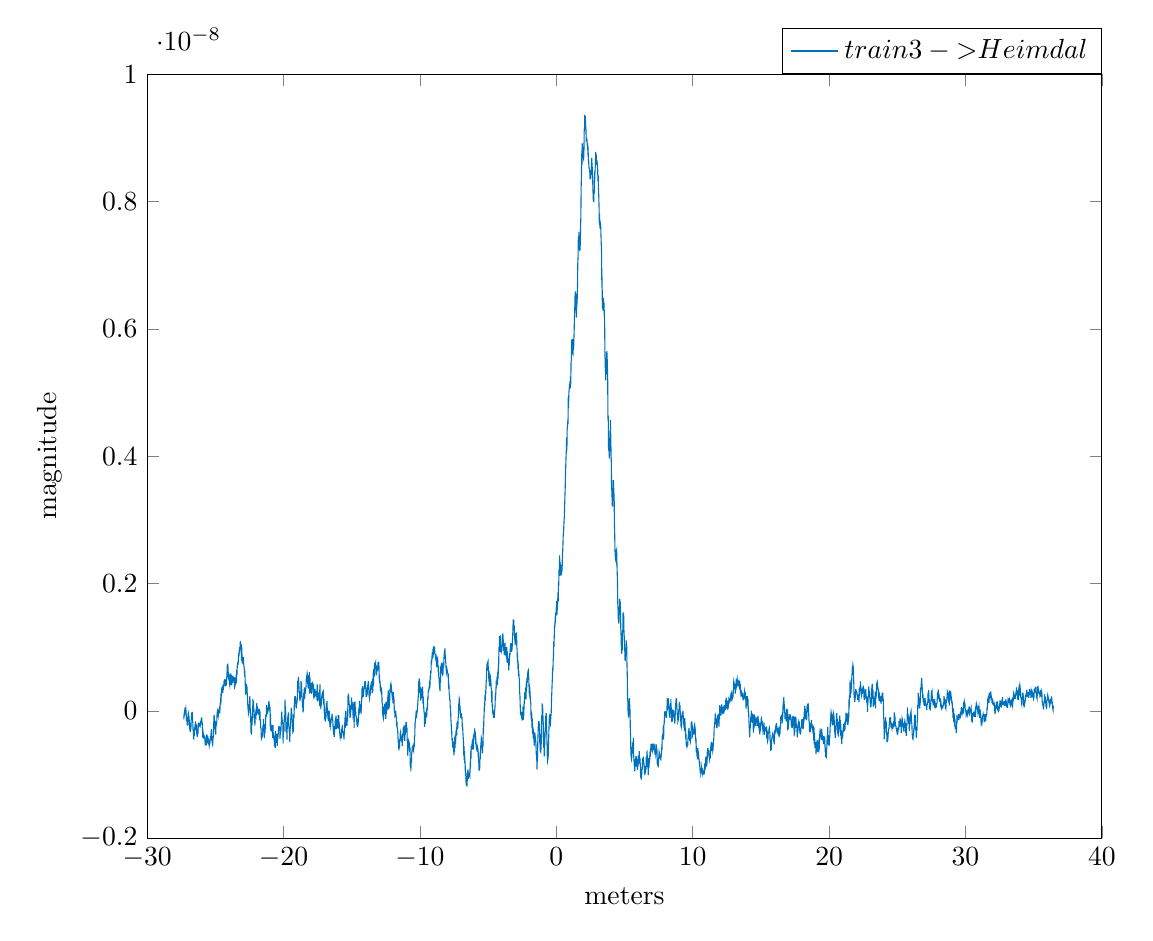
\begin{tikzpicture}

\begin{axis}[%
width=\textwidth,
height=0.8\textwidth,
at={(0\figurewidth,0\figureheight)},
scale only axis,
xmin=-30,
xmax=40,
xlabel={\SI{}{meters}},
ymin=-2e-09,
ymax=1e-08,
ylabel={magnitude},
axis background/.style={fill=white},
% legend style={legend cell align=left,align=left,draw=white!15!black}
legend style={at={(1.0,1.0)},anchor=south east}
]
\addplot [color=mycolor1,solid]
  table[row sep=crcr]{%
-27.30919921875	-1.35249592749225e-10\\
-27.288701171875	-2.96618732808651e-11\\
-27.268203125	-7.43225870504437e-11\\
-27.247705078125	3.98686887307428e-12\\
-27.22720703125	3.42173521151637e-11\\
-27.206708984375	2.91331309843253e-11\\
-27.1862109375	1.10075560008447e-12\\
-27.165712890625	3.11336048942319e-11\\
-27.14521484375	-2.14783086666199e-11\\
-27.124716796875	-1.18327190184514e-10\\
-27.10421875	-1.08068980081222e-10\\
-27.083720703125	-1.31806296562773e-10\\
-27.06322265625	-2.22339604039202e-10\\
-27.042724609375	-1.72113830799344e-10\\
-27.0222265625	-2.33179997718091e-10\\
-27.001728515625	-9.80243911839003e-11\\
-26.98123046875	-1.17431047736158e-10\\
-26.960732421875	-5.61412153639166e-11\\
-26.940234375	-8.61782248253023e-11\\
-26.919736328125	-1.39414401907277e-10\\
-26.89923828125	-1.86983229789256e-10\\
-26.878740234375	-2.80627277278364e-10\\
-26.8582421875	-3.00600915736125e-10\\
-26.837744140625	-3.35144363971528e-10\\
-26.81724609375	-2.59253155980024e-10\\
-26.796748046875	-3.0228046754793e-10\\
-26.77625	-1.52687733256755e-10\\
-26.755751953125	-1.25197094078767e-10\\
-26.73525390625	-3.07413927607202e-11\\
-26.714755859375	-1.04389883342187e-10\\
-26.6942578125	-1.90902832735895e-11\\
-26.673759765625	-1.36411292834644e-10\\
-26.65326171875	-1.88251566687186e-10\\
-26.632763671875	-3.12540235384246e-10\\
-26.612265625	-3.11990828982446e-10\\
-26.591767578125	-4.5378546266972e-10\\
-26.57126953125	-3.97306686246531e-10\\
-26.550771484375	-3.89530233962639e-10\\
-26.5302734375	-2.95033854580514e-10\\
-26.509775390625	-2.73561625376907e-10\\
-26.48927734375	-2.29766468985281e-10\\
-26.468779296875	-2.14010846778669e-10\\
-26.44828125	-1.66692182140658e-10\\
-26.427783203125	-2.55344271375855e-10\\
-26.40728515625	-3.15565761085146e-10\\
-26.386787109375	-2.14100663448054e-10\\
-26.3662890625	-3.61566215662477e-10\\
-26.345791015625	-3.76425626044425e-10\\
-26.32529296875	-4.07882051394321e-10\\
-26.304794921875	-3.06610166952019e-10\\
-26.284296875	-2.92301389226433e-10\\
-26.263798828125	-3.10288449436865e-10\\
-26.24330078125	-1.85406780114145e-10\\
-26.222802734375	-2.19785361206388e-10\\
-26.2023046875	-2.32913032346881e-10\\
-26.181806640625	-2.35588771150117e-10\\
-26.16130859375	-2.20910934632802e-10\\
-26.140810546875	-2.39919467133666e-10\\
-26.1203125	-2.47731371614303e-10\\
-26.099814453125	-2.16328684271403e-10\\
-26.07931640625	-1.81892890904841e-10\\
-26.058818359375	-1.89775940186073e-10\\
-26.0383203125	-1.22652439311522e-10\\
-26.017822265625	-1.83880244083923e-10\\
-25.99732421875	-1.0357336959362e-10\\
-25.976826171875	-1.95541713380527e-10\\
-25.956328125	-1.96616122014936e-10\\
-25.935830078125	-3.58401874836362e-10\\
-25.91533203125	-3.38628235970868e-10\\
-25.894833984375	-4.2069251597045e-10\\
-25.8743359375	-3.40979114286763e-10\\
-25.853837890625	-4.369802470122e-10\\
-25.83333984375	-3.98413489461025e-10\\
-25.812841796875	-3.95198434834407e-10\\
-25.79234375	-3.94468019830034e-10\\
-25.771845703125	-4.46008286744826e-10\\
-25.75134765625	-5.03870500898676e-10\\
-25.730849609375	-4.77212829626085e-10\\
-25.7103515625	-5.37079907260491e-10\\
-25.689853515625	-4.88433069265043e-10\\
-25.66935546875	-5.43539487116032e-10\\
-25.648857421875	-4.99002799318099e-10\\
-25.628359375	-3.70457436389315e-10\\
-25.607861328125	-5.07837222252482e-10\\
-25.58736328125	-3.90918766279497e-10\\
-25.566865234375	-4.75462672113693e-10\\
-25.5463671875	-4.92268967252412e-10\\
-25.525869140625	-4.55600562503486e-10\\
-25.50537109375	-4.85370364526642e-10\\
-25.484873046875	-4.70697730749883e-10\\
-25.464375	-4.90249456959638e-10\\
-25.443876953125	-5.49834186750661e-10\\
-25.42337890625	-5.27537008994874e-10\\
-25.402880859375	-5.10013096014045e-10\\
-25.3823828125	-4.72680789952298e-10\\
-25.361884765625	-3.99538475978077e-10\\
-25.34138671875	-4.56739308205518e-10\\
-25.320888671875	-3.74355003347318e-10\\
-25.300390625	-3.20512598351552e-10\\
-25.279892578125	-2.86734668606899e-10\\
-25.25939453125	-4.77148772142957e-10\\
-25.238896484375	-4.40258264345221e-10\\
-25.2183984375	-5.2597025779403e-10\\
-25.197900390625	-5.39619070167762e-10\\
-25.17740234375	-4.50282579640575e-10\\
-25.156904296875	-4.19755892974209e-10\\
-25.13640625	-3.48869621487714e-10\\
-25.115908203125	-1.87746427592221e-10\\
-25.09541015625	-6.32593406813938e-11\\
-25.074912109375	-1.11818179053154e-10\\
-25.0544140625	-1.94349194944256e-10\\
-25.033916015625	-1.65684148507703e-10\\
-25.01341796875	-2.92136525550294e-10\\
-24.992919921875	-3.07975800945658e-10\\
-24.972421875	-3.7437556257347e-10\\
-24.951923828125	-2.12441049209926e-10\\
-24.93142578125	-2.2905984032688e-10\\
-24.910927734375	-2.18417887953856e-10\\
-24.8904296875	-1.54126023375904e-10\\
-24.869931640625	-3.06732342695842e-11\\
-24.84943359375	-1.08751614123234e-11\\
-24.828935546875	-9.10597199836889e-11\\
-24.8084375	-4.20437497305171e-11\\
-24.787939453125	-6.94781001997516e-11\\
-24.76744140625	1.43610312870453e-11\\
-24.746943359375	-4.91616030660132e-11\\
-24.7264453125	3.19907101271847e-11\\
-24.705947265625	-3.54424103063645e-11\\
-24.68544921875	3.08095240031797e-11\\
-24.664951171875	1.42335811684415e-11\\
-24.644453125	1.16640520079849e-10\\
-24.623955078125	1.13368900684325e-10\\
-24.60345703125	1.97253068461331e-10\\
-24.582958984375	1.73276486852752e-10\\
-24.5624609375	2.6903501610126e-10\\
-24.541962890625	2.90714046386937e-10\\
-24.52146484375	3.73121420605555e-10\\
-24.500966796875	3.22700090021509e-10\\
-24.48046875	3.4870061542533e-10\\
-24.459970703125	2.81246627259552e-10\\
-24.43947265625	3.3321044944486e-10\\
-24.418974609375	3.34160493264702e-10\\
-24.3984765625	3.93830705039048e-10\\
-24.377978515625	4.12065881198341e-10\\
-24.35748046875	4.70560699559439e-10\\
-24.336982421875	4.77854883753441e-10\\
-24.316484375	4.23179697336425e-10\\
-24.295986328125	4.9179793993756e-10\\
-24.27548828125	3.85193315871097e-10\\
-24.254990234375	4.27031163793884e-10\\
-24.2344921875	4.40542659712922e-10\\
-24.213994140625	4.53147872693803e-10\\
-24.19349609375	3.9550415256078e-10\\
-24.172998046875	5.37536461584791e-10\\
-24.1525	4.94847667357632e-10\\
-24.132001953125	7.19471749362226e-10\\
-24.11150390625	6.39540833334101e-10\\
-24.091005859375	7.40868546685013e-10\\
-24.0705078125	6.70841370145141e-10\\
-24.050009765625	5.64432269917014e-10\\
-24.02951171875	5.27459481365235e-10\\
-24.009013671875	5.45624377592669e-10\\
-23.988515625	5.19521082422534e-10\\
-23.968017578125	4.32326595759694e-10\\
-23.94751953125	4.05360198707688e-10\\
-23.927021484375	5.04279887355792e-10\\
-23.9065234375	5.78177785934399e-10\\
-23.886025390625	4.09185582147215e-10\\
-23.86552734375	5.88905753813418e-10\\
-23.845029296875	4.63285685032234e-10\\
-23.82453125	5.61994052334426e-10\\
-23.804033203125	4.00684116260875e-10\\
-23.78353515625	4.71466961657033e-10\\
-23.763037109375	5.35770817238278e-10\\
-23.7425390625	4.39063573936935e-10\\
-23.722041015625	5.46530434420753e-10\\
-23.70154296875	4.66606075157989e-10\\
-23.681044921875	5.2047946923284e-10\\
-23.660546875	5.09204390901712e-10\\
-23.640048828125	5.00122606490857e-10\\
-23.61955078125	4.36479069184643e-10\\
-23.599052734375	5.26581404786945e-10\\
-23.5785546875	3.76011477242677e-10\\
-23.558056640625	3.90607565398019e-10\\
-23.53755859375	4.4294792836405e-10\\
-23.517060546875	4.54333826000035e-10\\
-23.4965625	4.15791551157969e-10\\
-23.476064453125	5.70539928801656e-10\\
-23.45556640625	4.35780458303778e-10\\
-23.435068359375	6.42805269654754e-10\\
-23.4145703125	5.65514985083013e-10\\
-23.394072265625	7.05869776518316e-10\\
-23.37357421875	7.16145412079906e-10\\
-23.353076171875	7.6412138568598e-10\\
-23.332578125	7.22190361279072e-10\\
-23.312080078125	8.06100058784537e-10\\
-23.29158203125	9.07235582967144e-10\\
-23.271083984375	8.53589864886048e-10\\
-23.2505859375	9.54398462032545e-10\\
-23.230087890625	9.00596361385507e-10\\
-23.20958984375	1.00125580769421e-09\\
-23.189091796875	9.6350503884139e-10\\
-23.16859375	1.09252419108719e-09\\
-23.148095703125	9.91393218918131e-10\\
-23.12759765625	9.75724709033288e-10\\
-23.107099609375	1.05400233342588e-09\\
-23.0866015625	7.89563994909622e-10\\
-23.066103515625	9.97858863307859e-10\\
-23.04560546875	8.63636129626429e-10\\
-23.025107421875	7.51233061416932e-10\\
-23.004609375	8.09452432789289e-10\\
-22.984111328125	7.45351075016677e-10\\
-22.96361328125	7.38974112185281e-10\\
-22.943115234375	8.4728140994759e-10\\
-22.9226171875	7.40393002956514e-10\\
-22.902119140625	6.96597444260378e-10\\
-22.88162109375	6.59170727172471e-10\\
-22.861123046875	5.88999496248786e-10\\
-22.840625	6.02643495657174e-10\\
-22.820126953125	5.19548699723142e-10\\
-22.79962890625	3.58659223237793e-10\\
-22.779130859375	2.56014850132148e-10\\
-22.7586328125	3.98498203322083e-10\\
-22.738134765625	3.5597738208579e-10\\
-22.71763671875	4.23931300566942e-10\\
-22.697138671875	3.76509782081444e-10\\
-22.676640625	3.66698464856997e-10\\
-22.656142578125	2.24114807771738e-10\\
-22.63564453125	2.14128267597694e-10\\
-22.615146484375	3.92613057296904e-11\\
-22.5946484375	3.42604768525375e-11\\
-22.574150390625	-4.41293350647987e-11\\
-22.55365234375	-2.12931148218186e-11\\
-22.533154296875	9.26741011408602e-11\\
-22.51265625	9.80352353988467e-11\\
-22.492158203125	7.75946266174585e-11\\
-22.47166015625	2.35725500990305e-10\\
-22.451162109375	6.51222689576677e-11\\
-22.4306640625	-2.16478093636985e-11\\
-22.410166015625	-6.14036409819761e-11\\
-22.38966796875	-3.48505283356299e-10\\
-22.369169921875	-2.5488656482834e-10\\
-22.348671875	-3.7339368246274e-10\\
-22.328173828125	-1.19268673436291e-10\\
-22.30767578125	-2.254021335182e-10\\
-22.287177734375	-5.8871150055272e-11\\
-22.2666796875	-7.41472598384597e-11\\
-22.246181640625	1.86675818204393e-10\\
-22.22568359375	5.83764085393433e-12\\
-22.205185546875	1.49803073300683e-10\\
-22.1846875	2.89773630503504e-11\\
-22.164189453125	-2.34220155503715e-12\\
-22.14369140625	-1.14932662586592e-10\\
-22.123193359375	-5.31159003984142e-11\\
-22.1026953125	-2.31133529182634e-10\\
-22.082197265625	-1.30357740898796e-10\\
-22.06169921875	-8.78292132365208e-11\\
-22.041201171875	-4.02899936747054e-11\\
-22.020703125	-6.5964859910965e-11\\
-22.000205078125	7.61250084393478e-12\\
-21.97970703125	-8.09417283578405e-12\\
-21.959208984375	1.25353680802542e-10\\
-21.9387109375	6.23976830311093e-12\\
-21.918212890625	-1.83121579361694e-12\\
-21.89771484375	1.42662819524076e-11\\
-21.877216796875	-4.07943779428101e-11\\
-21.85671875	-3.76912792168996e-12\\
-21.836220703125	-5.81583344322052e-11\\
-21.81572265625	2.81189299811436e-11\\
-21.795224609375	-7.66413514108258e-12\\
-21.7747265625	2.09013939771914e-11\\
-21.754228515625	-1.44860059790647e-10\\
-21.73373046875	4.59254340492001e-12\\
-21.713232421875	-1.37302086818081e-10\\
-21.692734375	-1.74860551881824e-10\\
-21.672236328125	-2.63654710274835e-10\\
-21.65173828125	-2.74703998317909e-10\\
-21.631240234375	-4.20338485802232e-10\\
-21.6107421875	-4.37091736543711e-10\\
-21.590244140625	-4.10792565462269e-10\\
-21.56974609375	-3.84212279996029e-10\\
-21.549248046875	-4.12458197001633e-10\\
-21.52875	-3.02419924846638e-10\\
-21.508251953125	-2.29427695814191e-10\\
-21.48775390625	-3.03268767035055e-10\\
-21.467255859375	-1.3206782407974e-10\\
-21.4467578125	-2.73771896512718e-10\\
-21.426259765625	-2.59085306063035e-10\\
-21.40576171875	-4.30111125358062e-10\\
-21.385263671875	-2.0632810764854e-10\\
-21.364765625	-3.54819114192018e-10\\
-21.344267578125	-2.54188920506213e-10\\
-21.32376953125	-2.84275856731719e-10\\
-21.303271484375	-7.09732788542016e-11\\
-21.2827734375	-7.20041318887539e-11\\
-21.262275390625	-7.59176608545542e-11\\
-21.24177734375	9.02728847141608e-11\\
-21.221279296875	-3.22041808705736e-11\\
-21.20078125	1.63950665346143e-11\\
-21.180283203125	-5.53445845479256e-11\\
-21.15978515625	4.15543045400407e-11\\
-21.139287109375	-1.17449240472937e-11\\
-21.1187890625	5.50190439203395e-11\\
-21.098291015625	4.57176319761245e-11\\
-21.07779296875	1.56860255048446e-10\\
-21.057294921875	1.22062875719343e-10\\
-21.036796875	6.36559620355532e-11\\
-21.016298828125	9.99157708793992e-12\\
-20.99580078125	6.28013598363108e-11\\
-20.975302734375	-2.47118558969039e-10\\
-20.9548046875	-4.63928851977508e-11\\
-20.934306640625	-3.12081159477715e-10\\
-20.91380859375	-2.7067025234948e-10\\
-20.893310546875	-3.28299426226706e-10\\
-20.8728125	-2.85660195781246e-10\\
-20.852314453125	-2.64413009312218e-10\\
-20.83181640625	-2.88170358171071e-10\\
-20.811318359375	-2.25733766269133e-10\\
-20.7908203125	-4.23764019707049e-10\\
-20.770322265625	-2.21841222113801e-10\\
-20.74982421875	-4.30448863824891e-10\\
-20.729326171875	-3.49362909049628e-10\\
-20.708828125	-4.52025120443815e-10\\
-20.688330078125	-4.02754264074807e-10\\
-20.66783203125	-5.63953896965506e-10\\
-20.647333984375	-5.37577949840101e-10\\
-20.6268359375	-4.79069625814277e-10\\
-20.606337890625	-5.82275218022439e-10\\
-20.58583984375	-3.17878927622478e-10\\
-20.565341796875	-4.8156118976282e-10\\
-20.54484375	-4.16394974697215e-10\\
-20.524345703125	-4.07865033434682e-10\\
-20.50384765625	-5.0276178594198e-10\\
-20.483349609375	-3.62819242064881e-10\\
-20.4628515625	-5.49036645452217e-10\\
-20.442353515625	-4.00444780065307e-10\\
-20.42185546875	-4.47286644214556e-10\\
-20.401357421875	-3.85520206742565e-10\\
-20.380859375	-3.44588015543206e-10\\
-20.360361328125	-2.44620874758808e-10\\
-20.33986328125	-3.00057564990421e-10\\
-20.319365234375	-2.54708606415881e-10\\
-20.2988671875	-2.63199104537137e-10\\
-20.278369140625	-2.61497460415243e-10\\
-20.25787109375	-4.3566653131045e-10\\
-20.237373046875	-3.39060649361071e-10\\
-20.216875	-2.6968012532743e-10\\
-20.196376953125	-3.29041872515179e-10\\
-20.17587890625	-2.30523557160484e-10\\
-20.155380859375	-1.37222185699247e-10\\
-20.1348828125	-1.37691994534061e-11\\
-20.114384765625	-1.1656610580232e-10\\
-20.09388671875	-1.60648024062064e-10\\
-20.073388671875	-1.8817748537802e-10\\
-20.052890625	-2.04706827156494e-10\\
-20.032392578125	-5.11966334289761e-10\\
-20.01189453125	-2.00866363523768e-10\\
-19.991396484375	-3.0889125830442e-10\\
-19.9708984375	-3.14055967443623e-10\\
-19.950400390625	-1.56302500449251e-10\\
-19.92990234375	-6.81430237807833e-11\\
-19.909404296875	-1.33935618120171e-10\\
-19.88890625	1.75761530913608e-10\\
-19.868408203125	-1.3895336154408e-10\\
-19.84791015625	7.62026210686375e-11\\
-19.827412109375	-3.26734158979295e-10\\
-19.8069140625	-2.15118271214411e-10\\
-19.786416015625	-3.44371183992221e-10\\
-19.76591796875	-3.02650238689192e-10\\
-19.745419921875	-4.54562611379598e-10\\
-19.724921875	-1.7746898825716e-10\\
-19.704423828125	-2.13385872379252e-10\\
-19.68392578125	-7.62594169804049e-11\\
-19.663427734375	-1.03101424228827e-10\\
-19.6429296875	-2.34172118697999e-11\\
-19.622431640625	-2.32012012948023e-10\\
-19.60193359375	-2.5946516249895e-10\\
-19.581435546875	-3.2447161092726e-10\\
-19.5609375	-3.50636622603424e-10\\
-19.540439453125	-4.9030730048045e-10\\
-19.51994140625	-2.88860903609473e-10\\
-19.499443359375	-2.7062632717906e-10\\
-19.4789453125	-1.48803141594526e-10\\
-19.458447265625	-9.38330676844761e-11\\
-19.43794921875	3.66142858550482e-11\\
-19.417451171875	3.61329974267193e-11\\
-19.396953125	-6.95206901144934e-11\\
-19.376455078125	-6.80705839206913e-11\\
-19.35595703125	-2.07604654033483e-10\\
-19.335458984375	-2.69040597632863e-10\\
-19.3149609375	-3.40123800332184e-10\\
-19.294462890625	-3.32237471286125e-10\\
-19.27396484375	-2.82959527081493e-10\\
-19.253466796875	-5.67222537644977e-11\\
-19.23296875	-1.14249470329872e-10\\
-19.212470703125	9.11690230248631e-11\\
-19.19197265625	1.26565465164729e-10\\
-19.171474609375	2.28755321998858e-10\\
-19.1509765625	1.21401001911897e-10\\
-19.130478515625	2.27976209362263e-10\\
-19.10998046875	1.59797330735405e-10\\
-19.089482421875	6.37709036681829e-11\\
-19.068984375	5.57455596479256e-11\\
-19.048486328125	1.10365129035581e-10\\
-19.02798828125	1.17519084932018e-10\\
-19.007490234375	1.41199994471048e-10\\
-18.9869921875	2.13204881026035e-10\\
-18.966494140625	4.68925560453406e-10\\
-18.94599609375	4.23381455480242e-10\\
-18.925498046875	4.79858965682223e-10\\
-18.905	5.31159313220214e-10\\
-18.884501953125	4.2670750228582e-10\\
-18.86400390625	3.52120556050411e-10\\
-18.843505859375	2.77283641387189e-10\\
-18.8230078125	2.5869988327639e-10\\
-18.802509765625	1.5705711182262e-10\\
-18.78201171875	2.91806123555677e-10\\
-18.761513671875	2.09787977055237e-10\\
-18.741015625	2.31288254074604e-10\\
-18.720517578125	4.70410565873187e-10\\
-18.70001953125	3.11510683889954e-10\\
-18.679521484375	4.3367679874644e-10\\
-18.6590234375	2.41411925753194e-10\\
-18.638525390625	2.05967924565715e-10\\
-18.61802734375	1.02434891051107e-10\\
-18.597529296875	1.16902049217817e-10\\
-18.57703125	-2.53204385378994e-11\\
-18.556533203125	2.86766670393062e-12\\
-18.53603515625	1.15878380624621e-10\\
-18.515537109375	2.80085775040727e-10\\
-18.4950390625	2.4333637379268e-10\\
-18.474541015625	3.67339631789491e-10\\
-18.45404296875	1.82848505844703e-10\\
-18.433544921875	3.3005939177019e-10\\
-18.413046875	2.7146298050183e-10\\
-18.392548828125	3.09182611953742e-10\\
-18.37205078125	3.46517038577973e-10\\
-18.351552734375	3.7921044482155e-10\\
-18.3310546875	5.03002047679626e-10\\
-18.310556640625	5.31587780902845e-10\\
-18.29005859375	5.54352495001945e-10\\
-18.269560546875	5.89173520686153e-10\\
-18.2490625	5.6473692322234e-10\\
-18.228564453125	4.56157387333356e-10\\
-18.20806640625	4.78507824422924e-10\\
-18.187568359375	3.51483408137841e-10\\
-18.1670703125	4.78472945615268e-10\\
-18.146572265625	3.49028278351362e-10\\
-18.12607421875	4.67702356232544e-10\\
-18.105576171875	6.06012196049108e-10\\
-18.085078125	2.71460060488586e-10\\
-18.064580078125	5.20307117666546e-10\\
-18.04408203125	4.01201508095344e-10\\
-18.023583984375	4.29013329383474e-10\\
-18.0030859375	2.90204382012613e-10\\
-17.982587890625	2.89617333342013e-10\\
-17.96208984375	4.33755235990214e-10\\
-17.941591796875	2.64637916361743e-10\\
-17.92109375	3.62771568075583e-10\\
-17.900595703125	4.56241669943883e-10\\
-17.88009765625	3.98254228175803e-10\\
-17.859599609375	3.81533855723509e-10\\
-17.8391015625	3.94535730857114e-10\\
-17.818603515625	3.35492811620338e-10\\
-17.79810546875	3.54613862021231e-10\\
-17.777607421875	1.79524443008476e-10\\
-17.757109375	3.25634024098343e-10\\
-17.736611328125	2.6411457495158e-10\\
-17.71611328125	2.12880739173961e-10\\
-17.695615234375	3.43017151489387e-10\\
-17.6751171875	2.66403234522076e-10\\
-17.654619140625	2.61591233302193e-10\\
-17.63412109375	2.52050140390371e-10\\
-17.613623046875	2.95059354538262e-10\\
-17.593125	3.00936147734259e-10\\
-17.572626953125	2.87102058333018e-10\\
-17.55212890625	1.70075791760634e-10\\
-17.531630859375	4.14039184368385e-10\\
-17.5111328125	1.47241284671841e-10\\
-17.490634765625	2.80143923839951e-10\\
-17.47013671875	2.44769284310749e-10\\
-17.449638671875	2.47197962592881e-10\\
-17.429140625	2.21046003201693e-10\\
-17.408642578125	2.87397615036798e-10\\
-17.38814453125	1.83052274574976e-10\\
-17.367646484375	3.33296989470108e-10\\
-17.3471484375	7.67017460010833e-11\\
-17.326650390625	4.16832800436667e-10\\
-17.30615234375	8.04518419872208e-11\\
-17.285654296875	2.03016610301869e-10\\
-17.26515625	2.20413923623684e-11\\
-17.244658203125	1.58450722634043e-10\\
-17.22416015625	8.57608333990689e-11\\
-17.203662109375	2.06265137683533e-10\\
-17.1831640625	2.52420710750696e-10\\
-17.162666015625	2.49015564575926e-10\\
-17.14216796875	2.82992835290942e-10\\
-17.121669921875	2.93893175426329e-10\\
-17.101171875	2.3734332447866e-10\\
-17.080673828125	2.60872578846719e-10\\
-17.06017578125	1.02974688881605e-10\\
-17.039677734375	1.91908264396336e-10\\
-17.0191796875	2.68619381037025e-11\\
-16.998681640625	4.26862496744526e-11\\
-16.97818359375	-1.33489865677632e-10\\
-16.957685546875	-2.43362328377587e-11\\
-16.9371875	-1.7125473685436e-10\\
-16.916689453125	-6.08119382744374e-11\\
-16.89619140625	-3.71664781404117e-11\\
-16.875693359375	-5.31588232320189e-11\\
-16.8551953125	1.20150459959966e-10\\
-16.834697265625	4.54314435488041e-11\\
-16.81419921875	1.51709263117392e-10\\
-16.793701171875	1.15134074358259e-11\\
-16.773203125	1.45596914666982e-11\\
-16.752705078125	-8.70150145053961e-11\\
-16.73220703125	-7.5436426769702e-11\\
-16.711708984375	-1.67478710209694e-10\\
-16.6912109375	-6.10432385311275e-11\\
-16.670712890625	-8.19950091368211e-11\\
-16.65021484375	-2.70389312496919e-12\\
-16.629716796875	-1.20871613963387e-10\\
-16.60921875	-1.98081611085121e-10\\
-16.588720703125	-1.81009964996844e-10\\
-16.56822265625	-2.33256078519509e-10\\
-16.547724609375	-1.9666502453237e-10\\
-16.5272265625	-1.94099263446273e-10\\
-16.506728515625	-1.37945581843473e-10\\
-16.48623046875	-1.10426366371286e-10\\
-16.465732421875	-1.06747903357002e-10\\
-16.445234375	-4.69579347037814e-11\\
-16.424736328125	-9.3997370967717e-11\\
-16.40423828125	-1.16724469033973e-10\\
-16.383740234375	-1.78575460058846e-10\\
-16.3632421875	-2.8958372638956e-10\\
-16.342744140625	-2.99415388570616e-10\\
-16.32224609375	-3.74616263585012e-10\\
-16.301748046875	-3.24921108689867e-10\\
-16.28125	-4.11254814031175e-10\\
-16.260751953125	-2.40658172771327e-10\\
-16.24025390625	-2.77827700481013e-10\\
-16.219755859375	-2.27808933161054e-10\\
-16.1992578125	-1.15488753427843e-10\\
-16.178759765625	-2.20847355396641e-10\\
-16.15826171875	-7.59620915149292e-11\\
-16.137763671875	-2.89675119693239e-10\\
-16.117265625	-1.29931086873945e-10\\
-16.096767578125	-1.99668301741175e-10\\
-16.07626953125	-1.66261383274477e-10\\
-16.055771484375	-2.76505403122174e-10\\
-16.0352734375	-1.9055105100654e-10\\
-16.014775390625	-1.95571469540603e-10\\
-15.99427734375	-6.34674870304593e-11\\
-15.973779296875	-2.80429984559389e-10\\
-15.95328125	-7.00580232580394e-11\\
-15.932783203125	-2.07698110569518e-10\\
-15.91228515625	-2.08325879703897e-10\\
-15.891787109375	-3.15658179402705e-10\\
-15.8712890625	-3.72570837481575e-10\\
-15.850791015625	-4.08168510434337e-10\\
-15.83029296875	-3.65668825755436e-10\\
-15.809794921875	-4.38106414260785e-10\\
-15.789296875	-3.96211823827328e-10\\
-15.768798828125	-4.34607715496228e-10\\
-15.74830078125	-2.99166128241619e-10\\
-15.727802734375	-3.03028082590152e-10\\
-15.7073046875	-2.98005438237266e-10\\
-15.686806640625	-2.26014634948845e-10\\
-15.66630859375	-3.3846138818385e-10\\
-15.645810546875	-3.38281510405287e-10\\
-15.6253125	-3.68562513952096e-10\\
-15.604814453125	-4.05063237513379e-10\\
-15.58431640625	-3.22185304326828e-10\\
-15.563818359375	-4.47041403096272e-10\\
-15.5433203125	-3.01075685340483e-10\\
-15.522822265625	-3.27547505318069e-10\\
-15.50232421875	-1.2294273248789e-10\\
-15.481826171875	-1.03876423099887e-10\\
-15.461328125	-9.94361589949121e-11\\
-15.440830078125	-2.45314057689288e-13\\
-15.42033203125	-2.17590232631159e-10\\
-15.399833984375	-2.02975083704597e-10\\
-15.3793359375	-1.76695748104086e-10\\
-15.358837890625	-2.36224932569385e-10\\
-15.33833984375	-1.89922086026445e-10\\
-15.317841796875	-7.14372269354423e-11\\
-15.29734375	-9.23977916426495e-11\\
-15.276845703125	2.37960715213924e-10\\
-15.25634765625	1.17619036660605e-10\\
-15.235849609375	2.70210839930903e-10\\
-15.2153515625	1.94261988179782e-10\\
-15.194853515625	1.15069516706955e-10\\
-15.17435546875	8.94443760884572e-11\\
-15.153857421875	5.83746325962268e-11\\
-15.133359375	-1.11023313739406e-10\\
-15.112861328125	-6.54731234053735e-11\\
-15.09236328125	-9.56909192569403e-11\\
-15.071865234375	1.30506019338311e-11\\
-15.0513671875	9.68795468784335e-11\\
-15.030869140625	2.50923586712161e-11\\
-15.01037109375	2.09598225460569e-10\\
-14.989873046875	2.47804540073555e-11\\
-14.969375	1.39247098886317e-10\\
-14.948876953125	1.58815172697944e-11\\
-14.92837890625	4.54233813246108e-11\\
-14.907880859375	-5.57289463883855e-11\\
-14.8873828125	-2.84881318354218e-11\\
-14.866884765625	-1.08480778333579e-10\\
-14.84638671875	1.39378831995546e-10\\
-14.825888671875	-2.71083551572908e-10\\
-14.805390625	1.14094914363789e-10\\
-14.784892578125	-2.02958716426207e-11\\
-14.76439453125	1.43052419916105e-10\\
-14.743896484375	-5.92955805676748e-11\\
-14.7233984375	6.0975105719955e-11\\
-14.702900390625	-6.97912074012181e-11\\
-14.68240234375	-8.69024565463845e-11\\
-14.661904296875	-9.12821650888016e-11\\
-14.64140625	-1.4896358030078e-10\\
-14.620908203125	-1.95361705879464e-10\\
-14.60041015625	-1.81115551160454e-10\\
-14.579912109375	-2.50583516830121e-10\\
-14.5594140625	-1.22319409386413e-10\\
-14.538916015625	-2.26963774330336e-10\\
-14.51841796875	-1.47635822481101e-10\\
-14.497919921875	-7.57367159852047e-11\\
-14.477421875	4.86318728283396e-11\\
-14.456923828125	-6.4198723257886e-11\\
-14.43642578125	1.56136617677521e-10\\
-14.415927734375	7.19834880118072e-11\\
-14.3954296875	4.05542970943303e-11\\
-14.374931640625	8.24275375158423e-11\\
-14.35443359375	-1.05712167692395e-11\\
-14.333935546875	1.02789833299272e-10\\
-14.3134375	-5.21249034449518e-11\\
-14.292939453125	1.35572702718452e-10\\
-14.27244140625	1.53555196947139e-10\\
-14.251943359375	2.95689229597886e-10\\
-14.2314453125	2.80052824382e-10\\
-14.210947265625	3.87128929989158e-10\\
-14.19044921875	2.80797529362345e-10\\
-14.169951171875	2.12710186428401e-10\\
-14.149453125	2.48155196455195e-10\\
-14.128955078125	2.81397716031753e-10\\
-14.10845703125	3.46830203184054e-10\\
-14.087958984375	3.66268961884066e-10\\
-14.0674609375	3.60481594900071e-10\\
-14.046962890625	4.56338176463585e-10\\
-14.02646484375	4.27769226694275e-10\\
-14.005966796875	4.69377502383545e-10\\
-13.98546875	3.81968448036488e-10\\
-13.964970703125	3.40626728512775e-10\\
-13.94447265625	2.14836096004836e-10\\
-13.923974609375	3.02690456932697e-10\\
-13.9034765625	2.77500630655234e-10\\
-13.882978515625	3.11831094482941e-10\\
-13.86248046875	2.90397985721397e-10\\
-13.841982421875	3.74232762233638e-10\\
-13.821484375	4.03757941983856e-10\\
-13.800986328125	4.31519740292519e-10\\
-13.78048828125	4.69895159645258e-10\\
-13.759990234375	3.97132429103535e-10\\
-13.7394921875	2.64832149703066e-10\\
-13.718994140625	2.21040295268192e-10\\
-13.69849609375	1.960921286544e-10\\
-13.677998046875	3.15442070974464e-10\\
-13.6575	2.3446708194947e-10\\
-13.637001953125	2.89275608731404e-10\\
-13.61650390625	3.73548043572492e-10\\
-13.596005859375	4.07426267812095e-10\\
-13.5755078125	4.08098987626308e-10\\
-13.555009765625	4.63256391660534e-10\\
-13.53451171875	3.40593921051983e-10\\
-13.514013671875	3.73625717315821e-10\\
-13.493515625	2.77300996856856e-10\\
-13.473017578125	5.00278758960531e-10\\
-13.45251953125	3.02504983817702e-10\\
-13.432021484375	5.98708406255111e-10\\
-13.4115234375	3.86726234692942e-10\\
-13.391025390625	5.89964865378462e-10\\
-13.37052734375	5.69570704864333e-10\\
-13.350029296875	5.37186121558701e-10\\
-13.32953125	7.13668556433254e-10\\
-13.309033203125	7.02717922300551e-10\\
-13.28853515625	7.43265268495172e-10\\
-13.268037109375	7.38624704283125e-10\\
-13.2475390625	7.56874474620068e-10\\
-13.227041015625	5.72821248666765e-10\\
-13.20654296875	7.14506029195342e-10\\
-13.186044921875	5.56252095731253e-10\\
-13.165546875	6.87286773499721e-10\\
-13.145048828125	6.8030999515314e-10\\
-13.12455078125	6.68691714946003e-10\\
-13.104052734375	6.20760826154718e-10\\
-13.0835546875	7.1763954247636e-10\\
-13.063056640625	7.71680111319628e-10\\
-13.04255859375	7.01860134505897e-10\\
-13.022060546875	7.65241402087973e-10\\
-13.0015625	6.91830548061057e-10\\
-12.981064453125	5.12968689564435e-10\\
-12.96056640625	5.24203532810344e-10\\
-12.940068359375	4.25489412698201e-10\\
-12.9195703125	4.62482340952045e-10\\
-12.899072265625	3.0547152930145e-10\\
-12.87857421875	3.8209066473652e-10\\
-12.858076171875	3.31435166261555e-10\\
-12.837578125	3.65235372547986e-10\\
-12.817080078125	2.505784466193e-10\\
-12.79658203125	3.16077416426049e-10\\
-12.776083984375	1.20103219828582e-10\\
-12.7555859375	1.0719001826468e-10\\
-12.735087890625	-5.06847082463068e-11\\
-12.71458984375	-5.97512423925587e-11\\
-12.694091796875	-1.08377674792808e-10\\
-12.67359375	-1.25673123073199e-10\\
-12.653095703125	-3.44590908600641e-11\\
-12.63259765625	6.93766832048192e-11\\
-12.612099609375	3.77564966984743e-11\\
-12.5916015625	9.90318446961657e-11\\
-12.571103515625	1.02308871266687e-10\\
-12.55060546875	-1.98890274314529e-13\\
-12.530107421875	2.06996805792616e-11\\
-12.509609375	-1.27783267165771e-10\\
-12.489111328125	1.39647844200157e-10\\
-12.46861328125	-5.64150204882903e-11\\
-12.448115234375	6.20538221953262e-11\\
-12.4276171875	6.23948489660559e-11\\
-12.407119140625	4.83038730044384e-11\\
-12.38662109375	1.42414213442394e-10\\
-12.366123046875	1.89362388081629e-10\\
-12.345625	1.67754621955446e-10\\
-12.325126953125	3.20791308857426e-10\\
-12.30462890625	2.2234707926806e-11\\
-12.284130859375	2.82657533373699e-10\\
-12.2636328125	4.01346836221866e-11\\
-12.243134765625	9.34754198310589e-11\\
-12.22263671875	1.0259009704288e-10\\
-12.202138671875	3.44150238341192e-10\\
-12.181640625	2.81423875827867e-10\\
-12.161142578125	3.86743775972926e-10\\
-12.14064453125	3.75098808458363e-10\\
-12.120146484375	4.16317359769756e-10\\
-12.0996484375	3.85086814204615e-10\\
-12.079150390625	2.99509850259228e-10\\
-12.05865234375	3.02147190062396e-10\\
-12.038154296875	2.18253721369266e-10\\
-12.01765625	1.99539778090712e-10\\
-11.997158203125	2.18413260834315e-10\\
-11.97666015625	1.21854025855723e-10\\
-11.956162109375	2.93821524009287e-10\\
-11.9356640625	1.14064041094946e-10\\
-11.915166015625	2.25523846309539e-10\\
-11.89466796875	1.36204045088998e-10\\
-11.874169921875	-2.87922919392108e-11\\
-11.853671875	1.56763275796079e-11\\
-11.833173828125	-8.429929587313e-11\\
-11.81267578125	-7.54111981717615e-11\\
-11.792177734375	-6.47912578203932e-11\\
-11.7716796875	-1.29337226617914e-12\\
-11.751181640625	-8.63556336143343e-11\\
-11.73068359375	-9.28322365063355e-11\\
-11.710185546875	-2.48720166263712e-10\\
-11.6896875	-1.66579069135422e-10\\
-11.669189453125	-2.61733545830312e-10\\
-11.64869140625	-2.81161894014934e-10\\
-11.628193359375	-3.25499365486576e-10\\
-11.6076953125	-4.34941164506334e-10\\
-11.587197265625	-4.97660747271448e-10\\
-11.56669921875	-4.54891246661043e-10\\
-11.546201171875	-6.25884074087925e-10\\
-11.525703125	-4.7882698370597e-10\\
-11.505205078125	-5.90959460955783e-10\\
-11.48470703125	-5.00445524382349e-10\\
-11.464208984375	-4.71936842506786e-10\\
-11.4437109375	-3.50752022667231e-10\\
-11.423212890625	-3.33011635995292e-10\\
-11.40271484375	-4.07605816775349e-10\\
-11.382216796875	-4.3712397321207e-10\\
-11.36171875	-4.54030062147451e-10\\
-11.341220703125	-4.34376496867096e-10\\
-11.32072265625	-3.93458870661357e-10\\
-11.300224609375	-5.55822436199521e-10\\
-11.2797265625	-3.67533227912644e-10\\
-11.259228515625	-4.58068105537899e-10\\
-11.23873046875	-3.49673992689287e-10\\
-11.218232421875	-2.61740310928529e-10\\
-11.197734375	-2.57609586284579e-10\\
-11.177236328125	-3.19754139683082e-10\\
-11.15673828125	-2.27157578779978e-10\\
-11.136240234375	-3.83252581562234e-10\\
-11.1157421875	-4.77881489064761e-10\\
-11.095244140625	-3.46749169356106e-10\\
-11.07474609375	-3.55872797794633e-10\\
-11.054248046875	-3.03813681575749e-10\\
-11.03375	-2.13653226503294e-10\\
-11.013251953125	-2.26543950260846e-10\\
-10.99275390625	-1.79438720680166e-10\\
-10.972255859375	-3.37864192270552e-10\\
-10.9517578125	-2.67457578003135e-10\\
-10.931259765625	-4.74110131557216e-10\\
-10.91076171875	-4.49278530807292e-10\\
-10.890263671875	-7.04232276711826e-10\\
-10.869765625	-5.62551805568847e-10\\
-10.849267578125	-5.29122520391257e-10\\
-10.82876953125	-5.87562681193357e-10\\
-10.808271484375	-4.83058255050168e-10\\
-10.7877734375	-5.00321506153864e-10\\
-10.767275390625	-5.26615834486921e-10\\
-10.74677734375	-6.48180958261963e-10\\
-10.726279296875	-5.77351828324484e-10\\
-10.70578125	-8.77152445949905e-10\\
-10.685283203125	-7.48865569613854e-10\\
-10.66478515625	-9.52626385005314e-10\\
-10.644287109375	-7.48205696575369e-10\\
-10.6237890625	-8.15001923210684e-10\\
-10.603291015625	-6.59559188619641e-10\\
-10.58279296875	-6.4598015377087e-10\\
-10.562294921875	-5.70682644566559e-10\\
-10.541796875	-5.68794960799915e-10\\
-10.521298828125	-5.87059338803812e-10\\
-10.50080078125	-5.32750622438163e-10\\
-10.480302734375	-5.85135303439975e-10\\
-10.4598046875	-6.09896635844846e-10\\
-10.439306640625	-5.03101142099797e-10\\
-10.41880859375	-5.68253821582825e-10\\
-10.398310546875	-3.95597603008127e-10\\
-10.3778125	-3.95038234570791e-10\\
-10.357314453125	-1.84434299509545e-10\\
-10.33681640625	-1.78107826801178e-10\\
-10.316318359375	-1.08858709897569e-10\\
-10.2958203125	-7.8686758176729e-11\\
-10.275322265625	7.85674142761614e-12\\
-10.25482421875	-1.16126452685473e-10\\
-10.234326171875	-2.18180159605628e-11\\
-10.213828125	-2.9776440765485e-11\\
-10.193330078125	-4.17699642897514e-12\\
-10.17283203125	5.4917441662854e-11\\
-10.152333984375	1.35202479210146e-10\\
-10.1318359375	1.93365093803419e-10\\
-10.111337890625	2.65760126089633e-10\\
-10.09083984375	4.52210863478373e-10\\
-10.070341796875	4.64145731175866e-10\\
-10.04984375	5.0759387709493e-10\\
-10.029345703125	4.24723634004236e-10\\
-10.00884765625	4.59402490957036e-10\\
-9.988349609375	2.55173889248331e-10\\
-9.9678515625	3.71713489103553e-10\\
-9.947353515625	1.5835932574498e-10\\
-9.92685546875	2.42354596671091e-10\\
-9.906357421875	1.93690437804616e-10\\
-9.885859375	3.41081986883496e-10\\
-9.865361328125	2.79259893534888e-10\\
-9.84486328125	3.62109672025255e-10\\
-9.824365234375	2.269940355252e-10\\
-9.8038671875	3.81361756638422e-10\\
-9.783369140625	1.11137777378847e-10\\
-9.76287109375	2.24124990091546e-10\\
-9.742373046875	1.16694982189372e-10\\
-9.721875	4.57312958460112e-11\\
-9.701376953125	-9.40149151952291e-12\\
-9.68087890625	-3.69190708635449e-11\\
-9.660380859375	-2.54057117201858e-10\\
-9.6398828125	-1.43109104952536e-10\\
-9.619384765625	-2.07442733310828e-10\\
-9.59888671875	-1.7348684415668e-10\\
-9.578388671875	-7.0321926061003e-11\\
-9.557890625	-9.11679624310035e-11\\
-9.537392578125	-6.49757131090353e-11\\
-9.51689453125	-1.7096308420883e-11\\
-9.496396484375	-4.12754242254559e-11\\
-9.4758984375	6.25057577492562e-11\\
-9.455400390625	7.66748484672237e-12\\
-9.43490234375	1.84575866217155e-10\\
-9.414404296875	1.81485355726692e-10\\
-9.39390625	2.96453170933065e-10\\
-9.373408203125	3.22517255200252e-10\\
-9.35291015625	3.18577925306291e-10\\
-9.332412109375	3.59481289254119e-10\\
-9.3119140625	3.8631345042763e-10\\
-9.291416015625	4.73502550627824e-10\\
-9.27091796875	3.53956611977266e-10\\
-9.250419921875	5.44038672122825e-10\\
-9.229921875	4.90725408678358e-10\\
-9.209423828125	6.2800757706969e-10\\
-9.18892578125	5.93796092480814e-10\\
-9.168427734375	7.8798101718493e-10\\
-9.1479296875	7.31246335588483e-10\\
-9.127431640625	8.1945778370868e-10\\
-9.10693359375	8.75741970175105e-10\\
-9.086435546875	8.5706796886578e-10\\
-9.0659375	8.18562424968222e-10\\
-9.045439453125	9.70927554871182e-10\\
-9.02494140625	8.87175074635618e-10\\
-9.004443359375	1.01291115696264e-09\\
-8.9839453125	9.31778684060934e-10\\
-8.963447265625	9.56615689720637e-10\\
-8.94294921875	1.00916938233223e-09\\
-8.922451171875	9.71045996970394e-10\\
-8.901953125	9.01898984859587e-10\\
-8.881455078125	8.86637997312074e-10\\
-8.86095703125	8.42345172581719e-10\\
-8.840458984375	8.20925167409127e-10\\
-8.8199609375	7.76261558949736e-10\\
-8.799462890625	8.42559486905883e-10\\
-8.77896484375	6.89096186841026e-10\\
-8.758466796875	8.18004153534335e-10\\
-8.73796875	7.94026037092246e-10\\
-8.717470703125	7.67405695982599e-10\\
-8.69697265625	7.95083032045277e-10\\
-8.676474609375	7.02506660286174e-10\\
-8.6559765625	6.06684302175669e-10\\
-8.635478515625	7.00581032902246e-10\\
-8.61498046875	5.16540472422212e-10\\
-8.594482421875	5.05800615830933e-10\\
-8.573984375	3.87761575856596e-10\\
-8.553486328125	3.72477185775778e-10\\
-8.53298828125	3.10233668228721e-10\\
-8.512490234375	5.24120409967262e-10\\
-8.4919921875	4.38711213451156e-10\\
-8.471494140625	6.98462313554818e-10\\
-8.45099609375	5.74274618041651e-10\\
-8.430498046875	7.53986960582453e-10\\
-8.41	6.69755967878146e-10\\
-8.389501953125	6.96809540886879e-10\\
-8.36900390625	6.00171931433791e-10\\
-8.348505859375	6.36806721007757e-10\\
-8.3280078125	5.68371486123421e-10\\
-8.307509765625	5.78797157024344e-10\\
-8.28701171875	7.46489517079311e-10\\
-8.266513671875	6.68717946985899e-10\\
-8.246015625	7.88103277029078e-10\\
-8.225517578125	8.77266188868265e-10\\
-8.20501953125	9.43418071775616e-10\\
-8.184521484375	8.66994050767152e-10\\
-8.1640234375	9.79182620611189e-10\\
-8.143525390625	8.4815353289903e-10\\
-8.12302734375	8.1538396909955e-10\\
-8.102529296875	7.37639296107119e-10\\
-8.08203125	6.66715374979398e-10\\
-8.061533203125	6.04387129240504e-10\\
-8.04103515625	6.31275276049776e-10\\
-8.020537109375	6.58190895434598e-10\\
-8.0000390625	6.30713909371111e-10\\
-7.979541015625	5.93388157222308e-10\\
-7.95904296875	5.87404209249354e-10\\
-7.938544921875	5.43368855161953e-10\\
-7.918046875	5.82909444126609e-10\\
-7.897548828125	3.3978580691506e-10\\
-7.87705078125	4.31099655316538e-10\\
-7.856552734375	2.69585696700586e-10\\
-7.8360546875	2.57977636685405e-10\\
-7.815556640625	1.71850837973958e-10\\
-7.79505859375	1.66487863866315e-10\\
-7.774560546875	4.23615234722925e-11\\
-7.7540625	3.81228570256801e-11\\
-7.733564453125	-1.2761469511457e-10\\
-7.71306640625	-1.85830527467055e-10\\
-7.692568359375	-2.9265009328255e-10\\
-7.6720703125	-3.17474990050083e-10\\
-7.651572265625	-4.62941848331661e-10\\
-7.63107421875	-4.28870328679045e-10\\
-7.610576171875	-5.05858918356395e-10\\
-7.590078125	-5.79847477361188e-10\\
-7.569580078125	-5.31545771766741e-10\\
-7.54908203125	-5.56448486666954e-10\\
-7.528583984375	-5.88402282700977e-10\\
-7.5080859375	-7.00116923023855e-10\\
-7.487587890625	-4.75955245829393e-10\\
-7.46708984375	-6.44637314564082e-10\\
-7.446591796875	-4.09736776439049e-10\\
-7.42609375	-5.81073084374504e-10\\
-7.405595703125	-3.72818773282983e-10\\
-7.38509765625	-5.17843927801973e-10\\
-7.364599609375	-3.17497187351495e-10\\
-7.3441015625	-3.95698853784621e-10\\
-7.323603515625	-2.60069352275583e-10\\
-7.30310546875	-3.87709727925438e-10\\
-7.282607421875	-1.86516183615049e-10\\
-7.262109375	-2.87852888725131e-10\\
-7.241611328125	-1.61674821324257e-10\\
-7.22111328125	-2.68318707329599e-10\\
-7.200615234375	-1.19614349284392e-10\\
-7.1801171875	-8.53827846689529e-11\\
-7.159619140625	9.12917872687374e-11\\
-7.13912109375	1.20377926184752e-10\\
-7.118623046875	1.91398964868787e-10\\
-7.098125	1.71277411400393e-10\\
-7.077626953125	8.91998704847142e-12\\
-7.05712890625	7.88897296233062e-11\\
-7.036630859375	-5.84735508075095e-11\\
-7.0161328125	-1.06402597654667e-10\\
-6.995634765625	-3.81253699047048e-11\\
-6.97513671875	-1.1642258612407e-10\\
-6.954638671875	-4.16555264533202e-11\\
-6.934140625	-1.30101930882777e-10\\
-6.913642578125	-1.01149526626837e-10\\
-6.89314453125	-2.60128954388908e-10\\
-6.872646484375	-2.20827449938884e-10\\
-6.8521484375	-3.43877379679531e-10\\
-6.831650390625	-4.08199363967229e-10\\
-6.81115234375	-4.7682289182316e-10\\
-6.790654296875	-6.98678469702162e-10\\
-6.77015625	-5.55795611705613e-10\\
-6.749658203125	-7.78405777493096e-10\\
-6.72916015625	-6.33203388214677e-10\\
-6.708662109375	-8.39337462220649e-10\\
-6.6881640625	-8.0003270381412e-10\\
-6.667666015625	-1.00751559425935e-09\\
-6.64716796875	-9.6699546092315e-10\\
-6.626669921875	-1.08881879324023e-09\\
-6.606171875	-1.1726643630224e-09\\
-6.585673828125	-1.08791448408127e-09\\
-6.56517578125	-1.15498660307425e-09\\
-6.544677734375	-1.19024266477236e-09\\
-6.5241796875	-9.92281881680059e-10\\
-6.503681640625	-9.80238872481314e-10\\
-6.48318359375	-9.20010903404299e-10\\
-6.462685546875	-1.0015196668964e-09\\
-6.4421875	-1.06816644179523e-09\\
-6.421689453125	-1.00381829347442e-09\\
-6.40119140625	-9.68474206593073e-10\\
-6.380693359375	-1.03311885067351e-09\\
-6.3601953125	-9.98851341862597e-10\\
-6.339697265625	-1.01603614512969e-09\\
-6.31919921875	-8.55238771027011e-10\\
-6.298701171875	-8.65771178954826e-10\\
-6.278203125	-6.32386159773669e-10\\
-6.257705078125	-7.49710889542138e-10\\
-6.23720703125	-5.79524074382165e-10\\
-6.216708984375	-5.88479928536737e-10\\
-6.1962109375	-5.44494071061143e-10\\
-6.175712890625	-5.50019620390469e-10\\
-6.15521484375	-4.52041476815849e-10\\
-6.134716796875	-6.09678499749652e-10\\
-6.11421875	-4.36882144071551e-10\\
-6.093720703125	-6.07134654854721e-10\\
-6.07322265625	-3.86822483691365e-10\\
-6.052724609375	-4.51235737673685e-10\\
-6.0322265625	-3.5571146082619e-10\\
-6.011728515625	-3.98261319518358e-10\\
-5.99123046875	-2.77473316307871e-10\\
-5.970732421875	-3.89674324012858e-10\\
-5.950234375	-3.24952755936531e-10\\
-5.929736328125	-5.28420208926305e-10\\
-5.90923828125	-4.06139338782017e-10\\
-5.888740234375	-5.18821163626122e-10\\
-5.8682421875	-5.73576631843116e-10\\
-5.847744140625	-5.90331286937428e-10\\
-5.82724609375	-5.2844009848047e-10\\
-5.806748046875	-6.45357359035602e-10\\
-5.78625	-5.6881808556645e-10\\
-5.765751953125	-5.90416720474852e-10\\
-5.74525390625	-6.04180247105263e-10\\
-5.724755859375	-7.04304290636183e-10\\
-5.7042578125	-6.94135854041874e-10\\
-5.683759765625	-8.1819626876224e-10\\
-5.66326171875	-9.4652686716344e-10\\
-5.642763671875	-8.81085819380889e-10\\
-5.622265625	-9.26052011748598e-10\\
-5.601767578125	-7.75530816663975e-10\\
-5.58126953125	-7.48508078796169e-10\\
-5.560771484375	-6.61227116894529e-10\\
-5.5402734375	-5.53038887869678e-10\\
-5.519775390625	-5.07092068021698e-10\\
-5.49927734375	-4.24776014408534e-10\\
-5.478779296875	-4.42620841123292e-10\\
-5.45828125	-5.46081339037005e-10\\
-5.437783203125	-5.79108629857587e-10\\
-5.41728515625	-6.68520858935019e-10\\
-5.396787109375	-5.16242027722377e-10\\
-5.3762890625	-5.61828850012008e-10\\
-5.355791015625	-2.72766397053975e-10\\
-5.33529296875	-3.36715924060461e-10\\
-5.314794921875	-1.34896566697085e-10\\
-5.294296875	-5.61000093474235e-11\\
-5.273798828125	1.17561045773648e-10\\
-5.25330078125	7.07586020085087e-11\\
-5.232802734375	2.45547340971098e-10\\
-5.2123046875	1.57366784135807e-10\\
-5.191806640625	3.20031759827896e-10\\
-5.17130859375	2.61067470086906e-10\\
-5.150810546875	4.26679446029207e-10\\
-5.1303125	4.88911158493781e-10\\
-5.109814453125	5.96215778185e-10\\
-5.08931640625	7.4045088836786e-10\\
-5.068818359375	6.38142652764499e-10\\
-5.0483203125	7.56189397167533e-10\\
-5.027822265625	7.63227111164192e-10\\
-5.00732421875	7.75650847415248e-10\\
-4.986826171875	6.36187374299406e-10\\
-4.966328125	6.31052004765092e-10\\
-4.945830078125	4.59099934152579e-10\\
-4.92533203125	6.2666258176436e-10\\
-4.904833984375	3.8791706765767e-10\\
-4.8843359375	5.88959234831902e-10\\
-4.863837890625	4.60017968197485e-10\\
-4.84333984375	5.59018737293195e-10\\
-4.822841796875	3.84944838890799e-10\\
-4.80234375	4.92088259033053e-10\\
-4.781845703125	3.61282223322459e-10\\
-4.76134765625	3.46050572517286e-10\\
-4.740849609375	1.33311171783353e-10\\
-4.7203515625	3.11410009967128e-10\\
-4.699853515625	4.97617179207647e-11\\
-4.67935546875	1.07851199182128e-10\\
-4.658857421875	-4.32886142883847e-11\\
-4.638359375	1.34215695497316e-11\\
-4.617861328125	-7.88686643033014e-11\\
-4.59736328125	-6.93262429331666e-11\\
-4.576865234375	-9.94329893746651e-12\\
-4.5563671875	-1.12182511236267e-10\\
-4.535869140625	-3.74781459573243e-11\\
-4.51537109375	2.11145310500679e-11\\
-4.494873046875	6.76928062961103e-11\\
-4.474375	2.27831441974539e-10\\
-4.453876953125	2.1622750404e-10\\
-4.43337890625	3.06992414475365e-10\\
-4.412880859375	4.09592483799357e-10\\
-4.3923828125	3.83674281850573e-10\\
-4.371884765625	4.04135545880255e-10\\
-4.35138671875	4.97236598676068e-10\\
-4.330888671875	4.81637197499054e-10\\
-4.310390625	4.1329131929477e-10\\
-4.289892578125	6.15118339765471e-10\\
-4.26939453125	4.99539038696614e-10\\
-4.248896484375	7.45714043517055e-10\\
-4.2283984375	6.96433789904629e-10\\
-4.207900390625	1.00628798206953e-09\\
-4.18740234375	9.26793180261834e-10\\
-4.166904296875	1.17536307028394e-09\\
-4.14640625	1.1087060408597e-09\\
-4.125908203125	1.15933165174437e-09\\
-4.10541015625	1.16578023877399e-09\\
-4.084912109375	9.17943735214945e-10\\
-4.0644140625	9.67135180788202e-10\\
-4.043916015625	1.03249155716402e-09\\
-4.02341796875	9.81291602959549e-10\\
-4.002919921875	9.50315140235629e-10\\
-3.982421875	1.00092708384059e-09\\
-3.961923828125	1.1404877370369e-09\\
-3.94142578125	1.17963692999259e-09\\
-3.920927734375	1.21464693350439e-09\\
-3.9004296875	1.12294573867855e-09\\
-3.879931640625	1.07908267305868e-09\\
-3.85943359375	9.40775768108311e-10\\
-3.838935546875	1.00309573081041e-09\\
-3.8184375	8.81055816226322e-10\\
-3.797939453125	9.1704401173533e-10\\
-3.77744140625	9.54876373058901e-10\\
-3.756943359375	1.0698155245756e-09\\
-3.7364453125	8.6862083316943e-10\\
-3.715947265625	9.97763690183683e-10\\
-3.69544921875	9.66004743558704e-10\\
-3.674951171875	9.57087454806486e-10\\
-3.654453125	8.22321400911259e-10\\
-3.633955078125	9.98586176583209e-10\\
-3.61345703125	7.6346585822878e-10\\
-3.592958984375	9.34418747219746e-10\\
-3.5724609375	7.54839624676543e-10\\
-3.551962890625	8.26901131613784e-10\\
-3.53146484375	7.85023590547955e-10\\
-3.510966796875	7.76485756295776e-10\\
-3.49046875	6.36586540035761e-10\\
-3.469970703125	7.97377449766652e-10\\
-3.44947265625	7.17618660924969e-10\\
-3.428974609375	9.05960811381348e-10\\
-3.4084765625	8.55581197488487e-10\\
-3.387978515625	9.19899055679234e-10\\
-3.36748046875	1.00714609688611e-09\\
-3.346982421875	1.06338451103866e-09\\
-3.326484375	9.58492894787591e-10\\
-3.305986328125	1.03703842393183e-09\\
-3.28548828125	9.26260157670097e-10\\
-3.264990234375	9.95007989898548e-10\\
-3.2444921875	9.47947429124124e-10\\
-3.223994140625	1.09397463415434e-09\\
-3.20349609375	1.16108773828138e-09\\
-3.182998046875	1.27501344454535e-09\\
-3.1625	1.43387141030216e-09\\
-3.142001953125	1.4022411308029e-09\\
-3.12150390625	1.427445984963e-09\\
-3.101005859375	1.26282769343614e-09\\
-3.0805078125	1.33867560431803e-09\\
-3.060009765625	1.14172517755025e-09\\
-3.03951171875	1.14562940186385e-09\\
-3.019013671875	1.03117954612416e-09\\
-2.998515625	1.15501828358801e-09\\
-2.978017578125	1.09937699993715e-09\\
-2.95751953125	1.20539515897236e-09\\
-2.937021484375	1.21627096264635e-09\\
-2.9165234375	1.21955758265301e-09\\
-2.896025390625	9.98309253433724e-10\\
-2.87552734375	9.64837492513685e-10\\
-2.855029296875	7.75759648068391e-10\\
-2.83453125	8.03124550052939e-10\\
-2.814033203125	6.99983172838003e-10\\
-2.79353515625	7.15963716545311e-10\\
-2.773037109375	5.53628549968561e-10\\
-2.7525390625	6.2952507995753e-10\\
-2.732041015625	5.2364029834443e-10\\
-2.71154296875	4.99896335125294e-10\\
-2.691044921875	2.92283722791913e-10\\
-2.670546875	2.49458537289359e-10\\
-2.650048828125	1.01238996145476e-10\\
-2.62955078125	-4.98414815586531e-11\\
-2.609052734375	-5.59539507737848e-11\\
-2.5885546875	-6.58782538784163e-11\\
-2.568056640625	-1.33466393751637e-11\\
-2.54755859375	-1.22544079226494e-10\\
-2.527060546875	-1.98611644652325e-11\\
-2.5065625	-1.55410917294202e-10\\
-2.486064453125	-5.58569034993111e-11\\
-2.46556640625	-9.04478868409599e-11\\
-2.445068359375	6.94152727708944e-11\\
-2.4245703125	-1.42528915754551e-10\\
-2.404072265625	3.14577115872615e-11\\
-2.38357421875	-8.30645822703795e-11\\
-2.363076171875	1.52988310387798e-10\\
-2.342578125	1.08055030141416e-10\\
-2.322080078125	2.8947675858368e-10\\
-2.30158203125	1.92454518750998e-10\\
-2.281083984375	2.95016299532727e-10\\
-2.2605859375	2.26419908374181e-10\\
-2.240087890625	3.65193547991915e-10\\
-2.21958984375	1.77612963632904e-10\\
-2.199091796875	4.65242665698893e-10\\
-2.17859375	3.05905060350094e-10\\
-2.158095703125	5.15224490658728e-10\\
-2.13759765625	4.40931033093948e-10\\
-2.117099609375	5.15635001455375e-10\\
-2.0966015625	4.8818142774921e-10\\
-2.076103515625	6.24646571319525e-10\\
-2.05560546875	6.36170097506805e-10\\
-2.035107421875	5.67053539871165e-10\\
-2.014609375	4.61038198272095e-10\\
-1.994111328125	3.36877265685266e-10\\
-1.97361328125	3.56245863228708e-10\\
-1.953115234375	2.70115789372085e-10\\
-1.9326171875	2.95864951635508e-10\\
-1.912119140625	2.24998635607948e-10\\
-1.89162109375	1.49302699262412e-10\\
-1.871123046875	1.04716104479456e-10\\
-1.850625	-1.0165454413972e-10\\
-1.830126953125	-1.24884014847635e-10\\
-1.80962890625	-1.79869043532375e-11\\
-1.789130859375	-2.64496158441581e-10\\
-1.7686328125	-1.22980268503753e-10\\
-1.748134765625	-3.56757909864035e-10\\
-1.72763671875	-2.52910536448207e-10\\
-1.707138671875	-3.63096910322308e-10\\
-1.686640625	-3.40065932626988e-10\\
-1.666142578125	-4.35160458950739e-10\\
-1.64564453125	-3.65281245041915e-10\\
-1.625146484375	-5.51939971277925e-10\\
-1.6046484375	-4.01810602034079e-10\\
-1.584150390625	-3.39017792950918e-10\\
-1.56365234375	-3.73590404669074e-10\\
-1.543154296875	-4.98458805019704e-10\\
-1.52265625	-4.52851098667017e-10\\
-1.502158203125	-4.88765031611009e-10\\
-1.48166015625	-6.02695166026016e-10\\
-1.461162109375	-7.22438886516589e-10\\
-1.4406640625	-6.84893005342883e-10\\
-1.420166015625	-9.18589247256402e-10\\
-1.39966796875	-7.78809873265493e-10\\
-1.379169921875	-7.29842726011733e-10\\
-1.358671875	-4.92347137180065e-10\\
-1.338173828125	-3.61815001501557e-10\\
-1.31767578125	-2.28688216915529e-10\\
-1.297177734375	-2.48745904174224e-10\\
-1.2766796875	-1.62353744044372e-10\\
-1.256181640625	-2.68565618426387e-10\\
-1.23568359375	-1.973719892262e-10\\
-1.215185546875	-4.61057388933655e-10\\
-1.1946875	-4.42775870340241e-10\\
-1.174189453125	-6.41934008877105e-10\\
-1.15369140625	-5.82877955945821e-10\\
-1.133193359375	-6.69936371680372e-10\\
-1.1126953125	-4.28517759995886e-10\\
-1.092197265625	-4.48622723774042e-10\\
-1.07169921875	-7.09005576605633e-11\\
-1.051201171875	-1.65641534854232e-10\\
-1.030703125	9.61206870069959e-11\\
-1.010205078125	8.84311853797181e-11\\
-0.989707031249999	-8.99489572457085e-12\\
-0.969208984374998	-1.98779294326023e-10\\
-0.948710937499996	-1.94860865373624e-10\\
-0.928212890624998	-5.7856132557651e-10\\
-0.907714843749996	-4.79201760348556e-10\\
-0.887216796874998	-7.16350974157998e-10\\
-0.866718749999997	-5.64553648381653e-10\\
-0.846220703124999	-5.32207440688093e-10\\
-0.825722656249997	-3.34354360042515e-10\\
-0.805224609374996	-3.23912469715999e-10\\
-0.784726562499998	-9.2813402540723e-11\\
-0.764228515624996	-9.19021821437388e-11\\
-0.743730468749998	-3.76853517894092e-11\\
-0.723232421874997	-2.04176392097362e-10\\
-0.702734374999999	-3.49865060881216e-10\\
-0.682236328124997	-5.12337058922967e-10\\
-0.661738281249999	-7.16761477574627e-10\\
-0.641240234374997	-7.8515332629486e-10\\
-0.620742187499996	-7.57153026504714e-10\\
-0.600244140624998	-7.28000165008194e-10\\
-0.579746093749996	-5.84770629410984e-10\\
-0.559248046874998	-4.20179981628248e-10\\
-0.538749999999997	-2.83331661157084e-10\\
-0.518251953124999	-1.07071803135891e-10\\
-0.497753906249997	-2.17574989141337e-10\\
-0.477255859374999	-4.90505680498095e-11\\
-0.456757812499998	-1.83690989931412e-10\\
-0.436259765624996	-2.04397616092949e-10\\
-0.415761718749998	-1.39051171539405e-10\\
-0.395263671874996	-7.92573112430106e-11\\
-0.374765624999998	-2.66114625532526e-11\\
-0.354267578124997	1.78773289421176e-10\\
-0.333769531249999	2.76429090262482e-10\\
-0.313271484374997	3.96094596541891e-10\\
-0.292773437499996	5.03634554264523e-10\\
-0.272275390624998	6.68023878859151e-10\\
-0.251777343749996	6.2500838148995e-10\\
-0.231279296874998	7.89675583277787e-10\\
-0.210781249999997	8.60644022920496e-10\\
-0.190283203124999	1.04860868905126e-09\\
-0.169785156249997	1.03920156299992e-09\\
-0.149287109374999	1.19405180701887e-09\\
-0.128789062499997	1.34858251054898e-09\\
-0.108291015624996	1.30820918891253e-09\\
-0.0877929687499979	1.43993968109911e-09\\
-0.0672949218749963	1.4278305041433e-09\\
-0.0467968749999983	1.54145586292472e-09\\
-0.0262988281249967	1.4896748606077e-09\\
-0.00580078124999872	1.59572339001018e-09\\
0.0146972656250028	1.65068134780795e-09\\
0.0351953125000009	1.72575580407264e-09\\
0.0556933593750024	1.51238016097294e-09\\
0.076191406250004	1.71379379978584e-09\\
0.096689453125002	1.66740780921932e-09\\
0.117187500000004	1.85982559560069e-09\\
0.137685546875002	1.72447270385092e-09\\
0.158183593750003	2.00255070576967e-09\\
0.178681640625001	1.9957816930734e-09\\
0.199179687500003	2.2227817246491e-09\\
0.219677734375004	2.11830969537821e-09\\
0.240175781250002	2.44059058726935e-09\\
0.260673828125004	2.26088785689803e-09\\
0.281171875000002	2.33716237858624e-09\\
0.301669921875003	2.12519596583371e-09\\
0.322167968750001	2.28936787403457e-09\\
0.342666015625003	2.12530108193296e-09\\
0.363164062500001	2.21435821426492e-09\\
0.383662109375003	2.14465627786826e-09\\
0.404160156250004	2.22318767373085e-09\\
0.424658203125002	2.21962463909728e-09\\
0.445156250000004	2.45506746856991e-09\\
0.465654296875002	2.49587885545746e-09\\
0.486152343750003	2.61694930464533e-09\\
0.506650390625001	2.76835938517369e-09\\
0.527148437500003	2.78377818409011e-09\\
0.547646484375001	2.89887388621323e-09\\
0.568144531250002	2.98791814490354e-09\\
0.588642578125004	3.05967294010771e-09\\
0.609140625000002	3.2104712623731e-09\\
0.629638671875004	3.37098388933258e-09\\
0.650136718750002	3.50261685721706e-09\\
0.670634765625003	3.69980400385458e-09\\
0.691132812500001	3.84848395917895e-09\\
0.711630859375003	3.98451991151199e-09\\
0.732128906250001	4.08350626808413e-09\\
0.752626953125002	4.30029106469621e-09\\
0.773125000000004	4.08822617736212e-09\\
0.793623046875002	4.41685605597482e-09\\
0.814121093750003	4.45785525996658e-09\\
0.834619140625001	4.54456202916923e-09\\
0.855117187500003	4.50532791936334e-09\\
0.875615234375001	4.92409595200766e-09\\
0.896113281250003	4.74963311452164e-09\\
0.916611328125004	4.98535230927444e-09\\
0.937109375000002	5.0356215609637e-09\\
0.957607421875004	5.09450166893938e-09\\
0.978105468750002	5.08440986438619e-09\\
0.998603515625003	5.17789460408625e-09\\
1.0191015625	5.07453595363222e-09\\
1.039599609375	5.25182767594225e-09\\
1.06009765625	5.13380147731302e-09\\
1.080595703125	5.49028663697591e-09\\
1.10109375	5.50109011519024e-09\\
1.121591796875	5.78676330703291e-09\\
1.14208984375	5.77296790620867e-09\\
1.162587890625	5.69781945749601e-09\\
1.1830859375	5.84173572308252e-09\\
1.203583984375	5.62825166055884e-09\\
1.22408203125	5.6110377670663e-09\\
1.244580078125	5.70956572617588e-09\\
1.265078125	5.67924840824672e-09\\
1.285576171875	5.82852525650461e-09\\
1.30607421875	5.96130253778293e-09\\
1.326572265625	6.17002228662541e-09\\
1.3470703125	6.25654474978114e-09\\
1.367568359375	6.50561415994516e-09\\
1.38806640625	6.55472647049881e-09\\
1.408564453125	6.58738247455702e-09\\
1.4290625	6.40068794791455e-09\\
1.449560546875	6.5500908514877e-09\\
1.47005859375	6.17604324150856e-09\\
1.490556640625	6.34378409709965e-09\\
1.5110546875	6.38498118083441e-09\\
1.531552734375	6.47956706296048e-09\\
1.55205078125	6.66970112729988e-09\\
1.572548828125	7.03202319767402e-09\\
1.593046875	7.12153971512887e-09\\
1.613544921875	7.43976851518694e-09\\
1.63404296875	7.31769651489152e-09\\
1.654541015625	7.52476797678232e-09\\
1.6750390625	7.26455294319607e-09\\
1.695537109375	7.2506944883427e-09\\
1.71603515625	7.28437422441574e-09\\
1.736533203125	7.22903798869363e-09\\
1.75703125	7.36050468157278e-09\\
1.777529296875	7.59908352071875e-09\\
1.79802734375	7.768612874255e-09\\
1.818525390625	8.21781667619122e-09\\
1.8390234375	8.3763062140556e-09\\
1.859521484375	8.73469875320001e-09\\
1.88001953125	8.76737943775401e-09\\
1.900517578125	8.9139337615331e-09\\
1.921015625	8.83193720889869e-09\\
1.941513671875	8.78284134360879e-09\\
1.96201171875	8.66702713774326e-09\\
1.982509765625	8.69317012337612e-09\\
2.0030078125	8.68155589794471e-09\\
2.023505859375	8.79105993946488e-09\\
2.04400390625	9.11899279416518e-09\\
2.064501953125	9.13392385831308e-09\\
2.085	9.34365811599677e-09\\
2.105498046875	9.33843713055918e-09\\
2.12599609375	9.33844083914229e-09\\
2.146494140625	9.18516487286436e-09\\
2.1669921875	9.17460984534068e-09\\
2.187490234375	8.97943029044363e-09\\
2.20798828125	8.9956534287521e-09\\
2.228486328125	8.99229027678808e-09\\
2.248984375	8.96286136837519e-09\\
2.269482421875	8.88185165414356e-09\\
2.28998046875	8.91891833410178e-09\\
2.310478515625	8.78654642779464e-09\\
2.3309765625	8.8052835043586e-09\\
2.351474609375	8.64934813235741e-09\\
2.37197265625	8.62640848888448e-09\\
2.392470703125	8.53827856650446e-09\\
2.41296875	8.53049249366369e-09\\
2.433466796875	8.46016565764126e-09\\
2.45396484375	8.49575546185103e-09\\
2.474462890625	8.35062221466526e-09\\
2.4949609375	8.44515397983327e-09\\
2.515458984375	8.35405701377965e-09\\
2.53595703125	8.41285061218316e-09\\
2.556455078125	8.4460544923447e-09\\
2.576953125	8.56408149874361e-09\\
2.597451171875	8.68708518058118e-09\\
2.61794921875	8.56829578245071e-09\\
2.638447265625	8.52894389425448e-09\\
2.6589453125	8.39920624655094e-09\\
2.679443359375	8.21617700909874e-09\\
2.69994140625	8.09482205056246e-09\\
2.720439453125	8.1159475232266e-09\\
2.7409375	7.99116209283271e-09\\
2.761435546875	8.14625868543606e-09\\
2.78193359375	8.14453125213224e-09\\
2.802431640625	8.4072028999709e-09\\
2.8229296875	8.39388593570299e-09\\
2.843427734375	8.52982930031011e-09\\
2.86392578125	8.55304751124295e-09\\
2.884423828125	8.78063156323128e-09\\
2.904921875	8.59772827449939e-09\\
2.925419921875	8.73560539314186e-09\\
2.94591796875	8.61476070203457e-09\\
2.966416015625	8.62685179570892e-09\\
2.9869140625	8.63007864161311e-09\\
3.007412109375	8.57692860797729e-09\\
3.02791015625	8.55302671924509e-09\\
3.048408203125	8.32053718959426e-09\\
3.06890625	8.40987498566807e-09\\
3.089404296875	8.196774251253e-09\\
3.10990234375	8.09742535599405e-09\\
3.130400390625	7.93366451461872e-09\\
3.1508984375	7.66513783190838e-09\\
3.171396484375	7.81059147904471e-09\\
3.19189453125	7.58119532440113e-09\\
3.212392578125	7.63144942447542e-09\\
3.232890625	7.64853454369977e-09\\
3.253388671875	7.61690807746424e-09\\
3.27388671875	7.46999479090366e-09\\
3.294384765625	7.32709860085604e-09\\
3.3148828125	7.21955963274364e-09\\
3.335380859375	6.72610821103688e-09\\
3.35587890625	6.74421597410793e-09\\
3.376376953125	6.32420997363671e-09\\
3.396875	6.46132858464421e-09\\
3.417373046875	6.28692912619488e-09\\
3.43787109375	6.48529269626798e-09\\
3.458369140625	6.43033921864722e-09\\
3.4788671875	6.41480490787768e-09\\
3.499365234375	6.39633190469309e-09\\
3.51986328125	6.18349333883861e-09\\
3.540361328125	6.14412625322931e-09\\
3.560859375	5.67329421467696e-09\\
3.581357421875	5.41928942153318e-09\\
3.60185546875	5.36016983761962e-09\\
3.622353515625	5.1907712786064e-09\\
3.6428515625	5.31244143114008e-09\\
3.663349609375	5.45682555011586e-09\\
3.68384765625	5.55128196077913e-09\\
3.704345703125	5.64985644811552e-09\\
3.72484375	5.55774156711404e-09\\
3.745341796875	5.37871759945022e-09\\
3.76583984375	5.19622548180256e-09\\
3.786337890625	4.57877369062918e-09\\
3.8068359375	4.62601507644114e-09\\
3.827333984375	4.12675446294703e-09\\
3.84783203125	4.0928332517373e-09\\
3.868330078125	4.06924157199311e-09\\
3.888828125	3.96360483031313e-09\\
3.909326171875	4.11276663359235e-09\\
3.92982421875	4.39065671866611e-09\\
3.950322265625	4.32478470554277e-09\\
3.9708203125	4.56829915044461e-09\\
3.991318359375	4.26249834932404e-09\\
4.01181640625	4.07033948459614e-09\\
4.032314453125	3.88615850367666e-09\\
4.0528125	3.48022843763758e-09\\
4.073310546875	3.48400149571449e-09\\
4.09380859375	3.25593108691584e-09\\
4.114306640625	3.207394009822e-09\\
4.1348046875	3.31201069021869e-09\\
4.155302734375	3.31060354851436e-09\\
4.17580078125	3.6241617449252e-09\\
4.196298828125	3.59564098217349e-09\\
4.216796875	3.37367102407977e-09\\
4.237294921875	3.41050000490693e-09\\
4.25779296875	2.95158611625162e-09\\
4.278291015625	2.78818193729583e-09\\
4.2987890625	2.52312853635824e-09\\
4.319287109375	2.43724989689653e-09\\
4.33978515625	2.37672406765642e-09\\
4.360283203125	2.36024504060559e-09\\
4.38078125	2.53340514048575e-09\\
4.401279296875	2.49379932627747e-09\\
4.42177734375	2.51771293013182e-09\\
4.442275390625	2.32647734133873e-09\\
4.4627734375	2.17917690278029e-09\\
4.483271484375	2.02033551826446e-09\\
4.50376953125	1.68650715843403e-09\\
4.524267578125	1.60176495010518e-09\\
4.544765625	1.4372658567445e-09\\
4.565263671875	1.39510807291455e-09\\
4.58576171875	1.36890056365001e-09\\
4.606259765625	1.52937442656601e-09\\
4.6267578125	1.57420666613346e-09\\
4.647255859375	1.75640223623878e-09\\
4.66775390625	1.66955741625954e-09\\
4.688251953125	1.71497762262946e-09\\
4.70875	1.50009060212745e-09\\
4.729248046875	1.2574585208607e-09\\
4.74974609375001	1.16632127497431e-09\\
4.770244140625	9.46113268334293e-10\\
4.7907421875	8.97805803127676e-10\\
4.811240234375	9.49716878224989e-10\\
4.83173828125	9.59740652645181e-10\\
4.852236328125	1.25533665250837e-09\\
4.872734375	1.25399823117817e-09\\
4.89323242187501	1.54688529065967e-09\\
4.91373046875	1.42071824872583e-09\\
4.934228515625	1.54231500862498e-09\\
4.9547265625	1.2785719221451e-09\\
4.975224609375	1.18552831427898e-09\\
4.99572265625	9.72925474888862e-10\\
5.016220703125	9.60315404963522e-10\\
5.03671875000001	8.06267915215413e-10\\
5.057216796875	7.80066581378484e-10\\
5.07771484375	9.27409135223521e-10\\
5.098212890625	9.37345924118177e-10\\
5.1187109375	1.11173218970832e-09\\
5.139208984375	9.87283773789296e-10\\
5.15970703125	1.00098438173922e-09\\
5.180205078125	7.16921383145896e-10\\
5.200703125	5.72639420833478e-10\\
5.221201171875	2.38963235287144e-10\\
5.24169921875	1.42684717749519e-10\\
5.26219726562501	-3.86125974181587e-11\\
5.2826953125	-6.29738055786711e-11\\
5.303193359375	-1.05808455581881e-10\\
5.32369140625	1.56545020927835e-10\\
5.344189453125	2.00655802612681e-11\\
5.3646875	1.97694089555787e-10\\
5.385185546875	6.55761926943006e-11\\
5.40568359375001	-3.85037665866492e-12\\
5.426181640625	-3.14039938164116e-10\\
5.4466796875	-4.01537769796921e-10\\
5.467177734375	-6.98980162872018e-10\\
5.48767578125	-7.17846375608567e-10\\
5.508173828125	-7.61463544979821e-10\\
5.528671875	-7.37446217676101e-10\\
5.549169921875	-6.32497717827215e-10\\
5.56966796875	-5.69340778207253e-10\\
5.590166015625	-6.12097421857319e-10\\
5.6106640625	-4.81569777400157e-10\\
5.631162109375	-6.72536645328847e-10\\
5.65166015625	-4.27129120568651e-10\\
5.672158203125	-7.04731094269383e-10\\
5.69265625	-7.69800581540715e-10\\
5.713154296875	-8.5344199992011e-10\\
5.73365234375	-8.86079102545065e-10\\
5.754150390625	-9.49757508034895e-10\\
5.77464843750001	-8.00770013692915e-10\\
5.795146484375	-7.76307484570315e-10\\
5.81564453125	-8.75053113197779e-10\\
5.836142578125	-7.11310418970434e-10\\
5.856640625	-8.72045016466964e-10\\
5.877138671875	-7.16884986780814e-10\\
5.89763671875	-8.57503027610811e-10\\
5.91813476562501	-7.55143831377012e-10\\
5.9386328125	-9.2717677969215e-10\\
5.959130859375	-8.4514069951435e-10\\
5.97962890625	-8.8045185487033e-10\\
6.000126953125	-8.1322218445334e-10\\
6.020625	-7.01819906079539e-10\\
6.041123046875	-8.30376668961938e-10\\
6.06162109375	-7.2965131445248e-10\\
6.082119140625	-6.32774979044476e-10\\
6.1026171875	-7.91550644896837e-10\\
6.123115234375	-8.0370639162499e-10\\
6.14361328125	-7.90876608987962e-10\\
6.164111328125	-8.98794387328251e-10\\
6.184609375	-1.03865840527387e-09\\
6.205107421875	-1.03741084677944e-09\\
6.22560546875	-1.08045588667477e-09\\
6.246103515625	-1.02195887573268e-09\\
6.2666015625	-9.92241377953947e-10\\
6.28709960937501	-8.70695166357297e-10\\
6.30759765625	-9.20251257357161e-10\\
6.328095703125	-7.49254449916427e-10\\
6.34859375	-8.30010284702721e-10\\
6.369091796875	-7.2023333410095e-10\\
6.38958984375	-7.83430388547856e-10\\
6.410087890625	-8.20862090037414e-10\\
6.43058593750001	-8.35095422348009e-10\\
6.451083984375	-8.99140681644908e-10\\
6.47158203125	-9.97542395792982e-10\\
6.492080078125	-8.66031367721634e-10\\
6.512578125	-9.77214729795284e-10\\
6.533076171875	-9.6442164326126e-10\\
6.55357421875	-8.6584677299434e-10\\
6.574072265625	-9.25164882648705e-10\\
6.5945703125	-7.20649008383968e-10\\
6.615068359375	-7.86046641879915e-10\\
6.63556640625	-7.52072593660498e-10\\
6.656064453125	-6.2105678070823e-10\\
6.6765625	-8.80714089944517e-10\\
6.697060546875	-8.43737445846269e-10\\
6.71755859375	-8.46872968782541e-10\\
6.738056640625	-1.01009739845376e-09\\
6.7585546875	-7.43300125323442e-10\\
6.779052734375	-8.9866407128347e-10\\
6.79955078125001	-8.68456698512879e-10\\
6.820048828125	-7.72480958177923e-10\\
6.840546875	-8.078798649472e-10\\
6.861044921875	-6.46164555854561e-10\\
6.88154296875	-7.18371334485928e-10\\
6.902041015625	-6.02538282621167e-10\\
6.9225390625	-6.03191713101579e-10\\
6.94303710937501	-5.18554355541575e-10\\
6.96353515625	-5.6243953268963e-10\\
6.984033203125	-5.21618997174687e-10\\
7.00453125	-5.89213581934193e-10\\
7.025029296875	-5.34927375819404e-10\\
7.04552734375	-6.28615340089923e-10\\
7.066025390625	-6.09806565609043e-10\\
7.0865234375	-5.18148898891076e-10\\
7.107021484375	-6.14524898592097e-10\\
7.12751953125	-5.25883489154152e-10\\
7.148017578125	-6.16917210487298e-10\\
7.168515625	-5.17264369000038e-10\\
7.189013671875	-5.96536025817371e-10\\
7.20951171875	-6.32549922623093e-10\\
7.230009765625	-6.62202651635339e-10\\
7.2505078125	-6.85575834822804e-10\\
7.271005859375	-6.05754413170739e-10\\
7.29150390625	-5.97156223972544e-10\\
7.31200195312501	-5.25422522904432e-10\\
7.3325	-5.64763862884439e-10\\
7.352998046875	-6.78714574030919e-10\\
7.37349609375	-5.88493690783027e-10\\
7.393994140625	-8.3836318118261e-10\\
7.4144921875	-7.3580357522432e-10\\
7.434990234375	-8.58254979242754e-10\\
7.45548828125001	-7.73536633138049e-10\\
7.475986328125	-8.89845792349443e-10\\
7.496484375	-7.43521370304214e-10\\
7.516982421875	-7.3265133394232e-10\\
7.53748046875	-6.51074567831461e-10\\
7.557978515625	-6.73106642879381e-10\\
7.5784765625	-6.74446451120287e-10\\
7.598974609375	-7.13938727269719e-10\\
7.61947265625	-7.53673245320879e-10\\
7.639970703125	-7.56016254957934e-10\\
7.66046875	-7.64605470340263e-10\\
7.680966796875	-7.08963052189231e-10\\
7.70146484375	-7.04183325522291e-10\\
7.721962890625	-5.66932196307834e-10\\
7.7424609375	-6.13690193187233e-10\\
7.762958984375	-3.90641184131699e-10\\
7.78345703125	-4.43376011535779e-10\\
7.803955078125	-3.6512509847241e-10\\
7.82445312500001	-4.48538176692838e-10\\
7.844951171875	-2.31282516380867e-10\\
7.86544921875	-4.54707666419869e-10\\
7.885947265625	-2.2633434441258e-10\\
7.9064453125	-2.00812560631767e-10\\
7.926943359375	-1.03683790003791e-10\\
7.94744140625	-1.7940307293192e-11\\
7.96793945312501	-1.39881267378471e-11\\
7.9884375	-1.67301169626077e-11\\
8.008935546875	-5.06058659030024e-11\\
8.02943359375	-4.06043578395065e-11\\
8.049931640625	-7.60465685134216e-11\\
8.0704296875	-1.1401654886543e-10\\
8.090927734375	-2.47830104651408e-11\\
8.11142578125	2.58565131965348e-11\\
8.131923828125	1.93957945540087e-10\\
8.152421875	5.7187452183227e-12\\
8.172919921875	1.77937740326394e-10\\
8.19341796875	1.19552350638777e-10\\
8.213916015625	1.97136753099985e-10\\
8.2344140625	3.36250635277184e-11\\
8.254912109375	7.00630623458061e-11\\
8.27541015625	-1.54715082244294e-11\\
8.295908203125	-1.05146056433814e-10\\
8.31640625	-1.39880297356039e-11\\
8.33690429687501	-4.82300040834625e-11\\
8.35740234375	1.09510580768148e-10\\
8.377900390625	-4.40605632845594e-11\\
8.3983984375	1.84588420109846e-10\\
8.418896484375	-1.12216948281457e-10\\
8.43939453125	5.43285765711631e-11\\
8.459892578125	-1.75328546526804e-10\\
8.48039062500001	-8.66118576026149e-11\\
8.500888671875	-1.65136340121057e-10\\
8.52138671875	-5.80495997520165e-11\\
8.541884765625	1.59106676720424e-11\\
8.5623828125	-4.60008351509799e-11\\
8.582880859375	1.35957329206346e-11\\
8.60337890625	-4.08746137309145e-11\\
8.623876953125	-1.03562016731396e-10\\
8.644375	-1.06368716040734e-10\\
8.664873046875	-1.843702752683e-10\\
8.68537109375	-1.88611282814161e-10\\
8.705869140625	-1.34477168755405e-10\\
8.7263671875	2.7209394991894e-11\\
8.746865234375	9.05822225124426e-11\\
8.76736328125	1.40223445548915e-10\\
8.787861328125	1.89801827592726e-10\\
8.808359375	1.88842601989353e-10\\
8.828857421875	1.01447234946662e-10\\
8.84935546875001	1.3512359085395e-11\\
8.869853515625	-5.89220828984562e-11\\
8.8903515625	-6.79413793260778e-11\\
8.910849609375	-1.66838652619103e-10\\
8.93134765625	-1.50137456052745e-10\\
8.951845703125	-1.21686620536814e-10\\
8.97234375	-2.04622160088629e-12\\
8.992841796875	9.43576697801844e-12\\
9.01333984375	1.07006992506735e-10\\
9.033837890625	1.16682032899757e-10\\
9.0543359375	2.93608404015251e-11\\
9.074833984375	4.14579980841413e-11\\
9.09533203125	-1.03978320925454e-10\\
9.115830078125	-1.05171209213183e-10\\
9.136328125	-2.31632861232262e-10\\
9.156826171875	-2.52143627548495e-10\\
9.17732421875	-1.50542187094008e-10\\
9.197822265625	-1.72563210242564e-10\\
9.2183203125	-6.16442776680233e-11\\
9.238818359375	-2.67581187842463e-11\\
9.25931640625	-1.0100718594874e-10\\
9.279814453125	1.91345534174288e-12\\
9.3003125	-6.97680001555359e-11\\
9.320810546875	-1.09578842648754e-10\\
9.34130859375	-2.02918180462732e-10\\
9.36180664062501	-2.53604144610956e-10\\
9.3823046875	-2.52245326552755e-10\\
9.402802734375	-3.15576282337447e-10\\
9.42330078125	-1.16844617593861e-10\\
9.443798828125	-3.22690432343649e-10\\
9.464296875	-2.62471836055598e-10\\
9.484794921875	-4.46634016358012e-10\\
9.50529296875	-3.64173799669962e-10\\
9.525791015625	-5.27788233157432e-10\\
9.5462890625	-5.45920503155891e-10\\
9.566787109375	-5.63848187382392e-10\\
9.58728515625	-5.25784880674555e-10\\
9.607783203125	-4.89445597924661e-10\\
9.62828125	-5.58024701362423e-10\\
9.648779296875	-4.40690158326609e-10\\
9.66927734375	-4.34450524267417e-10\\
9.689775390625	-2.95355834363657e-10\\
9.7102734375	-3.72784548136302e-10\\
9.730771484375	-2.69481636943816e-10\\
9.75126953125	-3.77637400283544e-10\\
9.771767578125	-4.71986124353507e-10\\
9.792265625	-4.10312443843848e-10\\
9.812763671875	-4.61315605291502e-10\\
9.83326171875	-4.79055362337663e-10\\
9.853759765625	-3.20968637754009e-10\\
9.87425781250001	-4.40778358242406e-10\\
9.894755859375	-1.79468254325259e-10\\
9.91525390625	-3.08589717230726e-10\\
9.935751953125	-1.58159425093684e-10\\
9.95625	-3.02334494311786e-10\\
9.976748046875	-2.35032129079177e-10\\
9.99724609375	-3.7898689415751e-10\\
10.017744140625	-3.61565880607294e-10\\
10.0382421875	-3.39382094026495e-10\\
10.058740234375	-3.2599286171844e-10\\
10.07923828125	-3.08243739744688e-10\\
10.099736328125	-3.71834252418303e-10\\
10.120234375	-2.31655894701601e-10\\
10.140732421875	-2.15170203248711e-10\\
10.16123046875	-2.51551695748304e-10\\
10.181728515625	-2.86376201980472e-10\\
10.2022265625	-4.17583503544646e-10\\
10.222724609375	-4.63892491802076e-10\\
10.24322265625	-4.34244486827925e-10\\
10.263720703125	-6.56884458889025e-10\\
10.28421875	-5.64067997742211e-10\\
10.304716796875	-6.80123068800611e-10\\
10.32521484375	-6.71577105428808e-10\\
10.345712890625	-7.64799500899126e-10\\
10.3662109375	-5.85349120272068e-10\\
10.386708984375	-7.21816717572309e-10\\
10.40720703125	-6.46745268772023e-10\\
10.427705078125	-6.66665419764777e-10\\
10.448203125	-7.45422914147195e-10\\
10.468701171875	-7.84745154732783e-10\\
10.48919921875	-8.23875492723523e-10\\
10.509697265625	-7.9165976050156e-10\\
10.5301953125	-8.96727906910924e-10\\
10.550693359375	-9.74586255507084e-10\\
10.57119140625	-8.9689646803579e-10\\
10.591689453125	-9.8495124345477e-10\\
10.6121875	-9.60535493424885e-10\\
10.632685546875	-9.18260934132147e-10\\
10.65318359375	-8.82443186885373e-10\\
10.673681640625	-9.37947848607152e-10\\
10.6941796875	-9.41729789184863e-10\\
10.714677734375	-9.81421662101386e-10\\
10.73517578125	-9.54691628527959e-10\\
10.755673828125	-9.79531081317916e-10\\
10.776171875	-9.69403740423137e-10\\
10.796669921875	-9.87524879172136e-10\\
10.81716796875	-9.91500698412605e-10\\
10.837666015625	-9.37385554428374e-10\\
10.8581640625	-9.49711612004009e-10\\
10.878662109375	-8.26244911845269e-10\\
10.89916015625	-9.26208864725677e-10\\
10.919658203125	-8.48109307438872e-10\\
10.94015625	-9.03437745801687e-10\\
10.960654296875	-7.20461222783362e-10\\
10.98115234375	-8.78862680516188e-10\\
11.001650390625	-7.62780733992101e-10\\
11.0221484375	-8.63260711652965e-10\\
11.042646484375	-8.2190814774161e-10\\
11.06314453125	-6.86798343952359e-10\\
11.083642578125	-7.02844861951323e-10\\
11.104140625	-5.85530792162275e-10\\
11.124638671875	-6.19536622480317e-10\\
11.14513671875	-6.62091730760364e-10\\
11.165634765625	-6.13579948648648e-10\\
11.1861328125	-6.69731530977957e-10\\
11.206630859375	-6.96365107837359e-10\\
11.22712890625	-7.56886832765756e-10\\
11.247626953125	-7.26520739182499e-10\\
11.268125	-7.29920697439254e-10\\
11.288623046875	-7.33427079327042e-10\\
11.30912109375	-5.94445715975171e-10\\
11.329619140625	-5.66737544777587e-10\\
11.3501171875	-5.15194333254094e-10\\
11.370615234375	-4.88522962781774e-10\\
11.39111328125	-6.34195577242364e-10\\
11.411611328125	-5.00622937312299e-10\\
11.432109375	-5.40883350272636e-10\\
11.452607421875	-5.12217790986347e-10\\
11.47310546875	-6.22152993694371e-10\\
11.493603515625	-5.97569216434904e-10\\
11.5141015625	-4.89133209186764e-10\\
11.534599609375	-4.71840046701111e-10\\
11.55509765625	-3.9181291077851e-10\\
11.575595703125	-2.57565563298926e-10\\
11.59609375	-2.38254059097794e-10\\
11.616591796875	-1.89063534865194e-10\\
11.63708984375	-1.15223992604943e-10\\
11.657587890625	-1.43724886064604e-10\\
11.6780859375	-8.54671028304254e-11\\
11.698583984375	-1.09748430252257e-10\\
11.71908203125	-1.58746127009911e-10\\
11.739580078125	-1.68643692429501e-10\\
11.760078125	-2.7387290280226e-10\\
11.780576171875	-1.95424001013005e-10\\
11.80107421875	-2.18516673692656e-10\\
11.821572265625	-1.7807079935465e-10\\
11.8420703125	-5.49444766285859e-11\\
11.862568359375	-1.77620102960831e-10\\
11.88306640625	-1.27674085733196e-10\\
11.903564453125	-1.33462906487814e-10\\
11.9240625	-2.48797759356883e-10\\
11.944560546875	-3.619992564063e-11\\
11.96505859375	-1.35883654232359e-10\\
11.985556640625	8.85928747469104e-11\\
12.0060546875	-4.08584633839334e-11\\
12.026552734375	6.4443120110573e-11\\
12.04705078125	1.64212680729097e-11\\
12.067548828125	-7.72163045301956e-11\\
12.088046875	3.20172380315797e-11\\
12.108544921875	3.72440173709616e-11\\
12.12904296875	1.00500070672421e-10\\
12.149541015625	-1.33463284176549e-11\\
12.1700390625	6.20130402443591e-11\\
12.190537109375	-4.88154726279447e-11\\
12.21103515625	5.40985485863352e-11\\
12.231533203125	-5.18960257080882e-11\\
12.25203125	6.60077025717681e-11\\
12.272529296875	-2.73935418381593e-11\\
12.29302734375	-2.1507104010816e-11\\
12.313525390625	8.76099353298014e-11\\
12.3340234375	-4.74919155574111e-12\\
12.354521484375	3.10447231121131e-11\\
12.37501953125	6.15577194457481e-11\\
12.395517578125	1.70533873491566e-11\\
12.416015625	1.70502819967981e-10\\
12.436513671875	3.44697077534807e-11\\
12.45701171875	2.07947751691391e-10\\
12.477509765625	1.40632320383677e-10\\
12.4980078125	1.43031014306764e-10\\
12.518505859375	7.85365356805609e-11\\
12.53900390625	4.08950396902003e-11\\
12.559501953125	3.26251039582197e-11\\
12.58	1.6187378150517e-10\\
12.600498046875	1.09617868892186e-10\\
12.62099609375	9.0854600782789e-11\\
12.641494140625	1.53741656528235e-10\\
12.6619921875	1.22969986062523e-10\\
12.682490234375	1.41129811116623e-10\\
12.70298828125	2.03502494802542e-10\\
12.723486328125	1.49389096459073e-10\\
12.743984375	1.48783410361532e-10\\
12.764482421875	2.40816421046202e-10\\
12.78498046875	1.99223350789709e-10\\
12.805478515625	2.65027060089756e-10\\
12.8259765625	2.61302327179639e-10\\
12.846474609375	2.78128582209879e-10\\
12.86697265625	1.48500405303095e-10\\
12.887470703125	2.1420316903449e-10\\
12.90796875	1.8259098861243e-10\\
12.928466796875	2.6579398388074e-10\\
12.94896484375	2.10604814609685e-10\\
12.969462890625	2.75979263161517e-10\\
12.9899609375	3.41958642633677e-10\\
13.010458984375	4.62130586922027e-10\\
13.03095703125	4.3955497020051e-10\\
13.051455078125	3.8358868749565e-10\\
13.071953125	3.4705629753359e-10\\
13.092451171875	4.2784138265608e-10\\
13.11294921875	2.6803504912721e-10\\
13.133447265625	4.25465743018914e-10\\
13.1539453125	3.35609139088169e-10\\
13.174443359375	4.20262569492242e-10\\
13.19494140625	3.94387623429503e-10\\
13.215439453125	4.8909888408869e-10\\
13.2359375	4.93880132520358e-10\\
13.256435546875	5.10874457803445e-10\\
13.27693359375	3.84886637437482e-10\\
13.297431640625	4.48274327247768e-10\\
13.3179296875	4.04390943887672e-10\\
13.338427734375	4.76710977822499e-10\\
13.35892578125	4.01664831171072e-10\\
13.379423828125	4.35381447685716e-10\\
13.399921875	3.79962017041655e-10\\
13.420419921875	3.6616457081717e-10\\
13.44091796875	4.75232250185743e-10\\
13.461416015625	3.51062229712615e-10\\
13.4819140625	4.17522712075366e-10\\
13.502412109375	2.79429722898404e-10\\
13.52291015625	3.24463455403394e-10\\
13.543408203125	2.22099077220096e-10\\
13.56390625	2.69152260031087e-10\\
13.584404296875	3.2096560462697e-10\\
13.60490234375	2.29541127994285e-10\\
13.625400390625	2.80723689592782e-10\\
13.6458984375	2.25967877439121e-10\\
13.666396484375	2.30820731891475e-10\\
13.68689453125	1.74628824136832e-10\\
13.707392578125	1.74037247061962e-10\\
13.727890625	1.88984281803172e-10\\
13.748388671875	2.57611229771481e-10\\
13.76888671875	2.77061991987588e-10\\
13.789384765625	2.53099053409557e-10\\
13.8098828125	3.08284261458578e-10\\
13.830380859375	2.82011556666581e-10\\
13.85087890625	2.80495545614559e-10\\
13.871376953125	1.64590237426441e-10\\
13.891875	2.30098311735398e-10\\
13.912373046875	2.89051135163948e-11\\
13.93287109375	1.62701438493852e-10\\
13.953369140625	6.62728940076641e-11\\
13.9738671875	1.53226167686718e-10\\
13.994365234375	2.31586607287367e-10\\
14.01486328125	1.23849837114847e-10\\
14.035361328125	8.75843076500879e-11\\
14.055859375	1.91391023580698e-10\\
14.076357421875	-3.26678031302542e-11\\
14.09685546875	6.41469942928558e-12\\
14.117353515625	-1.34386412613457e-10\\
14.1378515625	-2.35086251969252e-10\\
14.158349609375	-3.15427744037025e-10\\
14.17884765625	-4.16574182722825e-10\\
14.199345703125	-2.83151842906448e-10\\
14.21984375	-2.61969424711433e-10\\
14.240341796875	-2.09351073526801e-10\\
14.26083984375	-8.82800262867218e-11\\
14.281337890625	-1.47606009393725e-10\\
14.3018359375	1.87568060132004e-12\\
14.322333984375	-9.54716284745992e-11\\
14.34283203125	-1.72500838785458e-10\\
14.363330078125	-4.59009410023932e-11\\
14.383828125	-1.90890337701777e-10\\
14.404326171875	-1.57167407489207e-10\\
14.42482421875	-7.30988972178698e-11\\
14.445322265625	-3.42964606481628e-10\\
14.4658203125	-5.76313975138466e-11\\
14.486318359375	-2.9262828280563e-10\\
14.50681640625	-5.94477528545747e-11\\
14.527314453125	-1.67271043799657e-10\\
14.5478125	-1.80008425489934e-10\\
14.568310546875	-1.53049524580904e-10\\
14.58880859375	-2.39246159819522e-10\\
14.609306640625	-1.29623053184942e-10\\
14.6298046875	-1.88121789865306e-10\\
14.650302734375	-1.47113923997606e-10\\
14.67080078125	-1.65546892435922e-10\\
14.691298828125	-1.15676513812998e-10\\
14.711796875	-2.38076471474392e-10\\
14.732294921875	-9.78629077391851e-11\\
14.75279296875	-2.07280907606762e-10\\
14.773291015625	-1.51286039827047e-10\\
14.7937890625	-7.74085810072246e-11\\
14.814287109375	-2.59284807810109e-10\\
14.83478515625	-1.62022138704215e-10\\
14.855283203125	-2.60913295348374e-10\\
14.87578125	-2.89179723676108e-10\\
14.896279296875	-2.65131092638193e-10\\
14.91677734375	-3.69510976417393e-10\\
14.937275390625	-1.92826742623712e-10\\
14.9577734375	-3.23017813979197e-10\\
14.978271484375	-2.26482993161123e-10\\
14.99876953125	-2.26878039319154e-10\\
15.019267578125	-1.22799572250398e-10\\
15.039765625	-1.13993953802398e-10\\
15.060263671875	-1.56694713171576e-10\\
15.08076171875	-1.6572564797904e-10\\
15.101259765625	-1.74133721091421e-10\\
15.1217578125	-2.58785647695964e-10\\
15.142255859375	-3.02797076267299e-10\\
15.16275390625	-2.62556983071189e-10\\
15.183251953125	-2.78176910809417e-10\\
15.20375	-3.13067441589094e-10\\
15.224248046875	-1.85179445077111e-10\\
15.24474609375	-3.76959335360218e-10\\
15.265244140625	-2.74043363961749e-10\\
15.2857421875	-3.10010687932264e-10\\
15.306240234375	-3.15287523807134e-10\\
15.32673828125	-2.71235060891324e-10\\
15.347236328125	-2.76154725730894e-10\\
15.367734375	-2.80967823508632e-10\\
15.388232421875	-3.1383247975662e-10\\
15.40873046875	-2.47016078542189e-10\\
15.429228515625	-4.34663710280567e-10\\
15.4497265625	-3.99416254725582e-10\\
15.470224609375	-3.74548815019293e-10\\
15.49072265625	-4.80746067312398e-10\\
15.511220703125	-4.65949564873248e-10\\
15.53171875	-3.56550868457826e-10\\
15.552216796875	-3.52310405136688e-10\\
15.57271484375	-3.43565607997251e-10\\
15.593212890625	-2.89485153898205e-10\\
15.6137109375	-2.71633960402932e-10\\
15.634208984375	-3.26757598695363e-10\\
15.65470703125	-3.32322151196083e-10\\
15.675205078125	-4.805274569244e-10\\
15.695703125	-4.48085022267983e-10\\
15.716201171875	-6.32140980395041e-10\\
15.73669921875	-5.6919214548073e-10\\
15.757197265625	-6.07928201198076e-10\\
15.7776953125	-4.9146653634551e-10\\
15.798193359375	-4.4063063974235e-10\\
15.81869140625	-4.10031536645648e-10\\
15.839189453125	-3.78711160041442e-10\\
15.8596875	-3.62578738257723e-10\\
15.880185546875	-4.1601821926417e-10\\
15.90068359375	-3.73814573411838e-10\\
15.921181640625	-4.29187091908508e-10\\
15.9416796875	-4.85410126707923e-10\\
15.962177734375	-4.09215615919025e-10\\
15.98267578125	-5.27528926756753e-10\\
16.003173828125	-3.06733116663319e-10\\
16.023671875	-3.75974144090215e-10\\
16.044169921875	-3.07919733754263e-10\\
16.06466796875	-2.80526700105211e-10\\
16.085166015625	-3.37838026498272e-10\\
16.1056640625	-2.4688553011298e-10\\
16.126162109375	-2.86666102246865e-10\\
16.14666015625	-1.95916673211191e-10\\
16.167158203125	-2.70203717972238e-10\\
16.18765625	-2.71756230160088e-10\\
16.208154296875	-3.24497350550524e-10\\
16.22865234375	-3.09699792426341e-10\\
16.249150390625	-3.07755282259284e-10\\
16.2696484375	-2.91682528541241e-10\\
16.290146484375	-3.67056801960102e-10\\
16.31064453125	-3.81952837309449e-10\\
16.331142578125	-3.16841747532216e-10\\
16.351640625	-4.04270686911973e-10\\
16.372138671875	-2.60704511341063e-10\\
16.39263671875	-3.73910584615893e-10\\
16.413134765625	-2.28422073078754e-10\\
16.4336328125	-2.80926526321155e-10\\
16.454130859375	-1.0368788819722e-10\\
16.47462890625	-8.85219784910399e-11\\
16.495126953125	-9.46990404709142e-11\\
16.515625	-1.02470025418767e-10\\
16.536123046875	-5.97012190018267e-11\\
16.55662109375	-2.02945219541591e-10\\
16.577119140625	-2.1719067167792e-11\\
16.5976171875	-1.00461371152419e-10\\
16.618115234375	4.91617346759087e-11\\
16.63861328125	2.60961084984102e-11\\
16.659111328125	7.29531179301613e-11\\
16.679609375	2.17128222449481e-10\\
16.700107421875	7.34006057172695e-11\\
16.72060546875	7.97735743577863e-11\\
16.741103515625	3.9492862713645e-11\\
16.7616015625	-1.29301230414186e-10\\
16.782099609375	-6.13158239281202e-11\\
16.80259765625	-1.31168974939565e-10\\
16.823095703125	-8.69936339093285e-11\\
16.84359375	-1.12537467813458e-10\\
16.864091796875	-1.69919443146029e-10\\
16.88458984375	1.65808336212946e-11\\
16.905087890625	2.25965496534177e-11\\
16.9255859375	-4.87972353696821e-11\\
16.946083984375	1.94480940458094e-11\\
16.96658203125	-3.08505866352068e-10\\
16.987080078125	-5.07822554457464e-11\\
17.007578125	-2.83506651764924e-10\\
17.028076171875	-1.93522041589989e-10\\
17.04857421875	-1.50576079894207e-10\\
17.069072265625	-1.23283721003081e-10\\
17.0895703125	-1.03853469805035e-10\\
17.110068359375	-1.36741980697801e-10\\
17.13056640625	-5.3424825590344e-11\\
17.151064453125	-1.19341592588435e-10\\
17.1715625	-6.03911714940941e-11\\
17.192060546875	-1.2630510969842e-10\\
17.21255859375	-1.49741942737931e-10\\
17.233056640625	-2.55940882354145e-10\\
17.2535546875	-1.84100270990385e-10\\
17.274052734375	-2.59006928241478e-10\\
17.29455078125	-2.59809845904507e-10\\
17.315048828125	-1.28381088190893e-10\\
17.335546875	-1.39393353582608e-10\\
17.356044921875	-1.13939854758459e-10\\
17.37654296875	-8.08808748455764e-11\\
17.397041015625	-2.36757964228201e-10\\
17.4175390625	-1.67580581059974e-10\\
17.438037109375	-4.00459539434079e-10\\
17.45853515625	-9.0615177186526e-11\\
17.479033203125	-3.34088393384615e-10\\
17.49953125	-1.12248018449558e-10\\
17.520029296875	-2.68676754660897e-10\\
17.54052734375	-1.33883648003792e-10\\
17.561025390625	-9.23211372121523e-11\\
17.5815234375	-2.08846357201388e-10\\
17.602021484375	-2.14941149546719e-10\\
17.62251953125	-2.45606214528224e-10\\
17.643017578125	-3.0587501918742e-10\\
17.663515625	-4.16051999822238e-10\\
17.684013671875	-3.15632094303231e-10\\
17.70451171875	-3.32088653552265e-10\\
17.725009765625	-2.84872456288132e-10\\
17.7455078125	-1.66797852390337e-10\\
17.766005859375	-2.66659697413784e-10\\
17.78650390625	-1.67140459684002e-10\\
17.807001953125	-1.79389337138356e-10\\
17.8275	-2.53173904059368e-10\\
17.847998046875	-3.11818590469321e-10\\
17.86849609375	-2.97285235371628e-10\\
17.888994140625	-3.12770086606012e-10\\
17.9094921875	-3.73021056122296e-10\\
17.929990234375	-2.82476159713888e-10\\
17.95048828125	-2.67950405932648e-10\\
17.970986328125	-2.4879221924306e-10\\
17.991484375	-1.38317995909492e-10\\
18.011982421875	-1.90212292102049e-10\\
18.03248046875	-1.31745596879469e-10\\
18.052978515625	-2.10092306518126e-10\\
18.0734765625	-1.83185494610557e-10\\
18.093974609375	-2.87229098323468e-10\\
18.11447265625	-1.67375530878495e-10\\
18.134970703125	-1.98219842316636e-10\\
18.15546875	-1.47901929454744e-10\\
18.175966796875	-2.09050808493584e-11\\
18.19646484375	-1.26082880378444e-10\\
18.216962890625	7.51734979846949e-11\\
18.2374609375	-5.12610077842445e-12\\
18.257958984375	2.3948819182003e-11\\
18.27845703125	-7.09174550444316e-11\\
18.298955078125	-8.94869358519521e-11\\
18.319453125	-1.48249858155579e-10\\
18.339951171875	-8.44733785831442e-11\\
18.36044921875	-1.35159238711819e-10\\
18.380947265625	6.92195565763375e-11\\
18.4014453125	-2.51543612027015e-11\\
18.421943359375	1.13603746987123e-10\\
18.44244140625	7.81309639249949e-11\\
18.462939453125	6.71075213738668e-11\\
18.4834375	7.97348366406214e-11\\
18.503935546875	-5.22703345338009e-11\\
18.52443359375	-1.51488260249147e-10\\
18.544931640625	-1.79111914918328e-10\\
18.5654296875	-3.36490316491304e-10\\
18.585927734375	-1.98109991499148e-10\\
18.60642578125	-2.77348239627661e-10\\
18.626923828125	-2.47839243403135e-10\\
18.647421875	-2.80338184017479e-10\\
18.667919921875	-2.51092491656258e-10\\
18.68841796875	-2.04645946657873e-10\\
18.708916015625	-1.47484849987237e-10\\
18.7294140625	-2.75073225001137e-10\\
18.749912109375	-2.11765025185127e-10\\
18.77041015625	-2.65982699821513e-10\\
18.790908203125	-2.67264838674445e-10\\
18.81140625	-3.32068616971856e-10\\
18.831904296875	-3.69345195981746e-10\\
18.85240234375	-2.31881053231562e-10\\
18.872900390625	-4.64865631971204e-10\\
18.8933984375	-2.6571996080752e-10\\
18.913896484375	-5.14608353449914e-10\\
18.93439453125	-3.51579180759249e-10\\
18.954892578125	-5.8626758288707e-10\\
18.975390625	-5.18753766016185e-10\\
18.995888671875	-5.6768458995823e-10\\
19.01638671875	-4.90912678316785e-10\\
19.036884765625	-6.80690228436444e-10\\
19.0573828125	-4.91322868364446e-10\\
19.077880859375	-6.41152027558992e-10\\
19.09837890625	-5.12053221890256e-10\\
19.118876953125	-5.24831343792095e-10\\
19.139375	-4.91894701122173e-10\\
19.159873046875	-4.58673946236977e-10\\
19.18037109375	-6.49077684250119e-10\\
19.200869140625	-6.12133053763613e-10\\
19.2213671875	-6.00759627664555e-10\\
19.241865234375	-6.53417182292682e-10\\
19.26236328125	-5.0965277564284e-10\\
19.282861328125	-5.33223110804669e-10\\
19.303359375	-4.04923068107589e-10\\
19.323857421875	-3.50467206044889e-10\\
19.34435546875	-3.79439317264594e-10\\
19.364853515625	-3.38021550938318e-10\\
19.3853515625	-3.17138338096075e-10\\
19.405849609375	-3.49956953713321e-10\\
19.42634765625	-3.32379746188698e-10\\
19.446845703125	-4.5418696920505e-10\\
19.46734375	-2.93959583405365e-10\\
19.487841796875	-4.57594554562065e-10\\
19.50833984375	-3.84318861258953e-10\\
19.528837890625	-4.53714377988379e-10\\
19.5493359375	-4.52616938899509e-10\\
19.569833984375	-4.56995712043844e-10\\
19.59033203125	-5.24915753814631e-10\\
19.610830078125	-3.93859098020076e-10\\
19.631328125	-4.48093539027216e-10\\
19.651826171875	-4.72736686718937e-10\\
19.67232421875	-4.06289030905695e-10\\
19.692822265625	-5.16410938039586e-10\\
19.7133203125	-6.44420468980814e-10\\
19.733818359375	-5.80214821357527e-10\\
19.75431640625	-7.32444092473367e-10\\
19.774814453125	-7.05529787375683e-10\\
19.7953125	-7.17242052550545e-10\\
19.815810546875	-6.21574647193042e-10\\
19.83630859375	-5.60506820481842e-10\\
19.856806640625	-3.93367747450211e-10\\
19.8773046875	-4.25649490197184e-10\\
19.897802734375	-2.53150385991018e-10\\
19.91830078125	-4.92264303413965e-10\\
19.938798828125	-3.82645754333588e-10\\
19.959296875	-5.4095774823072e-10\\
19.979794921875	-4.72400548825908e-10\\
20.00029296875	-5.56400300634225e-10\\
20.020791015625	-4.63604860419648e-10\\
20.0412890625	-4.24460346342509e-10\\
20.061787109375	-3.39754147491007e-10\\
20.08228515625	-2.25316660291235e-10\\
20.102783203125	-1.33647296839409e-10\\
20.12328125	-7.41831332375937e-11\\
20.143779296875	-1.82809915705665e-11\\
20.16427734375	-4.55488588315066e-11\\
20.184775390625	-7.08785516207226e-11\\
20.2052734375	-2.00666912416364e-10\\
20.225771484375	-1.2752289197963e-10\\
20.24626953125	-2.27495283172665e-10\\
20.266767578125	-6.28008959006929e-11\\
20.287265625	-2.22721175969039e-10\\
20.307763671875	-2.81984653768795e-11\\
20.32826171875	-4.52167074769021e-11\\
20.348759765625	-6.9923613918557e-11\\
20.3692578125	-1.37204915900601e-10\\
20.389755859375	-2.28364389924845e-10\\
20.41025390625	-3.29827099631231e-10\\
20.430751953125	-3.5295216373614e-10\\
20.45125	-4.24551616805617e-10\\
20.471748046875	-3.89371368246007e-10\\
20.49224609375	-2.39543004484617e-10\\
20.512744140625	-2.33982561291341e-10\\
20.5332421875	-9.77911742916982e-11\\
20.553740234375	-3.69116098296417e-11\\
20.57423828125	-1.37491222358614e-10\\
20.594736328125	-1.36755647738194e-10\\
20.615234375	-2.83568442105041e-10\\
20.635732421875	-3.58655250375551e-10\\
20.65623046875	-2.90963009942735e-10\\
20.676728515625	-4.06518678632844e-10\\
20.6972265625	-1.75380124542054e-10\\
20.717724609375	-3.45032968775238e-10\\
20.73822265625	-1.59684507081346e-10\\
20.758720703125	-2.41789273735424e-10\\
20.77921875	-7.53992523176513e-11\\
20.799716796875	-2.317087062433e-10\\
20.82021484375	-1.44990310010455e-10\\
20.840712890625	-3.07572687713712e-10\\
20.8612109375	-2.85242997991612e-10\\
20.881708984375	-4.48023828051889e-10\\
20.90220703125	-3.08630281044083e-10\\
20.922705078125	-5.24117628660064e-10\\
20.943203125	-4.05389876681667e-10\\
20.963701171875	-4.22485019597967e-10\\
20.98419921875	-4.24653396352429e-10\\
21.004697265625	-3.85638407052142e-10\\
21.0251953125	-2.89339797741323e-10\\
21.045693359375	-2.72777580779446e-10\\
21.06619140625	-2.03411136956947e-10\\
21.086689453125	-2.47689121656065e-10\\
21.1071875	-2.30994525844392e-10\\
21.127685546875	-3.21618915169331e-10\\
21.14818359375	-2.86240076513333e-10\\
21.168681640625	-2.82495618734397e-10\\
21.1891796875	-1.51961642892247e-10\\
21.209677734375	-1.96967800508796e-10\\
21.23017578125	-8.90820056220653e-11\\
21.250673828125	-1.08342811446236e-10\\
21.271171875	-3.43796847234863e-11\\
21.291669921875	-1.50744620309317e-10\\
21.31216796875	-4.94602456134035e-11\\
21.332666015625	-1.07220447165103e-10\\
21.3531640625	-2.22661310301324e-10\\
21.373662109375	-1.16192575954958e-10\\
21.39416015625	-2.15955079083191e-10\\
21.414658203125	-2.42827745021775e-11\\
21.43515625	-1.13857808075813e-10\\
21.455654296875	1.10105601006864e-10\\
21.47615234375	9.16659509748881e-11\\
21.496650390625	2.40403263458417e-10\\
21.5171484375	1.95581393770829e-10\\
21.537646484375	4.79487242850275e-10\\
21.55814453125	2.07299325751377e-10\\
21.578642578125	4.43341067480835e-10\\
21.599140625	2.70166130808603e-10\\
21.619638671875	3.44355095130737e-10\\
21.64013671875	3.5083394262701e-10\\
21.660634765625	5.07304621702509e-10\\
21.6811328125	5.78703862879022e-10\\
21.701630859375	6.77434137628476e-10\\
21.72212890625	6.70683901437483e-10\\
21.742626953125	7.22030869498544e-10\\
21.763125	6.94592618080312e-10\\
21.783623046875	6.22003706101175e-10\\
21.80412109375	4.7621909773962e-10\\
21.824619140625	2.69189873434513e-10\\
21.8451171875	2.0440160099001e-10\\
21.865615234375	1.72928273809858e-10\\
21.88611328125	1.36625584327346e-10\\
21.906611328125	2.40687931655751e-10\\
21.927109375	2.33505093842575e-10\\
21.947607421875	3.38836540674564e-10\\
21.96810546875	2.99012420149223e-10\\
21.988603515625	3.08292290798859e-10\\
22.0091015625	2.89309729396089e-10\\
22.029599609375	2.82081184061892e-10\\
22.05009765625	2.78273983982831e-10\\
22.070595703125	2.21512280157758e-10\\
22.09109375	1.78902548988237e-10\\
22.111591796875	1.80718582661294e-10\\
22.13208984375	2.05057072820545e-10\\
22.152587890625	2.0003852792627e-10\\
22.1730859375	2.58668518119444e-10\\
22.193583984375	1.37121287303739e-10\\
22.21408203125	3.54749886563205e-10\\
22.234580078125	2.30523872851406e-10\\
22.255078125	3.79723636838657e-10\\
22.275576171875	3.11883152883229e-10\\
22.29607421875	4.60743125364561e-10\\
22.316572265625	3.90481661498094e-10\\
22.3370703125	3.58685680628098e-10\\
22.357568359375	3.35506071207932e-10\\
22.37806640625	2.50032541980667e-10\\
22.398564453125	2.72595703719924e-10\\
22.4190625	2.94476137080831e-10\\
22.439560546875	2.65072970691442e-10\\
22.46005859375	3.61444102612051e-10\\
22.480556640625	3.25628967853425e-10\\
22.5010546875	3.93455581237977e-10\\
22.521552734375	3.42407128444835e-10\\
22.54205078125	3.04005540655179e-10\\
22.562548828125	1.99835556525009e-10\\
22.583046875	1.71305424939467e-10\\
22.603544921875	2.78671513075341e-10\\
22.62404296875	1.87871525288876e-10\\
22.644541015625	3.17870420175989e-10\\
22.6650390625	3.10894218207061e-10\\
22.685537109375	3.20532193287296e-10\\
22.70603515625	2.47324138362475e-10\\
22.726533203125	2.09586464887145e-10\\
22.74703125	1.81533982088417e-10\\
22.767529296875	1.21785593802026e-10\\
22.78802734375	2.22009232986536e-10\\
22.808525390625	-1.75843363343146e-11\\
22.8290234375	9.0147343130257e-11\\
22.849521484375	1.41107439724094e-10\\
22.87001953125	2.26118658642191e-10\\
22.890517578125	2.91622781620647e-10\\
22.911015625	3.82393374413699e-10\\
22.931513671875	2.7432397498799e-10\\
22.95201171875	3.08021324671244e-10\\
22.972509765625	2.12896798417849e-10\\
22.9930078125	2.02528292912941e-10\\
23.013505859375	1.46165446754655e-10\\
23.03400390625	5.30321125549204e-11\\
23.054501953125	1.46135480214808e-10\\
23.075	6.16079380353117e-11\\
23.095498046875	1.7275598447399e-10\\
23.11599609375	3.42435992228281e-10\\
23.136494140625	3.52533439898098e-10\\
23.1569921875	4.26350701998701e-10\\
23.177490234375	3.37058019727568e-10\\
23.19798828125	1.88489918626489e-10\\
23.218486328125	3.28356642080208e-10\\
23.238984375	6.48561004071414e-11\\
23.259482421875	2.23434732551834e-10\\
23.27998046875	1.01668497270301e-10\\
23.300478515625	1.43866644552287e-10\\
23.3209765625	1.02820504441948e-10\\
23.341474609375	2.02589621903198e-10\\
23.36197265625	8.46580490258351e-11\\
23.382470703125	3.01168643558126e-10\\
23.40296875	3.76342586020983e-11\\
23.423466796875	2.93621925616831e-10\\
23.44396484375	2.00101309024492e-10\\
23.464462890625	3.02706189869098e-10\\
23.4849609375	3.91266202177573e-10\\
23.505458984375	3.62369957301523e-10\\
23.52595703125	3.95165011218201e-10\\
23.546455078125	4.24876094413019e-10\\
23.566953125	3.6477970641279e-10\\
23.587451171875	3.54452645753156e-10\\
23.60794921875	3.26598968795846e-10\\
23.628447265625	2.26467223320747e-10\\
23.6489453125	1.89589015693229e-10\\
23.669443359375	2.04434444838488e-10\\
23.68994140625	1.52810730334376e-10\\
23.710439453125	2.28874642567517e-10\\
23.7309375	1.98417961946902e-10\\
23.751435546875	2.27907854222521e-10\\
23.77193359375	1.34506834613211e-10\\
23.792431640625	2.04318945226389e-10\\
23.8129296875	1.09045149975595e-10\\
23.833427734375	2.05451467489328e-10\\
23.85392578125	2.38262190760317e-10\\
23.874423828125	1.57565138686894e-10\\
23.894921875	2.84624130373388e-10\\
23.915419921875	1.64537936238017e-10\\
23.93591796875	2.86596862726012e-10\\
23.956416015625	1.39253937046409e-10\\
23.9769140625	1.84333826824853e-10\\
23.997412109375	-1.23301086200472e-10\\
24.01791015625	-1.34218867559153e-10\\
24.038408203125	-4.47442363683995e-10\\
24.05890625	-1.57224839294803e-10\\
24.079404296875	-3.596891262736e-10\\
24.09990234375	-2.29558339251479e-10\\
24.120400390625	-1.69670714028252e-10\\
24.1408984375	-1.00494666387579e-10\\
24.161396484375	-2.33527312085604e-10\\
24.18189453125	-1.63757583245894e-10\\
24.202392578125	-3.25955388262879e-10\\
24.222890625	-3.34953687285124e-10\\
24.243388671875	-4.86295093469631e-10\\
24.26388671875	-4.8489506435064e-10\\
24.284384765625	-4.49999458276404e-10\\
24.3048828125	-4.53617536207421e-10\\
24.325380859375	-3.71319660761638e-10\\
24.34587890625	-3.31269056257169e-10\\
24.366376953125	-2.84660589280056e-10\\
24.386875	-2.81026004891812e-10\\
24.407373046875	-2.26367058722591e-10\\
24.42787109375	-1.86132070174773e-10\\
24.448369140625	-1.05045570559889e-10\\
24.4688671875	-1.50413330139899e-10\\
24.489365234375	-1.69041056305669e-10\\
24.50986328125	-1.47780997221471e-10\\
24.530361328125	-2.34063121589759e-10\\
24.550859375	-2.68335591738085e-10\\
24.571357421875	-1.85423146926047e-10\\
24.59185546875	-2.44481828270465e-10\\
24.612353515625	-2.7546881847157e-10\\
24.6328515625	-2.45410366594788e-10\\
24.653349609375	-2.7179701855247e-10\\
24.67384765625	-2.72974822587442e-10\\
24.694345703125	-2.35890983833891e-10\\
24.71484375	-2.05699240222092e-10\\
24.735341796875	-1.64483997067751e-10\\
24.75583984375	-2.5373454934414e-10\\
24.776337890625	-2.37653522210137e-11\\
24.7968359375	-1.58952503242429e-10\\
24.817333984375	-6.38421615299191e-11\\
24.83783203125	-1.48471088709825e-10\\
24.858330078125	-2.25173297474375e-10\\
24.878828125	-2.33259398357365e-10\\
24.899326171875	-2.38554123824863e-10\\
24.91982421875	-2.8490598216912e-10\\
24.940322265625	-2.88407991938212e-10\\
24.9608203125	-3.14902674666104e-10\\
24.981318359375	-2.72586360240573e-10\\
25.00181640625	-3.74228345778335e-10\\
25.022314453125	-3.12783757175855e-10\\
25.0428125	-3.36673541897313e-10\\
25.063310546875	-2.92929046083597e-10\\
25.08380859375	-2.92819920296575e-10\\
25.104306640625	-2.8750812570885e-10\\
25.1248046875	-1.61849033788474e-10\\
25.145302734375	-2.56439089546148e-10\\
25.16580078125	-2.20442794013321e-10\\
25.186298828125	-1.76347696367539e-10\\
25.206796875	-1.17500613554222e-10\\
25.227294921875	-2.09850953154443e-10\\
25.24779296875	-1.49320105002867e-10\\
25.268291015625	-2.09906057284079e-10\\
25.2887890625	-3.50759888491844e-10\\
25.309287109375	-2.23997525379823e-10\\
25.32978515625	-2.28122023504515e-10\\
25.350283203125	-1.163723089788e-10\\
25.37078125	-1.30968576186373e-10\\
25.391279296875	-2.02842178129695e-10\\
25.41177734375	-2.37290745610414e-10\\
25.432275390625	-2.36415848438371e-10\\
25.4527734375	-3.13485741923823e-10\\
25.473271484375	-1.89478367587362e-10\\
25.49376953125	-3.26450139342417e-10\\
25.514267578125	-2.20287697108586e-10\\
25.534765625	-1.86273643048629e-10\\
25.555263671875	-2.34788232541424e-10\\
25.57576171875	-1.92781929882209e-10\\
25.596259765625	-2.21703807752087e-10\\
25.6167578125	-3.46252001673399e-10\\
25.637255859375	-2.8565427608285e-10\\
25.65775390625	-3.92694619219836e-10\\
25.678251953125	-2.752704585195e-10\\
25.69875	-1.9456917345953e-10\\
25.719248046875	-2.26091038508081e-10\\
25.73974609375	5.15932206666193e-11\\
25.760244140625	-9.35914415673521e-11\\
25.7807421875	-4.57811470620237e-11\\
25.801240234375	-1.5498664729206e-10\\
25.82173828125	-8.39350329997508e-11\\
25.842236328125	-2.05453442306685e-10\\
25.862734375	-1.77873066932906e-10\\
25.883232421875	-3.16117760437745e-10\\
25.90373046875	-1.03701423872518e-10\\
25.924228515625	-2.27126921579346e-10\\
25.9447265625	-5.49192429334552e-11\\
25.965224609375	-1.40260635115339e-10\\
25.98572265625	-2.7667813356318e-11\\
26.006220703125	-7.61263377149617e-12\\
26.02671875	-9.85567300617331e-11\\
26.047216796875	-1.74188442279165e-10\\
26.06771484375	-2.08027617264908e-10\\
26.088212890625	-3.42721966296992e-10\\
26.1087109375	-4.22581950112755e-10\\
26.129208984375	-4.35974371105462e-10\\
26.14970703125	-4.44399588244487e-10\\
26.170205078125	-3.87793979850777e-10\\
26.190703125	-3.89262619811663e-10\\
26.211201171875	-2.93044927518081e-10\\
26.23169921875	-2.65744729269339e-10\\
26.252197265625	-1.77290598121111e-10\\
26.2726953125	-5.91739357938532e-11\\
26.293193359375	-2.46576197053183e-10\\
26.31369140625	-6.77178869692213e-11\\
26.334189453125	-3.01965966596566e-10\\
26.3546875	-2.48567281806978e-10\\
26.375185546875	-3.15978350411088e-10\\
26.39568359375	-4.23969328657757e-10\\
26.416181640625	-2.87072869841895e-10\\
26.4366796875	-3.1838382603647e-10\\
26.457177734375	-1.92488000975289e-10\\
26.47767578125	-9.93001836620544e-11\\
26.498173828125	9.39571355997943e-11\\
26.518671875	2.89513561379461e-11\\
26.539169921875	2.82325218528411e-10\\
26.55966796875	9.47557816434468e-11\\
26.580166015625	2.27404069765503e-10\\
26.6006640625	1.18164288170589e-10\\
26.621162109375	1.0307552842816e-10\\
26.64166015625	3.81866970186578e-11\\
26.662158203125	9.9190818524806e-11\\
26.68265625	1.28234897803199e-10\\
26.703154296875	3.54617962479286e-10\\
26.72365234375	3.17394383476759e-10\\
26.744150390625	3.85348343134913e-10\\
26.7646484375	4.461075216443e-10\\
26.785146484375	5.15573628617403e-10\\
26.80564453125	4.19043281443919e-10\\
26.826142578125	3.62892592508375e-10\\
26.846640625	2.87006817457097e-10\\
26.867138671875	1.98015530668242e-10\\
26.88763671875	2.56571828146976e-10\\
26.908134765625	1.26771059651188e-10\\
26.9286328125	1.9499241826562e-10\\
26.949130859375	9.4449043333725e-11\\
26.96962890625	1.33055389400563e-10\\
26.990126953125	7.55584858583077e-11\\
27.010625	1.53251591954843e-10\\
27.031123046875	2.01758099274675e-10\\
27.05162109375	1.3987681155158e-10\\
27.072119140625	1.25619493612221e-10\\
27.0926171875	1.04801576942097e-10\\
27.113115234375	7.59780086154954e-11\\
27.13361328125	5.74523206043443e-11\\
27.154111328125	1.06296513403116e-11\\
27.174609375	8.76701116965858e-11\\
27.195107421875	9.86781633707546e-11\\
27.21560546875	1.28290796602734e-10\\
27.236103515625	1.43160642515331e-10\\
27.2566015625	2.9024873495081e-10\\
27.277099609375	1.73337421901552e-10\\
27.29759765625	3.29458386632028e-10\\
27.318095703125	1.28459250071112e-10\\
27.33859375	1.87149308598279e-10\\
27.359091796875	3.039874973531e-11\\
27.37958984375	6.6740485061531e-11\\
27.400087890625	3.23233655145599e-11\\
27.4205859375	2.93074351750775e-12\\
27.441083984375	9.98464025760333e-11\\
27.46158203125	1.34437482026758e-10\\
27.482080078125	1.96334724365062e-10\\
27.502578125	3.16009599280948e-10\\
27.523076171875	2.85814914458474e-10\\
27.54357421875	3.04931173337144e-10\\
27.564072265625	2.09586108057191e-10\\
27.5845703125	1.59285253768882e-10\\
27.605068359375	1.64755904285202e-10\\
27.62556640625	1.0695930964359e-10\\
27.646064453125	1.20308224764674e-10\\
27.6665625	1.73368825558416e-10\\
27.687060546875	9.14130488573013e-11\\
27.70755859375	1.5588715466993e-10\\
27.728056640625	1.86471490629412e-10\\
27.7485546875	5.09709173426162e-11\\
27.769052734375	1.47370193638747e-10\\
27.78955078125	5.37062408585933e-11\\
27.810048828125	6.13162708212007e-11\\
27.830546875	1.20638450347891e-10\\
27.851044921875	5.12379072057727e-11\\
27.87154296875	9.3549175358616e-11\\
27.892041015625	1.15021932185914e-10\\
27.9125390625	1.23586456124147e-10\\
27.933037109375	1.99595833007641e-10\\
27.95353515625	2.90775040196176e-10\\
27.974033203125	1.90994133108522e-10\\
27.99453125	3.37369841770813e-10\\
28.015029296875	2.36775266798087e-10\\
28.03552734375	2.30671860865389e-10\\
28.056025390625	2.67373715497163e-10\\
28.0765234375	1.76160569034129e-10\\
28.097021484375	1.87514095266212e-10\\
28.11751953125	1.55049903534382e-10\\
28.138017578125	1.46426479831748e-10\\
28.158515625	1.943883161753e-10\\
28.179013671875	1.08020832419085e-10\\
28.19951171875	1.29102300313238e-10\\
28.220009765625	9.41286267962267e-11\\
28.2405078125	5.44560249413604e-11\\
28.261005859375	8.21367634035853e-11\\
28.28150390625	7.53758728301599e-11\\
28.302001953125	6.71338621162753e-11\\
28.3225	5.00673317129336e-11\\
28.342998046875	5.92083446973639e-11\\
28.36349609375	8.36176059427459e-11\\
28.383994140625	1.14085331992575e-10\\
28.4044921875	1.06567581965861e-10\\
28.424990234375	2.29663657895551e-10\\
28.44548828125	1.1002898123078e-10\\
28.465986328125	1.52013632287799e-10\\
28.486484375	1.1934183094934e-10\\
28.506982421875	1.86284211540084e-10\\
28.52748046875	7.06003534759312e-11\\
28.547978515625	8.61937728473954e-11\\
28.5684765625	6.06462240587233e-11\\
28.588974609375	1.45400186303109e-10\\
28.60947265625	1.61915053158572e-10\\
28.629970703125	1.76728506469691e-10\\
28.65046875	2.18780150250694e-10\\
28.670966796875	3.01115259001188e-10\\
28.69146484375	2.85425879818209e-10\\
28.711962890625	2.38274669269191e-10\\
28.7324609375	2.87247488761528e-10\\
28.752958984375	1.64651631395874e-10\\
28.77345703125	1.44520903864998e-10\\
28.793955078125	2.50978338728805e-10\\
28.814453125	8.33252040963054e-11\\
28.834951171875	3.19861736405128e-10\\
28.85544921875	1.78337387836276e-10\\
28.875947265625	2.61036279450855e-10\\
28.8964453125	3.09664340768504e-10\\
28.916943359375	2.23865348721057e-10\\
28.93744140625	2.47300330001165e-10\\
28.957939453125	2.07062810121818e-10\\
28.9784375	2.02859350537932e-10\\
28.998935546875	1.11548869550572e-10\\
29.01943359375	1.49780192396002e-10\\
29.039931640625	3.72818091252421e-11\\
29.0604296875	3.77480866227216e-11\\
29.080927734375	-1.14537119361749e-10\\
29.10142578125	-6.33402598269232e-11\\
29.121923828125	-3.78165120079086e-11\\
29.142421875	-1.77067351790666e-10\\
29.162919921875	-1.23609574859198e-10\\
29.18341796875	-1.04378111564651e-10\\
29.203916015625	-2.4002251606374e-10\\
29.2244140625	-1.21732430465189e-10\\
29.244912109375	-2.7986526751987e-10\\
29.26541015625	-2.28093487383535e-10\\
29.285908203125	-2.80092308502866e-10\\
29.30640625	-2.78723819517737e-10\\
29.326904296875	-3.50110745907263e-10\\
29.34740234375	-2.37028048293778e-10\\
29.367900390625	-1.30314219219524e-10\\
29.3883984375	-1.54622305850682e-10\\
29.408896484375	-1.16298765081679e-10\\
29.42939453125	-1.05012801748068e-10\\
29.449892578125	-6.61691355063932e-11\\
29.470390625	-1.3713474605007e-10\\
29.490888671875	-5.11744366839533e-11\\
29.51138671875	-1.47795999052665e-10\\
29.531884765625	-1.08589743693631e-10\\
29.5523828125	-1.05053805550541e-10\\
29.572880859375	-7.74513924066419e-11\\
29.59337890625	-6.13595801124475e-11\\
29.613876953125	-7.83916849764736e-11\\
29.634375	-1.26446808643137e-11\\
29.654873046875	-4.58329785023273e-11\\
29.67537109375	-1.6244274817337e-11\\
29.695869140625	5.73921265840939e-11\\
29.7163671875	-1.15966016823799e-11\\
29.736865234375	2.45716561046059e-12\\
29.75736328125	-4.179920871388e-11\\
29.777861328125	-2.11481151787433e-11\\
29.798359375	-4.99368709873259e-11\\
29.818857421875	4.13357576324249e-11\\
29.83935546875	-4.07647949043062e-11\\
29.859853515625	1.42904773364253e-10\\
29.8803515625	9.69571786734943e-11\\
29.900849609375	8.44996798434321e-11\\
29.92134765625	1.26330766232208e-10\\
29.941845703125	8.50615365758527e-11\\
29.96234375	1.14452405082634e-10\\
29.982841796875	5.07178187811767e-12\\
30.00333984375	1.0218790790505e-11\\
30.023837890625	-3.58638076428914e-12\\
30.0443359375	-5.70273295179856e-11\\
30.064833984375	-3.53225432654046e-11\\
30.08533203125	-2.52191118169101e-11\\
30.105830078125	-4.86592726131457e-11\\
30.126328125	4.0463547999528e-12\\
30.146826171875	-4.46529898665541e-11\\
30.16732421875	-1.77037513053765e-11\\
30.187822265625	8.62206700367383e-12\\
30.2083203125	-3.55299024774966e-12\\
30.228818359375	-1.75605146715535e-11\\
30.24931640625	6.44434454082305e-11\\
30.269814453125	-4.22900048183044e-11\\
30.2903125	6.70187835502527e-11\\
30.310810546875	-3.42038186178309e-11\\
30.33130859375	-1.38376997404054e-11\\
30.351806640625	-1.35143168878029e-11\\
30.3723046875	8.06370300829383e-12\\
30.392802734375	1.83183507643991e-12\\
30.41330078125	3.14656084214499e-11\\
30.433798828125	-4.94657604029207e-11\\
30.454296875	-1.66685155420381e-10\\
30.474794921875	-7.04526010675241e-11\\
30.49529296875	-1.86549905176688e-10\\
30.515791015625	-3.4283336885485e-11\\
30.5362890625	-8.5715526036839e-11\\
30.556787109375	-7.14832271224897e-11\\
30.57728515625	-3.48875606023868e-11\\
30.597783203125	-2.769036057072e-11\\
30.61828125	-8.11708101087772e-11\\
30.638779296875	-2.19895854155121e-11\\
30.65927734375	-8.89625012766508e-11\\
30.679775390625	-8.82253475903108e-11\\
30.7002734375	-3.68416922159399e-11\\
30.720771484375	-5.2481599570269e-11\\
30.74126953125	5.57574952629814e-11\\
30.761767578125	2.8112337558057e-11\\
30.782265625	1.25215803503034e-10\\
30.802763671875	4.1763396447787e-11\\
30.82326171875	8.96909235537859e-11\\
30.843759765625	5.61732097016042e-11\\
30.8642578125	2.71914412428335e-11\\
30.884755859375	2.20507556978053e-11\\
30.90525390625	-2.24520293414207e-11\\
30.925751953125	1.56031538047996e-11\\
30.94625	7.7793733023898e-11\\
30.966748046875	3.94255543352438e-11\\
30.98724609375	6.38944475165244e-11\\
31.007744140625	-3.8056371000053e-11\\
31.0282421875	-2.85478873505798e-11\\
31.048740234375	-1.12321437662735e-10\\
31.06923828125	2.31114354566867e-11\\
31.089736328125	-3.39515390406451e-11\\
31.110234375	-4.94751169797395e-11\\
31.130732421875	-1.41192159454416e-10\\
31.15123046875	-2.04825021033204e-10\\
31.171728515625	-1.87963631320917e-10\\
31.1922265625	-1.60229511301171e-10\\
31.212724609375	-1.87434488061973e-10\\
31.23322265625	-1.54737981492225e-10\\
31.253720703125	-1.05849294285375e-10\\
31.27421875	-6.62442395382459e-11\\
31.294716796875	-4.91180763135094e-11\\
31.31521484375	-7.5429718046708e-11\\
31.335712890625	-7.13954713048579e-11\\
31.3562109375	-6.89021593071926e-11\\
31.376708984375	-1.78013108467606e-10\\
31.39720703125	-7.26034071827221e-11\\
31.417705078125	-1.03357588879436e-10\\
31.438203125	-1.5705858067076e-10\\
31.458701171875	-5.19434455434803e-11\\
31.47919921875	-1.65561842701793e-10\\
31.499697265625	-7.73047635807981e-11\\
31.5201953125	-8.29782289859146e-11\\
31.540693359375	-7.30672575106879e-11\\
31.56119140625	-4.29476275653079e-11\\
31.581689453125	5.20188578961415e-11\\
31.6021875	1.68835967004104e-11\\
31.622685546875	1.62826667045166e-10\\
31.64318359375	1.89200357727992e-10\\
31.663681640625	2.07592476705933e-10\\
31.6841796875	1.92397393722164e-10\\
31.704677734375	1.91454300041626e-10\\
31.72517578125	1.21514597271499e-10\\
31.745673828125	2.86374381658416e-10\\
31.766171875	2.13136474980106e-10\\
31.786669921875	2.31062210378792e-10\\
31.80716796875	2.3250406143419e-10\\
31.827666015625	3.01479139502961e-10\\
31.8481640625	2.31854237809893e-10\\
31.868662109375	2.60192908796706e-10\\
31.88916015625	2.20988807738815e-10\\
31.909658203125	1.81386312759217e-10\\
31.93015625	1.8014773276954e-10\\
31.950654296875	1.15819875995068e-10\\
31.97115234375	1.63405427152509e-10\\
31.991650390625	1.00816069418583e-10\\
32.0121484375	1.45683593911745e-10\\
32.032646484375	1.22292354371978e-10\\
32.05314453125	9.50220468546982e-11\\
32.073642578125	1.00010775603483e-10\\
32.094140625	9.48470371362856e-11\\
32.114638671875	1.08570970316883e-10\\
32.13513671875	7.6839778740233e-11\\
32.155634765625	-5.15941639413313e-11\\
32.1761328125	1.29931332376423e-11\\
32.196630859375	-2.92455498065102e-11\\
32.21712890625	3.33267213392602e-11\\
32.237626953125	7.92072340361553e-11\\
32.258125	8.92133036462344e-11\\
32.278623046875	1.10230549276591e-10\\
32.29912109375	1.46022804935755e-10\\
32.319619140625	3.32175477341725e-11\\
32.3401171875	1.47090968972893e-10\\
32.360615234375	5.48854605946987e-12\\
32.38111328125	3.70135100298078e-11\\
32.401611328125	9.4814020293881e-12\\
32.422109375	-2.51911213186514e-11\\
32.442607421875	6.00809581055366e-11\\
32.46310546875	5.01928322214762e-12\\
32.483603515625	9.87296264743424e-11\\
32.5041015625	5.69623428460595e-11\\
32.524599609375	1.6426158808433e-10\\
32.54509765625	8.16354033412485e-11\\
32.565595703125	1.47663781584271e-10\\
32.58609375	7.09476433375776e-11\\
32.606591796875	1.03464839999287e-10\\
32.62708984375	5.16683155889422e-11\\
32.647587890625	1.08652713692638e-10\\
32.6680859375	1.46069841510849e-10\\
32.688583984375	9.25614736843537e-11\\
32.70908203125	2.14157657897351e-10\\
32.729580078125	1.41124688888067e-10\\
32.750078125	1.32528824080596e-10\\
32.770576171875	9.73577302366091e-11\\
32.79107421875	9.84760819206803e-11\\
32.811572265625	1.31764375467244e-10\\
32.8320703125	1.35913393084921e-10\\
32.852568359375	7.82851978981417e-11\\
32.87306640625	1.42693172674291e-10\\
32.893564453125	1.42850752879277e-10\\
32.9140625	1.28240369164333e-10\\
32.934560546875	1.68156811038052e-10\\
32.95505859375	1.70070037576765e-10\\
32.975556640625	1.09009155457537e-10\\
32.9960546875	1.19883437275942e-10\\
33.016552734375	6.27545941992406e-11\\
33.03705078125	1.28349145050602e-10\\
33.057548828125	5.23446299239119e-11\\
33.078046875	5.32197979034477e-11\\
33.098544921875	1.03505414871872e-10\\
33.11904296875	1.71410747266181e-10\\
33.139541015625	1.58496936590847e-10\\
33.1600390625	1.86086380135272e-10\\
33.180537109375	1.83693835613291e-10\\
33.20103515625	1.20881703314766e-10\\
33.221533203125	1.78715245214911e-10\\
33.24203125	1.62630012523811e-10\\
33.262529296875	8.99263813145342e-11\\
33.28302734375	1.52451947345072e-10\\
33.303525390625	9.20918083081244e-11\\
33.3240234375	1.08533698536363e-10\\
33.344521484375	1.44083808665928e-10\\
33.36501953125	1.3088802337384e-10\\
33.385517578125	1.49405070519762e-10\\
33.406015625	9.10956093659948e-11\\
33.426513671875	7.31882883164043e-11\\
33.44701171875	1.43478639530821e-10\\
33.467509765625	1.2254254623566e-10\\
33.4880078125	1.67167194940784e-10\\
33.508505859375	2.19647048919357e-10\\
33.52900390625	1.82642390268161e-10\\
33.549501953125	2.43388900895048e-10\\
33.57	2.1051859589361e-10\\
33.590498046875	2.27436901040125e-10\\
33.61099609375	2.06282844728149e-10\\
33.631494140625	1.94615133441427e-10\\
33.6519921875	1.94867750604352e-10\\
33.672490234375	2.00594339626034e-10\\
33.69298828125	2.93732322825605e-10\\
33.713486328125	2.53878088443906e-10\\
33.733984375	3.69242215275585e-10\\
33.754482421875	3.07835144318261e-10\\
33.77498046875	3.08998389183835e-10\\
33.795478515625	2.87200398577723e-10\\
33.8159765625	2.31519989438276e-10\\
33.836474609375	2.59080235178704e-10\\
33.85697265625	1.71037159416216e-10\\
33.877470703125	2.39689197645292e-10\\
33.89796875	2.19817714179846e-10\\
33.918466796875	3.2925048509716e-10\\
33.93896484375	3.05294988402605e-10\\
33.959462890625	3.77763203092614e-10\\
33.9799609375	4.0743504133769e-10\\
34.000458984375	3.79271582718711e-10\\
34.02095703125	3.28012312432478e-10\\
34.041455078125	2.14168640182025e-10\\
34.061953125	2.08639506432336e-10\\
34.082451171875	2.0558666367155e-10\\
34.10294921875	1.30019150709405e-10\\
34.123447265625	1.05186311033977e-10\\
34.1439453125	1.98164427354173e-10\\
34.164443359375	2.0440370036084e-10\\
34.18494140625	2.85766667195961e-10\\
34.205439453125	2.39629955978479e-10\\
34.2259375	2.47754879444917e-10\\
34.246435546875	1.45614707490733e-10\\
34.26693359375	1.6955501380686e-10\\
34.287431640625	1.14242060617849e-10\\
34.3079296875	6.87254225490463e-11\\
34.328427734375	7.77129072248007e-11\\
34.34892578125	1.3201053883601e-10\\
34.369423828125	1.45033974629604e-10\\
34.389921875	1.67756651517144e-10\\
34.410419921875	2.42314634988086e-10\\
34.43091796875	2.42147964903544e-10\\
34.451416015625	2.73508758011645e-10\\
34.4719140625	2.73436541237571e-10\\
34.492412109375	3.33152161821789e-10\\
34.51291015625	2.14323455378603e-10\\
34.533408203125	2.47277491711262e-10\\
34.55390625	2.43119367658792e-10\\
34.574404296875	2.73957694621871e-10\\
34.59490234375	2.83917477145589e-10\\
34.615400390625	2.77373918197015e-10\\
34.6358984375	2.02779197763924e-10\\
34.656396484375	2.45760796508956e-10\\
34.67689453125	2.90123728048177e-10\\
34.697392578125	3.44560815800507e-10\\
34.717890625	2.74590680221374e-10\\
34.738388671875	2.83847136395248e-10\\
34.75888671875	2.793834326378e-10\\
34.779384765625	2.86174522589756e-10\\
34.7998828125	1.98356029943905e-10\\
34.820380859375	3.11298863339935e-10\\
34.84087890625	2.88245917975928e-10\\
34.861376953125	3.00107561955978e-10\\
34.881875	2.19123231786322e-10\\
34.902373046875	2.90435132164253e-10\\
34.92287109375	2.73751131698621e-10\\
34.943369140625	2.17220232558078e-10\\
34.9638671875	2.09262265618294e-10\\
34.984365234375	1.91943930772801e-10\\
35.00486328125	2.40829893236792e-10\\
35.025361328125	2.06620444298502e-10\\
35.045859375	3.47707465298226e-10\\
35.066357421875	2.91067811053032e-10\\
35.08685546875	3.49910213462373e-10\\
35.107353515625	2.98954454239133e-10\\
35.1278515625	3.68229974698829e-10\\
35.148349609375	3.65611203741535e-10\\
35.16884765625	2.77678197905203e-10\\
35.189345703125	2.68617875831845e-10\\
35.20984375	1.91768004130872e-10\\
35.230341796875	2.28347299866921e-10\\
35.25083984375	2.05699779982149e-10\\
35.271337890625	3.26680109338197e-10\\
35.2918359375	3.11881678495708e-10\\
35.312333984375	3.92603871438774e-10\\
35.33283203125	3.3673701487355e-10\\
35.353330078125	3.10958242697578e-10\\
35.373828125	3.13801888023839e-10\\
35.394326171875	2.75064723007444e-10\\
35.41482421875	2.72009724057239e-10\\
35.435322265625	2.79135717669944e-10\\
35.4558203125	2.32522100304091e-10\\
35.476318359375	2.43059597324696e-10\\
35.49681640625	2.4831996200917e-10\\
35.517314453125	3.23304586536783e-10\\
35.5378125	2.80800949219427e-10\\
35.558310546875	3.09147051393327e-10\\
35.57880859375	2.85499118894584e-10\\
35.599306640625	2.88953947171699e-10\\
35.6198046875	1.51425095121027e-10\\
35.640302734375	1.09961066790646e-10\\
35.66080078125	1.04149198292401e-10\\
35.681298828125	7.58370968900525e-11\\
35.701796875	8.37018051810834e-11\\
35.722294921875	2.02194746678488e-11\\
35.74279296875	1.12048142792223e-10\\
35.763291015625	1.47737751709412e-10\\
35.7837890625	1.42035724882578e-10\\
35.804287109375	2.23065927924548e-10\\
35.82478515625	2.06171522039487e-10\\
35.845283203125	1.63619090499539e-10\\
35.86578125	1.79701173832248e-10\\
35.886279296875	1.38325988805315e-10\\
35.90677734375	7.01581586850977e-11\\
35.927275390625	7.11927288920964e-11\\
35.9477734375	2.51338084239192e-11\\
35.968271484375	1.57038096353227e-10\\
35.98876953125	1.69672442886493e-10\\
36.009267578125	1.83958330308689e-10\\
36.029765625	2.45896508065778e-10\\
36.050263671875	2.27892218270407e-10\\
36.07076171875	2.01012867815155e-10\\
36.091259765625	1.97508677600922e-10\\
36.1117578125	1.35098597843049e-10\\
36.132255859375	1.36544112409564e-10\\
36.15275390625	1.07685637562711e-10\\
36.173251953125	8.01649968633893e-11\\
36.19375	1.0118278949684e-10\\
36.214248046875	1.52642548933038e-10\\
36.23474609375	1.43512993846402e-10\\
36.255244140625	1.72497050497753e-10\\
36.2757421875	1.69887794995032e-10\\
36.296240234375	2.13150095880564e-10\\
36.31673828125	2.16887151775096e-10\\
36.337236328125	1.04934801381927e-10\\
36.357734375	1.43733805805104e-10\\
36.378232421875	4.14589190061883e-11\\
36.39873046875	3.39801341510089e-11\\
36.419228515625	1.24311515471527e-11\\
36.4397265625	8.03154775352357e-11\\
};
\addlegendentry{$\text{train 3 -\textgreater{} Heimdal}$};

\end{axis}
\end{tikzpicture}%

	\caption{Influence line train 3}
	\label{fig:train3}
\end{subfigure}
\qquad
\begin{subfigure}[t]{0.4\textwidth}
	\centering
	% This file was created by matlab2tikz.
%
%The latest updates can be retrieved from
%  http://www.mathworks.com/matlabcentral/fileexchange/22022-matlab2tikz-matlab2tikz
%where you can also make suggestions and rate matlab2tikz.
%
\definecolor{mycolor1}{rgb}{0.00000,0.44700,0.74100}%
%
\begin{tikzpicture}

\begin{axis}[%
width=0.951\figurewidth,
height=\figureheight,
at={(0\figurewidth,0\figureheight)},
scale only axis,
xmin=-60,
xmax=60,
xlabel={meters [m]},
ymin=-2e-09,
ymax=1.2e-08,
ylabel={magnitude},
axis background/.style={fill=white},
legend style={legend cell align=left,align=left,draw=white!15!black}
]
\addplot [color=mycolor1,solid,forget plot]
  table[row sep=crcr]{%
-47.518515625	4.60501496975691e-11\\
-47.4972265625	8.9285859509949e-11\\
-47.4759375	1.04845771328446e-10\\
-47.4546484375	1.49350810421817e-10\\
-47.433359375	1.73120979052207e-10\\
-47.4120703125	1.95131242401265e-10\\
-47.39078125	1.96369334337079e-10\\
-47.3694921875	1.84601633923866e-10\\
-47.348203125	1.46510788998747e-10\\
-47.3269140625	1.43343781107312e-10\\
-47.305625	1.04467003699314e-10\\
-47.2843359375	6.07306774809436e-11\\
-47.263046875	1.42916463986642e-10\\
-47.2417578125	1.54821102711939e-10\\
-47.22046875	1.79183831947054e-10\\
-47.1991796875	1.6986193190167e-10\\
-47.177890625	1.27729470415264e-10\\
-47.1566015625	1.06699599443468e-10\\
-47.1353125	-4.08459313132664e-11\\
-47.1140234375	-6.61161942827371e-11\\
-47.092734375	-7.74235897997683e-11\\
-47.0714453125	-5.60379059345296e-11\\
-47.05015625	-3.75488925910761e-11\\
-47.0288671875	-3.04541100178374e-11\\
-47.007578125	-1.00618580517367e-11\\
-46.9862890625	5.28653554570484e-11\\
-46.965	1.82131079309043e-11\\
-46.9437109375	1.0173058410275e-11\\
-46.922421875	5.66047841663696e-12\\
-46.9011328125	-1.08559109937384e-10\\
-46.87984375	-1.16014917661038e-10\\
-46.8585546875	-1.530632579841e-10\\
-46.837265625	-1.15120207561353e-10\\
-46.8159765625	-2.05822065869154e-10\\
-46.7946875	-4.14189574135039e-11\\
-46.7733984375	-9.72368942407056e-11\\
-46.752109375	-6.51632795972636e-11\\
-46.7308203125	8.08987705507466e-12\\
-46.70953125	8.44626362567934e-12\\
-46.6882421875	-4.83656746708889e-11\\
-46.666953125	-1.27839445159491e-10\\
-46.6456640625	-1.24722993399621e-10\\
-46.624375	-1.89363637735234e-10\\
-46.6030859375	-2.18256466593529e-10\\
-46.581796875	-2.31019364715806e-10\\
-46.5605078125	-1.38415348017214e-10\\
-46.53921875	-1.31310830315426e-10\\
-46.5179296875	-1.19522504840815e-10\\
-46.496640625	-1.17073037488342e-10\\
-46.4753515625	-1.22727589391562e-10\\
-46.4540625	-2.30211006142814e-10\\
-46.4327734375	-2.80160267615921e-10\\
-46.411484375	-2.58562077027173e-10\\
-46.3901953125	-3.6426802145001e-10\\
-46.36890625	-3.88939180539623e-10\\
-46.3476171875	-3.0183206013775e-10\\
-46.326328125	-2.69175382946062e-10\\
-46.3050390625	-2.8223637152307e-10\\
-46.28375	-1.83472690731319e-10\\
-46.2624609375	-1.15563012463226e-10\\
-46.241171875	-1.42668164098285e-10\\
-46.2198828125	-1.37571212280472e-10\\
-46.19859375	-1.82779329352063e-10\\
-46.1773046875	-1.57436502455467e-10\\
-46.156015625	-2.58018544656441e-10\\
-46.1347265625	-3.03578999973266e-10\\
-46.1134375	-2.13867098770579e-10\\
-46.0921484375	-2.16790283844845e-10\\
-46.070859375	-2.19781584913123e-10\\
-46.0495703125	-2.03716150730213e-10\\
-46.02828125	-1.28150811937006e-10\\
-46.0069921875	-1.53902634250581e-10\\
-45.985703125	-1.24776815341213e-10\\
-45.9644140625	-5.39802242902943e-12\\
-45.943125	-4.10822208351734e-11\\
-45.9218359375	2.27130477947845e-11\\
-45.900546875	-4.21357749149047e-12\\
-45.8792578125	-1.97326962293144e-11\\
-45.85796875	-4.79338632528941e-11\\
-45.8366796875	-3.76122395573932e-11\\
-45.815390625	1.63870720669571e-11\\
-45.7941015625	-2.81031648794573e-11\\
-45.7728125	5.52598918473864e-11\\
-45.7515234375	4.44396322603923e-11\\
-45.730234375	7.15047080265981e-11\\
-45.7089453125	7.94299496792896e-11\\
-45.68765625	1.08091847850456e-10\\
-45.6663671875	2.85435829396784e-11\\
-45.645078125	9.20413439760152e-11\\
-45.6237890625	-1.88514112788127e-11\\
-45.6025	3.63546088439656e-11\\
-45.5812109375	-3.2876389025921e-11\\
-45.559921875	1.35602968744162e-11\\
-45.5386328125	3.60852327384313e-11\\
-45.51734375	4.2950489637277e-11\\
-45.4960546875	6.82078923019497e-11\\
-45.474765625	9.63014636561268e-11\\
-45.4534765625	7.64636512601189e-11\\
-45.4321875	1.15254072179335e-10\\
-45.4108984375	9.12571946308959e-11\\
-45.389609375	1.06088103107554e-10\\
-45.3683203125	1.13672187161261e-10\\
-45.34703125	1.68982332170084e-10\\
-45.3257421875	1.44110127855339e-10\\
-45.304453125	1.52423468093503e-10\\
-45.2831640625	2.03002027138997e-10\\
-45.261875	1.59931422184919e-10\\
-45.2405859375	1.61303161317712e-10\\
-45.219296875	1.61786423448153e-10\\
-45.1980078125	7.6581445174983e-11\\
-45.17671875	1.41548612945486e-10\\
-45.1554296875	1.11706647836236e-10\\
-45.134140625	8.45344953993568e-11\\
-45.1128515625	1.04297497492627e-10\\
-45.0915625	5.0497485062471e-11\\
-45.0702734375	7.17315866113071e-11\\
-45.048984375	-4.05818662874428e-12\\
-45.0276953125	1.15752245102326e-10\\
-45.00640625	-3.70364496130565e-12\\
-44.9851171875	-1.19638656833243e-11\\
-44.963828125	-7.50265603554703e-11\\
-44.9425390625	-7.29177613300755e-11\\
-44.92125	-1.30782616336955e-10\\
-44.8999609375	-1.45899896827179e-10\\
-44.878671875	-1.48799485335942e-10\\
-44.8573828125	-1.46091682336193e-10\\
-44.83609375	-6.58510955753978e-11\\
-44.8148046875	-5.96439310791599e-11\\
-44.793515625	3.9854811529812e-11\\
-44.7722265625	-2.55269600692461e-11\\
-44.7509375	2.37099540447704e-11\\
-44.7296484375	-1.47318225861709e-11\\
-44.708359375	-4.05742352250433e-11\\
-44.6870703125	-8.85750886200325e-11\\
-44.66578125	-1.55306568886767e-10\\
-44.6444921875	-1.2834317087931e-10\\
-44.623203125	-1.34292706509025e-10\\
-44.6019140625	-1.03808800018203e-10\\
-44.580625	-9.59430203860319e-11\\
-44.5593359375	-3.5288091070216e-11\\
-44.538046875	8.11952731549636e-12\\
-44.5167578125	3.89746161109553e-11\\
-44.49546875	6.06139490969444e-13\\
-44.4741796875	1.15052296487754e-10\\
-44.452890625	1.00067401756824e-10\\
-44.4316015625	5.79490354975965e-11\\
-44.4103125	1.04875013654465e-10\\
-44.3890234375	5.79517212268299e-11\\
-44.367734375	3.15036713213477e-12\\
-44.3464453125	3.5941403589133e-12\\
-44.32515625	5.0579967310503e-11\\
-44.3038671875	8.98331798837008e-11\\
-44.282578125	7.8395615546758e-11\\
-44.2612890625	1.87954839773167e-10\\
-44.24	1.53513365806868e-10\\
-44.2187109375	1.84187386221954e-10\\
-44.197421875	1.87726292046433e-10\\
-44.1761328125	1.36081898257409e-10\\
-44.15484375	1.42017549379657e-10\\
-44.1335546875	8.2581248315487e-11\\
-44.112265625	1.16807762748154e-10\\
-44.0909765625	1.30437829915979e-10\\
-44.0696875	1.68190456883994e-10\\
-44.0483984375	2.5409218777218e-10\\
-44.027109375	2.0698207871581e-10\\
-44.0058203125	1.43746786670607e-10\\
-43.98453125	1.61967891787228e-10\\
-43.9632421875	7.83580286463312e-11\\
-43.941953125	3.57582954492405e-11\\
-43.9206640625	-4.68826372987325e-11\\
-43.899375	-2.53027577537724e-11\\
-43.8780859375	-3.68006671056785e-11\\
-43.856796875	-6.82499728538851e-11\\
-43.8355078125	9.02831287035727e-11\\
-43.81421875	1.66640602370918e-10\\
-43.7929296875	8.22496357258852e-11\\
-43.771640625	1.18921267161138e-10\\
-43.7503515625	1.60685077164955e-10\\
-43.7290625	1.75702145269646e-10\\
-43.7077734375	9.5180735193424e-11\\
-43.686484375	1.11566898617956e-10\\
-43.6651953125	1.48948616320375e-10\\
-43.64390625	1.3614470583249e-10\\
-43.6226171875	1.19126895689645e-10\\
-43.601328125	1.20993582851587e-10\\
-43.5800390625	7.28609647196681e-11\\
-43.55875	2.53857493472733e-11\\
-43.5374609375	8.29237749360517e-11\\
-43.516171875	1.35148996122978e-10\\
-43.4948828125	1.60459501913964e-10\\
-43.47359375	2.4419178018678e-10\\
-43.4523046875	2.89093516765772e-10\\
-43.431015625	3.45507439737323e-10\\
-43.4097265625	2.97677199087935e-10\\
-43.3884375	3.01990266828227e-10\\
-43.3671484375	2.10159001181475e-10\\
-43.345859375	2.03082071285037e-10\\
-43.3245703125	1.32738967817819e-10\\
-43.30328125	1.33916886681307e-10\\
-43.2819921875	2.62701405770084e-10\\
-43.260703125	1.7109397223109e-10\\
-43.2394140625	2.46189563505333e-10\\
-43.218125	3.05023393201898e-10\\
-43.1968359375	3.44386107483362e-10\\
-43.175546875	3.70148933388224e-10\\
-43.1542578125	2.97579473893253e-10\\
-43.13296875	2.19569737657627e-10\\
-43.1116796875	2.46350718088442e-10\\
-43.090390625	1.43718568044986e-10\\
-43.0691015625	1.51895373969824e-10\\
-43.0478125	1.24645018942243e-10\\
-43.0265234375	2.09425547727322e-10\\
-43.005234375	2.11355628941651e-10\\
-42.9839453125	2.11993882304926e-10\\
-42.96265625	2.54534900162703e-10\\
-42.9413671875	1.9164712977561e-10\\
-42.920078125	1.75071756921259e-10\\
-42.8987890625	8.06601696542283e-11\\
-42.8775	1.02086476265522e-10\\
-42.8562109375	1.06423620353931e-10\\
-42.834921875	4.83445717569242e-11\\
-42.8136328125	1.53082330037551e-10\\
-42.79234375	8.22036727642096e-11\\
-42.7710546875	9.23882239980093e-11\\
-42.749765625	1.39541607410488e-10\\
-42.7284765625	1.39848536895339e-10\\
-42.7071875	3.93182917228213e-11\\
-42.6858984375	3.35352822220944e-12\\
-42.664609375	3.53471174944186e-11\\
-42.6433203125	6.0833743898862e-12\\
-42.62203125	-4.1443514880568e-11\\
-42.6007421875	-5.47928597336666e-11\\
-42.579453125	3.53779966130004e-11\\
-42.5581640625	-1.45188634366806e-11\\
-42.536875	-3.11461250543687e-11\\
-42.5155859375	2.8825242645823e-11\\
-42.494296875	1.8203056857234e-10\\
-42.4730078125	1.723843592428e-11\\
-42.45171875	6.18662222611303e-11\\
-42.4304296875	2.50920376536575e-11\\
-42.409140625	1.07713809607742e-11\\
-42.3878515625	8.59572384134848e-12\\
-42.3665625	8.29020164952876e-11\\
-42.3452734375	9.72871105903426e-12\\
-42.323984375	8.79074741434799e-11\\
-42.3026953125	1.86532923774553e-10\\
-42.28140625	2.02653212279821e-10\\
-42.2601171875	1.22480416298138e-10\\
-42.238828125	7.48601847070612e-11\\
-42.2175390625	1.60483171675037e-10\\
-42.19625	-1.37006902800473e-11\\
-42.1749609375	-4.42569527091782e-11\\
-42.153671875	-1.03113368392311e-11\\
-42.1323828125	1.62310586290415e-11\\
-42.11109375	-1.48528490196029e-11\\
-42.0898046875	7.82811823469016e-11\\
-42.068515625	1.14446302508509e-10\\
-42.0472265625	4.04068989890624e-11\\
-42.0259375	7.76882965700936e-11\\
-42.0046484375	2.18256176372876e-11\\
-41.983359375	-1.37382826008139e-11\\
-41.9620703125	-1.33948273409629e-11\\
-41.94078125	-4.78908224680922e-11\\
-41.9194921875	-1.25457076402042e-11\\
-41.898203125	-8.25506055549007e-11\\
-41.8769140625	-4.60468425709578e-11\\
-41.855625	-1.31190274425222e-11\\
-41.8343359375	2.3195285509919e-11\\
-41.813046875	-7.89933844830462e-12\\
-41.7917578125	4.26575291355309e-11\\
-41.77046875	6.77609330816879e-11\\
-41.7491796875	-2.73824028041273e-11\\
-41.727890625	1.59182289897034e-11\\
-41.7066015625	-8.97389356863757e-11\\
-41.6853125	-9.83125079057717e-11\\
-41.6640234375	-1.50810423232218e-10\\
-41.642734375	-1.33904661966721e-10\\
-41.6214453125	-1.59430853574268e-10\\
-41.60015625	-1.56017072352654e-10\\
-41.5788671875	-1.1220781177162e-10\\
-41.557578125	-1.6519683490316e-10\\
-41.5362890625	-1.96824518201512e-10\\
-41.515	-2.25396519259568e-10\\
-41.4937109375	-2.50559681956549e-10\\
-41.472421875	-2.15934492354543e-10\\
-41.4511328125	-2.89331349364204e-10\\
-41.42984375	-3.01091597748994e-10\\
-41.4085546875	-2.83831051790955e-10\\
-41.387265625	-2.80911291498213e-10\\
-41.3659765625	-2.59490383144983e-10\\
-41.3446875	-3.06966527168328e-10\\
-41.3233984375	-3.16527796531917e-10\\
-41.302109375	-2.35230193436765e-10\\
-41.2808203125	-3.18253090600688e-10\\
-41.25953125	-3.50650293089796e-10\\
-41.2382421875	-3.89509044379686e-10\\
-41.216953125	-3.28633558827235e-10\\
-41.1956640625	-2.90256479479362e-10\\
-41.174375	-3.16699168319655e-10\\
-41.1530859375	-2.11370419020654e-10\\
-41.131796875	-2.70810740919727e-10\\
-41.1105078125	-3.06684005782005e-10\\
-41.08921875	-3.25966133975112e-10\\
-41.0679296875	-3.52715447180014e-10\\
-41.046640625	-3.99860287671312e-10\\
-41.0253515625	-3.01743296965497e-10\\
-41.0040625	-3.04685580894125e-10\\
-40.9827734375	-1.8147054766151e-10\\
-40.961484375	-2.05319840154072e-10\\
-40.9401953125	-2.10732333948218e-10\\
-40.91890625	-1.64359631052088e-10\\
-40.8976171875	-2.31777402858767e-10\\
-40.876328125	-2.53872345261059e-10\\
-40.8550390625	-2.62461204562922e-10\\
-40.83375	-3.06731950838761e-10\\
-40.8124609375	-2.78332041597598e-10\\
-40.791171875	-3.38155983115479e-10\\
-40.7698828125	-2.09894786935327e-10\\
-40.74859375	-1.83966572682521e-10\\
-40.7273046875	-1.42954203207894e-10\\
-40.706015625	-1.9391804876959e-10\\
-40.6847265625	-2.44253768308366e-10\\
-40.6634375	-2.41996081592169e-10\\
-40.6421484375	-2.6195984463814e-10\\
-40.620859375	-3.04863504430178e-10\\
-40.5995703125	-2.5513494525989e-10\\
-40.57828125	-2.79290555147064e-10\\
-40.5569921875	-2.45479528344533e-10\\
-40.535703125	-1.36932346188353e-10\\
-40.5144140625	-1.94298725031231e-10\\
-40.493125	-1.38508406214323e-10\\
-40.4718359375	-2.83619292444316e-10\\
-40.450546875	-1.96667632146778e-10\\
-40.4292578125	-2.71668144721732e-10\\
-40.40796875	-2.60930580563563e-10\\
-40.3866796875	-3.57882703187684e-10\\
-40.365390625	-3.15311703742687e-10\\
-40.3441015625	-2.58870700201681e-10\\
-40.3228125	-2.25485648082556e-10\\
-40.3015234375	-2.37245849735891e-10\\
-40.280234375	-1.1752276733333e-10\\
-40.2589453125	-2.33610377770477e-10\\
-40.23765625	-1.9124026870958e-10\\
-40.2163671875	-1.5102481709865e-10\\
-40.195078125	-2.29207912945936e-10\\
-40.1737890625	-2.27971294194815e-10\\
-40.1525	-3.54363500291064e-10\\
-40.1312109375	-1.9892908016226e-10\\
-40.109921875	-1.49365410791879e-10\\
-40.0886328125	-1.35430165135178e-10\\
-40.06734375	2.23350104924312e-12\\
-40.0460546875	-7.78248336556322e-11\\
-40.024765625	1.3928385386994e-13\\
-40.0034765625	-6.30023358564576e-11\\
-39.9821875	4.42427663110434e-11\\
-39.9608984375	-2.2159583012482e-11\\
-39.939609375	-1.1889070438921e-10\\
-39.9183203125	4.0182135504569e-12\\
-39.89703125	-7.47544168963241e-11\\
-39.8757421875	-3.98462218491712e-11\\
-39.854453125	3.27099079005406e-11\\
-39.8331640625	7.13661224158936e-11\\
-39.811875	-2.37076978806665e-11\\
-39.7905859375	2.47432793858667e-11\\
-39.769296875	-3.02100111799832e-11\\
-39.7480078125	-6.88364249393864e-14\\
-39.72671875	-1.40701065736384e-10\\
-39.7054296875	-8.32812891028821e-11\\
-39.684140625	-8.47287727498606e-12\\
-39.6628515625	-1.32954091524364e-10\\
-39.6415625	4.96313235467313e-11\\
-39.6202734375	1.64360179949669e-11\\
-39.598984375	5.16071781554406e-11\\
-39.5776953125	3.67310319415928e-11\\
-39.55640625	3.76929054872916e-12\\
-39.5351171875	-7.24656029384847e-12\\
-39.513828125	3.0610756930038e-11\\
-39.4925390625	-2.29308133184389e-11\\
-39.47125	-6.09677853544161e-11\\
-39.4499609375	7.34311313312009e-11\\
-39.428671875	1.50669097722394e-10\\
-39.4073828125	1.57515893226309e-10\\
-39.38609375	1.26788894744422e-10\\
-39.3648046875	1.71835297352522e-10\\
-39.343515625	8.28841255421067e-11\\
-39.3222265625	1.14752115007504e-10\\
-39.3009375	6.68849687552314e-11\\
-39.2796484375	1.0437746134208e-10\\
-39.258359375	1.17043738178616e-10\\
-39.2370703125	4.36432989357319e-11\\
-39.21578125	1.42776027102283e-10\\
-39.1944921875	1.95386494820127e-10\\
-39.173203125	2.32398438146002e-10\\
-39.1519140625	1.59242809722125e-10\\
-39.130625	1.93617700701643e-10\\
-39.1093359375	2.09967017517904e-10\\
-39.088046875	1.23230114913325e-10\\
-39.0667578125	2.71576666312857e-10\\
-39.04546875	2.55511374342087e-10\\
-39.0241796875	2.2948488553494e-10\\
-39.002890625	2.64004840715113e-10\\
-38.9816015625	2.74414501918025e-10\\
-38.9603125	2.37557965125748e-10\\
-38.9390234375	2.78339119337795e-10\\
-38.917734375	2.23008731066996e-10\\
-38.8964453125	3.86171596285634e-10\\
-38.87515625	3.81028106993602e-10\\
-38.8538671875	4.06510023960132e-10\\
-38.832578125	3.50451922554281e-10\\
-38.8112890625	4.09299020415603e-10\\
-38.79	4.53205789615213e-10\\
-38.7687109375	4.25995085265606e-10\\
-38.747421875	4.55692139725661e-10\\
-38.7261328125	5.41173258446081e-10\\
-38.70484375	4.47973885204932e-10\\
-38.6835546875	5.23204987582718e-10\\
-38.662265625	5.08429936826718e-10\\
-38.6409765625	5.3743660040877e-10\\
-38.6196875	4.6872327024955e-10\\
-38.5983984375	4.13517239910333e-10\\
-38.577109375	4.94857015193278e-10\\
-38.5558203125	3.5559431689902e-10\\
-38.53453125	4.5167503171838e-10\\
-38.5132421875	5.2115226650757e-10\\
-38.491953125	5.11396520722825e-10\\
-38.4706640625	5.76917470446398e-10\\
-38.449375	6.03053244746678e-10\\
-38.4280859375	5.70210386763578e-10\\
-38.406796875	5.34818832181877e-10\\
-38.3855078125	4.88609246849055e-10\\
-38.36421875	4.11585352573685e-10\\
-38.3429296875	3.81295013222144e-10\\
-38.321640625	2.43414440444372e-10\\
-38.3003515625	3.18156715303925e-10\\
-38.2790625	3.23806325552431e-10\\
-38.2577734375	3.38874430393792e-10\\
-38.236484375	3.58547247768844e-10\\
-38.2151953125	3.73217359860051e-10\\
-38.19390625	4.15582622556468e-10\\
-38.1726171875	4.53965274883423e-10\\
-38.151328125	3.45316249540425e-10\\
-38.1300390625	4.2945782529599e-10\\
-38.10875	3.71785700396264e-10\\
-38.0874609375	3.07713483363361e-10\\
-38.066171875	3.0949150556086e-10\\
-38.0448828125	3.14925976940613e-10\\
-38.02359375	2.67979848933468e-10\\
-38.0023046875	2.4753083900801e-10\\
-37.981015625	2.608644154836e-10\\
-37.9597265625	2.45583460460239e-10\\
-37.9384375	3.02882956597732e-10\\
-37.9171484375	2.58224798627545e-10\\
-37.895859375	2.87700978428988e-10\\
-37.8745703125	2.26231393634486e-10\\
-37.85328125	2.55063276433739e-10\\
-37.8319921875	2.97769499323044e-10\\
-37.810703125	2.29200027737211e-10\\
-37.7894140625	2.28882133706602e-10\\
-37.768125	2.51167585859983e-10\\
-37.7468359375	2.67694565156566e-10\\
-37.725546875	1.84278194358922e-10\\
-37.7042578125	2.37400827440536e-10\\
-37.68296875	2.54060081421705e-10\\
-37.6616796875	1.53324552288688e-10\\
-37.640390625	1.04328910343593e-10\\
-37.6191015625	1.00870004007359e-10\\
-37.5978125	4.23353377835837e-11\\
-37.5765234375	1.17055508964171e-10\\
-37.555234375	6.60096761626692e-11\\
-37.5339453125	-1.33457192388591e-11\\
-37.51265625	8.07672115463048e-11\\
-37.4913671875	4.10387274559789e-11\\
-37.470078125	2.6978733210365e-11\\
-37.4487890625	2.20390076162866e-10\\
-37.4275	8.82223204149215e-11\\
-37.4062109375	1.32427241832586e-10\\
-37.384921875	2.25373502390455e-10\\
-37.3636328125	3.09800537062083e-11\\
-37.34234375	3.83002510049831e-12\\
-37.3210546875	-2.30080968324628e-11\\
-37.299765625	-1.39302507083009e-10\\
-37.2784765625	-1.1282906159934e-10\\
-37.2571875	-1.03066957021682e-10\\
-37.2358984375	-7.9000679945542e-11\\
-37.214609375	-8.02681395767847e-11\\
-37.1933203125	-7.43071840292913e-11\\
-37.17203125	2.88918954392387e-11\\
-37.1507421875	2.65408946525491e-11\\
-37.129453125	-4.7002006998935e-11\\
-37.1081640625	-5.40471418702959e-11\\
-37.086875	-1.30899620942209e-10\\
-37.0655859375	-1.04553925444189e-10\\
-37.044296875	-1.37298743971982e-10\\
-37.0230078125	-2.32224447717943e-10\\
-37.00171875	-1.22623011487686e-10\\
-36.9804296875	-8.09992647479725e-11\\
-36.959140625	-1.18943011793327e-10\\
-36.9378515625	-1.38996364416082e-10\\
-36.9165625	-1.14984884906382e-10\\
-36.8952734375	-1.58859125706832e-10\\
-36.873984375	-2.51233927084449e-10\\
-36.8526953125	-2.77689324572474e-10\\
-36.83140625	-3.07604776893124e-10\\
-36.8101171875	-2.30081018470862e-10\\
-36.788828125	-3.22451673980294e-10\\
-36.7675390625	-3.02288998289165e-10\\
-36.74625	-2.11236592985127e-10\\
-36.7249609375	-2.44286693407387e-10\\
-36.703671875	-2.61649310550222e-10\\
-36.6823828125	-2.12577684506822e-10\\
-36.66109375	-2.72421351922575e-10\\
-36.6398046875	-3.05056750062413e-10\\
-36.618515625	-3.66424439845058e-10\\
-36.5972265625	-3.97283812971176e-10\\
-36.5759375	-4.2586628043833e-10\\
-36.5546484375	-4.66445230178846e-10\\
-36.533359375	-3.75312785230975e-10\\
-36.5120703125	-4.60812346036301e-10\\
-36.49078125	-3.6694064413572e-10\\
-36.4694921875	-4.18910070507476e-10\\
-36.448203125	-4.12441632146229e-10\\
-36.4269140625	-3.93107631044645e-10\\
-36.405625	-3.69774477084011e-10\\
-36.3843359375	-3.57675494329487e-10\\
-36.363046875	-4.5130680591485e-10\\
-36.3417578125	-3.8689397359749e-10\\
-36.32046875	-4.09440409607318e-10\\
-36.2991796875	-5.28920227512056e-10\\
-36.277890625	-4.16494214679581e-10\\
-36.2566015625	-4.83632644230667e-10\\
-36.2353125	-5.61993481804638e-10\\
-36.2140234375	-4.84162824744692e-10\\
-36.192734375	-5.45891482521475e-10\\
-36.1714453125	-5.07123101555899e-10\\
-36.15015625	-6.17872638327303e-10\\
-36.1288671875	-6.76629998603807e-10\\
-36.107578125	-6.17967296441204e-10\\
-36.0862890625	-7.20148797372369e-10\\
-36.065	-6.7021497114419e-10\\
-36.0437109375	-5.46326050864009e-10\\
-36.022421875	-5.80036693877205e-10\\
-36.0011328125	-4.9802849737662e-10\\
-35.97984375	-4.54001674293838e-10\\
-35.9585546875	-4.76542512983348e-10\\
-35.937265625	-5.27437249906876e-10\\
-35.9159765625	-6.14218728633353e-10\\
-35.8946875	-7.30788587617053e-10\\
-35.8733984375	-7.03473288634221e-10\\
-35.852109375	-7.98122085567616e-10\\
-35.8308203125	-7.36200860508986e-10\\
-35.80953125	-6.03809731051875e-10\\
-35.7882421875	-6.30615602121395e-10\\
-35.766953125	-5.46360828145314e-10\\
-35.7456640625	-4.63572440443176e-10\\
-35.724375	-4.18911750771411e-10\\
-35.7030859375	-4.11638362566146e-10\\
-35.681796875	-4.28768027698724e-10\\
-35.6605078125	-5.45058434894016e-10\\
-35.63921875	-5.75664808711374e-10\\
-35.6179296875	-5.15950135752217e-10\\
-35.596640625	-6.20391261801691e-10\\
-35.5753515625	-5.37625101144789e-10\\
-35.5540625	-4.60350196160009e-10\\
-35.5327734375	-3.8133893161344e-10\\
-35.511484375	-3.68365506126643e-10\\
-35.4901953125	-3.31155461290773e-10\\
-35.46890625	-3.58189070759107e-10\\
-35.4476171875	-3.35361698591413e-10\\
-35.426328125	-4.34133102342964e-10\\
-35.4050390625	-3.65334945367401e-10\\
-35.38375	-4.3945498569541e-10\\
-35.3624609375	-4.57321238707282e-10\\
-35.341171875	-3.83210766092365e-10\\
-35.3198828125	-4.0461846086562e-10\\
-35.29859375	-2.81874627196109e-10\\
-35.2773046875	-2.8234808708253e-10\\
-35.256015625	-2.8416979571553e-10\\
-35.2347265625	-2.42631436206081e-10\\
-35.2134375	-2.05134576254162e-10\\
-35.1921484375	-2.15664439707789e-10\\
-35.170859375	-1.92087914156662e-10\\
-35.1495703125	-1.87033194248325e-10\\
-35.12828125	-2.17895341488582e-10\\
-35.1069921875	-2.56459001793315e-10\\
-35.085703125	-1.25824660008754e-10\\
-35.0644140625	-1.02961545158086e-10\\
-35.043125	2.63444826794958e-11\\
-35.0218359375	-5.84064601315003e-11\\
-35.000546875	4.55650592048304e-11\\
-34.9792578125	9.13910376475899e-11\\
-34.95796875	-7.28327636954307e-13\\
-34.9366796875	1.51240265250102e-11\\
-34.915390625	-4.70090692215861e-11\\
-34.8941015625	-1.09927333212082e-10\\
-34.8728125	-5.23343176659607e-11\\
-34.8515234375	-8.75348827200601e-11\\
-34.830234375	-3.18135015965778e-11\\
-34.8089453125	3.37713492505563e-11\\
-34.78765625	3.00249548885205e-11\\
-34.7663671875	1.30541171561652e-10\\
-34.745078125	7.94849569465026e-11\\
-34.7237890625	1.38267291218928e-10\\
-34.7025	1.23845432505836e-10\\
-34.6812109375	-2.75139780989359e-11\\
-34.659921875	7.94700196010475e-11\\
-34.6386328125	1.20101830063537e-10\\
-34.61734375	1.63057851285681e-11\\
-34.5960546875	1.39984908477779e-10\\
-34.574765625	1.10277063929621e-10\\
-34.5534765625	9.00719119542496e-11\\
-34.5321875	2.06617057010139e-10\\
-34.5108984375	1.58742406177082e-10\\
-34.489609375	1.48687580723553e-10\\
-34.4683203125	1.77930175009132e-10\\
-34.44703125	1.52099215777826e-10\\
-34.4257421875	1.80354390467257e-10\\
-34.404453125	2.42561550219096e-10\\
-34.3831640625	2.01503188787225e-10\\
-34.361875	2.65735800579372e-10\\
-34.3405859375	3.15009799921976e-10\\
-34.319296875	3.27236621185063e-10\\
-34.2980078125	3.9693377841788e-10\\
-34.27671875	4.0655289992876e-10\\
-34.2554296875	2.5572408556377e-10\\
-34.234140625	3.32052927389574e-10\\
-34.2128515625	4.00856925008851e-10\\
-34.1915625	3.77345571378698e-10\\
-34.1702734375	4.48801410274865e-10\\
-34.148984375	3.83867177804147e-10\\
-34.1276953125	4.6043209729361e-10\\
-34.10640625	4.47295712336429e-10\\
-34.0851171875	5.11544302639158e-10\\
-34.063828125	5.46120737674311e-10\\
-34.0425390625	4.49941110431456e-10\\
-34.02125	5.4155370077573e-10\\
-33.9999609375	5.44884200132712e-10\\
-33.978671875	4.69338762757494e-10\\
-33.9573828125	5.38798289339988e-10\\
-33.93609375	5.50425712035753e-10\\
-33.9148046875	5.20964895570123e-10\\
-33.893515625	5.73585592234865e-10\\
-33.8722265625	5.17187212054226e-10\\
-33.8509375	5.5371505318792e-10\\
-33.8296484375	5.98386526115151e-10\\
-33.808359375	5.91290332331229e-10\\
-33.7870703125	5.89020389015417e-10\\
-33.76578125	5.95317042841404e-10\\
-33.7444921875	5.59701393686475e-10\\
-33.723203125	5.98796479083066e-10\\
-33.7019140625	5.67110669723611e-10\\
-33.680625	6.55850751595108e-10\\
-33.6593359375	5.79169902301183e-10\\
-33.638046875	6.43588366316688e-10\\
-33.6167578125	6.25704474052217e-10\\
-33.59546875	6.11366118348493e-10\\
-33.5741796875	6.85563800637961e-10\\
-33.552890625	6.76495975597437e-10\\
-33.5316015625	6.99140760411444e-10\\
-33.5103125	6.78141005972352e-10\\
-33.4890234375	6.55439706918615e-10\\
-33.467734375	6.78432790009518e-10\\
-33.4464453125	5.72508053080133e-10\\
-33.42515625	5.9114984755452e-10\\
-33.4038671875	6.32163268732496e-10\\
-33.382578125	6.57863182671701e-10\\
-33.3612890625	6.48984882691326e-10\\
-33.34	7.35852930198373e-10\\
-33.3187109375	7.15172397096077e-10\\
-33.297421875	6.89532508733938e-10\\
-33.2761328125	7.25786016981395e-10\\
-33.25484375	6.27880466527819e-10\\
-33.2335546875	5.19609361314315e-10\\
-33.212265625	5.70774391727179e-10\\
-33.1909765625	5.39820362600198e-10\\
-33.1696875	5.40794922558518e-10\\
-33.1483984375	5.09119328107096e-10\\
-33.127109375	5.42315778204143e-10\\
-33.1058203125	5.61799095136388e-10\\
-33.08453125	6.04641864704492e-10\\
-33.0632421875	6.20481816006562e-10\\
-33.041953125	5.36769381859673e-10\\
-33.0206640625	5.7788771012849e-10\\
-32.999375	5.08411512138186e-10\\
-32.9780859375	4.95584766900498e-10\\
-32.956796875	3.864040428671e-10\\
-32.9355078125	4.1222081695076e-10\\
-32.91421875	3.99891559872638e-10\\
-32.8929296875	4.23536165799232e-10\\
-32.871640625	4.29574236011075e-10\\
-32.8503515625	4.53434922844874e-10\\
-32.8290625	3.93274905291084e-10\\
-32.8077734375	4.1597866115031e-10\\
-32.786484375	3.80971554590803e-10\\
-32.7651953125	4.21412216907112e-10\\
-32.74390625	3.03299479416613e-10\\
-32.7226171875	2.43927071593717e-10\\
-32.701328125	2.60839489822863e-10\\
-32.6800390625	1.53870862954461e-10\\
-32.65875	2.47247499100449e-10\\
-32.6374609375	2.55442861259926e-10\\
-32.616171875	2.80471034492255e-10\\
-32.5948828125	2.17792327672475e-10\\
-32.57359375	2.16413342564226e-10\\
-32.5523046875	1.67883019978323e-10\\
-32.531015625	1.40159921890382e-10\\
-32.5097265625	2.90591460402553e-11\\
-32.4884375	-4.83312445849702e-11\\
-32.4671484375	-3.41966302512951e-11\\
-32.445859375	-1.69400106183667e-10\\
-32.4245703125	-4.55612676144017e-11\\
-32.40328125	-4.80264960814785e-11\\
-32.3819921875	-5.16442539979785e-11\\
-32.360703125	-1.86649402296746e-11\\
-32.3394140625	-2.32510244679388e-11\\
-32.318125	-4.07737897172139e-11\\
-32.2968359375	-7.39715809430404e-11\\
-32.275546875	-1.03031447394167e-10\\
-32.2542578125	-1.73153536165007e-10\\
-32.23296875	-1.90810431355704e-10\\
-32.2116796875	-3.04985298176623e-10\\
-32.190390625	-2.03977197413842e-10\\
-32.1691015625	-1.131465398052e-10\\
-32.1478125	-2.04771940269393e-10\\
-32.1265234375	-1.07103928529629e-10\\
-32.105234375	-1.17200428698208e-10\\
-32.0839453125	-2.06677662274803e-10\\
-32.06265625	-2.50149155658654e-10\\
-32.0413671875	-3.57210650112163e-10\\
-32.020078125	-3.83999070368173e-10\\
-31.9987890625	-4.65457185385942e-10\\
-31.9775	-3.83049279227866e-10\\
-31.9562109375	-4.77968876082794e-10\\
-31.934921875	-3.56471049135226e-10\\
-31.9136328125	-3.5692157312472e-10\\
-31.89234375	-3.58959100951779e-10\\
-31.8710546875	-3.12382813896974e-10\\
-31.849765625	-4.23858676225002e-10\\
-31.8284765625	-4.40331566740075e-10\\
-31.8071875	-5.30304327444907e-10\\
-31.7858984375	-5.63211558960241e-10\\
-31.764609375	-5.4326242201106e-10\\
-31.7433203125	-6.05292304832625e-10\\
-31.72203125	-6.42120701640099e-10\\
-31.7007421875	-5.57313795329729e-10\\
-31.679453125	-6.56630517389804e-10\\
-31.6581640625	-5.66959508713176e-10\\
-31.636875	-6.6646058063069e-10\\
-31.6155859375	-6.85985263343036e-10\\
-31.594296875	-7.20923904992833e-10\\
-31.5730078125	-7.52201230971132e-10\\
-31.55171875	-7.49018163342232e-10\\
-31.5304296875	-7.75405139361746e-10\\
-31.509140625	-7.46464469354498e-10\\
-31.4878515625	-6.9543883013719e-10\\
-31.4665625	-6.594397841054e-10\\
-31.4452734375	-6.92929899765892e-10\\
-31.423984375	-6.71064044337386e-10\\
-31.4026953125	-6.51089328813423e-10\\
-31.38140625	-7.16425989001304e-10\\
-31.3601171875	-6.9529347119756e-10\\
-31.338828125	-8.13098305086234e-10\\
-31.3175390625	-8.10922251778388e-10\\
-31.29625	-7.73181515456397e-10\\
-31.2749609375	-8.60522386731658e-10\\
-31.253671875	-7.7871238665751e-10\\
-31.2323828125	-8.13635096701694e-10\\
-31.21109375	-8.45077760509896e-10\\
-31.1898046875	-8.48395479757655e-10\\
-31.168515625	-8.83809739478653e-10\\
-31.1472265625	-8.4888743297895e-10\\
-31.1259375	-8.81312416103342e-10\\
-31.1046484375	-9.0936368550948e-10\\
-31.083359375	-9.9338969490535e-10\\
-31.0620703125	-1.0617269370158e-09\\
-31.04078125	-1.07684946285083e-09\\
-31.0194921875	-1.14012018067382e-09\\
-30.998203125	-1.09591272973999e-09\\
-30.9769140625	-1.20675195956046e-09\\
-30.955625	-1.15409228532485e-09\\
-30.9343359375	-1.13280513816937e-09\\
-30.913046875	-1.26537797397085e-09\\
-30.8917578125	-1.16027496402384e-09\\
-30.87046875	-1.18278108156584e-09\\
-30.8491796875	-1.21270461657524e-09\\
-30.827890625	-1.20451193758303e-09\\
-30.8066015625	-1.15323514298409e-09\\
-30.7853125	-1.21577642140376e-09\\
-30.7640234375	-1.17220138993502e-09\\
-30.742734375	-1.27337442788522e-09\\
-30.7214453125	-1.22072650335583e-09\\
-30.70015625	-1.17415436075238e-09\\
-30.6788671875	-1.11722380844543e-09\\
-30.657578125	-9.95373208777892e-10\\
-30.6362890625	-9.29387625386096e-10\\
-30.615	-8.14423240842701e-10\\
-30.5937109375	-8.31757953018803e-10\\
-30.572421875	-8.77659802962018e-10\\
-30.5511328125	-8.96941909038431e-10\\
-30.52984375	-8.52003228565517e-10\\
-30.5085546875	-9.10726438986206e-10\\
-30.487265625	-8.98359486564013e-10\\
-30.4659765625	-8.12731337550338e-10\\
-30.4446875	-8.19614521377502e-10\\
-30.4233984375	-7.18580380136398e-10\\
-30.402109375	-6.82266426800366e-10\\
-30.3808203125	-5.24501275070344e-10\\
-30.35953125	-5.5532554561883e-10\\
-30.3382421875	-5.24250853327983e-10\\
-30.316953125	-6.02569179721147e-10\\
-30.2956640625	-5.86194577054911e-10\\
-30.274375	-6.29026485816994e-10\\
-30.2530859375	-6.44494697205751e-10\\
-30.231796875	-6.43083385120533e-10\\
-30.2105078125	-5.56457097170514e-10\\
-30.18921875	-5.17889485901083e-10\\
-30.1679296875	-3.80605941664605e-10\\
-30.146640625	-3.58151628681593e-10\\
-30.1253515625	-2.25636384864994e-10\\
-30.1040625	-2.53618694762275e-10\\
-30.0827734375	-2.31774776901494e-10\\
-30.061484375	-2.7092039099146e-10\\
-30.0401953125	-2.79276295034737e-10\\
-30.01890625	-1.87656438059432e-10\\
-29.9976171875	-2.00890520533659e-10\\
-29.976328125	-5.06502833697631e-11\\
-29.9550390625	2.43425543197074e-11\\
-29.93375	3.81764611711387e-11\\
-29.9124609375	1.47938069569722e-10\\
-29.891171875	2.2427036232876e-10\\
-29.8698828125	1.85127292726107e-10\\
-29.84859375	1.01070062198749e-10\\
-29.8273046875	1.11456264318257e-11\\
-29.806015625	1.85814454466096e-11\\
-29.7847265625	7.37054136693784e-11\\
-29.7634375	3.52281499955125e-11\\
-29.7421484375	2.18698055958971e-11\\
-29.720859375	1.2241338857726e-10\\
-29.6995703125	1.66749524271347e-10\\
-29.67828125	1.6606573320171e-10\\
-29.6569921875	2.54869646670144e-10\\
-29.635703125	3.48796424961775e-10\\
-29.6144140625	2.78250159230531e-10\\
-29.593125	2.31025896870022e-10\\
-29.5718359375	2.64464821812281e-10\\
-29.550546875	2.68111142989589e-10\\
-29.5292578125	2.259428200377e-10\\
-29.50796875	2.27682547905964e-10\\
-29.4866796875	2.26386577982661e-10\\
-29.465390625	1.79139240675825e-10\\
-29.4441015625	2.26646748505573e-10\\
-29.4228125	2.07145489365248e-10\\
-29.4015234375	3.3039854689343e-10\\
-29.380234375	2.38178929682493e-10\\
-29.3589453125	2.68384441806347e-10\\
-29.33765625	3.27254109234696e-10\\
-29.3163671875	2.84789554121504e-10\\
-29.295078125	2.71557940127686e-10\\
-29.2737890625	2.43907748240564e-10\\
-29.2525	2.80433373879485e-10\\
-29.2312109375	3.2438600943761e-10\\
-29.209921875	4.10934479357265e-10\\
-29.1886328125	4.60677410983426e-10\\
-29.16734375	5.59005049123676e-10\\
-29.1460546875	5.7149880007891e-10\\
-29.124765625	5.86285431602733e-10\\
-29.1034765625	6.21041851025874e-10\\
-29.0821875	6.71394032977569e-10\\
-29.0608984375	5.91438342700149e-10\\
-29.039609375	6.10294327976249e-10\\
-29.0183203125	6.60559709163134e-10\\
-28.99703125	5.14913831520895e-10\\
-28.9757421875	5.67935819645803e-10\\
-28.954453125	5.75816309355258e-10\\
-28.9331640625	5.72135417659824e-10\\
-28.911875	5.58360639579426e-10\\
-28.8905859375	5.55398593499732e-10\\
-28.869296875	5.55060378090356e-10\\
-28.8480078125	5.05241817133495e-10\\
-28.82671875	5.04233245432271e-10\\
-28.8054296875	4.7637011602487e-10\\
-28.784140625	4.52801581246356e-10\\
-28.7628515625	4.80865840778336e-10\\
-28.7415625	5.91608572394535e-10\\
-28.7202734375	5.17268283162954e-10\\
-28.698984375	4.50469620833371e-10\\
-28.6776953125	5.76779423041551e-10\\
-28.65640625	5.44022780503299e-10\\
-28.6351171875	5.74062744091658e-10\\
-28.613828125	6.60744922078714e-10\\
-28.5925390625	6.16157332125593e-10\\
-28.57125	6.8280489553644e-10\\
-28.5499609375	6.10142700899674e-10\\
-28.528671875	6.04503853294766e-10\\
-28.5073828125	6.79322418663139e-10\\
-28.48609375	7.00939492836244e-10\\
-28.4648046875	7.09754784741747e-10\\
-28.443515625	7.34542305309945e-10\\
-28.4222265625	7.74916361665568e-10\\
-28.4009375	8.28323258463719e-10\\
-28.3796484375	8.18818965448886e-10\\
-28.358359375	8.14713747342389e-10\\
-28.3370703125	7.94780436514308e-10\\
-28.31578125	8.2440064200138e-10\\
-28.2944921875	6.91436099455098e-10\\
-28.273203125	7.18690525388628e-10\\
-28.2519140625	6.20578320855821e-10\\
-28.230625	6.87897578614523e-10\\
-28.2093359375	6.80603922320717e-10\\
-28.188046875	7.8370041012914e-10\\
-28.1667578125	7.78236180814092e-10\\
-28.14546875	8.20291756318238e-10\\
-28.1241796875	8.22555564342502e-10\\
-28.102890625	8.31157071004889e-10\\
-28.0816015625	8.04941120151324e-10\\
-28.0603125	7.42160469568285e-10\\
-28.0390234375	6.49285485514604e-10\\
-28.017734375	6.53378375232774e-10\\
-27.9964453125	5.06477847789263e-10\\
-27.97515625	5.60272016385534e-10\\
-27.9538671875	4.44556840989125e-10\\
-27.932578125	4.87905851401612e-10\\
-27.9112890625	5.21341689324661e-10\\
-27.89	4.98564893567895e-10\\
-27.8687109375	5.56879086493034e-10\\
-27.847421875	5.49496050528263e-10\\
-27.8261328125	5.30987207682216e-10\\
-27.80484375	4.2916772645179e-10\\
-27.7835546875	4.59896182740767e-10\\
-27.762265625	3.12121498963908e-10\\
-27.7409765625	4.05803219446705e-10\\
-27.7196875	1.98842960850916e-10\\
-27.6983984375	2.7152866860081e-10\\
-27.677109375	2.6335764590891e-10\\
-27.6558203125	3.11241295762457e-10\\
-27.63453125	3.38950867780268e-10\\
-27.6132421875	2.98966716166054e-10\\
-27.591953125	1.93768990118388e-10\\
-27.5706640625	5.42427975096825e-11\\
-27.549375	3.08514927063795e-11\\
-27.5280859375	-3.7562991649588e-11\\
-27.506796875	-1.2503760536089e-10\\
-27.4855078125	-9.6115122108436e-11\\
-27.46421875	-1.2739906476586e-10\\
-27.4429296875	-4.87305416599557e-11\\
-27.421640625	-5.28275381441713e-12\\
-27.4003515625	-7.31771893817795e-12\\
-27.3790625	1.42884378317289e-11\\
-27.3577734375	2.07207859905961e-11\\
-27.336484375	-9.864847507067e-11\\
-27.3151953125	-2.09781892788668e-10\\
-27.29390625	-3.2149042808622e-10\\
-27.2726171875	-4.16227185079309e-10\\
-27.251328125	-3.82589551316391e-10\\
-27.2300390625	-4.45788115892758e-10\\
-27.20875	-5.19134489557729e-10\\
-27.1874609375	-4.3318730747835e-10\\
-27.166171875	-4.33886193905779e-10\\
-27.1448828125	-4.90725142658362e-10\\
-27.12359375	-3.79800309774067e-10\\
-27.1023046875	-3.51995434972087e-10\\
-27.081015625	-3.88066904534334e-10\\
-27.0597265625	-3.76329260606156e-10\\
-27.0384375	-4.57900143848803e-10\\
-27.0171484375	-5.27939298741212e-10\\
-26.995859375	-5.93250226747272e-10\\
-26.9745703125	-5.54240892208862e-10\\
-26.95328125	-6.08813592655023e-10\\
-26.9319921875	-5.2758678632577e-10\\
-26.910703125	-5.80490716625701e-10\\
-26.8894140625	-4.74885409637105e-10\\
-26.868125	-4.6320231299589e-10\\
-26.8468359375	-5.44485228396144e-10\\
-26.825546875	-5.55371871246955e-10\\
-26.8042578125	-5.33968289579823e-10\\
-26.78296875	-6.46514370591098e-10\\
-26.7616796875	-6.55675127761631e-10\\
-26.740390625	-6.92861186830832e-10\\
-26.7191015625	-7.1841525157209e-10\\
-26.6978125	-7.31312595306364e-10\\
-26.6765234375	-7.56365376706692e-10\\
-26.655234375	-7.53570684303761e-10\\
-26.6339453125	-7.08530879479226e-10\\
-26.61265625	-7.32619003446793e-10\\
-26.5913671875	-8.23745513368409e-10\\
-26.570078125	-7.88961179080928e-10\\
-26.5487890625	-8.65090479569565e-10\\
-26.5275	-9.59574556995084e-10\\
-26.5062109375	-9.34877199211415e-10\\
-26.484921875	-9.63228373193679e-10\\
-26.4636328125	-9.39526222700751e-10\\
-26.44234375	-8.78651839998605e-10\\
-26.4210546875	-8.12991082308316e-10\\
-26.399765625	-7.25422128262567e-10\\
-26.3784765625	-6.98870381705766e-10\\
-26.3571875	-7.07687388302126e-10\\
-26.3358984375	-6.97385283452381e-10\\
-26.314609375	-7.71549207159826e-10\\
-26.2933203125	-7.58801139647409e-10\\
-26.27203125	-7.51351492855947e-10\\
-26.2507421875	-8.4943840769872e-10\\
-26.229453125	-7.8115124285819e-10\\
-26.2081640625	-7.29730306274585e-10\\
-26.186875	-7.36165783818524e-10\\
-26.1655859375	-7.50115725330778e-10\\
-26.144296875	-6.75081700429536e-10\\
-26.1230078125	-6.91998675550695e-10\\
-26.10171875	-7.34219976374948e-10\\
-26.0804296875	-6.86078634780444e-10\\
-26.059140625	-7.1786848681974e-10\\
-26.0378515625	-7.80577424193129e-10\\
-26.0165625	-7.18963004017593e-10\\
-25.9952734375	-7.84262262915539e-10\\
-25.973984375	-7.91509564554894e-10\\
-25.9526953125	-6.82164775016781e-10\\
-25.93140625	-7.74549789621313e-10\\
-25.9101171875	-6.6938889204926e-10\\
-25.888828125	-6.81015037998471e-10\\
-25.8675390625	-8.08898813859829e-10\\
-25.84625	-8.24509195486531e-10\\
-25.8249609375	-8.19545553308713e-10\\
-25.803671875	-1.03965279805805e-09\\
-25.7823828125	-9.59460652384437e-10\\
-25.76109375	-9.58171001802214e-10\\
-25.7398046875	-8.94256900896771e-10\\
-25.718515625	-7.34904737266143e-10\\
-25.6972265625	-6.96492344103458e-10\\
-25.6759375	-6.22697557510561e-10\\
-25.6546484375	-5.78625738281932e-10\\
-25.633359375	-6.22405412170533e-10\\
-25.6120703125	-6.34257106659875e-10\\
-25.59078125	-6.93683833190753e-10\\
-25.5694921875	-7.6008742735401e-10\\
-25.548203125	-6.5685686459618e-10\\
-25.5269140625	-6.81376083378541e-10\\
-25.505625	-5.42171546714163e-10\\
-25.4843359375	-5.36681095242358e-10\\
-25.463046875	-3.88747151005423e-10\\
-25.4417578125	-4.45776119151301e-10\\
-25.42046875	-3.53581917716508e-10\\
-25.3991796875	-3.02231054670432e-10\\
-25.377890625	-4.34305018890161e-10\\
-25.3566015625	-3.39983112380946e-10\\
-25.3353125	-3.49606146342346e-10\\
-25.3140234375	-3.50219940476878e-10\\
-25.292734375	-2.9218723958058e-10\\
-25.2714453125	-2.21894962783239e-10\\
-25.25015625	-2.32905641152521e-10\\
-25.2288671875	-1.96034676770074e-10\\
-25.207578125	-1.98633356534709e-10\\
-25.1862890625	-1.4216095713847e-10\\
-25.165	-2.75209855802677e-10\\
-25.1437109375	-2.01214671700181e-10\\
-25.122421875	-7.64728717878799e-11\\
-25.1011328125	-4.00163794488729e-12\\
-25.07984375	5.14402025554007e-13\\
-25.0585546875	1.85777445157822e-10\\
-25.037265625	1.53702017854656e-10\\
-25.0159765625	3.02934245458864e-10\\
-24.9946875	3.55473613722929e-10\\
-24.9733984375	4.12058629254545e-10\\
-24.952109375	3.56173706066453e-10\\
-24.9308203125	3.85524668097662e-10\\
-24.90953125	4.2821301469433e-10\\
-24.8882421875	4.08053089970888e-10\\
-24.866953125	4.4869777873634e-10\\
-24.8456640625	5.47724444298469e-10\\
-24.824375	5.58079228716949e-10\\
-24.8030859375	5.8547960365977e-10\\
-24.781796875	6.38330311457436e-10\\
-24.7605078125	7.29713696002908e-10\\
-24.73921875	8.11636706011349e-10\\
-24.7179296875	7.9199117162312e-10\\
-24.696640625	6.90470700959348e-10\\
-24.6753515625	8.76895163517974e-10\\
-24.6540625	8.49501580494108e-10\\
-24.6327734375	8.24642105940841e-10\\
-24.611484375	8.8151490742907e-10\\
-24.5901953125	1.00273061775323e-09\\
-24.56890625	1.00301227710582e-09\\
-24.5476171875	1.08990391205559e-09\\
-24.526328125	1.04581197975705e-09\\
-24.5050390625	1.07690240199386e-09\\
-24.48375	1.03210395190254e-09\\
-24.4624609375	9.58238975457456e-10\\
-24.441171875	1.0262242468762e-09\\
-24.4198828125	1.0373466972055e-09\\
-24.39859375	1.00557514403623e-09\\
-24.3773046875	1.17194472244158e-09\\
-24.356015625	1.22493450738457e-09\\
-24.3347265625	1.35098225051346e-09\\
-24.3134375	1.31427981733248e-09\\
-24.2921484375	1.34606057661593e-09\\
-24.270859375	1.29947434426578e-09\\
-24.2495703125	1.14218439317528e-09\\
-24.22828125	1.24214631891416e-09\\
-24.2069921875	1.14584472392046e-09\\
-24.185703125	1.20544424893037e-09\\
-24.1644140625	1.28530487339974e-09\\
-24.143125	1.30688219319961e-09\\
-24.1218359375	1.37798691135612e-09\\
-24.100546875	1.56440009803631e-09\\
-24.0792578125	1.5730812225405e-09\\
-24.05796875	1.55243796241055e-09\\
-24.0366796875	1.40633661207031e-09\\
-24.015390625	1.54203345208381e-09\\
-23.9941015625	1.39758671434221e-09\\
-23.9728125	1.41315827620681e-09\\
-23.9515234375	1.4280488342704e-09\\
-23.930234375	1.35641835771699e-09\\
-23.9089453125	1.36930576287823e-09\\
-23.88765625	1.42752115243139e-09\\
-23.8663671875	1.41164377424255e-09\\
-23.845078125	1.53449479707218e-09\\
-23.8237890625	1.42906283644673e-09\\
-23.8025	1.44295090340623e-09\\
-23.7812109375	1.39109432360622e-09\\
-23.759921875	1.37336884921208e-09\\
-23.7386328125	1.37619499641071e-09\\
-23.71734375	1.38039398792495e-09\\
-23.6960546875	1.43197573089843e-09\\
-23.674765625	1.36327531712068e-09\\
-23.6534765625	1.44566858520702e-09\\
-23.6321875	1.3358501162877e-09\\
-23.6108984375	1.37444074767213e-09\\
-23.589609375	1.3878146669581e-09\\
-23.5683203125	1.35670267523078e-09\\
-23.54703125	1.23350034439666e-09\\
-23.5257421875	1.40304304677703e-09\\
-23.504453125	1.21440995716668e-09\\
-23.4831640625	1.33024798648626e-09\\
-23.461875	1.27400114534394e-09\\
-23.4405859375	1.35642788589304e-09\\
-23.419296875	1.2599533227805e-09\\
-23.3980078125	1.29014743700345e-09\\
-23.37671875	1.27607881187822e-09\\
-23.3554296875	1.44020000622118e-09\\
-23.334140625	1.27387304951101e-09\\
-23.3128515625	1.23503989365249e-09\\
-23.2915625	1.24802242256144e-09\\
-23.2702734375	1.16192400990677e-09\\
-23.248984375	1.20759399132594e-09\\
-23.2276953125	1.07922948174441e-09\\
-23.20640625	1.12567966269135e-09\\
-23.1851171875	1.14062226938899e-09\\
-23.163828125	1.12509909319845e-09\\
-23.1425390625	1.05848321892818e-09\\
-23.12125	1.12280543681279e-09\\
-23.0999609375	1.04994748193562e-09\\
-23.078671875	1.01279375616585e-09\\
-23.0573828125	9.74079106054522e-10\\
-23.03609375	9.893779186278e-10\\
-23.0148046875	1.09943186309832e-09\\
-22.993515625	1.15869422310293e-09\\
-22.9722265625	1.11316464194829e-09\\
-22.9509375	1.12604816095067e-09\\
-22.9296484375	1.09580254608082e-09\\
-22.908359375	9.23801737886798e-10\\
-22.8870703125	8.44730346613343e-10\\
-22.86578125	8.35135472057868e-10\\
-22.8444921875	6.54443962964698e-10\\
-22.823203125	6.54159505749677e-10\\
-22.8019140625	5.78413964103467e-10\\
-22.780625	6.90054516919859e-10\\
-22.7593359375	7.24272133865976e-10\\
-22.738046875	7.93107001500232e-10\\
-22.7167578125	8.46164015528575e-10\\
-22.69546875	8.38149354137382e-10\\
-22.6741796875	8.93103734057147e-10\\
-22.652890625	7.24783337643426e-10\\
-22.6316015625	6.55531996903955e-10\\
-22.6103125	4.29190080262511e-10\\
-22.5890234375	4.81768959310552e-10\\
-22.567734375	3.27927426970683e-10\\
-22.5464453125	3.86129897230212e-10\\
-22.52515625	3.4041315766772e-10\\
-22.5038671875	4.70035221581755e-10\\
-22.482578125	3.3481378817979e-10\\
-22.4612890625	4.36141442910954e-10\\
-22.44	4.28559692692371e-10\\
-22.4187109375	2.41956513603806e-10\\
-22.397421875	1.06497457269267e-10\\
-22.3761328125	1.26095926466734e-10\\
-22.35484375	6.91417547073586e-11\\
-22.3335546875	1.25150045617667e-10\\
-22.312265625	1.72139175714764e-10\\
-22.2909765625	2.61482159951801e-10\\
-22.2696875	2.33624425557893e-10\\
-22.2483984375	2.83895713757828e-10\\
-22.227109375	1.11933320979276e-10\\
-22.2058203125	1.14041156592352e-10\\
-22.18453125	-2.64685194043414e-12\\
-22.1632421875	-2.65725729709633e-10\\
-22.141953125	-1.61019602267178e-10\\
-22.1206640625	-3.86041983629202e-10\\
-22.099375	-3.13787648610014e-10\\
-22.0780859375	-2.42961054083106e-10\\
-22.056796875	-2.40532556868802e-10\\
-22.0355078125	-3.21565709701498e-10\\
-22.01421875	-4.2641459575594e-10\\
-21.9929296875	-3.74710296465792e-10\\
-21.971640625	-4.37794479988332e-10\\
-21.9503515625	-4.09679049709529e-10\\
-21.9290625	-4.93611469637114e-10\\
-21.9077734375	-4.30283931028658e-10\\
-21.886484375	-4.68380538471696e-10\\
-21.8651953125	-4.48499392666732e-10\\
-21.84390625	-5.49922858325834e-10\\
-21.8226171875	-6.07681850714196e-10\\
-21.801328125	-7.20696476833506e-10\\
-21.7800390625	-6.99083913105865e-10\\
-21.75875	-7.99691333404423e-10\\
-21.7374609375	-9.4891700149994e-10\\
-21.716171875	-9.03086274639017e-10\\
-21.6948828125	-8.26040359878191e-10\\
-21.67359375	-8.76518199780201e-10\\
-21.6523046875	-8.5369144678527e-10\\
-21.631015625	-9.05271106555442e-10\\
-21.6097265625	-1.01653711588848e-09\\
-21.5884375	-1.12699988170695e-09\\
-21.5671484375	-1.23508249231195e-09\\
-21.545859375	-1.25862358521883e-09\\
-21.5245703125	-1.27927040199838e-09\\
-21.50328125	-1.14158956953516e-09\\
-21.4819921875	-1.14118988690446e-09\\
-21.460703125	-1.00415659149419e-09\\
-21.4394140625	-9.99549021321842e-10\\
-21.418125	-8.41869152164591e-10\\
-21.3968359375	-9.87441169606588e-10\\
-21.375546875	-9.70105417623941e-10\\
-21.3542578125	-1.17561405259254e-09\\
-21.33296875	-1.08253402881418e-09\\
-21.3116796875	-1.21201073335626e-09\\
-21.290390625	-1.10212652550985e-09\\
-21.2691015625	-1.02076851858751e-09\\
-21.2478125	-1.11839978779722e-09\\
-21.2265234375	-1.0272718865466e-09\\
-21.205234375	-1.08111973534483e-09\\
-21.1839453125	-1.07920408422532e-09\\
-21.16265625	-1.14524446094757e-09\\
-21.1413671875	-1.0953855097468e-09\\
-21.120078125	-1.12205127910968e-09\\
-21.0987890625	-1.08119739646528e-09\\
-21.0775	-1.04996647335323e-09\\
-21.0562109375	-9.27898187943441e-10\\
-21.034921875	-1.02389754743669e-09\\
-21.0136328125	-8.98054299753108e-10\\
-20.99234375	-9.50330295931101e-10\\
-20.9710546875	-8.65329856819808e-10\\
-20.949765625	-1.01818482359516e-09\\
-20.9284765625	-9.53752265906798e-10\\
-20.9071875	-8.36400666191559e-10\\
-20.8858984375	-9.89840408539562e-10\\
-20.864609375	-8.43275169442209e-10\\
-20.8433203125	-6.59246486336492e-10\\
-20.82203125	-5.45258452278637e-10\\
-20.8007421875	-4.84765733905767e-10\\
-20.779453125	-4.04969702702844e-10\\
-20.7581640625	-4.86036211883502e-10\\
-20.736875	-4.96619508875678e-10\\
-20.7155859375	-6.07105737611669e-10\\
-20.694296875	-6.37504741042148e-10\\
-20.6730078125	-6.09216565903256e-10\\
-20.65171875	-7.75042994532742e-10\\
-20.6304296875	-6.11604041392262e-10\\
-20.609140625	-4.41867558319842e-10\\
-20.5878515625	-5.16751691193259e-10\\
-20.5665625	-4.48859868593381e-10\\
-20.5452734375	-3.15783488779958e-10\\
-20.523984375	-3.02688448317297e-10\\
-20.5026953125	-4.93486732332386e-10\\
-20.48140625	-5.12999996611045e-10\\
-20.4601171875	-4.16261266765775e-10\\
-20.438828125	-5.43784377950848e-10\\
-20.4175390625	-5.03347478115931e-10\\
-20.39625	-3.99770387162683e-10\\
-20.3749609375	-2.216163425836e-10\\
-20.353671875	-2.21465082649063e-10\\
-20.3323828125	-3.08696195325367e-10\\
-20.31109375	-2.08923343442926e-10\\
-20.2898046875	-2.8456381833702e-10\\
-20.268515625	-3.29169912124436e-10\\
-20.2472265625	-4.05708796272441e-10\\
-20.2259375	-4.34531912449008e-10\\
-20.2046484375	-4.73399943709499e-10\\
-20.183359375	-4.83341630358e-10\\
-20.1620703125	-3.41747229515405e-10\\
-20.14078125	-1.96862697481511e-10\\
-20.1194921875	-1.74841706721719e-10\\
-20.098203125	-8.40576899184099e-11\\
-20.0769140625	-6.43319117640805e-11\\
-20.055625	-7.541395553653e-11\\
-20.0343359375	-8.36685779865665e-11\\
-20.013046875	-2.51298047180736e-11\\
-19.9917578125	-3.85640161552484e-11\\
-19.97046875	1.1900335804978e-10\\
-19.9491796875	1.78376010180237e-10\\
-19.927890625	2.40442415501115e-10\\
-19.9066015625	3.72084065473244e-10\\
-19.8853125	3.59613869713614e-10\\
-19.8640234375	3.96841500303276e-10\\
-19.842734375	5.03154523197776e-10\\
-19.8214453125	3.79910000684513e-10\\
-19.80015625	5.30467215950732e-10\\
-19.7788671875	5.9822415742744e-10\\
-19.757578125	7.20440751916778e-10\\
-19.7362890625	9.10382938388581e-10\\
-19.715	8.69017935795445e-10\\
-19.6937109375	9.91517083598111e-10\\
-19.672421875	1.13098704263129e-09\\
-19.6511328125	1.12929051421757e-09\\
-19.62984375	1.19969101899326e-09\\
-19.6085546875	1.15769715141354e-09\\
-19.587265625	9.27846330995344e-10\\
-19.5659765625	9.00588033221517e-10\\
-19.5446875	8.4530837375421e-10\\
-19.5233984375	9.10382836716684e-10\\
-19.502109375	8.38266046638713e-10\\
-19.4808203125	9.73200318389594e-10\\
-19.45953125	1.13370952773325e-09\\
-19.4382421875	1.14284182894987e-09\\
-19.416953125	1.38081316958628e-09\\
-19.3956640625	1.45248536582767e-09\\
-19.374375	1.29129465652541e-09\\
-19.3530859375	1.15031509872079e-09\\
-19.331796875	1.10384166166664e-09\\
-19.3105078125	8.98482668964245e-10\\
-19.28921875	8.98751804883731e-10\\
-19.2679296875	7.86098637272618e-10\\
-19.246640625	7.99580315896049e-10\\
-19.2253515625	8.67581100745568e-10\\
-19.2040625	9.03216102641626e-10\\
-19.1827734375	1.04434044088358e-09\\
-19.161484375	1.16292677757652e-09\\
-19.1401953125	1.14109147023355e-09\\
-19.11890625	1.1365433675903e-09\\
-19.0976171875	1.0561241395293e-09\\
-19.076328125	1.12395245490128e-09\\
-19.0550390625	1.03067312054344e-09\\
-19.03375	1.01994475224935e-09\\
-19.0124609375	1.06986315921652e-09\\
-18.991171875	1.23013679969682e-09\\
-18.9698828125	1.26226440519683e-09\\
-18.94859375	1.32162405565352e-09\\
-18.9273046875	1.31135628267899e-09\\
-18.906015625	1.36275448431311e-09\\
-18.8847265625	1.26202233946602e-09\\
-18.8634375	1.26790073923034e-09\\
-18.8421484375	1.10841569956082e-09\\
-18.820859375	1.20108667152806e-09\\
-18.7995703125	1.14201784081163e-09\\
-18.77828125	1.10511944322052e-09\\
-18.7569921875	1.27553282051087e-09\\
-18.735703125	1.22345899872123e-09\\
-18.7144140625	1.27413892628112e-09\\
-18.693125	1.16103546543689e-09\\
-18.6718359375	1.17580952353766e-09\\
-18.650546875	1.19263353033441e-09\\
-18.6292578125	1.28030921762326e-09\\
-18.60796875	1.17921260321922e-09\\
-18.5866796875	1.20575332709217e-09\\
-18.565390625	1.19051547197668e-09\\
-18.5441015625	1.23464676185741e-09\\
-18.5228125	1.27498627445581e-09\\
-18.5015234375	1.13366971510984e-09\\
-18.480234375	1.19535962389871e-09\\
-18.4589453125	1.10668299383985e-09\\
-18.43765625	1.15063204149537e-09\\
-18.4163671875	1.08335539897161e-09\\
-18.395078125	1.08234934217441e-09\\
-18.3737890625	1.1424065865471e-09\\
-18.3525	1.07338486693999e-09\\
-18.3312109375	1.03304522785872e-09\\
-18.309921875	1.01600344009949e-09\\
-18.2886328125	1.06348967670602e-09\\
-18.26734375	1.01442307785111e-09\\
-18.2460546875	1.08205621010923e-09\\
-18.224765625	9.80982965342192e-10\\
-18.2034765625	1.00590401963866e-09\\
-18.1821875	9.72326017859551e-10\\
-18.1608984375	8.27807495184589e-10\\
-18.139609375	7.92727301035305e-10\\
-18.1183203125	6.20891591770254e-10\\
-18.09703125	6.71306190214118e-10\\
-18.0757421875	7.5902741029439e-10\\
-18.054453125	6.91821027057794e-10\\
-18.0331640625	7.86293439294512e-10\\
-18.011875	8.61051946487222e-10\\
-17.9905859375	8.59971189514066e-10\\
-17.969296875	6.82992110885896e-10\\
-17.9480078125	7.45044749635471e-10\\
-17.92671875	7.39158109404116e-10\\
-17.9054296875	5.66324887813877e-10\\
-17.884140625	5.57836669657149e-10\\
-17.8628515625	6.17738253893077e-10\\
-17.8415625	5.77366889209393e-10\\
-17.8202734375	4.37312949588718e-10\\
-17.798984375	3.70203462073104e-10\\
-17.7776953125	4.07469768261192e-10\\
-17.75640625	4.81688324040199e-10\\
-17.7351171875	3.24306357042981e-10\\
-17.713828125	4.71222435734087e-10\\
-17.6925390625	4.93672753351066e-10\\
-17.67125	4.28725080697954e-10\\
-17.6499609375	3.22054021210869e-10\\
-17.628671875	3.50182607269653e-10\\
-17.6073828125	1.97509007933308e-10\\
-17.58609375	2.31189546067434e-10\\
-17.5648046875	9.10223225149843e-11\\
-17.543515625	1.18389993525206e-10\\
-17.5222265625	1.4431306602034e-10\\
-17.5009375	-4.16518943096965e-11\\
-17.4796484375	9.69687428029324e-11\\
-17.458359375	-2.72628451509709e-13\\
-17.4370703125	-1.73437711340801e-11\\
-17.41578125	-7.38095702580895e-11\\
-17.3944921875	-1.45529039405271e-10\\
-17.373203125	-1.30839402159116e-10\\
-17.3519140625	-2.66542931347465e-10\\
-17.330625	-1.90686620968566e-10\\
-17.3093359375	-1.56869859991273e-10\\
-17.288046875	-2.70130709944158e-10\\
-17.2667578125	-2.22905443816195e-10\\
-17.24546875	-3.04525803550648e-10\\
-17.2241796875	-4.06309174594407e-10\\
-17.202890625	-3.16615312543662e-10\\
-17.1816015625	-6.1776117859864e-10\\
-17.1603125	-6.58671319797413e-10\\
-17.1390234375	-5.86667494004152e-10\\
-17.117734375	-7.17975335312734e-10\\
-17.0964453125	-5.71038774353568e-10\\
-17.07515625	-6.2483459542661e-10\\
-17.0538671875	-7.06574240861173e-10\\
-17.032578125	-6.63013219571218e-10\\
-17.0112890625	-7.03438522243557e-10\\
-16.99	-8.2314154645822e-10\\
-16.9687109375	-7.67801576472413e-10\\
-16.947421875	-7.08687638757401e-10\\
-16.9261328125	-7.57525861319805e-10\\
-16.90484375	-6.29957517001952e-10\\
-16.8835546875	-6.63650805661034e-10\\
-16.862265625	-7.52768128020498e-10\\
-16.8409765625	-7.92766961083891e-10\\
-16.8196875	-9.07161061896283e-10\\
-16.7983984375	-1.00456284289479e-09\\
-16.777109375	-9.87268271303247e-10\\
-16.7558203125	-9.76827523163872e-10\\
-16.73453125	-8.62360663618826e-10\\
-16.7132421875	-8.14545535137154e-10\\
-16.691953125	-7.23982795558171e-10\\
-16.6706640625	-6.19499043333101e-10\\
-16.649375	-6.61549779178489e-10\\
-16.6280859375	-7.4205019222161e-10\\
-16.606796875	-7.95108587996457e-10\\
-16.5855078125	-9.92522966054496e-10\\
-16.56421875	-1.15105838405276e-09\\
-16.5429296875	-1.11540650276627e-09\\
-16.521640625	-1.20694696357808e-09\\
-16.5003515625	-1.24061989845184e-09\\
-16.4790625	-1.0496366127657e-09\\
-16.4577734375	-1.0249704075128e-09\\
-16.436484375	-9.30961345484408e-10\\
-16.4151953125	-1.07930554815569e-09\\
-16.39390625	-9.92198383514753e-10\\
-16.3726171875	-1.03284803499827e-09\\
-16.351328125	-1.09768504389548e-09\\
-16.3300390625	-1.00397099584083e-09\\
-16.30875	-1.0897163920514e-09\\
-16.2874609375	-9.9773186919291e-10\\
-16.266171875	-9.66939748968806e-10\\
-16.2448828125	-8.59491273473718e-10\\
-16.22359375	-7.24913409183072e-10\\
-16.2023046875	-8.42131648749795e-10\\
-16.181015625	-8.05253987175442e-10\\
-16.1597265625	-9.3089729662204e-10\\
-16.1384375	-1.10934781107432e-09\\
-16.1171484375	-1.03112802921286e-09\\
-16.095859375	-1.06410252395223e-09\\
-16.0745703125	-1.02979559971773e-09\\
-16.05328125	-9.28619075904657e-10\\
-16.0319921875	-8.45124348690456e-10\\
-16.010703125	-8.98708429111611e-10\\
-15.9894140625	-7.72948083154897e-10\\
-15.968125	-6.89424580027382e-10\\
-15.9468359375	-8.91455719750517e-10\\
-15.925546875	-6.83060637980322e-10\\
-15.9042578125	-8.1710039935991e-10\\
-15.88296875	-8.86188979494175e-10\\
-15.8616796875	-8.68611877222104e-10\\
-15.840390625	-9.1680799970151e-10\\
-15.8191015625	-1.01930858455026e-09\\
-15.7978125	-8.79299006270609e-10\\
-15.7765234375	-1.03597715700232e-09\\
-15.755234375	-1.0033026252262e-09\\
-15.7339453125	-8.72684756634198e-10\\
-15.71265625	-8.0834704683842e-10\\
-15.6913671875	-6.88960728098656e-10\\
-15.670078125	-7.17290826598253e-10\\
-15.6487890625	-6.936530973491e-10\\
-15.6275	-7.58508703909853e-10\\
-15.6062109375	-7.18622947505154e-10\\
-15.584921875	-6.58364144073505e-10\\
-15.5636328125	-5.17810504744152e-10\\
-15.54234375	-4.43078726519237e-10\\
-15.5210546875	-5.04853658692221e-10\\
-15.499765625	-3.23561447226744e-10\\
-15.4784765625	-1.98385477073433e-10\\
-15.4571875	-3.38545624725039e-10\\
-15.4358984375	-2.85502979333821e-10\\
-15.414609375	-2.43818662837253e-10\\
-15.3933203125	-3.21573127228917e-10\\
-15.37203125	-3.89169695006519e-10\\
-15.3507421875	-3.50520459972971e-10\\
-15.329453125	-2.49734726628931e-10\\
-15.3081640625	-2.81195143737142e-10\\
-15.286875	-2.38004769928763e-10\\
-15.2655859375	-1.16607111941373e-10\\
-15.244296875	-2.33577557015505e-11\\
-15.2230078125	6.40795176659043e-11\\
-15.20171875	7.46212050943575e-11\\
-15.1804296875	-3.23093359419893e-11\\
-15.159140625	-3.54799097346065e-11\\
-15.1378515625	-4.60615532174161e-11\\
-15.1165625	5.61352380353901e-11\\
-15.0952734375	-1.66519835058337e-11\\
-15.073984375	2.45075693939964e-12\\
-15.0526953125	1.72860113724708e-11\\
-15.03140625	1.17893081098331e-10\\
-15.0101171875	1.80567092288901e-10\\
-14.988828125	2.5592822169603e-10\\
-14.9675390625	3.10732096927296e-10\\
-14.94625	3.84539735929468e-10\\
-14.9249609375	2.90681995638176e-10\\
-14.903671875	3.45548912307991e-10\\
-14.8823828125	3.92211683888203e-10\\
-14.86109375	2.95619424315598e-10\\
-14.8398046875	3.74404170540115e-10\\
-14.818515625	3.78424917051132e-10\\
-14.7972265625	4.8036455952974e-10\\
-14.7759375	4.53014574215851e-10\\
-14.7546484375	4.84780592002336e-10\\
-14.733359375	6.94163942818799e-10\\
-14.7120703125	7.46081992095755e-10\\
-14.69078125	7.32324065482691e-10\\
-14.6694921875	9.49810354303521e-10\\
-14.648203125	8.51520780861949e-10\\
-14.6269140625	8.39452343963638e-10\\
-14.605625	9.50425685748042e-10\\
-14.5843359375	8.9024946826749e-10\\
-14.563046875	1.06320148256849e-09\\
-14.5417578125	1.0220282462938e-09\\
-14.52046875	1.14381671014422e-09\\
-14.4991796875	1.36402413380147e-09\\
-14.477890625	1.37215265830883e-09\\
-14.4566015625	1.42145715408036e-09\\
-14.4353125	1.57999498075103e-09\\
-14.4140234375	1.50218437764561e-09\\
-14.392734375	1.33324840833907e-09\\
-14.3714453125	1.37876408118534e-09\\
-14.35015625	1.16172707525292e-09\\
-14.3288671875	1.14640941418624e-09\\
-14.307578125	1.19927217924332e-09\\
-14.2862890625	1.35732204787453e-09\\
-14.265	1.47196660391523e-09\\
-14.2437109375	1.70232568899819e-09\\
-14.222421875	1.68513669777439e-09\\
-14.2011328125	1.83124501437238e-09\\
-14.17984375	1.57914874700021e-09\\
-14.1585546875	1.4873027762368e-09\\
-14.137265625	1.41889312702524e-09\\
-14.1159765625	1.20858279068074e-09\\
-14.0946875	1.13788838701061e-09\\
-14.0733984375	1.23333102898344e-09\\
-14.052109375	1.30965956281385e-09\\
-14.0308203125	1.46280943142162e-09\\
-14.00953125	1.67053764021444e-09\\
-13.9882421875	1.67275435340919e-09\\
-13.966953125	1.75392225747577e-09\\
-13.9456640625	1.67612892939685e-09\\
-13.924375	1.56337634590422e-09\\
-13.9030859375	1.3821147846308e-09\\
-13.881796875	1.29082772077876e-09\\
-13.8605078125	1.16658053214237e-09\\
-13.83921875	1.19661589010841e-09\\
-13.8179296875	1.23231977249332e-09\\
-13.796640625	1.41545245144332e-09\\
-13.7753515625	1.33696721978298e-09\\
-13.7540625	1.59287995766598e-09\\
-13.7327734375	1.48204720584515e-09\\
-13.711484375	1.54126654362857e-09\\
-13.6901953125	1.39207566131321e-09\\
-13.66890625	1.26214865334275e-09\\
-13.6476171875	1.27226456499583e-09\\
-13.626328125	1.16563578272251e-09\\
-13.6050390625	1.15903972806535e-09\\
-13.58375	1.28175314227845e-09\\
-13.5624609375	1.28760565978078e-09\\
-13.541171875	1.29621537089178e-09\\
-13.5198828125	1.45265168251725e-09\\
-13.49859375	1.37829214289353e-09\\
-13.4773046875	1.44931392946855e-09\\
-13.456015625	1.3117424465704e-09\\
-13.4347265625	1.19534437475222e-09\\
-13.4134375	1.07383543226819e-09\\
-13.3921484375	8.51935189881783e-10\\
-13.370859375	9.07667547311685e-10\\
-13.3495703125	9.95379716039314e-10\\
-13.32828125	1.01133865932147e-09\\
-13.3069921875	1.08207920512954e-09\\
-13.285703125	1.17013905289582e-09\\
-13.2644140625	1.29396812175013e-09\\
-13.243125	1.11435067935693e-09\\
-13.2218359375	1.33510355677335e-09\\
-13.200546875	1.18615219562646e-09\\
-13.1792578125	1.1017595650305e-09\\
-13.15796875	9.63233564589368e-10\\
-13.1366796875	9.07550211092236e-10\\
-13.115390625	8.98655960323189e-10\\
-13.0941015625	9.85408981303231e-10\\
-13.0728125	8.9554485641123e-10\\
-13.0515234375	1.12466280834777e-09\\
-13.030234375	1.10673974142111e-09\\
-13.0089453125	9.8445584968649e-10\\
-12.98765625	1.05427688738336e-09\\
-12.9663671875	1.03703145993641e-09\\
-12.945078125	8.82229176480096e-10\\
-12.9237890625	7.39493199863373e-10\\
-12.9025	8.10699958275195e-10\\
-12.8812109375	7.87905499020349e-10\\
-12.859921875	8.7171487170349e-10\\
-12.8386328125	8.29198618465921e-10\\
-12.81734375	9.72831947675269e-10\\
-12.7960546875	9.57835618031401e-10\\
-12.774765625	8.39737221380011e-10\\
-12.7534765625	8.22614792443859e-10\\
-12.7321875	8.04647592269324e-10\\
-12.7108984375	6.69060769954288e-10\\
-12.689609375	6.28978067483356e-10\\
-12.6683203125	4.83386379977365e-10\\
-12.64703125	4.67894848791875e-10\\
-12.6257421875	4.10686623216963e-10\\
-12.604453125	5.25013410100291e-10\\
-12.5831640625	4.60687670247181e-10\\
-12.561875	4.91979834126803e-10\\
-12.5405859375	5.16781766921154e-10\\
-12.519296875	4.49602089548701e-10\\
-12.4980078125	5.30410057441293e-10\\
-12.47671875	3.86598361032592e-10\\
-12.4554296875	3.48385772788432e-10\\
-12.434140625	2.55285094070298e-10\\
-12.4128515625	2.44825598733345e-10\\
-12.3915625	2.29686520748079e-10\\
-12.3702734375	2.34605852522162e-10\\
-12.348984375	3.0257156029975e-10\\
-12.3276953125	3.53461979451405e-10\\
-12.30640625	3.45629686570876e-10\\
-12.2851171875	3.93525815738874e-10\\
-12.263828125	2.69630764811876e-10\\
-12.2425390625	2.57968804484839e-10\\
-12.22125	5.42465776851386e-11\\
-12.1999609375	7.78122730259799e-11\\
-12.178671875	-9.82243572045319e-11\\
-12.1573828125	-1.2983554721508e-10\\
-12.13609375	-1.70208818452886e-10\\
-12.1148046875	-2.35127705444892e-10\\
-12.093515625	-1.19669220933084e-10\\
-12.0722265625	-1.94339830884154e-10\\
-12.0509375	-2.71526170990554e-10\\
-12.0296484375	-9.82615079530566e-11\\
-12.008359375	-2.82610983859472e-10\\
-11.9870703125	-3.72135393448712e-10\\
-11.96578125	-4.52203586488683e-10\\
-11.9444921875	-5.98671661014901e-10\\
-11.923203125	-7.16805018386682e-10\\
-11.9019140625	-6.71372261014056e-10\\
-11.880625	-5.92381053949564e-10\\
-11.8593359375	-5.42143014070548e-10\\
-11.838046875	-4.69075550206283e-10\\
-11.8167578125	-4.68141296076102e-10\\
-11.79546875	-3.85363641868683e-10\\
-11.7741796875	-4.85080386441711e-10\\
-11.752890625	-4.7930938748651e-10\\
-11.7316015625	-5.69808053629855e-10\\
-11.7103125	-6.55715498541653e-10\\
-11.6890234375	-8.41238053110626e-10\\
-11.667734375	-7.81341427439229e-10\\
-11.6464453125	-8.55200894752192e-10\\
-11.62515625	-9.53455272064789e-10\\
-11.6038671875	-9.48551599913562e-10\\
-11.582578125	-8.58134516593572e-10\\
-11.5612890625	-8.67636504017246e-10\\
-11.54	-9.24189982091494e-10\\
-11.5187109375	-1.01696501691958e-09\\
-11.497421875	-1.07123168778329e-09\\
-11.4761328125	-1.01775142778579e-09\\
-11.45484375	-1.20465661888055e-09\\
-11.4335546875	-1.20230495885105e-09\\
-11.412265625	-1.13237774805013e-09\\
-11.3909765625	-1.09590575166532e-09\\
-11.3696875	-1.02529362017497e-09\\
-11.3483984375	-1.05105410724929e-09\\
-11.327109375	-9.55342406945165e-10\\
-11.3058203125	-1.04682352696782e-09\\
-11.28453125	-9.0902555451008e-10\\
-11.2632421875	-9.04722180558644e-10\\
-11.241953125	-1.03471893439083e-09\\
-11.2206640625	-9.94338094485162e-10\\
-11.199375	-9.08213882721914e-10\\
-11.1780859375	-1.0037971634766e-09\\
-11.156796875	-1.07805863201271e-09\\
-11.1355078125	-1.03537971907126e-09\\
-11.11421875	-1.13451112209094e-09\\
-11.0929296875	-1.06864748435464e-09\\
-11.071640625	-9.6962134406657e-10\\
-11.0503515625	-9.03545575739432e-10\\
-11.0290625	-9.62628926217306e-10\\
-11.0077734375	-9.64580841189382e-10\\
-10.986484375	-1.01748898719561e-09\\
-10.9651953125	-1.04178196854303e-09\\
-10.94390625	-1.11496974578037e-09\\
-10.9226171875	-1.09258946882114e-09\\
-10.901328125	-1.15546274955756e-09\\
-10.8800390625	-1.001480410636e-09\\
-10.85875	-1.10549973536774e-09\\
-10.8374609375	-8.79642226558091e-10\\
-10.816171875	-8.02056503709615e-10\\
-10.7948828125	-8.44953548774978e-10\\
-10.77359375	-8.87373399479055e-10\\
-10.7523046875	-9.22409244673913e-10\\
-10.731015625	-8.78599584013528e-10\\
-10.7097265625	-1.02288391124409e-09\\
-10.6884375	-7.97152448516168e-10\\
-10.6671484375	-8.35390230727738e-10\\
-10.645859375	-7.87638306734881e-10\\
-10.6245703125	-6.84600691843256e-10\\
-10.60328125	-7.190924502256e-10\\
-10.5819921875	-7.53776607105123e-10\\
-10.560703125	-7.64297842709688e-10\\
-10.5394140625	-8.55857016148243e-10\\
-10.518125	-8.04837577283974e-10\\
-10.4968359375	-6.95637472525075e-10\\
-10.475546875	-7.11944770382901e-10\\
-10.4542578125	-6.54415211648585e-10\\
-10.43296875	-5.4274345041563e-10\\
-10.4116796875	-5.50082218133991e-10\\
-10.390390625	-5.38156147840649e-10\\
-10.3691015625	-5.87683740052293e-10\\
-10.3478125	-5.29560793603469e-10\\
-10.3265234375	-6.15305724491235e-10\\
-10.305234375	-6.97724100054424e-10\\
-10.2839453125	-6.80928048885182e-10\\
-10.26265625	-5.55473661562177e-10\\
-10.2413671875	-4.78381267989855e-10\\
-10.220078125	-4.64823536420102e-10\\
-10.1987890625	-3.46570386001283e-10\\
-10.1775	-3.15531640178798e-10\\
-10.1562109375	-3.07178930407947e-10\\
-10.134921875	-3.07510464669413e-10\\
-10.1136328125	-2.8079857878842e-10\\
-10.09234375	-2.94898810095016e-10\\
-10.0710546875	-2.88475346947593e-10\\
-10.049765625	-2.93126657694223e-10\\
-10.0284765625	-1.94193178853148e-10\\
-10.0071875	-2.27595007635762e-10\\
-9.9858984375	-1.18220890419308e-10\\
-9.96460937499999	-4.59891487822812e-11\\
-9.9433203125	-1.25468611016962e-10\\
-9.92203125	2.3061971788741e-11\\
-9.9007421875	-1.00063129551348e-10\\
-9.879453125	-2.54604044791853e-11\\
-9.85816406249999	-1.60027716385386e-10\\
-9.836875	-1.40908291342727e-10\\
-9.8155859375	-5.41501280300631e-11\\
-9.794296875	-3.39744008388248e-11\\
-9.7730078125	7.37306440680815e-12\\
-9.75171874999999	7.07763501922909e-11\\
-9.7304296875	8.12028010434991e-11\\
-9.709140625	1.71578180476393e-10\\
-9.6878515625	2.21574110257453e-10\\
-9.6665625	2.11363315215802e-10\\
-9.64527343749999	2.28050936776584e-10\\
-9.623984375	3.01208568764775e-10\\
-9.6026953125	2.52390969065278e-10\\
-9.58140625	2.49937607788883e-10\\
-9.5601171875	3.79243914048254e-10\\
-9.53882812499999	3.84696917245335e-10\\
-9.5175390625	3.42806561270408e-10\\
-9.49625	5.20881876564896e-10\\
-9.4749609375	5.98106926865071e-10\\
-9.453671875	7.08987463913191e-10\\
-9.43238281249999	7.35083182089581e-10\\
-9.41109375	8.22000675289882e-10\\
-9.3898046875	7.01919248034372e-10\\
-9.368515625	8.58452638987145e-10\\
-9.3472265625	6.54499081326774e-10\\
-9.32593749999999	7.14285143022864e-10\\
-9.3046484375	7.63247344506282e-10\\
-9.283359375	7.22169141725441e-10\\
-9.2620703125	8.96388957962035e-10\\
-9.24078125	8.61780804209469e-10\\
-9.21949218749999	1.0056164317265e-09\\
-9.198203125	9.87131463193688e-10\\
-9.1769140625	9.74046159995142e-10\\
-9.155625	9.47486731514322e-10\\
-9.1343359375	1.01883148257209e-09\\
-9.11304687499999	9.98080911417402e-10\\
-9.0917578125	1.01141576344509e-09\\
-9.07046875	9.60410295142925e-10\\
-9.0491796875	9.99939352925869e-10\\
-9.027890625	1.0930406893714e-09\\
-9.00660156249999	1.1667977715621e-09\\
-8.9853125	1.17575494581921e-09\\
-8.9640234375	1.33364482663013e-09\\
-8.942734375	1.3680636068505e-09\\
-8.9214453125	1.30299049081713e-09\\
-8.90015624999999	1.22464171604295e-09\\
-8.8788671875	1.28464851286472e-09\\
-8.857578125	1.0954110503768e-09\\
-8.8362890625	1.04181618673515e-09\\
-8.815	1.07069636343251e-09\\
-8.79371093749999	9.93747892862377e-10\\
-8.772421875	1.06864255854071e-09\\
-8.7511328125	1.12418385422032e-09\\
-8.72984375	1.34446456712455e-09\\
-8.7085546875	1.34721671231125e-09\\
-8.68726562499999	1.37590826459835e-09\\
-8.6659765625	1.45580844846852e-09\\
-8.6446875	1.43070202872484e-09\\
-8.6233984375	1.2320868404548e-09\\
-8.602109375	1.31990097891895e-09\\
-8.58082031249999	1.08177381490466e-09\\
-8.55953125	1.07319249814591e-09\\
-8.5382421875	9.85429320108311e-10\\
-8.516953125	1.1087466830581e-09\\
-8.4956640625	1.04403723560283e-09\\
-8.47437499999999	1.10100372090424e-09\\
-8.4530859375	1.23923477602444e-09\\
-8.431796875	1.24505648365896e-09\\
-8.4105078125	1.27145087696724e-09\\
-8.38921875	1.20768700111856e-09\\
-8.36792968749999	1.13815540715551e-09\\
-8.346640625	9.59554026942159e-10\\
-8.3253515625	8.8335385795109e-10\\
-8.3040625	9.10937570345579e-10\\
-8.2827734375	1.03811269261756e-09\\
-8.26148437499999	1.06778116354146e-09\\
-8.2401953125	1.04090743204458e-09\\
-8.21890625	1.08020320376057e-09\\
-8.1976171875	1.13655066526994e-09\\
-8.176328125	9.03015716033143e-10\\
-8.15503906249999	1.04201091863167e-09\\
-8.13375	8.95633740085333e-10\\
-8.1124609375	7.45126306032398e-10\\
-8.091171875	7.08398039135514e-10\\
-8.0698828125	6.32906303960468e-10\\
-8.04859374999999	6.06903879760263e-10\\
-8.0273046875	6.91928341854722e-10\\
-8.006015625	7.51383725345101e-10\\
-7.9847265625	6.41134867682504e-10\\
-7.9634375	8.28491132315737e-10\\
-7.94214843749999	7.73114231632118e-10\\
-7.920859375	7.24519180827193e-10\\
-7.8995703125	7.26633270356224e-10\\
-7.87828125	6.72301276247655e-10\\
-7.8569921875	5.01395755060532e-10\\
-7.83570312499999	5.10366963753152e-10\\
-7.8144140625	4.50527534527835e-10\\
-7.793125	4.33597736224284e-10\\
-7.7718359375	4.92215847821026e-10\\
-7.750546875	4.71846505120031e-10\\
-7.72925781249999	4.41174265736495e-10\\
-7.70796875	5.09561861578381e-10\\
-7.6866796875	4.26255165245022e-10\\
-7.665390625	3.79259454700944e-10\\
-7.6441015625	3.32704588848958e-10\\
-7.62281249999999	3.13334058610532e-10\\
-7.6015234375	1.9665403934166e-10\\
-7.580234375	1.66856719037913e-10\\
-7.5589453125	1.34488500779108e-10\\
-7.53765625	5.99987521561279e-11\\
-7.51636718749999	7.7166528382767e-11\\
-7.495078125	1.80695900241289e-10\\
-7.4737890625	2.08678693652278e-10\\
-7.4525	1.57237377120995e-10\\
-7.4312109375	1.12012131073766e-10\\
-7.40992187499999	3.52002119044703e-11\\
-7.3886328125	4.42937623840917e-11\\
-7.36734375	-1.35982918716983e-10\\
-7.3460546875	-1.85884977412418e-10\\
-7.324765625	-1.80413244009726e-10\\
-7.30347656249999	-2.23916535234309e-10\\
-7.2821875	-2.51282322088566e-10\\
-7.2608984375	-9.87367593762043e-11\\
-7.239609375	-6.69741048595302e-11\\
-7.2183203125	-1.18006511663099e-10\\
-7.19703124999999	-1.6895809182154e-10\\
-7.1757421875	-1.86112466079881e-10\\
-7.154453125	-2.08510951199597e-10\\
-7.1331640625	-3.820044059243e-10\\
-7.111875	-4.18310416968047e-10\\
-7.09058593749999	-3.18829438792627e-10\\
-7.069296875	-3.00086267507254e-10\\
-7.0480078125	-2.81316960094038e-10\\
-7.02671875	-2.54614428449197e-10\\
-7.0054296875	-2.11218824425041e-10\\
-6.98414062499999	-3.73377553004868e-10\\
-6.9628515625	-4.81873506219326e-10\\
-6.9415625	-4.34273123666915e-10\\
-6.9202734375	-5.74586146432551e-10\\
-6.898984375	-4.92673194534339e-10\\
-6.87769531249999	-6.05427282814157e-10\\
-6.85640625	-5.50005584394272e-10\\
-6.8351171875	-3.45226331215434e-10\\
-6.813828125	-3.95283017402477e-10\\
-6.7925390625	-2.87351321538001e-10\\
-6.77124999999999	-2.28318017777345e-10\\
-6.7499609375	-3.64775289262518e-10\\
-6.728671875	-4.65951507726967e-10\\
-6.7073828125	-6.51884174500401e-10\\
-6.68609375	-6.67216555830414e-10\\
-6.66480468749999	-7.56374732084079e-10\\
-6.643515625	-7.77550691088618e-10\\
-6.6222265625	-7.3978537076716e-10\\
-6.6009375	-5.61548868424215e-10\\
-6.5796484375	-5.57050099629687e-10\\
-6.55835937499999	-5.6470854622486e-10\\
-6.5370703125	-6.08108285355407e-10\\
-6.51578125	-8.42514279776239e-10\\
-6.4944921875	-8.82455855852986e-10\\
-6.473203125	-1.01378983765745e-09\\
-6.45191406249999	-1.16221717527875e-09\\
-6.430625	-1.10910981718013e-09\\
-6.4093359375	-1.04485977182753e-09\\
-6.388046875	-8.72943816699915e-10\\
-6.3667578125	-7.51979220162031e-10\\
-6.34546874999999	-5.66280378687488e-10\\
-6.3241796875	-5.07353190557192e-10\\
-6.302890625	-5.45949911406618e-10\\
-6.2816015625	-6.75430941963706e-10\\
-6.2603125	-8.92942031734721e-10\\
-6.23902343749999	-9.9849078566645e-10\\
-6.217734375	-1.18545396249023e-09\\
-6.1964453125	-1.14083028260722e-09\\
-6.17515625	-1.20997261897742e-09\\
-6.1538671875	-1.12374373563343e-09\\
-6.13257812499999	-1.01103955337697e-09\\
-6.1112890625	-1.01743781884966e-09\\
-6.09	-1.00256914728012e-09\\
-6.0687109375	-9.69955109347464e-10\\
-6.047421875	-1.0151894328137e-09\\
-6.02613281249999	-1.18799981125756e-09\\
-6.00484375	-1.25547343603368e-09\\
-5.9835546875	-1.20804280547545e-09\\
-5.962265625	-1.28991440728039e-09\\
-5.9409765625	-1.2939612502515e-09\\
-5.91968749999999	-1.26031338694303e-09\\
-5.8983984375	-1.27698511312484e-09\\
-5.877109375	-1.23150819967896e-09\\
-5.8558203125	-1.25869587638914e-09\\
-5.83453125	-1.24437142392301e-09\\
-5.81324218749999	-1.09359540551092e-09\\
-5.791953125	-1.35163251327645e-09\\
-5.7706640625	-1.33769044456427e-09\\
-5.749375	-1.43342033405094e-09\\
-5.7280859375	-1.24736160049589e-09\\
-5.70679687499999	-1.19727402996618e-09\\
-5.6855078125	-1.13602527941263e-09\\
-5.66421875	-9.60182731418744e-10\\
-5.6429296875	-9.00525854680424e-10\\
-5.621640625	-7.56087102165347e-10\\
-5.60035156249999	-7.58503965159956e-10\\
-5.5790625	-7.77168023355899e-10\\
-5.5577734375	-8.49651122950935e-10\\
-5.536484375	-9.05107438055301e-10\\
-5.5151953125	-9.8898301044232e-10\\
-5.49390624999999	-9.82063241226914e-10\\
-5.4726171875	-9.79588911325313e-10\\
-5.451328125	-9.81798146024494e-10\\
-5.4300390625	-9.00188534466171e-10\\
-5.40875	-9.39345286460314e-10\\
-5.38746093749999	-8.57522166796028e-10\\
-5.366171875	-7.14892748241527e-10\\
-5.3448828125	-7.0400881325245e-10\\
-5.32359375	-7.26169928198498e-10\\
-5.3023046875	-7.41968753348615e-10\\
-5.28101562499999	-7.41568775361424e-10\\
-5.2597265625	-7.35865649201405e-10\\
-5.2384375	-7.7928637249882e-10\\
-5.2171484375	-7.42542284702635e-10\\
-5.195859375	-7.6429314732461e-10\\
-5.17457031249999	-6.28756862190319e-10\\
-5.15328125	-4.61101817831078e-10\\
-5.1319921875	-4.16523823817988e-10\\
-5.110703125	-3.73743900511979e-10\\
-5.0894140625	-2.8399558010662e-10\\
-5.06812499999999	-3.42691022803883e-10\\
-5.0468359375	-4.93017685943441e-10\\
-5.025546875	-5.53326870582845e-10\\
-5.0042578125	-5.08904241696678e-10\\
-4.98296875	-6.46455478125888e-10\\
-4.96167968749999	-4.89550780478135e-10\\
-4.940390625	-3.63587056517074e-10\\
-4.9191015625	-2.45484342849358e-10\\
-4.8978125	-1.15198810892174e-10\\
-4.8765234375	-1.50650236070967e-11\\
-4.85523437499999	1.2507666730955e-10\\
-4.8339453125	5.62403314957559e-11\\
-4.81265625	-1.0355811823103e-11\\
-4.7913671875	-4.26302575423963e-12\\
-4.770078125	-1.39927986870919e-10\\
-4.74878906249999	-1.51639039528497e-10\\
-4.7275	-4.46255759939863e-11\\
-4.7062109375	2.24873296778247e-11\\
-4.684921875	1.87727994952949e-10\\
-4.6636328125	1.60313553230789e-10\\
-4.64234374999999	3.69068836085093e-10\\
-4.6210546875	4.92485827319941e-10\\
-4.599765625	4.72022882133975e-10\\
-4.5784765625	5.18098643619503e-10\\
-4.5571875	5.08771820639606e-10\\
-4.53589843749999	4.68912722261627e-10\\
-4.514609375	4.26883152072254e-10\\
-4.4933203125	4.0631253223195e-10\\
-4.47203125	4.97768509358263e-10\\
-4.4507421875	6.08198169302841e-10\\
-4.42945312499999	5.7817084177593e-10\\
-4.4081640625	7.76130097962713e-10\\
-4.386875	7.51096875655728e-10\\
-4.3655859375	7.45380076072246e-10\\
-4.344296875	6.6496507806949e-10\\
-4.32300781249999	6.05184496001058e-10\\
-4.30171875	6.03953863663317e-10\\
-4.2804296875	5.02289124881648e-10\\
-4.259140625	5.29201391365009e-10\\
-4.2378515625	6.5534290157705e-10\\
-4.21656249999999	7.75478892640978e-10\\
-4.1952734375	8.15458655368305e-10\\
-4.173984375	9.40956199490417e-10\\
-4.1526953125	1.06597710490782e-09\\
-4.13140625	1.07069952035518e-09\\
-4.11011718749999	8.92247945209889e-10\\
-4.088828125	9.21264380713953e-10\\
-4.0675390625	8.67940344702808e-10\\
-4.04625	8.09605335945822e-10\\
-4.0249609375	9.7959223748309e-10\\
-4.00367187499999	1.20321633546888e-09\\
-3.9823828125	1.17673130381233e-09\\
-3.96109375	1.22654940714183e-09\\
-3.9398046875	1.41036970875805e-09\\
-3.918515625	1.4729924184894e-09\\
-3.89722656249999	1.48503606308697e-09\\
-3.8759375	1.40697005114047e-09\\
-3.8546484375	1.51013496466159e-09\\
-3.833359375	1.3719974546833e-09\\
-3.8120703125	1.44583921728895e-09\\
-3.79078124999999	1.46383792390172e-09\\
-3.7694921875	1.5502980790358e-09\\
-3.748203125	1.67499368663213e-09\\
-3.7269140625	1.73802274561593e-09\\
-3.705625	1.80118974470824e-09\\
-3.68433593749999	1.81540742077353e-09\\
-3.663046875	1.82602403242311e-09\\
-3.6417578125	1.80888827836333e-09\\
-3.62046875	1.82531587245237e-09\\
-3.5991796875	1.80277127723646e-09\\
-3.57789062499999	1.82009191466001e-09\\
-3.5566015625	1.76214257051439e-09\\
-3.5353125	1.9199291851793e-09\\
-3.5140234375	1.91888119030177e-09\\
-3.492734375	1.84741590589811e-09\\
-3.47144531249999	1.81312177818484e-09\\
-3.45015625	1.80811887669127e-09\\
-3.4288671875	1.67685112542773e-09\\
-3.407578125	1.8225857473515e-09\\
-3.3862890625	1.8540137519117e-09\\
-3.36499999999999	1.8059904153076e-09\\
-3.3437109375	1.83355206955908e-09\\
-3.322421875	1.84109493035559e-09\\
-3.3011328125	1.69801038818515e-09\\
-3.27984375	1.71083039349649e-09\\
-3.25855468749999	1.63092633984284e-09\\
-3.237265625	1.54363725279433e-09\\
-3.2159765625	1.58121051392293e-09\\
-3.1946875	1.59591305357831e-09\\
-3.1733984375	1.56738168168394e-09\\
-3.15210937499999	1.45643274267138e-09\\
-3.1308203125	1.42417365571144e-09\\
-3.10953125	1.32968314113898e-09\\
-3.0882421875	1.53174876734117e-09\\
-3.066953125	1.5141719503954e-09\\
-3.04566406249999	1.40978195399256e-09\\
-3.024375	1.63716349001283e-09\\
-3.0030859375	1.62173688970863e-09\\
-2.981796875	1.6333000668457e-09\\
-2.9605078125	1.55732163927059e-09\\
-2.93921874999999	1.60990348978796e-09\\
-2.9179296875	1.39201276473681e-09\\
-2.896640625	1.50345798280228e-09\\
-2.8753515625	1.38697778797425e-09\\
-2.8540625	1.58854549315553e-09\\
-2.83277343749999	1.64343578922862e-09\\
-2.811484375	1.61247208294254e-09\\
-2.7901953125	1.79694877180345e-09\\
-2.76890625	1.70938770370306e-09\\
-2.7476171875	1.81752644521921e-09\\
-2.72632812499999	1.74162367029455e-09\\
-2.7050390625	1.7194075269525e-09\\
-2.68375	1.75733939942671e-09\\
-2.6624609375	1.5144032426676e-09\\
-2.641171875	1.62887293043008e-09\\
-2.61988281249999	1.62853335834095e-09\\
-2.59859375	1.76036204509103e-09\\
-2.5773046875	1.58831536976316e-09\\
-2.556015625	1.58899418514237e-09\\
-2.5347265625	1.65726823482978e-09\\
-2.51343749999999	1.35159803046309e-09\\
-2.4921484375	1.28929994884331e-09\\
-2.470859375	1.25475652560261e-09\\
-2.4495703125	1.14141631722038e-09\\
-2.42828125	1.02504787573345e-09\\
-2.40699218749999	1.11216368680836e-09\\
-2.385703125	1.09415742596287e-09\\
-2.3644140625	1.07174140813172e-09\\
-2.343125	1.04958733737862e-09\\
-2.3218359375	1.141868896959e-09\\
-2.30054687499999	8.86278426043176e-10\\
-2.2792578125	9.00939308508078e-10\\
-2.25796875	7.54166614942934e-10\\
-2.2366796875	7.17176186193875e-10\\
-2.215390625	6.38565642190812e-10\\
-2.19410156249999	6.02927866507824e-10\\
-2.1728125	7.20658213461734e-10\\
-2.1515234375	5.01361243855483e-10\\
-2.130234375	5.22093931020727e-10\\
-2.1089453125	3.00755975524481e-10\\
-2.08765624999999	2.48083934874764e-10\\
-2.0663671875	1.21057827252915e-10\\
-2.045078125	2.66635880283079e-10\\
-2.0237890625	1.66012198725416e-10\\
-2.0025	2.82987157230484e-10\\
-1.98121093749999	3.95323673323039e-10\\
-1.959921875	3.48181199234192e-10\\
-1.9386328125	3.98728872707954e-10\\
-1.91734375	2.71245083989298e-10\\
-1.8960546875	3.73774526831042e-10\\
-1.87476562499999	1.14125384026408e-10\\
-1.8534765625	4.32372075313869e-11\\
-1.8321875	1.88729161234855e-11\\
-1.8108984375	1.23905208617434e-10\\
-1.789609375	-1.02501556707229e-12\\
-1.76832031249999	2.52424447582942e-10\\
-1.74703125	2.1565359045842e-10\\
-1.7257421875	2.83728472799292e-10\\
-1.704453125	3.0173396587993e-10\\
-1.6831640625	3.85291215335105e-10\\
-1.66187499999999	2.07477264108721e-10\\
-1.6405859375	2.9787748044023e-10\\
-1.619296875	3.73031903351979e-10\\
-1.5980078125	2.90071384267722e-10\\
-1.57671875	7.09750166347315e-11\\
-1.55542968749999	1.24006177894469e-10\\
-1.534140625	1.5495020063778e-11\\
-1.5128515625	-1.6230521259584e-10\\
-1.4915625	-1.81348729833903e-10\\
-1.4702734375	-1.34984330404009e-10\\
-1.44898437499999	-2.89242178309022e-10\\
-1.4276953125	-3.95276844718734e-10\\
-1.40640625	-3.75224265764191e-10\\
-1.3851171875	-4.39588563726003e-10\\
-1.363828125	-5.40658457372782e-10\\
-1.34253906249999	-6.50661164752152e-10\\
-1.32125	-5.44088237702223e-10\\
-1.2999609375	-4.15271732700605e-10\\
-1.278671875	-4.16157359702441e-10\\
-1.2573828125	-3.83646747346404e-10\\
-1.23609374999999	-4.44731092723701e-10\\
-1.2148046875	-4.82532806422166e-10\\
-1.193515625	-7.54497268780085e-10\\
-1.1722265625	-7.52876315003665e-10\\
-1.1509375	-7.71398087227747e-10\\
-1.12964843749999	-7.93411174297847e-10\\
-1.108359375	-7.60540305737422e-10\\
-1.0870703125	-6.51322582362943e-10\\
-1.06578125	-4.54567906936281e-10\\
-1.0444921875	-4.15638942041551e-10\\
-1.02320312499999	-3.42129196413268e-10\\
-1.0019140625	-2.43881610896757e-10\\
-0.980624999999996	-3.35245034074216e-10\\
-0.959335937500001	-5.59497548716996e-10\\
-0.938046874999998	-4.97132787527802e-10\\
-0.916757812499995	-5.74619215542318e-10\\
-0.895468749999999	-6.46670809945529e-10\\
-0.874179687499996	-5.81387565325987e-10\\
-0.852890625000001	-3.84270238053968e-10\\
-0.831601562499998	-4.23025482507399e-10\\
-0.810312499999995	-1.51690872049929e-10\\
-0.789023437499999	-6.45700495388144e-11\\
-0.767734374999996	-1.03788346413141e-11\\
-0.746445312500001	-6.10515425118315e-11\\
-0.725156249999998	-1.58658159832019e-10\\
-0.703867187499995	-3.22401474010953e-10\\
-0.682578124999999	-3.46022762612557e-10\\
-0.661289062499996	-2.1024192426121e-10\\
-0.640000000000001	-2.24119431758336e-10\\
-0.618710937499998	-2.11397093423341e-11\\
-0.597421874999995	4.32633799046533e-11\\
-0.576132812499999	3.25550147865975e-11\\
-0.554843749999996	3.4655025837902e-10\\
-0.533554687500001	2.35670499542234e-10\\
-0.512265624999998	1.18006886138885e-10\\
-0.490976562499995	2.15010174266535e-10\\
-0.469687499999999	-8.39685800073526e-11\\
-0.448398437499996	-1.85132828818005e-10\\
-0.427109375000001	-1.35116289440164e-10\\
-0.405820312499998	-9.46329107340658e-11\\
-0.384531249999995	-6.98695188294989e-11\\
-0.363242187499999	1.50976309529364e-10\\
-0.341953124999996	2.59314406035495e-10\\
-0.320664062500001	4.00193409638343e-10\\
-0.299374999999998	3.81275909898881e-10\\
-0.278085937499995	4.82627016190112e-10\\
-0.256796874999999	4.06460590246861e-10\\
-0.235507812499996	2.31307604837028e-10\\
-0.214218750000001	1.93669788936886e-10\\
-0.192929687499998	7.37861251441493e-11\\
-0.171640624999995	6.13289592603468e-11\\
-0.150351562499999	2.06120108384894e-10\\
-0.129062499999996	3.02516906894539e-10\\
-0.107773437500001	7.82447137111373e-10\\
-0.0864843749999977	8.19108164034676e-10\\
-0.0651953124999949	1.12734630353158e-09\\
-0.0439062499999991	1.24573325073513e-09\\
-0.0226171874999963	1.24210254935674e-09\\
-0.00132812500000057	1.21895899987227e-09\\
0.0199609375000023	1.30855983567177e-09\\
0.0412500000000051	1.20254299129857e-09\\
0.0625390625000009	1.33780114065006e-09\\
0.0838281250000037	1.438827995888e-09\\
0.105117187499999	1.60132839798371e-09\\
0.126406250000002	1.7815798216085e-09\\
0.147695312500005	2.02087038930058e-09\\
0.168984375000001	2.14519118107861e-09\\
0.190273437500004	2.29112452441209e-09\\
0.211562499999999	2.29986441382596e-09\\
0.232851562500002	2.21579577771984e-09\\
0.254140625000005	2.40873530988431e-09\\
0.275429687500001	2.41330579330188e-09\\
0.296718750000004	2.32337470369599e-09\\
0.318007812499999	2.45886531090348e-09\\
0.339296875000002	2.72460017518071e-09\\
0.360585937500005	2.87885689381885e-09\\
0.381875000000001	2.97565345821892e-09\\
0.403164062500004	3.29512369153169e-09\\
0.424453124999999	3.36365516860085e-09\\
0.445742187500002	3.46933604000806e-09\\
0.467031250000005	3.63074565300915e-09\\
0.488320312500001	3.68620235068618e-09\\
0.509609375000004	3.56147478119771e-09\\
0.530898437499999	3.61499376629907e-09\\
0.552187500000002	3.70823574958112e-09\\
0.573476562500005	3.93710914333193e-09\\
0.594765625000001	3.897760060524e-09\\
0.616054687500004	4.06084311701579e-09\\
0.637343749999999	4.30890828748386e-09\\
0.658632812500002	4.46565678667606e-09\\
0.679921875000005	4.62810752972256e-09\\
0.701210937500001	4.8223236971481e-09\\
0.722500000000004	4.82175177632354e-09\\
0.743789062499999	4.6613109983473e-09\\
0.765078125000002	4.47899595821224e-09\\
0.786367187500005	4.54678209035164e-09\\
0.807656250000001	4.71952037588917e-09\\
0.828945312500004	4.81950047858824e-09\\
0.850234374999999	5.10528121578442e-09\\
0.871523437500002	5.17553878911361e-09\\
0.892812500000005	5.4667059438174e-09\\
0.914101562500001	5.63258152676602e-09\\
0.935390625000004	5.63648246381171e-09\\
0.956679687499999	5.69577102291488e-09\\
0.977968750000002	5.7692094728666e-09\\
0.999257812500005	5.82544234916659e-09\\
1.020546875	5.81196121281627e-09\\
1.0418359375	5.96290852183559e-09\\
1.063125	6.28296041557915e-09\\
1.0844140625	6.46054663428105e-09\\
1.10570312500001	6.71228847060215e-09\\
1.1269921875	6.89799699458384e-09\\
1.14828125	7.16190035623229e-09\\
1.1695703125	7.25226919062966e-09\\
1.190859375	7.2594692435352e-09\\
1.21214843750001	7.33564030465032e-09\\
1.2334375	7.40277576282911e-09\\
1.2547265625	7.28751024534285e-09\\
1.276015625	7.47465213632365e-09\\
1.2973046875	7.73762784819921e-09\\
1.31859375000001	8.0468772935213e-09\\
1.3398828125	8.2426224472131e-09\\
1.361171875	8.45199907608152e-09\\
1.3824609375	8.72075783947514e-09\\
1.40375	8.61895816140367e-09\\
1.42503906250001	8.61017776828576e-09\\
1.446328125	8.53748080207575e-09\\
1.4676171875	8.2940444855267e-09\\
1.48890625	8.35132255052401e-09\\
1.5101953125	8.46312688004531e-09\\
1.53148437500001	8.63999230739208e-09\\
1.5527734375	8.91249691702087e-09\\
1.5740625	9.07966884838604e-09\\
1.5953515625	9.1396563828271e-09\\
1.616640625	9.27276076643678e-09\\
1.63792968750001	9.25293612901579e-09\\
1.65921875	9.15755409429029e-09\\
1.6805078125	9.00934458017171e-09\\
1.701796875	9.02487154270468e-09\\
1.7230859375	8.98637988113116e-09\\
1.74437500000001	8.98723051538854e-09\\
1.7656640625	9.04388894893647e-09\\
1.786953125	9.40476162608729e-09\\
1.8082421875	9.41371177044636e-09\\
1.82953125	9.6176984682914e-09\\
1.85082031250001	9.78376372609328e-09\\
1.872109375	9.89061439008055e-09\\
1.8933984375	9.79176400744551e-09\\
1.9146875	9.87165758104309e-09\\
1.9359765625	9.83573251286379e-09\\
1.95726562500001	9.94703049978072e-09\\
1.9785546875	9.93967867339992e-09\\
1.99984375	1.01412409859711e-08\\
2.0211328125	1.04211450341254e-08\\
2.042421875	1.05793821154535e-08\\
2.06371093750001	1.05818923801676e-08\\
2.085	1.07571908508604e-08\\
2.1062890625	1.06518709159686e-08\\
2.127578125	1.05991712828869e-08\\
2.1488671875	1.0679751533157e-08\\
2.17015625000001	1.06287219659517e-08\\
2.1914453125	1.04769192916073e-08\\
2.212734375	1.04003904719679e-08\\
2.2340234375	1.04096194960436e-08\\
2.2553125	1.03181973240544e-08\\
2.27660156250001	1.03921196368693e-08\\
2.297890625	1.04081447387245e-08\\
2.3191796875	1.05630618751062e-08\\
2.34046875	1.04761212887424e-08\\
2.3617578125	1.04319982088605e-08\\
2.38304687500001	1.04685039726847e-08\\
2.4043359375	1.02463749158576e-08\\
2.425625	1.01108591434194e-08\\
2.4469140625	9.94882522671904e-09\\
2.468203125	9.86062959231403e-09\\
2.48949218750001	9.5811993335501e-09\\
2.51078125	9.53388811634919e-09\\
2.5320703125	9.43855396218192e-09\\
2.553359375	9.44719443693329e-09\\
2.5746484375	9.33297416734969e-09\\
2.59593750000001	9.34376790809465e-09\\
2.6172265625	9.29686069657396e-09\\
2.638515625	9.02252178784679e-09\\
2.6598046875	8.75786855393644e-09\\
2.68109375	8.53836140770882e-09\\
2.70238281250001	8.30048330391398e-09\\
2.723671875	8.23562748927846e-09\\
2.7449609375	8.1957841934336e-09\\
2.76625	8.11465894556428e-09\\
2.7875390625	8.33316032832313e-09\\
2.80882812500001	8.38620210269328e-09\\
2.8301171875	8.34820916119512e-09\\
2.85140625	8.39763466560036e-09\\
2.8726953125	8.27352057694278e-09\\
2.893984375	7.95511041752751e-09\\
2.91527343750001	7.74255429952991e-09\\
2.9365625	7.76900245940838e-09\\
2.9578515625	7.32276167720126e-09\\
2.979140625	7.4733951416948e-09\\
3.0004296875	7.32741879148251e-09\\
3.02171875000001	7.483780570116e-09\\
3.0430078125	7.52290794886862e-09\\
3.064296875	7.46186953794575e-09\\
3.0855859375	7.40884821381769e-09\\
3.106875	7.41077039417777e-09\\
3.12816406250001	7.02426707254989e-09\\
3.149453125	7.07161217345423e-09\\
3.1707421875	6.69830130500644e-09\\
3.19203125	6.64521324011861e-09\\
3.2133203125	6.56272100881709e-09\\
3.23460937500001	6.53062638188635e-09\\
3.2558984375	6.63778109693513e-09\\
3.2771875	6.50118336456719e-09\\
3.2984765625	6.52990118053181e-09\\
3.319765625	6.43767634618666e-09\\
3.34105468750001	6.19712134999897e-09\\
3.36234375	6.10316968666545e-09\\
3.3836328125	5.90867070117179e-09\\
3.404921875	5.85402143339966e-09\\
3.4262109375	5.77363454440775e-09\\
3.44750000000001	5.81849353202623e-09\\
3.4687890625	5.94725570630878e-09\\
3.490078125	5.85263265501786e-09\\
3.5113671875	5.75331900645119e-09\\
3.53265625	5.64579517296338e-09\\
3.55394531250001	5.29799303389569e-09\\
3.575234375	5.17722428848495e-09\\
3.5965234375	4.85688993198267e-09\\
3.6178125	4.5965549660944e-09\\
3.6391015625	4.68151091272099e-09\\
3.66039062500001	4.61282932985649e-09\\
3.6816796875	4.5289676617719e-09\\
3.70296875	4.66675879262081e-09\\
3.7242578125	4.52693116864695e-09\\
3.745546875	4.4953212375547e-09\\
3.76683593750001	4.30809856773172e-09\\
3.788125	4.24139963626263e-09\\
3.8094140625	4.04948220804023e-09\\
3.830703125	3.86442576286245e-09\\
3.8519921875	3.95119089762197e-09\\
3.87328125000001	3.8600614073109e-09\\
3.8945703125	3.77963221313723e-09\\
3.915859375	3.76872157779052e-09\\
3.9371484375	3.70334635478863e-09\\
3.9584375	3.86898875691496e-09\\
3.97972656250001	3.69857405913348e-09\\
4.001015625	3.63086607791766e-09\\
4.0223046875	3.58843720524058e-09\\
4.04359375	3.34085544947447e-09\\
4.0648828125	3.29945621675529e-09\\
4.08617187500001	3.24340738073387e-09\\
4.1074609375	3.18324779259792e-09\\
4.12875	3.01529880165913e-09\\
4.1500390625	3.11275190147426e-09\\
4.171328125	2.99158331977331e-09\\
4.19261718750001	2.92624892589579e-09\\
4.21390625	2.85091271706949e-09\\
4.2351953125	2.84587517571313e-09\\
4.256484375	2.7964572431377e-09\\
4.2777734375	2.63117998972651e-09\\
4.29906250000001	2.79764012104106e-09\\
4.3203515625	2.59118766625147e-09\\
4.341640625	2.34208085832686e-09\\
4.3629296875	2.36576028965593e-09\\
4.38421875	2.32885128579589e-09\\
4.40550781250001	2.30920512839227e-09\\
4.426796875	2.31394772933867e-09\\
4.4480859375	2.31289281136351e-09\\
4.469375	2.24000235625952e-09\\
4.4906640625	2.15480824063209e-09\\
4.51195312500001	2.15411785955919e-09\\
4.5332421875	1.97691658035898e-09\\
4.55453125	2.02820330039005e-09\\
4.5758203125	1.9899753639819e-09\\
4.597109375	1.78084545004331e-09\\
4.61839843750001	1.80198690843282e-09\\
4.6396875	1.88665335131562e-09\\
4.6609765625	1.78737359772445e-09\\
4.682265625	1.85499660344576e-09\\
4.7035546875	1.8232628021141e-09\\
4.72484375000001	1.73328531346103e-09\\
4.7461328125	1.63251240439878e-09\\
4.767421875	1.52315705693509e-09\\
4.7887109375	1.47482708224356e-09\\
4.81	1.54972255987433e-09\\
4.83128906250001	1.53245114998436e-09\\
4.852578125	1.61061538569607e-09\\
4.8738671875	1.63078359645183e-09\\
4.89515625	1.58372785018784e-09\\
4.9164453125	1.65501930169992e-09\\
4.93773437500001	1.51641660414205e-09\\
4.9590234375	1.40057030987825e-09\\
4.9803125	1.24612349367631e-09\\
5.0016015625	1.13532216611128e-09\\
5.022890625	9.579566000437e-10\\
5.04417968750001	1.00188369498185e-09\\
5.06546875	1.00095747640639e-09\\
5.0867578125	8.40950841263482e-10\\
5.108046875	9.24445753213959e-10\\
5.1293359375	8.63703354575637e-10\\
5.15062500000001	8.38193090243558e-10\\
5.1719140625	9.46809268245125e-10\\
5.193203125	8.13877667144188e-10\\
5.2144921875	7.70455435620934e-10\\
5.23578125	6.28457602029971e-10\\
5.25707031250001	5.34940464896568e-10\\
5.278359375	3.70960903893631e-10\\
5.2996484375	2.90174872350998e-10\\
5.3209375	3.31882840271873e-10\\
5.3422265625	3.79636276559316e-10\\
5.36351562500001	3.64525336047974e-10\\
5.3848046875	3.5560894320258e-10\\
5.40609375	3.1957477597314e-10\\
5.4273828125	3.00831086022521e-10\\
5.448671875	1.23723997614181e-10\\
5.46996093750001	1.88025044905146e-10\\
5.49125	2.01510525138802e-10\\
5.5125390625	1.06816280509857e-10\\
5.533828125	1.3501125072948e-10\\
5.5551171875	3.61318076698427e-11\\
5.57640625000001	2.01361562298678e-11\\
5.5976953125	1.15720266880982e-11\\
5.618984375	-3.19660470387516e-12\\
5.6402734375	-1.1489596560589e-11\\
5.6615625	-6.51095911003917e-11\\
5.68285156250001	-1.99131965167434e-10\\
5.704140625	-1.62660694853721e-10\\
5.7254296875	-1.37335197673113e-10\\
5.74671875	-2.04362874090802e-10\\
5.7680078125	-2.33923358470787e-10\\
5.78929687500001	-2.13780755576204e-10\\
5.8105859375	-3.36918822226499e-10\\
5.831875	-3.23426889101206e-10\\
5.8531640625	-3.68865484945023e-10\\
5.874453125	-3.05028891972258e-10\\
5.89574218750001	-3.28470276868011e-10\\
5.91703125	-3.06637097815484e-10\\
5.9383203125	-3.37027040482973e-10\\
5.959609375	-4.89579812973888e-10\\
5.9808984375	-6.01947091269316e-10\\
6.00218750000001	-6.02549638412635e-10\\
6.0234765625	-5.78299574481066e-10\\
6.044765625	-5.57023726113467e-10\\
6.0660546875	-5.41921512219898e-10\\
6.08734375	-5.39870037894065e-10\\
6.10863281250001	-3.53316678743833e-10\\
6.129921875	-5.16317990750922e-10\\
6.1512109375	-5.61950213041551e-10\\
6.1725	-5.67664312877601e-10\\
6.1937890625	-5.54475773322142e-10\\
6.21507812500001	-6.84867570187008e-10\\
6.2363671875	-6.189814831479e-10\\
6.25765625	-6.58866506937863e-10\\
6.2789453125	-6.16788093717557e-10\\
6.300234375	-6.71737232376313e-10\\
6.32152343750001	-6.67438893448126e-10\\
6.3428125	-6.51553512434668e-10\\
6.3641015625	-5.72673650123129e-10\\
6.385390625	-6.58443958904296e-10\\
6.4066796875	-6.16799478093137e-10\\
6.42796875000001	-7.39043917643865e-10\\
6.4492578125	-7.79142182276423e-10\\
6.470546875	-7.79321158717932e-10\\
6.4918359375	-7.71341693370075e-10\\
6.513125	-8.34919447906586e-10\\
6.53441406250001	-8.7765568089551e-10\\
6.555703125	-7.79108385732635e-10\\
6.5769921875	-8.95788633966245e-10\\
6.59828125	-8.23597447621227e-10\\
6.6195703125	-8.14524264950147e-10\\
6.64085937500001	-9.65614343541688e-10\\
6.6621484375	-9.55486925277729e-10\\
6.6834375	-1.01428070253968e-09\\
6.7047265625	-1.05166296442975e-09\\
6.726015625	-9.90238759664692e-10\\
6.74730468750001	-1.13810802679392e-09\\
6.76859375	-9.83684387726407e-10\\
6.7898828125	-9.31516145988269e-10\\
6.811171875	-1.18486401045645e-09\\
6.8324609375	-1.00621986764019e-09\\
6.85375000000001	-9.15834943687476e-10\\
6.8750390625	-9.85664695494642e-10\\
6.896328125	-1.01222736414155e-09\\
6.9176171875	-1.03837189386305e-09\\
6.93890625	-1.05824391374325e-09\\
6.96019531250001	-1.1658481432261e-09\\
6.981484375	-1.28328304768474e-09\\
7.0027734375	-1.20707158424973e-09\\
7.0240625	-1.26667517298546e-09\\
7.0453515625	-1.25828041209347e-09\\
7.06664062500001	-1.19310692691995e-09\\
7.0879296875	-1.08722599325973e-09\\
7.10921875	-1.010883837291e-09\\
7.1305078125	-1.04075879236731e-09\\
7.151796875	-1.1173391575889e-09\\
7.17308593750001	-1.10873449288253e-09\\
7.194375	-1.257261750703e-09\\
7.2156640625	-1.40788184964955e-09\\
7.236953125	-1.34978980386814e-09\\
7.2582421875	-1.42954297888367e-09\\
7.27953125000001	-1.48919938374751e-09\\
7.3008203125	-1.33062557482717e-09\\
7.322109375	-1.2140864722311e-09\\
7.3433984375	-1.2140762026324e-09\\
7.3646875	-1.20851688733602e-09\\
7.38597656250001	-1.29115891962419e-09\\
7.407265625	-1.24311786173969e-09\\
7.4285546875	-1.25891595131292e-09\\
7.44984375	-1.34683374890394e-09\\
7.4711328125	-1.36148303111465e-09\\
7.49242187500001	-1.32808035078811e-09\\
7.5137109375	-1.46376994162755e-09\\
7.535	-1.42985535897513e-09\\
7.5562890625	-1.33385498275359e-09\\
7.577578125	-1.29102465842723e-09\\
7.59886718750001	-1.30487800343465e-09\\
7.62015625	-1.31329487809391e-09\\
7.6414453125	-1.26832905831008e-09\\
7.662734375	-1.23165523896771e-09\\
7.6840234375	-1.24639018142328e-09\\
7.70531250000001	-1.16375009954552e-09\\
7.7266015625	-1.22214513666094e-09\\
7.747890625	-1.16777210860126e-09\\
7.7691796875	-1.25417463365303e-09\\
7.79046875	-1.1818934981927e-09\\
7.81175781250001	-1.17058700203151e-09\\
7.833046875	-1.23819997804186e-09\\
7.8543359375	-1.14076456266167e-09\\
7.875625	-1.15144035848808e-09\\
7.8969140625	-1.16268656738381e-09\\
7.91820312500001	-1.14218493343932e-09\\
7.9394921875	-1.00836372293977e-09\\
7.96078125	-9.62848059007269e-10\\
7.9820703125	-9.91429488439221e-10\\
8.003359375	-1.05780682383089e-09\\
8.02464843750001	-1.07889444305502e-09\\
8.0459375	-1.08892866274563e-09\\
8.0672265625	-1.16410387303634e-09\\
8.088515625	-1.02710575894726e-09\\
8.1098046875	-1.1229024890111e-09\\
8.13109375000001	-9.77661543518074e-10\\
8.1523828125	-1.02953532419165e-09\\
8.173671875	-8.46102119903831e-10\\
8.1949609375	-9.05237140601385e-10\\
8.21625	-8.90759819159668e-10\\
8.23753906250001	-7.93424199725846e-10\\
8.258828125	-8.54180605039229e-10\\
8.2801171875	-8.79366399889333e-10\\
8.30140625	-8.54324028990499e-10\\
8.3226953125	-7.93221521317445e-10\\
8.34398437500001	-7.57038017149075e-10\\
8.3652734375	-7.25315980842735e-10\\
8.3865625	-5.72073032125652e-10\\
8.4078515625	-4.25337061918291e-10\\
8.429140625	-5.00904600420982e-10\\
8.45042968750001	-3.19271253542666e-10\\
8.47171875	-3.05455141428582e-10\\
8.4930078125	-3.67326233117195e-10\\
8.514296875	-3.4735963307954e-10\\
8.5355859375	-4.36195346027698e-10\\
8.55687500000001	-4.75954532188241e-10\\
8.5781640625	-5.96827147670697e-10\\
8.599453125	-5.71557428671982e-10\\
8.6207421875	-4.95617293197296e-10\\
8.64203125	-4.54539108789205e-10\\
8.66332031250001	-3.50284222235907e-10\\
8.684609375	-3.59694118142707e-10\\
8.7058984375	-2.38055174467996e-10\\
8.7271875	-1.91820311677925e-10\\
8.7484765625	-2.27651144526777e-10\\
8.76976562500001	-2.20794748872524e-10\\
8.7910546875	-2.95135489065905e-10\\
8.81234375	-2.03617971780107e-10\\
8.8336328125	-1.48983286679364e-10\\
8.854921875	-1.34161012971756e-10\\
8.87621093750001	-1.1232175677565e-10\\
8.8975	-1.2595831134089e-10\\
8.9187890625	-6.68531810077316e-11\\
8.940078125	-3.52151649367242e-11\\
8.9613671875	-8.80762355241442e-11\\
8.98265625000001	-1.23584294389298e-10\\
9.0039453125	-2.93751696959301e-10\\
9.025234375	-3.13068061905232e-10\\
9.0465234375	-3.88214041089858e-10\\
9.0678125	-3.84447177180011e-10\\
9.08910156250001	-2.74856304102477e-10\\
9.110390625	-3.38285794154342e-10\\
9.1316796875	-2.49363990470637e-10\\
9.15296875	-1.65700131034338e-10\\
9.1742578125	-6.92964409102434e-11\\
9.19554687500001	-4.1567660440359e-11\\
9.2168359375	-4.49248320679916e-13\\
9.238125	-9.31163546731806e-11\\
9.2594140625	-1.95524820035426e-10\\
9.280703125	-2.02238747273187e-10\\
9.30199218750001	-2.76685846744423e-10\\
9.32328125	-1.85984872027782e-10\\
9.3445703125	-1.77981940252817e-10\\
9.365859375	-8.47585466501462e-11\\
9.3871484375	-1.45772533048398e-10\\
9.40843750000001	-8.70539492857249e-11\\
9.4297265625	2.58897640758953e-11\\
9.451015625	-8.17483456451898e-11\\
9.4723046875	-1.84229961882232e-11\\
9.49359375	1.2542172189703e-10\\
9.51488281250001	8.81644934726534e-11\\
9.536171875	1.11858415718819e-10\\
9.5574609375	-4.73428009138269e-11\\
9.57875	3.30619334964202e-11\\
9.6000390625	-6.08282154947586e-11\\
9.62132812500001	-1.93024534054505e-10\\
9.6426171875	-7.89975677348437e-12\\
9.66390625	-1.25972024059195e-10\\
9.6851953125	-5.41949081158989e-11\\
9.706484375	-6.40775840202327e-11\\
9.72777343750001	-2.92407518601692e-12\\
9.7490625	-3.91969672512489e-12\\
9.7703515625	-4.64440230644408e-11\\
9.791640625	2.21646112629022e-11\\
9.8129296875	2.54794330464705e-12\\
9.83421875000001	-6.38298160902865e-13\\
9.8555078125	6.12799594776286e-11\\
9.876796875	-3.25791269880867e-11\\
9.8980859375	7.6086764474925e-11\\
9.919375	1.03229710109523e-10\\
9.94066406250001	6.11375339723008e-11\\
9.961953125	8.62032927939879e-11\\
9.9832421875	7.20585286301096e-11\\
10.00453125	1.30482845465417e-10\\
10.0258203125	1.65773778052321e-10\\
10.047109375	1.20848594810487e-10\\
10.0683984375	1.15505755582968e-10\\
10.0896875	1.67206590106202e-10\\
10.1109765625	1.18539064462791e-10\\
10.132265625	-3.06764031173603e-11\\
10.1535546875	-5.84425911370007e-12\\
10.17484375	-1.10562658844479e-10\\
10.1961328125	-1.39815907697079e-10\\
10.217421875	-1.23749035017866e-10\\
10.2387109375	-7.2007925044289e-12\\
10.26	-1.29609637487246e-10\\
10.2812890625	-5.25315355101911e-11\\
10.302578125	-1.09408565278208e-11\\
10.3238671875	-4.32526254777323e-11\\
10.34515625	-3.90565772989204e-11\\
10.3664453125	-1.04221555021341e-10\\
10.387734375	-4.45017416803138e-11\\
10.4090234375	1.73813193471728e-11\\
10.4303125	-9.10871054582951e-11\\
10.4516015625	-1.51111152493858e-11\\
10.472890625	9.34366430098237e-11\\
10.4941796875	1.6967219447159e-10\\
10.51546875	1.91533203670333e-10\\
10.5367578125	2.23790715604176e-10\\
10.558046875	2.53276216785721e-10\\
10.5793359375	1.7542666404191e-10\\
10.600625	1.56003732153158e-10\\
10.6219140625	1.81536041906958e-10\\
10.643203125	3.80833835324435e-11\\
10.6644921875	3.49483410140748e-11\\
10.68578125	8.56782421271341e-11\\
10.7070703125	1.68581752339091e-10\\
10.728359375	2.96330295029939e-10\\
10.7496484375	2.380201507227e-10\\
10.7709375	2.30006050198576e-10\\
10.7922265625	9.08389897321417e-11\\
10.813515625	1.27749253018274e-10\\
10.8348046875	1.56668385678165e-11\\
10.85609375	4.25249698052992e-11\\
10.8773828125	-6.30277227634002e-11\\
10.898671875	-1.2132229420739e-10\\
10.9199609375	-7.11492851941924e-12\\
10.94125	4.4169375919425e-11\\
10.9625390625	-1.215061274734e-10\\
10.983828125	-5.83591564788045e-11\\
11.0051171875	-3.26538479333718e-11\\
11.02640625	-1.06285631675861e-10\\
11.0476953125	1.06819492158633e-10\\
11.068984375	9.50376588401596e-12\\
11.0902734375	8.16941528146491e-11\\
11.1115625	1.10897166607445e-10\\
11.1328515625	6.37963510380017e-11\\
11.154140625	4.0359996850902e-11\\
11.1754296875	7.51427282765867e-12\\
11.19671875	1.1377679965814e-10\\
11.2180078125	-8.80117652296482e-11\\
11.239296875	-3.01037050500807e-12\\
11.2605859375	-5.69577566739282e-11\\
11.281875	-2.95985093790671e-11\\
11.3031640625	9.2184711299817e-11\\
11.324453125	-7.26171842863683e-11\\
11.3457421875	-5.85526174976057e-11\\
11.36703125	-2.22378716919332e-11\\
11.3883203125	4.88937605115907e-11\\
11.409609375	-2.57332766667735e-11\\
11.4308984375	-4.68173248630062e-11\\
11.4521875	1.68631854086173e-10\\
11.4734765625	1.29140051580343e-10\\
11.494765625	1.50356008193668e-10\\
11.5160546875	2.7739381917735e-10\\
11.53734375	1.80454197077717e-10\\
11.5586328125	1.63685459264441e-10\\
11.579921875	4.75524237964481e-11\\
11.6012109375	8.43726927093384e-11\\
11.6225	-1.86964184765515e-12\\
11.6437890625	-9.06941011188439e-11\\
11.665078125	-1.35734308539514e-10\\
11.6863671875	-1.05806613613252e-10\\
11.70765625	-1.0139217976668e-10\\
11.7289453125	-1.33815501099646e-10\\
11.750234375	-1.53728056890426e-11\\
11.7715234375	-9.33472543274783e-11\\
11.7928125	-1.50436181974459e-10\\
11.8141015625	-5.92371700655059e-11\\
11.835390625	-1.6188978826437e-10\\
11.8566796875	-1.52365934576619e-10\\
11.87796875	-3.66332024095916e-10\\
11.8992578125	-2.40117439515649e-10\\
11.920546875	-3.95452537656662e-10\\
11.9418359375	-3.63224601968986e-10\\
11.963125	-2.90218132026359e-10\\
11.9844140625	-5.16368648621607e-10\\
12.005703125	-5.54700807029812e-10\\
12.0269921875	-5.08892982145178e-10\\
12.04828125	-4.35549733273812e-10\\
12.0695703125	-3.16864306967434e-10\\
12.090859375	-3.62443470582601e-10\\
12.1121484375	-2.23521758301457e-10\\
12.1334375	-1.91446675393776e-10\\
12.1547265625	-3.32636928877345e-10\\
12.176015625	-2.06341604734014e-10\\
12.1973046875	-4.6966928147194e-10\\
12.21859375	-3.97364423293865e-10\\
12.2398828125	-4.96063722902394e-10\\
12.261171875	-5.27241952063187e-10\\
12.2824609375	-4.76726520999159e-10\\
12.30375	-4.60669490964112e-10\\
12.3250390625	-3.94504235346767e-10\\
12.346328125	-3.33922865467311e-10\\
12.3676171875	-3.03882114174215e-10\\
12.38890625	-3.18753461072663e-10\\
12.4101953125	-3.19572927499891e-10\\
12.431484375	-3.48692158502289e-10\\
12.4527734375	-4.74666601365391e-10\\
12.4740625	-4.99476539685321e-10\\
12.4953515625	-4.51144705360615e-10\\
12.516640625	-3.8122642177338e-10\\
12.5379296875	-2.18686935904775e-10\\
12.55921875	-2.59239742529559e-10\\
12.5805078125	-2.06411824449676e-10\\
12.601796875	-2.61426513215712e-10\\
12.6230859375	-2.99861374300428e-10\\
12.644375	-3.56482915663458e-10\\
12.6656640625	-4.24227439099835e-10\\
12.686953125	-5.32008889085586e-10\\
12.7082421875	-5.98179208308464e-10\\
12.72953125	-5.94568891085261e-10\\
12.7508203125	-6.19358007351241e-10\\
12.772109375	-5.11825674797918e-10\\
12.7933984375	-5.85446683892313e-10\\
12.8146875	-4.40602034017469e-10\\
12.8359765625	-5.13894331791939e-10\\
12.857265625	-5.72713611324676e-10\\
12.8785546875	-7.27932133403611e-10\\
12.89984375	-8.00581002501772e-10\\
12.9211328125	-8.09264445565868e-10\\
12.942421875	-7.72531130273285e-10\\
12.9637109375	-7.99932514737056e-10\\
12.985	-7.23373629418255e-10\\
13.0062890625	-6.58459063351482e-10\\
13.027578125	-4.90541654684741e-10\\
13.0488671875	-4.30013122461671e-10\\
13.07015625	-4.07477479593369e-10\\
13.0914453125	-5.00217389503253e-10\\
13.112734375	-5.76369361040035e-10\\
13.1340234375	-4.57909603117408e-10\\
13.1553125	-5.50917372562427e-10\\
13.1766015625	-5.40880432817384e-10\\
13.197890625	-5.05327083616441e-10\\
13.2191796875	-5.27862019941334e-10\\
13.24046875	-3.99001734788933e-10\\
13.2617578125	-3.28528747132077e-10\\
13.283046875	-3.08998783663351e-10\\
13.3043359375	-2.47796984432107e-10\\
13.325625	-2.76052778405804e-10\\
13.3469140625	-1.83045811059973e-10\\
13.368203125	-3.01911021325723e-10\\
13.3894921875	-3.48201333700391e-10\\
13.41078125	-3.94715883588768e-10\\
13.4320703125	-3.74567396521691e-10\\
13.453359375	-4.32235987054723e-10\\
13.4746484375	-3.60274553421567e-10\\
13.4959375	-3.64835254946557e-10\\
13.5172265625	-3.17600350790657e-10\\
13.538515625	-2.98303947995093e-10\\
13.5598046875	-2.7365192033008e-10\\
13.58109375	-2.36687279399264e-10\\
13.6023828125	-3.72594966189077e-10\\
13.623671875	-4.59165559359025e-10\\
13.6449609375	-4.72657327963441e-10\\
13.66625	-5.96085436017036e-10\\
13.6875390625	-6.26776308821199e-10\\
13.708828125	-5.86168931940925e-10\\
13.7301171875	-4.87680741675568e-10\\
13.75140625	-5.21831894691513e-10\\
13.7726953125	-4.61570694730377e-10\\
13.793984375	-3.52344143513089e-10\\
13.8152734375	-4.59701870754212e-10\\
13.8365625	-3.83133659667925e-10\\
13.8578515625	-5.2030919791665e-10\\
13.879140625	-5.54244606610833e-10\\
13.9004296875	-5.39170922595397e-10\\
13.92171875	-5.96468177365677e-10\\
13.9430078125	-5.48380231536401e-10\\
13.964296875	-5.11697772780391e-10\\
13.9855859375	-4.45642197581884e-10\\
14.006875	-3.01160341972286e-10\\
14.0281640625	-3.85249619707906e-10\\
14.049453125	-3.07809936011586e-10\\
14.0707421875	-3.50955093534438e-10\\
14.09203125	-4.15420373107407e-10\\
14.1133203125	-4.39991267879149e-10\\
14.134609375	-4.4746136066758e-10\\
14.1558984375	-3.95863664201769e-10\\
14.1771875	-3.61250228516093e-10\\
14.1984765625	-2.67155730838159e-10\\
14.219765625	-1.71933765555594e-10\\
14.2410546875	-1.39638968183414e-10\\
14.26234375	-1.19505824469287e-10\\
14.2836328125	-7.22988171353582e-11\\
14.304921875	-1.04536772814494e-10\\
14.3262109375	-1.79703358512915e-10\\
14.3475	-2.86601137528602e-10\\
14.3687890625	-1.98533295075847e-10\\
14.390078125	-9.54459112400673e-11\\
14.4113671875	-1.79779356990281e-10\\
14.43265625	7.91566788646686e-11\\
14.4539453125	5.17072923085786e-11\\
14.475234375	9.76324728119282e-11\\
14.4965234375	2.18441631515172e-10\\
14.5178125	2.59090984957429e-10\\
14.5391015625	2.24751162989517e-10\\
14.560390625	1.04211436330851e-10\\
14.5816796875	2.83057524018274e-12\\
14.60296875	1.70351092642042e-10\\
14.6242578125	-1.24408887954577e-10\\
14.645546875	-5.01758134825827e-11\\
14.6668359375	-1.89444771531135e-11\\
14.688125	9.33621934290888e-11\\
14.7094140625	2.23097369536188e-10\\
14.730703125	3.32924236787807e-10\\
14.7519921875	2.80905201894136e-10\\
14.77328125	3.40021797568711e-10\\
14.7945703125	1.07579689958669e-10\\
14.815859375	-9.48489924648914e-12\\
14.8371484375	1.49778634385852e-11\\
14.8584375	-2.20499876839437e-10\\
14.8797265625	-2.60155587489068e-10\\
14.901015625	-2.27608131686242e-10\\
14.9223046875	7.23860452134578e-12\\
14.94359375	1.38383209516715e-10\\
14.9648828125	2.50638097819698e-10\\
14.986171875	2.75578014224031e-10\\
15.0074609375	1.70544822123469e-10\\
15.02875	5.37022024672845e-11\\
15.0500390625	4.39649981236128e-11\\
15.071328125	7.264736192868e-11\\
15.0926171875	-4.47170937106597e-11\\
15.11390625	6.6615074301232e-11\\
15.1351953125	1.46903508147303e-10\\
15.156484375	2.08437709857411e-10\\
15.1777734375	2.21126854411999e-10\\
15.1990625	3.22338255738014e-10\\
15.2203515625	3.79664045246009e-10\\
15.241640625	2.72009546677394e-10\\
15.2629296875	2.51602154813443e-10\\
15.28421875	2.05729537421358e-10\\
15.3055078125	2.43069897444629e-10\\
15.326796875	1.64605139503947e-10\\
15.3480859375	2.55556691175783e-10\\
15.369375	1.67580467782928e-10\\
15.3906640625	1.67689844466218e-10\\
15.411953125	2.22234136357009e-10\\
15.4332421875	1.87648273296804e-10\\
15.45453125	1.87725232342517e-11\\
15.4758203125	2.1259451985366e-10\\
15.497109375	1.38664707872149e-10\\
15.5183984375	1.61949336331952e-10\\
15.5396875	3.52764326572508e-10\\
15.5609765625	4.11858032751986e-10\\
15.582265625	4.13248788701146e-10\\
15.6035546875	5.50028238148493e-10\\
15.62484375	4.67794363495218e-10\\
15.6461328125	3.96046982265988e-10\\
15.667421875	2.27090492416194e-10\\
15.6887109375	1.48123838493593e-10\\
15.71	8.64065120757985e-11\\
15.7312890625	1.83538505078908e-10\\
15.752578125	1.80167445067274e-10\\
15.7738671875	3.52546833058343e-10\\
15.79515625	3.62961665487758e-10\\
15.8164453125	4.71072292335502e-10\\
15.837734375	4.03464487828332e-10\\
15.8590234375	3.30235994686329e-10\\
15.8803125	3.38386146634436e-10\\
15.9016015625	2.18198851110434e-10\\
15.922890625	2.5306568190658e-10\\
15.9441796875	1.44148611291285e-10\\
15.96546875	1.69142263309578e-10\\
15.9867578125	1.35371501832193e-10\\
16.008046875	1.60962265131344e-10\\
16.0293359375	1.75594069747093e-10\\
16.050625	3.06436969897153e-10\\
16.0719140625	4.61665932388432e-10\\
16.093203125	3.97518725743276e-10\\
16.1144921875	5.42545430331619e-10\\
16.13578125	5.08775217656239e-10\\
16.1570703125	4.66231526690488e-10\\
16.178359375	3.83863018374503e-10\\
16.1996484375	2.15727974892636e-10\\
16.2209375	1.66893536323643e-10\\
16.2422265625	4.1643158119325e-11\\
16.263515625	3.01469502787417e-10\\
16.2848046875	1.8946196738091e-10\\
16.30609375	3.72135489038342e-10\\
16.3273828125	4.62331215911073e-10\\
16.348671875	4.75474953461849e-10\\
16.3699609375	5.82917382327182e-10\\
16.39125	4.68832932056197e-10\\
16.4125390625	2.76631869754302e-10\\
16.433828125	1.53027940771866e-10\\
16.4551171875	8.83619600276278e-11\\
16.47640625	5.92278974721134e-11\\
16.4976953125	2.82185813490213e-11\\
16.518984375	8.30670483512081e-11\\
16.5402734375	1.52295308044142e-10\\
16.5615625	2.90385968308583e-10\\
16.5828515625	2.76646844472307e-10\\
16.604140625	3.63961159829378e-10\\
16.6254296875	2.90848151993142e-10\\
16.64671875	9.86909692063539e-11\\
16.6680078125	-3.33082196049528e-11\\
16.689296875	-1.11952765728397e-10\\
16.7105859375	-1.38596272124631e-10\\
16.731875	-1.53352407795779e-10\\
16.7531640625	-1.03815192265878e-10\\
16.774453125	-1.69364113179905e-10\\
16.7957421875	3.99718510006321e-11\\
16.81703125	8.89387112408847e-11\\
16.8383203125	7.43842197245043e-11\\
16.859609375	1.51134241151836e-10\\
16.8808984375	8.35664144873265e-11\\
16.9021875	-1.53281932354663e-10\\
16.9234765625	-1.20822553728822e-10\\
16.944765625	-3.51467831697642e-10\\
16.9660546875	-3.69338815542428e-10\\
16.98734375	-4.7498500800461e-10\\
17.0086328125	-4.15722556909403e-10\\
17.029921875	-4.49175863485058e-10\\
17.0512109375	-4.78428448770163e-10\\
17.0725	-6.12762974717821e-10\\
17.0937890625	-5.72956005819876e-10\\
17.115078125	-5.9957379935793e-10\\
17.1363671875	-4.25278373525685e-10\\
17.15765625	-4.39013517176105e-10\\
17.1789453125	-6.14851256667396e-10\\
17.200234375	-6.1798282402127e-10\\
17.2215234375	-7.76176313174207e-10\\
17.2428125	-6.63002993817956e-10\\
17.2641015625	-7.47273596918522e-10\\
17.285390625	-7.50977216727345e-10\\
17.3066796875	-6.74902134173765e-10\\
17.32796875	-6.37068917705249e-10\\
17.3492578125	-7.96407221425621e-10\\
17.370546875	-6.19394019383243e-10\\
17.3918359375	-5.66009511790836e-10\\
17.413125	-7.01257847120264e-10\\
17.4344140625	-6.95527939434824e-10\\
17.455703125	-5.66746047217366e-10\\
17.4769921875	-7.43559226293504e-10\\
17.49828125	-6.79270125225263e-10\\
17.5195703125	-6.23669994746667e-10\\
17.540859375	-6.684765138231e-10\\
17.5621484375	-7.43756361950416e-10\\
17.5834375	-8.14113864728633e-10\\
17.6047265625	-8.42307430755371e-10\\
17.626015625	-9.17654941157908e-10\\
17.6473046875	-9.5500581157065e-10\\
17.66859375	-9.7627249835241e-10\\
17.6898828125	-9.04784868907018e-10\\
17.711171875	-9.53042977719288e-10\\
17.7324609375	-1.0075350844117e-09\\
17.75375	-9.61251273457675e-10\\
17.7750390625	-9.25101528714923e-10\\
17.796328125	-1.04854912367301e-09\\
17.8176171875	-8.97004694432015e-10\\
17.83890625	-9.25351481583979e-10\\
17.8601953125	-8.54700224937865e-10\\
17.881484375	-7.47053532692062e-10\\
17.9027734375	-6.13277164555099e-10\\
17.9240625	-8.61929860584174e-10\\
17.9453515625	-5.91395885568753e-10\\
17.966640625	-7.04348381924513e-10\\
17.9879296875	-6.65199778422878e-10\\
18.00921875	-7.0695492869676e-10\\
18.0305078125	-7.78747727137966e-10\\
18.051796875	-8.24334635992652e-10\\
18.0730859375	-7.47540066933058e-10\\
18.094375	-8.56615815858687e-10\\
18.1156640625	-8.42900133163294e-10\\
18.136953125	-7.40049456076364e-10\\
18.1582421875	-7.36922206616266e-10\\
18.17953125	-6.09564453412563e-10\\
18.2008203125	-5.29698753653388e-10\\
18.222109375	-5.55573193823269e-10\\
18.2433984375	-5.11773358035404e-10\\
18.2646875	-5.78387244963761e-10\\
18.2859765625	-5.83232017381883e-10\\
18.307265625	-6.27075618640776e-10\\
18.3285546875	-6.00076954668876e-10\\
18.34984375	-6.1437843731612e-10\\
18.3711328125	-4.97942330001822e-10\\
18.392421875	-6.73246389776721e-10\\
18.4137109375	-5.51893801553027e-10\\
18.435	-5.73093950144139e-10\\
18.4562890625	-5.43764852759655e-10\\
18.477578125	-5.94304580757752e-10\\
18.4988671875	-4.70834251645759e-10\\
18.52015625	-4.82566848957729e-10\\
18.5414453125	-4.35465217465003e-10\\
18.562734375	-5.82617580939179e-10\\
18.5840234375	-4.29574262531257e-10\\
18.6053125	-4.93449614430857e-10\\
18.6266015625	-6.16456627309538e-10\\
18.647890625	-5.83107214452211e-10\\
18.6691796875	-6.24284172408446e-10\\
18.69046875	-7.32293674243925e-10\\
18.7117578125	-5.70414573349636e-10\\
18.733046875	-5.06657211886959e-10\\
18.7543359375	-4.48543881011967e-10\\
18.775625	-5.43308002096206e-10\\
18.7969140625	-3.2537658546085e-10\\
18.818203125	-4.1187854785351e-10\\
18.8394921875	-3.32134236211021e-10\\
18.86078125	-2.73145812362275e-10\\
18.8820703125	-2.49244799793337e-10\\
18.903359375	-1.91446167663491e-10\\
18.9246484375	-2.68829940287679e-10\\
18.9459375	-2.62532461333601e-10\\
18.9672265625	-2.56884669589822e-10\\
18.988515625	-2.41667658584185e-10\\
19.0098046875	-1.87279767707175e-10\\
19.03109375	-8.53837419181294e-11\\
19.0523828125	-1.97771303250738e-10\\
19.073671875	-9.81904558401465e-11\\
19.0949609375	-9.17701446527651e-12\\
19.11625	8.26591366942891e-11\\
19.1375390625	1.03651043196299e-10\\
19.158828125	2.97914273118723e-10\\
19.1801171875	1.07847420718282e-10\\
19.20140625	1.55631470902142e-10\\
19.2226953125	2.07779987455006e-10\\
19.243984375	4.94928333353708e-11\\
19.2652734375	1.30329138298558e-11\\
19.2865625	5.2697187287668e-11\\
19.3078515625	3.04623506720934e-11\\
19.329140625	7.19413992020651e-11\\
19.3504296875	1.39139891135346e-10\\
19.37171875	2.27665758211072e-10\\
19.3930078125	3.14520608481816e-10\\
19.414296875	3.12596501183286e-10\\
19.4355859375	3.15087673141981e-10\\
19.456875	4.37870392802852e-10\\
19.4781640625	3.86607166074647e-10\\
19.499453125	1.85941703234411e-10\\
19.5207421875	1.89911048612162e-10\\
19.54203125	2.98611222050937e-10\\
19.5633203125	2.3369788584393e-10\\
19.584609375	4.55933893888755e-10\\
19.6058984375	3.32763869183918e-10\\
19.6271875	4.55826951211175e-10\\
19.6484765625	3.0506895468374e-10\\
19.669765625	3.33818689339678e-10\\
19.6910546875	2.12678100474316e-10\\
19.71234375	3.02802987408439e-10\\
19.7336328125	6.55632605529598e-11\\
19.754921875	1.22904548640478e-10\\
19.7762109375	2.51395382291891e-10\\
19.7975	4.12068147128108e-10\\
19.8187890625	4.15921741814214e-10\\
19.840078125	4.87911307905708e-10\\
19.8613671875	6.56147280199388e-10\\
19.88265625	3.2518485053305e-10\\
19.9039453125	4.58793857855532e-10\\
19.925234375	3.59770529063284e-10\\
19.9465234375	3.43334806952194e-10\\
19.9678125	1.40866605969363e-10\\
19.9891015625	2.01811556718382e-10\\
20.010390625	5.62003819608284e-11\\
20.0316796875	2.72063918138302e-10\\
20.05296875	1.19060586349629e-10\\
20.0742578125	4.30082091764342e-10\\
20.095546875	3.2503266384431e-10\\
20.1168359375	3.89063620386057e-10\\
20.138125	2.8094029952927e-10\\
20.1594140625	4.51706009988932e-10\\
20.180703125	3.74755283363679e-10\\
20.2019921875	2.43591427091599e-10\\
20.22328125	4.05303656332333e-10\\
20.2445703125	3.76170297885048e-10\\
20.265859375	1.82580977975058e-10\\
20.2871484375	2.48053376284768e-10\\
20.3084375	3.01899480345749e-10\\
20.3297265625	2.00211663634565e-10\\
20.351015625	1.11749748087998e-10\\
20.3723046875	1.10678304341992e-10\\
20.39359375	1.29095378820767e-10\\
20.4148828125	2.13850828378719e-10\\
20.436171875	2.80443090073943e-10\\
20.4574609375	2.26254547332084e-10\\
20.47875	2.44721061910807e-10\\
20.5000390625	1.00694819963454e-10\\
20.521328125	-3.84778230555287e-11\\
20.5426171875	1.01599419881111e-11\\
20.56390625	-1.63897060344521e-10\\
20.5851953125	-1.37651720997287e-10\\
20.606484375	-4.63099694635978e-11\\
20.6277734375	-2.20417370043453e-11\\
20.6490625	-1.25291470940985e-11\\
20.6703515625	4.49454391811681e-11\\
20.691640625	-4.13436252600336e-11\\
20.7129296875	-7.43917141515362e-11\\
20.73421875	-1.51480864533904e-10\\
20.7555078125	-2.17664560681738e-10\\
20.776796875	-2.63339449323207e-10\\
20.7980859375	-3.69016163168485e-10\\
20.819375	-2.98809251049025e-10\\
20.8406640625	-3.1693550170566e-10\\
20.861953125	-3.72177388499759e-10\\
20.8832421875	-2.70220940857966e-10\\
20.90453125	-1.31217763754291e-10\\
20.9258203125	-2.57997915349031e-10\\
20.947109375	-7.72626619260637e-11\\
20.9683984375	-6.34406936852865e-11\\
20.9896875	-7.40065307698514e-12\\
21.0109765625	-2.06273821253212e-11\\
21.032265625	-3.0636327953115e-11\\
21.0535546875	-1.09863275210001e-10\\
21.07484375	7.64305318434313e-12\\
21.0961328125	-1.87568561426679e-10\\
21.117421875	-1.44038996687572e-10\\
21.1387109375	-1.62603098636509e-10\\
21.16	-2.36640945424742e-10\\
21.1812890625	-2.1989157835645e-10\\
21.202578125	-2.65707937384042e-10\\
21.2238671875	-2.26670714353278e-10\\
21.24515625	-1.17330744912868e-10\\
21.2664453125	-1.74714275042249e-10\\
21.287734375	-1.87760850270994e-10\\
21.3090234375	-1.87482205382083e-10\\
21.3303125	-1.81938349492694e-10\\
21.3516015625	-2.34927470781027e-10\\
21.372890625	-4.18932771477918e-10\\
21.3941796875	-4.03023752118183e-10\\
21.41546875	-4.1533268609199e-10\\
21.4367578125	-4.09984052136728e-10\\
21.458046875	-4.81127171470834e-10\\
21.4793359375	-3.01177051046925e-10\\
21.500625	-2.30433151612639e-10\\
21.5219140625	-1.74380719651385e-10\\
21.543203125	-1.81809980592373e-10\\
21.5644921875	-1.94428173941342e-10\\
21.58578125	-3.50194725230792e-10\\
21.6070703125	-2.83301329035403e-10\\
21.628359375	-3.669958295989e-10\\
21.6496484375	-5.24076351545274e-10\\
21.6709375	-5.08668031288584e-10\\
21.6922265625	-4.65323085536121e-10\\
21.713515625	-5.96170202397871e-10\\
21.7348046875	-5.73608027844953e-10\\
21.75609375	-4.76199768639482e-10\\
21.7773828125	-4.63795547165118e-10\\
21.798671875	-4.80012133500929e-10\\
21.8199609375	-5.67718318521531e-10\\
21.84125	-5.75182279751211e-10\\
21.8625390625	-5.38331143759112e-10\\
21.883828125	-5.82079185027863e-10\\
21.9051171875	-4.95066681612464e-10\\
21.92640625	-4.66563679115261e-10\\
21.9476953125	-4.20904203181204e-10\\
21.968984375	-5.65950252708125e-10\\
21.9902734375	-4.79393162301514e-10\\
22.0115625	-5.10852146368933e-10\\
22.0328515625	-4.51887585116958e-10\\
22.054140625	-5.94684364389621e-10\\
22.0754296875	-5.99771615645225e-10\\
22.09671875	-5.77708341810624e-10\\
22.1180078125	-6.34789381008812e-10\\
22.139296875	-7.87281142405825e-10\\
22.1605859375	-5.45013486713129e-10\\
22.181875	-6.19246913903342e-10\\
22.2031640625	-4.92271382297817e-10\\
22.224453125	-5.34361080884512e-10\\
22.2457421875	-3.216490128053e-10\\
22.26703125	-3.31695115093921e-10\\
22.2883203125	-3.41288036205691e-10\\
22.309609375	-4.36135281379032e-10\\
22.3308984375	-4.21324732086318e-10\\
22.3521875	-7.07607348626358e-10\\
22.3734765625	-6.79109149462022e-10\\
22.394765625	-6.55266989004178e-10\\
22.4160546875	-7.52920403011007e-10\\
22.43734375	-6.75043038945632e-10\\
22.4586328125	-5.42211182622871e-10\\
22.479921875	-4.08996979205339e-10\\
22.5012109375	-3.86909961503861e-10\\
22.5225	-4.28745954946799e-10\\
22.5437890625	-3.88390951708275e-10\\
22.565078125	-3.94459280162674e-10\\
22.5863671875	-4.60910254649594e-10\\
22.60765625	-3.43243297766096e-10\\
22.6289453125	-4.26576195163557e-10\\
22.650234375	-3.17974951554976e-10\\
22.6715234375	-4.31173296379917e-10\\
22.6928125	-3.57799903093102e-10\\
22.7141015625	-3.21449985291324e-10\\
22.735390625	-4.54259983016906e-10\\
22.7566796875	-4.54830492129248e-10\\
22.77796875	-4.38209045709822e-10\\
22.7992578125	-3.62188021060716e-10\\
22.820546875	-3.39129122055284e-10\\
22.8418359375	-2.0702171098181e-10\\
22.863125	-1.49784621111941e-10\\
22.8844140625	-1.39174879119738e-10\\
22.905703125	-1.97491406710238e-10\\
22.9269921875	-2.66760922497255e-10\\
22.94828125	-2.45946983116512e-10\\
22.9695703125	-3.08392586883824e-10\\
22.990859375	-3.91933985175736e-10\\
23.0121484375	-2.25832783436292e-10\\
23.0334375	-2.47586569929756e-10\\
23.0547265625	-2.01725838719862e-10\\
23.076015625	-6.77203437331415e-11\\
23.0973046875	-3.96536675661708e-11\\
23.11859375	-9.91921209905601e-11\\
23.1398828125	-5.88671405503993e-11\\
23.161171875	6.42601155494287e-12\\
23.1824609375	-5.82835962211212e-11\\
23.20375	-2.05538053722441e-12\\
23.2250390625	1.24086898049655e-10\\
23.246328125	1.26441803427459e-10\\
23.2676171875	1.68777926860676e-10\\
23.28890625	2.57965161289055e-10\\
23.3101953125	2.08486739452573e-10\\
23.331484375	1.10411982323237e-10\\
23.3527734375	9.93648130520835e-11\\
23.3740625	1.71554905044516e-10\\
23.3953515625	1.80723249766819e-10\\
23.416640625	2.20787180094605e-10\\
23.4379296875	3.31644459985688e-10\\
23.45921875	2.98337786479336e-10\\
23.4805078125	4.32659016146062e-10\\
23.501796875	3.62526027485057e-10\\
23.5230859375	3.88179276617814e-10\\
23.544375	3.34802068670453e-10\\
23.5656640625	3.33573117368956e-10\\
23.586953125	1.59032473229187e-10\\
23.6082421875	2.90956784792327e-10\\
23.62953125	2.32488315938689e-10\\
23.6508203125	2.60312064988932e-10\\
23.672109375	2.06957622036004e-10\\
23.6933984375	2.75698235175814e-10\\
23.7146875	3.60079500135332e-10\\
23.7359765625	3.33312535527043e-10\\
23.757265625	2.39769036678853e-10\\
23.7785546875	4.40838414508298e-10\\
23.79984375	2.94328748101525e-10\\
23.8211328125	3.22554669178865e-10\\
23.842421875	2.76064780065132e-10\\
23.8637109375	3.09213606786207e-10\\
23.885	3.0588795314778e-10\\
23.9062890625	2.7711719792114e-10\\
23.927578125	4.14382964371611e-10\\
23.9488671875	3.41354712652377e-10\\
23.97015625	3.11789968529371e-10\\
23.9914453125	4.31070372333401e-10\\
24.012734375	4.47195349601197e-10\\
24.0340234375	4.23081651956466e-10\\
24.0553125	4.21551182027465e-10\\
24.0766015625	3.47940264289415e-10\\
24.097890625	5.35084751025498e-10\\
24.1191796875	4.25148292394435e-10\\
24.14046875	4.87680510692102e-10\\
24.1617578125	5.44008732798562e-10\\
24.183046875	4.80365553854604e-10\\
24.2043359375	3.90747746776452e-10\\
24.225625	5.58869145822439e-10\\
24.2469140625	4.96938441412366e-10\\
24.268203125	4.8552157704326e-10\\
24.2894921875	5.36993379319161e-10\\
24.31078125	5.32147573956551e-10\\
24.3320703125	4.68397060232893e-10\\
24.353359375	5.51992649080922e-10\\
24.3746484375	4.79756272798012e-10\\
24.3959375	5.88770414448566e-10\\
24.4172265625	5.77398321397344e-10\\
24.438515625	6.21125170405629e-10\\
24.4598046875	5.33843147643063e-10\\
24.48109375	5.61303563576274e-10\\
24.5023828125	6.010848885744e-10\\
24.523671875	6.05925572240088e-10\\
24.5449609375	5.78485824160593e-10\\
24.56625	5.74678629073085e-10\\
24.5875390625	6.7124195087734e-10\\
24.608828125	5.54356308587791e-10\\
24.6301171875	6.72610287664484e-10\\
24.65140625	6.15210370397249e-10\\
24.6726953125	5.82985466893448e-10\\
24.693984375	5.07602808593921e-10\\
24.7152734375	5.10922897642487e-10\\
24.7365625	5.21022636638021e-10\\
24.7578515625	4.08050014321118e-10\\
24.779140625	4.38341060455623e-10\\
24.8004296875	5.34344813813042e-10\\
24.82171875	3.88844876543519e-10\\
24.8430078125	4.02156244987097e-10\\
24.864296875	5.94159533944159e-10\\
24.8855859375	3.66588346294664e-10\\
24.906875	4.5189299043068e-10\\
24.9281640625	3.34830230646879e-10\\
24.949453125	2.48169985708396e-10\\
24.9707421875	2.46045939128101e-10\\
24.99203125	1.21154104973551e-10\\
25.0133203125	1.70805725565718e-10\\
25.034609375	2.37344329623484e-10\\
25.0558984375	9.71698894398994e-11\\
25.0771875	2.69772156133901e-10\\
25.0984765625	2.30231645284699e-10\\
25.119765625	2.47217198747384e-10\\
25.1410546875	2.18468155296597e-10\\
25.16234375	1.62482529085607e-10\\
25.1836328125	1.69315593241e-10\\
25.204921875	6.41166580403462e-11\\
25.2262109375	4.56800227828116e-11\\
25.2475	1.73842251487431e-10\\
25.2687890625	1.3132881559358e-10\\
25.290078125	1.37735326735012e-10\\
25.3113671875	1.50199622540138e-10\\
25.33265625	2.52081037059339e-10\\
25.3539453125	8.30669262879819e-11\\
25.375234375	1.07488319203959e-10\\
25.3965234375	-1.41478403053626e-11\\
25.4178125	-6.46049115319789e-12\\
25.4391015625	-7.83708378087994e-11\\
25.460390625	-1.10828567001558e-11\\
25.4816796875	1.76877903688158e-10\\
25.50296875	2.05557584509799e-11\\
25.5242578125	1.17753057740345e-10\\
25.545546875	1.8536155184939e-10\\
25.5668359375	2.12031176098837e-10\\
25.588125	4.59509507891003e-12\\
25.6094140625	1.1638195676139e-10\\
25.630703125	4.12150648888063e-11\\
25.6519921875	-5.1392561762419e-11\\
25.67328125	-1.26668824390503e-10\\
25.6945703125	-9.7412875584855e-11\\
25.715859375	-1.41387646237395e-10\\
25.7371484375	-4.04337821864646e-11\\
25.7584375	-1.10953053770331e-10\\
25.7797265625	1.88964034417576e-11\\
25.801015625	-2.92187546163293e-13\\
25.8223046875	-1.37684714318693e-10\\
25.84359375	-6.58202746475148e-11\\
25.8648828125	-2.30477144031281e-11\\
25.886171875	-1.81244178586437e-10\\
25.9074609375	-2.16049119635043e-10\\
25.92875	-2.17258382359048e-10\\
25.9500390625	-2.90660414492166e-10\\
25.971328125	-2.19784459364732e-10\\
25.9926171875	-3.67419825430306e-10\\
26.01390625	-3.67777351782539e-10\\
26.0351953125	-4.15049271608856e-10\\
26.056484375	-4.16113982608361e-10\\
26.0777734375	-2.76942965249982e-10\\
26.0990625	-2.42657350307157e-10\\
26.1203515625	-3.69421331117623e-10\\
26.141640625	-1.80163400408432e-10\\
26.1629296875	-2.98279521433152e-10\\
26.18421875	-2.29262242423836e-10\\
26.2055078125	-1.83813359392198e-10\\
26.226796875	-2.61522909818055e-10\\
26.2480859375	-8.74010152479794e-11\\
26.269375	-1.50672963671122e-10\\
26.2906640625	-2.69105149188177e-10\\
26.311953125	-1.75627170672787e-10\\
26.3332421875	-2.48983676695567e-10\\
26.35453125	-2.74784835956422e-10\\
26.3758203125	-2.58023065987159e-10\\
26.397109375	-2.82765627324114e-10\\
26.4183984375	-2.69699349332285e-10\\
26.4396875	-3.08476324993653e-10\\
26.4609765625	-3.52759053218115e-10\\
26.482265625	-3.2554835091847e-10\\
26.5035546875	-3.65793045574088e-10\\
26.52484375	-2.04416187846048e-10\\
26.5461328125	-2.60473420447805e-10\\
26.567421875	-1.74346051753469e-10\\
26.5887109375	-2.36049249082547e-10\\
26.61	-1.91469088892344e-10\\
26.6312890625	-2.15222612145445e-10\\
26.652578125	-3.24332436703833e-10\\
26.6738671875	-2.36401470759474e-10\\
26.69515625	-3.04633214804654e-10\\
26.7164453125	-3.40823062562971e-10\\
26.737734375	-3.69185428146265e-10\\
26.7590234375	-2.80928848470706e-10\\
26.7803125	-3.95958883676858e-10\\
26.8016015625	-3.44235723663152e-10\\
26.822890625	-4.11901309197152e-10\\
26.8441796875	-2.90328546925546e-10\\
26.86546875	-3.92189979913562e-10\\
26.8867578125	-3.79964739466796e-10\\
26.908046875	-4.33167715345972e-10\\
26.9293359375	-3.63706058228829e-10\\
26.950625	-5.26730123356022e-10\\
26.9719140625	-6.23778600689974e-10\\
26.993203125	-6.01456235015197e-10\\
27.0144921875	-6.94888194607532e-10\\
27.03578125	-6.69759320071039e-10\\
27.0570703125	-6.1590941067632e-10\\
27.078359375	-5.78177362258504e-10\\
27.0996484375	-6.3143684702575e-10\\
27.1209375	-5.05823949522304e-10\\
27.1422265625	-5.68152670463552e-10\\
27.163515625	-5.52864516054313e-10\\
27.1848046875	-5.48636751809908e-10\\
27.20609375	-6.5110651387252e-10\\
27.2273828125	-7.16344705842096e-10\\
27.248671875	-6.59771251205293e-10\\
27.2699609375	-5.27851556397391e-10\\
27.29125	-4.48669648490612e-10\\
27.3125390625	-5.58173763365102e-10\\
27.333828125	-4.3528433951386e-10\\
27.3551171875	-4.31510774918146e-10\\
27.37640625	-4.38806919138469e-10\\
27.3976953125	-3.62929932033456e-10\\
27.418984375	-4.83943331452181e-10\\
27.4402734375	-4.99822111131704e-10\\
27.4615625	-4.53016381137017e-10\\
27.4828515625	-5.4311280314713e-10\\
27.504140625	-4.21641603729917e-10\\
27.5254296875	-4.23696130976038e-10\\
27.54671875	-4.4590834315756e-10\\
27.5680078125	-3.55103751857563e-10\\
27.589296875	-3.47715326866861e-10\\
27.6105859375	-3.41713946467657e-10\\
27.631875	-3.34580952396784e-10\\
27.6531640625	-4.00636865964907e-10\\
27.674453125	-4.41551584720124e-10\\
27.6957421875	-4.62352045999264e-10\\
27.71703125	-3.86107311115941e-10\\
27.7383203125	-3.49670054912213e-10\\
27.759609375	-4.7457611365228e-10\\
27.7808984375	-2.95966113648197e-10\\
27.8021875	-3.37328729982187e-10\\
27.8234765625	-2.89693083387167e-10\\
27.844765625	-3.54132786273583e-10\\
27.8660546875	-4.04262681880341e-10\\
27.88734375	-2.91744997245241e-10\\
27.9086328125	-3.05113404256623e-10\\
27.929921875	-3.07557183119231e-10\\
27.9512109375	-2.14658198721333e-10\\
27.9725	-2.86100954746584e-10\\
27.9937890625	-3.15997739553822e-10\\
28.015078125	-2.08539939833909e-10\\
28.0363671875	-2.52053207793457e-10\\
28.05765625	-2.18091374585405e-10\\
28.0789453125	-2.61183823569463e-10\\
28.100234375	-1.09014159430255e-10\\
28.1215234375	-1.73528213931089e-10\\
28.1428125	-8.881341789302e-11\\
28.1641015625	-8.74237542384467e-11\\
28.185390625	-3.43185920266181e-11\\
28.2066796875	-6.60977025062388e-11\\
28.22796875	-6.45673712481272e-11\\
28.2492578125	2.53042472849675e-11\\
28.270546875	1.62234580821717e-11\\
28.2918359375	-5.63214864121583e-13\\
28.313125	-1.00742107483821e-11\\
28.3344140625	1.03093854253665e-10\\
28.355703125	7.62950999321482e-11\\
28.3769921875	1.19626681624786e-10\\
28.39828125	9.98314942166128e-11\\
28.4195703125	1.06279190311011e-10\\
28.440859375	1.27281148960871e-10\\
28.4621484375	1.45453267140142e-10\\
28.4834375	1.31351137303116e-10\\
28.5047265625	2.8506418368706e-10\\
28.526015625	1.53309191890996e-10\\
28.5473046875	2.61253766697561e-10\\
28.56859375	1.8734879872482e-10\\
28.5898828125	2.35105336779625e-10\\
28.611171875	2.12381209986866e-10\\
28.6324609375	2.22211566700546e-10\\
28.65375	2.13738129329746e-10\\
28.6750390625	2.56639671511327e-10\\
28.696328125	2.02537553013974e-10\\
28.7176171875	3.54269617534148e-10\\
28.73890625	2.46552139874927e-10\\
28.7601953125	2.30278962621702e-10\\
28.781484375	3.35498014419242e-10\\
28.8027734375	2.61484421950838e-10\\
28.8240625	1.95663987298703e-10\\
28.8453515625	2.51567217979252e-10\\
28.866640625	2.03370147107531e-10\\
28.8879296875	1.37454123861722e-10\\
28.90921875	1.60279135724934e-10\\
28.9305078125	2.4768806069885e-10\\
28.951796875	1.66395205765352e-10\\
28.9730859375	3.21533422061402e-10\\
28.994375	4.51602489539259e-10\\
29.0156640625	3.52353194970356e-10\\
29.036953125	3.4320558660301e-10\\
29.0582421875	3.25564626367058e-10\\
29.07953125	1.81503289019642e-10\\
29.1008203125	1.81717803164894e-10\\
29.122109375	1.86520472210605e-10\\
29.1433984375	2.96497688745732e-10\\
29.1646875	4.17804288248167e-10\\
29.1859765625	3.72179285744045e-10\\
29.207265625	5.60154230924274e-10\\
29.2285546875	6.95912298971602e-10\\
29.24984375	6.8883203005857e-10\\
29.2711328125	6.15931998612366e-10\\
29.292421875	7.24910211831349e-10\\
29.3137109375	6.2788299958199e-10\\
29.335	6.30219735563032e-10\\
29.3562890625	6.80297528237654e-10\\
29.377578125	6.73409523947466e-10\\
29.3988671875	6.5388348000876e-10\\
29.42015625	7.64468275762772e-10\\
29.4414453125	7.09474049393153e-10\\
29.462734375	8.24474581371167e-10\\
29.4840234375	7.63741976734918e-10\\
29.5053125	6.98835864129625e-10\\
29.5266015625	7.52904449273539e-10\\
29.547890625	6.59456731548018e-10\\
29.5691796875	6.16588168169511e-10\\
29.59046875	6.53671010515679e-10\\
29.6117578125	5.94051276921391e-10\\
29.633046875	6.58823786178549e-10\\
29.6543359375	7.00639131113675e-10\\
29.675625	7.63439090659626e-10\\
29.6969140625	7.48903258015763e-10\\
29.718203125	7.63103227702852e-10\\
29.7394921875	6.4507227849061e-10\\
29.76078125	6.080137432112e-10\\
29.7820703125	4.58259726743755e-10\\
29.803359375	4.49474642465226e-10\\
29.8246484375	4.8558016202757e-10\\
29.8459375	3.30157972104192e-10\\
29.8672265625	4.03754145094625e-10\\
29.888515625	4.03546758423764e-10\\
29.9098046875	4.76322588043371e-10\\
29.93109375	5.75035672034104e-10\\
29.9523828125	5.22090850050067e-10\\
29.973671875	5.54575407461084e-10\\
29.9949609375	5.88486427562876e-10\\
30.01625	4.72856016301165e-10\\
30.0375390625	5.08848196802499e-10\\
30.058828125	5.2337087204844e-10\\
30.0801171875	3.68777556334476e-10\\
30.10140625	4.35271892475559e-10\\
30.1226953125	4.32047602048381e-10\\
30.143984375	4.6576314027919e-10\\
30.1652734375	5.78985774865542e-10\\
30.1865625	5.93654328607995e-10\\
30.2078515625	7.742603252088e-10\\
30.229140625	6.67654599543781e-10\\
30.2504296875	6.43069073718918e-10\\
30.27171875	7.28706921602648e-10\\
30.2930078125	5.63554751977973e-10\\
30.314296875	5.35411381384643e-10\\
30.3355859375	5.28922320887597e-10\\
30.356875	6.51992245058992e-10\\
30.3781640625	6.40078104169589e-10\\
30.399453125	6.06958441552111e-10\\
30.4207421875	5.53977876127846e-10\\
30.44203125	6.5734126781669e-10\\
30.4633203125	5.41237856485382e-10\\
30.484609375	5.30624660980317e-10\\
30.5058984375	4.89313294399325e-10\\
30.5271875	3.66236568153667e-10\\
30.5484765625	3.09469629591099e-10\\
30.569765625	4.47911600075152e-10\\
30.5910546875	3.46011558325463e-10\\
30.61234375	3.59300791543715e-10\\
30.6336328125	3.51626912312009e-10\\
30.654921875	3.32990944747415e-10\\
30.6762109375	3.52230711508196e-10\\
30.6975	3.03783647864217e-10\\
30.7187890625	2.48617335455016e-10\\
30.740078125	1.84462711048098e-10\\
30.7613671875	1.15482504275208e-10\\
30.78265625	1.26577030458166e-10\\
30.8039453125	1.34640896604925e-10\\
30.825234375	3.84736809371321e-11\\
30.8465234375	-2.35496473804149e-11\\
30.8678125	1.32967370791586e-10\\
30.8891015625	4.0895462156655e-11\\
30.910390625	3.61113006296168e-11\\
30.9316796875	7.56043257015802e-11\\
30.95296875	1.11489788563378e-11\\
30.9742578125	-7.45674757946627e-11\\
30.995546875	-1.1594754355822e-10\\
31.0168359375	-5.24000486525157e-12\\
31.038125	9.03493680154872e-11\\
31.0594140625	-6.00347666710388e-11\\
31.080703125	2.92544637242311e-11\\
31.1019921875	-2.72103655731034e-11\\
31.12328125	-1.15115259151316e-10\\
31.1445703125	-2.63825251148876e-11\\
31.165859375	-1.62345333595843e-10\\
31.1871484375	-8.48207566797848e-11\\
31.2084375	-2.03721794667778e-10\\
31.2297265625	-2.10409047969512e-10\\
31.251015625	-1.50558365079219e-10\\
31.2723046875	-4.638545006735e-11\\
31.29359375	-8.15971976702357e-11\\
31.3148828125	2.73739772954363e-12\\
31.336171875	5.84095767262457e-11\\
31.3574609375	4.9178319499912e-11\\
31.37875	4.38287665083325e-11\\
31.4000390625	-9.34710097777407e-11\\
31.421328125	-2.31259863735999e-11\\
31.4426171875	-7.9303480366643e-11\\
31.46390625	-1.26410252145464e-10\\
31.4851953125	-1.04215587156211e-10\\
31.506484375	-9.37103359857653e-11\\
31.5277734375	-3.31076358666583e-11\\
31.5490625	-1.09229326111071e-10\\
31.5703515625	-1.619282365978e-10\\
31.591640625	-1.03917902955043e-10\\
31.6129296875	-1.77429902976956e-10\\
31.63421875	-1.69033588485106e-10\\
31.6555078125	-3.00410063143836e-10\\
31.676796875	-2.27379883956359e-10\\
31.6980859375	-2.95692220893771e-10\\
31.719375	-3.76982126868435e-10\\
31.7406640625	-3.33586580208008e-10\\
31.761953125	-3.08766670237957e-10\\
31.7832421875	-3.75831916180683e-10\\
31.80453125	-4.57355698450285e-10\\
31.8258203125	-4.14309255275347e-10\\
31.847109375	-5.36865224291759e-10\\
31.8683984375	-5.3620697835044e-10\\
31.8896875	-3.39665233805883e-10\\
31.9109765625	-4.76830668455802e-10\\
31.932265625	-3.78484111422589e-10\\
31.9535546875	-3.39773182191989e-10\\
31.97484375	-3.94034257892928e-10\\
31.9961328125	-3.3609933819245e-10\\
32.017421875	-4.22565609326202e-10\\
32.0387109375	-4.77114484535389e-10\\
32.06	-6.0331153577592e-10\\
32.0812890625	-6.01222185552992e-10\\
32.102578125	-6.05471864985401e-10\\
32.1238671875	-6.00308566406916e-10\\
32.14515625	-5.92700535337255e-10\\
32.1664453125	-6.13152343166502e-10\\
32.187734375	-5.13447446055445e-10\\
32.2090234375	-6.44712094179727e-10\\
32.2303125	-5.01368156875357e-10\\
32.2516015625	-5.49441717435576e-10\\
32.272890625	-5.87321965721912e-10\\
32.2941796875	-5.494491152651e-10\\
32.31546875	-4.8762665119781e-10\\
32.3367578125	-4.7978453659882e-10\\
32.358046875	-3.56648256986571e-10\\
32.3793359375	-4.42810992540637e-10\\
32.400625	-3.91939638093868e-10\\
32.4219140625	-4.62706511218506e-10\\
32.443203125	-3.85568698564924e-10\\
32.4644921875	-3.98903306373375e-10\\
32.48578125	-4.55976818111794e-10\\
32.5070703125	-3.95121164336308e-10\\
32.528359375	-3.98422360817959e-10\\
32.5496484375	-5.0338107323302e-10\\
32.5709375	-4.71469418810105e-10\\
32.5922265625	-4.97597008968456e-10\\
32.613515625	-4.1436861636579e-10\\
32.6348046875	-4.86908512913537e-10\\
32.65609375	-4.1253157853574e-10\\
32.6773828125	-4.37524190319712e-10\\
32.698671875	-4.87226407769232e-10\\
32.7199609375	-4.53977234571351e-10\\
32.74125	-4.33283227928943e-10\\
32.7625390625	-5.19768097536386e-10\\
32.783828125	-4.81693785221114e-10\\
32.8051171875	-4.41877110572148e-10\\
32.82640625	-5.09679159579287e-10\\
32.8476953125	-4.36381008185968e-10\\
32.868984375	-5.07370542891852e-10\\
32.8902734375	-4.36369619417608e-10\\
32.9115625	-2.96824903161781e-10\\
32.9328515625	-3.28522166323307e-10\\
32.954140625	-3.53261890583792e-10\\
32.9754296875	-3.0450131965916e-10\\
32.99671875	-3.30158248721353e-10\\
33.0180078125	-3.15415100714029e-10\\
33.039296875	-4.2308140390457e-10\\
33.0605859375	-3.69338547238143e-10\\
33.081875	-4.23599991259979e-10\\
33.1031640625	-3.00167105189433e-10\\
33.124453125	-2.81849726827515e-10\\
33.1457421875	-1.84963565671092e-10\\
33.16703125	-1.83031989892047e-10\\
33.1883203125	-1.26882718451938e-10\\
33.209609375	-2.77402101604733e-11\\
33.2308984375	-8.72379397601725e-11\\
33.2521875	-1.14985676915e-10\\
33.2734765625	-8.62207047321565e-11\\
33.294765625	-1.77538259243218e-11\\
33.3160546875	-7.22090137446981e-12\\
33.33734375	9.35966826039557e-12\\
33.3586328125	-1.71496110129491e-12\\
33.379921875	1.1832355313425e-10\\
33.4012109375	1.03422735337016e-10\\
33.4225	1.44043918573481e-10\\
33.4437890625	2.04748942634736e-10\\
33.465078125	1.36638081745214e-10\\
33.4863671875	1.83837156190814e-10\\
33.50765625	1.78305371763322e-10\\
33.5289453125	1.70025883651515e-10\\
33.550234375	2.17867234779971e-10\\
33.5715234375	3.07223186696881e-10\\
33.5928125	2.24929003453725e-10\\
33.6141015625	3.99112506931526e-10\\
33.635390625	3.32457315492913e-10\\
33.6566796875	3.71068785915575e-10\\
33.67796875	4.00559840633567e-10\\
33.6992578125	4.16240851555317e-10\\
33.720546875	4.24510458740852e-10\\
33.7418359375	4.84422528157192e-10\\
33.763125	3.21283998412922e-10\\
33.7844140625	3.23877455205325e-10\\
33.805703125	4.05436081349473e-10\\
33.8269921875	4.14341799812936e-10\\
33.84828125	5.75622230044711e-10\\
33.8695703125	4.79067876956437e-10\\
33.890859375	6.01307943335802e-10\\
33.9121484375	6.29829417755109e-10\\
33.9334375	6.19149469536636e-10\\
33.9547265625	5.53549838841507e-10\\
33.976015625	6.65267497679893e-10\\
33.9973046875	5.43958414569831e-10\\
34.01859375	5.28931423869363e-10\\
34.0398828125	5.52268572406475e-10\\
34.061171875	6.22970696682881e-10\\
34.0824609375	6.50290791022321e-10\\
34.10375	6.48423744445425e-10\\
34.1250390625	7.2538738465718e-10\\
34.146328125	7.21562605840517e-10\\
34.1676171875	7.23467876972498e-10\\
34.18890625	6.75284969347196e-10\\
34.2101953125	7.22014085590201e-10\\
34.231484375	7.63917738238836e-10\\
34.2527734375	7.55929706782462e-10\\
34.2740625	7.62214735205784e-10\\
34.2953515625	7.94577934863786e-10\\
34.316640625	9.24765561557075e-10\\
34.3379296875	7.79520847150225e-10\\
34.35921875	8.45178205731395e-10\\
34.3805078125	7.84709230332749e-10\\
34.401796875	7.49896182548381e-10\\
34.4230859375	7.48427863792327e-10\\
34.444375	7.27577931329644e-10\\
34.4656640625	6.74232341792672e-10\\
34.486953125	8.08075122467915e-10\\
34.5082421875	7.11589595850645e-10\\
34.52953125	9.26417154801749e-10\\
34.5508203125	8.68531328957037e-10\\
34.572109375	8.57441812424196e-10\\
34.5933984375	8.51592486990688e-10\\
34.6146875	8.10599944732272e-10\\
34.6359765625	7.22935220624647e-10\\
34.657265625	7.34041158232717e-10\\
34.6785546875	6.65610434802309e-10\\
34.69984375	6.75711118681409e-10\\
34.7211328125	6.73160536743486e-10\\
34.742421875	7.66795187472377e-10\\
34.7637109375	7.89653571809117e-10\\
34.785	8.07412079697127e-10\\
34.8062890625	7.22417114609153e-10\\
34.827578125	7.1845403456098e-10\\
34.8488671875	6.45556446318593e-10\\
34.87015625	6.38803267907444e-10\\
34.8914453125	6.4494870850632e-10\\
34.912734375	6.47419325354455e-10\\
34.9340234375	6.9950438613245e-10\\
34.9553125	5.80855109670444e-10\\
34.9766015625	7.15455010913058e-10\\
34.997890625	6.20680036517848e-10\\
35.0191796875	6.7106553836009e-10\\
35.04046875	7.02329931029655e-10\\
35.0617578125	7.08021347448523e-10\\
35.083046875	7.22217509678763e-10\\
35.1043359375	5.84665752431809e-10\\
35.125625	6.46408722094492e-10\\
35.1469140625	5.97037725668497e-10\\
35.168203125	6.07757228265962e-10\\
35.1894921875	6.06194099847917e-10\\
35.21078125	5.56364956093332e-10\\
35.2320703125	6.46577836830414e-10\\
35.253359375	6.46788498080871e-10\\
35.2746484375	6.64907004000261e-10\\
35.2959375	5.75068682871713e-10\\
35.3172265625	5.28036437053069e-10\\
35.338515625	4.46954160220238e-10\\
35.3598046875	3.40461638911923e-10\\
35.38109375	3.12126340877852e-10\\
35.4023828125	2.70266672431208e-10\\
35.423671875	2.7040069342631e-10\\
35.4449609375	3.49127217345194e-10\\
35.46625	2.89214824927168e-10\\
35.4875390625	3.07475363008722e-10\\
35.508828125	2.68264538357669e-10\\
35.5301171875	3.35186618981034e-10\\
35.55140625	3.42418883751379e-10\\
35.5726953125	2.9504303187095e-10\\
35.593984375	2.81084198217926e-10\\
35.6152734375	1.1963674779829e-10\\
35.6365625	6.91575379806028e-11\\
35.6578515625	-4.2451571293859e-12\\
35.679140625	8.61055983791813e-11\\
35.7004296875	3.08213913776194e-11\\
35.72171875	1.62790211560362e-11\\
35.7430078125	3.1392134144997e-11\\
35.764296875	9.27360644809804e-11\\
35.7855859375	2.66101911135527e-11\\
35.806875	4.35617397132908e-11\\
35.8281640625	6.21070447863634e-12\\
35.849453125	-5.23609020369642e-11\\
35.8707421875	-1.04144605235725e-10\\
35.89203125	-1.81975020191971e-10\\
35.9133203125	-1.26972081068364e-10\\
35.934609375	-1.45714902768506e-10\\
35.9558984375	-1.76790738299627e-10\\
35.9771875	-7.63329919143151e-12\\
35.9984765625	-1.0438875156712e-10\\
36.019765625	-5.24088875885974e-12\\
36.0410546875	-5.3239873672882e-11\\
36.06234375	-1.26119069185921e-10\\
36.0836328125	-1.27338598665945e-10\\
36.104921875	-6.60688358980801e-11\\
36.1262109375	-1.77959313988212e-10\\
36.1475	-9.13793720957238e-11\\
36.1687890625	-1.50900411741589e-10\\
36.190078125	-8.79839688161817e-11\\
36.2113671875	-5.5920779285943e-11\\
36.23265625	-1.85833112495026e-10\\
36.2539453125	-1.20958825460159e-10\\
36.275234375	-1.07709540180886e-10\\
36.2965234375	-1.49465877139825e-10\\
36.3178125	-1.81630123519136e-10\\
36.3391015625	-3.40524633728524e-10\\
36.360390625	-3.75372037951338e-10\\
36.3816796875	-3.23633961312119e-10\\
36.40296875	-3.54164347764852e-10\\
36.4242578125	-2.64256442017918e-10\\
36.445546875	-3.14533419566866e-10\\
36.4668359375	-2.37060988807065e-10\\
36.488125	-2.34158906295618e-10\\
36.5094140625	-1.90205568438673e-10\\
36.530703125	-1.81993101910336e-10\\
36.5519921875	-3.33353638414572e-10\\
36.57328125	-3.46929780431466e-10\\
36.5945703125	-3.5028696073964e-10\\
36.615859375	-4.81897869785076e-10\\
36.6371484375	-3.50088626525773e-10\\
36.6584375	-3.74668003797572e-10\\
36.6797265625	-3.85188859340896e-10\\
36.701015625	-3.08245569912108e-10\\
36.7223046875	-4.50586082318424e-10\\
36.74359375	-4.02672343301745e-10\\
36.7648828125	-4.40648844104443e-10\\
36.786171875	-4.0920481620665e-10\\
36.8074609375	-4.27970909620322e-10\\
36.82875	-3.3234079862201e-10\\
36.8500390625	-3.34566343765847e-10\\
36.871328125	-2.92936888177929e-10\\
36.8926171875	-3.22996447595706e-10\\
36.91390625	-3.56902077349693e-10\\
36.9351953125	-3.97254088833535e-10\\
36.956484375	-2.58908031030353e-10\\
36.9777734375	-3.95335874644516e-10\\
36.9990625	-3.12255392528249e-10\\
37.0203515625	-2.91426611856256e-10\\
37.041640625	-2.45265597071109e-10\\
37.0629296875	-2.7082066506591e-10\\
37.08421875	-1.67669811740197e-10\\
37.1055078125	-2.28015305641679e-10\\
37.126796875	-1.26070631014961e-10\\
37.1480859375	-1.88685044745368e-10\\
37.169375	-2.93595537279142e-10\\
37.1906640625	-1.80419327499271e-10\\
37.211953125	-2.35202869575663e-10\\
37.2332421875	-1.91820234656238e-10\\
37.25453125	-1.73991943413922e-10\\
37.2758203125	-1.7126923567981e-10\\
37.297109375	-2.15737704535227e-10\\
37.3183984375	-1.20598498933914e-10\\
37.3396875	-1.15958626789613e-10\\
37.3609765625	-1.41673282627073e-10\\
37.382265625	-1.32984218272575e-10\\
37.4035546875	-1.94909087685013e-10\\
37.42484375	-1.68123946878316e-10\\
37.4461328125	-1.7477593967583e-10\\
37.467421875	-1.80425629507351e-10\\
37.4887109375	-1.93856971038132e-10\\
37.51	-1.84577041551338e-10\\
37.5312890625	-2.1003122864975e-10\\
37.552578125	-6.8954093411508e-11\\
37.5738671875	-2.19591298776466e-10\\
37.59515625	-1.12926095367466e-10\\
37.6164453125	-1.45243396320875e-10\\
37.637734375	-1.60643465309082e-10\\
};
\addplot [color=mycolor1,solid]
  table[row sep=crcr]{%
37.637734375	-1.60643465309082e-10\\
37.6590234375	-7.68797543863727e-11\\
37.6803125	-5.89010573030645e-11\\
37.7016015625	-9.15609879778367e-11\\
37.722890625	-4.45343056469789e-11\\
37.7441796875	-1.53758528186525e-10\\
37.76546875	-1.33903616732344e-10\\
37.7867578125	-1.45017299616073e-10\\
37.808046875	-8.77645200992191e-11\\
37.8293359375	-7.61478710659819e-11\\
37.850625	-1.48344473024187e-11\\
37.8719140625	3.24237688359965e-11\\
37.893203125	2.0473545370367e-11\\
37.9144921875	2.28617353219576e-11\\
37.93578125	4.02495009371988e-11\\
37.9570703125	-1.13239700571162e-10\\
37.978359375	1.49517184735793e-12\\
37.9996484375	2.18934952104316e-12\\
38.0209375	5.33200108146988e-11\\
38.0422265625	-7.01092538232623e-12\\
38.063515625	-3.63221174339636e-11\\
38.0848046875	5.24276506879254e-11\\
38.10609375	8.53610063018003e-11\\
38.1273828125	5.80439043911462e-11\\
38.148671875	1.24371056717307e-10\\
38.1699609375	3.16956577087721e-10\\
38.19125	1.09249232727046e-10\\
38.2125390625	2.40087015408027e-10\\
38.233828125	2.80190061658782e-10\\
38.2551171875	1.30518056361106e-10\\
38.27640625	1.84069877557324e-10\\
38.2976953125	2.1303667982626e-10\\
38.318984375	2.32344756530785e-10\\
38.3402734375	2.99555766094107e-10\\
38.3615625	2.65566684270483e-10\\
38.3828515625	4.78163047225119e-10\\
38.404140625	3.87636039329174e-10\\
38.4254296875	3.35904808187017e-10\\
38.44671875	3.67906588536039e-10\\
38.4680078125	3.19021344965819e-10\\
38.489296875	2.82706488168999e-10\\
38.5105859375	1.72403599657367e-10\\
38.531875	2.69774822258434e-10\\
38.5531640625	2.91387857582331e-10\\
38.574453125	2.70404099743992e-10\\
38.5957421875	3.62920962882109e-10\\
38.61703125	2.73689436070556e-10\\
38.6383203125	3.58006991553662e-10\\
38.659609375	2.67980752965898e-10\\
38.6808984375	2.87663166927787e-10\\
38.7021875	2.41467510738673e-10\\
38.7234765625	2.18438272465714e-10\\
38.744765625	3.04690792707216e-10\\
38.7660546875	2.87014103816792e-10\\
38.78734375	3.32111852633035e-10\\
38.8086328125	3.1355715743093e-10\\
38.829921875	3.00742757486582e-10\\
38.8512109375	3.27946396179634e-10\\
38.8725	3.7228043520232e-10\\
38.8937890625	3.17143014955853e-10\\
38.915078125	4.8080598706843e-10\\
38.9363671875	3.36778033508166e-10\\
38.95765625	3.9709465398074e-10\\
38.9789453125	2.82135927083119e-10\\
39.000234375	4.15244239046939e-10\\
39.0215234375	3.38745387828121e-10\\
39.0428125	3.955244026049e-10\\
39.0641015625	3.67881675184753e-10\\
39.085390625	4.02308957950423e-10\\
39.1066796875	2.6176111988339e-10\\
39.12796875	3.99992159214858e-10\\
39.1492578125	3.15591630282644e-10\\
39.170546875	4.53687144468032e-10\\
39.1918359375	3.97589335455276e-10\\
39.213125	4.06040446935997e-10\\
39.2344140625	5.22123946862183e-10\\
39.255703125	4.81091515456211e-10\\
39.2769921875	4.4829369624713e-10\\
39.29828125	5.22734201859216e-10\\
39.3195703125	4.27242568544887e-10\\
39.340859375	3.56003698477948e-10\\
39.3621484375	3.86809986003279e-10\\
39.3834375	4.55145319509067e-10\\
39.4047265625	4.61552196058619e-10\\
39.426015625	4.80929874205408e-10\\
39.4473046875	4.63498850533044e-10\\
39.46859375	3.95432914296027e-10\\
39.4898828125	4.5493445531966e-10\\
39.511171875	2.71455726626385e-10\\
39.5324609375	3.08433431122057e-10\\
39.55375	3.23999736632707e-10\\
39.5750390625	3.1100455044907e-10\\
39.596328125	2.78729947585377e-10\\
39.6176171875	3.38755237373819e-10\\
39.63890625	2.51181948081595e-10\\
39.6601953125	3.63821672441844e-10\\
39.681484375	2.98444797928953e-10\\
39.7027734375	2.31699617730591e-10\\
39.7240625	2.33132046166893e-10\\
39.7453515625	2.13085539235906e-10\\
39.766640625	2.11821124318114e-10\\
39.7879296875	2.04425921805289e-10\\
39.80921875	2.35252998538395e-10\\
39.8305078125	1.26610926189689e-10\\
39.851796875	1.60619621089576e-10\\
39.8730859375	1.06443752135009e-10\\
39.894375	1.20290761298853e-10\\
39.9156640625	9.40853300506847e-11\\
39.936953125	7.51938401506813e-11\\
39.9582421875	1.52158051080596e-10\\
39.97953125	2.04985186861119e-10\\
40.0008203125	1.67244100438194e-10\\
40.022109375	2.25225239768913e-10\\
40.0433984375	2.19765628301284e-10\\
40.0646875	6.51089224679776e-11\\
40.0859765625	1.03212494612965e-10\\
40.107265625	1.89672712644003e-11\\
40.1285546875	4.29389967696619e-11\\
40.14984375	-3.84587680680893e-11\\
40.1711328125	2.38830857416001e-11\\
40.192421875	3.91347755544637e-11\\
40.2137109375	-9.59410717186925e-12\\
40.235	2.27684428607794e-11\\
40.2562890625	8.8516964002377e-11\\
40.277578125	7.55682579091911e-11\\
40.2988671875	3.71229467032982e-11\\
40.32015625	1.12390219887908e-10\\
40.3414453125	1.31328231578656e-11\\
40.362734375	5.71665457566484e-11\\
40.3840234375	-5.36358385503969e-11\\
40.4053125	-6.86056102821618e-11\\
40.4266015625	-5.15754670372039e-11\\
40.447890625	-4.21882731813249e-11\\
40.4691796875	-1.35005468904913e-11\\
40.49046875	1.08666837557555e-11\\
40.5117578125	-7.66666109211366e-11\\
40.533046875	-9.42982623114556e-11\\
40.5543359375	-1.93987975368889e-11\\
40.575625	1.03012286383005e-11\\
40.5969140625	5.34570427414744e-12\\
40.618203125	-3.34484431516417e-11\\
40.6394921875	-6.34806996671364e-11\\
40.66078125	-1.47947816372292e-10\\
40.6820703125	-1.83224131267054e-10\\
40.703359375	-1.51437801857525e-10\\
40.7246484375	-2.56912506353561e-10\\
40.7459375	-1.99717154291037e-10\\
40.7672265625	-1.53040997969632e-10\\
40.788515625	-1.00976818091721e-10\\
40.8098046875	-1.33033174280883e-10\\
40.83109375	-1.27263013414295e-10\\
40.8523828125	-1.08750135924903e-10\\
40.873671875	-1.73978161198098e-10\\
40.8949609375	-3.11940212726502e-10\\
40.91625	-2.04436884808122e-10\\
40.9375390625	-3.31503143185616e-10\\
40.958828125	-3.08994273841979e-10\\
40.9801171875	-2.86354756416654e-10\\
41.00140625	-1.60755017777194e-10\\
41.0226953125	-2.73581286298158e-10\\
41.043984375	-3.06297674411103e-10\\
41.0652734375	-3.03887180109454e-10\\
41.0865625	-3.12343131059907e-10\\
41.1078515625	-3.6625703108177e-10\\
41.129140625	-3.60995955519516e-10\\
41.1504296875	-3.29075695072494e-10\\
41.17171875	-2.91084151942269e-10\\
41.1930078125	-3.52811376470084e-10\\
41.214296875	-2.14389779728184e-10\\
41.2355859375	-2.89543129316616e-10\\
41.256875	-2.69445425041151e-10\\
41.2781640625	-2.44603305621963e-10\\
41.299453125	-1.99544386728741e-10\\
41.3207421875	-2.51590732821761e-10\\
41.34203125	-2.29222894580031e-10\\
41.3633203125	-2.0745585422447e-10\\
41.384609375	-1.52407993027664e-10\\
41.4058984375	-1.87905241426699e-10\\
41.4271875	-2.54984699311004e-10\\
41.4484765625	-1.91438490504732e-10\\
41.469765625	-1.83504427814082e-10\\
41.4910546875	-2.11518577772828e-10\\
41.51234375	-2.1551013612827e-10\\
41.5336328125	-1.13426649145736e-10\\
41.554921875	-1.90366396047477e-10\\
41.5762109375	-6.94373841134035e-11\\
41.5975	-2.36603388896617e-10\\
41.6187890625	-1.2991700605608e-10\\
41.640078125	-1.94083185627633e-10\\
41.6613671875	-1.50904631670779e-10\\
41.68265625	-2.7184988901118e-10\\
41.7039453125	-1.8186432029334e-10\\
41.725234375	-2.73687475041746e-10\\
41.7465234375	-2.35084143437019e-10\\
41.7678125	-2.22920887057255e-10\\
41.7891015625	-2.59182996336536e-10\\
41.810390625	-2.51307014088486e-10\\
41.8316796875	-2.26368375321567e-10\\
41.85296875	-2.69148902300599e-10\\
41.8742578125	-2.14036429706862e-10\\
41.895546875	-2.03692929700879e-10\\
41.9168359375	-2.79075050077447e-10\\
41.938125	-3.10909319978936e-10\\
41.9594140625	-2.75527823097458e-10\\
41.980703125	-2.49688647499081e-10\\
42.0019921875	-3.67929711125652e-10\\
42.02328125	-2.26800054368802e-10\\
42.0445703125	-3.12144612366498e-10\\
42.065859375	-2.20393487531376e-10\\
42.0871484375	-3.0269443509783e-10\\
42.1084375	-2.79518207110769e-10\\
42.1297265625	-2.85317970283657e-10\\
42.151015625	-2.82915784857437e-10\\
42.1723046875	-2.29176618044381e-10\\
42.19359375	-1.72552578108594e-10\\
42.2148828125	-2.27202447312459e-10\\
42.236171875	-1.600851751162e-10\\
42.2574609375	-1.75714430890781e-10\\
42.27875	-1.96117116534913e-10\\
42.3000390625	-2.5512199519047e-10\\
42.321328125	-3.01710396263741e-10\\
42.3426171875	-2.42118139750355e-10\\
42.36390625	-2.29306508214769e-10\\
42.3851953125	-1.8846096235963e-10\\
42.406484375	-1.61233523022981e-10\\
42.4277734375	-9.70577122795844e-11\\
42.4490625	-9.87283395650679e-11\\
42.4703515625	-1.1650815639572e-10\\
42.491640625	-7.14335803726838e-11\\
42.5129296875	-9.3413315433804e-11\\
42.53421875	-1.59920833588742e-10\\
42.5555078125	-1.51775481401555e-10\\
42.576796875	-1.50260512586468e-10\\
42.5980859375	-7.590435271031e-11\\
42.619375	-1.92322937734384e-11\\
42.6406640625	-2.68312082199786e-11\\
42.661953125	5.00910205057231e-11\\
42.6832421875	1.94753760096617e-11\\
42.70453125	7.87240011357382e-11\\
42.7258203125	-3.36400069168927e-11\\
42.747109375	5.42855539913579e-11\\
42.7683984375	-1.8512144651538e-11\\
42.7896875	-1.69973583909802e-11\\
42.8109765625	-3.54267780005529e-11\\
42.832265625	5.54771112037078e-11\\
42.8535546875	1.48020645620759e-11\\
42.87484375	8.68646518271287e-11\\
42.8961328125	3.82117717811532e-11\\
42.917421875	5.5213614753426e-11\\
42.9387109375	1.49154919082459e-10\\
42.96	5.09764327774549e-11\\
42.9812890625	9.11746943539818e-11\\
43.002578125	5.85496634563878e-11\\
43.0238671875	3.54800232862201e-11\\
43.04515625	3.97047072174271e-11\\
43.0664453125	6.21699114441e-11\\
43.087734375	6.03489812982401e-11\\
43.1090234375	2.28306329270445e-11\\
43.1303125	-5.84009915977466e-11\\
43.1516015625	-2.30457683266517e-11\\
43.172890625	-5.25343240288085e-11\\
43.1941796875	3.32324365114354e-11\\
43.21546875	1.03005027563246e-10\\
43.2367578125	1.64614899666144e-10\\
43.258046875	1.02281548833421e-10\\
43.2793359375	1.16846719706346e-10\\
43.300625	1.47030048735999e-10\\
43.3219140625	1.14516477177553e-10\\
43.343203125	1.12034385476745e-10\\
43.3644921875	8.98243063630566e-11\\
43.38578125	7.76489723278837e-11\\
43.4070703125	1.11610494602689e-10\\
43.428359375	1.088152046742e-10\\
43.4496484375	2.34149351367562e-10\\
43.4709375	1.98507777733987e-10\\
43.4922265625	2.89403768156208e-10\\
43.513515625	2.84423183324183e-10\\
43.5348046875	3.46144366302758e-10\\
43.55609375	2.74414576022352e-10\\
43.5773828125	3.81798130863971e-10\\
43.598671875	2.57264135194517e-10\\
43.6199609375	2.27694674250095e-10\\
43.64125	3.04742251654145e-10\\
43.6625390625	2.1317011212823e-10\\
43.683828125	2.82248852353581e-10\\
43.7051171875	3.25328811651683e-10\\
43.72640625	3.52521509671552e-10\\
43.7476953125	3.57879769669589e-10\\
43.768984375	3.87779593113178e-10\\
43.7902734375	3.8855235957923e-10\\
43.8115625	3.59708613948102e-10\\
43.8328515625	3.02214555189727e-10\\
43.854140625	2.87506874712089e-10\\
43.8754296875	2.52536083220426e-10\\
43.89671875	1.55568986957133e-10\\
43.9180078125	2.40301532807686e-10\\
43.939296875	2.12654836123567e-10\\
43.9605859375	2.51964697622777e-10\\
43.981875	2.42710755239752e-10\\
44.0031640625	3.72991515010457e-10\\
44.024453125	2.74050097869128e-10\\
44.0457421875	2.78752866358263e-10\\
44.06703125	2.31193317606186e-10\\
44.0883203125	2.1135497851422e-10\\
44.109609375	2.36213141412709e-10\\
44.1308984375	1.45147543693462e-10\\
44.1521875	1.81850033310657e-10\\
44.1734765625	2.06901264855398e-10\\
44.194765625	2.90267694939173e-10\\
44.2160546875	2.39566080561859e-10\\
44.23734375	3.57597326578153e-10\\
44.2586328125	2.24115239518265e-10\\
44.279921875	3.04281846313393e-10\\
44.3012109375	2.51160746281282e-10\\
44.3225	1.89126303979241e-10\\
44.3437890625	3.37235328261119e-10\\
44.365078125	2.63940081468239e-10\\
44.3863671875	2.77081485009866e-10\\
44.40765625	2.40735970064844e-10\\
44.4289453125	2.771398916703e-10\\
44.450234375	3.06486773026812e-10\\
44.4715234375	3.71501867685546e-10\\
44.4928125	2.9605448852551e-10\\
44.5141015625	2.96930576602088e-10\\
44.535390625	2.51446235663414e-10\\
44.5566796875	2.75826115376522e-10\\
44.57796875	2.33463326336385e-10\\
44.5992578125	2.58502874297637e-10\\
44.620546875	1.75305598851523e-10\\
44.6418359375	2.47046584771503e-10\\
44.663125	1.80470536052187e-10\\
44.6844140625	2.65577548726969e-10\\
44.705703125	2.50961655372776e-10\\
44.7269921875	2.58224149818901e-10\\
44.74828125	2.23603638403645e-10\\
44.7695703125	1.67078619049413e-10\\
44.790859375	1.9438571421876e-10\\
44.8121484375	1.45359529971577e-10\\
44.8334375	1.40605233817486e-10\\
44.8547265625	1.6936332020549e-10\\
44.876015625	2.61666516744832e-10\\
44.8973046875	1.96569914804112e-10\\
44.91859375	2.13325343312355e-10\\
44.9398828125	1.66706879917256e-10\\
44.961171875	1.57638084859168e-10\\
44.9824609375	1.30028086859661e-10\\
45.00375	1.29958272769412e-10\\
45.0250390625	1.46578875489592e-10\\
45.046328125	1.48266286993417e-10\\
45.0676171875	2.03446717667054e-10\\
45.08890625	2.47476575292782e-10\\
45.1101953125	1.52030049354776e-10\\
45.131484375	1.33703291686049e-10\\
45.1527734375	6.89833959064635e-11\\
45.1740625	-1.37934890412262e-13\\
45.1953515625	-3.66876598873623e-11\\
45.216640625	-5.03245833935879e-12\\
45.2379296875	-3.65860600996021e-11\\
45.25921875	-7.72031839454985e-11\\
45.2805078125	-4.19302978246745e-11\\
45.301796875	-6.1321134821071e-11\\
45.3230859375	7.64713648571688e-13\\
45.344375	-4.46905411395012e-12\\
45.3656640625	-1.48927597737201e-11\\
45.386953125	-2.87256980211455e-11\\
45.4082421875	-3.10129973510265e-11\\
45.42953125	-4.3351651410621e-11\\
45.4508203125	-7.695117171796e-11\\
45.472109375	-3.38580377113666e-11\\
45.4933984375	-1.21886867415118e-10\\
45.5146875	-6.91845598720979e-11\\
45.5359765625	3.87591283053985e-11\\
45.557265625	-3.48544962173116e-11\\
45.5785546875	-1.21554752122336e-13\\
45.59984375	-2.31510009439924e-11\\
45.6211328125	-5.13681223088775e-11\\
45.642421875	-6.57113478298492e-11\\
45.6637109375	-3.57524846207449e-11\\
45.685	-1.89991934523996e-11\\
45.7062890625	-5.14884646626276e-11\\
45.727578125	-1.58638187994814e-10\\
45.7488671875	-1.38275066719635e-10\\
45.77015625	-1.4458322091706e-10\\
45.7914453125	-1.93775867651627e-10\\
45.812734375	-1.87963122732977e-10\\
45.8340234375	-2.14030995694922e-10\\
45.8553125	-2.28658753961022e-10\\
45.8766015625	-1.99764630066619e-10\\
45.897890625	-2.28624920106269e-10\\
45.9191796875	-2.00148627529763e-10\\
45.94046875	-2.16393645057828e-10\\
45.9617578125	-2.28898952028502e-10\\
45.983046875	-1.78596662659971e-10\\
46.0043359375	-2.43948889770153e-10\\
46.025625	-1.79666320908017e-10\\
46.0469140625	-2.44219086021484e-10\\
46.068203125	-2.0335892717367e-10\\
46.0894921875	-2.57377818956821e-10\\
46.11078125	-2.14053047792486e-10\\
46.1320703125	-2.47048877434199e-10\\
46.153359375	-2.49398166924635e-10\\
46.1746484375	-2.35648674637527e-10\\
46.1959375	-2.92363148460735e-10\\
46.2172265625	-1.75718587438595e-10\\
46.238515625	-2.43861541736648e-10\\
46.2598046875	-1.70298098159304e-10\\
46.28109375	-2.47003026164386e-10\\
46.3023828125	-2.80258218915418e-10\\
46.323671875	-2.66079776470922e-10\\
46.3449609375	-2.28590923481149e-10\\
46.36625	-2.64137327586843e-10\\
46.3875390625	-1.57214548612515e-10\\
46.408828125	-1.61092564482494e-10\\
46.4301171875	-1.9896553122654e-10\\
46.45140625	-1.68018977666636e-10\\
46.4726953125	-2.23293167042397e-10\\
46.493984375	-1.91869463848554e-10\\
46.5152734375	-2.56335272638923e-10\\
46.5365625	-1.81948034329753e-10\\
46.5578515625	-2.54589159992704e-10\\
46.579140625	-2.01494071187901e-10\\
46.6004296875	-1.6339491552526e-10\\
46.62171875	-2.31825397753909e-10\\
46.6430078125	-1.58750354333415e-10\\
46.664296875	-1.84210986250887e-10\\
46.6855859375	-2.59959182448954e-10\\
46.706875	-2.55924295654448e-10\\
46.7281640625	-3.49632897964115e-10\\
46.749453125	-2.95092807854535e-10\\
46.7707421875	-3.31661152541294e-10\\
46.79203125	-3.43968826128898e-10\\
46.8133203125	-3.58014730019435e-10\\
46.834609375	-3.31079208335621e-10\\
46.8558984375	-3.46121790704629e-10\\
46.8771875	-3.92892562534176e-10\\
46.8984765625	-3.07030855267745e-10\\
46.919765625	-3.740193457365e-10\\
46.9410546875	-3.16994077587683e-10\\
46.96234375	-3.85723878239655e-10\\
46.9836328125	-3.69533871080736e-10\\
47.004921875	-3.5001902256497e-10\\
47.0262109375	-2.64167557466912e-10\\
47.0475	-2.89427913705497e-10\\
47.0687890625	-2.81523306657431e-10\\
47.090078125	-2.5521755962724e-10\\
47.1113671875	-2.50553961195555e-10\\
47.13265625	-2.62880456147035e-10\\
47.1539453125	-2.28993852749794e-10\\
47.175234375	-2.38816152789918e-10\\
47.1965234375	-2.46739352923818e-10\\
47.2178125	-1.7805915214056e-10\\
47.2391015625	-2.25685998026081e-10\\
47.260390625	-2.04394104772773e-10\\
47.2816796875	-2.24205549299654e-10\\
47.30296875	-1.92534177181411e-10\\
47.3242578125	-1.57269567828256e-10\\
47.345546875	-9.72561861024979e-11\\
47.3668359375	-1.95278642400092e-10\\
47.388125	-1.80971038391363e-10\\
47.4094140625	-2.11748716848375e-10\\
47.430703125	-2.1851380187885e-10\\
47.4519921875	-2.05025185753919e-10\\
47.47328125	-1.28522412043539e-10\\
47.4945703125	-1.26687420504659e-10\\
47.515859375	-1.67773832096532e-10\\
47.5371484375	-2.05917438718207e-10\\
47.5584375	-1.53163757081294e-10\\
47.5797265625	-2.10178578571152e-10\\
47.601015625	-2.09258171314164e-10\\
47.6223046875	-2.81042239397293e-10\\
47.64359375	-1.52981787111171e-10\\
47.6648828125	-1.64751079475986e-10\\
47.686171875	-1.0642594011714e-10\\
47.7074609375	-8.37913831522066e-11\\
47.72875	-3.15106135504608e-11\\
47.7500390625	-2.23050410498765e-11\\
47.771328125	-2.72043406475474e-11\\
47.7926171875	-6.18390088143925e-11\\
47.81390625	-1.00919847692548e-10\\
47.8351953125	-9.48742282976621e-11\\
47.856484375	-1.09807207939616e-10\\
47.8777734375	-3.7488818302437e-11\\
47.8990625	-1.29752500104808e-10\\
47.9203515625	4.50815721936149e-11\\
47.941640625	4.18990482787549e-11\\
47.9629296875	-1.27451961188814e-11\\
47.98421875	4.14955859250137e-11\\
48.0055078125	-4.72622082862179e-11\\
48.026796875	-6.41910155082487e-11\\
48.0480859375	-1.18706076815482e-12\\
48.069375	-2.25503890370561e-11\\
48.0906640625	-6.01234117632398e-12\\
48.111953125	5.88604066106285e-11\\
48.1332421875	1.46916461900926e-10\\
48.15453125	1.24513411466916e-10\\
48.1758203125	6.73690696646942e-11\\
48.197109375	6.82589726273073e-11\\
48.2183984375	6.72216477024987e-11\\
48.2396875	6.71386378209696e-11\\
48.2609765625	-2.46967469385182e-12\\
48.282265625	-3.76738320866229e-11\\
48.3035546875	1.01114946163432e-10\\
48.32484375	8.00266751082597e-11\\
48.3461328125	1.20597514891887e-10\\
48.367421875	1.66689329302605e-10\\
48.3887109375	1.44310594588653e-10\\
48.41	1.37172228392083e-10\\
48.4312890625	1.21593016735265e-10\\
48.452578125	4.01357819559057e-11\\
48.4738671875	1.10755972746806e-10\\
48.49515625	1.52284532556335e-11\\
48.5164453125	8.19590441895412e-11\\
48.537734375	1.02334219541711e-10\\
48.5590234375	1.34765209048624e-10\\
48.5803125	1.82531935998994e-10\\
48.6016015625	1.2668839984716e-10\\
48.622890625	1.95939185482356e-10\\
48.6441796875	2.50940740572866e-10\\
48.66546875	2.55131669629537e-10\\
48.6867578125	2.48297039998206e-10\\
48.708046875	9.92963396775514e-11\\
48.7293359375	1.90447687920613e-10\\
48.750625	1.34170129847934e-10\\
48.7719140625	8.7001113819385e-11\\
48.793203125	2.41289885211163e-10\\
48.8144921875	2.36282321818381e-10\\
48.83578125	2.51513696684635e-10\\
48.8570703125	2.47492783718086e-10\\
48.878359375	3.1278866969785e-10\\
48.8996484375	2.64974161352447e-10\\
48.9209375	2.528158450206e-10\\
48.9422265625	1.61232746068463e-10\\
48.963515625	2.27335618778933e-10\\
48.9848046875	1.60397336740309e-10\\
49.00609375	1.45582848838847e-10\\
49.0273828125	1.70517012882116e-10\\
49.048671875	1.61657957935371e-10\\
49.0699609375	2.86942913480578e-10\\
49.09125	1.72827111783506e-10\\
49.1125390625	3.43560249743155e-10\\
49.133828125	2.26134856106556e-10\\
49.1551171875	1.91010085659414e-10\\
49.17640625	2.78316053324469e-10\\
49.1976953125	2.14419701880891e-10\\
49.218984375	1.97332694474229e-10\\
49.2402734375	1.70836143924461e-10\\
49.2615625	1.50149163770403e-10\\
49.2828515625	2.64996443999935e-10\\
49.304140625	2.37352690278948e-10\\
49.3254296875	3.00532052661704e-10\\
49.34671875	3.6955753876727e-10\\
49.3680078125	3.11524449265362e-10\\
49.389296875	2.67987562672878e-10\\
49.4105859375	2.28679217732103e-10\\
49.431875	2.29651894915661e-10\\
49.4531640625	2.33926910456769e-10\\
49.474453125	2.27472924534287e-10\\
49.4957421875	2.70391253887447e-10\\
49.51703125	2.64083905212838e-10\\
49.5383203125	3.16607581409977e-10\\
49.559609375	2.91421172470896e-10\\
49.5808984375	3.24636920657594e-10\\
49.6021875	2.40149465974305e-10\\
49.6234765625	2.98325678928734e-10\\
49.644765625	2.42374170244598e-10\\
49.6660546875	1.80415355584309e-10\\
49.68734375	2.56227035371962e-10\\
49.7086328125	1.36926372191383e-10\\
49.729921875	1.49438249584224e-10\\
49.7512109375	1.27223018774049e-10\\
49.7725	1.78940767601255e-10\\
49.7937890625	1.994426515983e-10\\
49.815078125	1.18156689418037e-10\\
49.8363671875	1.68640410802271e-10\\
49.85765625	1.4207056294449e-10\\
49.8789453125	1.60509500508032e-10\\
49.900234375	7.66098846300847e-11\\
49.9215234375	9.4686647489224e-11\\
49.9428125	9.29583023942534e-11\\
49.9641015625	1.13092987155851e-10\\
49.985390625	4.83216749323305e-11\\
50.0066796875	7.4113430674995e-11\\
50.02796875	1.09880865630205e-10\\
50.0492578125	6.42991801168757e-11\\
50.070546875	1.84048709304339e-11\\
50.0918359375	4.65154564648422e-11\\
50.113125	7.00297657862272e-11\\
50.1344140625	6.9933965094397e-11\\
50.155703125	6.94453804260802e-11\\
50.1769921875	6.59300133736037e-11\\
50.19828125	9.33616996959304e-11\\
50.2195703125	2.44370112373885e-13\\
50.240859375	5.75481009972527e-11\\
50.2621484375	-4.94478112658429e-12\\
50.2834375	-2.65103862972271e-11\\
50.3047265625	-4.42748597713833e-11\\
50.326015625	-9.31440663230888e-11\\
50.3473046875	-6.92183518063813e-11\\
50.36859375	-1.09664905827441e-10\\
50.3898828125	-2.15418640537469e-10\\
50.411171875	-1.08968161940289e-10\\
50.4324609375	-2.10550336843105e-10\\
50.45375	-1.95597733833835e-10\\
50.4750390625	-2.08973033450944e-10\\
50.496328125	-1.94380757087328e-10\\
50.5176171875	-1.78641647179419e-10\\
50.53890625	-1.83082786176164e-10\\
50.5601953125	-1.8674643265437e-10\\
50.581484375	-8.92336507966977e-11\\
50.6027734375	-1.82915549734389e-10\\
50.6240625	-1.73779422410709e-10\\
50.6453515625	-2.46698329173466e-10\\
50.666640625	-2.94714322367505e-10\\
50.6879296875	-2.67072941175572e-10\\
50.70921875	-2.75560972081371e-10\\
50.7305078125	-2.3881646917433e-10\\
50.751796875	-2.48549615919143e-10\\
50.7730859375	-1.91932987044232e-10\\
50.794375	-2.50011208888225e-10\\
50.8156640625	-2.72325064838985e-10\\
50.836953125	-1.84623399696297e-10\\
50.8582421875	-2.31516149039512e-10\\
50.87953125	-2.30452379071406e-10\\
50.9008203125	-2.20775977407398e-10\\
50.922109375	-2.68623738417511e-10\\
50.9433984375	-2.89381026947436e-10\\
50.9646875	-2.88405289132832e-10\\
50.9859765625	-2.70060373070326e-10\\
51.007265625	-2.83661727735821e-10\\
51.0285546875	-2.70295725839653e-10\\
51.04984375	-3.19957719549421e-10\\
51.0711328125	-2.89659152512851e-10\\
51.092421875	-2.76970548582057e-10\\
51.1137109375	-1.98109794290648e-10\\
51.135	-2.49195078835744e-10\\
51.1562890625	-2.06546639958145e-10\\
51.177578125	-3.24901291778135e-10\\
51.1988671875	-2.27057513494475e-10\\
51.22015625	-2.47640721641902e-10\\
51.2414453125	-2.48229561140288e-10\\
51.262734375	-2.62755380043638e-10\\
51.2840234375	-2.76153849028193e-10\\
51.3053125	-2.75292841728796e-10\\
51.3266015625	-2.67333119609734e-10\\
51.347890625	-2.74583223189156e-10\\
51.3691796875	-3.1839903177727e-10\\
51.39046875	-3.61660468707017e-10\\
51.4117578125	-3.69855543745582e-10\\
51.433046875	-3.18063130932883e-10\\
51.4543359375	-3.32902801501015e-10\\
51.475625	-3.53125047327127e-10\\
51.4969140625	-2.5795682872933e-10\\
51.518203125	-2.59783176532925e-10\\
51.5394921875	-2.65488752668628e-10\\
51.56078125	-2.99587375711847e-10\\
51.5820703125	-2.74578870175637e-10\\
51.603359375	-3.24535759335846e-10\\
51.6246484375	-3.14904232014506e-10\\
51.6459375	-2.51840117206715e-10\\
51.6672265625	-2.74681932361332e-10\\
51.688515625	-3.22907939983564e-10\\
51.7098046875	-2.78626014315166e-10\\
51.73109375	-3.01004465167645e-10\\
51.7523828125	-2.77230398924094e-10\\
51.773671875	-2.41042977077429e-10\\
51.7949609375	-2.38477684775649e-10\\
51.81625	-1.89555650912613e-10\\
51.8375390625	-2.2066577465508e-10\\
51.858828125	-1.87317151684646e-10\\
51.8801171875	-1.38683418091059e-10\\
51.90140625	-1.20553804489337e-10\\
51.9226953125	-1.41070765883038e-10\\
51.943984375	-1.78749612255125e-10\\
51.9652734375	-1.90762380291424e-10\\
51.9865625	-1.93249976427574e-10\\
52.0078515625	-1.85087259497837e-10\\
52.029140625	-1.95817256122289e-10\\
52.0504296875	-2.13584333227459e-10\\
52.07171875	-2.1987186245679e-10\\
52.0930078125	-1.97742778111886e-10\\
52.114296875	-1.48216472504805e-10\\
52.1355859375	-1.89089805066782e-10\\
52.156875	-1.02920569182371e-10\\
52.1781640625	-1.34514605350692e-10\\
52.199453125	-1.7338931442021e-10\\
52.2207421875	-1.06812994521864e-10\\
52.24203125	-1.34765213637768e-10\\
52.2633203125	-7.9186920827193e-11\\
52.284609375	-1.36950481117248e-10\\
52.3058984375	-6.86285523094265e-11\\
52.3271875	-1.33297861556455e-10\\
52.3484765625	-1.21938067550539e-10\\
52.369765625	-7.98285564507522e-11\\
52.3910546875	-7.86034708806171e-12\\
52.41234375	-8.73400474950074e-11\\
52.4336328125	-8.27541151866907e-11\\
52.454921875	-5.10840958053702e-11\\
52.4762109375	-7.83325506840526e-11\\
52.4975	-1.22232586106705e-10\\
52.5187890625	-1.52306365770682e-10\\
52.540078125	-6.13301417291873e-11\\
52.5613671875	-1.33988653800165e-10\\
52.58265625	-1.19402908404847e-10\\
52.6039453125	-1.28505330419468e-10\\
52.625234375	-7.95493793261782e-11\\
52.6465234375	-5.80314618676181e-11\\
52.6678125	-1.31256128537338e-10\\
52.6891015625	-1.40073596705058e-10\\
52.710390625	-1.12123718486884e-10\\
52.7316796875	-9.54189892592831e-11\\
52.75296875	-1.09881353622801e-10\\
52.7742578125	-8.08069332760274e-11\\
52.795546875	-4.35042504029617e-11\\
52.8168359375	-7.78027231709312e-14\\
52.838125	4.3927020970835e-11\\
52.8594140625	1.18234785817093e-10\\
52.880703125	4.74269218609514e-11\\
52.9019921875	3.15485076024406e-11\\
52.92328125	-2.6246793313577e-12\\
52.9445703125	1.30559965772173e-11\\
52.965859375	-5.43629504345018e-12\\
52.9871484375	7.53892320948774e-11\\
53.0084375	3.74933482471698e-11\\
53.0297265625	1.63942948551606e-10\\
53.051015625	1.15547874055443e-10\\
53.0723046875	1.15904327816774e-10\\
53.09359375	1.4080398418207e-10\\
53.1148828125	1.01409852475952e-10\\
53.136171875	6.55257923670625e-11\\
53.1574609375	6.37159850088068e-11\\
53.17875	1.53193102640328e-11\\
53.2000390625	7.51311464134908e-11\\
53.221328125	9.20742353659948e-11\\
53.2426171875	1.26859443183972e-10\\
53.26390625	9.66936732465777e-11\\
53.2851953125	7.96785892115342e-11\\
53.306484375	1.54776323024699e-10\\
53.3277734375	1.1844018671777e-10\\
53.3490625	6.00460420967943e-12\\
53.3703515625	-1.29325640603107e-11\\
53.391640625	-4.39359895457976e-11\\
53.4129296875	2.48915656193789e-12\\
53.43421875	-5.60287576800305e-12\\
53.4555078125	1.22535770858584e-12\\
53.476796875	3.76482115573061e-11\\
53.4980859375	6.98995991519446e-11\\
53.519375	8.20664460838344e-11\\
53.5406640625	2.91788591319547e-11\\
53.561953125	3.3539172994262e-11\\
53.5832421875	1.93093305575714e-11\\
53.60453125	-5.97408867442418e-11\\
53.6258203125	-7.17456801977072e-11\\
53.647109375	-5.18424579226485e-11\\
53.6683984375	1.25464878138254e-12\\
53.6896875	-4.16775223477115e-12\\
53.7109765625	-3.54946285716292e-11\\
53.732265625	2.95540299277628e-11\\
53.7535546875	-8.1833761125289e-12\\
53.77484375	-4.93545729678865e-11\\
53.7961328125	-6.369785606553e-11\\
53.817421875	-8.8374839882708e-11\\
53.8387109375	-6.59241199688211e-11\\
53.86	1.19278481400665e-11\\
53.8812890625	2.62697051283792e-11\\
53.902578125	1.06995992909098e-10\\
53.9238671875	8.32608780247659e-11\\
53.94515625	9.14246466801692e-11\\
53.9664453125	4.36177513609091e-11\\
53.987734375	1.25056258591338e-10\\
54.0090234375	6.28825013601737e-11\\
54.0303125	8.2269556143949e-11\\
54.0516015625	6.66868292411059e-11\\
54.072890625	2.26576394571984e-11\\
54.0941796875	4.62765078410203e-11\\
54.11546875	4.33754475249611e-11\\
54.1367578125	5.64519993282096e-11\\
54.158046875	3.66629681092791e-11\\
54.1793359375	1.00749094204386e-10\\
54.200625	4.28437959102945e-11\\
54.2219140625	-1.45916468396668e-12\\
54.243203125	1.16671506817738e-10\\
54.2644921875	3.1777692575164e-11\\
54.28578125	4.77770303833093e-11\\
54.3070703125	2.6574034928958e-11\\
54.328359375	-1.89799609114499e-11\\
54.3496484375	2.62130643846989e-11\\
54.3709375	-1.17107113299213e-11\\
54.3922265625	4.18110337493366e-12\\
54.413515625	1.98739327030393e-11\\
54.4348046875	2.86508547121555e-11\\
54.45609375	1.60546465704254e-11\\
54.4773828125	3.23394004197376e-11\\
54.498671875	4.42951464343566e-11\\
54.5199609375	1.6188303963002e-11\\
54.54125	1.39546680285303e-11\\
54.5625390625	1.24943615587236e-11\\
54.583828125	2.00446062595637e-11\\
54.6051171875	3.49331140205328e-11\\
54.62640625	1.68069730266515e-11\\
54.6476953125	4.65500566652594e-11\\
54.668984375	7.67410011435329e-11\\
54.6902734375	2.770601664007e-11\\
54.7115625	-1.59382046125096e-11\\
54.7328515625	5.03395280514496e-11\\
54.754140625	-1.63998059576969e-12\\
54.7754296875	2.42191084114215e-11\\
54.79671875	2.22913471727895e-11\\
54.8180078125	-6.03271618787054e-11\\
54.839296875	1.17126192943909e-11\\
54.8605859375	-1.0060660095343e-10\\
54.881875	-3.03564128840751e-11\\
54.9031640625	-8.2367381591307e-11\\
54.924453125	-3.7613393015268e-11\\
54.9457421875	-3.62350163330788e-11\\
54.96703125	-8.53605080166159e-11\\
54.9883203125	7.68930077303458e-11\\
55.009609375	2.37720545097891e-12\\
55.0308984375	1.51611659206713e-11\\
55.0521875	2.47858298410486e-11\\
55.0734765625	-1.15029277445264e-12\\
55.094765625	7.36471578024424e-12\\
55.1160546875	5.67672137715569e-11\\
55.13734375	2.93621444393366e-11\\
55.1586328125	4.49453127940891e-11\\
55.179921875	1.71263410648466e-11\\
55.2012109375	3.43574819360385e-11\\
55.2225	3.10695132575053e-11\\
55.2437890625	9.9994361419582e-12\\
55.265078125	-4.40990630071584e-11\\
55.2863671875	2.22861506153173e-11\\
55.30765625	-2.10863709465903e-11\\
55.3289453125	-3.40119160618636e-11\\
55.350234375	-6.39443063189165e-11\\
55.3715234375	-2.88220628556197e-11\\
55.3928125	-9.29475673981083e-11\\
55.4141015625	-5.79485983913198e-11\\
55.435390625	-6.15929158037837e-11\\
55.4566796875	-3.89045002308808e-11\\
55.47796875	-5.19288620722736e-11\\
55.4992578125	-1.2161235267609e-10\\
55.520546875	-7.90028160269549e-11\\
55.5418359375	-1.49716889848629e-10\\
55.563125	-1.19749277320344e-10\\
55.5844140625	-1.18909800537336e-10\\
55.605703125	-1.24000063791671e-10\\
55.6269921875	-1.59996590558448e-10\\
55.64828125	-1.12347221696856e-10\\
55.6695703125	-1.56497050235379e-10\\
55.690859375	-3.37385714475405e-11\\
55.7121484375	-1.2438759015766e-10\\
55.7334375	-1.0285332194882e-10\\
55.7547265625	-1.21496723516416e-10\\
55.776015625	-1.1371062578948e-10\\
55.7973046875	-8.35302588138255e-11\\
55.81859375	-1.42850045295087e-10\\
55.8398828125	-8.62656499259898e-11\\
55.861171875	-1.34292592857554e-10\\
55.8824609375	-8.34995249827989e-11\\
55.90375	-1.07563525117892e-10\\
55.9250390625	-5.0350861947833e-11\\
55.946328125	-8.18416318325418e-11\\
55.9676171875	-4.2112629219633e-11\\
55.98890625	-3.45546455669935e-11\\
56.0101953125	-4.86926453049831e-11\\
56.031484375	4.66588744739645e-12\\
56.0527734375	-9.14157007896619e-11\\
56.0740625	-2.55752243228336e-11\\
56.0953515625	-3.47243951854382e-11\\
56.116640625	3.40588879720745e-12\\
56.1379296875	-3.1662772512597e-11\\
56.15921875	-1.77041712505965e-11\\
56.1805078125	1.07584610263495e-12\\
56.201796875	1.49612304925452e-11\\
56.2230859375	-1.41229618846025e-12\\
56.244375	-1.27170222391171e-11\\
56.2656640625	4.34676782700874e-11\\
56.286953125	8.59709272819634e-12\\
56.3082421875	2.21917628614261e-11\\
56.32953125	3.09677126295051e-11\\
56.3508203125	5.63738698462564e-11\\
56.372109375	-2.45926559296106e-11\\
56.3933984375	-8.77137338833745e-12\\
56.4146875	-9.09370165910469e-12\\
56.4359765625	1.29072506241797e-11\\
56.457265625	-2.96058346783766e-11\\
56.4785546875	-3.81920001730118e-11\\
56.49984375	-6.51825953223416e-11\\
56.5211328125	-1.60298216050438e-11\\
56.542421875	-2.70269941373241e-11\\
56.5637109375	-7.23151297892669e-11\\
56.585	-6.94708834640052e-11\\
56.6062890625	-6.11964588092883e-12\\
56.627578125	2.12361394224176e-11\\
56.6488671875	-3.97243496326324e-11\\
56.67015625	6.11352049764342e-12\\
56.6914453125	1.25435859571055e-12\\
56.712734375	-4.8924516205102e-11\\
56.7340234375	-2.47833854044726e-11\\
56.7553125	-6.69902983604719e-11\\
56.7766015625	-1.60519337472801e-11\\
56.797890625	-7.00575907767171e-11\\
};
\addlegendentry{$\text{train 3 -\textgreater{} Heimdal}$};

\end{axis}
\end{tikzpicture}%
	\caption{Influence line train 4}
	\label{fig:train4}
\end{subfigure}

\begin{subfigure}[t]{0.4\textwidth}
	\centering
	% This file was created by matlab2tikz.
%
%The latest updates can be retrieved from
%  http://www.mathworks.com/matlabcentral/fileexchange/22022-matlab2tikz-matlab2tikz
%where you can also make suggestions and rate matlab2tikz.
%
\definecolor{mycolor1}{rgb}{0.00000,0.44700,0.74100}%
%
\begin{tikzpicture}

\begin{axis}[%
width=0.951\figurewidth,
height=\figureheight,
at={(0\figurewidth,0\figureheight)},
scale only axis,
xmin=-60,
xmax=60,
xlabel={meters [m]},
ymin=-4e-09,
ymax=1e-08,
ylabel={magnitude},
axis background/.style={fill=white},
legend style={legend cell align=left,align=left,draw=white!15!black}
]
\addplot [color=mycolor1,solid,forget plot]
  table[row sep=crcr]{%
-42.122044921875	-6.87207623695593e-10\\
-42.10205078125	-7.50251365848302e-10\\
-42.082056640625	-7.84724477894849e-10\\
-42.0620625	-7.72610320064978e-10\\
-42.042068359375	-8.52922269006805e-10\\
-42.02207421875	-7.98603318777995e-10\\
-42.002080078125	-8.65799841595219e-10\\
-41.9820859375	-8.4280238910654e-10\\
-41.962091796875	-8.94541296377386e-10\\
-41.94209765625	-9.57773005781392e-10\\
-41.922103515625	-1.02288846437263e-09\\
-41.902109375	-1.10796374928459e-09\\
-41.882115234375	-1.06623618748348e-09\\
-41.86212109375	-1.09034099621909e-09\\
-41.842126953125	-1.03307591326327e-09\\
-41.8221328125	-1.07232889723538e-09\\
-41.802138671875	-1.02706685136002e-09\\
-41.78214453125	-9.83378116548659e-10\\
-41.762150390625	-9.64748783659101e-10\\
-41.74215625	-8.93759349720889e-10\\
-41.722162109375	-8.39865114720232e-10\\
-41.70216796875	-9.18158544489875e-10\\
-41.682173828125	-8.83951410235091e-10\\
-41.6621796875	-9.26347111774755e-10\\
-41.642185546875	-9.75884927079291e-10\\
-41.62219140625	-9.21528158566683e-10\\
-41.602197265625	-1.00454146089964e-09\\
-41.582203125	-9.87310366826139e-10\\
-41.562208984375	-1.00613692627923e-09\\
-41.54221484375	-1.01230453268385e-09\\
-41.522220703125	-9.22932820193492e-10\\
-41.5022265625	-9.05736420163227e-10\\
-41.482232421875	-9.25014010775015e-10\\
-41.46223828125	-9.0119424560559e-10\\
-41.442244140625	-8.47218794730639e-10\\
-41.42225	-8.64781050038789e-10\\
-41.402255859375	-8.64753068141679e-10\\
-41.38226171875	-8.39702378463789e-10\\
-41.362267578125	-8.85899575757544e-10\\
-41.3422734375	-8.9941994759834e-10\\
-41.322279296875	-8.81238743908325e-10\\
-41.30228515625	-9.32129647949896e-10\\
-41.282291015625	-8.75217010167703e-10\\
-41.262296875	-8.73873463385234e-10\\
-41.242302734375	-8.41244879995914e-10\\
-41.22230859375	-7.79669412957234e-10\\
-41.202314453125	-7.30006953493461e-10\\
-41.1823203125	-7.90491473899732e-10\\
-41.162326171875	-7.72196195612364e-10\\
-41.14233203125	-8.15476638197392e-10\\
-41.122337890625	-8.65711358091413e-10\\
-41.10234375	-8.29944906529648e-10\\
-41.082349609375	-8.14975609041749e-10\\
-41.06235546875	-8.53464976525312e-10\\
-41.042361328125	-7.8623017750248e-10\\
-41.0223671875	-6.57574675989565e-10\\
-41.002373046875	-5.78871030585902e-10\\
-40.98237890625	-5.64069188862883e-10\\
-40.962384765625	-5.08251531876251e-10\\
-40.942390625	-4.82120684113444e-10\\
-40.922396484375	-5.91975516334693e-10\\
-40.90240234375	-6.19335359209526e-10\\
-40.882408203125	-6.01722127601955e-10\\
-40.8624140625	-7.07725531782171e-10\\
-40.842419921875	-6.6816327170231e-10\\
-40.82242578125	-5.64721618554872e-10\\
-40.802431640625	-5.39524732575754e-10\\
-40.7824375	-5.59920706468042e-10\\
-40.762443359375	-4.40566363862962e-10\\
-40.74244921875	-4.21095756618134e-10\\
-40.722455078125	-4.99040613387466e-10\\
-40.7024609375	-4.65066091516856e-10\\
-40.682466796875	-5.88619477518021e-10\\
-40.66247265625	-5.77899678223766e-10\\
-40.642478515625	-5.79803507640933e-10\\
-40.622484375	-5.52289192187977e-10\\
-40.602490234375	-5.17540716270612e-10\\
-40.58249609375	-4.45638791722182e-10\\
-40.562501953125	-5.00890369635443e-10\\
-40.5425078125	-3.66323309200954e-10\\
-40.522513671875	-3.44716478623756e-10\\
-40.50251953125	-4.27536807204934e-10\\
-40.482525390625	-3.72769269267455e-10\\
-40.46253125	-4.34454670631758e-10\\
-40.442537109375	-4.70821496550117e-10\\
-40.42254296875	-5.21167713881743e-10\\
-40.402548828125	-4.8166174256964e-10\\
-40.3825546875	-4.40738685099343e-10\\
-40.362560546875	-3.88566568135394e-10\\
-40.34256640625	-3.67489154200345e-10\\
-40.322572265625	-2.72006166233779e-10\\
-40.302578125	-2.53275135693531e-10\\
-40.282583984375	-3.49006891626516e-10\\
-40.26258984375	-3.31658184233438e-10\\
-40.242595703125	-3.10037870027936e-10\\
-40.2226015625	-3.96790711649706e-10\\
-40.202607421875	-4.00203795778474e-10\\
-40.18261328125	-4.6060905857903e-10\\
-40.162619140625	-3.58521774012471e-10\\
-40.142625	-4.17914454286318e-10\\
-40.122630859375	-3.79312632932434e-10\\
-40.10263671875	-3.73024944078702e-10\\
-40.082642578125	-3.32948325726523e-10\\
-40.0626484375	-3.80409469429432e-10\\
-40.042654296875	-3.12562222614104e-10\\
-40.02266015625	-3.55784613028345e-10\\
-40.002666015625	-3.59482641266168e-10\\
-39.982671875	-3.74752449081967e-10\\
-39.962677734375	-4.26454998203093e-10\\
-39.94268359375	-4.39654546306442e-10\\
-39.922689453125	-4.72913257163138e-10\\
-39.9026953125	-4.74501081685111e-10\\
-39.882701171875	-4.50207913980795e-10\\
-39.86270703125	-3.84134378758534e-10\\
-39.842712890625	-3.57786134153532e-10\\
-39.82271875	-4.02013481204482e-10\\
-39.802724609375	-3.60344120534051e-10\\
-39.78273046875	-3.66505168659792e-10\\
-39.762736328125	-3.97826763195151e-10\\
-39.7427421875	-3.05103375780886e-10\\
-39.722748046875	-3.19360369436967e-10\\
-39.70275390625	-1.99698455139402e-10\\
-39.682759765625	-2.19489527798418e-10\\
-39.662765625	-2.53625645827988e-10\\
-39.642771484375	-9.95323423422673e-11\\
-39.62277734375	1.56979134127475e-10\\
-39.602783203125	1.89321400696412e-11\\
-39.5827890625	3.1486943492516e-10\\
-39.562794921875	4.361725833422e-10\\
-39.54280078125	4.6534351691527e-10\\
-39.522806640625	5.19940572641868e-10\\
-39.5028125	5.88511858820511e-10\\
-39.482818359375	5.25995409350377e-10\\
-39.46282421875	5.75213029212079e-10\\
-39.442830078125	6.3486577831686e-10\\
-39.4228359375	7.2090631045383e-10\\
-39.402841796875	7.23155485321523e-10\\
-39.38284765625	7.3334565604655e-10\\
-39.362853515625	7.82706659245886e-10\\
-39.342859375	7.57110081781972e-10\\
-39.322865234375	7.33897792419717e-10\\
-39.30287109375	7.01787159961495e-10\\
-39.282876953125	6.91121260013072e-10\\
-39.2628828125	6.34678711067602e-10\\
-39.242888671875	6.83402259257518e-10\\
-39.22289453125	6.41292096801772e-10\\
-39.202900390625	6.69434454604974e-10\\
-39.18290625	6.31508661395522e-10\\
-39.162912109375	6.08947098136864e-10\\
-39.14291796875	6.13843578391346e-10\\
-39.122923828125	5.37707708815391e-10\\
-39.1029296875	5.24048730368619e-10\\
-39.082935546875	5.33998481083334e-10\\
-39.06294140625	5.01190477899307e-10\\
-39.042947265625	4.66149251835676e-10\\
-39.022953125	4.77858886764713e-10\\
-39.002958984375	5.3862484766261e-10\\
-38.98296484375	4.96223134561118e-10\\
-38.962970703125	5.67866138177313e-10\\
-38.9429765625	4.95256504858859e-10\\
-38.922982421875	6.63700438778679e-10\\
-38.90298828125	5.4617220971256e-10\\
-38.882994140625	3.82256558110938e-10\\
-38.863	4.23806413446402e-10\\
-38.843005859375	3.5670594815194e-10\\
-38.82301171875	2.88651972113276e-10\\
-38.803017578125	4.31032923552188e-10\\
-38.7830234375	3.9847008393082e-10\\
-38.763029296875	4.83487467337301e-10\\
-38.74303515625	4.77394039379363e-10\\
-38.723041015625	6.05944596957012e-10\\
-38.703046875	5.74108027332943e-10\\
-38.683052734375	5.86164598141199e-10\\
-38.66305859375	5.11037396413507e-10\\
-38.643064453125	5.27073012611794e-10\\
-38.6230703125	5.39004771023634e-10\\
-38.603076171875	5.35071129020166e-10\\
-38.58308203125	5.59492387702316e-10\\
-38.563087890625	6.82230957096943e-10\\
-38.54309375	5.57613915660928e-10\\
-38.523099609375	6.25295824097859e-10\\
-38.50310546875	5.55664691171874e-10\\
-38.483111328125	5.52092527793389e-10\\
-38.4631171875	4.73924739423527e-10\\
-38.443123046875	4.25569096832207e-10\\
-38.42312890625	4.32182125413171e-10\\
-38.403134765625	2.9784756315051e-10\\
-38.383140625	3.9906925204649e-10\\
-38.363146484375	3.78992017013851e-10\\
-38.34315234375	3.75149458129472e-10\\
-38.323158203125	3.98684561061518e-10\\
-38.3031640625	4.5212083905223e-10\\
-38.283169921875	4.38685563572719e-10\\
-38.26317578125	3.3441693593108e-10\\
-38.243181640625	3.53048981627527e-10\\
-38.2231875	1.91528923540989e-10\\
-38.203193359375	1.4039258502669e-10\\
-38.18319921875	1.55740683039874e-10\\
-38.163205078125	1.14071798341072e-10\\
-38.1432109375	1.7059566299278e-10\\
-38.123216796875	1.9140431738145e-10\\
-38.10322265625	1.77875707659975e-10\\
-38.083228515625	1.6575442998441e-10\\
-38.063234375	1.66243704160675e-10\\
-38.043240234375	1.25581104723269e-10\\
-38.02324609375	1.03303434702959e-10\\
-38.003251953125	2.11793509462903e-11\\
-37.9832578125	2.37810814071961e-11\\
-37.963263671875	-2.1536718648787e-11\\
-37.94326953125	3.12917494838341e-11\\
-37.923275390625	6.34431931391776e-11\\
-37.90328125	6.16555834736865e-11\\
-37.883287109375	8.03053920907773e-11\\
-37.86329296875	1.58633464139365e-11\\
-37.843298828125	2.10110673007787e-12\\
-37.8233046875	-3.32108616564274e-11\\
-37.803310546875	-1.09223751111698e-10\\
-37.78331640625	-1.27759330203746e-10\\
-37.763322265625	-1.58780794951728e-10\\
-37.743328125	-1.56033666351909e-10\\
-37.723333984375	-6.39304993819815e-11\\
-37.70333984375	-9.1429154403583e-11\\
-37.683345703125	6.50233020123474e-11\\
-37.6633515625	1.32244077108791e-10\\
-37.643357421875	1.21424043540198e-10\\
-37.62336328125	6.87175530715913e-11\\
-37.603369140625	4.27684115709448e-11\\
-37.583375	-4.71377860642382e-11\\
-37.563380859375	-4.09296671263121e-11\\
-37.54338671875	-1.36650594882532e-10\\
-37.523392578125	-1.00044549311562e-10\\
-37.5033984375	-1.40248104566451e-10\\
-37.483404296875	-1.72308422764026e-10\\
-37.46341015625	-6.91167593894963e-11\\
-37.443416015625	-4.43553530547559e-11\\
-37.423421875	2.53362636738652e-11\\
-37.403427734375	5.52536056784902e-11\\
-37.38343359375	6.29257194413418e-11\\
-37.363439453125	2.62253165136465e-11\\
-37.3434453125	2.04394793900717e-11\\
-37.323451171875	-7.88309860473006e-12\\
-37.30345703125	-1.775044160159e-11\\
-37.283462890625	-1.6943476012368e-11\\
-37.26346875	-7.36109142970964e-11\\
-37.243474609375	-1.85630978402681e-10\\
-37.22348046875	-3.94833317702912e-11\\
-37.203486328125	-1.48051238326095e-10\\
-37.1834921875	-3.73453144100089e-11\\
-37.163498046875	-7.57597694960487e-11\\
-37.14350390625	-1.36056120703969e-10\\
-37.123509765625	-1.88854652642155e-10\\
-37.103515625	-2.30998709825643e-10\\
-37.083521484375	-4.7911641803695e-10\\
-37.06352734375	-5.05651872774644e-10\\
-37.043533203125	-6.38338415849654e-10\\
-37.0235390625	-7.29093498887004e-10\\
-37.003544921875	-8.52690823594584e-10\\
-36.98355078125	-7.90068838079176e-10\\
-36.963556640625	-8.00831760536903e-10\\
-36.9435625	-9.11930618826719e-10\\
-36.923568359375	-8.33937697158889e-10\\
-36.90357421875	-1.00470922739408e-09\\
-36.883580078125	-1.04213012307666e-09\\
-36.8635859375	-1.1043641473049e-09\\
-36.843591796875	-1.07734179180015e-09\\
-36.82359765625	-1.07243250104535e-09\\
-36.803603515625	-1.07848095134094e-09\\
-36.783609375	-1.08978703788261e-09\\
-36.763615234375	-9.46303023361323e-10\\
-36.74362109375	-9.76010114541167e-10\\
-36.723626953125	-8.30046488698868e-10\\
-36.7036328125	-8.97520794233244e-10\\
-36.683638671875	-8.46930771500629e-10\\
-36.66364453125	-8.95202051740064e-10\\
-36.643650390625	-7.86826617739303e-10\\
-36.62365625	-7.65379845903886e-10\\
-36.603662109375	-8.11182297869016e-10\\
-36.58366796875	-8.02117385912007e-10\\
-36.563673828125	-7.24923152923525e-10\\
-36.5436796875	-7.35216279805517e-10\\
-36.523685546875	-6.74464849627726e-10\\
-36.50369140625	-5.82074714099175e-10\\
-36.483697265625	-6.00935329423717e-10\\
-36.463703125	-6.26687037176357e-10\\
-36.443708984375	-5.61008627435786e-10\\
-36.42371484375	-7.14529425777787e-10\\
-36.403720703125	-5.94783591470508e-10\\
-36.3837265625	-7.10150357539454e-10\\
-36.363732421875	-7.64757341302331e-10\\
-36.34373828125	-7.13923913660209e-10\\
-36.323744140625	-6.83798784409483e-10\\
-36.30375	-7.78455813651115e-10\\
-36.283755859375	-6.03377383026279e-10\\
-36.26376171875	-7.17126320527774e-10\\
-36.243767578125	-5.85130838437003e-10\\
-36.2237734375	-7.50803358120817e-10\\
-36.203779296875	-7.15284963475396e-10\\
-36.18378515625	-7.83047951640735e-10\\
-36.163791015625	-7.51201454589551e-10\\
-36.143796875	-7.83115884262753e-10\\
-36.123802734375	-8.81005347735071e-10\\
-36.10380859375	-8.20038352863454e-10\\
-36.083814453125	-9.09181031129666e-10\\
-36.0638203125	-9.06239972417391e-10\\
-36.043826171875	-9.05405169517836e-10\\
-36.02383203125	-1.06789519430995e-09\\
-36.003837890625	-8.81928349903534e-10\\
-35.98384375	-1.04683752638824e-09\\
-35.963849609375	-9.47684803650559e-10\\
-35.94385546875	-8.75381285031218e-10\\
-35.923861328125	-8.83495291270634e-10\\
-35.9038671875	-9.10706517925656e-10\\
-35.883873046875	-8.32095451741091e-10\\
-35.86387890625	-7.72956036506738e-10\\
-35.843884765625	-7.61198910762231e-10\\
-35.823890625	-8.91131145321745e-10\\
-35.803896484375	-8.61999013770875e-10\\
-35.78390234375	-8.33131528452828e-10\\
-35.763908203125	-8.74959910420912e-10\\
-35.7439140625	-9.22900835607528e-10\\
-35.723919921875	-8.52439759179218e-10\\
-35.70392578125	-8.19509633287178e-10\\
-35.683931640625	-7.66543361681876e-10\\
-35.6639375	-7.42995232054953e-10\\
-35.643943359375	-6.93623763226968e-10\\
-35.62394921875	-6.32191808307936e-10\\
-35.603955078125	-6.40017655517369e-10\\
-35.5839609375	-6.0123406368972e-10\\
-35.563966796875	-5.22541382669475e-10\\
-35.54397265625	-5.64543346331842e-10\\
-35.523978515625	-5.43623287492915e-10\\
-35.503984375	-4.31080306590549e-10\\
-35.483990234375	-4.72902184606494e-10\\
-35.46399609375	-3.21476855316369e-10\\
-35.444001953125	-4.35320218371136e-10\\
-35.4240078125	-3.25979355757856e-10\\
-35.404013671875	-4.03256982414825e-10\\
-35.38401953125	-3.88704523815153e-10\\
-35.364025390625	-4.14257017527663e-10\\
-35.34403125	-4.15899242691701e-10\\
-35.324037109375	-3.55595176157205e-10\\
-35.30404296875	-3.02234361173828e-10\\
-35.284048828125	-2.87664027398302e-10\\
-35.2640546875	-2.72144704475047e-10\\
-35.244060546875	-2.01409571131212e-10\\
-35.22406640625	-1.69434143895332e-10\\
-35.204072265625	-1.56855141730063e-10\\
-35.184078125	-1.97178261617742e-10\\
-35.164083984375	-2.52741924332116e-10\\
-35.14408984375	-3.05293144919308e-10\\
-35.124095703125	-3.98670216895749e-10\\
-35.1041015625	-3.86521346452993e-10\\
-35.084107421875	-3.60815095220119e-10\\
-35.06411328125	-3.61675443910251e-10\\
-35.044119140625	-3.29932092817085e-10\\
-35.024125	-2.80574088116741e-10\\
-35.004130859375	-1.89262194300245e-10\\
-34.98413671875	-1.9142973988915e-10\\
-34.964142578125	-1.2796512127694e-10\\
-34.9441484375	-1.11503354863293e-10\\
-34.924154296875	-5.3430391481539e-11\\
-34.90416015625	-1.30280923864437e-10\\
-34.884166015625	-1.85517164766049e-10\\
-34.864171875	-1.35992713542716e-10\\
-34.844177734375	-1.33222619301229e-10\\
-34.82418359375	-2.32470056725366e-10\\
-34.804189453125	-1.25153393253612e-10\\
-34.7841953125	-2.02994088160948e-10\\
-34.764201171875	-1.1634427138885e-10\\
-34.74420703125	-7.82638194042099e-11\\
-34.724212890625	-6.5008017684212e-11\\
-34.70421875	8.03994301342139e-11\\
-34.684224609375	1.34662711833258e-10\\
-34.66423046875	2.042153588343e-10\\
-34.644236328125	1.76394736794741e-10\\
-34.6242421875	2.84541853842089e-10\\
-34.604248046875	3.09606664458891e-10\\
-34.58425390625	3.29344155665836e-10\\
-34.564259765625	4.14190610300761e-10\\
-34.544265625	5.88188095443511e-10\\
-34.524271484375	6.68726311268426e-10\\
-34.50427734375	7.8104368876037e-10\\
-34.484283203125	8.14995753741253e-10\\
-34.4642890625	8.72644712722741e-10\\
-34.444294921875	9.30866228982282e-10\\
-34.42430078125	8.86893325064121e-10\\
-34.404306640625	1.06910777874415e-09\\
-34.3843125	9.47573559008014e-10\\
-34.364318359375	1.10142901470453e-09\\
-34.34432421875	1.15744120267245e-09\\
-34.324330078125	1.22620722772363e-09\\
-34.3043359375	1.25167849205787e-09\\
-34.284341796875	1.34846924821777e-09\\
-34.26434765625	1.28787073462156e-09\\
-34.244353515625	1.27751713136413e-09\\
-34.224359375	1.15609658374083e-09\\
-34.204365234375	1.15324762112184e-09\\
-34.18437109375	1.05759558738721e-09\\
-34.164376953125	1.0235388400436e-09\\
-34.1443828125	9.73900708368482e-10\\
-34.124388671875	1.01068991635191e-09\\
-34.10439453125	1.03066345098031e-09\\
-34.084400390625	9.37367258396496e-10\\
-34.06440625	1.03196401896826e-09\\
-34.044412109375	1.00763944794859e-09\\
-34.02441796875	1.02997033091347e-09\\
-34.004423828125	9.94290707583023e-10\\
-33.9844296875	9.54805473127178e-10\\
-33.964435546875	9.03672334720674e-10\\
-33.94444140625	8.31976077283075e-10\\
-33.924447265625	7.81572248502547e-10\\
-33.904453125	7.59417464882015e-10\\
-33.884458984375	8.2589321799236e-10\\
-33.86446484375	7.79323020047161e-10\\
-33.844470703125	8.38790675432098e-10\\
-33.8244765625	8.54705318276268e-10\\
-33.804482421875	8.73113677538461e-10\\
-33.78448828125	9.62886537503447e-10\\
-33.764494140625	9.87632984323257e-10\\
-33.7445	1.00675719393628e-09\\
-33.724505859375	1.14906250010782e-09\\
-33.70451171875	1.08371059367378e-09\\
-33.684517578125	1.12460433679401e-09\\
-33.6645234375	1.09094493109707e-09\\
-33.644529296875	1.07814313378312e-09\\
-33.62453515625	1.10432748811412e-09\\
-33.604541015625	9.71090564548467e-10\\
-33.584546875	1.02935982104992e-09\\
-33.564552734375	1.03922029159621e-09\\
-33.54455859375	1.1179246237333e-09\\
-33.524564453125	1.23271478284288e-09\\
-33.5045703125	1.19586558908189e-09\\
-33.484576171875	1.4037910053244e-09\\
-33.46458203125	1.28253648211257e-09\\
-33.444587890625	1.34384305662672e-09\\
-33.42459375	1.28235640835201e-09\\
-33.404599609375	1.32810440231142e-09\\
-33.38460546875	1.21194323488179e-09\\
-33.364611328125	1.27295911849397e-09\\
-33.3446171875	1.19868603139477e-09\\
-33.324623046875	1.20474141214559e-09\\
-33.30462890625	1.15638409096549e-09\\
-33.284634765625	1.23959856167418e-09\\
-33.264640625	1.18071154205586e-09\\
-33.244646484375	1.24421394321572e-09\\
-33.22465234375	1.1832953876273e-09\\
-33.204658203125	1.11498303839993e-09\\
-33.1846640625	1.17564773690973e-09\\
-33.164669921875	1.17102668582874e-09\\
-33.14467578125	1.1391646937273e-09\\
-33.124681640625	1.1586343499067e-09\\
-33.1046875	1.1642810389007e-09\\
-33.084693359375	1.16344951665186e-09\\
-33.06469921875	1.01190623649062e-09\\
-33.044705078125	1.10751012223014e-09\\
-33.0247109375	9.1900136466181e-10\\
-33.004716796875	8.72713731058571e-10\\
-32.98472265625	8.34774209471834e-10\\
-32.964728515625	7.39764864772191e-10\\
-32.944734375	7.89079548750818e-10\\
-32.924740234375	7.51818255921948e-10\\
-32.90474609375	7.82442578311183e-10\\
-32.884751953125	8.0576397054174e-10\\
-32.8647578125	8.93497034930196e-10\\
-32.844763671875	8.81882923253104e-10\\
-32.82476953125	8.67237269461507e-10\\
-32.804775390625	8.76265068635992e-10\\
-32.78478125	7.44241728121306e-10\\
-32.764787109375	7.35063450900783e-10\\
-32.74479296875	6.95112861126199e-10\\
-32.724798828125	6.00543498902761e-10\\
-32.7048046875	6.18913202036336e-10\\
-32.684810546875	6.26811899373033e-10\\
-32.66481640625	7.04448227504001e-10\\
-32.644822265625	7.62643431345317e-10\\
-32.624828125	8.40728643573584e-10\\
-32.604833984375	7.85802760173759e-10\\
-32.58483984375	8.82258868546386e-10\\
-32.564845703125	8.02858085256216e-10\\
-32.5448515625	8.51610092497404e-10\\
-32.524857421875	8.033233106618e-10\\
-32.50486328125	8.29741552561257e-10\\
-32.484869140625	7.51280100018096e-10\\
-32.464875	7.63354942288012e-10\\
-32.444880859375	7.68602253369931e-10\\
-32.42488671875	6.9771539605033e-10\\
-32.404892578125	7.22649698992209e-10\\
-32.3848984375	6.83483812732203e-10\\
-32.364904296875	6.59230567079679e-10\\
-32.34491015625	6.71813314874398e-10\\
-32.324916015625	7.22207835111227e-10\\
-32.304921875	7.48832493729474e-10\\
-32.284927734375	8.35217254986337e-10\\
-32.26493359375	7.88239016492563e-10\\
-32.244939453125	7.86251642710454e-10\\
-32.2249453125	8.10398936247969e-10\\
-32.204951171875	7.12533796961013e-10\\
-32.18495703125	7.34012871059285e-10\\
-32.164962890625	5.99360780402255e-10\\
-32.14496875	5.69118524608262e-10\\
-32.124974609375	4.77295124990824e-10\\
-32.10498046875	3.82968284754577e-10\\
-32.084986328125	3.85239071472483e-10\\
-32.0649921875	2.51995555117036e-10\\
-32.044998046875	2.91771684361473e-10\\
-32.02500390625	1.78829395684447e-10\\
-32.005009765625	2.37042898110867e-11\\
-31.985015625	-4.78197870130538e-11\\
-31.965021484375	-1.3662570095558e-10\\
-31.94502734375	-1.98689984235064e-10\\
-31.925033203125	-2.01583003204383e-10\\
-31.9050390625	-2.48304406490706e-10\\
-31.885044921875	-2.00354942082682e-10\\
-31.86505078125	-3.75326362853177e-10\\
-31.845056640625	-2.16647059012916e-10\\
-31.8250625	-3.19543114022818e-10\\
-31.805068359375	-3.08889788053458e-10\\
-31.78507421875	-4.80528257022078e-10\\
-31.765080078125	-3.74632435190718e-10\\
-31.7450859375	-5.12553823580891e-10\\
-31.725091796875	-4.3464524410057e-10\\
-31.70509765625	-4.13759873112602e-10\\
-31.685103515625	-2.90691202224066e-10\\
-31.665109375	-3.24480393475944e-10\\
-31.645115234375	-2.5710175173546e-10\\
-31.62512109375	-1.35025812595729e-10\\
-31.605126953125	-1.16047616026762e-10\\
-31.5851328125	-1.27494219546411e-10\\
-31.565138671875	-1.26801292591985e-10\\
-31.54514453125	-9.3141292958826e-11\\
-31.525150390625	-5.56158790236052e-11\\
-31.50515625	-5.77550403256146e-11\\
-31.485162109375	-5.61816873795989e-11\\
-31.46516796875	-4.79657218400354e-11\\
-31.445173828125	-4.93600390791906e-11\\
-31.4251796875	3.97162640769677e-11\\
-31.405185546875	4.73225951495169e-11\\
-31.38519140625	8.6707895402567e-11\\
-31.365197265625	1.18468722430465e-10\\
-31.345203125	8.86730292410003e-11\\
-31.325208984375	3.88535180209605e-11\\
-31.30521484375	4.15786391322161e-11\\
-31.285220703125	-8.70350572763131e-11\\
-31.2652265625	1.74272847329044e-11\\
-31.245232421875	-7.91946036820827e-11\\
-31.22523828125	-1.90117352799617e-10\\
-31.205244140625	-1.20569752031535e-10\\
-31.18525	-2.2867225236689e-10\\
-31.165255859375	-2.70266059980995e-10\\
-31.14526171875	-3.05029424744668e-10\\
-31.125267578125	-3.0291817841928e-10\\
-31.1052734375	-2.70109544755024e-10\\
-31.085279296875	-3.31823800675075e-10\\
-31.06528515625	-2.67892842036826e-10\\
-31.045291015625	-2.84083514800256e-10\\
-31.025296875	-4.00765598567043e-10\\
-31.005302734375	-3.67483651064197e-10\\
-30.98530859375	-4.75522652461423e-10\\
-30.965314453125	-5.25062774069046e-10\\
-30.9453203125	-6.28474887612444e-10\\
-30.925326171875	-5.50067573033668e-10\\
-30.90533203125	-5.63197658083837e-10\\
-30.885337890625	-4.94585484384727e-10\\
-30.86534375	-5.00148562751493e-10\\
-30.845349609375	-4.17297675706107e-10\\
-30.82535546875	-3.8489032905091e-10\\
-30.805361328125	-3.53975778107453e-10\\
-30.7853671875	-3.77897290615321e-10\\
-30.765373046875	-3.04018897572834e-10\\
-30.74537890625	-4.19324817873532e-10\\
-30.725384765625	-3.26673794562646e-10\\
-30.705390625	-3.84635655458866e-10\\
-30.685396484375	-3.28987955637785e-10\\
-30.66540234375	-2.57495787536537e-10\\
-30.645408203125	-2.16481871276593e-10\\
-30.6254140625	-2.4153744262836e-10\\
-30.605419921875	-2.32544585051398e-10\\
-30.58542578125	-2.61337592274566e-10\\
-30.565431640625	-2.10291480299642e-10\\
-30.5454375	-3.31410422303247e-10\\
-30.525443359375	-1.82675616336437e-10\\
-30.50544921875	-2.2320758872402e-10\\
-30.485455078125	-7.70800616998958e-11\\
-30.4654609375	4.64794150533618e-11\\
-30.445466796875	4.22855444369086e-11\\
-30.42547265625	9.02417310324985e-11\\
-30.405478515625	5.57053338420007e-11\\
-30.385484375	1.05552369197297e-10\\
-30.365490234375	6.28400923938825e-11\\
-30.34549609375	8.60082764044296e-11\\
-30.325501953125	3.31744105730373e-11\\
-30.3055078125	-1.08459379420313e-12\\
-30.285513671875	8.24998518669665e-11\\
-30.26551953125	4.70849662969042e-11\\
-30.245525390625	1.18559282509221e-10\\
-30.22553125	1.48622441430333e-10\\
-30.205537109375	9.97625653049856e-11\\
-30.18554296875	1.55252808339937e-10\\
-30.165548828125	1.03872933911636e-10\\
-30.1455546875	1.37238134630719e-10\\
-30.125560546875	1.37721789454753e-10\\
-30.10556640625	1.05833180371719e-10\\
-30.085572265625	4.36702071294314e-11\\
-30.065578125	8.9616207427429e-11\\
-30.045583984375	2.15657829916175e-11\\
-30.02558984375	5.80631923888521e-11\\
-30.005595703125	-1.56854187265295e-11\\
-29.9856015625	-2.93625948678504e-12\\
-29.965607421875	-7.85296448443664e-11\\
-29.94561328125	5.8507698820358e-11\\
-29.925619140625	2.59756673785312e-11\\
-29.905625	2.88765917740734e-11\\
-29.885630859375	4.96368181358315e-11\\
-29.86563671875	9.89899142645782e-11\\
-29.845642578125	8.96181140362232e-11\\
-29.8256484375	1.01754611456918e-10\\
-29.805654296875	1.96046185482853e-11\\
-29.78566015625	-3.51713110365354e-14\\
-29.765666015625	1.07571823573238e-11\\
-29.745671875	4.47136604487466e-11\\
-29.725677734375	4.67545610036118e-11\\
-29.70568359375	-7.06490729991498e-11\\
-29.685689453125	2.4743284349066e-12\\
-29.6656953125	-9.11003796258773e-12\\
-29.645701171875	7.97226647433387e-11\\
-29.62570703125	1.26327801150488e-10\\
-29.605712890625	7.27554758600577e-11\\
-29.58571875	6.12144190259214e-11\\
-29.565724609375	6.91304945106466e-11\\
-29.54573046875	5.93093730101777e-11\\
-29.525736328125	9.64748896651776e-11\\
-29.5057421875	1.90472865756014e-10\\
-29.485748046875	1.51575953584528e-10\\
-29.46575390625	2.71968717848533e-10\\
-29.445759765625	3.03635647951733e-10\\
-29.425765625	3.27674930179416e-10\\
-29.405771484375	3.79437822231557e-10\\
-29.38577734375	3.31579234374096e-10\\
-29.365783203125	4.56657248866897e-10\\
-29.3457890625	3.30035007249195e-10\\
-29.325794921875	4.71112683088405e-10\\
-29.30580078125	4.32017409598421e-10\\
-29.285806640625	4.85938457332519e-10\\
-29.2658125	3.84300588167432e-10\\
-29.245818359375	5.01097340155007e-10\\
-29.22582421875	4.49067683326076e-10\\
-29.205830078125	4.67441116394797e-10\\
-29.1858359375	3.81073244119124e-10\\
-29.165841796875	3.61626426778035e-10\\
-29.14584765625	2.55281008269259e-10\\
-29.125853515625	2.2730756347186e-10\\
-29.105859375	2.16909068381037e-10\\
-29.085865234375	6.32304535352043e-11\\
-29.06587109375	5.84434835218471e-11\\
-29.045876953125	-9.22299864286182e-12\\
-29.0258828125	-4.58620567260761e-11\\
-29.005888671875	-6.46073572694158e-11\\
-28.98589453125	-9.90181588702399e-11\\
-28.965900390625	-8.69743034675592e-11\\
-28.94590625	-2.01676978551133e-10\\
-28.925912109375	-2.57062772020706e-10\\
-28.90591796875	-2.13433512289758e-10\\
-28.885923828125	-3.1845668935531e-10\\
-28.8659296875	-4.21696156552457e-10\\
-28.845935546875	-3.7010223637342e-10\\
-28.82594140625	-4.37201216904241e-10\\
-28.805947265625	-5.14735622765218e-10\\
-28.785953125	-4.13942639456042e-10\\
-28.765958984375	-5.25592306343457e-10\\
-28.74596484375	-5.12028724007726e-10\\
-28.725970703125	-5.13951358516071e-10\\
-28.7059765625	-4.8448911035954e-10\\
-28.685982421875	-4.03991247249752e-10\\
-28.66598828125	-3.4743137212459e-10\\
-28.645994140625	-4.48433185214612e-10\\
-28.626	-3.52455468518385e-10\\
-28.606005859375	-3.77251360072778e-10\\
-28.58601171875	-3.42167422080724e-10\\
-28.566017578125	-4.27122825981096e-10\\
-28.5460234375	-3.35561438103579e-10\\
-28.526029296875	-3.4471705824855e-10\\
-28.50603515625	-4.01926535950424e-10\\
-28.486041015625	-3.24504606822269e-10\\
-28.466046875	-3.83725705736832e-10\\
-28.446052734375	-2.51118297411273e-10\\
-28.42605859375	-2.91349862851528e-10\\
-28.406064453125	-2.35473003071792e-10\\
-28.3860703125	-2.57189165717443e-10\\
-28.366076171875	-1.75948370828754e-10\\
-28.34608203125	-2.09519582518502e-10\\
-28.326087890625	-2.70535142696679e-10\\
-28.30609375	-1.80280224951599e-10\\
-28.286099609375	-2.12356524663737e-10\\
-28.26610546875	-2.16970364479716e-10\\
-28.246111328125	-2.84971191912751e-10\\
-28.2261171875	-4.13168755412115e-10\\
-28.206123046875	-4.37006561539135e-10\\
-28.18612890625	-5.15845287959333e-10\\
-28.166134765625	-5.58866497612803e-10\\
-28.146140625	-4.01424212721554e-10\\
-28.126146484375	-4.02411952552505e-10\\
-28.10615234375	-5.37109847149135e-10\\
-28.086158203125	-4.30943241835404e-10\\
-28.0661640625	-4.24932206096874e-10\\
-28.046169921875	-5.19067169991673e-10\\
-28.02617578125	-5.75622943086838e-10\\
-28.006181640625	-6.02245119798532e-10\\
-27.9861875	-7.52131600900803e-10\\
-27.966193359375	-7.32710150309172e-10\\
-27.94619921875	-7.97221214582326e-10\\
-27.926205078125	-7.59624129896436e-10\\
-27.9062109375	-8.56547636864273e-10\\
-27.886216796875	-9.13409589254774e-10\\
-27.86622265625	-8.15637012590681e-10\\
-27.846228515625	-8.50451024011545e-10\\
-27.826234375	-8.58187138008169e-10\\
-27.806240234375	-9.19563699240245e-10\\
-27.78624609375	-9.33508106827323e-10\\
-27.766251953125	-9.38827450169854e-10\\
-27.7462578125	-9.74804009456578e-10\\
-27.726263671875	-9.40929034469841e-10\\
-27.70626953125	-9.37829224737228e-10\\
-27.686275390625	-9.23705843119036e-10\\
-27.66628125	-8.88032742763663e-10\\
-27.646287109375	-8.81576498343095e-10\\
-27.62629296875	-8.03400528523593e-10\\
-27.606298828125	-7.94439663518598e-10\\
-27.5863046875	-7.52697807370389e-10\\
-27.566310546875	-8.60532941259826e-10\\
-27.54631640625	-9.51328085227226e-10\\
-27.526322265625	-1.04107000481847e-09\\
-27.506328125	-1.06947130384598e-09\\
-27.486333984375	-1.02989573431919e-09\\
-27.46633984375	-1.08888930960752e-09\\
-27.446345703125	-1.03403321203963e-09\\
-27.4263515625	-9.49112205482848e-10\\
-27.406357421875	-9.98435046705864e-10\\
-27.38636328125	-9.92644622888578e-10\\
-27.366369140625	-9.17534209832595e-10\\
-27.346375	-9.73354401111261e-10\\
-27.326380859375	-1.04061352864542e-09\\
-27.30638671875	-1.02751157243171e-09\\
-27.286392578125	-1.09796280401915e-09\\
-27.2663984375	-1.09780336817906e-09\\
-27.246404296875	-1.20511102003492e-09\\
-27.22641015625	-1.11777198063705e-09\\
-27.206416015625	-1.16455295377256e-09\\
-27.186421875	-1.23541228719153e-09\\
-27.166427734375	-1.26727175221625e-09\\
-27.14643359375	-1.30899795684424e-09\\
-27.126439453125	-1.32653388857034e-09\\
-27.1064453125	-1.40409057131937e-09\\
-27.086451171875	-1.37559811917873e-09\\
-27.06645703125	-1.35945029537728e-09\\
-27.046462890625	-1.463052760956e-09\\
-27.02646875	-1.37933688431406e-09\\
-27.006474609375	-1.4990181455151e-09\\
-26.98648046875	-1.57050609778508e-09\\
-26.966486328125	-1.72755387804427e-09\\
-26.9464921875	-1.73208224332052e-09\\
-26.926498046875	-1.8651000461276e-09\\
-26.90650390625	-1.90381267543784e-09\\
-26.886509765625	-1.90002537198927e-09\\
-26.866515625	-1.88709082007384e-09\\
-26.846521484375	-1.85606266563246e-09\\
-26.82652734375	-1.96778330664568e-09\\
-26.806533203125	-1.92063225632224e-09\\
-26.7865390625	-1.96466995022745e-09\\
-26.766544921875	-1.9232206742544e-09\\
-26.74655078125	-1.9749490675692e-09\\
-26.726556640625	-1.87703189575779e-09\\
-26.7065625	-1.90227348821866e-09\\
-26.686568359375	-1.82344544177005e-09\\
-26.66657421875	-1.7905396757557e-09\\
-26.646580078125	-1.76632706838109e-09\\
-26.6265859375	-1.80370808366689e-09\\
-26.606591796875	-1.74507171576271e-09\\
-26.58659765625	-1.61354943314453e-09\\
-26.566603515625	-1.6499792636828e-09\\
-26.546609375	-1.65132327081584e-09\\
-26.526615234375	-1.56789320073458e-09\\
-26.50662109375	-1.55042064104172e-09\\
-26.486626953125	-1.6414727110497e-09\\
-26.4666328125	-1.53586990429862e-09\\
-26.446638671875	-1.5101817818e-09\\
-26.42664453125	-1.60192748980352e-09\\
-26.406650390625	-1.48636211514232e-09\\
-26.38665625	-1.43059131657494e-09\\
-26.366662109375	-1.38389111215367e-09\\
-26.34666796875	-1.30662586709806e-09\\
-26.326673828125	-1.32082874375302e-09\\
-26.3066796875	-1.24678603891317e-09\\
-26.286685546875	-1.30087945709378e-09\\
-26.26669140625	-1.3568851310585e-09\\
-26.246697265625	-1.32873398944657e-09\\
-26.226703125	-1.37377407097172e-09\\
-26.206708984375	-1.44520179738384e-09\\
-26.18671484375	-1.42775129129644e-09\\
-26.166720703125	-1.50187987894868e-09\\
-26.1467265625	-1.45927177931283e-09\\
-26.126732421875	-1.54765609692846e-09\\
-26.10673828125	-1.60152372047029e-09\\
-26.086744140625	-1.52130975424323e-09\\
-26.06675	-1.48680347424972e-09\\
-26.046755859375	-1.4621936241581e-09\\
-26.02676171875	-1.39575684082635e-09\\
-26.006767578125	-1.30016330137442e-09\\
-25.9867734375	-1.40381212114659e-09\\
-25.966779296875	-1.32577540827713e-09\\
-25.94678515625	-1.41148648742253e-09\\
-25.926791015625	-1.3176043972541e-09\\
-25.906796875	-1.4016237143065e-09\\
-25.886802734375	-1.31954847807745e-09\\
-25.86680859375	-1.32182744386942e-09\\
-25.846814453125	-1.21986881547156e-09\\
-25.8268203125	-1.14377161230441e-09\\
-25.806826171875	-1.13543875355979e-09\\
-25.78683203125	-1.04612284398595e-09\\
-25.766837890625	-1.12745634029273e-09\\
-25.74684375	-1.12652240538007e-09\\
-25.726849609375	-1.08607884951987e-09\\
-25.70685546875	-1.11527106548572e-09\\
-25.686861328125	-1.02031521009285e-09\\
-25.6668671875	-9.73732525959485e-10\\
-25.646873046875	-8.85760178045362e-10\\
-25.62687890625	-5.79131504080385e-10\\
-25.606884765625	-3.68166608114894e-10\\
-25.586890625	-4.13426874870467e-10\\
-25.566896484375	-2.50822472737511e-10\\
-25.54690234375	-2.68199055946587e-10\\
-25.526908203125	-2.51915587327528e-10\\
-25.5069140625	-1.99392221284739e-10\\
-25.486919921875	-1.45149576928036e-10\\
-25.46692578125	-4.57252759828871e-11\\
-25.446931640625	8.33244026390729e-11\\
-25.4269375	2.53827870261424e-10\\
-25.406943359375	3.596776435635e-10\\
-25.38694921875	5.01737520139915e-10\\
-25.366955078125	5.54913002075036e-10\\
-25.3469609375	6.00902489408766e-10\\
-25.326966796875	5.47508847453947e-10\\
-25.30697265625	6.05097245750379e-10\\
-25.286978515625	5.23657479186885e-10\\
-25.266984375	5.29402539106595e-10\\
-25.246990234375	5.41524133951806e-10\\
-25.22699609375	4.59163585850061e-10\\
-25.207001953125	5.91415476439512e-10\\
-25.1870078125	5.99483944040088e-10\\
-25.167013671875	6.0275599342827e-10\\
-25.14701953125	7.33723331038026e-10\\
-25.127025390625	6.1920254434271e-10\\
-25.10703125	5.76491276853774e-10\\
-25.087037109375	6.35715450029021e-10\\
-25.06704296875	6.98023308802526e-10\\
-25.047048828125	7.74934702720016e-10\\
-25.0270546875	7.22901938452011e-10\\
-25.007060546875	8.3938824069904e-10\\
-24.98706640625	8.5542296906135e-10\\
-24.967072265625	1.00784777810656e-09\\
-24.947078125	9.5279180439818e-10\\
-24.927083984375	9.8423936907079e-10\\
-24.90708984375	9.40780981598974e-10\\
-24.887095703125	9.3704998803329e-10\\
-24.8671015625	8.02333397001342e-10\\
-24.847107421875	8.79555295786575e-10\\
-24.82711328125	8.81275924372459e-10\\
-24.807119140625	9.37300405498719e-10\\
-24.787125	1.07673560082073e-09\\
-24.767130859375	1.09072444635161e-09\\
-24.74713671875	1.12999132197013e-09\\
-24.727142578125	1.12872374559147e-09\\
-24.7071484375	1.19694728141126e-09\\
-24.687154296875	1.16270376206555e-09\\
-24.66716015625	1.17617770401887e-09\\
-24.647166015625	1.13705243650372e-09\\
-24.627171875	1.25806225538304e-09\\
-24.607177734375	1.27573369672987e-09\\
-24.58718359375	1.26884811936268e-09\\
-24.567189453125	1.316003738654e-09\\
-24.5471953125	1.30665921265805e-09\\
-24.527201171875	1.35782148402929e-09\\
-24.50720703125	1.29952580440751e-09\\
-24.487212890625	1.36022834270621e-09\\
-24.46721875	1.35818555497414e-09\\
-24.447224609375	1.36161905185303e-09\\
-24.42723046875	1.51023088007888e-09\\
-24.407236328125	1.39306124164391e-09\\
-24.3872421875	1.64517315298118e-09\\
-24.367248046875	1.60733786302403e-09\\
-24.34725390625	1.63050693117364e-09\\
-24.327259765625	1.61394957411857e-09\\
-24.307265625	1.54925546691604e-09\\
-24.287271484375	1.61360460760176e-09\\
-24.26727734375	1.54086181530783e-09\\
-24.247283203125	1.47698017001307e-09\\
-24.2272890625	1.33867987841656e-09\\
-24.207294921875	1.42467408121e-09\\
-24.18730078125	1.21230407689289e-09\\
-24.167306640625	1.24413351468611e-09\\
-24.1473125	1.32314382898014e-09\\
-24.127318359375	1.3360375702177e-09\\
-24.10732421875	1.23225518337031e-09\\
-24.087330078125	1.16945187153575e-09\\
-24.0673359375	1.13800173043379e-09\\
-24.047341796875	1.06723154999639e-09\\
-24.02734765625	9.95127442732471e-10\\
-24.007353515625	1.03926243627758e-09\\
-23.987359375	1.04711608204091e-09\\
-23.967365234375	9.49259448341859e-10\\
-23.94737109375	9.19995330971069e-10\\
-23.927376953125	8.91465626924722e-10\\
-23.9073828125	8.50753659872719e-10\\
-23.887388671875	7.97640787293741e-10\\
-23.86739453125	7.53265917698073e-10\\
-23.847400390625	7.5839753398344e-10\\
-23.82740625	6.64729145962567e-10\\
-23.807412109375	5.33121858918198e-10\\
-23.78741796875	5.16106495038394e-10\\
-23.767423828125	5.57892472287236e-10\\
-23.7474296875	4.29099763396529e-10\\
-23.727435546875	5.50791730588734e-10\\
-23.70744140625	6.14397686646374e-10\\
-23.687447265625	5.8514858715763e-10\\
-23.667453125	6.64010790428111e-10\\
-23.647458984375	8.00667469652128e-10\\
-23.62746484375	8.4248294916504e-10\\
-23.607470703125	9.1958343653984e-10\\
-23.5874765625	9.03006443249856e-10\\
-23.567482421875	7.56670344768307e-10\\
-23.54748828125	8.14708527716173e-10\\
-23.527494140625	6.32636630360611e-10\\
-23.5075	5.75067105762709e-10\\
-23.487505859375	5.87190204322176e-10\\
-23.46751171875	4.52563451940388e-10\\
-23.447517578125	5.81263299100409e-10\\
-23.4275234375	5.25330832651597e-10\\
-23.407529296875	6.67908351183707e-10\\
-23.38753515625	5.97534704366389e-10\\
-23.367541015625	5.72879785284935e-10\\
-23.347546875	4.85066768780441e-10\\
-23.327552734375	3.81882384014094e-10\\
-23.30755859375	3.74375197086063e-10\\
-23.287564453125	1.8570306919115e-10\\
-23.2675703125	1.35342481144088e-10\\
-23.247576171875	1.15272828005988e-10\\
-23.22758203125	2.12482385348687e-11\\
-23.207587890625	5.02511585931027e-11\\
-23.18759375	7.76995641544843e-12\\
-23.167599609375	-3.77066542243637e-11\\
-23.14760546875	-2.23281938024977e-10\\
-23.127611328125	-3.68940833221841e-10\\
-23.1076171875	-3.748148804179e-10\\
-23.087623046875	-4.68631446811888e-10\\
-23.06762890625	-7.45410284407982e-10\\
-23.047634765625	-8.30179667291805e-10\\
-23.027640625	-8.86832105030123e-10\\
-23.007646484375	-9.43355379412618e-10\\
-22.98765234375	-1.0189589339889e-09\\
-22.967658203125	-1.04284218452983e-09\\
-22.9476640625	-1.04437093965053e-09\\
-22.927669921875	-1.16309101888286e-09\\
-22.90767578125	-1.30499992832551e-09\\
-22.887681640625	-1.30134322162668e-09\\
-22.8676875	-1.59614581649751e-09\\
-22.847693359375	-1.55825388802574e-09\\
-22.82769921875	-1.64811139689436e-09\\
-22.807705078125	-1.67878244557671e-09\\
-22.7877109375	-1.69390371157927e-09\\
-22.767716796875	-1.75570483947368e-09\\
-22.74772265625	-1.71857340763329e-09\\
-22.727728515625	-1.66864839805265e-09\\
-22.707734375	-1.71765434545451e-09\\
-22.687740234375	-1.67353010395489e-09\\
-22.66774609375	-1.68695929577234e-09\\
-22.647751953125	-1.68698466596015e-09\\
-22.6277578125	-1.64577479295346e-09\\
-22.607763671875	-1.6112756896171e-09\\
-22.58776953125	-1.64363604528547e-09\\
-22.567775390625	-1.65955844456586e-09\\
-22.54778125	-1.69255029722211e-09\\
-22.527787109375	-1.71073438621188e-09\\
-22.50779296875	-1.77382152523034e-09\\
-22.487798828125	-1.77825601547973e-09\\
-22.4678046875	-1.95607260527491e-09\\
-22.447810546875	-1.98488667416386e-09\\
-22.42781640625	-2.14034869327672e-09\\
-22.407822265625	-2.20190801927987e-09\\
-22.387828125	-2.15923526716389e-09\\
-22.367833984375	-2.06442139433397e-09\\
-22.34783984375	-2.10716866562862e-09\\
-22.327845703125	-2.01995471920871e-09\\
-22.3078515625	-2.09395978681e-09\\
-22.287857421875	-2.12868655006747e-09\\
-22.26786328125	-2.0973496435675e-09\\
-22.247869140625	-2.13185932329466e-09\\
-22.227875	-2.19843762303084e-09\\
-22.207880859375	-2.29144419992558e-09\\
-22.18788671875	-2.23338396407441e-09\\
-22.167892578125	-2.31804865847089e-09\\
-22.1478984375	-2.2365784993072e-09\\
-22.127904296875	-2.2847023997824e-09\\
-22.10791015625	-2.32067473533144e-09\\
-22.087916015625	-2.49201158068466e-09\\
-22.067921875	-2.57833420039783e-09\\
-22.047927734375	-2.52535813291423e-09\\
-22.02793359375	-2.54333749749879e-09\\
-22.007939453125	-2.6319723385172e-09\\
-21.9879453125	-2.4862864508106e-09\\
-21.967951171875	-2.52676301502099e-09\\
-21.94795703125	-2.53183341291662e-09\\
-21.927962890625	-2.3717929227463e-09\\
-21.90796875	-2.28184565370613e-09\\
-21.887974609375	-2.48819663984837e-09\\
-21.86798046875	-2.55277587409394e-09\\
-21.847986328125	-2.48988764647606e-09\\
-21.8279921875	-2.52499569566687e-09\\
-21.807998046875	-2.52748086832125e-09\\
-21.78800390625	-2.53545340248624e-09\\
-21.768009765625	-2.55071595777122e-09\\
-21.748015625	-2.44437645404019e-09\\
-21.728021484375	-2.31147721108356e-09\\
-21.70802734375	-2.30429749899502e-09\\
-21.688033203125	-2.12382483829704e-09\\
-21.6680390625	-2.12378230736947e-09\\
-21.648044921875	-2.18814710077711e-09\\
-21.62805078125	-2.20505351768687e-09\\
-21.608056640625	-2.15241898668663e-09\\
-21.5880625	-2.20617972396788e-09\\
-21.568068359375	-2.05063590540897e-09\\
-21.54807421875	-2.1177525220742e-09\\
-21.528080078125	-2.03720524919901e-09\\
-21.5080859375	-2.01334942537708e-09\\
-21.488091796875	-1.97794894826178e-09\\
-21.46809765625	-1.97984625100484e-09\\
-21.448103515625	-1.82165401636921e-09\\
-21.428109375	-1.93349590702225e-09\\
-21.408115234375	-1.93684793401396e-09\\
-21.38812109375	-1.8729448512023e-09\\
-21.368126953125	-1.83284267073214e-09\\
-21.3481328125	-1.77624088005047e-09\\
-21.328138671875	-1.7440931003246e-09\\
-21.30814453125	-1.59063945886404e-09\\
-21.288150390625	-1.60035230772911e-09\\
-21.26815625	-1.47157108662121e-09\\
-21.248162109375	-1.4532530412013e-09\\
-21.22816796875	-1.48574487067645e-09\\
-21.208173828125	-1.52678195473801e-09\\
-21.1881796875	-1.51940462094627e-09\\
-21.168185546875	-1.5252669716146e-09\\
-21.14819140625	-1.66524765753302e-09\\
-21.128197265625	-1.64272604251504e-09\\
-21.108203125	-1.49036452452105e-09\\
-21.088208984375	-1.44209860912226e-09\\
-21.06821484375	-1.15013375279855e-09\\
-21.048220703125	-1.02997352685086e-09\\
-21.0282265625	-9.2808971066873e-10\\
-21.008232421875	-7.62477937073464e-10\\
-20.98823828125	-8.55267581481969e-10\\
-20.968244140625	-6.91056121362113e-10\\
-20.94825	-8.98803616042537e-10\\
-20.928255859375	-8.74213574202882e-10\\
-20.90826171875	-8.14311513206347e-10\\
-20.888267578125	-7.29388975477772e-10\\
-20.8682734375	-7.26894644299577e-10\\
-20.848279296875	-4.24495726771016e-10\\
-20.82828515625	-4.25565752275294e-10\\
-20.808291015625	-1.77413032254191e-10\\
-20.788296875	-1.63972891703753e-11\\
-20.768302734375	9.01172081910467e-11\\
-20.74830859375	1.02204135123266e-10\\
-20.728314453125	5.60656525259165e-11\\
-20.7083203125	4.37029820632227e-11\\
-20.688326171875	7.07185342530835e-11\\
-20.66833203125	1.87248897756706e-10\\
-20.648337890625	3.18225878874202e-10\\
-20.62834375	4.50649417981932e-10\\
-20.608349609375	6.77048339184957e-10\\
-20.58835546875	7.64692508666241e-10\\
-20.568361328125	1.07078291632439e-09\\
-20.5483671875	1.16012947015376e-09\\
-20.528373046875	1.26175720602369e-09\\
-20.50837890625	1.28647439476419e-09\\
-20.488384765625	1.44468095184909e-09\\
-20.468390625	1.51681110180883e-09\\
-20.448396484375	1.48098558843749e-09\\
-20.42840234375	1.76557408548483e-09\\
-20.408408203125	1.94310556599543e-09\\
-20.3884140625	2.03223532020485e-09\\
-20.368419921875	2.34979220723121e-09\\
-20.34842578125	2.27510442485372e-09\\
-20.328431640625	2.41547186380532e-09\\
-20.3084375	2.39394758452778e-09\\
-20.288443359375	2.39734668816247e-09\\
-20.26844921875	2.50590891634228e-09\\
-20.248455078125	2.36686402279127e-09\\
-20.2284609375	2.36678088886579e-09\\
-20.208466796875	2.47332100924237e-09\\
-20.18847265625	2.5098118257928e-09\\
-20.168478515625	2.58848503652015e-09\\
-20.148484375	2.67117308481733e-09\\
-20.128490234375	2.64134772834599e-09\\
-20.10849609375	2.65882098584018e-09\\
-20.088501953125	2.61867490546226e-09\\
-20.0685078125	2.66312735130424e-09\\
-20.048513671875	2.71260096361856e-09\\
-20.02851953125	2.75672261289655e-09\\
-20.008525390625	2.81340341315426e-09\\
-19.98853125	2.74904554267273e-09\\
-19.968537109375	3.03393560319675e-09\\
-19.94854296875	3.03159104335694e-09\\
-19.928548828125	3.19227028334558e-09\\
-19.9085546875	3.25657704729163e-09\\
-19.888560546875	3.25445373147874e-09\\
-19.86856640625	3.29702290503086e-09\\
-19.848572265625	3.30071292623236e-09\\
-19.828578125	3.42454270097575e-09\\
-19.808583984375	3.42878909830768e-09\\
-19.78858984375	3.41810502393096e-09\\
-19.768595703125	3.59541753408144e-09\\
-19.7486015625	3.55677709701165e-09\\
-19.728607421875	3.63883897704544e-09\\
-19.70861328125	3.71954221608939e-09\\
-19.688619140625	3.5812124752059e-09\\
-19.668625	3.62657538526718e-09\\
-19.648630859375	3.46282405815821e-09\\
-19.62863671875	3.59015331367846e-09\\
-19.608642578125	3.60264672239231e-09\\
-19.5886484375	3.65913009005052e-09\\
-19.568654296875	3.68770739394357e-09\\
-19.54866015625	3.88535598788773e-09\\
-19.528666015625	3.96720674478634e-09\\
-19.508671875	4.06901397421845e-09\\
-19.488677734375	4.06312866639508e-09\\
-19.46868359375	4.04083495662036e-09\\
-19.448689453125	3.89617966857236e-09\\
-19.4286953125	3.94989249367913e-09\\
-19.408701171875	3.88850448436355e-09\\
-19.38870703125	3.87900293244382e-09\\
-19.368712890625	3.83989426449335e-09\\
-19.34871875	3.82239775249069e-09\\
-19.328724609375	4.00429440393044e-09\\
-19.30873046875	3.99027602321049e-09\\
-19.288736328125	3.97315707807342e-09\\
-19.2687421875	4.15139241522054e-09\\
-19.248748046875	4.02280871264124e-09\\
-19.22875390625	3.97359604635143e-09\\
-19.208759765625	4.01785935809644e-09\\
-19.188765625	3.7468199345581e-09\\
-19.168771484375	3.69143627171471e-09\\
-19.14877734375	3.66833406202833e-09\\
-19.128783203125	3.52045738919304e-09\\
-19.1087890625	3.60687898901638e-09\\
-19.088794921875	3.58008650833237e-09\\
-19.06880078125	3.41057763963013e-09\\
-19.048806640625	3.58578066838225e-09\\
-19.0288125	3.44752802582891e-09\\
-19.008818359375	3.5764564052056e-09\\
-18.98882421875	3.48151482852708e-09\\
-18.968830078125	3.44015734641068e-09\\
-18.9488359375	3.34447071109479e-09\\
-18.928841796875	3.33967835167982e-09\\
-18.90884765625	3.33668702812928e-09\\
-18.888853515625	3.33885402537104e-09\\
-18.868859375	3.36192223137472e-09\\
-18.848865234375	3.42380182235391e-09\\
-18.82887109375	3.31730586652462e-09\\
-18.808876953125	3.29207178240088e-09\\
-18.7888828125	3.37370068307563e-09\\
-18.768888671875	3.3020043616591e-09\\
-18.74889453125	3.37581678582674e-09\\
-18.728900390625	3.2191640595426e-09\\
-18.70890625	3.20988579860187e-09\\
-18.688912109375	3.31223370575525e-09\\
-18.66891796875	3.21539264316747e-09\\
-18.648923828125	3.32636475486125e-09\\
-18.6289296875	3.39664589947643e-09\\
-18.608935546875	3.32291211279512e-09\\
-18.58894140625	3.3503046024954e-09\\
-18.568947265625	3.31125314373701e-09\\
-18.548953125	3.28023955920623e-09\\
-18.528958984375	3.29089643614314e-09\\
-18.50896484375	3.14310354986672e-09\\
-18.488970703125	3.14791865032422e-09\\
-18.4689765625	3.02628361448275e-09\\
-18.448982421875	2.89639845973927e-09\\
-18.42898828125	2.86590332588413e-09\\
-18.408994140625	2.7970283834822e-09\\
-18.389	2.71228413965781e-09\\
-18.369005859375	2.74226831540745e-09\\
-18.34901171875	2.52023651398204e-09\\
-18.329017578125	2.46032087888932e-09\\
-18.3090234375	2.36089231330167e-09\\
-18.289029296875	2.23125876565309e-09\\
-18.26903515625	2.14914719441101e-09\\
-18.249041015625	2.03426303035975e-09\\
-18.229046875	1.89229423065215e-09\\
-18.209052734375	1.81164803177881e-09\\
-18.18905859375	1.71994512307831e-09\\
-18.169064453125	1.55784356134423e-09\\
-18.1490703125	1.51403491482493e-09\\
-18.129076171875	1.41634122399514e-09\\
-18.10908203125	1.19489232399792e-09\\
-18.089087890625	1.26863978483253e-09\\
-18.06909375	9.78228062371312e-10\\
-18.049099609375	9.51236080408057e-10\\
-18.02910546875	8.74990062392156e-10\\
-18.009111328125	8.70370020301868e-10\\
-17.9891171875	9.31424007512585e-10\\
-17.969123046875	1.03750541966093e-09\\
-17.94912890625	1.03933689604497e-09\\
-17.929134765625	8.30217546997224e-10\\
-17.909140625	5.7659537145304e-10\\
-17.889146484375	4.44854210802329e-10\\
-17.86915234375	1.22790515782784e-10\\
-17.849158203125	2.08540143319845e-10\\
-17.8291640625	-5.0546985950363e-12\\
-17.809169921875	1.55700484570688e-11\\
-17.78917578125	6.07418288532545e-12\\
-17.769181640625	2.10666142737126e-11\\
-17.7491875	1.97639769560421e-10\\
-17.729193359375	2.12463065130505e-10\\
-17.70919921875	1.44070925649573e-10\\
-17.689205078125	1.8493164609908e-10\\
-17.6692109375	-9.40415273835342e-12\\
-17.649216796875	-8.03143883576385e-11\\
-17.62922265625	-1.40753189826672e-10\\
-17.609228515625	-3.34398011761098e-10\\
-17.589234375	-3.67594360042253e-10\\
-17.569240234375	-4.82186683292313e-10\\
-17.54924609375	-4.04274161097774e-10\\
-17.529251953125	-4.0020534694836e-10\\
-17.5092578125	-5.68936784783849e-10\\
-17.489263671875	-3.98305856910648e-10\\
-17.46926953125	-5.85055703424249e-10\\
-17.449275390625	-5.76111286031789e-10\\
-17.42928125	-5.98069626935825e-10\\
-17.409287109375	-7.94674225917091e-10\\
-17.38929296875	-8.6014859550977e-10\\
-17.369298828125	-9.94515183554527e-10\\
-17.3493046875	-9.13368312802922e-10\\
-17.329310546875	-1.15629871949594e-09\\
-17.30931640625	-1.08803437600226e-09\\
-17.289322265625	-1.44529795642863e-09\\
-17.269328125	-1.50366080501938e-09\\
-17.249333984375	-1.59082564952013e-09\\
-17.22933984375	-1.6448560232467e-09\\
-17.209345703125	-1.7477235899387e-09\\
-17.1893515625	-1.64505879512407e-09\\
-17.169357421875	-1.78449443946558e-09\\
-17.14936328125	-1.71923256612187e-09\\
-17.129369140625	-1.63982300925939e-09\\
-17.109375	-1.68023864936396e-09\\
-17.089380859375	-1.82913047746611e-09\\
-17.06938671875	-1.93665480005452e-09\\
-17.049392578125	-2.14143093805542e-09\\
-17.0293984375	-2.20969817551874e-09\\
-17.009404296875	-2.26584896189179e-09\\
-16.98941015625	-2.45321711264313e-09\\
-16.969416015625	-2.38228129433986e-09\\
-16.949421875	-2.46263951046518e-09\\
-16.929427734375	-2.51599975418824e-09\\
-16.90943359375	-2.53068584944197e-09\\
-16.889439453125	-2.58795647374025e-09\\
-16.8694453125	-2.79646545591391e-09\\
-16.849451171875	-2.92773735490838e-09\\
-16.82945703125	-2.94263492173157e-09\\
-16.809462890625	-2.99052582779604e-09\\
-16.78946875	-2.97288521270661e-09\\
-16.769474609375	-2.99144376751246e-09\\
-16.74948046875	-2.91651385774939e-09\\
-16.729486328125	-2.76769996665368e-09\\
-16.7094921875	-2.76569138399745e-09\\
-16.689498046875	-2.74083799312337e-09\\
-16.66950390625	-2.80735071860304e-09\\
-16.649509765625	-2.91416977261592e-09\\
-16.629515625	-2.85051153293215e-09\\
-16.609521484375	-2.97094082450314e-09\\
-16.58952734375	-2.93834509157433e-09\\
-16.569533203125	-2.74929816162713e-09\\
-16.5495390625	-2.75710621428462e-09\\
-16.529544921875	-2.54164725593196e-09\\
-16.50955078125	-2.59833376496242e-09\\
-16.489556640625	-2.51386952137591e-09\\
-16.4695625	-2.55403938468087e-09\\
-16.449568359375	-2.56515169555564e-09\\
-16.42957421875	-2.59892576711346e-09\\
-16.409580078125	-2.62248075010036e-09\\
-16.3895859375	-2.63484067087258e-09\\
-16.369591796875	-2.78942729576273e-09\\
-16.34959765625	-2.75708203019236e-09\\
-16.329603515625	-2.82982469004196e-09\\
-16.309609375	-2.728348815741e-09\\
-16.289615234375	-2.75702916412306e-09\\
-16.26962109375	-2.78890932789793e-09\\
-16.249626953125	-2.77724776686384e-09\\
-16.2296328125	-2.69434763758265e-09\\
-16.209638671875	-2.88153102137359e-09\\
-16.18964453125	-2.91745817938678e-09\\
-16.169650390625	-2.96030449744695e-09\\
-16.14965625	-3.11342286432814e-09\\
-16.129662109375	-3.09444889000457e-09\\
-16.10966796875	-3.09430450428609e-09\\
-16.089673828125	-3.15234526959554e-09\\
-16.0696796875	-3.20542994636866e-09\\
-16.049685546875	-3.19452149286771e-09\\
-16.02969140625	-3.25170456841277e-09\\
-16.009697265625	-3.10146304247393e-09\\
-15.989703125	-3.10125281881547e-09\\
-15.969708984375	-3.07920006630896e-09\\
-15.94971484375	-2.96875908089229e-09\\
-15.929720703125	-2.87634530942748e-09\\
-15.9097265625	-2.79829084180574e-09\\
-15.889732421875	-2.7588448475513e-09\\
-15.86973828125	-2.77149557079446e-09\\
-15.849744140625	-2.59229098942139e-09\\
-15.82975	-2.63893463405764e-09\\
-15.809755859375	-2.48577019138678e-09\\
-15.78976171875	-2.32537801026566e-09\\
-15.769767578125	-2.15770306034842e-09\\
-15.7497734375	-2.21002447314676e-09\\
-15.729779296875	-1.98213160224366e-09\\
-15.70978515625	-2.03419743198778e-09\\
-15.689791015625	-1.91765776392154e-09\\
-15.669796875	-1.86197239264098e-09\\
-15.649802734375	-1.72552785509883e-09\\
-15.62980859375	-1.67110391043319e-09\\
-15.609814453125	-1.55107476493341e-09\\
-15.5898203125	-1.50234007870359e-09\\
-15.569826171875	-1.34682668277113e-09\\
-15.54983203125	-1.37521724634746e-09\\
-15.529837890625	-1.27617595863469e-09\\
-15.50984375	-1.20091009630939e-09\\
-15.489849609375	-1.23253049285171e-09\\
-15.46985546875	-1.30309400823196e-09\\
-15.449861328125	-1.06244864701739e-09\\
-15.4298671875	-1.16505704269149e-09\\
-15.409873046875	-1.04193125860529e-09\\
-15.38987890625	-1.04693286338951e-09\\
-15.369884765625	-8.05290919017765e-10\\
-15.349890625	-8.5590390064412e-10\\
-15.329896484375	-7.94028961334736e-10\\
-15.30990234375	-7.5719293615874e-10\\
-15.289908203125	-7.02884050596358e-10\\
-15.2699140625	-7.66081734762466e-10\\
-15.249919921875	-7.84247161514223e-10\\
-15.22992578125	-7.14481065586039e-10\\
-15.209931640625	-6.87375460122725e-10\\
-15.1899375	-7.29959908395875e-10\\
-15.169943359375	-5.73854105270256e-10\\
-15.14994921875	-6.06351125559281e-10\\
-15.129955078125	-6.39090823794239e-10\\
-15.1099609375	-4.99317689080681e-10\\
-15.089966796875	-5.2227080566198e-10\\
-15.06997265625	-5.30624305086184e-10\\
-15.049978515625	-4.90783028012665e-10\\
-15.029984375	-5.59182360206991e-10\\
-15.009990234375	-4.12646435745936e-10\\
-14.98999609375	-4.54196090891692e-10\\
-14.970001953125	-1.46221733529141e-10\\
-14.9500078125	-7.79809818344085e-11\\
-14.930013671875	-2.07138382550064e-11\\
-14.91001953125	2.33784614993193e-10\\
-14.890025390625	2.59382985361328e-10\\
-14.87003125	3.8362347673258e-10\\
-14.850037109375	2.9335300838448e-10\\
-14.83004296875	3.56153036017252e-10\\
-14.810048828125	2.90634548111002e-10\\
-14.7900546875	5.19809556384136e-10\\
-14.770060546875	4.16268424449542e-10\\
-14.75006640625	7.82684191029444e-10\\
-14.730072265625	9.46643612916591e-10\\
-14.710078125	1.11877173755726e-09\\
-14.690083984375	1.18887688591713e-09\\
-14.67008984375	1.37274781086992e-09\\
-14.650095703125	1.35379210043605e-09\\
-14.6301015625	1.22411009735999e-09\\
-14.610107421875	1.16524294795742e-09\\
-14.59011328125	1.28578254544751e-09\\
-14.570119140625	1.15058175444929e-09\\
-14.550125	1.22950010253675e-09\\
-14.530130859375	1.34147364000057e-09\\
-14.51013671875	1.46060199966046e-09\\
-14.490142578125	1.65002268940379e-09\\
-14.4701484375	1.61021125238447e-09\\
-14.450154296875	1.85348967180713e-09\\
-14.43016015625	1.81653101717549e-09\\
-14.410166015625	1.86964381576254e-09\\
-14.390171875	1.93991766048157e-09\\
-14.370177734375	1.97261697031377e-09\\
-14.35018359375	2.01327078705675e-09\\
-14.330189453125	2.05090028085272e-09\\
-14.3101953125	2.10735343906986e-09\\
-14.290201171875	2.06486747099095e-09\\
-14.27020703125	2.15744712409535e-09\\
-14.250212890625	2.07029987507965e-09\\
-14.23021875	2.08908876346198e-09\\
-14.210224609375	2.0614218037861e-09\\
-14.19023046875	2.08299199369382e-09\\
-14.170236328125	2.03681534394118e-09\\
-14.1502421875	1.9362481378824e-09\\
-14.130248046875	2.09540139658358e-09\\
-14.11025390625	2.09492881833275e-09\\
-14.090259765625	2.02767043638047e-09\\
-14.070265625	2.08892877456894e-09\\
-14.050271484375	2.17580478475411e-09\\
-14.03027734375	2.02138085538097e-09\\
-14.010283203125	2.16476594195742e-09\\
-13.9902890625	1.92405487251438e-09\\
-13.970294921875	2.00711942017596e-09\\
-13.95030078125	1.88543942598146e-09\\
-13.930306640625	1.92288656786155e-09\\
-13.9103125	1.96228898181334e-09\\
-13.890318359375	1.97537843508562e-09\\
-13.87032421875	1.84399927577485e-09\\
-13.850330078125	1.78227134670347e-09\\
-13.8303359375	1.95124921311874e-09\\
-13.810341796875	1.88757341783347e-09\\
-13.79034765625	1.97749998104316e-09\\
-13.770353515625	2.00812408291384e-09\\
-13.750359375	2.06290380814835e-09\\
-13.730365234375	2.13778900727825e-09\\
-13.71037109375	2.23137270071648e-09\\
-13.690376953125	2.24671610335655e-09\\
-13.6703828125	2.23901317359081e-09\\
-13.650388671875	2.23999724523568e-09\\
-13.63039453125	2.12663530456816e-09\\
-13.610400390625	2.24544478848973e-09\\
-13.59040625	2.21112498625266e-09\\
-13.570412109375	2.36511386447168e-09\\
-13.55041796875	2.36746325759248e-09\\
-13.530423828125	2.41319936949661e-09\\
-13.5104296875	2.42100611620431e-09\\
-13.490435546875	2.46997390805052e-09\\
-13.47044140625	2.4998837926497e-09\\
-13.450447265625	2.38831822949439e-09\\
-13.430453125	2.33050596259384e-09\\
-13.410458984375	2.32282403325777e-09\\
-13.39046484375	2.19120906864009e-09\\
-13.370470703125	2.1530381569156e-09\\
-13.3504765625	2.12740710126761e-09\\
-13.330482421875	2.07579766976805e-09\\
-13.31048828125	2.01300563468394e-09\\
-13.290494140625	1.933643641632e-09\\
-13.2705	1.7346483950341e-09\\
-13.250505859375	1.68938999940429e-09\\
-13.23051171875	1.49297341465704e-09\\
-13.210517578125	1.5015960108664e-09\\
-13.1905234375	1.46099544934821e-09\\
-13.170529296875	1.43308393696824e-09\\
-13.15053515625	1.40149246114395e-09\\
-13.130541015625	1.37962400527336e-09\\
-13.110546875	1.32970867579269e-09\\
-13.090552734375	1.34839226540484e-09\\
-13.07055859375	1.20684560236216e-09\\
-13.050564453125	1.18136630972615e-09\\
-13.0305703125	8.98662276073938e-10\\
-13.010576171875	9.45182277225622e-10\\
-12.99058203125	1.03007454699183e-09\\
-12.970587890625	9.25720926858791e-10\\
-12.95059375	8.80053129387339e-10\\
-12.930599609375	9.88639936027026e-10\\
-12.91060546875	8.94106601135532e-10\\
-12.890611328125	8.89196374592476e-10\\
-12.8706171875	7.92475001590097e-10\\
-12.850623046875	9.18499455484921e-10\\
-12.83062890625	6.36852216545764e-10\\
-12.810634765625	7.59779238740587e-10\\
-12.790640625	6.51181073770412e-10\\
-12.770646484375	7.51652721192241e-10\\
-12.75065234375	5.79366904291455e-10\\
-12.730658203125	7.02905410149193e-10\\
-12.7106640625	6.52503338540118e-10\\
-12.690669921875	5.76124105002101e-10\\
-12.67067578125	6.16717280812821e-10\\
-12.650681640625	6.20569498994386e-10\\
-12.6306875	5.02063382559387e-10\\
-12.610693359375	5.4345447753146e-10\\
-12.59069921875	4.46004294275533e-10\\
-12.570705078125	4.36162972156406e-10\\
-12.5507109375	4.93731110561407e-10\\
-12.530716796875	4.47909698970113e-10\\
-12.51072265625	4.67541045377251e-10\\
-12.490728515625	4.54931794946915e-10\\
-12.470734375	4.43612572247947e-10\\
-12.450740234375	4.4662584586248e-10\\
-12.43074609375	3.30166169239999e-10\\
-12.410751953125	2.33810027867255e-10\\
-12.3907578125	2.22105335645626e-10\\
-12.370763671875	4.05288935915804e-11\\
-12.35076953125	9.64144015767027e-11\\
-12.330775390625	-3.91767444958409e-11\\
-12.31078125	9.50567055146253e-11\\
-12.290787109375	3.92167791348074e-11\\
-12.27079296875	2.23603897767232e-10\\
-12.250798828125	7.77213997176212e-11\\
-12.2308046875	1.61628529044452e-10\\
-12.210810546875	-3.48089394642711e-11\\
-12.19081640625	-3.47714887466716e-11\\
-12.170822265625	-9.08781041937613e-11\\
-12.150828125	-1.8075366838471e-10\\
-12.130833984375	-9.38526590960002e-11\\
-12.11083984375	-2.43053156818443e-10\\
-12.090845703125	-2.6653545773753e-10\\
-12.0708515625	-3.07493201716283e-10\\
-12.050857421875	-2.42510067457646e-10\\
-12.03086328125	-2.68679073431849e-10\\
-12.010869140625	-3.30448974074477e-10\\
-11.990875	-2.68308529171887e-10\\
-11.970880859375	-2.99078900605464e-10\\
-11.95088671875	-4.04867100592244e-10\\
-11.930892578125	-3.27081000398827e-10\\
-11.9108984375	-4.60432516229246e-10\\
-11.890904296875	-4.88456274644973e-10\\
-11.87091015625	-5.88548756010337e-10\\
-11.850916015625	-6.70232492174978e-10\\
-11.830921875	-7.88271640158676e-10\\
-11.810927734375	-8.84740812690697e-10\\
-11.79093359375	-9.48971126501055e-10\\
-11.770939453125	-9.50939910134946e-10\\
-11.7509453125	-8.37368324897764e-10\\
-11.730951171875	-8.58883410635811e-10\\
-11.71095703125	-8.27931400697679e-10\\
-11.690962890625	-6.77001413793854e-10\\
-11.67096875	-7.35720788028653e-10\\
-11.650974609375	-6.58358671899494e-10\\
-11.63098046875	-8.90317232281667e-10\\
-11.610986328125	-7.18122387242188e-10\\
-11.5909921875	-7.98014496069932e-10\\
-11.570998046875	-7.33635900716414e-10\\
-11.55100390625	-7.2170043481572e-10\\
-11.531009765625	-6.37742496164631e-10\\
-11.511015625	-7.70244614237502e-10\\
-11.491021484375	-5.71621450210268e-10\\
-11.47102734375	-7.16833267159376e-10\\
-11.451033203125	-6.69456728386934e-10\\
-11.4310390625	-7.08048409740694e-10\\
-11.411044921875	-6.62887502663838e-10\\
-11.39105078125	-6.1669395532961e-10\\
-11.371056640625	-6.50222961149777e-10\\
-11.3510625	-5.64210790191987e-10\\
-11.331068359375	-6.03884634472881e-10\\
-11.31107421875	-5.29756417085706e-10\\
-11.291080078125	-5.7247289956221e-10\\
-11.2710859375	-5.43355677940982e-10\\
-11.251091796875	-6.66240366563013e-10\\
-11.23109765625	-6.86847278845361e-10\\
-11.211103515625	-7.22200719277605e-10\\
-11.191109375	-7.54344027114794e-10\\
-11.171115234375	-8.90294901599954e-10\\
-11.15112109375	-8.94114247799111e-10\\
-11.131126953125	-8.51295353357441e-10\\
-11.1111328125	-9.32340778832442e-10\\
-11.091138671875	-8.57008420048216e-10\\
-11.07114453125	-9.66865941587931e-10\\
-11.051150390625	-8.68506847533995e-10\\
-11.03115625	-8.81008256099735e-10\\
-11.011162109375	-8.49389339107936e-10\\
-10.99116796875	-8.55525975988875e-10\\
-10.971173828125	-7.9964930116608e-10\\
-10.9511796875	-8.74176650493806e-10\\
-10.931185546875	-8.94762652843016e-10\\
-10.91119140625	-8.377075398263e-10\\
-10.891197265625	-8.08008081605517e-10\\
-10.871203125	-7.84426625190543e-10\\
-10.851208984375	-7.97440004996566e-10\\
-10.83121484375	-7.39673869854299e-10\\
-10.811220703125	-6.35830819522404e-10\\
-10.7912265625	-6.82236519055084e-10\\
-10.771232421875	-5.17422668546256e-10\\
-10.75123828125	-4.74074914577158e-10\\
-10.731244140625	-2.59131320215336e-10\\
-10.71125	-2.04273168376674e-10\\
-10.691255859375	1.38941709386487e-11\\
-10.67126171875	6.37257681295899e-11\\
-10.651267578125	8.53454948220703e-11\\
-10.6312734375	1.70099504427187e-10\\
-10.611279296875	2.56362600945658e-10\\
-10.59128515625	2.85595383424652e-10\\
-10.571291015625	2.75200359785366e-10\\
-10.551296875	1.93640094535333e-10\\
-10.531302734375	4.00113689297331e-10\\
-10.51130859375	3.14723934826684e-10\\
-10.491314453125	3.94207330954522e-10\\
-10.4713203125	5.79449234760732e-10\\
-10.451326171875	5.07192957217259e-10\\
-10.43133203125	6.17044559414202e-10\\
-10.411337890625	7.5118738076141e-10\\
-10.39134375	6.03988862366476e-10\\
-10.371349609375	7.97347468891277e-10\\
-10.35135546875	6.6820318652216e-10\\
-10.331361328125	9.1017972228828e-10\\
-10.3113671875	6.38853775107664e-10\\
-10.291373046875	8.53586046504546e-10\\
-10.27137890625	7.76129319522715e-10\\
-10.251384765625	8.52305998876245e-10\\
-10.231390625	7.1424027615086e-10\\
-10.211396484375	7.81891961257493e-10\\
-10.19140234375	7.79088052462578e-10\\
-10.171408203125	7.97051220788958e-10\\
-10.1514140625	7.56232781352409e-10\\
-10.131419921875	9.50546876287192e-10\\
-10.11142578125	9.11332964110428e-10\\
-10.091431640625	1.00984811359477e-09\\
-10.0714375	1.07962036260886e-09\\
-10.051443359375	1.10682933839527e-09\\
-10.03144921875	1.24916584678121e-09\\
-10.011455078125	1.20375861432053e-09\\
-9.9914609375	1.23607224673198e-09\\
-9.971466796875	1.26777427763244e-09\\
-9.95147265625	1.2618269544373e-09\\
-9.931478515625	1.42362630221553e-09\\
-9.911484375	1.45088471574268e-09\\
-9.891490234375	1.4462134540227e-09\\
-9.87149609375	1.53464382472038e-09\\
-9.851501953125	1.56446179893448e-09\\
-9.8315078125	1.56671485502836e-09\\
-9.81151367187501	1.54098270753294e-09\\
-9.79151953125	1.71119657024571e-09\\
-9.771525390625	1.58306918290752e-09\\
-9.75153125	1.80434737227982e-09\\
-9.731537109375	1.5701254868662e-09\\
-9.71154296875	1.81770678219494e-09\\
-9.691548828125	1.87651157907156e-09\\
-9.6715546875	1.77915291994912e-09\\
-9.651560546875	1.82179944169289e-09\\
-9.63156640625	1.8214376433253e-09\\
-9.611572265625	1.734145204335e-09\\
-9.591578125	1.71281366040105e-09\\
-9.571583984375	1.63543072041044e-09\\
-9.55158984375	1.64390043946029e-09\\
-9.531595703125	1.68158647011761e-09\\
-9.5116015625	1.69867408950615e-09\\
-9.491607421875	1.70786633277276e-09\\
-9.47161328125	1.86939238592695e-09\\
-9.451619140625	1.94634233799413e-09\\
-9.431625	1.8640018398896e-09\\
-9.411630859375	2.06032395967341e-09\\
-9.39163671875	1.95030786070876e-09\\
-9.371642578125	1.93091052926815e-09\\
-9.3516484375	1.9196464403301e-09\\
-9.331654296875	1.88329852198081e-09\\
-9.31166015625	1.94219064273515e-09\\
-9.291666015625	1.92622231178268e-09\\
-9.271671875	1.86606530088198e-09\\
-9.251677734375	1.93133352593354e-09\\
-9.23168359375	2.0898035099359e-09\\
-9.211689453125	2.01423422678461e-09\\
-9.1916953125	1.93155958870038e-09\\
-9.171701171875	2.12053615670225e-09\\
-9.15170703125	1.88384217353183e-09\\
-9.131712890625	1.80625817837444e-09\\
-9.11171875	1.55027010635619e-09\\
-9.091724609375	1.68653883599057e-09\\
-9.07173046875	1.5443515231563e-09\\
-9.051736328125	1.5105779953346e-09\\
-9.0317421875	1.41740596498904e-09\\
-9.011748046875	1.50260746897767e-09\\
-8.99175390625	1.20301146080521e-09\\
-8.971759765625	1.25942160676256e-09\\
-8.951765625	1.07258183322411e-09\\
-8.931771484375	1.13770965913989e-09\\
-8.91177734375	9.85460391196229e-10\\
-8.891783203125	1.08426372584644e-09\\
-8.8717890625	1.0303092491704e-09\\
-8.851794921875	9.45708960996758e-10\\
-8.83180078125	9.18357907380884e-10\\
-8.811806640625	8.62988482813238e-10\\
-8.7918125	9.10428343437702e-10\\
-8.771818359375	8.02352028140163e-10\\
-8.75182421875	7.56532122862439e-10\\
-8.731830078125	7.74439373181013e-10\\
-8.7118359375	8.13683294470966e-10\\
-8.691841796875	8.19902777787983e-10\\
-8.67184765625	8.80675312290236e-10\\
-8.651853515625	8.69441805481624e-10\\
-8.631859375	9.5190813993571e-10\\
-8.611865234375	9.15138451602118e-10\\
-8.59187109375	8.14420505880713e-10\\
-8.571876953125	8.63579379556254e-10\\
-8.5518828125	8.274083923706e-10\\
-8.531888671875	7.64733956876642e-10\\
-8.51189453125	7.03222853916187e-10\\
-8.491900390625	6.80730717043227e-10\\
-8.47190625	6.16713195725786e-10\\
-8.451912109375	6.76927366949202e-10\\
-8.43191796875	6.36412729914353e-10\\
-8.411923828125	6.7061845371181e-10\\
-8.3919296875	5.62776773850543e-10\\
-8.371935546875	4.65777000774773e-10\\
-8.35194140625	4.229615071093e-10\\
-8.331947265625	3.2109356870176e-10\\
-8.311953125	2.29314787679533e-10\\
-8.291958984375	1.25805080523397e-10\\
-8.27196484375	3.19692127616192e-11\\
-8.251970703125	-8.16779197423341e-11\\
-8.2319765625	-2.28413341905427e-10\\
-8.211982421875	-2.57945212197908e-10\\
-8.19198828125	-4.95761785289409e-10\\
-8.171994140625	-5.47155783255551e-10\\
-8.152	-6.71682886504999e-10\\
-8.132005859375	-6.6915909884258e-10\\
-8.11201171875	-8.71353022439436e-10\\
-8.092017578125	-9.75914530174404e-10\\
-8.0720234375	-9.18025863529632e-10\\
-8.052029296875	-1.03688007447574e-09\\
-8.03203515625	-1.06703062897432e-09\\
-8.012041015625	-1.04787974176018e-09\\
-7.992046875	-9.57895750540015e-10\\
-7.972052734375	-1.00582371598001e-09\\
-7.95205859375	-9.36374933705274e-10\\
-7.932064453125	-9.86676565580007e-10\\
-7.9120703125	-1.01285377553097e-09\\
-7.892076171875	-9.23238221329741e-10\\
-7.87208203125	-1.19613729254468e-09\\
-7.852087890625	-1.00726948209878e-09\\
-7.83209375	-1.33019113039676e-09\\
-7.812099609375	-1.10711786428063e-09\\
-7.79210546875	-1.33526448881882e-09\\
-7.772111328125	-1.28048962854994e-09\\
-7.75211718750001	-1.31697583536246e-09\\
-7.732123046875	-1.15049622439837e-09\\
-7.71212890625	-1.18501572159403e-09\\
-7.692134765625	-1.11062596269424e-09\\
-7.672140625	-1.29120394060577e-09\\
-7.652146484375	-1.15558322330168e-09\\
-7.63215234375	-1.40979217388221e-09\\
-7.612158203125	-1.43279771313424e-09\\
-7.5921640625	-1.60188587352826e-09\\
-7.572169921875	-1.67444164540836e-09\\
-7.55217578125	-1.75155419738614e-09\\
-7.53218164062501	-1.82240316934785e-09\\
-7.5121875	-1.73717767019487e-09\\
-7.492193359375	-1.84544667010958e-09\\
-7.47219921875	-1.78299089132986e-09\\
-7.452205078125	-1.8404010062409e-09\\
-7.4322109375	-1.86612361119868e-09\\
-7.412216796875	-1.92746713372438e-09\\
-7.39222265625	-2.0324194700099e-09\\
-7.372228515625	-2.18979456354262e-09\\
-7.352234375	-2.3456481749415e-09\\
-7.332240234375	-2.37503178369613e-09\\
-7.31224609375001	-2.36528408152238e-09\\
-7.292251953125	-2.28468130966113e-09\\
-7.2722578125	-2.23589507590812e-09\\
-7.252263671875	-2.25965440020488e-09\\
-7.23226953125	-2.0605721634155e-09\\
-7.212275390625	-2.33292118397664e-09\\
-7.19228125	-2.29750240624479e-09\\
-7.172287109375	-2.34498837724965e-09\\
-7.15229296875	-2.46990679628121e-09\\
-7.132298828125	-2.53645705837191e-09\\
-7.1123046875	-2.47134303847871e-09\\
-7.092310546875	-2.5105185901013e-09\\
-7.07231640625	-2.49134474263313e-09\\
-7.052322265625	-2.45264921382643e-09\\
-7.032328125	-2.40178108567404e-09\\
-7.012333984375	-2.37220423264253e-09\\
-6.99233984375	-2.23552205541465e-09\\
-6.972345703125	-2.39091418448557e-09\\
-6.9523515625	-2.40681145817454e-09\\
-6.932357421875	-2.2960050406225e-09\\
-6.91236328125	-2.49018249734312e-09\\
-6.892369140625	-2.4111548990212e-09\\
-6.872375	-2.45054756837172e-09\\
-6.852380859375	-2.46866368504754e-09\\
-6.83238671875	-2.44172016816051e-09\\
-6.812392578125	-2.43594893608337e-09\\
-6.7923984375	-2.41004005230903e-09\\
-6.772404296875	-2.34924769891341e-09\\
-6.75241015625	-2.41397404697157e-09\\
-6.732416015625	-2.50261056389088e-09\\
-6.712421875	-2.50686374617036e-09\\
-6.692427734375	-2.40810107737349e-09\\
-6.67243359375	-2.60641625249478e-09\\
-6.652439453125	-2.46800452269284e-09\\
-6.6324453125	-2.46794278281117e-09\\
-6.612451171875	-2.35352271686003e-09\\
-6.59245703125	-2.48659533279109e-09\\
-6.572462890625	-2.2925624873812e-09\\
-6.55246875	-2.32341736422731e-09\\
-6.532474609375	-2.14911411233462e-09\\
-6.51248046875	-2.21963326479017e-09\\
-6.492486328125	-2.05049985104214e-09\\
-6.4724921875	-2.01151250649395e-09\\
-6.452498046875	-1.97155806998746e-09\\
-6.43250390625	-2.07879065669895e-09\\
-6.412509765625	-1.92255137391354e-09\\
-6.392515625	-1.99926304243588e-09\\
-6.372521484375	-1.93093719112752e-09\\
-6.35252734375	-1.87565739976632e-09\\
-6.332533203125	-1.89518558826897e-09\\
-6.3125390625	-1.72394387129499e-09\\
-6.292544921875	-1.73011291294712e-09\\
-6.27255078125	-1.51831817606688e-09\\
-6.252556640625	-1.52187679021408e-09\\
-6.2325625	-1.54708212000495e-09\\
-6.212568359375	-1.64821960631537e-09\\
-6.19257421875	-1.71993661729076e-09\\
-6.172580078125	-1.76318770701968e-09\\
-6.1525859375	-1.8593924988581e-09\\
-6.132591796875	-2.01796154325523e-09\\
-6.11259765625	-1.87062399255797e-09\\
-6.092603515625	-1.78938683301847e-09\\
-6.072609375	-1.77800620599406e-09\\
-6.052615234375	-1.67731944803586e-09\\
-6.03262109375	-1.64315097566426e-09\\
-6.012626953125	-1.50718699401684e-09\\
-5.9926328125	-1.65943774172346e-09\\
-5.972638671875	-1.69205912360827e-09\\
-5.95264453125	-1.80455570544342e-09\\
-5.932650390625	-1.68481587906831e-09\\
-5.91265625	-1.69566423934481e-09\\
-5.892662109375	-1.57025252241264e-09\\
-5.87266796875	-1.51137777237509e-09\\
-5.852673828125	-1.35003277243255e-09\\
-5.8326796875	-1.16889671372068e-09\\
-5.812685546875	-1.06932966236696e-09\\
-5.79269140625	-1.03786131073755e-09\\
-5.772697265625	-9.16821837657198e-10\\
-5.752703125	-8.25553624616944e-10\\
-5.732708984375	-7.86390668345564e-10\\
-5.71271484375	-7.24848599658204e-10\\
-5.692720703125	-5.18395166117929e-10\\
-5.6727265625	-4.30799818211457e-10\\
-5.652732421875	-3.45294957743639e-10\\
-5.63273828125	-2.78526007951789e-10\\
-5.612744140625	-1.51250290129674e-10\\
-5.59275	-2.88582209839832e-12\\
-5.572755859375	1.97487716693347e-11\\
-5.55276171875	2.02238555969284e-10\\
-5.532767578125	2.21206277400552e-10\\
-5.5127734375	3.49015219803965e-10\\
-5.492779296875	2.98074384685285e-10\\
-5.47278515625	4.65132781940039e-10\\
-5.452791015625	3.06952525312499e-10\\
-5.432796875	3.84116134484496e-10\\
-5.412802734375	4.59154676872697e-10\\
-5.39280859375	6.56210484008708e-10\\
-5.372814453125	8.7488789949816e-10\\
-5.3528203125	8.52661097143155e-10\\
-5.332826171875	1.28222148782242e-09\\
-5.31283203125	1.20578558599458e-09\\
-5.292837890625	1.51912472333447e-09\\
-5.27284375	1.37984858116951e-09\\
-5.25284960937501	1.56819430568004e-09\\
-5.23285546875	1.28826702762902e-09\\
-5.212861328125	1.30847282001431e-09\\
-5.1928671875	1.2983487017954e-09\\
-5.172873046875	1.35533293880242e-09\\
-5.15287890625	1.41881429358148e-09\\
-5.132884765625	1.73897802813979e-09\\
-5.112890625	1.83468049881174e-09\\
-5.092896484375	2.09872075376663e-09\\
-5.07290234375	2.22026234597681e-09\\
-5.052908203125	2.3772987854926e-09\\
-5.03291406250001	2.36987470941787e-09\\
-5.012919921875	2.36570721574492e-09\\
-4.99292578125	2.47677519188756e-09\\
-4.972931640625	2.28805228220485e-09\\
-4.9529375	2.41787850174405e-09\\
-4.932943359375	2.51452675723451e-09\\
-4.91294921875	2.63022875928719e-09\\
-4.892955078125	2.90236960070783e-09\\
-4.8729609375	2.96515334973284e-09\\
-4.852966796875	3.17516143257313e-09\\
-4.83297265625	3.08938921291176e-09\\
-4.81297851562501	3.17691888207834e-09\\
-4.792984375	3.130448522653e-09\\
-4.772990234375	3.03723118441843e-09\\
-4.75299609375	2.97415381156968e-09\\
-4.733001953125	3.10441540134812e-09\\
-4.7130078125	3.19529079221434e-09\\
-4.693013671875	3.25635368830473e-09\\
-4.67301953125	3.45274159115613e-09\\
-4.653025390625	3.50493156579496e-09\\
-4.63303125	3.54808812340951e-09\\
-4.613037109375	3.34702222273522e-09\\
-4.59304296875	3.29948110443155e-09\\
-4.573048828125	3.28087226872301e-09\\
-4.5530546875	3.05724017106758e-09\\
-4.533060546875	2.94188684718416e-09\\
-4.51306640625	3.01988446860364e-09\\
-4.493072265625	2.9433318944571e-09\\
-4.473078125	3.14202295404397e-09\\
-4.453083984375	3.26522941582544e-09\\
-4.43308984375	3.27694451550087e-09\\
-4.413095703125	3.35633799754862e-09\\
-4.3931015625	3.18626314827846e-09\\
-4.373107421875	3.31834918193518e-09\\
-4.35311328125	3.23879146964174e-09\\
-4.333119140625	3.12723302381738e-09\\
-4.313125	3.08377031470126e-09\\
-4.293130859375	3.05961780337856e-09\\
-4.27313671875	2.90410703119505e-09\\
-4.253142578125	2.95968209439292e-09\\
-4.2331484375	2.93191114062537e-09\\
-4.213154296875	2.94357602045437e-09\\
-4.19316015625	2.8909131362765e-09\\
-4.173166015625	2.97358135021067e-09\\
-4.153171875	2.86141564839783e-09\\
-4.133177734375	2.8518133412214e-09\\
-4.11318359375	2.74251551243508e-09\\
-4.093189453125	2.81394590765604e-09\\
-4.0731953125	2.68596821553359e-09\\
-4.053201171875	2.78255140151222e-09\\
-4.03320703125	2.60923813208584e-09\\
-4.013212890625	2.5144633419817e-09\\
-3.99321875	2.38588843606675e-09\\
-3.973224609375	2.33384620117808e-09\\
-3.95323046875	2.32753493190929e-09\\
-3.933236328125	2.27377078109626e-09\\
-3.9132421875	2.14684319131726e-09\\
-3.893248046875	2.22884320130472e-09\\
-3.87325390625	2.15379750824031e-09\\
-3.853259765625	2.1907070215451e-09\\
-3.833265625	2.22159168419164e-09\\
-3.813271484375	2.13300060254046e-09\\
-3.79327734375	1.98366972555543e-09\\
-3.773283203125	1.78673052764908e-09\\
-3.7532890625	1.85679420303658e-09\\
-3.733294921875	1.76438275810441e-09\\
-3.71330078125	1.74631321345578e-09\\
-3.693306640625	1.86921226234808e-09\\
-3.6733125	1.82026865887085e-09\\
-3.653318359375	1.85205911480456e-09\\
-3.63332421875	1.85778500988107e-09\\
-3.613330078125	1.87515693386863e-09\\
-3.5933359375	1.76817580475793e-09\\
-3.573341796875	1.59182556133261e-09\\
-3.55334765625	1.47586838688354e-09\\
-3.533353515625	1.48475678274858e-09\\
-3.513359375	1.33344271214813e-09\\
-3.493365234375	1.36333249891625e-09\\
-3.47337109375	1.39232665108319e-09\\
-3.453376953125	1.4148174318448e-09\\
-3.4333828125	1.37368894005439e-09\\
-3.413388671875	1.50340744861765e-09\\
-3.39339453125	1.52440496676231e-09\\
-3.373400390625	1.46021755566e-09\\
-3.35340625	1.31369079204971e-09\\
-3.333412109375	1.22740042321668e-09\\
-3.31341796875	1.07656945343974e-09\\
-3.293423828125	9.47929118191404e-10\\
-3.2734296875	7.95320386192234e-10\\
-3.253435546875	7.31661581983601e-10\\
-3.23344140625	6.2704893573875e-10\\
-3.213447265625	5.70483629467149e-10\\
-3.193453125	4.10487547601516e-10\\
-3.173458984375	4.70521441295726e-10\\
-3.15346484375	4.48489349645751e-10\\
-3.133470703125	4.36054212627159e-10\\
-3.1134765625	4.29678222261335e-10\\
-3.093482421875	5.02971693526611e-10\\
-3.07348828125	5.21126869673073e-10\\
-3.053494140625	3.82186019481527e-10\\
-3.0335	4.54281254480146e-10\\
-3.013505859375	2.72422242605802e-10\\
-2.99351171875	2.16007183289172e-10\\
-2.973517578125	1.33034470563957e-10\\
-2.9535234375	2.23877252854674e-10\\
-2.933529296875	1.71334329128456e-10\\
-2.91353515625	1.68729202706704e-10\\
-2.893541015625	9.29837953442264e-11\\
-2.873546875	8.79287809196428e-11\\
-2.853552734375	-8.07289471807111e-12\\
-2.83355859375	-2.70610047890365e-10\\
-2.813564453125	-3.11692166229608e-11\\
-2.7935703125	-5.27581392464052e-10\\
-2.773576171875	-2.09743487767994e-10\\
-2.75358203125001	-4.8289976009022e-10\\
-2.733587890625	-3.69688339890021e-10\\
-2.71359375	-4.47714957535987e-10\\
-2.693599609375	-3.14582991533841e-10\\
-2.67360546875	-3.85498971604828e-10\\
-2.653611328125	-4.24675331021881e-10\\
-2.6336171875	-5.56115063152674e-10\\
-2.613623046875	-6.44278925590277e-10\\
-2.59362890625	-9.1046280013429e-10\\
-2.573634765625	-1.15008524024132e-09\\
-2.553640625	-1.35225323371502e-09\\
-2.53364648437501	-1.32766067170904e-09\\
-2.51365234375	-1.4071125931647e-09\\
-2.493658203125	-1.37059134237403e-09\\
-2.4736640625	-1.11358388028786e-09\\
-2.453669921875	-1.26343476024847e-09\\
-2.43367578125	-1.34246492142838e-09\\
-2.413681640625	-1.31511514726961e-09\\
-2.3936875	-1.50687191961762e-09\\
-2.373693359375	-1.60017079256158e-09\\
-2.35369921875	-1.81320676086697e-09\\
-2.333705078125	-1.8019793962776e-09\\
-2.3137109375	-1.88195292268316e-09\\
-2.293716796875	-1.75289451731458e-09\\
-2.27372265625	-1.65544014919084e-09\\
-2.253728515625	-1.64121954097706e-09\\
-2.233734375	-1.68364207144356e-09\\
-2.213740234375	-1.6473482008575e-09\\
-2.19374609375	-1.657302086032e-09\\
-2.173751953125	-1.88099377025901e-09\\
-2.1537578125	-1.8193416682288e-09\\
-2.133763671875	-1.81478119155245e-09\\
-2.11376953125	-1.72698165174175e-09\\
-2.093775390625	-1.71989227139162e-09\\
-2.07378125	-1.70467846128484e-09\\
-2.053787109375	-1.62850647902792e-09\\
-2.03379296875	-1.51139103383817e-09\\
-2.013798828125	-1.75390103896948e-09\\
-1.9938046875	-1.6981884842585e-09\\
-1.973810546875	-1.65942584740793e-09\\
-1.95381640625	-1.73011163646915e-09\\
-1.933822265625	-1.55916500722245e-09\\
-1.913828125	-1.61275730999329e-09\\
-1.893833984375	-1.54035099591669e-09\\
-1.87383984375	-1.8810988616729e-09\\
-1.853845703125	-1.78909392596024e-09\\
-1.8338515625	-1.8149334572237e-09\\
-1.813857421875	-1.90014505011001e-09\\
-1.79386328125	-1.91876293122481e-09\\
-1.773869140625	-2.04197353311005e-09\\
-1.753875	-2.1128391800751e-09\\
-1.733880859375	-1.97053633564314e-09\\
-1.71388671875	-1.9895891712638e-09\\
-1.693892578125	-1.96286044169607e-09\\
-1.6738984375	-1.94553801804391e-09\\
-1.653904296875	-1.86525158163987e-09\\
-1.63391015625	-1.90248631478093e-09\\
-1.613916015625	-1.82909479957358e-09\\
-1.593921875	-1.86923843152311e-09\\
-1.573927734375	-1.76262854640061e-09\\
-1.55393359375	-1.93825188659704e-09\\
-1.533939453125	-1.97698843057192e-09\\
-1.5139453125	-1.83795820281139e-09\\
-1.493951171875	-1.95097861681813e-09\\
-1.47395703125	-1.8733058175263e-09\\
-1.453962890625	-1.89743648138762e-09\\
-1.43396875	-1.72781336013943e-09\\
-1.413974609375	-1.76554979030381e-09\\
-1.39398046875	-1.72110106776953e-09\\
-1.373986328125	-1.58461080181477e-09\\
-1.3539921875	-1.63559094825302e-09\\
-1.333998046875	-1.58701466987492e-09\\
-1.31400390625	-1.51011423075632e-09\\
-1.294009765625	-1.43554919860977e-09\\
-1.274015625	-1.44804383006864e-09\\
-1.254021484375	-1.57776889659864e-09\\
-1.23402734375	-1.59664937425894e-09\\
-1.214033203125	-1.50853468434267e-09\\
-1.1940390625	-1.73297226743027e-09\\
-1.174044921875	-1.64357663200028e-09\\
-1.15405078125	-1.6502310816654e-09\\
-1.134056640625	-1.54371913265617e-09\\
-1.1140625	-1.66716641484616e-09\\
-1.094068359375	-1.45390502908981e-09\\
-1.07407421875	-1.36297542220633e-09\\
-1.054080078125	-1.37429987760729e-09\\
-1.0340859375	-1.28877854503535e-09\\
-1.014091796875	-1.2772963492884e-09\\
-0.994097656249998	-1.25625395376844e-09\\
-0.974103515625004	-1.21677107678883e-09\\
-0.954109375000002	-1.36781624634377e-09\\
-0.934115234375	-1.32373664845927e-09\\
-0.914121093750005	-1.50634504081048e-09\\
-0.894126953125003	-1.42881833386028e-09\\
-0.874132812500001	-1.40311472229562e-09\\
-0.854138671874999	-1.32123042913198e-09\\
-0.834144531250004	-1.25684856825921e-09\\
-0.814150390625002	-1.03734560523123e-09\\
-0.79415625	-8.12863366138339e-10\\
-0.774162109374998	-7.08540630773304e-10\\
-0.754167968750004	-6.28742945640269e-10\\
-0.734173828125002	-3.91124666681722e-10\\
-0.7141796875	-3.01445334729993e-10\\
-0.694185546875005	-2.01106817407857e-10\\
-0.674191406250003	-1.43417509501126e-10\\
-0.654197265625001	1.91020586137551e-11\\
-0.634203124999999	-6.67990968799393e-11\\
-0.614208984375004	-2.36183193747226e-10\\
-0.594214843750002	-2.43469509065579e-10\\
-0.574220703125	-1.68643890161271e-10\\
-0.554226562499998	-2.05886276852176e-10\\
-0.534232421875004	-9.7876895216137e-11\\
-0.514238281250002	1.24611849739219e-10\\
-0.494244140625	2.63254733892985e-10\\
-0.474250000000005	4.49168395699501e-10\\
-0.454255859375003	4.91050834480147e-10\\
-0.434261718750001	6.30381538411534e-10\\
-0.414267578124999	6.10778156712723e-10\\
-0.394273437500004	5.70399589991482e-10\\
-0.374279296875002	7.47076999386136e-10\\
-0.35428515625	7.79002935223735e-10\\
-0.334291015624999	1.0179499611666e-09\\
-0.314296875000004	9.5214441343717e-10\\
-0.294302734375002	1.40470629173542e-09\\
-0.27430859375	1.23646539881436e-09\\
-0.254314453125005	1.5406221862259e-09\\
-0.234320312500003	1.35879589933014e-09\\
-0.214326171875001	1.48307333812263e-09\\
-0.194332031249999	1.34933559357789e-09\\
-0.174337890625004	1.56099790285869e-09\\
-0.154343750000002	1.71127058748326e-09\\
-0.134349609375001	1.8910471382209e-09\\
-0.114355468749999	2.06257019796716e-09\\
-0.0943613281250038	2.31204174735606e-09\\
-0.0743671875000018	2.56496943996787e-09\\
-0.0543730468749999	2.78667534174592e-09\\
-0.0343789062500051	2.93831846186101e-09\\
-0.0143847656250031	2.90776242322952e-09\\
0.00560937499999881	2.94245839890328e-09\\
0.0256035156250007	2.89140739426422e-09\\
0.0455976562499956	2.98546119139445e-09\\
0.0655917968749975	3.01049189873143e-09\\
0.0855859374999994	2.93836851070461e-09\\
0.105580078125001	3.25814609546884e-09\\
0.125574218749996	3.26126938730702e-09\\
0.145568359374998	3.45407686905077e-09\\
0.1655625	3.47103534861786e-09\\
0.185556640625002	3.9099940478847e-09\\
0.205550781249997	3.86981197853208e-09\\
0.225544921874999	3.97195955632758e-09\\
0.245539062500001	4.02406283248695e-09\\
0.265533203124996	4.05560208609418e-09\\
0.285527343749997	4.12109692309826e-09\\
0.305521484374999	4.12417708731342e-09\\
0.325515625000001	4.28132607628115e-09\\
0.345509765624996	4.22461770927185e-09\\
0.365503906249998	4.30666237616926e-09\\
0.385498046875	4.27691372959118e-09\\
0.405492187500002	4.48151144766115e-09\\
0.425486328124997	4.45166850178857e-09\\
0.445480468749999	4.68135938978286e-09\\
0.465474609375001	4.67200796886293e-09\\
0.485468749999995	4.79886440054903e-09\\
0.505462890624997	4.74450107026809e-09\\
0.525457031249999	4.68092260978494e-09\\
0.545451171875001	4.73376062392221e-09\\
0.565445312499996	4.61733334824235e-09\\
0.585439453124998	4.81436753140148e-09\\
0.60543359375	4.84230395813139e-09\\
0.625427734375002	5.18688129498862e-09\\
0.645421874999997	5.1715523175451e-09\\
0.665416015624999	5.58737805903085e-09\\
0.685410156250001	5.61044282007851e-09\\
0.705404296874995	5.65896412714665e-09\\
0.725398437499997	5.65857934366468e-09\\
0.745392578124999	5.77044297273402e-09\\
0.765386718750001	5.74430300095956e-09\\
0.785380859374996	5.81176859924201e-09\\
0.805374999999998	5.95082008609471e-09\\
0.825369140625	6.00444284923312e-09\\
0.845363281250002	6.234449586205e-09\\
0.865357421874997	6.30675251308303e-09\\
0.885351562499999	6.44336140693938e-09\\
0.905345703125001	6.56311066663401e-09\\
0.925339843749995	6.40079390415108e-09\\
0.945333984374997	6.52905417473952e-09\\
0.965328124999999	6.51304228049128e-09\\
0.985322265625001	6.4606036352439e-09\\
1.00531640625	6.78811035367902e-09\\
1.025310546875	6.73850254703168e-09\\
1.0453046875	6.86883110876603e-09\\
1.065298828125	6.94903388120882e-09\\
1.08529296875	7.13788939969589e-09\\
1.105287109375	7.28207495357345e-09\\
1.12528125	7.26584666548193e-09\\
1.145275390625	7.3797422801484e-09\\
1.16526953125	7.29004704231447e-09\\
1.185263671875	7.29768934715619e-09\\
1.2052578125	7.2351042371724e-09\\
1.225251953125	7.2282624613298e-09\\
1.24524609375	7.33104734119694e-09\\
1.265240234375	7.36026010390722e-09\\
1.285234375	7.52795362108079e-09\\
1.305228515625	7.73800661845911e-09\\
1.32522265625	7.8029140326366e-09\\
1.345216796875	7.9371472095121e-09\\
1.3652109375	7.90092744403787e-09\\
1.385205078125	8.14044993612767e-09\\
1.40519921875	8.08260691145664e-09\\
1.425193359375	8.15397884236467e-09\\
1.4451875	8.25200352669545e-09\\
1.465181640625	8.0532668468861e-09\\
1.48517578125	8.24445005483415e-09\\
1.505169921875	8.23608780660263e-09\\
1.5251640625	8.27765959519045e-09\\
1.545158203125	8.44111471032381e-09\\
1.56515234375	8.47882424660379e-09\\
1.585146484375	8.63078783868679e-09\\
1.605140625	8.5441031702752e-09\\
1.625134765625	8.47868924589158e-09\\
1.64512890625	8.51706942753551e-09\\
1.665123046875	8.64872436747168e-09\\
1.6851171875	8.54546328730985e-09\\
1.705111328125	8.47890184454817e-09\\
1.72510546875	8.64642700379241e-09\\
1.745099609375	8.58710288208365e-09\\
1.76509375	8.49382221016596e-09\\
1.785087890625	8.47398940608547e-09\\
1.80508203125	8.49576989606818e-09\\
1.825076171875	8.37293453628041e-09\\
1.8450703125	8.34656488567674e-09\\
1.865064453125	8.45766506085386e-09\\
1.88505859375	8.36424834820201e-09\\
1.905052734375	8.46364695055243e-09\\
1.925046875	8.49310762706613e-09\\
1.945041015625	8.60214103706619e-09\\
1.96503515625	8.61578909931352e-09\\
1.985029296875	8.51761165762038e-09\\
2.0050234375	8.5644198035308e-09\\
2.025017578125	8.54552898467257e-09\\
2.04501171875	8.57980659266528e-09\\
2.065005859375	8.62279249535736e-09\\
2.085	8.76685956592543e-09\\
2.104994140625	8.67025254012799e-09\\
2.12498828125	8.53380928440147e-09\\
2.144982421875	8.65400671502432e-09\\
2.1649765625	8.48901206357444e-09\\
2.184970703125	8.49340046832928e-09\\
2.20496484375	8.27901230627706e-09\\
2.224958984375	8.39329731162493e-09\\
2.244953125	8.30061748698626e-09\\
2.264947265625	8.45404921625485e-09\\
2.28494140625	8.23561602975193e-09\\
2.304935546875	8.47927390700925e-09\\
2.3249296875	8.08873148117569e-09\\
2.344923828125	8.09241082849094e-09\\
2.36491796875	7.90305882963291e-09\\
2.384912109375	7.67043545852387e-09\\
2.40490625	7.44738990056118e-09\\
2.424900390625	7.26267964306252e-09\\
2.44489453125	7.29616111030718e-09\\
2.464888671875	7.1312248726486e-09\\
2.4848828125	7.23269303822913e-09\\
2.504876953125	7.19384898565152e-09\\
2.52487109375	7.41272988525022e-09\\
2.544865234375	7.23259972413281e-09\\
2.564859375	7.27062625922934e-09\\
2.584853515625	7.25376844580162e-09\\
2.60484765625	7.12159700146312e-09\\
2.624841796875	6.96488239732894e-09\\
2.6448359375	6.9595935601339e-09\\
2.664830078125	6.81612729175481e-09\\
2.68482421875	6.65904563111807e-09\\
2.704818359375	6.75141673761158e-09\\
2.7248125	6.59824951607817e-09\\
2.744806640625	6.7358068228891e-09\\
2.76480078125	6.72287814377132e-09\\
2.784794921875	6.48182556078969e-09\\
2.8047890625	6.4911367335399e-09\\
2.824783203125	6.38124187921778e-09\\
2.84477734375	6.39286523591344e-09\\
2.864771484375	6.33293956538331e-09\\
2.884765625	6.26988372189051e-09\\
2.904759765625	6.17657563946293e-09\\
2.92475390625	6.29283259604262e-09\\
2.944748046875	6.04197819316362e-09\\
2.9647421875	6.2529761094763e-09\\
2.984736328125	6.22663219693219e-09\\
3.00473046875	6.24318712179646e-09\\
3.024724609375	6.2264221139053e-09\\
3.04471875	6.12860543122074e-09\\
3.064712890625	6.11516830661524e-09\\
3.08470703125	5.91461971375148e-09\\
3.104701171875	5.76101747896627e-09\\
3.1246953125	5.49669147538018e-09\\
3.144689453125	5.54841065698519e-09\\
3.16468359375	5.25125143620286e-09\\
3.184677734375	5.45294345104423e-09\\
3.204671875	5.56968443322842e-09\\
3.224666015625	5.59906489785454e-09\\
3.24466015625	5.63607328837921e-09\\
3.264654296875	5.72608693262985e-09\\
3.2846484375	5.50641079973979e-09\\
3.304642578125	5.27749038008246e-09\\
3.32463671875	5.00891330659949e-09\\
3.344630859375	4.70036655678478e-09\\
3.364625	4.59125054709011e-09\\
3.384619140625	4.36696726804326e-09\\
3.40461328125	4.56260549051983e-09\\
3.424607421875	4.68294176098135e-09\\
3.4446015625	4.70379020970625e-09\\
3.464595703125	4.83131707291378e-09\\
3.48458984375	4.84401475698856e-09\\
3.504583984375	4.54113867244565e-09\\
3.524578125	4.4952131117362e-09\\
3.544572265625	4.01488213564777e-09\\
3.56456640625	3.73374095445357e-09\\
3.584560546875	3.56742445281835e-09\\
3.6045546875	3.38853270477244e-09\\
3.624548828125	3.38509823940231e-09\\
3.64454296875	3.33210867859345e-09\\
3.664537109375	3.37787579758576e-09\\
3.68453125	3.47582182298345e-09\\
3.704525390625	3.45927484129739e-09\\
3.72451953125	3.37755737328002e-09\\
3.744513671875	3.31825620899449e-09\\
3.7645078125	3.23649697651042e-09\\
3.784501953125	3.00096073742783e-09\\
3.80449609375	2.71035671961728e-09\\
3.824490234375	2.57152831893834e-09\\
3.844484375	2.37120778681442e-09\\
3.864478515625	2.32466149181585e-09\\
3.88447265625	2.25748771488601e-09\\
3.904466796875	2.34964894127235e-09\\
3.9244609375	2.2033228077792e-09\\
3.944455078125	2.31627087689336e-09\\
3.96444921875	2.40510069725431e-09\\
3.984443359375	2.30549865648373e-09\\
4.0044375	2.27915856498775e-09\\
4.024431640625	2.25154019786875e-09\\
4.04442578125	1.986631621016e-09\\
4.064419921875	1.86625724290026e-09\\
4.0844140625	1.68809801336999e-09\\
4.104408203125	1.67455490426368e-09\\
4.12440234375	1.77050652249671e-09\\
4.144396484375	1.69754760514975e-09\\
4.164390625	1.65010737099168e-09\\
4.184384765625	1.89851279888672e-09\\
4.20437890625	1.71696795042874e-09\\
4.224373046875	1.7563822462768e-09\\
4.2443671875	1.75475047954082e-09\\
4.264361328125	1.706487196932e-09\\
4.28435546875	1.51510562926167e-09\\
4.304349609375	1.46942092820143e-09\\
4.32434375	1.39948246743851e-09\\
4.344337890625	1.25447477830566e-09\\
4.36433203125	1.22810437872626e-09\\
4.384326171875	1.2379641271687e-09\\
4.4043203125	1.25354027177886e-09\\
4.424314453125	1.17218390622893e-09\\
4.44430859375	1.24673304309398e-09\\
4.464302734375	1.2690804622047e-09\\
4.484296875	1.11953484906462e-09\\
4.504291015625	1.00312303431919e-09\\
4.52428515625	8.90506121245169e-10\\
4.544279296875	8.00978568894207e-10\\
4.5642734375	6.23847378808284e-10\\
4.584267578125	4.47909233482523e-10\\
4.60426171875	4.3359643698561e-10\\
4.624255859375	5.62004069870108e-10\\
4.64425	4.32866456042666e-10\\
4.664244140625	5.30530282087047e-10\\
4.68423828125	5.38645562547194e-10\\
4.704232421875	6.75482433741854e-10\\
4.7242265625	4.24321511594348e-10\\
4.744220703125	5.4914833330584e-10\\
4.76421484375	2.52788629609463e-10\\
4.784208984375	3.81837281496132e-10\\
4.804203125	2.32769321701727e-11\\
4.824197265625	1.39692857624585e-10\\
4.84419140625	1.37532293446377e-10\\
4.864185546875	2.44656490173983e-10\\
4.8841796875	2.47216465930832e-10\\
4.904173828125	2.22953714519758e-10\\
4.92416796875	2.86524619940932e-10\\
4.944162109375	2.45818269193655e-10\\
4.96415625	4.8732667882e-10\\
4.984150390625	3.37947020168963e-10\\
5.00414453125	5.17734420888211e-10\\
5.024138671875	4.16866309304646e-10\\
5.0441328125	3.44440958926757e-10\\
5.064126953125	1.93052012519528e-10\\
5.08412109375	8.37505152820541e-11\\
5.104115234375	-6.01685801941397e-11\\
5.124109375	-1.40359322294141e-10\\
5.144103515625	-1.56464426319916e-10\\
5.16409765625	-8.63768624631869e-11\\
5.184091796875	-5.21385763065061e-11\\
5.2040859375	-5.11465274909423e-11\\
5.224080078125	3.55507965178552e-11\\
5.24407421875	4.08965040126069e-11\\
5.264068359375	-1.02422445700535e-10\\
5.2840625	-8.17858944988564e-11\\
5.304056640625	-1.71014387105138e-10\\
5.32405078125	-4.00919558223158e-11\\
5.344044921875	-2.88380315311444e-10\\
5.3640390625	-8.00402672512159e-11\\
5.384033203125	-1.06096291339409e-10\\
5.40402734375	-1.46031068727646e-10\\
5.424021484375	-1.74190244350625e-10\\
5.444015625	3.86714421346777e-11\\
5.464009765625	-2.31109884961409e-10\\
5.48400390625	-1.30273905654181e-10\\
5.503998046875	-4.12374431959291e-10\\
5.5239921875	-3.61761845336137e-10\\
5.543986328125	-5.4236267910537e-10\\
5.56398046875	-6.04298598085113e-10\\
5.583974609375	-5.13686550313973e-10\\
5.60396875	-5.61796882710585e-10\\
5.623962890625	-4.43383490467592e-10\\
5.64395703125	-4.57201777855665e-10\\
5.663951171875	-4.02142975532141e-10\\
5.6839453125	-4.63486582156155e-10\\
5.703939453125	-6.25097732015594e-10\\
5.72393359375	-7.37019531031884e-10\\
5.743927734375	-8.80543425384178e-10\\
5.763921875	-9.27532117057555e-10\\
5.783916015625	-9.60711296377477e-10\\
5.80391015625	-1.02246767799929e-09\\
5.823904296875	-8.50316427277871e-10\\
5.8438984375	-7.50463336520024e-10\\
5.863892578125	-7.30203024726129e-10\\
5.88388671875	-6.41915230012818e-10\\
5.903880859375	-7.02894936636691e-10\\
5.923875	-7.2740067380183e-10\\
5.943869140625	-8.00224670228445e-10\\
5.96386328125	-8.50837836344161e-10\\
5.983857421875	-8.80292164820765e-10\\
6.0038515625	-9.4700514011697e-10\\
6.023845703125	-1.07056913697896e-09\\
6.04383984375	-7.57468543498653e-10\\
6.063833984375	-8.74614502661695e-10\\
6.083828125	-6.84442996206844e-10\\
6.103822265625	-6.40955997600293e-10\\
6.12381640625	-5.86100157153643e-10\\
6.143810546875	-6.57863087793418e-10\\
6.1638046875	-6.97336685357388e-10\\
6.183798828125	-8.29698530626191e-10\\
6.20379296875	-9.46112808278978e-10\\
6.223787109375	-9.64280802815781e-10\\
6.24378125	-9.55158160727257e-10\\
6.263775390625	-8.41118853942642e-10\\
6.28376953125	-8.23562270628171e-10\\
6.303763671875	-5.8311539507457e-10\\
6.3237578125	-4.85697327784829e-10\\
6.343751953125	-4.10975272484702e-10\\
6.36374609375	-3.51276190772648e-10\\
6.383740234375	-3.51257395613476e-10\\
6.403734375	-3.7716876706141e-10\\
6.423728515625	-4.70562860299992e-10\\
6.44372265625	-5.86220706438372e-10\\
6.463716796875	-7.30874522978178e-10\\
6.4837109375	-6.88084572956762e-10\\
6.503705078125	-7.93854963511961e-10\\
6.52369921875	-7.43132008452873e-10\\
6.543693359375	-6.25886336368616e-10\\
6.5636875	-6.90663512435338e-10\\
6.583681640625	-5.17672234511601e-10\\
6.60367578125	-5.40853697295568e-10\\
6.623669921875	-6.11170078831531e-10\\
6.6436640625	-6.27169327191874e-10\\
6.663658203125	-8.09974370948783e-10\\
6.68365234375	-1.06369429433861e-09\\
6.703646484375	-1.08663292147613e-09\\
6.723640625	-1.25138284086738e-09\\
6.743634765625	-1.29162201792361e-09\\
6.76362890625	-1.18693526309191e-09\\
6.783623046875	-1.12343218414732e-09\\
6.8036171875	-1.18309109098878e-09\\
6.823611328125	-1.01724426798063e-09\\
6.84360546875	-1.1226829849217e-09\\
6.863599609375	-1.09013352004239e-09\\
6.88359375	-1.23727286840592e-09\\
6.903587890625	-1.21524775825576e-09\\
6.92358203125	-1.32242311101763e-09\\
6.943576171875	-1.33927896097608e-09\\
6.9635703125	-1.37792412785377e-09\\
6.983564453125	-1.24600216953261e-09\\
7.00355859375	-1.24682236493349e-09\\
7.023552734375	-1.1974724940162e-09\\
7.043546875	-1.13038823043789e-09\\
7.063541015625	-1.01363079641193e-09\\
7.08353515625	-9.03138055671206e-10\\
7.103529296875	-7.6553022652698e-10\\
7.1235234375	-7.94338199670587e-10\\
7.143517578125	-8.40728162096002e-10\\
7.16351171875	-9.23974508167884e-10\\
7.183505859375	-9.2693082186892e-10\\
7.2035	-9.92309693856912e-10\\
7.223494140625	-8.04170594319586e-10\\
7.24348828125	-9.5530438032184e-10\\
7.263482421875	-7.97768338718464e-10\\
7.2834765625	-9.14394355916214e-10\\
7.303470703125	-7.02941767208658e-10\\
7.32346484375	-6.5729687377993e-10\\
7.343458984375	-6.23091027213196e-10\\
7.363453125	-5.85737940774055e-10\\
7.383447265625	-5.8206296657509e-10\\
7.40344140625	-6.36996279024014e-10\\
7.423435546875	-7.84668867438612e-10\\
7.4434296875	-7.60663069410066e-10\\
7.463423828125	-8.56437520680734e-10\\
7.48341796875	-6.76193806908946e-10\\
7.503412109375	-8.42821037678992e-10\\
7.52340625	-7.51672479795687e-10\\
7.543400390625	-5.33488511885071e-10\\
7.56339453125	-6.14322805518472e-10\\
7.583388671875	-5.05137744288721e-10\\
7.6033828125	-5.19389056804133e-10\\
7.623376953125	-3.86641845410025e-10\\
7.64337109375	-5.924840130332e-10\\
7.663365234375	-5.87494932100154e-10\\
7.683359375	-4.88551596110125e-10\\
7.703353515625	-6.64315359062167e-10\\
7.72334765625	-6.85997165537674e-10\\
7.743341796875	-6.16745298409772e-10\\
7.7633359375	-5.35149536408374e-10\\
7.783330078125	-4.00877357434741e-10\\
7.80332421875	-3.55497588639661e-10\\
7.823318359375	-3.87150308267483e-10\\
7.8433125	-2.56086329905063e-10\\
7.863306640625	-4.62120511228949e-10\\
7.88330078125	-4.03132348309063e-10\\
7.903294921875	-5.23609941700642e-10\\
7.9232890625	-5.9787636239388e-10\\
7.943283203125	-6.90093804533681e-10\\
7.96327734375	-4.93333804400985e-10\\
7.983271484375	-5.42789971900005e-10\\
8.003265625	-2.42946883276465e-10\\
8.023259765625	-1.77784883624214e-10\\
8.04325390625	9.48179363795611e-11\\
8.063248046875	3.65623693547335e-11\\
8.0832421875	6.62573199892808e-11\\
8.103236328125	7.83258877772347e-11\\
8.12323046875	-7.80077062753747e-11\\
8.143224609375	-2.23735377585071e-10\\
8.16321875	-1.45532336680017e-10\\
8.183212890625	-2.49026410708853e-10\\
8.20320703125	-1.5492649764442e-10\\
8.223201171875	-1.0184497986379e-10\\
8.2431953125	5.69843900031376e-11\\
8.263189453125	1.55157705792257e-10\\
8.28318359375	2.56038986908779e-10\\
8.303177734375	3.1112206636982e-10\\
8.323171875	3.15577809878398e-10\\
8.343166015625	3.05094213292089e-10\\
8.36316015625	2.68667493236826e-10\\
8.383154296875	1.99465793937784e-10\\
8.4031484375	2.00115666476839e-10\\
8.423142578125	1.13955456903602e-10\\
8.44313671875	2.04283599199956e-10\\
8.463130859375	1.77794575732145e-10\\
8.483125	1.22240496137604e-10\\
8.503119140625	1.79606289095248e-10\\
8.52311328125	2.88332059015106e-10\\
8.543107421875	1.09577148535756e-10\\
8.5631015625	2.58201882089928e-10\\
8.583095703125	8.84833265371452e-11\\
8.60308984375	1.06931432877129e-10\\
8.623083984375	7.60585410572642e-12\\
8.643078125	-3.39249864355244e-11\\
8.663072265625	-9.25567478377978e-11\\
8.68306640625	-5.55298887205772e-11\\
8.703060546875	-7.34953281762473e-11\\
8.7230546875	2.21702978832816e-11\\
8.743048828125	8.68770679734017e-11\\
8.76304296875	1.01429286123766e-10\\
8.783037109375	8.16674506403642e-11\\
8.80303125	7.60685314749985e-11\\
8.823025390625	-3.10507512984261e-11\\
8.84301953125	-1.6462539321005e-10\\
8.863013671875	-2.40719081505864e-10\\
8.8830078125	-3.39064920810779e-10\\
8.903001953125	-2.78495031009635e-10\\
8.92299609375	-3.35664901235079e-10\\
8.942990234375	-2.57216576371705e-10\\
8.962984375	-2.14187369445196e-10\\
8.982978515625	-1.89884930916119e-10\\
9.00297265625	-2.27960229102239e-11\\
9.022966796875	-2.05298088216961e-11\\
9.0429609375	-1.2385807088348e-10\\
9.062955078125	-4.61519182706406e-12\\
9.08294921875	-1.89384861175773e-10\\
9.102943359375	-1.07475915914944e-10\\
9.1229375	-2.13095348471468e-10\\
9.142931640625	2.15057531411519e-12\\
9.16292578125	3.88634829569982e-11\\
9.182919921875	4.40074589758924e-11\\
9.2029140625	2.30439448829374e-10\\
9.222908203125	1.85403951674598e-10\\
9.24290234375	1.60623812091435e-10\\
9.262896484375	1.0487279651288e-10\\
9.282890625	2.58862420177621e-10\\
9.302884765625	1.73800515712607e-10\\
9.32287890625	8.27234966860975e-11\\
9.342873046875	2.00839268184619e-10\\
9.3628671875	2.34170777416918e-10\\
9.382861328125	3.26785974620062e-10\\
9.40285546875	3.82014535592759e-10\\
9.422849609375	5.29017021094138e-10\\
9.44284375	5.89281139247552e-10\\
9.462837890625	6.11693826582369e-10\\
9.48283203125	4.89432751813112e-10\\
9.502826171875	4.01729830744294e-10\\
9.5228203125	2.99970063958969e-10\\
9.542814453125	1.91416717774024e-10\\
9.56280859375	1.49396769905032e-10\\
9.582802734375	1.83892370061269e-10\\
9.602796875	3.93252403649888e-11\\
9.622791015625	1.34969317344993e-10\\
9.64278515625	2.03874417169509e-10\\
9.662779296875	2.79278885807435e-10\\
9.6827734375	3.24420407201464e-10\\
9.702767578125	3.98044069238302e-10\\
9.72276171875	2.21314149649651e-10\\
9.742755859375	3.57882688778503e-10\\
9.76275	1.25053346738059e-10\\
9.782744140625	1.28678762724716e-10\\
9.80273828125	6.90757075206323e-11\\
9.822732421875	7.20869946832529e-11\\
9.8427265625	5.41925224612542e-11\\
9.862720703125	1.10741946793841e-10\\
9.88271484375	2.04276140998869e-10\\
9.902708984375	3.12454904855269e-10\\
9.922703125	3.29543609762051e-10\\
9.942697265625	2.66369077591944e-10\\
9.96269140625	3.4913574863431e-10\\
9.982685546875	2.91054368956055e-10\\
10.0026796875	3.76615537096979e-10\\
10.022673828125	3.70752786127256e-10\\
10.04266796875	4.39286955194763e-10\\
10.062662109375	4.20075402357804e-10\\
10.08265625	3.05552388057845e-10\\
10.102650390625	2.70209101256522e-10\\
10.12264453125	1.49680418943288e-10\\
10.142638671875	2.78556137648746e-10\\
10.1626328125	1.75850145150558e-10\\
10.182626953125	3.22223188712878e-10\\
10.20262109375	3.6933659192527e-10\\
10.222615234375	3.11108529363552e-10\\
10.242609375	3.23952824344785e-10\\
10.262603515625	4.18577895819416e-10\\
10.28259765625	3.20068106028164e-10\\
10.302591796875	2.94692424239217e-10\\
10.3225859375	2.97176738626889e-10\\
10.342580078125	3.18598925380897e-10\\
10.36257421875	3.23255432648943e-10\\
10.382568359375	2.82538098735755e-10\\
10.4025625	4.2535487027536e-10\\
10.422556640625	3.61033675059269e-10\\
10.44255078125	3.60976193258165e-10\\
10.462544921875	2.48337651078553e-10\\
10.4825390625	3.19388905549369e-10\\
10.502533203125	1.55425987901054e-10\\
10.52252734375	2.17623308228535e-10\\
10.542521484375	-7.0528249770013e-11\\
10.562515625	-7.79885575294441e-12\\
10.582509765625	-5.42214425744008e-11\\
10.60250390625	-9.22341499041326e-11\\
10.622498046875	-2.15771080143895e-11\\
10.6424921875	1.26804710778201e-10\\
10.662486328125	-6.53659353541614e-11\\
10.68248046875	1.53517472857234e-10\\
10.702474609375	1.14530716804412e-10\\
10.72246875	9.28053898208836e-11\\
10.742462890625	-4.2318669443415e-12\\
10.76245703125	-6.41723399328374e-11\\
10.782451171875	-1.11956453087666e-10\\
10.8024453125	-2.0544197861205e-10\\
10.822439453125	-3.47115782697387e-10\\
10.84243359375	-1.90158460164849e-10\\
10.862427734375	-1.8111319676334e-10\\
10.882421875	-2.68943393857587e-10\\
10.902416015625	-1.74535047695031e-10\\
10.92241015625	-1.72030314758648e-10\\
10.942404296875	-2.74102478192287e-10\\
10.9623984375	-2.16408244271132e-10\\
10.982392578125	-1.3720668949613e-10\\
11.00238671875	-2.83101672537448e-10\\
11.022380859375	-2.98253062673779e-10\\
11.042375	-2.41775745362738e-10\\
11.062369140625	-3.7078225764744e-10\\
11.08236328125	-2.67294213860521e-10\\
11.102357421875	-3.36795025291385e-10\\
11.1223515625	-2.92428513231672e-10\\
11.142345703125	-2.95926416320671e-10\\
11.16233984375	-4.5704338911183e-10\\
11.182333984375	-4.01546382489637e-10\\
11.202328125	-4.66645800183606e-10\\
11.222322265625	-5.41641705538929e-10\\
11.24231640625	-5.15049901294531e-10\\
11.262310546875	-5.53156313723487e-10\\
11.2823046875	-6.1043751491259e-10\\
11.302298828125	-6.66098977253939e-10\\
11.32229296875	-5.94099746950952e-10\\
11.342287109375	-5.48881503291839e-10\\
11.36228125	-6.44391020579606e-10\\
11.382275390625	-5.6102692365897e-10\\
11.40226953125	-5.10627794318741e-10\\
11.422263671875	-5.62935549267717e-10\\
11.4422578125	-5.63696021338297e-10\\
11.462251953125	-6.19915880729314e-10\\
11.48224609375	-6.33078608553147e-10\\
11.502240234375	-7.87373271304505e-10\\
11.522234375	-7.11233998722834e-10\\
11.542228515625	-7.28659277335667e-10\\
11.56222265625	-8.59616053660683e-10\\
11.582216796875	-8.68113043259334e-10\\
11.6022109375	-9.56251699594628e-10\\
11.622205078125	-9.52377852044256e-10\\
11.64219921875	-9.998166259042e-10\\
11.662193359375	-9.75597298330068e-10\\
11.6821875	-1.07174246670442e-09\\
11.702181640625	-1.17938090432566e-09\\
11.72217578125	-1.07768266780377e-09\\
11.742169921875	-1.26722832240314e-09\\
11.7621640625	-1.25783859999889e-09\\
11.782158203125	-1.41577606632623e-09\\
11.80215234375	-1.32930553469038e-09\\
11.822146484375	-1.40273978089884e-09\\
11.842140625	-1.44243929413287e-09\\
11.862134765625	-1.43478318514681e-09\\
11.88212890625	-1.46262919036931e-09\\
11.902123046875	-1.39140241230798e-09\\
11.9221171875	-1.45769632540755e-09\\
11.942111328125	-1.4570564175643e-09\\
11.96210546875	-1.51967906346039e-09\\
11.982099609375	-1.52954857274227e-09\\
12.00209375	-1.56712956536521e-09\\
12.022087890625	-1.54092177913234e-09\\
12.04208203125	-1.40416241803973e-09\\
12.062076171875	-1.29159457496628e-09\\
12.0820703125	-1.3147368804979e-09\\
12.102064453125	-1.12205769965917e-09\\
12.12205859375	-1.10792441995479e-09\\
12.142052734375	-1.17342102019869e-09\\
12.162046875	-1.19365095079366e-09\\
12.182041015625	-1.2924099571004e-09\\
12.20203515625	-1.29105828919216e-09\\
12.222029296875	-1.23732518120452e-09\\
12.2420234375	-1.22819332401228e-09\\
12.262017578125	-1.0475972641715e-09\\
12.28201171875	-9.93464116702767e-10\\
12.302005859375	-8.98056186907971e-10\\
12.322	-9.215324700555e-10\\
12.341994140625	-7.38928756984655e-10\\
12.36198828125	-8.11151636918639e-10\\
12.381982421875	-8.72431584683338e-10\\
12.4019765625	-9.37369695675312e-10\\
12.421970703125	-9.47700533098141e-10\\
12.44196484375	-9.07997870051174e-10\\
12.461958984375	-1.09362758799094e-09\\
12.481953125	-1.00536655647247e-09\\
12.501947265625	-9.65027719823782e-10\\
12.52194140625	-1.02484541215385e-09\\
12.541935546875	-1.11531393814452e-09\\
12.5619296875	-1.04113578584641e-09\\
12.581923828125	-1.026703240093e-09\\
12.60191796875	-9.03492415994802e-10\\
12.621912109375	-8.22500981910745e-10\\
12.64190625	-7.4418304485522e-10\\
12.661900390625	-6.80179776636161e-10\\
12.68189453125	-8.05350012840603e-10\\
12.701888671875	-8.18995244812074e-10\\
12.7218828125	-8.21002224000746e-10\\
12.741876953125	-8.08865115627026e-10\\
12.76187109375	-1.01379902855287e-09\\
12.781865234375	-9.14009649145985e-10\\
12.801859375	-8.49333951950511e-10\\
12.821853515625	-8.44355205593661e-10\\
12.84184765625	-8.18368962010439e-10\\
12.861841796875	-6.72151985650592e-10\\
12.8818359375	-5.91288298474774e-10\\
12.901830078125	-6.69929115590155e-10\\
12.92182421875	-5.6227017504205e-10\\
12.941818359375	-6.76212007990172e-10\\
12.9618125	-5.167930877892e-10\\
12.981806640625	-5.6435624767665e-10\\
13.00180078125	-5.31457902829643e-10\\
13.021794921875	-4.69741672548805e-10\\
13.0417890625	-2.3771676383653e-10\\
13.061783203125	-2.44558740960162e-10\\
13.08177734375	-1.47898540672505e-10\\
13.101771484375	-2.07543755481107e-10\\
13.121765625	-2.3427013722515e-10\\
13.141759765625	-2.58067142567979e-10\\
13.16175390625	-2.99588298210229e-10\\
13.181748046875	-4.14382286030305e-10\\
13.2017421875	-3.74841479215627e-10\\
13.221736328125	-3.75881567987062e-10\\
13.24173046875	-3.31856361348454e-10\\
13.261724609375	-3.15148162271826e-10\\
13.28171875	-1.35900755437772e-10\\
13.301712890625	-8.92396697953903e-11\\
13.32170703125	-9.56685406862352e-11\\
13.341701171875	-3.32000110163614e-11\\
13.3616953125	4.64654716774995e-11\\
13.381689453125	-8.87246897882547e-11\\
13.40168359375	-8.18928489092119e-11\\
13.421677734375	-2.4429994535719e-10\\
13.441671875	-3.01800416787343e-10\\
13.461666015625	-4.40709355142301e-10\\
13.48166015625	-3.53784622860131e-10\\
13.501654296875	-3.64813482998362e-10\\
13.5216484375	-3.60579223512573e-10\\
13.541642578125	-2.46353464914953e-10\\
13.56163671875	-9.83806976968943e-11\\
13.581630859375	-6.5371405232796e-11\\
13.601625	9.99316074961336e-12\\
13.621619140625	-1.05491038606825e-10\\
13.64161328125	-3.663348123611e-11\\
13.661607421875	-1.6385064183204e-10\\
13.6816015625	-2.30962043893128e-10\\
13.701595703125	-2.8317647273633e-10\\
13.72158984375	-3.33005818408504e-10\\
13.741583984375	-3.85888348705373e-10\\
13.761578125	-2.70576812805971e-10\\
13.781572265625	-2.95815377471129e-10\\
13.80156640625	-2.10894764274332e-10\\
13.821560546875	-2.38737744672906e-10\\
13.8415546875	-1.85663342672112e-10\\
13.861548828125	-1.80826317283496e-10\\
13.88154296875	-2.59558345904415e-10\\
13.901537109375	-1.44477491764322e-10\\
13.92153125	-1.65685799981982e-10\\
13.941525390625	-2.67873928310254e-10\\
13.96151953125	-8.59035931794837e-11\\
13.981513671875	-8.96480011800965e-11\\
14.0015078125	-1.08260910230794e-10\\
14.021501953125	-6.02403481551543e-11\\
14.04149609375	-9.18962906084381e-11\\
14.061490234375	1.01217861191686e-11\\
14.081484375	1.10767104489834e-10\\
14.101478515625	7.42278144593056e-11\\
14.12147265625	6.51797523474693e-11\\
14.141466796875	6.09506868368326e-11\\
14.1614609375	2.93623054586335e-11\\
14.181455078125	1.53073124947072e-10\\
14.20144921875	1.68438698895194e-10\\
14.221443359375	6.14078693843625e-11\\
14.2414375	2.6127049769912e-10\\
14.261431640625	2.2248970677695e-10\\
14.28142578125	3.38967349282796e-10\\
14.301419921875	2.43922179327818e-10\\
14.3214140625	4.66770356980656e-10\\
14.341408203125	3.81705702399639e-10\\
14.36140234375	3.40256093767547e-10\\
14.381396484375	3.8108261535226e-10\\
14.401390625	4.07823024754344e-10\\
14.421384765625	5.22728230338177e-10\\
14.44137890625	4.89917469461805e-10\\
14.461373046875	6.50962709795135e-10\\
14.4813671875	8.14497454278381e-10\\
14.501361328125	8.3112303657993e-10\\
14.52135546875	8.41170390446137e-10\\
14.541349609375	7.57795641998466e-10\\
14.56134375	6.62081984761893e-10\\
14.581337890625	6.20238529978769e-10\\
14.60133203125	5.21720786847724e-10\\
14.621326171875	5.56470914345157e-10\\
14.6413203125	5.26525242985187e-10\\
14.661314453125	4.67167614177822e-10\\
14.68130859375	5.41629561017894e-10\\
14.701302734375	6.32226383166388e-10\\
14.721296875	6.15995415769732e-10\\
14.741291015625	6.32363083906155e-10\\
14.76128515625	5.77940836905004e-10\\
14.781279296875	7.03545658328224e-10\\
14.8012734375	5.01195602922382e-10\\
14.821267578125	4.97771246123658e-10\\
14.84126171875	4.76630517344642e-10\\
14.861255859375	4.95569065490864e-10\\
14.88125	6.06270106677292e-10\\
14.901244140625	6.59017010207632e-10\\
14.92123828125	6.97219982730959e-10\\
14.941232421875	7.3673661144097e-10\\
14.9612265625	8.73431781367308e-10\\
14.981220703125	8.12650986344287e-10\\
15.00121484375	7.9853611618808e-10\\
15.021208984375	9.2589403760019e-10\\
15.041203125	8.67679411453172e-10\\
15.061197265625	9.88135968451389e-10\\
15.08119140625	1.00245270997403e-09\\
15.101185546875	1.02339351968627e-09\\
15.1211796875	9.07970704905864e-10\\
15.141173828125	9.7481601239509e-10\\
15.16116796875	9.92686388614538e-10\\
15.181162109375	9.22312188445262e-10\\
15.20115625	9.79351020319042e-10\\
15.221150390625	9.80515967442004e-10\\
15.24114453125	1.12567659048806e-09\\
15.261138671875	1.1671764422219e-09\\
15.2811328125	1.1953668409658e-09\\
15.301126953125	1.19877330633277e-09\\
15.32112109375	1.19783142916181e-09\\
15.341115234375	1.12586776686777e-09\\
15.361109375	1.02148707543684e-09\\
15.381103515625	1.13020837963143e-09\\
15.40109765625	1.10338997288439e-09\\
15.421091796875	1.11155878713808e-09\\
15.4410859375	1.32455698011729e-09\\
15.461080078125	1.1387897330351e-09\\
15.48107421875	1.23039353827781e-09\\
15.501068359375	1.18130573371813e-09\\
15.5210625	1.13660038800452e-09\\
15.541056640625	1.00129409818815e-09\\
15.56105078125	1.0537291727817e-09\\
15.581044921875	1.00586415969416e-09\\
15.6010390625	1.10506596855455e-09\\
15.621033203125	1.09650733474333e-09\\
15.64102734375	1.04818917280046e-09\\
15.661021484375	1.14974013796511e-09\\
15.681015625	1.19315766312658e-09\\
15.701009765625	1.08226186783608e-09\\
15.72100390625	1.12979502132794e-09\\
15.740998046875	1.15076143010386e-09\\
15.7609921875	1.08028126111562e-09\\
15.780986328125	1.04318910488208e-09\\
15.80098046875	1.16284058962771e-09\\
15.820974609375	1.14388575187365e-09\\
15.84096875	1.09555822343475e-09\\
15.860962890625	1.15682621244437e-09\\
15.88095703125	1.32949405350457e-09\\
15.900951171875	1.35142047103961e-09\\
15.9209453125	1.41492099333736e-09\\
15.940939453125	1.45776761784478e-09\\
15.96093359375	1.50867264432765e-09\\
15.980927734375	1.47550262348242e-09\\
16.000921875	1.46474286587687e-09\\
16.020916015625	1.39353262904123e-09\\
16.04091015625	1.42079244080703e-09\\
16.060904296875	1.1812813138871e-09\\
16.0808984375	1.19352231045731e-09\\
16.100892578125	1.23055134121911e-09\\
16.12088671875	1.14307286685055e-09\\
16.140880859375	1.09109188082761e-09\\
16.160875	1.28646147955996e-09\\
16.180869140625	1.2282423768559e-09\\
16.20086328125	1.34378176011133e-09\\
16.220857421875	1.33524295486426e-09\\
16.2408515625	1.38639423630915e-09\\
16.260845703125	1.31464742180723e-09\\
16.28083984375	1.36980800614661e-09\\
16.300833984375	1.33295457923702e-09\\
16.320828125	1.2749651985007e-09\\
16.340822265625	1.10037209818002e-09\\
16.36081640625	1.18318961172401e-09\\
16.380810546875	1.19842317487005e-09\\
16.4008046875	1.0341108048379e-09\\
16.420798828125	1.09066037194821e-09\\
16.44079296875	1.19536854188598e-09\\
16.460787109375	1.18376722778763e-09\\
16.48078125	1.21278912793605e-09\\
16.500775390625	1.25496324329048e-09\\
16.52076953125	1.30687499666797e-09\\
16.540763671875	1.26956493537639e-09\\
16.5607578125	1.32782695482363e-09\\
16.580751953125	1.2354396536038e-09\\
16.60074609375	1.28171879387557e-09\\
16.620740234375	1.24960710077042e-09\\
16.640734375	1.24450308172333e-09\\
16.660728515625	1.1874383649562e-09\\
16.68072265625	1.04158743137682e-09\\
16.700716796875	9.71716602050523e-10\\
16.7207109375	1.02491423789715e-09\\
16.740705078125	8.52874485933924e-10\\
16.76069921875	9.31465808269019e-10\\
16.780693359375	8.15005062638439e-10\\
16.8006875	1.0159896866017e-09\\
16.820681640625	8.37881468343126e-10\\
16.84067578125	9.52755610208788e-10\\
16.860669921875	9.03309958646548e-10\\
16.8806640625	7.47727887145606e-10\\
16.900658203125	6.30220199595714e-10\\
16.92065234375	4.54522648935991e-10\\
16.940646484375	4.90939610038066e-10\\
16.960640625	1.9291602093082e-10\\
16.980634765625	1.94474461377644e-10\\
17.00062890625	1.26906263938847e-10\\
17.020623046875	2.18215854666285e-10\\
17.0406171875	2.22773283258605e-10\\
17.060611328125	3.28453116276558e-10\\
17.08060546875	4.09269191411528e-10\\
17.100599609375	5.01089977602998e-10\\
17.12059375	4.90556701659831e-10\\
17.140587890625	5.28619305403155e-10\\
17.16058203125	5.21357471253604e-10\\
17.180576171875	4.10406551343447e-10\\
17.2005703125	3.52248065814684e-10\\
17.220564453125	3.50076650914164e-10\\
17.24055859375	2.31617910275909e-10\\
17.260552734375	3.33200618620354e-10\\
17.280546875	1.8196996762499e-10\\
17.300541015625	3.48202005393238e-10\\
17.32053515625	3.25861766603269e-10\\
17.340529296875	2.92148232176974e-10\\
17.3605234375	3.19756594058476e-10\\
17.380517578125	3.21380477676287e-10\\
17.40051171875	3.63695123010552e-10\\
17.420505859375	3.24061015264468e-10\\
17.4405	3.25925577598693e-10\\
17.460494140625	3.53595071146695e-10\\
17.48048828125	2.30795055489839e-10\\
17.500482421875	1.81806764476494e-10\\
17.5204765625	6.86417214719824e-11\\
17.540470703125	9.02016440936139e-11\\
17.56046484375	2.73604229481637e-11\\
17.580458984375	-4.10652603529988e-11\\
17.600453125	-1.66937848319892e-11\\
17.620447265625	1.27552874489142e-10\\
17.64044140625	1.20348245214695e-10\\
17.660435546875	2.79575694092998e-10\\
17.6804296875	3.37854782740689e-10\\
17.700423828125	2.45522714336572e-10\\
17.72041796875	2.58778811316487e-10\\
17.740412109375	2.06117680494728e-10\\
17.76040625	1.3693031054442e-10\\
17.780400390625	1.06759373618024e-10\\
17.80039453125	8.14958289358637e-12\\
17.820388671875	-3.10670468338654e-12\\
17.8403828125	8.47470803893642e-11\\
17.860376953125	-8.76665443513019e-12\\
17.88037109375	-5.57350072394301e-11\\
17.900365234375	-2.57560991985718e-11\\
17.920359375	-5.50540298354263e-11\\
17.940353515625	-1.43407248647464e-10\\
17.96034765625	2.27451087456018e-12\\
17.980341796875	-1.753103034526e-10\\
18.0003359375	-1.02427825232302e-10\\
18.020330078125	-1.17919290497853e-10\\
18.04032421875	-2.67918149640475e-10\\
18.060318359375	-2.6275978512664e-10\\
18.0803125	-2.3081989555449e-10\\
18.100306640625	-3.68686467019504e-10\\
18.12030078125	-2.40305044346756e-10\\
18.140294921875	-3.08706404857203e-10\\
18.1602890625	-1.44900976450114e-10\\
18.180283203125	-3.06710731206433e-10\\
18.20027734375	-1.32058373937073e-10\\
18.220271484375	-3.64346198182276e-10\\
18.240265625	-3.51639154603946e-10\\
18.260259765625	-4.60632809874853e-10\\
18.28025390625	-5.76299146868941e-10\\
18.300248046875	-5.81349095562928e-10\\
18.3202421875	-7.14466902497083e-10\\
18.340236328125	-6.76420054318495e-10\\
18.36023046875	-7.21098598365038e-10\\
18.380224609375	-7.72608698349007e-10\\
18.40021875	-7.11590019625683e-10\\
18.420212890625	-7.03386259632409e-10\\
18.44020703125	-7.90263530009972e-10\\
18.460201171875	-6.85505796451265e-10\\
18.4801953125	-8.00417783635569e-10\\
18.500189453125	-9.02574182595672e-10\\
18.52018359375	-8.84406939648679e-10\\
18.540177734375	-9.71252002927205e-10\\
18.560171875	-9.52393384888244e-10\\
18.580166015625	-8.82029401481168e-10\\
18.60016015625	-9.26147990519518e-10\\
18.620154296875	-8.20488588796538e-10\\
18.6401484375	-7.74220747785758e-10\\
18.660142578125	-9.12337785847694e-10\\
18.68013671875	-8.32964755668166e-10\\
18.700130859375	-9.60969493359605e-10\\
18.720125	-1.09106035999439e-09\\
18.740119140625	-1.18348946482589e-09\\
18.76011328125	-1.18300927519381e-09\\
18.780107421875	-1.2489748510652e-09\\
18.8001015625	-1.08512329693224e-09\\
18.820095703125	-1.08874800954335e-09\\
18.84008984375	-1.04996234608566e-09\\
18.860083984375	-1.1554851841013e-09\\
18.880078125	-9.93451333031611e-10\\
18.900072265625	-9.43967667629279e-10\\
18.92006640625	-8.44488711152129e-10\\
18.940060546875	-8.86828869955634e-10\\
18.9600546875	-8.97654218340861e-10\\
18.980048828125	-9.54581796036284e-10\\
19.00004296875	-1.10139066866429e-09\\
19.020037109375	-1.13351026836473e-09\\
19.04003125	-1.29231347242416e-09\\
19.060025390625	-1.33382163921053e-09\\
19.08001953125	-1.27558939260165e-09\\
19.100013671875	-1.33178501500165e-09\\
19.1200078125	-1.2660228904555e-09\\
19.140001953125	-1.3108227651498e-09\\
19.15999609375	-1.14313951281457e-09\\
19.179990234375	-1.05012130274205e-09\\
19.199984375	-9.95528500861288e-10\\
19.219978515625	-1.07359008201694e-09\\
19.23997265625	-1.05720706647574e-09\\
19.259966796875	-1.19707710332525e-09\\
19.2799609375	-1.23484513920721e-09\\
19.299955078125	-1.36862055793254e-09\\
19.31994921875	-1.32193845437097e-09\\
19.339943359375	-1.42683520602409e-09\\
19.3599375	-1.40029035535123e-09\\
19.379931640625	-1.27750526268386e-09\\
19.39992578125	-1.2218669821607e-09\\
19.419919921875	-1.07946418623794e-09\\
19.4399140625	-1.1346794224066e-09\\
19.459908203125	-9.94498120289309e-10\\
19.47990234375	-1.07875277561068e-09\\
19.499896484375	-1.0199833365614e-09\\
19.519890625	-1.12817807655466e-09\\
19.539884765625	-1.00768539770744e-09\\
19.55987890625	-1.13028352163798e-09\\
19.579873046875	-1.10520462739831e-09\\
19.5998671875	-1.09303258009771e-09\\
19.619861328125	-1.08859004509481e-09\\
19.63985546875	-1.0584907739059e-09\\
19.659849609375	-1.13213515478573e-09\\
19.67984375	-1.26089703594148e-09\\
19.699837890625	-1.22265395284498e-09\\
19.71983203125	-1.20965266616754e-09\\
19.739826171875	-1.21176686453795e-09\\
19.7598203125	-1.17562160090135e-09\\
19.779814453125	-1.10605417103554e-09\\
19.79980859375	-1.15964080128924e-09\\
19.819802734375	-9.99640952089435e-10\\
19.839796875	-1.0561831474009e-09\\
19.859791015625	-1.01494505532581e-09\\
19.87978515625	-9.66860864240486e-10\\
19.899779296875	-1.06318224493106e-09\\
19.9197734375	-9.91791833622002e-10\\
19.939767578125	-8.55228342667731e-10\\
19.95976171875	-8.86280437394954e-10\\
19.979755859375	-6.88627076334193e-10\\
19.99975	-6.34919847642592e-10\\
20.019744140625	-4.79173990529003e-10\\
20.03973828125	-4.66590377783144e-10\\
20.059732421875	-3.36605937973469e-10\\
20.0797265625	-3.98835052422125e-10\\
20.099720703125	-3.64815056248058e-10\\
20.11971484375	-4.79577278419011e-10\\
20.139708984375	-3.37677756867327e-10\\
20.159703125	-5.08781950788208e-10\\
20.179697265625	-5.01497363186648e-10\\
20.19969140625	-4.90732956140039e-10\\
20.219685546875	-5.29527927404743e-10\\
20.2396796875	-3.84447853798297e-10\\
20.259673828125	-3.38028838170151e-10\\
20.27966796875	-3.04489619763761e-10\\
20.299662109375	-3.78133960607148e-10\\
20.31965625	-3.24582176729674e-10\\
20.339650390625	-3.898193952264e-10\\
20.35964453125	-3.25982448371125e-10\\
20.379638671875	-4.98649293134875e-10\\
20.3996328125	-4.93803477743329e-10\\
20.419626953125	-4.55740241209144e-10\\
20.43962109375	-5.28858574039861e-10\\
20.459615234375	-5.74784822761776e-10\\
20.479609375	-3.58632667773784e-10\\
20.499603515625	-5.00182808724417e-10\\
20.51959765625	-3.86656943202142e-10\\
20.539591796875	-3.07405749289346e-10\\
20.5595859375	-3.22838589277618e-10\\
20.579580078125	-3.05543361194115e-10\\
20.59957421875	-3.92998798266061e-10\\
20.619568359375	-3.86875399895303e-10\\
20.6395625	-3.05736121742273e-10\\
20.659556640625	-5.26214049910945e-10\\
20.67955078125	-3.2128783592436e-10\\
20.699544921875	-4.89046365601477e-10\\
20.7195390625	-3.45591793487597e-10\\
20.739533203125	-4.32938286012955e-10\\
20.75952734375	-3.19017375681111e-10\\
20.779521484375	-2.62372630591122e-10\\
20.799515625	-3.16548875822963e-10\\
20.819509765625	-2.57714781570986e-10\\
20.83950390625	-1.82546171662723e-10\\
20.859498046875	-9.66075178142187e-11\\
20.8794921875	-1.54955086320519e-10\\
20.899486328125	-1.06840795740457e-10\\
20.91948046875	-2.1658428112193e-10\\
20.939474609375	-1.79398639256246e-10\\
20.95946875	-2.41802076829278e-10\\
20.979462890625	-1.94146464247321e-10\\
20.99945703125	-2.16627450653429e-10\\
21.019451171875	-3.41602079983401e-10\\
21.0394453125	-2.40068437972863e-10\\
21.059439453125	-2.67498622592948e-10\\
21.07943359375	-2.10130555640519e-10\\
21.099427734375	-2.62931667689149e-10\\
21.119421875	-1.94319181042576e-10\\
21.139416015625	-2.66047994052018e-10\\
21.15941015625	-2.35917243786476e-10\\
21.179404296875	-2.76719479457134e-10\\
21.1993984375	-2.21362908304201e-10\\
21.219392578125	-2.15267181371324e-10\\
21.23938671875	-2.08599412058455e-10\\
21.259380859375	-1.51395961376226e-10\\
21.279375	-1.12873865919207e-10\\
21.299369140625	-1.40853234760018e-10\\
21.31936328125	-1.86753117441392e-10\\
21.339357421875	-3.96056311225751e-10\\
21.3593515625	-3.65401951744094e-10\\
21.379345703125	-4.98527570656608e-10\\
21.39933984375	-3.66543013347813e-10\\
21.419333984375	-4.52415572107158e-10\\
21.439328125	-4.12764286844924e-10\\
21.459322265625	-4.31896453769046e-10\\
21.47931640625	-4.39142071639945e-10\\
21.499310546875	-3.50116811623384e-10\\
21.5193046875	-3.11706131719089e-10\\
21.539298828125	-3.83801747868491e-10\\
21.55929296875	-3.64319804225369e-10\\
21.579287109375	-2.94213230604502e-10\\
21.59928125	-2.88530657479274e-10\\
21.619275390625	-3.52683805819353e-10\\
21.63926953125	-2.69296902091071e-10\\
21.659263671875	-4.71817029928058e-10\\
21.6792578125	-3.88131557542164e-10\\
21.699251953125	-4.79613501639088e-10\\
21.71924609375	-4.67281461727449e-10\\
21.739240234375	-5.00506239283818e-10\\
21.759234375	-5.12571950500318e-10\\
21.779228515625	-5.5423078946324e-10\\
21.79922265625	-5.16214055182991e-10\\
21.819216796875	-3.97045356732924e-10\\
21.8392109375	-4.50730692688337e-10\\
21.859205078125	-5.21004179697053e-10\\
21.87919921875	-5.76270435462866e-10\\
21.899193359375	-4.90708998266911e-10\\
21.9191875	-6.654489166216e-10\\
21.939181640625	-6.06472378142898e-10\\
21.95917578125	-8.73727494354853e-10\\
21.979169921875	-6.8871039103589e-10\\
21.9991640625	-9.33312703294915e-10\\
22.019158203125	-8.76489224824451e-10\\
22.03915234375	-8.54256022500298e-10\\
22.059146484375	-7.50407388377856e-10\\
22.079140625	-8.6469726050466e-10\\
22.099134765625	-7.52860433953436e-10\\
22.11912890625	-6.98781836350676e-10\\
22.139123046875	-6.93489922826631e-10\\
22.1591171875	-6.39032977247321e-10\\
22.179111328125	-4.61742128604832e-10\\
22.19910546875	-5.4564787253278e-10\\
22.219099609375	-5.11692433688318e-10\\
22.23909375	-6.40531867039321e-10\\
22.259087890625	-6.031735003408e-10\\
22.27908203125	-6.44171454252077e-10\\
22.299076171875	-6.17136448739149e-10\\
22.3190703125	-6.59749267853619e-10\\
22.339064453125	-6.56421063897861e-10\\
22.35905859375	-5.10783019207806e-10\\
22.379052734375	-5.60918165269225e-10\\
22.399046875	-4.31311961425664e-10\\
22.419041015625	-5.70612288210889e-10\\
22.43903515625	-6.27794494462871e-10\\
22.459029296875	-6.11092013919968e-10\\
22.4790234375	-7.91781243596465e-10\\
22.499017578125	-8.03375274855527e-10\\
22.51901171875	-1.02286354058616e-09\\
22.539005859375	-9.20881776922097e-10\\
22.559	-1.00216476567934e-09\\
22.578994140625	-9.54738355889813e-10\\
22.59898828125	-1.03357665397779e-09\\
22.618982421875	-8.07031494921067e-10\\
22.6389765625	-9.3474279734845e-10\\
22.658970703125	-7.34364051997646e-10\\
22.67896484375	-8.22350401379523e-10\\
22.698958984375	-7.58269808097419e-10\\
22.718953125	-6.68693270642967e-10\\
22.738947265625	-7.88501913700547e-10\\
22.75894140625	-7.13580156441204e-10\\
22.778935546875	-9.54292347243995e-10\\
22.7989296875	-8.8649731668698e-10\\
22.818923828125	-9.76872725894959e-10\\
22.83891796875	-7.9904819639086e-10\\
22.858912109375	-8.24101655526163e-10\\
22.87890625	-7.11289703817063e-10\\
22.898900390625	-6.33232207800213e-10\\
22.91889453125	-5.75571869929889e-10\\
22.938888671875	-4.62608376413973e-10\\
22.9588828125	-4.09789113350819e-10\\
22.978876953125	-4.6742423283825e-10\\
22.99887109375	-3.25390865536004e-10\\
23.018865234375	-5.13644243120504e-10\\
23.038859375	-4.16048572944062e-10\\
23.058853515625	-3.20667351552565e-10\\
23.07884765625	-3.32464381134323e-10\\
23.098841796875	-2.81881997200503e-10\\
23.1188359375	-3.71476488603189e-10\\
23.138830078125	-4.4166517949108e-10\\
23.15882421875	-2.6758452770211e-10\\
23.178818359375	-3.95037813270033e-10\\
23.1988125	-1.41359566452575e-10\\
23.218806640625	-2.39079566280267e-10\\
23.23880078125	3.8078087661861e-13\\
23.258794921875	-1.06382535426641e-10\\
23.2787890625	3.94902136831509e-11\\
23.298783203125	1.15333096697277e-12\\
23.31877734375	-6.6343347705269e-11\\
23.338771484375	-8.98496777475537e-11\\
23.358765625	-1.82828431942877e-10\\
23.378759765625	-1.69503704064984e-10\\
23.39875390625	-2.22212339751192e-10\\
23.418748046875	-2.35201591293685e-10\\
23.4387421875	-2.37577812206722e-10\\
23.458736328125	-2.02679470279106e-10\\
23.47873046875	-5.93844220249953e-11\\
23.498724609375	-4.72433589317167e-11\\
23.51871875	1.08928000778551e-10\\
23.538712890625	5.76740616011833e-11\\
23.55870703125	1.56043062063473e-10\\
23.578701171875	-4.51327939394509e-11\\
23.5986953125	1.46103758855983e-10\\
23.618689453125	3.12820067415511e-11\\
23.63868359375	1.91757095914305e-11\\
23.658677734375	-3.47489772399242e-11\\
23.678671875	-6.95292545439234e-11\\
23.698666015625	-1.83535106111922e-11\\
23.71866015625	-3.67323443298726e-11\\
23.738654296875	5.1858111553839e-11\\
23.7586484375	1.90927122311869e-10\\
23.778642578125	1.67616324930645e-10\\
23.79863671875	2.07855697116539e-10\\
23.818630859375	1.42681985507156e-10\\
23.838625	2.76047394436615e-10\\
23.858619140625	2.03229475868264e-10\\
23.87861328125	1.1718180224833e-10\\
23.898607421875	8.97365323009965e-11\\
23.9186015625	2.65278433616483e-10\\
23.938595703125	1.9841281739299e-10\\
23.95858984375	2.00414264906887e-10\\
23.978583984375	1.78965205491952e-10\\
23.998578125	1.71203388197677e-10\\
24.018572265625	-4.14937516826017e-11\\
24.03856640625	1.33051781526687e-10\\
24.058560546875	8.11917355393968e-11\\
24.0785546875	2.05764955222526e-10\\
24.098548828125	1.75861281500355e-10\\
24.11854296875	3.22283398917331e-10\\
24.138537109375	3.1697286893121e-10\\
24.15853125	3.57193628152365e-10\\
24.178525390625	3.46676464914319e-10\\
24.19851953125	4.57195843827722e-10\\
24.218513671875	5.46720797086528e-10\\
24.2385078125	4.52327234331507e-10\\
24.258501953125	4.40037515641132e-10\\
24.27849609375	4.94230374814401e-10\\
24.298490234375	5.13698405153068e-10\\
24.318484375	4.29956716219722e-10\\
24.338478515625	4.36298823119333e-10\\
24.35847265625	4.74640703578661e-10\\
24.378466796875	4.00268167530988e-10\\
24.3984609375	4.0189787602746e-10\\
24.418455078125	4.88244989455108e-10\\
24.43844921875	4.59104723037482e-10\\
24.458443359375	6.28732624982878e-10\\
24.4784375	4.82199626087792e-10\\
24.498431640625	7.31842003266806e-10\\
24.51842578125	7.29145179779385e-10\\
24.538419921875	8.2263525712913e-10\\
24.5584140625	8.17870005786378e-10\\
24.578408203125	9.53570922428354e-10\\
24.59840234375	7.74195848880216e-10\\
24.618396484375	7.82830362229461e-10\\
24.638390625	6.73200530454662e-10\\
24.658384765625	6.01508338471582e-10\\
24.67837890625	4.89761176738456e-10\\
24.698373046875	5.74782872177247e-10\\
24.7183671875	5.20653338312396e-10\\
24.738361328125	6.48177419490145e-10\\
24.75835546875	6.60060122524916e-10\\
24.778349609375	7.98155960283457e-10\\
24.79834375	7.19781819002029e-10\\
24.818337890625	8.3040662131853e-10\\
24.83833203125	7.45309227153523e-10\\
24.858326171875	6.76852903409615e-10\\
24.8783203125	6.68515064384416e-10\\
24.898314453125	5.73215713661276e-10\\
24.91830859375	5.93282318601691e-10\\
24.938302734375	6.82616807278082e-10\\
24.958296875	5.6684896897308e-10\\
24.978291015625	7.6333318822504e-10\\
24.99828515625	7.03152699632175e-10\\
25.018279296875	9.32716878846471e-10\\
25.0382734375	9.52677893208235e-10\\
25.058267578125	9.69957703196467e-10\\
25.07826171875	1.05187825525346e-09\\
25.098255859375	9.95567512760522e-10\\
25.11825	1.02515522283058e-09\\
25.138244140625	1.07232609009152e-09\\
25.15823828125	8.71241671126733e-10\\
25.178232421875	9.80628834535594e-10\\
25.1982265625	8.08328632089429e-10\\
25.218220703125	9.46097544872292e-10\\
25.23821484375	9.88158864662644e-10\\
25.258208984375	9.21740208690409e-10\\
25.278203125	1.12633142716018e-09\\
25.298197265625	1.00110646173659e-09\\
25.31819140625	1.03217474430437e-09\\
25.338185546875	1.04883190273996e-09\\
25.3581796875	1.0538081836723e-09\\
25.378173828125	1.02117372773577e-09\\
25.39816796875	9.96232738536649e-10\\
25.418162109375	8.09447270530254e-10\\
25.43815625	8.45805755497684e-10\\
25.458150390625	8.15353901122462e-10\\
25.47814453125	7.88784287446519e-10\\
25.498138671875	7.46387199357234e-10\\
25.5181328125	7.47389572326043e-10\\
25.538126953125	6.0185519081492e-10\\
25.55812109375	5.94988051204621e-10\\
25.578115234375	5.18679108048277e-10\\
25.598109375	5.57119711981666e-10\\
25.618103515625	5.36996067491163e-10\\
25.63809765625	6.01156534793079e-10\\
25.658091796875	6.16267758645938e-10\\
25.6780859375	7.56564032135425e-10\\
25.698080078125	6.86471379795674e-10\\
25.71807421875	8.30726565139322e-10\\
25.738068359375	6.83926309291711e-10\\
25.7580625	7.31829181798538e-10\\
25.778056640625	5.36004933185399e-10\\
25.79805078125	5.28640198686081e-10\\
25.818044921875	4.38258518396517e-10\\
25.8380390625	2.77572145348234e-10\\
25.858033203125	4.60423077301332e-10\\
25.87802734375	2.89911930198302e-10\\
25.898021484375	4.91088020044439e-10\\
25.918015625	5.49716590441989e-10\\
25.938009765625	6.37003017064892e-10\\
25.95800390625	6.65767745728369e-10\\
25.977998046875	6.44562229961787e-10\\
25.9979921875	7.37753164679056e-10\\
26.017986328125	4.98788901594354e-10\\
26.03798046875	5.32878475758511e-10\\
26.057974609375	3.7798056248966e-10\\
26.07796875	3.38769856162888e-10\\
26.097962890625	2.35570260311834e-10\\
26.11795703125	3.54862699507763e-10\\
26.137951171875	3.85393865691463e-10\\
26.1579453125	3.89298068119216e-10\\
26.177939453125	4.70181340151044e-10\\
26.19793359375	4.60356490355934e-10\\
26.217927734375	4.9331585916523e-10\\
26.237921875	3.09877778717187e-10\\
26.257916015625	2.30408442446884e-10\\
26.27791015625	2.59484436190594e-10\\
26.297904296875	2.17234606358198e-10\\
26.3178984375	1.18227261150549e-10\\
26.337892578125	8.24326127977239e-11\\
26.35788671875	9.23402378544925e-11\\
26.377880859375	9.04968910936994e-11\\
26.397875	1.09364993083865e-10\\
26.417869140625	9.78095014679168e-12\\
26.43786328125	1.09631908753867e-10\\
26.457857421875	2.72983992210183e-11\\
26.4778515625	1.02162985360207e-10\\
26.497845703125	8.34486072968758e-11\\
26.51783984375	9.12773175414501e-11\\
26.537833984375	3.8321050946596e-11\\
26.557828125	1.60657305600706e-10\\
26.577822265625	6.95572658893897e-11\\
26.59781640625	7.43834847001138e-11\\
26.617810546875	-3.61636752873591e-11\\
26.6378046875	1.7059603268609e-11\\
26.657798828125	-1.37869900348879e-10\\
26.67779296875	-8.21299012427624e-11\\
26.697787109375	-2.79721752211284e-10\\
26.71778125	-3.21485023117143e-10\\
26.737775390625	-2.24712662814422e-10\\
26.75776953125	-3.24710008717984e-10\\
26.777763671875	-2.72401541093623e-10\\
26.7977578125	-2.21875112913478e-10\\
26.817751953125	-2.04479073008746e-10\\
26.83774609375	-2.40981027687846e-10\\
26.857740234375	-2.23075092261968e-10\\
26.877734375	-1.61763308982869e-10\\
26.897728515625	-2.10558073925318e-10\\
26.91772265625	-1.7695977431144e-10\\
26.937716796875	-8.11298299394579e-11\\
26.9577109375	-1.98203041548003e-10\\
26.977705078125	-1.11322329771689e-10\\
26.99769921875	-3.08482248242115e-10\\
27.017693359375	-2.44698892940876e-10\\
27.0376875	-5.02058145113023e-10\\
27.057681640625	-4.65884992646653e-10\\
27.07767578125	-5.92830751594257e-10\\
27.097669921875	-4.85497681937649e-10\\
27.1176640625	-6.86746318380206e-10\\
27.137658203125	-4.95404794890684e-10\\
27.15765234375	-5.26001155370939e-10\\
27.177646484375	-4.12554615765827e-10\\
27.197640625	-4.91354583063499e-10\\
27.217634765625	-4.31707764207e-10\\
27.23762890625	-5.44588179690187e-10\\
27.257623046875	-5.30602516677731e-10\\
27.2776171875	-5.99948232634627e-10\\
27.297611328125	-6.04736091919246e-10\\
27.31760546875	-6.96338700440901e-10\\
27.337599609375	-6.39692327782414e-10\\
27.35759375	-7.19258654816984e-10\\
27.377587890625	-7.5141670831318e-10\\
27.39758203125	-6.78260014636392e-10\\
27.417576171875	-7.99276919553381e-10\\
27.4375703125	-7.48291538415457e-10\\
27.457564453125	-7.66841440480535e-10\\
27.47755859375	-7.81292849708183e-10\\
27.497552734375	-7.1026537501183e-10\\
27.517546875	-8.16266279752441e-10\\
27.537541015625	-8.20577076044523e-10\\
27.55753515625	-8.36727822525912e-10\\
27.577529296875	-9.72260365635256e-10\\
27.5975234375	-9.54811239413553e-10\\
27.617517578125	-1.05975302348156e-09\\
27.63751171875	-9.88364635377656e-10\\
27.657505859375	-8.88462886153873e-10\\
27.6775	-8.12901517352566e-10\\
27.697494140625	-6.09460361751663e-10\\
27.71748828125	-5.76793175404339e-10\\
27.737482421875	-5.97600333761261e-10\\
27.7574765625	-5.82749107075052e-10\\
27.777470703125	-7.16341250206162e-10\\
27.79746484375	-6.38872014901225e-10\\
27.817458984375	-7.97998603138404e-10\\
27.837453125	-7.40176789075979e-10\\
27.857447265625	-7.28844885931921e-10\\
27.87744140625	-6.93279048096291e-10\\
27.897435546875	-6.69420234953115e-10\\
27.9174296875	-5.27799988061027e-10\\
27.937423828125	-4.3303441156975e-10\\
27.95741796875	-3.46335980035631e-10\\
27.977412109375	-1.85837904193861e-10\\
27.99740625	-1.40931953476537e-10\\
28.017400390625	-1.32052000629083e-10\\
28.03739453125	-1.4749268267235e-10\\
28.057388671875	-1.54536759299752e-10\\
28.0773828125	-1.44024065091419e-10\\
28.097376953125	-1.75749478904764e-10\\
28.11737109375	-1.42168008889311e-10\\
28.137365234375	-2.18668370639007e-10\\
28.157359375	-2.17126298263866e-10\\
28.177353515625	-2.18701369108869e-10\\
28.19734765625	-5.934484314146e-11\\
28.217341796875	-1.63240096587998e-10\\
28.2373359375	-7.41082179681462e-11\\
28.257330078125	-1.05568667210959e-10\\
28.27732421875	5.31478019620551e-11\\
28.297318359375	-7.48790480868005e-11\\
28.3173125	-2.8251503283708e-11\\
28.337306640625	7.46032029382193e-11\\
28.35730078125	8.39273788881087e-11\\
28.377294921875	1.37590989082101e-10\\
28.3972890625	2.12387919428697e-11\\
28.417283203125	1.80269458508922e-11\\
28.43727734375	-2.95318154148939e-11\\
28.457271484375	-1.98226661257222e-10\\
28.477265625	-2.37831779992324e-10\\
28.497259765625	-2.27685015081278e-10\\
28.51725390625	-1.21359092407481e-10\\
28.537248046875	-1.81628431455892e-10\\
28.5572421875	-5.82210173749757e-11\\
28.577236328125	-9.25652377241725e-11\\
28.59723046875	5.39313068997076e-11\\
28.617224609375	3.66115443904617e-11\\
28.63721875	7.44710606133282e-11\\
28.657212890625	1.35971565202923e-10\\
28.67720703125	5.47024264560573e-12\\
28.697201171875	-1.12054033657875e-11\\
28.7171953125	-1.46320807183692e-10\\
28.737189453125	-1.3053306297448e-11\\
28.75718359375	-1.36864440819508e-10\\
28.777177734375	3.46944088443572e-11\\
28.797171875	3.39440342964897e-11\\
28.817166015625	1.28725840512037e-10\\
28.83716015625	1.76529548154187e-10\\
28.857154296875	1.47730416323952e-10\\
28.8771484375	2.38099759635099e-10\\
28.897142578125	2.7109303717464e-10\\
28.91713671875	2.01939886662696e-10\\
28.937130859375	2.43254963810257e-10\\
28.957125	2.29635502757427e-10\\
28.977119140625	1.10849600969891e-10\\
28.99711328125	1.53665798983259e-10\\
29.017107421875	1.24241962161532e-10\\
29.0371015625	1.82564696245482e-10\\
29.057095703125	8.45771716791189e-11\\
29.07708984375	1.65218961119776e-10\\
29.097083984375	8.5924740351928e-11\\
29.117078125	1.56026733197972e-10\\
29.137072265625	1.9676481506455e-10\\
29.15706640625	2.4316783927016e-10\\
29.177060546875	1.91114188013985e-10\\
29.1970546875	3.57053499162796e-10\\
29.217048828125	3.06778197880728e-10\\
29.23704296875	2.96351599986918e-10\\
29.257037109375	2.74501836119896e-10\\
29.27703125	2.715204876222e-10\\
29.297025390625	2.9924931512866e-10\\
29.31701953125	3.28022499196508e-10\\
29.337013671875	3.8262988424028e-10\\
29.3570078125	2.03502695259147e-10\\
29.377001953125	1.87999462770263e-10\\
29.39699609375	2.32644547916314e-10\\
29.416990234375	6.92401930806758e-11\\
29.436984375	6.80778162329226e-11\\
29.456978515625	1.31308037853742e-10\\
29.47697265625	-4.53280872089371e-11\\
29.496966796875	1.03899764372451e-10\\
29.5169609375	-5.93537644689104e-11\\
29.536955078125	1.69393305350064e-10\\
29.55694921875	1.60011405068249e-10\\
29.576943359375	2.70291735212121e-10\\
29.5969375	2.20208294489062e-10\\
29.616931640625	3.55716299640819e-10\\
29.63692578125	2.25378408311146e-10\\
29.656919921875	2.5512485500424e-10\\
29.6769140625	1.36088030972266e-10\\
29.696908203125	1.91680071209718e-10\\
29.71690234375	1.46683302937877e-10\\
29.736896484375	2.43531168124883e-10\\
29.756890625	1.88023387022441e-10\\
29.776884765625	2.67038586796726e-10\\
29.79687890625	2.17656326846515e-10\\
29.816873046875	4.21266017922748e-10\\
29.8368671875	3.507701931743e-10\\
29.856861328125	3.70359005689206e-10\\
29.87685546875	2.67317190668234e-10\\
29.896849609375	4.36640954869659e-10\\
29.91684375	3.86286881171322e-10\\
29.936837890625	4.00853855414926e-10\\
29.95683203125	5.35119724890028e-10\\
29.976826171875	5.11814068405614e-10\\
29.9968203125	5.7282348770403e-10\\
30.016814453125	5.88001488908015e-10\\
30.03680859375	6.61293555828542e-10\\
30.056802734375	6.93186535550191e-10\\
30.076796875	6.68484022866088e-10\\
30.096791015625	6.67693165894013e-10\\
30.11678515625	8.16522126213436e-10\\
30.136779296875	7.02007282297886e-10\\
30.1567734375	7.33706917926839e-10\\
30.176767578125	7.43455662783796e-10\\
30.19676171875	6.3496279518788e-10\\
30.216755859375	6.70372158171656e-10\\
30.23675	6.24408186686508e-10\\
30.256744140625	5.67733876791916e-10\\
30.27673828125	7.01623702907795e-10\\
30.296732421875	6.10021025047092e-10\\
30.3167265625	8.06822731576943e-10\\
30.336720703125	7.20430515207136e-10\\
30.35671484375	8.20124852302846e-10\\
30.376708984375	7.99358950999142e-10\\
30.396703125	8.05336192546956e-10\\
30.416697265625	6.97043271304735e-10\\
30.43669140625	6.64316958955426e-10\\
30.456685546875	5.28895554297487e-10\\
30.4766796875	4.3228308666735e-10\\
30.496673828125	3.09631431140091e-10\\
30.51666796875	2.51413172691085e-10\\
30.536662109375	1.51054555465211e-10\\
30.55665625	2.07146279260597e-10\\
30.576650390625	2.07316431247698e-10\\
30.59664453125	3.0754211142861e-10\\
30.616638671875	2.98399855473481e-10\\
30.6366328125	4.10929576361311e-10\\
30.656626953125	4.6577047086902e-10\\
30.67662109375	5.26880875085005e-10\\
30.696615234375	3.7115605213836e-10\\
30.716609375	4.3500109960237e-10\\
30.736603515625	3.1551915128556e-10\\
30.75659765625	2.89914787682165e-10\\
30.776591796875	2.30396042830742e-10\\
30.7965859375	2.73937524441946e-10\\
30.816580078125	2.33822250160721e-10\\
30.83657421875	2.45269449538584e-10\\
30.856568359375	2.70301763316816e-10\\
30.8765625	3.19350739402106e-10\\
30.896556640625	3.27124314651906e-10\\
30.91655078125	2.23489755663986e-10\\
30.936544921875	3.22741595126925e-10\\
30.9565390625	3.74157474184046e-10\\
30.976533203125	3.82790292702588e-10\\
30.99652734375	3.44950005886515e-10\\
31.016521484375	3.54494975165707e-10\\
31.036515625	3.74904679082217e-10\\
31.056509765625	1.7143810610867e-10\\
31.07650390625	2.87559194010487e-10\\
31.096498046875	1.7161721636709e-10\\
31.1164921875	1.50495538749114e-10\\
31.136486328125	1.29009889293369e-10\\
31.15648046875	3.94026992928633e-11\\
31.176474609375	1.231047703553e-10\\
31.19646875	1.63975540805332e-10\\
31.216462890625	2.09590979588311e-10\\
31.23645703125	1.53427502525539e-10\\
31.256451171875	2.97669126504957e-10\\
31.2764453125	-3.66823587610808e-12\\
31.296439453125	1.11047537360181e-10\\
31.31643359375	3.77768243490374e-11\\
31.336427734375	-1.30736834578592e-11\\
31.356421875	-1.68323427901894e-10\\
31.376416015625	-1.71078192519088e-10\\
31.39641015625	-2.462985459479e-10\\
31.416404296875	-1.67722255716306e-10\\
31.4363984375	-3.16217897736617e-10\\
31.456392578125	-2.67350747155982e-10\\
31.47638671875	-2.76816718902947e-10\\
31.496380859375	-3.01163202587764e-10\\
31.516375	-1.7937725906769e-10\\
31.536369140625	-2.1984051941884e-10\\
31.55636328125	-1.76863532683455e-10\\
31.576357421875	-2.43495997404289e-10\\
31.5963515625	-1.90347002496505e-10\\
31.616345703125	-3.06169030480709e-10\\
31.63633984375	-4.59209850767524e-10\\
31.656333984375	-4.95934992765998e-10\\
31.676328125	-5.31362530889205e-10\\
31.696322265625	-6.01186434860202e-10\\
31.71631640625	-5.58023501657188e-10\\
31.736310546875	-5.95846673572753e-10\\
31.7563046875	-6.34009673082426e-10\\
31.776298828125	-6.90905159465005e-10\\
31.79629296875	-6.92763378865183e-10\\
31.816287109375	-7.17125813964811e-10\\
31.83628125	-7.90539370012075e-10\\
31.856275390625	-6.62308937047737e-10\\
31.87626953125	-7.06844354422244e-10\\
31.896263671875	-7.40372653480055e-10\\
31.9162578125	-5.87591846489121e-10\\
31.936251953125	-7.23827621263452e-10\\
31.95624609375	-7.11669952902732e-10\\
31.976240234375	-6.81375199113374e-10\\
31.996234375	-8.33287736180516e-10\\
32.016228515625	-7.08817830698009e-10\\
32.03622265625	-8.679452187891e-10\\
32.056216796875	-8.80731702484661e-10\\
32.0762109375	-9.2320171861085e-10\\
32.096205078125	-1.00023498004572e-09\\
32.11619921875	-1.05013232179925e-09\\
32.136193359375	-9.53608769809103e-10\\
32.1561875	-1.04165223660797e-09\\
32.176181640625	-9.18303097381792e-10\\
32.19617578125	-9.56385760122027e-10\\
32.216169921875	-8.66721331560099e-10\\
32.2361640625	-9.65170736513438e-10\\
32.256158203125	-8.33239144652833e-10\\
32.27615234375	-9.79598754050095e-10\\
32.296146484375	-9.77037675280959e-10\\
32.316140625	-1.10024017051737e-09\\
32.336134765625	-1.04781252367553e-09\\
32.35612890625	-1.14284405640034e-09\\
32.376123046875	-1.20926484929677e-09\\
32.3961171875	-1.26506291488176e-09\\
32.416111328125	-1.26273703799704e-09\\
32.43610546875	-1.27921392582294e-09\\
32.456099609375	-1.32323817645341e-09\\
32.47609375	-1.34097477830763e-09\\
32.496087890625	-1.36047103966284e-09\\
32.51608203125	-1.37524598469092e-09\\
32.536076171875	-1.3620741586882e-09\\
32.5560703125	-1.3203897159293e-09\\
32.576064453125	-1.48158557189996e-09\\
32.59605859375	-1.36400446950105e-09\\
32.616052734375	-1.60624647224384e-09\\
32.636046875	-1.5291491428626e-09\\
32.656041015625	-1.61740544905953e-09\\
32.67603515625	-1.64833630028692e-09\\
32.696029296875	-1.49655945854585e-09\\
32.7160234375	-1.64755874186606e-09\\
32.736017578125	-1.52305766535322e-09\\
32.75601171875	-1.52193254823198e-09\\
32.776005859375	-1.59892674323915e-09\\
32.796	-1.55452262481517e-09\\
32.815994140625	-1.5668093065778e-09\\
32.83598828125	-1.42544192775907e-09\\
32.855982421875	-1.50962441188783e-09\\
32.8759765625	-1.3799940078485e-09\\
32.895970703125	-1.52003447159635e-09\\
32.91596484375	-1.41247372290429e-09\\
32.935958984375	-1.39861130841955e-09\\
32.955953125	-1.30059415166967e-09\\
32.975947265625	-1.26890363149179e-09\\
32.99594140625	-1.1200561529719e-09\\
33.015935546875	-1.17802940230728e-09\\
33.0359296875	-1.03923832525772e-09\\
33.055923828125	-1.03382074719103e-09\\
33.07591796875	-1.15655109382336e-09\\
33.095912109375	-1.1727401315569e-09\\
33.11590625	-1.13822737859747e-09\\
33.135900390625	-1.25517014201359e-09\\
33.15589453125	-1.28011292962503e-09\\
33.175888671875	-1.21621791890883e-09\\
33.1958828125	-1.14908403530279e-09\\
33.215876953125	-1.15365880779519e-09\\
33.23587109375	-1.07546212568579e-09\\
33.255865234375	-1.11073119531232e-09\\
33.275859375	-1.04754252851437e-09\\
33.295853515625	-1.08853064115256e-09\\
33.31584765625	-1.0563060445199e-09\\
33.335841796875	-1.08754210575218e-09\\
33.3558359375	-1.06858409097543e-09\\
33.375830078125	-9.62382631317298e-10\\
33.39582421875	-8.80891475374951e-10\\
33.415818359375	-8.25801195963419e-10\\
33.4358125	-8.47656460648607e-10\\
33.455806640625	-8.65570271896847e-10\\
33.47580078125	-8.07135569636285e-10\\
33.495794921875	-8.52693370374624e-10\\
33.5157890625	-9.28390079229954e-10\\
33.535783203125	-9.59661862389753e-10\\
33.55577734375	-8.56377057441995e-10\\
33.575771484375	-9.18466487588701e-10\\
33.595765625	-8.18709172349481e-10\\
33.615759765625	-7.78980816096306e-10\\
33.63575390625	-7.35983475290926e-10\\
33.655748046875	-7.28871088642522e-10\\
33.6757421875	-7.13595354120185e-10\\
33.695736328125	-7.73915283978518e-10\\
33.71573046875	-7.31825153527734e-10\\
33.735724609375	-7.64471277906793e-10\\
33.75571875	-8.32732792845623e-10\\
33.775712890625	-6.77576826856773e-10\\
33.79570703125	-7.94605931485116e-10\\
33.815701171875	-6.15647992199933e-10\\
33.8356953125	-6.04160189034004e-10\\
33.855689453125	-5.61516603837939e-10\\
33.87568359375	-5.38076997048565e-10\\
33.895677734375	-4.80920749969498e-10\\
33.915671875	-4.67611924692908e-10\\
33.935666015625	-3.38648985731188e-10\\
33.95566015625	-3.02497869622579e-10\\
33.975654296875	-3.24239516146082e-10\\
33.9956484375	-3.51071415116937e-10\\
34.015642578125	-4.30918738209456e-10\\
34.03563671875	-4.68630899794212e-10\\
34.055630859375	-4.87538053284111e-10\\
34.075625	-4.85473245891872e-10\\
34.095619140625	-5.36555830868758e-10\\
34.11561328125	-4.34929430354952e-10\\
34.135607421875	-4.50584846191469e-10\\
34.1556015625	-3.35153986165889e-10\\
34.175595703125	-3.33254832654186e-10\\
34.19558984375	-2.60262861282205e-10\\
34.215583984375	-2.64437228829853e-10\\
34.235578125	-9.3318149360708e-11\\
34.255572265625	-2.52270028212512e-10\\
34.27556640625	-1.83820923905505e-10\\
34.295560546875	-1.08176659985842e-10\\
34.3155546875	-1.00846620962667e-10\\
34.335548828125	-1.5565867457881e-10\\
34.35554296875	-1.87935106593943e-11\\
34.375537109375	2.93737028336513e-11\\
34.39553125	4.49589302363969e-11\\
34.415525390625	-4.02932294996118e-11\\
34.43551953125	3.30673970611132e-11\\
34.455513671875	-3.54525205118186e-11\\
34.4755078125	-9.21278013972362e-11\\
34.495501953125	5.57662476532186e-11\\
34.51549609375	3.58795685017024e-11\\
34.535490234375	2.76372259495962e-10\\
34.555484375	2.351263210463e-10\\
34.575478515625	4.92265179759175e-10\\
34.59547265625	5.39117120057033e-10\\
34.615466796875	5.35172693258919e-10\\
34.6354609375	5.0648738967031e-10\\
34.655455078125	5.57815627816128e-10\\
34.67544921875	3.72603511956131e-10\\
34.695443359375	3.95354050060221e-10\\
34.7154375	3.40117804440589e-10\\
34.735431640625	4.67331915564538e-10\\
34.75542578125	4.20322657006674e-10\\
34.775419921875	5.71592516261757e-10\\
34.7954140625	6.51079593900103e-10\\
34.815408203125	7.49758172091479e-10\\
34.83540234375	8.01613334638389e-10\\
34.855396484375	9.2257945081937e-10\\
34.875390625	9.13827728534942e-10\\
34.895384765625	9.52591681983414e-10\\
34.91537890625	9.24159422876735e-10\\
34.935373046875	9.09997948756104e-10\\
34.9553671875	8.96934675915179e-10\\
34.975361328125	8.78427938029989e-10\\
34.99535546875	9.53049693857472e-10\\
35.015349609375	1.03692531043118e-09\\
35.03534375	1.09660595310086e-09\\
35.055337890625	1.09210297442546e-09\\
35.07533203125	1.24606714796257e-09\\
35.095326171875	1.17174846404314e-09\\
35.1153203125	1.27172246274123e-09\\
35.135314453125	1.22445766414453e-09\\
35.15530859375	1.27460177567849e-09\\
35.175302734375	1.25451520129292e-09\\
35.195296875	1.25960241521825e-09\\
35.215291015625	1.38501629814002e-09\\
35.23528515625	1.3116512869117e-09\\
35.255279296875	1.34238549238815e-09\\
35.2752734375	1.43329555237055e-09\\
35.295267578125	1.43371286337177e-09\\
35.31526171875	1.46059842583287e-09\\
35.335255859375	1.44173257618948e-09\\
35.35525	1.50092448308095e-09\\
35.375244140625	1.40644704064309e-09\\
35.39523828125	1.39816460431719e-09\\
35.415232421875	1.32621642188908e-09\\
35.4352265625	1.38171536870153e-09\\
35.455220703125	1.27355527167752e-09\\
35.47521484375	1.32903906050948e-09\\
35.495208984375	1.15076493894565e-09\\
35.515203125	1.31666960717841e-09\\
35.535197265625	1.202551604871e-09\\
35.55519140625	1.23992083924514e-09\\
35.575185546875	1.28162609202152e-09\\
35.5951796875	1.32597936893842e-09\\
35.615173828125	1.28173262210849e-09\\
35.63516796875	1.37307353624566e-09\\
35.655162109375	1.33322507806129e-09\\
35.67515625	1.33678997156109e-09\\
35.695150390625	1.30212754034931e-09\\
35.71514453125	1.40822100007038e-09\\
35.735138671875	1.33250430308188e-09\\
35.7551328125	1.42146835458253e-09\\
35.775126953125	1.42547135832483e-09\\
35.79512109375	1.48404308212254e-09\\
35.815115234375	1.40729046133097e-09\\
35.835109375	1.52797057128083e-09\\
35.855103515625	1.38576107749437e-09\\
35.87509765625	1.29894129796555e-09\\
35.895091796875	1.34083314644596e-09\\
35.9150859375	1.28541124908367e-09\\
35.935080078125	1.34810403557287e-09\\
35.95507421875	1.27118458639721e-09\\
35.975068359375	1.33049098621013e-09\\
35.9950625	1.43114632389173e-09\\
36.015056640625	1.45857283852286e-09\\
36.03505078125	1.49449758243931e-09\\
36.055044921875	1.46226849750551e-09\\
36.0750390625	1.50061114937318e-09\\
36.095033203125	1.39034126292568e-09\\
36.11502734375	1.33538076197943e-09\\
36.135021484375	1.2843720470921e-09\\
36.155015625	1.27123112509094e-09\\
36.175009765625	1.21123275322901e-09\\
36.19500390625	1.27924702038111e-09\\
36.214998046875	1.26924593420182e-09\\
36.2349921875	1.31832397854377e-09\\
36.254986328125	1.35746456904409e-09\\
36.27498046875	1.30173042872514e-09\\
36.294974609375	1.4027299295344e-09\\
36.31496875	1.2631329986235e-09\\
36.334962890625	1.29013711556615e-09\\
36.35495703125	1.19636978336941e-09\\
36.374951171875	1.19271482534452e-09\\
36.3949453125	1.06574034226743e-09\\
36.414939453125	1.02273136647236e-09\\
36.43493359375	8.80103400950339e-10\\
36.454927734375	8.07587374527625e-10\\
36.474921875	7.02885241428908e-10\\
36.494916015625	6.61875447690658e-10\\
36.51491015625	8.3927081898328e-10\\
36.534904296875	7.93733234329234e-10\\
36.5548984375	8.92946764810938e-10\\
36.574892578125	9.15997503437168e-10\\
36.59488671875	1.0438056147925e-09\\
36.614880859375	9.39161443559678e-10\\
36.634875	9.16299250871447e-10\\
36.654869140625	7.42248103765168e-10\\
36.67486328125	6.68601212756983e-10\\
36.694857421875	5.48747011492542e-10\\
36.7148515625	6.25232924427701e-10\\
36.734845703125	5.01905491706385e-10\\
36.75483984375	5.78732617989519e-10\\
36.774833984375	5.2332208563488e-10\\
36.794828125	4.85962927545662e-10\\
36.814822265625	5.36748599682186e-10\\
36.83481640625	4.56010958594761e-10\\
36.854810546875	4.2608318643596e-10\\
36.8748046875	3.76138429745978e-10\\
36.894798828125	3.65236645550943e-10\\
36.91479296875	4.8898203661766e-10\\
36.934787109375	4.69171875972729e-10\\
36.95478125	4.91902604792442e-10\\
36.974775390625	5.08780707168906e-10\\
36.99476953125	4.47169056454793e-10\\
37.014763671875	3.47848233778156e-10\\
37.0347578125	1.23777750032938e-10\\
37.054751953125	2.36168331225374e-10\\
37.07474609375	5.23522647045799e-11\\
37.094740234375	1.08434440411882e-10\\
37.114734375	-1.01148218791598e-11\\
37.134728515625	5.87250349901994e-11\\
37.15472265625	-5.38816148325542e-12\\
37.174716796875	5.49557055048259e-11\\
37.1947109375	8.80068747130071e-11\\
37.214705078125	1.77144255274849e-10\\
37.23469921875	1.44031090154422e-10\\
37.254693359375	2.05420589912615e-10\\
37.2746875	1.06921764458827e-10\\
37.294681640625	1.47256385238154e-10\\
37.31467578125	3.26626493295915e-11\\
37.334669921875	4.61889900321664e-11\\
37.3546640625	-4.16084033902593e-11\\
37.374658203125	-1.14871635104702e-10\\
37.39465234375	-1.12368860780141e-10\\
37.414646484375	-4.26044145279079e-11\\
37.434640625	-5.53529028773607e-11\\
37.454634765625	-6.18872434317194e-11\\
37.47462890625	-7.84630455567965e-11\\
37.494623046875	-7.98622835591637e-11\\
37.5146171875	-1.14352336613032e-10\\
37.534611328125	-1.466292957639e-10\\
37.55460546875	-1.29731424653315e-10\\
37.574599609375	-3.01765219952203e-10\\
37.59459375	-1.26418996915457e-10\\
37.614587890625	-2.38649712709784e-10\\
37.63458203125	-2.44466618126513e-10\\
37.654576171875	-2.2895312174993e-10\\
37.6745703125	-2.60453482761462e-10\\
37.694564453125	-3.7406491525206e-10\\
37.71455859375	-4.65800292357559e-10\\
37.734552734375	-4.34319853697291e-10\\
37.754546875	-4.74229480025619e-10\\
37.774541015625	-5.00187748626601e-10\\
37.79453515625	-4.77183645795952e-10\\
37.814529296875	-4.84460057984845e-10\\
37.8345234375	-3.92949416198249e-10\\
37.854517578125	-4.26255625529511e-10\\
};
\addplot [color=mycolor1,solid]
  table[row sep=crcr]{%
37.854517578125	-4.26255625529511e-10\\
37.87451171875	-2.29604319971973e-10\\
37.894505859375	-3.43466458646182e-10\\
37.9145	-3.40474918285926e-10\\
37.934494140625	-2.62613623521722e-10\\
37.95448828125	-2.13234018980774e-10\\
37.974482421875	-2.29549505638909e-10\\
37.9944765625	-1.46851560652603e-10\\
38.014470703125	-1.95582578843264e-10\\
38.03446484375	-7.7130797099978e-11\\
38.054458984375	-1.55245505736479e-10\\
38.074453125	-1.50593408375972e-10\\
38.094447265625	-9.9339679432974e-11\\
38.11444140625	-2.51232863773114e-10\\
38.134435546875	-1.9597938410407e-10\\
38.1544296875	-1.34301794906747e-10\\
38.174423828125	-2.49314123109066e-10\\
38.19441796875	-2.10333061083114e-10\\
38.214412109375	-2.20216697679411e-10\\
38.23440625	-2.18608710208902e-10\\
38.254400390625	-2.86952488487967e-10\\
38.27439453125	-1.8887486223939e-10\\
38.294388671875	-2.7319271388961e-10\\
38.3143828125	-2.14785667699629e-10\\
38.334376953125	-3.43972207209853e-10\\
38.35437109375	-1.41755243359558e-10\\
38.374365234375	-7.05941013658364e-11\\
38.394359375	3.19680005235398e-11\\
38.414353515625	3.55528689207669e-11\\
38.43434765625	1.04678609349765e-10\\
38.454341796875	5.97814030295787e-11\\
38.4743359375	1.66506898913735e-11\\
38.494330078125	-5.5245723237775e-11\\
38.51432421875	-1.44549440013422e-10\\
38.534318359375	-2.5422136029945e-10\\
38.5543125	-3.13537652830058e-10\\
38.574306640625	-2.54954282027197e-10\\
38.59430078125	-2.31351158996566e-10\\
38.614294921875	-1.76504170267428e-10\\
38.6342890625	-1.13349118787772e-10\\
38.654283203125	-3.75658786307348e-11\\
38.67427734375	-2.38809377719843e-11\\
38.694271484375	-1.97439885115068e-11\\
38.714265625	-1.03856390156581e-10\\
38.734259765625	-6.33048003503188e-11\\
38.75425390625	-1.93992191964437e-10\\
38.774248046875	-2.2231029077998e-10\\
38.7942421875	-1.73708813018278e-10\\
38.814236328125	-7.20132131007439e-11\\
38.83423046875	-1.28121234255259e-10\\
38.854224609375	-8.50427716481988e-11\\
38.87421875	-5.73311333971325e-11\\
38.894212890625	8.31222373655545e-11\\
38.91420703125	1.81305016161939e-10\\
38.934201171875	2.44637978014715e-10\\
38.9541953125	3.27844402970119e-10\\
38.974189453125	3.72135011503895e-10\\
38.99418359375	4.43899104564033e-10\\
39.014177734375	2.35393131802195e-10\\
39.034171875	2.34580515124027e-10\\
39.054166015625	3.06111403362208e-11\\
39.07416015625	3.17906862972898e-11\\
39.094154296875	-2.19865423875734e-10\\
39.1141484375	-3.53017076955729e-11\\
39.134142578125	-7.91851015030389e-13\\
39.15413671875	1.579076515527e-10\\
39.174130859375	1.95615507614755e-10\\
39.194125	2.99800950986989e-10\\
39.214119140625	2.65567266235191e-10\\
39.23411328125	2.62799503842857e-10\\
39.254107421875	2.05350430350182e-10\\
39.2741015625	2.14671357522315e-10\\
39.294095703125	1.84357334347201e-10\\
39.31408984375	1.48242602752024e-10\\
39.334083984375	2.21265972537641e-10\\
39.354078125	2.17264576043616e-10\\
39.374072265625	3.04568340198047e-10\\
39.39406640625	2.69661942353896e-10\\
39.414060546875	2.66876206794852e-10\\
39.4340546875	2.55129496945242e-10\\
39.454048828125	2.194365396524e-10\\
39.47404296875	2.29950989226105e-10\\
39.494037109375	2.27492043334577e-10\\
39.51403125	2.19744762715682e-10\\
39.534025390625	3.40970736175315e-10\\
39.55401953125	1.82301239612354e-10\\
39.574013671875	4.25061085282103e-10\\
39.5940078125	2.80920450392312e-10\\
39.614001953125	4.85543237787378e-10\\
39.63399609375	3.56189546146755e-10\\
39.653990234375	4.07479708670738e-10\\
39.673984375	2.82784639603672e-10\\
39.693978515625	3.38908587718458e-10\\
39.71397265625	1.10759429877795e-10\\
39.733966796875	1.26926799126621e-10\\
39.7539609375	4.31059974452188e-11\\
39.773955078125	1.01644425458483e-10\\
39.79394921875	4.31358889689211e-11\\
39.813943359375	1.85853415226812e-10\\
39.8339375	1.74756938903096e-10\\
39.853931640625	2.39428136396106e-10\\
39.87392578125	2.65785479423827e-10\\
39.893919921875	2.03230803976884e-10\\
39.9139140625	2.16052301306071e-10\\
39.933908203125	1.61827319509064e-10\\
39.95390234375	1.83436285266632e-10\\
39.973896484375	1.38759604439049e-10\\
39.993890625	1.52449596109171e-10\\
40.013884765625	1.92493172073792e-10\\
40.03387890625	1.52826942007186e-10\\
40.053873046875	3.11443220232631e-10\\
40.0738671875	2.30032857866354e-10\\
40.093861328125	2.68489827770035e-10\\
40.11385546875	2.93590705684923e-10\\
40.133849609375	2.52281229496525e-10\\
40.15384375	2.82605509728219e-10\\
40.173837890625	2.80724317253547e-10\\
40.19383203125	3.5871374080081e-10\\
40.213826171875	4.43064032476722e-10\\
40.2338203125	4.51293756288864e-10\\
40.253814453125	4.92776197868259e-10\\
40.27380859375	5.05602429904245e-10\\
40.293802734375	4.92957319383188e-10\\
40.313796875	4.80443737215394e-10\\
40.333791015625	3.6578792168803e-10\\
40.35378515625	4.60104286354063e-10\\
40.373779296875	3.51317672233002e-10\\
40.3937734375	4.53337196781605e-10\\
40.413767578125	4.01078796435738e-10\\
40.43376171875	4.06256860706756e-10\\
40.453755859375	3.89962256083803e-10\\
40.47375	3.74629409126648e-10\\
40.493744140625	3.35954077854544e-10\\
40.51373828125	2.80224001728758e-10\\
40.533732421875	1.96173956098885e-10\\
40.5537265625	1.84587999447127e-10\\
40.573720703125	1.19688379703512e-10\\
40.59371484375	6.5020509378734e-11\\
40.613708984375	1.64326791589648e-10\\
40.633703125	5.68230591568021e-11\\
40.653697265625	1.55507550712105e-10\\
40.67369140625	1.63815761365409e-10\\
40.693685546875	2.03783007792687e-10\\
40.7136796875	1.55088385892991e-10\\
40.733673828125	1.82307654473204e-10\\
40.75366796875	1.91069595335023e-10\\
40.773662109375	1.2918436323377e-10\\
40.79365625	1.81267713129373e-10\\
40.813650390625	9.70415340960488e-11\\
40.83364453125	1.45473367772932e-10\\
40.853638671875	4.2417163769646e-11\\
40.8736328125	7.77163250017735e-11\\
40.893626953125	-1.83118981123664e-12\\
40.91362109375	-8.71323038126934e-11\\
40.933615234375	-1.08611425862683e-10\\
40.953609375	-8.65424361070964e-11\\
40.973603515625	-3.19941262020019e-11\\
40.99359765625	-1.78627866797424e-11\\
41.013591796875	6.48535317732136e-11\\
41.0335859375	1.32816607374096e-10\\
41.053580078125	1.00375213345951e-10\\
41.07357421875	1.18321353175881e-10\\
41.093568359375	1.46419751025495e-10\\
41.1135625	6.99445381405964e-11\\
41.133556640625	-4.43058608443493e-11\\
41.15355078125	-5.15701285098416e-11\\
41.173544921875	-9.6961602268781e-11\\
41.1935390625	-8.95605857881008e-11\\
41.213533203125	-3.44212716980171e-11\\
41.23352734375	-8.92796115708706e-11\\
41.253521484375	3.72618442967793e-11\\
41.273515625	-6.3988556144802e-12\\
41.293509765625	-5.00865012360572e-11\\
41.31350390625	-6.07184964920263e-11\\
41.333498046875	-2.76348105424703e-11\\
41.3534921875	-6.01410189714419e-11\\
41.373486328125	-8.90177355592196e-11\\
41.39348046875	-8.94290498157887e-11\\
41.413474609375	-2.34458419706568e-10\\
41.43346875	-2.14942206829345e-10\\
41.453462890625	-2.7711676559336e-10\\
41.47345703125	-2.88713536698309e-10\\
41.493451171875	-4.18555948153166e-10\\
41.5134453125	-2.58489439167282e-10\\
41.533439453125	-3.10132711746322e-10\\
41.55343359375	-2.43835829982446e-10\\
41.573427734375	-2.15310451960708e-10\\
41.593421875	-9.98848573190905e-11\\
41.613416015625	-1.32222451220368e-10\\
41.63341015625	-1.26563898062967e-10\\
41.653404296875	-1.43601654831918e-10\\
41.6733984375	-1.76693368741439e-10\\
41.693392578125	-3.04250099847007e-10\\
41.71338671875	-2.7504503585613e-10\\
41.733380859375	-3.22439619619129e-10\\
41.753375	-3.05866790616697e-10\\
41.773369140625	-3.93202742129201e-10\\
41.79336328125	-3.48602184094092e-10\\
41.813357421875	-3.58470068913064e-10\\
41.8333515625	-3.85462668265282e-10\\
41.853345703125	-4.09105476248156e-10\\
41.87333984375	-4.30113162735232e-10\\
41.893333984375	-3.9345403688151e-10\\
41.913328125	-4.33175529364202e-10\\
41.933322265625	-3.80539674533534e-10\\
41.95331640625	-3.89868203952473e-10\\
41.973310546875	-4.45893846311991e-10\\
41.9933046875	-4.61456781780171e-10\\
42.013298828125	-3.90539089220034e-10\\
42.03329296875	-4.32166442645013e-10\\
42.053287109375	-3.86769564300717e-10\\
42.07328125	-5.57839266855491e-10\\
42.093275390625	-4.43929233829371e-10\\
42.11326953125	-6.20934241902278e-10\\
42.133263671875	-5.1996840310108e-10\\
42.1532578125	-5.59849553340271e-10\\
42.173251953125	-5.99720471996199e-10\\
42.19324609375	-5.86402423815707e-10\\
42.213240234375	-4.68636099717496e-10\\
42.233234375	-4.7154693246267e-10\\
42.253228515625	-3.50119427388955e-10\\
42.27322265625	-3.03086783416054e-10\\
42.293216796875	-3.09698819801119e-10\\
42.3132109375	-3.810585904041e-10\\
42.333205078125	-3.15963113505552e-10\\
42.35319921875	-3.58966353502386e-10\\
42.373193359375	-4.33481954249544e-10\\
42.3931875	-3.8476152106745e-10\\
42.413181640625	-4.2885310209635e-10\\
42.43317578125	-3.38923630046032e-10\\
42.453169921875	-3.55568690146245e-10\\
42.4731640625	-3.60241364297021e-10\\
42.493158203125	-4.3746401131935e-10\\
42.51315234375	-3.99247516118881e-10\\
42.533146484375	-4.50536113142786e-10\\
42.553140625	-4.41807381463347e-10\\
42.573134765625	-4.15735276677981e-10\\
42.59312890625	-4.77510868877304e-10\\
42.613123046875	-5.39344912926502e-10\\
42.6331171875	-4.81489933475352e-10\\
42.653111328125	-5.24585666249023e-10\\
42.67310546875	-5.17342500597496e-10\\
42.693099609375	-4.9593425054848e-10\\
42.71309375	-5.58908601267773e-10\\
42.733087890625	-5.72723540936355e-10\\
42.75308203125	-5.70070310019763e-10\\
42.773076171875	-6.55870411324166e-10\\
42.7930703125	-6.39056458761514e-10\\
42.813064453125	-6.58460950496035e-10\\
42.83305859375	-6.52775815723228e-10\\
42.853052734375	-6.65576678194357e-10\\
42.873046875	-5.49704179924306e-10\\
42.893041015625	-6.29749177653825e-10\\
42.91303515625	-6.03559058943671e-10\\
42.933029296875	-6.82661170160719e-10\\
42.9530234375	-6.8806615953316e-10\\
42.973017578125	-6.27190288317287e-10\\
42.99301171875	-5.32037371067339e-10\\
43.013005859375	-4.65487116529001e-10\\
43.033	-4.09225825361304e-10\\
43.052994140625	-3.38382843122846e-10\\
43.07298828125	-3.22188479525736e-10\\
43.092982421875	-3.31295447698497e-10\\
43.1129765625	-4.09276386400716e-10\\
43.132970703125	-3.53042604390219e-10\\
43.15296484375	-4.51763722144658e-10\\
43.172958984375	-5.1451935146144e-10\\
43.192953125	-4.51510510776e-10\\
43.212947265625	-4.65356978408794e-10\\
43.23294140625	-4.84407263781529e-10\\
43.252935546875	-3.81647566152969e-10\\
43.2729296875	-3.33160782700982e-10\\
43.292923828125	-4.29405363460376e-10\\
43.31291796875	-3.12949484029154e-10\\
43.332912109375	-2.8605979012184e-10\\
43.35290625	-2.89848532572724e-10\\
43.372900390625	-2.34491274559904e-10\\
43.39289453125	-1.22600868757699e-10\\
43.412888671875	-1.62353099222999e-10\\
43.4328828125	-7.93147878463806e-11\\
43.452876953125	-1.28731804297758e-10\\
43.47287109375	-1.34416526496038e-10\\
43.492865234375	-5.92324791088018e-11\\
43.512859375	-1.28617966182461e-10\\
43.532853515625	-2.03930558134955e-10\\
43.55284765625	-1.66705690119881e-10\\
43.572841796875	-2.62306787443996e-10\\
43.5928359375	-1.87776149759962e-10\\
43.612830078125	-2.21462098926627e-10\\
43.63282421875	-1.37934767758359e-10\\
43.652818359375	-1.63298997217494e-10\\
43.6728125	-4.68606372938416e-11\\
43.692806640625	-1.32652077392275e-10\\
43.71280078125	-3.6190892199405e-11\\
43.732794921875	-5.15965644326653e-12\\
43.7527890625	-4.13171244450068e-11\\
43.772783203125	2.138243708175e-11\\
43.79277734375	4.16493044175154e-12\\
43.812771484375	1.4809384588725e-11\\
43.832765625	-2.06141906795515e-11\\
43.852759765625	6.66479295255818e-11\\
43.87275390625	-9.28739704505907e-11\\
43.892748046875	1.88366748202222e-11\\
43.9127421875	5.16782165183031e-11\\
43.932736328125	4.75554044675045e-11\\
43.95273046875	1.14727585192152e-10\\
43.972724609375	2.23035818403169e-10\\
43.99271875	2.56204321764366e-10\\
44.012712890625	2.28992473428132e-10\\
44.03270703125	2.37502618647733e-10\\
44.052701171875	2.19070677634875e-10\\
44.0726953125	1.90094242909661e-10\\
44.092689453125	2.7116909567366e-11\\
44.11268359375	6.56977192386118e-11\\
44.132677734375	-4.71778905086069e-11\\
44.152671875	-6.52937739815027e-12\\
44.172666015625	5.14280023105814e-12\\
44.19266015625	-1.10858305079094e-11\\
44.212654296875	7.87466917794578e-11\\
44.2326484375	1.40859526243024e-10\\
44.252642578125	1.20890143841779e-10\\
44.27263671875	1.88153524585463e-10\\
44.292630859375	1.18899443573339e-10\\
44.312625	1.70732516859166e-10\\
44.332619140625	1.43990543040078e-10\\
44.35261328125	1.85197137601393e-10\\
44.372607421875	1.34384424912691e-10\\
44.3926015625	6.39744008739316e-11\\
44.412595703125	4.44986708250052e-11\\
44.43258984375	1.44448694019906e-10\\
44.452583984375	8.76673690899508e-11\\
44.472578125	1.47441853187214e-10\\
44.492572265625	1.05801644181572e-10\\
44.51256640625	2.13240647829621e-10\\
44.532560546875	1.9639902354683e-10\\
44.5525546875	1.78004045813452e-10\\
44.572548828125	1.76677865971771e-10\\
44.59254296875	1.20805207674504e-10\\
44.612537109375	2.26700897275125e-10\\
44.63253125	1.56040088795894e-10\\
44.652525390625	3.0212994406708e-10\\
44.67251953125	2.78489254256999e-10\\
44.692513671875	2.22090491226688e-10\\
44.7125078125	1.92489227149959e-10\\
44.732501953125	1.6809722283617e-10\\
44.75249609375	7.42822148598007e-11\\
44.772490234375	5.3788496255105e-11\\
44.792484375	1.03922929294291e-10\\
44.812478515625	1.06153942674496e-10\\
44.83247265625	3.1693133185069e-11\\
44.852466796875	1.30704733994318e-10\\
44.8724609375	1.05833668997737e-10\\
44.892455078125	2.00445672394212e-10\\
44.91244921875	1.85519621927796e-10\\
44.932443359375	9.75070826075453e-11\\
44.9524375	1.09829592496565e-10\\
44.972431640625	1.47910796319082e-10\\
44.99242578125	1.2146921938666e-10\\
45.012419921875	7.38311210818037e-11\\
45.0324140625	2.02674461334522e-10\\
45.052408203125	2.22744857479355e-10\\
45.07240234375	1.75764672143607e-10\\
45.092396484375	2.93084310402612e-10\\
45.112390625	2.97500595737226e-10\\
45.132384765625	2.90639482790359e-10\\
45.15237890625	3.64813624200525e-10\\
45.172373046875	2.56338748617271e-10\\
45.1923671875	3.2241403689218e-10\\
45.212361328125	3.64839431779334e-10\\
45.23235546875	3.35652408116973e-10\\
45.252349609375	3.62635274177871e-10\\
45.27234375	3.82534073821921e-10\\
45.292337890625	3.29212613893462e-10\\
45.31233203125	4.14790083724112e-10\\
45.332326171875	4.16887096978201e-10\\
45.3523203125	4.74439000326056e-10\\
45.372314453125	4.23659979772576e-10\\
45.39230859375	4.49837265542169e-10\\
45.412302734375	4.20953164171735e-10\\
45.432296875	5.10175814494991e-10\\
45.452291015625	4.23038378547302e-10\\
45.47228515625	4.348686102651e-10\\
45.492279296875	3.39268958523086e-10\\
45.5122734375	2.33087822422394e-10\\
45.532267578125	2.50940881904039e-10\\
45.55226171875	1.89252589900368e-10\\
45.572255859375	1.07659779198795e-10\\
45.59225	1.22091034242808e-10\\
45.612244140625	2.13041470382919e-10\\
45.63223828125	1.98594191173901e-10\\
45.652232421875	2.39381025587229e-10\\
45.6722265625	2.81053093926557e-10\\
45.692220703125	2.26918460583297e-10\\
45.71221484375	3.73541622886073e-10\\
45.732208984375	3.75278355161897e-10\\
45.752203125	3.09384992980532e-10\\
45.772197265625	3.23241820284226e-10\\
45.79219140625	2.87164774290786e-10\\
45.812185546875	2.09653915667292e-10\\
45.8321796875	2.78752955398151e-10\\
45.852173828125	2.06250218544709e-10\\
45.87216796875	2.59187535144726e-10\\
45.892162109375	1.83219085597056e-10\\
45.91215625	1.9718385595677e-10\\
45.932150390625	1.59068327976721e-10\\
45.95214453125	1.37719681299562e-10\\
45.972138671875	1.27057969130555e-10\\
45.9921328125	1.2788068059392e-10\\
46.012126953125	1.60628060144269e-10\\
46.03212109375	1.5450996829314e-10\\
46.052115234375	2.41593674157799e-10\\
46.072109375	2.39075904192475e-10\\
46.092103515625	1.77702889903347e-10\\
46.11209765625	3.17581316690049e-10\\
46.132091796875	1.96810444055005e-10\\
46.1520859375	2.09419898052982e-10\\
46.172080078125	1.1458407007803e-10\\
46.19207421875	2.232764144033e-10\\
46.212068359375	1.62931603930661e-10\\
46.2320625	1.10818729841952e-10\\
46.252056640625	1.34056223278786e-10\\
46.27205078125	1.12065570895979e-10\\
46.292044921875	1.36544988084196e-10\\
46.3120390625	1.31244702270715e-10\\
46.332033203125	1.26752407619955e-10\\
46.35202734375	1.12492547894905e-10\\
46.372021484375	1.75133383329134e-10\\
46.392015625	1.65916902112944e-10\\
46.412009765625	6.90346543500159e-11\\
46.43200390625	8.48251004121316e-11\\
46.451998046875	6.35688631227409e-11\\
46.4719921875	-5.84512940023195e-11\\
46.491986328125	3.75556203453771e-12\\
46.51198046875	-1.33013766741617e-10\\
46.531974609375	-9.58289163671494e-11\\
46.55196875	-1.35409237306785e-10\\
46.571962890625	-1.20206629963251e-10\\
46.59195703125	-6.02543036880695e-11\\
46.611951171875	-1.0627036666073e-11\\
46.6319453125	7.3388944649556e-11\\
46.651939453125	1.69752345799744e-10\\
46.67193359375	7.00554841663357e-11\\
46.691927734375	1.16421938931496e-10\\
46.711921875	3.68064860034045e-12\\
46.731916015625	-2.80460763262745e-11\\
46.75191015625	-1.85379336985649e-11\\
46.771904296875	-1.43017673200556e-10\\
46.7918984375	-1.27219944425644e-10\\
46.811892578125	-1.73520438255026e-10\\
46.83188671875	-1.24782516680512e-10\\
46.851880859375	-1.26820586712105e-10\\
46.871875	-7.6156563369264e-11\\
46.891869140625	-1.4919608160493e-10\\
46.91186328125	-9.69245307514022e-11\\
46.931857421875	-9.16343085463075e-11\\
46.9518515625	-9.58186720983823e-11\\
46.971845703125	-1.4287781857992e-10\\
46.99183984375	-1.27836883352453e-10\\
47.011833984375	-9.60165118879731e-11\\
47.031828125	-1.59639436229727e-10\\
47.051822265625	-8.26193797457879e-11\\
47.07181640625	-1.17265685197364e-10\\
47.091810546875	-8.64574211079005e-11\\
47.1118046875	-1.4773285278787e-10\\
47.131798828125	-1.16196434502814e-10\\
47.15179296875	-2.66971131587714e-10\\
47.171787109375	-2.14325232402466e-10\\
47.19178125	-2.21917998167073e-10\\
47.211775390625	-2.1236480975565e-10\\
47.23176953125	-1.30376241824472e-10\\
47.251763671875	-1.19676079249087e-10\\
47.2717578125	-2.6596768650023e-12\\
47.291751953125	-1.0953967039805e-10\\
47.31174609375	-3.31607671743784e-11\\
47.331740234375	-3.01725028700956e-11\\
47.351734375	-1.92509112347981e-10\\
47.371728515625	-1.39389570189874e-10\\
47.39172265625	-1.95670794168886e-10\\
47.411716796875	-1.62980652376152e-10\\
47.4317109375	-1.97845192802531e-10\\
47.451705078125	-1.23639474769552e-10\\
47.47169921875	-1.24159845752698e-10\\
47.491693359375	-3.70265640326536e-11\\
47.5116875	-6.90434291572009e-11\\
47.531681640625	-6.28019292009664e-11\\
47.55167578125	-1.04500941245562e-10\\
47.571669921875	-3.22124708016525e-11\\
47.5916640625	-1.6971446941891e-10\\
47.611658203125	-2.1500620539863e-10\\
47.63165234375	-2.6681254708301e-10\\
47.651646484375	-2.96388650779939e-10\\
47.671640625	-2.63854078516884e-10\\
47.691634765625	-2.85521122389971e-10\\
47.71162890625	-3.06166181052677e-10\\
47.731623046875	-2.72147605742713e-10\\
47.7516171875	-1.92242838597941e-10\\
47.771611328125	-3.31227826967771e-10\\
47.79160546875	-1.82072714624368e-10\\
47.811599609375	-2.45246915458513e-10\\
47.83159375	-2.06006744964642e-10\\
47.851587890625	-3.12010322606274e-10\\
47.87158203125	-2.73495476404445e-10\\
47.891576171875	-3.67798923060274e-10\\
47.9115703125	-3.53760926132622e-10\\
47.931564453125	-4.04796023575897e-10\\
47.95155859375	-2.69656942965218e-10\\
47.971552734375	-2.48888626312174e-10\\
47.991546875	-2.17011225226708e-10\\
48.011541015625	-1.10933301054951e-10\\
48.03153515625	-8.84341007764099e-11\\
48.051529296875	-8.76173684607459e-11\\
48.0715234375	-5.52879924382609e-11\\
48.091517578125	-2.9303228499975e-11\\
48.11151171875	-3.75858798491223e-11\\
48.131505859375	-8.90537640356041e-11\\
48.1515	-1.84119003602621e-11\\
48.171494140625	1.81178680011987e-11\\
48.19148828125	3.07606319620662e-12\\
48.211482421875	-5.72379376243493e-11\\
48.2314765625	-5.47424390045059e-11\\
48.251470703125	-5.63515399815156e-11\\
48.27146484375	-1.15773040658592e-10\\
48.291458984375	-8.50221134228359e-11\\
48.311453125	2.97053843934335e-11\\
48.331447265625	-7.94128609873631e-11\\
48.35144140625	2.58709396856298e-12\\
48.371435546875	4.96280295976099e-11\\
48.3914296875	3.32776201835985e-11\\
48.411423828125	4.41793187347699e-11\\
48.43141796875	1.20918736088827e-10\\
48.451412109375	1.0679451887979e-10\\
48.47140625	9.488827918781e-11\\
48.491400390625	1.31462391849936e-10\\
48.51139453125	1.1119566385902e-10\\
48.531388671875	1.90763311533716e-10\\
48.5513828125	7.65699377584202e-11\\
48.571376953125	1.11589979548089e-10\\
48.59137109375	1.01528934318544e-10\\
48.611365234375	9.45938669066984e-11\\
48.631359375	1.5215586354968e-10\\
48.651353515625	1.67048390821634e-10\\
48.67134765625	1.82290967982575e-10\\
48.691341796875	2.06239933136924e-10\\
48.7113359375	1.96759466496877e-10\\
48.731330078125	1.04364838574591e-10\\
48.75132421875	1.64769920016683e-10\\
48.771318359375	1.44173057816101e-10\\
48.7913125	1.90355083871025e-10\\
48.811306640625	2.3682444711793e-10\\
48.83130078125	1.9059095264018e-10\\
48.851294921875	2.05012216032405e-10\\
48.8712890625	2.54801625708098e-10\\
48.891283203125	2.74318951852548e-10\\
48.91127734375	2.72691430059316e-10\\
48.931271484375	3.15903221812089e-10\\
48.951265625	3.7964690963217e-10\\
48.971259765625	3.13898661805082e-10\\
48.99125390625	2.56503879072234e-10\\
49.011248046875	3.84914207369654e-10\\
49.0312421875	3.46514093095782e-10\\
49.051236328125	3.32310729020697e-10\\
49.07123046875	3.09472099287024e-10\\
49.091224609375	3.43193619852552e-10\\
49.11121875	2.97068515430015e-10\\
49.131212890625	3.49387420574522e-10\\
49.15120703125	3.81246904173108e-10\\
49.171201171875	3.22858890225266e-10\\
49.1911953125	2.94045025927966e-10\\
49.211189453125	3.27356556945375e-10\\
49.23118359375	3.55116004489829e-10\\
49.251177734375	3.38849586419624e-10\\
49.271171875	3.6958467707654e-10\\
49.291166015625	3.62908323317691e-10\\
49.31116015625	3.88069431788112e-10\\
49.331154296875	3.57361041232831e-10\\
49.3511484375	4.07537287088413e-10\\
49.371142578125	3.44734700494467e-10\\
49.39113671875	3.5782726301992e-10\\
49.411130859375	3.45988631129985e-10\\
49.431125	3.75385894736155e-10\\
49.451119140625	3.1835041724036e-10\\
49.47111328125	3.4611736683707e-10\\
49.491107421875	3.67363984362159e-10\\
49.5111015625	3.43955970958815e-10\\
49.531095703125	4.24210340768445e-10\\
49.55108984375	3.59206789797077e-10\\
49.571083984375	4.21072966452749e-10\\
49.591078125	4.47254384637598e-10\\
49.611072265625	4.5724811083415e-10\\
49.63106640625	4.72278071153121e-10\\
49.651060546875	4.05242580782594e-10\\
49.6710546875	3.79506098159376e-10\\
49.691048828125	4.15678672249421e-10\\
49.71104296875	3.77032159926473e-10\\
49.731037109375	3.59367089590572e-10\\
49.75103125	3.57955452151557e-10\\
49.771025390625	3.90128203456322e-10\\
49.79101953125	3.97264732569823e-10\\
49.811013671875	3.27572231132596e-10\\
49.8310078125	4.1680301547309e-10\\
49.851001953125	4.07896993768476e-10\\
49.87099609375	3.55678431220722e-10\\
49.890990234375	4.04658675811102e-10\\
49.910984375	3.08795233178002e-10\\
49.930978515625	3.47150494119569e-10\\
49.95097265625	2.53002982486576e-10\\
49.970966796875	2.98500687032113e-10\\
49.9909609375	2.09371790454642e-10\\
50.010955078125	2.32921856033474e-10\\
50.03094921875	2.31255494339705e-10\\
50.050943359375	2.20040130403132e-10\\
50.0709375	2.43968926227728e-10\\
50.090931640625	2.8840255548237e-10\\
50.11092578125	2.76766858044329e-10\\
50.130919921875	3.08280175236955e-10\\
50.1509140625	3.83394257851057e-10\\
50.170908203125	4.52623267335503e-10\\
50.19090234375	3.20468680785385e-10\\
50.210896484375	4.35277185709819e-10\\
50.230890625	4.12779749953024e-10\\
50.250884765625	3.67147094750398e-10\\
50.27087890625	3.74821876765951e-10\\
50.290873046875	3.07390191803519e-10\\
50.3108671875	3.44203118543288e-10\\
50.330861328125	2.94519896852838e-10\\
50.35085546875	3.19296751373802e-10\\
50.370849609375	3.59495798486469e-10\\
50.39084375	4.69989455039705e-10\\
50.410837890625	4.25714944770553e-10\\
50.43083203125	5.22050422221199e-10\\
50.450826171875	4.24270555676665e-10\\
50.4708203125	4.76683404453231e-10\\
50.490814453125	3.79261467457231e-10\\
50.51080859375	3.37069307479888e-10\\
50.530802734375	2.80630656515251e-10\\
50.550796875	2.1921304705048e-10\\
50.570791015625	2.41469436373657e-10\\
50.59078515625	2.59383833382292e-10\\
50.610779296875	3.02439711753334e-10\\
50.6307734375	3.2174426595041e-10\\
50.650767578125	3.40456268618157e-10\\
50.67076171875	3.51920159943612e-10\\
50.690755859375	3.11674617073725e-10\\
50.71075	3.04920692383454e-10\\
50.730744140625	2.29638952722242e-10\\
50.75073828125	2.72500196247164e-10\\
50.770732421875	3.11046596318439e-10\\
50.7907265625	2.3932262192401e-10\\
50.810720703125	3.01709766772863e-10\\
50.83071484375	2.44343195267005e-10\\
50.850708984375	2.10545642557318e-10\\
50.870703125	2.25594639831833e-10\\
50.890697265625	1.68881423766723e-10\\
50.91069140625	2.03147195710821e-10\\
50.930685546875	1.22030897188547e-10\\
50.9506796875	1.37872238978491e-10\\
50.970673828125	1.40679599915805e-10\\
50.99066796875	1.54421948960985e-10\\
51.010662109375	1.16238937664873e-10\\
51.03065625	2.20656577656522e-11\\
51.050650390625	7.99441078511165e-11\\
51.07064453125	-1.23489294493353e-12\\
51.090638671875	-4.35029507935552e-11\\
51.1106328125	-1.28997067085464e-10\\
51.130626953125	-1.03546172808772e-10\\
51.15062109375	-7.80117343026317e-11\\
51.170615234375	-1.46522917483324e-10\\
51.190609375	-1.33828445391971e-10\\
51.210603515625	-1.54214640446555e-10\\
51.23059765625	-1.86559795491015e-10\\
51.250591796875	-1.9917448224965e-10\\
51.2705859375	-9.81549364010656e-11\\
51.290580078125	-1.90696570339445e-10\\
51.31057421875	-1.82066623442604e-10\\
51.330568359375	-2.35517909187442e-10\\
51.3505625	-2.57018093310146e-10\\
51.370556640625	-2.9253320367925e-10\\
51.39055078125	-2.40757873197721e-10\\
51.410544921875	-2.12861037951477e-10\\
51.4305390625	-2.65834751919112e-10\\
51.450533203125	-2.8636334221548e-10\\
51.47052734375	-2.1423910648619e-10\\
51.490521484375	-2.19552312064901e-10\\
51.510515625	-2.64632471080263e-10\\
51.530509765625	-2.32134946995844e-10\\
51.55050390625	-2.79334469185252e-10\\
51.570498046875	-3.11844921089677e-10\\
51.5904921875	-3.60359004232362e-10\\
51.610486328125	-3.06885155567485e-10\\
51.63048046875	-3.12878105988506e-10\\
51.650474609375	-2.65277218260055e-10\\
51.67046875	-3.0192334926246e-10\\
51.690462890625	-2.47457524519466e-10\\
51.71045703125	-2.78536032814669e-10\\
51.730451171875	-2.92589490521637e-10\\
51.7504453125	-3.18980843025383e-10\\
51.770439453125	-3.00201835094882e-10\\
51.79043359375	-3.63791395081333e-10\\
51.810427734375	-3.49257983142496e-10\\
51.830421875	-3.86564950558375e-10\\
51.850416015625	-4.32906406601208e-10\\
51.87041015625	-3.85065043605859e-10\\
51.890404296875	-3.54092274487121e-10\\
51.9103984375	-3.73320647377028e-10\\
51.930392578125	-3.61951357504668e-10\\
51.95038671875	-3.48808906929929e-10\\
51.970380859375	-3.60777455666952e-10\\
51.990375	-3.97880156509341e-10\\
52.010369140625	-4.30911399181041e-10\\
52.03036328125	-4.05247229634814e-10\\
52.050357421875	-5.11493916088656e-10\\
52.0703515625	-5.38308450289212e-10\\
52.090345703125	-4.3579454616555e-10\\
52.11033984375	-5.3073664651659e-10\\
52.130333984375	-5.14015671423057e-10\\
52.150328125	-4.35709060624332e-10\\
52.170322265625	-4.81624953054831e-10\\
52.19031640625	-5.32309474494441e-10\\
52.210310546875	-4.70748092436751e-10\\
52.2303046875	-5.14614551286553e-10\\
52.250298828125	-4.8560251368382e-10\\
52.27029296875	-4.82377706267651e-10\\
52.290287109375	-5.799617196305e-10\\
52.31028125	-5.1504176321748e-10\\
52.330275390625	-5.58194114427065e-10\\
52.35026953125	-5.21934845668431e-10\\
52.370263671875	-5.9678683467711e-10\\
52.3902578125	-5.7063924452509e-10\\
52.410251953125	-5.82713445370878e-10\\
52.43024609375	-6.13899008264436e-10\\
52.450240234375	-5.48197323649305e-10\\
52.470234375	-6.04692093409277e-10\\
52.490228515625	-5.07524765869918e-10\\
52.51022265625	-5.48829410640049e-10\\
52.530216796875	-5.08373568904814e-10\\
52.5502109375	-5.01630352369498e-10\\
52.570205078125	-5.17302289984303e-10\\
52.59019921875	-5.40256742032225e-10\\
52.610193359375	-5.61760380302055e-10\\
52.6301875	-5.82633236152004e-10\\
52.650181640625	-5.50336115383649e-10\\
52.67017578125	-6.08512679678619e-10\\
52.690169921875	-5.52676081854876e-10\\
52.7101640625	-6.13689150148585e-10\\
52.730158203125	-5.64473374624935e-10\\
52.75015234375	-5.7998730887458e-10\\
52.770146484375	-5.63659509010582e-10\\
52.790140625	-5.94604763928564e-10\\
52.810134765625	-5.89026530373557e-10\\
52.83012890625	-5.90141548830508e-10\\
52.850123046875	-6.07418686010149e-10\\
52.8701171875	-5.60181432236967e-10\\
52.890111328125	-6.66851310236763e-10\\
52.91010546875	-5.91260175043273e-10\\
52.930099609375	-6.47256758865397e-10\\
52.95009375	-5.43332068484356e-10\\
52.970087890625	-6.02424378324643e-10\\
52.99008203125	-5.58190695895348e-10\\
53.010076171875	-5.44689953719262e-10\\
53.0300703125	-4.66288285916249e-10\\
53.050064453125	-4.99099300138919e-10\\
53.07005859375	-4.38020510376376e-10\\
53.090052734375	-4.46746915919175e-10\\
53.110046875	-4.45248977953375e-10\\
53.130041015625	-4.63413975604324e-10\\
53.15003515625	-4.49604356872491e-10\\
53.170029296875	-4.55339151317238e-10\\
53.1900234375	-4.49812627818164e-10\\
53.210017578125	-4.11008547424157e-10\\
53.23001171875	-4.19136068655669e-10\\
53.250005859375	-3.93250043141112e-10\\
53.27	-3.2919677953056e-10\\
53.289994140625	-3.8341549956867e-10\\
53.30998828125	-4.06082502536684e-10\\
53.329982421875	-3.00915172223405e-10\\
53.3499765625	-3.8867047532931e-10\\
53.369970703125	-3.26512322763089e-10\\
53.38996484375	-3.28088737936568e-10\\
53.409958984375	-3.20428720125119e-10\\
53.429953125	-2.93240544639722e-10\\
53.449947265625	-3.41029251252728e-10\\
53.46994140625	-3.26516029556263e-10\\
53.489935546875	-3.06210607103553e-10\\
53.5099296875	-2.82844485467232e-10\\
53.529923828125	-1.71538719338766e-10\\
53.54991796875	-1.84639478187211e-10\\
53.569912109375	-2.04858960803481e-10\\
53.58990625	-2.09705860800189e-10\\
53.609900390625	-1.70699186216507e-10\\
53.62989453125	-1.2799480943845e-10\\
};
\addlegendentry{$\text{train 3 -\textgreater{} Heimdal}$};

\end{axis}
\end{tikzpicture}%
	\caption{Influence line train 5}
	\label{fig:train5}
\end{subfigure}
\qquad
\begin{subfigure}[t]{0.4\textwidth}
	\centering
	% This file was created by matlab2tikz.
%
%The latest updates can be retrieved from
%  http://www.mathworks.com/matlabcentral/fileexchange/22022-matlab2tikz-matlab2tikz
%where you can also make suggestions and rate matlab2tikz.
%
\definecolor{mycolor1}{rgb}{0.00000,0.44700,0.74100}%
%
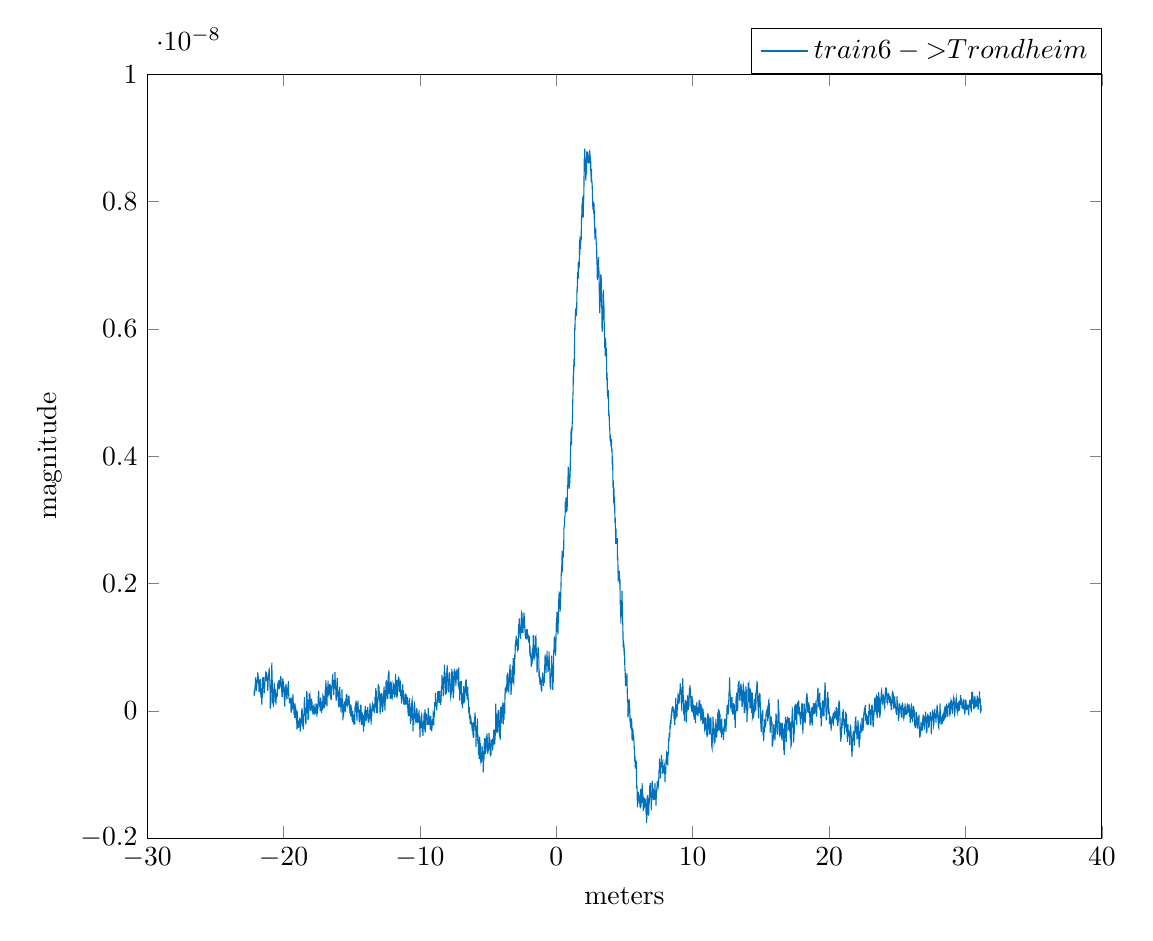
\begin{tikzpicture}

\begin{axis}[%
width=\textwidth,
height=0.8\textwidth,
at={(0\figurewidth,0\figureheight)},
scale only axis,
xmin=-30,
xmax=40,
xlabel={\SI{}{meters}},
ymin=-2e-09,
ymax=1e-08,
ylabel={magnitude},
axis background/.style={fill=white},
legend style={at={(1.0,1.0)},anchor=south east}
]
\addplot [color=mycolor1,solid]
  table[row sep=crcr]{%
-22.157431640625	2.3493988586141e-10\\
-22.14099609375	3.16454357658565e-10\\
-22.124560546875	2.45589177170896e-10\\
-22.108125	3.32225739372083e-10\\
-22.091689453125	3.64796431000339e-10\\
-22.07525390625	3.85652139602146e-10\\
-22.058818359375	5.24052201527055e-10\\
-22.0423828125	3.94618056722382e-10\\
-22.025947265625	4.52729076947501e-10\\
-22.00951171875	3.96448747790381e-10\\
-21.993076171875	3.10810818811408e-10\\
-21.976640625	3.5137966051929e-10\\
-21.960205078125	3.88177609181802e-10\\
-21.94376953125	4.7745703355699e-10\\
-21.927333984375	4.75295859905891e-10\\
-21.9108984375	5.01641220911783e-10\\
-21.894462890625	6.02333107767618e-10\\
-21.87802734375	5.70074940910517e-10\\
-21.861591796875	4.95507094559886e-10\\
-21.84515625	5.38368819869356e-10\\
-21.828720703125	4.11967046154423e-10\\
-21.81228515625	4.45625606191741e-10\\
-21.795849609375	2.97023464705207e-10\\
-21.7794140625	3.34279053278305e-10\\
-21.762978515625	3.37794453569621e-10\\
-21.74654296875	3.24512778350597e-10\\
-21.730107421875	4.89632771849845e-10\\
-21.713671875	4.12329201146572e-10\\
-21.697236328125	4.49231314402858e-10\\
-21.68080078125	5.03630064065878e-10\\
-21.664365234375	2.65286050733407e-10\\
-21.6479296875	2.0652233960767e-10\\
-21.631494140625	2.62414475049214e-10\\
-21.61505859375	2.61590807361819e-10\\
-21.598623046875	9.7790612333604e-11\\
-21.5821875	1.93612378855191e-10\\
-21.565751953125	3.53444828657035e-10\\
-21.54931640625	2.15474586107321e-10\\
-21.532880859375	4.51923553991532e-10\\
-21.5164453125	5.32318241162345e-10\\
-21.500009765625	4.10470132695962e-10\\
-21.48357421875	5.29347737722435e-10\\
-21.467138671875	3.51624049118825e-10\\
-21.450703125	4.15609638673467e-10\\
-21.434267578125	3.78257089922986e-10\\
-21.41783203125	2.73156288905784e-10\\
-21.401396484375	4.01627266978811e-10\\
-21.3849609375	3.56655402442344e-10\\
-21.368525390625	5.31800895046452e-10\\
-21.35208984375	4.84345061722003e-10\\
-21.335654296875	4.82244862131988e-10\\
-21.31921875	5.24329764983105e-10\\
-21.302783203125	6.18570529861811e-10\\
-21.28634765625	5.70353728073556e-10\\
-21.269912109375	6.03861839027797e-10\\
-21.2534765625	5.23570467742448e-10\\
-21.237041015625	5.38009517203342e-10\\
-21.22060546875	5.57884167435542e-10\\
-21.204169921875	5.4486049060594e-10\\
-21.187734375	4.36871494518218e-10\\
-21.171298828125	5.31556536647115e-10\\
-21.15486328125	3.12635559414438e-10\\
-21.138427734375	4.20463271533747e-10\\
-21.1219921875	5.25830651422483e-10\\
-21.105556640625	4.89874714993974e-10\\
-21.08912109375	5.42060753485373e-10\\
-21.072685546875	6.42210746770052e-10\\
-21.05625	6.51457627802147e-10\\
-21.039814453125	6.16165697186977e-10\\
-21.02337890625	5.21746654998639e-10\\
-21.006943359375	4.76088064142873e-10\\
-20.9905078125	3.64089815482994e-10\\
-20.974072265625	3.2338317073464e-11\\
-20.95763671875	1.18142553923816e-10\\
-20.941201171875	8.44640750205487e-11\\
-20.924765625	1.38271027326297e-10\\
-20.908330078125	3.29587441166262e-10\\
-20.89189453125	4.42055509259057e-10\\
-20.875458984375	4.95791617671641e-10\\
-20.8590234375	7.55508536670687e-10\\
-20.842587890625	5.17182861480332e-10\\
-20.82615234375	4.58568486101422e-10\\
-20.809716796875	3.2914358067188e-10\\
-20.79328125	1.36007685826063e-10\\
-20.776845703125	9.98699053312621e-11\\
-20.76041015625	1.86208619690393e-10\\
-20.743974609375	6.14886132074838e-11\\
-20.7275390625	2.34824295152368e-10\\
-20.711103515625	2.5105891399893e-10\\
-20.69466796875	3.48030998628216e-10\\
-20.678232421875	4.19176344330151e-10\\
-20.661796875	4.11461013764003e-10\\
-20.645361328125	3.32603154972688e-10\\
-20.62892578125	2.59407852216866e-10\\
-20.612490234375	1.36287534599295e-10\\
-20.5960546875	3.3435289415685e-10\\
-20.579619140625	2.38702748901889e-10\\
-20.56318359375	9.82122339605962e-11\\
-20.546748046875	1.6364618694515e-10\\
-20.5303125	2.40032555859376e-10\\
-20.513876953125	2.28679818065241e-10\\
-20.49744140625	2.72093514340112e-10\\
-20.481005859375	2.77864484043936e-10\\
-20.4645703125	2.24656678252565e-10\\
-20.448134765625	3.21528039787053e-10\\
-20.43169921875	3.87999231588502e-10\\
-20.415263671875	3.78506680715841e-10\\
-20.398828125	4.11888513093621e-10\\
-20.382392578125	3.96725300442707e-10\\
-20.36595703125	3.39272677776375e-10\\
-20.349521484375	4.77110257753398e-10\\
-20.3330859375	4.48403650642599e-10\\
-20.316650390625	4.54809288430134e-10\\
-20.30021484375	4.23918066617774e-10\\
-20.283779296875	3.71276474342371e-10\\
-20.26734375	3.80947276633e-10\\
-20.250908203125	4.2801439065467e-10\\
-20.23447265625	5.03606650717871e-10\\
-20.218037109375	4.14743270481536e-10\\
-20.2016015625	5.42813638949291e-10\\
-20.185166015625	5.08541706165276e-10\\
-20.16873046875	4.3265682800937e-10\\
-20.152294921875	3.59067434475952e-10\\
-20.135859375	3.66541175723774e-10\\
-20.119423828125	2.18680055784906e-10\\
-20.10298828125	3.15939865264201e-10\\
-20.086552734375	2.14733885639522e-10\\
-20.0701171875	3.95127978809931e-10\\
-20.053681640625	5.09540080500933e-10\\
-20.03724609375	4.29541550157533e-10\\
-20.020810546875	4.66944570120977e-10\\
-20.004375	4.21593495612138e-10\\
-19.987939453125	3.88494309699657e-10\\
-19.97150390625	3.89624130369062e-10\\
-19.955068359375	2.10578010160577e-10\\
-19.9386328125	1.78288264132363e-10\\
-19.922197265625	6.68059737575331e-11\\
-19.90576171875	9.33938058444373e-11\\
-19.889326171875	2.32769872916004e-10\\
-19.872890625	3.11293307998774e-10\\
-19.856455078125	3.42338197475866e-10\\
-19.84001953125	3.68077854147815e-10\\
-19.823583984375	4.18641222699547e-10\\
-19.8071484375	3.82896819263684e-10\\
-19.790712890625	3.29255882640091e-10\\
-19.77427734375	1.96648047703011e-10\\
-19.757841796875	2.64851506682972e-10\\
-19.74140625	1.81266844697608e-10\\
-19.724970703125	3.16625395276192e-10\\
-19.70853515625	3.07487499426075e-10\\
-19.692099609375	3.43432670742638e-10\\
-19.6756640625	3.09887308743544e-10\\
-19.659228515625	3.03011551260259e-10\\
-19.64279296875	4.65010827880937e-10\\
-19.626357421875	2.92299986863863e-10\\
-19.609921875	2.00759958898872e-10\\
-19.593486328125	1.91267120373471e-10\\
-19.57705078125	1.88618837907769e-10\\
-19.560615234375	1.16066534213548e-10\\
-19.5441796875	1.41679029436541e-10\\
-19.527744140625	1.46756225900682e-10\\
-19.51130859375	1.4361649804542e-10\\
-19.494873046875	1.64991618649528e-10\\
-19.4784375	2.0416328490277e-10\\
-19.462001953125	1.00330881441852e-10\\
-19.44556640625	-3.18641970356275e-11\\
-19.429130859375	-1.60039886743246e-12\\
-19.4126953125	7.72110470250814e-11\\
-19.396259765625	7.09995340750797e-11\\
-19.37982421875	9.78968820011646e-12\\
-19.363388671875	1.7294673412508e-10\\
-19.346953125	1.62974632034583e-10\\
-19.330517578125	1.13983739641202e-10\\
-19.31408203125	2.63317145127381e-10\\
-19.297646484375	1.60734569531365e-10\\
-19.2812109375	9.32442543870109e-11\\
-19.264775390625	2.8878038505475e-11\\
-19.24833984375	9.27139947344124e-11\\
-19.231904296875	-6.1536827146357e-11\\
-19.21546875	9.63714137550961e-11\\
-19.199033203125	-4.91376244136048e-12\\
-19.18259765625	-1.09552393400853e-10\\
-19.166162109375	1.07818427786756e-10\\
-19.1497265625	1.06326670615224e-10\\
-19.133291015625	-6.12974154465468e-11\\
-19.11685546875	-3.26541312616973e-11\\
-19.100419921875	5.11811986538485e-11\\
-19.083984375	-7.90866247504586e-11\\
-19.067548828125	-1.46586669311674e-10\\
-19.05111328125	4.85842914179183e-12\\
-19.034677734375	-1.43925269348242e-10\\
-19.0182421875	-2.94720429623287e-10\\
-19.001806640625	2.89237278064039e-12\\
-18.98537109375	-2.12438079944709e-10\\
-18.968935546875	-2.04433601683248e-10\\
-18.9525	-2.34473832548686e-10\\
-18.936064453125	-2.2427812212354e-10\\
-18.91962890625	-2.24216806320201e-10\\
-18.903193359375	-2.68699141883346e-10\\
-18.8867578125	-1.7076675280888e-10\\
-18.870322265625	-1.43078804174377e-10\\
-18.85388671875	-2.41458771298671e-10\\
-18.837451171875	-1.5673723447876e-10\\
-18.821015625	-1.76925073784907e-10\\
-18.804580078125	-1.37335806461968e-10\\
-18.78814453125	-1.36151436147009e-10\\
-18.771708984375	-3.25247997213355e-10\\
-18.7552734375	-2.17599535819189e-10\\
-18.738837890625	-2.57122470217478e-10\\
-18.72240234375	-1.77104384812638e-10\\
-18.705966796875	-1.3133408737274e-10\\
-18.68953125	-5.11135831316123e-11\\
-18.673095703125	-7.4357671087722e-11\\
-18.65666015625	3.95936406528028e-11\\
-18.640224609375	-1.90639359403787e-11\\
-18.6237890625	-1.20927600602061e-11\\
-18.607353515625	-2.08119521794635e-10\\
-18.59091796875	-2.28541691331286e-10\\
-18.574482421875	-2.36781356464068e-10\\
-18.558046875	-2.9182510457877e-10\\
-18.541611328125	-2.5060178128786e-10\\
-18.52517578125	-7.18732321408398e-11\\
-18.508740234375	-5.56040600318118e-11\\
-18.4923046875	-3.44254889062043e-11\\
-18.475869140625	1.72964160518218e-10\\
-18.45943359375	2.12330121629578e-10\\
-18.442998046875	5.72893504007784e-11\\
-18.4265625	4.97661541523069e-11\\
-18.410126953125	-5.26470937364653e-11\\
-18.39369140625	-1.47467290467235e-10\\
-18.377255859375	-1.62232233472302e-10\\
-18.3608203125	-2.18638201857842e-10\\
-18.344384765625	-3.10227644110464e-12\\
-18.32794921875	2.01416272541854e-11\\
-18.311513671875	-4.16802945329874e-11\\
-18.295078125	3.09929828630557e-10\\
-18.278642578125	2.7247069468487e-10\\
-18.26220703125	2.54456761666874e-11\\
-18.245771484375	1.77508467860796e-10\\
-18.2293359375	6.21342080814882e-11\\
-18.212900390625	-1.41255855659885e-10\\
-18.19646484375	-4.74014103424408e-11\\
-18.180029296875	-1.28589027777111e-10\\
-18.16359375	-9.5104809221553e-11\\
-18.147158203125	8.97203911896056e-11\\
-18.13072265625	1.69200661058814e-10\\
-18.114287109375	2.56690308768618e-10\\
-18.0978515625	2.50223905161424e-10\\
-18.081416015625	2.25922477447113e-10\\
-18.06498046875	2.42743550454547e-10\\
-18.048544921875	1.02901142781064e-10\\
-18.032109375	4.0749133829229e-12\\
-18.015673828125	1.41612740705313e-10\\
-17.99923828125	8.3838668927525e-11\\
-17.982802734375	-7.78534216979195e-12\\
-17.9663671875	1.70589314039509e-10\\
-17.949931640625	1.75717619797306e-10\\
-17.93349609375	8.14377928946445e-11\\
-17.917060546875	1.43138547400581e-10\\
-17.900625	7.77064177319521e-11\\
-17.884189453125	4.37127696234029e-11\\
-17.86775390625	7.35474301529068e-11\\
-17.851318359375	-6.00078747960531e-11\\
-17.8348828125	2.41856005430499e-11\\
-17.818447265625	-3.27669817385943e-11\\
-17.80201171875	-3.20544679016951e-11\\
-17.785576171875	6.26382385445327e-11\\
-17.769140625	1.00479371087238e-10\\
-17.752705078125	5.31891827758432e-11\\
-17.73626953125	-6.11598680565727e-11\\
-17.719833984375	5.52298628116335e-11\\
-17.7033984375	-2.70776593089405e-11\\
-17.686962890625	-3.12990315406357e-11\\
-17.67052734375	1.97110499188427e-11\\
-17.654091796875	-4.09288997220514e-11\\
-17.63765625	1.24367422589856e-11\\
-17.621220703125	1.18037325411016e-10\\
-17.60478515625	3.74890897257419e-11\\
-17.588349609375	9.63454177367087e-11\\
-17.5719140625	6.35604633244136e-11\\
-17.555478515625	-8.9802839818781e-11\\
-17.53904296875	6.15789322793731e-11\\
-17.522607421875	-4.17231053292969e-11\\
-17.506171875	-3.40628501052788e-11\\
-17.489736328125	1.08574153517384e-10\\
-17.47330078125	2.94658518908059e-11\\
-17.456865234375	2.0698571399708e-10\\
-17.4404296875	2.99720758274977e-10\\
-17.423994140625	3.03120089747576e-10\\
-17.40755859375	2.12873272825644e-10\\
-17.391123046875	1.70954521868791e-10\\
-17.3746875	1.19948214729375e-10\\
-17.358251953125	9.37851014631949e-11\\
-17.34181640625	6.3029596591031e-11\\
-17.325380859375	1.23381701967886e-10\\
-17.3089453125	-4.22947615707284e-12\\
-17.292509765625	1.15933870344191e-10\\
-17.27607421875	2.05702173885924e-10\\
-17.259638671875	1.25422444608356e-10\\
-17.243203125	9.6284817801147e-11\\
-17.226767578125	5.18401812986326e-11\\
-17.21033203125	-3.15572027025912e-11\\
-17.193896484375	3.18080080522986e-11\\
-17.1774609375	3.57279365737924e-11\\
-17.161025390625	1.45408132916028e-10\\
-17.14458984375	1.56444614284962e-11\\
-17.128154296875	1.0991878945987e-10\\
-17.11171875	2.38629181572775e-10\\
-17.095283203125	2.28728104039255e-10\\
-17.07884765625	2.26999634199782e-10\\
-17.062412109375	1.9909013763606e-10\\
-17.0459765625	1.22198497148509e-10\\
-17.029541015625	3.64368764898449e-11\\
-17.01310546875	1.16334402244761e-10\\
-16.996669921875	1.00055005098323e-10\\
-16.980234375	9.0396514409316e-11\\
-16.963798828125	1.8703716805166e-10\\
-16.94736328125	3.14276342319637e-10\\
-16.930927734375	3.49625111679726e-10\\
-16.9144921875	2.43523286500137e-10\\
-16.898056640625	4.82289909079857e-10\\
-16.88162109375	3.44892060554779e-10\\
-16.865185546875	9.80012038761509e-11\\
-16.84875	2.11585194262927e-10\\
-16.832314453125	2.1059166910805e-10\\
-16.81587890625	7.07064083698628e-11\\
-16.799443359375	2.29318439051007e-10\\
-16.7830078125	3.74350945810284e-10\\
-16.766572265625	2.43624332415479e-10\\
-16.75013671875	3.39752192622947e-10\\
-16.733701171875	4.72469624990341e-10\\
-16.717265625	3.11120203851158e-10\\
-16.700830078125	2.9638646151624e-10\\
-16.68439453125	3.81972234312028e-10\\
-16.667958984375	2.65104485146997e-10\\
-16.6515234375	2.7953513508772e-10\\
-16.635087890625	4.1611793471901e-10\\
-16.61865234375	2.98226890285342e-10\\
-16.602216796875	3.24494367012219e-10\\
-16.58578125	4.25152962850902e-10\\
-16.569345703125	3.52037678740046e-10\\
-16.55291015625	1.89802251385418e-10\\
-16.536474609375	3.24662230573125e-10\\
-16.5200390625	2.87916534225852e-10\\
-16.503603515625	1.71522452230456e-10\\
-16.48716796875	3.1888099814183e-10\\
-16.470732421875	3.83574343280805e-10\\
-16.454296875	3.14857681776016e-10\\
-16.437861328125	4.50889474169949e-10\\
-16.42142578125	5.00313146345188e-10\\
-16.404990234375	5.56121485103991e-10\\
-16.3885546875	5.61913078358026e-10\\
-16.372119140625	3.85194630602758e-10\\
-16.35568359375	4.83268056126422e-10\\
-16.339248046875	4.31757415379964e-10\\
-16.3228125	2.45742483516105e-10\\
-16.306376953125	3.56467560632951e-10\\
-16.28994140625	3.81818160414832e-10\\
-16.273505859375	4.28592162163009e-10\\
-16.2570703125	4.32640073308749e-10\\
-16.240634765625	4.89389749307276e-10\\
-16.22419921875	6.08277631335303e-10\\
-16.207763671875	4.27196134098727e-10\\
-16.191328125	3.31027782114255e-10\\
-16.174892578125	3.91353547468422e-10\\
-16.15845703125	2.30083624904787e-10\\
-16.142021484375	1.5517473213708e-10\\
-16.1255859375	2.87658738949895e-10\\
-16.109150390625	2.76817536793284e-10\\
-16.09271484375	3.93483435806841e-10\\
-16.076279296875	4.63947218785417e-10\\
-16.05984375	5.13925414398782e-10\\
-16.043408203125	3.60578589732076e-10\\
-16.02697265625	2.78854301068228e-10\\
-16.010537109375	2.29337221415402e-10\\
-15.9941015625	2.53275843522763e-10\\
-15.977666015625	1.91139792435621e-10\\
-15.96123046875	5.36562069091758e-11\\
-15.944794921875	1.64445361785615e-10\\
-15.928359375	2.5171628002584e-10\\
-15.911923828125	2.58001602826093e-10\\
-15.89548828125	2.96768021543342e-10\\
-15.879052734375	3.74322292529632e-10\\
-15.8626171875	2.70035372541593e-10\\
-15.846181640625	5.3109404585712e-11\\
-15.82974609375	7.29457558948319e-11\\
-15.813310546875	1.97522325322776e-10\\
-15.796875	-2.53420277421745e-12\\
-15.780439453125	-8.23718406284433e-12\\
-15.76400390625	1.51064395425392e-10\\
-15.747568359375	9.28520376472075e-11\\
-15.7311328125	1.59688018276465e-10\\
-15.714697265625	3.35516303064203e-10\\
-15.69826171875	5.09818488273122e-11\\
-15.681826171875	1.84819530330987e-10\\
-15.665390625	1.44991155149545e-10\\
-15.648955078125	-1.4853011219328e-10\\
-15.63251953125	-3.42407607134093e-11\\
-15.616083984375	9.08548075377638e-11\\
-15.5996484375	-9.17067591186766e-11\\
-15.583212890625	1.52362933562143e-11\\
-15.56677734375	9.45866320109157e-12\\
-15.550341796875	7.85731276840196e-11\\
-15.53390625	1.48030209565438e-10\\
-15.517470703125	8.96598671675246e-12\\
-15.50103515625	3.25510819645288e-11\\
-15.484599609375	1.39881767107376e-10\\
-15.4681640625	2.98169793939392e-12\\
-15.451728515625	-2.25281056362443e-12\\
-15.43529296875	1.8393335048915e-10\\
-15.418857421875	7.14079295622789e-11\\
-15.402421875	2.1532779113091e-10\\
-15.385986328125	2.00058946915975e-10\\
-15.36955078125	2.6283028321426e-10\\
-15.353115234375	1.88568525408481e-10\\
-15.3366796875	1.25787939481082e-10\\
-15.320244140625	1.0221771006842e-10\\
-15.30380859375	1.35933056962539e-10\\
-15.287373046875	1.67328133035629e-10\\
-15.2709375	1.10623956962378e-10\\
-15.254501953125	1.21189966230949e-10\\
-15.23806640625	2.32657982455792e-10\\
-15.221630859375	1.30677786444308e-10\\
-15.2051953125	2.36264798884301e-10\\
-15.188759765625	1.80524965090613e-10\\
-15.17232421875	3.68556342795673e-11\\
-15.155888671875	1.15215038593512e-10\\
-15.139453125	-1.52110837534111e-11\\
-15.123017578125	-4.5373127153877e-11\\
-15.10658203125	5.78905575362386e-11\\
-15.090146484375	4.71135077337926e-11\\
-15.0737109375	-8.7501017418054e-11\\
-15.057275390625	9.58291005483273e-11\\
-15.04083984375	-3.77897413726313e-11\\
-15.024404296875	-3.75081738959383e-11\\
-15.00796875	4.79626128332879e-11\\
-14.991533203125	-1.17812320791832e-10\\
-14.97509765625	-6.96676304357561e-11\\
-14.958662109375	-1.47184755693622e-10\\
-14.9422265625	-1.39793876849722e-10\\
-14.925791015625	-1.78957319346408e-12\\
-14.90935546875	-1.28845417295857e-10\\
-14.892919921875	-1.56160172473467e-10\\
-14.876484375	-2.02017831750036e-10\\
-14.860048828125	-6.25585811573028e-11\\
-14.84361328125	-1.37553961999627e-10\\
-14.827177734375	-2.24916713954399e-10\\
-14.8107421875	-1.33980233235589e-10\\
-14.794306640625	-5.16422223985123e-11\\
-14.77787109375	-2.10429675724892e-10\\
-14.761435546875	4.94374995233121e-11\\
-14.745	8.24947493405529e-11\\
-14.728564453125	3.3758216547589e-11\\
-14.71212890625	1.13274787342482e-10\\
-14.695693359375	1.21120744678785e-10\\
-14.6792578125	1.60370831187416e-10\\
-14.662822265625	5.92480432931956e-11\\
-14.64638671875	-2.97973904374409e-11\\
-14.629951171875	-1.67725340726263e-11\\
-14.613515625	-1.54683688770712e-10\\
-14.597080078125	1.14915378259735e-10\\
-14.58064453125	4.36229884267604e-11\\
-14.564208984375	4.66235264605736e-11\\
-14.5477734375	1.59960333496027e-10\\
-14.531337890625	7.94866336934008e-11\\
-14.51490234375	-2.93241998249553e-11\\
-14.498466796875	1.283470521263e-11\\
-14.48203125	2.38361614033565e-12\\
-14.465595703125	-1.07955409282709e-10\\
-14.44916015625	-1.73741639663463e-10\\
-14.432724609375	-1.09666086208492e-10\\
-14.4162890625	-6.29003542176111e-11\\
-14.399853515625	-1.3992889984364e-10\\
-14.38341796875	-1.17763735824174e-10\\
-14.366982421875	9.61869450122708e-11\\
-14.350546875	3.30571531449123e-11\\
-14.334111328125	-1.29447203238475e-10\\
-14.31767578125	9.18548054810683e-11\\
-14.301240234375	-6.92946448521746e-11\\
-14.2848046875	-2.20058998200314e-10\\
-14.268369140625	-3.27511530903854e-11\\
-14.25193359375	-1.00068303470152e-10\\
-14.235498046875	-2.02861215170781e-10\\
-14.2190625	-2.97701682655138e-11\\
-14.202626953125	-1.07415769015667e-10\\
-14.18619140625	-2.1598709155195e-10\\
-14.169755859375	-6.74008001282937e-11\\
-14.1533203125	-1.5518628456294e-10\\
-14.136884765625	-3.28078339548995e-10\\
-14.12044921875	-2.02794871638674e-10\\
-14.104013671875	-1.81037103039913e-10\\
-14.087578125	-2.43395593932336e-10\\
-14.071142578125	-1.4223723894949e-10\\
-14.05470703125	-1.23398045635874e-11\\
-14.038271484375	-1.37626642194326e-10\\
-14.0218359375	4.19760912665472e-11\\
-14.005400390625	7.27418445921667e-11\\
-13.98896484375	-5.0225150526105e-11\\
-13.972529296875	-1.52902415010806e-10\\
-13.95609375	1.5517412135529e-11\\
-13.939658203125	-1.43030184060796e-10\\
-13.92322265625	-1.31721491551337e-10\\
-13.906787109375	1.62200273636432e-11\\
-13.8903515625	-5.37024322145233e-11\\
-13.873916015625	-3.14604517703772e-11\\
-13.85748046875	1.31782839967798e-11\\
-13.841044921875	1.64829444802142e-11\\
-13.824609375	5.58712984709124e-11\\
-13.808173828125	-8.99325629005741e-11\\
-13.79173828125	-1.45216530008921e-10\\
-13.775302734375	-1.32425053146327e-10\\
-13.7588671875	-1.8611948437396e-10\\
-13.742431640625	-1.54052565763606e-10\\
-13.72599609375	-1.31221369783221e-10\\
-13.709560546875	-9.57748874888522e-11\\
-13.693125	1.33995170091737e-11\\
-13.676689453125	-1.07911769516181e-10\\
-13.66025390625	1.16256623125199e-10\\
-13.643818359375	6.21234897561511e-11\\
-13.6273828125	-1.27669713770314e-10\\
-13.610947265625	-8.58511272861558e-11\\
-13.59451171875	-9.34297840191512e-11\\
-13.578076171875	-2.17845059568208e-10\\
-13.561640625	3.26341885697893e-11\\
-13.545205078125	-8.92729310264055e-11\\
-13.52876953125	-7.33417094662745e-11\\
-13.512333984375	2.91739009739299e-11\\
-13.4958984375	7.12038693290254e-11\\
-13.479462890625	6.34937092848389e-11\\
-13.46302734375	1.05952616357485e-10\\
-13.446591796875	9.11089873301244e-11\\
-13.43015625	3.94938630107655e-12\\
-13.413720703125	6.67749609976712e-11\\
-13.39728515625	3.64018103137444e-11\\
-13.380849609375	5.28756559533178e-11\\
-13.3644140625	1.38182639609495e-11\\
-13.347978515625	7.35718805037175e-11\\
-13.33154296875	-3.22573640175486e-11\\
-13.315107421875	2.69701910844105e-11\\
-13.298671875	2.16058852106094e-10\\
-13.282236328125	8.26065589938743e-11\\
-13.26580078125	5.12045261330483e-11\\
-13.249365234375	2.72460956870118e-10\\
-13.2329296875	3.60346094119123e-10\\
-13.216494140625	1.21886158646387e-10\\
-13.20005859375	3.13755021558228e-10\\
-13.183623046875	1.75694870402479e-10\\
-13.1671875	-3.55525130195144e-11\\
-13.150751953125	2.05189961586564e-10\\
-13.13431640625	5.60880046559301e-11\\
-13.117880859375	-3.95712372902775e-11\\
-13.1014453125	1.25715492677431e-10\\
-13.085009765625	1.34051703124959e-10\\
-13.06857421875	2.12407365150852e-10\\
-13.052138671875	4.18606302654009e-10\\
-13.035703125	3.54845367185768e-10\\
-13.019267578125	3.10632721319234e-10\\
-13.00283203125	3.8538809473725e-10\\
-12.986396484375	2.74258209551999e-10\\
-12.9699609375	1.94545799466277e-10\\
-12.953525390625	2.95236788543152e-10\\
-12.93708984375	6.74648652066443e-11\\
-12.920654296875	-5.51589551631672e-11\\
-12.90421875	4.30420808370689e-11\\
-12.887783203125	8.58776380542632e-11\\
-12.87134765625	7.48689260316763e-11\\
-12.854912109375	1.4633749069454e-10\\
-12.8384765625	2.6820746789734e-10\\
-12.822041015625	1.62637053192142e-10\\
-12.80560546875	2.78229547536834e-10\\
-12.789169921875	1.35361935515295e-10\\
-12.772734375	2.20984905666528e-10\\
-12.756298828125	4.26475901433772e-11\\
-12.73986328125	-2.18426323984207e-11\\
-12.723427734375	1.73803010487959e-11\\
-12.7069921875	8.17181271207462e-11\\
-12.690556640625	1.37682254786652e-10\\
-12.67412109375	2.36524578072649e-10\\
-12.657685546875	2.95565852859139e-10\\
-12.64125	3.13979373573914e-10\\
-12.624814453125	3.82058050962487e-10\\
-12.60837890625	1.52757649697081e-10\\
-12.591943359375	1.09684107674082e-10\\
-12.5755078125	1.30102001721701e-10\\
-12.559072265625	6.08694573621499e-12\\
-12.54263671875	2.05239831441437e-10\\
-12.526201171875	2.92628307930931e-10\\
-12.509765625	2.36859246090235e-10\\
-12.493330078125	4.53359168287995e-10\\
-12.47689453125	3.52733892735959e-10\\
-12.460458984375	4.85322786268742e-10\\
-12.4440234375	4.17929632428651e-10\\
-12.427587890625	2.64317540524041e-10\\
-12.41115234375	1.81755665370793e-10\\
-12.394716796875	2.13394222988422e-10\\
-12.37828125	2.46111657809204e-10\\
-12.361845703125	1.92775148727827e-10\\
-12.34541015625	3.59686140758352e-10\\
-12.328974609375	5.63070545713839e-10\\
-12.3125390625	5.35819152015176e-10\\
-12.296103515625	4.73699407435874e-10\\
-12.27966796875	6.37429519597088e-10\\
-12.263232421875	5.69248291943963e-10\\
-12.246796875	2.66099528939063e-10\\
-12.230361328125	3.52285378356657e-10\\
-12.21392578125	3.68468680812845e-10\\
-12.197490234375	3.30312621559622e-10\\
-12.1810546875	1.82618091907387e-10\\
-12.164619140625	3.88787849798665e-10\\
-12.14818359375	4.6283360223504e-10\\
-12.131748046875	2.09613045009275e-10\\
-12.1153125	4.54109688364421e-10\\
-12.098876953125	4.23284865273161e-10\\
-12.08244140625	2.54247809078298e-10\\
-12.066005859375	2.71663164591602e-10\\
-12.0495703125	2.15874078199498e-10\\
-12.033134765625	2.05451231195363e-10\\
-12.01669921875	2.81128939966085e-10\\
-12.000263671875	3.03134687836381e-10\\
-11.983828125	2.58850790759719e-10\\
-11.967392578125	4.28657853598752e-10\\
-11.95095703125	4.17006215452565e-10\\
-11.934521484375	4.04763494736176e-10\\
-11.9180859375	3.87523426544894e-10\\
-11.901650390625	4.23226156683609e-10\\
-11.88521484375	2.81913035800658e-10\\
-11.868779296875	2.05669961038799e-10\\
-11.85234375	3.22238941941764e-10\\
-11.835908203125	2.98497776963461e-10\\
-11.81947265625	2.49363852247734e-10\\
-11.803037109375	3.37499656189509e-10\\
-11.7866015625	5.74101235706972e-10\\
-11.770166015625	4.08602510817838e-10\\
-11.75373046875	4.26093116217115e-10\\
-11.737294921875	4.84653566407031e-10\\
-11.720859375	2.14025071133912e-10\\
-11.704423828125	2.63848231613653e-10\\
-11.68798828125	2.60469827799873e-10\\
-11.671552734375	2.34598342707723e-10\\
-11.6551171875	2.53513243681574e-10\\
-11.638681640625	4.53870841966043e-10\\
-11.62224609375	4.78213466835963e-10\\
-11.605810546875	4.85055728332714e-10\\
-11.589375	4.69942225386524e-10\\
-11.572939453125	5.40902540631835e-10\\
-11.55650390625	5.04265939526229e-10\\
-11.540068359375	4.70756775375056e-10\\
-11.5236328125	2.90790162095074e-10\\
-11.507197265625	3.92860512845986e-10\\
-11.49076171875	4.3801855213618e-10\\
-11.474326171875	3.41662085281407e-10\\
-11.457890625	2.95772136215645e-10\\
-11.441455078125	4.60331480563689e-10\\
-11.42501953125	4.48710086931619e-10\\
-11.408583984375	2.33593310744352e-10\\
-11.3921484375	3.26546818871326e-10\\
-11.375712890625	2.82509440720281e-10\\
-11.35927734375	1.1390828853393e-10\\
-11.342841796875	1.61946419076484e-10\\
-11.32640625	1.86394029333894e-10\\
-11.309970703125	2.95068792928569e-10\\
-11.29353515625	1.93492742967053e-10\\
-11.277099609375	3.25589596988214e-10\\
-11.2606640625	4.13240785407191e-10\\
-11.244228515625	2.95876068955168e-10\\
-11.22779296875	3.1823345870133e-10\\
-11.211357421875	1.82962799078652e-10\\
-11.194921875	1.15366125068571e-10\\
-11.178486328125	1.17272709334203e-10\\
-11.16205078125	1.37166226394418e-10\\
-11.145615234375	9.42708075712726e-11\\
-11.1291796875	2.07336304105767e-10\\
-11.112744140625	1.05158441836104e-10\\
-11.09630859375	2.52856646514859e-10\\
-11.079873046875	2.55988607812997e-10\\
-11.0634375	1.91711107916258e-10\\
-11.047001953125	1.39326068921694e-10\\
-11.03056640625	2.72142792601923e-10\\
-11.014130859375	8.98494177053575e-11\\
-10.9976953125	1.92423585103986e-10\\
-10.981259765625	2.50032810853891e-10\\
-10.96482421875	1.39260574462169e-10\\
-10.948388671875	1.52526001885397e-10\\
-10.931953125	2.13328012608939e-10\\
-10.915517578125	1.57445477703563e-10\\
-10.89908203125	1.11533488776972e-10\\
-10.882646484375	-1.26779632276268e-11\\
-10.8662109375	-3.24063150198722e-11\\
-10.849775390625	-7.74762170693153e-11\\
-10.83333984375	5.30843721939962e-11\\
-10.816904296875	6.2045375640636e-11\\
-10.80046875	-8.79905608305059e-11\\
-10.784033203125	1.61728129838603e-10\\
-10.76759765625	1.97549655179783e-10\\
-10.751162109375	9.55706232789146e-12\\
-10.7347265625	2.64538430681355e-11\\
-10.718291015625	5.97504890816564e-11\\
-10.70185546875	-1.45311123511161e-10\\
-10.685419921875	-2.04036339549601e-10\\
-10.668984375	-6.82008857080578e-11\\
-10.652548828125	-1.56897072826489e-10\\
-10.63611328125	-2.06343216875568e-11\\
-10.619677734375	1.20694440475443e-10\\
-10.6032421875	-5.61896044298466e-12\\
-10.586806640625	1.5897151593564e-10\\
-10.57037109375	1.75462495630974e-10\\
-10.553935546875	-5.52695262472255e-12\\
-10.5375	-1.41745625131213e-10\\
-10.521064453125	-8.42886862595715e-11\\
-10.50462890625	-3.22980468195007e-10\\
-10.488193359375	-1.45180095470021e-10\\
-10.4717578125	-4.75150623196731e-11\\
-10.455322265625	-2.20258199458523e-10\\
-10.43888671875	2.25622428027303e-11\\
-10.422451171875	9.82805774319952e-11\\
-10.406015625	2.40453967274764e-11\\
-10.389580078125	9.4715105284917e-11\\
-10.37314453125	7.61797209832039e-11\\
-10.356708984375	-8.48313805504474e-11\\
-10.3402734375	-1.23770958320728e-10\\
-10.323837890625	-7.52928791112309e-11\\
-10.30740234375	-1.47510008559959e-10\\
-10.290966796875	-1.33257911742231e-10\\
-10.27453125	-1.84670249251496e-10\\
-10.258095703125	-1.04666970676263e-10\\
-10.24166015625	1.81281922607639e-11\\
-10.225224609375	4.30243428805448e-11\\
-10.2087890625	-5.2434460552119e-11\\
-10.192353515625	-5.82662483749259e-11\\
-10.17591796875	-1.26350063326998e-10\\
-10.159482421875	-1.9366928626768e-10\\
-10.143046875	-1.23004573580073e-10\\
-10.126611328125	-9.95079701515015e-11\\
-10.11017578125	-4.03840459841005e-11\\
-10.093740234375	-1.5824515048159e-10\\
-10.0773046875	-8.95239250391472e-11\\
-10.060869140625	8.85208244266492e-12\\
-10.04443359375	-2.11723670033095e-10\\
-10.027998046875	-1.92954457047494e-10\\
-10.0115625	-2.73691399114839e-10\\
-9.995126953125	-4.17144540920472e-10\\
-9.97869140625	-2.44407077617801e-10\\
-9.962255859375	-2.42561446107679e-10\\
-9.9458203125	-2.67529677951276e-10\\
-9.929384765625	-1.073877776966e-10\\
-9.91294921875	-9.70110955371469e-11\\
-9.896513671875	-7.81389555778023e-11\\
-9.880078125	-1.37073739188731e-10\\
-9.863642578125	-6.00516291538136e-11\\
-9.84720703125	-2.67030692755609e-10\\
-9.830771484375	-3.24922834528839e-10\\
-9.8143359375	-3.30053804022007e-10\\
-9.797900390625	-1.78646324201558e-10\\
-9.78146484375	-3.9334057669007e-10\\
-9.765029296875	-3.20245074850929e-10\\
-9.74859375	-1.53347634859934e-10\\
-9.732158203125	-2.16299719251784e-10\\
-9.71572265625	-2.4015338433911e-10\\
-9.699287109375	-6.62011671400115e-11\\
-9.6828515625	-2.92954056794164e-11\\
-9.666416015625	-2.69371596052501e-10\\
-9.64998046875	-2.86241755707729e-10\\
-9.633544921875	2.27312749689619e-11\\
-9.617109375	-2.32693488844855e-10\\
-9.600673828125	-3.40555311734649e-10\\
-9.58423828125	-2.804078325156e-11\\
-9.567802734375	-6.50779521212686e-11\\
-9.5513671875	-1.17196016339913e-10\\
-9.534931640625	-5.90138064344372e-11\\
-9.51849609375	-6.04366116619383e-11\\
-9.502060546875	-1.5057457051912e-10\\
-9.485625	-9.78727598248182e-11\\
-9.469189453125	-2.24894640914639e-10\\
-9.45275390625	-9.65962808758296e-11\\
-9.436318359375	-1.49051918317662e-10\\
-9.4198828125	-1.39186363595262e-10\\
-9.403447265625	-2.16734060669518e-10\\
-9.38701171875	4.62341711857726e-11\\
-9.370576171875	-4.84925118379697e-11\\
-9.354140625	-1.53008208856973e-10\\
-9.337705078125	-2.21246648707604e-10\\
-9.32126953125	-1.60932764791385e-10\\
-9.304833984375	-1.43430119461008e-10\\
-9.2883984375	-2.18677143907621e-10\\
-9.271962890625	-1.11783436424725e-10\\
-9.25552734375	-1.4022573828406e-10\\
-9.239091796875	-3.0111440019993e-10\\
-9.22265625	-1.47951541399637e-10\\
-9.206220703125	-8.15342005446995e-11\\
-9.18978515625	-2.39496681250618e-10\\
-9.173349609375	-2.03888612618738e-10\\
-9.1569140625	-2.93564044952642e-10\\
-9.140478515625	-3.24199589678287e-10\\
-9.12404296875	-2.33363996862846e-10\\
-9.107607421875	-2.66355840241952e-10\\
-9.091171875	-1.32729017056789e-10\\
-9.074736328125	-2.29014621955968e-10\\
-9.05830078125	-1.86476802855266e-10\\
-9.041865234375	-1.49544016725037e-10\\
-9.0254296875	-3.53347612857559e-11\\
-9.008994140625	-5.43068214720526e-11\\
-8.99255859375	-2.27315453163013e-10\\
-8.976123046875	-8.89503822598576e-11\\
-8.9596875	-6.51248415126819e-11\\
-8.943251953125	-9.74652330210758e-11\\
-8.92681640625	-2.59995774433258e-11\\
-8.910380859375	1.35057174983271e-10\\
-8.8939453125	7.58691879539988e-11\\
-8.877509765625	9.49673124623483e-11\\
-8.86107421875	2.82914647600402e-10\\
-8.844638671875	2.14244480350146e-10\\
-8.828203125	9.71882545414462e-11\\
-8.811767578125	1.01504306763074e-10\\
-8.79533203125	1.31248713256529e-10\\
-8.778896484375	5.30701451255154e-11\\
-8.7624609375	6.83226444433641e-12\\
-8.746025390625	1.31518470681207e-10\\
-8.72958984375	1.33398919281043e-10\\
-8.713154296875	1.34465170316127e-10\\
-8.69671875	2.79297994780934e-10\\
-8.680283203125	2.75350627339467e-10\\
-8.66384765625	3.10890661366563e-10\\
-8.647412109375	1.57484448840604e-10\\
-8.6309765625	2.41547989670684e-10\\
-8.614541015625	2.60459147704888e-10\\
-8.59810546875	2.35900040235977e-10\\
-8.581669921875	1.22882046985786e-10\\
-8.565234375	3.08033454773267e-10\\
-8.548798828125	2.2979623334272e-10\\
-8.53236328125	1.57053034047836e-10\\
-8.515927734375	2.38048941790138e-10\\
-8.4994921875	1.97851327018011e-10\\
-8.483056640625	8.93179594489145e-11\\
-8.46662109375	2.11261795935748e-10\\
-8.450185546875	1.38728272233451e-10\\
-8.43375	3.23162801614541e-10\\
-8.417314453125	3.81784779672351e-10\\
-8.40087890625	3.39907517883736e-10\\
-8.384443359375	5.6107008308973e-10\\
-8.3680078125	4.44617901534325e-10\\
-8.351572265625	5.12182212300342e-10\\
-8.33513671875	3.75738234315645e-10\\
-8.318701171875	3.31869187468962e-10\\
-8.302265625	3.7253905834128e-10\\
-8.285830078125	2.28794934610297e-10\\
-8.26939453125	2.88841674026679e-10\\
-8.252958984375	5.28203098546273e-10\\
-8.2365234375	4.29374792528542e-10\\
-8.220087890625	5.43086310447393e-10\\
-8.20365234375	7.24100884583907e-10\\
-8.187216796875	6.06722694826108e-10\\
-8.17078125	5.26215584919401e-10\\
-8.154345703125	5.39912412928459e-10\\
-8.13791015625	3.22496555936821e-10\\
-8.121474609375	2.51262758034272e-10\\
-8.1050390625	4.02006183697258e-10\\
-8.088603515625	3.66677543989318e-10\\
-8.07216796875	2.72719577820138e-10\\
-8.055732421875	5.01308504235526e-10\\
-8.039296875	5.83821980409738e-10\\
-8.022861328125	5.89237708886397e-10\\
-8.00642578125	7.2001733609525e-10\\
-7.989990234375	6.22523179570303e-10\\
-7.9735546875	4.81425781038074e-10\\
-7.957119140625	4.5907883295233e-10\\
-7.94068359375	3.16852249507224e-10\\
-7.924248046875	4.60074000349877e-10\\
-7.9078125	3.96800134965187e-10\\
-7.891376953125	2.90034987480442e-10\\
-7.87494140625	3.8512846922514e-10\\
-7.858505859375	5.9329884542075e-10\\
-7.8420703125	5.94900006703963e-10\\
-7.825634765625	5.27424260968426e-10\\
-7.80919921875	5.88896313794238e-10\\
-7.792763671875	4.26935344276604e-10\\
-7.776328125	4.20046577396642e-10\\
-7.759892578125	2.65786660990326e-10\\
-7.74345703125	2.20609031548838e-10\\
-7.727021484375	2.47010611915704e-10\\
-7.7105859375	2.75146757351236e-10\\
-7.694150390625	2.84985831607189e-10\\
-7.67771484375	4.17808599236167e-10\\
-7.661279296875	6.62226867774237e-10\\
-7.64484375	5.20457517471247e-10\\
-7.628408203125	5.6751921907488e-10\\
-7.61197265625	5.04967932782731e-10\\
-7.595537109375	6.14268568381331e-10\\
-7.5791015625	3.6028886220693e-10\\
-7.562666015625	1.9609821137644e-10\\
-7.54623046875	3.23853371273178e-10\\
-7.529794921875	3.25123624062691e-10\\
-7.513359375	2.77082170992752e-10\\
-7.496923828125	5.48226180308147e-10\\
-7.48048828125	4.77166702874926e-10\\
-7.464052734375	6.56299128412021e-10\\
-7.4476171875	6.04044830189516e-10\\
-7.431181640625	4.9475268678625e-10\\
-7.41474609375	6.14990291643436e-10\\
-7.398310546875	5.5201748844869e-10\\
-7.381875	5.24240862799661e-10\\
-7.365439453125	3.92651941415476e-10\\
-7.34900390625	5.04415483753797e-10\\
-7.332568359375	6.27881793383674e-10\\
-7.3161328125	6.06167431239268e-10\\
-7.299697265625	4.91773160820319e-10\\
-7.28326171875	6.54025716666565e-10\\
-7.266826171875	5.17554982968745e-10\\
-7.250390625	5.39415425643198e-10\\
-7.233955078125	5.06813486942709e-10\\
-7.21751953125	6.25588102905262e-10\\
-7.201083984375	5.68224862770219e-10\\
-7.1846484375	3.77244760018545e-10\\
-7.168212890625	6.27458780727712e-10\\
-7.15177734375	6.79436926503254e-10\\
-7.135341796875	3.32557183289072e-10\\
-7.11890625	4.08794631079684e-10\\
-7.102470703125	4.49147530483964e-10\\
-7.08603515625	1.59120718312574e-10\\
-7.069599609375	2.38622945560727e-10\\
-7.0531640625	3.28351880357907e-10\\
-7.036728515625	3.7850225753108e-10\\
-7.02029296875	3.66583375750574e-10\\
-7.003857421875	4.67885682575206e-10\\
-6.987421875	3.76440764977314e-10\\
-6.970986328125	4.67103463130419e-10\\
-6.95455078125	3.2228014275659e-10\\
-6.938115234375	1.05637091377257e-10\\
-6.9216796875	1.87506984616315e-10\\
-6.905244140625	1.26316265495376e-10\\
-6.88880859375	7.17592006830572e-11\\
-6.872373046875	4.30891731391896e-11\\
-6.8559375	1.93614143667256e-10\\
-6.839501953125	2.71906642449347e-10\\
-6.82306640625	1.52645299203669e-10\\
-6.806630859375	2.5880364138454e-10\\
-6.7901953125	3.88085606544098e-10\\
-6.773759765625	1.22271033482601e-10\\
-6.75732421875	1.50214129201419e-10\\
-6.740888671875	2.97916647042002e-10\\
-6.724453125	1.39600979503326e-10\\
-6.708017578125	2.08937647938021e-10\\
-6.69158203125	3.49755200654188e-10\\
-6.675146484375	2.76447510551404e-10\\
-6.6587109375	3.98667416790283e-10\\
-6.642275390625	3.80020357529333e-10\\
-6.62583984375	3.67449384243669e-10\\
-6.609404296875	4.9285900192425e-10\\
-6.59296875	3.87035499446175e-10\\
-6.576533203125	2.84241930183108e-10\\
-6.56009765625	2.95501193931138e-10\\
-6.543662109375	3.67081335956683e-10\\
-6.5272265625	1.80462124332346e-10\\
-6.510791015625	2.45355287974237e-10\\
-6.49435546875	3.79904687449287e-10\\
-6.477919921875	2.47384051320602e-10\\
-6.461484375	1.59426518088484e-10\\
-6.445048828125	1.95495641600314e-10\\
-6.42861328125	3.51737160600925e-11\\
-6.412177734375	-4.96904769026241e-11\\
-6.3957421875	2.52797804313691e-11\\
-6.379306640625	5.90011559279589e-11\\
-6.36287109375	-1.17020594553082e-10\\
-6.346435546875	-1.20433022214248e-10\\
-6.33	-6.34691692178227e-11\\
-6.313564453125	-2.04368789473622e-10\\
-6.29712890625	-8.26587889571852e-11\\
-6.280693359375	-9.0160096458706e-11\\
-6.2642578125	-1.26593277800858e-10\\
-6.247822265625	-1.51915497574945e-10\\
-6.23138671875	-2.2743102182852e-10\\
-6.214951171875	-1.81752789807945e-10\\
-6.198515625	-1.87967668449187e-10\\
-6.182080078125	-2.67058802640076e-10\\
-6.16564453125	-3.24623617750204e-10\\
-6.149208984375	-1.9157854471368e-10\\
-6.1327734375	-2.65925383356207e-10\\
-6.116337890625	-3.35291458565679e-10\\
-6.09990234375	-3.12098633302626e-10\\
-6.083466796875	-2.86210524116593e-10\\
-6.06703125	-4.2328031630597e-10\\
-6.050595703125	-3.79514140820504e-10\\
-6.03416015625	-1.69128931571313e-10\\
-6.017724609375	-1.89024185856658e-10\\
-6.0012890625	-1.55814587031311e-10\\
-5.984853515625	-1.16252107844152e-10\\
-5.96841796875	-5.87955083048447e-11\\
-5.951982421875	-2.56039558861013e-11\\
-5.935546875	-3.11691500631382e-10\\
-5.919111328125	-2.77918738388321e-10\\
-5.90267578125	-2.73286353728792e-10\\
-5.886240234375	-5.65824232772627e-10\\
-5.8698046875	-3.24546675739646e-10\\
-5.853369140625	-3.33630053309604e-10\\
-5.83693359375	-2.95999918078401e-10\\
-5.820498046875	-2.44314485837019e-10\\
-5.8040625	-2.36303936326543e-10\\
-5.787626953125	-1.20309908525953e-10\\
-5.77119140625	-3.0014331685417e-10\\
-5.754755859375	-5.17771504681511e-10\\
-5.7383203125	-3.83579759794288e-10\\
-5.721884765625	-5.07958037861246e-10\\
-5.70544921875	-6.92096848879646e-10\\
-5.689013671875	-5.35483284864354e-10\\
-5.672578125	-4.79441477297861e-10\\
-5.656142578125	-7.62379932122598e-10\\
-5.63970703125	-5.71363311923681e-10\\
-5.623271484375	-4.05854508072287e-10\\
-5.6068359375	-5.95731768405045e-10\\
-5.590400390625	-6.7827311667823e-10\\
-5.57396484375	-5.06448214872634e-10\\
-5.557529296875	-7.52197895083646e-10\\
-5.54109375	-7.82580854607697e-10\\
-5.524658203125	-7.42402185978133e-10\\
-5.50822265625	-8.17974804584556e-10\\
-5.491787109375	-7.62471594509668e-10\\
-5.4753515625	-6.6376708818747e-10\\
-5.458916015625	-6.58812329211513e-10\\
-5.44248046875	-5.46371081927344e-10\\
-5.426044921875	-6.1823860595817e-10\\
-5.409609375	-7.64804742172073e-10\\
-5.393173828125	-6.32647946292924e-10\\
-5.37673828125	-7.46342884254308e-10\\
-5.360302734375	-9.672225880941e-10\\
-5.3438671875	-7.67210584986641e-10\\
-5.327431640625	-7.32537251094339e-10\\
-5.31099609375	-7.97688854644625e-10\\
-5.294560546875	-6.12580390085123e-10\\
-5.278125	-4.81982293485259e-10\\
-5.261689453125	-5.60312335529301e-10\\
-5.24525390625	-4.31209973871369e-10\\
-5.228818359375	-6.22600104346802e-10\\
-5.2123828125	-6.80453429720338e-10\\
-5.195947265625	-5.69513002237788e-10\\
-5.17951171875	-5.39907289003775e-10\\
-5.163076171875	-6.43013160692018e-10\\
-5.146640625	-5.59415680994048e-10\\
-5.130205078125	-3.9890554892763e-10\\
-5.11376953125	-4.64891089730259e-10\\
-5.097333984375	-5.0759414880834e-10\\
-5.0808984375	-3.60961947338838e-10\\
-5.064462890625	-4.44166902130997e-10\\
-5.04802734375	-5.60485661007795e-10\\
-5.031591796875	-6.37255219850816e-10\\
-5.01515625	-6.24518653927886e-10\\
-4.998720703125	-5.66552176355879e-10\\
-4.98228515625	-6.06547793558689e-10\\
-4.965849609375	-5.84654180972186e-10\\
-4.9494140625	-4.91583241761546e-10\\
-4.932978515625	-3.5202179714408e-10\\
-4.91654296875	-5.44279746349039e-10\\
-4.900107421875	-4.75500083309803e-10\\
-4.883671875	-4.62061380042333e-10\\
-4.867236328125	-5.97571530408452e-10\\
-4.85080078125	-6.46742987296124e-10\\
-4.834365234375	-7.15570366557688e-10\\
-4.8179296875	-6.31251063513429e-10\\
-4.801494140625	-6.20338814967028e-10\\
-4.78505859375	-6.35495139019013e-10\\
-4.768623046875	-5.15788622841805e-10\\
-4.7521875	-4.56597926842135e-10\\
-4.735751953125	-4.94136440937116e-10\\
-4.71931640625	-4.81733878903185e-10\\
-4.702880859375	-5.37212396041899e-10\\
-4.6864453125	-4.87276280067096e-10\\
-4.670009765625	-5.98478786962194e-10\\
-4.65357421875	-5.91126162809482e-10\\
-4.637138671875	-4.57178974765353e-10\\
-4.620703125	-4.4676593446101e-10\\
-4.604267578125	-4.30300760876239e-10\\
-4.58783203125	-2.97858796986177e-10\\
-4.571396484375	-4.25745940534176e-10\\
-4.5549609375	-4.66744341037315e-10\\
-4.538525390625	-4.36412254181977e-10\\
-4.52208984375	-5.01857512489264e-10\\
-4.505654296875	-5.21008139392129e-10\\
-4.48921875	-2.97909937903865e-10\\
-4.472783203125	-3.91855842666946e-10\\
-4.45634765625	-2.81168349806607e-10\\
-4.439912109375	1.11879866562808e-10\\
-4.4234765625	-1.45532656951592e-10\\
-4.407041015625	-5.09478901032145e-11\\
-4.39060546875	-6.37609258492746e-11\\
-4.374169921875	-1.9165793937752e-10\\
-4.357734375	-3.07335903292506e-10\\
-4.341298828125	-3.54364065177647e-10\\
-4.32486328125	-1.80079177562072e-10\\
-4.308427734375	-2.07435429030382e-10\\
-4.2919921875	-3.34445143357542e-10\\
-4.275556640625	-3.88985442186837e-11\\
-4.25912109375	8.16365939766133e-12\\
-4.242685546875	-7.46236254912584e-11\\
-4.22625	-5.67206827455729e-11\\
-4.209814453125	1.37312161384385e-11\\
-4.19337890625	-2.52001894893415e-10\\
-4.176943359375	-2.54606024224677e-10\\
-4.1605078125	-4.19115941186309e-10\\
-4.144072265625	-3.67173033910079e-10\\
-4.12763671875	-3.15641788313579e-10\\
-4.111201171875	-4.53482147302819e-10\\
-4.094765625	-2.3133168014725e-10\\
-4.078330078125	5.79024573923622e-11\\
-4.06189453125	-1.40275055269038e-10\\
-4.045458984375	-6.8390806711043e-12\\
-4.0290234375	3.04637669556531e-11\\
-4.012587890625	4.11174695027961e-11\\
-3.99615234375	-1.98149584660938e-10\\
-3.979716796875	1.98593667204425e-11\\
-3.96328125	4.48161923834655e-11\\
-3.946845703125	-1.08944013560656e-10\\
-3.93041015625	-1.27396831234083e-11\\
-3.913974609375	8.81092737606512e-11\\
-3.8975390625	7.2548321629967e-11\\
-3.881103515625	-2.12154316429845e-10\\
-3.86466796875	1.24184224226027e-10\\
-3.848232421875	-3.29500141990806e-11\\
-3.831796875	-1.3857251666275e-10\\
-3.815361328125	9.28367347628247e-11\\
-3.79892578125	5.81338049699128e-11\\
-3.782490234375	-4.74248546741302e-11\\
-3.7660546875	2.1737688018644e-10\\
-3.749619140625	3.54555048607719e-10\\
-3.73318359375	3.56348732779551e-10\\
-3.716748046875	2.80655381358388e-10\\
-3.7003125	2.80380236779411e-10\\
-3.683876953125	3.84516586758066e-10\\
-3.66744140625	3.89487154382302e-10\\
-3.651005859375	2.97493528416348e-10\\
-3.6345703125	3.88806398703535e-10\\
-3.618134765625	5.62505645009636e-10\\
-3.60169921875	3.45757845814785e-10\\
-3.585263671875	5.32377222808455e-10\\
-3.568828125	5.9764528300493e-10\\
-3.552392578125	3.91407551140928e-10\\
-3.53595703125	3.0703369093049e-10\\
-3.519521484375	4.30143695825023e-10\\
-3.5030859375	3.29341330638942e-10\\
-3.486650390625	3.13905141211888e-10\\
-3.47021484375	4.11457160498573e-10\\
-3.453779296875	4.91991737060667e-10\\
-3.43734375	5.73401989516578e-10\\
-3.420908203125	6.25691243927179e-10\\
-3.40447265625	6.8135249496122e-10\\
-3.388037109375	7.27612782722092e-10\\
-3.3716015625	4.8088254245806e-10\\
-3.355166015625	4.35293621618682e-10\\
-3.33873046875	4.23314134888304e-10\\
-3.322294921875	2.52356543043833e-10\\
-3.305859375	3.19926648411493e-10\\
-3.289423828125	4.0739680491061e-10\\
-3.27298828125	4.0920454232686e-10\\
-3.256552734375	6.38067011137138e-10\\
-3.2401171875	5.3424005017861e-10\\
-3.223681640625	6.82076746562968e-10\\
-3.20724609375	7.06663378392698e-10\\
-3.190810546875	6.1208764291036e-10\\
-3.174375	4.48153008451388e-10\\
-3.157939453125	8.29036821370404e-10\\
-3.14150390625	4.60719050265559e-10\\
-3.125068359375	4.44258237186128e-10\\
-3.1086328125	6.92337031643548e-10\\
-3.092197265625	6.82553182043803e-10\\
-3.07576171875	5.68588910433471e-10\\
-3.059326171875	8.58240095266265e-10\\
-3.042890625	8.77748261246565e-10\\
-3.026455078125	8.17068118517004e-10\\
-3.01001953125	1.02656480408898e-09\\
-2.993583984375	1.0571120280508e-09\\
-2.9771484375	1.03871234645642e-09\\
-2.960712890625	1.04594465272588e-09\\
-2.94427734375	1.17602922738111e-09\\
-2.927841796875	1.02423710778482e-09\\
-2.91140625	1.12610909313507e-09\\
-2.894970703125	1.01174807239319e-09\\
-2.87853515625	1.05684537113243e-09\\
-2.862099609375	1.10409039284504e-09\\
-2.8456640625	9.65592167244862e-10\\
-2.829228515625	9.79181775352522e-10\\
-2.81279296875	1.13162549909246e-09\\
-2.796357421875	9.50289168469272e-10\\
-2.779921875	1.12423437315492e-09\\
-2.763486328125	1.36590051851208e-09\\
-2.74705078125	1.21269375342351e-09\\
-2.730615234375	1.37711998506037e-09\\
-2.7141796875	1.45217330189121e-09\\
-2.697744140625	1.30380022550692e-09\\
-2.68130859375	1.25665285319034e-09\\
-2.664873046875	1.31935850271259e-09\\
-2.6484375	1.18695910453473e-09\\
-2.632001953125	1.12876712226633e-09\\
-2.61556640625	1.24659455110587e-09\\
-2.599130859375	1.29105868356911e-09\\
-2.5826953125	1.2782331975062e-09\\
-2.566259765625	1.47717135264257e-09\\
-2.54982421875	1.54883212917418e-09\\
-2.533388671875	1.5402491900007e-09\\
-2.516953125	1.52300318649781e-09\\
-2.500517578125	1.22076520884008e-09\\
-2.48408203125	1.3794611668754e-09\\
-2.467646484375	1.32599332856274e-09\\
-2.4512109375	1.21462989422614e-09\\
-2.434775390625	1.29875068482729e-09\\
-2.41833984375	1.4489505172861e-09\\
-2.401904296875	1.30390655256177e-09\\
-2.38546875	1.4700136820676e-09\\
-2.369033203125	1.54036377207627e-09\\
-2.35259765625	1.45625440409153e-09\\
-2.336162109375	1.49239295226836e-09\\
-2.3197265625	1.34441155747152e-09\\
-2.303291015625	1.31264634558196e-09\\
-2.28685546875	1.21160462260979e-09\\
-2.270419921875	1.2204223938992e-09\\
-2.253984375	1.21076216968173e-09\\
-2.237548828125	1.12730865208985e-09\\
-2.22111328125	1.25400373141889e-09\\
-2.204677734375	1.20624860127458e-09\\
-2.1882421875	1.18738897548046e-09\\
-2.171806640625	1.28277740694441e-09\\
-2.15537109375	1.21249910745504e-09\\
-2.138935546875	1.2078558741719e-09\\
-2.1225	1.22422898228363e-09\\
-2.106064453125	1.16406836211584e-09\\
-2.08962890625	1.14086792239802e-09\\
-2.073193359375	1.12819155775962e-09\\
-2.0567578125	1.15256833796625e-09\\
-2.040322265625	1.12045455018301e-09\\
-2.02388671875	1.08419141161712e-09\\
-2.007451171875	1.08022985731122e-09\\
-1.991015625	1.18041894430726e-09\\
-1.974580078125	1.0391827713253e-09\\
-1.95814453125	1.09323315188562e-09\\
-1.941708984375	8.65822414737447e-10\\
-1.9252734375	1.01430031361139e-09\\
-1.908837890625	8.59281411353947e-10\\
-1.89240234375	8.63112912371387e-10\\
-1.875966796875	9.08284436993264e-10\\
-1.85953125	8.48202533533347e-10\\
-1.843095703125	7.14615880844923e-10\\
-1.82666015625	6.88995453866851e-10\\
-1.810224609375	8.63023854965807e-10\\
-1.7937890625	8.21723334295015e-10\\
-1.777353515625	7.33038946780658e-10\\
-1.76091796875	8.165264260703e-10\\
-1.744482421875	9.79685057935203e-10\\
-1.728046875	8.22105584299653e-10\\
-1.711611328125	9.28797197615428e-10\\
-1.69517578125	1.18664380148797e-09\\
-1.678740234375	9.78138977492581e-10\\
-1.6623046875	1.03442176298382e-09\\
-1.645869140625	9.17898957407484e-10\\
-1.62943359375	7.9193651704798e-10\\
-1.612998046875	9.24349329340706e-10\\
-1.5965625	8.53732618835509e-10\\
-1.580126953125	8.27349175583691e-10\\
-1.56369140625	9.99503808823042e-10\\
-1.547255859375	1.17517855556485e-09\\
-1.5308203125	1.05121350605631e-09\\
-1.514384765625	1.15245358614912e-09\\
-1.49794921875	1.16157571892706e-09\\
-1.481513671875	1.02830777940886e-09\\
-1.465078125	8.69900560357915e-10\\
-1.448642578125	8.65128060751659e-10\\
-1.43220703125	8.53010126616479e-10\\
-1.415771484375	6.03189960307758e-10\\
-1.3993359375	6.66402137984246e-10\\
-1.382900390625	8.76782103947698e-10\\
-1.36646484375	8.36759087799861e-10\\
-1.350029296875	9.80091336173314e-10\\
-1.33359375	1.00575975116959e-09\\
-1.317158203125	9.09345176792316e-10\\
-1.30072265625	8.64204095089243e-10\\
-1.284287109375	8.43510060248891e-10\\
-1.2678515625	5.35273686262172e-10\\
-1.251416015625	5.30826215992999e-10\\
-1.23498046875	5.48720794885182e-10\\
-1.218544921875	4.89906636462157e-10\\
-1.202109375	4.11748450637796e-10\\
-1.185673828125	4.46536707149886e-10\\
-1.16923828125	5.25463440698122e-10\\
-1.152802734375	4.44944272092579e-10\\
-1.1363671875	4.49687038253992e-10\\
-1.119931640625	3.83950626117645e-10\\
-1.10349609375	3.95319670143629e-10\\
-1.087060546875	3.02065968444276e-10\\
-1.070625	3.29883104706811e-10\\
-1.054189453125	4.90056360891672e-10\\
-1.03775390625	4.43645628971971e-10\\
-1.021318359375	5.12671565516423e-10\\
-1.0048828125	5.98570639217422e-10\\
-0.988447265624998	5.48680368584724e-10\\
-0.972011718749997	4.91358210067589e-10\\
-0.955576171874998	4.82735323285776e-10\\
-0.939140624999997	3.89975258764127e-10\\
-0.922705078124999	4.56356812764383e-10\\
-0.906269531249997	5.25379487624755e-10\\
-0.889833984374999	4.37003994673335e-10\\
-0.873398437499997	6.38088286154536e-10\\
-0.856962890624999	6.99445127020614e-10\\
-0.840527343749997	7.34191687657519e-10\\
-0.824091796874999	8.86274646820375e-10\\
-0.807656249999997	7.82582009812363e-10\\
-0.791220703124999	6.66285674667271e-10\\
-0.774785156249997	8.45747924744241e-10\\
-0.758349609374999	5.92470219765291e-10\\
-0.741914062499998	7.56097043264566e-10\\
-0.725478515624999	7.78806500643197e-10\\
-0.709042968749998	6.96847131854384e-10\\
-0.692607421874996	7.61590612919969e-10\\
-0.676171874999998	9.39420574565381e-10\\
-0.659736328124996	7.06298975350647e-10\\
-0.643300781249998	7.97562504590812e-10\\
-0.626865234374996	7.18751179844505e-10\\
-0.610429687499998	6.07643016889909e-10\\
-0.593994140624996	6.72940654845009e-10\\
-0.577558593749998	6.83965952864131e-10\\
-0.561123046874997	6.36524906482789e-10\\
-0.544687499999998	7.43548755870815e-10\\
-0.528251953124997	9.33539442196307e-10\\
-0.511816406249999	6.45007642132978e-10\\
-0.495380859374997	6.44809716979824e-10\\
-0.478945312499999	6.67092524820971e-10\\
-0.462509765624997	4.46244854338428e-10\\
-0.446074218749999	3.67606840457741e-10\\
-0.429638671874997	4.23924912487622e-10\\
-0.413203124999999	3.36164291738385e-10\\
-0.396767578124997	5.137131424547e-10\\
-0.380332031249999	5.40494208626398e-10\\
-0.363896484374997	6.07620937012125e-10\\
-0.347460937499999	8.26403504346892e-10\\
-0.331025390624998	8.67925096316699e-10\\
-0.314589843749999	6.05064734168052e-10\\
-0.298154296874998	6.80315007560322e-10\\
-0.28171875	6.2493063488577e-10\\
-0.265283203124998	3.29015702827746e-10\\
-0.248847656249996	5.14982283894896e-10\\
-0.232412109374998	5.54224453031232e-10\\
-0.215976562499996	4.47376765191933e-10\\
-0.199541015624998	8.63267368397578e-10\\
-0.183105468749996	9.66911941321718e-10\\
-0.166669921874998	9.27479262887698e-10\\
-0.150234374999997	1.14472308085754e-09\\
-0.133798828124998	1.15174379760209e-09\\
-0.117363281249997	1.03310471606169e-09\\
-0.100927734374999	1.04854791167623e-09\\
-0.0844921874999969	9.93109765131199e-10\\
-0.0680566406249987	8.85309502916319e-10\\
-0.051621093749997	8.79897470514574e-10\\
-0.0351855468749989	1.05002176394672e-09\\
-0.0187499999999972	1.15421590666044e-09\\
-0.00231445312499901	1.37577047883843e-09\\
0.0141210937500027	1.34734132325084e-09\\
0.0305566406250009	1.44053544145456e-09\\
0.0469921875000026	1.55883728738687e-09\\
0.0634277343750007	1.35069481706806e-09\\
0.0798632812500024	1.24543484366221e-09\\
0.0962988281250006	1.33204794844687e-09\\
0.112734375000002	1.19715080580694e-09\\
0.129169921875	1.27117289179089e-09\\
0.145605468750002	1.4960330542431e-09\\
0.162041015625004	1.48576036707036e-09\\
0.178476562500002	1.7402718614689e-09\\
0.194912109375004	1.81436328735733e-09\\
0.211347656250002	1.79567337302974e-09\\
0.227783203125004	1.81122755535638e-09\\
0.244218750000002	1.66937400336188e-09\\
0.260654296875003	1.73474956032904e-09\\
0.277089843750002	1.55876339138218e-09\\
0.293525390625003	1.62868335562882e-09\\
0.309960937500001	1.70090181254578e-09\\
0.326396484375003	1.85193218174682e-09\\
0.342832031250001	1.99051958953717e-09\\
0.359267578125003	2.14783303716972e-09\\
0.375703125000001	2.19998297782673e-09\\
0.392138671875003	2.25986638553071e-09\\
0.408574218750001	2.29937009791938e-09\\
0.425009765625003	2.51096457748595e-09\\
0.441445312500001	2.17379214955697e-09\\
0.457880859375003	2.37896721177386e-09\\
0.474316406250001	2.46965315118612e-09\\
0.490751953125002	2.41527512193649e-09\\
0.507187500000001	2.4224957915272e-09\\
0.523623046875002	2.56509186977681e-09\\
0.54005859375	2.53029683197177e-09\\
0.556494140625002	2.85454943635443e-09\\
0.572929687500004	2.88909321058256e-09\\
0.589365234375002	2.90287248188932e-09\\
0.605800781250004	3.0424136349053e-09\\
0.622236328125002	3.04985644983126e-09\\
0.638671875000004	3.05483746381221e-09\\
0.655107421875002	3.2820864892952e-09\\
0.671542968750003	3.22617687386009e-09\\
0.687978515625002	3.26117957536677e-09\\
0.704414062500003	3.34979489565638e-09\\
0.720849609375001	3.26391157551461e-09\\
0.737285156250003	3.11699624092551e-09\\
0.753720703125001	3.26355103417893e-09\\
0.770156250000003	3.35652516838075e-09\\
0.786591796875001	3.13745555369119e-09\\
0.803027343750003	3.25789856677956e-09\\
0.819462890625001	3.55051695960799e-09\\
0.835898437500003	3.51356324158287e-09\\
0.852333984375001	3.59045312826795e-09\\
0.868769531250003	3.83503395160011e-09\\
0.885205078125001	3.71989659673245e-09\\
0.901640625000002	3.73495095419824e-09\\
0.918076171875001	3.59729275791195e-09\\
0.934511718750002	3.73163910501956e-09\\
0.950947265625	3.48894231948926e-09\\
0.967382812500002	3.6124621575089e-09\\
0.983818359375004	3.57610523762561e-09\\
1.00025390625	3.67440772529409e-09\\
1.016689453125	3.77342929880833e-09\\
1.033125	4.06131240753028e-09\\
1.049560546875	4.11749416202686e-09\\
1.06599609375	4.2735498848154e-09\\
1.082431640625	4.40765207318486e-09\\
1.0988671875	4.42799607208917e-09\\
1.115302734375	4.18276878052766e-09\\
1.13173828125	4.45721174729497e-09\\
1.148173828125	4.40936883276606e-09\\
1.164609375	4.52049060424257e-09\\
1.181044921875	4.58723081162839e-09\\
1.19748046875	4.79894091909573e-09\\
1.213916015625	4.95168145405284e-09\\
1.2303515625	5.01690065769805e-09\\
1.246787109375	5.30236341171335e-09\\
1.26322265625	5.16583617911085e-09\\
1.279658203125	5.42440175606567e-09\\
1.29609375	5.52444370600617e-09\\
1.312529296875	5.41068454102393e-09\\
1.32896484375	5.62695509753415e-09\\
1.345400390625	6.00683664316551e-09\\
1.3618359375	5.9644518888195e-09\\
1.378271484375	6.12659199533397e-09\\
1.39470703125	6.20083388091188e-09\\
1.411142578125	6.29812592904522e-09\\
1.427578125	6.32108665549776e-09\\
1.444013671875	6.23037530512261e-09\\
1.46044921875	6.19988838446295e-09\\
1.476884765625	6.24780861140425e-09\\
1.4933203125	6.31142463038104e-09\\
1.509755859375	6.55225804117336e-09\\
1.52619140625	6.6654766985696e-09\\
1.542626953125	6.60602039977236e-09\\
1.5590625	6.89482957681912e-09\\
1.575498046875	6.78656003941148e-09\\
1.59193359375	6.79207244674315e-09\\
1.608369140625	7.04794203683016e-09\\
1.6248046875	6.79558276459908e-09\\
1.641240234375	6.97308784391267e-09\\
1.65767578125	7.03769417636568e-09\\
1.674111328125	6.95275371226498e-09\\
1.690546875	7.18698323705033e-09\\
1.706982421875	7.40185923547022e-09\\
1.72341796875	7.16542921703223e-09\\
1.739853515625	7.42310387483586e-09\\
1.7562890625	7.41400170434604e-09\\
1.772724609375	7.25247791077736e-09\\
1.78916015625	7.37602064903182e-09\\
1.805595703125	7.42656602316475e-09\\
1.82203125	7.3984609063571e-09\\
1.838466796875	7.68247985935889e-09\\
1.85490234375	7.7891788488863e-09\\
1.871337890625	7.7366373827599e-09\\
1.8877734375	7.98049901012559e-09\\
1.904208984375	7.8865408061665e-09\\
1.92064453125	7.89409372751693e-09\\
1.937080078125	8.07532528450027e-09\\
1.953515625	8.0376083903627e-09\\
1.969951171875	7.75386970881559e-09\\
1.98638671875	8.03042002543157e-09\\
2.002822265625	8.01306696580812e-09\\
2.0192578125	8.13422797948618e-09\\
2.035693359375	8.46585446897986e-09\\
2.05212890625	8.68781197943883e-09\\
2.068564453125	8.46968850412294e-09\\
2.085	8.83333130950254e-09\\
2.101435546875	8.6668122390722e-09\\
2.11787109375	8.58454303715656e-09\\
2.134306640625	8.6701790702244e-09\\
2.1507421875	8.38603562954898e-09\\
2.167177734375	8.32845463876925e-09\\
2.18361328125	8.61095674615891e-09\\
2.200048828125	8.51612258644832e-09\\
2.216484375	8.43505463035576e-09\\
2.232919921875	8.78788684675836e-09\\
2.24935546875	8.63743261161644e-09\\
2.265791015625	8.70386159421118e-09\\
2.2822265625	8.78547265842503e-09\\
2.298662109375	8.75513492558037e-09\\
2.31509765625	8.61148119528971e-09\\
2.331533203125	8.69818245853377e-09\\
2.34796875	8.64503003763654e-09\\
2.364404296875	8.65981628219534e-09\\
2.38083984375	8.60150269555932e-09\\
2.397275390625	8.70957392978099e-09\\
2.4137109375	8.67231122161657e-09\\
2.430146484375	8.77921085200088e-09\\
2.44658203125	8.78951852041473e-09\\
2.463017578125	8.66408736527144e-09\\
2.479453125	8.74281049452523e-09\\
2.495888671875	8.53079001128394e-09\\
2.51232421875	8.48753058875529e-09\\
2.528759765625	8.64239079510627e-09\\
2.5451953125	8.39797751839106e-09\\
2.561630859375	8.30701573394374e-09\\
2.57806640625	8.51231701968602e-09\\
2.594501953125	8.32278693561226e-09\\
2.6109375	8.30462946988011e-09\\
2.627373046875	8.25839897921639e-09\\
2.64380859375	8.15631108962647e-09\\
2.660244140625	8.0374357587269e-09\\
2.6766796875	7.90198997734117e-09\\
2.693115234375	7.87093629415042e-09\\
2.70955078125	7.99721537584578e-09\\
2.725986328125	7.87539037568765e-09\\
2.742421875	7.81347046630273e-09\\
2.758857421875	7.97543848696895e-09\\
2.77529296875	7.86387549478146e-09\\
2.791728515625	7.6131181528341e-09\\
2.8081640625	7.66694030699169e-09\\
2.824599609375	7.45039518098315e-09\\
2.84103515625	7.46216564322282e-09\\
2.857470703125	7.49919319107688e-09\\
2.87390625	7.54967143441073e-09\\
2.890341796875	7.57717013144406e-09\\
2.90677734375	7.4216110156747e-09\\
2.923212890625	7.32619451378542e-09\\
2.9396484375	7.35930916727043e-09\\
2.956083984375	7.28811085471524e-09\\
2.97251953125	7.02013533373293e-09\\
2.988955078125	7.02206457826861e-09\\
3.005390625	6.76755542693866e-09\\
3.021826171875	6.81422007247043e-09\\
3.03826171875	7.07808056311847e-09\\
3.054697265625	6.97521837053261e-09\\
3.0711328125	7.0498304793266e-09\\
3.087568359375	7.12321229592173e-09\\
3.10400390625	6.93455511885301e-09\\
3.120439453125	6.9555318320736e-09\\
3.136875	6.74202862717601e-09\\
3.153310546875	6.55839000184762e-09\\
3.16974609375	6.34620703891889e-09\\
3.186181640625	6.24877759927929e-09\\
3.2026171875	6.39760431104947e-09\\
3.219052734375	6.5334239646084e-09\\
3.23548828125	6.64536018724797e-09\\
3.251923828125	6.85426308876594e-09\\
3.268359375	6.66990723445987e-09\\
3.284794921875	6.83873360309896e-09\\
3.30123046875	6.65923488808623e-09\\
3.317666015625	6.3879659971433e-09\\
3.3341015625	6.31967587950704e-09\\
3.350537109375	6.02733273034065e-09\\
3.36697265625	5.95889570001619e-09\\
3.383408203125	6.15210377871941e-09\\
3.39984375	6.21332202711033e-09\\
3.416279296875	6.20145366685624e-09\\
3.43271484375	6.50161802268317e-09\\
3.449150390625	6.61099837206721e-09\\
3.4655859375	6.49654632469562e-09\\
3.482021484375	6.35813165081747e-09\\
3.49845703125	6.32635189294955e-09\\
3.514892578125	5.9994465373381e-09\\
3.531328125	5.93332440513132e-09\\
3.547763671875	5.70717316607809e-09\\
3.56419921875	5.8713506650293e-09\\
3.580634765625	5.57313633454057e-09\\
3.5970703125	5.6935958012986e-09\\
3.613505859375	5.84023076188211e-09\\
3.62994140625	5.71862840534871e-09\\
3.646376953125	5.64670897523508e-09\\
3.6628125	5.69797602097798e-09\\
3.679248046875	5.55741321295203e-09\\
3.69568359375	5.20162562331219e-09\\
3.712119140625	5.31154092100088e-09\\
3.7285546875	5.2346076358063e-09\\
3.744990234375	4.93826249900559e-09\\
3.76142578125	5.03897406473898e-09\\
3.777861328125	4.92811991830828e-09\\
3.794296875	4.90056006799119e-09\\
3.810732421875	5.03805353725656e-09\\
3.82716796875	4.94369612906368e-09\\
3.843603515625	4.6385141029652e-09\\
3.8600390625	4.66303280656563e-09\\
3.876474609375	4.63940785874497e-09\\
3.89291015625	4.48859195377894e-09\\
3.909345703125	4.45633663598628e-09\\
3.92578125	4.38179815458824e-09\\
3.942216796875	4.23999409863003e-09\\
3.95865234375	4.33257587930795e-09\\
3.975087890625	4.27312822196681e-09\\
3.9915234375	4.22542228556868e-09\\
4.007958984375	4.15631965042383e-09\\
4.02439453125	4.27041657170147e-09\\
4.040830078125	4.20585849087125e-09\\
4.057265625	4.0780991238304e-09\\
4.073701171875	4.12259557951526e-09\\
4.09013671875	4.03265364920791e-09\\
4.106572265625	3.84756068529007e-09\\
4.1230078125	3.99728512394359e-09\\
4.139443359375	3.79325221095159e-09\\
4.15587890625	3.50978427426654e-09\\
4.172314453125	3.61808256029734e-09\\
4.18875	3.41694520533877e-09\\
4.205185546875	3.26428042453374e-09\\
4.22162109375	3.51254832713115e-09\\
4.238056640625	3.30771434397145e-09\\
4.2544921875	3.20024472453715e-09\\
4.270927734375	3.35993367637714e-09\\
4.28736328125	3.10493092201551e-09\\
4.303798828125	2.95174304679181e-09\\
4.320234375	3.03255693471436e-09\\
4.336669921875	2.8452298623054e-09\\
4.35310546875	2.62076247665497e-09\\
4.369541015625	2.86645054021075e-09\\
4.3859765625	2.65101284758448e-09\\
4.402412109375	2.69796020983506e-09\\
4.41884765625	2.68610943050694e-09\\
4.435283203125	2.66326970022745e-09\\
4.45171875	2.61713346830578e-09\\
4.468154296875	2.71211599579569e-09\\
4.48458984375	2.36447931328627e-09\\
4.501025390625	2.41063933944084e-09\\
4.5174609375	2.28416766882029e-09\\
4.533896484375	2.04931085084874e-09\\
4.55033203125	2.05287412870134e-09\\
4.566767578125	2.17730731259249e-09\\
4.583203125	2.08571228926115e-09\\
4.599638671875	2.09951639642762e-09\\
4.61607421875	2.19779003094203e-09\\
4.632509765625	2.07094725535009e-09\\
4.6489453125	2.00255185802588e-09\\
4.665380859375	2.06317015565208e-09\\
4.68181640625	1.67949813837452e-09\\
4.698251953125	1.68205701245912e-09\\
4.7146875	1.71374917154691e-09\\
4.731123046875	1.37145039247617e-09\\
4.74755859375	1.54719681525394e-09\\
4.763994140625	1.73766323750854e-09\\
4.7804296875	1.62147334906706e-09\\
4.796865234375	1.68155268661136e-09\\
4.81330078125	1.88411761129951e-09\\
4.829736328125	1.70750339834323e-09\\
4.846171875	1.59302238324849e-09\\
4.862607421875	1.40674535747949e-09\\
4.87904296875	1.31369494425947e-09\\
4.895478515625	1.08510471598496e-09\\
4.9119140625	9.92476335553609e-10\\
4.928349609375	1.11747227707276e-09\\
4.94478515625	1.02580535475666e-09\\
4.961220703125	9.50266831075282e-10\\
4.97765625	9.71320126817875e-10\\
4.994091796875	9.27124865650034e-10\\
5.01052734375	8.44592780831015e-10\\
5.026962890625	6.28050762121958e-10\\
5.0433984375	6.54787767078913e-10\\
5.059833984375	4.77775630813357e-10\\
5.07626953125	3.8702130328897e-10\\
5.092705078125	4.83912130708007e-10\\
5.109140625	4.5256515027782e-10\\
5.125576171875	4.51695598409992e-10\\
5.14201171875	5.4763601398218e-10\\
5.158447265625	3.87762446927987e-10\\
5.1748828125	5.90078047753001e-10\\
5.191318359375	3.99099405185105e-10\\
5.20775390625	2.20725717861152e-10\\
5.224189453125	1.33939544128512e-10\\
5.240625	1.63636585208739e-10\\
5.257060546875	-1.01603717849269e-10\\
5.27349609375	-6.40710614444613e-11\\
5.289931640625	1.11706667532738e-10\\
5.3063671875	-2.77536064786826e-11\\
5.322802734375	1.38097466625869e-10\\
5.33923828125	1.85616832615009e-10\\
5.355673828125	4.41620932602147e-11\\
5.372109375	-3.4981875150128e-11\\
5.388544921875	5.0986806179544e-11\\
5.40498046875	-1.68030665670085e-10\\
5.421416015625	-1.48987034865976e-10\\
5.4378515625	-2.3575054354746e-10\\
5.454287109375	-2.49487180281157e-10\\
5.47072265625	-1.90205781931021e-10\\
5.487158203125	-2.97646696851629e-10\\
5.50359375	-2.35456757331327e-10\\
5.520029296875	-1.21072065279092e-10\\
5.53646484375	-2.90952467896974e-10\\
5.552900390625	-4.52508284252987e-10\\
5.5693359375	-2.69584866602611e-10\\
5.585771484375	-4.6807714677319e-10\\
5.60220703125	-4.22000301225403e-10\\
5.618642578125	-2.93604705567778e-10\\
5.635078125	-4.35798293234545e-10\\
5.651513671875	-4.63747701012213e-10\\
5.66794921875	-3.74718159790017e-10\\
5.684384765625	-4.82697213076713e-10\\
5.7008203125	-5.01465407675036e-10\\
5.717255859375	-6.11251203876554e-10\\
5.73369140625	-6.76196110125355e-10\\
5.750126953125	-7.92979079494083e-10\\
5.7665625	-7.13383456682058e-10\\
5.782998046875	-8.58981410542032e-10\\
5.79943359375	-9.06892332781736e-10\\
5.815869140625	-7.79370942574943e-10\\
5.8323046875	-9.08107843095754e-10\\
5.848740234375	-8.09871728414613e-10\\
5.86517578125	-7.82751025079939e-10\\
5.881611328125	-1.06603814872751e-09\\
5.898046875	-1.21568570063217e-09\\
5.914482421875	-1.18817622728095e-09\\
5.93091796875	-1.359403527759e-09\\
5.947353515625	-1.51565900723875e-09\\
5.9637890625	-1.30870691845627e-09\\
5.980224609375	-1.38890157141609e-09\\
5.99666015625	-1.45371660441207e-09\\
6.013095703125	-1.27088767933173e-09\\
6.02953125	-1.3299803678358e-09\\
6.045966796875	-1.34976288986278e-09\\
6.06240234375	-1.3130162817868e-09\\
6.078837890625	-1.35457656120072e-09\\
6.0952734375	-1.40307378607674e-09\\
6.111708984375	-1.43732277556818e-09\\
6.12814453125	-1.40156850462303e-09\\
6.144580078125	-1.33993518139134e-09\\
6.161015625	-1.53129292497039e-09\\
6.177451171875	-1.29892107588474e-09\\
6.19388671875	-1.22736899485963e-09\\
6.210322265625	-1.5040661449341e-09\\
6.2267578125	-1.31699222325406e-09\\
6.243193359375	-1.2508947076124e-09\\
6.25962890625	-1.44476837341839e-09\\
6.276064453125	-1.34269487457799e-09\\
6.2925	-1.13751633905946e-09\\
6.308935546875	-1.36897715231592e-09\\
6.32537109375	-1.4340683863319e-09\\
6.341806640625	-1.28927806671086e-09\\
6.3582421875	-1.40084261366493e-09\\
6.374677734375	-1.57186262509321e-09\\
6.39111328125	-1.50862185169452e-09\\
6.407548828125	-1.51673551155599e-09\\
6.423984375	-1.50911966056911e-09\\
6.440419921875	-1.5353997118211e-09\\
6.45685546875	-1.36369656720032e-09\\
6.473291015625	-1.43049249437886e-09\\
6.4897265625	-1.3844325460207e-09\\
6.506162109375	-1.38768490488046e-09\\
6.52259765625	-1.40585588432649e-09\\
6.539033203125	-1.47150147367911e-09\\
6.55546875	-1.47913447091288e-09\\
6.571904296875	-1.59050308027859e-09\\
6.58833984375	-1.63744581464123e-09\\
6.604775390625	-1.53245943196211e-09\\
6.6212109375	-1.76029559627139e-09\\
6.637646484375	-1.55385909634061e-09\\
6.65408203125	-1.35012126733927e-09\\
6.670517578125	-1.62145654978965e-09\\
6.686953125	-1.59470423120194e-09\\
6.703388671875	-1.32467772648426e-09\\
6.71982421875	-1.6095749808683e-09\\
6.736259765625	-1.60413326312284e-09\\
6.7526953125	-1.36994247819171e-09\\
6.769130859375	-1.64853955563036e-09\\
6.78556640625	-1.52064980744667e-09\\
6.802001953125	-1.3993038395187e-09\\
6.8184375	-1.45456626001639e-09\\
6.834873046875	-1.36528346615484e-09\\
6.85130859375	-1.17209605187078e-09\\
6.867744140625	-1.35879349160102e-09\\
6.8841796875	-1.14605850527354e-09\\
6.900615234375	-1.14359990532602e-09\\
6.91705078125	-1.362635087514e-09\\
6.933486328125	-1.27335879469457e-09\\
6.949921875	-1.39503443890176e-09\\
6.966357421875	-1.56590982064121e-09\\
6.98279296875	-1.27017756674077e-09\\
6.999228515625	-1.40519406504241e-09\\
7.0156640625	-1.34661909714906e-09\\
7.032099609375	-1.10457313398599e-09\\
7.04853515625	-1.25075561829735e-09\\
7.064970703125	-1.23151769628608e-09\\
7.08140625	-1.23485905038021e-09\\
7.097841796875	-1.20688926783943e-09\\
7.11427734375	-1.39941670145625e-09\\
7.130712890625	-1.37641546231342e-09\\
7.1471484375	-1.33124474977424e-09\\
7.163583984375	-1.40188485773001e-09\\
7.18001953125	-1.25619465928423e-09\\
7.196455078125	-1.23474676486717e-09\\
7.212890625	-1.35683268374185e-09\\
7.229326171875	-1.13730118212563e-09\\
7.24576171875	-1.32083529451159e-09\\
7.262197265625	-1.39674358522516e-09\\
7.2786328125	-1.29920434263401e-09\\
7.295068359375	-1.32905991054816e-09\\
7.31150390625	-1.490534959123e-09\\
7.327939453125	-1.3048378853802e-09\\
7.344375	-1.25876528135872e-09\\
7.360810546875	-1.23621196007541e-09\\
7.37724609375	-1.24254596627712e-09\\
7.393681640625	-1.13037661287269e-09\\
7.4101171875	-1.10569172851752e-09\\
7.426552734375	-1.18436195971153e-09\\
7.44298828125	-1.18239748391707e-09\\
7.459423828125	-1.14930020840716e-09\\
7.475859375	-1.17369772028249e-09\\
7.492294921875	-1.13893343301094e-09\\
7.50873046875	-1.08547446818785e-09\\
7.525166015625	-9.40356656983826e-10\\
7.5416015625	-9.68462930325019e-10\\
7.558037109375	-8.57779224127533e-10\\
7.57447265625	-7.48895037403111e-10\\
7.590908203125	-9.7659151597402e-10\\
7.60734375	-9.37732176956755e-10\\
7.623779296875	-9.13452065257803e-10\\
7.64021484375	-1.06240137157597e-09\\
7.656650390625	-8.04505319898999e-10\\
7.6730859375	-8.82954290997698e-10\\
7.689521484375	-8.72114384470065e-10\\
7.70595703125	-6.95516887751207e-10\\
7.722392578125	-7.64060848144081e-10\\
7.738828125	-8.33029226864763e-10\\
7.755263671875	-7.6648171694839e-10\\
7.77169921875	-8.78669099532056e-10\\
7.788134765625	-9.95018716104717e-10\\
7.8045703125	-8.96028062152091e-10\\
7.821005859375	-9.70351886061452e-10\\
7.83744140625	-9.65280856187618e-10\\
7.853876953125	-9.29644012569655e-10\\
7.8703125	-8.5858017048689e-10\\
7.886748046875	-9.47702593909153e-10\\
7.90318359375	-8.36543960257334e-10\\
7.919619140625	-8.56435590018898e-10\\
7.9360546875	-9.47552979029452e-10\\
7.952490234375	-9.35975434161314e-10\\
7.96892578125	-1.1218399277574e-09\\
7.985361328125	-8.92316820495726e-10\\
8.001796875	-9.52083048792794e-10\\
8.018232421875	-9.9624951998314e-10\\
8.03466796875	-7.61782767507067e-10\\
8.051103515625	-7.87678031901025e-10\\
8.0675390625	-7.44176708547737e-10\\
8.083974609375	-6.55694331574342e-10\\
8.10041015625	-6.64085835418985e-10\\
8.116845703125	-8.41173966685412e-10\\
8.13328125	-7.34136022411647e-10\\
8.149716796875	-7.51271385088236e-10\\
8.16615234375	-8.58882671058793e-10\\
8.182587890625	-6.51487270387048e-10\\
8.1990234375	-6.94811501658585e-10\\
8.215458984375	-6.20068502568823e-10\\
8.23189453125	-5.11539628821386e-10\\
8.248330078125	-4.21177380672674e-10\\
8.264765625	-4.78918975817758e-10\\
8.281201171875	-3.53944459697367e-10\\
8.29763671875	-3.51698021429372e-10\\
8.314072265625	-4.17577298300956e-10\\
8.3305078125	-2.77272532091062e-10\\
8.346943359375	-1.93106625516599e-10\\
8.36337890625	-2.79739314385314e-10\\
8.379814453125	-1.35234805117574e-10\\
8.39625	-1.75292805060922e-10\\
8.412685546875	-2.06407737759925e-10\\
8.42912109375	-5.93766858763691e-11\\
8.445556640625	-3.56083973409644e-11\\
8.4619921875	-8.52077821478868e-11\\
8.478427734375	4.1692089251449e-11\\
8.49486328125	4.34837908636235e-11\\
8.511298828125	-4.28852505622423e-12\\
8.527734375	4.80439701841033e-11\\
8.544169921875	7.22682985813395e-11\\
8.56060546875	-2.73417111430197e-12\\
8.577041015625	4.5773664419567e-11\\
8.5934765625	-1.8501712795389e-11\\
8.609912109375	-1.6097564901742e-11\\
8.62634765625	-1.11921233445656e-10\\
8.642783203125	-1.12139717399667e-10\\
8.65921875	-9.02070992219099e-11\\
8.675654296875	-2.230697267466e-10\\
8.69208984375	-2.02529942140352e-10\\
8.708525390625	5.47839323370414e-11\\
8.7249609375	-1.33266364037847e-10\\
8.741396484375	1.99881977373928e-11\\
8.75783203125	2.02523132657511e-10\\
8.774267578125	-2.8886980292276e-11\\
8.790703125	-5.59255523124061e-11\\
8.807138671875	-4.86422501576381e-11\\
8.82357421875	-4.31512590014802e-11\\
8.840009765625	-1.12014390364391e-10\\
8.8564453125	5.88314763194077e-11\\
8.872880859375	4.93476724508321e-11\\
8.88931640625	1.10268759300964e-11\\
8.905751953125	1.71932295454583e-10\\
8.9221875	2.43979825717822e-10\\
8.938623046875	2.31694529784131e-10\\
8.95505859375	2.11769019974718e-10\\
8.971494140625	2.40023159356938e-10\\
8.9879296875	1.4457305345406e-10\\
9.004365234375	1.13993094490077e-10\\
9.02080078125	2.45733842583736e-10\\
9.037236328125	2.7966328848429e-10\\
9.053671875	2.89378917798283e-10\\
9.070107421875	3.34864312138157e-10\\
9.08654296875	4.30627773098684e-10\\
9.102978515625	3.23618433896278e-10\\
9.1194140625	3.2430764893243e-10\\
9.135849609375	3.73727681700024e-10\\
9.15228515625	1.2209184736022e-10\\
9.168720703125	3.22612147283579e-10\\
9.18515625	1.90401720619898e-10\\
9.201591796875	-9.06531735557032e-12\\
9.21802734375	3.25374133510839e-10\\
9.234462890625	3.28006439994474e-10\\
9.2508984375	1.51613782731841e-10\\
9.267333984375	5.08534546568673e-10\\
9.28376953125	3.79605748592632e-10\\
9.300205078125	1.40301516651654e-10\\
9.316640625	2.4484676616936e-10\\
9.333076171875	3.6699146932992e-11\\
9.34951171875	-7.18836136695966e-11\\
9.365947265625	5.41170241045097e-11\\
9.3823828125	-3.32625321337357e-11\\
9.398818359375	-1.58663441349218e-10\\
9.41525390625	1.13640144906874e-10\\
9.431689453125	4.40400515027787e-11\\
9.448125	-1.32799753407691e-11\\
9.464560546875	1.69345266850483e-10\\
9.48099609375	3.55107109171193e-12\\
9.497431640625	-1.4874247714663e-11\\
9.5138671875	9.41308871360277e-11\\
9.530302734375	-1.87547308393975e-10\\
9.54673828125	4.87891663035291e-11\\
9.563173828125	1.49885372338897e-10\\
9.579609375	-1.78072415703746e-11\\
9.596044921875	1.00915929637389e-10\\
9.61248046875	2.39981384101731e-10\\
9.628916015625	1.42100401582681e-10\\
9.6453515625	8.03995106971028e-11\\
9.661787109375	1.71260036658566e-10\\
9.67822265625	1.58978057261798e-11\\
9.694658203125	7.16085014574008e-11\\
9.71109375	2.16076388143859e-10\\
9.727529296875	7.14720499245478e-11\\
9.74396484375	2.36241838593769e-10\\
9.760400390625	3.64476206956234e-10\\
9.7768359375	2.57466244324379e-10\\
9.793271484375	4.00180079859093e-10\\
9.80970703125	3.76471439276112e-10\\
9.826142578125	2.84193552795136e-10\\
9.842578125	2.58363508448237e-10\\
9.859013671875	1.98732434684131e-10\\
9.87544921875	7.93741027636822e-11\\
9.891884765625	8.98195817498084e-11\\
9.9083203125	1.32791130803866e-10\\
9.924755859375	-1.42143967248836e-11\\
9.94119140625	2.32087050772154e-10\\
9.957626953125	1.58455517534542e-10\\
9.9740625	1.46117936585319e-10\\
9.990498046875	1.84614205682117e-10\\
10.00693359375	1.17734171065189e-10\\
10.023369140625	-3.18738682706175e-11\\
10.0398046875	9.46855869062981e-11\\
10.056240234375	-1.43865469865024e-11\\
10.07267578125	-8.69246824591573e-11\\
10.089111328125	7.24552216796657e-11\\
10.105546875	-1.37782326439789e-10\\
10.121982421875	-5.13452833486613e-11\\
10.13841796875	8.59678373052455e-11\\
10.154853515625	-8.999063261967e-11\\
10.1712890625	1.09788908002149e-11\\
10.187724609375	8.02876010093275e-11\\
10.20416015625	-1.95041505272511e-10\\
10.220595703125	-6.6986638207585e-11\\
10.23703125	-3.59151710957692e-11\\
10.253466796875	-6.08738288812974e-11\\
10.26990234375	1.92500686338348e-12\\
10.286337890625	4.33516248794079e-11\\
10.3027734375	1.37891923589625e-10\\
10.319208984375	-5.15827900865898e-11\\
10.33564453125	3.24997935507902e-11\\
10.352080078125	-2.70120947465596e-11\\
10.368515625	-5.39890601063633e-11\\
10.384951171875	-8.15944367339733e-11\\
10.40138671875	-1.41205872576958e-11\\
10.417822265625	6.11498475669898e-11\\
10.4342578125	2.21051983681215e-11\\
10.450693359375	-4.11336774226927e-11\\
10.46712890625	1.71257131711396e-10\\
10.483564453125	7.41966117775554e-11\\
10.5	7.56318591925081e-11\\
10.516435546875	1.63444608732012e-10\\
10.53287109375	-1.34166175325351e-11\\
10.549306640625	-4.07311258717898e-11\\
10.5657421875	1.07210577231716e-10\\
10.582177734375	-5.20474388402691e-11\\
10.59861328125	-1.65023013196023e-10\\
10.615048828125	9.88608208016231e-11\\
10.631484375	1.517054705698e-11\\
10.647919921875	-1.98064907129092e-11\\
10.66435546875	5.18390452119139e-11\\
10.680791015625	-1.42966430487629e-10\\
10.6972265625	-5.80177162950935e-11\\
10.713662109375	4.90627120397759e-12\\
10.73009765625	-2.07069798155722e-10\\
10.746533203125	3.32630742376163e-11\\
10.76296875	-2.87944134719717e-12\\
10.779404296875	-1.89642665239365e-10\\
10.79583984375	-1.67779507790813e-11\\
10.812275390625	-1.59727944318083e-10\\
10.8287109375	-1.25714828987553e-10\\
10.845146484375	-1.95820318691288e-10\\
10.86158203125	-2.09702938316141e-10\\
10.878017578125	-2.85423270228757e-10\\
10.894453125	-2.63473439072486e-10\\
10.910888671875	-1.25592944168231e-10\\
10.92732421875	-1.05015664327463e-10\\
10.943759765625	-2.29713625054854e-10\\
10.9601953125	-1.03112097142444e-10\\
10.976630859375	-1.45268834610704e-10\\
10.99306640625	-2.85528220780213e-10\\
11.009501953125	-2.80702190553448e-10\\
11.0259375	-3.81087378342323e-10\\
11.042373046875	-3.37413186849495e-10\\
11.05880859375	-4.1202071955908e-10\\
11.075244140625	-3.27349083345035e-10\\
11.0916796875	-1.56176084239249e-10\\
11.108115234375	-3.86218078879657e-11\\
11.12455078125	-7.01888390968591e-11\\
11.140986328125	-1.27286905576617e-10\\
11.157421875	-7.18384887756038e-11\\
11.173857421875	-9.78074226539954e-11\\
11.19029296875	-2.70711421166213e-10\\
11.206728515625	-3.75088719584607e-10\\
11.2231640625	-3.1831445222421e-10\\
11.239599609375	-3.70490190706996e-10\\
11.25603515625	-3.25908627989236e-10\\
11.272470703125	-1.22927449025418e-10\\
11.28890625	-1.50437327960237e-10\\
11.305341796875	-1.7942596914645e-10\\
11.32177734375	-1.04311153790925e-10\\
11.338212890625	-1.41450579729689e-10\\
11.3546484375	-3.66185475167516e-10\\
11.371083984375	-3.7372447780773e-10\\
11.38751953125	-5.00486349738143e-10\\
11.403955078125	-5.79716117339958e-10\\
11.420390625	-5.93915282344981e-10\\
11.436826171875	-3.94016105355697e-10\\
11.45326171875	-3.54829887093317e-10\\
11.469697265625	-3.07459971139309e-10\\
11.4861328125	-9.33952626067865e-11\\
11.502568359375	-1.74722507200499e-10\\
11.51900390625	-2.43103830495478e-10\\
11.535439453125	-2.09275717966046e-10\\
11.551875	-3.93517689975609e-10\\
11.568310546875	-4.943221999383e-10\\
11.58474609375	-4.73632828899701e-10\\
11.601181640625	-5.03738041285352e-10\\
11.6176171875	-4.41007792953146e-10\\
11.634052734375	-4.92388843289398e-10\\
11.65048828125	-2.82203546428463e-10\\
11.666923828125	-4.23229573588785e-10\\
11.683359375	-2.61951181604009e-10\\
11.699794921875	-1.25517197698867e-10\\
11.71623046875	-4.17664486884624e-10\\
11.732666015625	-3.71086169181079e-10\\
11.7491015625	-2.5085792707583e-10\\
11.765537109375	-4.21698489241771e-10\\
11.78197265625	-2.87280971045262e-10\\
11.798408203125	-2.14961174853039e-10\\
11.81484375	-3.2893847256226e-10\\
11.831279296875	-8.51159960399735e-11\\
11.84771484375	-1.60928011850812e-11\\
11.864150390625	-2.35911496123308e-10\\
11.8805859375	3.64774991834128e-12\\
11.897021484375	2.4134678113955e-11\\
11.91345703125	-3.10770777471713e-10\\
11.929892578125	-9.91814360126368e-11\\
11.946328125	4.13398059770767e-12\\
11.962763671875	-2.1514207880762e-10\\
11.97919921875	-1.9181698110933e-10\\
11.995634765625	-4.61592437094843e-11\\
12.0120703125	-3.09818538729466e-10\\
12.028505859375	-1.42449427687975e-10\\
12.04494140625	-2.21775240544375e-10\\
12.061376953125	-3.5018019245701e-10\\
12.0778125	-2.40806309491549e-10\\
12.094248046875	-2.51891427537713e-10\\
12.11068359375	-4.22303093144779e-10\\
12.127119140625	-1.24929522063624e-10\\
12.1435546875	-3.03987329090975e-10\\
12.159990234375	-2.85046578082351e-10\\
12.17642578125	-3.263173109868e-10\\
12.192861328125	-2.86412985966659e-10\\
12.209296875	-3.58508153183337e-10\\
12.225732421875	-3.57667568165026e-10\\
12.24216796875	-3.79103349106305e-10\\
12.258603515625	-4.57145933168595e-10\\
12.2750390625	-2.64457861852388e-10\\
12.291474609375	-3.28555917797646e-10\\
12.30791015625	-3.14202371231068e-10\\
12.324345703125	-1.52500046432871e-10\\
12.34078125	-1.25686082148187e-10\\
12.357216796875	-1.81842538839464e-10\\
12.37365234375	-1.34948093014269e-10\\
12.390087890625	-2.41672887316832e-10\\
12.4065234375	-1.38627761181579e-10\\
12.422958984375	-2.69002778001863e-10\\
12.43939453125	-3.32482598050174e-10\\
12.455830078125	-2.15153535382449e-10\\
12.472265625	-4.92156597851733e-11\\
12.488701171875	-1.4322566253121e-10\\
12.50513671875	-2.74119335966133e-11\\
12.521572265625	8.73328349651461e-11\\
12.5380078125	6.61378668743998e-11\\
12.554443359375	7.4757166602545e-11\\
12.57087890625	8.46616533750887e-11\\
12.587314453125	-1.21082421920077e-11\\
12.60375	-1.66244223590588e-12\\
12.620185546875	-1.49952926578938e-11\\
12.63662109375	4.98071236294991e-11\\
12.653056640625	2.85341586194805e-10\\
12.6694921875	2.50142495487939e-10\\
12.685927734375	3.43421727988406e-10\\
12.70236328125	5.23780744909944e-10\\
12.718798828125	4.0222828607227e-10\\
12.735234375	2.67096759701327e-10\\
12.751669921875	2.42442629932959e-10\\
12.76810546875	2.03412477943301e-10\\
12.784541015625	5.77628235423381e-11\\
12.8009765625	4.25642412600067e-11\\
12.817412109375	9.139354592784e-11\\
12.83384765625	1.13209565239676e-10\\
12.850283203125	8.13670219723222e-11\\
12.86671875	1.9419367744432e-10\\
12.883154296875	2.18690843430903e-10\\
12.89958984375	6.3747510763293e-11\\
12.916025390625	-1.35152190453194e-12\\
12.9324609375	1.47086676033968e-11\\
12.948896484375	7.32178288467323e-11\\
12.96533203125	-5.5846447582532e-11\\
12.981767578125	6.1579699721102e-11\\
12.998203125	1.20914350135921e-10\\
13.014638671875	-2.67494448932987e-13\\
13.03107421875	8.00543580113122e-11\\
13.047509765625	8.31439664243127e-11\\
13.0639453125	-1.17104281379403e-10\\
13.080380859375	-1.12073652668942e-10\\
13.09681640625	-3.42073788442125e-11\\
13.113251953125	-2.70259924784922e-10\\
13.1296875	-4.47559479832752e-11\\
13.146123046875	5.06544994437135e-12\\
13.16255859375	-3.06977539751684e-11\\
13.178994140625	2.07126014581743e-10\\
13.1954296875	2.28421243475951e-10\\
13.211865234375	6.11802064475454e-11\\
13.22830078125	2.84789477001906e-10\\
13.244736328125	4.74814508155207e-11\\
13.261171875	-3.13283288587855e-12\\
13.277607421875	2.06687300683471e-10\\
13.29404296875	3.27081816634762e-11\\
13.310478515625	5.62273704142262e-11\\
13.3269140625	4.25599720132826e-10\\
13.343349609375	3.75169743287959e-10\\
13.35978515625	3.37500231632991e-10\\
13.376220703125	4.52864313337494e-10\\
13.39265625	4.56682677831859e-10\\
13.409091796875	3.44813210723932e-10\\
13.42552734375	3.24006725920381e-10\\
13.441962890625	2.31231519583265e-10\\
13.4583984375	1.51140330455443e-10\\
13.474833984375	1.93984557429714e-10\\
13.49126953125	3.19552379916699e-10\\
13.507705078125	2.77407787545455e-10\\
13.524140625	3.95789543042847e-10\\
13.540576171875	4.2472903509236e-10\\
13.55701171875	3.71903264525214e-10\\
13.573447265625	3.17300535175469e-10\\
13.5898828125	2.35225195589287e-10\\
13.606318359375	9.0747236688739e-11\\
13.62275390625	5.73194026523586e-11\\
13.639189453125	1.02576835711298e-10\\
13.655625	2.09989253569943e-10\\
13.672060546875	1.41119994293334e-10\\
13.68849609375	3.3053882987729e-10\\
13.704931640625	4.05979254899012e-10\\
13.7213671875	3.84837833766563e-10\\
13.737802734375	3.48007262792171e-10\\
13.75423828125	2.75561384655752e-10\\
13.770673828125	-3.56205517244998e-11\\
13.787109375	4.98447858125761e-11\\
13.803544921875	3.02827775811971e-11\\
13.81998046875	-3.62913097446416e-11\\
13.836416015625	1.29269430360361e-10\\
13.8528515625	2.71888329498056e-10\\
13.869287109375	2.631942445497e-10\\
13.88572265625	2.67436315324713e-10\\
13.902158203125	3.70377097129266e-10\\
13.91859375	3.67639921000671e-10\\
13.935029296875	1.09024536769523e-11\\
13.95146484375	4.86242391571707e-11\\
13.967900390625	2.64241397004346e-12\\
13.9843359375	-1.82434456728774e-10\\
14.000771484375	4.33380034699733e-11\\
14.01720703125	7.62426390572128e-11\\
14.033642578125	5.81652510060453e-11\\
14.050078125	2.82783702666162e-10\\
14.066513671875	4.4183709277082e-10\\
14.08294921875	3.61100134259156e-10\\
14.099384765625	4.04940488958415e-10\\
14.1158203125	4.18809067749466e-10\\
14.132255859375	2.84383029336192e-10\\
14.14869140625	1.30703015874515e-10\\
14.165126953125	2.24896340129152e-10\\
14.1815625	2.47662928125489e-10\\
14.197998046875	4.61255118430203e-11\\
14.21443359375	3.47227318111911e-10\\
14.230869140625	2.26079340313014e-10\\
14.2473046875	1.13434275317414e-10\\
14.263740234375	3.1254459846362e-10\\
14.28017578125	1.69199068235495e-10\\
14.296611328125	1.45788828522075e-11\\
14.313046875	2.47010405312709e-10\\
14.329482421875	-3.63343950373881e-11\\
14.34591796875	1.5004334554895e-11\\
14.362353515625	2.85813096454226e-10\\
14.3787890625	-1.07921595291267e-10\\
14.395224609375	-9.28395227983316e-11\\
14.41166015625	1.79122212047295e-10\\
14.428095703125	-8.20921998360767e-11\\
14.44453125	-9.03950837091682e-11\\
14.460966796875	-5.36429688434189e-11\\
14.47740234375	-8.74671415196203e-11\\
14.493837890625	-2.4194396517408e-11\\
14.5102734375	-1.32026830505825e-11\\
14.526708984375	1.17918743310629e-11\\
14.54314453125	1.8186709005283e-10\\
14.559580078125	1.50799323082765e-11\\
14.576015625	-8.76818447260153e-12\\
14.592451171875	2.08363233896434e-10\\
14.60888671875	2.69487285775899e-10\\
14.625322265625	1.02984230027838e-11\\
14.6417578125	1.65857572327155e-10\\
14.658193359375	3.21788322515392e-10\\
14.67462890625	2.86762705173768e-10\\
14.691064453125	3.70574331927246e-10\\
14.7075	4.38085358606111e-10\\
14.723935546875	4.71258344732096e-10\\
14.74037109375	2.66708499108918e-10\\
14.756806640625	3.14034749942214e-10\\
14.7732421875	1.22869631528025e-10\\
14.789677734375	6.55614751054165e-11\\
14.80611328125	2.05665480333548e-11\\
14.822548828125	-1.18204685315834e-10\\
14.838984375	1.06761796615383e-10\\
14.855419921875	9.58218205734814e-11\\
14.87185546875	2.09669830772978e-10\\
14.888291015625	2.75671611563932e-10\\
14.9047265625	2.20197064510057e-10\\
14.921162109375	2.0477131832733e-10\\
14.93759765625	2.15790981568542e-10\\
14.954033203125	6.52358230507087e-11\\
14.97046875	-1.1765727542409e-10\\
14.986904296875	-1.8743262446635e-10\\
15.00333984375	-2.41191273720495e-10\\
15.019775390625	-3.29124352209586e-10\\
15.0362109375	-1.1997096010857e-10\\
15.052646484375	-1.62450592410326e-10\\
15.06908203125	-6.60875151635589e-11\\
15.085517578125	-4.09218203783732e-11\\
15.101953125	-6.58218477386614e-11\\
15.118388671875	-7.96706490389389e-12\\
15.13482421875	-4.3098586062031e-12\\
15.151259765625	-3.41769741768119e-10\\
15.1676953125	-3.93767567552955e-10\\
15.184130859375	-3.50683151807594e-10\\
15.20056640625	-4.77228064367594e-10\\
15.217001953125	-3.42648265432336e-10\\
15.2334375	-2.49860812807135e-10\\
15.249873046875	-2.96694067113438e-10\\
15.26630859375	-3.43933905053581e-10\\
15.282744140625	-1.62144640430391e-10\\
15.2991796875	-1.70292271791913e-10\\
15.315615234375	-1.28361078743251e-10\\
15.33205078125	-2.19426697451807e-10\\
15.348486328125	-2.29857164148001e-10\\
15.364921875	-1.16157690051347e-10\\
15.381357421875	-2.5971962245163e-11\\
15.39779296875	-6.42783805957433e-11\\
15.414228515625	-5.35579401885462e-12\\
15.4306640625	4.08522296844909e-12\\
15.447099609375	-2.13184273829757e-11\\
15.46353515625	1.7472927061414e-11\\
15.479970703125	-6.91931082946844e-12\\
15.49640625	-1.66494860934192e-10\\
15.512841796875	-5.93535163455484e-11\\
15.52927734375	-3.86925919854078e-11\\
15.545712890625	-5.2916925185543e-11\\
15.5621484375	1.56853672985838e-10\\
15.578583984375	1.66378297246104e-10\\
15.59501953125	4.38967309314032e-11\\
15.611455078125	1.14758624995665e-10\\
15.627890625	-2.84947831382834e-11\\
15.644326171875	-7.06753870443488e-11\\
15.66076171875	-7.28532507119484e-11\\
15.677197265625	-3.45715335886081e-10\\
15.6936328125	-2.35624962355371e-10\\
15.710068359375	-1.22656346575966e-10\\
15.72650390625	-2.40434931406618e-10\\
15.742939453125	-1.36684258192881e-10\\
15.759375	-9.12467020547095e-11\\
15.775810546875	-2.36761026873625e-10\\
15.79224609375	-1.95081243084331e-10\\
15.808681640625	-1.71679245690973e-10\\
15.8251171875	-5.64761898278541e-10\\
15.841552734375	-4.73251698498964e-10\\
15.85798828125	-4.98215068708724e-10\\
15.874423828125	-5.43850170414343e-10\\
15.890859375	-3.97285975911803e-10\\
15.907294921875	-4.30755055240458e-10\\
15.92373046875	-4.15184884916399e-10\\
15.940166015625	-2.12142011830783e-10\\
15.9566015625	-2.73131284691196e-10\\
15.973037109375	-2.92931899642447e-10\\
15.98947265625	-2.88885944776682e-10\\
16.005908203125	-3.54751279644299e-10\\
16.02234375	-4.64677211933698e-10\\
16.038779296875	-4.34071428890206e-10\\
16.05521484375	-3.08630760519842e-10\\
16.071650390625	-1.54587431476733e-10\\
16.0880859375	-2.55339513910891e-10\\
16.104521484375	-4.0239225547622e-11\\
16.12095703125	-7.53730959056102e-11\\
16.137392578125	-1.95800321433922e-10\\
16.153828125	-1.97407984740913e-10\\
16.170263671875	-2.85083859134747e-10\\
16.18669921875	-3.3793023536982e-10\\
16.203134765625	-3.75362714088605e-10\\
16.2195703125	-2.25879246386574e-10\\
16.236005859375	-1.68209445193957e-10\\
16.25244140625	-1.30954952901555e-10\\
16.268876953125	1.77812881567913e-10\\
16.2853125	-6.14866633890354e-12\\
16.301748046875	-6.20118121386614e-11\\
16.31818359375	2.48233074646728e-11\\
16.334619140625	-2.47691485198518e-10\\
16.3510546875	-3.74561916812338e-10\\
16.367490234375	-3.84741730921451e-10\\
16.38392578125	-2.47399590549205e-10\\
16.400361328125	-2.66607078146431e-10\\
16.416796875	-3.80390792987559e-10\\
16.433232421875	-1.82830534831597e-10\\
16.44966796875	-2.29068175923205e-10\\
16.466103515625	-2.59942825864932e-10\\
16.4825390625	-2.000258041202e-10\\
16.498974609375	-3.84108298214596e-10\\
16.51541015625	-4.11707917007047e-10\\
16.531845703125	-3.91691800184736e-10\\
16.54828125	-4.08473125885896e-10\\
16.564716796875	-3.69053981161444e-10\\
16.58115234375	-1.90749877422073e-10\\
16.597587890625	-3.38066606587004e-10\\
16.6140234375	-4.13185540897745e-10\\
16.630458984375	-2.68576301942847e-10\\
16.64689453125	-3.89773728102624e-10\\
16.663330078125	-5.39940708266908e-10\\
16.679765625	-6.23282777311614e-10\\
16.696201171875	-5.3461072535845e-10\\
16.71263671875	-6.94211179475595e-10\\
16.729072265625	-5.76870152678529e-10\\
16.7455078125	-2.1121265007265e-10\\
16.761943359375	-3.59402511206393e-10\\
16.77837890625	-2.9537809187955e-10\\
16.794814453125	-9.74383868970169e-11\\
16.81125	-4.24402052026205e-10\\
16.827685546875	-1.37352797717819e-10\\
16.84412109375	-2.8982109457108e-10\\
16.860556640625	-4.86361259264981e-10\\
16.8769921875	-2.02166288730071e-10\\
16.893427734375	-2.80289074065555e-10\\
16.90986328125	-3.22385015006731e-10\\
16.926298828125	-9.29554399306444e-11\\
16.942734375	-1.7151008714997e-10\\
16.959169921875	-1.67300871740015e-10\\
16.97560546875	-1.44713327159121e-10\\
16.992041015625	-1.84348914305749e-10\\
17.0084765625	-1.28056589924674e-10\\
17.024912109375	-1.83080871316344e-10\\
17.04134765625	-2.9891034018295e-10\\
17.057783203125	-2.34403533136809e-10\\
17.07421875	-1.10701347166521e-10\\
17.090654296875	-2.84618726874216e-10\\
17.10708984375	-3.26726813767816e-10\\
17.123525390625	-1.61727043063662e-10\\
17.1399609375	-2.36675579520653e-10\\
17.156396484375	-4.52976361445634e-10\\
17.17283203125	-3.58158539587569e-10\\
17.189267578125	-3.71199638792562e-10\\
17.205703125	-5.48975013093671e-10\\
17.222138671875	-5.3434652427873e-10\\
17.23857421875	-1.85913006195275e-10\\
17.255009765625	-2.69077106667992e-10\\
17.2714453125	-9.45810282145548e-11\\
17.287880859375	-8.11667889845438e-11\\
17.30431640625	2.28817956124182e-11\\
17.320751953125	9.25059189239355e-12\\
17.3371875	-1.19175976161254e-10\\
17.353623046875	-2.0753964683469e-10\\
17.37005859375	-3.2647726045926e-10\\
17.386494140625	-4.99695975977076e-10\\
17.4029296875	-4.6154178971017e-10\\
17.419365234375	-3.19991048040281e-10\\
17.43580078125	-3.75724292375611e-10\\
17.452236328125	-2.48270877256834e-10\\
17.468671875	-1.28368868431777e-10\\
17.485107421875	7.01229726605534e-11\\
17.50154296875	8.04632283770235e-11\\
17.517978515625	2.37956740476382e-11\\
17.5344140625	9.5443254886763e-11\\
17.550849609375	-2.59769136370954e-11\\
17.56728515625	-1.2456273921466e-10\\
17.583720703125	-1.20183154665462e-10\\
17.60015625	-2.27490276412423e-11\\
17.616591796875	-1.29829813678092e-10\\
17.63302734375	-2.24714406116841e-10\\
17.649462890625	1.07265266629048e-10\\
17.6658984375	8.47700009192055e-12\\
17.682333984375	-2.69942759916488e-12\\
17.69876953125	1.361442844949e-10\\
17.715205078125	9.77637544757689e-11\\
17.731640625	2.24066372062821e-11\\
17.748076171875	8.941112204581e-12\\
17.76451171875	1.65050648885623e-10\\
17.780947265625	1.03481823565539e-10\\
17.7973828125	-7.03191083393079e-11\\
17.813818359375	5.32733037291927e-11\\
17.83025390625	4.71877589903974e-11\\
17.846689453125	-2.97585789765322e-11\\
17.863125	-7.20081390305172e-11\\
17.879560546875	-1.36147670793059e-10\\
17.89599609375	-1.84855014282208e-10\\
17.912431640625	-2.15432069234493e-10\\
17.9288671875	-1.57268146772856e-10\\
17.945302734375	-1.88780054339889e-11\\
17.96173828125	-7.67198849938954e-11\\
17.978173828125	-4.70279604329637e-11\\
17.994609375	1.1600880634135e-10\\
18.011044921875	-3.39683645152919e-11\\
18.02748046875	-1.28455365921152e-10\\
18.043916015625	1.17000030349782e-10\\
18.0603515625	-1.99499380565479e-10\\
18.076787109375	-3.62544998229398e-10\\
18.09322265625	-1.35219554695981e-10\\
18.109658203125	-1.95466040143433e-10\\
18.12609375	-1.17930255780968e-10\\
18.142529296875	-1.68336341676692e-10\\
18.15896484375	-5.56234499947286e-11\\
18.175400390625	1.1259116046193e-10\\
18.1918359375	4.49914782778123e-12\\
18.208271484375	-9.38635709769917e-11\\
18.22470703125	3.00144827521706e-11\\
18.241142578125	-1.96659484855625e-10\\
18.257578125	-1.52044607859418e-10\\
18.274013671875	-7.51139293416307e-11\\
18.29044921875	-2.29951221413e-11\\
18.306884765625	-4.46179428235159e-11\\
18.3233203125	2.02268773024726e-10\\
18.339755859375	1.67966433500319e-10\\
18.35619140625	2.33153540855489e-10\\
18.372626953125	2.76903058356386e-10\\
18.3890625	2.19496702042613e-10\\
18.405498046875	2.05587122763298e-10\\
18.42193359375	1.74798403860246e-11\\
18.438369140625	-1.57271772515142e-11\\
18.4548046875	1.01262277947578e-10\\
18.471240234375	-3.25667909499436e-11\\
18.48767578125	6.69282129367267e-11\\
18.504111328125	1.30282630047685e-10\\
18.520546875	3.92176692728024e-11\\
18.536982421875	1.00905524032195e-10\\
18.55341796875	2.94556314152532e-11\\
18.569853515625	-9.69854703160054e-11\\
18.5862890625	-6.96272055431494e-11\\
18.602724609375	-2.34044013662989e-10\\
18.61916015625	-1.65923269534815e-10\\
18.635595703125	-3.50812121818156e-11\\
18.65203125	-1.86655664285328e-10\\
18.668466796875	-6.29707508643015e-11\\
18.68490234375	5.10612625417401e-11\\
18.701337890625	-1.61714694149601e-11\\
18.7177734375	-1.18722442282354e-11\\
18.734208984375	1.06100090680992e-11\\
18.75064453125	-1.39513897463074e-11\\
18.767080078125	-2.2961454293244e-10\\
18.783515625	1.49103288082263e-11\\
18.799951171875	5.13745313585136e-12\\
18.81638671875	-6.41412741461995e-11\\
18.832822265625	3.08135309763033e-11\\
18.8492578125	1.19471363642107e-10\\
18.865693359375	8.26992090992227e-12\\
18.88212890625	2.67271554495061e-11\\
18.898564453125	4.29278516470529e-11\\
18.915	8.48884983301102e-11\\
18.931435546875	-4.74284841422474e-11\\
18.94787109375	1.10619841462499e-11\\
18.964306640625	1.18323854303983e-10\\
18.9807421875	6.25747207877053e-11\\
18.997177734375	9.45198012379246e-11\\
19.01361328125	1.12807516190069e-10\\
19.030048828125	6.29008241855011e-12\\
19.046484375	-2.16630161067682e-11\\
19.062919921875	-4.29089087125931e-11\\
19.07935546875	-8.97497099930989e-11\\
19.095791015625	-2.15688194873755e-11\\
19.1122265625	6.94617774051337e-11\\
19.128662109375	1.6231523551076e-10\\
19.14509765625	1.86912050523222e-10\\
19.161533203125	3.1410916671369e-10\\
19.17796875	3.64047867074036e-10\\
19.194404296875	3.03850572695104e-10\\
19.21083984375	1.52895214908262e-10\\
19.227275390625	2.17630909066072e-10\\
19.2437109375	6.21092995623948e-11\\
19.260146484375	1.13330794198964e-10\\
19.27658203125	7.86728445247773e-11\\
19.293017578125	6.25246541632862e-11\\
19.309453125	2.86985956798088e-10\\
19.325888671875	2.38973875831107e-11\\
19.34232421875	2.01964563226033e-11\\
19.358759765625	1.19829376473707e-10\\
19.3751953125	-1.0949689109409e-10\\
19.391630859375	-1.19863030898917e-11\\
19.40806640625	-4.96575183645271e-11\\
19.424501953125	-2.43307830270007e-10\\
19.4409375	-1.56196503624704e-10\\
19.457373046875	-4.95454584424803e-11\\
19.47380859375	-3.82403849462525e-11\\
19.490244140625	1.36075265340545e-10\\
19.5066796875	2.13678158430089e-11\\
19.523115234375	4.83973587258502e-11\\
19.53955078125	1.68875850033127e-10\\
19.555986328125	8.74776366636134e-11\\
19.572421875	-8.84556348937639e-11\\
19.588857421875	8.51271455961454e-11\\
19.60529296875	2.52081216646186e-11\\
19.621728515625	-7.90663277886815e-11\\
19.6381640625	3.41396448594688e-11\\
19.654599609375	2.53255034262819e-10\\
19.67103515625	2.56967849667475e-10\\
19.687470703125	3.38092762346141e-10\\
19.70390625	4.46424791653621e-10\\
19.720341796875	3.38260909629835e-10\\
19.73677734375	1.57585710062624e-10\\
19.753212890625	1.76274428090749e-10\\
19.7696484375	4.60172426044416e-11\\
19.786083984375	-1.3806959516456e-10\\
19.80251953125	-1.35782830048312e-10\\
19.818955078125	-6.57984045464406e-11\\
19.835390625	-4.98792217006028e-11\\
19.851826171875	1.39244109605893e-11\\
19.86826171875	6.51749694694106e-11\\
19.884697265625	1.97736109648171e-10\\
19.9011328125	2.96333583958546e-10\\
19.917568359375	1.65156748610397e-10\\
19.93400390625	1.92213089542888e-10\\
19.950439453125	1.74686085170085e-10\\
19.966875	-5.1441394447284e-11\\
19.983310546875	4.74531112038911e-11\\
19.99974609375	-4.01871981536441e-11\\
20.016181640625	-3.7871639422958e-11\\
20.0326171875	-2.09455346461789e-10\\
20.049052734375	-1.47703486987718e-10\\
20.06548828125	-1.53963002976113e-10\\
20.081923828125	-8.97467934018739e-11\\
20.098359375	-2.12667306702646e-10\\
20.114794921875	-1.88254912709045e-10\\
20.13123046875	-1.89816555257008e-10\\
20.147666015625	-3.16844535301542e-10\\
20.1641015625	-1.95639792577978e-10\\
20.180537109375	-1.26457180050578e-10\\
20.19697265625	-1.78516596527384e-10\\
20.213408203125	-1.42131899133637e-10\\
20.22984375	-1.54309618249275e-10\\
20.246279296875	-9.35940945324748e-11\\
20.26271484375	-1.24619397974172e-10\\
20.279150390625	-1.24855616625076e-10\\
20.2955859375	-3.80441067079127e-11\\
20.312021484375	-2.31957567657258e-10\\
20.32845703125	-8.93363662356286e-11\\
20.344892578125	-8.37065413558128e-11\\
20.361328125	-1.28340857479938e-10\\
20.377763671875	-2.07485399930092e-11\\
20.39419921875	-1.2666898444528e-10\\
20.410634765625	-9.11712735048577e-11\\
20.4270703125	-2.00765149685756e-11\\
20.443505859375	-2.71878566602009e-11\\
20.45994140625	-1.08512303781412e-10\\
20.476376953125	-1.14735960680285e-11\\
20.4928125	-5.92366758412062e-11\\
20.509248046875	-7.67991255807996e-11\\
20.52568359375	5.64601203741642e-11\\
20.542119140625	-7.92870473144035e-11\\
20.5585546875	-1.01382344359948e-11\\
20.574990234375	4.01126417796771e-11\\
20.59142578125	-6.61975633478558e-11\\
20.607861328125	-1.36442890512236e-10\\
20.624296875	-2.4100928923674e-10\\
20.640732421875	-2.1879485458628e-10\\
20.65716796875	-1.69949176558513e-10\\
20.673603515625	-1.70380561310084e-10\\
20.6900390625	-2.22124967454108e-11\\
20.706474609375	1.28466907033821e-10\\
20.72291015625	3.39080554026796e-12\\
20.739345703125	1.43737231566717e-10\\
20.75578125	1.37660811644422e-10\\
20.772216796875	3.26354423087046e-11\\
20.78865234375	-6.70818762194791e-11\\
20.805087890625	-1.74709899327748e-10\\
20.8215234375	-3.56264024001178e-10\\
20.837958984375	-4.01523349663053e-10\\
20.85439453125	-4.82720180090691e-10\\
20.870830078125	-4.19512649385629e-10\\
20.887265625	-4.09296515350433e-10\\
20.903701171875	-4.04280878911744e-10\\
20.92013671875	-3.15909828990158e-10\\
20.936572265625	-1.17578602398274e-10\\
20.9530078125	-2.66924160462444e-10\\
20.969443359375	-1.3679336164027e-10\\
20.98587890625	-1.85542105438615e-11\\
21.002314453125	-8.39137304297523e-11\\
21.01875	-3.34389585673686e-11\\
21.035185546875	2.03941972033464e-11\\
21.05162109375	-1.2973581382309e-10\\
21.068056640625	-1.56955402936991e-10\\
21.0844921875	-1.84363361922764e-10\\
21.100927734375	-2.61808074704226e-10\\
21.11736328125	-1.3110508594076e-10\\
21.133798828125	-3.73786904648644e-10\\
21.150234375	-2.04559182025069e-10\\
21.166669921875	-2.43270369422929e-10\\
21.18310546875	-2.45721963730993e-10\\
21.199541015625	-1.50264953711332e-11\\
21.2159765625	-3.4863447366225e-11\\
21.232412109375	-1.26591919530561e-10\\
21.24884765625	-7.92020113388826e-11\\
21.265283203125	-4.50998558396492e-11\\
21.28171875	-2.86553697756933e-10\\
21.298154296875	-2.76833130286343e-10\\
21.31458984375	-2.95514081626973e-10\\
21.331025390625	-4.37833694235682e-10\\
21.3474609375	-4.88780591208523e-10\\
21.363896484375	-3.34057996294347e-10\\
21.38033203125	-2.1082954439691e-10\\
21.396767578125	-3.07530870978718e-10\\
21.413203125	-3.29705359428169e-10\\
21.429638671875	-3.05240622722271e-10\\
21.44607421875	-3.86492676271806e-10\\
21.462509765625	-3.97355758156173e-10\\
21.4789453125	-4.02548830539223e-10\\
21.495380859375	-4.03999752527963e-10\\
21.51181640625	-5.40024122175492e-10\\
21.528251953125	-3.80472252906535e-10\\
21.5446875	-3.11562033135415e-10\\
21.561123046875	-2.86828257107711e-10\\
21.57755859375	-2.18811322522569e-10\\
21.593994140625	-2.91297421359049e-10\\
21.6104296875	-3.8385311076372e-10\\
21.626865234375	-4.10749079375711e-10\\
21.64330078125	-5.52157223073024e-10\\
21.659736328125	-6.35390297257102e-10\\
21.676171875	-7.18180106880362e-10\\
21.692607421875	-6.3140832907248e-10\\
21.70904296875	-6.01783680971416e-10\\
21.725478515625	-4.9515085617966e-10\\
21.7419140625	-3.9181870762353e-10\\
21.758349609375	-3.531615715145e-10\\
21.77478515625	-3.41996739052997e-10\\
21.791220703125	-3.71824548970218e-10\\
21.80765625	-4.42869938508026e-10\\
21.824091796875	-4.19483085764788e-10\\
21.84052734375	-4.47122408420389e-10\\
21.856962890625	-5.45342144948193e-10\\
21.8733984375	-3.7453958408564e-10\\
21.889833984375	-2.87607359989757e-10\\
21.90626953125	-2.05680704993257e-10\\
21.922705078125	-1.54102070705263e-10\\
21.939140625	-1.04963355121713e-10\\
21.955576171875	-1.02111678868352e-10\\
21.97201171875	-2.12607648732633e-10\\
21.988447265625	-3.43702970567191e-10\\
22.0048828125	-2.54057150282161e-10\\
22.021318359375	-2.85284840430693e-10\\
22.03775390625	-4.52619206063747e-10\\
22.054189453125	-2.80531148688688e-10\\
22.070625	-2.36100941116292e-10\\
22.087060546875	-3.93641472185314e-10\\
22.10349609375	-2.3534371639377e-10\\
22.119931640625	-1.52775024329772e-10\\
22.1363671875	-2.16978560546431e-10\\
22.152802734375	-4.40639688053028e-10\\
22.16923828125	-3.9404386071208e-10\\
22.185673828125	-4.35580749808481e-10\\
22.202109375	-5.76852311062321e-10\\
22.218544921875	-4.84729067005755e-10\\
22.23498046875	-3.22782016560636e-10\\
22.251416015625	-3.71447749409859e-10\\
22.2678515625	-3.88822930146822e-10\\
22.284287109375	-2.67728409680574e-10\\
22.30072265625	-2.47229687829127e-10\\
22.317158203125	-3.02071773687687e-10\\
22.33359375	-3.44797918470783e-10\\
22.350029296875	-3.09468049094524e-10\\
22.36646484375	-2.37994051739091e-10\\
22.382900390625	-3.24710666658068e-10\\
22.3993359375	-2.46038354607868e-10\\
22.415771484375	-1.05979004511538e-10\\
22.43220703125	-2.62595422243666e-10\\
22.448642578125	-3.20708298856398e-10\\
22.465078125	-2.19288695690426e-10\\
22.481513671875	-3.03175318045685e-10\\
22.49794921875	-1.96564756312987e-10\\
22.514384765625	-2.09503097558121e-10\\
22.5308203125	-7.0541347596447e-11\\
22.547255859375	-7.2002711746839e-11\\
22.56369140625	-1.06535722010731e-11\\
22.580126953125	-7.37730758006264e-12\\
22.5965625	4.84355264657526e-11\\
22.612998046875	-3.68189908181265e-11\\
22.62943359375	-4.62116377391023e-11\\
22.645869140625	8.69331178467325e-11\\
22.6623046875	-8.68028737884067e-11\\
22.678740234375	-7.09511471137324e-11\\
22.69517578125	-1.02953911218505e-10\\
22.711611328125	-1.56414760363e-10\\
22.728046875	-4.3628960327952e-11\\
22.744482421875	-2.14251946477314e-10\\
22.76091796875	-1.10662898027376e-10\\
22.777353515625	-1.2495084795129e-10\\
22.7937890625	-2.1439623523741e-10\\
22.810224609375	-7.47697699170724e-11\\
22.82666015625	-2.25380298541225e-10\\
22.843095703125	-2.03094489753185e-10\\
22.85953125	-1.00005625902556e-10\\
22.875966796875	-2.18745902106488e-10\\
22.89240234375	-1.43294581659467e-10\\
22.908837890625	-7.17494968846252e-12\\
22.9252734375	-5.44568453922475e-11\\
22.941708984375	7.30670016323682e-11\\
22.95814453125	1.11961022253787e-10\\
22.974580078125	2.16915064321753e-11\\
22.991015625	-1.27298463615114e-11\\
23.007451171875	1.81576565167581e-11\\
23.02388671875	-1.4422154163624e-10\\
23.040322265625	-2.22217717497396e-10\\
23.0567578125	-1.64126854726363e-10\\
23.073193359375	-2.30143141831543e-10\\
23.08962890625	-6.27092350595696e-13\\
23.106064453125	-3.87940031566334e-13\\
23.1225	8.43543354091913e-11\\
23.138935546875	6.02542263370706e-11\\
23.15537109375	9.57811746176931e-11\\
23.171806640625	-3.25777754391118e-11\\
23.1882421875	2.6517516495939e-12\\
23.204677734375	-1.65225878082911e-10\\
23.22111328125	-2.2245630714872e-10\\
23.237548828125	-2.51670370680366e-10\\
23.253984375	-1.47293236829205e-10\\
23.270419921875	-8.52656830884366e-11\\
23.28685546875	-5.86252687897012e-11\\
23.303291015625	6.02351228979305e-11\\
23.3197265625	8.7381161405637e-12\\
23.336162109375	2.05007589481039e-10\\
23.35259765625	1.34982741467798e-10\\
23.369033203125	5.74131027393867e-11\\
23.38546875	-1.48113129556144e-11\\
23.401904296875	1.4641222077684e-10\\
23.41833984375	1.26240797488958e-10\\
23.434775390625	1.52742098871076e-10\\
23.4512109375	2.19679615818933e-10\\
23.467646484375	2.29415146375796e-10\\
23.48408203125	-5.99856985574487e-11\\
23.500517578125	2.31692974963994e-10\\
23.516953125	2.26540977210389e-11\\
23.533388671875	-1.14369809049765e-10\\
23.54982421875	-7.8579233079596e-12\\
23.566259765625	-2.31684064978305e-11\\
23.5826953125	-1.29982117493981e-11\\
23.599130859375	1.67284955318374e-10\\
23.61556640625	1.53584514467073e-10\\
23.632001953125	2.93518649492617e-10\\
23.6484375	1.96073792545042e-10\\
23.664873046875	7.53795135420564e-11\\
23.68130859375	2.11127190806522e-10\\
23.697744140625	-2.80223828743869e-11\\
23.7141796875	-1.02240318696553e-10\\
23.730615234375	1.88335545633354e-11\\
23.74705078125	-4.79086193809683e-11\\
23.763486328125	-2.55523251826245e-11\\
23.779921875	1.74557411268978e-10\\
23.796357421875	1.83099289065938e-10\\
23.81279296875	2.34251975826339e-10\\
23.829228515625	2.89211391944961e-10\\
23.8456640625	3.10284781305084e-10\\
23.862099609375	2.69926086964335e-10\\
23.87853515625	1.6250115116811e-10\\
23.894970703125	1.19024217004467e-10\\
23.91140625	1.12303905145233e-10\\
23.927841796875	1.37833110418325e-10\\
23.94427734375	1.40532212617503e-10\\
23.960712890625	2.35722526854416e-10\\
23.9771484375	2.42473495075169e-10\\
23.993583984375	2.06233302598627e-10\\
24.01001953125	2.01907843993929e-10\\
24.026455078125	2.0091614913928e-10\\
24.042890625	6.97852030671651e-11\\
24.059326171875	6.73942752727212e-11\\
24.07576171875	4.91991877162755e-11\\
24.092197265625	1.13240748317003e-10\\
24.1086328125	2.3249187344062e-10\\
24.125068359375	2.16759740963807e-10\\
24.14150390625	2.52839338441718e-10\\
24.157939453125	3.66764568463434e-10\\
24.174375	3.14481747926502e-10\\
24.190810546875	2.89325323517321e-10\\
24.20724609375	3.10826288038019e-10\\
24.223681640625	2.78789682335681e-10\\
24.2401171875	1.26283553639978e-10\\
24.256552734375	1.71653064352029e-10\\
24.27298828125	1.52493958546513e-10\\
24.289423828125	2.59472521427959e-10\\
24.305859375	1.73834832947833e-10\\
24.322294921875	2.59370635501431e-10\\
24.33873046875	2.36994591474892e-10\\
24.355166015625	2.74984443545749e-10\\
24.3716015625	2.24376833848872e-10\\
24.388037109375	2.25172293595987e-10\\
24.40447265625	1.26700720622712e-10\\
24.420908203125	1.79325477796132e-10\\
24.43734375	2.13245918306928e-10\\
24.453779296875	2.01910330938015e-10\\
24.47021484375	1.97083628837293e-10\\
24.486650390625	2.2503514724456e-10\\
24.5030859375	8.4349049252264e-11\\
24.519521484375	1.12735702010735e-10\\
24.53595703125	1.49065661341696e-10\\
24.552392578125	1.0097760594261e-11\\
24.568828125	6.95213191080272e-11\\
24.585263671875	1.79515380570008e-10\\
24.60169921875	1.07671764796109e-10\\
24.618134765625	1.54481845190147e-10\\
24.6345703125	2.8544955969672e-10\\
24.651005859375	2.94468510195182e-10\\
24.66744140625	2.8239364345454e-10\\
24.683876953125	2.22689918058562e-10\\
24.7003125	2.36632954052644e-10\\
24.716748046875	4.18835704323672e-11\\
24.73318359375	4.49284204773548e-11\\
24.749619140625	1.07826017916055e-10\\
24.7660546875	1.23927035230357e-10\\
24.782490234375	4.97928863040319e-11\\
24.79892578125	1.75879905522845e-10\\
24.815361328125	2.25585685776968e-10\\
24.831796875	1.18621860540525e-10\\
24.848232421875	1.10211651544011e-10\\
24.86466796875	3.6583161918833e-11\\
24.881103515625	6.53320484214717e-11\\
24.8975390625	-3.9054456978939e-12\\
24.913974609375	-3.5373766352627e-11\\
24.93041015625	2.1541352907101e-11\\
24.946845703125	-6.35882137942738e-11\\
24.96328125	7.37013916148099e-11\\
24.979716796875	2.27323514109721e-10\\
24.99615234375	1.40032412397284e-10\\
25.012587890625	1.32663817584582e-10\\
25.0290234375	1.17025912324232e-10\\
25.045458984375	1.09173816099725e-10\\
25.06189453125	-3.2123296847808e-11\\
25.078330078125	-9.13750166827161e-11\\
25.094765625	-1.61615863826263e-10\\
25.111201171875	-4.0161243730327e-11\\
25.12763671875	-9.65379449087106e-11\\
25.144072265625	1.16238155577398e-12\\
25.1605078125	1.8719891498573e-11\\
25.176943359375	1.14257382356123e-10\\
25.19337890625	2.90740783036184e-11\\
25.209814453125	6.31559778989563e-11\\
25.22625	6.08430156271759e-11\\
25.242685546875	4.72639174393568e-11\\
25.25912109375	4.57344387597517e-12\\
25.275556640625	-5.76105232443478e-11\\
25.2919921875	2.68189350081715e-11\\
25.308427734375	-1.06723543866747e-10\\
25.32486328125	9.14172099205527e-11\\
25.341298828125	3.56996203287867e-11\\
25.357734375	6.07394593563105e-11\\
25.374169921875	1.14230016926782e-10\\
25.39060546875	1.17497895095435e-10\\
25.407041015625	4.30193704209362e-11\\
25.4234765625	3.1142167611667e-11\\
25.439912109375	-1.01305072428784e-10\\
25.45634765625	-1.28937264574581e-10\\
25.472783203125	-4.83000720498373e-11\\
25.48921875	-9.98404966835383e-11\\
25.505654296875	-7.83134122271766e-11\\
25.52208984375	2.61646187909993e-11\\
25.538525390625	6.26082444982452e-11\\
25.5549609375	-4.76749380652921e-11\\
25.571396484375	1.17504891759824e-10\\
25.58783203125	1.54889700695959e-12\\
25.604267578125	-5.12273918038541e-11\\
25.620703125	1.45384782817445e-11\\
25.637138671875	-6.93942526915805e-11\\
25.65357421875	-1.76288846094476e-11\\
25.670009765625	-6.6305488583467e-11\\
25.6864453125	-3.10000080250296e-11\\
25.702880859375	-6.05307387200766e-12\\
25.71931640625	1.00545153852981e-10\\
25.735751953125	5.07689426519609e-11\\
25.7521875	7.48677147347761e-11\\
25.768623046875	4.81087784984021e-11\\
25.78505859375	-1.05367152114837e-11\\
25.801494140625	-6.88889817491286e-13\\
25.8179296875	6.0260356247203e-11\\
25.834365234375	5.21848024171071e-11\\
25.85080078125	-2.69273845852534e-11\\
25.867236328125	1.04217940348311e-10\\
25.883671875	-3.8371814109981e-11\\
25.900107421875	-9.37189892231468e-11\\
25.91654296875	2.37677773292134e-11\\
25.932978515625	-6.46266117736184e-11\\
25.9494140625	-1.88352062857111e-10\\
25.965849609375	-1.12414198530741e-10\\
25.98228515625	3.31133146592963e-11\\
25.998720703125	-1.28194587496494e-10\\
26.01515625	2.57936519362296e-11\\
26.031591796875	1.17293395720317e-10\\
26.04802734375	-4.51897945633387e-11\\
26.064462890625	-1.17506642101548e-13\\
26.0808984375	6.91860821927017e-11\\
26.097333984375	-1.35521858314848e-10\\
26.11376953125	-1.37179109951678e-10\\
26.130205078125	-1.7763407546124e-10\\
26.146640625	-7.4348473026086e-11\\
26.163076171875	-1.6207592471327e-11\\
26.17951171875	-9.76853011915166e-11\\
26.195947265625	7.53293313682128e-11\\
26.2123828125	1.46752803124905e-11\\
26.228818359375	-9.81233480048524e-11\\
26.24525390625	1.32186036915734e-11\\
26.261689453125	-4.84555315998916e-11\\
26.278125	-2.22069179360264e-10\\
26.294560546875	-2.20446477391651e-10\\
26.31099609375	-2.63366194938133e-10\\
26.327431640625	-2.6137918416375e-10\\
26.3438671875	-1.52013477821611e-10\\
26.360302734375	-2.19919940369904e-10\\
26.37673828125	-1.23163546810851e-10\\
26.393173828125	-1.74181588418465e-11\\
26.409609375	-1.18412920049724e-10\\
26.426044921875	-1.10909500660071e-10\\
26.44248046875	-1.04556288872691e-10\\
26.458916015625	-2.45970001154451e-10\\
26.4753515625	-2.78370586298108e-10\\
26.491787109375	-2.00423328054455e-10\\
26.50822265625	-1.35207533276625e-10\\
26.524658203125	-2.26328712673935e-10\\
26.54109375	-1.06791479636682e-10\\
26.557529296875	-1.45061291268528e-10\\
26.57396484375	-1.1556555030263e-10\\
26.590400390625	-6.63037741503594e-11\\
26.6068359375	-2.65087995828776e-10\\
26.623271484375	-3.11686188636833e-10\\
26.63970703125	-4.22396724992718e-10\\
26.656142578125	-3.38198350518528e-10\\
26.672578125	-4.1147106369513e-10\\
26.689013671875	-3.27732483309369e-10\\
26.70544921875	-2.78667406436718e-10\\
26.721884765625	-2.52997724351404e-10\\
26.7383203125	-1.92460183898308e-10\\
26.754755859375	-1.99406323608078e-10\\
26.77119140625	-3.14295083933677e-10\\
26.787626953125	-1.89528545052783e-10\\
26.8040625	-2.84659565656309e-10\\
26.820498046875	-3.17697352025248e-10\\
26.83693359375	-2.37410216780549e-10\\
26.853369140625	-1.73232564559697e-10\\
26.8698046875	-1.84017105749014e-10\\
26.886240234375	-9.08576905110913e-11\\
26.90267578125	-5.95031246662401e-11\\
26.919111328125	-1.3419003200369e-10\\
26.935546875	-1.96103457054706e-10\\
26.951982421875	-9.29346224536247e-11\\
26.96841796875	-2.18991586011681e-10\\
26.984853515625	-2.95085955016829e-10\\
27.0012890625	-1.83831591588805e-10\\
27.017724609375	-1.50911638507601e-10\\
27.03416015625	-1.78019129448377e-10\\
27.050595703125	-1.15850917282353e-10\\
27.06703125	-1.32606942544364e-11\\
27.083466796875	-1.77206291955019e-10\\
27.09990234375	-1.01612005055115e-10\\
27.116337890625	-7.55114472224494e-11\\
27.1327734375	-3.55108545420708e-10\\
27.149208984375	-2.65295539700284e-10\\
27.16564453125	-3.49587478355486e-10\\
27.182080078125	-2.55724494327519e-10\\
27.198515625	-1.27382007104462e-10\\
27.214951171875	-1.68369635920046e-10\\
27.23138671875	-4.315733999546e-11\\
27.247822265625	-1.35097985439254e-10\\
27.2642578125	-1.55914089454605e-10\\
27.280693359375	-7.34840548392433e-11\\
27.29712890625	-2.31561201312609e-10\\
27.313564453125	-2.70954752826102e-10\\
27.33	-2.12336597254032e-10\\
27.346435546875	-2.37333367699099e-10\\
27.36287109375	-1.20395319971821e-10\\
27.379306640625	-1.48954848297362e-10\\
27.3957421875	-9.86165562656711e-11\\
27.412177734375	-2.64116074431394e-11\\
27.42861328125	-2.57797836173514e-11\\
27.445048828125	-7.7856764240017e-11\\
27.461484375	-1.02774456936431e-10\\
27.477919921875	-1.7288273624167e-10\\
27.49435546875	-3.68429763695614e-10\\
27.510791015625	-2.36090714498893e-10\\
27.5272265625	-1.09133873236082e-10\\
27.543662109375	-1.1500986541185e-10\\
27.56009765625	-1.51799238296745e-10\\
27.576533203125	-6.25845388141036e-12\\
27.59296875	-1.39110691920105e-11\\
27.609404296875	-6.26641198052381e-11\\
27.62583984375	-9.0121524395956e-11\\
27.642275390625	-7.83273169824821e-11\\
27.6587109375	-2.33330264812032e-10\\
27.675146484375	-2.15171768298199e-10\\
27.69158203125	-1.74093671687111e-10\\
27.708017578125	-7.01785270914178e-11\\
27.724453125	5.83278191285633e-13\\
27.740888671875	3.06072809859105e-11\\
27.75732421875	-5.75278514282496e-11\\
27.773759765625	-4.00687531007882e-11\\
27.7901953125	-4.81362831675835e-11\\
27.806630859375	-9.31661761774699e-11\\
27.82306640625	-1.27202510287581e-10\\
27.839501953125	-1.85603792169686e-10\\
27.8559375	-6.6392083008097e-11\\
27.872373046875	-1.07426843541831e-10\\
27.88880859375	-3.24512241790735e-12\\
27.905244140625	2.98131718718624e-11\\
27.9216796875	9.53182541169213e-11\\
27.938115234375	-4.29237622326287e-11\\
27.95455078125	1.62133272105227e-11\\
27.970986328125	-3.77898097532e-11\\
27.987421875	-1.36294400980352e-10\\
28.003857421875	-1.98469920905607e-10\\
28.02029296875	-2.52464011400753e-10\\
28.036728515625	-2.65090041429381e-10\\
28.0531640625	-7.60506264761966e-11\\
28.069599609375	-2.00259790244085e-10\\
28.08603515625	-6.77158515010437e-11\\
28.102470703125	-4.16540871735968e-11\\
28.11890625	-7.24057004862264e-11\\
28.135341796875	1.15379000586311e-10\\
28.15177734375	-6.41535788436619e-11\\
28.168212890625	-1.22471677837989e-10\\
28.1846484375	-1.4247576669435e-10\\
28.201083984375	-2.18048765517192e-10\\
28.21751953125	-1.38324575999028e-10\\
28.233955078125	-1.4981434113288e-10\\
28.250390625	-1.81583172075668e-10\\
28.266826171875	-1.02633728239399e-10\\
28.28326171875	-2.00947341870115e-10\\
28.299697265625	-6.4069625146009e-11\\
28.3161328125	-1.14015714663135e-10\\
28.332568359375	-5.55002104087369e-11\\
28.34900390625	-1.44233803834624e-10\\
28.365439453125	-1.2805872421908e-10\\
28.381875	-2.99100450480646e-11\\
28.398310546875	-8.08677419927327e-11\\
28.41474609375	-1.62409930226655e-10\\
28.431181640625	-2.97351943335095e-12\\
28.4476171875	1.2467321475925e-11\\
28.464052734375	-1.18163529628024e-10\\
28.48048828125	-3.08919616095217e-11\\
28.496923828125	3.7862862528708e-11\\
28.513359375	-1.00204694299861e-10\\
28.529794921875	-9.3325729318891e-11\\
28.54623046875	3.43858950521333e-11\\
28.562666015625	2.57697963370284e-11\\
28.5791015625	-1.00111759972489e-10\\
28.595537109375	7.65154129438783e-11\\
28.61197265625	1.12981284059146e-10\\
28.628408203125	-4.57748625006958e-11\\
28.64484375	4.39758893604039e-11\\
28.661279296875	1.92948163470303e-11\\
28.67771484375	7.22379949586981e-12\\
28.694150390625	-8.98361882719161e-11\\
28.7105859375	6.93229946839524e-11\\
28.727021484375	7.40637363481074e-11\\
28.74345703125	5.62528473614091e-11\\
28.759892578125	6.13532835588909e-11\\
28.776328125	1.03881248639828e-10\\
28.792763671875	1.30046971627567e-10\\
28.80919921875	4.56517873148964e-11\\
28.825634765625	9.10345107831786e-11\\
28.8420703125	-4.46408869221366e-11\\
28.858505859375	-6.50304391617144e-11\\
28.87494140625	-5.03242529097103e-11\\
28.891376953125	-1.40242792393235e-11\\
28.9078125	1.55414030784198e-10\\
28.924248046875	1.06605263961344e-10\\
28.94068359375	1.53572670998638e-10\\
28.957119140625	1.32454806441445e-10\\
28.9735546875	1.6844488516982e-10\\
28.989990234375	1.12446370326086e-10\\
29.00642578125	2.33642536264985e-11\\
29.022861328125	1.09553183783777e-12\\
29.039296875	2.40281389423136e-11\\
29.055732421875	-4.89762018996658e-11\\
29.07216796875	5.7650206913714e-11\\
29.088603515625	1.36525558748543e-10\\
29.1050390625	1.37927615525752e-10\\
29.121474609375	1.99946093456539e-10\\
29.13791015625	1.80693042580665e-10\\
29.154345703125	2.06225392141967e-10\\
29.17078125	1.2155214331037e-10\\
29.187216796875	1.26037806933164e-10\\
29.20365234375	-6.3920309682517e-11\\
29.220087890625	-5.4040407279294e-11\\
29.2365234375	2.83412319958588e-11\\
29.252958984375	6.31314140809778e-11\\
29.26939453125	1.14706812917115e-10\\
29.285830078125	1.12426963474153e-10\\
29.302265625	1.76746594535746e-10\\
29.318701171875	1.98865540952552e-10\\
29.33513671875	1.18539490180208e-10\\
29.351572265625	2.43130837474702e-11\\
29.3680078125	7.62427195509015e-11\\
29.384443359375	1.47500011652643e-11\\
29.40087890625	-1.38876915065795e-11\\
29.417314453125	2.05867515346328e-11\\
29.43375	1.28460894596635e-10\\
29.450185546875	-1.32810544145998e-11\\
29.46662109375	1.24256540986556e-10\\
29.483056640625	9.17966661855231e-11\\
29.4994921875	1.1482454370413e-10\\
29.515927734375	9.68263787070386e-11\\
29.53236328125	1.09832059671432e-10\\
29.548798828125	2.62616163522521e-11\\
29.565234375	2.10018331574666e-12\\
29.581669921875	9.69678528143538e-11\\
29.59810546875	1.58347273027328e-10\\
29.614541015625	9.14067164793042e-11\\
29.6309765625	2.45330804600654e-10\\
29.647412109375	1.23246066316393e-10\\
29.66384765625	1.95989263462788e-10\\
29.680283203125	1.89972910099126e-10\\
29.69671875	1.7836895939722e-10\\
29.713154296875	9.68331454274622e-11\\
29.72958984375	8.89825623781977e-11\\
29.746025390625	3.34337017612066e-11\\
29.7624609375	1.2197980118505e-10\\
29.778896484375	6.37789979987478e-11\\
29.79533203125	5.63559673976725e-11\\
29.811767578125	1.00485447770683e-10\\
29.828203125	1.59891447995572e-10\\
29.844638671875	1.64539820756416e-10\\
29.86107421875	1.00389400238591e-10\\
29.877509765625	1.16665422486204e-10\\
29.8939453125	1.76647065558998e-11\\
29.910380859375	4.72025115620665e-11\\
29.92681640625	-2.02503112658912e-12\\
29.943251953125	2.23653552252114e-11\\
29.9596875	-4.01428229836803e-11\\
29.976123046875	6.05392323293579e-11\\
29.99255859375	1.27965887614121e-10\\
30.008994140625	1.15909105298374e-10\\
30.0254296875	1.74604587621622e-10\\
30.041865234375	1.3904957584996e-10\\
30.05830078125	6.30976932553383e-11\\
30.074736328125	7.27855193152818e-11\\
30.091171875	9.39815792566237e-12\\
30.107607421875	1.0153697154711e-10\\
30.12404296875	7.19026198453259e-11\\
30.140478515625	2.33948803442895e-11\\
30.1569140625	6.34725406665776e-11\\
30.173349609375	1.90329790002753e-11\\
30.18978515625	8.28917166682585e-11\\
30.206220703125	2.64781252583471e-11\\
30.22265625	-4.66522955627085e-11\\
30.239091796875	-5.37681447746474e-11\\
30.25552734375	1.00252775685175e-10\\
30.271962890625	4.9737187564042e-11\\
30.2883984375	1.45865336676919e-10\\
30.304833984375	1.52152530413593e-10\\
30.32126953125	1.27941562871007e-10\\
30.337705078125	1.74801639864853e-10\\
30.354140625	1.14099121783267e-10\\
30.370576171875	5.14195164961324e-11\\
30.38701171875	5.04015046904479e-11\\
30.403447265625	1.68460839188823e-11\\
30.4198828125	6.69500586375472e-12\\
30.436318359375	1.15364115110748e-10\\
30.45275390625	2.917479391326e-10\\
30.469189453125	1.50423397712513e-10\\
30.485625	2.79843310384645e-10\\
30.502060546875	2.80217126558724e-10\\
30.51849609375	2.85477136015367e-10\\
30.534931640625	2.0603164222603e-10\\
30.5513671875	1.2237819468733e-10\\
30.567802734375	1.22118674854406e-10\\
30.58423828125	6.48707014022268e-11\\
30.600673828125	2.52081725387181e-11\\
30.617109375	1.35301528559243e-10\\
30.633544921875	1.04760202900035e-10\\
30.64998046875	2.24235113956709e-10\\
30.666416015625	1.94618978532218e-10\\
30.6828515625	2.01887273064332e-10\\
30.699287109375	2.2665777748079e-10\\
30.71572265625	7.36714716438676e-11\\
30.732158203125	8.41290928156134e-11\\
30.74859375	1.14981290758159e-10\\
30.765029296875	6.19291048167275e-11\\
30.78146484375	1.70604319517138e-10\\
30.797900390625	1.48183049088246e-10\\
30.8143359375	1.66987508747447e-10\\
30.830771484375	1.69104172620172e-10\\
30.84720703125	1.47009622190705e-10\\
30.863642578125	2.39525572782617e-10\\
30.880078125	6.83305014714689e-11\\
30.896513671875	1.36766753743662e-10\\
30.91294921875	6.51434594272878e-11\\
30.929384765625	1.79034730274077e-11\\
30.9458203125	4.60922494352512e-11\\
30.962255859375	2.00665666703903e-10\\
30.97869140625	1.30317660994943e-10\\
30.995126953125	1.43276835664057e-10\\
31.0115625	2.04287008610163e-10\\
31.027998046875	3.05171068772208e-10\\
31.04443359375	1.78587886105854e-10\\
31.060869140625	1.51999646756084e-10\\
31.0773046875	1.8817409626273e-10\\
31.093740234375	6.17568153735086e-11\\
31.11017578125	-3.67360026629805e-11\\
31.126611328125	8.85759386517091e-11\\
31.143046875	4.31322363406827e-11\\
31.159482421875	2.6821733025607e-12\\
};
\addlegendentry{$\text{train 6 -\textgreater{} Trondheim}$};

\end{axis}
\end{tikzpicture}%

	\caption{Influence line train 6}
	\label{fig:train6}
\end{subfigure}

\begin{subfigure}[t]{0.9\textwidth}
	\centering
	% This file was created by matlab2tikz.
%
%The latest updates can be retrieved from
%  http://www.mathworks.com/matlabcentral/fileexchange/22022-matlab2tikz-matlab2tikz
%where you can also make suggestions and rate matlab2tikz.
%
\definecolor{mycolor1}{rgb}{0.00000,0.44700,0.74100}%
%
\begin{tikzpicture}

\begin{axis}[%
width=0.951\figurewidth,
height=\figureheight,
at={(0\figurewidth,0\figureheight)},
scale only axis,
xmin=-60,
xmax=60,
xlabel={meters [m]},
ymin=-2e-09,
ymax=1.2e-08,
ylabel={magnitude},
axis background/.style={fill=white},
legend style={legend cell align=left,align=left,draw=white!15!black}
]
\addplot [color=mycolor1,solid,forget plot]
  table[row sep=crcr]{%
-45.1653759765625	1.02094152474584e-10\\
-45.1452265625	1.67243164497199e-10\\
-45.1250771484375	1.887919533571e-10\\
-45.104927734375	2.1291412572646e-10\\
-45.0847783203125	2.76174283619695e-10\\
-45.06462890625	2.09939273720682e-10\\
-45.0444794921875	1.86359202213234e-10\\
-45.024330078125	2.22638764180316e-10\\
-45.0041806640625	1.339290481787e-10\\
-44.98403125	1.31068447359124e-10\\
-44.9638818359375	9.14152235358826e-11\\
-44.943732421875	6.76169832485121e-11\\
-44.9235830078125	2.24611590867785e-11\\
-44.90343359375	8.99101591281524e-11\\
-44.8832841796875	1.54251002638339e-10\\
-44.863134765625	2.62466389286577e-10\\
-44.8429853515625	2.54452873909263e-10\\
-44.8228359375	3.81128793750255e-10\\
-44.8026865234375	3.48859174059646e-10\\
-44.782537109375	3.79499331745521e-10\\
-44.7623876953125	3.62666351577388e-10\\
-44.74223828125	1.390015718177e-10\\
-44.7220888671875	2.17172560925228e-10\\
-44.701939453125	1.45597407692251e-10\\
-44.6817900390625	1.52568979248026e-10\\
-44.661640625	1.40408632459246e-10\\
-44.6414912109375	1.61801609737964e-10\\
-44.621341796875	2.03529947065903e-10\\
-44.6011923828125	2.54067407168798e-10\\
-44.58104296875	2.95185689367798e-10\\
-44.5608935546875	3.38216488835099e-10\\
-44.540744140625	2.89886510717775e-10\\
-44.5205947265625	2.93008626833478e-10\\
-44.5004453125	2.28517135734473e-10\\
-44.4802958984375	2.13187383537399e-10\\
-44.460146484375	2.18487515551582e-10\\
-44.4399970703125	1.78463311006953e-10\\
-44.41984765625	2.45042193673793e-10\\
-44.3996982421875	2.21478525966416e-10\\
-44.379548828125	3.30023575041791e-10\\
-44.3593994140625	3.08382876199682e-10\\
-44.33925	2.85558888622752e-10\\
-44.3191005859375	3.65499062470127e-10\\
-44.298951171875	3.61968204243152e-10\\
-44.2788017578125	4.02100671514332e-10\\
-44.25865234375	4.26706642485858e-10\\
-44.2385029296875	3.68226095975227e-10\\
-44.218353515625	4.42786693909374e-10\\
-44.1982041015625	4.39235224440438e-10\\
-44.1780546875	4.20772358256823e-10\\
-44.1579052734375	4.12653597886507e-10\\
-44.137755859375	4.3404790210273e-10\\
-44.1176064453125	4.03197346684777e-10\\
-44.09745703125	3.57366533469799e-10\\
-44.0773076171875	3.53387903970092e-10\\
-44.057158203125	3.24893679024855e-10\\
-44.0370087890625	3.35016766107622e-10\\
-44.016859375	2.66751121732187e-10\\
-43.9967099609375	2.76532656582179e-10\\
-43.976560546875	3.17313107131927e-10\\
-43.9564111328125	3.93414236190047e-10\\
-43.93626171875	3.99848231866982e-10\\
-43.9161123046875	3.37801191313898e-10\\
-43.895962890625	3.00097518222897e-10\\
-43.8758134765625	2.75105231454134e-10\\
-43.8556640625	2.07474917097597e-10\\
-43.8355146484375	1.78701849083614e-10\\
-43.815365234375	1.41521300952615e-10\\
-43.7952158203125	1.40367104226453e-10\\
-43.77506640625	1.27659697156589e-10\\
-43.7549169921875	1.97442663397373e-10\\
-43.734767578125	2.78433864123141e-10\\
-43.7146181640625	3.99800223956983e-10\\
-43.69446875	4.14103263505249e-10\\
-43.6743193359375	2.86810140750688e-10\\
-43.654169921875	3.2086113071631e-10\\
-43.6340205078125	2.83111489659673e-10\\
-43.61387109375	2.09916564020094e-10\\
-43.5937216796875	1.42423120509105e-10\\
-43.573572265625	1.55347038558264e-10\\
-43.5534228515625	2.11537807456339e-10\\
-43.5332734375	2.51684348002988e-10\\
-43.5131240234375	3.95189086119641e-10\\
-43.492974609375	4.63081422389413e-10\\
-43.4728251953125	5.4432662228955e-10\\
-43.45267578125	5.80800948555567e-10\\
-43.4325263671875	5.32306004939537e-10\\
-43.412376953125	5.45241025798272e-10\\
-43.3922275390625	4.82203266686253e-10\\
-43.372078125	4.0106590812132e-10\\
-43.3519287109375	3.85531220772811e-10\\
-43.331779296875	3.34441154619436e-10\\
-43.3116298828125	3.31839265242387e-10\\
-43.29148046875	4.03872208023671e-10\\
-43.2713310546875	5.24676080684664e-10\\
-43.251181640625	5.06168771569535e-10\\
-43.2310322265625	5.75704448736719e-10\\
-43.2108828125	5.61405647789624e-10\\
-43.1907333984375	5.27745611606281e-10\\
-43.170583984375	5.30150434976638e-10\\
-43.1504345703125	4.28684428222928e-10\\
-43.13028515625	3.60110691150124e-10\\
-43.1101357421875	3.31127665310309e-10\\
-43.089986328125	2.74185250976345e-10\\
-43.0698369140625	3.45748689208168e-10\\
-43.0496875	3.28671311613522e-10\\
-43.0295380859375	2.46176733564066e-10\\
-43.009388671875	3.55809429640907e-10\\
-42.9892392578125	3.86012559223759e-10\\
-42.96908984375	3.84232392093749e-10\\
-42.9489404296875	3.77716863837066e-10\\
-42.928791015625	3.47661325728787e-10\\
-42.9086416015625	3.58338792513706e-10\\
-42.8884921875	2.76246830651408e-10\\
-42.8683427734375	3.11690838304658e-10\\
-42.848193359375	3.01707523301686e-10\\
-42.8280439453125	3.55677735452352e-10\\
-42.80789453125	3.41371037362806e-10\\
-42.7877451171875	3.79252288195308e-10\\
-42.767595703125	3.06417908675331e-10\\
-42.7474462890625	2.68842569735031e-10\\
-42.727296875	2.0858542188068e-10\\
-42.7071474609375	1.54613686988945e-10\\
-42.686998046875	9.83997263120811e-11\\
-42.6668486328125	3.53874583142549e-11\\
-42.64669921875	6.55176805101262e-11\\
-42.6265498046875	1.21789514389294e-10\\
-42.606400390625	1.52955083057729e-10\\
-42.5862509765625	9.8841600315152e-11\\
-42.5661015625	1.24587606651932e-10\\
-42.5459521484375	1.76500469653814e-10\\
-42.525802734375	1.35935594612775e-10\\
-42.5056533203125	5.88273295217034e-11\\
-42.48550390625	5.87623017301627e-11\\
-42.4653544921875	-2.45068602453473e-11\\
-42.445205078125	-2.68676161252343e-11\\
-42.4250556640625	-7.37800283169225e-11\\
-42.40490625	-3.90970916154406e-11\\
-42.3847568359375	-1.31246822626814e-11\\
-42.364607421875	-2.71634234284528e-11\\
-42.3444580078125	5.34257178419586e-12\\
-42.32430859375	1.62680613807383e-11\\
-42.3041591796875	9.83675753948209e-12\\
-42.284009765625	4.17220697466546e-11\\
-42.2638603515625	9.47942905832447e-12\\
-42.2437109375	-3.8645803948847e-11\\
-42.2235615234375	-6.52855740637709e-11\\
-42.203412109375	-1.41132629200784e-10\\
-42.1832626953125	-1.08394576489746e-10\\
-42.16311328125	-8.33227939303664e-11\\
-42.1429638671875	-1.03722486757055e-10\\
-42.122814453125	-4.88682666670765e-11\\
-42.1026650390625	-5.67256754757333e-11\\
-42.082515625	-8.19405693706682e-11\\
-42.0623662109375	-6.93844714033123e-11\\
-42.042216796875	1.90646757232223e-11\\
-42.0220673828125	-3.29760974064843e-11\\
-42.00191796875	-1.18111112405559e-10\\
-41.9817685546875	-9.84324865899436e-11\\
-41.961619140625	-9.87798601088312e-11\\
-41.9414697265625	-1.28453915887474e-10\\
-41.9213203125	-1.09680366965688e-10\\
-41.9011708984375	-8.9092901787727e-11\\
-41.881021484375	-8.0539575628894e-11\\
-41.8608720703125	-1.18513284033517e-10\\
-41.84072265625	-6.67435613470004e-11\\
-41.8205732421875	-1.44491987351596e-10\\
-41.800423828125	-1.23469377308961e-10\\
-41.7802744140625	-5.2899095427541e-11\\
-41.760125	-9.6366489392113e-11\\
-41.7399755859375	-5.55968800834069e-11\\
-41.719826171875	-1.59127402527276e-10\\
-41.6996767578125	-2.1003195312212e-10\\
-41.67952734375	-1.43552233099515e-10\\
-41.6593779296875	-2.59245129747437e-10\\
-41.639228515625	-2.38379619347202e-10\\
-41.6190791015625	-3.29980987521629e-10\\
-41.5989296875	-2.86484528150206e-10\\
-41.5787802734375	-3.02377263024335e-10\\
-41.558630859375	-2.88039841305461e-10\\
-41.5384814453125	-2.52105457507681e-10\\
-41.51833203125	-2.71203899218185e-10\\
-41.4981826171875	-1.97462153124774e-10\\
-41.478033203125	-2.64564466507993e-10\\
-41.4578837890625	-2.91218605645976e-10\\
-41.437734375	-2.25623401370762e-10\\
-41.4175849609375	-1.71267567926352e-10\\
-41.397435546875	-2.38589389265565e-10\\
-41.3772861328125	-3.15312539488313e-10\\
-41.35713671875	-2.7881025025403e-10\\
-41.3369873046875	-3.47031733873298e-10\\
-41.316837890625	-3.10388170440043e-10\\
-41.2966884765625	-2.83185360168285e-10\\
-41.2765390625	-2.85052906988575e-10\\
-41.2563896484375	-2.29097536244081e-10\\
-41.236240234375	-2.4438864977438e-10\\
-41.2160908203125	-3.07739929008677e-10\\
-41.19594140625	-2.28609366807877e-10\\
-41.1757919921875	-3.58135702298663e-10\\
-41.155642578125	-2.78608906309696e-10\\
-41.1354931640625	-3.1158700477377e-10\\
-41.11534375	-3.43298192590666e-10\\
-41.0951943359375	-2.94552675406903e-10\\
-41.075044921875	-3.06682976513218e-10\\
-41.0548955078125	-3.77033775958465e-10\\
-41.03474609375	-2.54002162161201e-10\\
-41.0145966796875	-2.65230778976756e-10\\
-40.994447265625	-3.13717886297818e-10\\
-40.9742978515625	-2.50535525799791e-10\\
-40.9541484375	-2.92745793004303e-10\\
-40.9339990234375	-3.21754050616168e-10\\
-40.913849609375	-3.61897634975637e-10\\
-40.8937001953125	-4.25560649319667e-10\\
-40.87355078125	-4.41545771194154e-10\\
-40.8534013671875	-4.25748334887239e-10\\
-40.833251953125	-4.39959882538557e-10\\
-40.8131025390625	-3.55377341914251e-10\\
-40.792953125	-3.57542324016753e-10\\
-40.7728037109375	-3.12195956041201e-10\\
-40.752654296875	-2.96419422965148e-10\\
-40.7325048828125	-2.83307316413541e-10\\
-40.71235546875	-3.24764552283916e-10\\
-40.6922060546875	-3.54164203526537e-10\\
-40.672056640625	-3.7209408030514e-10\\
-40.6519072265625	-3.6666295757886e-10\\
-40.6317578125	-3.77895244587263e-10\\
-40.6116083984375	-4.23181230839681e-10\\
-40.591458984375	-3.33155318332672e-10\\
-40.5713095703125	-3.04078493912363e-10\\
-40.55116015625	-3.47159197990318e-10\\
-40.5310107421875	-2.12932173196008e-10\\
-40.510861328125	-2.47423593147767e-10\\
-40.4907119140625	-3.48804154238483e-10\\
-40.4705625	-2.36476220755315e-10\\
-40.4504130859375	-2.83454683454341e-10\\
-40.430263671875	-3.53821514946648e-10\\
-40.4101142578125	-3.8503357810647e-10\\
-40.38996484375	-3.34317474325417e-10\\
-40.3698154296875	-4.29100292190602e-10\\
-40.349666015625	-3.51793230708619e-10\\
-40.3295166015625	-3.1825765695507e-10\\
-40.3093671875	-1.89725640414227e-10\\
-40.2892177734375	-2.05178718517463e-10\\
-40.269068359375	-2.9343008309972e-10\\
-40.2489189453125	-1.92693681011e-10\\
-40.22876953125	-2.71876954303408e-10\\
-40.2086201171875	-2.57422539000148e-10\\
-40.188470703125	-3.39660164619232e-10\\
-40.1683212890625	-2.00668444417454e-10\\
-40.148171875	-2.38121077284546e-10\\
-40.1280224609375	-2.29770856293595e-10\\
-40.107873046875	-1.17989108524527e-10\\
-40.0877236328125	-6.15783668285057e-11\\
-40.06757421875	-9.5472696716669e-11\\
-40.0474248046875	-7.74124865329769e-11\\
-40.027275390625	-5.25170523194735e-12\\
-40.0071259765625	1.92934882605414e-11\\
-39.9869765625	-1.32255078149647e-11\\
-39.9668271484375	2.57927109158398e-14\\
-39.946677734375	5.35223876990393e-11\\
-39.9265283203125	5.17352366540867e-11\\
-39.90637890625	-6.62304975840888e-13\\
-39.8862294921875	-1.89627316386772e-12\\
-39.866080078125	1.00962192288318e-11\\
-39.8459306640625	3.96894518886278e-11\\
-39.82578125	9.27973277722958e-11\\
-39.8056318359375	1.7164354091781e-10\\
-39.785482421875	1.94106808197175e-10\\
-39.7653330078125	2.10967767998509e-10\\
-39.74518359375	1.27378735077915e-10\\
-39.7250341796875	1.03545463091879e-10\\
-39.704884765625	1.12015114588716e-10\\
-39.6847353515625	7.59825856344352e-11\\
-39.6645859375	1.44658433356714e-10\\
-39.6444365234375	1.28203019768403e-10\\
-39.624287109375	1.3869014622826e-10\\
-39.6041376953125	1.09669010603545e-10\\
-39.58398828125	1.72090939193547e-10\\
-39.5638388671875	1.32412522378661e-10\\
-39.543689453125	1.50176608538123e-10\\
-39.5235400390625	1.49782092121272e-10\\
-39.503390625	2.15389013289872e-10\\
-39.4832412109375	1.46637665097478e-10\\
-39.463091796875	1.78561288844144e-10\\
-39.4429423828125	1.71060797852291e-10\\
-39.42279296875	1.46811633718648e-10\\
-39.4026435546875	1.43119502017278e-10\\
-39.382494140625	1.52354354917327e-10\\
-39.3623447265625	2.28261164881967e-10\\
-39.3421953125	1.76364111224003e-10\\
-39.3220458984375	1.58315213382856e-10\\
-39.301896484375	1.77852023447071e-10\\
-39.2817470703125	2.3711409517934e-10\\
-39.26159765625	2.40161491969763e-10\\
-39.2414482421875	2.49682465697479e-10\\
-39.221298828125	2.39942895508641e-10\\
-39.2011494140625	2.82261821870975e-10\\
-39.181	1.70067497956039e-10\\
-39.1608505859375	2.93226743212915e-10\\
-39.140701171875	3.11277494659817e-10\\
-39.1205517578125	3.50272684400675e-10\\
-39.10040234375	3.24070216374359e-10\\
-39.0802529296875	3.81450765967545e-10\\
-39.060103515625	3.65028056507272e-10\\
-39.0399541015625	3.41530692074849e-10\\
-39.0198046875	4.35303262788655e-10\\
-38.9996552734375	3.95406561526477e-10\\
-38.979505859375	3.89162912867139e-10\\
-38.9593564453125	3.70135079445967e-10\\
-38.93920703125	4.39735551266099e-10\\
-38.9190576171875	4.37267441002343e-10\\
-38.898908203125	5.3329461450322e-10\\
-38.8787587890625	4.83657730430513e-10\\
-38.858609375	5.55560810730811e-10\\
-38.8384599609375	4.34839042620772e-10\\
-38.818310546875	4.61124226980534e-10\\
-38.7981611328125	3.61436354591804e-10\\
-38.77801171875	4.27995279524932e-10\\
-38.7578623046875	3.66462090947399e-10\\
-38.737712890625	4.15511375692529e-10\\
-38.7175634765625	3.98730022267282e-10\\
-38.6974140625	4.71524058669377e-10\\
-38.6772646484375	5.26386380196893e-10\\
-38.657115234375	4.90754982379174e-10\\
-38.6369658203125	4.36337786058992e-10\\
-38.61681640625	4.46100636361406e-10\\
-38.5966669921875	3.62993255837621e-10\\
-38.576517578125	3.61983748635472e-10\\
-38.5563681640625	3.93130288102101e-10\\
-38.53621875	4.00724304828204e-10\\
-38.5160693359375	3.71658573272586e-10\\
-38.495919921875	5.15296900197403e-10\\
-38.4757705078125	4.77497406683115e-10\\
-38.45562109375	5.6323025012942e-10\\
-38.4354716796875	6.3493132969336e-10\\
-38.415322265625	4.85030006349681e-10\\
-38.3951728515625	4.2727254187379e-10\\
-38.3750234375	4.1709957419707e-10\\
-38.3548740234375	3.86352719840304e-10\\
-38.334724609375	4.12522716595534e-10\\
-38.3145751953125	3.67994265348578e-10\\
-38.29442578125	3.9727751713976e-10\\
-38.2742763671875	4.77430311998735e-10\\
-38.254126953125	4.72633132809908e-10\\
-38.2339775390625	5.20473663677098e-10\\
-38.213828125	5.47994950900818e-10\\
-38.1936787109375	4.88826621490653e-10\\
-38.173529296875	3.9671262970533e-10\\
-38.1533798828125	3.66554898373801e-10\\
-38.13323046875	3.15742620793133e-10\\
-38.1130810546875	3.80803771497128e-10\\
-38.092931640625	2.65420356747425e-10\\
-38.0727822265625	3.40641968917933e-10\\
-38.0526328125	3.84801884356438e-10\\
-38.0324833984375	4.19982351051688e-10\\
-38.012333984375	4.43726298169542e-10\\
-37.9921845703125	4.44825944448144e-10\\
-37.97203515625	2.12199056776609e-10\\
-37.9518857421875	3.0222852524252e-10\\
-37.931736328125	2.76787763779388e-10\\
-37.9115869140625	2.91278605839134e-10\\
-37.8914375	2.7041086825835e-10\\
-37.8712880859375	2.81996429363468e-10\\
-37.851138671875	2.75834556368225e-10\\
-37.8309892578125	3.95700906790081e-10\\
-37.81083984375	4.10989461684376e-10\\
-37.7906904296875	3.66524628930357e-10\\
-37.770541015625	3.78625281031422e-10\\
-37.7503916015625	2.36364923119923e-10\\
-37.7302421875	1.98002664001038e-10\\
-37.7100927734375	1.85541665445137e-10\\
-37.689943359375	1.43991835549288e-10\\
-37.6697939453125	8.41672591272973e-11\\
-37.64964453125	1.46548171431839e-10\\
-37.6294951171875	1.8125179919716e-10\\
-37.609345703125	2.30869160315115e-10\\
-37.5891962890625	2.71615172441911e-10\\
-37.569046875	2.47927045002891e-10\\
-37.5488974609375	3.09333930480293e-10\\
-37.528748046875	1.66587234141548e-10\\
-37.5085986328125	1.10730943682735e-10\\
-37.48844921875	9.24259994459249e-11\\
-37.4682998046875	3.81152387150312e-11\\
-37.448150390625	-8.50491158164149e-11\\
-37.4280009765625	-1.13975311882966e-10\\
-37.4078515625	-1.08178234774087e-10\\
-37.3877021484375	-6.92537843613662e-11\\
-37.367552734375	-1.7760585724085e-11\\
-37.3474033203125	-6.6671316459057e-11\\
-37.32725390625	1.88007587289514e-12\\
-37.3071044921875	-6.43634061528273e-11\\
-37.286955078125	-5.28818579663726e-11\\
-37.2668056640625	-1.11662045437561e-10\\
-37.24665625	-1.71625079263915e-10\\
-37.2265068359375	-1.86563630461402e-10\\
-37.206357421875	-1.43605167355663e-10\\
-37.1862080078125	-2.0165461237429e-10\\
-37.16605859375	-1.3447912748409e-10\\
-37.1459091796875	-2.0245565373647e-10\\
-37.125759765625	-1.1669143721834e-10\\
-37.1056103515625	-8.79048829445966e-11\\
-37.0854609375	-1.24052199675919e-10\\
-37.0653115234375	-1.2122839290254e-10\\
-37.045162109375	-1.58056037074165e-10\\
-37.0250126953125	-1.22975843345697e-10\\
-37.00486328125	-2.07253103083634e-10\\
-36.9847138671875	-2.12107812974299e-10\\
-36.964564453125	-2.27845685905772e-10\\
-36.9444150390625	-2.81235584057611e-10\\
-36.924265625	-3.71336331800562e-10\\
-36.9041162109375	-2.43512562327421e-10\\
-36.883966796875	-3.16784938941496e-10\\
-36.8638173828125	-3.63256271344166e-10\\
-36.84366796875	-2.30122980035079e-10\\
-36.8235185546875	-2.61606123499281e-10\\
-36.803369140625	-3.31450230418625e-10\\
-36.7832197265625	-3.0431317478494e-10\\
-36.7630703125	-2.70881847777699e-10\\
-36.7429208984375	-3.59712563158184e-10\\
-36.722771484375	-3.44025899247177e-10\\
-36.7026220703125	-3.67688510679022e-10\\
-36.68247265625	-3.84273014490432e-10\\
-36.6623232421875	-4.19917764862463e-10\\
-36.642173828125	-3.90982658466343e-10\\
-36.6220244140625	-3.10451293492688e-10\\
-36.601875	-4.13637164134084e-10\\
-36.5817255859375	-4.26612888433206e-10\\
-36.561576171875	-4.22715019883641e-10\\
-36.5414267578125	-4.52059702988431e-10\\
-36.52127734375	-4.88111163599245e-10\\
-36.5011279296875	-4.72100213786268e-10\\
-36.480978515625	-4.63614056007569e-10\\
-36.4608291015625	-4.65371434011109e-10\\
-36.4406796875	-5.01874793451998e-10\\
-36.4205302734375	-4.2050407025983e-10\\
-36.400380859375	-4.53395685187109e-10\\
-36.3802314453125	-5.3529784103359e-10\\
-36.36008203125	-6.02021624367849e-10\\
-36.3399326171875	-5.70791774784525e-10\\
-36.319783203125	-6.26879341242893e-10\\
-36.2996337890625	-6.0886150701639e-10\\
-36.279484375	-5.32339004505887e-10\\
-36.2593349609375	-4.94884680827745e-10\\
-36.239185546875	-4.95671953212437e-10\\
-36.2190361328125	-3.87878407416635e-10\\
-36.19888671875	-4.48457794899541e-10\\
-36.1787373046875	-4.27792882416821e-10\\
-36.158587890625	-5.02797376554221e-10\\
-36.1384384765625	-6.24992235492026e-10\\
-36.1182890625	-6.62323097113852e-10\\
-36.0981396484375	-6.06877968541755e-10\\
-36.077990234375	-6.46037821268952e-10\\
-36.0578408203125	-5.47580039900917e-10\\
-36.03769140625	-5.60611486005252e-10\\
-36.0175419921875	-5.22323496885961e-10\\
-35.997392578125	-4.87207915538708e-10\\
-35.9772431640625	-4.02277904632529e-10\\
-35.95709375	-4.9032415928325e-10\\
-35.9369443359375	-5.10686795458883e-10\\
-35.916794921875	-5.57712424523007e-10\\
-35.8966455078125	-6.55384598878389e-10\\
-35.87649609375	-7.10368959584604e-10\\
-35.8563466796875	-8.00234273905435e-10\\
-35.836197265625	-7.15948712721265e-10\\
-35.8160478515625	-6.16043962361903e-10\\
-35.7958984375	-6.18700801470479e-10\\
-35.7757490234375	-5.37555768156636e-10\\
-35.755599609375	-4.37976530344088e-10\\
-35.7354501953125	-4.46624436029463e-10\\
-35.71530078125	-4.9095142140718e-10\\
-35.6951513671875	-5.24989805546074e-10\\
-35.675001953125	-5.49254378010911e-10\\
-35.6548525390625	-5.44293797449389e-10\\
-35.634703125	-6.70196227049974e-10\\
-35.6145537109375	-4.79058200159551e-10\\
-35.594404296875	-4.95194425077656e-10\\
-35.5742548828125	-5.13738437262586e-10\\
-35.55410546875	-4.48834037515969e-10\\
-35.5339560546875	-3.99361559645746e-10\\
-35.513806640625	-4.19791010181332e-10\\
-35.4936572265625	-4.90200588486891e-10\\
-35.4735078125	-4.2284642225388e-10\\
-35.4533583984375	-4.92768335989941e-10\\
-35.433208984375	-4.54689764680997e-10\\
-35.4130595703125	-3.5206814910597e-10\\
-35.39291015625	-3.71662498848287e-10\\
-35.3727607421875	-3.28848925892025e-10\\
-35.352611328125	-2.13571106716376e-10\\
-35.3324619140625	-2.7605810772569e-10\\
-35.3123125	-2.43317106301108e-10\\
-35.2921630859375	-1.43216525476107e-10\\
-35.272013671875	-3.05549348732487e-10\\
-35.2518642578125	-3.21313169059806e-10\\
-35.23171484375	-3.19596618280185e-10\\
-35.2115654296875	-2.60695742522109e-10\\
-35.191416015625	-1.59408505619108e-10\\
-35.1712666015625	-1.43030743421616e-10\\
-35.1511171875	-1.09773336871319e-10\\
-35.1309677734375	-1.56925751877847e-11\\
-35.110818359375	5.31186248981364e-11\\
-35.0906689453125	-3.40773714975607e-11\\
-35.07051953125	4.36797647506084e-11\\
-35.0503701171875	-1.13348360522492e-10\\
-35.030220703125	-8.60845794050706e-11\\
-35.0100712890625	-3.86938109628933e-11\\
-34.989921875	-1.25718012883156e-10\\
-34.9697724609375	-5.25099583235836e-11\\
-34.949623046875	-7.1117055977373e-11\\
-34.9294736328125	-7.41562773619572e-12\\
-34.90932421875	6.7345822914213e-11\\
-34.8891748046875	1.69367637473013e-10\\
-34.869025390625	1.40953240147206e-10\\
-34.8488759765625	1.84718858511593e-10\\
-34.8287265625	2.04073450253025e-10\\
-34.8085771484375	9.53316163628897e-11\\
-34.788427734375	1.78246939487376e-10\\
-34.7682783203125	1.4311859280833e-10\\
-34.74812890625	2.63040663468228e-10\\
-34.7279794921875	1.66497899722869e-10\\
-34.707830078125	1.60820604683081e-10\\
-34.6876806640625	2.06825433340589e-10\\
-34.66753125	2.65030933984109e-10\\
-34.6473818359375	2.74776609857816e-10\\
-34.627232421875	3.64041523665216e-10\\
-34.6070830078125	3.14069917572288e-10\\
-34.58693359375	3.02711677358419e-10\\
-34.5667841796875	2.9132034604589e-10\\
-34.546634765625	2.88840099904758e-10\\
-34.5264853515625	3.1554156461418e-10\\
-34.5063359375	2.16935027408206e-10\\
-34.4861865234375	3.01075949767118e-10\\
-34.466037109375	2.28271691286791e-10\\
-34.4458876953125	2.75102605246149e-10\\
-34.42573828125	3.83065589788686e-10\\
-34.4055888671875	3.624153023611e-10\\
-34.385439453125	3.48911026737756e-10\\
-34.3652900390625	4.90813507965521e-10\\
-34.345140625	4.20524252245683e-10\\
-34.3249912109375	4.81899272346596e-10\\
-34.304841796875	4.9528617992565e-10\\
-34.2846923828125	4.60635509004038e-10\\
-34.26454296875	4.53813359890045e-10\\
-34.2443935546875	4.41460840534594e-10\\
-34.224244140625	5.22385394880301e-10\\
-34.2040947265625	5.00150679406285e-10\\
-34.1839453125	4.69977426823734e-10\\
-34.1637958984375	5.45233802113315e-10\\
-34.143646484375	6.68755267961727e-10\\
-34.1234970703125	5.33574193137934e-10\\
-34.10334765625	6.28150450962945e-10\\
-34.0831982421875	5.87717082323886e-10\\
-34.063048828125	5.84197078646988e-10\\
-34.0428994140625	6.14952590220874e-10\\
-34.02275	5.78438087847464e-10\\
-34.0026005859375	5.57753545864199e-10\\
-33.982451171875	5.27244029204142e-10\\
-33.9623017578125	5.75772714261795e-10\\
-33.94215234375	5.96761090961104e-10\\
-33.9220029296875	5.9271499167873e-10\\
-33.901853515625	6.0185614837543e-10\\
-33.8817041015625	6.79278841223007e-10\\
-33.8615546875	7.19368416169313e-10\\
-33.8414052734375	7.81634504263791e-10\\
-33.821255859375	7.77891308435751e-10\\
-33.8011064453125	7.76595783178661e-10\\
-33.78095703125	7.56523822023246e-10\\
-33.7608076171875	7.25150995056951e-10\\
-33.740658203125	6.94889745338075e-10\\
-33.7205087890625	6.45170609726833e-10\\
-33.700359375	6.17078946074486e-10\\
-33.6802099609375	6.35841673979184e-10\\
-33.660060546875	6.74910162469802e-10\\
-33.6399111328125	7.24277194441704e-10\\
-33.61976171875	7.41364065160371e-10\\
-33.5996123046875	8.05863380152783e-10\\
-33.579462890625	8.07677342509868e-10\\
-33.5593134765625	7.70188875531615e-10\\
-33.5391640625	7.34783614068109e-10\\
-33.5190146484375	7.1601945634701e-10\\
-33.498865234375	6.74107788598588e-10\\
-33.4787158203125	5.84855413826797e-10\\
-33.45856640625	6.49740467440287e-10\\
-33.4384169921875	6.39195930974615e-10\\
-33.418267578125	6.38478359718165e-10\\
-33.3981181640625	7.55733262936493e-10\\
-33.37796875	7.18546876984094e-10\\
-33.3578193359375	7.65424778621203e-10\\
-33.337669921875	8.0518595432497e-10\\
-33.3175205078125	7.38157934123397e-10\\
-33.29737109375	6.76434323647489e-10\\
-33.2772216796875	7.0180330090492e-10\\
-33.257072265625	5.96894617519657e-10\\
-33.2369228515625	6.11586368972025e-10\\
-33.2167734375	5.43982456086461e-10\\
-33.1966240234375	5.92689948612213e-10\\
-33.176474609375	5.56553717833893e-10\\
-33.1563251953125	5.83450084472319e-10\\
-33.13617578125	6.70499438044005e-10\\
-33.1160263671875	5.89569846067087e-10\\
-33.095876953125	5.52248911356629e-10\\
-33.0757275390625	6.4605834825088e-10\\
-33.055578125	5.23838599910919e-10\\
-33.0354287109375	4.5036978584835e-10\\
-33.015279296875	4.6078442509142e-10\\
-32.9951298828125	4.38482890593677e-10\\
-32.97498046875	4.78520896971382e-10\\
-32.9548310546875	4.78104663475381e-10\\
-32.934681640625	5.83841641633144e-10\\
-32.9145322265625	5.32442614891789e-10\\
-32.8943828125	5.40057999139919e-10\\
-32.8742333984375	5.22540996073208e-10\\
-32.854083984375	4.22670756220613e-10\\
-32.8339345703125	3.71221001995889e-10\\
-32.81378515625	3.79144086236957e-10\\
-32.7936357421875	2.1467583364396e-10\\
-32.773486328125	2.43588037237993e-10\\
-32.7533369140625	1.85771964351567e-10\\
-32.7331875	1.69260628470814e-10\\
-32.7130380859375	2.4808309182845e-10\\
-32.692888671875	2.31680864622612e-10\\
-32.6727392578125	2.99040851200457e-10\\
-32.65258984375	3.32481750155282e-10\\
-32.6324404296875	2.37472615426446e-10\\
-32.612291015625	2.08601082204106e-10\\
-32.5921416015625	1.57681914864824e-10\\
-32.5719921875	4.84522745712082e-11\\
-32.5518427734375	-1.89307330516453e-11\\
-32.531693359375	-1.20799267301997e-11\\
-32.5115439453125	-1.43103173106726e-10\\
-32.49139453125	-9.60680851378165e-11\\
-32.4712451171875	-3.15942643951713e-11\\
-32.451095703125	-6.20570769724399e-11\\
-32.4309462890625	-4.02084867021202e-11\\
-32.410796875	-8.22379776669455e-11\\
-32.3906474609375	-1.03819826239948e-10\\
-32.370498046875	-1.31243136557536e-10\\
-32.3503486328125	-1.7130257380838e-10\\
-32.33019921875	-1.72760847628371e-10\\
-32.3100498046875	-2.1032838990582e-10\\
-32.289900390625	-2.41339239073498e-10\\
-32.2697509765625	-3.05364187471099e-10\\
-32.2496015625	-3.40756307669909e-10\\
-32.2294521484375	-3.44834722955504e-10\\
-32.209302734375	-3.1962774475343e-10\\
-32.1891533203125	-3.96530032079899e-10\\
-32.16900390625	-3.32885933207722e-10\\
-32.1488544921875	-4.18907730737772e-10\\
-32.128705078125	-4.19644222966078e-10\\
-32.1085556640625	-4.2367948278357e-10\\
-32.08840625	-5.28921862848467e-10\\
-32.0682568359375	-4.82355507654155e-10\\
-32.048107421875	-5.07016154247655e-10\\
-32.0279580078125	-4.99448417515356e-10\\
-32.00780859375	-4.31610160728821e-10\\
-31.9876591796875	-4.93555188496041e-10\\
-31.967509765625	-4.84395601794206e-10\\
-31.9473603515625	-4.67675417464131e-10\\
-31.9272109375	-5.12620005343065e-10\\
-31.9070615234375	-5.9600371907866e-10\\
-31.886912109375	-5.57758759901392e-10\\
-31.8667626953125	-6.23125588717074e-10\\
-31.84661328125	-6.34178129161653e-10\\
-31.8264638671875	-5.32713951831493e-10\\
-31.806314453125	-6.00266755444093e-10\\
-31.7861650390625	-6.07375032720078e-10\\
-31.766015625	-6.40055467254221e-10\\
-31.7458662109375	-6.33233520445064e-10\\
-31.725716796875	-6.30221245857469e-10\\
-31.7055673828125	-6.88518822319991e-10\\
-31.68541796875	-6.93935252306463e-10\\
-31.6652685546875	-7.89555324736409e-10\\
-31.645119140625	-7.33387634803508e-10\\
-31.6249697265625	-6.90106363124987e-10\\
-31.6048203125	-7.21102750453572e-10\\
-31.5846708984375	-7.19345127030575e-10\\
-31.564521484375	-7.09882508317043e-10\\
-31.5443720703125	-7.85022392904553e-10\\
-31.52422265625	-8.16285334086192e-10\\
-31.5040732421875	-7.7594609379438e-10\\
-31.483923828125	-7.88556737036034e-10\\
-31.4637744140625	-7.59138805980802e-10\\
-31.443625	-6.86193728934282e-10\\
-31.4234755859375	-7.18151802129437e-10\\
-31.403326171875	-6.15100013013738e-10\\
-31.3831767578125	-7.31866601415888e-10\\
-31.36302734375	-6.83823694611615e-10\\
-31.3428779296875	-7.13165207310571e-10\\
-31.322728515625	-7.72711910533824e-10\\
-31.3025791015625	-7.89327483505131e-10\\
-31.2824296875	-8.74682832665536e-10\\
-31.2622802734375	-8.69438811440038e-10\\
-31.242130859375	-8.67241147217891e-10\\
-31.2219814453125	-8.19196322276404e-10\\
-31.20183203125	-7.08198055351349e-10\\
-31.1816826171875	-7.66672317287382e-10\\
-31.161533203125	-7.36461330738181e-10\\
-31.1413837890625	-7.32791851095656e-10\\
-31.121234375	-8.24439586854915e-10\\
-31.1010849609375	-9.06991176259559e-10\\
-31.080935546875	-8.9649102907423e-10\\
-31.0607861328125	-9.76801742685734e-10\\
-31.04063671875	-9.45085034743051e-10\\
-31.0204873046875	-9.19849680493633e-10\\
-31.000337890625	-8.30408736582327e-10\\
-30.9801884765625	-8.50015259774467e-10\\
-30.9600390625	-8.27173182621215e-10\\
-30.9398896484375	-8.05948447548885e-10\\
-30.919740234375	-8.17683980247312e-10\\
-30.8995908203125	-8.9147582232364e-10\\
-30.87944140625	-9.36031956648224e-10\\
-30.8592919921875	-1.07932249467836e-09\\
-30.839142578125	-1.04510206478499e-09\\
-30.8189931640625	-1.10231630269578e-09\\
-30.79884375	-1.09365521721063e-09\\
-30.7786943359375	-1.04300561893607e-09\\
-30.758544921875	-1.01159327579694e-09\\
-30.7383955078125	-8.71771175277395e-10\\
-30.71824609375	-9.29591901050686e-10\\
-30.6980966796875	-8.49566994085615e-10\\
-30.677947265625	-8.67632916926451e-10\\
-30.6577978515625	-8.33746015067042e-10\\
-30.6376484375	-9.39163976079611e-10\\
-30.6174990234375	-9.25537892307912e-10\\
-30.597349609375	-9.12755487984804e-10\\
-30.5772001953125	-8.79572311672083e-10\\
-30.55705078125	-8.35178574117106e-10\\
-30.5369013671875	-7.00339600372065e-10\\
-30.516751953125	-6.83254472324173e-10\\
-30.4966025390625	-7.17154341573768e-10\\
-30.476453125	-6.73422289226135e-10\\
-30.4563037109375	-5.91427465816711e-10\\
-30.436154296875	-5.97175978039661e-10\\
-30.4160048828125	-6.04188161700507e-10\\
-30.39585546875	-6.17106480905101e-10\\
-30.3757060546875	-6.45491459586559e-10\\
-30.355556640625	-5.68226150337319e-10\\
-30.3354072265625	-5.24991052815296e-10\\
-30.3152578125	-5.64983013095169e-10\\
-30.2951083984375	-4.26493384382732e-10\\
-30.274958984375	-4.2086710451797e-10\\
-30.2548095703125	-4.16581368441339e-10\\
-30.23466015625	-3.00979552258576e-10\\
-30.2145107421875	-4.39158941927914e-10\\
-30.194361328125	-4.05637063999592e-10\\
-30.1742119140625	-3.54404858061686e-10\\
-30.1540625	-3.18216294756945e-10\\
-30.1339130859375	-3.31551336040753e-10\\
-30.113763671875	-2.12721967770452e-10\\
-30.0936142578125	-2.2851718156799e-10\\
-30.07346484375	-1.98572394242732e-10\\
-30.0533154296875	-1.20788165643246e-10\\
-30.033166015625	-5.98147848209891e-11\\
-30.0130166015625	-3.91117669767838e-11\\
-29.9928671875	-7.44836395099915e-11\\
-29.9727177734375	-7.41868238068661e-11\\
-29.952568359375	-6.6657134529597e-11\\
-29.9324189453125	-7.21262096589335e-11\\
-29.91226953125	-6.89106923447956e-11\\
-29.8921201171875	-6.38858529953639e-11\\
-29.871970703125	-3.7113440065041e-11\\
-29.8518212890625	1.74980777518575e-11\\
-29.831671875	3.95032638942794e-11\\
-29.8115224609375	6.75801547145477e-11\\
-29.791373046875	6.70681624914217e-11\\
-29.7712236328125	3.41991813916e-11\\
-29.75107421875	9.27223734415117e-11\\
-29.7309248046875	1.00259656675723e-10\\
-29.710775390625	7.05212154276798e-11\\
-29.6906259765625	1.63040157931541e-10\\
-29.6704765625	2.20050042448562e-10\\
-29.6503271484375	2.80721718352412e-10\\
-29.630177734375	3.2043362052106e-10\\
-29.6100283203125	3.00387584386483e-10\\
-29.58987890625	3.69302571883183e-10\\
-29.5697294921875	3.32089534141348e-10\\
-29.549580078125	2.66748575819142e-10\\
-29.5294306640625	2.67103019923831e-10\\
-29.50928125	1.77694121254744e-10\\
-29.4891318359375	2.68599925767612e-10\\
-29.468982421875	3.08044759996565e-10\\
-29.4488330078125	3.02345793169693e-10\\
-29.42868359375	3.56752326363415e-10\\
-29.4085341796875	4.36923692917701e-10\\
-29.388384765625	4.65225446212252e-10\\
-29.3682353515625	5.04864604119592e-10\\
-29.3480859375	5.75041126760711e-10\\
-29.3279365234375	5.0714767686554e-10\\
-29.307787109375	5.00318155129081e-10\\
-29.2876376953125	4.86192443811142e-10\\
-29.26748828125	5.52671513093156e-10\\
-29.2473388671875	5.6989501555851e-10\\
-29.227189453125	5.58490852095331e-10\\
-29.2070400390625	5.36829453868909e-10\\
-29.186890625	5.37604582475968e-10\\
-29.1667412109375	5.28668757140414e-10\\
-29.146591796875	6.51055153886556e-10\\
-29.1264423828125	6.72847906396871e-10\\
-29.10629296875	6.8452723975182e-10\\
-29.0861435546875	6.4907976257706e-10\\
-29.065994140625	7.04247630687615e-10\\
-29.0458447265625	6.39147798582331e-10\\
-29.0256953125	6.55420493552806e-10\\
-29.0055458984375	6.63653545653457e-10\\
-28.985396484375	6.33885112510682e-10\\
-28.9652470703125	6.69604436637168e-10\\
-28.94509765625	6.04574220761481e-10\\
-28.9249482421875	6.31040305381084e-10\\
-28.904798828125	6.55304357789952e-10\\
-28.8846494140625	6.41756231663743e-10\\
-28.8645	6.74200996668464e-10\\
-28.8443505859375	6.72275517740092e-10\\
-28.824201171875	6.9467705751661e-10\\
-28.8040517578125	7.26622930221424e-10\\
-28.78390234375	7.68701611798545e-10\\
-28.7637529296875	7.28069645183566e-10\\
-28.743603515625	6.83716911601242e-10\\
-28.7234541015625	6.49942115798333e-10\\
-28.7033046875	6.49135736668711e-10\\
-28.6831552734375	5.33833061090131e-10\\
-28.663005859375	6.04930291493703e-10\\
-28.6428564453125	4.64990912707766e-10\\
-28.62270703125	4.59192114891816e-10\\
-28.6025576171875	6.03591957980096e-10\\
-28.582408203125	5.56139967830839e-10\\
-28.5622587890625	6.70760776073041e-10\\
-28.542109375	7.12879838612953e-10\\
-28.5219599609375	6.63048470616684e-10\\
-28.501810546875	6.60522717686905e-10\\
-28.4816611328125	6.56689492202674e-10\\
-28.46151171875	7.22902238490295e-10\\
-28.4413623046875	7.07907134755365e-10\\
-28.421212890625	6.29997392704299e-10\\
-28.4010634765625	6.36688375678813e-10\\
-28.3809140625	5.67578590114318e-10\\
-28.3607646484375	6.01093155450838e-10\\
-28.340615234375	5.0813192300636e-10\\
-28.3204658203125	4.88910878154222e-10\\
-28.30031640625	4.59510813230483e-10\\
-28.2801669921875	4.49962089882324e-10\\
-28.260017578125	4.47679153744222e-10\\
-28.2398681640625	5.3545099393733e-10\\
-28.21971875	5.98258831530306e-10\\
-28.1995693359375	5.4832324183804e-10\\
-28.179419921875	5.30138024034517e-10\\
-28.1592705078125	4.68214183645053e-10\\
-28.13912109375	5.21043280214409e-10\\
-28.1189716796875	4.68607537928754e-10\\
-28.098822265625	4.14524660541173e-10\\
-28.0786728515625	3.05764612760383e-10\\
-28.0585234375	3.91761621391885e-10\\
-28.0383740234375	3.64786080894344e-10\\
-28.018224609375	3.5792586521771e-10\\
-27.9980751953125	3.50745825307858e-10\\
-27.97792578125	3.33684353540921e-10\\
-27.9577763671875	3.72472030101017e-10\\
-27.937626953125	3.47259804520005e-10\\
-27.9174775390625	3.01205383420511e-10\\
-27.897328125	2.99675948808026e-10\\
-27.8771787109375	2.32876986959117e-10\\
-27.857029296875	1.71770967837043e-10\\
-27.8368798828125	2.2590964958482e-10\\
-27.81673046875	1.92972907177433e-10\\
-27.7965810546875	1.96585798215392e-10\\
-27.776431640625	1.04044485251703e-10\\
-27.7562822265625	1.67703229751035e-10\\
-27.7361328125	8.2998839910256e-11\\
-27.7159833984375	5.10763243472777e-11\\
-27.695833984375	7.31308657230259e-12\\
-27.6756845703125	-6.24270193392244e-11\\
-27.65553515625	-8.20406886910018e-11\\
-27.6353857421875	1.38332873184376e-12\\
-27.615236328125	-3.37534373021895e-11\\
-27.5950869140625	-1.6101476335173e-10\\
-27.5749375	-5.63439456848066e-11\\
-27.5547880859375	-7.59909251715644e-11\\
-27.534638671875	-5.37655066369824e-11\\
-27.5144892578125	-1.0098815814619e-10\\
-27.49433984375	-1.03929029369997e-10\\
-27.4741904296875	-2.40815015188742e-10\\
-27.454041015625	-3.30846487656633e-10\\
-27.4338916015625	-4.25804838447788e-10\\
-27.4137421875	-4.25525519642377e-10\\
-27.3935927734375	-3.85314721252926e-10\\
-27.373443359375	-3.67940037429415e-10\\
-27.3532939453125	-3.79614960276677e-10\\
-27.33314453125	-3.09792874881064e-10\\
-27.3129951171875	-2.71648638066532e-10\\
-27.292845703125	-2.97820879796561e-10\\
-27.2726962890625	-3.52170583432095e-10\\
-27.252546875	-4.16413099804834e-10\\
-27.2323974609375	-6.24301634256374e-10\\
-27.212248046875	-6.92467918528873e-10\\
-27.1920986328125	-7.91297043311786e-10\\
-27.17194921875	-7.64817989814317e-10\\
-27.1517998046875	-7.10609667049347e-10\\
-27.131650390625	-6.96165272164998e-10\\
-27.1115009765625	-5.38701341046838e-10\\
-27.0913515625	-4.72247709030809e-10\\
-27.0712021484375	-5.64337771135162e-10\\
-27.051052734375	-5.42199927907592e-10\\
-27.0309033203125	-6.30594441742351e-10\\
-27.01075390625	-7.3527845506179e-10\\
-26.9906044921875	-8.47263989305979e-10\\
-26.970455078125	-8.79104062736514e-10\\
-26.9503056640625	-9.10590482210692e-10\\
-26.93015625	-9.39929884747417e-10\\
-26.9100068359375	-9.41264212752623e-10\\
-26.889857421875	-8.32620297332313e-10\\
-26.8697080078125	-8.29090944458197e-10\\
-26.84955859375	-9.32497768498327e-10\\
-26.8294091796875	-8.08029148268916e-10\\
-26.809259765625	-8.75969503018674e-10\\
-26.7891103515625	-8.58876446004666e-10\\
-26.7689609375	-9.14470510104051e-10\\
-26.7488115234375	-9.70496799527989e-10\\
-26.728662109375	-1.01574765184469e-09\\
-26.7085126953125	-1.0038366358043e-09\\
-26.68836328125	-9.8425561282215e-10\\
-26.6682138671875	-1.0041158820067e-09\\
-26.648064453125	-1.00315536365169e-09\\
-26.6279150390625	-8.93049851743655e-10\\
-26.607765625	-9.03030708029803e-10\\
-26.5876162109375	-9.65085182283904e-10\\
-26.567466796875	-9.22963038139956e-10\\
-26.5473173828125	-9.97057156068938e-10\\
-26.52716796875	-9.58410571905468e-10\\
-26.5070185546875	-9.75795661404466e-10\\
-26.486869140625	-1.0189230721732e-09\\
-26.4667197265625	-9.7468159793619e-10\\
-26.4465703125	-1.00181883385022e-09\\
-26.4264208984375	-9.18139123689328e-10\\
-26.406271484375	-8.73529231502697e-10\\
-26.3861220703125	-8.49539071045135e-10\\
-26.36597265625	-7.80218358937795e-10\\
-26.3458232421875	-9.2933239121244e-10\\
-26.325673828125	-8.90249739330675e-10\\
-26.3055244140625	-9.52528765150946e-10\\
-26.285375	-1.0439088639454e-09\\
-26.2652255859375	-9.93093914037294e-10\\
-26.245076171875	-1.13594485839125e-09\\
-26.2249267578125	-1.05227274706125e-09\\
-26.20477734375	-9.15896620767557e-10\\
-26.1846279296875	-7.86143640442349e-10\\
-26.164478515625	-6.69482317247206e-10\\
-26.1443291015625	-6.28462569743602e-10\\
-26.1241796875	-5.90233353598975e-10\\
-26.1040302734375	-7.52707325113051e-10\\
-26.083880859375	-7.97239668176167e-10\\
-26.0637314453125	-8.06286174860548e-10\\
-26.04358203125	-9.89307627183437e-10\\
-26.0234326171875	-1.02713991203569e-09\\
-26.003283203125	-9.85429181030361e-10\\
-25.9831337890625	-9.34101402950972e-10\\
-25.962984375	-8.31817986018248e-10\\
-25.9428349609375	-6.37590788833053e-10\\
-25.922685546875	-5.83828294441405e-10\\
-25.9025361328125	-4.57271893876436e-10\\
-25.88238671875	-5.47577956287303e-10\\
-25.8622373046875	-4.75692667322159e-10\\
-25.842087890625	-5.78630594427374e-10\\
-25.8219384765625	-6.70043303428367e-10\\
-25.8017890625	-7.27673206255192e-10\\
-25.7816396484375	-8.57297475460226e-10\\
-25.761490234375	-8.45583568422391e-10\\
-25.7413408203125	-7.19373046942726e-10\\
-25.72119140625	-6.86378432772e-10\\
-25.7010419921875	-5.08043043626226e-10\\
-25.680892578125	-4.47277548086144e-10\\
-25.6607431640625	-3.76348765442667e-10\\
-25.64059375	-4.01781000806982e-10\\
-25.6204443359375	-4.0876527294464e-10\\
-25.600294921875	-4.0807977186273e-10\\
-25.5801455078125	-4.81881551275753e-10\\
-25.55999609375	-5.68943674265122e-10\\
-25.5398466796875	-5.35941991498659e-10\\
-25.519697265625	-5.1034167475637e-10\\
-25.4995478515625	-4.26435237685276e-10\\
-25.4793984375	-3.44630651052852e-10\\
-25.4592490234375	-2.49323504587808e-10\\
-25.439099609375	-2.10850076413565e-10\\
-25.4189501953125	-2.37327607638093e-10\\
-25.39880078125	-2.49881242572033e-10\\
-25.3786513671875	-2.5636129744693e-10\\
-25.358501953125	-1.85913142065649e-10\\
-25.3383525390625	-3.21959832741702e-10\\
-25.318203125	-1.98439142341391e-10\\
-25.2980537109375	-1.94675972812296e-10\\
-25.277904296875	-1.09829916997895e-10\\
-25.2577548828125	-7.62023338715036e-11\\
-25.23760546875	-1.6051924009956e-11\\
-25.2174560546875	2.53242850581294e-11\\
-25.197306640625	1.0453630913652e-10\\
-25.1771572265625	1.39058794161711e-10\\
-25.1570078125	1.32560844259599e-10\\
-25.1368583984375	1.58323593975901e-10\\
-25.116708984375	2.09987323242092e-10\\
-25.0965595703125	2.50899464760378e-10\\
-25.07641015625	2.60392107324654e-10\\
-25.0562607421875	3.04597618688573e-10\\
-25.036111328125	3.9223884608258e-10\\
-25.0159619140625	4.65410801443923e-10\\
-24.9958125	4.46697822360931e-10\\
-24.9756630859375	5.28862816305328e-10\\
-24.955513671875	6.02907231567196e-10\\
-24.9353642578125	5.63694308950091e-10\\
-24.91521484375	7.00461031938698e-10\\
-24.8950654296875	6.39773881088052e-10\\
-24.874916015625	8.03616939649889e-10\\
-24.8547666015625	8.40279447756394e-10\\
-24.8346171875	8.29667968609489e-10\\
-24.8144677734375	8.26597899919406e-10\\
-24.794318359375	8.29970430001862e-10\\
-24.7741689453125	8.19647976075805e-10\\
-24.75401953125	7.17353685607875e-10\\
-24.7338701171875	8.06100518148462e-10\\
-24.713720703125	8.54139778166553e-10\\
-24.6935712890625	8.41387269559764e-10\\
-24.673421875	9.07661084564698e-10\\
-24.6532724609375	9.65751399004581e-10\\
-24.633123046875	1.01077608226514e-09\\
-24.6129736328125	1.00245869304144e-09\\
-24.59282421875	1.01220739034729e-09\\
-24.5726748046875	9.78173056213978e-10\\
-24.552525390625	1.01967632241145e-09\\
-24.5323759765625	1.02846922621476e-09\\
-24.5122265625	1.0060472865554e-09\\
-24.4920771484375	1.04020763626817e-09\\
-24.471927734375	9.90060302756052e-10\\
-24.4517783203125	1.09215646134538e-09\\
-24.43162890625	1.10155227818937e-09\\
-24.4114794921875	1.18165950729319e-09\\
-24.391330078125	1.19601338822106e-09\\
-24.3711806640625	1.25854085546596e-09\\
-24.35103125	1.39840701091314e-09\\
-24.3308818359375	1.33859566092829e-09\\
-24.310732421875	1.34832966717945e-09\\
-24.2905830078125	1.41805392923438e-09\\
-24.27043359375	1.38318136147595e-09\\
-24.2502841796875	1.40623187181276e-09\\
-24.230134765625	1.35995498880287e-09\\
-24.2099853515625	1.34713562311729e-09\\
-24.1898359375	1.3268663382538e-09\\
-24.1696865234375	1.35527594203901e-09\\
-24.149537109375	1.43486939550608e-09\\
-24.1293876953125	1.3736338660576e-09\\
-24.10923828125	1.49377054727682e-09\\
-24.0890888671875	1.59836483295173e-09\\
-24.068939453125	1.63381977919366e-09\\
-24.0487900390625	1.78714975686996e-09\\
-24.028640625	1.6982129382534e-09\\
-24.0084912109375	1.61073022561994e-09\\
-23.988341796875	1.62209194153347e-09\\
-23.9681923828125	1.47530564449774e-09\\
-23.94804296875	1.39395982029976e-09\\
-23.9278935546875	1.37432452753406e-09\\
-23.907744140625	1.33568463596339e-09\\
-23.8875947265625	1.24804548749753e-09\\
-23.8674453125	1.3621838096619e-09\\
-23.8472958984375	1.46307675605874e-09\\
-23.827146484375	1.43651964295659e-09\\
-23.8069970703125	1.48562188983427e-09\\
-23.78684765625	1.48823081553217e-09\\
-23.7666982421875	1.45979199794971e-09\\
-23.746548828125	1.4514938197281e-09\\
-23.7263994140625	1.49950781253032e-09\\
-23.70625	1.28514021006123e-09\\
-23.6861005859375	1.29537604653909e-09\\
-23.665951171875	1.11665136894791e-09\\
-23.6458017578125	1.0725345397363e-09\\
-23.62565234375	1.10897459026567e-09\\
-23.6055029296875	1.12214696211522e-09\\
-23.585353515625	1.14545001072085e-09\\
-23.5652041015625	1.26590833688593e-09\\
-23.5450546875	1.30719777132517e-09\\
-23.5249052734375	1.40758790567486e-09\\
-23.504755859375	1.33167480872472e-09\\
-23.4846064453125	1.18185166268484e-09\\
-23.46445703125	1.12734480644313e-09\\
-23.4443076171875	9.66408790676618e-10\\
-23.424158203125	1.06946070942689e-09\\
-23.4040087890625	9.10399044340154e-10\\
-23.383859375	1.08228348130717e-09\\
-23.3637099609375	1.17096081206431e-09\\
-23.343560546875	1.19407468602099e-09\\
-23.3234111328125	1.20886920346442e-09\\
-23.30326171875	1.28788394454673e-09\\
-23.2831123046875	1.2120610374019e-09\\
-23.262962890625	1.16919109172601e-09\\
-23.2428134765625	1.06903439383299e-09\\
-23.2226640625	9.25160088793234e-10\\
-23.2025146484375	9.27279137210478e-10\\
-23.182365234375	1.00241679962311e-09\\
-23.1622158203125	8.70214381946017e-10\\
-23.14206640625	1.03297754142263e-09\\
-23.1219169921875	1.05212378487386e-09\\
-23.101767578125	1.19539381205317e-09\\
-23.0816181640625	1.18258790516918e-09\\
-23.06146875	1.31316311786975e-09\\
-23.0413193359375	1.25934978675328e-09\\
-23.021169921875	1.24006892912807e-09\\
-23.0010205078125	1.07608754430932e-09\\
-22.98087109375	9.1598149594278e-10\\
-22.9607216796875	9.21433597498015e-10\\
-22.940572265625	7.78008300657859e-10\\
-22.9204228515625	8.65512662037858e-10\\
-22.9002734375	9.12233800758711e-10\\
-22.8801240234375	9.77171449890124e-10\\
-22.859974609375	1.05653294016324e-09\\
-22.8398251953125	9.549060860352e-10\\
-22.81967578125	1.00061295857068e-09\\
-22.7995263671875	8.2531615760938e-10\\
-22.779376953125	7.98578054602971e-10\\
-22.7592275390625	5.91863801541241e-10\\
-22.739078125	5.35855043238135e-10\\
-22.7189287109375	5.03059624993267e-10\\
-22.698779296875	5.04461961084934e-10\\
-22.6786298828125	5.05967253131891e-10\\
-22.65848046875	5.4150313150715e-10\\
-22.6383310546875	4.50928195104335e-10\\
-22.618181640625	4.2607749319237e-10\\
-22.5980322265625	4.2778141027248e-10\\
-22.5778828125	2.62313476469369e-10\\
-22.5577333984375	1.47031926640646e-10\\
-22.537583984375	1.18908685593317e-10\\
-22.5174345703125	1.4887772545044e-11\\
-22.49728515625	2.96597698537674e-11\\
-22.4771357421875	9.08334319726845e-11\\
-22.456986328125	-3.36163204120601e-11\\
-22.4368369140625	5.93306268401635e-12\\
-22.4166875	-2.79747799987151e-11\\
-22.3965380859375	-4.14514839231699e-11\\
-22.376388671875	-6.17708291299733e-11\\
-22.3562392578125	-7.20179100285038e-11\\
-22.33608984375	-4.5869636738979e-11\\
-22.3159404296875	-8.9183033676824e-11\\
-22.295791015625	-6.67015984218581e-12\\
-22.2756416015625	-1.03154236568947e-10\\
-22.2554921875	6.00212042497123e-11\\
-22.2353427734375	-5.37415669202381e-11\\
-22.215193359375	-5.4128048849542e-11\\
-22.1950439453125	-1.29820619361536e-10\\
-22.17489453125	-1.11708387363896e-10\\
-22.1547451171875	-1.6497763626488e-10\\
-22.134595703125	-1.84749970469613e-10\\
-22.1144462890625	-1.76891442710746e-10\\
-22.094296875	-3.28425683129156e-10\\
-22.0741474609375	-3.4638347466108e-10\\
-22.053998046875	-3.26443545433932e-10\\
-22.0338486328125	-4.2270101801263e-10\\
-22.01369921875	-3.31705040178892e-10\\
-21.9935498046875	-3.49318798624629e-10\\
-21.973400390625	-3.2134510975139e-10\\
-21.9532509765625	-3.16184261391109e-10\\
-21.9331015625	-3.63109560694069e-10\\
-21.9129521484375	-5.08383483965814e-10\\
-21.892802734375	-5.58350409492811e-10\\
-21.8726533203125	-7.01916587592721e-10\\
-21.85250390625	-8.18412750115714e-10\\
-21.8323544921875	-9.25976096336697e-10\\
-21.812205078125	-9.61146057337098e-10\\
-21.7920556640625	-1.02275027758914e-09\\
-21.77190625	-9.45520784189729e-10\\
-21.7517568359375	-8.75915473061904e-10\\
-21.731607421875	-8.04893576103287e-10\\
-21.7114580078125	-7.72309596409532e-10\\
-21.69130859375	-7.73410539268992e-10\\
-21.6711591796875	-7.80987427120793e-10\\
-21.651009765625	-1.00018679648646e-09\\
-21.6308603515625	-1.05361503130562e-09\\
-21.6107109375	-1.17202194951748e-09\\
-21.5905615234375	-1.21282271637593e-09\\
-21.570412109375	-1.2037369029852e-09\\
-21.5502626953125	-1.13975214878365e-09\\
-21.53011328125	-1.12279473053842e-09\\
-21.5099638671875	-1.01116234201356e-09\\
-21.489814453125	-9.66505745369615e-10\\
-21.4696650390625	-7.24748598231119e-10\\
-21.449515625	-7.31267629191623e-10\\
-21.4293662109375	-7.68037141808722e-10\\
-21.409216796875	-8.71983713285849e-10\\
-21.3890673828125	-9.4276225209265e-10\\
-21.36891796875	-9.98341772804897e-10\\
-21.3487685546875	-1.06823534049737e-09\\
-21.328619140625	-1.03483800859207e-09\\
-21.3084697265625	-1.21405760362066e-09\\
-21.2883203125	-1.10571747638819e-09\\
-21.2681708984375	-1.06303953800453e-09\\
-21.248021484375	-1.07518656623981e-09\\
-21.2278720703125	-1.0779578568442e-09\\
-21.20772265625	-9.62352359903599e-10\\
-21.1875732421875	-1.04377026440632e-09\\
-21.167423828125	-9.70909795422167e-10\\
-21.1472744140625	-7.67657488017898e-10\\
-21.127125	-6.87338220835274e-10\\
-21.1069755859375	-7.98355700300246e-10\\
-21.086826171875	-7.67597644221651e-10\\
-21.0666767578125	-8.58411422109702e-10\\
-21.04652734375	-9.28215807362775e-10\\
-21.0263779296875	-1.02613820287595e-09\\
-21.006228515625	-1.13894098678707e-09\\
-20.9860791015625	-1.20419019835025e-09\\
-20.9659296875	-1.16105274896454e-09\\
-20.9457802734375	-1.05590048142444e-09\\
-20.925630859375	-9.88049214620911e-10\\
-20.9054814453125	-8.71707620884623e-10\\
-20.88533203125	-8.04409704158268e-10\\
-20.8651826171875	-7.3835816462081e-10\\
-20.845033203125	-5.50550501063237e-10\\
-20.8248837890625	-7.10820837216616e-10\\
-20.804734375	-5.95224947133973e-10\\
-20.7845849609375	-7.24798183095227e-10\\
-20.764435546875	-8.40236847511375e-10\\
-20.7442861328125	-9.28890492657546e-10\\
-20.72413671875	-9.84542919531763e-10\\
-20.7039873046875	-1.06460879760443e-09\\
-20.683837890625	-1.07643148146356e-09\\
-20.6636884765625	-1.01886923464328e-09\\
-20.6435390625	-9.89917283186766e-10\\
-20.6233896484375	-8.62718898845881e-10\\
-20.603240234375	-9.63850447846481e-10\\
-20.5830908203125	-7.6977642632848e-10\\
-20.56294140625	-7.02005635015277e-10\\
-20.5427919921875	-8.15276481495081e-10\\
-20.522642578125	-7.51532516483201e-10\\
-20.5024931640625	-7.42942495416756e-10\\
-20.48234375	-6.57411878345834e-10\\
-20.4621943359375	-7.51663474216537e-10\\
-20.442044921875	-7.0706848753457e-10\\
-20.4218955078125	-7.57554911986103e-10\\
-20.40174609375	-7.49385871228565e-10\\
-20.3815966796875	-6.31816272098575e-10\\
-20.361447265625	-7.063823649677e-10\\
-20.3412978515625	-6.99538571433352e-10\\
-20.3211484375	-6.78752314224495e-10\\
-20.3009990234375	-4.97114276180722e-10\\
-20.280849609375	-5.29997029198541e-10\\
-20.2607001953125	-5.54649762838323e-10\\
-20.24055078125	-5.56968129658812e-10\\
-20.2204013671875	-5.02230399504836e-10\\
-20.200251953125	-5.92347457509198e-10\\
-20.1801025390625	-5.07253047934612e-10\\
-20.159953125	-6.26126327549018e-10\\
-20.1398037109375	-6.63835525979755e-10\\
-20.119654296875	-6.47493420291324e-10\\
-20.0995048828125	-5.85235626893749e-10\\
-20.07935546875	-4.75043836070188e-10\\
-20.0592060546875	-4.40719877289535e-10\\
-20.039056640625	-3.69642257111676e-10\\
-20.0189072265625	-2.9647756034199e-10\\
-19.9987578125	-2.18147455104692e-10\\
-19.9786083984375	-8.51397330285611e-11\\
-19.958458984375	-1.78409432495008e-11\\
-19.9383095703125	-4.17058216783418e-12\\
-19.91816015625	2.13945392648199e-11\\
-19.8980107421875	1.16000080128507e-10\\
-19.877861328125	1.94826699845344e-10\\
-19.8577119140625	2.31814824692807e-10\\
-19.8375625	2.10520535598486e-10\\
-19.8174130859375	1.70725474180273e-10\\
-19.797263671875	1.23783338912386e-10\\
-19.7771142578125	1.25677955552669e-10\\
-19.75696484375	1.71156207037251e-10\\
-19.7368154296875	3.31152841563326e-10\\
-19.716666015625	2.9640933755196e-10\\
-19.6965166015625	4.12303646590911e-10\\
-19.6763671875	5.67755483692416e-10\\
-19.6562177734375	6.3177088502447e-10\\
-19.636068359375	7.68197867759993e-10\\
-19.6159189453125	6.82585404662711e-10\\
-19.59576953125	6.46524259219904e-10\\
-19.5756201171875	5.73519028144028e-10\\
-19.555470703125	4.9078096558147e-10\\
-19.5353212890625	4.83286165703883e-10\\
-19.515171875	5.0039608053189e-10\\
-19.4950224609375	3.87648139987083e-10\\
-19.474873046875	5.15634984025286e-10\\
-19.4547236328125	5.29235094059141e-10\\
-19.43457421875	6.17540363105675e-10\\
-19.4144248046875	7.9808487900369e-10\\
-19.394275390625	7.68416815635219e-10\\
-19.3741259765625	7.97423057337008e-10\\
-19.3539765625	7.54235075847926e-10\\
-19.3338271484375	4.77016902265777e-10\\
-19.313677734375	4.6711198626654e-10\\
-19.2935283203125	4.36126489006554e-10\\
-19.27337890625	2.76300459477209e-10\\
-19.2532294921875	4.09704732164468e-10\\
-19.233080078125	3.96320487700326e-10\\
-19.2129306640625	5.90093896861388e-10\\
-19.19278125	7.2146183625676e-10\\
-19.1726318359375	7.08665374026402e-10\\
-19.152482421875	7.2801441226097e-10\\
-19.1323330078125	7.72569043995344e-10\\
-19.11218359375	5.8413243270611e-10\\
-19.0920341796875	5.56258845399996e-10\\
-19.071884765625	5.37174690871734e-10\\
-19.0517353515625	5.89307603125808e-10\\
-19.0315859375	6.35051169354094e-10\\
-19.0114365234375	7.51819244696474e-10\\
-18.991287109375	9.68911173375233e-10\\
-18.9711376953125	9.18052847595203e-10\\
-18.95098828125	1.02081968177572e-09\\
-18.9308388671875	9.53922661475073e-10\\
-18.910689453125	9.34736325245193e-10\\
-18.8905400390625	8.20752896682628e-10\\
-18.870390625	7.39582570724729e-10\\
-18.8502412109375	7.22584615847245e-10\\
-18.830091796875	7.94165509279478e-10\\
-18.8099423828125	7.8440909291904e-10\\
-18.78979296875	9.64452445268109e-10\\
-18.7696435546875	9.75026461395383e-10\\
-18.749494140625	1.12140033888719e-09\\
-18.7293447265625	1.13398229236886e-09\\
-18.7091953125	1.01102784941463e-09\\
-18.6890458984375	8.51032784259259e-10\\
-18.668896484375	7.9373537492767e-10\\
-18.6487470703125	6.3192224607591e-10\\
-18.62859765625	5.87461671409752e-10\\
-18.6084482421875	6.03181736575302e-10\\
-18.588298828125	6.54472013982834e-10\\
-18.5681494140625	8.47465353190422e-10\\
-18.548	1.01568557383049e-09\\
-18.5278505859375	1.1540889914832e-09\\
-18.507701171875	1.21355733781056e-09\\
-18.4875517578125	1.28777805788462e-09\\
-18.46740234375	1.09824821488485e-09\\
-18.4472529296875	1.09195843871189e-09\\
-18.427103515625	9.09093312797153e-10\\
-18.4069541015625	7.68482842920865e-10\\
-18.3868046875	6.91984654499933e-10\\
-18.3666552734375	6.21400615777267e-10\\
-18.346505859375	7.32411053420558e-10\\
-18.3263564453125	7.28179637627514e-10\\
-18.30620703125	8.40740283275177e-10\\
-18.2860576171875	9.9149767567536e-10\\
-18.265908203125	1.04063598055378e-09\\
-18.2457587890625	1.09408118555488e-09\\
-18.225609375	1.0799113603786e-09\\
-18.2054599609375	9.17463723018398e-10\\
-18.185310546875	8.52437705411846e-10\\
-18.1651611328125	6.94411754515101e-10\\
-18.14501171875	6.69154500426609e-10\\
-18.1248623046875	6.27931151602322e-10\\
-18.104712890625	7.14168860514026e-10\\
-18.0845634765625	8.28877118166501e-10\\
-18.0644140625	8.89490295052348e-10\\
-18.0442646484375	7.62336933942298e-10\\
-18.024115234375	9.18083062879413e-10\\
-18.0039658203125	8.22486329283508e-10\\
-17.98381640625	8.58047242290814e-10\\
-17.9636669921875	8.42675129528019e-10\\
-17.943517578125	9.58485579106196e-10\\
-17.9233681640625	7.75540896085339e-10\\
-17.90321875	7.51772166141051e-10\\
-17.8830693359375	7.3770674443e-10\\
-17.862919921875	5.56121121518747e-10\\
-17.8427705078125	5.97996903919097e-10\\
-17.82262109375	6.56732097822802e-10\\
-17.8024716796875	5.19944828117348e-10\\
-17.782322265625	5.98301946879274e-10\\
-17.7621728515625	5.97466193106574e-10\\
-17.7420234375	5.76439998334365e-10\\
-17.7218740234375	6.24125240617428e-10\\
-17.701724609375	5.58807467529843e-10\\
-17.6815751953125	5.62593966608704e-10\\
-17.66142578125	4.91363292899758e-10\\
-17.6412763671875	4.05905075897313e-10\\
-17.621126953125	3.62802933830259e-10\\
-17.6009775390625	3.82292915518089e-10\\
-17.580828125	3.73061772128763e-10\\
-17.5606787109375	3.85673356274369e-10\\
-17.540529296875	3.35134106651826e-10\\
-17.5203798828125	4.30167935554493e-10\\
-17.50023046875	3.7015984325779e-10\\
-17.4800810546875	3.2897525717638e-10\\
-17.459931640625	2.11380799100734e-10\\
-17.4397822265625	1.4482600951449e-10\\
-17.4196328125	6.40162362978143e-11\\
-17.3994833984375	7.82140738773069e-11\\
-17.379333984375	3.34226968877846e-11\\
-17.3591845703125	-1.23649686557865e-10\\
-17.33903515625	-1.35176610510909e-11\\
-17.3188857421875	-1.16034819738588e-10\\
-17.298736328125	-7.97539379528178e-11\\
-17.2785869140625	-1.56267202015698e-10\\
-17.2584375	-1.71659363682002e-10\\
-17.2382880859375	-2.99111419648772e-10\\
-17.218138671875	-2.21920116368367e-10\\
-17.1979892578125	-2.35182903725312e-10\\
-17.17783984375	-1.66632696657435e-10\\
-17.1576904296875	-2.33512954578384e-10\\
-17.137541015625	-2.7025711710355e-10\\
-17.1173916015625	-2.40314792678914e-10\\
-17.0972421875	-1.99174266809459e-10\\
-17.0770927734375	-3.28045710317459e-10\\
-17.056943359375	-2.96003790298667e-10\\
-17.0367939453125	-4.2849873825685e-10\\
-17.01664453125	-3.1865752495415e-10\\
-16.9964951171875	-2.79501470253333e-10\\
-16.976345703125	-2.9605553335923e-10\\
-16.9561962890625	-2.93952065196236e-10\\
-16.936046875	-2.41525088649973e-10\\
-16.9158974609375	-3.24732106479362e-10\\
-16.895748046875	-3.58299650324479e-10\\
-16.8755986328125	-3.97177430021862e-10\\
-16.85544921875	-4.64349860182519e-10\\
-16.8352998046875	-4.99516496624146e-10\\
-16.815150390625	-5.30522469180886e-10\\
-16.7950009765625	-4.81844730465653e-10\\
-16.7748515625	-4.54487440574545e-10\\
-16.7547021484375	-4.01073906431551e-10\\
-16.734552734375	-4.80170610245721e-10\\
-16.7144033203125	-3.72957900353897e-10\\
-16.69425390625	-4.15406625863278e-10\\
-16.6741044921875	-3.80358740718153e-10\\
-16.653955078125	-5.67524555581822e-10\\
-16.6338056640625	-5.47743315297602e-10\\
-16.61365625	-6.78671577418623e-10\\
-16.5935068359375	-6.19834308236733e-10\\
-16.573357421875	-6.84573910765021e-10\\
-16.5532080078125	-6.03300264440614e-10\\
-16.53305859375	-5.9064126746922e-10\\
-16.5129091796875	-5.6200728068072e-10\\
-16.492759765625	-6.74796544554805e-10\\
-16.4726103515625	-6.38206068050768e-10\\
-16.4524609375	-7.51526305998599e-10\\
-16.4323115234375	-7.63343708838634e-10\\
-16.412162109375	-9.34851313527112e-10\\
-16.3920126953125	-9.25667155170118e-10\\
-16.37186328125	-7.41659743335703e-10\\
-16.3517138671875	-6.40359961275348e-10\\
-16.331564453125	-6.92975467374662e-10\\
-16.3114150390625	-5.25304431337957e-10\\
-16.291265625	-5.44125989360032e-10\\
-16.2711162109375	-5.73170064150879e-10\\
-16.250966796875	-5.10225871287215e-10\\
-16.2308173828125	-5.69247597117183e-10\\
-16.21066796875	-6.58300862448305e-10\\
-16.1905185546875	-7.2891953510001e-10\\
-16.170369140625	-7.32457049731888e-10\\
-16.1502197265625	-7.31848472398036e-10\\
-16.1300703125	-6.34334105193456e-10\\
-16.1099208984375	-6.20916285495831e-10\\
-16.089771484375	-3.64204179979767e-10\\
-16.0696220703125	-2.95252810156799e-10\\
-16.04947265625	-3.13202481989173e-10\\
-16.0293232421875	-3.20882480789059e-10\\
-16.009173828125	-3.86034850336546e-10\\
-15.9890244140625	-4.54310651639356e-10\\
-15.968875	-7.08947492823729e-10\\
-15.9487255859375	-7.23518074517091e-10\\
-15.928576171875	-7.17308038045277e-10\\
-15.9084267578125	-5.74152984188044e-10\\
-15.88827734375	-6.66901958317789e-10\\
-15.8681279296875	-5.63445849535865e-10\\
-15.847978515625	-5.57493416824922e-10\\
-15.8278291015625	-5.62664091665792e-10\\
-15.8076796875	-4.9263921832877e-10\\
-15.7875302734375	-5.77612129172169e-10\\
-15.767380859375	-5.27053795032146e-10\\
-15.7472314453125	-6.10168199229021e-10\\
-15.72708203125	-5.58676601248704e-10\\
-15.7069326171875	-6.15487820987082e-10\\
-15.686783203125	-5.36920940293862e-10\\
-15.6666337890625	-6.42561959331159e-10\\
-15.646484375	-5.84278918755329e-10\\
-15.6263349609375	-5.73620712534367e-10\\
-15.606185546875	-5.38922637642021e-10\\
-15.5860361328125	-5.45202547067688e-10\\
-15.56588671875	-4.68096685341971e-10\\
-15.5457373046875	-3.51694243872741e-10\\
-15.525587890625	-4.08916529315213e-10\\
-15.5054384765625	-3.88446812486959e-10\\
-15.4852890625	-3.66159677654031e-10\\
-15.4651396484375	-4.00904902948873e-10\\
-15.444990234375	-4.31903091286144e-10\\
-15.4248408203125	-3.38524975020675e-10\\
-15.40469140625	-3.4149398451525e-10\\
-15.3845419921875	-3.40815843065521e-10\\
-15.364392578125	-4.1455714502079e-10\\
-15.3442431640625	-3.03101189597435e-10\\
-15.32409375	-4.33101207528502e-10\\
-15.3039443359375	-2.48906276165871e-10\\
-15.283794921875	-2.54437663503387e-10\\
-15.2636455078125	-1.99585372081943e-10\\
-15.24349609375	-6.86159327332269e-11\\
-15.2233466796875	-2.92760904796307e-11\\
-15.203197265625	-2.81194485081106e-11\\
-15.1830478515625	-2.52995564352039e-11\\
-15.1628984375	-3.59137127339275e-11\\
-15.1427490234375	-3.33568149087252e-11\\
-15.122599609375	-1.9894529098501e-11\\
-15.1024501953125	-1.73140342917389e-10\\
-15.08230078125	-2.95322610520389e-11\\
-15.0621513671875	-2.29752150505076e-11\\
-15.042001953125	3.32297898787694e-11\\
-15.0218525390625	9.22829419123405e-12\\
-15.001703125	1.21445592726675e-10\\
-14.9815537109375	1.44323614651003e-10\\
-14.961404296875	1.41912740382061e-10\\
-14.9412548828125	1.6967160091424e-10\\
-14.92110546875	1.25838016807363e-10\\
-14.9009560546875	1.25801813848684e-10\\
-14.880806640625	1.44932766707058e-10\\
-14.8606572265625	9.77932492336199e-11\\
-14.8405078125	1.11725267772146e-10\\
-14.8203583984375	3.3946892740582e-11\\
-14.800208984375	9.06182618800414e-11\\
-14.7800595703125	1.80588907600729e-10\\
-14.75991015625	2.15134323358101e-10\\
-14.7397607421875	3.22395369058924e-10\\
-14.719611328125	4.11855393514662e-10\\
-14.6994619140625	3.76453823386181e-10\\
-14.6793125	4.51279292622971e-10\\
-14.6591630859375	4.53476456174063e-10\\
-14.639013671875	4.36619910724948e-10\\
-14.6188642578125	5.16042339489259e-10\\
-14.59871484375	4.80034364677953e-10\\
-14.5785654296875	4.55524577582901e-10\\
-14.558416015625	5.50801515843716e-10\\
-14.5382666015625	5.63155944435698e-10\\
-14.5181171875	6.69847316135271e-10\\
-14.4979677734375	6.73422726896089e-10\\
-14.477818359375	7.61963953587333e-10\\
-14.4576689453125	7.57495696071427e-10\\
-14.43751953125	6.94698022674547e-10\\
-14.4173701171875	7.68120643342923e-10\\
-14.397220703125	7.53281606304389e-10\\
-14.3770712890625	7.17212151117897e-10\\
-14.356921875	6.78235608999287e-10\\
-14.3367724609375	8.69696186258038e-10\\
-14.316623046875	9.07626709783647e-10\\
-14.2964736328125	1.1121871542606e-09\\
-14.27632421875	1.06798128475291e-09\\
-14.2561748046875	1.23113219485352e-09\\
-14.236025390625	1.24549751435197e-09\\
-14.2158759765625	1.26186305553918e-09\\
-14.1957265625	1.20000925958544e-09\\
-14.1755771484375	1.06722207443559e-09\\
-14.155427734375	1.07569820660743e-09\\
-14.1352783203125	9.78180861100959e-10\\
-14.11512890625	1.06185942741242e-09\\
-14.0949794921875	1.0187720722291e-09\\
-14.074830078125	1.14205888374823e-09\\
-14.0546806640625	1.19965810031317e-09\\
-14.03453125	1.06195669995812e-09\\
-14.0143818359375	1.17596820411239e-09\\
-13.994232421875	1.22784436480034e-09\\
-13.9740830078125	1.14034657673562e-09\\
-13.95393359375	1.18540008271859e-09\\
-13.9337841796875	1.05146655923196e-09\\
-13.913634765625	1.17719123336433e-09\\
-13.8934853515625	1.14029071667507e-09\\
-13.8733359375	1.1210197884194e-09\\
-13.8531865234375	1.18869262714114e-09\\
-13.833037109375	1.12439646499683e-09\\
-13.8128876953125	1.09958721163926e-09\\
-13.79273828125	1.12408999087835e-09\\
-13.7725888671875	1.07792279256633e-09\\
-13.752439453125	1.1660527914516e-09\\
-13.7322900390625	1.17899269878735e-09\\
-13.712140625	1.11912180678815e-09\\
-13.6919912109375	1.23401656321032e-09\\
-13.671841796875	1.11606300008712e-09\\
-13.6516923828125	1.08359813321145e-09\\
-13.63154296875	1.04392137745923e-09\\
-13.6113935546875	9.81618222368975e-10\\
-13.591244140625	1.04493361729586e-09\\
-13.5710947265625	1.04875789779738e-09\\
-13.5509453125	1.12704229831577e-09\\
-13.5307958984375	9.6336208531628e-10\\
-13.510646484375	9.09131499537041e-10\\
-13.4904970703125	9.27834434437857e-10\\
-13.47034765625	9.59687603588545e-10\\
-13.4501982421875	1.06111741425012e-09\\
-13.430048828125	9.96694632849779e-10\\
-13.4098994140625	1.08329141303852e-09\\
-13.38975	1.15359726921163e-09\\
-13.3696005859375	1.07817616193221e-09\\
-13.349451171875	1.05117025309155e-09\\
-13.3293017578125	1.11430745815686e-09\\
-13.30915234375	1.07757156807148e-09\\
-13.2890029296875	1.02251105969057e-09\\
-13.268853515625	1.09448653356152e-09\\
-13.2487041015625	1.05865843516282e-09\\
-13.2285546875	1.28665435401348e-09\\
-13.2084052734375	1.19501296549308e-09\\
-13.188255859375	1.31720096533439e-09\\
-13.1681064453125	1.15449472527986e-09\\
-13.14795703125	1.08062368918364e-09\\
-13.1278076171875	9.56058715454051e-10\\
-13.107658203125	9.77735853325578e-10\\
-13.0875087890625	8.53906563173821e-10\\
-13.067359375	9.32190601817432e-10\\
-13.0472099609375	9.07267114869139e-10\\
-13.027060546875	9.57489758282459e-10\\
-13.0069111328125	9.67696701674129e-10\\
-12.98676171875	8.83491295088976e-10\\
-12.9666123046875	9.10050126265979e-10\\
-12.946462890625	8.78297645671257e-10\\
-12.9263134765625	8.86849104803542e-10\\
-12.9061640625	8.96658664842284e-10\\
-12.8860146484375	8.86291429521047e-10\\
-12.865865234375	8.88070498636611e-10\\
-12.8457158203125	7.83966780266757e-10\\
-12.82556640625	7.8324215381535e-10\\
-12.8054169921875	8.2848257935818e-10\\
-12.785267578125	6.50634612676076e-10\\
-12.7651181640625	7.50751766303396e-10\\
-12.74496875	7.1466263743436e-10\\
-12.7248193359375	5.32090432609065e-10\\
-12.704669921875	6.78633033026078e-10\\
-12.6845205078125	6.39050070990951e-10\\
-12.66437109375	6.35237136805455e-10\\
-12.6442216796875	5.71769249133086e-10\\
-12.624072265625	5.03399201296032e-10\\
-12.6039228515625	5.6175243890786e-10\\
-12.5837734375	3.97247650938186e-10\\
-12.5636240234375	3.83447433256314e-10\\
-12.543474609375	4.90800603374181e-10\\
-12.5233251953125	3.72344780263917e-10\\
-12.50317578125	4.35185496586625e-10\\
-12.4830263671875	4.49369093935084e-10\\
-12.462876953125	4.46395581271232e-10\\
-12.4427275390625	3.78683538892418e-10\\
-12.422578125	2.83001337587589e-10\\
-12.4024287109375	2.34121407113491e-10\\
-12.382279296875	2.92095352987559e-10\\
-12.3621298828125	2.43248359694754e-10\\
-12.34198046875	3.36772849617094e-10\\
-12.3218310546875	3.31625711316461e-10\\
-12.301681640625	2.92699754357413e-10\\
-12.2815322265625	2.83193741579568e-10\\
-12.2613828125	2.8976515461222e-10\\
-12.2412333984375	2.87693265639287e-10\\
-12.221083984375	7.24485098733605e-11\\
-12.2009345703125	1.09332254229889e-10\\
-12.18078515625	-5.39205175041277e-12\\
-12.1606357421875	-6.68748211703665e-11\\
-12.140486328125	6.55292076639359e-11\\
-12.1203369140625	1.8967420823212e-10\\
-12.1001875	2.41199017339705e-11\\
-12.0800380859375	1.38099840610128e-10\\
-12.059888671875	4.57820673095612e-11\\
-12.0397392578125	3.20891594666593e-11\\
-12.01958984375	-1.29990797081273e-10\\
-11.9994404296875	-1.94746372031635e-10\\
-11.979291015625	-2.57076824562224e-10\\
-11.9591416015625	-3.37029209248897e-10\\
-11.9389921875	-4.43438738925816e-10\\
-11.9188427734375	-2.14089825819409e-10\\
-11.898693359375	-2.05685171196541e-10\\
-11.8785439453125	-1.33394725292646e-10\\
-11.85839453125	1.82668514445777e-11\\
-11.8382451171875	-5.1584049256646e-12\\
-11.818095703125	1.32917396720917e-11\\
-11.7979462890625	-2.57573311235097e-11\\
-11.777796875	-1.73445855966597e-10\\
-11.7576474609375	-3.47827353771037e-10\\
-11.737498046875	-4.92094396973424e-10\\
-11.7173486328125	-4.9413716392476e-10\\
-11.69719921875	-6.62524530318158e-10\\
-11.6770498046875	-4.58010721149687e-10\\
-11.656900390625	-4.83372196437002e-10\\
-11.6367509765625	-4.08621825626048e-10\\
-11.6166015625	-3.4373854179203e-10\\
-11.5964521484375	-3.43546591619168e-10\\
-11.576302734375	-3.77480941505668e-10\\
-11.5561533203125	-4.74688976133996e-10\\
-11.53600390625	-6.01328871853149e-10\\
-11.5158544921875	-6.50684701772415e-10\\
-11.495705078125	-6.79195603475584e-10\\
-11.4755556640625	-6.40878025310062e-10\\
-11.45540625	-6.70690396241381e-10\\
-11.4352568359375	-6.90663444039156e-10\\
-11.415107421875	-5.87421456232157e-10\\
-11.3949580078125	-5.69365395088527e-10\\
-11.37480859375	-4.44103087477258e-10\\
-11.3546591796875	-5.6381463307773e-10\\
-11.334509765625	-5.27061479815223e-10\\
-11.3143603515625	-6.83379357813618e-10\\
-11.2942109375	-6.9209257736307e-10\\
-11.2740615234375	-6.73856486209302e-10\\
-11.253912109375	-7.1352126346908e-10\\
-11.2337626953125	-8.21810764636403e-10\\
-11.21361328125	-5.9738498673078e-10\\
-11.1934638671875	-6.7352583462425e-10\\
-11.173314453125	-5.8386767186807e-10\\
-11.1531650390625	-4.86707071179866e-10\\
-11.133015625	-6.0240746147311e-10\\
-11.1128662109375	-6.54509460718082e-10\\
-11.092716796875	-6.42367414964912e-10\\
-11.0725673828125	-7.23826459677529e-10\\
-11.05241796875	-7.39394018159229e-10\\
-11.0322685546875	-8.01205493721947e-10\\
-11.012119140625	-7.93846267168461e-10\\
-10.9919697265625	-7.84609748896771e-10\\
-10.9718203125	-6.95087408198113e-10\\
-10.9516708984375	-5.91950986950723e-10\\
-10.931521484375	-4.40650580624253e-10\\
-10.9113720703125	-5.12009936914753e-10\\
-10.89122265625	-5.5434271890646e-10\\
-10.8710732421875	-5.48793756081345e-10\\
-10.850923828125	-5.92883608999864e-10\\
-10.8307744140625	-6.85725493578794e-10\\
-10.810625	-7.23460572936941e-10\\
-10.7904755859375	-7.32527879129709e-10\\
-10.770326171875	-6.75371556116412e-10\\
-10.7501767578125	-6.60226934892521e-10\\
-10.73002734375	-4.58136166434699e-10\\
-10.7098779296875	-3.94270894019875e-10\\
-10.689728515625	-3.35167230876525e-10\\
-10.6695791015625	-5.23139100260736e-10\\
-10.6494296875	-4.77239307159617e-10\\
-10.6292802734375	-5.84110305394668e-10\\
-10.609130859375	-5.56663434177778e-10\\
-10.5889814453125	-6.8352588753845e-10\\
-10.56883203125	-5.85873509338118e-10\\
-10.5486826171875	-6.3428727298507e-10\\
-10.528533203125	-5.02604184707163e-10\\
-10.5083837890625	-3.16310480180357e-10\\
-10.488234375	-3.20008789621143e-10\\
-10.4680849609375	-1.72225604803249e-10\\
-10.447935546875	-3.28986971826766e-10\\
-10.4277861328125	-2.33600066751855e-10\\
-10.40763671875	-3.26410096423925e-10\\
-10.3874873046875	-4.00636517780591e-10\\
-10.367337890625	-4.56513359888494e-10\\
-10.3471884765625	-4.26450896649603e-10\\
-10.3270390625	-4.64159432401667e-10\\
-10.3068896484375	-4.76366540201028e-10\\
-10.286740234375	-3.72214894230661e-10\\
-10.2665908203125	-2.75991516097324e-10\\
-10.24644140625	-3.17362799164476e-10\\
-10.2262919921875	-2.22573314912134e-10\\
-10.206142578125	-1.85604790039922e-10\\
-10.1859931640625	-1.55960415912775e-10\\
-10.16584375	-1.18851491678801e-10\\
-10.1456943359375	-1.57123272903593e-10\\
-10.125544921875	-1.98223947428311e-10\\
-10.1053955078125	-2.94993122208469e-10\\
-10.08524609375	-2.5525461653767e-10\\
-10.0650966796875	-1.11722820801223e-10\\
-10.044947265625	-1.80612033452726e-10\\
-10.0247978515625	-1.25053583876208e-10\\
-10.0046484375	-9.85001042074429e-11\\
-9.98449902343749	-8.22499904766781e-11\\
-9.964349609375	-9.83978154101107e-11\\
-9.9442001953125	-8.45291191104382e-11\\
-9.92405078125	-3.43651657289272e-11\\
-9.90390136718749	-3.93712260173921e-11\\
-9.88375195312499	1.12930190005743e-10\\
-9.8636025390625	1.00922139845954e-10\\
-9.843453125	9.04955751592078e-11\\
-9.82330371093749	3.61721122184522e-11\\
-9.80315429687499	5.12235556908259e-11\\
-9.7830048828125	6.8700665492113e-11\\
-9.76285546875	9.02280141605671e-12\\
-9.7427060546875	3.48408793210305e-12\\
-9.72255664062499	4.95961464550768e-11\\
-9.70240722656249	3.16017046166264e-11\\
-9.6822578125	1.21255098897585e-10\\
-9.6621083984375	1.8168389292025e-10\\
-9.64195898437499	3.14763581188639e-10\\
-9.62180957031249	2.46118032302904e-10\\
-9.60166015625	3.1233253711072e-10\\
-9.5815107421875	3.27876878688069e-10\\
-9.561361328125	1.36781321851404e-10\\
-9.54121191406249	3.15428240689034e-10\\
-9.52106249999999	3.96465213967591e-10\\
-9.5009130859375	3.59890019622571e-10\\
-9.480763671875	4.78110849706652e-10\\
-9.46061425781249	4.26285055534026e-10\\
-9.44046484374999	4.03436376047567e-10\\
-9.4203154296875	3.26296168727728e-10\\
-9.400166015625	2.63694907591233e-10\\
-9.3800166015625	2.90215891828916e-10\\
-9.35986718749999	2.43042027940259e-10\\
-9.33971777343749	3.06570546505723e-10\\
-9.319568359375	2.85799084921535e-10\\
-9.2994189453125	3.55152985382841e-10\\
-9.27926953124999	5.23485586924559e-10\\
-9.25912011718749	5.88278538017105e-10\\
-9.238970703125	6.39894088564616e-10\\
-9.2188212890625	6.66477790582461e-10\\
-9.198671875	6.91900060088492e-10\\
-9.17852246093749	7.25509163769451e-10\\
-9.158373046875	7.78933735205311e-10\\
-9.1382236328125	7.02006540465265e-10\\
-9.11807421875	7.41721648332094e-10\\
-9.09792480468749	6.87877572893275e-10\\
-9.07777539062499	8.5395328420907e-10\\
-9.0576259765625	9.2467681923461e-10\\
-9.0374765625	9.98691794328375e-10\\
-9.0173271484375	9.62121813129556e-10\\
-8.99717773437499	9.48098269915934e-10\\
-8.9770283203125	9.49876128922324e-10\\
-8.95687890625	8.93592975387226e-10\\
-8.9367294921875	8.98574838537121e-10\\
-8.91658007812499	9.65783470465051e-10\\
-8.89643066406249	8.58537355711455e-10\\
-8.87628125	8.54640651522627e-10\\
-8.8561318359375	8.71930160545835e-10\\
-8.83598242187499	8.99879365043793e-10\\
-8.81583300781249	8.71542763918816e-10\\
-8.79568359375	9.34117247544386e-10\\
-8.7755341796875	9.45481440971006e-10\\
-8.755384765625	9.01047685851532e-10\\
-8.73523535156249	1.07718379794686e-09\\
-8.71508593749999	1.04827203653706e-09\\
-8.6949365234375	1.05591984064806e-09\\
-8.674787109375	1.10465829731091e-09\\
-8.65463769531249	9.84617950523546e-10\\
-8.63448828124999	1.01887952685975e-09\\
-8.6143388671875	9.71718872037278e-10\\
-8.594189453125	9.32335918798592e-10\\
-8.5740400390625	9.59762671526574e-10\\
-8.55389062499999	9.20083635881513e-10\\
-8.53374121093749	8.20037191918582e-10\\
-8.513591796875	8.91819378422413e-10\\
-8.4934423828125	8.48303936782706e-10\\
-8.47329296874999	8.34208498517358e-10\\
-8.45314355468749	7.66234273066783e-10\\
-8.432994140625	7.67719109223276e-10\\
-8.4128447265625	8.17376052003516e-10\\
-8.3926953125	8.29415891397534e-10\\
-8.37254589843749	8.15135127829277e-10\\
-8.35239648437499	8.03769161566349e-10\\
-8.3322470703125	7.60971884459495e-10\\
-8.31209765625	7.92563923655536e-10\\
-8.29194824218749	8.35554925622813e-10\\
-8.27179882812499	9.61873352188919e-10\\
-8.2516494140625	1.0274323397724e-09\\
-8.2315	1.00654563264068e-09\\
-8.2113505859375	8.44881283634323e-10\\
-8.19120117187499	9.26364093840886e-10\\
-8.17105175781249	8.71003989758091e-10\\
-8.15090234375	8.61637206049597e-10\\
-8.1307529296875	8.7580963118515e-10\\
-8.11060351562499	8.12560433387443e-10\\
-8.09045410156249	8.47753672219668e-10\\
-8.0703046875	7.39913669393902e-10\\
-8.0501552734375	7.63669644509453e-10\\
-8.030005859375	8.56705233801558e-10\\
-8.00985644531249	7.55449811966085e-10\\
-7.98970703125	8.06298463900505e-10\\
-7.9695576171875	7.99001700053453e-10\\
-7.949408203125	6.19300601099627e-10\\
-7.92925878906249	6.3396983768563e-10\\
-7.90910937499999	6.59705685587446e-10\\
-7.8889599609375	6.36606174307601e-10\\
-7.868810546875	5.89695963217911e-10\\
-7.8486611328125	5.32664949558132e-10\\
-7.82851171874999	5.97130732112088e-10\\
-7.8083623046875	6.25923258945146e-10\\
-7.788212890625	5.75730610335144e-10\\
-7.7680634765625	5.22986363645427e-10\\
-7.74791406249999	4.80853855239373e-10\\
-7.72776464843749	5.27374751709986e-10\\
-7.707615234375	4.39935746888841e-10\\
-7.6874658203125	5.34622713543218e-10\\
-7.66731640625	5.37800405612367e-10\\
-7.64716699218749	4.16472839087156e-10\\
-7.627017578125	4.01733172921797e-10\\
-7.6068681640625	3.61407602913465e-10\\
-7.58671875	3.33666875960046e-10\\
-7.56656933593749	1.59393858059268e-10\\
-7.54641992187499	9.0589972836932e-11\\
-7.5262705078125	1.96057872803205e-10\\
-7.50612109375	9.38116510728596e-11\\
-7.48597167968749	1.97622636705595e-10\\
-7.46582226562499	1.34335638349671e-10\\
-7.4456728515625	2.51986493765578e-10\\
-7.4255234375	1.95602508337627e-10\\
-7.4053740234375	3.05188990216298e-10\\
-7.38522460937499	4.77656153508084e-11\\
-7.36507519531249	5.23545909877836e-11\\
-7.34492578125	-1.84852371746633e-11\\
-7.3247763671875	-7.79693784585779e-11\\
-7.30462695312499	-6.89433037742876e-11\\
-7.28447753906249	-1.71380379031691e-11\\
-7.264328125	-5.06514559567394e-11\\
-7.2441787109375	8.8906352124935e-11\\
-7.224029296875	-7.21144116356047e-11\\
-7.20387988281249	-9.20472881958111e-12\\
-7.18373046874999	-3.07869708568943e-11\\
-7.1635810546875	-2.25909647125548e-10\\
-7.143431640625	-2.58683741831842e-10\\
-7.12328222656249	-3.38559180364235e-10\\
-7.10313281249999	-2.61213034322872e-10\\
-7.0829833984375	-3.09193431892827e-10\\
-7.062833984375	-1.53625708139268e-10\\
-7.0426845703125	-4.54170356528715e-11\\
-7.02253515624999	-1.1021914738513e-10\\
-7.00238574218749	-5.47065837788602e-11\\
-6.982236328125	-2.84726023028895e-11\\
-6.9620869140625	-1.10230462202529e-10\\
-6.94193749999999	-1.46211472112953e-10\\
-6.92178808593749	-2.86872407753549e-10\\
-6.901638671875	-3.11648273913906e-10\\
-6.8814892578125	-3.74499486682832e-10\\
-6.86133984375	-3.38851646261688e-10\\
-6.84119042968749	-3.59613530867125e-10\\
-6.821041015625	-2.08171122482392e-10\\
-6.8008916015625	-3.10901108048601e-10\\
-6.7807421875	-1.02303003539906e-10\\
-6.76059277343749	-1.88224274564643e-10\\
-6.74044335937499	-5.12125480293074e-11\\
-6.7202939453125	-1.7182655349394e-10\\
-6.70014453125	-2.30491621846946e-10\\
-6.6799951171875	-3.57712127173773e-10\\
-6.65984570312499	-5.39397135600822e-10\\
-6.6396962890625	-6.33550434909017e-10\\
-6.619546875	-7.70610564567843e-10\\
-6.5993974609375	-6.69845448042665e-10\\
-6.57924804687499	-7.94574190002089e-10\\
-6.55909863281249	-8.88674671274019e-10\\
-6.53894921875	-9.29297763051367e-10\\
-6.5187998046875	-8.19447663219833e-10\\
-6.498650390625	-8.0709864288829e-10\\
-6.47850097656249	-7.90274477451853e-10\\
-6.4583515625	-8.18712884077667e-10\\
-6.4382021484375	-7.73345156789426e-10\\
-6.418052734375	-8.44667919450392e-10\\
-6.39790332031249	-8.42530350167769e-10\\
-6.37775390624999	-9.33925262743753e-10\\
-6.3576044921875	-9.66485700639647e-10\\
-6.337455078125	-9.81557886740506e-10\\
-6.31730566406249	-9.87643348377159e-10\\
-6.29715624999999	-1.00718884292293e-09\\
-6.2770068359375	-1.05407520612808e-09\\
-6.256857421875	-9.84115986247236e-10\\
-6.2367080078125	-9.60286757134107e-10\\
-6.21655859374999	-1.03707245043574e-09\\
-6.19640917968749	-1.03966459999363e-09\\
-6.176259765625	-1.0795387003124e-09\\
-6.1561103515625	-1.14948195066651e-09\\
-6.13596093749999	-1.1456037567383e-09\\
-6.11581152343749	-1.02735207390878e-09\\
-6.095662109375	-9.98888743479312e-10\\
-6.0755126953125	-9.33206033765595e-10\\
-6.05536328125	-8.69288256386066e-10\\
-6.03521386718749	-8.06646159198207e-10\\
-6.01506445312499	-7.95034658816577e-10\\
-5.9949150390625	-8.98461559095987e-10\\
-5.974765625	-9.33981124390753e-10\\
-5.95461621093749	-9.19250567870264e-10\\
-5.93446679687499	-9.19507823796004e-10\\
-5.9143173828125	-1.01894931495268e-09\\
-5.89416796875	-9.30594953005091e-10\\
-5.8740185546875	-1.02529815947367e-09\\
-5.85386914062499	-1.01258444892998e-09\\
-5.83371972656249	-8.47802574856357e-10\\
-5.8135703125	-9.06546529397321e-10\\
-5.7934208984375	-8.57185543035642e-10\\
-5.77327148437499	-9.15307376901401e-10\\
-5.75312207031249	-9.26673079971853e-10\\
-5.73297265625	-9.75409986276292e-10\\
-5.7128232421875	-9.60841475715571e-10\\
-5.692673828125	-9.87508050195488e-10\\
-5.67252441406249	-1.08866655572727e-09\\
-5.652375	-8.77670573935329e-10\\
-5.6322255859375	-9.59361873114993e-10\\
-5.612076171875	-9.06723366496527e-10\\
-5.59192675781249	-7.25011623389083e-10\\
-5.57177734374999	-7.26754501987556e-10\\
-5.5516279296875	-7.97959838751639e-10\\
-5.531478515625	-7.31170177903955e-10\\
-5.5113291015625	-8.4064394359655e-10\\
-5.49117968749999	-8.74545099627838e-10\\
-5.4710302734375	-9.48179866531765e-10\\
-5.450880859375	-9.12698131060603e-10\\
-5.4307314453125	-7.26142262403039e-10\\
-5.41058203124999	-7.22618077945129e-10\\
-5.39043261718749	-6.48227168740347e-10\\
-5.370283203125	-4.51746930972197e-10\\
-5.3501337890625	-4.45658581364034e-10\\
-5.329984375	-4.37158047404775e-10\\
-5.30983496093749	-4.97586614324255e-10\\
-5.289685546875	-4.55240284923933e-10\\
-5.2695361328125	-5.92667061134173e-10\\
-5.24938671875	-6.70068080342724e-10\\
-5.22923730468749	-6.70316564254151e-10\\
-5.20908789062499	-6.92845483507016e-10\\
-5.1889384765625	-5.61034104402012e-10\\
-5.1687890625	-5.14224785940885e-10\\
-5.1486396484375	-4.04157063908044e-10\\
-5.12849023437499	-3.01636682298106e-10\\
-5.1083408203125	-3.2963993233504e-10\\
-5.08819140625	-1.91040582631294e-10\\
-5.0680419921875	-2.19373681701153e-10\\
-5.04789257812499	-1.90086756841615e-10\\
-5.02774316406249	-2.28165081812057e-10\\
-5.00759375	-2.86242112497081e-10\\
-4.9874443359375	-2.72137552233763e-10\\
-4.96729492187499	-2.28962599142911e-10\\
-4.94714550781249	-3.47180158070555e-10\\
-4.92699609375	-1.79663468801771e-10\\
-4.9068466796875	-1.68355516870918e-10\\
-4.886697265625	1.43181517230706e-10\\
-4.86654785156249	1.72762318665723e-10\\
-4.84639843749999	2.29264115555659e-10\\
-4.8262490234375	1.36191981473785e-10\\
-4.806099609375	1.89441435800327e-10\\
-4.78595019531249	2.30970155865322e-11\\
-4.76580078124999	-4.59214861547211e-11\\
-4.7456513671875	-1.11429658024135e-10\\
-4.725501953125	-1.20403482158286e-10\\
-4.7053525390625	-8.32663910673762e-12\\
-4.68520312499999	6.8553229385548e-11\\
-4.66505371093749	2.31398507125056e-10\\
-4.644904296875	4.48178088653624e-10\\
-4.6247548828125	5.54515660040717e-10\\
-4.60460546874999	5.5926813540173e-10\\
-4.58445605468749	5.22421282966645e-10\\
-4.564306640625	4.1212384712438e-10\\
-4.5441572265625	2.63426106232107e-10\\
-4.5240078125	2.37994039911842e-10\\
-4.50385839843749	2.86732249233272e-10\\
-4.483708984375	2.88654883248537e-10\\
-4.4635595703125	4.26443716468824e-10\\
-4.44341015625	6.11762599832686e-10\\
-4.42326074218749	7.11268497786803e-10\\
-4.40311132812499	8.79466057870239e-10\\
-4.3829619140625	7.30535429820485e-10\\
-4.3628125	6.16080591396571e-10\\
-4.3426630859375	4.53335190928179e-10\\
-4.32251367187499	4.39757211484642e-10\\
-4.3023642578125	3.81099664015581e-10\\
-4.28221484375	3.71032183073051e-10\\
-4.2620654296875	5.74164545230208e-10\\
-4.24191601562499	6.34202787000114e-10\\
-4.22176660156249	7.4054002521251e-10\\
-4.2016171875	1.05345452639401e-09\\
-4.1814677734375	1.24991279731483e-09\\
-4.161318359375	1.34277244102892e-09\\
-4.14116894531249	1.32136066513013e-09\\
-4.12101953125	1.30428055526488e-09\\
-4.1008701171875	1.29370147007022e-09\\
-4.080720703125	1.28395373274676e-09\\
-4.06057128906249	1.15814392030363e-09\\
-4.04042187499999	1.28761792521595e-09\\
-4.0202724609375	1.22315568204006e-09\\
-4.000123046875	1.24527827476968e-09\\
-3.9799736328125	1.35160913221673e-09\\
-3.95982421874999	1.44081327720379e-09\\
-3.9396748046875	1.4619134905929e-09\\
-3.919525390625	1.52938661837679e-09\\
-3.8993759765625	1.60619907456798e-09\\
-3.87922656249999	1.53305680060269e-09\\
-3.85907714843749	1.62892292396136e-09\\
-3.838927734375	1.55889217440763e-09\\
-3.8187783203125	1.49375793300897e-09\\
-3.79862890624999	1.55596807454107e-09\\
-3.77847949218749	1.42950192465219e-09\\
-3.758330078125	1.5672464177335e-09\\
-3.7381806640625	1.59531993765699e-09\\
-3.71803125	1.71902630795511e-09\\
-3.69788183593749	1.79327297735987e-09\\
-3.67773242187499	1.78293705465239e-09\\
-3.6575830078125	1.83692893657315e-09\\
-3.63743359375	1.8651875603344e-09\\
-3.61728417968749	1.69451313114333e-09\\
-3.59713476562499	1.60295289386102e-09\\
-3.5769853515625	1.54227258363832e-09\\
-3.5568359375	1.45111150730843e-09\\
-3.5366865234375	1.51833477011613e-09\\
-3.51653710937499	1.56747858252172e-09\\
-3.49638769531249	1.57594257311681e-09\\
-3.47623828125	1.65116026684323e-09\\
-3.4560888671875	1.55807731983565e-09\\
-3.43593945312499	1.58467705425138e-09\\
-3.41579003906249	1.63432393285313e-09\\
-3.395640625	1.47042455853699e-09\\
-3.3754912109375	1.51075639719785e-09\\
-3.355341796875	1.60348847346306e-09\\
-3.33519238281249	1.45057066707172e-09\\
-3.31504296874999	1.62414537927381e-09\\
-3.2948935546875	1.68236320993754e-09\\
-3.274744140625	1.65235597761729e-09\\
-3.25459472656249	1.6938882102913e-09\\
-3.23444531249999	1.77070276975107e-09\\
-3.2142958984375	1.60555765614045e-09\\
-3.194146484375	1.58180436901378e-09\\
-3.1739970703125	1.58194801774421e-09\\
-3.15384765624999	1.53372288791677e-09\\
-3.1336982421875	1.42547284771019e-09\\
-3.113548828125	1.73161740089499e-09\\
-3.0933994140625	1.6378653315343e-09\\
-3.07324999999999	1.80110397664942e-09\\
-3.05310058593749	1.83391322958691e-09\\
-3.032951171875	1.82323450278924e-09\\
-3.0128017578125	1.82707959545292e-09\\
-2.99265234375	1.82437388019302e-09\\
-2.97250292968749	1.75791914968444e-09\\
-2.952353515625	1.69842015065273e-09\\
-2.9322041015625	1.49698794280056e-09\\
-2.9120546875	1.46741601277184e-09\\
-2.89190527343749	1.45382587622522e-09\\
-2.87175585937499	1.47620503374998e-09\\
-2.8516064453125	1.68503474303876e-09\\
-2.83145703125	1.79474670418547e-09\\
-2.8113076171875	1.88901854429467e-09\\
-2.79115820312499	1.84413211747528e-09\\
-2.7710087890625	1.89247869219233e-09\\
-2.750859375	1.94741604404477e-09\\
-2.7307099609375	1.74380991503652e-09\\
-2.71056054687499	1.62498325707287e-09\\
-2.69041113281249	1.58934623712725e-09\\
-2.67026171875	1.39377862662833e-09\\
-2.6501123046875	1.57947259454834e-09\\
-2.629962890625	1.457843953985e-09\\
-2.60981347656249	1.57433765968455e-09\\
-2.5896640625	1.55610374319618e-09\\
-2.5695146484375	1.4710892243574e-09\\
-2.549365234375	1.52321481636022e-09\\
-2.52921582031249	1.49547825945574e-09\\
-2.50906640624999	1.36023457307656e-09\\
-2.4889169921875	1.34322002967613e-09\\
-2.468767578125	1.20724151027139e-09\\
-2.44861816406249	1.29284165525089e-09\\
-2.42846874999999	1.22679641367346e-09\\
-2.4083193359375	1.13990492936836e-09\\
-2.388169921875	1.26038082574083e-09\\
-2.3680205078125	1.08116541086954e-09\\
-2.34787109374999	1.07700282159951e-09\\
-2.32772167968749	1.04270140367854e-09\\
-2.307572265625	1.06072999348501e-09\\
-2.2874228515625	9.81464075950187e-10\\
-2.26727343749999	1.09556356071948e-09\\
-2.24712402343749	1.1222975363416e-09\\
-2.226974609375	1.07774873678211e-09\\
-2.2068251953125	1.08196060807782e-09\\
-2.18667578125	1.1060504215488e-09\\
-2.16652636718749	1.02906677359358e-09\\
-2.14637695312499	8.25445574127599e-10\\
-2.1262275390625	7.74575533778373e-10\\
-2.106078125	7.1004069936548e-10\\
-2.08592871093749	6.35364292280966e-10\\
-2.06577929687499	6.52317501226704e-10\\
-2.0456298828125	7.07009899102077e-10\\
-2.02548046875	7.88348392622306e-10\\
-2.0053310546875	7.17689679835555e-10\\
-1.98518164062499	8.27487539743762e-10\\
-1.9650322265625	7.66324728127675e-10\\
-1.9448828125	6.706369439794e-10\\
-1.9247333984375	6.16004488420332e-10\\
-1.90458398437499	4.68376860455842e-10\\
-1.88443457031249	5.59570066149503e-10\\
-1.86428515625	4.88695346478707e-10\\
-1.8441357421875	6.38096945556608e-10\\
-1.823986328125	6.68162870176606e-10\\
-1.80383691406249	5.33088732882585e-10\\
-1.7836875	5.44194830257929e-10\\
-1.7635380859375	4.68625366293117e-10\\
-1.743388671875	3.21797472591894e-10\\
-1.72323925781249	4.23555879109078e-10\\
-1.70308984374999	3.77114961593139e-10\\
-1.6829404296875	2.24336430161957e-10\\
-1.662791015625	1.59990976249865e-10\\
-1.6426416015625	2.14207826255494e-10\\
-1.62249218749999	4.42607630406663e-11\\
-1.6023427734375	1.68750238034686e-11\\
-1.582193359375	-4.12989287354332e-11\\
-1.5620439453125	-8.2789107129645e-12\\
-1.54189453124999	-2.31583548060829e-10\\
-1.52174511718749	-1.12742827274607e-10\\
-1.501595703125	-2.00487465974309e-10\\
-1.4814462890625	-2.63562508254608e-10\\
-1.461296875	-3.09959950054457e-10\\
-1.44114746093749	-3.83865776067865e-10\\
-1.420998046875	-2.75229955603068e-10\\
-1.4008486328125	-2.92644680052426e-10\\
-1.38069921875	-2.44349665667798e-10\\
-1.36054980468749	-8.55066517832036e-11\\
-1.34040039062499	-1.56313255345015e-10\\
-1.3202509765625	-6.38001280641159e-11\\
-1.3001015625	-1.97091494431286e-10\\
-1.27995214843749	-2.57485463241141e-10\\
-1.25980273437499	-2.31438288951815e-10\\
-1.2396533203125	-4.2016304079599e-10\\
-1.21950390625	-3.89371515977719e-10\\
-1.1993544921875	-5.42898970902266e-10\\
-1.17920507812499	-4.73327575726546e-10\\
-1.15905566406249	-5.04153559832677e-10\\
-1.13890625	-4.5602218153977e-10\\
-1.1187568359375	-3.62291756455734e-10\\
-1.09860742187499	-3.22089930833564e-10\\
-1.07845800781249	-2.92878949230222e-10\\
-1.05830859375	-1.89331065856857e-10\\
-1.0381591796875	-3.8791757014361e-10\\
-1.018009765625	-3.03739683262348e-10\\
-0.997860351562494	-3.37320576457702e-10\\
-0.977710937499992	-2.7219359217291e-10\\
-0.957561523437498	-1.63069724991434e-10\\
-0.937412109374996	1.68085506652935e-11\\
-0.917262695312495	4.54298922570379e-11\\
-0.897113281249993	6.63838307379219e-11\\
-0.876963867187499	-1.8354764983859e-11\\
-0.856814453124997	-1.22306332630644e-10\\
-0.836665039062495	-6.3546750965231e-11\\
-0.816515624999994	-2.09085643382003e-10\\
-0.796366210937499	-2.81926681024489e-10\\
-0.776216796874998	-1.9530488346579e-10\\
-0.756067382812496	-1.89769496572074e-10\\
-0.735917968749995	-1.18462931139109e-10\\
-0.715768554687493	-2.45060071516353e-11\\
-0.695619140624999	-5.19832526752592e-11\\
-0.675469726562497	-3.74375955072459e-11\\
-0.655320312499995	-8.87178800787696e-11\\
-0.635170898437494	-1.02866553678087e-10\\
-0.615021484374999	-1.02986349522489e-11\\
-0.594872070312498	-1.84726510779989e-10\\
-0.574722656249996	-1.41112439184958e-10\\
-0.554573242187494	-2.48520345219109e-10\\
-0.534423828124993	-1.54751359537281e-10\\
-0.514274414062498	-1.3697083968087e-10\\
-0.494124999999997	2.2282851452935e-11\\
-0.473975585937495	-1.52789072570477e-12\\
-0.453826171874994	1.28404975361112e-10\\
-0.433676757812499	1.04756640462676e-10\\
-0.413527343749998	2.42218691455336e-10\\
-0.393377929687496	2.27871075800135e-10\\
-0.373228515624994	1.9993282914989e-10\\
-0.353079101562493	2.74225676388172e-10\\
-0.332929687499998	2.04595867096e-10\\
-0.312780273437497	2.37657417830484e-10\\
-0.292630859374995	2.15331781123113e-10\\
-0.272481445312494	3.51887773079549e-10\\
-0.252332031249999	3.38023056969551e-10\\
-0.232182617187497	5.5580143046619e-10\\
-0.212033203124996	5.48315465004118e-10\\
-0.191883789062494	6.51866937648541e-10\\
-0.171734374999993	7.62355891077098e-10\\
-0.151584960937498	7.33235012550611e-10\\
-0.131435546874997	8.59537712555959e-10\\
-0.111286132812495	1.07168851724569e-09\\
-0.0911367187499934	9.95714558492554e-10\\
-0.0709873046874989	1.23805695868113e-09\\
-0.0508378906249973	1.34113751843893e-09\\
-0.0306884765624957	1.36551301372155e-09\\
-0.0105390624999941	1.55182347931883e-09\\
0.00961035156250745	1.56990845597351e-09\\
0.0297597656250019	1.68415141776817e-09\\
0.0499091796875035	1.56124070872366e-09\\
0.0700585937500051	1.69073224816369e-09\\
0.0902080078125067	1.76066237288533e-09\\
0.110357421875001	1.79217409261625e-09\\
0.130506835937503	1.84167100495576e-09\\
0.150656250000004	2.22189382335151e-09\\
0.170805664062506	2.16759127594355e-09\\
0.190955078125008	2.39430627757914e-09\\
0.211104492187502	2.48572358273347e-09\\
0.231253906250004	2.50300526524034e-09\\
0.251403320312505	2.40414835333397e-09\\
0.271552734375007	2.33948531144846e-09\\
0.291702148437501	2.23513294564466e-09\\
0.311851562500003	2.28609255271438e-09\\
0.332000976562504	2.35935246547339e-09\\
0.352150390625006	2.61055180649789e-09\\
0.372299804687501	2.8754436647946e-09\\
0.392449218750002	3.03004944206655e-09\\
0.412598632812504	3.32214836365151e-09\\
0.432748046875005	3.42520962068222e-09\\
0.452897460937507	3.56528429671439e-09\\
0.473046875000001	3.45301903416138e-09\\
0.493196289062503	3.32715824197817e-09\\
0.513345703125005	3.37770723152454e-09\\
0.533495117187506	3.23187620262673e-09\\
0.553644531250001	3.28413625236987e-09\\
0.573793945312502	3.34336153394811e-09\\
0.593943359375004	3.58943646045203e-09\\
0.614092773437505	3.92112622060065e-09\\
0.634242187500007	4.21418887776295e-09\\
0.654391601562502	4.45613797561026e-09\\
0.674541015625003	4.57856925027854e-09\\
0.694690429687505	4.61393072708632e-09\\
0.714839843750006	4.4568676434265e-09\\
0.734989257812501	4.29767272268131e-09\\
0.755138671875002	4.32220197719225e-09\\
0.775288085937504	4.25738148064562e-09\\
0.795437500000006	4.14523896948031e-09\\
0.815586914062507	4.46370126090961e-09\\
0.835736328125002	4.70016580225862e-09\\
0.855885742187503	5.03580528082324e-09\\
0.876035156250005	5.42798374368213e-09\\
0.896184570312506	5.81250235780195e-09\\
0.916333984375001	6.01225627063121e-09\\
0.936483398437503	6.00243020021206e-09\\
0.956632812500004	6.05159399176283e-09\\
0.976782226562506	5.92981215715108e-09\\
0.996931640625007	5.84127893536379e-09\\
1.0170810546875	5.73434406762346e-09\\
1.03723046875	5.82432672063786e-09\\
1.0573798828125	5.88036288651167e-09\\
1.07752929687501	5.95673658369188e-09\\
1.0976787109375	6.3598805131236e-09\\
1.117828125	6.60894154420725e-09\\
1.1379775390625	6.80561806667389e-09\\
1.15812695312501	7.01995744661557e-09\\
1.17827636718751	7.21263725451407e-09\\
1.19842578125	7.07138489334068e-09\\
1.2185751953125	7.1449700518049e-09\\
1.23872460937501	7.11805237392551e-09\\
1.25887402343751	7.01362064217941e-09\\
1.2790234375	7.18951328108283e-09\\
1.2991728515625	7.22790218729818e-09\\
1.319322265625	7.40627152132497e-09\\
1.33947167968751	7.74563434516585e-09\\
1.35962109375001	7.92144489329452e-09\\
1.3797705078125	8.06802237220785e-09\\
1.399919921875	8.26054999530895e-09\\
1.42006933593751	8.30043827730178e-09\\
1.44021875000001	8.183528929978e-09\\
1.4603681640625	8.22225079175488e-09\\
1.480517578125	8.2433644303777e-09\\
1.5006669921875	8.14060373799421e-09\\
1.52081640625001	8.2457820716977e-09\\
1.5409658203125	8.35441857525441e-09\\
1.561115234375	8.49207035194595e-09\\
1.5812646484375	8.64462718671165e-09\\
1.60141406250001	8.8673945522891e-09\\
1.62156347656251	8.96625068647019e-09\\
1.641712890625	9.02050023085507e-09\\
1.6618623046875	9.05932375575667e-09\\
1.68201171875	9.06969183150977e-09\\
1.70216113281251	9.02288829426263e-09\\
1.722310546875	9.09870837913335e-09\\
1.7424599609375	9.0219484621455e-09\\
1.762609375	9.14266819861137e-09\\
1.78275878906251	9.25142911035592e-09\\
1.80290820312501	9.33579530157308e-09\\
1.8230576171875	9.65881540379882e-09\\
1.84320703125	9.81306697961313e-09\\
1.8633564453125	9.97089285573021e-09\\
1.88350585937501	1.0023608168595e-08\\
1.9036552734375	1.00642269153344e-08\\
1.9238046875	1.00661808175086e-08\\
1.9439541015625	1.01950451831827e-08\\
1.96410351562501	1.01611416769409e-08\\
1.98425292968751	1.03305442167411e-08\\
2.00440234375	1.03291529328269e-08\\
2.0245517578125	1.04806779553476e-08\\
2.044701171875	1.05844621212868e-08\\
2.06485058593751	1.0717268401935e-08\\
2.085	1.08715263177702e-08\\
2.1051494140625	1.0761433490806e-08\\
2.125298828125	1.07644340875712e-08\\
2.14544824218751	1.06316161490983e-08\\
2.16559765625001	1.05319892528848e-08\\
2.1857470703125	1.04703265842752e-08\\
2.205896484375	1.04291942948995e-08\\
2.2260458984375	1.04032662854444e-08\\
2.24619531250001	1.0468665802481e-08\\
2.2663447265625	1.05020018592826e-08\\
2.286494140625	1.05749618410484e-08\\
2.3066435546875	1.07405458517934e-08\\
2.32679296875001	1.05526305391634e-08\\
2.34694238281251	1.05047420806958e-08\\
2.367091796875	1.0149399311043e-08\\
2.3872412109375	1.00509506458845e-08\\
2.40739062500001	9.80725553959857e-09\\
2.42754003906251	9.68553961846044e-09\\
2.447689453125	9.48972031787974e-09\\
2.4678388671875	9.46269179990735e-09\\
2.48798828125	9.45651810882128e-09\\
2.50813769531251	9.48692968711878e-09\\
2.52828710937501	9.54802345081044e-09\\
2.5484365234375	9.52478550388529e-09\\
2.5685859375	9.47068532777842e-09\\
2.58873535156251	8.99269533790812e-09\\
2.60888476562501	8.91826880600995e-09\\
2.6290341796875	8.49033168627802e-09\\
2.64918359375	8.29845923111449e-09\\
2.6693330078125	7.93103169378146e-09\\
2.68948242187501	7.850432280644e-09\\
2.7096318359375	7.83373733313825e-09\\
2.72978125	7.78502568028685e-09\\
2.7499306640625	8.0496999853849e-09\\
2.77008007812501	8.38601629488369e-09\\
2.79022949218751	8.34487637488636e-09\\
2.81037890625	8.49804363685207e-09\\
2.8305283203125	8.38545758227632e-09\\
2.850677734375	8.11729672572182e-09\\
2.87082714843751	7.86402268627303e-09\\
2.8909765625	7.6356761812159e-09\\
2.9111259765625	7.36556353968419e-09\\
2.931275390625	7.19693169184256e-09\\
2.95142480468751	7.17352913595022e-09\\
2.97157421875001	7.13261855957366e-09\\
2.9917236328125	7.46128113667545e-09\\
3.011873046875	7.46360627284926e-09\\
3.0320224609375	7.62570099814925e-09\\
3.05217187500001	7.72528613971421e-09\\
3.0723212890625	7.61149799345569e-09\\
3.092470703125	7.40364575146185e-09\\
3.1126201171875	7.22036695835128e-09\\
3.13276953125001	6.90926921205651e-09\\
3.15291894531251	6.69585251269022e-09\\
3.173068359375	6.39305748360942e-09\\
3.1932177734375	6.30682555904958e-09\\
3.2133671875	6.52775243577315e-09\\
3.23351660156251	6.48799415788372e-09\\
3.253666015625	6.65515729569906e-09\\
3.2738154296875	6.74232210901457e-09\\
3.29396484375	6.67799284121368e-09\\
3.31411425781251	6.65466179628841e-09\\
3.33426367187501	6.45374185451925e-09\\
3.3544130859375	6.31037512339075e-09\\
3.3745625	6.19380927382069e-09\\
3.3947119140625	5.91858968133874e-09\\
3.41486132812501	5.88101171787368e-09\\
3.4350107421875	5.93771148504381e-09\\
3.45516015625	5.79616093320994e-09\\
3.4753095703125	5.87326195205617e-09\\
3.49545898437501	5.79710736779915e-09\\
3.51560839843751	5.72318106361536e-09\\
3.5357578125	5.64855972241018e-09\\
3.5559072265625	5.53183647665915e-09\\
3.576056640625	5.30372471006679e-09\\
3.59620605468751	5.23830358224521e-09\\
3.61635546875	4.95375396533107e-09\\
3.6365048828125	4.97986465528425e-09\\
3.656654296875	4.91751585120803e-09\\
3.67680371093751	4.87409104518411e-09\\
3.69695312500001	4.65584647954948e-09\\
3.7171025390625	4.74457274464599e-09\\
3.737251953125	4.5955650294728e-09\\
3.75740136718751	4.44656567424727e-09\\
3.77755078125001	4.37638888977262e-09\\
3.7977001953125	4.21698657077775e-09\\
3.817849609375	4.03858911541077e-09\\
3.8379990234375	4.00271056278552e-09\\
3.85814843750001	4.02424214338289e-09\\
3.8782978515625	4.05807439159757e-09\\
3.898447265625	4.02553640449496e-09\\
3.9185966796875	4.0320042452093e-09\\
3.93874609375001	3.94177471430893e-09\\
3.95889550781251	3.85667592764676e-09\\
3.979044921875	3.79059681949455e-09\\
3.9991943359375	3.78071328008921e-09\\
4.01934375	3.70784664357199e-09\\
4.03949316406251	3.52969984814721e-09\\
4.059642578125	3.58696188322144e-09\\
4.0797919921875	3.50545388461417e-09\\
4.09994140625	3.34435485248274e-09\\
4.12009082031251	3.44346160347631e-09\\
4.14024023437501	3.29362394298375e-09\\
4.1603896484375	3.15494223155593e-09\\
4.1805390625	3.02863960713607e-09\\
4.2006884765625	3.04116396905323e-09\\
4.22083789062501	2.96205050793311e-09\\
4.2409873046875	2.74779189054424e-09\\
4.26113671875	2.84390290938417e-09\\
4.2812861328125	2.78565872347487e-09\\
4.30143554687501	2.63976804061523e-09\\
4.32158496093751	2.65988719999525e-09\\
4.341734375	2.75175926822747e-09\\
4.3618837890625	2.5033811209294e-09\\
4.382033203125	2.45868919221112e-09\\
4.40218261718751	2.42489180862033e-09\\
4.42233203125	2.2642480563664e-09\\
4.4424814453125	1.9657316921199e-09\\
4.462630859375	2.03962614432935e-09\\
4.48278027343751	1.81688019234157e-09\\
4.50292968750001	1.72182346705741e-09\\
4.5230791015625	1.62768475928578e-09\\
4.543228515625	1.65410754253444e-09\\
4.5633779296875	1.5792772957426e-09\\
4.58352734375001	1.59442341373239e-09\\
4.6036767578125	1.50014085116786e-09\\
4.623826171875	1.43634173656737e-09\\
4.6439755859375	1.20208276334519e-09\\
4.66412500000001	1.19876905910089e-09\\
4.68427441406251	1.09217298209888e-09\\
4.704423828125	1.10159420122818e-09\\
4.7245732421875	1.00367323418521e-09\\
4.74472265625	1.01136459981902e-09\\
4.76487207031251	1.02185486152045e-09\\
4.785021484375	1.08383045348615e-09\\
4.8051708984375	1.13092492494736e-09\\
4.8253203125	1.1593202612704e-09\\
4.84546972656251	1.20621128488631e-09\\
4.86561914062501	1.23011285056613e-09\\
4.8857685546875	1.14804733697917e-09\\
4.90591796875	1.03708380976919e-09\\
4.92606738281251	9.35434514836512e-10\\
4.94621679687501	8.70836076619039e-10\\
4.9663662109375	8.28929070789873e-10\\
4.986515625	7.70527768037449e-10\\
5.0066650390625	8.26846663421294e-10\\
5.02681445312501	8.04988846963982e-10\\
5.0469638671875	7.28074124737591e-10\\
5.06711328125	7.48050568685082e-10\\
5.0872626953125	7.21356471577151e-10\\
5.10741210937501	6.95830422028969e-10\\
5.12756152343751	5.79707497913573e-10\\
5.1477109375	5.65167636666489e-10\\
5.1678603515625	5.80992603974312e-10\\
5.188009765625	4.78290010378082e-10\\
5.20815917968751	4.51032715780686e-10\\
5.22830859375	3.41140903710422e-10\\
5.2484580078125	3.88594878494028e-10\\
5.268607421875	2.63850796443684e-10\\
5.28875683593751	2.96946319721047e-10\\
5.30890625000001	2.72725104452016e-10\\
5.3290556640625	1.156195076095e-10\\
5.349205078125	2.10423848401134e-10\\
5.3693544921875	1.17877615195773e-10\\
5.38950390625001	1.60301975903702e-10\\
5.4096533203125	4.07901119526721e-11\\
5.429802734375	7.33569065584463e-11\\
5.4499521484375	-6.11195834832658e-11\\
5.47010156250001	-1.34619537786397e-10\\
5.49025097656251	-1.75836999546424e-10\\
5.510400390625	-2.32322183704675e-10\\
5.5305498046875	-3.44682731873991e-10\\
5.55069921875	-4.78416023111429e-10\\
5.57084863281251	-4.80897709775855e-10\\
5.590998046875	-5.11412605455416e-10\\
5.6111474609375	-4.98624744828098e-10\\
5.631296875	-5.53912679135541e-10\\
5.65144628906251	-5.11432410602095e-10\\
5.67159570312501	-4.99106838546692e-10\\
5.6917451171875	-6.52576890788103e-10\\
5.71189453125	-7.86093903529688e-10\\
5.7320439453125	-8.53035236412344e-10\\
5.75219335937501	-7.86378126133523e-10\\
5.7723427734375	-9.54474538083348e-10\\
5.7924921875	-9.29774363196616e-10\\
5.8126416015625	-1.02593850780873e-09\\
5.83279101562501	-8.81281837390532e-10\\
5.85294042968751	-8.08917271480353e-10\\
5.87308984375	-7.67579250229363e-10\\
5.8932392578125	-7.08768099091117e-10\\
5.913388671875	-7.2130129246332e-10\\
5.93353808593751	-7.69151227120148e-10\\
5.9536875	-6.90224407965871e-10\\
5.9738369140625	-8.66308007846099e-10\\
5.993986328125	-1.00861246420282e-09\\
6.01413574218751	-1.00786975257419e-09\\
6.03428515625001	-1.1716936264087e-09\\
6.0544345703125	-1.08007827544709e-09\\
6.074583984375	-1.06988623020814e-09\\
6.0947333984375	-1.07664783700029e-09\\
6.11488281250001	-9.93715350866337e-10\\
6.1350322265625	-9.56761046031174e-10\\
6.155181640625	-1.00620629407982e-09\\
6.1753310546875	-8.76052363618721e-10\\
6.19548046875001	-9.82008186380846e-10\\
6.2156298828125	-9.91308493519444e-10\\
6.235779296875	-1.11153081029097e-09\\
6.2559287109375	-1.00970907863972e-09\\
6.27607812500001	-1.11782023145637e-09\\
6.29622753906251	-1.10545567697278e-09\\
6.316376953125	-1.0070461054757e-09\\
6.3365263671875	-1.03419002503729e-09\\
6.35667578125	-1.04941019913128e-09\\
6.37682519531251	-9.58435884762137e-10\\
6.396974609375	-1.0499164150549e-09\\
6.4171240234375	-9.92872277621477e-10\\
6.4372734375	-1.19726303188793e-09\\
6.45742285156251	-1.15828257453732e-09\\
6.47757226562501	-1.15317315695165e-09\\
6.4977216796875	-1.20084383867351e-09\\
6.51787109375	-1.08322348725411e-09\\
6.5380205078125	-1.11987196437384e-09\\
6.55816992187501	-1.12864077532829e-09\\
6.5783193359375	-1.17144408286878e-09\\
6.59846875	-1.24534790947361e-09\\
6.6186181640625	-1.26535125711827e-09\\
6.63876757812501	-1.34242729796376e-09\\
6.65891699218751	-1.36122779547117e-09\\
6.67906640625	-1.40399888678112e-09\\
6.6992158203125	-1.37019237748182e-09\\
6.719365234375	-1.38989102250969e-09\\
6.73951464843751	-1.33676189658534e-09\\
6.7596640625	-1.22045582165027e-09\\
6.7798134765625	-1.26915453176503e-09\\
6.799962890625	-1.19247121235103e-09\\
6.82011230468751	-1.09183139096933e-09\\
6.84026171875001	-1.23627492310625e-09\\
6.8604111328125	-1.10487271574774e-09\\
6.880560546875	-1.13383318823227e-09\\
6.9007099609375	-1.28059259945161e-09\\
6.92085937500001	-1.290948920488e-09\\
6.9410087890625	-1.13756895369279e-09\\
6.961158203125	-1.19852900794048e-09\\
6.9813076171875	-1.18926669504814e-09\\
7.00145703125001	-1.20897628645582e-09\\
7.02160644531251	-1.17171643948186e-09\\
7.041755859375	-9.69276933545794e-10\\
7.0619052734375	-1.02308949280758e-09\\
7.0820546875	-8.81151574255e-10\\
7.10220410156251	-9.71116528873742e-10\\
7.122353515625	-1.0056106307654e-09\\
7.1425029296875	-1.03508657023514e-09\\
7.16265234375	-1.01274420575093e-09\\
7.18280175781251	-1.04550843566025e-09\\
7.20295117187501	-1.09446491184269e-09\\
7.2231005859375	-1.14522005385131e-09\\
7.24325	-1.02040756580018e-09\\
7.2633994140625	-9.4991916132555e-10\\
7.28354882812501	-8.57670713040569e-10\\
7.3036982421875	-8.53723101019579e-10\\
7.32384765625	-9.47110511361951e-10\\
7.3439970703125	-8.84182073035461e-10\\
7.36414648437501	-1.08307343160874e-09\\
7.3842958984375	-1.08989106409005e-09\\
7.4044453125	-1.16350761645865e-09\\
7.4245947265625	-1.07511170294322e-09\\
7.44474414062501	-1.22650780692056e-09\\
7.46489355468751	-1.1728269841435e-09\\
7.48504296875	-1.06682257868924e-09\\
7.5051923828125	-1.09910113198571e-09\\
7.525341796875	-1.02023367631826e-09\\
7.54549121093751	-1.06423253982637e-09\\
7.565640625	-1.07767908351956e-09\\
7.5857900390625	-1.08147993063932e-09\\
7.605939453125	-1.09432373700027e-09\\
7.62608886718751	-1.12744468235786e-09\\
7.64623828125001	-1.09653201840492e-09\\
7.6663876953125	-1.14531449558172e-09\\
7.686537109375	-1.01007884132001e-09\\
7.7066865234375	-1.07340941538831e-09\\
7.72683593750001	-9.14759249433081e-10\\
7.7469853515625	-1.08111627830585e-09\\
7.767134765625	-9.64668570168347e-10\\
7.7872841796875	-1.05144825947666e-09\\
7.80743359375001	-9.75927247905693e-10\\
7.82758300781251	-1.09892314495505e-09\\
7.847732421875	-1.06664296620529e-09\\
7.8678818359375	-1.07399246871348e-09\\
7.88803125	-1.06448602524274e-09\\
7.90818066406251	-9.60989880467644e-10\\
7.928330078125	-9.91448889519492e-10\\
7.9484794921875	-9.62595471998587e-10\\
7.96862890625	-7.81469931393148e-10\\
7.98877832031251	-8.07201231280819e-10\\
8.00892773437501	-8.15494555194614e-10\\
8.0290771484375	-7.347885311378e-10\\
8.0492265625	-7.56000151842839e-10\\
8.0693759765625	-8.12231846476744e-10\\
8.08952539062501	-7.81373408355471e-10\\
8.1096748046875	-7.15297466246532e-10\\
8.12982421875	-7.47205469356379e-10\\
8.1499736328125	-6.59469050090987e-10\\
8.17012304687501	-5.95634174663925e-10\\
8.19027246093751	-6.27375729709043e-10\\
8.210421875	-5.38747884625103e-10\\
8.2305712890625	-6.09694217859858e-10\\
8.250720703125	-6.0375930331275e-10\\
8.27087011718751	-5.56519181696382e-10\\
8.29101953125	-5.20971652073411e-10\\
8.3111689453125	-5.66235192443892e-10\\
8.331318359375	-4.70185143852716e-10\\
8.35146777343751	-5.71337778911264e-10\\
8.37161718750001	-5.18723276015321e-10\\
8.3917666015625	-5.51031992980892e-10\\
8.411916015625	-5.40345000311045e-10\\
8.4320654296875	-5.08700945423633e-10\\
8.45221484375001	-5.67054572338548e-10\\
8.4723642578125	-5.217163474726e-10\\
8.492513671875	-4.7741301042139e-10\\
8.5126630859375	-3.79058806708443e-10\\
8.53281250000001	-4.39232223941176e-10\\
8.5529619140625	-2.97529353181757e-10\\
8.573111328125	-3.19546241362139e-10\\
8.5932607421875	-2.27628699310013e-10\\
8.61341015625	-2.53540932552504e-10\\
8.63355957031251	-1.77767254475818e-10\\
8.653708984375	-1.40581708468051e-10\\
8.6738583984375	-1.6189291417424e-10\\
8.6940078125	-1.73856343686484e-10\\
8.71415722656251	-1.19948323700897e-10\\
8.734306640625	-1.40047872272067e-10\\
8.7544560546875	-3.0723976314815e-11\\
8.77460546875	-1.90694004916889e-10\\
8.79475488281251	-3.66553367492408e-11\\
8.81490429687501	-7.66435891241684e-11\\
8.8350537109375	-1.96099896118536e-10\\
8.855203125	-1.09718901274855e-10\\
8.8753525390625	-1.04791468144339e-10\\
8.89550195312501	-9.06868815929879e-11\\
8.9156513671875	-5.93301159923463e-11\\
8.93580078125	2.57849064153735e-11\\
8.9559501953125	4.13325074610164e-11\\
8.97609960937501	4.53127457931772e-12\\
8.99624902343751	-1.13968382075795e-11\\
9.0163984375	-2.2507757135564e-11\\
9.0365478515625	-1.1442602970163e-10\\
9.056697265625	-1.94909485862498e-10\\
9.07684667968751	-3.40998385086417e-10\\
9.09699609375	-1.79529897881485e-10\\
9.1171455078125	-2.81434230608507e-10\\
9.137294921875	-1.47552246192522e-10\\
9.15744433593751	-1.24188898033572e-10\\
9.17759375000001	7.94074778676366e-13\\
9.1977431640625	1.09759949147783e-11\\
9.217892578125	6.35364420293199e-11\\
9.2380419921875	-3.68982897830721e-11\\
9.25819140625001	-5.14075541614254e-11\\
9.2783408203125	-8.8803677721065e-11\\
9.298490234375	-5.75935622721914e-11\\
9.3186396484375	-8.86689794630204e-11\\
9.33878906250001	-5.42143898830774e-11\\
9.35893847656251	7.51830148891956e-11\\
9.379087890625	-2.48107802648717e-11\\
9.3992373046875	-1.64449344911633e-11\\
9.41938671875	1.40399188462476e-10\\
9.43953613281251	2.01592703791706e-11\\
9.459685546875	-1.33514252406778e-11\\
9.4798349609375	5.27641814197857e-11\\
9.499984375	-2.72855417136185e-11\\
9.52013378906251	-1.56246638937036e-11\\
9.54028320312501	-2.16850713431719e-11\\
9.5604326171875	-1.09747905080476e-10\\
9.58058203125	-3.46501176265467e-11\\
9.6007314453125	-3.09569069716752e-12\\
9.62088085937501	8.90790547067605e-11\\
9.6410302734375	9.98332044488427e-11\\
9.6611796875	-4.22606196672333e-11\\
9.6813291015625	6.19722865133952e-11\\
9.70147851562501	-9.14567027634682e-11\\
9.7216279296875	-5.81636525332325e-11\\
9.74177734375	-1.12561555697692e-10\\
9.7619267578125	-2.20901807126904e-10\\
9.782076171875	-3.5234327332033e-10\\
9.80222558593751	-3.55013575065265e-10\\
9.822375	-3.59769930741219e-10\\
9.8425244140625	-1.61380432512199e-10\\
9.862673828125	-9.71111027218704e-11\\
9.88282324218751	-3.84794264820695e-11\\
9.90297265625	5.84502269028417e-11\\
9.9231220703125	7.36447589876914e-11\\
9.943271484375	2.54118017190232e-10\\
9.96342089843751	2.34557730551371e-10\\
9.98357031250001	1.74069194180267e-10\\
10.0037197265625	-2.31962242938694e-11\\
10.023869140625	5.11608555906459e-11\\
10.0440185546875	-1.16591532032115e-10\\
10.06416796875	-3.21966903390459e-11\\
10.0843173828125	-7.3883046080092e-11\\
10.104466796875	-9.28134605695293e-11\\
10.1246162109375	-1.19799445354715e-10\\
10.144765625	7.53890847261282e-12\\
10.1649150390625	-1.97866782118253e-11\\
10.185064453125	9.72697459014342e-12\\
10.2052138671875	-8.6810217451733e-11\\
10.22536328125	-2.23589269486001e-11\\
10.2455126953125	-8.1872217813233e-11\\
10.265662109375	3.16401108278185e-12\\
10.2858115234375	-2.84708330109463e-11\\
10.3059609375	-2.54375746722167e-11\\
10.3261103515625	-1.01636899376327e-11\\
10.346259765625	1.25663057632657e-10\\
10.3664091796875	7.09034241127297e-11\\
10.38655859375	1.21551621132065e-10\\
10.4067080078125	9.17235881064416e-11\\
10.426857421875	-5.19314876428608e-11\\
10.4470068359375	1.36362082743826e-11\\
10.46715625	-5.93882888687615e-11\\
10.4873056640625	-1.10341534028082e-10\\
10.507455078125	2.47018218409316e-11\\
10.5276044921875	3.47735886900021e-12\\
10.54775390625	4.05699761960103e-11\\
10.5679033203125	9.53910647156812e-11\\
10.588052734375	7.22164927999737e-11\\
10.6082021484375	9.23174988121422e-11\\
10.6283515625	6.22531275371108e-11\\
10.6485009765625	-1.44000899937762e-11\\
10.668650390625	-3.51566164029221e-11\\
10.6887998046875	-1.54215165561532e-10\\
10.70894921875	-1.20311757206354e-10\\
10.7290986328125	-1.41995597295424e-10\\
10.749248046875	-1.77402780159507e-10\\
10.7693974609375	-2.07612969103794e-10\\
10.789546875	-1.8014072562276e-10\\
10.8096962890625	-1.05890642492606e-10\\
10.829845703125	-6.8255146908688e-11\\
10.8499951171875	-1.87319602306922e-10\\
10.87014453125	-1.3133366518097e-10\\
10.8902939453125	-2.39154494767024e-10\\
10.910443359375	-2.29521797547791e-10\\
10.9305927734375	-3.34332546768403e-10\\
10.9507421875	-2.29470072648692e-10\\
10.9708916015625	-1.38563639266981e-10\\
10.991041015625	-2.08685623358554e-10\\
11.0111904296875	-7.97032689268117e-11\\
11.03133984375	1.16918808918639e-11\\
11.0514892578125	2.40042703218656e-11\\
11.071638671875	-5.3788822637717e-11\\
11.0917880859375	-2.50699671440699e-11\\
11.1119375	-2.85036739062601e-10\\
11.1320869140625	-3.21450556241298e-10\\
11.152236328125	-4.94022222477582e-10\\
11.1723857421875	-4.87757003993023e-10\\
11.19253515625	-5.0485969928575e-10\\
11.2126845703125	-5.1562698751798e-10\\
11.232833984375	-4.29137341380017e-10\\
11.2529833984375	-3.67764371337908e-10\\
11.2731328125	-2.75860062003818e-10\\
11.2932822265625	-1.4255193372137e-10\\
11.313431640625	-1.96710206495587e-10\\
11.3335810546875	-7.05195561502298e-11\\
11.35373046875	-1.75021137217449e-10\\
11.3738798828125	-1.58552594173128e-10\\
11.394029296875	-1.1719878402871e-10\\
11.4141787109375	-2.80046098135041e-10\\
11.434328125	-2.64310824908697e-10\\
11.4544775390625	-2.59849354140907e-10\\
11.474626953125	-1.63885387015488e-10\\
11.4947763671875	-1.01370516965315e-10\\
11.51492578125	-1.53771034388033e-10\\
11.5350751953125	-1.15041544012207e-12\\
11.555224609375	-3.06487500595166e-11\\
11.5753740234375	-1.52346293546837e-11\\
11.5955234375	-6.89778896262423e-11\\
11.6156728515625	-1.12147293487888e-10\\
11.635822265625	-2.38886469148397e-10\\
11.6559716796875	-2.3988793053385e-10\\
11.67612109375	-2.79852972525591e-10\\
11.6962705078125	-3.93848216556572e-10\\
11.716419921875	-3.21652094166416e-10\\
11.7365693359375	-3.59610550975791e-10\\
11.75671875	-3.43181295138238e-10\\
11.7768681640625	-2.99743509092188e-10\\
11.797017578125	-4.30515781120226e-10\\
11.8171669921875	-3.00807534332935e-10\\
11.83731640625	-3.76225252335265e-10\\
11.8574658203125	-4.31081859863833e-10\\
11.877615234375	-4.04883786137863e-10\\
11.8977646484375	-3.901151535792e-10\\
11.9179140625	-3.47887469837713e-10\\
11.9380634765625	-4.31976920084608e-10\\
11.958212890625	-3.55430402830253e-10\\
11.9783623046875	-4.17536231119095e-10\\
11.99851171875	-4.88101363006475e-10\\
12.0186611328125	-3.73174267993117e-10\\
12.038810546875	-4.70215321517759e-10\\
12.0589599609375	-5.3557078175894e-10\\
12.079109375	-3.94568972125212e-10\\
12.0992587890625	-4.43058210894595e-10\\
12.119408203125	-3.2991500803488e-10\\
12.1395576171875	-2.50053610012826e-10\\
12.15970703125	-2.69618463611199e-10\\
12.1798564453125	-2.26192630221478e-10\\
12.200005859375	-1.83748784007933e-10\\
12.2201552734375	-2.52915624751844e-10\\
12.2403046875	-3.30585667834964e-10\\
12.2604541015625	-4.06149157717411e-10\\
12.280603515625	-3.87211754612022e-10\\
12.3007529296875	-3.88758771431305e-10\\
12.32090234375	-3.51164025393212e-10\\
12.3410517578125	-3.17167008137439e-10\\
12.361201171875	-3.0227285101366e-10\\
12.3813505859375	-2.86490195850618e-10\\
12.4015	-3.34283561223117e-10\\
12.4216494140625	-3.99500952044048e-10\\
12.441798828125	-4.44457191465351e-10\\
12.4619482421875	-3.98150489672821e-10\\
12.48209765625	-3.79419286125052e-10\\
12.5022470703125	-3.76873241744636e-10\\
12.522396484375	-3.52336974945743e-10\\
12.5425458984375	-3.04246303092532e-10\\
12.5626953125	-3.3723208999285e-10\\
12.5828447265625	-3.93941003986567e-10\\
12.602994140625	-4.40344314936115e-10\\
12.6231435546875	-4.02459686769347e-10\\
12.64329296875	-4.37745356691897e-10\\
12.6634423828125	-3.98742056557027e-10\\
12.683591796875	-4.28628396675536e-10\\
12.7037412109375	-4.25884225378878e-10\\
12.723890625	-3.62647379177782e-10\\
12.7440400390625	-3.61145336358281e-10\\
12.764189453125	-3.3571714796775e-10\\
12.7843388671875	-4.49694444119041e-10\\
12.80448828125	-4.38788877455361e-10\\
12.8246376953125	-5.06324122976135e-10\\
12.844787109375	-5.08784806024223e-10\\
12.8649365234375	-4.57705197209779e-10\\
12.8850859375	-4.69753763890325e-10\\
12.9052353515625	-4.90321383747968e-10\\
12.925384765625	-4.46605776199114e-10\\
12.9455341796875	-4.05622211099035e-10\\
12.96568359375	-3.91802285905478e-10\\
12.9858330078125	-4.03371309600548e-10\\
13.005982421875	-4.50969432394832e-10\\
13.0261318359375	-4.03753796687319e-10\\
13.04628125	-3.49421677645057e-10\\
13.0664306640625	-3.29678100233543e-10\\
13.086580078125	-3.59835341844745e-10\\
13.1067294921875	-4.41666120702074e-10\\
13.12687890625	-3.5164185402316e-10\\
13.1470283203125	-2.72982226878298e-10\\
13.167177734375	-2.89556278333858e-10\\
13.1873271484375	-2.510253062073e-10\\
13.2074765625	-3.27084383588043e-10\\
13.2276259765625	-3.69652632738108e-10\\
13.247775390625	-3.1192086167671e-10\\
13.2679248046875	-3.46358152181316e-10\\
13.28807421875	-3.03326568589728e-10\\
13.3082236328125	-2.36977383937789e-10\\
13.328373046875	-1.87581467658983e-10\\
13.3485224609375	-2.36336080763787e-10\\
13.368671875	-1.4809512515201e-10\\
13.3888212890625	-1.63552185264469e-10\\
13.408970703125	-1.3647064054912e-10\\
13.4291201171875	-2.49052493929122e-10\\
13.44926953125	-2.41133224346994e-10\\
13.4694189453125	-3.96284267979212e-10\\
13.489568359375	-3.86862401801912e-10\\
13.5097177734375	-4.58544103420735e-10\\
13.5298671875	-4.98059373030822e-10\\
13.5500166015625	-5.44529659702237e-10\\
13.570166015625	-3.97252218252199e-10\\
13.5903154296875	-3.3635439890543e-10\\
13.61046484375	-3.64908060875674e-10\\
13.6306142578125	-2.99994355495259e-10\\
13.650763671875	-2.96416915804771e-10\\
13.6709130859375	-2.36724352027531e-10\\
13.6910625	-2.52281664081478e-10\\
13.7112119140625	-2.80642458180761e-10\\
13.731361328125	-2.33402273359467e-10\\
13.7515107421875	-3.23844260071278e-10\\
13.77166015625	-3.219675049597e-10\\
13.7918095703125	-2.72232176443405e-10\\
13.811958984375	-3.12353173594938e-10\\
13.8321083984375	-2.59394418024556e-10\\
13.8522578125	-3.36559173111278e-10\\
13.8724072265625	-3.31980228882421e-10\\
13.892556640625	-3.0330366574095e-10\\
13.9127060546875	-3.5697880432934e-10\\
13.93285546875	-3.04349865930029e-10\\
13.9530048828125	-3.4681175159373e-10\\
13.973154296875	-3.06193840844464e-10\\
13.9933037109375	-3.02741923288843e-10\\
14.013453125	-2.64103585255836e-10\\
14.0336025390625	-3.33767763251059e-10\\
14.053751953125	-2.67761262321645e-10\\
14.0739013671875	-2.64228064145626e-10\\
14.09405078125	-1.496850804018e-10\\
14.1142001953125	-2.49297214913312e-10\\
14.134349609375	-1.67789313750509e-10\\
14.1544990234375	-1.96753781065689e-10\\
14.1746484375	-2.24472912313726e-10\\
14.1947978515625	-2.04859222475153e-10\\
14.214947265625	-1.63421284638228e-10\\
14.2350966796875	-2.88428007125445e-10\\
14.25524609375	-1.92566510450082e-10\\
14.2753955078125	-2.44655326877627e-10\\
14.295544921875	-2.36959997172091e-10\\
14.3156943359375	-1.44356262644126e-10\\
14.33584375	-2.13185532986321e-10\\
14.3559931640625	-5.26194459999949e-11\\
14.376142578125	-9.88290567060346e-11\\
14.3962919921875	-1.82274338115332e-10\\
14.41644140625	-9.69162569972202e-11\\
14.4365908203125	-1.32234016716649e-10\\
14.456740234375	-1.40009973810965e-10\\
14.4768896484375	-2.12360266910152e-10\\
14.4970390625	-8.7812854638635e-11\\
14.5171884765625	-1.75296926282101e-10\\
14.537337890625	-1.52034482958028e-10\\
14.5574873046875	-2.12509331165461e-10\\
14.57763671875	-9.99870408601351e-11\\
14.5977861328125	-1.44969197144337e-10\\
14.617935546875	-1.72036117828031e-10\\
14.6380849609375	-1.87538410561317e-10\\
14.658234375	-1.62607461722949e-10\\
14.6783837890625	-8.63208080080886e-11\\
14.698533203125	6.68997032937955e-11\\
14.7186826171875	1.01606926481626e-10\\
14.73883203125	1.71920803627301e-10\\
14.7589814453125	1.36086293596521e-10\\
14.779130859375	6.87439975789357e-11\\
14.7992802734375	1.94838319314227e-11\\
14.8194296875	1.40755808946193e-11\\
14.8395791015625	-1.67066097382647e-10\\
14.859728515625	-3.27782726785098e-10\\
14.8798779296875	-2.4975548673939e-10\\
14.90002734375	-1.49253853480945e-10\\
14.9201767578125	2.65230816112713e-12\\
14.940326171875	1.60824569235471e-10\\
14.9604755859375	5.74391292809463e-11\\
14.980625	2.73435942922428e-10\\
15.0007744140625	1.07993398979963e-10\\
15.020923828125	1.21599287903843e-10\\
15.0410732421875	7.97884046441116e-11\\
15.06122265625	2.22657215184726e-11\\
15.0813720703125	6.12895087622567e-12\\
15.101521484375	1.07123830660386e-12\\
15.1216708984375	-4.01720105836655e-11\\
15.1418203125	-2.17326707062827e-11\\
15.1619697265625	-2.04789553566079e-11\\
15.182119140625	-3.88504066144333e-12\\
15.2022685546875	6.20700007636585e-11\\
15.22241796875	5.40981770806792e-11\\
15.2425673828125	4.43928055583044e-11\\
15.262716796875	8.77522968676073e-11\\
15.2828662109375	8.25275418205601e-11\\
15.303015625	2.87775036661706e-11\\
15.3231650390625	8.29234022806429e-11\\
15.343314453125	-3.54364084290408e-11\\
15.3634638671875	-6.15002139807053e-11\\
15.38361328125	-1.68185681335645e-10\\
15.4037626953125	-1.24868742329171e-10\\
15.423912109375	-5.1621208459088e-11\\
15.4440615234375	-2.61330590585623e-11\\
15.4642109375	1.07435323137836e-10\\
15.4843603515625	5.71309481351588e-11\\
15.504509765625	9.3694192977283e-11\\
15.5246591796875	2.76291384298886e-11\\
15.54480859375	1.26012568880945e-11\\
15.5649580078125	1.2182500537075e-11\\
15.585107421875	-1.61158582248426e-12\\
15.6052568359375	-6.06205972569231e-11\\
15.62540625	1.09249412955685e-10\\
15.6455556640625	1.44692180785245e-10\\
15.665705078125	2.58455566329133e-10\\
15.6858544921875	2.57923101529699e-10\\
15.70600390625	3.0159116209953e-10\\
15.7261533203125	1.85855770926905e-10\\
15.746302734375	1.11814186743604e-10\\
15.7664521484375	4.53237556553607e-11\\
15.7866015625	-1.67327131628826e-11\\
15.8067509765625	-6.36086462209962e-11\\
15.826900390625	9.07609295467101e-11\\
15.8470498046875	1.22283052419266e-10\\
15.86719921875	2.37972741470939e-10\\
15.8873486328125	2.28780662109597e-10\\
15.907498046875	3.90237269853377e-10\\
15.9276474609375	2.70369673929741e-10\\
15.947796875	3.49383843915719e-10\\
15.9679462890625	2.43023470853822e-10\\
15.988095703125	2.65606990107471e-10\\
16.0082451171875	2.21282888698988e-10\\
16.02839453125	2.10547406987484e-10\\
16.0485439453125	2.64455738499327e-10\\
16.068693359375	2.76662922594727e-10\\
16.0888427734375	2.64124277394685e-10\\
16.1089921875	2.70033721304094e-10\\
16.1291416015625	2.77819190560725e-10\\
16.149291015625	1.64015911990661e-10\\
16.1694404296875	1.94352425481119e-10\\
16.18958984375	-4.41779040293646e-11\\
16.2097392578125	-7.19750964533899e-11\\
16.229888671875	-9.08593628483817e-13\\
16.2500380859375	-1.86594418234647e-10\\
16.2701875	-8.39193223722718e-11\\
16.2903369140625	-1.33988493769958e-10\\
16.310486328125	-3.93657338998576e-11\\
16.3306357421875	7.2024278783782e-11\\
16.35078515625	7.99197775886981e-11\\
16.3709345703125	1.76814181775519e-10\\
16.391083984375	8.73347685270202e-12\\
16.4112333984375	8.53808511938453e-11\\
16.4313828125	-6.64690841779366e-11\\
16.4515322265625	-2.30853661184772e-11\\
16.471681640625	-1.26701801533696e-10\\
16.4918310546875	-2.01706432365686e-10\\
16.51198046875	-1.69439847953905e-10\\
16.5321298828125	-8.11007811345324e-11\\
16.552279296875	-1.56939915359774e-11\\
16.5724287109375	5.95756754375035e-11\\
16.592578125	-1.45752585192307e-10\\
16.6127275390625	-8.98799051066349e-11\\
16.632876953125	-3.2858935484624e-11\\
16.6530263671875	-1.62242648942711e-10\\
16.67317578125	-6.13612824909263e-11\\
16.6933251953125	5.45954491052397e-11\\
16.713474609375	-8.32964868376551e-11\\
16.7336240234375	-3.11397671876793e-11\\
16.7537734375	-5.5958141434332e-11\\
16.7739228515625	-5.2817217527493e-11\\
16.794072265625	-1.13595386282318e-10\\
16.8142216796875	-9.46415664752307e-11\\
16.83437109375	-1.43131102843593e-10\\
16.8545205078125	-1.50650245106724e-10\\
16.874669921875	-1.51937955122563e-10\\
16.8948193359375	-1.44768010608969e-10\\
16.91496875	-4.91479244782721e-11\\
16.9351181640625	-1.56852177676271e-10\\
16.955267578125	-1.22325533516667e-10\\
16.9754169921875	-1.22888634354736e-10\\
16.99556640625	-1.82803047278333e-10\\
17.0157158203125	-1.9194274511234e-10\\
17.035865234375	-1.51898870562106e-10\\
17.0560146484375	-1.56344756848446e-10\\
17.0761640625	-1.88361323836211e-10\\
17.0963134765625	-1.95136249454854e-10\\
17.116462890625	-1.97377500984331e-10\\
17.1366123046875	-2.67739797283779e-10\\
17.15676171875	-3.01970392092201e-10\\
17.1769111328125	-3.64537732105806e-10\\
17.197060546875	-4.53096904089378e-10\\
17.2172099609375	-4.74438224219683e-10\\
17.237359375	-4.02272188778501e-10\\
17.2575087890625	-3.99018033286385e-10\\
17.277658203125	-3.03546402050069e-10\\
17.2978076171875	-3.892629762795e-10\\
17.31795703125	-3.55044905870183e-10\\
17.3381064453125	-3.27767114422786e-10\\
17.358255859375	-3.08186385167788e-10\\
17.3784052734375	-2.88948308007913e-10\\
17.3985546875	-2.90072055957606e-10\\
17.4187041015625	-3.41635009264467e-10\\
17.438853515625	-5.21122449841928e-10\\
17.4590029296875	-4.21501847113243e-10\\
17.47915234375	-3.21454693175689e-10\\
17.4993017578125	-2.97513131957786e-10\\
17.519451171875	-2.67100015092769e-10\\
17.5396005859375	-2.14577869639288e-10\\
17.55975	-1.84588330133033e-10\\
17.5798994140625	-1.93680057502846e-10\\
17.600048828125	-2.33986827382559e-10\\
17.6201982421875	-2.21788876853191e-10\\
17.64034765625	-2.84860992184841e-10\\
17.6604970703125	-3.52206981749004e-10\\
17.680646484375	-3.20288322682088e-10\\
17.7007958984375	-3.78901181258459e-10\\
17.7209453125	-3.55550080115329e-10\\
17.7410947265625	-3.28956740865731e-10\\
17.761244140625	-1.43531555968777e-10\\
17.7813935546875	-1.56363832564892e-10\\
17.80154296875	-3.92721038381822e-11\\
17.8216923828125	-2.63591922099224e-11\\
17.841841796875	-1.67756438702452e-11\\
17.8619912109375	2.33251234168613e-11\\
17.882140625	-3.23098737681692e-11\\
17.9022900390625	-6.43013195465588e-11\\
17.922439453125	-9.79647365893547e-11\\
17.9425888671875	-1.44174298632592e-10\\
17.96273828125	-2.0262570841369e-10\\
17.9828876953125	-2.48714749050397e-10\\
18.003037109375	-1.91210678086376e-10\\
18.0231865234375	-2.00683444321143e-10\\
18.0433359375	-1.66590619305687e-10\\
18.0634853515625	-3.73050743019689e-10\\
18.083634765625	-4.30281442876736e-10\\
18.1037841796875	-4.73849951729463e-10\\
18.12393359375	-5.95597865099212e-10\\
18.1440830078125	-6.0042614998297e-10\\
18.164232421875	-5.0450068573245e-10\\
18.1843818359375	-5.02900659938199e-10\\
18.20453125	-4.67601869258093e-10\\
18.2246806640625	-4.0436089164908e-10\\
18.244830078125	-2.9128121398228e-10\\
18.2649794921875	-3.57878683888965e-10\\
18.28512890625	-3.84054269321268e-10\\
18.3052783203125	-4.02439217932403e-10\\
18.325427734375	-4.69875929055479e-10\\
18.3455771484375	-6.29741995289519e-10\\
18.3657265625	-5.23406108087849e-10\\
18.3858759765625	-5.641942547389e-10\\
18.406025390625	-5.49760719317313e-10\\
18.4261748046875	-5.09461226610514e-10\\
18.44632421875	-3.53533682601882e-10\\
18.4664736328125	-3.82896243577153e-10\\
18.486623046875	-1.81858384307072e-10\\
18.5067724609375	-2.86852211989084e-10\\
18.526921875	-3.60257633421774e-10\\
18.5470712890625	-2.85361124824295e-10\\
18.567220703125	-5.07006937794266e-10\\
18.5873701171875	-4.58698073409453e-10\\
18.60751953125	-4.95312040535511e-10\\
18.6276689453125	-4.64285968751476e-10\\
18.647818359375	-4.05433137347802e-10\\
18.6679677734375	-3.14780253579198e-10\\
18.6881171875	-2.93494305538119e-10\\
18.7082666015625	-2.65465510795461e-10\\
18.728416015625	-1.68009015696657e-10\\
18.7485654296875	-9.0957883700526e-11\\
18.76871484375	-1.06730958495141e-10\\
18.7888642578125	-2.47857325164703e-10\\
18.809013671875	-3.21755234011273e-10\\
18.8291630859375	-3.65330974452134e-10\\
18.8493125	-4.80617830533561e-10\\
18.8694619140625	-4.99994547521131e-10\\
18.889611328125	-5.13181392290051e-10\\
18.9097607421875	-4.12822953472538e-10\\
18.92991015625	-3.5802698341113e-10\\
18.9500595703125	-2.4177344015835e-10\\
18.970208984375	-3.07728471683526e-10\\
18.9903583984375	-2.43734080681007e-10\\
19.0105078125	-2.54862949482664e-10\\
19.0306572265625	-1.88096923103143e-10\\
19.050806640625	-2.62496306651355e-10\\
19.0709560546875	-2.67201458557776e-10\\
19.09110546875	-1.73643730024269e-10\\
19.1112548828125	-1.50858388402587e-10\\
19.131404296875	-9.10233606219836e-11\\
19.1515537109375	-1.58122225767076e-11\\
19.171703125	1.13371043802425e-10\\
19.1918525390625	1.23177916584958e-10\\
19.212001953125	2.24072281672021e-10\\
19.2321513671875	2.82231902736721e-10\\
19.25230078125	1.03160724327631e-10\\
19.2724501953125	-5.696352636761e-11\\
19.292599609375	-2.20007838888452e-10\\
19.3127490234375	-2.52775390535507e-10\\
19.3328984375	-3.04078381949045e-10\\
19.3530478515625	-1.226450485884e-10\\
19.373197265625	-5.50304579599363e-11\\
19.3933466796875	5.50185836312486e-11\\
19.41349609375	2.43992799064475e-10\\
19.4336455078125	2.69140001327283e-10\\
19.453794921875	3.07432573764185e-10\\
19.4739443359375	1.81699873202716e-10\\
19.49409375	8.87571464246934e-11\\
19.5142431640625	4.87960856628346e-11\\
19.534392578125	-7.7395266687813e-11\\
19.5545419921875	-6.97306619262548e-11\\
19.57469140625	-4.35211402614544e-11\\
19.5948408203125	-1.10921808356092e-10\\
19.614990234375	-9.63925797056992e-12\\
19.6351396484375	4.39111344941815e-11\\
19.6552890625	9.93202109058952e-11\\
19.6754384765625	1.46244782778852e-10\\
19.695587890625	5.70976198337452e-11\\
19.7157373046875	-2.96577793658153e-11\\
19.73588671875	-1.41747262738401e-11\\
19.7560361328125	-1.91127296510663e-10\\
19.776185546875	-1.3518883194812e-10\\
19.7963349609375	-1.31839680757906e-10\\
19.816484375	-1.35307052660819e-10\\
19.8366337890625	-1.30428924742278e-10\\
19.856783203125	-5.87706815914734e-11\\
19.8769326171875	-3.12456544522673e-11\\
19.89708203125	-1.03252947169672e-10\\
19.9172314453125	-1.76633336666832e-10\\
19.937380859375	-1.86040303699667e-10\\
19.9575302734375	-1.84358434479308e-10\\
19.9776796875	-3.31772061743495e-10\\
19.9978291015625	-2.9481769630607e-10\\
20.017978515625	-2.39288572967147e-10\\
20.0381279296875	-3.45618029944136e-10\\
20.05827734375	-4.0156601219808e-10\\
20.0784267578125	-2.60147971244216e-10\\
20.098576171875	-2.13344464716643e-10\\
20.1187255859375	-2.20154890240027e-10\\
20.138875	-2.65663958684141e-10\\
20.1590244140625	-2.65937198545849e-10\\
20.179173828125	-2.78457500753015e-10\\
20.1993232421875	-2.56811789158907e-10\\
20.21947265625	-3.39851603588066e-10\\
20.2396220703125	-2.6035808799614e-10\\
20.259771484375	-4.16893206913808e-10\\
20.2799208984375	-4.99074853745421e-10\\
20.3000703125	-3.93314622128742e-10\\
20.3202197265625	-4.65055322214662e-10\\
20.340369140625	-4.37576462300401e-10\\
20.3605185546875	-3.64417541304715e-10\\
20.38066796875	-3.84907297359648e-10\\
20.4008173828125	-2.45008023160836e-10\\
20.420966796875	-3.85530900904418e-10\\
20.4411162109375	-2.78069838734048e-10\\
20.461265625	-3.01236296460887e-10\\
20.4814150390625	-3.67824497661863e-10\\
20.501564453125	-4.09125092575639e-10\\
20.5217138671875	-3.87653673720004e-10\\
20.54186328125	-4.61747515309088e-10\\
20.5620126953125	-4.04901199156254e-10\\
20.582162109375	-3.5773080137484e-10\\
20.6023115234375	-2.10565853430602e-10\\
20.6224609375	-1.8232221372476e-10\\
20.6426103515625	-9.64086345756438e-11\\
20.662759765625	-4.41946591027564e-11\\
20.6829091796875	-9.02426323731382e-11\\
20.70305859375	-1.44580415723476e-10\\
20.7232080078125	-1.85040427609759e-10\\
20.743357421875	-2.95414528472215e-10\\
20.7635068359375	-3.9412365480868e-10\\
20.78365625	-3.44308434109661e-10\\
20.8038056640625	-3.62834661805302e-10\\
20.823955078125	-4.4963408814413e-10\\
20.8441044921875	-2.956141408255e-10\\
20.86425390625	-3.18167581486034e-10\\
20.8844033203125	-2.54408816769683e-10\\
20.904552734375	-2.19975067211873e-10\\
20.9247021484375	-5.63590174788744e-11\\
20.9448515625	6.19552601105542e-11\\
20.9650009765625	7.98954351058291e-11\\
20.985150390625	8.90217510422461e-11\\
21.0052998046875	-5.03011983957693e-11\\
21.02544921875	-6.85245000121371e-11\\
21.0455986328125	-1.0330120460615e-10\\
21.065748046875	-2.09392739070889e-10\\
21.0858974609375	-1.75367593405338e-10\\
21.106046875	-2.4244441451128e-10\\
21.1261962890625	-2.18475330322336e-10\\
21.146345703125	-1.86662491224046e-10\\
21.1664951171875	-1.57770653146854e-10\\
21.18664453125	-1.32608823082356e-10\\
21.2067939453125	-6.68873072825198e-11\\
21.226943359375	-2.08344863539687e-10\\
21.2470927734375	-2.29238163629787e-10\\
21.2672421875	-4.20983015192697e-10\\
21.2873916015625	-5.17411971574262e-10\\
21.307541015625	-5.23556217784807e-10\\
21.3276904296875	-5.12002819397668e-10\\
21.34783984375	-4.68732943007271e-10\\
21.3679892578125	-4.200280972896e-10\\
21.388138671875	-3.50866427029585e-10\\
21.4082880859375	-2.94300563205216e-10\\
21.4284375	-2.54395773612569e-10\\
21.4485869140625	-3.04911429144266e-10\\
21.468736328125	-1.68974089148487e-10\\
21.4888857421875	-2.64376013221095e-10\\
21.50903515625	-3.00038197827754e-10\\
21.5291845703125	-3.25574584223436e-10\\
21.549333984375	-2.88763067199056e-10\\
21.5694833984375	-3.8179562515431e-10\\
21.5896328125	-2.9264630855844e-10\\
21.6097822265625	-3.81003356515457e-10\\
21.629931640625	-3.36052202991479e-10\\
21.6500810546875	-4.1577081897632e-10\\
21.67023046875	-5.57608978587596e-10\\
21.6903798828125	-5.18479960065059e-10\\
21.710529296875	-4.25003626229408e-10\\
21.7306787109375	-4.7434576194886e-10\\
21.750828125	-3.61773963915962e-10\\
21.7709775390625	-4.98378099334653e-10\\
21.791126953125	-4.53308969584288e-10\\
21.8112763671875	-4.52589014734019e-10\\
21.83142578125	-4.60275092084342e-10\\
21.8515751953125	-4.48320119419245e-10\\
21.871724609375	-5.18914211924549e-10\\
21.8918740234375	-4.09706563701357e-10\\
21.9120234375	-3.37424402956851e-10\\
21.9321728515625	-3.00000602758372e-10\\
21.952322265625	-2.10389880632498e-10\\
21.9724716796875	-1.80900937378004e-10\\
21.99262109375	-2.65024958303292e-10\\
22.0127705078125	-3.00821353305229e-10\\
22.032919921875	-4.37601745621913e-10\\
22.0530693359375	-5.0212241997888e-10\\
22.07321875	-6.6630827382425e-10\\
22.0933681640625	-6.74386535549115e-10\\
22.113517578125	-5.91161629299775e-10\\
22.1336669921875	-5.16108146804242e-10\\
22.15381640625	-3.60961602654888e-10\\
22.1739658203125	-2.7339987862096e-10\\
22.194115234375	-8.17238607690597e-11\\
22.2142646484375	8.97671881223398e-11\\
22.2344140625	5.49451828703514e-11\\
22.2545634765625	-4.07336114039671e-11\\
22.274712890625	-1.37432964602985e-10\\
22.2948623046875	-3.48227789700788e-10\\
22.31501171875	-4.86101158041554e-10\\
22.3351611328125	-4.22422535455948e-10\\
22.355310546875	-4.39730328618322e-10\\
22.3754599609375	-2.19141020108882e-10\\
22.395609375	-1.73502546775299e-10\\
22.4157587890625	6.74539740420515e-11\\
22.435908203125	1.87376789718681e-10\\
22.4560576171875	2.03685631827302e-10\\
22.47620703125	2.27575394131737e-10\\
22.4963564453125	1.2183678890895e-10\\
22.516505859375	1.25616714199369e-11\\
22.5366552734375	-2.98958870895669e-11\\
22.5568046875	-1.50228297307076e-11\\
22.5769541015625	-7.13277501897228e-11\\
22.597103515625	-3.41143731943425e-11\\
22.6172529296875	4.39607483864649e-11\\
22.63740234375	1.44632741353558e-10\\
22.6575517578125	1.70361867278442e-10\\
22.677701171875	1.40057251202107e-10\\
22.6978505859375	1.4132035221769e-10\\
22.718	1.33784357845058e-10\\
22.7381494140625	1.22159565649439e-10\\
22.758298828125	7.27518704485155e-11\\
22.7784482421875	1.66745742968739e-10\\
22.79859765625	1.41928035955414e-10\\
22.8187470703125	6.39165740960135e-11\\
22.838896484375	2.71233833414545e-10\\
22.8590458984375	2.1037527720032e-10\\
22.8791953125	3.24842141530121e-10\\
22.8993447265625	2.37396514521667e-10\\
22.919494140625	1.872978196098e-10\\
22.9396435546875	2.45871926454368e-10\\
22.95979296875	1.73422828697428e-10\\
22.9799423828125	2.39858889040284e-10\\
23.000091796875	2.09618894442353e-10\\
23.0202412109375	1.42833393286812e-10\\
23.040390625	9.60876455246036e-11\\
23.0605400390625	9.39267701636703e-11\\
23.080689453125	9.98738407000005e-11\\
23.1008388671875	1.60199503981552e-10\\
23.12098828125	8.21528822454525e-11\\
23.1411376953125	1.39110545356724e-10\\
23.161287109375	5.20736586252417e-11\\
23.1814365234375	1.59533731838973e-10\\
23.2015859375	2.25352643294886e-10\\
23.2217353515625	2.51158220977355e-10\\
23.241884765625	9.73003328053119e-11\\
23.2620341796875	1.89880024292347e-10\\
23.28218359375	2.71387088404492e-10\\
23.3023330078125	1.58434602478157e-10\\
23.322482421875	2.71275806859468e-10\\
23.3426318359375	2.56989554309523e-10\\
23.36278125	2.60200278793367e-10\\
23.3829306640625	2.3182197519603e-10\\
23.403080078125	2.36257887581523e-10\\
23.4232294921875	1.3122955962302e-10\\
23.44337890625	1.35181614106007e-10\\
23.4635283203125	1.12802042711885e-10\\
23.483677734375	2.21672242822737e-10\\
23.5038271484375	2.10566605451088e-10\\
23.5239765625	2.62227875698536e-10\\
23.5441259765625	2.98567300625492e-10\\
23.564275390625	3.32269710372682e-10\\
23.5844248046875	3.09534088370709e-10\\
23.60457421875	2.83806731928415e-10\\
23.6247236328125	2.25432786371292e-10\\
23.644873046875	1.97053105324802e-10\\
23.6650224609375	1.91615141155229e-10\\
23.685171875	2.27644488837088e-10\\
23.7053212890625	1.92835619930685e-10\\
23.725470703125	3.17223888043847e-10\\
23.7456201171875	3.80494471447413e-10\\
23.76576953125	4.04056494920215e-10\\
23.7859189453125	4.96000803300417e-10\\
23.806068359375	4.15761636120246e-10\\
23.8262177734375	3.84001748490564e-10\\
23.8463671875	2.83197478977181e-10\\
23.8665166015625	2.47552083338068e-10\\
23.886666015625	2.74956522694764e-10\\
23.9068154296875	1.48199392328831e-10\\
23.92696484375	1.93159954540594e-10\\
23.9471142578125	2.71643192694164e-10\\
23.967263671875	2.96556662141269e-10\\
23.9874130859375	4.27388180169597e-10\\
24.0075625	4.33416640046188e-10\\
24.0277119140625	3.270823204525e-10\\
24.047861328125	2.74607886101546e-10\\
24.0680107421875	2.75565183859441e-10\\
24.08816015625	2.25000701872765e-10\\
24.1083095703125	2.3895984085698e-10\\
24.128458984375	1.68157244602899e-10\\
24.1486083984375	1.06736959270668e-10\\
24.1687578125	1.63340994648435e-10\\
24.1889072265625	2.97104111294951e-10\\
24.209056640625	2.68439579760768e-10\\
24.2292060546875	3.04798940978227e-10\\
24.24935546875	3.17512585013511e-10\\
24.2695048828125	3.136965445043e-10\\
24.289654296875	2.27905248384994e-10\\
24.3098037109375	1.98824962266324e-10\\
24.329953125	1.57761150918894e-10\\
24.3501025390625	2.21600889237475e-10\\
24.370251953125	2.22824265040533e-10\\
24.3904013671875	1.9921006204059e-10\\
24.41055078125	2.57946969730186e-10\\
24.4307001953125	2.75068366017549e-10\\
24.450849609375	2.41752145258898e-10\\
24.4709990234375	2.39142484738273e-10\\
24.4911484375	8.06523216795736e-11\\
24.5112978515625	6.14074191493204e-11\\
24.531447265625	4.82809151702091e-11\\
24.5515966796875	1.91862744680862e-12\\
24.57174609375	1.03041839476055e-10\\
24.5918955078125	1.19390146064355e-10\\
24.612044921875	2.02113600989611e-10\\
24.6321943359375	1.70643990599502e-10\\
24.65234375	2.76083145477419e-10\\
24.6724931640625	1.97722213715612e-10\\
24.692642578125	1.10590777407143e-10\\
24.7127919921875	1.59521701927358e-11\\
24.73294140625	-6.00110463300605e-11\\
24.7530908203125	-1.44873972007949e-10\\
24.773240234375	-1.24907000743017e-10\\
24.7933896484375	-1.816457652826e-10\\
24.8135390625	3.52158449890907e-13\\
24.8336884765625	-8.30938271387726e-12\\
24.853837890625	1.14202360895997e-10\\
24.8739873046875	1.14924343350276e-10\\
24.89413671875	1.25652539277098e-10\\
24.9142861328125	-2.21625218769073e-11\\
24.934435546875	-1.35896104698969e-10\\
24.9545849609375	-2.51860468780768e-10\\
24.974734375	-3.87646037205358e-10\\
24.9948837890625	-5.79678251562582e-10\\
25.015033203125	-4.64085606714386e-10\\
25.0351826171875	-3.38645570002777e-10\\
25.05533203125	-2.45044485152654e-10\\
25.0754814453125	-2.12777417123104e-10\\
25.095630859375	-1.33111819771146e-10\\
25.1157802734375	-5.3084904857282e-11\\
25.1359296875	-9.17905917576763e-11\\
25.1560791015625	-1.70838286338603e-10\\
25.176228515625	-1.42449261363871e-10\\
25.1963779296875	-2.75863334828637e-10\\
25.21652734375	-2.90516495328829e-10\\
25.2366767578125	-3.56563820352289e-10\\
25.256826171875	-3.59741287008656e-10\\
25.2769755859375	-2.31384546576573e-10\\
25.297125	-3.22369598461721e-10\\
25.3172744140625	-1.33248181763157e-10\\
25.337423828125	-1.17471457679399e-10\\
25.3575732421875	-2.32251822323771e-10\\
25.37772265625	-1.34020557256681e-10\\
25.3978720703125	-3.2508295572553e-10\\
25.418021484375	-3.20709216599497e-10\\
25.4381708984375	-3.3877226377437e-10\\
25.4583203125	-3.95681983400958e-10\\
25.4784697265625	-3.16416751938297e-10\\
25.498619140625	-3.18896148068217e-10\\
25.5187685546875	-2.96832261717983e-10\\
25.53891796875	-2.09744222580355e-10\\
25.5590673828125	-2.47431784990003e-10\\
25.579216796875	-2.15914474609328e-10\\
25.5993662109375	-2.07777146992442e-10\\
25.619515625	-1.72710027867118e-10\\
25.6396650390625	-1.80154812348088e-10\\
25.659814453125	-1.82726206299908e-10\\
25.6799638671875	-1.97843666855652e-10\\
25.70011328125	-1.78496541764458e-10\\
25.7202626953125	-1.28622026874461e-10\\
25.740412109375	-1.62305395212512e-10\\
25.7605615234375	-1.06898291090797e-10\\
25.7807109375	-2.19381249758723e-10\\
25.8008603515625	-1.67197766576446e-10\\
25.821009765625	-2.02108793941956e-10\\
25.8411591796875	-2.38660820042098e-10\\
25.86130859375	-3.17555712084181e-10\\
25.8814580078125	-4.52408533318112e-10\\
25.901607421875	-3.80810822861041e-10\\
25.9217568359375	-3.34205362673376e-10\\
25.94190625	-2.30801249577335e-10\\
25.9620556640625	-1.94352113136113e-10\\
25.982205078125	-2.01117451332041e-10\\
26.0023544921875	-2.27322621203356e-10\\
26.02250390625	-1.18720874290996e-10\\
26.0426533203125	-2.07401148286342e-10\\
26.062802734375	-2.62839546472372e-10\\
26.0829521484375	-3.75541502550677e-10\\
26.1031015625	-4.05407643138653e-10\\
26.1232509765625	-4.49917454800388e-10\\
26.143400390625	-2.93743939357509e-10\\
26.1635498046875	-2.75816994194904e-10\\
26.18369921875	-2.13435131704071e-10\\
26.2038486328125	-1.31075340673033e-10\\
26.223998046875	-1.61686917162038e-10\\
26.2441474609375	-9.21116702224927e-11\\
26.264296875	-7.02122640253142e-11\\
26.2844462890625	-2.21639310016292e-10\\
26.304595703125	-3.15085749647791e-10\\
26.3247451171875	-3.57522834740758e-10\\
26.34489453125	-4.64054720882488e-10\\
26.3650439453125	-4.21293439642847e-10\\
26.385193359375	-3.82265440179896e-10\\
26.4053427734375	-3.42954725451167e-10\\
26.4254921875	-3.08410427770667e-10\\
26.4456416015625	-2.67999233479787e-10\\
26.465791015625	-2.6131193444242e-10\\
26.4859404296875	-2.01301677164938e-10\\
26.50608984375	-2.73265629736586e-10\\
26.5262392578125	-2.89570970595156e-10\\
26.546388671875	-3.77434350635438e-10\\
26.5665380859375	-2.63728154100265e-10\\
26.5866875	-3.3665728605113e-10\\
26.6068369140625	-3.52179865754198e-10\\
26.626986328125	-3.16487804302052e-10\\
26.6471357421875	-2.81485924990417e-10\\
26.66728515625	-2.58930795016912e-10\\
26.6874345703125	-1.63448525665103e-10\\
26.707583984375	-1.20768057866592e-10\\
26.7277333984375	-2.67020616175178e-10\\
26.7478828125	-2.23684250144291e-10\\
26.7680322265625	-2.51178047038053e-10\\
26.788181640625	-2.58797620407722e-10\\
26.8083310546875	-2.34751028207772e-10\\
26.82848046875	-2.90348127906026e-10\\
26.8486298828125	-2.47349796706973e-10\\
26.868779296875	-2.07600781228945e-10\\
26.8889287109375	-2.290378286482e-10\\
26.909078125	-7.67740402768392e-11\\
26.9292275390625	-2.76867598805595e-10\\
26.949376953125	-1.94552289192923e-10\\
26.9695263671875	-1.5009647342793e-10\\
26.98967578125	-2.53677050391869e-10\\
27.0098251953125	-1.83239781414685e-10\\
27.029974609375	-1.93671209147999e-10\\
27.0501240234375	-1.25859443799247e-10\\
27.0702734375	-1.06548292072278e-10\\
27.0904228515625	-1.05668549839669e-10\\
27.110572265625	-8.62063276388191e-11\\
27.1307216796875	-2.39228154504156e-11\\
27.15087109375	-4.58386303230568e-11\\
27.1710205078125	-1.11073644906288e-10\\
27.191169921875	-3.25591811092312e-11\\
27.2113193359375	-1.89998235174015e-10\\
27.23146875	7.9952567419879e-12\\
27.2516181640625	-2.33525149496508e-11\\
27.271767578125	-1.34462932020603e-11\\
27.2919169921875	3.63031536549186e-11\\
27.31206640625	1.00125162128081e-10\\
27.3322158203125	6.95064138877805e-11\\
27.352365234375	1.57618261311387e-10\\
27.3725146484375	1.04942726843578e-10\\
27.3926640625	4.67867265927768e-11\\
27.4128134765625	1.64959649962436e-11\\
27.432962890625	2.86431459659936e-11\\
27.4531123046875	-1.74627398619993e-11\\
27.47326171875	-1.91123928340082e-11\\
27.4934111328125	4.29073189638159e-11\\
27.513560546875	1.41266897768952e-10\\
27.5337099609375	5.40724163499598e-11\\
27.553859375	1.36820449120121e-10\\
27.5740087890625	1.38517655118627e-10\\
27.594158203125	2.00719365644542e-10\\
27.6143076171875	2.20076181587716e-10\\
27.63445703125	1.02605434147783e-10\\
27.6546064453125	1.4846396455203e-10\\
27.674755859375	3.2744499562809e-11\\
27.6949052734375	6.38495462464552e-11\\
27.7150546875	2.16700305214532e-11\\
27.7352041015625	1.37197871324688e-10\\
27.755353515625	8.785458716125e-11\\
27.7755029296875	1.38619840861163e-10\\
27.79565234375	1.00242209899837e-10\\
27.8158017578125	1.91444609889638e-10\\
27.835951171875	8.88628507824418e-11\\
27.8561005859375	5.29727052317338e-11\\
27.87625	1.27852916521957e-10\\
27.8963994140625	8.01881409198563e-11\\
27.916548828125	1.52104292349601e-10\\
27.9366982421875	2.08415964664949e-10\\
27.95684765625	1.57498478743441e-10\\
27.9769970703125	1.68941086610212e-10\\
27.997146484375	2.18262475081898e-10\\
28.0172958984375	2.02493572922888e-10\\
28.0374453125	1.5250803873214e-10\\
28.0575947265625	1.01778767829697e-10\\
28.077744140625	1.48920794984436e-10\\
28.0978935546875	1.79551718292638e-10\\
28.11804296875	3.23281794731795e-10\\
28.1381923828125	2.03837824340312e-10\\
28.158341796875	3.08289944868998e-10\\
28.1784912109375	2.01929076712993e-10\\
28.198640625	2.5848685086216e-10\\
28.2187900390625	2.19575614995086e-10\\
28.238939453125	2.54796738622856e-10\\
28.2590888671875	1.58978896771718e-10\\
28.27923828125	1.36863696540799e-10\\
28.2993876953125	1.89894843032418e-10\\
28.319537109375	1.4309902457564e-10\\
28.3396865234375	2.23562471889677e-10\\
28.3598359375	3.19317156620727e-10\\
28.3799853515625	2.59668616963632e-10\\
28.400134765625	2.56808254023714e-10\\
28.4202841796875	2.74049544307091e-10\\
28.44043359375	3.25451547473944e-10\\
28.4605830078125	2.80456107473661e-10\\
28.480732421875	2.65358001227888e-10\\
28.5008818359375	1.861198173015e-10\\
28.52103125	1.90334794974889e-10\\
28.5411806640625	2.28494314203233e-10\\
28.561330078125	2.57723670589121e-10\\
28.5814794921875	2.87056745699382e-10\\
28.60162890625	3.32296546716091e-10\\
28.6217783203125	3.34673793697407e-10\\
28.641927734375	3.31750593113077e-10\\
28.6620771484375	2.02741547556345e-10\\
28.6822265625	2.56661055137036e-10\\
28.7023759765625	2.65751121633029e-10\\
28.722525390625	2.30863775182776e-10\\
28.7426748046875	3.19253762530966e-10\\
28.76282421875	2.93375267818866e-10\\
28.7829736328125	2.79011586404244e-10\\
28.803123046875	3.4479897287005e-10\\
28.8232724609375	5.13613554166817e-10\\
28.843421875	4.2402238034307e-10\\
28.8635712890625	5.07611743289877e-10\\
28.883720703125	3.95615878799122e-10\\
28.9038701171875	4.47704382642777e-10\\
28.92401953125	4.67857281896963e-10\\
28.9441689453125	4.7743116943587e-10\\
28.964318359375	6.08274718217711e-10\\
28.9844677734375	4.69485632887821e-10\\
29.0046171875	4.37362902223513e-10\\
29.0247666015625	3.86944853554673e-10\\
29.044916015625	4.36321276233065e-10\\
29.0650654296875	3.79823170620011e-10\\
29.08521484375	4.41739480897252e-10\\
29.1053642578125	4.24552342607872e-10\\
29.125513671875	4.44183695708281e-10\\
29.1456630859375	5.11970100136102e-10\\
29.1658125	5.64553350525093e-10\\
29.1859619140625	5.53782297508413e-10\\
29.206111328125	5.14871328104704e-10\\
29.2262607421875	4.28088853948334e-10\\
29.24641015625	4.50200872175564e-10\\
29.2665595703125	3.95489687462023e-10\\
29.286708984375	4.23553144503094e-10\\
29.3068583984375	3.64092480979937e-10\\
29.3270078125	4.37395646169244e-10\\
29.3471572265625	4.48825382489292e-10\\
29.367306640625	4.70770368336456e-10\\
29.3874560546875	5.01107759932788e-10\\
29.40760546875	5.16015258081265e-10\\
29.4277548828125	3.47377126703865e-10\\
29.447904296875	4.23429822666256e-10\\
29.4680537109375	3.00836225930165e-10\\
29.488203125	2.89229476193794e-10\\
29.5083525390625	2.61926417370837e-10\\
29.528501953125	2.84738894095758e-10\\
29.5486513671875	3.5385005749462e-10\\
29.56880078125	3.24140366480728e-10\\
29.5889501953125	3.21445435746958e-10\\
29.609099609375	2.86051075890541e-10\\
29.6292490234375	2.29917124803194e-10\\
29.6493984375	1.30503003200947e-10\\
29.6695478515625	9.28612667302732e-11\\
29.689697265625	1.44024694864319e-10\\
29.7098466796875	1.30116570795193e-10\\
29.72999609375	9.35080519325559e-11\\
29.7501455078125	1.92604887794258e-10\\
29.770294921875	2.07840010506471e-10\\
29.7904443359375	1.55324871042179e-10\\
29.81059375	1.5863370649443e-10\\
29.8307431640625	1.26064237349464e-10\\
29.850892578125	1.45491632327938e-10\\
29.8710419921875	2.12943005505865e-11\\
29.89119140625	2.96979102693755e-11\\
29.9113408203125	-6.28468502686592e-12\\
29.931490234375	1.07729508108504e-10\\
29.9516396484375	1.45582888203503e-10\\
29.9717890625	1.72936511672388e-10\\
29.9919384765625	2.81223539620769e-10\\
30.012087890625	2.1428984554931e-10\\
30.0322373046875	2.83420302050546e-10\\
30.05238671875	1.3377642432681e-10\\
30.0725361328125	1.77251782444801e-10\\
30.092685546875	1.3327925392474e-10\\
30.1128349609375	5.69928091040082e-11\\
30.132984375	-1.46462709205519e-11\\
30.1531337890625	7.19789468459286e-11\\
30.173283203125	8.37026130487505e-11\\
30.1934326171875	1.64700040888615e-10\\
30.21358203125	2.64414914649394e-10\\
30.2337314453125	2.43218174683567e-10\\
30.253880859375	3.18293480197651e-10\\
30.2740302734375	2.85983621415361e-10\\
30.2941796875	2.34632892951795e-10\\
30.3143291015625	1.24468936569798e-10\\
30.334478515625	6.18019438169609e-11\\
30.3546279296875	1.40979377944458e-10\\
30.37477734375	1.72247252452401e-10\\
30.3949267578125	1.89755124731301e-10\\
30.415076171875	2.66397270379743e-10\\
30.4352255859375	3.14666276759407e-10\\
30.455375	2.04881122170452e-10\\
30.4755244140625	2.4158396735e-10\\
30.495673828125	1.73911705106496e-10\\
30.5158232421875	7.95044000849686e-11\\
30.53597265625	-2.75185140732436e-12\\
30.5561220703125	4.87626483113403e-11\\
30.576271484375	-7.85351633766439e-12\\
30.5964208984375	4.51682684364705e-11\\
30.6165703125	8.79537316050704e-12\\
30.6367197265625	3.3438494274773e-11\\
30.656869140625	-4.58423857780512e-11\\
30.6770185546875	3.10055271367815e-11\\
30.69716796875	-3.77016713969725e-12\\
30.7173173828125	-3.68690868058898e-11\\
30.737466796875	1.59434251361575e-12\\
30.7576162109375	-3.99276406948845e-11\\
30.777765625	-1.82656122068343e-11\\
30.7979150390625	6.23859086035354e-11\\
30.818064453125	7.71691510806981e-11\\
30.8382138671875	1.31137690362681e-10\\
30.85836328125	3.33465430902976e-11\\
30.8785126953125	3.49596600914999e-11\\
30.898662109375	1.11877442057703e-11\\
30.9188115234375	-5.38926856801461e-11\\
30.9389609375	-2.47673352958911e-11\\
30.9591103515625	-8.70881130173501e-11\\
30.979259765625	-4.49545217540286e-11\\
30.9994091796875	-4.36933805504867e-11\\
31.01955859375	-2.89468291631139e-11\\
31.0397080078125	7.11728209870312e-11\\
31.059857421875	-2.45441229963935e-11\\
31.0800068359375	6.48115967973488e-11\\
31.10015625	4.2849477527538e-11\\
31.1203056640625	-3.915520893706e-11\\
31.140455078125	3.58916252496679e-11\\
31.1606044921875	-4.51596581561059e-11\\
31.18075390625	-3.83348748713039e-11\\
31.2009033203125	-5.61713428831967e-11\\
31.221052734375	-1.40636174780224e-10\\
31.2412021484375	-1.90628840693729e-10\\
31.2613515625	-1.4203570700494e-10\\
31.2815009765625	-1.54566058347729e-10\\
31.301650390625	-4.9182854517204e-11\\
31.3217998046875	-1.38303076918498e-10\\
31.34194921875	-1.98973368570068e-11\\
31.3620986328125	-4.54274481959202e-11\\
31.382248046875	-9.46818929405688e-11\\
31.4023974609375	-4.87588057540564e-11\\
31.422546875	-1.59605126321009e-10\\
31.4426962890625	-1.38503046835115e-10\\
31.462845703125	-1.8462623187872e-10\\
31.4829951171875	-2.8642250459251e-10\\
31.50314453125	-3.37121038003127e-10\\
31.5232939453125	-2.92004410965703e-10\\
31.543443359375	-2.53844188274768e-10\\
31.5635927734375	-2.02181678969905e-10\\
31.5837421875	-2.47718579106011e-10\\
31.6038916015625	-1.08074712394415e-10\\
31.624041015625	-1.08824812641775e-10\\
31.6441904296875	-6.64963372482969e-11\\
31.66433984375	-1.84016588890459e-10\\
31.6844892578125	-2.23423558564291e-10\\
31.704638671875	-3.39211102801575e-10\\
31.7247880859375	-4.19335322554769e-10\\
31.7449375	-4.48389904861007e-10\\
31.7650869140625	-4.15758062988417e-10\\
31.785236328125	-3.72394785095098e-10\\
31.8053857421875	-3.38217591385234e-10\\
31.82553515625	-2.4687645755728e-10\\
31.8456845703125	-1.92518334634548e-10\\
31.865833984375	-7.17879744359007e-11\\
31.8859833984375	-2.63952651360074e-11\\
31.9061328125	-1.10304800170606e-10\\
31.9262822265625	-1.08792417519884e-10\\
31.946431640625	-2.52327892749533e-10\\
31.9665810546875	-2.82271894670649e-10\\
31.98673046875	-2.2703005643953e-10\\
32.0068798828125	-2.25341292733732e-10\\
32.027029296875	-1.55085997018043e-10\\
32.0471787109375	-5.32539938945093e-11\\
32.067328125	-4.43984006135592e-11\\
32.0874775390625	-5.74320438537998e-11\\
32.107626953125	-4.45071288335766e-11\\
32.1277763671875	-1.26025352246839e-10\\
32.14792578125	-2.43645623245968e-10\\
32.1680751953125	-2.8987784393948e-10\\
32.188224609375	-3.56326476120701e-10\\
32.2083740234375	-2.45563590591151e-10\\
32.2285234375	-1.31074925548349e-10\\
32.2486728515625	-1.11937095644995e-10\\
32.268822265625	-2.82728619830501e-11\\
32.2889716796875	4.90125309666644e-11\\
32.30912109375	5.19223017847589e-11\\
32.3292705078125	-4.45489814179013e-11\\
32.349419921875	-9.46544751972939e-11\\
32.3695693359375	-1.14129334783564e-10\\
32.38971875	-1.19494202096157e-10\\
32.4098681640625	-1.53349407034066e-10\\
32.430017578125	-1.21803395676591e-10\\
32.4501669921875	-1.13380712440799e-10\\
32.47031640625	-4.27258501400548e-11\\
32.4904658203125	-7.39484043441546e-11\\
32.510615234375	-6.38568804908372e-12\\
32.5307646484375	1.1430637378431e-11\\
32.5509140625	-6.32419252795128e-11\\
32.5710634765625	2.3873206103488e-11\\
32.591212890625	-6.23115802645752e-11\\
32.6113623046875	-1.9499836628253e-11\\
32.63151171875	-3.43050770344418e-11\\
32.6516611328125	-6.68678835007349e-11\\
32.671810546875	-4.56236164756278e-11\\
32.6919599609375	5.47846355894351e-11\\
32.712109375	-1.15100575987432e-11\\
32.7322587890625	8.51722167730219e-13\\
32.752408203125	4.79823110378836e-11\\
32.7725576171875	4.13222365333344e-11\\
32.79270703125	4.72354666391114e-11\\
32.8128564453125	2.65362590075954e-12\\
32.833005859375	1.03297687445991e-11\\
32.8531552734375	-6.53100937409194e-11\\
32.8733046875	-8.26561889663945e-12\\
32.8934541015625	2.43735085307745e-11\\
32.913603515625	2.8421963127225e-11\\
32.9337529296875	6.10624221085685e-11\\
32.95390234375	1.11014729062025e-10\\
32.9740517578125	9.23121266973494e-12\\
32.994201171875	4.43440880530915e-11\\
33.0143505859375	5.71706685523032e-11\\
33.0345	4.83816072855043e-11\\
33.0546494140625	-4.42319150275532e-12\\
33.074798828125	8.77097880806228e-11\\
33.0949482421875	1.13792844005368e-10\\
33.11509765625	9.3160206386538e-11\\
33.1352470703125	1.50774402376659e-10\\
33.155396484375	1.62947749953946e-10\\
33.1755458984375	1.41608667668954e-10\\
33.1956953125	1.68384317658244e-10\\
33.2158447265625	1.53423048570646e-10\\
33.235994140625	1.46525135592797e-10\\
33.2561435546875	1.99111235543323e-10\\
33.27629296875	2.34628553607774e-10\\
33.2964423828125	2.27660827512769e-10\\
33.316591796875	2.08080794906216e-10\\
33.3367412109375	1.98034679350574e-10\\
33.356890625	1.08207892755893e-10\\
33.3770400390625	1.82481457414907e-10\\
33.397189453125	1.48757378479649e-10\\
33.4173388671875	2.7951000844707e-10\\
33.43748828125	3.23396178776526e-10\\
33.4576376953125	2.63193857929476e-10\\
33.477787109375	3.77047560666061e-10\\
33.4979365234375	2.8961126490523e-10\\
33.5180859375	2.90510839485285e-10\\
33.5382353515625	1.73044985118793e-10\\
33.558384765625	2.02880900922141e-10\\
33.5785341796875	1.72824962232629e-10\\
33.59868359375	1.75141165974771e-10\\
33.6188330078125	1.87873577543171e-10\\
33.638982421875	2.86691783423807e-10\\
33.6591318359375	2.37590948355063e-10\\
33.67928125	3.90219956658537e-10\\
33.6994306640625	3.5997931585404e-10\\
33.719580078125	4.16951595944704e-10\\
33.7397294921875	3.21044374560435e-10\\
33.75987890625	2.41385251482072e-10\\
33.7800283203125	2.95942272414739e-10\\
33.800177734375	2.72039550131896e-10\\
33.8203271484375	1.80655339550668e-10\\
33.8404765625	2.57129882496562e-10\\
33.8606259765625	2.54878325484007e-10\\
33.880775390625	3.6792997798838e-10\\
33.9009248046875	4.39523212581946e-10\\
33.92107421875	4.61613365407732e-10\\
33.9412236328125	5.33766033794465e-10\\
33.961373046875	4.54755029085518e-10\\
33.9815224609375	3.88386040264515e-10\\
34.001671875	4.55507201024651e-10\\
34.0218212890625	3.72744166555735e-10\\
34.041970703125	3.69089608482813e-10\\
34.0621201171875	3.21605006319833e-10\\
34.08226953125	3.630949160983e-10\\
34.1024189453125	3.53724326392655e-10\\
34.122568359375	4.37527815785355e-10\\
34.1427177734375	4.45687480294362e-10\\
34.1628671875	4.63274556990504e-10\\
34.1830166015625	5.16635344378933e-10\\
34.203166015625	5.10535772498551e-10\\
34.2233154296875	6.35431852088825e-10\\
34.24346484375	5.33294529884902e-10\\
34.2636142578125	4.70532383211954e-10\\
34.283763671875	4.35479244920742e-10\\
34.3039130859375	3.59129925560697e-10\\
34.3240625	3.70292144578507e-10\\
34.3442119140625	3.44647448890209e-10\\
34.364361328125	2.79186785833362e-10\\
34.3845107421875	2.75787143252217e-10\\
34.40466015625	3.07122457899348e-10\\
34.4248095703125	4.01561538031671e-10\\
34.444958984375	3.73963730674704e-10\\
34.4651083984375	3.94201998345329e-10\\
34.4852578125	3.45224825643527e-10\\
34.5054072265625	3.22730228344426e-10\\
34.525556640625	2.24925264648285e-10\\
34.5457060546875	2.28706006449198e-10\\
34.56585546875	2.44537730593251e-10\\
34.5860048828125	2.66405611052737e-10\\
34.606154296875	3.60275577995325e-10\\
34.6263037109375	3.62819458255994e-10\\
34.646453125	3.96757958815106e-10\\
34.6666025390625	3.70037867411661e-10\\
34.686751953125	3.15855443840101e-10\\
34.7069013671875	2.81223934579081e-10\\
34.72705078125	2.71612531279133e-10\\
34.7472001953125	2.26833938140206e-10\\
34.767349609375	1.70340876215088e-10\\
34.7874990234375	1.8189955531215e-10\\
34.8076484375	1.88987325496681e-10\\
34.8277978515625	2.18176566224189e-10\\
34.847947265625	2.53282652849657e-10\\
34.8680966796875	3.2135288701261e-10\\
34.88824609375	3.31776793446469e-10\\
34.9083955078125	3.14211203370261e-10\\
34.928544921875	2.89347385805871e-10\\
34.9486943359375	2.26876441049145e-10\\
34.96884375	2.91117377645481e-10\\
34.9889931640625	1.85681079134172e-10\\
35.009142578125	2.83534985035315e-10\\
35.0292919921875	2.0158352683715e-10\\
35.04944140625	2.67703359539736e-10\\
35.0695908203125	2.3789068654549e-10\\
35.089740234375	3.10694929162788e-10\\
35.1098896484375	3.05057852595447e-10\\
35.1300390625	2.58288523995988e-10\\
35.1501884765625	2.72767652126273e-10\\
35.170337890625	2.66896862560096e-10\\
35.1904873046875	2.84906535552315e-10\\
35.21063671875	1.51174044181584e-10\\
35.2307861328125	2.49526918315995e-10\\
35.250935546875	2.53611587795183e-10\\
35.2710849609375	2.89383075057344e-10\\
35.291234375	2.6461846584904e-10\\
35.3113837890625	3.03755170934855e-10\\
35.331533203125	3.18976416891719e-10\\
35.3516826171875	2.8366322927872e-10\\
35.37183203125	2.57906590533102e-10\\
35.3919814453125	2.58164280737671e-10\\
35.412130859375	2.18444854801051e-10\\
35.4322802734375	2.13560143724156e-10\\
};
\addplot [color=mycolor1,solid]
  table[row sep=crcr]{%
35.4322802734375	2.13560143724156e-10\\
35.4524296875	1.62417296675212e-10\\
35.4725791015625	1.8391474307182e-10\\
35.492728515625	1.25786809930574e-10\\
35.5128779296875	3.80018023413436e-11\\
35.53302734375	9.27401929814146e-11\\
35.5531767578125	3.33129945837751e-11\\
35.573326171875	7.61318320639216e-11\\
35.5934755859375	-6.1799463592085e-11\\
35.613625	-1.25713363642996e-10\\
35.6337744140625	-7.01529431904625e-11\\
35.653923828125	-9.26431248500349e-11\\
35.6740732421875	-1.19439873120417e-10\\
35.69422265625	-1.24564600135202e-10\\
35.7143720703125	-2.0318070335339e-10\\
35.734521484375	-2.20552690428523e-10\\
35.7546708984375	-1.9603471736648e-10\\
35.7748203125	-6.20117400874623e-11\\
35.7949697265625	-1.03980051247567e-10\\
35.815119140625	-3.48155933307122e-11\\
35.8352685546875	-1.05402236293387e-10\\
35.85541796875	-1.05749664796742e-10\\
35.8755673828125	-5.5538526743543e-11\\
35.895716796875	-1.01610247232339e-10\\
35.9158662109375	-1.81296199228843e-10\\
35.936015625	-2.60034214850879e-10\\
35.9561650390625	-2.59655103986434e-10\\
35.976314453125	-2.36233421708342e-10\\
35.9964638671875	-1.63725549895332e-10\\
36.01661328125	-9.57820472455067e-11\\
36.0367626953125	-3.62952314376406e-11\\
36.056912109375	4.94757877006422e-11\\
36.0770615234375	8.10126252736875e-11\\
36.0972109375	2.96090581404495e-11\\
36.1173603515625	3.45789164390053e-11\\
36.137509765625	-4.5846123858165e-11\\
36.1576591796875	-1.2011106167376e-10\\
36.17780859375	-7.15577139170765e-11\\
36.1979580078125	-9.168941938747e-11\\
36.218107421875	-3.97997064974588e-11\\
36.2382568359375	1.09446456578497e-10\\
36.25840625	1.45190526454634e-10\\
36.2785556640625	2.75045843660957e-10\\
36.298705078125	1.94045754383899e-10\\
36.3188544921875	1.43140089266497e-10\\
36.33900390625	9.46801960280876e-11\\
36.3591533203125	1.85612074703129e-11\\
36.379302734375	-5.45660049803108e-11\\
36.3994521484375	-4.99942662022808e-11\\
36.4196015625	-1.71900333055159e-10\\
36.4397509765625	-8.76449797661311e-11\\
36.459900390625	-6.80889407634174e-12\\
36.4800498046875	1.27267640733311e-10\\
36.50019921875	9.04505602872131e-11\\
36.5203486328125	8.59166259106673e-11\\
36.540498046875	1.21573984750164e-10\\
36.5606474609375	6.85946955538154e-11\\
36.580796875	-2.94680147239449e-11\\
36.6009462890625	-1.38060895519419e-10\\
36.621095703125	-2.01797507832361e-10\\
36.6412451171875	-1.7089601408126e-10\\
36.66139453125	-1.41770124029539e-10\\
36.6815439453125	-1.49480362466191e-10\\
36.701693359375	-1.96687886290375e-11\\
36.7218427734375	1.16625159928096e-11\\
36.7419921875	-2.06938806365589e-11\\
36.7621416015625	-2.76165132700463e-11\\
36.782291015625	7.92846050508933e-11\\
36.8024404296875	-8.43449820855841e-11\\
36.82258984375	-5.55632409846191e-11\\
36.8427392578125	-7.64838305594373e-11\\
36.862888671875	-1.7905511404597e-11\\
36.8830380859375	-3.83136521366808e-11\\
36.9031875	2.18735221414084e-12\\
36.9233369140625	-6.89985504685203e-11\\
36.943486328125	3.51960070862352e-11\\
36.9636357421875	-4.78614457778699e-11\\
36.98378515625	2.31988739937435e-11\\
37.0039345703125	8.16219236380109e-11\\
37.024083984375	1.10467090771746e-10\\
37.0442333984375	1.43687009717389e-10\\
37.0643828125	1.75440825201653e-10\\
37.0845322265625	1.37956112927146e-10\\
37.104681640625	1.62757234966477e-10\\
37.1248310546875	1.45594872313596e-10\\
37.14498046875	8.0415757296794e-11\\
37.1651298828125	1.04660078050978e-10\\
37.185279296875	7.04490356731243e-11\\
37.2054287109375	1.89422168682663e-10\\
37.225578125	1.47789876999205e-10\\
37.2457275390625	2.00599306076913e-10\\
37.265876953125	2.60676403543959e-10\\
37.2860263671875	1.80090466646662e-10\\
37.30617578125	1.55945016506462e-10\\
37.3263251953125	2.09782750643845e-10\\
37.346474609375	2.01892790912729e-10\\
37.3666240234375	1.34882001236269e-10\\
37.3867734375	1.37201543538669e-10\\
37.4069228515625	1.06927835743303e-10\\
37.427072265625	9.68065994189849e-11\\
37.4472216796875	9.05581782136505e-11\\
37.46737109375	3.6834583765949e-11\\
37.4875205078125	5.63225175491033e-11\\
37.507669921875	5.43111673161069e-11\\
37.5278193359375	-9.88154293168168e-12\\
37.54796875	4.36822427851073e-11\\
37.5681181640625	3.98783284691647e-11\\
37.588267578125	1.32512265378351e-10\\
37.6084169921875	6.79633453007697e-11\\
37.62856640625	9.46402165600497e-11\\
37.6487158203125	1.32356865075184e-10\\
37.668865234375	1.90196511980537e-10\\
37.6890146484375	1.23460062286647e-10\\
37.7091640625	1.33900474352787e-10\\
37.7293134765625	1.47578001741702e-10\\
37.749462890625	1.45592491838564e-10\\
37.7696123046875	2.20915131703737e-10\\
37.78976171875	1.38023295953467e-10\\
37.8099111328125	1.50985592573613e-10\\
37.830060546875	1.10977378510257e-10\\
37.8502099609375	1.45931353578671e-10\\
37.870359375	1.13229583070125e-10\\
37.8905087890625	1.71535279493705e-10\\
37.910658203125	2.14825475389079e-10\\
37.9308076171875	2.78580505561706e-10\\
37.95095703125	2.36186937196593e-10\\
37.9711064453125	2.43392852377482e-10\\
37.991255859375	2.76721668977089e-10\\
38.0114052734375	2.86507177617357e-10\\
38.0315546875	2.65414974668923e-10\\
38.0517041015625	2.32480853656662e-10\\
38.071853515625	2.46185526723137e-10\\
38.0920029296875	2.84529959955023e-10\\
38.11215234375	3.97359936845013e-10\\
38.1323017578125	4.29101306477232e-10\\
38.152451171875	4.74834858582785e-10\\
38.1726005859375	4.77163441533795e-10\\
38.19275	4.4108878203757e-10\\
38.2128994140625	4.08694934862029e-10\\
38.233048828125	4.37508104203078e-10\\
38.2531982421875	3.82773072993169e-10\\
38.27334765625	3.6268177902451e-10\\
38.2934970703125	4.01399121895135e-10\\
38.313646484375	4.04872611081201e-10\\
38.3337958984375	4.38313129756993e-10\\
38.3539453125	4.40857998608186e-10\\
38.3740947265625	4.90641119043075e-10\\
38.394244140625	4.41947879903722e-10\\
38.4143935546875	3.99200199864615e-10\\
38.43454296875	3.78332289598211e-10\\
38.4546923828125	3.10911479011965e-10\\
38.474841796875	2.88469170002572e-10\\
38.4949912109375	3.39669326283519e-10\\
38.515140625	3.43905686800181e-10\\
38.5352900390625	3.97128181853819e-10\\
38.555439453125	3.92209236254857e-10\\
38.5755888671875	4.02297962536799e-10\\
38.59573828125	4.25677858252624e-10\\
38.6158876953125	3.49938046058407e-10\\
38.636037109375	3.36646271766985e-10\\
38.6561865234375	2.3866437556508e-10\\
38.6763359375	2.5475622227845e-10\\
38.6964853515625	1.46855865720235e-10\\
38.716634765625	1.71729887160537e-10\\
38.7367841796875	1.85669253977983e-10\\
38.75693359375	2.04051321550166e-10\\
38.7770830078125	2.27804548293048e-10\\
38.797232421875	2.28871914110344e-10\\
38.8173818359375	2.54898279509811e-10\\
38.83753125	2.07784938706694e-10\\
38.8576806640625	1.50356638618317e-10\\
38.877830078125	1.75591704086363e-10\\
38.8979794921875	1.16262350025597e-10\\
38.91812890625	7.75465112785461e-11\\
38.9382783203125	1.36976266488495e-10\\
38.958427734375	1.47294835677276e-10\\
38.9785771484375	9.57116117509098e-11\\
38.9987265625	1.22991949171875e-10\\
39.0188759765625	1.60791202161833e-10\\
39.039025390625	2.22476337440347e-10\\
39.0591748046875	1.70597339846695e-10\\
39.07932421875	1.95478846453471e-10\\
39.0994736328125	2.96267154668638e-10\\
39.119623046875	2.45951947280972e-10\\
39.1397724609375	1.69590446258285e-10\\
39.159921875	2.59966986181536e-10\\
39.1800712890625	2.26880004253054e-10\\
39.200220703125	1.91584869151828e-10\\
39.2203701171875	1.92005728269162e-10\\
39.24051953125	1.56601231993669e-10\\
39.2606689453125	1.76899718247137e-10\\
39.280818359375	1.64337155398379e-10\\
39.3009677734375	1.92760841138847e-10\\
39.3211171875	2.29246815299428e-10\\
39.3412666015625	2.10473006095992e-10\\
39.361416015625	2.31147680713632e-10\\
39.3815654296875	1.722758073499e-10\\
39.40171484375	1.2085443400071e-10\\
39.4218642578125	1.8572756374466e-10\\
39.442013671875	1.02078127037825e-10\\
39.4621630859375	1.30007102096997e-10\\
39.4823125	1.11322073666776e-10\\
39.5024619140625	2.86040422111122e-11\\
39.522611328125	6.05836700674245e-11\\
39.5427607421875	6.15707647851344e-11\\
39.56291015625	5.91815057746953e-11\\
39.5830595703125	3.03084589930993e-11\\
39.603208984375	2.81670285594755e-11\\
39.6233583984375	-1.58035796776096e-12\\
39.6435078125	1.55653407540305e-11\\
39.6636572265625	1.79453316937152e-11\\
39.683806640625	-2.66476326664152e-12\\
39.7039560546875	-3.76638427218638e-11\\
39.72410546875	-6.26186287975674e-11\\
39.7442548828125	-7.31557406163037e-11\\
39.764404296875	-3.56275407936546e-11\\
39.7845537109375	-4.76971737113387e-11\\
39.804703125	-1.27140015181753e-10\\
39.8248525390625	-9.54898935243104e-11\\
39.845001953125	-1.25275436994196e-10\\
39.8651513671875	-8.8626842253005e-11\\
39.88530078125	-8.94609161503336e-11\\
39.9054501953125	-7.53780705336059e-11\\
39.925599609375	-9.48891272734667e-11\\
39.9457490234375	6.59810607038272e-13\\
39.9658984375	6.82025576772934e-12\\
39.9860478515625	-9.42933147238947e-11\\
40.006197265625	-8.36754797258394e-11\\
40.0263466796875	-9.08597654591842e-11\\
40.04649609375	-5.58502656329377e-11\\
40.0666455078125	-9.81570670117076e-11\\
40.086794921875	-9.11947424531956e-11\\
40.1069443359375	-1.57893378834597e-10\\
40.12709375	-1.68893446708501e-10\\
40.1472431640625	-9.98724474272465e-11\\
40.167392578125	-1.86151879701452e-10\\
40.1875419921875	-1.32543130119461e-10\\
40.20769140625	-1.52210608169478e-10\\
40.2278408203125	-1.12192643258403e-10\\
40.247990234375	-1.50036206776992e-10\\
40.2681396484375	-1.22322886861338e-10\\
40.2882890625	-1.68374204708953e-10\\
40.3084384765625	-1.17584289167229e-10\\
40.328587890625	-8.73827590057158e-11\\
40.3487373046875	-9.53269711286882e-11\\
40.36888671875	-7.65751797668825e-11\\
40.3890361328125	-8.99591706645558e-11\\
40.409185546875	-9.99664557887842e-11\\
40.4293349609375	-1.11835600021052e-10\\
40.449484375	-1.88230033913767e-10\\
40.4696337890625	-1.95530526782353e-10\\
40.489783203125	-2.15352974136227e-10\\
40.5099326171875	-2.1870147113424e-10\\
40.53008203125	-1.85553494929334e-10\\
40.5502314453125	-1.61691051441125e-10\\
40.570380859375	-1.67173472723633e-10\\
40.5905302734375	-1.47093145905104e-10\\
40.6106796875	-1.24225784673972e-10\\
40.6308291015625	-2.2557171103797e-10\\
40.650978515625	-1.76422750822057e-10\\
40.6711279296875	-2.40774564373925e-10\\
40.69127734375	-2.56916637490537e-10\\
40.7114267578125	-2.71238279577363e-10\\
40.731576171875	-2.0498453052644e-10\\
40.7517255859375	-2.94504127883563e-10\\
40.771875	-2.0423452092497e-10\\
40.7920244140625	-1.93004405004311e-10\\
40.812173828125	-1.6027339247412e-10\\
40.8323232421875	-1.87930630586078e-10\\
40.85247265625	-2.71513346389339e-10\\
40.8726220703125	-2.64727249837976e-10\\
40.892771484375	-3.01474482182948e-10\\
40.9129208984375	-2.59183711608977e-10\\
40.9330703125	-2.48024010868924e-10\\
40.9532197265625	-1.82842151456141e-10\\
40.973369140625	-1.46873271984974e-10\\
40.9935185546875	-1.96486877928051e-10\\
41.01366796875	-1.70264551814586e-10\\
41.0338173828125	-1.60785238010929e-10\\
41.053966796875	-1.9113263130015e-10\\
41.0741162109375	-2.3839236473202e-10\\
41.094265625	-1.84241496040637e-10\\
41.1144150390625	-2.17353758499793e-10\\
41.134564453125	-8.78524589203167e-11\\
41.1547138671875	-1.02389952731637e-10\\
41.17486328125	-5.0617114850741e-11\\
41.1950126953125	-1.18088174379782e-10\\
41.215162109375	-1.24986672859096e-11\\
41.2353115234375	2.29132240196217e-12\\
41.2554609375	-1.08224604753781e-10\\
41.2756103515625	-5.55852996744538e-11\\
41.295759765625	-6.81264575086517e-11\\
41.3159091796875	-9.1252206223693e-11\\
41.33605859375	-5.09482727473309e-11\\
41.3562080078125	4.87710285143219e-12\\
41.376357421875	-3.48681904976943e-11\\
41.3965068359375	-3.02292910908527e-11\\
41.41665625	-2.52466824710538e-11\\
41.4368056640625	3.99436244920261e-11\\
41.456955078125	-3.60015400085173e-11\\
41.4771044921875	4.3525418692451e-11\\
41.49725390625	3.31651275853461e-11\\
41.5174033203125	-5.21583501757871e-11\\
41.537552734375	-4.21621036412468e-11\\
41.5577021484375	-1.24160503796266e-11\\
41.5778515625	-6.98890831840211e-11\\
41.5980009765625	-6.35317688308203e-11\\
41.618150390625	-8.96704103461911e-11\\
41.6382998046875	-1.0715438602597e-10\\
41.65844921875	-1.20537215912879e-10\\
41.6785986328125	-1.44711831479391e-10\\
41.698748046875	-1.63141933676959e-10\\
41.7188974609375	-9.16588141123271e-11\\
41.739046875	-9.78035222953174e-11\\
41.7591962890625	-1.11470848180132e-10\\
41.779345703125	-4.82086278904675e-11\\
41.7994951171875	-1.38627717695333e-10\\
41.81964453125	-1.06621843943644e-10\\
41.8397939453125	-1.22191420223109e-10\\
41.859943359375	-1.30781865489999e-10\\
41.8800927734375	-1.6699129022498e-10\\
41.9002421875	-1.39976641329078e-10\\
41.9203916015625	-8.89498618054961e-11\\
41.940541015625	-1.33961786229881e-10\\
41.9606904296875	-7.96218167432678e-11\\
41.98083984375	-1.00453379240685e-10\\
42.0009892578125	-8.43803893108266e-11\\
42.021138671875	-1.22813720332815e-10\\
42.0412880859375	-8.70063994773302e-11\\
42.0614375	-4.82969504680716e-11\\
42.0815869140625	-8.74523187445667e-11\\
42.101736328125	-3.8390064397904e-11\\
42.1218857421875	-2.12006274821174e-11\\
42.14203515625	-1.6392523436871e-12\\
42.1621845703125	1.0628300832558e-11\\
42.182333984375	3.02428835964176e-11\\
42.2024833984375	6.65596866140096e-11\\
42.2226328125	1.66574906748106e-11\\
42.2427822265625	4.95414912371812e-11\\
42.262931640625	7.28676793695875e-11\\
42.2830810546875	8.46973631280229e-11\\
42.30323046875	6.4749055239482e-11\\
42.3233798828125	6.05060285260724e-11\\
42.343529296875	1.06901556177457e-10\\
42.3636787109375	1.381056498554e-10\\
42.383828125	1.09564770088132e-10\\
42.4039775390625	1.11475854585057e-10\\
42.424126953125	8.12041349815281e-11\\
42.4442763671875	1.0716066068841e-10\\
42.46442578125	1.23969963521481e-10\\
42.4845751953125	1.06125198233563e-10\\
42.504724609375	1.31301396267995e-10\\
42.5248740234375	7.65675609834866e-11\\
42.5450234375	1.21201522746702e-10\\
42.5651728515625	1.06961459209555e-10\\
42.585322265625	1.2205213322472e-10\\
42.6054716796875	1.40877650150431e-10\\
42.62562109375	1.70290747014828e-10\\
42.6457705078125	1.20856595392423e-10\\
42.665919921875	9.17110374516986e-11\\
42.6860693359375	1.15867864423028e-10\\
42.70621875	5.36680058568001e-11\\
42.7263681640625	8.50431133110581e-11\\
42.746517578125	1.39906808640602e-10\\
42.7666669921875	9.78251651791727e-11\\
42.78681640625	6.02543521101829e-13\\
42.8069658203125	1.12876700610574e-10\\
42.827115234375	9.81188396325442e-11\\
42.8472646484375	8.71989805234279e-11\\
42.8674140625	1.35619562995931e-10\\
42.8875634765625	1.54197046918701e-10\\
42.907712890625	9.89320085323826e-11\\
42.9278623046875	5.48726392187541e-11\\
42.94801171875	8.77481008666209e-11\\
42.9681611328125	1.85284127410897e-10\\
42.988310546875	1.69532728796222e-10\\
43.0084599609375	2.13408406448018e-10\\
43.028609375	2.14507889754335e-10\\
43.0487587890625	1.23905901976801e-10\\
43.068908203125	2.13593900702301e-10\\
43.0890576171875	1.84562262290375e-10\\
43.10920703125	1.36739649719307e-10\\
43.1293564453125	1.67542528210214e-10\\
43.149505859375	1.23499043542403e-10\\
43.1696552734375	1.22376293247251e-10\\
43.1898046875	1.92359193101324e-10\\
43.2099541015625	2.31186607410081e-10\\
43.230103515625	1.63000555617946e-10\\
43.2502529296875	2.3152963723975e-10\\
43.27040234375	2.43109343653856e-10\\
43.2905517578125	2.10268319686738e-10\\
43.310701171875	2.0550177109943e-10\\
43.3308505859375	1.84527100180089e-10\\
43.351	1.14622848374637e-10\\
43.3711494140625	1.70395111146048e-10\\
43.391298828125	1.16077908304979e-10\\
43.4114482421875	2.64142949839769e-10\\
43.43159765625	1.83248013561139e-10\\
43.4517470703125	2.60992503860033e-10\\
43.471896484375	2.4576245526634e-10\\
43.4920458984375	2.04284797798105e-10\\
43.5121953125	2.12821492302252e-10\\
43.5323447265625	2.00012742228837e-10\\
43.552494140625	1.60029191603958e-10\\
43.5726435546875	1.54729015680613e-10\\
43.59279296875	1.57216335283274e-10\\
43.6129423828125	1.71174593716241e-10\\
43.633091796875	1.8621686402984e-10\\
43.6532412109375	1.06822923281763e-10\\
43.673390625	1.37408848512531e-10\\
43.6935400390625	9.67299360111226e-11\\
43.713689453125	1.01154665655867e-10\\
43.7338388671875	6.73377107844643e-11\\
43.75398828125	4.40979431257513e-11\\
43.7741376953125	1.22038129345064e-10\\
43.794287109375	6.77967648846446e-11\\
43.8144365234375	7.9790940451057e-11\\
43.8345859375	9.54270715781038e-11\\
43.8547353515625	1.28877638685925e-11\\
43.874884765625	5.99279916149411e-11\\
43.8950341796875	8.38256221873898e-13\\
43.91518359375	3.49820497707718e-11\\
43.9353330078125	1.70143595390779e-11\\
43.955482421875	-2.45016145223798e-11\\
43.9756318359375	5.76486397979659e-11\\
43.99578125	5.21074804243564e-11\\
44.0159306640625	2.34625598435613e-11\\
44.036080078125	1.2904457875605e-10\\
44.0562294921875	1.67090522312878e-10\\
44.07637890625	9.82496284277567e-11\\
44.0965283203125	1.49217814643558e-10\\
44.116677734375	7.86376017601576e-11\\
44.1368271484375	5.09376764826521e-11\\
44.1569765625	7.88694509294639e-11\\
44.1771259765625	6.38537443646306e-11\\
44.197275390625	1.37724231577861e-10\\
44.2174248046875	1.06838808849748e-10\\
44.23757421875	1.84419199424386e-10\\
44.2577236328125	1.88279681911768e-10\\
44.277873046875	2.66648963964517e-10\\
44.2980224609375	2.09886278051546e-10\\
44.318171875	1.54870146626682e-10\\
44.3383212890625	1.29565663709029e-10\\
44.358470703125	1.45153281820378e-10\\
44.3786201171875	7.65774895683825e-11\\
44.39876953125	5.41156340635423e-11\\
44.4189189453125	6.71782088098154e-11\\
44.439068359375	1.20555224422613e-10\\
44.4592177734375	1.09360628580374e-10\\
44.4793671875	1.65811539931715e-10\\
44.4995166015625	1.69095204974525e-10\\
44.519666015625	1.37170082385621e-10\\
44.5398154296875	1.61132280718577e-10\\
44.55996484375	8.78443489617813e-11\\
44.5801142578125	6.46620267390678e-11\\
44.600263671875	7.90769481490134e-11\\
44.6204130859375	-6.511813380198e-12\\
44.6405625	-8.03812185722062e-12\\
44.6607119140625	4.55741507593184e-11\\
44.680861328125	1.77882894301374e-11\\
44.7010107421875	1.54160295105153e-11\\
44.72116015625	-1.27143224954246e-11\\
44.7413095703125	-5.42803669261296e-12\\
44.761458984375	-2.0827650411974e-11\\
44.7816083984375	-1.01365676985629e-10\\
44.8017578125	-1.04848710014421e-10\\
44.8219072265625	-3.2670428407637e-11\\
44.842056640625	-1.40880606287263e-10\\
44.8622060546875	-8.64496450843019e-11\\
44.88235546875	-3.76673436722568e-11\\
44.9025048828125	-4.71248307369998e-11\\
44.922654296875	-5.77919040758425e-12\\
44.9428037109375	-7.99087773929521e-11\\
44.962953125	-1.86769608749332e-11\\
44.9831025390625	-7.98236087347985e-11\\
45.003251953125	-1.07963793627136e-10\\
45.0234013671875	-1.16129100628121e-10\\
45.04355078125	-9.51736639664663e-11\\
45.0637001953125	-1.56612806276512e-10\\
45.083849609375	-1.04031793185571e-10\\
45.1039990234375	-7.59857850699708e-11\\
45.1241484375	-6.16571604978485e-12\\
45.1442978515625	-5.41612442191808e-11\\
45.164447265625	-5.49772958341298e-11\\
45.1845966796875	-3.6836599628094e-11\\
45.20474609375	-6.74894220232703e-11\\
45.2248955078125	-9.66199164357165e-11\\
45.245044921875	-9.20830928276566e-11\\
45.2651943359375	-1.93195641992688e-10\\
45.28534375	-1.58531964360872e-10\\
45.3054931640625	-1.58267621618564e-10\\
45.325642578125	-1.21405752403762e-10\\
45.3457919921875	-9.75798575968794e-11\\
45.36594140625	-6.58959265469554e-11\\
45.3860908203125	-4.27870790964213e-11\\
45.406240234375	-1.04804917808302e-10\\
45.4263896484375	-1.19812005334346e-10\\
45.4465390625	-1.64497246784921e-10\\
45.4666884765625	-1.49982681903602e-10\\
45.486837890625	-2.09590913052223e-10\\
45.5069873046875	-1.66754510748155e-10\\
45.52713671875	-2.15887846097541e-10\\
45.5472861328125	-1.42349980592416e-10\\
45.567435546875	-1.98935388274203e-10\\
45.5875849609375	-1.89827316404474e-10\\
45.607734375	-1.57518376111817e-10\\
45.6278837890625	-1.7679493499623e-10\\
45.648033203125	-1.90972794845334e-10\\
45.6681826171875	-1.50657789650662e-10\\
45.68833203125	-1.9238456548616e-10\\
45.7084814453125	-1.48966068130059e-10\\
45.728630859375	-2.15745137497568e-10\\
45.7487802734375	-2.28445496197314e-10\\
45.7689296875	-2.18056943757709e-10\\
45.7890791015625	-2.41915730709204e-10\\
45.809228515625	-2.66172446553168e-10\\
45.8293779296875	-2.52871506153171e-10\\
45.84952734375	-2.80366684695585e-10\\
45.8696767578125	-2.30520101263325e-10\\
45.889826171875	-2.79283337795492e-10\\
45.9099755859375	-1.76823000736472e-10\\
45.930125	-1.61510783541932e-10\\
45.9502744140625	-2.02958619542478e-10\\
45.970423828125	-1.64638737636106e-10\\
45.9905732421875	-1.89736576420583e-10\\
46.01072265625	-2.46012836309739e-10\\
46.0308720703125	-1.65680623546513e-10\\
46.051021484375	-2.21494059848988e-10\\
46.0711708984375	-1.74949299724836e-10\\
46.0913203125	-1.9431009882311e-10\\
46.1114697265625	-1.96140137193578e-10\\
46.131619140625	-1.1769103451877e-10\\
46.1517685546875	-1.01223190420442e-10\\
46.17191796875	-1.50886048671658e-10\\
46.1920673828125	-1.08836749695954e-10\\
46.212216796875	-1.06611654554546e-10\\
46.2323662109375	-8.79462885005735e-11\\
46.252515625	-6.66459233394289e-11\\
46.2726650390625	-1.04058951861746e-10\\
46.292814453125	-1.04243848693552e-10\\
46.3129638671875	-7.77267979213657e-11\\
46.33311328125	-1.1967527057654e-10\\
46.3532626953125	-9.38954571602954e-11\\
46.373412109375	-3.36264520065668e-11\\
46.3935615234375	-7.53077736265174e-11\\
46.4137109375	-1.02931972822008e-11\\
46.4338603515625	-4.31344422829203e-11\\
46.454009765625	-2.71019414728133e-11\\
46.4741591796875	-5.95766097252643e-11\\
46.49430859375	-1.02657278027387e-10\\
46.5144580078125	-1.06449827463959e-10\\
46.534607421875	-6.12969796990874e-11\\
46.5547568359375	-1.84436452166466e-10\\
46.57490625	-1.43898779005623e-10\\
46.5950556640625	-1.65579157651967e-10\\
46.615205078125	-1.49557615875732e-10\\
46.6353544921875	-1.01861130252519e-10\\
46.65550390625	-1.42725369364767e-10\\
46.6756533203125	-1.30523169635201e-10\\
46.695802734375	-1.60673241911252e-10\\
46.7159521484375	-1.44267417684182e-10\\
46.7361015625	-2.0278732803289e-10\\
46.7562509765625	-2.68865240540025e-10\\
46.776400390625	-2.32754256535301e-10\\
46.7965498046875	-1.90986344510095e-10\\
46.81669921875	-1.74239132465602e-10\\
46.8368486328125	-2.58379080523651e-10\\
46.856998046875	-2.5649184764622e-10\\
46.8771474609375	-1.93329419957279e-10\\
46.897296875	-2.51309877181603e-10\\
46.9174462890625	-2.13930322692358e-10\\
46.937595703125	-1.56818373161223e-10\\
46.9577451171875	-2.49414182377222e-10\\
46.97789453125	-1.97445615988465e-10\\
46.9980439453125	-2.11202461213818e-10\\
47.018193359375	-2.35743224305281e-10\\
47.0383427734375	-1.98636006730428e-10\\
47.0584921875	-1.71945280761393e-10\\
47.0786416015625	-1.60247524129812e-10\\
47.098791015625	-1.00938477918642e-10\\
47.1189404296875	-1.5648447308152e-10\\
47.13908984375	-8.64455540461288e-11\\
47.1592392578125	-1.56996595901102e-10\\
47.179388671875	-4.29180285435205e-11\\
47.1995380859375	-7.24251936881967e-11\\
47.2196875	-4.33906434108494e-11\\
47.2398369140625	-4.34334195865978e-11\\
47.259986328125	-7.11898807991537e-11\\
47.2801357421875	-8.72722654676596e-11\\
47.30028515625	-2.78997921523711e-11\\
47.3204345703125	-5.23073045712109e-11\\
47.340583984375	-7.69706427996084e-11\\
47.3607333984375	-5.43713521861043e-13\\
47.3808828125	-1.10308617017045e-10\\
47.4010322265625	-8.17197123914102e-12\\
47.421181640625	2.83125555025268e-11\\
47.4413310546875	-2.62177325439184e-11\\
47.46148046875	1.16431099989678e-12\\
47.4816298828125	-2.87997327657427e-11\\
47.501779296875	-3.96226727236474e-12\\
47.5219287109375	5.23598685774538e-12\\
47.542078125	4.6685709921008e-11\\
47.5622275390625	1.93406418834594e-11\\
47.582376953125	6.11526495093708e-13\\
47.6025263671875	4.12744919672071e-11\\
47.62267578125	-1.83163004515773e-12\\
47.6428251953125	3.41512233704307e-11\\
47.662974609375	-2.90432951590039e-12\\
47.6831240234375	-1.55251198010148e-11\\
47.7032734375	3.98074451140653e-12\\
47.7234228515625	4.89326635715985e-11\\
47.743572265625	4.6475464316591e-11\\
47.7637216796875	5.74851491769253e-11\\
47.78387109375	8.75771957525897e-11\\
47.8040205078125	8.824597227566e-11\\
47.824169921875	5.85436166789371e-11\\
47.8443193359375	1.0159085720707e-10\\
47.86446875	-2.40256464774767e-11\\
47.8846181640625	-3.564715138517e-11\\
47.904767578125	-5.52466043076582e-11\\
47.9249169921875	-1.29166027690754e-11\\
47.94506640625	-5.37614412815761e-12\\
47.9652158203125	4.79774848007848e-11\\
47.985365234375	7.4405876438422e-11\\
48.0055146484375	8.83721486112431e-11\\
48.0256640625	1.01394473361428e-10\\
48.0458134765625	1.36934346356624e-10\\
48.065962890625	1.38430611597525e-10\\
48.0861123046875	6.10927034804212e-11\\
48.10626171875	6.01153647221177e-11\\
48.1264111328125	2.61647562400878e-12\\
48.146560546875	5.22003054762746e-11\\
48.1667099609375	6.67664563665885e-11\\
48.186859375	4.40927513395771e-11\\
48.2070087890625	6.98079095415272e-11\\
48.227158203125	1.13535526925683e-10\\
48.2473076171875	1.96430509191567e-10\\
48.26745703125	2.26963655652185e-10\\
48.2876064453125	2.17562152800414e-10\\
48.307755859375	2.10794156015723e-10\\
48.3279052734375	2.05754806780303e-10\\
48.3480546875	1.22596178437293e-10\\
48.3682041015625	9.65846983927947e-11\\
48.388353515625	1.01035745888616e-10\\
48.4085029296875	6.183965073245e-11\\
48.42865234375	1.15721000177947e-10\\
48.4488017578125	1.36586083487607e-10\\
48.468951171875	1.90586199574735e-10\\
48.4891005859375	1.59538302607093e-10\\
48.50925	2.00083976722724e-10\\
48.5293994140625	1.89491027364714e-10\\
48.549548828125	1.18593414133277e-10\\
48.5696982421875	1.60092364125477e-10\\
48.58984765625	9.24242231134184e-11\\
48.6099970703125	1.11588513314755e-10\\
48.630146484375	1.10017455189732e-10\\
48.6502958984375	1.9979785340983e-10\\
48.6704453125	2.00893857706641e-10\\
48.6905947265625	2.44040766119888e-10\\
48.710744140625	2.24830466190445e-10\\
48.7308935546875	1.82118299975548e-10\\
48.75104296875	1.2771239264665e-10\\
48.7711923828125	6.10971287674689e-11\\
48.791341796875	5.34782080498292e-11\\
48.8114912109375	5.93847630249318e-11\\
48.831640625	7.06116791555105e-11\\
48.8517900390625	8.32199819501436e-11\\
48.871939453125	1.16688886713961e-10\\
48.8920888671875	1.30445893134061e-10\\
48.91223828125	1.73621087518244e-10\\
48.9323876953125	1.29992859820715e-10\\
48.952537109375	1.2656135118346e-10\\
48.9726865234375	1.02387347220778e-10\\
48.9928359375	8.50762584234697e-11\\
49.0129853515625	2.6046530623029e-11\\
49.033134765625	2.82511231671615e-12\\
49.0532841796875	-2.3491525232032e-11\\
49.07343359375	6.89908381049365e-11\\
49.0935830078125	6.8457587236727e-11\\
49.113732421875	1.61821522891464e-10\\
49.1338818359375	1.64852154218464e-10\\
49.15403125	1.96007564134008e-10\\
49.1741806640625	2.13132283902546e-10\\
49.194330078125	1.89614184970196e-10\\
49.2144794921875	1.0984376755194e-10\\
49.23462890625	4.02160361291158e-11\\
49.2547783203125	5.49534568966103e-11\\
49.274927734375	3.30700186579222e-11\\
49.2950771484375	3.53479349629283e-11\\
49.3152265625	1.35270439986225e-10\\
49.3353759765625	1.31953324212545e-10\\
49.355525390625	1.8023920303369e-10\\
49.3756748046875	1.99901269110985e-10\\
49.39582421875	1.57243068443268e-10\\
49.4159736328125	2.53373063245265e-10\\
49.436123046875	1.11185784014136e-10\\
49.4562724609375	7.25009473858146e-11\\
49.476421875	1.43930919804768e-10\\
49.4965712890625	1.12142036871749e-10\\
49.516720703125	1.3695247917795e-10\\
49.5368701171875	1.15098850693678e-10\\
49.55701953125	1.8229722466751e-10\\
49.5771689453125	2.06824865128097e-10\\
49.597318359375	1.3323648887848e-10\\
49.6174677734375	1.5378758194896e-10\\
49.6376171875	9.54032935296009e-11\\
49.6577666015625	7.06655269672347e-11\\
49.677916015625	1.22601258390321e-10\\
49.6980654296875	1.08411399190974e-10\\
49.71821484375	1.40701485832095e-10\\
49.7383642578125	5.32038629708943e-11\\
49.758513671875	1.1376344001075e-10\\
49.7786630859375	3.96221852528785e-11\\
49.7988125	8.94009382866737e-12\\
49.8189619140625	3.54725455134395e-11\\
49.839111328125	4.41985735892468e-11\\
49.8592607421875	-8.56497611164159e-12\\
49.87941015625	-9.53925529780389e-11\\
49.8995595703125	4.05082010082917e-11\\
49.919708984375	-1.57660737892104e-11\\
49.9398583984375	-3.94715264805912e-12\\
49.9600078125	-4.01068409154081e-11\\
49.9801572265625	-1.41478725745392e-12\\
50.000306640625	-5.30421444755256e-11\\
50.0204560546875	-1.71298863009285e-11\\
50.04060546875	-5.27346329036198e-12\\
50.0607548828125	9.16552582969665e-12\\
50.080904296875	-3.58308385690288e-11\\
50.1010537109375	-3.00280480509224e-11\\
50.121203125	-7.02639372278956e-11\\
50.1413525390625	-3.93207035924977e-11\\
50.161501953125	-6.27257616401166e-11\\
50.1816513671875	-8.7649650940213e-11\\
50.20180078125	-7.64368148932833e-11\\
50.2219501953125	-1.08962456739013e-10\\
50.242099609375	-3.28388488179818e-11\\
50.2622490234375	-2.73473861037299e-11\\
50.2823984375	-1.43826957129436e-11\\
50.3025478515625	7.750797839674e-12\\
50.322697265625	-3.89078867819597e-11\\
50.3428466796875	-9.65806287471764e-11\\
50.36299609375	-3.40828354894103e-11\\
50.3831455078125	-9.94152671637164e-11\\
50.403294921875	-1.19752055082375e-10\\
50.4234443359375	-1.42665291871441e-10\\
50.44359375	-1.36827400077846e-10\\
50.4637431640625	-7.98066326385819e-11\\
50.483892578125	-4.54555319635714e-11\\
50.5040419921875	-6.22205056353147e-11\\
50.52419140625	-6.27002211224023e-12\\
50.5443408203125	-1.14791513964295e-11\\
50.564490234375	-2.03626139549152e-11\\
50.5846396484375	-4.80119690728554e-11\\
50.6047890625	-1.98231687217941e-10\\
50.6249384765625	-1.5356326553811e-10\\
50.645087890625	-2.2497587533719e-10\\
50.6652373046875	-2.15656206900134e-10\\
50.68538671875	-1.94221659587521e-10\\
50.7055361328125	-1.86766939940436e-10\\
50.725685546875	-1.71711512779404e-10\\
50.7458349609375	-1.60021343670507e-10\\
50.765984375	-7.25787663847817e-11\\
50.7861337890625	-9.72850098434897e-11\\
50.806283203125	-1.18350390770895e-10\\
50.8264326171875	-1.73938012654655e-10\\
50.84658203125	-1.78681457722711e-10\\
50.8667314453125	-2.14959340952685e-10\\
50.886880859375	-1.82796661280122e-10\\
50.9070302734375	-2.06569800730978e-10\\
50.9271796875	-1.97963059895485e-10\\
50.9473291015625	-2.0648617387535e-10\\
50.967478515625	-9.88096145823379e-11\\
50.9876279296875	-1.58709898530641e-10\\
51.00777734375	-1.17688193045186e-10\\
51.0279267578125	-1.69578422127697e-10\\
51.048076171875	-1.78285466922419e-10\\
51.0682255859375	-1.80903222915233e-10\\
51.088375	-2.33021156931698e-10\\
51.1085244140625	-1.47432180465296e-10\\
51.128673828125	-2.02311009026312e-10\\
51.1488232421875	-1.89493984116705e-10\\
51.16897265625	-1.69931277428513e-10\\
51.1891220703125	-1.07839300440275e-10\\
51.209271484375	-2.1002200808383e-10\\
51.2294208984375	-1.71336602305985e-10\\
51.2495703125	-1.82511597587823e-10\\
51.2697197265625	-2.03073249781144e-10\\
51.289869140625	-1.66716200757202e-10\\
51.3100185546875	-1.80306569643136e-10\\
51.33016796875	-1.78056415049932e-10\\
51.3503173828125	-1.59036767986291e-10\\
51.370466796875	-1.24810111076753e-10\\
51.3906162109375	-1.36128959493514e-10\\
51.410765625	-1.15232257728494e-10\\
51.4309150390625	-1.19608985830913e-10\\
51.451064453125	-1.57516575587456e-10\\
51.4712138671875	-1.89979749152846e-10\\
51.49136328125	-1.94965759421131e-10\\
51.5115126953125	-1.72025437794441e-10\\
51.531662109375	-1.70621500094786e-10\\
51.5518115234375	-1.59520981631782e-10\\
51.5719609375	-1.29301334596831e-10\\
51.5921103515625	-1.06215926561235e-10\\
51.612259765625	-1.141346708553e-10\\
51.6324091796875	-9.92904772968036e-11\\
51.65255859375	-1.36592544553578e-10\\
51.6727080078125	-1.85651707252578e-10\\
51.692857421875	-1.84670952376388e-10\\
51.7130068359375	-2.51612445869298e-10\\
51.73315625	-2.60841288771465e-10\\
51.7533056640625	-2.46427517037587e-10\\
51.773455078125	-2.10557773931524e-10\\
51.7936044921875	-1.81338465783196e-10\\
51.81375390625	-1.45871739145217e-10\\
51.8339033203125	-1.35402067409018e-10\\
51.854052734375	-1.23448604874889e-10\\
51.8742021484375	-2.11578023146841e-10\\
51.8943515625	-1.64196721142206e-10\\
51.9145009765625	-2.5100828724023e-10\\
51.934650390625	-2.31359730634933e-10\\
51.9547998046875	-1.90876405298342e-10\\
51.97494921875	-1.80989417414772e-10\\
51.9950986328125	-1.97383110289037e-10\\
52.015248046875	-6.77078739600036e-11\\
52.0353974609375	-1.05076650628875e-10\\
52.055546875	-1.44171773940281e-10\\
52.0756962890625	-9.34829201437796e-11\\
52.095845703125	-7.98552938148693e-11\\
52.1159951171875	-1.26581528308225e-10\\
52.13614453125	-1.32871570314188e-10\\
52.1562939453125	-9.19117210016912e-11\\
52.176443359375	-6.13253181967637e-11\\
52.1965927734375	-4.49274940293702e-11\\
52.2167421875	-8.48541662303972e-12\\
52.2368916015625	-6.30722207908037e-11\\
52.257041015625	-1.26077656638716e-10\\
52.2771904296875	-9.67856635907821e-11\\
52.29733984375	-1.41824160337696e-10\\
52.3174892578125	-1.33706226559677e-10\\
52.337638671875	-1.20059338235819e-10\\
52.3577880859375	-7.97861929135693e-11\\
52.3779375	-4.95890246147393e-11\\
52.3980869140625	3.30290502750171e-11\\
52.418236328125	-1.33125606659394e-12\\
52.4383857421875	8.93214470562489e-11\\
52.45853515625	4.9080413737809e-11\\
52.4786845703125	-2.51668147235423e-11\\
52.498833984375	1.2333081226792e-11\\
52.5189833984375	-4.6806370828848e-11\\
52.5391328125	-2.92868939192204e-11\\
52.5592822265625	-3.86985301480094e-11\\
52.579431640625	-6.25205962794738e-11\\
52.5995810546875	-3.34935774618464e-11\\
52.61973046875	6.8625514055775e-12\\
52.6398798828125	-2.53970479643298e-11\\
52.660029296875	3.99252180396454e-11\\
52.6801787109375	1.65760231039739e-13\\
52.700328125	4.54260046046602e-11\\
52.7204775390625	-4.7847805015289e-11\\
52.740626953125	-6.56284199514902e-11\\
52.7607763671875	-1.44290101216781e-10\\
52.78092578125	-1.56867397168239e-10\\
52.8010751953125	-1.97253737951931e-10\\
52.821224609375	-1.38472154932922e-10\\
52.8413740234375	-1.33372065180668e-10\\
52.8615234375	-5.42633884189951e-11\\
52.8816728515625	-2.26489439507634e-11\\
52.901822265625	4.30196995444629e-11\\
52.9219716796875	-1.37320267841626e-11\\
52.94212109375	-4.64591311772411e-13\\
52.9622705078125	-1.92458498012557e-11\\
52.982419921875	-1.098513476159e-10\\
53.0025693359375	-1.48739998032456e-10\\
53.02271875	-1.45727935153945e-10\\
53.0428681640625	-1.66925850917583e-10\\
53.063017578125	-1.84233194714457e-10\\
53.0831669921875	-1.8733438164038e-10\\
53.10331640625	-4.96168338644231e-11\\
53.1234658203125	-4.37106874116397e-11\\
53.143615234375	-4.70518004469741e-11\\
53.1637646484375	3.68274085882285e-11\\
53.1839140625	-4.32971760858609e-11\\
53.2040634765625	1.45626561705063e-11\\
53.224212890625	-5.42741614083531e-11\\
53.2443623046875	-4.15625945777294e-11\\
53.26451171875	-1.04253483426428e-10\\
53.2846611328125	-1.42119766735883e-10\\
53.304810546875	-1.1235583311069e-10\\
53.3249599609375	-9.18734162655734e-11\\
53.345109375	-7.14873050463916e-11\\
53.3652587890625	-6.04960135955304e-11\\
53.385408203125	-5.85945095185151e-11\\
53.4055576171875	3.98624211264714e-11\\
53.42570703125	2.99213370357953e-11\\
53.4458564453125	2.33223448605251e-11\\
53.466005859375	-2.98997849101953e-12\\
53.4861552734375	1.08629637242e-11\\
53.5063046875	-6.53201109817497e-11\\
53.5264541015625	-1.12375405903408e-10\\
53.546603515625	-1.29286659672262e-10\\
53.5667529296875	-1.15605012632282e-10\\
53.58690234375	-5.8261923303463e-11\\
53.6070517578125	-2.92683790428688e-11\\
53.627201171875	-4.31056571852188e-12\\
53.6473505859375	-2.64555755469667e-11\\
53.6675	-1.17495112681979e-11\\
53.6876494140625	-6.54389822650973e-11\\
53.707798828125	-1.99532518059444e-11\\
53.7279482421875	-1.00681139184688e-10\\
53.74809765625	-8.77068981619502e-11\\
53.7682470703125	-5.10597475470126e-12\\
53.788396484375	-1.71123206807091e-12\\
53.8085458984375	2.40976803575137e-11\\
53.8286953125	2.15459829411635e-11\\
53.8488447265625	6.30093490736116e-11\\
53.868994140625	3.31618597324399e-11\\
53.8891435546875	1.18476885966034e-11\\
53.90929296875	-2.96023166603932e-11\\
53.9294423828125	-3.96097182014676e-11\\
53.949591796875	1.28504358406055e-11\\
53.9697412109375	-3.71815520286149e-11\\
53.989890625	5.4817377715603e-11\\
54.0100400390625	7.56770314306677e-11\\
54.030189453125	1.00015925400589e-10\\
54.0503388671875	7.98362327474028e-11\\
54.07048828125	1.01692119315464e-10\\
54.0906376953125	1.28891852442283e-11\\
54.110787109375	2.81837061787582e-11\\
54.1309365234375	4.36458888583188e-11\\
54.1510859375	-2.36526561462481e-11\\
54.1712353515625	-2.63022109702474e-11\\
54.191384765625	-2.82248709048625e-11\\
54.2115341796875	9.37959892365986e-13\\
54.23168359375	7.49525480162744e-12\\
54.2518330078125	2.60320657412788e-11\\
54.271982421875	-1.93380974020476e-12\\
54.2921318359375	1.29875970396424e-11\\
54.31228125	2.07125917757269e-11\\
54.3324306640625	1.43392125972681e-11\\
54.352580078125	-6.5904208063407e-12\\
54.3727294921875	-3.39898803549002e-11\\
54.39287890625	-4.9709687324152e-11\\
54.4130283203125	-4.15703720997697e-11\\
54.433177734375	-6.12813304770551e-11\\
54.4533271484375	-6.41106663614775e-11\\
54.4734765625	-5.61541786254736e-11\\
54.4936259765625	-7.21882710262838e-11\\
54.513775390625	-5.25914004842833e-11\\
54.5339248046875	-1.11286720851234e-10\\
54.55407421875	-6.42856966647398e-11\\
54.5742236328125	-6.40992959530771e-11\\
54.594373046875	-8.17832438557688e-11\\
54.6145224609375	-1.13486389535469e-10\\
54.634671875	-7.62955535990938e-11\\
54.6548212890625	-8.7311584345111e-11\\
54.674970703125	-7.86071511892879e-11\\
54.6951201171875	-1.02578913840522e-10\\
54.71526953125	-8.2553224901338e-11\\
54.7354189453125	-7.69242913060815e-11\\
54.755568359375	-3.24432014063338e-11\\
54.7757177734375	-1.06962885177436e-10\\
54.7958671875	-1.73088568862909e-11\\
54.8160166015625	-7.78169842834601e-11\\
54.836166015625	-8.27534100639272e-11\\
54.8563154296875	-6.24759478278756e-11\\
54.87646484375	-5.76116100286431e-11\\
54.8966142578125	-5.92915395471604e-11\\
54.916763671875	-1.04521175690434e-10\\
54.9369130859375	-7.25938134893647e-11\\
54.9570625	-8.81625642821212e-11\\
54.9772119140625	-5.96087274714509e-11\\
54.997361328125	-6.0130191716009e-11\\
55.0175107421875	-8.14795241400874e-11\\
55.03766015625	-3.61718793058514e-11\\
55.0578095703125	-5.71878487580837e-11\\
55.077958984375	-9.03726738313172e-11\\
55.0981083984375	-1.4255685890033e-10\\
55.1182578125	-1.08785317713291e-10\\
55.1384072265625	-1.27168506036104e-10\\
55.158556640625	-4.99693217200789e-11\\
55.1787060546875	-5.44094492828378e-11\\
};
\addlegendentry{$\text{train 3 -\textgreater{} Heimdal}$};

\end{axis}
\end{tikzpicture}%
	\caption{Influence line train 8}
	\label{fig:train8}
\end{subfigure}
\caption{Influence lines found through the matrix method}
\label{fig:Influence_lines}
\end{figure}



As plainly seen in figure \ref{fig:Influence_lines} there is big differences between the found influence lines. The trains are all of the same type meaning that the magnitudes of the influence lines, which should be the mostly dependent on axle weights, ought to be similar for all train passings.  When the plots are laid on top of each other, as in figure \ref{fig:infl_all_trains}, it is clearly visible that there is some variation in peak magnitude. The passings max magnitudes appears to be very similar for trains going in the same direction.
\subsubsection{Accuracy of the matrix method through recreating the strain signal}
One way of examining the accuracy of the matrix method is to recreate the strain signals by using the calculated influence lines. The following three subfigures show recreated signals for a single train passage, but for different sensor locations.
\begin{figure}[H]
\begin{subfigure}[t]{0.9\textwidth}
\centering
% This file was created by matlab2tikz.
%
%The latest updates can be retrieved from
%  http://www.mathworks.com/matlabcentral/fileexchange/22022-matlab2tikz-matlab2tikz
%where you can also make suggestions and rate matlab2tikz.
%
\definecolor{mycolor1}{rgb}{0.00000,0.44700,0.74100}%
\definecolor{mycolor2}{rgb}{0.85000,0.32500,0.09800}%
%
\begin{tikzpicture}

\begin{axis}[%
width=\textwidth,
height=0.18\pageheight,
at={(0\figurewidth,0\figureheight)},
scale only axis,
xmin=0,
xmax=6,
xlabel={time [s]},
ymin=-4e-05,
ymax=0.00014,
ylabel={strain [\varepsilon]},
axis background/.style={fill=white},
% title style={font=\bfseries},
% title={Strainhistory, calculated vs measured for sensor nearest Trondheim support},
legend style={legend cell align=left,align=left,draw=white!15!black}
]
\addplot [color=mycolor1,solid,forget plot]
  table[row sep=crcr]{%
0	8.67480521107378e-07\\
0.0009765625	-1.8337249275361e-07\\
0.001953125	-1.41077257762197e-08\\
0.0029296875	1.07906192977031e-06\\
0.00390625	9.94429355648295e-07\\
0.0048828125	1.62209800261964e-07\\
0.005859375	-2.65886321602275e-06\\
0.0068359375	-9.16852492901469e-07\\
0.0078125	8.46300812072827e-08\\
0.0087890625	4.5842338283514e-07\\
0.009765625	-2.41907262356713e-06\\
0.0107421875	1.4246450882314e-06\\
0.01171875	1.84780846206435e-06\\
0.0126953125	-5.99481469977167e-07\\
0.013671875	2.12991757529615e-06\\
0.0146484375	-6.70008381227494e-07\\
0.015625	-1.92538575052837e-06\\
0.0166015625	-1.64327874885967e-06\\
0.017578125	-1.29769745666332e-06\\
0.0185546875	-9.73273987169574e-07\\
0.01953125	-4.37269536654981e-07\\
0.0205078125	4.37265264021736e-07\\
0.021484375	3.25130286143159e-06\\
0.0224609375	6.55899201248847e-07\\
0.0234375	1.79138665836256e-06\\
0.0244140625	1.58685767288262e-06\\
0.025390625	-2.05938652101637e-06\\
0.0263671875	-1.54454126097747e-06\\
0.02734375	-7.89904107708793e-07\\
0.0283203125	-1.34001354598753e-06\\
0.029296875	2.13697030515027e-06\\
0.0302734375	-2.7505755113605e-07\\
0.03125	1.27653799130985e-06\\
0.0322265625	9.59165787291476e-07\\
0.033203125	2.07349574002e-06\\
0.0341796875	8.67480521107378e-07\\
0.03515625	-3.2442642181941e-07\\
0.0361328125	-2.46138861875983e-06\\
0.037109375	-7.75820200528323e-08\\
0.0380859375	-1.51633054660226e-06\\
0.0390625	-1.54454126097747e-06\\
0.0400390625	1.17074723443621e-06\\
0.041015625	-5.07796470600045e-07\\
0.0419921875	1.9324411794574e-06\\
0.04296875	2.52487059905103e-06\\
0.0439453125	6.34741074146935e-07\\
0.044921875	-9.94432045892156e-07\\
0.0458984375	-2.08054453415324e-06\\
0.046875	-8.46325616185584e-07\\
0.0478515625	-1.53043590398741e-06\\
0.048828125	-4.51374924233423e-07\\
0.0498046875	1.35411789379397e-06\\
0.05078125	-7.05293210835102e-08\\
0.0517578125	4.393848926086e-06\\
0.052734375	-1.67148945613054e-06\\
0.0537109375	1.36822333189211e-06\\
0.0546875	1.76317575888043e-06\\
0.0556640625	-1.83370099230296e-06\\
0.056640625	-1.86896436282411e-06\\
0.0576171875	-1.04380084612493e-06\\
0.05859375	-7.12324523241981e-07\\
0.0595703125	-9.09799805673839e-07\\
0.060546875	2.18631421617863e-07\\
0.0615234375	3.66741501726183e-06\\
0.0625	-2.32741372415898e-07\\
0.0634765625	2.80698009118285e-06\\
0.064453125	1.74907030973102e-06\\
0.0654296875	-2.53899462219738e-07\\
0.06640625	-8.46325616185584e-07\\
0.0673828125	-1.13548574801514e-06\\
0.068359375	-1.03674816067344e-06\\
0.0693359375	-4.30216842717875e-07\\
0.0703125	3.17369274187946e-07\\
0.0712890625	-1.14959111605691e-06\\
0.072265625	2.22865580222541e-06\\
0.0732421875	-4.37269536654981e-07\\
0.07421875	1.74201758530463e-06\\
0.0751953125	1.3047488635592e-06\\
0.076171875	-5.7832339467735e-07\\
0.0771484375	-3.23012857966808e-06\\
0.078125	-2.08054453415324e-06\\
0.0791015625	-1.08611695676152e-06\\
0.080078125	-2.18635978720388e-07\\
0.0810546875	-1.61506804000934e-06\\
0.08203125	2.54602880548466e-06\\
0.0830078125	3.52632797649688e-07\\
0.083984375	7.54637139465048e-07\\
0.0849609375	1.57980495072547e-06\\
0.0859375	-4.02006065982176e-07\\
0.0869140625	-2.37675662482302e-06\\
0.087890625	-1.59391000733602e-06\\
0.0888671875	-2.26391394413865e-06\\
0.08984375	-4.16111454547242e-07\\
0.0908203125	8.60427809014439e-07\\
0.091796875	-3.59689897919081e-07\\
0.0927734375	-4.09058760314149e-07\\
0.09375	1.05790378490764e-06\\
0.0947265625	2.23570853346059e-06\\
0.095703125	5.43055866968588e-07\\
0.0966796875	-8.46325616185584e-07\\
0.09765625	-3.92834092275015e-06\\
0.0986328125	-2.86339039592292e-06\\
0.099609375	-2.75054782417072e-06\\
0.1005859375	2.82084748487194e-08\\
0.1015625	-2.43317795569275e-06\\
0.1025390625	4.49258759644788e-06\\
0.103515625	8.74533233298763e-07\\
0.1044921875	1.27653799130985e-06\\
0.10546875	1.79843938348046e-06\\
0.1064453125	-1.3400360825578e-07\\
0.107421875	-2.18633458651577e-06\\
0.1083984375	-1.27653941066948e-06\\
0.109375	-1.50927786776202e-06\\
0.1103515625	7.26426298000961e-07\\
0.111328125	6.98215458116123e-07\\
0.1123046875	1.22011625154758e-06\\
0.11328125	1.12843093790275e-06\\
0.1142578125	1.01558749784664e-06\\
0.115234375	4.65476089303888e-07\\
0.1162109375	-3.52658247563132e-08\\
0.1171875	-6.2769223566116e-07\\
0.1181640625	-2.44023062160779e-06\\
0.119140625	-1.38232963175925e-06\\
0.1201171875	-1.7067528379996e-06\\
0.12109375	2.22865580222541e-06\\
0.1220703125	1.41051693880673e-07\\
0.123046875	-3.59689897919081e-07\\
0.1240234375	1.9324411794574e-06\\
0.125	1.69264851708094e-06\\
0.1259765625	1.00853478368201e-06\\
0.126953125	-1.26950910075974e-07\\
0.1279296875	-2.2568612757577e-06\\
0.12890625	-1.29769745666332e-06\\
0.1298828125	3.38527387968917e-07\\
0.130859375	-5.64218010651405e-07\\
0.1318359375	7.05037409226908e-09\\
0.1328125	2.31328858355776e-06\\
0.1337890625	3.38527387968917e-07\\
0.134765625	2.25686672775745e-06\\
0.1357421875	1.53748861985445e-06\\
0.13671875	-1.14959111605691e-06\\
0.1376953125	-1.55864661757332e-06\\
0.138671875	-1.67854213270154e-06\\
0.1396484375	-1.16369648370338e-06\\
0.140625	4.93686916164205e-07\\
0.1416015625	1.00148206961604e-06\\
0.142578125	-1.41759303385561e-06\\
0.1435546875	4.11173854590499e-06\\
0.14453125	5.28950451959614e-07\\
0.1455078125	9.66218500765472e-07\\
0.146484375	1.83370301054704e-06\\
0.1474609375	-2.04528117843188e-06\\
0.1484375	-1.04380084612493e-06\\
0.1494140625	-7.89904107708793e-07\\
0.150390625	-2.18633458651577e-06\\
0.1513671875	7.7577380067171e-08\\
0.15234375	5.00739623125615e-07\\
0.1533203125	5.78319406217397e-07\\
0.154296875	1.89012481898484e-06\\
0.1552734375	2.61655616667694e-06\\
0.15625	1.11432550651451e-06\\
0.1572265625	-2.32741372415898e-07\\
0.158203125	-1.41759303385561e-06\\
0.1591796875	-1.6855948091741e-06\\
0.16015625	-2.49665194537317e-06\\
0.1611328125	-6.2769223566116e-07\\
0.162109375	2.42613231410285e-06\\
0.1630859375	-8.18114862736379e-07\\
0.1640625	1.6009631174927e-06\\
0.1650390625	8.74533233298763e-07\\
0.166015625	5.14845037345073e-07\\
0.1669921875	1.02264021211037e-06\\
0.16796875	-1.48106715141269e-06\\
0.1689453125	-1.17780185095542e-06\\
0.169921875	-1.67854213270154e-06\\
0.1708984375	-1.13548574801514e-06\\
0.171875	-1.37527695104377e-06\\
0.1728515625	1.76315205008748e-07\\
0.173828125	3.17369274187946e-07\\
0.1748046875	2.40497411270186e-06\\
0.17578125	8.25164250030982e-07\\
0.1767578125	1.34706517489333e-06\\
0.177734375	-3.03268334975659e-07\\
0.1787109375	-1.92538575052837e-06\\
0.1796875	-2.18635978720388e-07\\
0.1806640625	-2.46138861875983e-06\\
0.181640625	7.05037409226908e-09\\
0.1826171875	1.67854306990477e-06\\
0.18359375	-1.7349635417184e-06\\
0.1845703125	-6.34766220153089e-08\\
0.185546875	2.31328858355776e-06\\
0.1865234375	1.77728120842428e-06\\
0.1875	-7.89904107708793e-07\\
0.1884765625	-3.32886573739858e-06\\
0.189453125	-3.10321030688688e-07\\
0.1904296875	-2.94096964934985e-06\\
0.19140625	-1.10022232618456e-06\\
0.1923828125	-1.05085353147732e-06\\
0.193359375	1.66443762312412e-06\\
0.1943359375	3.68857327164994e-06\\
0.1953125	-1.83370099230296e-06\\
0.1962890625	3.06087876908467e-06\\
0.197265625	8.0400611582516e-07\\
0.1982421875	-1.28359209276624e-06\\
0.19921875	-3.07497014987563e-06\\
0.2001953125	-5.00743777649129e-07\\
0.201171875	-6.70008381227494e-07\\
0.2021484375	-4.72533004860793e-07\\
0.203125	-2.637705227159e-06\\
0.2041015625	2.86340200855413e-06\\
0.205078125	1.4951722925355e-06\\
0.2060546875	-1.22717063323011e-06\\
0.20703125	1.59391039513844e-06\\
0.2080078125	-1.67854213270154e-06\\
0.208984375	-1.17074916737895e-06\\
0.2099609375	-2.68707386645996e-06\\
0.2109375	-1.6362260717947e-06\\
0.2119140625	-4.93691084600201e-07\\
0.212890625	5.85372114363623e-07\\
0.2138671875	-1.38938231237585e-06\\
0.21484375	-2.32596255624051e-12\\
0.2158203125	1.9535993610255e-06\\
0.216796875	1.00853478368201e-06\\
0.2177734375	-7.54640661703755e-07\\
0.21875	-2.637705227159e-06\\
0.2197265625	-2.22865060124471e-06\\
0.220703125	-1.59391000733602e-06\\
0.2216796875	-3.32181308391631e-06\\
0.22265625	1.43875052830301e-06\\
0.2236328125	1.34001245609091e-06\\
0.224609375	-1.48109004320055e-07\\
0.2255859375	1.47401413020851e-06\\
0.2265625	2.36265771256269e-06\\
0.2275390625	8.53375097020596e-07\\
0.228515625	-1.26950910075974e-07\\
0.2294921875	-2.29917728456603e-06\\
0.23046875	-1.27653941066948e-06\\
0.2314453125	-3.01149623301413e-06\\
0.232421875	-7.89904107708793e-07\\
0.2333984375	2.01002118288269e-06\\
0.234375	-1.396434992894e-06\\
0.2353515625	3.87896323577773e-07\\
0.236328125	1.9324411794574e-06\\
0.2373046875	-1.12845513419724e-07\\
0.23828125	9.45060360639256e-07\\
0.2392578125	9.16827824462736e-08\\
0.240234375	-2.47549394970085e-06\\
0.2412109375	-1.21306526735935e-06\\
0.2421875	-1.079064271902e-06\\
0.2431640625	2.17223395589778e-06\\
0.244140625	1.07200921471685e-06\\
0.2451171875	-1.77727959433695e-06\\
0.24609375	2.94803489645184e-06\\
0.2470703125	2.80698009118285e-06\\
0.248046875	-1.76317424385882e-06\\
0.2490234375	5.99477530951412e-07\\
0.25	-2.08054453415324e-06\\
0.2509765625	-1.16369648370338e-06\\
0.251953125	-1.43169839400331e-06\\
0.2529296875	-8.32220239658414e-07\\
0.25390625	-5.85376086542763e-07\\
0.2548828125	1.24832712063952e-06\\
0.255859375	-2.4684676571741e-07\\
0.2568359375	2.72234722696607e-06\\
0.2578125	-3.66742592842811e-07\\
0.2587890625	-1.48109004320055e-07\\
0.259765625	-1.6362260717947e-06\\
0.2607421875	-1.38232963175925e-06\\
0.26171875	-2.99033825895082e-06\\
0.2626953125	-2.09464987575066e-06\\
0.263671875	2.15107576515298e-06\\
0.2646484375	6.3471978082718e-08\\
0.265625	6.91162748391299e-07\\
0.2666015625	3.07498425493997e-06\\
0.267578125	6.55899201248847e-07\\
0.2685546875	3.45580092759538e-07\\
0.26953125	-9.94432045892156e-07\\
0.2705078125	-1.57980465172701e-06\\
0.271484375	1.48104395909397e-07\\
0.2724609375	-1.86191168891742e-06\\
0.2734375	4.51370676465271e-07\\
0.2744140625	-2.41201995735676e-06\\
0.275390625	1.4246450882314e-06\\
0.2763671875	2.21455034005191e-06\\
0.27734375	-5.92428778309079e-07\\
0.2783203125	1.84780846206435e-06\\
0.279296875	1.76315205008748e-07\\
0.2802734375	-1.03674816067344e-06\\
0.28125	-2.12286055776222e-06\\
0.2822265625	6.84110038765571e-07\\
0.283203125	-9.52115927558813e-07\\
0.2841796875	1.90420610150614e-07\\
0.28515625	4.65476089303888e-07\\
0.2861328125	1.85486118797111e-06\\
0.287109375	3.27951384419345e-06\\
0.2880859375	1.2130635345213e-06\\
0.2890625	3.73790912910378e-07\\
0.2900390625	-2.22865060124471e-06\\
0.291015625	-2.50370461039981e-06\\
0.2919921875	2.82084748487194e-08\\
0.29296875	-3.03265420618926e-06\\
0.2939453125	1.53748861985445e-06\\
0.294921875	2.09465392750851e-06\\
0.2958984375	-1.83370099230296e-06\\
0.296875	2.77876913486533e-06\\
0.2978515625	8.11058827128799e-07\\
0.298828125	1.76317575888043e-06\\
0.2998046875	-1.396434992894e-06\\
0.30078125	-2.39086195813259e-06\\
0.3017578125	-1.29769745666332e-06\\
0.302734375	-1.85485901491164e-06\\
0.3037109375	7.05246790259385e-08\\
0.3046875	-4.09058760314149e-07\\
0.3056640625	-9.09799805673839e-07\\
0.306640625	2.64476711391644e-06\\
0.3076171875	1.96770481589777e-06\\
0.30859375	2.68708353773676e-06\\
0.3095703125	1.15664180186359e-06\\
0.310546875	-3.52637202896688e-07\\
0.3115234375	-2.80696911320434e-06\\
0.3125	-1.95359644201238e-06\\
0.3134765625	-2.83517975535261e-06\\
0.314453125	1.53748861985445e-06\\
0.3154296875	7.82847982507082e-07\\
0.31640625	3.10316569791108e-07\\
0.3173828125	1.55864678484576e-06\\
0.318359375	1.3047488635592e-06\\
0.3193359375	2.21455034005191e-06\\
0.3203125	-1.37527695104377e-06\\
0.3212890625	-3.66742592842811e-07\\
0.322265625	-1.34001354598753e-06\\
0.3232421875	-1.00853741788064e-06\\
0.32421875	-1.62917339463194e-06\\
0.3251953125	1.62209800261964e-07\\
0.326171875	-1.12845513419724e-07\\
0.3271484375	1.97475754348179e-06\\
0.328125	1.00853478368201e-06\\
0.3291015625	1.58685767288262e-06\\
0.330078125	-4.58427617874325e-07\\
0.3310546875	-1.91833307741055e-06\\
0.33203125	-1.01559010372678e-06\\
0.3330078125	-1.396434992894e-06\\
0.333984375	1.44580324848626e-06\\
0.3349609375	-1.28359209276624e-06\\
0.3359375	3.07498425493997e-06\\
0.3369140625	1.01558749784664e-06\\
0.337890625	2.18631421617863e-07\\
0.3388671875	1.26243255577714e-06\\
0.33984375	1.08611464492156e-06\\
0.3408203125	-1.99591247627777e-06\\
0.341796875	-2.88454837531421e-06\\
0.3427734375	-1.02264278947447e-06\\
0.34375	-1.76319795264007e-07\\
0.3447265625	-1.09316964152259e-06\\
0.345703125	1.99591572682604e-06\\
0.3466796875	-9.94432045892156e-07\\
0.34765625	7.75795271598743e-07\\
0.3486328125	7.4053171853568e-07\\
0.349609375	1.68559579344363e-06\\
0.3505859375	-1.65738410269232e-06\\
0.3515625	-2.56717859119953e-06\\
0.3525390625	-6.34766220153089e-08\\
0.353515625	-2.9268643314327e-06\\
0.3544921875	-6.06534161545942e-07\\
0.35546875	-1.69267097676175e-07\\
0.3564453125	1.25537983815889e-06\\
0.357421875	2.17928668634366e-06\\
0.3583984375	1.80549210869636e-06\\
0.359375	2.25686672775745e-06\\
0.3603515625	4.93665764933482e-08\\
0.361328125	-9.94432045892156e-07\\
0.3623046875	-1.55864661757332e-06\\
0.36328125	-1.47401447207914e-06\\
0.3642578125	7.68742560788415e-07\\
0.365234375	-3.31479117236452e-07\\
0.3662109375	-4.23164148681673e-07\\
0.3671875	2.55308154115943e-06\\
0.3681640625	7.54637139465048e-07\\
0.369140625	1.84075573625626e-06\\
0.3701171875	9.09796795735404e-07\\
0.37109375	1.09316736017192e-06\\
0.3720703125	-1.7067528379996e-06\\
0.373046875	-1.50222518882246e-06\\
0.3740234375	-5.85376086542763e-07\\
0.375	-1.23422331601728e-06\\
0.3759765625	-1.40348767331305e-06\\
0.376953125	2.5812924848473e-06\\
0.3779296875	-5.85376086542763e-07\\
0.37890625	1.87601936628336e-06\\
0.3798828125	-2.82131251950167e-08\\
0.380859375	7.12320877861543e-07\\
0.3818359375	-2.20043992515354e-06\\
0.3828125	-1.48106715141269e-06\\
0.3837890625	-2.33444062252685e-06\\
0.384765625	-2.53899462219738e-07\\
0.3857421875	-1.24127599870579e-06\\
0.38671875	1.97475754348179e-06\\
0.3876953125	-1.97477887435961e-07\\
0.388671875	8.81585945588593e-07\\
0.3896484375	3.85783933872538e-06\\
0.390625	1.19895810076474e-06\\
0.3916015625	-1.53043590398741e-06\\
0.392578125	-1.48106715141269e-06\\
0.3935546875	-9.80326673509458e-07\\
0.39453125	-2.22865060124471e-06\\
0.3955078125	1.69262502585808e-07\\
0.396484375	-3.29360246900082e-06\\
0.3974609375	9.16849508518763e-07\\
0.3984375	1.66443762312412e-06\\
0.3994140625	5.00739623125615e-07\\
0.400390625	1.87601936628336e-06\\
0.4013671875	-9.30957867060524e-07\\
0.40234375	-1.079064271902e-06\\
0.4033203125	-1.56569929572357e-06\\
0.404296875	-4.65480311416999e-07\\
0.4052734375	-1.45285643348542e-06\\
0.40625	1.3047488635592e-06\\
0.4072265625	9.80323928009667e-07\\
0.408203125	3.80843618194961e-07\\
0.4091796875	1.93949390654789e-06\\
0.41015625	6.62951910479926e-07\\
0.4111328125	1.25537983815889e-06\\
0.412109375	-9.73273987169574e-07\\
0.4130859375	-3.76613006059455e-06\\
0.4140625	-2.07349186320577e-06\\
0.4150390625	-1.35411890830601e-06\\
0.416015625	3.80843618194961e-07\\
0.4169921875	1.47401413020851e-06\\
0.41796875	-1.79843761931417e-06\\
0.4189453125	3.20898639024941e-06\\
0.419921875	2.20044487827262e-06\\
0.4208984375	2.82105753192765e-07\\
0.421875	-1.54454126097747e-06\\
0.4228515625	-1.77727959433695e-06\\
0.423828125	-2.29212461667796e-06\\
0.4248046875	-2.82110247243946e-07\\
0.42578125	-1.17780185095542e-06\\
0.4267578125	1.3047488635592e-06\\
0.427734375	-3.38531812555266e-07\\
0.4287109375	4.65476089303888e-07\\
0.4296875	1.72791213674697e-06\\
0.4306640625	1.28359070922452e-06\\
0.431640625	1.37527605108918e-06\\
0.4326171875	-2.25688675617583e-07\\
0.43359375	-2.60949457395903e-06\\
0.4345703125	-7.61693351102174e-07\\
0.435546875	3.52611752984112e-08\\
0.4365234375	-3.10321030688688e-07\\
0.4375	2.20044487827262e-06\\
0.4384765625	-7.19377213231941e-07\\
0.439453125	1.66443762312412e-06\\
0.4404296875	2.10875938632771e-06\\
0.44140625	1.53043589838815e-06\\
0.4423828125	-5.14849163451648e-07\\
0.443359375	-2.99033825895082e-06\\
0.4443359375	-2.17222924748335e-06\\
0.4453125	2.2568412473209e-07\\
0.4462890625	-2.32596255624051e-12\\
0.447265625	-6.70008381227494e-07\\
0.4482421875	3.60394025942568e-06\\
0.44921875	7.4053171853568e-07\\
0.4501953125	6.34741074146935e-07\\
0.451171875	4.86634209301024e-07\\
0.4521484375	6.84110038765571e-07\\
0.453125	-2.03822850699154e-06\\
0.4541015625	-1.46696179264627e-06\\
0.455078125	-1.10022232618456e-06\\
0.4560546875	-7.05271833152492e-07\\
0.45703125	1.98886299894604e-06\\
0.4580078125	-2.27096661242201e-06\\
0.458984375	3.39235779102777e-06\\
0.4599609375	-1.69267097676175e-07\\
0.4609375	1.67854306990477e-06\\
0.4619140625	9.94429355648295e-07\\
0.462890625	-3.80847982394501e-07\\
0.4638671875	-1.90422773087913e-06\\
0.46484375	-1.19895990109372e-06\\
0.4658203125	-2.17222924748335e-06\\
0.466796875	1.55864678484576e-06\\
0.4677734375	-1.33296086468008e-06\\
0.46875	2.51781786377047e-06\\
0.4697265625	9.73271214337913e-07\\
0.470703125	1.79138665836256e-06\\
0.4716796875	1.78433393334442e-06\\
0.47265625	-5.64239228484451e-08\\
0.4736328125	-9.8737935975003e-07\\
0.474609375	-3.38531812555266e-07\\
0.4755859375	-1.3400360825578e-07\\
0.4765625	-2.44023062160779e-06\\
0.4775390625	2.65181985097357e-06\\
0.478515625	-9.30957867060524e-07\\
0.4794921875	1.09316736017192e-06\\
0.48046875	2.03823209617886e-06\\
0.4814453125	-7.19377213231941e-07\\
0.482421875	-2.1158328172388e-07\\
0.4833984375	-1.61506804000934e-06\\
0.484375	-1.24127599870579e-06\\
0.4853515625	-1.74906889298583e-06\\
0.486328125	5.28950451959614e-07\\
0.4873046875	2.82084748487194e-08\\
0.48828125	1.04379835549266e-06\\
0.4892578125	6.84110038765571e-07\\
0.490234375	8.88638657977519e-07\\
0.4912109375	1.96770481589777e-06\\
0.4921875	2.02412663933356e-06\\
0.4931640625	-1.55159393932505e-06\\
0.494140625	-2.24275593869831e-06\\
0.4951171875	-7.19377213231941e-07\\
0.49609375	-8.74536368055756e-07\\
0.4970703125	-1.45285643348542e-06\\
0.498046875	2.595397957283e-06\\
0.4990234375	1.43169780821733e-06\\
0.5	1.12843093790275e-06\\
0.5009765625	2.14402303510219e-06\\
0.501953125	6.98215458116123e-07\\
0.5029296875	8.18111538530451e-07\\
0.50390625	-1.60096268499231e-06\\
0.5048828125	-1.94654376928921e-06\\
0.505859375	-1.4951725097849e-06\\
0.5068359375	1.16369451810035e-06\\
0.5078125	-2.1158328172388e-07\\
0.5087890625	-7.75798729602808e-07\\
0.509765625	1.55157098035916e-07\\
0.5107421875	2.56718701280604e-06\\
0.51171875	1.55864678484576e-06\\
0.5126953125	1.74201758530463e-06\\
0.513671875	-1.12843306384605e-06\\
0.5146484375	-6.41797617911399e-07\\
0.515625	4.51370676465271e-07\\
0.5166015625	-3.30065512287731e-06\\
0.517578125	2.09465392750851e-06\\
0.5185546875	1.12840886754787e-07\\
0.51953125	-1.61506804000934e-06\\
0.5205078125	3.15256443419857e-06\\
0.521484375	1.22011625154758e-06\\
0.5224609375	1.87601936628336e-06\\
0.5234375	6.41793783082243e-07\\
0.5244140625	-1.43169839400331e-06\\
0.525390625	-1.72085819005654e-06\\
0.5263671875	-3.03268334975659e-07\\
0.52734375	-2.44728328742372e-06\\
0.5283203125	-6.77061071810078e-07\\
0.529296875	2.08760119824723e-06\\
0.5302734375	1.4175923683437e-06\\
0.53125	2.15107576515298e-06\\
0.5322265625	1.79843938348046e-06\\
0.533203125	7.68742560788415e-07\\
0.5341796875	-1.29064477476432e-06\\
0.53515625	-9.59168614194901e-07\\
0.5361328125	-1.01559010372678e-06\\
0.537109375	-4.23185242189473e-08\\
0.5380859375	-2.28507194869124e-06\\
0.5390625	2.53897606990812e-06\\
0.5400390625	1.27653799130985e-06\\
0.541015625	1.10727279096796e-06\\
0.5419921875	2.14402303510219e-06\\
0.54296875	1.16369451810035e-06\\
0.5439453125	4.51370676465271e-07\\
0.544921875	-1.79138494441999e-06\\
0.5458984375	-4.09058760314149e-07\\
0.546875	-5.43059933872303e-07\\
0.5478515625	1.19893588388428e-07\\
0.548828125	-8.46325616185584e-07\\
0.5498046875	2.56718701280604e-06\\
0.55078125	1.83370301054704e-06\\
0.5517578125	-4.79585698205708e-07\\
0.552734375	2.41202684640317e-06\\
0.5537109375	7.82847982507082e-07\\
0.5546875	-1.60096268499231e-06\\
0.5556640625	-9.16852492901469e-07\\
0.556640625	-1.28359209276624e-06\\
0.5576171875	1.0508510701506e-06\\
0.55859375	-4.23164148681673e-07\\
0.5595703125	5.21897744602904e-07\\
0.560546875	2.82108556993381e-06\\
0.5615234375	2.82105753192765e-07\\
0.5625	9.02744083050924e-07\\
0.5634765625	7.616898500774e-07\\
0.564453125	-8.95694430922593e-07\\
0.5654296875	-2.39791462463917e-06\\
0.56640625	-7.47587972206674e-07\\
0.5673828125	-9.16852492901469e-07\\
0.568359375	7.12320877861543e-07\\
0.5693359375	1.72791213674697e-06\\
0.5703125	-1.55864661757332e-06\\
0.5712890625	2.57423974877767e-06\\
0.572265625	1.3893814897793e-06\\
0.5732421875	8.0400611582516e-07\\
0.57421875	-1.3400360825578e-07\\
0.5751953125	-1.8901223839535e-06\\
0.576171875	-1.8266483179021e-06\\
0.5771484375	-4.79585698205708e-07\\
0.578125	5.64192772388103e-08\\
0.5791015625	1.14958908572528e-06\\
0.580078125	1.22011625154758e-06\\
0.5810546875	-2.0453058462936e-07\\
0.58203125	3.68857327164994e-06\\
0.5830078125	5.28950451959614e-07\\
0.583984375	1.77728120842428e-06\\
0.5849609375	-1.3470662271961e-06\\
0.5859375	-2.5178099401571e-06\\
0.5869140625	-1.86896436282411e-06\\
0.587890625	-9.52115927558813e-07\\
0.5888671875	-7.61693351102174e-07\\
0.58984375	4.16107146096944e-07\\
0.5908203125	1.20601081759412e-06\\
0.591796875	2.12991757529615e-06\\
0.5927734375	2.5812924848473e-06\\
0.59375	-3.38531812555266e-07\\
0.5947265625	6.77057329238505e-07\\
0.595703125	-1.27653941066948e-06\\
0.5966796875	-4.58427617874325e-07\\
0.59765625	-1.87601703663279e-06\\
0.5986328125	6.55899201248847e-07\\
0.599609375	3.66738207724674e-07\\
0.6005859375	-7.96956796613466e-07\\
0.6015625	2.34855224663958e-06\\
0.6025390625	1.57275222866676e-06\\
0.603515625	1.20601081759412e-06\\
0.6044921875	6.41793783082243e-07\\
0.60546875	-2.43317795569275e-06\\
0.6064453125	-1.31885550176919e-06\\
0.607421875	-1.7067528379996e-06\\
0.6083984375	-4.16111454547242e-07\\
0.609375	-2.20749259432444e-06\\
0.6103515625	1.44580324848626e-06\\
0.611328125	-2.68004854929059e-07\\
0.6123046875	-1.3400360825578e-07\\
0.61328125	3.33593581445298e-06\\
0.6142578125	-7.26429903123672e-07\\
0.615234375	1.78433393334442e-06\\
0.6162109375	-1.10022232618456e-06\\
0.6171875	-1.01559010372678e-06\\
0.6181640625	-6.13586853016272e-07\\
0.619140625	-1.53748858253188e-06\\
0.6201171875	1.44580324848626e-06\\
0.62109375	1.13548365374486e-06\\
0.6220703125	4.79581502536505e-07\\
0.623046875	1.56569950670693e-06\\
0.6240234375	1.48811957166118e-06\\
0.625	4.4431797019428e-07\\
0.6259765625	-3.18075999355071e-06\\
0.626953125	-1.7067528379996e-06\\
0.6279296875	-1.41077257762197e-08\\
0.62890625	-6.34744926835502e-07\\
0.6298828125	8.25164250030982e-07\\
0.630859375	-6.70008381227494e-07\\
0.6318359375	3.21603913519975e-06\\
0.6328125	4.65476089303888e-07\\
0.6337890625	2.24276126479421e-06\\
0.634765625	1.02264021211037e-06\\
0.6357421875	-6.84113762293567e-07\\
0.63671875	-1.17074916737895e-06\\
0.6376953125	-1.65738410269232e-06\\
0.638671875	4.93686916164205e-07\\
0.6396484375	1.48104395909397e-07\\
0.640625	1.41030742457568e-08\\
0.6416015625	1.33998991951479e-07\\
0.642578125	2.06644301105449e-06\\
0.6435546875	1.19895810076474e-06\\
0.64453125	3.87896323577773e-07\\
0.6455078125	1.23422168589633e-06\\
0.646484375	-1.91833307741055e-06\\
0.6474609375	-1.7349635417184e-06\\
0.6484375	-1.8901223839535e-06\\
0.6494140625	-1.25538136378726e-06\\
0.650390625	1.81254483401071e-06\\
0.6513671875	-8.60430992317886e-07\\
0.65234375	1.19190538403467e-06\\
0.6533203125	1.79843938348046e-06\\
0.654296875	1.01558749784664e-06\\
0.6552734375	6.55899201248847e-07\\
0.65625	-1.81959564340322e-06\\
0.6572265625	-1.4951725097849e-06\\
0.658203125	-1.60801536255037e-06\\
0.6591796875	3.10316569791108e-07\\
0.66015625	6.13582947933417e-07\\
0.6611328125	2.11557744979069e-08\\
0.662109375	1.43169780821733e-06\\
0.6630859375	7.75795271598743e-07\\
0.6640625	1.39643420927278e-06\\
0.6650390625	9.94429355648295e-07\\
0.666015625	-8.3927292797133e-07\\
0.6669921875	-1.24832868129607e-06\\
0.66796875	-3.14549671479232e-06\\
0.6689453125	-1.93949109646759e-06\\
0.669921875	-1.38232963175925e-06\\
0.6708984375	2.51781786377047e-06\\
0.671875	-1.91128040419471e-06\\
0.6728515625	4.09054440319266e-07\\
0.673828125	3.15256443419857e-06\\
0.6748046875	7.75795271598743e-07\\
0.67578125	2.2780249229427e-06\\
0.6767578125	-1.76317424385882e-06\\
0.677734375	-1.36822427023006e-06\\
0.6787109375	-2.19338725588442e-06\\
0.6796875	1.90420610150614e-07\\
0.6806640625	-2.82110247243946e-07\\
0.681640625	1.19893588388428e-07\\
0.6826171875	2.03117936770688e-06\\
0.68359375	1.62212128514833e-06\\
0.6845703125	2.90571845072717e-06\\
0.685546875	1.51633045575111e-06\\
0.6865234375	-1.6855948091741e-06\\
0.6875	-1.57275197377473e-06\\
0.6884765625	5.07792330186338e-07\\
0.689453125	-2.88454837531421e-06\\
0.6904296875	3.45580092759538e-07\\
0.69140625	1.12843093790275e-06\\
0.6923828125	-1.47401447207914e-06\\
0.693359375	2.82108556993381e-06\\
0.6943359375	2.02412663933356e-06\\
0.6953125	1.48811957166118e-06\\
0.6962890625	2.11557744979069e-08\\
0.697265625	-2.22159793237002e-06\\
0.6982421875	-8.67483680236586e-07\\
0.69921875	-8.53378304301392e-07\\
0.7001953125	4.02001734640034e-07\\
0.701171875	-1.79138494441999e-06\\
0.7021484375	1.57980495072547e-06\\
0.703125	1.0508510701506e-06\\
0.7041015625	1.22716896867273e-06\\
0.705078125	2.69413627538499e-06\\
0.7060546875	1.72791213674697e-06\\
0.70703125	-1.05085353147732e-06\\
0.7080078125	-1.76317424385882e-06\\
0.708984375	-1.86896436282411e-06\\
0.7099609375	-1.43875107392949e-06\\
0.7109375	-4.86638391452394e-07\\
0.7119140625	-3.17373726303489e-07\\
0.712890625	9.02744083050924e-07\\
0.7138671875	2.44729051639223e-06\\
0.71484375	1.44580324848626e-06\\
0.7158203125	1.56569950670693e-06\\
0.716796875	-9.38010553991732e-07\\
0.7177734375	-1.38232963175925e-06\\
0.71875	-2.44728328742372e-06\\
0.7197265625	-8.04009485419694e-07\\
0.720703125	6.91162748391299e-07\\
0.7216796875	6.77057329238505e-07\\
0.72265625	1.02969292647232e-06\\
0.7236328125	-4.65480311416999e-07\\
0.724609375	1.75612303425607e-06\\
0.7255859375	6.34741074146935e-07\\
0.7265625	4.23159851972851e-07\\
0.7275390625	-7.05271833152492e-07\\
0.728515625	-1.27653941066948e-06\\
0.7294921875	-1.50927786776202e-06\\
0.73046875	-1.46696179264627e-06\\
0.7314453125	9.45060360639256e-07\\
0.732421875	-7.75820200528323e-08\\
0.7333984375	5.43055866968588e-07\\
0.734375	2.46139598507854e-06\\
0.7353515625	6.55899201248847e-07\\
0.736328125	1.72791213674697e-06\\
0.7373046875	-3.17373726303489e-07\\
0.73828125	-2.77875846947683e-06\\
0.7392578125	-1.43875107392949e-06\\
0.740234375	-1.57275197377473e-06\\
0.7412109375	-4.30216842717875e-07\\
0.7421875	-1.03674816067344e-06\\
0.7431640625	1.4951722925355e-06\\
0.744140625	1.4246450882314e-06\\
0.7451171875	2.63066164009947e-06\\
0.74609375	7.05037409226908e-09\\
0.7470703125	9.23902221401001e-07\\
0.748046875	-3.65328769091921e-06\\
0.7490234375	-2.56012592706086e-06\\
0.75	-1.34001354598753e-06\\
0.7509765625	-1.87601703663279e-06\\
0.751953125	2.84929652861923e-06\\
0.7529296875	-1.94654376928921e-06\\
0.75390625	2.32736827943895e-07\\
0.7548828125	3.00445682961084e-06\\
0.755859375	2.77876913486533e-06\\
0.7568359375	1.2130635345213e-06\\
0.7578125	-1.04380084612493e-06\\
0.7587890625	-2.55307326282373e-06\\
0.759765625	-3.38531812555266e-07\\
0.7607421875	-2.46138861875983e-06\\
0.76171875	9.16827824462736e-08\\
0.7626953125	-7.75820200528323e-08\\
0.763671875	2.05233755341924e-06\\
0.7646484375	1.62917400789789e-06\\
0.765625	2.77171639603249e-06\\
0.7666015625	1.12137822215908e-06\\
0.767578125	3.38527387968917e-07\\
0.7685546875	-1.48106715141269e-06\\
0.76953125	-1.19895990109372e-06\\
0.7705078125	-1.26948672847407e-06\\
0.771484375	-1.31180282016618e-06\\
0.7724609375	1.99591572682604e-06\\
0.7734375	1.4246450882314e-06\\
0.7744140625	7.4053171853568e-07\\
0.775390625	2.39792137909814e-06\\
0.7763671875	2.42613231410285e-06\\
0.77734375	1.98181027116426e-06\\
0.7783203125	-1.07201158694383e-06\\
0.779296875	-3.44170817969509e-06\\
0.7802734375	-1.10022232618456e-06\\
0.78125	-3.87900677022244e-07\\
0.7822265625	8.46322385125416e-07\\
0.783203125	-9.38010553991732e-07\\
0.7841796875	1.75612303425607e-06\\
0.78515625	5.99477530951412e-07\\
0.7861328125	2.60950343011377e-06\\
0.787109375	2.36971044567289e-06\\
0.7880859375	8.81585945588593e-07\\
0.7890625	-3.02560154856273e-06\\
0.7900390625	-1.36822427023006e-06\\
0.791015625	-1.17074916737895e-06\\
0.7919921875	9.87354837837101e-08\\
0.79296875	-1.22717063323011e-06\\
0.7939453125	2.9621116129472e-07\\
0.794921875	2.03117936770688e-06\\
0.7958984375	2.49665965852122e-06\\
0.796875	2.14402303510219e-06\\
0.7978515625	-7.68746040401931e-07\\
0.798828125	-2.01001782024375e-06\\
0.7998046875	-9.23905180030219e-07\\
0.80078125	-5.92428778309079e-07\\
0.8017578125	-1.47401447207914e-06\\
0.802734375	7.33479008219315e-07\\
0.8037109375	-9.23905180030219e-07\\
0.8046875	7.82847982507082e-07\\
0.8056640625	3.27246109835494e-06\\
0.806640625	1.10022007552071e-06\\
0.8076171875	1.44580324848626e-06\\
0.80859375	-1.41077257762197e-08\\
0.8095703125	-1.22011795034363e-06\\
0.810546875	-7.26429903123672e-07\\
0.8115234375	-1.75612156847198e-06\\
0.8125	2.0452601568713e-07\\
0.8134765625	4.93665764933482e-08\\
0.814453125	2.00296845480493e-06\\
0.8154296875	9.16849508518763e-07\\
0.81640625	2.595397957283e-06\\
0.8173828125	2.70824175097853e-06\\
0.818359375	8.81585945588593e-07\\
0.8193359375	-6.06534161545942e-07\\
0.8203125	-2.21454526339667e-06\\
0.8212890625	-2.39086195813259e-06\\
0.822265625	-1.80549029410904e-06\\
0.8232421875	2.08760119824723e-06\\
0.82421875	-1.31885550176919e-06\\
0.8251953125	2.63771437695884e-06\\
0.826171875	1.40348692886406e-06\\
0.8271484375	1.07906192977031e-06\\
0.828125	1.37527605108918e-06\\
0.8291015625	-2.22159793237002e-06\\
0.830078125	-2.45433595314078e-06\\
0.8310546875	-1.62214399989681e-07\\
0.83203125	-1.23422331601728e-06\\
0.8330078125	-4.79585698205708e-07\\
0.833984375	3.04677328362402e-06\\
0.8349609375	-1.45990911311518e-06\\
0.8359375	2.16518122555099e-06\\
0.8369140625	2.82084748487194e-08\\
0.837890625	1.31885430027564e-06\\
0.8388671875	-8.81589055776698e-07\\
0.83984375	-1.89717505746597e-06\\
0.8408203125	-2.02412316381486e-06\\
0.841796875	-1.02969547512307e-06\\
0.8427734375	-7.40535282611147e-07\\
0.84375	-7.89904107708793e-07\\
0.8447265625	2.18631421617863e-07\\
0.845703125	-1.11432769521274e-06\\
0.8466796875	1.88307209258456e-06\\
0.84765625	3.52611752984112e-08\\
0.8486328125	1.9535993610255e-06\\
0.849609375	-2.60244191041255e-06\\
0.8505859375	-1.74906889298583e-06\\
0.8515625	-2.88454837531421e-06\\
0.8525390625	4.79581502536505e-07\\
0.853515625	-2.28507194869124e-06\\
0.8544921875	2.22865580222541e-06\\
0.85546875	-4.86638391452394e-07\\
0.8564453125	6.13582947933417e-07\\
0.857421875	2.81403283050878e-06\\
0.8583984375	-5.07796470600045e-07\\
0.859375	1.41030742457568e-08\\
0.8603515625	-3.16665468234347e-06\\
0.861328125	-1.18485453443344e-06\\
0.8623046875	-1.28359209276624e-06\\
0.86328125	6.62951910479926e-07\\
0.8642578125	-1.34001354598753e-06\\
0.865234375	-3.38531812555266e-07\\
0.8662109375	-1.26950910075974e-07\\
0.8671875	9.3800764746103e-07\\
0.8681640625	2.61655616667694e-06\\
0.869140625	7.05246790259385e-08\\
0.8701171875	-8.46325616185584e-07\\
0.87109375	-2.73644250092559e-06\\
0.8720703125	-6.91166452678393e-07\\
0.873046875	-1.11432769521274e-06\\
0.8740234375	-9.23905180030219e-07\\
0.875	2.75053049289889e-07\\
0.8759765625	-4.51374924233423e-07\\
0.876953125	2.24981399622628e-06\\
0.8779296875	9.30954934381467e-07\\
0.87890625	9.16849508518763e-07\\
0.8798828125	-2.38380929152736e-06\\
0.880859375	-2.57423125523976e-06\\
0.8818359375	-2.22865060124471e-06\\
0.8828125	-2.96215639163967e-07\\
0.8837890625	1.33998991951479e-07\\
0.884765625	7.82847982507082e-07\\
0.8857421875	1.47401413020851e-06\\
0.88671875	3.84373383096486e-06\\
0.8876953125	1.08611464492156e-06\\
0.888671875	1.48811957166118e-06\\
0.8896484375	4.79581502536505e-07\\
0.890625	-3.42760287578951e-06\\
0.8916015625	-7.26429903123672e-07\\
0.892578125	-1.4951725097849e-06\\
0.8935546875	-1.62212071736965e-06\\
0.89453125	1.22011625154758e-06\\
0.8955078125	8.39269673328464e-07\\
0.896484375	-9.66221300731677e-07\\
0.8974609375	2.28507765486787e-06\\
0.8984375	7.33479008219315e-07\\
0.8994140625	2.12286484554155e-06\\
0.900390625	-1.57980465172701e-06\\
0.9013671875	-3.50518204238703e-06\\
0.90234375	-2.36970395802046e-06\\
0.9033203125	-6.77061071810078e-07\\
0.904296875	-7.26429903123672e-07\\
0.9052734375	1.41030742457568e-08\\
0.90625	4.23159851972851e-07\\
0.9072265625	1.97475754348179e-06\\
0.908203125	1.26946290120731e-07\\
0.9091796875	9.66218500765472e-07\\
0.91015625	-2.89162943252963e-07\\
0.9111328125	-2.60949457395903e-06\\
0.912109375	-1.34001354598753e-06\\
0.9130859375	-7.47587972206674e-07\\
0.9140625	9.87354837837101e-08\\
0.9150390625	-3.66742592842811e-07\\
0.916015625	3.32888306782495e-06\\
0.9169921875	-1.8266483179021e-06\\
0.91796875	8.67480521107378e-07\\
0.9189453125	-5.14849163451648e-07\\
0.919921875	1.31885430027564e-06\\
0.9208984375	-2.14401856823499e-06\\
0.921875	-9.59168614194901e-07\\
0.9228515625	-9.52115927558813e-07\\
0.923828125	7.96953404620616e-07\\
0.9248046875	-5.85376086542763e-07\\
0.92578125	4.16107146096944e-07\\
0.9267578125	-1.90425190144117e-07\\
0.927734375	9.16827824462736e-08\\
0.9287109375	2.10170665686888e-06\\
0.9296875	-2.11604255346241e-08\\
0.9306640625	3.52611752984112e-08\\
0.931640625	-2.05233384977335e-06\\
0.9326171875	-9.66221300731677e-07\\
0.93359375	-2.18633458651577e-06\\
0.9345703125	9.8737664177965e-07\\
0.935546875	1.4951722925355e-06\\
0.9365234375	-2.07349186320577e-06\\
0.9375	1.22716896867273e-06\\
0.9384765625	8.95691370464673e-07\\
0.939453125	-1.26950910075974e-07\\
0.9404296875	-3.38531812555266e-07\\
0.94140625	-5.07796470600045e-07\\
0.9423828125	-1.6855948091741e-06\\
0.943359375	-1.43169839400331e-06\\
0.9443359375	-1.29769745666332e-06\\
0.9453125	5.14845037345073e-07\\
0.9462890625	9.45060360639256e-07\\
0.947265625	2.24276126479421e-06\\
0.9482421875	6.55899201248847e-07\\
0.94921875	1.81254483401071e-06\\
0.9501953125	1.3893814897793e-06\\
0.951171875	-6.77061071810078e-07\\
0.9521484375	-3.65328769091921e-06\\
0.953125	-1.54454126097747e-06\\
0.9541015625	-2.79286379153781e-06\\
0.955078125	1.93949390654789e-06\\
0.9560546875	1.87601936628336e-06\\
0.95703125	-1.4105630633714e-07\\
0.9580078125	8.25164250030982e-07\\
0.958984375	1.68559579344363e-06\\
0.9599609375	3.52632797649688e-07\\
0.9609375	-5.71270702713926e-07\\
0.9619140625	-3.32181308391631e-06\\
0.962890625	-1.62212071736965e-06\\
0.9638671875	-2.84223241564367e-06\\
0.96484375	3.38527387968917e-07\\
0.9658203125	-4.65480311416999e-07\\
0.966796875	1.44580324848626e-06\\
0.9677734375	9.45060360639256e-07\\
0.96875	5.07792330186338e-07\\
0.9697265625	1.52338317701986e-06\\
0.970703125	5.92424822607861e-07\\
0.9716796875	-9.23905180030219e-07\\
0.97265625	-1.91833307741055e-06\\
0.9736328125	-1.97475445958928e-06\\
0.974609375	-2.18635978720388e-07\\
0.9755859375	1.58685767288262e-06\\
0.9765625	-1.72791086593669e-06\\
0.9775390625	3.32183032129602e-06\\
0.978515625	-3.2442642181941e-07\\
0.9794921875	4.79581502536505e-07\\
0.98046875	4.30212557948504e-07\\
0.9814453125	-6.48850308888416e-07\\
0.982421875	-2.32033528763825e-06\\
0.9833984375	-3.42055022368873e-06\\
0.984375	-6.70008381227494e-07\\
0.9853515625	5.57161282372211e-07\\
0.986328125	2.82105753192765e-07\\
0.9873046875	-1.54454126097747e-06\\
0.98828125	3.70267877506888e-06\\
0.9892578125	-3.2442642181941e-07\\
0.990234375	1.41030742457568e-08\\
0.9912109375	1.26948527349449e-06\\
0.9921875	-1.13548574801514e-06\\
0.9931640625	-1.89717505746597e-06\\
0.994140625	-1.54454126097747e-06\\
0.9951171875	-2.25688675617583e-07\\
0.99609375	5.71266698170484e-07\\
0.9970703125	-2.89162943252963e-07\\
0.998046875	1.20601081759412e-06\\
0.9990234375	1.84075573625626e-06\\
1	2.95508763775167e-06\\
1.0009765625	3.66738207724674e-07\\
1.001953125	-2.60949457395903e-06\\
1.0029296875	-9.8737935975003e-07\\
1.00390625	-1.58685732958106e-06\\
1.0048828125	-1.8901223839535e-06\\
1.005859375	5.36003159414553e-07\\
1.0068359375	3.45580092759538e-07\\
1.0078125	3.56162375864154e-06\\
1.0087890625	9.45060360639256e-07\\
1.009765625	1.72791213674697e-06\\
1.0107421875	1.85486118797111e-06\\
1.01171875	-6.70008381227494e-07\\
1.0126953125	-1.98180713191715e-06\\
1.013671875	-2.24275593869831e-06\\
1.0146484375	-2.24275593869831e-06\\
1.015625	-2.22865060124471e-06\\
1.0166015625	-6.41797617911399e-07\\
1.017578125	-2.03822850699154e-06\\
1.0185546875	3.42056878168285e-06\\
1.01953125	1.56569950670693e-06\\
1.0205078125	1.45990868914985e-06\\
1.021484375	1.46696140962974e-06\\
1.0224609375	-7.19377213231941e-07\\
1.0234375	-2.56717859119953e-06\\
1.0244140625	6.34741074146935e-07\\
1.025390625	1.55157098035916e-07\\
1.0263671875	8.46300812072827e-08\\
1.02734375	-1.17780185095542e-06\\
1.0283203125	-2.96215639163967e-07\\
1.029296875	2.24276126479421e-06\\
1.0302734375	-2.38380929152736e-06\\
1.03125	1.02969292647232e-06\\
1.0322265625	8.81585945588593e-07\\
1.033203125	-2.15812390805671e-06\\
1.0341796875	-2.71528451531813e-06\\
1.03515625	-1.29064477476432e-06\\
1.0361328125	-8.81589055776698e-07\\
1.037109375	-1.079064271902e-06\\
1.0380859375	6.27688365310505e-07\\
1.0390625	1.04379835549266e-06\\
1.0400390625	2.80698009118285e-06\\
1.041015625	1.61506856249808e-06\\
1.0419921875	3.29361933616604e-06\\
1.04296875	-1.66443677946087e-06\\
1.0439453125	-2.62359990075623e-06\\
1.044921875	-1.61506804000934e-06\\
1.0458984375	-3.03268334975659e-07\\
1.046875	-2.877495715616e-06\\
1.0478515625	-1.43169839400331e-06\\
1.048828125	2.95508763775167e-06\\
1.0498046875	-4.93712235833527e-08\\
1.05078125	4.35858511993003e-06\\
1.0517578125	1.86191391397653e-06\\
1.052734375	1.67854306990477e-06\\
1.0537109375	-2.50370461039981e-06\\
1.0546875	-1.89717505746597e-06\\
1.0556640625	-2.49665194537317e-06\\
1.056640625	-1.17074916737895e-06\\
1.0576171875	-3.35002369725342e-06\\
1.05859375	-2.10875521695366e-06\\
1.0595703125	-1.3047501384643e-06\\
1.060546875	1.15664180186359e-06\\
1.0615234375	8.74533233298763e-07\\
1.0625	-4.37269536654981e-07\\
1.0634765625	-1.85485901491164e-06\\
1.064453125	-5.85376086542763e-07\\
1.0654296875	-1.60801536255037e-06\\
1.06640625	1.12137822215908e-06\\
1.0673828125	-1.05790621673192e-06\\
1.068359375	2.3978953125523e-07\\
1.0693359375	1.66443762312412e-06\\
1.0703125	-1.36117158931748e-06\\
1.0712890625	2.0452601568713e-07\\
1.072265625	-1.03674816067344e-06\\
1.0732421875	-2.48959928024766e-06\\
1.07421875	-3.51928734412159e-06\\
1.0751953125	-2.43317795569275e-06\\
1.076171875	-2.57423125523976e-06\\
1.0771484375	-3.38531812555266e-07\\
1.078125	-8.88641743399411e-07\\
1.0791015625	1.83370301054704e-06\\
1.080078125	3.42056878168285e-06\\
1.0810546875	7.05037409226908e-09\\
1.08203125	2.65181985097357e-06\\
1.0830078125	3.59685502637633e-07\\
1.083984375	-1.32590818327418e-06\\
1.0849609375	-1.7349635417184e-06\\
1.0859375	-4.79585698205708e-07\\
1.0869140625	-2.27801928060563e-06\\
1.087890625	-3.7449721182047e-06\\
1.0888671875	-3.05381217847642e-06\\
1.08984375	1.56569950670693e-06\\
1.0908203125	-2.48959928024766e-06\\
1.091796875	6.70004619809667e-07\\
1.0927734375	6.3471978082718e-08\\
1.09375	-1.60096268499231e-06\\
1.0947265625	-1.10727501074787e-06\\
1.095703125	-5.07796470600045e-07\\
1.0966796875	1.19895810076474e-06\\
1.09765625	1.06495649976313e-06\\
1.0986328125	1.55157098035916e-07\\
1.099609375	2.60947641780125e-07\\
1.1005859375	-2.49665194537317e-06\\
1.1015625	-3.17373726303489e-07\\
1.1025390625	-2.05233384977335e-06\\
1.103515625	-3.13844405874461e-06\\
1.1044921875	-5.62097289208766e-06\\
1.10546875	-4.42907847231504e-06\\
1.1064453125	-3.49812939137131e-06\\
1.107421875	3.10316569791108e-07\\
1.1083984375	-2.53899462219738e-07\\
1.109375	1.62212128514833e-06\\
1.1103515625	5.81850875775564e-06\\
1.111328125	-8.4634718923492e-08\\
1.1123046875	1.27653799130985e-06\\
1.11328125	2.11581211588497e-06\\
1.1142578125	-1.93949109646759e-06\\
1.115234375	-2.637705227159e-06\\
1.1162109375	-1.86191168891742e-06\\
1.1171875	-3.97065679124948e-06\\
1.1181640625	-7.33482592916741e-07\\
1.119140625	-3.31476043033581e-06\\
1.1201171875	2.11557744979069e-08\\
1.12109375	-7.89904107708793e-07\\
1.1220703125	-7.68746040401931e-07\\
1.123046875	1.17074723443621e-06\\
1.1240234375	-6.55902999766771e-07\\
1.125	-2.40496729104751e-06\\
1.1259765625	-7.05271833152492e-07\\
1.126953125	-2.71528451531813e-06\\
1.1279296875	1.69262502585808e-07\\
1.12890625	1.53043589838815e-06\\
1.1298828125	-1.76317424385882e-06\\
1.130859375	-2.77875846947683e-06\\
1.1318359375	-1.23422331601728e-06\\
1.1328125	-2.41907262356713e-06\\
1.1337890625	-1.67854213270154e-06\\
1.134765625	-4.59834175686735e-06\\
1.1357421875	-3.33591839078219e-06\\
1.13671875	-3.84370917509442e-06\\
1.1376953125	-1.03674816067344e-06\\
1.138671875	2.48255418884829e-06\\
1.1396484375	-2.33444062252685e-06\\
1.140625	2.10170665686888e-06\\
1.1416015625	2.41202684640317e-06\\
1.142578125	2.07349574002e-06\\
1.1435546875	5.07792330186338e-07\\
1.14453125	-3.37823430901149e-06\\
1.1455078125	-4.47139429878137e-06\\
1.146484375	-2.44728328742372e-06\\
1.1474609375	-4.16107815554055e-06\\
1.1484375	2.50371239350535e-06\\
1.1494140625	-2.45433595314078e-06\\
1.150390625	-1.77727959433695e-06\\
1.1513671875	4.37265264021736e-07\\
1.15234375	-1.55161702204091e-07\\
1.1533203125	5.64192772388103e-08\\
1.154296875	-1.01559010372678e-06\\
1.1552734375	-3.13844405874461e-06\\
1.15625	-2.49665194537317e-06\\
1.1572265625	-5.43059933872303e-07\\
1.158203125	-6.55902999766771e-07\\
1.1591796875	-4.37269536654981e-07\\
1.16015625	1.50222501350871e-06\\
1.1611328125	4.57722075786508e-06\\
1.162109375	-3.52637202896688e-07\\
1.1630859375	4.30212557948504e-07\\
1.1640625	-2.96215639163967e-07\\
1.1650390625	-2.26391394413865e-06\\
1.166015625	-3.29360246900082e-06\\
1.1669921875	-3.08202280681086e-06\\
1.16796875	-2.64475789021217e-06\\
1.1689453125	8.60427809014439e-07\\
1.169921875	-1.6362260717947e-06\\
1.1708984375	1.05790378490764e-06\\
1.171875	1.84780846206435e-06\\
1.1728515625	1.3047488635592e-06\\
1.173828125	2.03117936770688e-06\\
1.1748046875	-1.01559010372678e-06\\
1.17578125	-2.40496729104751e-06\\
1.1767578125	-2.37675662482302e-06\\
1.177734375	-3.49107674025716e-06\\
1.1787109375	-2.34149328982251e-06\\
1.1796875	-1.396434992894e-06\\
1.1806640625	-2.50370461039981e-06\\
1.181640625	6.84110038765571e-07\\
1.1826171875	5.14845037345073e-07\\
1.18359375	6.20635656572738e-07\\
1.1845703125	-1.55161702204091e-07\\
1.185546875	-7.47587972206674e-07\\
1.1865234375	-3.17370733799653e-06\\
1.1875	-9.66221300731677e-07\\
1.1884765625	1.34706517489333e-06\\
1.189453125	-1.32590818327418e-06\\
1.1904296875	-2.60952158624055e-07\\
1.19140625	1.36822333189211e-06\\
1.1923828125	-3.05381217847642e-06\\
1.193359375	2.9621116129472e-07\\
1.1943359375	-2.22865060124471e-06\\
1.1953125	-2.79991645242062e-06\\
1.1962890625	-3.68149828570627e-06\\
1.197265625	-3.35002369725342e-06\\
1.1982421875	-3.62507709455377e-06\\
1.19921875	-1.36822427023006e-06\\
1.2001953125	-1.22011795034363e-06\\
1.201171875	-9.09799805673839e-07\\
1.2021484375	9.16827824462736e-08\\
1.203125	-5.21901856205022e-07\\
1.2041015625	-2.01001782024375e-06\\
1.205078125	-4.15402551370153e-06\\
1.2060546875	-1.00006317344684e-05\\
1.20703125	-1.1326511288076e-05\\
1.2080078125	-1.3921839894655e-05\\
1.208984375	-1.22856560253461e-05\\
1.2099609375	-1.18554516262436e-05\\
1.2109375	-1.54028638179081e-05\\
1.2119140625	-1.13758790764543e-05\\
1.212890625	-1.3287114024114e-05\\
1.2138671875	-1.20529225435472e-05\\
1.21484375	-1.46482474102402e-05\\
1.2158203125	-1.78923847035052e-05\\
1.216796875	-2.12140775603701e-05\\
1.2177734375	-2.18770030263999e-05\\
1.21875	-2.52832977895735e-05\\
1.2197265625	-2.29701229015097e-05\\
1.220703125	-2.48037380142379e-05\\
1.2216796875	-2.95287923737849e-05\\
1.22265625	-2.7469520396436e-05\\
1.2236328125	-3.04173797384326e-05\\
1.224609375	-3.00577136128624e-05\\
1.2255859375	-3.21733930194253e-05\\
1.2265625	-3.46557788681698e-05\\
1.2275390625	-3.41903324526951e-05\\
1.228515625	-3.42961157666773e-05\\
1.2294921875	-3.40633924466145e-05\\
1.23046875	-3.41057057855266e-05\\
1.2314453125	-3.56924534307774e-05\\
1.232421875	-3.1496376575423e-05\\
1.2333984375	-3.34569008652373e-05\\
1.234375	-3.29985055811787e-05\\
1.2353515625	-3.19970867413621e-05\\
1.236328125	-3.16233172279342e-05\\
1.2373046875	-3.26176845666544e-05\\
1.23828125	-3.25612666141086e-05\\
1.2392578125	-3.21028705155993e-05\\
1.240234375	-3.04879024780604e-05\\
1.2412109375	-2.92608054008239e-05\\
1.2421875	-3.01846546276604e-05\\
1.2431640625	-2.56923337080195e-05\\
1.244140625	-2.36612555348879e-05\\
1.2451171875	-2.39292454847189e-05\\
1.24609375	-2.23918275209481e-05\\
1.2470703125	-2.28149705474531e-05\\
1.248046875	-2.10589246658281e-05\\
1.2490234375	-1.85905767386531e-05\\
1.25	-1.87880450176112e-05\\
1.2509765625	-1.46835098843565e-05\\
1.251953125	-1.65030502013031e-05\\
1.2529296875	-1.76878636211964e-05\\
1.25390625	-1.55791758998907e-05\\
1.2548828125	-1.4105204997355e-05\\
1.255859375	-1.42744650329543e-05\\
1.2568359375	-1.53323389678489e-05\\
1.2578125	-1.37807897702688e-05\\
1.2587890625	-9.0767455158112e-06\\
1.259765625	-8.56190742263793e-06\\
1.2607421875	-6.3685502024759e-06\\
1.26171875	-5.91013028512972e-06\\
1.2626953125	2.68000345485459e-07\\
1.263671875	-3.71676152697013e-06\\
1.2646484375	-3.08202280681086e-06\\
1.265625	-4.14697287176341e-06\\
1.2666015625	-5.79728839538362e-06\\
1.267578125	-4.13286758759205e-06\\
1.2685546875	-4.73939445057997e-06\\
1.26953125	-2.27096661242201e-06\\
1.2705078125	1.26948527349449e-06\\
1.271484375	6.34741074146935e-07\\
1.2724609375	3.50520176312205e-06\\
1.2734375	6.10062009308797e-06\\
1.2744140625	5.92430049000422e-06\\
1.275390625	8.61847075335335e-06\\
1.2763671875	4.68301222961761e-06\\
1.27734375	2.74350544168865e-06\\
1.2783203125	2.19339214753097e-06\\
1.279296875	5.41650037768791e-06\\
1.2802734375	5.91019492442147e-06\\
1.28125	7.03158861982086e-06\\
1.2822265625	6.31925648656036e-06\\
1.283203125	1.01559879851648e-05\\
1.2841796875	1.33227240318239e-05\\
1.28515625	8.72426307320156e-06\\
1.2861328125	1.0903589801485e-05\\
1.287109375	7.05979981413681e-06\\
1.2880859375	6.74947676349512e-06\\
1.2890625	9.16859105900354e-06\\
1.2900390625	8.68194614259783e-06\\
1.291015625	1.1058752581542e-05\\
1.2919921875	1.19050958589202e-05\\
1.29296875	1.29559740724874e-05\\
1.2939453125	1.83726159867681e-05\\
1.294921875	1.3922219732197e-05\\
1.2958984375	1.77590090967889e-05\\
1.296875	1.3717685824887e-05\\
1.2978515625	1.32804067152065e-05\\
1.298828125	1.25680657520025e-05\\
1.2998046875	1.32945124870175e-05\\
1.30078125	1.37670560707774e-05\\
1.3017578125	1.55867056496816e-05\\
1.302734375	1.53398535775399e-05\\
1.3037109375	1.70607676822226e-05\\
1.3046875	1.78930151354534e-05\\
1.3056640625	1.94446665984028e-05\\
1.306640625	1.95504611902489e-05\\
1.3076171875	1.69831853625256e-05\\
1.30859375	1.72864617710492e-05\\
1.3095703125	2.00653285208499e-05\\
1.310546875	1.74275206278772e-05\\
1.3115234375	2.03756597686314e-05\\
1.3125	1.97408915115216e-05\\
1.3134765625	2.36059372824805e-05\\
1.314453125	2.03192358911889e-05\\
1.3154296875	2.37822630700512e-05\\
1.31640625	2.21389091210533e-05\\
1.3173828125	2.14759266410399e-05\\
1.318359375	2.0594302353372e-05\\
1.3193359375	2.28018924729823e-05\\
1.3203125	2.31757026196394e-05\\
1.3212890625	2.43394529641453e-05\\
1.322265625	2.32603389177441e-05\\
1.3232421875	2.45580972680491e-05\\
1.32421875	2.76050213072296e-05\\
1.3251953125	2.52492960138133e-05\\
1.326171875	2.8818153596763e-05\\
1.3271484375	3.10539922670704e-05\\
1.328125	2.77249237872316e-05\\
1.3291015625	3.02710949483134e-05\\
1.330078125	3.02217230860834e-05\\
1.3310546875	2.76402867395642e-05\\
1.33203125	3.45735186556614e-05\\
1.3330078125	3.34661700284037e-05\\
1.333984375	3.43196041058215e-05\\
1.3349609375	3.53423162669517e-05\\
1.3359375	3.55609653430169e-05\\
1.3369140625	3.64849350664039e-05\\
1.337890625	3.47075291640825e-05\\
1.3388671875	3.85585832061838e-05\\
1.33984375	3.7176150165254e-05\\
1.3408203125	4.33477555557913e-05\\
1.341796875	4.01244048006009e-05\\
1.3427734375	4.48853787127943e-05\\
1.34375	4.17960305189099e-05\\
1.3447265625	4.43352194297304e-05\\
1.345703125	4.16902312585065e-05\\
1.3466796875	4.49206453539805e-05\\
1.34765625	4.20428955461983e-05\\
1.3486328125	4.26424254014706e-05\\
1.349609375	4.27834913533879e-05\\
1.3505859375	4.82075071424853e-05\\
1.3515625	4.89128450830198e-05\\
1.3525390625	5.052101927749e-05\\
1.353515625	5.44004079657821e-05\\
1.3544921875	5.05915533508239e-05\\
1.35546875	5.34199778238064e-05\\
1.3564453125	4.94418491860441e-05\\
1.357421875	4.82568807662009e-05\\
1.3583984375	4.78477851728004e-05\\
1.359375	4.88070443290277e-05\\
1.3603515625	4.75303836480036e-05\\
1.361328125	4.74739567311831e-05\\
1.3623046875	5.32365882247605e-05\\
1.36328125	5.04716454320282e-05\\
1.3642578125	5.29967711574383e-05\\
1.365234375	5.45485306710112e-05\\
1.3662109375	4.97451451221434e-05\\
1.3671875	5.19317026192055e-05\\
1.3681640625	4.83344678989517e-05\\
1.369140625	4.39543402777811e-05\\
1.3701171875	4.93078347607772e-05\\
1.37109375	4.32137427505334e-05\\
1.3720703125	4.72623558493569e-05\\
1.373046875	4.47019922183958e-05\\
1.3740234375	4.19935225310693e-05\\
1.375	4.68038875767564e-05\\
1.3759765625	4.33477555557913e-05\\
1.376953125	4.2748224861708e-05\\
1.3779296875	4.02302037323889e-05\\
1.37890625	4.21134284333416e-05\\
1.3798828125	3.86291156058336e-05\\
1.380859375	4.26494786981292e-05\\
1.3818359375	4.48289520920278e-05\\
1.3828125	4.52662585681651e-05\\
1.3837890625	4.73822630048203e-05\\
1.384765625	4.41659397711158e-05\\
1.3857421875	4.5301525235996e-05\\
1.38671875	4.50052853028936e-05\\
1.3876953125	3.8509210532301e-05\\
1.388671875	4.42012063619727e-05\\
1.3896484375	4.05828669987093e-05\\
1.390625	4.29598238487941e-05\\
1.3916015625	4.26776918857493e-05\\
1.392578125	4.71001285667718e-05\\
1.3935546875	5.06832476609119e-05\\
1.39453125	5.52679844297616e-05\\
1.3955078125	5.43157664394764e-05\\
1.396484375	5.76450105209919e-05\\
1.3974609375	5.55642303935601e-05\\
1.3984375	5.47389742131124e-05\\
1.3994140625	5.17624204097742e-05\\
1.400390625	5.05915533508239e-05\\
1.4013671875	5.0746728346896e-05\\
1.40234375	5.09442238655229e-05\\
1.4033203125	5.50704872172765e-05\\
1.404296875	5.49294178271572e-05\\
1.4052734375	5.84984855316151e-05\\
1.40625	5.90980349568127e-05\\
1.4072265625	6.1094187005502e-05\\
1.408203125	6.26882929044283e-05\\
1.4091796875	6.04805281137774e-05\\
1.41015625	5.84561644226605e-05\\
1.4111328125	5.8576074240592e-05\\
1.412109375	6.00079407407806e-05\\
1.4130859375	6.05016887527813e-05\\
1.4140625	6.3598205168425e-05\\
1.4150390625	5.97963345979565e-05\\
1.416015625	6.37745449444485e-05\\
1.4169921875	5.92249984559857e-05\\
1.41796875	5.98950841202213e-05\\
1.4189453125	5.99726730441418e-05\\
1.419921875	5.72570678119954e-05\\
1.4208984375	5.90768743767257e-05\\
1.421875	5.60509205691521e-05\\
1.4228515625	6.58271444749349e-05\\
1.423828125	6.28011501502821e-05\\
1.4248046875	6.5968216914541e-05\\
1.42578125	6.81336838162276e-05\\
1.4267578125	6.33795439318185e-05\\
1.427734375	6.68287596509967e-05\\
1.4287109375	6.12846330203336e-05\\
1.4296875	5.80823281145298e-05\\
1.4306640625	6.24484713408753e-05\\
1.431640625	5.64318088604008e-05\\
1.4326171875	5.81951843292821e-05\\
1.43359375	5.89851785399464e-05\\
1.4345703125	6.18841857590083e-05\\
1.435546875	6.29492753238066e-05\\
1.4365234375	6.19970428248527e-05\\
1.4375	6.97489730017166e-05\\
1.4384765625	6.57848227507507e-05\\
1.439453125	6.40566887143833e-05\\
1.4404296875	7.01228179612076e-05\\
1.44140625	6.6595989749487e-05\\
1.4423828125	6.99323686075809e-05\\
1.443359375	7.13148914758489e-05\\
1.4443359375	7.13007840804957e-05\\
1.4453125	7.41434322186266e-05\\
1.4462890625	7.24716992381977e-05\\
1.447265625	7.18721339080599e-05\\
1.4482421875	7.15617709584303e-05\\
1.44921875	7.30571578368856e-05\\
1.4501953125	6.82394886263099e-05\\
1.451171875	7.6809751988108e-05\\
1.4521484375	7.40587873775214e-05\\
1.453125	7.3007781784238e-05\\
1.4541015625	8.00615525922497e-05\\
1.455078125	7.17522209275987e-05\\
1.4560546875	7.82981006377042e-05\\
1.45703125	7.73811080590878e-05\\
1.4580078125	7.94760858593387e-05\\
1.458984375	7.54554290730877e-05\\
1.4599609375	7.9398493933713e-05\\
1.4609375	7.74798610258761e-05\\
1.4619140625	7.54201602957824e-05\\
1.462890625	7.57799019400654e-05\\
1.4638671875	8.18391184050657e-05\\
1.46484375	7.39670888156951e-05\\
1.4658203125	8.03860284237983e-05\\
1.466796875	7.71271719475991e-05\\
1.4677734375	7.67392142464725e-05\\
1.46875	7.81922937165866e-05\\
1.4697265625	7.04402337104659e-05\\
1.470703125	7.46936240322215e-05\\
1.4716796875	7.13219451736735e-05\\
1.47265625	7.40305724336446e-05\\
1.4736328125	7.2556343812832e-05\\
1.474609375	7.82769392517041e-05\\
1.4755859375	7.38189604049012e-05\\
1.4765625	7.16534690827523e-05\\
1.4775390625	7.18227579714742e-05\\
1.478515625	6.67159015035096e-05\\
1.4794921875	6.90577132408021e-05\\
1.48046875	5.79624184140371e-05\\
1.4814453125	6.14045435110265e-05\\
1.482421875	6.33513295856161e-05\\
1.4833984375	6.71673342450474e-05\\
1.484375	6.90294985768161e-05\\
1.4853515625	6.85145812364455e-05\\
1.486328125	6.68075987464184e-05\\
1.4873046875	6.66171506451833e-05\\
1.48828125	6.01066903044949e-05\\
1.4892578125	6.35558836313576e-05\\
1.490234375	5.43510337403768e-05\\
1.4912109375	5.04293249969092e-05\\
1.4921875	5.26229388976634e-05\\
1.4931640625	5.53455726415492e-05\\
1.494140625	6.06568667992833e-05\\
1.4951171875	6.32243650472465e-05\\
1.49609375	6.17642751542312e-05\\
1.4970703125	6.33865975186159e-05\\
1.498046875	5.64600228193481e-05\\
1.4990234375	5.50352198660459e-05\\
1.5	4.87858841808938e-05\\
1.5009765625	4.57317787821861e-05\\
1.501953125	4.34465018561464e-05\\
1.5029296875	4.84543753094175e-05\\
1.50390625	5.16142985231513e-05\\
1.5048828125	5.69608208534258e-05\\
1.505859375	5.93872296403494e-05\\
1.5068359375	5.93025872767767e-05\\
1.5078125	5.6678681054731e-05\\
1.5087890625	5.73981378534534e-05\\
1.509765625	5.10993989701496e-05\\
1.5107421875	4.82145605170056e-05\\
1.51171875	4.10131165177112e-05\\
1.5126953125	4.26212655120876e-05\\
1.513671875	4.4955911997634e-05\\
1.5146484375	4.2134588301409e-05\\
1.515625	4.97945188964531e-05\\
1.5166015625	4.96957713526699e-05\\
1.517578125	5.10006511707699e-05\\
1.5185546875	5.00554946409905e-05\\
1.51953125	5.13321617166477e-05\\
1.5205078125	5.12052002052351e-05\\
1.521484375	4.79042121314633e-05\\
1.5224609375	4.47936854572563e-05\\
1.5234375	4.52521519017234e-05\\
1.5244140625	4.67333540333631e-05\\
1.525390625	4.37709541220668e-05\\
1.5263671875	4.27059050749487e-05\\
1.52734375	4.19088830878132e-05\\
1.5283203125	3.74935451710112e-05\\
1.529296875	4.2261547528464e-05\\
1.5302734375	3.83751990132792e-05\\
1.53125	4.12317680533365e-05\\
1.5322265625	3.88830323262801e-05\\
1.533203125	4.06181333389103e-05\\
1.5341796875	4.01878841570092e-05\\
1.53515625	4.0660452950408e-05\\
1.5361328125	3.38188285629213e-05\\
1.537109375	3.7916738822869e-05\\
1.5380859375	3.65484139645312e-05\\
1.5390625	3.59912105760459e-05\\
1.5400390625	3.67882232073713e-05\\
1.541015625	3.87701804347369e-05\\
1.5419921875	3.4517093189089e-05\\
1.54296875	3.46440504977582e-05\\
1.5439453125	3.38540944299416e-05\\
1.544921875	3.5024922615602e-05\\
1.5458984375	3.21049103991814e-05\\
1.546875	2.7597968221059e-05\\
1.5478515625	3.1815731365827e-05\\
1.548828125	3.32404686957813e-05\\
1.5498046875	3.82976134132853e-05\\
1.55078125	3.49191247762256e-05\\
1.5517578125	3.60546894120038e-05\\
1.552734375	3.61393278723817e-05\\
1.5537109375	3.7832100064077e-05\\
1.5546875	3.64637754354713e-05\\
1.5556640625	3.29653953332724e-05\\
1.556640625	3.77968339187742e-05\\
1.5576171875	3.18862628220812e-05\\
1.55859375	3.33603725161549e-05\\
1.5595703125	3.11245236167502e-05\\
1.560546875	3.68305424973613e-05\\
1.5615234375	3.02781480718834e-05\\
1.5625	3.23306112234001e-05\\
1.5634765625	3.26762158063165e-05\\
1.564453125	3.18227845110079e-05\\
1.5654296875	3.87278609819211e-05\\
1.56640625	2.71395178316222e-05\\
1.5673828125	3.58007741161318e-05\\
1.568359375	3.10046203281658e-05\\
1.5693359375	2.78730386548424e-05\\
1.5703125	3.16323496257474e-05\\
1.5712890625	2.99889700864145e-05\\
1.572265625	2.51223410710935e-05\\
1.5732421875	2.40432253488401e-05\\
1.57421875	2.55243651660535e-05\\
1.5751953125	2.00512225595809e-05\\
1.576171875	2.39303767792726e-05\\
1.5771484375	2.03262888755242e-05\\
1.578125	2.11162237454673e-05\\
1.5791015625	2.4480513794519e-05\\
1.580078125	2.36059372824805e-05\\
1.5810546875	2.44875668370739e-05\\
1.58203125	2.27525213422595e-05\\
1.5830078125	1.8344404159354e-05\\
1.583984375	1.78648033348796e-05\\
1.5849609375	1.92824482673605e-05\\
1.5859375	1.44511871186955e-05\\
1.5869140625	1.8859270258173e-05\\
1.587890625	1.33509355782087e-05\\
1.5888671875	1.84290396463319e-05\\
1.58984375	1.8746422849052e-05\\
1.5908203125	1.86899991539643e-05\\
1.591796875	1.95010903779576e-05\\
1.5927734375	1.12209682663013e-05\\
1.59375	1.62567333119612e-05\\
1.5947265625	1.06426343245479e-05\\
1.595703125	1.35836808961276e-05\\
1.5966796875	1.15101354859854e-05\\
1.59765625	1.06073700812683e-05\\
1.5986328125	1.23071094134386e-05\\
1.599609375	1.21237347698575e-05\\
1.6005859375	1.51776365673777e-05\\
1.6015625	1.26879646555531e-05\\
1.6025390625	1.25751186278924e-05\\
1.603515625	1.22577393105281e-05\\
1.6044921875	1.00078783229474e-05\\
1.60546875	1.27373348005979e-05\\
1.6064453125	1.35907337862268e-05\\
1.607421875	8.92174212965228e-06\\
1.6083984375	1.03887318279961e-05\\
1.609375	1.14396068805242e-05\\
1.6103515625	1.22859507973136e-05\\
1.611328125	1.10799111461589e-05\\
1.6123046875	1.01489351431202e-05\\
1.61328125	8.30814674321161e-06\\
1.6142578125	7.39833426907145e-06\\
1.615234375	9.00637603466975e-06\\
1.6162109375	1.19121487255349e-05\\
1.6171875	1.41479124158813e-05\\
1.6181640625	1.23564795211847e-05\\
1.619140625	1.42184414002543e-05\\
1.6201171875	1.42748645948574e-05\\
1.62109375	1.01489351431202e-05\\
1.6220703125	3.58983475876951e-06\\
1.623046875	3.92836688344815e-06\\
1.6240234375	5.36003159414553e-07\\
1.625	2.16518122555099e-06\\
1.6259765625	1.65033217673725e-06\\
1.626953125	7.88497794633383e-06\\
1.6279296875	4.76764542300468e-06\\
1.62890625	5.86787823004219e-06\\
1.6298828125	8.0119285480987e-06\\
1.630859375	8.06129823519692e-06\\
1.6318359375	5.45881703417758e-06\\
1.6328125	3.29361933616604e-06\\
1.6337890625	-1.59391000733602e-06\\
1.634765625	4.65476089303888e-07\\
1.6357421875	-6.13586853016272e-07\\
1.63671875	-4.63360493399567e-06\\
1.6376953125	1.50927773458014e-06\\
1.638671875	-1.18485453443344e-06\\
1.6396484375	-2.76465314702121e-06\\
1.640625	-1.41077257762197e-08\\
1.6416015625	-4.30213097160365e-06\\
1.642578125	-4.34444680872618e-06\\
1.6435546875	-5.08497338337372e-06\\
1.64453125	-4.9227628934011e-06\\
1.6455078125	-2.60949457395903e-06\\
1.646484375	8.53375097020596e-07\\
1.6474609375	2.48960692363488e-06\\
1.6484375	2.7505581801264e-06\\
1.6494140625	4.51374588547018e-06\\
1.650390625	5.11323111013445e-06\\
1.6513671875	2.51781786377047e-06\\
1.65234375	-3.10321030688688e-07\\
1.6533203125	-5.13434178300485e-06\\
1.654296875	-6.70707541230889e-06\\
1.6552734375	-7.32770437323455e-06\\
1.65625	-9.22484952742058e-06\\
1.6572265625	-4.54897330474393e-06\\
1.658203125	1.12840886754787e-07\\
1.6591796875	9.45060360639256e-07\\
1.66015625	3.99184168213464e-06\\
1.6611328125	6.52378739210576e-06\\
1.662109375	7.77918580261859e-06\\
1.6630859375	5.16260051334995e-06\\
1.6640625	2.18633941688777e-06\\
1.6650390625	7.05246790259385e-08\\
1.666015625	-6.06534161545942e-07\\
1.6669921875	-3.92834092275015e-06\\
1.66796875	-4.90865763093699e-06\\
1.6689453125	-6.24160319017872e-06\\
1.669921875	-6.19223489898495e-06\\
1.6708984375	-2.66591587877994e-06\\
1.671875	-2.70823185325158e-06\\
1.6728515625	-3.51223469330364e-06\\
1.673828125	-4.8240260478625e-06\\
1.6748046875	-2.73644250092559e-06\\
1.67578125	-3.01149623301413e-06\\
1.6767578125	-1.8901223839535e-06\\
1.677734375	-7.26429903123672e-07\\
1.6787109375	-3.12433874635363e-06\\
1.6796875	-2.82812709496375e-06\\
1.6806640625	-2.65886321602275e-06\\
1.681640625	-6.09349830209358e-06\\
1.6826171875	-7.31359917806253e-06\\
1.68359375	-8.71001158550609e-06\\
1.6845703125	-1.34845843805921e-05\\
1.685546875	-1.22715509689017e-05\\
1.6865234375	-1.19400820288457e-05\\
1.6875	-9.54221512006106e-06\\
1.6884765625	-9.37295349551725e-06\\
1.689453125	-5.83255148864283e-06\\
1.6904296875	-7.60275560020025e-06\\
1.69140625	-2.12286055776222e-06\\
1.6923828125	-6.70008381227494e-07\\
1.693359375	-1.8266483179021e-06\\
1.6943359375	-4.316236251039e-06\\
1.6953125	-3.42055022368873e-06\\
1.6962890625	-6.83402230738732e-06\\
1.697265625	-6.41791847640224e-06\\
1.6982421875	-8.22338345840101e-06\\
1.69921875	-9.72558181584846e-06\\
1.7001953125	-9.72558181584846e-06\\
1.701171875	-1.08187280412851e-05\\
1.7021484375	-8.73116931950644e-06\\
1.703125	-9.14727124105212e-06\\
1.7041015625	-6.69297019977163e-06\\
1.705078125	-8.49843419665998e-06\\
1.7060546875	-3.94244621264479e-06\\
1.70703125	-4.87339447304935e-06\\
1.7080078125	-2.1299132280184e-06\\
1.708984375	-1.7349635417184e-06\\
1.7099609375	-7.38412514997527e-06\\
1.7109375	-4.35855208697758e-06\\
1.7119140625	-7.54633484792932e-06\\
1.712890625	-9.22484952742058e-06\\
1.7138671875	-1.05789413302785e-05\\
1.71484375	-1.37666847556592e-05\\
1.7158203125	-1.43943575237851e-05\\
1.716796875	-9.66916130117155e-06\\
1.7177734375	-1.22151307391783e-05\\
1.71875	-7.19370500316713e-06\\
1.7197265625	-8.01885845317773e-06\\
1.720703125	-4.44318374819854e-06\\
1.7216796875	-2.36970395802046e-06\\
1.72265625	-1.97475445958928e-06\\
1.7236328125	-4.30918361137077e-06\\
1.724609375	-6.47433935496928e-06\\
1.7255859375	-9.66916130117155e-06\\
1.7265625	-9.34474321923431e-06\\
1.7275390625	-7.20075760247962e-06\\
1.728515625	-1.00499996526938e-05\\
1.7294921875	-6.6859175933548e-06\\
1.73046875	-1.05013632522974e-05\\
1.7314453125	-6.95391656782931e-06\\
1.732421875	-6.88339053572882e-06\\
1.7333984375	-7.52517706419944e-06\\
1.734375	-9.23895466911433e-06\\
1.7353515625	-1.09950417266104e-05\\
1.736328125	-8.75937963012562e-06\\
1.7373046875	-9.2953752319411e-06\\
1.73828125	-7.69443930917165e-06\\
1.7392578125	-4.77465761784118e-06\\
1.740234375	-5.95244598727254e-06\\
1.7412109375	-3.85781446735696e-06\\
1.7421875	-6.22749796461673e-06\\
1.7431640625	-4.76055235123281e-06\\
1.744140625	-8.08938432642135e-06\\
1.7451171875	-1.04167326081563e-05\\
1.74609375	-1.03603121708355e-05\\
1.7470703125	-1.09174637126647e-05\\
1.748046875	-8.18812053238606e-06\\
1.7490234375	-9.18253409997231e-06\\
1.75	-9.92305356748856e-06\\
1.7509765625	-8.48432903424604e-06\\
1.751953125	-5.59981502754828e-06\\
1.7529296875	-6.31212931206829e-06\\
1.75390625	-6.41791847640224e-06\\
1.7548828125	-6.50254979188501e-06\\
1.755859375	-8.96390433490304e-06\\
1.7568359375	-1.12136706107702e-05\\
1.7578125	-9.64800360653988e-06\\
1.7587890625	-8.68885385061778e-06\\
1.759765625	-1.14464044800374e-05\\
1.7607421875	-1.51630792874498e-05\\
1.76171875	-1.04943106991617e-05\\
1.7626953125	-1.09104111653505e-05\\
1.763671875	-9.86663307491354e-06\\
1.7646484375	-7.59570300651129e-06\\
1.765625	-1.12066180675996e-05\\
1.7666015625	-6.13581398884355e-06\\
1.767578125	-8.44201354463676e-06\\
1.7685546875	-9.04853522295255e-06\\
1.76953125	-6.86223272417462e-06\\
1.7705078125	-1.16861907784145e-05\\
1.771484375	-8.54074968153324e-06\\
1.7724609375	-9.52810998685271e-06\\
1.7734375	-9.57747795135404e-06\\
1.7744140625	-6.1569718308866e-06\\
1.775390625	-1.03391545052123e-05\\
1.7763671875	-8.98506205824741e-06\\
1.77734375	-1.0804622943795e-05\\
1.7783203125	-8.89337858400903e-06\\
1.779296875	-1.17073483875013e-05\\
1.7802734375	-7.63801856716226e-06\\
1.78125	-7.75791263638416e-06\\
1.7822265625	-6.45318152624674e-06\\
1.783203125	-3.77318270786109e-06\\
1.7841796875	-7.89896444601925e-06\\
1.78515625	-5.98770906967781e-06\\
1.7861328125	-9.57042538529251e-06\\
1.787109375	-1.306143352199e-05\\
1.7880859375	-1.25748095954783e-05\\
1.7890625	-1.1143145174627e-05\\
1.7900390625	-1.03814698355707e-05\\
1.791015625	-1.04519953782753e-05\\
1.7919921875	-6.64360195278186e-06\\
1.79296875	-6.17107705842205e-06\\
1.7939453125	-6.86223272417462e-06\\
1.794921875	-6.65770716670126e-06\\
1.7958984375	-9.11906095213953e-06\\
1.796875	-9.09790323441956e-06\\
1.7978515625	-9.42937404334668e-06\\
1.798828125	-1.2257445912063e-05\\
1.7998046875	-8.06117397830807e-06\\
1.80078125	-9.52105742010097e-06\\
1.8017578125	-1.03109442829996e-05\\
1.802734375	-7.54633484792932e-06\\
1.8037109375	-6.5871810931593e-06\\
1.8046875	-7.86370149731021e-06\\
1.8056640625	-7.01033738640549e-06\\
1.806640625	-1.12630384101991e-05\\
1.8076171875	-6.07234045738644e-06\\
1.80859375	-7.92012221406007e-06\\
1.8095703125	-7.96949033603656e-06\\
1.810546875	-4.316236251039e-06\\
1.8115234375	-5.52223618330533e-06\\
1.8125	-2.68707386645996e-06\\
1.8134765625	-5.0708681254483e-06\\
1.814453125	-4.88044710482416e-06\\
1.8154296875	-8.37148772072738e-06\\
1.81640625	-1.1143145174627e-05\\
1.8173828125	-1.11078824528554e-05\\
1.818359375	-1.33787966992418e-05\\
1.8193359375	-1.00429470932435e-05\\
1.8203125	-5.73381482130153e-06\\
1.8212890625	-6.66475977351231e-06\\
1.822265625	-8.20222570308829e-06\\
1.8232421875	-4.52781539521125e-06\\
1.82421875	-6.24160319017872e-06\\
1.8251953125	-8.97095690945019e-06\\
1.826171875	-9.52810998685271e-06\\
1.8271484375	-8.95685176025788e-06\\
1.828125	-9.11906095213953e-06\\
1.8291015625	-8.64653837817663e-06\\
1.830078125	-7.78612300146825e-06\\
1.8310546875	-7.06675819866706e-06\\
1.83203125	-6.4813919643462e-06\\
1.8330078125	-2.70117919108615e-06\\
1.833984375	-6.58012848526253e-06\\
1.8349609375	-5.02149971960079e-06\\
1.8359375	-7.07381079975591e-06\\
1.8369140625	-7.30654658032885e-06\\
1.837890625	-8.09643691320329e-06\\
1.8388671875	-7.02444259006291e-06\\
1.83984375	-6.96096917049676e-06\\
1.8408203125	-5.09907864090471e-06\\
1.841796875	-4.18928872191067e-06\\
1.8427734375	-4.72528918298454e-06\\
1.84375	-3.62507709455377e-06\\
1.8447265625	-3.45581348320623e-06\\
1.845703125	-6.55191805268816e-06\\
1.8466796875	-7.99770068928051e-06\\
1.84765625	-8.68885385061778e-06\\
1.8486328125	-8.93569403572956e-06\\
1.849609375	-6.88339053572882e-06\\
1.8505859375	-3.35002369725342e-06\\
1.8515625	-1.57275197377473e-06\\
1.8525390625	-6.55902999766771e-07\\
1.853515625	1.09316736017192e-06\\
1.8544921875	-1.59391000733602e-06\\
1.85546875	-2.94096964934985e-06\\
1.8564453125	-5.26128907414191e-06\\
1.857421875	-7.6803341242616e-06\\
1.8583984375	-7.86370149731021e-06\\
1.859375	-8.56896000280861e-06\\
1.8603515625	-6.80581188902186e-06\\
1.861328125	-4.87339447304935e-06\\
1.8623046875	-2.96212762548507e-06\\
1.86328125	-3.61097179577864e-06\\
1.8642578125	-1.38938231237585e-06\\
1.865234375	4.86634209301024e-07\\
1.8662109375	-1.64327874885967e-06\\
1.8671875	-1.86191168891742e-06\\
1.8681640625	-5.2189733139819e-06\\
1.869140625	-6.14991921697098e-06\\
1.8701171875	-3.71676152697013e-06\\
1.87109375	-6.17812967204146e-06\\
1.8720703125	-4.1046570180643e-06\\
1.873046875	-4.56307857727226e-06\\
1.8740234375	-1.80549029410904e-06\\
1.875	-2.16517657781936e-06\\
1.8759765625	-3.06791749284108e-06\\
1.876953125	-4.06234116081313e-06\\
1.8779296875	-6.06528784228709e-06\\
1.87890625	-4.13992022972685e-06\\
1.8798828125	-4.0341305873391e-06\\
1.880859375	-5.62802551340382e-06\\
1.8818359375	-1.43875107392949e-06\\
1.8828125	-2.22159793237002e-06\\
1.8837890625	-5.22602594092182e-06\\
1.884765625	-1.72791086593669e-06\\
1.8857421875	-2.97623294241538e-06\\
1.88671875	-4.0411832308556e-06\\
1.8876953125	-6.58012848526253e-06\\
1.888671875	-5.78318315738974e-06\\
1.8896484375	-5.57160454011394e-06\\
1.890625	-4.59128912114583e-06\\
1.8916015625	-4.65476283908854e-06\\
1.892578125	-1.53748858253188e-06\\
1.8935546875	-5.91718290240029e-06\\
1.89453125	-2.93391699044093e-06\\
1.8955078125	-1.55159393932505e-06\\
1.896484375	-1.93243842354731e-06\\
1.8974609375	-1.86896436282411e-06\\
1.8984375	-2.69412652882228e-06\\
1.8994140625	-3.68855093415611e-06\\
1.900390625	-4.316236251039e-06\\
1.9013671875	-2.27801928060563e-06\\
1.90234375	-4.16813079728135e-06\\
1.9033203125	-2.32033528763825e-06\\
1.904296875	-5.00739445989922e-06\\
1.9052734375	-3.06086483570808e-06\\
1.90625	-3.25833919813607e-06\\
1.9072265625	-5.08497338337372e-06\\
1.908203125	-5.72676220146574e-06\\
1.9091796875	-2.68707386645996e-06\\
1.91015625	-3.25128654366695e-06\\
1.9111328125	-2.05938652101637e-06\\
1.912109375	-1.27653941066948e-06\\
1.9130859375	-1.3047501384643e-06\\
1.9140625	-1.62917339463194e-06\\
1.9150390625	1.33998991951479e-07\\
1.916015625	-1.57275197377473e-06\\
1.9169921875	-1.7349635417184e-06\\
1.91796875	-1.71380551407707e-06\\
1.9189453125	-4.87339447304935e-06\\
1.919921875	-2.06643919216072e-06\\
1.9208984375	-2.96212762548507e-06\\
1.921875	-9.73273987169574e-07\\
1.9228515625	-2.77875846947683e-06\\
1.923828125	-5.30360483075006e-06\\
1.9248046875	-2.96212762548507e-06\\
1.92578125	-2.94802230816011e-06\\
1.9267578125	-2.65181055316712e-06\\
1.927734375	-5.53634142860132e-06\\
1.9287109375	-5.37413108387015e-06\\
1.9296875	-3.20897061478103e-06\\
1.9306640625	-3.59686649660951e-06\\
1.931640625	-7.40535282611147e-07\\
1.9326171875	5.00739623125615e-07\\
1.93359375	-2.53899462219738e-07\\
1.9345703125	1.46696140962974e-06\\
1.935546875	-1.37527695104377e-06\\
1.9365234375	-3.94949885744391e-06\\
1.9375	-3.10318077702612e-06\\
1.9384765625	-4.51371012169565e-06\\
1.939453125	-6.88339053572882e-06\\
1.9404296875	-5.02149971960079e-06\\
1.94140625	-5.34592058380637e-06\\
1.9423828125	2.3978953125523e-07\\
1.943359375	-4.50665748478974e-06\\
1.9443359375	2.15107576515298e-06\\
1.9453125	1.68559579344363e-06\\
1.9462890625	8.60427809014439e-07\\
1.947265625	2.53897606990812e-06\\
1.9482421875	-9.59168614194901e-07\\
1.94921875	-2.41201995735676e-06\\
1.9501953125	-2.48959928024766e-06\\
1.951171875	-4.94392078635763e-06\\
1.9521484375	-2.49665194537317e-06\\
1.953125	-2.65181055316712e-06\\
1.9541015625	-2.30622995235586e-06\\
1.955078125	5.28950451959614e-07\\
1.9560546875	-1.41077257762197e-08\\
1.95703125	-3.17373726303489e-07\\
1.9580078125	-2.01001782024375e-06\\
1.958984375	-4.0834990898827e-06\\
1.9599609375	-2.46138861875983e-06\\
1.9609375	-2.41201995735676e-06\\
1.9619140625	-8.18114862736379e-07\\
1.962890625	6.3471978082718e-08\\
1.9638671875	3.52632797649688e-07\\
1.96484375	4.97922846863573e-06\\
1.9658203125	-7.33482592916741e-07\\
1.966796875	1.53043589838815e-06\\
1.9677734375	-2.7505755113605e-07\\
1.96875	-2.3555986241187e-06\\
1.9697265625	-5.50813093761426e-06\\
1.970703125	-4.81697341529839e-06\\
1.9716796875	-3.70265623076066e-06\\
1.97265625	-4.79585698205708e-07\\
1.9736328125	1.83367907530567e-07\\
1.974609375	5.71266698170484e-07\\
1.9755859375	2.94098215525111e-06\\
1.9765625	3.99184168213464e-06\\
1.9775390625	3.17372266697745e-06\\
1.978515625	5.00739623125615e-07\\
1.9794921875	-1.21306526735935e-06\\
1.98046875	-2.14401856823499e-06\\
1.9814453125	-3.12433874635363e-06\\
1.982421875	-1.45285643348542e-06\\
1.9833984375	-2.68002120399832e-06\\
1.984375	5.36003159414553e-07\\
1.9853515625	2.01707391105847e-06\\
1.986328125	-4.09058760314149e-07\\
1.9873046875	3.20193364539774e-06\\
1.98828125	-2.24275593869831e-06\\
1.9892578125	-1.41077257762197e-08\\
1.990234375	-2.3555986241187e-06\\
1.9912109375	-1.88306971034237e-06\\
1.9921875	-3.35707635034082e-06\\
1.9931640625	-2.18635978720388e-07\\
1.994140625	-1.50222518882246e-06\\
1.9951171875	4.42911273470939e-06\\
1.99609375	2.9268766731452e-06\\
1.9970703125	3.65330951482951e-06\\
1.998046875	6.54494576638148e-06\\
1.9990234375	2.69413627538499e-06\\
2	2.88456022919667e-06\\
2.0009765625	2.70118901313232e-06\\
2.001953125	3.47699076773031e-06\\
2.0029296875	2.58834522101582e-06\\
2.00390625	2.48255418884829e-06\\
2.0048828125	3.63920401279228e-06\\
2.005859375	3.03266779855846e-06\\
2.0068359375	2.49665965852122e-06\\
2.0078125	6.30515090992633e-06\\
2.0087890625	4.14700233479373e-06\\
2.009765625	3.73088978309071e-06\\
2.0107421875	3.05382602630512e-06\\
2.01171875	4.29511027506433e-06\\
2.0126953125	2.12286484554155e-06\\
2.013671875	8.31519955950244e-06\\
2.0146484375	1.92538845246492e-06\\
2.015625	3.58278200858963e-06\\
2.0166015625	3.99889443803781e-06\\
2.017578125	2.20044487827262e-06\\
2.0185546875	3.25130286143159e-06\\
2.01953125	1.98181027116426e-06\\
2.0205078125	1.33295973738716e-06\\
2.021484375	1.33295973738716e-06\\
2.0224609375	1.45990868914985e-06\\
2.0234375	2.61655616667694e-06\\
2.0244140625	2.24276126479421e-06\\
2.025390625	3.25835560697433e-06\\
2.0263671875	6.50968180974888e-06\\
2.02734375	2.24981399622628e-06\\
2.0283203125	5.71271704770892e-06\\
2.029296875	5.50818647123753e-06\\
2.0302734375	3.44172702571055e-06\\
2.03125	4.31626855579791e-06\\
2.0322265625	5.50113369421888e-06\\
2.033203125	2.22160307108933e-06\\
2.0341796875	4.90870077689189e-06\\
2.03515625	3.22309188024897e-06\\
2.0361328125	2.89161296960789e-06\\
2.037109375	1.48811957166118e-06\\
2.0380859375	-9.87401163690411e-08\\
2.0390625	-5.64239228484451e-08\\
2.0400390625	-1.8337249275361e-07\\
2.041015625	2.18631421617863e-07\\
2.0419921875	4.4784820709264e-06\\
2.04296875	3.29361933616604e-06\\
2.0439453125	3.63215126192155e-06\\
2.044921875	8.38572772783792e-06\\
2.0458984375	6.55199855800347e-06\\
2.046875	6.73537117482298e-06\\
2.0478515625	7.15853900667518e-06\\
2.048828125	5.57166146884802e-06\\
2.0498046875	3.17372266697745e-06\\
2.05078125	1.45285596876927e-06\\
2.0517578125	2.10875938632771e-06\\
2.052734375	4.01299995013947e-06\\
2.0537109375	5.33891985001725e-06\\
2.0546875	3.94952514878887e-06\\
2.0556640625	9.43659860487426e-06\\
2.056640625	9.10511560848278e-06\\
2.0576171875	8.86531953420101e-06\\
2.05859375	7.94845324322033e-06\\
2.0595703125	5.73387538794199e-06\\
2.060546875	5.71976982768766e-06\\
2.0615234375	4.71827605846896e-06\\
2.0625	6.69305441117511e-06\\
2.0634765625	4.92985908337874e-06\\
2.064453125	5.86787823004219e-06\\
2.0654296875	5.7691392903042e-06\\
2.06640625	9.57060243124159e-06\\
2.0673828125	7.15148620656692e-06\\
2.068359375	7.58875999987856e-06\\
2.0693359375	8.40688618026272e-06\\
2.0703125	6.0159866759116e-06\\
2.0712890625	3.15961717835939e-06\\
2.072265625	7.76508018513378e-06\\
2.0732421875	6.92579665519761e-06\\
2.07421875	8.63962921554703e-06\\
2.0751953125	7.99782292410151e-06\\
2.076171875	9.14743257460866e-06\\
2.0771484375	1.09952768930189e-05\\
2.078125	1.04945245193518e-05\\
2.0791015625	1.12421268377268e-05\\
2.080078125	9.50712693010116e-06\\
2.0810546875	8.21646014041006e-06\\
2.08203125	7.13738060664575e-06\\
2.0830078125	8.66078767862823e-06\\
2.083984375	7.44770389607689e-06\\
2.0849609375	9.95145560592973e-06\\
2.0859375	9.95850844521173e-06\\
2.0869140625	8.18824888136442e-06\\
2.087890625	1.26174358853052e-05\\
2.0888671875	9.87387438034209e-06\\
2.08984375	1.23212151580156e-05\\
2.0908203125	1.09247483595896e-05\\
2.091796875	1.16159284126792e-05\\
2.0927734375	1.25186956235347e-05\\
2.09375	1.19262544590599e-05\\
2.0947265625	1.74768912370919e-05\\
2.095703125	1.5227006956249e-05\\
2.0966796875	1.98819510551387e-05\\
2.09765625	2.03756597686314e-05\\
2.0986328125	1.93670839118262e-05\\
2.099609375	1.99524808417487e-05\\
2.1005859375	2.00723815016325e-05\\
2.1015625	1.78648033348796e-05\\
2.1025390625	1.94376136264025e-05\\
2.103515625	1.88098995135744e-05\\
2.1044921875	2.21389091210533e-05\\
2.10546875	1.90426473518726e-05\\
2.1064453125	2.31898086683368e-05\\
2.107421875	2.2392817535794e-05\\
2.1083984375	2.38951116064631e-05\\
2.109375	2.59898671502272e-05\\
2.1103515625	2.44523016252865e-05\\
2.111328125	2.62508305718119e-05\\
2.1123046875	2.5510259052031e-05\\
2.11328125	2.87053039583058e-05\\
2.1142578125	2.74286941825631e-05\\
2.115234375	2.87194101617316e-05\\
2.1162109375	2.71324647519644e-05\\
2.1171875	3.25563121486678e-05\\
2.1181640625	3.12867457584623e-05\\
2.119140625	3.16394027683636e-05\\
2.1201171875	3.26550563352478e-05\\
2.12109375	3.1526552498354e-05\\
2.1220703125	3.23940895984179e-05\\
2.123046875	3.43125509257071e-05\\
2.1240234375	3.75147048451666e-05\\
2.125	3.81212825486166e-05\\
2.1259765625	4.19300429472949e-05\\
2.126953125	3.97364755740084e-05\\
2.1279296875	4.29739304510909e-05\\
2.12890625	4.30303568642262e-05\\
2.1298828125	4.05546539283246e-05\\
2.130859375	4.12952475491838e-05\\
2.1318359375	3.68023296369734e-05\\
2.1328125	3.64849350664039e-05\\
2.1337890625	4.0265470047919e-05\\
2.134765625	4.07239323743154e-05\\
2.1357421875	4.37497941853156e-05\\
2.13671875	4.7008434908403e-05\\
2.1376953125	4.97733587068712e-05\\
2.138671875	5.16284053676214e-05\\
2.1396484375	5.07608351670895e-05\\
2.140625	5.02388830828399e-05\\
2.1416015625	4.99144266541936e-05\\
2.142578125	4.30867832836772e-05\\
2.1435546875	4.67756741582151e-05\\
2.14453125	4.66063936801241e-05\\
2.1455078125	4.5943379021574e-05\\
2.146484375	4.93148881506929e-05\\
2.1474609375	5.15508177279214e-05\\
2.1484375	5.58534230499462e-05\\
2.1494140625	5.08736897428458e-05\\
2.150390625	5.75603684499311e-05\\
2.1513671875	5.22279466224891e-05\\
2.15234375	5.10641318967222e-05\\
2.1533203125	5.01895092650103e-05\\
2.154296875	4.67192473258687e-05\\
2.1552734375	5.17624204097742e-05\\
2.15625	4.89833789313501e-05\\
2.1572265625	4.81440267762424e-05\\
2.158203125	4.9942640248395e-05\\
2.1591796875	5.28698092268057e-05\\
2.16015625	5.02953103091381e-05\\
2.1611328125	4.96181840104093e-05\\
2.162109375	4.87858841808938e-05\\
2.1630859375	4.48924320408345e-05\\
2.1640625	5.04293249969092e-05\\
2.1650390625	4.62043527724725e-05\\
2.166015625	5.06127135747483e-05\\
2.1669921875	4.85390158516238e-05\\
2.16796875	5.02812035019717e-05\\
2.1689453125	5.18823286355826e-05\\
2.169921875	5.49646851709857e-05\\
2.1708984375	5.57828882404091e-05\\
2.171875	4.99003198576853e-05\\
2.1728515625	5.33494433547399e-05\\
2.173828125	5.02318296799972e-05\\
2.1748046875	5.01683490588495e-05\\
2.17578125	5.43439802799996e-05\\
2.1767578125	5.0704407888685e-05\\
2.177734375	5.47460276790165e-05\\
2.1787109375	5.50916476291989e-05\\
2.1796875	5.77860806710065e-05\\
2.1806640625	6.09319552718369e-05\\
2.181640625	6.14045435110265e-05\\
2.1826171875	6.21663284709902e-05\\
2.18359375	6.19194535893708e-05\\
2.1845703125	6.07203487411651e-05\\
2.185546875	6.08614197517437e-05\\
2.1865234375	5.92038378705697e-05\\
2.1875	6.04805281137774e-05\\
2.1884765625	6.16725788286459e-05\\
2.189453125	5.84067898000377e-05\\
2.1904296875	6.19617749890622e-05\\
2.19140625	6.09954372483581e-05\\
2.1923828125	6.01842792609826e-05\\
2.193359375	6.06850809946882e-05\\
2.1943359375	6.2300346314497e-05\\
2.1953125	6.32243650472465e-05\\
2.1962890625	6.48255312888674e-05\\
2.197265625	6.16937395176852e-05\\
2.1982421875	6.71461733262576e-05\\
2.19921875	6.03041894899523e-05\\
2.2001953125	6.45081190747191e-05\\
2.201171875	6.26248107147382e-05\\
2.2021484375	5.92955337471203e-05\\
2.203125	6.07485629401225e-05\\
2.2041015625	5.5860476531443e-05\\
2.205078125	5.92108913989428e-05\\
2.2060546875	6.30762397928961e-05\\
2.20703125	6.12070438944954e-05\\
2.2080078125	6.86415471071369e-05\\
2.208984375	6.15949896431009e-05\\
2.2099609375	6.44093686488539e-05\\
2.2109375	6.374633057614e-05\\
2.2119140625	5.98880305822753e-05\\
2.212890625	6.31608827900527e-05\\
2.2138671875	5.76873315618514e-05\\
2.21484375	6.06850809946882e-05\\
2.2158203125	6.10307050165459e-05\\
2.216796875	6.36828482532188e-05\\
2.2177734375	6.2878739521462e-05\\
2.21875	6.22509713153758e-05\\
2.2197265625	6.75129627110125e-05\\
2.220703125	6.10165979089746e-05\\
2.2216796875	6.45998159160565e-05\\
2.22265625	6.05651706751223e-05\\
2.2236328125	6.28505252032879e-05\\
2.224609375	6.27165072135236e-05\\
2.2255859375	6.52064262096443e-05\\
2.2265625	7.00875495569595e-05\\
2.2275390625	7.21895507587215e-05\\
2.228515625	7.41928083825007e-05\\
2.2294921875	7.58574933087612e-05\\
2.23046875	7.51097951618852e-05\\
2.2314453125	7.43762056049447e-05\\
2.232421875	7.31559099566889e-05\\
2.2333984375	7.01369253235976e-05\\
2.234375	7.13995358562574e-05\\
2.2353515625	7.2358839827458e-05\\
2.236328125	7.17945431527398e-05\\
2.2373046875	7.46230865866662e-05\\
2.23828125	7.86437367347752e-05\\
2.2392578125	7.61890202004355e-05\\
2.240234375	7.93138482102871e-05\\
2.2412109375	7.9236256309631e-05\\
2.2421875	7.77126359527006e-05\\
2.2431640625	7.5102741411063e-05\\
2.244140625	7.33816291603046e-05\\
2.2451171875	7.56035579647138e-05\\
2.24609375	7.83122082288644e-05\\
2.2470703125	7.7783173830533e-05\\
2.248046875	7.84250689723578e-05\\
2.2490234375	8.09714962134332e-05\\
2.25	8.26362035231357e-05\\
2.2509765625	7.81147019885469e-05\\
2.251953125	7.95325163582038e-05\\
2.2529296875	7.42915607247572e-05\\
2.25390625	7.38753902705478e-05\\
2.2548828125	7.43550443835655e-05\\
2.255859375	7.4425581791617e-05\\
2.2568359375	7.92150948842518e-05\\
2.2578125	7.62383965646572e-05\\
2.2587890625	7.5935084689399e-05\\
2.259765625	8.62266291031793e-05\\
2.2607421875	7.9574839236498e-05\\
2.26171875	7.54554290730877e-05\\
2.2626953125	7.75080761627974e-05\\
2.263671875	7.2598666105479e-05\\
2.2646484375	7.19426709687135e-05\\
2.265625	7.23941083905998e-05\\
2.2666015625	6.83805617409613e-05\\
2.267578125	7.21190136635252e-05\\
2.2685546875	6.92199475893645e-05\\
2.26953125	7.04684484534048e-05\\
2.2705078125	7.2027315454525e-05\\
2.271484375	6.96995972730755e-05\\
2.2724609375	6.91987865844173e-05\\
2.2734375	6.665947243924e-05\\
2.2744140625	6.52064262096443e-05\\
2.275390625	6.2427310620156e-05\\
2.2763671875	6.41977606585648e-05\\
2.27734375	6.44234758513649e-05\\
2.2783203125	6.28082037289874e-05\\
2.279296875	6.68569741918163e-05\\
2.2802734375	6.51993725973847e-05\\
2.28125	6.34641869798995e-05\\
2.2822265625	6.09813301417734e-05\\
2.283203125	6.13833828341257e-05\\
2.2841796875	5.43580872008527e-05\\
2.28515625	5.2672312953821e-05\\
2.2861328125	5.10711853112101e-05\\
2.287109375	5.05915533508239e-05\\
2.2880859375	5.76450105209919e-05\\
2.2890625	5.62060972456636e-05\\
2.2900390625	6.54391954695668e-05\\
2.291015625	6.34430262165468e-05\\
2.2919921875	6.41060638903565e-05\\
2.29296875	6.28152573077907e-05\\
2.2939453125	6.42965110429796e-05\\
2.294921875	5.39560401112197e-05\\
2.2958984375	5.02953103091381e-05\\
2.296875	4.79676924675088e-05\\
2.2978515625	4.22403876550678e-05\\
2.298828125	4.66980872653676e-05\\
2.2998046875	4.6564073569483e-05\\
2.30078125	5.28063282734801e-05\\
2.3017578125	5.73346563299121e-05\\
2.302734375	5.79271508604963e-05\\
2.3037109375	5.78989368194406e-05\\
2.3046875	5.91050884837054e-05\\
2.3056640625	5.41676438026374e-05\\
2.306640625	5.31096262337322e-05\\
2.3076171875	4.99073732558898e-05\\
2.30859375	4.55836586674596e-05\\
2.3095703125	4.36087279630044e-05\\
2.310546875	4.56400853727002e-05\\
2.3115234375	3.95248779398701e-05\\
2.3125	4.16620181261493e-05\\
2.3134765625	4.29739304510909e-05\\
2.314453125	4.12952475491838e-05\\
2.3154296875	3.89253517921223e-05\\
2.31640625	4.41306731827258e-05\\
2.3173828125	4.50687652739036e-05\\
2.318359375	4.47513654987866e-05\\
2.3193359375	4.28610776437679e-05\\
2.3203125	4.38767538191451e-05\\
2.3212890625	4.42928995097475e-05\\
2.322265625	4.27764380548543e-05\\
2.3232421875	4.00538721917439e-05\\
2.32421875	4.04135886000864e-05\\
2.3251953125	3.95319311929103e-05\\
2.326171875	3.78814726716458e-05\\
2.3271484375	3.95883572207861e-05\\
2.328125	3.76346096821576e-05\\
2.3291015625	3.95954104747147e-05\\
2.330078125	3.86714350503598e-05\\
2.3310546875	3.57090825129412e-05\\
2.33203125	4.38062206852927e-05\\
2.3330078125	4.12670344389317e-05\\
2.333984375	4.29245573447784e-05\\
2.3349609375	4.00891384949389e-05\\
2.3359375	4.21910146205977e-05\\
2.3369140625	4.05899202665517e-05\\
2.337890625	4.30021436568688e-05\\
2.3388671875	4.24943061944406e-05\\
2.33984375	4.26283188084502e-05\\
2.3408203125	4.30444634684965e-05\\
2.341796875	3.89112453031137e-05\\
2.3427734375	3.83328795936202e-05\\
2.34375	3.95319311929103e-05\\
2.3447265625	3.64355625956088e-05\\
2.345703125	3.87490207078851e-05\\
2.3466796875	3.89465115263755e-05\\
2.34765625	3.59065721405359e-05\\
2.3486328125	3.47075291640825e-05\\
2.349609375	3.81636019505121e-05\\
2.3505859375	3.75358645202104e-05\\
2.3515625	3.4517093189089e-05\\
2.3525390625	3.56032845299828e-05\\
2.353515625	3.15477119220565e-05\\
2.3544921875	3.37906158710813e-05\\
2.35546875	2.98690670679177e-05\\
2.3564453125	2.75627027916852e-05\\
2.357421875	2.70760401182525e-05\\
2.3583984375	2.54115162649263e-05\\
2.359375	2.83949675828051e-05\\
2.3603515625	2.7597968221059e-05\\
2.361328125	2.38739525039618e-05\\
2.3623046875	3.1815731365827e-05\\
2.36328125	2.30699072669906e-05\\
2.3642578125	2.62578836391348e-05\\
2.365234375	2.35565660730123e-05\\
2.3662109375	2.26467260784203e-05\\
2.3671875	2.35283539554868e-05\\
2.3681640625	2.47344233886592e-05\\
2.369140625	2.47837947134821e-05\\
2.3701171875	2.49812800611254e-05\\
2.37109375	2.89592156803597e-05\\
2.3720703125	2.64201042148025e-05\\
2.373046875	2.54538345998885e-05\\
2.3740234375	2.17157287140106e-05\\
2.375	2.26819911639e-05\\
2.3759765625	2.35918312221388e-05\\
2.376953125	2.16028806654621e-05\\
2.3779296875	2.21318561113583e-05\\
2.37890625	2.28512636085403e-05\\
2.3798828125	2.38245812682451e-05\\
2.380859375	2.19132128597562e-05\\
2.3818359375	2.19696369156074e-05\\
2.3828125	2.11091707500806e-05\\
2.3837890625	1.98607921210797e-05\\
2.384765625	1.70537147435748e-05\\
2.3857421875	1.32310365169759e-05\\
2.38671875	1.46275097042063e-05\\
2.3876953125	1.62355745300612e-05\\
2.388671875	1.66093798077028e-05\\
2.3896484375	1.97338385353768e-05\\
2.390625	1.85418869844062e-05\\
2.3916015625	1.75333147964009e-05\\
2.392578125	2.2392817535794e-05\\
2.3935546875	2.17298347218557e-05\\
2.39453125	2.07142031659088e-05\\
2.3955078125	1.75333147964009e-05\\
2.396484375	1.42466529967661e-05\\
2.3974609375	1.3717685824887e-05\\
2.3984375	1.30547144199078e-05\\
2.3994140625	1.16582455895733e-05\\
2.400390625	1.38305321083134e-05\\
2.4013671875	1.57912403153132e-05\\
2.40234375	1.30758730682997e-05\\
2.4033203125	1.5227006956249e-05\\
2.404296875	1.60592513820999e-05\\
2.4052734375	1.48602556115122e-05\\
2.40625	1.03746261374933e-05\\
2.4072265625	1.00219840031884e-05\\
2.408203125	8.4703615428651e-06\\
2.4091796875	7.99782292410151e-06\\
2.41015625	9.43659860487426e-06\\
2.4111328125	7.30664783174517e-06\\
2.412109375	9.93029708867637e-06\\
2.4130859375	1.21872106004716e-05\\
2.4140625	1.08753783920606e-05\\
2.4150390625	1.27796520716277e-05\\
2.416015625	8.06129823519692e-06\\
2.4169921875	7.15853900667518e-06\\
2.41796875	6.58020972548064e-06\\
2.4189453125	5.91724770716384e-06\\
2.419921875	5.51523924835549e-06\\
2.4208984375	6.49557622778643e-06\\
2.421875	2.96919312064623e-06\\
2.4228515625	2.62360890333898e-06\\
2.423828125	4.46437654579956e-06\\
2.4248046875	3.11024797130469e-06\\
2.42578125	4.83112032736944e-06\\
2.4267578125	5.14144219709422e-06\\
2.427734375	4.28805751501735e-06\\
2.4287109375	4.88048970295665e-06\\
2.4296875	5.21196992140055e-06\\
2.4306640625	5.27544488171253e-06\\
2.431640625	8.35046364243658e-06\\
2.4326171875	8.29404111092591e-06\\
2.43359375	8.31519955950244e-06\\
2.4345703125	9.28848915401665e-06\\
2.435546875	1.09952768930189e-05\\
2.4365234375	9.12627409110174e-06\\
2.4375	7.89203075670449e-06\\
2.4384765625	9.85976870424509e-06\\
2.439453125	8.38572772783792e-06\\
2.4404296875	8.27288266323735e-06\\
2.44140625	7.11622220750515e-06\\
2.4423828125	9.81745167832285e-06\\
2.443359375	1.16229812752481e-05\\
2.4443359375	1.39715899981191e-05\\
2.4453125	1.43101290946913e-05\\
2.4462890625	1.72935147129529e-05\\
2.447265625	1.63413684484413e-05\\
2.4482421875	1.42607587956143e-05\\
2.44921875	1.71171911949564e-05\\
2.4501953125	1.41338066201909e-05\\
2.451171875	1.50013137894501e-05\\
2.4521484375	9.65523644519579e-06\\
2.453125	1.31181903677475e-05\\
2.4541015625	1.40139073727572e-05\\
2.455078125	1.57489227914777e-05\\
2.4560546875	1.79353328392741e-05\\
2.45703125	2.05026135159678e-05\\
2.4580078125	2.46638929330138e-05\\
2.458984375	2.46427337982449e-05\\
2.4599609375	2.73934287650305e-05\\
2.4609375	2.99537044897787e-05\\
2.4619140625	2.93471366137764e-05\\
2.462890625	2.67798108948801e-05\\
2.4638671875	2.86700384514683e-05\\
2.46484375	2.99819169668899e-05\\
2.4658203125	2.74428003502669e-05\\
2.466796875	3.04685824455855e-05\\
2.4677734375	2.874056946761e-05\\
2.46875	3.17310936313474e-05\\
2.4697265625	3.10116734619993e-05\\
2.470703125	3.27820131749846e-05\\
2.4716796875	3.44818272756885e-05\\
2.47265625	3.55186461596033e-05\\
2.4736328125	3.82976134132853e-05\\
2.474609375	3.67600103493514e-05\\
2.4755859375	4.02936831021198e-05\\
2.4765625	4.13093541049025e-05\\
2.4775390625	4.30091969585605e-05\\
2.478515625	4.63242596762891e-05\\
2.4794921875	4.82427740160741e-05\\
2.48046875	5.42311249273823e-05\\
2.4814453125	5.75885824720393e-05\\
2.482421875	5.56841395236366e-05\\
2.4833984375	5.90345532192169e-05\\
2.484375	5.56418186509412e-05\\
2.4853515625	5.66010926377717e-05\\
2.486328125	5.62484181657293e-05\\
2.4873046875	5.45414772078704e-05\\
2.48828125	5.30743590196764e-05\\
2.4892578125	5.68620719059211e-05\\
2.490234375	5.83785757321384e-05\\
2.4912109375	6.20675785038354e-05\\
2.4921875	6.71955488048155e-05\\
2.4931640625	6.64267026158937e-05\\
2.494140625	7.01298716423529e-05\\
2.4951171875	6.98054024117999e-05\\
2.49609375	6.87050300544733e-05\\
2.4970703125	6.64831316541088e-05\\
2.498046875	6.7456533557527e-05\\
2.4990234375	6.44093686488539e-05\\
2.5	6.45786551050367e-05\\
2.5009765625	6.28434716239911e-05\\
2.501953125	6.72801924935938e-05\\
2.5029296875	6.84934202611056e-05\\
2.50390625	7.04261263395885e-05\\
2.5048828125	7.36285096549767e-05\\
2.505859375	7.96877002626521e-05\\
2.5068359375	8.15922338896025e-05\\
2.5078125	8.42797546918089e-05\\
2.5087890625	8.66287019291615e-05\\
2.509765625	8.62195751968142e-05\\
2.5107421875	8.78631380475607e-05\\
2.51171875	9.01838861329266e-05\\
2.5126953125	8.58809878073342e-05\\
2.513671875	9.22013232396784e-05\\
2.5146484375	8.67838880179393e-05\\
2.515625	8.74399024664628e-05\\
2.5166015625	8.55565084391309e-05\\
2.517578125	8.48229036808498e-05\\
2.5185546875	8.15358031601866e-05\\
2.51953125	8.31722968777475e-05\\
2.5205078125	8.16486646253352e-05\\
2.521484375	8.2509234127908e-05\\
2.5224609375	8.74751720846504e-05\\
2.5234375	8.74046328507433e-05\\
2.5244140625	9.16934362146726e-05\\
2.525390625	8.3299266439968e-05\\
2.5263671875	8.4089299990065e-05\\
2.52734375	8.21706492303014e-05\\
2.5283203125	7.81852399226346e-05\\
2.529296875	7.30218892273579e-05\\
2.5302734375	7.63300955396132e-05\\
2.53125	7.43268294231081e-05\\
2.5322265625	7.787487308647e-05\\
2.533203125	8.13665110098376e-05\\
2.5341796875	7.79806799409697e-05\\
2.53515625	8.43291318484503e-05\\
2.5361328125	8.17685799597392e-05\\
2.537109375	8.25868265323028e-05\\
2.5380859375	8.02167366595434e-05\\
2.5390625	7.64359020699031e-05\\
2.5400390625	8.17756338038281e-05\\
2.541015625	7.86578443356071e-05\\
2.5419921875	8.07105044641847e-05\\
2.54296875	8.16345569408098e-05\\
2.5439453125	7.92221486926128e-05\\
2.544921875	8.04424590245159e-05\\
2.5458984375	8.03366516533518e-05\\
2.546875	7.68450208626264e-05\\
2.5478515625	7.38119066721399e-05\\
2.548828125	6.83523471148731e-05\\
2.5498046875	7.12866766855375e-05\\
2.55078125	7.38119066721399e-05\\
2.5517578125	7.69931501625478e-05\\
2.552734375	8.12607034447375e-05\\
2.5537109375	8.28901424095225e-05\\
2.5546875	8.66004862817888e-05\\
2.5556640625	8.34332899014474e-05\\
2.556640625	8.29677348725424e-05\\
2.5576171875	8.07034506349993e-05\\
2.55859375	7.93420634498498e-05\\
2.5595703125	7.46089790987395e-05\\
2.560546875	7.25351826678412e-05\\
2.5615234375	6.9861831828199e-05\\
2.5625	7.45243341794702e-05\\
2.5634765625	7.6365364380576e-05\\
2.564453125	7.80864868176749e-05\\
2.5654296875	7.98428842148679e-05\\
2.56640625	8.47241492756812e-05\\
2.5673828125	8.85614775331671e-05\\
2.568359375	8.8208780702361e-05\\
2.5693359375	8.88718509483818e-05\\
2.5703125	8.85191539004425e-05\\
2.5712890625	8.7228284809155e-05\\
2.572265625	8.60714431859359e-05\\
2.5732421875	7.92433101182877e-05\\
2.57421875	8.3299266439968e-05\\
2.5751953125	8.20718953446666e-05\\
2.576171875	8.05835355539451e-05\\
2.5771484375	8.59726885361982e-05\\
2.578125	8.66075401934837e-05\\
2.5791015625	8.76656280654991e-05\\
2.580078125	8.94361667383113e-05\\
2.5810546875	9.02826416075745e-05\\
2.58203125	9.73648703707045e-05\\
2.5830078125	9.50229271401775e-05\\
2.583984375	9.73507622463834e-05\\
2.5849609375	0.000101011833749433\\
2.5859375	9.65748160167185e-05\\
2.5869140625	9.54320610166677e-05\\
2.587890625	9.61797893040078e-05\\
2.5888671875	9.7012167381119e-05\\
2.58984375	9.48747925426298e-05\\
2.5908203125	9.29843167389915e-05\\
2.591796875	9.94105525762036e-05\\
2.5927734375	9.92906330454684e-05\\
2.59375	0.000102584903466637\\
2.5947265625	0.000107939020587601\\
2.595703125	0.000107826153236836\\
2.5966796875	0.000111367378407484\\
2.59765625	0.000116256003029105\\
2.5986328125	0.000114880411221758\\
2.599609375	0.000115465919070719\\
2.6005859375	0.000113384900284403\\
2.6015625	0.000114443044356574\\
2.6025390625	0.000110549085122423\\
2.603515625	0.000107727394325644\\
2.6044921875	0.000107741502740344\\
2.60546875	0.000110944123094216\\
2.6064453125	0.000108919556760647\\
2.607421875	0.000110577302110143\\
2.6083984375	0.000116157242466595\\
2.609375	0.000118294707534016\\
2.6103515625	0.00011971968928012\\
2.611328125	0.000122851841531208\\
2.6123046875	0.000120460399204389\\
2.61328125	0.000117194229337843\\
2.6142578125	0.000119486894957247\\
2.615234375	0.000113871646281772\\
2.6162109375	0.00010740290089651\\
2.6171875	0.000106415313484254\\
2.6181640625	0.000105498269762243\\
2.619140625	0.000107282979464686\\
2.6201171875	0.000111007611368554\\
2.62109375	0.000110880634827874\\
2.6220703125	0.000116037318952413\\
2.623046875	0.000114866302607281\\
2.6240234375	0.000118210055279798\\
2.625	0.000112820557687328\\
2.6259765625	0.000112855829081138\\
2.626953125	0.000110161101701418\\
2.6279296875	0.000111381486924046\\
2.62890625	0.00010813653851224\\
2.6298828125	0.000108496303502384\\
2.630859375	0.000108609171003178\\
2.6318359375	0.000108983044780034\\
2.6328125	0.000113575366053495\\
2.6337890625	0.000108693821645354\\
2.634765625	0.000109822498232537\\
2.6357421875	0.000107924912167373\\
2.63671875	0.00010620368786189\\
2.6376953125	0.000104856340149335\\
2.638671875	0.000101985302322901\\
2.6396484375	0.000101413918367145\\
2.640625	0.000100320531121245\\
2.6416015625	0.000102500253850172\\
2.642578125	0.000105646407481295\\
2.6435546875	0.00010542067383154\\
2.64453125	0.000103791162045584\\
2.6455078125	9.96010130659994e-05\\
2.646484375	9.44374430323931e-05\\
2.6474609375	9.50440892290947e-05\\
2.6484375	9.31324507810625e-05\\
2.6494140625	8.67556723618814e-05\\
2.650390625	8.88718509483818e-05\\
2.6513671875	8.88647970050053e-05\\
2.65234375	9.29984247411231e-05\\
2.6533203125	0.000100454559107737\\
2.654296875	0.00010048982963642\\
2.6552734375	0.000103657133172065\\
2.65625	9.59963841497492e-05\\
2.6572265625	9.2568130853719e-05\\
2.658203125	9.00498608768466e-05\\
2.6591796875	8.11407882311361e-05\\
2.66015625	8.06470200050678e-05\\
2.6611328125	7.41434322186266e-05\\
2.662109375	7.95184087328958e-05\\
2.6630859375	8.0682289148035e-05\\
2.6640625	8.52602448505537e-05\\
2.6650390625	8.69813976545628e-05\\
2.666015625	8.84133448341754e-05\\
2.6669921875	9.29490467353896e-05\\
2.66796875	8.60784970902291e-05\\
2.6689453125	8.51967598185094e-05\\
2.669921875	7.96806464477768e-05\\
2.6708984375	7.81922937165866e-05\\
2.671875	7.47500539957713e-05\\
2.6728515625	7.51521176688933e-05\\
2.673828125	7.34944888000108e-05\\
2.6748046875	7.32052860238439e-05\\
2.67578125	7.24082158165475e-05\\
2.6767578125	7.35085962567505e-05\\
2.677734375	6.99746906799468e-05\\
2.6787109375	7.14136432543738e-05\\
2.6796875	7.03062137030685e-05\\
2.6806640625	7.24646455242857e-05\\
2.681640625	6.98688855056931e-05\\
2.6826171875	7.02850526525256e-05\\
2.68359375	6.71461733262576e-05\\
2.6845703125	6.68005451117564e-05\\
2.685546875	7.01157642801601e-05\\
2.6865234375	6.4035527926161e-05\\
2.6875	6.55873214182019e-05\\
2.6884765625	6.78162695192134e-05\\
2.689453125	6.68710814628183e-05\\
2.6904296875	6.60034850306108e-05\\
2.69140625	6.2159274901266e-05\\
2.6923828125	5.96341032819416e-05\\
2.693359375	5.46966534197614e-05\\
2.6943359375	5.41605903448259e-05\\
2.6953125	4.94559559697234e-05\\
2.6962890625	5.10711853112101e-05\\
2.697265625	5.40900557721379e-05\\
2.6982421875	5.5218610119387e-05\\
2.69921875	6.01207973866045e-05\\
2.7001953125	6.1326954366733e-05\\
2.701171875	5.98174952082418e-05\\
2.7021484375	5.83221476010767e-05\\
2.703125	5.15649245706148e-05\\
2.7041015625	4.71495020820324e-05\\
2.705078125	4.75727038397637e-05\\
2.7060546875	4.31079431925995e-05\\
2.70703125	4.5301525235996e-05\\
2.7080078125	4.90398060171199e-05\\
2.708984375	4.98932664595787e-05\\
2.7099609375	4.98579994705275e-05\\
2.7109375	4.80593863003529e-05\\
2.7119140625	4.83274145227537e-05\\
2.712890625	4.84825888219073e-05\\
2.7138671875	4.89410586211676e-05\\
2.71484375	4.86871368346792e-05\\
2.7158203125	5.09442238655229e-05\\
2.716796875	4.82780408921301e-05\\
2.7177734375	4.5400271919048e-05\\
2.71875	4.85672293688503e-05\\
2.7197265625	4.36933676916543e-05\\
2.720703125	4.46173523204042e-05\\
2.7216796875	4.09707968766087e-05\\
2.72265625	3.90452569646333e-05\\
2.7236328125	3.91792686617774e-05\\
2.724609375	3.9687102784766e-05\\
2.7255859375	3.50037630459509e-05\\
2.7265625	3.7916738822869e-05\\
2.7275390625	3.61675406956653e-05\\
2.728515625	3.69292875211534e-05\\
2.7294921875	3.83469860664452e-05\\
2.73046875	3.58360401217996e-05\\
2.7314453125	3.4368976369385e-05\\
2.732421875	3.7401853259933e-05\\
2.7333984375	3.20555383573537e-05\\
2.734375	3.35437548848305e-05\\
2.7353515625	2.79435695594763e-05\\
2.736328125	2.7880091744862e-05\\
2.7373046875	2.40784905320105e-05\\
2.73828125	2.37963691357211e-05\\
2.7392578125	2.49601209130347e-05\\
2.740234375	2.54890998817375e-05\\
2.7412109375	2.94176677246509e-05\\
2.7421875	2.47485294809723e-05\\
2.7431640625	2.50941288659425e-05\\
2.744140625	2.73793225987083e-05\\
2.7451171875	2.34225585288297e-05\\
2.74609375	2.1130329736537e-05\\
2.7470703125	2.18144707772132e-05\\
2.748046875	1.70678206209689e-05\\
2.7490234375	2.28653696481597e-05\\
2.75	2.37328918433145e-05\\
2.7509765625	2.33026570721254e-05\\
2.751953125	2.0495560529166e-05\\
2.7529296875	1.79988094016663e-05\\
2.75390625	1.83867219010671e-05\\
2.7548828125	1.76884796170634e-05\\
2.755859375	1.53610123218445e-05\\
2.7568359375	1.52763773499556e-05\\
2.7578125	1.46698271339053e-05\\
2.7587890625	1.85066221885443e-05\\
2.759765625	2.12149656912436e-05\\
2.7607421875	2.01781762252124e-05\\
2.76171875	2.05801963773012e-05\\
2.7626953125	1.87887406245119e-05\\
2.763671875	1.81539743656068e-05\\
2.7646484375	1.70184500518165e-05\\
2.765625	1.56149173227663e-05\\
2.7666015625	1.38446378955175e-05\\
2.767578125	1.12562325525042e-05\\
2.7685546875	1.13831840032597e-05\\
2.76953125	1.11010697116643e-05\\
2.7705078125	1.03957846733962e-05\\
2.771484375	9.50007409713399e-06\\
2.7724609375	1.00501953648547e-05\\
2.7734375	9.27438349429999e-06\\
2.7744140625	1.18204614672412e-05\\
2.775390625	1.10375940178128e-05\\
2.7763671875	1.16088755502091e-05\\
2.77734375	9.8809272185388e-06\\
2.7783203125	7.90613637774136e-06\\
2.779296875	1.01489351431202e-05\\
2.7802734375	6.59431530981055e-06\\
2.78125	5.23312824061658e-06\\
2.7822265625	2.91277119143416e-06\\
2.783203125	1.48811957166118e-06\\
2.7841796875	-1.62214399989681e-07\\
2.78515625	1.72791213674697e-06\\
2.7861328125	3.13140620230765e-06\\
2.787109375	2.27097219111555e-06\\
2.7880859375	4.24574095680605e-06\\
2.7890625	1.13548365374486e-06\\
2.7900390625	5.82556153921518e-06\\
2.791015625	3.34298856117924e-06\\
2.7919921875	5.57161282372211e-07\\
2.79296875	5.14845037345073e-07\\
2.7939453125	-3.20191795962193e-06\\
2.794921875	-1.97475445958928e-06\\
2.7958984375	-6.41797617911399e-07\\
2.796875	8.11058827128799e-07\\
2.7978515625	5.28950451959614e-07\\
2.798828125	3.25835560697433e-06\\
2.7998046875	2.18631421617863e-07\\
2.80078125	1.83370301054704e-06\\
2.8017578125	-8.74536368055756e-07\\
2.802734375	-3.66739298850996e-06\\
2.8037109375	-4.47139429878137e-06\\
2.8046875	-2.05233384977335e-06\\
2.8056640625	-3.43465552779185e-06\\
2.806640625	-3.66742592842811e-07\\
2.8076171875	1.79843938348046e-06\\
2.80859375	1.6009631174927e-06\\
2.8095703125	4.57722075786508e-06\\
2.810546875	1.97475754348179e-06\\
2.8115234375	2.85634926853735e-06\\
2.8125	-7.54640661703755e-07\\
2.8134765625	-4.48549957348049e-06\\
2.814453125	-5.88191981506147e-06\\
2.8154296875	-5.70560434136639e-06\\
2.81640625	-8.3503299716306e-06\\
2.8173828125	-4.1117096605944e-06\\
2.818359375	-5.54339405110077e-06\\
2.8193359375	-6.01591953382609e-06\\
2.8203125	-1.03674816067344e-06\\
2.8212890625	-1.10727501074787e-06\\
2.822265625	-2.42612528967971e-06\\
2.8232421875	-2.48959928024766e-06\\
2.82421875	-7.73675486153455e-06\\
2.8251953125	-6.62949673846803e-06\\
2.826171875	-6.74233844192651e-06\\
2.8271484375	-1.0374417280758e-05\\
2.828125	-5.02855234930347e-06\\
2.8291015625	-9.11906095213953e-06\\
2.830078125	-8.11759467295647e-06\\
2.8310546875	-6.93981136219864e-06\\
2.83203125	-7.51812446942563e-06\\
2.8330078125	-9.38705863306652e-06\\
2.833984375	-1.16086128708328e-05\\
2.8349609375	-1.08398856867801e-05\\
2.8359375	-9.39411120169328e-06\\
2.8369140625	-9.09085066164877e-06\\
2.837890625	-1.00076842945108e-05\\
2.8388671875	-6.66475977351231e-06\\
2.83984375	-8.64653837817663e-06\\
2.8408203125	-7.41233553597795e-06\\
2.841796875	-5.16255229490942e-06\\
2.8427734375	-6.80581188902186e-06\\
2.84375	-9.7608446343149e-06\\
2.8447265625	-1.0515468358273e-05\\
2.845703125	-1.21305003827523e-05\\
2.8466796875	-1.40135224543424e-05\\
2.84765625	-1.40769949858964e-05\\
2.8486328125	-1.00429470932435e-05\\
2.849609375	-1.27370176231775e-05\\
2.8505859375	-9.63389847629249e-06\\
2.8515625	-9.54221512006106e-06\\
2.8525390625	-1.00147368544551e-05\\
2.853515625	-1.12489333251415e-05\\
2.8544921875	-1.16509280946302e-05\\
2.85546875	-1.22927085534205e-05\\
2.8564453125	-1.24972318246497e-05\\
2.857421875	-1.09174637126647e-05\\
2.8583984375	-1.15521925669112e-05\\
2.859375	-1.02827340592085e-05\\
2.8603515625	-1.15169298737531e-05\\
2.861328125	-7.54633484792932e-06\\
2.8623046875	-1.01698931482569e-05\\
2.86328125	-1.05225209111124e-05\\
2.8642578125	-1.29203831568555e-05\\
2.865234375	-1.37314222174092e-05\\
2.8662109375	-1.25042843497644e-05\\
2.8671875	-1.51912892381294e-05\\
2.8681640625	-1.00006317344684e-05\\
2.869140625	-1.17426110673392e-05\\
2.8701171875	-1.28145953571044e-05\\
2.87109375	-9.46463688253308e-06\\
2.8720703125	-1.00852624484663e-05\\
2.873046875	-7.72970226972083e-06\\
2.8740234375	-1.27158600573072e-05\\
2.875	-1.46200374291708e-05\\
2.8759765625	-1.40135224543424e-05\\
2.876953125	-1.52688665943589e-05\\
2.8779296875	-1.24126015155844e-05\\
2.87890625	-1.21516579731906e-05\\
2.8798828125	-1.21657630329898e-05\\
2.880859375	-1.09174637126647e-05\\
2.8818359375	-1.08822009751064e-05\\
2.8828125	-1.28428054392087e-05\\
2.8837890625	-1.26664924001562e-05\\
2.884765625	-1.33929017247045e-05\\
2.8857421875	-1.60587444508987e-05\\
2.88671875	-1.32941665381772e-05\\
2.8876953125	-1.48104547707515e-05\\
2.888671875	-1.26735449229027e-05\\
2.8896484375	-1.46059324380439e-05\\
2.890625	-9.47874201751692e-06\\
2.8916015625	-1.09386213540156e-05\\
2.892578125	-7.97654292449554e-06\\
2.8935546875	-1.03462070605185e-05\\
2.89453125	-1.17708212094331e-05\\
2.8955078125	-1.36679496423433e-05\\
2.896484375	-1.33646916733842e-05\\
2.8974609375	-1.54874936249558e-05\\
2.8984375	-1.55650709356011e-05\\
2.8994140625	-1.49797145695507e-05\\
2.900390625	-1.57625403997359e-05\\
2.9013671875	-1.29556457518394e-05\\
2.90234375	-1.31108011404632e-05\\
2.9033203125	-1.31319586897571e-05\\
2.904296875	-1.20599750748772e-05\\
2.9052734375	-1.41898350222588e-05\\
2.90625	-1.44225675174838e-05\\
2.9072265625	-1.41827825207259e-05\\
2.908203125	-1.27722802309878e-05\\
2.9091796875	-1.59388523559188e-05\\
2.91015625	-1.24760742487154e-05\\
2.9111328125	-1.45495124695915e-05\\
2.912109375	-1.3287114024114e-05\\
2.9130859375	-1.14393519401229e-05\\
2.9140625	-1.27511226665977e-05\\
2.9150390625	-1.22433408548293e-05\\
2.916015625	-1.47540348251895e-05\\
2.9169921875	-1.37173172014189e-05\\
2.91796875	-1.57484354405778e-05\\
2.9189453125	-1.40487849728589e-05\\
2.919921875	-1.53111815109071e-05\\
2.9208984375	-1.10161993647053e-05\\
2.921875	-1.31319586897571e-05\\
2.9228515625	-1.11995655243306e-05\\
2.923828125	-1.1890714295721e-05\\
2.9248046875	-1.18201889542993e-05\\
2.92578125	-1.3435216798725e-05\\
2.9267578125	-1.39500499147967e-05\\
2.927734375	-1.39429974099093e-05\\
2.9287109375	-1.34140592621588e-05\\
2.9296875	-1.43167800329741e-05\\
2.9306640625	-1.34281642866344e-05\\
2.931640625	-1.54522312070793e-05\\
2.9326171875	-1.31108011404632e-05\\
2.93359375	-1.23561813016476e-05\\
2.9345703125	-1.28075428363315e-05\\
2.935546875	-1.29697507891418e-05\\
2.9365234375	-1.3435216798725e-05\\
2.9375	-1.20811326682756e-05\\
2.9384765625	-1.35057419141983e-05\\
2.939453125	-1.00499996526938e-05\\
2.9404296875	-1.36467921155452e-05\\
2.94140625	-1.29274356760493e-05\\
2.9423828125	-9.56337281913275e-06\\
2.943359375	-1.14887197174506e-05\\
2.9443359375	-1.14957722566744e-05\\
2.9453125	-1.08539907832837e-05\\
2.9462890625	-1.48175072635034e-05\\
2.947265625	-1.19541870945649e-05\\
2.9482421875	-1.17778737447098e-05\\
2.94921875	-1.09386213540156e-05\\
2.9501953125	-1.16861907784145e-05\\
2.951171875	-8.34327738840116e-06\\
2.9521484375	-1.24972318246497e-05\\
2.953125	-8.90748373497683e-06\\
2.9541015625	-1.10655671834738e-05\\
2.955078125	-8.59717032250561e-06\\
2.9560546875	-1.27863852734215e-05\\
2.95703125	-1.17567161385832e-05\\
2.9580078125	-9.38000606434133e-06\\
2.958984375	-1.06353617431298e-05\\
2.9599609375	-8.49843419665998e-06\\
2.9609375	-1.07340974504248e-05\\
2.9619140625	-7.70149190147868e-06\\
2.962890625	-9.58453051731647e-06\\
2.9638671875	-1.04802055925942e-05\\
2.96484375	-1.3209536362905e-05\\
2.9658203125	-1.31742737856815e-05\\
2.966796875	-1.53676013941119e-05\\
2.9677734375	-1.41898350222588e-05\\
2.96875	-1.43026750333622e-05\\
2.9697265625	-8.45611870823422e-06\\
2.970703125	-1.04308377165e-05\\
2.9716796875	-7.75791263638416e-06\\
2.97265625	-8.68885385061778e-06\\
2.9736328125	-9.16842895670018e-06\\
2.974609375	-9.69737155929974e-06\\
2.9755859375	-1.13053536630054e-05\\
2.9765625	-1.33787966992418e-05\\
2.9775390625	-1.53605489090563e-05\\
2.978515625	-1.49656095884878e-05\\
2.9794921875	-1.25959671672692e-05\\
2.98046875	-1.03391545052123e-05\\
2.9814453125	-1.47258248500404e-05\\
2.982421875	-6.65065455979067e-06\\
2.9833984375	-8.95685176025788e-06\\
2.984375	-1.18272414888854e-05\\
2.9853515625	-8.17401536128961e-06\\
2.986328125	-1.12559858677199e-05\\
2.9873046875	-1.23984964626922e-05\\
2.98828125	-1.14181943197881e-05\\
2.9892578125	-9.57747795135404e-06\\
2.990234375	-8.49843419665998e-06\\
2.9912109375	-6.34033975806139e-06\\
2.9921875	-7.69443930917165e-06\\
2.9931640625	-6.03707738090114e-06\\
2.994140625	-9.46463688253308e-06\\
2.9951171875	-7.77907041034516e-06\\
2.99609375	-9.3588483575731e-06\\
2.9970703125	-1.23491287744616e-05\\
2.998046875	-9.34474321923431e-06\\
2.9990234375	-9.96536893277584e-06\\
3	-7.04560039480918e-06\\
3.0009765625	-3.34297104406713e-06\\
3.001953125	-3.69560358250772e-06\\
3.0029296875	-2.14401856823499e-06\\
3.00390625	-9.80326673509458e-07\\
3.0048828125	-1.76317424385882e-06\\
3.005859375	-4.88044710482416e-06\\
3.0068359375	-5.72676220146574e-06\\
3.0078125	-7.17254720463702e-06\\
3.0087890625	-9.03443007593103e-06\\
3.009765625	-6.87633793197565e-06\\
3.0107421875	-6.14991921697098e-06\\
3.01171875	-6.52370761853563e-06\\
3.0126953125	-4.33034153007991e-06\\
3.013671875	-4.40086791936431e-06\\
3.0146484375	-2.877495715616e-06\\
3.015625	-3.32181308391631e-06\\
3.0166015625	-6.49549718280407e-06\\
3.017578125	-6.83402230738732e-06\\
3.0185546875	-5.66328861850273e-06\\
3.01953125	-7.75086004486578e-06\\
3.0205078125	-5.86076196147428e-06\\
3.021484375	-6.03707738090114e-06\\
3.0224609375	-4.28097305171034e-06\\
3.0234375	-5.17665755026962e-06\\
3.0244140625	-6.30507670032325e-06\\
3.025390625	-6.62244413116367e-06\\
3.0263671875	-7.26423099185335e-06\\
3.02734375	-1.00076842945108e-05\\
3.0283203125	-1.07834652968198e-05\\
3.029296875	-9.36590092659429e-06\\
3.0302734375	-7.9624377474787e-06\\
3.03125	-6.89044313938289e-06\\
3.0322265625	-6.34033975806139e-06\\
3.033203125	-6.70002280608981e-06\\
3.0341796875	-3.50518204238703e-06\\
3.03515625	-5.40234158235534e-06\\
3.0361328125	-5.91013028512972e-06\\
3.037109375	-6.00181430194927e-06\\
3.0380859375	-9.70442412358491e-06\\
3.0390625	-7.55338744230847e-06\\
3.0400390625	-9.47168945007455e-06\\
3.041015625	-3.66034033976413e-06\\
3.0419921875	-6.50960240086707e-06\\
3.04296875	-5.14844703915457e-06\\
3.0439453125	-4.1117096605944e-06\\
3.044921875	-3.45581348320623e-06\\
3.0458984375	-2.84928507583498e-06\\
3.046875	-5.71265696149774e-06\\
3.0478515625	-5.04265760841306e-06\\
3.048828125	-4.07644644695839e-06\\
3.0498046875	-3.20897061478103e-06\\
3.05078125	-2.77170580829825e-06\\
3.0517578125	-3.53339264546194e-06\\
3.052734375	-3.45584507774983e-07\\
3.0537109375	-4.37269536654981e-07\\
3.0546875	-3.89307769628673e-06\\
3.0556640625	-2.67296854143868e-06\\
3.056640625	-3.17370733799653e-06\\
3.0576171875	-5.09907864090471e-06\\
3.05859375	-6.65065455979067e-06\\
3.0595703125	-3.81549858938495e-06\\
3.060546875	-6.14991921697098e-06\\
3.0615234375	-2.46844128427956e-06\\
3.0625	-4.14697287176341e-06\\
3.0634765625	1.24127440321838e-06\\
3.064453125	-2.66591587877994e-06\\
3.0654296875	-1.45990911311518e-06\\
3.06640625	-1.31180282016618e-06\\
3.0673828125	-5.49402569152897e-06\\
3.068359375	-3.46286613481369e-06\\
3.0693359375	-7.68738671676574e-06\\
3.0703125	-3.83665652881494e-06\\
3.0712890625	-4.90865763093699e-06\\
3.072265625	-4.53486803182052e-06\\
3.0732421875	-2.81402177388919e-06\\
3.07421875	-2.38380929152736e-06\\
3.0751953125	-1.22717063323011e-06\\
3.076171875	-3.0044435750914e-06\\
3.0771484375	-2.05938652101637e-06\\
3.078125	-5.00739445989922e-06\\
3.0791015625	-4.72528918298454e-06\\
3.080078125	-4.40792055774971e-06\\
3.0810546875	-4.50665748478974e-06\\
3.08203125	-6.3473923693129e-06\\
3.0830078125	-3.15254937074136e-06\\
3.083984375	-1.45285643348542e-06\\
3.0849609375	-4.60539439249086e-06\\
3.0859375	-1.20601258427598e-06\\
3.0869140625	-5.6985517211353e-06\\
3.087890625	-7.23602059756259e-06\\
3.0888671875	-6.9116009497527e-06\\
3.08984375	-6.71412801843017e-06\\
3.0908203125	-4.71823654903916e-06\\
3.091796875	-3.6039191462433e-06\\
3.0927734375	-5.24718382114982e-06\\
3.09375	-1.19190721781302e-06\\
3.0947265625	-2.00296514831053e-06\\
3.095703125	-2.81402177388919e-06\\
3.0966796875	-2.23570327002117e-06\\
3.09765625	-4.67592074329323e-06\\
3.0986328125	-3.76613006059455e-06\\
3.099609375	-4.97213130891839e-06\\
3.1005859375	-4.72528918298454e-06\\
3.1015625	-4.48549957348049e-06\\
3.1025390625	-1.86191168891742e-06\\
3.103515625	-5.26834170049028e-06\\
3.1044921875	1.74907030973102e-06\\
3.10546875	-9.23905180030219e-07\\
3.1064453125	-3.25833919813607e-06\\
3.107421875	-6.62955690546464e-07\\
3.1083984375	-4.43613111030601e-06\\
3.109375	-5.04265760841306e-06\\
3.1103515625	-2.60949457395903e-06\\
3.111328125	-3.8225512359602e-06\\
3.1123046875	-1.05085353147732e-06\\
3.11328125	-2.82110247243946e-07\\
3.1142578125	6.77057329238505e-07\\
3.115234375	1.08611464492156e-06\\
3.1162109375	8.74533233298763e-07\\
3.1171875	-7.05502591828548e-09\\
3.1181640625	-1.72791086593669e-06\\
3.119140625	-1.21306526735935e-06\\
3.1201171875	-4.02006065982176e-07\\
3.12109375	-7.82851418704806e-07\\
3.1220703125	5.00739623125615e-07\\
3.123046875	-1.89717505746597e-06\\
3.1240234375	2.7505581801264e-06\\
3.125	-9.66221300731677e-07\\
3.1259765625	9.66218500765472e-07\\
3.126953125	1.56569950670693e-06\\
3.1279296875	-2.96918028399955e-06\\
3.12890625	-3.49812939137131e-06\\
3.1298828125	-5.04265760841306e-06\\
3.130859375	-1.6855948091741e-06\\
3.1318359375	-1.79843761931417e-06\\
3.1328125	1.02969292647232e-06\\
3.1337890625	-1.74201621740166e-06\\
3.134765625	4.52785141197829e-06\\
3.1357421875	1.29769614534876e-06\\
3.13671875	2.49665965852122e-06\\
3.1376953125	4.56311522997526e-06\\
3.138671875	1.24832712063952e-06\\
3.1396484375	-1.38938231237585e-06\\
3.140625	-2.7434951625977e-06\\
3.1416015625	-1.87601703663279e-06\\
3.142578125	-7.82851418704806e-07\\
3.1435546875	-1.53748858253188e-06\\
3.14453125	-1.74906889298583e-06\\
3.1455078125	-1.04380084612493e-06\\
3.146484375	-9.16874176957062e-08\\
3.1474609375	7.47584428950707e-07\\
3.1484375	2.00296845480493e-06\\
3.1494140625	-5.92428778309079e-07\\
3.150390625	7.19373587881704e-07\\
3.1513671875	1.52338317701986e-06\\
3.15234375	-7.05293210835102e-08\\
3.1533203125	7.26433102014195e-06\\
3.154296875	8.60427809014439e-07\\
3.1552734375	2.40497411270186e-06\\
3.15625	3.42762152959392e-06\\
3.1572265625	1.56569950670693e-06\\
3.158203125	3.20898639024941e-06\\
3.1591796875	1.27653799130985e-06\\
3.16015625	-9.66221300731677e-07\\
3.1611328125	3.80843618194961e-07\\
3.162109375	3.87896323577773e-07\\
3.1630859375	1.9324411794574e-06\\
3.1640625	2.72234722696607e-06\\
3.1650390625	6.7706351472433e-06\\
3.166015625	3.22309188024897e-06\\
3.1669921875	8.21646014041006e-06\\
3.16796875	8.25172421643739e-06\\
3.1689453125	4.29511027506433e-06\\
3.169921875	1.83370301054704e-06\\
3.1708984375	1.74201758530463e-06\\
3.171875	4.86634209301024e-07\\
3.1728515625	1.84780846206435e-06\\
3.173828125	1.22011625154758e-06\\
3.1748046875	2.85634926853735e-06\\
3.17578125	5.96661718912017e-06\\
3.1767578125	-9.87401163690411e-08\\
3.177734375	2.8986657101182e-06\\
3.1787109375	1.78433393334442e-06\\
3.1796875	2.99035134572923e-06\\
3.1806640625	1.74907030973102e-06\\
3.181640625	4.83112032736944e-06\\
3.1826171875	5.19786437574977e-06\\
3.18359375	4.81701479237572e-06\\
3.1845703125	5.22607546744576e-06\\
3.185546875	6.74947676349512e-06\\
3.1865234375	6.10062009308797e-06\\
3.1875	4.63364287336997e-06\\
3.1884765625	1.14958908572528e-06\\
3.189453125	2.00296845480493e-06\\
3.1904296875	-1.62214399989681e-07\\
3.19140625	1.99591572682604e-06\\
3.1923828125	2.32739404849446e-06\\
3.193359375	3.58983475876951e-06\\
3.1943359375	1.65033217673725e-06\\
3.1953125	4.82406755982303e-06\\
3.1962890625	5.95956440568738e-06\\
3.197265625	3.6956260233104e-06\\
3.1982421875	6.89758546838087e-06\\
3.19921875	2.75761091866303e-06\\
3.2001953125	1.36822333189211e-06\\
3.201171875	1.54454134141942e-06\\
3.2021484375	1.2906434272372e-06\\
3.203125	2.56718701280604e-06\\
3.2041015625	5.28955042953432e-06\\
3.205078125	2.87045474866958e-06\\
3.2060546875	8.56910101168875e-06\\
3.20703125	6.59431530981055e-06\\
3.2080078125	6.0159866759116e-06\\
3.208984375	6.31220369819423e-06\\
3.2099609375	3.8225755700646e-06\\
3.2109375	5.28950451959614e-07\\
3.2119140625	4.3233213162402e-06\\
3.212890625	1.12840886754787e-07\\
3.2138671875	5.67040036990644e-06\\
3.21484375	6.26988697006829e-06\\
3.2158203125	4.95807016007675e-06\\
3.216796875	9.62702510563188e-06\\
3.2177734375	7.70865771914232e-06\\
3.21875	9.4013344459614e-06\\
3.2197265625	7.15148620656692e-06\\
3.220703125	5.99482832383752e-06\\
3.2216796875	5.39534205077556e-06\\
3.22265625	7.04569421678151e-06\\
3.2236328125	8.1600376238976e-06\\
3.224609375	7.81444984805689e-06\\
3.2255859375	7.13738060664575e-06\\
3.2265625	9.81745167832285e-06\\
3.2275390625	6.62252647965584e-06\\
3.228515625	8.70310460745561e-06\\
3.2294921875	6.83411030381583e-06\\
3.23046875	8.87237235828683e-06\\
3.2314453125	9.09806278114023e-06\\
3.232421875	1.16300341379159e-05\\
3.2333984375	1.37529502857439e-05\\
3.234375	1.49237317866996e-05\\
3.2353515625	1.68209678235592e-05\\
3.236328125	1.50718428932205e-05\\
3.2373046875	1.55584939781764e-05\\
3.23828125	1.49731021507052e-05\\
3.2392578125	1.31322961350196e-05\\
3.240234375	1.24199553811052e-05\\
3.2412109375	1.24693254999028e-05\\
3.2421875	1.64401094589599e-05\\
3.2431640625	1.86547343477416e-05\\
3.244140625	2.14477146399546e-05\\
3.2451171875	2.49742270116635e-05\\
3.24609375	2.56654263279866e-05\\
3.2470703125	2.47908477602797e-05\\
3.248046875	2.7548596620626e-05\\
3.2490234375	2.72029955529847e-05\\
3.25	2.71536239912341e-05\\
3.2509765625	2.733700410211e-05\\
3.251953125	2.76614460001489e-05\\
3.2529296875	2.76402867395642e-05\\
3.25390625	3.00524481665757e-05\\
3.2548828125	2.96010486591049e-05\\
3.255859375	3.10539922670704e-05\\
3.2568359375	2.93048179519889e-05\\
3.2578125	3.33533193494612e-05\\
3.2587890625	3.20766978032592e-05\\
3.259765625	3.41644341661001e-05\\
3.2607421875	3.31910965427403e-05\\
3.26171875	3.50037630459509e-05\\
3.2626953125	3.54622205872442e-05\\
3.263671875	4.03218961578988e-05\\
3.2646484375	4.13657803317233e-05\\
3.265625	3.99198602621035e-05\\
3.2666015625	4.76220774013074e-05\\
3.267578125	4.42787928705427e-05\\
3.2685546875	4.50899252660167e-05\\
3.26953125	4.43916459952334e-05\\
3.2705078125	4.63101529802421e-05\\
3.271484375	4.53156319038192e-05\\
3.2724609375	4.34676617801673e-05\\
3.2734375	4.67192473258687e-05\\
3.2744140625	4.95547034665323e-05\\
3.275390625	4.87435638872906e-05\\
3.2763671875	4.73469961914295e-05\\
3.27734375	5.54372678163299e-05\\
3.2783203125	5.33141761239074e-05\\
3.279296875	5.26582060801396e-05\\
3.2802734375	5.62484181657293e-05\\
3.28125	5.45908514519276e-05\\
3.2822265625	5.62554716527519e-05\\
3.283203125	5.54020004394403e-05\\
3.2841796875	5.59521717998779e-05\\
3.28515625	5.76873315618514e-05\\
3.2861328125	5.72359073091812e-05\\
3.287109375	5.92320519846551e-05\\
3.2880859375	6.0967223035584e-05\\
3.2890625	6.66665260719288e-05\\
3.2900390625	6.36052587582815e-05\\
3.291015625	6.44093686488539e-05\\
3.2919921875	6.55802678006137e-05\\
3.29296875	6.43035646426067e-05\\
3.2939453125	6.85921714869571e-05\\
3.294921875	6.93328062974171e-05\\
3.2958984375	7.04402337104659e-05\\
3.296875	7.35861872758754e-05\\
3.2978515625	7.17592746315419e-05\\
3.298828125	7.68238595376194e-05\\
3.2998046875	7.52861389645236e-05\\
3.30078125	7.4199862120592e-05\\
3.3017578125	7.02497842369285e-05\\
3.302734375	7.18015968572754e-05\\
3.3037109375	6.69909932822725e-05\\
3.3046875	7.0905777170886e-05\\
3.3056640625	6.98054024117999e-05\\
3.306640625	7.10327436437936e-05\\
3.3076171875	7.44749579831255e-05\\
3.30859375	7.37907454744469e-05\\
3.3095703125	8.0259059595278e-05\\
3.310546875	8.01179831566479e-05\\
3.3115234375	7.69014510669883e-05\\
3.3125	7.78466579290208e-05\\
3.3134765625	7.535667650285e-05\\
3.314453125	7.33181456240729e-05\\
3.3154296875	7.02568379198508e-05\\
3.31640625	7.01298716423529e-05\\
3.3173828125	7.1145602757667e-05\\
3.318359375	7.33886828870464e-05\\
3.3193359375	7.10327436437936e-05\\
3.3203125	7.91022339638981e-05\\
3.3212890625	7.52014939315591e-05\\
3.322265625	8.15499108419485e-05\\
3.3232421875	7.8333369616345e-05\\
3.32421875	7.90246420958114e-05\\
3.3251953125	8.3983491853519e-05\\
3.326171875	7.45102266943066e-05\\
3.3271484375	8.0273167241312e-05\\
3.328125	7.67674293419426e-05\\
3.3291015625	7.68661821885217e-05\\
3.330078125	7.79665723590864e-05\\
3.3310546875	7.65981387928106e-05\\
3.33203125	7.62383965646572e-05\\
3.3330078125	7.73246778010368e-05\\
3.333984375	7.67815368902696e-05\\
3.3349609375	7.68026982135002e-05\\
3.3359375	7.80794330252038e-05\\
3.3369140625	7.60126760819787e-05\\
3.337890625	7.98569918492563e-05\\
3.3388671875	7.8178186128782e-05\\
3.33984375	8.35249901850938e-05\\
3.3408203125	8.22270800307781e-05\\
3.341796875	7.72118173038834e-05\\
3.3427734375	7.84391765670711e-05\\
3.34375	7.31276950633425e-05\\
3.3447265625	7.6062052428929e-05\\
3.345703125	7.16323079756594e-05\\
3.3466796875	7.398825002079e-05\\
3.34765625	7.15053413517532e-05\\
3.3486328125	7.33957366138862e-05\\
3.349609375	7.65276010807835e-05\\
3.3505859375	7.9010534484715e-05\\
3.3515625	7.51591714204065e-05\\
3.3525390625	7.65417086223995e-05\\
3.353515625	7.26833107014314e-05\\
3.3544921875	8.3003004177863e-05\\
3.35546875	8.04988896315505e-05\\
3.3564453125	8.11337343959303e-05\\
3.357421875	8.39764379785383e-05\\
3.3583984375	8.36237443553663e-05\\
3.359375	8.42233236615689e-05\\
3.3603515625	8.38776837391788e-05\\
3.361328125	8.45195866407971e-05\\
3.3623046875	8.25868265323028e-05\\
3.36328125	7.98569918492563e-05\\
3.3642578125	8.49357658818724e-05\\
3.365234375	8.60643892817417e-05\\
3.3662109375	8.82511043090301e-05\\
3.3671875	9.09104447202149e-05\\
3.3681640625	9.18486238624737e-05\\
3.369140625	9.4634955667455e-05\\
3.3701171875	9.61938973955609e-05\\
3.37109375	9.65324917112662e-05\\
3.3720703125	9.66665186907215e-05\\
3.373046875	9.2723318770769e-05\\
3.3740234375	9.10656321269957e-05\\
3.375	9.36756093077138e-05\\
3.3759765625	9.31183427751805e-05\\
3.376953125	9.79080334572579e-05\\
3.3779296875	9.62362216725876e-05\\
3.37890625	9.89167664562649e-05\\
3.3798828125	0.00010317745117985\\
3.380859375	0.000102782419293659\\
3.3818359375	0.000108390490243339\\
3.3828125	0.000106570505663778\\
3.3837890625	0.000102951718635554\\
3.384765625	0.000105448890532232\\
3.3857421875	0.000104708202662429\\
3.38671875	0.000107395846693849\\
3.3876953125	0.000100574478915328\\
3.388671875	0.000104193248879929\\
3.3896484375	0.00010890544831298\\
3.390625	0.000104299061258055\\
3.3916015625	0.00010740290089651\\
3.392578125	0.000106485855378116\\
3.3935546875	0.000107113678668318\\
3.39453125	0.000107374684086456\\
3.3955078125	0.000107783827986813\\
3.396484375	0.000112249161451389\\
3.3974609375	0.00010973784740085\\
3.3984375	0.00010942040690861\\
3.3994140625	0.000113864591988599\\
3.400390625	0.000106048495795281\\
3.4013671875	0.000109462732296027\\
3.40234375	0.000110245752604172\\
3.4033203125	9.97632572436896e-05\\
3.404296875	0.00010888428564222\\
3.4052734375	0.000100983617297074\\
3.40625	0.000108073050599453\\
3.4072265625	0.00011097939435675\\
3.408203125	0.000107480497132303\\
3.4091796875	0.000117998424706437\\
3.41015625	0.000107261816862031\\
3.4111328125	0.000109145291977011\\
3.412109375	0.000112446681064648\\
3.4130859375	0.000105039748526763\\
3.4140625	0.000107501659744138\\
3.4150390625	0.000106238958792782\\
3.416015625	0.000102239250955547\\
3.4169921875	0.000110788929568382\\
3.41796875	0.000101660812589561\\
3.4189453125	0.000105787491063718\\
3.419921875	0.000103981624190299\\
3.4208984375	0.000100553316594269\\
3.421875	0.000106894998557155\\
3.4228515625	9.77175736070388e-05\\
3.423828125	9.89379287086288e-05\\
3.4248046875	0.000100877805614791\\
3.42578125	9.72449513265599e-05\\
3.4267578125	9.66665186907215e-05\\
3.427734375	9.40776880745029e-05\\
3.4287109375	9.25328608792333e-05\\
3.4296875	9.03531812441662e-05\\
3.4306640625	9.32594228517667e-05\\
3.431640625	8.72706083335101e-05\\
3.4326171875	9.05083684794106e-05\\
3.43359375	8.62477908228684e-05\\
3.4345703125	8.21635953806863e-05\\
3.435546875	8.80747559713507e-05\\
3.4365234375	8.28689808307715e-05\\
3.4375	8.60926048991109e-05\\
3.4384765625	8.58316104987006e-05\\
3.439453125	8.70660446653738e-05\\
3.4404296875	9.33017468824416e-05\\
3.44140625	8.90481995648807e-05\\
3.4423828125	9.22154312198986e-05\\
3.443359375	8.95701918312442e-05\\
3.4443359375	8.1937872245103e-05\\
3.4453125	7.78113889844294e-05\\
3.4462890625	7.93350096398109e-05\\
3.447265625	7.43620981239264e-05\\
3.4482421875	7.74516458905345e-05\\
3.44921875	7.76138829403153e-05\\
3.4501953125	7.8883566002612e-05\\
3.451171875	8.14441032383575e-05\\
3.4521484375	7.90458035131963e-05\\
3.453125	8.17403645843723e-05\\
3.4541015625	7.5935084689399e-05\\
3.455078125	7.46724627975182e-05\\
3.4560546875	7.1307837778123e-05\\
3.45703125	7.24858066663162e-05\\
3.4580078125	6.97983487351942e-05\\
3.458984375	7.24152695296696e-05\\
3.4599609375	6.85569031897895e-05\\
3.4609375	6.72378706474282e-05\\
3.4619140625	6.64408098748554e-05\\
3.462890625	6.33090080692737e-05\\
3.4638671875	6.41977606585648e-05\\
3.46484375	6.07344558404461e-05\\
3.4658203125	6.05651706751223e-05\\
3.466796875	6.15597218354368e-05\\
3.4677734375	6.77386793881182e-05\\
3.46875	6.16020432049294e-05\\
3.4697265625	6.48678529325201e-05\\
3.470703125	6.08332055464698e-05\\
3.4716796875	6.49877642754965e-05\\
3.47265625	6.15949896431009e-05\\
3.4736328125	6.17783822827243e-05\\
3.474609375	6.493838901317e-05\\
3.4755859375	6.33724903451199e-05\\
3.4765625	6.06498132506791e-05\\
3.4775390625	6.61163430186139e-05\\
3.478515625	6.00432084398867e-05\\
3.4794921875	5.83997362829144e-05\\
3.48046875	5.85831277601823e-05\\
3.4814453125	5.31942675575316e-05\\
3.482421875	5.66575205761942e-05\\
3.4833984375	5.352577954591e-05\\
3.484375	5.34552450620403e-05\\
3.4853515625	5.27428473281475e-05\\
3.486328125	5.5867530013038e-05\\
3.4873046875	5.37162227016515e-05\\
3.48828125	5.92602661003195e-05\\
3.4892578125	5.60015461820973e-05\\
3.490234375	5.98739235066791e-05\\
3.4912109375	5.30884659050025e-05\\
3.4921875	5.18117943816528e-05\\
3.4931640625	4.9942640248395e-05\\
3.494140625	4.67756741582151e-05\\
3.4951171875	4.83133077706535e-05\\
3.49609375	4.62466728529157e-05\\
3.4970703125	4.94771161459826e-05\\
3.498046875	4.9808625690001e-05\\
3.4990234375	4.91032864961603e-05\\
3.5	4.67615674495363e-05\\
3.5009765625	5.00837082430864e-05\\
3.501953125	4.63595264181339e-05\\
3.5029296875	5.03235239246562e-05\\
3.50390625	4.14222065648596e-05\\
3.5048828125	4.36016746529252e-05\\
3.505859375	3.88124998911056e-05\\
3.5068359375	3.97364755740084e-05\\
3.5078125	3.87490207078851e-05\\
3.5087890625	3.9687102784766e-05\\
3.509765625	3.72678420352802e-05\\
3.5107421875	3.85585832061838e-05\\
3.51171875	4.01244048006009e-05\\
3.5126953125	3.74159597067059e-05\\
3.513671875	3.65413607532337e-05\\
3.5146484375	3.36495524355645e-05\\
3.515625	3.25280995274837e-05\\
3.5166015625	2.85854012451244e-05\\
3.517578125	3.0306360567152e-05\\
3.5185546875	2.97632703105748e-05\\
3.51953125	3.13149583101762e-05\\
3.5205078125	3.35084890395196e-05\\
3.521484375	2.90367998431627e-05\\
3.5224609375	2.94035615016864e-05\\
3.5234375	2.96081017733011e-05\\
3.5244140625	2.92131275303022e-05\\
3.525390625	2.89592156803597e-05\\
3.5263671875	2.45369381377204e-05\\
3.52734375	2.86065605453782e-05\\
3.5283203125	2.74569065183651e-05\\
3.529296875	2.70548808822392e-05\\
3.5302734375	2.13278136529562e-05\\
3.53125	2.72029955529847e-05\\
3.5322265625	2.0664832239646e-05\\
3.533203125	2.20965910643633e-05\\
3.5341796875	2.16310926752308e-05\\
3.53515625	2.10456937960399e-05\\
3.5361328125	2.36482554658727e-05\\
3.537109375	2.12572836739257e-05\\
3.5380859375	2.34296115565829e-05\\
3.5390625	2.18144707772132e-05\\
3.5400390625	2.11091707500806e-05\\
3.541015625	1.86758932311788e-05\\
3.5419921875	1.8859270258173e-05\\
3.54296875	1.69056030547685e-05\\
3.5439453125	1.34144115633483e-05\\
3.544921875	1.438065810176e-05\\
3.5458984375	1.23000565412984e-05\\
3.546875	1.17710914119902e-05\\
3.5478515625	1.56572348353533e-05\\
3.548828125	1.36894742579772e-05\\
3.5498046875	1.56431289974294e-05\\
3.55078125	1.42254942992344e-05\\
3.5517578125	1.56008114860265e-05\\
3.552734375	1.39081139428222e-05\\
3.5537109375	1.46204567996015e-05\\
3.5546875	1.40209602688761e-05\\
3.5556640625	1.25892243799685e-05\\
3.556640625	7.51823194304396e-06\\
3.5576171875	7.8567667058391e-06\\
3.55859375	5.73387538794199e-06\\
3.5595703125	6.63663206517035e-06\\
3.560546875	8.84416106253488e-06\\
3.5615234375	7.2925422274822e-06\\
3.5625	7.17264460718789e-06\\
3.5634765625	9.07690429970565e-06\\
3.564453125	7.68749929602351e-06\\
3.5654296875	7.65223525946591e-06\\
3.56640625	6.58020972548064e-06\\
3.5673828125	4.35153235899444e-06\\
3.568359375	7.35601744977126e-06\\
3.5693359375	4.95807016007675e-06\\
3.5703125	8.23056577052496e-06\\
3.5712890625	5.72682260776571e-06\\
3.572265625	3.91426137371417e-06\\
3.5732421875	4.5066931223638e-06\\
3.57421875	4.66890669876792e-06\\
3.5751953125	1.43875052830301e-06\\
3.576171875	-5.85376086542763e-07\\
3.5771484375	-1.27653941066948e-06\\
3.578125	-3.46286613481369e-06\\
3.5791015625	-4.09058760314149e-07\\
3.580078125	-1.28359209276624e-06\\
3.5810546875	6.57315693346314e-06\\
3.58203125	5.59281980316113e-06\\
3.5830078125	7.25727821855333e-06\\
3.583984375	9.21090803045785e-06\\
3.5849609375	8.65373485750272e-06\\
3.5859375	3.51225451221664e-06\\
3.5869140625	-2.39794069116202e-07\\
3.587890625	-2.56717859119953e-06\\
3.5888671875	-4.640657569125e-06\\
3.58984375	-4.64771020415632e-06\\
3.5908203125	-6.5378128358089e-06\\
3.591796875	-3.70970887891451e-06\\
3.5927734375	-3.45581348320623e-06\\
3.59375	-4.0411832308556e-06\\
3.5947265625	2.08054846908439e-06\\
3.595703125	5.90314214177863e-06\\
3.5966796875	1.36822333189211e-06\\
3.59765625	2.03823209617886e-06\\
3.5986328125	1.14958908572528e-06\\
3.599609375	-4.18223608046608e-06\\
3.6005859375	-2.53896793405307e-06\\
3.6015625	-5.18371017780152e-06\\
3.6025390625	-6.26276102778174e-06\\
3.603515625	-2.65886321602275e-06\\
3.6044921875	-5.07792075446056e-06\\
3.60546875	-5.08497338337372e-06\\
3.6064453125	-5.08497338337372e-06\\
3.607421875	-7.46875630324578e-06\\
3.6083984375	-7.35591476239464e-06\\
3.609375	-6.5378128358089e-06\\
3.6103515625	-6.72118062445192e-06\\
3.611328125	-9.38010553991732e-07\\
3.6123046875	-2.26391394413865e-06\\
3.61328125	-1.06495890188699e-06\\
3.6142578125	-8.67483680236586e-07\\
3.615234375	-1.12138037957894e-06\\
3.6162109375	-1.50927786776202e-06\\
3.6171875	-6.86928532812447e-06\\
3.6181640625	-9.7326343797392e-06\\
3.619140625	-1.09033586179373e-05\\
3.6201171875	-9.69737155929974e-06\\
3.62109375	-1.20035548214733e-05\\
3.6220703125	-1.18413465577619e-05\\
3.623046875	-7.89191185647476e-06\\
3.6240234375	-9.28127009182638e-06\\
3.625	-5.75497268021693e-06\\
3.6259765625	-5.74086744103866e-06\\
3.626953125	-5.931288136645e-06\\
3.6279296875	-5.70560434136639e-06\\
3.62890625	-4.54192066833155e-06\\
3.6298828125	-3.94949885744391e-06\\
3.630859375	-2.13696589817613e-06\\
3.6318359375	-4.69707864661018e-06\\
3.6328125	-5.11318389804084e-06\\
3.6337890625	-5.61392027067348e-06\\
3.634765625	-9.72558181584846e-06\\
3.6357421875	-1.1587455257602e-05\\
3.63671875	-1.37314222174092e-05\\
3.6376953125	-1.40769949858964e-05\\
3.638671875	-1.33858492120224e-05\\
3.6396484375	-1.18625041603364e-05\\
3.640625	-8.78053736205449e-06\\
3.6416015625	-4.61949966344037e-06\\
3.642578125	-2.28507194869124e-06\\
3.6435546875	-5.67034123922692e-06\\
3.64453125	-4.37269536654981e-07\\
3.6455078125	-7.18665240375597e-06\\
3.646484375	-6.29802408847976e-06\\
3.6474609375	-1.04590479320028e-05\\
3.6484375	-1.0219261049906e-05\\
3.6494140625	-1.01346303584041e-05\\
3.650390625	-1.11572502626452e-05\\
3.6513671875	-9.95126381140806e-06\\
3.65234375	-1.14957722566744e-05\\
3.6533203125	-1.01557880326118e-05\\
3.654296875	-1.22292357972009e-05\\
3.6552734375	-9.31653294137321e-06\\
3.65625	-8.39969805147543e-06\\
3.6572265625	-6.38265542409074e-06\\
3.658203125	-9.94421125057607e-06\\
3.6591796875	-6.93275875923499e-06\\
3.66015625	-6.58012848526253e-06\\
3.6611328125	-5.78318315738974e-06\\
3.662109375	-7.73675486153455e-06\\
3.6630859375	-4.43613111030601e-06\\
3.6640625	-8.78053736205449e-06\\
3.6650390625	-1.00006317344684e-05\\
3.666015625	-1.15451400284764e-05\\
3.6669921875	-1.47046673676424e-05\\
3.66796875	-1.56638056773377e-05\\
3.6689453125	-1.6467787854467e-05\\
3.669921875	-1.3957102419585e-05\\
3.6708984375	-1.08610433313871e-05\\
3.671875	-1.06917821496664e-05\\
3.6728515625	-4.57013121338908e-06\\
3.673828125	-7.24307319628355e-06\\
3.6748046875	-4.38676264229686e-06\\
3.67578125	-5.34592058380637e-06\\
3.6767578125	-6.4813919643462e-06\\
3.677734375	-5.98770906967781e-06\\
3.6787109375	-1.143229940011e-05\\
3.6796875	-1.13829316172572e-05\\
3.6806640625	-1.17214534597326e-05\\
3.681640625	-9.84547538856995e-06\\
3.6826171875	-1.50079245304924e-05\\
3.68359375	-1.25254419245143e-05\\
3.6845703125	-1.21093427914261e-05\\
3.685546875	-1.12771434948628e-05\\
3.6865234375	-8.44201354463676e-06\\
3.6875	-9.20369181414064e-06\\
3.6884765625	-7.84959631713639e-06\\
3.689453125	-8.33622480507262e-06\\
3.6904296875	-7.32770437323455e-06\\
3.69140625	-9.44347917931736e-06\\
3.6923828125	-6.21339273865987e-06\\
3.693359375	-1.09527264477564e-05\\
3.6943359375	-1.17919788149676e-05\\
3.6953125	-9.18958667146049e-06\\
3.6962890625	-1.08539907832837e-05\\
3.697265625	-1.14111417794792e-05\\
3.6982421875	-1.42180450274025e-05\\
3.69921875	-1.31319586897571e-05\\
3.7001953125	-1.32730089956912e-05\\
3.701171875	-1.38513148373954e-05\\
3.7021484375	-1.01205252417726e-05\\
3.703125	-9.41526890698113e-06\\
3.7041015625	-1.01628405904833e-05\\
3.705078125	-6.88339053572882e-06\\
3.7060546875	-8.23043604330836e-06\\
3.70703125	-8.80874766991092e-06\\
3.7080078125	-7.37001995638207e-06\\
3.708984375	-1.2123447852409e-05\\
3.7099609375	-1.19400820288457e-05\\
3.7109375	-1.01346303584041e-05\\
3.7119140625	-1.38583673435653e-05\\
3.712890625	-9.83137026384722e-06\\
3.7138671875	-9.33769064991692e-06\\
3.71484375	-1.12207231538417e-05\\
3.7158203125	-6.72118062445192e-06\\
3.716796875	-6.87633793197565e-06\\
3.7177734375	-5.14844703915457e-06\\
3.71875	-7.27833618840621e-06\\
3.7197265625	-7.77907041034516e-06\\
3.720703125	-8.56896000280861e-06\\
3.7216796875	-6.23455057744684e-06\\
3.72265625	-1.18131364196142e-05\\
3.7236328125	-1.27511226665977e-05\\
3.724609375	-1.32306939080553e-05\\
3.7255859375	-1.38513148373954e-05\\
3.7265625	-9.97947405374897e-06\\
3.7275390625	-8.90748373497683e-06\\
3.728515625	-9.54221512006106e-06\\
3.7294921875	-7.30654658032885e-06\\
3.73046875	-6.29802408847976e-06\\
3.7314453125	-9.10495580709169e-06\\
3.732421875	-6.48844457362447e-06\\
3.7333984375	-6.04412999639535e-06\\
3.734375	-7.63096597396727e-06\\
3.7353515625	-8.06822656548444e-06\\
3.736328125	-8.04706880365934e-06\\
3.7373046875	-6.91865355301213e-06\\
3.73828125	-1.04872581459272e-05\\
3.7392578125	-1.34493218226089e-05\\
3.740234375	-1.46976148733124e-05\\
3.7412109375	-1.46341424199028e-05\\
3.7421875	-1.08963060704258e-05\\
3.7431640625	-9.66210873639328e-06\\
3.744140625	-8.37854030356195e-06\\
3.7451171875	-6.6788649868393e-06\\
3.74609375	-4.0341305873391e-06\\
3.7470703125	-4.06234116081313e-06\\
3.748046875	-2.67296854143868e-06\\
3.7490234375	-6.65065455979067e-06\\
3.75	-6.22749796461673e-06\\
3.7509765625	-9.73968694353107e-06\\
3.751953125	-9.4082163386508e-06\\
3.7529296875	-1.0191050820984e-05\\
3.75390625	-8.34327738840116e-06\\
3.7548828125	-1.01134726833087e-05\\
3.755859375	-1.0804622943795e-05\\
3.7568359375	-1.07411500002057e-05\\
3.7578125	-8.46317128988527e-06\\
3.7587890625	-9.40116377022094e-06\\
3.759765625	-1.04378902705236e-05\\
3.7607421875	-7.86370149731021e-06\\
3.76171875	-4.936868155471e-06\\
3.7626953125	-4.42907847231504e-06\\
3.763671875	-1.05085353147732e-06\\
3.7646484375	-3.68855093415611e-06\\
3.765625	-1.29064477476432e-06\\
3.7666015625	-5.91718290240029e-06\\
3.767578125	-5.37413108387015e-06\\
3.7685546875	-7.94833257006765e-06\\
3.76953125	-1.15239824125819e-05\\
3.7705078125	-1.30755385563328e-05\\
3.771484375	-1.12207231538417e-05\\
3.7724609375	-9.95831637214139e-06\\
3.7734375	-1.12489333251415e-05\\
3.7744140625	-3.67444563715777e-06\\
3.775390625	-6.19928751230902e-06\\
3.7763671875	-2.9268643314327e-06\\
3.77734375	-7.05293210835102e-08\\
3.7783203125	-5.57165318490222e-07\\
3.779296875	-9.38010553991732e-07\\
3.7802734375	-2.5812839191809e-06\\
3.78125	-2.76465314702121e-06\\
3.7822265625	-4.44318374819854e-06\\
3.783203125	-4.88749973650009e-06\\
3.7841796875	-7.14433680521561e-06\\
3.78515625	-6.46728674549412e-06\\
3.7861328125	-1.08751484272987e-05\\
3.787109375	-6.47433935496928e-06\\
3.7880859375	-6.19223489898495e-06\\
3.7890625	-5.26834170049028e-06\\
3.7900390625	-7.61686078728108e-06\\
3.791015625	-5.43055207926171e-06\\
3.7919921875	-3.06086483570808e-06\\
3.79296875	-2.75054782417072e-06\\
3.7939453125	-4.16813079728135e-06\\
3.794921875	-5.64239228484451e-08\\
3.7958984375	-1.28359209276624e-06\\
3.796875	-5.57165318490222e-07\\
3.7978515625	-2.17222924748335e-06\\
3.798828125	-2.60949457395903e-06\\
3.7998046875	-6.12170876032191e-06\\
3.80078125	-9.52105742010097e-06\\
3.8017578125	-1.00429470932435e-05\\
3.802734375	-9.76789719771233e-06\\
3.8037109375	-9.41526890698113e-06\\
3.8046875	-6.58012848526253e-06\\
3.8056640625	-6.71412801843017e-06\\
3.806640625	-8.53378304301392e-07\\
3.8076171875	-8.53378304301392e-07\\
3.80859375	1.16369451810035e-06\\
3.8095703125	1.97473312869541e-07\\
3.810546875	-1.48109004320055e-07\\
3.8115234375	-3.40644491919097e-06\\
3.8125	-5.91718290240029e-06\\
3.8134765625	-4.95802604783533e-06\\
3.814453125	-6.71412801843017e-06\\
3.8154296875	-7.41233553597795e-06\\
3.81640625	-8.38559288629851e-06\\
3.8173828125	-7.35591476239464e-06\\
3.818359375	-8.49843419665998e-06\\
3.8193359375	-6.93275875923499e-06\\
3.8203125	-6.89044313938289e-06\\
3.8212890625	-6.08644568729001e-06\\
3.822265625	-5.931288136645e-06\\
3.8232421875	-2.89160103491377e-06\\
3.82421875	-4.16111454547242e-07\\
3.8251953125	9.09796795735404e-07\\
3.826171875	-1.89717505746597e-06\\
3.8271484375	1.12843093790275e-06\\
3.828125	6.06530239392975e-07\\
3.8291015625	-1.18485453443344e-06\\
3.830078125	-2.29212461667796e-06\\
3.8310546875	-7.55338744230847e-06\\
3.83203125	-5.64918337675924e-06\\
3.8330078125	-7.88485926683162e-06\\
3.833984375	-5.95244598727254e-06\\
3.8349609375	-5.87486719729781e-06\\
3.8359375	-3.72381417492666e-06\\
3.8369140625	-1.76319795264007e-07\\
3.837890625	-1.46696179264627e-06\\
3.8388671875	3.37825229629199e-06\\
3.83984375	5.57161282372211e-07\\
3.8408203125	1.04379835549266e-06\\
3.841796875	-5.99481469977167e-07\\
3.8427734375	-1.4881198306478e-06\\
3.84375	-1.61506804000934e-06\\
3.8447265625	-4.2457098499149e-06\\
3.845703125	-4.80992078263518e-06\\
3.8466796875	-4.54897330474393e-06\\
3.84765625	-7.37707255322822e-06\\
3.8486328125	-3.41349757148907e-06\\
3.849609375	-4.64771020415632e-06\\
3.8505859375	-5.88191981506147e-06\\
3.8515625	-6.29802408847976e-06\\
3.8525390625	-2.82107443447602e-06\\
3.853515625	-8.67483680236586e-07\\
3.8544921875	4.86634209301024e-07\\
3.85546875	1.3047488635592e-06\\
3.8564453125	1.04379835549266e-06\\
3.857421875	4.02001734640034e-07\\
3.8583984375	4.09054440319266e-07\\
3.859375	-2.46138861875983e-06\\
3.8603515625	-3.1172860900095e-06\\
3.861328125	-5.11318389804084e-06\\
3.8623046875	-8.32917222164564e-06\\
3.86328125	-6.9468639650632e-06\\
3.8642578125	-8.11759467295647e-06\\
3.865234375	-5.59276240583769e-06\\
3.8662109375	-1.94654376928921e-06\\
3.8671875	-4.49960484778518e-06\\
3.8681640625	-4.23164148681673e-07\\
3.869140625	-8.81589055776698e-07\\
3.8701171875	9.16849508518763e-07\\
3.87109375	-6.41797617911399e-07\\
3.8720703125	-3.80847982394501e-07\\
3.873046875	-8.74536368055756e-07\\
3.8740234375	-6.41797617911399e-07\\
3.875	-1.26243404618021e-06\\
3.8759765625	-1.62212071736965e-06\\
3.876953125	2.18631421617863e-07\\
3.8779296875	1.07906192977031e-06\\
3.87890625	-1.94654376928921e-06\\
3.8798828125	6.98215458116123e-07\\
3.880859375	-3.87900677022244e-07\\
3.8818359375	-2.26391394413865e-06\\
3.8828125	-1.26243404618021e-06\\
3.8837890625	-7.82851418704806e-07\\
3.884765625	-1.29769745666332e-06\\
3.8857421875	9.23902221401001e-07\\
3.88671875	-9.59168614194901e-07\\
3.8876953125	-4.37269536654981e-07\\
3.888671875	2.46842234664577e-07\\
3.8896484375	6.91162748391299e-07\\
3.890625	-1.72791086593669e-06\\
3.8916015625	-3.01149623301413e-06\\
3.892578125	-4.37971000361503e-06\\
3.8935546875	-1.4881198306478e-06\\
3.89453125	-2.44023062160779e-06\\
3.8955078125	-1.19190721781302e-06\\
3.896484375	-2.32741372415898e-07\\
3.8974609375	-1.96770178716231e-06\\
3.8984375	1.9606520884122e-06\\
3.8994140625	1.2130635345213e-06\\
3.900390625	2.08054846908439e-06\\
3.9013671875	1.41053964855466e-06\\
3.90234375	-2.11580788740738e-06\\
3.9033203125	-9.94432045892156e-07\\
3.904296875	-3.94953371551758e-07\\
3.9052734375	-1.67854213270154e-06\\
3.90625	-1.51633054660226e-06\\
};
\addplot [color=mycolor1,solid]
  table[row sep=crcr]{%
3.90625	-1.51633054660226e-06\\
3.9072265625	1.53043589838815e-06\\
3.908203125	-2.65886321602275e-06\\
3.9091796875	3.17369274187946e-07\\
3.91015625	-1.8266483179021e-06\\
3.9111328125	-5.57165318490222e-07\\
3.912109375	-3.48402408904456e-06\\
3.9130859375	-4.1046570180643e-06\\
3.9140625	-4.80286814987397e-06\\
3.9150390625	-2.48959928024766e-06\\
3.916015625	-3.15960202659131e-06\\
3.9169921875	1.54454134141942e-06\\
3.91796875	-5.21901856205022e-07\\
3.9189453125	-2.25688675617583e-07\\
3.919921875	2.11581211588497e-06\\
3.9208984375	-4.79585698205708e-07\\
3.921875	-2.95507496687213e-06\\
3.9228515625	-3.70265623076066e-06\\
3.923828125	-4.05528851759283e-06\\
3.9248046875	-2.87044305581846e-06\\
3.92578125	1.05788185220243e-07\\
3.9267578125	-8.18114862736379e-07\\
3.927734375	8.46322385125416e-07\\
3.9287109375	1.05788185220243e-07\\
3.9296875	2.32736827943895e-07\\
3.9306640625	-8.81589055776698e-07\\
3.931640625	-1.06495890188699e-06\\
3.9326171875	-2.93391699044093e-06\\
3.93359375	-2.43317795569275e-06\\
3.9345703125	-3.98476207996018e-06\\
3.935546875	-1.7067528379996e-06\\
3.9365234375	-1.41054035363345e-06\\
3.9375	-2.48254661502369e-06\\
3.9384765625	2.54602880548466e-06\\
3.939453125	-1.50222518882246e-06\\
3.9404296875	-1.53043590398741e-06\\
3.94140625	-3.52658247563132e-08\\
3.9423828125	-2.78581113055676e-06\\
3.943359375	-2.99033825895082e-06\\
3.9443359375	-3.14549671479232e-06\\
3.9453125	-1.88306971034237e-06\\
3.9462890625	-8.53378304301392e-07\\
3.947265625	1.56569950670693e-06\\
3.9482421875	1.31180158186809e-06\\
3.94921875	2.07349574002e-06\\
3.9501953125	1.76317575888043e-06\\
3.951171875	1.80549210869636e-06\\
3.9521484375	7.82847982507082e-07\\
3.953125	-1.00148473193584e-06\\
3.9541015625	-2.38380929152736e-06\\
3.955078125	-2.24980860727745e-06\\
3.9560546875	-4.27392041154836e-06\\
3.95703125	-7.82851418704806e-07\\
3.9580078125	-1.41054035363345e-06\\
3.958984375	-1.41054035363345e-06\\
3.9599609375	6.91162748391299e-07\\
3.9609375	2.75053049289889e-07\\
3.9619140625	-1.03674816067344e-06\\
3.962890625	-1.08611695676152e-06\\
3.9638671875	-1.23422331601728e-06\\
3.96484375	-2.78581113055676e-06\\
3.9658203125	-1.02264278947447e-06\\
3.966796875	-2.96215639163967e-07\\
3.9677734375	-2.86339039592292e-06\\
3.96875	2.72234722696607e-06\\
3.9697265625	-2.28507194869124e-06\\
3.970703125	3.66738207724674e-07\\
3.9716796875	7.33479008219315e-07\\
3.97265625	4.4431797019428e-07\\
3.9736328125	-1.85485901491164e-06\\
3.974609375	-2.31328262004639e-06\\
3.9755859375	-4.51374924233423e-07\\
3.9765625	1.41051693880673e-07\\
3.9775390625	-9.80326673509458e-07\\
3.978515625	3.54046550958163e-06\\
3.9794921875	-3.59689897919081e-07\\
3.98046875	2.05939028218743e-06\\
3.9814453125	1.77022848360303e-06\\
3.982421875	1.58685767288262e-06\\
3.9833984375	-2.11580788740738e-06\\
3.984375	-1.50222518882246e-06\\
3.9853515625	-1.48109004320055e-07\\
3.986328125	-4.79585698205708e-07\\
3.9873046875	-3.38531812555266e-07\\
3.98828125	-1.93949109646759e-06\\
3.9892578125	-4.93712235833527e-08\\
3.990234375	1.26946290120731e-07\\
3.9912109375	-1.31180282016618e-06\\
3.9921875	1.60801583994627e-06\\
3.9931640625	3.45580092759538e-07\\
3.994140625	-1.90425190144117e-07\\
3.9951171875	-2.1158328172388e-07\\
3.99609375	1.41030742457568e-08\\
3.9970703125	-2.82131251950167e-08\\
3.998046875	6.48846492116214e-07\\
3.9990234375	2.82084748487194e-08\\
4	2.33444678111069e-06\\
4.0009765625	1.50222501350871e-06\\
4.001953125	1.57275222866676e-06\\
4.0029296875	-3.17373726303489e-07\\
4.00390625	4.79581502536505e-07\\
4.0048828125	-2.43317795569275e-06\\
4.005859375	-4.23164148681673e-07\\
4.0068359375	-3.75907741323e-06\\
4.0078125	6.13582947933417e-07\\
4.0087890625	2.53897606990812e-06\\
4.009765625	1.78433393334442e-06\\
4.0107421875	3.78025905092751e-06\\
4.01171875	2.21455034005191e-06\\
4.0126953125	2.93392941414926e-06\\
4.013671875	-2.10875521695366e-06\\
4.0146484375	-1.46696179264627e-06\\
4.015625	-2.06643919216072e-06\\
4.0166015625	-1.12843306384605e-06\\
4.017578125	-3.57570854711466e-06\\
4.0185546875	1.33295973738716e-06\\
4.01953125	2.8915845719452e-07\\
4.0205078125	-1.55161702204091e-07\\
4.021484375	1.96770481589777e-06\\
4.0224609375	6.41793783082243e-07\\
4.0234375	1.72085941261679e-06\\
4.0244140625	-1.45285643348542e-06\\
4.025390625	-9.80326673509458e-07\\
4.0263671875	-2.09464987575066e-06\\
4.02734375	-2.82131251950167e-08\\
4.0283203125	-3.52658247563132e-08\\
4.029296875	2.08760119824723e-06\\
4.0302734375	5.92424822607861e-07\\
4.03125	2.03823209617886e-06\\
4.0322265625	1.14253636968585e-06\\
4.033203125	6.48846492116214e-07\\
4.0341796875	-1.692647485548e-06\\
4.03515625	-2.44728328742372e-06\\
4.0361328125	-6.06534161545942e-07\\
4.037109375	-2.89162943252963e-07\\
4.0380859375	-1.19898211797071e-07\\
4.0390625	3.34298856117924e-06\\
4.0400390625	3.66738207724674e-07\\
4.041015625	3.91426137371417e-06\\
4.0419921875	4.40090168761357e-06\\
4.04296875	4.02005270633884e-06\\
4.0439453125	1.93949390654789e-06\\
4.044921875	-2.16517657781936e-06\\
4.0458984375	-1.6855948091741e-06\\
4.046875	-2.56717859119953e-06\\
4.0478515625	-1.52338322534406e-06\\
4.048828125	-1.22717063323011e-06\\
4.0498046875	-8.4634718923492e-08\\
4.05078125	1.4246450882314e-06\\
4.0517578125	7.4053171853568e-07\\
4.052734375	3.34298856117924e-06\\
4.0537109375	1.83367907530567e-07\\
4.0546875	-2.7434951625977e-06\\
4.0556640625	-8.46325616185584e-07\\
4.056640625	1.36822333189211e-06\\
4.0576171875	-3.03268334975659e-07\\
4.05859375	1.17779995087029e-06\\
4.0595703125	1.41030742457568e-08\\
4.060546875	-6.06534161545942e-07\\
4.0615234375	1.34001245609091e-06\\
4.0625	-6.77061071810078e-07\\
4.0634765625	3.52611752984112e-08\\
4.064453125	-2.83517975535261e-06\\
4.0654296875	-5.31065745650624e-06\\
4.06640625	-3.1172860900095e-06\\
4.0673828125	-1.02264278947447e-06\\
4.068359375	-1.40348767331305e-06\\
4.0693359375	1.84780846206435e-06\\
4.0703125	-6.06534161545942e-07\\
4.0712890625	2.33444678111069e-06\\
4.072265625	3.06793151196309e-06\\
4.0732421875	2.11578718603382e-07\\
4.07421875	8.25164250030982e-07\\
4.0751953125	-2.52486260488775e-06\\
4.076171875	-1.19190721781302e-06\\
4.0771484375	-3.17370733799653e-06\\
4.078125	-4.44322230493208e-07\\
4.0791015625	-1.19898211797071e-07\\
4.080078125	-8.53378304301392e-07\\
4.0810546875	2.38381591218841e-06\\
4.08203125	2.19339214753097e-06\\
4.0830078125	2.00296845480493e-06\\
4.083984375	3.18077541143469e-06\\
4.0849609375	1.9324411794574e-06\\
4.0859375	1.36822333189211e-06\\
4.0869140625	-7.47587972206674e-07\\
4.087890625	-4.37269536654981e-07\\
4.0888671875	-1.55864661757332e-06\\
4.08984375	1.10727279096796e-06\\
4.0908203125	6.41793783082243e-07\\
4.091796875	2.60947641780125e-07\\
4.0927734375	7.12320877861543e-07\\
4.09375	1.62209800261964e-07\\
4.0947265625	2.0452601568713e-07\\
4.095703125	-1.55159393932505e-06\\
4.0966796875	-3.52637202896688e-07\\
4.09765625	-1.00148473193584e-06\\
4.0986328125	1.90420610150614e-07\\
4.099609375	3.45583252222247e-06\\
4.1005859375	1.78433393334442e-06\\
4.1015625	1.57275222866676e-06\\
4.1025390625	2.33444678111069e-06\\
4.103515625	3.05382602630512e-06\\
4.1044921875	8.46322385125416e-07\\
4.10546875	-2.24275593869831e-06\\
4.1064453125	-2.16517657781936e-06\\
4.107421875	-2.55307326282373e-06\\
4.1083984375	-2.06643919216072e-06\\
4.109375	-1.76317424385882e-06\\
4.1103515625	-1.69267097676175e-07\\
4.111328125	-8.60430992317886e-07\\
4.1123046875	1.27653799130985e-06\\
4.11328125	2.05233755341924e-06\\
4.1142578125	3.00445682961084e-06\\
4.115234375	1.4246450882314e-06\\
4.1162109375	-1.48109004320055e-07\\
4.1171875	3.52611752984112e-08\\
4.1181640625	-3.45584507774983e-07\\
4.119140625	1.19893588388428e-07\\
4.1201171875	-4.58427617874325e-07\\
4.12109375	7.7577380067171e-08\\
4.1220703125	-3.73795287668312e-07\\
4.123046875	-2.68004854929059e-07\\
4.1240234375	1.61506856249808e-06\\
4.125	-1.55161702204091e-07\\
4.1259765625	-1.14253843208493e-06\\
4.126953125	-2.9268643314327e-06\\
4.1279296875	-2.82110247243946e-07\\
4.12890625	-2.34854595702037e-06\\
4.1298828125	-3.31479117236452e-07\\
4.130859375	3.50520176312205e-06\\
4.1318359375	1.27653799130985e-06\\
4.1328125	3.87194484688055e-06\\
4.1337890625	3.27951384419345e-06\\
4.134765625	3.00445682961084e-06\\
4.1357421875	3.9494902905968e-07\\
4.13671875	-1.03674816067344e-06\\
4.1376953125	-1.10727501074787e-06\\
4.138671875	-1.18485453443344e-06\\
4.1396484375	-2.48959928024766e-06\\
4.140625	1.9535993610255e-06\\
4.1416015625	-1.98885980414723e-06\\
4.142578125	-7.89904107708793e-07\\
4.1435546875	-5.00743777649129e-07\\
4.14453125	1.43169780821733e-06\\
4.1455078125	1.98886299894604e-06\\
4.146484375	-1.7349635417184e-06\\
4.1474609375	-1.76317424385882e-06\\
4.1484375	-1.41054035363345e-06\\
4.1494140625	-5.99481469977167e-07\\
4.150390625	5.00739623125615e-07\\
4.1513671875	1.02264021211037e-06\\
4.15234375	1.10727279096796e-06\\
4.1533203125	1.05790378490764e-06\\
4.154296875	1.43875052830301e-06\\
4.1552734375	5.99477530951412e-07\\
4.15625	-1.55159393932505e-06\\
4.1572265625	-2.50370461039981e-06\\
4.158203125	-1.81254296880567e-06\\
4.1591796875	-2.1299132280184e-06\\
4.16015625	1.55157098035916e-07\\
4.1611328125	2.8915845719452e-07\\
4.162109375	2.72939996510848e-06\\
4.1630859375	1.93949390654789e-06\\
4.1640625	2.52487059905103e-06\\
4.1650390625	3.94247239357678e-06\\
4.166015625	2.44023778219718e-06\\
4.1669921875	-6.48850308888416e-07\\
4.16796875	-1.67854213270154e-06\\
4.1689453125	-5.07796470600045e-07\\
4.169921875	-9.38010553991732e-07\\
4.1708984375	-2.39794069116202e-07\\
4.171875	1.03674564093338e-06\\
4.1728515625	2.18631421617863e-07\\
4.173828125	3.9494902905968e-07\\
4.1748046875	1.48811957166118e-06\\
4.17578125	1.89717754548336e-06\\
4.1767578125	8.46300812072827e-08\\
4.177734375	-8.60430992317886e-07\\
4.1787109375	-1.51633054660226e-06\\
4.1796875	-9.73273987169574e-07\\
4.1806640625	-2.18635978720388e-07\\
4.181640625	-2.1158328172388e-07\\
4.1826171875	-1.15664379992937e-06\\
4.18359375	-3.17373726303489e-07\\
4.1845703125	7.12320877861543e-07\\
4.185546875	5.43055866968588e-07\\
4.1865234375	-9.94432045892156e-07\\
4.1875	-1.6855948091741e-06\\
4.1884765625	-3.13139140259823e-06\\
4.189453125	-1.51633054660226e-06\\
4.1904296875	-2.3626512911188e-06\\
4.19140625	4.4431797019428e-07\\
4.1923828125	-4.02006065982176e-07\\
4.193359375	3.032638654938e-07\\
4.1943359375	2.7505581801264e-06\\
4.1953125	2.39792137909814e-06\\
4.1962890625	2.77876913486533e-06\\
4.197265625	-7.75798729602808e-07\\
4.1982421875	-7.26429903123672e-07\\
4.19921875	-2.44023062160779e-06\\
4.2001953125	-7.75820200528323e-08\\
4.201171875	-8.88641743399411e-07\\
4.2021484375	-2.19338725588442e-06\\
4.203125	-4.93691084600201e-07\\
4.2041015625	-7.54640661703755e-07\\
4.205078125	1.45285596876927e-06\\
4.2060546875	2.2568412473209e-07\\
4.20703125	-3.10321030688688e-07\\
4.2080078125	-8.3927292797133e-07\\
4.208984375	1.83367907530567e-07\\
4.2099609375	-3.15254937074136e-06\\
4.2109375	7.54637139465048e-07\\
4.2119140625	-9.59168614194901e-07\\
4.212890625	-4.51374924233423e-07\\
4.2138671875	8.0400611582516e-07\\
4.21484375	3.13845894617248e-06\\
4.2158203125	1.34001245609091e-06\\
4.216796875	6.55899201248847e-07\\
4.2177734375	1.48104395909397e-07\\
4.21875	-1.3400360825578e-07\\
4.2197265625	3.59685502637633e-07\\
4.220703125	3.44172702571055e-06\\
4.2216796875	2.71529448892319e-06\\
4.22265625	1.45990868914985e-06\\
4.2236328125	7.63812964553337e-06\\
4.224609375	3.16666992261931e-06\\
4.2255859375	4.16110785103987e-06\\
4.2265625	1.86191391397653e-06\\
4.2275390625	-3.52658247563132e-08\\
4.228515625	-2.91981167232667e-06\\
4.2294921875	-5.289545488593e-07\\
4.23046875	-1.14959111605691e-06\\
4.2314453125	-1.90425190144117e-07\\
4.232421875	1.76315205008748e-07\\
4.2333984375	2.44023778219718e-06\\
4.234375	3.10316569791108e-07\\
4.2353515625	3.44172702571055e-06\\
4.236328125	1.65738489988124e-06\\
4.2373046875	2.50371239350535e-06\\
4.23828125	-1.22011795034363e-06\\
4.2392578125	1.40348692886406e-06\\
4.240234375	1.7138066885844e-06\\
4.2412109375	3.66738207724674e-07\\
4.2421875	8.74533233298763e-07\\
4.2431640625	2.05233755341924e-06\\
4.244140625	3.83668107723314e-06\\
4.2451171875	-2.7505755113605e-07\\
4.24609375	7.26426298000961e-07\\
4.2470703125	6.3471978082718e-08\\
4.248046875	-1.8266483179021e-06\\
4.2490234375	-2.93391699044093e-06\\
4.25	-1.8266483179021e-06\\
4.2509765625	-1.05790621673192e-06\\
4.251953125	1.55157098035916e-07\\
4.2529296875	2.18633941688777e-06\\
4.25390625	3.66738207724674e-07\\
4.2548828125	2.47550145415928e-06\\
4.255859375	2.99740408762081e-06\\
4.2568359375	1.34706517489333e-06\\
4.2578125	-5.289545488593e-07\\
4.2587890625	-3.31476043033581e-06\\
4.259765625	-4.61949966344037e-06\\
4.2607421875	-3.34297104406713e-06\\
4.26171875	-3.94953371551758e-07\\
4.2626953125	1.78433393334442e-06\\
4.263671875	-1.01559010372678e-06\\
4.2646484375	1.38232877038491e-06\\
4.265625	8.95691370464673e-07\\
4.2666015625	3.18782815599038e-06\\
4.267578125	1.90420610150614e-07\\
4.2685546875	8.46322385125416e-07\\
4.26953125	2.05939028218743e-06\\
4.2705078125	1.78433393334442e-06\\
4.271484375	2.76466365729876e-06\\
4.2724609375	7.15148620656692e-06\\
4.2734375	3.33593581445298e-06\\
4.2744140625	1.4246450882314e-06\\
4.275390625	4.16816060931136e-06\\
4.2763671875	1.10727279096796e-06\\
4.27734375	1.23422168589633e-06\\
4.2783203125	-3.89307769628673e-06\\
4.279296875	-2.45433595314078e-06\\
4.2802734375	-1.57980465172701e-06\\
4.28125	-1.88306971034237e-06\\
4.2822265625	-6.34744926835502e-07\\
4.283203125	3.80843618194961e-07\\
4.2841796875	2.50371239350535e-06\\
4.28515625	3.54751825916953e-06\\
4.2861328125	3.92836688344815e-06\\
4.287109375	2.77171639603249e-06\\
4.2880859375	2.49665965852122e-06\\
4.2890625	-8.67483680236586e-07\\
4.2900390625	-1.10022232618456e-06\\
4.291015625	-7.75798729602808e-07\\
4.2919921875	-2.7434951625977e-06\\
4.29296875	1.75612303425607e-06\\
4.2939453125	-3.63918239293403e-06\\
4.294921875	-9.23905180030219e-07\\
4.2958984375	-2.29917728456603e-06\\
4.296875	-1.48109004320055e-07\\
4.2978515625	1.43875052830301e-06\\
4.298828125	-2.12286055776222e-06\\
4.2998046875	-4.23185242189473e-08\\
4.30078125	-3.73795287668312e-07\\
4.3017578125	5.43055866968588e-07\\
4.302734375	2.84224378880021e-06\\
4.3037109375	1.69262502585808e-07\\
4.3046875	1.65738489988124e-06\\
4.3056640625	2.01707391105847e-06\\
4.306640625	-2.24275593869831e-06\\
4.3076171875	-1.19898211797071e-07\\
4.30859375	-2.61654723740729e-06\\
4.3095703125	-3.47697143773264e-06\\
4.310546875	-4.61244702801462e-06\\
4.3115234375	-1.09316964152259e-06\\
4.3125	-7.75820200528323e-08\\
4.3134765625	2.91277119143416e-06\\
4.314453125	1.93949390654789e-06\\
4.3154296875	6.6507376510793e-06\\
4.31640625	6.41094274430156e-06\\
4.3173828125	4.37269064209613e-06\\
4.318359375	5.19786437574977e-06\\
4.3193359375	1.48811957166118e-06\\
4.3203125	-2.06643919216072e-06\\
4.3212890625	-2.89865369441531e-06\\
4.322265625	-2.43317795569275e-06\\
4.3232421875	-2.46844128427956e-06\\
4.32421875	-1.692647485548e-06\\
4.3251953125	-1.88306971034237e-06\\
4.326171875	-7.96956796613466e-07\\
4.3271484375	3.80843618194961e-07\\
4.328125	2.5812924848473e-06\\
4.3291015625	2.10875938632771e-06\\
4.330078125	2.66592532538229e-06\\
4.3310546875	2.40497411270186e-06\\
4.33203125	2.15107576515298e-06\\
4.3330078125	3.22309188024897e-06\\
4.333984375	2.91982393224089e-06\\
4.3349609375	1.62212128514833e-06\\
4.3359375	5.02154508841908e-06\\
4.3369140625	-9.23905180030219e-07\\
4.337890625	1.0508510701506e-06\\
4.3388671875	-1.47401447207914e-06\\
4.33984375	-2.40496729104751e-06\\
4.3408203125	-7.26429903123672e-07\\
4.341796875	-1.20601258427598e-06\\
4.3427734375	2.20044487827262e-06\\
4.34375	3.13845894617248e-06\\
4.3447265625	2.57423974877767e-06\\
4.345703125	2.67297806273519e-06\\
4.3466796875	2.85634926853735e-06\\
4.34765625	2.15107576515298e-06\\
4.3486328125	7.05037409226908e-09\\
4.349609375	4.37265264021736e-07\\
4.3505859375	-4.316236251039e-06\\
4.3515625	-3.52633999484132e-06\\
4.3525390625	-5.06381549633759e-06\\
4.353515625	-3.64623504197584e-06\\
4.3544921875	-4.70413128085176e-06\\
4.35546875	7.47584428950707e-07\\
4.3564453125	3.01856231388732e-06\\
4.357421875	1.07906192977031e-06\\
4.3583984375	4.43616549673028e-06\\
4.359375	2.57423974877767e-06\\
4.3603515625	5.14845037345073e-07\\
4.361328125	1.50222501350871e-06\\
4.3623046875	2.41202684640317e-06\\
4.36328125	1.57980495072547e-06\\
4.3642578125	2.38381591218841e-06\\
4.365234375	2.36971044567289e-06\\
4.3662109375	2.10875938632771e-06\\
4.3671875	-6.34744926835502e-07\\
4.3681640625	-2.82131251950167e-08\\
4.369140625	-2.22159793237002e-06\\
4.3701171875	-5.71265696149774e-06\\
4.37109375	-3.7449721182047e-06\\
4.3720703125	-1.6362260717947e-06\\
4.373046875	-2.32741372415898e-07\\
4.3740234375	6.03714502887343e-06\\
4.375	3.79436455691189e-06\\
4.3759765625	4.74648712332575e-06\\
4.376953125	5.79735041397007e-06\\
4.3779296875	3.78025905092751e-06\\
4.37890625	2.05233755341924e-06\\
4.3798828125	-3.31479117236452e-07\\
4.380859375	-3.2653918525063e-06\\
4.3818359375	-2.36970395802046e-06\\
4.3828125	-2.79991645242062e-06\\
4.3837890625	1.07906192977031e-06\\
4.384765625	-3.59689897919081e-07\\
4.3857421875	4.11173854590499e-06\\
4.38671875	6.93990224919817e-06\\
4.3876953125	3.28656659013063e-06\\
4.388671875	5.82556153921518e-06\\
4.3896484375	6.12177844960251e-06\\
4.390625	2.71529448892319e-06\\
4.3916015625	2.95508763775167e-06\\
4.392578125	4.15405509286769e-06\\
4.3935546875	1.81254483401071e-06\\
4.39453125	4.17521336768087e-06\\
4.3955078125	1.72085941261679e-06\\
4.396484375	1.11432550651451e-06\\
4.3974609375	8.39269673328464e-07\\
4.3984375	-1.4881198306478e-06\\
4.3994140625	-3.2653918525063e-06\\
4.400390625	-2.44023062160779e-06\\
4.4013671875	-4.30213097160365e-06\\
4.40234375	-4.44322230493208e-07\\
4.4033203125	1.83367907530567e-07\\
4.404296875	1.86191391397653e-06\\
4.4052734375	4.90870077689189e-06\\
4.40625	1.03674564093338e-06\\
4.4072265625	2.08760119824723e-06\\
4.408203125	2.00296845480493e-06\\
4.4091796875	1.46696140962974e-06\\
4.41015625	-1.51633054660226e-06\\
4.4111328125	-3.15254937074136e-06\\
4.412109375	-2.58833658302337e-06\\
4.4130859375	-4.85223657713295e-06\\
4.4140625	-2.26391394413865e-06\\
4.4150390625	1.2130635345213e-06\\
4.416015625	-1.93949109646759e-06\\
4.4169921875	3.42056878168285e-06\\
4.41796875	2.68708353773676e-06\\
4.4189453125	4.52785141197829e-06\\
4.419921875	4.28100475506881e-06\\
4.4208984375	2.66592532538229e-06\\
4.421875	1.07200921471685e-06\\
4.4228515625	8.95691370464673e-07\\
4.423828125	-9.09799805673839e-07\\
4.4248046875	-5.50112626230594e-07\\
4.42578125	-2.13696589817613e-06\\
4.4267578125	-2.29917728456603e-06\\
4.427734375	-1.26950910075974e-07\\
4.4287109375	9.23902221401001e-07\\
4.4296875	2.09465392750851e-06\\
4.4306640625	1.33295973738716e-06\\
4.431640625	-2.60952158624055e-07\\
4.4326171875	1.62917400789789e-06\\
4.43359375	3.56867650852565e-06\\
4.4345703125	2.63066164009947e-06\\
4.435546875	3.68152052008879e-06\\
4.4365234375	1.03674564093338e-06\\
4.4375	5.05680894095114e-06\\
4.4384765625	2.44729051639223e-06\\
4.439453125	2.18631421617863e-07\\
4.4404296875	1.69264851708094e-06\\
4.44140625	-2.05938652101637e-06\\
4.4423828125	-1.65738410269232e-06\\
4.443359375	-2.84223241564367e-06\\
4.4443359375	-1.4246457139789e-06\\
4.4453125	-2.15812390805671e-06\\
4.4462890625	-1.89717505746597e-06\\
4.447265625	1.90420610150614e-07\\
4.4482421875	2.33444678111069e-06\\
4.44921875	3.46993801912904e-06\\
4.4501953125	3.61804576047651e-06\\
4.451171875	2.53897606990812e-06\\
4.4521484375	2.03823209617886e-06\\
4.453125	2.27097219111555e-06\\
4.4541015625	-1.01559010372678e-06\\
4.455078125	-6.48850308888416e-07\\
4.4560546875	-3.20191795962193e-06\\
4.45703125	-1.44580375375657e-06\\
4.4580078125	-3.42055022368873e-06\\
4.458984375	-2.97623294241538e-06\\
4.4599609375	-2.85633773592828e-06\\
4.4609375	-1.09316964152259e-06\\
4.4619140625	-1.64327874885967e-06\\
4.462890625	-1.91833307741055e-06\\
4.4638671875	2.79992735195515e-06\\
4.46484375	1.9535993610255e-06\\
4.4658203125	4.9510173907542e-06\\
4.466796875	2.35560497955202e-06\\
4.4677734375	5.74092816821694e-06\\
4.46875	2.45434325068595e-06\\
4.4697265625	-9.16874176957062e-08\\
4.470703125	4.72528795870649e-07\\
4.4716796875	-3.57570854711466e-06\\
4.47265625	-6.34033975806139e-06\\
4.4736328125	-1.27653941066948e-06\\
4.474609375	-1.95359644201238e-06\\
4.4755859375	-1.22717063323011e-06\\
4.4765625	-7.75820200528323e-08\\
4.4775390625	4.31626855579791e-06\\
4.478515625	4.75353988978666e-06\\
4.4794921875	4.2668992354675e-06\\
4.48046875	5.77619207107289e-06\\
4.4814453125	3.90015586437505e-06\\
4.482421875	4.81701479237572e-06\\
4.4833984375	1.35411789379397e-06\\
4.484375	1.53043589838815e-06\\
4.4853515625	-1.87601703663279e-06\\
4.486328125	-1.52338322534406e-06\\
4.4873046875	-3.34297104406713e-06\\
4.48828125	-1.11432769521274e-06\\
4.4892578125	-2.68707386645996e-06\\
4.490234375	-6.55902999766771e-07\\
4.4912109375	-1.02969547512307e-06\\
4.4921875	-6.70008381227494e-07\\
4.4931640625	3.47699076773031e-06\\
4.494140625	2.81403283050878e-06\\
4.4951171875	6.70715999866308e-06\\
4.49609375	6.14998959300324e-06\\
4.4970703125	3.58278200858963e-06\\
4.498046875	4.89459523972694e-06\\
4.4990234375	6.41793783082243e-07\\
4.5	-8.18114862736379e-07\\
4.5009765625	-2.56012592706086e-06\\
4.501953125	-3.66034033976413e-06\\
4.5029296875	-4.71118391499469e-06\\
4.50390625	-3.92834092275015e-06\\
4.5048828125	-6.91166452678393e-07\\
4.505859375	1.98181027116426e-06\\
4.5068359375	4.08352751656992e-06\\
4.5078125	4.64069563825228e-06\\
4.5087890625	3.97068341501756e-06\\
4.509765625	4.74648712332575e-06\\
4.5107421875	2.39792137909814e-06\\
4.51171875	4.14700233479373e-06\\
4.5126953125	2.32736827943895e-07\\
4.513671875	-3.87900677022244e-07\\
4.5146484375	-1.41054035363345e-06\\
4.515625	-1.02264278947447e-06\\
4.5166015625	-3.69560358250772e-06\\
4.517578125	-1.6855948091741e-06\\
4.5185546875	-2.89162943252963e-07\\
4.51953125	-2.60952158624055e-07\\
4.5205078125	3.24425011598794e-06\\
4.521484375	3.88605035543058e-06\\
4.5224609375	4.51374588547018e-06\\
4.5234375	3.23719737064317e-06\\
4.5244140625	2.9268766731452e-06\\
4.525390625	1.4246450882314e-06\\
4.5263671875	1.03674564093338e-06\\
4.52734375	7.47584428950707e-07\\
4.5283203125	-2.01707049207875e-06\\
4.529296875	-3.59689897919081e-07\\
4.5302734375	2.53894938172803e-07\\
4.53125	1.43875052830301e-06\\
4.5322265625	2.05939028218743e-06\\
4.533203125	2.16518122555099e-06\\
4.5341796875	-4.37269536654981e-07\\
4.53515625	-1.8337249275361e-07\\
4.5361328125	-1.06495890188699e-06\\
4.537109375	-1.45285643348542e-06\\
4.5380859375	5.64192772388103e-08\\
4.5390625	-2.76465314702121e-06\\
4.5400390625	4.52785141197829e-06\\
4.541015625	1.97475754348179e-06\\
4.5419921875	5.24018101388584e-06\\
4.54296875	2.39792137909814e-06\\
4.5439453125	-9.52115927558813e-07\\
4.544921875	-1.48109004320055e-07\\
4.5458984375	-1.40348767331305e-06\\
4.546875	-1.04380084612493e-06\\
4.5478515625	-1.27653941066948e-06\\
4.548828125	1.4810668508853e-06\\
4.5498046875	4.10468578842301e-06\\
4.55078125	3.54751825916953e-06\\
4.5517578125	4.11173854590499e-06\\
4.552734375	2.60245069364905e-06\\
4.5537109375	-1.17074916737895e-06\\
4.5546875	-1.41054035363345e-06\\
4.5556640625	-2.3273879551321e-06\\
4.556640625	-4.26686777128794e-06\\
4.5576171875	6.13582947933417e-07\\
4.55859375	-2.53899462219738e-07\\
4.5595703125	-5.00743777649129e-07\\
4.560546875	3.3570940549284e-06\\
4.5615234375	2.31328858355776e-06\\
4.5625	1.35411789379397e-06\\
4.5634765625	1.90420610150614e-07\\
4.564453125	-2.89160103491377e-06\\
4.5654296875	-5.71270702713926e-07\\
4.56640625	4.65476089303888e-07\\
4.5673828125	2.5812924848473e-06\\
4.568359375	3.42056878168285e-06\\
4.5693359375	2.41202684640317e-06\\
4.5703125	2.44729051639223e-06\\
4.5712890625	1.15664180186359e-06\\
4.572265625	-6.34744926835502e-07\\
4.5732421875	1.10727279096796e-06\\
4.57421875	-1.71380551407707e-06\\
4.5751953125	-2.4684676571741e-07\\
4.576171875	-1.19898211797071e-07\\
4.5771484375	9.73271214337913e-07\\
4.578125	2.21455034005191e-06\\
4.5791015625	-9.02747118347981e-07\\
4.580078125	1.63622673074546e-06\\
4.5810546875	2.67297806273519e-06\\
4.58203125	8.46322385125416e-07\\
4.5830078125	1.53748861985445e-06\\
4.583984375	-7.05293210835102e-08\\
4.5849609375	6.48846492116214e-07\\
4.5859375	-1.11432769521274e-06\\
4.5869140625	-8.53378304301392e-07\\
4.587890625	1.41051693880673e-07\\
4.5888671875	2.3767631788811e-06\\
4.58984375	1.92538845246492e-06\\
4.5908203125	3.39941053854333e-06\\
4.591796875	3.42762152959392e-06\\
4.5927734375	3.75204804014314e-06\\
4.59375	1.08611464492156e-06\\
4.5947265625	-1.97477887435961e-07\\
4.595703125	-1.95359644201238e-06\\
4.5966796875	-4.09058760314149e-07\\
4.59765625	-1.75612156847198e-06\\
4.5986328125	1.03674564093338e-06\\
4.599609375	9.16849508518763e-07\\
4.6005859375	-1.50927786776202e-06\\
4.6015625	2.17223395589778e-06\\
4.6025390625	8.74533233298763e-07\\
4.603515625	1.53043589838815e-06\\
4.6044921875	-1.24127599870579e-06\\
4.60546875	-3.29360246900082e-06\\
4.6064453125	4.4431797019428e-07\\
4.607421875	7.616898500774e-07\\
4.6083984375	1.36822333189211e-06\\
4.609375	2.5812924848473e-06\\
4.6103515625	2.16518122555099e-06\\
4.611328125	3.21603913519975e-06\\
4.6123046875	3.52611752984112e-08\\
4.61328125	1.4951722925355e-06\\
4.6142578125	-3.08202280681086e-06\\
4.615234375	-3.75202476576701e-06\\
4.6162109375	-2.5812839191809e-06\\
4.6171875	-1.10727501074787e-06\\
4.6181640625	-5.00743777649129e-07\\
4.619140625	2.62360890333898e-06\\
4.6201171875	1.77728120842428e-06\\
4.62109375	2.9268766731452e-06\\
4.6220703125	3.90015586437505e-06\\
4.623046875	4.05531648881409e-06\\
4.6240234375	2.94803489645184e-06\\
4.625	-2.25688675617583e-07\\
4.6259765625	-5.43059933872303e-07\\
4.626953125	1.52338317701986e-06\\
4.6279296875	1.27653799130985e-06\\
4.62890625	3.87896323577773e-07\\
4.6298828125	1.16369451810035e-06\\
4.630859375	3.73790912910378e-07\\
4.6318359375	2.22160307108933e-06\\
4.6328125	1.57275222866676e-06\\
4.6337890625	2.08760119824723e-06\\
4.634765625	-1.76319795264007e-07\\
4.6357421875	4.93665764933482e-08\\
4.63671875	3.10316569791108e-07\\
4.6376953125	-4.16111454547242e-07\\
4.638671875	1.93949390654789e-06\\
4.6396484375	-1.50927786776202e-06\\
4.640625	-3.66742592842811e-07\\
4.6416015625	-2.32741372415898e-07\\
4.642578125	-1.00148473193584e-06\\
4.6435546875	-2.53899462219738e-07\\
4.64453125	-1.79843761931417e-06\\
4.6455078125	-1.72085819005654e-06\\
4.646484375	-1.10022232618456e-06\\
4.6474609375	4.23138758463316e-08\\
4.6484375	-3.17373726303489e-07\\
4.6494140625	4.25984647581474e-06\\
4.650390625	4.02005270633884e-06\\
4.6513671875	4.66890669876792e-06\\
4.65234375	5.31070875200643e-06\\
4.6533203125	3.90015586437505e-06\\
4.654296875	1.88307209258456e-06\\
4.6552734375	-1.36117158931748e-06\\
4.65625	-3.18781264900645e-06\\
4.6572265625	-1.55159393932505e-06\\
4.658203125	-6.98219142965207e-07\\
4.6591796875	-1.16369648370338e-06\\
4.66015625	2.22160307108933e-06\\
4.6611328125	1.55157098035916e-07\\
4.662109375	2.05233755341924e-06\\
4.6630859375	2.01002118288269e-06\\
4.6640625	3.23719737064317e-06\\
4.6650390625	1.84780846206435e-06\\
4.666015625	-2.1158328172388e-07\\
4.6669921875	2.33444678111069e-06\\
4.66796875	2.22160307108933e-06\\
4.6689453125	3.30067208230075e-06\\
4.669921875	3.06087876908467e-06\\
4.6708984375	4.37265264021736e-07\\
4.671875	1.75612303425607e-06\\
4.6728515625	1.03674564093338e-06\\
4.673828125	-1.11432769521274e-06\\
4.6748046875	-1.37527695104377e-06\\
4.67578125	-4.49960484778518e-06\\
4.6767578125	-3.58981384687642e-06\\
4.677734375	-3.38528696170425e-06\\
4.6787109375	-9.94432045892156e-07\\
4.6796875	3.50520176312205e-06\\
4.6806640625	2.10170665686888e-06\\
4.681640625	2.22865580222541e-06\\
4.6826171875	4.2668992354675e-06\\
4.68359375	3.96363065950948e-06\\
4.6845703125	3.26540835261509e-06\\
4.685546875	-1.55161702204091e-07\\
4.6865234375	-1.3400360825578e-07\\
4.6875	-1.67854213270154e-06\\
4.6884765625	-8.53378304301392e-07\\
4.689453125	-3.41349757148907e-06\\
4.6904296875	6.98215458116123e-07\\
4.69140625	2.77876913486533e-06\\
4.6923828125	-8.53378304301392e-07\\
4.693359375	3.61804576047651e-06\\
4.6943359375	2.62360890333898e-06\\
4.6953125	1.60801583994627e-06\\
4.6962890625	-1.41054035363345e-06\\
4.697265625	-1.19898211797071e-07\\
4.6982421875	-4.51374924233423e-07\\
4.69921875	9.8737664177965e-07\\
4.7001953125	2.9621116129472e-07\\
4.701171875	8.32216961630609e-07\\
4.7021484375	2.68708353773676e-06\\
4.703125	2.68708353773676e-06\\
4.7041015625	3.21603913519975e-06\\
4.705078125	1.61506856249808e-06\\
4.7060546875	-3.59689897919081e-07\\
4.70703125	1.55157098035916e-07\\
4.7080078125	1.78433393334442e-06\\
4.708984375	-1.8337249275361e-07\\
4.7099609375	4.16107146096944e-07\\
4.7109375	2.50371239350535e-06\\
4.7119140625	1.19895810076474e-06\\
4.712890625	5.76208650963483e-06\\
4.7138671875	4.07647475948302e-06\\
4.71484375	2.57423974877767e-06\\
4.7158203125	1.43169780821733e-06\\
4.716796875	-1.62917339463194e-06\\
4.7177734375	-2.97623294241538e-06\\
4.71875	-1.50222518882246e-06\\
4.7197265625	-1.60801536255037e-06\\
4.720703125	-1.22011795034363e-06\\
4.7216796875	2.10170665686888e-06\\
4.72265625	1.6997012408169e-06\\
4.7236328125	1.31180158186809e-06\\
4.724609375	2.08054846908439e-06\\
4.7255859375	1.12843093790275e-06\\
4.7265625	-1.32590818327418e-06\\
4.7275390625	-1.96064911463668e-06\\
4.728515625	-4.23185242189473e-08\\
4.7294921875	-3.03268334975659e-07\\
4.73046875	1.01558749784664e-06\\
4.7314453125	2.99035134572923e-06\\
4.732421875	-1.76319795264007e-07\\
4.7333984375	3.75910079269135e-06\\
4.734375	1.75612303425607e-06\\
4.7353515625	1.55159406308369e-06\\
4.736328125	-8.53378304301392e-07\\
4.7373046875	-6.13586853016272e-07\\
4.73828125	-7.05502591828548e-09\\
4.7392578125	-1.36117158931748e-06\\
4.740234375	-1.38938231237585e-06\\
4.7412109375	-9.16874176957062e-08\\
4.7421875	8.46300812072827e-08\\
4.7431640625	7.616898500774e-07\\
4.744140625	2.47550145415928e-06\\
4.7451171875	1.98181027116426e-06\\
4.74609375	1.02969292647232e-06\\
4.7470703125	4.09054440319266e-07\\
4.748046875	1.55157098035916e-07\\
4.7490234375	3.31474683276092e-07\\
4.75	-5.64239228484451e-08\\
4.7509765625	4.08352751656992e-06\\
4.751953125	6.98215458116123e-07\\
4.7529296875	2.19339214753097e-06\\
4.75390625	2.00296845480493e-06\\
4.7548828125	3.30067208230075e-06\\
4.755859375	3.59685502637633e-07\\
4.7568359375	-2.94096964934985e-06\\
4.7578125	-1.96770178716231e-06\\
4.7587890625	-3.02560154856273e-06\\
4.759765625	-4.44322230493208e-07\\
4.7607421875	-1.10022232618456e-06\\
4.76171875	1.90423027208054e-06\\
4.7626953125	4.41500721096427e-06\\
4.763671875	8.0400611582516e-07\\
4.7646484375	2.43318504810058e-06\\
4.765625	1.51633045575111e-06\\
4.7666015625	4.37265264021736e-07\\
4.767578125	-1.17780185095542e-06\\
4.7685546875	2.9621116129472e-07\\
4.76953125	-5.21901856205022e-07\\
4.7705078125	1.76315205008748e-07\\
4.771484375	-9.87401163690411e-08\\
4.7724609375	1.41051693880673e-07\\
4.7734375	1.6997012408169e-06\\
4.7744140625	1.62212128514833e-06\\
4.775390625	1.70675396465154e-06\\
4.7763671875	1.27653799130985e-06\\
4.77734375	-1.02969547512307e-06\\
4.7783203125	-7.96956796613466e-07\\
4.779296875	1.43875052830301e-06\\
4.7802734375	-1.26950910075974e-07\\
4.78125	1.12843093790275e-06\\
4.7822265625	2.32739404849446e-06\\
4.783203125	2.01002118288269e-06\\
4.7841796875	4.16110785103987e-06\\
4.78515625	4.01299995013947e-06\\
4.7861328125	2.15107576515298e-06\\
4.787109375	-2.96215639163967e-07\\
4.7880859375	-2.64475789021217e-06\\
4.7890625	-1.15664379992937e-06\\
4.7900390625	-4.23164148681673e-07\\
4.791015625	2.09465392750851e-06\\
4.7919921875	-6.70008381227494e-07\\
4.79296875	2.5812924848473e-06\\
4.7939453125	2.07349574002e-06\\
4.794921875	2.88456022919667e-06\\
4.7958984375	2.84224378880021e-06\\
4.796875	2.38381591218841e-06\\
4.7978515625	-4.79585698205708e-07\\
4.798828125	9.87354837837101e-08\\
4.7998046875	2.8915845719452e-07\\
4.80078125	-3.38531812555266e-07\\
4.8017578125	2.65887258812827e-06\\
4.802734375	-1.29769745666332e-06\\
4.8037109375	1.07906192977031e-06\\
4.8046875	3.15961717835939e-06\\
4.8056640625	2.49665965852122e-06\\
4.806640625	3.34298856117924e-06\\
4.8076171875	-1.4105630633714e-07\\
4.80859375	1.02264021211037e-06\\
4.8095703125	-1.61506804000934e-06\\
4.810546875	9.16849508518763e-07\\
4.8115234375	6.20635656572738e-07\\
4.8125	2.11581211588497e-06\\
4.8134765625	-9.94432045892156e-07\\
4.814453125	1.35411789379397e-06\\
4.8154296875	2.72939996510848e-06\\
4.81640625	1.79138665836256e-06\\
4.8173828125	8.67480521107378e-07\\
4.818359375	-2.21454526339667e-06\\
4.8193359375	-1.11432769521274e-06\\
4.8203125	1.43875052830301e-06\\
4.8212890625	-1.86191168891742e-06\\
4.822265625	1.19895810076474e-06\\
4.8232421875	3.88605035543058e-06\\
4.82421875	5.21897744602904e-07\\
4.8251953125	4.38679616465753e-06\\
4.826171875	2.60245069364905e-06\\
4.8271484375	3.58983475876951e-06\\
4.828125	9.80323928009667e-07\\
4.8291015625	1.05790378490764e-06\\
4.830078125	2.3978953125523e-07\\
4.8310546875	8.53375097020596e-07\\
4.83203125	8.88638657977519e-07\\
4.8330078125	1.62209800261964e-07\\
4.833984375	1.46696140962974e-06\\
4.8349609375	1.53043589838815e-06\\
4.8359375	2.2074976091125e-06\\
4.8369140625	-3.87900677022244e-07\\
4.837890625	1.20601081759412e-06\\
4.8388671875	-9.16852492901469e-07\\
4.83984375	-1.079064271902e-06\\
4.8408203125	-2.03117583545253e-06\\
4.841796875	2.81403283050878e-06\\
4.8427734375	2.83519104907898e-06\\
4.84375	-5.00743777649129e-07\\
4.8447265625	2.65181985097357e-06\\
4.845703125	2.24981399622628e-06\\
4.8466796875	7.05246790259385e-08\\
4.84765625	1.4175923683437e-06\\
4.8486328125	-1.45285643348542e-06\\
4.849609375	-7.12324523241981e-07\\
4.8505859375	-9.23905180030219e-07\\
4.8515625	3.73790912910378e-07\\
4.8525390625	-1.55159393932505e-06\\
4.853515625	1.39643420927278e-06\\
4.8544921875	7.75795271598743e-07\\
4.85546875	7.7577380067171e-08\\
4.8564453125	2.14402303510219e-06\\
4.857421875	1.41053964855466e-06\\
4.8583984375	-1.36117158931748e-06\\
4.859375	-2.49665194537317e-06\\
4.8603515625	-1.75612156847198e-06\\
4.861328125	3.31474683276092e-07\\
4.8623046875	-1.71380551407707e-06\\
4.86328125	1.83370301054704e-06\\
4.8642578125	1.40348692886406e-06\\
4.865234375	2.16518122555099e-06\\
4.8662109375	2.16518122555099e-06\\
4.8671875	2.65887258812827e-06\\
4.8681640625	9.8737664177965e-07\\
4.869140625	-1.11432769521274e-06\\
4.8701171875	3.2442197868258e-07\\
4.87109375	-3.38531812555266e-07\\
4.8720703125	-2.96215639163967e-07\\
4.873046875	1.9606520884122e-06\\
4.8740234375	-3.38531812555266e-07\\
4.875	4.28805751501735e-06\\
4.8759765625	-6.91166452678393e-07\\
4.876953125	-1.0579281494393e-07\\
4.8779296875	1.64327945369257e-06\\
4.87890625	-1.18485453443344e-06\\
4.8798828125	-5.43059933872303e-07\\
4.880859375	-1.34001354598753e-06\\
4.8818359375	-4.58427617874325e-07\\
4.8828125	-3.2442642181941e-07\\
4.8837890625	3.80847006329092e-06\\
4.884765625	2.82084748487194e-08\\
4.8857421875	2.90571845072717e-06\\
4.88671875	1.90423027208054e-06\\
4.8876953125	3.11730071487354e-06\\
4.888671875	-8.4634718923492e-08\\
4.8896484375	-1.14253843208493e-06\\
4.890625	-1.71380551407707e-06\\
4.8916015625	-9.66221300731677e-07\\
4.892578125	-3.37118165622007e-06\\
4.8935546875	2.32739404849446e-06\\
4.89453125	-1.07201158694383e-06\\
4.8955078125	2.8915845719452e-07\\
4.896484375	1.57980495072547e-06\\
4.8974609375	2.36265771256269e-06\\
4.8984375	1.68559579344363e-06\\
4.8994140625	-8.53378304301392e-07\\
4.900390625	1.69262502585808e-07\\
4.9013671875	5.78319406217397e-07\\
4.90234375	-1.26950910075974e-07\\
4.9033203125	1.4810668508853e-06\\
4.904296875	3.23014462539641e-06\\
4.9052734375	-1.12845513419724e-07\\
4.90625	3.20898639024941e-06\\
4.9072265625	2.03823209617886e-06\\
4.908203125	1.25537983815889e-06\\
4.9091796875	9.09796795735404e-07\\
4.91015625	-4.93712235833527e-08\\
4.9111328125	6.91162748391299e-07\\
4.912109375	2.05939028218743e-06\\
4.9130859375	2.24276126479421e-06\\
4.9140625	2.62360890333898e-06\\
4.9150390625	1.02969292647232e-06\\
4.916015625	1.24832712063952e-06\\
4.9169921875	2.24981399622628e-06\\
4.91796875	1.38232877038491e-06\\
4.9189453125	2.3978953125523e-07\\
4.919921875	-2.00296514831053e-06\\
4.9208984375	-6.41797617911399e-07\\
4.921875	-1.34001354598753e-06\\
4.9228515625	-1.29769745666332e-06\\
4.923828125	4.08352751656992e-06\\
4.9248046875	1.93949390654789e-06\\
4.92578125	2.41202684640317e-06\\
4.9267578125	4.07647475948302e-06\\
4.927734375	1.67854306990477e-06\\
4.9287109375	2.68003080018632e-06\\
4.9296875	-7.19377213231941e-07\\
4.9306640625	-4.86638391452394e-07\\
4.931640625	-6.84113762293567e-07\\
4.9326171875	-1.65033142582533e-06\\
4.93359375	9.02744083050924e-07\\
4.9345703125	3.2442197868258e-07\\
4.935546875	1.56569950670693e-06\\
4.9365234375	1.65033217673725e-06\\
4.9375	3.11024797130469e-06\\
4.9384765625	3.30067208230075e-06\\
4.939453125	1.22011625154758e-06\\
4.9404296875	-7.89904107708793e-07\\
4.94140625	7.7577380067171e-08\\
4.9423828125	-2.42612528967971e-06\\
4.943359375	9.80323928009667e-07\\
4.9443359375	2.62360890333898e-06\\
4.9453125	1.00853478368201e-06\\
4.9462890625	3.36414680195086e-06\\
4.947265625	3.44172702571055e-06\\
4.9482421875	8.39269673328464e-07\\
4.94921875	2.40497411270186e-06\\
4.9501953125	3.2442197868258e-07\\
4.951171875	-5.71270702713926e-07\\
4.9521484375	-1.02969547512307e-06\\
4.953125	1.10022007552071e-06\\
4.9541015625	1.03674564093338e-06\\
4.955078125	6.62951910479926e-07\\
4.9560546875	4.71827605846896e-06\\
4.95703125	5.43055866968588e-07\\
4.9580078125	3.80847006329092e-06\\
4.958984375	3.03266779855846e-06\\
4.9599609375	1.65738489988124e-06\\
4.9609375	5.92424822607861e-07\\
4.9619140625	8.46300812072827e-08\\
4.962890625	-9.80326673509458e-07\\
4.9638671875	4.30212557948504e-07\\
4.96484375	-2.39794069116202e-07\\
4.9658203125	2.23570853346059e-06\\
4.966796875	-2.60952158624055e-07\\
4.9677734375	3.10319522783429e-06\\
4.96875	1.89012481898484e-06\\
4.9697265625	7.19373587881704e-07\\
4.970703125	-7.05502591828548e-09\\
4.9716796875	-7.19377213231941e-07\\
4.97265625	5.92424822607861e-07\\
4.9736328125	1.09316736017192e-06\\
4.974609375	-4.23185242189473e-08\\
4.9755859375	1.37527605108918e-06\\
4.9765625	3.85783933872538e-06\\
4.9775390625	9.80323928009667e-07\\
4.978515625	2.22160307108933e-06\\
4.9794921875	9.02744083050924e-07\\
4.98046875	1.26946290120731e-07\\
4.9814453125	-2.17222924748335e-06\\
4.982421875	3.31474683276092e-07\\
4.9833984375	-1.02969547512307e-06\\
4.984375	-1.62214399989681e-07\\
4.9853515625	2.65887258812827e-06\\
4.986328125	-7.82851418704806e-07\\
4.9873046875	4.00594719403942e-06\\
4.98828125	2.56718701280604e-06\\
4.9892578125	1.9324411794574e-06\\
4.990234375	6.34741074146935e-07\\
4.9912109375	-1.32590818327418e-06\\
4.9921875	-1.62917339463194e-06\\
4.9931640625	2.18631421617863e-07\\
4.994140625	1.07200921471685e-06\\
4.9951171875	2.11557744979069e-08\\
4.99609375	2.70824175097853e-06\\
4.9970703125	5.92424822607861e-07\\
4.998046875	3.40646328615777e-06\\
4.9990234375	2.16518122555099e-06\\
5	1.65033217673725e-06\\
5.0009765625	-6.13586853016272e-07\\
5.001953125	2.46842234664577e-07\\
5.0029296875	3.45580092759538e-07\\
5.00390625	2.32739404849446e-06\\
5.0048828125	-7.75820200528323e-08\\
5.005859375	1.11432550651451e-06\\
5.0068359375	3.53341276009217e-06\\
5.0078125	1.43875052830301e-06\\
5.0087890625	2.06644301105449e-06\\
5.009765625	2.07349574002e-06\\
5.0107421875	6.84110038765571e-07\\
5.01171875	-1.77727959433695e-06\\
5.0126953125	-1.72791086593669e-06\\
5.013671875	-4.44322230493208e-07\\
5.0146484375	-1.43169839400331e-06\\
5.015625	4.86634209301024e-07\\
5.0166015625	3.11730071487354e-06\\
5.017578125	6.20635656572738e-07\\
5.0185546875	1.69264851708094e-06\\
5.01953125	1.81254483401071e-06\\
5.0205078125	1.60801583994627e-06\\
5.021484375	-1.21306526735935e-06\\
5.0224609375	8.11058827128799e-07\\
5.0234375	-5.43059933872303e-07\\
5.0244140625	1.33295973738716e-06\\
5.025390625	1.14253636968585e-06\\
5.0263671875	1.53043589838815e-06\\
5.02734375	1.77022848360303e-06\\
5.0283203125	3.01150957169997e-06\\
5.029296875	2.09465392750851e-06\\
5.0302734375	2.54602880548466e-06\\
5.03125	1.18485266740282e-06\\
5.0322265625	-7.89904107708793e-07\\
5.033203125	1.05788185220243e-07\\
5.0341796875	5.21897744602904e-07\\
5.03515625	-1.17074916737895e-06\\
5.0361328125	1.96770481589777e-06\\
5.037109375	1.76315205008748e-07\\
5.0380859375	1.55864678484576e-06\\
5.0390625	2.56013427693395e-06\\
5.0400390625	1.36822333189211e-06\\
5.041015625	1.25537983815889e-06\\
5.0419921875	1.04379835549266e-06\\
5.04296875	4.16107146096944e-07\\
5.0439453125	3.2442197868258e-07\\
5.044921875	1.8689666400804e-06\\
5.0458984375	3.14551169013641e-06\\
5.046875	1.14958908572528e-06\\
5.0478515625	1.7138066885844e-06\\
5.048828125	3.10319522783429e-06\\
5.0498046875	1.6997012408169e-06\\
5.05078125	1.23422168589633e-06\\
5.0517578125	-1.62917339463194e-06\\
5.052734375	-1.22011795034363e-06\\
5.0537109375	-1.64327874885967e-06\\
5.0546875	-1.69970016182302e-06\\
5.0556640625	5.64213990222016e-07\\
5.056640625	2.9621116129472e-07\\
5.0576171875	4.13994957681844e-06\\
5.05859375	-4.86638391452394e-07\\
5.0595703125	3.47699076773031e-06\\
5.060546875	1.0508510701506e-06\\
5.0615234375	2.19339214753097e-06\\
5.0625	-3.66742592842811e-07\\
5.0634765625	-7.68746040401931e-07\\
5.064453125	-4.93691084600201e-07\\
5.0654296875	-4.23185242189473e-08\\
5.06640625	-1.11432769521274e-06\\
5.0673828125	1.72791213674697e-06\\
5.068359375	2.5812924848473e-06\\
5.0693359375	2.82105753192765e-07\\
5.0703125	2.88456022919667e-06\\
5.0712890625	9.3800764746103e-07\\
5.072265625	-2.0453058462936e-07\\
5.0732421875	-2.01707049207875e-06\\
5.07421875	-2.32596255624051e-12\\
5.0751953125	-1.84780634080741e-06\\
5.076171875	6.77057329238505e-07\\
5.0771484375	9.87354837837101e-08\\
5.078125	2.69413627538499e-06\\
5.0791015625	3.26540835261509e-06\\
5.080078125	1.9535993610255e-06\\
5.0810546875	2.89161296960789e-06\\
5.08203125	-7.40535282611147e-07\\
5.0830078125	-2.03117583545253e-06\\
5.083984375	-1.43169839400331e-06\\
5.0849609375	7.54637139465048e-07\\
5.0859375	-1.83370099230296e-06\\
5.0869140625	2.17223395589778e-06\\
5.087890625	3.02561505617334e-06\\
5.0888671875	1.92538845246492e-06\\
5.08984375	4.10468578842301e-06\\
5.0908203125	1.07200921471685e-06\\
5.091796875	2.62360890333898e-06\\
5.0927734375	-1.84780634080741e-06\\
};
\addlegendentry{measured strain};

\addplot [color=mycolor2,solid,forget plot]
  table[row sep=crcr]{%
0	4.75500313571804e-07\\
0.0009765625	-1.88160126376808e-08\\
0.001953125	4.75349669121081e-08\\
0.0029296875	-4.90116296313598e-07\\
0.00390625	-5.7216820867511e-07\\
0.0048828125	-1.40534649549416e-06\\
0.005859375	-1.55269298716497e-06\\
0.0068359375	-2.20120893506022e-06\\
0.0078125	-1.00716687900811e-06\\
0.0087890625	-8.78796530369253e-08\\
0.009765625	-2.40074377644975e-07\\
0.0107421875	1.5426637056361e-06\\
0.01171875	1.04958045052206e-06\\
0.0126953125	5.5444745043936e-07\\
0.013671875	1.29301942421552e-06\\
0.0146484375	-6.18848246275442e-07\\
0.015625	-1.86041165396304e-06\\
0.0166015625	-2.08683446851068e-06\\
0.017578125	-3.40775773364961e-06\\
0.0185546875	-2.70164990511707e-06\\
0.01953125	-1.53167192428822e-06\\
0.0205078125	-2.00364144875187e-06\\
0.021484375	-2.81046043162826e-07\\
0.0224609375	-9.64225439430737e-07\\
0.0234375	5.30699221894901e-07\\
0.0244140625	3.57684488880785e-07\\
0.025390625	-1.06399606885331e-06\\
0.0263671875	-1.337648887575e-06\\
0.02734375	-1.6678854293676e-06\\
0.0283203125	-2.09882790536128e-06\\
0.029296875	-1.68517799082271e-06\\
0.0302734375	-1.37768892259695e-06\\
0.03125	-2.14463468110065e-06\\
0.0322265625	-9.56430660515774e-07\\
0.033203125	-1.64163176792888e-06\\
0.0341796875	-1.55118109660539e-06\\
0.03515625	-1.24028917213562e-06\\
0.0361328125	-1.84034408756138e-06\\
0.037109375	-2.2449061272966e-06\\
0.0380859375	-3.02221965094117e-06\\
0.0390625	-1.32659925898067e-06\\
0.0400390625	-1.9906911268535e-06\\
0.041015625	-1.58858688039517e-06\\
0.0419921875	-7.66811130420912e-07\\
0.04296875	-6.13273423893434e-07\\
0.0439453125	-1.24654134709913e-06\\
0.044921875	-1.2283597247341e-06\\
0.0458984375	-2.05466642349082e-06\\
0.046875	-2.78754146628313e-06\\
0.0478515625	-2.5154433235445e-06\\
0.048828125	-3.57738770147093e-06\\
0.0498046875	-1.72362196050656e-06\\
0.05078125	-3.03454977717825e-06\\
0.0517578125	-1.77109326294612e-06\\
0.052734375	-2.25990592058935e-06\\
0.0537109375	-1.76096704272578e-06\\
0.0546875	-1.1693787462735e-06\\
0.0556640625	-2.5395537286286e-06\\
0.056640625	-2.15620510053692e-06\\
0.0576171875	-3.46815125481174e-06\\
0.05859375	-3.55733048844936e-06\\
0.0595703125	-4.44421842117671e-06\\
0.060546875	-4.80847388065367e-06\\
0.0615234375	-4.27483177190638e-06\\
0.0625	-4.67161466970426e-06\\
0.0634765625	-5.15048797261208e-06\\
0.064453125	-5.56724493886486e-06\\
0.0654296875	-6.63215926778454e-06\\
0.06640625	-6.55914295530983e-06\\
0.0673828125	-7.95541140121909e-06\\
0.068359375	-7.61613811700545e-06\\
0.0693359375	-8.21566003686141e-06\\
0.0703125	-7.70561758639334e-06\\
0.0712890625	-8.35394063078226e-06\\
0.072265625	-8.95395631308382e-06\\
0.0732421875	-8.67956704565288e-06\\
0.07421875	-1.01153257992294e-05\\
0.0751953125	-8.87211455532387e-06\\
0.076171875	-1.06493893785155e-05\\
0.0771484375	-1.08897491244338e-05\\
0.078125	-1.11716258225797e-05\\
0.0791015625	-1.17707385832615e-05\\
0.080078125	-1.00725273198868e-05\\
0.0810546875	-1.03948363084911e-05\\
0.08203125	-1.03989066978511e-05\\
0.0830078125	-1.02757025739482e-05\\
0.083984375	-1.06638336589237e-05\\
0.0849609375	-1.06148235618877e-05\\
0.0859375	-1.07513772116117e-05\\
0.0869140625	-1.10226964201592e-05\\
0.087890625	-1.11956997356245e-05\\
0.0888671875	-1.06485645082497e-05\\
0.08984375	-1.1009806602081e-05\\
0.0908203125	-1.05018864771206e-05\\
0.091796875	-9.50698764620878e-06\\
0.0927734375	-1.03094571331709e-05\\
0.09375	-1.02177926015985e-05\\
0.0947265625	-8.41448439038208e-06\\
0.095703125	-9.77915409164286e-06\\
0.0966796875	-8.35013347356232e-06\\
0.09765625	-8.63933033070428e-06\\
0.0986328125	-8.26977130084666e-06\\
0.099609375	-6.76707658736534e-06\\
0.1005859375	-6.05148956373948e-06\\
0.1015625	-6.13245639000031e-06\\
0.1025390625	-5.37575165091499e-06\\
0.103515625	-6.59624711991306e-06\\
0.1044921875	-5.6507339391061e-06\\
0.10546875	-5.04365572004174e-06\\
0.1064453125	-5.27220053174373e-06\\
0.107421875	-5.26251925245912e-06\\
0.1083984375	-3.48550264491369e-06\\
0.109375	-2.64194938352426e-06\\
0.1103515625	-2.23915021243866e-06\\
0.111328125	-1.15888628439612e-06\\
0.1123046875	-2.22379035044225e-06\\
0.11328125	-1.0155114417339e-06\\
0.1142578125	-2.38024155669618e-06\\
0.115234375	-2.67730873449979e-06\\
0.1162109375	-2.91688922714923e-06\\
0.1171875	-2.78831751794355e-06\\
0.1181640625	-2.69960228067484e-06\\
0.119140625	-3.91817929765104e-07\\
0.1201171875	9.4199879333385e-08\\
0.12109375	1.45470147220835e-06\\
0.1220703125	1.35553867671534e-06\\
0.123046875	2.54593306751686e-06\\
0.1240234375	2.8890883205539e-06\\
0.125	2.33722929622417e-06\\
0.1259765625	1.54514861345038e-06\\
0.126953125	1.96664423222129e-06\\
0.1279296875	1.52514037518028e-06\\
0.12890625	1.51365516314928e-07\\
0.1298828125	2.50737138552037e-06\\
0.130859375	1.32662539246328e-06\\
0.1318359375	2.12709902274023e-06\\
0.1328125	2.96258804617738e-06\\
0.1337890625	2.53811247848514e-06\\
0.134765625	2.44124224995134e-06\\
0.1357421875	2.78714438724682e-06\\
0.13671875	2.64348654761366e-06\\
0.1376953125	2.64144435360235e-06\\
0.138671875	2.94894733553626e-06\\
0.1396484375	3.46695787977154e-06\\
0.140625	3.48090052469972e-06\\
0.1416015625	4.13240144265669e-06\\
0.142578125	4.19552949779861e-06\\
0.1435546875	4.4893713623709e-06\\
0.14453125	3.93662052675237e-06\\
0.1455078125	2.1209342652467e-06\\
0.146484375	3.55432531383326e-06\\
0.1474609375	1.93227942531117e-06\\
0.1484375	1.86337331579306e-06\\
0.1494140625	2.29889424125775e-06\\
0.150390625	1.98633487538183e-06\\
0.1513671875	3.54497003974126e-06\\
0.15234375	4.98469297498898e-06\\
0.1533203125	4.35317045272131e-06\\
0.154296875	5.12961842648711e-06\\
0.1552734375	4.53196254774173e-06\\
0.15625	2.94980888171564e-06\\
0.1572265625	1.32455361989448e-06\\
0.158203125	1.23852079826085e-06\\
0.1591796875	-2.94779279033097e-07\\
0.16015625	5.45435052344079e-08\\
0.1611328125	3.89414091590395e-07\\
0.162109375	6.59458733151989e-07\\
0.1630859375	7.18945036596558e-07\\
0.1640625	2.15389528123857e-06\\
0.1650390625	8.18385877063682e-07\\
0.166015625	1.13509332410011e-06\\
0.1669921875	2.14086250908877e-06\\
0.16796875	4.4315738181444e-07\\
0.1689453125	5.31045633991285e-07\\
0.169921875	7.54447399091108e-07\\
0.1708984375	-1.08577654184758e-07\\
0.171875	4.04905968548132e-07\\
0.1728515625	9.29909007370653e-07\\
0.173828125	3.28024779008992e-07\\
0.1748046875	1.78827079088324e-06\\
0.17578125	-7.38144751399073e-07\\
0.1767578125	4.68673866453038e-07\\
0.177734375	-5.59708937404213e-07\\
0.1787109375	-1.26000108076227e-06\\
0.1796875	-1.58716605226355e-06\\
0.1806640625	-4.38909302273348e-07\\
0.181640625	-4.22681728789756e-07\\
0.1826171875	-7.13226983228645e-07\\
0.18359375	2.16593803952485e-07\\
0.1845703125	-5.34092745217819e-07\\
0.185546875	3.138973018523e-07\\
0.1865234375	4.05785756233713e-10\\
0.1875	-6.60690262072027e-07\\
0.1884765625	-1.73187535526685e-06\\
0.189453125	-2.53986805989068e-07\\
0.1904296875	-2.08234021581279e-06\\
0.19140625	-5.12960660444095e-07\\
0.1923828125	-1.68590540024497e-06\\
0.193359375	6.29659743043373e-07\\
0.1943359375	1.73078473988927e-07\\
0.1953125	8.31330500842124e-08\\
0.1962890625	1.7405220075313e-07\\
0.197265625	-3.98439727973687e-07\\
0.1982421875	-7.41752276972773e-07\\
0.19921875	-1.09008331411871e-06\\
0.2001953125	-6.27361884380246e-07\\
0.201171875	-1.27697339714116e-07\\
0.2021484375	-2.68562868882415e-07\\
0.203125	-1.01889262497726e-06\\
0.2041015625	1.34189366828636e-06\\
0.205078125	3.79555820314973e-07\\
0.2060546875	-1.7136984982329e-06\\
0.20703125	-1.52787406917694e-06\\
0.2080078125	-2.6785617863243e-06\\
0.208984375	-2.87199614195144e-06\\
0.2099609375	-3.84586825094822e-06\\
0.2109375	-3.37641708040747e-06\\
0.2119140625	-2.42269097586345e-06\\
0.212890625	-2.88389938203241e-06\\
0.2138671875	-8.54708205366556e-07\\
0.21484375	-2.28858065192515e-06\\
0.2158203125	-1.88058426027211e-06\\
0.216796875	-2.56363648293596e-06\\
0.2177734375	-4.0933241472647e-06\\
0.21875	-3.12445070322905e-06\\
0.2197265625	-4.38382028769741e-06\\
0.220703125	-4.47888175300804e-06\\
0.2216796875	-4.38493753467957e-06\\
0.22265625	-3.66314329685061e-06\\
0.2236328125	-2.66641384666724e-06\\
0.224609375	-2.58960973103947e-06\\
0.2255859375	-2.50853609245908e-06\\
0.2265625	-3.84546214639783e-06\\
0.2275390625	-2.55453619943372e-06\\
0.228515625	-4.49809988493384e-06\\
0.2294921875	-3.68336605430518e-06\\
0.23046875	-4.74142775458164e-06\\
0.2314453125	-5.50352460943381e-06\\
0.232421875	-2.67720446385298e-06\\
0.2333984375	-2.91469180358256e-06\\
0.234375	-3.02932545825371e-06\\
0.2353515625	-3.10728088317338e-06\\
0.236328125	-3.00365065006828e-06\\
0.2373046875	-3.16297813103562e-06\\
0.23828125	-2.52445102416822e-06\\
0.2392578125	-1.63708448540715e-06\\
0.240234375	-2.90520932687926e-06\\
0.2412109375	-2.6867400585839e-06\\
0.2421875	-2.21397786229463e-06\\
0.2431640625	1.04913091504513e-06\\
0.244140625	-1.25664946931336e-07\\
0.2451171875	1.65061187640033e-06\\
0.24609375	1.46504712725033e-06\\
0.2470703125	9.18681705570324e-07\\
0.248046875	-4.05944274698491e-07\\
0.2490234375	1.00675390470173e-06\\
0.25	-4.81443781206237e-07\\
0.2509765625	6.36939391250315e-07\\
0.251953125	-2.81255202824059e-08\\
0.2529296875	2.52263563004802e-07\\
0.25390625	2.55250998422158e-06\\
0.2548828125	1.69402757422024e-06\\
0.255859375	3.30278284549926e-06\\
0.2568359375	1.88469819870192e-06\\
0.2578125	1.30822296165307e-06\\
0.2587890625	2.21863190888149e-06\\
0.259765625	1.72775241411559e-06\\
0.2607421875	1.41707304093927e-06\\
0.26171875	2.02641506008991e-06\\
0.2626953125	1.60646565025495e-06\\
0.263671875	3.12686856022204e-06\\
0.2646484375	2.61949237198807e-06\\
0.265625	1.3616630572605e-06\\
0.2666015625	2.79854801927976e-06\\
0.267578125	-4.24376333719961e-07\\
0.2685546875	-3.64675458495538e-07\\
0.26953125	1.83134717165616e-07\\
0.2705078125	2.44752381415252e-07\\
0.271484375	2.08392672274042e-06\\
0.2724609375	9.55650140899218e-08\\
0.2734375	2.48112340407985e-06\\
0.2744140625	2.44840717670989e-06\\
0.275390625	1.72267616221854e-06\\
0.2763671875	1.88911827663424e-06\\
0.27734375	-9.8739179265916e-07\\
0.2783203125	6.18081444060432e-07\\
0.279296875	-3.94999600242287e-07\\
0.2802734375	-1.44396388025616e-06\\
0.28125	-1.71611480331698e-06\\
0.2822265625	-1.29141065781593e-06\\
0.283203125	7.76461539747277e-07\\
0.2841796875	-7.38038540219209e-07\\
0.28515625	3.38195188021141e-07\\
0.2861328125	1.60263750899598e-06\\
0.287109375	2.36269737187517e-07\\
0.2880859375	-1.0521885585864e-06\\
0.2890625	-2.19714500049005e-07\\
0.2900390625	-1.02125770975774e-06\\
0.291015625	3.19415282043521e-08\\
0.2919921875	-2.64657896751823e-07\\
0.29296875	-4.30868810840211e-07\\
0.2939453125	1.2838308655875e-06\\
0.294921875	6.87208501439268e-07\\
0.2958984375	-3.28050502583961e-07\\
0.296875	9.22826257117329e-07\\
0.2978515625	-4.05786012071196e-07\\
0.298828125	-1.19189539178123e-06\\
0.2998046875	1.49477287155289e-07\\
0.30078125	-1.35341511327945e-06\\
0.3017578125	-4.3302868736653e-07\\
0.302734375	-1.25900303171662e-06\\
0.3037109375	8.40899481804924e-07\\
0.3046875	5.64644904612679e-07\\
0.3056640625	3.73503891088778e-08\\
0.306640625	9.19578450276331e-07\\
0.3076171875	-9.40436392147206e-07\\
0.30859375	8.72837219945562e-07\\
0.3095703125	9.80419769702987e-08\\
0.310546875	6.02369627803707e-07\\
0.3115234375	1.51626741943672e-07\\
0.3125	7.97731423266579e-07\\
0.3134765625	7.36953290981303e-07\\
0.314453125	1.81191474290466e-06\\
0.3154296875	2.11373128116306e-06\\
0.31640625	2.23037822591421e-06\\
0.3173828125	1.78903314141509e-06\\
0.318359375	-1.62663529295617e-07\\
0.3193359375	7.28525187451566e-07\\
0.3203125	2.82291706701524e-07\\
0.3212890625	6.09497108785851e-07\\
0.322265625	-2.22567010196422e-06\\
0.3232421875	2.42692391742659e-06\\
0.32421875	1.17482703890744e-06\\
0.3251953125	-5.3483177346726e-08\\
0.326171875	9.55981998331811e-07\\
0.3271484375	-3.71515988268113e-07\\
0.328125	-3.58989110714863e-07\\
0.3291015625	-1.43300091212643e-06\\
0.330078125	-2.39909502566328e-06\\
0.3310546875	-3.04629376668315e-06\\
0.33203125	-2.33473737179468e-06\\
0.3330078125	-3.12561834136196e-06\\
0.333984375	-1.31177072481868e-06\\
0.3349609375	-1.85161229705376e-06\\
0.3359375	-1.25438206951497e-06\\
0.3369140625	-2.32315482349039e-06\\
0.337890625	-2.65513575600726e-06\\
0.3388671875	-4.1607675799301e-06\\
0.33984375	-2.68105663816371e-06\\
0.3408203125	-4.88747821012283e-06\\
0.341796875	-3.3819164316499e-06\\
0.3427734375	-2.94148188635288e-06\\
0.34375	-3.29836324116858e-06\\
0.3447265625	-1.73591415338353e-06\\
0.345703125	-1.86503120163601e-07\\
0.3466796875	-8.67488885412461e-07\\
0.34765625	-2.08316542463612e-06\\
0.3486328125	-3.10675742879475e-06\\
0.349609375	-3.33674444715889e-06\\
0.3505859375	-6.32387715290433e-06\\
0.3515625	-4.81575781629509e-06\\
0.3525390625	-5.23105627508212e-06\\
0.353515625	-4.75924373565687e-06\\
0.3544921875	-3.97281353606442e-06\\
0.35546875	-2.60089752609287e-06\\
0.3564453125	-7.10099185143349e-07\\
0.357421875	7.51001828664164e-08\\
0.3583984375	-1.0985870286066e-06\\
0.359375	-8.95093958214919e-07\\
0.3603515625	-2.53610857059564e-06\\
0.361328125	-3.66827829591293e-06\\
0.3623046875	-3.41972181505397e-06\\
0.36328125	-5.44318742265016e-06\\
0.3642578125	-3.46721864495456e-06\\
0.365234375	-2.85220808816083e-06\\
0.3662109375	-3.13493971546056e-06\\
0.3671875	-1.75850079485932e-06\\
0.3681640625	-4.40505222120455e-07\\
0.369140625	-1.48707159921038e-06\\
0.3701171875	-5.29960156711406e-07\\
0.37109375	-1.81801841971135e-07\\
0.3720703125	-1.68658129981901e-06\\
0.373046875	-1.17262442780708e-06\\
0.3740234375	-1.08940527394146e-06\\
0.375	-1.15179968667823e-06\\
0.3759765625	-9.74432318004311e-07\\
0.376953125	-1.12112554607864e-06\\
0.3779296875	-1.37904700310141e-06\\
0.37890625	-7.47015022357388e-07\\
0.3798828125	-1.41153602360309e-06\\
0.380859375	-5.8904328570435e-07\\
0.3818359375	-1.60830841640443e-06\\
0.3828125	-2.13073334281333e-06\\
0.3837890625	-8.81463036970202e-07\\
0.384765625	-2.26816881365348e-06\\
0.3857421875	-9.11684868613535e-07\\
0.38671875	-1.88788986002347e-06\\
0.3876953125	-1.28256820487213e-06\\
0.388671875	-1.28318860411775e-06\\
0.3896484375	-1.55970359967468e-06\\
0.390625	-9.2064902192169e-07\\
0.3916015625	-2.50220622971154e-06\\
0.392578125	-1.32059259109251e-06\\
0.3935546875	-1.00237980519268e-06\\
0.39453125	-1.75600817131288e-06\\
0.3955078125	8.42974716249889e-07\\
0.396484375	-2.31401255519145e-06\\
0.3974609375	-9.49067905576144e-07\\
0.3984375	-7.7431474534808e-07\\
0.3994140625	-1.65161239109324e-06\\
0.400390625	-1.13058270299384e-06\\
0.4013671875	-3.10569635955579e-07\\
0.40234375	-5.34186354321843e-08\\
0.4033203125	3.40884337443044e-07\\
0.404296875	8.09410363326598e-07\\
0.4052734375	1.6434506465398e-06\\
0.40625	8.88906567077146e-07\\
0.4072265625	2.06658309772702e-06\\
0.408203125	-9.25180280988488e-07\\
0.4091796875	9.34684717915671e-07\\
0.41015625	-1.74037006720679e-07\\
0.4111328125	-2.32084373867769e-07\\
0.412109375	-1.09126608695037e-06\\
0.4130859375	-1.00854086765122e-06\\
0.4140625	2.97113726255977e-07\\
0.4150390625	-1.77240042936529e-06\\
0.416015625	1.55018333911738e-06\\
0.4169921875	-5.55553339047265e-08\\
0.41796875	2.04228799654835e-07\\
0.4189453125	1.52589483283613e-07\\
0.419921875	-1.49594946576277e-06\\
0.4208984375	-6.88990625828695e-07\\
0.421875	-1.90134971345923e-06\\
0.4228515625	-1.41386699939208e-06\\
0.423828125	-1.67130697106657e-06\\
0.4248046875	-3.43991488738246e-06\\
0.42578125	-1.62421888723446e-06\\
0.4267578125	-2.03153268182064e-06\\
0.427734375	-1.66746236476062e-06\\
0.4287109375	-1.51984557717564e-06\\
0.4296875	-2.12399949106267e-06\\
0.4306640625	-1.6734257595682e-06\\
0.431640625	-2.57037176282472e-06\\
0.4326171875	-2.97295234894502e-06\\
0.43359375	-2.05676862503282e-06\\
0.4345703125	-3.2657938007239e-06\\
0.435546875	-2.52248441166785e-06\\
0.4365234375	-2.9462593555373e-06\\
0.4375	-3.03081208580817e-06\\
0.4384765625	-3.10457920062898e-06\\
0.439453125	-3.58613123075099e-06\\
0.4404296875	-3.66999486176923e-06\\
0.44140625	-4.14613716908455e-06\\
0.4423828125	-4.11755394801551e-06\\
0.443359375	-4.16112439320861e-06\\
0.4443359375	-4.28336084032034e-06\\
0.4453125	-4.74686867927843e-06\\
0.4462890625	-2.49240978466397e-06\\
0.447265625	-4.23235135035159e-06\\
0.4482421875	-2.74904325681132e-06\\
0.44921875	-3.93236915789435e-06\\
0.4501953125	-5.3184435234744e-06\\
0.451171875	-3.77105825823473e-06\\
0.4521484375	-4.88924443291951e-06\\
0.453125	-3.67488350522159e-06\\
0.4541015625	-3.03245096840592e-06\\
0.455078125	-3.14123014743327e-06\\
0.4560546875	-2.06825267524855e-06\\
0.45703125	-1.17873825815114e-06\\
0.4580078125	-2.83538188637144e-06\\
0.458984375	-8.42962280452085e-07\\
0.4599609375	-3.14680413912483e-06\\
0.4609375	-3.5337870211796e-06\\
0.4619140625	-2.54403240330652e-06\\
0.462890625	-3.43256976440242e-06\\
0.4638671875	-2.86405252134593e-06\\
0.46484375	-3.20764365032768e-07\\
0.4658203125	-9.27586194007763e-07\\
0.466796875	1.00532990503004e-06\\
0.4677734375	-2.95853818469329e-08\\
0.46875	1.33290771827223e-06\\
0.4697265625	-1.96734114995492e-07\\
0.470703125	-1.71349044713301e-06\\
0.4716796875	-1.60808105423551e-06\\
0.47265625	-3.77844150765772e-06\\
0.4736328125	-2.87961641642168e-06\\
0.474609375	-3.49172591434279e-06\\
0.4755859375	-1.38343836120693e-06\\
0.4765625	5.64615983998894e-07\\
0.4775390625	5.78234777569813e-07\\
0.478515625	6.60310991383831e-07\\
0.4794921875	6.90083468543589e-07\\
0.48046875	-7.12035367081428e-07\\
0.4814453125	-7.27106285014307e-07\\
0.482421875	-3.35813872708122e-06\\
0.4833984375	-3.06261305671279e-06\\
0.484375	-2.21294913515667e-06\\
0.4853515625	-4.05134193793383e-06\\
0.486328125	-3.08690408384902e-06\\
0.4873046875	-2.03219554700001e-06\\
0.48828125	-1.83554401688412e-06\\
0.4892578125	-1.03178409969084e-06\\
0.490234375	-1.86989381723786e-06\\
0.4912109375	-3.70425005056253e-07\\
0.4921875	-2.03268642942975e-06\\
0.4931640625	-2.30402850529242e-06\\
0.494140625	-1.52987669556326e-06\\
0.4951171875	-2.90873948244629e-06\\
0.49609375	-2.04385879806486e-06\\
0.4970703125	-1.86604030004542e-06\\
0.498046875	-1.9438627202971e-06\\
0.4990234375	-1.12844356963619e-06\\
0.5	-8.30665461255379e-07\\
0.5009765625	-1.57362154717515e-06\\
0.501953125	-5.03984642929278e-07\\
0.5029296875	-1.19986370577515e-06\\
0.50390625	-1.78247898262106e-07\\
0.5048828125	-2.49734745009098e-06\\
0.505859375	-2.3933791157502e-06\\
0.5068359375	-2.0145099929002e-06\\
0.5078125	-2.16921003564729e-06\\
0.5087890625	-2.04192908786844e-06\\
0.509765625	-3.27918435018946e-07\\
0.5107421875	1.02632254302219e-06\\
0.51171875	6.41573005149341e-07\\
0.5126953125	2.53271136409889e-06\\
0.513671875	8.52841303354492e-07\\
0.5146484375	2.31788761901583e-06\\
0.515625	2.62503736550964e-07\\
0.5166015625	-2.21637951568297e-06\\
0.517578125	-8.03521922134961e-07\\
0.5185546875	-6.72760591565114e-07\\
0.51953125	-8.30722088700709e-07\\
0.5205078125	7.33468121493897e-07\\
0.521484375	5.29376541779587e-07\\
0.5224609375	1.67430727663529e-06\\
0.5234375	1.49412210867736e-06\\
0.5244140625	7.58220720247699e-07\\
0.525390625	8.08777058804089e-07\\
0.5263671875	7.0802916583051e-07\\
0.52734375	-8.60980404490433e-07\\
0.5283203125	-1.56151164642479e-06\\
0.529296875	-3.65499566482866e-07\\
0.5302734375	-7.03105887824589e-07\\
0.53125	-6.26397975862235e-07\\
0.5322265625	1.03348375253559e-08\\
0.533203125	6.50144918657816e-07\\
0.5341796875	-3.42901769434911e-07\\
0.53515625	2.65778995182618e-07\\
0.5361328125	-1.16686382070008e-06\\
0.537109375	-2.22310851992341e-07\\
0.5380859375	-1.32132174973315e-06\\
0.5390625	-1.27863772491811e-06\\
0.5400390625	-1.75864151491466e-07\\
0.541015625	2.52533977463641e-07\\
0.5419921875	3.91942178962981e-07\\
0.54296875	9.54721554420061e-07\\
0.5439453125	8.51305667090376e-07\\
0.544921875	6.29064548535557e-08\\
0.5458984375	1.87603604522087e-06\\
0.546875	8.83638784810975e-07\\
0.5478515625	2.31776446688311e-07\\
0.548828125	1.02614729040501e-06\\
0.5498046875	1.51911756908718e-06\\
0.55078125	1.60925493414556e-06\\
0.5517578125	-3.75644699941398e-07\\
0.552734375	8.19376240253204e-07\\
0.5537109375	1.83827108638521e-07\\
0.5546875	-2.10281596220359e-07\\
0.5556640625	1.16005094331125e-06\\
0.556640625	1.16614353506034e-06\\
0.5576171875	1.49104002807057e-06\\
0.55859375	2.77897553607688e-06\\
0.5595703125	1.85585589823171e-06\\
0.560546875	3.19495030250868e-06\\
0.5615234375	1.75522594666346e-06\\
0.5625	9.32892490010113e-07\\
0.5634765625	1.28837254340448e-06\\
0.564453125	-1.29217859620311e-06\\
0.5654296875	7.55021623290446e-07\\
0.56640625	2.73906821727643e-07\\
0.5673828125	4.17789997809425e-07\\
0.568359375	1.26352956226873e-06\\
0.5693359375	3.02186634524607e-06\\
0.5703125	1.94448403859502e-06\\
0.5712890625	3.64767977083912e-06\\
0.572265625	2.6279926314677e-06\\
0.5732421875	2.91196672529998e-06\\
0.57421875	2.38825687518057e-06\\
0.5751953125	1.04462680515407e-06\\
0.576171875	1.89364063893086e-06\\
0.5771484375	1.26869038473169e-06\\
0.578125	1.68207650862856e-06\\
0.5791015625	2.31459216295478e-06\\
0.580078125	3.2404772111193e-06\\
0.5810546875	4.04085239576869e-06\\
0.58203125	3.21149502963696e-06\\
0.5830078125	2.09967859265518e-06\\
0.583984375	1.97415011433587e-06\\
0.5849609375	-7.87637511582471e-07\\
0.5859375	9.99554896706035e-08\\
0.5869140625	-2.34794688577309e-08\\
0.587890625	7.64902662998044e-08\\
0.5888671875	1.2822826292082e-06\\
0.58984375	2.07254732908896e-06\\
0.5908203125	2.33931565290115e-06\\
0.591796875	3.21248768811365e-06\\
0.5927734375	6.27410454041068e-07\\
0.59375	9.20776918843973e-07\\
0.5947265625	4.94422920599797e-07\\
0.595703125	-1.3895070255582e-07\\
0.5966796875	1.53966569713447e-06\\
0.59765625	-1.62959137430957e-06\\
0.5986328125	-3.60344664334094e-07\\
0.599609375	3.75772834873881e-07\\
0.6005859375	7.45951056760272e-08\\
0.6015625	8.33922915139686e-09\\
0.6025390625	3.79159572498831e-07\\
0.603515625	1.3692689329084e-06\\
0.6044921875	4.50944994068342e-07\\
0.60546875	-4.1726180417562e-07\\
0.6064453125	-4.02902970179807e-07\\
0.607421875	2.31615684106165e-07\\
0.6083984375	-1.8498808065955e-07\\
0.609375	-1.7729975749107e-06\\
0.6103515625	-6.28734203175967e-07\\
0.611328125	-9.69255311877964e-07\\
0.6123046875	-2.3288503866356e-06\\
0.61328125	-1.36177046071071e-06\\
0.6142578125	-2.05217943211456e-06\\
0.615234375	-1.99223172227512e-07\\
0.6162109375	-7.98318069834019e-07\\
0.6171875	5.44324575414025e-07\\
0.6181640625	7.19464858821234e-07\\
0.619140625	7.24973471104486e-07\\
0.6201171875	2.42769067771549e-06\\
0.62109375	1.63166090039238e-06\\
0.6220703125	2.65817612146539e-06\\
0.623046875	-3.55667898397053e-08\\
0.6240234375	2.65780051070658e-07\\
0.625	-2.72711737186669e-07\\
0.6259765625	-6.33614621404416e-07\\
0.626953125	3.03270674126528e-09\\
0.6279296875	-8.4538413502228e-08\\
0.62890625	2.48661434034558e-07\\
0.6298828125	1.56466905838033e-06\\
0.630859375	1.6797170979476e-06\\
0.6318359375	1.87882545787032e-06\\
0.6328125	2.19773306795447e-06\\
0.6337890625	1.32844298192516e-06\\
0.634765625	7.5638019579459e-07\\
0.6357421875	2.90140912476376e-07\\
0.63671875	-5.81452393099617e-07\\
0.6376953125	-3.61663068210657e-07\\
0.638671875	-4.80953336737342e-07\\
0.6396484375	-8.23357711034035e-07\\
0.640625	-3.35906011535244e-08\\
0.6416015625	-5.75381692326877e-07\\
0.642578125	-8.3537087853786e-07\\
0.6435546875	-8.22156957432419e-07\\
0.64453125	2.16979476515382e-08\\
0.6455078125	-1.7315938450264e-07\\
0.646484375	-2.30548557820845e-07\\
0.6474609375	-5.81965162431668e-07\\
0.6484375	1.34674516642764e-07\\
0.6494140625	-6.11080162413976e-08\\
0.650390625	4.74993962516041e-07\\
0.6513671875	7.30382592617721e-07\\
0.65234375	8.76593520499175e-07\\
0.6533203125	-3.30231937484649e-07\\
0.654296875	-1.18472881901011e-06\\
0.6552734375	-7.20796588844046e-07\\
0.65625	-1.53558960607555e-06\\
0.6572265625	-7.79658170016647e-07\\
0.658203125	-6.74509453272473e-07\\
0.6591796875	6.54694023844367e-07\\
0.66015625	7.69185881524728e-07\\
0.6611328125	1.79105387669177e-06\\
0.662109375	2.65526995795143e-06\\
0.6630859375	2.41283550177443e-06\\
0.6640625	1.07438493371151e-06\\
0.6650390625	2.95935097196899e-06\\
0.666015625	1.0186576274305e-06\\
0.6669921875	-7.03306940315476e-07\\
0.66796875	8.0913668067606e-07\\
0.6689453125	-4.88067000131136e-07\\
0.669921875	-1.17125695099977e-06\\
0.6708984375	-1.58025403622075e-07\\
0.671875	7.89743896204632e-07\\
0.6728515625	4.75475616454196e-07\\
0.673828125	2.09263648913729e-06\\
0.6748046875	1.55127385793065e-06\\
0.67578125	2.12233433440713e-06\\
0.6767578125	7.92900973241407e-07\\
0.677734375	1.82065358131228e-06\\
0.6787109375	-2.12639147935956e-08\\
0.6796875	-3.46916438912045e-07\\
0.6806640625	6.26100411120865e-08\\
0.681640625	5.44901825000453e-08\\
0.6826171875	8.40923768612276e-08\\
0.68359375	3.5208732792803e-07\\
0.6845703125	-2.04766434063368e-07\\
0.685546875	1.36747177927641e-06\\
0.6865234375	-6.73844546449336e-07\\
0.6875	1.55608378181513e-07\\
0.6884765625	5.20018162812248e-07\\
0.689453125	-1.38201723457755e-06\\
0.6904296875	-4.62968388481224e-07\\
0.69140625	1.4129480556449e-07\\
0.6923828125	-1.4185842505716e-06\\
0.693359375	2.05041204358809e-07\\
0.6943359375	-8.43353640747309e-07\\
0.6953125	-9.14047941410872e-07\\
0.6962890625	-2.23375062857471e-07\\
0.697265625	-4.66910217258467e-07\\
0.6982421875	-5.24664718864632e-07\\
0.69921875	-5.65625130303919e-07\\
0.7001953125	-5.1648035795569e-07\\
0.701171875	-5.12218546115102e-07\\
0.7021484375	-8.67710519935529e-07\\
0.703125	-4.87246096849242e-07\\
0.7041015625	-8.78411975779257e-07\\
0.705078125	-1.72056674953334e-06\\
0.7060546875	3.74775466597058e-08\\
0.70703125	-9.58768406467823e-07\\
0.7080078125	-1.29732105514666e-06\\
0.708984375	-9.30511662088924e-07\\
0.7099609375	-2.03356982599793e-06\\
0.7109375	3.08206609908254e-08\\
0.7119140625	-4.38789677994779e-07\\
0.712890625	-5.03413785270764e-07\\
0.7138671875	1.81025513465981e-06\\
0.71484375	1.29902365562274e-06\\
0.7158203125	1.65558060003959e-06\\
0.716796875	1.25662674212934e-06\\
0.7177734375	2.10574196145447e-07\\
0.71875	9.9060695043746e-07\\
0.7197265625	-9.44985990658864e-07\\
0.720703125	-1.22207450745998e-06\\
0.7216796875	-2.81904354921656e-07\\
0.72265625	-6.39281663859488e-07\\
0.7236328125	-7.14652168427345e-07\\
0.724609375	5.56068983460583e-07\\
0.7255859375	1.10796267312694e-07\\
0.7265625	2.14270998624301e-07\\
0.7275390625	8.30159011288578e-07\\
0.728515625	-8.17181027825097e-07\\
0.7294921875	3.55264702585528e-07\\
0.73046875	1.01034835042197e-07\\
0.7314453125	-1.31941227309226e-07\\
0.732421875	2.5000426338221e-07\\
0.7333984375	1.46965783856586e-07\\
0.734375	1.23650768753765e-06\\
0.7353515625	3.22281839055821e-09\\
0.736328125	2.30861980410993e-08\\
0.7373046875	1.79423593983248e-07\\
0.73828125	-8.59476218001566e-07\\
0.7392578125	-7.95628230746847e-07\\
0.740234375	-1.29341552172081e-06\\
0.7412109375	-1.72038450627159e-06\\
0.7421875	-2.17823677363517e-06\\
0.7431640625	3.18841051077713e-07\\
0.744140625	-7.57856730971354e-08\\
0.7451171875	1.03169043306453e-06\\
0.74609375	2.08495650944811e-07\\
0.7470703125	-4.23825929611395e-08\\
0.748046875	-1.49301600208846e-06\\
0.7490234375	-2.51351220775676e-07\\
0.75	-2.48419304904128e-06\\
0.7509765625	-2.74052038966289e-06\\
0.751953125	-1.14580287384501e-06\\
0.7529296875	-1.86783860057257e-06\\
0.75390625	-1.56035088904171e-06\\
0.7548828125	-9.29237695175744e-07\\
0.755859375	-5.56253362137884e-07\\
0.7568359375	-1.01268982572083e-06\\
0.7578125	-1.6014188849353e-07\\
0.7587890625	-1.62455428260266e-06\\
0.759765625	-2.72750334361883e-07\\
0.7607421875	-1.44254294566297e-06\\
0.76171875	-4.49492282788721e-08\\
0.7626953125	1.72552142342845e-07\\
0.763671875	2.00017223285054e-06\\
0.7646484375	9.38993960289773e-07\\
0.765625	8.11670460530464e-07\\
0.7666015625	-2.49581664974597e-07\\
0.767578125	-6.99645192381798e-07\\
0.7685546875	-1.51969526521316e-06\\
0.76953125	-1.97536672049821e-06\\
0.7705078125	-7.26798948713308e-07\\
0.771484375	-1.09342118013862e-06\\
0.7724609375	6.6756270471691e-08\\
0.7734375	-2.41983420827681e-07\\
0.7744140625	1.46744007572072e-07\\
0.775390625	2.30055239701732e-09\\
0.7763671875	2.14885748141478e-07\\
0.77734375	7.00413942112362e-07\\
0.7783203125	-1.53392934559669e-07\\
0.779296875	3.68799088191639e-07\\
0.7802734375	-3.36803460014119e-08\\
0.78125	7.93772108949998e-07\\
0.7822265625	1.59824278122452e-06\\
0.783203125	5.18765611130817e-08\\
0.7841796875	1.33768480379252e-06\\
0.78515625	5.41910346714639e-08\\
0.7861328125	-1.08201748186634e-06\\
0.787109375	-6.16152070389424e-07\\
0.7880859375	-8.90445452498697e-07\\
0.7890625	-3.08006049519917e-06\\
0.7900390625	-2.45412060810349e-07\\
0.791015625	-1.6759682302792e-06\\
0.7919921875	-4.47660640340844e-07\\
0.79296875	4.91420916041781e-07\\
0.7939453125	1.08771267510446e-07\\
0.794921875	1.39947248400306e-06\\
0.7958984375	1.18706203592997e-06\\
0.796875	1.15013330915469e-06\\
0.7978515625	-2.53065942534683e-07\\
0.798828125	-1.88942259743055e-06\\
0.7998046875	-1.45767062760559e-06\\
0.80078125	-1.59473737626112e-06\\
0.8017578125	-4.1804215299902e-06\\
0.802734375	-1.17003727641674e-06\\
0.8037109375	-2.00398011542829e-06\\
0.8046875	-1.10297830136635e-06\\
0.8056640625	1.16550276288981e-06\\
0.806640625	-1.00912566811911e-06\\
0.8076171875	1.9433093063661e-06\\
0.80859375	-7.55876006461916e-07\\
0.8095703125	-3.92668367929031e-07\\
0.810546875	5.78221436661393e-07\\
0.8115234375	-2.39071070072178e-06\\
0.8125	-2.32876490330324e-07\\
0.8134765625	-2.83750827775435e-07\\
0.814453125	1.71784575844169e-08\\
0.8154296875	9.8670801249789e-07\\
0.81640625	-1.50458355699287e-07\\
0.8173828125	-1.26111215989312e-07\\
0.818359375	-6.92554979615389e-07\\
0.8193359375	-9.58944882172567e-07\\
0.8203125	-1.57687257414779e-06\\
0.8212890625	-1.16252611798549e-06\\
0.822265625	9.2358130735345e-08\\
0.8232421875	2.53553341252833e-06\\
0.82421875	1.1744526732784e-06\\
0.8251953125	4.25621246285019e-06\\
0.826171875	3.49210830445396e-06\\
0.8271484375	2.77242572342418e-06\\
0.828125	1.88242268143031e-06\\
0.8291015625	1.04847628136787e-06\\
0.830078125	-1.18908135561932e-06\\
0.8310546875	4.4672068571462e-07\\
0.83203125	-1.54045986149997e-06\\
0.8330078125	-1.46768471480173e-06\\
0.833984375	1.65725113095291e-06\\
0.8349609375	-1.61930919490453e-06\\
0.8359375	2.5434860073688e-06\\
0.8369140625	-4.14886097292958e-07\\
0.837890625	1.07000571946934e-06\\
0.8388671875	-2.62144602171922e-07\\
0.83984375	-5.49256657699087e-07\\
0.8408203125	3.87777017835772e-07\\
0.841796875	-1.28920103088799e-06\\
0.8427734375	-4.25146737174065e-07\\
0.84375	-5.59912658134067e-07\\
0.8447265625	4.1142604867581e-08\\
0.845703125	-6.48944635216978e-07\\
0.8466796875	3.16456503126341e-07\\
0.84765625	-6.2859645118158e-07\\
0.8486328125	1.19447930444569e-06\\
0.849609375	-4.58442707433014e-08\\
0.8505859375	-1.12087687288213e-06\\
0.8515625	-5.90563889046647e-07\\
0.8525390625	-9.32040602796137e-07\\
0.853515625	-9.90621632169141e-07\\
0.8544921875	7.21065872895881e-07\\
0.85546875	-1.33760687313744e-06\\
0.8564453125	8.98778159443861e-08\\
0.857421875	-7.8583435558691e-07\\
0.8583984375	-9.43300320034921e-07\\
0.859375	-6.85132782888154e-07\\
0.8603515625	-2.93394221104976e-06\\
0.861328125	-1.29167159374671e-06\\
0.8623046875	-1.51502348406991e-06\\
0.86328125	-2.0443566321149e-06\\
0.8642578125	-5.89032025773547e-07\\
0.865234375	-2.93239923804112e-06\\
0.8662109375	-4.51883621877148e-07\\
0.8671875	-1.70492833378067e-06\\
0.8681640625	-3.35080401609586e-07\\
0.869140625	-1.44921209011022e-06\\
0.8701171875	-2.44163206421682e-06\\
0.87109375	-1.80503025243677e-06\\
0.8720703125	-2.42391587164646e-06\\
0.873046875	-2.02336132741847e-06\\
0.8740234375	-2.80881616659219e-06\\
0.875	-1.29008516200433e-06\\
0.8759765625	-1.62389702744425e-06\\
0.876953125	-1.07800609118422e-07\\
0.8779296875	-7.35144075807593e-07\\
0.87890625	-9.34222604769212e-07\\
0.8798828125	-1.66848153808223e-06\\
0.880859375	5.12034919640758e-07\\
0.8818359375	-2.43060439194184e-06\\
0.8828125	-6.50064259907422e-07\\
0.8837890625	-1.65585045152858e-06\\
0.884765625	-1.42918919811561e-06\\
0.8857421875	-2.08811173535607e-06\\
0.88671875	-5.17106331614528e-07\\
0.8876953125	-2.50209780594609e-06\\
0.888671875	-1.09208206221172e-06\\
0.8896484375	-2.50716510181848e-06\\
0.890625	-2.564648078468e-06\\
0.8916015625	-5.47477741880032e-07\\
0.892578125	-1.91496846456885e-06\\
0.8935546875	-1.88868964233144e-06\\
0.89453125	3.55896358096606e-07\\
0.8955078125	1.46435675272573e-06\\
0.896484375	5.24581998973298e-07\\
0.8974609375	1.51085710869207e-06\\
0.8984375	-1.11781958646649e-06\\
0.8994140625	1.16592394720605e-06\\
0.900390625	-2.14470206823845e-06\\
0.9013671875	-2.2321274568126e-06\\
0.90234375	-2.11640163576606e-06\\
0.9033203125	-1.68355802210952e-06\\
0.904296875	-1.22779731404687e-06\\
0.9052734375	1.78573172649287e-06\\
0.90625	1.59930126219463e-06\\
0.9072265625	4.07728059830342e-06\\
0.908203125	1.1956972637462e-06\\
0.9091796875	1.90164200272435e-06\\
0.91015625	1.05806280361161e-06\\
0.9111328125	8.44448534497227e-07\\
0.912109375	5.17164065884568e-07\\
0.9130859375	3.91822870941022e-07\\
0.9140625	1.06442099752124e-06\\
0.9150390625	5.41036180649753e-07\\
0.916015625	2.55648180689126e-06\\
0.9169921875	7.23344357488923e-08\\
0.91796875	8.27792854639483e-07\\
0.9189453125	1.95543108177714e-07\\
0.919921875	1.02962519439741e-06\\
0.9208984375	-3.92815336960419e-07\\
0.921875	4.64462457291871e-07\\
0.9228515625	1.81249409309696e-06\\
0.923828125	1.42739918977445e-06\\
0.9248046875	2.99795692878767e-06\\
0.92578125	2.47333971811483e-06\\
0.9267578125	2.77076553871028e-06\\
0.927734375	2.70052639099455e-06\\
0.9287109375	6.13760169858405e-07\\
0.9296875	1.48452269485606e-06\\
0.9306640625	5.61456981704696e-07\\
0.931640625	-1.03631199799612e-06\\
0.9326171875	3.78339936878382e-07\\
0.93359375	-1.601643411701e-06\\
0.9345703125	-6.30043602762848e-08\\
0.935546875	4.19223983083768e-07\\
0.9365234375	3.77681539534935e-07\\
0.9375	9.03374271677074e-07\\
0.9384765625	1.41885331056707e-06\\
0.939453125	-7.06062304370337e-07\\
0.9404296875	-4.64893178912121e-07\\
0.94140625	-1.01229890802871e-07\\
0.9423828125	-9.29584640782412e-07\\
0.943359375	-2.19257751585637e-06\\
0.9443359375	-2.6453543296544e-06\\
0.9453125	-1.41369272921802e-06\\
0.9462890625	-1.67877768078704e-06\\
0.947265625	-2.51901169043714e-07\\
0.9482421875	-6.01750028142831e-07\\
0.94921875	-2.17942246108381e-06\\
0.9501953125	-8.95924123589087e-07\\
0.951171875	-2.68356814811381e-06\\
0.9521484375	-3.11985217801008e-06\\
0.953125	-1.15637591113859e-06\\
0.9541015625	-1.72888093265138e-06\\
0.955078125	-5.69718585089888e-07\\
0.9560546875	5.02255360076373e-07\\
0.95703125	1.0307909254395e-07\\
0.9580078125	-5.13014395939848e-07\\
0.958984375	7.45081796998776e-07\\
0.9599609375	-4.09933444300495e-07\\
0.9609375	-2.07351068348876e-07\\
0.9619140625	-2.80662564797852e-06\\
0.962890625	-2.19001358448899e-06\\
0.9638671875	-3.05937182565763e-06\\
0.96484375	-2.65942312755559e-06\\
0.9658203125	-2.56465938788357e-06\\
0.966796875	-5.4697733714989e-07\\
0.9677734375	1.02458234940867e-06\\
0.96875	-8.51425738558108e-07\\
0.9697265625	8.44690508877692e-07\\
0.970703125	-2.98364374208628e-07\\
0.9716796875	7.98538235129518e-07\\
0.97265625	-2.2776242641734e-07\\
0.9736328125	-2.61759287252234e-07\\
0.974609375	-1.01021971192872e-06\\
0.9755859375	7.88595022152721e-07\\
0.9765625	-8.29036896536084e-07\\
0.9775390625	2.08040030295554e-06\\
0.978515625	-2.75582887466928e-07\\
0.9794921875	1.74009651453137e-06\\
0.98046875	3.12981472178418e-08\\
0.9814453125	-1.5437769581694e-06\\
0.982421875	-7.0718053299594e-07\\
0.9833984375	-1.66658199610808e-06\\
0.984375	-3.64755940812451e-07\\
0.9853515625	-3.51250324802137e-07\\
0.986328125	1.20712098440271e-06\\
0.9873046875	2.56280464876938e-07\\
0.98828125	2.81775279746102e-06\\
0.9892578125	7.06390627091257e-07\\
0.990234375	1.91375611811933e-06\\
0.9912109375	5.87632824374106e-07\\
0.9921875	-1.59780664566743e-06\\
0.9931640625	-2.29986152712859e-06\\
0.994140625	-2.6620330549101e-06\\
0.9951171875	-2.75882344605815e-06\\
0.99609375	-1.89155672178943e-06\\
0.9970703125	-6.31734299072643e-07\\
0.998046875	1.14354017579848e-07\\
0.9990234375	1.02061058885715e-07\\
1	1.77316358369976e-06\\
1.0009765625	3.59554663729727e-07\\
1.001953125	-9.02216663005936e-07\\
1.0029296875	7.20306555293281e-07\\
1.00390625	-1.52867344614826e-06\\
1.0048828125	-1.67663050025436e-06\\
1.005859375	-1.15279409324554e-06\\
1.0068359375	-2.24072293831477e-06\\
1.0078125	-2.32241203299193e-06\\
1.0087890625	-1.94540873825367e-06\\
1.009765625	-1.94208004854508e-06\\
1.0107421875	-2.0681488634274e-06\\
1.01171875	-2.36067466144125e-06\\
1.0126953125	-2.73017899437186e-06\\
1.013671875	-9.77455289998875e-07\\
1.0146484375	-1.75413068084345e-06\\
1.015625	-2.17773867061284e-06\\
1.0166015625	-7.85709179628614e-07\\
1.017578125	-2.36065727354005e-06\\
1.0185546875	1.55476521139867e-06\\
1.01953125	1.08974361799878e-06\\
1.0205078125	-2.04654308749441e-06\\
1.021484375	9.01903245016385e-07\\
1.0224609375	-1.35863526738749e-06\\
1.0234375	-1.81058639516177e-06\\
1.0244140625	-5.77414095671883e-07\\
1.025390625	-1.82864478348388e-06\\
1.0263671875	-2.38085968964513e-06\\
1.02734375	-2.66417703505741e-06\\
1.0283203125	-2.30035301500267e-06\\
1.029296875	2.74917574773403e-06\\
1.0302734375	2.88250715241792e-08\\
1.03125	3.72965698229676e-06\\
1.0322265625	4.12847806553857e-06\\
1.033203125	3.53129744244578e-06\\
1.0341796875	1.51334654779365e-06\\
1.03515625	3.4043160912888e-06\\
1.0361328125	3.4910033792549e-07\\
1.037109375	8.15700958899752e-07\\
1.0380859375	-1.27204786921148e-07\\
1.0390625	7.43843413091331e-08\\
1.0400390625	2.15775862608549e-06\\
1.041015625	1.8313973072348e-07\\
1.0419921875	3.64534072607087e-06\\
1.04296875	1.87933825940042e-06\\
1.0439453125	2.6154146333671e-06\\
1.044921875	2.7303664441868e-06\\
1.0458984375	3.74751859034434e-06\\
1.046875	4.40968642981305e-06\\
1.0478515625	2.55783711265145e-06\\
1.048828125	4.78770499818881e-06\\
1.0498046875	4.46485225708411e-06\\
1.05078125	3.60290806315001e-06\\
1.0517578125	2.94122028071636e-06\\
1.052734375	2.58383737449593e-06\\
1.0537109375	-4.4518058195818e-07\\
1.0546875	7.57751743325308e-07\\
1.0556640625	-5.93065328727167e-08\\
1.056640625	7.06267910766959e-07\\
1.0576171875	1.24858321402055e-06\\
1.05859375	1.14547628309065e-06\\
1.0595703125	2.56784668706761e-06\\
1.060546875	2.41290262820674e-06\\
1.0615234375	2.81098456876746e-06\\
1.0625	2.83296314435141e-06\\
1.0634765625	1.14212442255277e-06\\
1.064453125	2.91407528472366e-06\\
1.0654296875	2.06555386740219e-06\\
1.06640625	1.72032084132788e-06\\
1.0673828125	1.21870087276763e-06\\
1.068359375	8.65588941314603e-07\\
1.0693359375	1.23850735355132e-06\\
1.0703125	-5.64685144821959e-07\\
1.0712890625	-4.39324925404945e-07\\
1.072265625	7.07525057024797e-07\\
1.0732421875	-3.89404810217485e-07\\
1.07421875	-2.11986624446069e-07\\
1.0751953125	4.42027621211431e-07\\
1.076171875	6.34093907377834e-07\\
1.0771484375	1.7110983574507e-06\\
1.078125	1.83200035369374e-06\\
1.0791015625	3.59156143260165e-06\\
1.080078125	3.61175461602454e-06\\
1.0810546875	2.05904051131708e-06\\
1.08203125	1.73552308032062e-06\\
1.0830078125	1.40589069209802e-06\\
1.083984375	1.41373592895956e-06\\
1.0849609375	4.10188252127252e-08\\
1.0859375	1.86725555755824e-06\\
1.0869140625	1.75017864490333e-07\\
1.087890625	7.05253323537033e-07\\
1.0888671875	2.89282354363278e-07\\
1.08984375	3.07052167775073e-06\\
1.0908203125	6.35353555485233e-07\\
1.091796875	6.09243812004193e-07\\
1.0927734375	1.40905581725164e-06\\
1.09375	-1.556256086965e-07\\
1.0947265625	2.44094182623009e-06\\
1.095703125	2.27201587208275e-06\\
1.0966796875	3.01653279332235e-06\\
1.09765625	3.46543937584878e-06\\
1.0986328125	3.5964834274001e-06\\
1.099609375	2.03589374451178e-06\\
1.1005859375	3.64861652281565e-06\\
1.1015625	1.05953291412631e-06\\
1.1025390625	1.28993291916421e-06\\
1.103515625	9.3300581250712e-07\\
1.1044921875	-6.69430215058585e-07\\
1.10546875	5.95903281531067e-07\\
1.1064453125	-1.89917575394193e-07\\
1.107421875	1.70976069847699e-06\\
1.1083984375	5.01758368883519e-07\\
1.109375	4.47570910002309e-06\\
1.1103515625	3.94020553095689e-06\\
1.111328125	2.30210644355213e-06\\
1.1123046875	1.72989335421365e-06\\
1.11328125	2.30238764765593e-06\\
1.1142578125	-1.23020060275125e-07\\
1.115234375	-1.20456605235591e-06\\
1.1162109375	2.92455407991851e-07\\
1.1171875	-1.83459396511505e-06\\
1.1181640625	-1.2038622378281e-07\\
1.119140625	-1.43576704668395e-06\\
1.1201171875	1.39715049006129e-06\\
1.12109375	-3.12653868412568e-07\\
1.1220703125	3.43386919282057e-07\\
1.123046875	7.21111866921742e-07\\
1.1240234375	-8.11942370658084e-07\\
1.125	-1.46591488690909e-06\\
1.1259765625	4.66818527973745e-07\\
1.126953125	-1.74396225659788e-06\\
1.1279296875	2.72751449826261e-07\\
1.12890625	5.33834196593248e-07\\
1.1298828125	-1.52022252073835e-07\\
1.130859375	-3.92145091357219e-07\\
1.1318359375	1.61796112328513e-06\\
1.1328125	-1.72679461707578e-06\\
1.1337890625	-9.10565517480992e-07\\
1.134765625	-2.94980964229795e-06\\
1.1357421875	-2.51896005575023e-06\\
1.13671875	-3.81633845537813e-06\\
1.1376953125	-2.44331221928206e-06\\
1.138671875	-4.06209717440069e-07\\
1.1396484375	-1.47067040097866e-06\\
1.140625	1.2072327128772e-06\\
1.1416015625	8.30229492140467e-07\\
1.142578125	1.9303953508364e-06\\
1.1435546875	1.87490062939119e-06\\
1.14453125	-2.08709184267221e-07\\
1.1455078125	-1.35440360626519e-06\\
1.146484375	-2.49884468402075e-06\\
1.1474609375	-3.05688896386331e-06\\
1.1484375	-1.11028217583904e-06\\
1.1494140625	-3.59471452399837e-06\\
1.150390625	-2.19126601783048e-06\\
1.1513671875	3.56121545429278e-07\\
1.15234375	-1.20782957658327e-06\\
1.1533203125	3.55022994517068e-08\\
1.154296875	5.52847144524535e-07\\
1.1552734375	-1.63005518280908e-06\\
1.15625	-1.08226264921015e-06\\
1.1572265625	-1.3143694773202e-07\\
1.158203125	-9.53869391620524e-08\\
1.1591796875	-6.25796225186818e-07\\
1.16015625	2.05785179387956e-06\\
1.1611328125	2.26341066004069e-06\\
1.162109375	4.51338328078065e-07\\
1.1630859375	1.78050732252618e-06\\
1.1640625	-7.86482979231326e-07\\
1.1650390625	-7.96302791906324e-07\\
1.166015625	-2.86614927022325e-06\\
1.1669921875	-3.79237592545238e-06\\
1.16796875	-2.37580799845107e-06\\
1.1689453125	-1.26282353281799e-06\\
1.169921875	-2.47345832966113e-06\\
1.1708984375	2.49154611779479e-07\\
1.171875	7.24578623044018e-07\\
1.1728515625	9.29760213637274e-07\\
1.173828125	8.23551892623733e-07\\
1.1748046875	-1.43962240484902e-06\\
1.17578125	-2.2593949404275e-06\\
1.1767578125	-1.97649598498982e-06\\
1.177734375	-4.08000665847596e-06\\
1.1787109375	-1.00974915969043e-06\\
1.1796875	-1.44155407953962e-06\\
1.1806640625	-3.03123590018261e-06\\
1.181640625	1.61302870686033e-06\\
1.1826171875	-1.44550653993464e-06\\
1.18359375	2.83439529730384e-07\\
1.1845703125	-9.85599900887197e-07\\
1.185546875	-2.91029727957378e-06\\
1.1865234375	-3.14297743520638e-06\\
1.1875	-2.54856718014835e-06\\
1.1884765625	-1.46068772705364e-06\\
1.189453125	-1.48608579526337e-06\\
1.1904296875	-2.45942329187094e-07\\
1.19140625	1.88106616228194e-06\\
1.1923828125	-9.05472967449848e-07\\
1.193359375	8.98578752322306e-07\\
1.1943359375	-4.90359776152882e-07\\
1.1953125	-9.98848947594008e-07\\
1.1962890625	-1.37453436236067e-06\\
1.197265625	-1.98889317297084e-06\\
1.1982421875	-2.401029803193e-06\\
1.19921875	-8.73122302800299e-07\\
1.2001953125	-1.89994092096402e-06\\
1.201171875	-1.37160069674799e-06\\
1.2021484375	-5.90658330071726e-07\\
1.203125	-1.618006177997e-06\\
1.2041015625	-1.23318356580952e-06\\
1.205078125	-3.28217858735769e-06\\
1.2060546875	-6.01928012145148e-06\\
1.20703125	-6.12769183785535e-06\\
1.2080078125	-7.49305309062924e-06\\
1.208984375	-6.64665347764032e-06\\
1.2099609375	-7.18434702806873e-06\\
1.2109375	-7.04527247992712e-06\\
1.2119140625	-5.74430358877837e-06\\
1.212890625	-6.88285741916548e-06\\
1.2138671875	-8.42970623784364e-06\\
1.21484375	-9.67114562556106e-06\\
1.2158203125	-1.13114324852686e-05\\
1.216796875	-1.37904764529953e-05\\
1.2177734375	-1.40212260132749e-05\\
1.21875	-1.50886149910049e-05\\
1.2197265625	-1.286665843217e-05\\
1.220703125	-1.45601598434899e-05\\
1.2216796875	-1.43088750397354e-05\\
1.22265625	-1.42860319505437e-05\\
1.2236328125	-1.67394638836058e-05\\
1.224609375	-1.55456214995791e-05\\
1.2255859375	-1.8535782977734e-05\\
1.2265625	-2.01528993961064e-05\\
1.2275390625	-2.01471178479543e-05\\
1.228515625	-2.08625455094682e-05\\
1.2294921875	-1.95578733420531e-05\\
1.23046875	-1.88200113677687e-05\\
1.2314453125	-2.07512793107545e-05\\
1.232421875	-1.680010928697e-05\\
1.2333984375	-1.97346806017772e-05\\
1.234375	-1.84041201062095e-05\\
1.2353515625	-1.88513526347008e-05\\
1.236328125	-2.03771635200066e-05\\
1.2373046875	-1.93850167101322e-05\\
1.23828125	-1.89244108259686e-05\\
1.2392578125	-1.78834332888258e-05\\
1.240234375	-1.62428448370247e-05\\
1.2412109375	-1.57600653782027e-05\\
1.2421875	-1.5861250578561e-05\\
1.2431640625	-1.22147288103136e-05\\
1.244140625	-1.32298699864256e-05\\
1.2451171875	-1.22304136903414e-05\\
1.24609375	-1.26419011382061e-05\\
1.2470703125	-1.50296842321126e-05\\
1.248046875	-1.35952778103379e-05\\
1.2490234375	-1.14221614388674e-05\\
1.25	-1.14089517398956e-05\\
1.2509765625	-7.66273094003277e-06\\
1.251953125	-8.78230714589723e-06\\
1.2529296875	-7.58035019741385e-06\\
1.25390625	-6.18970387017762e-06\\
1.2548828125	-5.77048471096064e-06\\
1.255859375	-6.50893869748262e-06\\
1.2568359375	-8.11015140331929e-06\\
1.2578125	-5.23463090167389e-06\\
1.2587890625	-4.57897684619179e-06\\
1.259765625	-2.90905744866428e-06\\
1.2607421875	-1.87152188511367e-06\\
1.26171875	-8.66601832332894e-07\\
1.2626953125	2.19743944253276e-06\\
1.263671875	-1.37444808133778e-07\\
1.2646484375	-2.04790104220516e-07\\
1.265625	-8.8594393435881e-07\\
1.2666015625	-2.11744389584447e-06\\
1.267578125	-1.09555971045561e-06\\
1.2685546875	-2.52496296608116e-06\\
1.26953125	1.36645369463545e-06\\
1.2705078125	4.50160632182495e-06\\
1.271484375	3.92551961110396e-06\\
1.2724609375	6.60467882138181e-06\\
1.2734375	7.98489625568558e-06\\
1.2744140625	7.01257347635136e-06\\
1.275390625	8.10469647172213e-06\\
1.2763671875	4.3355170731472e-06\\
1.27734375	1.94742071783542e-06\\
1.2783203125	9.03907695768194e-07\\
1.279296875	3.39668693531754e-06\\
1.2802734375	5.04248760026979e-06\\
1.28125	6.83762653478923e-06\\
1.2822265625	8.11959148584323e-06\\
1.283203125	1.0857730401792e-05\\
1.2841796875	1.42918622770044e-05\\
1.28515625	1.15064781543825e-05\\
1.2861328125	1.29774109348016e-05\\
1.287109375	9.53975517171577e-06\\
1.2880859375	8.1208598372867e-06\\
1.2890625	9.20664559974215e-06\\
1.2900390625	9.75538674704758e-06\\
1.291015625	9.84208427038275e-06\\
1.2919921875	1.09789483953701e-05\\
1.29296875	1.20502002165309e-05\\
1.2939453125	1.63693470380247e-05\\
1.294921875	1.38654534744373e-05\\
1.2958984375	1.71368990933726e-05\\
1.296875	1.48277184521428e-05\\
1.2978515625	1.3652598672696e-05\\
1.298828125	1.5245111451831e-05\\
1.2998046875	1.38211786443658e-05\\
1.30078125	1.64971945939025e-05\\
1.3017578125	1.79344140403087e-05\\
1.302734375	1.60598316031237e-05\\
1.3037109375	1.91267094083977e-05\\
1.3046875	1.89977239253537e-05\\
1.3056640625	1.92574988596506e-05\\
1.306640625	2.02754851831338e-05\\
1.3076171875	1.67634165333316e-05\\
1.30859375	1.69524943791831e-05\\
1.3095703125	2.0359321399252e-05\\
1.310546875	1.82731508372875e-05\\
1.3115234375	2.10889418451847e-05\\
1.3125	2.28292600955576e-05\\
1.3134765625	2.54788795661305e-05\\
1.314453125	2.37198022143688e-05\\
1.3154296875	2.6002006241192e-05\\
1.31640625	2.53738992893657e-05\\
1.3173828125	2.31623036788457e-05\\
1.318359375	2.22986634894437e-05\\
1.3193359375	2.39346230923731e-05\\
1.3203125	2.27766553077508e-05\\
1.3212890625	2.51688599787014e-05\\
1.322265625	2.48824173713816e-05\\
1.3232421875	2.50661698856968e-05\\
1.32421875	3.03306939226102e-05\\
1.3251953125	2.72774113796314e-05\\
1.326171875	3.15190971385717e-05\\
1.3271484375	3.27869338442106e-05\\
1.328125	3.04376696347584e-05\\
1.3291015625	3.30024070262146e-05\\
1.330078125	3.32670631125662e-05\\
1.3310546875	3.2201131157519e-05\\
1.33203125	3.75141098992218e-05\\
1.3330078125	3.65706482244248e-05\\
1.333984375	3.76864830130113e-05\\
1.3349609375	3.85960809098138e-05\\
1.3359375	3.92347850859557e-05\\
1.3369140625	3.92909536374222e-05\\
1.337890625	3.62236129882653e-05\\
1.3388671875	4.03515326351969e-05\\
1.33984375	3.75711376494961e-05\\
1.3408203125	4.44579519772826e-05\\
1.341796875	4.19936053560557e-05\\
1.3427734375	4.63065104572252e-05\\
1.34375	4.49700922147356e-05\\
1.3447265625	4.60092495521052e-05\\
1.345703125	4.67282611309388e-05\\
1.3466796875	4.59281909117588e-05\\
1.34765625	4.38075810230184e-05\\
1.3486328125	4.1257899596351e-05\\
1.349609375	4.27418437667061e-05\\
1.3505859375	4.5677419160137e-05\\
1.3515625	4.66571253829468e-05\\
1.3525390625	4.91776647912821e-05\\
1.353515625	5.34071657854078e-05\\
1.3544921875	5.11511960214552e-05\\
1.35546875	5.2563626335624e-05\\
1.3564453125	5.09417647767848e-05\\
1.357421875	5.0707585245346e-05\\
1.3583984375	5.12616973462752e-05\\
1.359375	4.98047198075753e-05\\
1.3603515625	4.95292549910567e-05\\
1.361328125	5.02282277654833e-05\\
1.3623046875	5.56234452999516e-05\\
1.36328125	5.23600165106894e-05\\
1.3642578125	5.43905380737459e-05\\
1.365234375	5.5152156451037e-05\\
1.3662109375	5.21015909920767e-05\\
1.3671875	5.20119606445888e-05\\
1.3681640625	4.94575483048368e-05\\
1.369140625	4.60448971464482e-05\\
1.3701171875	4.96970087120807e-05\\
1.37109375	4.66554898140728e-05\\
1.3720703125	5.10148065594245e-05\\
1.373046875	5.25430268633947e-05\\
1.3740234375	4.93358533095327e-05\\
1.375	5.21162472738368e-05\\
1.3759765625	4.90470026976874e-05\\
1.376953125	4.77829104907761e-05\\
1.3779296875	4.37892643609612e-05\\
1.37890625	4.36224695210673e-05\\
1.3798828125	4.07274260194466e-05\\
1.380859375	4.30208315313631e-05\\
1.3818359375	4.70949415324172e-05\\
1.3828125	4.8590639120442e-05\\
1.3837890625	5.19742804275378e-05\\
1.384765625	5.04196017331149e-05\\
1.3857421875	5.20097269347437e-05\\
1.38671875	5.01913972378648e-05\\
1.3876953125	4.67935219806814e-05\\
1.388671875	4.89056512029038e-05\\
1.3896484375	4.52588398417498e-05\\
1.390625	4.63462031124165e-05\\
1.3916015625	4.64464491402204e-05\\
1.392578125	4.97467679635273e-05\\
1.3935546875	5.27396353003713e-05\\
1.39453125	5.79701743127886e-05\\
1.3955078125	5.69163203859567e-05\\
1.396484375	6.0482826771417e-05\\
1.3974609375	5.80298492396664e-05\\
1.3984375	5.5932527411828e-05\\
1.3994140625	5.40978961706894e-05\\
1.400390625	5.31452732012344e-05\\
1.4013671875	5.38499300141543e-05\\
1.40234375	5.40267387346869e-05\\
1.4033203125	5.84876817126851e-05\\
1.404296875	5.82755190574363e-05\\
1.4052734375	6.04566674439398e-05\\
1.40625	6.06831005556533e-05\\
1.4072265625	6.02538714263664e-05\\
1.408203125	6.19829486596251e-05\\
1.4091796875	5.70436495142575e-05\\
1.41015625	5.65016137621921e-05\\
1.4111328125	5.6847504134517e-05\\
1.412109375	5.83297501852948e-05\\
1.4130859375	5.93007965128798e-05\\
1.4140625	6.29895820871366e-05\\
1.4150390625	5.95139114446611e-05\\
1.416015625	6.40668880341079e-05\\
1.4169921875	6.01545596275507e-05\\
1.41796875	6.13656675784181e-05\\
1.4189453125	6.09688613876865e-05\\
1.419921875	5.86066693318658e-05\\
1.4208984375	5.8846905327032e-05\\
1.421875	5.63909937053788e-05\\
1.4228515625	6.34528533368233e-05\\
1.423828125	6.1662111817487e-05\\
1.4248046875	6.37719635117202e-05\\
1.42578125	6.51524460577342e-05\\
1.4267578125	6.23229678778082e-05\\
1.427734375	6.62834173266455e-05\\
1.4287109375	6.12965345448971e-05\\
1.4296875	5.97726856609478e-05\\
1.4306640625	6.24577779307375e-05\\
1.431640625	5.9096652674038e-05\\
1.4326171875	6.05596573607115e-05\\
1.43359375	6.11169539308049e-05\\
1.4345703125	6.46347165639985e-05\\
1.435546875	6.46642211614246e-05\\
1.4365234375	6.45412034322431e-05\\
1.4375	6.89493001140685e-05\\
1.4384765625	6.6977592341357e-05\\
1.439453125	6.47653039727456e-05\\
1.4404296875	6.92597114498658e-05\\
1.44140625	6.61669626149721e-05\\
1.4423828125	6.96193706970372e-05\\
1.443359375	7.03625998915303e-05\\
1.4443359375	7.16947393007911e-05\\
1.4453125	7.38581279755865e-05\\
1.4462890625	7.34663154500188e-05\\
1.447265625	7.34784950343928e-05\\
1.4482421875	7.34174729907231e-05\\
1.44921875	7.58846244953632e-05\\
1.4501953125	7.1356638853069e-05\\
1.451171875	7.66770067420863e-05\\
1.4521484375	7.34171730450892e-05\\
1.453125	7.42833952912077e-05\\
1.4541015625	7.72153455230567e-05\\
1.455078125	7.23399019524535e-05\\
1.4560546875	7.71985027578797e-05\\
1.45703125	7.77960090169987e-05\\
1.4580078125	7.85000881277493e-05\\
1.458984375	7.73065164688063e-05\\
1.4599609375	8.03153338335512e-05\\
1.4609375	7.76497545352353e-05\\
1.4619140625	7.63670262461618e-05\\
1.462890625	7.6060584488647e-05\\
1.4638671875	8.08342428939929e-05\\
1.46484375	7.57787430708113e-05\\
1.4658203125	7.94519588304718e-05\\
1.466796875	7.6254249519751e-05\\
1.4677734375	7.81923160469223e-05\\
1.46875	7.81081103490228e-05\\
1.4697265625	7.41978304555773e-05\\
1.470703125	7.75981371604285e-05\\
1.4716796875	7.4736968954633e-05\\
1.47265625	7.76768184289695e-05\\
1.4736328125	7.48388279413207e-05\\
1.474609375	7.96814841196901e-05\\
1.4755859375	7.691353630688e-05\\
1.4765625	7.42431432604259e-05\\
1.4775390625	7.51335104553858e-05\\
1.478515625	7.12284638097264e-05\\
1.4794921875	7.2034877682861e-05\\
1.48046875	6.53259666098884e-05\\
1.4814453125	6.53116388441674e-05\\
1.482421875	6.77914446465998e-05\\
1.4833984375	7.05657479431242e-05\\
1.484375	7.09228227989826e-05\\
1.4853515625	7.24661438143056e-05\\
1.486328125	6.97078665287126e-05\\
1.4873046875	6.90542930390755e-05\\
1.48828125	6.51962824085249e-05\\
1.4892578125	6.67692006533311e-05\\
1.490234375	5.8764412706804e-05\\
1.4912109375	5.69934200770255e-05\\
1.4921875	5.83574508005452e-05\\
1.4931640625	6.02776484394273e-05\\
1.494140625	6.39363265349974e-05\\
1.4951171875	6.47335861615827e-05\\
1.49609375	6.36548937577343e-05\\
1.4970703125	6.40628259341051e-05\\
1.498046875	5.77321525747422e-05\\
1.4990234375	5.79390395038507e-05\\
1.5	5.29156684894178e-05\\
1.5009765625	5.01880430861549e-05\\
1.501953125	4.9384449654103e-05\\
1.5029296875	5.28631480486524e-05\\
1.50390625	5.79373697747519e-05\\
1.5048828125	6.06415301074169e-05\\
1.505859375	6.16218678273512e-05\\
1.5068359375	6.15566171100546e-05\\
1.5078125	5.87348409820224e-05\\
1.5087890625	5.79288105223527e-05\\
1.509765625	5.35218962417134e-05\\
1.5107421875	5.01880363549852e-05\\
1.51171875	4.55909994052439e-05\\
1.5126953125	4.48146848915589e-05\\
1.513671875	4.94924202100282e-05\\
1.5146484375	4.80062774637154e-05\\
1.515625	5.27655232703656e-05\\
1.5166015625	5.46985838811673e-05\\
1.517578125	5.45199090706764e-05\\
1.5185546875	5.34616053280628e-05\\
1.51953125	5.33419790571824e-05\\
1.5205078125	5.41574473010634e-05\\
1.521484375	4.96316973284581e-05\\
1.5224609375	4.73366029952468e-05\\
1.5234375	4.5918680668363e-05\\
1.5244140625	4.61253873752572e-05\\
1.525390625	4.47783969145485e-05\\
1.5263671875	4.40873673664931e-05\\
1.52734375	4.33703090989259e-05\\
1.5283203125	4.07259740894681e-05\\
1.529296875	4.55331460618988e-05\\
1.5302734375	4.31630173586728e-05\\
1.53125	4.32465864331897e-05\\
1.5322265625	4.16594944380412e-05\\
1.533203125	4.17653864216377e-05\\
1.5341796875	4.0918542710467e-05\\
1.53515625	4.27532623844731e-05\\
1.5361328125	3.76934432956804e-05\\
1.537109375	4.27356588119928e-05\\
1.5380859375	4.09799624999743e-05\\
1.5390625	3.97072460516604e-05\\
1.5400390625	4.09676647610552e-05\\
1.541015625	4.18312595451681e-05\\
1.5419921875	3.75856088019245e-05\\
1.54296875	3.46119880735203e-05\\
1.5439453125	3.51130925430772e-05\\
1.544921875	3.43018764987153e-05\\
1.5458984375	3.35306024028335e-05\\
1.546875	3.11088358919055e-05\\
1.5478515625	3.52086634060213e-05\\
1.548828125	3.65234535815036e-05\\
1.5498046875	4.10358662789086e-05\\
1.55078125	3.86849470908453e-05\\
1.5517578125	3.88228032260684e-05\\
1.552734375	3.73878245291722e-05\\
1.5537109375	3.87223720618828e-05\\
1.5546875	3.57489554952378e-05\\
1.5556640625	3.35605974549799e-05\\
1.556640625	3.72997878074014e-05\\
1.5576171875	3.23279388394184e-05\\
1.55859375	3.6155475353127e-05\\
1.5595703125	3.25938500819141e-05\\
1.560546875	3.74062356185736e-05\\
1.5615234375	3.17595882502737e-05\\
1.5625	3.29549237552609e-05\\
1.5634765625	3.2173839352717e-05\\
1.564453125	3.2524536620679e-05\\
1.5654296875	3.72230567403216e-05\\
1.56640625	2.96296146357822e-05\\
1.5673828125	3.58740388019801e-05\\
1.568359375	3.291257041998e-05\\
1.5693359375	2.94919049865286e-05\\
1.5703125	3.1851659289851e-05\\
1.5712890625	2.92990973859905e-05\\
1.572265625	2.54619690125318e-05\\
1.5732421875	2.28898003099766e-05\\
1.57421875	2.44988366074811e-05\\
1.5751953125	2.1094546641293e-05\\
1.576171875	2.3684134032022e-05\\
1.5771484375	2.19822324142014e-05\\
1.578125	2.1963660281831e-05\\
1.5791015625	2.58510546201753e-05\\
1.580078125	2.28086732401127e-05\\
1.5810546875	2.39884026101191e-05\\
1.58203125	2.14240134617684e-05\\
1.5830078125	1.77094318365707e-05\\
1.583984375	1.66696926290506e-05\\
1.5849609375	1.65854017218395e-05\\
1.5859375	1.38827162839684e-05\\
1.5869140625	1.71294794793206e-05\\
1.587890625	1.29509685523208e-05\\
1.5888671875	1.75889432488188e-05\\
1.58984375	1.75660135692994e-05\\
1.5908203125	1.74076852123264e-05\\
1.591796875	1.70271197029387e-05\\
1.5927734375	1.00137104302596e-05\\
1.59375	1.24476877167424e-05\\
1.5947265625	8.90509941799646e-06\\
1.595703125	9.65596895373264e-06\\
1.5966796875	8.57047286999778e-06\\
1.59765625	8.96775327474694e-06\\
1.5986328125	9.36537823952634e-06\\
1.599609375	1.09936037682759e-05\\
1.6005859375	1.22424950077542e-05\\
1.6015625	9.37972997285686e-06\\
1.6025390625	9.49448578480943e-06\\
1.603515625	8.69261336618853e-06\\
1.6044921875	7.0711676045434e-06\\
1.60546875	8.85419000462118e-06\\
1.6064453125	9.78804894838396e-06\\
1.607421875	6.97750865498352e-06\\
1.6083984375	8.73331664807706e-06\\
1.609375	9.87997568538449e-06\\
1.6103515625	1.08467194673325e-05\\
1.611328125	1.06395766516757e-05\\
1.6123046875	7.94743549251667e-06\\
1.61328125	7.15179978301273e-06\\
1.6142578125	5.24761679364934e-06\\
1.615234375	5.75140671266028e-06\\
1.6162109375	8.50503876381144e-06\\
1.6171875	1.07786272928626e-05\\
1.6181640625	1.09859120687349e-05\\
1.619140625	1.14544616308875e-05\\
1.6201171875	1.2399378852599e-05\\
1.62109375	7.5466289631154e-06\\
1.6220703125	4.4197334307462e-06\\
1.623046875	3.00929642348139e-06\\
1.6240234375	2.35772641593018e-07\\
1.625	5.18432031922546e-07\\
1.6259765625	7.46989568594316e-07\\
1.626953125	6.28211798031861e-06\\
1.6279296875	3.57094109696737e-06\\
1.62890625	4.54517428906541e-06\\
1.6298828125	7.23649321990181e-06\\
1.630859375	6.58654237416423e-06\\
1.6318359375	4.90338677528605e-06\\
1.6328125	2.48707247189786e-06\\
1.6337890625	5.31307597354373e-07\\
1.634765625	8.77044968615961e-07\\
1.6357421875	-1.09836594309397e-06\\
1.63671875	-2.46188972950044e-06\\
1.6376953125	1.84720289627447e-06\\
1.638671875	-4.84541261295016e-07\\
1.6396484375	-2.49507305605543e-06\\
1.640625	2.2707458633946e-06\\
1.6416015625	-1.92456614934867e-06\\
1.642578125	-2.05683082836174e-06\\
1.6435546875	-3.15474557970453e-06\\
1.64453125	-2.25809926161158e-06\\
1.6455078125	-2.77231280473413e-07\\
1.646484375	2.10866049827974e-06\\
1.6474609375	3.27883984970966e-06\\
1.6484375	3.7823879596724e-06\\
1.6494140625	4.77424161417413e-06\\
1.650390625	5.52413383102966e-06\\
1.6513671875	3.20655825347538e-06\\
1.65234375	1.12692343454599e-06\\
1.6533203125	-2.78028790292227e-06\\
1.654296875	-3.27493397626023e-06\\
1.6552734375	-3.47069850646311e-06\\
1.65625	-6.26655926579827e-06\\
1.6572265625	-1.39274571355699e-06\\
1.658203125	1.95844873042607e-06\\
1.6591796875	2.91150232130185e-06\\
1.66015625	5.01842217464912e-06\\
1.6611328125	6.58437140934338e-06\\
1.662109375	7.20634176660091e-06\\
1.6630859375	3.91297660598971e-06\\
1.6640625	1.34944721229926e-06\\
1.6650390625	1.02451920630839e-07\\
1.666015625	-6.18898168037121e-07\\
1.6669921875	-2.07383823432449e-06\\
1.66796875	-4.11387698708375e-06\\
1.6689453125	-3.50900502721026e-06\\
1.669921875	-3.09407353757045e-06\\
1.6708984375	-6.09118439118619e-07\\
1.671875	-9.02327756871704e-07\\
1.6728515625	-2.44695291434303e-06\\
1.673828125	-3.94197426701382e-06\\
1.6748046875	-1.75077672400323e-06\\
1.67578125	-2.85608791995598e-06\\
1.6767578125	-2.42723174226482e-06\\
1.677734375	-7.43215687606984e-07\\
1.6787109375	-2.28056286646423e-06\\
1.6796875	-3.07791625480818e-06\\
1.6806640625	-2.25751699259451e-06\\
1.681640625	-4.73522977913e-06\\
1.6826171875	-6.0381300078606e-06\\
1.68359375	-7.49526465843611e-06\\
1.6845703125	-1.19496288186757e-05\\
1.685546875	-9.93151319939104e-06\\
1.6865234375	-9.14098532388827e-06\\
1.6875	-8.40673429071003e-06\\
1.6884765625	-6.80064743323202e-06\\
1.689453125	-4.35438073991876e-06\\
1.6904296875	-5.84039569210068e-06\\
1.69140625	-1.33520526735536e-06\\
1.6923828125	-6.62626531626855e-07\\
1.693359375	-1.75052261849531e-06\\
1.6943359375	-3.88899421091894e-06\\
1.6953125	-3.76577483409718e-06\\
1.6962890625	-6.96559596446962e-06\\
1.697265625	-6.85093872867475e-06\\
1.6982421875	-7.87594226060307e-06\\
1.69921875	-7.70380493584204e-06\\
1.7001953125	-8.51255428012617e-06\\
1.701171875	-7.66487312840556e-06\\
1.7021484375	-5.09282584461296e-06\\
1.703125	-6.66592739322958e-06\\
1.7041015625	-4.85588222259337e-06\\
1.705078125	-5.51544136303213e-06\\
1.7060546875	-2.09184419727414e-06\\
1.70703125	-4.86578896444643e-06\\
1.7080078125	-6.22735323256717e-07\\
1.708984375	-2.88936117763015e-06\\
1.7099609375	-3.62673506031913e-06\\
1.7109375	-3.58953404865462e-06\\
1.7119140625	-3.82463281126707e-06\\
1.712890625	-6.05153828325175e-06\\
1.7138671875	-7.57708451211563e-06\\
1.71484375	-1.024453829368e-05\\
1.7158203125	-1.02466478131767e-05\\
1.716796875	-7.43206043243341e-06\\
1.7177734375	-8.26881732568064e-06\\
1.71875	-3.30104865473942e-06\\
1.7197265625	-5.71141774672643e-06\\
1.720703125	4.10720774098852e-07\\
1.7216796875	4.99080573537219e-08\\
1.72265625	1.46114511891031e-06\\
1.7236328125	-1.89938077899775e-06\\
1.724609375	-4.12840693019873e-06\\
1.7255859375	-7.53739130247005e-06\\
1.7265625	-5.92964638723148e-06\\
1.7275390625	-3.93699992273924e-06\\
1.728515625	-5.58797257749456e-06\\
1.7294921875	-2.80680705577574e-06\\
1.73046875	-5.53353639748873e-06\\
1.7314453125	-1.7920609035861e-06\\
1.732421875	-3.36200600653018e-06\\
1.7333984375	-2.40455881555025e-06\\
1.734375	-6.52357740682326e-06\\
1.7353515625	-7.79777738791242e-06\\
1.736328125	-6.38292144251504e-06\\
1.7373046875	-7.0525898390624e-06\\
1.73828125	-6.50364636705765e-06\\
1.7392578125	-4.36586343651009e-06\\
1.740234375	-4.84109142285388e-06\\
1.7412109375	-3.61778036295556e-07\\
1.7421875	-3.47918816326195e-06\\
1.7431640625	-2.30101871296935e-06\\
1.744140625	-4.67086534524098e-06\\
1.7451171875	-7.69066091627265e-06\\
1.74609375	-7.93235378707722e-06\\
1.7470703125	-8.77124071899474e-06\\
1.748046875	-5.90128472304638e-06\\
1.7490234375	-7.70249991013384e-06\\
1.75	-7.75527657503998e-06\\
1.7509765625	-6.78972977929035e-06\\
1.751953125	-3.650786813676e-06\\
1.7529296875	-5.67599483849144e-06\\
1.75390625	-4.67224906855488e-06\\
1.7548828125	-6.77395064659671e-06\\
1.755859375	-7.95337516762749e-06\\
1.7568359375	-9.55515219880513e-06\\
1.7578125	-8.90342015299084e-06\\
1.7587890625	-7.61160034874056e-06\\
1.759765625	-8.5447360381305e-06\\
1.7607421875	-1.10992147347164e-05\\
1.76171875	-7.12887658114243e-06\\
1.7626953125	-8.00347630879088e-06\\
1.763671875	-7.14957732985313e-06\\
1.7646484375	-5.09524840405943e-06\\
1.765625	-9.42016458979604e-06\\
1.7666015625	-6.57485717198406e-06\\
1.767578125	-7.62961365652998e-06\\
1.7685546875	-7.79195991948734e-06\\
1.76953125	-6.62779884908993e-06\\
1.7705078125	-8.72104308822393e-06\\
1.771484375	-5.87093287052579e-06\\
1.7724609375	-5.22792659364837e-06\\
1.7734375	-6.44514603078312e-06\\
1.7744140625	-2.90257101417676e-06\\
1.775390625	-6.34939875756712e-06\\
1.7763671875	-7.38087085896934e-06\\
1.77734375	-7.56796952862289e-06\\
1.7783203125	-7.25507766912278e-06\\
1.779296875	-9.70082524398272e-06\\
1.7802734375	-6.18331855130953e-06\\
1.78125	-6.09372931516255e-06\\
1.7822265625	-4.00076125458966e-06\\
1.783203125	-2.38921577700507e-06\\
1.7841796875	-5.27496183610116e-06\\
1.78515625	-2.78064650536353e-06\\
1.7861328125	-6.38387410988476e-06\\
1.787109375	-8.79197141718797e-06\\
1.7880859375	-9.07525817070372e-06\\
1.7890625	-7.25674831541517e-06\\
1.7900390625	-7.29805009472046e-06\\
1.791015625	-7.47642284942336e-06\\
1.7919921875	-3.73149985925561e-06\\
1.79296875	-2.9178943563524e-06\\
1.7939453125	-2.12018349346947e-06\\
1.794921875	-4.10379216360378e-06\\
1.7958984375	-5.6577836343186e-06\\
1.796875	-6.12203799109162e-06\\
1.7978515625	-7.73617590177479e-06\\
1.798828125	-9.14996666585783e-06\\
1.7998046875	-7.21240305841217e-06\\
1.80078125	-6.77801226323274e-06\\
1.8017578125	-7.40677495257205e-06\\
1.802734375	-3.93166455362121e-06\\
1.8037109375	-3.13065978539975e-06\\
1.8046875	-3.47838638810733e-06\\
1.8056640625	-2.90903644930032e-06\\
1.806640625	-6.94218142242996e-06\\
1.8076171875	-2.40496720657285e-06\\
1.80859375	-4.49605848516048e-06\\
1.8095703125	-4.77663083660734e-06\\
1.810546875	-1.65833728038222e-06\\
1.8115234375	-2.65366685108087e-06\\
1.8125	-5.76673613310628e-07\\
1.8134765625	-2.34041858988164e-06\\
1.814453125	-2.68644511998822e-06\\
1.8154296875	-4.78661143492963e-06\\
1.81640625	-7.94944235721966e-06\\
1.8173828125	-6.09666563875723e-06\\
1.818359375	-8.96611941503753e-06\\
1.8193359375	-6.40925617560259e-06\\
1.8203125	-3.09766087752406e-06\\
1.8212890625	-2.78370528284881e-06\\
1.822265625	-5.09408046483657e-06\\
1.8232421875	-1.89994096124348e-06\\
1.82421875	-2.94927060687675e-06\\
1.8251953125	-4.43960403360998e-06\\
1.826171875	-6.92525496602779e-06\\
1.8271484375	-6.81120886943173e-06\\
1.828125	-7.00503884098683e-06\\
1.8291015625	-6.28511363217881e-06\\
1.830078125	-6.68812302698403e-06\\
1.8310546875	-6.05086340173751e-06\\
1.83203125	-4.81038493897958e-06\\
1.8330078125	-2.59877881445859e-06\\
1.833984375	-4.58949333112442e-06\\
1.8349609375	-3.26153288395314e-06\\
1.8359375	-5.98858081810717e-06\\
1.8369140625	-6.6913125259548e-06\\
1.837890625	-6.01915699793557e-06\\
1.8388671875	-6.86974176497964e-06\\
1.83984375	-5.18599503050792e-06\\
1.8408203125	-4.64831638608761e-06\\
1.841796875	-5.31074561159982e-06\\
1.8427734375	-2.88081862375126e-06\\
1.84375	-4.8133181556236e-06\\
1.8447265625	-1.7620933544791e-06\\
1.845703125	-7.06241122649327e-06\\
1.8466796875	-6.8217164982224e-06\\
1.84765625	-7.47350822750466e-06\\
1.8486328125	-8.7511607791895e-06\\
1.849609375	-6.08538533198219e-06\\
1.8505859375	-3.76372125422716e-06\\
1.8515625	-2.23712391454924e-06\\
1.8525390625	-9.33067606482016e-07\\
1.853515625	1.48967107904366e-06\\
1.8544921875	-6.17721203627147e-07\\
1.85546875	-1.30488787364964e-06\\
1.8564453125	-3.1427029597533e-06\\
1.857421875	-6.0203558540023e-06\\
1.8583984375	-6.58484295286234e-06\\
1.859375	-8.61037719388798e-06\\
1.8603515625	-5.57411011276918e-06\\
1.861328125	-4.26282287602129e-06\\
1.8623046875	-2.64897778346372e-06\\
1.86328125	-2.65702302082214e-06\\
1.8642578125	3.20899169505014e-07\\
1.865234375	9.27910390002312e-07\\
1.8662109375	-8.06431515569469e-07\\
1.8671875	-1.65726617003517e-06\\
1.8681640625	-3.42108322974015e-06\\
1.869140625	-5.11682071990044e-06\\
1.8701171875	-2.89313938074332e-06\\
1.87109375	-5.75528432229284e-06\\
1.8720703125	-2.73250509235243e-06\\
1.873046875	-3.54228962979725e-06\\
1.8740234375	-9.59381554302125e-08\\
1.875	-2.01150243348539e-06\\
1.8759765625	-1.83107627676201e-06\\
1.876953125	-3.74090408572444e-06\\
1.8779296875	-5.90583047978654e-06\\
1.87890625	-3.54236716669552e-06\\
1.8798828125	-4.14560334023604e-06\\
1.880859375	-5.36547307482646e-06\\
1.8818359375	-2.83924521864621e-06\\
1.8828125	-1.23477413040708e-06\\
1.8837890625	-3.3362645990953e-06\\
1.884765625	4.55232019437739e-08\\
1.8857421875	-1.72901473492802e-06\\
1.88671875	-2.64380269868126e-06\\
1.8876953125	-3.87616705678034e-06\\
1.888671875	-5.60065293975674e-06\\
1.8896484375	-5.63588447224856e-06\\
1.890625	-3.4621443133004e-06\\
1.8916015625	-5.18771457607543e-06\\
1.892578125	-1.4016680471803e-06\\
1.8935546875	-4.59544261521391e-06\\
1.89453125	-1.42824320617474e-06\\
1.8955078125	-1.28344509217336e-06\\
1.896484375	-9.82507829224957e-07\\
1.8974609375	-1.60188876651878e-06\\
1.8984375	-1.55497800096306e-06\\
1.8994140625	-2.7318174553404e-06\\
1.900390625	-3.76804331873114e-06\\
1.9013671875	-2.57221555870422e-06\\
1.90234375	-2.86371128020249e-06\\
1.9033203125	-2.03448898921631e-06\\
1.904296875	-2.26036735651219e-06\\
1.9052734375	-2.18958788251432e-06\\
1.90625	-1.75003672055181e-06\\
1.9072265625	-4.06136555613914e-06\\
1.908203125	-5.36777336980902e-06\\
1.9091796875	-2.68648622577542e-06\\
1.91015625	-4.75996981154991e-06\\
1.9111328125	-2.66580996430967e-06\\
1.912109375	-1.76433334092107e-06\\
1.9130859375	-4.03474713208095e-07\\
1.9140625	-7.01843486982739e-07\\
1.9150390625	1.03582249412896e-06\\
1.916015625	1.40110143107693e-08\\
1.9169921875	-1.75610804623701e-06\\
1.91796875	-1.85229870929533e-06\\
1.9189453125	-6.20468379918333e-06\\
1.919921875	-3.86245020977696e-06\\
1.9208984375	-4.60034144722863e-06\\
1.921875	-2.74500450819971e-06\\
1.9228515625	-3.55943398401538e-06\\
1.923828125	-5.11119351629681e-06\\
1.9248046875	-1.40146470886597e-06\\
1.92578125	-2.35905819704065e-06\\
1.9267578125	-1.07022734131495e-06\\
1.927734375	-4.02392715013406e-06\\
1.9287109375	-3.76031326817771e-06\\
1.9296875	-2.71321256852538e-06\\
1.9306640625	-3.56615912865154e-06\\
1.931640625	-1.8715123457561e-06\\
1.9326171875	-3.72023888671583e-07\\
1.93359375	-4.930584658803e-07\\
1.9345703125	8.0453041770739e-07\\
1.935546875	-9.28995720606082e-07\\
1.9365234375	-3.19847101967546e-06\\
1.9375	-3.20669540451568e-06\\
1.9384765625	-4.99502917713677e-06\\
1.939453125	-6.48079972634384e-06\\
1.9404296875	-5.56891207110955e-06\\
1.94140625	-3.76664540527049e-06\\
1.9423828125	-1.3427854662208e-06\\
1.943359375	-3.54837009566729e-06\\
1.9443359375	2.75290926070046e-06\\
1.9453125	2.88761140769397e-06\\
1.9462890625	6.81286277468757e-07\\
1.947265625	2.65318128479787e-06\\
1.9482421875	-1.25812325327901e-06\\
1.94921875	-4.03384124461899e-06\\
1.9501953125	-2.68429863062718e-06\\
1.951171875	-5.60808184250776e-06\\
1.9521484375	-3.50470865012954e-06\\
1.953125	-3.10484946407518e-06\\
1.9541015625	-1.81178998127696e-06\\
1.955078125	1.62211049483461e-06\\
1.9560546875	5.80996402000021e-07\\
1.95703125	1.88717671101646e-06\\
1.9580078125	4.6280505640846e-07\\
1.958984375	-1.68910097939593e-06\\
1.9599609375	-1.95537560253862e-07\\
1.9609375	-1.17205460192506e-06\\
1.9619140625	4.08729452145755e-07\\
1.962890625	-6.8437733582365e-07\\
1.9638671875	7.79252338371404e-07\\
1.96484375	4.5319415844248e-06\\
1.9658203125	1.50990574048644e-07\\
1.966796875	2.87657981207485e-06\\
1.9677734375	1.83032472482615e-07\\
1.96875	3.40018263148075e-08\\
1.9697265625	-3.24964027151725e-06\\
1.970703125	-3.28309078780056e-06\\
1.9716796875	-1.65184846983814e-06\\
1.97265625	7.67122866366041e-07\\
1.9736328125	2.26182314925257e-06\\
1.974609375	3.00241172091444e-06\\
1.9755859375	5.30467977189945e-06\\
1.9765625	6.02873740787165e-06\\
1.9775390625	4.14076162749299e-06\\
1.978515625	1.05708182848637e-06\\
1.9794921875	-1.04988345430725e-06\\
1.98046875	-1.55004028596467e-06\\
1.9814453125	-3.17566328259551e-06\\
1.982421875	-1.5610611699924e-06\\
1.9833984375	-2.06517986359699e-06\\
1.984375	8.47381134858808e-07\\
1.9853515625	2.43619328007149e-06\\
1.986328125	2.65965804389381e-06\\
1.9873046875	5.26892890068449e-06\\
1.98828125	9.43354353866674e-07\\
1.9892578125	1.2500113024928e-06\\
1.990234375	-6.72298634959356e-07\\
1.9912109375	-1.29198808363972e-06\\
1.9921875	-3.22920655187987e-06\\
1.9931640625	-1.71959813322199e-06\\
1.994140625	-3.23447048284427e-06\\
1.9951171875	1.11056646302634e-06\\
1.99609375	1.48394071570547e-06\\
1.9970703125	2.37443184118455e-06\\
1.998046875	4.50596759584289e-06\\
1.9990234375	5.17526963594789e-07\\
2	1.60783503155312e-06\\
2.0009765625	1.05251202794556e-06\\
2.001953125	1.41626304355189e-06\\
2.0029296875	1.15657344242785e-06\\
2.00390625	5.23729549388411e-07\\
2.0048828125	1.20306811291316e-06\\
2.005859375	5.6868149247604e-07\\
2.0068359375	8.31227522142763e-07\\
2.0078125	2.74314719722523e-06\\
2.0087890625	-9.32377432790175e-07\\
2.009765625	-2.02006301186768e-06\\
2.0107421875	-1.8443638930785e-06\\
2.01171875	-2.08675342023069e-06\\
2.0126953125	-2.61678638354186e-06\\
2.013671875	2.01624238411623e-06\\
2.0146484375	-2.22528954758886e-06\\
2.015625	3.0275601322975e-07\\
2.0166015625	5.23609517304547e-07\\
2.017578125	-1.11703165737954e-06\\
2.0185546875	5.36444424701568e-07\\
2.01953125	-2.10269464243244e-06\\
2.0205078125	-4.47246192549822e-06\\
2.021484375	-3.60993595971552e-06\\
2.0224609375	-2.97152004227026e-06\\
2.0234375	-3.12734732822646e-06\\
2.0244140625	-2.88476295972927e-06\\
2.025390625	-1.88904666707794e-06\\
2.0263671875	2.41419158564644e-06\\
2.02734375	-1.45284756417563e-06\\
2.0283203125	3.89530466148584e-07\\
2.029296875	1.25472993779425e-06\\
2.0302734375	-1.13310579494028e-06\\
2.03125	1.68718915745217e-07\\
2.0322265625	4.12444122724596e-07\\
2.033203125	-5.70162678976143e-07\\
2.0341796875	1.72368419862489e-06\\
2.03515625	4.01764140122111e-07\\
2.0361328125	1.40062544098762e-06\\
2.037109375	-5.69576874937294e-07\\
2.0380859375	-1.83606532182761e-06\\
2.0390625	-2.26220128167967e-06\\
2.0400390625	-4.15396457923285e-06\\
2.041015625	-3.26293323509921e-06\\
2.0419921875	8.17047700825109e-07\\
2.04296875	3.6616189049752e-07\\
2.0439453125	7.9328790703384e-07\\
2.044921875	4.89988994703395e-06\\
2.0458984375	4.27276475056794e-06\\
2.046875	5.19433331886e-06\\
2.0478515625	5.5394845264764e-06\\
2.048828125	3.91995235076176e-06\\
2.0498046875	1.34663238452138e-06\\
2.05078125	-1.18909387110607e-06\\
2.0517578125	-3.92238043005265e-07\\
2.052734375	1.41412354252473e-06\\
2.0537109375	1.89036848752333e-06\\
2.0546875	1.28242047516641e-06\\
2.0556640625	7.45509259632981e-06\\
2.056640625	6.23029528406771e-06\\
2.0576171875	6.57717590627992e-06\\
2.05859375	6.28432567594089e-06\\
2.0595703125	2.99959344144539e-06\\
2.060546875	2.93520207509466e-06\\
2.0615234375	2.1036739109457e-06\\
2.0625	3.2731518347748e-06\\
2.0634765625	3.93241832283762e-06\\
2.064453125	3.79844069543425e-06\\
2.0654296875	4.90164673757859e-06\\
2.06640625	8.75542339808211e-06\\
2.0673828125	5.67786837579729e-06\\
2.068359375	5.51814576208473e-06\\
2.0693359375	6.28930399339643e-06\\
2.0703125	3.76298754116694e-06\\
2.0712890625	1.08631809669785e-06\\
2.072265625	5.09808337477108e-06\\
2.0732421875	3.57535256200817e-06\\
2.07421875	6.44665662574136e-06\\
2.0751953125	5.18735720269843e-06\\
2.076171875	7.60347035288358e-06\\
2.0771484375	8.35828827490324e-06\\
2.078125	7.92743092222095e-06\\
2.0791015625	8.9481242656658e-06\\
2.080078125	8.25481130201811e-06\\
2.0810546875	5.2364896284838e-06\\
2.08203125	5.36498267203396e-06\\
2.0830078125	6.25322115003819e-06\\
2.083984375	4.62213053839316e-06\\
2.0849609375	8.44405880707592e-06\\
2.0859375	7.12381560117385e-06\\
2.0869140625	5.66991221041986e-06\\
2.087890625	8.80455276508074e-06\\
2.0888671875	6.89737626845733e-06\\
2.08984375	9.09768388971819e-06\\
2.0908203125	7.65873345587764e-06\\
2.091796875	8.65162377592782e-06\\
2.0927734375	1.0060842554804e-05\\
2.09375	1.02487172570961e-05\\
2.0947265625	1.55771065121444e-05\\
2.095703125	1.35544097555716e-05\\
2.0966796875	1.78346927420545e-05\\
2.09765625	1.86099954777075e-05\\
2.0986328125	1.70678850902531e-05\\
2.099609375	1.73572073818143e-05\\
2.1005859375	1.7050404625259e-05\\
2.1015625	1.44641285965262e-05\\
2.1025390625	1.59867894817472e-05\\
2.103515625	1.59988856782153e-05\\
2.1044921875	1.95567306704946e-05\\
2.10546875	1.81590491855815e-05\\
2.1064453125	2.25035861632949e-05\\
2.107421875	2.13984776486043e-05\\
2.1083984375	2.24969381573673e-05\\
2.109375	2.39598685487742e-05\\
2.1103515625	2.18857295945242e-05\\
2.111328125	2.33441565011277e-05\\
2.1123046875	2.19617479614044e-05\\
2.11328125	2.48989588965618e-05\\
2.1142578125	2.3865886721328e-05\\
2.115234375	2.49987728974371e-05\\
2.1162109375	2.57374438655019e-05\\
2.1171875	2.88872177895058e-05\\
2.1181640625	2.83436261169718e-05\\
2.119140625	2.91101832728762e-05\\
2.1201171875	3.09564234685518e-05\\
2.12109375	2.84858589400949e-05\\
2.1220703125	2.92631224542706e-05\\
2.123046875	3.09894546836531e-05\\
2.1240234375	3.43724623813319e-05\\
2.125	3.50998557077786e-05\\
2.1259765625	3.84361465411584e-05\\
2.126953125	3.70823575985782e-05\\
2.1279296875	3.94113486883776e-05\\
2.12890625	3.8633951363449e-05\\
2.1298828125	3.75307085684551e-05\\
2.130859375	3.73813187285806e-05\\
2.1318359375	3.29459233680855e-05\\
2.1328125	3.41036829402463e-05\\
2.1337890625	3.68340620032122e-05\\
2.134765625	3.8714832924526e-05\\
2.1357421875	4.11825683153389e-05\\
2.13671875	4.42208710447115e-05\\
2.1376953125	4.77245431969503e-05\\
2.138671875	5.03718588151601e-05\\
2.1396484375	4.90397559648792e-05\\
2.140625	4.85386456387767e-05\\
2.1416015625	4.87469363994581e-05\\
2.142578125	4.19802307051868e-05\\
2.1435546875	4.50409154823383e-05\\
2.14453125	4.49847433919914e-05\\
2.1455078125	4.42497675684535e-05\\
2.146484375	4.73214590193826e-05\\
2.1474609375	4.93921370001879e-05\\
2.1484375	5.3523592152748e-05\\
2.1494140625	5.08549676047053e-05\\
2.150390625	5.60249601825623e-05\\
2.1513671875	5.16173992420587e-05\\
2.15234375	5.05336611488109e-05\\
2.1533203125	4.99186860468261e-05\\
2.154296875	4.70902971073895e-05\\
2.1552734375	5.08137005467038e-05\\
2.15625	4.95308901881628e-05\\
2.1572265625	4.74242989165554e-05\\
2.158203125	4.92287778604755e-05\\
2.1591796875	5.14162143237543e-05\\
2.16015625	4.80312688583327e-05\\
2.1611328125	4.77370890547085e-05\\
2.162109375	4.62336434953644e-05\\
2.1630859375	4.3663105896757e-05\\
2.1640625	4.72596225721148e-05\\
2.1650390625	4.47489845091625e-05\\
2.166015625	4.79598385359222e-05\\
2.1669921875	4.74623706424083e-05\\
2.16796875	4.88508898741003e-05\\
2.1689453125	5.16553983119483e-05\\
2.169921875	5.3875423451066e-05\\
2.1708984375	5.32669719244737e-05\\
2.171875	4.84116633716055e-05\\
2.1728515625	5.05321910920929e-05\\
2.173828125	4.71479641514971e-05\\
2.1748046875	4.65105998927643e-05\\
2.17578125	5.06743844098772e-05\\
2.1767578125	4.70128084467822e-05\\
2.177734375	5.09138840830281e-05\\
2.1787109375	5.22125034878526e-05\\
2.1796875	5.48844738952676e-05\\
2.1806640625	5.63943960888979e-05\\
2.181640625	5.69459858546246e-05\\
2.1826171875	5.77886542421467e-05\\
2.18359375	5.80192994085764e-05\\
2.1845703125	5.53647881392455e-05\\
2.185546875	5.69068460800533e-05\\
2.1865234375	5.41272886390257e-05\\
2.1875	5.58979418943421e-05\\
2.1884765625	5.72635729390358e-05\\
2.189453125	5.52917706844716e-05\\
2.1904296875	5.82240275384818e-05\\
2.19140625	5.81955269377723e-05\\
2.1923828125	5.5484005620797e-05\\
2.193359375	5.61910379238071e-05\\
2.1943359375	5.73179456792421e-05\\
2.1953125	5.79506489693217e-05\\
2.1962890625	5.94075216136242e-05\\
2.197265625	5.68400621977693e-05\\
2.1982421875	6.30081132849111e-05\\
2.19921875	5.82364619989274e-05\\
2.2001953125	6.36312856001156e-05\\
2.201171875	6.1573277165159e-05\\
2.2021484375	5.82572335290504e-05\\
2.203125	5.76099494712804e-05\\
2.2041015625	5.41516099619089e-05\\
2.205078125	5.54394205741576e-05\\
2.2060546875	5.86242482836737e-05\\
2.20703125	5.74880251527827e-05\\
2.2080078125	6.41218373637156e-05\\
2.208984375	5.97575980539453e-05\\
2.2099609375	6.19293949173234e-05\\
2.2109375	6.30868363082711e-05\\
2.2119140625	6.04440513508722e-05\\
2.212890625	6.2220209566266e-05\\
2.2138671875	5.72461304091806e-05\\
2.21484375	5.98723672785505e-05\\
2.2158203125	6.07999597500872e-05\\
2.216796875	6.27761433215412e-05\\
2.2177734375	6.23224278100631e-05\\
2.21875	6.21059616910981e-05\\
2.2197265625	6.6191562511984e-05\\
2.220703125	6.07322207139692e-05\\
2.2216796875	6.30373885227125e-05\\
2.22265625	5.89864827864117e-05\\
2.2236328125	6.12205210958421e-05\\
2.224609375	6.1029599353214e-05\\
2.2255859375	6.34454058038557e-05\\
2.2265625	6.82033268617533e-05\\
2.2275390625	6.97945284464329e-05\\
2.228515625	7.40924281730642e-05\\
2.2294921875	7.51705133669246e-05\\
2.23046875	7.57815847895667e-05\\
2.2314453125	7.51650369269336e-05\\
2.232421875	7.32134985037521e-05\\
2.2333984375	7.09475569734744e-05\\
2.234375	7.01077673000282e-05\\
2.2353515625	7.09341860847684e-05\\
2.236328125	6.99943843072004e-05\\
2.2373046875	7.1600142398521e-05\\
2.23828125	7.59373958813086e-05\\
2.2392578125	7.42323154333496e-05\\
2.240234375	7.78043714961148e-05\\
2.2412109375	7.77220630698773e-05\\
2.2421875	7.6425515518236e-05\\
2.2431640625	7.54616361168908e-05\\
2.244140625	7.34643771371139e-05\\
2.2451171875	7.57410509847102e-05\\
2.24609375	7.81340145934098e-05\\
2.2470703125	7.79079093365556e-05\\
2.248046875	7.75606295324074e-05\\
2.2490234375	7.93956712677461e-05\\
2.25	8.06306006510198e-05\\
2.2509765625	7.63807038963946e-05\\
2.251953125	7.68139013697075e-05\\
2.2529296875	7.14728474706524e-05\\
2.25390625	7.08479107261217e-05\\
2.2548828125	7.15765919467451e-05\\
2.255859375	7.15231884915273e-05\\
2.2568359375	7.56150174229811e-05\\
2.2578125	7.49997913746962e-05\\
2.2587890625	7.50747362185167e-05\\
2.259765625	8.31698800441258e-05\\
2.2607421875	7.76563326193923e-05\\
2.26171875	7.40320281208511e-05\\
2.2626953125	7.57372601817623e-05\\
2.263671875	7.00449391280834e-05\\
2.2646484375	6.97125559764935e-05\\
2.265625	6.94211134042327e-05\\
2.2666015625	6.58515327678329e-05\\
2.267578125	6.85662435952475e-05\\
2.2685546875	6.73081613686903e-05\\
2.26953125	6.85463932664404e-05\\
2.2705078125	6.96894280723926e-05\\
2.271484375	6.81716577461928e-05\\
2.2724609375	6.79882910279892e-05\\
2.2734375	6.57260740215687e-05\\
2.2744140625	6.39716866440623e-05\\
2.275390625	6.08041372415578e-05\\
2.2763671875	6.32218784328149e-05\\
2.27734375	6.17408621419167e-05\\
2.2783203125	6.10434333120756e-05\\
2.279296875	6.49043060457079e-05\\
2.2802734375	6.33621109403036e-05\\
2.28125	6.13746021983216e-05\\
2.2822265625	5.99328752894585e-05\\
2.283203125	5.91088565000118e-05\\
2.2841796875	5.32441137282256e-05\\
2.28515625	5.19885459091076e-05\\
2.2861328125	5.06865475494237e-05\\
2.287109375	5.0570817119231e-05\\
2.2880859375	5.60258818208346e-05\\
2.2890625	5.6419201715944e-05\\
2.2900390625	6.36635541334564e-05\\
2.291015625	6.18670115453109e-05\\
2.2919921875	6.42110597722934e-05\\
2.29296875	6.15261572123545e-05\\
2.2939453125	6.2671219502388e-05\\
2.294921875	5.2745532293434e-05\\
2.2958984375	4.92473522428598e-05\\
2.296875	4.74837606657293e-05\\
2.2978515625	4.22264958989014e-05\\
2.298828125	4.63871607774123e-05\\
2.2998046875	4.57120545812043e-05\\
2.30078125	5.06283897844628e-05\\
2.3017578125	5.46551527093903e-05\\
2.302734375	5.54463231396417e-05\\
2.3037109375	5.65658254301763e-05\\
2.3046875	5.62873341409169e-05\\
2.3056640625	5.32979219079615e-05\\
2.306640625	5.10188758263468e-05\\
2.3076171875	4.88101797823009e-05\\
2.30859375	4.44961387661574e-05\\
2.3095703125	4.28231811994432e-05\\
2.310546875	4.46956449682168e-05\\
2.3115234375	3.97970227751543e-05\\
2.3125	4.05420230676694e-05\\
2.3134765625	4.259079477539e-05\\
2.314453125	4.04645787836001e-05\\
2.3154296875	3.89125760500813e-05\\
2.31640625	4.29726732720581e-05\\
2.3173828125	4.35998643789884e-05\\
2.318359375	4.31818839290499e-05\\
2.3193359375	4.24371370481233e-05\\
2.3203125	4.18692919376802e-05\\
2.3212890625	4.24385287360075e-05\\
2.322265625	4.09111926356489e-05\\
2.3232421875	3.85261012202781e-05\\
2.32421875	3.92252975859722e-05\\
2.3251953125	3.81394762982193e-05\\
2.326171875	3.82133968226228e-05\\
2.3271484375	3.81310445057042e-05\\
2.328125	3.67842598141077e-05\\
2.3291015625	3.83708900398533e-05\\
2.330078125	3.72499331813055e-05\\
2.3310546875	3.45029618247313e-05\\
2.33203125	4.12532434654191e-05\\
2.3330078125	3.83151414773488e-05\\
2.333984375	4.09562115035183e-05\\
2.3349609375	3.76785385206663e-05\\
2.3359375	4.03291333110658e-05\\
2.3369140625	3.8559475969506e-05\\
2.337890625	4.074056751953e-05\\
2.3388671875	4.08734739298302e-05\\
2.33984375	4.04434512564065e-05\\
2.3408203125	4.09230239874823e-05\\
2.341796875	3.59470664146828e-05\\
2.3427734375	3.64624845283519e-05\\
2.34375	3.7443552076145e-05\\
2.3447265625	3.37655204033559e-05\\
2.345703125	3.59517634614009e-05\\
2.3466796875	3.67763811328386e-05\\
2.34765625	3.43115846638712e-05\\
2.3486328125	3.26473352309303e-05\\
2.349609375	3.56629636133098e-05\\
2.3505859375	3.63357134624093e-05\\
2.3515625	3.24442093422535e-05\\
2.3525390625	3.39351336468545e-05\\
2.353515625	3.0044024002662e-05\\
2.3544921875	3.06975511330242e-05\\
2.35546875	2.75090407555884e-05\\
2.3564453125	2.5697532955393e-05\\
2.357421875	2.33556105108646e-05\\
2.3583984375	2.26381266645775e-05\\
2.359375	2.42590032520793e-05\\
2.3603515625	2.47942555582601e-05\\
2.361328125	2.08526588250904e-05\\
2.3623046875	2.77682262014352e-05\\
2.36328125	2.0678569733177e-05\\
2.3642578125	2.31002259408171e-05\\
2.365234375	1.9609002904557e-05\\
2.3662109375	1.85183519437678e-05\\
2.3671875	1.91470302699482e-05\\
2.3681640625	1.94133500932603e-05\\
2.369140625	1.93643586000725e-05\\
2.3701171875	1.92871207868667e-05\\
2.37109375	2.36251074356357e-05\\
2.3720703125	2.02194701817126e-05\\
2.373046875	2.00753582934733e-05\\
2.3740234375	1.61046750849962e-05\\
2.375	1.66379620919062e-05\\
2.3759765625	1.60132429787615e-05\\
2.376953125	1.51760764371805e-05\\
2.3779296875	1.54157863753847e-05\\
2.37890625	1.55638353263654e-05\\
2.3798828125	1.59031755977587e-05\\
2.380859375	1.58574958371405e-05\\
2.3818359375	1.60958216133037e-05\\
2.3828125	1.61660453386335e-05\\
2.3837890625	1.48070431176571e-05\\
2.384765625	1.23067494914474e-05\\
2.3857421875	1.00561515110076e-05\\
2.38671875	1.00179215356174e-05\\
2.3876953125	1.19312047680188e-05\\
2.388671875	1.23030010862172e-05\\
2.3896484375	1.43090673136432e-05\\
2.390625	1.38542552667318e-05\\
2.3916015625	1.32224633882686e-05\\
2.392578125	1.63918329376105e-05\\
2.3935546875	1.74376071163547e-05\\
2.39453125	1.52988863623427e-05\\
2.3955078125	1.35618631237146e-05\\
2.396484375	9.79358856506959e-06\\
2.3974609375	9.69953610600627e-06\\
2.3984375	9.77106525079883e-06\\
2.3994140625	9.01568445732005e-06\\
2.400390625	1.0574885148e-05\\
2.4013671875	1.31524704170308e-05\\
2.40234375	1.04514488296067e-05\\
2.4033203125	1.2170789901648e-05\\
2.404296875	1.2698411524288e-05\\
2.4052734375	1.22973781236807e-05\\
2.40625	7.59270157033703e-06\\
2.4072265625	6.31442909854042e-06\\
2.408203125	5.13029719217516e-06\\
2.4091796875	5.79062714546927e-06\\
2.41015625	6.66228324636966e-06\\
2.4111328125	6.16432913843664e-06\\
2.412109375	9.48899901596177e-06\\
2.4130859375	1.00194324667813e-05\\
2.4140625	1.01979748196e-05\\
2.4150390625	1.11825923586448e-05\\
2.416015625	7.45350023743287e-06\\
2.4169921875	6.17159000087981e-06\\
2.41796875	4.71377371565858e-06\\
2.4189453125	6.38860000848344e-06\\
2.419921875	4.348578327957e-06\\
2.4208984375	4.01071079752407e-06\\
2.421875	2.11666047523142e-06\\
2.4228515625	1.77648548528431e-06\\
2.423828125	2.93404604415793e-06\\
2.4248046875	2.65761181746768e-06\\
2.42578125	4.09703464042009e-06\\
2.4267578125	3.49606571164216e-06\\
2.427734375	3.02486773036397e-06\\
2.4287109375	4.58566112529763e-06\\
2.4296875	4.59854066817328e-06\\
2.4306640625	4.83434051020951e-06\\
2.431640625	7.95749297342897e-06\\
2.4326171875	7.62830329265824e-06\\
2.43359375	7.30140205156691e-06\\
2.4345703125	8.88845577916622e-06\\
2.435546875	8.94906453494001e-06\\
2.4365234375	6.35507794604447e-06\\
2.4375	6.25492284874867e-06\\
2.4384765625	6.85031017422949e-06\\
2.439453125	6.70296600447731e-06\\
2.4404296875	5.75263874348072e-06\\
2.44140625	5.59970252165404e-06\\
2.4423828125	8.26559172673152e-06\\
2.443359375	1.03030815759516e-05\\
2.4443359375	1.32351572617615e-05\\
2.4453125	1.35341302061961e-05\\
2.4462890625	1.63518347342027e-05\\
2.447265625	1.60015659056436e-05\\
2.4482421875	1.30489123793174e-05\\
2.44921875	1.71911544528514e-05\\
2.4501953125	1.24501003540289e-05\\
2.451171875	1.35364716920701e-05\\
2.4521484375	8.55906109694451e-06\\
2.453125	1.10408651929364e-05\\
2.4541015625	1.29722899782359e-05\\
2.455078125	1.38342247900685e-05\\
2.4560546875	1.67211619982627e-05\\
2.45703125	1.89236663090136e-05\\
2.4580078125	2.42063793570636e-05\\
2.458984375	2.39079001080662e-05\\
2.4599609375	2.60509986546657e-05\\
2.4609375	2.91462732061584e-05\\
2.4619140625	2.79164587935487e-05\\
2.462890625	2.56092066736713e-05\\
2.4638671875	2.75181371596219e-05\\
2.46484375	2.80748517118749e-05\\
2.4658203125	2.69362295530312e-05\\
2.466796875	2.9485656090644e-05\\
2.4677734375	2.80341040940553e-05\\
2.46875	3.0327149104497e-05\\
2.4697265625	2.9416178642155e-05\\
2.470703125	3.20291053469321e-05\\
2.4716796875	3.3199229043163e-05\\
2.47265625	3.41495012803265e-05\\
2.4736328125	3.6719582933148e-05\\
2.474609375	3.47530381593719e-05\\
2.4755859375	3.97582881751446e-05\\
2.4765625	4.04533839401497e-05\\
2.4775390625	4.19349422060135e-05\\
2.478515625	4.55059275686834e-05\\
2.4794921875	4.6679326082346e-05\\
2.48046875	5.29883116522823e-05\\
2.4814453125	5.3163253468958e-05\\
2.482421875	5.33489232108457e-05\\
2.4833984375	5.57399825894351e-05\\
2.484375	5.25026625440181e-05\\
2.4853515625	5.30258200351378e-05\\
2.486328125	5.36503597691526e-05\\
2.4873046875	5.24920747138992e-05\\
2.48828125	5.14307898688051e-05\\
2.4892578125	5.42778446653576e-05\\
2.490234375	5.70131914786176e-05\\
2.4912109375	5.92313659559406e-05\\
2.4921875	6.36879117704075e-05\\
2.4931640625	6.42317928240739e-05\\
2.494140625	6.74681736158372e-05\\
2.4951171875	6.58217223865663e-05\\
2.49609375	6.5703563371508e-05\\
2.4970703125	6.44060230815141e-05\\
2.498046875	6.55264479698389e-05\\
2.4990234375	6.27273672455994e-05\\
2.5	6.20179312711919e-05\\
2.5009765625	6.17170972268935e-05\\
2.501953125	6.53746339126751e-05\\
2.5029296875	6.61280884691044e-05\\
2.50390625	6.73257726977577e-05\\
2.5048828125	7.1191029652587e-05\\
2.505859375	7.68383222936527e-05\\
2.5068359375	7.73012443080034e-05\\
2.5078125	8.09056290480033e-05\\
2.5087890625	8.14903132703385e-05\\
2.509765625	8.18375878607241e-05\\
2.5107421875	8.25625865551767e-05\\
2.51171875	8.44971922738897e-05\\
2.5126953125	8.00114275184498e-05\\
2.513671875	8.62971747004803e-05\\
2.5146484375	8.16988559438984e-05\\
2.515625	8.29177267866063e-05\\
2.5166015625	8.13221711128933e-05\\
2.517578125	7.96476058703371e-05\\
2.5185546875	7.81549157475212e-05\\
2.51953125	7.82983983923799e-05\\
2.5205078125	7.77103446272579e-05\\
2.521484375	7.75605511177183e-05\\
2.5224609375	8.13161651319938e-05\\
2.5234375	7.96606724716653e-05\\
2.5244140625	8.51016480319029e-05\\
2.525390625	7.86399816670621e-05\\
2.5263671875	7.89589128544685e-05\\
2.52734375	7.79851918614453e-05\\
2.5283203125	7.35719483413594e-05\\
2.529296875	7.11355324793932e-05\\
2.5302734375	7.19821609198836e-05\\
2.53125	7.13909172640334e-05\\
2.5322265625	7.33651425954575e-05\\
2.533203125	7.69093073584712e-05\\
2.5341796875	7.32281336915087e-05\\
2.53515625	7.88152907672415e-05\\
2.5361328125	7.68521642195188e-05\\
2.537109375	7.80559160826065e-05\\
2.5380859375	7.63978700258492e-05\\
2.5390625	7.2947700411483e-05\\
2.5400390625	7.77791044897909e-05\\
2.541015625	7.53611199853525e-05\\
2.5419921875	7.69500078522784e-05\\
2.54296875	7.80412880189602e-05\\
2.5439453125	7.68232408746388e-05\\
2.544921875	7.71159265676132e-05\\
2.5458984375	7.76948474625161e-05\\
2.546875	7.40033012994323e-05\\
2.5478515625	7.11569406651868e-05\\
2.548828125	6.64207029333115e-05\\
2.5498046875	6.89377200337681e-05\\
2.55078125	7.05068211791943e-05\\
2.5517578125	7.46245877508052e-05\\
2.552734375	7.7812765034283e-05\\
2.5537109375	8.0327292148286e-05\\
2.5546875	8.41858104135926e-05\\
2.5556640625	8.01530448470863e-05\\
2.556640625	8.06577077335334e-05\\
2.5576171875	7.88380214656427e-05\\
2.55859375	7.67854970295792e-05\\
2.5595703125	7.31776396971015e-05\\
2.560546875	6.98525455229104e-05\\
2.5615234375	6.87356550491252e-05\\
2.5625	7.17448458608276e-05\\
2.5634765625	7.45572873264252e-05\\
2.564453125	7.63152280402756e-05\\
2.5654296875	7.76920618139821e-05\\
2.56640625	8.19814451212391e-05\\
2.5673828125	8.54780317791928e-05\\
2.568359375	8.49764878281764e-05\\
2.5693359375	8.57680968280019e-05\\
2.5703125	8.3621474593705e-05\\
2.5712890625	8.40222891769508e-05\\
2.572265625	8.18589756678659e-05\\
2.5732421875	7.66367856211771e-05\\
2.57421875	8.02226665180009e-05\\
2.5751953125	7.91475986564787e-05\\
2.576171875	7.97693207924122e-05\\
2.5771484375	8.2774537127814e-05\\
2.578125	8.34502732708987e-05\\
2.5791015625	8.43372016793924e-05\\
2.580078125	8.50446451513383e-05\\
2.5810546875	8.53852619163299e-05\\
2.58203125	9.19124189520444e-05\\
2.5830078125	9.01227344468957e-05\\
2.583984375	9.23861082813407e-05\\
2.5849609375	9.6865396953472e-05\\
2.5859375	9.24419577005764e-05\\
2.5869140625	9.27577193227803e-05\\
2.587890625	9.21497127336318e-05\\
2.5888671875	9.26427309551702e-05\\
2.58984375	9.05955919197981e-05\\
2.5908203125	8.92883701665273e-05\\
2.591796875	9.43371027177863e-05\\
2.5927734375	9.4207247432047e-05\\
2.59375	9.77818931626545e-05\\
2.5947265625	0.000103010406340143\\
2.595703125	0.000103693749133653\\
2.5966796875	0.00010648857643182\\
2.59765625	0.000111349467923228\\
2.5986328125	0.000110054890458871\\
2.599609375	0.000109283000674974\\
2.6005859375	0.000107794869157104\\
2.6015625	0.000109329460473738\\
2.6025390625	0.000105217790652966\\
2.603515625	0.000103432740973351\\
2.6044921875	0.000103271882896876\\
2.60546875	0.000105843693103105\\
2.6064453125	0.000104771348562177\\
2.607421875	0.000106376621787539\\
2.6083984375	0.000111220322726537\\
2.609375	0.000112769570469198\\
2.6103515625	0.000114650651375142\\
2.611328125	0.000117585361563314\\
2.6123046875	0.000115620339837939\\
2.61328125	0.000113529525817704\\
2.6142578125	0.00011500014485987\\
2.615234375	0.000110179611935836\\
2.6162109375	0.000104765384297397\\
2.6171875	0.000104139251638263\\
2.6181640625	0.000103334450092461\\
2.619140625	0.000105687594628646\\
2.6201171875	0.000107658308864329\\
2.62109375	0.000107728262898812\\
2.6220703125	0.000111720605681592\\
2.623046875	0.000110393663636655\\
2.6240234375	0.000113208194426997\\
2.625	0.000108793622663703\\
2.6259765625	0.000108131225907202\\
2.626953125	0.000106344799137825\\
2.6279296875	0.000107708737993922\\
2.62890625	0.000105269188301768\\
2.6298828125	0.000106511075218694\\
2.630859375	0.000105821774680052\\
2.6318359375	0.000106583293308325\\
2.6328125	0.000109744015660071\\
2.6337890625	0.000105003702211697\\
2.634765625	0.000106474327095709\\
2.6357421875	0.000103077838947109\\
2.63671875	0.000102964343546907\\
2.6376953125	0.000100509177733793\\
2.638671875	9.88327749543018e-05\\
2.6396484375	9.77815379498599e-05\\
2.640625	9.68055594769274e-05\\
2.6416015625	9.77903209601444e-05\\
2.642578125	0.000100404314243552\\
2.6435546875	9.97598794831922e-05\\
2.64453125	0.000100065005083423\\
2.6455078125	9.6701063363764e-05\\
2.646484375	9.20360680305267e-05\\
2.6474609375	9.20447281229777e-05\\
2.6484375	9.0856460295707e-05\\
2.6494140625	8.37691147645402e-05\\
2.650390625	8.5548383737124e-05\\
2.6513671875	8.47842262609795e-05\\
2.65234375	8.74248854705375e-05\\
2.6533203125	9.38051806399199e-05\\
2.654296875	9.41103412022137e-05\\
2.6552734375	9.72516805509287e-05\\
2.65625	9.26236298949346e-05\\
2.6572265625	8.92237478793679e-05\\
2.658203125	8.75647133625987e-05\\
2.6591796875	8.03793615778055e-05\\
2.66015625	7.85449750091762e-05\\
2.6611328125	7.26639152729299e-05\\
2.662109375	7.68152493138626e-05\\
2.6630859375	7.73659159748687e-05\\
2.6640625	8.13750080649329e-05\\
2.6650390625	8.25525897513116e-05\\
2.666015625	8.4441523135498e-05\\
2.6669921875	8.75077650320439e-05\\
2.66796875	8.2718662359919e-05\\
2.6689453125	8.18550970242455e-05\\
2.669921875	7.6643020721332e-05\\
2.6708984375	7.49575035983386e-05\\
2.671875	7.21076290359266e-05\\
2.6728515625	7.16596958356341e-05\\
2.673828125	7.1106100718494e-05\\
2.6748046875	7.16874987728339e-05\\
2.67578125	7.06056812671048e-05\\
2.6767578125	7.20836288618885e-05\\
2.677734375	6.86537272766025e-05\\
2.6787109375	6.91440499608991e-05\\
2.6796875	6.90558480554283e-05\\
2.6806640625	6.9519594504281e-05\\
2.681640625	6.68712522233599e-05\\
2.6826171875	6.79491626306261e-05\\
2.68359375	6.48662828025582e-05\\
2.6845703125	6.40803003385834e-05\\
2.685546875	6.67622357643051e-05\\
2.6865234375	6.20413270357443e-05\\
2.6875	6.31865880605266e-05\\
2.6884765625	6.61188756064507e-05\\
2.689453125	6.48806328160909e-05\\
2.6904296875	6.44822158289283e-05\\
2.69140625	6.1368468782714e-05\\
2.6923828125	5.93676393011787e-05\\
2.693359375	5.45143231110357e-05\\
2.6943359375	5.42549536318479e-05\\
2.6953125	5.03349035563922e-05\\
2.6962890625	5.15399606177056e-05\\
2.697265625	5.26249020250776e-05\\
2.6982421875	5.44948471299579e-05\\
2.69921875	5.82445038187324e-05\\
2.7001953125	5.90622891322708e-05\\
2.701171875	5.83049463305819e-05\\
2.7021484375	5.66142423640049e-05\\
2.703125	5.16310092231829e-05\\
2.7041015625	4.79178683013967e-05\\
2.705078125	4.89889600854142e-05\\
2.7060546875	4.59033677291311e-05\\
2.70703125	4.78148715634043e-05\\
2.7080078125	5.02835945172561e-05\\
2.708984375	5.07265566900376e-05\\
2.7099609375	5.06621056460498e-05\\
2.7109375	4.93473230713063e-05\\
2.7119140625	4.83426768074237e-05\\
2.712890625	4.86410247479678e-05\\
2.7138671875	4.8885906207213e-05\\
2.71484375	4.78050558526454e-05\\
2.7158203125	5.03468853455911e-05\\
2.716796875	4.7138784030649e-05\\
2.7177734375	4.54049432449349e-05\\
2.71875	4.82352300089401e-05\\
2.7197265625	4.36931424172723e-05\\
2.720703125	4.6026230748692e-05\\
2.7216796875	4.19784690921721e-05\\
2.72265625	4.12477974865026e-05\\
2.7236328125	4.10945092146627e-05\\
2.724609375	4.0466626324618e-05\\
2.7255859375	3.60002910047302e-05\\
2.7265625	3.88043256697788e-05\\
2.7275390625	3.69315634520668e-05\\
2.728515625	3.69419394475254e-05\\
2.7294921875	3.82660813158567e-05\\
2.73046875	3.66338084262329e-05\\
2.7314453125	3.50782384302189e-05\\
2.732421875	3.82200147951507e-05\\
2.7333984375	3.43337591895057e-05\\
2.734375	3.45898116392377e-05\\
2.7353515625	3.1052758750513e-05\\
2.736328125	3.07850361138255e-05\\
2.7373046875	2.71107540534479e-05\\
2.73828125	2.75225077921891e-05\\
2.7392578125	2.78794766541467e-05\\
2.740234375	2.71653151545394e-05\\
2.7412109375	3.13154173150497e-05\\
2.7421875	2.58811555213518e-05\\
2.7431640625	2.65554258541151e-05\\
2.744140625	2.81695918743764e-05\\
2.7451171875	2.43462230866174e-05\\
2.74609375	2.27915074396124e-05\\
2.7470703125	2.33607796408265e-05\\
2.748046875	2.03093845756839e-05\\
2.7490234375	2.45466522046384e-05\\
2.75	2.61790212338996e-05\\
2.7509765625	2.53507699993837e-05\\
2.751953125	2.28673509939157e-05\\
2.7529296875	2.04937694444772e-05\\
2.75390625	2.08436134764444e-05\\
2.7548828125	2.02695162883876e-05\\
2.755859375	1.77374782982487e-05\\
2.7568359375	1.76270938418764e-05\\
2.7578125	1.59845324249136e-05\\
2.7587890625	1.90877837067377e-05\\
2.759765625	2.11226700079687e-05\\
2.7607421875	1.94601983688099e-05\\
2.76171875	1.87454501177291e-05\\
2.7626953125	1.81627308135774e-05\\
2.763671875	1.68725839087599e-05\\
2.7646484375	1.79522442531617e-05\\
2.765625	1.6609282172718e-05\\
2.7666015625	1.62816385722281e-05\\
2.767578125	1.40790187309794e-05\\
2.7685546875	1.35585155070475e-05\\
2.76953125	1.33282416416211e-05\\
2.7705078125	1.16661635028116e-05\\
2.771484375	9.43475829154416e-06\\
2.7724609375	8.70411363247055e-06\\
2.7734375	7.9913359832501e-06\\
2.7744140625	1.08818848224784e-05\\
2.775390625	1.09988972343208e-05\\
2.7763671875	1.30266508404143e-05\\
2.77734375	1.05728713953296e-05\\
2.7783203125	1.04874787233766e-05\\
2.779296875	1.22024299551551e-05\\
2.7802734375	9.53423015308529e-06\\
2.78125	7.66012324100962e-06\\
2.7822265625	5.03635463975444e-06\\
2.783203125	4.68003105619435e-06\\
2.7841796875	1.20464620919375e-06\\
2.78515625	3.45362571024739e-06\\
2.7861328125	4.69956401046858e-06\\
2.787109375	4.01213461887641e-06\\
2.7880859375	6.27056072923175e-06\\
2.7890625	4.5569129593901e-06\\
2.7900390625	7.46139534382706e-06\\
2.791015625	5.46878301460911e-06\\
2.7919921875	2.92649101168424e-06\\
2.79296875	3.15988025236505e-06\\
2.7939453125	9.24843444969719e-07\\
2.794921875	2.86739364685747e-06\\
2.7958984375	3.59872033450489e-06\\
2.796875	6.30323620601447e-06\\
2.7978515625	6.26347030420169e-06\\
2.798828125	8.78446002418042e-06\\
2.7998046875	5.44473265420477e-06\\
2.80078125	5.57732154463884e-06\\
2.8017578125	3.96925038938668e-06\\
2.802734375	1.37082227319275e-07\\
2.8037109375	-9.9938434149444e-07\\
2.8046875	1.06440041188321e-06\\
2.8056640625	1.05098650657606e-07\\
2.806640625	2.96280644406946e-06\\
2.8076171875	5.27265245737641e-06\\
2.80859375	5.48391864730529e-06\\
2.8095703125	8.6955201622204e-06\\
2.810546875	6.29417115721544e-06\\
2.8115234375	7.50140595370016e-06\\
2.8125	4.23132682762562e-06\\
2.8134765625	6.74331584966291e-07\\
2.814453125	-1.36887487396011e-06\\
2.8154296875	-1.38655791877329e-06\\
2.81640625	-4.63960762974107e-06\\
2.8173828125	-3.03569159678021e-06\\
2.818359375	-3.07683658761844e-06\\
2.8193359375	-4.76877917236732e-06\\
2.8203125	-4.87667300071905e-07\\
2.8212890625	7.6428020081403e-07\\
2.822265625	-7.96747667576025e-07\\
2.8232421875	7.44954308379375e-07\\
2.82421875	-4.55376402630865e-06\\
2.8251953125	-2.96561034134681e-06\\
2.826171875	-2.16238916926337e-06\\
2.8271484375	-6.96117024191805e-06\\
2.828125	-1.83277761101173e-06\\
2.8291015625	-6.45137713449606e-06\\
2.830078125	-5.7637481742454e-06\\
2.8310546875	-5.3389373341539e-06\\
2.83203125	-6.98287463681557e-06\\
2.8330078125	-9.93482925806733e-06\\
2.833984375	-1.19305319279464e-05\\
2.8349609375	-1.13259415912284e-05\\
2.8359375	-9.3283873306354e-06\\
2.8369140625	-8.89945485738078e-06\\
2.837890625	-9.24942364750942e-06\\
2.8388671875	-5.88534225932568e-06\\
2.83984375	-7.32679839193366e-06\\
2.8408203125	-5.792908922909e-06\\
2.841796875	-4.41993034270303e-06\\
2.8427734375	-5.25736644225317e-06\\
2.84375	-8.36931902069481e-06\\
2.8447265625	-9.91602841383166e-06\\
2.845703125	-1.15921514089472e-05\\
2.8466796875	-1.31579373925224e-05\\
2.84765625	-1.44142785915922e-05\\
2.8486328125	-1.08324990548734e-05\\
2.849609375	-1.38422701544424e-05\\
2.8505859375	-1.07604859340554e-05\\
2.8515625	-1.16750703712754e-05\\
2.8525390625	-1.14465284491408e-05\\
2.853515625	-1.27508288740281e-05\\
2.8544921875	-1.18357942083288e-05\\
2.85546875	-1.30117459698845e-05\\
2.8564453125	-1.24984161977878e-05\\
2.857421875	-1.0434100024592e-05\\
2.8583984375	-1.02350622472262e-05\\
2.859375	-8.88908998300418e-06\\
2.8603515625	-1.18936525933021e-05\\
2.861328125	-8.07917136195338e-06\\
2.8623046875	-1.11942555449228e-05\\
2.86328125	-1.27902568478273e-05\\
2.8642578125	-1.60639159626308e-05\\
2.865234375	-1.58398218431894e-05\\
2.8662109375	-1.59556589929294e-05\\
2.8671875	-1.82192104589849e-05\\
2.8681640625	-1.1533124499934e-05\\
2.869140625	-1.30751947819965e-05\\
2.8701171875	-1.24595573097304e-05\\
2.87109375	-8.92281123786641e-06\\
2.8720703125	-8.0244487453525e-06\\
2.873046875	-7.38586792599523e-06\\
2.8740234375	-1.11979731461498e-05\\
2.875	-1.52719118027068e-05\\
2.8759765625	-1.43057810091782e-05\\
2.876953125	-1.68301282223011e-05\\
2.8779296875	-1.51370570942302e-05\\
2.87890625	-1.43050491582496e-05\\
2.8798828125	-1.43459705117171e-05\\
2.880859375	-1.29688240364385e-05\\
2.8818359375	-1.26065362252201e-05\\
2.8828125	-1.27676962663454e-05\\
2.8837890625	-1.29084462747447e-05\\
2.884765625	-1.3308329336135e-05\\
2.8857421875	-1.37228983287348e-05\\
2.88671875	-1.15704706071089e-05\\
2.8876953125	-1.25447014720026e-05\\
2.888671875	-1.06597433483055e-05\\
2.8896484375	-1.2300297693788e-05\\
2.890625	-8.45901020868597e-06\\
2.8916015625	-1.07561575995356e-05\\
2.892578125	-8.77594212455474e-06\\
2.8935546875	-1.14808161612885e-05\\
2.89453125	-1.35746058017367e-05\\
2.8955078125	-1.52368752320857e-05\\
2.896484375	-1.44460993258175e-05\\
2.8974609375	-1.57983609553266e-05\\
2.8984375	-1.51098829078525e-05\\
2.8994140625	-1.30948735685413e-05\\
2.900390625	-1.29311456441585e-05\\
2.9013671875	-9.45744349210588e-06\\
2.90234375	-9.54598409192493e-06\\
2.9033203125	-1.03450745895296e-05\\
2.904296875	-1.01806183980508e-05\\
2.9052734375	-1.21703250223133e-05\\
2.90625	-1.38875849715347e-05\\
2.9072265625	-1.36438462735637e-05\\
2.908203125	-1.19542643935148e-05\\
2.9091796875	-1.58241791787189e-05\\
2.91015625	-1.31360809682495e-05\\
2.9111328125	-1.41167229646479e-05\\
2.912109375	-1.36370488683462e-05\\
2.9130859375	-1.17304568873772e-05\\
2.9140625	-1.20496445671962e-05\\
2.9150390625	-1.11065777926555e-05\\
2.916015625	-1.35372263306978e-05\\
2.9169921875	-1.05958586075822e-05\\
2.91796875	-1.29793335016586e-05\\
2.9189453125	-1.13794848266853e-05\\
2.919921875	-1.28001033008426e-05\\
2.9208984375	-1.00319686604077e-05\\
2.921875	-1.27419357167945e-05\\
2.9228515625	-1.23649712410783e-05\\
2.923828125	-1.39620536603296e-05\\
2.9248046875	-1.39918660357642e-05\\
2.92578125	-1.51408322461693e-05\\
2.9267578125	-1.53994882091068e-05\\
2.927734375	-1.35152878004699e-05\\
2.9287109375	-1.28218960814513e-05\\
2.9296875	-1.17565615589156e-05\\
2.9306640625	-1.04912079881295e-05\\
2.931640625	-1.15933523963461e-05\\
2.9326171875	-9.65847878929877e-06\\
2.93359375	-9.88406424295032e-06\\
2.9345703125	-1.1597744615594e-05\\
2.935546875	-1.23068845238404e-05\\
2.9365234375	-1.38528709773611e-05\\
2.9375	-1.30342324492931e-05\\
2.9384765625	-1.43376576053989e-05\\
2.939453125	-1.2677352508785e-05\\
2.9404296875	-1.33311259383636e-05\\
2.94140625	-1.32169251244087e-05\\
2.9423828125	-9.23651402760682e-06\\
2.943359375	-1.05709462642495e-05\\
2.9443359375	-1.01850704169942e-05\\
2.9453125	-8.89928572813678e-06\\
2.9462890625	-1.24554130872385e-05\\
2.947265625	-8.60450674121405e-06\\
2.9482421875	-9.83279786954005e-06\\
2.94921875	-8.39641387179848e-06\\
2.9501953125	-1.00690856778973e-05\\
2.951171875	-6.13897372641004e-06\\
2.9521484375	-1.23227664330273e-05\\
2.953125	-8.16359285633471e-06\\
2.9541015625	-1.05701385047085e-05\\
2.955078125	-8.46564753366342e-06\\
2.9560546875	-1.24540315084582e-05\\
2.95703125	-1.04850864766091e-05\\
2.9580078125	-8.70500050555519e-06\\
2.958984375	-8.39493646530614e-06\\
2.9599609375	-6.40773316829296e-06\\
2.9609375	-7.75050006390666e-06\\
2.9619140625	-4.92494591152275e-06\\
2.962890625	-5.45768999763365e-06\\
2.9638671875	-7.69833649637838e-06\\
2.96484375	-9.6905971861585e-06\\
2.9658203125	-1.02170885349399e-05\\
2.966796875	-1.34104493501318e-05\\
2.9677734375	-1.28711351203601e-05\\
2.96875	-1.29303463767671e-05\\
2.9697265625	-8.47343146723741e-06\\
2.970703125	-9.39582220828293e-06\\
2.9716796875	-7.83995897759529e-06\\
2.97265625	-7.47235131449217e-06\\
2.9736328125	-7.22034768296902e-06\\
2.974609375	-7.85395863476647e-06\\
2.9755859375	-8.78821953756075e-06\\
2.9765625	-1.12290246509547e-05\\
2.9775390625	-1.22796103720983e-05\\
2.978515625	-1.18549260246226e-05\\
2.9794921875	-1.05954109554239e-05\\
2.98046875	-9.30696879800171e-06\\
2.9814453125	-1.27342225252123e-05\\
2.982421875	-5.71322496652873e-06\\
2.9833984375	-7.51186810039203e-06\\
2.984375	-1.03077958034044e-05\\
2.9853515625	-7.57834201329856e-06\\
2.986328125	-1.13750646154028e-05\\
2.9873046875	-9.99064730666445e-06\\
2.98828125	-1.0645689201432e-05\\
2.9892578125	-8.39208335370408e-06\\
2.990234375	-7.42103425524767e-06\\
2.9912109375	-5.34185786215861e-06\\
2.9921875	-6.17945978848393e-06\\
2.9931640625	-4.30224959921495e-06\\
2.994140625	-7.25544643037076e-06\\
2.9951171875	-6.26744445224478e-06\\
2.99609375	-8.24958497494279e-06\\
2.9970703125	-1.08923399959267e-05\\
2.998046875	-8.74184072050789e-06\\
2.9990234375	-9.17039367217272e-06\\
3	-7.33719717480506e-06\\
3.0009765625	-3.60688324774373e-06\\
3.001953125	-3.73783023749502e-06\\
3.0029296875	-1.21983061146282e-06\\
3.00390625	-1.84671015490965e-06\\
3.0048828125	-1.00461070700142e-06\\
3.005859375	-4.57268371978711e-06\\
3.0068359375	-5.46216497436416e-06\\
3.0078125	-5.99315287256899e-06\\
3.0087890625	-8.7491760045526e-06\\
3.009765625	-6.1579483656477e-06\\
3.0107421875	-5.59092347262287e-06\\
3.01171875	-6.12445107027307e-06\\
3.0126953125	-4.17204290508017e-06\\
3.013671875	-4.81606704941444e-06\\
3.0146484375	-3.27532562735424e-06\\
3.015625	-3.40109896703277e-06\\
3.0166015625	-6.71307570344287e-06\\
3.017578125	-7.73736388960422e-06\\
3.0185546875	-5.97940826074694e-06\\
3.01953125	-8.11086104903419e-06\\
3.0205078125	-5.84451793872193e-06\\
3.021484375	-5.41642800151371e-06\\
3.0224609375	-4.18967232840769e-06\\
3.0234375	-4.13448406745436e-06\\
3.0244140625	-6.37687256552854e-06\\
3.025390625	-5.61421926161568e-06\\
3.0263671875	-6.87776684245122e-06\\
3.02734375	-1.03522572820072e-05\\
3.0283203125	-9.99446718299844e-06\\
3.029296875	-9.7399270674567e-06\\
3.0302734375	-8.39276795320005e-06\\
3.03125	-7.49803615896277e-06\\
3.0322265625	-6.05974504121132e-06\\
3.033203125	-6.67266768234274e-06\\
3.0341796875	-3.96155914194468e-06\\
3.03515625	-5.60214509516558e-06\\
3.0361328125	-5.6973136125572e-06\\
3.037109375	-7.00088778492817e-06\\
3.0380859375	-1.02290117592314e-05\\
3.0390625	-8.24924282211441e-06\\
3.0400390625	-8.98958733407046e-06\\
3.041015625	-4.2503546481115e-06\\
3.0419921875	-5.51059298183226e-06\\
3.04296875	-4.5111970756902e-06\\
3.0439453125	-2.34896553981901e-06\\
3.044921875	-2.18325521418125e-06\\
3.0458984375	-2.07882141498369e-06\\
3.046875	-4.07683583631591e-06\\
3.0478515625	-5.1927800334282e-06\\
3.048828125	-5.05976343469376e-06\\
3.0498046875	-3.14605590102539e-06\\
3.05078125	-3.01084630392602e-06\\
3.0517578125	-3.49865793983291e-06\\
3.052734375	-2.04725749095539e-07\\
3.0537109375	-1.53988244824996e-07\\
3.0546875	-3.45127351481246e-06\\
3.0556640625	-2.99795196451329e-06\\
3.056640625	-3.81540519412166e-06\\
3.0576171875	-6.81819756491806e-06\\
3.05859375	-7.16454014519473e-06\\
3.0595703125	-4.38061268782973e-06\\
3.060546875	-5.60187370847276e-06\\
3.0615234375	-1.88485724024478e-06\\
3.0625	-3.81034184610361e-06\\
3.0634765625	1.93885775821881e-06\\
3.064453125	-2.40661288438576e-06\\
3.0654296875	-3.33329635776524e-07\\
3.06640625	-1.77491125551435e-06\\
3.0673828125	-6.05301707477981e-06\\
3.068359375	-4.4847619637291e-06\\
3.0693359375	-7.92263798891825e-06\\
3.0703125	-3.6238229420262e-06\\
3.0712890625	-5.17596747855449e-06\\
3.072265625	-4.24507026046408e-06\\
3.0732421875	-2.1654764465882e-06\\
3.07421875	-2.14895712862767e-06\\
3.0751953125	-1.05429878015807e-06\\
3.076171875	-3.08852073380232e-06\\
3.0771484375	-2.79342233970305e-06\\
3.078125	-6.23997840080455e-06\\
3.0791015625	-5.90631822003567e-06\\
3.080078125	-5.25370009642716e-06\\
3.0810546875	-5.24010340961127e-06\\
3.08203125	-7.38374323156019e-06\\
3.0830078125	-2.43734028495429e-06\\
3.083984375	-1.51630704063684e-06\\
3.0849609375	-3.71074546530361e-06\\
3.0859375	-1.28542234671576e-06\\
3.0869140625	-5.04602838731762e-06\\
3.087890625	-6.54111859742846e-06\\
3.0888671875	-6.26046248441316e-06\\
3.08984375	-5.75448433175224e-06\\
3.0908203125	-4.66626842532253e-06\\
3.091796875	-3.61569709015699e-06\\
3.0927734375	-3.85975996455693e-06\\
3.09375	8.79713533371754e-08\\
3.0947265625	-2.40484267335812e-06\\
3.095703125	-2.83830778917576e-06\\
3.0966796875	-2.56163222254594e-06\\
3.09765625	-4.04016836328446e-06\\
3.0986328125	-4.86146539079857e-06\\
3.099609375	-4.63309649124353e-06\\
3.1005859375	-4.76977307984436e-06\\
3.1015625	-3.24437396335083e-06\\
3.1025390625	-8.58084308829995e-07\\
3.103515625	-3.50420976539664e-06\\
3.1044921875	2.87616922413178e-06\\
3.10546875	2.92047979462869e-07\\
3.1064453125	-2.68562384793262e-06\\
3.107421875	-1.48593272786362e-06\\
3.1083984375	-4.62602656572107e-06\\
3.109375	-5.60808428302392e-06\\
3.1103515625	-3.22069754908765e-06\\
3.111328125	-3.28750758079142e-06\\
3.1123046875	-1.9658915591737e-07\\
3.11328125	8.17465948678808e-08\\
3.1142578125	1.79037565665186e-06\\
3.115234375	4.67831957025629e-07\\
3.1162109375	9.71407215612475e-07\\
3.1171875	1.45969110488418e-08\\
3.1181640625	-3.2828876198638e-06\\
3.119140625	-7.65811781593876e-07\\
3.1201171875	-5.49892005255729e-07\\
3.12109375	-4.85933430736279e-07\\
3.1220703125	1.70094353331699e-06\\
3.123046875	-4.37482590717636e-07\\
3.1240234375	2.80159645991663e-06\\
3.125	5.12587896673906e-07\\
3.1259765625	8.08157052940782e-07\\
3.126953125	1.63511426656643e-06\\
3.1279296875	-2.75668076496379e-06\\
3.12890625	-3.65427923220358e-06\\
3.1298828125	-4.75911944071771e-06\\
3.130859375	-1.39289480448837e-06\\
3.1318359375	-1.46137074485965e-06\\
3.1328125	1.53321288004984e-06\\
3.1337890625	-1.06499110411639e-06\\
3.134765625	4.77396587529601e-06\\
3.1357421875	2.13644224615979e-06\\
3.13671875	1.77313455751837e-06\\
3.1376953125	4.13766366566677e-06\\
3.138671875	6.71758859906961e-08\\
3.1396484375	-1.55524601997749e-06\\
3.140625	-2.74906587394794e-06\\
3.1416015625	-2.05507610053935e-06\\
3.142578125	-1.2470746158972e-06\\
3.1435546875	-2.09457548617897e-06\\
3.14453125	-1.25539659056705e-06\\
3.1455078125	3.06576281907235e-08\\
3.146484375	4.33171829754016e-07\\
3.1474609375	8.4204135181027e-07\\
3.1484375	2.44725530262777e-06\\
3.1494140625	-9.88334575452417e-07\\
3.150390625	1.17847314426402e-06\\
3.1513671875	2.16515784406399e-06\\
3.15234375	-3.12563925998637e-07\\
3.1533203125	6.21517978944345e-06\\
3.154296875	1.01481055380776e-07\\
3.1552734375	2.43526299903724e-06\\
3.15625	1.87068001933424e-06\\
3.1572265625	1.77376084693182e-06\\
3.158203125	2.10582666529406e-06\\
3.1591796875	1.33005889114939e-06\\
3.16015625	-4.34899417134791e-07\\
3.1611328125	5.44613747130914e-07\\
3.162109375	2.10571712152851e-06\\
3.1630859375	2.34849123643439e-06\\
3.1640625	3.45416919337857e-06\\
3.1650390625	6.69657573189605e-06\\
3.166015625	3.9880631126274e-06\\
3.1669921875	6.73110692530437e-06\\
3.16796875	6.98723384478467e-06\\
3.1689453125	2.50205593568464e-06\\
3.169921875	1.55037254362541e-06\\
3.1708984375	6.41263067675888e-07\\
3.171875	3.2729941355745e-07\\
3.1728515625	2.37747829236176e-06\\
3.173828125	1.56614460430814e-06\\
3.1748046875	3.17887002737219e-06\\
3.17578125	5.4248523522339e-06\\
3.1767578125	6.75358277640777e-07\\
3.177734375	3.59619909751339e-06\\
3.1787109375	2.2785099562063e-06\\
3.1796875	3.86377959074022e-06\\
3.1806640625	2.33756250964293e-06\\
3.181640625	5.20276851444728e-06\\
3.1826171875	5.2355529170348e-06\\
3.18359375	6.59730404246906e-06\\
3.1845703125	5.77978844923749e-06\\
3.185546875	7.50305988498874e-06\\
3.1865234375	5.75595459838416e-06\\
3.1875	5.36581869702016e-06\\
3.1884765625	2.00602258809418e-06\\
3.189453125	2.94521524215272e-06\\
3.1904296875	2.43189410311633e-07\\
3.19140625	2.63083922669086e-06\\
3.1923828125	3.58699486137013e-06\\
3.193359375	4.70785967491399e-06\\
3.1943359375	2.449421304797e-06\\
3.1953125	5.8628842788619e-06\\
3.1962890625	6.96477523651771e-06\\
3.197265625	5.06402904345018e-06\\
3.1982421875	6.95070596531467e-06\\
3.19921875	4.17465123796414e-06\\
3.2001953125	2.09600268344176e-06\\
3.201171875	2.95135467960615e-06\\
3.2021484375	2.71742802093826e-06\\
3.203125	3.71260174995072e-06\\
3.2041015625	6.99286846614279e-06\\
3.205078125	5.17491813082953e-06\\
3.2060546875	9.95445151174766e-06\\
3.20703125	8.81735596456011e-06\\
3.2080078125	9.23781104314187e-06\\
3.208984375	8.17938056234928e-06\\
3.2099609375	5.44488455569189e-06\\
3.2109375	3.18567249160491e-06\\
3.2119140625	7.59969842910236e-06\\
3.212890625	3.74958723472921e-06\\
3.2138671875	7.87570106581078e-06\\
3.21484375	9.52387782264219e-06\\
3.2158203125	8.14720579412027e-06\\
3.216796875	1.28592955852091e-05\\
3.2177734375	9.95534320057352e-06\\
3.21875	1.15492417474538e-05\\
3.2197265625	9.348446967118e-06\\
3.220703125	7.9437160869814e-06\\
3.2216796875	7.09185234244264e-06\\
3.22265625	9.22160273925891e-06\\
3.2236328125	1.15811052899212e-05\\
3.224609375	1.10576674425345e-05\\
3.2255859375	1.14737295970352e-05\\
3.2265625	1.35613120568356e-05\\
3.2275390625	1.18508040820564e-05\\
3.228515625	1.34143213543319e-05\\
3.2294921875	1.11053833348743e-05\\
3.23046875	1.18917859788946e-05\\
3.2314453125	1.16627388357792e-05\\
3.232421875	1.30613570814472e-05\\
3.2333984375	1.62603190930642e-05\\
3.234375	1.7341027463179e-05\\
3.2353515625	1.83228503314766e-05\\
3.236328125	1.8907336541656e-05\\
3.2373046875	1.83736604106236e-05\\
3.23828125	1.98313685989874e-05\\
3.2392578125	1.74921927869628e-05\\
3.240234375	1.63020934880478e-05\\
3.2412109375	1.63755714974438e-05\\
3.2421875	1.9642742738704e-05\\
3.2431640625	2.18977491230148e-05\\
3.244140625	2.44474546970598e-05\\
3.2451171875	2.81152561562795e-05\\
3.24609375	2.81494519672532e-05\\
3.2470703125	2.7949099502781e-05\\
3.248046875	3.0762559250744e-05\\
3.2490234375	2.89283861895978e-05\\
3.25	2.98070091579695e-05\\
3.2509765625	2.87893009583985e-05\\
3.251953125	3.02746885580181e-05\\
3.2529296875	2.86925977062873e-05\\
3.25390625	3.2537513359748e-05\\
3.2548828125	3.2394263132314e-05\\
3.255859375	3.33115952847155e-05\\
3.2568359375	3.18741314516205e-05\\
3.2578125	3.64520433980145e-05\\
3.2587890625	3.52332892031366e-05\\
3.259765625	3.70691398775286e-05\\
3.2607421875	3.59413750104224e-05\\
3.26171875	3.65782334431882e-05\\
3.2626953125	3.71009102892975e-05\\
3.263671875	4.26572215058904e-05\\
3.2646484375	4.36697546373174e-05\\
3.265625	4.33144981528126e-05\\
3.2666015625	4.90670695788816e-05\\
3.267578125	4.62681137796417e-05\\
3.2685546875	5.0073970013102e-05\\
3.26953125	4.75586405473998e-05\\
3.2705078125	4.91444734182754e-05\\
3.271484375	4.90181211442789e-05\\
3.2724609375	4.64352772338637e-05\\
3.2734375	4.99964790479892e-05\\
3.2744140625	5.34326181377131e-05\\
3.275390625	5.29066288767545e-05\\
3.2763671875	5.20979342844375e-05\\
3.27734375	5.87898623819686e-05\\
3.2783203125	5.74776802856859e-05\\
3.279296875	5.69395423453596e-05\\
3.2802734375	5.93151843645488e-05\\
3.28125	5.86491917497525e-05\\
3.2822265625	5.83612527141839e-05\\
3.283203125	5.88747366815007e-05\\
3.2841796875	5.94600751127347e-05\\
3.28515625	6.16656929178233e-05\\
3.2861328125	6.17714699309121e-05\\
3.287109375	6.4347530857671e-05\\
3.2880859375	6.59956303288623e-05\\
3.2890625	7.0406080981058e-05\\
3.2900390625	6.82377840943986e-05\\
3.291015625	6.75618689955214e-05\\
3.2919921875	6.93937699356475e-05\\
3.29296875	6.6803671367986e-05\\
3.2939453125	7.16993638669701e-05\\
3.294921875	7.1481577331735e-05\\
3.2958984375	7.42295713271482e-05\\
3.296875	7.68730346005163e-05\\
3.2978515625	7.51909529229175e-05\\
3.298828125	8.18060853115388e-05\\
3.2998046875	7.90389602452406e-05\\
3.30078125	7.8936094915667e-05\\
3.3017578125	7.53841972501074e-05\\
3.302734375	7.52047155420628e-05\\
3.3037109375	7.11717124027296e-05\\
3.3046875	7.45024299647872e-05\\
3.3056640625	7.21488251143934e-05\\
3.306640625	7.46594231281771e-05\\
3.3076171875	7.6742088500746e-05\\
3.30859375	7.60859686100199e-05\\
3.3095703125	8.18062897009598e-05\\
3.310546875	8.10298582432688e-05\\
3.3115234375	7.8423561620997e-05\\
3.3125	7.88454833904211e-05\\
3.3134765625	7.66780755425229e-05\\
3.314453125	7.65923883309866e-05\\
3.3154296875	7.35728469958521e-05\\
3.31640625	7.29064443083155e-05\\
3.3173828125	7.49721660819083e-05\\
3.318359375	7.61444252510682e-05\\
3.3193359375	7.40642644340426e-05\\
3.3203125	8.14502078953417e-05\\
3.3212890625	7.73565290130656e-05\\
3.322265625	8.14365234960971e-05\\
3.3232421875	8.01598909738612e-05\\
3.32421875	7.89802132297708e-05\\
3.3251953125	8.43617544041256e-05\\
3.326171875	7.5861724783972e-05\\
3.3271484375	8.28421292769929e-05\\
3.328125	7.84518070522634e-05\\
3.3291015625	7.91954859154696e-05\\
3.330078125	8.1823274655275e-05\\
3.3310546875	7.96515765993129e-05\\
3.33203125	7.98440979166736e-05\\
3.3330078125	8.15924223691826e-05\\
3.333984375	7.98467604190092e-05\\
3.3349609375	8.08520975367649e-05\\
3.3359375	8.09179140360068e-05\\
3.3369140625	7.93069704761346e-05\\
3.337890625	8.26904262866791e-05\\
3.3388671875	8.09972674793995e-05\\
3.33984375	8.5644439423629e-05\\
3.3408203125	8.40040513997067e-05\\
3.341796875	8.03274202315241e-05\\
3.3427734375	8.2252615476599e-05\\
3.34375	7.80906051471627e-05\\
3.3447265625	8.1680839797423e-05\\
3.345703125	7.82381075151703e-05\\
3.3466796875	7.97236530841065e-05\\
3.34765625	7.76573463742683e-05\\
3.3486328125	7.8361056282297e-05\\
3.349609375	8.08518290191118e-05\\
3.3505859375	8.2280683830989e-05\\
3.3515625	7.96767686099379e-05\\
3.3525390625	7.93914151040697e-05\\
3.353515625	7.68770895243342e-05\\
3.3544921875	8.52096570264128e-05\\
3.35546875	8.48004181791496e-05\\
3.3564453125	8.5092358184534e-05\\
3.357421875	8.83244378489332e-05\\
3.3583984375	8.71616411054374e-05\\
3.359375	8.89948078424305e-05\\
3.3603515625	8.77049691617262e-05\\
3.361328125	8.79613783324912e-05\\
3.3623046875	8.6466352711369e-05\\
3.36328125	8.41319410801856e-05\\
3.3642578125	8.76796686815736e-05\\
3.365234375	9.01272648463211e-05\\
3.3662109375	9.11645080165285e-05\\
3.3671875	9.52272337655345e-05\\
3.3681640625	9.45653786817609e-05\\
3.369140625	9.71409963581038e-05\\
3.3701171875	9.92649702519822e-05\\
3.37109375	9.91214636743779e-05\\
3.3720703125	9.8836389344086e-05\\
3.373046875	9.53549998133287e-05\\
3.3740234375	9.55041476482141e-05\\
3.375	9.72608464831635e-05\\
3.3759765625	9.72338094096337e-05\\
3.376953125	0.000102533882515567\\
3.3779296875	0.000101140390942086\\
3.37890625	0.00010344564913468\\
3.3798828125	0.000107898594382789\\
3.380859375	0.00010722531706886\\
3.3818359375	0.000112390243376258\\
3.3828125	0.000110663303966817\\
3.3837890625	0.000105526192501053\\
3.384765625	0.000109332773899462\\
3.3857421875	0.000108426654929747\\
3.38671875	0.000110323262998938\\
3.3876953125	0.000107405587274052\\
3.388671875	0.000109463370415554\\
3.3896484375	0.000113191889846407\\
3.390625	0.000111536317336093\\
3.3916015625	0.000112408835976544\\
3.392578125	0.00011190005958688\\
3.3935546875	0.000110777657296085\\
3.39453125	0.000111763269263471\\
3.3955078125	0.000111409868302379\\
3.396484375	0.000116053310369654\\
3.3974609375	0.000114162323271619\\
3.3984375	0.000114196972010028\\
3.3994140625	0.000118225814844048\\
3.400390625	0.000111766089055052\\
3.4013671875	0.000113157348011132\\
3.40234375	0.000115326751815727\\
3.4033203125	0.00010398886559506\\
3.404296875	0.000111669544177516\\
3.4052734375	0.000105045693950226\\
3.40625	0.000111579295949698\\
3.4072265625	0.000114653144759455\\
3.408203125	0.00011039516606994\\
3.4091796875	0.000120686438612196\\
3.41015625	0.00011248471270658\\
3.4111328125	0.000114148015946219\\
3.412109375	0.000115266586903494\\
3.4130859375	0.000108895907831773\\
3.4140625	0.000109932736418461\\
3.4150390625	0.000108539148394803\\
3.416015625	0.000106115522395395\\
3.4169921875	0.000111518203261458\\
3.41796875	0.000105928511774303\\
3.4189453125	0.000108727743061777\\
3.419921875	0.000107627741052693\\
3.4208984375	0.000105645287106854\\
3.421875	0.000108483507404531\\
3.4228515625	0.000101141169541286\\
3.423828125	0.000101715083628696\\
3.4248046875	0.000102290803354949\\
3.42578125	0.000100360152325949\\
3.4267578125	9.9032862229437e-05\\
3.427734375	9.74627326392292e-05\\
3.4287109375	9.60546106910076e-05\\
3.4296875	9.56594083149371e-05\\
3.4306640625	9.80525221011085e-05\\
3.431640625	9.16595022354464e-05\\
3.4326171875	9.42874572530664e-05\\
3.43359375	9.02229841204954e-05\\
3.4345703125	8.63093650532336e-05\\
3.435546875	8.9422440493095e-05\\
3.4365234375	8.54895427932916e-05\\
3.4375	8.84105378476666e-05\\
3.4384765625	8.91252666877811e-05\\
3.439453125	9.02591187257137e-05\\
3.4404296875	9.69044247137442e-05\\
3.44140625	9.32742352102879e-05\\
3.4423828125	9.5580707510608e-05\\
3.443359375	9.26120804623704e-05\\
3.4443359375	8.51768252055563e-05\\
3.4453125	8.18372972521081e-05\\
3.4462890625	8.1545110621562e-05\\
3.447265625	7.77480331297561e-05\\
3.4482421875	7.93759446639682e-05\\
3.44921875	8.05595902504138e-05\\
3.4501953125	8.14525856476993e-05\\
3.451171875	8.39402142819218e-05\\
3.4521484375	8.3674825363264e-05\\
3.453125	8.41678946635062e-05\\
3.4541015625	7.91701823305992e-05\\
3.455078125	7.74750901085586e-05\\
3.4560546875	7.44985575560499e-05\\
3.45703125	7.60026226271705e-05\\
3.4580078125	7.32940350478894e-05\\
3.458984375	7.49865588821078e-05\\
3.4599609375	7.11934207954486e-05\\
3.4609375	6.98999780947559e-05\\
3.4619140625	6.85290426892682e-05\\
3.462890625	6.52836043741909e-05\\
3.4638671875	6.57184429689668e-05\\
3.46484375	6.2047693204759e-05\\
3.4658203125	6.18874963985273e-05\\
3.466796875	6.30123834952134e-05\\
3.4677734375	6.96706350670268e-05\\
3.46875	6.36809726540249e-05\\
3.4697265625	6.66227917019875e-05\\
3.470703125	6.31420917252099e-05\\
3.4716796875	6.66138821449443e-05\\
3.47265625	6.26748019066117e-05\\
3.4736328125	6.23627079612863e-05\\
3.474609375	6.55545753737325e-05\\
3.4755859375	6.45465186525111e-05\\
3.4765625	6.16237403029376e-05\\
3.4775390625	6.77298607365723e-05\\
3.478515625	6.09658985066496e-05\\
3.4794921875	6.02625298593087e-05\\
3.48046875	5.93062877899116e-05\\
3.4814453125	5.46084545990902e-05\\
3.482421875	5.66985146527037e-05\\
3.4833984375	5.49824809068839e-05\\
3.484375	5.40193534479575e-05\\
3.4853515625	5.39025370718606e-05\\
3.486328125	5.74685167129265e-05\\
3.4873046875	5.50992882385903e-05\\
3.48828125	6.03637818638013e-05\\
3.4892578125	5.67767851479237e-05\\
3.490234375	6.0069726516505e-05\\
3.4912109375	5.40188726418558e-05\\
3.4921875	5.17144307107718e-05\\
3.4931640625	5.00614444822651e-05\\
3.494140625	4.77826259303497e-05\\
3.4951171875	4.83676154878761e-05\\
3.49609375	4.72683463006695e-05\\
3.4970703125	5.11336053551328e-05\\
3.498046875	5.05382074738523e-05\\
3.4990234375	5.15250691635296e-05\\
3.5	4.92664755028443e-05\\
3.5009765625	5.16065653566119e-05\\
3.501953125	4.91845017130866e-05\\
3.5029296875	5.05120371326883e-05\\
3.50390625	4.33416365790993e-05\\
3.5048828125	4.45670724667414e-05\\
3.505859375	4.02837960539557e-05\\
3.5068359375	4.06173811020035e-05\\
3.5078125	4.14467827521105e-05\\
3.5087890625	4.0846979506213e-05\\
3.509765625	3.98323843770987e-05\\
3.5107421875	4.01255449950289e-05\\
3.51171875	4.17679518086806e-05\\
3.5126953125	3.94304750187838e-05\\
3.513671875	3.74023556447818e-05\\
3.5146484375	3.52509823800626e-05\\
3.515625	3.46495747894979e-05\\
3.5166015625	3.1539197756102e-05\\
3.517578125	3.31054952582471e-05\\
3.5185546875	3.31422649906903e-05\\
3.51953125	3.41245143742259e-05\\
3.5205078125	3.56312511269935e-05\\
3.521484375	3.23584291358281e-05\\
3.5224609375	3.1601527684102e-05\\
3.5234375	3.10321232630547e-05\\
3.5244140625	3.01793732183907e-05\\
3.525390625	2.93017974736339e-05\\
3.5263671875	2.84772337969613e-05\\
3.52734375	3.13178567759942e-05\\
3.5283203125	3.17985358195921e-05\\
3.529296875	3.15558665654731e-05\\
3.5302734375	2.83842069832788e-05\\
3.53125	3.07392231104694e-05\\
3.5322265625	2.58418801750829e-05\\
3.533203125	2.48848323435995e-05\\
3.5341796875	2.41974106620513e-05\\
3.53515625	2.25994257639553e-05\\
3.5361328125	2.25109663886357e-05\\
3.537109375	2.20919033768441e-05\\
3.5380859375	2.37080870589186e-05\\
3.5390625	2.33953824761144e-05\\
3.5400390625	2.32756739499048e-05\\
3.541015625	2.14489237918041e-05\\
3.5419921875	2.21714909351728e-05\\
3.54296875	2.14629871153239e-05\\
3.5439453125	1.73197496190885e-05\\
3.544921875	1.80825332747285e-05\\
3.5458984375	1.564867286858e-05\\
3.546875	1.50464156406621e-05\\
3.5478515625	1.77899907372509e-05\\
3.548828125	1.65399755538687e-05\\
3.5498046875	1.71131359075278e-05\\
3.55078125	1.64705480483263e-05\\
3.5517578125	1.55772938275343e-05\\
3.552734375	1.44846418960916e-05\\
3.5537109375	1.53837792337467e-05\\
3.5546875	1.43589978917675e-05\\
3.5556640625	1.27158018542853e-05\\
3.556640625	8.73370508179019e-06\\
3.5576171875	1.12875262092989e-05\\
3.55859375	8.02097236017307e-06\\
3.5595703125	9.69559339924598e-06\\
3.560546875	1.16684607061075e-05\\
3.5615234375	9.20788469281384e-06\\
3.5625	7.05906203752643e-06\\
3.5634765625	8.7778573040612e-06\\
3.564453125	5.75790643725753e-06\\
3.5654296875	4.27082497369883e-06\\
3.56640625	2.8000312848049e-06\\
3.5673828125	4.12894732122955e-07\\
3.568359375	4.27312219653161e-06\\
3.5693359375	2.15548937186484e-06\\
3.5703125	4.86159921544341e-06\\
3.5712890625	5.11982718738957e-06\\
3.572265625	2.94521943785182e-06\\
3.5732421875	2.39975457693493e-06\\
3.57421875	2.19840456942859e-06\\
3.5751953125	-9.50691846182857e-07\\
3.576171875	-3.44911997701427e-06\\
3.5771484375	-4.73440196274336e-06\\
3.578125	-7.71174621623519e-06\\
3.5791015625	-4.90124076440317e-06\\
3.580078125	-6.24588969432745e-06\\
3.5810546875	-5.21161329285315e-07\\
3.58203125	-1.50587687127844e-06\\
3.5830078125	3.39944979084816e-07\\
3.583984375	2.27343133841554e-06\\
3.5849609375	1.83899159890661e-06\\
3.5859375	-1.63564748861423e-06\\
3.5869140625	-2.88787338099412e-06\\
3.587890625	-5.62151420884053e-06\\
3.5888671875	-6.97840135198099e-06\\
3.58984375	-7.39876731624249e-06\\
3.5908203125	-9.73323041433156e-06\\
3.591796875	-7.60078195147618e-06\\
3.5927734375	-8.58203838559352e-06\\
3.59375	-9.45047076359546e-06\\
3.5947265625	-3.75185902034555e-06\\
3.595703125	-1.11619470629386e-06\\
3.5966796875	-4.4697566988145e-06\\
3.59765625	-4.34342713433855e-06\\
3.5986328125	-3.62426659401784e-06\\
3.599609375	-8.36389380595714e-06\\
3.6005859375	-5.46620309891133e-06\\
3.6015625	-8.14563314108741e-06\\
3.6025390625	-8.90604895755243e-06\\
3.603515625	-5.0076861430079e-06\\
3.6044921875	-7.16872080518979e-06\\
3.60546875	-6.46307542523231e-06\\
3.6064453125	-8.43403703537322e-06\\
3.607421875	-9.33072586363206e-06\\
3.6083984375	-1.02939956763311e-05\\
3.609375	-9.35425902318288e-06\\
3.6103515625	-9.9350880990769e-06\\
3.611328125	-5.40892433298481e-06\\
3.6123046875	-6.21706718074217e-06\\
3.61328125	-5.59461949615341e-06\\
3.6142578125	-4.15302693305713e-06\\
3.615234375	-3.77159079758421e-06\\
3.6162109375	-4.0384952270082e-06\\
3.6171875	-8.96896894140613e-06\\
3.6181640625	-1.11108456952594e-05\\
3.619140625	-1.12036750392809e-05\\
3.6201171875	-1.01059915387385e-05\\
3.62109375	-1.21899717451807e-05\\
3.6220703125	-1.28489024258529e-05\\
3.623046875	-9.43003839210303e-06\\
3.6240234375	-9.96984348178634e-06\\
3.625	-8.09940583103247e-06\\
3.6259765625	-7.78270320451811e-06\\
3.626953125	-8.49669674576139e-06\\
3.6279296875	-7.64846454675914e-06\\
3.62890625	-6.72432149815079e-06\\
3.6298828125	-4.56579961160331e-06\\
3.630859375	-3.2775526305257e-06\\
3.6318359375	-2.65558591659404e-06\\
3.6328125	-4.43729522685178e-06\\
3.6337890625	-3.25436890578679e-06\\
3.634765625	-7.25510800687855e-06\\
3.6357421875	-9.11065341637543e-06\\
3.63671875	-1.11115983770367e-05\\
3.6376953125	-1.31191395015374e-05\\
3.638671875	-1.28655975700793e-05\\
3.6396484375	-1.15211282018128e-05\\
3.640625	-7.50192800758039e-06\\
3.6416015625	-5.60903268572403e-06\\
3.642578125	-1.3841685630008e-06\\
3.6435546875	-5.64230413638743e-06\\
3.64453125	-6.60036593169169e-07\\
3.6455078125	-4.61145317714218e-06\\
3.646484375	-5.62059957525468e-06\\
3.6474609375	-8.83137187258816e-06\\
3.6484375	-9.21606912786432e-06\\
3.6494140625	-8.83490495273529e-06\\
3.650390625	-8.58322877526188e-06\\
3.6513671875	-7.77352281355925e-06\\
3.65234375	-9.24069708306542e-06\\
3.6533203125	-8.28959834636437e-06\\
3.654296875	-1.12318452115863e-05\\
3.6552734375	-8.35803604367579e-06\\
3.65625	-6.95137492259759e-06\\
3.6572265625	-6.17506268281012e-06\\
3.658203125	-8.80373305239507e-06\\
3.6591796875	-6.14280055345499e-06\\
3.66015625	-4.90315011201344e-06\\
3.6611328125	-4.11750304306565e-06\\
3.662109375	-4.40219841186001e-06\\
3.6630859375	-2.30297652172336e-06\\
3.6640625	-5.31400677764765e-06\\
3.6650390625	-7.73896129618395e-06\\
3.666015625	-8.41705328697281e-06\\
3.6669921875	-1.19671547938619e-05\\
3.66796875	-1.31706826359663e-05\\
3.6689453125	-1.46852750398499e-05\\
3.669921875	-1.16422763927965e-05\\
3.6708984375	-9.46850537323131e-06\\
3.671875	-8.913434192146e-06\\
3.6728515625	-3.38258951285131e-06\\
3.673828125	-5.74809090045439e-06\\
3.6748046875	-2.00188106588456e-06\\
3.67578125	-4.0021184864244e-06\\
3.6767578125	-4.63261053675176e-06\\
3.677734375	-5.32459718673503e-06\\
3.6787109375	-8.75726930577003e-06\\
3.6796875	-9.49000427807587e-06\\
3.6806640625	-8.70558230173426e-06\\
3.681640625	-7.59857597087596e-06\\
3.6826171875	-1.20011784987222e-05\\
3.68359375	-9.01513624223648e-06\\
3.6845703125	-9.68385829526975e-06\\
3.685546875	-8.85102223314417e-06\\
3.6865234375	-7.54538569050261e-06\\
3.6875	-8.6853231276495e-06\\
3.6884765625	-8.52024030997183e-06\\
3.689453125	-8.80433431836686e-06\\
3.6904296875	-7.2885899329766e-06\\
3.69140625	-7.53776451663637e-06\\
3.6923828125	-5.28448692760676e-06\\
3.693359375	-9.00311918238834e-06\\
3.6943359375	-1.06251752680714e-05\\
3.6953125	-7.31841780383524e-06\\
3.6962890625	-1.00509431613831e-05\\
3.697265625	-1.04610674655976e-05\\
3.6982421875	-1.35660725313287e-05\\
3.69921875	-1.30101605186846e-05\\
3.7001953125	-1.31314607817999e-05\\
3.701171875	-1.35511484498529e-05\\
3.7021484375	-1.0570017067665e-05\\
3.703125	-8.05916150414475e-06\\
3.7041015625	-1.1022777522404e-05\\
3.705078125	-7.85388808539286e-06\\
3.7060546875	-8.2689841240497e-06\\
3.70703125	-9.69691488439063e-06\\
3.7080078125	-8.21018716140873e-06\\
3.708984375	-1.26795668475796e-05\\
3.7099609375	-1.17480817401854e-05\\
3.7109375	-9.55288355121376e-06\\
3.7119140625	-1.3605654767631e-05\\
3.712890625	-8.61020191529754e-06\\
3.7138671875	-9.22576843390222e-06\\
3.71484375	-1.13338302576139e-05\\
3.7158203125	-7.8997401343943e-06\\
3.716796875	-7.6514537805103e-06\\
3.7177734375	-6.38363060787327e-06\\
3.71875	-9.28014442473721e-06\\
3.7197265625	-8.45757688727121e-06\\
3.720703125	-8.36698805727038e-06\\
3.7216796875	-6.77080322679566e-06\\
3.72265625	-1.14080068647563e-05\\
3.7236328125	-1.18274409844836e-05\\
3.724609375	-1.25005848654565e-05\\
3.7255859375	-1.39201425657898e-05\\
3.7265625	-1.01676293199605e-05\\
3.7275390625	-8.90162201030471e-06\\
3.728515625	-9.32850772444947e-06\\
3.7294921875	-8.28877555433655e-06\\
3.73046875	-7.30945390495891e-06\\
3.7314453125	-8.81908847111224e-06\\
3.732421875	-7.47747480856846e-06\\
3.7333984375	-6.10087960614727e-06\\
3.734375	-7.89334639488127e-06\\
3.7353515625	-8.65360832577524e-06\\
3.736328125	-7.9858892780976e-06\\
3.7373046875	-7.78540860863087e-06\\
3.73828125	-1.06484745684141e-05\\
3.7392578125	-1.22482306871959e-05\\
3.740234375	-1.42943179748856e-05\\
3.7412109375	-1.46114557125243e-05\\
3.7421875	-1.09939294720491e-05\\
3.7431640625	-9.05446544868722e-06\\
3.744140625	-8.66106887735213e-06\\
3.7451171875	-7.14098244037744e-06\\
3.74609375	-5.75044897884876e-06\\
3.7470703125	-4.88106086973822e-06\\
3.748046875	-3.50310378208502e-06\\
3.7490234375	-7.6255118430541e-06\\
3.75	-7.2154630961153e-06\\
3.7509765625	-1.00148178236832e-05\\
3.751953125	-9.97533660150807e-06\\
3.7529296875	-1.09019551376519e-05\\
3.75390625	-1.04962103992448e-05\\
3.7548828125	-1.07337244743673e-05\\
3.755859375	-1.14954231830002e-05\\
3.7568359375	-1.02246963895399e-05\\
3.7578125	-9.1589337278731e-06\\
3.7587890625	-8.9997728041404e-06\\
3.759765625	-1.04770352086489e-05\\
3.7607421875	-8.14404967089209e-06\\
3.76171875	-5.70929244705865e-06\\
3.7626953125	-4.65297046117021e-06\\
3.763671875	-2.67949104181423e-06\\
3.7646484375	-4.68588584152738e-06\\
3.765625	-4.01931801920195e-06\\
3.7666015625	-7.30366529028047e-06\\
3.767578125	-7.1283153509594e-06\\
3.7685546875	-1.03195007392274e-05\\
3.76953125	-1.26641157747422e-05\\
3.7705078125	-1.33814060168466e-05\\
3.771484375	-1.18021852949561e-05\\
3.7724609375	-8.59111538990444e-06\\
3.7734375	-8.02804476375881e-06\\
3.7744140625	-3.32808494205097e-06\\
3.775390625	-4.5152653667175e-06\\
3.7763671875	-2.9323143137012e-06\\
3.77734375	-4.51997082322241e-07\\
3.7783203125	-9.08212587026259e-07\\
3.779296875	-3.21582782453004e-06\\
3.7802734375	-3.28218256879708e-06\\
3.78125	-3.52663630596393e-06\\
3.7822265625	-4.24414629819912e-06\\
3.783203125	-3.94389128861545e-06\\
3.7841796875	-5.45739150939121e-06\\
3.78515625	-4.66917257413036e-06\\
3.7861328125	-9.00744384797231e-06\\
3.787109375	-4.48405736110245e-06\\
3.7880859375	-3.99965333429524e-06\\
3.7890625	-4.71722885515233e-06\\
3.7900390625	-6.61974531165784e-06\\
3.791015625	-4.80487804950006e-06\\
3.7919921875	-2.37984138780639e-06\\
3.79296875	-1.52704370795529e-06\\
3.7939453125	-2.97590945030022e-06\\
3.794921875	2.33208608191342e-07\\
3.7958984375	-1.46020847464708e-06\\
3.796875	-1.4275060695125e-06\\
3.7978515625	-2.41540921731754e-06\\
3.798828125	-2.38203931861664e-06\\
3.7998046875	-5.67449031377946e-06\\
3.80078125	-8.69663601126688e-06\\
3.8017578125	-7.53419187085908e-06\\
3.802734375	-6.69977332956482e-06\\
3.8037109375	-5.40593025926786e-06\\
3.8046875	-3.48590676763249e-06\\
3.8056640625	-4.21856938466537e-06\\
3.806640625	-1.31355363816775e-06\\
3.8076171875	-6.49213457656085e-07\\
3.80859375	-3.90754503588254e-07\\
3.8095703125	-1.25866916931073e-06\\
3.810546875	-2.35987028433927e-06\\
3.8115234375	-4.08470756659421e-06\\
3.8125	-5.84037963895047e-06\\
3.8134765625	-4.42237120142539e-06\\
3.814453125	-5.13473738250239e-06\\
3.8154296875	-5.57189006781931e-06\\
3.81640625	-6.20316729713259e-06\\
3.8173828125	-5.8088542617255e-06\\
3.818359375	-5.83056085306048e-06\\
3.8193359375	-5.03186581546747e-06\\
3.8203125	-6.41964568376942e-06\\
3.8212890625	-5.65460101632143e-06\\
3.822265625	-4.06219475088784e-06\\
3.8232421875	-2.12203963030585e-06\\
3.82421875	-9.69700356362076e-07\\
3.8251953125	6.52527384124759e-07\\
3.826171875	-2.14028839384505e-06\\
3.8271484375	-3.46125206408002e-07\\
3.828125	2.07268757160749e-07\\
3.8291015625	-1.69210662181736e-06\\
3.830078125	-2.49428854149831e-06\\
3.8310546875	-7.33318275282047e-06\\
3.83203125	-4.2554167671502e-06\\
3.8330078125	-6.42499852459959e-06\\
3.833984375	-3.88511459240037e-06\\
3.8349609375	-4.22677101746368e-06\\
3.8359375	-2.86802040990174e-06\\
3.8369140625	-4.52410410954909e-08\\
3.837890625	-1.20001145067716e-06\\
3.8388671875	1.69825530583069e-06\\
3.83984375	3.43144725584486e-08\\
3.8408203125	-1.04409482100269e-07\\
3.841796875	-4.09537144049336e-07\\
3.8427734375	-2.16836446451174e-06\\
3.84375	-1.7022174933739e-06\\
3.8447265625	-3.70244559102958e-06\\
3.845703125	-4.59481027609448e-06\\
3.8466796875	-4.6311950284206e-06\\
3.84765625	-6.12786669359006e-06\\
3.8486328125	-2.61697278618139e-06\\
3.849609375	-4.40631328539965e-06\\
3.8505859375	-6.2059192301785e-06\\
3.8515625	-5.10466971689845e-06\\
3.8525390625	-3.23418836285414e-06\\
3.853515625	-8.2984154591917e-07\\
3.8544921875	-3.71166918619635e-07\\
3.85546875	5.73718288129502e-07\\
3.8564453125	-1.35441589850969e-07\\
3.857421875	-1.76742804632731e-06\\
3.8583984375	-7.78976920083713e-07\\
3.859375	-3.34149966048197e-06\\
3.8603515625	-4.90713557648332e-06\\
3.861328125	-6.28607866716444e-06\\
3.8623046875	-8.43195189928571e-06\\
3.86328125	-7.09731797718339e-06\\
3.8642578125	-7.11863094777898e-06\\
3.865234375	-5.13564043505878e-06\\
3.8662109375	-9.7128204229746e-07\\
3.8671875	-3.56581424199831e-06\\
3.8681640625	-4.36216359928947e-07\\
3.869140625	-9.21425400931937e-07\\
3.8701171875	-1.14971425825659e-07\\
3.87109375	-3.00432879156412e-06\\
3.8720703125	-2.83405616401052e-06\\
3.873046875	-3.76585309969356e-06\\
3.8740234375	-3.13515379808789e-06\\
3.875	-2.14195410249033e-06\\
3.8759765625	-2.0996182264017e-06\\
3.876953125	-1.22237344688832e-07\\
3.8779296875	-9.63073454933915e-07\\
3.87890625	-1.49206370045894e-06\\
3.8798828125	1.85393334331055e-08\\
3.880859375	-1.8677085931583e-06\\
3.8818359375	-4.0187877889147e-06\\
3.8828125	-1.84570957864376e-06\\
3.8837890625	-1.78395893440068e-06\\
3.884765625	-1.63841181477121e-06\\
3.8857421875	3.88302884218151e-07\\
3.88671875	-2.42345797734258e-06\\
3.8876953125	-2.28384690762764e-06\\
3.888671875	-2.11310573783236e-06\\
3.8896484375	-2.29701943644994e-06\\
3.890625	-4.38911181881383e-06\\
3.8916015625	-5.39027975694252e-06\\
3.892578125	-5.27041858741364e-06\\
3.8935546875	-4.53559248610059e-06\\
3.89453125	-3.93429179831342e-06\\
3.8955078125	-2.00079428009757e-06\\
3.896484375	-1.82969595915791e-06\\
3.8974609375	-2.16062890622672e-06\\
3.8984375	1.13833896706169e-07\\
3.8994140625	5.2587391179836e-07\\
3.900390625	9.20224228940428e-08\\
3.9013671875	4.56482650829078e-07\\
3.90234375	-4.58199721775837e-06\\
3.9033203125	-3.47376476162873e-06\\
3.904296875	-3.08114910735442e-06\\
3.9052734375	-4.79401572459436e-06\\
3.90625	-4.15194680642921e-06\\
};
\addplot [color=mycolor2,solid]
  table[row sep=crcr]{%
3.90625	-4.15194680642921e-06\\
3.9072265625	-8.63899825610117e-07\\
3.908203125	-4.58560998480952e-06\\
3.9091796875	-7.37232276854664e-07\\
3.91015625	-2.70454763961864e-06\\
3.9111328125	-9.51795657766469e-07\\
3.912109375	-3.3935722314846e-06\\
3.9130859375	-4.08585596530196e-06\\
3.9140625	-4.31569891599748e-06\\
3.9150390625	-1.93586161272142e-06\\
3.916015625	-3.29244674059322e-06\\
3.9169921875	4.73078948095999e-07\\
3.91796875	-2.17919361266991e-06\\
3.9189453125	-1.53072969245273e-06\\
3.919921875	6.59524317912247e-07\\
3.9208984375	-2.08815188116104e-06\\
3.921875	-2.3636166329389e-06\\
3.9228515625	-3.99109653743373e-06\\
3.923828125	-2.58970484515526e-06\\
3.9248046875	-2.84725713737031e-06\\
3.92578125	1.79433068614577e-06\\
3.9267578125	-9.7648749637422e-07\\
3.927734375	2.13351935552146e-06\\
3.9287109375	9.27969737631696e-08\\
3.9296875	8.04338216173798e-07\\
3.9306640625	-1.12896357013962e-06\\
3.931640625	-1.13798453239827e-06\\
3.9326171875	-2.44203721316931e-06\\
3.93359375	-2.9307329962897e-06\\
3.9345703125	-3.28299709876188e-06\\
3.935546875	-1.01886201052698e-06\\
3.9365234375	1.64996734233019e-08\\
3.9375	-1.25828718090007e-06\\
3.9384765625	2.9719836941597e-06\\
3.939453125	-1.79011265113056e-06\\
3.9404296875	-3.73153225572602e-07\\
3.94140625	9.64063883819732e-07\\
3.9423828125	-2.5490032176277e-06\\
3.943359375	-1.17871347635536e-06\\
3.9443359375	-1.91494830362703e-06\\
3.9453125	-1.04003436533773e-07\\
3.9462890625	1.15262604658278e-06\\
3.947265625	1.6583766583668e-06\\
3.9482421875	2.21672885609944e-06\\
3.94921875	3.47454674047232e-07\\
3.9501953125	1.49176253522408e-06\\
3.951171875	4.1859854045327e-07\\
3.9521484375	-7.80142982870616e-08\\
3.953125	-2.34275861228692e-06\\
3.9541015625	-1.15889359033188e-06\\
3.955078125	-5.38664522100134e-07\\
3.9560546875	-2.0695807967712e-06\\
3.95703125	2.71900776648443e-06\\
3.9580078125	9.18482061756378e-07\\
3.958984375	9.39763069477182e-08\\
3.9599609375	1.49418869271314e-06\\
3.9609375	6.59345733724711e-07\\
3.9619140625	-1.28762073619078e-06\\
3.962890625	-2.1835625849579e-06\\
3.9638671875	-1.79782469494326e-06\\
3.96484375	-3.4056951080592e-06\\
3.9658203125	-3.28737645051672e-07\\
3.966796875	-5.5163095035819e-07\\
3.9677734375	-1.48946627692906e-06\\
3.96875	2.70865626785709e-06\\
3.9697265625	-1.33390391005841e-06\\
3.970703125	2.76674762101535e-07\\
3.9716796875	1.06270230811262e-06\\
3.97265625	1.81136074676401e-08\\
3.9736328125	-2.47212858783513e-06\\
3.974609375	-2.50027087393723e-06\\
3.9755859375	-1.0441032490079e-06\\
3.9765625	4.95132479270777e-07\\
3.9775390625	-3.95943632167322e-07\\
3.978515625	3.28197696506849e-06\\
3.9794921875	-4.97685274252312e-07\\
3.98046875	4.18030447364891e-07\\
3.9814453125	1.52971140469659e-06\\
3.982421875	4.55570108354214e-07\\
3.9833984375	-2.02221355626696e-06\\
3.984375	-1.35562181005826e-06\\
3.9853515625	7.89486653263645e-07\\
3.986328125	-1.03795963072881e-07\\
3.9873046875	1.31258261092539e-06\\
3.98828125	-8.75353182598481e-08\\
3.9892578125	-9.41213135918238e-08\\
3.990234375	1.14949092745522e-06\\
3.9912109375	-1.40340478015322e-06\\
3.9921875	1.23806868569975e-06\\
3.9931640625	-1.35176374053873e-06\\
3.994140625	-1.48293744347786e-06\\
3.9951171875	-2.22551578836518e-06\\
3.99609375	-2.05180860040149e-06\\
3.9970703125	-1.58447407961239e-06\\
3.998046875	-4.83282335418446e-07\\
3.9990234375	-7.12992059640253e-07\\
4	-2.61338968512323e-07\\
4.0009765625	1.3072403729061e-06\\
4.001953125	4.87159187237286e-07\\
4.0029296875	-1.33183073144313e-06\\
4.00390625	-5.10883065373857e-07\\
4.0048828125	-2.49854756492427e-06\\
4.005859375	-1.16442628195555e-06\\
4.0068359375	-3.63877893074174e-06\\
4.0078125	-1.17883029980378e-06\\
4.0087890625	3.74559728329617e-07\\
4.009765625	-7.01205700331526e-07\\
4.0107421875	4.21046740238402e-07\\
4.01171875	-8.01523078026302e-07\\
4.0126953125	-5.34957378196926e-07\\
4.013671875	-3.4329160603494e-06\\
4.0146484375	-3.1799768014424e-06\\
4.015625	-2.61362265642637e-06\\
4.0166015625	-1.63920526813901e-06\\
4.017578125	-2.69182004843097e-06\\
4.0185546875	2.04234588639694e-07\\
4.01953125	6.19050526109838e-08\\
4.0205078125	-1.24942814433804e-06\\
4.021484375	-2.76392528631615e-07\\
4.0224609375	-1.79013420739657e-06\\
4.0234375	-9.55508388245478e-07\\
4.0244140625	-2.88628824016177e-06\\
4.025390625	-3.33019459591116e-06\\
4.0263671875	-3.69906448890216e-06\\
4.02734375	-6.4823868364944e-07\\
4.0283203125	-9.07350797256913e-07\\
4.029296875	2.17100902165324e-07\\
4.0302734375	-8.07174431556595e-07\\
4.03125	2.1553477214423e-07\\
4.0322265625	-5.8194780163704e-07\\
4.033203125	-1.63135666365921e-06\\
4.0341796875	-3.84698016576159e-06\\
4.03515625	-4.12266821733531e-06\\
4.0361328125	-3.07740699128013e-06\\
4.037109375	-2.49803444373841e-06\\
4.0380859375	-8.11847428106999e-07\\
4.0390625	8.94916827986925e-07\\
4.0400390625	-2.19651929740511e-06\\
4.041015625	1.60688036114369e-06\\
4.0419921875	6.15467212360678e-07\\
4.04296875	6.36621896176532e-07\\
4.0439453125	-8.92125450797098e-07\\
4.044921875	-4.2889654891152e-06\\
4.0458984375	-3.78713850251917e-06\\
4.046875	-3.88179587477809e-06\\
4.0478515625	-2.63869311919627e-06\\
4.048828125	-2.01378437117686e-06\\
4.0498046875	-1.11886953727425e-06\\
4.05078125	-1.33278988392183e-06\\
4.0517578125	-2.56946208078276e-06\\
4.052734375	-1.33482933303377e-06\\
4.0537109375	-4.58378627069654e-06\\
4.0546875	-6.05541128864885e-06\\
4.0556640625	-4.5695071858317e-06\\
4.056640625	-3.31943852908099e-06\\
4.0576171875	-2.68456051440341e-06\\
4.05859375	-1.35878648575163e-06\\
4.0595703125	-1.67016383043727e-06\\
4.060546875	-2.329391300925e-06\\
4.0615234375	-1.92904870236928e-06\\
4.0625	-2.41743203970531e-06\\
4.0634765625	-4.01526305056052e-06\\
4.064453125	-5.77292441626861e-06\\
4.0654296875	-7.32780762502825e-06\\
4.06640625	-7.00889339181696e-06\\
4.0673828125	-3.25864896156704e-06\\
4.068359375	-4.67190856347245e-06\\
4.0693359375	-1.29319307235038e-06\\
4.0703125	-3.06463020345798e-06\\
4.0712890625	-1.61744451549831e-06\\
4.072265625	-2.66708197250257e-07\\
4.0732421875	-2.08056646325916e-06\\
4.07421875	-9.37466261389411e-07\\
4.0751953125	-4.97908443381581e-06\\
4.076171875	-3.71563685781065e-06\\
4.0771484375	-5.20522663768594e-06\\
4.078125	-3.44992563747966e-06\\
4.0791015625	-3.16493640834059e-06\\
4.080078125	-3.74377859401172e-06\\
4.0810546875	-2.00705832719985e-06\\
4.08203125	-1.44598220204285e-06\\
4.0830078125	-3.53989959745485e-06\\
4.083984375	-1.55534674045944e-06\\
4.0849609375	-2.32117437458533e-06\\
4.0859375	-3.84264810264599e-06\\
4.0869140625	-4.56938174948413e-06\\
4.087890625	-1.47005021374271e-06\\
4.0888671875	-4.83342901686243e-06\\
4.08984375	-5.7246604593237e-07\\
4.0908203125	-2.41310465823276e-06\\
4.091796875	-2.97624730322352e-06\\
4.0927734375	-1.92986656585297e-06\\
4.09375	-3.7495735720462e-06\\
4.0947265625	-2.94582680827386e-06\\
4.095703125	-4.48360035262245e-06\\
4.0966796875	-2.88391598227318e-06\\
4.09765625	-3.03045319503301e-06\\
4.0986328125	-1.68751249970759e-06\\
4.099609375	1.65321812638721e-07\\
4.1005859375	1.50358656000944e-07\\
4.1015625	-4.62775905811764e-07\\
4.1025390625	3.85995771234465e-07\\
4.103515625	2.65095427696062e-07\\
4.1044921875	-1.17315814587869e-06\\
4.10546875	-5.17331275553248e-06\\
4.1064453125	-4.60847840791679e-06\\
4.107421875	-3.75151008346751e-06\\
4.1083984375	-3.55873136233299e-06\\
4.109375	-2.12316688401566e-06\\
4.1103515625	-8.29022443496256e-07\\
4.111328125	-2.8995265832347e-06\\
4.1123046875	4.66192630152781e-07\\
4.11328125	-2.61842596262589e-07\\
4.1142578125	8.45795730225307e-07\\
4.115234375	-1.21903008842414e-06\\
4.1162109375	-2.0465080461613e-06\\
4.1171875	-1.48907918809515e-06\\
4.1181640625	-2.35821633840586e-06\\
4.119140625	-6.56865550124924e-07\\
4.1201171875	-1.88156163413532e-06\\
4.12109375	-1.57535916830174e-07\\
4.1220703125	-1.74711746427225e-06\\
4.123046875	-8.87820112203561e-07\\
4.1240234375	-1.98031211031484e-07\\
4.125	-1.60088397131708e-07\\
4.1259765625	-3.37778786182041e-06\\
4.126953125	-4.12757624714694e-06\\
4.1279296875	-2.93097322618081e-06\\
4.12890625	-4.6902842170243e-06\\
4.1298828125	-2.71193449288587e-06\\
4.130859375	1.42618004055513e-06\\
4.1318359375	-1.51300551847982e-06\\
4.1328125	1.41759151049806e-06\\
4.1337890625	7.42913784448262e-07\\
4.134765625	-9.0749857587594e-07\\
4.1357421875	-2.6103445789247e-06\\
4.13671875	-4.89256084355144e-06\\
4.1376953125	-4.1228491468876e-06\\
4.138671875	-3.97162359898507e-06\\
4.1396484375	-3.22594696573223e-06\\
4.140625	-1.48017664840803e-06\\
4.1416015625	-2.70558585199669e-06\\
4.142578125	-2.9653395341053e-06\\
4.1435546875	-2.63119655270955e-06\\
4.14453125	-1.97720912641788e-06\\
4.1455078125	-2.08997466377977e-06\\
4.146484375	-4.39901355443821e-06\\
4.1474609375	-5.48859906752306e-06\\
4.1484375	-4.76739619625727e-06\\
4.1494140625	-2.57735175532847e-06\\
4.150390625	-1.68617981873136e-06\\
4.1513671875	-3.91438518715434e-07\\
4.15234375	-1.94996651926074e-06\\
4.1533203125	-1.36559796397647e-06\\
4.154296875	-2.35057883469774e-07\\
4.1552734375	-1.95693319826205e-06\\
4.15625	-3.0781691938447e-06\\
4.1572265625	-4.68128733795697e-06\\
4.158203125	-3.42308070241109e-06\\
4.1591796875	-3.88501410584656e-06\\
4.16015625	-1.99516863283347e-06\\
4.1611328125	-1.64191376603197e-06\\
4.162109375	1.08530753945089e-06\\
4.1630859375	-1.89759278645467e-07\\
4.1640625	9.39797558370902e-07\\
4.1650390625	8.36797845513169e-07\\
4.166015625	-7.15538655679656e-07\\
4.1669921875	-4.48243048609292e-06\\
4.16796875	-4.46832803365831e-06\\
4.1689453125	-2.26577606157179e-06\\
4.169921875	-4.21677026141655e-06\\
4.1708984375	-1.97585527417719e-06\\
4.171875	-1.49771516071032e-06\\
4.1728515625	-1.60145389898346e-06\\
4.173828125	-1.56814711020098e-06\\
4.1748046875	-1.91616359306201e-06\\
4.17578125	-2.44272257375067e-06\\
4.1767578125	-3.01170452187523e-06\\
4.177734375	-4.72140822294512e-06\\
4.1787109375	-4.04772762648851e-06\\
4.1796875	-4.42806113115635e-06\\
4.1806640625	-2.53969887282782e-06\\
4.181640625	-3.6266013931148e-06\\
4.1826171875	-4.42857933597914e-06\\
4.18359375	-3.74305124917493e-06\\
4.1845703125	-2.80970809488806e-06\\
4.185546875	-3.22901623087533e-06\\
4.1865234375	-3.83473498841382e-06\\
4.1875	-5.06638848167446e-06\\
4.1884765625	-4.39560646869134e-06\\
4.189453125	-2.42555789602651e-06\\
4.1904296875	-3.65364983000902e-06\\
4.19140625	-9.09758466568185e-08\\
4.1923828125	-2.50199669523113e-06\\
4.193359375	-1.34755823393226e-06\\
4.1943359375	-6.18755791727625e-07\\
4.1953125	-2.07595540598143e-06\\
4.1962890625	-1.28179580747898e-06\\
4.197265625	-3.07615702760983e-06\\
4.1982421875	-3.99014945106206e-06\\
4.19921875	-3.22390257409829e-06\\
4.2001953125	-3.27893577035334e-07\\
4.201171875	-3.07617009185234e-06\\
4.2021484375	-2.0487754059421e-07\\
4.203125	-1.95980176160103e-06\\
4.2041015625	-1.18607965716536e-08\\
4.205078125	-1.42633323201968e-06\\
4.2060546875	-2.05968370038999e-06\\
4.20703125	-2.6409984422134e-06\\
4.2080078125	-3.11805855294657e-06\\
4.208984375	-1.30417930961647e-06\\
4.2099609375	-5.16223795845098e-06\\
4.2109375	-1.4653677121918e-06\\
4.2119140625	-2.91905731099128e-06\\
4.212890625	-3.26373733259811e-06\\
4.2138671875	-9.29697130567383e-07\\
4.21484375	-8.76343744369161e-07\\
4.2158203125	-1.99450354244159e-06\\
4.216796875	-2.07374320411479e-06\\
4.2177734375	-1.1530665035921e-06\\
4.21875	-1.32379236031602e-06\\
4.2197265625	-8.25647771679091e-07\\
4.220703125	9.54534972902901e-07\\
4.2216796875	9.62517316235306e-07\\
4.22265625	-5.67159908266511e-07\\
4.2236328125	2.73754302049064e-06\\
4.224609375	1.11286991608479e-06\\
4.2255859375	2.11984678812961e-07\\
4.2265625	-1.49046509173763e-06\\
4.2275390625	-2.02725322827134e-06\\
4.228515625	-4.37738083778599e-06\\
4.2294921875	-2.6772951669852e-06\\
4.23046875	-1.04191543045283e-06\\
4.2314453125	-1.19281480291722e-07\\
4.232421875	-1.1720736185347e-06\\
4.2333984375	6.39461300582495e-07\\
4.234375	-2.04270050448937e-06\\
4.2353515625	2.51057016760647e-08\\
4.236328125	-8.82069829347072e-07\\
4.2373046875	-1.25285748579497e-07\\
4.23828125	-3.22413752736867e-06\\
4.2392578125	-9.30218941375541e-07\\
4.240234375	-8.59368482789244e-07\\
4.2412109375	-1.06624333410181e-06\\
4.2421875	-1.77040357040988e-06\\
4.2431640625	-7.48941375324801e-07\\
4.244140625	-9.93421726149901e-09\\
4.2451171875	-2.13491425047479e-06\\
4.24609375	-1.29152463195272e-06\\
4.2470703125	-5.08015659183391e-07\\
4.248046875	-4.13078118206757e-06\\
4.2490234375	-2.81837090653349e-06\\
4.25	-3.42027490331961e-06\\
4.2509765625	-2.49976527070185e-06\\
4.251953125	-3.32914376439025e-06\\
4.2529296875	-6.22139415781522e-07\\
4.25390625	-2.43785722210225e-06\\
4.2548828125	8.36849970400463e-09\\
4.255859375	3.53004660645544e-07\\
4.2568359375	-4.82506547177836e-07\\
4.2578125	-1.42125135914601e-06\\
4.2587890625	-3.39979189752124e-06\\
4.259765625	-4.21974985943527e-06\\
4.2607421875	-3.02657708031051e-06\\
4.26171875	-1.02176457989895e-06\\
4.2626953125	-1.13721599073682e-06\\
4.263671875	-6.58658590971456e-07\\
4.2646484375	1.01407367782425e-07\\
4.265625	1.59668560638062e-07\\
4.2666015625	2.01549695278408e-06\\
4.267578125	8.11412572800105e-08\\
4.2685546875	2.60499840649427e-07\\
4.26953125	1.51741714188747e-06\\
4.2705078125	1.37592805580262e-06\\
4.271484375	1.71366417637849e-06\\
4.2724609375	5.698405267126e-06\\
4.2734375	8.88770238653822e-07\\
4.2744140625	1.5299778112135e-06\\
4.275390625	3.74615246327834e-06\\
4.2763671875	8.23392062048905e-07\\
4.27734375	1.94032429592259e-06\\
4.2783203125	-1.79004276751777e-06\\
4.279296875	-2.02754768543408e-06\\
4.2802734375	-2.22998420088321e-06\\
4.28125	-2.40873473955995e-06\\
4.2822265625	-1.54893388361655e-06\\
4.283203125	-4.71510555029334e-07\\
4.2841796875	-7.93502312399187e-07\\
4.28515625	1.35137568405283e-06\\
4.2861328125	2.3051145471941e-06\\
4.287109375	-3.77878767620497e-07\\
4.2880859375	1.86330133461952e-06\\
4.2890625	-2.03749575598015e-06\\
4.2900390625	-9.84429128089224e-07\\
4.291015625	-1.05277281167741e-06\\
4.2919921875	-2.75395369319321e-06\\
4.29296875	9.03409985007501e-07\\
4.2939453125	-3.62700227186666e-06\\
4.294921875	-2.31452668390476e-06\\
4.2958984375	-2.32877259029288e-06\\
4.296875	-2.47103011849325e-06\\
4.2978515625	-8.17910932929099e-07\\
4.298828125	-2.58482842213325e-06\\
4.2998046875	-9.43381676217873e-07\\
4.30078125	-1.40350297760943e-06\\
4.3017578125	-6.7687420636251e-07\\
4.302734375	2.41414178760047e-06\\
4.3037109375	2.88319643460501e-07\\
4.3046875	2.96365561418107e-06\\
4.3056640625	3.05458350948182e-06\\
4.306640625	-1.39349099930805e-06\\
4.3076171875	7.06820412837021e-07\\
4.30859375	-1.16092084839438e-06\\
4.3095703125	-2.24793589662248e-06\\
4.310546875	-1.69844906902701e-06\\
4.3115234375	-1.92216492130001e-06\\
4.3125	1.10692676339767e-06\\
4.3134765625	1.84288691971036e-06\\
4.314453125	2.62957615504241e-06\\
4.3154296875	7.25532379023325e-06\\
4.31640625	4.80100366671056e-06\\
4.3173828125	3.3975397840002e-06\\
4.318359375	6.82129089838395e-06\\
4.3193359375	1.33011672788831e-06\\
4.3203125	1.22445767376661e-06\\
4.3212890625	-3.23353095402679e-07\\
4.322265625	-1.94809871967279e-06\\
4.3232421875	5.71380776275823e-07\\
4.32421875	-1.12388235807096e-06\\
4.3251953125	-6.43152284437377e-07\\
4.326171875	9.45664260182905e-07\\
4.3271484375	-1.07728085836556e-06\\
4.328125	1.40206460156897e-06\\
4.3291015625	1.35558948104207e-06\\
4.330078125	1.08286491878509e-06\\
4.3310546875	3.42698338446489e-06\\
4.33203125	1.33593315225844e-06\\
4.3330078125	4.6294870634666e-06\\
4.333984375	3.13898573419869e-06\\
4.3349609375	2.28270122272259e-06\\
4.3359375	2.93052807908577e-06\\
4.3369140625	-3.19283837859569e-07\\
4.337890625	-1.32605348212987e-07\\
4.3388671875	-2.04283859735699e-06\\
4.33984375	-2.26575425794395e-06\\
4.3408203125	-6.99730722686306e-07\\
4.341796875	-4.23642450453525e-07\\
4.3427734375	1.6327556123913e-06\\
4.34375	3.17736021509221e-06\\
4.3447265625	1.57537589823518e-06\\
4.345703125	1.98170046689982e-06\\
4.3466796875	1.98911381398885e-06\\
4.34765625	8.37929152647386e-08\\
4.3486328125	9.52208951255917e-07\\
4.349609375	1.31727215869916e-06\\
4.3505859375	-3.01068657016269e-06\\
4.3515625	-9.4112351071549e-07\\
4.3525390625	-2.21906544743955e-06\\
4.353515625	-1.64913401505723e-06\\
4.3544921875	-6.83378365858951e-07\\
4.35546875	2.50812510222e-06\\
4.3564453125	4.53726130622645e-06\\
4.357421875	3.02023543587233e-06\\
4.3583984375	3.89607461945942e-06\\
4.359375	4.76894171729442e-06\\
4.3603515625	2.84496194596104e-06\\
4.361328125	3.34621544991924e-06\\
4.3623046875	4.28180935110242e-06\\
4.36328125	4.74143310535546e-06\\
4.3642578125	5.59689021670747e-06\\
4.365234375	5.37773444721021e-06\\
4.3662109375	6.28722766516486e-06\\
4.3671875	3.694923883345e-06\\
4.3681640625	4.92104262071995e-06\\
4.369140625	3.3975744302661e-06\\
4.3701171875	8.22501421000015e-07\\
4.37109375	1.76380878824331e-06\\
4.3720703125	2.82643233023439e-06\\
4.373046875	4.36910520449076e-06\\
4.3740234375	8.03562475101859e-06\\
4.375	6.44229264386246e-06\\
4.3759765625	7.22209600849749e-06\\
4.376953125	9.21937770962961e-06\\
4.3779296875	6.28561285819977e-06\\
4.37890625	5.28713938794132e-06\\
4.3798828125	3.84941258895324e-06\\
4.380859375	2.83538208177857e-06\\
4.3818359375	3.27677716927553e-06\\
4.3828125	2.64445008806013e-06\\
4.3837890625	3.93609625972076e-06\\
4.384765625	4.05072847420082e-06\\
4.3857421875	6.18476726545308e-06\\
4.38671875	8.65744525639433e-06\\
4.3876953125	6.89891585938594e-06\\
4.388671875	7.8557552672103e-06\\
4.3896484375	7.05586263146682e-06\\
4.390625	4.10653339606868e-06\\
4.3916015625	5.73073146184147e-06\\
4.392578125	5.93813829553611e-06\\
4.3935546875	3.61841738495119e-06\\
4.39453125	4.74569688220119e-06\\
4.3955078125	4.40217151013534e-06\\
4.396484375	5.27675235014288e-06\\
4.3974609375	2.02026149473062e-06\\
4.3984375	2.87067334785639e-06\\
4.3994140625	1.36631354714917e-06\\
4.400390625	2.99578403082005e-07\\
4.4013671875	9.86940753937431e-07\\
4.40234375	1.19920968655051e-06\\
4.4033203125	3.75540857161838e-06\\
4.404296875	3.6519167991113e-06\\
4.4052734375	4.6964859144305e-06\\
4.40625	2.69014097032254e-06\\
4.4072265625	2.65014078277731e-06\\
4.408203125	2.55955714800748e-06\\
4.4091796875	1.77438438047819e-06\\
4.41015625	3.40612165846041e-07\\
4.4111328125	-8.95162225915371e-07\\
4.412109375	1.99519228142243e-07\\
4.4130859375	-1.524549756619e-06\\
4.4140625	-7.24698685640347e-07\\
4.4150390625	1.72623242733477e-06\\
4.416015625	-7.48738088881866e-07\\
4.4169921875	3.84471051709718e-06\\
4.41796875	4.76598971256368e-06\\
4.4189453125	1.14506685910822e-06\\
4.419921875	3.82132093733797e-06\\
4.4208984375	2.16103216309928e-06\\
4.421875	-4.75470907633119e-07\\
4.4228515625	1.63693703317907e-07\\
4.423828125	-2.37279388228165e-06\\
4.4248046875	-3.25168986402938e-06\\
4.42578125	-3.37720937181098e-06\\
4.4267578125	-3.1246698033707e-06\\
4.427734375	-1.38106801978717e-06\\
4.4287109375	5.12179940658291e-07\\
4.4296875	-6.95590078287593e-08\\
4.4306640625	2.18924508168448e-06\\
4.431640625	1.30592336150745e-06\\
4.4326171875	1.63271112576624e-06\\
4.43359375	2.15497341103772e-06\\
4.4345703125	1.54522834348563e-07\\
4.435546875	1.38425397843213e-06\\
4.4365234375	-3.59416244159933e-06\\
4.4375	-3.05267730865115e-07\\
4.4384765625	-2.0827713719522e-06\\
4.439453125	-4.27490345972254e-06\\
4.4404296875	-1.59458828947097e-06\\
4.44140625	-3.83932395189994e-06\\
4.4423828125	-1.73663197916491e-06\\
4.443359375	-1.63874515109736e-06\\
4.4443359375	-9.62326751861572e-07\\
4.4453125	-1.32100484903155e-06\\
4.4462890625	-1.33409914999803e-06\\
4.447265625	-1.07023966331615e-06\\
4.4482421875	2.70140638536526e-06\\
4.44921875	-1.64173727515908e-07\\
4.4501953125	9.77394560060145e-07\\
4.451171875	-9.02139885977737e-07\\
4.4521484375	-2.97540236255388e-06\\
4.453125	-1.71620795826068e-06\\
4.4541015625	-3.16379612762422e-06\\
4.455078125	-2.63255890830865e-06\\
4.4560546875	-2.6730300870953e-06\\
4.45703125	-2.83990145441702e-06\\
4.4580078125	-1.11553328457395e-06\\
4.458984375	-1.29064996038414e-06\\
4.4599609375	-6.58494999169246e-08\\
4.4609375	1.40143609951688e-06\\
4.4619140625	-1.38828106054249e-08\\
4.462890625	5.44995094803967e-07\\
4.4638671875	1.21600803641153e-06\\
4.46484375	9.91967533437904e-08\\
4.4658203125	-3.53243536968494e-08\\
4.466796875	2.28542109915644e-07\\
4.4677734375	-4.53831708735502e-07\\
4.46875	-1.89803810253787e-07\\
4.4697265625	-2.62724802760747e-06\\
4.470703125	-9.17910596749573e-07\\
4.4716796875	-2.28021926312628e-06\\
4.47265625	-1.90048832960411e-06\\
4.4736328125	1.18103335039039e-06\\
4.474609375	5.45688114677496e-07\\
4.4755859375	1.90211614039181e-06\\
4.4765625	1.33918809858883e-06\\
4.4775390625	3.46449848535598e-06\\
4.478515625	2.26661714250938e-06\\
4.4794921875	3.64081946972065e-06\\
4.48046875	2.14471750644735e-06\\
4.4814453125	2.1377033186167e-06\\
4.482421875	1.64281012684479e-06\\
4.4833984375	-5.96619782095459e-07\\
4.484375	4.53302516039322e-07\\
4.4853515625	-4.76305457597098e-06\\
4.486328125	-3.32927824432042e-06\\
4.4873046875	-1.94963627455034e-06\\
4.48828125	-2.25999444556623e-06\\
4.4892578125	-1.80625942449112e-06\\
4.490234375	1.02275469411086e-06\\
4.4912109375	2.00453007789396e-06\\
4.4921875	1.25953724985942e-06\\
4.4931640625	2.82404541692726e-06\\
4.494140625	1.60525370972888e-06\\
4.4951171875	2.65172493050724e-06\\
4.49609375	7.26999691915408e-07\\
4.4970703125	-3.88990393479125e-07\\
4.498046875	-1.00541390288592e-06\\
4.4990234375	-1.87323053515916e-06\\
4.5	-4.52457318624254e-06\\
4.5009765625	-3.33848008810132e-06\\
4.501953125	-3.1720702150308e-06\\
4.5029296875	-1.97762079451687e-06\\
4.50390625	-1.46472113344548e-06\\
4.5048828125	2.32954231674549e-06\\
4.505859375	2.06070520925992e-06\\
4.5068359375	3.66660062338316e-06\\
4.5078125	1.97080093013596e-06\\
4.5087890625	3.70810896370761e-06\\
4.509765625	1.7113848269038e-06\\
4.5107421875	-5.48528122080207e-09\\
4.51171875	2.29579080031396e-06\\
4.5126953125	-1.31254788593328e-06\\
4.513671875	-1.669005792473e-06\\
4.5146484375	-1.47047207605565e-06\\
4.515625	-2.5800015002656e-06\\
4.5166015625	-2.51738370467166e-06\\
4.517578125	-1.36836126757801e-06\\
4.5185546875	5.10554005862268e-07\\
4.51953125	2.37312183622796e-06\\
4.5205078125	3.35676002927406e-06\\
4.521484375	4.47357569007943e-06\\
4.5224609375	5.57193005370617e-06\\
4.5234375	2.57660758482724e-06\\
4.5244140625	2.14446320638874e-06\\
4.525390625	-2.5215164444093e-07\\
4.5263671875	-2.17073775509326e-07\\
4.52734375	-1.31482801218301e-06\\
4.5283203125	-2.97930310216356e-06\\
4.529296875	-8.99280198355792e-07\\
4.5302734375	-1.28392809922802e-06\\
4.53125	2.35096629506788e-06\\
4.5322265625	1.16854357305925e-06\\
4.533203125	3.71186070760228e-06\\
4.5341796875	2.51897586211782e-06\\
4.53515625	1.21642918601547e-06\\
4.5361328125	8.76892139141137e-07\\
4.537109375	1.49923205096525e-06\\
4.5380859375	-7.37377903770243e-07\\
4.5390625	-7.04898189722043e-07\\
4.5400390625	3.49748967512898e-06\\
4.541015625	-1.4430398542554e-07\\
4.5419921875	2.79963743926767e-06\\
4.54296875	3.11376196359591e-07\\
4.5439453125	-7.16311132788049e-07\\
4.544921875	-6.06552715972597e-08\\
4.5458984375	-1.60789720066679e-06\\
4.546875	1.92008813407311e-07\\
4.5478515625	4.69932149662118e-07\\
4.548828125	3.05446461553463e-06\\
4.5498046875	3.49968237748601e-06\\
4.55078125	4.08115455749561e-06\\
4.5517578125	3.50161086014094e-06\\
4.552734375	2.59057751219677e-06\\
4.5537109375	-2.50257887575473e-07\\
4.5546875	-8.78156644462422e-07\\
4.5556640625	-1.58533203713622e-06\\
4.556640625	-3.59974835712433e-06\\
4.5576171875	-7.76608174135114e-07\\
4.55859375	-1.21819441861397e-06\\
4.5595703125	7.38492014308141e-07\\
4.560546875	1.84549692323412e-06\\
4.5615234375	1.75052181969031e-07\\
4.5625	1.49255823364488e-06\\
4.5634765625	1.95648862707165e-08\\
4.564453125	1.66578077073641e-07\\
4.5654296875	-4.67440601017845e-07\\
4.56640625	8.91091722053062e-07\\
4.5673828125	3.16092323244414e-06\\
4.568359375	2.1373509390599e-06\\
4.5693359375	3.21563433473125e-06\\
4.5703125	8.7979036674284e-07\\
4.5712890625	5.05234091269487e-07\\
4.572265625	8.99791264955281e-07\\
4.5732421875	-1.14644330490668e-06\\
4.57421875	-1.89163639757434e-06\\
4.5751953125	-7.72169006937078e-07\\
4.576171875	-1.12607488328842e-06\\
4.5771484375	-9.08791475079769e-07\\
4.578125	9.09097126662726e-07\\
4.5791015625	-9.12641616700128e-07\\
4.580078125	1.29028668087395e-06\\
4.5810546875	1.84696233640789e-07\\
4.58203125	-3.68006343897638e-07\\
4.5830078125	2.48460738983263e-06\\
4.583984375	1.13005115600354e-06\\
4.5849609375	3.62366838417715e-07\\
4.5859375	3.87820922391587e-07\\
4.5869140625	-3.05617789280406e-07\\
4.587890625	-2.37684135591948e-07\\
4.5888671875	3.11530804329034e-07\\
4.58984375	5.31425926631825e-07\\
4.5908203125	1.18207934074088e-06\\
4.591796875	1.7208012290035e-06\\
4.5927734375	1.96128031653436e-06\\
4.59375	2.33817653033267e-06\\
4.5947265625	3.35752159431356e-07\\
4.595703125	-1.09425416904054e-06\\
4.5966796875	1.48578474010551e-06\\
4.59765625	-1.14110556421751e-06\\
4.5986328125	1.52978073444962e-06\\
4.599609375	3.10734621667209e-07\\
4.6005859375	-1.71815927607232e-06\\
4.6015625	1.92430880517309e-06\\
4.6025390625	-8.82685514256263e-07\\
4.603515625	6.86581758627317e-07\\
4.6044921875	-2.20615511702268e-06\\
4.60546875	-2.04803167500872e-06\\
4.6064453125	-1.61516289519983e-06\\
4.607421875	-7.48731972095098e-07\\
4.6083984375	2.10723620736688e-08\\
4.609375	9.89520631866753e-07\\
4.6103515625	5.02087385786675e-07\\
4.611328125	1.86154921614763e-06\\
4.6123046875	1.03516698874234e-06\\
4.61328125	1.61419017294826e-06\\
4.6142578125	1.94695799026891e-07\\
4.615234375	-3.20116609028182e-07\\
4.6162109375	-1.05841611408924e-06\\
4.6171875	5.14121614515039e-07\\
4.6181640625	-4.28410142257663e-07\\
4.619140625	1.5690249134028e-06\\
4.6201171875	1.60802651893368e-07\\
4.62109375	4.21377599336197e-07\\
4.6220703125	3.2702573097707e-06\\
4.623046875	1.97214541710646e-06\\
4.6240234375	4.69495630508322e-06\\
4.625	2.1440930233282e-06\\
4.6259765625	2.84480224439688e-06\\
4.626953125	3.4137602522097e-06\\
4.6279296875	2.65905137946068e-06\\
4.62890625	1.26616673033273e-06\\
4.6298828125	5.15529968235301e-07\\
4.630859375	4.09616583159825e-07\\
4.6318359375	4.25296589715064e-07\\
4.6328125	7.58680613282641e-07\\
4.6337890625	1.62008684535294e-06\\
4.634765625	5.51282905644119e-07\\
4.6357421875	1.60789695292916e-06\\
4.63671875	6.22174405493298e-07\\
4.6376953125	7.78945422416742e-07\\
4.638671875	2.21126043250216e-06\\
4.6396484375	-2.13745283046018e-08\\
4.640625	4.25853753913212e-07\\
4.6416015625	2.23616196722022e-07\\
4.642578125	3.6562716759593e-08\\
4.6435546875	6.01441047306333e-07\\
4.64453125	-3.62063697281837e-08\\
4.6455078125	-3.50095696198194e-07\\
4.646484375	-6.4368449115603e-08\\
4.6474609375	-7.24203165849046e-07\\
4.6484375	3.46229441160444e-07\\
4.6494140625	2.56263442639231e-06\\
4.650390625	1.65308079216206e-06\\
4.6513671875	4.71541263141231e-06\\
4.65234375	3.60689911586638e-06\\
4.6533203125	3.91541799410119e-06\\
4.654296875	7.12870989499048e-07\\
4.6552734375	-1.02852618023748e-07\\
4.65625	-2.012755266004e-06\\
4.6572265625	-6.41425456796816e-07\\
4.658203125	-1.67487038855454e-06\\
4.6591796875	8.84651202321631e-07\\
4.66015625	2.6492424199396e-06\\
4.6611328125	2.22560030088348e-06\\
4.662109375	2.62457065879063e-06\\
4.6630859375	1.75812770524309e-06\\
4.6640625	2.68924286425719e-06\\
4.6650390625	2.51627613907591e-06\\
4.666015625	-4.34030103101998e-07\\
4.6669921875	7.26742568555865e-07\\
4.66796875	-2.41485855822643e-07\\
4.6689453125	1.94097223750728e-06\\
4.669921875	3.78111282143364e-07\\
4.6708984375	5.13205272900876e-07\\
4.671875	1.76680235755595e-07\\
4.6728515625	-1.24748464771652e-06\\
4.673828125	-8.42244813422297e-07\\
4.6748046875	-1.42427572504606e-06\\
4.67578125	-3.59381969743378e-06\\
4.6767578125	-3.51565437185866e-06\\
4.677734375	-3.03914815068191e-06\\
4.6787109375	-2.95830097623033e-06\\
4.6796875	-7.40321306325093e-07\\
4.6806640625	-1.0480135753905e-06\\
4.681640625	3.37669316098226e-07\\
4.6826171875	1.5299088679806e-07\\
4.68359375	1.11779651062343e-06\\
4.6845703125	7.83907583734959e-07\\
4.685546875	3.44396310060419e-07\\
4.6865234375	1.42970427664584e-06\\
4.6875	-2.63650137697235e-07\\
4.6884765625	-5.23317760603278e-07\\
4.689453125	-2.7313866086567e-06\\
4.6904296875	-1.37199223567518e-06\\
4.69140625	7.15884111394974e-07\\
4.6923828125	-1.9010182740699e-06\\
4.693359375	2.52966870590566e-07\\
4.6943359375	-2.57651292684467e-07\\
4.6953125	4.86389341433725e-07\\
4.6962890625	-1.50475896624702e-06\\
4.697265625	-3.33888309139266e-07\\
4.6982421875	-2.1422630255811e-07\\
4.69921875	-1.59617518126186e-06\\
4.7001953125	2.20159496697314e-07\\
4.701171875	-1.15271385374688e-06\\
4.7021484375	1.45724909007348e-06\\
4.703125	1.41386607900097e-06\\
4.7041015625	1.49458649267111e-06\\
4.705078125	7.71755061432759e-07\\
4.7060546875	-8.22124596087482e-07\\
4.70703125	-1.35337855732183e-06\\
4.7080078125	9.21681865223335e-07\\
4.708984375	-1.68364943941031e-06\\
4.7099609375	-7.46700671054882e-07\\
4.7109375	-3.80801488046117e-07\\
4.7119140625	-5.65785617844496e-07\\
4.712890625	3.03009495445034e-06\\
4.7138671875	2.60464912477968e-06\\
4.71484375	1.45141647064559e-07\\
4.7158203125	2.03547697396627e-06\\
4.716796875	-6.54323064407658e-07\\
4.7177734375	-1.78993277576637e-06\\
4.71875	3.91522287929453e-07\\
4.7197265625	-2.0324082435968e-06\\
4.720703125	-6.74765744799374e-07\\
4.7216796875	-5.66105469377358e-07\\
4.72265625	7.10732425430407e-07\\
4.7236328125	6.2338232383494e-07\\
4.724609375	-9.0316810456602e-07\\
4.7255859375	-6.42700823008677e-07\\
4.7265625	-6.69085202072936e-07\\
4.7275390625	-9.70063999039221e-07\\
4.728515625	-3.05776886737545e-07\\
4.7294921875	4.01956787938486e-07\\
4.73046875	9.4333431634194e-07\\
4.7314453125	1.52345899559505e-06\\
4.732421875	1.35981365234924e-06\\
4.7333984375	1.85075212441079e-06\\
4.734375	1.85695971080891e-06\\
4.7353515625	1.60042404062331e-06\\
4.736328125	3.60531446644466e-08\\
4.7373046875	-6.47267309607029e-08\\
4.73828125	-3.84269398619563e-09\\
4.7392578125	-3.04332244005914e-06\\
4.740234375	-2.86415256988873e-06\\
4.7412109375	-2.13701075368234e-06\\
4.7421875	-1.36486233248481e-06\\
4.7431640625	-1.09032115531036e-06\\
4.744140625	3.00268471697125e-07\\
4.7451171875	1.27371755001619e-06\\
4.74609375	1.52552734440343e-06\\
4.7470703125	8.79180351514203e-07\\
4.748046875	8.88578481636674e-07\\
4.7490234375	9.8990286281475e-07\\
4.75	-5.55653151748326e-07\\
4.7509765625	2.1143646397496e-06\\
4.751953125	3.35749202204176e-07\\
4.7529296875	6.78958530678674e-07\\
4.75390625	9.73529407980791e-07\\
4.7548828125	2.16612923664153e-07\\
4.755859375	4.14441503733166e-07\\
4.7568359375	-2.23182137128693e-06\\
4.7578125	-2.61892457837353e-06\\
4.7587890625	-3.178482834563e-06\\
4.759765625	-1.98854178798173e-06\\
4.7607421875	-1.61545629233539e-06\\
4.76171875	1.05550425225816e-08\\
4.7626953125	2.03033885931883e-06\\
4.763671875	7.30337870277405e-07\\
4.7646484375	1.86842324535568e-06\\
4.765625	1.80051323788994e-06\\
4.7666015625	1.42927589436309e-06\\
4.767578125	3.02411785819175e-07\\
4.7685546875	8.70262584665415e-07\\
4.76953125	8.04951454032134e-07\\
4.7705078125	-1.74824255649797e-06\\
4.771484375	-2.41499647219181e-07\\
4.7724609375	-1.26700382957147e-06\\
4.7734375	-2.92174797092679e-07\\
4.7744140625	-3.66673748725219e-08\\
4.775390625	-3.89778426994919e-07\\
4.7763671875	4.67971634609328e-07\\
4.77734375	8.80820272942348e-07\\
4.7783203125	-1.04062958718082e-07\\
4.779296875	2.68822583435864e-06\\
4.7802734375	2.75160660515252e-07\\
4.78125	2.13354601631665e-06\\
4.7822265625	1.03990933800984e-06\\
4.783203125	1.97356895246801e-06\\
4.7841796875	3.90579966196388e-06\\
4.78515625	3.95107990285759e-06\\
4.7861328125	1.29418968357395e-06\\
4.787109375	1.47220462074295e-06\\
4.7880859375	-4.8557187890186e-07\\
4.7890625	3.77788249625248e-07\\
4.7900390625	-7.41638551633216e-07\\
4.791015625	-1.48443858598175e-07\\
4.7919921875	-1.82911616613614e-07\\
4.79296875	2.0748632790833e-06\\
4.7939453125	2.74165571975e-06\\
4.794921875	3.98482134184197e-06\\
4.7958984375	2.86773505417188e-06\\
4.796875	4.51477292395233e-06\\
4.7978515625	3.05021074041578e-06\\
4.798828125	2.68670493621033e-06\\
4.7998046875	3.71585385202364e-06\\
4.80078125	1.05794510731415e-06\\
4.8017578125	3.5900809168903e-06\\
4.802734375	2.15687761667824e-07\\
4.8037109375	1.85384934959702e-06\\
4.8046875	2.97432511757079e-06\\
4.8056640625	2.10513454752022e-06\\
4.806640625	3.10631919112652e-06\\
4.8076171875	6.98950378044862e-07\\
4.80859375	7.39823628617096e-07\\
4.8095703125	6.15363552886702e-07\\
4.810546875	2.4435951778174e-06\\
4.8115234375	2.0194723909173e-06\\
4.8125	2.25085287554515e-06\\
4.8134765625	1.37805880064765e-06\\
4.814453125	2.99761848147926e-06\\
4.8154296875	3.08476970720318e-06\\
4.81640625	2.42126372509685e-06\\
4.8173828125	2.10796867574948e-06\\
4.818359375	6.07735345061698e-07\\
4.8193359375	-2.36484724738982e-07\\
4.8203125	1.18882047195908e-06\\
4.8212890625	-3.10523321773832e-07\\
4.822265625	1.68034776265002e-07\\
4.8232421875	3.13593763880002e-06\\
4.82421875	1.38110682095538e-06\\
4.8251953125	4.31628689592709e-06\\
4.826171875	3.87566759913179e-06\\
4.8271484375	5.78318793958901e-06\\
4.828125	4.10807157840402e-06\\
4.8291015625	2.96069066131513e-06\\
4.830078125	2.05911985210397e-06\\
4.8310546875	2.68323773278571e-06\\
4.83203125	1.95472679954029e-06\\
4.8330078125	1.39668963829821e-06\\
4.833984375	8.85268082092534e-07\\
4.8349609375	9.61794119109905e-07\\
4.8359375	1.15627590084884e-06\\
4.8369140625	5.38528715930211e-07\\
4.837890625	2.07038221085633e-06\\
4.8388671875	1.642623664282e-06\\
4.83984375	1.9786497430726e-06\\
4.8408203125	1.67840978716733e-06\\
4.841796875	4.8538028624635e-06\\
4.8427734375	3.76211177175241e-06\\
4.84375	2.46376079483864e-06\\
4.8447265625	3.71490616665651e-06\\
4.845703125	3.10971478582564e-06\\
4.8466796875	1.9667271937062e-06\\
4.84765625	2.74583278374583e-06\\
4.8486328125	2.66273848233896e-06\\
4.849609375	1.14100622062698e-06\\
4.8505859375	2.24807033456771e-06\\
4.8515625	1.87657023167793e-06\\
4.8525390625	1.01553681252034e-06\\
4.853515625	2.33694765267452e-06\\
4.8544921875	2.55857996087849e-06\\
4.85546875	2.21403141850425e-06\\
4.8564453125	3.49279615786761e-06\\
4.857421875	4.89988021799783e-06\\
4.8583984375	2.81137414029787e-06\\
4.859375	2.73419647638581e-06\\
4.8603515625	2.79474890600109e-06\\
4.861328125	3.85886085759799e-06\\
4.8623046875	2.08346394132463e-06\\
4.86328125	4.92275032415401e-06\\
4.8642578125	3.7465176455433e-06\\
4.865234375	4.63388038422276e-06\\
4.8662109375	5.37214002809417e-06\\
4.8671875	4.90336236580036e-06\\
4.8681640625	4.27430713528692e-06\\
4.869140625	3.63544827062174e-06\\
4.8701171875	4.90809212115522e-06\\
4.87109375	4.04992214060901e-06\\
4.8720703125	3.56782487698012e-06\\
4.873046875	5.11606620592081e-06\\
4.8740234375	4.42064130517097e-06\\
4.875	6.07844994633008e-06\\
4.8759765625	4.28582061677065e-06\\
4.876953125	3.78332868659323e-06\\
4.8779296875	5.1470078781926e-06\\
4.87890625	4.07248832654882e-06\\
4.8798828125	3.80196010133822e-06\\
4.880859375	4.00361181610152e-06\\
4.8818359375	3.18129414610277e-06\\
4.8828125	1.25684451577522e-06\\
4.8837890625	3.57895749707908e-06\\
4.884765625	2.18485313809375e-06\\
4.8857421875	2.52452436200655e-06\\
4.88671875	3.33212155911823e-06\\
4.8876953125	4.40984498420378e-06\\
4.888671875	3.05267845188325e-06\\
4.8896484375	1.91633034669357e-06\\
4.890625	1.06543568017099e-06\\
4.8916015625	2.46091355185285e-06\\
4.892578125	1.68144451501864e-07\\
4.8935546875	2.55702618667481e-06\\
4.89453125	2.96819566515369e-07\\
4.8955078125	1.1137901504464e-06\\
4.896484375	1.05840920682939e-06\\
4.8974609375	1.94295822621531e-06\\
4.8984375	2.26478803286278e-06\\
4.8994140625	4.07567791729143e-08\\
4.900390625	2.28378643703014e-06\\
4.9013671875	1.98227460144884e-06\\
4.90234375	9.43690384212266e-07\\
4.9033203125	3.17484606708293e-06\\
4.904296875	4.64908004766267e-06\\
4.9052734375	1.52419339216958e-06\\
4.90625	3.759720946893e-06\\
4.9072265625	1.20196979097655e-06\\
4.908203125	2.52747532939713e-06\\
4.9091796875	3.75771119090604e-06\\
4.91015625	1.23196818723963e-06\\
4.9111328125	2.59952577979858e-06\\
4.912109375	2.78415209331075e-06\\
4.9130859375	2.51454361490778e-06\\
4.9140625	3.99758089342467e-06\\
4.9150390625	1.58469439970322e-06\\
4.916015625	3.96052115772248e-06\\
4.9169921875	4.38608677672172e-06\\
4.91796875	4.12383567519154e-06\\
4.9189453125	4.38404352820642e-06\\
4.919921875	2.00918050636447e-06\\
4.9208984375	2.30909435643022e-06\\
4.921875	2.32008372899674e-06\\
4.9228515625	1.39755191680808e-06\\
4.923828125	2.8516632576818e-06\\
4.9248046875	3.71064413536388e-06\\
4.92578125	3.26400417351335e-06\\
4.9267578125	3.86029080327548e-06\\
4.927734375	3.8921166204399e-06\\
4.9287109375	3.51432058238397e-06\\
4.9296875	2.11065648022134e-06\\
4.9306640625	1.98288856921923e-06\\
4.931640625	1.72317256630907e-06\\
4.9326171875	8.15049149777168e-08\\
4.93359375	1.18785826140341e-06\\
4.9345703125	1.25590581664393e-06\\
4.935546875	2.68523513845625e-06\\
4.9365234375	1.74897857870096e-06\\
4.9375	3.54155771760672e-06\\
4.9384765625	3.9584115656026e-06\\
4.939453125	3.11135509218443e-06\\
4.9404296875	1.32145764201826e-06\\
4.94140625	7.26577483174289e-07\\
4.9423828125	4.30403024504552e-07\\
4.943359375	5.19326767737595e-07\\
4.9443359375	7.28280521057706e-07\\
4.9453125	1.58029697392253e-06\\
4.9462890625	3.44229515063426e-06\\
4.947265625	3.91724073861379e-06\\
4.9482421875	3.52690143570435e-06\\
4.94921875	4.80844025825934e-06\\
4.9501953125	3.62094375393319e-06\\
4.951171875	2.92224968925617e-06\\
4.9521484375	8.32480404611813e-07\\
4.953125	1.84293098591567e-06\\
4.9541015625	5.76559505425899e-07\\
4.955078125	1.15888763275448e-06\\
4.9560546875	2.7402550543879e-06\\
4.95703125	2.64193005652207e-06\\
4.9580078125	3.9550332883608e-06\\
4.958984375	6.05816972160647e-06\\
4.9599609375	5.13860059150956e-06\\
4.9609375	5.13443045855797e-06\\
4.9619140625	4.80799187761603e-06\\
4.962890625	2.67981444655464e-06\\
4.9638671875	2.86156083185835e-06\\
4.96484375	2.05358660879157e-06\\
4.9658203125	3.2957879834853e-06\\
4.966796875	1.5053130423312e-06\\
4.9677734375	4.71938268316874e-06\\
4.96875	3.39138238059647e-06\\
4.9697265625	3.31363177839866e-06\\
4.970703125	4.25399111700139e-06\\
4.9716796875	9.19562685987206e-07\\
4.97265625	2.64883911011591e-06\\
4.9736328125	1.71580440156764e-06\\
4.974609375	1.59435097291675e-06\\
4.9755859375	3.46815303867075e-06\\
4.9765625	3.14350121400031e-06\\
4.9775390625	4.49875374379675e-06\\
4.978515625	2.7073917144775e-06\\
4.9794921875	3.15355515671946e-06\\
4.98046875	2.85519782355332e-06\\
4.9814453125	5.19307222656325e-07\\
4.982421875	8.04654375622412e-07\\
4.9833984375	-4.46988550503472e-07\\
4.984375	-4.03526222822635e-07\\
4.9853515625	1.41339304277896e-06\\
4.986328125	4.26824796503434e-08\\
4.9873046875	1.4816887199801e-06\\
4.98828125	1.78081085618084e-06\\
4.9892578125	1.98299388449669e-06\\
4.990234375	3.09755427752343e-06\\
4.9912109375	1.72694242462317e-06\\
4.9921875	2.85314351908775e-06\\
4.9931640625	2.44085592875012e-06\\
4.994140625	3.04562994328598e-06\\
4.9951171875	2.06686392220484e-06\\
4.99609375	2.86388489641173e-06\\
4.9970703125	1.98472795606306e-06\\
4.998046875	2.65172183599159e-06\\
4.9990234375	1.4994719314576e-06\\
5	3.4261987559815e-06\\
5.0009765625	8.13322008667672e-07\\
5.001953125	1.9201203553681e-06\\
5.0029296875	2.83232932866995e-06\\
5.00390625	2.63253994856733e-06\\
5.0048828125	3.31660584437909e-06\\
5.005859375	5.00005283807963e-06\\
5.0068359375	5.38571004170126e-06\\
5.0078125	3.94366779537875e-06\\
5.0087890625	5.1743401665032e-06\\
5.009765625	3.70192966574756e-06\\
5.0107421875	4.13861383691511e-06\\
5.01171875	1.46514859395497e-06\\
5.0126953125	1.37462766506128e-06\\
5.013671875	1.16354708140995e-06\\
5.0146484375	3.77473728055179e-07\\
5.015625	1.48816729055887e-06\\
5.0166015625	2.6301457153279e-06\\
5.017578125	2.02967043280684e-06\\
5.0185546875	2.03917136229354e-06\\
5.01953125	2.75574102570256e-06\\
5.0205078125	4.3789245999746e-06\\
5.021484375	2.2983436843063e-06\\
5.0224609375	4.48313422601086e-06\\
5.0234375	3.56936642402402e-06\\
5.0244140625	4.72428834315246e-06\\
5.025390625	4.55214425995844e-06\\
5.0263671875	3.89730121848592e-06\\
5.02734375	4.07346539190704e-06\\
5.0283203125	4.62239445346648e-06\\
5.029296875	2.83494352610295e-06\\
5.0302734375	2.90060246132123e-06\\
5.03125	2.57224932298603e-06\\
5.0322265625	1.64941823223182e-06\\
5.033203125	1.88267009024508e-06\\
5.0341796875	1.36086919057538e-06\\
5.03515625	1.46302773691769e-06\\
5.0361328125	4.0127983622215e-06\\
5.037109375	3.82680151446112e-06\\
5.0380859375	4.34156149049331e-06\\
5.0390625	4.4921564484812e-06\\
5.0400390625	3.42789004828024e-06\\
5.041015625	5.14230380388352e-06\\
5.0419921875	3.12782098335452e-06\\
5.04296875	2.9345321779957e-06\\
5.0439453125	3.44736255754282e-06\\
5.044921875	2.63132445306068e-06\\
5.0458984375	3.97873038959099e-06\\
5.046875	4.03371167636452e-06\\
5.0478515625	3.53614872816774e-06\\
5.048828125	3.09253415453902e-06\\
5.0498046875	1.8691909477991e-06\\
5.05078125	3.05370844558972e-06\\
5.0517578125	2.06225992661525e-06\\
5.052734375	1.24783803657656e-06\\
5.0537109375	1.84587849315983e-06\\
5.0546875	2.15381542254164e-06\\
5.0556640625	3.56368367667938e-06\\
5.056640625	3.79186032985554e-06\\
5.0576171875	6.3148652595027e-06\\
5.05859375	2.63848645576433e-06\\
5.0595703125	3.33454811976645e-06\\
5.060546875	2.13436893242518e-06\\
5.0615234375	8.25994120628646e-07\\
5.0625	-1.11507746294074e-08\\
5.0634765625	-4.02190557162686e-07\\
5.064453125	-7.12460301267199e-07\\
5.0654296875	1.67253708026797e-06\\
5.06640625	1.1908621995399e-06\\
5.0673828125	2.29140880631609e-06\\
5.068359375	3.28336209877881e-06\\
5.0693359375	2.91361389952171e-06\\
5.0703125	3.40212689605053e-06\\
5.0712890625	3.10927546943744e-06\\
5.072265625	2.56793299285859e-06\\
5.0732421875	1.54516215487497e-06\\
5.07421875	9.75130958076149e-07\\
5.0751953125	1.13520538018029e-06\\
5.076171875	1.43078821007681e-06\\
5.0771484375	1.26793567396387e-06\\
5.078125	3.28720434202965e-06\\
5.0791015625	2.17297212303443e-06\\
5.080078125	2.24427570962372e-06\\
5.0810546875	1.22652277593695e-06\\
5.08203125	1.30745169603317e-06\\
5.0830078125	1.03213059958672e-07\\
5.083984375	-6.83112433455656e-07\\
5.0849609375	1.42420653298828e-06\\
5.0859375	-4.47805076712969e-07\\
5.0869140625	2.25530587534186e-06\\
5.087890625	2.22938014331949e-06\\
5.0888671875	1.10729515200414e-06\\
5.08984375	2.82513044728467e-06\\
5.0908203125	1.50670825840542e-06\\
5.091796875	1.46190419584272e-06\\
5.0927734375	5.53201581939327e-07\\
};
\addlegendentry{recreated strain};

\end{axis}
\end{tikzpicture}%

% \caption{Recreated strain, Trondheim sensor with $Error = 3.868406648828302e^{-08}$}
\label{recreated_sensor_trond_train3}
\end{subfigure}

\begin{subfigure}[t]{0.9\textwidth}
\centering
% This file was created by matlab2tikz.
%
%The latest updates can be retrieved from
%  http://www.mathworks.com/matlabcentral/fileexchange/22022-matlab2tikz-matlab2tikz
%where you can also make suggestions and rate matlab2tikz.
%
\definecolor{mycolor1}{rgb}{0.00000,0.44700,0.74100}%
\definecolor{mycolor2}{rgb}{0.85000,0.32500,0.09800}%
%
\begin{tikzpicture}

\begin{axis}[%
width=\textwidth,
height=0.18\pageheight,
at={(0\figurewidth,0\figureheight)},
scale only axis,
xmin=0,
xmax=6,
xlabel={time [s]},
ymin=-5e-05,
ymax=0.0002,
ylabel={strain [\varepsilon]},
axis background/.style={fill=white},
% title style={font=\bfseries},
% title={Strainhistory, calculated vs measured for middle sensor},
legend style={legend cell align=left,align=left,draw=white!15!black}
]
\addplot [color=mycolor1,solid,forget plot]
  table[row sep=crcr]{%
0	-3.38610991410145e-07\\
0.0009765625	1.4834443611369e-07\\
0.001953125	-4.2329884384967e-07\\
0.0029296875	5.01210981765235e-07\\
0.00390625	-3.38610991410145e-07\\
0.0048828125	-1.39740919738451e-08\\
0.005859375	-9.31425659825335e-07\\
0.0068359375	-7.47935479784075e-07\\
0.0078125	1.02345392246012e-06\\
0.0087890625	5.22382982356094e-07\\
0.009765625	6.36565018975657e-08\\
0.0107421875	3.17720347212114e-07\\
0.01171875	3.88293660292952e-07\\
0.0126953125	-2.04521862628374e-07\\
0.013671875	-1.32663505161531e-06\\
0.0146484375	8.96421806027402e-07\\
0.015625	-7.90279373411853e-07\\
0.0166015625	5.01210981765235e-07\\
0.017578125	-8.32623263483882e-07\\
0.0185546875	1.38337842612852e-06\\
0.01953125	1.42552135057143e-08\\
0.0205078125	1.64450028565673e-06\\
0.021484375	5.01210981765235e-07\\
0.0224609375	-9.94941475823121e-07\\
0.0234375	7.34103037153093e-07\\
0.0244140625	2.82433694375438e-07\\
0.025390625	1.63038558709011e-06\\
0.0263671875	-1.1219730838188e-06\\
0.02734375	3.17720347212114e-07\\
0.0283203125	-1.21371811413686e-06\\
0.029296875	7.90561733444127e-07\\
0.0302734375	-1.01611341271125e-06\\
0.03125	7.83504396062321e-07\\
0.0322265625	9.95224560487555e-07\\
0.033203125	8.32905759810777e-07\\
0.0341796875	4.30637652881934e-07\\
0.03515625	1.1434287284734e-06\\
0.0361328125	-9.38482973109013e-07\\
0.037109375	-8.82024464074439e-07\\
0.0380859375	6.70587011380617e-07\\
0.0390625	7.19788698761402e-09\\
0.0400390625	-9.10253719381892e-07\\
0.041015625	-8.4547348759437e-08\\
0.0419921875	3.54271936524233e-08\\
0.04296875	-4.86814723846176e-07\\
0.0439453125	9.24651162469235e-07\\
0.044921875	-5.50330595843005e-07\\
0.0458984375	-1.00905610051394e-06\\
0.046875	-6.20903777567763e-07\\
0.0478515625	2.04803066825238e-07\\
0.048828125	-3.45668312989921e-07\\
0.0498046875	1.97745737640868e-07\\
0.05078125	5.85898989462078e-07\\
0.0517578125	-5.36215958312847e-07\\
0.052734375	-1.411322738132e-06\\
0.0537109375	1.69516421889577e-07\\
0.0546875	-1.41005947076542e-07\\
0.0556640625	-1.32663505161531e-06\\
0.056640625	-1.19254618554483e-06\\
0.0576171875	-5.92674506062979e-07\\
0.05859375	-2.89209737585911e-07\\
0.0595703125	1.13057795128211e-07\\
0.060546875	1.17871544155594e-06\\
0.0615234375	-1.41005947076542e-07\\
0.0625	2.96548355213774e-07\\
0.0634765625	1.0728553097143e-06\\
0.064453125	-8.89081778049404e-07\\
0.0654296875	1.4834443611369e-07\\
0.06640625	-1.72184413368211e-06\\
0.0673828125	-6.13846459839723e-07\\
0.068359375	-2.46865801884801e-07\\
0.0693359375	-5.57387914459874e-07\\
0.0703125	-1.76292567814979e-07\\
0.0712890625	-1.62177919815982e-07\\
0.072265625	4.94153648432707e-07\\
0.0732421875	-5.78559869718071e-07\\
0.07421875	-4.16241523356481e-07\\
0.0751953125	-5.50330595843005e-07\\
0.076171875	-9.31425659825335e-07\\
0.0771484375	-1.26891298090053e-07\\
0.078125	-1.27017658603642e-06\\
0.0791015625	-2.53923124748272e-07\\
0.080078125	1.4257225022722e-06\\
0.0810546875	1.05168328601302e-06\\
0.08203125	9.10536484050777e-07\\
0.0830078125	5.78841654944083e-07\\
0.083984375	-7.62050111388418e-07\\
0.0849609375	6.14128328521547e-07\\
0.0859375	2.33032384551728e-07\\
0.0869140625	6.07070993608252e-07\\
0.087890625	-4.44470804737696e-07\\
0.0888671875	5.65991746879612e-08\\
0.08984375	1.09402733430505e-06\\
0.0908203125	-5.6444523297808e-07\\
0.091796875	-1.97464539072965e-07\\
0.0927734375	1.31280497378994e-06\\
0.09375	5.08268315196859e-07\\
0.0947265625	7.34103037153093e-07\\
0.095703125	3.31835009038158e-07\\
0.0966796875	8.11733746183254e-07\\
0.09765625	-2.68037770179445e-07\\
0.0986328125	2.75376364104046e-07\\
0.099609375	-7.8322205805388e-07\\
0.1005859375	-8.4547348759437e-08\\
0.1015625	-5.6444523297808e-07\\
0.1025390625	6.2118566353307e-07\\
0.103515625	4.51809650510102e-07\\
0.1044921875	-4.7270008453836e-07\\
0.10546875	2.66075962065027e-06\\
0.1064453125	-1.05719323868943e-07\\
0.107421875	-1.19833973448273e-07\\
0.1083984375	-3.17439026077974e-07\\
0.109375	-6.63247681861922e-07\\
0.1103515625	-2.11579186084471e-07\\
0.111328125	-6.70304998898891e-07\\
0.1123046875	-8.4547348759437e-08\\
0.11328125	1.55401764606773e-07\\
0.1142578125	1.20694481380045e-06\\
0.115234375	-1.12776648708048e-07\\
0.1162109375	-8.67909835828087e-07\\
0.1171875	-2.3275115586122e-07\\
0.1181640625	-1.6923524386492e-07\\
0.119140625	-1.12903039443555e-06\\
0.1201171875	1.4834443611369e-07\\
0.12109375	8.54077774327345e-07\\
0.1220703125	-1.62177919815982e-07\\
0.123046875	1.06000467227753e-07\\
0.1240234375	1.76573750679514e-07\\
0.125	-6.98534266057758e-07\\
0.1259765625	1.62332823795512e-06\\
0.126953125	1.27172451225982e-07\\
0.1279296875	-9.45540286294028e-07\\
0.12890625	-8.25565948718533e-07\\
0.1298828125	-1.48895310494459e-06\\
0.130859375	-4.86814723846176e-07\\
0.1318359375	4.44752317868427e-07\\
0.1328125	8.75249789732959e-07\\
0.1337890625	-3.66840277136841e-07\\
0.134765625	1.34809169872454e-06\\
0.1357421875	3.24777678075696e-07\\
0.13671875	-6.98534266057758e-07\\
0.1376953125	-2.11705290602683e-06\\
0.138671875	-5.92674506062979e-07\\
0.1396484375	-3.24496347954171e-07\\
0.140625	-3.31553669731489e-07\\
0.1416015625	8.04676408504594e-07\\
0.142578125	8.48284841179197e-08\\
0.1435546875	2.68319033931968e-07\\
0.14453125	-4.09184202763979e-07\\
0.1455078125	6.98816355180652e-07\\
0.146484375	2.93599687631969e-06\\
0.1474609375	1.90688408554943e-07\\
0.1484375	-2.80887441207831e-08\\
0.1494140625	6.2118566353307e-07\\
0.150390625	-9.86619989313924e-08\\
0.1513671875	3.81236328540323e-07\\
0.15234375	7.69389721594479e-07\\
0.1533203125	1.59509884240265e-06\\
0.154296875	8.32905759810777e-07\\
0.1552734375	1.05874062714811e-06\\
0.15625	1.69516421889577e-07\\
0.1572265625	-5.07986682067498e-07\\
0.158203125	-1.26891298090053e-07\\
0.1591796875	-5.92674506062979e-07\\
0.16015625	-7.97336688670297e-07\\
0.1611328125	-4.86814723846176e-07\\
0.162109375	4.37694985326066e-07\\
0.1630859375	1.48923862315479e-06\\
0.1640625	1.40455046375573e-06\\
0.1650390625	8.48284841179197e-08\\
0.166015625	6.98816355180652e-07\\
0.1669921875	2.8369866838119e-08\\
0.16796875	-7.19706215389923e-07\\
0.1689453125	-3.8801224039515e-07\\
0.169921875	-8.4547348759437e-08\\
0.1708984375	2.47147044007273e-07\\
0.171875	-9.10253719381892e-07\\
0.1728515625	-8.53795207186869e-07\\
0.173828125	-2.10314180968622e-08\\
0.1748046875	5.15325648727362e-07\\
0.17578125	8.96421806027402e-07\\
0.1767578125	3.03605685780936e-07\\
0.177734375	-8.53795207186869e-07\\
0.1787109375	-1.06551459532703e-06\\
0.1796875	4.23580320537114e-07\\
0.1806640625	-8.96139091925707e-07\\
0.181640625	-5.15044001276775e-07\\
0.1826171875	1.04462594497658e-06\\
0.18359375	1.19988747059106e-06\\
0.1845703125	2.47147044007273e-07\\
0.185546875	8.39963097884521e-07\\
0.1865234375	-5.6444523297808e-07\\
0.1875	-8.18508633854955e-07\\
0.1884765625	-1.6923524386492e-07\\
0.189453125	3.03605685780936e-07\\
0.1904296875	-3.45668312989921e-07\\
0.19140625	9.10536484050777e-07\\
0.1923828125	1.97745737640868e-07\\
0.193359375	2.68319033931968e-07\\
0.1943359375	4.24845205656069e-08\\
0.1953125	-6.42075730159473e-07\\
0.1962890625	5.92956324078518e-07\\
0.197265625	-6.91676575216571e-09\\
0.1982421875	-9.86619989313924e-08\\
0.19921875	-9.6671222525645e-07\\
0.2001953125	-9.03196405702914e-07\\
0.201171875	9.10536484050777e-07\\
0.2021484375	-3.45668312989921e-07\\
0.203125	8.39963097884521e-07\\
0.2041015625	4.94153648432707e-07\\
0.205078125	-6.49133047492213e-07\\
0.2060546875	-3.80954919407565e-07\\
0.20703125	5.57669651982942e-07\\
0.2080078125	-2.82152415215968e-07\\
0.208984375	-2.27231341042304e-06\\
0.2099609375	-3.31553669731489e-07\\
0.2109375	-1.1431450153733e-06\\
0.2119140625	5.08268315196859e-07\\
0.212890625	-1.51718232627792e-06\\
0.2138671875	-4.79757404241382e-07\\
0.21484375	8.11733746183254e-07\\
0.2158203125	1.72918848535125e-06\\
0.216796875	6.2118566353307e-07\\
0.2177734375	-3.31553669731489e-07\\
0.21875	-4.22033958728547e-08\\
0.2197265625	1.90688408554943e-07\\
0.220703125	-3.03324382029593e-07\\
0.2216796875	-2.37111552469607e-06\\
0.22265625	5.43554983835999e-07\\
0.2236328125	-4.7270008453836e-07\\
0.224609375	-5.29158639399558e-07\\
0.2255859375	1.21400215710829e-06\\
0.2265625	1.83631079567897e-07\\
0.2275390625	4.80038982063422e-07\\
0.228515625	5.78841654944083e-07\\
0.2294921875	-6.13846459839723e-07\\
0.23046875	7.97619070925246e-07\\
0.2314453125	-9.94941475823121e-07\\
0.232421875	5.57669651982942e-07\\
0.2333984375	-7.26763531636726e-07\\
0.234375	-2.04521862628374e-07\\
0.2353515625	6.42357669160916e-07\\
0.236328125	5.64726986204515e-07\\
0.2373046875	1.55401764606773e-07\\
0.23828125	-9.10253719381892e-07\\
0.2392578125	2.75376364104046e-07\\
0.240234375	-3.66840277136841e-07\\
0.2412109375	-8.53795207186869e-07\\
0.2421875	-8.04394003830729e-07\\
0.2431640625	8.04676408504594e-07\\
0.244140625	-1.53129693635174e-06\\
0.2451171875	4.24845205656069e-08\\
0.24609375	1.21400215710829e-06\\
0.2470703125	6.91759019082758e-07\\
0.248046875	-2.09588101535998e-06\\
0.2490234375	-1.30546312776406e-06\\
0.25	-8.46737892717941e-07\\
0.2509765625	1.55401764606773e-07\\
0.251953125	2.40089714230278e-07\\
0.2529296875	4.09465656143462e-07\\
0.25390625	-2.68037770179445e-07\\
0.2548828125	8.25848421836346e-07\\
0.255859375	-4.65642764736025e-07\\
0.2568359375	3.81236328540323e-07\\
0.2578125	7.4821771063301e-07\\
0.2587890625	1.40560568392956e-10\\
0.259765625	-1.40426543146521e-06\\
0.2607421875	-8.18508633854955e-07\\
0.26171875	-7.90279373411853e-07\\
0.2626953125	1.38337842612852e-06\\
0.263671875	1.19988747059106e-06\\
0.2646484375	2.96548355213774e-07\\
0.265625	7.90561733444127e-07\\
0.2666015625	-1.20666080470492e-06\\
0.267578125	2.47147044007273e-07\\
0.2685546875	6.36565018975657e-08\\
0.26953125	-5.50330595843005e-07\\
0.2705078125	-3.52725634471251e-07\\
0.271484375	-6.06789142013021e-07\\
0.2724609375	5.22382982356094e-07\\
0.2734375	-1.10785846228843e-06\\
0.2744140625	-1.26311927739443e-06\\
0.275390625	1.34809169872454e-06\\
0.2763671875	-2.60980447513515e-07\\
0.27734375	3.03605685780936e-07\\
0.2783203125	-9.31425659825335e-07\\
0.279296875	4.44752317868427e-07\\
0.2802734375	8.48284841179197e-08\\
0.28125	-5.78559869718071e-07\\
0.2822265625	-3.38610991410145e-07\\
0.283203125	2.68319033931968e-07\\
0.2841796875	-3.38610991410145e-07\\
0.28515625	6.07070993608252e-07\\
0.2861328125	8.89364467163926e-07\\
0.287109375	1.52452536043455e-06\\
0.2880859375	2.43492403588768e-06\\
0.2890625	9.18858117226074e-08\\
0.2900390625	-4.09184202763979e-07\\
0.291015625	3.24777678075696e-07\\
0.2919921875	-3.38610991410145e-07\\
0.29296875	2.40089714230278e-07\\
0.2939453125	7.34103037153093e-07\\
0.294921875	2.25975054972275e-07\\
0.2958984375	-5.43273277127257e-07\\
0.296875	4.58866983250004e-07\\
0.2978515625	8.18791083960144e-07\\
0.298828125	6.36565018975657e-08\\
0.2998046875	-5.00929362759125e-07\\
0.30078125	-1.9040721541911e-07\\
0.3017578125	4.87096315198408e-07\\
0.302734375	-1.1854888758169e-06\\
0.3037109375	2.11860396108921e-07\\
0.3046875	1.90688408554943e-07\\
0.3056640625	1.97619581569406e-06\\
0.306640625	-9.16046738945291e-08\\
0.3076171875	-2.60980447513515e-07\\
0.30859375	9.89431394255239e-08\\
0.3095703125	-1.19833973448273e-07\\
0.310546875	-8.32623263483882e-07\\
0.3115234375	2.68319033931968e-07\\
0.3125	-4.86814723846176e-07\\
0.3134765625	-4.44470804737696e-07\\
0.314453125	1.26340356302939e-06\\
0.3154296875	1.07991265114581e-06\\
0.31640625	3.74178996886574e-07\\
0.3173828125	-9.17311032961774e-07\\
0.318359375	-3.31553669731489e-07\\
0.3193359375	-6.91676575216571e-09\\
0.3203125	-5.29158639399558e-07\\
0.3212890625	2.68319033931968e-07\\
0.322265625	-1.41005947076542e-07\\
0.3232421875	6.07070993608252e-07\\
0.32421875	4.72981649026665e-07\\
0.3251953125	2.40089714230278e-07\\
0.326171875	-5.78559869718071e-07\\
0.3271484375	7.34103037153093e-07\\
0.328125	1.86327816395384e-06\\
0.3291015625	4.80038982063422e-07\\
0.330078125	-1.76292567814979e-07\\
0.3310546875	-1.27723389457932e-06\\
0.33203125	-9.38482973109013e-07\\
0.3330078125	2.96548355213774e-07\\
0.333984375	1.37632108045019e-06\\
0.3349609375	-5.15044001276775e-07\\
0.3359375	4.94153648432707e-07\\
0.3369140625	2.61261703858118e-07\\
0.337890625	5.92956324078518e-07\\
0.3388671875	9.10536484050777e-07\\
0.33984375	1.53158270818719e-06\\
0.3408203125	-6.33753727604519e-08\\
0.341796875	-1.05719323868943e-07\\
0.3427734375	-1.22783273270454e-06\\
0.34375	-4.02126882073249e-07\\
0.3447265625	8.25848421836346e-07\\
0.345703125	-1.3394862263252e-07\\
0.3466796875	5.43554983835999e-07\\
0.34765625	7.55275047521721e-07\\
0.3486328125	7.19988364067826e-07\\
0.349609375	-6.91676575216571e-09\\
0.3505859375	-7.04326981923985e-08\\
0.3515625	-2.53923124748272e-07\\
0.3525390625	2.68319033931968e-07\\
0.353515625	-2.13116749931091e-06\\
0.3544921875	-7.26763531636726e-07\\
0.35546875	-1.6923524386492e-07\\
0.3564453125	3.17720347212114e-07\\
0.357421875	4.30637652881934e-07\\
0.3583984375	-4.02126882073249e-07\\
0.359375	4.24845205656069e-08\\
0.3603515625	-4.02126882073249e-07\\
0.361328125	-3.52725634471251e-07\\
0.3623046875	-8.11451318892065e-07\\
0.36328125	-1.07962921804244e-06\\
0.3642578125	1.55401764606773e-07\\
0.365234375	1.06579796838209e-06\\
0.3662109375	-5.63180472302766e-08\\
0.3671875	1.55401764606773e-07\\
0.3681640625	4.37694985326066e-07\\
0.369140625	1.06000467227753e-07\\
0.3701171875	2.89491024745275e-07\\
0.37109375	2.25975054972275e-07\\
0.3720703125	3.10663016446977e-07\\
0.373046875	8.47020436056493e-07\\
0.3740234375	-1.23489004183984e-06\\
0.375	1.41287107718836e-07\\
0.3759765625	-2.46865801884801e-07\\
0.376953125	1.16460075602664e-06\\
0.3779296875	3.88293660292952e-07\\
0.37890625	9.59937860243705e-07\\
0.3798828125	3.53007002517952e-07\\
0.380859375	-3.80954919407565e-07\\
0.3818359375	-3.17439026077974e-07\\
0.3828125	1.4834443611369e-07\\
0.3837890625	-6.13846459839723e-07\\
0.384765625	8.18791083960144e-07\\
0.3857421875	1.19283012748076e-06\\
0.38671875	6.77644347182741e-07\\
0.3876953125	-3.31553669731489e-07\\
0.388671875	1.36220638938993e-06\\
0.3896484375	1.63038558709011e-06\\
0.390625	9.81109880093681e-07\\
0.3916015625	1.76573750679514e-07\\
0.392578125	-1.12903039443555e-06\\
0.3935546875	-2.18636509442338e-07\\
0.39453125	-1.06551459532703e-06\\
0.3955078125	2.11860396108921e-07\\
0.396484375	-1.08668652925182e-06\\
0.3974609375	1.26340356302939e-06\\
0.3984375	1.76573750679514e-07\\
0.3994140625	2.54078445365274e-06\\
0.400390625	7.2704570056102e-07\\
0.4013671875	-8.32623263483882e-07\\
0.40234375	-8.39680578150351e-07\\
0.4033203125	7.4821771063301e-07\\
0.404296875	-7.47935479784075e-07\\
0.4052734375	-3.73897598321534e-07\\
0.40625	4.16522988290523e-07\\
0.4072265625	2.1312540122477e-08\\
0.408203125	6.8470168308331e-07\\
0.4091796875	1.84916345926408e-06\\
0.41015625	-9.86619989313924e-08\\
0.4111328125	1.4834443611369e-07\\
0.412109375	-2.10314180968622e-08\\
0.4130859375	-6.49133047492213e-07\\
0.4140625	1.27172451225982e-07\\
0.4150390625	-8.25565948718533e-07\\
0.416015625	8.82307128398895e-07\\
0.4169921875	-6.35018412727638e-07\\
0.41796875	1.4257225022722e-06\\
0.4189453125	5.15325648727362e-07\\
0.419921875	7.55275047521721e-07\\
0.4208984375	-4.65642764736025e-07\\
0.421875	-1.56658345980753e-06\\
0.4228515625	-2.18636509442338e-07\\
0.423828125	1.41287107718836e-07\\
0.4248046875	1.27172451225982e-07\\
0.42578125	1.22105950051501e-06\\
0.4267578125	2.8160216438409e-06\\
0.427734375	9.81109880093681e-07\\
0.4287109375	6.28242998643906e-07\\
0.4296875	9.38765841282775e-07\\
0.4306640625	1.42552135057143e-08\\
0.431640625	7.69389721594479e-07\\
0.4326171875	-6.42075730159473e-07\\
0.43359375	-5.15044001276775e-07\\
0.4345703125	-2.96267059857191e-07\\
0.435546875	-1.3394862263252e-07\\
0.4365234375	-7.54992795635361e-07\\
0.4375	7.41160373843829e-07\\
0.4384765625	2.47147044007273e-07\\
0.439453125	3.54271936524233e-08\\
0.4404296875	3.24777678075696e-07\\
0.44140625	-2.89209737585911e-07\\
0.4423828125	-2.3275115586122e-07\\
0.443359375	-1.34780697457751e-06\\
0.4443359375	4.94153648432707e-07\\
0.4453125	1.19988747059106e-06\\
0.4462890625	1.83504875496919e-06\\
0.447265625	3.54271936524233e-08\\
0.4482421875	8.47020436056493e-07\\
0.44921875	-6.33753727604519e-08\\
0.4501953125	-6.35018412727638e-07\\
0.451171875	1.07991265114581e-06\\
0.4521484375	-5.57387914459874e-07\\
0.453125	5.43554983835999e-07\\
0.4541015625	9.89431394255239e-08\\
0.455078125	5.78841654944083e-07\\
0.4560546875	7.55275047521721e-07\\
0.45703125	4.09465656143462e-07\\
0.4580078125	3.95350992144243e-07\\
0.458984375	1.17165809874228e-06\\
0.4599609375	1.06579796838209e-06\\
0.4609375	-1.39015081783585e-06\\
0.4619140625	1.29163294001404e-06\\
0.462890625	-1.3394862263252e-07\\
0.4638671875	2.61261703858118e-07\\
0.46484375	-1.39015081783585e-06\\
0.4658203125	-2.18636509442338e-07\\
0.466796875	2.8369866838119e-08\\
0.4677734375	-1.41005947076542e-07\\
0.46875	3.60064333875497e-07\\
0.4697265625	1.27751825132428e-06\\
0.470703125	9.38765841282775e-07\\
0.4716796875	2.47147044007273e-07\\
0.47265625	2.82433694375438e-07\\
0.4736328125	2.04803066825238e-07\\
0.474609375	1.18577278446913e-06\\
0.4755859375	3.24777678075696e-07\\
0.4765625	3.24777678075696e-07\\
0.4775390625	7.69389721594479e-07\\
0.478515625	-3.52725634471251e-07\\
0.4794921875	-9.31425659825335e-07\\
0.48046875	9.17593823210675e-07\\
0.4814453125	-3.52725634471251e-07\\
0.482421875	4.23580320537114e-07\\
0.4833984375	9.52880520491183e-07\\
0.484375	-1.55120595668164e-07\\
0.4853515625	-6.56190364726724e-07\\
0.486328125	4.72981649026665e-07\\
0.4873046875	7.83504396062321e-07\\
0.48828125	1.74330318668302e-06\\
0.4892578125	7.77711566127617e-08\\
0.490234375	1.50335331777058e-06\\
0.4912109375	1.78564729304883e-06\\
0.4921875	1.12225670180857e-06\\
0.4931640625	4.37694985326066e-07\\
0.494140625	-8.32623263483882e-07\\
0.4951171875	1.06000467227753e-07\\
0.49609375	-6.98534266057758e-07\\
0.4970703125	7.07138292056157e-08\\
0.498046875	3.95350992144243e-07\\
0.4990234375	2.54204373883581e-07\\
0.5	4.6592431608922e-07\\
0.5009765625	-6.13846459839723e-07\\
0.501953125	3.67121665331488e-07\\
0.5029296875	8.04676408504594e-07\\
0.50390625	6.28242998643906e-07\\
0.5048828125	-5.57387914459874e-07\\
0.505859375	7.34103037153093e-07\\
0.5068359375	7.19988364067826e-07\\
0.5078125	4.58866983250004e-07\\
0.5087890625	2.47147044007273e-07\\
0.509765625	6.2118566353307e-07\\
0.5107421875	6.49415004567739e-07\\
0.51171875	-9.86619989313924e-08\\
0.5126953125	1.8138766992679e-06\\
0.513671875	-5.15044001276775e-07\\
0.5146484375	7.07138292056157e-08\\
0.515625	5.78841654944083e-07\\
0.5166015625	1.40455046375573e-06\\
0.517578125	-8.4547348759437e-08\\
0.5185546875	-2.89209737585911e-07\\
0.51953125	-5.07986682067498e-07\\
0.5205078125	3.38892340099282e-07\\
0.521484375	6.49415004567739e-07\\
0.5224609375	1.40560568392956e-10\\
0.5234375	2.68319033931968e-07\\
0.5244140625	8.89364467163926e-07\\
0.525390625	-5.99731824087006e-07\\
0.5263671875	-9.03196405702914e-07\\
0.52734375	-2.05353723135978e-06\\
0.5283203125	-6.56190364726724e-07\\
0.529296875	1.45395188834332e-06\\
0.5302734375	2.40089714230278e-07\\
0.53125	2.11860396108921e-07\\
0.5322265625	-5.71502551397407e-07\\
0.533203125	6.2118566353307e-07\\
0.5341796875	-2.10314180968622e-08\\
0.53515625	9.89431394255239e-08\\
0.5361328125	-4.65642764736025e-07\\
0.537109375	-2.39808478922233e-07\\
0.5380859375	1.83631079567897e-07\\
0.5390625	1.41160780982915e-06\\
0.5400390625	-2.75095092747146e-07\\
0.541015625	5.57669651982942e-07\\
0.5419921875	1.27751825132428e-06\\
0.54296875	3.45949671259286e-07\\
0.5439453125	-1.19254618554483e-06\\
0.544921875	3.74178996886574e-07\\
0.5458984375	7.83504396062321e-07\\
0.546875	1.79270464445566e-06\\
0.5478515625	1.48923862315479e-06\\
0.548828125	4.58866983250004e-07\\
0.5498046875	1.41866515600145e-06\\
0.55078125	-4.51528124835801e-07\\
0.5517578125	5.57669651982942e-07\\
0.552734375	3.88293660292952e-07\\
0.5537109375	1.07991265114581e-06\\
0.5546875	-1.33369235936825e-06\\
0.5556640625	2.40089714230278e-07\\
0.556640625	4.02408324094413e-07\\
0.5576171875	1.12931404393159e-06\\
0.55859375	1.40560568392956e-10\\
0.5595703125	-1.05139997221611e-06\\
0.560546875	6.63529675677807e-07\\
0.5615234375	7.2704570056102e-07\\
0.5625	-3.17439026077974e-07\\
0.5634765625	-3.24496347954171e-07\\
0.564453125	-2.82152415215968e-07\\
0.5654296875	-1.31252043581299e-06\\
0.56640625	-9.38482973109013e-07\\
0.5673828125	4.09465656143462e-07\\
0.568359375	9.18858117226074e-08\\
0.5693359375	-3.80954919407565e-07\\
0.5703125	-3.80954919407565e-07\\
0.5712890625	3.03605685780936e-07\\
0.572265625	5.92956324078518e-07\\
0.5732421875	2.09617084837217e-06\\
0.57421875	4.58866983250004e-07\\
0.5751953125	1.24223153132779e-06\\
0.576171875	7.76447058778744e-07\\
0.5771484375	1.05168328601302e-06\\
0.578125	7.55275047521721e-07\\
0.5791015625	3.74178996886574e-07\\
0.580078125	-5.8561718793964e-07\\
0.5810546875	1.86327816395384e-06\\
0.58203125	1.04462594497658e-06\\
0.5830078125	2.48432556141298e-06\\
0.583984375	5.29440316083922e-07\\
0.5849609375	2.54204373883581e-07\\
0.5859375	-2.10314180968622e-08\\
0.5869140625	-6.84419632675758e-07\\
0.587890625	4.09465656143462e-07\\
0.5888671875	1.18577278446913e-06\\
0.58984375	1.62459093198952e-07\\
0.5908203125	-3.17439026077974e-07\\
0.591796875	1.77153259053181e-06\\
0.5927734375	1.85622081155931e-06\\
0.59375	9.81109880093681e-07\\
0.5947265625	-9.31425659825335e-07\\
0.595703125	1.13637138615284e-06\\
0.5966796875	1.90688408554943e-07\\
0.59765625	1.83631079567897e-07\\
0.5986328125	-9.59654912367856e-07\\
0.599609375	1.22811684402039e-06\\
0.6005859375	1.00228190083249e-06\\
0.6015625	-5.29158639399558e-07\\
0.6025390625	4.58866983250004e-07\\
0.603515625	-1.62177919815982e-07\\
0.6044921875	4.80038982063422e-07\\
0.60546875	-1.22077542346992e-06\\
0.6064453125	2.75376364104046e-07\\
0.607421875	-3.17439026077974e-07\\
0.6083984375	-8.4547348759437e-08\\
0.609375	-2.75095092747146e-07\\
0.6103515625	1.50335331777058e-06\\
0.611328125	3.95350992144243e-07\\
0.6123046875	5.64726986204515e-07\\
0.61328125	2.61261703858118e-07\\
0.6142578125	1.13637138615284e-06\\
0.615234375	-6.33753727604519e-08\\
0.6162109375	-6.33753727604519e-08\\
0.6171875	1.40560568392956e-10\\
0.6181640625	-1.23489004183984e-06\\
0.619140625	-3.31553669731489e-07\\
0.6201171875	1.4834443611369e-07\\
0.62109375	5.08268315196859e-07\\
0.6220703125	4.44752317868427e-07\\
0.623046875	8.18791083960144e-07\\
0.6240234375	6.70587011380617e-07\\
0.625	-9.31425659825335e-07\\
0.6259765625	-1.83349891666375e-07\\
0.626953125	-4.16241523356481e-07\\
0.6279296875	-7.69107427042162e-07\\
0.62890625	-5.8561718793964e-07\\
0.6298828125	7.4821771063301e-07\\
0.630859375	-4.02126882073249e-07\\
0.6318359375	2.11734291592509e-06\\
0.6328125	5.29440316083922e-07\\
0.6337890625	1.21400215710829e-06\\
0.634765625	1.45395188834332e-06\\
0.6357421875	-2.3275115586122e-07\\
0.63671875	-6.63247681861922e-07\\
0.6376953125	5.01210981765235e-07\\
0.638671875	1.1504860708922e-06\\
0.6396484375	1.99031052393979e-06\\
0.640625	-2.46865801884801e-07\\
0.6416015625	4.44752317868427e-07\\
0.642578125	1.03051126320013e-06\\
0.6435546875	-7.05591582600548e-07\\
0.64453125	1.55981210018413e-06\\
0.6455078125	8.47020436056493e-07\\
0.646484375	-1.61598458849814e-06\\
0.6474609375	-1.03728534871033e-06\\
0.6484375	-5.71502551397407e-07\\
0.6494140625	5.64726986204515e-07\\
0.650390625	4.72981649026665e-07\\
0.6513671875	-1.41005947076542e-07\\
0.65234375	5.22382982356094e-07\\
0.6533203125	2.06088407109207e-06\\
0.654296875	2.04803066825238e-07\\
0.6552734375	2.8369866838119e-08\\
0.65625	-5.00929362759125e-07\\
0.6572265625	-6.77362315836547e-07\\
0.658203125	6.28242998643906e-07\\
0.6591796875	-9.8788416332961e-07\\
0.66015625	1.10814201785916e-06\\
0.6611328125	2.1891772549105e-07\\
0.662109375	3.24777678075696e-07\\
0.6630859375	3.53007002517952e-07\\
0.6640625	-4.09184202763979e-07\\
0.6650390625	-5.43273277127257e-07\\
0.666015625	-3.45668312989921e-07\\
0.6669921875	-2.18636509442338e-07\\
0.66796875	1.0093392412763e-06\\
0.6689453125	-1.9040721541911e-07\\
0.669921875	1.68684438372623e-06\\
0.6708984375	-2.11579186084471e-07\\
0.671875	-6.13846459839723e-07\\
0.6728515625	4.94153648432707e-07\\
0.673828125	7.76447058778744e-07\\
0.6748046875	1.90688408554943e-07\\
0.67578125	-3.51460700462585e-08\\
0.6767578125	-3.38610991410145e-07\\
0.677734375	5.43554983835999e-07\\
0.6787109375	-3.17439026077974e-07\\
0.6796875	-3.17439026077974e-07\\
0.6806640625	-3.51460700462585e-08\\
0.681640625	1.43983719511011e-06\\
0.6826171875	1.23517418762487e-06\\
0.68359375	4.9541847577236e-08\\
0.6845703125	9.52880520491183e-07\\
0.685546875	9.89431394255239e-08\\
0.6865234375	7.19788698761402e-09\\
0.6875	-8.4547348759437e-08\\
0.6884765625	2.68319033931968e-07\\
0.689453125	-7.54992795635361e-07\\
0.6904296875	7.07138292056157e-08\\
0.69140625	1.22811684402039e-06\\
0.6923828125	2.28671948834976e-06\\
0.693359375	1.72213113483347e-06\\
0.6943359375	6.36565018975657e-08\\
0.6953125	-8.74967150000594e-07\\
0.6962890625	1.83631079567897e-07\\
0.697265625	-9.17311032961774e-07\\
0.6982421875	-3.38610991410145e-07\\
0.69921875	-6.63247681861922e-07\\
0.7001953125	1.62459093198952e-07\\
0.701171875	-5.07986682067498e-07\\
0.7021484375	-1.12903039443555e-06\\
0.703125	7.83504396062321e-07\\
0.7041015625	2.75376364104046e-07\\
0.705078125	1.62459093198952e-07\\
0.7060546875	2.66781698430403e-06\\
0.70703125	-1.48063271421467e-07\\
0.7080078125	-1.6923524386492e-07\\
0.708984375	8.11733746183254e-07\\
0.7099609375	1.20694481380045e-06\\
0.7109375	3.95350992144243e-07\\
0.7119140625	-1.11491577310294e-06\\
0.712890625	3.31835009038158e-07\\
0.7138671875	-1.41005947076542e-07\\
0.71484375	4.51809650510102e-07\\
0.7158203125	-6.70304998898891e-07\\
0.716796875	-1.11491577310294e-06\\
0.7177734375	-4.79757404241382e-07\\
0.71875	1.13057795128211e-07\\
0.7197265625	6.63529675677807e-07\\
0.720703125	-4.37413484540277e-07\\
0.7216796875	4.23580320537114e-07\\
0.72265625	2.11860396108921e-07\\
0.7236328125	4.16522988290523e-07\\
0.724609375	1.99736787821021e-06\\
0.7255859375	3.17720347212114e-07\\
0.7265625	2.11860396108921e-07\\
0.7275390625	-2.3275115586122e-07\\
0.728515625	2.75376364104046e-07\\
0.7294921875	-1.10785846228843e-06\\
0.73046875	-1.03728534871033e-06\\
0.7314453125	1.25634621903005e-06\\
0.732421875	3.74178996886574e-07\\
0.7333984375	3.10663016446977e-07\\
0.734375	9.31708501826674e-07\\
0.7353515625	-9.10253719381892e-07\\
0.736328125	5.36497649910412e-07\\
0.7373046875	8.47020436056493e-07\\
0.73828125	-1.29840581961581e-06\\
0.7392578125	-1.44660926998277e-06\\
0.740234375	9.17593823210675e-07\\
0.7412109375	4.51809650510102e-07\\
0.7421875	5.36497649910412e-07\\
0.7431640625	1.48218127599478e-06\\
0.744140625	2.82433694375438e-07\\
0.7451171875	-3.66840277136841e-07\\
0.74609375	6.35300333852971e-07\\
0.7470703125	-1.48063271421467e-07\\
0.748046875	4.80038982063422e-07\\
0.7490234375	-6.20903777567763e-07\\
0.75	-6.56190364726724e-07\\
0.7509765625	8.48284841179197e-08\\
0.751953125	5.64726986204515e-07\\
0.7529296875	-9.17311032961774e-07\\
0.75390625	1.41287107718836e-07\\
0.7548828125	1.40560568392956e-10\\
0.755859375	1.19988747059106e-06\\
0.7568359375	2.47147044007273e-07\\
0.7578125	-6.70304998898891e-07\\
0.7587890625	-1.26311927739443e-06\\
0.759765625	-8.4547348759437e-08\\
0.7607421875	9.95224560487555e-07\\
0.76171875	5.50612317860031e-07\\
0.7626953125	-1.07962921804244e-06\\
0.763671875	1.85622081155931e-06\\
0.7646484375	8.25848421836346e-07\\
0.765625	2.68193171190732e-06\\
0.7666015625	1.13637138615284e-06\\
0.767578125	5.15325648727362e-07\\
0.7685546875	3.88293660292952e-07\\
0.76953125	1.1434287284734e-06\\
0.7705078125	3.10663016446977e-07\\
0.771484375	-7.74900235250321e-08\\
0.7724609375	1.58098414521904e-06\\
0.7734375	-2.11579186084471e-07\\
0.7744140625	1.1575434134103e-06\\
0.775390625	1.85622081155931e-06\\
0.7763671875	-1.15725963591618e-06\\
0.77734375	-5.63180472302766e-08\\
0.7783203125	3.67121665331488e-07\\
0.779296875	1.41287107718836e-07\\
0.7802734375	9.18858117226074e-08\\
0.78125	-1.39740919738451e-08\\
0.7822265625	5.65991746879612e-08\\
0.783203125	-2.18056857269355e-06\\
0.7841796875	-1.24900465981468e-06\\
0.78515625	1.54569740398801e-06\\
0.7861328125	1.76573750679514e-07\\
0.787109375	9.45823180837756e-07\\
0.7880859375	-1.43249465753867e-06\\
0.7890625	-1.46072388203158e-06\\
0.7900390625	-1.62177919815982e-07\\
0.791015625	-1.06551459532703e-06\\
0.7919921875	-2.28642799936143e-06\\
0.79296875	3.88293660292952e-07\\
0.7939453125	1.00228190083249e-06\\
0.794921875	-2.75095092747146e-07\\
0.7958984375	-4.7270008453836e-07\\
0.796875	1.43277984864204e-06\\
0.7978515625	4.30637652881934e-07\\
0.798828125	-1.37603620381141e-06\\
0.7998046875	-1.19960349517431e-06\\
0.80078125	2.04803066825238e-07\\
0.8017578125	-9.52597599380382e-07\\
0.802734375	9.38765841282775e-07\\
0.8037109375	-8.39680578150351e-07\\
0.8046875	-4.37413484540277e-07\\
0.8056640625	6.63529675677807e-07\\
0.806640625	-1.1219730838188e-06\\
0.8076171875	-1.55120595668164e-07\\
0.80859375	6.42357669160916e-07\\
0.8095703125	-3.73897598321534e-07\\
0.810546875	1.34229779423295e-07\\
0.8115234375	1.13057795128211e-07\\
0.8125	1.10814201785916e-06\\
0.8134765625	7.4821771063301e-07\\
0.814453125	-9.16046738945291e-08\\
0.8154296875	6.00013658794271e-07\\
0.81640625	-2.96267059857191e-07\\
0.8173828125	8.39963097884521e-07\\
0.818359375	-5.22101320387606e-07\\
0.8193359375	-1.60186998079482e-06\\
0.8203125	-2.09588101535998e-06\\
0.8212890625	3.88293660292952e-07\\
0.822265625	4.23580320537114e-07\\
0.8232421875	-3.51460700462585e-08\\
0.82421875	-1.1854888758169e-06\\
0.8251953125	1.12225670180857e-06\\
0.826171875	1.0093392412763e-06\\
0.8271484375	9.03479144989758e-07\\
0.828125	5.78841654944083e-07\\
0.8291015625	-2.0817664210884e-06\\
0.830078125	1.35514904400801e-06\\
0.8310546875	-6.91676575216571e-09\\
0.83203125	-3.66840277136841e-07\\
0.8330078125	-2.39808478922233e-07\\
0.833984375	-1.39740919738451e-08\\
0.8349609375	1.03756860403903e-06\\
0.8359375	1.5880414937614e-06\\
0.8369140625	7.55275047521721e-07\\
0.837890625	-3.73897598321534e-07\\
0.8388671875	7.83504396062321e-07\\
0.83984375	-1.41005947076542e-07\\
0.8408203125	-7.74900235250321e-08\\
0.841796875	-1.55120595668164e-07\\
0.8427734375	-4.65642764736025e-07\\
0.84375	3.10663016446977e-07\\
0.8447265625	9.24651162469235e-07\\
0.845703125	2.04803066825238e-07\\
0.8466796875	6.77644347182741e-07\\
0.84765625	-8.04394003830729e-07\\
0.8486328125	-1.05139997221611e-06\\
0.849609375	-1.36192158939211e-06\\
0.8505859375	1.37632108045019e-06\\
0.8515625	7.07138292056157e-08\\
0.8525390625	-3.80954919407565e-07\\
0.853515625	1.04462594497658e-06\\
0.8544921875	1.70095908387296e-06\\
0.85546875	-1.12776648708048e-07\\
0.8564453125	5.43554983835999e-07\\
0.857421875	1.19988747059106e-06\\
0.8583984375	7.90561733444127e-07\\
0.859375	-4.2329884384967e-07\\
0.8603515625	-5.00929362759125e-07\\
0.861328125	-6.13846459839723e-07\\
0.8623046875	1.04462594497658e-06\\
0.86328125	-7.19706215389923e-07\\
0.8642578125	-3.95069561283422e-07\\
0.865234375	-2.04521862628374e-07\\
0.8662109375	1.26340356302939e-06\\
0.8671875	2.96548355213774e-07\\
0.8681640625	7.2704570056102e-07\\
0.869140625	-7.76164742597677e-07\\
0.8701171875	-1.44660926998277e-06\\
0.87109375	-1.11491577310294e-06\\
0.8720703125	-7.26763531636726e-07\\
0.873046875	1.69390173375026e-06\\
0.8740234375	1.55401764606773e-07\\
0.875	3.03605685780936e-07\\
0.8759765625	1.79976199596072e-06\\
0.876953125	-1.95473505486569e-06\\
0.8779296875	-1.48063271421467e-07\\
0.87890625	2.96548355213774e-07\\
0.8798828125	-1.2419473508767e-06\\
0.880859375	-8.32623263483882e-07\\
0.8818359375	6.35300333852971e-07\\
0.8828125	4.94153648432707e-07\\
0.8837890625	-1.15020232569429e-06\\
0.884765625	2.61261703858118e-07\\
0.8857421875	2.54204373883581e-07\\
0.88671875	6.70587011380617e-07\\
0.8876953125	1.9197369866635e-06\\
0.888671875	7.2704570056102e-07\\
0.8896484375	1.04462594497658e-06\\
0.890625	-7.74900235250321e-08\\
0.8916015625	2.61261703858118e-07\\
0.892578125	1.13637138615284e-06\\
0.8935546875	6.91759019082758e-07\\
0.89453125	2.47147044007273e-07\\
0.8955078125	4.94153648432707e-07\\
0.896484375	-1.76292567814979e-07\\
0.8974609375	1.34103435354017e-06\\
0.8984375	1.4680665819714e-06\\
0.8994140625	9.81109880093681e-07\\
0.900390625	-9.03196405702914e-07\\
0.9013671875	-8.96139091925707e-07\\
0.90234375	-7.04326981923985e-08\\
0.9033203125	1.04462594497658e-06\\
0.904296875	4.24845205656069e-08\\
0.9052734375	-6.13846459839723e-07\\
0.90625	1.53864005603827e-06\\
0.9072265625	-9.16046738945291e-08\\
0.908203125	1.40560568392956e-10\\
0.9091796875	1.4680665819714e-06\\
0.91015625	-5.36215958312847e-07\\
0.9111328125	-2.3275115586122e-07\\
0.912109375	-5.29158639399558e-07\\
0.9130859375	-1.48063271421467e-07\\
0.9140625	-8.11451318892065e-07\\
0.9150390625	1.05874062714811e-06\\
0.916015625	1.69516421889577e-07\\
0.9169921875	2.47147044007273e-07\\
0.91796875	-1.39740919738451e-08\\
0.9189453125	8.68192451165687e-07\\
0.919921875	3.67121665331488e-07\\
0.9208984375	-6.98534266057758e-07\\
0.921875	-2.10314180968622e-08\\
0.9228515625	2.34317835846637e-06\\
0.923828125	-9.73769538046383e-07\\
0.9248046875	-6.35018412727638e-07\\
0.92578125	-6.98534266057758e-07\\
0.9267578125	-2.82152415215968e-07\\
0.927734375	9.10536484050777e-07\\
0.9287109375	4.44752317868427e-07\\
0.9296875	-1.56658345980753e-06\\
0.9306640625	-5.36215958312847e-07\\
0.931640625	-1.9406204566435e-06\\
0.9326171875	-5.6444523297808e-07\\
0.93359375	-3.52725634471251e-07\\
0.9345703125	7.41160373843829e-07\\
0.935546875	1.67978703380085e-06\\
0.9365234375	-1.19833973448273e-07\\
0.9375	1.84916345926408e-06\\
0.9384765625	2.57607126451275e-06\\
0.939453125	1.0093392412763e-06\\
0.9404296875	1.68684438372623e-06\\
0.94140625	-9.94941475823121e-07\\
0.9423828125	-1.53129693635174e-06\\
0.943359375	-9.6671222525645e-07\\
0.9443359375	1.07991265114581e-06\\
0.9453125	-3.59782955853052e-07\\
0.9462890625	2.96548355213774e-07\\
0.947265625	-1.76292567814979e-07\\
0.9482421875	4.16522988290523e-07\\
0.94921875	1.1434287284734e-06\\
0.9501953125	1.27751825132428e-06\\
0.951171875	-1.38309351087307e-06\\
0.9521484375	7.19988364067826e-07\\
0.953125	-1.53129693635174e-06\\
0.9541015625	-1.36897889665109e-06\\
0.955078125	-1.43955196381038e-06\\
0.9560546875	2.40089714230278e-07\\
0.95703125	-9.38482973109013e-07\\
0.9580078125	1.17165809874228e-06\\
0.958984375	1.95502375406695e-06\\
0.9599609375	-7.74900235250321e-08\\
0.9609375	6.35300333852971e-07\\
0.9619140625	-9.73769538046383e-07\\
0.962890625	-4.51528124835801e-07\\
0.9638671875	-7.8322205805388e-07\\
0.96484375	-9.45540286294028e-07\\
0.9658203125	-1.60186998079482e-06\\
0.966796875	2.47147044007273e-07\\
0.9677734375	8.89364467163926e-07\\
0.96875	2.71016116829871e-06\\
0.9697265625	2.82433694375438e-07\\
0.970703125	6.56472340073225e-07\\
0.9716796875	-1.55952615531391e-06\\
0.97265625	6.70587011380617e-07\\
0.9736328125	1.05874062714811e-06\\
0.974609375	-2.53923124748272e-07\\
0.9755859375	-4.65642764736025e-07\\
0.9765625	1.06000467227753e-07\\
0.9775390625	-9.59654912367856e-07\\
0.978515625	-7.19706215389923e-07\\
0.9794921875	-6.33753727604519e-08\\
0.98046875	1.24928887512959e-06\\
0.9814453125	8.32905759810777e-07\\
0.982421875	-8.25565948718533e-07\\
0.9833984375	2.33032384551728e-07\\
0.984375	9.89431394255239e-08\\
0.9853515625	-8.18508633854955e-07\\
0.986328125	3.38892340099282e-07\\
0.9873046875	-1.87004745960694e-06\\
0.98828125	-1.34780697457751e-06\\
0.9892578125	-3.45668312989921e-07\\
0.990234375	5.08268315196859e-07\\
0.9912109375	2.67487434805602e-06\\
0.9921875	1.19988747059106e-06\\
0.9931640625	3.74178996886574e-07\\
0.994140625	1.21400215710829e-06\\
0.9951171875	-2.89209737585911e-07\\
0.99609375	7.12931027673294e-07\\
0.9970703125	1.20115123127982e-07\\
0.998046875	-6.63247681861922e-07\\
0.9990234375	-7.04326981923985e-08\\
1	-2.68037770179445e-07\\
1.0009765625	3.24777678075696e-07\\
1.001953125	-2.53923124748272e-07\\
1.0029296875	-5.63180472302766e-08\\
1.00390625	2.1891772549105e-07\\
1.0048828125	2.96548355213774e-07\\
1.005859375	-6.91676575216571e-09\\
1.0068359375	-4.16241523356481e-07\\
1.0078125	4.23580320537114e-07\\
1.0087890625	1.53158270818719e-06\\
1.009765625	7.62332384508443e-07\\
1.0107421875	1.28457559561983e-06\\
1.01171875	-1.55120595668164e-07\\
1.0126953125	-1.84181825802691e-06\\
1.013671875	1.06000467227753e-07\\
1.0146484375	2.04803066825238e-07\\
1.015625	-1.97464539072965e-07\\
1.0166015625	1.0728553097143e-06\\
1.017578125	4.87096315198408e-07\\
1.0185546875	1.55981210018413e-06\\
1.01953125	1.79270464445566e-06\\
1.0205078125	8.47020436056493e-07\\
1.021484375	7.76447058778744e-07\\
1.0224609375	8.11733746183254e-07\\
1.0234375	-1.06551459532703e-06\\
1.0244140625	-1.46778118790842e-06\\
1.025390625	-6.56190364726724e-07\\
1.0263671875	5.22382982356094e-07\\
1.02734375	5.85898989462078e-07\\
1.0283203125	-3.38610991410145e-07\\
1.029296875	1.38337842612852e-06\\
1.0302734375	2.47147044007273e-07\\
1.03125	-2.46865801884801e-07\\
1.0322265625	1.41287107718836e-07\\
1.033203125	-1.34780697457751e-06\\
1.0341796875	-4.3035616424463e-07\\
1.03515625	-5.92674506062979e-07\\
1.0361328125	-2.03942263590296e-06\\
1.037109375	1.40560568392956e-10\\
1.0380859375	1.13637138615284e-06\\
1.0390625	1.22811684402039e-06\\
1.0400390625	3.67121665331488e-07\\
1.041015625	9.59937860243705e-07\\
1.0419921875	1.06000467227753e-07\\
1.04296875	-2.3275115586122e-07\\
1.0439453125	2.1312540122477e-08\\
1.044921875	4.87096315198408e-07\\
1.0458984375	1.7785899417411e-06\\
1.046875	4.94153648432707e-07\\
1.0478515625	-1.41005947076542e-07\\
1.048828125	2.33032384551728e-07\\
1.0498046875	-2.80887441207831e-08\\
1.05078125	1.55401764606773e-07\\
1.0517578125	-4.16241523356481e-07\\
1.052734375	-7.33820847784866e-07\\
1.0537109375	-2.02530804005105e-06\\
1.0546875	-8.04394003830729e-07\\
1.0556640625	-6.42075730159473e-07\\
1.056640625	2.22320326702385e-06\\
1.0576171875	3.01362792431027e-06\\
1.05859375	1.84210610706709e-06\\
1.0595703125	2.82433694375438e-07\\
1.060546875	1.87739286903869e-06\\
1.0615234375	7.97619070925246e-07\\
1.0625	1.42552135057143e-08\\
1.0634765625	-6.56190364726724e-07\\
1.064453125	-8.60852521556701e-07\\
1.0654296875	-1.02317072480968e-06\\
1.06640625	-4.51528124835801e-07\\
1.0673828125	5.71784320525185e-07\\
1.068359375	1.41287107718836e-07\\
1.0693359375	3.60064333875497e-07\\
1.0703125	7.2704570056102e-07\\
1.0712890625	1.01639658181877e-06\\
1.072265625	1.06000467227753e-07\\
1.0732421875	6.98816355180652e-07\\
1.07421875	4.80038982063422e-07\\
1.0751953125	3.45949671259286e-07\\
1.076171875	-2.82152415215968e-07\\
1.0771484375	-1.0584572838208e-06\\
1.078125	2.11860396108921e-07\\
1.0791015625	8.54077774327345e-07\\
1.080078125	2.27260477180815e-06\\
1.0810546875	1.36220638938993e-06\\
1.08203125	1.37632108045019e-06\\
1.0830078125	8.11733746183254e-07\\
1.083984375	-5.22101320387606e-07\\
1.0849609375	-1.15020232569429e-06\\
1.0859375	-1.21371811413686e-06\\
1.0869140625	-8.74967150000594e-07\\
1.087890625	-5.78559869718071e-07\\
1.0888671875	2.05382671593195e-06\\
1.08984375	1.22811684402039e-06\\
1.0908203125	1.56686944843051e-06\\
1.091796875	7.90561733444127e-07\\
1.0927734375	4.30637652881934e-07\\
1.09375	-8.96139091925707e-07\\
1.0947265625	-1.19833973448273e-07\\
1.095703125	-1.21371811413686e-06\\
1.0966796875	-1.9970788471622e-06\\
1.09765625	-7.33820847784866e-07\\
1.0986328125	5.65991746879612e-08\\
1.099609375	-1.15725963591618e-06\\
1.1005859375	1.25634621903005e-06\\
1.1015625	1.1434287284734e-06\\
1.1025390625	1.69516421889577e-07\\
1.103515625	1.12931404393159e-06\\
1.1044921875	-4.16241523356481e-07\\
1.10546875	1.40560568392956e-10\\
1.1064453125	-4.7270008453836e-07\\
1.107421875	-1.05719323868943e-07\\
1.1083984375	-2.60980447513515e-07\\
1.109375	1.97745737640868e-07\\
1.1103515625	-3.17439026077974e-07\\
1.111328125	-1.12776648708048e-07\\
1.1123046875	-1.9040721541911e-07\\
1.11328125	5.08268315196859e-07\\
1.1142578125	2.8369866838119e-08\\
1.115234375	-7.97336688670297e-07\\
1.1162109375	9.59937860243705e-07\\
1.1171875	2.54204373883581e-07\\
1.1181640625	1.64450028565673e-06\\
1.119140625	1.68684438372623e-06\\
1.1201171875	7.19788698761402e-09\\
1.12109375	6.2118566353307e-07\\
1.1220703125	4.02408324094413e-07\\
1.123046875	4.9541847577236e-08\\
1.1240234375	9.8816722024107e-07\\
1.125	-6.98534266057758e-07\\
1.1259765625	-1.37603620381141e-06\\
1.126953125	6.36565018975657e-08\\
1.1279296875	1.17871544155594e-06\\
1.12890625	-1.2419473508767e-06\\
1.1298828125	6.07070993608252e-07\\
1.130859375	5.29440316083922e-07\\
1.1318359375	1.95502375406695e-06\\
1.1328125	1.55275475203684e-06\\
1.1337890625	1.69390173375026e-06\\
1.134765625	1.69516421889577e-07\\
1.1357421875	-3.73897598321534e-07\\
1.13671875	9.45823180837756e-07\\
1.1376953125	-3.45668312989921e-07\\
1.138671875	-1.10785846228843e-06\\
1.1396484375	-3.8801224039515e-07\\
1.140625	2.01148258704813e-06\\
1.1416015625	1.74330318668302e-06\\
1.142578125	2.68193171190732e-06\\
1.1435546875	1.92679433994687e-06\\
1.14453125	1.05874062714811e-06\\
1.1455078125	1.30574762909909e-06\\
1.146484375	-4.51528124835801e-07\\
1.1474609375	3.10663016446977e-07\\
1.1484375	4.24845205656069e-08\\
1.1494140625	-6.42075730159473e-07\\
1.150390625	8.25848421836346e-07\\
1.1513671875	2.74544799101013e-06\\
1.15234375	2.12440027197382e-06\\
1.1533203125	9.03479144989758e-07\\
1.154296875	1.96208110784385e-06\\
1.1552734375	1.54569740398801e-06\\
1.15625	2.75376364104046e-07\\
1.1572265625	1.21400215710829e-06\\
1.158203125	2.05382671593195e-06\\
1.1591796875	3.45949671259286e-07\\
1.16015625	1.46100923510825e-06\\
1.1611328125	6.14128328521547e-07\\
1.162109375	2.68898907585663e-06\\
1.1630859375	8.47020436056493e-07\\
1.1640625	3.95350992144243e-07\\
1.1650390625	1.17165809874228e-06\\
1.166015625	4.44752317868427e-07\\
1.1669921875	1.23517418762487e-06\\
1.16796875	1.72213113483347e-06\\
1.1689453125	7.34103037153093e-07\\
1.169921875	-1.50306771580858e-06\\
1.1708984375	1.21400215710829e-06\\
1.171875	-6.63247681861922e-07\\
1.1728515625	6.14128328521547e-07\\
1.173828125	8.61135112697293e-07\\
1.1748046875	1.8138766992679e-06\\
1.17578125	1.84916345926408e-06\\
1.1767578125	1.70095908387296e-06\\
1.177734375	1.23517418762487e-06\\
1.1787109375	2.34317835846637e-06\\
1.1796875	2.33032384551728e-07\\
1.1806640625	1.8138766992679e-06\\
1.181640625	1.75741788840987e-06\\
1.1826171875	5.65991746879612e-08\\
1.18359375	2.42080931519791e-06\\
1.1845703125	1.53158270818719e-06\\
1.185546875	1.70095908387296e-06\\
1.1865234375	1.80681934756509e-06\\
1.1875	4.0369474012124e-06\\
1.1884765625	2.58312862698104e-06\\
1.189453125	2.9077674072865e-06\\
1.1904296875	3.07008687580905e-06\\
1.19140625	2.17380176707879e-06\\
1.1923828125	3.32415223577615e-06\\
1.193359375	2.99951318742317e-06\\
1.1943359375	3.08420161467134e-06\\
1.1953125	3.22534902502366e-06\\
1.1962890625	1.74330318668302e-06\\
1.197265625	2.55489917770049e-06\\
1.1982421875	1.55275475203684e-06\\
1.19921875	9.89431394255239e-08\\
1.2001953125	1.99736787821021e-06\\
1.201171875	1.65861498461822e-06\\
1.2021484375	3.0206852929017e-06\\
1.203125	1.75036053749701e-06\\
1.2041015625	2.10322820412426e-06\\
1.205078125	3.20417691095239e-06\\
1.2060546875	1.84210610706709e-06\\
1.20703125	3.64879149311603e-06\\
1.2080078125	3.57821772374286e-06\\
1.208984375	1.48923862315479e-06\\
1.2099609375	4.07223431676297e-06\\
1.2109375	1.53158270818719e-06\\
1.2119140625	2.80190691248476e-06\\
1.212890625	-1.10785846228843e-06\\
1.2138671875	-1.11491577310294e-06\\
1.21484375	-2.7663237882117e-06\\
1.2158203125	-2.09588101535998e-06\\
1.216796875	-1.87004745960694e-06\\
1.2177734375	-1.46778118790842e-06\\
1.21875	-1.79947445269374e-06\\
1.2197265625	-9.45540286294028e-07\\
1.220703125	-1.93356315738441e-06\\
1.2216796875	-7.69107427042162e-07\\
1.22265625	-3.11213076471958e-06\\
1.2236328125	-5.79389110380276e-06\\
1.224609375	-4.8835056402428e-06\\
1.2255859375	-9.27310102747042e-06\\
1.2265625	-7.52291323460972e-06\\
1.2275390625	-7.9604607522842e-06\\
1.228515625	-7.99574682587676e-06\\
1.2294921875	-7.09242256445716e-06\\
1.23046875	-8.41917951640084e-06\\
1.2314453125	-7.54408489743105e-06\\
1.232421875	-6.79601893859906e-06\\
1.2333984375	-8.89906946918489e-06\\
1.234375	-7.29002488490909e-06\\
1.2353515625	-8.20040600402368e-06\\
1.236328125	-9.14607147274767e-06\\
1.2373046875	-7.48056990629992e-06\\
1.23828125	-6.20321116423365e-06\\
1.2392578125	-6.97244968926331e-06\\
1.240234375	-4.02251942611736e-06\\
1.2412109375	-3.05567249903787e-06\\
1.2421875	-3.39442199831573e-06\\
1.2431640625	-4.0507485056262e-06\\
1.244140625	-3.78257218649146e-06\\
1.2451171875	-5.46925771618728e-06\\
1.24609375	-6.14675324461648e-06\\
1.2470703125	-6.95833523148173e-06\\
1.248046875	-7.03596474439187e-06\\
1.2490234375	-6.38669935933709e-06\\
1.25	-4.68590237680862e-06\\
1.2509765625	-4.89056289821894e-06\\
1.251953125	-2.26525611580564e-06\\
1.2529296875	-3.95069561283422e-07\\
1.25390625	1.65155763508793e-06\\
1.2548828125	1.94796640038851e-06\\
1.255859375	8.47020436056493e-07\\
1.2568359375	-6.56190364726724e-07\\
1.2578125	-1.66538571234973e-06\\
1.2587890625	-2.81572479937371e-06\\
1.259765625	-2.56871969516901e-06\\
1.2607421875	-2.33582905753466e-06\\
1.26171875	5.50612317860031e-07\\
1.2626953125	-4.79757404241382e-07\\
1.263671875	2.0891134927183e-06\\
1.2646484375	2.38552251520204e-06\\
1.265625	4.89794884553927e-06\\
1.2666015625	4.05811955024636e-06\\
1.267578125	5.31433531728541e-06\\
1.2685546875	4.87677666124618e-06\\
1.26953125	4.2910132482892e-06\\
1.2705078125	4.88383405591181e-06\\
1.271484375	4.29807063475696e-06\\
1.2724609375	2.17380176707879e-06\\
1.2734375	4.23455416009941e-06\\
1.2744140625	4.84148968939906e-06\\
1.275390625	5.75189435297928e-06\\
1.2763671875	7.19160740820179e-06\\
1.27734375	9.09711630133901e-06\\
1.2783203125	8.8430480329161e-06\\
1.279296875	7.9961547292957e-06\\
1.2802734375	1.01275055910458e-05\\
1.28125	1.12284718161925e-05\\
1.2822265625	8.23610768759171e-06\\
1.283203125	9.25943776206679e-06\\
1.2841796875	8.80776078353686e-06\\
1.28515625	1.02686549727669e-05\\
1.2861328125	1.11931843998964e-05\\
1.287109375	1.2294152951606e-05\\
1.2880859375	1.31481109834491e-05\\
1.2890625	1.32257436035038e-05\\
1.2900390625	1.23012104500755e-05\\
1.291015625	1.39032651585271e-05\\
1.2919921875	1.3797402355553e-05\\
1.29296875	1.45807876237973e-05\\
1.2939453125	1.40655881662492e-05\\
1.294921875	1.28305231167634e-05\\
1.2958984375	1.37056546109517e-05\\
1.296875	1.54912098698794e-05\\
1.2978515625	1.54488646126859e-05\\
1.298828125	1.77708014633979e-05\\
1.2998046875	1.79754711817938e-05\\
1.30078125	1.95987167178155e-05\\
1.3017578125	2.04597447316191e-05\\
1.302734375	2.23794190384991e-05\\
1.3037109375	2.17018860957769e-05\\
1.3046875	1.82577743779516e-05\\
1.3056640625	1.94857951201293e-05\\
1.306640625	1.98457328009069e-05\\
1.3076171875	2.07138188526594e-05\\
1.30859375	2.01774403028158e-05\\
1.3095703125	2.12360827256813e-05\\
1.310546875	2.32475094516542e-05\\
1.3115234375	2.61905588022509e-05\\
1.3125	2.5604770631983e-05\\
1.3134765625	2.69457325076953e-05\\
1.314453125	2.77432536299651e-05\\
1.3154296875	2.68398669668168e-05\\
1.31640625	2.56682897982778e-05\\
1.3173828125	2.60141165106813e-05\\
1.318359375	2.65222704775236e-05\\
1.3193359375	2.75244645239804e-05\\
1.3203125	2.9140683062297e-05\\
1.3212890625	2.80679086073201e-05\\
1.322265625	3.14344518885967e-05\\
1.3232421875	3.22319801094636e-05\\
1.32421875	3.24295979166926e-05\\
1.3251953125	3.40317165697702e-05\\
1.326171875	3.40740633873529e-05\\
1.3271484375	3.14626829545283e-05\\
1.328125	3.26554469340626e-05\\
1.3291015625	3.32200699199934e-05\\
1.330078125	3.53162382850704e-05\\
1.3310546875	3.54221056053474e-05\\
1.33203125	3.55491464190158e-05\\
1.3330078125	4.06308052082764e-05\\
1.333984375	4.24588033233488e-05\\
1.3349609375	4.14495216915299e-05\\
1.3359375	4.26352513685094e-05\\
1.3369140625	4.56842833393499e-05\\
1.337890625	4.07578473340744e-05\\
1.3388671875	4.41809388832355e-05\\
1.33984375	4.35668980704835e-05\\
1.3408203125	4.57478050347657e-05\\
1.341796875	4.34539711058519e-05\\
1.3427734375	4.98273262306591e-05\\
1.34375	4.86627536655209e-05\\
1.3447265625	5.10695399309562e-05\\
1.345703125	5.3264595484035e-05\\
1.3466796875	5.29399242856991e-05\\
1.34765625	5.33069439166191e-05\\
1.3486328125	5.33492923527588e-05\\
1.349609375	5.23893953401319e-05\\
1.3505859375	5.36880799698965e-05\\
1.3515625	5.29258081513823e-05\\
1.3525390625	5.26576016744386e-05\\
1.353515625	5.13871518795968e-05\\
1.3544921875	5.59113793548629e-05\\
1.35546875	5.74923982140125e-05\\
1.3564453125	5.69348061755996e-05\\
1.357421875	6.23272411040582e-05\\
1.3583984375	5.80782234248037e-05\\
1.359375	5.60454834407189e-05\\
1.3603515625	5.77464909929557e-05\\
1.361328125	5.86005259937861e-05\\
1.3623046875	5.63136917194106e-05\\
1.36328125	5.8904026383706e-05\\
1.3642578125	5.36810218922184e-05\\
1.365234375	5.56855199224467e-05\\
1.3662109375	5.61937037876267e-05\\
1.3671875	6.07462070878924e-05\\
1.3681640625	5.76406189861712e-05\\
1.369140625	5.98145286493464e-05\\
1.3701171875	5.85158282431504e-05\\
1.37109375	5.61654713372383e-05\\
1.3720703125	5.84381886508971e-05\\
1.373046875	5.67442368861045e-05\\
1.3740234375	5.587608881188e-05\\
1.375	5.83887816438678e-05\\
1.3759765625	6.02450768047626e-05\\
1.376953125	6.14237924879033e-05\\
1.3779296875	5.89463752898435e-05\\
1.37890625	6.08873706378203e-05\\
1.3798828125	6.35059616537034e-05\\
1.380859375	5.97298306948258e-05\\
1.3818359375	5.52408594604772e-05\\
1.3828125	6.24331140947076e-05\\
1.3837890625	5.53255566611019e-05\\
1.384765625	5.78029560723285e-05\\
1.3857421875	5.64689702617432e-05\\
1.38671875	6.36330095420904e-05\\
1.3876953125	6.53058097241554e-05\\
1.388671875	6.46211608776371e-05\\
1.3896484375	6.7973831623197e-05\\
1.390625	7.27664249277392e-05\\
1.3916015625	7.19335409365043e-05\\
1.392578125	7.49898084209276e-05\\
1.3935546875	7.64367775468663e-05\\
1.39453125	7.57379968164961e-05\\
1.3955078125	7.56956465003185e-05\\
1.396484375	7.56815297290497e-05\\
1.3974609375	7.63238432218184e-05\\
1.3984375	7.86954693585977e-05\\
1.3994140625	8.17517778210824e-05\\
1.400390625	8.53798447040227e-05\\
1.4013671875	8.7123302471209e-05\\
1.40234375	9.01090761281835e-05\\
1.4033203125	9.4266601277899e-05\\
1.404296875	9.56853910485983e-05\\
1.4052734375	9.41536629601916e-05\\
1.40625	9.42454253414025e-05\\
1.4072265625	9.62430259317123e-05\\
1.408203125	9.61583218591195e-05\\
1.4091796875	9.7450060511911e-05\\
1.41015625	9.84382781084032e-05\\
1.4111328125	0.000104177037137198\\
1.412109375	0.000100379425453176\\
1.4130859375	0.000103993508777421\\
1.4140625	0.000102673518311188\\
1.4150390625	0.000100986476701839\\
1.416015625	0.000100520600096964\\
1.4169921875	9.92994407356838e-05\\
1.41796875	9.88759179483482e-05\\
1.4189453125	9.63277300185307e-05\\
1.419921875	9.75418234928889e-05\\
1.4208984375	9.87841547246361e-05\\
1.421875	0.000104777034164068\\
1.4228515625	9.99064906844218e-05\\
1.423828125	0.000106492323719238\\
1.4248046875	0.000107713500496691\\
1.42578125	0.000106089971324559\\
1.4267578125	0.000101529999951435\\
1.427734375	0.000107431147221767\\
1.4287109375	0.000100393542915777\\
1.4296875	0.000101290002600174\\
1.4306640625	9.58830337214429e-05\\
1.431640625	0.000106442912004356\\
1.4326171875	0.000101932348708299\\
1.43359375	0.000100435895305949\\
1.4345703125	0.000104417035862291\\
1.435546875	0.000107812324180259\\
1.4365234375	0.000109471153187815\\
1.4375	0.00010616055944076\\
1.4384765625	0.000115457100675309\\
1.439453125	0.000114306494404445\\
1.4404296875	0.000113494718553361\\
1.44140625	0.000115930050026411\\
1.4423828125	0.000116826537326937\\
1.443359375	0.00011700301139271\\
1.4443359375	0.000120264263242753\\
1.4453125	0.000120052493001883\\
1.4462890625	0.000117730085194975\\
1.447265625	0.000123631422019387\\
1.4482421875	0.000115690045822665\\
1.44921875	0.000118803050390704\\
1.4501953125	0.000119777191821687\\
1.451171875	0.000110741749309171\\
1.4521484375	0.000121323115780894\\
1.453125	0.000115979462670771\\
1.4541015625	0.000116064170072367\\
1.455078125	0.000120101906050133\\
1.4560546875	0.000123659658246731\\
1.45703125	0.000121231348472941\\
1.4580078125	0.00012581973432469\\
1.458984375	0.000127711573260317\\
1.4599609375	0.000118167741775479\\
1.4609375	0.000123906725303426\\
1.4619140625	0.000120525446662287\\
1.462890625	0.000120772512183631\\
1.4638671875	0.000119890135877435\\
1.46484375	0.000122939634943252\\
1.4658203125	0.000121068990969003\\
1.466796875	0.000119692483796475\\
1.4677734375	0.00012814217938261\\
1.46875	0.000118859522306341\\
1.4697265625	0.000127139785371054\\
1.470703125	0.000119734837807302\\
1.4716796875	0.000114433555090701\\
1.47265625	0.000115520631159372\\
1.4736328125	0.000111482931858205\\
1.474609375	0.000111991171949931\\
1.4755859375	0.000109202916638077\\
1.4765625	0.000113226479863685\\
1.4775390625	0.00011134175414584\\
1.478515625	0.000116275938638598\\
1.4794921875	0.000112739415239247\\
1.48046875	0.000115442982791049\\
1.4814453125	0.000107162911757004\\
1.482421875	0.000107946442067503\\
1.4833984375	0.000104353506776887\\
1.484375	0.000101932348708299\\
1.4853515625	9.63347886930746e-05\\
1.486328125	9.50430528967633e-05\\
1.4873046875	0.000100068841375945\\
1.48828125	0.000101162945225154\\
1.4892578125	0.000105080562343663\\
1.490234375	0.000105115856329889\\
1.4912109375	0.000107939383230443\\
1.4921875	0.00010372527514096\\
1.4931640625	0.000100795890766011\\
1.494140625	9.40830765244678e-05\\
1.4951171875	9.75135887277328e-05\\
1.49609375	8.57115953128214e-05\\
1.4970703125	9.49442317152473e-05\\
1.498046875	9.28548741243233e-05\\
1.4990234375	0.000100386484184427\\
1.5	9.95394371397121e-05\\
1.5009765625	0.000105701736862054\\
1.501953125	0.000101671174917289\\
1.5029296875	0.000106499382536045\\
1.50390625	9.36454408434811e-05\\
1.5048828125	9.55301004314135e-05\\
1.505859375	8.86055992404095e-05\\
1.5068359375	9.17607882982984e-05\\
1.5078125	9.38430827169018e-05\\
1.5087890625	9.32078055422491e-05\\
1.509765625	9.87206263487696e-05\\
1.5107421875	0.000102751164713569\\
1.51171875	0.000106965264663729\\
1.5126953125	0.00010558173717956\\
1.513671875	0.000103231160920921\\
1.5146484375	0.000102384109098537\\
1.515625	9.64689035281754e-05\\
1.5166015625	9.16902021974768e-05\\
1.517578125	9.4118369741095e-05\\
1.5185546875	8.89161762583752e-05\\
1.51953125	9.15349128104437e-05\\
1.5205078125	9.56853910485983e-05\\
1.521484375	9.48383518993956e-05\\
1.5224609375	9.80500495359961e-05\\
1.5234375	9.82123996299197e-05\\
1.5244140625	9.71324195528347e-05\\
1.525390625	0.000101819408673968\\
1.5263671875	9.60100897663141e-05\\
1.52734375	9.48807038230689e-05\\
1.5283203125	8.99114357180552e-05\\
1.529296875	8.61845167707254e-05\\
1.5302734375	8.51116209670919e-05\\
1.53125	8.28176079916978e-05\\
1.5322265625	8.58104146852846e-05\\
1.533203125	8.89655862561403e-05\\
1.5341796875	8.74338785763567e-05\\
1.53515625	8.65445020583272e-05\\
1.5361328125	9.29254603881501e-05\\
1.537109375	8.92055777427124e-05\\
1.5380859375	8.7109185380065e-05\\
1.5390625	8.65092093717112e-05\\
1.5400390625	8.33328776898208e-05\\
1.541015625	7.88084042147232e-05\\
1.5419921875	7.66908798706884e-05\\
1.54296875	8.16035499625208e-05\\
1.5439453125	8.44057697094436e-05\\
1.544921875	8.23376312122431e-05\\
1.5458984375	8.34316965961984e-05\\
1.546875	8.99608458133263e-05\\
1.5478515625	8.49633921210402e-05\\
1.548828125	8.50904454149884e-05\\
1.5498046875	8.19847074011277e-05\\
1.55078125	7.71849680890626e-05\\
1.5517578125	7.22723410381658e-05\\
1.552734375	7.50745089382954e-05\\
1.5537109375	7.4241621135319e-05\\
1.5546875	7.73543698753653e-05\\
1.5556640625	8.00577477479509e-05\\
1.556640625	8.32058248386434e-05\\
1.5576171875	8.47657537274074e-05\\
1.55859375	8.8655009207747e-05\\
1.5595703125	8.65586191336649e-05\\
1.560546875	8.58104146852846e-05\\
1.5615234375	8.12153343489452e-05\\
1.5625	7.83354896734744e-05\\
1.5634765625	7.61473833895592e-05\\
1.564453125	7.67120550701195e-05\\
1.5654296875	7.19335409365043e-05\\
1.56640625	7.57450552028717e-05\\
1.5673828125	7.48556992975211e-05\\
1.568359375	7.71779096825349e-05\\
1.5693359375	7.47709988169014e-05\\
1.5703125	7.4418080300772e-05\\
1.5712890625	7.27170165169995e-05\\
1.572265625	6.81502885956245e-05\\
1.5732421875	6.88561171027348e-05\\
1.57421875	6.5312867964527e-05\\
1.5751953125	6.51011207963533e-05\\
1.576171875	6.36118348918031e-05\\
1.5771484375	6.40988520733347e-05\\
1.578125	6.35200780841662e-05\\
1.5791015625	5.78594211580231e-05\\
1.580078125	6.11132323998917e-05\\
1.5810546875	5.23752792212248e-05\\
1.58203125	5.64830864952352e-05\\
1.5830078125	5.18600411515257e-05\\
1.583984375	5.32575374122832e-05\\
1.5849609375	5.44009463242267e-05\\
1.5859375	5.13165714292794e-05\\
1.5869140625	5.33845827189253e-05\\
1.587890625	5.36598476597757e-05\\
1.5888671875	4.58819064180294e-05\\
1.58984375	4.56701674081219e-05\\
1.5908203125	4.44138511112371e-05\\
1.591796875	4.08213684089749e-05\\
1.5927734375	3.82805316536125e-05\\
1.59375	4.24588033233488e-05\\
1.5947265625	4.39268529390058e-05\\
1.595703125	4.28963945886447e-05\\
1.5966796875	4.49573133948953e-05\\
1.59765625	4.7004124654721e-05\\
1.5986328125	4.19929807807494e-05\\
1.599609375	4.13295372962087e-05\\
1.6005859375	3.64384330107767e-05\\
1.6015625	3.63255076423616e-05\\
1.6025390625	3.30436251689829e-05\\
1.603515625	3.00017273678341e-05\\
1.6044921875	3.44622427142184e-05\\
1.60546875	3.2387251237196e-05\\
1.6064453125	3.22390378869597e-05\\
1.607421875	4.04049526192113e-05\\
1.6083984375	3.84781518310317e-05\\
1.609375	3.92545175634566e-05\\
1.6103515625	3.8365226005881e-05\\
1.611328125	3.60573099937183e-05\\
1.6123046875	3.70030602321473e-05\\
1.61328125	2.97264753398071e-05\\
1.6142578125	2.70445403658993e-05\\
1.615234375	2.92042026739548e-05\\
1.6162109375	2.480019521807e-05\\
1.6171875	2.41367743511335e-05\\
1.6181640625	3.16320693833066e-05\\
1.619140625	3.04181345675814e-05\\
1.6201171875	2.95500318111153e-05\\
1.62109375	3.12509499985618e-05\\
1.6220703125	2.75597530830412e-05\\
1.623046875	2.80326200127006e-05\\
1.6240234375	2.39744481016948e-05\\
1.625	2.40167940747721e-05\\
1.6259765625	1.98598480093094e-05\\
1.626953125	1.24776479439081e-05\\
1.6279296875	1.33104337481031e-05\\
1.62890625	1.46301903391625e-05\\
1.6298828125	1.64933819946547e-05\\
1.630859375	1.50042396268265e-05\\
1.6318359375	2.117256411764e-05\\
1.6328125	1.67403965566978e-05\\
1.6337890625	2.01421522603266e-05\\
1.634765625	1.60628711900037e-05\\
1.6357421875	1.49477793392123e-05\\
1.63671875	9.11123120889341e-06\\
1.6376953125	4.84148968939906e-06\\
1.638671875	6.50703745273189e-06\\
1.6396484375	5.37785192794332e-06\\
1.640625	2.06088407109207e-06\\
1.6416015625	4.84854708357116e-06\\
1.642578125	7.17043512761225e-06\\
1.6435546875	6.51409487021216e-06\\
1.64453125	1.03533446207632e-05\\
1.6455078125	1.07132757834149e-05\\
1.646484375	7.95381010144859e-06\\
1.6474609375	7.43861741409882e-06\\
1.6484375	4.86266187221113e-06\\
1.6494140625	4.79914532644185e-06\\
1.650390625	3.05597213734162e-06\\
1.6513671875	3.25357851183473e-06\\
1.65234375	2.92893950891307e-06\\
1.6533203125	3.86051286049524e-06\\
1.654296875	6.40823361837406e-06\\
1.6552734375	8.17259071693162e-06\\
1.65625	1.05862412260863e-05\\
1.6572265625	9.09711630133901e-06\\
1.658203125	9.44293165015147e-06\\
1.6591796875	4.15692292415914e-06\\
1.66015625	4.64388269268536e-06\\
1.6611328125	5.08849854418043e-06\\
1.662109375	4.46744793962308e-06\\
1.6630859375	4.70034182670242e-06\\
1.6640625	7.97498241492762e-06\\
1.6650390625	6.27414273128026e-06\\
1.666015625	7.76325932013593e-06\\
1.6669921875	8.29962466625191e-06\\
1.66796875	8.91362253908293e-06\\
1.6689453125	5.40608153524807e-06\\
1.669921875	2.15968705369785e-06\\
1.6708984375	2.99951318742317e-06\\
1.671875	2.20908855226012e-06\\
1.6728515625	1.42552135057143e-08\\
1.673828125	-3.73897598321534e-07\\
1.6748046875	-9.17311032961774e-07\\
1.67578125	-9.17311032961774e-07\\
1.6767578125	-1.69361492380598e-06\\
1.677734375	9.89431394255239e-08\\
1.6787109375	-1.89121935975493e-06\\
1.6796875	-4.7270008453836e-07\\
1.6806640625	-3.91666036388539e-06\\
1.681640625	-3.59908304386016e-06\\
1.6826171875	-6.3514131731562e-06\\
1.68359375	-6.11146704164586e-06\\
1.6845703125	-5.96326496220701e-06\\
1.685546875	-8.08043339242497e-06\\
1.6865234375	-7.14182315182904e-06\\
1.6875	-7.85460251669285e-06\\
1.6884765625	-3.69082762352113e-06\\
1.689453125	-2.53343324183508e-06\\
1.6904296875	-3.72611399586994e-06\\
1.69140625	-4.59415797817971e-06\\
1.6923828125	-5.90680701572656e-06\\
1.693359375	-8.77909702380196e-06\\
1.6943359375	-1.01623070145698e-05\\
1.6953125	-6.97244968926331e-06\\
1.6962890625	-9.3648445748701e-06\\
1.697265625	-7.91106024510685e-06\\
1.6982421875	-6.34435593562378e-06\\
1.69921875	-4.15660753971077e-06\\
1.7001953125	-4.31892468214716e-06\\
1.701171875	-8.60852521556701e-07\\
1.7021484375	-5.12345235603143e-06\\
1.703125	-5.79389110380276e-06\\
1.7041015625	-6.64781706033891e-06\\
1.705078125	-9.88707675753987e-06\\
1.7060546875	-8.10160503183989e-06\\
1.70703125	-8.80026863388488e-06\\
1.7080078125	-7.30413933340709e-06\\
1.708984375	-6.83130509367006e-06\\
1.7099609375	-6.5772447220495e-06\\
1.7109375	-6.4431572520912e-06\\
1.7119140625	-5.35634170629128e-06\\
1.712890625	-3.18976086971122e-06\\
1.7138671875	-7.89694581359592e-06\\
1.71484375	-7.86165973309006e-06\\
1.7158203125	-8.73675380097007e-06\\
1.716796875	-1.05786807076359e-05\\
1.7177734375	-9.55538881229189e-06\\
1.71875	-9.30132981306377e-06\\
1.7197265625	-8.94141267838793e-06\\
1.720703125	-8.21452042704118e-06\\
1.7216796875	-7.42411212969031e-06\\
1.72265625	-5.82917732899475e-06\\
1.7236328125	-5.53277296064291e-06\\
1.724609375	-7.70640094953216e-06\\
1.7255859375	-5.82212008415415e-06\\
1.7265625	-8.18629158061109e-06\\
1.7275390625	-8.12983388301012e-06\\
1.728515625	-8.05220453848916e-06\\
1.7294921875	-1.03810796758229e-05\\
1.73046875	-1.14890558898157e-05\\
1.7314453125	-1.11714833385037e-05\\
1.732421875	-9.23075784611815e-06\\
1.7333984375	-9.95059144557166e-06\\
1.734375	-8.92024107423104e-06\\
1.7353515625	-7.98163239673589e-06\\
1.736328125	-6.54195854920148e-06\\
1.7373046875	-5.55394470701698e-06\\
1.73828125	-9.27310102747042e-06\\
1.7392578125	-7.52291323460972e-06\\
1.740234375	-8.15100552035118e-06\\
1.7412109375	-1.06351381310749e-05\\
1.7421875	-6.7395610853498e-06\\
1.7431640625	-7.282967660512e-06\\
1.744140625	-1.22582863518737e-05\\
1.7451171875	-9.09667108171374e-06\\
1.74609375	-7.67111485569386e-06\\
1.7470703125	-6.12558152313027e-06\\
1.748046875	-7.92517467622269e-06\\
1.7490234375	-8.15100552035118e-06\\
1.75	-7.33942545292385e-06\\
1.7509765625	-9.59067477428383e-06\\
1.751953125	-8.94141267838793e-06\\
1.7529296875	-1.08115675385839e-05\\
1.75390625	-1.04163655800394e-05\\
1.7548828125	-1.04163655800394e-05\\
1.755859375	-1.36697153406515e-05\\
1.7568359375	-1.07833388375304e-05\\
1.7578125	-9.67536107299139e-06\\
1.7587890625	-1.24206008866093e-05\\
1.759765625	-8.51092321915215e-06\\
1.7607421875	-1.0268164765737e-05\\
1.76171875	-1.14325985619769e-05\\
1.7626953125	-1.14961130553515e-05\\
1.763671875	-1.43542569776196e-05\\
1.7646484375	-1.48976553474352e-05\\
1.765625	-1.54763386818661e-05\\
1.7666015625	-1.69089299334126e-05\\
1.767578125	-1.42272287028335e-05\\
1.7685546875	-1.28793155936262e-05\\
1.76953125	-1.17925139186586e-05\\
1.7705078125	-8.8355546487139e-06\\
1.771484375	-1.00846779829248e-05\\
1.7724609375	-1.09244823269963e-05\\
1.7734375	-1.0049392055499e-05\\
1.7744140625	-1.26040868194874e-05\\
1.775390625	-1.52505111181689e-05\\
1.7763671875	-1.33803727198612e-05\\
1.77734375	-1.20959717648933e-05\\
1.7783203125	-9.01198468582524e-06\\
1.779296875	-9.84473362774076e-06\\
1.7802734375	-1.08821392843046e-05\\
1.78125	-8.08749060566194e-06\\
1.7822265625	-1.11785405084836e-05\\
1.783203125	-8.82144024307854e-06\\
1.7841796875	-1.05081089194481e-05\\
1.78515625	-1.15455132113341e-05\\
1.7861328125	-1.14114270624074e-05\\
1.787109375	-1.20183430309128e-05\\
1.7880859375	-9.17430026545142e-06\\
1.7890625	-1.00352776838373e-05\\
1.7900390625	-9.26604383082565e-06\\
1.791015625	-8.72969659681936e-06\\
1.7919921875	-8.6520673446399e-06\\
1.79296875	-1.04304799410351e-05\\
1.7939453125	-1.06069094201456e-05\\
1.794921875	-1.17501709488523e-05\\
1.7958984375	-1.35003440705798e-05\\
1.796875	-1.28793155936262e-05\\
1.7978515625	-1.11573689982481e-05\\
1.798828125	-1.0007048939329e-05\\
1.7998046875	-1.06210237758079e-05\\
1.80078125	-9.93647707114484e-06\\
1.8017578125	-5.9279787463977e-06\\
1.802734375	-8.36272184487341e-06\\
1.8037109375	-5.80800559417611e-06\\
1.8046875	-7.95340353726935e-06\\
1.8056640625	-7.19122373436191e-06\\
1.806640625	-8.75086820897571e-06\\
1.8076171875	-1.01623070145698e-05\\
1.80859375	-7.57937100015829e-06\\
1.8095703125	-8.87789786325056e-06\\
1.810546875	-1.01693641986725e-05\\
1.8115234375	-6.98656414664981e-06\\
1.8125	-8.08749060566194e-06\\
1.8134765625	-5.99149393307706e-06\\
1.814453125	-8.87084066107462e-06\\
1.8154296875	-6.76779001276438e-06\\
1.81640625	-7.98868961135587e-06\\
1.8173828125	-8.19334879236661e-06\\
1.818359375	-8.19334879236661e-06\\
1.8193359375	-8.82849744594598e-06\\
1.8203125	-1.20606859782015e-05\\
1.8212890625	-1.05716235292614e-05\\
1.822265625	-1.15949133624774e-05\\
1.8232421875	-7.36059712344844e-06\\
1.82421875	-8.34860742600385e-06\\
1.8251953125	-7.14888037820155e-06\\
1.826171875	-8.45446555789602e-06\\
1.8271484375	-5.82212008415415e-06\\
1.828125	-6.20321116423365e-06\\
1.8291015625	-5.44102871608346e-06\\
1.830078125	-6.75367554925474e-06\\
1.8310546875	-8.0098612546221e-06\\
1.83203125	-9.3648445748701e-06\\
1.8330078125	-7.81225921623382e-06\\
1.833984375	-7.14888037820155e-06\\
1.8349609375	-5.1375668651695e-06\\
1.8359375	-4.79881853682391e-06\\
1.8369140625	-4.58004345383223e-06\\
1.837890625	-5.44102871608346e-06\\
1.8388671875	-4.89762015609663e-06\\
1.83984375	-6.59841642457323e-06\\
1.8408203125	-5.20813940493338e-06\\
1.841796875	-7.72051538637649e-06\\
1.8427734375	-7.06419365521468e-06\\
1.84375	-6.60547365855056e-06\\
1.8447265625	-5.6386316836252e-06\\
1.845703125	-4.91173467155538e-06\\
1.8466796875	-4.19189387946737e-06\\
1.84765625	-2.95687051888563e-06\\
1.8486328125	-3.32384920473123e-06\\
1.849609375	-1.38309351087307e-06\\
1.8505859375	-4.58710071605563e-06\\
1.8515625	-5.11639510131397e-06\\
1.8525390625	-6.11852428243739e-06\\
1.853515625	-5.65980342555491e-06\\
1.8544921875	-5.14462411959032e-06\\
1.85546875	-1.10785846228843e-06\\
1.8564453125	-2.09588101535998e-06\\
1.857421875	-2.50520407739005e-06\\
1.8583984375	-1.82770365664427e-06\\
1.859375	-7.19706215389923e-07\\
1.8603515625	-7.8322205805388e-07\\
1.861328125	-4.87644838216756e-06\\
1.8623046875	-2.85101123295565e-06\\
1.86328125	-4.81293305504803e-06\\
1.8642578125	-4.79881853682391e-06\\
1.865234375	-4.62944428731996e-06\\
1.8662109375	-4.18483661171346e-06\\
1.8671875	-3.05567249903787e-06\\
1.8681640625	-2.51226136864903e-06\\
1.869140625	-2.51931865981e-06\\
1.8701171875	-2.13116749931091e-06\\
1.87109375	-3.08390163266878e-06\\
1.8720703125	-3.23210455830617e-06\\
1.873046875	-1.51012502109279e-06\\
1.8740234375	-1.70772952894148e-06\\
1.875	-4.91879192913687e-06\\
1.8759765625	-4.34715374506445e-06\\
1.876953125	-3.83903037079253e-06\\
1.8779296875	-4.121321197485e-06\\
1.87890625	-4.93996370128785e-06\\
1.8798828125	-4.65061607161877e-06\\
1.880859375	-2.75926650050782e-06\\
1.8818359375	-3.14035989519026e-06\\
1.8828125	-4.02251942611736e-06\\
1.8837890625	-1.40426543146521e-06\\
1.884765625	-4.10720665990354e-06\\
1.8857421875	-6.25966907753035e-06\\
1.88671875	-4.87644838216756e-06\\
1.8876953125	-4.64355881028464e-06\\
1.888671875	-4.26952381824106e-06\\
1.8896484375	-4.064863044788e-06\\
1.890625	-3.6555412487036e-06\\
1.8916015625	-2.91452680718004e-06\\
1.892578125	-4.1354357346716e-06\\
1.8935546875	-2.43463115936365e-06\\
1.89453125	-2.42757386701808e-06\\
1.8955078125	-2.63929259443027e-06\\
1.896484375	-5.47631496596642e-06\\
1.8974609375	-5.93503598975685e-06\\
1.8984375	-5.73743313835961e-06\\
1.8994140625	-4.48124177233888e-06\\
1.900390625	-3.93783217810992e-06\\
1.9013671875	-4.55887166657051e-06\\
1.90234375	-5.34222720327635e-06\\
1.9033203125	-3.95900399144497e-06\\
1.904296875	-2.68163632924606e-06\\
1.9052734375	-1.99002154869306e-06\\
1.90625	-2.26525611580564e-06\\
1.9072265625	-3.6555412487036e-06\\
1.908203125	-1.69361492380598e-06\\
1.9091796875	-5.68097516659601e-06\\
1.91015625	-2.25819882108936e-06\\
1.9111328125	-1.67244301536146e-06\\
1.912109375	-2.970985088664e-06\\
1.9130859375	-1.10080115137481e-06\\
1.9140625	-1.76292567814979e-07\\
1.9150390625	1.0728553097143e-06\\
1.916015625	2.54204373883581e-07\\
1.9169921875	-7.97336688670297e-07\\
1.91796875	-3.35913560275763e-06\\
1.9189453125	-2.29348529368263e-06\\
1.919921875	-3.19681815139062e-06\\
1.9208984375	-4.48124177233888e-06\\
1.921875	-1.7783025486938e-06\\
1.9228515625	-2.36405823146103e-06\\
1.923828125	-1.22783273270454e-06\\
1.9248046875	2.26554741368555e-06\\
1.92578125	2.21614590959276e-06\\
1.9267578125	1.04462594497658e-06\\
1.927734375	-5.43273277127257e-07\\
1.9287109375	-1.09374384036297e-06\\
1.9296875	-2.05353723135978e-06\\
1.9306640625	-4.33303921380346e-06\\
1.931640625	-2.71692277221025e-06\\
1.9326171875	-4.10014939096438e-06\\
1.93359375	-2.38523011086909e-06\\
1.9345703125	-1.22783273270454e-06\\
1.935546875	-2.10314180968622e-08\\
1.9365234375	1.69390173375026e-06\\
1.9375	2.3572930769834e-06\\
1.9384765625	1.93385169332868e-06\\
1.939453125	1.88445022172921e-06\\
1.9404296875	-8.60852521556701e-07\\
1.94140625	-2.22291234602736e-06\\
1.9423828125	-1.65127110602877e-06\\
1.943359375	-3.17564630605599e-06\\
1.9443359375	-1.01611341271125e-06\\
1.9453125	-1.29840581961581e-06\\
1.9462890625	-2.04521862628374e-07\\
1.947265625	1.54569740398801e-06\\
1.9482421875	1.10814201785916e-06\\
1.94921875	1.51041066522614e-06\\
1.9501953125	-1.05719323868943e-07\\
1.951171875	2.82307900966719e-06\\
1.9521484375	2.47147044007273e-07\\
1.953125	-8.53795207186869e-07\\
1.9541015625	-8.60852521556701e-07\\
1.955078125	-1.64421380271997e-06\\
1.9560546875	2.54204373883581e-07\\
1.95703125	-1.83349891666375e-07\\
1.9580078125	-5.57387914459874e-07\\
1.958984375	6.35300333852971e-07\\
1.9599609375	2.00442523258016e-06\\
1.9609375	2.27260477180815e-06\\
1.9619140625	1.64450028565673e-06\\
1.962890625	-1.39740919738451e-08\\
1.9638671875	1.5880414937614e-06\\
1.96484375	-5.50330595843005e-07\\
1.9658203125	1.42552135057143e-08\\
1.966796875	8.04676408504594e-07\\
1.9677734375	-7.05591582600548e-07\\
1.96875	-4.3035616424463e-07\\
1.9697265625	3.83934071975737e-06\\
1.970703125	2.27260477180815e-06\\
1.9716796875	3.30298011755651e-06\\
1.97265625	2.93599687631969e-06\\
1.9736328125	2.85836584028028e-06\\
1.974609375	1.70095908387296e-06\\
1.9755859375	6.28242998643906e-07\\
1.9765625	1.4680665819714e-06\\
1.9775390625	1.41866515600145e-06\\
1.978515625	1.48923862315479e-06\\
1.9794921875	2.93599687631969e-06\\
1.98046875	7.41160373843829e-07\\
1.9814453125	1.96913846171962e-06\\
1.982421875	2.54784181562728e-06\\
1.9833984375	1.74330318668302e-06\\
1.984375	2.85836584028028e-06\\
1.9853515625	2.11860396108921e-07\\
1.986328125	6.63529675677807e-07\\
1.9873046875	-7.62050111388418e-07\\
1.98828125	-6.70304998898891e-07\\
1.9892578125	-1.33369235936825e-06\\
1.990234375	1.48218127599478e-06\\
1.9912109375	1.62332823795512e-06\\
1.9921875	2.86542320669875e-06\\
1.9931640625	5.22964651551868e-06\\
1.994140625	5.7307221328338e-06\\
1.9951171875	5.16612992352769e-06\\
1.99609375	5.13084293143375e-06\\
1.9970703125	6.3376594628278e-06\\
1.998046875	4.52390705388685e-06\\
1.9990234375	4.97558019555344e-06\\
2	4.39687405568226e-06\\
2.0009765625	6.10476481959876e-06\\
2.001953125	5.87187028392626e-06\\
2.0029296875	4.95440800800102e-06\\
2.00390625	6.65524324056479e-06\\
2.0048828125	5.58251661670565e-06\\
2.005859375	4.12869338678023e-06\\
2.0068359375	4.61565312804722e-06\\
2.0078125	5.90715732787196e-06\\
2.0087890625	2.48432556141298e-06\\
2.009765625	4.38275928007917e-06\\
2.0107421875	4.8556044778417e-06\\
2.01171875	4.89089145067631e-06\\
2.0126953125	5.25787611452755e-06\\
2.013671875	6.66935807977281e-06\\
2.0146484375	6.88108071530188e-06\\
2.015625	7.31158368166905e-06\\
2.0166015625	9.05477158104589e-06\\
2.017578125	4.82031750747625e-06\\
2.0185546875	5.50488517325949e-06\\
2.01953125	4.36864450487117e-06\\
2.0205078125	2.14557234071199e-06\\
2.021484375	4.94153648432707e-07\\
2.0224609375	2.70310380405254e-06\\
2.0234375	4.65094008409188e-06\\
2.0244140625	6.97988464230174e-06\\
2.025390625	7.53036401853271e-06\\
2.0263671875	1.02051377461035e-05\\
2.02734375	7.74208701554563e-06\\
2.0283203125	7.26923911130396e-06\\
2.029296875	4.63682530137794e-06\\
2.0302734375	3.69819313755381e-06\\
2.03125	4.64388269268536e-06\\
2.0322265625	3.19711953979248e-06\\
2.033203125	2.58312862698104e-06\\
2.0341796875	3.15477531490907e-06\\
2.03515625	4.0228326356835e-06\\
2.0361328125	4.72151400358824e-06\\
2.037109375	3.98048834146687e-06\\
2.0380859375	7.36804311435389e-06\\
2.0390625	6.64112840175184e-06\\
2.0400390625	5.12378553331081e-06\\
2.041015625	5.69543510123348e-06\\
2.0419921875	3.74053740806674e-06\\
2.04296875	2.98539845093072e-06\\
2.0439453125	3.50764396424589e-06\\
2.044921875	5.58957402124814e-06\\
2.0458984375	6.18945376832866e-06\\
2.046875	9.82403455412504e-06\\
2.0478515625	8.68072670621479e-06\\
2.048828125	1.17295533940661e-05\\
2.0498046875	1.09320575960505e-05\\
2.05078125	9.52056369982429e-06\\
2.0517578125	8.87833528476494e-06\\
2.052734375	7.35392825559011e-06\\
2.0537109375	9.69700022080029e-06\\
2.0546875	9.61936814396582e-06\\
2.0556640625	1.07415056893893e-05\\
2.056640625	1.05156664858422e-05\\
2.0576171875	1.24211879391656e-05\\
2.05859375	1.31692835150061e-05\\
2.0595703125	1.50112971632232e-05\\
2.060546875	1.20753705480454e-05\\
2.0615234375	1.22447504650861e-05\\
2.0625	1.07767930740798e-05\\
2.0634765625	1.0120448122997e-05\\
2.064453125	1.08614828074102e-05\\
2.0654296875	1.10590922404916e-05\\
2.06640625	1.21247730179722e-05\\
2.0673828125	1.31833985365379e-05\\
2.068359375	1.3797402355553e-05\\
2.0693359375	1.34021814208016e-05\\
2.0703125	1.56747060254727e-05\\
2.0712890625	1.62675402152384e-05\\
2.072265625	1.36491944687238e-05\\
2.0732421875	1.57170513016298e-05\\
2.07421875	1.40514731200253e-05\\
2.0751953125	1.52935987000633e-05\\
2.076171875	1.52230233010382e-05\\
2.0771484375	1.51665629889294e-05\\
2.078125	1.60628711900037e-05\\
2.0791015625	1.63451733155053e-05\\
2.080078125	1.55829579393302e-05\\
2.0810546875	1.74743833978132e-05\\
2.08203125	1.64651517666969e-05\\
2.0830078125	1.67968570450104e-05\\
2.083984375	1.70368141908586e-05\\
2.0849609375	1.78766651004732e-05\\
2.0859375	1.79331257160003e-05\\
2.0869140625	1.75026136822673e-05\\
2.087890625	1.83283502016838e-05\\
2.0888671875	1.6733338996103e-05\\
2.08984375	1.79684136039143e-05\\
2.0908203125	1.89917634275481e-05\\
2.091796875	1.82930622885831e-05\\
2.0927734375	2.01986131294941e-05\\
2.09375	2.2591148269776e-05\\
2.0947265625	2.30851834884533e-05\\
2.095703125	2.58729627218733e-05\\
2.0966796875	2.57670974061943e-05\\
2.09765625	2.53012902812237e-05\\
2.0986328125	2.65222704775236e-05\\
2.099609375	2.72633292636726e-05\\
2.1005859375	2.75315222355945e-05\\
2.1015625	2.84843142103093e-05\\
2.1025390625	2.80114468571146e-05\\
2.103515625	2.80608508881988e-05\\
2.1044921875	3.0926292972069e-05\\
2.10546875	2.89571820068931e-05\\
2.1064453125	3.11309680296409e-05\\
2.107421875	3.43422599812832e-05\\
2.1083984375	3.17732247840821e-05\\
2.109375	3.36364797771393e-05\\
2.1103515625	3.3798809136628e-05\\
2.111328125	3.14203363562236e-05\\
2.1123046875	3.27119092042086e-05\\
2.11328125	3.26907358521632e-05\\
2.1142578125	3.3947022945273e-05\\
2.115234375	3.30859719035958e-05\\
2.1162109375	3.53797586745699e-05\\
2.1171875	3.78076551148534e-05\\
2.1181640625	3.59655581992947e-05\\
2.119140625	3.97415112237843e-05\\
2.1201171875	3.96285851157403e-05\\
2.12109375	3.81182008515207e-05\\
2.1220703125	3.97273954588955e-05\\
2.123046875	4.07013841631023e-05\\
2.1240234375	4.0743731540739e-05\\
2.125	4.23670503642629e-05\\
2.1259765625	4.11107422958776e-05\\
2.126953125	4.16330272925308e-05\\
2.1279296875	4.53243272164569e-05\\
2.12890625	4.37362885648428e-05\\
2.1298828125	4.40044902972716e-05\\
2.130859375	4.56137036871607e-05\\
2.1318359375	4.54725444124155e-05\\
2.1328125	4.64818340955421e-05\\
2.1337890625	4.58254426733617e-05\\
2.134765625	4.86839276881569e-05\\
2.1357421875	4.5119646398413e-05\\
2.13671875	4.74770098167713e-05\\
2.1376953125	4.37645203194344e-05\\
2.138671875	4.61642252361943e-05\\
2.1396484375	4.66723995071626e-05\\
2.140625	5.0088473175007e-05\\
2.1416015625	5.24670340011834e-05\\
2.142578125	5.21211891484628e-05\\
2.1435546875	5.33069439166191e-05\\
2.14453125	5.23823372806289e-05\\
2.1455078125	5.45279919189107e-05\\
2.146484375	4.97567459986426e-05\\
2.1474609375	4.88815519422933e-05\\
2.1484375	4.72582121493611e-05\\
2.1494140625	5.0088473175007e-05\\
2.150390625	5.03002140399677e-05\\
2.1513671875	5.23188147495475e-05\\
2.15234375	5.24388017594181e-05\\
2.1533203125	5.46056309091946e-05\\
2.154296875	5.76617933857504e-05\\
2.1552734375	5.81276304014082e-05\\
2.15625	5.70971430345606e-05\\
2.1572265625	5.92216432664186e-05\\
2.158203125	5.42597845898918e-05\\
2.1591796875	5.48667803278681e-05\\
2.16015625	5.43374235388863e-05\\
2.1611328125	5.82617350765905e-05\\
2.162109375	5.62078200134137e-05\\
2.1630859375	5.57772753046663e-05\\
2.1640625	6.07956143258725e-05\\
2.1650390625	5.90451894179941e-05\\
2.166015625	6.2913071931083e-05\\
2.1669921875	6.38376978740341e-05\\
2.16796875	6.33718555840173e-05\\
2.1689453125	6.33083316687179e-05\\
2.169921875	6.31459928104156e-05\\
2.1708984375	5.88263867316897e-05\\
2.171875	6.35694855938963e-05\\
2.1728515625	6.2920130137967e-05\\
2.173828125	6.72044799448325e-05\\
2.1748046875	6.91102156071179e-05\\
2.17578125	7.3556960157877e-05\\
2.1767578125	7.90836830324791e-05\\
2.177734375	8.17447193506391e-05\\
2.1787109375	8.38199139158475e-05\\
2.1796875	8.39046159162109e-05\\
2.1806640625	8.22882218638192e-05\\
2.181640625	8.09259374496035e-05\\
2.1826171875	8.15188483486169e-05\\
2.18359375	8.48010462920184e-05\\
2.1845703125	8.568336120996e-05\\
2.185546875	8.61492241093008e-05\\
2.1865234375	9.31372192389058e-05\\
2.1875	9.49795249921377e-05\\
2.1884765625	9.68783069296131e-05\\
2.189453125	9.98570796147665e-05\\
2.1904296875	9.85370999745511e-05\\
2.19140625	9.77677016710424e-05\\
2.1923828125	9.63912580929807e-05\\
2.193359375	9.78100538407088e-05\\
2.1943359375	9.8494747743831e-05\\
2.1953125	9.91653251478809e-05\\
2.1962890625	0.000101882937440167\\
2.197265625	0.000101078240326257\\
2.1982421875	0.000102482931737843\\
2.19921875	0.000105454678723334\\
2.2001953125	0.000103908803403127\\
2.201171875	0.0001029558689226\\
2.2021484375	0.000103273513549384\\
2.203125	0.000102137052584988\\
2.2041015625	9.79582864625481e-05\\
2.205078125	9.86147457401085e-05\\
2.2060546875	9.836769107301e-05\\
2.20703125	9.91229728644052e-05\\
2.2080078125	9.91300315780709e-05\\
2.208984375	9.73724149256627e-05\\
2.2099609375	0.000101734703664817\\
2.2109375	0.00010144529499089\\
2.2119140625	0.00010433938920344\\
2.212890625	0.000101939407461284\\
2.2138671875	0.00010045001277013\\
2.21484375	0.000100591187433677\\
2.2158203125	9.76759386489669e-05\\
2.216796875	9.77253495049329e-05\\
2.2177734375	9.77394668932408e-05\\
2.21875	9.93841453358294e-05\\
2.2197265625	0.000101424118752977\\
2.220703125	0.000102878222488704\\
2.2216796875	0.000106457029636686\\
2.22265625	0.000107515853187647\\
2.2236328125	0.000107000558781848\\
2.224609375	0.000110868809097362\\
2.2255859375	0.000112146467635671\\
2.2265625	0.000110205275000822\\
2.2275390625	0.00010993703806064\\
2.228515625	0.000108377031314978\\
2.2294921875	0.000113579425537635\\
2.23046875	0.000112845298813242\\
2.2314453125	0.000114377083670636\\
2.232421875	0.000117419490432757\\
2.2333984375	0.000117257134155904\\
2.234375	0.00011290882896831\\
2.2353515625	0.00011662888644658\\
2.236328125	0.000114228846223046\\
2.2373046875	0.000113904135775813\\
2.23828125	0.000116177113296625\\
2.2392578125	0.000114482967588446\\
2.240234375	0.000116995952428894\\
2.2412109375	0.000115188860941935\\
2.2421875	0.000117468903223043\\
2.2431640625	0.000114052373127963\\
2.244140625	0.000118238331582095\\
2.2451171875	0.000115711222659578\\
2.24609375	0.000116685358118778\\
2.2470703125	0.000115351216552987\\
2.248046875	0.000117426549402501\\
2.2490234375	0.000116212408059392\\
2.25	0.000117271252090947\\
2.2509765625	0.000118675988603637\\
2.251953125	0.000120963105668506\\
2.2529296875	0.000117645377513582\\
2.25390625	0.000115788871069199\\
2.2548828125	0.000114059432050581\\
2.255859375	0.000110946456761459\\
2.2568359375	0.000105489972735741\\
2.2578125	0.000109541741777247\\
2.2587890625	0.000108031148119927\\
2.259765625	0.000105892324651757\\
2.2607421875	0.000110480570956193\\
2.26171875	0.000113897076855369\\
2.2626953125	0.000114610028319161\\
2.263671875	0.000115019446446994\\
2.2646484375	0.000111193517590389\\
2.265625	0.000110840573586108\\
2.2666015625	0.000107762912336055\\
2.267578125	0.000103146455674663\\
2.2685546875	0.000104226448630087\\
2.26953125	0.000100040606469318\\
2.2705078125	9.9765316212535e-05\\
2.271484375	0.00010144529499089\\
2.2724609375	0.000101007652921376\\
2.2734375	0.000101360590044572\\
2.2744140625	0.000108617032038699\\
2.275390625	0.000106393500294316\\
2.2763671875	0.000105842912995659\\
2.27734375	0.000109337034895113\\
2.2783203125	0.000106329970959949\\
2.279296875	0.000103019397831952\\
2.2802734375	9.88759179483482e-05\\
2.28125	9.81347539263054e-05\\
2.2822265625	9.89112115003757e-05\\
2.283203125	9.68359548381907e-05\\
2.2841796875	0.000100704127192966\\
2.28515625	0.000103569982048212\\
2.2861328125	0.000107537029681339\\
2.287109375	0.000109485270904911\\
2.2880859375	0.000107360558927735\\
2.2890625	0.000104657034701591\\
2.2900390625	0.000104212331060196\\
2.291015625	9.99911953865225e-05\\
2.2919921875	9.70406566463463e-05\\
2.29296875	9.96876702698416e-05\\
2.2939453125	9.9087679297559e-05\\
2.294921875	0.000103082926749307\\
2.2958984375	0.000106337029774483\\
2.296875	0.000111645286276279\\
2.2978515625	0.000112887652249065\\
2.298828125	0.000113487659638647\\
2.2998046875	0.000112329998962285\\
2.30078125	0.000106097030135735\\
2.3017578125	9.95676720182827e-05\\
2.302734375	9.65677250084392e-05\\
2.3037109375	9.69277177074342e-05\\
2.3046875	9.52759886155223e-05\\
2.3056640625	9.89747399002482e-05\\
2.306640625	9.85723935028682e-05\\
2.3076171875	0.000104049979034855\\
2.30859375	0.000105497031538519\\
2.3095703125	0.000109661742401955\\
2.310546875	0.000113007653669877\\
2.3115234375	0.000109019386449401\\
2.3125	0.000102052347522488\\
2.3134765625	9.7450060511911e-05\\
2.314453125	9.47465894103041e-05\\
2.3154296875	9.19231363676794e-05\\
2.31640625	9.21913637272418e-05\\
2.3173828125	9.08149353680441e-05\\
2.318359375	9.22548912806642e-05\\
2.3193359375	9.45348298838143e-05\\
2.3203125	9.95182609818215e-05\\
2.3212890625	9.78453473181472e-05\\
2.322265625	9.94900261060171e-05\\
2.3232421875	9.45983577324253e-05\\
2.32421875	9.32430986976258e-05\\
2.3251953125	8.82597296045862e-05\\
2.326171875	8.96361509901602e-05\\
2.3271484375	8.85985406740418e-05\\
2.328125	8.94314521873384e-05\\
2.3291015625	9.43583636796586e-05\\
2.330078125	9.44289501539114e-05\\
2.3310546875	9.71677129828527e-05\\
2.33203125	9.88618005282288e-05\\
2.3330078125	0.000100273544496269\\
2.333984375	0.000100711185928761\\
2.3349609375	9.42807185693908e-05\\
2.3359375	9.32501573289971e-05\\
2.3369140625	9.07937595764745e-05\\
2.337890625	9.26078222787271e-05\\
2.3388671875	9.07725837857936e-05\\
2.33984375	9.40195487407626e-05\\
2.3408203125	9.34760335850519e-05\\
2.341796875	9.31795710197262e-05\\
2.3427734375	9.78524060139313e-05\\
2.34375	9.63841994176466e-05\\
2.3447265625	9.44289501539114e-05\\
2.345703125	9.63347886930746e-05\\
2.3466796875	9.34125058778118e-05\\
2.34765625	9.22266568114884e-05\\
2.3486328125	8.91420505733883e-05\\
2.349609375	8.60574632011552e-05\\
2.3505859375	8.42010730295099e-05\\
2.3515625	8.36011004807504e-05\\
2.3525390625	8.32975852279496e-05\\
2.353515625	7.93589620004904e-05\\
2.3544921875	7.82154965021987e-05\\
2.35546875	7.576623036259e-05\\
2.3564453125	7.69238071133274e-05\\
2.357421875	7.40086951314591e-05\\
2.3583984375	7.20111826063659e-05\\
2.359375	6.96889960116881e-05\\
2.3603515625	6.87078930343e-05\\
2.361328125	6.73032956910412e-05\\
2.3623046875	6.52140526083156e-05\\
2.36328125	6.58492945218002e-05\\
2.3642578125	6.91455070761858e-05\\
2.365234375	6.34777287939641e-05\\
2.3662109375	6.22143099385296e-05\\
2.3671875	6.1635538112105e-05\\
2.3681640625	6.0358007529328e-05\\
2.369140625	5.90945964893295e-05\\
2.3701171875	5.91369454114698e-05\\
2.37109375	6.05203454901943e-05\\
2.3720703125	6.02168441275726e-05\\
2.373046875	6.00262735978799e-05\\
2.3740234375	6.32518659729464e-05\\
2.375	6.4945839596196e-05\\
2.3759765625	5.88405030311674e-05\\
2.376953125	5.39351127508707e-05\\
2.3779296875	5.44432948522318e-05\\
2.37890625	5.30740275814139e-05\\
2.3798828125	5.04484326983362e-05\\
2.380859375	5.05048969606013e-05\\
2.3818359375	5.0596651400266e-05\\
2.3828125	4.7004124654721e-05\\
2.3837890625	5.03496202545837e-05\\
2.384765625	5.1147178388819e-05\\
2.3857421875	5.35186861328793e-05\\
2.38671875	5.09001469734707e-05\\
2.3876953125	4.88462618912322e-05\\
2.388671875	4.68417910446108e-05\\
2.3896484375	4.51267043562731e-05\\
2.390625	4.32845807063177e-05\\
2.3916015625	4.22188340810025e-05\\
2.392578125	4.21976603298068e-05\\
2.3935546875	4.05531683693768e-05\\
2.39453125	3.91133600686634e-05\\
2.3955078125	4.01438106891927e-05\\
2.396484375	4.07860789219314e-05\\
2.3974609375	4.09484105827783e-05\\
2.3984375	3.97697427547462e-05\\
2.3994140625	3.9875611009929e-05\\
2.400390625	3.7892349387707e-05\\
2.4013671875	3.91909966859102e-05\\
2.40234375	3.80617379760848e-05\\
2.4033203125	3.71018700608811e-05\\
2.404296875	3.77159030019796e-05\\
2.4052734375	3.18861491331493e-05\\
2.40625	3.19496690906113e-05\\
2.4072265625	3.13144698760178e-05\\
2.408203125	2.80255622940734e-05\\
2.4091796875	3.23943090168649e-05\\
2.41015625	2.75668107951499e-05\\
2.4111328125	2.77714844892642e-05\\
2.412109375	2.90207015954383e-05\\
2.4130859375	2.44826000133009e-05\\
2.4140625	2.61482126466441e-05\\
2.4150390625	2.54212708631842e-05\\
2.416015625	2.30498952424974e-05\\
2.4169921875	2.43626196546629e-05\\
2.41796875	2.48990026559019e-05\\
2.4189453125	2.53012902812237e-05\\
2.419921875	2.47578491792114e-05\\
2.4208984375	2.47649068521075e-05\\
2.421875	2.31345870369396e-05\\
2.4228515625	2.2880511696282e-05\\
2.423828125	2.2075940628689e-05\\
2.4248046875	2.09326050039061e-05\\
2.42578125	2.1292543717324e-05\\
2.4267578125	1.89564754680259e-05\\
2.427734375	2.15254453746661e-05\\
2.4287109375	2.13419470901962e-05\\
2.4296875	2.50966175896431e-05\\
2.4306640625	2.3875640845009e-05\\
2.431640625	2.41226590230212e-05\\
2.4326171875	2.26476094131298e-05\\
2.43359375	2.04809175701501e-05\\
2.4345703125	2.07914526373983e-05\\
2.435546875	1.89494178764176e-05\\
2.4365234375	2.17654047704879e-05\\
2.4375	2.15748487703545e-05\\
2.4384765625	2.36991993633644e-05\\
2.439453125	2.67622322509635e-05\\
2.4404296875	2.9761764052953e-05\\
2.44140625	3.24295979166926e-05\\
2.4423828125	3.27189669884218e-05\\
2.443359375	3.06722137058204e-05\\
2.4443359375	2.95359163314868e-05\\
2.4453125	2.58094435297989e-05\\
2.4462890625	2.26899552747935e-05\\
2.447265625	2.07420493184545e-05\\
2.4482421875	2.33251436264376e-05\\
2.44921875	2.32192788456049e-05\\
2.4501953125	2.75032913897287e-05\\
2.451171875	3.0926292972069e-05\\
2.4521484375	3.12580077623287e-05\\
2.453125	3.34741504699019e-05\\
2.4541015625	3.39823119537516e-05\\
2.455078125	3.35941329963009e-05\\
2.4560546875	3.20484779292327e-05\\
2.45703125	2.95570895510779e-05\\
2.4580078125	2.68257515630454e-05\\
2.458984375	2.75597530830412e-05\\
2.4599609375	3.01569978088951e-05\\
2.4609375	3.12791810542215e-05\\
2.4619140625	3.46457457727459e-05\\
2.462890625	3.53374117473481e-05\\
2.4638671875	3.71230435981284e-05\\
2.46484375	3.9106302194961e-05\\
2.4658203125	3.98685531255586e-05\\
2.466796875	3.81323165713672e-05\\
2.4677734375	3.65654740804686e-05\\
2.46875	3.41375836203936e-05\\
2.4697265625	3.25495801945768e-05\\
2.470703125	3.36647109663404e-05\\
2.4716796875	3.52244866254744e-05\\
2.47265625	3.56973607420772e-05\\
2.4736328125	4.26705409849503e-05\\
2.474609375	4.71452843581613e-05\\
2.4755859375	4.69053128858224e-05\\
2.4765625	4.58183847057226e-05\\
2.4775390625	4.62206890187926e-05\\
2.478515625	4.89450740404265e-05\\
2.4794921875	4.79640114172742e-05\\
2.48046875	4.78157934890758e-05\\
2.4814453125	4.98979064725532e-05\\
2.482421875	5.09777854052552e-05\\
2.4833984375	5.34410473099277e-05\\
2.484375	5.45632823675578e-05\\
2.4853515625	5.8480537517917e-05\\
2.486328125	5.69136318065439e-05\\
2.4873046875	5.98357031401991e-05\\
2.48828125	5.6433679679742e-05\\
2.4892578125	5.85793515547937e-05\\
2.490234375	5.71394917889703e-05\\
2.4912109375	5.70477361589103e-05\\
2.4921875	5.94827950753892e-05\\
2.4931640625	6.04638801065744e-05\\
2.494140625	6.18684584014102e-05\\
2.4951171875	6.08803124593855e-05\\
2.49609375	6.60822167572251e-05\\
2.4970703125	6.55104987350346e-05\\
2.498046875	6.40494445117434e-05\\
2.4990234375	6.50658296103008e-05\\
2.5	6.46846849582992e-05\\
2.5009765625	6.28707226918528e-05\\
2.501953125	6.57293043212913e-05\\
2.5029296875	6.37318245885184e-05\\
2.50390625	6.86726015958555e-05\\
2.5048828125	7.02677770804848e-05\\
2.505859375	7.08324421779718e-05\\
2.5068359375	7.70085079555044e-05\\
2.5078125	7.84413660247791e-05\\
2.5087890625	8.01847998060583e-05\\
2.509765625	8.55704248143192e-05\\
2.5107421875	8.4434003740782e-05\\
2.51171875	8.60927558561585e-05\\
2.5126953125	8.51539720739655e-05\\
2.513671875	8.34811060566481e-05\\
2.5146484375	8.42928335998958e-05\\
2.515625	8.48786899428566e-05\\
2.5166015625	8.53798447040227e-05\\
2.517578125	8.5690419735527e-05\\
2.5185546875	8.7250356309289e-05\\
2.51953125	9.05467087405217e-05\\
2.5205078125	9.16972608071146e-05\\
2.521484375	9.5438337816461e-05\\
2.5224609375	9.72594759124585e-05\\
2.5234375	9.79159342804341e-05\\
2.5244140625	9.87559198899297e-05\\
2.525390625	9.83253388565158e-05\\
2.5263671875	0.000102447637935868\\
2.52734375	0.000100386484184427\\
2.5283203125	0.000101431177498849\\
2.529296875	0.000101141768999096\\
2.5302734375	9.81135778273946e-05\\
2.53125	9.80429908374457e-05\\
2.5322265625	0.000101226473908663\\
2.533203125	9.91935600055073e-05\\
2.5341796875	0.000105137032722811\\
2.53515625	0.000108278207520758\\
2.5361328125	0.000115428864907183\\
2.537109375	0.000119134822985626\\
2.5380859375	0.00012046191554779\\
2.5390625	0.000124513804871079\\
2.5400390625	0.000121210171404246\\
2.541015625	0.0001190007021231\\
2.5419921875	0.000116219467012242\\
2.54296875	0.000112435882450327\\
2.5439453125	0.000112682944008872\\
2.544921875	0.000112153526531613\\
2.5458984375	0.000111588815168412\\
2.546875	0.000117355959709503\\
2.5478515625	0.000122283144003597\\
2.548828125	0.00012500793994234\\
2.5498046875	0.000128756323176719\\
2.55078125	0.00012807864730866\\
2.5517578125	0.000129751661258762\\
2.552734375	0.000128622199755559\\
2.5537109375	0.000128488076370066\\
2.5546875	0.000131671751619035\\
2.5556640625	0.000129412822542221\\
2.556640625	0.000133245948801396\\
2.5576171875	0.000132765924027787\\
2.55859375	0.000134834269323816\\
2.5595703125	0.000134735440345377\\
2.560546875	0.000136874386133282\\
2.5615234375	0.000136712023593609\\
2.5625	0.000137255585344885\\
2.5634765625	0.000137347355568485\\
2.564453125	0.000136394357906288\\
2.5654296875	0.000139902810039719\\
2.56640625	0.00013902745953636\\
2.5673828125	0.000139931047178024\\
2.568359375	0.00013899216317696\\
2.5693359375	0.000142648879138738\\
2.5703125	0.000142938311457164\\
2.5712890625	0.000141568803904645\\
2.572265625	0.00014412427976487\\
2.5732421875	0.000145663218988\\
2.57421875	0.000144540781201255\\
2.5751953125	0.000144131339108384\\
2.576171875	0.000144046626992736\\
2.5771484375	0.000143128913318539\\
2.578125	0.000137799147681971\\
2.5791015625	0.000139733387243083\\
2.580078125	0.000142726531695671\\
2.5810546875	0.000141957065977417\\
2.58203125	0.000145987949882744\\
2.5830078125	0.000149312923900348\\
2.583984375	0.000152644979300268\\
2.5849609375	0.000155009904857712\\
2.5859375	0.000153668602434185\\
2.5869140625	0.000156520639227131\\
2.587890625	0.000155009904857712\\
2.5888671875	0.00015543347478516\\
2.58984375	0.000152877941624009\\
2.5908203125	0.000154508680903079\\
2.591796875	0.000152277887372136\\
2.5927734375	0.000155793509503172\\
2.59375	0.000160085707897448\\
2.5947265625	0.000159083250397961\\
2.595703125	0.000160939916212201\\
2.5966796875	0.000163269582605491\\
2.59765625	0.000165330993357107\\
2.5986328125	0.00016000099310211\\
2.599609375	0.00016045280550834\\
2.6005859375	0.000156859496155606\\
2.6015625	0.000160036290931771\\
2.6025390625	0.000161074048227755\\
2.603515625	0.000163389596014166\\
2.6044921875	0.000168048962191374\\
2.60546875	0.000168973780900645\\
2.6064453125	0.000171585873436535\\
2.607421875	0.000166686446113779\\
2.6083984375	0.000166326403620006\\
2.609375	0.000161194061114013\\
2.6103515625	0.0001626483371818\\
2.611328125	0.000158038437659819\\
2.6123046875	0.000158377295608017\\
2.61328125	0.000160961094949128\\
2.6142578125	0.000165062727097494\\
2.615234375	0.0001670111905443\\
2.6162109375	0.00017003979540983\\
2.6171875	0.000171451738625466\\
2.6181640625	0.000167914828320915\\
2.619140625	0.000166926474585745\\
2.6201171875	0.000156894793765415\\
2.62109375	0.000157565448821126\\
2.6220703125	0.000151861379546458\\
2.623046875	0.000152468492763011\\
2.6240234375	0.000158017259045615\\
2.625	0.000159852742244504\\
2.6259765625	0.000166608789867893\\
2.626953125	0.000166524073976926\\
2.6279296875	0.000167110025847264\\
2.62890625	0.000163643742150334\\
2.6298828125	0.000156012354261276\\
2.630859375	0.000147442182106447\\
2.6318359375	0.000147449241496401\\
2.6328125	0.000139429838208106\\
2.6337890625	0.000140933466612089\\
2.634765625	0.000145606744071127\\
2.6357421875	0.000147004500122316\\
2.63671875	0.000155221689776972\\
2.6376953125	0.000160770486348804\\
2.638671875	0.000163064853915423\\
2.6396484375	0.00016150468283458\\
2.640625	0.000156838317590907\\
2.6416015625	0.0001486069827856\\
2.642578125	0.000147632785669867\\
2.6435546875	0.000144152517139519\\
2.64453125	0.000146644471678146\\
2.6455078125	0.000145705575179806\\
2.646484375	0.000153336807121841\\
2.6474609375	0.000156344151333714\\
2.6484375	0.000162930721370436\\
2.6494140625	0.000166637028501377\\
2.650390625	0.000165973421032477\\
2.6513671875	0.000158462010130638\\
2.65234375	0.000158913821158259\\
2.6533203125	0.000149072903810471\\
2.654296875	0.000146002068622041\\
2.6552734375	0.000146587996651399\\
2.65625	0.00015213669824015\\
2.6572265625	0.000152927357888333\\
2.658203125	0.000162055330900275\\
2.6591796875	0.000167477128570695\\
2.66015625	0.000167703038071765\\
2.6611328125	0.000166079315782797\\
2.662109375	0.000160728128891848\\
2.6630859375	0.00015942210904811\\
2.6640625	0.000152468492763011\\
2.6650390625	0.000146496224746422\\
2.666015625	0.000148811705607154\\
2.6669921875	0.000149567062943539\\
2.66796875	0.000151981390240616\\
2.6689453125	0.000159697431868988\\
2.669921875	0.000163714338321996\\
2.6708984375	0.000164032021216756\\
2.671875	0.00016557808082772\\
2.6728515625	0.000161469384902154\\
2.673828125	0.000160961094949128\\
2.6748046875	0.000154014516928389\\
2.67578125	0.000150569501529306\\
2.6767578125	0.00015003298485531\\
2.677734375	0.000150082400840895\\
2.6787109375	0.00014911526028862\\
2.6796875	0.000148028111808809\\
2.6806640625	0.000149750607887705\\
2.681640625	0.000150908354459567\\
2.6826171875	0.000150576560963031\\
2.68359375	0.000151854320094749\\
2.6845703125	0.000149792964422767\\
2.685546875	0.000148049290003568\\
2.6865234375	0.000145162004321726\\
2.6875	0.000139451016041828\\
2.6884765625	0.000140298130119858\\
2.689453125	0.000134629552175683\\
2.6904296875	0.000134071874848814\\
2.69140625	0.000131707047466137\\
2.6923828125	0.000135766086358313\\
2.693359375	0.000138250940200161\\
2.6943359375	0.000139281593396957\\
2.6953125	0.000140206359359352\\
2.6962890625	0.000138773325803814\\
2.697265625	0.000132596503628533\\
2.6982421875	0.000128233947947999\\
2.69921875	0.000118061857084079\\
2.7001953125	0.000119219530917177\\
2.701171875	0.000113635896868387\\
2.7021484375	0.000110064097646101\\
2.703125	0.00011518180200351\\
2.7041015625	0.000116664181240963\\
2.705078125	0.000119360710834711\\
2.7060546875	0.000122586682718948\\
2.70703125	0.000121986664504496\\
2.7080078125	0.000120857220390239\\
2.708984375	0.00011914894097323\\
2.7099609375	0.000115435923849066\\
2.7109375	0.000114892385613134\\
2.7119140625	0.000109619389237033\\
2.712890625	0.000113897076855369\\
2.7138671875	0.00011300059476198\\
2.71484375	0.00011557710270748\\
2.7158203125	0.000115612397428259\\
2.716796875	0.000113487659638647\\
2.7177734375	0.000113522954213205\\
2.71875	0.000107240558850554\\
2.7197265625	0.000109111151535391\\
2.720703125	0.000104727622617237\\
2.7216796875	9.81347539263054e-05\\
2.72265625	0.000102320580269208\\
2.7236328125	9.9292382019647e-05\\
2.724609375	0.000100873536879321\\
2.7255859375	9.94970848248204e-05\\
2.7265625	9.9250029725502e-05\\
2.7275390625	9.32219228041034e-05\\
2.728515625	9.38642586365052e-05\\
2.7294921875	8.6572736209398e-05\\
2.73046875	8.62339265008689e-05\\
2.7314453125	8.16035499625208e-05\\
2.732421875	7.71355592454428e-05\\
2.7333984375	8.01777413575457e-05\\
2.734375	8.10106389639289e-05\\
2.7353515625	8.29517192323117e-05\\
2.736328125	8.46245834936598e-05\\
2.7373046875	8.39681424258192e-05\\
2.73828125	7.85260671218265e-05\\
2.7392578125	7.5250968395167e-05\\
2.740234375	7.56462378026061e-05\\
2.7412109375	6.61810322835417e-05\\
2.7421875	6.23272411040582e-05\\
2.7431640625	6.34777287939641e-05\\
2.744140625	6.19602149085517e-05\\
2.7451171875	6.26942675666718e-05\\
2.74609375	6.55528481959338e-05\\
2.7470703125	6.63645468837826e-05\\
2.748046875	6.67668675872139e-05\\
2.7490234375	6.27577914046247e-05\\
2.75	6.05697527060469e-05\\
2.7509765625	5.79652932107405e-05\\
2.751953125	4.9135640382833e-05\\
2.7529296875	5.0060241066396e-05\\
2.75390625	4.88039138332183e-05\\
2.7548828125	5.22623502841925e-05\\
2.755859375	5.13236294738665e-05\\
2.7568359375	5.70265617851134e-05\\
2.7578125	5.59819604482367e-05\\
2.7587890625	5.78029560723285e-05\\
2.759765625	5.5487893002058e-05\\
2.7607421875	5.54596605911815e-05\\
2.76171875	4.99826027758649e-05\\
2.7626953125	4.62206890187926e-05\\
2.763671875	4.41174173851765e-05\\
2.7646484375	4.23811662030357e-05\\
2.765625	4.21200232496961e-05\\
2.7666015625	4.37292306264419e-05\\
2.767578125	4.68700229730504e-05\\
2.7685546875	4.50984725254256e-05\\
2.76953125	4.57336891017597e-05\\
2.7705078125	4.72370381865851e-05\\
2.771484375	4.38915632346539e-05\\
2.7724609375	4.10825106898459e-05\\
2.7734375	3.69324817949047e-05\\
2.7744140625	3.1872033588133e-05\\
2.775390625	3.3311821214916e-05\\
2.7763671875	2.96417824383307e-05\\
2.77734375	2.90136438629827e-05\\
2.7783203125	2.9761764052953e-05\\
2.779296875	2.90065861306258e-05\\
2.7802734375	2.92112604090777e-05\\
2.78125	3.12368344713252e-05\\
2.7822265625	3.05028275994375e-05\\
2.783203125	2.83008133937371e-05\\
2.7841796875	2.52660018801975e-05\\
2.78515625	2.23229579251714e-05\\
2.7861328125	1.80178166511427e-05\\
2.787109375	1.79825287597718e-05\\
2.7880859375	1.63945762037155e-05\\
2.7890625	1.76578802750123e-05\\
2.7900390625	1.71567928065994e-05\\
2.791015625	1.59358352850854e-05\\
2.7919921875	2.14619267301782e-05\\
2.79296875	1.81589682413203e-05\\
2.7939453125	2.01633250855239e-05\\
2.794921875	1.91682032621978e-05\\
2.7958984375	1.36774245390475e-05\\
2.796875	1.53712316503993e-05\\
2.7978515625	1.18071857957455e-05\\
2.798828125	7.97498241492762e-06\\
2.7998046875	9.83814948202536e-06\\
2.80078125	8.80070333395683e-06\\
2.8017578125	9.10417375506655e-06\\
2.802734375	1.20824280434527e-05\\
2.8037109375	1.14613688256713e-05\\
2.8046875	1.18918757021167e-05\\
2.8056640625	1.22094629776779e-05\\
2.806640625	1.07485631661299e-05\\
2.8076171875	1.18707032241904e-05\\
2.80859375	9.58408084026459e-06\\
2.8095703125	7.9890972910742e-06\\
2.810546875	9.42881673331305e-06\\
2.8115234375	8.34902676629615e-06\\
2.8125	9.07594394074793e-06\\
2.8134765625	7.04340146273868e-06\\
2.814453125	7.53036401853271e-06\\
2.8154296875	8.29962466625191e-06\\
2.81640625	7.04340146273868e-06\\
2.8173828125	7.24806682745444e-06\\
2.818359375	3.52881609105783e-06\\
2.8193359375	1.79976199596072e-06\\
2.8203125	6.2118566353307e-07\\
2.8212890625	-1.55120595668164e-07\\
2.822265625	-1.44660926998277e-06\\
2.8232421875	-2.40640198938768e-06\\
2.82421875	-1.411322738132e-06\\
2.8251953125	-5.99731824087006e-07\\
2.826171875	6.63529675677807e-07\\
2.8271484375	1.13057795128211e-07\\
2.828125	-6.91676575216571e-09\\
2.8291015625	-1.92650585802644e-06\\
2.830078125	-5.01759352490409e-06\\
2.8310546875	-6.83836232438762e-06\\
2.83203125	-7.64288597884517e-06\\
2.8330078125	-9.55538881229189e-06\\
2.833984375	-9.68241826390811e-06\\
2.8349609375	-1.03175650420103e-05\\
2.8359375	-8.12983388301012e-06\\
2.8369140625	-6.18203944511815e-06\\
2.837890625	-9.47775968721865e-06\\
2.8388671875	-8.60266690521283e-06\\
2.83984375	-7.54408489743105e-06\\
2.8408203125	-7.38176879308485e-06\\
2.841796875	-6.93010631473332e-06\\
2.8427734375	-7.52997045564883e-06\\
2.84375	-1.00987923532035e-05\\
2.8447265625	-1.2533515314743e-05\\
2.845703125	-1.2533515314743e-05\\
2.8466796875	-1.2124200392469e-05\\
2.84765625	-1.10232827461169e-05\\
2.8486328125	-1.28793155936262e-05\\
2.849609375	-1.12914552147265e-05\\
2.8505859375	-1.06069094201456e-05\\
2.8515625	-1.40155148404162e-05\\
2.8525390625	-1.33662584414294e-05\\
2.853515625	-1.51375972983966e-05\\
2.8544921875	-1.55680811007308e-05\\
2.85546875	-1.50035121045801e-05\\
2.8564453125	-1.28793155936262e-05\\
2.857421875	-1.26393725681565e-05\\
2.8583984375	-1.30416299284712e-05\\
2.859375	-1.20324573470707e-05\\
2.8603515625	-1.2131257549116e-05\\
2.861328125	-1.12985123830274e-05\\
2.8623046875	-1.31122013621084e-05\\
2.86328125	-1.34509441060936e-05\\
2.8642578125	-1.41143146539389e-05\\
2.865234375	-1.46929988872801e-05\\
2.8662109375	-1.41072575250434e-05\\
2.8671875	-1.39661149263963e-05\\
2.8681640625	-1.59068221950328e-05\\
2.869140625	-1.55116242295586e-05\\
2.8701171875	-1.59703361248826e-05\\
2.87109375	-1.745232555041e-05\\
2.8720703125	-1.70147862683611e-05\\
2.873046875	-1.62808485556615e-05\\
2.8740234375	-1.60267929447003e-05\\
2.875	-1.6160877866435e-05\\
2.8759765625	-1.58150798377939e-05\\
2.876953125	-1.55116242295586e-05\\
2.8779296875	-1.40084577101385e-05\\
2.87890625	-1.60550213522386e-05\\
2.8798828125	-1.84685443536045e-05\\
2.880859375	-1.71347567544402e-05\\
2.8818359375	-2.07691432449494e-05\\
2.8828125	-1.96470733176963e-05\\
2.8837890625	-1.99011271047817e-05\\
2.884765625	-1.75511246905914e-05\\
2.8857421875	-1.92730494537887e-05\\
2.88671875	-1.61538207661797e-05\\
2.8876953125	-1.53987104682522e-05\\
2.888671875	-1.42836857178002e-05\\
2.8896484375	-1.58291940476861e-05\\
2.890625	-1.58856508833049e-05\\
2.8916015625	-1.54904529012397e-05\\
2.892578125	-1.72194417862534e-05\\
2.8935546875	-1.62808485556615e-05\\
2.89453125	-1.8334460045459e-05\\
2.8955078125	-2.07973713870248e-05\\
2.896484375	-1.92165929974039e-05\\
2.8974609375	-1.93506770709978e-05\\
2.8984375	-1.86731992815115e-05\\
2.8994140625	-1.6570189512254e-05\\
2.900390625	-1.72053276152721e-05\\
2.9013671875	-1.61044210616288e-05\\
2.90234375	-1.80945196155856e-05\\
2.9033203125	-1.86096856920838e-05\\
2.904296875	-2.07126869560582e-05\\
2.9052734375	-2.07268010288736e-05\\
2.90625	-1.83838595315552e-05\\
2.9072265625	-2.00493250881412e-05\\
2.908203125	-1.61044210616288e-05\\
2.9091796875	-1.77134375217241e-05\\
2.91015625	-1.66407604520931e-05\\
2.9111328125	-1.60550213522386e-05\\
2.912109375	-1.66195891711785e-05\\
2.9130859375	-1.64855043714111e-05\\
2.9140625	-1.84191448758038e-05\\
2.9150390625	-2.11290519380493e-05\\
2.916015625	-2.34790376788293e-05\\
2.9169921875	-2.0141066675062e-05\\
2.91796875	-2.31332446683909e-05\\
2.9189453125	-1.8581457427548e-05\\
2.919921875	-1.7833407841592e-05\\
2.9208984375	-1.88778541263628e-05\\
2.921875	-1.6746616843334e-05\\
2.9228515625	-1.77981224563581e-05\\
2.923828125	-1.80027776563454e-05\\
2.9248046875	-2.0839713597175e-05\\
2.92578125	-2.09879113047034e-05\\
2.9267578125	-1.95341604823532e-05\\
2.927734375	-1.89978241692127e-05\\
2.9287109375	-1.72758984662278e-05\\
2.9296875	-1.64008192163469e-05\\
2.9306640625	-1.65913607952425e-05\\
2.931640625	-1.64431617956564e-05\\
2.9326171875	-1.4438942476367e-05\\
2.93359375	-1.65631324177268e-05\\
2.9345703125	-1.76287525728684e-05\\
2.935546875	-1.90754518287889e-05\\
2.9365234375	-1.86308568894482e-05\\
2.9375	-1.90189953502822e-05\\
2.9384765625	-1.66125320773425e-05\\
2.939453125	-1.78898644528302e-05\\
2.9404296875	-1.44812852204076e-05\\
2.94140625	-1.55045671202179e-05\\
2.9423828125	-1.44671709727889e-05\\
2.943359375	-1.46506561610165e-05\\
2.9443359375	-1.35144583452585e-05\\
2.9453125	-1.44036568536171e-05\\
2.9462890625	-1.46718275245931e-05\\
2.947265625	-1.56104237499625e-05\\
2.9482421875	-1.48694268751106e-05\\
2.94921875	-1.59421077126037e-05\\
2.9501953125	-1.29710584849583e-05\\
2.951171875	-1.21100860788787e-05\\
2.9521484375	-1.36838296105899e-05\\
2.953125	-1.17148851379644e-05\\
2.9541015625	-1.26605440161727e-05\\
2.955078125	-1.44318853520147e-05\\
2.9560546875	-1.37896866225346e-05\\
2.95703125	-1.38743722160916e-05\\
2.9580078125	-1.35779725764244e-05\\
2.958984375	-1.31827727858698e-05\\
2.9599609375	-1.52363968920798e-05\\
2.9609375	-1.39026007441169e-05\\
2.9619140625	-1.20677431357376e-05\\
2.962890625	-1.27311155031405e-05\\
2.9638671875	-1.24911724071557e-05\\
2.96484375	-1.28722584474478e-05\\
2.9658203125	-1.26534868669327e-05\\
2.966796875	-1.57233374638646e-05\\
2.9677734375	-1.45236279608929e-05\\
2.96875	-1.41143146539389e-05\\
2.9697265625	-1.57021661444335e-05\\
2.970703125	-1.45306850839614e-05\\
2.9716796875	-1.45236279608929e-05\\
2.97265625	-1.39096578758763e-05\\
2.9736328125	-1.22653435066444e-05\\
2.974609375	-1.18913141677137e-05\\
2.9755859375	-9.97176300647148e-06\\
2.9765625	-1.24629438001227e-05\\
2.9775390625	-1.18277997241147e-05\\
2.978515625	-1.14749415584486e-05\\
2.9794921875	-1.35709154400229e-05\\
2.98046875	-1.55539668835302e-05\\
2.9814453125	-1.50952546094643e-05\\
2.982421875	-1.42977999705541e-05\\
2.9833984375	-1.50387976853568e-05\\
2.984375	-1.42625143379281e-05\\
2.9853515625	-1.36697153406515e-05\\
2.986328125	-1.18066282411373e-05\\
2.9873046875	-1.12138263569006e-05\\
2.98828125	-1.06280809534908e-05\\
2.9892578125	-9.57656038978348e-06\\
2.990234375	-8.51798042636508e-06\\
2.9912109375	-9.87296238133518e-06\\
2.9921875	-1.04728230216509e-05\\
2.9931640625	-1.1848971206203e-05\\
2.994140625	-1.11079688042426e-05\\
2.9951171875	-9.99293456648226e-06\\
2.99609375	-1.10515114337389e-05\\
2.9970703125	-1.03175650420103e-05\\
2.998046875	-9.44953091150174e-06\\
2.9990234375	-8.15100552035118e-06\\
3	-5.25048292405171e-06\\
3.0009765625	-6.28084079338674e-06\\
3.001953125	-5.02465078100413e-06\\
3.0029296875	-5.35634170629128e-06\\
3.00390625	-5.29988369186172e-06\\
3.0048828125	-5.72331864601128e-06\\
3.005859375	-4.94702095847404e-06\\
3.0068359375	-4.14955027146311e-06\\
3.0078125	-4.33303921380346e-06\\
3.0087890625	-3.5849684916617e-06\\
3.009765625	-4.00840488577032e-06\\
3.0107421875	-3.39442199831573e-06\\
3.01171875	-4.1142639287436e-06\\
3.0126953125	-5.18696764404119e-06\\
3.013671875	-5.07405157093707e-06\\
3.0146484375	-3.17564630605599e-06\\
3.015625	-3.76845763942865e-06\\
3.0166015625	-4.48124177233888e-06\\
3.017578125	-5.49042946522806e-06\\
3.0185546875	-5.90680701572656e-06\\
3.01953125	-6.3514131731562e-06\\
3.0205078125	-5.28576918726689e-06\\
3.021484375	-5.64568893103362e-06\\
3.0224609375	-7.40294046183199e-06\\
3.0234375	-7.62171432017156e-06\\
3.0244140625	-5.66686067266756e-06\\
3.025390625	-8.38389347243692e-06\\
3.0263671875	-8.03809011092819e-06\\
3.02734375	-5.70214690674828e-06\\
3.0283203125	-8.13689109555602e-06\\
3.029296875	-8.5673808740876e-06\\
3.0302734375	-8.47563718160758e-06\\
3.03125	-8.546209254228e-06\\
3.0322265625	-9.13195707580327e-06\\
3.033203125	-8.04514732475801e-06\\
3.0341796875	-7.53702767658949e-06\\
3.03515625	-8.60266690521283e-06\\
3.0361328125	-7.72757260465045e-06\\
3.037109375	-7.43116935211221e-06\\
3.0380859375	-7.93223189163219e-06\\
3.0390625	-8.20040600402368e-06\\
3.0400390625	-8.14394830800304e-06\\
3.041015625	-7.70640094953216e-06\\
3.0419921875	-7.53702767658949e-06\\
3.04296875	-6.28084079338674e-06\\
3.0439453125	-6.32318422243345e-06\\
3.044921875	-5.0528798044157e-06\\
3.0458984375	-5.11639510131397e-06\\
3.046875	-5.58217370080012e-06\\
3.0478515625	-7.17710928270347e-06\\
3.048828125	-5.32105544801377e-06\\
3.0498046875	-5.29282643961407e-06\\
3.05078125	-2.73809463680334e-06\\
3.0517578125	-4.14955027146311e-06\\
3.052734375	-4.73530319992639e-06\\
3.0537109375	-4.121321197485e-06\\
3.0546875	-2.68869361803653e-06\\
3.0556640625	-2.28642799936143e-06\\
3.056640625	-3.75434309197076e-06\\
3.0576171875	-2.81572479937371e-06\\
3.05859375	-3.40853655584738e-06\\
3.0595703125	-4.87644838216756e-06\\
3.060546875	-4.36126827593015e-06\\
3.0615234375	-3.62025487141734e-06\\
3.0625	-3.90254582057566e-06\\
3.0634765625	-3.85314491588014e-06\\
3.064453125	-5.33516995162111e-06\\
3.0654296875	-1.53129693635174e-06\\
3.06640625	-2.68869361803653e-06\\
3.0673828125	-2.51226136864903e-06\\
3.068359375	-2.87218309191913e-06\\
3.0693359375	-3.20387543297092e-06\\
3.0703125	-4.02957669614289e-06\\
3.0712890625	-3.66259852386478e-06\\
3.072265625	-1.85593285901447e-06\\
3.0732421875	-3.57085393906773e-06\\
3.07421875	-3.13330261272069e-06\\
3.0751953125	-2.62517801536809e-06\\
3.076171875	-2.95687051888563e-06\\
3.0771484375	-2.893354949994e-06\\
3.078125	-2.52637595087165e-06\\
3.0791015625	-2.18762586849642e-06\\
3.080078125	-3.71199944722679e-06\\
3.0810546875	-4.83410483164337e-06\\
3.08203125	-5.48337221564646e-06\\
3.0830078125	-6.09735255976615e-06\\
3.083984375	-5.46925771618728e-06\\
3.0849609375	-4.79176127756342e-06\\
3.0859375	-4.58710071605563e-06\\
3.0869140625	-3.98017580389119e-06\\
3.087890625	-3.47910933758025e-06\\
3.0888671875	-5.03170803700507e-06\\
3.08984375	-2.78749565073093e-06\\
3.0908203125	-1.38309351087307e-06\\
3.091796875	-3.14741717756073e-06\\
3.0927734375	-2.70280819532082e-06\\
3.09375	-2.63929259443027e-06\\
3.0947265625	-1.81358905486655e-06\\
3.095703125	-3.20387543297092e-06\\
3.0966796875	-2.7663237882117e-06\\
3.09765625	-1.91944855856959e-06\\
3.0986328125	-2.56871969516901e-06\\
3.099609375	-2.51226136864903e-06\\
3.1005859375	-4.2329884384967e-07\\
3.1015625	-1.65127110602877e-06\\
3.1025390625	-2.51931865981e-06\\
3.103515625	-1.00199878821819e-06\\
3.1044921875	-1.63715649931294e-06\\
3.10546875	-1.73595873802766e-06\\
3.1064453125	-1.53129693635174e-06\\
3.107421875	-8.04394003830729e-07\\
3.1083984375	4.02408324094413e-07\\
3.109375	-1.03728534871033e-06\\
3.1103515625	1.83631079567897e-07\\
3.111328125	-3.95069561283422e-07\\
3.1123046875	1.57392679677533e-06\\
3.11328125	1.56686944843051e-06\\
3.1142578125	3.1124310935814e-06\\
3.115234375	3.79699644094855e-06\\
3.1162109375	2.590185989548e-06\\
3.1171875	4.94029321679323e-06\\
3.1181640625	-4.65642764736025e-07\\
3.119140625	1.51746801278123e-06\\
3.1201171875	1.64450028565673e-06\\
3.12109375	-1.48063271421467e-07\\
3.1220703125	3.24777678075696e-07\\
3.123046875	-2.46865801884801e-07\\
3.1240234375	1.53158270818719e-06\\
3.125	2.31494892261801e-06\\
3.1259765625	3.22534902502366e-06\\
3.126953125	3.1124310935814e-06\\
3.1279296875	3.98754572358937e-06\\
3.12890625	3.20417691095239e-06\\
3.1298828125	2.59724335221361e-06\\
3.130859375	9.03479144989758e-07\\
3.1318359375	1.63038558709011e-06\\
3.1328125	1.32691966346762e-06\\
3.1337890625	3.17720347212114e-07\\
3.134765625	2.13851498436727e-06\\
3.1357421875	3.00657055581706e-06\\
3.13671875	1.24223153132779e-06\\
3.1376953125	2.61135807784149e-06\\
3.138671875	1.30574762909909e-06\\
3.1396484375	1.22811684402039e-06\\
3.140625	1.7362458359677e-06\\
3.1416015625	2.62547280386444e-06\\
3.142578125	2.73839062627044e-06\\
3.1435546875	2.44198139638077e-06\\
3.14453125	1.04462594497658e-06\\
3.1455078125	3.52881609105783e-06\\
3.146484375	3.22534902502366e-06\\
3.1474609375	3.64173411573432e-06\\
3.1484375	4.90500624050132e-06\\
3.1494140625	6.02007588509164e-06\\
3.150390625	3.93108666937479e-06\\
3.1513671875	2.63253016702424e-06\\
3.15234375	2.9077674072865e-06\\
3.1533203125	8.61135112697293e-07\\
3.154296875	1.31986231857923e-06\\
3.1552734375	3.78288168213564e-06\\
3.15625	4.42510360807347e-06\\
3.1572265625	3.6205619841816e-06\\
3.158203125	6.69053033932536e-06\\
3.1591796875	6.18945376832866e-06\\
3.16015625	5.30022051600343e-06\\
3.1611328125	7.19160740820179e-06\\
3.162109375	5.638975855809e-06\\
3.1630859375	6.36588912386105e-06\\
3.1640625	6.5352671232467e-06\\
3.1650390625	8.02438448316918e-06\\
3.166015625	9.48527640303701e-06\\
3.1669921875	8.53252032311761e-06\\
3.16796875	8.18670559860893e-06\\
3.1689453125	6.12593705544783e-06\\
3.169921875	3.68407838150669e-06\\
3.1708984375	4.38981666783106e-06\\
3.171875	3.29592274501446e-06\\
3.1728515625	5.03909676354496e-06\\
3.173828125	7.06457373799547e-06\\
3.1748046875	6.18945376832866e-06\\
3.17578125	8.6524969156003e-06\\
3.1767578125	9.11123120889341e-06\\
3.177734375	9.10417375506655e-06\\
3.1787109375	7.81971880338883e-06\\
3.1796875	6.2247408344966e-06\\
3.1806640625	5.78012398122214e-06\\
3.181640625	3.12654583362894e-06\\
3.1826171875	2.9077674072865e-06\\
3.18359375	3.49352921353175e-06\\
3.1845703125	2.35023571767577e-06\\
3.185546875	3.81111120015634e-06\\
3.1865234375	5.29316311551021e-06\\
3.1875	7.77031675519698e-06\\
3.1884765625	8.41960120332645e-06\\
3.189453125	1.01980802769679e-05\\
3.1904296875	1.048743659251e-05\\
3.19140625	1.05721262772477e-05\\
3.1923828125	9.64054052737156e-06\\
3.193359375	6.02713329575706e-06\\
3.1943359375	5.87187028392626e-06\\
3.1953125	3.64879149311603e-06\\
3.1962890625	5.06026895465313e-06\\
3.197265625	5.93538696480665e-06\\
3.1982421875	6.09770740784654e-06\\
3.19921875	6.06242035056754e-06\\
3.2001953125	7.33981339722141e-06\\
3.201171875	9.67582783502384e-06\\
3.2021484375	1.0120448122997e-05\\
3.203125	1.29928457791922e-05\\
3.2041015625	8.44077353636102e-06\\
3.205078125	9.81697709032331e-06\\
3.2060546875	9.3935294429449e-06\\
3.20703125	8.34902676629615e-06\\
3.2080078125	9.89460919757789e-06\\
3.208984375	7.89735060318275e-06\\
3.2099609375	9.28766758665693e-06\\
3.2109375	9.52762115947851e-06\\
3.2119140625	1.18777607167339e-05\\
3.212890625	1.29293282094107e-05\\
3.2138671875	1.2216520474962e-05\\
3.21484375	1.34515840207064e-05\\
3.2158203125	1.47431108495993e-05\\
3.216796875	1.13343340798946e-05\\
3.2177734375	1.53924042752922e-05\\
3.21875	1.43267165926512e-05\\
3.2197265625	1.4961894410523e-05\\
3.220703125	1.23929579391646e-05\\
3.2216796875	1.39314952430738e-05\\
3.22265625	1.43972918662412e-05\\
3.2236328125	1.42631988548658e-05\\
3.224609375	1.47713409811593e-05\\
3.2255859375	1.61334467065639e-05\\
3.2265625	1.78978378305549e-05\\
3.2275390625	1.78131469155611e-05\\
3.228515625	1.95493135157162e-05\\
3.2294921875	1.79684136039143e-05\\
3.23046875	1.83989260352923e-05\\
3.2314453125	1.54559221553045e-05\\
3.232421875	1.56747060254727e-05\\
3.2333984375	1.68815477893313e-05\\
3.234375	1.74390955444686e-05\\
3.2353515625	1.91470304787803e-05\\
3.236328125	2.02127283477733e-05\\
3.2373046875	2.26617246999559e-05\\
3.23828125	2.6331712679954e-05\\
3.2392578125	2.4673157112161e-05\\
3.240234375	2.54000978172344e-05\\
3.2412109375	2.46378687550879e-05\\
3.2421875	2.42355816589823e-05\\
3.2431640625	2.47437338337152e-05\\
3.244140625	2.48072528915588e-05\\
3.2451171875	2.77644267742913e-05\\
3.24609375	2.46872724556815e-05\\
3.2470703125	2.66069628551118e-05\\
3.248046875	2.79691005486086e-05\\
3.2490234375	2.83431597300967e-05\\
3.25	3.14344518885967e-05\\
3.2509765625	3.12227189444832e-05\\
3.251953125	3.29659894980957e-05\\
3.2529296875	3.35870751998399e-05\\
3.25390625	3.18579180435118e-05\\
3.2548828125	3.45328208057501e-05\\
3.255859375	3.48998270409391e-05\\
3.2568359375	3.19073224514142e-05\\
3.2578125	3.71512749825079e-05\\
3.2587890625	3.58596907649332e-05\\
3.259765625	3.46033989071595e-05\\
3.2607421875	3.78711758181605e-05\\
3.26171875	3.38976183375515e-05\\
3.2626953125	3.85416726187914e-05\\
3.263671875	3.60996569813902e-05\\
3.2646484375	4.11319160014384e-05\\
3.265625	4.00450002644482e-05\\
3.2666015625	4.09413526833941e-05\\
3.267578125	4.53384431380046e-05\\
3.2685546875	4.5218457817442e-05\\
3.26953125	4.66582835482771e-05\\
3.2705078125	4.89309580179278e-05\\
3.271484375	4.47385168206569e-05\\
3.2724609375	4.73217340430238e-05\\
3.2734375	4.7441719863994e-05\\
3.2744140625	4.40468379522727e-05\\
3.275390625	4.96791077548341e-05\\
3.2763671875	5.26717178012479e-05\\
3.27734375	4.94391350768081e-05\\
3.2783203125	5.21000149815113e-05\\
3.279296875	5.14436162469629e-05\\
3.2802734375	5.11330623046823e-05\\
3.28125	5.08366246290818e-05\\
3.2822265625	5.32716535558853e-05\\
3.283203125	5.23399889256859e-05\\
3.2841796875	5.4972651752341e-05\\
3.28515625	5.5191452766682e-05\\
3.2861328125	5.49938260399026e-05\\
3.287109375	5.82829095022474e-05\\
3.2880859375	5.59537280097019e-05\\
3.2890625	5.49514774656687e-05\\
3.2900390625	5.72877124574091e-05\\
3.291015625	6.02097859585221e-05\\
3.2919921875	5.78170723431592e-05\\
3.29296875	5.90098986557178e-05\\
3.2939453125	6.39718040675941e-05\\
3.294921875	6.23201829054714e-05\\
3.2958984375	6.69433241373401e-05\\
3.296875	6.70986059525228e-05\\
3.2978515625	6.76350344092059e-05\\
3.298828125	6.6830391938147e-05\\
3.2998046875	6.70280233033311e-05\\
3.30078125	6.64704207219897e-05\\
3.3017578125	6.76491509552448e-05\\
3.302734375	7.03171852512753e-05\\
3.3037109375	7.16512076923148e-05\\
3.3046875	7.32887427087594e-05\\
3.3056640625	7.7163792869776e-05\\
3.306640625	7.65144199100065e-05\\
3.3076171875	7.76296478994666e-05\\
3.30859375	8.05518392648277e-05\\
3.3095703125	7.8017860752922e-05\\
3.310546875	7.69661575326377e-05\\
3.3115234375	8.24011575244722e-05\\
3.3125	8.02271504992066e-05\\
3.3134765625	8.54433713994532e-05\\
3.314453125	8.7250356309289e-05\\
3.3154296875	8.77021035483529e-05\\
3.31640625	9.16125574979834e-05\\
3.3173828125	8.8499720755272e-05\\
3.318359375	9.10972793406021e-05\\
3.3193359375	9.26360567692415e-05\\
3.3203125	9.10761035371776e-05\\
3.3212890625	9.26925257550126e-05\\
3.322265625	9.50218769276657e-05\\
3.3232421875	9.48171759388924e-05\\
3.32421875	0.000100513541363836\\
3.3251953125	0.00010044295403799\\
3.326171875	0.000108737032443388\\
3.3271484375	0.000107706441662892\\
3.328125	0.000112174703220033\\
3.3291015625	0.000110395864492382\\
3.330078125	0.000111144105414921\\
3.3310546875	0.000110000567849369\\
3.33203125	0.00011183587631201\\
3.3330078125	0.000105977030359188\\
3.333984375	0.000113304127890762\\
3.3349609375	0.000110706454929243\\
3.3359375	0.000114701794422363\\
3.3369140625	0.000117588905733891\\
3.337890625	0.000119007761114976\\
3.3388671875	0.000121697244209196\\
3.33984375	0.000119120704998418\\
3.3408203125	0.000125078530706325\\
3.341796875	0.000121852542883586\\
3.3427734375	0.000122812572114048\\
3.34375	0.000124174969673446\\
3.3447265625	0.00012205019581106\\
3.345703125	0.00012355377240234\\
3.3466796875	0.000124527923009253\\
3.34765625	0.000121626653918463\\
3.3486328125	0.000127732750601998\\
3.349609375	0.00012224078977877\\
3.3505859375	0.000125565607247112\\
3.3515625	0.000121866660947265\\
3.3525390625	0.000126144452443491\\
3.353515625	0.000122530210385981\\
3.3544921875	0.00012760568656525\\
3.35546875	0.000126680943706507\\
3.3564453125	0.0001328647526203\\
3.357421875	0.000126815066611429\\
3.3583984375	0.000133090646618763\\
3.359375	0.000129306935489986\\
3.3603515625	0.000132561207719185\\
3.361328125	0.000134968394396958\\
3.3623046875	0.000136895563859701\\
3.36328125	0.00013829329576949\\
3.3642578125	0.000136697905114368\\
3.365234375	0.000136436713319704\\
3.3662109375	0.000139090992989505\\
3.3671875	0.000135561368831958\\
3.3681640625	0.000139994580744992\\
3.369140625	0.000137982688343676\\
3.3701171875	0.000138653318252401\\
3.37109375	0.000140827577141139\\
3.3720703125	0.000140855814331219\\
3.373046875	0.000141455854994143\\
3.3740234375	0.000143474820584271\\
3.375	0.000144477247061609\\
3.3759765625	0.000144738443020226\\
3.376953125	0.000146926846906738\\
3.3779296875	0.000148098705794798\\
3.37890625	0.00014581852504201\\
3.3798828125	0.000143848965444891\\
3.380859375	0.000146369155982483\\
3.3818359375	0.000142980667420134\\
3.3828125	0.000143559532603879\\
3.3837890625	0.000145472616168895\\
3.384765625	0.000147865745678532\\
3.3857421875	0.000147336291269005\\
3.38671875	0.000148049290003568\\
3.3876953125	0.000151550763764768\\
3.388671875	0.000151395455945658\\
3.3896484375	0.00014940469631784\\
3.390625	0.000150287124261324\\
3.3916015625	0.000148021052410754\\
3.392578125	0.000149256448574807\\
3.3935546875	0.000143411286578903\\
3.39453125	0.000147195103520332\\
3.3955078125	0.000146298562238571\\
3.396484375	0.000146926846906738\\
3.3974609375	0.000145373785105865\\
3.3984375	0.000149941212323498\\
3.3994140625	0.000145959712405336\\
3.400390625	0.000147068034580318\\
3.4013671875	0.00014771749838784\\
3.40234375	0.00014581852504201\\
3.4033203125	0.000150491847764851\\
3.404296875	0.000147315113104185\\
3.4052734375	0.000148854062063368\\
3.40625	0.000148571685755799\\
3.4072265625	0.000146235027877499\\
3.408203125	0.00015013887625892\\
3.4091796875	0.000147752795357862\\
3.41015625	0.000152002568601373\\
3.4111328125	0.000148931715575664\\
3.412109375	0.000150809522331391\\
3.4130859375	0.000151113078215253\\
3.4140625	0.000152821465899282\\
3.4150390625	0.000148783467971654\\
3.416015625	0.000151162494306661\\
3.4169921875	0.000145380844466867\\
3.41796875	0.000143404227245467\\
3.4189453125	0.000147082153349849\\
3.419921875	0.000143474820584271\\
3.4208984375	0.000142670057107625\\
3.421875	0.000144321941420611\\
3.4228515625	0.000141074652607938\\
3.423828125	0.000143051260699655\\
3.4248046875	0.000140848755033551\\
3.42578125	0.000143594829282915\\
3.4267578125	0.000142373565624128\\
3.427734375	0.000140248715092895\\
3.4287109375	0.000141667634222085\\
3.4296875	0.000141441736382108\\
3.4306640625	0.000139669853709017\\
3.431640625	0.000143072438685438\\
3.4326171875	0.000142599463881459\\
3.43359375	0.000141519388753188\\
3.4345703125	0.000144519603153818\\
3.435546875	0.000141653515604122\\
3.4365234375	0.000148847002653752\\
3.4375	0.000145642040893432\\
3.4384765625	0.000146136196665072\\
3.439453125	0.000145896178086949\\
3.4404296875	0.000146545640385489\\
3.44140625	0.000144307822728347\\
3.4423828125	0.000144053686335164\\
3.443359375	0.000145514972344694\\
3.4443359375	0.000147138628431929\\
3.4453125	0.000152263768457159\\
3.4462890625	0.000153132082463538\\
3.447265625	0.000154692227645564\\
3.4482421875	0.000152729692860088\\
3.44921875	0.000151324861498235\\
3.4501953125	0.000146559759140397\\
3.451171875	0.000146489165369808\\
3.4521484375	0.000143693659997356\\
3.453125	0.000144350178806327\\
3.4541015625	0.000144187813860053\\
3.455078125	0.000144470187713254\\
3.4560546875	0.000144561959249583\\
3.45703125	0.000146086781066121\\
3.4580078125	0.000148183418591028\\
3.458984375	0.000146940965672317\\
3.4599609375	0.000148035171206963\\
3.4609375	0.000144978461047403\\
3.4619140625	0.000143799550070033\\
3.462890625	0.000141293490979609\\
3.4638671875	0.000139634557304661\\
3.46484375	0.000134608374544411\\
3.4658203125	0.000135582546503245\\
3.466796875	0.000133831862011862\\
3.4677734375	0.000133104764997026\\
3.46875	0.000136472009500268\\
3.4697265625	0.000135977863197155\\
3.470703125	0.000141399380548377\\
3.4716796875	0.00013895686682003\\
3.47265625	0.000138363888392943\\
3.4736328125	0.000137029689481007\\
3.474609375	0.000132490615907899\\
3.4755859375	0.000129179871056649\\
3.4765625	0.000132787101581695\\
3.4775390625	0.000129250462404551\\
3.478515625	0.000131883526738699\\
3.4794921875	0.000135737849453185\\
3.48046875	0.000135307236845877\\
3.4814453125	0.000140771102765723\\
3.482421875	0.000140594620383304\\
3.4833984375	0.000138469777346649\\
3.484375	0.000133380073452153\\
3.4853515625	0.000125925620644806\\
3.486328125	0.000123109052098652\\
3.4873046875	0.000120031315982687\\
3.48828125	0.000117045365177684\\
3.4892578125	0.000117115954827211\\
3.490234375	0.000115675927931883\\
3.4912109375	0.000120306617301597\\
3.4921875	0.000119600716785216\\
3.4931640625	0.000121746657418587\\
3.494140625	0.000127146844476846\\
3.4951171875	0.000122304321117345\\
3.49609375	0.000121753716448896\\
3.4970703125	0.000118118328916725\\
3.498046875	0.000110868809097362\\
3.4990234375	0.000113459423980779\\
3.5	0.000108391149001447\\
3.5009765625	0.000110777043691569\\
3.501953125	0.000107501735525679\\
3.5029296875	0.000108341737100533\\
3.50390625	0.000105271149898629\\
3.5048828125	0.000106781735289329\\
3.505859375	0.000101219415165655\\
3.5068359375	0.000104466447378693\\
3.5078125	9.755594087606e-05\\
3.5087890625	9.80924017293726e-05\\
3.509765625	9.44360088018803e-05\\
3.5107421875	9.40407246677753e-05\\
3.51171875	9.14502095285792e-05\\
3.5126953125	9.23113602237572e-05\\
3.513671875	8.93326321053671e-05\\
3.5146484375	8.60009949582871e-05\\
3.515625	8.37422704280106e-05\\
3.5166015625	8.11094574152882e-05\\
3.517578125	8.14835560136889e-05\\
3.5185546875	7.96907086487689e-05\\
3.51953125	8.24293914435865e-05\\
3.5205078125	7.89142806653094e-05\\
3.521484375	7.92883776353942e-05\\
3.5224609375	7.7968451827704e-05\\
3.5234375	7.67826390746433e-05\\
3.5244140625	7.37475358005134e-05\\
3.525390625	7.10300751114554e-05\\
3.5263671875	6.60539837532622e-05\\
3.52734375	6.79385402361202e-05\\
3.5283203125	6.43035405943489e-05\\
3.529296875	6.62163235476325e-05\\
3.5302734375	6.85243775813572e-05\\
3.53125	6.95831214977982e-05\\
3.5322265625	6.78397243654438e-05\\
3.533203125	6.78044329877516e-05\\
3.5341796875	6.35059616537034e-05\\
3.53515625	6.22778337160278e-05\\
3.5361328125	5.93557482325116e-05\\
3.537109375	5.18529830994311e-05\\
3.5380859375	5.0328446162013e-05\\
3.5390625	4.98696743746101e-05\\
3.5400390625	4.9904964497286e-05\\
3.541015625	5.19306216779029e-05\\
3.5419921875	4.85074775266898e-05\\
3.54296875	4.74770098167713e-05\\
3.5439453125	4.8443955483675e-05\\
3.544921875	4.53807909050188e-05\\
3.5458984375	4.58607325130381e-05\\
3.546875	4.31575379440051e-05\\
3.5478515625	4.09272368849219e-05\\
3.548828125	3.87886979805799e-05\\
3.5498046875	3.57326498730357e-05\\
3.55078125	3.69183661086418e-05\\
3.5517578125	3.87463507671086e-05\\
3.552734375	3.62266979657411e-05\\
3.5537109375	3.75394566779872e-05\\
3.5546875	3.46880926418885e-05\\
3.5556640625	3.59514425400959e-05\\
3.556640625	3.533035392649e-05\\
3.5576171875	3.15685494658477e-05\\
3.55859375	3.18861491331493e-05\\
3.5595703125	2.89148356189747e-05\\
3.560546875	2.68751554779736e-05\\
3.5615234375	2.51460213351777e-05\\
3.5625	2.42002933325285e-05\\
3.5634765625	2.35015849772105e-05\\
3.564453125	2.68892708831278e-05\\
3.5654296875	2.21959204432971e-05\\
3.56640625	2.36780263897156e-05\\
3.5673828125	2.67198860473539e-05\\
3.568359375	2.17442318780287e-05\\
3.5693359375	2.32616247552713e-05\\
3.5703125	2.02621316148632e-05\\
3.5712890625	1.49124916626632e-05\\
3.572265625	1.70156414969265e-05\\
3.5732421875	1.42561413289386e-05\\
3.57421875	1.36703670213186e-05\\
3.5751953125	1.6698051194612e-05\\
3.576171875	1.40303005514303e-05\\
3.5771484375	1.75661318280668e-05\\
3.578125	1.78272620670725e-05\\
3.5791015625	1.54065193590479e-05\\
3.580078125	1.80883924412931e-05\\
3.5810546875	1.35786192998286e-05\\
3.58203125	9.01948431685168e-06\\
3.5830078125	1.07979655060791e-05\\
3.583984375	8.34196932313655e-06\\
3.5849609375	7.11397571705077e-06\\
3.5859375	1.13061041407344e-05\\
3.5869140625	1.07062183071684e-05\\
3.587890625	1.1066149721677e-05\\
3.5888671875	1.28234656108863e-05\\
3.58984375	1.22306354698263e-05\\
3.5908203125	1.12214143327359e-05\\
3.591796875	1.06003561753205e-05\\
3.5927734375	6.25297048920895e-06\\
3.59375	5.35667972350164e-06\\
3.5947265625	1.86327816395384e-06\\
3.595703125	1.97619581569406e-06\\
3.5966796875	5.70954991357757e-06\\
3.59765625	4.35452973005825e-06\\
3.5986328125	4.51684966425842e-06\\
3.599609375	7.66445523965316e-06\\
3.6005859375	7.16337770094617e-06\\
3.6015625	3.76876692371737e-06\\
3.6025390625	4.1357507709768e-06\\
3.603515625	8.54077774327345e-07\\
3.6044921875	2.96548355213774e-07\\
3.60546875	-1.35486428203425e-06\\
3.6064453125	-3.90960309228018e-06\\
3.607421875	-6.20903777567763e-07\\
3.6083984375	-2.11705290602683e-06\\
3.609375	-1.8771047597553e-06\\
3.6103515625	-1.70067222642306e-06\\
3.611328125	-2.4769749113647e-06\\
3.6123046875	-4.67884511596824e-06\\
3.61328125	-1.97590695145836e-06\\
3.6142578125	-4.05780577525687e-06\\
3.615234375	-3.30267736472979e-06\\
3.6162109375	-4.0154621559936e-06\\
3.6171875	-6.19615392462736e-06\\
3.6181640625	-6.41492830650431e-06\\
3.619140625	-9.66830388197536e-06\\
3.6201171875	-8.84966905395483e-06\\
3.62109375	-6.47844343185252e-06\\
3.6220703125	-6.85953401594898e-06\\
3.623046875	-7.33942545292385e-06\\
3.6240234375	-5.82917732899475e-06\\
3.625	-5.08816608145793e-06\\
3.6259765625	-5.29988369186172e-06\\
3.626953125	-5.64568893103362e-06\\
3.6279296875	-5.24342567111212e-06\\
3.62890625	-6.54901578396854e-06\\
3.6298828125	-7.71345816800366e-06\\
3.630859375	-7.12770869878824e-06\\
3.6318359375	-6.28789803180842e-06\\
3.6328125	-6.63370259347128e-06\\
3.6337890625	-6.37964212229863e-06\\
3.634765625	-6.07618083620608e-06\\
3.6357421875	-7.85460251669285e-06\\
3.63671875	-6.5772447220495e-06\\
3.6376953125	-9.30838700921501e-06\\
3.638671875	-1.02399360342653e-05\\
3.6396484375	-1.14043698956872e-05\\
3.640625	-1.48694268751106e-05\\
3.6416015625	-1.31051442191896e-05\\
3.642578125	-1.30628013595997e-05\\
3.6435546875	-8.08043339242497e-06\\
3.64453125	-8.23569206082628e-06\\
3.6455078125	-6.86659124627168e-06\\
3.646484375	-7.60054266060934e-06\\
3.6474609375	-9.3225014012213e-06\\
3.6484375	-1.13831983949329e-05\\
3.6494140625	-1.24417723438104e-05\\
3.650390625	-1.26182011192515e-05\\
3.6513671875	-1.45306850839614e-05\\
3.65234375	-1.48623697567823e-05\\
3.6533203125	-1.14255413955523e-05\\
3.654296875	-1.09033108060947e-05\\
3.6552734375	-1.15102273861257e-05\\
3.65625	-8.50386601184121e-06\\
3.6572265625	-9.54833161959708e-06\\
3.658203125	-9.83767643909566e-06\\
3.6591796875	-1.23994294285198e-05\\
3.66015625	-1.26817154633e-05\\
3.6611328125	-1.24558866481173e-05\\
3.662109375	-1.47847414486552e-05\\
3.6630859375	-1.37896866225346e-05\\
3.6640625	-1.33309727436222e-05\\
3.6650390625	-1.37191152837072e-05\\
3.666015625	-1.1446712894529e-05\\
3.6669921875	-1.08397962380572e-05\\
3.66796875	-1.24558866481173e-05\\
3.6689453125	-1.30345727845649e-05\\
3.669921875	-1.29287156141098e-05\\
3.6708984375	-1.49399980529596e-05\\
3.671875	-1.40508004903249e-05\\
3.6728515625	-1.21524290184643e-05\\
3.673828125	-1.15525703760792e-05\\
3.6748046875	-9.56950319738509e-06\\
3.67578125	-1.11150259751111e-05\\
3.6767578125	-9.34367298849022e-06\\
3.677734375	-1.06421953085603e-05\\
3.6787109375	-1.42060573205917e-05\\
3.6796875	-1.2717001206537e-05\\
3.6806640625	-1.21806576428793e-05\\
3.681640625	-1.39449435331918e-05\\
3.6826171875	-1.40719718790851e-05\\
3.68359375	-1.39096578758763e-05\\
3.6845703125	-1.40296291006761e-05\\
3.685546875	-1.22582863518737e-05\\
3.6865234375	-9.20252905657506e-06\\
3.6875	-1.00776207976369e-05\\
3.6884765625	-9.86590519308495e-06\\
3.689453125	-1.19971715559352e-05\\
3.6904296875	-1.29146013230371e-05\\
3.69140625	-1.51799399837741e-05\\
3.6923828125	-1.45095137144596e-05\\
3.693359375	-1.6231448863554e-05\\
3.6943359375	-1.47494558501017e-05\\
3.6953125	-1.5243454005174e-05\\
3.6962890625	-1.49047124652693e-05\\
3.697265625	-1.55963095339468e-05\\
3.6982421875	-1.6146763665826e-05\\
3.69921875	-1.34509441060936e-05\\
3.7001953125	-1.6690160104104e-05\\
3.701171875	-1.34438869679144e-05\\
3.7021484375	-1.32674584813468e-05\\
3.703125	-1.4340142726446e-05\\
3.7041015625	-1.21665433308691e-05\\
3.705078125	-1.35991439850348e-05\\
3.7060546875	-1.47776843291421e-05\\
3.70703125	-1.44459996006207e-05\\
3.7080078125	-1.56951090377593e-05\\
3.708984375	-1.67960164849754e-05\\
3.7099609375	-1.59279935058713e-05\\
3.7109375	-1.35920868489302e-05\\
3.7119140625	-1.18066282411373e-05\\
3.712890625	-9.61184635029418e-06\\
3.7138671875	-9.35778737950902e-06\\
3.71484375	-9.40013055019491e-06\\
3.7158203125	-1.04939945606254e-05\\
3.716796875	-1.45024565910946e-05\\
3.7177734375	-1.20324573470707e-05\\
3.71875	-1.64643330839783e-05\\
3.7197265625	-1.59844503304296e-05\\
3.720703125	-1.38320294210909e-05\\
3.7216796875	-1.21594861747162e-05\\
3.72265625	-1.02469932172814e-05\\
3.7236328125	-1.08962536322635e-05\\
3.724609375	-1.01411354616701e-05\\
3.7255859375	-9.37190177013273e-06\\
3.7265625	-1.11714833385037e-05\\
3.7275390625	-1.13831983949329e-05\\
3.728515625	-1.28934298856867e-05\\
3.7294921875	-1.48976553474352e-05\\
3.73046875	-1.36626582055346e-05\\
3.7314453125	-1.36979438801331e-05\\
3.732421875	-1.4340142726446e-05\\
3.7333984375	-1.1573741869723e-05\\
3.734375	-1.13267410552426e-05\\
3.7353515625	-9.3225014012213e-06\\
3.736328125	-8.10866224478066e-06\\
3.7373046875	-1.02187644846245e-05\\
3.73828125	-1.0268164765737e-05\\
3.7392578125	-1.03951940378059e-05\\
3.740234375	-1.44742280966475e-05\\
3.7412109375	-1.33239156037642e-05\\
3.7421875	-1.30416299284712e-05\\
3.7431640625	-1.32392299177682e-05\\
3.744140625	-1.02258216679368e-05\\
3.7451171875	-1.18136854022287e-05\\
3.74609375	-9.00492748552605e-06\\
3.7470703125	-8.98375588403565e-06\\
3.748046875	-8.75792541283086e-06\\
3.7490234375	-9.16018586929698e-06\\
3.75	-9.22370064888054e-06\\
3.7509765625	-9.86590519308495e-06\\
3.751953125	-1.12843980463273e-05\\
3.7529296875	-1.28652013011708e-05\\
3.75390625	-1.20465716628338e-05\\
3.7548828125	-1.17925139186586e-05\\
3.755859375	-1.2717001206537e-05\\
3.7568359375	-1.04939945606254e-05\\
3.7578125	-1.1446712894529e-05\\
3.7587890625	-9.00492748552605e-06\\
3.759765625	-1.04234227605864e-05\\
3.7607421875	-8.48269438931426e-06\\
3.76171875	-8.46857997380268e-06\\
3.7626953125	-8.79321143062257e-06\\
3.763671875	-9.23075784611815e-06\\
3.7646484375	-8.2568636937232e-06\\
3.765625	-7.80520199914511e-06\\
3.7666015625	-8.71558218822066e-06\\
3.767578125	-7.7699159122199e-06\\
3.7685546875	-6.42198554304924e-06\\
3.76953125	-8.17923436875648e-06\\
3.7705078125	-8.09454781880046e-06\\
3.771484375	-8.15100552035118e-06\\
3.7724609375	-6.58430195632303e-06\\
3.7734375	-6.49961513852462e-06\\
3.7744140625	-6.81719063193786e-06\\
3.775390625	-6.69016045857194e-06\\
3.7763671875	-5.91386425938256e-06\\
3.77734375	-6.64781706033891e-06\\
3.7783203125	-5.07405157093707e-06\\
3.779296875	-5.06699431552875e-06\\
3.7802734375	-5.96326496220701e-06\\
3.78125	-6.93716354406852e-06\\
3.7822265625	-6.16792496521365e-06\\
3.783203125	-5.49748671471056e-06\\
3.7841796875	-5.95620771924295e-06\\
3.78515625	-6.17498220521501e-06\\
3.7861328125	-5.08110882624694e-06\\
3.787109375	-3.7755149130095e-06\\
3.7880859375	-4.75647497978062e-06\\
3.7890625	-3.05567249903787e-06\\
3.7900390625	-4.60121524020556e-06\\
3.791015625	-4.74941771992816e-06\\
3.7919921875	-5.80800559417611e-06\\
3.79296875	-6.09029531867841e-06\\
3.7939453125	-5.20813940493338e-06\\
3.794921875	-3.93077490680026e-06\\
3.7958984375	-4.20600841467855e-06\\
3.796875	-4.84821934887978e-06\\
3.7978515625	-5.28576918726689e-06\\
3.798828125	-5.64568893103362e-06\\
3.7998046875	-5.47631496596642e-06\\
3.80078125	-5.31399819606168e-06\\
3.8017578125	-4.04369123589731e-06\\
3.802734375	-6.45727172429202e-06\\
3.8037109375	-4.91879192913687e-06\\
3.8046875	-4.68590237680862e-06\\
3.8056640625	-2.92864137814365e-06\\
3.806640625	-3.40147927713067e-06\\
3.8076171875	-3.40147927713067e-06\\
3.80859375	-3.69082762352113e-06\\
3.8095703125	-4.31892468214716e-06\\
3.810546875	-4.70707415873737e-06\\
3.8115234375	-5.6386316836252e-06\\
3.8125	-7.71345816800366e-06\\
3.8134765625	-5.11639510131397e-06\\
3.814453125	-6.40787106986071e-06\\
3.8154296875	-6.85247678552719e-06\\
3.81640625	-5.82212008415415e-06\\
3.8173828125	-4.90467741387566e-06\\
3.818359375	-5.6386316836252e-06\\
3.8193359375	-4.58004345383223e-06\\
3.8203125	-5.6245171885115e-06\\
3.8212890625	-6.08323807749158e-06\\
3.822265625	-4.71413141918267e-06\\
3.8232421875	-3.81080127943205e-06\\
3.82421875	-3.38030744038878e-06\\
3.8251953125	-3.9942903450284e-06\\
3.826171875	-3.08390163266878e-06\\
3.8271484375	-3.01332879562859e-06\\
3.828125	-4.04369123589731e-06\\
3.8291015625	-4.17072207590965e-06\\
3.830078125	-3.5496821094369e-06\\
3.8310546875	-3.07684434940948e-06\\
3.83203125	-3.12624533015246e-06\\
3.8330078125	-2.79455293803973e-06\\
3.833984375	-2.10293831234788e-06\\
3.8349609375	-2.90041223582156e-06\\
3.8359375	-1.17137425606375e-06\\
3.8369140625	-1.03728534871033e-06\\
3.837890625	1.90688408554943e-07\\
3.8388671875	-2.45580303580837e-06\\
3.83984375	-4.86814723846176e-07\\
3.8408203125	-2.7733810758167e-06\\
3.841796875	-3.61319759566376e-06\\
3.8427734375	-2.6957509067279e-06\\
3.84375	-2.63223530494851e-06\\
3.8447265625	-1.84181825802691e-06\\
3.845703125	-2.81572479937371e-06\\
3.8466796875	-1.43249465753867e-06\\
3.84765625	-1.00199878821819e-06\\
3.8486328125	-3.31553669731489e-07\\
3.849609375	-1.41005947076542e-07\\
3.8505859375	-2.64634988381336e-06\\
3.8515625	-3.57791121541437e-06\\
3.8525390625	-1.52423963136394e-06\\
3.853515625	-2.13116749931091e-06\\
3.8544921875	-3.27444824334559e-06\\
3.85546875	-3.52145300187932e-06\\
3.8564453125	-4.49535629945172e-06\\
3.857421875	-2.32171446997928e-06\\
3.8583984375	-2.11705290602683e-06\\
3.859375	-2.61106343591084e-06\\
3.8603515625	-2.34288635116479e-06\\
3.861328125	-3.76845763942865e-06\\
3.8623046875	-4.72824593977707e-06\\
3.86328125	-3.1685890240806e-06\\
3.8642578125	-5.06699431552875e-06\\
3.865234375	-2.31465717605338e-06\\
3.8662109375	-3.22504727712052e-06\\
3.8671875	-1.46778118790842e-06\\
3.8681640625	-1.15725963591618e-06\\
3.869140625	-3.73897598321534e-07\\
3.8701171875	1.69516421889577e-07\\
3.87109375	-4.3035616424463e-07\\
3.8720703125	-5.50330595843005e-07\\
3.873046875	1.10108467603299e-06\\
3.8740234375	-1.17843156598966e-06\\
3.875	-1.20666080470492e-06\\
3.8759765625	-3.95069561283422e-07\\
3.876953125	-9.80826850737219e-07\\
3.8779296875	7.69389721594479e-07\\
3.87890625	6.2118566353307e-07\\
3.8798828125	2.6537022570956e-06\\
3.880859375	1.4257225022722e-06\\
3.8818359375	6.91759019082758e-07\\
3.8828125	-7.26763531636726e-07\\
3.8837890625	1.46100923510825e-06\\
3.884765625	-2.04521862628374e-07\\
3.8857421875	5.65991746879612e-08\\
3.88671875	2.21614590959276e-06\\
3.8876953125	-1.48063271421467e-07\\
3.888671875	2.83719374161596e-06\\
3.8896484375	1.96913846171962e-06\\
3.890625	-8.32623263483882e-07\\
3.8916015625	4.72981649026665e-07\\
3.892578125	-1.05719323868943e-07\\
3.8935546875	-1.41005947076542e-07\\
3.89453125	-1.19960349517431e-06\\
3.8955078125	4.80038982063422e-07\\
3.896484375	3.53007002517952e-07\\
3.8974609375	3.23946376823187e-06\\
3.8984375	1.51746801278123e-06\\
3.8994140625	1.62332823795512e-06\\
3.900390625	-1.19833973448273e-07\\
3.9013671875	-9.59654912367856e-07\\
3.90234375	1.21400215710829e-06\\
3.9033203125	-1.67244301536146e-06\\
3.904296875	4.44752317868427e-07\\
3.9052734375	1.12931404393159e-06\\
3.90625	-1.49601041042635e-06\\
};
\addplot [color=mycolor1,solid]
  table[row sep=crcr]{%
3.90625	-1.49601041042635e-06\\
3.9072265625	1.95502375406695e-06\\
3.908203125	2.03265465104595e-06\\
3.9091796875	1.75741788840987e-06\\
3.91015625	2.131457628121e-06\\
3.9111328125	-6.35018412727638e-07\\
3.912109375	7.76447058778744e-07\\
3.9130859375	-4.65642764736025e-07\\
3.9140625	-1.36897889665109e-06\\
3.9150390625	-6.42075730159473e-07\\
3.916015625	-1.59481267679473e-06\\
3.9169921875	-6.77362315836547e-07\\
3.91796875	-2.23702693634854e-06\\
3.9189453125	3.81236328540323e-07\\
3.919921875	3.53007002517952e-07\\
3.9208984375	3.74178996886574e-07\\
3.921875	1.09402733430505e-06\\
3.9228515625	1.1575434134103e-06\\
3.923828125	1.20694481380045e-06\\
3.9248046875	1.51746801278123e-06\\
3.92578125	1.69516421889577e-07\\
3.9267578125	-3.66840277136841e-07\\
3.927734375	-1.00905610051394e-06\\
3.9287109375	4.02408324094413e-07\\
3.9296875	7.77711566127617e-08\\
3.9306640625	9.24651162469235e-07\\
3.931640625	-1.3394862263252e-07\\
3.9326171875	-7.90279373411853e-07\\
3.93359375	1.10814201785916e-06\\
3.9345703125	-5.36215958312847e-07\\
3.935546875	-1.00199878821819e-06\\
3.9365234375	-3.51460700462585e-08\\
3.9375	-3.45668312989921e-07\\
3.9384765625	-1.54541154603048e-06\\
3.939453125	-8.46737892717941e-07\\
3.9404296875	7.90561733444127e-07\\
3.94140625	-2.04521862628374e-07\\
3.9423828125	7.19788698761402e-09\\
3.943359375	1.02345392246012e-06\\
3.9443359375	-1.73595873802766e-06\\
3.9453125	3.54271936524233e-08\\
3.9462890625	-1.06551459532703e-06\\
3.947265625	-9.38482973109013e-07\\
3.9482421875	-3.03324382029593e-07\\
3.94921875	7.90561733444127e-07\\
3.9501953125	-9.73769538046383e-07\\
3.951171875	6.63529675677807e-07\\
3.9521484375	7.69389721594479e-07\\
3.953125	-4.44470804737696e-07\\
3.9541015625	1.41160780982915e-06\\
3.955078125	-1.12776648708048e-07\\
3.9560546875	9.17593823210675e-07\\
3.95703125	1.10108467603299e-06\\
3.9580078125	6.77644347182741e-07\\
3.958984375	1.87739286903869e-06\\
3.9599609375	-1.22077542346992e-06\\
3.9609375	-1.19833973448273e-07\\
3.9619140625	-1.77124524716353e-06\\
3.962890625	-4.2329884384967e-07\\
3.9638671875	-2.32877176380652e-06\\
3.96484375	-5.8561718793964e-07\\
3.9658203125	-9.80826850737219e-07\\
3.966796875	-2.96267059857191e-07\\
3.9677734375	1.20115123127982e-07\\
3.96875	-3.95069561283422e-07\\
3.9697265625	-4.7270008453836e-07\\
3.970703125	2.75376364104046e-07\\
3.9716796875	5.43554983835999e-07\\
3.97265625	-1.23489004183984e-06\\
3.9736328125	-1.05139997221611e-06\\
3.974609375	-9.17311032961774e-07\\
3.9755859375	-8.89081778049404e-07\\
3.9765625	1.50335331777058e-06\\
3.9775390625	5.71784320525185e-07\\
3.978515625	1.12225670180857e-06\\
3.9794921875	1.01639658181877e-06\\
3.98046875	2.82307900966719e-06\\
3.9814453125	-1.97464539072965e-07\\
3.982421875	5.65991746879612e-08\\
3.9833984375	2.82433694375438e-07\\
3.984375	-3.41559383446499e-06\\
3.9853515625	-7.8322205805388e-07\\
3.986328125	-7.54992795635361e-07\\
3.9873046875	-4.22033958728547e-08\\
3.98828125	5.29440316083922e-07\\
3.9892578125	1.36220638938993e-06\\
3.990234375	9.81109880093681e-07\\
3.9912109375	3.22534902502366e-06\\
3.9921875	2.87953793983277e-06\\
3.9931640625	4.58866983250004e-07\\
3.994140625	2.70310380405254e-06\\
3.9951171875	9.66995200095107e-07\\
3.99609375	8.32905759810777e-07\\
3.9970703125	1.74330318668302e-06\\
3.998046875	8.96421806027402e-07\\
3.9990234375	1.92679433994687e-06\\
4	2.57607126451275e-06\\
4.0009765625	2.14557234071199e-06\\
4.001953125	2.95011161142913e-06\\
4.0029296875	2.11734291592509e-06\\
4.00390625	1.7785899417411e-06\\
4.0048828125	7.83504396062321e-07\\
4.005859375	1.43277984864204e-06\\
4.0068359375	9.31708501826674e-07\\
4.0078125	2.40089714230278e-07\\
4.0087890625	2.23731798218267e-06\\
4.009765625	-2.75095092747146e-07\\
4.0107421875	8.89364467163926e-07\\
4.01171875	1.19283012748076e-06\\
4.0126953125	4.01577525306705e-06\\
4.013671875	9.10536484050777e-07\\
4.0146484375	3.18300479776952e-06\\
4.015625	9.17593823210675e-07\\
4.0166015625	-2.3275115586122e-07\\
4.017578125	6.98816355180652e-07\\
4.0185546875	4.44752317868427e-07\\
4.01953125	-7.97336688670297e-07\\
4.0205078125	7.62332384508443e-07\\
4.021484375	-6.33753727604519e-08\\
4.0224609375	-5.07986682067498e-07\\
4.0234375	2.01853994161562e-06\\
4.0244140625	-3.38610991410145e-07\\
4.025390625	9.66995200095107e-07\\
4.0263671875	-1.26891298090053e-07\\
4.02734375	4.6592431608922e-07\\
4.0283203125	2.10322820412426e-06\\
4.029296875	1.67272968397479e-06\\
4.0302734375	1.83631079567897e-07\\
4.03125	-2.04521862628374e-07\\
4.0322265625	-1.82770365664427e-06\\
4.033203125	-7.76164742597677e-07\\
4.0341796875	-1.62177919815982e-07\\
4.03515625	-6.20903777567763e-07\\
4.0361328125	1.77153259053181e-06\\
4.037109375	6.70587011380617e-07\\
4.0380859375	3.42295546588642e-06\\
4.0390625	2.69604643990547e-06\\
4.0400390625	8.32905759810777e-07\\
4.041015625	2.49138292259671e-06\\
4.0419921875	1.08696999267643e-06\\
4.04296875	9.45823180837756e-07\\
4.0439453125	1.48923862315479e-06\\
4.044921875	-4.2329884384967e-07\\
4.0458984375	-6.91676575216571e-09\\
4.046875	1.89150757451862e-06\\
4.0478515625	1.77153259053181e-06\\
4.048828125	1.43983719511011e-06\\
4.0498046875	1.63744293632398e-06\\
4.05078125	1.67978703380085e-06\\
4.0517578125	1.70095908387296e-06\\
4.052734375	1.63744293632398e-06\\
4.0537109375	1.83631079567897e-07\\
4.0546875	-3.59782955853052e-07\\
4.0556640625	-2.60980447513515e-07\\
4.056640625	-2.11579186084471e-07\\
4.0576171875	1.83631079567897e-07\\
4.05859375	-2.10314180968622e-08\\
4.0595703125	6.2118566353307e-07\\
4.060546875	1.11519935978486e-06\\
4.0615234375	9.10536484050777e-07\\
4.0625	9.59937860243705e-07\\
4.0634765625	-3.8801224039515e-07\\
4.064453125	-7.54992795635361e-07\\
4.0654296875	-1.13608770495408e-06\\
4.06640625	-2.99215694259071e-06\\
4.0673828125	-2.53343324183508e-06\\
4.068359375	-1.3407496670221e-06\\
4.0693359375	-2.25693832700893e-07\\
4.0703125	-5.50330595843005e-07\\
4.0712890625	4.44752317868427e-07\\
4.072265625	-9.8788416332961e-07\\
4.0732421875	9.17593823210675e-07\\
4.07421875	1.52452536043455e-06\\
4.0751953125	-1.13608770495408e-06\\
4.076171875	-1.62177919815982e-07\\
4.0771484375	4.9541847577236e-08\\
4.078125	-1.6923524386492e-07\\
4.0791015625	9.8816722024107e-07\\
4.080078125	1.71507378441457e-06\\
4.0810546875	1.31280497378994e-06\\
4.08203125	2.58312862698104e-06\\
4.0830078125	9.74052540044954e-07\\
4.083984375	2.68193171190732e-06\\
4.0849609375	1.58098414521904e-06\\
4.0859375	1.68684438372623e-06\\
4.0869140625	9.59937860243705e-07\\
4.087890625	1.89856492740668e-06\\
4.0888671875	1.70801643409432e-06\\
4.08984375	2.05382671593195e-06\\
4.0908203125	8.68192451165687e-07\\
4.091796875	9.03479144989758e-07\\
4.0927734375	1.28457559561983e-06\\
4.09375	1.60921353998156e-06\\
4.0947265625	2.19497383789147e-06\\
4.095703125	-2.25693832700893e-07\\
4.0966796875	1.99736787821021e-06\\
4.09765625	1.11519935978486e-06\\
4.0986328125	9.24651162469235e-07\\
4.099609375	1.49629597041303e-06\\
4.1005859375	9.8816722024107e-07\\
4.1015625	1.5880414937614e-06\\
4.1025390625	2.60430071497833e-06\\
4.103515625	-5.22101320387606e-07\\
4.1044921875	-1.55120595668164e-07\\
4.10546875	-8.39680578150351e-07\\
4.1064453125	-3.10381704103331e-07\\
4.107421875	1.10814201785916e-06\\
4.1083984375	1.41287107718836e-07\\
4.109375	2.29377684676855e-06\\
4.1103515625	2.69604643990547e-06\\
4.111328125	1.83504875496919e-06\\
4.1123046875	2.44198139638077e-06\\
4.11328125	2.99245581912751e-06\\
4.1142578125	2.66781698430403e-06\\
4.115234375	1.86327816395384e-06\\
4.1162109375	1.1504860708922e-06\\
4.1171875	1.4257225022722e-06\\
4.1181640625	-7.04326981923985e-08\\
4.119140625	2.07499878170764e-06\\
4.1201171875	2.01148258704813e-06\\
4.12109375	2.30083420528623e-06\\
4.1220703125	1.08696999267643e-06\\
4.123046875	3.08420161467134e-06\\
4.1240234375	2.40669459490345e-06\\
4.125	3.99460310581074e-06\\
4.1259765625	5.50612317860031e-07\\
4.126953125	2.28671948834976e-06\\
4.1279296875	2.39257987500385e-06\\
4.12890625	1.54569740398801e-06\\
4.1298828125	1.75741788840987e-06\\
4.130859375	4.34041495564041e-06\\
4.1318359375	2.25143269773657e-06\\
4.1328125	3.38766859576782e-06\\
4.1337890625	1.62459093198952e-07\\
4.134765625	2.18791648085503e-06\\
4.1357421875	2.07499878170764e-06\\
4.13671875	-1.12903039443555e-06\\
4.1376953125	1.04462594497658e-06\\
4.138671875	-2.89209737585911e-07\\
4.1396484375	-5.99731824087006e-07\\
4.140625	1.03756860403903e-06\\
4.1416015625	1.25634621903005e-06\\
4.142578125	2.02559729628113e-06\\
4.1435546875	1.41160780982915e-06\\
4.14453125	5.36497649910412e-07\\
4.1455078125	7.34103037153093e-07\\
4.146484375	-2.04521862628374e-07\\
4.1474609375	-1.69361492380598e-06\\
4.1484375	3.54271936524233e-08\\
4.1494140625	9.52880520491183e-07\\
4.150390625	1.05168328601302e-06\\
4.1513671875	1.07991265114581e-06\\
4.15234375	-1.07962921804244e-06\\
4.1533203125	-4.65642764736025e-07\\
4.154296875	-3.80954919407565e-07\\
4.1552734375	4.30637652881934e-07\\
4.15625	3.31835009038158e-07\\
4.1572265625	1.63744293632398e-06\\
4.158203125	1.93385169332868e-06\\
4.1591796875	1.09402733430505e-06\\
4.16015625	5.71784320525185e-07\\
4.1611328125	2.57607126451275e-06\\
4.162109375	1.67272968397479e-06\\
4.1630859375	6.42357669160916e-07\\
4.1640625	7.62332384508443e-07\\
4.1650390625	9.10536484050777e-07\\
4.166015625	1.59509884240265e-06\\
4.1669921875	1.0728553097143e-06\\
4.16796875	2.11734291592509e-06\\
4.1689453125	1.63744293632398e-06\\
4.169921875	2.25143269773657e-06\\
4.1708984375	1.1434287284734e-06\\
4.171875	1.76447523942162e-06\\
4.1728515625	1.75741788840987e-06\\
4.173828125	3.60064333875497e-07\\
4.1748046875	2.87248057321676e-06\\
4.17578125	9.52880520491183e-07\\
4.1767578125	9.89431394255239e-08\\
4.177734375	-7.05591582600548e-07\\
4.1787109375	1.13057795128211e-07\\
4.1796875	-7.54992795635361e-07\\
4.1806640625	-3.03324382029593e-07\\
4.181640625	2.75376364104046e-07\\
4.1826171875	1.4680665819714e-06\\
4.18359375	1.72918848535125e-06\\
4.1845703125	1.30574762909909e-06\\
4.185546875	1.96208110784385e-06\\
4.1865234375	-3.52725634471251e-07\\
4.1875	-6.91476949416089e-07\\
4.1884765625	9.45823180837756e-07\\
4.189453125	6.42357669160916e-07\\
4.1904296875	2.58312862698104e-06\\
4.19140625	9.52880520491183e-07\\
4.1923828125	1.7362458359677e-06\\
4.193359375	8.25848421836346e-07\\
4.1943359375	-1.26891298090053e-07\\
4.1953125	5.15325648727362e-07\\
4.1962890625	3.17720347212114e-07\\
4.197265625	-5.07986682067498e-07\\
4.1982421875	1.42552135057143e-08\\
4.19921875	1.07991265114581e-06\\
4.2001953125	1.65861498461822e-06\\
4.201171875	1.31986231857923e-06\\
4.2021484375	2.72427589708703e-06\\
4.203125	1.27172451225982e-07\\
4.2041015625	-1.1431450153733e-06\\
4.205078125	-2.60980447513515e-07\\
4.2060546875	-2.30054258790473e-06\\
4.20703125	-3.71905672159737e-06\\
4.2080078125	-2.07470912380429e-06\\
4.208984375	-4.04369123589731e-06\\
4.2099609375	-3.22504727712052e-06\\
4.2109375	-3.14035989519026e-06\\
4.2119140625	-2.86512580569692e-06\\
4.212890625	-1.56658345980753e-06\\
4.2138671875	9.74052540044954e-07\\
4.21484375	2.41375195500102e-06\\
4.2158203125	3.75465216569462e-06\\
4.216796875	3.79699644094855e-06\\
4.2177734375	1.30574762909909e-06\\
4.21875	2.131457628121e-06\\
4.2197265625	1.98325316976737e-06\\
4.220703125	1.19283012748076e-06\\
4.2216796875	9.18858117226074e-08\\
4.22265625	1.72918848535125e-06\\
4.2236328125	3.394725969594e-06\\
4.224609375	4.23455416009941e-06\\
4.2255859375	3.67702100363123e-06\\
4.2265625	4.10752123478314e-06\\
4.2275390625	4.91206363556246e-06\\
4.228515625	2.40669459490345e-06\\
4.2294921875	2.26554741368555e-06\\
4.23046875	2.1526296971558e-06\\
4.2314453125	2.50549764526167e-06\\
4.232421875	3.25357851183473e-06\\
4.2333984375	1.48923862315479e-06\\
4.234375	2.40089714230278e-07\\
4.2353515625	1.38337842612852e-06\\
4.236328125	-1.39740919738451e-08\\
4.2373046875	2.82433694375438e-07\\
4.23828125	-1.43955196381038e-06\\
4.2392578125	-4.92607216010053e-08\\
4.240234375	-1.66538571234973e-06\\
4.2412109375	6.14128328521547e-07\\
4.2421875	1.07991265114581e-06\\
4.2431640625	7.90561733444127e-07\\
4.244140625	-6.70304998898891e-07\\
4.2451171875	1.06000467227753e-07\\
4.24609375	1.39749311778119e-06\\
4.2470703125	1.46100923510825e-06\\
4.248046875	2.71721853264311e-06\\
4.2490234375	5.85898989462078e-07\\
4.25	2.2443753399104e-06\\
4.2509765625	1.49629597041303e-06\\
4.251953125	5.08268315196859e-07\\
4.2529296875	2.15968705369785e-06\\
4.25390625	2.30083420528623e-06\\
4.2548828125	3.88293660292952e-07\\
4.255859375	-1.54541154603048e-06\\
4.2568359375	2.96548355213774e-07\\
4.2578125	-5.6444523297808e-07\\
4.2587890625	-2.3275115586122e-07\\
4.259765625	-1.26891298090053e-07\\
4.2607421875	-9.17311032961774e-07\\
4.26171875	1.06000467227753e-07\\
4.2626953125	-6.35018412727638e-07\\
4.263671875	1.4257225022722e-06\\
4.2646484375	-8.4547348759437e-08\\
4.265625	7.34103037153093e-07\\
4.2666015625	1.33397700845445e-06\\
4.267578125	3.14771794444088e-06\\
4.2685546875	2.18085912391769e-06\\
4.26953125	2.3220062814321e-06\\
4.2705078125	2.02559729628113e-06\\
4.271484375	1.86327816395384e-06\\
4.2724609375	2.58312862698104e-06\\
4.2734375	5.15325648727362e-07\\
4.2744140625	3.50764396424589e-06\\
4.275390625	3.36649647488148e-06\\
4.2763671875	2.9077674072865e-06\\
4.27734375	3.64879149311603e-06\\
4.2783203125	1.0728553097143e-06\\
4.279296875	6.28242998643906e-07\\
4.2802734375	2.30789156390257e-06\\
4.28125	1.67978703380085e-06\\
4.2822265625	-7.74900235250321e-08\\
4.283203125	-4.44470804737696e-07\\
4.2841796875	-9.16046738945291e-08\\
4.28515625	1.30574762909909e-06\\
4.2861328125	2.11734291592509e-06\\
4.287109375	2.69604643990547e-06\\
4.2880859375	4.09340646727904e-06\\
4.2890625	3.0206852929017e-06\\
4.2900390625	8.04676408504594e-07\\
4.291015625	3.28886537257086e-06\\
4.2919921875	1.67978703380085e-06\\
4.29296875	1.55981210018413e-06\\
4.2939453125	3.81236328540323e-07\\
4.294921875	-1.91944855856959e-06\\
4.2958984375	-1.94767775580414e-06\\
4.296875	-1.15725963591618e-06\\
4.2978515625	-1.9040721541911e-07\\
4.298828125	-1.19960349517431e-06\\
4.2998046875	1.97745737640868e-07\\
4.30078125	9.31708501826674e-07\\
4.3017578125	3.19006216873167e-06\\
4.302734375	2.2443753399104e-06\\
4.3037109375	2.68898907585663e-06\\
4.3046875	2.18085912391769e-06\\
4.3056640625	-8.25565948718533e-07\\
4.306640625	-1.15020232569429e-06\\
4.3076171875	3.67121665331488e-07\\
4.30859375	-7.33820847784866e-07\\
4.3095703125	-1.15725963591618e-06\\
4.310546875	-2.25693832700893e-07\\
4.3115234375	-1.58775537269619e-06\\
4.3125	-1.55120595668164e-07\\
4.3134765625	1.31280497378994e-06\\
4.314453125	2.15968705369785e-06\\
4.3154296875	3.33826698174972e-06\\
4.31640625	4.67916965070521e-06\\
4.3173828125	3.80405382050279e-06\\
4.318359375	3.05597213734162e-06\\
4.3193359375	4.72981649026665e-07\\
4.3203125	2.25975054972275e-07\\
4.3212890625	-6.84419632675758e-07\\
4.322265625	1.0093392412763e-06\\
4.3232421875	1.63744293632398e-06\\
4.32421875	6.8470168308331e-07\\
4.3251953125	2.66781698430403e-06\\
4.326171875	3.63467673845127e-06\\
4.3271484375	2.3996372349041e-06\\
4.328125	2.58312862698104e-06\\
4.3291015625	1.65155763508793e-06\\
4.330078125	4.9541847577236e-08\\
4.3310546875	-2.39808478922233e-07\\
4.33203125	-1.10080115137481e-06\\
4.3330078125	4.44752317868427e-07\\
4.333984375	-1.41005947076542e-07\\
4.3349609375	1.08696999267643e-06\\
4.3359375	3.98754572358937e-06\\
4.3369140625	1.60215619114256e-06\\
4.337890625	1.55275475203684e-06\\
4.3388671875	2.43492403588768e-06\\
4.33984375	1.62332823795512e-06\\
4.3408203125	3.68407838150669e-06\\
4.341796875	3.16889005614186e-06\\
4.3427734375	4.14280815527203e-06\\
4.34375	2.7736774509575e-06\\
4.3447265625	2.30789156390257e-06\\
4.345703125	1.45395188834332e-06\\
4.3466796875	1.65861498461822e-06\\
4.34765625	8.68192451165687e-07\\
4.3486328125	-8.96139091925707e-07\\
4.349609375	-7.33820847784866e-07\\
4.3505859375	-2.02530804005105e-06\\
4.3515625	-1.70067222642306e-06\\
4.3525390625	-2.16645398079226e-06\\
4.353515625	-1.03022803680944e-06\\
4.3544921875	-6.91676575216571e-09\\
4.35546875	8.47020436056493e-07\\
4.3564453125	2.15968705369785e-06\\
4.357421875	1.58098414521904e-06\\
4.3583984375	1.51041066522614e-06\\
4.359375	1.16460075602664e-06\\
4.3603515625	7.76447058778744e-07\\
4.361328125	8.47020436056493e-07\\
4.3623046875	-5.78559869718071e-07\\
4.36328125	-1.15725963591618e-06\\
4.3642578125	-8.74967150000594e-07\\
4.365234375	-7.05591582600548e-07\\
4.3662109375	4.02408324094413e-07\\
4.3671875	2.45609611766316e-06\\
4.3681640625	2.90071004027496e-06\\
4.369140625	1.91267963347923e-06\\
4.3701171875	-7.69107427042162e-07\\
4.37109375	-6.33753727604519e-08\\
4.3720703125	-8.67909835828087e-07\\
4.373046875	-7.62050111388418e-07\\
4.3740234375	3.24777678075696e-07\\
4.375	1.27172451225982e-07\\
4.3759765625	1.40455046375573e-06\\
4.376953125	-1.39740919738451e-08\\
4.3779296875	2.90071004027496e-06\\
4.37890625	2.97834108283282e-06\\
4.3798828125	5.54017219152629e-06\\
4.380859375	2.29377684676855e-06\\
4.3818359375	1.70801643409432e-06\\
4.3828125	9.59937860243705e-07\\
4.3837890625	1.44689454167771e-06\\
4.384765625	1.72918848535125e-06\\
4.3857421875	3.66996362585422e-06\\
4.38671875	4.0510621671366e-06\\
4.3876953125	3.31003749019765e-06\\
4.388671875	4.933235821337e-06\\
4.3896484375	6.69758775937411e-06\\
4.390625	5.45548335183373e-06\\
4.3916015625	5.68132028928468e-06\\
4.392578125	3.21123428221031e-06\\
4.3935546875	4.05811955024636e-06\\
4.39453125	2.88659530654832e-06\\
4.3955078125	1.67272968397479e-06\\
4.396484375	-5.50330595843005e-07\\
4.3974609375	-1.96884965269323e-06\\
4.3984375	-4.3035616424463e-07\\
4.3994140625	-3.95069561283422e-07\\
4.400390625	4.24845205656069e-08\\
4.4013671875	1.19283012748076e-06\\
4.40234375	2.50549764526167e-06\\
4.4033203125	2.63253016702424e-06\\
4.404296875	9.66995200095107e-07\\
4.4052734375	-1.62177919815982e-07\\
4.40625	-1.19833973448273e-07\\
4.4072265625	-1.89827665960664e-06\\
4.408203125	-1.33369235936825e-06\\
4.4091796875	-8.39680578150351e-07\\
4.41015625	-3.27444824334559e-06\\
4.4111328125	-3.20387543297092e-06\\
4.412109375	-2.18056857269355e-06\\
4.4130859375	-1.08668652925182e-06\\
4.4140625	-1.33369235936825e-06\\
4.4150390625	1.17165809874228e-06\\
4.416015625	-2.18636509442338e-07\\
4.4169921875	1.29163294001404e-06\\
4.41796875	4.23455416009941e-06\\
4.4189453125	4.34747234279967e-06\\
4.419921875	5.7307221328338e-06\\
4.4208984375	3.65584887059684e-06\\
4.421875	1.4680665819714e-06\\
4.4228515625	4.80038982063422e-07\\
4.423828125	-2.68037770179445e-07\\
4.4248046875	7.55275047521721e-07\\
4.42578125	2.1312540122477e-08\\
4.4267578125	-3.38610991410145e-07\\
4.427734375	1.75741788840987e-06\\
4.4287109375	-1.27017658603642e-06\\
4.4296875	3.88293660292952e-07\\
4.4306640625	-3.38610991410145e-07\\
4.431640625	-8.96139091925707e-07\\
4.4326171875	-4.92607216010053e-08\\
4.43359375	1.98325316976737e-06\\
4.4345703125	3.35943910145082e-06\\
4.435546875	2.74544799101013e-06\\
4.4365234375	5.01086717678324e-06\\
4.4375	4.48862010673135e-06\\
4.4384765625	3.80405382050279e-06\\
4.439453125	2.61135807784149e-06\\
4.4404296875	1.03756860403903e-06\\
4.44140625	-1.63715649931294e-06\\
4.4423828125	-1.48189579936482e-06\\
4.443359375	-3.7049421727569e-06\\
4.4443359375	-9.24368346442994e-07\\
4.4453125	2.01148258704813e-06\\
4.4462890625	1.23517418762487e-06\\
4.447265625	3.35943910145082e-06\\
4.4482421875	3.26769325583289e-06\\
4.44921875	1.86327816395384e-06\\
4.4501953125	2.08205613716353e-06\\
4.451171875	2.63958753028248e-06\\
4.4521484375	-7.47935479784075e-07\\
4.453125	-5.07986682067498e-07\\
4.4541015625	-1.46072388203158e-06\\
4.455078125	-9.17311032961774e-07\\
4.4560546875	-1.96884965269323e-06\\
4.45703125	-5.71502551397407e-07\\
4.4580078125	-1.70772952894148e-06\\
4.458984375	1.50335331777058e-06\\
4.4599609375	6.70587011380617e-07\\
4.4609375	5.08268315196859e-07\\
4.4619140625	-5.22101320387606e-07\\
4.462890625	2.75250535584893e-06\\
4.4638671875	4.21338200365775e-06\\
4.46484375	2.37140779589529e-06\\
4.4658203125	2.54784181562728e-06\\
4.466796875	-2.39808478922233e-07\\
4.4677734375	1.66567233424696e-06\\
4.46875	-1.26891298090053e-07\\
4.4697265625	-1.17843156598966e-06\\
4.470703125	-1.72890143590411e-06\\
4.4716796875	-2.66752175136892e-06\\
4.47265625	-1.84181825802691e-06\\
4.4736328125	1.83631079567897e-07\\
4.474609375	3.25357851183473e-06\\
4.4755859375	5.94244437428703e-06\\
4.4765625	6.04830552834701e-06\\
4.4775390625	6.43646328335793e-06\\
4.478515625	4.70739921889889e-06\\
4.4794921875	5.97773142317149e-06\\
4.48046875	1.46100923510825e-06\\
4.4814453125	1.69516421889577e-07\\
4.482421875	-2.6957509067279e-06\\
4.4833984375	-4.34715374506445e-06\\
4.484375	-2.95687051888563e-06\\
4.4853515625	-2.99215694259071e-06\\
4.486328125	-5.57387914459874e-07\\
4.4873046875	2.31494892261801e-06\\
4.48828125	3.43001284020678e-06\\
4.4892578125	3.16183268547613e-06\\
4.490234375	4.94735061234747e-06\\
4.4912109375	3.58527510023574e-06\\
4.4921875	2.00442523258016e-06\\
4.4931640625	1.29869028450713e-06\\
4.494140625	4.58866983250004e-07\\
4.4951171875	2.40089714230278e-07\\
4.49609375	9.45823180837756e-07\\
4.4970703125	1.88445022172921e-06\\
4.498046875	3.66290624817609e-06\\
4.4990234375	4.0228326356835e-06\\
4.5	2.78779218152369e-06\\
4.5009765625	3.33826698174972e-06\\
4.501953125	1.76573750679514e-07\\
4.5029296875	8.04676408504594e-07\\
4.50390625	1.1434287284734e-06\\
4.5048828125	-4.79757404241382e-07\\
4.505859375	1.05874062714811e-06\\
4.5068359375	-2.82152415215968e-07\\
4.5078125	1.40455046375573e-06\\
4.5087890625	1.54569740398801e-06\\
4.509765625	2.3220062814321e-06\\
4.5107421875	2.29377684676855e-06\\
4.51171875	2.29377684676855e-06\\
4.5126953125	8.25848421836346e-07\\
4.513671875	3.16183268547613e-06\\
4.5146484375	1.02345392246012e-06\\
4.515625	1.49629597041303e-06\\
4.5166015625	1.60921353998156e-06\\
4.517578125	5.22382982356094e-07\\
4.5185546875	1.66567233424696e-06\\
4.51953125	8.11733746183254e-07\\
4.5205078125	2.0891134927183e-06\\
4.521484375	1.53158270818719e-06\\
4.5224609375	1.9197369866635e-06\\
4.5234375	3.45949671259286e-07\\
4.5244140625	2.61841544080374e-06\\
4.525390625	3.0206852929017e-06\\
4.5263671875	1.8138766992679e-06\\
4.52734375	1.64450028565673e-06\\
4.5283203125	1.83631079567897e-07\\
4.529296875	1.18577278446913e-06\\
4.5302734375	3.95350992144243e-07\\
4.53125	-1.73595873802766e-06\\
4.5322265625	3.03605685780936e-07\\
4.533203125	-1.62304189220181e-06\\
4.5341796875	-2.25693832700893e-07\\
4.53515625	7.41160373843829e-07\\
4.5361328125	3.01362792431027e-06\\
4.537109375	5.22258911601361e-06\\
4.5380859375	4.5874235649892e-06\\
4.5390625	3.08420161467134e-06\\
4.5400390625	4.19926723319052e-06\\
4.541015625	-1.19960349517431e-06\\
4.5419921875	3.54271936524233e-08\\
4.54296875	-1.70772952894148e-06\\
4.5439453125	-3.08390163266878e-06\\
4.544921875	-9.31425659825335e-07\\
4.5458984375	2.11860396108921e-07\\
4.546875	2.75250535584893e-06\\
4.5478515625	3.43001284020678e-06\\
4.548828125	4.18515246311817e-06\\
4.5498046875	3.36649647488148e-06\\
4.55078125	1.03051126320013e-06\\
4.5517578125	-6.91676575216571e-09\\
4.552734375	-1.82064635580463e-06\\
4.5537109375	-1.46778118790842e-06\\
4.5546875	-6.2796109519714e-07\\
4.5556640625	-3.59782955853052e-07\\
4.556640625	1.65861498461822e-06\\
4.5576171875	2.61135807784149e-06\\
4.55859375	2.3572930769834e-06\\
4.5595703125	1.79976199596072e-06\\
4.560546875	8.61135112697293e-07\\
4.5615234375	-1.48895310494459e-06\\
4.5625	-1.65832840923847e-06\\
4.5634765625	-2.22291234602736e-06\\
4.564453125	-4.02126882073249e-07\\
4.5654296875	-3.59782955853052e-07\\
4.56640625	2.11860396108921e-07\\
4.5673828125	8.96421806027402e-07\\
4.568359375	3.54271936524233e-08\\
4.5693359375	1.80681934756509e-06\\
4.5703125	1.37632108045019e-06\\
4.5712890625	1.40455046375573e-06\\
4.572265625	1.67272968397479e-06\\
4.5732421875	1.48218127599478e-06\\
4.57421875	8.11733746183254e-07\\
4.5751953125	8.04676408504594e-07\\
4.576171875	1.11519935978486e-06\\
4.5771484375	1.20694481380045e-06\\
4.578125	3.88293660292952e-07\\
4.5791015625	3.03605685780936e-07\\
4.580078125	4.30637652881934e-07\\
4.5810546875	8.96421806027402e-07\\
4.58203125	1.13057795128211e-07\\
4.5830078125	1.43277984864204e-06\\
4.583984375	1.41866515600145e-06\\
4.5849609375	1.79976199596072e-06\\
4.5859375	2.12440027197382e-06\\
4.5869140625	1.4257225022722e-06\\
4.587890625	8.32905759810777e-07\\
4.5888671875	5.29440316083922e-07\\
4.58984375	6.98816355180652e-07\\
4.5908203125	1.92679433994687e-06\\
4.591796875	3.13360320380093e-06\\
4.5927734375	3.22534902502366e-06\\
4.59375	1.20694481380045e-06\\
4.5947265625	2.25143269773657e-06\\
4.595703125	2.56195653987258e-06\\
4.5966796875	1.26340356302939e-06\\
4.59765625	8.82307128398895e-07\\
4.5986328125	1.27172451225982e-07\\
4.599609375	1.42552135057143e-08\\
4.6005859375	-2.89209737585911e-07\\
4.6015625	-7.8322205805388e-07\\
4.6025390625	-1.27017658603642e-06\\
4.603515625	-7.74900235250321e-08\\
4.6044921875	1.21400215710829e-06\\
4.60546875	-3.51460700462585e-08\\
4.6064453125	7.05873691377859e-07\\
4.607421875	1.29163294001404e-06\\
4.6083984375	9.31708501826674e-07\\
4.609375	1.12931404393159e-06\\
4.6103515625	9.18858117226074e-08\\
4.611328125	2.18085912391769e-06\\
4.6123046875	1.57392679677533e-06\\
4.61328125	2.34317835846637e-06\\
4.6142578125	-7.69107427042162e-07\\
4.615234375	1.79270464445566e-06\\
4.6162109375	1.10108467603299e-06\\
4.6171875	1.43277984864204e-06\\
4.6181640625	1.39043577190552e-06\\
4.619140625	3.21829165356776e-06\\
4.6201171875	2.21614590959276e-06\\
4.62109375	4.10046385098143e-06\\
4.6220703125	2.74544799101013e-06\\
4.623046875	1.69390173375026e-06\\
4.6240234375	1.96208110784385e-06\\
4.625	9.31708501826674e-07\\
4.6259765625	4.9541847577236e-08\\
4.626953125	2.1891772549105e-07\\
4.6279296875	1.06579796838209e-06\\
4.62890625	1.34103435354017e-06\\
4.6298828125	2.44198139638077e-06\\
4.630859375	7.76447058778744e-07\\
4.6318359375	1.66567233424696e-06\\
4.6328125	1.82799140296995e-06\\
4.6337890625	1.97619581569406e-06\\
4.634765625	-1.32663505161531e-06\\
4.6357421875	3.17720347212114e-07\\
4.63671875	3.95350992144243e-07\\
4.6376953125	1.18577278446913e-06\\
4.638671875	7.2704570056102e-07\\
4.6396484375	4.80038982063422e-07\\
4.640625	1.22811684402039e-06\\
4.6416015625	-4.7270008453836e-07\\
4.642578125	-4.79757404241382e-07\\
4.6435546875	-2.10314180968622e-08\\
4.64453125	-5.29158639399558e-07\\
4.6455078125	-1.29840581961581e-06\\
4.646484375	4.02408324094413e-07\\
4.6474609375	-8.4547348759437e-08\\
4.6484375	7.05873691377859e-07\\
4.6494140625	2.75376364104046e-07\\
4.650390625	-5.50330595843005e-07\\
4.6513671875	5.78841654944083e-07\\
4.65234375	1.48923862315479e-06\\
4.6533203125	3.03605685780936e-07\\
4.654296875	9.17593823210675e-07\\
4.6552734375	1.76447523942162e-06\\
4.65625	9.38765841282775e-07\\
4.6572265625	4.9541847577236e-08\\
4.658203125	2.56901390214312e-06\\
4.6591796875	2.04676936087157e-06\\
4.66015625	1.10814201785916e-06\\
4.6611328125	1.54569740398801e-06\\
4.662109375	1.97619581569406e-06\\
4.6630859375	1.4680665819714e-06\\
4.6640625	2.47021083934042e-06\\
4.6650390625	8.25848421836346e-07\\
4.666015625	7.05873691377859e-07\\
4.6669921875	1.78564729304883e-06\\
4.66796875	1.28457559561983e-06\\
4.6689453125	2.3572930769834e-06\\
4.669921875	1.03756860403903e-06\\
4.6708984375	1.36220638938993e-06\\
4.671875	1.84210610706709e-06\\
4.6728515625	1.37632108045019e-06\\
4.673828125	-2.75095092747146e-07\\
4.6748046875	1.84210610706709e-06\\
4.67578125	-1.12776648708048e-07\\
4.6767578125	1.19988747059106e-06\\
4.677734375	9.17593823210675e-07\\
4.6787109375	-2.68037770179445e-07\\
4.6796875	-5.22101320387606e-07\\
4.6806640625	4.87096315198408e-07\\
4.681640625	1.4834443611369e-07\\
4.6826171875	1.62332823795512e-06\\
4.68359375	6.35300333852971e-07\\
4.6845703125	7.05873691377859e-07\\
4.685546875	1.34103435354017e-06\\
4.6865234375	2.63958753028248e-06\\
4.6875	2.23026062455404e-06\\
4.6884765625	3.00657055581706e-06\\
4.689453125	6.77644347182741e-07\\
4.6904296875	1.43277984864204e-06\\
4.69140625	1.55275475203684e-06\\
4.6923828125	1.35514904400801e-06\\
4.693359375	8.96421806027402e-07\\
4.6943359375	1.03051126320013e-06\\
4.6953125	9.95224560487555e-07\\
4.6962890625	-4.58585444835678e-07\\
4.697265625	9.74052540044954e-07\\
4.6982421875	1.34103435354017e-06\\
4.69921875	-6.20903777567763e-07\\
4.7001953125	7.83504396062321e-07\\
4.701171875	-5.15044001276775e-07\\
4.7021484375	1.1504860708922e-06\\
4.703125	1.41866515600145e-06\\
4.7041015625	2.20203119502614e-06\\
4.705078125	2.66075962065027e-06\\
4.7060546875	1.71507378441457e-06\\
4.70703125	1.79976199596072e-06\\
4.7080078125	2.3220062814321e-06\\
4.708984375	2.28671948834976e-06\\
4.7099609375	2.01148258704813e-06\\
4.7109375	3.22534902502366e-06\\
4.7119140625	2.54078445365274e-06\\
4.712890625	2.92893950891307e-06\\
4.7138671875	2.11734291592509e-06\\
4.71484375	6.56472340073225e-07\\
4.7158203125	-4.65642764736025e-07\\
4.716796875	-1.00199878821819e-06\\
4.7177734375	1.69516421889577e-07\\
4.71875	2.3572930769834e-06\\
4.7197265625	2.89365267336231e-06\\
4.720703125	1.32691966346762e-06\\
4.7216796875	1.63744293632398e-06\\
4.72265625	1.72918848535125e-06\\
4.7236328125	2.25849005566184e-06\\
4.724609375	-1.6923524386492e-07\\
4.7255859375	3.74178996886574e-07\\
4.7265625	1.41287107718836e-07\\
4.7275390625	6.91759019082758e-07\\
4.728515625	1.82093405106981e-06\\
4.7294921875	8.82307128398895e-07\\
4.73046875	2.88659530654832e-06\\
4.7314453125	2.17380176707879e-06\\
4.732421875	1.4257225022722e-06\\
4.7333984375	1.99031052393979e-06\\
4.734375	8.48284841179197e-08\\
4.7353515625	1.17165809874228e-06\\
4.736328125	1.37632108045019e-06\\
4.7373046875	1.42552135057143e-08\\
4.73828125	1.43983719511011e-06\\
4.7392578125	1.20694481380045e-06\\
4.740234375	-4.79757404241382e-07\\
4.7412109375	6.07070993608252e-07\\
4.7421875	7.19788698761402e-09\\
4.7431640625	7.2704570056102e-07\\
4.744140625	2.33032384551728e-07\\
4.7451171875	1.69516421889577e-07\\
4.74609375	5.43554983835999e-07\\
4.7470703125	8.39963097884521e-07\\
4.748046875	-1.04434266051255e-06\\
4.7490234375	2.75376364104046e-07\\
4.75	7.69389721594479e-07\\
4.7509765625	4.6592431608922e-07\\
4.751953125	5.85898989462078e-07\\
4.7529296875	1.34809169872454e-06\\
4.75390625	1.55981210018413e-06\\
4.7548828125	1.17871544155594e-06\\
4.755859375	2.79484954695468e-06\\
4.7568359375	2.1526296971558e-06\\
4.7578125	1.06000467227753e-07\\
4.7587890625	6.8470168308331e-07\\
4.759765625	2.89491024745275e-07\\
4.7607421875	-4.86814723846176e-07\\
4.76171875	1.47512392893387e-06\\
4.7626953125	3.24777678075696e-07\\
4.763671875	8.82307128398895e-07\\
4.7646484375	2.15968705369785e-06\\
4.765625	1.33397700845445e-06\\
4.7666015625	1.94090904680937e-06\\
4.767578125	9.74052540044954e-07\\
4.7685546875	1.00228190083249e-06\\
4.76953125	-8.39680578150351e-07\\
4.7705078125	5.85898989462078e-07\\
4.771484375	6.77644347182741e-07\\
4.7724609375	3.88293660292952e-07\\
4.7734375	9.31708501826674e-07\\
4.7744140625	2.75376364104046e-07\\
4.775390625	1.00228190083249e-06\\
4.7763671875	1.71507378441457e-06\\
4.77734375	8.54077774327345e-07\\
4.7783203125	8.82307128398895e-07\\
4.779296875	1.51746801278123e-06\\
4.7802734375	2.51961236832172e-06\\
4.78125	1.4680665819714e-06\\
4.7822265625	2.40089714230278e-07\\
4.783203125	3.53587346685943e-06\\
4.7841796875	3.25357851183473e-06\\
4.78515625	2.72427589708703e-06\\
4.7861328125	7.34103037153093e-07\\
4.787109375	1.43277984864204e-06\\
4.7880859375	1.83631079567897e-07\\
4.7890625	6.8470168308331e-07\\
4.7900390625	-6.33753727604519e-08\\
4.791015625	1.27751825132428e-06\\
4.7919921875	2.11028555997545e-06\\
4.79296875	1.67272968397479e-06\\
4.7939453125	2.41375195500102e-06\\
4.794921875	2.23731798218267e-06\\
4.7958984375	1.63744293632398e-06\\
4.796875	1.00228190083249e-06\\
4.7978515625	2.66075962065027e-06\\
4.798828125	2.11860396108921e-07\\
4.7998046875	1.88445022172921e-06\\
4.80078125	9.66995200095107e-07\\
4.8017578125	2.19497383789147e-06\\
4.802734375	6.35300333852971e-07\\
4.8037109375	2.09617084837217e-06\\
4.8046875	2.36435043639012e-06\\
4.8056640625	1.55981210018413e-06\\
4.806640625	9.52880520491183e-07\\
4.8076171875	6.28242998643906e-07\\
4.80859375	2.68319033931968e-07\\
4.8095703125	-1.53129693635174e-06\\
4.810546875	-3.03324382029593e-07\\
4.8115234375	1.4834443611369e-07\\
4.8125	3.45949671259286e-07\\
4.8134765625	6.42357669160916e-07\\
4.814453125	1.27751825132428e-06\\
4.8154296875	5.36497649910412e-07\\
4.81640625	2.08205613716353e-06\\
4.8173828125	1.34809169872454e-06\\
4.818359375	3.54271936524233e-08\\
4.8193359375	5.22382982356094e-07\\
4.8203125	8.82307128398895e-07\\
4.8212890625	1.72213113483347e-06\\
4.822265625	1.13637138615284e-06\\
4.8232421875	2.13851498436727e-06\\
4.82421875	1.39749311778119e-06\\
4.8251953125	2.49138292259671e-06\\
4.826171875	1.59509884240265e-06\\
4.8271484375	2.53372709177685e-06\\
4.828125	1.40455046375573e-06\\
4.8291015625	1.40455046375573e-06\\
4.830078125	4.87096315198408e-07\\
4.8310546875	1.31280497378994e-06\\
4.83203125	1.51746801278123e-06\\
4.8330078125	2.31494892261801e-06\\
4.833984375	1.79976199596072e-06\\
4.8349609375	2.38552251520204e-06\\
4.8359375	2.19497383789147e-06\\
4.8369140625	2.06794142635042e-06\\
4.837890625	2.05382671593195e-06\\
4.8388671875	1.75741788840987e-06\\
4.83984375	2.8369866838119e-08\\
4.8408203125	9.24651162469235e-07\\
4.841796875	1.06579796838209e-06\\
4.8427734375	1.82093405106981e-06\\
4.84375	4.9541847577236e-08\\
4.8447265625	2.02559729628113e-06\\
4.845703125	7.4821771063301e-07\\
4.8466796875	8.68192451165687e-07\\
4.84765625	1.97745737640868e-07\\
4.8486328125	5.08268315196859e-07\\
4.849609375	1.67978703380085e-06\\
4.8505859375	3.60064333875497e-07\\
4.8515625	2.40089714230278e-07\\
4.8525390625	1.76447523942162e-06\\
4.853515625	1.50335331777058e-06\\
4.8544921875	1.33397700845445e-06\\
4.85546875	1.35514904400801e-06\\
4.8564453125	1.2704609071274e-06\\
4.857421875	2.25143269773657e-06\\
4.8583984375	-2.18636509442338e-07\\
4.859375	-3.66840277136841e-07\\
4.8603515625	-2.82152415215968e-07\\
4.861328125	1.08696999267643e-06\\
4.8623046875	-9.45540286294028e-07\\
4.86328125	5.08268315196859e-07\\
4.8642578125	1.55275475203684e-06\\
4.865234375	1.51746801278123e-06\\
4.8662109375	1.57392679677533e-06\\
4.8671875	1.66567233424696e-06\\
4.8681640625	9.45823180837756e-07\\
4.869140625	1.75741788840987e-06\\
4.8701171875	3.04891476825579e-06\\
4.87109375	6.98816355180652e-07\\
4.8720703125	5.57669651982942e-07\\
4.873046875	1.4680665819714e-06\\
4.8740234375	1.26340356302939e-06\\
4.875	1.48923862315479e-06\\
4.8759765625	7.77711566127617e-08\\
4.876953125	1.39749311778119e-06\\
4.8779296875	1.35514904400801e-06\\
4.87890625	6.70587011380617e-07\\
4.8798828125	7.55275047521721e-07\\
4.880859375	1.4680665819714e-06\\
4.8818359375	8.18791083960144e-07\\
4.8828125	1.09402733430505e-06\\
4.8837890625	9.74052540044954e-07\\
4.884765625	1.2704609071274e-06\\
4.8857421875	2.04676936087157e-06\\
4.88671875	7.97619070925246e-07\\
4.8876953125	1.20694481380045e-06\\
4.888671875	-9.80826850737219e-07\\
4.8896484375	-1.24900465981468e-06\\
4.890625	2.66781698430403e-06\\
4.8916015625	-7.74900235250321e-08\\
4.892578125	1.7362458359677e-06\\
4.8935546875	3.37355384841167e-06\\
4.89453125	1.34809169872454e-06\\
4.8955078125	9.10536484050777e-07\\
4.896484375	9.95224560487555e-07\\
4.8974609375	1.02345392246012e-06\\
4.8984375	4.02408324094413e-07\\
4.8994140625	8.48284841179197e-08\\
4.900390625	1.00228190083249e-06\\
4.9013671875	1.1575434134103e-06\\
4.90234375	1.00228190083249e-06\\
4.9033203125	-5.22101320387606e-07\\
4.904296875	1.01639658181877e-06\\
4.9052734375	1.5880414937614e-06\\
4.90625	4.0228326356835e-06\\
4.9072265625	2.74544799101013e-06\\
4.908203125	2.23731798218267e-06\\
4.9091796875	7.76447058778744e-07\\
4.91015625	1.06579796838209e-06\\
4.9111328125	7.55275047521721e-07\\
4.912109375	1.05874062714811e-06\\
4.9130859375	2.11028555997545e-06\\
4.9140625	5.01210981765235e-07\\
4.9150390625	1.20694481380045e-06\\
4.916015625	1.41160780982915e-06\\
4.9169921875	2.3361209993565e-06\\
4.91796875	8.04676408504594e-07\\
4.9189453125	1.86327816395384e-06\\
4.919921875	1.71507378441457e-06\\
4.9208984375	1.07991265114581e-06\\
4.921875	3.38892340099282e-07\\
4.9228515625	1.89150757451862e-06\\
4.923828125	1.56686944843051e-06\\
4.9248046875	2.2443753399104e-06\\
4.92578125	3.19711953979248e-06\\
4.9267578125	2.7666200858225e-06\\
4.927734375	1.94796640038851e-06\\
4.9287109375	2.78073481619115e-06\\
4.9296875	2.3361209993565e-06\\
4.9306640625	2.2796621300294e-06\\
4.931640625	1.1434287284734e-06\\
4.9326171875	3.03605685780936e-07\\
4.93359375	1.24928887512959e-06\\
4.9345703125	8.11733746183254e-07\\
4.935546875	1.18577278446913e-06\\
4.9365234375	2.89491024745275e-07\\
4.9375	2.8089642781135e-06\\
4.9384765625	1.11519935978486e-06\\
4.939453125	4.24845205656069e-08\\
4.9404296875	1.48923862315479e-06\\
4.94140625	7.69389721594479e-07\\
4.9423828125	1.84210610706709e-06\\
4.943359375	9.17593823210675e-07\\
4.9443359375	8.54077774327345e-07\\
4.9453125	-7.19706215389923e-07\\
4.9462890625	1.27751825132428e-06\\
4.947265625	1.48218127599478e-06\\
4.9482421875	-4.44470804737696e-07\\
4.94921875	9.59937860243705e-07\\
4.9501953125	5.65991746879612e-08\\
4.951171875	8.32905759810777e-07\\
4.9521484375	1.63038558709011e-06\\
4.953125	1.63038558709011e-06\\
4.9541015625	1.58098414521904e-06\\
4.955078125	1.11519935978486e-06\\
4.9560546875	1.06579796838209e-06\\
4.95703125	1.39043577190552e-06\\
4.9580078125	1.62459093198952e-07\\
4.958984375	1.72918848535125e-06\\
4.9599609375	6.14128328521547e-07\\
4.9609375	-6.13846459839723e-07\\
4.9619140625	8.68192451165687e-07\\
4.962890625	1.29163294001404e-06\\
4.9638671875	1.62332823795512e-06\\
4.96484375	1.53864005603827e-06\\
4.9658203125	5.43554983835999e-07\\
4.966796875	1.78564729304883e-06\\
4.9677734375	1.83631079567897e-07\\
4.96875	3.03605685780936e-07\\
4.9697265625	-8.60852521556701e-07\\
4.970703125	-5.92674506062979e-07\\
4.9716796875	4.58866983250004e-07\\
4.97265625	-4.86814723846176e-07\\
4.9736328125	2.47147044007273e-07\\
4.974609375	1.21400215710829e-06\\
4.9755859375	1.02345392246012e-06\\
4.9765625	1.86327816395384e-06\\
4.9775390625	1.23517418762487e-06\\
4.978515625	1.03051126320013e-06\\
4.9794921875	1.34103435354017e-06\\
4.98046875	1.79270464445566e-06\\
4.9814453125	-1.9040721541911e-07\\
4.982421875	-7.8322205805388e-07\\
4.9833984375	5.29440316083922e-07\\
4.984375	1.44689454167771e-06\\
4.9853515625	2.35023571767577e-06\\
4.986328125	2.83719374161596e-06\\
4.9873046875	9.95224560487555e-07\\
4.98828125	1.20115123127982e-07\\
4.9892578125	6.98816355180652e-07\\
4.990234375	7.12931027673294e-07\\
4.9912109375	-3.10381704103331e-07\\
4.9921875	9.89431394255239e-08\\
4.9931640625	8.32905759810777e-07\\
4.994140625	1.10108467603299e-06\\
4.9951171875	-8.18508633854955e-07\\
4.99609375	2.38552251520204e-06\\
4.9970703125	2.25143269773657e-06\\
4.998046875	9.38765841282775e-07\\
4.9990234375	2.07499878170764e-06\\
5	2.13851498436727e-06\\
5.0009765625	-1.40426543146521e-06\\
5.001953125	2.89491024745275e-07\\
5.0029296875	1.75741788840987e-06\\
5.00390625	1.76447523942162e-06\\
5.0048828125	9.81109880093681e-07\\
5.005859375	-4.44470804737696e-07\\
5.0068359375	2.1312540122477e-08\\
5.0078125	-3.10381704103331e-07\\
5.0087890625	1.00228190083249e-06\\
5.009765625	2.2796621300294e-06\\
5.0107421875	1.04462594497658e-06\\
5.01171875	1.18577278446913e-06\\
5.0126953125	2.04803066825238e-07\\
5.013671875	1.4257225022722e-06\\
5.0146484375	4.02408324094413e-07\\
5.015625	7.41160373843829e-07\\
5.0166015625	1.22105950051501e-06\\
5.017578125	6.42357669160916e-07\\
5.0185546875	4.94153648432707e-07\\
5.01953125	1.88445022172921e-06\\
5.0205078125	2.61261703858118e-07\\
5.021484375	1.03051126320013e-06\\
5.0224609375	8.68192451165687e-07\\
5.0234375	9.89431394255239e-08\\
5.0244140625	2.47726820032704e-06\\
5.025390625	1.19283012748076e-06\\
5.0263671875	2.39257987500385e-06\\
5.02734375	2.45609611766316e-06\\
5.0283203125	2.46315347845224e-06\\
5.029296875	1.96208110784385e-06\\
5.0302734375	1.4257225022722e-06\\
5.03125	1.75741788840987e-06\\
5.0322265625	1.54569740398801e-06\\
5.033203125	1.09402733430505e-06\\
5.0341796875	-2.80887441207831e-08\\
5.03515625	1.45395188834332e-06\\
5.0361328125	1.10108467603299e-06\\
5.037109375	2.87953793983277e-06\\
5.0380859375	2.44903875697231e-06\\
5.0390625	2.25143269773657e-06\\
5.0400390625	2.47021083934042e-06\\
5.041015625	1.19988747059106e-06\\
5.0419921875	7.41160373843829e-07\\
5.04296875	1.94090904680937e-06\\
5.0439453125	1.1504860708922e-06\\
5.044921875	1.16460075602664e-06\\
5.0458984375	1.45395188834332e-06\\
5.046875	1.59509884240265e-06\\
5.0478515625	2.05382671593195e-06\\
5.048828125	3.6205619841816e-06\\
5.0498046875	2.27260477180815e-06\\
5.05078125	2.38552251520204e-06\\
5.0517578125	1.36220638938993e-06\\
5.052734375	1.04462594497658e-06\\
5.0537109375	-4.02126882073249e-07\\
5.0546875	8.25848421836346e-07\\
5.0556640625	1.83631079567897e-07\\
5.056640625	9.81109880093681e-07\\
5.0576171875	9.10536484050777e-07\\
5.05859375	4.02408324094413e-07\\
5.0595703125	2.20908855226012e-06\\
5.060546875	1.41160780982915e-06\\
5.0615234375	1.90688408554943e-07\\
5.0625	-6.70304998898891e-07\\
5.0634765625	1.70801643409432e-06\\
5.064453125	9.03479144989758e-07\\
5.0654296875	1.03051126320013e-06\\
5.06640625	1.43277984864204e-06\\
5.0673828125	8.54077774327345e-07\\
5.068359375	1.17165809874228e-06\\
5.0693359375	1.55401764606773e-07\\
5.0703125	1.57392679677533e-06\\
5.0712890625	1.45395188834332e-06\\
5.072265625	6.8470168308331e-07\\
5.0732421875	5.43554983835999e-07\\
5.07421875	8.39963097884521e-07\\
5.0751953125	9.18858117226074e-08\\
5.076171875	4.87096315198408e-07\\
5.0771484375	-2.80887441207831e-08\\
5.078125	-7.74900235250321e-08\\
5.0791015625	1.5880414937614e-06\\
5.080078125	1.51041066522614e-06\\
5.0810546875	1.51041066522614e-06\\
5.08203125	5.92956324078518e-07\\
5.0830078125	1.03051126320013e-06\\
5.083984375	1.29869028450713e-06\\
5.0849609375	1.89856492740668e-06\\
5.0859375	1.61627088891879e-06\\
5.0869140625	1.39749311778119e-06\\
5.087890625	5.36497649910412e-07\\
5.0888671875	1.05168328601302e-06\\
5.08984375	1.83504875496919e-06\\
5.0908203125	6.00013658794271e-07\\
5.091796875	9.59937860243705e-07\\
5.0927734375	1.63744293632398e-06\\
};
\addlegendentry{measured strain};

\addplot [color=mycolor2,solid,forget plot]
  table[row sep=crcr]{%
0	-1.28487113111763e-06\\
0.0009765625	-2.81787796168155e-07\\
0.001953125	-7.06064576979216e-07\\
0.0029296875	3.78752542942138e-08\\
0.00390625	3.25064845094046e-07\\
0.0048828125	2.76764744351081e-07\\
0.005859375	1.04571782008285e-08\\
0.0068359375	2.95769246495199e-07\\
0.0078125	-2.04043932332825e-07\\
0.0087890625	-1.12410830675289e-06\\
0.009765625	-1.02665531077159e-06\\
0.0107421875	-1.25215981734634e-06\\
0.01171875	-2.11222623837241e-06\\
0.0126953125	-1.63508139259376e-06\\
0.013671875	-2.21520997832187e-06\\
0.0146484375	-9.31231716247035e-07\\
0.015625	-1.1155949534935e-06\\
0.0166015625	-5.33341545957173e-07\\
0.017578125	-8.18693135840366e-07\\
0.0185546875	-1.32443681811909e-06\\
0.01953125	-1.77634068299794e-06\\
0.0205078125	-2.66595913414443e-06\\
0.021484375	-2.85570869949318e-06\\
0.0224609375	-3.1838714577295e-06\\
0.0234375	-2.46290498181024e-06\\
0.0244140625	-2.87166444170534e-06\\
0.025390625	-1.4505334659392e-06\\
0.0263671875	-1.18937239374828e-06\\
0.02734375	-2.92043231226855e-07\\
0.0283203125	-9.91703891750775e-07\\
0.029296875	-1.81357691099102e-07\\
0.0302734375	-1.29590728192909e-06\\
0.03125	-1.78838988352826e-06\\
0.0322265625	-2.96913223615031e-06\\
0.033203125	-2.96391287533323e-06\\
0.0341796875	-4.3109618953623e-06\\
0.03515625	-3.77441351934205e-06\\
0.0361328125	-3.70053722264506e-06\\
0.037109375	-2.80282161851489e-06\\
0.0380859375	-2.5988354410806e-06\\
0.0390625	-2.18278145536021e-06\\
0.0400390625	-2.03310304439735e-06\\
0.041015625	-1.58357573033626e-06\\
0.0419921875	-2.4257705780706e-06\\
0.04296875	-2.99787473030891e-06\\
0.0439453125	-2.03395630275652e-06\\
0.044921875	-3.43487904879358e-06\\
0.0458984375	-3.57604344742203e-06\\
0.046875	-3.87487948824605e-06\\
0.0478515625	-2.91279658604417e-06\\
0.048828125	-2.77686319765112e-06\\
0.0498046875	-2.9477402696502e-06\\
0.05078125	-1.76136441108439e-06\\
0.0517578125	-2.08796093146067e-06\\
0.052734375	-2.21267380729536e-06\\
0.0537109375	-2.23809332592609e-06\\
0.0546875	-2.09865387901161e-06\\
0.0556640625	-2.27923493776981e-06\\
0.056640625	-2.35344803033588e-06\\
0.0576171875	-2.05512250057831e-06\\
0.05859375	-1.727982463596e-06\\
0.0595703125	-1.80287143176763e-06\\
0.060546875	-1.16519817345947e-06\\
0.0615234375	-1.74686231879723e-06\\
0.0625	-9.83947011139417e-07\\
0.0634765625	-1.85764627711496e-06\\
0.064453125	-1.86785315914192e-06\\
0.0654296875	-3.40481781094536e-06\\
0.06640625	-3.21696824172328e-06\\
0.0673828125	-3.99657890171923e-06\\
0.068359375	-3.23930158572423e-06\\
0.0693359375	-4.15131234661587e-06\\
0.0703125	-3.78492814987973e-06\\
0.0712890625	-3.75438513092682e-06\\
0.072265625	-3.74744618838531e-06\\
0.0732421875	-4.23707872407586e-06\\
0.07421875	-4.78676975853739e-06\\
0.0751953125	-4.53352188144776e-06\\
0.076171875	-5.10225911897466e-06\\
0.0771484375	-4.64011415801788e-06\\
0.078125	-5.16362512760227e-06\\
0.0791015625	-4.7405265935219e-06\\
0.080078125	-3.51934564569849e-06\\
0.0810546875	-4.82445361139854e-06\\
0.08203125	-3.71372827965523e-06\\
0.0830078125	-4.51689538508007e-06\\
0.083984375	-4.67655518889791e-06\\
0.0849609375	-4.32820534378307e-06\\
0.0859375	-4.61101846300306e-06\\
0.0869140625	-4.47162844212383e-06\\
0.087890625	-4.65736984111652e-06\\
0.0888671875	-5.22342477413127e-06\\
0.08984375	-5.01160158545129e-06\\
0.0908203125	-4.84512441213339e-06\\
0.091796875	-4.49046750454681e-06\\
0.0927734375	-3.79561552179173e-06\\
0.09375	-4.3390234279524e-06\\
0.0947265625	-3.55637253179952e-06\\
0.095703125	-3.04486968433975e-06\\
0.0966796875	-2.72397935176552e-06\\
0.09765625	-4.53291333535808e-06\\
0.0986328125	-4.18245351127958e-06\\
0.099609375	-4.9967174490433e-06\\
0.1005859375	-5.12638116659371e-06\\
0.1015625	-4.27768450658549e-06\\
0.1025390625	-3.98768098325499e-06\\
0.103515625	-3.3142614041333e-06\\
0.1044921875	-1.78359106212611e-06\\
0.10546875	-6.00963736473254e-07\\
0.1064453125	-1.06227270100497e-06\\
0.107421875	-1.84631735197045e-06\\
0.1083984375	-1.5739994108232e-06\\
0.109375	-2.77529699272783e-06\\
0.1103515625	-2.92577010898375e-06\\
0.111328125	-3.55656784444798e-06\\
0.1123046875	-2.01818996749431e-06\\
0.11328125	-2.17606848310536e-06\\
0.1142578125	-2.07496993556165e-06\\
0.115234375	-1.4641972220711e-06\\
0.1162109375	-2.91395725561097e-07\\
0.1171875	-1.03314033417059e-07\\
0.1181640625	-8.65067339845128e-07\\
0.119140625	-1.68428675355756e-06\\
0.1201171875	-9.41829748065857e-07\\
0.12109375	-5.69634779752271e-07\\
0.1220703125	-4.29159974832967e-07\\
0.123046875	6.28976591302326e-07\\
0.1240234375	-5.99381535593924e-08\\
0.125	3.03147656231013e-07\\
0.1259765625	4.30988267595375e-07\\
0.126953125	9.04041008425646e-07\\
0.1279296875	-4.71037502518136e-08\\
0.12890625	8.47248839610993e-07\\
0.1298828125	3.93966807754791e-07\\
0.130859375	4.43606414589509e-07\\
0.1318359375	1.12670204808215e-06\\
0.1328125	1.3294435174309e-06\\
0.1337890625	2.13441913895727e-06\\
0.134765625	2.19706089304714e-06\\
0.1357421875	2.13850141300854e-06\\
0.13671875	2.34680613388581e-06\\
0.1376953125	1.85008786789549e-06\\
0.138671875	1.96505101487302e-06\\
0.1396484375	1.24866673723972e-06\\
0.140625	1.61461794632148e-06\\
0.1416015625	1.35574993792816e-06\\
0.142578125	1.55730214288579e-06\\
0.1435546875	1.8004159877014e-06\\
0.14453125	2.20880303483621e-06\\
0.1455078125	2.86742366229359e-06\\
0.146484375	3.89311203604588e-06\\
0.1474609375	3.3132008988403e-06\\
0.1484375	3.57593175822831e-06\\
0.1494140625	3.81068910312638e-06\\
0.150390625	2.91266295636924e-06\\
0.1513671875	3.8658493827908e-06\\
0.15234375	3.11172504134072e-06\\
0.1533203125	2.72728929814524e-06\\
0.154296875	2.59857949703681e-06\\
0.1552734375	1.66156934156655e-06\\
0.15625	2.20804345445485e-06\\
0.1572265625	2.58459614604975e-06\\
0.158203125	2.75266882765392e-06\\
0.1591796875	2.07399961531971e-06\\
0.16015625	2.26734615738683e-06\\
0.1611328125	2.36488835180943e-06\\
0.162109375	2.49481423606794e-06\\
0.1630859375	1.853306727642e-06\\
0.1640625	2.15972561243395e-06\\
0.1650390625	8.25170560384169e-07\\
0.166015625	1.46406400893102e-06\\
0.1669921875	8.93702518434124e-07\\
0.16796875	1.7020729380907e-06\\
0.1689453125	2.1420824941134e-06\\
0.169921875	2.40973954131648e-06\\
0.1708984375	3.10407819553644e-06\\
0.171875	2.22008390670555e-06\\
0.1728515625	2.70646163178584e-06\\
0.173828125	2.73878783455466e-06\\
0.1748046875	2.4719298238933e-06\\
0.17578125	1.79310312691822e-06\\
0.1767578125	2.94740084489762e-06\\
0.177734375	1.84412657020946e-06\\
0.1787109375	1.90790043951347e-06\\
0.1796875	3.04280714599906e-06\\
0.1806640625	2.56930902820305e-06\\
0.181640625	2.96607272486132e-06\\
0.1826171875	3.56248304650064e-06\\
0.18359375	2.27206119474398e-06\\
0.1845703125	2.70183225077466e-06\\
0.185546875	2.15542411656536e-06\\
0.1865234375	2.70918397520463e-06\\
0.1875	3.56407982903485e-06\\
0.1884765625	3.10784081740088e-06\\
0.189453125	3.07588028227146e-06\\
0.1904296875	3.90356542752619e-06\\
0.19140625	4.87129184980253e-06\\
0.1923828125	3.87202499234155e-06\\
0.193359375	4.28001563077176e-06\\
0.1943359375	4.02214355171454e-06\\
0.1953125	4.4096710541203e-06\\
0.1962890625	4.51318371097528e-06\\
0.197265625	5.21535468772597e-06\\
0.1982421875	4.67770898620029e-06\\
0.19921875	5.75003909011772e-06\\
0.2001953125	5.18856855614726e-06\\
0.201171875	3.78712967198616e-06\\
0.2021484375	4.96276381634449e-06\\
0.203125	3.52798804255315e-06\\
0.2041015625	2.80850873967769e-06\\
0.205078125	3.07877964849512e-06\\
0.2060546875	2.6092067705345e-06\\
0.20703125	2.36288422464357e-06\\
0.2080078125	2.82574862037076e-06\\
0.208984375	2.02213194263552e-06\\
0.2099609375	1.77255130834012e-06\\
0.2109375	1.77165440359162e-06\\
0.2119140625	1.79987969257167e-06\\
0.212890625	1.38608978079072e-06\\
0.2138671875	1.37934011557033e-06\\
0.21484375	3.62392936419268e-07\\
0.2158203125	-2.91838275510135e-07\\
0.216796875	-7.47180403798318e-07\\
0.2177734375	-8.00668381464614e-07\\
0.21875	-9.69370093657363e-07\\
0.2197265625	-1.54953823682004e-06\\
0.220703125	-7.94049090444001e-07\\
0.2216796875	-1.85859030942351e-06\\
0.22265625	-1.2800428619552e-06\\
0.2236328125	-1.41060865769407e-06\\
0.224609375	-2.75489206374108e-07\\
0.2255859375	-1.48150138412054e-06\\
0.2265625	-2.04860194277772e-06\\
0.2275390625	-6.93595449985042e-07\\
0.228515625	-1.84396225643876e-06\\
0.2294921875	-2.1886211561179e-06\\
0.23046875	-1.31717558504003e-06\\
0.2314453125	-1.39952841239642e-06\\
0.232421875	-2.38172267206048e-06\\
0.2333984375	-2.65830452489038e-06\\
0.234375	-4.77499741395594e-06\\
0.2353515625	-2.71281809143026e-06\\
0.236328125	-3.65055401681311e-06\\
0.2373046875	-1.99811973748981e-06\\
0.23828125	-2.54073589086284e-06\\
0.2392578125	-1.21931787742268e-06\\
0.240234375	-5.67969171238454e-07\\
0.2412109375	1.30638504381465e-06\\
0.2421875	3.59369334320617e-07\\
0.2431640625	1.08642629844607e-06\\
0.244140625	5.67975427008517e-07\\
0.2451171875	1.12968106327357e-07\\
0.24609375	1.62246461858841e-08\\
0.2470703125	5.72403502716165e-07\\
0.248046875	-3.21864376852313e-07\\
0.2490234375	4.07728086562626e-07\\
0.25	1.72145512721507e-06\\
0.2509765625	2.37902850076627e-06\\
0.251953125	2.9179873265987e-06\\
0.2529296875	3.13796961322177e-06\\
0.25390625	3.23576120460073e-06\\
0.2548828125	3.86270292658993e-06\\
0.255859375	3.22477706860576e-06\\
0.2568359375	3.15712813597535e-06\\
0.2578125	3.87692137641884e-06\\
0.2587890625	3.5270792809276e-06\\
0.259765625	4.43451993055859e-06\\
0.2607421875	3.98711721855179e-06\\
0.26171875	4.28733695951689e-06\\
0.2626953125	4.59927114556651e-06\\
0.263671875	3.85789974355871e-06\\
0.2646484375	2.68062548803077e-06\\
0.265625	4.22878442961949e-06\\
0.2666015625	3.00053496581934e-06\\
0.267578125	2.09611420645012e-06\\
0.2685546875	2.60187663744459e-06\\
0.26953125	2.09136485587737e-06\\
0.2705078125	2.84176600381998e-06\\
0.271484375	1.92326641950871e-06\\
0.2724609375	3.13572182161607e-06\\
0.2734375	2.72297635641653e-06\\
0.2744140625	1.44375369269612e-06\\
0.275390625	2.13787578692665e-06\\
0.2763671875	3.00386847689554e-06\\
0.27734375	2.05439699618101e-06\\
0.2783203125	2.85245833095951e-06\\
0.279296875	1.25008887085213e-06\\
0.2802734375	2.32934852228123e-06\\
0.28125	1.40663327547516e-06\\
0.2822265625	1.9271460077374e-06\\
0.283203125	2.22382307640325e-06\\
0.2841796875	1.98641926299721e-06\\
0.28515625	2.63832285822571e-06\\
0.2861328125	3.13225295536341e-06\\
0.287109375	3.79489688279863e-06\\
0.2880859375	4.36860498564539e-06\\
0.2890625	5.02869635718544e-06\\
0.2900390625	4.88609940872671e-06\\
0.291015625	4.58851084607974e-06\\
0.2919921875	4.41878140450671e-06\\
0.29296875	5.23220760669663e-06\\
0.2939453125	4.63958798321388e-06\\
0.294921875	4.66923207449728e-06\\
0.2958984375	5.43684084924916e-06\\
0.296875	5.06228145676567e-06\\
0.2978515625	4.87036919061495e-06\\
0.298828125	4.81273695879625e-06\\
0.2998046875	4.41109132933584e-06\\
0.30078125	4.54663265444566e-06\\
0.3017578125	3.07250301340989e-06\\
0.302734375	3.69918194450721e-06\\
0.3037109375	3.14187904668193e-06\\
0.3046875	2.80102496096862e-06\\
0.3056640625	3.58691832777038e-06\\
0.306640625	4.08960955483728e-06\\
0.3076171875	4.74722957555085e-06\\
0.30859375	4.12319002952607e-06\\
0.3095703125	5.51347977889638e-06\\
0.310546875	4.59297985097088e-06\\
0.3115234375	6.00161210633644e-06\\
0.3125	4.97752118297276e-06\\
0.3134765625	5.23671779719091e-06\\
0.314453125	5.21769152887881e-06\\
0.3154296875	5.32713236028254e-06\\
0.31640625	5.02141779415598e-06\\
0.3173828125	4.3112450562413e-06\\
0.318359375	4.71822329058067e-06\\
0.3193359375	4.48140759633273e-06\\
0.3203125	4.48100813922787e-06\\
0.3212890625	4.90482789867789e-06\\
0.322265625	4.2487909718275e-06\\
0.3232421875	3.26199626583138e-06\\
0.32421875	2.91356114504939e-06\\
0.3251953125	3.63405241304205e-06\\
0.326171875	1.80440593396408e-06\\
0.3271484375	4.24494798388168e-06\\
0.328125	2.7845104080486e-06\\
0.3291015625	2.9552337564192e-06\\
0.330078125	2.98853576047802e-06\\
0.3310546875	3.27159690415479e-06\\
0.33203125	2.87456634133415e-06\\
0.3330078125	2.51598088641902e-06\\
0.333984375	9.06871127656247e-07\\
0.3349609375	-5.20847976894007e-08\\
0.3359375	-3.53099115889488e-07\\
0.3369140625	1.60708960884799e-07\\
0.337890625	1.46538616477536e-06\\
0.3388671875	4.50945140879477e-07\\
0.33984375	1.29366162311689e-06\\
0.3408203125	8.25479909688674e-07\\
0.341796875	1.90341114737073e-06\\
0.3427734375	-7.34395600689972e-07\\
0.34375	-1.20068169849051e-06\\
0.3447265625	-2.20691479420674e-06\\
0.345703125	-2.14699944879398e-06\\
0.3466796875	-3.98327621491457e-06\\
0.34765625	-9.76895717186796e-07\\
0.3486328125	-2.19731800102614e-06\\
0.349609375	-7.44139431306488e-07\\
0.3505859375	-8.66212199169988e-07\\
0.3515625	-8.53012914872553e-07\\
0.3525390625	-1.85572296147037e-06\\
0.353515625	-1.64106564820554e-06\\
0.3544921875	-3.74147930053798e-06\\
0.35546875	-2.82331508324396e-06\\
0.3564453125	-4.23702690794805e-06\\
0.357421875	-4.1849438449598e-06\\
0.3583984375	-3.83080217345115e-06\\
0.359375	-3.57957623601268e-06\\
0.3603515625	-2.54492453516445e-06\\
0.361328125	-1.63049780033061e-06\\
0.3623046875	-6.04036591246453e-07\\
0.36328125	-4.49179512335489e-07\\
0.3642578125	-1.00171444494676e-06\\
0.365234375	-1.3143238073357e-06\\
0.3662109375	-2.70871517679121e-06\\
0.3671875	-4.66068757097501e-06\\
0.3681640625	-4.3208788423475e-06\\
0.369140625	-4.16542544047946e-06\\
0.3701171875	-5.04067429447395e-06\\
0.37109375	-3.37084475344416e-06\\
0.3720703125	-2.49863135018362e-06\\
0.373046875	-1.49052448708794e-06\\
0.3740234375	2.99445824621585e-07\\
0.375	4.07113514502516e-07\\
0.3759765625	3.2586692551449e-07\\
0.376953125	-5.24916877539809e-07\\
0.3779296875	-1.03421713770329e-06\\
0.37890625	-2.00805092857414e-06\\
0.3798828125	-3.10838985461823e-06\\
0.380859375	-2.96404626833491e-06\\
0.3818359375	-3.22906526105853e-06\\
0.3828125	-2.48955226449089e-06\\
0.3837890625	-1.91503197877392e-06\\
0.384765625	-1.04174080578703e-06\\
0.3857421875	-4.38264106035592e-07\\
0.38671875	-4.58803323812387e-07\\
0.3876953125	-3.31544188621774e-07\\
0.388671875	-1.45637846585709e-06\\
0.3896484375	-1.82744162617972e-06\\
0.390625	-2.63429685517887e-06\\
0.3916015625	-3.29670578704384e-06\\
0.392578125	-3.12043384330699e-06\\
0.3935546875	-2.86988414567754e-06\\
0.39453125	-1.75655797918881e-06\\
0.3955078125	-8.38163162759847e-07\\
0.396484375	-8.55606917085682e-07\\
0.3974609375	3.20014849554979e-06\\
0.3984375	1.42129081019143e-06\\
0.3994140625	2.09734976638227e-06\\
0.400390625	9.59957784690485e-07\\
0.4013671875	2.09360424905415e-06\\
0.40234375	-2.56363023452654e-08\\
0.4033203125	2.19399848369262e-07\\
0.404296875	-2.4297174782554e-07\\
0.4052734375	8.17796413199988e-07\\
0.40625	2.08811892083578e-06\\
0.4072265625	1.2717680039065e-06\\
0.408203125	3.05483081849334e-06\\
0.4091796875	4.16296065752481e-06\\
0.41015625	3.11510462903341e-06\\
0.4111328125	3.59415603488588e-06\\
0.412109375	2.68817918778571e-06\\
0.4130859375	1.84511850492494e-06\\
0.4140625	1.49581238222873e-06\\
0.4150390625	1.54488697134236e-06\\
0.416015625	1.24962825685018e-06\\
0.4169921875	1.18684015302106e-06\\
0.41796875	1.70557625527163e-06\\
0.4189453125	2.75573484522231e-06\\
0.419921875	2.90830846947543e-06\\
0.4208984375	1.14210019179428e-06\\
0.421875	1.29632839614601e-06\\
0.4228515625	1.70793206778451e-07\\
0.423828125	7.53091744741144e-09\\
0.4248046875	-1.81609735593204e-07\\
0.42578125	5.78140006568937e-07\\
0.4267578125	1.09057563733856e-06\\
0.427734375	2.0409010503313e-06\\
0.4287109375	2.9056131390202e-06\\
0.4296875	1.24059051530152e-06\\
0.4306640625	3.48965683643728e-06\\
0.431640625	1.2757365642758e-06\\
0.4326171875	1.01454754369538e-06\\
0.43359375	2.51585687801495e-07\\
0.4345703125	-4.87073131401231e-07\\
0.435546875	-8.12069037827295e-07\\
0.4365234375	-1.79122187914305e-06\\
0.4375	-1.07989061026479e-07\\
0.4384765625	2.25501291253393e-07\\
0.439453125	-4.40979237771965e-07\\
0.4404296875	3.680863150854e-07\\
0.44140625	-1.44337932717752e-07\\
0.4423828125	2.00908811513526e-07\\
0.443359375	-2.01929533732896e-06\\
0.4443359375	-6.9541813286727e-07\\
0.4453125	-1.09517338988901e-06\\
0.4462890625	-1.29016520518387e-06\\
0.447265625	-8.0289322332024e-07\\
0.4482421875	6.71853900412545e-07\\
0.44921875	5.09829020009714e-07\\
0.4501953125	1.30067331916468e-06\\
0.451171875	8.9754257573361e-07\\
0.4521484375	7.67449949442359e-07\\
0.453125	8.68440196098919e-07\\
0.4541015625	-7.78743665364275e-07\\
0.455078125	-1.04530881851497e-06\\
0.4560546875	-7.11987706890117e-07\\
0.45703125	-5.39594168457957e-07\\
0.4580078125	1.32765150255e-07\\
0.458984375	3.40856934935098e-07\\
0.4599609375	1.18150595222799e-06\\
0.4609375	2.26366893890117e-06\\
0.4619140625	1.69568586299145e-06\\
0.462890625	1.33273717488584e-06\\
0.4638671875	9.39783443072464e-07\\
0.46484375	-3.28994836260637e-07\\
0.4658203125	-9.30307924253107e-07\\
0.466796875	-5.09438249093361e-07\\
0.4677734375	-2.7309967741248e-07\\
0.46875	-6.58223489762276e-07\\
0.4697265625	8.63506890364517e-07\\
0.470703125	1.45257830449868e-06\\
0.4716796875	1.45788897070795e-06\\
0.47265625	3.40873115214152e-06\\
0.4736328125	1.84626446529724e-06\\
0.474609375	1.45259148716234e-06\\
0.4755859375	8.55937093844997e-07\\
0.4765625	-1.27933107765835e-06\\
0.4775390625	-1.34286845005836e-06\\
0.478515625	-2.66578404010482e-06\\
0.4794921875	-2.81306294308279e-06\\
0.48046875	-8.71227471151888e-07\\
0.4814453125	-6.76469796093249e-08\\
0.482421875	1.67353229081766e-06\\
0.4833984375	1.3861843332974e-06\\
0.484375	2.46596842250076e-06\\
0.4853515625	5.87871043543865e-07\\
0.486328125	-2.1015746119283e-07\\
0.4873046875	-6.04190804765111e-07\\
0.48828125	-2.35278837035729e-06\\
0.4892578125	-2.83479084279908e-06\\
0.490234375	-2.48899017230486e-06\\
0.4912109375	-2.16543073629381e-06\\
0.4921875	-2.68178356908552e-06\\
0.4931640625	-1.12260835496125e-06\\
0.494140625	-1.27908428449349e-06\\
0.4951171875	-2.34449938053323e-07\\
0.49609375	-1.01352809842158e-06\\
0.4970703125	-1.15167936795072e-06\\
0.498046875	-8.3081484369844e-07\\
0.4990234375	-2.12428696379853e-06\\
0.5	-1.78993810354053e-06\\
0.5009765625	-3.0468786065778e-06\\
0.501953125	-2.54979843834057e-06\\
0.5029296875	-1.36550404856397e-06\\
0.50390625	-1.80201602244598e-06\\
0.5048828125	-7.24942028255853e-07\\
0.505859375	6.2246115301919e-07\\
0.5068359375	1.39422297218939e-06\\
0.5078125	1.12762253347581e-06\\
0.5087890625	1.01749365628932e-06\\
0.509765625	-3.63700663322321e-07\\
0.5107421875	-1.11377108262231e-06\\
0.51171875	-1.68634992928009e-06\\
0.5126953125	-8.19849007219443e-07\\
0.513671875	-7.27511695885433e-07\\
0.5146484375	3.09169199620126e-08\\
0.515625	9.76395889220117e-07\\
0.5166015625	3.44068774241584e-06\\
0.517578125	3.57602344737634e-06\\
0.5185546875	3.6656851497878e-06\\
0.51953125	3.93713101976927e-06\\
0.5205078125	2.35725440115628e-06\\
0.521484375	5.94099881778051e-07\\
0.5224609375	-2.10251598242538e-07\\
0.5234375	-1.10120561293195e-06\\
0.5244140625	-1.59470797023881e-06\\
0.525390625	-1.13476255951727e-06\\
0.5263671875	-2.93266859302882e-07\\
0.52734375	-4.42124740860941e-07\\
0.5283203125	2.30471551076527e-06\\
0.529296875	1.86220833939004e-06\\
0.5302734375	2.02187971182307e-06\\
0.53125	1.57177342526348e-06\\
0.5322265625	-7.95218353711481e-07\\
0.533203125	-2.61213860316999e-07\\
0.5341796875	-7.86279398971861e-07\\
0.53515625	-1.82002730721755e-06\\
0.5361328125	-2.59955849597327e-06\\
0.537109375	-7.09390368628219e-07\\
0.5380859375	8.02885902251212e-07\\
0.5390625	1.70875442424113e-06\\
0.5400390625	8.25641648686027e-07\\
0.541015625	1.07150958457331e-06\\
0.5419921875	1.1624321714064e-06\\
0.54296875	5.9980245758036e-07\\
0.5439453125	-6.15178907650533e-08\\
0.544921875	-2.47511089584244e-07\\
0.5458984375	-2.75101623321384e-07\\
0.546875	1.30466560827974e-06\\
0.5478515625	8.8807298309965e-07\\
0.548828125	1.50233637615889e-06\\
0.5498046875	1.46837514930434e-06\\
0.55078125	2.52292255231681e-06\\
0.5517578125	1.45472839506047e-06\\
0.552734375	1.71477266876374e-06\\
0.5537109375	1.19195334529552e-06\\
0.5546875	1.33010979559852e-06\\
0.5556640625	1.02094295487736e-07\\
0.556640625	9.4182850166425e-07\\
0.5576171875	1.9090151060895e-06\\
0.55859375	-4.81889816463205e-07\\
0.5595703125	6.96024288417626e-07\\
0.560546875	9.5119531617122e-07\\
0.5615234375	9.6392532862137e-07\\
0.5625	1.58898567048488e-06\\
0.5634765625	1.76453864730022e-06\\
0.564453125	3.17603123145532e-06\\
0.5654296875	2.51172972188855e-06\\
0.56640625	1.37922268672199e-06\\
0.5673828125	2.40603256927328e-06\\
0.568359375	2.10480556068134e-06\\
0.5693359375	1.38043476996416e-06\\
0.5703125	1.94382962589136e-06\\
0.5712890625	2.50852805450651e-06\\
0.572265625	2.49105266859647e-06\\
0.5732421875	3.96610900311275e-06\\
0.57421875	4.21090407720999e-06\\
0.5751953125	5.07609144138357e-06\\
0.576171875	3.86785590986055e-06\\
0.5771484375	4.35182334786527e-06\\
0.578125	3.38055230080009e-06\\
0.5791015625	3.03967572603499e-06\\
0.580078125	1.33975485318423e-06\\
0.5810546875	2.18106919576249e-06\\
0.58203125	1.94982967053456e-06\\
0.5830078125	2.85145027253507e-06\\
0.583984375	2.53607571707116e-06\\
0.5849609375	4.17174965887622e-06\\
0.5859375	3.38997534625788e-06\\
0.5869140625	2.89678158954941e-06\\
0.587890625	3.6481556403721e-06\\
0.5888671875	2.49925505869547e-06\\
0.58984375	2.53145915299989e-06\\
0.5908203125	2.20085235215993e-06\\
0.591796875	1.46835935602572e-06\\
0.5927734375	2.13575400579704e-06\\
0.59375	2.05276549096798e-06\\
0.5947265625	1.38461786420574e-06\\
0.595703125	1.84819418533462e-06\\
0.5966796875	1.73584701726286e-06\\
0.59765625	1.56839121664554e-06\\
0.5986328125	9.41973849630506e-07\\
0.599609375	1.39399142163077e-06\\
0.6005859375	1.29650233768202e-06\\
0.6015625	1.57242341494102e-06\\
0.6025390625	1.49846729512769e-06\\
0.603515625	1.27327792240662e-06\\
0.6044921875	9.36048960695204e-07\\
0.60546875	5.3416384652306e-07\\
0.6064453125	9.77460891576749e-08\\
0.607421875	-1.83774844795597e-07\\
0.6083984375	-3.33027344373e-07\\
0.609375	-1.14735190158524e-06\\
0.6103515625	-3.1397942995219e-07\\
0.611328125	-8.06150932068285e-07\\
0.6123046875	-8.41082082908553e-07\\
0.61328125	-1.4362213217992e-07\\
0.6142578125	1.06129722505018e-07\\
0.615234375	3.21842800622807e-08\\
0.6162109375	2.78052785696363e-07\\
0.6171875	1.04100281031191e-06\\
0.6181640625	1.40810213005675e-06\\
0.619140625	9.46051416888242e-07\\
0.6201171875	1.39731804646562e-06\\
0.62109375	1.59709143993148e-06\\
0.6220703125	1.98240504337863e-06\\
0.623046875	1.94385577731686e-06\\
0.6240234375	2.08667708790482e-06\\
0.625	2.08766576289661e-06\\
0.6259765625	1.24179418426995e-06\\
0.626953125	2.33178738163715e-06\\
0.6279296875	1.52499796964947e-06\\
0.62890625	1.41311162493984e-06\\
0.6298828125	1.75996047042861e-06\\
0.630859375	1.20864240561533e-06\\
0.6318359375	2.46689494334656e-06\\
0.6328125	2.21986465085598e-06\\
0.6337890625	3.14860324513062e-06\\
0.634765625	2.57964977581943e-06\\
0.6357421875	2.22184883897979e-06\\
0.63671875	1.59484253235998e-06\\
0.6376953125	1.9825843166673e-06\\
0.638671875	1.52737353540198e-06\\
0.6396484375	1.26592852702887e-06\\
0.640625	7.73546365247789e-09\\
0.6416015625	7.1076504979864e-07\\
0.642578125	2.76845944788961e-07\\
0.6435546875	1.01268700022511e-06\\
0.64453125	5.57083283333873e-07\\
0.6455078125	1.48650543515592e-06\\
0.646484375	-1.23457732390515e-07\\
0.6474609375	-6.43020599822189e-08\\
0.6484375	7.6573206465229e-07\\
0.6494140625	8.98649797989277e-07\\
0.650390625	1.50579740912817e-06\\
0.6513671875	-3.79535413746641e-09\\
0.65234375	2.31436108863618e-06\\
0.6533203125	1.97370067767376e-06\\
0.654296875	2.29745724134241e-06\\
0.6552734375	1.7741343911144e-06\\
0.65625	1.42540726543169e-06\\
0.6572265625	1.69151535386453e-06\\
0.658203125	2.03141834335071e-06\\
0.6591796875	2.08856335681077e-06\\
0.66015625	2.20824612531677e-06\\
0.6611328125	3.71459780901306e-06\\
0.662109375	1.69480337239589e-06\\
0.6630859375	2.60591351676967e-06\\
0.6640625	1.87149874013627e-06\\
0.6650390625	1.22566730568142e-06\\
0.666015625	3.30599744143928e-06\\
0.6669921875	2.51380932637766e-06\\
0.66796875	3.29700772434452e-06\\
0.6689453125	2.88816139347552e-06\\
0.669921875	4.34822929059527e-06\\
0.6708984375	2.56303507772777e-06\\
0.671875	3.95675561410176e-06\\
0.6728515625	3.13725587743285e-06\\
0.673828125	3.31384116050075e-06\\
0.6748046875	3.24927060510456e-06\\
0.67578125	2.85122740944209e-06\\
0.6767578125	2.0491270920927e-06\\
0.677734375	3.75681526242055e-06\\
0.6787109375	3.08406772812194e-06\\
0.6796875	3.80745226707141e-06\\
0.6806640625	4.15809201931408e-06\\
0.681640625	5.40443424794509e-06\\
0.6826171875	3.88637653141321e-06\\
0.68359375	4.03529005124657e-06\\
0.6845703125	4.03981893708481e-06\\
0.685546875	2.32647502904842e-06\\
0.6865234375	9.73716233170048e-07\\
0.6875	1.95125170800813e-06\\
0.6884765625	9.0449722007556e-07\\
0.689453125	1.66547622195459e-06\\
0.6904296875	1.70184158699662e-06\\
0.69140625	2.12495643544225e-06\\
0.6923828125	3.40160738290375e-06\\
0.693359375	2.13568602179012e-06\\
0.6943359375	2.08549825100363e-06\\
0.6953125	1.27785208497857e-06\\
0.6962890625	6.35724981844004e-08\\
0.697265625	-3.44173096355027e-07\\
0.6982421875	2.27197646493563e-07\\
0.69921875	-3.95642990078594e-07\\
0.7001953125	-2.63307953715522e-07\\
0.701171875	3.17387916726314e-08\\
0.7021484375	1.09591499540492e-06\\
0.703125	9.18466237739086e-07\\
0.7041015625	4.35024372879516e-07\\
0.705078125	7.77242103800603e-07\\
0.7060546875	1.56206883297135e-06\\
0.70703125	7.86904744781255e-07\\
0.7080078125	7.40385724918625e-07\\
0.708984375	1.02427318776135e-06\\
0.7099609375	-7.05381971474886e-08\\
0.7109375	1.08229777526629e-06\\
0.7119140625	7.68375292606431e-07\\
0.712890625	2.91776781253439e-06\\
0.7138671875	4.72223694202973e-07\\
0.71484375	1.29513141176067e-06\\
0.7158203125	2.49243578644525e-06\\
0.716796875	1.74027748361375e-06\\
0.7177734375	3.24708473002193e-07\\
0.71875	1.55386942624695e-06\\
0.7197265625	2.60641079392973e-06\\
0.720703125	1.8479534831741e-06\\
0.7216796875	2.80688530339925e-06\\
0.72265625	2.14828466749703e-06\\
0.7236328125	2.09907871195784e-06\\
0.724609375	1.93772699891956e-06\\
0.7255859375	4.64800167576567e-07\\
0.7265625	1.70836391642182e-06\\
0.7275390625	-8.27455031301073e-08\\
0.728515625	4.93087578291299e-07\\
0.7294921875	1.35542717606656e-06\\
0.73046875	1.61961603749857e-06\\
0.7314453125	2.18141660713828e-06\\
0.732421875	2.56690625833851e-06\\
0.7333984375	2.82631967605279e-06\\
0.734375	1.6792042507416e-06\\
0.7353515625	5.09534832977961e-07\\
0.736328125	4.84985526985378e-08\\
0.7373046875	1.75660105548371e-07\\
0.73828125	-1.21159296535876e-06\\
0.7392578125	6.72423726531598e-07\\
0.740234375	1.44648733446913e-06\\
0.7412109375	1.9886691618438e-06\\
0.7421875	1.77859558481883e-06\\
0.7431640625	1.3148832553918e-06\\
0.744140625	1.08507537215573e-06\\
0.7451171875	-4.65721914318151e-07\\
0.74609375	-3.13563626817527e-07\\
0.7470703125	-4.189656698208e-07\\
0.748046875	-8.37054132561647e-07\\
0.7490234375	-1.24822196118011e-06\\
0.75	-8.96891691729177e-07\\
0.7509765625	-1.61068602743125e-06\\
0.751953125	-4.85048691611118e-07\\
0.7529296875	-1.15502860643626e-06\\
0.75390625	-1.12553222528575e-06\\
0.7548828125	-1.24744608294308e-06\\
0.755859375	-1.29120130329279e-06\\
0.7568359375	-2.88051201094682e-07\\
0.7578125	-1.23599926814112e-06\\
0.7587890625	-1.1902823479267e-06\\
0.759765625	-1.55450472604755e-06\\
0.7607421875	-5.71365479017845e-07\\
0.76171875	9.78411775636749e-08\\
0.7626953125	-1.18087561111655e-06\\
0.763671875	9.72438351459826e-07\\
0.7646484375	-5.78888926126414e-07\\
0.765625	-8.05997508369103e-07\\
0.7666015625	-3.86650148773209e-07\\
0.767578125	-5.84415847486711e-07\\
0.7685546875	-4.09646527318138e-08\\
0.76953125	6.94402801102076e-08\\
0.7705078125	-8.92781241892862e-07\\
0.771484375	-9.91167732176526e-07\\
0.7724609375	5.76432435331946e-07\\
0.7734375	4.96148803400933e-07\\
0.7744140625	1.51470574580549e-06\\
0.775390625	1.20593659821258e-06\\
0.7763671875	1.39727678702223e-06\\
0.77734375	9.29691623678498e-07\\
0.7783203125	1.54293838355474e-06\\
0.779296875	3.32950355238273e-07\\
0.7802734375	1.18368360962992e-06\\
0.78125	-5.94246813086403e-07\\
0.7822265625	-1.08554040766698e-06\\
0.783203125	6.66795433071347e-08\\
0.7841796875	7.66042110907761e-08\\
0.78515625	1.19800581477903e-06\\
0.7861328125	8.0189570776101e-07\\
0.787109375	2.02617794607416e-06\\
0.7880859375	1.30801968608479e-06\\
0.7890625	1.07046365969617e-06\\
0.7900390625	2.82024338345802e-07\\
0.791015625	-1.26837621481734e-06\\
0.7919921875	-1.81937082368379e-06\\
0.79296875	-2.22495706280796e-06\\
0.7939453125	-8.49053095843954e-07\\
0.794921875	-2.51405528526733e-06\\
0.7958984375	-1.39523975418835e-06\\
0.796875	-5.7139562464414e-07\\
0.7978515625	-2.02750304218231e-07\\
0.798828125	-3.70962242386878e-07\\
0.7998046875	-5.22480377122364e-07\\
0.80078125	5.80027577170471e-07\\
0.8017578125	-1.80117778531112e-06\\
0.802734375	-1.34742602478496e-06\\
0.8037109375	-1.55600456515548e-06\\
0.8046875	-2.32926588411151e-06\\
0.8056640625	-2.63253838321133e-06\\
0.806640625	-2.78896104756997e-06\\
0.8076171875	-1.459200465349e-06\\
0.80859375	-1.40615977313482e-06\\
0.8095703125	-1.11656748295374e-06\\
0.810546875	-6.16453188336705e-07\\
0.8115234375	-2.34913834005285e-07\\
0.8125	-1.27426852074578e-06\\
0.8134765625	-9.80819111192075e-07\\
0.814453125	-1.84221688175217e-06\\
0.8154296875	-1.25062706770608e-06\\
0.81640625	-1.96808625532734e-06\\
0.8173828125	-8.31327694202477e-07\\
0.818359375	-4.73085354572063e-07\\
0.8193359375	-8.05049588462265e-08\\
0.8203125	9.25843832295838e-07\\
0.8212890625	1.60690520386216e-06\\
0.822265625	1.11971515215078e-06\\
0.8232421875	1.42869987002829e-06\\
0.82421875	5.51547184936427e-07\\
0.8251953125	1.56802501240044e-06\\
0.826171875	9.62232407447681e-07\\
0.8271484375	5.1034917509663e-07\\
0.828125	4.69349155482241e-07\\
0.8291015625	-6.98928777622836e-07\\
0.830078125	2.55925760033945e-06\\
0.8310546875	1.01703262656333e-06\\
0.83203125	1.45766734539461e-06\\
0.8330078125	1.32908128338888e-06\\
0.833984375	9.21369827325507e-07\\
0.8349609375	9.64192254498062e-07\\
0.8359375	-4.37273369369721e-07\\
0.8369140625	2.3525440810971e-07\\
0.837890625	-6.78907699016225e-07\\
0.8388671875	9.67439287510463e-07\\
0.83984375	8.47023212349069e-08\\
0.8408203125	-8.38130620686531e-07\\
0.841796875	-7.53327544644573e-08\\
0.8427734375	-3.69139078976088e-07\\
0.84375	-4.49227851228627e-08\\
0.8447265625	4.49302816287075e-07\\
0.845703125	2.01431230730575e-07\\
0.8466796875	2.9094290501261e-07\\
0.84765625	-1.36493569338719e-08\\
0.8486328125	6.98862436644671e-07\\
0.849609375	-1.06228332867684e-07\\
0.8505859375	9.96292424990101e-07\\
0.8515625	-5.677386914804e-07\\
0.8525390625	6.4961917762094e-07\\
0.853515625	1.13664650490323e-07\\
0.8544921875	-4.48914434744371e-07\\
0.85546875	-9.75896944199845e-07\\
0.8564453125	-1.17069921276037e-06\\
0.857421875	-8.00813734496081e-07\\
0.8583984375	1.3531109328525e-07\\
0.859375	-8.86777946820532e-07\\
0.8603515625	-4.38780892706783e-07\\
0.861328125	-7.53536745813541e-07\\
0.8623046875	-1.49902871631789e-06\\
0.86328125	-5.81552436236642e-07\\
0.8642578125	-1.64274149733464e-07\\
0.865234375	-4.64724398573158e-07\\
0.8662109375	1.17325932741146e-06\\
0.8671875	-6.36845957545217e-07\\
0.8681640625	-2.99359674509096e-07\\
0.869140625	-1.06201919116186e-06\\
0.8701171875	-1.39864212145697e-06\\
0.87109375	-4.48898479951428e-07\\
0.8720703125	-6.02477350937993e-07\\
0.873046875	-3.73963425177295e-07\\
0.8740234375	-5.29207925849592e-08\\
0.875	1.03154014268627e-06\\
0.8759765625	1.04972484381212e-06\\
0.876953125	-1.49339315333112e-07\\
0.8779296875	-2.20084275596745e-07\\
0.87890625	-1.06621972666185e-07\\
0.8798828125	-6.66811057803093e-07\\
0.880859375	8.02530069401273e-08\\
0.8818359375	-3.20867702629321e-07\\
0.8828125	3.30868758054133e-07\\
0.8837890625	-1.11352087939196e-06\\
0.884765625	3.88909105485767e-08\\
0.8857421875	-1.92896291029646e-07\\
0.88671875	-2.03834318670318e-08\\
0.8876953125	-6.41535560856096e-07\\
0.888671875	-3.82177110995911e-07\\
0.8896484375	-2.99641116403186e-07\\
0.890625	-1.41633072023033e-06\\
0.8916015625	9.10025005037586e-07\\
0.892578125	-7.59329309416276e-07\\
0.8935546875	-1.19401406207019e-06\\
0.89453125	-6.56485214431635e-07\\
0.8955078125	5.16793744831139e-08\\
0.896484375	-4.62681427659342e-07\\
0.8974609375	-1.30885692247494e-07\\
0.8984375	8.96571912871558e-07\\
0.8994140625	4.82761392634403e-07\\
0.900390625	1.95657166114552e-08\\
0.9013671875	-1.53471321240807e-06\\
0.90234375	6.59954701559072e-08\\
0.9033203125	9.19685872439745e-07\\
0.904296875	-1.04738369300949e-06\\
0.9052734375	-7.74767184802932e-07\\
0.90625	1.39676635572587e-06\\
0.9072265625	7.80335288987898e-07\\
0.908203125	9.00102053454667e-07\\
0.9091796875	3.47816301646818e-06\\
0.91015625	5.69585291784931e-07\\
0.9111328125	1.42536822718732e-06\\
0.912109375	6.8327250585127e-07\\
0.9130859375	1.85354545350037e-06\\
0.9140625	-4.34743143076433e-08\\
0.9150390625	1.58900986074202e-06\\
0.916015625	5.90951409235761e-07\\
0.9169921875	7.63799018991948e-07\\
0.91796875	1.72026504295577e-06\\
0.9189453125	2.00519330542334e-06\\
0.919921875	3.06507036482022e-06\\
0.9208984375	2.2754630039793e-06\\
0.921875	1.92482336035132e-06\\
0.9228515625	2.72934940797629e-06\\
0.923828125	1.98931628206143e-06\\
0.9248046875	1.43483895198885e-06\\
0.92578125	1.59125023432431e-06\\
0.9267578125	2.42355621963631e-06\\
0.927734375	2.11451313182828e-06\\
0.9287109375	2.15572735961147e-06\\
0.9296875	2.63452649175253e-06\\
0.9306640625	2.68587655138536e-06\\
0.931640625	2.12638950352558e-06\\
0.9326171875	2.47350128083214e-06\\
0.93359375	1.26493470063116e-06\\
0.9345703125	7.5607440596884e-07\\
0.935546875	1.31639239344767e-06\\
0.9365234375	-2.00861050285146e-07\\
0.9375	1.62854965147234e-06\\
0.9384765625	8.30786514806516e-07\\
0.939453125	1.51474146625849e-06\\
0.9404296875	1.95827911142349e-06\\
0.94140625	1.19745055063228e-06\\
0.9423828125	6.53096291835873e-07\\
0.943359375	2.9780904141494e-07\\
0.9443359375	6.55245940133852e-07\\
0.9453125	-5.18776726555296e-07\\
0.9462890625	-1.20739624206838e-07\\
0.947265625	-8.52937281373041e-07\\
0.9482421875	7.93095049023451e-07\\
0.94921875	1.74068288916479e-07\\
0.9501953125	1.79647132117619e-06\\
0.951171875	5.06073333670212e-07\\
0.9521484375	1.14984849980237e-06\\
0.953125	8.33396791207469e-07\\
0.9541015625	9.85978078846821e-07\\
0.955078125	1.53666745709436e-06\\
0.9560546875	1.98243106953509e-06\\
0.95703125	9.89497786442386e-07\\
0.9580078125	9.94433419068364e-07\\
0.958984375	1.54459400422714e-06\\
0.9599609375	1.19251720019003e-06\\
0.9609375	2.25598362559937e-06\\
0.9619140625	1.64068732671888e-06\\
0.962890625	2.92641123371287e-06\\
0.9638671875	1.2608081495905e-06\\
0.96484375	1.79125722784029e-06\\
0.9658203125	1.87003913879189e-06\\
0.966796875	1.39606942048532e-06\\
0.9677734375	2.2117651806249e-06\\
0.96875	3.05027317693996e-06\\
0.9697265625	1.94917479948139e-06\\
0.970703125	3.21933463645129e-06\\
0.9716796875	2.91861449301402e-06\\
0.97265625	3.05426403237419e-06\\
0.9736328125	4.53013297901786e-06\\
0.974609375	2.86749600085512e-06\\
0.9755859375	2.61305857249695e-06\\
0.9765625	3.0437257342687e-06\\
0.9775390625	2.73212061859635e-06\\
0.978515625	1.95455449492225e-06\\
0.9794921875	2.05352812975425e-06\\
0.98046875	2.66860274611947e-06\\
0.9814453125	2.40203714518622e-06\\
0.982421875	2.55393590330888e-06\\
0.9833984375	3.12977620551905e-06\\
0.984375	2.43809229552089e-06\\
0.9853515625	3.19110949956806e-06\\
0.986328125	2.36780582409795e-06\\
0.9873046875	1.59408777743912e-06\\
0.98828125	1.76673412433729e-06\\
0.9892578125	1.444494498492e-06\\
0.990234375	1.80999407275553e-06\\
0.9912109375	3.38916635106768e-06\\
0.9921875	2.72100068677256e-06\\
0.9931640625	1.93629644147382e-06\\
0.994140625	2.26527655547224e-06\\
0.9951171875	1.71079512584738e-06\\
0.99609375	1.14008670187201e-06\\
0.9970703125	3.80086296658019e-07\\
0.998046875	3.13071084403314e-07\\
0.9990234375	-4.67464507554554e-07\\
1	6.29056600836205e-07\\
1.0009765625	1.41881861954349e-07\\
1.001953125	2.46906981629772e-07\\
1.0029296875	-9.83943958724082e-08\\
1.00390625	1.23710026428112e-06\\
1.0048828125	7.3042469707838e-07\\
1.005859375	8.31056892529217e-07\\
1.0068359375	6.54577788565216e-07\\
1.0078125	-3.8948346850522e-07\\
1.0087890625	-4.1646879700555e-07\\
1.009765625	-6.53854538362804e-07\\
1.0107421875	-1.23816257710008e-06\\
1.01171875	-1.47258000855083e-06\\
1.0126953125	-2.7968081858078e-06\\
1.013671875	-1.12563447966103e-06\\
1.0146484375	-6.48300897174107e-07\\
1.015625	-6.56861133256671e-07\\
1.0166015625	1.6163103156086e-06\\
1.017578125	9.69029277602271e-07\\
1.0185546875	-2.38838531327068e-07\\
1.01953125	-1.53946548477119e-07\\
1.0205078125	-3.08410782997877e-06\\
1.021484375	-2.46016274531881e-06\\
1.0224609375	-3.20903739314498e-06\\
1.0234375	-1.61877155488178e-06\\
1.0244140625	-3.17305780996972e-06\\
1.025390625	4.68560721949502e-07\\
1.0263671875	1.75892480616519e-07\\
1.02734375	3.05365382809085e-06\\
1.0283203125	2.00250736752548e-06\\
1.029296875	3.45460736691657e-06\\
1.0302734375	1.03155435605526e-06\\
1.03125	4.23197764080953e-07\\
1.0322265625	-2.96632075391698e-07\\
1.033203125	-4.78942902449821e-07\\
1.0341796875	-6.81833822142407e-07\\
1.03515625	-3.69302599696702e-07\\
1.0361328125	1.18147524450181e-06\\
1.037109375	3.12227418847723e-06\\
1.0380859375	4.35342618702118e-06\\
1.0390625	5.0943796153663e-06\\
1.0400390625	4.66805070754143e-06\\
1.041015625	4.25527019360725e-06\\
1.0419921875	2.88524920899721e-06\\
1.04296875	2.34381969529546e-06\\
1.0439453125	2.20058727874936e-06\\
1.044921875	2.28515193132063e-06\\
1.0458984375	4.4043032772014e-06\\
1.046875	3.23910348848876e-06\\
1.0478515625	4.63840253664721e-06\\
1.048828125	5.647955763496e-06\\
1.0498046875	5.37716415139522e-06\\
1.05078125	3.71499934885555e-06\\
1.0517578125	5.34914456525654e-06\\
1.052734375	2.73012940417248e-06\\
1.0537109375	2.35624003863091e-06\\
1.0546875	2.06600519779441e-06\\
1.0556640625	1.74687203400401e-06\\
1.056640625	3.41215388706002e-06\\
1.0576171875	2.78165658788044e-06\\
1.05859375	4.66145422617951e-06\\
1.0595703125	3.7356467258953e-06\\
1.060546875	3.34129234245167e-06\\
1.0615234375	3.79871165732719e-06\\
1.0625	3.72144075861384e-06\\
1.0634765625	3.57660221664608e-06\\
1.064453125	2.72339788786918e-06\\
1.0654296875	1.71903886913068e-06\\
1.06640625	2.7624487474849e-06\\
1.0673828125	1.55006707203468e-06\\
1.068359375	2.60274142452174e-06\\
1.0693359375	3.57777049444017e-06\\
1.0703125	3.53795815632863e-06\\
1.0712890625	3.82463998107024e-06\\
1.072265625	4.12384900088574e-06\\
1.0732421875	5.45517426001899e-06\\
1.07421875	4.92148298167084e-06\\
1.0751953125	4.75924168654685e-06\\
1.076171875	5.29546678378324e-06\\
1.0771484375	3.92491084812525e-06\\
1.078125	4.63223134238189e-06\\
1.0791015625	5.68823775000996e-06\\
1.080078125	5.91068319269143e-06\\
1.0810546875	5.73826992986937e-06\\
1.08203125	6.40537694968782e-06\\
1.0830078125	5.05255999382018e-06\\
1.083984375	4.55408776529186e-06\\
1.0849609375	3.90119583953025e-06\\
1.0859375	3.60085469659213e-06\\
1.0869140625	4.82752330016389e-06\\
1.087890625	4.13088714398931e-06\\
1.0888671875	5.3576157315806e-06\\
1.08984375	4.82233864081144e-06\\
1.0908203125	5.73123305410749e-06\\
1.091796875	4.76059893865616e-06\\
1.0927734375	5.83103646628029e-06\\
1.09375	6.2041421560179e-06\\
1.0947265625	4.82084944807837e-06\\
1.095703125	4.90992983987661e-06\\
1.0966796875	3.79915861657222e-06\\
1.09765625	5.46717466275088e-06\\
1.0986328125	4.66694971020028e-06\\
1.099609375	5.8374066132454e-06\\
1.1005859375	6.8037214674431e-06\\
1.1015625	6.53135688653579e-06\\
1.1025390625	6.61596881638953e-06\\
1.103515625	5.65749556563859e-06\\
1.1044921875	5.38809544636996e-06\\
1.10546875	4.41600841597293e-06\\
1.1064453125	2.86628602499778e-06\\
1.107421875	3.12023938696049e-06\\
1.1083984375	2.75015544954827e-06\\
1.109375	3.1575886179865e-06\\
1.1103515625	2.62928568871541e-06\\
1.111328125	4.40275612718685e-06\\
1.1123046875	3.12460260029878e-06\\
1.11328125	5.30391762175654e-06\\
1.1142578125	4.78738248833329e-06\\
1.115234375	4.42271331123123e-06\\
1.1162109375	3.42519207313708e-06\\
1.1171875	2.71987895348912e-06\\
1.1181640625	2.75163240530103e-06\\
1.119140625	2.7612428158125e-06\\
1.1201171875	1.39396303907104e-06\\
1.12109375	3.01157222852033e-06\\
1.1220703125	2.68789491692841e-06\\
1.123046875	2.9071281693639e-06\\
1.1240234375	5.35358190042133e-06\\
1.125	4.45529652960635e-06\\
1.1259765625	5.16080605006905e-06\\
1.126953125	4.34313918859511e-06\\
1.1279296875	5.59803407728952e-06\\
1.12890625	2.36814968380373e-06\\
1.1298828125	1.90851717897725e-06\\
1.130859375	1.28924804515242e-06\\
1.1318359375	1.42182179363695e-06\\
1.1328125	9.51890174422302e-08\\
1.1337890625	2.61623643219864e-06\\
1.134765625	1.21425762438874e-06\\
1.1357421875	3.12904026335456e-06\\
1.13671875	2.86411389822011e-06\\
1.1376953125	2.73362280845028e-06\\
1.138671875	2.41397469624105e-06\\
1.1396484375	2.169174326299e-06\\
1.140625	3.77430617370362e-07\\
1.1416015625	1.67069054571771e-06\\
1.142578125	-1.51525343030382e-07\\
1.1435546875	-4.63973728445646e-07\\
1.14453125	-4.35102488466521e-07\\
1.1455078125	2.64040823512353e-07\\
1.146484375	7.20863694014695e-07\\
1.1474609375	2.07137046309171e-06\\
1.1484375	3.8320063090289e-06\\
1.1494140625	1.91932084328403e-06\\
1.150390625	3.19573691180258e-06\\
1.1513671875	2.55339994491311e-06\\
1.15234375	2.11263618257069e-06\\
1.1533203125	4.67350665438909e-07\\
1.154296875	1.71032803420668e-06\\
1.1552734375	4.1534964862105e-07\\
1.15625	1.04270787980402e-06\\
1.1572265625	1.29493993971326e-06\\
1.158203125	2.71405141008197e-06\\
1.1591796875	3.17355363695992e-06\\
1.16015625	4.64185034160502e-06\\
1.1611328125	3.21955594712444e-06\\
1.162109375	3.05215671693494e-06\\
1.1630859375	6.56123299976827e-07\\
1.1640625	1.36565946455734e-06\\
1.1650390625	1.05882743530828e-06\\
1.166015625	5.04233878381299e-07\\
1.1669921875	1.14822886317497e-06\\
1.16796875	1.00767504952287e-06\\
1.1689453125	1.16146832088162e-06\\
1.169921875	6.47520433571345e-07\\
1.1708984375	1.88428342085645e-06\\
1.171875	9.21006422059849e-07\\
1.1728515625	1.57957901266688e-06\\
1.173828125	1.12715066941592e-07\\
1.1748046875	1.3334230225852e-06\\
1.17578125	5.18972658505929e-07\\
1.1767578125	2.05013470574018e-06\\
1.177734375	1.59025169089349e-06\\
1.1787109375	2.53688740517912e-06\\
1.1796875	1.16155178169741e-06\\
1.1806640625	2.56165192998552e-06\\
1.181640625	4.98842242664684e-07\\
1.1826171875	1.10266223096106e-07\\
1.18359375	1.72196449741791e-06\\
1.1845703125	6.5144032392129e-07\\
1.185546875	1.01921643346996e-06\\
1.1865234375	6.43899757006307e-07\\
1.1875	2.9124427585202e-06\\
1.1884765625	2.44907705875442e-06\\
1.189453125	3.43739254719901e-06\\
1.1904296875	3.73449487348187e-06\\
1.19140625	3.59931004684542e-06\\
1.1923828125	3.72358392014398e-06\\
1.193359375	3.58972040262005e-06\\
1.1943359375	2.52079806307771e-06\\
1.1953125	3.32227540712764e-06\\
1.1962890625	2.06276537434794e-06\\
1.197265625	3.05599731711633e-06\\
1.1982421875	2.91127726532868e-06\\
1.19921875	1.63901407949762e-06\\
1.2001953125	2.94278876500976e-06\\
1.201171875	2.32063958751171e-06\\
1.2021484375	3.69460189802397e-06\\
1.203125	2.73101588307823e-06\\
1.2041015625	3.51676562518011e-06\\
1.205078125	3.83935954030966e-06\\
1.2060546875	3.14103941202008e-06\\
1.20703125	3.53784401796945e-06\\
1.2080078125	3.26550079862287e-06\\
1.208984375	3.13195385661984e-06\\
1.2099609375	4.24848724885138e-06\\
1.2109375	2.20161702745703e-06\\
1.2119140625	3.90264882315919e-06\\
1.212890625	1.9985846829128e-06\\
1.2138671875	2.56437630715207e-06\\
1.21484375	1.43729775522492e-06\\
1.2158203125	-3.64005301396935e-07\\
1.216796875	9.3537173300029e-07\\
1.2177734375	1.04924324995061e-09\\
1.21875	-1.14096864867135e-06\\
1.2197265625	5.55024260505683e-07\\
1.220703125	-6.73181466581653e-07\\
1.2216796875	4.70484380815389e-07\\
1.22265625	-1.22925709817988e-06\\
1.2236328125	-1.68168064719326e-06\\
1.224609375	5.27835848482341e-07\\
1.2255859375	-2.76912243458525e-06\\
1.2265625	-1.11215029632093e-06\\
1.2275390625	-2.99311481206284e-06\\
1.228515625	-2.05187219776865e-06\\
1.2294921875	-3.03398644076934e-06\\
1.23046875	-4.31394242795858e-06\\
1.2314453125	-2.8213503284698e-06\\
1.232421875	-3.51996636706872e-06\\
1.2333984375	-5.16516540166832e-06\\
1.234375	-2.69923357665171e-06\\
1.2353515625	-3.24666454602005e-06\\
1.236328125	-1.29967411269654e-06\\
1.2373046875	-1.55676331019038e-07\\
1.23828125	-1.04889112899605e-06\\
1.2392578125	-4.71579688170866e-07\\
1.240234375	-6.83219564131004e-07\\
1.2412109375	-3.22757223652181e-07\\
1.2421875	-1.58396976809944e-07\\
1.2431640625	-2.09785972367808e-06\\
1.244140625	-3.52784727956847e-07\\
1.2451171875	-1.33665644970967e-06\\
1.24609375	-7.2293911554591e-07\\
1.2470703125	-1.56860126850548e-06\\
1.248046875	-1.53907140662768e-06\\
1.2490234375	-1.71821710972799e-06\\
1.25	-4.27743367970845e-07\\
1.2509765625	-6.09897265306338e-07\\
1.251953125	1.32262057241989e-06\\
1.2529296875	2.62249796364041e-06\\
1.25390625	2.95261676138721e-06\\
1.2548828125	4.10645409649236e-06\\
1.255859375	4.19995598840257e-06\\
1.2568359375	1.73023390333205e-06\\
1.2578125	2.61864715903755e-06\\
1.2587890625	1.08454806669769e-06\\
1.259765625	1.56214542730662e-06\\
1.2607421875	1.04224983098443e-06\\
1.26171875	3.68892488168855e-06\\
1.2626953125	2.15681831462777e-06\\
1.263671875	3.39143500674322e-06\\
1.2646484375	3.6673343428621e-06\\
1.265625	5.38736440211783e-06\\
1.2666015625	7.42335035080481e-06\\
1.267578125	6.31177303692985e-06\\
1.2685546875	8.3061703019081e-06\\
1.26953125	7.18608538379749e-06\\
1.2705078125	6.56635178201602e-06\\
1.271484375	5.80680198114177e-06\\
1.2724609375	4.25371695271634e-06\\
1.2734375	6.09944194046159e-06\\
1.2744140625	5.44965771032661e-06\\
1.275390625	5.98910752354176e-06\\
1.2763671875	8.00611247911866e-06\\
1.27734375	8.84640457975713e-06\\
1.2783203125	9.85823465785209e-06\\
1.279296875	9.38446724986748e-06\\
1.2802734375	1.06797924827558e-05\\
1.28125	1.23464414212132e-05\\
1.2822265625	9.91511032884475e-06\\
1.283203125	9.95626264483642e-06\\
1.2841796875	9.92096106553546e-06\\
1.28515625	1.08019367100006e-05\\
1.2861328125	1.17677854854728e-05\\
1.287109375	1.25914359415195e-05\\
1.2880859375	1.35399345346381e-05\\
1.2890625	1.45264591458543e-05\\
1.2900390625	1.48076264748656e-05\\
1.291015625	1.50747837375534e-05\\
1.2919921875	1.51475248073537e-05\\
1.29296875	1.59197197946425e-05\\
1.2939453125	1.52684629939495e-05\\
1.294921875	1.51737748294822e-05\\
1.2958984375	1.57282096520943e-05\\
1.296875	1.67196950742885e-05\\
1.2978515625	1.70676640101031e-05\\
1.298828125	1.89729243157997e-05\\
1.2998046875	2.0169882290493e-05\\
1.30078125	2.22119915646533e-05\\
1.3017578125	2.27047691715309e-05\\
1.302734375	2.52189980933255e-05\\
1.3037109375	2.3833326705389e-05\\
1.3046875	2.02053787637144e-05\\
1.3056640625	2.19733304562869e-05\\
1.306640625	2.15115561712019e-05\\
1.3076171875	2.17018808628434e-05\\
1.30859375	2.21545023362418e-05\\
1.3095703125	2.31680282885145e-05\\
1.310546875	2.55807076084736e-05\\
1.3115234375	2.77892370674304e-05\\
1.3125	2.72855699538033e-05\\
1.3134765625	2.84895789996082e-05\\
1.314453125	2.98269529514366e-05\\
1.3154296875	2.93926110584434e-05\\
1.31640625	2.70305400833822e-05\\
1.3173828125	2.75835164319636e-05\\
1.318359375	2.777004597412e-05\\
1.3193359375	2.71506121354131e-05\\
1.3203125	2.84149539962288e-05\\
1.3212890625	2.92990289170061e-05\\
1.322265625	3.1149815006241e-05\\
1.3232421875	3.24154139379304e-05\\
1.32421875	3.3899347830058e-05\\
1.3251953125	3.43504081684942e-05\\
1.326171875	3.48339678395113e-05\\
1.3271484375	3.30465940421673e-05\\
1.328125	3.48984862809477e-05\\
1.3291015625	3.5609059597847e-05\\
1.330078125	3.57122659305107e-05\\
1.3310546875	3.70441414067921e-05\\
1.33203125	3.76696052556742e-05\\
1.3330078125	4.01083238217963e-05\\
1.333984375	4.37966613366407e-05\\
1.3349609375	4.22192629595449e-05\\
1.3359375	4.41577168123323e-05\\
1.3369140625	4.54888003650117e-05\\
1.337890625	4.28957027598464e-05\\
1.3388671875	4.57816384773755e-05\\
1.33984375	4.56908732116033e-05\\
1.3408203125	4.77855067255258e-05\\
1.341796875	4.6113592794544e-05\\
1.3427734375	5.06382965136983e-05\\
1.34375	4.98389501626092e-05\\
1.3447265625	5.09076789351549e-05\\
1.345703125	5.20730292225296e-05\\
1.3466796875	5.27092029601821e-05\\
1.34765625	5.22943777841473e-05\\
1.3486328125	5.24348162184436e-05\\
1.349609375	5.233614433918e-05\\
1.3505859375	5.23137028214327e-05\\
1.3515625	5.19184256239869e-05\\
1.3525390625	5.17002034598389e-05\\
1.353515625	5.1287048291653e-05\\
1.3544921875	5.47685000905824e-05\\
1.35546875	5.57694457956156e-05\\
1.3564453125	5.63321465799632e-05\\
1.357421875	6.13211864873995e-05\\
1.3583984375	5.72421995371548e-05\\
1.359375	5.78676817000252e-05\\
1.3603515625	5.78189665432688e-05\\
1.361328125	5.83051442054999e-05\\
1.3623046875	5.67530070874332e-05\\
1.36328125	5.85269756996552e-05\\
1.3642578125	5.44678737010043e-05\\
1.365234375	5.52147025343594e-05\\
1.3662109375	5.79153340341451e-05\\
1.3671875	6.13892644944951e-05\\
1.3681640625	5.94924026547524e-05\\
1.369140625	6.20552963509534e-05\\
1.3701171875	6.08669578430319e-05\\
1.37109375	5.91588323553519e-05\\
1.3720703125	6.1054071431787e-05\\
1.373046875	5.79229426890039e-05\\
1.3740234375	5.87302111593418e-05\\
1.375	6.06306483062688e-05\\
1.3759765625	6.26069948989668e-05\\
1.376953125	6.50240379870012e-05\\
1.3779296875	6.39370500354264e-05\\
1.37890625	6.50067064560905e-05\\
1.3798828125	6.76598999009012e-05\\
1.380859375	6.36819141754395e-05\\
1.3818359375	6.18805827163041e-05\\
1.3828125	6.60643884655286e-05\\
1.3837890625	6.09531697011872e-05\\
1.384765625	6.3610345083272e-05\\
1.3857421875	6.39570094309356e-05\\
1.38671875	6.95892032599198e-05\\
1.3876953125	7.1330738205377e-05\\
1.388671875	7.20788998608792e-05\\
1.3896484375	7.51004755135376e-05\\
1.390625	7.87413566074812e-05\\
1.3916015625	7.85949286599643e-05\\
1.392578125	7.99126780229612e-05\\
1.3935546875	8.01501177605819e-05\\
1.39453125	7.87613689653158e-05\\
1.3955078125	7.91944873958436e-05\\
1.396484375	7.9527129400903e-05\\
1.3974609375	8.05742024887019e-05\\
1.3984375	8.37966727111862e-05\\
1.3994140625	8.62817298588129e-05\\
1.400390625	8.948817383292e-05\\
1.4013671875	9.09541400900395e-05\\
1.40234375	9.30885412891821e-05\\
1.4033203125	9.53186874882689e-05\\
1.404296875	9.77233557280472e-05\\
1.4052734375	9.51867939360927e-05\\
1.40625	9.57130335072396e-05\\
1.4072265625	9.84345492786953e-05\\
1.408203125	9.73429787979141e-05\\
1.4091796875	9.95085120193051e-05\\
1.41015625	0.000100150721973733\\
1.4111328125	0.000102789894973487\\
1.412109375	0.000101617432485201\\
1.4130859375	0.000102316568711608\\
1.4140625	0.000101344032067409\\
1.4150390625	0.000100635874200349\\
1.416015625	0.000100701867427598\\
1.4169921875	9.9016922664207e-05\\
1.41796875	0.000100582265370973\\
1.4189453125	9.74633491140389e-05\\
1.419921875	0.000100245098755674\\
1.4208984375	9.84664569025144e-05\\
1.421875	0.000103037608898752\\
1.4228515625	9.992138540378e-05\\
1.423828125	0.000104408980499332\\
1.4248046875	0.000105264799503733\\
1.42578125	0.000105215773286066\\
1.4267578125	0.000100682772807016\\
1.427734375	0.000105555042864295\\
1.4287109375	0.00010087224800006\\
1.4296875	0.000101554914662064\\
1.4306640625	9.74217821041503e-05\\
1.431640625	0.000104930803085359\\
1.4326171875	0.000101999887060429\\
1.43359375	0.000101770863775261\\
1.4345703125	0.000105263502039762\\
1.435546875	0.000108107514310541\\
1.4365234375	0.000109871139130933\\
1.4375	0.000107020030125735\\
1.4384765625	0.000114291953839942\\
1.439453125	0.00011211188591092\\
1.4404296875	0.000113010452232487\\
1.44140625	0.000114096535773753\\
1.4423828125	0.000114497785985611\\
1.443359375	0.000115953086839399\\
1.4443359375	0.000118035210840816\\
1.4453125	0.000117743831414152\\
1.4462890625	0.000117440571996185\\
1.447265625	0.000121447622937823\\
1.4482421875	0.000115039204617803\\
1.44921875	0.00011586966389299\\
1.4501953125	0.000116636954453194\\
1.451171875	0.00011033949936935\\
1.4521484375	0.000118038740085353\\
1.453125	0.000114862799083285\\
1.4541015625	0.000116055197668009\\
1.455078125	0.000118926471773386\\
1.4560546875	0.000121640504695193\\
1.45703125	0.000118800366658282\\
1.4580078125	0.000121762061264716\\
1.458984375	0.00012191969691118\\
1.4599609375	0.000114734772370871\\
1.4609375	0.000118635510137558\\
1.4619140625	0.000116659300134562\\
1.462890625	0.000115902371115484\\
1.4638671875	0.000118165580353035\\
1.46484375	0.000119788801740126\\
1.4658203125	0.000119667116048015\\
1.466796875	0.000119608519678015\\
1.4677734375	0.000124300686370202\\
1.46875	0.000116800549672941\\
1.4697265625	0.000121884954642439\\
1.470703125	0.000115050557679879\\
1.4716796875	0.000111406386054481\\
1.47265625	0.000112754845855265\\
1.4736328125	0.000111497573830782\\
1.474609375	0.000111877017341945\\
1.4755859375	0.000111430163894705\\
1.4765625	0.000114962518832599\\
1.4775390625	0.000113518328313522\\
1.478515625	0.00011623518059433\\
1.4794921875	0.000113243235306787\\
1.48046875	0.000111990058706957\\
1.4814453125	0.000105381266421553\\
1.482421875	0.000105515379552628\\
1.4833984375	0.000102422608025158\\
1.484375	0.000102307385473831\\
1.4853515625	9.8943104948176e-05\\
1.486328125	9.84504468802363e-05\\
1.4873046875	0.000103560678805864\\
1.48828125	0.000104006274379913\\
1.4892578125	0.000107048701889678\\
1.490234375	0.000105993893813705\\
1.4912109375	0.000106680869388083\\
1.4921875	0.000102455137485766\\
1.4931640625	0.000100040772177366\\
1.494140625	9.499426327345e-05\\
1.4951171875	9.84422522192719e-05\\
1.49609375	9.04103400414346e-05\\
1.4970703125	9.89923673659642e-05\\
1.498046875	9.85992286754946e-05\\
1.4990234375	0.0001027052951333\\
1.5	0.000102767845970257\\
1.5009765625	0.000106777832986993\\
1.501953125	0.000102740911083109\\
1.5029296875	0.000105062095914409\\
1.50390625	9.53693677405166e-05\\
1.5048828125	9.62640799745427e-05\\
1.505859375	9.19008321452593e-05\\
1.5068359375	9.44935242026633e-05\\
1.5078125	9.82031220576429e-05\\
1.5087890625	9.98538873837275e-05\\
1.509765625	0.000101973235132322\\
1.5107421875	0.000106643884517126\\
1.51171875	0.000107897177448768\\
1.5126953125	0.00010622049403638\\
1.513671875	0.000103636869417066\\
1.5146484375	0.000102352430377333\\
1.515625	9.64363135352824e-05\\
1.5166015625	9.48946041877924e-05\\
1.517578125	9.69625358132085e-05\\
1.5185546875	9.41134096427191e-05\\
1.51953125	9.55494341545948e-05\\
1.5205078125	9.94331555904006e-05\\
1.521484375	9.9648080756654e-05\\
1.5224609375	0.000100863142467236\\
1.5234375	0.000101938584329049\\
1.5244140625	0.000100800962856091\\
1.525390625	0.000102735660355079\\
1.5263671875	9.78967814767316e-05\\
1.52734375	9.7197085542828e-05\\
1.5283203125	9.23263555752768e-05\\
1.529296875	9.00579177900562e-05\\
1.5302734375	8.85673373500421e-05\\
1.53125	8.6611988708873e-05\\
1.5322265625	9.00666401266699e-05\\
1.533203125	9.25064665524756e-05\\
1.5341796875	9.36114542976573e-05\\
1.53515625	9.2505733230659e-05\\
1.5361328125	9.60383026127027e-05\\
1.537109375	9.25783550232917e-05\\
1.5380859375	8.93292083925474e-05\\
1.5390625	8.77967120626233e-05\\
1.5400390625	8.56862410727595e-05\\
1.541015625	8.11372074177395e-05\\
1.5419921875	8.07988283688216e-05\\
1.54296875	8.55023799356742e-05\\
1.5439453125	8.63090429084448e-05\\
1.544921875	8.68163950857009e-05\\
1.5458984375	8.7549348856683e-05\\
1.546875	9.22211268668553e-05\\
1.5478515625	8.67129183379764e-05\\
1.548828125	8.6229064256001e-05\\
1.5498046875	8.40955121558522e-05\\
1.55078125	7.91357492843517e-05\\
1.5517578125	7.50799277801421e-05\\
1.552734375	7.74223224977264e-05\\
1.5537109375	7.68778935836137e-05\\
1.5546875	7.97724333236976e-05\\
1.5556640625	8.14031952844974e-05\\
1.556640625	8.42624881919752e-05\\
1.5576171875	8.53693720299752e-05\\
1.55859375	8.79680065554652e-05\\
1.5595703125	8.63570161380946e-05\\
1.560546875	8.53917870076038e-05\\
1.5615234375	8.0278254022758e-05\\
1.5625	7.87588184948247e-05\\
1.5634765625	7.72752522478955e-05\\
1.564453125	7.73236182478206e-05\\
1.5654296875	7.38021825104744e-05\\
1.56640625	7.63768893087695e-05\\
1.5673828125	7.54353486811076e-05\\
1.568359375	7.71264041738029e-05\\
1.5693359375	7.35218075962573e-05\\
1.5703125	7.43372893382066e-05\\
1.5712890625	7.22840262624454e-05\\
1.572265625	6.80038795341293e-05\\
1.5732421875	6.99794329145748e-05\\
1.57421875	6.62151646238716e-05\\
1.5751953125	6.5475985724261e-05\\
1.576171875	6.40566229727736e-05\\
1.5771484375	6.38551321369649e-05\\
1.578125	6.23370562297343e-05\\
1.5791015625	5.84994573596382e-05\\
1.580078125	6.0437749354706e-05\\
1.5810546875	5.39343204653519e-05\\
1.58203125	5.62829164564755e-05\\
1.5830078125	5.39331838441883e-05\\
1.583984375	5.47424834158352e-05\\
1.5849609375	5.47089821338431e-05\\
1.5859375	5.34860273628502e-05\\
1.5869140625	5.31479354295121e-05\\
1.587890625	5.23877439178899e-05\\
1.5888671875	4.66406271570903e-05\\
1.58984375	4.53241110601302e-05\\
1.5908203125	4.56814847480422e-05\\
1.591796875	4.17797995656241e-05\\
1.5927734375	3.97148866245197e-05\\
1.59375	4.26279138157385e-05\\
1.5947265625	4.40732372655299e-05\\
1.595703125	4.27852684540331e-05\\
1.5966796875	4.33586309632969e-05\\
1.59765625	4.45630732660871e-05\\
1.5986328125	4.05896642845543e-05\\
1.599609375	3.91909720404938e-05\\
1.6005859375	3.51042209412818e-05\\
1.6015625	3.54599453844477e-05\\
1.6025390625	3.22092291796165e-05\\
1.603515625	3.08580711944913e-05\\
1.6044921875	3.52216140941584e-05\\
1.60546875	3.31332095576243e-05\\
1.6064453125	3.32627959710407e-05\\
1.607421875	3.92168170567465e-05\\
1.6083984375	3.73161099183376e-05\\
1.609375	3.71706175912044e-05\\
1.6103515625	3.57305689018155e-05\\
1.611328125	3.54359683741974e-05\\
1.6123046875	3.49372938969848e-05\\
1.61328125	2.94161122276786e-05\\
1.6142578125	2.73414772718845e-05\\
1.615234375	2.96760599615234e-05\\
1.6162109375	2.67584536168319e-05\\
1.6171875	2.53925119603537e-05\\
1.6181640625	3.12242901574453e-05\\
1.619140625	3.03675337089558e-05\\
1.6201171875	2.86216297796521e-05\\
1.62109375	2.96563482725863e-05\\
1.6220703125	2.69890939919109e-05\\
1.623046875	2.58810277204371e-05\\
1.6240234375	2.30391252205935e-05\\
1.625	2.29495883761962e-05\\
1.6259765625	2.0421339364027e-05\\
1.626953125	1.43613599120892e-05\\
1.6279296875	1.56735712791716e-05\\
1.62890625	1.65173393840626e-05\\
1.6298828125	1.68160165480867e-05\\
1.630859375	1.67463011625503e-05\\
1.6318359375	2.02719923829146e-05\\
1.6328125	1.73344488581e-05\\
1.6337890625	1.89841594840922e-05\\
1.634765625	1.48878881982362e-05\\
1.6357421875	1.50043479912363e-05\\
1.63671875	1.09669682403241e-05\\
1.6376953125	8.01659478589444e-06\\
1.638671875	1.00166174588659e-05\\
1.6396484375	8.08229804137834e-06\\
1.640625	6.22538051678582e-06\\
1.6416015625	7.84476068469551e-06\\
1.642578125	9.26193357383956e-06\\
1.6435546875	8.91392298775314e-06\\
1.64453125	9.87044277511081e-06\\
1.6455078125	8.99718333233716e-06\\
1.646484375	8.66691913615778e-06\\
1.6474609375	7.75132315518571e-06\\
1.6484375	6.12943593371025e-06\\
1.6494140625	7.27468277472449e-06\\
1.650390625	4.99817168347411e-06\\
1.6513671875	5.00861505376997e-06\\
1.65234375	4.90429312645251e-06\\
1.6533203125	5.69494666650417e-06\\
1.654296875	6.65332895348663e-06\\
1.6552734375	7.39855524140025e-06\\
1.65625	8.20945956542614e-06\\
1.6572265625	8.49357323464176e-06\\
1.658203125	7.76028515023624e-06\\
1.6591796875	5.14285381294822e-06\\
1.66015625	6.76331886030504e-06\\
1.6611328125	6.20042308360557e-06\\
1.662109375	6.52754011664863e-06\\
1.6630859375	4.80164823399962e-06\\
1.6640625	7.2699581009556e-06\\
1.6650390625	5.98941135104617e-06\\
1.666015625	6.41995125642662e-06\\
1.6669921875	6.13527892547474e-06\\
1.66796875	6.93891324892061e-06\\
1.6689453125	4.40866855757738e-06\\
1.669921875	3.33604753376857e-06\\
1.6708984375	3.66439767516123e-06\\
1.671875	1.84878045282556e-06\\
1.6728515625	3.04254033893983e-07\\
1.673828125	1.67897880025367e-07\\
1.6748046875	-6.2454513662806e-07\\
1.67578125	-6.4549415580606e-07\\
1.6767578125	-9.56206583114682e-07\\
1.677734375	-6.95964597990541e-07\\
1.6787109375	-1.97765430407987e-06\\
1.6796875	3.04645350239867e-07\\
1.6806640625	-2.42256382103619e-06\\
1.681640625	-2.05267584001479e-06\\
1.6826171875	-3.62673749539741e-06\\
1.68359375	-3.87398131253007e-06\\
1.6845703125	-4.74667996402584e-06\\
1.685546875	-6.15928361460668e-06\\
1.6865234375	-7.10215541500047e-06\\
1.6875	-7.20844992661583e-06\\
1.6884765625	-3.42521767814133e-06\\
1.689453125	-2.9854155137058e-06\\
1.6904296875	-2.66132125658036e-06\\
1.69140625	-2.94106345303254e-06\\
1.6923828125	-4.26763646499722e-06\\
1.693359375	-6.53844563166836e-06\\
1.6943359375	-8.5014822212385e-06\\
1.6953125	-6.34782750340342e-06\\
1.6962890625	-8.02342249230652e-06\\
1.697265625	-8.18207904148761e-06\\
1.6982421875	-5.40688226810895e-06\\
1.69921875	-4.88108824076245e-06\\
1.7001953125	-3.50601199414516e-06\\
1.701171875	-1.48035798987894e-06\\
1.7021484375	-4.15533141161696e-06\\
1.703125	-4.61753470924257e-06\\
1.7041015625	-7.05971803433283e-06\\
1.705078125	-8.31893782104859e-06\\
1.7060546875	-6.761810216103e-06\\
1.70703125	-7.95706772425398e-06\\
1.7080078125	-5.83019403338533e-06\\
1.708984375	-4.66915283985474e-06\\
1.7099609375	-6.17462215622695e-06\\
1.7109375	-5.62878066986874e-06\\
1.7119140625	-4.22084472782236e-06\\
1.712890625	-2.97602190537443e-06\\
1.7138671875	-6.75085425028412e-06\\
1.71484375	-6.84303963904152e-06\\
1.7158203125	-7.14822071957171e-06\\
1.716796875	-8.63003236846025e-06\\
1.7177734375	-6.8770572882758e-06\\
1.71875	-6.30703716582824e-06\\
1.7197265625	-5.48031194464567e-06\\
1.720703125	-5.24858121366759e-06\\
1.7216796875	-4.2448047878407e-06\\
1.72265625	-2.51216914640969e-06\\
1.7236328125	-2.75648169452509e-06\\
1.724609375	-3.81407857249521e-06\\
1.7255859375	-3.01822050816996e-06\\
1.7265625	-4.47340459449729e-06\\
1.7275390625	-5.75558960671085e-06\\
1.728515625	-5.20075377481287e-06\\
1.7294921875	-8.15978296629171e-06\\
1.73046875	-7.50597494001514e-06\\
1.7314453125	-8.36736699228953e-06\\
1.732421875	-5.84399952564465e-06\\
1.7333984375	-5.8148772875658e-06\\
1.734375	-4.98544518764725e-06\\
1.7353515625	-4.61205922311094e-06\\
1.736328125	-3.31265988341254e-06\\
1.7373046875	-4.43893291479286e-06\\
1.73828125	-5.79657933682008e-06\\
1.7392578125	-5.48560385843525e-06\\
1.740234375	-6.55634778934369e-06\\
1.7412109375	-7.64901147561678e-06\\
1.7421875	-5.84051503391775e-06\\
1.7431640625	-5.93427788227518e-06\\
1.744140625	-9.23202426763542e-06\\
1.7451171875	-6.76057441059416e-06\\
1.74609375	-5.36932632858576e-06\\
1.7470703125	-5.50617423547541e-06\\
1.748046875	-7.278540071691e-06\\
1.7490234375	-7.53311251874168e-06\\
1.75	-6.13145112770728e-06\\
1.7509765625	-8.12510785395484e-06\\
1.751953125	-7.33354918471857e-06\\
1.7529296875	-8.86375555997078e-06\\
1.75390625	-9.02948267897513e-06\\
1.7548828125	-9.12314673863875e-06\\
1.755859375	-1.08497386320582e-05\\
1.7568359375	-8.95574420527248e-06\\
1.7578125	-8.65995970359865e-06\\
1.7587890625	-1.07935756819523e-05\\
1.759765625	-7.63787434183226e-06\\
1.7607421875	-9.1872925259434e-06\\
1.76171875	-9.81765749829396e-06\\
1.7626953125	-9.00273595457885e-06\\
1.763671875	-1.09953899592587e-05\\
1.7646484375	-1.26734301484237e-05\\
1.765625	-1.20119658755844e-05\\
1.7666015625	-1.22878528153835e-05\\
1.767578125	-1.08552142814595e-05\\
1.7685546875	-1.03417875393214e-05\\
1.76953125	-9.36372568997161e-06\\
1.7705078125	-7.28737769719558e-06\\
1.771484375	-7.85953562152499e-06\\
1.7724609375	-8.19618395087922e-06\\
1.7734375	-7.74061785469429e-06\\
1.7744140625	-9.85882846291561e-06\\
1.775390625	-1.1645020488947e-05\\
1.7763671875	-8.95769813375082e-06\\
1.77734375	-7.44714735682018e-06\\
1.7783203125	-5.26762865287214e-06\\
1.779296875	-6.25925972487636e-06\\
1.7802734375	-7.68493759447493e-06\\
1.78125	-5.63398494787774e-06\\
1.7822265625	-8.11227877885711e-06\\
1.783203125	-6.77741057246627e-06\\
1.7841796875	-7.97488659572917e-06\\
1.78515625	-8.55296965348161e-06\\
1.7861328125	-8.68423461993738e-06\\
1.787109375	-8.02143323223513e-06\\
1.7880859375	-5.89392948641179e-06\\
1.7890625	-6.13166693198376e-06\\
1.7900390625	-5.38243345723191e-06\\
1.791015625	-5.01921811820775e-06\\
1.7919921875	-5.88517326745761e-06\\
1.79296875	-7.26704737479984e-06\\
1.7939453125	-6.60498241316352e-06\\
1.794921875	-7.96448541359457e-06\\
1.7958984375	-1.03847913021074e-05\\
1.796875	-9.30040331467027e-06\\
1.7978515625	-8.50069207660468e-06\\
1.798828125	-6.72290386308335e-06\\
1.7998046875	-6.28589606544417e-06\\
1.80078125	-5.79275014039951e-06\\
1.8017578125	-2.13244817674311e-06\\
1.802734375	-4.25494763064819e-06\\
1.8037109375	-3.55815698473047e-06\\
1.8046875	-3.61899310925352e-06\\
1.8056640625	-4.54722069771877e-06\\
1.806640625	-5.77303214881985e-06\\
1.8076171875	-5.36384258474482e-06\\
1.80859375	-3.44625682887356e-06\\
1.8095703125	-3.35677633038523e-06\\
1.810546875	-3.80409958907972e-06\\
1.8115234375	-1.14738885447742e-06\\
1.8125	-2.43473276430706e-06\\
1.8134765625	-1.62753406924538e-06\\
1.814453125	-4.48440707202346e-06\\
1.8154296875	-3.04069356606525e-06\\
1.81640625	-4.79550631041125e-06\\
1.8173828125	-3.54964999517727e-06\\
1.818359375	-3.91471244124266e-06\\
1.8193359375	-4.06259028359507e-06\\
1.8203125	-5.39090142317987e-06\\
1.8212890625	-3.84655105920201e-06\\
1.822265625	-4.91577699887174e-06\\
1.8232421875	-2.09298165928534e-06\\
1.82421875	-1.1152143767285e-06\\
1.8251953125	-2.04569518937213e-06\\
1.826171875	-3.20302242835872e-06\\
1.8271484375	-2.17661110290248e-06\\
1.828125	-1.95767912536412e-06\\
1.8291015625	-1.82741451661141e-06\\
1.830078125	-2.98942046835072e-06\\
1.8310546875	-2.41611229796587e-06\\
1.83203125	-4.62807713757687e-06\\
1.8330078125	-2.48016469257426e-06\\
1.833984375	-3.11568183049943e-06\\
1.8349609375	-1.55291890767663e-06\\
1.8359375	-9.6399916383749e-07\\
1.8369140625	-2.60944824960508e-06\\
1.837890625	-2.60945805405355e-06\\
1.8388671875	-2.68688042685303e-06\\
1.83984375	-3.38390128340702e-06\\
1.8408203125	-3.11741544246974e-06\\
1.841796875	-4.40116473005851e-06\\
1.8427734375	-4.41474334770618e-06\\
1.84375	-3.08236311747548e-06\\
1.8447265625	-3.97172959832828e-06\\
1.845703125	-3.19330890872472e-06\\
1.8466796875	-3.12487055078607e-06\\
1.84765625	-3.09415971818602e-06\\
1.8486328125	-2.55487854892262e-06\\
1.849609375	-7.06882628524956e-07\\
1.8505859375	-3.67783723550841e-06\\
1.8515625	-2.43746364522412e-06\\
1.8525390625	-3.01751561825481e-06\\
1.853515625	-2.61586344603304e-06\\
1.8544921875	-2.57005637514812e-06\\
1.85546875	4.59895763433688e-07\\
1.8564453125	2.34332264780896e-08\\
1.857421875	2.0983844421642e-07\\
1.8583984375	1.24856685076994e-06\\
1.859375	5.02070596026966e-07\\
1.8603515625	1.43429373322402e-06\\
1.861328125	-1.88310810109411e-06\\
1.8623046875	6.00826284678854e-07\\
1.86328125	-3.07878417127186e-07\\
1.8642578125	-1.637043167888e-07\\
1.865234375	-1.82497431430761e-06\\
1.8662109375	-5.77638751808802e-07\\
1.8671875	-1.47360464649791e-06\\
1.8681640625	2.82903491275941e-07\\
1.869140625	6.68432593071454e-07\\
1.8701171875	1.26472532988577e-06\\
1.87109375	-7.63345900688645e-08\\
1.8720703125	-1.11656489319962e-08\\
1.873046875	1.17047210918134e-06\\
1.8740234375	9.81016907827622e-08\\
1.875	-1.85384974187974e-06\\
1.8759765625	-2.64561694204414e-06\\
1.876953125	-2.23179128081124e-06\\
1.8779296875	-1.99674753050916e-06\\
1.87890625	-2.7296808143165e-06\\
1.8798828125	-3.23220372941826e-06\\
1.880859375	3.38089397284234e-07\\
1.8818359375	-1.50188441000804e-06\\
1.8828125	-1.47002456164536e-06\\
1.8837890625	6.733399210435e-07\\
1.884765625	-2.64154191827621e-06\\
1.8857421875	-3.32385665814363e-06\\
1.88671875	-2.54353664411244e-06\\
1.8876953125	-3.59917303614789e-06\\
1.888671875	-2.44776300214903e-06\\
1.8896484375	-2.1865980481904e-06\\
1.890625	-2.21538513058637e-06\\
1.8916015625	-7.23303268208107e-07\\
1.892578125	-2.24197354013041e-06\\
1.8935546875	-1.30576084373052e-06\\
1.89453125	-5.67671853057841e-07\\
1.8955078125	-1.0065164452636e-06\\
1.896484375	-4.16975859968903e-06\\
1.8974609375	-4.64248054700446e-06\\
1.8984375	-4.66746403017867e-06\\
1.8994140625	-3.30301376952434e-06\\
1.900390625	-3.17153278336197e-06\\
1.9013671875	-2.7484601305321e-06\\
1.90234375	-2.86306120104342e-06\\
1.9033203125	-2.19454618331397e-06\\
1.904296875	-1.38176256034432e-06\\
1.9052734375	-6.7959938405621e-07\\
1.90625	-1.43568769819289e-06\\
1.9072265625	-2.73374390977915e-06\\
1.908203125	-1.63025469338467e-06\\
1.9091796875	-3.77914361502687e-06\\
1.91015625	-1.36392765015176e-06\\
1.9111328125	-1.44117309202619e-06\\
1.912109375	-2.6771354644677e-06\\
1.9130859375	-5.77739241053596e-07\\
1.9140625	-8.42382285737899e-07\\
1.9150390625	3.24400817677963e-08\\
1.916015625	6.73073338352375e-07\\
1.9169921875	-2.06846939714682e-07\\
1.91796875	-2.95070498552236e-06\\
1.9189453125	-1.20758967315055e-06\\
1.919921875	-1.97341611828474e-06\\
1.9208984375	-3.26671650729595e-06\\
1.921875	-1.30764035019279e-06\\
1.9228515625	-1.62653409150617e-06\\
1.923828125	-1.26692452053225e-07\\
1.9248046875	1.81120094849188e-06\\
1.92578125	6.81569587077145e-07\\
1.9267578125	1.78619264775184e-06\\
1.927734375	-1.79693597576943e-07\\
1.9287109375	-6.89040756881121e-07\\
1.9296875	-1.09737271375848e-06\\
1.9306640625	-3.42059115350939e-06\\
1.931640625	-2.07210256445379e-06\\
1.9326171875	-3.74910738972468e-06\\
1.93359375	-9.6426703675278e-07\\
1.9345703125	-9.49070398001638e-07\\
1.935546875	-4.48865843685479e-07\\
1.9365234375	1.39163512556409e-06\\
1.9375	1.87889716741122e-06\\
1.9384765625	1.35264195140973e-06\\
1.939453125	1.84863605725963e-06\\
1.9404296875	-2.26217030502337e-07\\
1.94140625	-1.64445122582936e-06\\
1.9423828125	-1.33424122428658e-06\\
1.943359375	-1.74785009918397e-06\\
1.9443359375	1.70972295961609e-07\\
1.9453125	-3.01566217352856e-07\\
1.9462890625	-6.78789261124752e-07\\
1.947265625	8.94217088486103e-07\\
1.9482421875	5.35805979802347e-07\\
1.94921875	1.38002551017954e-06\\
1.9501953125	-3.23968087019618e-07\\
1.951171875	1.83160016437441e-06\\
1.9521484375	2.77298637532205e-07\\
1.953125	-9.59166628383664e-09\\
1.9541015625	-5.91490044674024e-07\\
1.955078125	-6.15064856159244e-07\\
1.9560546875	4.5577191560109e-07\\
1.95703125	6.79099929591606e-07\\
1.9580078125	2.72674902817958e-07\\
1.958984375	1.45778601360072e-06\\
1.9599609375	2.54293148907212e-06\\
1.9609375	2.14654176935671e-06\\
1.9619140625	1.78266262430979e-06\\
1.962890625	9.01322538268747e-07\\
1.9638671875	2.6073677941519e-06\\
1.96484375	2.17420699456161e-08\\
1.9658203125	1.43446047479431e-06\\
1.966796875	1.00994857788523e-06\\
1.9677734375	6.58288438175534e-07\\
1.96875	8.58886095663338e-07\\
1.9697265625	4.54018175978287e-06\\
1.970703125	3.81818839025116e-06\\
1.9716796875	4.89287778907795e-06\\
1.97265625	3.78568209029423e-06\\
1.9736328125	4.12599874772685e-06\\
1.974609375	2.52930891347413e-06\\
1.9755859375	2.18168750394598e-06\\
1.9765625	2.86185937340297e-06\\
1.9775390625	3.05113456210494e-06\\
1.978515625	2.24386805996762e-06\\
1.9794921875	3.12882320657521e-06\\
1.98046875	2.94906673907505e-06\\
1.9814453125	3.47054118774671e-06\\
1.982421875	3.41644358449101e-06\\
1.9833984375	3.39052172011158e-06\\
1.984375	4.14918357765285e-06\\
1.9853515625	1.52329965810653e-06\\
1.986328125	2.4210269441019e-06\\
1.9873046875	-2.32670896444036e-07\\
1.98828125	8.03668715726997e-07\\
1.9892578125	-1.0617332254834e-06\\
1.990234375	1.07197415168532e-06\\
1.9912109375	1.43827546523746e-06\\
1.9921875	2.00699309288408e-06\\
1.9931640625	3.89967876280303e-06\\
1.994140625	4.95607616500246e-06\\
1.9951171875	5.17239798116008e-06\\
1.99609375	4.71229159813597e-06\\
1.9970703125	6.55263777730007e-06\\
1.998046875	3.90108846943274e-06\\
1.9990234375	4.54338894319075e-06\\
2	2.85069003514859e-06\\
2.0009765625	3.79325376935003e-06\\
2.001953125	3.28701090155229e-06\\
2.0029296875	3.20238027511592e-06\\
2.00390625	4.20909345610716e-06\\
2.0048828125	4.17469150979826e-06\\
2.005859375	3.62142120958911e-06\\
2.0068359375	3.99512196952911e-06\\
2.0078125	5.36021742053402e-06\\
2.0087890625	3.189212141217e-06\\
2.009765625	4.09227220839499e-06\\
2.0107421875	4.69053272889262e-06\\
2.01171875	4.54841904930051e-06\\
2.0126953125	3.60789209437093e-06\\
2.013671875	4.72096047127566e-06\\
2.0146484375	4.51254078323053e-06\\
2.015625	4.44404426133213e-06\\
2.0166015625	6.62929184648526e-06\\
2.017578125	3.62290927579903e-06\\
2.0185546875	3.4150448493537e-06\\
2.01953125	2.74395056256316e-06\\
2.0205078125	1.78210672055684e-06\\
2.021484375	7.22976085681476e-07\\
2.0224609375	2.37154347599507e-06\\
2.0234375	3.23511056541999e-06\\
2.0244140625	5.16480914080379e-06\\
2.025390625	4.56864768177447e-06\\
2.0263671875	7.53307173161999e-06\\
2.02734375	6.07986616271741e-06\\
2.0283203125	5.50821165708612e-06\\
2.029296875	3.81685927706263e-06\\
2.0302734375	2.53274853905816e-06\\
2.03125	3.39263967209628e-06\\
2.0322265625	1.93090712606683e-06\\
2.033203125	1.50587340883367e-06\\
2.0341796875	1.4972178211613e-06\\
2.03515625	2.09485504630138e-06\\
2.0361328125	3.71897897711901e-06\\
2.037109375	3.04747908230722e-06\\
2.0380859375	5.95935527997444e-06\\
2.0390625	6.33084024003952e-06\\
2.0400390625	5.05882127207185e-06\\
2.041015625	5.52495486055107e-06\\
2.0419921875	3.02784011470763e-06\\
2.04296875	1.88869254535811e-06\\
2.0439453125	1.39215899629346e-06\\
2.044921875	2.69564121913889e-06\\
2.0458984375	4.16468593173566e-06\\
2.046875	7.46687139953183e-06\\
2.0478515625	5.65500902900808e-06\\
2.048828125	9.23323233199609e-06\\
2.0498046875	9.0837961184827e-06\\
2.05078125	7.92644422459945e-06\\
2.0517578125	7.67836369585829e-06\\
2.052734375	6.0107843960489e-06\\
2.0537109375	7.70554683310137e-06\\
2.0546875	6.58865244237681e-06\\
2.0556640625	7.4758507962272e-06\\
2.056640625	7.49467692198651e-06\\
2.0576171875	9.87221341061308e-06\\
2.05859375	9.59156939879472e-06\\
2.0595703125	1.1831446747893e-05\\
2.060546875	1.08875671802814e-05\\
2.0615234375	9.59155348865917e-06\\
2.0625	9.84231332066023e-06\\
2.0634765625	8.03301007599794e-06\\
2.064453125	9.26247720411489e-06\\
2.0654296875	8.0294750164836e-06\\
2.06640625	9.30503486957869e-06\\
2.0673828125	1.05707849358214e-05\\
2.068359375	1.15702525292749e-05\\
2.0693359375	1.17988092784203e-05\\
2.0703125	1.27204401853239e-05\\
2.0712890625	1.4048951192072e-05\\
2.072265625	1.21621938466147e-05\\
2.0732421875	1.33639689440888e-05\\
2.07421875	1.091700399416e-05\\
2.0751953125	1.24574793635515e-05\\
2.076171875	1.24166998958526e-05\\
2.0771484375	1.23220404252501e-05\\
2.078125	1.3935228315867e-05\\
2.0791015625	1.41312525200187e-05\\
2.080078125	1.29224194556662e-05\\
2.0810546875	1.42225041805468e-05\\
2.08203125	1.31839675610639e-05\\
2.0830078125	1.27300029228595e-05\\
2.083984375	1.28142333835194e-05\\
2.0849609375	1.35492620410564e-05\\
2.0859375	1.36160620828595e-05\\
2.0869140625	1.40016752145689e-05\\
2.087890625	1.58826496477172e-05\\
2.0888671875	1.49413751289304e-05\\
2.08984375	1.52277019227169e-05\\
2.0908203125	1.68778457903145e-05\\
2.091796875	1.59839370018494e-05\\
2.0927734375	1.66511753022045e-05\\
2.09375	1.90690871434879e-05\\
2.0947265625	1.92706214799154e-05\\
2.095703125	2.07444166287392e-05\\
2.0966796875	2.13792777993941e-05\\
2.09765625	2.16982265283354e-05\\
2.0986328125	2.35352599668339e-05\\
2.099609375	2.39196307231904e-05\\
2.1005859375	2.44230412679905e-05\\
2.1015625	2.49265682019482e-05\\
2.1025390625	2.4794734482964e-05\\
2.103515625	2.43382215296984e-05\\
2.1044921875	2.71491841685116e-05\\
2.10546875	2.61666549600112e-05\\
2.1064453125	2.75325076558431e-05\\
2.107421875	3.05823229060673e-05\\
2.1083984375	2.91215056589661e-05\\
2.109375	3.09653867339963e-05\\
2.1103515625	3.13967711057534e-05\\
2.111328125	2.91208995251514e-05\\
2.1123046875	2.95642448968924e-05\\
2.11328125	2.85933134916514e-05\\
2.1142578125	3.00212990356233e-05\\
2.115234375	2.8994860349971e-05\\
2.1162109375	3.11761006533433e-05\\
2.1171875	3.31636197658878e-05\\
2.1181640625	3.23823566749751e-05\\
2.119140625	3.60722086718506e-05\\
2.1201171875	3.65915025754747e-05\\
2.12109375	3.44386294396847e-05\\
2.1220703125	3.64695490983332e-05\\
2.123046875	3.73284913235753e-05\\
2.1240234375	3.73145563398865e-05\\
2.125	3.88264021889291e-05\\
2.1259765625	3.78488001174813e-05\\
2.126953125	3.72209600043937e-05\\
2.1279296875	4.07727232121354e-05\\
2.12890625	3.95164431008235e-05\\
2.1298828125	3.90327910982669e-05\\
2.130859375	4.09046432187562e-05\\
2.1318359375	4.09102862274675e-05\\
2.1328125	4.11257383971985e-05\\
2.1337890625	4.12364513674802e-05\\
2.134765625	4.41169131693765e-05\\
2.1357421875	4.11515651255382e-05\\
2.13671875	4.47219563698069e-05\\
2.1376953125	4.163924358785e-05\\
2.138671875	4.26305944469378e-05\\
2.1396484375	4.40461663372491e-05\\
2.140625	4.74221540460671e-05\\
2.1416015625	4.86284263395764e-05\\
2.142578125	4.84143604548635e-05\\
2.1435546875	4.93200760409526e-05\\
2.14453125	4.86236371101949e-05\\
2.1455078125	5.09925134541276e-05\\
2.146484375	4.83385627729574e-05\\
2.1474609375	4.82461571292925e-05\\
2.1484375	4.73334252055734e-05\\
2.1494140625	4.96652024964912e-05\\
2.150390625	4.89975209779764e-05\\
2.1513671875	5.09670590382417e-05\\
2.15234375	5.08510618814601e-05\\
2.1533203125	5.26969398678565e-05\\
2.154296875	5.45447865735345e-05\\
2.1552734375	5.5469862045784e-05\\
2.15625	5.5103369409662e-05\\
2.1572265625	5.74454096899037e-05\\
2.158203125	5.372643820594e-05\\
2.1591796875	5.48493432886986e-05\\
2.16015625	5.42264776902194e-05\\
2.1611328125	5.76361379730252e-05\\
2.162109375	5.48261003910249e-05\\
2.1630859375	5.49475689360347e-05\\
2.1640625	5.82619512829316e-05\\
2.1650390625	5.68160273675188e-05\\
2.166015625	6.04689424136642e-05\\
2.1669921875	6.07104823018091e-05\\
2.16796875	6.06810265545966e-05\\
2.1689453125	6.18251444258834e-05\\
2.169921875	6.16959095291609e-05\\
2.1708984375	5.80949420308779e-05\\
2.171875	6.22988562831598e-05\\
2.1728515625	6.08867603247207e-05\\
2.173828125	6.47082212300848e-05\\
2.1748046875	6.44608889444036e-05\\
2.17578125	6.87521253146302e-05\\
2.1767578125	7.40053369400687e-05\\
2.177734375	7.54617630150875e-05\\
2.1787109375	7.72709641339683e-05\\
2.1796875	7.81038816410648e-05\\
2.1806640625	7.72211633154174e-05\\
2.181640625	7.72818195164991e-05\\
2.1826171875	7.77965564943959e-05\\
2.18359375	7.99748597555124e-05\\
2.1845703125	8.07394748639899e-05\\
2.185546875	8.07080858777267e-05\\
2.1865234375	8.66501691777471e-05\\
2.1875	8.80499935565125e-05\\
2.1884765625	9.08711119044656e-05\\
2.189453125	9.23892309514914e-05\\
2.1904296875	9.10304145101215e-05\\
2.19140625	9.06759893479377e-05\\
2.1923828125	8.95246166880573e-05\\
2.193359375	9.14567135421605e-05\\
2.1943359375	9.24045829476177e-05\\
2.1953125	9.29697791447313e-05\\
2.1962890625	9.50589168453609e-05\\
2.197265625	9.47309410705217e-05\\
2.1982421875	9.65238760881278e-05\\
2.19921875	9.87432863032411e-05\\
2.2001953125	9.72461957693157e-05\\
2.201171875	9.57740590350486e-05\\
2.2021484375	9.69974237135955e-05\\
2.203125	9.53350903670249e-05\\
2.2041015625	9.31113895286491e-05\\
2.205078125	9.36590069838996e-05\\
2.2060546875	9.48029666557568e-05\\
2.20703125	9.57102135935937e-05\\
2.2080078125	9.67750244469509e-05\\
2.208984375	9.474847522673e-05\\
2.2099609375	9.80903424062261e-05\\
2.2109375	9.81405724036589e-05\\
2.2119140625	0.000101023117749049\\
2.212890625	9.82874053990439e-05\\
2.2138671875	9.72975994912821e-05\\
2.21484375	9.70406932130752e-05\\
2.2158203125	9.45551953820052e-05\\
2.216796875	9.55317648371848e-05\\
2.2177734375	9.55423816457853e-05\\
2.21875	9.70254050513293e-05\\
2.2197265625	9.79399052326805e-05\\
2.220703125	9.89955496803479e-05\\
2.2216796875	0.000102787651495347\\
2.22265625	0.000102830672223778\\
2.2236328125	0.000102679903502322\\
2.224609375	0.000106861834904781\\
2.2255859375	0.00010774720159656\\
2.2265625	0.000106318675644855\\
2.2275390625	0.00010573427601565\\
2.228515625	0.000104347549663594\\
2.2294921875	0.000108995659070082\\
2.23046875	0.000108735065300044\\
2.2314453125	0.000109458563877587\\
2.232421875	0.000111840046333401\\
2.2333984375	0.00011139429379452\\
2.234375	0.000108018877206729\\
2.2353515625	0.000111225621428557\\
2.236328125	0.000109531648772424\\
2.2373046875	0.000109214242976975\\
2.23828125	0.000112225000235078\\
2.2392578125	0.00011092902986674\\
2.240234375	0.000112990150839701\\
2.2412109375	0.000111504087521633\\
2.2421875	0.000114425329483737\\
2.2431640625	0.0001103701663432\\
2.244140625	0.000113370127860907\\
2.2451171875	0.000111148411709791\\
2.24609375	0.000111896998414017\\
2.2470703125	0.000109428930642191\\
2.248046875	0.000111940147782473\\
2.2490234375	0.00011153637365612\\
2.25	0.000112173757933953\\
2.2509765625	0.00011429329363867\\
2.251953125	0.000116556561420354\\
2.2529296875	0.00011378372130977\\
2.25390625	0.000112430069386764\\
2.2548828125	0.000110130638910301\\
2.255859375	0.000107342213117127\\
2.2568359375	0.000102441915893872\\
2.2578125	0.000106233673321757\\
2.2587890625	0.000103857314517447\\
2.259765625	0.000102756225097517\\
2.2607421875	0.000106827926601902\\
2.26171875	0.000109494948081272\\
2.2626953125	0.000111114204775567\\
2.263671875	0.00011169982294705\\
2.2646484375	0.000107256081296908\\
2.265625	0.000107223835874862\\
2.2666015625	0.000104368464600062\\
2.267578125	9.97473858952789e-05\\
2.2685546875	0.000101300753364553\\
2.26953125	9.74019023270742e-05\\
2.2705078125	9.75360893524171e-05\\
2.271484375	9.9227510308874e-05\\
2.2724609375	9.76847618149832e-05\\
2.2734375	9.88362899965737e-05\\
2.2744140625	0.000104362371892105\\
2.275390625	0.000102796848053086\\
2.2763671875	0.000102042781254651\\
2.27734375	0.000104974321260497\\
2.2783203125	0.000102754938991649\\
2.279296875	9.99001652027448e-05\\
2.2802734375	9.6869925440841e-05\\
2.28125	9.66730302667929e-05\\
2.2822265625	9.70679495099399e-05\\
2.283203125	9.5493410967513e-05\\
2.2841796875	9.82868956550299e-05\\
2.28515625	0.000101212781757574\\
2.2861328125	0.000104655715671308\\
2.287109375	0.000106372212102565\\
2.2880859375	0.000105112973030736\\
2.2890625	0.000102368644654548\\
2.2900390625	0.000102137311568589\\
2.291015625	9.94858069928582e-05\\
2.2919921875	9.59987796135177e-05\\
2.29296875	9.84476160859925e-05\\
2.2939453125	9.78069925101552e-05\\
2.294921875	0.000100627045718556\\
2.2958984375	0.000103792799555573\\
2.296875	0.000108637416814206\\
2.2978515625	0.000109537194240387\\
2.298828125	0.000109820934457469\\
2.2998046875	0.000109755361948308\\
2.30078125	0.000105477190296766\\
2.3017578125	9.93294127122582e-05\\
2.302734375	9.59521183773371e-05\\
2.3037109375	9.48550199049535e-05\\
2.3046875	9.36048845459567e-05\\
2.3056640625	9.69316196080142e-05\\
2.306640625	9.60735546144154e-05\\
2.3076171875	0.000101862562982965\\
2.30859375	0.00010336152042527\\
2.3095703125	0.000107041247610687\\
2.310546875	0.000109944466530863\\
2.3115234375	0.000106877782203702\\
2.3125	0.000100522936442668\\
2.3134765625	9.6699692599269e-05\\
2.314453125	9.27079866077446e-05\\
2.3154296875	8.97239013994341e-05\\
2.31640625	9.03277372848303e-05\\
2.3173828125	8.92204214717411e-05\\
2.318359375	9.09253057451677e-05\\
2.3193359375	9.28819839794438e-05\\
2.3203125	9.76405911345523e-05\\
2.3212890625	9.61360823359496e-05\\
2.322265625	9.7768413285156e-05\\
2.3232421875	9.35581494909713e-05\\
2.32421875	9.21674584662674e-05\\
2.3251953125	8.72068098282938e-05\\
2.326171875	8.82805346891088e-05\\
2.3271484375	8.77943362673307e-05\\
2.328125	8.83874035230506e-05\\
2.3291015625	9.25085461961071e-05\\
2.330078125	9.37426143557247e-05\\
2.3310546875	9.63071579756261e-05\\
2.33203125	9.80880876703511e-05\\
2.3330078125	9.8437954397468e-05\\
2.333984375	9.93897435119945e-05\\
2.3349609375	9.22620276192579e-05\\
2.3359375	9.04035865823312e-05\\
2.3369140625	8.73190929097025e-05\\
2.337890625	8.98752919011772e-05\\
2.3388671875	8.77378628246479e-05\\
2.33984375	9.08010507028757e-05\\
2.3408203125	9.1036912321927e-05\\
2.341796875	9.07262485188572e-05\\
2.3427734375	9.52395296433735e-05\\
2.34375	9.4863646746022e-05\\
2.3447265625	9.29229339571753e-05\\
2.345703125	9.41763428677173e-05\\
2.3466796875	9.07063822475297e-05\\
2.34765625	8.91116484730068e-05\\
2.3486328125	8.58705688632405e-05\\
2.349609375	8.30595801712937e-05\\
2.3505859375	8.22232542104448e-05\\
2.3515625	8.17050117582417e-05\\
2.3525390625	8.24269243740121e-05\\
2.353515625	7.87080488508362e-05\\
2.3544921875	7.80270777835529e-05\\
2.35546875	7.52634879066005e-05\\
2.3564453125	7.61324354634528e-05\\
2.357421875	7.27790612021183e-05\\
2.3583984375	7.07267139829792e-05\\
2.359375	6.83321037213398e-05\\
2.3603515625	6.75833179757102e-05\\
2.361328125	6.72045061871843e-05\\
2.3623046875	6.46154185167218e-05\\
2.36328125	6.55390394837965e-05\\
2.3642578125	6.81936647409261e-05\\
2.365234375	6.28459311035698e-05\\
2.3662109375	6.13705487659897e-05\\
2.3671875	6.07206978845795e-05\\
2.3681640625	5.89729321962301e-05\\
2.369140625	5.78061469579037e-05\\
2.3701171875	5.72652066931869e-05\\
2.37109375	5.89309172225599e-05\\
2.3720703125	5.81201755742318e-05\\
2.373046875	5.78298477140776e-05\\
2.3740234375	6.10618422241801e-05\\
2.375	6.16383413431637e-05\\
2.3759765625	5.65049927815582e-05\\
2.376953125	5.16374952245931e-05\\
2.3779296875	5.20538581063018e-05\\
2.37890625	5.09902066741993e-05\\
2.3798828125	4.82209842882322e-05\\
2.380859375	4.80764555388692e-05\\
2.3818359375	4.81676035243277e-05\\
2.3828125	4.55162623092521e-05\\
2.3837890625	4.79240650238661e-05\\
2.384765625	4.90493621653808e-05\\
2.3857421875	5.04713632825847e-05\\
2.38671875	4.76696655327546e-05\\
2.3876953125	4.65255149911833e-05\\
2.388671875	4.46851696765749e-05\\
2.3896484375	4.34805173243636e-05\\
2.390625	4.09170746697948e-05\\
2.3916015625	4.02495145196254e-05\\
2.392578125	3.95527835666684e-05\\
2.3935546875	3.84097038019632e-05\\
2.39453125	3.68264877478457e-05\\
2.3955078125	3.8352699982826e-05\\
2.396484375	3.7912702470668e-05\\
2.3974609375	3.77630553630073e-05\\
2.3984375	3.7948545512467e-05\\
2.3994140625	3.80130912410739e-05\\
2.400390625	3.62348101441001e-05\\
2.4013671875	3.63251821469358e-05\\
2.40234375	3.54757220316969e-05\\
2.4033203125	3.4790287420551e-05\\
2.404296875	3.48379566520795e-05\\
2.4052734375	3.08311747642553e-05\\
2.40625	3.07816730097255e-05\\
2.4072265625	2.95496436726818e-05\\
2.408203125	2.69032268804904e-05\\
2.4091796875	3.02757865158017e-05\\
2.41015625	2.66831412196855e-05\\
2.4111328125	2.69194035880027e-05\\
2.412109375	2.7505684466445e-05\\
2.4130859375	2.45611961940495e-05\\
2.4140625	2.60933254024845e-05\\
2.4150390625	2.47088007648051e-05\\
2.416015625	2.26030574610219e-05\\
2.4169921875	2.33786465429601e-05\\
2.41796875	2.35986099231371e-05\\
2.4189453125	2.32647122399402e-05\\
2.419921875	2.31870384247517e-05\\
2.4208984375	2.38497238593285e-05\\
2.421875	2.18692765033244e-05\\
2.4228515625	2.10866833057623e-05\\
2.423828125	2.03480002362589e-05\\
2.4248046875	2.08683595817076e-05\\
2.42578125	2.03302197049543e-05\\
2.4267578125	1.8762887251926e-05\\
2.427734375	2.08992258926521e-05\\
2.4287109375	2.02478775210073e-05\\
2.4296875	2.19552684648328e-05\\
2.4306640625	2.21243304983696e-05\\
2.431640625	2.29059007490751e-05\\
2.4326171875	2.15351738109527e-05\\
2.43359375	1.95736765008657e-05\\
2.4345703125	2.0181942654027e-05\\
2.435546875	1.84175251614058e-05\\
2.4365234375	2.09853462613286e-05\\
2.4375	2.08902676577641e-05\\
2.4384765625	2.23480732044856e-05\\
2.439453125	2.48670030843208e-05\\
2.4404296875	2.67936561589757e-05\\
2.44140625	2.99429065988812e-05\\
2.4423828125	3.05540891754329e-05\\
2.443359375	2.92333537543846e-05\\
2.4443359375	2.8313268310318e-05\\
2.4453125	2.48495094488714e-05\\
2.4462890625	2.14814510244323e-05\\
2.447265625	1.97781684835745e-05\\
2.4482421875	2.21171667797461e-05\\
2.44921875	2.27678052374517e-05\\
2.4501953125	2.54164939449812e-05\\
2.451171875	2.83919017894394e-05\\
2.4521484375	2.92322576755393e-05\\
2.453125	3.05251596304613e-05\\
2.4541015625	3.12360205209178e-05\\
2.455078125	3.10118610677223e-05\\
2.4560546875	2.88349248183882e-05\\
2.45703125	2.71234261561778e-05\\
2.4580078125	2.57117016340569e-05\\
2.458984375	2.67365986562886e-05\\
2.4599609375	2.85382964986983e-05\\
2.4609375	2.94350680939801e-05\\
2.4619140625	3.31325817793905e-05\\
2.462890625	3.39033635407302e-05\\
2.4638671875	3.48776497896806e-05\\
2.46484375	3.63150142680368e-05\\
2.4658203125	3.70492378292221e-05\\
2.466796875	3.54976568623524e-05\\
2.4677734375	3.34886786097957e-05\\
2.46875	3.11775933845692e-05\\
2.4697265625	3.14934642239404e-05\\
2.470703125	3.20233351366159e-05\\
2.4716796875	3.39564997694465e-05\\
2.47265625	3.4820020826734e-05\\
2.4736328125	4.10964578654186e-05\\
2.474609375	4.49155854463445e-05\\
2.4755859375	4.52296835707114e-05\\
2.4765625	4.32873343923948e-05\\
2.4775390625	4.32694413916233e-05\\
2.478515625	4.54961677011172e-05\\
2.4794921875	4.45541390125852e-05\\
2.48046875	4.51568630025912e-05\\
2.4814453125	4.78298180647445e-05\\
2.482421875	4.95220190432832e-05\\
2.4833984375	5.12688548255725e-05\\
2.484375	5.23980887169024e-05\\
2.4853515625	5.53639292200779e-05\\
2.486328125	5.40048695081049e-05\\
2.4873046875	5.55948596961987e-05\\
2.48828125	5.32587791611027e-05\\
2.4892578125	5.54041509924426e-05\\
2.490234375	5.35212472045191e-05\\
2.4912109375	5.40661614100745e-05\\
2.4921875	5.64711217075285e-05\\
2.4931640625	5.84095534205602e-05\\
2.494140625	5.94980428729031e-05\\
2.4951171875	5.85453907254174e-05\\
2.49609375	6.33424347383247e-05\\
2.4970703125	6.21275397150471e-05\\
2.498046875	6.13098049470164e-05\\
2.4990234375	6.18586623561516e-05\\
2.5	6.26980360430803e-05\\
2.5009765625	6.06242657181162e-05\\
2.501953125	6.34452904796236e-05\\
2.5029296875	6.23037365306012e-05\\
2.50390625	6.61029510424007e-05\\
2.5048828125	6.7087753416265e-05\\
2.505859375	6.68345204707909e-05\\
2.5068359375	7.17061726006568e-05\\
2.5078125	7.31419964467741e-05\\
2.5087890625	7.47477973679311e-05\\
2.509765625	7.91782444086017e-05\\
2.5107421875	7.96245370296727e-05\\
2.51171875	8.08195225652965e-05\\
2.5126953125	8.09438078538094e-05\\
2.513671875	8.01350052381931e-05\\
2.5146484375	8.06485435701474e-05\\
2.515625	8.08117249491419e-05\\
2.5166015625	8.01240232154441e-05\\
2.517578125	8.02736754300644e-05\\
2.5185546875	8.12470121872368e-05\\
2.51953125	8.36622546589069e-05\\
2.5205078125	8.45743647281675e-05\\
2.521484375	8.79439484094161e-05\\
2.5224609375	9.09531458187319e-05\\
2.5234375	9.21971761846432e-05\\
2.5244140625	9.34668793099179e-05\\
2.525390625	9.37163041565376e-05\\
2.5263671875	9.71807449073085e-05\\
2.52734375	9.46348067705623e-05\\
2.5283203125	9.51364252351597e-05\\
2.529296875	9.45211730660963e-05\\
2.5302734375	9.17830894828432e-05\\
2.53125	9.18460878926026e-05\\
2.5322265625	9.45022707718283e-05\\
2.533203125	9.38720138805178e-05\\
2.5341796875	9.8969967815627e-05\\
2.53515625	0.000101512627768172\\
2.5361328125	0.000108608302349345\\
2.537109375	0.000112175318817488\\
2.5380859375	0.000113104383129625\\
2.5390625	0.000116395667056854\\
2.5400390625	0.000113604247609392\\
2.541015625	0.000112635051397949\\
2.5419921875	0.000109732941438941\\
2.54296875	0.000107888697950482\\
2.5439453125	0.000107711009856545\\
2.544921875	0.000108668339219267\\
2.5458984375	0.000108356393172517\\
2.546875	0.000113619446097547\\
2.5478515625	0.000117718152193786\\
2.548828125	0.000120402365598739\\
2.5498046875	0.000123125879096156\\
2.55078125	0.000123800846229702\\
2.5517578125	0.000124510820066018\\
2.552734375	0.000123622321653621\\
2.5537109375	0.000124956797662021\\
2.5546875	0.000126659739067289\\
2.5556640625	0.000125758874375735\\
2.556640625	0.000129384600707383\\
2.5576171875	0.000129141442593984\\
2.55859375	0.000131237684557461\\
2.5595703125	0.000130999197727389\\
2.560546875	0.000132816924772021\\
2.5615234375	0.00013335731318086\\
2.5625	0.000133374373737531\\
2.5634765625	0.00013351112320916\\
2.564453125	0.000132793278235026\\
2.5654296875	0.000135177577749613\\
2.56640625	0.000134989311926786\\
2.5673828125	0.000136074803759701\\
2.568359375	0.000134932597773728\\
2.5693359375	0.000138967297079123\\
2.5703125	0.000138484815249099\\
2.5712890625	0.000138903002155569\\
2.572265625	0.000140775520320552\\
2.5732421875	0.00014203671246843\\
2.57421875	0.000141739261157867\\
2.5751953125	0.000141290394628404\\
2.576171875	0.000140234051685455\\
2.5771484375	0.00014058949345922\\
2.578125	0.000135717119778033\\
2.5791015625	0.000136872795557642\\
2.580078125	0.000139048857950421\\
2.5810546875	0.000139019246646737\\
2.58203125	0.000142646946668478\\
2.5830078125	0.000145090779286175\\
2.583984375	0.000148154625698138\\
2.5849609375	0.00015022720576236\\
2.5859375	0.000148922844622598\\
2.5869140625	0.000151464576764735\\
2.587890625	0.000150998592630124\\
2.5888671875	0.000151925323490499\\
2.58984375	0.00015040651597049\\
2.5908203125	0.000151316072293166\\
2.591796875	0.000149889851895388\\
2.5927734375	0.000152978266381028\\
2.59375	0.000155314829612352\\
2.5947265625	0.00015510905176957\\
2.595703125	0.000155844472682009\\
2.5966796875	0.000157421201938795\\
2.59765625	0.000159231959813291\\
2.5986328125	0.000155216362463797\\
2.599609375	0.000155932851933763\\
2.6005859375	0.000153447895416069\\
2.6015625	0.000156091324680181\\
2.6025390625	0.000157680378045448\\
2.603515625	0.000160013826730667\\
2.6044921875	0.000162795080635229\\
2.60546875	0.000163672028860853\\
2.6064453125	0.000166058790655415\\
2.607421875	0.000161599575574457\\
2.6083984375	0.000161023602088875\\
2.609375	0.000156997493044079\\
2.6103515625	0.000158457919574669\\
2.611328125	0.000154029126810296\\
2.6123046875	0.000155204749686234\\
2.61328125	0.000158585954307267\\
2.6142578125	0.000161759439100555\\
2.615234375	0.000163298867134009\\
2.6162109375	0.000165614401670439\\
2.6171875	0.000166467398429227\\
2.6181640625	0.000163927611638946\\
2.619140625	0.000162953243951562\\
2.6201171875	0.000153879473294094\\
2.62109375	0.000154201134946358\\
2.6220703125	0.000149364893841081\\
2.623046875	0.000150194571623048\\
2.6240234375	0.000154404638600093\\
2.625	0.000157276547205015\\
2.6259765625	0.000162207431461227\\
2.626953125	0.000162562007712799\\
2.6279296875	0.000164022756464386\\
2.62890625	0.000160089146576051\\
2.6298828125	0.000153287860403934\\
2.630859375	0.000145731064514769\\
2.6318359375	0.000145245221602491\\
2.6328125	0.000138957891931024\\
2.6337890625	0.000140095502372101\\
2.634765625	0.000144102309163399\\
2.6357421875	0.000144878113343422\\
2.63671875	0.000151406712169702\\
2.6376953125	0.000156443921389854\\
2.638671875	0.000158515276174255\\
2.6396484375	0.000157706097649753\\
2.640625	0.000153649256572842\\
2.6416015625	0.000145915677074284\\
2.642578125	0.000145853295094442\\
2.6435546875	0.000141161748029644\\
2.64453125	0.000143051023435801\\
2.6455078125	0.000142890188472978\\
2.646484375	0.000148282435981429\\
2.6474609375	0.000150059289511672\\
2.6484375	0.000156308322001445\\
2.6494140625	0.000160380748367437\\
2.650390625	0.000159750036377946\\
2.6513671875	0.000153200094898275\\
2.65234375	0.000154218773727505\\
2.6533203125	0.000146330531512352\\
2.654296875	0.000142260507786607\\
2.6552734375	0.000142988413395585\\
2.65625	0.000147392426550667\\
2.6572265625	0.000147030711929789\\
2.658203125	0.000155951114822778\\
2.6591796875	0.000160154537432626\\
2.66015625	0.000162208424012325\\
2.6611328125	0.000161586910327914\\
2.662109375	0.000157051857225458\\
2.6630859375	0.000156542628566024\\
2.6640625	0.00015055710320357\\
2.6650390625	0.000144849942814199\\
2.666015625	0.000145671458052154\\
2.6669921875	0.000145605055101625\\
2.66796875	0.000147554074655024\\
2.6689453125	0.000153251385842676\\
2.669921875	0.000156904930319829\\
2.6708984375	0.000158623579724719\\
2.671875	0.000158555706843215\\
2.6728515625	0.000156455516203842\\
2.673828125	0.00015573714210288\\
2.6748046875	0.000149298786891978\\
2.67578125	0.00014681283280233\\
2.6767578125	0.000146205451658847\\
2.677734375	0.000145274430210398\\
2.6787109375	0.000144535667118298\\
2.6796875	0.000143462073563503\\
2.6806640625	0.000144887975421643\\
2.681640625	0.000145732944334847\\
2.6826171875	0.000145843684868862\\
2.68359375	0.000146976491533939\\
2.6845703125	0.000145353294685913\\
2.685546875	0.000143481409135297\\
2.6865234375	0.000141272814611557\\
2.6875	0.000136144630808629\\
2.6884765625	0.000136544206208302\\
2.689453125	0.00013203192134572\\
2.6904296875	0.000131659166305402\\
2.69140625	0.000130062805244027\\
2.6923828125	0.000133208198345245\\
2.693359375	0.00013519213618296\\
2.6943359375	0.000137418910413398\\
2.6953125	0.000137296270768443\\
2.6962890625	0.000135858369274198\\
2.697265625	0.000131271514291373\\
2.6982421875	0.000127138576715997\\
2.69921875	0.000117273381848584\\
2.7001953125	0.000118046685969708\\
2.701171875	0.000112985210810333\\
2.7021484375	0.000110006795562098\\
2.703125	0.000113642887087894\\
2.7041015625	0.000115279456913644\\
2.705078125	0.000117892559839858\\
2.7060546875	0.000120982253268145\\
2.70703125	0.000120829621665095\\
2.7080078125	0.000119625844747787\\
2.708984375	0.000119001283306251\\
2.7099609375	0.000115454788664517\\
2.7109375	0.000114577845522963\\
2.7119140625	0.000110346002784449\\
2.712890625	0.000112525868771157\\
2.7138671875	0.000110932105192045\\
2.71484375	0.000113917807832205\\
2.7158203125	0.000113155955710269\\
2.716796875	0.000110598057929111\\
2.7177734375	0.000111649008659761\\
2.71875	0.000105908348162024\\
2.7197265625	0.00010778975402406\\
2.720703125	0.00010301180574395\\
2.7216796875	9.83730434609269e-05\\
2.72265625	0.000101616237710752\\
2.7236328125	9.75621633212097e-05\\
2.724609375	9.83176138553674e-05\\
2.7255859375	9.73108499036719e-05\\
2.7265625	9.62852297876338e-05\\
2.7275390625	9.1439376641957e-05\\
2.728515625	9.2472934862511e-05\\
2.7294921875	8.61783328036609e-05\\
2.73046875	8.51021837455919e-05\\
2.7314453125	8.12289670454617e-05\\
2.732421875	7.72605532368364e-05\\
2.7333984375	7.93925642158287e-05\\
2.734375	7.98893798007572e-05\\
2.7353515625	8.1350996361424e-05\\
2.736328125	8.23023152955247e-05\\
2.7373046875	8.21608944421421e-05\\
2.73828125	7.79145748097563e-05\\
2.7392578125	7.44876284143886e-05\\
2.740234375	7.56818137498601e-05\\
2.7412109375	6.58193732368068e-05\\
2.7421875	6.26003312433653e-05\\
2.7431640625	6.31048420689753e-05\\
2.744140625	6.12818723089575e-05\\
2.7451171875	6.25568060592841e-05\\
2.74609375	6.47882447075641e-05\\
2.7470703125	6.67509944995e-05\\
2.748046875	6.72045850063988e-05\\
2.7490234375	6.36831034920014e-05\\
2.75	6.16393750441361e-05\\
2.7509765625	5.88509658671095e-05\\
2.751953125	5.11171359844034e-05\\
2.7529296875	5.09858454903485e-05\\
2.75390625	4.90743349488766e-05\\
2.7548828125	5.05174894303675e-05\\
2.755859375	4.94955413865274e-05\\
2.7568359375	5.35893388039157e-05\\
2.7578125	5.36795506792583e-05\\
2.7587890625	5.61657747515427e-05\\
2.759765625	5.45324515952937e-05\\
2.7607421875	5.50276087912211e-05\\
2.76171875	5.04635900114484e-05\\
2.7626953125	4.67196213447812e-05\\
2.763671875	4.35129268396291e-05\\
2.7646484375	4.10614423688266e-05\\
2.765625	4.03058372400373e-05\\
2.7666015625	4.11476082917368e-05\\
2.767578125	4.31728706951951e-05\\
2.7685546875	4.21353545557557e-05\\
2.76953125	4.26675952014202e-05\\
2.7705078125	4.52967966536742e-05\\
2.771484375	4.23531004175456e-05\\
2.7724609375	4.04561714041774e-05\\
2.7734375	3.77113521091602e-05\\
2.7744140625	3.17954120385909e-05\\
2.775390625	3.24400574858272e-05\\
2.7763671875	2.85436861995009e-05\\
2.77734375	2.7841385166143e-05\\
2.7783203125	2.80069964454219e-05\\
2.779296875	2.80855568314063e-05\\
2.7802734375	2.94146394563654e-05\\
2.78125	3.07377818325057e-05\\
2.7822265625	3.06632194024554e-05\\
2.783203125	2.87304158900501e-05\\
2.7841796875	2.53380179360825e-05\\
2.78515625	2.28398089743321e-05\\
2.7861328125	1.81971859655508e-05\\
2.787109375	1.84786873878304e-05\\
2.7880859375	1.64839977638197e-05\\
2.7890625	1.7145289336737e-05\\
2.7900390625	1.78094795390161e-05\\
2.791015625	1.66262775491616e-05\\
2.7919921875	2.12546632018056e-05\\
2.79296875	1.93599233993282e-05\\
2.7939453125	2.04218864273635e-05\\
2.794921875	2.01570455296895e-05\\
2.7958984375	1.56379305364068e-05\\
2.796875	1.60646583246616e-05\\
2.7978515625	1.3349119834984e-05\\
2.798828125	1.10125864145091e-05\\
2.7998046875	1.14612427660643e-05\\
2.80078125	1.11586604116797e-05\\
2.8017578125	1.14996774741705e-05\\
2.802734375	1.34909520951424e-05\\
2.8037109375	1.29429574094222e-05\\
2.8046875	1.40470901171575e-05\\
2.8056640625	1.41026632555941e-05\\
2.806640625	1.34845086640373e-05\\
2.8076171875	1.33422867455594e-05\\
2.80859375	1.14498650265903e-05\\
2.8095703125	1.04494188686387e-05\\
2.810546875	1.07844976389331e-05\\
2.8115234375	1.00154658096216e-05\\
2.8125	9.92108655763596e-06\\
2.8134765625	7.63068881698754e-06\\
2.814453125	8.73679925373783e-06\\
2.8154296875	9.20079903433594e-06\\
2.81640625	8.77390928336227e-06\\
2.8173828125	9.34886334506303e-06\\
2.818359375	6.33488534916348e-06\\
2.8193359375	4.0638721973558e-06\\
2.8203125	2.71936511121572e-06\\
2.8212890625	2.10014878884229e-06\\
2.822265625	5.95115513463622e-07\\
2.8232421875	-9.43638316103603e-07\\
2.82421875	-2.13222007426482e-08\\
2.8251953125	3.38996411976929e-07\\
2.826171875	1.5623468014e-06\\
2.8271484375	1.43671673450232e-06\\
2.828125	1.96459857638446e-06\\
2.8291015625	3.94655412620014e-07\\
2.830078125	-2.14772345730429e-06\\
2.8310546875	-4.4360809577575e-06\\
2.83203125	-5.04045866827986e-06\\
2.8330078125	-8.16985432610843e-06\\
2.833984375	-7.55439456205845e-06\\
2.8349609375	-8.18094427335996e-06\\
2.8359375	-6.65312560998836e-06\\
2.8369140625	-4.64747684370417e-06\\
2.837890625	-6.67414590236394e-06\\
2.8388671875	-6.55344137526536e-06\\
2.83984375	-4.65385041261377e-06\\
2.8408203125	-4.10797232009038e-06\\
2.841796875	-4.06169610369884e-06\\
2.8427734375	-5.36080499859886e-06\\
2.84375	-7.88993751278693e-06\\
2.8447265625	-1.01495113636596e-05\\
2.845703125	-1.06418549708948e-05\\
2.8466796875	-9.62711311404847e-06\\
2.84765625	-9.71338741438504e-06\\
2.8486328125	-1.0829670936331e-05\\
2.849609375	-9.17395382316862e-06\\
2.8505859375	-8.97704864605932e-06\\
2.8515625	-1.15276626726562e-05\\
2.8525390625	-1.04448671914636e-05\\
2.853515625	-1.27962590021564e-05\\
2.8544921875	-1.35094377237638e-05\\
2.85546875	-1.32152089663118e-05\\
2.8564453125	-1.13573599775599e-05\\
2.857421875	-1.06551905240251e-05\\
2.8583984375	-1.11887811417489e-05\\
2.859375	-1.07463068653913e-05\\
2.8603515625	-1.09897474005607e-05\\
2.861328125	-1.01507005799801e-05\\
2.8623046875	-1.21773311840817e-05\\
2.86328125	-1.26705331951666e-05\\
2.8642578125	-1.28849597244673e-05\\
2.865234375	-1.33129903896565e-05\\
2.8662109375	-1.40227086821612e-05\\
2.8671875	-1.25489912709797e-05\\
2.8681640625	-1.48325222429363e-05\\
2.869140625	-1.46848750693373e-05\\
2.8701171875	-1.48475820749989e-05\\
2.87109375	-1.58613294971706e-05\\
2.8720703125	-1.60615186459908e-05\\
2.873046875	-1.58888738310237e-05\\
2.8740234375	-1.60465491459385e-05\\
2.875	-1.57586053809436e-05\\
2.8759765625	-1.57586365174108e-05\\
2.876953125	-1.50625220617027e-05\\
2.8779296875	-1.30865957605762e-05\\
2.87890625	-1.53054204734362e-05\\
2.8798828125	-1.71765528770783e-05\\
2.880859375	-1.55204869260561e-05\\
2.8818359375	-1.87806211803797e-05\\
2.8828125	-1.83102781201809e-05\\
2.8837890625	-1.96036636468939e-05\\
2.884765625	-1.71669157072346e-05\\
2.8857421875	-1.74014676479124e-05\\
2.88671875	-1.50358455177966e-05\\
2.8876953125	-1.36018346046719e-05\\
2.888671875	-1.18993701925355e-05\\
2.8896484375	-1.46328171276592e-05\\
2.890625	-1.4334651860934e-05\\
2.8916015625	-1.47712973174907e-05\\
2.892578125	-1.59761712654552e-05\\
2.8935546875	-1.54091740106597e-05\\
2.89453125	-1.75468656791497e-05\\
2.8955078125	-1.93374454567583e-05\\
2.896484375	-1.83948095669669e-05\\
2.8974609375	-1.73155870003041e-05\\
2.8984375	-1.62148471751759e-05\\
2.8994140625	-1.41008868844282e-05\\
2.900390625	-1.47858223169399e-05\\
2.9013671875	-1.42173370145763e-05\\
2.90234375	-1.69076879502963e-05\\
2.9033203125	-1.70925604691443e-05\\
2.904296875	-1.90782984331793e-05\\
2.9052734375	-1.93568369421874e-05\\
2.90625	-1.75405782539587e-05\\
2.9072265625	-1.90844863415325e-05\\
2.908203125	-1.61740513593181e-05\\
2.9091796875	-1.69550603889242e-05\\
2.91015625	-1.54892493179236e-05\\
2.9111328125	-1.53074007872608e-05\\
2.912109375	-1.62064140014359e-05\\
2.9130859375	-1.53720799955253e-05\\
2.9140625	-1.8494968880232e-05\\
2.9150390625	-2.05949364911729e-05\\
2.916015625	-2.33161120945672e-05\\
2.9169921875	-2.1005575495275e-05\\
2.91796875	-2.28606524012589e-05\\
2.9189453125	-1.95259082000118e-05\\
2.919921875	-1.85635004125999e-05\\
2.9208984375	-1.84448341416692e-05\\
2.921875	-1.78251527501285e-05\\
2.9228515625	-1.84170086293309e-05\\
2.923828125	-1.86804826751514e-05\\
2.9248046875	-2.11454263537051e-05\\
2.92578125	-2.14318125012709e-05\\
2.9267578125	-2.05755615223835e-05\\
2.927734375	-1.98655460355685e-05\\
2.9287109375	-1.81446242449029e-05\\
2.9296875	-1.71828415889403e-05\\
2.9306640625	-1.68756289462476e-05\\
2.931640625	-1.66651028046738e-05\\
2.9326171875	-1.5238572483833e-05\\
2.93359375	-1.71778310396404e-05\\
2.9345703125	-1.81847762612387e-05\\
2.935546875	-1.98743626412959e-05\\
2.9365234375	-1.97610578835167e-05\\
2.9375	-1.95617110910527e-05\\
2.9384765625	-1.74097853873102e-05\\
2.939453125	-1.91013959443213e-05\\
2.9404296875	-1.59046533020105e-05\\
2.94140625	-1.5799565563018e-05\\
2.9423828125	-1.52394688266045e-05\\
2.943359375	-1.60178935551468e-05\\
2.9443359375	-1.45733985774686e-05\\
2.9453125	-1.53799875871756e-05\\
2.9462890625	-1.60205592776245e-05\\
2.947265625	-1.66228975044993e-05\\
2.9482421875	-1.52291297842284e-05\\
2.94921875	-1.59772802738757e-05\\
2.9501953125	-1.34364178386433e-05\\
2.951171875	-1.22388271260461e-05\\
2.9521484375	-1.36811541038838e-05\\
2.953125	-1.23255891486134e-05\\
2.9541015625	-1.24893084451484e-05\\
2.955078125	-1.45423834721203e-05\\
2.9560546875	-1.38263904676689e-05\\
2.95703125	-1.31968200283843e-05\\
2.9580078125	-1.36739240129549e-05\\
2.958984375	-1.19307914224165e-05\\
2.9599609375	-1.50911283363239e-05\\
2.9609375	-1.29454457951043e-05\\
2.9619140625	-1.14079416159988e-05\\
2.962890625	-1.11234452056589e-05\\
2.9638671875	-1.18992938586097e-05\\
2.96484375	-1.14878079916546e-05\\
2.9658203125	-1.2278122323399e-05\\
2.966796875	-1.56980227397895e-05\\
2.9677734375	-1.50626097341092e-05\\
2.96875	-1.38069665187198e-05\\
2.9697265625	-1.50038777438779e-05\\
2.970703125	-1.41036881882247e-05\\
2.9716796875	-1.33630691077004e-05\\
2.97265625	-1.40580836947032e-05\\
2.9736328125	-1.20345267245447e-05\\
2.974609375	-1.25594443799612e-05\\
2.9755859375	-1.08617618058682e-05\\
2.9765625	-1.31154473954734e-05\\
2.9775390625	-1.1348494805513e-05\\
2.978515625	-1.11605102136499e-05\\
2.9794921875	-1.24977196113119e-05\\
2.98046875	-1.31257090657248e-05\\
2.9814453125	-1.34205726771323e-05\\
2.982421875	-1.26263597151373e-05\\
2.9833984375	-1.4260977108854e-05\\
2.984375	-1.43267067926817e-05\\
2.9853515625	-1.45173609006687e-05\\
2.986328125	-1.27743863462696e-05\\
2.9873046875	-1.07613631283456e-05\\
2.98828125	-1.09070086411313e-05\\
2.9892578125	-8.7946738450535e-06\\
2.990234375	-7.82470195350353e-06\\
2.9912109375	-8.00318250803437e-06\\
2.9921875	-8.96486544262338e-06\\
2.9931640625	-1.01409362785836e-05\\
2.994140625	-9.98521029266815e-06\\
2.9951171875	-9.69420158107259e-06\\
2.99609375	-1.14230438153302e-05\\
2.9970703125	-1.04354342290098e-05\\
2.998046875	-9.38700273293678e-06\\
2.9990234375	-7.93276885352705e-06\\
3	-5.31126897836561e-06\\
3.0009765625	-5.98702817745564e-06\\
3.001953125	-4.50832435762295e-06\\
3.0029296875	-5.43963940556896e-06\\
3.00390625	-5.15413161857134e-06\\
3.0048828125	-5.97062191355853e-06\\
3.005859375	-4.4009072016423e-06\\
3.0068359375	-4.34022058881377e-06\\
3.0078125	-4.62069490912371e-06\\
3.0087890625	-4.73716200334068e-06\\
3.009765625	-4.30071764805332e-06\\
3.0107421875	-4.16378289300588e-06\\
3.01171875	-5.22971763018735e-06\\
3.0126953125	-6.27856617965511e-06\\
3.013671875	-6.11379644955569e-06\\
3.0146484375	-4.55761287570019e-06\\
3.015625	-5.11588152178613e-06\\
3.0166015625	-5.378345900536e-06\\
3.017578125	-6.07899959084466e-06\\
3.0185546875	-7.06992774319168e-06\\
3.01953125	-6.74515871077508e-06\\
3.0205078125	-6.10508148117292e-06\\
3.021484375	-6.6080544257133e-06\\
3.0224609375	-7.28252431337561e-06\\
3.0234375	-7.8899733932346e-06\\
3.0244140625	-5.21095730015502e-06\\
3.025390625	-8.62766344991911e-06\\
3.0263671875	-8.59455814707201e-06\\
3.02734375	-6.25200437572908e-06\\
3.0283203125	-8.54186856018083e-06\\
3.029296875	-9.27015687675758e-06\\
3.0302734375	-9.52282268189051e-06\\
3.03125	-8.92889979205662e-06\\
3.0322265625	-9.66051152143935e-06\\
3.033203125	-8.10818280575286e-06\\
3.0341796875	-7.43234343542642e-06\\
3.03515625	-7.04648752138756e-06\\
3.0361328125	-7.91849889984068e-06\\
3.037109375	-6.94517999260644e-06\\
3.0380859375	-6.61318175380757e-06\\
3.0390625	-7.61583320299813e-06\\
3.0400390625	-6.76867543804254e-06\\
3.041015625	-7.2423982371095e-06\\
3.0419921875	-7.30926794583087e-06\\
3.04296875	-6.71331737458314e-06\\
3.0439453125	-6.37626648885511e-06\\
3.044921875	-4.63108825346877e-06\\
3.0458984375	-4.52076038237713e-06\\
3.046875	-3.91398171360191e-06\\
3.0478515625	-6.19170845278457e-06\\
3.048828125	-3.72591999527844e-06\\
3.0498046875	-3.74719458442826e-06\\
3.05078125	-1.64492254582288e-06\\
3.0517578125	-3.27946918691039e-06\\
3.052734375	-4.02787987915628e-06\\
3.0537109375	-5.0489345687175e-06\\
3.0546875	-2.5869378637074e-06\\
3.0556640625	-2.42047186096347e-06\\
3.056640625	-3.62173634794122e-06\\
3.0576171875	-1.96730017761653e-06\\
3.05859375	-2.13289801328432e-06\\
3.0595703125	-3.58691624570425e-06\\
3.060546875	-3.48217416768671e-06\\
3.0615234375	-2.24972761170043e-06\\
3.0625	-3.39096289483568e-06\\
3.0634765625	-2.65174697707864e-06\\
3.064453125	-4.35039042821838e-06\\
3.0654296875	-9.41705289966689e-07\\
3.06640625	-1.91326890987959e-06\\
3.0673828125	-1.43672800185648e-06\\
3.068359375	-1.54956667051819e-06\\
3.0693359375	-1.27218298708674e-06\\
3.0703125	-2.55339716162934e-06\\
3.0712890625	-2.20188573737989e-06\\
3.072265625	-1.3097131298228e-06\\
3.0732421875	-1.87892893810806e-06\\
3.07421875	-2.42120575142827e-06\\
3.0751953125	-1.48419306885872e-06\\
3.076171875	-1.72413260037689e-06\\
3.0771484375	-1.46037741679316e-06\\
3.078125	-1.53055173878896e-06\\
3.0791015625	-6.73832727040874e-07\\
3.080078125	-1.81932354604285e-06\\
3.0810546875	-2.46048995507528e-06\\
3.08203125	-2.47827762783983e-06\\
3.0830078125	-3.70632141300279e-06\\
3.083984375	-3.36286805855142e-06\\
3.0849609375	-2.47460525860022e-06\\
3.0859375	-2.17509698488736e-06\\
3.0869140625	-2.94707002371911e-06\\
3.087890625	-1.59312025111546e-06\\
3.0888671875	-3.22125551705015e-06\\
3.08984375	-5.93048280326085e-07\\
3.0908203125	-3.35212075193062e-07\\
3.091796875	-1.15214647088503e-06\\
3.0927734375	-4.34393831808958e-07\\
3.09375	-7.01126864279483e-07\\
3.0947265625	6.53725327773706e-07\\
3.095703125	-7.3935830135187e-07\\
3.0966796875	1.1446596284527e-07\\
3.09765625	5.34899294031236e-07\\
3.0986328125	7.66609834160542e-08\\
3.099609375	-2.13162810550352e-07\\
3.1005859375	8.83239867907339e-07\\
3.1015625	6.5737861356621e-07\\
3.1025390625	-2.01653556089265e-07\\
3.103515625	5.01430440281564e-07\\
3.1044921875	1.24657322775125e-06\\
3.10546875	8.48815546060419e-07\\
3.1064453125	1.2503895999222e-06\\
3.107421875	1.77541543588212e-06\\
3.1083984375	1.66439683274355e-06\\
3.109375	3.05380414343994e-08\\
3.1103515625	1.11682475619538e-06\\
3.111328125	1.08298132739196e-06\\
3.1123046875	2.50991239660734e-06\\
3.11328125	1.93156663599157e-06\\
3.1142578125	3.19854240883653e-06\\
3.115234375	3.60878752274052e-06\\
3.1162109375	4.03241220565634e-06\\
3.1171875	6.46837321209154e-06\\
3.1181640625	1.48178140317471e-06\\
3.119140625	2.47669536707311e-06\\
3.1201171875	3.59161378096593e-06\\
3.12109375	1.76543467555409e-06\\
3.1220703125	2.2954348618653e-06\\
3.123046875	2.11597474355371e-06\\
3.1240234375	3.63491667167735e-06\\
3.125	3.77436116208203e-06\\
3.1259765625	4.76808035174475e-06\\
3.126953125	4.79446125801402e-06\\
3.1279296875	4.80484665241701e-06\\
3.12890625	5.05345072172057e-06\\
3.1298828125	4.34257680754225e-06\\
3.130859375	2.28481368461253e-06\\
3.1318359375	2.90017205382846e-06\\
3.1328125	2.40932720046219e-06\\
3.1337890625	1.87128110273592e-06\\
3.134765625	3.80759398406499e-06\\
3.1357421875	3.88416414990184e-06\\
3.13671875	2.19184288350535e-06\\
3.1376953125	3.68726609404248e-06\\
3.138671875	1.68789883476498e-06\\
3.1396484375	1.76012109986022e-06\\
3.140625	2.18449201179048e-06\\
3.1416015625	3.16874341050595e-06\\
3.142578125	3.18225553350012e-06\\
3.1435546875	4.65296441673357e-06\\
3.14453125	3.1549999745555e-06\\
3.1455078125	4.23720699575568e-06\\
3.146484375	4.27579135739593e-06\\
3.1474609375	3.78079330794412e-06\\
3.1484375	3.68944993968394e-06\\
3.1494140625	4.40573712026272e-06\\
3.150390625	3.18421428939414e-06\\
3.1513671875	2.27501712211283e-06\\
3.15234375	3.78826612979165e-06\\
3.1533203125	1.98120991534012e-06\\
3.154296875	3.21519883567736e-06\\
3.1552734375	4.53729197546374e-06\\
3.15625	4.84222851657654e-06\\
3.1572265625	4.17123128832889e-06\\
3.158203125	6.86822656867207e-06\\
3.1591796875	5.00342762527578e-06\\
3.16015625	4.28954645319524e-06\\
3.1611328125	5.50211808109287e-06\\
3.162109375	4.54672234119461e-06\\
3.1630859375	5.91490233838096e-06\\
3.1640625	6.36266378192841e-06\\
3.1650390625	8.5061511323762e-06\\
3.166015625	9.83310470899783e-06\\
3.1669921875	8.7482262730664e-06\\
3.16796875	7.3256161552343e-06\\
3.1689453125	5.83473023244767e-06\\
3.169921875	3.03215662496934e-06\\
3.1708984375	3.16665742836406e-06\\
3.171875	2.83493991077959e-06\\
3.1728515625	4.02652161559191e-06\\
3.173828125	7.0980861822719e-06\\
3.1748046875	7.16442838436181e-06\\
3.17578125	9.77466784788159e-06\\
3.1767578125	9.86756442280366e-06\\
3.177734375	1.04623361543834e-05\\
3.1787109375	7.9329439403126e-06\\
3.1796875	5.99011022487112e-06\\
3.1806640625	5.46945237715144e-06\\
3.181640625	2.75466733433356e-06\\
3.1826171875	2.85162384144525e-06\\
3.18359375	3.43542401161649e-06\\
3.1845703125	3.02079150778521e-06\\
3.185546875	4.90489142171857e-06\\
3.1865234375	6.08729244708732e-06\\
3.1875	8.39476015791606e-06\\
3.1884765625	9.4646108133922e-06\\
3.189453125	9.77919007793599e-06\\
3.1904296875	1.02206495989802e-05\\
3.19140625	9.66532100546832e-06\\
3.1923828125	9.14278286807546e-06\\
3.193359375	5.9849814041854e-06\\
3.1943359375	5.68414099658889e-06\\
3.1953125	4.26564129815533e-06\\
3.1962890625	5.76335825134877e-06\\
3.197265625	6.10488173412244e-06\\
3.1982421875	7.05686999366281e-06\\
3.19921875	6.30834381858764e-06\\
3.2001953125	7.69415353193907e-06\\
3.201171875	1.00357055984663e-05\\
3.2021484375	1.07277857282031e-05\\
3.203125	1.18029038473102e-05\\
3.2041015625	9.50684222440514e-06\\
3.205078125	1.09919926000542e-05\\
3.2060546875	1.07441118218992e-05\\
3.20703125	9.6576014340615e-06\\
3.2080078125	1.11807769044006e-05\\
3.208984375	9.33032984180915e-06\\
3.2099609375	1.09842602207149e-05\\
3.2109375	1.0903305727126e-05\\
3.2119140625	1.27140077178175e-05\\
3.212890625	1.3211026104186e-05\\
3.2138671875	1.33506213171529e-05\\
3.21484375	1.41516846845228e-05\\
3.2158203125	1.55397828029432e-05\\
3.216796875	1.33642738398443e-05\\
3.2177734375	1.71116101156232e-05\\
3.21875	1.50309652109944e-05\\
3.2197265625	1.51159287390893e-05\\
3.220703125	1.45746022369921e-05\\
3.2216796875	1.563318565813e-05\\
3.22265625	1.55431914648364e-05\\
3.2236328125	1.59551937985941e-05\\
3.224609375	1.62496831331163e-05\\
3.2255859375	1.74403542416466e-05\\
3.2265625	1.88788337964853e-05\\
3.2275390625	1.99421126671281e-05\\
3.228515625	2.09833727472825e-05\\
3.2294921875	2.00052166998306e-05\\
3.23046875	2.03018843256903e-05\\
3.2314453125	1.81505703031005e-05\\
3.232421875	1.76256974433193e-05\\
3.2333984375	1.97618316954917e-05\\
3.234375	2.03208368294913e-05\\
3.2353515625	2.21475788967354e-05\\
3.236328125	2.26677251570484e-05\\
3.2373046875	2.41105481876653e-05\\
3.23828125	2.83506802514207e-05\\
3.2392578125	2.66237873512966e-05\\
3.240234375	2.7353702445819e-05\\
3.2412109375	2.74159224033456e-05\\
3.2421875	2.72408538903086e-05\\
3.2431640625	2.83622635552673e-05\\
3.244140625	2.81026443668556e-05\\
3.2451171875	3.07150551552092e-05\\
3.24609375	2.88098634122839e-05\\
3.2470703125	2.90879585555979e-05\\
3.248046875	3.05614397425498e-05\\
3.2490234375	3.17971041801862e-05\\
3.25	3.44662147387306e-05\\
3.2509765625	3.39044251448152e-05\\
3.251953125	3.65573674695352e-05\\
3.2529296875	3.76248988251282e-05\\
3.25390625	3.59404720793386e-05\\
3.2548828125	3.77728296606469e-05\\
3.255859375	3.88902554857159e-05\\
3.2568359375	3.61191730028804e-05\\
3.2578125	3.97908406640886e-05\\
3.2587890625	3.88698949433551e-05\\
3.259765625	3.80032519091257e-05\\
3.2607421875	3.9506224495928e-05\\
3.26171875	3.74914775472543e-05\\
3.2626953125	4.25688432349123e-05\\
3.263671875	4.10148767076196e-05\\
3.2646484375	4.5139832648373e-05\\
3.265625	4.42777558465633e-05\\
3.2666015625	4.58999222096867e-05\\
3.267578125	4.97667868039546e-05\\
3.2685546875	4.88139602114491e-05\\
3.26953125	5.12224516733543e-05\\
3.2705078125	5.32311984246495e-05\\
3.271484375	4.98511840023339e-05\\
3.2724609375	5.17307852868812e-05\\
3.2734375	5.2599012881264e-05\\
3.2744140625	4.91827942055548e-05\\
3.275390625	5.47857084551796e-05\\
3.2763671875	5.72990348148141e-05\\
3.27734375	5.49586832013197e-05\\
3.2783203125	5.69835275926132e-05\\
3.279296875	5.67520368378627e-05\\
3.2802734375	5.64018856661775e-05\\
3.28125	5.71349539621552e-05\\
3.2822265625	6.00883777083245e-05\\
3.283203125	5.92235888142895e-05\\
3.2841796875	6.14081831719618e-05\\
3.28515625	6.17107078353042e-05\\
3.2861328125	6.0778266416469e-05\\
3.287109375	6.42502099862001e-05\\
3.2880859375	6.1370766931763e-05\\
3.2890625	6.12133841175035e-05\\
3.2900390625	6.31381044623227e-05\\
3.291015625	6.58713456757401e-05\\
3.2919921875	6.59061577687137e-05\\
3.29296875	6.64636320987693e-05\\
3.2939453125	7.18324477850417e-05\\
3.294921875	7.04348356159394e-05\\
3.2958984375	7.33244587591248e-05\\
3.296875	7.35604368018083e-05\\
3.2978515625	7.33465692680859e-05\\
3.298828125	7.19821897535341e-05\\
3.2998046875	7.21721987857998e-05\\
3.30078125	7.16542901254918e-05\\
3.3017578125	7.32302526610372e-05\\
3.302734375	7.57672632457865e-05\\
3.3037109375	7.84918094952691e-05\\
3.3046875	7.99390238002765e-05\\
3.3056640625	8.35048617791856e-05\\
3.306640625	8.2626974295984e-05\\
3.3076171875	8.35430604653794e-05\\
3.30859375	8.61534966620883e-05\\
3.3095703125	8.43226668862786e-05\\
3.310546875	8.22761532837946e-05\\
3.3115234375	8.64463864049396e-05\\
3.3125	8.57094417568246e-05\\
3.3134765625	9.04713771420099e-05\\
3.314453125	9.21190216050182e-05\\
3.3154296875	9.28432515116844e-05\\
3.31640625	9.6743746233181e-05\\
3.3173828125	9.45058029929652e-05\\
3.318359375	9.50226076761048e-05\\
3.3193359375	9.73259041903099e-05\\
3.3203125	9.50173370204283e-05\\
3.3212890625	9.67728562338693e-05\\
3.322265625	9.82476483155086e-05\\
3.3232421875	0.000100183612557934\\
3.32421875	0.000106197207124752\\
3.3251953125	0.000107145893677177\\
3.326171875	0.000114723979050174\\
3.3271484375	0.000113915618690309\\
3.328125	0.000117283823931184\\
3.3291015625	0.000117382009134667\\
3.330078125	0.000116719921065157\\
3.3310546875	0.000115367805896002\\
3.33203125	0.000116425907385696\\
3.3330078125	0.000111045145805961\\
3.333984375	0.000118591679670456\\
3.3349609375	0.000117601561333697\\
3.3359375	0.000122162844027759\\
3.3369140625	0.000125386514679296\\
3.337890625	0.000126897163590684\\
3.3388671875	0.000128751290069117\\
3.33984375	0.000128240123316819\\
3.3408203125	0.000132303301300385\\
3.341796875	0.000129643576608286\\
3.3427734375	0.000130384184678549\\
3.34375	0.000131478129180831\\
3.3447265625	0.00013002884989607\\
3.345703125	0.00013141750935357\\
3.3466796875	0.000133143972256297\\
3.34765625	0.000132108603100702\\
3.3486328125	0.000135344560512162\\
3.349609375	0.000131795401529441\\
3.3505859375	0.00013462033876773\\
3.3515625	0.000130643761151896\\
3.3525390625	0.000134151579569137\\
3.353515625	0.000130986734285481\\
3.3544921875	0.000133578771312521\\
3.35546875	0.000133004421739787\\
3.3564453125	0.00013730860183349\\
3.357421875	0.000133241566336987\\
3.3583984375	0.000138778191578332\\
3.359375	0.000135201543458537\\
3.3603515625	0.000139212116806018\\
3.361328125	0.000141991768958422\\
3.3623046875	0.000142987797675987\\
3.36328125	0.000144097861052123\\
3.3642578125	0.000142197195693238\\
3.365234375	0.000140900693370981\\
3.3662109375	0.000144367156024098\\
3.3671875	0.000139887429300766\\
3.3681640625	0.000145544991274682\\
3.369140625	0.000143541880497414\\
3.3701171875	0.00014506853882363\\
3.37109375	0.000147407308798597\\
3.3720703125	0.000148101407981026\\
3.373046875	0.000148215844582788\\
3.3740234375	0.000150724384228113\\
3.375	0.000151351974087807\\
3.3759765625	0.000151891722383014\\
3.376953125	0.000152813912648439\\
3.3779296875	0.000155020102565294\\
3.37890625	0.000153832651885093\\
3.3798828125	0.000152041910474877\\
3.380859375	0.000155523444079358\\
3.3818359375	0.000152744535378713\\
3.3828125	0.000152738098376281\\
3.3837890625	0.000155542161187391\\
3.384765625	0.000156322789358572\\
3.3857421875	0.000157114850322234\\
3.38671875	0.000157303033571956\\
3.3876953125	0.000157689501027775\\
3.388671875	0.000159111783370495\\
3.3896484375	0.000156682388987198\\
3.390625	0.000157154866873355\\
3.3916015625	0.000156554703692235\\
3.392578125	0.000157720550281728\\
3.3935546875	0.000152645241479674\\
3.39453125	0.000156542327562411\\
3.3955078125	0.000156527787318597\\
3.396484375	0.000155941138930718\\
3.3974609375	0.000155173524707528\\
3.3984375	0.000158337514601528\\
3.3994140625	0.000154744623290888\\
3.400390625	0.000154473934812676\\
3.4013671875	0.000156321799817727\\
3.40234375	0.000154086474046661\\
3.4033203125	0.000157649352337132\\
3.404296875	0.000155774728975838\\
3.4052734375	0.000155816049820596\\
3.40625	0.000156421268967464\\
3.4072265625	0.000152642747357953\\
3.408203125	0.000155491476232481\\
3.4091796875	0.000153243391706283\\
3.41015625	0.000156004263174278\\
3.4111328125	0.000154504246245124\\
3.412109375	0.000155542295773107\\
3.4130859375	0.000156043460651418\\
3.4140625	0.000157300664942012\\
3.4150390625	0.000154273538610049\\
3.416015625	0.000155710098026383\\
3.4169921875	0.000151752601359011\\
3.41796875	0.000147039034285209\\
3.4189453125	0.000150999296849533\\
3.419921875	0.000146456184635815\\
3.4208984375	0.000145256150244284\\
3.421875	0.000146411987265806\\
3.4228515625	0.000144586299495927\\
3.423828125	0.00014656133354062\\
3.4248046875	0.000145501323879432\\
3.42578125	0.000148384331255088\\
3.4267578125	0.000147385653973565\\
3.427734375	0.000146227460165951\\
3.4287109375	0.000147061097664045\\
3.4296875	0.000146181247815128\\
3.4306640625	0.000143389161473679\\
3.431640625	0.000146962108061589\\
3.4326171875	0.000145456166145448\\
3.43359375	0.000145659809977161\\
3.4345703125	0.000148528848176809\\
3.435546875	0.00014827687457919\\
3.4365234375	0.000153669437480139\\
3.4375	0.000151362463982206\\
3.4384765625	0.000150280522945189\\
3.439453125	0.000150723533254932\\
3.4404296875	0.000149152294858802\\
3.44140625	0.000148390392691648\\
3.4423828125	0.000147378817897838\\
3.443359375	0.000149622104762423\\
3.4443359375	0.000151278161144741\\
3.4453125	0.000155645038996813\\
3.4462890625	0.000157975117399837\\
3.447265625	0.000158801620994617\\
3.4482421875	0.000157745845273746\\
3.44921875	0.000155541818374865\\
3.4501953125	0.000150556523916936\\
3.451171875	0.000149043921354111\\
3.4521484375	0.000145916142077736\\
3.453125	0.000145914401551722\\
3.4541015625	0.000147698362092792\\
3.455078125	0.000146719697836206\\
3.4560546875	0.000148068727393985\\
3.45703125	0.000150703234446517\\
3.4580078125	0.000151648333878315\\
3.458984375	0.000151785530345442\\
3.4599609375	0.000151901237373321\\
3.4609375	0.000149510526387916\\
3.4619140625	0.000148027200352868\\
3.462890625	0.000145139450886216\\
3.4638671875	0.000142036663482635\\
3.46484375	0.000137358539211385\\
3.4658203125	0.00013780588015807\\
3.466796875	0.000136586375331017\\
3.4677734375	0.000135223850483644\\
3.46875	0.00013923637476237\\
3.4697265625	0.000139177666027498\\
3.470703125	0.000142898191956527\\
3.4716796875	0.000140765337337381\\
3.47265625	0.000140962764122809\\
3.4736328125	0.000139193414566901\\
3.474609375	0.000134568382159682\\
3.4755859375	0.000131238904506765\\
3.4765625	0.000134239523483907\\
3.4775390625	0.000130461627392459\\
3.478515625	0.000132100007369535\\
3.4794921875	0.000136973905093804\\
3.48046875	0.000136952357279194\\
3.4814453125	0.000140807770024433\\
3.482421875	0.00014068063882837\\
3.4833984375	0.000139606056828234\\
3.484375	0.000133509766399208\\
3.4853515625	0.000127117959868153\\
3.486328125	0.000124017747428437\\
3.4873046875	0.00012088695356136\\
3.48828125	0.00011781057711578\\
3.4892578125	0.000118156210284996\\
3.490234375	0.00011741319871666\\
3.4912109375	0.000121661176921485\\
3.4921875	0.000122258736414159\\
3.4931640625	0.000124054876806652\\
3.494140625	0.000128399939919592\\
3.4951171875	0.000124367634383044\\
3.49609375	0.000123039833447714\\
3.4970703125	0.00011963409443022\\
3.498046875	0.000113399384185398\\
3.4990234375	0.000115678686232361\\
3.5	0.000111017864310109\\
3.5009765625	0.000113045027174422\\
3.501953125	0.000110151497479695\\
3.5029296875	0.000111394993692528\\
3.50390625	0.000107903294804887\\
3.5048828125	0.000108699425281768\\
3.505859375	0.000104451802299649\\
3.5068359375	0.00010538856168667\\
3.5078125	0.000100289373234808\\
3.5087890625	9.99155482284916e-05\\
3.509765625	9.62690377072219e-05\\
3.5107421875	9.62599595318405e-05\\
3.51171875	9.43726044123207e-05\\
3.5126953125	9.44718938748581e-05\\
3.513671875	9.26425795071415e-05\\
3.5146484375	8.96096773291504e-05\\
3.515625	8.54095901336957e-05\\
3.5166015625	8.41608988041413e-05\\
3.517578125	8.26476802161506e-05\\
3.5185546875	8.21189923883729e-05\\
3.51953125	8.24550462095012e-05\\
3.5205078125	8.03764634059484e-05\\
3.521484375	8.16761667542979e-05\\
3.5224609375	7.95679054758766e-05\\
3.5234375	8.01978948019723e-05\\
3.5244140625	7.76955548611728e-05\\
3.525390625	7.45537961871117e-05\\
3.5263671875	6.98110368533331e-05\\
3.52734375	7.0477822874264e-05\\
3.5283203125	6.71382983374083e-05\\
3.529296875	6.76247845441789e-05\\
3.5302734375	7.04987590781811e-05\\
3.53125	7.10961837585828e-05\\
3.5322265625	6.97269701514241e-05\\
3.533203125	6.96064365833521e-05\\
3.5341796875	6.5942898677358e-05\\
3.53515625	6.45262480662368e-05\\
3.5361328125	6.26661037453137e-05\\
3.537109375	5.42998654211824e-05\\
3.5380859375	5.32580979548939e-05\\
3.5390625	5.20178555454211e-05\\
3.5400390625	5.16250800804072e-05\\
3.541015625	5.3966733770706e-05\\
3.5419921875	5.13017494524285e-05\\
3.54296875	5.05103293141679e-05\\
3.5439453125	5.28465803038962e-05\\
3.544921875	4.94057801784046e-05\\
3.5458984375	4.95096411408551e-05\\
3.546875	4.71409304480729e-05\\
3.5478515625	4.33654422928842e-05\\
3.548828125	4.14920006397374e-05\\
3.5498046875	3.84537178706627e-05\\
3.55078125	3.96706221545219e-05\\
3.5517578125	4.09858347573937e-05\\
3.552734375	3.94834656676221e-05\\
3.5537109375	4.1297770120451e-05\\
3.5546875	3.99198884604387e-05\\
3.5556640625	3.9819907690443e-05\\
3.556640625	4.00659071260046e-05\\
3.5576171875	3.62698799524536e-05\\
3.55859375	3.45068665291574e-05\\
3.5595703125	3.21392827247144e-05\\
3.560546875	2.84425352879392e-05\\
3.5615234375	2.63008225717272e-05\\
3.5625	2.56582689004857e-05\\
3.5634765625	2.37273061960618e-05\\
3.564453125	2.62975486068088e-05\\
3.5654296875	2.32447187740359e-05\\
3.56640625	2.50665091675539e-05\\
3.5673828125	2.71180347364266e-05\\
3.568359375	2.41821679466087e-05\\
3.5693359375	2.44262740068732e-05\\
3.5703125	2.13052115585579e-05\\
3.5712890625	1.569583439172e-05\\
3.572265625	1.71959874014625e-05\\
3.5732421875	1.4074983450039e-05\\
3.57421875	1.31191652624381e-05\\
3.5751953125	1.54540084819719e-05\\
3.576171875	1.35832449045323e-05\\
3.5771484375	1.54194533051243e-05\\
3.578125	1.68177030882011e-05\\
3.5791015625	1.49249455607201e-05\\
3.580078125	1.78801900643565e-05\\
3.5810546875	1.43611409250239e-05\\
3.58203125	9.91552570117812e-06\\
3.5830078125	9.92101054181907e-06\\
3.583984375	7.50440618234997e-06\\
3.5849609375	6.3275133908743e-06\\
3.5859375	8.45507648993994e-06\\
3.5869140625	8.86290138572242e-06\\
3.587890625	9.46335967945177e-06\\
3.5888671875	1.12374554312055e-05\\
3.58984375	1.0691381612092e-05\\
3.5908203125	1.0962839723924e-05\\
3.591796875	1.10519561384048e-05\\
3.5927734375	7.94673901084313e-06\\
3.59375	5.30484503328012e-06\\
3.5947265625	2.83861962151015e-06\\
3.595703125	1.0984465168902e-06\\
3.5966796875	3.65717300010554e-06\\
3.59765625	2.84360060051933e-06\\
3.5986328125	3.36043658370061e-06\\
3.599609375	7.30674187995382e-06\\
3.6005859375	7.5495790905507e-06\\
3.6015625	4.52025309267121e-06\\
3.6025390625	5.73277286982583e-06\\
3.603515625	2.29715749023507e-06\\
3.6044921875	1.58625519884465e-06\\
3.60546875	-7.60448487278162e-07\\
3.6064453125	-3.52655073602669e-06\\
3.607421875	-1.67318434458997e-06\\
3.6083984375	-3.15405492144174e-06\\
3.609375	-2.7384545548752e-06\\
3.6103515625	-1.89358192019506e-06\\
3.611328125	-2.83237701641298e-06\\
3.6123046875	-4.88284141850154e-06\\
3.61328125	-2.99174554995267e-06\\
3.6142578125	-3.79982104984486e-06\\
3.615234375	-3.89702178470512e-06\\
3.6162109375	-4.5846996758954e-06\\
3.6171875	-7.63004042565326e-06\\
3.6181640625	-7.8924009602316e-06\\
3.619140625	-1.16795793756093e-05\\
3.6201171875	-1.10652749267817e-05\\
3.62109375	-8.65084960277289e-06\\
3.6220703125	-9.26097623583622e-06\\
3.623046875	-9.2931370503809e-06\\
3.6240234375	-7.16093836552588e-06\\
3.625	-7.45646962860557e-06\\
3.6259765625	-6.21914105107351e-06\\
3.626953125	-7.49230627759e-06\\
3.6279296875	-7.69524208639022e-06\\
3.62890625	-8.55472393268841e-06\\
3.6298828125	-9.67949753602854e-06\\
3.630859375	-8.91522082993877e-06\\
3.6318359375	-7.71815428310149e-06\\
3.6328125	-7.85313421168752e-06\\
3.6337890625	-7.27142868511582e-06\\
3.634765625	-7.67481888101652e-06\\
3.6357421875	-8.6476305666669e-06\\
3.63671875	-8.15129228955423e-06\\
3.6376953125	-1.00822340937523e-05\\
3.638671875	-1.18050057002746e-05\\
3.6396484375	-1.25850582963473e-05\\
3.640625	-1.44621940235602e-05\\
3.6416015625	-1.37519945847472e-05\\
3.642578125	-1.34643591736984e-05\\
3.6435546875	-9.02802196715278e-06\\
3.64453125	-1.01884552818489e-05\\
3.6455078125	-9.14135532107261e-06\\
3.646484375	-9.12850555305257e-06\\
3.6474609375	-1.012353468333e-05\\
3.6484375	-1.23762560873824e-05\\
3.6494140625	-1.19798756319782e-05\\
3.650390625	-1.27976059677672e-05\\
3.6513671875	-1.3909024829295e-05\\
3.65234375	-1.48517653818858e-05\\
3.6533203125	-1.24904685110771e-05\\
3.654296875	-1.2204988194291e-05\\
3.6552734375	-1.33674221635683e-05\\
3.65625	-1.02861943342063e-05\\
3.6572265625	-1.07172186932997e-05\\
3.658203125	-1.10279209969179e-05\\
3.6591796875	-1.31287581827225e-05\\
3.66015625	-1.19854970705473e-05\\
3.6611328125	-1.21665573036937e-05\\
3.662109375	-1.37729139464736e-05\\
3.6630859375	-1.3181284204791e-05\\
3.6640625	-1.29216901855736e-05\\
3.6650390625	-1.39803246693527e-05\\
3.666015625	-1.129578339309e-05\\
3.6669921875	-1.15236894000514e-05\\
3.66796875	-1.27405312876428e-05\\
3.6689453125	-1.34302559496467e-05\\
3.669921875	-1.27822165827603e-05\\
3.6708984375	-1.40929492282354e-05\\
3.671875	-1.35136249505915e-05\\
3.6728515625	-1.24321828604069e-05\\
3.673828125	-1.03291635515676e-05\\
3.6748046875	-9.76921054952169e-06\\
3.67578125	-1.12927966367292e-05\\
3.6767578125	-8.24067219796153e-06\\
3.677734375	-1.00616360172022e-05\\
3.6787109375	-1.13756476065535e-05\\
3.6796875	-1.12289906845381e-05\\
3.6806640625	-1.13140722020791e-05\\
3.681640625	-1.22149522188956e-05\\
3.6826171875	-1.3631187006811e-05\\
3.68359375	-1.30436899881926e-05\\
3.6845703125	-1.29603972453121e-05\\
3.685546875	-1.10572207857242e-05\\
3.6865234375	-8.52697286868773e-06\\
3.6875	-8.18779103537285e-06\\
3.6884765625	-8.02019158648815e-06\\
3.689453125	-9.30378083923994e-06\\
3.6904296875	-9.72397459986631e-06\\
3.69140625	-1.26263426904879e-05\\
3.6923828125	-1.31230556889564e-05\\
3.693359375	-1.52774074039306e-05\\
3.6943359375	-1.40200123181542e-05\\
3.6953125	-1.53596835584292e-05\\
3.6962890625	-1.520874148361e-05\\
3.697265625	-1.55041828153779e-05\\
3.6982421875	-1.52986297711794e-05\\
3.69921875	-1.2507816390392e-05\\
3.7001953125	-1.53284804447595e-05\\
3.701171875	-1.22415382110469e-05\\
3.7021484375	-1.20683153040216e-05\\
3.703125	-1.38341769171044e-05\\
3.7041015625	-1.23021610480602e-05\\
3.705078125	-1.27096258582092e-05\\
3.7060546875	-1.49494048920135e-05\\
3.70703125	-1.33126273485398e-05\\
3.7080078125	-1.53804978566586e-05\\
3.708984375	-1.53820052187336e-05\\
3.7099609375	-1.4140006952585e-05\\
3.7109375	-1.27743596818563e-05\\
3.7119140625	-1.15553964848309e-05\\
3.712890625	-1.04499210292519e-05\\
3.7138671875	-9.57196095456626e-06\\
3.71484375	-9.71647549124662e-06\\
3.7158203125	-1.04685217450789e-05\\
3.716796875	-1.36736329811843e-05\\
3.7177734375	-1.13839570356865e-05\\
3.71875	-1.54613880206333e-05\\
3.7197265625	-1.35148447578948e-05\\
3.720703125	-1.19018965308564e-05\\
3.7216796875	-1.15444967250175e-05\\
3.72265625	-9.13984895612183e-06\\
3.7236328125	-1.06537797921497e-05\\
3.724609375	-1.03089621193921e-05\\
3.7255859375	-9.96049896250434e-06\\
3.7265625	-1.08157925936489e-05\\
3.7275390625	-1.16314770431979e-05\\
3.728515625	-1.28054525835095e-05\\
3.7294921875	-1.46040327630032e-05\\
3.73046875	-1.29211049011836e-05\\
3.7314453125	-1.28274727974827e-05\\
3.732421875	-1.26096280849798e-05\\
3.7333984375	-1.03947514507588e-05\\
3.734375	-9.59784433952872e-06\\
3.7353515625	-8.30134868909993e-06\\
3.736328125	-8.40483539607792e-06\\
3.7373046875	-9.55407881843307e-06\\
3.73828125	-9.95458759418072e-06\\
3.7392578125	-1.08972110826609e-05\\
3.740234375	-1.38980442609285e-05\\
3.7412109375	-1.41923501721608e-05\\
3.7421875	-1.28630231226606e-05\\
3.7431640625	-1.28472322163636e-05\\
3.744140625	-1.0650898736937e-05\\
3.7451171875	-1.18057240210818e-05\\
3.74609375	-1.03274487372615e-05\\
3.7470703125	-9.9563054195225e-06\\
3.748046875	-9.87933424726667e-06\\
3.7490234375	-9.75893725195418e-06\\
3.75	-1.02772506347262e-05\\
3.7509765625	-1.08895617219576e-05\\
3.751953125	-1.17654040139872e-05\\
3.7529296875	-1.22083550607145e-05\\
3.75390625	-1.20913856983686e-05\\
3.7548828125	-1.06081273356495e-05\\
3.755859375	-1.19721107506946e-05\\
3.7568359375	-1.00874008724917e-05\\
3.7578125	-1.1850470084271e-05\\
3.7587890625	-1.05706948915103e-05\\
3.759765625	-1.05751204673092e-05\\
3.7607421875	-1.00666242090864e-05\\
3.76171875	-8.82607796184878e-06\\
3.7626953125	-1.04124977026055e-05\\
3.763671875	-9.82031518751465e-06\\
3.7646484375	-9.40968854563496e-06\\
3.765625	-8.40394570416153e-06\\
3.7666015625	-8.6256054525644e-06\\
3.767578125	-8.94774174681145e-06\\
3.7685546875	-7.13401132312341e-06\\
3.76953125	-9.05388071102223e-06\\
3.7705078125	-8.96106607884455e-06\\
3.771484375	-8.26415919431343e-06\\
3.7724609375	-7.26801590120604e-06\\
3.7734375	-6.20926392948349e-06\\
3.7744140625	-6.18603363059963e-06\\
3.775390625	-5.83975515899813e-06\\
3.7763671875	-5.44106003742329e-06\\
3.77734375	-5.95492454924131e-06\\
3.7783203125	-5.77548174202671e-06\\
3.779296875	-4.33113106555342e-06\\
3.7802734375	-6.45431464632673e-06\\
3.78125	-6.34139718089034e-06\\
3.7822265625	-6.07426494902368e-06\\
3.783203125	-6.17281435946868e-06\\
3.7841796875	-5.68265230498002e-06\\
3.78515625	-5.33234168771361e-06\\
3.7861328125	-4.20822002185122e-06\\
3.787109375	-2.02460547435949e-06\\
3.7880859375	-3.48659364879532e-06\\
3.7890625	-1.94890847490543e-06\\
3.7900390625	-2.9285387473561e-06\\
3.791015625	-3.12782918565375e-06\\
3.7919921875	-4.47121897464938e-06\\
3.79296875	-5.36479253309987e-06\\
3.7939453125	-4.29199385324175e-06\\
3.794921875	-3.83165681550667e-06\\
3.7958984375	-2.30374191437539e-06\\
3.796875	-2.21266989450013e-06\\
3.7978515625	-2.08139195934493e-06\\
3.798828125	-1.83441576017734e-06\\
3.7998046875	-2.53745972448037e-06\\
3.80078125	-2.9324461879228e-06\\
3.8017578125	-5.62998167102645e-07\\
3.802734375	-3.78253251352047e-06\\
3.8037109375	-2.50548334329003e-06\\
3.8046875	-3.32764408960876e-06\\
3.8056640625	-1.32746459032718e-06\\
3.806640625	-2.28862016195516e-06\\
3.8076171875	-1.6239483461891e-06\\
3.80859375	-1.40164317700666e-06\\
3.8095703125	-2.40334627418005e-06\\
3.810546875	-2.94072122397722e-06\\
3.8115234375	-4.51830340926508e-06\\
3.8125	-5.90115774539604e-06\\
3.8134765625	-2.99757952671231e-06\\
3.814453125	-4.44703686280096e-06\\
3.8154296875	-5.08941397559705e-06\\
3.81640625	-3.82982365586371e-06\\
3.8173828125	-3.48545028842202e-06\\
3.818359375	-3.73739790380314e-06\\
3.8193359375	-3.14139480889389e-06\\
3.8203125	-3.88450461594351e-06\\
3.8212890625	-3.89776054027422e-06\\
3.822265625	-2.95848426726543e-06\\
3.8232421875	-2.27846574806394e-06\\
3.82421875	-7.89872974257269e-07\\
3.8251953125	-1.56853925515096e-06\\
3.826171875	-1.21911121022661e-06\\
3.8271484375	-1.52053420798846e-06\\
3.828125	-1.67514160407963e-06\\
3.8291015625	-2.60549187191705e-06\\
3.830078125	-1.01585094577387e-06\\
3.8310546875	-1.82427407234406e-06\\
3.83203125	-1.55629509742943e-06\\
3.8330078125	-8.20748761662688e-07\\
3.833984375	-2.70509929511743e-07\\
3.8349609375	-6.63521100353103e-07\\
3.8359375	4.4616105779446e-07\\
3.8369140625	6.7821044386158e-07\\
3.837890625	3.24774585585724e-07\\
3.8388671875	-1.2999183799641e-06\\
3.83984375	-1.09305219313777e-07\\
3.8408203125	-2.18592677146213e-06\\
3.841796875	-3.43131551983497e-06\\
3.8427734375	-1.77135712202258e-06\\
3.84375	-2.11654369910961e-06\\
3.8447265625	-1.26534643952609e-06\\
3.845703125	-2.22809591441027e-06\\
3.8466796875	-5.77587604254387e-07\\
3.84765625	-1.0400696103498e-06\\
3.8486328125	-7.292357280614e-07\\
3.849609375	-5.38453311903819e-07\\
3.8505859375	-2.40149293791259e-06\\
3.8515625	-3.85830944025762e-06\\
3.8525390625	-2.24644183080348e-06\\
3.853515625	-2.35683003469172e-06\\
3.8544921875	-4.25448219533446e-06\\
3.85546875	-4.14948325485912e-06\\
3.8564453125	-5.31238009698159e-06\\
3.857421875	-2.94959072103645e-06\\
3.8583984375	-3.20463739925386e-06\\
3.859375	-3.52869155106026e-06\\
3.8603515625	-4.26092037474109e-06\\
3.861328125	-4.73498311452009e-06\\
3.8623046875	-6.09586460524582e-06\\
3.86328125	-4.02446813197334e-06\\
3.8642578125	-5.48511669483157e-06\\
3.865234375	-3.59650632812229e-06\\
3.8662109375	-4.13040443665608e-06\\
3.8671875	-2.85053523105207e-06\\
3.8681640625	-3.37404195886074e-06\\
3.869140625	-2.29320394623224e-06\\
3.8701171875	-2.4161556076113e-06\\
3.87109375	-2.66712299328827e-06\\
3.8720703125	-2.36142404939547e-06\\
3.873046875	-9.35733970118634e-07\\
3.8740234375	-1.55904579290434e-06\\
3.875	-2.05929615817958e-06\\
3.8759765625	-1.84431339705519e-06\\
3.876953125	-2.54831538328974e-06\\
3.8779296875	-1.20608867986273e-06\\
3.87890625	-1.01474047031519e-06\\
3.8798828125	-1.11748010407443e-06\\
3.880859375	-7.62227443164812e-07\\
3.8818359375	-1.44036054794295e-06\\
3.8828125	-2.53942107230957e-06\\
3.8837890625	-1.88592337251897e-07\\
3.884765625	-1.05108220016975e-06\\
3.8857421875	-8.53843250527302e-07\\
3.88671875	-8.4237480471182e-08\\
3.8876953125	-2.09272945366843e-06\\
3.888671875	3.01801969562399e-08\\
3.8896484375	-1.54205451125771e-06\\
3.890625	-3.58242457941712e-06\\
3.8916015625	-2.08474324791401e-06\\
3.892578125	-2.11979607539797e-06\\
3.8935546875	-2.29662336290066e-06\\
3.89453125	-2.69959174395301e-06\\
3.8955078125	-1.38075925989284e-06\\
3.896484375	-1.14410162355404e-06\\
3.8974609375	8.14138694407292e-07\\
3.8984375	-8.76434406191265e-07\\
3.8994140625	-1.400018153585e-06\\
3.900390625	-2.98290908985154e-06\\
3.9013671875	-3.42792327691982e-06\\
3.90234375	-1.87232176980599e-06\\
3.9033203125	-3.87698874250272e-06\\
3.904296875	-2.00550653886343e-06\\
3.9052734375	-6.66726112347708e-07\\
3.90625	-2.47094349794132e-06\\
};
\addplot [color=mycolor2,solid]
  table[row sep=crcr]{%
3.90625	-2.47094349794132e-06\\
3.9072265625	7.27574319645466e-07\\
3.908203125	-5.44681408307834e-07\\
3.9091796875	-9.30125574305388e-07\\
3.91015625	-8.98254612187988e-07\\
3.9111328125	-2.79320854037797e-06\\
3.912109375	-3.72474176602911e-06\\
3.9130859375	-3.06238023335576e-06\\
3.9140625	-3.36265580277104e-06\\
3.9150390625	-1.7304364944088e-06\\
3.916015625	-2.41351476469896e-06\\
3.9169921875	-1.9931595343864e-06\\
3.91796875	-2.51748664736949e-06\\
3.9189453125	-5.12922736982998e-07\\
3.919921875	-6.97818398510079e-07\\
3.9208984375	-5.77080648907688e-07\\
3.921875	-3.25863689571893e-07\\
3.9228515625	-1.41557136597547e-06\\
3.923828125	-1.807510721495e-07\\
3.9248046875	-9.4955359357231e-08\\
3.92578125	2.71984649790602e-07\\
3.9267578125	9.97888774300019e-07\\
3.927734375	-1.57199212961702e-08\\
3.9287109375	8.84372183121389e-07\\
3.9296875	3.40857911696155e-07\\
3.9306640625	-5.71969954402674e-08\\
3.931640625	-1.14458968669702e-06\\
3.9326171875	-1.49416920784229e-06\\
3.93359375	3.53629524059606e-07\\
3.9345703125	-2.88565286556355e-07\\
3.935546875	-4.77534212793701e-07\\
3.9365234375	1.40479760886058e-06\\
3.9375	2.56307147190579e-07\\
3.9384765625	5.88769047156204e-07\\
3.939453125	1.41223115953871e-07\\
3.9404296875	1.48487666847885e-06\\
3.94140625	-8.02257397747002e-07\\
3.9423828125	3.28304960748309e-07\\
3.943359375	1.15259026303506e-07\\
3.9443359375	-2.22047626073755e-06\\
3.9453125	-1.28289068815417e-06\\
3.9462890625	-1.77651794363201e-06\\
3.947265625	-1.31756563950928e-06\\
3.9482421875	-6.76314926825608e-07\\
3.94921875	1.97707955579598e-07\\
3.9501953125	-4.85807705456496e-07\\
3.951171875	6.3994997260415e-07\\
3.9521484375	5.25196957065039e-07\\
3.953125	-8.42642625240524e-08\\
3.9541015625	4.91667959222044e-07\\
3.955078125	-5.06757332447983e-07\\
3.9560546875	7.40115830578014e-07\\
3.95703125	-2.36498388318042e-07\\
3.9580078125	-6.13184081851405e-07\\
3.958984375	3.02001942776908e-07\\
3.9599609375	-1.8110451202497e-06\\
3.9609375	-1.00862460848854e-06\\
3.9619140625	-1.34714482023663e-06\\
3.962890625	1.53934109934527e-07\\
3.9638671875	-1.99345015805091e-06\\
3.96484375	-1.19558725082531e-06\\
3.9658203125	-1.55044132206438e-06\\
3.966796875	-4.20833196854329e-07\\
3.9677734375	-8.27893747239623e-07\\
3.96875	-1.28178351770509e-06\\
3.9697265625	-2.16448455143427e-06\\
3.970703125	-7.0772144043396e-07\\
3.9716796875	-5.66962588383903e-07\\
3.97265625	-2.46825607071477e-06\\
3.9736328125	-1.90085422441949e-06\\
3.974609375	-9.3167215655689e-07\\
3.9755859375	-1.89822725710849e-06\\
3.9765625	9.80882046663979e-07\\
3.9775390625	4.40604429614256e-07\\
3.978515625	3.30842505467994e-07\\
3.9794921875	-9.78868496456504e-08\\
3.98046875	2.47010988218786e-06\\
3.9814453125	1.73169763156322e-07\\
3.982421875	-4.558725444612e-07\\
3.9833984375	5.29865418684184e-08\\
3.984375	-1.97263028442498e-06\\
3.9853515625	-5.3366293001375e-07\\
3.986328125	-9.39028726249429e-08\\
3.9873046875	3.35908422257711e-08\\
3.98828125	2.27865134502015e-07\\
3.9892578125	-3.43431116506433e-08\\
3.990234375	2.8731872488685e-07\\
3.9912109375	1.33380933869215e-06\\
3.9921875	2.11081157046832e-06\\
3.9931640625	5.15004827166201e-07\\
3.994140625	2.50324756060636e-06\\
3.9951171875	1.1355892768514e-06\\
3.99609375	1.18870955320004e-06\\
3.9970703125	1.76608442048646e-06\\
3.998046875	1.83117059749819e-06\\
3.9990234375	8.95029372079447e-07\\
4	2.07008690307905e-06\\
4.0009765625	5.88006591859856e-07\\
4.001953125	8.49092047965763e-07\\
4.0029296875	3.71061098402271e-08\\
4.00390625	7.47258426122066e-07\\
4.0048828125	1.32702484097425e-07\\
4.005859375	7.87793739300353e-07\\
4.0068359375	2.62593986285206e-06\\
4.0078125	1.24259129517284e-07\\
4.0087890625	1.44768374578911e-06\\
4.009765625	-1.03970412236765e-08\\
4.0107421875	1.20394210781074e-07\\
4.01171875	4.32194851850956e-07\\
4.0126953125	2.16145779054939e-06\\
4.013671875	-3.56845232915911e-07\\
4.0146484375	1.88401698143117e-06\\
4.015625	1.34836071143915e-07\\
4.0166015625	7.40458336015274e-08\\
4.017578125	4.84213012270076e-07\\
4.0185546875	-1.09432025317209e-07\\
4.01953125	-4.30375168502719e-07\\
4.0205078125	1.21425138534101e-06\\
4.021484375	3.22521442608238e-07\\
4.0224609375	2.6092851557179e-07\\
4.0234375	1.88293783624456e-06\\
4.0244140625	-5.36665323367281e-07\\
4.025390625	6.69639363083462e-07\\
4.0263671875	-6.42027643674234e-07\\
4.02734375	-3.25965248146817e-07\\
4.0283203125	6.1909520526017e-07\\
4.029296875	6.6435616455354e-07\\
4.0302734375	-1.51688690795131e-06\\
4.03125	-1.17722822887493e-06\\
4.0322265625	-2.44170250127848e-06\\
4.033203125	-1.73823402415372e-06\\
4.0341796875	-8.22139750417235e-07\\
4.03515625	-1.92992572867907e-06\\
4.0361328125	-1.36594190403413e-07\\
4.037109375	-1.2930602946663e-06\\
4.0380859375	1.52244922724431e-06\\
4.0390625	4.92918152866467e-08\\
4.0400390625	-9.39495167209104e-07\\
4.041015625	-1.49278664736791e-07\\
4.0419921875	-8.16527259349353e-07\\
4.04296875	-5.73261186449494e-07\\
4.0439453125	-1.26732889530798e-08\\
4.044921875	-2.7017795906623e-06\\
4.0458984375	-1.76614509576048e-06\\
4.046875	-1.22922540257796e-06\\
4.0478515625	-1.4052860366174e-06\\
4.048828125	-2.26583759633453e-06\\
4.0498046875	-2.16604608895913e-06\\
4.05078125	-2.34974917566115e-06\\
4.0517578125	-1.65725546808384e-06\\
4.052734375	-1.54059848044957e-06\\
4.0537109375	-1.40144428518727e-06\\
4.0546875	-3.01780237824026e-06\\
4.0556640625	-1.99722335815568e-06\\
4.056640625	-2.56617895011135e-06\\
4.0576171875	-2.60609322671747e-06\\
4.05859375	-3.40185067567489e-06\\
4.0595703125	-3.45603523594813e-06\\
4.060546875	-3.33682766453775e-06\\
4.0615234375	-2.50606451744549e-06\\
4.0625	-2.59003196875435e-06\\
4.0634765625	-2.99965234211984e-06\\
4.064453125	-3.01060360139523e-06\\
4.0654296875	-3.19403901118463e-06\\
4.06640625	-5.11074823945191e-06\\
4.0673828125	-4.43662965395277e-06\\
4.068359375	-4.64768573383526e-06\\
4.0693359375	-2.37946393201982e-06\\
4.0703125	-3.39952035957517e-06\\
4.0712890625	-2.57504669565414e-06\\
4.072265625	-3.71097646326927e-06\\
4.0732421875	-1.78130292754361e-06\\
4.07421875	-1.69793567454833e-06\\
4.0751953125	-4.19031952567952e-06\\
4.076171875	-3.37950090239442e-06\\
4.0771484375	-4.21718644132201e-06\\
4.078125	-3.51901318631005e-06\\
4.0791015625	-2.96808153740512e-06\\
4.080078125	-2.13649929314156e-06\\
4.0810546875	-2.98793070527514e-06\\
4.08203125	-1.93822567761436e-06\\
4.0830078125	-3.68292142999729e-06\\
4.083984375	-2.04176247337189e-06\\
4.0849609375	-2.84634082001973e-06\\
4.0859375	-2.70951790920821e-06\\
4.0869140625	-2.33046036521822e-06\\
4.087890625	-2.06178244513604e-06\\
4.0888671875	-2.60370962123823e-06\\
4.08984375	-1.80868495407203e-06\\
4.0908203125	-2.28682277647248e-06\\
4.091796875	-3.8222179486839e-06\\
4.0927734375	-3.11587828544002e-06\\
4.09375	-2.54142812319316e-06\\
4.0947265625	-3.5174602585681e-06\\
4.095703125	-4.49009541194751e-06\\
4.0966796875	-1.45011781740047e-06\\
4.09765625	-2.42167505828364e-06\\
4.0986328125	-2.1543537582046e-06\\
4.099609375	-2.90522831398869e-06\\
4.1005859375	-2.06066096175631e-06\\
4.1015625	-2.48716070126338e-06\\
4.1025390625	-1.65077286404481e-06\\
4.103515625	-3.03839028720512e-06\\
4.1044921875	-4.17696309990653e-06\\
4.10546875	-4.40698293159993e-06\\
4.1064453125	-3.81293794501154e-06\\
4.107421875	-3.18606039006157e-06\\
4.1083984375	-4.00542363743217e-06\\
4.109375	-1.58267247540106e-06\\
4.1103515625	-1.80748469279012e-06\\
4.111328125	-1.89270117671936e-06\\
4.1123046875	-1.91695903826551e-06\\
4.11328125	-7.41502898564384e-07\\
4.1142578125	-1.28557756881503e-06\\
4.115234375	-1.29545092811689e-06\\
4.1162109375	-3.25325686939387e-06\\
4.1171875	-1.31296272259396e-06\\
4.1181640625	-2.94334711655356e-06\\
4.119140625	-7.8199801968389e-07\\
4.1201171875	-1.78970208954324e-06\\
4.12109375	-4.62060286975945e-07\\
4.1220703125	-2.70324565198142e-06\\
4.123046875	-1.30198157518626e-06\\
4.1240234375	-1.2396934110892e-06\\
4.125	-9.53632075326145e-07\\
4.1259765625	-2.14118910993067e-06\\
4.126953125	-2.09917341301594e-06\\
4.1279296875	-2.01957512689368e-06\\
4.12890625	-2.201895198328e-06\\
4.1298828125	-2.40364457191182e-06\\
4.130859375	-7.5375354685447e-07\\
4.1318359375	-1.6506876283375e-06\\
4.1328125	-2.10404756782986e-06\\
4.1337890625	-4.06363181037409e-06\\
4.134765625	-3.54849254196378e-06\\
4.1357421875	-2.71731139043186e-06\\
4.13671875	-5.42510974157742e-06\\
4.1376953125	-3.27832047968419e-06\\
4.138671875	-4.67921565840042e-06\\
4.1396484375	-3.96065768819459e-06\\
4.140625	-4.0626218391664e-06\\
4.1416015625	-2.75300973222777e-06\\
4.142578125	-3.35326862393757e-06\\
4.1435546875	-2.80857797377563e-06\\
4.14453125	-5.37073886190115e-06\\
4.1455078125	-4.08711893422946e-06\\
4.146484375	-4.68691944447439e-06\\
4.1474609375	-5.94470087776533e-06\\
4.1484375	-3.82161058263722e-06\\
4.1494140625	-2.77272828097509e-06\\
4.150390625	-2.20646253458771e-06\\
4.1513671875	-2.36350060475848e-06\\
4.15234375	-4.87998893292786e-06\\
4.1533203125	-4.19841921993677e-06\\
4.154296875	-4.18989452769249e-06\\
4.1552734375	-4.87225151558307e-06\\
4.15625	-4.10354206657084e-06\\
4.1572265625	-2.58660446113234e-06\\
4.158203125	-2.64900539221106e-06\\
4.1591796875	-2.96953837774008e-06\\
4.16015625	-3.28711719063604e-06\\
4.1611328125	-1.45037752421086e-06\\
4.162109375	-1.55606496274528e-06\\
4.1630859375	-3.8616107419253e-06\\
4.1640625	-2.98076954888612e-06\\
4.1650390625	-4.21675690398221e-06\\
4.166015625	-2.94234173023005e-06\\
4.1669921875	-3.71315338100236e-06\\
4.16796875	-2.91058599606398e-06\\
4.1689453125	-3.19976286235413e-06\\
4.169921875	-2.03149053008019e-06\\
4.1708984375	-4.12694083554493e-06\\
4.171875	-2.42848745128374e-06\\
4.1728515625	-2.73353953491165e-06\\
4.173828125	-4.62462052171218e-06\\
4.1748046875	-2.4869273280021e-06\\
4.17578125	-4.21915874503294e-06\\
4.1767578125	-5.2020666603063e-06\\
4.177734375	-5.97255173152286e-06\\
4.1787109375	-5.50081419778996e-06\\
4.1796875	-6.46476275422223e-06\\
4.1806640625	-6.57574966050599e-06\\
4.181640625	-5.21523430380895e-06\\
4.1826171875	-4.7317209713171e-06\\
4.18359375	-3.01365012994658e-06\\
4.1845703125	-4.39455301675596e-06\\
4.185546875	-3.46576011496525e-06\\
4.1865234375	-5.2427979219604e-06\\
4.1875	-6.61493383637258e-06\\
4.1884765625	-4.75550093198848e-06\\
4.189453125	-6.2486776476435e-06\\
4.1904296875	-3.80718352314942e-06\\
4.19140625	-5.14512122167367e-06\\
4.1923828125	-3.35708426389405e-06\\
4.193359375	-3.17598934389555e-06\\
4.1943359375	-3.28700517370372e-06\\
4.1953125	-2.08425098306492e-06\\
4.1962890625	-2.76590062209726e-06\\
4.197265625	-3.19148337347742e-06\\
4.1982421875	-3.83958598619126e-06\\
4.19921875	-2.65420873158241e-06\\
4.2001953125	-3.59986319961165e-06\\
4.201171875	-2.51805559261635e-06\\
4.2021484375	-2.1357950829211e-06\\
4.203125	-2.67955378588106e-06\\
4.2041015625	-3.2109690134081e-06\\
4.205078125	-1.36051418815438e-06\\
4.2060546875	-3.3473701294888e-06\\
4.20703125	-4.4312270061518e-06\\
4.2080078125	-4.40864035125791e-06\\
4.208984375	-5.7731648152107e-06\\
4.2099609375	-7.79895867424528e-06\\
4.2109375	-5.72963200933279e-06\\
4.2119140625	-6.56391039294112e-06\\
4.212890625	-5.3148441396334e-06\\
4.2138671875	-1.52198649220658e-06\\
4.21484375	-1.32694722965605e-06\\
4.2158203125	-2.21734077676642e-07\\
4.216796875	3.98736092303613e-09\\
4.2177734375	-1.13039836619878e-06\\
4.21875	-2.18664427473484e-06\\
4.2197265625	-2.43441117683807e-06\\
4.220703125	-4.07372961826707e-06\\
4.2216796875	-3.44094968430909e-06\\
4.22265625	-2.64773768533498e-06\\
4.2236328125	-1.65269960414014e-07\\
4.224609375	1.0887721035203e-06\\
4.2255859375	1.60004455467038e-06\\
4.2265625	9.62047387844671e-07\\
4.2275390625	1.93944752089361e-06\\
4.228515625	-5.10432816792626e-07\\
4.2294921875	-1.38293631458742e-06\\
4.23046875	-1.17689048309705e-06\\
4.2314453125	-1.92617834545326e-06\\
4.232421875	-1.14700454124768e-06\\
4.2333984375	-1.67119005746116e-06\\
4.234375	-1.75014777408909e-06\\
4.2353515625	-7.79875908921114e-07\\
4.236328125	-2.01364214708216e-06\\
4.2373046875	-1.97719048641302e-06\\
4.23828125	-3.58493711760144e-06\\
4.2392578125	-2.91497325128493e-06\\
4.240234375	-3.57479642414434e-06\\
4.2412109375	-2.80122737728653e-06\\
4.2421875	-2.25520872813924e-06\\
4.2431640625	-2.30915444554102e-06\\
4.244140625	-3.94259149065832e-06\\
4.2451171875	-2.89092626600105e-06\\
4.24609375	-2.44826341441095e-06\\
4.2470703125	-1.15039588322463e-06\\
4.248046875	-1.10529184073053e-06\\
4.2490234375	-2.51254382612569e-06\\
4.25	-1.33740982334178e-06\\
4.2509765625	-1.37970746150351e-06\\
4.251953125	-1.33112527108413e-06\\
4.2529296875	-1.01510770810522e-06\\
4.25390625	-1.22374282264517e-06\\
4.2548828125	-1.71701295670986e-06\\
4.255859375	-3.93670699320659e-06\\
4.2568359375	-2.44675118845968e-06\\
4.2578125	-3.8452698520682e-06\\
4.2587890625	-2.8192023841367e-06\\
4.259765625	-2.87165780086459e-06\\
4.2607421875	-2.83579529229479e-06\\
4.26171875	-1.22753170272737e-06\\
4.2626953125	-6.85190025973669e-07\\
4.263671875	1.77963083385519e-06\\
4.2646484375	-4.69692987123504e-08\\
4.265625	1.62272353091855e-06\\
4.2666015625	6.35645305373492e-07\\
4.267578125	1.58106245578819e-06\\
4.2685546875	1.51060206322013e-07\\
4.26953125	2.31147464338377e-06\\
4.2705078125	4.92276118628058e-07\\
4.271484375	2.05708898450286e-06\\
4.2724609375	2.23910010075473e-06\\
4.2734375	1.29474333430935e-06\\
4.2744140625	4.32859988472277e-06\\
4.275390625	3.44725490761126e-06\\
4.2763671875	3.10931032205043e-06\\
4.27734375	2.06656877670412e-06\\
4.2783203125	4.53775219023496e-07\\
4.279296875	-2.14862701164993e-08\\
4.2802734375	-1.18287775741919e-08\\
4.28125	4.23505290348493e-07\\
4.2822265625	-4.18542895109476e-07\\
4.283203125	-6.4359847222944e-07\\
4.2841796875	4.39970353320314e-07\\
4.28515625	1.12749759999557e-07\\
4.2861328125	1.08821775816934e-06\\
4.287109375	1.79638862770662e-07\\
4.2880859375	1.04289303714807e-06\\
4.2890625	-1.10641938448569e-07\\
4.2900390625	-2.11337991193876e-06\\
4.291015625	-2.27834035320895e-07\\
4.2919921875	-1.57319443139966e-06\\
4.29296875	-1.98444522603375e-06\\
4.2939453125	-5.82050806383008e-07\\
4.294921875	-4.35974183019116e-06\\
4.2958984375	-2.74720958182015e-06\\
4.296875	-2.8719804237777e-06\\
4.2978515625	-3.04919875556443e-06\\
4.298828125	-3.22325518672281e-06\\
4.2998046875	-1.26235725168308e-06\\
4.30078125	-2.61517619044616e-07\\
4.3017578125	2.19587123753772e-07\\
4.302734375	6.86090798910374e-07\\
4.3037109375	-4.6469680064633e-07\\
4.3046875	8.87679250413991e-07\\
4.3056640625	-2.38750206905447e-06\\
4.306640625	-1.53243928778452e-06\\
4.3076171875	-1.44581329981598e-06\\
4.30859375	-2.139195792674e-06\\
4.3095703125	-2.37491928520031e-06\\
4.310546875	-1.76645694353297e-06\\
4.3115234375	-1.75562879289275e-06\\
4.3125	-2.03931346332941e-06\\
4.3134765625	-7.87213755251979e-07\\
4.314453125	2.11372795163873e-06\\
4.3154296875	1.6570083141475e-06\\
4.31640625	4.36651592192404e-06\\
4.3173828125	3.86740861289873e-06\\
4.318359375	3.63870182729032e-06\\
4.3193359375	6.8002906816461e-07\\
4.3203125	1.1960765751271e-06\\
4.3212890625	-6.69885963302879e-07\\
4.322265625	8.59701971911985e-07\\
4.3232421875	-1.03765689699163e-08\\
4.32421875	-6.67284334940659e-07\\
4.3251953125	6.5486401464769e-07\\
4.326171875	1.03750426111574e-06\\
4.3271484375	1.29591780045871e-06\\
4.328125	9.21991058966316e-07\\
4.3291015625	7.66153454954521e-07\\
4.330078125	-1.14600585100433e-06\\
4.3310546875	-1.69842900785844e-06\\
4.33203125	-2.57211685524547e-06\\
4.3330078125	-5.39489421157134e-07\\
4.333984375	-1.27993444437222e-06\\
4.3349609375	-6.52363324813495e-07\\
4.3359375	1.59193791086374e-06\\
4.3369140625	-1.10599886901213e-06\\
4.337890625	5.24704907924234e-07\\
4.3388671875	8.57994543046227e-07\\
4.33984375	-8.92253877089926e-08\\
4.3408203125	1.97327561171569e-06\\
4.341796875	-1.01238910354452e-06\\
4.3427734375	1.91075248780619e-07\\
4.34375	-2.43057461580085e-07\\
4.3447265625	-1.38212402727654e-06\\
4.345703125	-2.67517437750893e-07\\
4.3466796875	3.82874245184802e-07\\
4.34765625	-1.28029804914657e-06\\
4.3486328125	-6.14624916161138e-07\\
4.349609375	-1.53012818418834e-06\\
4.3505859375	-2.92352563117622e-06\\
4.3515625	-2.14041431399666e-06\\
4.3525390625	-3.94976702709192e-06\\
4.353515625	-3.35947487185527e-06\\
4.3544921875	-2.99208087360335e-06\\
4.35546875	-1.74577644329845e-06\\
4.3564453125	-4.86618355098525e-07\\
4.357421875	-3.39137655115448e-07\\
4.3583984375	1.54240248642547e-06\\
4.359375	2.21683583620919e-06\\
4.3603515625	2.35194689981888e-06\\
4.361328125	1.55607836371507e-06\\
4.3623046875	1.3934347560174e-06\\
4.36328125	-1.38683590869316e-06\\
4.3642578125	-1.40868921145308e-06\\
4.365234375	-1.1377416095329e-06\\
4.3662109375	1.23754494689567e-08\\
4.3671875	4.6504222300579e-07\\
4.3681640625	1.5935715634344e-06\\
4.369140625	1.74266049846433e-06\\
4.3701171875	1.45935320964273e-06\\
4.37109375	7.80845785666335e-07\\
4.3720703125	8.68449981078895e-07\\
4.373046875	1.43171712122547e-06\\
4.3740234375	2.27382832689826e-07\\
4.375	6.03005101817834e-07\\
4.3759765625	1.00085142255461e-06\\
4.376953125	2.04421898229978e-06\\
4.3779296875	2.51767172152667e-06\\
4.37890625	3.63441526712646e-06\\
4.3798828125	4.02269676143123e-06\\
4.380859375	1.70676423353449e-06\\
4.3818359375	8.94358819535086e-07\\
4.3828125	4.67054113848489e-07\\
4.3837890625	7.29835640104564e-07\\
4.384765625	1.21922704309538e-06\\
4.3857421875	5.91858561945064e-07\\
4.38671875	2.54602485456876e-06\\
4.3876953125	3.64869495118972e-06\\
4.388671875	3.9903042876664e-06\\
4.3896484375	6.04784202565283e-06\\
4.390625	5.12280277200358e-06\\
4.3916015625	4.89326787127061e-06\\
4.392578125	3.43584893562141e-06\\
4.3935546875	3.05634184561001e-06\\
4.39453125	2.50696191204598e-06\\
4.3955078125	3.29417759331819e-07\\
4.396484375	-1.48854165029286e-06\\
4.3974609375	-1.84909316051881e-06\\
4.3984375	-1.62849849797815e-06\\
4.3994140625	-2.10463612972711e-06\\
4.400390625	2.08726723000727e-07\\
4.4013671875	6.90461819958237e-07\\
4.40234375	3.40750338942131e-06\\
4.4033203125	2.16583173688592e-06\\
4.404296875	2.02958674273817e-06\\
4.4052734375	2.06278127144509e-06\\
4.40625	6.99863260531272e-07\\
4.4072265625	1.4485206696712e-07\\
4.408203125	5.25999116852162e-07\\
4.4091796875	-9.55817995538449e-07\\
4.41015625	-1.38098468693473e-06\\
4.4111328125	-5.88149256759585e-07\\
4.412109375	-1.04588000087675e-06\\
4.4130859375	-2.08514387621045e-07\\
4.4140625	-1.43956832692693e-06\\
4.4150390625	2.17241317042167e-06\\
4.416015625	9.62531189546768e-07\\
4.4169921875	1.8362909502326e-06\\
4.41796875	4.19931694465184e-06\\
4.4189453125	4.39859831742998e-06\\
4.419921875	4.76077071203616e-06\\
4.4208984375	3.06387767720882e-06\\
4.421875	1.60810017716657e-06\\
4.4228515625	2.44468568309628e-07\\
4.423828125	4.96156026970509e-07\\
4.4248046875	1.39485007838224e-07\\
4.42578125	-3.40107934671666e-07\\
4.4267578125	6.78341312312141e-07\\
4.427734375	7.73096005957332e-07\\
4.4287109375	2.80236956824249e-07\\
4.4296875	4.31760636245397e-07\\
4.4306640625	-4.7613611810415e-07\\
4.431640625	-1.35683761031632e-06\\
4.4326171875	-1.77107376982986e-06\\
4.43359375	-1.2879362913336e-07\\
4.4345703125	3.79277813618341e-07\\
4.435546875	8.9536164393001e-07\\
4.4365234375	1.31832950762376e-06\\
4.4375	2.10148904260545e-06\\
4.4384765625	1.89217787408028e-06\\
4.439453125	-3.85491649587004e-09\\
4.4404296875	4.69517258521953e-07\\
4.44140625	-1.28435575525094e-06\\
4.4423828125	-1.87654080398988e-06\\
4.443359375	-3.52105563448358e-06\\
4.4443359375	-2.01098096645481e-06\\
4.4453125	3.60514530612644e-07\\
4.4462890625	1.3868124517935e-06\\
4.447265625	1.29397729588064e-06\\
4.4482421875	2.11487081480784e-06\\
4.44921875	5.52510944460711e-07\\
4.4501953125	-7.96438814563842e-08\\
4.451171875	3.41323629354388e-07\\
4.4521484375	-1.80616091170964e-06\\
4.453125	-1.08033179890849e-06\\
4.4541015625	-1.9419953069458e-06\\
4.455078125	-1.29211386516039e-06\\
4.4560546875	-1.91186093116858e-06\\
4.45703125	-7.13414524278234e-07\\
4.4580078125	-5.56183376626032e-08\\
4.458984375	9.74763812607302e-07\\
4.4599609375	4.90537406501926e-07\\
4.4609375	9.00553704607627e-07\\
4.4619140625	-8.86051391915561e-08\\
4.462890625	1.49052117206387e-06\\
4.4638671875	1.69724885465012e-06\\
4.46484375	1.89246596609885e-06\\
4.4658203125	8.14558129285687e-07\\
4.466796875	-1.62074039932125e-07\\
4.4677734375	2.75255746270086e-07\\
4.46875	-4.17401823807526e-08\\
4.4697265625	-1.35860888599545e-06\\
4.470703125	-2.17883378520374e-07\\
4.4716796875	-9.62928933816324e-07\\
4.47265625	9.69164683846437e-07\\
4.4736328125	2.11602861327687e-06\\
4.474609375	2.36764396053612e-06\\
4.4755859375	5.2994465170698e-06\\
4.4765625	5.17058799045029e-06\\
4.4775390625	4.32306569785551e-06\\
4.478515625	3.65377252985105e-06\\
4.4794921875	2.28466169933041e-06\\
4.48046875	1.70974653073723e-07\\
4.4814453125	-1.39895195269386e-06\\
4.482421875	-3.05356667896216e-06\\
4.4833984375	-3.71386409493458e-06\\
4.484375	-2.67246522280408e-06\\
4.4853515625	-3.44628628913137e-06\\
4.486328125	-9.35281903154467e-07\\
4.4873046875	-9.81287633724489e-07\\
4.48828125	7.37746507678076e-07\\
4.4892578125	1.09797700029227e-06\\
4.490234375	-6.15899445375446e-07\\
4.4912109375	6.02344858317947e-07\\
4.4921875	-1.40669882448793e-06\\
4.4931640625	-1.50196702005099e-07\\
4.494140625	-2.30887256087997e-06\\
4.4951171875	-2.03095626499469e-06\\
4.49609375	-1.78594665727639e-06\\
4.4970703125	-4.63294990249941e-07\\
4.498046875	-7.75886481763342e-07\\
4.4990234375	1.2393653490978e-06\\
4.5	-4.27688080004903e-07\\
4.5009765625	-1.53427397896409e-06\\
4.501953125	-2.40658239064262e-06\\
4.5029296875	-9.10486515268488e-07\\
4.50390625	-1.92805469860546e-06\\
4.5048828125	-1.62356829450394e-06\\
4.505859375	-9.70624830121347e-07\\
4.5068359375	-9.08138653551992e-07\\
4.5078125	-1.95795439364854e-06\\
4.5087890625	-5.17743140327289e-07\\
4.509765625	4.17757019204078e-07\\
4.5107421875	-2.55926853006876e-07\\
4.51171875	-1.47129888612851e-06\\
4.5126953125	-5.65328434944887e-07\\
4.513671875	9.55743532720066e-07\\
4.5146484375	-5.03919763178068e-07\\
4.515625	-1.22824519791298e-07\\
4.5166015625	-6.45122130511109e-07\\
4.517578125	-1.26285172926717e-06\\
4.5185546875	-3.56419626056042e-07\\
4.51953125	-1.45161168646573e-06\\
4.5205078125	1.29139573424068e-07\\
4.521484375	-1.54444384321273e-07\\
4.5224609375	-2.52991986275845e-07\\
4.5234375	-1.36250846427024e-06\\
4.5244140625	7.97339182388784e-08\\
4.525390625	-4.70845700242316e-07\\
4.5263671875	-1.87228672121827e-06\\
4.52734375	-8.71638247048917e-07\\
4.5283203125	-2.03583966311096e-06\\
4.529296875	-2.90757855365227e-06\\
4.5302734375	-2.73948852031074e-06\\
4.53125	-3.80651437711725e-06\\
4.5322265625	-2.70081616123422e-06\\
4.533203125	-1.99987685825021e-06\\
4.5341796875	-1.12822806575211e-06\\
4.53515625	-3.10787892601563e-07\\
4.5361328125	5.32194255217237e-07\\
4.537109375	2.18001291559385e-06\\
4.5380859375	2.48512325040347e-06\\
4.5390625	9.41794065487855e-07\\
4.5400390625	5.63735054874251e-07\\
4.541015625	-2.83883903329687e-06\\
4.5419921875	-2.42701316128682e-06\\
4.54296875	-3.00581330237264e-06\\
4.5439453125	-4.10978910334729e-06\\
4.544921875	-2.7482851649537e-06\\
4.5458984375	-2.63028018271851e-06\\
4.546875	-1.11136759288561e-06\\
4.5478515625	-8.4853823019939e-07\\
4.548828125	-3.93070882605849e-07\\
4.5498046875	-4.62645021764434e-07\\
4.55078125	-1.21472332173497e-06\\
4.5517578125	-1.94626776464106e-06\\
4.552734375	-1.78911362724979e-06\\
4.5537109375	-8.00017729411727e-07\\
4.5546875	-1.98410735419006e-06\\
4.5556640625	-6.86103090230244e-07\\
4.556640625	-1.23792248746183e-06\\
4.5576171875	5.59483836761405e-07\\
4.55859375	-3.40755666302352e-07\\
4.5595703125	-1.43343941014814e-06\\
4.560546875	-9.11460212630726e-07\\
4.5615234375	-4.32955691425465e-06\\
4.5625	-2.37107928519197e-06\\
4.5634765625	-1.56657307875783e-06\\
4.564453125	-9.4933390584194e-07\\
4.5654296875	-5.45387767064594e-07\\
4.56640625	-1.27998008463066e-06\\
4.5673828125	-1.65724001926237e-06\\
4.568359375	-5.36651724902984e-07\\
4.5693359375	-3.3100847768047e-07\\
4.5703125	2.20922824708253e-08\\
4.5712890625	1.59154662893934e-07\\
4.572265625	2.4030632822443e-07\\
4.5732421875	6.47104024679323e-07\\
4.57421875	4.74933414079829e-07\\
4.5751953125	-2.42256334360752e-07\\
4.576171875	-4.98315059481768e-07\\
4.5771484375	-2.78677058037618e-06\\
4.578125	-2.02924513035985e-06\\
4.5791015625	-2.89031436687408e-06\\
4.580078125	-2.43766330041359e-06\\
4.5810546875	-9.54179676107214e-07\\
4.58203125	-1.92335215070031e-06\\
4.5830078125	1.54566775473631e-06\\
4.583984375	-1.66951934236902e-07\\
4.5849609375	4.31343128070552e-07\\
4.5859375	-1.28045434393714e-06\\
4.5869140625	-4.93621746255357e-07\\
4.587890625	-2.13152229765589e-06\\
4.5888671875	-1.37377334393159e-06\\
4.58984375	-2.94462264458837e-06\\
4.5908203125	4.17742542104692e-08\\
4.591796875	3.69729318086386e-08\\
4.5927734375	8.03224435683493e-07\\
4.59375	1.71299933788548e-07\\
4.5947265625	1.33614880641833e-06\\
4.595703125	2.60413824597713e-06\\
4.5966796875	-4.07464188737947e-07\\
4.59765625	-1.28252230696813e-06\\
4.5986328125	-2.1480838059801e-06\\
4.599609375	-2.87596494341095e-06\\
4.6005859375	-3.79922002310716e-06\\
4.6015625	-3.77850847706645e-06\\
4.6025390625	-3.28840330875954e-06\\
4.603515625	-1.26334235638285e-06\\
4.6044921875	-1.51342048540456e-06\\
4.60546875	-7.98276513977529e-07\\
4.6064453125	3.13402719598636e-07\\
4.607421875	-1.8421294002039e-07\\
4.6083984375	1.24393205963688e-06\\
4.609375	6.41612149222087e-08\\
4.6103515625	2.27476647127219e-07\\
4.611328125	2.6083084495977e-07\\
4.6123046875	-1.02360070462299e-06\\
4.61328125	-8.00780684245446e-07\\
4.6142578125	-1.66599519848579e-06\\
4.615234375	-9.21249620336328e-07\\
4.6162109375	-1.03604195471452e-06\\
4.6171875	2.12427843310558e-07\\
4.6181640625	1.50937485721593e-06\\
4.619140625	2.99525002506653e-06\\
4.6201171875	2.60501231988227e-06\\
4.62109375	4.65827242805197e-06\\
4.6220703125	1.93124387997937e-06\\
4.623046875	1.64503580213469e-06\\
4.6240234375	7.99060213108888e-07\\
4.625	9.51150164325126e-07\\
4.6259765625	-2.02418554330203e-06\\
4.626953125	-3.55903373573769e-07\\
4.6279296875	3.47712659426828e-07\\
4.62890625	1.6702286315065e-06\\
4.6298828125	2.85177296514356e-06\\
4.630859375	1.53741582708922e-06\\
4.6318359375	3.17755454935064e-06\\
4.6328125	3.43214024066939e-06\\
4.6337890625	2.0451561575741e-06\\
4.634765625	1.86295414211181e-07\\
4.6357421875	7.28440560555397e-07\\
4.63671875	9.86746614364997e-07\\
4.6376953125	1.48591428746853e-06\\
4.638671875	1.52633693350528e-07\\
4.6396484375	1.31145291074335e-06\\
4.640625	4.12179656583396e-07\\
4.6416015625	-5.94566231664694e-08\\
4.642578125	3.55397516716168e-07\\
4.6435546875	7.95152665491979e-08\\
4.64453125	1.35792878259371e-06\\
4.6455078125	5.07545312465193e-07\\
4.646484375	7.02050075071301e-07\\
4.6474609375	6.33167103792104e-07\\
4.6484375	-3.51793329613336e-08\\
4.6494140625	6.53071349210827e-07\\
4.650390625	-5.13088493386473e-07\\
4.6513671875	1.04103157251499e-06\\
4.65234375	2.27472447609189e-06\\
4.6533203125	1.70081789096406e-06\\
4.654296875	2.12237955343342e-06\\
4.6552734375	3.62115184490314e-06\\
4.65625	2.21815914548496e-06\\
4.6572265625	4.07402609052154e-06\\
4.658203125	2.47476223727912e-06\\
4.6591796875	2.13355428708962e-06\\
4.66015625	2.52589884917614e-06\\
4.6611328125	2.38589344893797e-06\\
4.662109375	1.70269588609274e-06\\
4.6630859375	1.88398650460215e-06\\
4.6640625	2.69503321313871e-06\\
4.6650390625	3.62757010461942e-06\\
4.666015625	2.93549982849436e-06\\
4.6669921875	4.75477878529137e-06\\
4.66796875	4.11348087859279e-06\\
4.6689453125	3.61319852366422e-06\\
4.669921875	2.53989145684034e-06\\
4.6708984375	1.95401401894992e-06\\
4.671875	1.69210840662027e-06\\
4.6728515625	1.61790755926458e-06\\
4.673828125	1.10267504864015e-06\\
4.6748046875	2.26881845723804e-06\\
4.67578125	1.45801181367379e-06\\
4.6767578125	2.22027044645331e-06\\
4.677734375	2.46187747458585e-06\\
4.6787109375	1.68216433709362e-06\\
4.6796875	1.53154375205796e-06\\
4.6806640625	1.75956723075895e-06\\
4.681640625	3.95163990864156e-07\\
4.6826171875	1.55662094010413e-06\\
4.68359375	5.4982132888449e-07\\
4.6845703125	1.48100770219773e-06\\
4.685546875	1.70314365784888e-06\\
4.6865234375	2.25988384075211e-06\\
4.6875	2.18814580821385e-06\\
4.6884765625	1.8086100706072e-06\\
4.689453125	1.75689282949761e-06\\
4.6904296875	2.1982005758594e-06\\
4.69140625	2.95131987847627e-06\\
4.6923828125	2.11273858012609e-06\\
4.693359375	2.85510386806091e-06\\
4.6943359375	2.0590540978926e-06\\
4.6953125	2.32943093318686e-06\\
4.6962890625	1.07678778667811e-06\\
4.697265625	1.81366773611672e-06\\
4.6982421875	1.53658125214783e-06\\
4.69921875	2.8851919137941e-07\\
4.7001953125	1.3446983630181e-06\\
4.701171875	6.07005421818364e-07\\
4.7021484375	1.60636205697831e-06\\
4.703125	1.60688064651599e-06\\
4.7041015625	2.92362368255628e-06\\
4.705078125	1.58717754357123e-06\\
4.7060546875	2.03697657051241e-06\\
4.70703125	1.681686155365e-06\\
4.7080078125	1.61504186272985e-06\\
4.708984375	1.98418347808735e-06\\
4.7099609375	1.22598417950122e-06\\
4.7109375	3.57476378053255e-06\\
4.7119140625	2.73751606026196e-06\\
4.712890625	2.7902261450308e-06\\
4.7138671875	2.67066875863993e-06\\
4.71484375	2.16042077587102e-06\\
4.7158203125	6.12914693776971e-07\\
4.716796875	-3.80810714683484e-07\\
4.7177734375	1.22076788743697e-06\\
4.71875	1.62436403385045e-06\\
4.7197265625	1.63881206980635e-06\\
4.720703125	5.17942257747716e-07\\
4.7216796875	2.03396008344879e-07\\
4.72265625	1.64918497344e-06\\
4.7236328125	1.82473707113578e-06\\
4.724609375	7.40995641095268e-07\\
4.7255859375	1.93132606845009e-06\\
4.7265625	8.57044063385508e-07\\
4.7275390625	1.14088238256238e-06\\
4.728515625	2.94211332470293e-06\\
4.7294921875	1.15076709172911e-07\\
4.73046875	3.62139581383642e-06\\
4.7314453125	1.59501845581138e-06\\
4.732421875	1.21006271708086e-06\\
4.7333984375	3.45516310701274e-06\\
4.734375	1.75640059969167e-06\\
4.7353515625	1.31527349649063e-06\\
4.736328125	2.26086473872934e-06\\
4.7373046875	5.43611176711691e-07\\
4.73828125	4.99107844509494e-07\\
4.7392578125	9.73638616702007e-07\\
4.740234375	-5.21572910217832e-07\\
4.7412109375	-7.5783309238182e-08\\
4.7421875	-9.11203660861204e-07\\
4.7431640625	-6.7710586506892e-07\\
4.744140625	1.82202300966808e-06\\
4.7451171875	1.76838561536502e-07\\
4.74609375	1.22405079441613e-06\\
4.7470703125	1.28288103744577e-06\\
4.748046875	-7.07881748522286e-07\\
4.7490234375	-3.17491879806734e-09\\
4.75	9.48703385693064e-08\\
4.7509765625	-2.17998455779925e-07\\
4.751953125	-7.14613680158371e-07\\
4.7529296875	-6.73652974067685e-07\\
4.75390625	-7.08805663342659e-07\\
4.7548828125	-7.54082878026152e-08\\
4.755859375	1.89298190058745e-06\\
4.7568359375	9.6729176501949e-07\\
4.7578125	9.48651007400146e-07\\
4.7587890625	1.09509161963793e-06\\
4.759765625	7.23659542622461e-07\\
4.7607421875	3.82895177068079e-07\\
4.76171875	7.23526797107246e-07\\
4.7626953125	-3.07883049289276e-08\\
4.763671875	1.99715550636916e-07\\
4.7646484375	-1.46212882991901e-07\\
4.765625	3.28803010094008e-07\\
4.7666015625	4.88079686122455e-07\\
4.767578125	4.39863083836509e-07\\
4.7685546875	9.35643551541529e-07\\
4.76953125	-1.42000060111629e-06\\
4.7705078125	-4.73853885240352e-08\\
4.771484375	4.10236356533264e-07\\
4.7724609375	3.16716493999056e-07\\
4.7734375	1.19025862484945e-06\\
4.7744140625	6.91060433639134e-07\\
4.775390625	1.29837647697613e-06\\
4.7763671875	1.40045248729842e-06\\
4.77734375	1.08661442571819e-06\\
4.7783203125	1.5497039870497e-06\\
4.779296875	2.16283263060074e-06\\
4.7802734375	1.95262278785069e-06\\
4.78125	1.36977426829638e-06\\
4.7822265625	1.47411032461509e-06\\
4.783203125	2.11545185998125e-06\\
4.7841796875	1.74129985704221e-06\\
4.78515625	1.51290552673713e-06\\
4.7861328125	9.79165022752949e-07\\
4.787109375	2.34184114668958e-06\\
4.7880859375	3.58662675974102e-07\\
4.7890625	1.63737354849747e-06\\
4.7900390625	6.6649334691374e-07\\
4.791015625	7.98791144652949e-07\\
4.7919921875	8.12041320918162e-07\\
4.79296875	9.32795974765121e-07\\
4.7939453125	1.87093576474477e-06\\
4.794921875	1.47475010552795e-06\\
4.7958984375	3.06956303099297e-06\\
4.796875	1.80094783920564e-06\\
4.7978515625	2.87087082779965e-06\\
4.798828125	8.0261209797175e-07\\
4.7998046875	2.41208766423884e-06\\
4.80078125	1.42194511608019e-06\\
4.8017578125	1.77925323049634e-06\\
4.802734375	9.4403559072568e-07\\
4.8037109375	2.19728146307369e-06\\
4.8046875	2.10874871945454e-06\\
4.8056640625	2.32771462331279e-06\\
4.806640625	1.72992206300699e-06\\
4.8076171875	4.93346574292961e-08\\
4.80859375	5.61961780234401e-07\\
4.8095703125	-9.71663769653391e-07\\
4.810546875	4.14968575347904e-07\\
4.8115234375	6.21384997125644e-07\\
4.8125	-2.78945054169321e-07\\
4.8134765625	2.67192358662982e-07\\
4.814453125	1.10500441643924e-06\\
4.8154296875	1.31524708406918e-06\\
4.81640625	1.98959464338041e-06\\
4.8173828125	1.41558053436444e-06\\
4.818359375	1.3914532129349e-06\\
4.8193359375	1.22488316176538e-06\\
4.8203125	1.83985538527061e-06\\
4.8212890625	3.18299792599251e-06\\
4.822265625	1.72041432756798e-06\\
4.8232421875	4.04700746861115e-06\\
4.82421875	1.95093960931738e-06\\
4.8251953125	2.88912386696393e-06\\
4.826171875	2.91874604270675e-06\\
4.8271484375	2.30400819678802e-06\\
4.828125	2.49896866712102e-06\\
4.8291015625	1.00048017885814e-06\\
4.830078125	1.29413526891653e-06\\
4.8310546875	3.22504482998502e-06\\
4.83203125	2.36068506582093e-06\\
4.8330078125	3.36772343881526e-06\\
4.833984375	2.64668413067386e-06\\
4.8349609375	2.24592738002378e-06\\
4.8359375	1.91030827661091e-06\\
4.8369140625	3.40515770693062e-06\\
4.837890625	2.82004915114233e-06\\
4.8388671875	2.28547263193308e-06\\
4.83984375	7.78639845860609e-07\\
4.8408203125	-1.45127216500431e-07\\
4.841796875	1.8409257354708e-07\\
4.8427734375	1.94580347796868e-06\\
4.84375	9.68415475566638e-07\\
4.8447265625	3.12639920739253e-06\\
4.845703125	2.94394376422931e-06\\
4.8466796875	3.53814173108449e-06\\
4.84765625	3.47004984700089e-06\\
4.8486328125	2.27501570553211e-06\\
4.849609375	2.73550543346132e-06\\
4.8505859375	1.48861762658899e-06\\
4.8515625	8.98928999764774e-07\\
4.8525390625	2.14564852448308e-06\\
4.853515625	3.29238896237329e-06\\
4.8544921875	2.16054564269165e-06\\
4.85546875	4.74882296627857e-06\\
4.8564453125	3.52530187011821e-06\\
4.857421875	4.401166388935e-06\\
4.8583984375	3.5713717662337e-06\\
4.859375	2.05655265243473e-06\\
4.8603515625	2.41495913448698e-06\\
4.861328125	3.75460047684907e-06\\
4.8623046875	2.14110754349807e-06\\
4.86328125	3.90628915550348e-06\\
4.8642578125	5.64584174257254e-06\\
4.865234375	6.00484428074817e-06\\
4.8662109375	6.96924118788165e-06\\
4.8671875	6.28305303149301e-06\\
4.8681640625	5.38210262314179e-06\\
4.869140625	6.29624097434883e-06\\
4.8701171875	5.57772844907001e-06\\
4.87109375	5.03280974977603e-06\\
4.8720703125	4.39041972905565e-06\\
4.873046875	5.52672408105714e-06\\
4.8740234375	5.30332911961403e-06\\
4.875	5.90618182593847e-06\\
4.8759765625	5.6659650686556e-06\\
4.876953125	6.17544131341691e-06\\
4.8779296875	6.15495979358522e-06\\
4.87890625	5.67446484064784e-06\\
4.8798828125	6.36697168928543e-06\\
4.880859375	6.32508697032843e-06\\
4.8818359375	5.24710274340685e-06\\
4.8828125	5.38648050666318e-06\\
4.8837890625	4.9284111165341e-06\\
4.884765625	5.45059045353449e-06\\
4.8857421875	5.52049279565831e-06\\
4.88671875	5.62514675009004e-06\\
4.8876953125	4.0754465825481e-06\\
4.888671875	2.82997866967312e-06\\
4.8896484375	4.41792825324077e-06\\
4.890625	4.5957200018625e-06\\
4.8916015625	4.48789612774623e-06\\
4.892578125	5.29151744903769e-06\\
4.8935546875	5.3722974313398e-06\\
4.89453125	5.77760392245204e-06\\
4.8955078125	5.01932151837099e-06\\
4.896484375	5.0213266914051e-06\\
4.8974609375	6.345035127279e-06\\
4.8984375	4.45406327432512e-06\\
4.8994140625	3.73319301197001e-06\\
4.900390625	4.3712834858723e-06\\
4.9013671875	3.622762151288e-06\\
4.90234375	4.04166485392217e-06\\
4.9033203125	3.12315357434942e-06\\
4.904296875	4.23656709687715e-06\\
4.9052734375	4.34032184090758e-06\\
4.90625	5.40560562197977e-06\\
4.9072265625	6.25767231042028e-06\\
4.908203125	6.39451296268864e-06\\
4.9091796875	6.13400326285924e-06\\
4.91015625	5.86526121352493e-06\\
4.9111328125	6.12001758094419e-06\\
4.912109375	6.91239659660308e-06\\
4.9130859375	6.1761276744889e-06\\
4.9140625	5.26418901919865e-06\\
4.9150390625	5.91636652406131e-06\\
4.916015625	5.38505423610404e-06\\
4.9169921875	4.92968190421448e-06\\
4.91796875	6.18035151180287e-06\\
4.9189453125	5.98096435806887e-06\\
4.919921875	7.64266719865527e-06\\
4.9208984375	6.88887969599474e-06\\
4.921875	5.67322314668268e-06\\
4.9228515625	6.65341550967529e-06\\
4.923828125	6.09111806104901e-06\\
4.9248046875	5.83364510870441e-06\\
4.92578125	6.51928860591907e-06\\
4.9267578125	5.8677804096135e-06\\
4.927734375	5.13140207180111e-06\\
4.9287109375	5.36656454458054e-06\\
4.9296875	5.6268125592276e-06\\
4.9306640625	5.96336262398573e-06\\
4.931640625	5.2687412551989e-06\\
4.9326171875	4.93682821233135e-06\\
4.93359375	5.72009520178514e-06\\
4.9345703125	4.70533240279358e-06\\
4.935546875	3.91277539928534e-06\\
4.9365234375	4.23018355558334e-06\\
4.9375	3.78266334123636e-06\\
4.9384765625	2.98180463632701e-06\\
4.939453125	2.8994735422913e-06\\
4.9404296875	4.0034341137312e-06\\
4.94140625	3.46395473882412e-06\\
4.9423828125	4.29215782271801e-06\\
4.943359375	4.59342400559124e-06\\
4.9443359375	4.58682858989301e-06\\
4.9453125	4.48476975533668e-06\\
4.9462890625	4.52683754927871e-06\\
4.947265625	4.19368018966299e-06\\
4.9482421875	2.35027366934469e-06\\
4.94921875	2.10435332581391e-06\\
4.9501953125	2.45752642894033e-06\\
4.951171875	4.07488786573305e-06\\
4.9521484375	4.90943772133258e-06\\
4.953125	5.88254840224877e-06\\
4.9541015625	6.24595444321719e-06\\
4.955078125	6.86892231183656e-06\\
4.9560546875	5.99807108355524e-06\\
4.95703125	6.19358180869331e-06\\
4.9580078125	4.97563452547514e-06\\
4.958984375	4.82664600827816e-06\\
4.9599609375	4.40971563253484e-06\\
4.9609375	4.09206732933339e-06\\
4.9619140625	5.75588776209959e-06\\
4.962890625	5.92503828976898e-06\\
4.9638671875	7.47340717295285e-06\\
4.96484375	7.00084173944342e-06\\
4.9658203125	6.9797661344069e-06\\
4.966796875	7.29260845672954e-06\\
4.9677734375	6.53553408318481e-06\\
4.96875	5.30551915787119e-06\\
4.9697265625	4.58778681810073e-06\\
4.970703125	4.0977338001953e-06\\
4.9716796875	3.69910363942222e-06\\
4.97265625	4.98000985409085e-06\\
4.9736328125	5.62027254104401e-06\\
4.974609375	5.50589868507486e-06\\
4.9755859375	5.93836572749679e-06\\
4.9765625	5.52788331812525e-06\\
4.9775390625	4.78077945370332e-06\\
4.978515625	3.1215079306531e-06\\
4.9794921875	3.04092080625129e-06\\
4.98046875	2.99642562301292e-06\\
4.9814453125	1.89502912158958e-06\\
4.982421875	1.53309048332029e-06\\
4.9833984375	2.8882465286871e-06\\
4.984375	2.9791839327593e-06\\
4.9853515625	4.16504917438116e-06\\
4.986328125	3.49260660838635e-06\\
4.9873046875	3.61102736790973e-06\\
4.98828125	2.12233436167746e-06\\
4.9892578125	2.47126432623501e-06\\
4.990234375	1.66507803350519e-06\\
4.9912109375	1.00167303365241e-06\\
4.9921875	1.13266562280149e-06\\
4.9931640625	1.9240536035349e-06\\
4.994140625	2.1138701802265e-06\\
4.9951171875	2.44505319586242e-06\\
4.99609375	3.53173580495136e-06\\
4.9970703125	3.52930658846917e-06\\
4.998046875	3.98639014801976e-06\\
4.9990234375	3.98533758853759e-06\\
5	4.8556927585526e-06\\
5.0009765625	3.12376436214312e-06\\
5.001953125	3.60406944169167e-06\\
5.0029296875	3.54346478362683e-06\\
5.00390625	3.99293339911379e-06\\
5.0048828125	4.13809722939693e-06\\
5.005859375	4.04272485772153e-06\\
5.0068359375	2.95550680740919e-06\\
5.0078125	3.58196360911804e-06\\
5.0087890625	4.22855333630217e-06\\
5.009765625	5.02197389029238e-06\\
5.0107421875	4.0021591642265e-06\\
5.01171875	4.13707201296069e-06\\
5.0126953125	4.07201353069592e-06\\
5.013671875	4.17099366674568e-06\\
5.0146484375	2.8910391364324e-06\\
5.015625	4.5371809331795e-06\\
5.0166015625	4.20118425449915e-06\\
5.017578125	4.3740677155083e-06\\
5.0185546875	3.19372110328564e-06\\
5.01953125	4.23309205129391e-06\\
5.0205078125	3.98992274450743e-06\\
5.021484375	3.16598488953392e-06\\
5.0224609375	3.04999752138663e-06\\
5.0234375	2.79758279101356e-06\\
5.0244140625	3.51009569392623e-06\\
5.025390625	3.01149297565064e-06\\
5.0263671875	5.06783630672161e-06\\
5.02734375	4.24231334609789e-06\\
5.0283203125	5.09994136121407e-06\\
5.029296875	4.3572611705353e-06\\
5.0302734375	5.36695188123541e-06\\
5.03125	5.32878329453281e-06\\
5.0322265625	4.04715973446833e-06\\
5.033203125	3.91510554024909e-06\\
5.0341796875	2.79501866020747e-06\\
5.03515625	3.32816189556031e-06\\
5.0361328125	2.99807429323984e-06\\
5.037109375	4.76136259360414e-06\\
5.0380859375	4.54567546407498e-06\\
5.0390625	5.72220142622008e-06\\
5.0400390625	4.90794199178199e-06\\
5.041015625	4.53221638731717e-06\\
5.0419921875	4.57366251794743e-06\\
5.04296875	4.00906833783345e-06\\
5.0439453125	3.9645417281342e-06\\
5.044921875	4.06840308503934e-06\\
5.0458984375	3.38900961193206e-06\\
5.046875	3.54259363100737e-06\\
5.0478515625	3.61926344628363e-06\\
5.048828125	4.71216434877355e-06\\
5.0498046875	4.09267383487312e-06\\
5.05078125	4.50581827405771e-06\\
5.0517578125	4.16114965788858e-06\\
5.052734375	4.21150378002743e-06\\
5.0537109375	2.20702076138897e-06\\
5.0546875	1.60268254847358e-06\\
5.0556640625	1.51797456511173e-06\\
5.056640625	1.10532568717242e-06\\
5.0576171875	1.2199538105143e-06\\
5.05859375	2.94698843283793e-07\\
5.0595703125	1.63310168119667e-06\\
5.060546875	2.15327773116462e-06\\
5.0615234375	2.0701706901636e-06\\
5.0625	3.25118589950022e-06\\
5.0634765625	3.0049499337255e-06\\
5.064453125	2.38474824403072e-06\\
5.0654296875	2.61914460860499e-06\\
5.06640625	2.01610128683744e-06\\
5.0673828125	1.02255516283529e-06\\
5.068359375	1.03763402360228e-06\\
5.0693359375	3.66325257778612e-07\\
5.0703125	2.28883025434828e-06\\
5.0712890625	2.47297585507066e-06\\
5.072265625	2.68119266424918e-06\\
5.0732421875	3.58394160505877e-06\\
5.07421875	3.32152908129126e-06\\
5.0751953125	2.92976254840594e-06\\
5.076171875	2.87868897603349e-06\\
5.0771484375	1.96906206356249e-06\\
5.078125	1.99013043836936e-06\\
5.0791015625	1.56951816747654e-06\\
5.080078125	1.16840482928388e-06\\
5.0810546875	1.47473915691654e-06\\
5.08203125	2.224765150699e-06\\
5.0830078125	2.09170188531136e-06\\
5.083984375	2.5141445110047e-06\\
5.0849609375	2.47611461205266e-06\\
5.0859375	3.10666264745921e-06\\
5.0869140625	3.16113023712206e-06\\
5.087890625	1.52942473014157e-06\\
5.0888671875	2.09492021960944e-06\\
5.08984375	6.04263744515181e-07\\
5.0908203125	4.95260455250947e-07\\
5.091796875	1.81184033799765e-07\\
5.0927734375	1.17059808507606e-06\\
};
\addlegendentry{recreated strain};

\end{axis}
\end{tikzpicture}%

% \caption{Recreated strain, middle sensor with $Error = 3.993607788778184e-08$}
\label{recreated_sensor_middle_train3}
\end{subfigure}

\begin{subfigure}[t]{0.9\textwidth}
\centering
% This file was created by matlab2tikz.
%
%The latest updates can be retrieved from
%  http://www.mathworks.com/matlabcentral/fileexchange/22022-matlab2tikz-matlab2tikz
%where you can also make suggestions and rate matlab2tikz.
%
\definecolor{mycolor1}{rgb}{0.00000,0.44700,0.74100}%
\definecolor{mycolor2}{rgb}{0.85000,0.32500,0.09800}%
%
\begin{tikzpicture}
%
\begin{axis}[%
width=\textwidth,
height=0.18\pageheight,
at={(0\figurewidth,0\figureheight)},
scale only axis,
xmin=0,
xmax=6,
xlabel={time [s]},
ymin=-4e-05,
ymax=0.00012,
ylabel={strain [\varepsilon]},
axis background/.style={fill=white},
% title style={font=\bfseries},
% title={Strainhistory, calculated vs measured for middle sensor},
legend style={legend cell align=left,align=left,draw=white!15!black}
]
\addplot [color=mycolor1,solid,forget plot]
  table[row sep=crcr]{%
0	1.56231430624844e-06\\
0.0009765625	-5.39111441635572e-07\\
0.001953125	-4.98169408646824e-06\\
0.0029296875	-2.0622870447011e-06\\
0.00390625	-1.62507970363594e-06\\
0.0048828125	2.07004264652874e-06\\
0.005859375	2.86689510055576e-06\\
0.0068359375	3.79068138044365e-06\\
0.0078125	-1.44213311789772e-07\\
0.0087890625	1.81617841246706e-06\\
0.009765625	-1.79472085960058e-07\\
0.0107421875	1.39307163979341e-06\\
0.01171875	-2.73925250210741e-06\\
0.0126953125	-5.24965813687478e-06\\
0.013671875	-1.99176975727335e-06\\
0.0146484375	-6.58991169844069e-07\\
0.015625	3.41693558239087e-06\\
0.0166015625	2.04888728880769e-06\\
0.017578125	-8.07475120686955e-08\\
0.0185546875	1.50590007778374e-06\\
0.01953125	9.84068763771901e-07\\
0.0205078125	-3.41662415381501e-07\\
0.021484375	-1.51930367705698e-06\\
0.0224609375	-3.39506192204107e-06\\
0.0234375	-1.83663169021019e-06\\
0.0244140625	-7.85922615698358e-07\\
0.025390625	2.78227354123437e-06\\
0.0263671875	1.06869002124014e-06\\
0.02734375	1.86554089241071e-06\\
0.0283203125	9.55861681105558e-07\\
0.029296875	2.88099869515698e-06\\
0.0302734375	-1.76611437121632e-06\\
0.03125	4.05823884581415e-07\\
0.0322265625	-1.71675224205155e-06\\
0.033203125	-5.67318439073216e-07\\
0.0341796875	8.78292211911949e-07\\
0.03515625	1.83733376042227e-06\\
0.0361328125	3.35346934231869e-06\\
0.037109375	2.59892687810154e-06\\
0.0380859375	1.28024322705676e-06\\
0.0390625	-1.66739010805318e-06\\
0.0400390625	2.59187508469733e-06\\
0.041015625	-2.67578702909418e-06\\
0.0419921875	-3.0072177445177e-06\\
0.04296875	-1.98471802798821e-06\\
0.0439453125	-1.15966502066932e-06\\
0.044921875	-1.10325109050529e-06\\
0.0458984375	2.25338911730394e-06\\
0.046875	3.24064049080953e-06\\
0.0478515625	2.8175325225584e-06\\
0.048828125	4.62237989937771e-07\\
0.0498046875	-2.5704138045487e-07\\
0.05078125	-7.43612137298197e-07\\
0.0517578125	-9.76319724552794e-07\\
0.052734375	-5.66570730129194e-06\\
0.0537109375	-1.26544112271135e-06\\
0.0546875	-2.28794229818101e-06\\
0.0556640625	1.25203612781838e-06\\
0.056640625	2.25338911730394e-06\\
0.0576171875	5.25703866010099e-07\\
0.05859375	1.98542122097013e-06\\
0.0595703125	-7.85922615698358e-07\\
0.060546875	5.60962689502911e-07\\
0.0615234375	1.67514278211775e-06\\
0.0625	-3.098890031589e-06\\
0.0634765625	-3.04247631844104e-06\\
0.064453125	-1.82252822720076e-06\\
0.0654296875	2.2247808577412e-07\\
0.06640625	1.8232301950197e-06\\
0.0673828125	3.82594043229936e-06\\
0.068359375	2.45789102876074e-06\\
0.0693359375	1.60462498173986e-06\\
0.0703125	2.85943931660959e-07\\
0.0712890625	-1.45583805045545e-06\\
0.072265625	1.41422696999308e-06\\
0.0732421875	-5.84905089186564e-06\\
0.07421875	-2.03408013091377e-06\\
0.0751953125	-9.9747495443123e-07\\
0.076171875	1.87964445899701e-06\\
0.0771484375	2.46494282029079e-06\\
0.078125	8.43033366224434e-07\\
0.0791015625	-1.44213311789772e-07\\
0.080078125	-6.73094665406019e-07\\
0.0810546875	-5.25007942325101e-07\\
0.08203125	1.47769296591875e-06\\
0.0830078125	-2.76745937643737e-06\\
0.083984375	-2.49244228439681e-06\\
0.0849609375	-1.19492372381634e-06\\
0.0859375	1.54821074854023e-06\\
0.0869140625	5.05295697308668e-06\\
0.087890625	1.81617841246706e-06\\
0.0888671875	2.08414621883637e-06\\
0.08984375	-1.68149357540311e-06\\
0.0908203125	1.69629812415474e-06\\
0.091796875	-2.99311431425768e-06\\
0.0927734375	-1.80137303194654e-06\\
0.09375	-2.92964887320521e-06\\
0.0947265625	-1.75906263877464e-06\\
0.095703125	2.01322805587403e-07\\
0.0966796875	1.34370920611398e-06\\
0.09765625	4.18558290209386e-06\\
0.0986328125	2.35916595769979e-06\\
0.099609375	1.1039488827106e-06\\
0.1005859375	1.49884829966918e-06\\
0.1015625	-3.2187691510672e-06\\
0.1025390625	2.88099869515698e-06\\
0.103515625	-3.44442388686595e-06\\
0.1044921875	-1.53340714854986e-06\\
0.10546875	-6.87198160573971e-07\\
0.1064453125	2.24633732873332e-06\\
0.107421875	3.50860905437892e-06\\
0.1083984375	1.47064118819883e-06\\
0.109375	2.47904640364666e-06\\
0.1103515625	-1.20902720438421e-06\\
0.111328125	-9.76319724552794e-07\\
0.1123046875	-1.01157844052333e-06\\
0.11328125	-3.38801021238584e-06\\
0.1142578125	-2.21037331619078e-06\\
0.115234375	-1.61802796922101e-06\\
0.1162109375	-1.91420072970954e-06\\
0.1171875	2.00657657602817e-06\\
0.1181640625	2.29569985079887e-06\\
0.119140625	2.26749269474115e-06\\
0.1201171875	-1.29364807950746e-06\\
0.12109375	3.31115852004343e-06\\
0.1220703125	-3.34610663013483e-07\\
0.123046875	-2.96490745255412e-06\\
0.1240234375	-2.68989046823208e-06\\
0.125	-2.71809734532415e-06\\
0.1259765625	-2.55590778049227e-06\\
0.126953125	2.27454448360753e-06\\
0.1279296875	2.0206801465601e-06\\
0.12890625	3.42358023602048e-07\\
0.1298828125	1.16741483957268e-06\\
0.130859375	-4.9680094252021e-07\\
0.1318359375	1.73115766719358e-07\\
0.1328125	9.62913451624204e-07\\
0.1337890625	-4.72783327574349e-06\\
0.134765625	-3.12004517239199e-06\\
0.1357421875	-2.99351899693458e-07\\
0.13671875	-1.51265066821024e-07\\
0.1376953125	3.4239873873364e-06\\
0.138671875	1.13920774664762e-06\\
0.1396484375	1.34370920611398e-06\\
0.140625	1.37191631048171e-06\\
0.1416015625	1.56231430624844e-06\\
0.142578125	-4.61542190544843e-07\\
0.1435546875	2.2322337518883e-06\\
0.14453125	-3.78290580116901e-06\\
0.1455078125	-1.06799238094673e-06\\
0.146484375	-3.91024679195079e-07\\
0.1474609375	2.33095879809066e-06\\
0.1484375	2.90215408779888e-06\\
0.1494140625	2.88805049260569e-06\\
0.150390625	8.57136904203193e-07\\
0.1513671875	-9.76319724552794e-07\\
0.15234375	-1.29364807950746e-06\\
0.1533203125	-3.48714167650857e-07\\
0.154296875	-9.55164493786831e-07\\
0.1552734375	-3.69869423866949e-07\\
0.15625	-1.01863018342127e-06\\
0.1572265625	8.57136904203193e-07\\
0.158203125	4.71446935318615e-06\\
0.1591796875	6.80842707824177e-07\\
0.16015625	7.01998008134771e-07\\
0.1611328125	-4.89749192322331e-07\\
0.162109375	2.15466408629277e-06\\
0.1630859375	-3.41662415381501e-07\\
0.1640625	-1.70970050891923e-06\\
0.1650390625	-2.5206491725369e-06\\
0.166015625	-1.1385097975975e-06\\
0.1669921875	-1.0538888964328e-06\\
0.16796875	3.98108028976259e-06\\
0.1689453125	3.30410671667584e-06\\
0.169921875	2.16876766096765e-06\\
0.1708984375	1.61872854102622e-06\\
0.171875	-1.35711372652777e-06\\
0.1728515625	-6.73094665406019e-07\\
0.173828125	-3.16235545133473e-06\\
0.1748046875	-1.62507970363594e-06\\
0.17578125	-1.53340714854986e-06\\
0.1767578125	-2.61232154809147e-06\\
0.177734375	1.83733376042227e-06\\
0.1787109375	2.25338911730394e-06\\
0.1796875	2.16876766096765e-06\\
0.1806640625	-3.76921175741871e-07\\
0.181640625	-2.64093133907958e-07\\
0.1826171875	1.87259267565463e-06\\
0.18359375	-2.78861453114915e-06\\
0.1845703125	-2.22447676834952e-06\\
0.185546875	-3.86752624423315e-06\\
0.1865234375	-3.07773488989827e-06\\
0.1875	-1.90009726887025e-06\\
0.1884765625	2.21107838736041e-06\\
0.189453125	2.35916595769979e-06\\
0.1904296875	1.18151838662708e-06\\
0.19140625	1.74566059236016e-06\\
0.1923828125	4.90445044983414e-07\\
0.193359375	-8.77992679879092e-08\\
0.1943359375	-1.80842476379625e-06\\
0.1953125	-4.72078158473199e-06\\
0.1962890625	-2.3090974730158e-06\\
0.197265625	-1.60392450009538e-06\\
0.1982421875	1.23793257879095e-06\\
0.19921875	2.47199461191928e-06\\
0.2001953125	1.92195516112272e-06\\
0.201171875	7.79567450200991e-07\\
0.2021484375	1.87964445899701e-06\\
0.203125	-3.00016602943712e-06\\
0.2041015625	2.54251253363025e-06\\
0.205078125	-6.87198160573971e-07\\
0.2060546875	-5.55993212255127e-06\\
0.20703125	-3.48714167650857e-07\\
0.2080078125	-1.35711372652777e-06\\
0.208984375	2.61303046520571e-06\\
0.2099609375	5.32358691387493e-08\\
0.2109375	2.27454448360753e-06\\
0.2119140625	5.32755630511424e-07\\
0.212890625	7.2315330933246e-07\\
0.2138671875	-2.3373043714144e-06\\
0.21484375	-1.9212524599813e-06\\
0.2158203125	-1.37121720255825e-06\\
0.216796875	-1.37121720255825e-06\\
0.2177734375	-1.66033837423001e-06\\
0.21875	1.81617841246706e-06\\
0.2197265625	2.50020177941989e-06\\
0.220703125	8.43033366224434e-07\\
0.2216796875	-1.0538888964328e-06\\
0.22265625	2.25338911730394e-06\\
0.2236328125	6.80842707824177e-07\\
0.224609375	-2.3796147160535e-06\\
0.2255859375	-1.06094063873899e-06\\
0.2265625	-1.41352762828245e-06\\
0.2275390625	-6.66439999342811e-08\\
0.228515625	3.70565071939515e-07\\
0.2294921875	3.57207531398191e-06\\
0.23046875	1.44948585563192e-06\\
0.2314453125	-7.9297436175285e-07\\
0.232421875	-7.15405149725274e-07\\
0.2333984375	1.98542122097013e-06\\
0.234375	-2.3373043714144e-06\\
0.2353515625	-3.98740518092527e-06\\
0.236328125	-1.72380397508542e-06\\
0.2373046875	-1.11030283212105e-06\\
0.23828125	1.66064007248732e-07\\
0.2392578125	3.1771742729325e-06\\
0.240234375	5.53910924606937e-07\\
0.2412109375	9.3470637014181e-07\\
0.2421875	1.09689711021914e-06\\
0.2431640625	2.29569985079887e-06\\
0.244140625	9.84068763771901e-07\\
0.2451171875	-2.4148733338736e-06\\
0.24609375	-1.94945938008194e-06\\
0.2470703125	8.00722754654322e-07\\
0.248046875	-2.63347670931345e-06\\
0.2490234375	1.56936608525053e-06\\
0.25	3.07139726089399e-06\\
0.2509765625	1.97131765142461e-06\\
0.251953125	4.34030936470511e-07\\
0.2529296875	-2.85248393675462e-07\\
0.25390625	1.08984533782634e-06\\
0.2548828125	1.23793257879095e-06\\
0.255859375	-3.77585409693914e-06\\
0.2568359375	-2.49244228439681e-06\\
0.2578125	-2.56295950178749e-06\\
0.2587890625	-5.03852692619209e-07\\
0.259765625	2.66239302317787e-06\\
0.2607421875	1.87259267565463e-06\\
0.26171875	1.44908729429695e-07\\
0.2626953125	6.31480343886263e-07\\
0.263671875	3.57207531398191e-06\\
0.2646484375	-1.87894207687124e-06\\
0.265625	-1.85073515282497e-06\\
0.2666015625	-3.52904438674878e-06\\
0.267578125	-2.16806295734668e-06\\
0.2685546875	-1.15966502066932e-06\\
0.26953125	2.42968386362759e-06\\
0.2705078125	3.83299224296645e-06\\
0.271484375	2.66239302317787e-06\\
0.2724609375	4.34030936470511e-07\\
0.2734375	1.47064118819883e-06\\
0.2744140625	-3.37390679277941e-06\\
0.275390625	-6.44887673887252e-07\\
0.2763671875	-6.09628932270135e-07\\
0.27734375	-3.1764588768596e-06\\
0.2783203125	-1.39237241586401e-06\\
0.279296875	-1.166716761496e-06\\
0.2802734375	3.22653688614627e-06\\
0.28125	2.50725357154192e-06\\
0.2822265625	2.62713405270454e-06\\
0.283203125	-1.23723416433686e-06\\
0.2841796875	3.28254500024964e-07\\
0.28515625	-1.8930455383025e-06\\
0.2861328125	-1.22313068455786e-06\\
0.287109375	-2.18921813721238e-06\\
0.2880859375	-6.51939421915208e-07\\
0.2890625	-3.06403652555005e-07\\
0.2900390625	2.43673565476278e-06\\
0.291015625	2.40147670007283e-06\\
0.2919921875	1.92195516112272e-06\\
0.29296875	-8.9875054073681e-07\\
0.2939453125	1.00522407680691e-06\\
0.294921875	8.35981597383049e-07\\
0.2958984375	-3.78995750530023e-06\\
0.296875	-1.11030283212105e-06\\
0.2978515625	-3.33864824203717e-06\\
0.298828125	-1.22313068455786e-06\\
0.2998046875	-2.64093133907958e-07\\
0.30078125	3.91761397866607e-06\\
0.3017578125	1.83028197767166e-06\\
0.302734375	6.17376812220381e-07\\
0.3037109375	6.8789447449564e-07\\
0.3046875	7.65463914391938e-07\\
0.3056640625	-4.12179933635681e-07\\
0.306640625	-1.39237241586401e-06\\
0.3076171875	-3.35275166263001e-06\\
0.30859375	-9.62216237474292e-07\\
0.3095703125	-4.47438689064016e-07\\
0.310546875	2.99382746617258e-06\\
0.3115234375	3.23358868842836e-06\\
0.3125	2.02773193197416e-06\\
0.3134765625	2.29529846033612e-07\\
0.314453125	2.69060020133228e-06\\
0.3154296875	-1.43468283981272e-06\\
0.31640625	-4.31178333727537e-06\\
0.3173828125	-3.46557901316838e-06\\
0.318359375	-2.13985604947801e-06\\
0.3193359375	-4.9680094252021e-07\\
0.3203125	4.83393281074064e-07\\
0.3212890625	3.0502418611497e-06\\
0.322265625	2.09119800513797e-06\\
0.3232421875	7.86619218253728e-07\\
0.32421875	1.41422696999308e-06\\
0.3251953125	3.28254500024964e-07\\
0.326171875	-1.4064758909083e-06\\
0.3271484375	-2.66168358956185e-06\\
0.328125	-2.70399390697555e-06\\
0.3291015625	-2.11870086754061e-06\\
0.330078125	8.28929828639675e-07\\
0.3310546875	3.23358868842836e-06\\
0.33203125	2.23928554026181e-06\\
0.3330078125	2.41558028165299e-06\\
0.333984375	8.50085135164482e-07\\
0.3349609375	-8.70543561844661e-07\\
0.3359375	5.53910924606937e-07\\
0.3369140625	-2.8802868579736e-06\\
0.337890625	-2.62642498900486e-06\\
0.3388671875	-3.41662415381501e-07\\
0.33984375	-1.22313068455786e-06\\
0.3408203125	2.07004264652874e-06\\
0.341796875	3.84709586459661e-06\\
0.3427734375	1.5341071912269e-06\\
0.34375	1.42127874692348e-06\\
0.3447265625	7.86619218253728e-07\\
0.345703125	6.0327328094893e-07\\
0.3466796875	-3.2258208630901e-06\\
0.34765625	-4.11433578870256e-06\\
0.3486328125	-2.73925250210741e-06\\
0.349609375	-1.86523840498649e-07\\
0.3505859375	-7.36957560508195e-08\\
0.3515625	2.79637713346812e-06\\
0.3525390625	2.97267206968372e-06\\
0.353515625	3.07139726089399e-06\\
0.3544921875	9.48809910685791e-07\\
0.35546875	-7.9297436175285e-07\\
0.3564453125	-1.34301025010285e-06\\
0.357421875	-1.02299474512117e-08\\
0.3583984375	-3.48673413858285e-06\\
0.359375	-1.41352762828245e-06\\
0.3603515625	-1.87894207687124e-06\\
0.361328125	2.52840894849888e-06\\
0.3623046875	2.20402659938156e-06\\
0.36328125	1.42833052395254e-06\\
0.3642578125	1.47769296591875e-06\\
0.365234375	1.87219285955947e-07\\
0.3662109375	-3.41662415381501e-07\\
0.3671875	-2.35886119503851e-07\\
0.3681640625	-5.22850308544236e-06\\
0.369140625	-1.0538888964328e-06\\
0.3701171875	-1.14556153871996e-06\\
0.37109375	2.59892687810154e-06\\
0.3720703125	3.57207531398191e-06\\
0.373046875	2.54956432634425e-06\\
0.3740234375	2.65534122888614e-06\\
0.375	-7.22456896766173e-07\\
0.3759765625	1.73115766719358e-07\\
0.376953125	8.35981597383049e-07\\
0.3779296875	-4.54448927738032e-06\\
0.37890625	-3.02837288916765e-06\\
0.3798828125	-1.47699326021045e-06\\
0.380859375	1.01932761932392e-06\\
0.3818359375	1.16741483957268e-06\\
0.3828125	2.88805049260569e-06\\
0.3837890625	8.85343981345092e-07\\
0.384765625	1.75271237392682e-06\\
0.3857421875	-4.1923168491863e-07\\
0.38671875	1.69629812415474e-06\\
0.3876953125	-2.08344222900596e-06\\
0.388671875	-4.22011127077025e-06\\
0.3896484375	-1.1600629067814e-07\\
0.390625	-1.66739010805318e-06\\
0.3916015625	2.18992302372005e-06\\
0.392578125	2.76816994939527e-06\\
0.3935546875	2.47904640364666e-06\\
0.39453125	1.33665743026821e-06\\
0.3955078125	2.70470379100125e-06\\
0.396484375	-2.45013194922756e-06\\
0.3974609375	5.82117984782374e-07\\
0.3984375	-9.76319724552794e-07\\
0.3994140625	-3.05657974732001e-06\\
0.400390625	1.27319145209917e-06\\
0.4013671875	-9.48510238084604e-08\\
0.40234375	5.61005167569722e-06\\
0.4033203125	2.03478371748667e-06\\
0.404296875	1.9078515933529e-06\\
0.4052734375	-1.68149357540311e-06\\
0.40625	2.09824979153844e-06\\
0.4072265625	2.50685127404062e-07\\
0.408203125	-3.40916534105552e-06\\
0.4091796875	-1.91420072970954e-06\\
0.41015625	-1.74495917359485e-06\\
0.4111328125	8.14429012986184e-08\\
0.412109375	1.99952479091031e-06\\
0.4130859375	1.68219456269823e-06\\
0.4140625	3.37462475478848e-06\\
0.4150390625	1.16701693718196e-07\\
0.416015625	-1.18082024285317e-06\\
0.4169921875	8.99447520508016e-07\\
0.41796875	-2.5206491725369e-06\\
0.4189453125	-2.05523531640237e-06\\
0.419921875	-2.61232154809147e-06\\
0.4208984375	-1.60392450009538e-06\\
0.421875	-5.74370188185808e-07\\
0.4228515625	3.55797170004612e-06\\
0.423828125	9.41758140364252e-07\\
0.4248046875	1.40012341642804e-06\\
0.42578125	-2.43334611640077e-08\\
0.4267578125	3.96697666438391e-06\\
0.427734375	-1.18787198338409e-06\\
0.4287109375	-3.83226772801559e-06\\
0.4296875	-2.88733857473121e-06\\
0.4306640625	-3.15530373842386e-06\\
0.431640625	1.64693566078269e-06\\
0.4326171875	2.52840894849888e-06\\
0.43359375	3.08550086121676e-06\\
0.4345703125	2.10530157803757e-06\\
0.435546875	2.01362836124491e-06\\
0.4365234375	-1.62507970363594e-06\\
0.4375	2.45083923732935e-06\\
0.4384765625	-3.19056230199005e-06\\
0.439453125	-3.19056230199005e-06\\
0.4404296875	-2.98606259898e-06\\
0.44140625	-1.94240765020483e-06\\
0.4423828125	2.09119800513797e-06\\
0.443359375	3.82594043229936e-06\\
0.4443359375	5.60962689502911e-07\\
0.4453125	2.2251819636139e-06\\
0.4462890625	1.96426586679985e-06\\
0.447265625	-1.8295799587547e-06\\
0.4482421875	2.90920588554336e-06\\
0.44921875	-3.88162965002945e-06\\
0.4501953125	-3.25402771019444e-06\\
0.451171875	-1.4064758909083e-06\\
0.4521484375	1.72450524825148e-06\\
0.453125	3.71311147504211e-06\\
0.4541015625	3.35306261764175e-07\\
0.455078125	3.76247414073496e-06\\
0.4560546875	1.68924634337693e-06\\
0.45703125	2.01322805587403e-07\\
0.4580078125	-2.91554544077505e-06\\
0.458984375	2.44378744599684e-06\\
0.4599609375	-2.89439029139017e-06\\
0.4609375	-1.85778688398448e-06\\
0.4619140625	3.77616834270483e-07\\
0.462890625	2.54956432634425e-06\\
0.4638671875	2.61303046520571e-06\\
0.46484375	2.34506237769779e-06\\
0.4658203125	5.25703866010099e-07\\
0.466796875	2.73996276690036e-06\\
0.4677734375	-1.86483861504532e-06\\
0.46875	-2.21782611709714e-07\\
0.4697265625	-3.08478660389377e-06\\
0.470703125	-8.77595306715854e-07\\
0.4716796875	-4.54887309929083e-08\\
0.47265625	6.8789447449564e-07\\
0.4736328125	2.55661611915582e-06\\
0.474609375	1.78797128324052e-06\\
0.4755859375	1.77386771921923e-06\\
0.4765625	-1.60392450009538e-06\\
0.4775390625	1.31550210332441e-06\\
0.478515625	-1.69559704235839e-06\\
0.4794921875	-2.49244228439681e-06\\
0.48046875	-1.97766629860419e-06\\
0.4814453125	-2.83092483790862e-06\\
0.482421875	-1.18082024285317e-06\\
0.4833984375	3.00087926519946e-06\\
0.484375	3.21948508396242e-06\\
0.4853515625	1.520003634308e-06\\
0.486328125	2.47199461191928e-06\\
0.4873046875	1.73860881089193e-06\\
0.48828125	1.520003634308e-06\\
0.4892578125	-1.85073515282497e-06\\
0.490234375	-5.03810758260099e-06\\
0.4912109375	-3.15530373842386e-06\\
0.4921875	-9.9747495443123e-07\\
0.4931640625	1.20267370794886e-06\\
0.494140625	2.09119800513797e-06\\
0.4951171875	2.85984330340304e-06\\
0.49609375	2.30980342941982e-06\\
0.4970703125	-2.00627349278976e-07\\
0.498046875	3.54386808650497e-06\\
0.4990234375	-1.63213143795178e-06\\
0.5	-2.37256299219393e-06\\
0.5009765625	-2.73220078327832e-06\\
0.501953125	-2.66873530937756e-06\\
0.5029296875	-2.43334611640077e-08\\
0.50390625	3.16307067004494e-06\\
0.5048828125	2.16171587358099e-06\\
0.505859375	1.16741483957268e-06\\
0.5068359375	2.24633732873332e-06\\
0.5078125	8.35981597383049e-07\\
0.5087890625	-9.62216237474292e-07\\
0.509765625	-1.58276929566794e-06\\
0.5107421875	-3.93099156720928e-06\\
0.51171875	-1.34301025010285e-06\\
0.5126953125	1.25203612781838e-06\\
0.513671875	3.53681627988261e-06\\
0.5146484375	2.35916595769979e-06\\
0.515625	1.44948585563192e-06\\
0.5166015625	6.94946241265766e-07\\
0.517578125	1.12510420077695e-06\\
0.5185546875	3.42358023602048e-07\\
0.51953125	-4.52333419635547e-06\\
0.5205078125	-1.51225194116233e-06\\
0.521484375	-2.84502827270624e-06\\
0.5224609375	-5.95922437192972e-08\\
0.5234375	1.87259267565463e-06\\
0.5244140625	5.58184433418585e-06\\
0.525390625	1.75976415559237e-06\\
0.5263671875	1.86554089241071e-06\\
0.52734375	-1.50520020516945e-06\\
0.5283203125	1.05458647734228e-06\\
0.529296875	4.76341517263376e-07\\
0.5302734375	-2.4148733338736e-06\\
0.53125	-1.97061456912151e-06\\
0.5322265625	-1.166716761496e-06\\
0.533203125	-1.06799238094673e-06\\
0.5341796875	2.89510229015306e-06\\
0.53515625	4.56638109094798e-06\\
0.5361328125	8.57136904203193e-07\\
0.537109375	9.55861681105558e-07\\
0.5380859375	-2.74630422083784e-06\\
0.5390625	2.15466408629277e-06\\
0.5400390625	-2.63347670931345e-06\\
0.541015625	-3.09183831779082e-06\\
0.5419921875	-2.62642498900486e-06\\
0.54296875	-2.51359745064949e-06\\
0.5439453125	5.9622151546185e-07\\
0.544921875	3.73426690260421e-06\\
0.5458984375	2.42968386362759e-06\\
0.546875	2.31685521887774e-06\\
0.5478515625	8.00722754654322e-07\\
0.548828125	-1.46288978713919e-06\\
0.5498046875	2.2181301754375e-06\\
0.55078125	-7.64767376942041e-07\\
0.5517578125	-5.19324466441559e-06\\
0.552734375	2.01322805587403e-07\\
0.5537109375	4.48134463006816e-07\\
0.5546875	2.44378744599684e-06\\
0.5556640625	1.71745346707946e-06\\
0.556640625	1.69629812415474e-06\\
0.5576171875	2.85279150634898e-06\\
0.55859375	1.37856970353501e-07\\
0.5595703125	1.06869002124014e-06\\
0.560546875	-1.08209586506601e-06\\
0.5615234375	-5.44005355981479e-06\\
0.5625	-1.75906263877464e-06\\
0.5634765625	-1.60392450009538e-06\\
0.564453125	2.82458431911914e-06\\
0.5654296875	2.2181301754375e-06\\
0.56640625	2.69765199611776e-06\\
0.5673828125	1.43538230108027e-06\\
0.568359375	2.85943931660959e-07\\
0.5693359375	1.37896808682036e-06\\
0.5703125	-2.15395950360956e-06\\
0.5712890625	-9.0580228521357e-07\\
0.572265625	-2.42192505714141e-06\\
0.5732421875	-2.08344222900596e-06\\
0.57421875	1.89374802597774e-06\\
0.5751953125	1.45653763305564e-06\\
0.576171875	1.92900694515551e-06\\
0.5771484375	3.43809099752367e-06\\
0.578125	-2.21782611709714e-07\\
0.5791015625	1.97131765142461e-06\\
0.580078125	-1.02568192622099e-06\\
0.5810546875	-2.80271796713029e-06\\
0.58203125	-1.47699326021045e-06\\
0.5830078125	-2.07639050100322e-06\\
0.583984375	-2.35886119503851e-07\\
0.5849609375	2.48609819547226e-06\\
0.5859375	3.27589950419342e-06\\
0.5869140625	2.98677566724415e-06\\
0.587890625	1.51295185599632e-06\\
0.5888671875	7.93670986404477e-07\\
0.58984375	7.86619218253728e-07\\
0.5908203125	-2.30204574816961e-06\\
0.591796875	-1.64623490628833e-06\\
0.5927734375	-1.34301025010285e-06\\
0.59375	-7.22456896766173e-07\\
0.5947265625	1.07574179333716e-06\\
0.595703125	4.79909123685357e-06\\
0.5966796875	2.06299086052335e-06\\
0.59765625	1.05458647734228e-06\\
0.5986328125	6.17376812220381e-07\\
0.599609375	1.42127874692348e-06\\
0.6005859375	-2.97901088360322e-06\\
0.6015625	-1.43468283981272e-06\\
0.6025390625	-2.29499402322453e-06\\
0.603515625	-2.12575259495159e-06\\
0.6044921875	-2.33025264696329e-06\\
0.60546875	2.07709443263301e-06\\
0.6064453125	3.70605966605164e-06\\
0.607421875	2.83868791253685e-06\\
0.6083984375	2.27454448360753e-06\\
0.609375	-1.42057936555772e-06\\
0.6103515625	2.91625768338672e-06\\
0.611328125	-2.4783388397349e-06\\
0.6123046875	-4.6432129770927e-06\\
0.61328125	-3.27518284448658e-06\\
0.6142578125	-2.3373043714144e-06\\
0.615234375	9.91120534684763e-07\\
0.6162109375	2.47199461191928e-06\\
0.6171875	1.54821074854023e-06\\
0.6181640625	2.93741307750813e-06\\
0.619140625	-8.70543561844661e-07\\
0.6201171875	3.12075986375017e-06\\
0.62109375	-2.45013194922756e-06\\
0.6220703125	-2.11870086754061e-06\\
0.623046875	-2.63347670931345e-06\\
0.6240234375	-3.098890031589e-06\\
0.625	-2.5704138045487e-07\\
0.6259765625	3.13486346545399e-06\\
0.626953125	1.42127874692348e-06\\
0.6279296875	1.04753470554124e-06\\
0.62890625	1.50590007778374e-06\\
0.6298828125	3.70565071939515e-07\\
0.630859375	-6.80146413039109e-07\\
0.6318359375	1.93605872928718e-06\\
0.6328125	-4.85476369708592e-06\\
0.6337890625	-1.81547649554794e-06\\
0.634765625	8.43033366224434e-07\\
0.6357421875	1.520003634308e-06\\
0.63671875	2.57071970507648e-06\\
0.6376953125	1.25908790247998e-06\\
0.638671875	2.2322337518883e-06\\
0.6396484375	-4.75645691630803e-07\\
0.640625	-4.1923168491863e-07\\
0.6416015625	-7.22456896766173e-07\\
0.642578125	-1.55456235504921e-06\\
0.6435546875	-2.21037331619078e-06\\
0.64453125	-1.5686658255559e-06\\
0.6455078125	1.76681593735636e-06\\
0.646484375	2.34506237769779e-06\\
0.6474609375	3.14191526645346e-06\\
0.6484375	-6.66439999342811e-08\\
0.6494140625	-4.61542190544843e-07\\
0.650390625	4.22789379776181e-06\\
0.6513671875	-1.46288978713919e-06\\
0.65234375	-6.37835925761283e-07\\
0.6533203125	-1.50520020516945e-06\\
0.654296875	-8.9875054073681e-07\\
0.6552734375	-1.74495917359485e-06\\
0.65625	3.0290864622938e-06\\
0.6572265625	3.50860905437892e-06\\
0.658203125	3.07139726089399e-06\\
0.6591796875	1.13920774664762e-06\\
0.66015625	-5.25404874054339e-08\\
0.6611328125	-1.67444184177726e-06\\
0.662109375	-1.63213143795178e-06\\
0.6630859375	-2.19626986363739e-06\\
0.6640625	-1.94240765020483e-06\\
0.6650390625	-1.94945938008194e-06\\
0.666015625	1.07574179333716e-06\\
0.6669921875	3.0290864622938e-06\\
0.66796875	1.49179652165392e-06\\
0.6689453125	9.41758140364252e-07\\
0.669921875	5.18652101607437e-07\\
0.6708984375	3.09255266152625e-06\\
0.671875	-2.21037331619078e-06\\
0.6728515625	-2.04818358800476e-06\\
0.673828125	-2.83092483790862e-06\\
0.6748046875	-1.8295799587547e-06\\
0.67578125	5.25703866010099e-07\\
0.6767578125	4.1150647505392e-06\\
0.677734375	3.04319006143262e-06\\
0.6787109375	2.25338911730394e-06\\
0.6796875	1.16741483957268e-06\\
0.6806640625	1.28729500211301e-06\\
0.681640625	1.09253238576249e-08\\
0.6826171875	-7.2950864370906e-07\\
0.68359375	-2.66873530937756e-06\\
0.6845703125	-1.51930367705698e-06\\
0.685546875	-6.30784177536002e-07\\
0.6865234375	-2.35886119503851e-07\\
0.6875	2.67649661205775e-06\\
0.6884765625	1.71745346707946e-06\\
0.689453125	1.44908729429695e-07\\
0.6904296875	3.16307067004494e-06\\
0.69140625	2.16171587358099e-06\\
0.6923828125	-1.98471802798821e-06\\
0.693359375	-1.60392450009538e-06\\
0.6943359375	-2.72514906435057e-06\\
0.6953125	-1.44878631367349e-06\\
0.6962890625	1.27319145209917e-06\\
0.697265625	2.83868791253685e-06\\
0.6982421875	2.26044090597321e-06\\
0.69921875	1.38601986325745e-06\\
0.7001953125	1.92195516112272e-06\\
0.701171875	-9.34009262133122e-07\\
0.7021484375	-6.58991169844069e-07\\
0.703125	-2.14690777659301e-06\\
0.7041015625	-3.7617506881834e-06\\
0.705078125	-1.62507970363594e-06\\
0.7060546875	-1.98471802798821e-06\\
0.70703125	3.86119948662142e-06\\
0.7080078125	2.95151667408238e-06\\
0.708984375	2.78932533730202e-06\\
0.7099609375	-4.54887309929083e-08\\
0.7109375	2.0206801465601e-06\\
0.7119140625	-2.85248393675462e-07\\
0.712890625	-2.88733857473121e-06\\
0.7138671875	-6.02577183650204e-07\\
0.71484375	-2.31614919776356e-06\\
0.7158203125	-1.49109673288727e-06\\
0.716796875	-3.41662415381501e-07\\
0.7177734375	5.13757891357474e-06\\
0.71875	1.87964445899701e-06\\
0.7197265625	2.65534122888614e-06\\
0.720703125	-9.62216237474292e-07\\
0.7216796875	-3.69869423866949e-07\\
0.72265625	-1.80137303194654e-06\\
0.7236328125	-2.57706294408194e-06\\
0.724609375	-1.10325109050529e-06\\
0.7255859375	-2.85207998995695e-06\\
0.7265625	-1.72380397508542e-06\\
0.7275390625	1.5270554127179e-06\\
0.728515625	2.88805049260569e-06\\
0.7294921875	2.33801058784479e-06\\
0.73046875	-3.76921175741871e-07\\
0.7314453125	3.53681627988261e-06\\
0.732421875	7.58412146635622e-07\\
0.7333984375	-1.46994152372404e-06\\
0.734375	-2.67578702909418e-06\\
0.7353515625	-4.6432129770927e-06\\
0.736328125	-2.28089057303883e-06\\
0.7373046875	5.04548573098101e-07\\
0.73828125	2.95151667408238e-06\\
0.7392578125	2.98677566724415e-06\\
0.740234375	1.32255387887397e-06\\
0.7412109375	8.57136904203193e-07\\
0.7421875	-8.07475120686955e-08\\
0.7431640625	3.91720359228624e-07\\
0.744140625	-2.67578702909418e-06\\
0.7451171875	-4.28357654935741e-06\\
0.74609375	-1.45583805045545e-06\\
0.7470703125	-9.69267981062874e-07\\
0.748046875	2.55661611915582e-06\\
0.7490234375	2.86689510055576e-06\\
0.75	6.10325046535541e-07\\
0.7509765625	1.08984533782634e-06\\
0.751953125	4.35482650607217e-06\\
0.7529296875	-1.97766629860419e-06\\
0.75390625	-1.47699326021045e-06\\
0.7548828125	-2.02702840222039e-06\\
0.755859375	-1.31480329606886e-06\\
0.7568359375	-1.65328664030861e-06\\
0.7578125	1.63283210070724e-06\\
0.7587890625	3.12781166455253e-06\\
0.759765625	2.44378744599684e-06\\
0.7607421875	1.56231430624844e-06\\
0.76171875	1.41422696999308e-06\\
0.7626953125	-1.72817043566156e-08\\
0.763671875	-1.166716761496e-06\\
0.7646484375	-1.07504412305581e-06\\
0.765625	-2.64093133907958e-07\\
0.7666015625	-1.37121720255825e-06\\
0.767578125	4.55186226423071e-07\\
0.7685546875	4.00928754170369e-06\\
0.76953125	4.31956741722412e-06\\
0.7705078125	2.14761229910322e-06\\
0.771484375	-1.2019754641495e-06\\
0.7724609375	2.42968386362759e-06\\
0.7734375	-1.09619934879086e-06\\
0.7744140625	-2.50654572866407e-06\\
0.775390625	-1.94945938008194e-06\\
0.7763671875	-9.41061006116354e-07\\
0.77734375	-8.35284836010275e-07\\
0.7783203125	1.65398744096873e-06\\
0.779296875	2.07004264652874e-06\\
0.7802734375	1.62578032081762e-06\\
0.78125	2.26749269474115e-06\\
0.7822265625	-5.67318439073216e-07\\
0.783203125	-1.74495917359485e-06\\
0.7841796875	-2.16101123052745e-06\\
0.78515625	-1.42763110273455e-06\\
0.7861328125	-8.35284836010275e-07\\
0.787109375	-2.12575259495159e-06\\
0.7880859375	-9.19905773870671e-07\\
0.7890625	3.06434546088071e-06\\
0.7900390625	3.51566086060685e-06\\
0.791015625	1.32960565452219e-06\\
0.7919921875	-1.51225194116233e-06\\
0.79296875	4.97496808991426e-07\\
0.7939453125	-4.89749192322331e-07\\
0.794921875	-1.47699326021045e-06\\
0.7958984375	-3.19761401440738e-06\\
0.796875	-1.6391831721696e-06\\
0.7978515625	-1.03273366892183e-06\\
0.798828125	3.37462475478848e-06\\
0.7998046875	1.87259267565463e-06\\
0.80078125	1.85848910926566e-06\\
0.8017578125	8.43033366224434e-07\\
0.802734375	4.05865023639829e-06\\
0.8037109375	1.02598176454855e-07\\
0.8046875	-2.03408013091377e-06\\
0.8056640625	-3.40916534105552e-06\\
0.806640625	-3.47263072173853e-06\\
0.8076171875	-2.5206491725369e-06\\
0.80859375	2.01362836124491e-06\\
0.8095703125	3.83299224296645e-06\\
0.810546875	2.51430536376217e-06\\
0.8115234375	1.83733376042227e-06\\
0.8125	1.23793257879095e-06\\
0.8134765625	5.46859159809843e-07\\
0.814453125	2.29529846033612e-07\\
0.8154296875	-1.47699326021045e-06\\
0.81640625	-3.09183831779082e-06\\
0.8173828125	-8.28233090547324e-07\\
0.818359375	5.89169750072564e-07\\
0.8193359375	2.83163611577877e-06\\
0.8203125	2.18992302372005e-06\\
0.8212890625	3.72016328413082e-06\\
0.822265625	1.59052142284792e-06\\
0.8232421875	3.36052114637692e-06\\
0.82421875	-2.40782161050669e-06\\
0.8251953125	-7.08353402585063e-07\\
0.826171875	-1.80137303194654e-06\\
0.8271484375	-9.9747495443123e-07\\
0.828125	-1.30109801431497e-07\\
0.8291015625	2.12645693812652e-06\\
0.830078125	2.26749269474115e-06\\
0.8310546875	1.71745346707946e-06\\
0.83203125	-4.05128182254071e-07\\
0.8330078125	3.20805960539895e-08\\
0.833984375	2.08414621883637e-06\\
0.8349609375	-2.97195916812822e-06\\
0.8359375	-9.26957518051011e-07\\
0.8369140625	-1.32185503472519e-06\\
0.837890625	3.42358023602048e-07\\
0.8388671875	2.43633366848583e-07\\
0.83984375	4.32661923479671e-06\\
0.8408203125	2.18992302372005e-06\\
0.841796875	3.47335002471834e-06\\
0.8427734375	6.45583875946796e-07\\
0.84375	4.05823884581415e-07\\
0.8447265625	5.9622151546185e-07\\
0.845703125	-3.96625007652155e-06\\
0.8466796875	-1.53340714854986e-06\\
0.84765625	-2.42192505714141e-06\\
0.8486328125	-1.72420331323456e-07\\
0.849609375	1.32960565452219e-06\\
0.8505859375	3.86119948662142e-06\\
0.8515625	2.29569985079887e-06\\
0.8525390625	2.08414621883637e-06\\
0.853515625	3.28254500024964e-07\\
0.8544921875	2.25338911730394e-06\\
0.85546875	-1.0045266975265e-06\\
0.8564453125	-5.67275897908571e-06\\
0.857421875	-2.40782161050669e-06\\
0.8583984375	-1.37121720255825e-06\\
0.859375	5.11600337303438e-07\\
0.8603515625	2.7611181536236e-06\\
0.861328125	2.72585917624499e-06\\
0.8623046875	2.49314998739696e-06\\
0.86328125	1.80912663001222e-06\\
0.8642578125	1.09689711021914e-06\\
0.865234375	-5.25007942325101e-07\\
0.8662109375	-1.97061456912151e-06\\
0.8671875	-5.27786487073637e-06\\
0.8681640625	-2.17511468406724e-06\\
0.869140625	-2.42937873252708e-07\\
0.8701171875	1.5270554127179e-06\\
0.87109375	2.45083923732935e-06\\
0.8720703125	2.33095879809066e-06\\
0.873046875	-5.25404874054339e-08\\
0.8740234375	2.55661611915582e-06\\
0.875	-2.42937873252708e-07\\
0.8759765625	-1.68149357540311e-06\\
0.876953125	-2.95080402111059e-06\\
0.8779296875	-2.3796147160535e-06\\
0.87890625	6.17376812220381e-07\\
0.8798828125	1.37191631048171e-06\\
0.880859375	2.1828712360374e-06\\
0.8818359375	2.35211416764925e-06\\
0.8828125	2.23928554026181e-06\\
0.8837890625	2.39442490943052e-06\\
0.884765625	3.91720359228624e-07\\
0.8857421875	-9.0580228521357e-07\\
0.88671875	-8.84647051487952e-07\\
0.8876953125	-1.54045888414809e-06\\
0.888671875	-2.88733857473121e-06\\
0.8896484375	4.48134463006816e-07\\
0.890625	3.50860905437892e-06\\
0.8916015625	3.43809099752367e-06\\
0.892578125	1.87259267565463e-06\\
0.8935546875	4.61841113449501e-08\\
0.89453125	3.46629821908217e-06\\
0.8955078125	-1.35711372652777e-06\\
0.896484375	-3.5078892631098e-06\\
0.8974609375	-3.48714167650857e-07\\
0.8984375	-1.99176975727335e-06\\
0.8994140625	3.35306261764175e-07\\
0.900390625	2.40147670007283e-06\\
0.9013671875	3.69195604836754e-06\\
0.90234375	2.85984330340304e-06\\
0.9033203125	2.67649661205775e-06\\
0.904296875	6.24428578003882e-07\\
0.9052734375	-5.17956192521655e-07\\
0.90625	-1.66033837423001e-06\\
0.9072265625	-2.11870086754061e-06\\
0.908203125	-2.3090974730158e-06\\
0.9091796875	-2.92964887320521e-06\\
0.91015625	3.9877212185558e-07\\
0.9111328125	3.59323073562579e-06\\
0.912109375	2.11235336463516e-06\\
0.9130859375	1.30139855252149e-06\\
0.9140625	2.78892170612602e-07\\
0.9150390625	1.76681593735636e-06\\
0.916015625	1.1039488827106e-06\\
0.9169921875	-4.53743758380381e-06\\
0.91796875	-2.09049395691048e-06\\
0.9189453125	-1.49814846907748e-06\\
0.919921875	-1.55456235504921e-06\\
0.9208984375	2.57777149818492e-06\\
0.921875	2.91625768338672e-06\\
0.9228515625	2.88805049260569e-06\\
0.923828125	3.74131871198891e-06\\
0.9248046875	9.55464179706357e-08\\
0.92578125	7.86619218253728e-07\\
0.9267578125	-2.90849372441208e-06\\
0.927734375	-1.28659634045626e-06\\
0.9287109375	-2.18921813721238e-06\\
0.9296875	-1.44878631367349e-06\\
0.9306640625	1.44948585563192e-06\\
0.931640625	3.39578016814559e-06\\
0.9326171875	3.16307067004494e-06\\
0.93359375	2.40852849081336e-06\\
0.9345703125	1.04753470554124e-06\\
0.935546875	1.93605872928718e-06\\
0.9365234375	-2.57001122298405e-06\\
0.9375	-1.92830419015418e-06\\
0.9384765625	-2.94375230524072e-06\\
0.939453125	-1.77316610355978e-06\\
0.9404296875	-5.67318439073216e-07\\
0.94140625	2.61303046520571e-06\\
0.9423828125	1.33665743026821e-06\\
0.943359375	2.62008225890569e-06\\
0.9443359375	8.84946595855127e-08\\
0.9453125	-4.54490439853435e-07\\
0.9462890625	-1.57571756066103e-06\\
0.947265625	-3.19761401440738e-06\\
0.9482421875	-2.8661834241626e-06\\
0.94921875	-9.90423211237081e-07\\
0.9501953125	-1.84368342156702e-06\\
0.951171875	2.95856847251771e-06\\
0.9521484375	3.83299224296645e-06\\
0.953125	2.20402659938156e-06\\
0.9541015625	-3.48714167650857e-07\\
0.955078125	1.01932761932392e-06\\
0.9560546875	1.28024322705676e-06\\
0.95703125	-3.2187691510672e-06\\
0.9580078125	-2.01292494453743e-06\\
0.958984375	-3.02132117438285e-06\\
0.9599609375	-1.43468283981272e-06\\
0.9609375	-7.36957560508195e-08\\
0.9619140625	2.2322337518883e-06\\
0.962890625	3.52976447335869e-06\\
0.9638671875	1.69629812415474e-06\\
0.96484375	7.58412146635622e-07\\
0.9658203125	-1.15261327974397e-06\\
0.966796875	3.42358023602048e-07\\
0.9677734375	-1.36416546459212e-06\\
0.96875	-4.43166216832088e-06\\
0.9697265625	-2.21742504231915e-06\\
0.970703125	-8.9875054073681e-07\\
0.9716796875	1.45653763305564e-06\\
0.97265625	2.64828943469264e-06\\
0.9736328125	3.09960446193418e-06\\
0.974609375	1.75976415559237e-06\\
0.9755859375	3.14896706755225e-06\\
0.9765625	-6.16680680790753e-07\\
0.9775390625	2.7611181536236e-06\\
0.978515625	-4.17074938190067e-06\\
0.9794921875	-3.18351058947405e-06\\
0.98046875	-2.59116638598152e-06\\
0.9814453125	-1.06094063873899e-06\\
0.982421875	2.92330948132853e-06\\
0.9833984375	2.28159627257279e-06\\
0.984375	2.31685521887774e-06\\
0.9853515625	1.17446661305077e-06\\
0.986328125	1.97131765142461e-06\\
0.9873046875	-4.403869381755e-07\\
0.98828125	1.08279356553264e-06\\
0.9892578125	-3.8534228380422e-06\\
0.990234375	-3.37390679277941e-06\\
0.9912109375	-1.15966502066932e-06\\
0.9921875	2.42968386362759e-06\\
0.9931640625	2.88805049260569e-06\\
0.994140625	1.92900694515551e-06\\
0.9951171875	3.41693558239087e-06\\
0.99609375	1.29434677726792e-06\\
0.9970703125	9.20602829992479e-07\\
0.998046875	4.26979173350243e-07\\
0.9990234375	-3.63481999162666e-06\\
1	-2.02702840222039e-06\\
1.0009765625	-8.91698796162037e-07\\
1.001953125	1.18857016030249e-06\\
1.0029296875	2.09824979153844e-06\\
1.00390625	1.80912663001222e-06\\
1.0048828125	1.78091950118033e-06\\
1.005859375	-1.0045266975265e-06\\
1.0068359375	-4.33335187188756e-07\\
1.0078125	2.0206801465601e-06\\
1.0087890625	-3.68418193297422e-06\\
1.009765625	-1.52635541285254e-06\\
1.0107421875	-1.34301025010285e-06\\
1.01171875	6.02876270305603e-08\\
1.0126953125	3.04319006143262e-06\\
1.013671875	2.62713405270454e-06\\
1.0146484375	2.71880738106508e-06\\
1.015625	1.01227584801641e-06\\
1.0166015625	-3.5576591982155e-07\\
1.017578125	-2.92259715703957e-06\\
1.0185546875	2.73291097152334e-06\\
1.01953125	-2.95785573688179e-06\\
1.0205078125	-1.04683715402751e-06\\
1.021484375	-3.48714167650857e-07\\
1.0224609375	3.50860905437892e-06\\
1.0234375	2.45789102876074e-06\\
1.0244140625	2.78932533730202e-06\\
1.025390625	8.35981597383049e-07\\
1.0263671875	3.28254500024964e-07\\
1.02734375	-1.3716155665964e-07\\
1.0283203125	-1.06094063873899e-06\\
1.029296875	1.03343116223515e-06\\
1.0302734375	-3.5078892631098e-06\\
1.03125	-5.32059692029668e-07\\
1.0322265625	4.55186226423071e-07\\
1.033203125	3.28295130716636e-06\\
1.0341796875	1.9078515933529e-06\\
1.03515625	2.36581606391766e-07\\
1.0361328125	-1.46288978713919e-06\\
1.037109375	-3.48714167650857e-07\\
1.0380859375	-5.17956192521655e-07\\
1.0390625	-2.527700894325e-06\\
1.0400390625	-1.94240765020483e-06\\
1.041015625	-1.58316821754047e-07\\
1.0419921875	1.69629812415474e-06\\
1.04296875	5.97674725897343e-06\\
1.0439453125	4.80614306113368e-06\\
1.044921875	2.06299086052335e-06\\
1.0458984375	8.57136904203193e-07\\
1.046875	-1.38532067819408e-06\\
1.0478515625	-1.44878631367349e-06\\
1.048828125	-9.9747495443123e-07\\
1.0498046875	-7.1959190707082e-06\\
1.05078125	-2.19626986363739e-06\\
1.0517578125	-3.16940716414628e-06\\
1.052734375	1.11805242798951e-06\\
1.0537109375	5.66646636345511e-06\\
1.0546875	3.15601886874926e-06\\
1.0556640625	2.70470379100125e-06\\
1.056640625	2.95151667408238e-06\\
1.0576171875	8.99447520508016e-07\\
1.05859375	5.25703866010099e-07\\
1.0595703125	-2.53475261601508e-06\\
1.060546875	-3.39506192204107e-06\\
1.0615234375	-1.80842476379625e-06\\
1.0625	-1.09619934879086e-06\\
1.0634765625	3.26179589854375e-06\\
1.064453125	3.74837052147226e-06\\
1.0654296875	2.64123764059801e-06\\
1.06640625	8.71240442576818e-07\\
1.0673828125	-2.25973539701987e-06\\
1.068359375	1.73115766719358e-07\\
1.0693359375	-7.43612137298197e-07\\
1.0703125	-2.92964887320521e-06\\
1.0712890625	2.43633366848583e-07\\
1.072265625	-1.58316821754047e-07\\
1.0732421875	4.23494561405178e-06\\
1.07421875	2.70470379100125e-06\\
1.0751953125	3.14191526645346e-06\\
1.076171875	4.76341517263376e-07\\
1.0771484375	1.94271045722127e-07\\
1.078125	-3.44442388686595e-06\\
1.0791015625	-1.06799238094673e-06\\
1.080078125	-1.85073515282497e-06\\
1.0810546875	-5.2990199200971e-06\\
1.08203125	-1.08209586506601e-06\\
1.0830078125	-7.85922615698358e-07\\
1.083984375	4.98949052704341e-06\\
1.0849609375	5.11642342712094e-06\\
1.0859375	4.66510659427317e-06\\
1.0869140625	1.08984533782634e-06\\
1.087890625	1.25203612781838e-06\\
1.0888671875	-2.04818358800476e-06\\
1.08984375	1.13215597366306e-06\\
1.0908203125	-1.87894207687124e-06\\
1.091796875	-4.53038589012908e-06\\
1.0927734375	-3.31749311040784e-06\\
1.09375	5.11600337303438e-07\\
1.0947265625	1.78797128324052e-06\\
1.095703125	6.66739174777237e-07\\
1.0966796875	6.3853210986709e-07\\
1.09765625	1.05458647734228e-06\\
1.0986328125	-2.07679103521145e-07\\
1.099609375	-1.06094063873899e-06\\
1.1005859375	-2.34435609576772e-06\\
1.1015625	-1.21607894452047e-06\\
1.1025390625	-3.69869423866949e-07\\
1.103515625	6.8789447449564e-07\\
1.1044921875	4.12211656525101e-06\\
1.10546875	4.100961121412e-06\\
1.1064453125	3.68490423967348e-06\\
1.107421875	-1.72817043566156e-08\\
1.1083984375	-3.84369744819372e-08\\
1.109375	-9.83371467944269e-07\\
1.1103515625	-4.75645691630803e-07\\
1.111328125	-8.40880251883969e-06\\
1.1123046875	-3.42326875967555e-06\\
1.11328125	-1.72380397508542e-06\\
1.1142578125	2.03478371748667e-06\\
1.115234375	2.51430536376217e-06\\
1.1162109375	1.86554089241071e-06\\
1.1171875	2.69765199611776e-06\\
1.1181640625	1.64693566078269e-06\\
1.119140625	2.86689510055576e-06\\
1.1201171875	1.79502306539895e-06\\
1.12109375	-6.51939421915208e-07\\
1.1220703125	3.91720359228624e-07\\
1.123046875	-2.32320092241264e-06\\
1.1240234375	8.99447520508016e-07\\
1.125	1.93605872928718e-06\\
1.1259765625	4.69289753551351e-07\\
1.126953125	-1.08209586506601e-06\\
1.1279296875	-3.98076430773798e-07\\
1.12890625	2.79637713346812e-06\\
1.1298828125	-2.61232154809147e-06\\
1.130859375	-1.32185503472519e-06\\
1.1318359375	-1.29364807950746e-06\\
1.1328125	-1.13145805637617e-06\\
1.1337890625	1.47064118819883e-06\\
1.134765625	3.44514280276541e-06\\
1.1357421875	3.7765777603923e-06\\
1.13671875	1.00522407680691e-06\\
1.1376953125	-7.71819123292954e-07\\
1.138671875	1.06163824924177e-06\\
1.1396484375	-3.98740518092527e-06\\
1.140625	-1.83663169021019e-06\\
1.1416015625	-3.63481999162666e-06\\
1.142578125	-1.41352762828245e-06\\
1.1435546875	-2.78156281301048e-06\\
1.14453125	1.9078515933529e-06\\
1.1455078125	4.63689930563596e-06\\
1.146484375	1.72450524825148e-06\\
1.1474609375	1.48474474373668e-06\\
1.1484375	2.42263207259085e-06\\
1.1494140625	2.05593907461618e-06\\
1.150390625	-2.04113185950871e-06\\
1.1513671875	-9.62216237474292e-07\\
1.15234375	-1.98471802798821e-06\\
1.1533203125	-8.56440071806937e-07\\
1.154296875	-3.98076430773798e-07\\
1.1552734375	2.14056051201232e-06\\
1.15625	1.520003634308e-06\\
1.1572265625	5.53910924606937e-07\\
1.158203125	-7.50663883944663e-07\\
1.1591796875	-1.27954460130662e-06\\
1.16015625	-1.46994152372404e-06\\
1.1611328125	2.38032132844211e-06\\
1.162109375	-5.82084418996372e-06\\
1.1630859375	-8.77595306715854e-07\\
1.1640625	1.35076098205776e-06\\
1.1650390625	2.59892687810154e-06\\
1.166015625	4.70036570728916e-06\\
1.1669921875	1.58346964355027e-06\\
1.16796875	2.14761229910322e-06\\
1.1689453125	-3.27558910546803e-07\\
1.169921875	-4.8269744202579e-07\\
1.1708984375	-1.08914760697776e-06\\
1.171875	-4.23421466670248e-06\\
1.1728515625	-3.66302681584565e-06\\
1.173828125	-3.48673413858285e-06\\
1.1748046875	-3.69869423866949e-07\\
1.17578125	3.07844906100615e-06\\
1.1767578125	2.69765199611776e-06\\
1.177734375	2.38737311888709e-06\\
1.1787109375	1.83028197767166e-06\\
1.1796875	3.60028254303745e-06\\
1.1806640625	-2.18921813721238e-06\\
1.181640625	-3.5576591982155e-07\\
1.1826171875	-2.89439029139017e-06\\
1.18359375	-1.55456235504921e-06\\
1.1845703125	-2.5704138045487e-07\\
1.185546875	2.09119800513797e-06\\
1.1865234375	2.33801058784479e-06\\
1.1875	7.01998008134771e-07\\
1.1884765625	5.68014454497331e-07\\
1.189453125	-3.07773488989827e-06\\
1.1904296875	1.07574179333716e-06\\
1.19140625	1.45653763305564e-06\\
1.1923828125	-2.3090974730158e-06\\
1.193359375	7.30205076596114e-07\\
1.1943359375	7.79567450200991e-07\\
1.1953125	3.24064049080953e-06\\
1.1962890625	4.31956741722412e-06\\
1.197265625	1.61872854102622e-06\\
1.1982421875	-3.69869423866949e-07\\
1.19921875	-2.4783388397349e-06\\
1.2001953125	-2.45718367200228e-06\\
1.201171875	-2.26678712245847e-06\\
1.2021484375	-6.27920290030928e-06\\
1.203125	-5.16503792581864e-06\\
1.2041015625	-4.54490439853435e-07\\
1.205078125	-1.26544112271135e-06\\
1.2060546875	1.18151838662708e-06\\
1.20703125	1.68924634337693e-06\\
1.2080078125	-7.9297436175285e-07\\
1.208984375	-1.98471802798821e-06\\
1.2099609375	-2.50654572866407e-06\\
1.2109375	-6.70935454170473e-06\\
1.2119140625	-5.99713605095673e-06\\
1.212890625	-8.40175087931934e-06\\
1.2138671875	-7.64017323051365e-06\\
1.21484375	-9.64283791582074e-06\\
1.2158203125	-4.63616128489725e-06\\
1.216796875	-8.45816399272004e-06\\
1.2177734375	-9.50885707604954e-06\\
1.21875	-1.15608755076623e-05\\
1.2197265625	-1.04185157620024e-05\\
1.220703125	-1.01717093040478e-05\\
1.2216796875	-1.5023196948244e-05\\
1.22265625	-1.51994855910665e-05\\
1.2236328125	-1.85137006018848e-05\\
1.224609375	-1.49315268296122e-05\\
1.2255859375	-1.31756882628929e-05\\
1.2265625	-1.19275583339734e-05\\
1.2275390625	-1.51007639586809e-05\\
1.228515625	-1.50725577744482e-05\\
1.2294921875	-1.90989746060341e-05\\
1.23046875	-1.87816574592052e-05\\
1.2314453125	-2.24625240822336e-05\\
1.232421875	-1.92893647982546e-05\\
1.2333984375	-2.11791598440779e-05\\
1.234375	-2.28574047289594e-05\\
1.2353515625	-1.83867736197564e-05\\
1.236328125	-1.38103294144657e-05\\
1.2373046875	-1.0792251025446e-05\\
1.23828125	-1.29923473370223e-05\\
1.2392578125	-1.3937257548902e-05\\
1.240234375	-1.51501247772905e-05\\
1.2412109375	-1.64687619994854e-05\\
1.2421875	-2.11297996158234e-05\\
1.2431640625	-2.16234016808764e-05\\
1.244140625	-2.06714544083567e-05\\
1.2451171875	-1.91765409893227e-05\\
1.24609375	-1.66238955635596e-05\\
1.2470703125	-1.24634789080242e-05\\
1.248046875	-1.17089589888571e-05\\
1.2490234375	-1.12082956154435e-05\\
1.25	-1.36692981164979e-05\\
1.2509765625	-1.04396705956336e-05\\
1.251953125	-1.51853825019093e-05\\
1.2529296875	-1.33590291220825e-05\\
1.25390625	-1.51148670502054e-05\\
1.2548828125	-1.42052168388696e-05\\
1.255859375	-1.26679747663634e-05\\
1.2568359375	-9.74861223785456e-06\\
1.2578125	-7.51324351051905e-06\\
1.2587890625	-7.99275561836179e-06\\
1.259765625	-9.55116681877169e-06\\
1.2607421875	-1.08134058433927e-05\\
1.26171875	-9.54411519523139e-06\\
1.2626953125	-6.06060110582137e-06\\
1.263671875	-1.34789058016537e-05\\
1.2646484375	-1.06089092327198e-05\\
1.265625	-1.19064035627827e-05\\
1.2666015625	-8.75433273450112e-06\\
1.267578125	-3.89573305543131e-06\\
1.2685546875	-4.38935199591293e-06\\
1.26953125	-3.20466572672584e-06\\
1.2705078125	-5.54582876370895e-06\\
1.271484375	-5.20029634881801e-06\\
1.2724609375	-7.42862367943413e-06\\
1.2734375	-1.67444184177726e-06\\
1.2744140625	-8.35238939991476e-06\\
1.275390625	-4.2271629687857e-06\\
1.2763671875	-4.12843918759401e-06\\
1.27734375	-3.0636314616115e-06\\
1.2783203125	-3.35980337277855e-06\\
1.279296875	-3.57135463136286e-06\\
1.2802734375	-5.48236364403612e-06\\
1.28125	-3.93804326926902e-06\\
1.2822265625	-3.098890031589e-06\\
1.283203125	2.85943931660959e-07\\
1.2841796875	1.30805211376621e-07\\
1.28515625	-4.55859266423712e-06\\
1.2861328125	1.40012341642804e-06\\
1.287109375	1.13920774664762e-06\\
1.2880859375	1.35076098205776e-06\\
1.2890625	1.09649935037086e-07\\
1.2900390625	-7.15405149725274e-07\\
1.291015625	-1.71675224205155e-06\\
1.2919921875	-5.95525434932262e-07\\
1.29296875	-1.90009726887025e-06\\
1.2939453125	-7.2950864370906e-07\\
1.294921875	-5.27786487073637e-06\\
1.2958984375	-5.25007942325101e-07\\
1.296875	8.28929828639675e-07\\
1.2978515625	3.1771742729325e-06\\
1.298828125	3.20538147989134e-06\\
1.2998046875	3.49409785538584e-07\\
1.30078125	9.48809910685791e-07\\
1.3017578125	4.26979173350243e-07\\
1.302734375	1.37896808682036e-06\\
1.3037109375	-8.9875054073681e-07\\
1.3046875	-9.41061006116354e-07\\
1.3056640625	4.43944832936882e-06\\
1.306640625	2.45083923732935e-06\\
1.3076171875	7.07683560923606e-06\\
1.30859375	5.35618565891531e-06\\
1.3095703125	4.59458837563935e-06\\
1.310546875	2.40852849081336e-06\\
1.3115234375	-6.66439999342811e-08\\
1.3125	-4.54887309929083e-08\\
1.3134765625	-1.72817043566156e-08\\
1.314453125	-3.89573305543131e-06\\
1.3154296875	2.12645693812652e-06\\
1.31640625	1.63988388069596e-06\\
1.3173828125	5.94853989694354e-06\\
1.318359375	7.37301365217051e-06\\
1.3193359375	5.19399354845826e-06\\
1.3203125	5.50427415316776e-06\\
1.3212890625	5.14463074259e-06\\
1.322265625	3.26884770131936e-06\\
1.3232421875	1.37856970353501e-07\\
1.32421875	3.87530310904066e-06\\
1.3251953125	-8.9875054073681e-07\\
1.326171875	4.29136014792149e-06\\
1.3271484375	2.65534122888614e-06\\
1.328125	7.20376903490011e-06\\
1.3291015625	7.59162136690708e-06\\
1.330078125	7.47879156681838e-06\\
1.3310546875	5.42670398408652e-06\\
1.33203125	6.59025777360986e-06\\
1.3330078125	8.37437880033421e-06\\
1.333984375	2.37326953809623e-06\\
1.3349609375	4.84140218401461e-06\\
1.3359375	4.00928754170369e-06\\
1.3369140625	5.53953332487812e-06\\
1.337890625	8.47310504942418e-06\\
1.3388671875	1.23234438451302e-05\\
1.33984375	1.00033643827635e-05\\
1.3408203125	8.99494411581072e-06\\
1.341796875	1.03136479476604e-05\\
1.3427734375	1.19637955695836e-05\\
1.34375	9.21355253389873e-06\\
1.3447265625	7.88074784490345e-06\\
1.345703125	6.87233182400447e-06\\
1.3466796875	8.05704455921125e-06\\
1.34765625	1.13784861795294e-05\\
1.3486328125	1.40018058569522e-05\\
1.349609375	1.32542993968384e-05\\
1.3505859375	1.47775212799575e-05\\
1.3515625	1.36421563840148e-05\\
1.3525390625	1.60186684395555e-05\\
1.353515625	1.14066938453913e-05\\
1.3544921875	1.09412675605009e-05\\
1.35546875	9.75654804706637e-06\\
1.3564453125	1.22388206983883e-05\\
1.357421875	9.27701951174554e-06\\
1.3583984375	1.55109260503786e-05\\
1.359375	1.75066386642663e-05\\
1.3603515625	1.50313920412799e-05\\
1.361328125	1.79368109694262e-05\\
1.3623046875	1.47070016467232e-05\\
1.36328125	1.79650190022607e-05\\
1.3642578125	1.20695744475212e-05\\
1.365234375	1.1392590012263e-05\\
1.3662109375	9.41805726890075e-06\\
1.3671875	1.15618360358462e-05\\
1.3681640625	1.22670284123908e-05\\
1.369140625	1.48268850290901e-05\\
1.3701171875	1.45307026067976e-05\\
1.37109375	1.57013293863909e-05\\
1.3720703125	1.74502226514728e-05\\
1.373046875	1.72457146580206e-05\\
1.3740234375	1.65405153168892e-05\\
1.375	1.42133644903026e-05\\
1.3759765625	1.36139485930669e-05\\
1.376953125	1.15336283613033e-05\\
1.3779296875	1.30850528050432e-05\\
1.37890625	1.44319751713702e-05\\
1.3798828125	1.02642846404701e-05\\
1.380859375	1.28170791509092e-05\\
1.3818359375	8.06409642906602e-06\\
1.3828125	1.00315719716807e-05\\
1.3837890625	9.41805726890075e-06\\
1.384765625	1.2979273714026e-05\\
1.3857421875	1.35081693910708e-05\\
1.38671875	1.36633122282612e-05\\
1.3876953125	1.71540386878879e-05\\
1.388671875	2.40297827122833e-05\\
1.3896484375	2.38746366847569e-05\\
1.390625	1.88253647619475e-05\\
1.3916015625	1.89664051905029e-05\\
1.392578125	1.43544036285269e-05\\
1.3935546875	1.89593531681382e-05\\
1.39453125	1.23163919156922e-05\\
1.3955078125	1.71469866908757e-05\\
1.396484375	1.80143830635201e-05\\
1.3974609375	1.92202780613427e-05\\
1.3984375	2.30283864660326e-05\\
1.3994140625	2.76263630971142e-05\\
1.400390625	2.88534375695922e-05\\
1.4013671875	2.87406030106444e-05\\
1.40234375	2.71961825236246e-05\\
1.4033203125	2.70480876570346e-05\\
1.404296875	2.9981784548103e-05\\
1.4052734375	2.97631671237599e-05\\
1.40625	3.00734628510425e-05\\
1.4072265625	2.99606280190232e-05\\
1.408203125	3.01792455289975e-05\\
1.4091796875	3.25699399702764e-05\\
1.41015625	3.17095707533784e-05\\
1.4111328125	3.01651411706543e-05\\
1.412109375	3.02850282291492e-05\\
1.4130859375	3.32540050676292e-05\\
1.4140625	3.24641567906684e-05\\
1.4150390625	3.05177502476163e-05\\
1.416015625	3.47279216794763e-05\\
1.4169921875	3.71256899683828e-05\\
1.41796875	3.98619806548839e-05\\
1.4189453125	4.20623076502499e-05\\
1.419921875	4.57013310642008e-05\\
1.4208984375	3.91355927617375e-05\\
1.421875	4.11455035684094e-05\\
1.4228515625	3.89592851785319e-05\\
1.423828125	3.3804078705825e-05\\
1.4248046875	3.23090081673957e-05\\
1.42578125	3.27109842442822e-05\\
1.4267578125	2.83527344068807e-05\\
1.427734375	3.14909525797632e-05\\
1.4287109375	3.45868768411681e-05\\
1.4296875	3.73231537475044e-05\\
1.4306640625	4.00241839196068e-05\\
1.431640625	3.82681600469635e-05\\
1.4326171875	4.03767998925304e-05\\
1.43359375	4.14981203256501e-05\\
1.4345703125	3.74500947892119e-05\\
1.435546875	4.18507373295327e-05\\
1.4365234375	3.92554819535372e-05\\
1.4375	4.1991784200145e-05\\
1.4384765625	4.22456686666934e-05\\
1.439453125	4.08422533544454e-05\\
1.4404296875	4.3042584628346e-05\\
1.44140625	4.22456686666934e-05\\
1.4423828125	4.37689781510289e-05\\
1.443359375	4.2979113399388e-05\\
1.4443359375	4.68085585166164e-05\\
1.4453125	4.60892130160185e-05\\
1.4462890625	4.26406003132423e-05\\
1.447265625	4.73798042041772e-05\\
1.4482421875	5.35013418359357e-05\\
1.44921875	5.06591901199328e-05\\
1.4501953125	5.87836961504294e-05\\
1.451171875	5.51798409457553e-05\\
1.4521484375	5.33673442487197e-05\\
1.453125	5.41431202474485e-05\\
1.4541015625	5.30922966812818e-05\\
1.455078125	5.02360423514535e-05\\
1.4560546875	5.28243017599126e-05\\
1.45703125	4.58776410053028e-05\\
1.4580078125	4.94955346112479e-05\\
1.458984375	5.21190526475877e-05\\
1.4599609375	5.17875859056146e-05\\
1.4609375	5.91786407529039e-05\\
1.4619140625	5.61319332609788e-05\\
1.462890625	5.30711391823098e-05\\
1.4638671875	6.12027366967726e-05\\
1.46484375	5.65409808819459e-05\\
1.4658203125	5.44745885381844e-05\\
1.466796875	5.34660793095308e-05\\
1.4677734375	5.13150698629873e-05\\
1.46875	5.27396718143409e-05\\
1.4697265625	5.12798074895047e-05\\
1.470703125	5.91927459230005e-05\\
1.4716796875	5.48554247157367e-05\\
1.47265625	5.7006449268146e-05\\
1.4736328125	5.87554858335205e-05\\
1.474609375	5.93761131701673e-05\\
1.4755859375	5.42982755904486e-05\\
1.4765625	5.9129272660674e-05\\
1.4775390625	4.97423704037927e-05\\
1.478515625	5.48413196669933e-05\\
1.4794921875	4.97987900304861e-05\\
1.48046875	5.39597549036482e-05\\
1.4814453125	5.59556197336124e-05\\
1.482421875	5.38610197461501e-05\\
1.4833984375	5.42982755904486e-05\\
1.484375	6.31774722786996e-05\\
1.4853515625	6.26414718559155e-05\\
1.486328125	5.99614782901127e-05\\
1.4873046875	6.27684192729672e-05\\
1.48828125	5.3388501760123e-05\\
1.4892578125	5.64281401257702e-05\\
1.490234375	4.75208526217383e-05\\
1.4912109375	5.09553937691966e-05\\
1.4921875	5.16112738976142e-05\\
1.4931640625	5.09060264822336e-05\\
1.494140625	5.57581486561683e-05\\
1.4951171875	5.76693898328466e-05\\
1.49609375	5.42489079761324e-05\\
1.4970703125	5.75706539488114e-05\\
1.498046875	5.40937526483261e-05\\
1.4990234375	5.19286355564119e-05\\
1.5	4.82895671910632e-05\\
1.5009765625	4.97564753098737e-05\\
1.501953125	4.58917458032548e-05\\
1.5029296875	4.98904719373307e-05\\
1.50390625	4.91288073712049e-05\\
1.5048828125	5.54407845866113e-05\\
1.505859375	5.70346594871828e-05\\
1.5068359375	5.30006141921495e-05\\
1.5078125	5.52151035920325e-05\\
1.5087890625	5.23376797668918e-05\\
1.509765625	5.36071294299488e-05\\
1.5107421875	5.18792681741438e-05\\
1.51171875	5.56664656822191e-05\\
1.5126953125	5.51727884167959e-05\\
1.513671875	5.95312701237101e-05\\
1.5146484375	5.69711864965696e-05\\
1.515625	6.61536955199012e-05\\
1.5166015625	5.95735856647817e-05\\
1.517578125	6.04481076421487e-05\\
1.5185546875	6.40872637745744e-05\\
1.51953125	5.34942893304574e-05\\
1.5205078125	5.43899583155759e-05\\
1.521484375	5.66608742130564e-05\\
1.5224609375	5.71545529356998e-05\\
1.5234375	5.57299385085619e-05\\
1.5244140625	5.41078576761535e-05\\
1.525390625	5.35789194027081e-05\\
1.5263671875	5.71898157201017e-05\\
1.52734375	5.48977398643344e-05\\
1.5283203125	5.43617482445301e-05\\
1.529296875	5.9996741270851e-05\\
1.5302734375	6.12097893100871e-05\\
1.53125	6.07725274711338e-05\\
1.5322265625	6.28883140850909e-05\\
1.533203125	5.30570341834885e-05\\
1.5341796875	5.61883536027593e-05\\
1.53515625	5.11740203838575e-05\\
1.5361328125	4.55814403394722e-05\\
1.537109375	4.48903061293241e-05\\
1.5380859375	4.30002704748195e-05\\
1.5390625	4.82684098936522e-05\\
1.5400390625	5.21966300016496e-05\\
1.541015625	5.9383165757929e-05\\
1.5419921875	6.24016823775901e-05\\
1.54296875	6.2140735133712e-05\\
1.5439453125	5.80854912708918e-05\\
1.544921875	5.62518264948099e-05\\
1.5458984375	5.34167117767085e-05\\
1.546875	4.21680928439055e-05\\
1.5478515625	4.25136579645395e-05\\
1.548828125	4.71118123195325e-05\\
1.5498046875	4.32329983631667e-05\\
1.55078125	5.2358837235082e-05\\
1.5517578125	5.74013924783112e-05\\
1.552734375	5.56029928638685e-05\\
1.5537109375	5.66044538183937e-05\\
1.5546875	5.9037589073645e-05\\
1.5556640625	5.17593759801907e-05\\
1.556640625	5.33814492562233e-05\\
1.5576171875	4.84588256023186e-05\\
1.55859375	4.62514182843659e-05\\
1.5595703125	5.40796476208932e-05\\
1.560546875	5.22742073676488e-05\\
1.5615234375	5.58427791084587e-05\\
1.5625	5.62729841272697e-05\\
1.5634765625	5.92421140214459e-05\\
1.564453125	5.35083943415126e-05\\
1.5654296875	5.43970108335839e-05\\
1.56640625	5.27608292994017e-05\\
1.5673828125	5.01937275941399e-05\\
1.568359375	4.9629531169347e-05\\
1.5693359375	4.5391025717623e-05\\
1.5703125	4.84306158631631e-05\\
1.5712890625	4.58353266138151e-05\\
1.572265625	4.98975243923936e-05\\
1.5732421875	4.79933651081077e-05\\
1.57421875	4.7640743807693e-05\\
1.5751953125	4.52781874571324e-05\\
1.576171875	4.29932181162437e-05\\
1.5771484375	4.13359165866867e-05\\
1.578125	4.39523397882217e-05\\
1.5791015625	4.10326662581828e-05\\
1.580078125	4.43543251492885e-05\\
1.5810546875	4.03556429271999e-05\\
1.58203125	4.41427538666653e-05\\
1.5830078125	4.30637417064414e-05\\
1.583984375	3.64345673505538e-05\\
1.5849609375	3.24218435250403e-05\\
1.5859375	3.20057632688675e-05\\
1.5869140625	3.29860206920959e-05\\
1.587890625	2.79789703983252e-05\\
1.5888671875	3.03343934968164e-05\\
1.58984375	3.23372170044393e-05\\
1.5908203125	2.91989935634748e-05\\
1.591796875	3.56165050682416e-05\\
1.5927734375	3.77180815377852e-05\\
1.59375	3.12864388902743e-05\\
1.5947265625	3.23654258430615e-05\\
1.595703125	2.92201500605906e-05\\
1.5966796875	2.37618032401827e-05\\
1.59765625	2.62018321111207e-05\\
1.5986328125	2.26828347018519e-05\\
1.599609375	1.93190064345303e-05\\
1.6005859375	2.34374072277078e-05\\
1.6015625	2.60537375366397e-05\\
1.6025390625	2.77744581335829e-05\\
1.603515625	3.25064700598479e-05\\
1.6044921875	2.64275001177956e-05\\
1.60546875	2.87758638076027e-05\\
1.6064453125	3.09056205171363e-05\\
1.607421875	2.2760407526254e-05\\
1.6083984375	2.14487231919064e-05\\
1.609375	2.12512656306803e-05\\
1.6103515625	1.79579669939047e-05\\
1.611328125	2.39592617847612e-05\\
1.6123046875	2.45375336816592e-05\\
1.61328125	2.32752092997504e-05\\
1.6142578125	2.88534375695922e-05\\
1.615234375	2.45516378825532e-05\\
1.6162109375	2.80283354401757e-05\\
1.6171875	2.30213343868453e-05\\
1.6181640625	1.75771586891369e-05\\
1.619140625	1.72598186549055e-05\\
1.6201171875	1.49467684399671e-05\\
1.62109375	9.89758593838161e-06\\
1.6220703125	1.77040947587639e-05\\
1.623046875	1.30780008649513e-05\\
1.6240234375	1.60539283466825e-05\\
1.625	1.54333543415099e-05\\
1.6259765625	1.65828272495382e-05\\
1.626953125	2.04614361591963e-05\\
1.6279296875	1.55179780245037e-05\\
1.62890625	9.96810489883653e-06\\
1.6298828125	1.30286372870723e-05\\
1.630859375	6.1741988373748e-06\\
1.6318359375	4.58048473309645e-06\\
1.6328125	2.38032132844211e-06\\
1.6337890625	-9.69267981062874e-07\\
1.634765625	-1.30109801431497e-07\\
1.6357421875	7.44308611418543e-07\\
1.63671875	3.1701224714395e-06\\
1.6376953125	5.24335635916032e-06\\
1.638671875	7.59162136690708e-06\\
1.6396484375	2.29569985079887e-06\\
1.640625	7.64098441238727e-06\\
1.6416015625	4.64395112764727e-06\\
1.642578125	6.0472656709526e-06\\
1.6435546875	6.70308737482791e-06\\
1.64453125	-2.13280432226413e-06\\
1.6455078125	-2.11870086754061e-06\\
1.646484375	-2.54180433760585e-06\\
1.6474609375	-3.93804326926902e-06\\
1.6484375	-4.78424680028537e-06\\
1.6494140625	-4.81245356018928e-06\\
1.650390625	-4.9680094252021e-07\\
1.6513671875	1.8232301950197e-06\\
1.65234375	2.32390700843476e-06\\
1.6533203125	9.10072237078987e-06\\
1.654296875	6.71719107675538e-06\\
1.6552734375	9.78475562217278e-06\\
1.65625	4.49586288612516e-06\\
1.6572265625	8.67055760560937e-06\\
1.658203125	3.48745363628667e-06\\
1.6591796875	-2.23152849428078e-06\\
1.66015625	-5.25007942325101e-07\\
1.6611328125	-6.67409622425287e-06\\
1.662109375	-1.78021783580414e-06\\
1.6630859375	-3.08478660389377e-06\\
1.6640625	-1.23723416433686e-06\\
1.6650390625	-1.1385097975975e-06\\
1.666015625	-1.07504412305581e-06\\
1.6669921875	4.97496808991426e-07\\
1.66796875	1.20267370794886e-06\\
1.6689453125	-9.90423211237081e-07\\
1.669921875	-6.30784177536002e-07\\
1.6708984375	-2.22447676834952e-06\\
1.671875	-5.25404874054339e-08\\
1.6728515625	-3.07773488989827e-06\\
1.673828125	-2.00587321554807e-06\\
1.6748046875	-3.35980337277855e-06\\
1.67578125	-7.24528066335358e-06\\
1.6767578125	-1.35071120750572e-05\\
1.677734375	-1.10531603847441e-05\\
1.6787109375	-1.74418717482589e-05\\
1.6796875	-1.51783309571829e-05\\
1.6806640625	-1.4712928787141e-05\\
1.681640625	-1.4952681473853e-05\\
1.6826171875	-8.80369417454742e-06\\
1.68359375	-6.94205937503919e-06\\
1.6845703125	-1.11030283212105e-06\\
1.685546875	-3.54314780201493e-06\\
1.6865234375	-3.66302681584565e-06\\
1.6875	-7.77415456694572e-06\\
1.6884765625	-1.19839710528093e-05\\
1.689453125	-1.47058772358053e-05\\
1.6904296875	-1.8118816552533e-05\\
1.69140625	-1.94586004643054e-05\\
1.6923828125	-2.05374764997684e-05\\
1.693359375	-1.89649962795142e-05\\
1.6943359375	-1.33308228403939e-05\\
1.6953125	-1.15679271029913e-05\\
1.6962890625	-1.13422760035366e-05\\
1.697265625	-1.21884671056677e-05\\
1.6982421875	-1.12223988158672e-05\\
1.69921875	-1.40782887719031e-05\\
1.7001953125	-1.37539169000132e-05\\
1.701171875	-1.43603510995376e-05\\
1.7021484375	-1.76322625663431e-05\\
1.703125	-1.69059564668359e-05\\
1.7041015625	-1.70892959693329e-05\\
1.705078125	-1.23365504025032e-05\\
1.7060546875	-1.69694201483234e-05\\
1.70703125	-1.62078554431506e-05\\
1.7080078125	-1.61796493208639e-05\\
1.708984375	-1.71809656955766e-05\\
1.7099609375	-2.3301645086782e-05\\
1.7109375	-2.2279186533963e-05\\
1.7119140625	-2.22439293054977e-05\\
1.712890625	-2.1115696692577e-05\\
1.7138671875	-1.75264898985071e-05\\
1.71484375	-1.34718542330564e-05\\
1.7158203125	-1.35000605068541e-05\\
1.716796875	-1.11730376126588e-05\\
1.7177734375	-1.33872354021933e-05\\
1.71875	-1.47270318895157e-05\\
1.7197265625	-1.34365963885897e-05\\
1.720703125	-1.65815864144557e-05\\
1.7216796875	-1.62008039127268e-05\\
1.72265625	-1.95361667922579e-05\\
1.7236328125	-2.06714544083567e-05\\
1.724609375	-1.78508593428747e-05\\
1.7255859375	-1.91271805649745e-05\\
1.7265625	-1.72937899511453e-05\\
1.7275390625	-1.74700777999198e-05\\
1.728515625	-1.68636473414055e-05\\
1.7294921875	-1.31474819709452e-05\\
1.73046875	-1.65181226841424e-05\\
1.7314453125	-1.69130079873958e-05\\
1.732421875	-1.45930524010243e-05\\
1.7333984375	-1.48328051447501e-05\\
1.734375	-1.550270191251e-05\\
1.7353515625	-1.47975473954716e-05\\
1.736328125	-1.61867008515834e-05\\
1.7373046875	-1.78085502967502e-05\\
1.73828125	-1.79284259182132e-05\\
1.7392578125	-2.07842778827071e-05\\
1.740234375	-2.01002851819576e-05\\
1.7412109375	-2.05797853168536e-05\\
1.7421875	-2.08829984020495e-05\\
1.7431640625	-1.83021556139156e-05\\
1.744140625	-1.71033990052246e-05\\
1.7451171875	-1.39725153583512e-05\\
1.74609375	-1.15256175295376e-05\\
1.7470703125	-1.35776277516604e-05\\
1.748046875	-1.68918534254202e-05\\
1.7490234375	-1.41488043686078e-05\\
1.75	-2.0001564509331e-05\\
1.7509765625	-2.11791598440779e-05\\
1.751953125	-2.08900498669771e-05\\
1.7529296875	-1.9832329025564e-05\\
1.75390625	-1.84925461070829e-05\\
1.7548828125	-1.51289701413354e-05\\
1.755859375	-1.31051725300643e-05\\
1.7568359375	-1.39443091109889e-05\\
1.7578125	-1.75194383865286e-05\\
1.7587890625	-1.9451548979355e-05\\
1.759765625	-1.88592238913197e-05\\
1.7607421875	-2.31394621443785e-05\\
1.76171875	-2.24907298529723e-05\\
1.7626953125	-2.05656823782199e-05\\
1.763671875	-2.10099247556531e-05\\
1.7646484375	-1.49033206359101e-05\\
1.765625	-1.23224472332502e-05\\
1.7666015625	-1.0855715476623e-05\\
1.767578125	-1.75829019907815e-05\\
1.7685546875	-1.71880172122891e-05\\
1.76953125	-1.60597732835376e-05\\
1.7705078125	-2.12708288265862e-05\\
1.771484375	-2.1066336458108e-05\\
1.7724609375	-1.84290826173504e-05\\
1.7734375	-1.78367563278944e-05\\
1.7744140625	-1.50514031352386e-05\\
1.775390625	-1.027043190173e-05\\
1.7763671875	-1.0707631744781e-05\\
1.77734375	-1.16102366728942e-05\\
1.7783203125	-1.63770921437283e-05\\
1.779296875	-1.8520752099955e-05\\
1.7802734375	-1.75476444338495e-05\\
1.78125	-2.11580054611327e-05\\
1.7822265625	-2.23003408698591e-05\\
1.783203125	-2.01637484612942e-05\\
1.7841796875	-1.72444293424412e-05\\
1.78515625	-1.22448797953058e-05\\
1.7861328125	-1.06159608413653e-05\\
1.787109375	-1.20051258207449e-05\\
1.7880859375	-1.17865265092652e-05\\
1.7890625	-1.35846793187777e-05\\
1.7900390625	-1.63206799165152e-05\\
1.791015625	-1.73360990404737e-05\\
1.7919921875	-1.72232747943741e-05\\
1.79296875	-1.84431856157592e-05\\
1.7939453125	-1.72373778265175e-05\\
1.794921875	-1.74277687218364e-05\\
1.7958984375	-1.22166734512759e-05\\
1.796875	-1.34718542330564e-05\\
1.7978515625	-1.34789058016537e-05\\
1.798828125	-1.48821659895979e-05\\
1.7998046875	-1.4028927848341e-05\\
1.80078125	-1.32321008420534e-05\\
1.8017578125	-1.46001039539377e-05\\
1.802734375	-1.1328172806467e-05\\
1.8037109375	-1.14409983719766e-05\\
1.8046875	-8.40880251883969e-06\\
1.8056640625	-7.32284887060243e-06\\
1.806640625	-4.95348733603419e-06\\
1.8076171875	-9.4453924553079e-06\\
1.80859375	-1.12435536157626e-05\\
1.8095703125	-1.06794253147363e-05\\
1.810546875	-1.56930934629923e-05\\
1.8115234375	-1.52417948561705e-05\\
1.8125	-1.45789492949011e-05\\
1.8134765625	-1.64969681055954e-05\\
1.814453125	-1.33660806922581e-05\\
1.8154296875	-9.68514764729733e-06\\
1.81640625	-8.72612619516166e-06\\
1.8173828125	-8.90241704014035e-06\\
1.818359375	-9.51590870008337e-06\\
1.8193359375	-1.21179512347425e-05\\
1.8203125	-6.22278954306521e-06\\
1.8212890625	-1.06512188831132e-05\\
1.822265625	-1.52770525743778e-05\\
1.8232421875	-1.31192756774193e-05\\
1.82421875	-1.64194013099956e-05\\
1.8251953125	-1.42122683972085e-05\\
1.826171875	-1.05313415311081e-05\\
1.8271484375	-6.59652791717806e-06\\
1.828125	-8.59919674860285e-06\\
1.8291015625	-7.91518751419389e-06\\
1.830078125	-6.26509956158997e-06\\
1.8310546875	-5.44710524076489e-06\\
1.83203125	-6.10996280963694e-06\\
1.8330078125	-9.60757980354417e-06\\
1.833984375	-1.02774835151105e-05\\
1.8349609375	-8.59919674860285e-06\\
1.8359375	-1.14621531626983e-05\\
1.8369140625	-5.87725759218917e-06\\
1.837890625	-9.29730830917259e-06\\
1.8388671875	-7.70363807852574e-06\\
1.83984375	-8.47931890861765e-06\\
1.8408203125	-3.96625007652155e-06\\
1.841796875	-6.15932450861913e-06\\
1.8427734375	-8.08442699880827e-06\\
1.84375	-6.92090439462939e-06\\
1.8447265625	-9.92490272525731e-06\\
1.845703125	-8.18315000526183e-06\\
1.8466796875	-5.84905089186564e-06\\
1.84765625	-3.61366487242661e-06\\
1.8486328125	-8.04211713298125e-06\\
1.849609375	-4.21305957265636e-06\\
1.8505859375	-4.15664598419296e-06\\
1.8515625	-3.80406091326623e-06\\
1.8525390625	-4.89707383043115e-06\\
1.853515625	-7.27348728555254e-06\\
1.8544921875	-6.7798711692105e-06\\
1.85546875	-5.3201749685703e-06\\
1.8564453125	-6.95616269481901e-06\\
1.857421875	-1.39237241586401e-06\\
1.8583984375	-3.47263072173853e-06\\
1.859375	-3.19761401440738e-06\\
1.8603515625	-7.85172269281501e-06\\
1.861328125	-2.14690777659301e-06\\
1.8623046875	-4.01561198541569e-06\\
1.86328125	-8.81074580844554e-06\\
1.8642578125	-5.05926264202355e-06\\
1.865234375	-7.88698092790111e-06\\
1.8662109375	-7.35810714267934e-06\\
1.8671875	-3.56430292417376e-06\\
1.8681640625	-3.25402771019444e-06\\
1.869140625	-4.11433578870256e-06\\
1.8701171875	-4.50217911444244e-06\\
1.87109375	-2.61232154809147e-06\\
1.8720703125	-4.83360862908147e-06\\
1.873046875	-3.07068317580389e-06\\
1.8740234375	-3.52199267896771e-06\\
1.875	-5.45415692161655e-06\\
1.8759765625	-3.40211363159784e-06\\
1.876953125	-3.45852730449956e-06\\
1.8779296875	-9.0580228521357e-07\\
1.87890625	-4.96759071144854e-06\\
1.8798828125	-4.62910959260336e-06\\
1.880859375	-7.81646445526321e-06\\
1.8818359375	-4.21305957265636e-06\\
1.8828125	-8.45111235389011e-06\\
1.8837890625	-7.30169390617311e-06\\
1.884765625	-7.97865232758264e-06\\
1.8857421875	-8.80369417454742e-06\\
1.88671875	-3.98035347955574e-06\\
1.8876953125	-5.17956192521655e-07\\
1.888671875	-5.17956192521655e-07\\
1.8896484375	-4.23421466670248e-06\\
1.890625	-2.04818358800476e-06\\
1.8916015625	-6.37792626029623e-06\\
1.892578125	-4.20600787444359e-06\\
1.8935546875	-8.35944104012553e-06\\
1.89453125	-1.0390309315781e-05\\
1.8955078125	-7.13245415877588e-06\\
1.896484375	-5.66570730129194e-06\\
1.8974609375	-3.30338968882902e-06\\
1.8984375	-2.35845954417815e-06\\
1.8994140625	-2.42192505714141e-06\\
1.900390625	-2.16806295734668e-06\\
1.9013671875	-3.89573305543131e-06\\
1.90234375	-3.99445688219571e-06\\
1.9033203125	-2.60526982748667e-06\\
1.904296875	-9.4242375799523e-06\\
1.9052734375	-5.98303270434595e-06\\
1.90625	-5.75032742830442e-06\\
1.9072265625	-2.34435609576772e-06\\
1.908203125	3.63513309706992e-07\\
1.9091796875	1.03343116223515e-06\\
1.91015625	2.29529846033612e-07\\
1.9111328125	-1.55456235504921e-06\\
1.912109375	-2.859131707109e-06\\
1.9130859375	-4.36114521233481e-06\\
1.9140625	-8.32418283808461e-06\\
1.9150390625	-8.01391055379043e-06\\
1.916015625	-5.62339723245891e-06\\
1.9169921875	-5.00990083532392e-06\\
1.91796875	-3.20507157981461e-07\\
1.9189453125	5.75066219590413e-07\\
1.919921875	2.23928554026181e-06\\
1.9208984375	-1.58316821754047e-07\\
1.921875	-1.60392450009538e-06\\
1.9228515625	5.82117984782374e-07\\
1.923828125	-5.34838169848691e-06\\
1.9248046875	-5.57403548099894e-06\\
1.92578125	-3.83226772801559e-06\\
1.9267578125	-6.05354943345317e-06\\
1.927734375	-8.14129599325652e-07\\
1.9287109375	3.20805960539895e-08\\
1.9296875	-1.23058046104041e-07\\
1.9306640625	-4.26283436102915e-07\\
1.931640625	-5.10904442619763e-07\\
1.9326171875	-2.06933877290138e-06\\
1.93359375	-1.49814846907748e-06\\
1.9345703125	-1.61802796922101e-06\\
1.935546875	-9.98131566820582e-06\\
1.9365234375	-3.66302681584565e-06\\
1.9375	-4.53038589012908e-06\\
1.9384765625	-3.98076430773798e-07\\
1.939453125	3.20805960539895e-08\\
1.9404296875	-7.7887086954477e-07\\
1.94140625	-1.52635541285254e-06\\
1.9423828125	1.00522407680691e-06\\
1.943359375	-2.91554544077505e-06\\
1.9443359375	7.44308611418543e-07\\
1.9453125	-4.17074938190067e-06\\
1.9462890625	-5.47531196357911e-06\\
1.947265625	-3.77585409693914e-06\\
1.9482421875	-3.16235545133473e-06\\
1.94921875	1.09649935037086e-07\\
1.9501953125	-4.12179933635681e-07\\
1.951171875	-4.75645691630803e-07\\
1.9521484375	-4.05128182254071e-07\\
1.953125	1.59052142284792e-06\\
1.9541015625	9.20602829992479e-07\\
1.955078125	1.32255387887397e-06\\
1.9560546875	-7.9297436175285e-07\\
1.95703125	-1.63213143795178e-06\\
1.9580078125	6.8789447449564e-07\\
1.958984375	4.34030936470511e-07\\
1.9599609375	1.06869002124014e-06\\
1.9609375	-4.89749192322331e-07\\
1.9619140625	-1.03273366892183e-06\\
1.962890625	-1.58982103057575e-06\\
1.9638671875	-1.87894207687124e-06\\
1.96484375	9.0649929023758e-07\\
1.9658203125	-5.04515926917398e-06\\
1.966796875	2.2247808577412e-07\\
1.9677734375	2.00657657602817e-06\\
1.96875	4.27020469698051e-06\\
1.9697265625	4.17853108649474e-06\\
1.970703125	2.41558028165299e-06\\
1.9716796875	2.30980342941982e-06\\
1.97265625	1.03343116223515e-06\\
1.9736328125	-3.20507157981461e-07\\
1.974609375	4.69289753551351e-07\\
1.9755859375	-2.25973539701987e-06\\
1.9765625	-1.70970050891923e-06\\
1.9775390625	-3.35275166263001e-06\\
1.978515625	-9.26957518051011e-07\\
1.9794921875	8.50085135164482e-07\\
1.98046875	3.9877212185558e-07\\
1.9814453125	1.04753470554124e-06\\
1.982421875	-4.54448927738032e-06\\
1.9833984375	-2.34435609576772e-06\\
1.984375	-3.30338968882902e-06\\
1.9853515625	-3.23992428683949e-06\\
1.986328125	-4.67847143659e-06\\
1.9873046875	-2.06933877290138e-06\\
1.98828125	-1.77316610355978e-06\\
1.9892578125	3.24769229328873e-06\\
1.990234375	2.69765199611776e-06\\
1.9912109375	2.48609819547226e-06\\
1.9921875	-1.93575594938144e-07\\
1.9931640625	-9.41061006116354e-07\\
1.994140625	-2.47128711725574e-06\\
1.9951171875	2.11235336463516e-06\\
1.99609375	-3.04952803292986e-06\\
1.9970703125	-1.0538888964328e-06\\
1.998046875	-1.43468283981272e-06\\
1.9990234375	-2.5704138045487e-07\\
2	1.21677725598989e-06\\
2.0009765625	3.02203466287228e-06\\
2.001953125	6.02876270305603e-08\\
2.0029296875	-2.36551126823505e-06\\
2.00390625	1.77386771921923e-06\\
2.0048828125	6.94946241265766e-07\\
2.005859375	1.44243407830687e-06\\
2.0068359375	-1.55456235504921e-06\\
2.0078125	8.99447520508016e-07\\
2.0087890625	6.45583875946796e-07\\
2.009765625	4.96833504680448e-06\\
2.0107421875	2.6835484066459e-06\\
2.01171875	6.31480343886263e-07\\
2.0126953125	-2.70399390697555e-06\\
2.013671875	-1.93535592022884e-06\\
2.0146484375	-4.75604003880373e-06\\
2.015625	-5.70096568927353e-06\\
2.0166015625	-4.25536975986063e-06\\
2.017578125	-4.11433578870256e-06\\
2.0185546875	-2.85207998995695e-06\\
2.01953125	3.80478500089008e-06\\
2.0205078125	7.04862818565102e-06\\
2.021484375	6.38575418576964e-06\\
2.0224609375	3.72721509331818e-06\\
2.0234375	3.06434546088071e-06\\
2.0244140625	8.84946595855127e-08\\
2.025390625	-1.72380397508542e-06\\
2.0263671875	-2.96490745255412e-06\\
2.02734375	-1.00659350707913e-05\\
2.0283203125	-7.14655747322923e-06\\
2.029296875	-5.27786487073637e-06\\
2.0302734375	-1.04683715402751e-06\\
2.03125	-2.40076988704155e-06\\
2.0322265625	1.87964445899701e-06\\
2.033203125	7.2315330933246e-07\\
2.0341796875	1.00522407680691e-06\\
2.03515625	8.99447520508016e-07\\
2.0361328125	-4.403869381755e-07\\
2.037109375	-2.15395950360956e-06\\
2.0380859375	-7.50663883944663e-07\\
2.0390625	-2.35140782002216e-06\\
2.0400390625	1.18857016030249e-06\\
2.041015625	8.28929828639675e-07\\
2.0419921875	2.47199461191928e-06\\
2.04296875	-9.26957518051011e-07\\
2.0439453125	6.80842707824177e-07\\
2.044921875	3.40283197279557e-06\\
2.0458984375	-4.15664598419296e-06\\
2.046875	-1.65328664030861e-06\\
2.0478515625	-3.94509497123009e-06\\
2.048828125	-1.27954460130662e-06\\
2.0498046875	7.7251568224735e-07\\
2.05078125	3.72721509331818e-06\\
2.0517578125	5.32797833160893e-06\\
2.052734375	5.49017048517473e-06\\
2.0537109375	4.55932927002174e-06\\
2.0546875	2.44378744599684e-06\\
2.0556640625	4.75678029324394e-06\\
2.056640625	1.44948585563192e-06\\
2.0576171875	-3.90278475798393e-06\\
2.05859375	-1.08914760697776e-06\\
2.0595703125	-3.59956145913327e-06\\
2.060546875	8.07774523002612e-07\\
2.0615234375	-1.21607894452047e-06\\
2.0625	1.90079980961566e-06\\
2.0634765625	8.99447520508016e-07\\
2.064453125	1.519604886039e-07\\
2.0654296875	-1.1600629067814e-07\\
2.06640625	1.49179652165392e-06\\
2.0673828125	2.1194051513314e-06\\
2.068359375	-1.13145805637617e-06\\
2.0693359375	-1.17376850222381e-06\\
2.0703125	2.46494282029079e-06\\
2.0712890625	4.18558290209386e-06\\
2.072265625	2.40147670007283e-06\\
2.0732421875	4.13622019496997e-06\\
2.07421875	-6.73094665406019e-07\\
2.0751953125	1.49884829966918e-06\\
2.076171875	-2.99351899693458e-07\\
2.0771484375	-1.06094063873899e-06\\
2.078125	-3.12004517239199e-06\\
2.0791015625	-6.58991169844069e-07\\
2.080078125	-7.85922615698358e-07\\
2.0810546875	3.84709586459661e-06\\
2.08203125	5.43375581714607e-06\\
2.0830078125	2.33801058784479e-06\\
2.083984375	1.83028197767166e-06\\
2.0849609375	3.69195604836754e-06\\
2.0859375	9.69965222241513e-07\\
2.0869140625	-6.66042917674484e-07\\
2.087890625	-1.66033837423001e-06\\
2.0888671875	2.08374565550907e-07\\
2.08984375	1.37856970353501e-07\\
2.0908203125	5.10231976997839e-06\\
2.091796875	7.23197646716614e-06\\
2.0927734375	4.6086920185769e-06\\
2.09375	7.006317053233e-06\\
2.0947265625	3.33231393073708e-06\\
2.095703125	9.77016992957267e-07\\
2.0966796875	4.16442745559183e-06\\
2.09765625	-7.7887086954477e-07\\
2.0986328125	1.14625951973106e-06\\
2.099609375	2.95856847251771e-06\\
2.1005859375	4.48175924634415e-06\\
2.1015625	8.13461513303883e-06\\
2.1025390625	8.61414258166511e-06\\
2.103515625	8.43784567252964e-06\\
2.1044921875	4.9542313938051e-06\\
2.10546875	6.19535436821909e-06\\
2.1064453125	6.49153189326008e-06\\
2.107421875	2.16876766096765e-06\\
2.1083984375	3.26179589854375e-06\\
2.109375	4.75678029324394e-06\\
2.1103515625	5.94853989694354e-06\\
2.111328125	8.63529821490449e-06\\
2.1123046875	6.13893962127373e-06\\
2.11328125	6.87938367728677e-06\\
2.1142578125	6.05431751269313e-06\\
2.115234375	6.37165049311469e-06\\
2.1162109375	5.35618565891531e-06\\
2.1171875	6.71013922574231e-06\\
2.1181640625	7.49289529044855e-06\\
2.119140625	6.18830252450573e-06\\
2.1201171875	8.16282261739015e-06\\
2.12109375	1.20202109683881e-05\\
2.1220703125	9.89053404287939e-06\\
2.123046875	9.36164216130378e-06\\
2.1240234375	6.2447172769751e-06\\
2.125	7.02747261899814e-06\\
2.1259765625	6.57615407523337e-06\\
2.126953125	5.51132598731281e-06\\
2.1279296875	6.72424292786711e-06\\
2.12890625	5.99790278153116e-06\\
2.1298828125	9.347538385391e-06\\
2.130859375	1.07015026723487e-05\\
2.1318359375	1.56660695039257e-05\\
2.1328125	1.35222732833879e-05\\
2.1337890625	1.47775212799575e-05\\
2.134765625	1.03489074557558e-05\\
2.1357421875	1.19990551930968e-05\\
2.13671875	9.93989731347075e-06\\
2.1376953125	9.77065183442225e-06\\
2.138671875	9.16418933443104e-06\\
2.1396484375	7.78202171182137e-06\\
2.140625	1.04969974166866e-05\\
2.1416015625	1.11175653451296e-05\\
2.142578125	1.38960265735708e-05\\
2.1435546875	1.1011786666954e-05\\
2.14453125	1.36703641765408e-05\\
2.1455078125	1.45448065277224e-05\\
2.146484375	1.77675628055627e-05\\
2.1474609375	1.34305979903799e-05\\
2.1484375	1.59834085348947e-05\\
2.1494140625	1.3860766817376e-05\\
2.150390625	1.41851566673927e-05\\
2.1513671875	1.44531310487625e-05\\
2.15234375	1.54545102609264e-05\\
2.1533203125	1.17945494110508e-05\\
2.154296875	1.04828936090095e-05\\
2.1552734375	1.15336283613033e-05\\
2.15625	1.20131590431924e-05\\
2.1572265625	1.1357330431169e-05\\
2.158203125	1.6187916016258e-05\\
2.1591796875	1.50102361396202e-05\\
2.16015625	1.93401625170145e-05\\
2.1611328125	1.87125324475138e-05\\
2.162109375	2.04614361591963e-05\\
2.1630859375	2.25276890888581e-05\\
2.1640625	1.81554232651818e-05\\
2.1650390625	1.53769385607386e-05\\
2.166015625	1.25138459772369e-05\\
2.1669921875	1.51935873168362e-05\\
2.16796875	1.06521393271795e-05\\
2.1689453125	1.37126758682894e-05\\
2.169921875	1.56660695039257e-05\\
2.1708984375	1.60327724021104e-05\\
2.171875	2.20552004706861e-05\\
2.1728515625	2.93611933973898e-05\\
2.173828125	2.55459850401359e-05\\
2.1748046875	2.59197472448358e-05\\
2.17578125	2.57504964008297e-05\\
2.1767578125	2.10255999411268e-05\\
2.177734375	2.10538081467967e-05\\
2.1787109375	2.14416711348164e-05\\
2.1796875	1.71963506720317e-05\\
2.1806640625	2.39592617847612e-05\\
2.181640625	2.65050735184214e-05\\
2.1826171875	2.83738908684822e-05\\
2.18359375	2.94458194184104e-05\\
2.1845703125	3.20269198837756e-05\\
2.185546875	2.90932110912116e-05\\
2.1865234375	2.63428746034541e-05\\
2.1875	2.77533016971379e-05\\
2.1884765625	3.05671155380724e-05\\
2.189453125	2.69987227111733e-05\\
2.1904296875	2.69846184418148e-05\\
2.19140625	3.33104228490519e-05\\
2.1923828125	3.83316306828e-05\\
2.193359375	3.57363934231488e-05\\
2.1943359375	3.66461353982406e-05\\
2.1953125	3.44458320423215e-05\\
2.1962890625	3.5602400557774e-05\\
2.197265625	3.33527361892625e-05\\
2.1982421875	3.27250886738536e-05\\
2.19921875	2.76757281044363e-05\\
2.2001953125	3.15262135690952e-05\\
2.201171875	3.40085934166779e-05\\
2.2021484375	3.31552739653324e-05\\
2.203125	4.01722825981942e-05\\
2.2041015625	4.22245116229309e-05\\
2.205078125	4.31131082254494e-05\\
2.2060546875	4.0799939385604e-05\\
2.20703125	3.69352785403387e-05\\
2.2080078125	4.13147595811042e-05\\
2.208984375	3.24288957357316e-05\\
2.2099609375	2.74289031161644e-05\\
2.2109375	2.72314432125584e-05\\
2.2119140625	3.02920804099484e-05\\
2.212890625	3.02145064265814e-05\\
2.2138671875	3.37547130983943e-05\\
2.21484375	3.24712090019519e-05\\
2.2158203125	3.62229993916565e-05\\
2.216796875	3.62300516555229e-05\\
2.2177734375	3.44246753258982e-05\\
2.21875	3.81835325449457e-05\\
2.2197265625	3.85008857507654e-05\\
2.220703125	3.58915431012336e-05\\
2.2216796875	3.68083376282638e-05\\
2.22265625	4.02004918752387e-05\\
2.2236328125	4.38818160737168e-05\\
2.224609375	4.35009881858673e-05\\
2.2255859375	4.11525559011372e-05\\
2.2265625	4.27886997604618e-05\\
2.2275390625	4.51653492218979e-05\\
2.228515625	4.2979113399388e-05\\
2.2294921875	4.37196115677947e-05\\
2.23046875	4.2429029749829e-05\\
2.2314453125	4.29720610411082e-05\\
2.232421875	4.54192352866919e-05\\
2.2333984375	4.7083602655752e-05\\
2.234375	4.97423704037927e-05\\
2.2353515625	4.9551954210317e-05\\
2.236328125	4.7492642935069e-05\\
2.2373046875	4.84376682978039e-05\\
2.23828125	5.04899309699202e-05\\
2.2392578125	4.91570171494292e-05\\
2.240234375	4.74573808289525e-05\\
2.2412109375	4.5341658975551e-05\\
2.2421875	4.55884927342554e-05\\
2.2431640625	4.83107244893624e-05\\
2.244140625	5.15054867224116e-05\\
2.2451171875	4.58705886064751e-05\\
2.24609375	4.83812488234392e-05\\
2.2470703125	4.83459866551675e-05\\
2.248046875	4.57436454444418e-05\\
2.2490234375	4.80568369683758e-05\\
2.25	4.87620803979352e-05\\
2.2509765625	4.50525110119201e-05\\
2.251953125	4.45941060435999e-05\\
2.2529296875	4.64347808244727e-05\\
2.25390625	5.11740203838575e-05\\
2.2548828125	5.31416641823361e-05\\
2.255859375	5.27044093412126e-05\\
2.2568359375	5.58286740320905e-05\\
2.2578125	5.27819867853507e-05\\
2.2587890625	4.97423704037927e-05\\
2.259765625	5.30640866828499e-05\\
2.2607421875	4.46575774758901e-05\\
2.26171875	4.17449522024705e-05\\
2.2626953125	4.11102419062505e-05\\
2.263671875	4.2379663297809e-05\\
2.2646484375	4.87338706418104e-05\\
2.265625	4.86845035723904e-05\\
2.2666015625	4.98058424842668e-05\\
2.267578125	4.91640695942318e-05\\
2.2685546875	4.92910136175517e-05\\
2.26953125	5.25139920289407e-05\\
2.2705078125	5.38116521746524e-05\\
2.271484375	4.54403924645299e-05\\
2.2724609375	5.00315210573406e-05\\
2.2734375	5.02219374319541e-05\\
2.2744140625	4.81485185584269e-05\\
2.275390625	4.5496811609771e-05\\
2.2763671875	4.53275541929894e-05\\
2.27734375	4.2845118608942e-05\\
2.2783203125	4.50595633993038e-05\\
2.279296875	5.04899309699202e-05\\
2.2802734375	4.99892063171943e-05\\
2.28125	5.64986655954202e-05\\
2.2822265625	5.51022631326285e-05\\
2.283203125	5.47496368597806e-05\\
2.2841796875	5.58075164182779e-05\\
2.28515625	5.33814492562233e-05\\
2.2861328125	4.94955346112479e-05\\
2.287109375	4.61738418451668e-05\\
2.2880859375	4.30848987854242e-05\\
2.2890625	4.56590166875112e-05\\
2.2900390625	4.83812488234392e-05\\
2.291015625	4.53769209336804e-05\\
2.2919921875	4.99539440364518e-05\\
2.29296875	5.77540206059828e-05\\
2.2939453125	5.50740530217237e-05\\
2.294921875	5.78880193591702e-05\\
2.2958984375	5.40937526483261e-05\\
2.296875	5.11246530754852e-05\\
2.2978515625	4.74996953565886e-05\\
2.298828125	5.25774644583733e-05\\
2.2998046875	4.74785380923262e-05\\
2.30078125	5.18369532789046e-05\\
2.3017578125	5.3600076922991e-05\\
2.302734375	5.39668074156382e-05\\
2.3037109375	5.59556197336124e-05\\
2.3046875	5.67102420635662e-05\\
2.3056640625	5.4763741905959e-05\\
2.306640625	5.21966300016496e-05\\
2.3076171875	5.07790820522408e-05\\
2.30859375	4.97776326697358e-05\\
2.3095703125	5.10682333004081e-05\\
2.310546875	5.1554854068077e-05\\
2.3115234375	4.93192234048527e-05\\
2.3125	5.47990045231307e-05\\
2.3134765625	5.57863588053532e-05\\
2.314453125	6.10405266177605e-05\\
2.3154296875	6.08430535485387e-05\\
2.31640625	5.79867553053622e-05\\
2.3173828125	5.37340745720666e-05\\
2.318359375	5.46509015475827e-05\\
2.3193359375	5.07438197162493e-05\\
2.3203125	4.55320735787536e-05\\
2.3212890625	3.83245783895348e-05\\
2.322265625	4.17872662506317e-05\\
2.3232421875	4.31413176670535e-05\\
2.32421875	5.22812598560591e-05\\
2.3251953125	5.51445783019448e-05\\
2.326171875	5.80925438405982e-05\\
2.3271484375	6.22888403096077e-05\\
2.328125	5.87554858335205e-05\\
2.3291015625	5.81207541204103e-05\\
2.330078125	5.76905475247987e-05\\
2.3310546875	4.92980660642289e-05\\
2.33203125	5.00456259715121e-05\\
2.3330078125	4.85222975211903e-05\\
2.333984375	4.99116293028162e-05\\
2.3349609375	5.10823382435855e-05\\
2.3359375	5.60473027601475e-05\\
2.3369140625	5.30006141921495e-05\\
2.337890625	5.43758532798556e-05\\
2.3388671875	6.11674736316777e-05\\
2.33984375	5.84169621537442e-05\\
2.3408203125	5.93972709337478e-05\\
2.341796875	5.25069395372747e-05\\
2.3427734375	5.3536604364807e-05\\
2.34375	5.35718668961448e-05\\
2.3447265625	5.08566592001048e-05\\
2.345703125	5.50881580769788e-05\\
2.3466796875	5.42559604921674e-05\\
2.34765625	5.40020699770672e-05\\
2.3486328125	5.4270065524533e-05\\
2.349609375	5.15971689396379e-05\\
2.3505859375	5.30429291850617e-05\\
2.3515625	4.61808942482369e-05\\
2.3525390625	4.94532199160895e-05\\
2.353515625	4.53134494108227e-05\\
2.3544921875	4.58564838091151e-05\\
2.35546875	5.11034956590913e-05\\
2.3564453125	4.83036720564975e-05\\
2.357421875	4.31906841936577e-05\\
2.3583984375	4.05742649451002e-05\\
2.359375	4.16673764567332e-05\\
2.3603515625	4.08422533544454e-05\\
2.361328125	3.33879973088169e-05\\
2.3623046875	3.98126144542401e-05\\
2.36328125	3.20057632688675e-05\\
2.3642578125	3.01510368127058e-05\\
2.365234375	3.60537450884676e-05\\
2.3662109375	4.04543754396732e-05\\
2.3671875	4.17590568847963e-05\\
2.3681640625	3.90015989928777e-05\\
2.369140625	3.95305219718692e-05\\
2.3701171875	3.62582607119737e-05\\
2.37109375	3.52991536781702e-05\\
2.3720703125	3.25769921830396e-05\\
2.373046875	2.88886983744428e-05\\
2.3740234375	2.78731881820653e-05\\
2.375	2.68929407006037e-05\\
2.3759765625	2.91637327369206e-05\\
2.376953125	3.08280464393581e-05\\
2.3779296875	3.30001251293618e-05\\
2.37890625	3.37758697867012e-05\\
2.3798828125	3.32187439574462e-05\\
2.380859375	3.43400484690837e-05\\
2.3818359375	3.33879973088169e-05\\
2.3828125	2.58069133425177e-05\\
2.3837890625	2.88886983744428e-05\\
2.384765625	2.30283864660326e-05\\
2.3857421875	2.69211492345853e-05\\
2.38671875	2.66602203554834e-05\\
2.3876953125	2.31271155850179e-05\\
2.388671875	2.24007518046499e-05\\
2.3896484375	2.43048144238798e-05\\
2.390625	2.03274473537687e-05\\
2.3916015625	2.07576220659868e-05\\
2.392578125	1.92978503529338e-05\\
2.3935546875	2.07505700185646e-05\\
2.39453125	2.02921871477332e-05\\
2.3955078125	2.18013261721788e-05\\
2.396484375	2.2788615828996e-05\\
2.3974609375	2.10114958388837e-05\\
2.3984375	2.10538081467967e-05\\
2.3994140625	1.74995866623218e-05\\
2.400390625	1.72598186549055e-05\\
2.4013671875	1.53205227862812e-05\\
2.40234375	9.75654804706637e-06\\
2.4033203125	9.91874162548242e-06\\
2.404296875	1.07367622075724e-05\\
2.4052734375	1.29369620838341e-05\\
2.40625	1.46928977212601e-05\\
2.4072265625	1.70694147302542e-05\\
2.408203125	1.3367130489602e-05\\
2.4091796875	1.25984691701454e-05\\
2.41015625	1.19426397966595e-05\\
2.4111328125	1.07508660223523e-05\\
2.412109375	6.23061358826578e-06\\
2.4130859375	7.26723575971778e-06\\
2.4140625	1.93605872928718e-06\\
2.4150390625	1.74566059236016e-06\\
2.416015625	4.58753655431868e-06\\
2.4169921875	5.61005167569722e-06\\
2.41796875	4.97538687345206e-06\\
2.4189453125	3.0290864622938e-06\\
2.419921875	1.99247300589089e-06\\
2.4208984375	4.59458837563935e-06\\
2.421875	4.61574384019378e-06\\
2.4228515625	3.43103919238081e-06\\
2.423828125	8.46605317384808e-06\\
2.4248046875	1.08984533782634e-06\\
2.42578125	4.72152117628275e-06\\
2.4267578125	5.97674725897343e-06\\
2.427734375	5.53953332487812e-06\\
2.4287109375	1.32960565452219e-06\\
2.4296875	-3.40916534105552e-06\\
2.4306640625	-2.09754568471546e-06\\
2.431640625	-7.34400383414465e-06\\
2.4326171875	-1.02299474512117e-08\\
2.43359375	-6.27920290030928e-06\\
2.4345703125	8.84946595855127e-08\\
2.435546875	8.50085135164482e-07\\
2.4365234375	5.92738437645728e-06\\
2.4375	4.64395112764727e-06\\
2.4384765625	6.49858374121549e-06\\
2.439453125	3.07139726089399e-06\\
2.4404296875	1.30139855252149e-06\\
2.44140625	-5.29196823707552e-06\\
2.4423828125	-4.43166216832088e-06\\
2.443359375	-8.48637054705315e-06\\
2.4443359375	-9.83323167950208e-06\\
2.4453125	-5.11567612947639e-06\\
2.4462890625	-2.3796147160535e-06\\
2.447265625	1.88669624243804e-06\\
2.4482421875	2.0206801465601e-06\\
2.44921875	3.63554158157612e-06\\
2.4501953125	1.33665743026821e-06\\
2.451171875	8.43033366224434e-07\\
2.4521484375	-6.59652791717806e-06\\
2.453125	-7.5767083745112e-06\\
2.4541015625	-9.3114115630598e-06\\
2.455078125	-7.29464225116558e-06\\
2.4560546875	-6.9843693331947e-06\\
2.45703125	-2.43334611640077e-08\\
2.4580078125	3.73426690260421e-06\\
2.458984375	5.9622151546185e-07\\
2.4599609375	-3.00016602943712e-06\\
2.4609375	-6.73094665406019e-07\\
2.4619140625	-8.14084014772072e-06\\
2.462890625	-1.63206799165152e-05\\
2.4638671875	-1.61867008515834e-05\\
2.46484375	-1.85560095888261e-05\\
2.4658203125	-1.03762060920782e-05\\
2.466796875	-9.07870782346763e-06\\
2.4677734375	-2.6405284295236e-06\\
2.46875	-3.5576591982155e-07\\
2.4697265625	3.66374881418264e-06\\
2.470703125	-1.58982103057575e-06\\
2.4716796875	-3.56430292417376e-06\\
2.47265625	-4.25536975986063e-06\\
2.4736328125	-7.84467104550227e-06\\
2.474609375	-8.48637054705315e-06\\
2.4755859375	-8.52868037559337e-06\\
2.4765625	-8.86715887607665e-06\\
2.4775390625	-5.21439971732773e-06\\
2.478515625	-1.93575594938144e-07\\
2.4794921875	-3.06403652555005e-07\\
2.48046875	-2.4148733338736e-06\\
2.4814453125	8.14826291449782e-07\\
2.482421875	-2.95080402111059e-06\\
2.4833984375	-3.13414859910081e-06\\
2.484375	-5.67981065678039e-06\\
2.4853515625	-6.89269775270228e-06\\
2.486328125	-1.25838938326572e-06\\
2.4873046875	-2.40782161050669e-06\\
2.48828125	3.35346934231869e-06\\
2.4892578125	3.94582122705575e-06\\
2.490234375	1.76681593735636e-06\\
2.4912109375	3.26884770131936e-06\\
2.4921875	-4.54490439853435e-07\\
2.4931640625	-6.0888077943078e-06\\
2.494140625	-6.23689288296826e-06\\
2.4951171875	-1.29852957616184e-05\\
2.49609375	-1.17160105821146e-05\\
2.4970703125	-8.07737535475075e-06\\
2.498046875	2.08374565550907e-07\\
2.4990234375	4.33367105246731e-06\\
2.5	2.40147670007283e-06\\
2.5009765625	4.86255765892642e-06\\
2.501953125	1.06380355151617e-05\\
2.5029296875	6.94990221553342e-06\\
2.50390625	6.60436147238144e-06\\
2.5048828125	2.03478371748667e-06\\
2.505859375	-8.56440071806937e-07\\
2.5068359375	-2.07639050100322e-06\\
2.5078125	-1.13145805637617e-06\\
2.5087890625	1.20972548192004e-06\\
2.509765625	1.42833052395254e-06\\
2.5107421875	3.45924641354466e-06\\
2.51171875	2.95151667408238e-06\\
2.5126953125	7.42942853722067e-06\\
2.513671875	1.23657554238277e-05\\
2.5146484375	9.26291573820001e-06\\
2.515625	1.28170791509092e-05\\
2.5166015625	1.47211055725807e-05\\
2.517578125	1.84939199101653e-05\\
2.5185546875	2.16320767108687e-05\\
2.51953125	2.00735739253589e-05\\
2.5205078125	1.90792375617593e-05\\
2.521484375	1.59410966525568e-05\\
2.5224609375	1.51583274698847e-05\\
2.5234375	1.32542993968384e-05\\
2.5244140625	1.4495442806211e-05\\
2.525390625	8.95968470241673e-06\\
2.5263671875	1.0292492243987e-05\\
2.52734375	1.22881841989279e-05\\
2.5283203125	1.62443318877862e-05\\
2.529296875	2.04755402460498e-05\\
2.5302734375	2.3564344772947e-05\\
2.53125	2.52215878795553e-05\\
2.5322265625	2.3677178173325e-05\\
2.533203125	2.65826469309839e-05\\
2.5341796875	2.60537375366397e-05\\
2.53515625	2.10890684061034e-05\\
2.5361328125	1.73303386452491e-05\\
2.537109375	1.32331435697564e-05\\
2.5380859375	1.12868112763784e-05\\
2.5390625	1.03418555539394e-05\\
2.5400390625	1.08778003731274e-05\\
2.541015625	1.91003936341812e-05\\
2.5419921875	2.0778778208845e-05\\
2.54296875	3.15121091730665e-05\\
2.5439453125	2.97067497393192e-05\\
2.544921875	3.77462906775013e-05\\
2.5458984375	4.13218119161996e-05\\
2.546875	3.59268043983666e-05\\
2.5478515625	3.63076265645606e-05\\
2.548828125	3.51016906918393e-05\\
2.5498046875	2.94035064061244e-05\\
2.55078125	2.55812456136466e-05\\
2.5517578125	2.33739384670746e-05\\
2.552734375	2.3000178149874e-05\\
2.5537109375	2.32822613824896e-05\\
2.5546875	2.54049427707555e-05\\
2.5556640625	2.4974764092865e-05\\
2.556640625	2.72102867989021e-05\\
2.5576171875	3.06658461334867e-05\\
2.55859375	3.81623756716609e-05\\
2.5595703125	3.81835325449457e-05\\
2.560546875	4.4558844140225e-05\\
2.5615234375	4.42979061319071e-05\\
2.5625	4.4206225242129e-05\\
2.5634765625	4.52640826763468e-05\\
2.564453125	3.79225978364877e-05\\
2.5654296875	3.81130096374493e-05\\
2.56640625	3.71186376919876e-05\\
2.5673828125	3.73231537475044e-05\\
2.568359375	3.53555716884708e-05\\
2.5693359375	4.02428057937651e-05\\
2.5703125	3.90015989928777e-05\\
2.5712890625	4.26758620824432e-05\\
2.572265625	4.62161562650681e-05\\
2.5732421875	4.31554223884469e-05\\
2.57421875	5.22177874639196e-05\\
2.5751953125	4.92486989395603e-05\\
2.576171875	4.82613574613793e-05\\
2.5771484375	5.05957179320186e-05\\
2.578125	5.13221223379795e-05\\
2.5791015625	5.17875859056146e-05\\
2.580078125	5.30852441815257e-05\\
2.5810546875	4.65476193438419e-05\\
2.58203125	4.32047889164329e-05\\
2.5830078125	4.70694978244536e-05\\
2.583984375	4.23020874544015e-05\\
2.5849609375	4.85505072654758e-05\\
2.5859375	4.6293732710779e-05\\
2.5869140625	5.27114618356409e-05\\
2.587890625	5.88401167889825e-05\\
2.5888671875	6.43623173407334e-05\\
2.58984375	7.33122191080859e-05\\
2.5908203125	7.55126921039467e-05\\
2.591796875	7.56255371318656e-05\\
2.5927734375	7.10905974615314e-05\\
2.59375	7.05898523471768e-05\\
2.5947265625	6.76770772473636e-05\\
2.595703125	6.41930535899529e-05\\
2.5966796875	6.42776854582394e-05\\
2.59765625	6.32056828430531e-05\\
2.5986328125	6.53849537105705e-05\\
2.599609375	7.42925568526218e-05\\
2.6005859375	7.59570195474528e-05\\
2.6015625	8.15710952645821e-05\\
2.6025390625	8.53655687815501e-05\\
2.603515625	8.24879728657426e-05\\
2.6044921875	8.00194600459601e-05\\
2.60546875	8.22975443036875e-05\\
2.6064453125	7.71842116639261e-05\\
2.607421875	7.53998471012868e-05\\
2.6083984375	7.69726266031379e-05\\
2.609375	7.73675854551055e-05\\
2.6103515625	8.5584210319096e-05\\
2.611328125	8.34542226038711e-05\\
2.6123046875	8.70582799339583e-05\\
2.61328125	8.21846977823379e-05\\
2.6142578125	8.72416573166692e-05\\
2.615234375	8.18391054678337e-05\\
2.6162109375	8.12325562641267e-05\\
2.6171875	8.45615329751084e-05\\
2.6181640625	8.66139427063185e-05\\
2.619140625	9.02532877218192e-05\\
2.6201171875	9.66997889178627e-05\\
2.62109375	9.95845191032712e-05\\
2.6220703125	0.000103111106545686\\
2.623046875	9.79199784000675e-05\\
2.6240234375	9.35541117344858e-05\\
2.625	9.0316764902873e-05\\
2.6259765625	7.82844554114862e-05\\
2.626953125	7.69162039352582e-05\\
2.6279296875	7.74099024933108e-05\\
2.62890625	7.79811828567417e-05\\
2.6298828125	8.59791759176025e-05\\
2.630859375	9.17696892320605e-05\\
2.6318359375	9.10432265440661e-05\\
2.6328125	9.78988190197233e-05\\
2.6337890625	9.23550919655822e-05\\
2.634765625	8.86875197858412e-05\\
2.6357421875	8.48013329937166e-05\\
2.63671875	7.29172634331757e-05\\
2.6376953125	7.32416912863014e-05\\
2.638671875	7.14855517053976e-05\\
2.6396484375	6.8163714047084e-05\\
2.640625	7.99559841614208e-05\\
2.6416015625	8.34612755284759e-05\\
2.642578125	8.81585452307367e-05\\
2.6435546875	9.05001434708126e-05\\
2.64453125	9.7905872146406e-05\\
2.6455078125	9.10009083614971e-05\\
2.646484375	8.81585452307367e-05\\
2.6474609375	8.08305414963495e-05\\
2.6484375	7.94763888476602e-05\\
2.6494140625	7.60487062115209e-05\\
2.650390625	7.40033922837112e-05\\
2.6513671875	8.23962850305892e-05\\
2.65234375	8.17826822553092e-05\\
2.6533203125	8.47872271071118e-05\\
2.654296875	8.58874874475142e-05\\
2.6552734375	9.29263892645159e-05\\
2.65625	8.83137110427095e-05\\
2.6572265625	8.65222541207864e-05\\
2.658203125	8.16486771508713e-05\\
2.6591796875	8.42512037085787e-05\\
2.66015625	8.44134212558908e-05\\
2.6611328125	9.05847797554355e-05\\
2.662109375	9.39914020069096e-05\\
2.6630859375	9.47319751075715e-05\\
2.6640625	9.8992054833217e-05\\
2.6650390625	0.000100670705406662\\
2.666015625	9.56700359300941e-05\\
2.6669921875	9.60861687335521e-05\\
2.66796875	8.67902669561328e-05\\
2.6689453125	8.39197158394259e-05\\
2.669921875	8.0978652162971e-05\\
2.6708984375	7.96315519874804e-05\\
2.671875	8.41101450142136e-05\\
2.6728515625	8.46602741454276e-05\\
2.673828125	8.6825531813496e-05\\
2.6748046875	8.92023888858268e-05\\
2.67578125	9.14099842751282e-05\\
2.6767578125	8.98512657607454e-05\\
2.677734375	8.83912939666047e-05\\
2.6787109375	8.86381488038816e-05\\
2.6796875	9.06270979030748e-05\\
2.6806640625	9.19178031124515e-05\\
2.681640625	9.08457417224673e-05\\
2.6826171875	8.52738804230566e-05\\
2.68359375	8.38139218845132e-05\\
2.6845703125	7.78612844551864e-05\\
2.685546875	7.81786626391108e-05\\
2.6865234375	7.97726094287575e-05\\
2.6875	7.6648196349066e-05\\
2.6884765625	8.32144232260192e-05\\
2.689453125	8.77988428502933e-05\\
2.6904296875	9.28840709238752e-05\\
2.69140625	9.70736038789781e-05\\
2.6923828125	9.32367238710857e-05\\
2.693359375	8.90119577875716e-05\\
2.6943359375	8.43569977552535e-05\\
2.6953125	8.03015751850503e-05\\
2.6962890625	7.88910010682824e-05\\
2.697265625	7.41585537390908e-05\\
2.6982421875	7.56749068395231e-05\\
2.69921875	7.8496041022837e-05\\
2.7001953125	8.17403648500597e-05\\
2.701171875	8.65786778637559e-05\\
2.7021484375	8.6042652560509e-05\\
2.703125	8.43358389441423e-05\\
2.7041015625	8.15922539596588e-05\\
2.705078125	8.19025815894721e-05\\
2.7060546875	8.17051003483985e-05\\
2.70703125	8.12889794150823e-05\\
2.7080078125	8.26219781932696e-05\\
2.708984375	8.19166873953661e-05\\
2.7099609375	8.60073877579075e-05\\
2.7109375	8.8031591420099e-05\\
2.7119140625	9.06341509280266e-05\\
2.712890625	8.74673526484941e-05\\
2.7138671875	9.33495728662917e-05\\
2.71484375	8.73051341185327e-05\\
2.7158203125	8.55489455485624e-05\\
2.716796875	8.71852334994997e-05\\
2.7177734375	8.21000629079019e-05\\
2.71875	8.70723858841065e-05\\
2.7197265625	8.65927838004849e-05\\
2.720703125	8.51962979788944e-05\\
2.7216796875	9.24044633115394e-05\\
2.72265625	9.23621450147089e-05\\
2.7236328125	8.24456554012918e-05\\
2.724609375	8.53373569771605e-05\\
2.7255859375	7.5357530231801e-05\\
2.7265625	7.98572439124679e-05\\
2.7275390625	7.44688767931128e-05\\
2.728515625	7.16689234237981e-05\\
2.7294921875	7.44477183969984e-05\\
2.73046875	7.25998885614835e-05\\
2.7314453125	7.84184596216975e-05\\
2.732421875	7.7480430898214e-05\\
2.7333984375	7.81504512368933e-05\\
2.734375	7.12810217904823e-05\\
2.7353515625	6.54766384519518e-05\\
2.736328125	6.68095954215837e-05\\
2.7373046875	6.00602146423957e-05\\
2.73828125	6.32973671881045e-05\\
2.7392578125	6.17881039376566e-05\\
2.740234375	6.38897895119293e-05\\
2.7412109375	6.51240049225172e-05\\
2.7421875	6.7514865085177e-05\\
2.7431640625	6.38686315598052e-05\\
2.744140625	6.10546318399504e-05\\
2.7451171875	5.59203570355386e-05\\
2.74609375	5.0630980257651e-05\\
2.7470703125	5.23729422143686e-05\\
2.748046875	4.01581779602639e-05\\
2.7490234375	4.67591916357322e-05\\
2.75	4.76971631991848e-05\\
2.7509765625	4.67662440469913e-05\\
2.751953125	5.8297068405001e-05\\
2.7529296875	5.67596099189101e-05\\
2.75390625	5.48977398643344e-05\\
2.7548828125	5.58780418011059e-05\\
2.755859375	4.78452641318918e-05\\
2.7568359375	4.35080405515465e-05\\
2.7578125	4.08986719850923e-05\\
2.7587890625	3.71962127377618e-05\\
2.759765625	3.4791391869589e-05\\
2.7607421875	3.80777481874006e-05\\
2.76171875	4.03344859627572e-05\\
2.7626953125	4.39452874163274e-05\\
2.763671875	4.39100255583346e-05\\
2.7646484375	4.40651777519512e-05\\
2.765625	4.38677113319995e-05\\
2.7666015625	4.4474215582188e-05\\
2.767578125	3.65191945589742e-05\\
2.7685546875	3.48548620676928e-05\\
2.76953125	3.11030818598908e-05\\
2.7705078125	2.94740280952406e-05\\
2.771484375	2.84444124135656e-05\\
2.7724609375	2.78449795948117e-05\\
2.7734375	3.08421508162483e-05\\
2.7744140625	2.99676801952843e-05\\
2.775390625	2.93541412296125e-05\\
2.7763671875	2.3648969820863e-05\\
2.77734375	2.47067841184312e-05\\
2.7783203125	1.83810876699165e-05\\
2.779296875	1.70835187222067e-05\\
2.7802734375	1.62725398259176e-05\\
2.78125	1.1357330431169e-05\\
2.7822265625	1.55814457960719e-05\\
2.783203125	1.7429066648303e-05\\
2.7841796875	1.47070016467232e-05\\
2.78515625	1.99466372590978e-05\\
2.7861328125	1.65334633284598e-05\\
2.787109375	1.71328826971478e-05\\
2.7880859375	1.70271027567647e-05\\
2.7890625	1.02501808393037e-05\\
2.7900390625	1.10893576954463e-05\\
2.791015625	7.68329559807453e-06\\
2.7919921875	6.92169479905099e-06\\
2.79296875	7.34480621201301e-06\\
2.7939453125	7.97242212864885e-06\\
2.794921875	4.40418923460233e-06\\
2.7958984375	4.72857299947758e-06\\
2.796875	4.83435035924097e-06\\
2.7978515625	3.04319006143262e-06\\
2.798828125	5.20104537826238e-06\\
2.7998046875	3.70605966605164e-06\\
2.80078125	3.68490423967348e-06\\
2.8017578125	3.66374881418264e-06\\
2.802734375	5.27861551262074e-06\\
2.8037109375	6.35754680085397e-06\\
2.8046875	4.99654235398676e-06\\
2.8056640625	-4.26283436102915e-07\\
2.806640625	1.91490337718837e-06\\
2.8076171875	-1.64623490628833e-06\\
2.80859375	-5.74327575159571e-06\\
2.8095703125	-5.61634555397515e-06\\
2.810546875	-9.06460456307021e-06\\
2.8115234375	-5.65865562339994e-06\\
2.8125	-5.59519051793081e-06\\
2.8134765625	-1.51265066821024e-07\\
2.814453125	-9.26957518051011e-07\\
2.8154296875	-4.8269744202579e-07\\
2.81640625	-5.27081318741881e-06\\
2.8173828125	-4.19895617613216e-06\\
2.818359375	-8.4652156314511e-06\\
2.8193359375	-1.05454447504707e-05\\
2.8203125	-1.27949031884353e-05\\
2.8212890625	-1.32109461256078e-05\\
2.822265625	-1.46494648215712e-05\\
2.8232421875	-1.08627670818162e-05\\
2.82421875	-9.72745737522359e-06\\
2.8251953125	-1.18993519721883e-05\\
2.826171875	-1.20262805877933e-05\\
2.8271484375	-1.70540383778771e-05\\
2.828125	-1.3274410272281e-05\\
2.8291015625	-1.9402188581935e-05\\
2.830078125	-1.96489905207012e-05\\
2.8310546875	-1.79072713988497e-05\\
2.83203125	-1.58975880111929e-05\\
2.8330078125	-1.64687619994854e-05\\
2.833984375	-1.39866184814404e-05\\
2.8349609375	-1.53334649183798e-05\\
2.8359375	-1.5615526543698e-05\\
2.8369140625	-1.90143567197433e-05\\
2.837890625	-2.06009397240648e-05\\
2.8388671875	-2.30830506739205e-05\\
2.83984375	-2.41830732091871e-05\\
2.8408203125	-2.5360658775748e-05\\
2.841796875	-2.48952660063435e-05\\
2.8427734375	-2.53254017628052e-05\\
2.84375	-2.06714544083567e-05\\
2.8447265625	-2.01425940357363e-05\\
2.845703125	-2.18843054342938e-05\\
2.8466796875	-2.55722008016223e-05\\
2.84765625	-2.51068082275185e-05\\
2.8486328125	-2.24554726393023e-05\\
2.849609375	-2.71094035232942e-05\\
2.8505859375	-2.63408027484089e-05\\
2.8515625	-2.67074748238913e-05\\
2.8525390625	-2.49587286820173e-05\\
2.853515625	-2.59247706474726e-05\\
2.8544921875	-2.15881444065441e-05\\
2.85546875	-2.4570901094791e-05\\
2.8564453125	-2.38305021451704e-05\\
2.857421875	-2.79767222564177e-05\\
2.8583984375	-2.89639124944887e-05\\
2.859375	-2.93094286210802e-05\\
2.8603515625	-2.94575068885508e-05\\
2.861328125	-3.241201179968e-05\\
2.8623046875	-3.05011048733774e-05\\
2.86328125	-3.27504742639497e-05\\
2.8642578125	-2.61151582616984e-05\\
2.865234375	-2.66581151369576e-05\\
2.8662109375	-2.60234901601213e-05\\
2.8671875	-2.6263237467495e-05\\
2.8681640625	-2.40631990750893e-05\\
2.869140625	-2.50503969772189e-05\\
2.8701171875	-2.90837854631961e-05\\
2.87109375	-2.82728795308314e-05\\
2.8720703125	-3.18055993161965e-05\\
2.873046875	-3.05504641840151e-05\\
2.8740234375	-3.15729059602598e-05\\
2.875	-3.08536712718983e-05\\
2.8759765625	-3.16786756808195e-05\\
2.876953125	-3.51690640091255e-05\\
2.8779296875	-3.41607320856017e-05\\
2.87890625	-3.15023928008902e-05\\
2.8798828125	-3.53312430812602e-05\\
2.880859375	-3.14107256789648e-05\\
2.8818359375	-3.23908578881179e-05\\
2.8828125	-2.95562257093649e-05\\
2.8837890625	-3.02261029113497e-05\\
2.884765625	-2.71869686740082e-05\\
2.8857421875	-2.54805326013099e-05\\
2.88671875	-2.87523718919369e-05\\
2.8876953125	-3.00709735332524e-05\\
2.888671875	-3.17914966916216e-05\\
2.8896484375	-2.97466119520554e-05\\
2.890625	-3.32863727009435e-05\\
2.8916015625	-3.607867639152e-05\\
2.892578125	-3.291265411421e-05\\
2.8935546875	-3.26235508664799e-05\\
2.89453125	-3.16293164806536e-05\\
2.8955078125	-2.76946675475934e-05\\
2.896484375	-2.99581521373787e-05\\
2.8974609375	-2.96549445108474e-05\\
2.8984375	-3.03600782449248e-05\\
2.8994140625	-3.19607281604798e-05\\
2.900390625	-3.55357296630595e-05\\
2.9013671875	-3.4442783176487e-05\\
2.90234375	-3.44004755229149e-05\\
2.9033203125	-3.30325261439107e-05\\
2.904296875	-2.85196771265981e-05\\
2.9052734375	-2.55228410035253e-05\\
2.90625	-2.88017313738059e-05\\
2.9072265625	-2.82587768074239e-05\\
2.908203125	-2.99722548132435e-05\\
2.9091796875	-3.33921420619791e-05\\
2.91015625	-3.05363615243259e-05\\
2.9111328125	-3.49434234741407e-05\\
2.912109375	-3.16011112212458e-05\\
2.9130859375	-3.11004676041425e-05\\
2.9140625	-3.04728995508432e-05\\
2.9150390625	-2.49516772740039e-05\\
2.916015625	-2.47683406310274e-05\\
2.9169921875	-2.6129261045077e-05\\
2.91796875	-2.75042805299207e-05\\
2.9189453125	-2.68908107616151e-05\\
2.919921875	-3.20523951823899e-05\\
2.9208984375	-2.68696566183572e-05\\
2.921875	-3.18055993161965e-05\\
2.9228515625	-3.27575255628721e-05\\
2.923828125	-2.91331449126142e-05\\
2.9248046875	-2.85549339161294e-05\\
2.92578125	-2.22368778595085e-05\\
2.9267578125	-2.32522850663569e-05\\
2.927734375	-2.52901447473964e-05\\
2.9287109375	-2.41407646945251e-05\\
2.9296875	-2.55933549993272e-05\\
2.9306640625	-2.62350319078398e-05\\
2.931640625	-3.18831637443058e-05\\
2.9326171875	-3.04728995508432e-05\\
2.93359375	-3.01696922339291e-05\\
2.9345703125	-2.78215921860941e-05\\
2.935546875	-2.17221220358877e-05\\
2.9365234375	-2.06855573440311e-05\\
2.9375	-1.94656519491583e-05\\
2.9384765625	-2.33086965178771e-05\\
2.939453125	-2.24977812954103e-05\\
2.9404296875	-2.16022473165729e-05\\
2.94140625	-2.76664620680309e-05\\
2.9423828125	-2.56215605948862e-05\\
2.943359375	-2.62350319078398e-05\\
2.9443359375	-2.22580321971799e-05\\
2.9453125	-2.1045182070427e-05\\
2.9462890625	-1.59751548870852e-05\\
2.947265625	-1.45225368664633e-05\\
2.9482421875	-1.58200211233645e-05\\
2.94921875	-1.8887429863675e-05\\
2.9501953125	-2.05586309087549e-05\\
2.951171875	-1.86547305445453e-05\\
2.9521484375	-2.30054848917327e-05\\
2.953125	-2.27445817186013e-05\\
2.9541015625	-2.11227481542499e-05\\
2.955078125	-2.00297704177686e-05\\
2.9560546875	-1.65674833639655e-05\\
2.95703125	-1.67508229895646e-05\\
2.9580078125	-1.58482272657739e-05\\
2.958984375	-1.83444646186116e-05\\
2.9599609375	-2.06220941303878e-05\\
2.9609375	-1.8598318572216e-05\\
2.9619140625	-2.08336381447949e-05\\
2.962890625	-2.06926088117205e-05\\
2.9638671875	-2.10804393827352e-05\\
2.96484375	-2.05163220898938e-05\\
2.9658203125	-1.64194013099956e-05\\
2.966796875	-1.58834849415665e-05\\
2.9677734375	-1.64264528373615e-05\\
2.96875	-1.93034677725956e-05\\
2.9697265625	-1.46283101646061e-05\\
2.970703125	-1.88521723979845e-05\\
2.9716796875	-2.01496455110211e-05\\
2.97265625	-2.03400353064186e-05\\
2.9736328125	-2.14048065402656e-05\\
2.974609375	-2.15246813065318e-05\\
2.9755859375	-2.06996602793114e-05\\
2.9765625	-1.64052982549678e-05\\
2.9775390625	-1.51783309571829e-05\\
2.978515625	-1.50655062281437e-05\\
2.9794921875	-1.4614207059469e-05\\
2.98046875	-1.16807526148403e-05\\
2.9814453125	-1.67437714667363e-05\\
2.982421875	-9.76271547911559e-06\\
2.9833984375	-1.73290475258322e-05\\
2.984375	-1.90214082108101e-05\\
2.9853515625	-1.65040196318765e-05\\
2.986328125	-1.4395608879395e-05\\
2.9873046875	-1.45507430814715e-05\\
2.98828125	-1.59963094875301e-05\\
2.9892578125	-1.4501382204171e-05\\
2.990234375	-1.46001039539377e-05\\
2.9912109375	-1.33731322623353e-05\\
2.9921875	-1.42686808603681e-05\\
2.9931640625	-1.31756882628929e-05\\
2.994140625	-1.20685901192261e-05\\
2.9951171875	-1.01928641480359e-05\\
2.99609375	-9.50885707604954e-06\\
2.9970703125	-5.44005355981479e-06\\
2.998046875	-7.92929080674874e-06\\
2.9990234375	-6.9914209925425e-06\\
3	-9.84733491839565e-06\\
3.0009765625	-7.43567533256729e-06\\
3.001953125	-9.36077294855751e-06\\
3.0029296875	-1.36128855862626e-05\\
3.00390625	-1.1328172806467e-05\\
3.0048828125	-1.08627670818162e-05\\
3.005859375	-8.33123447869025e-06\\
3.0068359375	-5.00284914825805e-06\\
3.0078125	-5.34133001615553e-06\\
3.0087890625	-3.78290580116901e-06\\
3.009765625	-7.16066078728771e-06\\
3.0107421875	-5.3201749685703e-06\\
3.01171875	-8.45111235389011e-06\\
3.0126953125	-6.5753729222677e-06\\
3.013671875	-8.59919674860285e-06\\
3.0146484375	-1.04326189845217e-05\\
3.015625	-6.97731767374931e-06\\
3.0166015625	-8.02096219873634e-06\\
3.017578125	-6.69525121501985e-06\\
3.0185546875	-8.39469923970032e-06\\
3.01953125	-1.01011931510095e-05\\
3.0205078125	-1.06723737069781e-05\\
3.021484375	-1.23506535713617e-05\\
3.0224609375	-6.88564609197385e-06\\
3.0234375	-1.11730376126588e-05\\
3.0244140625	-1.17089589888571e-05\\
3.025390625	-9.57232168880104e-06\\
3.0263671875	-9.84733491839565e-06\\
3.02734375	-4.56564435751764e-06\\
3.0283203125	-7.12540250140154e-06\\
3.029296875	-7.65427653076243e-06\\
3.0302734375	-1.03409480310948e-05\\
3.03125	-9.68514764729733e-06\\
3.0322265625	-1.18711456088252e-05\\
3.033203125	-1.0792251025446e-05\\
3.0341796875	-1.31333788243794e-05\\
3.03515625	-1.12576568151999e-05\\
3.0361328125	-1.08768702919064e-05\\
3.037109375	-7.66837983061657e-06\\
3.0380859375	-6.32151291409954e-06\\
3.0390625	-7.1959190707082e-06\\
3.0400390625	-8.13378850445163e-06\\
3.041015625	-6.12406615269653e-06\\
3.0419921875	-7.7671029185477e-06\\
3.04296875	-7.09719587091667e-06\\
3.0439453125	-7.36515879679869e-06\\
3.044921875	-7.52029516246826e-06\\
3.0458984375	-7.64722488068737e-06\\
3.046875	-4.16369768309636e-06\\
3.0478515625	-2.17511468406724e-06\\
3.048828125	-3.24697599856597e-06\\
3.0498046875	-4.33999012361538e-06\\
3.05078125	-3.51494097108798e-06\\
3.0517578125	-6.26509956158997e-06\\
3.052734375	-5.55288044317955e-06\\
3.0537109375	-5.17208961061592e-06\\
3.0546875	-1.08839218968036e-05\\
3.0556640625	-6.36382292433903e-06\\
3.056640625	-8.13378850445163e-06\\
3.0576171875	-1.46994152372404e-06\\
3.05859375	-1.35711372652777e-06\\
3.0595703125	-3.83972927517481e-07\\
3.060546875	-2.04113185950871e-06\\
3.0615234375	-2.44308022635397e-06\\
3.0625	-4.52333419635547e-06\\
3.0634765625	-1.71675224205155e-06\\
3.064453125	-5.8067408384209e-06\\
3.0654296875	-1.04044125390894e-05\\
3.06640625	-6.25099622247622e-06\\
3.0673828125	-4.86181538622327e-06\\
3.068359375	-2.4148733338736e-06\\
3.0693359375	-1.54751061964831e-06\\
3.0703125	-3.88162965002945e-06\\
3.0712890625	-5.53877708414012e-06\\
3.072265625	-3.5078892631098e-06\\
3.0732421875	-5.62339723245891e-06\\
3.07421875	-6.0182910701324e-06\\
3.0751953125	-6.75166451939171e-06\\
3.076171875	-7.14655747322923e-06\\
3.0771484375	-6.32856458271944e-06\\
3.078125	-3.78995750530023e-06\\
3.0791015625	-3.21171743894607e-06\\
3.080078125	-2.54180433760585e-06\\
3.0810546875	-4.79835018043465e-06\\
3.08203125	-8.58509347479016e-06\\
3.0830078125	-2.85207998995695e-06\\
3.083984375	-5.8067408384209e-06\\
3.0849609375	-7.56260507209228e-06\\
3.0859375	-4.73488496665676e-06\\
3.0869140625	-6.32856458271944e-06\\
3.087890625	-3.18351058947405e-06\\
3.0888671875	-1.95651110986039e-06\\
3.08984375	-3.83226772801559e-06\\
3.0908203125	-5.34133001615553e-06\\
3.091796875	-3.52904438674878e-06\\
3.0927734375	-6.62473457567719e-06\\
3.09375	-5.07336601447868e-06\\
3.0947265625	-5.17208961061592e-06\\
3.095703125	-7.80236115955203e-06\\
3.0966796875	-3.77585409693914e-06\\
3.09765625	-5.19324466441559e-06\\
3.0986328125	1.01227584801641e-06\\
3.099609375	-7.7887086954477e-07\\
3.1005859375	-2.30204574816961e-06\\
3.1015625	-5.01695252229134e-06\\
3.1025390625	-4.48807572600725e-06\\
3.103515625	-4.44576555833423e-06\\
3.1044921875	-2.16806295734668e-06\\
3.10546875	-3.60661316582927e-06\\
3.1064453125	-5.48236364403612e-06\\
3.107421875	-1.96356283954039e-06\\
3.1083984375	2.19697481150158e-06\\
3.109375	9.77016992957267e-07\\
3.1103515625	-7.36957560508195e-08\\
3.111328125	1.519604886039e-07\\
3.1123046875	-9.83371467944269e-07\\
3.11328125	4.76341517263376e-07\\
3.1142578125	-2.57001122298405e-06\\
3.115234375	-3.88162965002945e-06\\
3.1162109375	-2.89439029139017e-06\\
3.1171875	-2.28089057303883e-06\\
3.1181640625	1.30139855252149e-06\\
3.119140625	3.69195604836754e-06\\
3.1201171875	2.70470379100125e-06\\
3.12109375	8.07774523002612e-07\\
3.1220703125	1.08279356553264e-06\\
3.123046875	-2.05523531640237e-06\\
3.1240234375	2.53546074101556e-06\\
3.125	-4.85476369708592e-06\\
3.1259765625	-7.85877434002972e-06\\
3.126953125	-2.26678712245847e-06\\
3.1279296875	-1.70970050891923e-06\\
3.12890625	2.42263207259085e-06\\
3.1298828125	1.96426586679985e-06\\
3.130859375	2.85984330340304e-06\\
3.1318359375	1.43538230108027e-06\\
3.1328125	7.44308611418543e-07\\
3.1337890625	-3.45852730449956e-06\\
3.134765625	-2.59821810678343e-06\\
3.1357421875	-6.41318459846307e-06\\
3.13671875	-6.97026601420439e-06\\
3.1376953125	-4.26242145738277e-06\\
3.138671875	-1.75201090623386e-06\\
3.1396484375	1.06163824924177e-06\\
3.140625	8.14429012986184e-08\\
3.1416015625	1.67514278211775e-06\\
3.142578125	3.9877212185558e-07\\
3.1435546875	2.0206801465601e-06\\
3.14453125	6.24428578003882e-07\\
3.1455078125	-6.44887673887252e-07\\
3.146484375	-1.66033837423001e-06\\
3.1474609375	-5.24260645316257e-06\\
3.1484375	-2.83797655535665e-06\\
3.1494140625	-7.71819123292954e-07\\
3.150390625	-1.21607894452047e-06\\
3.1513671875	-3.04952803292986e-06\\
3.15234375	-3.40211363159784e-06\\
3.1533203125	6.59687408401761e-07\\
3.154296875	-3.13455405317672e-07\\
3.1552734375	-1.08209586506601e-06\\
3.15625	-4.47438689064016e-07\\
3.1572265625	1.16741483957268e-06\\
3.158203125	2.82458431911914e-06\\
3.1591796875	5.53248149033885e-06\\
3.16015625	7.3236506329304e-06\\
3.1611328125	3.60028254303745e-06\\
3.162109375	3.27589950419342e-06\\
3.1630859375	-4.47438689064016e-07\\
3.1640625	-3.07068317580389e-06\\
3.1650390625	5.53910924606937e-07\\
3.166015625	-5.11567612947639e-06\\
3.1669921875	-6.4554946010082e-06\\
3.16796875	-2.92259715703957e-06\\
3.1689453125	-3.47263072173853e-06\\
3.169921875	2.54956432634425e-06\\
3.1708984375	1.02637939073031e-06\\
3.171875	2.64123764059801e-06\\
3.1728515625	3.84709586459661e-06\\
3.173828125	1.71745346707946e-06\\
3.1748046875	8.28929828639675e-07\\
3.17578125	1.17446661305077e-06\\
3.1767578125	-6.34971958798718e-06\\
3.177734375	-4.74193665747093e-06\\
3.1787109375	-2.03408013091377e-06\\
3.1796875	1.26613967724024e-06\\
3.1806640625	1.92195516112272e-06\\
3.181640625	3.48040183045318e-06\\
3.1826171875	1.32960565452219e-06\\
3.18359375	-1.10325109050529e-06\\
3.1845703125	9.0649929023758e-07\\
3.185546875	-1.57571756066103e-06\\
3.1865234375	-1.21607894452047e-06\\
3.1875	-3.83226772801559e-06\\
3.1884765625	-2.91554544077505e-06\\
3.189453125	-1.99882148646004e-06\\
3.1904296875	1.41422696999308e-06\\
3.19140625	4.12875647405695e-07\\
3.1923828125	7.01998008134771e-07\\
3.193359375	-1.51265066821024e-07\\
3.1943359375	-4.8269744202579e-07\\
3.1953125	2.45789102876074e-06\\
3.1962890625	9.3470637014181e-07\\
3.197265625	-4.27652485213126e-06\\
3.1982421875	1.26613967724024e-06\\
3.19921875	-2.90849372441208e-06\\
3.2001953125	2.23928554026181e-06\\
3.201171875	-1.72817043566156e-08\\
3.2021484375	-1.42763110273455e-06\\
3.203125	-4.14959428519132e-06\\
3.2041015625	-2.527700894325e-06\\
3.205078125	-2.58411466508074e-06\\
3.2060546875	-3.82521602447657e-06\\
3.20703125	-1.03978541152422e-06\\
3.2080078125	-1.39942415343548e-06\\
3.208984375	-1.19492372381634e-06\\
3.2099609375	2.82458431911914e-06\\
3.2109375	3.46629821908217e-06\\
3.2119140625	4.24904924692729e-06\\
3.212890625	3.91720359228624e-07\\
3.2138671875	1.85143732621927e-06\\
3.21484375	1.60462498173986e-06\\
3.2158203125	-1.65328664030861e-06\\
3.216796875	-1.03273366892183e-06\\
3.2177734375	-6.69525121501985e-06\\
3.21875	-2.25268367148325e-06\\
3.2197265625	-2.88733857473121e-06\\
3.220703125	9.62913451624204e-07\\
3.2216796875	-1.44213311789772e-07\\
3.22265625	2.2181301754375e-06\\
3.2236328125	-4.68593941136937e-07\\
3.224609375	1.18151838662708e-06\\
3.2255859375	1.23753452497969e-07\\
3.2265625	2.18992302372005e-06\\
3.2275390625	-1.79432129999752e-06\\
3.228515625	-1.99882148646004e-06\\
3.2294921875	-1.73085570802064e-06\\
3.23046875	3.91720359228624e-07\\
3.2314453125	4.15737564028826e-06\\
3.232421875	2.01362836124491e-06\\
3.2333984375	6.24428578003882e-07\\
3.234375	3.07139726089399e-06\\
3.2353515625	5.39807395111194e-07\\
3.236328125	5.04548573098101e-07\\
3.2373046875	-2.0622870447011e-06\\
3.23828125	-2.71809734532415e-06\\
3.2392578125	-1.38532067819408e-06\\
3.240234375	3.43809099752367e-06\\
3.2412109375	6.99221334321608e-06\\
3.2421875	7.92305905071458e-06\\
3.2431640625	6.86527997082105e-06\\
3.244140625	4.80614306113368e-06\\
3.2451171875	8.79043955245439e-06\\
3.24609375	2.24633732873332e-06\\
3.2470703125	2.98677566724415e-06\\
3.248046875	-2.49949400657956e-06\\
3.2490234375	3.70565071939515e-07\\
3.25	-1.49814846907748e-06\\
3.2509765625	3.55797170004612e-06\\
3.251953125	4.15032382508379e-06\\
3.2529296875	7.96537026007647e-06\\
3.25390625	6.85822811773628e-06\\
3.2548828125	8.93147717347716e-06\\
3.255859375	1.08143331937448e-05\\
3.2568359375	6.63256887110746e-06\\
3.2578125	4.01633935493578e-06\\
3.2587890625	5.43375581714607e-06\\
3.259765625	2.69060020133228e-06\\
3.2607421875	5.91328069662607e-06\\
3.26171875	1.04053226738377e-05\\
3.2626953125	9.20650064796438e-06\\
3.263671875	8.09935577981936e-06\\
3.2646484375	9.31933083474896e-06\\
3.265625	5.98379909972713e-06\\
3.2666015625	8.77633579252231e-06\\
3.267578125	6.82296885379176e-06\\
3.2685546875	2.69765199611776e-06\\
3.26953125	7.17556160421289e-06\\
3.2705078125	7.006317053233e-06\\
3.271484375	1.30356892264732e-05\\
3.2724609375	9.33343460987265e-06\\
3.2734375	1.35998446981849e-05\\
3.2744140625	9.79885941031797e-06\\
3.275390625	1.03206998490822e-05\\
3.2763671875	8.28270444349103e-06\\
3.27734375	1.11669287358744e-05\\
3.2783203125	8.50836442878528e-06\\
3.279296875	7.66919186911746e-06\\
3.2802734375	9.32638272226147e-06\\
3.28125	1.20131590431924e-05\\
3.2822265625	1.34870135533348e-05\\
3.283203125	1.21965091303443e-05\\
3.2841796875	1.54686142076975e-05\\
3.28515625	1.15054206883385e-05\\
3.2861328125	1.35998446981849e-05\\
3.287109375	1.35786888566017e-05\\
3.2880859375	1.27677155985792e-05\\
3.2890625	1.32331435697564e-05\\
3.2900390625	1.57506932259848e-05\\
3.291015625	1.7668834736217e-05\\
3.2919921875	2.00735739253589e-05\\
3.29296875	1.62725398259176e-05\\
3.2939453125	1.75842106921666e-05\\
3.294921875	1.25561575719155e-05\\
3.2958984375	1.57930050923413e-05\\
3.296875	1.22881841989279e-05\\
3.2978515625	1.28523388341036e-05\\
3.298828125	1.38889746221344e-05\\
3.2998046875	1.85644400731452e-05\\
3.30078125	1.93331104894211e-05\\
3.3017578125	2.34515113978226e-05\\
3.302734375	2.51792752218255e-05\\
3.3037109375	2.45868983865143e-05\\
3.3046875	2.4812565670269e-05\\
3.3056640625	2.50734935930393e-05\\
3.306640625	1.91356537568577e-05\\
3.3076171875	1.63783196079684e-05\\
3.30859375	1.74431706503177e-05\\
3.3095703125	1.71681426822078e-05\\
3.310546875	1.91074456585192e-05\\
3.3115234375	2.00806259633105e-05\\
3.3125	2.58562781716744e-05\\
3.3134765625	2.40579910860542e-05\\
3.314453125	2.74782681041511e-05\\
3.3154296875	2.673779379192e-05\\
3.31640625	2.74500595389955e-05\\
3.3173828125	2.67871587122308e-05\\
3.318359375	2.6596751189096e-05\\
3.3193359375	2.76968845376259e-05\\
3.3203125	3.1328752060603e-05\\
3.3212890625	3.15332657672574e-05\\
3.322265625	3.52286311741733e-05\\
3.3232421875	3.34232584308385e-05\\
3.32421875	3.12300213353609e-05\\
3.3251953125	2.92272022264935e-05\\
3.326171875	2.55741934987472e-05\\
3.3271484375	2.58915387668886e-05\\
3.328125	2.81341176889907e-05\\
3.3291015625	2.59832163259882e-05\\
3.330078125	3.4135533623765e-05\\
3.3310546875	3.53767284439613e-05\\
3.33203125	4.42344347449002e-05\\
3.3330078125	4.45658965207026e-05\\
3.333984375	4.42485394968777e-05\\
3.3349609375	4.31342653065042e-05\\
3.3359375	3.64275150838268e-05\\
3.3369140625	3.78520749654936e-05\\
3.337890625	3.65685604371126e-05\\
3.3388671875	3.349378068228e-05\\
3.33984375	3.58069159981773e-05\\
3.3408203125	3.67307626421764e-05\\
3.341796875	3.53273626825309e-05\\
3.3427734375	4.44389536871988e-05\\
3.34375	4.5144192055603e-05\\
3.3447265625	4.52006111676957e-05\\
3.345703125	4.36490878858462e-05\\
3.3466796875	4.58141694194031e-05\\
3.34765625	4.33387838024778e-05\\
3.3486328125	3.94317896403316e-05\\
3.349609375	4.287332803555e-05\\
3.3505859375	4.12019222329934e-05\\
3.3515625	4.17872662506317e-05\\
3.3525390625	4.39311826728344e-05\\
3.353515625	4.287332803555e-05\\
3.3544921875	4.58353266138151e-05\\
3.35546875	4.35644594805309e-05\\
3.3564453125	4.60962654179049e-05\\
3.357421875	4.44530584448985e-05\\
3.3583984375	4.79863126796821e-05\\
3.359375	4.68720302277132e-05\\
3.3603515625	5.11387580202412e-05\\
3.361328125	5.2076737732222e-05\\
3.3623046875	5.56664656822191e-05\\
3.36328125	5.62447739508544e-05\\
3.3642578125	5.27537768042828e-05\\
3.365234375	5.60755129255129e-05\\
3.3662109375	4.75420098877764e-05\\
3.3671875	5.46932166790139e-05\\
3.3681640625	5.10682333004081e-05\\
3.369140625	5.075792465035e-05\\
3.3701171875	5.4270065524533e-05\\
3.37109375	5.78033885635396e-05\\
3.3720703125	6.07513696498367e-05\\
3.373046875	6.43341067116567e-05\\
3.3740234375	6.67743319643032e-05\\
3.375	6.79098165277537e-05\\
3.3759765625	6.494063558469e-05\\
3.376953125	6.77334988812282e-05\\
3.3779296875	6.45033705097956e-05\\
3.37890625	6.14002099068838e-05\\
3.3798828125	6.1654104147829e-05\\
3.380859375	6.53708483672225e-05\\
3.3818359375	6.43905279713889e-05\\
3.3828125	6.65486458961179e-05\\
3.3837890625	6.94473090187811e-05\\
3.384765625	7.28537884428534e-05\\
3.3857421875	6.8861932884567e-05\\
3.38671875	7.38411780859651e-05\\
3.3876953125	7.26704162934823e-05\\
3.388671875	7.25434663829887e-05\\
3.3896484375	7.5357530231801e-05\\
3.390625	6.76700245435741e-05\\
3.3916015625	6.76770772473636e-05\\
3.392578125	6.80297125626144e-05\\
3.3935546875	7.14573406777172e-05\\
3.39453125	7.21908279104613e-05\\
3.3955078125	7.15631320396578e-05\\
3.396484375	7.19580866537157e-05\\
3.3974609375	6.97505764399337e-05\\
3.3984375	7.1034175451952e-05\\
3.3994140625	7.50119425972885e-05\\
3.400390625	6.79027638207086e-05\\
3.4013671875	7.3227585723129e-05\\
3.40234375	7.35802249208493e-05\\
3.4033203125	7.5942913908307e-05\\
3.404296875	7.84396181844605e-05\\
3.4052734375	7.53716358545683e-05\\
3.40625	7.91025869341954e-05\\
3.4072265625	7.98642967867514e-05\\
3.408203125	7.72900042276202e-05\\
3.4091796875	8.11972917979858e-05\\
3.41015625	7.03077426426331e-05\\
3.4111328125	7.30371606589228e-05\\
3.412109375	7.65776680605899e-05\\
3.4130859375	7.07097490194111e-05\\
3.4140625	7.99277726597468e-05\\
3.4150390625	7.78330730707292e-05\\
3.416015625	7.36930695162156e-05\\
3.4169921875	8.20224809521507e-05\\
3.41796875	7.54421639743239e-05\\
3.4189453125	7.83620367920041e-05\\
3.419921875	7.17323982649379e-05\\
3.4208984375	6.75712867008874e-05\\
3.421875	7.21837751435268e-05\\
3.4228515625	7.17465037862765e-05\\
3.423828125	7.25293608393515e-05\\
3.4248046875	7.66905133268874e-05\\
3.42578125	7.52023684074097e-05\\
3.4267578125	7.51741571717423e-05\\
3.427734375	7.46310911928288e-05\\
3.4287109375	7.54280583495838e-05\\
3.4296875	7.81292926862662e-05\\
3.4306640625	7.49907841783813e-05\\
3.431640625	7.84114067676402e-05\\
3.4326171875	8.07811712838123e-05\\
3.43359375	7.94693359788031e-05\\
3.4345703125	8.665626052065e-05\\
3.435546875	8.07106424171452e-05\\
3.4365234375	8.02451521446027e-05\\
3.4375	7.91801684406127e-05\\
3.4384765625	7.66058793747963e-05\\
3.439453125	7.46875136049647e-05\\
3.4404296875	7.90038468523853e-05\\
3.44140625	7.19298755995931e-05\\
3.4423828125	7.90461640279359e-05\\
3.443359375	7.68033586184436e-05\\
3.4443359375	7.73323212593141e-05\\
3.4453125	8.08093828332419e-05\\
3.4462890625	7.39187587827231e-05\\
3.447265625	7.79741300088019e-05\\
3.4482421875	7.76849633282286e-05\\
3.44921875	7.78330730707292e-05\\
3.4501953125	8.24386024908957e-05\\
3.451171875	8.03650511131016e-05\\
3.4521484375	8.31015764994386e-05\\
3.453125	8.46814329701548e-05\\
3.4541015625	8.12748736267513e-05\\
3.455078125	8.47449094496648e-05\\
3.4560546875	8.41313038158523e-05\\
3.45703125	7.83126668212023e-05\\
3.4580078125	8.13736141533558e-05\\
3.458984375	8.29182006226185e-05\\
3.4599609375	7.96527106011558e-05\\
3.4609375	7.728295138935e-05\\
3.4619140625	7.84819353126507e-05\\
3.462890625	7.71277889723668e-05\\
3.4638671875	8.27983010469149e-05\\
3.46484375	8.60355995997914e-05\\
3.4658203125	8.44416330085776e-05\\
3.466796875	8.85041418772188e-05\\
3.4677734375	8.3482434302882e-05\\
3.46875	8.13454025723524e-05\\
3.4697265625	7.57383821850428e-05\\
3.470703125	7.43560320240948e-05\\
3.4716796875	6.91934108530011e-05\\
3.47265625	7.23248305009648e-05\\
3.4736328125	7.03571118295322e-05\\
3.474609375	8.01887291104698e-05\\
3.4755859375	8.19660577191027e-05\\
3.4765625	8.4596797676574e-05\\
3.4775390625	8.78623197223113e-05\\
3.478515625	8.67832139849563e-05\\
3.4794921875	8.5492521920839e-05\\
3.48046875	7.9814926668837e-05\\
3.4814453125	7.90955340705679e-05\\
3.482421875	7.57313293684794e-05\\
3.4833984375	7.72547400372556e-05\\
3.484375	7.96103933746928e-05\\
3.4853515625	8.32144232260192e-05\\
3.486328125	8.44063683179657e-05\\
3.4873046875	8.50411331263863e-05\\
3.48828125	8.56053691826004e-05\\
3.4892578125	8.43146801339193e-05\\
3.490234375	8.27277718980569e-05\\
3.4912109375	7.91378512538141e-05\\
3.4921875	7.74592723757068e-05\\
3.4931640625	7.86441510036186e-05\\
3.494140625	7.84537238934626e-05\\
3.4951171875	8.61696058702989e-05\\
3.49609375	8.61696058702989e-05\\
3.4970703125	8.9188282876082e-05\\
3.498046875	8.59509640788764e-05\\
3.4990234375	8.86099368163609e-05\\
3.5	8.1662782949661e-05\\
3.5009765625	8.46461682627695e-05\\
3.501953125	7.90602697539086e-05\\
3.5029296875	8.00617773067595e-05\\
3.50390625	8.00406186759156e-05\\
3.5048828125	7.9680922087438e-05\\
3.505859375	8.1514672082053e-05\\
3.5068359375	8.14723546992998e-05\\
3.5078125	7.71560003173567e-05\\
3.5087890625	7.87640495913593e-05\\
3.509765625	7.74733780572795e-05\\
3.5107421875	7.21203002455554e-05\\
3.51171875	7.39681283232398e-05\\
3.5126953125	6.72398097990145e-05\\
3.513671875	7.20286142959282e-05\\
3.5146484375	7.10130171999877e-05\\
3.515625	7.04064810212665e-05\\
3.5166015625	7.47792000381528e-05\\
3.517578125	6.9602469071928e-05\\
3.5185546875	6.68378061891841e-05\\
3.51953125	6.3121051154728e-05\\
3.5205078125	6.03846342217662e-05\\
3.521484375	6.14284203717856e-05\\
3.5224609375	5.49400550164843e-05\\
3.5234375	5.40302800279863e-05\\
3.5244140625	5.86426445816708e-05\\
3.525390625	6.11322105690498e-05\\
3.5263671875	6.74584434757809e-05\\
3.52734375	6.55189544920595e-05\\
3.5283203125	5.97357952717944e-05\\
3.529296875	6.19644195048524e-05\\
3.5302734375	5.29935616936758e-05\\
3.53125	5.48836348144076e-05\\
3.5322265625	5.02360423514535e-05\\
3.533203125	4.52499778959561e-05\\
3.5341796875	4.98340523003762e-05\\
3.53515625	5.05110883605637e-05\\
3.5361328125	4.72599130802785e-05\\
3.537109375	5.03559341831293e-05\\
3.5380859375	4.75349574656648e-05\\
3.5390625	4.52852398476731e-05\\
3.5400390625	4.35997213143527e-05\\
3.541015625	3.62229993916565e-05\\
3.5419921875	3.43400484690837e-05\\
3.54296875	3.25558355450464e-05\\
3.5439453125	2.79013967708975e-05\\
3.544921875	3.31059084214354e-05\\
3.5458984375	3.14839003821928e-05\\
3.546875	3.40015411838877e-05\\
3.5478515625	3.75770358628834e-05\\
3.548828125	3.04754371453586e-05\\
3.5498046875	3.39380710932182e-05\\
3.55078125	2.70057748460002e-05\\
3.5517578125	2.4488168981638e-05\\
3.552734375	2.10961204582609e-05\\
3.5537109375	1.98055965562952e-05\\
3.5546875	1.91920699582691e-05\\
3.5556640625	2.39028450498466e-05\\
3.556640625	2.24289600872672e-05\\
3.5576171875	2.49112951386777e-05\\
3.55859375	2.73936424134195e-05\\
3.5595703125	2.43682833017107e-05\\
3.560546875	2.74359552570095e-05\\
3.5615234375	2.16250246512144e-05\\
3.5625	1.79861750279229e-05\\
3.5634765625	1.70976227145537e-05\\
3.564453125	1.2415118936797e-05\\
3.5654296875	1.48762487830573e-05\\
3.56640625	1.4495442806211e-05\\
3.5673828125	9.15713744918797e-06\\
3.568359375	9.98220869211129e-06\\
3.5693359375	6.51268743742184e-06\\
3.5703125	8.40963817278981e-06\\
3.5712890625	1.25420537066281e-05\\
3.572265625	1.23163919156922e-05\\
3.5732421875	1.44037673362281e-05\\
3.57421875	1.50172881067416e-05\\
3.5751953125	9.46742049322746e-06\\
3.576171875	1.6187916016258e-05\\
3.5771484375	1.14490053471439e-05\\
3.578125	6.85822811773628e-06\\
3.5791015625	7.88779971229209e-06\\
3.580078125	2.87394689780715e-06\\
3.5810546875	-3.13852178720868e-08\\
3.58203125	2.09824979153844e-06\\
3.5830078125	-3.0636314616115e-06\\
3.583984375	2.5028838556828e-08\\
3.5849609375	7.44308611418543e-07\\
3.5859375	-1.70264877568803e-06\\
3.5869140625	6.06136935453233e-06\\
3.587890625	4.46765560695801e-06\\
3.5888671875	-2.5704138045487e-07\\
3.58984375	3.63554158157612e-06\\
3.5908203125	-5.46163191142814e-07\\
3.591796875	1.92195516112272e-06\\
3.5927734375	1.94271045722127e-07\\
3.59375	-1.0855715476623e-05\\
3.5947265625	-4.19895617613216e-06\\
3.595703125	-7.69658642914132e-06\\
3.5966796875	-6.392029595859e-06\\
3.59765625	-6.84333612553179e-06\\
3.5986328125	-1.10461087822142e-05\\
3.599609375	-1.25057884027631e-05\\
3.6005859375	-9.69925089033385e-06\\
3.6015625	-1.18711456088252e-05\\
3.6025390625	-1.27666968751813e-05\\
3.603515625	-1.027043190173e-05\\
3.6044921875	-1.04185157620024e-05\\
3.60546875	-7.53439846607092e-06\\
3.6064453125	-6.41318459846307e-06\\
3.607421875	-4.30473164044344e-06\\
3.6083984375	-1.00165737543425e-05\\
3.609375	-1.27596452966213e-05\\
3.6103515625	-1.8901532849261e-05\\
3.611328125	-1.59187426148925e-05\\
3.6123046875	-2.40279419714e-05\\
3.61328125	-2.5543995203302e-05\\
3.6142578125	-2.30195877621089e-05\\
3.615234375	-2.43170501488569e-05\\
3.6162109375	-1.97759171850157e-05\\
3.6171875	-1.73360990404737e-05\\
3.6181640625	-1.23577051556426e-05\\
3.619140625	-1.25904073815868e-05\\
3.6201171875	-1.12788116136159e-05\\
3.62109375	-1.40359794091459e-05\\
3.6220703125	-1.40077731653348e-05\\
3.623046875	-1.35846793187777e-05\\
3.6240234375	-2.12073656866252e-05\\
3.625	-2.06150426617124e-05\\
3.6259765625	-2.21452090526746e-05\\
3.626953125	-2.13836521667885e-05\\
3.6279296875	-2.12919832047976e-05\\
3.62890625	-2.10592849956461e-05\\
3.6298828125	-2.4570901094791e-05\\
3.630859375	-2.45779525081312e-05\\
3.6318359375	-2.4359358648723e-05\\
3.6328125	-2.38516564159653e-05\\
3.6337890625	-2.45074383702917e-05\\
3.634765625	-2.27022730832072e-05\\
3.6357421875	-2.16586589527423e-05\\
3.63671875	-2.01990058352509e-05\\
3.6376953125	-1.62078554431506e-05\\
3.638671875	-1.64828650527377e-05\\
3.6396484375	-1.83726706197694e-05\\
3.640625	-2.11227481542499e-05\\
3.6416015625	-2.09605645108272e-05\\
3.642578125	-2.31888221758512e-05\\
3.6435546875	-3.12838019441634e-05\\
3.64453125	-3.18902150553599e-05\\
3.6455078125	-3.28421411422476e-05\\
3.646484375	-3.17703427540194e-05\\
3.6474609375	-2.80542872736766e-05\\
3.6484375	-2.48529575514556e-05\\
3.6494140625	-2.2667015884333e-05\\
3.650390625	-2.18349452750851e-05\\
3.6513671875	-2.02272117326408e-05\\
3.65234375	-1.89649962795142e-05\\
3.6533203125	-2.01919543606566e-05\\
3.654296875	-2.19336655886684e-05\\
3.6552734375	-2.34497251190579e-05\\
3.65625	-2.48882145974421e-05\\
3.6572265625	-2.4359358648723e-05\\
3.658203125	-2.43029473147791e-05\\
3.6591796875	-2.82235199971792e-05\\
3.66015625	-3.08395686206919e-05\\
3.6611328125	-2.89427584382286e-05\\
3.662109375	-2.91049395135386e-05\\
3.6630859375	-2.8244674083622e-05\\
3.6640625	-2.98946900911027e-05\\
3.6650390625	-2.55228410035253e-05\\
3.666015625	-2.43875643133279e-05\\
3.6669921875	-2.23214952048672e-05\\
3.66796875	-1.82316405981978e-05\\
3.6689453125	-1.65886379395531e-05\\
3.669921875	-1.86617820406429e-05\\
3.6708984375	-1.9797071625961e-05\\
3.671875	-2.45285926126794e-05\\
3.6728515625	-2.26247072424289e-05\\
3.673828125	-2.88299367898466e-05\\
3.6748046875	-3.07972606647055e-05\\
3.67578125	-3.25882943615114e-05\\
3.6767578125	-3.03107189156451e-05\\
3.677734375	-2.7483126412407e-05\\
3.6787109375	-2.1806739467653e-05\\
3.6796875	-2.13766007087658e-05\\
3.6806640625	-1.83092071149448e-05\\
3.681640625	-1.62713192125258e-05\\
3.6826171875	-1.87393484912025e-05\\
3.68359375	-1.82951041127876e-05\\
3.6845703125	-2.06503000041048e-05\\
3.685546875	-2.15599385853028e-05\\
3.6865234375	-2.25118841799905e-05\\
3.6875	-2.3717679352604e-05\\
3.6884765625	-2.64606763408918e-05\\
3.689453125	-2.6517087433373e-05\\
3.6904296875	-2.67568345059918e-05\\
3.69140625	-2.84844203346007e-05\\
3.6923828125	-2.23497009834968e-05\\
3.693359375	-2.66017040602582e-05\\
3.6943359375	-2.37458850531128e-05\\
3.6953125	-2.19618713889985e-05\\
3.6962890625	-1.96207845909574e-05\\
3.697265625	-2.01566969862072e-05\\
3.6982421875	-1.84854946086181e-05\\
3.69921875	-1.62854222713015e-05\\
3.7001953125	-1.94303945239096e-05\\
3.701171875	-2.30477935016782e-05\\
3.7021484375	-2.42253817202981e-05\\
3.703125	-2.40561476545489e-05\\
3.7041015625	-2.78074894500609e-05\\
3.705078125	-2.51209110391072e-05\\
3.7060546875	-2.41971760466186e-05\\
3.70703125	-1.9402188581935e-05\\
3.7080078125	-1.86265245591696e-05\\
3.708984375	-1.45295884203631e-05\\
3.7099609375	-1.37045559446887e-05\\
3.7109375	-1.59187426148925e-05\\
3.7119140625	-1.77450867209054e-05\\
3.712890625	-1.88592238913197e-05\\
3.7138671875	-2.05374764997684e-05\\
3.71484375	-2.51068082275185e-05\\
3.7158203125	-2.46202609860996e-05\\
3.716796875	-2.42324331384716e-05\\
3.7177734375	-2.09112042611679e-05\\
3.71875	-1.79354774244701e-05\\
3.7197265625	-1.31333788243794e-05\\
3.720703125	-1.64194013099956e-05\\
3.7216796875	-1.50584546817403e-05\\
3.72265625	-1.71527596277386e-05\\
3.7236328125	-1.81399710630185e-05\\
3.724609375	-1.85066491037163e-05\\
3.7255859375	-1.98393805051886e-05\\
3.7265625	-1.87675544702655e-05\\
3.7275390625	-1.78226533125198e-05\\
3.728515625	-1.99239982529907e-05\\
3.7294921875	-1.61514431969987e-05\\
3.73046875	-1.77098291753177e-05\\
3.7314453125	-2.01073366578341e-05\\
3.732421875	-1.93951370961948e-05\\
3.7333984375	-2.07490205496848e-05\\
3.734375	-2.19477684890307e-05\\
3.7353515625	-2.36683193729163e-05\\
3.736328125	-2.01919543606566e-05\\
3.7373046875	-1.86688335366413e-05\\
3.73828125	-1.53969287978368e-05\\
3.7392578125	-1.16666494272401e-05\\
3.740234375	-7.97865232758264e-06\\
3.7412109375	-9.03639804109165e-06\\
3.7421875	-1.24493757423226e-05\\
3.7431640625	-1.30487599366998e-05\\
3.744140625	-1.75758504795923e-05\\
3.7451171875	-2.05374764997684e-05\\
3.74609375	-2.14964754817395e-05\\
3.7470703125	-2.11650569222131e-05\\
3.748046875	-2.15458356740905e-05\\
3.7490234375	-1.73572535838063e-05\\
3.75	-1.38244325420926e-05\\
3.7509765625	-1.11307280060622e-05\\
3.751953125	-1.17442169541586e-05\\
3.7529296875	-9.46654732977619e-06\\
3.75390625	-7.95044574484084e-06\\
3.7548828125	-1.28301610777834e-05\\
3.755859375	-1.14903595489467e-05\\
3.7568359375	-1.31333788243794e-05\\
3.7578125	-1.33167196989575e-05\\
3.7587890625	-1.17301137683337e-05\\
3.759765625	-1.00800383031744e-05\\
3.7607421875	-1.2851315810208e-05\\
3.76171875	-1.27384905603488e-05\\
3.7626953125	-1.49808876647932e-05\\
3.763671875	-1.3852638796162e-05\\
3.7646484375	-1.45860008480118e-05\\
3.765625	-1.3055811511216e-05\\
3.7666015625	-1.55943719272738e-05\\
3.767578125	-1.14057403854673e-05\\
3.7685546875	-9.86848977599657e-06\\
3.76953125	-6.76576784449843e-06\\
3.7705078125	-1.32185503472519e-06\\
3.771484375	-2.5206491725369e-06\\
3.7724609375	-4.39640369156091e-06\\
3.7734375	-7.28759059606004e-06\\
3.7744140625	-5.9336709881013e-06\\
3.775390625	-1.36269887194135e-05\\
3.7763671875	-1.25622010568904e-05\\
3.77734375	-1.55943719272738e-05\\
3.7783203125	-1.51924340465372e-05\\
3.779296875	-1.37045559446887e-05\\
3.7802734375	-8.09147864276778e-06\\
3.78125	-6.39908126349228e-06\\
3.7822265625	-7.1183508439281e-06\\
3.783203125	-5.70096568927353e-06\\
3.7841796875	-6.16637617950762e-06\\
3.78515625	-3.48673413858285e-06\\
3.7861328125	-9.68514764729733e-06\\
3.787109375	-5.12977950035314e-06\\
3.7880859375	-7.08309255508226e-06\\
3.7890625	-5.33427833372593e-06\\
3.7900390625	-5.12977950035314e-06\\
3.791015625	-3.50083755503274e-06\\
3.7919921875	-7.32284887060243e-06\\
3.79296875	-8.99408825516448e-06\\
3.7939453125	-1.07428897801176e-05\\
3.794921875	-1.05313415311081e-05\\
3.7958984375	-1.34577510955657e-05\\
3.796875	-1.19487131042767e-05\\
3.7978515625	-9.51590870008337e-06\\
3.798828125	-9.05755293272329e-06\\
3.7998046875	-3.63481999162666e-06\\
3.80078125	1.09253238576249e-08\\
3.8017578125	3.84668596700331e-07\\
3.802734375	-2.38666643981506e-06\\
3.8037109375	-1.69559704235839e-06\\
3.8046875	-4.5726960506995e-06\\
3.8056640625	-7.43567533256729e-06\\
3.806640625	-7.95749739067428e-06\\
3.8076171875	-1.63418345024602e-05\\
3.80859375	-1.0806354237509e-05\\
3.8095703125	-1.42898355324254e-05\\
3.810546875	-7.97160068204497e-06\\
3.8115234375	-6.82923280259499e-06\\
3.8125	-8.64855820384013e-06\\
3.8134765625	-5.77853413415174e-06\\
3.814453125	-7.87992928108104e-06\\
3.8154296875	-3.75469898365754e-06\\
3.81640625	-3.45852730449956e-06\\
3.8173828125	-4.33999012361538e-06\\
3.818359375	-1.02568192622099e-06\\
3.8193359375	-3.02837288916765e-06\\
3.8203125	-3.6281767189358e-07\\
3.8212890625	-1.58982103057575e-06\\
3.822265625	-5.96892935734073e-06\\
3.8232421875	-9.69925089033385e-06\\
3.82421875	-1.11518828098038e-05\\
3.8251953125	-1.05242899212786e-05\\
3.826171875	-1.33942869719745e-05\\
3.8271484375	-9.88964463270931e-06\\
3.828125	-1.12012440150839e-05\\
3.8291015625	-5.8843092670235e-06\\
3.830078125	-3.15530373842386e-06\\
3.8310546875	3.43809099752367e-06\\
3.83203125	4.19263471779208e-06\\
3.8330078125	1.33665743026821e-06\\
3.833984375	1.64693566078269e-06\\
3.8349609375	-1.64623490628833e-06\\
3.8359375	-3.10594174528873e-06\\
3.8369140625	-5.36248506285324e-06\\
3.837890625	-1.15185659336167e-05\\
3.8388671875	-8.89536540752485e-06\\
3.83984375	-8.82484907594491e-06\\
3.8408203125	-6.34266791966305e-06\\
3.841796875	-4.72078158473199e-06\\
3.8427734375	-3.51494097108798e-06\\
3.84375	-2.33025264696329e-06\\
3.8447265625	-4.05128182254071e-07\\
3.845703125	-1.42057936555772e-06\\
3.8466796875	-5.25404874054339e-08\\
3.84765625	-4.45281725319335e-06\\
3.8486328125	-2.527700894325e-06\\
3.849609375	-3.68418193297422e-06\\
3.8505859375	-4.00856028444081e-06\\
3.8515625	-2.01292494453743e-06\\
3.8525390625	-3.23287257501391e-06\\
3.853515625	-3.43737217790093e-06\\
3.8544921875	-4.13549088689185e-06\\
3.85546875	-5.4259501976186e-06\\
3.8564453125	-8.42290579758462e-06\\
3.857421875	-9.70630251170444e-06\\
3.8583984375	-8.08442699880827e-06\\
3.859375	-6.96321435456125e-06\\
3.8603515625	-4.2976799435135e-06\\
3.861328125	1.36486453424173e-06\\
3.8623046875	1.9431105135173e-06\\
3.86328125	3.07139726089399e-06\\
3.8642578125	6.59687408401761e-07\\
3.865234375	1.70334990503098e-06\\
3.8662109375	1.28024322705676e-06\\
3.8671875	-6.3356162512409e-06\\
3.8681640625	-5.8067408384209e-06\\
3.869140625	-7.1959190707082e-06\\
3.8701171875	-8.69086801876797e-06\\
3.87109375	-6.06060110582137e-06\\
3.8720703125	-2.40782161050669e-06\\
3.873046875	-5.74370188185808e-07\\
3.8740234375	-5.46163191142814e-07\\
3.875	-4.8269744202579e-07\\
3.8759765625	-1.29364807950746e-06\\
3.876953125	-7.01301655346839e-07\\
3.8779296875	1.56936608525053e-06\\
3.87890625	-4.89707383043115e-06\\
3.8798828125	-2.47128711725574e-06\\
3.880859375	-1.90714899933912e-06\\
3.8818359375	9.27654600017596e-07\\
3.8828125	6.02876270305603e-08\\
3.8837890625	-4.1923168491863e-07\\
3.884765625	-1.31480329606886e-06\\
3.8857421875	-2.42897678031121e-06\\
3.88671875	-3.59250975233861e-06\\
3.8876953125	-3.77585409693914e-06\\
3.888671875	-5.30607160302023e-06\\
3.8896484375	-2.38666643981506e-06\\
3.890625	-2.37256299219393e-06\\
3.8916015625	9.27654600017596e-07\\
3.892578125	4.25610106351325e-06\\
3.8935546875	5.03885331771983e-06\\
3.89453125	1.63283210070724e-06\\
3.8955078125	2.16171587358099e-06\\
3.896484375	5.04548573098101e-07\\
3.8974609375	-2.4148733338736e-06\\
3.8984375	-1.93535592022884e-06\\
3.8994140625	-4.89707383043115e-06\\
3.900390625	-2.67578702909418e-06\\
3.9013671875	-6.94249908009519e-07\\
3.90234375	3.37462475478848e-06\\
3.9033203125	1.31550210332441e-06\\
3.904296875	2.01362836124491e-06\\
3.9052734375	-6.66439999342811e-08\\
3.90625	9.55861681105558e-07\\
};
\addplot [color=mycolor1,solid]
  table[row sep=crcr]{%
3.90625	9.55861681105558e-07\\
3.9072265625	-4.1923168491863e-07\\
3.908203125	-5.43300187876602e-06\\
3.9091796875	-4.9464356481788e-06\\
3.91015625	-5.25670982048812e-06\\
3.9111328125	-4.0649738894756e-06\\
3.912109375	-7.9297436175285e-07\\
3.9130859375	2.04888728880769e-06\\
3.9140625	1.00522407680691e-06\\
3.9150390625	3.92466579061555e-06\\
3.916015625	-1.75906263877464e-06\\
3.9169921875	1.66064007248732e-07\\
3.91796875	-1.5686658255559e-06\\
3.9189453125	-4.62910959260336e-06\\
3.919921875	-2.91554544077505e-06\\
3.9208984375	-4.29062824648468e-06\\
3.921875	-2.79566624918895e-06\\
3.9228515625	2.14761229910322e-06\\
3.923828125	-1.07504412305581e-06\\
3.9248046875	4.55186226423071e-07\\
3.92578125	-1.13145805637617e-06\\
3.9267578125	4.76341517263376e-07\\
3.927734375	-1.37826894042528e-06\\
3.9287109375	-5.04515926917398e-06\\
3.9296875	-3.40211363159784e-06\\
3.9306640625	-2.54180433760585e-06\\
3.931640625	-3.0142694594996e-06\\
3.9326171875	-1.71675224205155e-06\\
3.93359375	1.43538230108027e-06\\
3.9345703125	4.97496808991426e-07\\
3.935546875	-3.13852178720868e-08\\
3.9365234375	-1.64623490628833e-06\\
3.9375	-2.30204574816961e-06\\
3.9384765625	1.8232301950197e-06\\
3.939453125	-3.32454482104968e-06\\
3.9404296875	-3.2258208630901e-06\\
3.94140625	-2.61232154809147e-06\\
3.9423828125	-4.47438689064016e-07\\
3.943359375	4.19968653358853e-06\\
3.9443359375	-1.91420072970954e-06\\
3.9453125	-1.11030283212105e-06\\
3.9462890625	-1.75906263877464e-06\\
3.947265625	-2.16806295734668e-06\\
3.9482421875	-2.68283874871279e-06\\
3.94921875	-3.50083755503274e-06\\
3.9501953125	-4.90412551897653e-06\\
3.951171875	-3.78290580116901e-06\\
3.9521484375	-2.01997667342835e-06\\
3.953125	-1.65368576587974e-07\\
3.9541015625	1.11100065530072e-06\\
3.955078125	-1.43468283981272e-06\\
3.9560546875	-2.07679103521145e-07\\
3.95703125	1.09689711021914e-06\\
3.9580078125	-1.12440631505639e-06\\
3.958984375	-1.4064758909083e-06\\
3.9599609375	-4.58679943676744e-06\\
3.9609375	-3.50083755503274e-06\\
3.9619140625	-3.03542460385379e-06\\
3.962890625	2.50685127404062e-07\\
3.9638671875	1.23793257879095e-06\\
3.96484375	-4.68593941136937e-07\\
3.9658203125	9.69965222241513e-07\\
3.966796875	-8.0002610770933e-07\\
3.9677734375	-3.02132117438285e-06\\
3.96875	-4.9680094252021e-07\\
3.9697265625	-5.31312328584449e-06\\
3.970703125	-3.36685508282842e-06\\
3.9716796875	-1.97061456912151e-06\\
3.97265625	-7.64767376942041e-07\\
3.9736328125	2.23928554026181e-06\\
3.974609375	7.58412146635622e-07\\
3.9755859375	1.21677725598989e-06\\
3.9765625	-2.5704138045487e-07\\
3.9775390625	-2.35140782002216e-06\\
3.978515625	-1.41352762828245e-06\\
3.9794921875	-6.86449110919658e-06\\
3.98046875	-5.87020591725617e-06\\
3.9814453125	-4.75604003880373e-06\\
3.982421875	-2.3373043714144e-06\\
3.9833984375	1.25203612781838e-06\\
3.984375	2.69060020133228e-06\\
3.9853515625	4.72857299947758e-06\\
3.986328125	3.43103919238081e-06\\
3.9873046875	3.91056216681525e-06\\
3.98828125	-1.01902779530349e-07\\
3.9892578125	-2.85248393675462e-07\\
3.990234375	-1.26544112271135e-06\\
3.9912109375	-4.36114521233481e-06\\
3.9921875	-2.49949400657956e-06\\
3.9931640625	-1.81547649554794e-06\\
3.994140625	2.7752217452656e-06\\
3.9951171875	5.32358691387493e-08\\
3.99609375	2.30275164006012e-06\\
3.9970703125	-6.37835925761283e-07\\
3.998046875	2.57736888057986e-07\\
3.9990234375	-3.76921175741871e-07\\
4	-2.16101123052745e-06\\
4.0009765625	-1.79432129999752e-06\\
4.001953125	-1.42057936555772e-06\\
4.0029296875	-5.17956192521655e-07\\
4.00390625	2.58482329139179e-06\\
4.0048828125	1.43538230108027e-06\\
4.005859375	2.1828712360374e-06\\
4.0068359375	-6.58991169844069e-07\\
4.0078125	4.34030936470511e-07\\
4.0087890625	-3.91024679195079e-07\\
4.009765625	-7.71819123292954e-07\\
4.0107421875	-3.52199267896771e-06\\
4.01171875	-1.98471802798821e-06\\
4.0126953125	-1.44878631367349e-06\\
4.013671875	-1.11030283212105e-06\\
4.0146484375	2.74701456237625e-06\\
4.015625	1.80167526288213e-07\\
4.0166015625	1.88669624243804e-06\\
4.017578125	3.56461547573348e-07\\
4.0185546875	2.57777149818492e-06\\
4.01953125	-2.64093133907958e-07\\
4.0205078125	-2.62642498900486e-06\\
4.021484375	-2.83092483790862e-06\\
4.0224609375	-4.46692064261472e-06\\
4.0234375	-1.51225194116233e-06\\
4.0244140625	4.61841113449501e-08\\
4.025390625	8.07774523002612e-07\\
4.0263671875	2.2247808577412e-07\\
4.02734375	7.09049775101788e-07\\
4.0283203125	-3.06403652555005e-07\\
4.029296875	-2.5704138045487e-07\\
4.0302734375	-3.18351058947405e-06\\
4.03125	-3.47263072173853e-06\\
4.0322265625	-5.67318439073216e-07\\
4.033203125	-6.87198160573971e-07\\
4.0341796875	2.01322805587403e-07\\
4.03515625	2.40852849081336e-06\\
4.0361328125	2.78227354123437e-06\\
4.037109375	1.99247300589089e-06\\
4.0380859375	-4.54490439853435e-07\\
4.0390625	1.29434677726792e-06\\
4.0400390625	-4.45281725319335e-06\\
4.041015625	-4.13549088689185e-06\\
4.0419921875	-4.27652485213126e-06\\
4.04296875	-3.86752624423315e-06\\
4.0439453125	-6.44887673887252e-07\\
4.044921875	2.36581606391766e-07\\
4.0458984375	-2.85248393675462e-07\\
4.046875	1.83028197767166e-06\\
4.0478515625	7.79567450200991e-07\\
4.048828125	1.1603630661937e-06\\
4.0498046875	2.78892170612602e-07\\
4.05078125	-1.06799238094673e-06\\
4.0517578125	-3.37390679277941e-06\\
4.052734375	-2.91554544077505e-06\\
4.0537109375	-3.09183831779082e-06\\
4.0546875	-1.19492372381634e-06\\
4.0556640625	-8.07475120686955e-08\\
4.056640625	3.21202738384416e-07\\
4.0576171875	-2.61937326859738e-06\\
4.05859375	-1.51265066821024e-07\\
4.0595703125	-1.77316610355978e-06\\
4.060546875	-2.57001122298405e-06\\
4.0615234375	-2.91554544077505e-06\\
4.0625	-3.04952803292986e-06\\
4.0634765625	-3.46557901316838e-06\\
4.064453125	2.57736888057986e-07\\
4.0654296875	3.02203466287228e-06\\
4.06640625	-1.93575594938144e-07\\
4.0673828125	-1.19492372381634e-06\\
4.068359375	-3.98035347955574e-06\\
4.0693359375	-1.23058046104041e-07\\
4.0703125	-4.63616128489725e-06\\
4.0712890625	-4.70667820241257e-06\\
4.072265625	-5.35543338071919e-06\\
4.0732421875	-4.21305957265636e-06\\
4.07421875	-1.51225194116233e-06\\
4.0751953125	2.43673565476278e-06\\
4.076171875	3.04319006143262e-06\\
4.0771484375	1.99952479091031e-06\\
4.078125	1.59757320224467e-06\\
4.0791015625	9.84068763771901e-07\\
4.080078125	1.09689711021914e-06\\
4.0810546875	-7.50663883944663e-07\\
4.08203125	-3.10594174528873e-06\\
4.0830078125	-4.66436805308707e-06\\
4.083984375	-3.15530373842386e-06\\
4.0849609375	-4.75645691630803e-07\\
4.0859375	9.84068763771901e-07\\
4.0869140625	-3.76921175741871e-07\\
4.087890625	2.2181301754375e-06\\
4.0888671875	-1.95651110986039e-06\\
4.08984375	2.25338911730394e-06\\
4.0908203125	-3.27558910546803e-07\\
4.091796875	-9.0580228521357e-07\\
4.0927734375	-1.86523840498649e-07\\
4.09375	-4.9680094252021e-07\\
4.0947265625	1.37896808682036e-06\\
4.095703125	1.23793257879095e-06\\
4.0966796875	1.68924634337693e-06\\
4.09765625	1.98542122097013e-06\\
4.0986328125	7.43911431108201e-08\\
4.099609375	2.59892687810154e-06\\
4.1005859375	-2.07639050100322e-06\\
4.1015625	-4.6925748196985e-06\\
4.1025390625	-3.13414859910081e-06\\
4.103515625	-3.83226772801559e-06\\
4.1044921875	-1.08914760697776e-06\\
4.10546875	1.14625951973106e-06\\
4.1064453125	4.17853108649474e-06\\
4.107421875	3.1771742729325e-06\\
4.1083984375	2.23928554026181e-06\\
4.109375	1.11805242798951e-06\\
4.1103515625	4.65805477196587e-06\\
4.111328125	-9.48510238084604e-08\\
4.1123046875	-1.78726956795048e-06\\
4.11328125	-2.08344222900596e-06\\
4.1142578125	-1.2301824244968e-06\\
4.115234375	-1.67444184177726e-06\\
4.1162109375	4.01633935493578e-06\\
4.1171875	8.64188673340783e-07\\
4.1181640625	2.10530157803757e-06\\
4.119140625	8.99447520508016e-07\\
4.1201171875	-7.36957560508195e-08\\
4.12109375	-8.07475120686955e-08\\
4.1220703125	-5.81421937200172e-07\\
4.123046875	-9.48510238084604e-08\\
4.1240234375	-6.37835925761283e-07\\
4.125	9.3470637014181e-07\\
4.1259765625	3.99518391553592e-06\\
4.126953125	4.13622019496997e-06\\
4.1279296875	1.19562193407613e-06\\
4.12890625	-4.9680094252021e-07\\
4.1298828125	3.70565071939515e-07\\
4.130859375	1.32960565452219e-06\\
4.1318359375	-1.68149357540311e-06\\
4.1328125	-2.08344222900596e-06\\
4.1337890625	-1.62507970363594e-06\\
4.134765625	-6.09628932270135e-07\\
4.1357421875	1.95721408227374e-06\\
4.13671875	2.38737311888709e-06\\
4.1376953125	1.59757320224467e-06\\
4.138671875	2.85984330340304e-06\\
4.1396484375	3.84668596700331e-07\\
4.140625	2.35916595769979e-06\\
4.1416015625	-3.56430292417376e-06\\
4.142578125	-1.94945938008194e-06\\
4.1435546875	-4.24831806223984e-06\\
4.14453125	-3.34569995238303e-06\\
4.1455078125	-1.79472085960058e-07\\
4.146484375	3.00047454054311e-07\\
4.1474609375	2.57736888057986e-07\\
4.1484375	2.1828712360374e-06\\
4.1494140625	-3.83972927517481e-07\\
4.150390625	4.61841113449501e-08\\
4.1513671875	-5.67318439073216e-07\\
4.15234375	-4.36114521233481e-06\\
4.1533203125	-5.39069179040196e-06\\
4.154296875	-3.88868135277939e-06\\
4.1552734375	-1.39237241586401e-06\\
4.15625	-3.83972927517481e-07\\
4.1572265625	2.67649661205775e-06\\
4.158203125	2.7752217452656e-06\\
4.1591796875	3.48745363628667e-06\\
4.16015625	1.39307163979341e-06\\
4.1611328125	-6.51939421915208e-07\\
4.162109375	-6.51939421915208e-07\\
4.1630859375	-5.10157275820499e-06\\
4.1640625	-5.55993212255127e-06\\
4.1650390625	-1.38532067819408e-06\\
4.166015625	-1.01863018342127e-06\\
4.1669921875	2.7752217452656e-06\\
4.16796875	2.97267206968372e-06\\
4.1689453125	2.16876766096765e-06\\
4.169921875	8.50085135164482e-07\\
4.1708984375	1.99247300589089e-06\\
4.171875	-3.69869423866949e-07\\
4.1728515625	-2.38666643981506e-06\\
4.173828125	-2.23152849428078e-06\\
4.1748046875	-1.45583805045545e-06\\
4.17578125	-8.77992679879092e-08\\
4.1767578125	2.2322337518883e-06\\
4.177734375	4.01633935493578e-06\\
4.1787109375	1.18151838662708e-06\\
4.1796875	-3.08478660389377e-06\\
4.1806640625	-5.60266689861528e-07\\
4.181640625	-3.81816432083824e-06\\
4.1826171875	-6.05354943345317e-06\\
4.18359375	-1.85778688398448e-06\\
4.1845703125	-3.23287257501391e-06\\
4.185546875	-2.54180433760585e-06\\
4.1865234375	7.01998008134771e-07\\
4.1875	2.35916595769979e-06\\
4.1884765625	1.66809100163616e-06\\
4.189453125	2.92995692808629e-07\\
4.1904296875	-4.31178333727537e-06\\
4.19140625	-5.60266689861528e-07\\
4.1923828125	-3.5854580454455e-06\\
4.193359375	-2.78861453114915e-06\\
4.1943359375	-2.54180433760585e-06\\
4.1953125	-1.66739010805318e-06\\
4.1962890625	2.78892170612602e-07\\
4.197265625	2.82458431911914e-06\\
4.1982421875	4.14327200997733e-06\\
4.19921875	1.60462498173986e-06\\
4.2001953125	1.13920774664762e-06\\
4.201171875	-4.61542190544843e-07\\
4.2021484375	-1.96356283954039e-06\\
4.203125	-4.52333419635547e-06\\
4.2041015625	-4.48102403164167e-06\\
4.205078125	-4.79129849040956e-06\\
4.2060546875	-3.45147559573209e-06\\
4.20703125	4.55186226423071e-07\\
4.2080078125	8.57136904203193e-07\\
4.208984375	7.01998008134771e-07\\
4.2099609375	-1.72817043566156e-08\\
4.2109375	2.33801058784479e-06\\
4.2119140625	-2.25973539701987e-06\\
4.212890625	-3.0636314616115e-06\\
4.2138671875	-3.83972927517481e-07\\
4.21484375	-1.41352762828245e-06\\
4.2158203125	1.02598176454855e-07\\
4.216796875	5.53910924606937e-07\\
4.2177734375	3.76247414073496e-06\\
4.21875	4.81319488551245e-06\\
4.2197265625	2.64123764059801e-06\\
4.220703125	2.33801058784479e-06\\
4.2216796875	1.19562193407613e-06\\
4.22265625	-2.20332158996309e-06\\
4.2236328125	1.16701693718196e-07\\
4.224609375	-5.51057036487753e-06\\
4.2255859375	-1.15261327974397e-06\\
4.2265625	4.61841113449501e-08\\
4.2275390625	3.82594043229936e-06\\
4.228515625	4.88371313472663e-06\\
4.2294921875	5.06000880091842e-06\\
4.23046875	4.09390930699661e-06\\
4.2314453125	1.71040168600567e-06\\
4.232421875	1.18151838662708e-06\\
4.2333984375	-1.23723416433686e-06\\
4.234375	-4.60795451512905e-06\\
4.2353515625	-3.54314780201493e-06\\
4.236328125	-4.26242145738277e-06\\
4.2373046875	-6.58991169844069e-07\\
4.23828125	-5.60266689861528e-07\\
4.2392578125	8.50085135164482e-07\\
4.240234375	-1.03273366892183e-06\\
4.2412109375	-1.02299474512117e-08\\
4.2421875	-1.3716155665964e-07\\
4.2431640625	2.18992302372005e-06\\
4.244140625	2.2181301754375e-06\\
4.2451171875	-1.93535592022884e-06\\
4.24609375	4.83393281074064e-07\\
4.2470703125	-7.64767376942041e-07\\
4.248046875	3.36052114637692e-06\\
4.2490234375	3.3887283635947e-06\\
4.25	1.40012341642804e-06\\
4.2509765625	-5.25007942325101e-07\\
4.251953125	-8.84647051487952e-07\\
4.2529296875	-1.35711372652777e-06\\
4.25390625	-1.81547649554794e-06\\
4.2548828125	-3.25402771019444e-06\\
4.255859375	-2.63347670931345e-06\\
4.2568359375	-4.24126636452038e-06\\
4.2578125	-3.17819044671173e-09\\
4.2587890625	2.30980342941982e-06\\
4.259765625	1.16701693718196e-07\\
4.2607421875	-6.16680680790753e-07\\
4.26171875	4.62237989937771e-07\\
4.2626953125	1.20972548192004e-06\\
4.263671875	-1.01863018342127e-06\\
4.2646484375	-4.12179933635681e-07\\
4.265625	-2.40076988704155e-06\\
4.2666015625	-1.81547649554794e-06\\
4.267578125	-4.33335187188756e-07\\
4.2685546875	4.14327200997733e-06\\
4.26953125	3.14191526645346e-06\\
4.2705078125	4.6086920185769e-06\\
4.271484375	5.75066219590413e-07\\
4.2724609375	4.28430833084264e-06\\
4.2734375	1.73860881089193e-06\\
4.2744140625	-1.91420072970954e-06\\
4.275390625	-1.46288978713919e-06\\
4.2763671875	-8.70543561844661e-07\\
4.27734375	7.7251568224735e-07\\
4.2783203125	7.30205076596114e-07\\
4.279296875	5.84276230338908e-06\\
4.2802734375	4.48175924634415e-06\\
4.28125	5.23630452876401e-06\\
4.2822265625	8.71240442576818e-07\\
4.283203125	2.59187508469733e-06\\
4.2841796875	-1.79472085960058e-07\\
4.28515625	-3.47968243021002e-06\\
4.2861328125	-6.49075293374969e-06\\
4.287109375	-4.14254258609081e-06\\
4.2880859375	-3.6277682853253e-06\\
4.2890625	-6.09628932270135e-07\\
4.2900390625	1.34370920611398e-06\\
4.291015625	1.60462498173986e-06\\
4.2919921875	6.24428578003882e-07\\
4.29296875	3.64964519768227e-06\\
4.2939453125	-5.5321494055161e-07\\
4.294921875	3.35306261764175e-07\\
4.2958984375	7.58412146635622e-07\\
4.296875	1.44908729429695e-07\\
4.2978515625	-9.83371467944269e-07\\
4.298828125	1.04753470554124e-06\\
4.2998046875	8.50085135164482e-07\\
4.30078125	-1.42763110273455e-06\\
4.3017578125	-2.98606259898e-06\\
4.302734375	-5.24965813687478e-06\\
4.3037109375	-3.7617506881834e-06\\
4.3046875	-2.26678712245847e-06\\
4.3056640625	1.30805211376621e-07\\
4.306640625	-4.76309172932256e-06\\
4.3076171875	8.50085135164482e-07\\
4.30859375	2.930361279369e-06\\
4.3095703125	6.65372442118766e-06\\
4.310546875	3.98813210260025e-06\\
4.3115234375	4.1150647505392e-06\\
4.3125	1.58346964355027e-06\\
4.3134765625	1.1603630661937e-06\\
4.314453125	-2.0622870447011e-06\\
4.3154296875	-8.0002610770933e-07\\
4.31640625	-9.26957518051011e-07\\
4.3173828125	-2.57001122298405e-06\\
4.318359375	-8.70543561844661e-07\\
4.3193359375	1.51295185599632e-06\\
4.3203125	2.98677566724415e-06\\
4.3212890625	6.59687408401761e-07\\
4.322265625	2.6694448175687e-06\\
4.3232421875	2.26044090597321e-06\\
4.32421875	3.33231393073708e-06\\
4.3251953125	3.49450544221883e-06\\
4.326171875	-6.37835925761283e-07\\
4.3271484375	-1.2019754641495e-06\\
4.328125	1.81617841246706e-06\\
4.3291015625	3.05729366096587e-06\\
4.330078125	3.95992485184267e-06\\
4.3310546875	5.53910924606937e-07\\
4.33203125	-1.23058046104041e-07\\
4.3330078125	-1.03978541152422e-06\\
4.333984375	-3.23287257501391e-06\\
4.3349609375	-2.35845954417815e-06\\
4.3359375	2.13350872502009e-06\\
4.3369140625	-1.99176975727335e-06\\
4.337890625	2.32390700843476e-06\\
4.3388671875	3.98813210260025e-06\\
4.33984375	6.90053923772501e-06\\
4.3408203125	7.98652586608936e-06\\
4.341796875	3.84004405373241e-06\\
4.3427734375	1.21677725598989e-06\\
4.34375	-1.19492372381634e-06\\
4.3447265625	-4.24126636452038e-06\\
4.345703125	-6.54716626100646e-06\\
4.3466796875	-7.23822900755718e-06\\
4.34765625	-5.64455226731951e-06\\
4.3486328125	-3.15530373842386e-06\\
4.349609375	3.48040183045318e-06\\
4.3505859375	4.31251559975085e-06\\
4.3515625	6.13893962127373e-06\\
4.3525390625	3.68490423967348e-06\\
4.353515625	4.83435035924097e-06\\
4.3544921875	1.42127874692348e-06\\
4.35546875	1.02637939073031e-06\\
4.3564453125	5.60962689502911e-07\\
4.357421875	-5.06631432830012e-06\\
4.3583984375	-3.20466572672584e-06\\
4.359375	-4.89707383043115e-06\\
4.3603515625	-1.73790744085697e-06\\
4.361328125	-3.74764727903323e-06\\
4.3623046875	-1.06799238094673e-06\\
4.36328125	-1.19492372381634e-06\\
4.3642578125	7.43911431108201e-08\\
4.365234375	2.09824979153844e-06\\
4.3662109375	2.87394689780715e-06\\
4.3671875	2.1758194484532e-06\\
4.3681640625	2.94446487574592e-06\\
4.369140625	2.47904640364666e-06\\
4.3701171875	5.06000880091842e-06\\
4.37109375	1.80912663001222e-06\\
4.3720703125	1.22382903015817e-06\\
4.373046875	-3.26813113315475e-06\\
4.3740234375	1.02598176454855e-07\\
4.375	-3.15530373842386e-06\\
4.3759765625	-3.2187691510672e-06\\
4.376953125	-3.65597510993895e-06\\
4.3779296875	-2.59821810678343e-06\\
4.37890625	-9.12854029591235e-07\\
4.3798828125	5.53910924606937e-07\\
4.380859375	4.70741753018822e-06\\
4.3818359375	5.50427415316776e-06\\
4.3828125	7.16850974678764e-06\\
4.3837890625	5.46196315037131e-06\\
4.384765625	5.77224392001681e-06\\
4.3857421875	3.91056216681525e-06\\
4.38671875	5.58184433418585e-06\\
4.3876953125	-2.30204574816961e-06\\
4.388671875	-3.23992428683949e-06\\
4.3896484375	-2.55590778049227e-06\\
4.390625	3.87356665601697e-09\\
4.3916015625	1.34370920611398e-06\\
4.392578125	1.30139855252149e-06\\
4.3935546875	2.64123764059801e-06\\
4.39453125	4.64395112764727e-06\\
4.3955078125	4.54522562846524e-06\\
4.396484375	9.41758140364252e-07\\
4.3974609375	-6.73094665406019e-07\\
4.3984375	-2.47128711725574e-06\\
4.3994140625	-2.26678712245847e-06\\
4.400390625	-2.49244228439681e-06\\
4.4013671875	-1.01902779530349e-07\\
4.40234375	1.63988388069596e-06\\
4.4033203125	-1.31480329606886e-06\\
4.404296875	-1.18082024285317e-06\\
4.4052734375	8.21878059995397e-07\\
4.40625	-4.45986894795315e-06\\
4.4072265625	-3.31749311040784e-06\\
4.408203125	-3.00016602943712e-06\\
4.4091796875	-2.83092483790862e-06\\
4.41015625	-2.13280432226413e-06\\
4.4111328125	3.27589950419342e-06\\
4.412109375	5.51837782155609e-06\\
4.4130859375	2.38032132844211e-06\\
4.4140625	2.83868791253685e-06\\
4.4150390625	3.81183681126118e-06\\
4.416015625	5.04548573098101e-07\\
4.4169921875	-1.31480329606886e-06\\
4.41796875	-3.11299345888958e-06\\
4.4189453125	-1.97766629860419e-06\\
4.419921875	-4.24831806223984e-06\\
4.4208984375	-2.14730857664869e-07\\
4.421875	2.08414621883637e-06\\
4.4228515625	1.99247300589089e-06\\
4.423828125	-1.18787198338409e-06\\
4.4248046875	2.03478371748667e-06\\
4.42578125	2.97267206968372e-06\\
4.4267578125	1.17446661305077e-06\\
4.427734375	1.54821074854023e-06\\
4.4287109375	1.92900694515551e-06\\
4.4296875	1.26613967724024e-06\\
4.4306640625	6.17376812220381e-07\\
4.431640625	4.4182928722132e-06\\
4.4326171875	1.83028197767166e-06\\
4.43359375	2.59187508469733e-06\\
4.4345703125	1.09649935037086e-07\\
4.435546875	-1.55456235504921e-06\\
4.4365234375	-4.13549088689185e-06\\
4.4375	7.51360378977535e-07\\
4.4384765625	-3.2187691510672e-06\\
4.439453125	-4.16369768309636e-06\\
4.4404296875	3.29705491340735e-06\\
4.44140625	6.70308737482791e-06\\
4.4423828125	8.91737340959924e-06\\
4.443359375	7.70445119224945e-06\\
4.4443359375	6.94285036126493e-06\\
4.4453125	3.39578016814559e-06\\
4.4462890625	7.51360378977535e-07\\
4.447265625	-2.34435609576772e-06\\
4.4482421875	-6.12406615269653e-06\\
4.44921875	-6.05354943345317e-06\\
4.4501953125	-5.70801736657399e-06\\
4.451171875	-2.84502827270624e-06\\
4.4521484375	2.13350872502009e-06\\
4.453125	6.24428578003882e-07\\
4.4541015625	-9.83371467944269e-07\\
4.455078125	2.98677566724415e-06\\
4.4560546875	1.43538230108027e-06\\
4.45703125	3.38167655914204e-06\\
4.4580078125	2.71840409662256e-07\\
4.458984375	-2.66873530937756e-06\\
4.4599609375	2.34506237769779e-06\\
4.4609375	1.37896808682036e-06\\
4.4619140625	3.52976447335869e-06\\
4.462890625	-2.28834365656114e-07\\
4.4638671875	5.32358691387493e-08\\
4.46484375	-4.50217911444244e-06\\
4.4658203125	-1.70264877568803e-06\\
4.466796875	-4.90412551897653e-06\\
4.4677734375	-3.6281767189358e-07\\
4.46875	-1.37121720255825e-06\\
4.4697265625	4.76341517263376e-07\\
4.470703125	4.57343291197288e-06\\
4.4716796875	8.26860069776418e-06\\
4.47265625	9.51678372238776e-06\\
4.4736328125	9.77770372824808e-06\\
4.474609375	6.35754680085397e-06\\
4.4755859375	2.54251253363025e-06\\
4.4765625	-1.77316610355978e-06\\
4.4775390625	-4.28357654935741e-06\\
4.478515625	-6.93500771500118e-06\\
4.4794921875	-9.62873467120584e-06\\
4.48046875	-5.19324466441559e-06\\
4.4814453125	-4.83360862908147e-06\\
4.482421875	2.89510229015306e-06\\
4.4833984375	4.32661923479671e-06\\
4.484375	6.90053923772501e-06\\
4.4853515625	4.42534469116641e-06\\
4.486328125	6.01905830497707e-06\\
4.4873046875	8.18397823168916e-06\\
4.48828125	4.86255765892642e-06\\
4.4892578125	-2.54180433760585e-06\\
4.490234375	-9.69267981062874e-07\\
4.4912109375	-2.78156281301048e-06\\
4.4921875	-5.03852692619209e-07\\
4.4931640625	6.45583875946796e-07\\
4.494140625	2.57736888057986e-07\\
4.4951171875	-5.17956192521655e-07\\
4.49609375	8.64188673340783e-07\\
4.4970703125	-8.91698796162037e-07\\
4.498046875	2.78932533730202e-06\\
4.4990234375	-1.54751061964831e-06\\
4.5	-8.07475120686955e-08\\
4.5009765625	3.43103919238081e-06\\
4.501953125	3.7695259505143e-06\\
4.5029296875	7.52815460124991e-06\\
4.50390625	5.26451185094037e-06\\
4.5048828125	4.33367105246731e-06\\
4.505859375	2.1828712360374e-06\\
4.5068359375	8.43033366224434e-07\\
4.5078125	-5.00284914825805e-06\\
4.5087890625	-8.54983528853197e-06\\
4.509765625	-6.69525121501985e-06\\
4.5107421875	-5.41889851637251e-06\\
4.51171875	4.48134463006816e-07\\
4.5126953125	2.02773193197416e-06\\
4.513671875	6.06842119646998e-06\\
4.5146484375	6.03316198776751e-06\\
4.515625	4.97538687345206e-06\\
4.5166015625	2.27454448360753e-06\\
4.517578125	1.73155702952259e-06\\
4.5185546875	8.92395750877548e-07\\
4.51953125	-5.29196823707552e-06\\
4.5205078125	-2.35845954417815e-06\\
4.521484375	-3.02837288916765e-06\\
4.5224609375	-2.07679103521145e-07\\
4.5234375	1.49884829966918e-06\\
4.5244140625	5.53910924606937e-07\\
4.525390625	1.27319145209917e-06\\
4.5263671875	1.21677725598989e-06\\
4.52734375	3.02203466287228e-06\\
4.5283203125	-1.67444184177726e-06\\
4.529296875	-1.48404499659797e-06\\
4.5302734375	-8.07475120686955e-08\\
4.53125	3.42358023602048e-07\\
4.5322265625	3.21202738384416e-07\\
4.533203125	4.04454660884925e-06\\
4.5341796875	2.9797238684146e-06\\
4.53515625	3.67785243107787e-06\\
4.5361328125	-1.11735457363794e-06\\
4.537109375	5.18652101607437e-07\\
4.5380859375	-3.76921175741871e-07\\
4.5390625	-1.93535592022884e-06\\
4.5400390625	2.01322805587403e-07\\
4.541015625	-8.70543561844661e-07\\
4.5419921875	1.96426586679985e-06\\
4.54296875	3.37462475478848e-06\\
4.5439453125	4.63689930563596e-06\\
4.544921875	2.48609819547226e-06\\
4.5458984375	1.80912663001222e-06\\
4.546875	-9.0580228521357e-07\\
4.5478515625	-1.33595851174229e-06\\
4.548828125	-2.24563194584754e-06\\
4.5498046875	-1.43468283981272e-06\\
4.55078125	-1.57571756066103e-06\\
4.5517578125	4.55186226423071e-07\\
4.552734375	1.30139855252149e-06\\
4.5537109375	3.55797170004612e-06\\
4.5546875	2.2251819636139e-06\\
4.5556640625	2.26044090597321e-06\\
4.556640625	-7.50663883944663e-07\\
4.5576171875	2.20402659938156e-06\\
4.55859375	7.51360378977535e-07\\
4.5595703125	-4.33335187188756e-07\\
4.560546875	-2.99351899693458e-07\\
4.5615234375	-1.0538888964328e-06\\
4.5625	1.87964445899701e-06\\
4.5634765625	2.04183550309785e-06\\
4.564453125	2.23928554026181e-06\\
4.5654296875	6.66739174777237e-07\\
4.56640625	-3.13852178720868e-08\\
4.5673828125	-5.17956192521655e-07\\
4.568359375	-1.03978541152422e-06\\
4.5693359375	3.56461547573348e-07\\
4.5703125	-3.16940716414628e-06\\
4.5712890625	-3.39506192204107e-06\\
4.572265625	-1.51930367705698e-06\\
4.5732421875	2.06299086052335e-06\\
4.57421875	4.19968653358853e-06\\
4.5751953125	2.30980342941982e-06\\
4.576171875	-4.33335187188756e-07\\
4.5771484375	7.2315330933246e-07\\
4.578125	-1.12440631505639e-06\\
4.5791015625	-4.55859266423712e-06\\
4.580078125	-3.6281767189358e-07\\
4.5810546875	-3.63481999162666e-06\\
4.58203125	8.14429012986184e-08\\
4.5830078125	2.35916595769979e-06\\
4.583984375	6.00495462258128e-06\\
4.5849609375	4.75678029324394e-06\\
4.5859375	5.74403656943001e-06\\
4.5869140625	3.88940673185455e-06\\
4.587890625	2.09119800513797e-06\\
4.5888671875	2.08414621883637e-06\\
4.58984375	-4.50923080851204e-06\\
4.5908203125	-4.61500620771937e-06\\
4.591796875	-4.14254258609081e-06\\
4.5927734375	-2.24563194584754e-06\\
4.59375	-9.34009262133122e-07\\
4.5947265625	2.70470379100125e-06\\
4.595703125	1.26613967724024e-06\\
4.5966796875	2.30275164006012e-06\\
4.59765625	-3.98076430773798e-07\\
4.5986328125	2.59892687810154e-06\\
4.599609375	5.60962689502911e-07\\
4.6005859375	-2.66873530937756e-06\\
4.6015625	9.55464179706357e-08\\
4.6025390625	-1.12440631505639e-06\\
4.603515625	-1.43468283981272e-06\\
4.6044921875	3.43103919238081e-06\\
4.60546875	2.42263207259085e-06\\
4.6064453125	1.86554089241071e-06\\
4.607421875	-1.93575594938144e-07\\
4.6083984375	-8.77595306715854e-07\\
4.609375	1.80167526288213e-07\\
4.6103515625	-1.85073515282497e-06\\
4.611328125	-1.54045888414809e-06\\
4.6123046875	-8.14129599325652e-07\\
4.61328125	-1.36416546459212e-06\\
4.6142578125	2.48609819547226e-06\\
4.615234375	4.50291470616366e-06\\
4.6162109375	2.86689510055576e-06\\
4.6171875	1.49179652165392e-06\\
4.6181640625	8.85343981345092e-07\\
4.619140625	3.12781166455253e-06\\
4.6201171875	-1.77316610355978e-06\\
4.62109375	-2.69694218765315e-06\\
4.6220703125	-8.84647051487952e-07\\
4.623046875	-1.51225194116233e-06\\
4.6240234375	3.35306261764175e-07\\
4.625	3.69195604836754e-06\\
4.6259765625	1.80207484765647e-06\\
4.626953125	2.47904640364666e-06\\
4.6279296875	1.38601986325745e-06\\
4.62890625	2.39442490943052e-06\\
4.6298828125	1.00522407680691e-06\\
4.630859375	-2.07679103521145e-07\\
4.6318359375	-2.33025264696329e-06\\
4.6328125	-1.43468283981272e-06\\
4.6337890625	-4.54887309929083e-08\\
4.634765625	9.98172305696722e-07\\
4.6357421875	7.30205076596114e-07\\
4.63671875	-1.14556153871996e-06\\
4.6376953125	-1.56161409035189e-06\\
4.638671875	4.26979173350243e-07\\
4.6396484375	-2.48539056211497e-06\\
4.640625	-1.68149357540311e-06\\
4.6416015625	-2.859131707109e-06\\
4.642578125	-4.75645691630803e-07\\
4.6435546875	1.36486453424173e-06\\
4.64453125	2.94446487574592e-06\\
4.6455078125	4.46765560695801e-06\\
4.646484375	3.4239873873364e-06\\
4.6474609375	1.93605872928718e-06\\
4.6484375	-1.86523840498649e-07\\
4.6494140625	1.71745346707946e-06\\
4.650390625	-3.00016602943712e-06\\
4.6513671875	-3.49378584685723e-06\\
4.65234375	-4.59385112965309e-06\\
4.6533203125	-2.57001122298405e-06\\
4.654296875	-9.90423211237081e-07\\
4.6552734375	2.58482329139179e-06\\
4.65625	3.0290864622938e-06\\
4.6572265625	3.81183681126118e-06\\
4.658203125	4.62984748372309e-06\\
4.6591796875	3.99518391553592e-06\\
4.66015625	6.06136935453233e-06\\
4.6611328125	-4.26283436102915e-07\\
4.662109375	-6.66439999342811e-08\\
4.6630859375	-1.12440631505639e-06\\
4.6640625	-2.30204574816961e-06\\
4.6650390625	-1.85073515282497e-06\\
4.666015625	3.91720359228624e-07\\
4.6669921875	-2.36551126823505e-06\\
4.66796875	-1.25133764372143e-06\\
4.6689453125	-4.33335187188756e-07\\
4.669921875	1.35076098205776e-06\\
4.6708984375	2.0206801465601e-06\\
4.671875	1.26613967724024e-06\\
4.6728515625	6.66739174777237e-07\\
4.673828125	2.04183550309785e-06\\
4.6748046875	3.0149828635492e-06\\
4.67578125	4.69331388448855e-06\\
4.6767578125	3.44514280276541e-06\\
4.677734375	-3.13852178720868e-08\\
4.6787109375	-4.33335187188756e-07\\
4.6796875	1.66809100163616e-06\\
4.6806640625	-3.38095850263174e-06\\
4.681640625	-2.15395950360956e-06\\
4.6826171875	-5.37658842682471e-06\\
4.68359375	-3.6982853439001e-06\\
4.6845703125	-2.18216641068914e-06\\
4.685546875	2.48609819547226e-06\\
4.6865234375	5.40554848549942e-06\\
4.6875	3.54386808650497e-06\\
4.6884765625	4.01633935493578e-06\\
4.689453125	1.42127874692348e-06\\
4.6904296875	2.33095879809066e-06\\
4.69140625	4.31956741722412e-06\\
4.6923828125	-2.859131707109e-06\\
4.693359375	-1.51930367705698e-06\\
4.6943359375	-1.69559704235839e-06\\
4.6953125	-6.73094665406019e-07\\
4.6962890625	1.76681593735636e-06\\
4.697265625	-2.85248393675462e-07\\
4.6982421875	1.61167676133393e-06\\
4.69921875	2.23928554026181e-06\\
4.7001953125	1.73115766719358e-07\\
4.701171875	-9.62216237474292e-07\\
4.7021484375	-1.26544112271135e-06\\
4.703125	-9.0580228521357e-07\\
4.7041015625	2.35916595769979e-06\\
4.705078125	8.43033366224434e-07\\
4.7060546875	5.53248149033885e-06\\
4.70703125	5.10937159850034e-06\\
4.7080078125	4.26315288019766e-06\\
4.708984375	2.78227354123437e-06\\
4.7099609375	1.05458647734228e-06\\
4.7109375	-6.66042917674484e-07\\
4.7119140625	-3.80406091326623e-06\\
4.712890625	-2.31614919776356e-06\\
4.7138671875	-2.68989046823208e-06\\
4.71484375	-1.27954460130662e-06\\
4.7158203125	3.09960446193418e-06\\
4.716796875	3.14896706755225e-06\\
4.7177734375	1.13920774664762e-06\\
4.71875	1.80912663001222e-06\\
4.7197265625	-2.00627349278976e-07\\
4.720703125	-4.1923168491863e-07\\
4.7216796875	-1.10325109050529e-06\\
4.72265625	-2.56295950178749e-06\\
4.7236328125	-2.09754568471546e-06\\
4.724609375	-5.25404874054339e-08\\
4.7255859375	1.95721408227374e-06\\
4.7265625	5.1516825717037e-06\\
4.7275390625	1.77386771921923e-06\\
4.728515625	2.46494282029079e-06\\
4.7294921875	8.85343981345092e-07\\
4.73046875	2.35916595769979e-06\\
4.7314453125	2.64788648811007e-07\\
4.732421875	-4.86181538622327e-06\\
4.7333984375	-2.98606259898e-06\\
4.734375	-4.3188350340082e-06\\
4.7353515625	-1.32185503472519e-06\\
4.736328125	2.01362836124491e-06\\
4.7373046875	2.6835484066459e-06\\
4.73828125	2.44378744599684e-06\\
4.7392578125	2.00657657602817e-06\\
4.740234375	1.17446661305077e-06\\
4.7412109375	3.32526212707394e-06\\
4.7421875	1.14625951973106e-06\\
4.7431640625	2.08374565550907e-07\\
4.744140625	3.9877212185558e-07\\
4.7451171875	-6.16680680790753e-07\\
4.74609375	1.16701693718196e-07\\
4.7470703125	3.60733435054799e-06\\
4.748046875	8.71240442576818e-07\\
4.7490234375	3.00047454054311e-07\\
4.75	-1.68854530893008e-06\\
4.7509765625	3.87356665601697e-09\\
4.751953125	-3.2258208630901e-06\\
4.7529296875	-2.31614919776356e-06\\
4.75390625	-3.97330177808819e-06\\
4.7548828125	-2.54885605909861e-06\\
4.755859375	-5.25404874054339e-08\\
4.7568359375	2.92330948132853e-06\\
4.7578125	3.60733435054799e-06\\
4.7587890625	2.26044090597321e-06\\
4.759765625	3.57207531398191e-06\\
4.7607421875	1.29434677726792e-06\\
4.76171875	1.87259267565463e-06\\
4.7626953125	2.64788648811007e-07\\
4.763671875	-4.72783327574349e-06\\
4.7646484375	-2.94375230524072e-06\\
4.765625	-3.90278475798393e-06\\
4.7666015625	-5.25404874054339e-08\\
4.767578125	2.26749269474115e-06\\
4.7685546875	1.61872854102622e-06\\
4.76953125	3.15601886874926e-06\\
4.7705078125	2.09119800513797e-06\\
4.771484375	3.4239873873364e-06\\
4.7724609375	-2.923001467339e-07\\
4.7734375	-1.04683715402751e-06\\
4.7744140625	-2.4148733338736e-06\\
4.775390625	4.90445044983414e-07\\
4.7763671875	1.80167526288213e-07\\
4.77734375	5.33503016328764e-06\\
4.7783203125	2.36621774784835e-06\\
4.779296875	1.88669624243804e-06\\
4.7802734375	-1.06799238094673e-06\\
4.78125	1.19562193407613e-06\\
4.7822265625	-6.87198160573971e-07\\
4.783203125	-4.24831806223984e-06\\
4.7841796875	-1.39237241586401e-06\\
4.78515625	-9.62216237474292e-07\\
4.7861328125	-8.56440071806937e-07\\
4.787109375	2.79637713346812e-06\\
4.7880859375	4.96833504680448e-06\\
4.7890625	3.26884770131936e-06\\
4.7900390625	3.19832967800348e-06\\
4.791015625	2.73996276690036e-06\\
4.7919921875	8.00722754654322e-07\\
4.79296875	1.5270554127179e-06\\
4.7939453125	-2.20332158996309e-06\\
4.794921875	-1.78726956795048e-06\\
4.7958984375	-4.26283436102915e-07\\
4.796875	-3.5576591982155e-07\\
4.7978515625	2.95151667408238e-06\\
4.798828125	-1.72817043566156e-08\\
4.7998046875	1.11100065530072e-06\\
4.80078125	-1.68149357540311e-06\\
4.8017578125	2.07004264652874e-06\\
4.802734375	-1.66739010805318e-06\\
4.8037109375	-1.49109673288727e-06\\
4.8046875	4.55186226423071e-07\\
4.8056640625	1.59052142284792e-06\\
4.806640625	2.29529846033612e-07\\
4.8076171875	2.26044090597321e-06\\
4.80859375	4.41124105335844e-06\\
4.8095703125	1.28024322705676e-06\\
4.810546875	1.32960565452219e-06\\
4.8115234375	-2.99311431425768e-06\\
4.8125	-7.15405149725274e-07\\
4.8134765625	-4.58679943676744e-06\\
4.814453125	-3.38801021238584e-06\\
4.8154296875	-2.29499402322453e-06\\
4.81640625	3.20805960539895e-08\\
4.8173828125	6.10325046535541e-07\\
4.818359375	5.77224392001681e-06\\
4.8193359375	4.5099665263006e-06\\
4.8203125	4.05159842257422e-06\\
4.8212890625	2.06299086052335e-06\\
4.822265625	4.43944832936882e-06\\
4.8232421875	-7.36957560508195e-08\\
4.82421875	-2.55590778049227e-06\\
4.8251953125	-2.32320092241264e-06\\
4.826171875	1.09253238576249e-08\\
4.8271484375	4.12875647405695e-07\\
4.828125	4.34072287023722e-06\\
4.8291015625	5.17283805963678e-06\\
4.830078125	4.05159842257422e-06\\
4.8310546875	3.53681627988261e-06\\
4.83203125	1.50590007778374e-06\\
4.8330078125	-1.1600629067814e-07\\
4.833984375	7.43911431108201e-08\\
4.8349609375	-1.70970050891923e-06\\
4.8359375	-2.09754568471546e-06\\
4.8369140625	-2.56295950178749e-06\\
4.837890625	1.1603630661937e-06\\
4.8388671875	3.54386808650497e-06\\
4.83984375	4.00223572857069e-06\\
4.8408203125	1.37896808682036e-06\\
4.841796875	3.02203466287228e-06\\
4.8427734375	3.0149828635492e-06\\
4.84375	-2.5206491725369e-06\\
4.8447265625	-1.70264877568803e-06\\
4.845703125	-2.01997667342835e-06\\
4.8466796875	-9.90423211237081e-07\\
4.84765625	-3.98076430773798e-07\\
4.8486328125	2.62713405270454e-06\\
4.849609375	2.1758194484532e-06\\
4.8505859375	2.74701456237625e-06\\
4.8515625	2.16876766096765e-06\\
4.8525390625	-6.87198160573971e-07\\
4.853515625	3.14896706755225e-06\\
4.8544921875	-1.41352762828245e-06\\
4.85546875	-4.53038589012908e-06\\
4.8564453125	-1.73085570802064e-06\\
4.857421875	-7.577156304929e-07\\
4.8583984375	1.56936608525053e-06\\
4.859375	3.38167655914204e-06\\
4.8603515625	2.20402659938156e-06\\
4.861328125	1.63988388069596e-06\\
4.8623046875	-2.14730857664869e-07\\
4.86328125	3.64964519768227e-06\\
4.8642578125	-1.08954535153359e-07\\
4.865234375	-1.42763110273455e-06\\
4.8662109375	-1.84368342156702e-06\\
4.8671875	-9.41061006116354e-07\\
4.8681640625	-2.64093133907958e-07\\
4.869140625	3.67785243107787e-06\\
4.8701171875	2.87394689780715e-06\\
4.87109375	1.03343116223515e-06\\
4.8720703125	1.56231430624844e-06\\
4.873046875	-1.01902779530349e-07\\
4.8740234375	-8.84647051487952e-07\\
4.875	2.16876766096765e-06\\
4.8759765625	-4.18485277921374e-06\\
4.876953125	-2.92259715703957e-06\\
4.8779296875	1.44948585563192e-06\\
4.87890625	2.97267206968372e-06\\
4.8798828125	4.17147927099385e-06\\
4.880859375	1.85143732621927e-06\\
4.8818359375	1.30845032787373e-06\\
4.8828125	1.14625951973106e-06\\
4.8837890625	1.28024322705676e-06\\
4.884765625	-2.84502827270624e-06\\
4.8857421875	-1.01863018342127e-06\\
4.88671875	-1.49814846907748e-06\\
4.8876953125	-5.95922437192972e-08\\
4.888671875	1.555262527345e-06\\
4.8896484375	4.82729853456621e-06\\
4.890625	4.07980567846116e-06\\
4.8916015625	2.83163611577877e-06\\
4.892578125	-3.83972927517481e-07\\
4.8935546875	2.34506237769779e-06\\
4.89453125	-2.60526982748667e-06\\
4.8955078125	-4.3752486043212e-06\\
4.896484375	-2.4148733338736e-06\\
4.8974609375	-3.05657974732001e-06\\
4.8984375	-1.39942415343548e-06\\
4.8994140625	2.34506237769779e-06\\
4.900390625	5.01064600816965e-06\\
4.9013671875	4.4182928722132e-06\\
4.90234375	1.84438554327133e-06\\
4.9033203125	2.05593907461618e-06\\
4.904296875	2.20402659938156e-06\\
4.9052734375	-2.59821810678343e-06\\
4.90625	1.94271045722127e-07\\
4.9072265625	-7.577156304929e-07\\
4.908203125	-5.81421937200172e-07\\
4.9091796875	2.62008225890569e-06\\
4.91015625	4.05159842257422e-06\\
4.9111328125	1.9501622978463e-06\\
4.912109375	3.27589950419342e-06\\
4.9130859375	2.38737311888709e-06\\
4.9140625	9.3470637014181e-07\\
4.9150390625	-7.36957560508195e-08\\
4.916015625	-1.166716761496e-06\\
4.9169921875	-1.02568192622099e-06\\
4.91796875	-4.9680094252021e-07\\
4.9189453125	-1.47699326021045e-06\\
4.919921875	4.77793576460499e-06\\
4.9208984375	1.60462498173986e-06\\
4.921875	3.0290864622938e-06\\
4.9228515625	1.56231430624844e-06\\
4.923828125	4.06570205032037e-06\\
4.9248046875	1.04753470554124e-06\\
4.92578125	-4.47438689064016e-07\\
4.9267578125	-9.26957518051011e-07\\
4.927734375	-1.85073515282497e-06\\
4.9287109375	-3.84369744819372e-08\\
4.9296875	2.8175325225584e-06\\
4.9306640625	2.55661611915582e-06\\
4.931640625	1.51295185599632e-06\\
4.9326171875	2.29569985079887e-06\\
4.93359375	9.84068763771901e-07\\
4.9345703125	1.61872854102622e-06\\
4.935546875	7.43911431108201e-08\\
4.9365234375	-2.04113185950871e-06\\
4.9375	-1.97061456912151e-06\\
4.9384765625	-1.38532067819408e-06\\
4.939453125	8.14429012986184e-08\\
4.9404296875	1.50590007778374e-06\\
4.94140625	2.00657657602817e-06\\
4.9423828125	1.61872854102622e-06\\
4.943359375	-2.35886119503851e-07\\
4.9443359375	3.10665626244099e-06\\
4.9453125	-2.4148733338736e-06\\
4.9462890625	-1.83663169021019e-06\\
4.947265625	-9.12854029591235e-07\\
4.9482421875	-8.07077853566497e-07\\
4.94921875	7.37256843957781e-07\\
4.9501953125	3.26179589854375e-06\\
4.951171875	4.96833504680448e-06\\
4.9521484375	2.46494282029079e-06\\
4.953125	2.54956432634425e-06\\
4.9541015625	6.24428578003882e-07\\
4.955078125	-5.74370188185808e-07\\
4.9560546875	-9.34009262133122e-07\\
4.95703125	-4.9464356481788e-06\\
4.9580078125	-3.6281767189358e-07\\
4.958984375	-1.99176975727335e-06\\
4.9599609375	9.48809910685791e-07\\
4.9609375	2.19697481150158e-06\\
4.9619140625	3.08550086121676e-06\\
4.962890625	2.38032132844211e-06\\
4.9638671875	1.37896808682036e-06\\
4.96484375	-3.20507157981461e-07\\
4.9658203125	1.44908729429695e-07\\
4.966796875	-5.89841261639619e-06\\
4.9677734375	-3.098890031589e-06\\
4.96875	-2.3090974730158e-06\\
4.9697265625	-7.71819123292954e-07\\
4.970703125	1.43538230108027e-06\\
4.9716796875	3.06434546088071e-06\\
4.97265625	8.14826291449782e-07\\
4.9736328125	8.28929828639675e-07\\
4.974609375	-6.44887673887252e-07\\
4.9755859375	-3.41662415381501e-07\\
4.9765625	-7.08353402585063e-07\\
4.9775390625	-6.14522116654595e-06\\
4.978515625	-1.42057936555772e-06\\
4.9794921875	-2.42897678031121e-06\\
4.98046875	3.05729366096587e-06\\
4.9814453125	2.33801058784479e-06\\
4.982421875	2.41558028165299e-06\\
4.9833984375	1.45653763305564e-06\\
4.984375	4.55186226423071e-07\\
4.9853515625	2.88099869515698e-06\\
4.986328125	-1.68854530893008e-06\\
4.9873046875	-3.14825202541499e-06\\
4.98828125	-3.34569995238303e-06\\
4.9892578125	-1.24428590407848e-06\\
4.990234375	1.73115766719358e-07\\
4.9912109375	4.50291470616366e-06\\
4.9921875	2.07709443263301e-06\\
4.9931640625	1.1603630661937e-06\\
4.994140625	1.42127874692348e-06\\
4.9951171875	-3.91024679195079e-07\\
4.99609375	4.32661923479671e-06\\
4.9970703125	-3.71238875443132e-06\\
4.998046875	-2.37256299219393e-06\\
4.9990234375	-1.74495917359485e-06\\
5	5.68014454497331e-07\\
5.0009765625	2.55661611915582e-06\\
5.001953125	3.75542233105428e-06\\
5.0029296875	2.63418584660184e-06\\
5.00390625	3.92466579061555e-06\\
5.0048828125	9.77016992957267e-07\\
5.005859375	1.13920774664762e-06\\
5.0068359375	1.00522407680691e-06\\
5.0078125	-4.3752486043212e-06\\
5.0087890625	-1.75906263877464e-06\\
5.009765625	-1.36416546459212e-06\\
5.0107421875	4.90445044983414e-07\\
5.01171875	3.94582122705575e-06\\
5.0126953125	2.58482329139179e-06\\
5.013671875	2.2251819636139e-06\\
5.0146484375	3.9877212185558e-07\\
5.015625	1.22382903015817e-06\\
5.0166015625	2.85943931660959e-07\\
5.017578125	-3.10594174528873e-06\\
5.0185546875	-2.16101123052745e-06\\
5.01953125	-1.53340714854986e-06\\
5.0205078125	1.31550210332441e-06\\
5.021484375	3.63554158157612e-06\\
5.0224609375	3.79068138044365e-06\\
5.0234375	3.15601886874926e-06\\
5.0244140625	2.03478371748667e-06\\
5.025390625	1.48474474373668e-06\\
5.0263671875	1.44948585563192e-06\\
5.02734375	-5.95922437192972e-08\\
5.0283203125	-3.41662415381501e-07\\
5.029296875	-1.46288978713919e-06\\
5.0302734375	-6.09628932270135e-07\\
5.03125	2.32390700843476e-06\\
5.0322265625	6.10368040763879e-06\\
5.033203125	3.43103919238081e-06\\
5.0341796875	2.45083923732935e-06\\
5.03515625	1.00522407680691e-06\\
5.0361328125	3.14896706755225e-06\\
5.037109375	-1.52635541285254e-06\\
5.0380859375	2.01322805587403e-07\\
5.0390625	-1.32890677328329e-06\\
5.0400390625	-1.166716761496e-06\\
5.041015625	5.25703866010099e-07\\
5.0419921875	4.07275386434132e-06\\
5.04296875	2.04183550309785e-06\\
5.0439453125	9.27654600017596e-07\\
5.044921875	1.68219456269823e-06\\
5.0458984375	2.63418584660184e-06\\
5.046875	-6.94249908009519e-07\\
5.0478515625	-1.02299474512117e-08\\
5.048828125	-1.2301824244968e-06\\
5.0498046875	-2.21037331619078e-06\\
5.05078125	4.69289753551351e-07\\
5.0517578125	2.86689510055576e-06\\
5.052734375	4.77793576460499e-06\\
5.0537109375	2.80342892973267e-06\\
5.0546875	2.97267206968372e-06\\
5.0556640625	1.11100065530072e-06\\
5.056640625	2.43633366848583e-07\\
5.0576171875	1.48474474373668e-06\\
5.05859375	-3.74764727903323e-06\\
5.0595703125	-3.31044139966819e-06\\
5.060546875	-1.78726956795048e-06\\
5.0615234375	1.05458647734228e-06\\
5.0625	2.78932533730202e-06\\
5.0634765625	3.89645854340938e-06\\
5.064453125	3.43103919238081e-06\\
5.0654296875	3.22653688614627e-06\\
5.06640625	1.27319145209917e-06\\
5.0673828125	2.15426325613291e-07\\
5.068359375	1.70334990503098e-06\\
5.0693359375	-4.36114521233481e-06\\
5.0703125	-1.35006198836453e-06\\
5.0712890625	-1.46994152372404e-06\\
5.072265625	2.27454448360753e-06\\
5.0732421875	2.19697481150158e-06\\
5.07421875	4.00928754170369e-06\\
5.0751953125	1.09689711021914e-06\\
5.076171875	3.77616834270483e-07\\
5.0771484375	4.55186226423071e-07\\
5.078125	-8.14129599325652e-07\\
5.0791015625	-1.75201090623386e-06\\
5.080078125	-1.07504412305581e-06\\
5.0810546875	-9.48510238084604e-08\\
5.08203125	6.45583875946796e-07\\
5.0830078125	3.0502418611497e-06\\
5.083984375	2.64828943469264e-06\\
5.0849609375	3.06434546088071e-06\\
5.0859375	1.04753470554124e-06\\
5.0869140625	2.46494282029079e-06\\
5.087890625	2.2247808577412e-07\\
5.0888671875	-1.91420072970954e-06\\
5.08984375	-1.19492372381634e-06\\
5.0908203125	-1.80842476379625e-06\\
5.091796875	1.59012247877201e-07\\
5.0927734375	2.54251253363025e-06\\
};
\addlegendentry{measured strain};

\addplot [color=mycolor2,solid,forget plot]
  table[row sep=crcr]{%
0	1.86576871977233e-06\\
0.0009765625	3.3212168143639e-07\\
0.001953125	9.6751810521387e-07\\
0.0029296875	1.6978172223946e-06\\
0.00390625	8.51596491772249e-07\\
0.0048828125	1.59346902099717e-06\\
0.005859375	2.45319606417035e-06\\
0.0068359375	1.74458810102678e-06\\
0.0078125	1.64955638179004e-06\\
0.0087890625	-1.10397614823362e-07\\
0.009765625	-4.69376413752863e-07\\
0.0107421875	2.57991717582656e-08\\
0.01171875	-2.93869453921914e-07\\
0.0126953125	-2.82046652297357e-07\\
0.013671875	-2.91224838982948e-07\\
0.0146484375	-7.59010076709817e-07\\
0.015625	3.59608738291409e-07\\
0.0166015625	2.05367841016624e-06\\
0.017578125	5.97198241833392e-08\\
0.0185546875	1.18171241469029e-06\\
0.01953125	1.17329488552332e-08\\
0.0205078125	2.02455045450081e-07\\
0.021484375	6.94305379123897e-07\\
0.0224609375	-1.98522200997949e-07\\
0.0234375	1.82751300402164e-07\\
0.0244140625	-1.49079347720095e-06\\
0.025390625	-6.94857236163836e-07\\
0.0263671875	-2.32772204881405e-07\\
0.02734375	-8.66467534332153e-07\\
0.0283203125	-7.8712853124799e-07\\
0.029296875	-1.2115709939389e-06\\
0.0302734375	-8.47201513295177e-07\\
0.03125	-8.08612178705557e-07\\
0.0322265625	-9.83485730428846e-08\\
0.033203125	1.34865869318446e-07\\
0.0341796875	1.16025138489955e-07\\
0.03515625	2.40461315787943e-06\\
0.0361328125	1.47673549431517e-06\\
0.037109375	1.60120845576688e-06\\
0.0380859375	7.11111093064256e-07\\
0.0390625	-1.15005100996377e-06\\
0.0400390625	-1.84712739449952e-06\\
0.041015625	-1.61363001533411e-06\\
0.0419921875	-2.03245357159597e-06\\
0.04296875	-5.1752398533606e-07\\
0.0439453125	-1.05497181172068e-06\\
0.044921875	2.44728629235926e-07\\
0.0458984375	9.90595960310114e-07\\
0.046875	1.97850154483618e-06\\
0.0478515625	2.14942719077303e-06\\
0.048828125	7.24457633031744e-08\\
0.0498046875	1.27930819792498e-06\\
0.05078125	3.39704281764938e-07\\
0.0517578125	6.17931320712464e-07\\
0.052734375	-1.17906168379843e-06\\
0.0537109375	1.7238992012026e-07\\
0.0546875	-2.67424550184536e-07\\
0.0556640625	1.36140316621276e-07\\
0.056640625	9.04451016899383e-07\\
0.0576171875	7.6683548949797e-07\\
0.05859375	1.13252445261878e-06\\
0.0595703125	-3.76896234895045e-07\\
0.060546875	-5.8530831141878e-07\\
0.0615234375	-8.48816309542635e-07\\
0.0625	-5.31187460187827e-07\\
0.0634765625	-1.35268592007921e-06\\
0.064453125	-3.73879902550503e-07\\
0.0654296875	-1.00097347895805e-06\\
0.06640625	-3.03144639701837e-07\\
0.0673828125	6.77431158295323e-08\\
0.068359375	-6.14525297863901e-07\\
0.0693359375	-2.08684874825883e-06\\
0.0703125	-3.49090602617914e-06\\
0.0712890625	-3.08477044131502e-06\\
0.072265625	-3.64529750802363e-06\\
0.0732421875	-4.70662282887694e-06\\
0.07421875	-5.20088082610395e-06\\
0.0751953125	-4.28809368493798e-06\\
0.076171875	-3.3816198676624e-06\\
0.0771484375	-2.89158040814756e-06\\
0.078125	-2.75817920959283e-06\\
0.0791015625	-3.83199166661023e-06\\
0.080078125	-4.5217622558957e-06\\
0.0810546875	-5.35923869121715e-06\\
0.08203125	-5.38637073358234e-06\\
0.0830078125	-5.99509327579901e-06\\
0.083984375	-6.58567124498346e-06\\
0.0849609375	-6.58250328497935e-06\\
0.0859375	-5.44300385347748e-06\\
0.0869140625	-4.33082848543749e-06\\
0.087890625	-3.32110525800786e-06\\
0.0888671875	-3.47309830257121e-06\\
0.08984375	-4.37155495242659e-06\\
0.0908203125	-4.30701783489038e-06\\
0.091796875	-5.67388379653006e-06\\
0.0927734375	-6.2112537963369e-06\\
0.09375	-7.23363648289162e-06\\
0.0947265625	-7.66992780352276e-06\\
0.095703125	-7.18505483263155e-06\\
0.0966796875	-5.43613553479219e-06\\
0.09765625	-4.41977506023319e-06\\
0.0986328125	-3.5069426923548e-06\\
0.099609375	-3.31192476045908e-06\\
0.1005859375	-3.76455589696333e-06\\
0.1015625	-3.28457618127502e-06\\
0.1025390625	-3.86532547938011e-06\\
0.103515625	-4.23773167835772e-06\\
0.1044921875	-4.97728302900733e-06\\
0.10546875	-4.98495553158006e-06\\
0.1064453125	-4.40102356891794e-06\\
0.107421875	-4.05869686968895e-06\\
0.1083984375	-2.59162862181662e-06\\
0.109375	-4.35450879538298e-06\\
0.1103515625	-3.56917783040989e-06\\
0.111328125	-4.30317771855617e-06\\
0.1123046875	-4.8149718700208e-06\\
0.11328125	-2.95046678220114e-06\\
0.1142578125	-3.6698697708742e-06\\
0.115234375	-3.28543989304299e-06\\
0.1162109375	-3.84754631155055e-06\\
0.1171875	-1.17980783137171e-06\\
0.1181640625	-7.84061830936238e-07\\
0.119140625	5.92027297921176e-07\\
0.1201171875	-1.26137640999734e-06\\
0.12109375	-3.42902939923653e-06\\
0.1220703125	-2.86155924008223e-06\\
0.123046875	-4.98396454712491e-06\\
0.1240234375	-3.91672811618365e-06\\
0.125	-3.33621531736438e-06\\
0.1259765625	-3.01399560391196e-06\\
0.126953125	-2.3105259386034e-06\\
0.1279296875	-1.08714482984271e-06\\
0.12890625	-1.20179311358444e-06\\
0.1298828125	1.06147622254807e-06\\
0.130859375	-1.80646672459419e-07\\
0.1318359375	1.76248502583365e-07\\
0.1328125	-6.48797840632095e-07\\
0.1337890625	-1.7072639567516e-06\\
0.134765625	-4.83222497919224e-07\\
0.1357421875	-3.78128394837069e-07\\
0.13671875	-9.87522665679713e-07\\
0.1376953125	-9.93788391671886e-07\\
0.138671875	-1.1851691203258e-06\\
0.1396484375	-1.22196190932193e-06\\
0.140625	-6.23017395838605e-07\\
0.1416015625	6.74395087141055e-08\\
0.142578125	3.52172414415022e-07\\
0.1435546875	1.91139605438638e-07\\
0.14453125	8.9686985149528e-07\\
0.1455078125	1.0840182951178e-06\\
0.146484375	1.21373111818651e-06\\
0.1474609375	1.27641348815562e-06\\
0.1484375	1.0805627672738e-06\\
0.1494140625	7.95395070607068e-07\\
0.150390625	-1.17342560200611e-06\\
0.1513671875	-9.41075927612077e-07\\
0.15234375	-5.79313859820465e-07\\
0.1533203125	-1.03405283095453e-06\\
0.154296875	4.72085320707913e-07\\
0.1552734375	4.84671405270479e-07\\
0.15625	6.37258938844788e-07\\
0.1572265625	9.02928572733614e-07\\
0.158203125	8.59855852617165e-07\\
0.1591796875	-1.2538230315977e-06\\
0.16015625	2.25804298336795e-07\\
0.1611328125	-1.14565625387214e-06\\
0.162109375	-3.41559245553527e-07\\
0.1630859375	1.69283350973687e-10\\
0.1640625	-4.18659068514966e-07\\
0.1650390625	8.5819563602586e-08\\
0.166015625	4.67363525521183e-07\\
0.1669921875	7.97170762607497e-07\\
0.16796875	-8.65672115294031e-07\\
0.1689453125	-9.03339238593951e-08\\
0.169921875	-1.00271198292613e-06\\
0.1708984375	-1.63366959654411e-06\\
0.171875	-1.16059019521757e-06\\
0.1728515625	-1.39728180174076e-06\\
0.173828125	-7.63766957102975e-07\\
0.1748046875	7.43346301729085e-07\\
0.17578125	-2.79656489133826e-07\\
0.1767578125	1.38656530763852e-06\\
0.177734375	2.43678486407065e-06\\
0.1787109375	1.34433089611808e-06\\
0.1796875	4.92890876722818e-07\\
0.1806640625	1.31886686226248e-08\\
0.181640625	-6.98917791428009e-07\\
0.1826171875	-9.60488576914383e-07\\
0.18359375	6.88410424258045e-07\\
0.1845703125	9.87372673146187e-08\\
0.185546875	8.50126776371361e-07\\
0.1865234375	1.09280487668957e-06\\
0.1875	1.22046610222856e-06\\
0.1884765625	1.54445306689289e-06\\
0.189453125	1.08999868761256e-06\\
0.1904296875	1.34275532014561e-06\\
0.19140625	1.75066433965914e-06\\
0.1923828125	-5.19242189460136e-07\\
0.193359375	1.19033591004751e-06\\
0.1943359375	1.12091661279697e-06\\
0.1953125	1.90903322298567e-06\\
0.1962890625	1.64531585226383e-06\\
0.197265625	1.28796025763401e-06\\
0.1982421875	1.12433872489335e-06\\
0.19921875	1.19586840753591e-06\\
0.2001953125	9.30002086016248e-07\\
0.201171875	8.84131610492239e-07\\
0.2021484375	6.5447887110052e-07\\
0.203125	1.5618808376515e-07\\
0.2041015625	1.66097124981895e-06\\
0.205078125	1.62604613706602e-06\\
0.2060546875	2.24533983949598e-06\\
0.20703125	2.7839691389272e-06\\
0.2080078125	1.41531266232023e-06\\
0.208984375	2.24598314634396e-06\\
0.2099609375	1.56768199225823e-06\\
0.2109375	9.97613090975537e-07\\
0.2119140625	4.98032419708752e-08\\
0.212890625	-2.0395220625374e-06\\
0.2138671875	-4.0939418568119e-07\\
0.21484375	-8.31355847246059e-07\\
0.2158203125	1.19218138720403e-07\\
0.216796875	4.30093016497954e-07\\
0.2177734375	-7.10526368296326e-07\\
0.21875	1.22754707166496e-07\\
0.2197265625	-6.25021788580177e-07\\
0.220703125	-1.78892501301832e-06\\
0.2216796875	-4.54775212104736e-07\\
0.22265625	-1.88999261345476e-06\\
0.2236328125	-5.64781108347407e-07\\
0.224609375	-2.19699268519474e-06\\
0.2255859375	-1.09006411493161e-06\\
0.2265625	-2.79658263193465e-07\\
0.2275390625	-5.17683905636675e-07\\
0.228515625	-1.51707517970452e-06\\
0.2294921875	-1.24022159771038e-06\\
0.23046875	-1.55453142636506e-06\\
0.2314453125	-3.03082847482873e-06\\
0.232421875	-1.24930821110831e-06\\
0.2333984375	-1.50391405840605e-06\\
0.234375	-1.38252065881175e-06\\
0.2353515625	-1.07457339401936e-06\\
0.236328125	1.20925795675316e-06\\
0.2373046875	1.74894413704667e-06\\
0.23828125	1.70848355254493e-06\\
0.2392578125	3.33445154425591e-06\\
0.240234375	4.06720064872899e-07\\
0.2412109375	-8.72887649995158e-07\\
0.2421875	-3.32311159915404e-07\\
0.2431640625	-1.68545064135999e-06\\
0.244140625	-7.93074723303404e-07\\
0.2451171875	-1.47977228618271e-06\\
0.24609375	-2.4177156636939e-07\\
0.2470703125	1.19000650806686e-06\\
0.248046875	2.59669029823778e-06\\
0.2490234375	2.16452077092621e-06\\
0.25	2.87143852109986e-06\\
0.2509765625	3.85245420513424e-06\\
0.251953125	3.28898330790382e-06\\
0.2529296875	2.28749205666047e-06\\
0.25390625	2.32145815892436e-06\\
0.2548828125	2.32485524947308e-06\\
0.255859375	3.45867209380855e-06\\
0.2568359375	2.39408634066458e-06\\
0.2578125	1.67133816801887e-06\\
0.2587890625	2.30598623689589e-06\\
0.259765625	2.54505319264876e-06\\
0.2607421875	2.74319268665269e-06\\
0.26171875	2.39656277527016e-06\\
0.2626953125	2.05353644771847e-06\\
0.263671875	2.58267156704565e-06\\
0.2646484375	2.74669816894687e-06\\
0.265625	3.04445833436084e-07\\
0.2666015625	2.29274538382635e-06\\
0.267578125	2.65320896443209e-06\\
0.2685546875	3.2540722139711e-06\\
0.26953125	2.73955158623696e-06\\
0.2705078125	3.31051914852897e-06\\
0.271484375	3.85157799322956e-06\\
0.2724609375	2.28281115510395e-06\\
0.2734375	1.16045082055951e-06\\
0.2744140625	9.5261119239037e-08\\
0.275390625	-3.97908722417423e-08\\
0.2763671875	-5.04005647451873e-07\\
0.27734375	-3.30616332930581e-07\\
0.2783203125	-4.26569906267693e-07\\
0.279296875	2.52954603412514e-07\\
0.2802734375	1.34575254426335e-06\\
0.28125	1.14511871277835e-06\\
0.2822265625	2.15095452754386e-06\\
0.283203125	1.86622816720225e-06\\
0.2841796875	1.10261512578799e-06\\
0.28515625	1.76559560252463e-07\\
0.2861328125	3.31346421482166e-08\\
0.287109375	1.33631643018229e-06\\
0.2880859375	-3.28107719568551e-07\\
0.2890625	-1.13716240325322e-07\\
0.2900390625	-7.59503359387635e-07\\
0.291015625	1.35643238769868e-07\\
0.2919921875	-4.80181217294622e-07\\
0.29296875	-5.70690311677748e-07\\
0.2939453125	-2.02952687306968e-07\\
0.294921875	-1.40194315075348e-06\\
0.2958984375	-9.54913155466203e-08\\
0.296875	-3.51996261177114e-07\\
0.2978515625	3.21061499843215e-07\\
0.298828125	5.41204851648139e-07\\
0.2998046875	-6.35381323517544e-07\\
0.30078125	-2.67498234091746e-07\\
0.3017578125	6.36071846980689e-08\\
0.302734375	-5.4361426367246e-07\\
0.3037109375	9.28850511890706e-07\\
0.3046875	-4.73457429927408e-07\\
0.3056640625	-1.61793740185379e-06\\
0.306640625	-1.96137320695429e-08\\
0.3076171875	7.30329190781818e-07\\
0.30859375	-6.33100265358681e-07\\
0.3095703125	-3.89174329335464e-07\\
0.310546875	-4.4480836701048e-07\\
0.3115234375	-1.2201421947325e-06\\
0.3125	-2.63071350304836e-07\\
0.3134765625	-1.43011923358323e-06\\
0.314453125	-1.24816864498718e-06\\
0.3154296875	-2.22684183717765e-06\\
0.31640625	-2.69586126872427e-06\\
0.3173828125	-2.13214114554277e-06\\
0.318359375	-1.31516369237502e-06\\
0.3193359375	-1.49446303908315e-06\\
0.3203125	-1.70182874654232e-06\\
0.3212890625	-3.81467404007957e-07\\
0.322265625	-1.3783330310145e-06\\
0.3232421875	5.85387863586015e-07\\
0.32421875	-5.52675340632171e-07\\
0.3251953125	-2.22644276754224e-06\\
0.326171875	-2.31550375824782e-06\\
0.3271484375	-2.38358346041157e-06\\
0.328125	-2.0119195080858e-06\\
0.3291015625	-1.91951432151204e-06\\
0.330078125	-2.33018082061095e-06\\
0.3310546875	-1.12766045394746e-06\\
0.33203125	-1.32840280919698e-06\\
0.3330078125	7.69362132417376e-07\\
0.333984375	1.61913292856136e-06\\
0.3349609375	9.23961956220862e-07\\
0.3359375	3.11744801976187e-06\\
0.3369140625	-1.53361547288259e-07\\
0.337890625	7.42883207274145e-07\\
0.3388671875	-2.84502774901216e-07\\
0.33984375	-9.58288167889099e-07\\
0.3408203125	-2.91705060303233e-06\\
0.341796875	-1.21835977337093e-06\\
0.3427734375	-1.05203205641731e-06\\
0.34375	-2.46706712478868e-06\\
0.3447265625	-1.5442330770664e-06\\
0.345703125	-4.234448969735e-07\\
0.3466796875	-2.51331481125893e-06\\
0.34765625	-2.09307387437785e-06\\
0.3486328125	-1.85085879355659e-06\\
0.349609375	-1.83668436929438e-06\\
0.3505859375	-3.24873973977295e-06\\
0.3515625	-2.85025426818582e-06\\
0.3525390625	-3.26250650748509e-06\\
0.353515625	-3.47932517334876e-06\\
0.3544921875	-3.42654040495873e-06\\
0.35546875	-3.03869205032586e-06\\
0.3564453125	-1.53229182471593e-06\\
0.357421875	-2.33682797732767e-06\\
0.3583984375	-1.40713958600778e-06\\
0.359375	-1.72106280189075e-06\\
0.3603515625	-3.38674688363082e-06\\
0.361328125	-3.9848075710918e-06\\
0.3623046875	-2.82750448022681e-06\\
0.36328125	-5.04974591979899e-06\\
0.3642578125	-2.88065113867966e-06\\
0.365234375	-4.0931722279767e-06\\
0.3662109375	-2.45216473717637e-06\\
0.3671875	-1.54515490566931e-06\\
0.3681640625	-9.91365664044135e-07\\
0.369140625	-2.26720670263233e-07\\
0.3701171875	-4.09192661881348e-07\\
0.37109375	2.88396500073822e-07\\
0.3720703125	-9.09782165300621e-07\\
0.373046875	-1.32776309588273e-06\\
0.3740234375	-1.41130435985749e-06\\
0.375	-2.24282704359719e-06\\
0.3759765625	-3.40287972284611e-06\\
0.376953125	-2.83884114227931e-06\\
0.3779296875	-2.67680450807958e-06\\
0.37890625	-3.8519854478318e-07\\
0.3798828125	-8.20089793233953e-07\\
0.380859375	4.40107120449042e-07\\
0.3818359375	-1.96214801267086e-07\\
0.3828125	1.07404738758271e-06\\
0.3837890625	4.75142979199704e-07\\
0.384765625	-1.78684570445319e-06\\
0.3857421875	-3.00827478690021e-06\\
0.38671875	-2.56441824480257e-06\\
0.3876953125	-2.76889490960995e-06\\
0.388671875	-4.28730024163229e-06\\
0.3896484375	-1.9568337873324e-06\\
0.390625	-2.21701635376772e-06\\
0.3916015625	-1.31704627044877e-06\\
0.392578125	1.39286247852835e-07\\
0.3935546875	5.03124278449145e-07\\
0.39453125	-7.93528282231654e-07\\
0.3955078125	-3.61199705956846e-07\\
0.396484375	-3.13097284436769e-06\\
0.3974609375	-2.59710329629539e-06\\
0.3984375	-4.20436897930255e-06\\
0.3994140625	-2.51052580795331e-06\\
0.400390625	-3.72147971908259e-06\\
0.4013671875	-2.06986835877488e-06\\
0.40234375	6.28637880252413e-07\\
0.4033203125	-6.30210065268273e-07\\
0.404296875	-4.04850812604803e-08\\
0.4052734375	7.47952933881309e-08\\
0.40625	-1.44716509346049e-06\\
0.4072265625	-1.19368846368223e-06\\
0.408203125	-3.77802514017885e-06\\
0.4091796875	-2.98017065998189e-06\\
0.41015625	-2.37422975236783e-06\\
0.4111328125	-3.38343280320174e-06\\
0.412109375	-1.15878818162191e-06\\
0.4130859375	-3.30334974637101e-06\\
0.4140625	-7.76827124964943e-08\\
0.4150390625	-2.30772955527487e-06\\
0.416015625	-3.12102209383208e-06\\
0.4169921875	-3.94150817071625e-06\\
0.41796875	-3.43637495617527e-06\\
0.4189453125	-4.26836202918431e-06\\
0.419921875	-4.57643024909009e-06\\
0.4208984375	-3.47106280712095e-06\\
0.421875	-5.43015274421301e-06\\
0.4228515625	-2.5433456307847e-06\\
0.423828125	-1.77465362082914e-06\\
0.4248046875	-3.20096571043408e-06\\
0.42578125	-1.32050627083371e-06\\
0.4267578125	-2.97978536027619e-06\\
0.427734375	-5.16231534148781e-06\\
0.4287109375	-5.15049972349924e-06\\
0.4296875	-5.13753384189475e-06\\
0.4306640625	-4.44569864925559e-06\\
0.431640625	-5.76358404218074e-06\\
0.4326171875	-4.41880763194405e-06\\
0.43359375	-3.1374338996795e-06\\
0.4345703125	-3.56883077194888e-06\\
0.435546875	-3.77740226048679e-06\\
0.4365234375	-4.7635678320898e-06\\
0.4375	-4.14221614420145e-06\\
0.4384765625	-5.75684783294718e-06\\
0.439453125	-6.84015811441944e-06\\
0.4404296875	-5.64488110371994e-06\\
0.44140625	-6.45802007729764e-06\\
0.4423828125	-4.77758641414395e-06\\
0.443359375	-2.55216755657023e-06\\
0.4443359375	-3.77807400358079e-06\\
0.4453125	-3.60922125941747e-06\\
0.4462890625	-1.80068200786439e-06\\
0.447265625	-4.76631234458309e-06\\
0.4482421875	-4.04461150686966e-06\\
0.44921875	-5.29882415092782e-06\\
0.4501953125	-5.70490678776324e-06\\
0.451171875	-3.67422852413395e-06\\
0.4521484375	-4.46686444521768e-06\\
0.453125	-2.63885779375642e-06\\
0.4541015625	-1.75870565744936e-06\\
0.455078125	-1.45718185628021e-07\\
0.4560546875	-6.66285912440972e-07\\
0.45703125	-2.46114154917365e-07\\
0.4580078125	-1.79493754974e-06\\
0.458984375	-5.0987905595658e-07\\
0.4599609375	-3.7853645181835e-06\\
0.4609375	-3.79069248947516e-06\\
0.4619140625	-1.69415707559347e-06\\
0.462890625	-2.18499823240097e-06\\
0.4638671875	-2.00803055904359e-06\\
0.46484375	2.7474925302435e-07\\
0.4658203125	-1.28228746392861e-06\\
0.466796875	1.23171333987867e-07\\
0.4677734375	-4.29466919001668e-07\\
0.46875	-5.7239647766747e-07\\
0.4697265625	-1.26798738804378e-06\\
0.470703125	-3.62772603289424e-07\\
0.4716796875	-2.48142878875369e-06\\
0.47265625	-1.3105382972134e-06\\
0.4736328125	-1.92719605351681e-06\\
0.474609375	-2.84649698277105e-07\\
0.4755859375	1.16393487465731e-06\\
0.4765625	1.07882827749959e-06\\
0.4775390625	-4.08746156853755e-07\\
0.478515625	1.64454145913668e-07\\
0.4794921875	-1.08212333965607e-06\\
0.48046875	-2.31871735246716e-06\\
0.4814453125	-1.6028553198948e-06\\
0.482421875	-2.75308095500851e-06\\
0.4833984375	-2.26581324505998e-06\\
0.484375	-1.33265208413645e-06\\
0.4853515625	-1.61238045732632e-06\\
0.486328125	-7.46169149456612e-07\\
0.4873046875	1.19735809090655e-06\\
0.48828125	-6.47151388787352e-07\\
0.4892578125	-3.69052758774903e-07\\
0.490234375	-1.53486555388632e-06\\
0.4912109375	-4.55752248316451e-07\\
0.4921875	-1.01065451885549e-06\\
0.4931640625	-9.07281534737708e-07\\
0.494140625	-5.0866427440403e-09\\
0.4951171875	-2.00691640970701e-06\\
0.49609375	5.77668542818234e-07\\
0.4970703125	-1.58653315413259e-06\\
0.498046875	-9.18689058735246e-07\\
0.4990234375	-9.41280584159884e-07\\
0.5	-7.48469597142215e-07\\
0.5009765625	-1.67398453586796e-07\\
0.501953125	1.50788438218049e-06\\
0.5029296875	5.81788715308834e-07\\
0.50390625	2.84725126741189e-06\\
0.5048828125	6.39554968870199e-07\\
0.505859375	2.21860568713536e-06\\
0.5068359375	1.07167800906087e-06\\
0.5078125	-6.82476812698584e-07\\
0.5087890625	-1.18571683281655e-06\\
0.509765625	-5.41732742840166e-07\\
0.5107421875	4.68154856686235e-07\\
0.51171875	1.7982217043077e-06\\
0.5126953125	4.41680852424077e-06\\
0.513671875	2.34956970181422e-06\\
0.5146484375	3.95185826459259e-06\\
0.515625	2.61334098765682e-06\\
0.5166015625	1.20833841084171e-06\\
0.517578125	4.14862652618024e-07\\
0.5185546875	2.9651880905673e-07\\
0.51953125	-1.19639428858578e-06\\
0.5205078125	5.95931772569984e-07\\
0.521484375	3.04649862160675e-06\\
0.5224609375	3.22428258210808e-06\\
0.5234375	3.21449248522437e-06\\
0.5244140625	4.92612454981177e-06\\
0.525390625	1.66410575070988e-06\\
0.5263671875	1.1197723133647e-06\\
0.52734375	-1.33731994838145e-06\\
0.5283203125	-2.54589683325776e-06\\
0.529296875	-5.58455074758187e-07\\
0.5302734375	-2.23474389938962e-06\\
0.53125	4.9176998989846e-08\\
0.5322265625	7.03934998449251e-08\\
0.533203125	2.16061951024529e-06\\
0.5341796875	1.33298235140104e-06\\
0.53515625	2.54073927991369e-06\\
0.5361328125	1.424422870616e-06\\
0.537109375	3.75944212296621e-07\\
0.5380859375	3.04476363976469e-07\\
0.5390625	-1.30328491986043e-06\\
0.5400390625	-1.62443555279592e-06\\
0.541015625	-2.50670784704583e-06\\
0.5419921875	-1.67686317411098e-06\\
0.54296875	-2.75867517000629e-07\\
0.5439453125	-1.13006595296029e-07\\
0.544921875	1.37887069070491e-06\\
0.5458984375	1.60753469589948e-06\\
0.546875	9.84752613858437e-07\\
0.5478515625	-2.89838125608157e-07\\
0.548828125	-2.63508722593201e-07\\
0.5498046875	1.31633293233526e-06\\
0.55078125	8.46079555037495e-08\\
0.5517578125	-1.03663158831614e-06\\
0.552734375	6.93228746401538e-07\\
0.5537109375	-7.2189298417156e-08\\
0.5546875	-7.84462165634446e-07\\
0.5556640625	9.38146219076976e-07\\
0.556640625	5.21970913957509e-07\\
0.5576171875	9.32667601010001e-07\\
0.55859375	-1.34625290233136e-06\\
0.5595703125	-2.2143059916398e-07\\
0.560546875	-1.40267170887408e-06\\
0.5615234375	-6.52421062096264e-07\\
0.5625	-6.80831765074068e-08\\
0.5634765625	2.00783551135207e-07\\
0.564453125	-6.46873807090103e-07\\
0.5654296875	1.34059707293963e-06\\
0.56640625	1.23072570026561e-06\\
0.5673828125	-1.22010816740908e-07\\
0.568359375	1.76532951922865e-06\\
0.5693359375	1.09305729045167e-07\\
0.5703125	1.03988004417242e-06\\
0.5712890625	1.26994223877562e-06\\
0.572265625	5.83216384921314e-07\\
0.5732421875	1.22630634350393e-06\\
0.57421875	2.14846230813034e-07\\
0.5751953125	3.62283868499169e-07\\
0.576171875	1.92898772843336e-06\\
0.5771484375	1.94253663033218e-06\\
0.578125	7.6315305771281e-08\\
0.5791015625	2.13505885406547e-06\\
0.580078125	6.38931563468176e-07\\
0.5810546875	1.73599057760663e-06\\
0.58203125	2.39466470187244e-06\\
0.5830078125	6.19444446775233e-07\\
0.583984375	1.94707521477188e-06\\
0.5849609375	1.05252040231481e-06\\
0.5859375	2.81059137102436e-06\\
0.5869140625	1.21015294536496e-06\\
0.587890625	1.92800297588748e-06\\
0.5888671875	7.96361612945462e-07\\
0.58984375	1.06791813137427e-07\\
0.5908203125	-6.4984995613885e-07\\
0.591796875	-6.98495191226424e-07\\
0.5927734375	-7.67097320977431e-07\\
0.59375	-8.73016388298702e-07\\
0.5947265625	-3.11954889323238e-07\\
0.595703125	-6.5607662056015e-08\\
0.5966796875	1.42712288249067e-06\\
0.59765625	7.15372495923064e-08\\
0.5986328125	3.04073125685052e-07\\
0.599609375	1.0908475036959e-06\\
0.6005859375	-7.77720739495388e-07\\
0.6015625	-1.03448006841444e-06\\
0.6025390625	-1.6375136172512e-06\\
0.603515625	-1.55151435850386e-06\\
0.6044921875	-2.69543032160167e-06\\
0.60546875	-2.23406050808451e-06\\
0.6064453125	-7.56448145111911e-07\\
0.607421875	-1.36822607666203e-06\\
0.6083984375	-9.43191529962746e-07\\
0.609375	-2.15708205451118e-06\\
0.6103515625	-8.17668716904469e-07\\
0.611328125	-1.59248706945296e-06\\
0.6123046875	-1.32912478183376e-06\\
0.61328125	3.30294062446218e-07\\
0.6142578125	-1.28495657688607e-06\\
0.615234375	-5.75860785178452e-07\\
0.6162109375	-8.13509617056503e-07\\
0.6171875	-1.17835012030667e-06\\
0.6181640625	-1.18482180606595e-06\\
0.619140625	-2.96238783223493e-06\\
0.6201171875	-1.96381170546221e-06\\
0.62109375	-2.52519489923589e-06\\
0.6220703125	-1.69048619951083e-06\\
0.623046875	-1.87613039468582e-06\\
0.6240234375	-1.22646070208265e-07\\
0.625	9.44400110391924e-07\\
0.6259765625	2.6880410497621e-06\\
0.626953125	3.26862528722839e-06\\
0.6279296875	6.97549895985834e-07\\
0.62890625	1.507048916303e-06\\
0.6298828125	1.58199380221253e-07\\
0.630859375	-6.12143003134979e-07\\
0.6318359375	-1.70389003720665e-06\\
0.6328125	-2.2735937184109e-06\\
0.6337890625	-2.96032789214833e-06\\
0.634765625	-2.14980902171902e-06\\
0.6357421875	3.33329710279392e-07\\
0.63671875	-2.57212786925753e-07\\
0.6376953125	1.39146824644007e-06\\
0.638671875	9.12539871137758e-07\\
0.6396484375	5.28498893289392e-07\\
0.640625	2.6036660730142e-07\\
0.6416015625	-9.27649620668427e-08\\
0.642578125	-1.74937336985843e-06\\
0.6435546875	-1.40556675137759e-06\\
0.64453125	-2.54660289983861e-06\\
0.6455078125	-3.11341754537442e-06\\
0.646484375	-1.33515864546288e-06\\
0.6474609375	-2.4024144829111e-06\\
0.6484375	-2.31266265283422e-06\\
0.6494140625	-7.25600980000635e-07\\
0.650390625	-1.02779660369976e-06\\
0.6513671875	-6.14735013890322e-07\\
0.65234375	-5.93753917387422e-07\\
0.6533203125	-2.204749497187e-07\\
0.654296875	8.98154557537346e-07\\
0.6552734375	1.79252759241021e-06\\
0.65625	1.44334951469214e-06\\
0.6572265625	2.54910686729574e-06\\
0.658203125	2.92388602059289e-06\\
0.6591796875	1.20851967212671e-08\\
0.66015625	3.72254929536805e-07\\
0.6611328125	-8.72788916387939e-07\\
0.662109375	-1.24237742546539e-06\\
0.6630859375	-3.65861992984172e-07\\
0.6640625	2.0048385383763e-07\\
0.6650390625	5.17227498855945e-07\\
0.666015625	2.67212632380346e-06\\
0.6669921875	1.84738224008868e-06\\
0.66796875	2.14708511414591e-06\\
0.6689453125	3.57522576366845e-06\\
0.669921875	2.26591248610321e-06\\
0.6708984375	1.15427484450218e-06\\
0.671875	9.35090259202469e-07\\
0.6728515625	-1.61670298441602e-07\\
0.673828125	2.89708444616582e-07\\
0.6748046875	1.54959528294617e-06\\
0.67578125	2.43071562483482e-06\\
0.6767578125	2.26423271654838e-06\\
0.677734375	4.77125592769756e-06\\
0.6787109375	3.24136153817874e-06\\
0.6796875	3.01317527741222e-06\\
0.6806640625	2.90101942153911e-06\\
0.681640625	1.76134678631356e-06\\
0.6826171875	1.28132074300349e-06\\
0.68359375	1.3992829957937e-06\\
0.6845703125	2.27498858277601e-06\\
0.685546875	3.3341191384711e-06\\
0.6865234375	1.82160725897359e-06\\
0.6875	3.84219765847745e-06\\
0.6884765625	4.3396628493555e-06\\
0.689453125	1.90068386105703e-06\\
0.6904296875	4.29126392228388e-06\\
0.69140625	2.50727992815421e-06\\
0.6923828125	1.51658134211827e-06\\
0.693359375	3.0462378233215e-07\\
0.6943359375	8.09804580340285e-07\\
0.6953125	-5.35563169381702e-07\\
0.6962890625	2.66965152121053e-06\\
0.697265625	9.00112143056721e-07\\
0.6982421875	3.19074096845498e-06\\
0.69921875	3.21746805469583e-06\\
0.7001953125	1.36398911605086e-06\\
0.701171875	1.38954454063477e-06\\
0.7021484375	8.06431159310894e-07\\
0.703125	-7.46490381389719e-07\\
0.7041015625	5.36145959763103e-07\\
0.705078125	4.32739685449226e-07\\
0.7060546875	1.84228166661381e-06\\
0.70703125	1.69604105343548e-06\\
0.7080078125	3.33155861071971e-06\\
0.708984375	2.54564732018904e-06\\
0.7099609375	2.04604577749172e-06\\
0.7109375	2.29616616633159e-06\\
0.7119140625	7.47301103044906e-07\\
0.712890625	-3.74105037258461e-07\\
0.7138671875	-6.33323910239818e-07\\
0.71484375	8.52574221995257e-07\\
0.7158203125	1.72421794949242e-07\\
0.716796875	1.49133089722338e-06\\
0.7177734375	1.48873207907405e-06\\
0.71875	4.17422683825839e-06\\
0.7197265625	3.55066377905418e-06\\
0.720703125	1.73832983084106e-06\\
0.7216796875	4.19751083924055e-06\\
0.72265625	2.32556193780764e-06\\
0.7236328125	2.46884375902548e-06\\
0.724609375	4.70173414826104e-06\\
0.7255859375	3.99473592860309e-06\\
0.7265625	5.32689074158747e-06\\
0.7275390625	4.34628522167302e-06\\
0.728515625	3.97523390220584e-06\\
0.7294921875	2.81524199248997e-06\\
0.73046875	1.99316089093897e-06\\
0.7314453125	-7.51917635475404e-07\\
0.732421875	4.77317869436941e-07\\
0.7333984375	-1.41792358146532e-06\\
0.734375	-8.23499949810492e-07\\
0.7353515625	1.67802270554911e-06\\
0.736328125	1.59130786889112e-06\\
0.7373046875	3.30160527352979e-06\\
0.73828125	3.74484799241167e-06\\
0.7392578125	4.2394020428308e-06\\
0.740234375	2.54082145772687e-06\\
0.7412109375	1.5976600148221e-06\\
0.7421875	-3.35989945160737e-07\\
0.7431640625	4.36339153196213e-07\\
0.744140625	-9.48001014289626e-07\\
0.7451171875	-4.75177065404651e-07\\
0.74609375	7.58461801257714e-07\\
0.7470703125	-6.26792281404553e-07\\
0.748046875	6.87801986393713e-07\\
0.7490234375	1.65000719172716e-06\\
0.75	1.93225097031825e-06\\
0.7509765625	7.29417396148377e-07\\
0.751953125	1.41615494582006e-06\\
0.7529296875	1.58568897538355e-07\\
0.75390625	1.04224420617784e-06\\
0.7548828125	1.87861767561762e-06\\
0.755859375	1.0744481460787e-06\\
0.7568359375	1.70681989910359e-07\\
0.7578125	1.67746813525603e-06\\
0.7587890625	9.93418982110824e-07\\
0.759765625	1.79440002903923e-06\\
0.7607421875	-2.46151195437474e-07\\
0.76171875	1.32762850353629e-06\\
0.7626953125	3.54178504416278e-07\\
0.763671875	-2.68576997433338e-07\\
0.7646484375	4.91121126412924e-07\\
0.765625	1.4648111001893e-06\\
0.7666015625	1.00017290160103e-06\\
0.767578125	8.10426551547461e-07\\
0.7685546875	2.75295469454363e-06\\
0.76953125	3.32485238600391e-06\\
0.7705078125	3.69285425777707e-06\\
0.771484375	2.28195995381655e-06\\
0.7724609375	2.23073541261218e-06\\
0.7734375	1.8271426258963e-06\\
0.7744140625	8.08840158566103e-07\\
0.775390625	1.05916805457375e-06\\
0.7763671875	1.07317878298804e-06\\
0.77734375	1.33038209299991e-06\\
0.7783203125	1.10601922816251e-06\\
0.779296875	1.31268403718759e-06\\
0.7802734375	1.5975348047236e-06\\
0.78125	2.18048095268905e-06\\
0.7822265625	3.18258090411428e-06\\
0.783203125	1.04365929230457e-06\\
0.7841796875	4.59348836927686e-07\\
0.78515625	1.94675037306908e-06\\
0.7861328125	2.62735898622279e-06\\
0.787109375	-6.0742622759719e-07\\
0.7880859375	2.00162042825635e-06\\
0.7890625	1.45085587102013e-06\\
0.7900390625	2.49932678079023e-06\\
0.791015625	1.49223883087046e-06\\
0.7919921875	1.71690444337901e-06\\
0.79296875	2.9127097955748e-06\\
0.7939453125	8.6187955037141e-07\\
0.794921875	7.65878709700465e-08\\
0.7958984375	2.20382337260657e-07\\
0.796875	1.90755736604041e-06\\
0.7978515625	-4.98887407086214e-07\\
0.798828125	-7.19128091084109e-07\\
0.7998046875	2.43959375572207e-06\\
0.80078125	1.63368196956286e-06\\
0.8017578125	2.06553815731072e-06\\
0.802734375	3.76876713208345e-06\\
0.8037109375	2.24990212732497e-06\\
0.8046875	1.2935495291655e-06\\
0.8056640625	3.25620738755226e-07\\
0.806640625	-3.1023321495747e-07\\
0.8076171875	-1.17220310650451e-06\\
0.80859375	-1.52292646583855e-06\\
0.8095703125	-1.38478020618845e-06\\
0.810546875	-1.10600576250949e-06\\
0.8115234375	-2.08000098580247e-06\\
0.8125	-9.22069989237964e-07\\
0.8134765625	-1.06226611034425e-06\\
0.814453125	-8.48976758639426e-07\\
0.8154296875	1.48008339450552e-06\\
0.81640625	2.3229529869288e-06\\
0.8173828125	3.30920790213659e-06\\
0.818359375	2.37232623588827e-06\\
0.8193359375	3.62955606291032e-06\\
0.8203125	2.22557701937396e-06\\
0.8212890625	3.88567114635781e-06\\
0.822265625	1.81524012754944e-06\\
0.8232421875	2.05279880075374e-06\\
0.82421875	7.14863466764851e-07\\
0.8251953125	5.87143745944788e-07\\
0.826171875	-1.26861409127139e-07\\
0.8271484375	1.23337009892743e-06\\
0.828125	1.19805532302419e-06\\
0.8291015625	2.27108409346558e-06\\
0.830078125	2.50670771561837e-06\\
0.8310546875	2.64594586185003e-06\\
0.83203125	2.20406695121975e-06\\
0.8330078125	1.00886872711351e-06\\
0.833984375	3.00933718639967e-06\\
0.8349609375	-2.17025604019175e-06\\
0.8359375	1.20406887308589e-06\\
0.8369140625	-1.41120217605902e-07\\
0.837890625	6.46116910224296e-07\\
0.8388671875	-1.4272280743039e-07\\
0.83984375	1.2900876652215e-06\\
0.8408203125	1.21296210278594e-06\\
0.841796875	7.82025229250257e-07\\
0.8427734375	9.15814493552033e-08\\
0.84375	9.93310196701747e-07\\
0.8447265625	-1.12107837257445e-07\\
0.845703125	-1.64142924392925e-06\\
0.8466796875	-1.03849687564503e-07\\
0.84765625	-1.8423052288809e-06\\
0.8486328125	-2.5655401423054e-07\\
0.849609375	-2.16698887215101e-06\\
0.8505859375	-2.35735877425112e-07\\
0.8515625	7.43889415430473e-08\\
0.8525390625	-1.38069071855825e-06\\
0.853515625	-1.19587090638999e-06\\
0.8544921875	4.68425667060558e-07\\
0.85546875	-2.16730394787979e-06\\
0.8564453125	-2.87389517686876e-06\\
0.857421875	-9.03382646136507e-07\\
0.8583984375	-1.51854474477123e-06\\
0.859375	-1.75548296231498e-06\\
0.8603515625	-9.07610138182789e-07\\
0.861328125	-8.62954507534799e-07\\
0.8623046875	1.1457129420494e-07\\
0.86328125	-1.42786850835723e-06\\
0.8642578125	-1.9409782980707e-06\\
0.865234375	-2.48086770623733e-06\\
0.8662109375	-2.77320670297376e-06\\
0.8671875	-2.64415527802543e-06\\
0.8681640625	-1.07482168951384e-06\\
0.869140625	-1.18129817790047e-06\\
0.8701171875	2.34651661022965e-07\\
0.87109375	8.05454503759052e-07\\
0.8720703125	1.17034534696238e-06\\
0.873046875	6.46569130334955e-07\\
0.8740234375	4.21028115414198e-07\\
0.875	-9.62431455497317e-07\\
0.8759765625	-2.66050124465837e-06\\
0.876953125	-2.29299205398625e-06\\
0.8779296875	-3.61419733886879e-06\\
0.87890625	-2.02338838548516e-06\\
0.8798828125	-3.89607788268307e-06\\
0.880859375	-1.7522810802957e-06\\
0.8818359375	-1.60940459756555e-06\\
0.8828125	-9.89806001538756e-07\\
0.8837890625	-1.03610353000692e-06\\
0.884765625	-9.74927707579779e-07\\
0.8857421875	-1.27222494528905e-06\\
0.88671875	-1.96869018290119e-06\\
0.8876953125	-4.30135905620076e-07\\
0.888671875	-7.51462798555526e-07\\
0.8896484375	-1.46038089218362e-07\\
0.890625	-9.97145189210896e-07\\
0.8916015625	-1.56955430197196e-07\\
0.892578125	-3.51237468391033e-07\\
0.8935546875	-1.93847932500357e-06\\
0.89453125	-1.35585707708882e-06\\
0.8955078125	-2.84794370383143e-06\\
0.896484375	-3.3457712151914e-06\\
0.8974609375	-2.12663432913787e-06\\
0.8984375	-3.5259116035006e-06\\
0.8994140625	5.12929788604732e-07\\
0.900390625	-2.2130704363377e-07\\
0.9013671875	2.0767668310725e-06\\
0.90234375	1.345118884994e-06\\
0.9033203125	2.41483437784875e-06\\
0.904296875	1.73850216491111e-06\\
0.9052734375	1.52533628501282e-06\\
0.90625	-2.15210267530206e-06\\
0.9072265625	-2.44006943430964e-06\\
0.908203125	-2.16840146682029e-06\\
0.9091796875	-4.45200172255609e-06\\
0.91015625	-2.98512362727009e-06\\
0.9111328125	-1.2893241607967e-06\\
0.912109375	-6.68529660948401e-07\\
0.9130859375	-9.48654320824464e-07\\
0.9140625	3.25638172207586e-07\\
0.9150390625	1.13501219672813e-06\\
0.916015625	1.69393410344521e-06\\
0.9169921875	-1.23528327770096e-06\\
0.91796875	7.14660347283096e-07\\
0.9189453125	1.20522385711918e-07\\
0.919921875	-8.48227049069326e-07\\
0.9208984375	1.35495810380219e-06\\
0.921875	2.45387984461614e-06\\
0.9228515625	3.18742440166061e-07\\
0.923828125	1.62231398182646e-06\\
0.9248046875	-9.2655564356519e-07\\
0.92578125	-3.88237525861882e-07\\
0.9267578125	-2.00769389627258e-06\\
0.927734375	5.57527744270954e-07\\
0.9287109375	-1.14522763247804e-06\\
0.9296875	2.10393239278292e-08\\
0.9306640625	1.68705877191411e-06\\
0.931640625	2.51360277970694e-06\\
0.9326171875	3.4449655576168e-06\\
0.93359375	4.07039013017253e-06\\
0.9345703125	4.24151176574398e-06\\
0.935546875	2.58004172913498e-06\\
0.9365234375	-4.67085966009717e-08\\
0.9375	-7.24059818490163e-07\\
0.9384765625	-1.21289369658561e-06\\
0.939453125	-2.52625031945748e-06\\
0.9404296875	-1.72692825296958e-06\\
0.94140625	-8.17265471628574e-07\\
0.9423828125	-2.39883565815541e-07\\
0.943359375	-7.09562020916381e-07\\
0.9443359375	8.72960862283254e-07\\
0.9453125	-8.47523536090109e-07\\
0.9462890625	2.75168271260841e-07\\
0.947265625	-1.74763933781908e-06\\
0.9482421875	1.8833764713406e-07\\
0.94921875	1.40171553562126e-07\\
0.9501953125	-5.58365916157067e-07\\
0.951171875	2.55366122716734e-08\\
0.9521484375	1.04340708575126e-06\\
0.953125	7.90528788431931e-07\\
0.9541015625	-6.14015647591086e-07\\
0.955078125	-1.13264744569865e-06\\
0.9560546875	-1.09345588867239e-06\\
0.95703125	-1.31541835157731e-06\\
0.9580078125	-1.83812815245957e-06\\
0.958984375	-5.24543924832818e-07\\
0.9599609375	1.38119151266544e-07\\
0.9609375	1.17375447406115e-06\\
0.9619140625	1.21222219163681e-07\\
0.962890625	1.29833437602589e-06\\
0.9638671875	1.09417031024642e-06\\
0.96484375	1.29784469402968e-06\\
0.9658203125	5.19919767981357e-07\\
0.966796875	1.71626488138399e-06\\
0.9677734375	1.8639379749075e-06\\
0.96875	4.25520286299311e-07\\
0.9697265625	1.31904970350078e-06\\
0.970703125	9.85711177719998e-07\\
0.9716796875	9.21248158487684e-07\\
0.97265625	-3.09321714390753e-08\\
0.9736328125	8.55739720070779e-08\\
0.974609375	-3.23172376615296e-08\\
0.9755859375	-1.14799600013699e-07\\
0.9765625	-2.69994935186515e-08\\
0.9775390625	1.3991714870507e-06\\
0.978515625	3.1720149851498e-07\\
0.9794921875	3.25739325843043e-06\\
0.98046875	2.44771147787421e-06\\
0.9814453125	1.69812017386822e-06\\
0.982421875	3.43717283111093e-06\\
0.9833984375	1.91897292021082e-06\\
0.984375	1.29270808447533e-06\\
0.9853515625	7.08752163886407e-07\\
0.986328125	9.65450156332165e-07\\
0.9873046875	-1.1064367329511e-06\\
0.98828125	-9.13237055822161e-07\\
0.9892578125	-8.46625385883815e-07\\
0.990234375	3.10757180105742e-07\\
0.9912109375	7.94947497094623e-07\\
0.9921875	3.49856482399408e-07\\
0.9931640625	3.35134683001041e-06\\
0.994140625	1.51139408614548e-06\\
0.9951171875	3.75514024900487e-06\\
0.99609375	1.80414221992256e-06\\
0.9970703125	1.12203195666497e-06\\
0.998046875	5.63907161462396e-07\\
0.9990234375	-1.7355453772001e-06\\
1	1.31199222993153e-07\\
1.0009765625	-1.60446798231349e-06\\
1.001953125	-1.12599132962106e-06\\
1.0029296875	4.80171314923988e-07\\
1.00390625	-1.78754871110335e-06\\
1.0048828125	-6.09337409972603e-07\\
1.005859375	-1.45571371994174e-07\\
1.0068359375	-1.28942665170447e-06\\
1.0078125	2.19270418143219e-06\\
1.0087890625	-8.05045654307961e-07\\
1.009765625	3.72187185385638e-06\\
1.0107421875	1.87547462757431e-06\\
1.01171875	1.77857577883818e-06\\
1.0126953125	2.12488080258028e-06\\
1.013671875	1.71861142160384e-06\\
1.0146484375	3.27449637977682e-07\\
1.015625	-1.43975580258008e-06\\
1.0166015625	-2.31729470146226e-06\\
1.017578125	-3.73647879173709e-06\\
1.0185546875	-1.32524981160628e-06\\
1.01953125	-1.67761843101989e-06\\
1.0205078125	-1.34355221928189e-06\\
1.021484375	5.69144102150777e-07\\
1.0224609375	3.96030943747982e-06\\
1.0234375	2.917951559652e-06\\
1.0244140625	2.86660486499099e-06\\
1.025390625	4.0528855680146e-06\\
1.0263671875	2.96028481886857e-07\\
1.02734375	-1.16448563678703e-06\\
1.0283203125	-1.08358998397403e-06\\
1.029296875	-1.38193400770392e-06\\
1.0302734375	-2.37868806241121e-06\\
1.03125	-2.42566339308597e-06\\
1.0322265625	-1.37964431155154e-06\\
1.033203125	1.20810110748075e-06\\
1.0341796875	1.30746578297009e-06\\
1.03515625	4.39524535625724e-07\\
1.0361328125	1.61058086233571e-08\\
1.037109375	4.93867642676866e-07\\
1.0380859375	-3.39913441004711e-07\\
1.0390625	-1.33756429720703e-06\\
1.0400390625	1.19498476332377e-06\\
1.041015625	1.18819435559116e-06\\
1.0419921875	3.24888343895238e-06\\
1.04296875	3.43590343672334e-06\\
1.0439453125	2.74255335478499e-06\\
1.044921875	1.55113199883367e-06\\
1.0458984375	1.33005498421678e-06\\
1.046875	-1.52110043035367e-06\\
1.0478515625	-2.13574070317615e-06\\
1.048828125	-2.12562838877525e-06\\
1.0498046875	-3.25104374225788e-06\\
1.05078125	-1.22228920585113e-06\\
1.0517578125	-2.37336690896264e-06\\
1.052734375	1.90283622578944e-06\\
1.0537109375	2.66402598998583e-06\\
1.0546875	5.23465249161271e-06\\
1.0556640625	2.84907899424166e-06\\
1.056640625	3.55655476818443e-06\\
1.0576171875	1.28384367222715e-06\\
1.05859375	-5.48928384989477e-07\\
1.0595703125	-3.25758461522663e-06\\
1.060546875	-3.94719525249959e-06\\
1.0615234375	-4.39771270999563e-06\\
1.0625	-2.91846724816389e-06\\
1.0634765625	-1.79789471466405e-06\\
1.064453125	-5.8366640754835e-07\\
1.0654296875	-3.85249603530274e-07\\
1.06640625	2.52222356285182e-07\\
1.0673828125	-1.34257784972901e-06\\
1.068359375	8.40035489351564e-07\\
1.0693359375	-3.15882953692192e-07\\
1.0703125	-1.43371121066922e-06\\
1.0712890625	-3.00022352018921e-07\\
1.072265625	-1.34383824332266e-06\\
1.0732421875	1.30346426513002e-06\\
1.07421875	-1.18155170343072e-06\\
1.0751953125	6.08954196912914e-07\\
1.076171875	6.16942375555907e-07\\
1.0771484375	-5.84265160111472e-07\\
1.078125	-1.95399366704632e-06\\
1.0791015625	-5.79174310131195e-07\\
1.080078125	-2.08509842552902e-06\\
1.0810546875	-3.86435836645432e-06\\
1.08203125	-1.80707333196305e-06\\
1.0830078125	-3.18472124943031e-06\\
1.083984375	-1.09998458779503e-06\\
1.0849609375	3.06762029044438e-07\\
1.0859375	4.65949212649295e-07\\
1.0869140625	-6.2103386200928e-07\\
1.087890625	-1.31468448306058e-06\\
1.0888671875	-3.31719198142038e-06\\
1.08984375	-1.59208300209292e-06\\
1.0908203125	-2.16810872234557e-06\\
1.091796875	-4.25756972719978e-06\\
1.0927734375	-3.40479781669422e-06\\
1.09375	-2.34674173729748e-06\\
1.0947265625	-1.50585523269184e-06\\
1.095703125	-1.75441546842807e-06\\
1.0966796875	-1.07336945881e-06\\
1.09765625	-2.18607307270797e-06\\
1.0986328125	-2.2223074436189e-06\\
1.099609375	-3.91018509790569e-06\\
1.1005859375	-2.65001606734474e-06\\
1.1015625	-2.32890836808144e-06\\
1.1025390625	-2.99217886059686e-06\\
1.103515625	-2.31656821439331e-06\\
1.1044921875	-2.78574227185138e-07\\
1.10546875	-1.49133143069299e-07\\
1.1064453125	1.84085367556399e-08\\
1.107421875	-2.70072080991221e-07\\
1.1083984375	-2.32733948259873e-06\\
1.109375	-2.62246472291657e-06\\
1.1103515625	-2.79916417566452e-06\\
1.111328125	-5.78051792788769e-06\\
1.1123046875	-5.88558104555623e-06\\
1.11328125	-4.70509276481636e-06\\
1.1142578125	-3.32664053738502e-06\\
1.115234375	-2.45563643176483e-06\\
1.1162109375	-6.32236618108593e-07\\
1.1171875	-4.59294296767749e-09\\
1.1181640625	-1.29071940612061e-06\\
1.119140625	1.61565156969598e-06\\
1.1201171875	5.80724127913788e-07\\
1.12109375	-3.65791449859587e-07\\
1.1220703125	1.34740166304139e-06\\
1.123046875	-2.99969285478043e-06\\
1.1240234375	-1.59909171667185e-06\\
1.125	-2.50652672345905e-06\\
1.1259765625	-2.47925419125112e-06\\
1.126953125	-3.08857080594055e-06\\
1.1279296875	-2.6511589666719e-06\\
1.12890625	-2.43756858359572e-06\\
1.1298828125	-2.09573808507029e-06\\
1.130859375	-2.21246655418685e-06\\
1.1318359375	-2.95649160519203e-07\\
1.1328125	-1.60774732803261e-06\\
1.1337890625	-9.23426499420068e-07\\
1.134765625	-8.65902056571847e-07\\
1.1357421875	-9.46560598489251e-07\\
1.13671875	-2.50834407208646e-06\\
1.1376953125	-3.16078550048473e-06\\
1.138671875	-4.01284497003076e-06\\
1.1396484375	-4.69275398316209e-06\\
1.140625	-5.43318993943179e-06\\
1.1416015625	-3.80627511930823e-06\\
1.142578125	-1.87835669837617e-06\\
1.1435546875	-1.97611730781803e-06\\
1.14453125	-8.15987999409911e-07\\
1.1455078125	-6.72163752574444e-08\\
1.146484375	-4.93461008568644e-07\\
1.1474609375	-1.36046025090945e-06\\
1.1484375	5.83730824298469e-08\\
1.1494140625	-2.09571287077576e-06\\
1.150390625	-2.84170053743869e-06\\
1.1513671875	-2.15597501198228e-06\\
1.15234375	-3.08484845329234e-09\\
1.1533203125	-1.09105471414114e-06\\
1.154296875	3.31498041508492e-07\\
1.1552734375	2.21047874428593e-06\\
1.15625	5.19769441486546e-07\\
1.1572265625	1.1661711019855e-06\\
1.158203125	-1.80092901177977e-06\\
1.1591796875	-3.7589518808903e-06\\
1.16015625	-1.73534877784077e-06\\
1.1611328125	-1.43340527395533e-06\\
1.162109375	-3.08555162494454e-06\\
1.1630859375	-5.04881258738794e-07\\
1.1640625	-8.43645471849782e-07\\
1.1650390625	2.36593357737889e-06\\
1.166015625	3.31005646516181e-06\\
1.1669921875	6.91052197488048e-07\\
1.16796875	3.18781935217739e-06\\
1.1689453125	-6.79831320040543e-07\\
1.169921875	-8.2203786646829e-07\\
1.1708984375	-1.18968811766849e-06\\
1.171875	-3.54332572222922e-06\\
1.1728515625	1.05786902994374e-07\\
1.173828125	-2.49298857138714e-06\\
1.1748046875	-1.47753327234643e-07\\
1.17578125	2.22906673108202e-06\\
1.1767578125	1.1003912115286e-06\\
1.177734375	7.40058951184849e-07\\
1.1787109375	2.42240529118184e-07\\
1.1796875	-9.15056422983555e-08\\
1.1806640625	-2.17711975670157e-06\\
1.181640625	-7.02000357531405e-07\\
1.1826171875	-2.5875527039664e-06\\
1.18359375	-8.26771948415369e-07\\
1.1845703125	1.20164891340047e-07\\
1.185546875	1.09079837271538e-06\\
1.1865234375	8.33462841808918e-07\\
1.1875	1.06934337366707e-06\\
1.1884765625	3.33957135897699e-07\\
1.189453125	-2.71282238196006e-06\\
1.1904296875	-1.23456725116088e-06\\
1.19140625	-1.29562776497048e-06\\
1.1923828125	-2.42533106749093e-06\\
1.193359375	-2.00360049636838e-06\\
1.1943359375	-1.33168059703921e-06\\
1.1953125	-6.73902888768424e-07\\
1.1962890625	2.11239148884475e-06\\
1.197265625	-3.39150547302287e-07\\
1.1982421875	-5.75679083858139e-08\\
1.19921875	-1.34455169499039e-06\\
1.2001953125	-4.24160834301695e-07\\
1.201171875	-1.77589405846725e-06\\
1.2021484375	-5.40781113632545e-06\\
1.203125	-1.72967252723619e-06\\
1.2041015625	-2.00345215651175e-06\\
1.205078125	-9.65168225754175e-07\\
1.2060546875	-1.05212502713713e-06\\
1.20703125	-2.05973157822199e-07\\
1.2080078125	-2.31121060732938e-06\\
1.208984375	-2.18794403502834e-06\\
1.2099609375	-4.30688202235604e-06\\
1.2109375	-5.35084815069063e-06\\
1.2119140625	-6.19483396307309e-06\\
1.212890625	-6.70246431830753e-06\\
1.2138671875	-7.10355773449607e-06\\
1.21484375	-7.6139572165952e-06\\
1.2158203125	-4.40737642233891e-06\\
1.216796875	-3.85709838782619e-06\\
1.2177734375	-3.72593372831937e-06\\
1.21875	-5.74609697736231e-06\\
1.2197265625	-6.206814904886e-06\\
1.220703125	-6.51193348181247e-06\\
1.2216796875	-9.45752408197779e-06\\
1.22265625	-1.29999242841204e-05\\
1.2236328125	-1.23784833208425e-05\\
1.224609375	-1.32764939916179e-05\\
1.2255859375	-1.17953543488045e-05\\
1.2265625	-1.09221618253471e-05\\
1.2275390625	-1.14953200677044e-05\\
1.228515625	-1.00522355579885e-05\\
1.2294921875	-1.0805927760081e-05\\
1.23046875	-1.25950964307608e-05\\
1.2314453125	-1.30591667033113e-05\\
1.232421875	-1.14216040423723e-05\\
1.2333984375	-1.41053944366952e-05\\
1.234375	-1.35092665748829e-05\\
1.2353515625	-1.22898582916977e-05\\
1.236328125	-1.04322077130528e-05\\
1.2373046875	-9.61652822034072e-06\\
1.23828125	-1.0629345455926e-05\\
1.2392578125	-1.06859502461165e-05\\
1.240234375	-1.0986118216729e-05\\
1.2412109375	-1.29219092324449e-05\\
1.2421875	-1.46790244688638e-05\\
1.2431640625	-1.30923194979034e-05\\
1.244140625	-1.38269411134263e-05\\
1.2451171875	-1.08566647466105e-05\\
1.24609375	-1.01661919547105e-05\\
1.2470703125	-7.97818531905193e-06\\
1.248046875	-6.20746220393979e-06\\
1.2490234375	-6.6790282631074e-06\\
1.25	-7.67767690846889e-06\\
1.2509765625	-6.58900621811092e-06\\
1.251953125	-1.05003045242504e-05\\
1.2529296875	-9.27895445715819e-06\\
1.25390625	-9.74716295016411e-06\\
1.2548828125	-1.0446079218954e-05\\
1.255859375	-8.05627692429212e-06\\
1.2568359375	-7.43022232834869e-06\\
1.2578125	-5.10555941941917e-06\\
1.2587890625	-5.73706618521166e-06\\
1.259765625	-6.47023061779355e-06\\
1.2607421875	-7.68816396918671e-06\\
1.26171875	-6.4543839953836e-06\\
1.2626953125	-5.46219929639025e-06\\
1.263671875	-7.78283413299342e-06\\
1.2646484375	-6.5793686535668e-06\\
1.265625	-9.21832477707493e-06\\
1.2666015625	-5.22769912133502e-06\\
1.267578125	-3.6943957667887e-06\\
1.2685546875	-4.95424982301278e-06\\
1.26953125	-5.2643990185425e-06\\
1.2705078125	-5.45409015396917e-06\\
1.271484375	-6.74528346811384e-06\\
1.2724609375	-8.12677427699477e-06\\
1.2734375	-3.61849071378952e-06\\
1.2744140625	-7.31464247956558e-06\\
1.275390625	-3.78252302511523e-06\\
1.2763671875	-2.53670877822821e-06\\
1.27734375	3.32922405359372e-07\\
1.2783203125	-5.10496729401814e-08\\
1.279296875	-3.71880878330244e-07\\
1.2802734375	-2.78674773759535e-06\\
1.28125	-4.33449136805815e-06\\
1.2822265625	-2.54188633855809e-06\\
1.283203125	-3.22390250597376e-06\\
1.2841796875	-1.87712548810221e-06\\
1.28515625	-5.6336131781466e-06\\
1.2861328125	-6.23325675700073e-07\\
1.287109375	4.28338700419901e-07\\
1.2880859375	1.55367369892295e-06\\
1.2890625	6.40975654872971e-07\\
1.2900390625	7.81214497595418e-07\\
1.291015625	-5.47646731140088e-07\\
1.2919921875	1.32537737021801e-07\\
1.29296875	-6.10394687936123e-09\\
1.2939453125	-2.12758733001615e-07\\
1.294921875	-2.78529521232662e-06\\
1.2958984375	1.55851632735662e-06\\
1.296875	2.32419838825247e-06\\
1.2978515625	4.05282135398686e-06\\
1.298828125	5.86458602700428e-06\\
1.2998046875	-1.56498609774026e-07\\
1.30078125	8.25207628283355e-07\\
1.3017578125	-7.12660557451426e-07\\
1.302734375	-7.52103593162081e-07\\
1.3037109375	-2.1877778773621e-06\\
1.3046875	-4.21955653700204e-08\\
1.3056640625	3.75632842574597e-06\\
1.306640625	5.52388391110827e-06\\
1.3076171875	1.0085513626479e-05\\
1.30859375	8.18520406825881e-06\\
1.3095703125	7.13642734885681e-06\\
1.310546875	6.11755969824893e-06\\
1.3115234375	4.10026077734787e-08\\
1.3125	5.84981750180269e-07\\
1.3134765625	-2.51699442029574e-06\\
1.314453125	-3.73525027113914e-06\\
1.3154296875	-5.42169173657116e-07\\
1.31640625	5.18376659890474e-07\\
1.3173828125	5.96473141285631e-06\\
1.318359375	7.59689058630025e-06\\
1.3193359375	7.58556220109064e-06\\
1.3203125	6.45769236925683e-06\\
1.3212890625	8.02102646836022e-06\\
1.322265625	4.99427052778558e-06\\
1.3232421875	9.62358163318916e-07\\
1.32421875	4.46779695061322e-06\\
1.3251953125	1.01436475515747e-06\\
1.326171875	4.18003112114424e-06\\
1.3271484375	4.68129391678982e-06\\
1.328125	6.68417702116132e-06\\
1.3291015625	9.02167557597692e-06\\
1.330078125	6.92914580236672e-06\\
1.3310546875	6.73353599280523e-06\\
1.33203125	7.46004896689539e-06\\
1.3330078125	8.51110779254978e-06\\
1.333984375	4.68538386810842e-06\\
1.3349609375	7.44715428219203e-06\\
1.3359375	6.36351169626719e-06\\
1.3369140625	9.70724796368939e-06\\
1.337890625	1.08154535898426e-05\\
1.3388671875	1.43988200929729e-05\\
1.33984375	1.21487675094042e-05\\
1.3408203125	1.0475012011415e-05\\
1.341796875	9.99560387423076e-06\\
1.3427734375	1.19138878880371e-05\\
1.34375	8.63817365307375e-06\\
1.3447265625	5.15237774405626e-06\\
1.345703125	6.86360639198754e-06\\
1.3466796875	6.89775262675234e-06\\
1.34765625	1.36464360405942e-05\\
1.3486328125	1.4923589312288e-05\\
1.349609375	1.57790130819551e-05\\
1.3505859375	1.56948930963628e-05\\
1.3515625	1.59333534952919e-05\\
1.3525390625	1.67288641401499e-05\\
1.353515625	1.45139957401856e-05\\
1.3544921875	1.14235310826848e-05\\
1.35546875	9.29843932462671e-06\\
1.3564453125	1.02275625377607e-05\\
1.357421875	8.6558178335598e-06\\
1.3583984375	1.5285144518836e-05\\
1.359375	1.66790973196072e-05\\
1.3603515625	1.62327815581452e-05\\
1.361328125	1.77918572328402e-05\\
1.3623046875	1.61457843454282e-05\\
1.36328125	2.06115211820673e-05\\
1.3642578125	1.4571722604118e-05\\
1.365234375	1.41675514581207e-05\\
1.3662109375	1.22568704555354e-05\\
1.3671875	1.33959448937165e-05\\
1.3681640625	1.54892636082339e-05\\
1.369140625	1.5809377406794e-05\\
1.3701171875	1.54528454133961e-05\\
1.37109375	1.54900594592355e-05\\
1.3720703125	1.78241827878e-05\\
1.373046875	1.71884693277714e-05\\
1.3740234375	1.70385138560752e-05\\
1.375	1.51217834516458e-05\\
1.3759765625	1.63438853486447e-05\\
1.376953125	1.38672327250032e-05\\
1.3779296875	1.71985161500337e-05\\
1.37890625	1.93437383921232e-05\\
1.3798828125	1.58160563070324e-05\\
1.380859375	1.74253015361126e-05\\
1.3818359375	1.47865667664442e-05\\
1.3828125	1.52887601654158e-05\\
1.3837890625	1.61100282586091e-05\\
1.384765625	1.67537851996847e-05\\
1.3857421875	1.72862561643118e-05\\
1.38671875	1.64470015025093e-05\\
1.3876953125	1.98435018771384e-05\\
1.388671875	2.54855811405465e-05\\
1.3896484375	2.55998352689981e-05\\
1.390625	2.23471425198377e-05\\
1.3916015625	2.53019506811374e-05\\
1.392578125	2.17166749873126e-05\\
1.3935546875	2.56711622575858e-05\\
1.39453125	2.22516097149013e-05\\
1.3955078125	2.35955595295203e-05\\
1.396484375	2.47745076339211e-05\\
1.3974609375	2.56664336878804e-05\\
1.3984375	2.62142226605914e-05\\
1.3994140625	2.96158643429877e-05\\
1.400390625	3.109668517836e-05\\
1.4013671875	3.00509939427643e-05\\
1.40234375	3.08732548459523e-05\\
1.4033203125	3.01727540585991e-05\\
1.404296875	3.28737380069879e-05\\
1.4052734375	3.11819062371359e-05\\
1.40625	3.250431558119e-05\\
1.4072265625	3.08770371603345e-05\\
1.408203125	3.40117881098577e-05\\
1.4091796875	3.5011069594114e-05\\
1.41015625	3.57736695327197e-05\\
1.4111328125	3.5183524228024e-05\\
1.412109375	3.49913578417966e-05\\
1.4130859375	3.77550032088766e-05\\
1.4140625	3.69607252933911e-05\\
1.4150390625	3.30206712568605e-05\\
1.416015625	3.47887700642781e-05\\
1.4169921875	3.64361506594906e-05\\
1.41796875	3.83625272529307e-05\\
1.4189453125	4.16217028859925e-05\\
1.419921875	4.4064725127879e-05\\
1.4208984375	4.14316260566672e-05\\
1.421875	4.28770931261508e-05\\
1.4228515625	4.16137797530535e-05\\
1.423828125	3.76674217403559e-05\\
1.4248046875	3.62861429582335e-05\\
1.42578125	3.48280095375744e-05\\
1.4267578125	3.18500295678595e-05\\
1.427734375	3.54649898768284e-05\\
1.4287109375	3.78001167905108e-05\\
1.4296875	3.94742043319766e-05\\
1.4306640625	4.26785792245107e-05\\
1.431640625	3.95634460202733e-05\\
1.4326171875	4.19941823010674e-05\\
1.43359375	4.30081223238929e-05\\
1.4345703125	3.94023609732338e-05\\
1.435546875	4.26554558048746e-05\\
1.4365234375	4.19903100293764e-05\\
1.4375	4.35704192338695e-05\\
1.4384765625	4.56026038476603e-05\\
1.439453125	4.59865060975297e-05\\
1.4404296875	4.76001091644294e-05\\
1.44140625	4.73514119801261e-05\\
1.4423828125	4.90161667694239e-05\\
1.443359375	4.70964375400579e-05\\
1.4443359375	5.03415828619962e-05\\
1.4453125	4.87042998753215e-05\\
1.4462890625	4.50362901733117e-05\\
1.447265625	4.86610390026141e-05\\
1.4482421875	5.35941851754307e-05\\
1.44921875	5.3428586332519e-05\\
1.4501953125	5.88098279277858e-05\\
1.451171875	5.73852673466823e-05\\
1.4521484375	5.57799415018063e-05\\
1.453125	5.75611655955321e-05\\
1.4541015625	5.42101752858775e-05\\
1.455078125	5.24162785559121e-05\\
1.4560546875	5.26885534181111e-05\\
1.45703125	4.99514337014461e-05\\
1.4580078125	4.98335888162758e-05\\
1.458984375	5.31619834366806e-05\\
1.4599609375	5.48159347248597e-05\\
1.4609375	6.01181158471281e-05\\
1.4619140625	5.86408188436509e-05\\
1.462890625	5.67135054057074e-05\\
1.4638671875	6.1230306914406e-05\\
1.46484375	5.69276758679202e-05\\
1.4658203125	5.50193327906862e-05\\
1.466796875	5.29069826513705e-05\\
1.4677734375	5.31375634623072e-05\\
1.46875	5.36629633942e-05\\
1.4697265625	5.52882393920311e-05\\
1.470703125	6.21995211706675e-05\\
1.4716796875	6.07459557777841e-05\\
1.47265625	6.11270618676838e-05\\
1.4736328125	6.11921596430826e-05\\
1.474609375	5.93443757278393e-05\\
1.4755859375	5.53790110405893e-05\\
1.4765625	5.65005203045794e-05\\
1.4775390625	5.08324310524706e-05\\
1.478515625	5.45982740434706e-05\\
1.4794921875	5.20018869775989e-05\\
1.48046875	5.75796804369723e-05\\
1.4814453125	5.89329543717109e-05\\
1.482421875	6.01106063823873e-05\\
1.4833984375	5.89037922527403e-05\\
1.484375	6.35065801280877e-05\\
1.4853515625	6.27878888603178e-05\\
1.486328125	5.7956152902303e-05\\
1.4873046875	5.69787672589775e-05\\
1.48828125	5.17120231384244e-05\\
1.4892578125	5.36878370127341e-05\\
1.490234375	4.8629321406221e-05\\
1.4912109375	5.34078067163089e-05\\
1.4921875	5.52791294673448e-05\\
1.4931640625	5.56227106865354e-05\\
1.494140625	6.0363679290292e-05\\
1.4951171875	5.97609573884678e-05\\
1.49609375	5.65326969662512e-05\\
1.4970703125	5.59085991447183e-05\\
1.498046875	5.26818382893887e-05\\
1.4990234375	5.0035225087804e-05\\
1.5	4.86212719221229e-05\\
1.5009765625	5.13917597070258e-05\\
1.501953125	4.83846024807783e-05\\
1.5029296875	5.21204263778142e-05\\
1.50390625	5.38210346049504e-05\\
1.5048828125	5.62720978184222e-05\\
1.505859375	5.92369421676474e-05\\
1.5068359375	5.330034535289e-05\\
1.5078125	5.47574336258488e-05\\
1.5087890625	5.21341395011789e-05\\
1.509765625	5.30654271386005e-05\\
1.5107421875	5.38594084111848e-05\\
1.51171875	5.6649926965799e-05\\
1.5126953125	5.72870032672742e-05\\
1.513671875	6.08430771283088e-05\\
1.5146484375	6.00113026274425e-05\\
1.515625	6.43473169756184e-05\\
1.5166015625	6.05282855910873e-05\\
1.517578125	5.9131819504396e-05\\
1.5185546875	6.13088575889772e-05\\
1.51953125	5.16692086189348e-05\\
1.5205078125	5.41939104922103e-05\\
1.521484375	5.65940346027127e-05\\
1.5224609375	5.7966388035718e-05\\
1.5234375	5.61374622390588e-05\\
1.5244140625	5.45355659504803e-05\\
1.525390625	5.53523616234887e-05\\
1.5263671875	5.73809918470713e-05\\
1.52734375	5.47167117228958e-05\\
1.5283203125	5.59798533216801e-05\\
1.529296875	5.91793016895386e-05\\
1.5302734375	6.16373480938205e-05\\
1.53125	5.96891613771094e-05\\
1.5322265625	6.20287188714498e-05\\
1.533203125	5.33053480247842e-05\\
1.5341796875	5.56654266503171e-05\\
1.53515625	4.99892335608251e-05\\
1.5361328125	4.64579505252163e-05\\
1.537109375	4.58582102035023e-05\\
1.5380859375	4.45785996326187e-05\\
1.5390625	4.96111510216194e-05\\
1.5400390625	5.28521930022622e-05\\
1.541015625	6.13212357821091e-05\\
1.5419921875	6.27603815115486e-05\\
1.54296875	6.1584649789142e-05\\
1.5439453125	5.8680683839013e-05\\
1.544921875	5.59896632298514e-05\\
1.5458984375	5.28426967781407e-05\\
1.546875	4.48836968432198e-05\\
1.5478515625	4.46009548871899e-05\\
1.548828125	4.72171461459028e-05\\
1.5498046875	4.51084400528048e-05\\
1.55078125	5.26135343915498e-05\\
1.5517578125	5.73969483909124e-05\\
1.552734375	5.60279106260369e-05\\
1.5537109375	5.80956664367756e-05\\
1.5546875	5.90170394081686e-05\\
1.5556640625	5.2474346568442e-05\\
1.556640625	5.4091113808819e-05\\
1.5576171875	4.88608035839929e-05\\
1.55859375	4.95878431415492e-05\\
1.5595703125	5.41730385644587e-05\\
1.560546875	5.34147270471351e-05\\
1.5615234375	5.6046143196295e-05\\
1.5625	5.70592883328065e-05\\
1.5634765625	5.83484303760801e-05\\
1.564453125	5.48319325953749e-05\\
1.5654296875	5.40817355974124e-05\\
1.56640625	5.17286066052152e-05\\
1.5673828125	5.05778153751915e-05\\
1.568359375	4.90468620343996e-05\\
1.5693359375	4.77596202642336e-05\\
1.5703125	4.80272618507981e-05\\
1.5712890625	4.81530063401605e-05\\
1.572265625	5.06814081829732e-05\\
1.5732421875	4.9078370771132e-05\\
1.57421875	4.90170509251965e-05\\
1.5751953125	4.75263076567952e-05\\
1.576171875	4.46001155220891e-05\\
1.5771484375	4.39980397723722e-05\\
1.578125	4.17358401733523e-05\\
1.5791015625	4.15957834000969e-05\\
1.580078125	4.36039274323129e-05\\
1.5810546875	4.05021639465987e-05\\
1.58203125	4.45739821673767e-05\\
1.5830078125	4.36733168483241e-05\\
1.583984375	3.76634331440589e-05\\
1.5849609375	3.59304833158148e-05\\
1.5859375	3.43531349848725e-05\\
1.5869140625	3.41628464812285e-05\\
1.587890625	3.0581816325933e-05\\
1.5888671875	3.05394483894092e-05\\
1.58984375	3.3214165668736e-05\\
1.5908203125	2.92578566116829e-05\\
1.591796875	3.42905645969179e-05\\
1.5927734375	3.61129451303501e-05\\
1.59375	3.1446769438733e-05\\
1.5947265625	3.29320287120237e-05\\
1.595703125	2.92599117491529e-05\\
1.5966796875	2.50444967150188e-05\\
1.59765625	2.7455050236244e-05\\
1.5986328125	2.27561306300628e-05\\
1.599609375	2.11884052039458e-05\\
1.6005859375	2.28601828513367e-05\\
1.6015625	2.47813742426865e-05\\
1.6025390625	2.72432308301281e-05\\
1.603515625	2.98459729562885e-05\\
1.6044921875	2.45993171299141e-05\\
1.60546875	2.65514059128787e-05\\
1.6064453125	2.76895947815437e-05\\
1.607421875	2.11711790099731e-05\\
1.6083984375	2.14504997701029e-05\\
1.609375	2.05014092243911e-05\\
1.6103515625	1.88422593371906e-05\\
1.611328125	2.33192051660841e-05\\
1.6123046875	2.45085161541418e-05\\
1.61328125	2.41084776955614e-05\\
1.6142578125	2.75517724217233e-05\\
1.615234375	2.36196710198699e-05\\
1.6162109375	2.59869756657533e-05\\
1.6171875	1.96653161878913e-05\\
1.6181640625	1.67205215343877e-05\\
1.619140625	1.46532261544185e-05\\
1.6201171875	1.56634102079396e-05\\
1.62109375	9.79789326079973e-06\\
1.6220703125	1.72302526155225e-05\\
1.623046875	1.45985038057258e-05\\
1.6240234375	1.76105299517451e-05\\
1.625	1.65718189929941e-05\\
1.6259765625	1.7610334791141e-05\\
1.626953125	1.83517365517499e-05\\
1.6279296875	1.4226760254041e-05\\
1.62890625	9.10030293078904e-06\\
1.6298828125	1.1308698240184e-05\\
1.630859375	5.49920691954104e-06\\
1.6318359375	4.43419429431924e-06\\
1.6328125	3.92895827577564e-06\\
1.6337890625	1.71877039180701e-06\\
1.634765625	4.17035911033842e-06\\
1.6357421875	3.38600892808367e-06\\
1.63671875	6.68630665948172e-06\\
1.6376953125	6.53949361024948e-06\\
1.638671875	6.95533742731554e-06\\
1.6396484375	3.22567227130639e-06\\
1.640625	7.39529859100313e-06\\
1.6416015625	3.86010181579948e-06\\
1.642578125	6.57233792200361e-06\\
1.6435546875	6.81583887535625e-06\\
1.64453125	1.42560700130872e-06\\
1.6455078125	1.90293103594709e-06\\
1.646484375	-1.36606532314945e-07\\
1.6474609375	-5.76567667563734e-07\\
1.6484375	-1.88340140302635e-06\\
1.6494140625	-3.3053977253849e-06\\
1.650390625	2.88118451256532e-07\\
1.6513671875	2.36149244923871e-06\\
1.65234375	2.31765085498837e-06\\
1.6533203125	8.63106789456515e-06\\
1.654296875	6.2159583365397e-06\\
1.6552734375	1.05797200189794e-05\\
1.65625	6.02587088076887e-06\\
1.6572265625	7.29758137115243e-06\\
1.658203125	3.31807016550687e-06\\
1.6591796875	-3.01143479715695e-06\\
1.66015625	-2.07778811090075e-06\\
1.6611328125	-6.35635060257102e-06\\
1.662109375	-3.32394113936617e-06\\
1.6630859375	-3.05846003453787e-06\\
1.6640625	3.55020818658922e-07\\
1.6650390625	5.6408039285522e-07\\
1.666015625	1.16186509142907e-06\\
1.6669921875	2.32047278066194e-06\\
1.66796875	7.45559762342965e-07\\
1.6689453125	-1.75886105710242e-06\\
1.669921875	-2.35919982069655e-06\\
1.6708984375	-4.28115914422816e-06\\
1.671875	-2.83641616125508e-06\\
1.6728515625	-4.1378705365486e-06\\
1.673828125	-3.52884397291427e-06\\
1.6748046875	-2.59313519144023e-06\\
1.67578125	-6.50647173503059e-06\\
1.6767578125	-1.03703213789279e-05\\
1.677734375	-8.51142300697274e-06\\
1.6787109375	-1.49913950148028e-05\\
1.6796875	-1.42097630761469e-05\\
1.6806640625	-1.28630751338849e-05\\
1.681640625	-1.2965842035905e-05\\
1.6826171875	-9.40675078178541e-06\\
1.68359375	-7.13989170508917e-06\\
1.6845703125	-3.48360789732472e-06\\
1.685546875	-4.4599936044782e-06\\
1.6865234375	-4.75974554615993e-06\\
1.6875	-8.91667953620478e-06\\
1.6884765625	-1.12111127461156e-05\\
1.689453125	-1.48790220568403e-05\\
1.6904296875	-1.94724389988544e-05\\
1.69140625	-1.86718857374272e-05\\
1.6923828125	-2.12573881111036e-05\\
1.693359375	-1.76710137848849e-05\\
1.6943359375	-1.35530363943235e-05\\
1.6953125	-1.21854893613286e-05\\
1.6962890625	-1.11493544524822e-05\\
1.697265625	-1.23601382761181e-05\\
1.6982421875	-1.32314111856611e-05\\
1.69921875	-1.35467231755617e-05\\
1.7001953125	-1.43490916223418e-05\\
1.701171875	-1.63467971021866e-05\\
1.7021484375	-1.79902886240421e-05\\
1.703125	-1.80559364010728e-05\\
1.7041015625	-1.64889056291283e-05\\
1.705078125	-1.204742334846e-05\\
1.7060546875	-1.65792917032397e-05\\
1.70703125	-1.62521724329695e-05\\
1.7080078125	-1.58662898177975e-05\\
1.708984375	-1.87262774207309e-05\\
1.7099609375	-2.1782606254287e-05\\
1.7109375	-2.31775050244504e-05\\
1.7119140625	-2.13678660517942e-05\\
1.712890625	-2.14633118922518e-05\\
1.7138671875	-1.68629656304777e-05\\
1.71484375	-1.44499929577577e-05\\
1.7158203125	-1.17937882048817e-05\\
1.716796875	-1.18006221905133e-05\\
1.7177734375	-1.23736440055414e-05\\
1.71875	-1.43562788620694e-05\\
1.7197265625	-1.41719335966198e-05\\
1.720703125	-1.6877576609785e-05\\
1.7216796875	-1.71705327080884e-05\\
1.72265625	-1.94996916918556e-05\\
1.7236328125	-1.98547338371896e-05\\
1.724609375	-1.74727802712912e-05\\
1.7255859375	-1.76089505774806e-05\\
1.7265625	-1.56546811321154e-05\\
1.7275390625	-1.62149571588553e-05\\
1.728515625	-1.51694853219496e-05\\
1.7294921875	-1.35988948404243e-05\\
1.73046875	-1.5780708646973e-05\\
1.7314453125	-1.74309163428781e-05\\
1.732421875	-1.51673478519782e-05\\
1.7333984375	-1.6461368223378e-05\\
1.734375	-1.62947360857617e-05\\
1.7353515625	-1.48893923452046e-05\\
1.736328125	-1.48170545694056e-05\\
1.7373046875	-1.55899181801454e-05\\
1.73828125	-1.56785564496472e-05\\
1.7392578125	-1.94365288596161e-05\\
1.740234375	-1.82862315439607e-05\\
1.7412109375	-1.94535488898984e-05\\
1.7421875	-2.0738985163644e-05\\
1.7431640625	-1.86030312513793e-05\\
1.744140625	-1.81775998448681e-05\\
1.7451171875	-1.62609063310939e-05\\
1.74609375	-1.41077588752378e-05\\
1.7470703125	-1.58237978133491e-05\\
1.748046875	-1.69042074678974e-05\\
1.7490234375	-1.63959495204819e-05\\
1.75	-2.07130544984424e-05\\
1.7509765625	-2.19792053044786e-05\\
1.751953125	-2.17687415615323e-05\\
1.7529296875	-2.03483194326656e-05\\
1.75390625	-1.90139740324482e-05\\
1.7548828125	-1.54209030324275e-05\\
1.755859375	-1.50199986130375e-05\\
1.7568359375	-1.38107971117049e-05\\
1.7578125	-1.66392503092051e-05\\
1.7587890625	-1.82959786348511e-05\\
1.759765625	-1.68323247711829e-05\\
1.7607421875	-2.30999650987886e-05\\
1.76171875	-2.19350913238084e-05\\
1.7626953125	-2.15663643363069e-05\\
1.763671875	-2.20466846435014e-05\\
1.7646484375	-1.63359846962634e-05\\
1.765625	-1.44745179974689e-05\\
1.7666015625	-1.31930792755178e-05\\
1.767578125	-1.72298587904559e-05\\
1.7685546875	-1.64150593242449e-05\\
1.76953125	-1.59965092285975e-05\\
1.7705078125	-2.01270535663708e-05\\
1.771484375	-2.1408258722719e-05\\
1.7724609375	-1.91284080754891e-05\\
1.7734375	-1.94251347929656e-05\\
1.7744140625	-1.67778252976607e-05\\
1.775390625	-1.17731504771302e-05\\
1.7763671875	-1.32627893853593e-05\\
1.77734375	-1.23162373406997e-05\\
1.7783203125	-1.51587194595669e-05\\
1.779296875	-1.76044245165761e-05\\
1.7802734375	-1.67477704440472e-05\\
1.78125	-1.89279133056358e-05\\
1.7822265625	-2.12564919017609e-05\\
1.783203125	-1.78147749002335e-05\\
1.7841796875	-1.65211750200432e-05\\
1.78515625	-1.13191131477726e-05\\
1.7861328125	-1.09337914298745e-05\\
1.787109375	-1.13413289039688e-05\\
1.7880859375	-1.18821481842239e-05\\
1.7890625	-1.30927048562756e-05\\
1.7900390625	-1.66364233014393e-05\\
1.791015625	-1.78982111411948e-05\\
1.7919921875	-1.85828203703176e-05\\
1.79296875	-1.74730894613246e-05\\
1.7939453125	-1.61349298874262e-05\\
1.794921875	-1.52863470396484e-05\\
1.7958984375	-1.06383217965659e-05\\
1.796875	-1.15945281391597e-05\\
1.7978515625	-1.20772619329831e-05\\
1.798828125	-1.32328405258776e-05\\
1.7998046875	-1.25918408926686e-05\\
1.80078125	-1.26893399684923e-05\\
1.8017578125	-1.4352808335664e-05\\
1.802734375	-1.24558392677125e-05\\
1.8037109375	-1.2372737329798e-05\\
1.8046875	-8.99340170555342e-06\\
1.8056640625	-7.18099516364062e-06\\
1.806640625	-5.73486591640719e-06\\
1.8076171875	-7.2414083675864e-06\\
1.80859375	-9.59294477838799e-06\\
1.8095703125	-8.95141285237525e-06\\
1.810546875	-1.32067318963183e-05\\
1.8115234375	-1.28849122278031e-05\\
1.8125	-1.2801699823011e-05\\
1.8134765625	-1.34878927591449e-05\\
1.814453125	-1.23269546795962e-05\\
1.8154296875	-5.72810562342433e-06\\
1.81640625	-6.03675852791671e-06\\
1.8173828125	-4.5272262600763e-06\\
1.818359375	-6.29050052222087e-06\\
1.8193359375	-7.27815309544261e-06\\
1.8203125	-4.23938312454006e-06\\
1.8212890625	-7.74147608650662e-06\\
1.822265625	-1.32582409065316e-05\\
1.8232421875	-1.10419587193189e-05\\
1.82421875	-1.31773067843471e-05\\
1.8251953125	-1.16180964956322e-05\\
1.826171875	-7.95250765594681e-06\\
1.8271484375	-3.75970443426091e-06\\
1.828125	-3.79191243462675e-06\\
1.8291015625	-3.15026657273996e-06\\
1.830078125	-1.35880364312334e-06\\
1.8310546875	-2.17226475565728e-06\\
1.83203125	-4.08047739968138e-06\\
1.8330078125	-7.50228914892101e-06\\
1.833984375	-7.10697667701625e-06\\
1.8349609375	-6.97784249703298e-06\\
1.8359375	-8.13708614336903e-06\\
1.8369140625	-4.01342459655199e-06\\
1.837890625	-5.24682936771007e-06\\
1.8388671875	-5.45848564183407e-06\\
1.83984375	-3.33658984777167e-06\\
1.8408203125	-3.51753275748955e-06\\
1.841796875	-4.90053709541283e-06\\
1.8427734375	-6.71076238641722e-06\\
1.84375	-5.84711945268559e-06\\
1.8447265625	-7.76683271403879e-06\\
1.845703125	-6.2568689584988e-06\\
1.8466796875	-2.432779302735e-06\\
1.84765625	-4.14365519916187e-07\\
1.8486328125	-4.00250114527838e-06\\
1.849609375	-1.07128566783497e-06\\
1.8505859375	-9.33481024701709e-08\\
1.8515625	-3.50554287064437e-06\\
1.8525390625	-3.74752626680103e-06\\
1.853515625	-6.41426907210432e-06\\
1.8544921875	-4.96638328754525e-06\\
1.85546875	-3.52402883049922e-06\\
1.8564453125	-3.9634964846862e-06\\
1.857421875	8.75706413099521e-07\\
1.8583984375	1.17009704436512e-06\\
1.859375	1.8573237436498e-07\\
1.8603515625	-2.31444917547468e-06\\
1.861328125	-2.82503579854341e-07\\
1.8623046875	-2.48939860024745e-06\\
1.86328125	-6.3010908042542e-06\\
1.8642578125	-3.17314070954675e-06\\
1.865234375	-5.30284150971337e-06\\
1.8662109375	-4.14875603933416e-06\\
1.8671875	-9.73038401248573e-07\\
1.8681640625	2.04118189769166e-07\\
1.869140625	-7.97773921670471e-07\\
1.8701171875	-2.71336324695986e-08\\
1.87109375	-3.95555007882165e-07\\
1.8720703125	-1.61785817473416e-06\\
1.873046875	-2.0905158324258e-06\\
1.8740234375	-9.21076511660519e-07\\
1.875	-2.5471917727339e-06\\
1.8759765625	-1.30075746404078e-06\\
1.876953125	1.89079008387909e-06\\
1.8779296875	1.88634059771432e-06\\
1.87890625	-1.19061799792007e-07\\
1.8798828125	-3.25807095697507e-07\\
1.880859375	-2.69332045370907e-06\\
1.8818359375	-1.94195113784678e-06\\
1.8828125	-5.33853220703769e-06\\
1.8837890625	-6.26599579335497e-06\\
1.884765625	-6.49662701540597e-06\\
1.8857421875	-7.52964904120982e-06\\
1.88671875	-3.17475543896073e-06\\
1.8876953125	2.17301106951014e-06\\
1.888671875	2.28956026377014e-06\\
1.8896484375	1.48074394732459e-07\\
1.890625	2.69212626986655e-06\\
1.8916015625	-2.62476483924062e-06\\
1.892578125	-1.27655304652642e-07\\
1.8935546875	-5.3676529460805e-06\\
1.89453125	-5.88735373921565e-06\\
1.8955078125	-3.93028131498873e-06\\
1.896484375	-2.16310666344943e-06\\
1.8974609375	-3.41931937935173e-07\\
1.8984375	2.98541107506678e-07\\
1.8994140625	5.72503788113157e-07\\
1.900390625	1.46553698551087e-06\\
1.9013671875	-7.75450430553745e-07\\
1.90234375	-1.29380412613683e-06\\
1.9033203125	-1.20269395210849e-06\\
1.904296875	-7.0506257973488e-06\\
1.9052734375	-3.00788603382585e-06\\
1.90625	-3.10818475158829e-06\\
1.9072265625	2.21722071187514e-07\\
1.908203125	3.29471305672362e-06\\
1.9091796875	3.92786517987756e-06\\
1.91015625	3.34056816787871e-06\\
1.9111328125	1.66347674088777e-06\\
1.912109375	1.35070944419492e-08\\
1.9130859375	-1.3858936911292e-06\\
1.9140625	-5.96090675649784e-06\\
1.9150390625	-6.4377407690073e-06\\
1.916015625	-4.53014686187881e-06\\
1.9169921875	-2.93969651619576e-06\\
1.91796875	1.07847499803727e-06\\
1.9189453125	8.82548639984719e-07\\
1.919921875	3.98820377434622e-06\\
1.9208984375	2.98722563759252e-06\\
1.921875	1.29372091340216e-06\\
1.9228515625	2.53257877451901e-06\\
1.923828125	-3.36762021405201e-06\\
1.9248046875	-3.19564983643447e-06\\
1.92578125	-3.23760526153017e-06\\
1.9267578125	-3.94186611462127e-06\\
1.927734375	1.29999513411861e-06\\
1.9287109375	1.39920928406408e-06\\
1.9296875	1.80666496536616e-06\\
1.9306640625	8.95482153174752e-07\\
1.931640625	2.2994137426841e-06\\
1.9326171875	-5.90608029765518e-07\\
1.93359375	1.00198209258826e-07\\
1.9345703125	-8.9181595932547e-07\\
1.935546875	-6.59178848836864e-06\\
1.9365234375	-1.42687950292919e-06\\
1.9375	-1.1835278510405e-06\\
1.9384765625	1.05563473068279e-06\\
1.939453125	2.24106769854545e-06\\
1.9404296875	4.28966693018565e-07\\
1.94140625	1.41571657228044e-06\\
1.9423828125	1.61687081127491e-06\\
1.943359375	-1.49915620797962e-06\\
1.9443359375	-9.46036710340022e-08\\
1.9453125	-3.2615417540602e-06\\
1.9462890625	-4.36811254099996e-06\\
1.947265625	-2.25394018346047e-06\\
1.9482421875	-7.50373647666477e-07\\
1.94921875	1.48036795273887e-06\\
1.9501953125	2.5478651960263e-06\\
1.951171875	2.16293466709906e-06\\
1.9521484375	2.97234558737392e-06\\
1.953125	4.78986222267549e-06\\
1.9541015625	2.26354313204146e-06\\
1.955078125	1.16366069408599e-06\\
1.9560546875	-7.24326687944622e-07\\
1.95703125	-1.9654058546153e-06\\
1.9580078125	1.40521206882554e-06\\
1.958984375	9.55877540239904e-07\\
1.9599609375	1.3635445330369e-06\\
1.9609375	1.39831097830681e-06\\
1.9619140625	2.13963480994495e-06\\
1.962890625	1.28538924841212e-06\\
1.9638671875	2.30479900143e-06\\
1.96484375	2.6115339876447e-06\\
1.9658203125	-1.61181283869459e-06\\
1.966796875	2.22850982120419e-06\\
1.9677734375	3.33223226223143e-06\\
1.96875	6.02210452796704e-06\\
1.9697265625	5.39916758040542e-06\\
1.970703125	4.16446618438481e-06\\
1.9716796875	3.93605247447205e-06\\
1.97265625	3.90974436935416e-06\\
1.9736328125	8.79224213277123e-07\\
1.974609375	8.60547651823888e-07\\
1.9755859375	-2.51800301360506e-06\\
1.9765625	-1.08573574505955e-06\\
1.9775390625	-1.45906560142674e-06\\
1.978515625	1.84522089391606e-06\\
1.9794921875	3.60945127210225e-06\\
1.98046875	3.77354175040046e-06\\
1.9814453125	3.96257338766629e-06\\
1.982421875	9.47579969993244e-07\\
1.9833984375	8.82178845513265e-07\\
1.984375	-9.29694886702576e-07\\
1.9853515625	-2.48131732332282e-06\\
1.986328125	-4.79507188778494e-06\\
1.9873046875	-3.21775727607199e-06\\
1.98828125	-1.70733065570743e-06\\
1.9892578125	2.46345890525084e-06\\
1.990234375	2.8562101557482e-06\\
1.9912109375	2.41187452444677e-06\\
1.9921875	1.85349819224005e-06\\
1.9931640625	1.47823447021784e-06\\
1.994140625	5.6456949143793e-08\\
1.9951171875	2.6964376175173e-06\\
1.99609375	-3.08580052247392e-06\\
1.9970703125	-9.53476620170905e-07\\
1.998046875	-2.62611318831767e-06\\
1.9990234375	-7.82694213704414e-07\\
2	7.80898804867575e-08\\
2.0009765625	1.10784705460308e-06\\
2.001953125	-4.57058496001087e-07\\
2.0029296875	-2.60556329302869e-06\\
2.00390625	1.17672044124323e-06\\
2.0048828125	-7.33077334618356e-07\\
2.005859375	-5.27123479217813e-07\\
2.0068359375	-2.46667412623377e-06\\
2.0078125	-1.14593827467714e-06\\
2.0087890625	2.87602993808581e-07\\
2.009765625	3.10595493232226e-06\\
2.0107421875	1.33275969574839e-06\\
2.01171875	-2.40521616366532e-07\\
2.0126953125	-2.53523269641665e-06\\
2.013671875	-1.79171928411969e-06\\
2.0146484375	-4.9890800289088e-06\\
2.015625	-7.95696926998138e-06\\
2.0166015625	-7.11581085690755e-06\\
2.017578125	-8.27990610053738e-06\\
2.0185546875	-5.812699507376e-06\\
2.01953125	-2.04679200755095e-07\\
2.0205078125	2.08630082307694e-06\\
2.021484375	2.19377736202071e-06\\
2.0224609375	2.58522067950483e-06\\
2.0234375	1.79695713723601e-06\\
2.0244140625	-9.15468370262346e-08\\
2.025390625	-1.70580155868602e-06\\
2.0263671875	-5.67931073131234e-06\\
2.02734375	-1.05586141834491e-05\\
2.0283203125	-9.05892842413719e-06\\
2.029296875	-7.10351774032024e-06\\
2.0302734375	-3.54980986483869e-06\\
2.03125	-5.26962061625515e-06\\
2.0322265625	-1.08338656091098e-06\\
2.033203125	-3.04793323592453e-07\\
2.0341796875	-8.14986216856597e-07\\
2.03515625	-5.01946719488979e-07\\
2.0361328125	-2.26245843395317e-06\\
2.037109375	-3.86511305695076e-06\\
2.0380859375	-4.10199197992617e-06\\
2.0390625	-3.90518756892976e-06\\
2.0400390625	-1.50937161246626e-06\\
2.041015625	-9.09076461734983e-07\\
2.0419921875	-9.06277647950878e-08\\
2.04296875	-2.51952732641256e-06\\
2.0439453125	-9.5851437265445e-08\\
2.044921875	1.47953618264097e-06\\
2.0458984375	-4.84947589371976e-06\\
2.046875	-4.47231054198392e-06\\
2.0478515625	-6.16342773946684e-06\\
2.048828125	-4.05760197293193e-06\\
2.0498046875	-1.7245163628395e-06\\
2.05078125	4.86341689817972e-07\\
2.0517578125	2.45745169273209e-06\\
2.052734375	2.02592264677464e-06\\
2.0537109375	1.70658998685035e-06\\
2.0546875	1.45158370509368e-06\\
2.0556640625	3.88604954023496e-06\\
2.056640625	-8.0983595118535e-07\\
2.0576171875	-4.64381317678674e-06\\
2.05859375	-3.17952279129295e-06\\
2.0595703125	-4.25408914745525e-06\\
2.060546875	-9.86043968155242e-08\\
2.0615234375	-1.73914808097679e-06\\
2.0625	-4.13371695453833e-08\\
2.0634765625	2.22312386339977e-07\\
2.064453125	-6.68122881160073e-07\\
2.0654296875	-2.06001831181763e-06\\
2.06640625	-1.10434364453851e-06\\
2.0673828125	-1.33613572710448e-06\\
2.068359375	-4.12764854439504e-06\\
2.0693359375	-3.98112204580178e-06\\
2.0703125	8.78311110693161e-07\\
2.0712890625	3.3388377237914e-06\\
2.072265625	1.84186238827576e-06\\
2.0732421875	4.21136413907676e-06\\
2.07421875	2.17299425082988e-07\\
2.0751953125	6.66523872037023e-07\\
2.076171875	-7.73672931528446e-07\\
2.0771484375	-4.01437450107722e-06\\
2.078125	-6.23279289140421e-06\\
2.0791015625	-4.3655498728309e-06\\
2.080078125	-2.96878653900571e-06\\
2.0810546875	-1.63256001775729e-08\\
2.08203125	3.34116697996069e-06\\
2.0830078125	4.75717766317696e-07\\
2.083984375	5.5656202141805e-07\\
2.0849609375	2.19815255264077e-06\\
2.0859375	-4.04744761378583e-07\\
2.0869140625	-3.09054339224362e-06\\
2.087890625	-3.95997216111441e-06\\
2.0888671875	-2.60162087876171e-06\\
2.08984375	-1.82651211483844e-06\\
2.0908203125	3.12990483890268e-06\\
2.091796875	5.03868321934186e-06\\
2.0927734375	3.35579985102502e-06\\
2.09375	3.89470545529013e-06\\
2.0947265625	2.10231652988412e-06\\
2.095703125	-4.01797004331608e-07\\
2.0966796875	1.43099595482859e-06\\
2.09765625	-3.44798013947545e-06\\
2.0986328125	-4.11646063615436e-07\\
2.099609375	9.73232810216575e-07\\
2.1005859375	3.18351444378518e-06\\
2.1015625	7.01386447249483e-06\\
2.1025390625	8.53612859937547e-06\\
2.103515625	7.34538107971335e-06\\
2.1044921875	4.55531229614421e-06\\
2.10546875	5.44950949236364e-06\\
2.1064453125	4.86917412954203e-06\\
2.107421875	-4.7119806095565e-07\\
2.1083984375	-5.64463518238936e-07\\
2.109375	4.57021482036122e-07\\
2.1103515625	2.38986216934734e-06\\
2.111328125	6.52399901561071e-06\\
2.1123046875	5.72643698420624e-06\\
2.11328125	5.07432696849747e-06\\
2.1142578125	6.57776877128445e-06\\
2.115234375	5.61979272147569e-06\\
2.1162109375	5.56681071231487e-06\\
2.1171875	5.79080642095331e-06\\
2.1181640625	4.64006230126614e-06\\
2.119140625	3.1739545526879e-06\\
2.1201171875	4.08939252598283e-06\\
2.12109375	7.65718457648061e-06\\
2.1220703125	6.65237528999167e-06\\
2.123046875	5.48635596930699e-06\\
2.1240234375	2.91104815328049e-06\\
2.125	5.80344187077914e-06\\
2.1259765625	5.38852048211059e-06\\
2.126953125	3.80667577325585e-06\\
2.1279296875	5.84474692204604e-06\\
2.12890625	4.70201608644439e-06\\
2.1298828125	6.71560716343736e-06\\
2.130859375	9.21752485279614e-06\\
2.1318359375	1.41362450627152e-05\\
2.1328125	1.27941270577993e-05\\
2.1337890625	1.31621231174398e-05\\
2.134765625	9.47998501597195e-06\\
2.1357421875	9.81610703361387e-06\\
2.13671875	8.36419294360197e-06\\
2.1376953125	6.74052686406424e-06\\
2.138671875	7.0135691993603e-06\\
2.1396484375	4.68153255620085e-06\\
2.140625	8.55595992054935e-06\\
2.1416015625	1.07054790414981e-05\\
2.142578125	1.43353248547544e-05\\
2.1435546875	1.26384888994179e-05\\
2.14453125	1.46732156972023e-05\\
2.1455078125	1.52168156376703e-05\\
2.146484375	1.64059913617163e-05\\
2.1474609375	1.36103774909763e-05\\
2.1484375	1.35329414323596e-05\\
2.1494140625	1.21323022810906e-05\\
2.150390625	1.11888281526468e-05\\
2.1513671875	1.34082311491059e-05\\
2.15234375	1.52516456688362e-05\\
2.1533203125	1.36328034251178e-05\\
2.154296875	1.18398452040131e-05\\
2.1552734375	1.36831425789105e-05\\
2.15625	1.35583899894081e-05\\
2.1572265625	1.20767319211335e-05\\
2.158203125	1.56163297696964e-05\\
2.1591796875	1.48585023110361e-05\\
2.16015625	1.73747217939185e-05\\
2.1611328125	1.77137731044339e-05\\
2.162109375	1.97899559386496e-05\\
2.1630859375	2.29580111399802e-05\\
2.1640625	1.94363134318814e-05\\
2.1650390625	1.64772054923447e-05\\
2.166015625	1.38112880223197e-05\\
2.1669921875	1.41280555634865e-05\\
2.16796875	1.05514127922361e-05\\
2.1689453125	1.15114805983624e-05\\
2.169921875	1.3537086520386e-05\\
2.1708984375	1.28063446690943e-05\\
2.171875	1.97982881025542e-05\\
2.1728515625	2.60390846673974e-05\\
2.173828125	2.39987625427133e-05\\
2.1748046875	2.43347056482405e-05\\
2.17578125	2.46479767056397e-05\\
2.1767578125	2.00590181502758e-05\\
2.177734375	2.0730063508487e-05\\
2.1787109375	1.93371572652664e-05\\
2.1796875	1.72860969296385e-05\\
2.1806640625	2.1003684848054e-05\\
2.181640625	2.39783635322248e-05\\
2.1826171875	2.55511521237471e-05\\
2.18359375	2.67773810971606e-05\\
2.1845703125	2.70732704388699e-05\\
2.185546875	2.54109269743764e-05\\
2.1865234375	2.26003138505159e-05\\
2.1875	2.38631011459132e-05\\
2.1884765625	2.77113533944586e-05\\
2.189453125	2.43213999972536e-05\\
2.1904296875	2.46511803938833e-05\\
2.19140625	3.12808152098545e-05\\
2.1923828125	3.58558295632426e-05\\
2.193359375	3.44560862927385e-05\\
2.1943359375	3.56007862102464e-05\\
2.1953125	3.12649827102381e-05\\
2.1962890625	3.25222230342977e-05\\
2.197265625	2.98834511389321e-05\\
2.1982421875	2.89718591149389e-05\\
2.19921875	2.36488175425787e-05\\
2.2001953125	2.72384518374597e-05\\
2.201171875	2.90702468990436e-05\\
2.2021484375	3.04702519255018e-05\\
2.203125	3.67481665371592e-05\\
2.2041015625	4.12032340892791e-05\\
2.205078125	4.0177731767345e-05\\
2.2060546875	4.08170704365614e-05\\
2.20703125	3.67652094362026e-05\\
2.2080078125	3.99904591850538e-05\\
2.208984375	3.30939685373797e-05\\
2.2099609375	2.72120876070515e-05\\
2.2109375	2.61863994140493e-05\\
2.2119140625	2.99723759599063e-05\\
2.212890625	2.95383652917962e-05\\
2.2138671875	3.22069061510442e-05\\
2.21484375	3.25812655610537e-05\\
2.2158203125	3.39114951180658e-05\\
2.216796875	3.50066434513836e-05\\
2.2177734375	3.41836895214193e-05\\
2.21875	3.69443419865251e-05\\
2.2197265625	3.63656694091446e-05\\
2.220703125	3.47801639217094e-05\\
2.2216796875	3.65970788620646e-05\\
2.22265625	4.05045144420542e-05\\
2.2236328125	4.38524459586817e-05\\
2.224609375	4.48158543435214e-05\\
2.2255859375	4.09655664768855e-05\\
2.2265625	4.22404824909363e-05\\
2.2275390625	4.26103206077649e-05\\
2.228515625	4.08750001958532e-05\\
2.2294921875	3.97997652349693e-05\\
2.23046875	3.99161654772515e-05\\
2.2314453125	4.01580898185498e-05\\
2.232421875	4.29668402840678e-05\\
2.2333984375	4.55123744671173e-05\\
2.234375	5.00690699418757e-05\\
2.2353515625	4.9872269152289e-05\\
2.236328125	4.85854283285166e-05\\
2.2373046875	4.95934233110014e-05\\
2.23828125	5.07216427377351e-05\\
2.2392578125	4.89883094757078e-05\\
2.240234375	4.62040956744015e-05\\
2.2412109375	4.43797544328306e-05\\
2.2421875	4.26718114666884e-05\\
2.2431640625	4.62313263021539e-05\\
2.244140625	5.01485397110439e-05\\
2.2451171875	4.68414695218043e-05\\
2.24609375	4.80517059312465e-05\\
2.2470703125	4.94781115532628e-05\\
2.248046875	4.64632857685501e-05\\
2.2490234375	4.84861128354534e-05\\
2.25	4.81799500597951e-05\\
2.2509765625	4.54128055811968e-05\\
2.251953125	4.42193204372873e-05\\
2.2529296875	4.63943664554095e-05\\
2.25390625	5.0682457828059e-05\\
2.2548828125	5.38605699749942e-05\\
2.255859375	5.34712992789364e-05\\
2.2568359375	5.62310286775242e-05\\
2.2578125	5.30219368723794e-05\\
2.2587890625	4.94321944265899e-05\\
2.259765625	5.13020069474733e-05\\
2.2607421875	4.35213720320973e-05\\
2.26171875	4.06127000365322e-05\\
2.2626953125	4.02583169344675e-05\\
2.263671875	4.24681303476076e-05\\
2.2646484375	4.9146832828346e-05\\
2.265625	4.9043871273224e-05\\
2.2666015625	4.98355178369006e-05\\
2.267578125	5.03394355691881e-05\\
2.2685546875	4.97781338289399e-05\\
2.26953125	5.17599301890657e-05\\
2.2705078125	5.22523900224895e-05\\
2.271484375	4.40546151842308e-05\\
2.2724609375	4.87308450580461e-05\\
2.2734375	4.90961092604845e-05\\
2.2744140625	4.76112513828749e-05\\
2.275390625	4.61962005318983e-05\\
2.2763671875	4.52563507800501e-05\\
2.27734375	4.40159057979533e-05\\
2.2783203125	4.57149200877118e-05\\
2.279296875	5.03953247688756e-05\\
2.2802734375	4.83792727902679e-05\\
2.28125	5.49766920203941e-05\\
2.2822265625	5.34822760734609e-05\\
2.283203125	5.32792546085908e-05\\
2.2841796875	5.55192470937365e-05\\
2.28515625	5.38063236349169e-05\\
2.2861328125	5.07646811096304e-05\\
2.287109375	4.55222580901924e-05\\
2.2880859375	4.45643921194727e-05\\
2.2890625	4.66501257745876e-05\\
2.2900390625	4.8384977212929e-05\\
2.291015625	4.43562896212813e-05\\
2.2919921875	4.85675590014159e-05\\
2.29296875	5.52380457421095e-05\\
2.2939453125	5.41089389531787e-05\\
2.294921875	5.62970676915934e-05\\
2.2958984375	5.4738538908293e-05\\
2.296875	5.12194226213142e-05\\
2.2978515625	4.8200599947205e-05\\
2.298828125	5.28034789078959e-05\\
2.2998046875	4.80329871615391e-05\\
2.30078125	5.02221616870868e-05\\
2.3017578125	5.26704714530796e-05\\
2.302734375	5.23740602881894e-05\\
2.3037109375	5.52301283960784e-05\\
2.3046875	5.52742619267576e-05\\
2.3056640625	5.52944498204778e-05\\
2.306640625	5.23070878061472e-05\\
2.3076171875	5.06426430857157e-05\\
2.30859375	4.95235554074558e-05\\
2.3095703125	5.11449007848496e-05\\
2.310546875	5.01565878424229e-05\\
2.3115234375	4.79344307121943e-05\\
2.3125	5.28485383277125e-05\\
2.3134765625	5.50346419339365e-05\\
2.314453125	5.99214047073748e-05\\
2.3154296875	5.92518179107637e-05\\
2.31640625	5.84743857084525e-05\\
2.3173828125	5.32678585679863e-05\\
2.318359375	5.37424097686111e-05\\
2.3193359375	5.05391114504021e-05\\
2.3203125	4.39973516220727e-05\\
2.3212890625	3.80791801985245e-05\\
2.322265625	4.11136772349691e-05\\
2.3232421875	4.2408911730335e-05\\
2.32421875	5.09406689607802e-05\\
2.3251953125	5.45154313480532e-05\\
2.326171875	5.96608144387409e-05\\
2.3271484375	6.13320896579748e-05\\
2.328125	5.97698856417031e-05\\
2.3291015625	5.85098036814597e-05\\
2.330078125	5.69273048247644e-05\\
2.3310546875	4.88885200549106e-05\\
2.33203125	4.92320835576097e-05\\
2.3330078125	4.61722765757486e-05\\
2.333984375	4.95141618461279e-05\\
2.3349609375	5.12106675122028e-05\\
2.3359375	5.67904800090546e-05\\
2.3369140625	5.51178830276693e-05\\
2.337890625	5.48183976900118e-05\\
2.3388671875	6.12919101223344e-05\\
2.33984375	5.80583015817658e-05\\
2.3408203125	5.87224672140909e-05\\
2.341796875	5.12915363390175e-05\\
2.3427734375	5.2428630170494e-05\\
2.34375	5.23872738207075e-05\\
2.3447265625	5.07352521248607e-05\\
2.345703125	5.45895747197641e-05\\
2.3466796875	5.58832225170801e-05\\
2.34765625	5.43429438289433e-05\\
2.3486328125	5.51589979644785e-05\\
2.349609375	5.21199991820646e-05\\
2.3505859375	5.40878102575022e-05\\
2.3515625	4.63751914590124e-05\\
2.3525390625	5.00105963931355e-05\\
2.353515625	4.6788072979281e-05\\
2.3544921875	4.66661633611809e-05\\
2.35546875	5.18704892782564e-05\\
2.3564453125	5.13832179588013e-05\\
2.357421875	4.52464825097894e-05\\
2.3583984375	4.29838378724305e-05\\
2.359375	4.38542233566201e-05\\
2.3603515625	4.23781894479294e-05\\
2.361328125	3.5239155833373e-05\\
2.3623046875	3.95014840459791e-05\\
2.36328125	3.41274411101761e-05\\
2.3642578125	3.24521656726356e-05\\
2.365234375	3.71676876706343e-05\\
2.3662109375	4.08220636642664e-05\\
2.3671875	4.25260262032765e-05\\
2.3681640625	3.93210161430837e-05\\
2.369140625	3.89184460285992e-05\\
2.3701171875	3.64392035343526e-05\\
2.37109375	3.54945056536824e-05\\
2.3720703125	3.16986892497219e-05\\
2.373046875	2.90376808276087e-05\\
2.3740234375	2.77559927030045e-05\\
2.375	2.83402589587287e-05\\
2.3759765625	2.99873460206368e-05\\
2.376953125	3.23865243931461e-05\\
2.3779296875	3.33715081510029e-05\\
2.37890625	3.36613614147943e-05\\
2.3798828125	3.29000142943762e-05\\
2.380859375	3.42120938324872e-05\\
2.3818359375	3.1747688345306e-05\\
2.3828125	2.61817040162421e-05\\
2.3837890625	2.76593442715373e-05\\
2.384765625	2.25916280642072e-05\\
2.3857421875	2.59025199842657e-05\\
2.38671875	2.71369071564126e-05\\
2.3876953125	2.51458637386485e-05\\
2.388671875	2.39496266969895e-05\\
2.3896484375	2.53979727161069e-05\\
2.390625	2.09031779556331e-05\\
2.3916015625	2.30695981188296e-05\\
2.392578125	2.00124743111792e-05\\
2.3935546875	2.12392162508436e-05\\
2.39453125	1.96858841249387e-05\\
2.3955078125	2.19800786759703e-05\\
2.396484375	2.20794314779259e-05\\
2.3974609375	2.10393253301019e-05\\
2.3984375	1.95089329107196e-05\\
2.3994140625	1.80260309677005e-05\\
2.400390625	1.63146493500536e-05\\
2.4013671875	1.57485865279074e-05\\
2.40234375	1.02699051287037e-05\\
2.4033203125	1.20149285789987e-05\\
2.404296875	1.21270304255015e-05\\
2.4052734375	1.47770277694719e-05\\
2.40625	1.52820126961423e-05\\
2.4072265625	1.78193991475216e-05\\
2.408203125	1.57527282507435e-05\\
2.4091796875	1.33700192780162e-05\\
2.41015625	1.32430734329078e-05\\
2.4111328125	1.11678466320967e-05\\
2.412109375	7.46402025044146e-06\\
2.4130859375	8.07666528242742e-06\\
2.4140625	2.68356332603183e-06\\
2.4150390625	2.45211085440984e-06\\
2.416015625	5.46658277271439e-06\\
2.4169921875	7.09876007047888e-06\\
2.41796875	6.10616894427319e-06\\
2.4189453125	5.99385420882615e-06\\
2.419921875	6.1329452201903e-06\\
2.4208984375	6.31772656059226e-06\\
2.421875	7.63139773248041e-06\\
2.4228515625	5.46465588978559e-06\\
2.423828125	1.02372182959951e-05\\
2.4248046875	2.55899867524994e-06\\
2.42578125	5.59823870698991e-06\\
2.4267578125	4.87910934660575e-06\\
2.427734375	4.96777340959825e-06\\
2.4287109375	2.32361917713404e-06\\
2.4296875	-3.8633469544533e-06\\
2.4306640625	-2.07596815022415e-06\\
2.431640625	-5.59364236488496e-06\\
2.4326171875	1.07104760294495e-07\\
2.43359375	-4.4758843653046e-06\\
2.4345703125	1.20108153703861e-06\\
2.435546875	1.12341173848118e-06\\
2.4365234375	6.64729492400041e-06\\
2.4375	5.64447670749386e-06\\
2.4384765625	6.5899385756858e-06\\
2.439453125	4.60620028031312e-06\\
2.4404296875	2.87773249104656e-06\\
2.44140625	-3.49625969062807e-06\\
2.4423828125	-4.04188713035403e-06\\
2.443359375	-8.61410851895628e-06\\
2.4443359375	-9.45057460974552e-06\\
2.4453125	-6.19940770393319e-06\\
2.4462890625	-3.03342147065716e-06\\
2.447265625	-4.46877387914464e-09\\
2.4482421875	1.37699514559213e-06\\
2.44921875	3.26075989097065e-06\\
2.4501953125	1.9325923380291e-06\\
2.451171875	9.48310458160506e-07\\
2.4521484375	-5.26747582739937e-06\\
2.453125	-6.78548063492204e-06\\
2.4541015625	-7.59729200153094e-06\\
2.455078125	-6.67459806509228e-06\\
2.4560546875	-6.40744450311394e-06\\
2.45703125	-2.66947105000717e-07\\
2.4580078125	2.27269686459985e-06\\
2.458984375	-4.32259677112596e-07\\
2.4599609375	-4.3388783825653e-06\\
2.4609375	-1.51698891122034e-06\\
2.4619140625	-8.50577491338596e-06\\
2.462890625	-1.55889958734502e-05\\
2.4638671875	-1.5781320848081e-05\\
2.46484375	-1.68739193853709e-05\\
2.4658203125	-9.68401923154177e-06\\
2.466796875	-8.39879262798018e-06\\
2.4677734375	-2.60179102288006e-06\\
2.46875	9.12382884478171e-08\\
2.4697265625	3.14770817201794e-06\\
2.470703125	-5.33776104563808e-07\\
2.4716796875	-2.56755619724094e-06\\
2.47265625	-4.13347041631433e-06\\
2.4736328125	-8.36423075918423e-06\\
2.474609375	-9.62544014507912e-06\\
2.4755859375	-8.8801750274003e-06\\
2.4765625	-9.4391389053081e-06\\
2.4775390625	-6.76905543492899e-06\\
2.478515625	-6.2923570292933e-07\\
2.4794921875	-2.15177630346434e-06\\
2.48046875	-2.09072266579163e-06\\
2.4814453125	3.42076649657997e-07\\
2.482421875	-3.11845131140859e-06\\
2.4833984375	-3.06846278528548e-06\\
2.484375	-6.36823057260914e-06\\
2.4853515625	-8.39096072635774e-06\\
2.486328125	-2.39310690338882e-06\\
2.4873046875	-4.72500914966632e-06\\
2.48828125	1.18639133554237e-06\\
2.4892578125	2.19248007824415e-06\\
2.490234375	3.07202369463917e-07\\
2.4912109375	1.5347374573846e-06\\
2.4921875	-1.57927942998215e-06\\
2.4931640625	-6.36542069998764e-06\\
2.494140625	-6.52121861615713e-06\\
2.4951171875	-1.13081967475893e-05\\
2.49609375	-1.13288273573221e-05\\
2.4970703125	-7.8258565501635e-06\\
2.498046875	-1.39756766815659e-06\\
2.4990234375	2.64285217847498e-06\\
2.5	-6.78900293690132e-07\\
2.5009765625	3.56849954496217e-06\\
2.501953125	7.25542241649437e-06\\
2.5029296875	3.67968684662047e-06\\
2.50390625	2.84629584911248e-06\\
2.5048828125	-6.13397512282966e-07\\
2.505859375	-2.38475017508854e-06\\
2.5068359375	-2.60720708227158e-06\\
2.5078125	3.76366981737838e-08\\
2.5087890625	4.04989324218883e-08\\
2.509765625	1.678880907784e-07\\
2.5107421875	2.00398785216371e-06\\
2.51171875	9.6067498501359e-07\\
2.5126953125	2.69497160583111e-06\\
2.513671875	6.92526178828312e-06\\
2.5146484375	4.21089522099487e-06\\
2.515625	7.99485652013739e-06\\
2.5166015625	9.72790483673891e-06\\
2.517578125	1.48638413745165e-05\\
2.5185546875	1.82732177773705e-05\\
2.51953125	1.76866389330038e-05\\
2.5205078125	1.68603390641931e-05\\
2.521484375	1.41868855503705e-05\\
2.5224609375	1.19906393759619e-05\\
2.5234375	9.73124518767895e-06\\
2.5244140625	9.34745925402665e-06\\
2.525390625	4.37914542466269e-06\\
2.5263671875	4.51667535033448e-06\\
2.52734375	7.27873450158274e-06\\
2.5283203125	1.27809220406076e-05\\
2.529296875	1.60663275486192e-05\\
2.5302734375	1.96725384953203e-05\\
2.53125	2.171638082416e-05\\
2.5322265625	2.07368538985091e-05\\
2.533203125	2.23561761262038e-05\\
2.5341796875	2.13257271417541e-05\\
2.53515625	1.68619554806518e-05\\
2.5361328125	1.40380633444798e-05\\
2.537109375	9.47514156843455e-06\\
2.5380859375	8.36347905817847e-06\\
2.5390625	8.57210887646949e-06\\
2.5400390625	8.16707379098446e-06\\
2.541015625	1.46903370992347e-05\\
2.5419921875	1.72031070813014e-05\\
2.54296875	2.50744237527281e-05\\
2.5439453125	2.4889344965735e-05\\
2.544921875	2.98449175427899e-05\\
2.5458984375	3.44059388815897e-05\\
2.546875	3.024268477854e-05\\
2.5478515625	3.01710757316969e-05\\
2.548828125	3.11207532489602e-05\\
2.5498046875	2.66643841821978e-05\\
2.55078125	2.37070353779473e-05\\
2.5517578125	2.25055332549063e-05\\
2.552734375	2.1374450473184e-05\\
2.5537109375	2.19932260556996e-05\\
2.5546875	2.32198075938444e-05\\
2.5556640625	2.23030535387317e-05\\
2.556640625	2.62880651381374e-05\\
2.5576171875	2.73325804585176e-05\\
2.55859375	3.47036516015046e-05\\
2.5595703125	3.59488585219146e-05\\
2.560546875	4.04083061343838e-05\\
2.5615234375	4.04545166949355e-05\\
2.5625	4.02647420694853e-05\\
2.5634765625	4.15510861908006e-05\\
2.564453125	3.40776562291014e-05\\
2.5654296875	3.50781014414838e-05\\
2.56640625	3.45892641054231e-05\\
2.5673828125	3.43921560079871e-05\\
2.568359375	3.44788965786384e-05\\
2.5693359375	3.86056675386862e-05\\
2.5703125	3.72337026326839e-05\\
2.5712890625	4.04004476512364e-05\\
2.572265625	4.32234509930921e-05\\
2.5732421875	4.11301210599844e-05\\
2.57421875	4.84024627784749e-05\\
2.5751953125	4.63005880205279e-05\\
2.576171875	4.53829871150069e-05\\
2.5771484375	4.69498497492777e-05\\
2.578125	4.71792774969064e-05\\
2.5791015625	4.85851459447205e-05\\
2.580078125	4.93939052426693e-05\\
2.5810546875	4.34670031504576e-05\\
2.58203125	4.22687937461252e-05\\
2.5830078125	4.49901343848551e-05\\
2.583984375	4.13007092729593e-05\\
2.5849609375	4.65761196070967e-05\\
2.5859375	4.43636772309609e-05\\
2.5869140625	5.08916199461593e-05\\
2.587890625	5.4999882552675e-05\\
2.5888671875	6.05331275812289e-05\\
2.58984375	6.92449436322315e-05\\
2.5908203125	7.20510506826733e-05\\
2.591796875	7.0073805959354e-05\\
2.5927734375	6.79569339274443e-05\\
2.59375	6.67878764572074e-05\\
2.5947265625	6.43279444062195e-05\\
2.595703125	6.08968305152873e-05\\
2.5966796875	6.12887790974807e-05\\
2.59765625	5.94394956313619e-05\\
2.5986328125	6.22359396967144e-05\\
2.599609375	6.94576759293045e-05\\
2.6005859375	7.19646243389876e-05\\
2.6015625	7.65905957805172e-05\\
2.6025390625	7.88978579352704e-05\\
2.603515625	7.78687965310396e-05\\
2.6044921875	7.50509953346235e-05\\
2.60546875	7.68330193442697e-05\\
2.6064453125	7.28663015142252e-05\\
2.607421875	7.19065987767558e-05\\
2.6083984375	7.30627592044647e-05\\
2.609375	7.37664413635388e-05\\
2.6103515625	8.12553121006965e-05\\
2.611328125	7.96114046519184e-05\\
2.6123046875	8.20289156442165e-05\\
2.61328125	7.81649036472318e-05\\
2.6142578125	8.20876512338675e-05\\
2.615234375	7.80415176128806e-05\\
2.6162109375	7.55936040641525e-05\\
2.6171875	7.97500649864e-05\\
2.6181640625	8.12915763989755e-05\\
2.619140625	8.57763884680562e-05\\
2.6201171875	9.21094860401872e-05\\
2.62109375	9.52658334507306e-05\\
2.6220703125	9.68806721273445e-05\\
2.623046875	9.3218021689067e-05\\
2.6240234375	8.93169125837788e-05\\
2.625	8.57692836096314e-05\\
2.6259765625	7.64822436001224e-05\\
2.626953125	7.47491253042718e-05\\
2.6279296875	7.54278619166318e-05\\
2.62890625	7.43897268765834e-05\\
2.6298828125	8.20909122988764e-05\\
2.630859375	8.76003299156277e-05\\
2.6318359375	8.73695248139913e-05\\
2.6328125	9.27670144034081e-05\\
2.6337890625	8.85488577623938e-05\\
2.634765625	8.59374737085621e-05\\
2.6357421875	8.19581360047548e-05\\
2.63671875	7.3028356941356e-05\\
2.6376953125	7.36043105318102e-05\\
2.638671875	7.13275931076137e-05\\
2.6396484375	6.90471165567833e-05\\
2.640625	7.82543221828284e-05\\
2.6416015625	8.08479090018698e-05\\
2.642578125	8.43540370377812e-05\\
2.6435546875	8.6528553309288e-05\\
2.64453125	9.30097320671902e-05\\
2.6455078125	8.73509830272251e-05\\
2.646484375	8.40397480905214e-05\\
2.6474609375	7.92463711286985e-05\\
2.6484375	7.7902330747929e-05\\
2.6494140625	7.44307492255584e-05\\
2.650390625	7.37033540561627e-05\\
2.6513671875	8.00734946001129e-05\\
2.65234375	8.02787189737668e-05\\
2.6533203125	8.19339470570024e-05\\
2.654296875	8.38742973247749e-05\\
2.6552734375	8.9706116836194e-05\\
2.65625	8.52981995004538e-05\\
2.6572265625	8.30604501064671e-05\\
2.658203125	7.92607974593796e-05\\
2.6591796875	8.08209565384106e-05\\
2.66015625	8.14446203132821e-05\\
2.6611328125	8.595717496539e-05\\
2.662109375	9.00007445182237e-05\\
2.6630859375	8.90173343066421e-05\\
2.6640625	9.40936353911384e-05\\
2.6650390625	9.57143943095321e-05\\
2.666015625	9.30979728200317e-05\\
2.6669921875	9.29660077942046e-05\\
2.66796875	8.65196874589325e-05\\
2.6689453125	8.49711949408617e-05\\
2.669921875	8.14152086365509e-05\\
2.6708984375	7.97462835539261e-05\\
2.671875	8.27504991315995e-05\\
2.6728515625	8.22831625298817e-05\\
2.673828125	8.45632572096544e-05\\
2.6748046875	8.63617082614178e-05\\
2.67578125	8.72859340680646e-05\\
2.6767578125	8.68205275830751e-05\\
2.677734375	8.49717423750344e-05\\
2.6787109375	8.56072750085726e-05\\
2.6796875	8.77778815379308e-05\\
2.6806640625	8.88264978684582e-05\\
2.681640625	8.8234812089931e-05\\
2.6826171875	8.35597213240896e-05\\
2.68359375	8.26200387585071e-05\\
2.6845703125	7.66101751186955e-05\\
2.685546875	7.78222818979559e-05\\
2.6865234375	7.77556253734838e-05\\
2.6875	7.55480406016475e-05\\
2.6884765625	8.18965866058093e-05\\
2.689453125	8.43895102705086e-05\\
2.6904296875	8.98459270343507e-05\\
2.69140625	9.23342830864342e-05\\
2.6923828125	9.13357076206259e-05\\
2.693359375	8.58014615684462e-05\\
2.6943359375	8.23571326697706e-05\\
2.6953125	7.91046286412287e-05\\
2.6962890625	7.77094850420413e-05\\
2.697265625	7.23988826217538e-05\\
2.6982421875	7.39901684563963e-05\\
2.69921875	7.66166021509156e-05\\
2.7001953125	7.92418228735279e-05\\
2.701171875	8.54298334672717e-05\\
2.7021484375	8.46940154599082e-05\\
2.703125	8.28678515106977e-05\\
2.7041015625	8.08454635616336e-05\\
2.705078125	8.09142641676521e-05\\
2.7060546875	8.07677511969e-05\\
2.70703125	7.8637272885888e-05\\
2.7080078125	7.95037826874521e-05\\
2.708984375	7.88954430216382e-05\\
2.7099609375	8.19142490962249e-05\\
2.7109375	8.50352292175756e-05\\
2.7119140625	8.70341600890669e-05\\
2.712890625	8.60529133282281e-05\\
2.7138671875	9.00918319922276e-05\\
2.71484375	8.55456513252036e-05\\
2.7158203125	8.4348822495813e-05\\
2.716796875	8.4988326868051e-05\\
2.7177734375	8.0905271631605e-05\\
2.71875	8.34691097124938e-05\\
2.7197265625	8.20746432963688e-05\\
2.720703125	8.12578091979336e-05\\
2.7216796875	8.63558350190286e-05\\
2.72265625	8.67195551272936e-05\\
2.7236328125	7.87326114705294e-05\\
2.724609375	7.94285773663278e-05\\
2.7255859375	7.21637665871026e-05\\
2.7265625	7.66481532536558e-05\\
2.7275390625	7.07456150824392e-05\\
2.728515625	6.92654012247324e-05\\
2.7294921875	7.15890204346009e-05\\
2.73046875	6.90846206250853e-05\\
2.7314453125	7.57613414260678e-05\\
2.732421875	7.37228248263631e-05\\
2.7333984375	7.42022357889984e-05\\
2.734375	6.68556601514382e-05\\
2.7353515625	6.22138684549224e-05\\
2.736328125	6.14891884850881e-05\\
2.7373046875	5.57809102451603e-05\\
2.73828125	5.81396096310537e-05\\
2.7392578125	5.77212284170291e-05\\
2.740234375	5.87927077433876e-05\\
2.7412109375	6.10333357125471e-05\\
2.7421875	6.36280453120867e-05\\
2.7431640625	6.21616240947739e-05\\
2.744140625	5.83578931613958e-05\\
2.7451171875	5.52695391248533e-05\\
2.74609375	5.01203683681234e-05\\
2.7470703125	5.13218169250702e-05\\
2.748046875	3.92283770583769e-05\\
2.7490234375	4.3770192507e-05\\
2.75	4.42544987298435e-05\\
2.7509765625	4.33918669262573e-05\\
2.751953125	5.34147612251909e-05\\
2.7529296875	5.09024899861314e-05\\
2.75390625	5.0913029838086e-05\\
2.7548828125	5.22011600586523e-05\\
2.755859375	4.54440857125219e-05\\
2.7568359375	4.17880503337067e-05\\
2.7578125	3.89473486293739e-05\\
2.7587890625	3.46892403245205e-05\\
2.759765625	3.30598351316642e-05\\
2.7607421875	3.35843683639062e-05\\
2.76171875	3.64065120671771e-05\\
2.7626953125	4.02949034381819e-05\\
2.763671875	3.85191147644178e-05\\
2.7646484375	3.90912801681969e-05\\
2.765625	3.88897409271476e-05\\
2.7666015625	3.96844805160501e-05\\
2.767578125	3.25663134396915e-05\\
2.7685546875	3.01737503188288e-05\\
2.76953125	2.73859137093956e-05\\
2.7705078125	2.49506841238406e-05\\
2.771484375	2.43141359576664e-05\\
2.7724609375	2.49089391195771e-05\\
2.7734375	2.77574949995775e-05\\
2.7744140625	2.72639932522505e-05\\
2.775390625	2.63852853884677e-05\\
2.7763671875	2.2063852167611e-05\\
2.77734375	2.21639985905172e-05\\
2.7783203125	1.62148415466552e-05\\
2.779296875	1.45352967515976e-05\\
2.7802734375	1.33789252565028e-05\\
2.78125	8.27516274936156e-06\\
2.7822265625	1.1700652312415e-05\\
2.783203125	1.35357948235581e-05\\
2.7841796875	1.25767816276062e-05\\
2.78515625	1.69269866650726e-05\\
2.7861328125	1.56546339803167e-05\\
2.787109375	1.682955767271e-05\\
2.7880859375	1.65417819382216e-05\\
2.7890625	1.11269904429453e-05\\
2.7900390625	1.06746826682174e-05\\
2.791015625	6.77743121445052e-06\\
2.7919921875	7.15262836581614e-06\\
2.79296875	6.59157480716071e-06\\
2.7939453125	6.63015510065867e-06\\
2.794921875	3.38736055519722e-06\\
2.7958984375	2.6655173829006e-06\\
2.796875	4.84448512795685e-06\\
2.7978515625	1.4120051469904e-06\\
2.798828125	3.99158394684687e-06\\
2.7998046875	3.76133706667144e-06\\
2.80078125	3.74118135721357e-06\\
2.8017578125	5.07716980485876e-06\\
2.802734375	7.27759922790368e-06\\
2.8037109375	7.75622385260562e-06\\
2.8046875	7.88033261672962e-06\\
2.8056640625	2.2191218180675e-06\\
2.806640625	3.02261174705822e-06\\
2.8076171875	5.47356866120488e-07\\
2.80859375	-5.16791459022285e-06\\
2.8095703125	-5.81741089246012e-06\\
2.810546875	-8.12175596830503e-06\\
2.8115234375	-5.54764004412984e-06\\
2.8125	-3.71624684892889e-06\\
2.8134765625	3.3192965874304e-07\\
2.814453125	4.9338856882399e-07\\
2.8154296875	1.71627566615887e-06\\
2.81640625	-2.36893916048427e-06\\
2.8173828125	-2.69656446660178e-06\\
2.818359375	-5.86117442256831e-06\\
2.8193359375	-8.40417347848475e-06\\
2.8203125	-1.04321755612743e-05\\
2.8212890625	-1.05090819066786e-05\\
2.822265625	-1.23328428542729e-05\\
2.8232421875	-8.64079490156574e-06\\
2.82421875	-7.48310477773529e-06\\
2.8251953125	-1.02810868911749e-05\\
2.826171875	-1.09495105258071e-05\\
2.8271484375	-1.61593134586853e-05\\
2.828125	-1.2916703931413e-05\\
2.8291015625	-1.85968546659491e-05\\
2.830078125	-1.89521657180044e-05\\
2.8310546875	-1.61490664051153e-05\\
2.83203125	-1.44074841905715e-05\\
2.8330078125	-1.36460474826092e-05\\
2.833984375	-1.07809228935276e-05\\
2.8349609375	-9.75741674588049e-06\\
2.8359375	-1.0934429409339e-05\\
2.8369140625	-1.40400633212775e-05\\
2.837890625	-1.66106568637483e-05\\
2.8388671875	-2.00688292838029e-05\\
2.83984375	-2.20123665079261e-05\\
2.8408203125	-2.27214648966232e-05\\
2.841796875	-2.4995374168699e-05\\
2.8427734375	-2.40145596160863e-05\\
2.84375	-1.94544405923431e-05\\
2.8447265625	-1.81085335272699e-05\\
2.845703125	-1.89679538723393e-05\\
2.8466796875	-2.22950063546296e-05\\
2.84765625	-2.10689220070898e-05\\
2.8486328125	-1.83505061718626e-05\\
2.849609375	-2.34622126755041e-05\\
2.8505859375	-2.16514221760162e-05\\
2.8515625	-2.20652869263109e-05\\
2.8525390625	-2.15224538372518e-05\\
2.853515625	-2.25768594361843e-05\\
2.8544921875	-1.97683628821849e-05\\
2.85546875	-2.21776762946396e-05\\
2.8564453125	-2.29997006361515e-05\\
2.857421875	-2.65653813931388e-05\\
2.8583984375	-2.81972332673183e-05\\
2.859375	-2.75913793042234e-05\\
2.8603515625	-2.76937145959406e-05\\
2.861328125	-2.82103337644372e-05\\
2.8623046875	-2.67295817024833e-05\\
2.86328125	-2.79517019099651e-05\\
2.8642578125	-2.21737692765955e-05\\
2.865234375	-2.11543754431363e-05\\
2.8662109375	-2.1950320232584e-05\\
2.8671875	-2.31382239412198e-05\\
2.8681640625	-2.11098138541087e-05\\
2.869140625	-2.38042659479811e-05\\
2.8701171875	-2.79240483454625e-05\\
2.87109375	-2.67079057882077e-05\\
2.8720703125	-2.99281159365587e-05\\
2.873046875	-2.89032914099929e-05\\
2.8740234375	-2.76996031689437e-05\\
2.875	-2.86848124463599e-05\\
2.8759765625	-2.76326602539963e-05\\
2.876953125	-3.21578886657936e-05\\
2.8779296875	-3.07569649119684e-05\\
2.87890625	-2.82710712281529e-05\\
2.8798828125	-3.09548522934843e-05\\
2.880859375	-2.79143756028822e-05\\
2.8818359375	-2.62275569616832e-05\\
2.8828125	-2.49494456331374e-05\\
2.8837890625	-2.54888544132189e-05\\
2.884765625	-2.39573434758826e-05\\
2.8857421875	-2.16543372629951e-05\\
2.88671875	-2.72017540523078e-05\\
2.8876953125	-2.89035590902817e-05\\
2.888671875	-3.1059837789047e-05\\
2.8896484375	-2.90781769634133e-05\\
2.890625	-3.22509955558715e-05\\
2.8916015625	-3.26904620144282e-05\\
2.892578125	-2.73787901254788e-05\\
2.8935546875	-2.72022658463919e-05\\
2.89453125	-2.43305298718016e-05\\
2.8955078125	-2.05929812393545e-05\\
2.896484375	-2.27928486306239e-05\\
2.8974609375	-2.37551801222841e-05\\
2.8984375	-2.57431279178168e-05\\
2.8994140625	-2.83525865113928e-05\\
2.900390625	-3.24715806122773e-05\\
2.9013671875	-3.26067995869459e-05\\
2.90234375	-3.2010215195202e-05\\
2.9033203125	-3.08389392157979e-05\\
2.904296875	-2.58066737394181e-05\\
2.9052734375	-2.24633421686973e-05\\
2.90625	-2.36751506351309e-05\\
2.9072265625	-2.333339783122e-05\\
2.908203125	-2.40081225577613e-05\\
2.9091796875	-2.802335889816e-05\\
2.91015625	-2.58423265866531e-05\\
2.9111328125	-3.01475503937707e-05\\
2.912109375	-2.7575056277486e-05\\
2.9130859375	-2.8752788483112e-05\\
2.9140625	-2.67746668995825e-05\\
2.9150390625	-2.30337652327416e-05\\
2.916015625	-2.3404012812063e-05\\
2.9169921875	-2.32301334304939e-05\\
2.91796875	-2.70635574863515e-05\\
2.9189453125	-2.52106263989886e-05\\
2.919921875	-2.97197847491965e-05\\
2.9208984375	-2.50210716792148e-05\\
2.921875	-2.89192484935818e-05\\
2.9228515625	-2.85647233774707e-05\\
2.923828125	-2.4621774158823e-05\\
2.9248046875	-2.26194663414886e-05\\
2.92578125	-1.85293153814907e-05\\
2.9267578125	-1.88403057770649e-05\\
2.927734375	-2.20597804925489e-05\\
2.9287109375	-2.3810246754044e-05\\
2.9296875	-2.47668249118934e-05\\
2.9306640625	-2.68253135647466e-05\\
2.931640625	-3.24482382533248e-05\\
2.9326171875	-2.98800597262876e-05\\
2.93359375	-3.05423784147143e-05\\
2.9345703125	-2.63288940870817e-05\\
2.935546875	-1.96677151718824e-05\\
2.9365234375	-1.84629304104621e-05\\
2.9375	-1.60859883127673e-05\\
2.9384765625	-2.01486371477128e-05\\
2.939453125	-2.10929130668971e-05\\
2.9404296875	-1.98519666016138e-05\\
2.94140625	-2.61491958849379e-05\\
2.9423828125	-2.50169995946744e-05\\
2.943359375	-2.60019888327163e-05\\
2.9443359375	-2.30958186365802e-05\\
2.9453125	-2.19694106450441e-05\\
2.9462890625	-1.67304580079313e-05\\
2.947265625	-1.5105663609304e-05\\
2.9482421875	-1.66743580958468e-05\\
2.94921875	-1.9086760010698e-05\\
2.9501953125	-2.10475781899143e-05\\
2.951171875	-1.86373627549576e-05\\
2.9521484375	-2.23453843240787e-05\\
2.953125	-1.97291887239592e-05\\
2.9541015625	-1.85945930716027e-05\\
2.955078125	-1.62958456304496e-05\\
2.9560546875	-1.43208618295171e-05\\
2.95703125	-1.2743136585575e-05\\
2.9580078125	-1.42210842534149e-05\\
2.958984375	-1.65905806114735e-05\\
2.9599609375	-2.00935571655239e-05\\
2.9609375	-1.99190724858341e-05\\
2.9619140625	-2.3150395982482e-05\\
2.962890625	-2.10979150248243e-05\\
2.9638671875	-2.15075318962687e-05\\
2.96484375	-2.06997863935801e-05\\
2.9658203125	-1.50114774256603e-05\\
2.966796875	-1.56828796220299e-05\\
2.9677734375	-1.56810536873825e-05\\
2.96875	-1.81263514810307e-05\\
2.9697265625	-1.51316356659433e-05\\
2.970703125	-1.81868691874369e-05\\
2.9716796875	-2.00793905624516e-05\\
2.97265625	-2.08842696450244e-05\\
2.9736328125	-2.10362155689457e-05\\
2.974609375	-2.17171465422734e-05\\
2.9755859375	-1.95709625723063e-05\\
2.9765625	-1.71003250588266e-05\\
2.9775390625	-1.52520354187955e-05\\
2.978515625	-1.64070902665124e-05\\
2.9794921875	-1.64663914738587e-05\\
2.98046875	-1.41931221509173e-05\\
2.9814453125	-1.82089530476579e-05\\
2.982421875	-1.26095172312178e-05\\
2.9833984375	-1.74819900999457e-05\\
2.984375	-1.90471939237228e-05\\
2.9853515625	-1.49745218307673e-05\\
2.986328125	-1.48837578665446e-05\\
2.9873046875	-1.28910304435109e-05\\
2.98828125	-1.53100984014503e-05\\
2.9892578125	-1.53563741005368e-05\\
2.990234375	-1.52399344723492e-05\\
2.9912109375	-1.5208951697418e-05\\
2.9921875	-1.69541231408506e-05\\
2.9931640625	-1.59071776737151e-05\\
2.994140625	-1.49279396474914e-05\\
2.9951171875	-1.24169772699581e-05\\
2.99609375	-1.06075668084423e-05\\
2.9970703125	-7.00076812060283e-06\\
2.998046875	-8.7654495633938e-06\\
2.9990234375	-7.54788549016926e-06\\
3	-1.00839929778718e-05\\
3.0009765625	-9.28855762121975e-06\\
3.001953125	-1.04193206144295e-05\\
3.0029296875	-1.56051123342345e-05\\
3.00390625	-1.32820330138707e-05\\
3.0048828125	-1.32896309228792e-05\\
3.005859375	-9.96516982901654e-06\\
3.0068359375	-7.12079015802883e-06\\
3.0078125	-6.02845434155351e-06\\
3.0087890625	-6.55451221827898e-06\\
3.009765625	-9.72244384574777e-06\\
3.0107421875	-8.53003857030104e-06\\
3.01171875	-1.08018365899545e-05\\
3.0126953125	-9.95019776362123e-06\\
3.013671875	-1.169601696253e-05\\
3.0146484375	-1.21248661007158e-05\\
3.015625	-8.67506652050156e-06\\
3.0166015625	-8.83621115283002e-06\\
3.017578125	-7.98859823303857e-06\\
3.0185546875	-8.88145210402295e-06\\
3.01953125	-1.14289666151448e-05\\
3.0205078125	-1.21299688359651e-05\\
3.021484375	-1.39092165950086e-05\\
3.0224609375	-1.03638182648886e-05\\
3.0234375	-1.44863551085204e-05\\
3.0244140625	-1.47448402235317e-05\\
3.025390625	-1.25558834674181e-05\\
3.0263671875	-1.06467009510824e-05\\
3.02734375	-6.77308567968472e-06\\
3.0283203125	-8.18125472513668e-06\\
3.029296875	-9.57603585944529e-06\\
3.0302734375	-1.25735233119561e-05\\
3.03125	-1.15848192627269e-05\\
3.0322265625	-1.37976250363719e-05\\
3.033203125	-1.28549581247111e-05\\
3.0341796875	-1.51553136865474e-05\\
3.03515625	-1.31922822170447e-05\\
3.0361328125	-1.22384943599362e-05\\
3.037109375	-8.60467219470366e-06\\
3.0380859375	-8.29884174088291e-06\\
3.0390625	-8.2344161503244e-06\\
3.0400390625	-1.00619234568845e-05\\
3.041015625	-8.60333008839824e-06\\
3.0419921875	-8.74396372930017e-06\\
3.04296875	-9.07182241162774e-06\\
3.0439453125	-9.31930839948883e-06\\
3.044921875	-9.73863999847535e-06\\
3.0458984375	-9.5775398450537e-06\\
3.046875	-5.90314572600831e-06\\
3.0478515625	-4.32352410216307e-06\\
3.048828125	-5.62740978559838e-06\\
3.0498046875	-6.04709578587965e-06\\
3.05078125	-4.85990653062557e-06\\
3.0517578125	-7.3666811235802e-06\\
3.052734375	-6.78857818397347e-06\\
3.0537109375	-7.0452295035771e-06\\
3.0546875	-1.12075206271652e-05\\
3.0556640625	-7.62193769264767e-06\\
3.056640625	-8.03009618892815e-06\\
3.0576171875	-2.57254906040695e-06\\
3.05859375	-3.2327665052934e-06\\
3.0595703125	-2.33077886265419e-06\\
3.060546875	-4.08960893307862e-06\\
3.0615234375	-4.00150621520669e-06\\
3.0625	-7.49722873043422e-06\\
3.0634765625	-3.71587569737344e-06\\
3.064453125	-7.56054892852404e-06\\
3.0654296875	-9.95287111225686e-06\\
3.06640625	-6.55120136670473e-06\\
3.0673828125	-4.19116671416074e-06\\
3.068359375	-2.11251256134484e-06\\
3.0693359375	-1.43510635642063e-06\\
3.0703125	-3.97933556517679e-06\\
3.0712890625	-6.37156620308782e-06\\
3.072265625	-3.96574172874764e-06\\
3.0732421875	-6.40888161169405e-06\\
3.07421875	-7.35037431389323e-06\\
3.0751953125	-5.97042038521076e-06\\
3.076171875	-7.22978156597327e-06\\
3.0771484375	-4.40987188073272e-06\\
3.078125	-3.40747564230378e-06\\
3.0791015625	-1.46733965371881e-06\\
3.080078125	-1.5366458167754e-06\\
3.0810546875	-4.26046356923282e-06\\
3.08203125	-7.07506603874341e-06\\
3.0830078125	-2.96918332250572e-06\\
3.083984375	-5.37538335010603e-06\\
3.0849609375	-7.35765000856724e-06\\
3.0859375	-5.40263836348797e-06\\
3.0869140625	-5.74199396984959e-06\\
3.087890625	-2.55094202073487e-06\\
3.0888671875	-1.94631241584277e-06\\
3.08984375	-2.58150473771533e-06\\
3.0908203125	-4.2803023521095e-06\\
3.091796875	-3.65607643355129e-06\\
3.0927734375	-4.76423714456354e-06\\
3.09375	-4.28814773571084e-06\\
3.0947265625	-4.75694105226428e-06\\
3.095703125	-5.7341298450039e-06\\
3.0966796875	-3.25930173335662e-06\\
3.09765625	-2.52315049150829e-06\\
3.0986328125	1.28732376727615e-06\\
3.099609375	1.14367805799254e-06\\
3.1005859375	-5.00237683992604e-07\\
3.1015625	-2.67596513147224e-06\\
3.1025390625	-3.36770474163801e-06\\
3.103515625	-3.16464007425957e-06\\
3.1044921875	-1.6144296326522e-06\\
3.10546875	-1.96220930393038e-06\\
3.1064453125	-4.28216840576586e-06\\
3.107421875	8.59564235756645e-08\\
3.1083984375	3.57660865722604e-06\\
3.109375	2.18985528450134e-06\\
3.1103515625	9.25307363938147e-07\\
3.111328125	1.91451072886106e-06\\
3.1123046875	-1.1610767954356e-07\\
3.11328125	7.07947608268586e-07\\
3.1142578125	-1.77007878391825e-06\\
3.115234375	-3.54541566699299e-06\\
3.1162109375	-2.40570987503536e-06\\
3.1171875	-1.29917095296284e-06\\
3.1181640625	2.44393090190501e-06\\
3.119140625	4.91043561559658e-06\\
3.1201171875	4.88224148697374e-06\\
3.12109375	1.40539244647856e-06\\
3.1220703125	2.51552680099582e-06\\
3.123046875	-1.37247300333877e-06\\
3.1240234375	2.44071943687242e-06\\
3.125	-3.17496493936751e-06\\
3.1259765625	-5.92600114261478e-06\\
3.126953125	7.22299760491263e-07\\
3.1279296875	6.8728593057155e-07\\
3.12890625	3.83931197622486e-06\\
3.1298828125	4.23211101041356e-06\\
3.130859375	4.00648612971236e-06\\
3.1318359375	2.93498149291693e-06\\
3.1328125	7.79030382628376e-07\\
3.1337890625	-3.12793537259921e-06\\
3.134765625	-3.07287831695403e-06\\
3.1357421875	-5.89553494107326e-06\\
3.13671875	-7.23158077823951e-06\\
3.1376953125	-2.87198008713099e-06\\
3.138671875	-6.55550689153586e-07\\
3.1396484375	2.60505833809427e-06\\
3.140625	3.1426307739755e-06\\
3.1416015625	2.24710063993515e-06\\
3.142578125	1.16139092281458e-06\\
3.1435546875	1.12735148188351e-06\\
3.14453125	-5.36188446570141e-07\\
3.1455078125	-1.054998202137e-06\\
3.146484375	-2.15187838891893e-06\\
3.1474609375	-5.86238742765818e-06\\
3.1484375	-2.31914940762744e-06\\
3.1494140625	-4.67776877117732e-07\\
3.150390625	1.26677150998946e-07\\
3.1513671875	-2.43857454697465e-06\\
3.15234375	-2.50171217084466e-06\\
3.1533203125	-1.75236783374498e-07\\
3.154296875	-1.51933736183534e-06\\
3.1552734375	-2.16326533874483e-06\\
3.15625	-9.11659420448023e-07\\
3.1572265625	8.43189906866711e-07\\
3.158203125	1.67363969005656e-06\\
3.1591796875	5.51981362709746e-06\\
3.16015625	5.84075514733792e-06\\
3.1611328125	3.16021898102621e-06\\
3.162109375	2.3253781330337e-06\\
3.1630859375	-1.81762549428279e-06\\
3.1640625	-4.86455666950336e-06\\
3.1650390625	-1.02604083741676e-06\\
3.166015625	-6.18967168927491e-06\\
3.1669921875	-7.34193898115313e-06\\
3.16796875	-3.32559495583576e-06\\
3.1689453125	-2.89129039596065e-06\\
3.169921875	3.37170422313168e-06\\
3.1708984375	1.08056177992787e-06\\
3.171875	1.66700570820075e-06\\
3.1728515625	3.06142781719551e-06\\
3.173828125	-2.55796997335115e-07\\
3.1748046875	-2.03973157249036e-06\\
3.17578125	-1.81250392277788e-06\\
3.1767578125	-8.8037627957396e-06\\
3.177734375	-6.71931715696132e-06\\
3.1787109375	-3.67903788828799e-06\\
3.1796875	2.76914683906548e-07\\
3.1806640625	1.80723577649096e-06\\
3.181640625	2.96058280429143e-06\\
3.1826171875	4.62822269432287e-07\\
3.18359375	-1.30068152393622e-06\\
3.1845703125	-7.42167336916295e-07\\
3.185546875	-3.32377917375615e-06\\
3.1865234375	-4.19143442567184e-06\\
3.1875	-6.08290209582031e-06\\
3.1884765625	-4.26346066448821e-06\\
3.189453125	-3.04713408649664e-06\\
3.1904296875	-2.85258440881355e-07\\
3.19140625	-2.70778540668911e-07\\
3.1923828125	-8.48403040039927e-07\\
3.193359375	-7.60217748930932e-07\\
3.1943359375	-2.82074676957523e-06\\
3.1953125	1.05063347146046e-07\\
3.1962890625	-1.99342246178836e-06\\
3.197265625	-6.33760930289994e-06\\
3.1982421875	-1.05738080976104e-06\\
3.19921875	-2.50726589354797e-06\\
3.2001953125	7.88798695017519e-07\\
3.201171875	-9.50786113321866e-08\\
3.2021484375	-2.84326825786008e-06\\
3.203125	-5.0344629685668e-06\\
3.2041015625	-3.60246103870063e-06\\
3.205078125	-4.77117382100479e-06\\
3.2060546875	-5.71500604290353e-06\\
3.20703125	-3.06377563862454e-06\\
3.2080078125	-3.26276777151472e-06\\
3.208984375	-2.09343873582502e-06\\
3.2099609375	1.4508423733408e-06\\
3.2109375	2.10374875051743e-06\\
3.2119140625	3.25988374750976e-06\\
3.212890625	-1.02607621929539e-06\\
3.2138671875	3.75620633147341e-08\\
3.21484375	-3.54007590519561e-07\\
3.2158203125	-3.63507627348441e-06\\
3.216796875	-2.62595560602693e-06\\
3.2177734375	-6.54710950057735e-06\\
3.21875	-3.57459129000074e-06\\
3.2197265625	-1.43150327260472e-06\\
3.220703125	2.42696725346308e-07\\
3.2216796875	-4.35886234074057e-07\\
3.22265625	-3.71162922687736e-07\\
3.2236328125	-1.78633771910465e-06\\
3.224609375	-1.46863695751609e-06\\
3.2255859375	-2.07543837748347e-06\\
3.2265625	-5.04157102730216e-07\\
3.2275390625	-3.07317540812105e-06\\
3.228515625	-3.65264976249579e-06\\
3.2294921875	-2.03858883795791e-06\\
3.23046875	7.64052354107855e-07\\
3.2314453125	3.95246341599213e-06\\
3.232421875	1.27785618717899e-06\\
3.2333984375	1.09129124648487e-08\\
3.234375	2.27877315000828e-06\\
3.2353515625	-1.52501449293785e-06\\
3.236328125	9.11642694169536e-08\\
3.2373046875	-3.1018572528955e-06\\
3.23828125	-3.01442738794017e-06\\
3.2392578125	-9.76351012508962e-07\\
3.240234375	3.35267441322253e-06\\
3.2412109375	5.1460373804543e-06\\
3.2421875	7.72046404568235e-06\\
3.2431640625	4.0965229708504e-06\\
3.244140625	3.67690980005351e-06\\
3.2451171875	6.9601874285906e-06\\
3.24609375	8.00905324965095e-07\\
3.2470703125	1.55318853547196e-06\\
3.248046875	-3.49403832106293e-06\\
3.2490234375	-6.0684312869217e-07\\
3.25	-1.04249394169704e-06\\
3.2509765625	2.88066536781163e-06\\
3.251953125	4.26309304967792e-06\\
3.2529296875	5.92371686069232e-06\\
3.25390625	5.49579100280854e-06\\
3.2548828125	6.92156395330244e-06\\
3.255859375	7.17496225409718e-06\\
3.2568359375	4.06509094502807e-06\\
3.2578125	1.83869160247099e-06\\
3.2587890625	3.49383584368313e-06\\
3.259765625	2.46530131980582e-06\\
3.2607421875	6.6691605300335e-06\\
3.26171875	9.69847302976239e-06\\
3.2626953125	8.574779885588e-06\\
3.263671875	6.83785613317182e-06\\
3.2646484375	8.91448183020744e-06\\
3.265625	4.71939590563405e-06\\
3.2666015625	7.6029796749052e-06\\
3.267578125	5.27349332179213e-06\\
3.2685546875	3.16662735620833e-06\\
3.26953125	6.66761366632399e-06\\
3.2705078125	6.66576803223293e-06\\
3.271484375	1.34895404233973e-05\\
3.2724609375	9.85149445742474e-06\\
3.2734375	1.26351360011527e-05\\
3.2744140625	1.01008052650499e-05\\
3.275390625	1.08402709086065e-05\\
3.2763671875	7.7448913738487e-06\\
3.27734375	1.10991666299844e-05\\
3.2783203125	9.25616197096982e-06\\
3.279296875	7.37958113186467e-06\\
3.2802734375	1.00987641399718e-05\\
3.28125	1.35434603504646e-05\\
3.2822265625	1.40195794512726e-05\\
3.283203125	1.28244264918972e-05\\
3.2841796875	1.48223124713644e-05\\
3.28515625	1.18048957361003e-05\\
3.2861328125	1.37083453396319e-05\\
3.287109375	1.45073612256923e-05\\
3.2880859375	1.43800538347873e-05\\
3.2890625	1.47358340717773e-05\\
3.2900390625	1.67109296314576e-05\\
3.291015625	2.03173246736604e-05\\
3.2919921875	2.15183717505214e-05\\
3.29296875	1.76843614813946e-05\\
3.2939453125	1.75251083678437e-05\\
3.294921875	1.26172611903361e-05\\
3.2958984375	1.77656717289477e-05\\
3.296875	1.37943689993231e-05\\
3.2978515625	1.39389414754731e-05\\
3.298828125	1.5892880500945e-05\\
3.2998046875	1.98143352409822e-05\\
3.30078125	2.20505783955079e-05\\
3.3017578125	2.57272559285923e-05\\
3.302734375	2.57443522311266e-05\\
3.3037109375	2.47734782329419e-05\\
3.3046875	2.54689679351058e-05\\
3.3056640625	2.49821413506429e-05\\
3.306640625	2.10828964231956e-05\\
3.3076171875	1.9265318962872e-05\\
3.30859375	1.99833516536961e-05\\
3.3095703125	2.03154836900232e-05\\
3.310546875	2.26204757514619e-05\\
3.3115234375	2.42900726761454e-05\\
3.3125	2.90707711993231e-05\\
3.3134765625	2.62448548364543e-05\\
3.314453125	2.81220110328944e-05\\
3.3154296875	2.731096121445e-05\\
3.31640625	2.70519996730848e-05\\
3.3173828125	2.87569150699355e-05\\
3.318359375	2.62932298142302e-05\\
3.3193359375	2.89889156032365e-05\\
3.3203125	3.13979429410674e-05\\
3.3212890625	3.52964061055279e-05\\
3.322265625	3.79602894854964e-05\\
3.3232421875	3.80117713027553e-05\\
3.32421875	3.43264518439828e-05\\
3.3251953125	3.28572713909941e-05\\
3.326171875	2.88747382644191e-05\\
3.3271484375	2.94319632469453e-05\\
3.328125	3.03537302208684e-05\\
3.3291015625	2.84074894817668e-05\\
3.330078125	3.71094045318538e-05\\
3.3310546875	3.73143967717966e-05\\
3.33203125	4.81317545319125e-05\\
3.3330078125	4.92750484667148e-05\\
3.333984375	4.66754315174546e-05\\
3.3349609375	4.71951148880144e-05\\
3.3359375	4.13876480975954e-05\\
3.3369140625	4.20387451587969e-05\\
3.337890625	4.1037221291114e-05\\
3.3388671875	3.67918726286136e-05\\
3.33984375	3.89603097679809e-05\\
3.3408203125	3.94701271774672e-05\\
3.341796875	4.06473589569784e-05\\
3.3427734375	4.88137162748938e-05\\
3.34375	4.97771164716393e-05\\
3.3447265625	4.79226179318186e-05\\
3.345703125	4.87747177761605e-05\\
3.3466796875	4.98817851946067e-05\\
3.34765625	4.76830228714462e-05\\
3.3486328125	4.36229446026854e-05\\
3.349609375	4.72506396759114e-05\\
3.3505859375	4.48165077334217e-05\\
3.3515625	4.77294647329567e-05\\
3.3525390625	5.00791687131779e-05\\
3.353515625	4.93745413860468e-05\\
3.3544921875	5.10643771712951e-05\\
3.35546875	4.9546778865015e-05\\
3.3564453125	5.15317465459226e-05\\
3.357421875	4.84928330384279e-05\\
3.3583984375	5.1228713394687e-05\\
3.359375	4.99384134617226e-05\\
3.3603515625	5.25418556092311e-05\\
3.361328125	5.45013680235652e-05\\
3.3623046875	5.91462931827037e-05\\
3.36328125	5.99877268129893e-05\\
3.3642578125	5.6624375949141e-05\\
3.365234375	5.93165761000569e-05\\
3.3662109375	5.28636125529038e-05\\
3.3671875	5.82044955440177e-05\\
3.3681640625	5.44072489252918e-05\\
3.369140625	5.32488175729885e-05\\
3.3701171875	5.76654893185479e-05\\
3.37109375	5.98604132804463e-05\\
3.3720703125	6.43157095836585e-05\\
3.373046875	6.75776527902424e-05\\
3.3740234375	7.16789777312326e-05\\
3.375	7.10516893630287e-05\\
3.3759765625	6.86906617267673e-05\\
3.376953125	7.16394569578018e-05\\
3.3779296875	6.82869762759812e-05\\
3.37890625	6.55221020368667e-05\\
3.3798828125	6.6571562340445e-05\\
3.380859375	6.99772257708276e-05\\
3.3818359375	6.88337167965845e-05\\
3.3828125	7.204129302744e-05\\
3.3837890625	7.47423302851939e-05\\
3.384765625	7.86732250529829e-05\\
3.3857421875	7.40801539995824e-05\\
3.38671875	7.90651186905535e-05\\
3.3876953125	7.82436285999765e-05\\
3.388671875	7.79903096170729e-05\\
3.3896484375	7.96309639360386e-05\\
3.390625	7.4602769543681e-05\\
3.3916015625	7.27572301730862e-05\\
3.392578125	7.54213587025348e-05\\
3.3935546875	7.67286451437506e-05\\
3.39453125	7.75486864562304e-05\\
3.3955078125	7.62463047673905e-05\\
3.396484375	7.57155787849951e-05\\
3.3974609375	7.51965402805403e-05\\
3.3984375	7.52412029654589e-05\\
3.3994140625	7.91068076889437e-05\\
3.400390625	7.356145166855e-05\\
3.4013671875	7.71728128410354e-05\\
3.40234375	7.84960472366027e-05\\
3.4033203125	8.16254911832398e-05\\
3.404296875	8.33210275359226e-05\\
3.4052734375	8.02511079059605e-05\\
3.40625	8.28895193572422e-05\\
3.4072265625	8.4036010649011e-05\\
3.408203125	8.08148997418736e-05\\
3.4091796875	8.52563828497427e-05\\
3.41015625	7.64759288874152e-05\\
3.4111328125	7.737121626363e-05\\
3.412109375	7.99194188549757e-05\\
3.4130859375	7.48950312700656e-05\\
3.4140625	8.10143696815381e-05\\
3.4150390625	8.09085208823562e-05\\
3.416015625	7.60508761155701e-05\\
3.4169921875	8.36633255199249e-05\\
3.41796875	7.8513586803118e-05\\
3.4189453125	8.0663462421462e-05\\
3.419921875	7.50171951206942e-05\\
3.4208984375	7.28649196205353e-05\\
3.421875	7.5419529553411e-05\\
3.4228515625	7.59517106373234e-05\\
3.423828125	7.71837941469741e-05\\
3.4248046875	7.86587986598703e-05\\
3.42578125	7.70657559306745e-05\\
3.4267578125	7.61121315287403e-05\\
3.427734375	7.54168368090556e-05\\
3.4287109375	7.67383342288867e-05\\
3.4296875	8.09792620080246e-05\\
3.4306640625	7.76855970283751e-05\\
3.431640625	8.21832841271924e-05\\
3.4326171875	8.3720097931261e-05\\
3.43359375	8.39347813729775e-05\\
3.4345703125	8.83539939652679e-05\\
3.435546875	8.23108219966156e-05\\
3.4365234375	8.11374266162832e-05\\
3.4375	7.95356236362019e-05\\
3.4384765625	7.65263714755442e-05\\
3.439453125	7.57843308513043e-05\\
3.4404296875	7.97709190751716e-05\\
3.44140625	7.55727364329623e-05\\
3.4423828125	8.10308699015025e-05\\
3.443359375	8.05528460707242e-05\\
3.4443359375	8.10674444114203e-05\\
3.4453125	8.30111746358659e-05\\
3.4462890625	7.59839960769993e-05\\
3.447265625	7.88843051860212e-05\\
3.4482421875	8.00261189480859e-05\\
3.44921875	8.02366823837517e-05\\
3.4501953125	8.45088853068471e-05\\
3.451171875	8.34558653259722e-05\\
3.4521484375	8.76453835902323e-05\\
3.453125	8.6162799861503e-05\\
3.4541015625	8.47821922359151e-05\\
3.455078125	8.71794563648521e-05\\
3.4560546875	8.43899516516353e-05\\
3.45703125	7.88151723126667e-05\\
3.4580078125	8.09182054006e-05\\
3.458984375	8.29976829246926e-05\\
3.4599609375	8.03634247651968e-05\\
3.4609375	7.93029159042229e-05\\
3.4619140625	7.95855967008233e-05\\
3.462890625	7.82205339696746e-05\\
3.4638671875	8.52317023904558e-05\\
3.46484375	8.7374822470271e-05\\
3.4658203125	8.66286525999254e-05\\
3.466796875	8.93151455175233e-05\\
3.4677734375	8.52376154868633e-05\\
3.46875	8.29468873799111e-05\\
3.4697265625	7.69233798794067e-05\\
3.470703125	7.55437464197367e-05\\
3.4716796875	7.07399522169796e-05\\
3.47265625	7.20021670606791e-05\\
3.4736328125	7.08664127214796e-05\\
3.474609375	8.05379274065802e-05\\
3.4755859375	8.17963127156023e-05\\
3.4765625	8.42290375599192e-05\\
3.4775390625	8.78912532172573e-05\\
3.478515625	8.68613475062714e-05\\
3.4794921875	8.58466544474734e-05\\
3.48046875	8.06009629293018e-05\\
3.4814453125	7.90116587362665e-05\\
3.482421875	7.56919982218288e-05\\
3.4833984375	7.6895040608585e-05\\
3.484375	7.91240532437186e-05\\
3.4853515625	8.35460845322281e-05\\
3.486328125	8.30957354041899e-05\\
3.4873046875	8.38981269856911e-05\\
3.48828125	8.4986398785341e-05\\
3.4892578125	8.37948558626231e-05\\
3.490234375	8.13741531800516e-05\\
3.4912109375	7.85516625327457e-05\\
3.4921875	7.7142944820016e-05\\
3.4931640625	7.79273487979418e-05\\
3.494140625	7.96383540712312e-05\\
3.4951171875	8.50152069173449e-05\\
3.49609375	8.69781197017683e-05\\
3.4970703125	8.89997079406168e-05\\
3.498046875	8.63918478023267e-05\\
3.4990234375	8.88632458238953e-05\\
3.5	8.21946454736973e-05\\
3.5009765625	8.33381302097556e-05\\
3.501953125	7.91765664004355e-05\\
3.5029296875	7.9448976920607e-05\\
3.50390625	8.01056769991873e-05\\
3.5048828125	7.99680129565406e-05\\
3.505859375	8.22910102247951e-05\\
3.5068359375	8.20049997607735e-05\\
3.5078125	7.775804562442e-05\\
3.5087890625	8.0471950648618e-05\\
3.509765625	7.9024250263561e-05\\
3.5107421875	7.25100627228046e-05\\
3.51171875	7.45677604711148e-05\\
3.5126953125	6.78651465373053e-05\\
3.513671875	7.01135552208414e-05\\
3.5146484375	7.17306438628229e-05\\
3.515625	7.09132071830796e-05\\
3.5166015625	7.52184320455785e-05\\
3.517578125	7.02960951311614e-05\\
3.5185546875	6.85773488527824e-05\\
3.51953125	6.62706119632325e-05\\
3.5205078125	6.34503799160562e-05\\
3.521484375	6.31055479817164e-05\\
3.5224609375	5.86089556988361e-05\\
3.5234375	5.7386430821578e-05\\
3.5244140625	6.04618789002654e-05\\
3.525390625	6.27296809580718e-05\\
3.5263671875	6.86371993004407e-05\\
3.52734375	6.51495259516235e-05\\
3.5283203125	6.17526811195195e-05\\
3.529296875	6.38760937747705e-05\\
3.5302734375	5.44120342314553e-05\\
3.53125	5.63476444818716e-05\\
3.5322265625	5.22160446269741e-05\\
3.533203125	4.54117449664307e-05\\
3.5341796875	5.16033378092763e-05\\
3.53515625	5.37540903303545e-05\\
3.5361328125	4.99483631903505e-05\\
3.537109375	5.36949738123399e-05\\
3.5380859375	4.98868666229456e-05\\
3.5390625	4.79432716717119e-05\\
3.5400390625	4.76126132311893e-05\\
3.541015625	3.97626355359297e-05\\
3.5419921875	3.67958395058234e-05\\
3.54296875	3.58795654397931e-05\\
3.5439453125	3.02377470599801e-05\\
3.544921875	3.48563371626835e-05\\
3.5458984375	3.38520588137112e-05\\
3.546875	3.63696902947163e-05\\
3.5478515625	4.01116865609596e-05\\
3.548828125	3.48340765341915e-05\\
3.5498046875	3.73499505730883e-05\\
3.55078125	3.4201235036395e-05\\
3.5517578125	2.98846805257489e-05\\
3.552734375	2.77400327477109e-05\\
3.5537109375	2.63024860051883e-05\\
3.5546875	2.3492488687617e-05\\
3.5556640625	2.86080580234446e-05\\
3.556640625	2.50115488953445e-05\\
3.5576171875	2.72365912927352e-05\\
3.55859375	2.75398674637923e-05\\
3.5595703125	2.46033868279597e-05\\
3.560546875	2.70363195966592e-05\\
3.5615234375	2.29000651121727e-05\\
3.5625	1.97658683675181e-05\\
3.5634765625	2.07654391775527e-05\\
3.564453125	1.66734732914078e-05\\
3.5654296875	1.91728521995547e-05\\
3.56640625	1.88319027325446e-05\\
3.5673828125	1.36961274556321e-05\\
3.568359375	1.32954721673443e-05\\
3.5693359375	8.12899598745625e-06\\
3.5703125	7.8570357662366e-06\\
3.5712890625	1.16905109524263e-05\\
3.572265625	1.04388236854867e-05\\
3.5732421875	1.22153985194991e-05\\
3.57421875	1.27241815837139e-05\\
3.5751953125	8.8727769737783e-06\\
3.576171875	1.50329037276478e-05\\
3.5771484375	1.25668259444518e-05\\
3.578125	9.41166345984924e-06\\
3.5791015625	9.59072618892536e-06\\
3.580078125	4.9882408366696e-06\\
3.5810546875	1.18192705046305e-06\\
3.58203125	2.50393608912472e-06\\
3.5830078125	-1.87133484180308e-06\\
3.583984375	-3.76836884271634e-07\\
3.5849609375	4.86903114352604e-07\\
3.5859375	-1.47768952770077e-06\\
3.5869140625	6.01324192571737e-06\\
3.587890625	3.62757414417932e-06\\
3.5888671875	-1.2104465944295e-06\\
3.58984375	1.40483280915106e-06\\
3.5908203125	-3.25555647626786e-06\\
3.591796875	-3.27576545432624e-07\\
3.5927734375	-1.89645204814034e-06\\
3.59375	-9.85691016668932e-06\\
3.5947265625	-3.11444258230741e-06\\
3.595703125	-5.09711826938885e-06\\
3.5966796875	-2.69520413005299e-06\\
3.59765625	-3.93052344620733e-06\\
3.5986328125	-8.44779070426298e-06\\
3.599609375	-1.11650158753996e-05\\
3.6005859375	-1.08029272052565e-05\\
3.6015625	-1.38107003510666e-05\\
3.6025390625	-1.52904577886194e-05\\
3.603515625	-1.34338351167516e-05\\
3.6044921875	-1.21783293569779e-05\\
3.60546875	-8.31714968648195e-06\\
3.6064453125	-6.26900767784123e-06\\
3.607421875	-3.64040954325349e-06\\
3.6083984375	-7.96096834583326e-06\\
3.609375	-1.15592277267558e-05\\
3.6103515625	-1.68683387625728e-05\\
3.611328125	-1.53143491808376e-05\\
3.6123046875	-2.32525884630175e-05\\
3.61328125	-2.64459916854781e-05\\
3.6142578125	-2.35688132605255e-05\\
3.615234375	-2.52306509596202e-05\\
3.6162109375	-2.01389331947572e-05\\
3.6171875	-1.82743651703809e-05\\
3.6181640625	-1.42459318826514e-05\\
3.619140625	-1.45700884293164e-05\\
3.6201171875	-1.33675158754241e-05\\
3.62109375	-1.61364452808482e-05\\
3.6220703125	-1.6911717376674e-05\\
3.623046875	-1.60192355618985e-05\\
3.6240234375	-2.2378503786165e-05\\
3.625	-2.17638940309955e-05\\
3.6259765625	-2.22012915689111e-05\\
3.626953125	-1.9542628344311e-05\\
3.6279296875	-1.98430517634875e-05\\
3.62890625	-1.9563975162365e-05\\
3.6298828125	-2.48204866004973e-05\\
3.630859375	-2.49235134142994e-05\\
3.6318359375	-2.52020420332754e-05\\
3.6328125	-2.58999531243566e-05\\
3.6337890625	-2.55928498543896e-05\\
3.634765625	-2.37875880080056e-05\\
3.6357421875	-2.30490287837403e-05\\
3.63671875	-2.14874202540581e-05\\
3.6376953125	-1.64107134616506e-05\\
3.638671875	-1.75752355478016e-05\\
3.6396484375	-1.83365094273634e-05\\
3.640625	-2.26219619864672e-05\\
3.6416015625	-2.22131957193408e-05\\
3.642578125	-2.30212175736811e-05\\
3.6435546875	-3.10013781770128e-05\\
3.64453125	-3.11439199654678e-05\\
3.6455078125	-3.29121408572734e-05\\
3.646484375	-3.28021725086342e-05\\
3.6474609375	-2.87082608533011e-05\\
3.6484375	-2.60799822949755e-05\\
3.6494140625	-2.48879718091725e-05\\
3.650390625	-2.48165602331506e-05\\
3.6513671875	-2.31053074260882e-05\\
3.65234375	-2.17288742040761e-05\\
3.6533203125	-2.13384643787193e-05\\
3.654296875	-2.34672413460364e-05\\
3.6552734375	-2.33790156201442e-05\\
3.65625	-2.48085853576258e-05\\
3.6572265625	-2.51619549766921e-05\\
3.658203125	-2.45190954161651e-05\\
3.6591796875	-2.84926731619825e-05\\
3.66015625	-3.14577854437592e-05\\
3.6611328125	-3.11226208848307e-05\\
3.662109375	-3.11002012859515e-05\\
3.6630859375	-2.95298895778678e-05\\
3.6640625	-2.9803055665408e-05\\
3.6650390625	-2.71995160735684e-05\\
3.666015625	-2.51972812853788e-05\\
3.6669921875	-2.33530905840487e-05\\
3.66796875	-1.95395591200011e-05\\
3.6689453125	-1.9410010001776e-05\\
3.669921875	-1.96141618513573e-05\\
3.6708984375	-2.17549073381616e-05\\
3.671875	-2.55459373746635e-05\\
3.6728515625	-2.35061512624441e-05\\
3.673828125	-2.9406730916273e-05\\
3.6748046875	-2.91011801689602e-05\\
3.67578125	-3.12330497379438e-05\\
3.6767578125	-2.93424649332524e-05\\
3.677734375	-2.77479408687748e-05\\
3.6787109375	-2.38574639489636e-05\\
3.6796875	-2.39832739271118e-05\\
3.6806640625	-2.17592392133283e-05\\
3.681640625	-1.99448532653181e-05\\
3.6826171875	-2.22747455351455e-05\\
3.68359375	-2.0054356482251e-05\\
3.6845703125	-2.31938553195376e-05\\
3.685546875	-2.16443027029398e-05\\
3.6865234375	-2.39139661072227e-05\\
3.6875	-2.40097881061989e-05\\
3.6884765625	-2.68534570606345e-05\\
3.689453125	-2.7745201033487e-05\\
3.6904296875	-2.8654042238001e-05\\
3.69140625	-2.93364899977705e-05\\
3.6923828125	-2.42465359911811e-05\\
3.693359375	-2.78596088880507e-05\\
3.6943359375	-2.60112871149552e-05\\
3.6953125	-2.3158384810112e-05\\
3.6962890625	-2.10575852202648e-05\\
3.697265625	-2.12675645959712e-05\\
3.6982421875	-2.01195310605017e-05\\
3.69921875	-1.78751483051874e-05\\
3.7001953125	-2.10916683811426e-05\\
3.701171875	-2.54077460900142e-05\\
3.7021484375	-2.59291902762376e-05\\
3.703125	-2.48884107752706e-05\\
3.7041015625	-2.96049620569841e-05\\
3.705078125	-2.67090157840982e-05\\
3.7060546875	-2.53335725493466e-05\\
3.70703125	-2.26521274173492e-05\\
3.7080078125	-2.09393186477712e-05\\
3.708984375	-1.6793278071835e-05\\
3.7099609375	-1.65381898071888e-05\\
3.7109375	-1.81185582537231e-05\\
3.7119140625	-2.0478466022462e-05\\
3.712890625	-1.89834175936533e-05\\
3.7138671875	-2.14048048653809e-05\\
3.71484375	-2.61814462223353e-05\\
3.7158203125	-2.47065908054143e-05\\
3.716796875	-2.53701739057191e-05\\
3.7177734375	-2.23307717778517e-05\\
3.71875	-2.06643481262702e-05\\
3.7197265625	-1.58958347418559e-05\\
3.720703125	-1.84520705185407e-05\\
3.7216796875	-1.84008892437164e-05\\
3.72265625	-1.98170240645403e-05\\
3.7236328125	-2.09744961251133e-05\\
3.724609375	-1.90869253178295e-05\\
3.7255859375	-2.15236542455996e-05\\
3.7265625	-1.97312602484051e-05\\
3.7275390625	-1.76747321764992e-05\\
3.728515625	-1.87262545233026e-05\\
3.7294921875	-1.62485310375001e-05\\
3.73046875	-1.78965687859117e-05\\
3.7314453125	-2.13771757414017e-05\\
3.732421875	-2.19269483670694e-05\\
3.7333984375	-2.20294289902888e-05\\
3.734375	-2.41470488415345e-05\\
3.7353515625	-2.44922957747203e-05\\
3.736328125	-2.12954693707993e-05\\
3.7373046875	-1.96867827224702e-05\\
3.73828125	-1.54791483621787e-05\\
3.7392578125	-1.12326276408957e-05\\
3.740234375	-8.70085256406317e-06\\
3.7412109375	-1.13698592489873e-05\\
3.7421875	-1.45420510583382e-05\\
3.7431640625	-1.48438812616857e-05\\
3.744140625	-2.089089637989e-05\\
3.7451171875	-2.25750920964681e-05\\
3.74609375	-2.19101811255033e-05\\
3.7470703125	-2.2108320462891e-05\\
3.748046875	-2.08639421181781e-05\\
3.7490234375	-1.67379034997355e-05\\
3.75	-1.33888019101188e-05\\
3.7509765625	-1.10944186944926e-05\\
3.751953125	-1.21622602905765e-05\\
3.7529296875	-9.87192010550666e-06\\
3.75390625	-1.01629141565653e-05\\
3.7548828125	-1.32752118250672e-05\\
3.755859375	-1.29796960602158e-05\\
3.7568359375	-1.33634116206084e-05\\
3.7578125	-1.4296107831287e-05\\
3.7587890625	-1.24461610353624e-05\\
3.759765625	-1.01829957685645e-05\\
3.7607421875	-1.28969425373397e-05\\
3.76171875	-1.33115718787769e-05\\
3.7626953125	-1.42139677969656e-05\\
3.763671875	-1.39165534634885e-05\\
3.7646484375	-1.32904014305327e-05\\
3.765625	-1.31026477374488e-05\\
3.7666015625	-1.43398782401012e-05\\
3.767578125	-1.00562806664776e-05\\
3.7685546875	-7.79115786303077e-06\\
3.76953125	-5.43601550786184e-06\\
3.7705078125	-1.5082013697989e-06\\
3.771484375	-1.92159791500185e-06\\
3.7724609375	-4.54846476147263e-06\\
3.7734375	-5.92649636708036e-06\\
3.7744140625	-6.49663934096799e-06\\
3.775390625	-1.1336810504726e-05\\
3.7763671875	-1.27219614848072e-05\\
3.77734375	-1.32676725538074e-05\\
3.7783203125	-1.28595291339524e-05\\
3.779296875	-1.01393853050901e-05\\
3.7802734375	-5.02421906744586e-06\\
3.78125	-3.85495935166944e-06\\
3.7822265625	-5.16191453071715e-06\\
3.783203125	-4.12140008376045e-06\\
3.7841796875	-4.75274740056141e-06\\
3.78515625	-3.07486262810486e-06\\
3.7861328125	-8.59774735820183e-06\\
3.787109375	-6.27687386823447e-06\\
3.7880859375	-6.30009056051233e-06\\
3.7890625	-5.06383132502237e-06\\
3.7900390625	-4.65564141243359e-06\\
3.791015625	-2.94880964503049e-06\\
3.7919921875	-6.44502858546675e-06\\
3.79296875	-7.90140454066498e-06\\
3.7939453125	-7.83543411965129e-06\\
3.794921875	-7.78415157725583e-06\\
3.7958984375	-9.12853866651811e-06\\
3.796875	-8.76203351327905e-06\\
3.7978515625	-5.4976443269286e-06\\
3.798828125	-5.78669783087297e-06\\
3.7998046875	-1.2581869332678e-06\\
3.80078125	8.25883780621757e-07\\
3.8017578125	1.06282952228852e-06\\
3.802734375	-3.39207011831065e-06\\
3.8037109375	-1.30449684202762e-06\\
3.8046875	-4.49940438087467e-06\\
3.8056640625	-5.63724314422627e-06\\
3.806640625	-7.1513603617068e-06\\
3.8076171875	-1.1017185393154e-05\\
3.80859375	-7.70494470037495e-06\\
3.8095703125	-7.84664730683312e-06\\
3.810546875	-3.54442340529541e-06\\
3.8115234375	-2.49230417571709e-06\\
3.8125	-4.96927752320834e-06\\
3.8134765625	-4.57825875385465e-06\\
3.814453125	-4.95599435665354e-06\\
3.8154296875	-2.19721546890383e-06\\
3.81640625	-2.59127582794018e-06\\
3.8173828125	-3.24324936269003e-06\\
3.818359375	5.43774095203859e-07\\
3.8193359375	-1.94585754787276e-06\\
3.8203125	1.42933468189566e-06\\
3.8212890625	4.85681125288388e-07\\
3.822265625	-2.9257599325815e-06\\
3.8232421875	-7.18918227440467e-06\\
3.82421875	-8.32496773432812e-06\\
3.8251953125	-7.41813827715259e-06\\
3.826171875	-1.03104238492362e-05\\
3.8271484375	-7.1673839717019e-06\\
3.828125	-7.35650491387282e-06\\
3.8291015625	-3.48020618418889e-06\\
3.830078125	4.89166268999476e-07\\
3.8310546875	4.73080125368374e-06\\
3.83203125	6.19785821958057e-06\\
3.8330078125	1.65501478146161e-06\\
3.833984375	2.43153655548238e-06\\
3.8349609375	2.81214252320905e-07\\
3.8359375	-2.04195835806158e-06\\
3.8369140625	-2.84791524554677e-06\\
3.837890625	-8.41460785263063e-06\\
3.8388671875	-6.21790538715859e-06\\
3.83984375	-4.10699011570932e-06\\
3.8408203125	-1.92197216278869e-06\\
3.841796875	-9.06915138173534e-07\\
3.8427734375	-1.39607229650806e-06\\
3.84375	-2.84796078163169e-07\\
3.8447265625	1.05975950237233e-06\\
3.845703125	1.1622377925282e-06\\
3.8466796875	1.09278491185012e-06\\
3.84765625	-1.55803464459179e-06\\
3.8486328125	-3.55281323493184e-07\\
3.849609375	-1.00348730194138e-06\\
3.8505859375	-1.65214178979133e-06\\
3.8515625	1.0461002996829e-06\\
3.8525390625	-1.56966020230812e-06\\
3.853515625	-1.61074502782369e-06\\
3.8544921875	-2.78280516188317e-06\\
3.85546875	-3.2603127793072e-06\\
3.8564453125	-5.7797990544151e-06\\
3.857421875	-7.16359994988013e-06\\
3.8583984375	-5.01842621033514e-06\\
3.859375	-3.96802327425616e-06\\
3.8603515625	-1.25942454182996e-06\\
3.861328125	3.73580061182874e-06\\
3.8623046875	4.08362220761693e-06\\
3.86328125	2.58338323965869e-06\\
3.8642578125	1.17829207864368e-06\\
3.865234375	6.35911121507007e-07\\
3.8662109375	1.00908840168285e-06\\
3.8671875	-5.71777931982546e-06\\
3.8681640625	-4.15111431396329e-06\\
3.869140625	-5.08275812706878e-06\\
3.8701171875	-4.67697135854228e-06\\
3.87109375	-2.03048413770623e-06\\
3.8720703125	1.98989482511052e-07\\
3.873046875	3.18427714670808e-06\\
3.8740234375	5.18096095602606e-07\\
3.875	1.88977557195407e-06\\
3.8759765625	5.42192852272461e-07\\
3.876953125	1.42456364460254e-06\\
3.8779296875	2.09643331122339e-06\\
3.87890625	-2.87392193939806e-06\\
3.8798828125	-1.56092184004573e-06\\
3.880859375	4.42094168766713e-07\\
3.8818359375	1.2520328147765e-06\\
3.8828125	6.47734195557506e-07\\
3.8837890625	-1.08715117108567e-07\\
3.884765625	-1.16711761153891e-06\\
3.8857421875	-1.92230657161512e-06\\
3.88671875	-2.23052568290538e-06\\
3.8876953125	-2.29264663867099e-06\\
3.888671875	-2.36393994110818e-06\\
3.8896484375	-1.11012631167767e-06\\
3.890625	-3.85155744107879e-07\\
3.8916015625	3.01361323369315e-06\\
3.892578125	5.67221702094312e-06\\
3.8935546875	4.01403744171615e-06\\
3.89453125	2.34453526396544e-07\\
3.8955078125	8.41761273168558e-08\\
3.896484375	-1.68420996976038e-06\\
3.8974609375	-3.85332046047285e-06\\
3.8984375	-3.06283952901358e-06\\
3.8994140625	-4.12412864655219e-06\\
3.900390625	-1.86884745301815e-06\\
3.9013671875	1.31179619364829e-06\\
3.90234375	3.97466956189361e-06\\
3.9033203125	3.22579954650309e-06\\
3.904296875	2.11206740082794e-06\\
3.9052734375	-1.71502503740845e-06\\
3.90625	-2.09397977086089e-07\\
};
\addplot [color=mycolor2,solid]
  table[row sep=crcr]{%
3.90625	-2.09397977086089e-07\\
3.9072265625	-1.2318488282695e-06\\
3.908203125	-5.76209847285747e-06\\
3.9091796875	-4.71018437432562e-06\\
3.91015625	-5.26092019818843e-06\\
3.9111328125	-1.24227114806848e-06\\
3.912109375	1.69463569824733e-08\\
3.9130859375	1.94535979690932e-06\\
3.9140625	-2.6852368808334e-08\\
3.9150390625	1.7080538881843e-06\\
3.916015625	-3.00907781494594e-06\\
3.9169921875	-1.40231672576827e-06\\
3.91796875	-1.8158664597148e-06\\
3.9189453125	-5.07130235962324e-06\\
3.919921875	-8.73039233941036e-07\\
3.9208984375	-2.56339571156424e-06\\
3.921875	1.25488514784736e-06\\
3.9228515625	3.34181617039002e-06\\
3.923828125	8.65849543554414e-07\\
3.9248046875	-7.43320422367144e-07\\
3.92578125	-2.17606779577732e-06\\
3.9267578125	-2.22132066780627e-06\\
3.927734375	-2.51757198092312e-06\\
3.9287109375	-5.44220545324383e-06\\
3.9296875	-3.03153429110388e-06\\
3.9306640625	-2.07275174223253e-06\\
3.931640625	-3.58746451421475e-07\\
3.9326171875	1.29338519372853e-06\\
3.93359375	4.04512453719821e-06\\
3.9345703125	1.92713093933836e-06\\
3.935546875	8.62775347246273e-07\\
3.9365234375	-1.11188081682378e-06\\
3.9375	-2.73080141914265e-06\\
3.9384765625	1.4415197139549e-06\\
3.939453125	-3.22276441887346e-06\\
3.9404296875	-2.57947964005199e-06\\
3.94140625	-1.67961960919617e-06\\
3.9423828125	8.85892767732125e-07\\
3.943359375	4.26605853150572e-06\\
3.9443359375	-8.0066364831995e-07\\
3.9453125	-9.44991453586582e-07\\
3.9462890625	-6.68822316510986e-07\\
3.947265625	-1.9266243626318e-06\\
3.9482421875	-1.79106217770155e-06\\
3.94921875	-2.79140645267146e-06\\
3.9501953125	-3.71250192386088e-06\\
3.951171875	-2.76594761847382e-06\\
3.9521484375	-1.38086516406706e-07\\
3.953125	6.01868218813302e-07\\
3.9541015625	1.63772305737636e-06\\
3.955078125	-2.60977741875182e-06\\
3.9560546875	-1.23394252124524e-06\\
3.95703125	1.50786036986976e-06\\
3.9580078125	-1.51338827339566e-06\\
3.958984375	-1.23804842363374e-06\\
3.9599609375	-2.87541158010076e-06\\
3.9609375	-3.35144267867582e-06\\
3.9619140625	-2.00929633210129e-06\\
3.962890625	1.04350252564475e-06\\
3.9638671875	1.91974723061065e-06\\
3.96484375	-9.72255096796653e-07\\
3.9658203125	3.8517000896743e-07\\
3.966796875	-2.33708265430629e-06\\
3.9677734375	-2.65214669120614e-06\\
3.96875	-4.86432490328869e-07\\
3.9697265625	-4.65925139401144e-06\\
3.970703125	-3.55615510804018e-06\\
3.9716796875	-1.79119922470648e-06\\
3.97265625	-7.55429107160288e-07\\
3.9736328125	8.05815001100859e-07\\
3.974609375	5.04023279621474e-07\\
3.9755859375	-4.10261508628724e-07\\
3.9765625	-1.28358521703409e-06\\
3.9775390625	-2.34081199860941e-06\\
3.978515625	-1.20680917741213e-06\\
3.9794921875	-4.88924202115068e-06\\
3.98046875	-4.10137439342361e-06\\
3.9814453125	-2.6831845580017e-06\\
3.982421875	-6.79110118280478e-07\\
3.9833984375	1.88126387322411e-06\\
3.984375	2.58650199861888e-06\\
3.9853515625	2.40654959731099e-06\\
3.986328125	1.03268260611819e-06\\
3.9873046875	9.49839147671435e-07\\
3.98828125	-2.18529983660587e-06\\
3.9892578125	-9.10829254260208e-07\\
3.990234375	-1.00154157908218e-06\\
3.9912109375	-4.62342637567918e-06\\
3.9921875	-7.13281137528139e-07\\
3.9931640625	-7.46062417438369e-07\\
3.994140625	3.26226560306783e-06\\
3.9951171875	2.59522516497166e-07\\
3.99609375	1.18832517507607e-07\\
3.9970703125	-2.27288504984621e-06\\
3.998046875	-1.3436014983388e-06\\
3.9990234375	-1.80354479319721e-06\\
4	-2.43466632814874e-06\\
4.0009765625	-1.93478043176588e-06\\
4.001953125	-2.51417134295857e-06\\
4.0029296875	-4.59301649299636e-07\\
4.00390625	2.47142722907394e-06\\
4.0048828125	1.19785487157273e-06\\
4.005859375	1.42697076139764e-06\\
4.0068359375	-2.09025725053334e-06\\
4.0078125	-1.46740826182388e-06\\
4.0087890625	-1.03969711482823e-06\\
4.009765625	-1.12048452818161e-07\\
4.0107421875	-2.92252508106061e-06\\
4.01171875	-2.05861736608962e-06\\
4.0126953125	-1.16457348513801e-06\\
4.013671875	-2.02200730556544e-08\\
4.0146484375	3.29660799339099e-06\\
4.015625	-2.47017755834835e-07\\
4.0166015625	7.53434057369999e-07\\
4.017578125	-5.23245710215105e-07\\
4.0185546875	1.06417791196005e-06\\
4.01953125	-5.91434296166692e-07\\
4.0205078125	-2.20520840068149e-06\\
4.021484375	-2.45575405691653e-06\\
4.0224609375	-3.64389326049628e-06\\
4.0234375	-5.62432075620988e-08\\
4.0244140625	3.72049248113088e-07\\
4.025390625	2.02734314819551e-06\\
4.0263671875	-6.71919969058043e-07\\
4.02734375	1.77942115236377e-07\\
4.0283203125	-2.3635602207389e-07\\
4.029296875	-7.49258055831073e-07\\
4.0302734375	-2.23183698786948e-06\\
4.03125	-3.26553267463759e-06\\
4.0322265625	-2.10888735869556e-06\\
4.033203125	-5.91220132902396e-07\\
4.0341796875	1.0854240138647e-06\\
4.03515625	2.14266921571525e-06\\
4.0361328125	2.48251715995647e-06\\
4.037109375	1.4922313524968e-06\\
4.0380859375	-2.92418988293855e-08\\
4.0390625	4.73304713110838e-07\\
4.0400390625	-2.82320202658017e-06\\
4.041015625	-2.28919749930866e-06\\
4.0419921875	-3.15348511755283e-06\\
4.04296875	-3.15985897918956e-06\\
4.0439453125	1.00958511647839e-06\\
4.044921875	5.92900634772832e-07\\
4.0458984375	-7.83352410961127e-07\\
4.046875	-2.97863158922663e-08\\
4.0478515625	-1.15527231916478e-06\\
4.048828125	-1.36776433837308e-06\\
4.0498046875	1.71239395113834e-07\\
4.05078125	-2.00864339432058e-06\\
4.0517578125	-2.95406427392161e-06\\
4.052734375	-2.70734214118068e-06\\
4.0537109375	-3.03617185460188e-06\\
4.0546875	3.02010002297557e-07\\
4.0556640625	7.06995271133315e-07\\
4.056640625	-2.87716542662557e-07\\
4.0576171875	-3.0796787698122e-06\\
4.05859375	-2.38056981238919e-06\\
4.0595703125	-2.20048503297485e-06\\
4.060546875	-2.18185952851998e-06\\
4.0615234375	-3.82478795584313e-06\\
4.0625	-3.34853075506191e-06\\
4.0634765625	-3.21374001080041e-06\\
4.064453125	5.91827716523893e-07\\
4.0654296875	3.32524707474322e-06\\
4.06640625	1.21764481056259e-06\\
4.0673828125	-1.47001894246508e-06\\
4.068359375	-2.97897368546759e-06\\
4.0693359375	-4.83849110424942e-08\\
4.0703125	-4.51098649555205e-06\\
4.0712890625	-5.2064660648339e-06\\
4.072265625	-5.87432675714449e-06\\
4.0732421875	-5.36803900587371e-06\\
4.07421875	-2.3522502042605e-06\\
4.0751953125	3.43549910710812e-07\\
4.076171875	1.27835057769965e-06\\
4.0771484375	5.81513564238529e-07\\
4.078125	-4.76068320073192e-07\\
4.0791015625	5.72823881533744e-07\\
4.080078125	7.63431277352947e-07\\
4.0810546875	-1.23380491532632e-06\\
4.08203125	-1.9431200575739e-06\\
4.0830078125	-3.47150014465388e-06\\
4.083984375	-2.23172887665678e-06\\
4.0849609375	8.85156417647623e-07\\
4.0859375	3.2042856457891e-07\\
4.0869140625	-1.51216192284919e-06\\
4.087890625	8.74692261943177e-07\\
4.0888671875	-4.58334820833348e-06\\
4.08984375	-4.83766460604577e-07\\
4.0908203125	-1.63990027354198e-06\\
4.091796875	-3.82668135342506e-06\\
4.0927734375	-3.98885884983573e-07\\
4.09375	-4.31235289649184e-07\\
4.0947265625	2.08318002868393e-06\\
4.095703125	1.55775371373987e-06\\
4.0966796875	1.49172452317251e-06\\
4.09765625	1.71610545071692e-06\\
4.0986328125	-1.0296702655932e-06\\
4.099609375	6.96803266386222e-07\\
4.1005859375	-2.792946913605e-06\\
4.1015625	-4.84802094257905e-06\\
4.1025390625	-4.08333770667269e-06\\
4.103515625	-3.27804936547917e-06\\
4.1044921875	-1.14156849261364e-06\\
4.10546875	6.51586844866836e-07\\
4.1064453125	3.620078747377e-06\\
4.107421875	1.36762646233787e-06\\
4.1083984375	3.95802700420657e-07\\
4.109375	1.09311086233336e-07\\
4.1103515625	1.95549732658848e-06\\
4.111328125	-4.67755194340931e-07\\
4.1123046875	-1.66040947418953e-06\\
4.11328125	-2.18215815048331e-06\\
4.1142578125	-1.4712962175769e-06\\
4.115234375	-1.54883121590605e-06\\
4.1162109375	2.56597915654463e-06\\
4.1171875	-5.64511315973563e-07\\
4.1181640625	-4.36735501158673e-07\\
4.119140625	-6.99259786139173e-07\\
4.1201171875	-2.63486391787248e-06\\
4.12109375	-9.52181300347589e-07\\
4.1220703125	-1.03823335944654e-06\\
4.123046875	7.39670189217591e-09\\
4.1240234375	-7.84368835324166e-07\\
4.125	2.1158879776415e-06\\
4.1259765625	2.73329643470422e-06\\
4.126953125	3.0438323037383e-06\\
4.1279296875	-1.00281942869293e-06\\
4.12890625	-1.88083256924948e-06\\
4.1298828125	-1.32140571547368e-06\\
4.130859375	-9.49192976780851e-07\\
4.1318359375	-2.9549623661429e-06\\
4.1328125	-2.16326626696316e-06\\
4.1337890625	-3.26611152546033e-06\\
4.134765625	-1.61416539049792e-06\\
4.1357421875	1.79336705558996e-07\\
4.13671875	5.46788475402596e-07\\
4.1376953125	-1.25595805942371e-06\\
4.138671875	-8.73814783675898e-07\\
4.1396484375	-1.78866178159167e-06\\
4.140625	-2.16937699918362e-06\\
4.1416015625	-4.97582736971814e-06\\
4.142578125	-4.7859874027972e-06\\
4.1435546875	-5.91149395624698e-06\\
4.14453125	-4.19052093470829e-06\\
4.1455078125	-1.4377764283685e-06\\
4.146484375	-1.32766299258239e-06\\
4.1474609375	-5.3651445042796e-07\\
4.1484375	-1.40141944042205e-06\\
4.1494140625	-2.45845943184834e-06\\
4.150390625	-2.5868387274245e-06\\
4.1513671875	-4.49965796096536e-06\\
4.15234375	-5.5474173082412e-06\\
4.1533203125	-7.43228259798954e-06\\
4.154296875	-4.77819636182358e-06\\
4.1552734375	-2.32096782879493e-06\\
4.15625	-1.04170571835518e-07\\
4.1572265625	1.43867319090433e-06\\
4.158203125	3.99469098178903e-07\\
4.1591796875	8.79602667682571e-07\\
4.16015625	-9.58585173262257e-07\\
4.1611328125	-4.00222995441794e-06\\
4.162109375	-2.52163323140603e-06\\
4.1630859375	-7.22799728433479e-06\\
4.1640625	-6.44001144324187e-06\\
4.1650390625	-3.21658254279705e-06\\
4.166015625	-2.22888848713452e-06\\
4.1669921875	-7.89065026968908e-07\\
4.16796875	6.51692911881904e-07\\
4.1689453125	-1.64639308279009e-06\\
4.169921875	-3.21603012799574e-06\\
4.1708984375	-3.21025703726459e-06\\
4.171875	-5.42577852810114e-06\\
4.1728515625	-6.11795168307416e-06\\
4.173828125	-6.12838739731079e-06\\
4.1748046875	-5.18765873252636e-06\\
4.17578125	-4.53546925168564e-06\\
4.1767578125	-1.07568648846714e-06\\
4.177734375	-1.31086267429718e-06\\
4.1787109375	-2.5646884428224e-06\\
4.1796875	-6.14481739799183e-06\\
4.1806640625	-4.62461894108382e-06\\
4.181640625	-9.04092401284424e-06\\
4.1826171875	-1.01621884403172e-05\\
4.18359375	-7.56184413005439e-06\\
4.1845703125	-7.93534746134895e-06\\
4.185546875	-7.51468827505447e-06\\
4.1865234375	-3.39597027927398e-06\\
4.1875	-4.00302409212112e-06\\
4.1884765625	-3.70915413562341e-06\\
4.189453125	-5.10574991308265e-06\\
4.1904296875	-7.10654948910408e-06\\
4.19140625	-3.43885611466251e-06\\
4.1923828125	-8.27966093437644e-06\\
4.193359375	-6.34285323801448e-06\\
4.1943359375	-7.46969832934956e-06\\
4.1953125	-6.3210259191357e-06\\
4.1962890625	-2.80124435131159e-06\\
4.197265625	-1.05461745731222e-06\\
4.1982421875	5.61008407651456e-07\\
4.19921875	-5.24924479303206e-08\\
4.2001953125	-6.07879857627739e-07\\
4.201171875	-3.50549342127021e-06\\
4.2021484375	-5.78510613319462e-06\\
4.203125	-9.11269328084085e-06\\
4.2041015625	-8.15076983167811e-06\\
4.205078125	-9.73539404006094e-06\\
4.2060546875	-7.04392466517115e-06\\
4.20703125	-4.72765766496623e-06\\
4.2080078125	-3.30254819426034e-06\\
4.208984375	-1.82389277979572e-06\\
4.2099609375	-8.82356665326538e-07\\
4.2109375	2.03447939179739e-06\\
4.2119140625	-3.73531082611883e-06\\
4.212890625	-4.49819176903115e-06\\
4.2138671875	-3.82691910553658e-06\\
4.21484375	-5.70621393251798e-06\\
4.2158203125	-4.00130097110077e-06\\
4.216796875	-4.18557542712247e-06\\
4.2177734375	-7.32414146218358e-07\\
4.21875	-2.56350515735806e-07\\
4.2197265625	-1.57860879519027e-07\\
4.220703125	-2.27362200527504e-07\\
4.2216796875	-3.30679894660923e-07\\
4.22265625	-4.51465913146472e-06\\
4.2236328125	-2.36664381585299e-06\\
4.224609375	-6.90431028690449e-06\\
4.2255859375	-3.88516281122415e-06\\
4.2265625	-2.31372961647958e-06\\
4.2275390625	-2.53295963452128e-07\\
4.228515625	1.08782432190069e-06\\
4.2294921875	6.05838270742293e-07\\
4.23046875	1.03649065515561e-06\\
4.2314453125	-1.19668736410363e-06\\
4.232421875	-3.44079740662629e-06\\
4.2333984375	-6.37374685769891e-06\\
4.234375	-8.60349004621613e-06\\
4.2353515625	-7.84443288735383e-06\\
4.236328125	-7.02886137630081e-06\\
4.2373046875	-2.76717378069551e-06\\
4.23828125	-3.07401869510814e-06\\
4.2392578125	-1.70635163677136e-06\\
4.240234375	-2.56996293132157e-06\\
4.2412109375	-1.27419720563592e-06\\
4.2421875	-3.17102668115344e-06\\
4.2431640625	-3.84087409783318e-07\\
4.244140625	-1.94723186857893e-06\\
4.2451171875	-3.77786561303016e-06\\
4.24609375	-3.02166784982483e-06\\
4.2470703125	-4.6370894296226e-07\\
4.248046875	-1.77737516211901e-08\\
4.2490234375	1.40633578917887e-06\\
4.25	-7.37450052127379e-07\\
4.2509765625	-1.57725331408655e-06\\
4.251953125	-3.3669343167687e-06\\
4.2529296875	-4.22600412966176e-06\\
4.25390625	-4.82465670819282e-06\\
4.2548828125	-4.99318967680167e-06\\
4.255859375	-4.18336965133705e-06\\
4.2568359375	-4.19380017090892e-06\\
4.2578125	-1.76215608018383e-06\\
4.2587890625	1.54773099072426e-07\\
4.259765625	-1.43560136144252e-06\\
4.2607421875	-9.31944132242692e-07\\
4.26171875	-1.31533867815955e-06\\
4.2626953125	-2.28775824052246e-06\\
4.263671875	-1.09216001872177e-06\\
4.2646484375	-2.91680837360456e-06\\
4.265625	-4.2407457530273e-06\\
4.2666015625	-4.63051452348738e-07\\
4.267578125	1.14610582391456e-06\\
4.2685546875	3.68660808371831e-06\\
4.26953125	4.41898133686623e-06\\
4.2705078125	4.314495079627e-06\\
4.271484375	1.55433825026959e-06\\
4.2724609375	2.8249960921137e-06\\
4.2734375	-6.58644942741903e-07\\
4.2744140625	-1.64195706227216e-06\\
4.275390625	-1.59923178732147e-06\\
4.2763671875	-1.36308922004224e-06\\
4.27734375	4.84686044199996e-07\\
4.2783203125	1.32873483754104e-06\\
4.279296875	5.25394446624179e-06\\
4.2802734375	4.61089943629884e-06\\
4.28125	4.14144632934128e-06\\
4.2822265625	1.34079349619003e-06\\
4.283203125	1.72571073938852e-06\\
4.2841796875	-3.48315520528425e-07\\
4.28515625	-3.53164752678522e-06\\
4.2861328125	-5.04480454433392e-06\\
4.287109375	-4.37781254836037e-06\\
4.2880859375	-2.76019061414509e-06\\
4.2890625	-1.28961932218639e-06\\
4.2900390625	-2.65717938106087e-07\\
4.291015625	-1.65118466409433e-06\\
4.2919921875	-7.13084748117663e-07\\
4.29296875	6.22492727949927e-07\\
4.2939453125	-3.03244599298216e-06\\
4.294921875	-9.74157464472939e-07\\
4.2958984375	-4.17022233726917e-07\\
4.296875	-6.75221931831944e-07\\
4.2978515625	-1.15596603892021e-06\\
4.298828125	1.1035600729545e-06\\
4.2998046875	-3.15926267690793e-07\\
4.30078125	-3.83915734821226e-06\\
4.3017578125	-3.65363968985645e-06\\
4.302734375	-4.21670680685295e-06\\
4.3037109375	-5.35165232952656e-06\\
4.3046875	-3.09150445794744e-06\\
4.3056640625	-5.61237059397979e-07\\
4.306640625	-5.17664034919488e-06\\
4.3076171875	2.30312606488583e-07\\
4.30859375	2.08303501811546e-06\\
4.3095703125	3.43499031560682e-06\\
4.310546875	2.57818597375227e-06\\
4.3115234375	2.23136934699906e-06\\
4.3125	2.82773172926966e-06\\
4.3134765625	8.94245992026606e-07\\
4.314453125	-2.6994779583131e-07\\
4.3154296875	3.13704349199768e-07\\
4.31640625	-1.89781801812333e-06\\
4.3173828125	-2.50228058099802e-06\\
4.318359375	7.21740219134211e-07\\
4.3193359375	-2.26270515532719e-06\\
4.3203125	2.57403130272644e-06\\
4.3212890625	-5.49528022322127e-07\\
4.322265625	3.64699327714793e-06\\
4.3232421875	2.59363703327216e-06\\
4.32421875	2.41071591727743e-06\\
4.3251953125	2.94441395412875e-06\\
4.326171875	-9.62943474518015e-08\\
4.3271484375	-1.94549644781858e-06\\
4.328125	-3.6517046377208e-07\\
4.3291015625	-1.00499175429678e-08\\
4.330078125	-1.29737486628823e-07\\
4.3310546875	-1.2770730194101e-06\\
4.33203125	-7.12928886727092e-07\\
4.3330078125	4.97663534643529e-07\\
4.333984375	-3.25805345305088e-06\\
4.3349609375	-1.12781263018929e-06\\
4.3359375	-1.13115266529873e-06\\
4.3369140625	-2.47790932616151e-06\\
4.337890625	-9.75553659781305e-07\\
4.3388671875	-1.21948816759644e-06\\
4.33984375	2.6862137900653e-07\\
4.3408203125	3.57730860871331e-06\\
4.341796875	6.86060717948988e-07\\
4.3427734375	2.04580188056192e-06\\
4.34375	-4.90870726429432e-07\\
4.3447265625	-2.8505262316372e-06\\
4.345703125	-3.80194038802337e-06\\
4.3466796875	-4.72552922982856e-06\\
4.34765625	-5.5452439311212e-06\\
4.3486328125	-3.14019046193286e-06\\
4.349609375	-2.28523004882789e-06\\
4.3505859375	3.32471521826629e-07\\
4.3515625	2.40873699703904e-06\\
4.3525390625	2.58149734228264e-06\\
4.353515625	3.47485430420809e-06\\
4.3544921875	1.44767814091726e-06\\
4.35546875	1.50875302078434e-06\\
4.3564453125	6.53603759305811e-07\\
4.357421875	-3.37610367713978e-06\\
4.3583984375	-2.72323755388884e-06\\
4.359375	-3.63033798695522e-06\\
4.3603515625	-3.40126170012323e-06\\
4.361328125	-2.32591763857565e-06\\
4.3623046875	-1.08182732980066e-06\\
4.36328125	1.131185253152e-06\\
4.3642578125	2.11935613982681e-06\\
4.365234375	2.64022712618365e-06\\
4.3662109375	2.81133259969333e-06\\
4.3671875	3.31510214548211e-06\\
4.3681640625	2.4854924698538e-06\\
4.369140625	3.9477329215091e-06\\
4.3701171875	1.36696296333947e-06\\
4.37109375	1.98279554423036e-06\\
4.3720703125	9.17688461107523e-07\\
4.373046875	4.57433534594422e-07\\
4.3740234375	1.47804442676277e-06\\
4.375	-2.46753097097964e-07\\
4.3759765625	-1.09074558408945e-06\\
4.376953125	-1.28255976518642e-06\\
4.3779296875	-6.96093048244327e-07\\
4.37890625	4.74072054090352e-07\\
4.3798828125	-2.18152333882274e-07\\
4.380859375	2.30547166458297e-06\\
4.3818359375	4.72713294784946e-06\\
4.3828125	6.07536596613035e-06\\
4.3837890625	5.78930983759915e-06\\
4.384765625	6.6567739701742e-06\\
4.3857421875	5.07677701428305e-06\\
4.38671875	4.66399178489654e-06\\
4.3876953125	1.15679166201311e-06\\
4.388671875	-1.2498454539009e-06\\
4.3896484375	-2.08473933579047e-06\\
4.390625	-1.241070516312e-06\\
4.3916015625	1.70811647887128e-06\\
4.392578125	2.27591137320406e-06\\
4.3935546875	3.19251076771673e-06\\
4.39453125	4.71153182018002e-06\\
4.3955078125	4.36171855974536e-06\\
4.396484375	2.28506907191484e-06\\
4.3974609375	-7.46481680536295e-07\\
4.3984375	2.07499222773848e-08\\
4.3994140625	-1.67580116240498e-06\\
4.400390625	-2.89808636302616e-06\\
4.4013671875	-3.61423183004064e-07\\
4.40234375	1.02784657096727e-06\\
4.4033203125	1.38076207480817e-06\\
4.404296875	1.00270794443958e-06\\
4.4052734375	1.55184475777578e-06\\
4.40625	-4.58223418644289e-07\\
4.4072265625	-2.08691703478377e-08\\
4.408203125	-3.10175998443041e-07\\
4.4091796875	-2.19735452266814e-07\\
4.41015625	1.69262597329338e-07\\
4.4111328125	3.75943800969875e-06\\
4.412109375	4.113671319543e-06\\
4.4130859375	2.9048503776738e-06\\
4.4140625	3.07229872032856e-06\\
4.4150390625	2.91872174905969e-06\\
4.416015625	1.46558459146556e-06\\
4.4169921875	-9.38387986228155e-07\\
4.41796875	-5.37642764855532e-07\\
4.4189453125	-2.12907294542219e-06\\
4.419921875	-9.23238873348134e-07\\
4.4208984375	6.71983380977461e-07\\
4.421875	1.68708965477298e-06\\
4.4228515625	3.79223182027997e-06\\
4.423828125	2.75253180534764e-06\\
4.4248046875	3.27047629386489e-06\\
4.42578125	2.72468715984025e-06\\
4.4267578125	1.3670489200958e-06\\
4.427734375	3.04793269930173e-06\\
4.4287109375	1.35329002498611e-06\\
4.4296875	-1.43539866875993e-08\\
4.4306640625	-2.22807232819266e-07\\
4.431640625	6.00522143740237e-07\\
4.4326171875	8.49395017620255e-07\\
4.43359375	2.74995247527059e-06\\
4.4345703125	1.77245535199896e-06\\
4.435546875	2.30089790462467e-06\\
4.4365234375	-1.45339985145227e-07\\
4.4375	2.02893311020575e-06\\
4.4384765625	2.54055410557507e-07\\
4.439453125	-9.61647465743743e-07\\
4.4404296875	4.73926673865223e-06\\
4.44140625	3.70165545952898e-06\\
4.4423828125	6.95415118346425e-06\\
4.443359375	4.89926222316515e-06\\
4.4443359375	5.54692985319679e-06\\
4.4453125	2.7710880251908e-06\\
4.4462890625	4.21909513223956e-07\\
4.447265625	-1.95866509241702e-06\\
4.4482421875	-3.03152164705089e-06\\
4.44921875	-3.27319767754849e-06\\
4.4501953125	-1.33530910034284e-06\\
4.451171875	-1.45189789643369e-06\\
4.4521484375	1.9465111651802e-06\\
4.453125	2.58618053790112e-06\\
4.4541015625	2.3987328448754e-06\\
4.455078125	5.40289293574586e-06\\
4.4560546875	4.63823036282507e-06\\
4.45703125	1.86804075917818e-06\\
4.4580078125	7.70006462720751e-07\\
4.458984375	-2.3779314282889e-06\\
4.4599609375	-9.92251973664146e-07\\
4.4609375	-8.10797787193642e-07\\
4.4619140625	-2.1042813395874e-06\\
4.462890625	-1.67311281300027e-06\\
4.4638671875	1.96696370668481e-07\\
4.46484375	-1.91841667017603e-06\\
4.4658203125	2.56085168050392e-06\\
4.466796875	2.93750360090681e-06\\
4.4677734375	3.59377129250095e-06\\
4.46875	5.6992079304693e-06\\
4.4697265625	5.70299984267165e-06\\
4.470703125	6.75651174958011e-06\\
4.4716796875	7.12965444051446e-06\\
4.47265625	6.80375599002521e-06\\
4.4736328125	5.02725205805811e-06\\
4.474609375	3.17028639209349e-06\\
4.4755859375	5.12135626062006e-08\\
4.4765625	-2.24705311334186e-06\\
4.4775390625	-2.20087691458058e-06\\
4.478515625	-4.92225055896543e-06\\
4.4794921875	-1.15470412425556e-06\\
4.48046875	-1.99322160134626e-06\\
4.4814453125	1.17211310098674e-06\\
4.482421875	6.44193211486249e-06\\
4.4833984375	4.98831449018573e-06\\
4.484375	8.44155171583904e-06\\
4.4853515625	5.98198812119747e-06\\
4.486328125	4.70217657792477e-06\\
4.4873046875	6.38873681592948e-06\\
4.48828125	2.25893949455375e-06\\
4.4892578125	-1.45795109022681e-06\\
4.490234375	-6.23904447687564e-07\\
4.4912109375	-1.4309093607638e-06\\
4.4921875	-1.71212766058849e-06\\
4.4931640625	-4.12547438329695e-07\\
4.494140625	1.27366726161759e-06\\
4.4951171875	2.05430172573409e-06\\
4.49609375	1.76551784592266e-06\\
4.4970703125	2.36611127242508e-06\\
4.498046875	4.27358155840556e-06\\
4.4990234375	2.30370828117941e-06\\
4.5	1.47192708749087e-06\\
4.5009765625	4.2000823250244e-06\\
4.501953125	2.41169651375724e-06\\
4.5029296875	4.19748808954717e-06\\
4.50390625	2.80515737099815e-06\\
4.5048828125	2.08484737176769e-06\\
4.505859375	8.41440262864716e-07\\
4.5068359375	4.87445214570754e-08\\
4.5078125	-4.21224986493968e-06\\
4.5087890625	-4.60775940839584e-06\\
4.509765625	-3.44679623714395e-06\\
4.5107421875	3.22676042231357e-08\\
4.51171875	1.31729528753599e-06\\
4.5126953125	2.75514484098187e-06\\
4.513671875	5.76418303980769e-06\\
4.5146484375	6.29892683120367e-06\\
4.515625	4.40793148937726e-06\\
4.5166015625	2.00643362683471e-06\\
4.517578125	1.77234131778864e-06\\
4.5185546875	-5.99663223547236e-07\\
4.51953125	-2.61450585771242e-06\\
4.5205078125	-2.94109779595807e-06\\
4.521484375	-9.77753883044303e-07\\
4.5224609375	-1.69992520514105e-06\\
4.5234375	2.70622783106687e-07\\
4.5244140625	1.60307033882499e-06\\
4.525390625	3.12992263117874e-06\\
4.5263671875	3.53425581283938e-06\\
4.52734375	5.00529227017585e-06\\
4.5283203125	2.75088798604526e-06\\
4.529296875	1.8048614103124e-06\\
4.5302734375	2.16715864873282e-06\\
4.53125	3.17997814020598e-06\\
4.5322265625	8.3299970423106e-07\\
4.533203125	1.4916505763564e-06\\
4.5341796875	1.35590649952034e-06\\
4.53515625	1.07224684714163e-06\\
4.5361328125	-9.7684223483402e-07\\
4.537109375	-7.77728457020556e-07\\
4.5380859375	4.39804857698084e-07\\
4.5390625	-4.6000521110751e-08\\
4.5400390625	1.74110921268683e-06\\
4.541015625	1.50159319544777e-06\\
4.5419921875	2.43738187240111e-06\\
4.54296875	1.83770257974815e-06\\
4.5439453125	4.3768682480727e-06\\
4.544921875	3.78978155982235e-06\\
4.5458984375	2.22266721707564e-06\\
4.546875	1.21367624235309e-06\\
4.5478515625	-1.07373897724998e-06\\
4.548828125	-1.637631064997e-07\\
4.5498046875	-2.53956850359967e-06\\
4.55078125	-8.76944620048793e-07\\
4.5517578125	-4.44145633973563e-07\\
4.552734375	7.23810602154323e-07\\
4.5537109375	1.37203295806233e-06\\
4.5546875	-5.38710353666491e-07\\
4.5556640625	2.35226696530791e-06\\
4.556640625	1.11612357902995e-06\\
4.5576171875	3.01102214252465e-06\\
4.55859375	1.86764142662786e-06\\
4.5595703125	2.07657982037401e-06\\
4.560546875	6.86656967094728e-07\\
4.5615234375	1.19192873096652e-06\\
4.5625	7.00791707169866e-07\\
4.5634765625	-1.31513978183906e-07\\
4.564453125	8.20881842545624e-07\\
4.5654296875	-1.9298101834738e-06\\
4.56640625	-1.3786216246684e-06\\
4.5673828125	-1.14960210745878e-06\\
4.568359375	-1.23209900658969e-06\\
4.5693359375	4.31620327232997e-07\\
4.5703125	-3.20450628233924e-06\\
4.5712890625	-2.61690505655258e-06\\
4.572265625	1.10614197422154e-06\\
4.5732421875	-1.6394130944467e-06\\
4.57421875	1.31238479860059e-06\\
4.5751953125	1.88956668302465e-06\\
4.576171875	-1.32642506511935e-07\\
4.5771484375	1.06442251210956e-06\\
4.578125	1.09705809059918e-07\\
4.5791015625	-1.37665651301963e-06\\
4.580078125	1.4532903397426e-06\\
4.5810546875	-2.3493612342218e-06\\
4.58203125	-1.42621778963615e-06\\
4.5830078125	-1.62007672807267e-07\\
4.583984375	3.74995304576008e-07\\
4.5849609375	2.5870978010079e-06\\
4.5859375	2.50184871029027e-06\\
4.5869140625	3.31947709180295e-06\\
4.587890625	3.09636366709664e-06\\
4.5888671875	2.94656372432378e-06\\
4.58984375	-8.24861329135084e-07\\
4.5908203125	-1.61629808390799e-06\\
4.591796875	-2.06132059169407e-06\\
4.5927734375	-1.28719510219855e-06\\
4.59375	-8.56387641690013e-07\\
4.5947265625	-2.94509952959641e-06\\
4.595703125	-1.0427726158127e-06\\
4.5966796875	-1.06389810532371e-06\\
4.59765625	-1.93113976854778e-06\\
4.5986328125	-1.4874507812771e-06\\
4.599609375	-9.45339467983672e-07\\
4.6005859375	-2.23600719811803e-06\\
4.6015625	6.14074402261699e-08\\
4.6025390625	-2.09574152475352e-06\\
4.603515625	5.18433491580899e-08\\
4.6044921875	2.64120174437647e-07\\
4.60546875	-1.82764984165543e-07\\
4.6064453125	1.28615534496386e-06\\
4.607421875	-1.02214034915436e-06\\
4.6083984375	-2.67470288685299e-06\\
4.609375	-1.87744156257165e-06\\
4.6103515625	-3.86000621699156e-06\\
4.611328125	-3.019154047092e-06\\
4.6123046875	-1.62353963210195e-06\\
4.61328125	-2.55882905946804e-06\\
4.6142578125	9.45498127827224e-07\\
4.615234375	1.43909698186283e-06\\
4.6162109375	1.63567797224482e-06\\
4.6171875	1.3619810640813e-06\\
4.6181640625	-1.55811579134851e-07\\
4.619140625	5.55169790131784e-07\\
4.6201171875	-3.44639214812291e-06\\
4.62109375	-3.1821120563322e-06\\
4.6220703125	-3.11658377810126e-06\\
4.623046875	-1.82120033904038e-06\\
4.6240234375	-1.12552555440411e-06\\
4.625	8.43564687605198e-07\\
4.6259765625	8.80434779055712e-07\\
4.626953125	9.77209849151414e-07\\
4.6279296875	1.57499341208909e-06\\
4.62890625	2.74356380975127e-07\\
4.6298828125	3.57768232134796e-07\\
4.630859375	-1.94700078277988e-06\\
4.6318359375	-2.07590658853053e-06\\
4.6328125	-2.3290519638198e-06\\
4.6337890625	-1.07273635324627e-06\\
4.634765625	-9.22874111478965e-07\\
4.6357421875	-1.31477928512269e-06\\
4.63671875	-1.85651371944336e-06\\
4.6376953125	-5.35389071635933e-07\\
4.638671875	-5.31045833702968e-07\\
4.6396484375	-2.23981327394397e-06\\
4.640625	-2.38328374364458e-06\\
4.6416015625	-3.22497951156078e-06\\
4.642578125	-7.97431814447306e-07\\
4.6435546875	-2.30533553607332e-07\\
4.64453125	-1.16944069955664e-07\\
4.6455078125	1.60637192207124e-06\\
4.646484375	1.64330973046471e-06\\
4.6474609375	9.32089679136338e-07\\
4.6484375	5.20239943106398e-07\\
4.6494140625	7.75817380974194e-07\\
4.650390625	-4.98044448024995e-07\\
4.6513671875	-4.44992602621796e-07\\
4.65234375	-3.17058802880771e-06\\
4.6533203125	-8.23682522441926e-07\\
4.654296875	-2.18409522193711e-06\\
4.6552734375	-2.77304330115748e-07\\
4.65625	1.49590749423849e-06\\
4.6572265625	2.18559198709676e-06\\
4.658203125	3.615379041711e-06\\
4.6591796875	4.58650062870173e-06\\
4.66015625	3.65821383644266e-06\\
4.6611328125	1.55764550856095e-06\\
4.662109375	5.21142684040815e-07\\
4.6630859375	-6.36255045681196e-07\\
4.6640625	-1.91823170022423e-06\\
4.6650390625	-2.06499268313237e-06\\
4.666015625	-2.06858315522576e-06\\
4.6669921875	-1.94645104623612e-06\\
4.66796875	-1.53176558085275e-06\\
4.6689453125	8.60558520630206e-07\\
4.669921875	7.59828846288849e-07\\
4.6708984375	1.90771002929675e-06\\
4.671875	2.03343992694807e-06\\
4.6728515625	6.23640318163225e-07\\
4.673828125	1.40326510606209e-06\\
4.6748046875	1.48294028200377e-06\\
4.67578125	1.64256533210691e-06\\
4.6767578125	3.38830020798789e-06\\
4.677734375	1.50773586549493e-06\\
4.6787109375	-1.28527893516561e-07\\
4.6796875	-6.72654929092913e-07\\
4.6806640625	-2.01398176136753e-06\\
4.681640625	-2.61003874114885e-06\\
4.6826171875	-3.87824875320719e-06\\
4.68359375	-2.31576177791449e-06\\
4.6845703125	-2.90230942441304e-06\\
4.685546875	2.93218533693179e-07\\
4.6865234375	3.10357493445603e-06\\
4.6875	1.00761398368119e-06\\
4.6884765625	3.56860679069925e-06\\
4.689453125	2.20341554136747e-06\\
4.6904296875	1.1127268422854e-07\\
4.69140625	2.28109740483935e-06\\
4.6923828125	-2.28047647439628e-06\\
4.693359375	-1.47125016948641e-06\\
4.6943359375	-3.72554734492481e-06\\
4.6953125	-2.53726860344784e-06\\
4.6962890625	-1.78845935608474e-06\\
4.697265625	-3.0483639051379e-07\\
4.6982421875	1.89360499965761e-07\\
4.69921875	6.32002271834154e-07\\
4.7001953125	9.21575252037667e-07\\
4.701171875	-2.47923557315693e-06\\
4.7021484375	-1.00886393208922e-06\\
4.703125	-1.30189457402551e-06\\
4.7041015625	-7.86022120708068e-07\\
4.705078125	-9.68416649558204e-07\\
4.7060546875	9.68516711126393e-07\\
4.70703125	1.78599342634273e-06\\
4.7080078125	3.7369667414745e-06\\
4.708984375	1.12568290201021e-06\\
4.7099609375	1.53284684717451e-06\\
4.7109375	-2.86415331157837e-08\\
4.7119140625	-2.08735695645966e-06\\
4.712890625	-2.37494180021952e-06\\
4.7138671875	-3.57912106835233e-06\\
4.71484375	-3.0055510113466e-06\\
4.7158203125	-9.96639723546569e-07\\
4.716796875	-9.18093520591042e-07\\
4.7177734375	-1.99589193142938e-06\\
4.71875	-4.45543754283992e-07\\
4.7197265625	6.42443981457839e-08\\
4.720703125	-1.2385889895619e-06\\
4.7216796875	-9.85690432456283e-07\\
4.72265625	-1.62319107093775e-06\\
4.7236328125	-1.31278220908596e-07\\
4.724609375	4.20406601118731e-07\\
4.7255859375	1.70692036998214e-07\\
4.7265625	3.87620109157671e-06\\
4.7275390625	1.20704288779506e-06\\
4.728515625	1.09575311725566e-06\\
4.7294921875	-3.36694185516276e-07\\
4.73046875	8.7737033643157e-07\\
4.7314453125	-1.28156894966481e-06\\
4.732421875	-4.64899253152059e-06\\
4.7333984375	-5.20047203331599e-06\\
4.734375	-3.38142320179086e-06\\
4.7353515625	-2.29863867207377e-06\\
4.736328125	-1.21433997519291e-06\\
4.7373046875	1.10256929791554e-06\\
4.73828125	1.94370694798627e-06\\
4.7392578125	2.15900525759145e-06\\
4.740234375	2.63377018548654e-06\\
4.7412109375	3.76659306448696e-06\\
4.7421875	1.24721513045489e-06\\
4.7431640625	5.69468334409265e-07\\
4.744140625	-1.47467031286796e-06\\
4.7451171875	-2.83295011070971e-06\\
4.74609375	-2.59202527917406e-06\\
4.7470703125	-1.98237226624134e-06\\
4.748046875	-2.39815240582688e-06\\
4.7490234375	-2.90968304773424e-06\\
4.75	-1.88870789805292e-06\\
4.7509765625	-5.0212962806077e-07\\
4.751953125	-2.75055206473941e-06\\
4.7529296875	-1.66844807140005e-06\\
4.75390625	-2.45964620310331e-06\\
4.7548828125	-2.87158857739299e-06\\
4.755859375	-2.35643566502259e-07\\
4.7568359375	-7.7892180188815e-07\\
4.7578125	5.85400730497253e-07\\
4.7587890625	2.309571959121e-07\\
4.759765625	1.83995886133453e-06\\
4.7607421875	1.72703014658141e-07\\
4.76171875	4.23701877126605e-07\\
4.7626953125	1.94865582902723e-07\\
4.763671875	-3.15080585973027e-06\\
4.7646484375	-2.2771974951446e-06\\
4.765625	-4.67463938707415e-06\\
4.7666015625	-2.30131393018165e-06\\
4.767578125	-9.43729145761139e-07\\
4.7685546875	8.06948040568055e-07\\
4.76953125	2.47324974239185e-06\\
4.7705078125	2.11718064152452e-06\\
4.771484375	3.90757070269544e-06\\
4.7724609375	1.86626881875268e-06\\
4.7734375	6.93352792141292e-07\\
4.7744140625	-2.58819839603144e-07\\
4.775390625	8.69624056482167e-07\\
4.7763671875	-1.10358492499492e-06\\
4.77734375	1.16304665468764e-06\\
4.7783203125	-2.15854308903321e-07\\
4.779296875	-3.75586425474127e-07\\
4.7802734375	-1.35573698039218e-06\\
4.78125	1.009573159565e-06\\
4.7822265625	-1.04366682531945e-06\\
4.783203125	-2.2825925435999e-06\\
4.7841796875	-1.10411612021153e-06\\
4.78515625	-6.86603859453323e-07\\
4.7861328125	-1.51144131638557e-06\\
4.787109375	8.84206836100546e-07\\
4.7880859375	1.71322460344954e-06\\
4.7890625	2.3785339793898e-06\\
4.7900390625	1.91876785353853e-06\\
4.791015625	3.40545429543874e-06\\
4.7919921875	2.10143088249355e-06\\
4.79296875	2.65603127674994e-06\\
4.7939453125	-4.33758677621855e-07\\
4.794921875	-1.7150207587168e-06\\
4.7958984375	-7.65680111144646e-07\\
4.796875	-1.37839254487808e-06\\
4.7978515625	-8.17034640113463e-07\\
4.798828125	-1.97464321784e-06\\
4.7998046875	-6.27801856378685e-07\\
4.80078125	-5.55471403986114e-07\\
4.8017578125	1.11335727676578e-06\\
4.802734375	-2.55161146080759e-07\\
4.8037109375	3.44319439997451e-07\\
4.8046875	3.0118980764412e-06\\
4.8056640625	2.33161288577943e-06\\
4.806640625	7.98886337775488e-07\\
4.8076171875	1.03149763822146e-06\\
4.80859375	2.57535959571423e-06\\
4.8095703125	3.47203176192198e-07\\
4.810546875	1.78564401653068e-08\\
4.8115234375	-1.05741484333707e-06\\
4.8125	-1.4490938536479e-06\\
4.8134765625	-3.19022297867443e-06\\
4.814453125	-2.48771342063494e-06\\
4.8154296875	-1.35590143472552e-06\\
4.81640625	-1.09075317455729e-06\\
4.8173828125	5.31473321378272e-08\\
4.818359375	2.84724358814199e-06\\
4.8193359375	3.10713719084007e-06\\
4.8203125	2.95155537992792e-06\\
4.8212890625	3.22102271249552e-06\\
4.822265625	3.54643112893956e-06\\
4.8232421875	2.12026908260857e-06\\
4.82421875	1.86954105354726e-07\\
4.8251953125	-1.17307027370352e-06\\
4.826171875	-6.08546339528958e-07\\
4.8271484375	-2.04069129595441e-06\\
4.828125	1.02166412966676e-06\\
4.8291015625	1.43292822804994e-06\\
4.830078125	1.30516634066401e-06\\
4.8310546875	2.11213144625806e-06\\
4.83203125	2.1080729123813e-06\\
4.8330078125	2.30645317433934e-06\\
4.833984375	1.40539970461209e-06\\
4.8349609375	4.00204807872664e-07\\
4.8359375	-6.97663333778256e-07\\
4.8369140625	-2.34965029010455e-06\\
4.837890625	-8.50754205762738e-08\\
4.8388671875	3.95360181725825e-07\\
4.83984375	1.83428698027047e-06\\
4.8408203125	1.03554187604796e-06\\
4.841796875	2.15484312040795e-06\\
4.8427734375	4.93603830132203e-07\\
4.84375	-9.15017468189669e-07\\
4.8447265625	-1.70184961080095e-06\\
4.845703125	-2.93079319424569e-06\\
4.8466796875	-2.42191904040507e-06\\
4.84765625	-3.87933082306783e-06\\
4.8486328125	8.5869420453711e-08\\
4.849609375	2.25990970603743e-06\\
4.8505859375	1.42086262381116e-06\\
4.8515625	1.74781053355822e-06\\
4.8525390625	1.49594047353534e-07\\
4.853515625	9.4669694000611e-07\\
4.8544921875	4.37242438323387e-07\\
4.85546875	-2.37969957090748e-06\\
4.8564453125	-1.62671777845526e-06\\
4.857421875	-2.15999321287035e-07\\
4.8583984375	-3.65327332848026e-07\\
4.859375	1.28005605125174e-06\\
4.8603515625	2.12193624204879e-06\\
4.861328125	1.78592977054886e-06\\
4.8623046875	1.87420642964263e-06\\
4.86328125	2.31017513292151e-06\\
4.8642578125	2.85404437084947e-07\\
4.865234375	3.67871025742233e-07\\
4.8662109375	-9.88831254252023e-07\\
4.8671875	1.71507701736531e-07\\
4.8681640625	-8.98050911919332e-07\\
4.869140625	2.36502615168588e-06\\
4.8701171875	3.17441649437189e-06\\
4.87109375	1.90832828574225e-06\\
4.8720703125	3.22773240287403e-06\\
4.873046875	2.63544489342357e-06\\
4.8740234375	7.90157770752255e-07\\
4.875	2.51166778190887e-06\\
4.8759765625	-1.27603818887661e-06\\
4.876953125	5.0274149791515e-07\\
4.8779296875	-4.23276845849532e-07\\
4.87890625	1.22442336055989e-06\\
4.8798828125	3.1456565380306e-06\\
4.880859375	2.45395188300797e-06\\
4.8818359375	3.42581348695849e-06\\
4.8828125	3.01237586627563e-06\\
4.8837890625	3.04664053869013e-06\\
4.884765625	1.68315090575407e-06\\
4.8857421875	4.20865930791168e-07\\
4.88671875	6.03219535550786e-07\\
4.8876953125	5.4019878745187e-07\\
4.888671875	-9.00534477464056e-07\\
4.8896484375	1.24812083824758e-06\\
4.890625	7.52481892744565e-07\\
4.8916015625	1.48236918500967e-06\\
4.892578125	3.27995927912667e-07\\
4.8935546875	1.71354109041124e-06\\
4.89453125	-7.98370001714852e-09\\
4.8955078125	-9.56735525079138e-07\\
4.896484375	-1.12894288040607e-06\\
4.8974609375	2.57437884383288e-07\\
4.8984375	-1.58808496024253e-06\\
4.8994140625	1.03442190843577e-06\\
4.900390625	3.47790936610748e-06\\
4.9013671875	4.76313181113313e-06\\
4.90234375	2.0450771658685e-06\\
4.9033203125	4.15381054922252e-06\\
4.904296875	4.11648518586187e-06\\
4.9052734375	9.64155805236288e-08\\
4.90625	2.33359614053005e-06\\
4.9072265625	-8.26041211020597e-08\\
4.908203125	3.65050713860395e-07\\
4.9091796875	2.60323342181666e-06\\
4.91015625	1.93623480465633e-06\\
4.9111328125	1.56061758989953e-06\\
4.912109375	2.98229854134834e-06\\
4.9130859375	3.09666014765203e-06\\
4.9140625	3.25147045885315e-06\\
4.9150390625	1.56211653867924e-06\\
4.916015625	2.2356274967702e-06\\
4.9169921875	1.92435793835248e-06\\
4.91796875	3.12048820679955e-08\\
4.9189453125	4.39946076313071e-07\\
4.919921875	2.17373977942935e-06\\
4.9208984375	2.21646472274778e-06\\
4.921875	1.64383908387834e-06\\
4.9228515625	2.84139053132236e-06\\
4.923828125	3.22795725081275e-06\\
4.9248046875	3.05471945529384e-06\\
4.92578125	2.09581275166191e-06\\
4.9267578125	1.31654942516536e-06\\
4.927734375	1.04368745336663e-06\\
4.9287109375	1.06634120799334e-06\\
4.9296875	8.53031318625494e-07\\
4.9306640625	1.42501204276519e-06\\
4.931640625	1.10951698026808e-06\\
4.9326171875	9.03723311986874e-07\\
4.93359375	1.90857681822552e-06\\
4.9345703125	1.29435908109695e-06\\
4.935546875	2.09194862193471e-06\\
4.9365234375	-6.6433253370472e-07\\
4.9375	7.24204435440223e-07\\
4.9384765625	2.61653855561367e-06\\
4.939453125	6.30299425667025e-07\\
4.9404296875	5.278931350148e-07\\
4.94140625	2.27685898883658e-06\\
4.9423828125	1.01901189814147e-06\\
4.943359375	1.80543125174957e-07\\
4.9443359375	1.10951075368323e-06\\
4.9453125	7.41754286780963e-08\\
4.9462890625	-1.2037055461371e-07\\
4.947265625	4.08881212138007e-07\\
4.9482421875	5.78998476408513e-07\\
4.94921875	1.88930169566474e-06\\
4.9501953125	2.82406638468685e-06\\
4.951171875	3.55744597040991e-06\\
4.9521484375	2.40346583291331e-06\\
4.953125	3.88751648057575e-06\\
4.9541015625	3.5011681761963e-06\\
4.955078125	2.59268273916693e-06\\
4.9560546875	2.77295144235576e-06\\
4.95703125	1.71388480928295e-06\\
4.9580078125	2.34043490655069e-06\\
4.958984375	3.48111235939748e-06\\
4.9599609375	2.39660092994117e-06\\
4.9609375	3.66924981357611e-06\\
4.9619140625	5.13977985587705e-06\\
4.962890625	2.44321617860213e-06\\
4.9638671875	3.83031690324504e-06\\
4.96484375	1.94253696340913e-06\\
4.9658203125	4.18244241524579e-06\\
4.966796875	9.05478876020344e-07\\
4.9677734375	3.42448716513026e-06\\
4.96875	3.34854585889068e-06\\
4.9697265625	4.31616685755505e-06\\
4.970703125	6.93302749642945e-06\\
4.9716796875	6.15175940897686e-06\\
4.97265625	5.52484866498923e-06\\
4.9736328125	4.48904189903045e-06\\
4.974609375	9.880130378974e-07\\
4.9755859375	1.46899827754022e-07\\
4.9765625	1.66344402463773e-06\\
4.9775390625	4.51232617757057e-07\\
4.978515625	1.62748966941825e-06\\
4.9794921875	2.36250311742412e-06\\
4.98046875	4.86822748953641e-06\\
4.9814453125	5.39075154127602e-06\\
4.982421875	6.55548308639866e-06\\
4.9833984375	5.44849264066183e-06\\
4.984375	3.76439306629462e-06\\
4.9853515625	3.99727156481088e-06\\
4.986328125	2.12181760202769e-06\\
4.9873046875	2.3216325335755e-06\\
4.98828125	1.48077977203752e-06\\
4.9892578125	2.03586909953978e-06\\
4.990234375	1.81650224028719e-06\\
4.9912109375	3.23818929037463e-06\\
4.9921875	3.80824905522453e-06\\
4.9931640625	2.97649466504434e-06\\
4.994140625	2.65165204180856e-06\\
4.9951171875	6.41926701221399e-07\\
4.99609375	3.01472423079251e-06\\
4.9970703125	4.51595121607828e-07\\
4.998046875	1.68534239467672e-06\\
4.9990234375	3.36995822591611e-06\\
5	4.41615888908633e-06\\
5.0009765625	4.87625364154796e-06\\
5.001953125	6.16332477565345e-06\\
5.0029296875	5.88644327829707e-06\\
5.00390625	5.09797174777611e-06\\
5.0048828125	3.02891205883523e-06\\
5.005859375	3.05847478998002e-06\\
5.0068359375	1.64137639147404e-06\\
5.0078125	-9.43854709661092e-07\\
5.0087890625	1.30432380941737e-06\\
5.009765625	1.85267551369853e-07\\
5.0107421875	2.59977402204264e-06\\
5.01171875	3.933502164578e-06\\
5.0126953125	5.07093894212985e-06\\
5.013671875	5.40099146253433e-06\\
5.0146484375	2.87551982498555e-06\\
5.015625	3.48798185902663e-06\\
5.0166015625	3.57883733808403e-06\\
5.017578125	2.39024345219923e-06\\
5.0185546875	1.95639131353444e-06\\
5.01953125	2.78698338651973e-06\\
5.0205078125	2.71155658923684e-06\\
5.021484375	2.67004978336045e-06\\
5.0224609375	4.12094055179141e-06\\
5.0234375	3.3100320012091e-06\\
5.0244140625	2.85546866362568e-06\\
5.025390625	2.22714749713754e-06\\
5.0263671875	2.30394844921217e-06\\
5.02734375	1.41458784905722e-06\\
5.0283203125	3.26671778355742e-06\\
5.029296875	2.01108133148031e-06\\
5.0302734375	8.18963857664002e-07\\
5.03125	2.77740278848167e-06\\
5.0322265625	4.7488570990624e-06\\
5.033203125	4.95507054263386e-06\\
5.0341796875	3.08306855468208e-06\\
5.03515625	2.086730323768e-06\\
5.0361328125	2.17966060197339e-06\\
5.037109375	7.19989319112603e-07\\
5.0380859375	4.35669757652365e-07\\
5.0390625	9.49304242347496e-07\\
5.0400390625	7.28160948371571e-08\\
5.041015625	1.42173731716163e-06\\
5.0419921875	2.50992428268808e-06\\
5.04296875	2.80486348110433e-06\\
5.0439453125	3.18079897963298e-06\\
5.044921875	3.50166617827805e-06\\
5.0458984375	3.9640602329551e-06\\
5.046875	3.17297487082189e-06\\
5.0478515625	3.81253351423726e-06\\
5.048828125	3.27059390127845e-06\\
5.0498046875	2.29875155671871e-06\\
5.05078125	2.3015785857962e-06\\
5.0517578125	2.07899633669925e-06\\
5.052734375	3.17977779420912e-06\\
5.0537109375	2.11729840138597e-06\\
5.0546875	2.5477186262534e-06\\
5.0556640625	1.82858033270505e-06\\
5.056640625	4.98149175739235e-07\\
5.0576171875	3.1942749354681e-06\\
5.05859375	-3.10071646484544e-07\\
5.0595703125	-1.97616918163152e-07\\
5.060546875	2.54821825900862e-07\\
5.0615234375	6.33545658087463e-07\\
5.0625	1.26149641798346e-06\\
5.0634765625	3.20487288231475e-06\\
5.064453125	3.03282585122468e-06\\
5.0654296875	3.35837074655721e-06\\
5.06640625	2.74965996461583e-06\\
5.0673828125	8.98072298635131e-07\\
5.068359375	2.53861612252104e-06\\
5.0693359375	-8.93138994171206e-07\\
5.0703125	1.79013472586719e-08\\
5.0712890625	-1.17501053519471e-06\\
5.072265625	5.91265706339993e-07\\
5.0732421875	1.99697163849004e-06\\
5.07421875	1.94133098865838e-06\\
5.0751953125	2.57426242209843e-06\\
5.076171875	1.13871724672236e-06\\
5.0771484375	1.60049181341149e-06\\
5.078125	2.4114203056806e-06\\
5.0791015625	7.32380799504806e-07\\
5.080078125	2.09288385954142e-06\\
5.0810546875	2.32676154612104e-06\\
5.08203125	2.50979617408428e-06\\
5.0830078125	3.09425526239594e-06\\
5.083984375	3.1417449499424e-06\\
5.0849609375	2.9064562914588e-06\\
5.0859375	-1.75870112062516e-07\\
5.0869140625	-2.66562274383589e-08\\
5.087890625	-1.13140538391994e-06\\
5.0888671875	-1.00283938010834e-06\\
5.08984375	4.6384201442073e-07\\
5.0908203125	7.71564057901423e-07\\
5.091796875	-1.63839270467277e-07\\
5.0927734375	2.00786503342941e-06\\
};
\addlegendentry{recreated strain};
%
\end{axis}
\end{tikzpicture}%

% \caption{Recreated strain, Heimdal sensor with $Error = 3.098732097445654e-08$}
\label{recreated_sensor_heimdal_train3}
\end{subfigure}

\caption{Recreated strain signals for train 3}
\label{fig:recreated_strains}
\end{figure}
Figure \ref{recreated_sensor_trond_train3} shows a strain signal from the sensor closest to Trondheim along with a signal recreated using the found influence line for that sensor. To identify and compare errors the following equation \ref{fig:recreated_strains}, performing least square error, will be used.
\begin{equation}
	Error = \sum{ (\varepsilon_{meas} - \varepsilon_{calc})^2}
\end{equation}
The recreated strain signals, see figure \ref{fig:recreated_strains}, illustrates the accuracy of the matrix method. However this way of using the found influence lines will.
\begin{table}
	\centering
	\begin{tabularx}{0.9\textwidth}{@{\extracolsep{\fill} } |X|X|X|X| }
		\hline
		\multicolumn{4}{ |c| }{Error table} \\ \hline
		 & Trondheim sensor & middle sensor & Heimdal sensor \\
		\hline
		train 3 & $Error = 3.868406648828302e^{-08}$ & $Error = 3.993607788778184e^{-08}$ & $Error = 3.098732097445654e^{-08}$ \\
		\hline
		train 4 & $Error = 3.743691709710994e^{-08}$ & $Error = 2.679397157480041e^{-08}$ & $Error = 2.496512758686899e^{-08}$ \\
		\hline
		train 5 & $Error = 4.511191205188476e^{-07}$ & $Error = 2.393487728341214e^{-07}$ & $Error = 1.984737477913679e^{-07}$ \\
		\hline
		train 6 & $Error = 5.355538148342079e^{-08}$ & $Error = 2.878349901359182e^{-08}$ & $Error = 2.433609830772061e^{-08}$ \\
		\hline
		train 8 & $Error = 3.686538817599529e^{-08}$ & $Error = 2.334140280826060e^{-08}$ & $Error = 2.694448199907672e^{-08}$ \\
		\hline
		average & $Error = 1.2353e^{-07}$ 					 & $Error = 7.1641e^{-08}$ 						& $Error  = 6.1141e^{-08}$ 					 \\
		\hline
	\end{tabularx}
	\caption{Errors of the recreated strain signals found in \ref{fig:recreated_strains}}
	\label{table:errors}
\end{table}
Train 4 is clearly distinctive, in regards of how it oscillates in plot \ref{fig:train5} and how it recreates the strain with error as in \ref{table:errors}. There are several possible causes for these deviating results, among them wrongly determined velocity of the train and that the trains speed amplifies dynamic effects in the bridge and sensor.
\subsubsection{Dynamic effects}
The dynamic effects can clearly be seen in the plots for the various train passings. They appear as oscillations in the plots, and are more visible in the low magnitude areas of the influence line. These oscillations vary from train to train making it clear that the dynamic effects depends on the train. The varying influencing factors may be train speed and weight. In the source code producing these influence lines an assumption of train weight has been made, which makes all train axles equal in weight.
What is interesting is the effects of an approaching train, which clearly induces oscillations in the bridge even though the train is as far as 40 meters away from the beginning of the bridge. The differences between the dynamic effects for the train passings may relate to velocity, axle weights and train acceleration (there may be more causes).


\begin{figure}[H]
\centering
% This file was created by matlab2tikz.
%
%The latest updates can be retrieved from
%  http://www.mathworks.com/matlabcentral/fileexchange/22022-matlab2tikz-matlab2tikz
%where you can also make suggestions and rate matlab2tikz.
%
\definecolor{mycolor1}{rgb}{0.00000,0.44700,0.74100}%
\definecolor{mycolor2}{rgb}{0.85000,0.32500,0.09800}%
\definecolor{mycolor3}{rgb}{0.92900,0.69400,0.12500}%
\definecolor{mycolor4}{rgb}{0.49400,0.18400,0.55600}%
\definecolor{mycolor5}{rgb}{0.46600,0.67400,0.18800}%
%
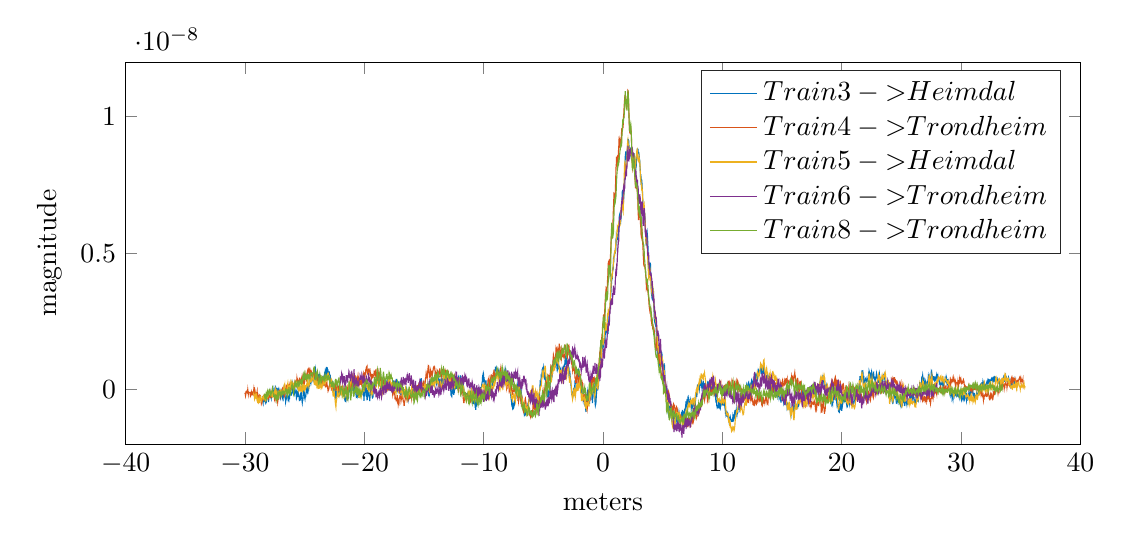
\begin{tikzpicture}

  \begin{axis}[%
    width=\textwidth,
    height=0.4\textwidth,
    at={(0\figurewidth,0\figureheight)},
    scale only axis,
    xmin=-40,
    xmax=40,
    xlabel={meters},
    ymin=-2e-09,
    ymax=1.2e-08,
    ylabel={magnitude},
    axis background/.style={fill=white},
    % title style={font=\bfseries},
    % title={influence lines for sensor 1},
    legend style={legend cell align=left,align=left,draw=white!15!black}
    ]
    \addplot [color=mycolor1,solid]
    table[row sep=crcr]{%
    -28.53908203125	-2.42432463976525e-10\\
    -28.518583984375	-3.23255849420965e-10\\
    -28.4980859375	-4.42343087844999e-10\\
    -28.477587890625	-4.88480902776024e-10\\
    -28.45708984375	-3.60310441102158e-10\\
    -28.436591796875	-3.96549475576617e-10\\
    -28.41609375	-4.05601785796435e-10\\
    -28.395595703125	-3.01178498671471e-10\\
    -28.37509765625	-3.29276214424073e-10\\
    -28.354599609375	-3.53914382054028e-10\\
    -28.3341015625	-2.94329300088123e-10\\
    -28.313603515625	-3.34436759961143e-10\\
    -28.29310546875	-4.69107766106467e-10\\
    -28.272607421875	-4.62579450742619e-10\\
    -28.252109375	-4.98854671956688e-10\\
    -28.231611328125	-4.75479960196443e-10\\
    -28.21111328125	-3.20446264658053e-10\\
    -28.190615234375	-3.58312570518101e-10\\
    -28.1701171875	-2.6667868901763e-10\\
    -28.149619140625	-2.287629187887e-10\\
    -28.12912109375	-2.35474923801234e-10\\
    -28.108623046875	-2.24605584523021e-10\\
    -28.088125	-2.27897694239274e-10\\
    -28.067626953125	-3.12585132409704e-10\\
    -28.04712890625	-3.57047025125366e-10\\
    -28.026630859375	-4.57212763583564e-10\\
    -28.0061328125	-3.66877212921925e-10\\
    -27.985634765625	-2.16965978828965e-10\\
    -27.96513671875	-1.95113556265998e-10\\
    -27.944638671875	-6.38877903963421e-11\\
    -27.924140625	-3.41374471925142e-11\\
    -27.903642578125	-1.2916136136789e-10\\
    -27.88314453125	-1.11644240463046e-10\\
    -27.862646484375	-1.46856112964341e-10\\
    -27.8421484375	-2.14085246063923e-10\\
    -27.821650390625	-2.63555849876305e-10\\
    -27.80115234375	-3.10581598027597e-10\\
    -27.780654296875	-2.03866523854126e-10\\
    -27.76015625	-1.524287292815e-10\\
    -27.739658203125	-9.28247326939465e-11\\
    -27.71916015625	-8.50442019209391e-11\\
    -27.698662109375	-1.88497671517331e-11\\
    -27.6781640625	2.27484533382019e-11\\
    -27.657666015625	5.66939984385784e-11\\
    -27.63716796875	-2.06620968117345e-11\\
    -27.616669921875	-9.82660644706859e-11\\
    -27.596171875	-1.05376026512635e-10\\
    -27.575673828125	-1.35619615444534e-10\\
    -27.55517578125	-9.01567144467863e-11\\
    -27.534677734375	-6.86490878601901e-11\\
    -27.5141796875	-1.16343445568424e-10\\
    -27.493681640625	4.39985123687983e-11\\
    -27.47318359375	4.39310949326402e-11\\
    -27.452685546875	1.08453591920635e-10\\
    -27.4321875	9.32509639604969e-11\\
    -27.411689453125	8.48885196639028e-11\\
    -27.39119140625	1.40375321941603e-11\\
    -27.370693359375	-9.9378820005732e-11\\
    -27.3501953125	-9.81019329716345e-11\\
    -27.329697265625	-7.7379306253939e-11\\
    -27.30919921875	-1.65584043500985e-10\\
    -27.288701171875	-5.10802693648461e-11\\
    -27.268203125	-8.9117735784694e-11\\
    -27.247705078125	-8.44785871702324e-12\\
    -27.22720703125	2.49969620863424e-11\\
    -27.206708984375	2.46710819336119e-11\\
    -27.1862109375	-7.48863762085572e-12\\
    -27.165712890625	2.30509274907517e-11\\
    -27.14521484375	-2.96480079615425e-11\\
    -27.124716796875	-1.22762481852331e-10\\
    -27.10421875	-1.12991889752861e-10\\
    -27.083720703125	-1.41190547239261e-10\\
    -27.06322265625	-2.29389173482235e-10\\
    -27.042724609375	-1.76467414095179e-10\\
    -27.0222265625	-2.3627090542664e-10\\
    -27.001728515625	-9.31022821648417e-11\\
    -26.98123046875	-1.04945065081801e-10\\
    -26.960732421875	-4.10694063493072e-11\\
    -26.940234375	-6.87349128785862e-11\\
    -26.919736328125	-1.23964485545686e-10\\
    -26.89923828125	-1.75486441477889e-10\\
    -26.878740234375	-2.68606143370957e-10\\
    -26.8582421875	-2.93758218302625e-10\\
    -26.837744140625	-3.29043058201038e-10\\
    -26.81724609375	-2.50229922070379e-10\\
    -26.796748046875	-2.91720995111193e-10\\
    -26.77625	-1.36748936579476e-10\\
    -26.755751953125	-1.0401772999358e-10\\
    -26.73525390625	-5.20136587361358e-12\\
    -26.714755859375	-8.28580857933807e-11\\
    -26.6942578125	3.25512384323039e-12\\
    -26.673759765625	-1.19572455729444e-10\\
    -26.65326171875	-1.72896256979302e-10\\
    -26.632763671875	-3.0861664601898e-10\\
    -26.612265625	-3.05296165756242e-10\\
    -26.591767578125	-4.46477117404942e-10\\
    -26.57126953125	-3.87285442528268e-10\\
    -26.550771484375	-3.79366032130347e-10\\
    -26.5302734375	-2.79281838178277e-10\\
    -26.509775390625	-2.51122482999767e-10\\
    -26.48927734375	-2.09629566262389e-10\\
    -26.468779296875	-1.92453734351367e-10\\
    -26.44828125	-1.44815322824779e-10\\
    -26.427783203125	-2.3704955916882e-10\\
    -26.40728515625	-2.99031009831917e-10\\
    -26.386787109375	-1.97075018802471e-10\\
    -26.3662890625	-3.46142414107179e-10\\
    -26.345791015625	-3.62585107282859e-10\\
    -26.32529296875	-3.88400269425861e-10\\
    -26.304794921875	-2.83266927762978e-10\\
    -26.284296875	-2.61776935143811e-10\\
    -26.263798828125	-2.84062493038057e-10\\
    -26.24330078125	-1.51260994854228e-10\\
    -26.222802734375	-1.81954876395575e-10\\
    -26.2023046875	-1.95070987756836e-10\\
    -26.181806640625	-1.96267201805321e-10\\
    -26.16130859375	-1.80816574557286e-10\\
    -26.140810546875	-1.97930056785899e-10\\
    -26.1203125	-2.03190976267253e-10\\
    -26.099814453125	-1.67674287174222e-10\\
    -26.07931640625	-1.12153896610044e-10\\
    -26.058818359375	-1.08749576087527e-10\\
    -26.0383203125	5.62087640518572e-11\\
    -26.017822265625	8.21587833128849e-12\\
    -25.99732421875	1.83017821603523e-10\\
    -25.976826171875	1.29202847193506e-10\\
    -25.956328125	1.23749555911484e-10\\
    -25.935830078125	-2.3632105080288e-12\\
    -25.91533203125	-1.68066315709562e-11\\
    -25.894833984375	-1.25581357996754e-10\\
    -25.8743359375	-2.85948148607479e-11\\
    -25.853837890625	-1.38917007814064e-10\\
    -25.83333984375	-9.72360575822185e-11\\
    -25.812841796875	-7.16999090185428e-11\\
    -25.79234375	-3.9544202502839e-11\\
    -25.771845703125	-9.02974505956738e-11\\
    -25.75134765625	-1.12143471670516e-10\\
    -25.730849609375	-9.57266765608488e-11\\
    -25.7103515625	-2.03159546279675e-10\\
    -25.689853515625	-1.38377594435741e-10\\
    -25.66935546875	-2.78500585704785e-10\\
    -25.648857421875	-2.34301425844046e-10\\
    -25.628359375	-1.30361558332022e-10\\
    -25.607861328125	-2.73110563969769e-10\\
    -25.58736328125	-1.51835358872657e-10\\
    -25.566865234375	-2.04791667314648e-10\\
    -25.5463671875	-2.19597418179874e-10\\
    -25.525869140625	-1.38315139615302e-10\\
    -25.50537109375	-2.05655921201357e-10\\
    -25.484873046875	-2.16344813737997e-10\\
    -25.464375	-2.58071778892159e-10\\
    -25.443876953125	-4.0255984440157e-10\\
    -25.42337890625	-3.96989147330398e-10\\
    -25.402880859375	-3.82198109572134e-10\\
    -25.3823828125	-3.64259326663304e-10\\
    -25.361884765625	-2.51108468325296e-10\\
    -25.34138671875	-2.87211354620859e-10\\
    -25.320888671875	-1.86566732315788e-10\\
    -25.300390625	-1.06551956521931e-10\\
    -25.279892578125	-1.15372283678584e-10\\
    -25.25939453125	-3.00156188334196e-10\\
    -25.238896484375	-3.17743950182121e-10\\
    -25.2183984375	-4.20514852268409e-10\\
    -25.197900390625	-4.87316857004543e-10\\
    -25.17740234375	-4.06437951334752e-10\\
    -25.156904296875	-4.00899076301748e-10\\
    -25.13640625	-3.0866181595622e-10\\
    -25.115908203125	-1.35575211842145e-10\\
    -25.09541015625	4.32948882767002e-13\\
    -25.074912109375	-1.41232428724987e-11\\
    -25.0544140625	-1.07518194991917e-10\\
    -25.033916015625	-9.24278032837129e-11\\
    -25.01341796875	-2.08025903372471e-10\\
    -24.992919921875	-3.06219314425481e-10\\
    -24.972421875	-3.48078778376712e-10\\
    -24.951923828125	-2.58031626423418e-10\\
    -24.93142578125	-2.56877378610011e-10\\
    -24.910927734375	-2.62997986742775e-10\\
    -24.8904296875	-1.72574947173134e-10\\
    -24.869931640625	-1.27988709753417e-11\\
    -24.84943359375	1.93033967441206e-11\\
    -24.828935546875	-4.15977311870775e-11\\
    -24.8084375	-4.27063579102865e-12\\
    -24.787939453125	-3.84896173075267e-11\\
    -24.76744140625	3.07383161915568e-11\\
    -24.746943359375	-4.33147236810481e-11\\
    -24.7264453125	2.93565102889779e-11\\
    -24.705947265625	-3.40794663708724e-11\\
    -24.68544921875	3.05880703999791e-11\\
    -24.664951171875	1.70821292016648e-11\\
    -24.644453125	1.22650044684207e-10\\
    -24.623955078125	1.27246821750176e-10\\
    -24.60345703125	2.10215991564352e-10\\
    -24.582958984375	1.86135077634439e-10\\
    -24.5624609375	2.84390735057775e-10\\
    -24.541962890625	2.98865614053442e-10\\
    -24.52146484375	3.79402697166947e-10\\
    -24.500966796875	3.19475616958402e-10\\
    -24.48046875	3.42288901178129e-10\\
    -24.459970703125	2.67083245100772e-10\\
    -24.43947265625	3.20311206503607e-10\\
    -24.418974609375	3.17040667962604e-10\\
    -24.3984765625	3.83547282467471e-10\\
    -24.377978515625	4.02705921673004e-10\\
    -24.35748046875	4.64789124873925e-10\\
    -24.336982421875	4.71498431401608e-10\\
    -24.316484375	4.14586195290773e-10\\
    -24.295986328125	4.77450769070853e-10\\
    -24.27548828125	3.65324756249261e-10\\
    -24.254990234375	4.02133142091454e-10\\
    -24.2344921875	4.1204871748625e-10\\
    -24.213994140625	4.21779611763754e-10\\
    -24.19349609375	3.64098598536646e-10\\
    -24.172998046875	5.17325064841423e-10\\
    -24.1525	4.73677052183486e-10\\
    -24.132001953125	7.04121437906612e-10\\
    -24.11150390625	6.23285727482992e-10\\
    -24.091005859375	7.27594645826054e-10\\
    -24.0705078125	6.50243684610334e-10\\
    -24.050009765625	5.41174081574631e-10\\
    -24.02951171875	4.9401621954105e-10\\
    -24.009013671875	5.14039109504764e-10\\
    -23.988515625	4.87665161509945e-10\\
    -23.968017578125	3.95927188264053e-10\\
    -23.94751953125	3.79155940912439e-10\\
    -23.927021484375	4.77438537004303e-10\\
    -23.9065234375	5.52821401289448e-10\\
    -23.886025390625	3.87606541241366e-10\\
    -23.86552734375	5.60562834933619e-10\\
    -23.845029296875	4.32717395947627e-10\\
    -23.82453125	5.22543199657409e-10\\
    -23.804033203125	3.53841414574437e-10\\
    -23.78353515625	4.25901987852324e-10\\
    -23.763037109375	4.84400665986875e-10\\
    -23.7425390625	3.79124859140587e-10\\
    -23.722041015625	4.94346291431105e-10\\
    -23.70154296875	4.10831016945326e-10\\
    -23.681044921875	4.65443657620662e-10\\
    -23.660546875	4.53518093675535e-10\\
    -23.640048828125	4.37721478732768e-10\\
    -23.61955078125	3.69252834769176e-10\\
    -23.599052734375	4.49855052777846e-10\\
    -23.5785546875	2.78653014200117e-10\\
    -23.558056640625	2.89226056091048e-10\\
    -23.53755859375	2.99073165099486e-10\\
    -23.517060546875	2.95973886984162e-10\\
    -23.4965625	1.89848890098662e-10\\
    -23.476064453125	3.22393829016736e-10\\
    -23.45556640625	1.6390186079679e-10\\
    -23.435068359375	3.46781531536905e-10\\
    -23.4145703125	2.97109348427208e-10\\
    -23.394072265625	4.3473131884735e-10\\
    -23.37357421875	4.36811025268644e-10\\
    -23.353076171875	5.02221949848493e-10\\
    -23.332578125	4.30284990163707e-10\\
    -23.312080078125	5.16642140048424e-10\\
    -23.29158203125	6.03562901486804e-10\\
    -23.271083984375	5.33276818744645e-10\\
    -23.2505859375	6.12466237226795e-10\\
    -23.230087890625	5.7021423334151e-10\\
    -23.20958984375	6.73509953407802e-10\\
    -23.189091796875	6.38490389066768e-10\\
    -23.16859375	8.28569706317133e-10\\
    -23.148095703125	7.14468570381893e-10\\
    -23.12759765625	7.3610772001961e-10\\
    -23.107099609375	8.12648211470292e-10\\
    -23.0866015625	5.46668172067143e-10\\
    -23.066103515625	7.48996333064468e-10\\
    -23.04560546875	6.16958554820236e-10\\
    -23.025107421875	4.72320867264757e-10\\
    -23.004609375	5.50268988312912e-10\\
    -22.984111328125	4.81519583469517e-10\\
    -22.96361328125	5.0664780060059e-10\\
    -22.943115234375	6.63823390003033e-10\\
    -22.9226171875	5.71676264648179e-10\\
    -22.902119140625	5.63680548421895e-10\\
    -22.88162109375	5.28296915197076e-10\\
    -22.861123046875	4.300138883988e-10\\
    -22.840625	4.48950385837297e-10\\
    -22.820126953125	3.49305773389595e-10\\
    -22.79962890625	1.70479639515498e-10\\
    -22.779130859375	9.42548802059219e-11\\
    -22.7586328125	2.20261678318734e-10\\
    -22.738134765625	2.22127314329253e-10\\
    -22.71763671875	2.9838535146622e-10\\
    -22.697138671875	2.91689685564066e-10\\
    -22.676640625	2.85575466960816e-10\\
    -22.656142578125	1.64701484149708e-10\\
    -22.63564453125	1.47143233885048e-10\\
    -22.615146484375	-1.97440618285175e-11\\
    -22.5946484375	-3.84909982664016e-11\\
    -22.574150390625	-1.29703421066267e-10\\
    -22.55365234375	-1.10985815914594e-10\\
    -22.533154296875	6.31440403845754e-12\\
    -22.51265625	1.9792603680271e-11\\
    -22.492158203125	4.88013821864418e-11\\
    -22.47166015625	1.88458165063384e-10\\
    -22.451162109375	8.35033482452694e-11\\
    -22.4306640625	-2.67603502328478e-11\\
    -22.410166015625	-3.69971422047308e-11\\
    -22.38966796875	-3.3645043524023e-10\\
    -22.369169921875	-2.54936475245048e-10\\
    -22.348671875	-3.91682261474449e-10\\
    -22.328173828125	-1.48769049328933e-10\\
    -22.30767578125	-2.57478205550678e-10\\
    -22.287177734375	-8.55854494800401e-11\\
    -22.2666796875	-9.43870131653846e-11\\
    -22.246181640625	1.7721832238179e-10\\
    -22.22568359375	-4.78497482071435e-12\\
    -22.205185546875	1.30290186519489e-10\\
    -22.1846875	1.40031881953166e-11\\
    -22.164189453125	-2.18220317945106e-11\\
    -22.14369140625	-1.24429679349178e-10\\
    -22.123193359375	-7.08600000385786e-11\\
    -22.1026953125	-2.45700763768097e-10\\
    -22.082197265625	-1.51126710005575e-10\\
    -22.06169921875	-1.11102631284205e-10\\
    -22.041201171875	-6.36336997601866e-11\\
    -22.020703125	-8.65607008156424e-11\\
    -22.000205078125	-7.05197127913619e-12\\
    -21.97970703125	-2.71831991310351e-11\\
    -21.959208984375	1.18838411121936e-10\\
    -21.9387109375	-1.93543721645697e-12\\
    -21.918212890625	4.18426529039133e-13\\
    -21.89771484375	1.18539759628936e-11\\
    -21.877216796875	-3.39975277374191e-11\\
    -21.85671875	-6.42082737643145e-12\\
    -21.836220703125	-5.60710673662991e-11\\
    -21.81572265625	2.56143442158228e-11\\
    -21.795224609375	-8.8617106018743e-12\\
    -21.7747265625	2.73540862109055e-11\\
    -21.754228515625	-1.33733891568678e-10\\
    -21.73373046875	2.31406250335787e-11\\
    -21.713232421875	-1.13872840319072e-10\\
    -21.692734375	-1.45882254666255e-10\\
    -21.672236328125	-2.37221205807634e-10\\
    -21.65173828125	-2.46949888844117e-10\\
    -21.631240234375	-3.99827015146344e-10\\
    -21.6107421875	-4.16710408241621e-10\\
    -21.590244140625	-3.99329853373332e-10\\
    -21.56974609375	-3.69606586268905e-10\\
    -21.549248046875	-3.95690693084701e-10\\
    -21.52875	-2.81529628416859e-10\\
    -21.508251953125	-2.06364749462386e-10\\
    -21.48775390625	-2.72950576274304e-10\\
    -21.467255859375	-1.0133729165997e-10\\
    -21.4467578125	-2.4532548933499e-10\\
    -21.426259765625	-2.30951034449219e-10\\
    -21.40576171875	-4.05956504144463e-10\\
    -21.385263671875	-1.8160551403991e-10\\
    -21.364765625	-3.26851066999353e-10\\
    -21.344267578125	-2.25615726472064e-10\\
    -21.32376953125	-2.46497333711807e-10\\
    -21.303271484375	-2.47581214864832e-11\\
    -21.2827734375	-1.77256202864696e-11\\
    -21.262275390625	-5.5252207516645e-12\\
    -21.24177734375	1.64381631844488e-10\\
    -21.221279296875	4.73458962461572e-11\\
    -21.20078125	1.0084927471415e-10\\
    -21.180283203125	3.0834371802497e-11\\
    -21.15978515625	1.36111397236516e-10\\
    -21.139287109375	8.62229307540838e-11\\
    -21.1187890625	1.62597501883518e-10\\
    -21.098291015625	1.57994563287646e-10\\
    -21.07779296875	2.78600292576321e-10\\
    -21.057294921875	2.49741150349261e-10\\
    -21.036796875	2.15910078582386e-10\\
    -21.016298828125	1.74161775516034e-10\\
    -20.99580078125	2.70167190133558e-10\\
    -20.975302734375	-2.75049031140946e-11\\
    -20.9548046875	2.04650766786522e-10\\
    -20.934306640625	-4.63535346656993e-11\\
    -20.91380859375	1.00719544020583e-11\\
    -20.893310546875	-4.65667976906526e-11\\
    -20.8728125	7.31631781646805e-12\\
    -20.852314453125	1.95497258342494e-11\\
    -20.83181640625	1.51850182766983e-11\\
    -20.811318359375	8.280709701507e-11\\
    -20.7908203125	-1.06322324664081e-10\\
    -20.770322265625	9.60903278692484e-11\\
    -20.74982421875	-8.76088440930094e-11\\
    -20.729326171875	-2.10449007023787e-11\\
    -20.708828125	-1.1688976030507e-10\\
    -20.688330078125	-7.00855309079967e-11\\
    -20.66783203125	-2.50973187592523e-10\\
    -20.647333984375	-2.31005913244209e-10\\
    -20.6268359375	-1.98790439127558e-10\\
    -20.606337890625	-3.00830235946201e-10\\
    -20.58583984375	-5.90165175106527e-11\\
    -20.565341796875	-1.99657734238226e-10\\
    -20.54484375	-1.55523231865961e-10\\
    -20.524345703125	-1.1688773725939e-10\\
    -20.50384765625	-2.2794212020159e-10\\
    -20.483349609375	-7.88618669567596e-11\\
    -20.4628515625	-2.92678659483946e-10\\
    -20.442353515625	-1.56024095635845e-10\\
    -20.42185546875	-2.2506609045754e-10\\
    -20.401357421875	-1.91036081585041e-10\\
    -20.380859375	-1.63554952033701e-10\\
    -20.360361328125	-6.43655508896391e-11\\
    -20.33986328125	-1.18982628015657e-10\\
    -20.319365234375	-7.91582277975989e-11\\
    -20.2988671875	-7.1207645585137e-11\\
    -20.278369140625	-8.05252444712304e-11\\
    -20.25787109375	-2.54767863240876e-10\\
    -20.237373046875	-1.83460048708829e-10\\
    -20.216875	-1.14408533489765e-10\\
    -20.196376953125	-2.09621969887989e-10\\
    -20.17587890625	-1.10893940106256e-10\\
    -20.155380859375	-5.1892030093861e-11\\
    -20.1348828125	8.62680934588685e-11\\
    -20.114384765625	-3.85363558431994e-11\\
    -20.09388671875	-6.44463130463606e-11\\
    -20.073388671875	-1.00351373522834e-10\\
    -20.052890625	-1.03999049008291e-10\\
    -20.032392578125	-4.17462336725826e-10\\
    -20.01189453125	-9.59500262212268e-11\\
    -19.991396484375	-2.31943863828125e-10\\
    -19.9708984375	-2.22620754456379e-10\\
    -19.950400390625	-1.03377266463775e-10\\
    -19.92990234375	5.48104375081192e-12\\
    -19.909404296875	-9.1403190935284e-11\\
    -19.88890625	2.33236931396001e-10\\
    -19.868408203125	-1.00419246809165e-10\\
    -19.84791015625	1.45687190171597e-10\\
    -19.827412109375	-2.69325210756052e-10\\
    -19.8069140625	-1.43833296678376e-10\\
    -19.786416015625	-2.73388370087392e-10\\
    -19.76591796875	-2.33331034930794e-10\\
    -19.745419921875	-3.89684798950993e-10\\
    -19.724921875	-1.24985615550201e-10\\
    -19.704423828125	-1.53751288923747e-10\\
    -19.68392578125	-3.54250262700705e-11\\
    -19.663427734375	-5.94565417528477e-11\\
    -19.6429296875	1.17420004482983e-11\\
    -19.622431640625	-1.96008415275973e-10\\
    -19.60193359375	-2.12995834607837e-10\\
    -19.581435546875	-2.75647653497749e-10\\
    -19.5609375	-2.90439821654287e-10\\
    -19.540439453125	-4.24093599274614e-10\\
    -19.51994140625	-2.25181621481276e-10\\
    -19.499443359375	-2.12673852104628e-10\\
    -19.4789453125	-9.51961415829377e-11\\
    -19.458447265625	-5.76571873868302e-11\\
    -19.43794921875	6.01357110796887e-11\\
    -19.417451171875	4.99582669612489e-11\\
    -19.396953125	-5.54325781792318e-11\\
    -19.376455078125	-6.10443441161957e-11\\
    -19.35595703125	-1.82072567482592e-10\\
    -19.335458984375	-2.4677468230231e-10\\
    -19.3149609375	-3.04851322100341e-10\\
    -19.294462890625	-2.96975151057571e-10\\
    -19.27396484375	-2.58439288923987e-10\\
    -19.253466796875	-3.80706603145059e-11\\
    -19.23296875	-1.09271229191184e-10\\
    -19.212470703125	8.46466784195196e-11\\
    -19.19197265625	1.09901394593307e-10\\
    -19.171474609375	2.11238813406386e-10\\
    -19.1509765625	1.01605070727722e-10\\
    -19.130478515625	2.28418973074007e-10\\
    -19.10998046875	1.57812481362105e-10\\
    -19.089482421875	8.40144383938498e-11\\
    -19.068984375	6.79194027543881e-11\\
    -19.048486328125	1.19028777070408e-10\\
    -19.02798828125	1.16497391111581e-10\\
    -19.007490234375	1.27356966312087e-10\\
    -18.9869921875	1.79199377375629e-10\\
    -18.966494140625	4.33316569008867e-10\\
    -18.94599609375	3.81659053974682e-10\\
    -18.925498046875	4.43335325803948e-10\\
    -18.905	5.04040205930144e-10\\
    -18.884501953125	4.06841255355346e-10\\
    -18.86400390625	3.41222508116328e-10\\
    -18.843505859375	2.69741776214776e-10\\
    -18.8230078125	2.45537061961895e-10\\
    -18.802509765625	1.41888514896468e-10\\
    -18.78201171875	2.63733076660142e-10\\
    -18.761513671875	1.6540225761644e-10\\
    -18.741015625	1.86981937401375e-10\\
    -18.720517578125	4.09363732554522e-10\\
    -18.70001953125	2.44411795183896e-10\\
    -18.679521484375	3.77967396598307e-10\\
    -18.6590234375	1.76437651971343e-10\\
    -18.638525390625	1.55393450327141e-10\\
    -18.61802734375	4.22679387453643e-11\\
    -18.597529296875	5.86055939983596e-11\\
    -18.57703125	-9.14995414368648e-11\\
    -18.556533203125	-8.27279690580506e-11\\
    -18.53603515625	1.23414213374265e-11\\
    -18.515537109375	1.59643598446146e-10\\
    -18.4950390625	8.73919600029787e-11\\
    -18.474541015625	1.99135245708017e-10\\
    -18.45404296875	-1.66738289838114e-11\\
    -18.433544921875	1.2790226953366e-10\\
    -18.413046875	4.42350601496876e-11\\
    -18.392548828125	7.96419189022545e-11\\
    -18.37205078125	1.21154363928816e-10\\
    -18.351552734375	1.586535165811e-10\\
    -18.3310546875	2.78028122530492e-10\\
    -18.310556640625	3.12820597388293e-10\\
    -18.29005859375	3.11659761274096e-10\\
    -18.269560546875	3.39205753681696e-10\\
    -18.2490625	3.01580515699639e-10\\
    -18.228564453125	1.8079936355973e-10\\
    -18.20806640625	1.93249739082551e-10\\
    -18.187568359375	7.77075875459527e-11\\
    -18.1670703125	2.03086246287135e-10\\
    -18.146572265625	7.92291613715199e-11\\
    -18.12607421875	2.32773508527994e-10\\
    -18.105576171875	3.65065219977523e-10\\
    -18.085078125	6.17033129978897e-11\\
    -18.064580078125	2.95030412429936e-10\\
    -18.04408203125	1.86001135501412e-10\\
    -18.023583984375	1.92826737210053e-10\\
    -18.0030859375	6.45490712608484e-11\\
    -17.982587890625	4.07397369489149e-11\\
    -17.96208984375	2.09151336365801e-10\\
    -17.941591796875	3.71757588130793e-11\\
    -17.92109375	1.60879334731151e-10\\
    -17.900595703125	2.77388871863996e-10\\
    -17.88009765625	2.3548581439777e-10\\
    -17.859599609375	2.43865449359166e-10\\
    -17.8391015625	2.54574612812065e-10\\
    -17.818603515625	1.87418839064782e-10\\
    -17.79810546875	1.97494633975179e-10\\
    -17.777607421875	1.63807147513526e-11\\
    -17.757109375	1.51307972968712e-10\\
    -17.736611328125	1.141960604899e-10\\
    -17.71611328125	5.59464552537092e-11\\
    -17.695615234375	2.19530161372737e-10\\
    -17.6751171875	1.49064249002282e-10\\
    -17.654619140625	1.82851652210347e-10\\
    -17.63412109375	1.70996788896021e-10\\
    -17.613623046875	2.39990745303902e-10\\
    -17.593125	2.2295051945315e-10\\
    -17.572626953125	2.21813026332167e-10\\
    -17.55212890625	8.84495382750591e-11\\
    -17.531630859375	3.36803845868021e-10\\
    -17.5111328125	5.25876600084127e-11\\
    -17.490634765625	1.95418467741627e-10\\
    -17.47013671875	1.59348517207627e-10\\
    -17.449638671875	1.97176869782748e-10\\
    -17.429140625	1.62973679040933e-10\\
    -17.408642578125	2.71435322062757e-10\\
    -17.38814453125	1.38904895668947e-10\\
    -17.367646484375	3.13773355008875e-10\\
    -17.3471484375	4.26630747597984e-11\\
    -17.326650390625	3.88283840141377e-10\\
    -17.30615234375	2.51194325849686e-11\\
    -17.285654296875	1.49286582483876e-10\\
    -17.26515625	-3.70541889745352e-11\\
    -17.244658203125	9.93819504876695e-11\\
    -17.22416015625	3.76791827375121e-11\\
    -17.203662109375	1.72952578053722e-10\\
    -17.1831640625	2.37942053789793e-10\\
    -17.162666015625	2.31264731986157e-10\\
    -17.14216796875	2.64792388291773e-10\\
    -17.121669921875	2.7368604978948e-10\\
    -17.101171875	2.0222999468327e-10\\
    -17.080673828125	2.18788276136535e-10\\
    -17.06017578125	4.28936702044988e-11\\
    -17.039677734375	1.13928728670705e-10\\
    -17.0191796875	-5.35134274501428e-11\\
    -16.998681640625	-4.03636150263938e-11\\
    -16.97818359375	-1.96901562530478e-10\\
    -16.957685546875	-7.37504128023902e-11\\
    -16.9371875	-2.2017473390884e-10\\
    -16.916689453125	-8.73473737314942e-11\\
    -16.89619140625	-6.91581684665028e-11\\
    -16.875693359375	-7.88357369923045e-11\\
    -16.8551953125	7.85366145853017e-11\\
    -16.834697265625	1.34593668139251e-11\\
    -16.81419921875	9.54647735854294e-11\\
    -16.793701171875	-3.67232822194374e-11\\
    -16.773203125	-2.99704981068041e-11\\
    -16.752705078125	-1.2624923345888e-10\\
    -16.73220703125	-8.69811989016394e-11\\
    -16.711708984375	-1.70090777067916e-10\\
    -16.6912109375	-5.15376821154804e-11\\
    -16.670712890625	-6.85470456941074e-11\\
    -16.65021484375	8.66903673399217e-12\\
    -16.629716796875	-1.28552849140222e-10\\
    -16.60921875	-2.02718418765374e-10\\
    -16.588720703125	-2.05272642440426e-10\\
    -16.56822265625	-2.52041115948345e-10\\
    -16.547724609375	-2.21056955730837e-10\\
    -16.5272265625	-2.020289899641e-10\\
    -16.506728515625	-1.23594435284019e-10\\
    -16.48623046875	-8.35624399709951e-11\\
    -16.465732421875	-7.33465951958552e-11\\
    -16.445234375	3.22199702648632e-12\\
    -16.424736328125	-6.01868584048012e-11\\
    -16.40423828125	-9.1890823537471e-11\\
    -16.383740234375	-1.67330123583214e-10\\
    -16.3632421875	-2.86747297184345e-10\\
    -16.342744140625	-2.9485577144772e-10\\
    -16.32224609375	-3.74847539222641e-10\\
    -16.301748046875	-3.13009665274873e-10\\
    -16.28125	-3.82952178556269e-10\\
    -16.260751953125	-1.96527055168601e-10\\
    -16.24025390625	-2.26574088651537e-10\\
    -16.219755859375	-1.61359672392329e-10\\
    -16.1992578125	-4.84374843663153e-11\\
    -16.178759765625	-1.5384702026522e-10\\
    -16.15826171875	-4.26211074837964e-12\\
    -16.137763671875	-2.3822969003827e-10\\
    -16.117265625	-7.20500609238373e-11\\
    -16.096767578125	-1.45251813875802e-10\\
    -16.07626953125	-9.55558593982492e-11\\
    -16.055771484375	-1.86078768339882e-10\\
    -16.0352734375	-8.92366889800484e-11\\
    -16.014775390625	-6.79973526369702e-11\\
    -15.99427734375	8.60509085756035e-11\\
    -15.973779296875	-1.25291792644761e-10\\
    -15.95328125	1.14688201356929e-10\\
    -15.932783203125	-2.7122489724124e-11\\
    -15.91228515625	-8.73400365315535e-12\\
    -15.891787109375	-1.19386463714485e-10\\
    -15.8712890625	-1.80644783882297e-10\\
    -15.850791015625	-2.1124792229543e-10\\
    -15.83029296875	-1.7125151535906e-10\\
    -15.809794921875	-2.3745956437128e-10\\
    -15.789296875	-1.76387078956959e-10\\
    -15.768798828125	-2.1707548759208e-10\\
    -15.74830078125	-6.28357087807495e-11\\
    -15.727802734375	-5.72089047293382e-11\\
    -15.7073046875	-3.92665443080929e-11\\
    -15.686806640625	1.46575439216156e-11\\
    -15.66630859375	-8.96680973176235e-11\\
    -15.645810546875	-1.01494568494214e-10\\
    -15.6253125	-1.55324239231308e-10\\
    -15.604814453125	-1.86877072424451e-10\\
    -15.58431640625	-1.25828868841534e-10\\
    -15.563818359375	-2.39814401126928e-10\\
    -15.5433203125	-1.06132729247022e-10\\
    -15.522822265625	-1.13527760332474e-10\\
    -15.50232421875	8.31018072673445e-11\\
    -15.481826171875	1.24562537214656e-10\\
    -15.461328125	1.11242626874162e-10\\
    -15.440830078125	2.14260618733604e-10\\
    -15.42033203125	-2.70800923943093e-11\\
    -15.399833984375	-2.74817107793722e-11\\
    -15.3793359375	-2.08500759769855e-11\\
    -15.358837890625	-1.03386520400296e-10\\
    -15.33833984375	-5.24803939313347e-11\\
    -15.317841796875	6.58106562973832e-11\\
    -15.29734375	5.16407618325581e-11\\
    -15.276845703125	3.90048710058337e-10\\
    -15.25634765625	2.83461899266419e-10\\
    -15.235849609375	4.12876075651724e-10\\
    -15.2153515625	3.38671235983093e-10\\
    -15.194853515625	2.3093595827922e-10\\
    -15.17435546875	2.02050651202068e-10\\
    -15.153857421875	1.31412096227512e-10\\
    -15.133359375	-3.68882077833282e-11\\
    -15.112861328125	-1.67045303295517e-11\\
    -15.09236328125	-2.4200908520411e-11\\
    -15.071865234375	6.80052935648525e-11\\
    -15.0513671875	1.71801272021067e-10\\
    -15.030869140625	9.55479987631775e-11\\
    -15.01037109375	2.88294824451821e-10\\
    -14.989873046875	9.57096354476404e-11\\
    -14.969375	2.12096232615858e-10\\
    -14.948876953125	5.51479832545931e-11\\
    -14.92837890625	9.31824073367473e-11\\
    -14.907880859375	-4.9428101364425e-11\\
    -14.8873828125	1.21775329442717e-12\\
    -14.866884765625	-1.04274661296518e-10\\
    -14.84638671875	1.67301123819817e-10\\
    -14.825888671875	-2.40281807586676e-10\\
    -14.805390625	1.69707497331674e-10\\
    -14.784892578125	2.80033890010606e-11\\
    -14.76439453125	2.01854764190797e-10\\
    -14.743896484375	-7.3715219819409e-12\\
    -14.7233984375	1.01293891639192e-10\\
    -14.702900390625	-4.43198222300177e-11\\
    -14.68240234375	-6.87620600423429e-11\\
    -14.661904296875	-8.12769588493538e-11\\
    -14.64140625	-1.40303294054012e-10\\
    -14.620908203125	-1.91374376955111e-10\\
    -14.60041015625	-1.73445479427781e-10\\
    -14.579912109375	-2.4363022577908e-10\\
    -14.5594140625	-6.59493748783198e-11\\
    -14.538916015625	-1.34244486521273e-10\\
    -14.51841796875	-4.65781399213834e-11\\
    -14.497919921875	4.64501108971846e-11\\
    -14.477421875	1.31895454030383e-10\\
    -14.456923828125	1.33745373811579e-11\\
    -14.43642578125	2.33555114350244e-10\\
    -14.415927734375	1.09575091062643e-10\\
    -14.3954296875	7.91056459628107e-11\\
    -14.374931640625	1.17446217522732e-10\\
    -14.35443359375	2.4352536959034e-11\\
    -14.333935546875	1.28873033638316e-10\\
    -14.3134375	1.97737398692823e-11\\
    -14.292939453125	1.96207510726421e-10\\
    -14.27244140625	2.25786437890625e-10\\
    -14.251943359375	3.58212157163728e-10\\
    -14.2314453125	3.05033922931177e-10\\
    -14.210947265625	4.08046370786947e-10\\
    -14.19044921875	2.81742695130593e-10\\
    -14.169951171875	1.93340958397986e-10\\
    -14.149453125	2.26909662505337e-10\\
    -14.128955078125	2.66870182007259e-10\\
    -14.10845703125	3.30274921082738e-10\\
    -14.087958984375	3.8596092247659e-10\\
    -14.0674609375	3.88704905491872e-10\\
    -14.046962890625	5.16689933086824e-10\\
    -14.02646484375	4.64708540064523e-10\\
    -14.005966796875	4.65892614180554e-10\\
    -13.98546875	3.61696799095479e-10\\
    -13.964970703125	2.91035287941874e-10\\
    -13.94447265625	1.41763258349337e-10\\
    -13.923974609375	2.58747820509965e-10\\
    -13.9034765625	2.31432634873767e-10\\
    -13.882978515625	2.74927189344053e-10\\
    -13.86248046875	2.76699956301161e-10\\
    -13.841982421875	3.76200835047451e-10\\
    -13.821484375	4.20075483405605e-10\\
    -13.800986328125	4.21705431765621e-10\\
    -13.78048828125	4.36716934459625e-10\\
    -13.759990234375	3.49042736887801e-10\\
    -13.7394921875	2.06938228703285e-10\\
    -13.718994140625	1.4916081396628e-10\\
    -13.69849609375	1.14695584637434e-10\\
    -13.677998046875	2.24544893597766e-10\\
    -13.6575	1.62489335086133e-10\\
    -13.637001953125	2.39739529990643e-10\\
    -13.61650390625	3.10087665659285e-10\\
    -13.596005859375	3.44048597031945e-10\\
    -13.5755078125	3.29048417314687e-10\\
    -13.555009765625	3.66339803637339e-10\\
    -13.53451171875	2.4274780458662e-10\\
    -13.514013671875	2.38629162465296e-10\\
    -13.493515625	1.19013106352209e-10\\
    -13.473017578125	3.281096913598e-10\\
    -13.45251953125	9.55049634721267e-11\\
    -13.432021484375	4.05295011460204e-10\\
    -13.4115234375	1.84348766807902e-10\\
    -13.391025390625	4.10861731905258e-10\\
    -13.37052734375	3.91844458204634e-10\\
    -13.350029296875	3.54800972491962e-10\\
    -13.32953125	5.30488953147869e-10\\
    -13.309033203125	5.15003028372305e-10\\
    -13.28853515625	5.50034230657394e-10\\
    -13.268037109375	5.48728303165661e-10\\
    -13.2475390625	5.44650544077051e-10\\
    -13.227041015625	3.59567476513614e-10\\
    -13.20654296875	4.94678761308437e-10\\
    -13.186044921875	3.37887001780843e-10\\
    -13.165546875	4.60581180848863e-10\\
    -13.145048828125	4.60368056269431e-10\\
    -13.12455078125	4.56668626582289e-10\\
    -13.104052734375	4.2254206034142e-10\\
    -13.0835546875	5.40028609318613e-10\\
    -13.063056640625	5.92046867389735e-10\\
    -13.04255859375	5.31374422784674e-10\\
    -13.022060546875	5.80375684555827e-10\\
    -13.0015625	4.98241617146563e-10\\
    -12.981064453125	3.03940640406569e-10\\
    -12.96056640625	3.2614127452474e-10\\
    -12.940068359375	2.139159627646e-10\\
    -12.9195703125	2.80062706962013e-10\\
    -12.899072265625	1.23367197619977e-10\\
    -12.87857421875	2.27654311027882e-10\\
    -12.858076171875	1.96324311066269e-10\\
    -12.837578125	2.3614790697122e-10\\
    -12.817080078125	1.29594750829456e-10\\
    -12.79658203125	1.84660061036398e-10\\
    -12.776083984375	-2.14800364266949e-11\\
    -12.7555859375	-4.98068071021046e-11\\
    -12.735087890625	-1.99027975086324e-10\\
    -12.71458984375	-2.21857255374268e-10\\
    -12.694091796875	-2.34845501792787e-10\\
    -12.67359375	-2.53033928722428e-10\\
    -12.653095703125	-1.14766148778949e-10\\
    -12.63259765625	-9.6112995679778e-12\\
    -12.612099609375	-1.43290819806899e-11\\
    -12.5916015625	4.57331593331596e-11\\
    -12.571103515625	6.58868120607045e-11\\
    -12.55060546875	-5.98987801365382e-11\\
    -12.530107421875	-3.29135859863301e-11\\
    -12.509609375	-1.97512601827556e-10\\
    -12.489111328125	7.66687308843002e-11\\
    -12.46861328125	-1.29317593531553e-10\\
    -12.448115234375	1.56954815245455e-11\\
    -12.4276171875	9.33235372949705e-12\\
    -12.407119140625	3.72534049831376e-11\\
    -12.38662109375	1.2051521787138e-10\\
    -12.366123046875	2.1319552123109e-10\\
    -12.345625	1.6829060023272e-10\\
    -12.325126953125	3.3618040891371e-10\\
    -12.30462890625	2.79924072277572e-11\\
    -12.284130859375	2.91382488935396e-10\\
    -12.2636328125	3.00442578620239e-11\\
    -12.243134765625	8.7507984099066e-11\\
    -12.22263671875	9.21923886562605e-11\\
    -12.202138671875	3.52733452463922e-10\\
    -12.181640625	2.93168439570136e-10\\
    -12.161142578125	4.19010536918695e-10\\
    -12.14064453125	4.18402303462943e-10\\
    -12.120146484375	4.6608614605424e-10\\
    -12.0996484375	4.37560608166415e-10\\
    -12.079150390625	3.52080460113341e-10\\
    -12.05865234375	3.78117430129254e-10\\
    -12.038154296875	3.36821581302571e-10\\
    -12.01765625	3.74256986725704e-10\\
    -11.997158203125	4.13150614288536e-10\\
    -11.97666015625	3.42502671681764e-10\\
    -11.956162109375	5.18233890550485e-10\\
    -11.9356640625	3.50686539313521e-10\\
    -11.915166015625	4.86521423112054e-10\\
    -11.89466796875	3.94566872413698e-10\\
    -11.874169921875	2.36532422675704e-10\\
    -11.853671875	2.78378420653987e-10\\
    -11.833173828125	1.8346623795343e-10\\
    -11.81267578125	1.90627560359867e-10\\
    -11.792177734375	2.33424233828694e-10\\
    -11.7716796875	2.96114008839406e-10\\
    -11.751181640625	2.2957076007057e-10\\
    -11.73068359375	2.1124647870246e-10\\
    -11.710185546875	4.62989678492789e-11\\
    -11.6896875	1.20879271823741e-10\\
    -11.669189453125	2.34645678241947e-11\\
    -11.64869140625	-1.13708371840709e-11\\
    -11.628193359375	-6.76581104206927e-11\\
    -11.6076953125	-1.82080120264111e-10\\
    -11.587197265625	-2.60661005822582e-10\\
    -11.56669921875	-1.97703607500867e-10\\
    -11.546201171875	-3.65684455112817e-10\\
    -11.525703125	-2.00014751180085e-10\\
    -11.505205078125	-3.3361459801061e-10\\
    -11.48470703125	-2.65714924063797e-10\\
    -11.464208984375	-2.62015497372803e-10\\
    -11.4437109375	-1.51099955774915e-10\\
    -11.423212890625	-1.49256950022176e-10\\
    -11.40271484375	-2.13089203062343e-10\\
    -11.382216796875	-2.51243626996487e-10\\
    -11.36171875	-2.77796470646657e-10\\
    -11.341220703125	-2.53282679943977e-10\\
    -11.32072265625	-2.02752696168227e-10\\
    -11.300224609375	-3.62571869457964e-10\\
    -11.2797265625	-1.88790429203968e-10\\
    -11.259228515625	-3.01050881769802e-10\\
    -11.23873046875	-1.92001290672959e-10\\
    -11.218232421875	-1.13364961178314e-10\\
    -11.197734375	-1.20005449097742e-10\\
    -11.177236328125	-1.98406440543712e-10\\
    -11.15673828125	-1.19777036383493e-10\\
    -11.136240234375	-2.72385309697537e-10\\
    -11.1157421875	-3.55788225724785e-10\\
    -11.095244140625	-2.31621969325114e-10\\
    -11.07474609375	-2.41255051263184e-10\\
    -11.054248046875	-1.82076830630806e-10\\
    -11.03375	-7.8125805194209e-11\\
    -11.013251953125	-8.23155962803758e-11\\
    -10.99275390625	-3.63407641701626e-11\\
    -10.972255859375	-2.0637049674581e-10\\
    -10.9517578125	-1.25451528879529e-10\\
    -10.931259765625	-3.41776071327802e-10\\
    -10.91076171875	-2.90767686167395e-10\\
    -10.890263671875	-5.25942623210229e-10\\
    -10.869765625	-3.62043851349883e-10\\
    -10.849267578125	-3.22940852434604e-10\\
    -10.82876953125	-3.89082921217472e-10\\
    -10.808271484375	-2.94274395609548e-10\\
    -10.7877734375	-3.08002461310815e-10\\
    -10.767275390625	-3.44803847157703e-10\\
    -10.74677734375	-4.45580132668905e-10\\
    -10.726279296875	-3.86149519427841e-10\\
    -10.70578125	-6.6874724404819e-10\\
    -10.685283203125	-5.40304556916708e-10\\
    -10.66478515625	-7.42073648720238e-10\\
    -10.644287109375	-5.53477609131018e-10\\
    -10.6237890625	-6.27530907935807e-10\\
    -10.603291015625	-4.79058224000323e-10\\
    -10.58279296875	-4.83154322814849e-10\\
    -10.562294921875	-4.06015181046202e-10\\
    -10.541796875	-4.21520457560244e-10\\
    -10.521298828125	-4.4137568546861e-10\\
    -10.50080078125	-4.01132969283733e-10\\
    -10.480302734375	-4.39709483072748e-10\\
    -10.4598046875	-4.77204410699158e-10\\
    -10.439306640625	-3.46719478763832e-10\\
    -10.41880859375	-4.33460405662788e-10\\
    -10.398310546875	-2.55590163948186e-10\\
    -10.3778125	-2.81706114820694e-10\\
    -10.357314453125	-8.0094006336858e-11\\
    -10.33681640625	-8.89403421157544e-11\\
    -10.316318359375	-2.59035878162795e-11\\
    -10.2958203125	4.06417839155571e-12\\
    -10.275322265625	8.93204900202255e-11\\
    -10.25482421875	-2.75949376367034e-11\\
    -10.234326171875	6.65275076825998e-11\\
    -10.213828125	7.54289092650365e-11\\
    -10.193330078125	7.66598082408017e-11\\
    -10.17283203125	1.46605394610115e-10\\
    -10.152333984375	2.01221033250913e-10\\
    -10.1318359375	2.61772356876934e-10\\
    -10.111337890625	3.01609722901266e-10\\
    -10.09083984375	4.91056838180225e-10\\
    -10.070341796875	4.81695332487173e-10\\
    -10.04984375	5.41648613636899e-10\\
    -10.029345703125	4.3896285411223e-10\\
    -10.00884765625	4.85582890141612e-10\\
    -9.988349609375	2.70813734499347e-10\\
    -9.9678515625	3.94710522748566e-10\\
    -9.947353515625	1.61183873616087e-10\\
    -9.92685546875	2.56502983762653e-10\\
    -9.906357421875	1.75821509635299e-10\\
    -9.885859375	3.37941607559918e-10\\
    -9.865361328125	2.41580648810274e-10\\
    -9.84486328125	3.36152012262638e-10\\
    -9.824365234375	1.81385329219389e-10\\
    -9.8038671875	3.34768909998145e-10\\
    -9.783369140625	5.67223990902792e-11\\
    -9.76287109375	1.83312586748151e-10\\
    -9.742373046875	6.07127066042673e-11\\
    -9.721875	2.52661497099852e-13\\
    -9.701376953125	-7.08088274362757e-11\\
    -9.68087890625	-9.60490354774842e-11\\
    -9.660380859375	-3.26792964850382e-10\\
    -9.6398828125	-2.25455683934982e-10\\
    -9.619384765625	-3.00370356108669e-10\\
    -9.59888671875	-2.80331895628238e-10\\
    -9.578388671875	-1.89215111132175e-10\\
    -9.557890625	-2.41197557781325e-10\\
    -9.537392578125	-2.22761922391398e-10\\
    -9.51689453125	-1.54120254605e-10\\
    -9.496396484375	-1.78975942836991e-10\\
    -9.4758984375	-7.63413353016928e-11\\
    -9.455400390625	-1.48255088847727e-10\\
    -9.43490234375	-3.82733991070736e-12\\
    -9.414404296875	-1.91975242296469e-11\\
    -9.39390625	8.26037691112198e-11\\
    -9.373408203125	7.10768346858517e-11\\
    -9.35291015625	6.81665353220682e-11\\
    -9.332412109375	1.02059546849435e-10\\
    -9.3119140625	1.23496487267082e-10\\
    -9.291416015625	2.07181223541169e-10\\
    -9.27091796875	1.32243708336111e-10\\
    -9.250419921875	2.9298185764756e-10\\
    -9.229921875	2.64685299571668e-10\\
    -9.209423828125	3.76444680732795e-10\\
    -9.18892578125	3.27002838439621e-10\\
    -9.168427734375	5.18000198436391e-10\\
    -9.1479296875	4.5014325463858e-10\\
    -9.127431640625	5.37128808122639e-10\\
    -9.10693359375	5.97586581250411e-10\\
    -9.086435546875	5.96955015926023e-10\\
    -9.0659375	5.58085976413435e-10\\
    -9.045439453125	7.47750219605188e-10\\
    -9.02494140625	6.753595264734e-10\\
    -9.004443359375	8.35478316956965e-10\\
    -8.9839453125	7.2527294311579e-10\\
    -8.963447265625	7.35574802457947e-10\\
    -8.94294921875	7.8137040771362e-10\\
    -8.922451171875	7.22767715179822e-10\\
    -8.901953125	6.54898527513316e-10\\
    -8.881455078125	6.7091166581707e-10\\
    -8.86095703125	6.33615856939863e-10\\
    -8.840458984375	6.27684298925746e-10\\
    -8.8199609375	6.04700236229306e-10\\
    -8.799462890625	6.97123001946832e-10\\
    -8.77896484375	5.47317745840105e-10\\
    -8.758466796875	6.65476957057564e-10\\
    -8.73796875	6.23493528732568e-10\\
    -8.717470703125	5.97033641694532e-10\\
    -8.69697265625	6.25061210658088e-10\\
    -8.676474609375	5.25849206396728e-10\\
    -8.6559765625	4.31835075410533e-10\\
    -8.635478515625	5.24425595335557e-10\\
    -8.61498046875	3.71684404367356e-10\\
    -8.594482421875	3.79655340874261e-10\\
    -8.573984375	2.6849719259649e-10\\
    -8.553486328125	2.73706142929451e-10\\
    -8.53298828125	1.9716884246327e-10\\
    -8.512490234375	4.04214275587573e-10\\
    -8.4919921875	3.00348890511912e-10\\
    -8.471494140625	5.3679650572027e-10\\
    -8.45099609375	4.01622863017448e-10\\
    -8.430498046875	5.73969888719999e-10\\
    -8.41	4.7971378585521e-10\\
    -8.389501953125	5.13793087254971e-10\\
    -8.36900390625	4.26239056646647e-10\\
    -8.348505859375	4.79664718754961e-10\\
    -8.3280078125	4.11450854114507e-10\\
    -8.307509765625	4.28419257109409e-10\\
    -8.28701171875	5.75229724792366e-10\\
    -8.266513671875	4.98835075909733e-10\\
    -8.246015625	6.01015194302943e-10\\
    -8.225517578125	6.99888958184633e-10\\
    -8.20501953125	7.52956183566975e-10\\
    -8.184521484375	6.7780989387514e-10\\
    -8.1640234375	7.88783639949111e-10\\
    -8.143525390625	6.57013562359274e-10\\
    -8.12302734375	6.25853788748372e-10\\
    -8.102529296875	5.63936821747635e-10\\
    -8.08203125	5.07584420059134e-10\\
    -8.061533203125	4.56141667528701e-10\\
    -8.04103515625	4.84346416058448e-10\\
    -8.020537109375	5.12263194973052e-10\\
    -8.0000390625	4.98027005686986e-10\\
    -7.979541015625	4.50500134632004e-10\\
    -7.95904296875	4.56465823895589e-10\\
    -7.938544921875	3.99368932881988e-10\\
    -7.918046875	4.56403994110053e-10\\
    -7.897548828125	1.97518618580915e-10\\
    -7.87705078125	3.15189224411267e-10\\
    -7.856552734375	1.57448966060592e-10\\
    -7.8360546875	1.71051994566296e-10\\
    -7.815556640625	9.78915139273029e-11\\
    -7.79505859375	9.26708625483946e-11\\
    -7.774560546875	-2.95527582787185e-11\\
    -7.7540625	-4.67931232513382e-11\\
    -7.733564453125	-2.08957153497935e-10\\
    -7.71306640625	-2.77845294307628e-10\\
    -7.692568359375	-3.66112249741481e-10\\
    -7.6720703125	-4.05889286700303e-10\\
    -7.651572265625	-5.20054120293778e-10\\
    -7.63107421875	-4.87896192377746e-10\\
    -7.610576171875	-5.33372885048586e-10\\
    -7.590078125	-6.15762620206633e-10\\
    -7.569580078125	-5.44375737752594e-10\\
    -7.54908203125	-5.74135645352614e-10\\
    -7.528583984375	-5.92213151540273e-10\\
    -7.5080859375	-7.29360837682931e-10\\
    -7.487587890625	-4.87668307797259e-10\\
    -7.46708984375	-6.65778071842524e-10\\
    -7.446591796875	-4.10415700573022e-10\\
    -7.42609375	-5.87238074849092e-10\\
    -7.405595703125	-3.48961723658269e-10\\
    -7.38509765625	-5.01531913835549e-10\\
    -7.364599609375	-2.71695896206273e-10\\
    -7.3441015625	-3.55070657176563e-10\\
    -7.323603515625	-1.96543826656169e-10\\
    -7.30310546875	-3.40194966703252e-10\\
    -7.282607421875	-1.26958808494697e-10\\
    -7.262109375	-2.32484197937453e-10\\
    -7.241611328125	-9.19072233368864e-11\\
    -7.22111328125	-2.1540571884519e-10\\
    -7.200615234375	-5.12903541150133e-11\\
    -7.1801171875	-2.62294412736767e-11\\
    -7.159619140625	1.66915031316061e-10\\
    -7.13912109375	2.02120805699322e-10\\
    -7.118623046875	2.89331573700632e-10\\
    -7.098125	2.8682785659267e-10\\
    -7.077626953125	1.31278441098651e-10\\
    -7.05712890625	2.13473514268e-10\\
    -7.036630859375	7.69683017524182e-11\\
    -7.0161328125	1.02936989466449e-11\\
    -6.995634765625	8.8697486356175e-11\\
    -6.97513671875	-8.48223404977523e-12\\
    -6.954638671875	6.95100628952096e-11\\
    -6.934140625	-1.23664166842217e-11\\
    -6.913642578125	3.88537332465215e-11\\
    -6.89314453125	-7.54554971533846e-11\\
    -6.872646484375	-6.10505955838346e-12\\
    -6.8521484375	-1.05645525419518e-10\\
    -6.831650390625	-1.74848418371468e-10\\
    -6.81115234375	-2.4667682659035e-10\\
    -6.790654296875	-4.51941064283145e-10\\
    -6.77015625	-3.54770528248525e-10\\
    -6.749658203125	-5.59213989507593e-10\\
    -6.72916015625	-4.41189664451769e-10\\
    -6.708662109375	-6.18629896563326e-10\\
    -6.6881640625	-5.84826883184152e-10\\
    -6.667666015625	-7.60954964016516e-10\\
    -6.64716796875	-6.91059576391204e-10\\
    -6.626669921875	-8.07064648831236e-10\\
    -6.606171875	-8.79929619983813e-10\\
    -6.585673828125	-8.28470078966716e-10\\
    -6.56517578125	-9.02992015211927e-10\\
    -6.544677734375	-9.7437997015408e-10\\
    -6.5241796875	-7.90364053653947e-10\\
    -6.503681640625	-8.06361510249935e-10\\
    -6.48318359375	-7.23060389483954e-10\\
    -6.462685546875	-8.1279669531137e-10\\
    -6.4421875	-8.58541796457528e-10\\
    -6.421689453125	-7.62981725189573e-10\\
    -6.40119140625	-7.06940242937417e-10\\
    -6.380693359375	-7.74477278675459e-10\\
    -6.3601953125	-7.62848717547733e-10\\
    -6.339697265625	-8.10520175183732e-10\\
    -6.31919921875	-6.80458760126816e-10\\
    -6.298701171875	-7.32551771775189e-10\\
    -6.278203125	-4.90256571921288e-10\\
    -6.257705078125	-6.02423515202798e-10\\
    -6.23720703125	-4.24758640588604e-10\\
    -6.216708984375	-4.13365988010671e-10\\
    -6.1962109375	-3.48362651296436e-10\\
    -6.175712890625	-3.28719492777371e-10\\
    -6.15521484375	-2.37554292870776e-10\\
    -6.134716796875	-4.02097042962747e-10\\
    -6.11421875	-2.61790440410178e-10\\
    -6.093720703125	-4.45255444478857e-10\\
    -6.07322265625	-2.39886075991039e-10\\
    -6.052724609375	-3.38866587223574e-10\\
    -6.0322265625	-2.44531297855065e-10\\
    -6.011728515625	-2.97787232818073e-10\\
    -5.99123046875	-1.56647948842074e-10\\
    -5.970732421875	-2.37315799756518e-10\\
    -5.950234375	-1.66796748860683e-10\\
    -5.929736328125	-3.49293469935498e-10\\
    -5.90923828125	-2.29415133467374e-10\\
    -5.888740234375	-3.33534015589034e-10\\
    -5.8682421875	-4.08284747288534e-10\\
    -5.847744140625	-4.55765535705953e-10\\
    -5.82724609375	-3.93344509152955e-10\\
    -5.806748046875	-5.37137135426152e-10\\
    -5.78625	-4.41563595676089e-10\\
    -5.765751953125	-4.68933853986687e-10\\
    -5.74525390625	-4.35207909722188e-10\\
    -5.724755859375	-5.26770822491423e-10\\
    -5.7042578125	-4.91120603289879e-10\\
    -5.683759765625	-6.20743632253527e-10\\
    -5.66326171875	-7.51030001347334e-10\\
    -5.642763671875	-6.94724924995384e-10\\
    -5.622265625	-7.54359072244198e-10\\
    -5.601767578125	-6.16431084653062e-10\\
    -5.58126953125	-6.03414813392294e-10\\
    -5.560771484375	-5.29127578666687e-10\\
    -5.5402734375	-4.28378498142465e-10\\
    -5.519775390625	-3.72487100534353e-10\\
    -5.49927734375	-2.93286860627859e-10\\
    -5.478779296875	-2.93167043097523e-10\\
    -5.45828125	-3.94804345871029e-10\\
    -5.437783203125	-4.17526713694739e-10\\
    -5.41728515625	-5.25317862533121e-10\\
    -5.396787109375	-3.69421699284381e-10\\
    -5.3762890625	-4.44492502355954e-10\\
    -5.355791015625	-1.66697527903763e-10\\
    -5.33529296875	-2.49643934236747e-10\\
    -5.314794921875	-6.18445038048688e-11\\
    -5.294296875	1.48007615282822e-11\\
    -5.273798828125	1.89782530948031e-10\\
    -5.25330078125	1.48212685065867e-10\\
    -5.232802734375	3.28631113133188e-10\\
    -5.2123046875	2.51695966187931e-10\\
    -5.191806640625	3.9946699029069e-10\\
    -5.17130859375	3.44649570063878e-10\\
    -5.150810546875	4.72068527842629e-10\\
    -5.1303125	5.36933712233034e-10\\
    -5.109814453125	6.04910925702051e-10\\
    -5.08931640625	7.58251051428197e-10\\
    -5.068818359375	6.35986930335184e-10\\
    -5.0483203125	7.75303684336554e-10\\
    -5.027822265625	7.65551971356497e-10\\
    -5.00732421875	8.11977294461494e-10\\
    -4.986826171875	6.52995774259864e-10\\
    -4.966328125	6.65288193739765e-10\\
    -4.945830078125	4.73400620951678e-10\\
    -4.92533203125	6.29700798075319e-10\\
    -4.904833984375	3.66029932735843e-10\\
    -4.8843359375	5.58444800482183e-10\\
    -4.863837890625	3.97669007274389e-10\\
    -4.84333984375	5.06721146254136e-10\\
    -4.822841796875	3.01417632699494e-10\\
    -4.80234375	4.27027503399746e-10\\
    -4.781845703125	2.89087500542211e-10\\
    -4.76134765625	2.78117472744085e-10\\
    -4.740849609375	5.35683818942756e-11\\
    -4.7203515625	2.43701705307004e-10\\
    -4.699853515625	-5.70140612869893e-11\\
    -4.67935546875	7.3475370883511e-12\\
    -4.658857421875	-1.81254134789559e-10\\
    -4.638359375	-1.31897238171516e-10\\
    -4.617861328125	-2.39652252317425e-10\\
    -4.59736328125	-2.46702786356642e-10\\
    -4.576865234375	-1.82618679076739e-10\\
    -4.5563671875	-2.83489631122626e-10\\
    -4.535869140625	-2.14401094012856e-10\\
    -4.51537109375	-1.36401024020132e-10\\
    -4.494873046875	-9.10817464887849e-11\\
    -4.474375	8.70345546558612e-11\\
    -4.453876953125	7.67766721391846e-11\\
    -4.43337890625	1.62456127025891e-10\\
    -4.412880859375	2.81210238065032e-10\\
    -4.3923828125	2.81448593111963e-10\\
    -4.371884765625	3.3169443404961e-10\\
    -4.35138671875	4.48548578362357e-10\\
    -4.330888671875	4.2797650131353e-10\\
    -4.310390625	3.44114701638549e-10\\
    -4.289892578125	5.423660513887e-10\\
    -4.26939453125	4.48600388894176e-10\\
    -4.248896484375	6.6167811509447e-10\\
    -4.2283984375	6.46947445037473e-10\\
    -4.207900390625	9.28532379010869e-10\\
    -4.18740234375	8.50640501034352e-10\\
    -4.166904296875	1.09379430879842e-09\\
    -4.14640625	1.03648033248238e-09\\
    -4.125908203125	1.09157519248481e-09\\
    -4.10541015625	1.09281832836165e-09\\
    -4.084912109375	8.36135068376672e-10\\
    -4.0644140625	8.55044931800775e-10\\
    -4.043916015625	9.32109794909913e-10\\
    -4.02341796875	8.67444879022779e-10\\
    -4.002919921875	8.50935070899906e-10\\
    -3.982421875	8.8637168432978e-10\\
    -3.961923828125	1.0365874761483e-09\\
    -3.94142578125	1.05648394279232e-09\\
    -3.920927734375	1.09624026159801e-09\\
    -3.9004296875	1.01369130745652e-09\\
    -3.879931640625	9.79229205829516e-10\\
    -3.85943359375	8.20540227552592e-10\\
    -3.838935546875	8.67815357384099e-10\\
    -3.8184375	7.31757322465379e-10\\
    -3.797939453125	7.68363737803969e-10\\
    -3.77744140625	8.04879667958242e-10\\
    -3.756943359375	9.45886189355031e-10\\
    -3.7364453125	7.49509410739933e-10\\
    -3.715947265625	8.76738170067963e-10\\
    -3.69544921875	8.52234208311582e-10\\
    -3.674951171875	8.47243815210199e-10\\
    -3.654453125	7.16109983312788e-10\\
    -3.633955078125	8.64821432055149e-10\\
    -3.61345703125	6.17110191233943e-10\\
    -3.592958984375	7.80184056040924e-10\\
    -3.5724609375	6.01021464447346e-10\\
    -3.551962890625	6.72864832011634e-10\\
    -3.53146484375	6.10211330793859e-10\\
    -3.510966796875	6.10897206134183e-10\\
    -3.49046875	4.65048098306237e-10\\
    -3.469970703125	6.31530191711803e-10\\
    -3.44947265625	5.38393439166341e-10\\
    -3.428974609375	6.79746158021119e-10\\
    -3.4084765625	6.29055498837416e-10\\
    -3.387978515625	6.81233662204922e-10\\
    -3.36748046875	7.67542091888676e-10\\
    -3.346982421875	8.02785057449927e-10\\
    -3.326484375	6.99303487625897e-10\\
    -3.305986328125	7.80711056529164e-10\\
    -3.28548828125	6.59775774210043e-10\\
    -3.264990234375	7.41292457096478e-10\\
    -3.2444921875	7.13399940822795e-10\\
    -3.223994140625	8.82273962074027e-10\\
    -3.20349609375	9.34539192812418e-10\\
    -3.182998046875	1.06094772924876e-09\\
    -3.1625	1.20827943463437e-09\\
    -3.142001953125	1.19015569131203e-09\\
    -3.12150390625	1.20526033723782e-09\\
    -3.101005859375	1.06640702114263e-09\\
    -3.0805078125	1.12608632202337e-09\\
    -3.060009765625	9.52235963551811e-10\\
    -3.03951171875	9.51476654705591e-10\\
    -3.019013671875	8.4849204532918e-10\\
    -2.998515625	9.65754323681182e-10\\
    -2.978017578125	8.93205951611883e-10\\
    -2.95751953125	1.02285475278975e-09\\
    -2.937021484375	1.02313582083437e-09\\
    -2.9165234375	1.04964949066998e-09\\
    -2.896025390625	8.2113517275844e-10\\
    -2.87552734375	8.17112072998904e-10\\
    -2.855029296875	6.06490816104931e-10\\
    -2.83453125	6.61828859708965e-10\\
    -2.814033203125	5.49068804184189e-10\\
    -2.79353515625	5.78591466088918e-10\\
    -2.773037109375	4.23937947296931e-10\\
    -2.7525390625	4.96796998842712e-10\\
    -2.732041015625	3.89661173201431e-10\\
    -2.71154296875	3.68440432665472e-10\\
    -2.691044921875	1.64402030837288e-10\\
    -2.670546875	1.2351957883299e-10\\
    -2.650048828125	-7.31638893592919e-13\\
    -2.62955078125	-1.57460376211768e-10\\
    -2.609052734375	-1.43161197531123e-10\\
    -2.5885546875	-1.56249153909564e-10\\
    -2.568056640625	-7.53264161138153e-11\\
    -2.54755859375	-1.93041123147856e-10\\
    -2.527060546875	-7.70691928169389e-11\\
    -2.5065625	-2.16242885615086e-10\\
    -2.486064453125	-8.17870207910475e-11\\
    -2.46556640625	-1.36957076186025e-10\\
    -2.445068359375	5.14546890040621e-11\\
    -2.4245703125	-1.65046508215717e-10\\
    -2.404072265625	3.95243312791113e-11\\
    -2.38357421875	-7.86510029994217e-11\\
    -2.363076171875	1.67897520128685e-10\\
    -2.342578125	1.20592068431464e-10\\
    -2.322080078125	3.21762901605967e-10\\
    -2.30158203125	1.99160645710549e-10\\
    -2.281083984375	3.26001800809274e-10\\
    -2.2605859375	2.46957189222441e-10\\
    -2.240087890625	3.9928508176182e-10\\
    -2.21958984375	2.16056715399065e-10\\
    -2.199091796875	5.22246709621919e-10\\
    -2.17859375	3.68862378564336e-10\\
    -2.158095703125	5.88741282570369e-10\\
    -2.13759765625	4.98842439806342e-10\\
    -2.117099609375	5.9352088828436e-10\\
    -2.0966015625	5.62911814911147e-10\\
    -2.076103515625	6.96930737733238e-10\\
    -2.05560546875	7.18687591647206e-10\\
    -2.035107421875	6.57234395196188e-10\\
    -2.014609375	5.48831656121011e-10\\
    -1.994111328125	4.25932462267283e-10\\
    -1.97361328125	4.30275855495965e-10\\
    -1.953115234375	3.44002215635448e-10\\
    -1.9326171875	3.67958390883467e-10\\
    -1.912119140625	2.6680120900819e-10\\
    -1.89162109375	2.07632781208502e-10\\
    -1.871123046875	1.75573830849278e-10\\
    -1.850625	-3.96848122539452e-11\\
    -1.830126953125	-5.43267842382665e-11\\
    -1.80962890625	1.69906916594798e-11\\
    -1.789130859375	-2.22665316280386e-10\\
    -1.7686328125	-8.73120923094235e-11\\
    -1.748134765625	-3.00199879564794e-10\\
    -1.72763671875	-2.3321078865907e-10\\
    -1.707138671875	-2.89631036520072e-10\\
    -1.686640625	-3.00803954736031e-10\\
    -1.666142578125	-3.76235770061284e-10\\
    -1.64564453125	-2.89384471708377e-10\\
    -1.625146484375	-4.49219948742734e-10\\
    -1.6046484375	-3.08881993763624e-10\\
    -1.584150390625	-2.30407898088629e-10\\
    -1.56365234375	-2.74288025149845e-10\\
    -1.543154296875	-4.19416188059723e-10\\
    -1.52265625	-3.57418251822697e-10\\
    -1.502158203125	-4.22711869662717e-10\\
    -1.48166015625	-5.15924387853529e-10\\
    -1.461162109375	-6.452163288179e-10\\
    -1.4406640625	-5.8362995274526e-10\\
    -1.420166015625	-8.16893137323978e-10\\
    -1.39966796875	-6.52557389249923e-10\\
    -1.379169921875	-5.93235114271981e-10\\
    -1.358671875	-3.40292073731612e-10\\
    -1.338173828125	-2.40759839086119e-10\\
    -1.31767578125	-1.10943101274944e-10\\
    -1.297177734375	-1.36697668186629e-10\\
    -1.2766796875	-6.65263772585812e-11\\
    -1.256181640625	-1.68202249306352e-10\\
    -1.23568359375	-8.12899967340439e-11\\
    -1.215185546875	-3.49313457072527e-10\\
    -1.1946875	-3.21787316071676e-10\\
    -1.174189453125	-5.08793414954009e-10\\
    -1.15369140625	-4.39835959899979e-10\\
    -1.133193359375	-5.23149770779533e-10\\
    -1.1126953125	-2.92242808581829e-10\\
    -1.092197265625	-3.13742447432852e-10\\
    -1.07169921875	6.11222640095894e-11\\
    -1.051201171875	-3.04148452159499e-11\\
    -1.030703125	2.31300595566365e-10\\
    -1.010205078125	2.15735755513863e-10\\
    -0.989707031249999	1.29874078280725e-10\\
    -0.969208984374998	-3.7689724537618e-11\\
    -0.9487109375	-2.58320896393728e-11\\
    -0.928212890624998	-3.91471942924473e-10\\
    -0.90771484375	-2.77973178833666e-10\\
    -0.887216796874998	-4.96067317137365e-10\\
    -0.86671875	-3.36555909317467e-10\\
    -0.846220703124999	-3.13620722432069e-10\\
    -0.825722656249997	-1.27440060754034e-10\\
    -0.805224609374999	-1.10916115480832e-10\\
    -0.784726562499998	1.11961379575251e-10\\
    -0.764228515625	1.13603539772082e-10\\
    -0.743730468749998	1.72744925097396e-10\\
    -0.723232421875	1.26707735955379e-11\\
    -0.702734374999999	-1.31778444572852e-10\\
    -0.682236328125001	-3.13066687142203e-10\\
    -0.661738281249999	-5.02056024907806e-10\\
    -0.641240234374997	-5.86802571199945e-10\\
    -0.620742187499999	-5.4478936721565e-10\\
    -0.600244140624998	-5.28481636466335e-10\\
    -0.57974609375	-3.76539842854694e-10\\
    -0.559248046874998	-2.34755759059569e-10\\
    -0.53875	-9.17733001877579e-11\\
    -0.518251953124999	6.78280931176408e-11\\
    -0.497753906250001	-3.6217369670259e-11\\
    -0.477255859374999	1.24036676706492e-10\\
    -0.456757812499998	-1.35403478938093e-11\\
    -0.436259765625	-1.36415897109324e-11\\
    -0.415761718749998	4.99045162093605e-11\\
    -0.395263671875	1.06432107783565e-10\\
    -0.374765624999998	1.43661398919646e-10\\
    -0.354267578125	3.62033241678653e-10\\
    -0.333769531249999	4.20801000750074e-10\\
    -0.313271484374997	5.52979729318583e-10\\
    -0.292773437499999	6.33789857158864e-10\\
    -0.272275390624998	8.0313626939384e-10\\
    -0.25177734375	7.49767202170334e-10\\
    -0.231279296874998	9.13703346183121e-10\\
    -0.21078125	9.82551506799762e-10\\
    -0.190283203124999	1.17811982553373e-09\\
    -0.169785156250001	1.17743418446616e-09\\
    -0.149287109374999	1.31978647720392e-09\\
    -0.128789062499997	1.48098881802745e-09\\
    -0.108291015624999	1.40303702225689e-09\\
    -0.0877929687499979	1.53349990534789e-09\\
    -0.0672949218749999	1.48617166385891e-09\\
    -0.0467968749999983	1.60615502903464e-09\\
    -0.0262988281250003	1.53191018879777e-09\\
    -0.00580078124999872	1.64586062887055e-09\\
    0.0146972656249993	1.68798791669619e-09\\
    0.0351953125000009	1.78107419137565e-09\\
    0.0556933593750024	1.53792274067527e-09\\
    0.0761914062500004	1.75096643715456e-09\\
    0.096689453125002	1.68896476911608e-09\\
    0.1171875	1.8789146370274e-09\\
    0.137685546875002	1.7053634511196e-09\\
    0.15818359375	1.98291785915687e-09\\
    0.178681640625001	1.95157919788179e-09\\
    0.199179687500003	2.19356427011403e-09\\
    0.219677734375001	2.06280395122423e-09\\
    0.240175781250002	2.40441665747609e-09\\
    0.260673828125	2.21106835393341e-09\\
    0.281171875000002	2.29556955506341e-09\\
    0.301669921875	2.0870458321305e-09\\
    0.322167968750001	2.25134953531412e-09\\
    0.342666015624999	2.06210192618602e-09\\
    0.363164062500001	2.15269170041209e-09\\
    0.383662109375003	2.07227725959529e-09\\
    0.404160156250001	2.16016848553538e-09\\
    0.424658203125002	2.1373612778346e-09\\
    0.44515625	2.36915514165173e-09\\
    0.465654296875002	2.40909332390228e-09\\
    0.48615234375	2.53454023961167e-09\\
    0.506650390625001	2.68509743487232e-09\\
    0.527148437499999	2.72196470385702e-09\\
    0.547646484375001	2.84884628802519e-09\\
    0.568144531250002	2.93990838779584e-09\\
    0.588642578125	3.020762297959e-09\\
    0.609140625000002	3.15586281001664e-09\\
    0.629638671875	3.31283150478283e-09\\
    0.650136718750002	3.44218298388583e-09\\
    0.670634765625	3.61765162832059e-09\\
    0.691132812500001	3.78056599135597e-09\\
    0.711630859375003	3.9072945117445e-09\\
    0.732128906250001	4.01744698878026e-09\\
    0.752626953125002	4.23553366314935e-09\\
    0.773125	4.04759892229794e-09\\
    0.793623046875002	4.35040043008238e-09\\
    0.81412109375	4.4247587638774e-09\\
    0.834619140625001	4.47242484931492e-09\\
    0.855117187499999	4.45293932483526e-09\\
    0.875615234375001	4.83353343462952e-09\\
    0.896113281250003	4.66005767222362e-09\\
    0.916611328125001	4.86646663167638e-09\\
    0.937109375000002	4.93090235909753e-09\\
    0.957607421875	4.98866444242593e-09\\
    0.978105468750002	4.97490410631245e-09\\
    0.998603515625	5.10423642263221e-09\\
    1.0191015625	4.98186779242887e-09\\
    1.039599609375	5.1903105891705e-09\\
    1.06009765625	5.0441493891771e-09\\
    1.080595703125	5.40546608431049e-09\\
    1.10109375	5.38337279159257e-09\\
    1.121591796875	5.66204820412861e-09\\
    1.14208984375	5.62966755343025e-09\\
    1.162587890625	5.56948380466401e-09\\
    1.1830859375	5.70626167470211e-09\\
    1.203583984375	5.50852655156919e-09\\
    1.22408203125	5.50913156225068e-09\\
    1.244580078125	5.60881771321246e-09\\
    1.265078125	5.58556610656572e-09\\
    1.285576171875	5.73914102150385e-09\\
    1.30607421875	5.85759393782958e-09\\
    1.326572265625	6.0569199503305e-09\\
    1.3470703125	6.11860380416024e-09\\
    1.367568359375	6.36392397861417e-09\\
    1.38806640625	6.41001025237499e-09\\
    1.408564453125	6.43924025336113e-09\\
    1.4290625	6.2647303304674e-09\\
    1.449560546875	6.41735224419763e-09\\
    1.47005859375	6.05660578327706e-09\\
    1.490556640625	6.22827267336105e-09\\
    1.5110546875	6.2753317498054e-09\\
    1.531552734375	6.35751647056515e-09\\
    1.55205078125	6.53691141492067e-09\\
    1.572548828125	6.88653489703312e-09\\
    1.593046875	6.95953761126279e-09\\
    1.613544921875	7.25983373252242e-09\\
    1.63404296875	7.11981254332303e-09\\
    1.654541015625	7.31603786515309e-09\\
    1.6750390625	7.04043428066751e-09\\
    1.695537109375	7.01817301728664e-09\\
    1.71603515625	7.08117392886831e-09\\
    1.736533203125	7.02688531464686e-09\\
    1.75703125	7.16774274648947e-09\\
    1.777529296875	7.40603098937717e-09\\
    1.79802734375	7.57398554352516e-09\\
    1.818525390625	8.02120617593414e-09\\
    1.8390234375	8.15579750051014e-09\\
    1.859521484375	8.53924819985589e-09\\
    1.88001953125	8.56278412551504e-09\\
    1.900517578125	8.73174927957517e-09\\
    1.921015625	8.648444592838e-09\\
    1.941513671875	8.61278727670811e-09\\
    1.96201171875	8.4842616827171e-09\\
    1.982509765625	8.52157516757756e-09\\
    2.0030078125	8.50157504525318e-09\\
    2.023505859375	8.62466836370162e-09\\
    2.04400390625	8.93104070121281e-09\\
    2.064501953125	8.94514524289377e-09\\
    2.085	9.15104777327595e-09\\
    2.105498046875	9.1400204816836e-09\\
    2.12599609375	9.14911522173365e-09\\
    2.146494140625	8.99925294161992e-09\\
    2.1669921875	9.02627944602081e-09\\
    2.187490234375	8.81720170819466e-09\\
    2.20798828125	8.87288025976952e-09\\
    2.228486328125	8.8515090498848e-09\\
    2.248984375	8.83971825919314e-09\\
    2.269482421875	8.74941571594317e-09\\
    2.28998046875	8.78043975665975e-09\\
    2.310478515625	8.64404816635369e-09\\
    2.3309765625	8.66260793408858e-09\\
    2.351474609375	8.52450347339284e-09\\
    2.37197265625	8.50165575624251e-09\\
    2.392470703125	8.44726872301349e-09\\
    2.41296875	8.42927418437652e-09\\
    2.433466796875	8.38363269670066e-09\\
    2.45396484375	8.40992896685022e-09\\
    2.474462890625	8.29708241540766e-09\\
    2.4949609375	8.38579512427335e-09\\
    2.515458984375	8.31085231183546e-09\\
    2.53595703125	8.36238397188017e-09\\
    2.556455078125	8.41380937445138e-09\\
    2.576953125	8.51327995621231e-09\\
    2.597451171875	8.66832468439407e-09\\
    2.61794921875	8.55903702777122e-09\\
    2.638447265625	8.55954488901433e-09\\
    2.6589453125	8.41905474935354e-09\\
    2.679443359375	8.26956309664268e-09\\
    2.69994140625	8.1498112737245e-09\\
    2.720439453125	8.20023324835438e-09\\
    2.7409375	8.05008941675943e-09\\
    2.761435546875	8.20938742032524e-09\\
    2.78193359375	8.19514427514843e-09\\
    2.802431640625	8.45731397181801e-09\\
    2.8229296875	8.43982921366873e-09\\
    2.843427734375	8.58307788032643e-09\\
    2.86392578125	8.59580676865425e-09\\
    2.884423828125	8.83870076451309e-09\\
    2.904921875	8.65459094109935e-09\\
    2.925419921875	8.8260836860845e-09\\
    2.94591796875	8.68714554815511e-09\\
    2.966416015625	8.69786787010003e-09\\
    2.9869140625	8.69594677388733e-09\\
    3.007412109375	8.64468325885548e-09\\
    3.02791015625	8.60321368948439e-09\\
    3.048408203125	8.36352869812375e-09\\
    3.06890625	8.45187227899792e-09\\
    3.089404296875	8.22775753321109e-09\\
    3.10990234375	8.13183068373221e-09\\
    3.130400390625	7.97381482839361e-09\\
    3.1508984375	7.73278148090107e-09\\
    3.171396484375	7.89676486267886e-09\\
    3.19189453125	7.66135130005616e-09\\
    3.212392578125	7.70547258373507e-09\\
    3.232890625	7.69929402403142e-09\\
    3.253388671875	7.64980562815946e-09\\
    3.27388671875	7.47089747399605e-09\\
    3.294384765625	7.32944361992765e-09\\
    3.3148828125	7.19042366497243e-09\\
    3.335380859375	6.75222118625191e-09\\
    3.35587890625	6.74401819638134e-09\\
    3.376376953125	6.3869059032704e-09\\
    3.396875	6.51900327089882e-09\\
    3.417373046875	6.37729200271361e-09\\
    3.43787109375	6.55834502775597e-09\\
    3.458369140625	6.51246114606857e-09\\
    3.4788671875	6.49017204226873e-09\\
    3.499365234375	6.43912218773987e-09\\
    3.51986328125	6.23767481964666e-09\\
    3.540361328125	6.16394899839577e-09\\
    3.560859375	5.72727423101502e-09\\
    3.581357421875	5.46085273812004e-09\\
    3.60185546875	5.44121387182935e-09\\
    3.622353515625	5.27509999683693e-09\\
    3.6428515625	5.42190611281082e-09\\
    3.663349609375	5.56232716102448e-09\\
    3.68384765625	5.65995529668679e-09\\
    3.704345703125	5.7359264959034e-09\\
    3.72484375	5.63203949958424e-09\\
    3.745341796875	5.44021107587019e-09\\
    3.76583984375	5.24839709097424e-09\\
    3.786337890625	4.63643040310825e-09\\
    3.8068359375	4.70480363762834e-09\\
    3.827333984375	4.21593733074061e-09\\
    3.84783203125	4.21340640118033e-09\\
    3.868330078125	4.19565184813775e-09\\
    3.888828125	4.10277699783933e-09\\
    3.909326171875	4.24748605076873e-09\\
    3.92982421875	4.50890183979051e-09\\
    3.950322265625	4.43495448750154e-09\\
    3.9708203125	4.65449947548891e-09\\
    3.991318359375	4.34937279077418e-09\\
    4.01181640625	4.144393881999e-09\\
    4.032314453125	3.96857926248306e-09\\
    4.0528125	3.57762514262695e-09\\
    4.073310546875	3.59396761439993e-09\\
    4.09380859375	3.38019459331655e-09\\
    4.114306640625	3.34456339040463e-09\\
    4.1348046875	3.45215770903252e-09\\
    4.155302734375	3.44298748725206e-09\\
    4.17580078125	3.73395319599343e-09\\
    4.196298828125	3.6782934545239e-09\\
    4.216796875	3.4251565910606e-09\\
    4.237294921875	3.46032991797151e-09\\
    4.25779296875	2.99326419874242e-09\\
    4.278291015625	2.84111273692785e-09\\
    4.2987890625	2.58439989202247e-09\\
    4.319287109375	2.50681812888573e-09\\
    4.33978515625	2.4604835215821e-09\\
    4.360283203125	2.42622409297034e-09\\
    4.38078125	2.60908395975471e-09\\
    4.401279296875	2.54480573735928e-09\\
    4.42177734375	2.55627587096826e-09\\
    4.442275390625	2.32407121702378e-09\\
    4.4627734375	2.13945904816779e-09\\
    4.483271484375	1.92474709774207e-09\\
    4.50376953125	1.57830144632705e-09\\
    4.524267578125	1.45825865763438e-09\\
    4.544765625	1.31582953446687e-09\\
    4.565263671875	1.2532062618169e-09\\
    4.58576171875	1.24408437521498e-09\\
    4.606259765625	1.41601299677927e-09\\
    4.6267578125	1.45883950345208e-09\\
    4.647255859375	1.63521629440893e-09\\
    4.66775390625	1.52539394956484e-09\\
    4.688251953125	1.58011532000634e-09\\
    4.70875	1.31289247856526e-09\\
    4.729248046875	1.08400328267499e-09\\
    4.74974609375	9.68755436320385e-10\\
    4.770244140625	7.64494368025226e-10\\
    4.7907421875	7.19258459007705e-10\\
    4.811240234375	7.86079328244925e-10\\
    4.83173828125	8.08457828437986e-10\\
    4.852236328125	1.11450689162245e-09\\
    4.872734375	1.12597270921845e-09\\
    4.893232421875	1.39835184907906e-09\\
    4.91373046875	1.27418117000418e-09\\
    4.934228515625	1.35440042365236e-09\\
    4.9547265625	1.0825987609152e-09\\
    4.975224609375	9.58921292207407e-10\\
    4.99572265625	7.73569288393288e-10\\
    5.016220703125	7.665940596492e-10\\
    5.03671875	6.44723786199539e-10\\
    5.057216796875	6.22983217603695e-10\\
    5.07771484375	8.0037669169012e-10\\
    5.098212890625	7.8289106659888e-10\\
    5.1187109375	9.68220933886011e-10\\
    5.139208984375	8.17274646001914e-10\\
    5.15970703125	8.32493086801133e-10\\
    5.180205078125	5.03364851726059e-10\\
    5.200703125	3.681919728106e-10\\
    5.221201171875	2.58018327110616e-11\\
    5.24169921875	-3.72489875145128e-11\\
    5.262197265625	-2.22642348269117e-10\\
    5.2826953125	-2.28841027009522e-10\\
    5.303193359375	-2.68340580636936e-10\\
    5.32369140625	1.0775733213857e-11\\
    5.344189453125	-1.32223186664122e-10\\
    5.3646875	4.06865727502932e-11\\
    5.385185546875	-1.21818203734487e-10\\
    5.40568359375	-1.84988840360697e-10\\
    5.426181640625	-5.17775674740665e-10\\
    5.4466796875	-5.87757211832579e-10\\
    5.467177734375	-8.95393908034401e-10\\
    5.48767578125	-9.02205342017772e-10\\
    5.508173828125	-9.40981755478603e-10\\
    5.528671875	-8.96135690313518e-10\\
    5.549169921875	-7.7870631691846e-10\\
    5.56966796875	-6.98628597666614e-10\\
    5.590166015625	-7.4164273301719e-10\\
    5.6106640625	-6.2184040538695e-10\\
    5.631162109375	-8.20357672098784e-10\\
    5.65166015625	-5.98984441918898e-10\\
    5.672158203125	-8.77246701838886e-10\\
    5.69265625	-9.43673896528815e-10\\
    5.713154296875	-1.01948375948628e-09\\
    5.73365234375	-1.04609738536545e-09\\
    5.754150390625	-1.10200847871214e-09\\
    5.7746484375	-9.35970564092299e-10\\
    5.795146484375	-9.20735403695148e-10\\
    5.81564453125	-9.97132333987743e-10\\
    5.836142578125	-8.73206840018008e-10\\
    5.856640625	-9.85857406746952e-10\\
    5.877138671875	-8.77417671165285e-10\\
    5.89763671875	-9.89159819514652e-10\\
    5.918134765625	-9.1768363945469e-10\\
    5.9386328125	-1.06475473720667e-09\\
    5.959130859375	-9.92998136367748e-10\\
    5.97962890625	-1.01207726951465e-09\\
    6.000126953125	-9.22398866264255e-10\\
    6.020625	-8.10079289061034e-10\\
    6.041123046875	-9.17127661621746e-10\\
    6.06162109375	-8.40754538254411e-10\\
    6.082119140625	-7.22276033375248e-10\\
    6.1026171875	-9.16215906808924e-10\\
    6.123115234375	-9.20524176548654e-10\\
    6.14361328125	-9.38374940012533e-10\\
    6.164111328125	-1.03882286170603e-09\\
    6.184609375	-1.18219050493902e-09\\
    6.205107421875	-1.1592207363367e-09\\
    6.22560546875	-1.19816029984468e-09\\
    6.246103515625	-1.11897285087091e-09\\
    6.2666015625	-1.08764649406523e-09\\
    6.287099609375	-9.67445378599145e-10\\
    6.30759765625	-1.0265920801034e-09\\
    6.328095703125	-8.55762030454147e-10\\
    6.34859375	-9.56835249637571e-10\\
    6.369091796875	-8.50178214176662e-10\\
    6.38958984375	-9.22067291617017e-10\\
    6.410087890625	-9.54286645998774e-10\\
    6.4305859375	-9.66564600997716e-10\\
    6.451083984375	-1.02083909067887e-09\\
    6.47158203125	-1.09706373480959e-09\\
    6.492080078125	-9.70748419323355e-10\\
    6.512578125	-1.07310795982598e-09\\
    6.533076171875	-1.06484173091189e-09\\
    6.55357421875	-9.69088281775046e-10\\
    6.574072265625	-1.0364952283591e-09\\
    6.5945703125	-8.44643176291462e-10\\
    6.615068359375	-9.1524451232096e-10\\
    6.63556640625	-8.77179446437341e-10\\
    6.656064453125	-7.50002955536212e-10\\
    6.6765625	-9.85638164618898e-10\\
    6.697060546875	-9.42201741709758e-10\\
    6.71755859375	-9.39680727871663e-10\\
    6.738056640625	-1.08566612736062e-09\\
    6.7585546875	-8.01709824026554e-10\\
    6.779052734375	-9.55367236482007e-10\\
    6.79955078125	-9.29248312641143e-10\\
    6.820048828125	-8.35352666017905e-10\\
    6.840546875	-8.7265438173037e-10\\
    6.861044921875	-7.07617310173797e-10\\
    6.88154296875	-7.83733798623875e-10\\
    6.902041015625	-6.38379795441458e-10\\
    6.9225390625	-6.26962694745151e-10\\
    6.943037109375	-5.18153130778334e-10\\
    6.96353515625	-5.43071035834185e-10\\
    6.984033203125	-4.82120296850887e-10\\
    7.00453125	-5.56533890159426e-10\\
    7.025029296875	-4.59207812787435e-10\\
    7.04552734375	-5.62464795610788e-10\\
    7.066025390625	-5.03246947668751e-10\\
    7.0865234375	-4.24068749459581e-10\\
    7.107021484375	-5.13590585360432e-10\\
    7.12751953125	-4.16868124966518e-10\\
    7.148017578125	-4.98939891624183e-10\\
    7.168515625	-3.87355530505705e-10\\
    7.189013671875	-4.60880782639616e-10\\
    7.20951171875	-4.64680781046081e-10\\
    7.230009765625	-5.11008090776724e-10\\
    7.2505078125	-5.11938406650281e-10\\
    7.271005859375	-4.47110682386197e-10\\
    7.29150390625	-4.27523461150424e-10\\
    7.312001953125	-3.62409118112717e-10\\
    7.3325	-4.04989888368557e-10\\
    7.352998046875	-5.33267120987458e-10\\
    7.37349609375	-4.35933085681835e-10\\
    7.393994140625	-6.78133992166998e-10\\
    7.4144921875	-5.78669272227655e-10\\
    7.434990234375	-6.73948254501816e-10\\
    7.45548828125	-6.03621604147649e-10\\
    7.475986328125	-6.99830063706275e-10\\
    7.496484375	-5.73994252955769e-10\\
    7.516982421875	-5.39631954123442e-10\\
    7.53748046875	-4.69252132671491e-10\\
    7.557978515625	-4.80331654385724e-10\\
    7.5784765625	-5.1044545628264e-10\\
    7.598974609375	-5.31047038300722e-10\\
    7.61947265625	-6.01305966833393e-10\\
    7.639970703125	-5.77954269722909e-10\\
    7.66046875	-5.86538834404832e-10\\
    7.680966796875	-5.06540994276862e-10\\
    7.70146484375	-5.17461894427406e-10\\
    7.721962890625	-3.62698299465116e-10\\
    7.7424609375	-4.14870424833119e-10\\
    7.762958984375	-1.73380402474278e-10\\
    7.78345703125	-2.53930030088554e-10\\
    7.803955078125	-1.69751645541735e-10\\
    7.824453125	-2.68010295099557e-10\\
    7.844951171875	-3.85086541371568e-11\\
    7.86544921875	-2.63892949833259e-10\\
    7.885947265625	-2.10661728247545e-11\\
    7.9064453125	-1.57377624029699e-11\\
    7.926943359375	9.77447751059337e-11\\
    7.94744140625	1.78495263077936e-10\\
    7.967939453125	1.87018030347567e-10\\
    7.9884375	1.55974497310629e-10\\
    8.008935546875	1.23794623222423e-10\\
    8.02943359375	1.38451738198281e-10\\
    8.049931640625	9.29497496267174e-11\\
    8.0704296875	2.20963224204535e-11\\
    8.090927734375	1.2633642833861e-10\\
    8.11142578125	1.64012282172182e-10\\
    8.131923828125	3.16313725290532e-10\\
    8.152421875	1.38048206040598e-10\\
    8.172919921875	3.22826177258345e-10\\
    8.19341796875	2.87747611586596e-10\\
    8.213916015625	3.59369441462035e-10\\
    8.2344140625	2.04343159567395e-10\\
    8.254912109375	2.43857128999159e-10\\
    8.27541015625	1.38285374741868e-10\\
    8.295908203125	4.64172072901974e-11\\
    8.31640625	1.23465829999319e-10\\
    8.336904296875	1.0874247407529e-10\\
    8.35740234375	2.38552423796921e-10\\
    8.377900390625	1.30934876218345e-10\\
    8.3983984375	3.30118086108592e-10\\
    8.418896484375	6.50154674845777e-11\\
    8.43939453125	2.04608944734195e-10\\
    8.459892578125	-5.91740602045512e-12\\
    8.480390625	6.70031702034708e-11\\
    8.500888671875	-9.44517375035628e-12\\
    8.52138671875	7.63215894781691e-11\\
    8.541884765625	1.37459756238344e-10\\
    8.5623828125	7.72504523206245e-11\\
    8.582880859375	1.15728020162176e-10\\
    8.60337890625	9.26725180899988e-11\\
    8.623876953125	1.56375763308379e-11\\
    8.644375	5.07013100873905e-11\\
    8.664873046875	-4.46436165700862e-11\\
    8.68537109375	-3.47628122422049e-11\\
    8.705869140625	2.90823761033842e-13\\
    8.7263671875	1.67144223369073e-10\\
    8.746865234375	2.02762267892061e-10\\
    8.76736328125	2.53954765123219e-10\\
    8.787861328125	2.89407534387673e-10\\
    8.808359375	2.81592395130969e-10\\
    8.828857421875	1.99096752269777e-10\\
    8.84935546875	1.25867439597967e-10\\
    8.869853515625	5.70930605426264e-11\\
    8.8903515625	5.55506565345651e-11\\
    8.910849609375	-3.77612941302194e-11\\
    8.93134765625	-1.04754556639897e-11\\
    8.951845703125	6.24548668372829e-12\\
    8.97234375	1.13008001661668e-10\\
    8.992841796875	1.23150353486835e-10\\
    9.01333984375	2.16559526482682e-10\\
    9.033837890625	2.22194215913943e-10\\
    9.0543359375	1.23964629846192e-10\\
    9.074833984375	1.46412208354289e-10\\
    9.09533203125	6.15291575634479e-12\\
    9.115830078125	2.64351704200706e-12\\
    9.136328125	-1.2415720024947e-10\\
    9.156826171875	-1.29139146834901e-10\\
    9.17732421875	-5.00989399814069e-11\\
    9.197822265625	-7.23536913678638e-11\\
    9.2183203125	3.4986357352715e-11\\
    9.238818359375	5.21488092077899e-11\\
    9.25931640625	-3.7717104005517e-11\\
    9.279814453125	5.29864313217338e-11\\
    9.3003125	-1.42691531259823e-11\\
    9.320810546875	-5.15082863496017e-11\\
    9.34130859375	-1.52020244769382e-10\\
    9.361806640625	-1.98143336465351e-10\\
    9.3823046875	-1.94508217404795e-10\\
    9.402802734375	-2.79340664651374e-10\\
    9.42330078125	-8.45887335165465e-11\\
    9.443798828125	-3.08292199365467e-10\\
    9.464296875	-2.55866732319823e-10\\
    9.484794921875	-4.60149958471871e-10\\
    9.50529296875	-3.87357264161991e-10\\
    9.525791015625	-5.84745189710904e-10\\
    9.5462890625	-5.83602983613631e-10\\
    9.566787109375	-6.46750189472058e-10\\
    9.58728515625	-6.20596232780637e-10\\
    9.607783203125	-6.19977413846044e-10\\
    9.62828125	-6.90779462853787e-10\\
    9.648779296875	-5.67623190899458e-10\\
    9.66927734375	-5.5846648614725e-10\\
    9.689775390625	-4.38275918661323e-10\\
    9.7102734375	-5.10237289540044e-10\\
    9.730771484375	-4.14216278629828e-10\\
    9.75126953125	-5.51916800418435e-10\\
    9.771767578125	-6.15929034239369e-10\\
    9.792265625	-5.704231129409e-10\\
    9.812763671875	-6.2344409106416e-10\\
    9.83326171875	-6.56448984863274e-10\\
    9.853759765625	-4.8361931268849e-10\\
    9.8742578125	-6.22200931876599e-10\\
    9.894755859375	-3.38997778598311e-10\\
    9.91525390625	-4.61830474757952e-10\\
    9.935751953125	-3.29261454659882e-10\\
    9.95625	-4.52227879575568e-10\\
    9.976748046875	-4.17119069143053e-10\\
    9.99724609375	-5.48775626595367e-10\\
    10.017744140625	-5.57456415468478e-10\\
    10.0382421875	-5.16601745902636e-10\\
    10.058740234375	-5.27760071218855e-10\\
    10.07923828125	-4.99864495090622e-10\\
    10.099736328125	-5.86371895294117e-10\\
    10.120234375	-4.01488725992648e-10\\
    10.140732421875	-4.02415906832458e-10\\
    10.16123046875	-4.17692691741521e-10\\
    10.181728515625	-4.58624008750608e-10\\
    10.2022265625	-5.96568986487966e-10\\
    10.222724609375	-6.76004218290313e-10\\
    10.24322265625	-6.39294567890978e-10\\
    10.263720703125	-8.88464090027555e-10\\
    10.28421875	-7.80223403034708e-10\\
    10.304716796875	-9.26244382363806e-10\\
    10.32521484375	-8.96747984020526e-10\\
    10.345712890625	-9.88024091618453e-10\\
    10.3662109375	-7.88621594754423e-10\\
    10.386708984375	-9.34817151457084e-10\\
    10.40720703125	-8.51880361086175e-10\\
    10.427705078125	-8.78408547667122e-10\\
    10.448203125	-9.46117246005817e-10\\
    10.468701171875	-9.98080326175332e-10\\
    10.48919921875	-1.03944483034028e-09\\
    10.509697265625	-9.98642893661472e-10\\
    10.5301953125	-1.06413986959008e-09\\
    10.550693359375	-1.12912848427215e-09\\
    10.57119140625	-1.02005452591945e-09\\
    10.591689453125	-1.12797020027332e-09\\
    10.6121875	-1.06602038307687e-09\\
    10.632685546875	-1.0217663891547e-09\\
    10.65318359375	-9.89364333191198e-10\\
    10.673681640625	-1.03421358157622e-09\\
    10.6941796875	-1.05976527933471e-09\\
    10.714677734375	-1.11142059588113e-09\\
    10.73517578125	-1.11927087992522e-09\\
    10.755673828125	-1.15016788576633e-09\\
    10.776171875	-1.137383395498e-09\\
    10.796669921875	-1.16280834322165e-09\\
    10.81716796875	-1.16349570761052e-09\\
    10.837666015625	-1.11331686495763e-09\\
    10.8581640625	-1.1159187156488e-09\\
    10.878662109375	-1.0070350396056e-09\\
    10.89916015625	-1.07419098484757e-09\\
    10.919658203125	-1.0319611803733e-09\\
    10.94015625	-1.06938497249011e-09\\
    10.960654296875	-9.15263282389833e-10\\
    10.98115234375	-1.03163278311644e-09\\
    11.001650390625	-9.41328766998017e-10\\
    11.0221484375	-1.02388533124805e-09\\
    11.042646484375	-1.00162240035628e-09\\
    11.06314453125	-8.63176729145258e-10\\
    11.083642578125	-8.731805640493e-10\\
    11.104140625	-7.66833608048399e-10\\
    11.124638671875	-7.62449120908957e-10\\
    11.14513671875	-8.31045963231365e-10\\
    11.165634765625	-7.52636238448894e-10\\
    11.1861328125	-8.44129866814844e-10\\
    11.206630859375	-8.47320807144447e-10\\
    11.22712890625	-9.22735610156209e-10\\
    11.247626953125	-8.61905417753691e-10\\
    11.268125	-8.67197020788641e-10\\
    11.288623046875	-8.54593647899985e-10\\
    11.30912109375	-7.13889587897832e-10\\
    11.329619140625	-6.89722900961473e-10\\
    11.3501171875	-6.23412109089202e-10\\
    11.370615234375	-5.9177610157735e-10\\
    11.39111328125	-7.44845975839438e-10\\
    11.411611328125	-6.1119847175783e-10\\
    11.432109375	-6.54046144418549e-10\\
    11.452607421875	-6.24086074108755e-10\\
    11.47310546875	-7.55873674349139e-10\\
    11.493603515625	-7.29176544480589e-10\\
    11.5141015625	-6.18394525118181e-10\\
    11.534599609375	-5.94255660363197e-10\\
    11.55509765625	-5.18562357416382e-10\\
    11.575595703125	-3.89763085268487e-10\\
    11.59609375	-3.53609029514555e-10\\
    11.616591796875	-3.07817063206044e-10\\
    11.63708984375	-2.1588183403766e-10\\
    11.657587890625	-2.44565171233785e-10\\
    11.6780859375	-1.70419260426072e-10\\
    11.698583984375	-1.93710548595535e-10\\
    11.71908203125	-2.3128233156526e-10\\
    11.739580078125	-2.34579057006471e-10\\
    11.760078125	-3.39645889081154e-10\\
    11.780576171875	-2.58377800168657e-10\\
    11.80107421875	-2.65819759372186e-10\\
    11.821572265625	-2.07169011661487e-10\\
    11.8420703125	-6.51618874746949e-11\\
    11.862568359375	-1.7318060658527e-10\\
    11.88306640625	-1.17136874464154e-10\\
    11.903564453125	-1.08869526083201e-10\\
    11.9240625	-2.25067631968277e-10\\
    11.944560546875	-3.58916947038882e-12\\
    11.96505859375	-1.05098786762815e-10\\
    11.985556640625	1.3608861255016e-10\\
    12.0060546875	9.61293890500019e-12\\
    12.026552734375	1.31328786529203e-10\\
    12.04705078125	7.84228698947073e-11\\
    12.067548828125	1.84468930290092e-11\\
    12.088046875	9.57080809150955e-11\\
    12.108544921875	1.32246018424392e-10\\
    12.12904296875	1.64679937428828e-10\\
    12.149541015625	7.50177311290441e-11\\
    12.1700390625	1.38785106495458e-10\\
    12.190537109375	2.79860040126944e-11\\
    12.21103515625	1.18845730730876e-10\\
    12.231533203125	3.1622634734323e-11\\
    12.25203125	1.45828006139904e-10\\
    12.272529296875	5.12577902647547e-11\\
    12.29302734375	9.18660881577383e-11\\
    12.313525390625	1.59515552127053e-10\\
    12.3340234375	7.48671944164882e-11\\
    12.354521484375	9.48650727474211e-11\\
    12.37501953125	1.27769533924549e-10\\
    12.395517578125	7.30509213076639e-11\\
    12.416015625	2.48265729845056e-10\\
    12.436513671875	1.11201129889011e-10\\
    12.45701171875	3.04199886139181e-10\\
    12.477509765625	2.68278524481286e-10\\
    12.4980078125	2.62931676603356e-10\\
    12.518505859375	2.34240271907143e-10\\
    12.53900390625	1.73989599093384e-10\\
    12.559501953125	1.8221484997169e-10\\
    12.58	2.93570425429575e-10\\
    12.600498046875	2.46640602871426e-10\\
    12.62099609375	2.12480629357824e-10\\
    12.641494140625	3.02339969420645e-10\\
    12.6619921875	2.49797660128196e-10\\
    12.682490234375	3.12296066823781e-10\\
    12.70298828125	3.72180196853672e-10\\
    12.723486328125	3.44071994195315e-10\\
    12.743984375	3.47993690975205e-10\\
    12.764482421875	4.53386465389435e-10\\
    12.78498046875	3.88821292118886e-10\\
    12.805478515625	4.73524021859287e-10\\
    12.8259765625	4.36700989420531e-10\\
    12.846474609375	4.75308696264315e-10\\
    12.86697265625	3.24147992457615e-10\\
    12.887470703125	4.1085169861287e-10\\
    12.90796875	3.83139313410489e-10\\
    12.928466796875	4.91837741984579e-10\\
    12.94896484375	4.36690328271087e-10\\
    12.969462890625	5.32155590051099e-10\\
    12.9899609375	5.9583236737395e-10\\
    13.010458984375	7.32715450800586e-10\\
    13.03095703125	7.16586922774486e-10\\
    13.051455078125	6.86855354850398e-10\\
    13.071953125	6.25942000626863e-10\\
    13.092451171875	6.98651860051106e-10\\
    13.11294921875	5.09292154221556e-10\\
    13.133447265625	7.06099229777747e-10\\
    13.1539453125	5.86309701742388e-10\\
    13.174443359375	6.83543539275044e-10\\
    13.19494140625	6.94361131959085e-10\\
    13.215439453125	7.99325499580227e-10\\
    13.2359375	8.04420630418003e-10\\
    13.256435546875	8.1581984624053e-10\\
    13.27693359375	7.02797439531662e-10\\
    13.297431640625	7.422714455841e-10\\
    13.3179296875	6.66616211924944e-10\\
    13.338427734375	7.26258098661717e-10\\
    13.35892578125	6.5418337587471e-10\\
    13.379423828125	6.98866591462007e-10\\
    13.399921875	6.41298018212955e-10\\
    13.420419921875	6.73822219043042e-10\\
    13.44091796875	7.61144919041155e-10\\
    13.461416015625	6.76143992290201e-10\\
    13.4819140625	7.08745295561627e-10\\
    13.502412109375	6.10887640263752e-10\\
    13.52291015625	6.09218563023359e-10\\
    13.543408203125	5.00171566149608e-10\\
    13.56390625	5.1551313026069e-10\\
    13.584404296875	5.60057026783079e-10\\
    13.60490234375	4.81314719981204e-10\\
    13.625400390625	5.18669035199321e-10\\
    13.6458984375	5.17619331352027e-10\\
    13.666396484375	5.06170250153494e-10\\
    13.68689453125	4.89419706839664e-10\\
    13.707392578125	4.52032606760827e-10\\
    13.727890625	4.84988480542516e-10\\
    13.748388671875	5.17312955683454e-10\\
    13.76888671875	5.34793732143199e-10\\
    13.789384765625	4.80094363996629e-10\\
    13.8098828125	5.24359572283237e-10\\
    13.830380859375	4.89092749271421e-10\\
    13.85087890625	4.85961421810315e-10\\
    13.871376953125	3.87894958241835e-10\\
    13.891875	4.69546669904208e-10\\
    13.912373046875	2.63145647966811e-10\\
    13.93287109375	4.05356782060718e-10\\
    13.953369140625	2.96597032025383e-10\\
    13.9738671875	3.73986545501629e-10\\
    13.994365234375	4.08653691345389e-10\\
    14.01486328125	2.86882545746822e-10\\
    14.035361328125	2.36318151266519e-10\\
    14.055859375	3.30264006059865e-10\\
    14.076357421875	9.77943184770656e-11\\
    14.09685546875	1.41235258704301e-10\\
    14.117353515625	3.6282209937595e-11\\
    14.1378515625	-7.09888494628932e-11\\
    14.158349609375	-1.34121480886367e-10\\
    14.17884765625	-2.35126799067041e-10\\
    14.199345703125	-1.0627103954334e-10\\
    14.21984375	-1.07400991038118e-10\\
    14.240341796875	-7.80213399133722e-11\\
    14.26083984375	2.46349666435219e-11\\
    14.281337890625	-5.85354785458615e-11\\
    14.3018359375	7.04412551468384e-11\\
    14.322333984375	-1.16763885504696e-11\\
    14.34283203125	-7.89459717901076e-11\\
    14.363330078125	4.59835943436532e-11\\
    14.383828125	-8.19281766113765e-11\\
    14.404326171875	-4.86235897860507e-11\\
    14.42482421875	3.48632035915064e-11\\
    14.445322265625	-2.63172502371225e-10\\
    14.4658203125	5.11963651085448e-12\\
    14.486318359375	-2.52616667140937e-10\\
    14.50681640625	-3.84227134526126e-11\\
    14.527314453125	-1.69329577462289e-10\\
    14.5478125	-1.78716901197937e-10\\
    14.568310546875	-1.63361711108076e-10\\
    14.58880859375	-2.20809939658382e-10\\
    14.609306640625	-1.31204136209731e-10\\
    14.6298046875	-1.7261806258745e-10\\
    14.650302734375	-1.74289457102493e-10\\
    14.67080078125	-1.70760632121719e-10\\
    14.691298828125	-1.6684832560224e-10\\
    14.711796875	-2.74134804546908e-10\\
    14.732294921875	-1.55052133370913e-10\\
    14.75279296875	-2.82005918359353e-10\\
    14.773291015625	-2.27314420476935e-10\\
    14.7937890625	-1.66653269528776e-10\\
    14.814287109375	-3.18221603423498e-10\\
    14.83478515625	-2.51696915063305e-10\\
    14.855283203125	-3.24051277830945e-10\\
    14.87578125	-3.72016475697481e-10\\
    14.896279296875	-3.47131345033584e-10\\
    14.91677734375	-4.74470222280573e-10\\
    14.937275390625	-2.95053581304355e-10\\
    14.9577734375	-4.24923902797108e-10\\
    14.978271484375	-3.44985717610052e-10\\
    14.99876953125	-3.46326020557389e-10\\
    15.019267578125	-2.64244911668052e-10\\
    15.039765625	-2.40225880786239e-10\\
    15.060263671875	-3.05149505584576e-10\\
    15.08076171875	-2.92421610913372e-10\\
    15.101259765625	-3.2163757172214e-10\\
    15.1217578125	-3.9921096376907e-10\\
    15.142255859375	-4.77070539386999e-10\\
    15.16275390625	-4.17962076905137e-10\\
    15.183251953125	-4.5078058867346e-10\\
    15.20375	-4.66168020852588e-10\\
    15.224248046875	-3.62700440241699e-10\\
    15.24474609375	-5.43402286975245e-10\\
    15.265244140625	-4.70143178909549e-10\\
    15.2857421875	-4.96067463609189e-10\\
    15.306240234375	-5.18507261066566e-10\\
    15.32673828125	-4.53974708425769e-10\\
    15.347236328125	-4.86797034784289e-10\\
    15.367734375	-4.78317486118173e-10\\
    15.388232421875	-5.2147961655325e-10\\
    15.40873046875	-4.40865670813911e-10\\
    15.429228515625	-6.47403991681083e-10\\
    15.4497265625	-6.07341359797326e-10\\
    15.470224609375	-6.06402718440351e-10\\
    15.49072265625	-6.98926836586039e-10\\
    15.511220703125	-7.00763421841903e-10\\
    15.53171875	-5.87534408241664e-10\\
    15.552216796875	-6.12208030903043e-10\\
    15.57271484375	-6.05035376312819e-10\\
    15.593212890625	-5.5847560758093e-10\\
    15.6137109375	-5.33296298864891e-10\\
    15.634208984375	-6.112882519805e-10\\
    15.65470703125	-5.86590544638517e-10\\
    15.675205078125	-7.36865679209429e-10\\
    15.695703125	-7.25054943926532e-10\\
    15.716201171875	-9.2688544356207e-10\\
    15.73669921875	-8.58258386675216e-10\\
    15.757197265625	-9.08678267233264e-10\\
    15.7776953125	-8.02351567939793e-10\\
    15.798193359375	-7.48131936409117e-10\\
    15.81869140625	-6.95406046335469e-10\\
    15.839189453125	-6.65879481156338e-10\\
    15.8596875	-6.4862376232104e-10\\
    15.880185546875	-6.98176214218421e-10\\
    15.90068359375	-6.50958776425565e-10\\
    15.921181640625	-7.42321931926286e-10\\
    15.9416796875	-7.89330793164161e-10\\
    15.962177734375	-7.44591170376758e-10\\
    15.98267578125	-8.37408584615531e-10\\
    16.003173828125	-6.4493059583988e-10\\
    16.023671875	-6.736035126816e-10\\
    16.044169921875	-6.12832509047211e-10\\
    16.06466796875	-5.69325500001575e-10\\
    16.085166015625	-6.26729749828711e-10\\
    16.1056640625	-5.26366497519829e-10\\
    16.126162109375	-5.5297552905028e-10\\
    16.14666015625	-4.96639409150307e-10\\
    16.167158203125	-5.58312325184048e-10\\
    16.18765625	-5.9419796375318e-10\\
    16.208154296875	-6.24754021471792e-10\\
    16.22865234375	-6.25151414629519e-10\\
    16.249150390625	-5.86001544578327e-10\\
    16.2696484375	-5.72553745426837e-10\\
    16.290146484375	-6.09746128053099e-10\\
    16.31064453125	-6.35111884753133e-10\\
    16.331142578125	-5.58661580581301e-10\\
    16.351640625	-6.46034369135757e-10\\
    16.372138671875	-5.02748553901924e-10\\
    16.39263671875	-6.18374050403962e-10\\
    16.413134765625	-4.65445323673118e-10\\
    16.4336328125	-5.25863358669038e-10\\
    16.454130859375	-3.44512155339949e-10\\
    16.47462890625	-3.2312909933924e-10\\
    16.495126953125	-3.00581359779764e-10\\
    16.515625	-2.9724151228434e-10\\
    16.536123046875	-2.42371943185001e-10\\
    16.55662109375	-3.61958169156149e-10\\
    16.577119140625	-1.71531149647744e-10\\
    16.5976171875	-2.56906437409049e-10\\
    16.618115234375	-1.16751708110524e-10\\
    16.63861328125	-1.28373999231394e-10\\
    16.659111328125	-8.3424607282152e-11\\
    16.679609375	5.95448102660475e-11\\
    16.700107421875	-9.52797691615737e-11\\
    16.72060546875	-6.47566050350878e-11\\
    16.741103515625	-8.90429343892808e-11\\
    16.7616015625	-2.53867541037995e-10\\
    16.782099609375	-1.65246261240228e-10\\
    16.80259765625	-2.21123664674535e-10\\
    16.823095703125	-1.84317546478044e-10\\
    16.84359375	-1.97148504068966e-10\\
    16.864091796875	-2.58147137694363e-10\\
    16.88458984375	-7.70775142955827e-11\\
    16.905087890625	-7.59635915282574e-11\\
    16.9255859375	-1.57040622830958e-10\\
    16.946083984375	-5.24006823884349e-11\\
    16.96658203125	-3.75612786836992e-10\\
    16.987080078125	-1.10534749847866e-10\\
    17.007578125	-3.21296955139229e-10\\
    17.028076171875	-2.14360994039275e-10\\
    17.04857421875	-1.66026711278527e-10\\
    17.069072265625	-1.19803019877923e-10\\
    17.0895703125	-1.09704721592421e-10\\
    17.110068359375	-1.14664149482378e-10\\
    17.13056640625	-5.65743541409749e-11\\
    17.151064453125	-9.69145067602311e-11\\
    17.1715625	-5.26735736684176e-11\\
    17.192060546875	-6.39395136142825e-11\\
    17.21255859375	-9.24942054208247e-11\\
    17.233056640625	-1.81096366044012e-10\\
    17.2535546875	-1.17287212210159e-10\\
    17.274052734375	-1.80494852383303e-10\\
    17.29455078125	-1.74577194326103e-10\\
    17.315048828125	-5.99927919533173e-11\\
    17.335546875	-5.06432902612662e-11\\
    17.356044921875	-4.35423165020288e-11\\
    17.37654296875	1.91799202178738e-12\\
    17.397041015625	-1.54824730850319e-10\\
    17.4175390625	-5.42623102875262e-11\\
    17.438037109375	-2.86169527565741e-10\\
    17.45853515625	3.55659636544159e-11\\
    17.479033203125	-2.04138772073913e-10\\
    17.49953125	2.24857632460121e-11\\
    17.520029296875	-1.27425292039215e-10\\
    17.54052734375	-5.219041859873e-12\\
    17.561025390625	6.32898122241745e-11\\
    17.5815234375	-7.81094283040758e-11\\
    17.602021484375	-5.78494701331535e-11\\
    17.62251953125	-1.05103570732833e-10\\
    17.643017578125	-1.38516150609788e-10\\
    17.663515625	-2.622697981632e-10\\
    17.684013671875	-1.24940666038124e-10\\
    17.70451171875	-1.63363891230696e-10\\
    17.725009765625	-9.54954239779934e-11\\
    17.7455078125	-5.97544354646189e-12\\
    17.766005859375	-8.46614958785853e-11\\
    17.78650390625	5.80859864843539e-12\\
    17.807001953125	1.1916622659233e-11\\
    17.8275	-6.76125130474697e-11\\
    17.847998046875	-1.04041036154428e-10\\
    17.86849609375	-1.09718250208791e-10\\
    17.888994140625	-1.03966451954291e-10\\
    17.9094921875	-1.76403605089736e-10\\
    17.929990234375	-7.11393840515968e-11\\
    17.95048828125	-7.57024778187659e-11\\
    17.970986328125	-4.6011702128708e-11\\
    17.991484375	5.07324381054904e-11\\
    18.011982421875	2.29618674982826e-11\\
    18.03248046875	6.48407693553815e-11\\
    18.052978515625	-1.85048475289003e-12\\
    18.0734765625	2.99358987415937e-11\\
    18.093974609375	-6.1229193711428e-11\\
    18.11447265625	6.546469985481e-11\\
    18.134970703125	4.59090129970662e-11\\
    18.15546875	1.09629200281859e-10\\
    18.175966796875	2.86425171752287e-10\\
    18.19646484375	1.84926323394192e-10\\
    18.216962890625	4.01292914375871e-10\\
    18.2374609375	3.09568676140555e-10\\
    18.257958984375	3.40475790406118e-10\\
    18.27845703125	2.33849041043387e-10\\
    18.298955078125	2.26271950438455e-10\\
    18.319453125	1.65007383802558e-10\\
    18.339951171875	2.42734750268811e-10\\
    18.36044921875	1.73903038114638e-10\\
    18.380947265625	3.73370851502204e-10\\
    18.4014453125	2.6480787157e-10\\
    18.421943359375	4.14637795791784e-10\\
    18.44244140625	3.70219455044462e-10\\
    18.462939453125	3.86763186693357e-10\\
    18.4834375	3.9119427635084e-10\\
    18.503935546875	2.8353943406169e-10\\
    18.52443359375	1.79843490472652e-10\\
    18.544931640625	1.71299436236155e-10\\
    18.5654296875	6.27932267166583e-12\\
    18.585927734375	1.34451543186651e-10\\
    18.60642578125	4.41797212413121e-11\\
    18.626923828125	7.93836907007331e-11\\
    18.647421875	4.44334735733321e-11\\
    18.667919921875	5.50979156686695e-11\\
    18.68841796875	1.11031934622164e-10\\
    18.708916015625	1.47103922323442e-10\\
    18.7294140625	3.50802585287589e-11\\
    18.749912109375	8.20569376627734e-11\\
    18.77041015625	5.43392138518924e-11\\
    18.790908203125	2.99082983801703e-11\\
    18.81140625	-1.78162052140215e-11\\
    18.831904296875	-9.80475254670028e-11\\
    18.85240234375	3.81861622612408e-11\\
    18.872900390625	-2.19214279295063e-10\\
    18.8933984375	-1.78585568526846e-11\\
    18.913896484375	-2.6617977203382e-10\\
    18.93439453125	-9.68307182091978e-11\\
    18.954892578125	-3.33726369202246e-10\\
    18.975390625	-2.70956045502386e-10\\
    18.995888671875	-3.22846793588705e-10\\
    19.01638671875	-2.54559114338274e-10\\
    19.036884765625	-4.56748212070292e-10\\
    19.0573828125	-2.88665533734003e-10\\
    19.077880859375	-4.46642660452212e-10\\
    19.09837890625	-3.42659052677284e-10\\
    19.118876953125	-3.84153694376298e-10\\
    19.139375	-3.6201897626244e-10\\
    19.159873046875	-3.30996281858751e-10\\
    19.18037109375	-5.18709370719606e-10\\
    19.200869140625	-4.87394396148961e-10\\
    19.2213671875	-4.85020629757306e-10\\
    19.241865234375	-5.26969732080891e-10\\
    19.26236328125	-3.874631189026e-10\\
    19.282861328125	-4.08515583656467e-10\\
    19.303359375	-2.88431829748448e-10\\
    19.323857421875	-2.43687611852661e-10\\
    19.34435546875	-2.81595082502662e-10\\
    19.364853515625	-2.34944892207793e-10\\
    19.3853515625	-2.32653740019378e-10\\
    19.405849609375	-2.75573014262623e-10\\
    19.42634765625	-2.60449094748529e-10\\
    19.446845703125	-3.83757471177911e-10\\
    19.46734375	-2.02808102146662e-10\\
    19.487841796875	-3.69812165620996e-10\\
    19.50833984375	-2.98126877522741e-10\\
    19.528837890625	-3.83233923240263e-10\\
    19.5493359375	-4.06017600756344e-10\\
    19.569833984375	-4.3449108793182e-10\\
    19.59033203125	-5.09980915286851e-10\\
    19.610830078125	-4.14144267280237e-10\\
    19.631328125	-4.52527296909244e-10\\
    19.651826171875	-5.13775011695344e-10\\
    19.67232421875	-4.31674003470929e-10\\
    19.692822265625	-5.72935260126359e-10\\
    19.7133203125	-6.8157281140967e-10\\
    19.733818359375	-6.52609579344964e-10\\
    19.75431640625	-8.09914944732242e-10\\
    19.774814453125	-8.16620875950103e-10\\
    19.7953125	-8.2912417480812e-10\\
    19.815810546875	-7.42631601769896e-10\\
    19.83630859375	-6.9506296481609e-10\\
    19.856806640625	-5.35373911175949e-10\\
    19.8773046875	-5.86531556792319e-10\\
    19.897802734375	-4.09453163425219e-10\\
    19.91830078125	-6.64363084738524e-10\\
    19.938798828125	-5.46779166855316e-10\\
    19.959296875	-7.35876062133074e-10\\
    19.979794921875	-6.75200490251238e-10\\
    20.00029296875	-7.84357738530424e-10\\
    20.020791015625	-7.02698993306371e-10\\
    20.0412890625	-6.56336195860176e-10\\
    20.061787109375	-5.78689454940765e-10\\
    20.08228515625	-4.35085941752566e-10\\
    20.102783203125	-3.54136834906615e-10\\
    20.12328125	-2.62760573850367e-10\\
    20.143779296875	-2.29049721095895e-10\\
    20.16427734375	-2.34908425893821e-10\\
    20.184775390625	-2.97529531637697e-10\\
    20.2052734375	-4.08139076957168e-10\\
    20.225771484375	-3.71256407351539e-10\\
    20.24626953125	-4.61270140916064e-10\\
    20.266767578125	-3.16871787992178e-10\\
    20.287265625	-4.54610621642406e-10\\
    20.307763671875	-2.66587180131809e-10\\
    20.32826171875	-2.56449017370885e-10\\
    20.348759765625	-2.86555656308086e-10\\
    20.3692578125	-3.34559306506034e-10\\
    20.389755859375	-4.50220128419352e-10\\
    20.41025390625	-5.38554470925054e-10\\
    20.430751953125	-5.8168823510941e-10\\
    20.45125	-6.44246968876418e-10\\
    20.471748046875	-6.32801816299852e-10\\
    20.49224609375	-4.58259045086736e-10\\
    20.512744140625	-4.67422353648495e-10\\
    20.5332421875	-2.99027380158323e-10\\
    20.553740234375	-2.36775824956356e-10\\
    20.57423828125	-3.24108407199221e-10\\
    20.594736328125	-3.17398405265013e-10\\
    20.615234375	-4.5279750519049e-10\\
    20.635732421875	-5.26006433328931e-10\\
    20.65623046875	-4.47764427772857e-10\\
    20.676728515625	-5.75807843462372e-10\\
    20.6972265625	-2.89486945937012e-10\\
    20.717724609375	-4.67196678100833e-10\\
    20.73822265625	-2.89708933108342e-10\\
    20.758720703125	-3.73451989832693e-10\\
    20.77921875	-1.922455117487e-10\\
    20.799716796875	-3.56027148815767e-10\\
    20.82021484375	-2.59950268047984e-10\\
    20.840712890625	-4.08817886339949e-10\\
    20.8612109375	-3.75081419529191e-10\\
    20.881708984375	-5.52142924713436e-10\\
    20.90220703125	-4.24076322874432e-10\\
    20.922705078125	-6.38743902573948e-10\\
    20.943203125	-5.19521244419433e-10\\
    20.963701171875	-5.48441757639638e-10\\
    20.98419921875	-5.24456449146857e-10\\
    21.004697265625	-4.94600047354417e-10\\
    21.0251953125	-3.72325439334617e-10\\
    21.045693359375	-3.64207378296048e-10\\
    21.06619140625	-2.55157283635536e-10\\
    21.086689453125	-3.06193604723614e-10\\
    21.1071875	-2.66168816630583e-10\\
    21.127685546875	-3.68853809331637e-10\\
    21.14818359375	-3.0871162543807e-10\\
    21.168681640625	-3.11075271792818e-10\\
    21.1891796875	-2.08322937002986e-10\\
    21.209677734375	-2.37455047532441e-10\\
    21.23017578125	-1.64382998302197e-10\\
    21.250673828125	-1.47785733072467e-10\\
    21.271171875	-9.6205813636908e-11\\
    21.291669921875	-1.57592784541791e-10\\
    21.31216796875	-7.74139921205234e-11\\
    21.332666015625	-8.07775794855065e-11\\
    21.3531640625	-2.28754776367357e-10\\
    21.373662109375	-1.01075273836569e-10\\
    21.39416015625	-2.10860131245796e-10\\
    21.414658203125	-2.2021258151363e-11\\
    21.43515625	-1.10253347749837e-10\\
    21.455654296875	1.15199940393362e-10\\
    21.47615234375	8.94394826776501e-11\\
    21.496650390625	2.37608309716129e-10\\
    21.5171484375	1.92756282435879e-10\\
    21.537646484375	4.93028215067677e-10\\
    21.55814453125	2.17555694467694e-10\\
    21.578642578125	4.64578544949582e-10\\
    21.599140625	3.01186355768068e-10\\
    21.619638671875	3.78939228001535e-10\\
    21.64013671875	3.52223924124314e-10\\
    21.660634765625	5.06352777663398e-10\\
    21.6811328125	5.71970354648918e-10\\
    21.701630859375	6.62221716330997e-10\\
    21.72212890625	6.49121482660655e-10\\
    21.742626953125	6.80655747595234e-10\\
    21.763125	6.8618569668919e-10\\
    21.783623046875	6.18629895998539e-10\\
    21.80412109375	4.86157223199373e-10\\
    21.824619140625	3.04463149103152e-10\\
    21.8451171875	2.3922626407409e-10\\
    21.865615234375	2.06204310095497e-10\\
    21.88611328125	1.83775491790601e-10\\
    21.906611328125	2.80237954606757e-10\\
    21.927109375	2.59695519817283e-10\\
    21.947607421875	3.61295319714838e-10\\
    21.96810546875	3.14657809080785e-10\\
    21.988603515625	3.6597629438893e-10\\
    22.0091015625	3.44056058067495e-10\\
    22.029599609375	3.54333642877387e-10\\
    22.05009765625	3.92170255124257e-10\\
    22.070595703125	3.47155262362406e-10\\
    22.09109375	3.12417582557082e-10\\
    22.111591796875	3.43154190331038e-10\\
    22.13208984375	3.52211288634676e-10\\
    22.152587890625	3.7174437689089e-10\\
    22.1730859375	3.91227850846451e-10\\
    22.193583984375	2.93878910042591e-10\\
    22.21408203125	4.98240368260296e-10\\
    22.234580078125	4.22140522856081e-10\\
    22.255078125	5.59674735414156e-10\\
    22.275576171875	5.33896149170115e-10\\
    22.29607421875	6.78050890892144e-10\\
    22.316572265625	6.41833950112693e-10\\
    22.3370703125	6.03859344523161e-10\\
    22.357568359375	5.71761192261658e-10\\
    22.37806640625	4.93071970326214e-10\\
    22.398564453125	4.69441441123759e-10\\
    22.4190625	5.15925754177029e-10\\
    22.439560546875	4.56264058489181e-10\\
    22.46005859375	5.95008354893913e-10\\
    22.480556640625	5.29216916496286e-10\\
    22.5010546875	6.29110208714914e-10\\
    22.521552734375	5.72154985456592e-10\\
    22.54205078125	5.4424570229596e-10\\
    22.562548828125	4.48996339414969e-10\\
    22.583046875	4.00110070464864e-10\\
    22.603544921875	5.30520768128547e-10\\
    22.62404296875	3.97560961672107e-10\\
    22.644541015625	5.5203394236085e-10\\
    22.6650390625	5.16859970707377e-10\\
    22.685537109375	5.55784573612578e-10\\
    22.70603515625	4.61057971762228e-10\\
    22.726533203125	4.59172626785263e-10\\
    22.74703125	4.14238132036397e-10\\
    22.767529296875	3.73371791646337e-10\\
    22.78802734375	4.58728026868981e-10\\
    22.808525390625	2.348055575747e-10\\
    22.8290234375	3.2892629232547e-10\\
    22.849521484375	3.80105346044065e-10\\
    22.87001953125	4.44809837187831e-10\\
    22.890517578125	5.23311281019662e-10\\
    22.911015625	5.7944511225275e-10\\
    22.931513671875	4.98492233892619e-10\\
    22.95201171875	5.15798053636886e-10\\
    22.972509765625	4.42471029600008e-10\\
    22.9930078125	4.10076244141644e-10\\
    23.013505859375	3.69194689258533e-10\\
    23.03400390625	2.60846492575088e-10\\
    23.054501953125	3.5846586780513e-10\\
    23.075	2.50193867523495e-10\\
    23.095498046875	3.51119377822066e-10\\
    23.11599609375	5.1266107500979e-10\\
    23.136494140625	5.13579248530063e-10\\
    23.1569921875	5.75949445274281e-10\\
    23.177490234375	4.9222414509432e-10\\
    23.19798828125	3.15557369934734e-10\\
    23.218486328125	4.72627559701922e-10\\
    23.238984375	2.04004228660413e-10\\
    23.259482421875	3.69325004534695e-10\\
    23.27998046875	2.38233597285908e-10\\
    23.300478515625	2.73756170744603e-10\\
    23.3209765625	2.29878246695787e-10\\
    23.341474609375	3.2731066694373e-10\\
    23.36197265625	1.90502686709162e-10\\
    23.382470703125	4.1800929981196e-10\\
    23.40296875	1.46657046750031e-10\\
    23.423466796875	4.02477021066069e-10\\
    23.44396484375	3.05258466728482e-10\\
    23.464462890625	4.27070425796967e-10\\
    23.4849609375	5.14482256389434e-10\\
    23.505458984375	5.05384401883281e-10\\
    23.52595703125	5.10985085778836e-10\\
    23.546455078125	5.45688644123526e-10\\
    23.566953125	4.4958995662949e-10\\
    23.587451171875	4.49149614398121e-10\\
    23.60794921875	3.91518718399596e-10\\
    23.628447265625	2.95238508381293e-10\\
    23.6489453125	2.32556640089891e-10\\
    23.669443359375	2.62020252321795e-10\\
    23.68994140625	2.13987154940349e-10\\
    23.710439453125	2.78547842118572e-10\\
    23.7309375	2.84955514196655e-10\\
    23.751435546875	2.78517956174937e-10\\
    23.77193359375	2.09267158770197e-10\\
    23.792431640625	2.31157210828168e-10\\
    23.8129296875	1.5991126866892e-10\\
    23.833427734375	2.02005758467876e-10\\
    23.85392578125	2.60299507122288e-10\\
    23.874423828125	1.41401179634625e-10\\
    23.894921875	2.81539169124307e-10\\
    23.915419921875	1.53604951232174e-10\\
    23.93591796875	2.83360510511108e-10\\
    23.956416015625	1.41021797122785e-10\\
    23.9769140625	1.95940763572192e-10\\
    23.997412109375	-1.13093507742813e-10\\
    24.01791015625	-1.2817527598886e-10\\
    24.038408203125	-4.57063431082186e-10\\
    24.05890625	-1.66268371292642e-10\\
    24.079404296875	-3.78703905866169e-10\\
    24.09990234375	-2.54374921326021e-10\\
    24.120400390625	-1.97549777166763e-10\\
    24.1408984375	-1.17179154896469e-10\\
    24.161396484375	-2.52447451598077e-10\\
    24.18189453125	-1.69012167078019e-10\\
    24.202392578125	-3.17152665542033e-10\\
    24.222890625	-3.22775148932423e-10\\
    24.243388671875	-4.6754794537276e-10\\
    24.26388671875	-4.86229122643174e-10\\
    24.284384765625	-4.47786175038848e-10\\
    24.3048828125	-4.65299127878582e-10\\
    24.325380859375	-4.01203047963644e-10\\
    24.34587890625	-3.71210084186656e-10\\
    24.366376953125	-3.31417811868019e-10\\
    24.386875	-3.27329427786839e-10\\
    24.407373046875	-2.66341015745401e-10\\
    24.42787109375	-2.28834003635115e-10\\
    24.448369140625	-1.45664308551052e-10\\
    24.4688671875	-1.8976939113876e-10\\
    24.489365234375	-2.25711466818918e-10\\
    24.50986328125	-1.97283846174779e-10\\
    24.530361328125	-3.05173002539398e-10\\
    24.550859375	-3.7863458517875e-10\\
    24.571357421875	-3.14030516556659e-10\\
    24.59185546875	-3.89865817055159e-10\\
    24.612353515625	-4.45064340107382e-10\\
    24.6328515625	-4.10359371440684e-10\\
    24.653349609375	-4.57136047414568e-10\\
    24.67384765625	-4.24584513658462e-10\\
    24.694345703125	-4.24292694671408e-10\\
    24.71484375	-3.71145772188984e-10\\
    24.735341796875	-3.6537874686284e-10\\
    24.75583984375	-4.31733807200039e-10\\
    24.776337890625	-2.54803990068469e-10\\
    24.7968359375	-3.80116805083252e-10\\
    24.817333984375	-3.13482114294652e-10\\
    24.83783203125	-3.90887804928369e-10\\
    24.858330078125	-4.62981714379206e-10\\
    24.878828125	-4.78460377625524e-10\\
    24.899326171875	-4.52749505395879e-10\\
    24.91982421875	-5.23781693516159e-10\\
    24.940322265625	-4.90298111197379e-10\\
    24.9608203125	-5.60541090254261e-10\\
    24.981318359375	-4.84854021693024e-10\\
    25.00181640625	-6.28875940196846e-10\\
    25.022314453125	-5.62155973916137e-10\\
    25.0428125	-6.00522705128722e-10\\
    25.063310546875	-5.58825342517765e-10\\
    25.08380859375	-5.41159369153902e-10\\
    25.104306640625	-5.51181528994889e-10\\
    25.1248046875	-3.87301433796586e-10\\
    25.145302734375	-5.0759266395922e-10\\
    25.16580078125	-4.36350934408278e-10\\
    25.186298828125	-4.31206783283948e-10\\
    25.206796875	-3.46029993682825e-10\\
    25.227294921875	-4.77521403587207e-10\\
    25.24779296875	-3.96866349049289e-10\\
    25.268291015625	-4.82005572024081e-10\\
    25.2887890625	-6.06480409272656e-10\\
    25.309287109375	-4.90677775628243e-10\\
    25.32978515625	-4.71707981349122e-10\\
    25.350283203125	-3.67654369608299e-10\\
    25.37078125	-3.59171622253617e-10\\
    25.391279296875	-4.43539426527568e-10\\
    25.41177734375	-4.50569918471662e-10\\
    25.432275390625	-4.75853618658613e-10\\
    25.4527734375	-5.3213484027322e-10\\
    25.473271484375	-4.33450471714537e-10\\
    25.49376953125	-5.46484565856713e-10\\
    25.514267578125	-4.50465237997708e-10\\
    25.534765625	-3.93271478066055e-10\\
    25.555263671875	-4.46837196813398e-10\\
    25.57576171875	-3.78899434382983e-10\\
    25.596259765625	-3.95832787838466e-10\\
    25.6167578125	-5.12730857993279e-10\\
    25.637255859375	-4.396442349454e-10\\
    25.65775390625	-5.42807522920719e-10\\
    25.678251953125	-4.33141765544576e-10\\
    25.69875	-3.39555408106669e-10\\
    25.719248046875	-3.84284812099727e-10\\
    25.73974609375	-9.64452949705956e-11\\
    25.760244140625	-2.52371350496412e-10\\
    25.7807421875	-1.99172362558627e-10\\
    25.801240234375	-2.99060520903265e-10\\
    25.82173828125	-2.18341357521257e-10\\
    25.842236328125	-3.47047961633133e-10\\
    25.862734375	-2.96664237546344e-10\\
    25.883232421875	-4.47190539678076e-10\\
    25.90373046875	-2.24311555804979e-10\\
    25.924228515625	-3.6000607110279e-10\\
    25.9447265625	-1.85248614012441e-10\\
    25.965224609375	-2.84719645779137e-10\\
    25.98572265625	-1.69043402938216e-10\\
    26.006220703125	-1.63391496473998e-10\\
    26.02671875	-2.31904695760894e-10\\
    26.047216796875	-3.2005786009452e-10\\
    26.06771484375	-3.14606039822169e-10\\
    26.088212890625	-4.59080407425916e-10\\
    26.1087109375	-5.0294906088294e-10\\
    26.129208984375	-5.18768468828335e-10\\
    26.14970703125	-5.1956080804927e-10\\
    26.170205078125	-4.69106652886869e-10\\
    26.190703125	-4.71066985691791e-10\\
    26.211201171875	-3.72033111291837e-10\\
    26.23169921875	-3.69956745385179e-10\\
    26.252197265625	-2.43085039132928e-10\\
    26.2726953125	-1.55337659666751e-10\\
    26.293193359375	-2.95513238602662e-10\\
    26.31369140625	-1.34346581784453e-10\\
    26.334189453125	-3.17759768644923e-10\\
    26.3546875	-2.79211504336035e-10\\
    26.375185546875	-3.07679213556407e-10\\
    26.39568359375	-4.43019583587438e-10\\
    26.416181640625	-2.83326578852926e-10\\
    26.4366796875	-3.32317415849746e-10\\
    26.457177734375	-2.04802259937542e-10\\
    26.47767578125	-1.16504227979765e-10\\
    26.498173828125	7.88203525183308e-11\\
    26.518671875	1.48602074971887e-11\\
    26.539169921875	2.79227767473969e-10\\
    26.55966796875	9.42019575756059e-11\\
    26.580166015625	2.43606567750965e-10\\
    26.6006640625	1.33972242674759e-10\\
    26.621162109375	1.17368203487257e-10\\
    26.64166015625	5.38474242556941e-11\\
    26.662158203125	1.03490507074612e-10\\
    26.68265625	1.2509957444981e-10\\
    26.703154296875	3.50016659566976e-10\\
    26.72365234375	3.08679727920091e-10\\
    26.744150390625	3.74696534980307e-10\\
    26.7646484375	4.45531337791799e-10\\
    26.785146484375	5.17645410100875e-10\\
    26.80564453125	4.38001274686605e-10\\
    26.826142578125	3.87027276025541e-10\\
    26.846640625	3.17328075566927e-10\\
    26.867138671875	2.35192434391615e-10\\
    26.88763671875	2.91822807386516e-10\\
    26.908134765625	1.57629475399777e-10\\
    26.9286328125	2.32878457702292e-10\\
    26.949130859375	1.25194377694334e-10\\
    26.96962890625	1.71164347225071e-10\\
    26.990126953125	1.2863330509701e-10\\
    27.010625	2.1860875571352e-10\\
    27.031123046875	2.83704796269807e-10\\
    27.05162109375	2.32004096136636e-10\\
    27.072119140625	2.43915054460368e-10\\
    27.0926171875	2.51903989021968e-10\\
    27.113115234375	2.25678599647519e-10\\
    27.13361328125	2.17731267226056e-10\\
    27.154111328125	2.03796067958776e-10\\
    27.174609375	2.53173518338049e-10\\
    27.195107421875	2.9391899886787e-10\\
    27.21560546875	2.94862705382883e-10\\
    27.236103515625	3.59519851113529e-10\\
    27.2566015625	4.70987877208722e-10\\
    27.277099609375	4.0485330127223e-10\\
    27.29759765625	5.46209093287886e-10\\
    27.318095703125	3.84877413986394e-10\\
    27.33859375	4.32625278957761e-10\\
    27.359091796875	2.80178895900501e-10\\
    27.37958984375	3.31048952421684e-10\\
    27.400087890625	2.75555893743416e-10\\
    27.4205859375	2.78462650792678e-10\\
    27.441083984375	3.43509487381874e-10\\
    27.46158203125	4.2661386602829e-10\\
    27.482080078125	4.5177987636829e-10\\
    27.502578125	6.13779463464842e-10\\
    27.523076171875	5.73155279472426e-10\\
    27.54357421875	6.17067771017042e-10\\
    27.564072265625	5.20083492387005e-10\\
    27.5845703125	4.65379727695405e-10\\
    27.605068359375	4.83705273036767e-10\\
    27.62556640625	3.9189254772431e-10\\
    27.646064453125	4.32287546875908e-10\\
    27.6665625	4.40228368678096e-10\\
    27.687060546875	3.96952176570626e-10\\
    27.70755859375	4.27814416394842e-10\\
    27.728056640625	4.92322481103101e-10\\
    27.7485546875	3.34099285518803e-10\\
    27.769052734375	4.62733939462546e-10\\
    27.78955078125	3.4579476271913e-10\\
    27.810048828125	3.68572533018687e-10\\
    27.830546875	4.05306323099547e-10\\
    27.851044921875	3.43103589486793e-10\\
    27.87154296875	3.58279434729731e-10\\
    27.892041015625	3.93975154093969e-10\\
    27.9125390625	3.7912482385765e-10\\
    27.933037109375	4.70156668946863e-10\\
    27.95353515625	5.23328238848419e-10\\
    27.974033203125	4.51526901747799e-10\\
    27.99453125	5.69512971856433e-10\\
    28.015029296875	4.8068961635208e-10\\
    28.03552734375	4.5054064998372e-10\\
    28.056025390625	4.91846956375807e-10\\
    28.0765234375	3.79914520456556e-10\\
    28.097021484375	3.80365719740189e-10\\
    28.11751953125	3.3394830601828e-10\\
    28.138017578125	3.19065097532957e-10\\
    28.158515625	3.55846560028476e-10\\
    28.179013671875	2.58334079789876e-10\\
    28.19951171875	2.80926549904372e-10\\
    28.220009765625	2.50130263668315e-10\\
    28.2405078125	1.96930226751703e-10\\
    28.261005859375	2.38373369125216e-10\\
    28.28150390625	2.20817719040385e-10\\
    28.302001953125	2.21454916840427e-10\\
    28.3225	1.84611404181832e-10\\
    28.342998046875	1.99531950831724e-10\\
    28.36349609375	2.03206526683295e-10\\
    28.383994140625	2.35292006356633e-10\\
    28.4044921875	2.08844235164748e-10\\
    28.424990234375	3.53341112004251e-10\\
    28.44548828125	2.2480899670911e-10\\
    28.465986328125	2.77013462063995e-10\\
    28.486484375	2.45333981512426e-10\\
    28.506982421875	3.20541453175668e-10\\
    28.52748046875	1.98101345458005e-10\\
    28.547978515625	2.28262434504008e-10\\
    28.5684765625	1.82794668465586e-10\\
    28.588974609375	2.84372894633026e-10\\
    28.60947265625	2.80069196463409e-10\\
    28.629970703125	3.11530874719025e-10\\
    28.65046875	3.41171899790049e-10\\
    28.670966796875	4.28827041393378e-10\\
    28.69146484375	4.15660677246762e-10\\
    28.711962890625	3.61281211800735e-10\\
    28.7324609375	4.19180366767622e-10\\
    28.752958984375	2.77218084071952e-10\\
    28.77345703125	2.79865995339529e-10\\
    28.793955078125	3.35850627782516e-10\\
    28.814453125	1.96166966968014e-10\\
    28.834951171875	3.82314150591984e-10\\
    28.85544921875	2.64306801187516e-10\\
    28.875947265625	3.02913760747351e-10\\
    28.8964453125	3.80707449175839e-10\\
    28.916943359375	2.58305442860416e-10\\
    28.93744140625	2.9733515853724e-10\\
    28.957939453125	2.36831010982151e-10\\
    28.9784375	2.38235248376748e-10\\
    28.998935546875	1.40670548719691e-10\\
    29.01943359375	1.76808277311771e-10\\
    29.039931640625	6.30839310871066e-11\\
    29.0604296875	5.83566436555855e-11\\
    29.080927734375	-9.84078536111322e-11\\
    29.10142578125	-4.6553258626803e-11\\
    29.121923828125	-2.51530569733476e-11\\
    29.142421875	-1.6906096488135e-10\\
    29.162919921875	-1.18088709477272e-10\\
    29.18341796875	-1.02247283145381e-10\\
    29.203916015625	-2.4247111477753e-10\\
    29.2244140625	-1.20119569871851e-10\\
    29.244912109375	-2.77339476038399e-10\\
    29.26541015625	-2.20585748548776e-10\\
    29.285908203125	-2.7408020615483e-10\\
    29.30640625	-2.75889399597401e-10\\
    29.326904296875	-3.46918181568908e-10\\
    29.34740234375	-2.42121296512603e-10\\
    29.367900390625	-1.43508724848365e-10\\
    29.3883984375	-1.7593773786159e-10\\
    29.408896484375	-1.41294112159946e-10\\
    29.42939453125	-1.38911788277449e-10\\
    29.449892578125	-1.03146591077673e-10\\
    29.470390625	-1.80056189569022e-10\\
    29.490888671875	-1.0332938220631e-10\\
    29.51138671875	-2.05361447860694e-10\\
    29.531884765625	-1.85288726868281e-10\\
    29.5523828125	-1.69789469219183e-10\\
    29.572880859375	-1.59666267511838e-10\\
    29.59337890625	-1.74811969916026e-10\\
    29.613876953125	-2.03193989583036e-10\\
    29.634375	-1.78760102496546e-10\\
    29.654873046875	-2.40255270676563e-10\\
    29.67537109375	-2.22702823146321e-10\\
    29.695869140625	-1.64383618888783e-10\\
    29.7163671875	-2.11553935925045e-10\\
    29.736865234375	-2.28961355788033e-10\\
    29.75736328125	-2.37575619672249e-10\\
    29.777861328125	-2.55058863654282e-10\\
    29.798359375	-2.51896908917226e-10\\
    29.818857421875	-2.06174708390907e-10\\
    29.83935546875	-2.61290583605801e-10\\
    29.859853515625	-1.04443960253671e-10\\
    29.8803515625	-1.39318811722047e-10\\
    29.900849609375	-1.51806675887613e-10\\
    29.92134765625	-1.02546423284162e-10\\
    29.941845703125	-1.26431720704092e-10\\
    29.96234375	-1.21007832155931e-10\\
    29.982841796875	-2.09548204956827e-10\\
    30.00333984375	-2.54752243512623e-10\\
    30.023837890625	-2.3534302648732e-10\\
    30.0443359375	-3.44866490910226e-10\\
    30.064833984375	-2.95064676941509e-10\\
    30.08533203125	-3.192648888546e-10\\
    30.105830078125	-3.30466534340679e-10\\
    30.126328125	-2.70060269047148e-10\\
    30.146826171875	-3.18123808321566e-10\\
    30.16732421875	-2.53500633407476e-10\\
    30.187822265625	-2.47095915028514e-10\\
    30.2083203125	-2.26456774540792e-10\\
    30.228818359375	-2.93121153861612e-10\\
    30.24931640625	-1.80664508876887e-10\\
    30.269814453125	-3.41930973258775e-10\\
    30.2903125	-2.03372553272612e-10\\
    30.310810546875	-3.21211722213932e-10\\
    30.33130859375	-2.87126966267621e-10\\
    30.351806640625	-2.85474837154123e-10\\
    30.3723046875	-2.50569446244916e-10\\
    30.392802734375	-2.52603812016524e-10\\
    30.41330078125	-2.06005556794511e-10\\
    30.433798828125	-2.92006213800981e-10\\
    30.454296875	-3.87480355574299e-10\\
    30.474794921875	-3.12980111029078e-10\\
    30.49529296875	-4.13614779070209e-10\\
    30.515791015625	-2.84480307475223e-10\\
    30.5362890625	-3.05071114097332e-10\\
    30.556787109375	-3.04756661695841e-10\\
    30.57728515625	-2.23658842082108e-10\\
    30.597783203125	-2.22934953125603e-10\\
    30.61828125	-2.43536452288046e-10\\
    30.638779296875	-1.69377906026768e-10\\
    30.65927734375	-2.37342843762711e-10\\
    30.679775390625	-2.06671908736417e-10\\
    30.7002734375	-1.74521025984467e-10\\
    30.720771484375	-1.93590343824783e-10\\
    30.74126953125	-7.91050169260315e-11\\
    30.761767578125	-1.27314635554344e-10\\
    30.782265625	-2.60629699291632e-11\\
    30.802763671875	-1.13984728692605e-10\\
    30.82326171875	-6.35688312948089e-11\\
    30.843759765625	-7.85073464273176e-11\\
    30.8642578125	-9.13593413501613e-11\\
    30.884755859375	-1.03004707539289e-10\\
    30.90525390625	-1.14589364361954e-10\\
    30.925751953125	-1.0987627835148e-10\\
    30.94625	-3.94101882654575e-11\\
    30.966748046875	-9.13171827589639e-11\\
    30.98724609375	-8.1440489403328e-11\\
    31.007744140625	-1.87896546201265e-10\\
    31.0282421875	-1.787609807283e-10\\
    31.048740234375	-2.74094449766864e-10\\
    31.06923828125	-1.16640863307735e-10\\
    31.089736328125	-1.82211877605463e-10\\
    31.110234375	-1.73772401654809e-10\\
    31.130732421875	-2.71375003786404e-10\\
    31.15123046875	-3.16949211956864e-10\\
    31.171728515625	-3.09181174509458e-10\\
    31.1922265625	-2.77212952659997e-10\\
    31.212724609375	-3.19436819241271e-10\\
    31.23322265625	-2.81213936602168e-10\\
    31.253720703125	-2.41434826008897e-10\\
    31.27421875	-2.09534902153522e-10\\
    31.294716796875	-1.65985281569481e-10\\
    31.31521484375	-2.07697206186875e-10\\
    31.335712890625	-1.53404222051321e-10\\
    31.3562109375	-1.75399232726749e-10\\
    31.376708984375	-2.31470217395383e-10\\
    31.39720703125	-1.49508552208719e-10\\
    31.417705078125	-1.3935461780376e-10\\
    31.438203125	-2.15916847215807e-10\\
    31.458701171875	-8.17666127015033e-11\\
    31.47919921875	-2.11550062686291e-10\\
    31.499697265625	-1.12281553679843e-10\\
    31.5201953125	-1.1824960539833e-10\\
    31.540693359375	-1.12599100844065e-10\\
    31.56119140625	-7.37313748551748e-11\\
    31.581689453125	2.29340282564303e-11\\
    31.6021875	-8.36425337675059e-12\\
    31.622685546875	1.48607202586415e-10\\
    31.64318359375	1.7716819089155e-10\\
    31.663681640625	1.98373013271907e-10\\
    31.6841796875	1.83420663663148e-10\\
    31.704677734375	1.78092959443523e-10\\
    31.72517578125	1.11643448697348e-10\\
    31.745673828125	2.74297469610954e-10\\
    31.766171875	1.92863970015547e-10\\
    31.786669921875	2.17937239749479e-10\\
    31.80716796875	2.16591187482249e-10\\
    31.827666015625	2.87572132209546e-10\\
    31.8481640625	2.31690313571134e-10\\
    31.868662109375	2.62392506816209e-10\\
    31.88916015625	2.31922493272142e-10\\
    31.909658203125	1.93208577062063e-10\\
    31.93015625	1.97189937162045e-10\\
    31.950654296875	1.37258837176798e-10\\
    31.97115234375	1.87428412119397e-10\\
    31.991650390625	1.23963245270128e-10\\
    32.0121484375	1.72337100327213e-10\\
    32.032646484375	1.63543246807801e-10\\
    32.05314453125	1.34387417885944e-10\\
    32.073642578125	1.56727813293663e-10\\
    32.094140625	1.69695539096904e-10\\
    32.114638671875	2.10416891610676e-10\\
    32.13513671875	2.39457129924674e-10\\
    32.155634765625	1.19721674022043e-10\\
    32.1761328125	2.38056292405016e-10\\
    32.196630859375	2.2061278097948e-10\\
    32.21712890625	2.54685194833614e-10\\
    32.237626953125	3.21369591371148e-10\\
    32.258125	2.98157684123255e-10\\
    32.278623046875	3.62932872198454e-10\\
    32.29912109375	3.4649578185956e-10\\
    32.319619140625	2.93142639035237e-10\\
    32.3401171875	3.77775241783897e-10\\
    32.360615234375	2.77220543466437e-10\\
    32.38111328125	2.74413892169931e-10\\
    32.401611328125	2.6142417909368e-10\\
    32.422109375	2.15678180340222e-10\\
    32.442607421875	2.75770127056508e-10\\
    32.46310546875	2.32035587575412e-10\\
    32.483603515625	3.0328272956864e-10\\
    32.5041015625	3.17824194188399e-10\\
    32.524599609375	3.78562964265088e-10\\
    32.54509765625	3.7690184959109e-10\\
    32.565595703125	4.08377343949174e-10\\
    32.58609375	3.88754219893074e-10\\
    32.606591796875	3.91309225658106e-10\\
    32.62708984375	3.48948374088623e-10\\
    32.647587890625	4.02993668545364e-10\\
    32.6680859375	3.88770469363166e-10\\
    32.688583984375	3.50441112077113e-10\\
    32.70908203125	4.26705180983086e-10\\
    32.729580078125	4.08006637033708e-10\\
    32.750078125	3.6523729529768e-10\\
    32.770576171875	4.02625028854177e-10\\
    32.79107421875	3.72439459925557e-10\\
    32.811572265625	4.47316641555691e-10\\
    32.8320703125	4.31607699009862e-10\\
    32.852568359375	3.66461926739483e-10\\
    32.87306640625	4.24114645539025e-10\\
    32.893564453125	4.06403380193197e-10\\
    32.9140625	3.71123508428283e-10\\
    32.934560546875	4.1662786844988e-10\\
    32.95505859375	3.98524148987849e-10\\
    32.975556640625	3.58079781315234e-10\\
    32.9960546875	3.48958347607819e-10\\
    33.016552734375	3.35267472236301e-10\\
    33.03705078125	3.70139114712623e-10\\
    33.057548828125	3.1060733070714e-10\\
    33.078046875	2.62677533391131e-10\\
    33.098544921875	3.20782157548653e-10\\
    33.11904296875	3.29784118749397e-10\\
    33.139541015625	2.90984945895709e-10\\
    33.1600390625	3.10080645612139e-10\\
    33.180537109375	2.75868680669019e-10\\
    33.20103515625	2.40212095875808e-10\\
    33.221533203125	2.75779983017183e-10\\
    33.24203125	2.86970560222487e-10\\
    33.262529296875	2.46102471322923e-10\\
    33.28302734375	2.99790191253863e-10\\
    33.303525390625	2.64656342424935e-10\\
    33.3240234375	2.77045455649033e-10\\
    33.344521484375	2.83743981916646e-10\\
    33.36501953125	2.59187737277024e-10\\
    33.385517578125	2.68761771073824e-10\\
    33.406015625	1.70890996430264e-10\\
    33.426513671875	1.84364590104432e-10\\
    33.44701171875	2.28443603891443e-10\\
    33.467509765625	2.57111912764892e-10\\
    33.4880078125	3.17921095556307e-10\\
    33.508505859375	3.76287128278552e-10\\
    33.52900390625	3.59410280457561e-10\\
    33.549501953125	4.20187263240248e-10\\
    33.57	3.61277521369808e-10\\
    33.590498046875	3.84864635843083e-10\\
    33.61099609375	3.25431978614366e-10\\
    33.631494140625	3.14351553179344e-10\\
    33.6519921875	3.02746983135604e-10\\
    33.672490234375	3.13528179829435e-10\\
    33.69298828125	3.98066186392375e-10\\
    33.713486328125	3.94861145206698e-10\\
    33.733984375	5.07607303433064e-10\\
    33.754482421875	4.73170750342515e-10\\
    33.77498046875	4.7681296768723e-10\\
    33.795478515625	4.32139399642545e-10\\
    33.8159765625	3.95795341805405e-10\\
    33.836474609375	3.55936323889864e-10\\
    33.85697265625	2.89251422306129e-10\\
    33.877470703125	2.96429328189517e-10\\
    33.89796875	3.02759225104699e-10\\
    33.918466796875	3.58261206891093e-10\\
    33.93896484375	3.69578404297198e-10\\
    33.959462890625	4.10212508589924e-10\\
    33.9799609375	4.48021488276205e-10\\
    34.000458984375	4.1401706476756e-10\\
    34.02095703125	3.66154280275971e-10\\
    34.041455078125	2.43701489880548e-10\\
    34.061953125	2.35975953097699e-10\\
    34.082451171875	2.31163814919821e-10\\
    34.10294921875	1.46403535963958e-10\\
    34.123447265625	1.18793992874017e-10\\
    34.1439453125	2.11927281008137e-10\\
    34.164443359375	2.1479975285574e-10\\
    34.18494140625	2.97620317060083e-10\\
    34.205439453125	2.51915800016463e-10\\
    34.2259375	2.64860885526856e-10\\
    34.246435546875	1.62594375668062e-10\\
    34.26693359375	1.81399276270552e-10\\
    34.287431640625	1.27738243909191e-10\\
    34.3079296875	7.87264570988031e-11\\
    34.328427734375	8.05363033280461e-11\\
    34.34892578125	1.35701131208566e-10\\
    34.369423828125	1.49973482139593e-10\\
    34.389921875	1.65135371073815e-10\\
    34.410419921875	2.40050858540764e-10\\
    34.43091796875	2.38436885454719e-10\\
    34.451416015625	2.72878764462055e-10\\
    34.4719140625	2.68789537736666e-10\\
    34.492412109375	3.25618636266351e-10\\
    34.51291015625	2.02892019445063e-10\\
    34.533408203125	2.28426654925142e-10\\
    34.55390625	2.23168718302732e-10\\
    34.574404296875	2.44334387866434e-10\\
    34.59490234375	2.43015256774968e-10\\
    34.615400390625	2.21957384277639e-10\\
    34.6358984375	1.20096391490225e-10\\
    };
    \addlegendentry{$\text{Train 3 -\textgreater{} Heimdal}$};

    \addplot [color=mycolor2,solid]
    table[row sep=crcr]{%
    -30.018377734375	-1.55692333843067e-10\\
    -29.997159375	-1.43071454724896e-10\\
    -29.975941015625	-1.54479722924649e-10\\
    -29.95472265625	-2.32046015307584e-10\\
    -29.933504296875	-1.87332990378591e-10\\
    -29.9122859375	-8.03391306257503e-11\\
    -29.891067578125	-8.62951237804929e-11\\
    -29.86984921875	-1.14896790473017e-10\\
    -29.848630859375	-1.18875816274889e-10\\
    -29.8274125	-4.85477619628747e-11\\
    -29.806194140625	-2.9862704748199e-11\\
    -29.78497578125	-1.15268034798844e-10\\
    -29.763757421875	-1.18447077347014e-11\\
    -29.7425390625	-9.14014629564053e-11\\
    -29.721320703125	-1.67751008098583e-10\\
    -29.70010234375	-8.82073769684588e-11\\
    -29.678883984375	-9.99061175991506e-11\\
    -29.657665625	-1.10731526347904e-10\\
    -29.636447265625	-1.11075204883445e-10\\
    -29.61522890625	-1.16781342103285e-10\\
    -29.594010546875	-1.20656645197901e-10\\
    -29.5727921875	-1.13385073591561e-10\\
    -29.551573828125	-2.05312662117501e-10\\
    -29.53035546875	-1.6893396931485e-10\\
    -29.509137109375	-2.20507470103748e-10\\
    -29.48791875	-2.01624198174375e-10\\
    -29.466700390625	-1.74076295320525e-10\\
    -29.44548203125	-1.10780608180519e-10\\
    -29.424263671875	-1.69615862252311e-10\\
    -29.4030453125	-1.59862574799213e-10\\
    -29.381826953125	-1.61402550210869e-10\\
    -29.36060859375	-1.75561244086736e-10\\
    -29.339390234375	-8.25898699068746e-11\\
    -29.318171875	-8.08998056936986e-11\\
    -29.296953515625	-1.18734087040157e-10\\
    -29.27573515625	-4.80645666843514e-11\\
    -29.254516796875	3.21965894591028e-11\\
    -29.2332984375	-4.48240786142749e-11\\
    -29.212080078125	7.8088257579277e-11\\
    -29.19086171875	-8.11329163275633e-11\\
    -29.169643359375	-2.81529444828384e-11\\
    -29.148425	-8.15541992347138e-11\\
    -29.127206640625	-1.09564645718475e-10\\
    -29.10598828125	-1.37674330607611e-10\\
    -29.084769921875	-1.61198626457501e-10\\
    -29.0635515625	-1.46596748664898e-10\\
    -29.042333203125	-1.61781092264391e-10\\
    -29.02111484375	-1.22911414945495e-10\\
    -28.999896484375	-1.27118785050819e-10\\
    -28.978678125	-7.25936247021837e-11\\
    -28.957459765625	-2.47807078298718e-10\\
    -28.93624140625	-1.92188979667022e-10\\
    -28.915023046875	-1.830838007205e-10\\
    -28.8938046875	-3.17257725161798e-10\\
    -28.872586328125	-2.16628702905569e-10\\
    -28.85136796875	-3.57163839864596e-10\\
    -28.830149609375	-2.99200539528399e-10\\
    -28.80893125	-2.97677461953189e-10\\
    -28.787712890625	-2.39974251724586e-10\\
    -28.76649453125	-2.6787456947035e-10\\
    -28.745276171875	-2.30566285441098e-10\\
    -28.7240578125	-2.44739411777376e-10\\
    -28.702839453125	-2.34744999628284e-10\\
    -28.68162109375	-3.44670533290837e-10\\
    -28.660402734375	-3.81797597113334e-10\\
    -28.639184375	-4.70377705309605e-10\\
    -28.617966015625	-4.13203265938522e-10\\
    -28.59674765625	-4.09588896011575e-10\\
    -28.575529296875	-4.68182162684477e-10\\
    -28.5543109375	-4.17739591570733e-10\\
    -28.533092578125	-3.46394574789062e-10\\
    -28.51187421875	-3.46186121657875e-10\\
    -28.490655859375	-3.07762199182774e-10\\
    -28.4694375	-2.85074855371608e-10\\
    -28.448219140625	-2.39975252141922e-10\\
    -28.42700078125	-2.58420789716201e-10\\
    -28.405782421875	-2.77154667559872e-10\\
    -28.3845640625	-3.23389073615489e-10\\
    -28.363345703125	-2.66332185689816e-10\\
    -28.34212734375	-3.17047798358086e-10\\
    -28.320908984375	-3.00966754832992e-10\\
    -28.299690625	-3.44061140660941e-10\\
    -28.278472265625	-2.79859839977216e-10\\
    -28.25725390625	-2.65233594393679e-10\\
    -28.236035546875	-2.54758794215095e-10\\
    -28.2148171875	-2.68424109470626e-10\\
    -28.193598828125	-2.3231313090096e-10\\
    -28.17238046875	-2.38451455610192e-10\\
    -28.151162109375	-3.25937104867034e-10\\
    -28.12994375	-3.10629223055399e-10\\
    -28.108725390625	-2.60534572753357e-10\\
    -28.08750703125	-2.55508000203214e-10\\
    -28.066288671875	-2.51196562369096e-10\\
    -28.0450703125	-1.68415106511461e-10\\
    -28.023851953125	-2.73998029887848e-10\\
    -28.00263359375	-2.2969198937536e-10\\
    -27.981415234375	-2.48282452860613e-10\\
    -27.960196875	-2.32449569047734e-10\\
    -27.938978515625	-2.73772189391025e-10\\
    -27.91776015625	-2.81222732439316e-10\\
    -27.896541796875	-2.0562163793081e-10\\
    -27.8753234375	-1.91915282254678e-10\\
    -27.854105078125	-2.99906652552172e-10\\
    -27.83288671875	-1.65782636013122e-10\\
    -27.811668359375	-2.33703840048774e-10\\
    -27.79045	-2.01196921479059e-10\\
    -27.769231640625	-2.19253526786448e-10\\
    -27.74801328125	-1.57159367589264e-10\\
    -27.726794921875	-2.02743457817718e-10\\
    -27.7055765625	-1.73621933732389e-10\\
    -27.684358203125	-1.78922796373809e-10\\
    -27.66313984375	-1.57089538204258e-10\\
    -27.641921484375	-1.83173516895473e-10\\
    -27.620703125	-2.0014971713494e-10\\
    -27.599484765625	-1.80159240268306e-10\\
    -27.57826640625	-2.12488188800856e-10\\
    -27.557048046875	-2.65346448702795e-10\\
    -27.5358296875	-3.29014110846629e-10\\
    -27.514611328125	-2.52393972874077e-10\\
    -27.49339296875	-2.3991052171015e-10\\
    -27.472174609375	-3.06518962195881e-10\\
    -27.45095625	-1.67530712945313e-10\\
    -27.429737890625	-2.86138421856823e-10\\
    -27.40851953125	-2.93773035951773e-10\\
    -27.387301171875	-1.91793252454646e-10\\
    -27.3660828125	-2.23158030108554e-10\\
    -27.344864453125	-2.0941822225721e-10\\
    -27.32364609375	-3.07897723981884e-10\\
    -27.302427734375	-3.10753456483814e-10\\
    -27.281209375	-3.77047599453301e-10\\
    -27.259991015625	-4.65126873180829e-10\\
    -27.23877265625	-3.8971274486133e-10\\
    -27.217554296875	-3.30906338424534e-10\\
    -27.1963359375	-3.4647504314524e-10\\
    -27.175117578125	-3.27550334843462e-10\\
    -27.15389921875	-1.94093297850042e-10\\
    -27.132680859375	-9.69862015661012e-11\\
    -27.1114625	-9.89581170826443e-11\\
    -27.090244140625	-3.89947164349171e-11\\
    -27.06902578125	-4.80133275203078e-11\\
    -27.047807421875	-6.92418116115238e-11\\
    -27.0265890625	-8.10571267426295e-11\\
    -27.005370703125	-1.57960758555691e-10\\
    -26.98415234375	-2.27494118100107e-10\\
    -26.962933984375	-1.45419461370147e-10\\
    -26.941715625	-1.61438109405047e-10\\
    -26.920497265625	-5.23627644835856e-11\\
    -26.89927890625	-2.29717095469349e-11\\
    -26.878060546875	-8.51933780344594e-12\\
    -26.8568421875	4.21876275511515e-11\\
    -26.835623828125	2.09979607547864e-11\\
    -26.81440546875	-1.71152554392829e-12\\
    -26.793187109375	2.31443557712661e-11\\
    -26.77196875	-7.74842430371571e-11\\
    -26.750750390625	-1.36489860397746e-10\\
    -26.72953203125	-1.8734188944797e-10\\
    -26.708313671875	-1.11992025019935e-10\\
    -26.6870953125	-1.32860898588529e-10\\
    -26.665876953125	-1.77579632361597e-10\\
    -26.64465859375	-5.73151738348577e-11\\
    -26.623440234375	-1.00286352426443e-10\\
    -26.602221875	-2.84816936530361e-11\\
    -26.581003515625	5.04386404018835e-11\\
    -26.55978515625	3.30059738251477e-11\\
    -26.538566796875	1.78694836343983e-10\\
    -26.5173484375	-1.49553766641523e-13\\
    -26.496130078125	4.89443741694132e-11\\
    -26.47491171875	-1.38312835626974e-11\\
    -26.453693359375	-6.12020973374419e-11\\
    -26.432475	-5.53142279737048e-11\\
    -26.411256640625	5.02135661872886e-11\\
    -26.39003828125	7.62083181508819e-11\\
    -26.368819921875	7.77728054465031e-11\\
    -26.3476015625	1.66161405235216e-10\\
    -26.326383203125	1.63908678385501e-10\\
    -26.30516484375	9.98394150840902e-11\\
    -26.283946484375	1.69593701729509e-10\\
    -26.262728125	1.22025509343016e-10\\
    -26.241509765625	1.33097711657199e-10\\
    -26.22029140625	9.25949142428059e-11\\
    -26.199073046875	6.30233661701816e-11\\
    -26.1778546875	2.20973486088954e-10\\
    -26.156636328125	2.15407418140314e-10\\
    -26.13541796875	2.43519851404579e-10\\
    -26.114199609375	2.49120186934457e-10\\
    -26.09298125	2.61218633715452e-10\\
    -26.071762890625	1.89534961111392e-10\\
    -26.05054453125	1.74063965179966e-10\\
    -26.029326171875	1.59784137672487e-10\\
    -26.0081078125	1.49414944149938e-10\\
    -25.986889453125	9.78573722666442e-11\\
    -25.96567109375	4.13340432829056e-11\\
    -25.944452734375	7.48704837171104e-11\\
    -25.923234375	1.06255935606538e-10\\
    -25.902016015625	1.73578341558774e-10\\
    -25.88079765625	2.26468358808571e-10\\
    -25.859579296875	2.22542356986522e-10\\
    -25.8383609375	2.15954977872518e-10\\
    -25.817142578125	2.73764759465222e-10\\
    -25.79592421875	2.3437683628364e-10\\
    -25.774705859375	1.74821857594186e-10\\
    -25.7534875	2.47445357586024e-10\\
    -25.732269140625	1.16802152939401e-10\\
    -25.71105078125	2.86257176783796e-10\\
    -25.689832421875	2.66299443901215e-10\\
    -25.6686140625	3.10231313092705e-10\\
    -25.647395703125	4.19548602560503e-10\\
    -25.62617734375	3.59511368332817e-10\\
    -25.604958984375	3.80209482683186e-10\\
    -25.583740625	3.56511423245443e-10\\
    -25.562522265625	3.05252067423155e-10\\
    -25.54130390625	2.85295650473341e-10\\
    -25.520085546875	2.38560153634864e-10\\
    -25.4988671875	2.62470993491553e-10\\
    -25.477648828125	3.02105439872591e-10\\
    -25.45643046875	3.06283159350316e-10\\
    -25.435212109375	4.1835814784487e-10\\
    -25.41399375	4.19952242506315e-10\\
    -25.392775390625	3.94117740167523e-10\\
    -25.37155703125	3.46013503721806e-10\\
    -25.350338671875	2.77141203021993e-10\\
    -25.3291203125	2.18190114239797e-10\\
    -25.307901953125	2.10075741697926e-10\\
    -25.28668359375	2.04386688903961e-10\\
    -25.265465234375	2.91056706920244e-10\\
    -25.244246875	4.13956974038464e-10\\
    -25.223028515625	3.87555414810794e-10\\
    -25.20181015625	4.8271435330017e-10\\
    -25.180591796875	4.32088714272449e-10\\
    -25.1593734375	4.11570123558848e-10\\
    -25.138155078125	3.57037654251226e-10\\
    -25.11693671875	2.85057432259562e-10\\
    -25.095718359375	1.38477877984379e-10\\
    -25.0745	1.60472550845077e-10\\
    -25.053281640625	2.30735852006959e-10\\
    -25.03206328125	3.34887381007261e-10\\
    -25.010844921875	3.01446062907114e-10\\
    -24.9896265625	4.93589585893353e-10\\
    -24.968408203125	4.4356310537781e-10\\
    -24.94718984375	4.8491514295622e-10\\
    -24.925971484375	5.7335954310606e-10\\
    -24.904753125	4.07392809392608e-10\\
    -24.883534765625	5.10793486794598e-10\\
    -24.86231640625	4.37247322539427e-10\\
    -24.841098046875	2.88674643934888e-10\\
    -24.8198796875	4.71365749086661e-10\\
    -24.798661328125	4.49460627528368e-10\\
    -24.77744296875	5.14319497028424e-10\\
    -24.756224609375	6.19194517518104e-10\\
    -24.73500625	5.66048633260507e-10\\
    -24.713787890625	7.49636732200434e-10\\
    -24.69256953125	7.52041743507652e-10\\
    -24.671351171875	7.11808961389534e-10\\
    -24.6501328125	7.47819351102507e-10\\
    -24.628914453125	6.97263482553258e-10\\
    -24.60769609375	6.50319630468306e-10\\
    -24.586477734375	5.95993089883527e-10\\
    -24.565259375	6.56119377669646e-10\\
    -24.544041015625	5.52693288577068e-10\\
    -24.52282265625	5.72412031472357e-10\\
    -24.501604296875	5.84655938573172e-10\\
    -24.4803859375	6.41353974728196e-10\\
    -24.459167578125	5.69476950795057e-10\\
    -24.43794921875	6.04338061371096e-10\\
    -24.416730859375	4.80104269558849e-10\\
    -24.3955125	5.6507040317689e-10\\
    -24.374294140625	5.81932401211725e-10\\
    -24.35307578125	4.55728262209945e-10\\
    -24.331857421875	4.71386243779998e-10\\
    -24.3106390625	4.89463365264277e-10\\
    -24.289420703125	4.52678952129757e-10\\
    -24.26820234375	5.10879427149369e-10\\
    -24.246983984375	5.80247039667097e-10\\
    -24.225765625	6.9894018225224e-10\\
    -24.204547265625	6.98625894983374e-10\\
    -24.18332890625	6.00931682076163e-10\\
    -24.162110546875	6.58643848114174e-10\\
    -24.1408921875	5.38738319296325e-10\\
    -24.119673828125	5.1585941457305e-10\\
    -24.09845546875	4.0315001765122e-10\\
    -24.077237109375	4.0085936393329e-10\\
    -24.05601875	3.08032802280507e-10\\
    -24.034800390625	3.4437508098525e-10\\
    -24.01358203125	4.56417760397644e-10\\
    -23.992363671875	4.51565886105013e-10\\
    -23.9711453125	5.0329412434227e-10\\
    -23.949926953125	4.77044020604108e-10\\
    -23.92870859375	4.05868842073792e-10\\
    -23.907490234375	4.53749438921302e-10\\
    -23.886271875	3.20869692774959e-10\\
    -23.865053515625	3.68209255216272e-10\\
    -23.84383515625	2.96929634071382e-10\\
    -23.822616796875	2.02621433128e-10\\
    -23.8013984375	3.72053425947945e-10\\
    -23.780180078125	1.25965879240141e-10\\
    -23.75896171875	3.20966065605349e-10\\
    -23.737743359375	2.83299632817519e-10\\
    -23.716525	3.04403450480802e-10\\
    -23.695306640625	2.971584529851e-10\\
    -23.67408828125	3.56426298806915e-10\\
    -23.652869921875	3.37821988828143e-10\\
    -23.6316515625	3.81760608740063e-10\\
    -23.610433203125	2.43854568528424e-10\\
    -23.58921484375	2.99692600642682e-10\\
    -23.567996484375	2.55849729969296e-10\\
    -23.546778125	2.29837104190789e-10\\
    -23.525559765625	2.59606938870166e-10\\
    -23.50434140625	3.09296294210627e-10\\
    -23.483123046875	2.40676261972823e-10\\
    -23.4619046875	2.82292322205413e-10\\
    -23.440686328125	1.62367638353595e-10\\
    -23.41946796875	3.0292270488455e-10\\
    -23.398249609375	2.67328373329934e-10\\
    -23.37703125	1.97739061562246e-10\\
    -23.355812890625	2.21902645657103e-10\\
    -23.33459453125	2.77288686190715e-10\\
    -23.313376171875	2.81926764793552e-10\\
    -23.2921578125	1.45382846089039e-10\\
    -23.270939453125	1.46899409742619e-10\\
    -23.24972109375	1.13981050710091e-10\\
    -23.228502734375	9.5487926784194e-11\\
    -23.207284375	9.57643960621221e-11\\
    -23.186066015625	1.49984626859746e-10\\
    -23.16484765625	2.45169971276381e-10\\
    -23.143629296875	2.64732992795417e-10\\
    -23.1224109375	1.73898849549156e-10\\
    -23.101192578125	1.2789192125613e-10\\
    -23.07997421875	1.09167103610145e-10\\
    -23.058755859375	1.95188429285839e-11\\
    -23.0375375	-5.43003398594524e-11\\
    -23.016319140625	-2.86751611825713e-11\\
    -22.99510078125	-1.62397415806108e-11\\
    -22.973882421875	2.471465725908e-11\\
    -22.9526640625	7.13666122349329e-11\\
    -22.931445703125	1.56224314022918e-10\\
    -22.91022734375	1.61024448409702e-10\\
    -22.889008984375	2.68507833209056e-10\\
    -22.867790625	2.32188097084958e-10\\
    -22.846572265625	2.62387762132368e-10\\
    -22.82535390625	2.38275311440574e-10\\
    -22.804135546875	1.39407634364938e-10\\
    -22.7829171875	1.53380118130633e-10\\
    -22.761698828125	2.46618445051979e-12\\
    -22.74048046875	1.40971668629457e-11\\
    -22.719262109375	1.11101080824606e-10\\
    -22.69804375	4.49267382018231e-11\\
    -22.676825390625	9.81800178713763e-11\\
    -22.65560703125	1.24272538563387e-10\\
    -22.634388671875	8.65102273035901e-11\\
    -22.6131703125	1.2348870704331e-10\\
    -22.591951953125	1.42425481732409e-10\\
    -22.57073359375	1.4640522454134e-10\\
    -22.549515234375	8.42984671471393e-11\\
    -22.528296875	1.38184562527726e-10\\
    -22.507078515625	1.27137228062588e-10\\
    -22.48586015625	9.68679667268578e-11\\
    -22.464641796875	1.74185364014678e-10\\
    -22.4434234375	1.61596459943535e-10\\
    -22.422205078125	1.8470245813848e-10\\
    -22.40098671875	1.33839336066734e-10\\
    -22.379768359375	-5.44066040510088e-11\\
    -22.35855	9.08385572169143e-11\\
    -22.337331640625	3.58206103475182e-11\\
    -22.31611328125	1.96265759892734e-11\\
    -22.294894921875	4.90052298915277e-11\\
    -22.2736765625	3.52423960154613e-11\\
    -22.252458203125	5.96184764455769e-11\\
    -22.23123984375	7.74706505695349e-11\\
    -22.210021484375	3.02802405168593e-11\\
    -22.188803125	1.20188803219691e-10\\
    -22.167584765625	-4.83241255298836e-11\\
    -22.14636640625	4.954307832406e-11\\
    -22.125148046875	1.30735861194283e-10\\
    -22.1039296875	1.5084360057986e-10\\
    -22.082711328125	2.87876556178866e-12\\
    -22.06149296875	5.9764327154313e-11\\
    -22.040274609375	3.53132954401057e-11\\
    -22.01905625	2.78359683597811e-11\\
    -21.997837890625	-3.81690505173956e-11\\
    -21.97661953125	3.69233851452877e-11\\
    -21.955401171875	-3.90257877421113e-11\\
    -21.9341828125	4.01223613218002e-11\\
    -21.912964453125	3.25941791680623e-11\\
    -21.89174609375	3.7318033317564e-11\\
    -21.870527734375	7.52617377710259e-11\\
    -21.849309375	9.80023763774584e-11\\
    -21.828091015625	-8.19421346689772e-11\\
    -21.80687265625	2.11597597023298e-11\\
    -21.785654296875	-1.43957949239186e-10\\
    -21.7644359375	-1.07488678196346e-10\\
    -21.743217578125	-1.73318769185597e-10\\
    -21.72199921875	-1.76049911605467e-10\\
    -21.700780859375	-9.36520567747094e-11\\
    -21.6795625	-1.53199126859983e-10\\
    -21.658344140625	-1.57187994380662e-11\\
    -21.63712578125	-5.99295190207331e-11\\
    -21.615907421875	-4.36204661709466e-11\\
    -21.5946890625	-1.04801781383153e-10\\
    -21.573470703125	-1.32445519230319e-10\\
    -21.55225234375	-1.37597512940431e-10\\
    -21.531033984375	-8.61324474214551e-11\\
    -21.509815625	-1.60170932622126e-10\\
    -21.488597265625	1.02056622226546e-11\\
    -21.46737890625	-7.03273540322043e-11\\
    -21.446160546875	-2.48666705373597e-11\\
    -21.4249421875	3.61755618170595e-11\\
    -21.403723828125	-7.20864575198666e-11\\
    -21.38250546875	-3.88793567503233e-11\\
    -21.361287109375	-1.14816190018377e-10\\
    -21.34006875	6.17825922156546e-11\\
    -21.318850390625	-3.20377633529954e-12\\
    -21.29763203125	1.80365374663536e-11\\
    -21.276413671875	8.38262787506709e-11\\
    -21.2551953125	1.48786478643252e-10\\
    -21.233976953125	2.12162629743276e-10\\
    -21.21275859375	2.57969395865635e-10\\
    -21.191540234375	1.86786223306721e-10\\
    -21.170321875	9.24088630706929e-11\\
    -21.149103515625	6.58244749361964e-11\\
    -21.12788515625	1.51450536889452e-10\\
    -21.106666796875	-1.10746206058356e-11\\
    -21.0854484375	2.47591228733751e-10\\
    -21.064230078125	4.06976831972454e-10\\
    -21.04301171875	3.25899281559212e-10\\
    -21.021793359375	3.07297750019372e-10\\
    -21.000575	4.44213119246953e-10\\
    -20.979356640625	5.09335400706258e-10\\
    -20.95813828125	5.37380337285728e-10\\
    -20.936919921875	4.38135803796003e-10\\
    -20.9157015625	2.03621296057695e-10\\
    -20.894483203125	2.84636517703631e-10\\
    -20.87326484375	9.67782894856187e-11\\
    -20.852046484375	1.03939510246484e-10\\
    -20.830828125	2.91107236007845e-10\\
    -20.809609765625	3.13263354454268e-10\\
    -20.78839140625	3.18463191219575e-10\\
    -20.767173046875	4.89040868005077e-10\\
    -20.7459546875	4.73207771998226e-10\\
    -20.724736328125	4.82808179101244e-10\\
    -20.70351796875	4.71780184421455e-10\\
    -20.682299609375	3.61147639774677e-10\\
    -20.66108125	2.30442472038634e-10\\
    -20.639862890625	2.8166296111505e-10\\
    -20.61864453125	2.0963922792101e-10\\
    -20.597426171875	3.25899285970498e-10\\
    -20.5762078125	3.42498168556283e-10\\
    -20.554989453125	4.50375235106389e-10\\
    -20.53377109375	5.04828342671159e-10\\
    -20.512552734375	3.8369349670521e-10\\
    -20.491334375	4.81061572820163e-10\\
    -20.470116015625	3.39242264860501e-10\\
    -20.44889765625	2.02459637219147e-10\\
    -20.427679296875	2.55772783170199e-10\\
    -20.4064609375	2.16740647928192e-10\\
    -20.385242578125	2.58680250679576e-10\\
    -20.36402421875	1.89815317853852e-10\\
    -20.342805859375	1.8882695118487e-10\\
    -20.3215875	2.47342504191836e-10\\
    -20.300369140625	3.04742046186774e-10\\
    -20.27915078125	2.92857283399014e-10\\
    -20.257932421875	3.42671818656442e-10\\
    -20.2367140625	2.84258803709272e-10\\
    -20.215495703125	1.85070534796872e-10\\
    -20.19427734375	2.2118026812921e-10\\
    -20.173058984375	2.45671534809777e-10\\
    -20.151840625	2.68762538456796e-10\\
    -20.130622265625	3.95025138513399e-10\\
    -20.10940390625	4.61338633696931e-10\\
    -20.088185546875	5.30434752671547e-10\\
    -20.0669671875	5.0468606010016e-10\\
    -20.045748828125	5.8706665407623e-10\\
    -20.02453046875	5.40270007099408e-10\\
    -20.003312109375	5.58242420806296e-10\\
    -19.98209375	4.75772518793739e-10\\
    -19.960875390625	5.3072192059892e-10\\
    -19.93965703125	4.85511661851501e-10\\
    -19.918438671875	5.93875153896558e-10\\
    -19.8972203125	5.9814035382735e-10\\
    -19.876001953125	7.28380615959617e-10\\
    -19.85478359375	7.47567656916739e-10\\
    -19.833565234375	8.03965741050592e-10\\
    -19.812346875	8.23021974516013e-10\\
    -19.791128515625	7.63712555997819e-10\\
    -19.76991015625	8.03441841764478e-10\\
    -19.748691796875	6.07948486348136e-10\\
    -19.7274734375	5.8774536043302e-10\\
    -19.706255078125	6.07974093565966e-10\\
    -19.68503671875	5.81255845639221e-10\\
    -19.663818359375	6.62250145791578e-10\\
    -19.6426	7.48272142963046e-10\\
    -19.621381640625	7.52743043504487e-10\\
    -19.60016328125	6.96812526116973e-10\\
    -19.578944921875	7.156157811426e-10\\
    -19.5577265625	6.9183021119345e-10\\
    -19.536508203125	6.20546131467033e-10\\
    -19.51528984375	4.89808476074735e-10\\
    -19.494071484375	5.98162791072252e-10\\
    -19.472853125	5.25589513890062e-10\\
    -19.451634765625	4.89133291010653e-10\\
    -19.43041640625	4.90950878694557e-10\\
    -19.409198046875	4.16256114469377e-10\\
    -19.3879796875	4.84778766604031e-10\\
    -19.366761328125	4.48570018960894e-10\\
    -19.34554296875	4.74916047361276e-10\\
    -19.324324609375	5.71721054177176e-10\\
    -19.30310625	4.71317118859756e-10\\
    -19.281887890625	4.94818663605544e-10\\
    -19.26066953125	4.74522759311764e-10\\
    -19.239451171875	5.26803502501775e-10\\
    -19.2182328125	5.30060929575381e-10\\
    -19.197014453125	5.58203909807351e-10\\
    -19.17579609375	6.35827285858817e-10\\
    -19.154577734375	6.09062222282594e-10\\
    -19.133359375	6.29181085905222e-10\\
    -19.112141015625	5.56956379558352e-10\\
    -19.09092265625	5.95487419840624e-10\\
    -19.069704296875	6.35808024291657e-10\\
    -19.0484859375	5.45430835258405e-10\\
    -19.027267578125	6.03812210915616e-10\\
    -19.00604921875	4.62876179804362e-10\\
    -18.984830859375	5.88011755750573e-10\\
    -18.9636125	4.92153213753573e-10\\
    -18.942394140625	4.55509732971008e-10\\
    -18.92117578125	5.81935921127255e-10\\
    -18.899957421875	5.14013985660728e-10\\
    -18.8787390625	4.65963380640687e-10\\
    -18.857520703125	5.17566332852913e-10\\
    -18.83630234375	4.75402266505281e-10\\
    -18.815083984375	4.49998952167857e-10\\
    -18.793865625	5.8857137526327e-10\\
    -18.772647265625	5.22804850667284e-10\\
    -18.75142890625	4.00016716277299e-10\\
    -18.730210546875	4.66957833992976e-10\\
    -18.7089921875	3.20016271426821e-10\\
    -18.687773828125	4.89886407914471e-10\\
    -18.66655546875	2.87091166011714e-10\\
    -18.645337109375	3.54100580633759e-10\\
    -18.62411875	3.94045006286757e-10\\
    -18.602900390625	3.61726537084433e-10\\
    -18.58168203125	3.4227373537062e-10\\
    -18.560463671875	3.11753025917504e-10\\
    -18.5392453125	2.81532420985452e-10\\
    -18.518026953125	2.76464706899486e-10\\
    -18.49680859375	3.49100191075223e-11\\
    -18.475590234375	2.41503721340561e-10\\
    -18.454371875	1.67833210497767e-10\\
    -18.433153515625	2.3084900848285e-10\\
    -18.41193515625	3.67405888182026e-10\\
    -18.390716796875	2.17725576432808e-10\\
    -18.3694984375	2.68257974861118e-10\\
    -18.348280078125	3.1453815673561e-10\\
    -18.32706171875	2.3028403731037e-10\\
    -18.305843359375	2.49348179312322e-10\\
    -18.284625	2.51438241497523e-10\\
    -18.263406640625	1.00853265684514e-10\\
    -18.24218828125	2.39416792496072e-10\\
    -18.220969921875	1.02987879709375e-10\\
    -18.1997515625	5.99546989787731e-11\\
    -18.178533203125	1.85554788226854e-10\\
    -18.15731484375	8.69338631370491e-11\\
    -18.136096484375	8.256833555254e-11\\
    -18.114878125	1.17099503221023e-10\\
    -18.093659765625	1.03995280704027e-10\\
    -18.07244140625	1.07427099149915e-10\\
    -18.051223046875	3.57362384232571e-11\\
    -18.0300046875	8.26987346159312e-11\\
    -18.008786328125	1.16889801346774e-10\\
    -17.98756796875	-1.56491679145684e-11\\
    -17.966349609375	5.54345668475274e-11\\
    -17.94513125	3.20732362266133e-11\\
    -17.923912890625	1.09926618027942e-10\\
    -17.90269453125	4.13140965261593e-11\\
    -17.881476171875	6.71763929765855e-11\\
    -17.8602578125	1.70486702916373e-10\\
    -17.839039453125	8.28374953648225e-11\\
    -17.81782109375	1.42449261071547e-10\\
    -17.796602734375	9.33990312662236e-11\\
    -17.775384375	1.46524060092394e-10\\
    -17.754166015625	1.47660342715646e-10\\
    -17.73294765625	6.61874092378636e-11\\
    -17.711729296875	1.42595937418106e-10\\
    -17.6905109375	-4.39502162609162e-12\\
    -17.669292578125	-5.76666697308557e-11\\
    -17.64807421875	-5.28381609983603e-11\\
    -17.626855859375	-1.59893734047353e-10\\
    -17.6056375	-8.86608439127809e-11\\
    -17.584419140625	-1.25137502627166e-10\\
    -17.56320078125	-3.85091788524899e-11\\
    -17.541982421875	-1.45356103985721e-10\\
    -17.5207640625	1.03951054675414e-11\\
    -17.499545703125	1.65066862989839e-11\\
    -17.47832734375	-7.43423197135657e-11\\
    -17.457108984375	-1.2330356972953e-10\\
    -17.435890625	-2.79675200949357e-10\\
    -17.414672265625	-2.56647936778616e-10\\
    -17.39345390625	-3.21805651527586e-10\\
    -17.372235546875	-3.10721514419643e-10\\
    -17.3510171875	-3.14245746594146e-10\\
    -17.329798828125	-4.31410577324474e-10\\
    -17.30858046875	-3.51026060757538e-10\\
    -17.287362109375	-3.65424838424263e-10\\
    -17.26614375	-3.76131059182151e-10\\
    -17.244925390625	-1.97801516229652e-10\\
    -17.22370703125	-4.00717330761995e-10\\
    -17.202488671875	-3.67774184582792e-10\\
    -17.1812703125	-4.23019500219915e-10\\
    -17.160051953125	-5.36273300586958e-10\\
    -17.13883359375	-4.70221509259923e-10\\
    -17.117615234375	-4.70798957520678e-10\\
    -17.096396875	-4.98158151750932e-10\\
    -17.075178515625	-3.33132170132544e-10\\
    -17.05396015625	-2.99155162171559e-10\\
    -17.032741796875	-3.06869278007999e-10\\
    -17.0115234375	-2.02115477611941e-10\\
    -16.990305078125	-2.87512569224137e-10\\
    -16.96908671875	-2.79168964666357e-10\\
    -16.947868359375	-3.1290262188124e-10\\
    -16.92665	-4.17994847728149e-10\\
    -16.905431640625	-3.65511344179561e-10\\
    -16.88421328125	-3.40588011041511e-10\\
    -16.862994921875	-2.66616238863377e-10\\
    -16.8417765625	-1.55619545338354e-10\\
    -16.820558203125	-2.52873769385482e-10\\
    -16.79933984375	-2.13658101577811e-10\\
    -16.778121484375	-2.58838581412436e-10\\
    -16.756903125	-3.12144076907143e-10\\
    -16.735684765625	-4.2498448233689e-10\\
    -16.71446640625	-4.52157006491552e-10\\
    -16.693248046875	-4.69814564026094e-10\\
    -16.6720296875	-5.80912610260991e-10\\
    -16.650811328125	-5.78444836595267e-10\\
    -16.62959296875	-4.49976758083697e-10\\
    -16.608374609375	-4.20763171045021e-10\\
    -16.58715625	-3.82193319491546e-10\\
    -16.565937890625	-2.77000314823789e-10\\
    -16.54471953125	-2.46558981532032e-10\\
    -16.523501171875	-2.75062156836411e-10\\
    -16.5022828125	-2.99609924874232e-10\\
    -16.481064453125	-2.66066652773169e-10\\
    -16.45984609375	-3.36167952661428e-10\\
    -16.438627734375	-3.55441301691918e-10\\
    -16.417409375	-3.84967563738767e-10\\
    -16.396191015625	-2.78505998366079e-10\\
    -16.37497265625	-2.88045430419989e-10\\
    -16.353754296875	-2.8506353352957e-10\\
    -16.3325359375	-2.06080471381225e-10\\
    -16.311317578125	-2.57928316545001e-10\\
    -16.29009921875	-3.21469207551716e-10\\
    -16.268880859375	-2.55857375179846e-10\\
    -16.2476625	-3.13848460253891e-10\\
    -16.226444140625	-3.01994361620899e-10\\
    -16.20522578125	-1.73889331715884e-10\\
    -16.184007421875	-3.3681505228219e-10\\
    -16.1627890625	-1.70746789088047e-10\\
    -16.141570703125	-3.04266721022389e-10\\
    -16.12035234375	-2.97041505432576e-10\\
    -16.099133984375	-2.68211095341285e-10\\
    -16.077915625	-2.14462268713104e-10\\
    -16.056697265625	-2.78748956699684e-10\\
    -16.03547890625	-3.41743232626023e-10\\
    -16.014260546875	-2.47721266416051e-10\\
    -15.9930421875	-1.344789077977e-10\\
    -15.971823828125	-2.4964273636554e-10\\
    -15.95060546875	-1.34187863945485e-10\\
    -15.929387109375	-2.46604245506665e-10\\
    -15.90816875	-2.6298024438034e-10\\
    -15.886950390625	-2.11967873792954e-10\\
    -15.86573203125	-1.4581798096942e-10\\
    -15.844513671875	-1.75287788495154e-10\\
    -15.8232953125	-1.1958049697789e-10\\
    -15.802076953125	6.2836661904893e-12\\
    -15.78085859375	-1.06549793795372e-10\\
    -15.759640234375	-7.45830759075487e-11\\
    -15.738421875	-1.5669378951407e-10\\
    -15.717203515625	-6.22044691317934e-11\\
    -15.69598515625	-1.70664274115416e-10\\
    -15.674766796875	-1.18601865335361e-10\\
    -15.6535484375	5.77175419697474e-11\\
    -15.632330078125	3.59851056001089e-11\\
    -15.61111171875	5.38909833255269e-12\\
    -15.589893359375	1.53818039014792e-11\\
    -15.568675	1.64581743347459e-10\\
    -15.547456640625	5.78352401401645e-11\\
    -15.52623828125	-4.24774940413752e-12\\
    -15.505019921875	2.80195093436881e-11\\
    -15.4838015625	9.47238653564604e-11\\
    -15.462583203125	6.14627848169486e-12\\
    -15.44136484375	1.59261822907427e-10\\
    -15.420146484375	1.72535273689331e-10\\
    -15.398928125	1.16498339335068e-10\\
    -15.377709765625	2.23012819824766e-10\\
    -15.35649140625	9.45653821735987e-11\\
    -15.335273046875	2.32195817874617e-10\\
    -15.3140546875	2.00296491579479e-10\\
    -15.292836328125	1.95413486625866e-10\\
    -15.27161796875	1.32348698466827e-10\\
    -15.250399609375	3.07256972714882e-11\\
    -15.22918125	-9.99740401078994e-11\\
    -15.207962890625	-6.90116920069213e-11\\
    -15.18674453125	2.61733397531972e-11\\
    -15.165526171875	-1.15459413470416e-10\\
    -15.1443078125	3.61803759102143e-11\\
    -15.123089453125	1.87080525946678e-10\\
    -15.10187109375	2.27150432654181e-10\\
    -15.080652734375	2.25062303403897e-10\\
    -15.059434375	2.62450546037297e-10\\
    -15.038216015625	3.26290455103831e-10\\
    -15.01699765625	1.01050033479242e-10\\
    -14.995779296875	5.43994587726171e-11\\
    -14.9745609375	1.46222739388216e-10\\
    -14.953342578125	2.98569220083825e-11\\
    -14.93212421875	1.33788721602857e-10\\
    -14.910905859375	1.73768426813453e-10\\
    -14.8896875	3.34411657541075e-10\\
    -14.868469140625	4.21674895340971e-10\\
    -14.84725078125	4.5225938115014e-10\\
    -14.826032421875	5.63468607174443e-10\\
    -14.8048140625	4.99892905970076e-10\\
    -14.783595703125	4.97203745025372e-10\\
    -14.76237734375	4.59006190875609e-10\\
    -14.741158984375	4.25124438037877e-10\\
    -14.719940625	5.7571650287589e-10\\
    -14.698722265625	5.43335576399624e-10\\
    -14.67750390625	7.14694942011043e-10\\
    -14.656285546875	7.99315664443412e-10\\
    -14.6350671875	7.49379689224099e-10\\
    -14.613848828125	8.97707423189479e-10\\
    -14.59263046875	7.70930525898569e-10\\
    -14.571412109375	6.86642445376049e-10\\
    -14.55019375	5.88035717066463e-10\\
    -14.528975390625	5.30867437836371e-10\\
    -14.50775703125	4.22349415199786e-10\\
    -14.486538671875	6.16226837131134e-10\\
    -14.4653203125	5.53828288045946e-10\\
    -14.444101953125	6.73732548477903e-10\\
    -14.42288359375	6.15140132093745e-10\\
    -14.401665234375	6.71335526260525e-10\\
    -14.380446875	6.68725390910543e-10\\
    -14.359228515625	6.02442466686158e-10\\
    -14.33801015625	5.36135489351023e-10\\
    -14.316791796875	6.80722726614874e-10\\
    -14.2955734375	5.61755884122909e-10\\
    -14.274355078125	6.18695212630765e-10\\
    -14.25313671875	6.64667137428213e-10\\
    -14.231918359375	7.44545366946223e-10\\
    -14.2107	7.96005557882335e-10\\
    -14.189481640625	8.19035965536623e-10\\
    -14.16826328125	7.92952628092913e-10\\
    -14.147044921875	8.22045295460113e-10\\
    -14.1258265625	7.85518089231648e-10\\
    -14.104608203125	7.97400411473077e-10\\
    -14.08338984375	7.11636535984735e-10\\
    -14.062171484375	6.51744853369715e-10\\
    -14.040953125	6.524415999258e-10\\
    -14.019734765625	5.14796241425912e-10\\
    -13.99851640625	6.22071331130392e-10\\
    -13.977298046875	5.06391612082001e-10\\
    -13.9560796875	5.96451777398656e-10\\
    -13.934861328125	4.90568699322059e-10\\
    -13.91364296875	6.0652891476361e-10\\
    -13.892424609375	5.40077740974807e-10\\
    -13.87120625	5.93096911983718e-10\\
    -13.849987890625	5.42032348082345e-10\\
    -13.82876953125	6.28268986230262e-10\\
    -13.807551171875	5.80515323988771e-10\\
    -13.7863328125	6.21172432094254e-10\\
    -13.765114453125	6.04148704675352e-10\\
    -13.74389609375	6.45028155961252e-10\\
    -13.722677734375	6.45814438895972e-10\\
    -13.701459375	5.80823059958023e-10\\
    -13.680241015625	7.71895444907397e-10\\
    -13.65902265625	5.64379233410885e-10\\
    -13.637804296875	5.71747517189949e-10\\
    -13.6165859375	5.36760963779715e-10\\
    -13.595367578125	5.07381481499757e-10\\
    -13.57414921875	5.7504180686623e-10\\
    -13.552930859375	4.92847432633933e-10\\
    -13.5317125	5.9413838970437e-10\\
    -13.510494140625	6.66950611356009e-10\\
    -13.48927578125	5.54512955136253e-10\\
    -13.468057421875	7.47460539890946e-10\\
    -13.4468390625	6.52602878260688e-10\\
    -13.425620703125	6.66315290110543e-10\\
    -13.40440234375	5.9105954959763e-10\\
    -13.383183984375	5.76735853570398e-10\\
    -13.361965625	5.59656516236665e-10\\
    -13.340747265625	6.00065325107482e-10\\
    -13.31952890625	5.40451756137203e-10\\
    -13.298310546875	5.76006429019919e-10\\
    -13.2770921875	5.61994235920349e-10\\
    -13.255873828125	5.33617912103788e-10\\
    -13.23465546875	5.83762327340541e-10\\
    -13.213437109375	6.88886520847915e-10\\
    -13.19221875	6.5575517723435e-10\\
    -13.171000390625	5.55342217323283e-10\\
    -13.14978203125	5.81396230795657e-10\\
    -13.128563671875	4.27273302891521e-10\\
    -13.1073453125	4.4831496953789e-10\\
    -13.086126953125	4.35790162208811e-10\\
    -13.06490859375	5.03740936525011e-10\\
    -13.043690234375	4.27106357963877e-10\\
    -13.022471875	5.78912418352787e-10\\
    -13.001253515625	6.35514675333154e-10\\
    -12.98003515625	5.82243632753367e-10\\
    -12.958816796875	6.04834800017263e-10\\
    -12.9375984375	4.86028680917293e-10\\
    -12.916380078125	4.44058409242465e-10\\
    -12.89516171875	3.67210350381801e-10\\
    -12.873943359375	3.09726055679448e-10\\
    -12.852725	4.08603405526868e-10\\
    -12.831506640625	2.54142102457021e-10\\
    -12.81028828125	2.62989428432015e-10\\
    -12.789069921875	3.88291112119559e-10\\
    -12.7678515625	2.76299778735311e-10\\
    -12.746633203125	4.06409494628474e-10\\
    -12.72541484375	3.52797116529799e-10\\
    -12.704196484375	4.90165935605789e-10\\
    -12.682978125	4.69921092839297e-10\\
    -12.661759765625	5.58675252420092e-10\\
    -12.64054140625	4.11780967019685e-10\\
    -12.619323046875	4.74527343753834e-10\\
    -12.5981046875	3.88363204119184e-10\\
    -12.576886328125	3.29672387455474e-10\\
    -12.55566796875	3.71666516338243e-10\\
    -12.534449609375	3.94679276770231e-10\\
    -12.51323125	3.77049297835678e-10\\
    -12.492012890625	3.82548157599273e-10\\
    -12.47079453125	4.30539045642724e-10\\
    -12.449576171875	4.78280323284237e-10\\
    -12.4283578125	3.74570586493116e-10\\
    -12.407139453125	4.60058595485889e-10\\
    -12.38592109375	2.44464228355996e-10\\
    -12.364702734375	2.9158402974881e-10\\
    -12.343484375	2.29161641987118e-10\\
    -12.322266015625	2.65609818708422e-10\\
    -12.30104765625	3.30096755569399e-10\\
    -12.279829296875	2.52164519381333e-10\\
    -12.2586109375	2.93765117363692e-10\\
    -12.237392578125	2.28242882454208e-10\\
    -12.21617421875	2.05471426279941e-10\\
    -12.194955859375	2.30899541965256e-10\\
    -12.1737375	1.12789290783455e-10\\
    -12.152519140625	2.67601395635639e-11\\
    -12.13130078125	4.07861913358311e-11\\
    -12.110082421875	-1.09603917887865e-10\\
    -12.0888640625	6.98882848341111e-11\\
    -12.067645703125	6.36339004646935e-11\\
    -12.04642734375	2.19984277352478e-10\\
    -12.025208984375	2.38356436295363e-10\\
    -12.003990625	2.49074204688599e-10\\
    -11.982772265625	2.42399336197581e-10\\
    -11.96155390625	1.26681330244374e-10\\
    -11.940335546875	-5.78279872260857e-11\\
    -11.9191171875	-1.10663123570325e-10\\
    -11.897898828125	-1.67871647133746e-10\\
    -11.87668046875	-1.53004998366468e-10\\
    -11.855462109375	-1.11631085369972e-10\\
    -11.83424375	-1.75769859309218e-11\\
    -11.813025390625	3.35356658358712e-11\\
    -11.79180703125	5.02358050901071e-11\\
    -11.770588671875	-3.26614030516667e-11\\
    -11.7493703125	-7.41750952647462e-11\\
    -11.728151953125	-2.22356356380314e-10\\
    -11.70693359375	-3.41730462884518e-10\\
    -11.685715234375	-4.14285088712316e-10\\
    -11.664496875	-3.83327994820864e-10\\
    -11.643278515625	-4.99263561220004e-10\\
    -11.62206015625	-3.52030630211416e-10\\
    -11.600841796875	-3.62046206163576e-10\\
    -11.5796234375	-1.59621988215325e-10\\
    -11.558405078125	-1.76204818686862e-10\\
    -11.53718671875	-1.56230567788339e-10\\
    -11.515968359375	-1.31827229559095e-10\\
    -11.49475	-1.3789424559164e-10\\
    -11.473531640625	-1.84473792674404e-10\\
    -11.45231328125	-2.13360558330619e-10\\
    -11.431094921875	-2.87411943950195e-10\\
    -11.4098765625	-4.00597284532423e-10\\
    -11.388658203125	-3.10243931060467e-10\\
    -11.36743984375	-2.95907030676273e-10\\
    -11.346221484375	-2.4777930523644e-10\\
    -11.325003125	-2.19278549973951e-10\\
    -11.303784765625	-2.08024640555308e-10\\
    -11.28256640625	-2.09345403716246e-10\\
    -11.261348046875	-1.77259458079052e-10\\
    -11.2401296875	-2.77999742258088e-10\\
    -11.218911328125	-3.60387916316982e-10\\
    -11.19769296875	-2.89333212029209e-10\\
    -11.176474609375	-5.05430819903787e-10\\
    -11.15525625	-3.58147928373689e-10\\
    -11.134037890625	-3.10828180019288e-10\\
    -11.11281953125	-3.59288118247621e-10\\
    -11.091601171875	-2.10287246477712e-10\\
    -11.0703828125	-2.24360852442477e-10\\
    -11.049164453125	-1.83449521485499e-10\\
    -11.02794609375	-1.58984774704736e-10\\
    -11.006727734375	-1.90953935046402e-10\\
    -10.985509375	-2.23095843654427e-10\\
    -10.964291015625	-3.21080983593873e-10\\
    -10.94307265625	-3.1299491869884e-10\\
    -10.921854296875	-3.90346237332065e-10\\
    -10.9006359375	-2.46728745559127e-10\\
    -10.879417578125	-2.80492307493791e-10\\
    -10.85819921875	-2.72761993880804e-10\\
    -10.836980859375	-2.00780836835873e-10\\
    -10.8157625	-1.5764465093516e-10\\
    -10.794544140625	-1.17988045584586e-10\\
    -10.77332578125	-1.24595419950238e-11\\
    -10.752107421875	-5.14935295021809e-11\\
    -10.7308890625	-1.59552178008804e-10\\
    -10.709670703125	-2.26891476494608e-10\\
    -10.68845234375	-1.78008768811641e-10\\
    -10.667233984375	-2.42469809735915e-10\\
    -10.646015625	-3.09092307800969e-10\\
    -10.624797265625	-1.91542922973311e-10\\
    -10.60357890625	-2.1614033263838e-10\\
    -10.582360546875	-2.37386826529069e-10\\
    -10.5611421875	-2.30150567832401e-10\\
    -10.539923828125	-2.19577769613775e-10\\
    -10.51870546875	-2.49777642435023e-10\\
    -10.497487109375	-3.067156710521e-10\\
    -10.47626875	-3.11694582936194e-10\\
    -10.455050390625	-2.57079745655032e-10\\
    -10.43383203125	-2.1728762918477e-10\\
    -10.412613671875	-2.32996782955584e-10\\
    -10.3913953125	-2.29863851606404e-10\\
    -10.370176953125	-1.37784589878195e-10\\
    -10.34895859375	-1.62940751985884e-10\\
    -10.327740234375	-1.00752315131159e-10\\
    -10.306521875	-1.23573551168956e-10\\
    -10.285303515625	-1.85205771502247e-10\\
    -10.26408515625	-1.5390422381861e-10\\
    -10.242866796875	-2.06738807698827e-10\\
    -10.2216484375	-1.17166891362711e-10\\
    -10.200430078125	-1.99284025250239e-10\\
    -10.17921171875	-1.39140025737659e-10\\
    -10.157993359375	-1.75551824920386e-10\\
    -10.136775	-1.45730859944327e-10\\
    -10.115556640625	-1.45460062894527e-10\\
    -10.09433828125	-1.96444062776293e-10\\
    -10.073119921875	-8.52626099239619e-11\\
    -10.0519015625	-2.12654781332393e-10\\
    -10.030683203125	-2.81594960232124e-10\\
    -10.00946484375	-8.71748232598189e-11\\
    -9.988246484375	-2.17592960161815e-10\\
    -9.967028125	-1.66746650799297e-10\\
    -9.945809765625	-7.76062809015247e-11\\
    -9.92459140625	-4.87789918468913e-11\\
    -9.903373046875	-4.51566942146614e-11\\
    -9.8821546875	6.71888848829757e-11\\
    -9.860936328125	2.40586748837399e-11\\
    -9.83971796875	2.90179384035763e-12\\
    -9.818499609375	1.89682719141785e-11\\
    -9.79728125	-3.3128726836284e-11\\
    -9.776062890625	-2.64270188089025e-12\\
    -9.75484453125	-1.11156112372628e-10\\
    -9.733626171875	-9.43824986334211e-11\\
    -9.7124078125	-8.95855366520409e-12\\
    -9.691189453125	-5.61284678714576e-12\\
    -9.66997109375	1.70919225136224e-10\\
    -9.648752734375	2.29612037508222e-10\\
    -9.627534375	3.75385262596207e-10\\
    -9.606316015625	3.87856925254853e-10\\
    -9.58509765625	3.74430657074011e-10\\
    -9.563879296875	4.11974152037897e-10\\
    -9.5426609375	2.452233333699e-10\\
    -9.521442578125	1.0901346458646e-10\\
    -9.50022421875	1.11725930679344e-10\\
    -9.479005859375	1.2938015669705e-10\\
    -9.4577875	1.58604910855826e-10\\
    -9.436569140625	3.23808159029475e-10\\
    -9.41535078125	4.27188818131587e-10\\
    -9.394132421875	4.59156290138541e-10\\
    -9.3729140625	5.33655671253858e-10\\
    -9.351695703125	5.35472841835787e-10\\
    -9.33047734375	4.6684024292192e-10\\
    -9.309258984375	3.64473189714391e-10\\
    -9.288040625	3.19038486402266e-10\\
    -9.266822265625	2.95827879397749e-10\\
    -9.24560390625	3.35099426705407e-10\\
    -9.224385546875	4.60245564148385e-10\\
    -9.2031671875	5.87522583839511e-10\\
    -9.181948828125	6.06440865363797e-10\\
    -9.16073046875	5.88833203990511e-10\\
    -9.139512109375	7.28069830446698e-10\\
    -9.11829375	5.6641734257947e-10\\
    -9.097075390625	5.76806815020957e-10\\
    -9.07585703125	4.53102708393086e-10\\
    -9.054638671875	5.59683357462292e-10\\
    -9.0334203125	4.03298703127823e-10\\
    -9.012201953125	5.03038204184463e-10\\
    -8.99098359375	5.28809855089178e-10\\
    -8.969765234375	6.04605823604644e-10\\
    -8.948546875	4.76047766235803e-10\\
    -8.927328515625	6.12384915008581e-10\\
    -8.90611015625	5.85806902818876e-10\\
    -8.884891796875	5.92379266092055e-10\\
    -8.8636734375	6.10049187481486e-10\\
    -8.842455078125	6.19990466694205e-10\\
    -8.82123671875	6.60139418351302e-10\\
    -8.800018359375	5.68684558079444e-10\\
    -8.7788	5.840146097711e-10\\
    -8.757581640625	3.74342345682525e-10\\
    -8.73636328125	4.36236495534417e-10\\
    -8.715144921875	4.49318022326214e-10\\
    -8.6939265625	4.87787051761553e-10\\
    -8.672708203125	5.66527889111114e-10\\
    -8.65148984375	5.5269907842645e-10\\
    -8.630271484375	6.28138083288351e-10\\
    -8.609053125	7.20070730378678e-10\\
    -8.587834765625	7.21709405427549e-10\\
    -8.56661640625	7.8643684075369e-10\\
    -8.545398046875	6.80080548450824e-10\\
    -8.5241796875	5.23985220355858e-10\\
    -8.502961328125	5.81035231951182e-10\\
    -8.48174296875	5.96651864236274e-10\\
    -8.460524609375	5.00174807181933e-10\\
    -8.43930625	4.81277835210974e-10\\
    -8.418087890625	5.81127263860044e-10\\
    -8.39686953125	5.20033522922898e-10\\
    -8.375651171875	5.09744717939839e-10\\
    -8.3544328125	5.26543071882199e-10\\
    -8.333214453125	4.86840241839755e-10\\
    -8.31199609375	3.7847307705153e-10\\
    -8.290777734375	4.0587687878515e-10\\
    -8.269559375	3.34262315746294e-10\\
    -8.248341015625	2.5754829201953e-10\\
    -8.22712265625	4.06129969878636e-10\\
    -8.205904296875	2.80414937139825e-10\\
    -8.1846859375	2.60416630904453e-10\\
    -8.163467578125	3.43446917573987e-10\\
    -8.14224921875	2.59402054651438e-10\\
    -8.121030859375	1.90848235900246e-10\\
    -8.0998125	1.46825751590726e-10\\
    -8.078594140625	4.99603147635364e-11\\
    -8.05737578125	1.0853183410433e-10\\
    -8.036157421875	8.85492257622289e-11\\
    -8.0149390625	2.20389009976158e-10\\
    -7.993720703125	2.54067890857915e-10\\
    -7.97250234375	2.46072423456156e-10\\
    -7.951283984375	2.24677520644121e-10\\
    -7.930065625	3.24479103528754e-10\\
    -7.908847265625	3.12602640924284e-10\\
    -7.88762890625	1.51595452988207e-10\\
    -7.866410546875	-1.38769959855325e-12\\
    -7.8451921875	4.61244880720927e-11\\
    -7.823973828125	1.38103478853127e-11\\
    -7.80275546875	-4.79465175493067e-11\\
    -7.781537109375	-1.28411452542481e-11\\
    -7.76031875	3.88505524849681e-11\\
    -7.739100390625	1.30681440664453e-10\\
    -7.71788203125	8.06795440030092e-11\\
    -7.696663671875	1.71939885549317e-10\\
    -7.6754453125	5.8345184841404e-11\\
    -7.654226953125	-1.77651764835656e-11\\
    -7.63300859375	-7.9601818393585e-11\\
    -7.611790234375	-8.06274578627298e-11\\
    -7.590571875	-1.57438191002774e-10\\
    -7.569353515625	-1.73492555837914e-10\\
    -7.54813515625	-8.85329710392081e-11\\
    -7.526916796875	6.16160623302888e-12\\
    -7.5056984375	-8.0053774225541e-11\\
    -7.484480078125	5.5022306271651e-11\\
    -7.46326171875	1.35681833798568e-10\\
    -7.442043359375	1.22347997940304e-10\\
    -7.420825	4.40795750394871e-11\\
    -7.399606640625	1.64476379505643e-11\\
    -7.37838828125	-1.71970051371803e-11\\
    -7.357169921875	-1.89844484115213e-10\\
    -7.3359515625	-8.89388651952752e-11\\
    -7.314733203125	-1.24660579261718e-10\\
    -7.29351484375	-1.27075727399759e-10\\
    -7.272296484375	-2.0682265487833e-11\\
    -7.251078125	5.68206387370728e-11\\
    -7.229859765625	1.30397218969221e-11\\
    -7.20864140625	1.28765666540162e-10\\
    -7.187423046875	-4.27364092612667e-11\\
    -7.1662046875	-1.55104430822082e-10\\
    -7.144986328125	-2.51641946599498e-10\\
    -7.12376796875	-4.13052098178918e-10\\
    -7.102549609375	-3.44854113835835e-10\\
    -7.08133125	-4.28801327200978e-10\\
    -7.060112890625	-3.44454346025707e-10\\
    -7.03889453125	-2.79449485717397e-10\\
    -7.017676171875	-1.99613062754525e-10\\
    -6.9964578125	-1.70150812479796e-10\\
    -6.975239453125	-1.73032173256991e-10\\
    -6.95402109375	-1.51124614731055e-10\\
    -6.932802734375	-1.90379826086286e-10\\
    -6.911584375	-3.84593972870671e-10\\
    -6.890366015625	-3.75447897216857e-10\\
    -6.86914765625	-5.11723025235214e-10\\
    -6.847929296875	-5.11271476845364e-10\\
    -6.8267109375	-6.25007840432413e-10\\
    -6.805492578125	-4.4568058323375e-10\\
    -6.78427421875	-4.36010346383967e-10\\
    -6.763055859375	-3.60737108787676e-10\\
    -6.7418375	-4.27806635828089e-10\\
    -6.720619140625	-4.86061461549916e-10\\
    -6.69940078125	-5.93917994081436e-10\\
    -6.678182421875	-6.8746673953172e-10\\
    -6.6569640625	-7.72792744530882e-10\\
    -6.635745703125	-7.23366445449661e-10\\
    -6.61452734375	-7.3664595680913e-10\\
    -6.593308984375	-6.9706287093092e-10\\
    -6.572090625	-5.510514303199e-10\\
    -6.550872265625	-5.35935488755945e-10\\
    -6.52965390625	-3.53439822213341e-10\\
    -6.508435546875	-3.26368876741548e-10\\
    -6.4872171875	-4.08848227212486e-10\\
    -6.465998828125	-4.32479618131922e-10\\
    -6.44478046875	-5.36342485631637e-10\\
    -6.423562109375	-7.37284306429073e-10\\
    -6.40234375	-7.49163345191642e-10\\
    -6.381125390625	-8.42555847003189e-10\\
    -6.35990703125	-8.43138414887457e-10\\
    -6.338688671875	-8.56869874172032e-10\\
    -6.3174703125	-7.854995756502e-10\\
    -6.296251953125	-7.43422199796266e-10\\
    -6.27503359375	-6.21701850269692e-10\\
    -6.253815234375	-5.3571044280774e-10\\
    -6.232596875	-6.24581769907195e-10\\
    -6.211378515625	-7.884195156227e-10\\
    -6.19016015625	-6.83674075770862e-10\\
    -6.168941796875	-8.28230266844491e-10\\
    -6.1477234375	-7.91714918825757e-10\\
    -6.126505078125	-9.30945276801013e-10\\
    -6.10528671875	-9.59246602197022e-10\\
    -6.084068359375	-9.18459094561368e-10\\
    -6.06285	-9.88135419871867e-10\\
    -6.041631640625	-9.47412007964176e-10\\
    -6.02041328125	-8.65273382259749e-10\\
    -5.999194921875	-1.01584244765264e-09\\
    -5.9779765625	-8.53401427525058e-10\\
    -5.956758203125	-1.0179845336135e-09\\
    -5.93553984375	-9.17399468313489e-10\\
    -5.914321484375	-8.95887373335493e-10\\
    -5.893103125	-8.79520163864869e-10\\
    -5.871884765625	-5.91670062595121e-10\\
    -5.85066640625	-6.26894192100782e-10\\
    -5.829448046875	-5.27602878900226e-10\\
    -5.8082296875	-4.4266101760142e-10\\
    -5.787011328125	-5.62340009114715e-10\\
    -5.76579296875	-5.14985933548325e-10\\
    -5.744574609375	-5.70120776045742e-10\\
    -5.72335625	-6.88005669458984e-10\\
    -5.702137890625	-6.73600822704681e-10\\
    -5.68091953125	-8.77998281687337e-10\\
    -5.659701171875	-7.88092716485987e-10\\
    -5.6384828125	-9.17991232951864e-10\\
    -5.617264453125	-8.84954323345034e-10\\
    -5.59604609375	-6.913064230326e-10\\
    -5.574827734375	-5.46353262469626e-10\\
    -5.553609375	-4.55867687039951e-10\\
    -5.532391015625	-4.01702850893829e-10\\
    -5.51117265625	-4.31510391270894e-10\\
    -5.489954296875	-5.51979238329125e-10\\
    -5.4687359375	-5.98125543798473e-10\\
    -5.447517578125	-6.7480120800232e-10\\
    -5.42629921875	-6.82211014532783e-10\\
    -5.405080859375	-7.28429104656853e-10\\
    -5.3838625	-6.05332165694338e-10\\
    -5.362644140625	-4.47278380573079e-10\\
    -5.34142578125	-5.37334956766232e-10\\
    -5.320207421875	-3.69025763424266e-10\\
    -5.2989890625	-2.79982493121098e-10\\
    -5.277770703125	-2.98558565805639e-10\\
    -5.25655234375	-3.1704096392704e-10\\
    -5.235333984375	-3.76617533532073e-10\\
    -5.214115625	-3.78344361610299e-10\\
    -5.192897265625	-4.76914901558275e-10\\
    -5.17167890625	-6.1959641750148e-10\\
    -5.150460546875	-4.28976486849483e-10\\
    -5.1292421875	-3.87730609449644e-10\\
    -5.108023828125	-2.9408009966697e-10\\
    -5.08680546875	-2.51865737827104e-10\\
    -5.065587109375	-1.10761925761521e-10\\
    -5.04436875	-1.22657138959407e-10\\
    -5.023150390625	-2.99685674981726e-11\\
    -5.00193203125	-1.10459639595731e-10\\
    -4.980713671875	-2.35552994330908e-10\\
    -4.9594953125	-1.92240589548664e-10\\
    -4.938276953125	-3.94880505990426e-10\\
    -4.91705859375	-2.56394059603187e-10\\
    -4.895840234375	-9.43008615402804e-11\\
    -4.874621875	-1.51081825842775e-10\\
    -4.853403515625	9.0258337541551e-11\\
    -4.83218515625	1.7797898903074e-10\\
    -4.810966796875	2.09138801003953e-10\\
    -4.7897484375	3.34631392309586e-10\\
    -4.768530078125	2.24373802653861e-10\\
    -4.74731171875	2.54580903765833e-10\\
    -4.726093359375	1.15913789913658e-10\\
    -4.704875	4.82696539072281e-11\\
    -4.683656640625	9.96861092111569e-11\\
    -4.66243828125	2.76272747286938e-10\\
    -4.641219921875	2.80192484331998e-10\\
    -4.6200015625	4.48051714393269e-10\\
    -4.598783203125	5.25434998131487e-10\\
    -4.57756484375	5.09577621479161e-10\\
    -4.556346484375	3.50862182350113e-10\\
    -4.535128125	5.34940842286669e-10\\
    -4.513909765625	4.21267452774021e-10\\
    -4.49269140625	3.63888237795178e-10\\
    -4.471473046875	3.40683124790859e-10\\
    -4.4502546875	3.43018007727252e-10\\
    -4.429036328125	5.65134753109837e-10\\
    -4.40781796875	6.29322552931529e-10\\
    -4.386599609375	7.99456222176404e-10\\
    -4.36538125	8.69618703928896e-10\\
    -4.344162890625	8.51875551714684e-10\\
    -4.32294453125	7.09641374857269e-10\\
    -4.301726171875	6.1090071635003e-10\\
    -4.2805078125	5.14589820490233e-10\\
    -4.259289453125	6.30018633402358e-10\\
    -4.23807109375	6.69788598987684e-10\\
    -4.216852734375	7.97578136255054e-10\\
    -4.195634375	9.57430300492069e-10\\
    -4.174416015625	1.15630492694523e-09\\
    -4.15319765625	1.27260410078627e-09\\
    -4.131979296875	1.23328937881149e-09\\
    -4.1107609375	1.17325270149378e-09\\
    -4.089542578125	1.09455297107676e-09\\
    -4.06832421875	1.00057756563547e-09\\
    -4.047105859375	9.59991990700775e-10\\
    -4.0258875	1.01386572145864e-09\\
    -4.004669140625	9.90006505771865e-10\\
    -3.98345078125	1.15100130236008e-09\\
    -3.962232421875	1.25206888610589e-09\\
    -3.9410140625	1.46968672306652e-09\\
    -3.919795703125	1.41754916087273e-09\\
    -3.89857734375	1.4899952422909e-09\\
    -3.877358984375	1.46817509113344e-09\\
    -3.856140625	1.41444621110646e-09\\
    -3.834922265625	1.48384245365421e-09\\
    -3.81370390625	1.4327998115364e-09\\
    -3.792485546875	1.4101512208417e-09\\
    -3.7712671875	1.40114399362754e-09\\
    -3.750048828125	1.31473350682548e-09\\
    -3.72883046875	1.45066622966682e-09\\
    -3.707612109375	1.50811570141167e-09\\
    -3.68639375	1.49239385731817e-09\\
    -3.665175390625	1.68057003589296e-09\\
    -3.64395703125	1.57797266101014e-09\\
    -3.622738671875	1.49092057410599e-09\\
    -3.6015203125	1.50559152621311e-09\\
    -3.580301953125	1.29644042297448e-09\\
    -3.55908359375	1.29478048825098e-09\\
    -3.537865234375	1.22002240902795e-09\\
    -3.516646875	1.15394332417487e-09\\
    -3.495428515625	1.30157440805264e-09\\
    -3.47421015625	1.24229240081747e-09\\
    -3.452991796875	1.42498294991044e-09\\
    -3.4317734375	1.36467906351122e-09\\
    -3.410555078125	1.32138274726464e-09\\
    -3.38933671875	1.52039168069001e-09\\
    -3.368118359375	1.29606804988479e-09\\
    -3.3469	1.35408040889857e-09\\
    -3.325681640625	1.22905156721691e-09\\
    -3.30446328125	1.2007450230173e-09\\
    -3.283244921875	1.20278083695794e-09\\
    -3.2620265625	1.16229433518032e-09\\
    -3.240808203125	1.18703244986967e-09\\
    -3.21958984375	1.2478882338586e-09\\
    -3.198371484375	1.3035045692612e-09\\
    -3.177153125	1.42562828014533e-09\\
    -3.155934765625	1.3966049530808e-09\\
    -3.13471640625	1.57370974003442e-09\\
    -3.113498046875	1.54878024223066e-09\\
    -3.0922796875	1.42648991769828e-09\\
    -3.071061328125	1.40710506375392e-09\\
    -3.04984296875	1.28127117273847e-09\\
    -3.028624609375	1.23872956365426e-09\\
    -3.00740625	1.20969956485832e-09\\
    -2.986187890625	1.18325548636318e-09\\
    -2.96496953125	1.3361449129729e-09\\
    -2.943751171875	1.4221696264081e-09\\
    -2.9225328125	1.54321789600938e-09\\
    -2.901314453125	1.6453070233975e-09\\
    -2.88009609375	1.54107913377722e-09\\
    -2.858877734375	1.43199902340017e-09\\
    -2.837659375	1.49265859096875e-09\\
    -2.816441015625	1.36525800795463e-09\\
    -2.79522265625	1.27567542840718e-09\\
    -2.774004296875	1.18040419344011e-09\\
    -2.7527859375	1.23225271742227e-09\\
    -2.731567578125	1.21964198902668e-09\\
    -2.71034921875	1.17580278956152e-09\\
    -2.689130859375	1.23201042864678e-09\\
    -2.6679125	1.22390502989657e-09\\
    -2.646694140625	1.09587687141504e-09\\
    -2.62547578125	1.15750932808502e-09\\
    -2.604257421875	1.07750178653404e-09\\
    -2.5830390625	8.02891455865346e-10\\
    -2.561820703125	7.96368247531494e-10\\
    -2.54060234375	7.02050206245046e-10\\
    -2.519383984375	7.72108332478664e-10\\
    -2.498165625	7.52784309677495e-10\\
    -2.476947265625	8.45112496803876e-10\\
    -2.45572890625	8.25429631124347e-10\\
    -2.434510546875	8.37135216603657e-10\\
    -2.4132921875	7.58928778374453e-10\\
    -2.392073828125	6.88084474578324e-10\\
    -2.37085546875	6.47964359646422e-10\\
    -2.349637109375	4.29434676118064e-10\\
    -2.32841875	3.9965007505244e-10\\
    -2.307200390625	3.9626521688771e-10\\
    -2.28598203125	2.43335168304624e-10\\
    -2.264763671875	3.37742643000166e-10\\
    -2.2435453125	2.39454137810096e-10\\
    -2.222326953125	4.95443040818013e-10\\
    -2.20110859375	4.0314299534445e-10\\
    -2.179890234375	5.69409975494446e-10\\
    -2.158671875	4.99492467751341e-10\\
    -2.137453515625	4.74456073936518e-10\\
    -2.11623515625	4.11095653786446e-10\\
    -2.095016796875	2.14428760508478e-10\\
    -2.0737984375	2.74206750296829e-10\\
    -2.052580078125	1.84273001886049e-10\\
    -2.03136171875	1.30337333909873e-10\\
    -2.010143359375	2.08323767534622e-10\\
    -1.988925	4.49957128088141e-10\\
    -1.967706640625	4.98202219682366e-10\\
    -1.94648828125	5.49482138694596e-10\\
    -1.925269921875	4.82806089644448e-10\\
    -1.9040515625	5.63057781937017e-10\\
    -1.882833203125	3.38799856435727e-10\\
    -1.86161484375	3.02599382466995e-10\\
    -1.840396484375	2.19851760447937e-10\\
    -1.819178125	2.40674160380536e-10\\
    -1.797959765625	1.28678902040772e-10\\
    -1.77674140625	3.59115291530571e-10\\
    -1.755523046875	1.79003310694465e-10\\
    -1.7343046875	2.7810257985964e-10\\
    -1.713086328125	1.25933625676816e-10\\
    -1.69186796875	1.47014591543713e-10\\
    -1.670649609375	-1.1195933121303e-10\\
    -1.64943125	-2.80454125230381e-10\\
    -1.628212890625	-2.6671897745295e-10\\
    -1.60699453125	-3.6109606469164e-10\\
    -1.585776171875	-4.08157748942859e-10\\
    -1.5645578125	-2.59539209762248e-10\\
    -1.543339453125	-2.41278973759098e-10\\
    -1.52212109375	-1.78906871444324e-10\\
    -1.500902734375	-1.69360979890195e-10\\
    -1.479684375	-1.72364546860797e-10\\
    -1.458466015625	-1.65172558849821e-10\\
    -1.43724765625	-3.72056480119291e-10\\
    -1.416029296875	-4.05902290342683e-10\\
    -1.3948109375	-5.79235625806049e-10\\
    -1.373592578125	-6.34466124796251e-10\\
    -1.35237421875	-6.90270934269066e-10\\
    -1.331155859375	-7.41715817865075e-10\\
    -1.3099375	-6.61005515412187e-10\\
    -1.288719140625	-3.97560425180403e-10\\
    -1.26750078125	-4.18431096092343e-10\\
    -1.246282421875	-1.42526384567335e-10\\
    -1.2250640625	-5.07309720900056e-11\\
    -1.203845703125	-4.76664502027513e-11\\
    -1.18262734375	-2.53300259042485e-11\\
    -1.161408984375	-1.81492892873423e-10\\
    -1.140190625	-2.43485932867667e-10\\
    -1.118972265625	-3.25223003644584e-10\\
    -1.09775390625	-4.36339362604961e-10\\
    -1.076535546875	-1.89523012664015e-10\\
    -1.0553171875	-1.80179374590039e-10\\
    -1.034098828125	4.32619116391347e-11\\
    -1.01288046875	3.53555387808413e-11\\
    -0.991662109375003	1.74198847302977e-10\\
    -0.970443750000001	3.58029602083355e-10\\
    -0.949225390625003	3.64913599779407e-10\\
    -0.928007031250001	2.40728445970427e-10\\
    -0.906788671875002	2.96312615505962e-10\\
    -0.885570312500004	1.38740189413446e-10\\
    -0.864351953125002	2.24900982791596e-10\\
    -0.843133593750004	1.30620101671034e-10\\
    -0.821915234375002	2.93964346656546e-10\\
    -0.800696875000003	2.9958854084415e-10\\
    -0.779478515625001	4.29526238674242e-10\\
    -0.758260156250003	4.23038227470597e-10\\
    -0.737041796875001	3.11779964275517e-10\\
    -0.715823437500003	3.96767178583056e-10\\
    -0.694605078125001	3.63007107992403e-10\\
    -0.673386718750002	2.05811987669726e-10\\
    -0.652168359375004	3.96839645022171e-10\\
    -0.630950000000002	2.69300060716921e-10\\
    -0.609731640625004	3.35604877849332e-10\\
    -0.588513281250002	3.46556307265701e-10\\
    -0.567294921875003	2.62195504137861e-10\\
    -0.546076562500001	4.14146831940578e-10\\
    -0.524858203125003	4.36356915990367e-10\\
    -0.503639843750001	5.03379926946361e-10\\
    -0.482421484375003	5.23500951027576e-10\\
    -0.461203125000001	3.87521458339733e-10\\
    -0.439984765625002	4.2115716785049e-10\\
    -0.418766406250004	5.17456333956009e-10\\
    -0.397548046875002	5.11232532550735e-10\\
    -0.376329687500004	5.94374571917562e-10\\
    -0.355111328125002	7.84527971047919e-10\\
    -0.333892968750003	9.44345376692127e-10\\
    -0.312674609375001	1.1419825196975e-09\\
    -0.291456250000003	1.16140030732259e-09\\
    -0.270237890625001	1.35979318867418e-09\\
    -0.249019531250003	1.39712848629089e-09\\
    -0.227801171875001	1.34494102409372e-09\\
    -0.206582812500002	1.51841388088039e-09\\
    -0.185364453125004	1.65024986242901e-09\\
    -0.164146093750002	1.70062726526533e-09\\
    -0.142927734375004	1.76380167068994e-09\\
    -0.121709375000002	1.68954266120265e-09\\
    -0.100491015625003	1.93380300673839e-09\\
    -0.0792726562500015	2.02962212575174e-09\\
    -0.0580542968750031	2.03768712497288e-09\\
    -0.0368359375000011	2.31966991893961e-09\\
    -0.0156175781250028	2.41835542901497e-09\\
    0.00560078124999919	2.43583174854707e-09\\
    0.0268191406249976	2.52803934122533e-09\\
    0.048037499999996	2.75481742858362e-09\\
    0.0692558593749979	2.53114336635037e-09\\
    0.0904742187499963	2.59591573802497e-09\\
    0.111692578124998	2.6577959691277e-09\\
    0.132910937499997	2.76216355535128e-09\\
    0.154129296874999	2.981954169308e-09\\
    0.175347656249997	3.2302627338183e-09\\
    0.196566015624999	3.32692579175352e-09\\
    0.217784374999997	3.53215178929999e-09\\
    0.239002734374999	3.5614373481024e-09\\
    0.260221093749998	3.70892895215557e-09\\
    0.281439453124996	3.68679198954932e-09\\
    0.302657812499998	3.58118143378668e-09\\
    0.323876171874996	3.71701671142261e-09\\
    0.345094531249998	3.72925336858983e-09\\
    0.366312890624997	3.80991608738263e-09\\
    0.387531249999999	4.11125590871934e-09\\
    0.408749609374997	4.18068483734255e-09\\
    0.429967968749999	4.58141357512997e-09\\
    0.451186328124997	4.66935418669242e-09\\
    0.472404687499999	4.69096782096468e-09\\
    0.493623046874998	4.57029196165239e-09\\
    0.514841406249996	4.6183628108266e-09\\
    0.536059765624998	4.41428406857761e-09\\
    0.557278124999996	4.39952522628387e-09\\
    0.578496484374998	4.46823408074582e-09\\
    0.599714843749997	4.63841848805173e-09\\
    0.620933203124999	4.82762272980894e-09\\
    0.642151562499997	5.06965535710972e-09\\
    0.663369921874999	5.31873589703513e-09\\
    0.684588281249997	5.53330969510074e-09\\
    0.705806640624999	5.72334048014355e-09\\
    0.727024999999998	5.50246898042255e-09\\
    0.748243359374996	5.74831356706225e-09\\
    0.769461718749998	5.54412759612274e-09\\
    0.790680078124996	5.70564768760179e-09\\
    0.811898437499998	5.79274391893576e-09\\
    0.833116796874997	6.08407400124345e-09\\
    0.854335156249999	6.45602849956179e-09\\
    0.875553515624997	6.6565581687719e-09\\
    0.896771874999999	6.88398498909614e-09\\
    0.917990234374997	7.16147390939989e-09\\
    0.939208593749999	7.14208185490186e-09\\
    0.960426953124998	6.92830675884536e-09\\
    0.981645312499996	7.03678334761387e-09\\
    1.002863671875	7.15335187955632e-09\\
    1.02408203125	7.15336395194896e-09\\
    1.045300390625	7.44421854229665e-09\\
    1.06651875	7.73866495823389e-09\\
    1.087737109375	8.13357272413543e-09\\
    1.10895546875	8.19874590260129e-09\\
    1.130173828125	8.49699945538415e-09\\
    1.1513921875	8.48912083923354e-09\\
    1.172610546875	8.51031328267293e-09\\
    1.19382890625	8.33597574170932e-09\\
    1.215047265625	8.38234327069953e-09\\
    1.236265625	8.34204582310735e-09\\
    1.257483984375	8.30317132585726e-09\\
    1.27870234375	8.58592297421241e-09\\
    1.299920703125	8.76439134957697e-09\\
    1.3211390625	8.9067828156724e-09\\
    1.342357421875	9.15560966790418e-09\\
    1.36357578125	9.12132519391746e-09\\
    1.384794140625	9.0768362834921e-09\\
    1.4060125	9.15083556791575e-09\\
    1.427230859375	9.07434122057958e-09\\
    1.44844921875	8.87561218222652e-09\\
    1.469667578125	8.89663916639806e-09\\
    1.4908859375	9.08590474827115e-09\\
    1.512104296875	9.17079861123358e-09\\
    1.53332265625	9.15433631289164e-09\\
    1.554541015625	9.44196591051665e-09\\
    1.575759375	9.40401521300964e-09\\
    1.596977734375	9.51577179128093e-09\\
    1.61819609375	9.49996460904412e-09\\
    1.639414453125	9.51127609593432e-09\\
    1.6606328125	9.70185959848203e-09\\
    1.681851171875	9.58892726447236e-09\\
    1.70306953125	9.83534418412309e-09\\
    1.724287890625	1.00468749913624e-08\\
    1.74550625	1.00332039560131e-08\\
    1.766724609375	1.03629962332247e-08\\
    1.78794296875	1.04915010019275e-08\\
    1.809161328125	1.06237726227136e-08\\
    1.8303796875	1.07411275100921e-08\\
    1.851598046875	1.07243999442705e-08\\
    1.87281640625	1.08009376602303e-08\\
    1.894034765625	1.0632106718976e-08\\
    1.915253125	1.06112698206325e-08\\
    1.936471484375	1.0575345990048e-08\\
    1.95768984375	1.02744062030582e-08\\
    1.978908203125	1.03506454325963e-08\\
    2.0001265625	1.04239959693958e-08\\
    2.021344921875	1.04105553552163e-08\\
    2.04256328125	1.06828889338472e-08\\
    2.063781640625	1.08014200999581e-08\\
    2.085	1.09679460551876e-08\\
    2.106218359375	1.0953873784828e-08\\
    2.12743671875	1.07200701271656e-08\\
    2.148655078125	1.05408794903158e-08\\
    2.16987343749999	1.0205091584801e-08\\
    2.191091796875	9.77666321459451e-09\\
    2.21231015625	9.60501198668542e-09\\
    2.233528515625	9.43551584452859e-09\\
    2.254746875	9.41370732345269e-09\\
    2.275965234375	9.44571928539464e-09\\
    2.29718359375	9.53271814744491e-09\\
    2.318401953125	9.57232609913882e-09\\
    2.3396203125	9.51555029723263e-09\\
    2.36083867187499	9.47541954330269e-09\\
    2.38205703125	9.19672944646552e-09\\
    2.403275390625	8.86821246960436e-09\\
    2.42449375	8.50474210441145e-09\\
    2.44571210937499	8.42005882293763e-09\\
    2.46693046875	8.15295245945565e-09\\
    2.488148828125	8.09092907927115e-09\\
    2.5093671875	8.17953512048014e-09\\
    2.530585546875	8.17659722751459e-09\\
    2.55180390625	8.46578820113841e-09\\
    2.573022265625	8.63537458682653e-09\\
    2.594240625	8.53719384423109e-09\\
    2.615458984375	8.36229935692442e-09\\
    2.63667734374999	8.28222344726948e-09\\
    2.657895703125	7.82437735264974e-09\\
    2.6791140625	7.75089364629583e-09\\
    2.700332421875	7.56223948327236e-09\\
    2.72155078125	7.4156061285445e-09\\
    2.742769140625	7.43091891910987e-09\\
    2.7639875	7.44833600209749e-09\\
    2.785205859375	7.48718814657177e-09\\
    2.80642421875	7.57462137185859e-09\\
    2.82764257812499	7.36645682156173e-09\\
    2.8488609375	7.35587114923304e-09\\
    2.870079296875	7.29220607261286e-09\\
    2.89129765625	7.00509910308039e-09\\
    2.91251601562499	7.00643841124106e-09\\
    2.933734375	6.61903421991175e-09\\
    2.954952734375	6.40568224577496e-09\\
    2.97617109375	6.20801922650054e-09\\
    2.997389453125	6.43762957573108e-09\\
    3.0186078125	6.3460185825612e-09\\
    3.039826171875	6.52664068167804e-09\\
    3.06104453125	6.41940735921233e-09\\
    3.082262890625	6.39400086675884e-09\\
    3.10348124999999	6.29844527830229e-09\\
    3.124699609375	6.31907273892968e-09\\
    3.14591796875	6.05511985848592e-09\\
    3.167136328125	5.95703480362514e-09\\
    3.1883546875	5.67173771928282e-09\\
    3.209573046875	5.61412262781398e-09\\
    3.23079140625	5.76771204670702e-09\\
    3.252009765625	5.75944138571151e-09\\
    3.273228125	5.82563191531997e-09\\
    3.29444648437499	5.68598065234832e-09\\
    3.31566484375	5.56711945053949e-09\\
    3.336883203125	5.27562069844417e-09\\
    3.3581015625	5.09844831108431e-09\\
    3.37931992187499	4.85160824325329e-09\\
    3.40053828125	4.73318726391571e-09\\
    3.421756640625	4.54169891343364e-09\\
    3.442975	4.53648853733744e-09\\
    3.464193359375	4.51518337719752e-09\\
    3.48541171875	4.51000054826687e-09\\
    3.506630078125	4.52876517564212e-09\\
    3.5278484375	4.41767675904515e-09\\
    3.549066796875	4.39228309738151e-09\\
    3.57028515624999	4.24406091108663e-09\\
    3.591503515625	4.11992353384875e-09\\
    3.612721875	4.06996408158489e-09\\
    3.633940234375	3.74819257789483e-09\\
    3.65515859375	3.79396729733687e-09\\
    3.676376953125	3.70592895656201e-09\\
    3.6975953125	3.68111495658389e-09\\
    3.718813671875	3.71432679598254e-09\\
    3.74003203125	3.67510058219767e-09\\
    3.76125039062499	3.64433110628067e-09\\
    3.78246875	3.49252589323346e-09\\
    3.803687109375	3.49662508342681e-09\\
    3.82490546875	3.33060908261102e-09\\
    3.84612382812499	3.20955706609179e-09\\
    3.8673421875	3.05351256356952e-09\\
    3.888560546875	2.99456985079355e-09\\
    3.90977890625	2.93014483286501e-09\\
    3.930997265625	3.02101963879084e-09\\
    3.952215625	3.01570675524124e-09\\
    3.973433984375	2.86485272380477e-09\\
    3.99465234375	3.01203565952072e-09\\
    4.015870703125	2.74124214730846e-09\\
    4.03708906249999	2.55760781846365e-09\\
    4.058307421875	2.57209832516151e-09\\
    4.07952578125	2.47286597938157e-09\\
    4.100744140625	2.3242501155668e-09\\
    4.1219625	2.39318060156667e-09\\
    4.143180859375	2.46412177273147e-09\\
    4.16439921875	2.21397494766847e-09\\
    4.185617578125	2.38953556636138e-09\\
    4.2068359375	2.22969358637252e-09\\
    4.22805429687499	2.26001875269407e-09\\
    4.24927265625	2.2682140210545e-09\\
    4.270491015625	2.22479108993434e-09\\
    4.291709375	2.16258172954214e-09\\
    4.31292773437499	2.0458089549208e-09\\
    4.33414609375	1.9045352745604e-09\\
    4.355364453125	1.85839239955149e-09\\
    4.3765828125	1.64306088651391e-09\\
    4.397801171875	1.59105691554303e-09\\
    4.41901953125	1.4967201035941e-09\\
    4.440237890625	1.42081869092524e-09\\
    4.46145625	1.54341965253403e-09\\
    4.482674609375	1.59701635046753e-09\\
    4.50389296874999	1.70140796582767e-09\\
    4.525111328125	1.94073652016122e-09\\
    4.5463296875	1.6990041107499e-09\\
    4.567548046875	1.83224834660264e-09\\
    4.58876640625	1.58143739178189e-09\\
    4.609984765625	1.45974814293079e-09\\
    4.631203125	1.24210384579422e-09\\
    4.652421484375	1.09610753672946e-09\\
    4.67363984375	1.04285280516571e-09\\
    4.69485820312499	1.06434357539857e-09\\
    4.7160765625	1.02191011296199e-09\\
    4.737294921875	1.08275484228913e-09\\
    4.75851328125	1.29293315109786e-09\\
    4.77973164062499	1.10590500109882e-09\\
    4.80095	1.14189517924825e-09\\
    4.822168359375	9.56931971854451e-10\\
    4.84338671875	7.77883696868926e-10\\
    4.864605078125	6.30703552213704e-10\\
    4.88582343749999	5.87700224160348e-10\\
    4.907041796875	4.18786484362613e-10\\
    4.92826015625	5.53137782215229e-10\\
    4.949478515625	4.76160527673013e-10\\
    4.97069687499999	5.24638339360146e-10\\
    4.991915234375	4.84215039961985e-10\\
    5.01313359375	4.60088320583011e-10\\
    5.034351953125	3.4476153603615e-10\\
    5.0555703125	2.57479028778929e-10\\
    5.076788671875	1.8251328908341e-10\\
    5.09800703125	1.67822321268994e-12\\
    5.119225390625	-6.33768787333657e-11\\
    5.14044375	-8.54484776315961e-11\\
    5.16166210937499	-4.97253833791819e-11\\
    5.18288046875	3.46464539207673e-11\\
    5.204098828125	1.2101732177023e-10\\
    5.2253171875	1.01793857227474e-10\\
    5.24653554687499	1.20544154523565e-10\\
    5.26775390625	6.99069132696368e-11\\
    5.288972265625	-6.44523918439529e-11\\
    5.310190625	-5.90922539179681e-11\\
    5.331408984375	-2.25305728238401e-10\\
    5.35262734374999	-3.70564565864269e-10\\
    5.373845703125	-4.5011079491506e-10\\
    5.3950640625	-5.07867288007877e-10\\
    5.416282421875	-4.2460366679241e-10\\
    5.43750078124999	-3.33201808191158e-10\\
    5.458719140625	-3.43693336163879e-10\\
    5.4799375	-1.51581841068716e-10\\
    5.501155859375	-2.10695609290958e-10\\
    5.52237421875	-1.44331780990662e-10\\
    5.543592578125	-1.99168562397397e-10\\
    5.5648109375	-2.12583718161251e-10\\
    5.586029296875	-4.26616106590181e-10\\
    5.60724765625	-4.61449544323232e-10\\
    5.62846601562499	-5.57405423304589e-10\\
    5.649684375	-5.56753665466903e-10\\
    5.670902734375	-6.15736834457495e-10\\
    5.69212109375	-6.09373875012467e-10\\
    5.71333945312499	-6.21994425995457e-10\\
    5.7345578125	-6.32649909148089e-10\\
    5.755776171875	-5.92336333610987e-10\\
    5.77699453125	-6.58812533718442e-10\\
    5.798212890625	-6.92026296945682e-10\\
    5.81943124999999	-8.11505245830465e-10\\
    5.840649609375	-7.54755122583181e-10\\
    5.86186796875	-7.9680246106686e-10\\
    5.883086328125	-6.46955692964597e-10\\
    5.90430468749999	-6.70657043086785e-10\\
    5.925523046875	-5.37306938327081e-10\\
    5.94674140625	-5.61445016805937e-10\\
    5.967959765625	-5.76429465847166e-10\\
    5.989178125	-6.7159856004401e-10\\
    6.010396484375	-6.73045941831221e-10\\
    6.03161484375	-7.50544647842888e-10\\
    6.052833203125	-8.92956648573459e-10\\
    6.0740515625	-8.85485984507678e-10\\
    6.09526992187499	-8.79233529993944e-10\\
    6.11648828125	-8.67774971793094e-10\\
    6.137706640625	-6.90414148300833e-10\\
    6.158925	-7.2489171696988e-10\\
    6.18014335937499	-6.54413647419851e-10\\
    6.20136171875	-6.75477082887076e-10\\
    6.222580078125	-7.11153591551274e-10\\
    6.2437984375	-7.47243218885997e-10\\
    6.265016796875	-8.45386053502089e-10\\
    6.28623515624999	-8.92754408702398e-10\\
    6.307453515625	-9.66317551397848e-10\\
    6.328671875	-1.02316808166993e-09\\
    6.349890234375	-9.94167118096547e-10\\
    6.37110859374999	-1.06860085097251e-09\\
    6.392326953125	-9.95616036304473e-10\\
    6.4135453125	-9.26662565378734e-10\\
    6.434763671875	-1.10218319490603e-09\\
    6.45598203125	-8.92696830675657e-10\\
    6.477200390625	-9.93899128770932e-10\\
    6.49841875	-1.10512933414322e-09\\
    6.519637109375	-1.0083388146137e-09\\
    6.54085546875	-1.00971029077995e-09\\
    6.56207382812499	-1.14729458120534e-09\\
    6.5832921875	-1.04820882846963e-09\\
    6.604510546875	-1.02071804849275e-09\\
    6.62572890625	-1.09535403675079e-09\\
    6.64694726562499	-1.17783985736969e-09\\
    6.668165625	-1.16595830970079e-09\\
    6.689383984375	-1.09149491417536e-09\\
    6.71060234375	-1.05760254661529e-09\\
    6.731820703125	-1.13338090591898e-09\\
    6.75303906249999	-1.00174801074778e-09\\
    6.774257421875	-1.08398289779971e-09\\
    6.79547578125	-1.15903197393711e-09\\
    6.816694140625	-1.10858019332078e-09\\
    6.83791249999999	-1.08479785594168e-09\\
    6.859130859375	-1.09778745500567e-09\\
    6.88034921875	-1.04819158186674e-09\\
    6.901567578125	-1.08529124931415e-09\\
    6.9227859375	-1.053963542158e-09\\
    6.944004296875	-1.05224260337492e-09\\
    6.96522265625	-1.06382772416888e-09\\
    6.986441015625	-1.04974780587267e-09\\
    7.007659375	-1.02151940549492e-09\\
    7.02887773437499	-1.27138386569522e-09\\
    7.05009609375	-1.15022975544552e-09\\
    7.071314453125	-1.38084152423818e-09\\
    7.0925328125	-1.27188482723885e-09\\
    7.11375117187499	-1.22467379773072e-09\\
    7.13496953125	-1.27164711778821e-09\\
    7.156187890625	-1.21702746552241e-09\\
    7.17740625	-1.10880360523879e-09\\
    7.198624609375	-1.17194132774518e-09\\
    7.21984296874999	-1.16586733877695e-09\\
    7.241061328125	-1.12892766248318e-09\\
    7.2622796875	-1.2206147486421e-09\\
    7.283498046875	-1.26059593782773e-09\\
    7.30471640624999	-1.34014238363282e-09\\
    7.325934765625	-1.3146614161592e-09\\
    7.347153125	-1.20083879514269e-09\\
    7.368371484375	-1.23878397436738e-09\\
    7.38958984375	-1.07710207526687e-09\\
    7.410808203125	-1.04150579398852e-09\\
    7.4320265625	-1.10961532693e-09\\
    7.453244921875	-1.07517326656158e-09\\
    7.47446328125	-1.12685255576175e-09\\
    7.49568164062499	-1.11179222584915e-09\\
    7.5169	-1.20840841973543e-09\\
    7.538118359375	-1.18425762978217e-09\\
    7.55933671875	-1.04025309856416e-09\\
    7.58055507812499	-1.11579307240425e-09\\
    7.6017734375	-1.03856784973098e-09\\
    7.622991796875	-8.34137220990961e-10\\
    7.64421015625	-9.00053257170001e-10\\
    7.665428515625	-7.95953241821901e-10\\
    7.68664687499999	-7.64284232427981e-10\\
    7.707865234375	-7.2290537718157e-10\\
    7.72908359375	-9.25248159655463e-10\\
    7.750301953125	-9.43814247010738e-10\\
    7.77152031249999	-9.40953672633933e-10\\
    7.792738671875	-1.02370902193347e-09\\
    7.81395703125	-1.06587099465121e-09\\
    7.835175390625	-1.03663755047995e-09\\
    7.85639375	-9.22396091714013e-10\\
    7.877612109375	-9.96481279781047e-10\\
    7.89883046875	-7.96246410132574e-10\\
    7.920048828125	-7.22101407433826e-10\\
    7.9412671875	-6.57889483761085e-10\\
    7.96248554687499	-7.05406764544463e-10\\
    7.98370390625	-8.23157133860491e-10\\
    8.004922265625	-7.20399040364537e-10\\
    8.026140625	-8.87111014582015e-10\\
    8.04735898437499	-8.63312973971496e-10\\
    8.06857734375	-8.05687673322672e-10\\
    8.089795703125	-7.50808455191974e-10\\
    8.1110140625	-7.45558771843891e-10\\
    8.132232421875	-5.91735468821447e-10\\
    8.15345078124999	-5.48093977343636e-10\\
    8.174669140625	-4.44150075942365e-10\\
    8.1958875	-4.13897746222208e-10\\
    8.217105859375	-3.48491773123907e-10\\
    8.23832421874999	-3.55006147565803e-10\\
    8.259542578125	-6.32241299594748e-10\\
    8.2807609375	-5.32675694362839e-10\\
    8.301979296875	-5.11868495556049e-10\\
    8.32319765625	-4.77439735952568e-10\\
    8.344416015625	-3.33514706073969e-10\\
    8.365634375	-2.81432496449964e-10\\
    8.386852734375	-1.64846434311425e-10\\
    8.40807109375	-1.883772572168e-10\\
    8.42928945312499	-2.40262663588025e-10\\
    8.4505078125	-1.74234013528918e-10\\
    8.471726171875	-2.92339227871257e-10\\
    8.49294453125	-3.08024074930377e-10\\
    8.51416289062499	-3.81429784895901e-10\\
    8.53538125	-3.04305214602297e-10\\
    8.556599609375	-8.54180487185836e-11\\
    8.57781796875	-1.16943661605176e-10\\
    8.599036328125	-6.88123638480859e-14\\
    8.62025468749999	3.66291763257305e-11\\
    8.641473046875	4.22358491523653e-11\\
    8.66269140625	2.05002089326501e-11\\
    8.683909765625	-6.7142405022942e-12\\
    8.70512812499999	-2.17061595671794e-10\\
    8.726346484375	-2.17482376274903e-10\\
    8.74756484375	-4.01925088521614e-10\\
    8.768783203125	-3.58521168368602e-10\\
    8.7900015625	-3.88068435468253e-10\\
    8.811219921875	-2.5787636347214e-10\\
    8.83243828125	-1.91344424570545e-10\\
    8.853656640625	-2.17294856615317e-10\\
    8.874875	-8.37233112424338e-11\\
    8.89609335937499	-4.03237001908773e-11\\
    8.91731171875	-3.75195552484948e-11\\
    8.938530078125	-7.73002459818205e-11\\
    8.9597484375	-1.78280153563987e-10\\
    8.98096679687499	-6.95958631440349e-11\\
    9.00218515625	-7.94934336318215e-12\\
    9.023403515625	-1.82761636578485e-10\\
    9.044621875	-4.40060920911052e-11\\
    9.065840234375	-1.04480504393724e-10\\
    9.08705859374999	-2.21340081497169e-10\\
    9.108276953125	-1.08283829830372e-10\\
    9.1294953125	-7.69737985637726e-11\\
    9.150713671875	-6.12424133186926e-11\\
    9.17193203124999	6.09578882356893e-11\\
    9.193150390625	4.5098243830855e-13\\
    9.21436875	4.99583237346229e-11\\
    9.235587109375	1.33652129434413e-10\\
    9.25680546875	-4.85609449340623e-12\\
    9.27802382812499	2.75377728130832e-11\\
    9.2992421875	-5.87342957460516e-11\\
    9.320460546875	1.6711849009677e-11\\
    9.34167890625	-5.05714769033046e-11\\
    9.36289726562499	4.18997286297707e-11\\
    9.384115625	-7.35566384083122e-11\\
    9.405333984375	3.19880887381413e-12\\
    9.42655234375	-1.30160237852537e-10\\
    9.44777070312499	-5.24566974228092e-11\\
    9.4689890625	-4.72951283071777e-11\\
    9.490207421875	-8.4019416418576e-11\\
    9.51142578125	5.4245426312561e-12\\
    9.532644140625	1.20123108827351e-10\\
    9.55386249999999	-5.9785692469028e-11\\
    9.575080859375	1.97839002659803e-10\\
    9.59629921875	6.95107079483229e-11\\
    9.617517578125	9.27348108005477e-11\\
    9.63873593749999	1.53362787840261e-10\\
    9.659954296875	1.15758485488492e-10\\
    9.68117265625	1.93149324234919e-10\\
    9.702391015625	1.85181127932802e-10\\
    9.723609375	1.1904988600475e-10\\
    9.74482773437499	1.33313876148715e-10\\
    9.76604609375	2.06435517934104e-10\\
    9.787264453125	1.19257070320163e-10\\
    9.8084828125	1.24975116749141e-10\\
    9.82970117187499	2.35330803605101e-10\\
    9.85091953125	2.08786395639875e-10\\
    9.872137890625	2.47689803799427e-10\\
    9.89335625	9.89896414522996e-11\\
    9.91457460937499	8.28482392434659e-11\\
    9.93579296875	8.21388045672452e-11\\
    9.957011328125	-4.88651659753508e-11\\
    9.9782296875	-9.39124922060342e-11\\
    9.999448046875	-2.76924142826572e-11\\
    10.02066640625	-7.84356541785169e-11\\
    10.041884765625	-1.15851847489728e-10\\
    10.063103125	-7.32588695080508e-11\\
    10.084321484375	-3.34713110437202e-11\\
    10.10553984375	1.22355021237884e-10\\
    10.126758203125	7.19156550915016e-12\\
    10.1479765625	1.6007563630364e-10\\
    10.169194921875	-1.31186007855938e-11\\
    10.19041328125	2.31215665173309e-11\\
    10.211631640625	-1.42241627379906e-11\\
    10.23285	1.80389239991578e-10\\
    10.254068359375	2.76838748232857e-11\\
    10.27528671875	7.32254340450062e-11\\
    10.296505078125	1.3989513052248e-10\\
    10.3177234375	1.19767813845182e-10\\
    10.338941796875	1.64207142649849e-10\\
    10.36016015625	1.68851357295484e-10\\
    10.381378515625	1.78423305922528e-10\\
    10.402596875	2.37606023585799e-11\\
    10.423815234375	9.09209128726293e-11\\
    10.44503359375	5.55299192131531e-11\\
    10.466251953125	-1.66068573348708e-11\\
    10.4874703125	1.78200360882332e-10\\
    10.508688671875	1.27137067947152e-10\\
    10.52990703125	3.15864659947161e-10\\
    10.551125390625	2.51030268462571e-10\\
    10.57234375	2.84573961056534e-10\\
    10.593562109375	2.56404073819554e-10\\
    10.61478046875	1.94819356821536e-10\\
    10.635998828125	6.71519212446252e-11\\
    10.6572171875	-8.56081915300204e-12\\
    10.678435546875	-3.10414533711065e-11\\
    10.69965390625	-9.3953634322735e-11\\
    10.720872265625	-9.68251022423097e-11\\
    10.742090625	-5.61300192867465e-11\\
    10.763308984375	1.1668074858378e-10\\
    10.78452734375	1.10070667213178e-10\\
    10.805745703125	2.98145681233735e-10\\
    10.8269640625	2.56173552844881e-10\\
    10.848182421875	1.99527219475987e-10\\
    10.86940078125	2.47668206122648e-10\\
    10.890619140625	1.00810431744838e-10\\
    10.9118375	1.82346782413189e-10\\
    10.933055859375	1.72394019729304e-10\\
    10.95427421875	5.94655302690447e-11\\
    10.975492578125	9.58795162934693e-11\\
    10.9967109375	1.636014834695e-10\\
    11.017929296875	8.43004611125545e-11\\
    11.03914765625	1.61841265084137e-10\\
    11.060366015625	5.28925643686214e-11\\
    11.081584375	9.75488735963692e-11\\
    11.102802734375	-1.37150063210392e-11\\
    11.12402109375	1.25851289695723e-10\\
    11.145239453125	1.14543897605715e-10\\
    11.1664578125	1.14696614833808e-10\\
    11.187676171875	1.91070102965784e-10\\
    11.20889453125	2.9325271555886e-10\\
    11.230112890625	2.34661501424533e-10\\
    11.25133125	3.39667882783328e-10\\
    11.272549609375	3.18342774669735e-10\\
    11.29376796875	3.12187703363522e-10\\
    11.314986328125	2.60408770699191e-10\\
    11.3362046875	1.41061599416744e-10\\
    11.357423046875	1.55810419385437e-10\\
    11.37864140625	-2.01313918974783e-11\\
    11.399859765625	5.22206815587039e-12\\
    11.421078125	2.11089492094496e-11\\
    11.442296484375	7.42012759086892e-11\\
    11.46351484375	-2.40540392131238e-12\\
    11.484733203125	3.18125249818802e-11\\
    11.5059515625	4.51356739281394e-11\\
    11.527169921875	1.35192251366299e-10\\
    11.54838828125	-9.99433573323391e-11\\
    11.569606640625	7.31103938916523e-11\\
    11.590825	-3.14321316934887e-11\\
    11.612043359375	-1.83029392325819e-10\\
    11.63326171875	-1.2062376696789e-10\\
    11.654480078125	-1.84564639128578e-10\\
    11.6756984375	-3.05992492976429e-10\\
    11.696916796875	-2.44497212186524e-10\\
    11.71813515625	-3.33406970277494e-10\\
    11.739353515625	-3.80218489879187e-10\\
    11.760571875	-3.30555580573732e-10\\
    11.781790234375	-3.00858424657287e-10\\
    11.80300859375	-1.78736979009524e-10\\
    11.824226953125	-3.90190400256557e-10\\
    11.8454453125	-2.02371711693958e-10\\
    11.866663671875	-4.03265502270981e-10\\
    11.88788203125	-2.93478743767082e-10\\
    11.909100390625	-3.13593456912547e-10\\
    11.93031875	-2.72052795748399e-10\\
    11.951537109375	-3.06346784217154e-10\\
    11.97275546875	-2.88215293936461e-10\\
    11.993973828125	-2.99905794565642e-10\\
    12.0151921875	-3.10809075654657e-10\\
    12.036410546875	-3.78533307341287e-10\\
    12.05762890625	-3.56797427870427e-10\\
    12.078847265625	-4.03601856349236e-10\\
    12.100065625	-3.47053468259232e-10\\
    12.121283984375	-4.13651095453862e-10\\
    12.14250234375	-4.31879135629667e-10\\
    12.163720703125	-3.43679492584868e-10\\
    12.1849390625	-3.76264321657844e-10\\
    12.206157421875	-2.56810492368986e-10\\
    12.22737578125	-1.80043469931249e-10\\
    12.248594140625	-2.42606381561229e-10\\
    12.2698125	-1.95492591649167e-10\\
    12.291030859375	-2.21006924065234e-10\\
    12.31224921875	-2.70009265000612e-10\\
    12.333467578125	-3.72314270991453e-10\\
    12.3546859375	-3.20389433918452e-10\\
    12.375904296875	-4.04224050427229e-10\\
    12.39712265625	-1.70634158390829e-10\\
    12.418341015625	-2.68675148623983e-10\\
    12.439559375	-2.21490417783306e-10\\
    12.460777734375	-2.91089762164469e-10\\
    12.48199609375	-2.1132645470652e-10\\
    12.503214453125	-3.29845784601216e-10\\
    12.5244328125	-4.21637272193168e-10\\
    12.545651171875	-4.40687188502262e-10\\
    12.56686953125	-5.62551558689357e-10\\
    12.588087890625	-4.6506131473149e-10\\
    12.60930625	-5.91461092122307e-10\\
    12.630524609375	-4.96991718442328e-10\\
    12.65174296875	-5.08718770560255e-10\\
    12.672961328125	-4.07742030683525e-10\\
    12.6941796875	-4.68953601102522e-10\\
    12.715398046875	-3.5955494724907e-10\\
    12.73661640625	-4.87716122745522e-10\\
    12.757834765625	-4.76640482083722e-10\\
    12.779053125	-4.90011867100189e-10\\
    12.800271484375	-4.6076639207518e-10\\
    12.82148984375	-5.06889895113991e-10\\
    12.842708203125	-5.77294261689952e-10\\
    12.8639265625	-3.72523115233254e-10\\
    12.885144921875	-5.10407000670099e-10\\
    12.90636328125	-3.7429315158549e-10\\
    12.927581640625	-4.04324217076993e-10\\
    12.9488	-2.7242773765164e-10\\
    12.970018359375	-3.19884141568646e-10\\
    12.99123671875	-3.0961435408092e-10\\
    13.012455078125	-2.95751900332341e-10\\
    13.0336734375	-3.40584940368326e-10\\
    13.054891796875	-3.88848805687769e-10\\
    13.07611015625	-3.38114981668514e-10\\
    13.097328515625	-4.0377190311364e-10\\
    13.118546875	-3.78877441007651e-10\\
    13.139765234375	-3.19176583785338e-10\\
    13.16098359375	-4.39126176795846e-10\\
    13.182201953125	-2.74043560214968e-10\\
    13.2034203125	-3.92889012321985e-10\\
    13.224638671875	-2.95943055152535e-10\\
    13.24585703125	-3.65528274121605e-10\\
    13.267075390625	-4.39079464766502e-10\\
    13.28829375	-3.60153886809943e-10\\
    13.309512109375	-4.428096809319e-10\\
    13.33073046875	-5.27006673322798e-10\\
    13.351948828125	-4.7295537976013e-10\\
    13.3731671875	-5.15680757790388e-10\\
    13.394385546875	-4.24887453313805e-10\\
    13.41560390625	-3.70315188195165e-10\\
    13.436822265625	-4.23304722058681e-10\\
    13.458040625	-3.7732192115027e-10\\
    13.479258984375	-4.24848122872805e-10\\
    13.50047734375	-5.16564356829938e-10\\
    13.521695703125	-4.01060569388116e-10\\
    13.5429140625	-4.03696733463361e-10\\
    13.564132421875	-4.80006464618531e-10\\
    13.58535078125	-4.26694425426399e-10\\
    13.606569140625	-3.57700442594681e-10\\
    13.6277875	-2.57789381808421e-10\\
    13.649005859375	-1.98878126952029e-10\\
    13.67022421875	-2.67936296605525e-10\\
    13.691442578125	-3.43721922885613e-10\\
    13.7126609375	-3.91201694681366e-10\\
    13.733879296875	-4.61553619966626e-10\\
    13.75509765625	-5.16427701247844e-10\\
    13.776316015625	-4.93089272160696e-10\\
    13.797534375	-4.88110892861372e-10\\
    13.818752734375	-5.1035732287571e-10\\
    13.83997109375	-3.21829899935492e-10\\
    13.861189453125	-2.85751629865033e-10\\
    13.8824078125	-1.47471697809631e-10\\
    13.903626171875	-1.25669388207535e-10\\
    13.92484453125	-6.75453524335523e-11\\
    13.946062890625	-9.85700631868527e-11\\
    13.96728125	-2.12699165571715e-10\\
    13.988499609375	-1.71682532131886e-10\\
    14.00971796875	-2.99077533454527e-10\\
    14.030936328125	-3.03069272465967e-10\\
    14.0521546875	-1.03954802387238e-10\\
    14.073373046875	-2.05104939409646e-10\\
    14.09459140625	-1.29820565306802e-10\\
    14.115809765625	-8.15999757716884e-11\\
    14.137028125	-8.13977808049367e-11\\
    14.158246484375	1.86021481321698e-11\\
    14.17946484375	1.04811966030474e-10\\
    14.200683203125	1.54039899782228e-10\\
    14.2219015625	1.78001459258311e-10\\
    14.243119921875	7.00530968330634e-11\\
    14.26433828125	1.26478194380752e-10\\
    14.285556640625	4.71983135461353e-15\\
    14.306775	4.75793439669411e-11\\
    14.327993359375	1.19751003829748e-10\\
    14.34921171875	6.50899545243873e-11\\
    14.370430078125	1.78365462094851e-10\\
    14.3916484375	2.24926852675166e-10\\
    14.412866796875	2.4711656974764e-10\\
    14.43408515625	2.33222117275767e-10\\
    14.455303515625	1.25071471284577e-10\\
    14.476521875	1.45728294826001e-10\\
    14.497740234375	8.99101555253636e-11\\
    14.51895859375	5.52027074268619e-11\\
    14.540176953125	6.86621076017022e-12\\
    14.5613953125	9.31472166252591e-12\\
    14.582613671875	1.00046016898936e-10\\
    14.60383203125	1.16352322293843e-10\\
    14.625050390625	9.55257201182028e-11\\
    14.64626875	7.64830242653305e-11\\
    14.667487109375	1.01067005676376e-10\\
    14.68870546875	9.59393458228025e-11\\
    14.709923828125	3.0154690469763e-11\\
    14.7311421875	-4.62571652573741e-12\\
    14.752360546875	1.41818692285796e-11\\
    14.77357890625	1.87593602017405e-11\\
    14.794797265625	5.72658014245364e-11\\
    14.816015625	1.52188772575218e-10\\
    14.837233984375	1.89769199785013e-10\\
    14.85845234375	1.45981980879443e-10\\
    14.879670703125	2.07212424661027e-10\\
    14.9008890625	1.04454346695049e-10\\
    14.922107421875	2.30666933893278e-10\\
    14.94332578125	2.35213236869129e-10\\
    14.964544140625	1.15455929278555e-10\\
    14.9857625	2.06774202066568e-10\\
    15.006980859375	1.86250581757229e-10\\
    15.02819921875	2.74422358910504e-10\\
    15.049417578125	2.06173682619327e-10\\
    15.0706359375	2.55021459855997e-10\\
    15.091854296875	1.60925644593801e-10\\
    15.11307265625	2.16995459253971e-10\\
    15.134291015625	2.11686240614172e-10\\
    15.155509375	1.63136080790616e-10\\
    15.176727734375	1.65051490710822e-10\\
    15.19794609375	2.66950785076032e-10\\
    15.219164453125	3.21230236147947e-10\\
    15.2403828125	2.6073659765641e-10\\
    15.261601171875	3.66595774490116e-10\\
    15.28281953125	3.73008360329892e-10\\
    15.304037890625	2.94329984554977e-10\\
    15.32525625	3.42505947324238e-10\\
    15.346474609375	4.1383318564184e-10\\
    15.36769296875	2.63754133187131e-10\\
    15.388911328125	2.77233483154059e-10\\
    15.4101296875	2.99644630582587e-10\\
    15.431348046875	3.61862926861495e-10\\
    15.45256640625	2.21094108392114e-10\\
    15.473784765625	3.1456149590492e-10\\
    15.495003125	2.93519195396097e-10\\
    15.516221484375	2.92976377017065e-10\\
    15.53743984375	2.80206571960253e-10\\
    15.558658203125	3.01095330109469e-10\\
    15.5798765625	1.86043586644589e-10\\
    15.601094921875	2.87506006353814e-10\\
    15.62231328125	2.00627561335163e-10\\
    15.643531640625	2.00038322973616e-10\\
    15.66475	2.52525424126586e-10\\
    15.685968359375	1.65602597422602e-10\\
    15.70718671875	3.08095876998136e-10\\
    15.728405078125	1.80651205446523e-10\\
    15.7496234375	2.86501399116603e-10\\
    15.770841796875	3.46618916699271e-10\\
    15.79206015625	3.82375146543907e-10\\
    15.813278515625	4.94165134553425e-10\\
    15.834496875	4.49895196824987e-10\\
    15.855715234375	4.44857960240325e-10\\
    15.87693359375	5.05451923946987e-10\\
    15.898151953125	3.04949146655489e-10\\
    15.9193703125	3.4279569312183e-10\\
    15.940588671875	2.76069483463063e-10\\
    15.96180703125	3.19858579638633e-10\\
    15.983025390625	4.38640766500794e-10\\
    16.00424375	4.36815739659567e-10\\
    16.025462109375	5.30635627979627e-10\\
    16.04668046875	5.56247840613146e-10\\
    16.067898828125	6.14363290845694e-10\\
    16.0891171875	5.13651796891724e-10\\
    16.110335546875	4.97409921579303e-10\\
    16.13155390625	2.8445874162948e-10\\
    16.152772265625	2.74067603447323e-10\\
    16.173990625	1.92137836030031e-10\\
    16.195208984375	1.60301979029049e-10\\
    16.21642734375	1.15081105784839e-10\\
    16.237645703125	2.14513893755156e-10\\
    16.2588640625	3.68551388943264e-10\\
    16.280082421875	4.09172484456296e-10\\
    16.30130078125	4.11208885764135e-10\\
    16.322519140625	3.90744931578019e-10\\
    16.3437375	2.80437174152479e-10\\
    16.364955859375	1.46409833430303e-10\\
    16.38617421875	1.25191381789584e-10\\
    16.407392578125	-2.43964883939519e-11\\
    16.4286109375	-1.09441242995186e-10\\
    16.449829296875	-2.58747323967722e-11\\
    16.47104765625	1.71464385793996e-10\\
    16.492266015625	1.2734684413356e-10\\
    16.513484375	2.4683018073581e-10\\
    16.534702734375	2.66485021989519e-10\\
    16.55592109375	2.21310174156586e-10\\
    16.577139453125	1.79261217205639e-10\\
    16.5983578125	2.20698215621246e-10\\
    16.619576171875	5.83356048942168e-11\\
    16.64079453125	-9.42275837156854e-11\\
    16.662012890625	-2.39535244534126e-10\\
    16.68323125	-3.09804724680453e-10\\
    16.704449609375	-3.40420911190031e-10\\
    16.72566796875	-3.77105855657783e-10\\
    16.746886328125	-3.60413515944104e-10\\
    16.7681046875	-3.01073508156131e-10\\
    16.789323046875	-2.56724359641206e-10\\
    16.81054140625	-3.24598544349586e-10\\
    16.831759765625	-1.77863491998315e-10\\
    16.852978125	-2.80795918731606e-10\\
    16.874196484375	-3.16770722504827e-10\\
    16.89541484375	-4.82948283751439e-10\\
    16.916633203125	-6.09037869306358e-10\\
    16.9378515625	-6.2460036660623e-10\\
    16.959069921875	-5.3567914434288e-10\\
    16.98028828125	-5.09674017603086e-10\\
    17.001506640625	-3.49249911371067e-10\\
    17.022725	-3.36278715872157e-10\\
    17.043943359375	-2.13416977307709e-10\\
    17.06516171875	-2.65933824982032e-10\\
    17.086380078125	-2.70583310258706e-10\\
    17.1075984375	-1.3118406423351e-10\\
    17.128816796875	-3.46372170666919e-10\\
    17.15003515625	-3.64255779070897e-10\\
    17.171253515625	-3.2823418715484e-10\\
    17.192471875	-4.14352735464025e-10\\
    17.213690234375	-3.91570910967698e-10\\
    17.23490859375	-3.52104893671281e-10\\
    17.256126953125	-3.79962978815329e-10\\
    17.2773453125	-3.68739954268697e-10\\
    17.298563671875	-4.71286815434034e-10\\
    17.31978203125	-4.75947237890829e-10\\
    17.341000390625	-6.015014250927e-10\\
    17.36221875	-5.87935620445563e-10\\
    17.383437109375	-5.95880004244052e-10\\
    17.40465546875	-6.15739588432983e-10\\
    17.425873828125	-6.60803840553058e-10\\
    17.4470921875	-6.24494703923575e-10\\
    17.468310546875	-4.46526086096989e-10\\
    17.48952890625	-4.37665559209328e-10\\
    17.510747265625	-5.08610272242552e-10\\
    17.531965625	-4.94530117882143e-10\\
    17.553183984375	-5.10664022367124e-10\\
    17.57440234375	-5.0042176090622e-10\\
    17.595620703125	-4.90501849061214e-10\\
    17.6168390625	-5.4924212388374e-10\\
    17.638057421875	-5.44740011044558e-10\\
    17.65927578125	-4.69086531399075e-10\\
    17.680494140625	-4.83363902727935e-10\\
    17.7017125	-4.17705366018303e-10\\
    17.722930859375	-4.51791967924256e-10\\
    17.74414921875	-4.42186394082682e-10\\
    17.765367578125	-4.7694681509997e-10\\
    17.7865859375	-6.29771399597183e-10\\
    17.807804296875	-7.28969331500148e-10\\
    17.82902265625	-7.63011998621702e-10\\
    17.850241015625	-8.32582225012776e-10\\
    17.871459375	-6.25593395538806e-10\\
    17.892677734375	-5.30790569423551e-10\\
    17.91389609375	-5.88926102834845e-10\\
    17.935114453125	-4.17654758957977e-10\\
    17.9563328125	-4.53016752105755e-10\\
    17.977551171875	-4.03349654802056e-10\\
    17.99876953125	-4.61495816912479e-10\\
    18.019987890625	-4.87993589181754e-10\\
    18.04120625	-5.79683316726141e-10\\
    18.062424609375	-5.84300435942157e-10\\
    18.08364296875	-5.12582591418776e-10\\
    18.104861328125	-4.71393871321406e-10\\
    18.1260796875	-4.41395442183491e-10\\
    18.147298046875	-2.6789434246756e-10\\
    18.16851640625	-2.90777171748958e-10\\
    18.189734765625	-7.96705161264046e-11\\
    18.210953125	-3.12909888232093e-10\\
    18.232171484375	-2.00534580841612e-10\\
    18.25338984375	-3.94068849409837e-10\\
    18.274608203125	-6.73893664406691e-10\\
    18.2958265625	-6.19059198429008e-10\\
    18.317044921875	-7.58003201026946e-10\\
    18.33826328125	-8.5489005902424e-10\\
    18.359481640625	-6.81288535427709e-10\\
    18.3807	-6.96714925551277e-10\\
    18.401918359375	-5.48140609801181e-10\\
    18.42313671875	-5.35694607668446e-10\\
    18.444355078125	-4.4564293613337e-10\\
    18.4655734375	-4.21294244318317e-10\\
    18.486791796875	-6.43047817216274e-10\\
    18.50801015625	-6.88232984426825e-10\\
    18.529228515625	-7.0675050068065e-10\\
    18.550446875	-8.93571577591286e-10\\
    18.571665234375	-8.21538992961456e-10\\
    18.59288359375	-7.93723624104711e-10\\
    18.614101953125	-7.39917317862713e-10\\
    18.6353203125	-5.32502934008352e-10\\
    18.656538671875	-4.48020931734248e-10\\
    18.67775703125	-3.07169963385614e-10\\
    18.698975390625	-2.95502577067268e-10\\
    18.72019375	-2.77451526392285e-10\\
    18.741412109375	-2.82238363141975e-10\\
    18.76263046875	-3.55863985344255e-10\\
    18.783848828125	-3.1627107954806e-10\\
    18.8050671875	-2.77778395810169e-10\\
    18.826285546875	-3.09765557983736e-10\\
    18.84750390625	-2.15273122455474e-10\\
    18.868722265625	-1.13585572078419e-10\\
    18.889940625	-1.94655402419637e-10\\
    18.911158984375	-3.15296788664363e-11\\
    18.93237734375	-1.5082530043219e-11\\
    18.953595703125	-3.89083318091431e-11\\
    18.9748140625	-8.14191711224364e-11\\
    18.996032421875	-5.37060175547467e-12\\
    19.01725078125	5.50068882812744e-11\\
    19.038469140625	-1.03208527034296e-10\\
    19.0596875	-7.01123237808469e-11\\
    19.080905859375	-4.28689135751279e-12\\
    19.10212421875	8.20959811912743e-11\\
    19.123342578125	-8.01896471520562e-12\\
    19.1445609375	1.28968841264421e-10\\
    19.165779296875	2.66763487328848e-10\\
    19.18699765625	2.18649567531423e-10\\
    19.208216015625	3.01899024815538e-10\\
    19.229434375	3.30575610454884e-10\\
    19.250652734375	3.04266085673354e-10\\
    19.27187109375	2.31637022680717e-10\\
    19.293089453125	2.43813708486122e-10\\
    19.3143078125	1.80802543429334e-10\\
    19.335526171875	1.08042484089991e-10\\
    19.35674453125	5.43561430878979e-11\\
    19.377962890625	2.68032355135066e-10\\
    19.39918125	1.38298351671976e-10\\
    19.420399609375	3.83506233851102e-10\\
    19.44161796875	4.22035099564959e-10\\
    19.462836328125	2.86561604589008e-10\\
    19.4840546875	3.40681092341953e-10\\
    19.505273046875	1.68684489855375e-10\\
    19.52649140625	3.71720465737633e-11\\
    19.547709765625	1.27585158362197e-10\\
    19.568928125	7.65935915531401e-11\\
    19.590146484375	2.22763480508999e-10\\
    19.61136484375	1.68659167068764e-10\\
    19.632583203125	2.71471991305044e-10\\
    19.6538015625	3.42999377315043e-10\\
    19.675019921875	1.39224498670102e-10\\
    19.69623828125	2.00892700795065e-10\\
    19.717456640625	3.62057847978997e-11\\
    19.738675	-7.45023212569993e-11\\
    19.759893359375	-7.76141143671892e-11\\
    19.78111171875	-1.3714069133996e-10\\
    19.802330078125	7.28951705048139e-12\\
    19.8235484375	1.08935593212658e-10\\
    19.844766796875	6.50148298918461e-11\\
    19.86598515625	3.383917632166e-10\\
    19.887203515625	2.24773275939029e-10\\
    19.908421875	1.4117228806799e-10\\
    19.929640234375	1.43427916067753e-10\\
    19.95085859375	9.08550224054147e-11\\
    19.972076953125	-1.86095395293151e-11\\
    19.9932953125	-6.86722733478002e-11\\
    20.014513671875	-1.06558948122417e-10\\
    20.03573203125	-9.90552227392483e-12\\
    20.056950390625	9.66020540332918e-11\\
    20.07816875	4.59226145555254e-11\\
    20.099387109375	6.95165235612451e-11\\
    20.12060546875	1.65591108969478e-10\\
    20.141823828125	1.85150046378941e-10\\
    20.1630421875	1.06655996022585e-10\\
    20.184260546875	5.5556850720966e-11\\
    20.20547890625	-1.88707554789453e-10\\
    20.226697265625	-1.6859860770047e-10\\
    20.247915625	-2.52128238463703e-10\\
    20.269133984375	-2.45236583634824e-10\\
    20.29035234375	-1.05724940883766e-10\\
    20.311570703125	-8.63798588411792e-11\\
    20.3327890625	1.42133088183487e-11\\
    20.354007421875	1.53016374611644e-10\\
    20.37522578125	8.03440854377836e-11\\
    20.396444140625	5.30385250746693e-11\\
    20.4176625	-8.24432745808473e-11\\
    20.438880859375	-2.45421937842928e-10\\
    20.46009921875	-2.34058558460512e-10\\
    20.481317578125	-4.29460640924124e-10\\
    20.5025359375	-3.95319846803631e-10\\
    20.523754296875	-3.29722671371014e-10\\
    20.54497265625	-2.35748371652604e-10\\
    20.566191015625	-1.48852224264764e-10\\
    20.587409375	2.19316850077957e-11\\
    20.608627734375	1.36192519107327e-10\\
    20.62984609375	8.1614609516894e-11\\
    20.651064453125	7.20474735803645e-11\\
    20.6722828125	2.88041705073552e-11\\
    20.693501171875	-1.99338342849398e-10\\
    20.71471953125	-1.18731387418143e-10\\
    20.735937890625	-2.66604824407983e-10\\
    20.75715625	-1.51930258470808e-10\\
    20.778374609375	-2.25033851809848e-11\\
    20.79959296875	-6.56213352296021e-11\\
    20.820811328125	1.25925488718105e-10\\
    20.8420296875	3.14577752670092e-11\\
    20.863248046875	5.01687396643434e-11\\
    20.88446640625	8.67522389927853e-11\\
    20.905684765625	-5.47559212459847e-11\\
    20.926903125	-9.06040039032386e-11\\
    20.948121484375	-9.10292301851262e-11\\
    20.96933984375	-2.31108663904375e-10\\
    20.990558203125	-1.49657109128258e-10\\
    21.0117765625	-1.11006287592502e-10\\
    21.032994921875	-1.078942396751e-10\\
    21.05421328125	8.22060597498015e-11\\
    21.075431640625	-9.69131819194142e-11\\
    21.09665	-5.95622213837231e-11\\
    21.117868359375	1.84041830967483e-11\\
    21.13908671875	-2.79819571116037e-11\\
    21.160305078125	-2.56889726988788e-11\\
    21.1815234375	-9.60069918590304e-11\\
    21.202741796875	-1.17121094725976e-10\\
    21.22396015625	-1.28555663123745e-10\\
    21.245178515625	-4.72653574010767e-11\\
    21.266396875	1.54956064455154e-11\\
    21.287615234375	-4.63005820487541e-12\\
    21.30883359375	1.2674530811375e-11\\
    21.330051953125	1.46932614686874e-11\\
    21.3512703125	-1.21723158100016e-10\\
    21.372488671875	-1.40311773776044e-10\\
    21.39370703125	-1.78908431840005e-10\\
    21.414925390625	-2.87888696000698e-10\\
    21.43614375	-3.15960120253265e-10\\
    21.457362109375	-3.38039130883326e-10\\
    21.47858046875	-2.89216972525499e-10\\
    21.499798828125	-1.83539124694693e-10\\
    21.5210171875	-1.52751488186806e-10\\
    21.542235546875	-3.31557665955229e-11\\
    21.56345390625	1.70050160413623e-11\\
    21.584672265625	-5.69205204727876e-11\\
    21.605890625	-1.16451731177854e-10\\
    21.627108984375	-1.90352877974332e-10\\
    21.64832734375	-1.91292317967117e-10\\
    21.669545703125	-3.8861249292088e-10\\
    21.6907640625	-4.42783983416657e-10\\
    21.711982421875	-2.87595010683752e-10\\
    21.73320078125	-3.8269807494362e-10\\
    21.754419140625	-4.22827062923467e-10\\
    21.7756375	-4.12101249653257e-10\\
    21.796855859375	-3.51733110566294e-10\\
    21.81807421875	-3.76030585871181e-10\\
    21.839292578125	-2.79725779451622e-10\\
    21.8605109375	-2.19665428064639e-10\\
    21.881729296875	-2.15324755592131e-10\\
    21.90294765625	-2.01292702192471e-10\\
    21.924166015625	-3.30310895504109e-10\\
    21.945384375	-2.42789290011286e-10\\
    21.966602734375	-2.14823282836524e-10\\
    21.98782109375	-2.6827201064295e-10\\
    22.009039453125	-2.61007960220736e-10\\
    22.0302578125	-3.00489530149067e-10\\
    22.051476171875	-4.23533351288383e-10\\
    22.07269453125	-3.28552547873025e-10\\
    22.093912890625	-4.14761329021453e-10\\
    22.11513125	-3.40229706597295e-10\\
    22.136349609375	-3.82905295024613e-10\\
    22.15756796875	-4.55713833768093e-10\\
    22.178786328125	-1.95372267855332e-10\\
    22.2000046875	-3.45864065624681e-10\\
    22.221223046875	-1.65821016137165e-10\\
    22.24244140625	-4.5744313680071e-11\\
    22.263659765625	-1.36129324806498e-10\\
    22.284878125	-9.66484177365588e-11\\
    22.306096484375	-1.52498079546272e-10\\
    22.32731484375	-2.0588150735477e-10\\
    22.348533203125	-2.45591552786455e-10\\
    22.3697515625	-3.58565619225606e-10\\
    22.390969921875	-3.39386408303968e-10\\
    22.41218828125	-3.80476257023696e-10\\
    22.433406640625	-2.9062864519047e-10\\
    22.454625	-2.48327662783068e-10\\
    22.475843359375	-5.18162047686492e-11\\
    22.49706171875	-4.77476768407798e-11\\
    22.518280078125	1.88720543064274e-12\\
    22.5394984375	-5.64490141505051e-11\\
    22.560716796875	-6.34234946456896e-11\\
    22.58193515625	7.55310541408455e-12\\
    22.603153515625	-2.1061020859504e-10\\
    22.624371875	-2.65826161262832e-10\\
    22.645590234375	-2.97447491459224e-10\\
    22.66680859375	-2.17491202800154e-10\\
    22.688026953125	-2.22976705861474e-10\\
    22.7092453125	-1.97764067386206e-11\\
    22.730463671875	-3.95374650563218e-11\\
    22.75168203125	9.08348466362164e-11\\
    22.772900390625	5.45137680319486e-11\\
    22.79411875	1.36686500420959e-10\\
    22.815337109375	5.62837562730546e-11\\
    22.83655546875	-1.63643116413849e-11\\
    22.857773828125	-2.20989191790477e-11\\
    22.8789921875	-4.20109211767929e-11\\
    22.900210546875	-9.08757696613954e-11\\
    22.92142890625	6.78257757018249e-11\\
    22.942647265625	8.33996654598366e-11\\
    22.963865625	1.90756890243665e-11\\
    22.985083984375	1.2762804338288e-10\\
    23.00630234375	1.52946901630415e-10\\
    23.027520703125	1.2828477641813e-10\\
    23.0487390625	1.48295801427565e-10\\
    23.069957421875	1.23777379608266e-10\\
    23.09117578125	1.20066793346792e-10\\
    23.112394140625	3.8376471381947e-11\\
    23.1336125	7.06213721748629e-11\\
    23.154830859375	9.30874998628667e-11\\
    23.17604921875	3.66664832842996e-11\\
    23.197267578125	2.01656207373393e-10\\
    23.2184859375	1.62002433154999e-10\\
    23.239704296875	1.86428214069568e-10\\
    23.26092265625	1.16493307425945e-10\\
    23.282141015625	4.76642091849281e-11\\
    23.303359375	5.46916063108289e-12\\
    23.324577734375	-4.69340120403215e-11\\
    23.34579609375	2.15507185234903e-11\\
    23.367014453125	-5.85518211111826e-11\\
    23.3882328125	-3.04668528256594e-11\\
    23.409451171875	1.59988975313011e-10\\
    23.43066953125	7.02019905069046e-11\\
    23.451887890625	3.59972560169021e-11\\
    23.47310625	2.01283352530951e-10\\
    23.494324609375	-5.38537763802613e-11\\
    23.51554296875	3.98358511829562e-11\\
    23.536761328125	-8.61219427259458e-12\\
    23.5579796875	-1.89573359094577e-11\\
    23.579198046875	7.85076681356556e-11\\
    23.60041640625	3.44875144839407e-11\\
    23.621634765625	9.91618422280531e-11\\
    23.642853125	1.70762834815709e-10\\
    23.664071484375	8.25891793184509e-11\\
    23.68528984375	1.94762862184746e-10\\
    23.706508203125	1.56436483070051e-10\\
    23.7277265625	9.90848231345286e-11\\
    23.748944921875	6.35710325458499e-11\\
    23.77016328125	5.54715149746615e-11\\
    23.791381640625	5.07755428596828e-11\\
    23.8126	4.70469377211695e-11\\
    23.833818359375	8.07879335238414e-11\\
    23.85503671875	1.08946046297422e-10\\
    23.876255078125	1.67578460361932e-10\\
    23.8974734375	2.29011855864624e-10\\
    23.918691796875	1.72006132465156e-10\\
    23.93991015625	2.45423618560546e-10\\
    23.961128515625	2.40691088077703e-10\\
    23.982346875	1.98473385853539e-10\\
    24.003565234375	2.11634281023965e-10\\
    24.02478359375	1.47311889668458e-10\\
    24.046001953125	1.78229321846877e-10\\
    24.0672203125	1.62539973478299e-10\\
    24.088438671875	9.8896789927583e-11\\
    24.10965703125	1.29415380052686e-10\\
    24.130875390625	2.65730859792634e-10\\
    24.15209375	1.92529649949987e-10\\
    24.173312109375	2.05113086369155e-10\\
    24.19453046875	3.14485159731961e-10\\
    24.215748828125	2.60014734310743e-10\\
    24.2369671875	2.88696413958541e-10\\
    24.258185546875	4.13550894149739e-10\\
    24.27940390625	2.96754963781211e-10\\
    24.300622265625	4.18612492994756e-10\\
    24.321840625	3.94640469501041e-10\\
    24.343058984375	2.51832758490476e-10\\
    24.36427734375	3.46463463103763e-10\\
    24.385495703125	3.23288026187559e-10\\
    24.4067140625	3.59396319349492e-10\\
    24.427932421875	4.49498786265577e-10\\
    24.44915078125	3.00935329204713e-10\\
    24.470369140625	3.13189449587565e-10\\
    24.4915875	3.91608403844588e-10\\
    24.512805859375	2.71882530509295e-10\\
    24.53402421875	2.40900726073216e-10\\
    24.555242578125	3.42157227454992e-10\\
    24.5764609375	1.67883275182061e-10\\
    24.597679296875	2.89213391395471e-10\\
    24.61889765625	2.79526466195843e-10\\
    24.640116015625	2.88587788211707e-10\\
    24.661334375	2.38414675659237e-10\\
    24.682552734375	1.63617267433715e-10\\
    24.70377109375	1.79916868664119e-10\\
    24.724989453125	1.47109892355157e-10\\
    24.7462078125	8.56801289779546e-11\\
    24.767426171875	7.49685898189573e-11\\
    24.78864453125	2.32536813067503e-11\\
    24.809862890625	-9.97256268139714e-12\\
    24.83108125	8.85368964583448e-11\\
    24.852299609375	1.43272452787828e-10\\
    24.87351796875	1.46974625057796e-10\\
    24.894736328125	1.37727827932314e-10\\
    24.9159546875	2.03983441411488e-10\\
    24.937173046875	2.24327029821631e-10\\
    24.95839140625	2.55787314163401e-10\\
    24.979609765625	-2.86421905126093e-11\\
    25.000828125	9.84779679314443e-11\\
    25.022046484375	4.25819274458901e-11\\
    25.04326484375	2.95927017452773e-11\\
    25.064483203125	5.89880076633715e-12\\
    25.0857015625	3.64607995231499e-11\\
    25.106919921875	1.0860416852344e-10\\
    25.12813828125	-6.50785041881777e-12\\
    25.149356640625	5.54775332450189e-11\\
    25.170575	4.39777220641509e-12\\
    25.191793359375	-5.3148865626241e-11\\
    25.21301171875	-1.902457393749e-10\\
    25.234230078125	-3.09454190003959e-11\\
    25.2554484375	-1.60003096988615e-10\\
    25.276666796875	-4.55621226244746e-11\\
    25.29788515625	-1.31268781418361e-10\\
    25.319103515625	-2.758513096985e-11\\
    25.340321875	-5.505985975808e-11\\
    25.361540234375	-9.06972101167937e-11\\
    25.38275859375	-6.65944003382532e-11\\
    25.403976953125	-3.30187803218502e-11\\
    25.4251953125	-1.05242089881971e-10\\
    25.446413671875	-1.00465131266205e-10\\
    25.46763203125	-3.53318841143144e-11\\
    25.488850390625	-1.22522568031519e-10\\
    25.51006875	-1.15974139867326e-10\\
    25.531287109375	-1.94301926853413e-10\\
    25.55250546875	-1.72382607635825e-10\\
    25.573723828125	-2.08795119297365e-10\\
    25.5949421875	-1.96681168033715e-10\\
    25.616160546875	-7.54185416248954e-11\\
    25.63737890625	-1.12832441669806e-10\\
    25.658597265625	-9.6138806675008e-11\\
    25.679815625	-5.26545262528457e-11\\
    25.701033984375	-8.53309404139663e-11\\
    25.72225234375	-1.76976182674419e-10\\
    25.743470703125	-1.80823010545744e-10\\
    25.7646890625	-1.96539667499999e-10\\
    25.785907421875	-2.08347778845339e-10\\
    25.80712578125	-6.13234547477262e-11\\
    25.828344140625	-1.74554212950884e-11\\
    25.8495625	-1.17114404198548e-11\\
    25.870780859375	-1.52624176902163e-11\\
    25.89199921875	5.97628566101882e-12\\
    25.913217578125	1.68027707121495e-12\\
    25.9344359375	-2.66245271243524e-11\\
    25.955654296875	-4.56811739202965e-11\\
    25.97687265625	-1.4839984974754e-10\\
    25.998091015625	-8.69662066852095e-11\\
    26.019309375	-8.71954247216479e-11\\
    26.040527734375	-4.00114541606448e-11\\
    26.06174609375	-7.28808768128204e-12\\
    26.082964453125	-6.18437025613146e-11\\
    26.1041828125	-2.14789899340439e-11\\
    26.125401171875	-6.67969022301848e-11\\
    26.14661953125	-1.58405704339627e-10\\
    26.167837890625	-1.69779115791135e-10\\
    26.18905625	-1.80263168264005e-10\\
    26.210274609375	-2.3570222759022e-10\\
    26.23149296875	-1.75606032890802e-10\\
    26.252711328125	-9.31887853080622e-11\\
    26.2739296875	-1.00521981967975e-10\\
    26.295148046875	5.52552637590469e-11\\
    26.31636640625	-4.46214012989869e-11\\
    26.337584765625	-7.07005695558401e-11\\
    26.358803125	-6.08433485853493e-11\\
    26.380021484375	-1.75601293099563e-10\\
    26.40123984375	-2.54071861947268e-10\\
    26.422458203125	-2.59212058661615e-10\\
    26.4436765625	-2.1269628480935e-10\\
    26.464894921875	-2.05192515531005e-10\\
    26.48611328125	-1.80214854023753e-10\\
    26.507331640625	-1.97896479263219e-10\\
    26.52855	-1.81015266522015e-10\\
    26.549768359375	-7.09267431551739e-11\\
    26.57098671875	-1.72441880164653e-10\\
    26.592205078125	-1.68508759877888e-10\\
    26.6134234375	-1.45339257649475e-10\\
    26.634641796875	-3.53659800306912e-10\\
    26.65586015625	-2.72423579405572e-10\\
    26.677078515625	-2.99954428736324e-10\\
    26.698296875	-2.5678020889013e-10\\
    26.719515234375	-3.25790022581864e-10\\
    26.74073359375	-3.43372028898667e-10\\
    26.761951953125	-3.86291940917498e-10\\
    26.7831703125	-3.25079406022011e-10\\
    26.804388671875	-3.69407774143661e-10\\
    26.82560703125	-4.02409526078141e-10\\
    26.846825390625	-3.78180523502118e-10\\
    26.86804375	-3.79478193913074e-10\\
    26.889262109375	-2.87590252947929e-10\\
    26.91048046875	-3.43743752695676e-10\\
    26.931698828125	-3.64091188003848e-10\\
    26.9529171875	-3.30446328201873e-10\\
    26.974135546875	-3.85883143756222e-10\\
    26.99535390625	-3.46073241153409e-10\\
    27.016572265625	-3.22448689438643e-10\\
    27.037790625	-3.98088073440494e-10\\
    27.059008984375	-4.33976258747346e-10\\
    27.08022734375	-3.08710017442678e-10\\
    27.101445703125	-3.77389630395372e-10\\
    27.1226640625	-3.00040492424596e-10\\
    27.143882421875	-2.47833865194802e-10\\
    27.16510078125	-3.21678454154585e-10\\
    27.186319140625	-2.58292824943468e-10\\
    27.2075375	-2.62764972726241e-10\\
    27.228755859375	-2.8764911099418e-10\\
    27.24997421875	-2.37205413279424e-10\\
    27.271192578125	-3.38542577569658e-10\\
    27.2924109375	-3.38782731598942e-10\\
    27.313629296875	-2.51136339170701e-10\\
    27.33484765625	-3.25989014013363e-10\\
    27.356066015625	-2.69259675126378e-10\\
    27.377284375	-3.8003668290164e-10\\
    27.398502734375	-4.24537339242057e-10\\
    27.41972109375	-4.28122486130054e-10\\
    27.440939453125	-5.10240637336384e-10\\
    27.4621578125	-4.45543098092799e-10\\
    27.483376171875	-3.3450611872012e-10\\
    27.50459453125	-3.288358845522e-10\\
    27.525812890625	-3.24905161190351e-10\\
    27.54703125	-1.89494189816927e-10\\
    27.568249609375	-2.04158445051158e-10\\
    27.58946796875	-1.69265474981829e-10\\
    27.610686328125	-2.11457500114702e-10\\
    27.6319046875	-2.75768543010324e-10\\
    27.653123046875	-3.26404192544039e-10\\
    27.67434140625	-2.32767958435574e-10\\
    27.695559765625	-2.30958416564675e-10\\
    27.716778125	-1.3295047801088e-10\\
    27.737996484375	-1.76038630052157e-10\\
    27.75921484375	-8.23179992206159e-11\\
    27.780433203125	-1.00331873194613e-10\\
    27.8016515625	3.10812473993884e-12\\
    27.822869921875	-9.085041205815e-11\\
    27.84408828125	-6.83701109956614e-11\\
    27.865306640625	-5.48189245950048e-11\\
    27.886525	-4.75517904987339e-11\\
    27.907743359375	-9.53139669000817e-11\\
    27.92896171875	-2.09090859599852e-11\\
    27.950180078125	-7.26309163801677e-11\\
    27.9713984375	-1.41790742065042e-10\\
    27.992616796875	-1.97859888685531e-11\\
    28.01383515625	-2.75789732236748e-11\\
    28.035053515625	-3.10779415188209e-11\\
    28.056271875	1.2460176237952e-11\\
    28.077490234375	2.16832118220853e-11\\
    28.09870859375	4.12858482230403e-11\\
    28.119926953125	4.00876457268253e-11\\
    28.1411453125	1.85323115112861e-11\\
    28.162363671875	1.64808600658818e-11\\
    28.18358203125	-1.01719340360998e-10\\
    28.204800390625	1.09169503769628e-11\\
    28.22601875	2.94251719220679e-11\\
    28.247237109375	5.34666238506682e-11\\
    28.26845546875	9.43490058382158e-11\\
    28.289673828125	1.13446002016586e-10\\
    28.3108921875	7.46288596678333e-11\\
    28.332110546875	1.7850599684586e-11\\
    28.35332890625	-8.0643586325215e-11\\
    28.374547265625	-5.53724793654379e-11\\
    28.395765625	-3.69569309192338e-11\\
    28.416983984375	-9.35981954839118e-11\\
    28.43820234375	-8.89661459330359e-11\\
    28.459420703125	-1.43533963011942e-11\\
    28.4806390625	9.11039118642643e-11\\
    28.501857421875	-3.08870227887832e-11\\
    28.52307578125	7.95200891206346e-11\\
    28.544294140625	9.50330945310431e-11\\
    28.5655125	-1.08908543141228e-10\\
    28.586730859375	8.85616663733238e-12\\
    28.60794921875	-6.69641572996998e-11\\
    28.629167578125	-3.82569450533306e-12\\
    28.6503859375	-3.76334136488718e-11\\
    28.671604296875	5.14646756782144e-11\\
    28.69282265625	1.4485104647276e-11\\
    28.714041015625	5.41279545091755e-11\\
    28.735259375	-4.34242502164309e-12\\
    28.756477734375	5.2468718440274e-11\\
    28.77769609375	-4.17352048211122e-11\\
    28.798914453125	-5.81056880706554e-11\\
    28.8201328125	-3.35534636342898e-11\\
    28.841351171875	-5.45696083680578e-11\\
    28.86256953125	-2.11805642989547e-12\\
    28.883787890625	5.81784309829904e-11\\
    28.90500625	1.05253216942044e-10\\
    28.926224609375	1.04626239151788e-10\\
    28.94744296875	1.25555027239413e-10\\
    28.968661328125	1.19326477622279e-10\\
    28.9898796875	2.2136019849161e-10\\
    29.011098046875	1.29379275157722e-10\\
    29.03231640625	1.90910550638128e-10\\
    29.053534765625	2.01575046780189e-10\\
    29.074753125	2.79622786304552e-10\\
    29.095971484375	1.81556750707093e-10\\
    29.11718984375	2.52747269601144e-10\\
    29.138408203125	3.17638496033023e-10\\
    29.1596265625	2.39810266260905e-10\\
    29.180844921875	2.67845747966218e-10\\
    29.20206328125	2.78689241475343e-10\\
    29.223281640625	3.2164999927827e-10\\
    29.2445	2.98410410254065e-10\\
    29.265718359375	2.97308018340558e-10\\
    29.28693671875	3.12609657943035e-10\\
    29.308155078125	3.75730805499176e-10\\
    29.3293734375	3.15502935662875e-10\\
    29.350591796875	3.49141705182485e-10\\
    29.37181015625	4.03850473157305e-10\\
    29.393028515625	2.90661735421403e-10\\
    29.414246875	3.83254945150037e-10\\
    29.435465234375	3.38935878804417e-10\\
    29.45668359375	3.05342302783955e-10\\
    29.477901953125	3.3958498459467e-10\\
    29.4991203125	3.29141334184073e-10\\
    29.520338671875	1.84437068286844e-10\\
    29.54155703125	2.42595267155614e-10\\
    29.562775390625	1.31597973756611e-10\\
    29.58399375	2.02992083668227e-10\\
    29.605212109375	2.45410408759741e-10\\
    29.62643046875	2.50978739716428e-10\\
    29.647648828125	2.56507708076763e-10\\
    29.6688671875	2.42585398791232e-10\\
    29.690085546875	2.49260661208746e-10\\
    29.71130390625	2.11643175384487e-10\\
    29.732522265625	2.89822459085312e-10\\
    29.753740625	1.91118140765069e-10\\
    29.774958984375	2.3370145443218e-10\\
    29.79617734375	1.55133817052814e-10\\
    29.817395703125	2.4502645567439e-10\\
    29.8386140625	2.5268750973381e-10\\
    29.859832421875	2.67587547590676e-10\\
    29.88105078125	3.74827761276548e-10\\
    29.902269140625	3.10277850087525e-10\\
    29.9234875	3.4374726528336e-10\\
    29.944705859375	4.4595294363807e-10\\
    29.96592421875	3.36557269237146e-10\\
    29.987142578125	3.81412769155769e-10\\
    30.0083609375	3.19039113616338e-10\\
    30.029579296875	3.09481679766677e-10\\
    30.05079765625	2.40674420746037e-10\\
    30.072016015625	2.64050033649936e-10\\
    30.093234375	2.48008529517215e-10\\
    30.114452734375	2.98745954240416e-10\\
    30.13567109375	2.94411911422506e-10\\
    30.156889453125	2.77415140544741e-10\\
    30.1781078125	3.1357604690527e-10\\
    30.199326171875	3.55904692621885e-10\\
    30.22054453125	3.22928932380113e-10\\
    30.241762890625	3.03440265779387e-10\\
    30.26298125	1.88802805102008e-10\\
    30.284199609375	1.85081711833203e-10\\
    30.30541796875	1.14481674928707e-10\\
    30.326636328125	1.29123756924315e-10\\
    30.3478546875	1.36645799091514e-10\\
    30.369073046875	9.31701013219893e-11\\
    30.39029140625	9.0537670195445e-11\\
    30.411509765625	1.02788275597797e-10\\
    30.432728125	1.00758682302253e-10\\
    30.453946484375	8.24315845862278e-11\\
    30.47516484375	8.11176765665701e-11\\
    30.496383203125	8.82110587289213e-11\\
    30.5176015625	7.20421867852822e-11\\
    30.538819921875	7.85957334896719e-11\\
    30.56003828125	5.59496374248026e-11\\
    30.581256640625	5.85257413607276e-11\\
    30.602475	1.11151387130746e-11\\
    30.623693359375	5.63527284743197e-11\\
    30.64491171875	1.12819586061645e-10\\
    30.666130078125	2.83850420284851e-11\\
    30.6873484375	1.56876546168063e-10\\
    30.708566796875	4.97246570632528e-11\\
    30.72978515625	6.15850935751664e-11\\
    30.751003515625	1.431783909711e-11\\
    30.772221875	4.92135529459382e-11\\
    30.793440234375	-6.1050686502888e-12\\
    30.81465859375	-4.67608920076854e-11\\
    30.835876953125	-4.6969129598695e-11\\
    30.8570953125	7.17170865991093e-11\\
    30.878313671875	-5.13155045826941e-12\\
    30.89953203125	3.09907892735502e-11\\
    30.920750390625	8.42049851900287e-11\\
    30.94196875	8.7599360079257e-11\\
    30.963187109375	1.07815632037091e-10\\
    30.98440546875	2.59387015795474e-12\\
    31.005623828125	7.29223949505128e-11\\
    31.0268421875	5.61591464130917e-11\\
    31.048060546875	4.6618858740744e-11\\
    31.06927890625	9.64313702328403e-11\\
    31.090497265625	-1.98444297361032e-11\\
    31.111715625	1.41338502977741e-10\\
    31.132933984375	7.11112440533205e-11\\
    31.15415234375	5.08960426966597e-11\\
    31.175370703125	9.58292175804387e-11\\
    31.1965890625	8.71955527104384e-11\\
    31.217807421875	5.74753008836282e-11\\
    31.23902578125	1.22003779169894e-10\\
    31.260244140625	6.71423977417507e-11\\
    31.2814625	1.86102896339993e-10\\
    31.302680859375	5.58216637549762e-11\\
    31.32389921875	4.40121515255239e-11\\
    31.345117578125	1.60336519976262e-10\\
    31.3663359375	7.97422116216868e-11\\
    31.387554296875	1.61207213846893e-11\\
    31.40877265625	-2.40528138336054e-11\\
    31.429991015625	-4.94105888561775e-11\\
    31.451209375	-1.00595150041665e-10\\
    31.472427734375	-1.14335784554902e-10\\
    31.49364609375	-5.12821846643229e-11\\
    31.514864453125	-1.21882718331838e-10\\
    31.5360828125	-8.57892882330939e-11\\
    31.557301171875	-5.85973487503548e-11\\
    31.57851953125	-1.07566811400216e-10\\
    31.599737890625	-6.88894850309171e-11\\
    31.62095625	-7.31838816585401e-11\\
    31.642174609375	-1.00353775107534e-10\\
    31.66339296875	-8.34760556284331e-11\\
    31.684611328125	-1.94425101300751e-10\\
    31.7058296875	-1.5526282953781e-10\\
    31.727048046875	-2.14806824310855e-10\\
    31.74826640625	-2.10597979863007e-10\\
    31.769484765625	-1.30096164379424e-10\\
    31.790703125	-1.97545612566236e-10\\
    31.811921484375	-2.65298380249008e-10\\
    31.83313984375	-2.69714616432728e-10\\
    31.854358203125	-2.88326459031382e-10\\
    31.8755765625	-3.79442242254394e-10\\
    31.896794921875	-2.86465836255005e-10\\
    31.91801328125	-3.72070395517086e-10\\
    31.939231640625	-2.62482306716223e-10\\
    31.96045	-2.34102190685206e-10\\
    31.981668359375	-2.35713662869828e-10\\
    32.00288671875	-1.89353688578886e-10\\
    32.024105078125	-1.95641975106073e-10\\
    32.0453234375	-1.74412746989362e-10\\
    32.066541796875	-1.35688287953428e-10\\
    32.08776015625	-1.94218141980813e-10\\
    32.108978515625	-1.76255796973369e-10\\
    32.130196875	-2.48501132028072e-10\\
    32.151415234375	-2.55966160892257e-10\\
    32.17263359375	-2.48712787342072e-10\\
    32.193851953125	-2.31857809416726e-10\\
    32.2150703125	-1.85057318166365e-10\\
    32.236288671875	-1.81497961594737e-10\\
    32.25750703125	-6.67322253572782e-11\\
    32.278725390625	-8.79606734664168e-11\\
    32.29994375	-1.3815675978344e-10\\
    32.321162109375	-1.94858520958232e-10\\
    32.34238046875	-2.38205782302402e-10\\
    32.363598828125	-3.29923057334413e-10\\
    32.3848171875	-3.53803568499857e-10\\
    32.406035546875	-3.29115415007575e-10\\
    32.42725390625	-3.31930058574346e-10\\
    32.448472265625	-3.05974646630275e-10\\
    32.469690625	-2.12163192064127e-10\\
    32.490908984375	-2.69484708287521e-10\\
    32.51212734375	-1.97380499689872e-10\\
    32.533345703125	-1.7544464481519e-10\\
    32.5545640625	-2.43820687662686e-10\\
    32.575782421875	-2.3950434350461e-10\\
    32.59700078125	-3.12247592000535e-10\\
    32.618219140625	-3.30502090508932e-10\\
    32.6394375	-3.47915531137049e-10\\
    32.660655859375	-2.49494888648659e-10\\
    32.68187421875	-2.78240100274572e-10\\
    32.703092578125	-1.62193855053664e-10\\
    32.7243109375	-1.98054081804944e-10\\
    32.745529296875	-1.575232810185e-10\\
    32.76674765625	-9.23135019710247e-11\\
    32.787966015625	-6.30239145984646e-11\\
    32.809184375	-7.65190600794152e-11\\
    32.830402734375	-1.53498468027319e-10\\
    32.85162109375	-1.389519360968e-10\\
    32.872839453125	-8.6134713773777e-11\\
    32.8940578125	-6.85772557029187e-11\\
    32.915276171875	-4.67926602843912e-11\\
    32.93649453125	-3.47861383686362e-11\\
    32.957712890625	-2.85393317907802e-11\\
    32.97893125	3.32362597705989e-11\\
    33.000149609375	-1.80943022359314e-11\\
    33.02136796875	5.65891827761081e-13\\
    33.042586328125	-1.08088137445404e-11\\
    33.0638046875	-2.69801373559129e-11\\
    33.085023046875	-9.33507687419009e-11\\
    33.10624140625	1.40762656973107e-11\\
    33.127459765625	-8.595801296815e-11\\
    33.148678125	-3.93240787496513e-11\\
    33.169896484375	-9.57801918088479e-12\\
    33.19111484375	-4.15969461763525e-11\\
    33.212333203125	8.39654378670348e-11\\
    33.2335515625	5.06678783872039e-11\\
    33.254769921875	7.24804977763172e-11\\
    33.27598828125	1.39543241615341e-10\\
    33.297206640625	1.97751051484398e-10\\
    33.318425	1.20608512628832e-10\\
    33.339643359375	1.66836439730918e-10\\
    33.36086171875	-3.38535134291721e-11\\
    33.382080078125	5.85090306604165e-11\\
    33.4032984375	6.19426358627978e-11\\
    33.424516796875	7.17321137813366e-11\\
    33.44573515625	1.39575159271821e-10\\
    33.466953515625	1.02844181037773e-10\\
    33.488171875	2.30020905610806e-10\\
    33.509390234375	1.72594093330137e-10\\
    33.53060859375	1.50995881114575e-10\\
    33.551826953125	1.58856861843745e-10\\
    33.5730453125	1.22348905621032e-10\\
    33.594263671875	1.22513956876728e-10\\
    33.61548203125	3.514799583294e-11\\
    33.636700390625	1.04158081393788e-10\\
    33.65791875	1.62263452765146e-10\\
    33.679137109375	1.36832914342245e-10\\
    33.70035546875	2.15881267591455e-10\\
    33.721573828125	2.15270960448624e-10\\
    33.7427921875	2.48791942120567e-10\\
    33.764010546875	2.2589967592618e-10\\
    33.78522890625	1.87749918456746e-10\\
    33.806447265625	1.80141348967441e-10\\
    33.827665625	1.76403679270104e-10\\
    33.848883984375	7.38452268724352e-11\\
    33.87010234375	1.45368120346687e-10\\
    33.891320703125	1.43737108596749e-10\\
    33.9125390625	2.44293898039832e-10\\
    33.933757421875	2.58159322835344e-10\\
    33.95497578125	3.01889891703631e-10\\
    33.976194140625	3.00478117189989e-10\\
    33.9974125	2.85487531693327e-10\\
    34.018630859375	2.21329428805757e-10\\
    34.03984921875	2.47997372508657e-10\\
    34.061067578125	1.83300851175463e-10\\
    34.0822859375	2.32601588797971e-10\\
    34.103504296875	1.82029072796347e-10\\
    34.12472265625	2.00689701314531e-10\\
    34.145941015625	2.00763588071796e-10\\
    34.167159375	2.44034888822531e-10\\
    34.188377734375	3.63074613843728e-10\\
    34.20959609375	3.92394738030154e-10\\
    34.230814453125	4.21165234129576e-10\\
    34.2520328125	3.2822037940328e-10\\
    34.273251171875	2.85677390780833e-10\\
    34.29446953125	3.30805748872203e-10\\
    34.315687890625	2.96042971050991e-10\\
    34.33690625	3.67485993504207e-10\\
    34.358124609375	2.91566352691156e-10\\
    34.37934296875	2.93279279287461e-10\\
    34.400561328125	2.89060228774296e-10\\
    34.4217796875	4.01684575086712e-10\\
    34.442998046875	3.92471282735871e-10\\
    34.46421640625	3.98217431527452e-10\\
    34.485434765625	3.74643545210302e-10\\
    34.506653125	3.40391989392745e-10\\
    34.527871484375	3.262771758799e-10\\
    34.54908984375	3.21656763969993e-10\\
    34.570308203125	3.58959077958955e-10\\
    34.5915265625	2.17160766349791e-10\\
    34.612744921875	2.36482906091065e-10\\
    34.63396328125	2.77357257954108e-10\\
    34.655181640625	2.92813212972194e-10\\
    34.6764	2.57365054172812e-10\\
    34.697618359375	2.85209173199797e-10\\
    34.71883671875	2.99364455501775e-10\\
    34.740055078125	3.21511713123343e-10\\
    34.7612734375	2.98371801771438e-10\\
    34.782491796875	2.98292292823481e-10\\
    34.80371015625	3.0946599657961e-10\\
    34.824928515625	3.44481919480315e-10\\
    34.846146875	3.54014438503581e-10\\
    34.867365234375	4.01244191973603e-10\\
    34.88858359375	4.17181982068341e-10\\
    34.909801953125	4.42365173546658e-10\\
    34.9310203125	4.10466782191295e-10\\
    34.952238671875	4.39318016051186e-10\\
    34.97345703125	4.24868196242351e-10\\
    34.994675390625	3.36960048089196e-10\\
    35.01589375	4.04929628557585e-10\\
    35.037112109375	3.45159445443605e-10\\
    35.05833046875	2.98024844323631e-10\\
    35.079548828125	3.12194200841269e-10\\
    35.1007671875	3.09595972805835e-10\\
    35.121985546875	3.61947317966388e-10\\
    35.14320390625	3.53788096894093e-10\\
    35.164422265625	3.10578852482502e-10\\
    35.185640625	3.60357906417516e-10\\
    35.206858984375	1.75425163228731e-10\\
    35.22807734375	2.23852856734388e-10\\
    };
    \addlegendentry{$\text{Train 4 -\textgreater{} Trondheim}$};

    \addplot [color=mycolor3,solid]
    table[row sep=crcr]{%
    -29.2832878475189	-1.68907849643008e-10\\
    -29.2623057151795	-1.37581467528296e-10\\
    -29.24132358284	-2.09204059754256e-10\\
    -29.2203414505005	-2.61075336997581e-10\\
    -29.199359318161	-3.43454657361189e-10\\
    -29.1783771858215	-3.08762700570622e-10\\
    -29.1573950534821	-2.88224098624676e-10\\
    -29.1364129211426	-2.42601608064505e-10\\
    -29.1154307888031	-2.69398181706155e-10\\
    -29.0944486564636	-1.97088598057665e-10\\
    -29.0734665241242	-2.90942769291566e-10\\
    -29.0524843917847	-3.0423733155632e-10\\
    -29.0315022594452	-2.48038812511506e-10\\
    -29.0105201271057	-3.1855245255784e-10\\
    -28.9895379947662	-2.71799653764661e-10\\
    -28.9685558624268	-3.21186005142951e-10\\
    -28.9475737300873	-4.2073805958545e-10\\
    -28.9265915977478	-3.95315375438218e-10\\
    -28.9056094654083	-3.79124462601353e-10\\
    -28.8846273330689	-4.30132117785661e-10\\
    -28.8636452007294	-3.81921421026779e-10\\
    -28.8426630683899	-4.7951404757609e-10\\
    -28.8216809360504	-4.7427697573977e-10\\
    -28.8006988037109	-4.2478326904166e-10\\
    -28.7797166713715	-3.77744002891415e-10\\
    -28.758734539032	-3.10432020707241e-10\\
    -28.7377524066925	-3.74120956081349e-10\\
    -28.716770274353	-3.07768461306571e-10\\
    -28.6957881420136	-2.77373312016979e-10\\
    -28.6748060096741	-3.09258088826572e-10\\
    -28.6538238773346	-3.14936621686913e-10\\
    -28.6328417449951	-3.48377082342698e-10\\
    -28.6118596126556	-3.90224568085399e-10\\
    -28.5908774803162	-3.38315365637735e-10\\
    -28.5698953479767	-3.45576551363263e-10\\
    -28.5489132156372	-3.11540573733363e-10\\
    -28.5279310832977	-3.08665740784852e-10\\
    -28.5069489509583	-2.62917202470344e-10\\
    -28.4859668186188	-2.49552170901894e-10\\
    -28.4649846862793	-2.87960393210995e-10\\
    -28.4440025539398	-3.16284728711548e-10\\
    -28.4230204216003	-2.15506965364043e-10\\
    -28.4020382892609	-3.14317427846938e-10\\
    -28.3810561569214	-2.86818362510717e-10\\
    -28.3600740245819	-2.86640530924257e-10\\
    -28.3390918922424	-2.96353014841689e-10\\
    -28.318109759903	-3.54652682453811e-10\\
    -28.2971276275635	-3.61426720159072e-10\\
    -28.276145495224	-3.81835059136611e-10\\
    -28.2551633628845	-4.06742072401542e-10\\
    -28.2341812305451	-3.74299183790325e-10\\
    -28.2131990982056	-3.60876529655568e-10\\
    -28.1922169658661	-3.63318513022252e-10\\
    -28.1712348335266	-2.80458604274582e-10\\
    -28.1502527011871	-2.71134744285575e-10\\
    -28.1292705688477	-1.89014673520133e-10\\
    -28.1082884365082	-1.72035113962763e-10\\
    -28.0873063041687	-2.21385554994792e-10\\
    -28.0663241718292	-1.56097529815308e-10\\
    -28.0453420394898	-2.25693249278496e-10\\
    -28.0243599071503	-1.97064264787783e-10\\
    -28.0033777748108	-1.43731716349704e-10\\
    -27.9823956424713	-1.57015166417063e-10\\
    -27.9614135101318	-1.65207066495712e-10\\
    -27.9404313777924	-1.66465582614775e-10\\
    -27.9194492454529	-8.56160342523331e-11\\
    -27.8984671131134	-1.28318274869286e-10\\
    -27.8774849807739	-1.7542235272311e-10\\
    -27.8565028484345	-1.55347610571529e-10\\
    -27.835520716095	-2.03474380651698e-10\\
    -27.8145385837555	-2.01012315398421e-10\\
    -27.793556451416	-1.52643171406999e-10\\
    -27.7725743190765	-1.89252315983439e-10\\
    -27.7515921867371	-1.39346230676943e-10\\
    -27.7306100543976	-1.88396449849997e-10\\
    -27.7096279220581	-1.36559715062343e-10\\
    -27.6886457897186	-7.29056455070913e-11\\
    -27.6676636573792	-1.80444989611288e-10\\
    -27.6466815250397	-1.30504147058104e-10\\
    -27.6256993927002	-1.21738567208449e-10\\
    -27.6047172603607	-1.78188572879865e-10\\
    -27.5837351280212	-1.47245023842477e-10\\
    -27.5627529956818	-1.73947830262572e-10\\
    -27.5417708633423	-1.08485521274289e-10\\
    -27.5207887310028	-9.31380730353608e-11\\
    -27.4998065986633	-3.04624985413276e-11\\
    -27.4788244663239	-2.94803467537864e-11\\
    -27.4578423339844	1.38950591578725e-11\\
    -27.4368602016449	-8.24154538809471e-11\\
    -27.4158780693054	-1.4713992912665e-11\\
    -27.3948959369659	-8.94315848859429e-12\\
    -27.3739138046265	-8.7420669174973e-11\\
    -27.352931672287	-1.50423223894002e-10\\
    -27.3319495399475	-1.42920672457124e-10\\
    -27.310967407608	-1.43745153519316e-10\\
    -27.2899852752686	-1.87364687177994e-10\\
    -27.2690031429291	-1.63073526638876e-10\\
    -27.2480210105896	-1.14997748142705e-10\\
    -27.2270388782501	-1.85081580346657e-10\\
    -27.2060567459107	-1.31892434855961e-10\\
    -27.1850746135712	-1.26344420272208e-10\\
    -27.1640924812317	-7.94840300178709e-11\\
    -27.1431103488922	-6.31110789495497e-11\\
    -27.1221282165527	-7.41468063763846e-11\\
    -27.1011460842133	-9.44747829642736e-11\\
    -27.0801639518738	-1.7040237352467e-10\\
    -27.0591818195343	-1.17307837347003e-10\\
    -27.0381996871948	-9.46875995459213e-11\\
    -27.0172175548554	-5.86364420078939e-11\\
    -26.9962354225159	-1.17838613510967e-10\\
    -26.9752532901764	-1.13644367642374e-10\\
    -26.9542711578369	-1.0729938430013e-10\\
    -26.9332890254974	-8.7159771101506e-11\\
    -26.912306893158	-1.37225778451763e-10\\
    -26.8913247608185	-1.39814658901158e-10\\
    -26.870342628479	-1.26926717404e-10\\
    -26.8493604961395	-1.2714654217108e-10\\
    -26.8283783638001	-1.2995506586535e-10\\
    -26.8073962314606	-5.88080251188304e-11\\
    -26.7864140991211	-8.66580503080818e-11\\
    -26.7654319667816	-5.45677433854979e-11\\
    -26.7444498344421	5.1077867135868e-11\\
    -26.7234677021027	1.55416081934718e-11\\
    -26.7024855697632	1.14570258711027e-10\\
    -26.6815034374237	7.67374088039937e-11\\
    -26.6605213050842	1.43332419266768e-10\\
    -26.6395391727448	2.72929142202316e-11\\
    -26.6185570404053	-8.36848606218787e-11\\
    -26.5975749080658	-9.36814288094478e-11\\
    -26.5765927757263	-1.05733683280478e-10\\
    -26.5556106433868	-2.68722253808068e-11\\
    -26.5346285110474	-3.8617986485303e-11\\
    -26.5136463787079	-1.65868979932425e-11\\
    -26.4926642463684	2.21366811806986e-12\\
    -26.4716821140289	-1.96788105513389e-12\\
    -26.4506999816895	9.91786769808357e-11\\
    -26.42971784935	1.89660461271291e-10\\
    -26.4087357170105	2.38742331251232e-10\\
    -26.387753584671	1.22998626140155e-10\\
    -26.3667714523315	1.28112344104714e-10\\
    -26.3457893199921	1.05576579100219e-10\\
    -26.3248071876526	8.93433517462789e-11\\
    -26.3038250553131	7.30967942943264e-12\\
    -26.2828429229736	5.48081006646279e-11\\
    -26.2618607906342	1.39820269014022e-10\\
    -26.2408786582947	1.34717677664346e-10\\
    -26.2198965259552	1.48250225383461e-10\\
    -26.1989143936157	1.66018900823181e-10\\
    -26.1779322612763	2.29815462534415e-10\\
    -26.1569501289368	1.36963051206068e-10\\
    -26.1359679965973	1.74730802544781e-10\\
    -26.1149858642578	2.43340953818567e-10\\
    -26.0940037319183	1.91526930368522e-10\\
    -26.0730215995789	2.00903705074907e-10\\
    -26.0520394672394	2.46087886448059e-10\\
    -26.0310573348999	2.42998644598506e-10\\
    -26.0100752025604	2.58223141097372e-10\\
    -25.989093070221	2.21591185985423e-10\\
    -25.9681109378815	2.04355501395098e-10\\
    -25.947128805542	1.95302703961801e-10\\
    -25.9261466732025	2.03162112325222e-10\\
    -25.905164540863	1.53867193134679e-10\\
    -25.8841824085236	1.75696394194102e-10\\
    -25.8632002761841	2.01447209243182e-10\\
    -25.8422181438446	1.74353643059463e-10\\
    -25.8212360115051	1.670731926758e-10\\
    -25.8002538791657	1.4740505506112e-10\\
    -25.7792717468262	2.3228841987161e-10\\
    -25.7582896144867	2.28882930962804e-10\\
    -25.7373074821472	2.22335306555081e-10\\
    -25.7163253498077	2.56055146162679e-10\\
    -25.6953432174683	1.95981955510211e-10\\
    -25.6743610851288	2.13894844134867e-10\\
    -25.6533789527893	1.64368985662168e-10\\
    -25.6323968204498	1.34752237418309e-10\\
    -25.6114146881104	1.0952322707756e-10\\
    -25.5904325557709	7.56128887329639e-11\\
    -25.5694504234314	3.5147651980082e-11\\
    -25.5484682910919	4.3336704136628e-11\\
    -25.5274861587524	3.53265276130639e-11\\
    -25.506504026413	-9.40184916392453e-12\\
    -25.4855218940735	8.99600566189823e-11\\
    -25.464539761734	-6.87401523823272e-11\\
    -25.4435576293945	4.97394325829614e-11\\
    -25.4225754970551	8.39538912296576e-12\\
    -25.4015933647156	-3.04350091890829e-11\\
    -25.3806112323761	-1.81501539023429e-11\\
    -25.3596291000366	9.35414306606083e-11\\
    -25.3386469676971	2.31184098172474e-11\\
    -25.3176648353577	-4.06836335162502e-12\\
    -25.2966827030182	-8.80153315800826e-11\\
    -25.2757005706787	1.73853357912016e-11\\
    -25.2547184383392	-5.27146079462301e-11\\
    -25.2337363059998	-5.42440322912464e-11\\
    -25.2127541736603	-1.80138063598063e-11\\
    -25.1917720413208	5.51049213594048e-11\\
    -25.1707899089813	-2.94049627233227e-11\\
    -25.1498077766419	1.29157334295635e-11\\
    -25.1288256443024	1.57048200938419e-10\\
    -25.1078435119629	1.25593204098334e-10\\
    -25.0868613796234	8.32079522450887e-11\\
    -25.0658792472839	4.01866703723831e-11\\
    -25.0448971149445	1.98203922987546e-10\\
    -25.023914982605	5.4666414943036e-11\\
    -25.0029328502655	2.3548958368059e-11\\
    -24.981950717926	1.18098582207143e-10\\
    -24.9609685855866	1.22236737697971e-10\\
    -24.9399864532471	-7.34483310852973e-12\\
    -24.9190043209076	1.43061008074743e-10\\
    -24.8980221885681	1.47205730253049e-10\\
    -24.8770400562286	9.61839801010222e-11\\
    -24.8560579238892	1.3123127363017e-10\\
    -24.8350757915497	1.96964675222103e-10\\
    -24.8140936592102	2.16444413945774e-10\\
    -24.7931115268707	2.63043767327735e-10\\
    -24.7721293945313	3.30380055139864e-10\\
    -24.7511472621918	2.11214016132542e-10\\
    -24.7301651298523	2.71721893856398e-10\\
    -24.7091829975128	1.68655009165245e-10\\
    -24.6882008651733	1.80401534085504e-10\\
    -24.6672187328339	1.56846902139421e-10\\
    -24.6462366004944	9.84706142104744e-11\\
    -24.6252544681549	1.98024992725454e-10\\
    -24.6042723358154	1.95754151936516e-10\\
    -24.583290203476	3.2738657018406e-10\\
    -24.5623080711365	3.43400050382799e-10\\
    -24.541325938797	3.97960420004244e-10\\
    -24.5203438064575	3.27923394059839e-10\\
    -24.499361674118	3.49692912736413e-10\\
    -24.4783795417786	3.62644038034942e-10\\
    -24.4573974094391	2.85591000735228e-10\\
    -24.4364152770996	2.92631934218182e-10\\
    -24.4154331447601	3.65426356698634e-10\\
    -24.3944510124207	3.3729739867119e-10\\
    -24.3734688800812	3.33645271642485e-10\\
    -24.3524867477417	4.93806705886503e-10\\
    -24.3315046154022	4.7747918408566e-10\\
    -24.3105224830627	4.77056258468131e-10\\
    -24.2895403507233	3.66686522838176e-10\\
    -24.2685582183838	4.51843381933009e-10\\
    -24.2475760860443	4.20728993586012e-10\\
    -24.2265939537048	2.96413450907893e-10\\
    -24.2056118213654	2.34404778314262e-10\\
    -24.1846296890259	2.49059850514357e-10\\
    -24.1636475566864	1.9667947380896e-10\\
    -24.1426654243469	1.86133018602856e-10\\
    -24.1216832920075	2.99165802451203e-10\\
    -24.100701159668	3.63981822727953e-10\\
    -24.0797190273285	3.00940963388915e-10\\
    -24.058736894989	3.51654603482125e-10\\
    -24.0377547626495	2.75202260819957e-10\\
    -24.0167726303101	1.93613957397492e-10\\
    -23.9957904979706	2.75664870599688e-10\\
    -23.9748083656311	2.02625516943051e-10\\
    -23.9538262332916	2.13516968617663e-10\\
    -23.9328441009522	2.93980417946827e-10\\
    -23.9118619686127	1.33588111940996e-10\\
    -23.8908798362732	1.69261299179647e-10\\
    -23.8698977039337	2.05041091799447e-10\\
    -23.8489155715942	1.28081176160177e-10\\
    -23.8279334392548	1.66637093994686e-10\\
    -23.8069513069153	2.70812294889897e-11\\
    -23.7859691745758	1.20862921625381e-10\\
    -23.7649870422363	1.76041493853548e-10\\
    -23.7440049098969	1.56349112246446e-10\\
    -23.7230227775574	1.99545083075877e-10\\
    -23.7020406452179	1.36567921328623e-10\\
    -23.6810585128784	2.23010823057244e-10\\
    -23.6600763805389	1.38620110828189e-10\\
    -23.6390942481995	1.19775694305438e-10\\
    -23.61811211586	2.53522033040323e-10\\
    -23.5971299835205	1.21840941881028e-10\\
    -23.576147851181	1.04065979888786e-10\\
    -23.5551657188416	5.79665722717597e-11\\
    -23.5341835865021	8.50889068662756e-11\\
    -23.5132014541626	1.81015462459831e-10\\
    -23.4922193218231	1.76234105599591e-10\\
    -23.4712371894836	2.06492667105886e-10\\
    -23.4502550571442	2.99249091667509e-10\\
    -23.4292729248047	2.87499924029256e-10\\
    -23.4082907924652	2.54325944031952e-10\\
    -23.3873086601257	3.35539805717639e-10\\
    -23.3663265277863	2.56231987849296e-10\\
    -23.3453443954468	2.56898588325721e-10\\
    -23.3243622631073	3.10811848727097e-10\\
    -23.3033801307678	2.44889148037088e-10\\
    -23.2823979984284	3.83766464729008e-10\\
    -23.2614158660889	3.30344111203962e-10\\
    -23.2404337337494	3.10352656054789e-10\\
    -23.2194516014099	3.83018810013176e-10\\
    -23.1984694690704	3.63350860720961e-10\\
    -23.177487336731	3.9696883089993e-10\\
    -23.1565052043915	4.6098010598325e-10\\
    -23.135523072052	4.90689892840166e-10\\
    -23.1145409397125	3.96935258802645e-10\\
    -23.0935588073731	4.80226948853476e-10\\
    -23.0725766750336	5.36112732062151e-10\\
    -23.0515945426941	5.0233131105418e-10\\
    -23.0306124103546	5.46972256286393e-10\\
    -23.0096302780151	5.02689026640221e-10\\
    -22.9886481456757	3.84223241204619e-10\\
    -22.9676660133362	4.67678594464085e-10\\
    -22.9466838809967	3.92874137196981e-10\\
    -22.9257017486572	4.08938962867799e-10\\
    -22.9047196163178	4.33971860351802e-10\\
    -22.8837374839783	3.11036231682133e-10\\
    -22.8627553516388	1.66671936653554e-10\\
    -22.8417732192993	2.05329749497542e-10\\
    -22.8207910869598	2.00620821546588e-10\\
    -22.7998089546204	2.32497619587817e-10\\
    -22.7788268222809	2.88082875625804e-10\\
    -22.7578446899414	2.02287630972533e-10\\
    -22.7368625576019	2.54120309393652e-10\\
    -22.7158804252625	1.28741012312253e-10\\
    -22.694898292923	5.06664752334222e-12\\
    -22.6739161605835	3.09575810490001e-12\\
    -22.652934028244	-2.16509313564227e-11\\
    -22.6319518959045	-1.76511049883502e-10\\
    -22.6109697635651	-2.39646781085279e-10\\
    -22.5899876312256	-2.40152638142872e-10\\
    -22.5690054988861	-1.79539979023236e-10\\
    -22.5480233665466	-1.81857587871583e-10\\
    -22.5270412342072	-1.09638521164496e-10\\
    -22.5060591018677	-2.14200958515337e-10\\
    -22.4850769695282	-2.43836012487911e-10\\
    -22.4640948371887	-3.30411399992177e-10\\
    -22.4431127048492	-4.10004258687768e-10\\
    -22.4221305725098	-5.16540097656839e-10\\
    -22.4011484401703	-5.80671100625231e-10\\
    -22.3801663078308	-6.41825256239018e-10\\
    -22.3591841754913	-4.84218855882494e-10\\
    -22.3382020431519	-4.07244753770617e-10\\
    -22.3172199108124	-3.44470259211831e-10\\
    -22.2962377784729	-2.77829561954231e-10\\
    -22.2752556461334	-2.02161401002265e-10\\
    -22.254273513794	-3.90008801948102e-12\\
    -22.2332913814545	-3.81889598394675e-11\\
    -22.212309249115	-1.0046551569586e-10\\
    -22.1913271167755	-1.3210860453947e-10\\
    -22.170344984436	-2.37115795581395e-10\\
    -22.1493628520966	-2.66821187722587e-10\\
    -22.1283807197571	-2.77524098577378e-10\\
    -22.1073985874176	-1.77176107211459e-10\\
    -22.0864164550781	-1.67597449708868e-10\\
    -22.0654343227387	-1.33268974391856e-10\\
    -22.0444521903992	-6.74568059138822e-11\\
    -22.0234700580597	2.67660875235961e-11\\
    -22.0024879257202	-1.6006656849749e-11\\
    -21.9815057933807	-3.15725246426039e-11\\
    -21.9605236610413	-1.82424720022777e-13\\
    -21.9395415287018	-1.29695128110219e-10\\
    -21.9185593963623	-1.5843597365796e-10\\
    -21.8975772640228	-1.38873923980467e-10\\
    -21.8765951316834	-2.0291924674049e-10\\
    -21.8556129993439	-8.05033137034873e-11\\
    -21.8346308670044	-2.37244545510855e-11\\
    -21.8136487346649	-3.50833320957758e-11\\
    -21.7926666023254	5.36623656525431e-11\\
    -21.771684469986	-3.58993912499342e-11\\
    -21.7507023376465	-8.02256393860818e-11\\
    -21.729720205307	-1.89114976516095e-10\\
    -21.7087380729675	-2.04657636563155e-10\\
    -21.6877559406281	-2.00300499494267e-10\\
    -21.6667738082886	-2.8479625698409e-10\\
    -21.6457916759491	-2.73051804294113e-10\\
    -21.6248095436096	-2.04796716148119e-10\\
    -21.6038274112701	-8.96472455527098e-11\\
    -21.5828452789307	-7.61115089409384e-11\\
    -21.5618631465912	-7.19341820343541e-12\\
    -21.5408810142517	2.90437774507415e-11\\
    -21.5198988819122	5.77388707454127e-11\\
    -21.4989167495728	-1.23510731406343e-10\\
    -21.4779346172333	-2.10789917373741e-10\\
    -21.4569524848938	-2.14730116325551e-10\\
    -21.4359703525543	-3.46462963368148e-10\\
    -21.4149882202148	-3.13304675715157e-10\\
    -21.3940060878754	-2.17900658574151e-10\\
    -21.3730239555359	-1.18705503040454e-10\\
    -21.3520418231964	-1.02794107730159e-10\\
    -21.3310596908569	6.75144317247075e-11\\
    -21.3100775585175	1.11145748746922e-10\\
    -21.289095426178	1.63577267025855e-10\\
    -21.2681132938385	1.25436431054992e-10\\
    -21.247131161499	1.13882718498052e-10\\
    -21.2261490291596	1.4192397331267e-10\\
    -21.2051668968201	1.26827910212549e-10\\
    -21.1841847644806	2.23847375340766e-10\\
    -21.1632026321411	2.69350943497839e-10\\
    -21.1422204998016	2.65933031377867e-10\\
    -21.1212383674622	2.49093172477477e-10\\
    -21.1002562351227	3.78941021519995e-10\\
    -21.0792741027832	4.33763565373943e-10\\
    -21.0582919704437	4.24517763522845e-10\\
    -21.0373098381043	5.6162293945508e-10\\
    -21.0163277057648	4.67157824345665e-10\\
    -20.9953455734253	3.25159489208103e-10\\
    -20.9743634410858	2.54720193679271e-10\\
    -20.9533813087463	2.40786663956699e-10\\
    -20.9323991764069	1.57114289713954e-10\\
    -20.9114170440674	1.36579243268247e-10\\
    -20.8904349117279	2.15696512388145e-10\\
    -20.8694527793884	1.94808622470747e-10\\
    -20.848470647049	3.56746050942236e-10\\
    -20.8274885147095	3.74118097253399e-10\\
    -20.80650638237	4.81649487908541e-10\\
    -20.7855242500305	2.96199318276472e-10\\
    -20.764542117691	2.87593981280565e-10\\
    -20.7435599853516	1.85569627257872e-10\\
    -20.7225778530121	2.02721720339293e-10\\
    -20.7015957206726	9.68060480978875e-11\\
    -20.6806135883331	3.88578103360227e-11\\
    -20.6596314559937	5.36797952867119e-11\\
    -20.6386493236542	-3.23539277368446e-11\\
    -20.6176671913147	4.55402628749122e-11\\
    -20.5966850589752	5.54332368418127e-11\\
    -20.5757029266357	3.28933744160266e-12\\
    -20.5547207942963	-9.10011994314141e-11\\
    -20.5337386619568	-6.24793398438161e-11\\
    -20.5127565296173	-1.7318116634642e-10\\
    -20.4917743972778	-2.20939805898829e-10\\
    -20.4707922649384	-2.50385512490819e-10\\
    -20.4498101325989	-2.32549131406601e-10\\
    -20.4288280002594	-2.82090569702593e-10\\
    -20.4078458679199	-2.79911840698382e-10\\
    -20.3868637355804	-2.02033823861531e-10\\
    -20.365881603241	-1.20762152086558e-10\\
    -20.3448994709015	-4.39601855123479e-11\\
    -20.323917338562	-8.99603120818744e-11\\
    -20.3029352062225	-7.24464329584509e-11\\
    -20.2819530738831	-1.4820531308142e-10\\
    -20.2609709415436	-2.18672912141159e-10\\
    -20.2399888092041	-1.22974381495501e-10\\
    -20.2190066768646	-1.5409741895864e-10\\
    -20.1980245445252	-7.01563747790509e-11\\
    -20.1770424121857	-2.09570500254876e-11\\
    -20.1560602798462	-7.02210201921965e-11\\
    -20.1350781475067	-3.28843518607481e-11\\
    -20.1140960151672	-3.33232460254452e-11\\
    -20.0931138828278	-6.60539928015094e-12\\
    -20.0721317504883	1.17845405347083e-11\\
    -20.0511496181488	2.07286582202884e-11\\
    -20.0301674858093	-2.79397785213202e-11\\
    -20.0091853534699	8.96119002855798e-12\\
    -19.9882032211304	6.30454158583696e-11\\
    -19.9672210887909	1.34574285298277e-10\\
    -19.9462389564514	2.46665355966774e-10\\
    -19.9252568241119	1.80259802710293e-10\\
    -19.9042746917725	2.27878301898552e-10\\
    -19.883292559433	2.29653351885685e-10\\
    -19.8623104270935	2.11639221359148e-10\\
    -19.841328294754	2.1089961562843e-10\\
    -19.8203461624146	1.5722052880861e-10\\
    -19.7993640300751	1.34729591598616e-10\\
    -19.7783818977356	1.44289947482209e-10\\
    -19.7573997653961	8.30924096712335e-11\\
    -19.7364176330566	1.26511650900112e-10\\
    -19.7154355007172	1.18214317992748e-10\\
    -19.6944533683777	1.39125348828575e-10\\
    -19.6734712360382	2.61405375407935e-11\\
    -19.6524891036987	-1.04828215235792e-11\\
    -19.6315069713593	4.44684554410532e-11\\
    -19.6105248390198	5.59671785852784e-11\\
    -19.5895427066803	-1.37851234149639e-11\\
    -19.5685605743408	3.05328442380264e-11\\
    -19.5475784420013	5.14656413125843e-11\\
    -19.5265963096619	5.7466528604436e-12\\
    -19.5056141773224	-3.09945552380955e-12\\
    -19.4846320449829	-2.96257115577883e-11\\
    -19.4636499126434	-3.83327385306606e-11\\
    -19.442667780304	-1.29012625589202e-10\\
    -19.4216856479645	-4.31560082058914e-11\\
    -19.400703515625	-6.82161371486272e-11\\
    -19.3797213832855	-9.19097348844838e-11\\
    -19.3587392509461	-1.32803832675903e-10\\
    -19.3377571186066	-1.64246773740029e-10\\
    -19.3167749862671	-1.34505185943097e-10\\
    -19.2957928539276	-1.38451821985701e-10\\
    -19.2748107215881	-7.32356130297524e-11\\
    -19.2538285892487	7.7444599975664e-12\\
    -19.2328464569092	1.41646903640952e-11\\
    -19.2118643245697	8.03654372583056e-12\\
    -19.1908821922302	8.0209661184608e-11\\
    -19.1699000598908	2.06816515023235e-11\\
    -19.1489179275513	1.58505851661967e-11\\
    -19.1279357952118	3.871493249939e-11\\
    -19.1069536628723	-5.5129338807979e-11\\
    -19.0859715305328	-2.77446030542575e-11\\
    -19.0649893981934	-5.17853703708868e-13\\
    -19.0440072658539	1.00931124755176e-10\\
    -19.0230251335144	1.00484357919362e-10\\
    -19.0020430011749	1.81734386565962e-10\\
    -18.9810608688355	2.68721758388319e-10\\
    -18.960078736496	3.29631203042278e-10\\
    -18.9390966041565	2.53948068265502e-10\\
    -18.918114471817	2.71068841840534e-10\\
    -18.8971323394775	2.93611859842503e-10\\
    -18.8761502071381	2.92019462228831e-10\\
    -18.8551680747986	2.48810260645718e-10\\
    -18.8341859424591	2.26689092279893e-10\\
    -18.8132038101196	1.42537107905173e-10\\
    -18.7922216777802	1.95165082701468e-10\\
    -18.7712395454407	2.39025687729157e-10\\
    -18.7502574131012	2.46598137105488e-10\\
    -18.7292752807617	2.06132000113071e-10\\
    -18.7082931484222	2.74852464949398e-10\\
    -18.6873110160828	2.60870535325647e-10\\
    -18.6663288837433	2.58587694304574e-10\\
    -18.6453467514038	2.73619630613117e-10\\
    -18.6243646190643	1.70365874663682e-10\\
    -18.6033824867249	8.19099052922076e-11\\
    -18.5824003543854	-4.34374127596931e-11\\
    -18.5614182220459	-1.39469796731791e-10\\
    -18.5404360897064	-8.63398385692156e-11\\
    -18.5194539573669	-1.31765754989452e-10\\
    -18.4984718250275	-5.6290965727502e-11\\
    -18.477489692688	-5.73548135332571e-11\\
    -18.4565075603485	-9.14253311455258e-11\\
    -18.435525428009	1.22591873924238e-10\\
    -18.4145432956696	4.65239867081374e-11\\
    -18.3935611633301	1.80627632841456e-10\\
    -18.3725790309906	1.85711890258714e-10\\
    -18.3515968986511	1.09475774629352e-10\\
    -18.3306147663116	1.72365476031744e-10\\
    -18.3096326339722	1.44333595633299e-10\\
    -18.2886505016327	2.39086425868503e-11\\
    -18.2676683692932	6.90706149985153e-11\\
    -18.2466862369537	6.37732061939206e-11\\
    -18.2257041046143	-5.14838190668263e-11\\
    -18.2047219722748	-4.60056735565917e-11\\
    -18.1837398399353	3.0574749666452e-11\\
    -18.1627577075958	1.50095685806633e-10\\
    -18.1417755752564	1.89463060935499e-10\\
    -18.1207934429169	2.59128134146161e-10\\
    -18.0998113105774	2.81997546124837e-10\\
    -18.0788291782379	2.83318049303539e-10\\
    -18.0578470458984	2.5298559217673e-10\\
    -18.036864913559	2.34124632424662e-10\\
    -18.0158827812195	2.79350526264309e-10\\
    -17.99490064888	2.78067273122223e-10\\
    -17.9739185165405	2.22303095829243e-10\\
    -17.9529363842011	3.36328984496526e-10\\
    -17.9319542518616	3.70149971527804e-10\\
    -17.9109721195221	3.73146083966005e-10\\
    -17.8899899871826	3.76247219712735e-10\\
    -17.8690078548431	3.60695343332067e-10\\
    -17.8480257225037	3.41422285814956e-10\\
    -17.8270435901642	3.03942140177352e-10\\
    -17.8060614578247	2.96866648399201e-10\\
    -17.7850793254852	2.44526925814575e-10\\
    -17.7640971931458	2.20214780670426e-10\\
    -17.7431150608063	1.68825665313574e-10\\
    -17.7221329284668	1.2863843829699e-10\\
    -17.7011507961273	1.83304547519722e-10\\
    -17.6801686637878	1.50698412023585e-10\\
    -17.6591865314484	1.90196109419038e-10\\
    -17.6382043991089	2.47108098411345e-10\\
    -17.6172222667694	2.02791336094019e-10\\
    -17.5962401344299	1.86065702602079e-10\\
    -17.5752580020905	1.65700451546755e-10\\
    -17.554275869751	1.74258313380121e-10\\
    -17.5332937374115	2.83673969149522e-10\\
    -17.512311605072	1.86857972271266e-10\\
    -17.4913294727325	1.46017309985486e-10\\
    -17.4703473403931	-3.69851553611853e-11\\
    -17.4493652080536	-6.52856784509056e-11\\
    -17.4283830757141	-9.54743634202753e-11\\
    -17.4074009433746	-9.90270758385975e-11\\
    -17.3864188110352	-8.44428820302711e-11\\
    -17.3654366786957	-7.75792369364323e-11\\
    -17.3444545463562	-1.21494607185152e-10\\
    -17.3234724140167	4.80959336245032e-11\\
    -17.3024902816773	9.49898479025804e-11\\
    -17.2815081493378	5.93705056743616e-11\\
    -17.2605260169983	1.006274665799e-10\\
    -17.2395438846588	-2.77466840414269e-11\\
    -17.2185617523193	-1.86280291110237e-11\\
    -17.1975796199799	-1.93498003976421e-11\\
    -17.1765974876404	-8.79765580283897e-12\\
    -17.1556153553009	-5.93840557597884e-11\\
    -17.1346332229614	-8.04730599186293e-11\\
    -17.113651090622	-3.32544104938175e-11\\
    -17.0926689582825	-7.12615656345919e-11\\
    -17.071686825943	-6.19677490473597e-12\\
    -17.0507046936035	6.13565373728245e-12\\
    -17.029722561264	-3.49654026133494e-11\\
    -17.0087404289246	-2.49994422338097e-11\\
    -16.9877582965851	-9.65822697411691e-11\\
    -16.9667761642456	-6.4303423713844e-11\\
    -16.9457940319061	-4.07536763393212e-11\\
    -16.9248118995667	-2.3029132647832e-11\\
    -16.9038297672272	-5.19156053564e-11\\
    -16.8828476348877	-6.99262435482792e-11\\
    -16.8618655025482	-1.1068894959867e-10\\
    -16.8408833702087	-1.13223102302121e-10\\
    -16.8199012378693	-9.28574937961811e-11\\
    -16.7989191055298	-1.54950014262655e-10\\
    -16.7779369731903	-4.4256842741628e-11\\
    -16.7569548408508	-8.49788110560734e-11\\
    -16.7359727085114	-7.56614603887617e-11\\
    -16.7149905761719	1.73694716928061e-12\\
    -16.6940084438324	-1.55292635553641e-11\\
    -16.6730263114929	-9.19974511129921e-11\\
    -16.6520441791534	-3.59503234770303e-12\\
    -16.631062046814	-2.05338950070824e-10\\
    -16.6100799144745	-1.04651551014825e-10\\
    -16.589097782135	-6.54880242714109e-11\\
    -16.5681156497955	-8.59087059637641e-11\\
    -16.5471335174561	1.79550427399969e-11\\
    -16.5261513851166	-5.43974726411202e-11\\
    -16.5051692527771	-9.30802138626703e-11\\
    -16.4841871204376	-6.60865046146835e-11\\
    -16.4632049880981	-1.01453536029982e-10\\
    -16.4422228557587	-7.00731490451819e-11\\
    -16.4212407234192	-2.91325549494237e-10\\
    -16.4002585910797	-2.35799465511524e-10\\
    -16.3792764587402	-2.73581037929032e-10\\
    -16.3582943264008	-2.29336970857688e-10\\
    -16.3373121940613	-2.45434490122457e-10\\
    -16.3163300617218	-9.61508768493561e-11\\
    -16.2953479293823	-9.73566050198283e-11\\
    -16.2743657970429	-6.00120036751095e-11\\
    -16.2533836647034	-8.86209237169441e-11\\
    -16.2324015323639	4.15639391172378e-11\\
    -16.2114194000244	1.03339417197333e-11\\
    -16.1904372676849	-8.68915136646035e-11\\
    -16.1694551353455	-1.07316699706148e-10\\
    -16.148473003006	-2.16910540773479e-10\\
    -16.1274908706665	-2.25918616410651e-10\\
    -16.106508738327	-2.20836804429727e-10\\
    -16.0855266059876	-1.70755842152939e-10\\
    -16.0645444736481	-9.00416080516871e-12\\
    -16.0435623413086	2.12272507402971e-11\\
    -16.0225802089691	1.16309617554027e-10\\
    -16.0015980766296	2.07954762752738e-10\\
    -15.9806159442902	1.59073270632785e-10\\
    -15.9596338119507	1.10023895418384e-10\\
    -15.9386516796112	5.87944551892485e-11\\
    -15.9176695472717	-3.91921224677682e-11\\
    -15.8966874149323	-1.93773662367393e-10\\
    -15.8757052825928	-2.20081112326434e-10\\
    -15.8547231502533	-3.52931022072663e-10\\
    -15.8337410179138	-3.62822574103814e-10\\
    -15.8127588855743	-2.4398980666038e-10\\
    -15.7917767532349	-2.01764030292727e-10\\
    -15.7707946208954	-9.6016752830936e-11\\
    -15.7498124885559	9.28252442850613e-12\\
    -15.7288303562164	6.72240743050915e-11\\
    -15.707848223877	5.34307875082622e-11\\
    -15.6868660915375	3.97015995692486e-11\\
    -15.665883959198	5.80741838346003e-11\\
    -15.6449018268585	-7.09859127437855e-11\\
    -15.623919694519	-1.56536097946689e-10\\
    -15.6029375621796	-2.11540395566665e-10\\
    -15.5819554298401	-1.64487244310616e-10\\
    -15.5609732975006	-1.56903730119097e-10\\
    -15.5399911651611	-8.93748011948238e-11\\
    -15.5190090328217	-1.01139616076639e-10\\
    -15.4980269004822	-9.46526318957112e-11\\
    -15.4770447681427	-1.03483447534808e-10\\
    -15.4560626358032	-1.13356948167661e-10\\
    -15.4350805034637	-8.20013667766669e-11\\
    -15.4140983711243	-1.08846485297981e-10\\
    -15.3931162387848	-1.45622602208602e-10\\
    -15.3721341064453	-1.36242593158592e-10\\
    -15.3511519741058	1.23118500427704e-11\\
    -15.3301698417664	4.54536173954291e-11\\
    -15.3091877094269	3.11560160217765e-11\\
    -15.2882055770874	4.20621952225264e-11\\
    -15.2672234447479	1.2446947597289e-10\\
    -15.2462413124085	1.36438496245461e-10\\
    -15.225259180069	1.35794445470226e-10\\
    -15.2042770477295	1.03944391149438e-10\\
    -15.18329491539	1.53865824752006e-10\\
    -15.1623127830505	4.63741966071871e-11\\
    -15.1413306507111	1.50470040416766e-11\\
    -15.1203485183716	-2.66305835852834e-12\\
    -15.0993663860321	3.98708200091448e-11\\
    -15.0783842536926	-1.47686782390009e-11\\
    -15.0574021213532	-4.93187849731878e-11\\
    -15.0364199890137	-3.64653696066819e-11\\
    -15.0154378566742	4.92041156764986e-11\\
    -14.9944557243347	2.44675795340782e-11\\
    -14.9734735919952	8.90889799317648e-11\\
    -14.9524914596558	1.32707111434795e-10\\
    -14.9315093273163	2.03154745857057e-10\\
    -14.9105271949768	2.06760449825861e-10\\
    -14.8895450626373	1.06745102315552e-10\\
    -14.8685629302979	1.22466339305141e-10\\
    -14.8475807979584	1.37574092810464e-10\\
    -14.8265986656189	9.1160232801176e-12\\
    -14.8056165332794	9.27821691487483e-12\\
    -14.7846344009399	-1.61457676037967e-11\\
    -14.7636522686005	8.89863728792002e-11\\
    -14.742670136261	7.72236239461833e-11\\
    -14.7216880039215	1.22708492879714e-10\\
    -14.700705871582	2.0925264918411e-10\\
    -14.6797237392426	1.08641327578974e-10\\
    -14.6587416069031	1.13922398011096e-10\\
    -14.6377594745636	6.33596811918713e-11\\
    -14.6167773422241	1.40599992938701e-11\\
    -14.5957952098846	9.36357210278995e-12\\
    -14.5748130775452	-3.09376407667435e-11\\
    -14.5538309452057	1.07743144469531e-12\\
    -14.5328488128662	-4.62758711158486e-11\\
    -14.5118666805267	3.83653742192968e-11\\
    -14.4908845481873	1.08187931287088e-10\\
    -14.4699024158478	1.80253979001676e-10\\
    -14.4489202835083	1.22894310251754e-10\\
    -14.4279381511688	1.77613132059847e-10\\
    -14.4069560188294	1.25147347699084e-10\\
    -14.3859738864899	1.91408690469462e-10\\
    -14.3649917541504	1.45037876296197e-10\\
    -14.3440096218109	1.92447433467863e-10\\
    -14.3230274894714	1.31038020322606e-10\\
    -14.302045357132	2.43280833702025e-10\\
    -14.2810632247925	2.27076438966425e-10\\
    -14.260081092453	1.85990693186876e-10\\
    -14.2390989601135	2.51809181256353e-10\\
    -14.2181168277741	2.36901319626643e-10\\
    -14.1971346954346	1.97696054121775e-10\\
    -14.1761525630951	1.86339376137555e-10\\
    -14.1551704307556	2.42163038050056e-10\\
    -14.1341882984161	2.18098333207974e-10\\
    -14.1132061660767	1.56852791155576e-10\\
    -14.0922240337372	2.17013530946323e-10\\
    -14.0712419013977	3.06210175301e-10\\
    -14.0502597690582	2.57369577959311e-10\\
    -14.0292776367188	2.51498067854634e-10\\
    -14.0082955043793	2.69605524945736e-10\\
    -13.9873133720398	2.77966490433808e-10\\
    -13.9663312397003	3.03667183564653e-10\\
    -13.9453491073608	2.8685103372266e-10\\
    -13.9243669750214	3.62223996875275e-10\\
    -13.9033848426819	2.81512983938675e-10\\
    -13.8824027103424	3.12210388527185e-10\\
    -13.8614205780029	3.59287741365408e-10\\
    -13.8404384456635	2.82196054053415e-10\\
    -13.819456313324	2.96116342441401e-10\\
    -13.7984741809845	2.9775586084245e-10\\
    -13.777492048645	1.40273432380748e-10\\
    -13.7565099163055	1.18621173314475e-10\\
    -13.7355277839661	1.32513629417977e-10\\
    -13.7145456516266	1.36521664815693e-10\\
    -13.6935635192871	1.23745085650181e-10\\
    -13.6725813869476	1.70370873466484e-10\\
    -13.6515992546082	1.59063759986358e-10\\
    -13.6306171222687	3.05237428893912e-10\\
    -13.6096349899292	2.96743099075356e-10\\
    -13.5886528575897	2.65450864880488e-10\\
    -13.5676707252502	2.36098149657505e-10\\
    -13.5466885929108	1.53822557560506e-10\\
    -13.5257064605713	6.61629120040217e-11\\
    -13.5047243282318	6.47887311756032e-11\\
    -13.4837421958923	5.88195338495499e-11\\
    -13.4627600635529	1.05593084784775e-10\\
    -13.4417779312134	1.87046751269438e-10\\
    -13.4207957988739	2.24187749489527e-10\\
    -13.3998136665344	3.08377527420912e-10\\
    -13.378831534195	4.82895589921075e-10\\
    -13.3578494018555	5.23162729529404e-10\\
    -13.336867269516	5.18496473334945e-10\\
    -13.3158851371765	5.86270090595099e-10\\
    -13.294903004837	6.18173689340964e-10\\
    -13.2739208724976	4.65611822270794e-10\\
    -13.2529387401581	4.14740217952151e-10\\
    -13.2319566078186	3.84513081257846e-10\\
    -13.2109744754791	2.7468801833087e-10\\
    -13.1899923431397	3.00929843559239e-10\\
    -13.1690102108002	2.2910605704824e-10\\
    -13.1480280784607	2.63368191567882e-10\\
    -13.1270459461212	3.24396702118678e-10\\
    -13.1060638137817	4.6398360580788e-10\\
    -13.0850816814423	4.10455667630222e-10\\
    -13.0640995491028	5.50063357678236e-10\\
    -13.0431174167633	4.72909653182095e-10\\
    -13.0221352844238	4.68776020011126e-10\\
    -13.0011531520844	4.20598199771793e-10\\
    -12.9801710197449	4.46845508587862e-10\\
    -12.9591888874054	3.89551215859367e-10\\
    -12.9382067550659	3.66535894244112e-10\\
    -12.9172246227264	3.09528237170471e-10\\
    -12.896242490387	3.49742834413351e-10\\
    -12.8752603580475	3.56786657367433e-10\\
    -12.854278225708	3.33359217383332e-10\\
    -12.8332960933685	3.2119525983687e-10\\
    -12.8123139610291	2.28907754275525e-10\\
    -12.7913318286896	2.86890559211109e-10\\
    -12.7703496963501	1.8821177228573e-10\\
    -12.7493675640106	1.94935430328067e-10\\
    -12.7283854316711	1.85066084837263e-10\\
    -12.7074032993317	1.42746963776287e-10\\
    -12.6864211669922	9.93523258008983e-11\\
    -12.6654390346527	6.92356990534675e-11\\
    -12.6444569023132	8.21597189011194e-11\\
    -12.6234747699738	1.74222231294144e-10\\
    -12.6024926376343	1.15973454504292e-10\\
    -12.5815105052948	1.85178289975305e-10\\
    -12.5605283729553	2.52556490544877e-10\\
    -12.5395462406158	1.52290327103938e-10\\
    -12.5185641082764	2.52983775478989e-10\\
    -12.4975819759369	3.29979625378371e-10\\
    -12.4765998435974	1.93924828823988e-10\\
    -12.4556177112579	1.60666237684467e-10\\
    -12.4346355789185	1.04583302916617e-10\\
    -12.413653446579	1.62325267331812e-10\\
    -12.3926713142395	6.20546945736502e-11\\
    -12.3716891819	2.24446937350273e-10\\
    -12.3507070495606	3.29804041507085e-10\\
    -12.3297249172211	4.11591285131583e-10\\
    -12.3087427848816	4.52452022938315e-10\\
    -12.2877606525421	4.20999430706068e-10\\
    -12.2667785202026	3.49122188855792e-10\\
    -12.2457963878632	2.5285858070486e-10\\
    -12.2248142555237	2.43681279929591e-10\\
    -12.2038321231842	2.14597818063182e-10\\
    -12.1828499908447	2.94967374161575e-10\\
    -12.1618678585053	2.07565380589916e-10\\
    -12.1408857261658	2.36810352351174e-10\\
    -12.1199035938263	3.71749634550842e-10\\
    -12.0989214614868	3.72768198510111e-10\\
    -12.0779393291473	3.92458258582409e-10\\
    -12.0569571968079	4.08628519617669e-10\\
    -12.0359750644684	2.71864909449104e-10\\
    -12.0149929321289	2.9362803549033e-10\\
    -11.9940107997894	2.04682840365653e-10\\
    -11.97302866745	2.18043928199099e-10\\
    -11.9520465351105	2.07031991499975e-10\\
    -11.931064402771	1.49947370038011e-10\\
    -11.9100822704315	1.36735378588687e-10\\
    -11.889100138092	8.14574287108701e-11\\
    -11.8681180057526	1.01799639541644e-10\\
    -11.8471358734131	1.33597963572356e-10\\
    -11.8261537410736	7.63543998802175e-11\\
    -11.8051716087341	1.72547216649668e-10\\
    -11.7841894763947	1.19761095354634e-10\\
    -11.7632073440552	9.7955689808702e-11\\
    -11.7422252117157	1.56139516973007e-10\\
    -11.7212430793762	1.47142788830196e-10\\
    -11.7002609470367	7.29256825253119e-11\\
    -11.6792788146973	8.35407297078616e-11\\
    -11.6582966823578	4.80998857156891e-11\\
    -11.6373145500183	-7.77146978962459e-11\\
    -11.6163324176788	-1.79633669569488e-10\\
    -11.5953502853394	-2.30325483598667e-10\\
    -11.5743681529999	-1.56080674463015e-10\\
    -11.5533860206604	-1.90693157698026e-10\\
    -11.5324038883209	-1.99368696846119e-10\\
    -11.5114217559814	-2.43017065078892e-10\\
    -11.490439623642	-3.37318303658813e-10\\
    -11.4694574913025	-3.95402386686939e-10\\
    -11.448475358963	-3.30124848473421e-10\\
    -11.4274932266235	-4.62595130900283e-10\\
    -11.4065110942841	-3.56996550338798e-10\\
    -11.3855289619446	-3.2971717529476e-10\\
    -11.3645468296051	-2.9724365267395e-10\\
    -11.3435646972656	-2.13432348451297e-10\\
    -11.3225825649262	-1.94947512589729e-10\\
    -11.3016004325867	-1.03738254663268e-10\\
    -11.2806183002472	-1.70427311207591e-10\\
    -11.2596361679077	-1.77604869811982e-10\\
    -11.2386540355682	-1.31547000684242e-10\\
    -11.2176719032288	-9.68235699821409e-11\\
    -11.1966897708893	-1.19509114960469e-10\\
    -11.1757076385498	-7.82718960237536e-11\\
    -11.1547255062103	-9.53592163872687e-11\\
    -11.1337433738709	-1.72822438092702e-10\\
    -11.1127612415314	-1.14245326487074e-10\\
    -11.0917791091919	-8.54963876467528e-11\\
    -11.0707969768524	-7.30070572475706e-11\\
    -11.0498148445129	-1.94562628443243e-10\\
    -11.0288327121735	-9.22084178875341e-11\\
    -11.007850579834	-1.45102291198329e-10\\
    -10.9868684474945	-4.74925676725594e-11\\
    -10.965886315155	-1.03889568575838e-10\\
    -10.9449041828156	-9.16096474283586e-11\\
    -10.9239220504761	-9.75540832282576e-11\\
    -10.9029399181366	-2.66415850608174e-10\\
    -10.8819577857971	-1.95233752319693e-10\\
    -10.8609756534576	-2.42336804138537e-10\\
    -10.8399935211182	-3.70529868777219e-10\\
    -10.8190113887787	-3.8711772245613e-10\\
    -10.7980292564392	-4.15459150560835e-10\\
    -10.7770471240997	-4.28812093748977e-10\\
    -10.7560649917603	-3.65560751624922e-10\\
    -10.7350828594208	-2.73905722360676e-10\\
    -10.7141007270813	-1.96084679633346e-10\\
    -10.6931185947418	-1.50195518242135e-10\\
    -10.6721364624023	-9.04329735354049e-11\\
    -10.6511543300629	-1.65927194047715e-10\\
    -10.6301721977234	-1.95649896921934e-10\\
    -10.6091900653839	-2.96793053918471e-10\\
    -10.5882079330444	-2.76348524999429e-10\\
    -10.567225800705	-3.1901687301252e-10\\
    -10.5462436683655	-3.67111693920077e-10\\
    -10.525261536026	-4.01104918545366e-10\\
    -10.5042794036865	-4.02619125723432e-10\\
    -10.483297271347	-3.54289006156193e-10\\
    -10.4623151390076	-3.15393700487567e-10\\
    -10.4413330066681	-3.3587758126024e-10\\
    -10.4203508743286	-2.73311791252781e-10\\
    -10.3993687419891	-2.03086868421266e-10\\
    -10.3783866096497	-2.55771607430489e-10\\
    -10.3574044773102	-2.48927740070339e-10\\
    -10.3364223449707	-2.23591808530044e-10\\
    -10.3154402126312	-1.71566770185529e-10\\
    -10.2944580802918	-1.96542022310135e-10\\
    -10.2734759479523	-1.13097580852247e-10\\
    -10.2524938156128	-1.98546693054302e-10\\
    -10.2315116832733	-6.24372068668418e-11\\
    -10.2105295509338	-4.11408984544762e-11\\
    -10.1895474185944	-1.1052984591517e-11\\
    -10.1685652862549	-1.03510853551529e-11\\
    -10.1475831539154	6.46121651152778e-11\\
    -10.1266010215759	1.46589841165419e-10\\
    -10.1056188892365	1.67564783058311e-10\\
    -10.084636756897	1.51242726241988e-10\\
    -10.0636546245575	1.73417034283984e-10\\
    -10.042672492218	1.80245379336733e-10\\
    -10.0216903598785	1.13664808651809e-10\\
    -10.0007082275391	1.00244167823148e-10\\
    -9.97972609519959	1.45284448069577e-11\\
    -9.95874396286011	9.00604089284093e-11\\
    -9.93776183052063	8.82662220632632e-11\\
    -9.91677969818116	9.61165082560368e-11\\
    -9.89579756584168	1.8959548823905e-10\\
    -9.8748154335022	1.59072520573282e-10\\
    -9.85383330116272	1.14973352706138e-10\\
    -9.83285116882324	9.40273035849127e-11\\
    -9.81186903648377	8.99848745111733e-11\\
    -9.79088690414429	-5.32001576659229e-11\\
    -9.76990477180481	-4.15730748429616e-11\\
    -9.74892263946533	-1.73753072545869e-10\\
    -9.72794050712586	-8.65113140667675e-11\\
    -9.70695837478638	-1.42123875589992e-10\\
    -9.6859762424469	-2.26752799287369e-10\\
    -9.66499411010743	-1.09124293395319e-10\\
    -9.64401197776795	-1.51766871134148e-10\\
    -9.62302984542847	-1.08646254586429e-10\\
    -9.60204771308899	-1.30172171744934e-10\\
    -9.58106558074951	-1.67172652878507e-10\\
    -9.56008344841004	-2.88128624473245e-10\\
    -9.53910131607056	-3.5423338283822e-10\\
    -9.51811918373108	-3.28932054312507e-10\\
    -9.4971370513916	-2.30204710079688e-10\\
    -9.47615491905213	-1.47442421355486e-10\\
    -9.45517278671265	-1.28863926062751e-10\\
    -9.43419065437317	-2.60437460744499e-11\\
    -9.41320852203369	5.34504440523555e-11\\
    -9.39222638969422	6.57819768893788e-11\\
    -9.37124425735474	2.61112199098917e-13\\
    -9.35026212501526	1.04549433780255e-10\\
    -9.32927999267578	7.7629947924736e-11\\
    -9.30829786033631	7.96196030794664e-11\\
    -9.28731572799683	-4.35526157730158e-11\\
    -9.26633359565735	-8.36860338656567e-12\\
    -9.24535146331787	9.23028307362546e-11\\
    -9.22436933097839	1.12650980980334e-10\\
    -9.20338719863892	1.38487164433109e-10\\
    -9.18240506629944	1.83987526853006e-10\\
    -9.16142293395996	1.29223401257365e-10\\
    -9.14044080162049	1.86588015029096e-10\\
    -9.11945866928101	2.15094735943569e-10\\
    -9.09847653694153	2.1729460418159e-10\\
    -9.07749440460205	2.69758185152473e-10\\
    -9.05651227226258	2.06294230402768e-10\\
    -9.0355301399231	2.58290134466909e-10\\
    -9.01454800758362	3.06667618562814e-10\\
    -8.99356587524414	3.93884719267413e-10\\
    -8.97258374290466	4.36855554129607e-10\\
    -8.95160161056519	5.23323234923143e-10\\
    -8.93061947822571	5.32326903278845e-10\\
    -8.90963734588623	5.99204228236503e-10\\
    -8.88865521354676	5.36507125047849e-10\\
    -8.86767308120728	4.53941905324599e-10\\
    -8.8466909488678	5.310397023201e-10\\
    -8.82570881652832	5.5914763387021e-10\\
    -8.80472668418884	5.91527398023343e-10\\
    -8.78374455184937	5.56564303634186e-10\\
    -8.76276241950989	5.01618327524067e-10\\
    -8.74178028717041	4.63042709827071e-10\\
    -8.72079815483093	3.22154542493425e-10\\
    -8.69981602249146	2.10990435494248e-10\\
    -8.67883389015198	1.01437954959839e-10\\
    -8.6578517578125	1.687722866797e-10\\
    -8.63686962547303	1.70867134643916e-10\\
    -8.61588749313355	9.90087330560423e-11\\
    -8.59490536079407	2.20174757559984e-10\\
    -8.57392322845459	2.59603554564257e-10\\
    -8.55294109611511	2.37490323714898e-10\\
    -8.53195896377564	1.92090050372175e-10\\
    -8.51097683143616	1.8684272521646e-10\\
    -8.48999469909668	1.23168364328848e-10\\
    -8.4690125667572	9.4912424432843e-11\\
    -8.44803043441773	6.37506180667816e-11\\
    -8.42704830207825	1.60732929053848e-10\\
    -8.40606616973877	1.30949453964002e-10\\
    -8.3850840373993	1.00217428898449e-10\\
    -8.36410190505982	2.23072343416124e-10\\
    -8.34311977272034	2.47802486013727e-10\\
    -8.32213764038086	2.25404857857114e-10\\
    -8.30115550804138	2.62036000405967e-10\\
    -8.28017337570191	3.17819458442618e-10\\
    -8.25919124336243	3.45421207970719e-10\\
    -8.23820911102295	2.94907423215594e-10\\
    -8.21722697868347	2.87664859165846e-10\\
    -8.196244846344	3.10924388458004e-10\\
    -8.17526271400452	2.02420141113081e-10\\
    -8.15428058166504	2.28154799837975e-10\\
    -8.13329844932557	3.00513871425548e-10\\
    -8.11231631698609	2.14565594808152e-10\\
    -8.09133418464661	2.20528505420534e-10\\
    -8.07035205230713	1.50326534413571e-10\\
    -8.04936991996765	2.70000909576952e-10\\
    -8.02838778762818	2.22388799750949e-10\\
    -8.0074056552887	2.6168465561517e-10\\
    -7.98642352294922	2.40715690781242e-10\\
    -7.96544139060974	2.94276956607873e-10\\
    -7.94445925827026	2.76937715797227e-10\\
    -7.92347712593079	2.51516931739462e-10\\
    -7.90249499359131	2.40130538841869e-10\\
    -7.88151286125183	2.41876899214173e-10\\
    -7.86053072891236	1.35778835636438e-10\\
    -7.83954859657288	1.10053515564899e-10\\
    -7.8185664642334	1.53603719510552e-10\\
    -7.79758433189392	1.44633190032457e-10\\
    -7.77660219955445	9.60566882137635e-12\\
    -7.75562006721497	-1.35336862891621e-11\\
    -7.73463793487549	-4.72884524616637e-11\\
    -7.71365580253601	-1.30029977545032e-10\\
    -7.69267367019653	-2.04031626982416e-10\\
    -7.67169153785706	-2.65597836047655e-10\\
    -7.65070940551758	-2.4150855645523e-10\\
    -7.6297272731781	-3.2759479389634e-10\\
    -7.60874514083863	-3.34841100176724e-10\\
    -7.58776300849915	-3.83775959787937e-10\\
    -7.56678087615967	-3.33915684953844e-10\\
    -7.54579874382019	-2.88536274215062e-10\\
    -7.52481661148072	-2.49564644651196e-10\\
    -7.50383447914124	-2.3509511421298e-10\\
    -7.48285234680176	-1.74142974331018e-10\\
    -7.46187021446228	-1.87903996913456e-10\\
    -7.4408880821228	-2.74877420877239e-10\\
    -7.41990594978333	-3.02504383936122e-10\\
    -7.39892381744385	-3.43307010391798e-10\\
    -7.37794168510437	-4.41786290765197e-10\\
    -7.3569595527649	-3.35849031249101e-10\\
    -7.33597742042542	-3.96175352493373e-10\\
    -7.31499528808594	-2.45802753990532e-10\\
    -7.29401315574646	-6.01539577991472e-11\\
    -7.27303102340698	4.90794203922459e-12\\
    -7.25204889106751	3.14077780194743e-11\\
    -7.23106675872803	6.71936594720892e-11\\
    -7.21008462638855	1.18913950791291e-12\\
    -7.18910249404907	-9.59291130599314e-11\\
    -7.1681203617096	-2.57499260351418e-11\\
    -7.14713822937012	-5.93943889237638e-11\\
    -7.12615609703064	-1.3433921764402e-10\\
    -7.10517396469116	-1.7509184949643e-10\\
    -7.08419183235169	-5.91569133576555e-11\\
    -7.06320970001221	-4.23907398456324e-12\\
    -7.04222756767273	7.88262663590069e-11\\
    -7.02124543533325	2.71382001825578e-11\\
    -7.00026330299378	4.58304358013485e-11\\
    -6.9792811706543	5.9174840455395e-11\\
    -6.95829903831482	-7.69735701209543e-11\\
    -6.93731690597534	-1.01355317353564e-10\\
    -6.91633477363587	-1.28239038039374e-10\\
    -6.89535264129639	-1.97208845963186e-10\\
    -6.87437050895691	-1.70662523174484e-10\\
    -6.85338837661743	-2.69696464734653e-10\\
    -6.83240624427796	-3.02526352598002e-10\\
    -6.81142411193848	-3.76685261848914e-10\\
    -6.790441979599	-4.28070133822384e-10\\
    -6.76945984725952	-4.50418778791676e-10\\
    -6.74847771492005	-3.24114400108057e-10\\
    -6.72749558258057	-4.26898832241076e-10\\
    -6.70651345024109	-4.91497330486292e-10\\
    -6.68553131790161	-5.15142919106007e-10\\
    -6.66454918556213	-5.97087624316716e-10\\
    -6.64356705322266	-6.40131759391119e-10\\
    -6.62258492088318	-6.25875731534767e-10\\
    -6.6016027885437	-6.48133394587783e-10\\
    -6.58062065620422	-6.2135540040171e-10\\
    -6.55963852386475	-5.69306803322593e-10\\
    -6.53865639152527	-6.37554287404915e-10\\
    -6.51767425918579	-5.98619688404964e-10\\
    -6.49669212684632	-5.80691764968786e-10\\
    -6.47570999450684	-6.2198321226103e-10\\
    -6.45472786216736	-7.69000234122131e-10\\
    -6.43374572982788	-8.13240795094467e-10\\
    -6.4127635974884	-7.79377491668458e-10\\
    -6.39178146514893	-8.73372376596659e-10\\
    -6.37079933280945	-8.37595435517317e-10\\
    -6.34981720046997	-6.86939749708633e-10\\
    -6.32883506813049	-7.21235606651212e-10\\
    -6.30785293579102	-7.10713557388694e-10\\
    -6.28687080345154	-7.9033201739135e-10\\
    -6.26588867111206	-6.46348473494469e-10\\
    -6.24490653877259	-5.44605732052504e-10\\
    -6.22392440643311	-5.25085501629388e-10\\
    -6.20294227409363	-3.99084193167694e-10\\
    -6.18196014175415	-2.82405157276161e-10\\
    -6.16097800941467	-2.32884347951093e-10\\
    -6.1399958770752	-1.49152549280116e-10\\
    -6.11901374473572	-1.34820123612845e-10\\
    -6.09803161239624	-1.07963382850597e-10\\
    -6.07704948005676	-2.45894389668414e-10\\
    -6.05606734771728	-2.92207308620309e-10\\
    -6.03508521537781	-2.91430528793466e-10\\
    -6.01410308303833	-1.75634963156287e-10\\
    -5.99312095069885	-2.27919768411434e-10\\
    -5.97213881835938	-1.3842897913431e-10\\
    -5.9511566860199	6.08737327073496e-12\\
    -5.93017455368042	9.52207574494882e-11\\
    -5.90919242134094	7.23431623745402e-11\\
    -5.88821028900147	5.1384821418864e-11\\
    -5.86722815666199	1.52050993092663e-10\\
    -5.84624602432251	1.48304002299205e-11\\
    -5.82526389198303	-1.09468386391116e-10\\
    -5.80428175964355	-3.12884547601837e-11\\
    -5.78329962730408	-2.0370180897601e-10\\
    -5.7623174949646	-4.18385262928428e-10\\
    -5.74133536262512	-4.05918726368362e-10\\
    -5.72035323028565	-2.96550579693793e-10\\
    -5.69937109794617	-2.57065485260152e-10\\
    -5.67838896560669	-1.69900892387915e-10\\
    -5.65740683326721	-7.01023195048195e-11\\
    -5.63642470092774	-1.32199910055245e-10\\
    -5.61544256858826	-1.77618138200009e-10\\
    -5.59446043624878	-1.21899704028977e-10\\
    -5.5734783039093	-1.55690978577286e-10\\
    -5.55249617156982	-1.37884064122387e-10\\
    -5.53151403923035	-2.17357869674027e-10\\
    -5.51053190689087	-1.42148573929391e-10\\
    -5.48954977455139	-2.05632191269933e-10\\
    -5.46856764221192	-2.70816170369386e-10\\
    -5.44758550987244	-2.21926405795217e-10\\
    -5.42660337753296	-2.25655105315585e-10\\
    -5.40562124519348	-3.03238666834627e-10\\
    -5.384639112854	-2.2138619965212e-10\\
    -5.36365698051453	-1.40846032289901e-10\\
    -5.34267484817505	-1.05828101419485e-10\\
    -5.32169271583557	-7.60688768175812e-11\\
    -5.30071058349609	-6.08202268959603e-11\\
    -5.27972845115662	4.2873674730135e-11\\
    -5.25874631881714	2.15224790017803e-11\\
    -5.23776418647766	7.18242854928209e-11\\
    -5.21678205413819	1.12474319619251e-10\\
    -5.19579992179871	1.33714380292648e-10\\
    -5.17481778945923	1.34471855755195e-10\\
    -5.15383565711975	2.38060778112967e-10\\
    -5.13285352478027	4.04852130619147e-10\\
    -5.1118713924408	4.2251233856503e-10\\
    -5.09088926010132	5.35710377394906e-10\\
    -5.06990712776184	6.09475462446557e-10\\
    -5.04892499542236	5.45799371859771e-10\\
    -5.02794286308289	5.34350175383159e-10\\
    -5.00696073074341	5.04653602165525e-10\\
    -4.98597859840393	5.91404960508231e-10\\
    -4.96499646606446	5.57222628616123e-10\\
    -4.94401433372498	6.85015096577088e-10\\
    -4.9230322013855	7.50886387076152e-10\\
    -4.90205006904602	7.70146553958165e-10\\
    -4.88106793670654	7.9454826555351e-10\\
    -4.86008580436707	8.54065570287096e-10\\
    -4.83910367202759	8.49998548590782e-10\\
    -4.81812153968811	7.74849470190517e-10\\
    -4.79713940734863	5.59331066414464e-10\\
    -4.77615727500915	4.79614117137037e-10\\
    -4.75517514266968	4.14264243461422e-10\\
    -4.7341930103302	3.95043849307439e-10\\
    -4.71321087799072	3.559103963323e-10\\
    -4.69222874565125	3.86021587307554e-10\\
    -4.67124661331177	3.03357381139074e-10\\
    -4.65026448097229	3.11229175921847e-10\\
    -4.62928234863281	2.54997915447747e-10\\
    -4.60830021629334	2.56630129237932e-10\\
    -4.58731808395386	2.03253984547785e-10\\
    -4.56633595161438	1.23487790530975e-10\\
    -4.5453538192749	6.63511958132784e-11\\
    -4.52437168693542	5.25871605187804e-11\\
    -4.50338955459595	1.87002618524495e-10\\
    -4.48240742225647	1.81134414861949e-10\\
    -4.46142528991699	2.47042884903384e-10\\
    -4.44044315757752	2.50141401766073e-10\\
    -4.41946102523804	3.17987075427071e-10\\
    -4.39847889289856	3.06998500488134e-10\\
    -4.37749676055908	3.46803087347439e-10\\
    -4.35651462821961	3.09724296666818e-10\\
    -4.33553249588013	2.96960482005143e-10\\
    -4.31455036354065	3.38435594200532e-10\\
    -4.29356823120117	4.54516685855157e-10\\
    -4.27258609886169	5.69728705239024e-10\\
    -4.25160396652222	5.96612548683343e-10\\
    -4.23062183418274	5.96172604941187e-10\\
    -4.20963970184326	7.15697553110265e-10\\
    -4.18865756950379	7.31165196646942e-10\\
    -4.16767543716431	8.3276202677964e-10\\
    -4.14669330482483	7.89076183185016e-10\\
    -4.12571117248535	7.92835963517958e-10\\
    -4.10472904014588	7.35889132643972e-10\\
    -4.0837469078064	7.65650596713487e-10\\
    -4.06276477546692	8.29147023930065e-10\\
    -4.04178264312744	7.93096631665967e-10\\
    -4.02080051078796	8.70782139167927e-10\\
    -3.99981837844849	8.68640463936481e-10\\
    -3.97883624610901	9.66290101836838e-10\\
    -3.95785411376953	1.06752216698007e-09\\
    -3.93687198143006	1.16210089262911e-09\\
    -3.91588984909058	1.15635522547415e-09\\
    -3.8949077167511	1.16270078288423e-09\\
    -3.87392558441162	1.08994229067171e-09\\
    -3.85294345207214	1.04490191586926e-09\\
    -3.83196131973267	1.13023209099e-09\\
    -3.81097918739319	1.10408505850642e-09\\
    -3.78999705505371	1.0753691558123e-09\\
    -3.76901492271423	1.17763308087834e-09\\
    -3.74803279037476	1.02011795068564e-09\\
    -3.72705065803528	9.7679789295574e-10\\
    -3.7060685256958	9.30232609996475e-10\\
    -3.68508639335633	8.01688150781973e-10\\
    -3.66410426101685	7.66998691992214e-10\\
    -3.64312212867737	6.48605582123837e-10\\
    -3.62213999633789	5.9686060791662e-10\\
    -3.60115786399841	6.32598379291077e-10\\
    -3.58017573165894	5.87949115953627e-10\\
    -3.55919359931946	6.14467094043079e-10\\
    -3.53821146697998	6.92883623976099e-10\\
    -3.5172293346405	7.04092638954499e-10\\
    -3.49624720230103	6.6309071249819e-10\\
    -3.47526506996155	6.68606336759061e-10\\
    -3.45428293762207	5.50599492251132e-10\\
    -3.43330080528259	4.68997353800735e-10\\
    -3.41231867294312	3.64466678527822e-10\\
    -3.39133654060364	3.46978652816642e-10\\
    -3.37035440826416	3.70807591396373e-10\\
    -3.34937227592468	2.7664175969485e-10\\
    -3.32839014358521	2.94740974978741e-10\\
    -3.30740801124573	4.15785448519978e-10\\
    -3.28642587890625	4.22077900220009e-10\\
    -3.26544374656677	5.64990644096103e-10\\
    -3.24446161422729	7.46377402213725e-10\\
    -3.22347948188782	7.95537476890922e-10\\
    -3.20249734954834	7.91459698318692e-10\\
    -3.18151521720886	6.80587502296604e-10\\
    -3.16053308486939	6.65628960816696e-10\\
    -3.13955095252991	5.97728269148942e-10\\
    -3.11856882019043	5.9506200846301e-10\\
    -3.09758668785095	5.31605945673579e-10\\
    -3.07660455551148	5.05523745309473e-10\\
    -3.055622423172	4.42384288975803e-10\\
    -3.03464029083252	4.93102788639918e-10\\
    -3.01365815849304	6.31522864290948e-10\\
    -2.99267602615356	7.25668737059027e-10\\
    -2.97169389381409	8.29964804354061e-10\\
    -2.95071176147461	8.18219232688449e-10\\
    -2.92972962913513	7.87315007673423e-10\\
    -2.90874749679566	8.17309514880701e-10\\
    -2.88776536445618	7.98984664976439e-10\\
    -2.8667832321167	5.98107031397067e-10\\
    -2.84580109977722	5.37157397118244e-10\\
    -2.82481896743775	3.67845047021592e-10\\
    -2.80383683509827	2.52182601253584e-10\\
    -2.78285470275879	3.51439392575692e-10\\
    -2.76187257041931	2.4483782672261e-10\\
    -2.74089043807983	3.69364039116083e-10\\
    -2.71990830574036	3.06930238139768e-10\\
    -2.69892617340088	2.63151916527156e-10\\
    -2.6779440410614	1.88955016239592e-10\\
    -2.65696190872193	1.44384599937422e-10\\
    -2.63597977638245	-1.63862498020902e-11\\
    -2.61499764404297	-1.45624410455424e-10\\
    -2.59401551170349	-2.45125584989399e-10\\
    -2.57303337936401	-2.90303042240437e-10\\
    -2.55205124702454	-3.62544556389487e-10\\
    -2.53106911468506	-3.04472505766469e-10\\
    -2.51008698234558	-2.43719009084311e-10\\
    -2.4891048500061	-1.46923727436058e-10\\
    -2.46812271766663	-7.31504434801495e-11\\
    -2.44714058532715	-1.80345588926688e-11\\
    -2.42615845298767	-5.2013097321798e-11\\
    -2.4051763206482	-2.08321871638109e-11\\
    -2.38419418830872	-2.18634697886815e-10\\
    -2.36321205596924	-2.16981846695167e-10\\
    -2.34222992362976	-1.55826556566172e-10\\
    -2.32124779129028	-2.77429868771321e-10\\
    -2.30026565895081	-2.14348974004687e-10\\
    -2.27928352661133	-8.05529053425688e-11\\
    -2.25830139427185	-5.98779760663189e-11\\
    -2.23731926193237	9.86433443666622e-11\\
    -2.2163371295929	1.36602813554917e-10\\
    -2.19535499725342	8.51276175818795e-11\\
    -2.17437286491394	2.10864626804468e-10\\
    -2.15339073257447	7.33709830896484e-11\\
    -2.13240860023499	4.88235943525517e-11\\
    -2.11142646789551	3.94759346712067e-11\\
    -2.09044433555603	-4.92131049195547e-11\\
    -2.06946220321655	1.33236967268309e-10\\
    -2.04848007087708	8.36049364288458e-11\\
    -2.0274979385376	1.32163839524321e-10\\
    -2.00651580619812	2.49647084916963e-10\\
    -1.98553367385864	1.44417359519045e-10\\
    -1.96455154151916	2.5433394167582e-10\\
    -1.94356940917969	1.82658772700443e-10\\
    -1.92258727684021	7.88913057052102e-11\\
    -1.90160514450073	9.0838462258938e-11\\
    -1.88062301216126	-5.59605477843447e-11\\
    -1.85964087982178	-1.24482378234078e-10\\
    -1.8386587474823	-1.7272575904116e-10\\
    -1.81767661514282	-3.04398083795061e-10\\
    -1.79669448280335	-2.57045031471373e-10\\
    -1.77571235046387	-3.3558998155832e-10\\
    -1.75473021812439	-4.17512308172206e-10\\
    -1.73374808578491	-2.14098914719142e-10\\
    -1.71276595344543	-1.90581958897292e-10\\
    -1.69178382110596	-2.08102674603878e-10\\
    -1.67080168876648	-3.33013316676291e-10\\
    -1.649819556427	-3.12185597784551e-10\\
    -1.62883742408753	-3.23341218418759e-10\\
    -1.60785529174805	-3.14040220916735e-10\\
    -1.58687315940857	-3.60776199514618e-10\\
    -1.56589102706909	-4.13770736713885e-10\\
    -1.54490889472962	-4.71103816843262e-10\\
    -1.52392676239014	-3.4599150745839e-10\\
    -1.50294463005066	-3.95948489510903e-10\\
    -1.48196249771118	-3.80834380038416e-10\\
    -1.4609803653717	-4.78406676293758e-10\\
    -1.43999823303223	-7.02871688517143e-10\\
    -1.41901610069275	-6.25098465727738e-10\\
    -1.39803396835327	-6.73503028557904e-10\\
    -1.37705183601379	-5.91949960527078e-10\\
    -1.35606970367432	-4.62152085454628e-10\\
    -1.33508757133484	-5.372194288331e-10\\
    -1.31410543899536	-5.25514011539268e-10\\
    -1.29312330665588	-5.71221011817672e-10\\
    -1.27214117431641	-5.69665295293245e-10\\
    -1.25115904197693	-5.32401026960796e-10\\
    -1.23017690963745	-5.00418405507561e-10\\
    -1.20919477729797	-5.38443838760931e-10\\
    -1.1882126449585	-4.80810444316652e-10\\
    -1.16723051261902	-5.1245675219281e-10\\
    -1.14624838027954	-3.01637314661761e-10\\
    -1.12526624794006	-2.96213122791965e-10\\
    -1.10428411560058	-1.06756965153183e-10\\
    -1.08330198326111	-9.24452179200888e-11\\
    -1.06231985092163	-7.98730347840284e-12\\
    -1.04133771858215	-5.34207200316184e-11\\
    -1.02035558624268	-1.60486832394939e-10\\
    -0.9993734539032	-1.17858768451725e-10\\
    -0.97839132156372	-1.41524281284148e-10\\
    -0.957409189224244	-1.03703637112684e-10\\
    -0.936427056884767	-1.04603098769547e-10\\
    -0.915444924545287	-1.22066438669851e-10\\
    -0.894462792205811	-3.50049638368287e-11\\
    -0.873480659866335	1.42790472105042e-10\\
    -0.852498527526855	1.4877296690596e-10\\
    -0.831516395187379	2.50083132602306e-10\\
    -0.810534262847902	1.58582374471411e-10\\
    -0.789552130508422	1.37923855692663e-10\\
    -0.768569998168946	7.62131673278529e-11\\
    -0.747587865829466	-9.03279693900141e-11\\
    -0.72660573348999	-1.70726569867226e-10\\
    -0.705623601150513	-2.16049880532393e-10\\
    -0.684641468811034	-2.71974775034266e-10\\
    -0.663659336471557	-1.18521251132142e-10\\
    -0.642677204132081	-5.49812212647565e-11\\
    -0.621695071792601	6.90049799137597e-11\\
    -0.600712939453125	1.94513796757968e-10\\
    -0.579730807113648	1.89815890682726e-10\\
    -0.558748674774169	3.37844805611584e-10\\
    -0.537766542434692	4.04907863542864e-10\\
    -0.516784410095216	2.84502732102893e-10\\
    -0.495802277755736	1.93502029378729e-10\\
    -0.47482014541626	7.85165714855904e-11\\
    -0.453838013076783	9.56852370310182e-11\\
    -0.432855880737304	-2.12771996227859e-12\\
    -0.411873748397827	1.0145773030479e-10\\
    -0.390891616058351	2.0474079677622e-10\\
    -0.369909483718871	3.21855279086241e-10\\
    -0.348927351379395	4.5145276666851e-10\\
    -0.327945219039918	7.38034059241075e-10\\
    -0.306963086700438	9.11458863363674e-10\\
    -0.285980954360962	9.58031774289752e-10\\
    -0.264998822021486	9.85086064252345e-10\\
    -0.244016689682006	8.86399442576936e-10\\
    -0.22303455734253	7.29610303593757e-10\\
    -0.202052425003053	7.42656441708338e-10\\
    -0.181070292663573	7.95284798752978e-10\\
    -0.160088160324097	9.86735729190414e-10\\
    -0.139106027984621	1.20940579139274e-09\\
    -0.118123895645141	1.3482384718319e-09\\
    -0.0971417633056646	1.60802019655033e-09\\
    -0.0761596309661883	1.82304926279348e-09\\
    -0.0551774986267084	1.84094364128118e-09\\
    -0.0341953662872321	1.85615868190515e-09\\
    -0.0132132339477522	1.82559133319314e-09\\
    0.00776889839172412	1.7567553702468e-09\\
    0.0287510307312004	1.68981878859384e-09\\
    0.0497331630706803	1.72036955049538e-09\\
    0.0707152954101566	1.76686591582531e-09\\
    0.091697427749633	1.91807920462788e-09\\
    0.112679560089113	2.00714425254416e-09\\
    0.133661692428589	2.19949974505828e-09\\
    0.154643824768065	2.41761437357708e-09\\
    0.175625957107545	2.3511373651537e-09\\
    0.196608089447022	2.44548652248284e-09\\
    0.217590221786498	2.44034920597445e-09\\
    0.238572354125978	2.26752516321249e-09\\
    0.259554486465454	2.14502955575481e-09\\
    0.280536618804931	2.2331984557936e-09\\
    0.30151875114441	2.24475306704728e-09\\
    0.322500883483887	2.33909833925671e-09\\
    0.343483015823363	2.41316303328054e-09\\
    0.364465148162843	2.62569430567197e-09\\
    0.385447280502319	2.7970423157311e-09\\
    0.406429412841796	2.72273648391061e-09\\
    0.427411545181275	2.84462390938385e-09\\
    0.448393677520752	2.78160878335068e-09\\
    0.469375809860228	2.82396368024282e-09\\
    0.490357942199708	2.74375292335081e-09\\
    0.511340074539184	2.86516787918054e-09\\
    0.532322206878661	2.9312278576253e-09\\
    0.55330433921814	2.90387316733403e-09\\
    0.574286471557617	3.03117171553633e-09\\
    0.595268603897097	3.2419772195639e-09\\
    0.616250736236573	3.41536036633986e-09\\
    0.637232868576049	3.57656510146551e-09\\
    0.658215000915529	3.65260453685968e-09\\
    0.679197133255006	3.98911981494061e-09\\
    0.700179265594482	4.03436116734253e-09\\
    0.721161397933962	4.06513730620794e-09\\
    0.742143530273438	4.16987648038742e-09\\
    0.763125662612914	4.14175563834413e-09\\
    0.784107794952394	4.20720852026373e-09\\
    0.805089927291871	4.32414011017727e-09\\
    0.826072059631347	4.37294223496821e-09\\
    0.847054191970827	4.5097282668661e-09\\
    0.868036324310303	4.53252864150173e-09\\
    0.889018456649779	4.73049763965338e-09\\
    0.910000588989259	4.80613996697734e-09\\
    0.930982721328736	4.92559254295569e-09\\
    0.951964853668212	4.84223171181706e-09\\
    0.972946986007692	5.08051179267787e-09\\
    0.993929118347168	4.98881772609363e-09\\
    1.01491125068664	4.99237864926509e-09\\
    1.03589338302612	5.18161332833824e-09\\
    1.0568755153656	5.19826867382371e-09\\
    1.07785764770508	5.3980729510838e-09\\
    1.09883978004456	5.44084408855694e-09\\
    1.11982191238403	5.57311180140477e-09\\
    1.14080404472351	5.61869000115845e-09\\
    1.16178617706299	5.74862613002152e-09\\
    1.18276830940247	5.71198543667349e-09\\
    1.20375044174194	5.96711205894691e-09\\
    1.22473257408142	5.93894953567339e-09\\
    1.2457147064209	5.98309455615203e-09\\
    1.26669683876037	6.00140441254017e-09\\
    1.28767897109985	6.01133393540768e-09\\
    1.30866110343933	6.03473731227847e-09\\
    1.32964323577881	6.11869275617637e-09\\
    1.35062536811829	6.18303434053437e-09\\
    1.37160750045776	6.19702166125538e-09\\
    1.39258963279724	6.07370486644726e-09\\
    1.41357176513672	5.98328784464405e-09\\
    1.4345538974762	6.07812061356884e-09\\
    1.45553602981568	6.15591018306381e-09\\
    1.47651816215515	6.26002304625828e-09\\
    1.49750029449463	6.50508092267706e-09\\
    1.51848242683411	6.62222621063833e-09\\
    1.53946455917358	6.70044252657785e-09\\
    1.56044669151306	6.84199403411585e-09\\
    1.58142882385254	6.81856308364761e-09\\
    1.60241095619202	6.86705682787688e-09\\
    1.62339308853149	6.73203205911348e-09\\
    1.64437522087097	6.62015216066072e-09\\
    1.66535735321045	6.56500197555521e-09\\
    1.68633948554993	6.52153925724743e-09\\
    1.70732161788941	6.72667349261528e-09\\
    1.72830375022888	7.01875808593676e-09\\
    1.74928588256836	7.35382647388137e-09\\
    1.77026801490784	7.65590573689267e-09\\
    1.79125014724731	8.09412974655486e-09\\
    1.81223227958679	8.28017877487424e-09\\
    1.83321441192627	8.33645436029898e-09\\
    1.85419654426575	8.27890695765524e-09\\
    1.87517867660522	8.17749674449356e-09\\
    1.8961608089447	7.9945619864909e-09\\
    1.91714294128418	7.99723872385599e-09\\
    1.93812507362366	7.96146066727703e-09\\
    1.95910720596314	8.05858442579782e-09\\
    1.98008933830261	8.17924514466222e-09\\
    2.00107147064209	8.3499843315417e-09\\
    2.02205360298157	8.72619198145465e-09\\
    2.04303573532104	8.95155359112282e-09\\
    2.06401786766052	9.079451060804e-09\\
    2.085	9.14633785942246e-09\\
    2.10598213233948	9.02441799357531e-09\\
    2.12696426467896	8.98326301654973e-09\\
    2.14794639701843	8.95921310521826e-09\\
    2.16892852935791	8.91339340758543e-09\\
    2.18991066169739	8.77004130060381e-09\\
    2.21089279403687	8.61615203083328e-09\\
    2.23187492637634	8.60241146606739e-09\\
    2.25285705871582	8.69975456827133e-09\\
    2.2738391910553	8.58985808435213e-09\\
    2.29482132339477	8.74722558962853e-09\\
    2.31580345573425	8.71319476671986e-09\\
    2.33678558807373	8.6727243323845e-09\\
    2.35776772041321	8.6537831967115e-09\\
    2.37874985275269	8.58283382782691e-09\\
    2.39973198509216	8.55841590764894e-09\\
    2.42071411743164	8.43752379471793e-09\\
    2.44169624977112	8.35535490592471e-09\\
    2.4626783821106	8.40416753897836e-09\\
    2.48366051445007	8.43198471691934e-09\\
    2.50464264678955	8.43909223184351e-09\\
    2.52562477912903	8.548835822658e-09\\
    2.5466069114685	8.56025772929369e-09\\
    2.56758904380798	8.61218208248516e-09\\
    2.58857117614746	8.56136434927834e-09\\
    2.60955330848694	8.5179997270284e-09\\
    2.63053544082642	8.45225092014854e-09\\
    2.65151757316589	8.169071699679e-09\\
    2.67249970550537	8.19812565444051e-09\\
    2.69348183784485	8.06637008534922e-09\\
    2.71446397018433	8.15395531354428e-09\\
    2.7354461025238	8.24433877359103e-09\\
    2.75642823486328	8.44783776800558e-09\\
    2.77741036720276	8.51127142575967e-09\\
    2.79839249954224	8.58349907940095e-09\\
    2.81937463188171	8.70590754774517e-09\\
    2.84035676422119	8.77438101202574e-09\\
    2.86133889656067	8.80235301243471e-09\\
    2.88232102890014	8.74404648479102e-09\\
    2.90330316123963	8.49989845483392e-09\\
    2.9242852935791	8.43446127740639e-09\\
    2.94526742591858	8.39510092999264e-09\\
    2.96624955825806	8.40015660615892e-09\\
    2.98723169059753	8.37218635218868e-09\\
    3.00821382293702	8.41789437281599e-09\\
    3.02919595527649	8.50945670206923e-09\\
    3.05017808761597	8.43647654808885e-09\\
    3.07116021995544	8.37400453984562e-09\\
    3.09214235229492	8.31376527444169e-09\\
    3.1131244846344	8.04615932840743e-09\\
    3.13410661697388	7.88377102713064e-09\\
    3.15508874931336	7.60076958869746e-09\\
    3.17607088165283	7.67614094053484e-09\\
    3.19705301399231	7.56038924382188e-09\\
    3.21803514633179	7.46205106230866e-09\\
    3.23901727867126	7.53290055332615e-09\\
    3.25999941101075	7.35602277118998e-09\\
    3.28098154335022	7.36422668656994e-09\\
    3.3019636756897	7.17329176929755e-09\\
    3.32294580802917	7.04594018327446e-09\\
    3.34392794036865	6.85966512821594e-09\\
    3.36491007270813	6.70846864349021e-09\\
    3.38589220504761	6.57047516875141e-09\\
    3.40687433738709	6.73794493080958e-09\\
    3.42785646972656	6.73022181032192e-09\\
    3.44883860206604	6.77188819933582e-09\\
    3.46982073440552	6.62174759436579e-09\\
    3.49080286674499	6.47715494099404e-09\\
    3.51178499908448	6.24660949952757e-09\\
    3.53276713142395	6.13566056303709e-09\\
    3.55374926376343	5.84077022027175e-09\\
    3.57473139610291	5.65711652606446e-09\\
    3.59571352844238	5.40640902053429e-09\\
    3.61669566078186	5.42635203420303e-09\\
    3.63767779312134	5.41211063390362e-09\\
    3.65865992546082	5.50871425955387e-09\\
    3.67964205780029	5.42424687866258e-09\\
    3.70062419013977	5.28877088054578e-09\\
    3.72160632247925	5.08940816536163e-09\\
    3.74258845481873	4.85294943086691e-09\\
    3.76357058715821	4.69912904197535e-09\\
    3.78455271949768	4.43832974780061e-09\\
    3.80553485183716	4.26487573358189e-09\\
    3.82651698417664	4.12546519306427e-09\\
    3.84749911651611	4.18036112410596e-09\\
    3.86848124885559	4.12978682618543e-09\\
    3.88946338119507	4.27622506911181e-09\\
    3.91044551353455	4.39683133906749e-09\\
    3.93142764587402	4.43317878001751e-09\\
    3.9524097782135	4.38928341483948e-09\\
    3.97339191055298	4.23525037827454e-09\\
    3.99437404289246	4.0601867466766e-09\\
    4.01535617523194	3.90061411763874e-09\\
    4.03633830757141	3.6998644558736e-09\\
    4.05732043991089	3.60789301868169e-09\\
    4.07830257225037	3.60409965558568e-09\\
    4.09928470458984	3.54351192608374e-09\\
    4.12026683692932	3.6112734372441e-09\\
    4.1412489692688	3.67731456177763e-09\\
    4.16223110160828	3.62711877261515e-09\\
    4.18321323394775	3.69424245242656e-09\\
    4.20419536628723	3.59092749020279e-09\\
    4.22517749862671	3.45966619164621e-09\\
    4.24615963096619	3.33344274480125e-09\\
    4.26714176330567	3.05967727952295e-09\\
    4.28812389564514	3.0289271586999e-09\\
    4.30910602798462	2.63222976970024e-09\\
    4.3300881603241	2.61844542051791e-09\\
    4.35107029266358	2.68774746260684e-09\\
    4.37205242500306	2.7540589858883e-09\\
    4.39303455734253	2.63759441671724e-09\\
    4.41401668968201	2.69906615696589e-09\\
    4.43499882202148	2.62459620262366e-09\\
    4.45598095436096	2.44160007627909e-09\\
    4.47696308670044	2.35234992882e-09\\
    4.49794521903992	2.24511437248326e-09\\
    4.5189273513794	1.96404348172983e-09\\
    4.53990948371887	1.89940122303546e-09\\
    4.56089161605835	1.57732880664173e-09\\
    4.58187374839783	1.5850982123905e-09\\
    4.60285588073731	1.58957826140794e-09\\
    4.62383801307679	1.461884089053e-09\\
    4.64482014541626	1.50283933281142e-09\\
    4.66580227775574	1.39409098345003e-09\\
    4.68678441009521	1.38029995699313e-09\\
    4.70776654243469	1.42047209600975e-09\\
    4.72874867477417	1.42220592040734e-09\\
    4.74973080711365	1.349901888648e-09\\
    4.77071293945313	1.34049994339723e-09\\
    4.7916950717926	1.17653313714443e-09\\
    4.81267720413208	1.07534816827236e-09\\
    4.83365933647156	1.09199679815255e-09\\
    4.85464146881104	9.50169782171197e-10\\
    4.87562360115052	1.09412527849391e-09\\
    4.89660573348999	1.11170765982218e-09\\
    4.91758786582947	1.11794946033599e-09\\
    4.93856999816894	1.22670522821813e-09\\
    4.95955213050842	1.13939611066371e-09\\
    4.9805342628479	1.02010693871887e-09\\
    5.00151639518738	1.09588079823529e-09\\
    5.02249852752686	8.35653387242403e-10\\
    5.04348065986633	7.97384022013849e-10\\
    5.06446279220581	7.8479552546136e-10\\
    5.08544492454529	6.07591200175531e-10\\
    5.10642705688477	6.98761226644475e-10\\
    5.12740918922425	6.95209055476479e-10\\
    5.14839132156372	5.53942791075764e-10\\
    5.1693734539032	5.20413852816741e-10\\
    5.19035558624267	3.7994205355761e-10\\
    5.21133771858216	3.74441678391084e-10\\
    5.23231985092163	2.47830282397179e-10\\
    5.25330198326111	7.19165448904792e-11\\
    5.27428411560059	3.52459494379394e-11\\
    5.29526624794006	-1.03921441391086e-10\\
    5.31624838027954	-2.03295711829772e-10\\
    5.33723051261902	-3.14993290423828e-10\\
    5.3582126449585	-2.71680194574743e-10\\
    5.37919477729798	-3.81351820181933e-10\\
    5.40017690963745	-5.24499449556049e-10\\
    5.42115904197693	-5.27621631643583e-10\\
    5.4421411743164	-4.67769428064841e-10\\
    5.46312330665589	-5.90110800157704e-10\\
    5.48410543899536	-5.94499901560778e-10\\
    5.50508757133484	-6.87963287479408e-10\\
    5.52606970367432	-7.80763488157581e-10\\
    5.54705183601379	-9.16516652470936e-10\\
    5.56803396835327	-9.06415096065825e-10\\
    5.58901610069275	-8.63342916671621e-10\\
    5.60999823303223	-8.93559158615994e-10\\
    5.63098036537171	-9.02154112492871e-10\\
    5.65196249771118	-8.6219955896311e-10\\
    5.67294463005066	-7.99016771348146e-10\\
    5.69392676239014	-7.7617231383171e-10\\
    5.71490889472962	-1.02424572163828e-09\\
    5.73589102706909	-9.25086407864648e-10\\
    5.75687315940857	-1.02226717958318e-09\\
    5.77785529174805	-1.17734591000726e-09\\
    5.79883742408752	-1.27620306694833e-09\\
    5.81981955642701	-1.33195481276014e-09\\
    5.84080168876648	-1.3691910930604e-09\\
    5.86178382110596	-1.32793903493037e-09\\
    5.88276595344544	-1.31536106834406e-09\\
    5.90374808578491	-1.12667252061426e-09\\
    5.92473021812439	-1.28615471994098e-09\\
    5.94571235046387	-1.23458014793007e-09\\
    5.96669448280335	-1.22877690715202e-09\\
    5.98767661514282	-1.20092193122701e-09\\
    6.0086587474823	-1.22241143199496e-09\\
    6.02964087982178	-1.26669064586973e-09\\
    6.05062301216125	-1.21635341295547e-09\\
    6.07160514450074	-1.14788214054091e-09\\
    6.09258727684021	-1.09126009694362e-09\\
    6.11356940917969	-9.0267601894264e-10\\
    6.13455154151917	-8.32305473713534e-10\\
    6.15553367385864	-8.80409721523269e-10\\
    6.17651580619812	-9.02841512903222e-10\\
    6.1974979385376	-9.30824680418256e-10\\
    6.21848007087708	-9.5133002038566e-10\\
    6.23946220321655	-9.29345101146566e-10\\
    6.26044433555603	-8.26513159724795e-10\\
    6.28142646789551	-1.02777320313819e-09\\
    6.30240860023499	-9.88273812666238e-10\\
    6.32339073257447	-9.58400523245124e-10\\
    6.34437286491394	-8.99337683316217e-10\\
    6.36535499725342	-9.05571176660275e-10\\
    6.3863371295929	-8.64638046055587e-10\\
    6.40731926193237	-9.0199355369443e-10\\
    6.42830139427186	-9.21405755453627e-10\\
    6.44928352661133	-1.17518952827207e-09\\
    6.47026565895081	-1.09056437690519e-09\\
    6.49124779129028	-1.12095561422161e-09\\
    6.51222992362976	-1.12521132856913e-09\\
    6.53321205596924	-1.18122705077416e-09\\
    6.55419418830872	-1.09177011179077e-09\\
    6.5751763206482	-1.09293715335518e-09\\
    6.59615845298767	-1.06965342899589e-09\\
    6.61714058532715	-1.07255081515395e-09\\
    6.63812271766663	-1.16007570593378e-09\\
    6.6591048500061	-1.14937337913739e-09\\
    6.68008698234559	-1.38277477832409e-09\\
    6.70106911468506	-1.33297748845801e-09\\
    6.72205124702454	-1.27113734525787e-09\\
    6.74303337936401	-1.26121520546744e-09\\
    6.76401551170349	-1.18210191003832e-09\\
    6.78499764404297	-1.11731895570443e-09\\
    6.80597977638245	-1.06992115560574e-09\\
    6.82696190872193	-1.03941878977824e-09\\
    6.8479440410614	-9.73764566861089e-10\\
    6.86892617340088	-1.0145335673154e-09\\
    6.88990830574036	-1.061283970912e-09\\
    6.91089043807983	-1.05035321870761e-09\\
    6.93187257041932	-9.95440458019875e-10\\
    6.95285470275879	-8.45105543994718e-10\\
    6.97383683509827	-8.88328165092949e-10\\
    6.99481896743774	-7.68437401718693e-10\\
    7.01580109977722	-7.53773445657463e-10\\
    7.0367832321167	-7.92726574881375e-10\\
    7.05776536445618	-7.2141691307078e-10\\
    7.07874749679566	-6.35647676388511e-10\\
    7.09972962913513	-6.14331943067413e-10\\
    7.12071176147461	-6.41892492422759e-10\\
    7.14169389381409	-5.63332960576452e-10\\
    7.16267602615357	-6.36283074664156e-10\\
    7.18365815849305	-5.0200939847684e-10\\
    7.20464029083252	-5.02052280374465e-10\\
    7.225622423172	-5.73478249837063e-10\\
    7.24660455551147	-5.45933325429216e-10\\
    7.26758668785095	-5.57688100131818e-10\\
    7.28856882019043	-6.13759378075189e-10\\
    7.30955095252991	-5.09407794295321e-10\\
    7.33053308486939	-4.72767070723136e-10\\
    7.35151521720886	-3.99654047148005e-10\\
    7.37249734954834	-4.09974630425741e-10\\
    7.39347948188782	-4.85789258037221e-10\\
    7.4144616142273	-4.81509180561647e-10\\
    7.43544374656678	-4.35039373801461e-10\\
    7.45642587890625	-5.17543721868487e-10\\
    7.47740801124573	-5.09064613114538e-10\\
    7.4983901435852	-4.76420644145637e-10\\
    7.51937227592468	-5.0641255878026e-10\\
    7.54035440826416	-3.04286617608872e-10\\
    7.56133654060364	-3.81720296780651e-10\\
    7.58231867294312	-3.75319468620422e-10\\
    7.60330080528259	-3.53947215006163e-10\\
    7.62428293762207	-4.11160009724184e-10\\
    7.64526506996155	-4.54299875189856e-10\\
    7.66624720230103	-5.87883816573811e-10\\
    7.68722933464051	-5.20056470230537e-10\\
    7.70821146697998	-4.99108591271342e-10\\
    7.72919359931946	-3.82612431124334e-10\\
    7.75017573165893	-3.15364063336563e-10\\
    7.77115786399842	-1.15875416005862e-10\\
    7.79213999633789	-1.06399073783804e-10\\
    7.81312212867737	-9.87412360611797e-12\\
    7.83410426101685	-8.80346500919302e-12\\
    7.85508639335632	3.56637149387521e-11\\
    7.8760685256958	-1.15898276744607e-10\\
    7.89705065803528	7.29363385741612e-12\\
    7.91803279037476	-2.33169741722888e-11\\
    7.93901492271424	-7.93924023040659e-11\\
    7.95999705505371	1.57460875957319e-12\\
    7.98097918739319	1.02891332237769e-10\\
    8.00196131973266	7.67369547206199e-11\\
    8.02294345207215	2.13032913421134e-10\\
    8.04392558441162	2.00975471466799e-10\\
    8.0649077167511	3.00458179263319e-10\\
    8.08588984909058	2.64042697925679e-10\\
    8.10687198143005	2.52849478091567e-10\\
    8.12785411376953	3.72774701273122e-10\\
    8.14883624610901	3.23807680741757e-10\\
    8.16981837844849	2.31759773643796e-10\\
    8.19080051078797	3.3690840897903e-10\\
    8.21178264312744	5.08021325061048e-10\\
    8.23276477546692	4.85441968050503e-10\\
    8.2537469078064	5.47252613160821e-10\\
    8.27472904014588	5.31981786382129e-10\\
    8.29571117248535	4.65334524253174e-10\\
    8.31669330482483	4.41194905327417e-10\\
    8.33767543716431	4.51438696171903e-10\\
    8.35865756950378	4.82092723964322e-10\\
    8.37963970184327	3.90007506116654e-10\\
    8.40062183418274	3.77725179585313e-10\\
    8.42160396652222	4.94495669821531e-10\\
    8.4425860988617	5.61608891780255e-10\\
    8.46356823120117	5.831348648269e-10\\
    8.48455036354065	5.62095479899305e-10\\
    8.50553249588013	6.10571969070154e-10\\
    8.52651462821961	5.08910645575765e-10\\
    8.54749676055908	4.84221376955151e-10\\
    8.56847889289856	3.82856901104369e-10\\
    8.58946102523804	3.21123717425964e-10\\
    8.61044315757751	1.65955505141578e-10\\
    8.631425289917	3.67247093842223e-11\\
    8.65240742225647	-4.2718778874225e-12\\
    8.67338955459595	-1.24826602126245e-11\\
    8.69437168693543	-7.17728803755925e-12\\
    8.7153538192749	1.18303514036354e-10\\
    8.73633595161438	1.42728335181081e-10\\
    8.75731808395386	9.23155244073105e-11\\
    8.77830021629334	4.43635529593178e-11\\
    8.79928234863281	3.64801897440345e-11\\
    8.82026448097229	4.62761674175257e-11\\
    8.84124661331177	-4.70020300071546e-11\\
    8.86222874565124	-6.72606497632173e-11\\
    8.88321087799073	-9.46470609141958e-11\\
    8.9041930103302	-3.24873971512423e-11\\
    8.92517514266968	-5.09628798604126e-12\\
    8.94615727500916	3.82069563045851e-11\\
    8.96713940734863	1.34994309654218e-10\\
    8.98812153968812	1.26941910388194e-10\\
    9.00910367202759	1.95549384528551e-10\\
    9.03008580436707	1.10715445914196e-10\\
    9.05106793670655	1.26652564330676e-10\\
    9.07205006904602	1.45873933427132e-10\\
    9.0930322013855	1.98003586500818e-10\\
    9.11401433372498	2.14455332865501e-10\\
    9.13499646606446	2.43605486474928e-10\\
    9.15597859840393	3.29379832209121e-10\\
    9.17696073074341	4.25847330248519e-10\\
    9.19794286308289	4.97183127785326e-10\\
    9.21892499542236	4.23904345010932e-10\\
    9.23990712776185	3.99232359288404e-10\\
    9.26088926010132	3.10377219863908e-10\\
    9.2818713924408	2.61330416252205e-10\\
    9.30285352478028	2.57986010545789e-10\\
    9.32383565711975	2.15506442176322e-10\\
    9.34481778945923	1.90349235214918e-10\\
    9.36579992179871	2.26437878833344e-10\\
    9.38678205413819	2.58231999342665e-10\\
    9.40776418647766	2.34293851650829e-10\\
    9.42874631881714	3.15784510717432e-10\\
    9.44972845115662	2.13293797531131e-10\\
    9.47071058349609	2.10178474683392e-10\\
    9.49169271583558	1.30958598380522e-10\\
    9.51267484817505	-4.46268575648479e-11\\
    9.53365698051453	-1.16084208009207e-10\\
    9.55463911285401	-2.2981283316962e-10\\
    9.57562124519348	-3.28476796232769e-10\\
    9.59660337753296	-3.40275250232113e-10\\
    9.61758550987244	-4.27102814281433e-10\\
    9.63856764221192	-4.10292561158632e-10\\
    9.65954977455139	-3.61685387147075e-10\\
    9.68053190689087	-3.47685265662645e-10\\
    9.70151403923035	-3.56302112290072e-10\\
    9.72249617156983	-4.00239198469145e-10\\
    9.74347830390931	-3.68698377166119e-10\\
    9.76446043624878	-4.45347628688253e-10\\
    9.78544256858826	-4.60714161221472e-10\\
    9.80642470092774	-4.5589986717483e-10\\
    9.82740683326721	-4.64365950467931e-10\\
    9.8483889656067	-4.48759791552923e-10\\
    9.86937109794617	-4.48942673731852e-10\\
    9.89035323028565	-4.82808178121967e-10\\
    9.91133536262512	-3.86596307831114e-10\\
    9.9323174949646	-4.70359320494932e-10\\
    9.95329962730408	-4.31253069028811e-10\\
    9.97428175964356	-3.49367012067563e-10\\
    9.99526389198304	-4.0440564749301e-10\\
    10.0162460243225	-3.74654472617818e-10\\
    10.037228156662	-3.79819010518434e-10\\
    10.0582102890015	-4.19002174825526e-10\\
    10.0791924213409	-5.25963341927813e-10\\
    10.1001745536804	-4.15633687699352e-10\\
    10.1211566860199	-4.69477613997975e-10\\
    10.1421388183594	-4.35426111975631e-10\\
    10.1631209506989	-3.98183426535208e-10\\
    10.1841030830383	-3.67618370158378e-10\\
    10.2050852153778	-2.59636949453729e-10\\
    10.2260673477173	-3.0281033443149e-10\\
    10.2470494800568	-3.97525424318496e-10\\
    10.2680316123962	-5.31106159708261e-10\\
    10.2890137447357	-6.86715051353039e-10\\
    10.3099958770752	-8.24755299574338e-10\\
    10.3309780094147	-8.94384945788174e-10\\
    10.3519601417542	-8.78047510096104e-10\\
    10.3729422740936	-9.26508554814196e-10\\
    10.3939244064331	-9.31463192828386e-10\\
    10.4149065387726	-9.17896433226882e-10\\
    10.4358886711121	-8.96744394967601e-10\\
    10.4568708034515	-9.19042920748203e-10\\
    10.477852935791	-9.63475892381029e-10\\
    10.4988350681305	-1.05220439170144e-09\\
    10.51981720047	-9.92209577783603e-10\\
    10.5407993328094	-1.09058444847449e-09\\
    10.5617814651489	-1.14997831916335e-09\\
    10.5827635974884	-1.12983199872109e-09\\
    10.6037457298279	-1.23034681621161e-09\\
    10.6247278621674	-1.16310586930065e-09\\
    10.6457099945068	-1.32647486154144e-09\\
    10.6666921268463	-1.25804751970672e-09\\
    10.6876742591858	-1.3333918933451e-09\\
    10.7086563915253	-1.38254754432169e-09\\
    10.7296385238648	-1.41847167149409e-09\\
    10.7506206562042	-1.40873417599681e-09\\
    10.7716027885437	-1.53462288731101e-09\\
    10.7925849208832	-1.52001384075584e-09\\
    10.8135670532227	-1.46674801632709e-09\\
    10.8345491855621	-1.47986302885064e-09\\
    10.8555313179016	-1.4354317558395e-09\\
    10.8765134502411	-1.3813970802115e-09\\
    10.8974955825806	-1.40113952138729e-09\\
    10.91847771492	-1.42632134924008e-09\\
    10.9394598472595	-1.40617352742935e-09\\
    10.960441979599	-1.46731195608508e-09\\
    10.9814241119385	-1.51065090045558e-09\\
    11.002406244278	-1.48099912179723e-09\\
    11.0233883766174	-1.38939967014208e-09\\
    11.0443705089569	-1.3512476058408e-09\\
    11.0653526412964	-1.21438407125713e-09\\
    11.0863347736359	-1.07622474020501e-09\\
    11.1073169059753	-9.88965244898093e-10\\
    11.1282990383148	-9.76586780384594e-10\\
    11.1492811706543	-9.49853558154232e-10\\
    11.1702633029938	-8.76077679832615e-10\\
    11.1912454353333	-8.08742409465486e-10\\
    11.2122275676727	-8.38128817699265e-10\\
    11.2332097000122	-8.41624973050331e-10\\
    11.2541918323517	-8.13562476725027e-10\\
    11.2751739646912	-7.85405977069347e-10\\
    11.2961560970306	-6.92712574561943e-10\\
    11.3171382293701	-6.18163904416008e-10\\
    11.3381203617096	-5.63851245919849e-10\\
    11.3591024940491	-5.38982137965774e-10\\
    11.3800846263886	-4.95649495998256e-10\\
    11.401066758728	-5.31260079273943e-10\\
    11.4220488910675	-5.69112737769285e-10\\
    11.443031023407	-5.75743491904535e-10\\
    11.4640131557465	-5.72333677567942e-10\\
    11.4849952880859	-6.91840549149015e-10\\
    11.5059774204254	-7.43909205102887e-10\\
    11.5269595527649	-6.78148484202634e-10\\
    11.5479416851044	-7.21211425136263e-10\\
    11.5689238174439	-7.23590087528643e-10\\
    11.5899059497833	-6.96283824716781e-10\\
    11.6108880821228	-5.88728721688861e-10\\
    11.6318702144623	-6.7849728180352e-10\\
    11.6528523468018	-7.12824278460904e-10\\
    11.6738344791412	-7.90230153761828e-10\\
    11.6948166114807	-8.223312756895e-10\\
    11.7157987438202	-8.80563142366067e-10\\
    11.7367808761597	-9.19855688931079e-10\\
    11.7577630084991	-9.06671066141923e-10\\
    11.7787451408386	-9.02378277336913e-10\\
    11.7997272731781	-7.92291444387781e-10\\
    11.8207094055176	-7.2027692478728e-10\\
    11.8416915378571	-5.81419141380019e-10\\
    11.8626736701965	-5.62922877799841e-10\\
    11.883655802536	-4.70026802483621e-10\\
    11.9046379348755	-5.86628644190217e-10\\
    11.925620067215	-4.67511048236434e-10\\
    11.9466021995544	-5.23439929614293e-10\\
    11.9675843318939	-5.37749700903948e-10\\
    11.9885664642334	-5.07172081978406e-10\\
    12.0095485965729	-5.2637199574243e-10\\
    12.0305307289124	-4.01054876421072e-10\\
    12.0515128612518	-3.07225868579578e-10\\
    12.0724949935913	-1.64266514570999e-10\\
    12.0934771259308	-8.31802239627183e-11\\
    12.1144592582703	-4.62025317322997e-11\\
    12.1354413906097	-3.09711607814457e-11\\
    12.1564235229492	3.99780202468186e-11\\
    12.1774056552887	1.54447752494673e-12\\
    12.1983877876282	2.05373923072761e-11\\
    12.2193699199677	-2.51605348371054e-11\\
    12.2403520523071	-1.1582442139663e-10\\
    12.2613341846466	-6.69849563653452e-11\\
    12.2823163169861	-8.42937037698065e-11\\
    12.3032984493256	-1.15786531841329e-10\\
    12.324280581665	-1.19033460642806e-10\\
    12.3452627140045	-6.53952127245581e-11\\
    12.366244846344	-1.20678279388405e-11\\
    12.3872269786835	6.37109850885221e-11\\
    12.408209111023	1.55017283249931e-10\\
    12.4291912433624	1.27732141228456e-10\\
    12.4501733757019	8.06546358859684e-11\\
    12.4711555080414	6.55914533337721e-11\\
    12.4921376403809	-5.57873047577523e-11\\
    12.5131197727203	-3.56812817656359e-11\\
    12.5341019050598	-5.38644945493404e-11\\
    12.5550840373993	-8.78018243113712e-11\\
    12.5760661697388	-5.6274538235806e-12\\
    12.5970483020783	5.28270880891429e-11\\
    12.6180304344177	1.69900117248384e-10\\
    12.6390125667572	2.62393503499858e-10\\
    12.6599946990967	2.02275252255524e-10\\
    12.6809768314362	1.83610540516864e-10\\
    12.7019589637756	1.80862089828933e-10\\
    12.7229410961151	6.40806947611704e-11\\
    12.7439232284546	8.02410727588766e-11\\
    12.7649053607941	3.62424412021856e-11\\
    12.7858874931336	2.76622145619585e-11\\
    12.806869625473	1.50854090109338e-10\\
    12.8278517578125	1.89514874274613e-10\\
    12.848833890152	2.84028925701402e-10\\
    12.8698160224915	3.02349478595472e-10\\
    12.8907981548309	4.6142335038719e-10\\
    12.9117802871704	5.02043950940411e-10\\
    12.9327624195099	6.59955672753707e-10\\
    12.9537445518494	6.46131599973132e-10\\
    12.9747266841888	6.27475727774378e-10\\
    12.9957088165283	5.98916848555435e-10\\
    13.0166909488678	5.66719874518712e-10\\
    13.0376730812073	4.98185112532879e-10\\
    13.0586552135468	4.5392952342764e-10\\
    13.0796373458862	5.35644051830123e-10\\
    13.1006194782257	5.42480061973398e-10\\
    13.1216016105652	6.1283281622955e-10\\
    13.1425837429047	7.19480518839398e-10\\
    13.1635658752441	7.72329799991696e-10\\
    13.1845480075836	8.68449496107559e-10\\
    13.2055301399231	9.62067983473045e-10\\
    13.2265122722626	9.43451387137383e-10\\
    13.2474944046021	9.34603409132373e-10\\
    13.2684765369415	9.15239119633906e-10\\
    13.289458669281	8.55326242395692e-10\\
    13.3104408016205	7.88291814778332e-10\\
    13.33142293396	7.73849613240721e-10\\
    13.3524050662994	7.84314548916953e-10\\
    13.3733871986389	6.98484607496662e-10\\
    13.3943693309784	8.1500054410911e-10\\
    13.4153514633179	9.39707955460201e-10\\
    13.4363335956574	9.51089356365525e-10\\
    13.4573157279968	1.10208897647477e-09\\
    13.4782978603363	1.02831320395029e-09\\
    13.4992799926758	1.05653550375594e-09\\
    13.5202621250153	8.24276045943165e-10\\
    13.5412442573547	7.88520460793511e-10\\
    13.5622263896942	6.86924889343369e-10\\
    13.5832085220337	5.58767586115193e-10\\
    13.6041906543732	4.36086853220108e-10\\
    13.6251727867126	4.84296236404292e-10\\
    13.6461549190521	4.96828690046456e-10\\
    13.6671370513916	6.08473876521302e-10\\
    13.6881191837311	7.27300214613435e-10\\
    13.7091013160706	6.68925487348808e-10\\
    13.73008344841	7.11362686811025e-10\\
    13.7510655807495	6.23419054955087e-10\\
    13.772047713089	6.31222227905513e-10\\
    13.7930298454285	6.30959412022926e-10\\
    13.8140119777679	5.11969162875717e-10\\
    13.8349941101074	3.55307314013607e-10\\
    13.8559762424469	3.36046819496736e-10\\
    13.8769583747864	2.67547172981541e-10\\
    13.8979405071259	2.86508616225917e-10\\
    13.9189226394653	4.0320263254698e-10\\
    13.9399047718048	4.08351853211136e-10\\
    13.9608869041443	5.36185677268831e-10\\
    13.9818690364838	5.18040612838477e-10\\
    14.0028511688232	5.87681767730433e-10\\
    14.0238333011627	4.99162564102978e-10\\
    14.0448154335022	3.65021761507231e-10\\
    14.0657975658417	3.44998852920841e-10\\
    14.0867796981812	2.04922679318319e-10\\
    14.1077618305206	1.59422610761173e-10\\
    14.1287439628601	2.22449032047666e-10\\
    14.1497260951996	3.14033862644157e-10\\
    14.1707082275391	3.42788893664422e-10\\
    14.1916903598785	5.03413845342197e-10\\
    14.212672492218	6.48407139945483e-10\\
    14.2336546245575	6.57307588703968e-10\\
    14.254636756897	6.21953124950854e-10\\
    14.2756188892365	5.94186008745635e-10\\
    14.2966010215759	5.94486733236839e-10\\
    14.3175831539154	4.5650944604366e-10\\
    14.3385652862549	4.00572319023046e-10\\
    14.3595474185944	3.73660331164472e-10\\
    14.3805295509338	3.37920982145199e-10\\
    14.4015116832733	3.55830934419858e-10\\
    14.4224938156128	4.44318039088224e-10\\
    14.4434759479523	4.06148699190688e-10\\
    14.4644580802917	4.58153374771583e-10\\
    14.4854402126312	4.74914959253385e-10\\
    14.5064223449707	4.31413130957255e-10\\
    14.5274044773102	3.93131307277555e-10\\
    14.5483866096497	2.73792169030373e-10\\
    14.5693687419891	2.95663831926952e-10\\
    14.5903508743286	1.95100095317804e-10\\
    14.6113330066681	1.89370549202295e-10\\
    14.6323151390076	2.42977032021828e-10\\
    14.6532972713471	8.6955350680635e-11\\
    14.6742794036865	1.26444480755367e-10\\
    14.695261536026	1.59311882465959e-10\\
    14.7162436683655	-4.666479698554e-11\\
    14.737225800705	1.17099664829728e-11\\
    14.7582079330444	-7.82109023460713e-11\\
    14.7791900653839	-1.66802979654291e-10\\
    14.8001721977234	-1.11998341479075e-10\\
    14.8211543300629	-1.9744057640157e-11\\
    14.8421364624023	8.83237493127288e-11\\
    14.8631185947418	1.15237134038492e-10\\
    14.8841007270813	4.4055890519602e-11\\
    14.9050828594208	-8.9776092285626e-11\\
    14.9260649917603	-1.15347325959718e-10\\
    14.9470471240997	-1.61938607549302e-10\\
    14.9680292564392	-2.93943814152136e-10\\
    14.9890113887787	-2.59018417268422e-10\\
    15.0099935211182	-2.77714615569231e-10\\
    15.0309756534576	-1.93074114884207e-10\\
    15.0519577857971	-1.22349153455093e-10\\
    15.0729399181366	-7.21320064275669e-11\\
    15.0939220504761	-1.23588627544101e-10\\
    15.1149041828156	-1.21056114952324e-10\\
    15.135886315155	-2.69129673744763e-10\\
    15.1568684474945	-2.73208476532887e-10\\
    15.177850579834	-2.46652022289433e-10\\
    15.1988327121735	-2.68451359427817e-10\\
    15.2198148445129	-2.11190843288595e-10\\
    15.2407969768524	-2.08054938117808e-10\\
    15.2617791091919	-1.43759915143406e-10\\
    15.2827612415314	-9.33607177611198e-11\\
    15.3037433738709	-1.12905847751607e-10\\
    15.3247255062103	-2.38265786185915e-10\\
    15.3457076385498	-2.38183045869058e-10\\
    15.3666897708893	-3.58354579011275e-10\\
    15.3876719032288	-4.31676298781726e-10\\
    15.4086540355682	-6.10945357323112e-10\\
    15.4296361679077	-6.00690519160145e-10\\
    15.4506183002472	-6.94667352369003e-10\\
    15.4716004325867	-7.15532478958428e-10\\
    15.4925825649262	-6.37753887632761e-10\\
    15.5135646972656	-6.59784597972943e-10\\
    15.5345468296051	-5.89809222726336e-10\\
    15.5555289619446	-6.29821498808215e-10\\
    15.5765110942841	-5.18320021774936e-10\\
    15.5974932266235	-4.77739324101403e-10\\
    15.618475358963	-5.03086099147558e-10\\
    15.6394574913025	-7.19060002479719e-10\\
    15.660439623642	-7.14404414696243e-10\\
    15.6814217559814	-7.70370643954528e-10\\
    15.7024038883209	-8.9807456159135e-10\\
    15.7233860206604	-9.59802718793173e-10\\
    15.7443681529999	-8.33913234242131e-10\\
    15.7653502853394	-8.92075450625769e-10\\
    15.7863324176788	-9.01822466355974e-10\\
    15.8073145500183	-7.1323266906182e-10\\
    15.8282966823578	-7.206805310693e-10\\
    15.8492788146973	-6.66362651332657e-10\\
    15.8702609470367	-6.81352729867483e-10\\
    15.8912430793762	-5.95248543140707e-10\\
    15.9122252117157	-7.50687520683637e-10\\
    15.9332073440552	-8.74180092641924e-10\\
    15.9541894763947	-9.76131110751115e-10\\
    15.9751716087341	-1.06167294674451e-09\\
    15.9961537410736	-1.04039100295713e-09\\
    16.0171358734131	-1.05862027546031e-09\\
    16.0381180057526	-9.18571173624812e-10\\
    16.059100138092	-7.22647320565011e-10\\
    16.0800822704315	-7.17006071985424e-10\\
    16.101064402771	-5.87108654564321e-10\\
    16.1220465351105	-5.1058278245935e-10\\
    16.14302866745	-5.89602775610375e-10\\
    16.1640107997894	-5.80602042992254e-10\\
    16.1849929321289	-7.08842768043324e-10\\
    16.2059750644684	-7.19770155786399e-10\\
    16.2269571968079	-7.21731048290754e-10\\
    16.2479393291473	-7.21585012518113e-10\\
    16.2689214614868	-5.93755642689049e-10\\
    16.2899035938263	-5.29236758028137e-10\\
    16.3108857261658	-4.86135669837449e-10\\
    16.3318678585053	-4.37318359893749e-10\\
    16.3528499908447	-4.50189028562934e-10\\
    16.3738321231842	-3.85998451935025e-10\\
    16.3948142555237	-4.71883110056386e-10\\
    16.4157963878632	-4.57243914334245e-10\\
    16.4367785202026	-4.85033274112821e-10\\
    16.4577606525421	-5.01911470504622e-10\\
    16.4787427848816	-4.13248737716577e-10\\
    16.4997249172211	-4.36775197927037e-10\\
    16.5207070495605	-3.51579642062573e-10\\
    16.5416891819	-4.64890339568538e-10\\
    16.5626713142395	-3.33412548303846e-10\\
    16.583653446579	-3.22587897437151e-10\\
    16.6046355789185	-3.82504608326575e-10\\
    16.6256177112579	-3.37826766873992e-10\\
    16.6465998435974	-3.30077703093768e-10\\
    16.6675819759369	-3.39471940803017e-10\\
    16.6885641082764	-4.44832041105217e-10\\
    16.7095462406159	-4.89858392592115e-10\\
    16.7305283729553	-6.01472596735134e-10\\
    16.7515105052948	-5.10769745627598e-10\\
    16.7724926376343	-5.43558752160426e-10\\
    16.7934747699738	-5.82889684888187e-10\\
    16.8144569023132	-5.08542777520217e-10\\
    16.8354390346527	-5.66040122032478e-10\\
    16.8564211669922	-4.85222199083884e-10\\
    16.8774032993317	-4.74230713692264e-10\\
    16.8983854316711	-4.92083229237679e-10\\
    16.9193675640106	-4.21683219042071e-10\\
    16.9403496963501	-4.85388243592377e-10\\
    16.9613318286896	-5.01438693326051e-10\\
    16.9823139610291	-5.02767712111339e-10\\
    17.0032960933685	-5.92439422822675e-10\\
    17.024278225708	-6.01130313590343e-10\\
    17.0452603580475	-5.60120464185542e-10\\
    17.066242490387	-5.07919513760246e-10\\
    17.0872246227264	-5.35069686908375e-10\\
    17.1082067550659	-4.3699705465874e-10\\
    17.1291888874054	-4.52178817736345e-10\\
    17.1501710197449	-4.69053126257479e-10\\
    17.1711531520844	-3.72666977748146e-10\\
    17.1921352844238	-3.89284056565394e-10\\
    17.2131174167633	-2.9450865446111e-10\\
    17.2340995491028	-2.76963960640886e-10\\
    17.2550816814423	-2.18970771655552e-10\\
    17.2760638137817	-2.05107930952492e-10\\
    17.2970459461212	-1.0239117760158e-10\\
    17.3180280784607	-2.15269371876299e-10\\
    17.3390102108002	-2.08910850160203e-10\\
    17.3599923431397	-3.30709229565723e-10\\
    17.3809744754791	-3.98374510404279e-10\\
    17.4019566078186	-3.22455222947195e-10\\
    17.4229387401581	-3.13709917613487e-10\\
    17.4439208724976	-2.4076320583071e-10\\
    17.464903004837	-1.95437836538229e-10\\
    17.4858851371765	-9.64111488378263e-11\\
    17.506867269516	-1.19204468511309e-10\\
    17.5278494018555	-1.70971074518429e-10\\
    17.548831534195	-2.01387685815726e-10\\
    17.5698136665344	-2.89368821293279e-10\\
    17.5907957988739	-3.35422147077882e-10\\
    17.6117779312134	-2.97520696911129e-10\\
    17.6327600635529	-2.75289723314392e-10\\
    17.6537421958923	-1.66053627721208e-10\\
    17.6747243282318	-1.9580785285154e-10\\
    17.6957064605713	-1.92012411182116e-10\\
    17.7166885929108	-2.1820768378508e-10\\
    17.7376707252502	-2.57316549193275e-10\\
    17.7586528575897	-2.5282188700483e-10\\
    17.7796349899292	-2.54487658666277e-10\\
    17.8006171222687	-2.97117942830796e-10\\
    17.8215992546082	-3.29167456602662e-10\\
    17.8425813869476	-2.85141734779647e-10\\
    17.8635635192871	-2.21472992946974e-10\\
    17.8845456516266	-1.23752593848105e-10\\
    17.9055277839661	-5.76820442328228e-11\\
    17.9265099163055	9.10977869992348e-11\\
    17.947492048645	7.76293621980456e-11\\
    17.9684741809845	1.45206627585203e-10\\
    17.989456313324	1.19381097804342e-10\\
    18.0104384456635	1.68598735521573e-10\\
    18.0314205780029	1.44119238774776e-10\\
    18.0524027103424	9.91019412231162e-11\\
    18.0733848426819	4.83487717480616e-11\\
    18.0943669750214	7.19707600608761e-11\\
    18.1153491073608	4.20917138960283e-11\\
    18.1363312397003	6.14495373207664e-11\\
    18.1573133720398	1.96287003698372e-10\\
    18.1782955043793	2.73815749036229e-10\\
    18.1992776367188	2.9033987682235e-10\\
    18.2202597690582	4.22776118580622e-10\\
    18.2412419013977	4.5317367674222e-10\\
    18.2622240337372	2.85572447335718e-10\\
    18.2832061660767	3.05618216243248e-10\\
    18.3041882984161	2.88241855597646e-10\\
    18.3251704307556	3.04224751801985e-10\\
    18.3461525630951	3.82380687767823e-10\\
    18.3671346954346	3.31465376489732e-10\\
    18.388116827774	3.70533400956601e-10\\
    18.4090989601135	3.4624330319559e-10\\
    18.430081092453	3.59944258907153e-10\\
    18.4510632247925	4.72600044020183e-10\\
    18.472045357132	4.10213289030239e-10\\
    18.4930274894714	4.26564339302975e-10\\
    18.5140096218109	4.47203211620869e-10\\
    18.5349917541504	4.85854158571365e-10\\
    18.5559738864899	3.38320404227107e-10\\
    18.5769560188294	2.72436833202637e-10\\
    18.5979381511688	3.11950402454343e-10\\
    18.6189202835083	1.91398679428136e-10\\
    18.6399024158478	1.00458380081279e-10\\
    18.6608845481873	4.37108423754762e-11\\
    18.6818666805267	2.53444798176816e-11\\
    18.7028488128662	6.07943213613547e-11\\
    18.7238309452057	7.91962648152857e-11\\
    18.7448130775452	7.04829181901781e-11\\
    18.7657952098847	1.24029168132769e-10\\
    18.7867773422241	9.73073358319647e-11\\
    18.8077594745636	1.53918108138181e-10\\
    18.8287416069031	1.12885349782567e-10\\
    18.8497237392426	-2.5357362357929e-11\\
    18.870705871582	-2.43304067150615e-11\\
    18.8916880039215	-1.75068386037411e-10\\
    18.912670136261	-2.53257902496319e-10\\
    18.9336522686005	-3.81776589559948e-10\\
    18.9546344009399	-3.45264442683447e-10\\
    18.9756165332794	-3.68739728336018e-10\\
    18.9965986656189	-2.91201906549447e-10\\
    19.0175807979584	-3.02474367921175e-10\\
    19.0385629302979	-2.65887263933872e-10\\
    19.0595450626373	-2.22293706685352e-10\\
    19.0805271949768	-2.22443193147833e-10\\
    19.1015093273163	-2.46024969660901e-10\\
    19.1224914596558	-3.15640973552042e-10\\
    19.1434735919952	-3.5869245643899e-10\\
    19.1644557243347	-4.11367111224575e-10\\
    19.1854378566742	-4.25656980284826e-10\\
    19.2064199890137	-4.14457066823858e-10\\
    19.2274021213532	-2.87647650501706e-10\\
    19.2483842536926	-2.51201934897604e-10\\
    19.2693663860321	-1.38752161498191e-10\\
    19.2903485183716	2.9361775127583e-11\\
    19.3113306507111	4.60210180879047e-11\\
    19.3323127830505	7.79792444789674e-11\\
    19.35329491539	8.91215290765791e-11\\
    19.3742770477295	-1.65260894989526e-10\\
    19.395259180069	-1.61892474757485e-10\\
    19.4162413124085	-2.60988771342291e-10\\
    19.4372234447479	-2.48933611040771e-10\\
    19.4582055770874	-3.67416403328491e-10\\
    19.4791877094269	-2.51037691806246e-10\\
    19.5001698417664	-2.10448855593042e-10\\
    19.5211519741058	-1.69410050772666e-10\\
    19.5421341064453	-7.92816517882135e-11\\
    19.5631162387848	-8.19758232107479e-11\\
    19.5840983711243	-4.60719595123389e-11\\
    19.6050805034637	-1.55029167819428e-10\\
    19.6260626358032	-2.04446418746559e-10\\
    19.6470447681427	-3.16252013260748e-10\\
    19.6680269004822	-4.76504535044378e-10\\
    19.6890090328217	-5.57692039847043e-10\\
    19.7099911651611	-6.88397493297633e-10\\
    19.7309732975006	-6.91110919413512e-10\\
    19.7519554298401	-7.13213093807568e-10\\
    19.7729375621796	-6.59749320909768e-10\\
    19.793919694519	-5.82559205991674e-10\\
    19.8149018268585	-5.79922297057084e-10\\
    19.835883959198	-5.20907042310267e-10\\
    19.8568660915375	-3.55603750681758e-10\\
    19.877848223877	-2.63201010498597e-10\\
    19.8988303562164	-2.98970889993717e-10\\
    19.9198124885559	-4.33231310924306e-10\\
    19.9407946208954	-4.65943802774124e-10\\
    19.9617767532349	-4.80777496799998e-10\\
    19.9827588855743	-5.02894515743762e-10\\
    20.0037410179138	-4.90147198073805e-10\\
    20.0247231502533	-4.55525304909654e-10\\
    20.0457052825928	-3.89480669065982e-10\\
    20.0666874149323	-2.6005260736019e-10\\
    20.0876695472717	-1.09510950724914e-10\\
    20.1086516796112	-1.02370917032093e-10\\
    20.1296338119507	-8.11978653768711e-11\\
    20.1506159442902	-7.89175548648831e-11\\
    20.1715980766296	-1.77795509400389e-10\\
    20.1925802089691	-2.04762010017445e-10\\
    20.2135623413086	-2.33366447349798e-10\\
    20.2345444736481	-3.01026505529413e-10\\
    20.2555266059876	-2.91557473142174e-10\\
    20.276508738327	-2.08014964240603e-10\\
    20.2974908706665	-7.66112730224791e-11\\
    20.318473003006	-1.23638070232802e-10\\
    20.3394551353455	-1.34702823725579e-10\\
    20.3604372676849	-1.78420440856212e-10\\
    20.3814194000244	-2.72933795172289e-10\\
    20.4024015323639	-4.01719965402978e-10\\
    20.4233836647034	-4.58296902810579e-10\\
    20.4443657970428	-4.53299973175467e-10\\
    20.4653479293823	-4.99899599127449e-10\\
    20.4863300617218	-5.1475302952087e-10\\
    20.5073121940613	-4.41732680828078e-10\\
    20.5282943264008	-4.34349931236848e-10\\
    20.5492764587402	-4.33366372249587e-10\\
    20.5702585910797	-4.69717407400847e-10\\
    20.5912407234192	-3.79906662993284e-10\\
    20.6122228557587	-4.14078776080202e-10\\
    20.6332049880982	-4.56252867307051e-10\\
    20.6541871204376	-4.56870703406742e-10\\
    20.6751692527771	-3.15431063919138e-10\\
    20.6961513851166	-4.9244803805912e-10\\
    20.7171335174561	-4.30143009103099e-10\\
    20.7381156497955	-5.37710393154077e-10\\
    20.759097782135	-5.43326019252917e-10\\
    20.7800799144745	-4.88870865718761e-10\\
    20.801062046814	-5.25386787081922e-10\\
    20.8220441791534	-4.81471892477086e-10\\
    20.8430263114929	-5.41527314876825e-10\\
    20.8640084438324	-7.00027019885534e-10\\
    20.8849905761719	-6.04553237483017e-10\\
    20.9059727085114	-6.0223711489919e-10\\
    20.9269548408508	-6.00835006470393e-10\\
    20.9479369731903	-5.40943514193176e-10\\
    20.9689191055298	-5.8329204373015e-10\\
    20.9899012378693	-5.82942842967371e-10\\
    21.0108833702087	-6.20942497587619e-10\\
    21.0318655025482	-6.49211464793466e-10\\
    21.0528476348877	-6.05867238301215e-10\\
    21.0738297672272	-6.17883578679436e-10\\
    21.0948118995667	-6.58275515161701e-10\\
    21.1157940319061	-6.19425412001703e-10\\
    21.1367761642456	-5.54674061160822e-10\\
    21.1577582965851	-4.42159799047213e-10\\
    21.1787404289246	-3.66910860239033e-10\\
    21.199722561264	-2.75626918321675e-10\\
    21.2207046936035	-2.72689609931074e-10\\
    21.241686825943	-2.63292111681603e-10\\
    21.2626689582825	-2.94456598505186e-10\\
    21.283651090622	-3.33990099328636e-10\\
    21.3046332229614	-4.01195241502559e-10\\
    21.3256153553009	-4.02851736328282e-10\\
    21.3465974876404	-3.56766678213179e-10\\
    21.3675796199799	-2.86582914839063e-10\\
    21.3885617523193	-2.04436818853092e-10\\
    21.4095438846588	-1.45599368713495e-11\\
    21.4305260169983	6.31222353222067e-11\\
    21.4515081493378	1.83860618758728e-10\\
    21.4724902816773	3.12194689125392e-10\\
    21.4934724140167	3.0252587408956e-10\\
    21.5144545463562	3.08767187958331e-10\\
    21.5354366786957	2.92567769954115e-10\\
    21.5564188110352	2.94724029357372e-10\\
    21.5774009433746	2.31817170863064e-10\\
    21.5983830757141	2.83069573719863e-10\\
    21.6193652080536	3.48634522285789e-10\\
    21.6403473403931	4.22415223699756e-10\\
    21.6613294727325	5.53537733461035e-10\\
    21.682311605072	5.81832475368865e-10\\
    21.7032937374115	5.16123862431808e-10\\
    21.724275869751	5.50524828391813e-10\\
    21.7452580020905	4.71227672600368e-10\\
    21.7662401344299	3.6534358681865e-10\\
    21.7872222667694	1.51410592914874e-10\\
    21.8082043991089	1.17398502274607e-10\\
    21.8291865314484	-3.66813943717072e-11\\
    21.8501686637878	-7.33639393098286e-12\\
    21.8711507961273	-7.84321539490029e-11\\
    21.8921329284668	2.77312586244687e-11\\
    21.9131150608063	2.01954793250237e-10\\
    21.9340971931458	2.14907207747127e-10\\
    21.9550793254852	2.42699040763072e-10\\
    21.9760614578247	2.22903380312392e-10\\
    21.9970435901642	1.90702867523218e-10\\
    22.0180257225037	4.75091729840681e-11\\
    22.0390078548431	2.62963172906122e-11\\
    22.0599899871826	-5.70991788732588e-11\\
    22.0809721195221	-4.80871053030714e-11\\
    22.1019542518616	-1.31841031966391e-10\\
    22.1229363842011	-8.65405124743369e-11\\
    22.1439185165405	5.27385670945551e-11\\
    22.16490064888	8.29168200610435e-11\\
    22.1858827812195	1.46186062628567e-10\\
    22.206864913559	2.31146756209192e-10\\
    22.2278470458984	3.45953574650227e-10\\
    22.2488291782379	3.9023257801962e-10\\
    22.2698113105774	4.89552581146435e-10\\
    22.2907934429169	5.5986547993293e-10\\
    22.3117755752564	5.39674254691223e-10\\
    22.3327577075958	5.01103981810837e-10\\
    22.3537398399353	4.38104408687541e-10\\
    22.3747219722748	3.24544287456928e-10\\
    22.3957041046143	2.81141577842049e-10\\
    22.4166862369537	2.11156586925389e-10\\
    22.4376683692932	3.0900065805204e-10\\
    22.4586505016327	3.1592157220637e-10\\
    22.4796326339722	2.96177425162953e-10\\
    22.5006147663116	2.96108637560419e-10\\
    22.5215968986511	3.5161531516916e-10\\
    22.5425790309906	4.27075169139921e-10\\
    22.5635611633301	3.12976253722455e-10\\
    22.5845432956696	1.97581135675898e-10\\
    22.605525428009	1.30310264882491e-10\\
    22.6265075603485	1.13229665729524e-10\\
    22.647489692688	9.33614035432857e-11\\
    22.6684718250275	4.26722886297935e-11\\
    22.689453957367	1.46363043421391e-10\\
    22.7104360897064	1.02141921529476e-10\\
    22.7314182220459	6.51533606791987e-11\\
    22.7524003543854	1.89730019898411e-10\\
    22.7733824867249	2.33210213355969e-10\\
    22.7943646190643	2.64460917484927e-10\\
    22.8153467514038	2.24655717457707e-10\\
    22.8363288837433	1.25329032395797e-10\\
    22.8573110160828	1.9595430319897e-10\\
    22.8782931484222	1.78467226885997e-10\\
    22.8992752807617	8.94082652180712e-11\\
    22.9202574131012	1.36925251479453e-10\\
    22.9412395454407	1.88910738845553e-10\\
    22.9622216777802	9.53981775392682e-11\\
    22.9832038101196	1.53786595901329e-10\\
    23.0041859424591	2.82072680737228e-10\\
    23.0251680747986	3.77088153316117e-10\\
    23.0461502071381	4.27934369670887e-10\\
    23.0671323394775	3.57862566397168e-10\\
    23.088114471817	5.04193580081509e-10\\
    23.1090966041565	4.53124396193996e-10\\
    23.130078736496	5.17415750837988e-10\\
    23.1510608688355	5.15694377643357e-10\\
    23.1720430011749	4.01670676449391e-10\\
    23.1930251335144	2.82873670938511e-10\\
    23.2140072658539	3.33223132226834e-10\\
    23.2349893981934	3.10770111449029e-10\\
    23.2559715305328	3.20065268598232e-10\\
    23.2769536628723	2.40246228692798e-10\\
    23.2979357952118	2.78446174076744e-10\\
    23.3189179275513	4.2133006863466e-10\\
    23.3399000598908	4.25642519544672e-10\\
    23.3608821922302	4.75318056580289e-10\\
    23.3818643245697	5.21599262084696e-10\\
    23.4028464569092	4.59863888336955e-10\\
    23.4238285892487	5.19063111924436e-10\\
    23.4448107215881	5.10314201486597e-10\\
    23.4657928539276	4.54049644929569e-10\\
    23.4867749862671	4.39555231833042e-10\\
    23.5077571186066	4.13779722137541e-10\\
    23.5287392509461	4.90367865275844e-10\\
    23.5497213832855	4.79728127960361e-10\\
    23.570703515625	5.24667605133364e-10\\
    23.5916856479645	5.67140918966874e-10\\
    23.612667780304	5.37722220634319e-10\\
    23.6336499126434	5.07060479798665e-10\\
    23.6546320449829	5.89562587784432e-10\\
    23.6756141773224	5.35503230698836e-10\\
    23.6965963096619	4.34457406059241e-10\\
    23.7175784420013	2.55457962355945e-10\\
    23.7385605743408	2.0880386519562e-10\\
    23.7595427066803	7.0289025027707e-11\\
    23.7805248390198	9.15435735192102e-11\\
    23.8015069713593	1.23488195865102e-10\\
    23.8224891036987	1.98200734703571e-10\\
    23.8434712360382	2.25065796467961e-10\\
    23.8644533683777	2.3078755682667e-10\\
    23.8854355007172	2.68475181662705e-10\\
    23.9064176330566	2.87013846667347e-10\\
    23.9273997653961	5.32127250756264e-11\\
    23.9483818977356	-5.21834101261134e-11\\
    23.9693640300751	-2.84535251568126e-10\\
    23.9903461624146	-3.57107453712551e-10\\
    24.011328294754	-5.0926920450998e-10\\
    24.0323104270935	-5.12257760787819e-10\\
    24.053292559433	-3.75550362937697e-10\\
    24.0742746917725	-3.27130385758824e-10\\
    24.0952568241119	-2.42940157705697e-10\\
    24.1162389564514	-1.82781708489653e-10\\
    24.1372210887909	-1.8120918832279e-10\\
    24.1582032211304	-1.06693644222151e-10\\
    24.1791853534699	-2.09080972014355e-10\\
    24.2001674858093	-2.63719643300758e-10\\
    24.2211496181488	-3.20128469561102e-10\\
    24.2421317504883	-3.42034741212329e-10\\
    24.2631138828278	-3.86235745348973e-10\\
    24.2840960151672	-4.32733923947477e-10\\
    24.3050781475067	-4.06883809632496e-10\\
    24.3260602798462	-3.23288191865962e-10\\
    24.3470424121857	-2.24349884047641e-10\\
    24.3680245445251	-1.63810695925639e-10\\
    24.3890066768646	6.89713656235333e-11\\
    24.4099888092041	1.37880884579164e-10\\
    24.4309709415436	1.22495875273307e-10\\
    24.4519530738831	4.64988985699937e-11\\
    24.4729352062225	-6.39203856247005e-11\\
    24.493917338562	-9.56418191745671e-11\\
    24.5148994709015	-2.27549564128117e-10\\
    24.535881603241	-1.57175115318045e-10\\
    24.5568637355805	-1.74428823936765e-10\\
    24.5778458679199	-1.30205666168199e-10\\
    24.5988280002594	-1.3679038686516e-10\\
    24.6198101325989	-4.95046827744876e-11\\
    24.6407922649384	4.1422146546451e-11\\
    24.6617743972778	8.28399665071721e-13\\
    24.6827565296173	-5.44461135781398e-11\\
    24.7037386619568	-1.83517810688646e-10\\
    24.7247207942963	-3.05848722584547e-10\\
    24.7457029266358	-2.96002467504998e-10\\
    24.7666850589752	-4.47707714882711e-10\\
    24.7876671913147	-3.79971212995554e-10\\
    24.8086493236542	-4.5228146979248e-10\\
    24.8296314559937	-4.49691840208367e-10\\
    24.8506135883331	-3.95276103171472e-10\\
    24.8715957206726	-2.64245482750927e-10\\
    24.8925778530121	-1.6816836852871e-10\\
    24.9135599853516	-1.66926698256814e-10\\
    24.934542117691	-2.39603691137739e-10\\
    24.9555242500305	-3.85226991982798e-10\\
    24.97650638237	-5.48340593667723e-10\\
    24.9974885147095	-5.86231712177032e-10\\
    25.018470647049	-6.05682604546552e-10\\
    25.0394527793884	-6.27567298919888e-10\\
    25.0604349117279	-5.93469142515752e-10\\
    25.0814170440674	-3.80055638417902e-10\\
    25.1023991764069	-1.63990540924296e-10\\
    25.1233813087463	2.87253779155959e-11\\
    25.1443634410858	8.65454159349796e-11\\
    25.1653455734253	8.14514594578689e-11\\
    25.1863277057648	1.28374318974192e-10\\
    25.2073098381043	-5.23705673104169e-11\\
    25.2282919704437	-1.33141491917177e-10\\
    25.2492741027832	-2.74455337809947e-10\\
    25.2702562351227	-2.75848512508129e-10\\
    25.2912383674622	-4.59894675328292e-10\\
    25.3122204998016	-3.8239764344392e-10\\
    25.3332026321411	-3.90458463818707e-10\\
    25.3541847644806	-2.45659768298628e-10\\
    25.3751668968201	-1.26124394826988e-10\\
    25.3961490291596	-1.8258525182627e-10\\
    25.417131161499	-1.21826511652196e-10\\
    25.4381132938385	-1.27570389638796e-10\\
    25.459095426178	-9.298763853725e-11\\
    25.4800775585175	-1.87533237046651e-10\\
    25.5010596908569	-2.37422595504435e-10\\
    25.5220418231964	-3.1431304077109e-10\\
    25.5430239555359	-4.05861053170365e-10\\
    25.5640060878754	-5.15369342524684e-10\\
    25.5849882202148	-4.71912112035488e-10\\
    25.6059703525543	-4.93084090701555e-10\\
    25.6269524848938	-4.91598292812473e-10\\
    25.6479346172333	-4.33298826286796e-10\\
    25.6689167495728	-4.76923467201737e-10\\
    25.6898988819122	-5.31096208436239e-10\\
    25.7108810142517	-4.06848665875035e-10\\
    25.7318631465912	-4.39727485408484e-10\\
    25.7528452789307	-3.39136736303197e-10\\
    25.7738274112701	-4.24239932337349e-10\\
    25.7948095436096	-3.65323600688765e-10\\
    25.8157916759491	-3.74825592204414e-10\\
    25.8367738082886	-3.60084938763404e-10\\
    25.8577559406281	-4.99338458739272e-10\\
    25.8787380729675	-5.07398367824764e-10\\
    25.899720205307	-5.14208362043655e-10\\
    25.9207023376465	-5.20932727163101e-10\\
    25.941684469986	-4.44223448888245e-10\\
    25.9626666023254	-4.42216878120771e-10\\
    25.9836487346649	-4.43053477763165e-10\\
    26.0046308670044	-4.53929282112549e-10\\
    26.0256129993439	-4.44854307760444e-10\\
    26.0465951316834	-4.36360897834481e-10\\
    26.0675772640228	-4.98902909536753e-10\\
    26.0885593963623	-5.12709965166201e-10\\
    26.1095415287018	-5.8147712182132e-10\\
    26.1305236610413	-6.29507092428786e-10\\
    26.1515057933807	-6.28095429724208e-10\\
    26.1724879257202	-6.32904694396268e-10\\
    26.1934700580597	-5.74671266963206e-10\\
    26.2144521903992	-5.97349348710627e-10\\
    26.2354343227387	-4.90728605124622e-10\\
    26.2564164550781	-4.91217286444714e-10\\
    26.2773985874176	-3.55300257190586e-10\\
    26.2983807197571	-3.14713460201871e-10\\
    26.3193628520966	-3.14681128632772e-10\\
    26.340344984436	-2.09819669021244e-10\\
    26.3613271167755	-3.0387356813106e-10\\
    26.382309249115	-2.49398123752351e-10\\
    26.4032913814545	-2.38635990080858e-10\\
    26.4242735137939	-2.93177270274994e-10\\
    26.4452556461334	-1.71217537220879e-10\\
    26.4662377784729	-1.83981333004315e-10\\
    26.4872199108124	9.60755157687177e-12\\
    26.5082020431519	-1.22496758446082e-11\\
    26.5291841754913	1.08153518563349e-10\\
    26.5501663078308	2.05935063888379e-10\\
    26.5711484401703	1.56089851100832e-10\\
    26.5921305725098	1.93818008387388e-10\\
    26.6131127048493	2.0806021948864e-10\\
    26.6340948371887	9.20636001303259e-11\\
    26.6550769695282	1.02141904867725e-10\\
    26.6760591018677	8.50392612757445e-12\\
    26.6970412342072	5.17337246672843e-11\\
    26.7180233665466	1.22848540674071e-10\\
    26.7390054988861	1.79494108249577e-10\\
    26.7599876312256	2.49926497834631e-10\\
    26.7809697635651	3.04210559719403e-10\\
    26.8019518959045	2.05441666357078e-10\\
    26.822934028244	2.70228449242178e-10\\
    26.8439161605835	2.76779283291412e-10\\
    26.864898292923	2.02059101226799e-10\\
    26.8858804252625	1.80379787840016e-10\\
    26.9068625576019	1.5251673364435e-10\\
    26.9278446899414	2.89259923559664e-11\\
    26.9488268222809	-4.45267327237919e-11\\
    26.9698089546204	-3.32932327438119e-11\\
    26.9907910869598	8.00413209157476e-11\\
    27.0117732192993	9.74918475462499e-13\\
    27.0327553516388	-3.65952392091407e-11\\
    27.0537374839783	7.14578523268169e-11\\
    27.0747196163178	1.3921303246084e-10\\
    27.0957017486572	3.10992745660436e-11\\
    27.1166838809967	4.16991125224704e-11\\
    27.1376660133362	5.93362199197978e-11\\
    27.1586481456757	-5.44750336202712e-11\\
    27.1796302780151	-5.18979429080605e-11\\
    27.2006124103546	8.7344860278399e-12\\
    27.2215945426941	4.36974522371678e-11\\
    27.2425766750336	1.19161819197725e-10\\
    27.2635588073731	1.75628600235291e-10\\
    27.2845409397125	3.16985879575085e-10\\
    27.305523072052	4.37918178366294e-10\\
    27.3265052043915	5.16425229271205e-10\\
    27.347487336731	5.21712192508496e-10\\
    27.3684694690704	4.73968774536922e-10\\
    27.3894516014099	3.41612421002839e-10\\
    27.4104337337494	2.60421206092723e-10\\
    27.4314158660889	1.08383116925963e-10\\
    27.4523979984284	1.16367853648686e-10\\
    27.4733801307678	1.58926974677656e-10\\
    27.4943622631073	3.36984700670737e-10\\
    27.5153443954468	3.22155866768107e-10\\
    27.5363265277863	4.42202798754022e-10\\
    27.5573086601257	5.04637273686204e-10\\
    27.5782907924652	3.82137375634069e-10\\
    27.5992729248047	2.71789296906913e-10\\
    27.6202550571442	2.07046766576425e-10\\
    27.6412371894836	1.36953672940637e-10\\
    27.6622193218231	8.3850371065633e-11\\
    27.6832014541626	7.28949660829365e-11\\
    27.7041835865021	5.79670738192592e-11\\
    27.7251657188416	1.33537110316272e-10\\
    27.746147851181	1.17974447300071e-10\\
    27.7671299835205	1.59968544497826e-10\\
    27.78811211586	1.34050009303886e-10\\
    27.8090942481995	1.57494257277078e-10\\
    27.8300763805389	2.25874865979238e-10\\
    27.8510585128784	2.10602475635317e-10\\
    27.8720406452179	1.67836278330024e-10\\
    27.8930227775574	1.37569374572537e-10\\
    27.9140049098969	2.15581288098494e-10\\
    27.9349870422363	1.82117070363992e-10\\
    27.9559691745758	2.49651990804362e-10\\
    27.9769513069153	1.96661682127033e-10\\
    27.9979334392548	2.43559702915117e-10\\
    28.0189155715942	2.42662336485564e-10\\
    28.0398977039337	2.97995641467293e-10\\
    28.0608798362732	3.84445413217159e-10\\
    28.0818619686127	4.69480208222979e-10\\
    28.1028441009522	4.71700809616731e-10\\
    28.1238262332916	3.82195865608915e-10\\
    28.1448083656311	4.12564145590138e-10\\
    28.1657904979706	3.95473989596894e-10\\
    28.1867726303101	4.2101110927019e-10\\
    28.2077547626495	4.26490385505018e-10\\
    28.228736894989	4.18266250613243e-10\\
    28.2497190273285	4.4275576053405e-10\\
    28.270701159668	4.61926568216952e-10\\
    28.2916832920075	4.00186488829594e-10\\
    28.3126654243469	4.38845661840222e-10\\
    28.3336475566864	3.26909421345897e-10\\
    28.3546296890259	3.48287071325984e-10\\
    28.3756118213654	3.46646302797878e-10\\
    28.3965939537048	3.59646050819917e-10\\
    28.4175760860443	4.07561409176915e-10\\
    28.4385582183838	3.5335830203116e-10\\
    28.4595403507233	4.01329674885097e-10\\
    28.4805224830627	4.91665103581963e-10\\
    28.5015046154022	3.80006212320626e-10\\
    28.5224867477417	3.75437526394304e-10\\
    28.5434688800812	2.8884248823615e-10\\
    28.5644510124207	2.6309726560419e-10\\
    28.5854331447601	2.25843271432419e-10\\
    28.6064152770996	2.90269793071603e-10\\
    28.6273974094391	3.0497653677977e-10\\
    28.6483795417786	3.51874475418714e-10\\
    28.6693616741181	3.78008120000636e-10\\
    28.6903438064575	3.74183481500912e-10\\
    28.711325938797	4.04586448824639e-10\\
    28.7323080711365	3.76575164212137e-10\\
    28.753290203476	3.71672696954666e-10\\
    28.7742723358154	3.08016563789166e-10\\
    28.7952544681549	3.03585130154008e-10\\
    28.8162366004944	3.05780781083205e-10\\
    28.8372187328339	2.48423268070437e-10\\
    28.8582008651733	2.61936064044049e-10\\
    28.8791829975128	2.85242523275306e-10\\
    28.9001651298523	2.57072795546555e-10\\
    28.9211472621918	2.72080915742196e-10\\
    28.9421293945313	2.95122823663098e-10\\
    28.9631115268707	2.1733373920718e-10\\
    28.9840936592102	2.26022453852353e-10\\
    29.0050757915497	2.00908378214128e-10\\
    29.0260579238892	1.22354562592126e-10\\
    29.0470400562286	1.12645385059804e-10\\
    29.0680221885681	1.50924307707873e-12\\
    29.0890043209076	-8.12868391092303e-11\\
    29.1099864532471	-1.25464012708976e-10\\
    29.1309685855866	-1.50498606550152e-10\\
    29.151950717926	-1.00456171890014e-10\\
    29.1729328502655	-1.00008410698927e-10\\
    29.193914982605	-8.39532194200056e-11\\
    29.2148971149445	2.85883057583867e-12\\
    29.2358792472839	-6.92518105629756e-11\\
    29.2568613796234	-7.81012764798522e-11\\
    29.2778435119629	-9.45699052536153e-11\\
    29.2988256443024	-6.35899784202598e-11\\
    29.3198077766419	-6.75225921871897e-11\\
    29.3407899089813	-1.33647281940945e-10\\
    29.3617720413208	-1.3487633559942e-10\\
    29.3827541736603	-2.18684946254153e-10\\
    29.4037363059998	-1.89241151541136e-10\\
    29.4247184383392	-2.04417912073057e-10\\
    29.4457005706787	-1.5766511218793e-10\\
    29.4666827030182	-5.58541309809047e-12\\
    29.4876648353577	1.56781321428632e-11\\
    29.5086469676972	5.15880118477008e-11\\
    29.5296291000366	3.86560694430241e-11\\
    29.5506112323761	3.16319451156935e-11\\
    29.5715933647156	6.45217711381486e-12\\
    29.5925754970551	-1.34988454608581e-10\\
    29.6135576293945	-1.26848175546227e-10\\
    29.634539761734	-1.24970710905945e-10\\
    29.6555218940735	-1.1630864364185e-10\\
    29.676504026413	-4.08029229005919e-11\\
    29.6974861587524	4.62041438993337e-11\\
    29.7184682910919	-6.67915526961196e-12\\
    29.7394504234314	-1.79111889936767e-12\\
    29.7604325557709	-2.08425154238245e-12\\
    29.7814146881104	-3.66510337442275e-13\\
    29.8023968204498	-2.40846695975839e-11\\
    29.8233789527893	-1.34967733381261e-10\\
    29.8443610851288	-2.28214584947807e-10\\
    29.8653432174683	-2.69983254438095e-10\\
    29.8863253498077	-2.86586791564844e-10\\
    29.9073074821472	-2.80308023657437e-10\\
    29.9282896144867	-2.45863458136684e-10\\
    29.9492717468262	-2.20913166433071e-10\\
    29.9702538791657	-1.86184537977317e-10\\
    29.9912360115051	-6.32932997782807e-11\\
    30.0122181438446	-8.16933780607214e-11\\
    30.0332002761841	-4.75179618256438e-11\\
    30.0541824085236	-8.92236605284505e-11\\
    30.075164540863	-2.04073130969556e-10\\
    30.0961466732025	-1.0175326716718e-10\\
    30.117128805542	-1.64976542103777e-10\\
    30.1381109378815	-1.96149749330529e-10\\
    30.159093070221	-9.69064694920507e-11\\
    30.1800752025604	-1.52129345356121e-10\\
    30.2010573348999	-1.62977653368253e-10\\
    30.2220394672394	-3.60876390727057e-11\\
    30.2430215995789	-8.61419168323089e-11\\
    30.2640037319183	-9.89245077799992e-11\\
    30.2849858642578	-1.24894815809702e-10\\
    30.3059679965973	-1.22756233725399e-10\\
    30.3269501289368	-1.36718087899235e-10\\
    30.3479322612762	-2.04856684400505e-10\\
    30.3689143936157	-2.14240154548446e-10\\
    30.3898965259552	-2.43597210954192e-10\\
    30.4108786582947	-2.84530380445267e-10\\
    30.4318607906342	-2.54790034109467e-10\\
    30.4528429229736	-2.40389128400108e-10\\
    30.4738250553131	-2.55932165189417e-10\\
    30.4948071876526	-2.51737549414635e-10\\
    30.5157893199921	-1.92941765642642e-10\\
    30.5367714523316	-2.30422521378745e-10\\
    30.557753584671	-2.40728899772935e-10\\
    30.5787357170105	-2.45567532589288e-10\\
    30.59971784935	-3.07395756054508e-10\\
    30.6206999816895	-2.63716821770742e-10\\
    30.6416821140289	-3.51798750311128e-10\\
    30.6626642463684	-3.51592616835266e-10\\
    30.6836463787079	-3.31399100953913e-10\\
    30.7046285110474	-3.44748716271801e-10\\
    30.7256106433869	-4.03888230326112e-10\\
    30.7465927757263	-3.0055889459057e-10\\
    30.7675749080658	-3.22177766342132e-10\\
    30.7885570404053	-3.43987810106947e-10\\
    30.8095391727448	-2.7551344475689e-10\\
    30.8305213050842	-3.36260867860898e-10\\
    30.8515034374237	-3.63482117668756e-10\\
    30.8724855697632	-2.63869857648036e-10\\
    30.8934677021027	-3.29642571106678e-10\\
    30.9144498344421	-3.9576257586546e-10\\
    30.9354319667816	-3.98957827688129e-10\\
    30.9564140991211	-3.91126161726197e-10\\
    30.9773962314606	-3.37527562682902e-10\\
    30.9983783638001	-4.29483898433969e-10\\
    31.0193604961395	-3.76113478738064e-10\\
    31.040342628479	-2.64756021258019e-10\\
    31.0613247608185	-3.53584954122516e-10\\
    31.082306893158	-3.1278619479023e-10\\
    31.1032890254974	-3.98125750759433e-10\\
    31.1242711578369	-4.10560410234044e-10\\
    31.1452532901764	-3.99467597328392e-10\\
    31.1662354225159	-4.21447717422336e-10\\
    31.1872175548554	-4.60172030013916e-10\\
    31.2081996871948	-3.93486259434043e-10\\
    31.2291818195343	-2.90307050803503e-10\\
    31.2501639518738	-3.35562110987413e-10\\
    31.2711460842133	-2.98327718639731e-10\\
    31.2921282165527	-2.59567806896247e-10\\
    31.3131103488922	-3.56363794302254e-10\\
    31.3340924812317	-2.65068872361928e-10\\
    31.3550746135712	-3.43491032843689e-10\\
    31.3760567459107	-3.51202395212958e-10\\
    31.3970388782501	-3.01149079667986e-10\\
    31.4180210105896	-2.47682927656596e-10\\
    31.4390031429291	-2.19684066610572e-10\\
    31.4599852752686	-1.17400820540076e-10\\
    31.480967407608	-1.1655812286081e-10\\
    31.5019495399475	-1.39522723851149e-10\\
    31.522931672287	-6.56691775557468e-11\\
    31.5439138046265	-1.22703528835082e-10\\
    31.5648959369659	-1.42566389678243e-10\\
    31.5858780693054	-1.50165167103461e-11\\
    31.6068602016449	-2.14360638614776e-11\\
    31.6278423339844	1.40418105662338e-10\\
    31.6488244663239	1.3467589696117e-10\\
    31.6698065986633	1.08907688800208e-10\\
    31.6907887310028	1.33142265748633e-10\\
    31.7117708633423	5.39963761201377e-11\\
    31.7327529956818	1.31671727046357e-11\\
    31.7537351280212	1.08282772295864e-10\\
    31.7747172603607	4.1354436609055e-11\\
    31.7956993927002	2.4285371552955e-11\\
    31.8166815250397	5.88573878379453e-11\\
    31.8376636573792	-2.19623298326388e-11\\
    31.8586457897186	5.90381767027952e-12\\
    31.8796279220581	9.28119004821373e-11\\
    31.9006100543976	1.41939610386292e-10\\
    31.9215921867371	2.06200699531956e-10\\
    31.9425743190765	1.7768707651363e-10\\
    31.963556451416	2.25360768895865e-10\\
    31.9845385837555	1.15587135065428e-10\\
    32.005520716095	3.76959961779815e-11\\
    32.0265028484345	-1.78928140742786e-11\\
    32.0474849807739	8.94781355469535e-12\\
    32.0684671131134	-8.14751432504496e-11\\
    32.0894492454529	-9.60949268921949e-11\\
    32.1104313777924	-6.02992329231537e-11\\
    32.1314135101318	4.40642556050578e-11\\
    32.1523956424713	1.22619584492237e-10\\
    32.1733777748108	9.34406346947598e-11\\
    32.1943599071503	7.9402616274764e-11\\
    32.2153420394898	8.04001254735192e-11\\
    32.2363241718292	-1.61583381572585e-11\\
    32.2573063041687	8.52631210998117e-12\\
    32.2782884365082	2.97752488411561e-11\\
    32.2992705688477	-6.26925390296688e-11\\
    32.3202527011871	-5.13806362330951e-11\\
    32.3412348335266	-6.82036882283858e-12\\
    32.3622169658661	8.19929372220332e-11\\
    32.3831990982056	1.162632021765e-10\\
    32.404181230545	2.06845274546285e-10\\
    32.4251633628845	1.89543180013046e-10\\
    32.446145495224	2.68908676285545e-10\\
    32.4671276275635	2.78456704553884e-10\\
    32.488109759903	2.26365585973382e-10\\
    32.5090918922424	1.49071713090452e-10\\
    32.5300740245819	1.36496571957302e-10\\
    32.5510561569214	6.19900413247227e-11\\
    32.5720382892609	-3.28735650595282e-11\\
    32.5930204216004	1.46048321150305e-10\\
    32.6140025539398	1.44465048844449e-10\\
    32.6349846862793	1.39666294982541e-10\\
    32.6559668186188	2.17689860922944e-10\\
    32.6769489509583	1.73891942948229e-10\\
    32.6979310832977	1.5904545568288e-10\\
    32.7189132156372	1.55176958052107e-10\\
    32.7398953479767	1.06712179577331e-10\\
    32.7608774803162	8.15983267547777e-11\\
    32.7818596126556	9.74960464714446e-11\\
    32.8028417449951	5.84274065146612e-11\\
    32.8238238773346	6.67042968853998e-11\\
    32.8448060096741	1.0729896651182e-10\\
    32.8657881420136	2.13388096173897e-10\\
    32.886770274353	3.10788907330525e-10\\
    32.9077524066925	4.00956032620353e-10\\
    32.928734539032	3.69907162930139e-10\\
    32.9497166713715	4.04651496572952e-10\\
    32.9706988037109	3.1730753007828e-10\\
    32.9916809360504	3.10066005390136e-10\\
    33.0126630683899	2.36797536305073e-10\\
    33.0336452007294	2.08460160268255e-10\\
    33.0546273330689	1.70610933024207e-10\\
    33.0756094654083	2.25071135394649e-10\\
    33.0965915977478	2.33025146269032e-10\\
    33.1175737300873	2.77934816448208e-10\\
    33.1385558624268	3.60845983973928e-10\\
    33.1595379947662	3.52823092982735e-10\\
    33.1805201271057	3.92950896164579e-10\\
    33.2015022594452	4.04003852271198e-10\\
    33.2224843917847	3.81659127275718e-10\\
    33.2434665241242	3.35174006549243e-10\\
    33.2644486564636	2.80962416886725e-10\\
    33.2854307888031	2.87965243518133e-10\\
    33.3064129211426	2.54619313678884e-10\\
    33.3273950534821	2.03873842914214e-10\\
    33.3483771858215	2.8035614328954e-10\\
    33.369359318161	3.25760237620323e-10\\
    33.3903414505005	2.85617835367615e-10\\
    33.41132358284	3.36578521862948e-10\\
    33.4323057151795	3.47674962500485e-10\\
    33.4532878475189	3.92412709767009e-10\\
    33.4742699798584	3.78764244863882e-10\\
    33.4952521121979	3.04997406689742e-10\\
    33.5162342445374	4.06764771039916e-10\\
    33.5372163768768	4.09487170857915e-10\\
    33.5581985092163	2.9142713263697e-10\\
    33.5791806415558	3.28211044002524e-10\\
    33.6001627738953	3.32783796130506e-10\\
    33.6211449062347	3.46748105922596e-10\\
    33.6421270385742	4.77752874287272e-10\\
    33.6631091709137	4.30179288589996e-10\\
    33.6840913032532	4.66810083454144e-10\\
    33.7050734355927	5.04180262349793e-10\\
    33.7260555679321	4.27085614482304e-10\\
    33.7470377002716	4.71125013591591e-10\\
    33.7680198326111	3.82196252660335e-10\\
    33.7890019649506	4.21160745330912e-10\\
    33.80998409729	4.00537134421776e-10\\
    33.8309662296295	3.42124517044167e-10\\
    33.851948361969	3.66812438387719e-10\\
    33.8729304943085	3.48083974998587e-10\\
    33.893912626648	4.01885127084073e-10\\
    33.9148947589874	3.96367399876431e-10\\
    33.9358768913269	3.70646903937281e-10\\
    33.9568590236664	3.93469601406378e-10\\
    33.9778411560059	3.17851871893626e-10\\
    33.9988232883453	2.53165791435838e-10\\
    34.0198054206848	3.03581791313297e-10\\
    34.0407875530243	2.6293356128813e-10\\
    34.0617696853638	2.22994055040296e-10\\
    34.0827518177033	2.49655379743629e-10\\
    34.1037339500427	1.83763471923458e-10\\
    34.1247160823822	1.16689284214812e-10\\
    34.1456982147217	1.14188337353328e-10\\
    34.1666803470612	7.4476309588642e-11\\
    34.1876624794006	5.79190965406375e-11\\
    34.2086446117401	6.61746829899441e-11\\
    34.2296267440796	1.08027367070089e-10\\
    34.2506088764191	7.79893801766405e-11\\
    34.2715910087586	4.9822054333761e-11\\
    34.292573141098	8.89819463731199e-11\\
    34.3135552734375	6.55763725391499e-11\\
    34.334537405777	1.52551683427264e-10\\
    34.3555195381165	1.46143200368642e-10\\
    34.3765016704559	1.48811482431552e-10\\
    34.3974838027954	1.78626442335816e-10\\
    34.4184659351349	1.02871772481174e-10\\
    34.4394480674744	7.87264928335424e-11\\
    34.4604301998139	7.3440844072438e-11\\
    34.4814123321533	1.00679419533358e-10\\
    34.5023944644928	1.45489250352677e-10\\
    34.5233765968323	1.30836495392249e-10\\
    34.5443587291718	2.32555827412318e-10\\
    34.5653408615112	1.59722437987474e-10\\
    34.5863229938507	1.99614431801229e-10\\
    34.6073051261902	2.1933741481772e-10\\
    34.6282872585297	2.07827578441371e-10\\
    34.6492693908692	8.06346224859848e-11\\
    34.6702515232086	1.48133117942752e-10\\
    34.6912336555481	9.17437204103527e-11\\
    34.7122157878876	1.89835489273097e-10\\
    34.7331979202271	1.58541078765001e-10\\
    34.7541800525665	2.13438909638467e-10\\
    34.775162184906	2.26215518670492e-10\\
    34.7961443172455	2.23084722035625e-10\\
    34.817126449585	2.56665335559036e-10\\
    34.8381085819245	2.7058244298402e-10\\
    34.8590907142639	1.84010416673735e-10\\
    34.8800728466034	1.19874818969147e-10\\
    34.9010549789429	1.234929520086e-10\\
    34.9220371112824	9.27586790864108e-11\\
    34.9430192436218	8.44057026959862e-11\\
    34.9640013759613	1.75277807082255e-11\\
    34.9849835083008	9.46609445581009e-11\\
    35.0059656406403	1.23738645970075e-10\\
    35.0269477729797	9.77662925877936e-11\\
    35.0479299053192	1.17304901669107e-10\\
    35.0689120376587	1.87558058040625e-10\\
    35.0898941699982	1.62865184121167e-10\\
    35.1108763023377	1.18420523282421e-10\\
    35.1318584346771	1.40608825837358e-10\\
    35.1528405670166	1.28730683383807e-10\\
    35.1738226993561	1.13792886488815e-10\\
    35.1948048316956	1.44207946114615e-10\\
    35.215786964035	1.11437638362797e-10\\
    35.2367690963745	1.81295364079349e-10\\
    35.257751228714	1.81363506068171e-10\\
    35.2787333610535	2.1802332812068e-10\\
    35.299715493393	1.26328095745264e-10\\
    35.3206976257324	1.16925340963584e-10\\
    35.3416797580719	7.54640926332811e-11\\
    35.3626618904114	1.17892068116654e-10\\
    };
    \addlegendentry{$\text{Train 5 -\textgreater{} Heimdal}$};

    \addplot [color=mycolor4,solid]
    table[row sep=crcr]{%
    -22.0423828125	2.77152229296222e-10\\
    -22.025947265625	3.55910939016903e-10\\
    -22.00951171875	2.97063256666077e-10\\
    -21.993076171875	2.70617565552116e-10\\
    -21.976640625	3.23972921354136e-10\\
    -21.960205078125	3.55062211101871e-10\\
    -21.94376953125	4.62150679710886e-10\\
    -21.927333984375	4.60732876817286e-10\\
    -21.9108984375	4.70914157069374e-10\\
    -21.894462890625	5.82732116661743e-10\\
    -21.87802734375	5.47931564623427e-10\\
    -21.861591796875	4.64967500743394e-10\\
    -21.84515625	5.18626876215648e-10\\
    -21.828720703125	3.95382294144231e-10\\
    -21.81228515625	4.33338728283169e-10\\
    -21.795849609375	2.93654550153121e-10\\
    -21.7794140625	3.28621757880329e-10\\
    -21.762978515625	3.34738711534686e-10\\
    -21.74654296875	3.24563752714142e-10\\
    -21.730107421875	4.86229994490779e-10\\
    -21.713671875	4.09905464084434e-10\\
    -21.697236328125	4.37630096540065e-10\\
    -21.68080078125	4.9199549925435e-10\\
    -21.664365234375	2.45756506967656e-10\\
    -21.6479296875	1.99048145707388e-10\\
    -21.631494140625	2.4870893936289e-10\\
    -21.61505859375	2.53999524889797e-10\\
    -21.598623046875	9.36764135271829e-11\\
    -21.5821875	1.86849748531979e-10\\
    -21.565751953125	3.52609566575772e-10\\
    -21.54931640625	2.10793412403869e-10\\
    -21.532880859375	4.45469792893818e-10\\
    -21.5164453125	5.23911082853288e-10\\
    -21.500009765625	3.94411275942495e-10\\
    -21.48357421875	5.15582737362836e-10\\
    -21.467138671875	3.36147748956606e-10\\
    -21.450703125	3.96519661459456e-10\\
    -21.434267578125	3.60896469556775e-10\\
    -21.41783203125	2.52470210469588e-10\\
    -21.401396484375	3.90958502969377e-10\\
    -21.3849609375	3.41402048750456e-10\\
    -21.368525390625	5.31652222060775e-10\\
    -21.35208984375	4.83782299563174e-10\\
    -21.335654296875	4.77049274404465e-10\\
    -21.31921875	5.2187127139242e-10\\
    -21.302783203125	6.08284476705181e-10\\
    -21.28634765625	5.57848732325253e-10\\
    -21.269912109375	5.91494844220062e-10\\
    -21.2534765625	5.06430690283036e-10\\
    -21.237041015625	5.31843754087395e-10\\
    -21.22060546875	5.41194351871705e-10\\
    -21.204169921875	5.36854863037539e-10\\
    -21.187734375	4.23331356989617e-10\\
    -21.171298828125	5.200485280032e-10\\
    -21.15486328125	2.97578338725883e-10\\
    -21.138427734375	4.09357508913414e-10\\
    -21.1219921875	5.13059564301602e-10\\
    -21.105556640625	4.8107709911862e-10\\
    -21.08912109375	5.25475334749401e-10\\
    -21.072685546875	6.34728183147421e-10\\
    -21.05625	6.4941941199748e-10\\
    -21.039814453125	6.18588100945452e-10\\
    -21.02337890625	5.23556631589531e-10\\
    -21.006943359375	4.82704052677129e-10\\
    -20.9905078125	3.68730790004675e-10\\
    -20.974072265625	2.66939972597775e-11\\
    -20.95763671875	1.17438100455042e-10\\
    -20.941201171875	8.49304321318595e-11\\
    -20.924765625	1.30530018221617e-10\\
    -20.908330078125	3.17848537949404e-10\\
    -20.89189453125	4.40151939430757e-10\\
    -20.875458984375	4.86459164362782e-10\\
    -20.8590234375	7.49803725483011e-10\\
    -20.842587890625	5.2149943561428e-10\\
    -20.82615234375	4.47770568238869e-10\\
    -20.809716796875	3.1680029157947e-10\\
    -20.79328125	1.28826679861125e-10\\
    -20.776845703125	9.00309643514604e-11\\
    -20.76041015625	1.8765037817958e-10\\
    -20.743974609375	5.94390670565279e-11\\
    -20.7275390625	2.30812957080577e-10\\
    -20.711103515625	2.48667366702473e-10\\
    -20.69466796875	3.42584124181879e-10\\
    -20.678232421875	4.09062909371216e-10\\
    -20.661796875	4.00470113376622e-10\\
    -20.645361328125	3.15559890087913e-10\\
    -20.62892578125	2.35657628807774e-10\\
    -20.612490234375	1.25429336757418e-10\\
    -20.5960546875	3.26174104154164e-10\\
    -20.579619140625	2.42830763906345e-10\\
    -20.56318359375	1.0638331463196e-10\\
    -20.546748046875	1.71688788344549e-10\\
    -20.5303125	2.49284911718423e-10\\
    -20.513876953125	2.40202496687845e-10\\
    -20.49744140625	2.71570593596402e-10\\
    -20.481005859375	2.70564053119728e-10\\
    -20.4645703125	2.21424110948999e-10\\
    -20.448134765625	3.13061509555884e-10\\
    -20.43169921875	3.8180529757785e-10\\
    -20.415263671875	3.82555648777635e-10\\
    -20.398828125	4.13514091539102e-10\\
    -20.382392578125	4.10597039507958e-10\\
    -20.36595703125	3.49038145926426e-10\\
    -20.349521484375	4.93698672414865e-10\\
    -20.3330859375	4.64807972526631e-10\\
    -20.316650390625	4.62630708648913e-10\\
    -20.30021484375	4.28599825113024e-10\\
    -20.283779296875	3.78082104588804e-10\\
    -20.26734375	3.81776271779902e-10\\
    -20.250908203125	4.34822130745445e-10\\
    -20.23447265625	5.10653922313142e-10\\
    -20.218037109375	4.22960115089868e-10\\
    -20.2016015625	5.48937941903086e-10\\
    -20.185166015625	5.14290516836831e-10\\
    -20.16873046875	4.32026269992849e-10\\
    -20.152294921875	3.49226713497165e-10\\
    -20.135859375	3.59591962078007e-10\\
    -20.119423828125	2.17667052681653e-10\\
    -20.10298828125	3.16013976200708e-10\\
    -20.086552734375	2.188873591727e-10\\
    -20.0701171875	3.98901015395633e-10\\
    -20.053681640625	5.18804211837735e-10\\
    -20.03724609375	4.39850617204879e-10\\
    -20.020810546875	4.72852590012097e-10\\
    -20.004375	4.28561324223209e-10\\
    -19.987939453125	3.91311678068947e-10\\
    -19.97150390625	3.93204532896252e-10\\
    -19.955068359375	2.09549928202893e-10\\
    -19.9386328125	1.84871476176707e-10\\
    -19.922197265625	6.89926781075884e-11\\
    -19.90576171875	9.94632379782957e-11\\
    -19.889326171875	2.50439476735996e-10\\
    -19.872890625	3.3147804840869e-10\\
    -19.856455078125	3.62380874943437e-10\\
    -19.84001953125	3.90460180276002e-10\\
    -19.823583984375	4.42150696165071e-10\\
    -19.8071484375	4.05188332885619e-10\\
    -19.790712890625	3.4552787406213e-10\\
    -19.77427734375	2.1272091604721e-10\\
    -19.757841796875	2.8381981882268e-10\\
    -19.74140625	1.90833283835944e-10\\
    -19.724970703125	3.24649926378774e-10\\
    -19.70853515625	3.36670058379716e-10\\
    -19.692099609375	3.64935051228835e-10\\
    -19.6756640625	3.26686402452574e-10\\
    -19.659228515625	4.34628604921161e-10\\
    -19.64279296875	6.01048795103024e-10\\
    -19.626357421875	3.94719334476494e-10\\
    -19.609921875	4.16221746939886e-10\\
    -19.593486328125	4.08010956043528e-10\\
    -19.57705078125	3.89149268023475e-10\\
    -19.560615234375	4.02340703865761e-10\\
    -19.5441796875	2.70332202146553e-10\\
    -19.527744140625	2.68089979531848e-10\\
    -19.51130859375	3.35856485991149e-10\\
    -19.494873046875	2.33003855138637e-10\\
    -19.4784375	2.67399705416645e-10\\
    -19.462001953125	1.84210669564315e-10\\
    -19.44556640625	6.74867293980627e-12\\
    -19.429130859375	3.58422659596231e-11\\
    -19.4126953125	1.3643859580187e-10\\
    -19.396259765625	1.08290019049109e-10\\
    -19.37982421875	4.40241325396607e-11\\
    -19.363388671875	2.13000603587275e-10\\
    -19.346953125	1.8204472184005e-10\\
    -19.330517578125	1.31945050847779e-10\\
    -19.31408203125	2.83436901816876e-10\\
    -19.297646484375	1.68848401369653e-10\\
    -19.2812109375	1.00588730057788e-10\\
    -19.264775390625	3.90820712508609e-11\\
    -19.24833984375	9.61161390842903e-11\\
    -19.231904296875	-5.45581460148432e-11\\
    -19.21546875	1.05880806730751e-10\\
    -19.199033203125	1.38767852501185e-12\\
    -19.18259765625	-9.68286773425111e-11\\
    -19.166162109375	1.18567474940386e-10\\
    -19.1497265625	1.12273474304631e-10\\
    -19.133291015625	-5.46879388020284e-11\\
    -19.11685546875	-2.61448211057273e-11\\
    -19.100419921875	5.73445327100022e-11\\
    -19.083984375	-6.93092858589138e-11\\
    -19.067548828125	-1.39176613112488e-10\\
    -19.05111328125	1.32217800027581e-11\\
    -19.034677734375	-1.2797112190681e-10\\
    -19.0182421875	-2.863786453497e-10\\
    -19.001806640625	2.09409537998206e-11\\
    -18.98537109375	-1.94988552123469e-10\\
    -18.968935546875	-1.92636573176711e-10\\
    -18.9525	-2.22833168794582e-10\\
    -18.936064453125	-2.0486200295704e-10\\
    -18.91962890625	-2.11467265141573e-10\\
    -18.903193359375	-2.50681591597948e-10\\
    -18.8867578125	-1.51361216721021e-10\\
    -18.870322265625	-1.24694214812881e-10\\
    -18.85388671875	-2.15761459286128e-10\\
    -18.837451171875	-1.25559607868004e-10\\
    -18.821015625	-1.53413244021254e-10\\
    -18.804580078125	-1.15414822112548e-10\\
    -18.78814453125	-1.19146967829817e-10\\
    -18.771708984375	-3.16839435072926e-10\\
    -18.7552734375	-2.0258346337271e-10\\
    -18.738837890625	-2.46760512372742e-10\\
    -18.72240234375	-1.59834932410636e-10\\
    -18.705966796875	-1.13172577424275e-10\\
    -18.68953125	-3.32970267236849e-11\\
    -18.673095703125	-5.28620078790394e-11\\
    -18.65666015625	6.16182901928532e-11\\
    -18.640224609375	-2.67527191357627e-12\\
    -18.6237890625	3.90776173652537e-12\\
    -18.607353515625	-2.01397478645481e-10\\
    -18.59091796875	-2.14888643997094e-10\\
    -18.574482421875	-2.28039464626565e-10\\
    -18.558046875	-2.89726782453584e-10\\
    -18.541611328125	-2.4457253887992e-10\\
    -18.52517578125	-5.46195711412491e-11\\
    -18.508740234375	-4.5438206236631e-11\\
    -18.4923046875	-1.83338734691304e-11\\
    -18.475869140625	1.97049391190263e-10\\
    -18.45943359375	2.33599269148862e-10\\
    -18.442998046875	6.94099680897065e-11\\
    -18.4265625	8.11579684003327e-11\\
    -18.410126953125	-2.49953465967591e-11\\
    -18.39369140625	-1.2852511538047e-10\\
    -18.377255859375	-1.36441984664847e-10\\
    -18.3608203125	-1.93762708206764e-10\\
    -18.344384765625	1.35830092826681e-11\\
    -18.32794921875	3.82753915247908e-11\\
    -18.311513671875	-2.34664614648854e-11\\
    -18.295078125	3.09179370100941e-10\\
    -18.278642578125	2.78651556252097e-10\\
    -18.26220703125	2.8582237924594e-11\\
    -18.245771484375	1.84766487157839e-10\\
    -18.2293359375	8.64246180321472e-11\\
    -18.212900390625	-1.22440476443021e-10\\
    -18.19646484375	-2.93526494785231e-11\\
    -18.180029296875	-9.87572456312922e-11\\
    -18.16359375	-7.8984114730401e-11\\
    -18.147158203125	1.11628604679278e-10\\
    -18.13072265625	1.94252993991168e-10\\
    -18.114287109375	2.6567821604939e-10\\
    -18.0978515625	2.61186532152763e-10\\
    -18.081416015625	2.44543287832385e-10\\
    -18.06498046875	2.51804533225665e-10\\
    -18.048544921875	1.2391037203691e-10\\
    -18.032109375	1.81348028830593e-11\\
    -18.015673828125	1.43574235268014e-10\\
    -17.99923828125	9.66506841641304e-11\\
    -17.982802734375	-1.13597575974121e-12\\
    -17.9663671875	1.69606017256367e-10\\
    -17.949931640625	1.82000034095129e-10\\
    -17.93349609375	8.70704941140426e-11\\
    -17.917060546875	1.51575037172569e-10\\
    -17.900625	9.85535889570391e-11\\
    -17.884189453125	6.16085780724641e-11\\
    -17.86775390625	8.93656849353144e-11\\
    -17.851318359375	-4.30461833244559e-11\\
    -17.8348828125	2.76882023800321e-11\\
    -17.818447265625	-2.90094523797424e-11\\
    -17.80201171875	-2.90419440613651e-11\\
    -17.785576171875	4.70816507411448e-11\\
    -17.769140625	9.19329560555654e-11\\
    -17.752705078125	5.01902353071511e-11\\
    -17.73626953125	-6.32183552240283e-11\\
    -17.719833984375	6.17536091427988e-11\\
    -17.7033984375	-2.12002857400459e-11\\
    -17.686962890625	-2.86242201279035e-11\\
    -17.67052734375	1.99490068789978e-11\\
    -17.654091796875	-3.66978080389469e-11\\
    -17.63765625	4.62756907336921e-12\\
    -17.621220703125	1.09777091143519e-10\\
    -17.60478515625	4.75126901196652e-11\\
    -17.588349609375	1.01201557020412e-10\\
    -17.5719140625	7.12222225085225e-11\\
    -17.555478515625	-7.62950196410448e-11\\
    -17.53904296875	6.060658097528e-11\\
    -17.522607421875	-3.29434364239435e-11\\
    -17.506171875	-3.01910754470007e-11\\
    -17.489736328125	1.03161260294322e-10\\
    -17.47330078125	2.9610855841585e-11\\
    -17.456865234375	1.98298324921234e-10\\
    -17.4404296875	2.91058649650372e-10\\
    -17.423994140625	2.97718990744094e-10\\
    -17.40755859375	2.14859321695732e-10\\
    -17.391123046875	1.64155046780717e-10\\
    -17.3746875	1.17199584382266e-10\\
    -17.358251953125	1.00077104933249e-10\\
    -17.34181640625	5.45355212332207e-11\\
    -17.325380859375	1.07941459825651e-10\\
    -17.3089453125	-1.68739218523395e-11\\
    -17.292509765625	9.64225597306101e-11\\
    -17.27607421875	1.74192233510315e-10\\
    -17.259638671875	9.44439694727958e-11\\
    -17.243203125	7.17696526539543e-11\\
    -17.226767578125	2.49403780744689e-11\\
    -17.21033203125	-7.25533656369388e-11\\
    -17.193896484375	1.072709703356e-11\\
    -17.1774609375	1.66377496670554e-11\\
    -17.161025390625	6.88675230671732e-11\\
    -17.14458984375	-3.56343227864515e-11\\
    -17.128154296875	7.20861716292636e-11\\
    -17.11171875	9.8933314792858e-11\\
    -17.095283203125	1.08087331518638e-10\\
    -17.07884765625	1.22009058800699e-10\\
    -17.062412109375	9.14901678370676e-12\\
    -17.0459765625	-1.19746432601365e-11\\
    -17.029541015625	-7.07022230948687e-11\\
    -17.01310546875	-4.73811802444502e-11\\
    -16.996669921875	3.81051318906646e-11\\
    -16.980234375	3.32316146875322e-11\\
    -16.963798828125	1.04161894036969e-10\\
    -16.94736328125	2.94944615690749e-10\\
    -16.930927734375	3.42558458777867e-10\\
    -16.9144921875	1.76019551077291e-10\\
    -16.898056640625	4.43437355704758e-10\\
    -16.88162109375	2.90766135140434e-10\\
    -16.865185546875	2.8425034219733e-11\\
    -16.84875	1.65805231060864e-10\\
    -16.832314453125	1.66799291845296e-10\\
    -16.81587890625	2.01994664355869e-11\\
    -16.799443359375	2.0500051427289e-10\\
    -16.7830078125	3.57916153387508e-10\\
    -16.766572265625	2.31257716798424e-10\\
    -16.75013671875	3.38050734455776e-10\\
    -16.733701171875	4.6597232188896e-10\\
    -16.717265625	3.00195557009881e-10\\
    -16.700830078125	2.90196837320111e-10\\
    -16.68439453125	3.60887940883147e-10\\
    -16.667958984375	2.45382212749814e-10\\
    -16.6515234375	2.63470432009787e-10\\
    -16.635087890625	3.95555761638978e-10\\
    -16.61865234375	2.85619873451111e-10\\
    -16.602216796875	3.19260191723959e-10\\
    -16.58578125	4.19265056895941e-10\\
    -16.569345703125	3.5970805162818e-10\\
    -16.55291015625	1.99367605659446e-10\\
    -16.536474609375	3.24732776628097e-10\\
    -16.5200390625	2.91137847558304e-10\\
    -16.503603515625	1.72886949748855e-10\\
    -16.48716796875	3.13707670770292e-10\\
    -16.470732421875	3.9079755209986e-10\\
    -16.454296875	3.16567245703363e-10\\
    -16.437861328125	4.49640990391966e-10\\
    -16.42142578125	5.11230926709733e-10\\
    -16.404990234375	5.53116955981534e-10\\
    -16.3885546875	5.54443108988086e-10\\
    -16.372119140625	3.87863380137815e-10\\
    -16.35568359375	4.70744499777091e-10\\
    -16.339248046875	4.18626229758084e-10\\
    -16.3228125	2.43955963709257e-10\\
    -16.306376953125	3.52924263602986e-10\\
    -16.28994140625	3.72622274933905e-10\\
    -16.273505859375	4.295462540492e-10\\
    -16.2570703125	4.25190780396518e-10\\
    -16.240634765625	4.78181319591121e-10\\
    -16.22419921875	5.99340488705989e-10\\
    -16.207763671875	4.19981012299984e-10\\
    -16.191328125	3.15079810425878e-10\\
    -16.174892578125	3.72376750063879e-10\\
    -16.15845703125	2.12972448636281e-10\\
    -16.142021484375	1.36168046616491e-10\\
    -16.1255859375	2.68561605206686e-10\\
    -16.109150390625	2.68314744987332e-10\\
    -16.09271484375	3.78445002339899e-10\\
    -16.076279296875	4.49791568267726e-10\\
    -16.05984375	5.1527814011772e-10\\
    -16.043408203125	3.59319685496734e-10\\
    -16.02697265625	2.73694216564332e-10\\
    -16.010537109375	2.33511557858068e-10\\
    -15.9941015625	2.58329222128629e-10\\
    -15.977666015625	1.90345391151235e-10\\
    -15.96123046875	5.84089987738125e-11\\
    -15.944794921875	1.67762679280429e-10\\
    -15.928359375	2.39144656955249e-10\\
    -15.911923828125	2.49712448317726e-10\\
    -15.89548828125	2.94293646314575e-10\\
    -15.879052734375	3.61249357492658e-10\\
    -15.8626171875	2.53724591047589e-10\\
    -15.846181640625	3.38860964195324e-11\\
    -15.82974609375	4.94378031577999e-11\\
    -15.813310546875	1.74663299084963e-10\\
    -15.796875	-2.45989113566103e-11\\
    -15.780439453125	-4.80159317201102e-11\\
    -15.76400390625	1.20162337569084e-10\\
    -15.747568359375	6.74927122068728e-11\\
    -15.7311328125	1.2333014375648e-10\\
    -15.714697265625	3.18662457026764e-10\\
    -15.69826171875	3.49839579893696e-11\\
    -15.681826171875	1.52203431687655e-10\\
    -15.665390625	1.27384085024691e-10\\
    -15.648955078125	-1.77155952544655e-10\\
    -15.63251953125	-7.45740870359578e-11\\
    -15.616083984375	7.3478557282163e-11\\
    -15.5996484375	-1.14346101060105e-10\\
    -15.583212890625	-1.16917422551227e-11\\
    -15.56677734375	-2.29943710166111e-12\\
    -15.550341796875	6.67499853893097e-11\\
    -15.53390625	1.3517097900657e-10\\
    -15.517470703125	-1.31080386514216e-12\\
    -15.50103515625	1.02372487717583e-11\\
    -15.484599609375	1.16927030906787e-10\\
    -15.4681640625	-1.6813329227146e-11\\
    -15.451728515625	-2.8941550830924e-11\\
    -15.43529296875	1.5989536816255e-10\\
    -15.418857421875	5.40453106009428e-11\\
    -15.402421875	1.95889795792393e-10\\
    -15.385986328125	1.8112930312406e-10\\
    -15.36955078125	2.4176271336212e-10\\
    -15.353115234375	1.64523343350493e-10\\
    -15.3366796875	9.90512503939027e-11\\
    -15.320244140625	6.17480282082002e-11\\
    -15.30380859375	9.80676323981392e-11\\
    -15.287373046875	1.48513072294981e-10\\
    -15.2709375	7.76292337023417e-11\\
    -15.254501953125	9.54380144693239e-11\\
    -15.23806640625	2.234108594259e-10\\
    -15.221630859375	1.1135913006396e-10\\
    -15.2051953125	2.16155396010131e-10\\
    -15.188759765625	1.65624021343801e-10\\
    -15.17232421875	1.8166935518439e-11\\
    -15.155888671875	9.39496471125661e-11\\
    -15.139453125	-4.09304162564937e-11\\
    -15.123017578125	-6.53635208373418e-11\\
    -15.10658203125	2.96872426008847e-11\\
    -15.090146484375	3.64302476031197e-11\\
    -15.0737109375	-1.04095498740082e-10\\
    -15.057275390625	6.66719876168135e-11\\
    -15.04083984375	-5.41703626466816e-11\\
    -15.024404296875	-7.01898732809868e-11\\
    -15.00796875	2.3920555919059e-11\\
    -14.991533203125	-1.30522542845151e-10\\
    -14.97509765625	-9.87283009334478e-11\\
    -14.958662109375	-1.74218932047946e-10\\
    -14.9422265625	-1.551586488805e-10\\
    -14.925791015625	-1.85902313057238e-11\\
    -14.90935546875	-1.41989452508304e-10\\
    -14.892919921875	-1.64671391472474e-10\\
    -14.876484375	-2.08386252688337e-10\\
    -14.860048828125	-8.20146241214347e-11\\
    -14.84361328125	-1.36224905634704e-10\\
    -14.827177734375	-2.31651423619301e-10\\
    -14.8107421875	-1.50151249958632e-10\\
    -14.794306640625	-6.61453249931673e-11\\
    -14.77787109375	-2.08748993193921e-10\\
    -14.761435546875	4.64604377353479e-11\\
    -14.745	7.5138820136479e-11\\
    -14.728564453125	3.70514632933718e-11\\
    -14.71212890625	1.34462070785025e-10\\
    -14.695693359375	1.24690758778304e-10\\
    -14.6792578125	1.80441660914029e-10\\
    -14.662822265625	1.12627735477611e-10\\
    -14.64638671875	-3.60155307729425e-12\\
    -14.629951171875	7.37671805617099e-12\\
    -14.613515625	-5.03404697776542e-11\\
    -14.597080078125	1.83301006082108e-10\\
    -14.58064453125	1.0778188728158e-10\\
    -14.564208984375	1.8352088099629e-10\\
    -14.5477734375	2.48806746538559e-10\\
    -14.531337890625	1.80410507160274e-10\\
    -14.51490234375	1.27607483458182e-10\\
    -14.498466796875	7.76371538181145e-11\\
    -14.48203125	7.91745868127174e-11\\
    -14.465595703125	1.7959694817843e-11\\
    -14.44916015625	-1.33243097888992e-10\\
    -14.432724609375	-4.78438455547124e-11\\
    -14.4162890625	5.25032864525023e-12\\
    -14.399853515625	-1.18772493898385e-10\\
    -14.38341796875	-5.90854202199877e-11\\
    -14.366982421875	1.38743403683328e-10\\
    -14.350546875	5.6819547344258e-11\\
    -14.334111328125	-8.16621045519268e-11\\
    -14.31767578125	1.53291600317804e-10\\
    -14.301240234375	-3.1352701905396e-11\\
    -14.2848046875	-1.91855822406777e-10\\
    -14.268369140625	-5.24077392233743e-13\\
    -14.25193359375	-9.12014671508888e-11\\
    -14.235498046875	-1.91460734510704e-10\\
    -14.2190625	-2.30100412508588e-11\\
    -14.202626953125	-1.12055127130402e-10\\
    -14.18619140625	-2.12968388833008e-10\\
    -14.169755859375	-6.07842777905791e-11\\
    -14.1533203125	-1.40756227370309e-10\\
    -14.136884765625	-2.98757076320127e-10\\
    -14.12044921875	-1.82135584204269e-10\\
    -14.104013671875	-1.62293026860893e-10\\
    -14.087578125	-2.23268387411273e-10\\
    -14.071142578125	-1.33239996283027e-10\\
    -14.05470703125	-7.22234199388827e-12\\
    -14.038271484375	-1.38737029829492e-10\\
    -14.0218359375	2.660906153685e-11\\
    -14.005400390625	5.50558880928372e-11\\
    -13.98896484375	-4.1048336004057e-11\\
    -13.972529296875	-1.5360220684165e-10\\
    -13.95609375	2.54151172402281e-11\\
    -13.939658203125	-1.27912965202088e-10\\
    -13.92322265625	-1.27815866523389e-10\\
    -13.906787109375	2.66937245677322e-11\\
    -13.8903515625	-4.51134772650381e-11\\
    -13.873916015625	-3.50766753756523e-11\\
    -13.85748046875	1.97157981980772e-11\\
    -13.841044921875	2.17050262670548e-11\\
    -13.824609375	5.96513809807953e-11\\
    -13.808173828125	-7.44511408476003e-11\\
    -13.79173828125	-1.28687143127103e-10\\
    -13.775302734375	-1.30009208355488e-10\\
    -13.7588671875	-1.80450141003707e-10\\
    -13.742431640625	-1.40129734723005e-10\\
    -13.72599609375	-1.32898789507976e-10\\
    -13.709560546875	-8.41161082579862e-11\\
    -13.693125	1.69913406205337e-11\\
    -13.676689453125	-9.91490553863261e-11\\
    -13.66025390625	1.2636133818218e-10\\
    -13.643818359375	8.44795551561466e-11\\
    -13.6273828125	-9.37617135941921e-11\\
    -13.610947265625	-6.3791873488985e-11\\
    -13.59451171875	-7.35179984800616e-11\\
    -13.578076171875	-1.89638644081108e-10\\
    -13.561640625	3.17515544034206e-11\\
    -13.545205078125	-7.16806445037498e-11\\
    -13.52876953125	-6.49055393831591e-11\\
    -13.512333984375	2.41706134010602e-11\\
    -13.4958984375	6.06833404902914e-11\\
    -13.479462890625	6.82864645243003e-11\\
    -13.46302734375	1.02701195960099e-10\\
    -13.446591796875	9.07430434504412e-11\\
    -13.43015625	8.45223033222889e-12\\
    -13.413720703125	7.51889568860964e-11\\
    -13.39728515625	3.99898416593169e-11\\
    -13.380849609375	6.98805836233234e-11\\
    -13.3644140625	2.38383787373055e-11\\
    -13.347978515625	8.21018842105645e-11\\
    -13.33154296875	-2.41183902555206e-11\\
    -13.315107421875	1.75394226356959e-11\\
    -13.298671875	2.16099144234693e-10\\
    -13.282236328125	9.03104102253826e-11\\
    -13.26580078125	4.55587662372401e-11\\
    -13.249365234375	2.68324763819445e-10\\
    -13.2329296875	3.83405449503718e-10\\
    -13.216494140625	1.17019473010008e-10\\
    -13.20005859375	3.36764773001323e-10\\
    -13.183623046875	2.14956740540219e-10\\
    -13.1671875	-2.52699594103499e-11\\
    -13.150751953125	2.26410134075565e-10\\
    -13.13431640625	1.02608988497663e-10\\
    -13.117880859375	-2.20941649530682e-11\\
    -13.1014453125	1.54870457944e-10\\
    -13.085009765625	1.64486852892093e-10\\
    -13.06857421875	2.18331398559742e-10\\
    -13.052138671875	4.3067823423521e-10\\
    -13.035703125	3.66764489707442e-10\\
    -13.019267578125	3.08395554063795e-10\\
    -13.00283203125	3.88727712834843e-10\\
    -12.986396484375	2.76049212968666e-10\\
    -12.9699609375	1.98616708926372e-10\\
    -12.953525390625	3.19154323736475e-10\\
    -12.93708984375	8.30766741701192e-11\\
    -12.920654296875	-4.39751013372499e-11\\
    -12.90421875	5.70266052136621e-11\\
    -12.887783203125	9.64371332388501e-11\\
    -12.87134765625	8.73943058054704e-11\\
    -12.854912109375	1.60724458604219e-10\\
    -12.8384765625	2.73595716433726e-10\\
    -12.822041015625	1.75043889272533e-10\\
    -12.80560546875	2.99239424218618e-10\\
    -12.789169921875	1.51249091977485e-10\\
    -12.772734375	2.53972615503271e-10\\
    -12.756298828125	6.85520423168443e-11\\
    -12.73986328125	-2.12454229699049e-11\\
    -12.723427734375	4.5836713868119e-11\\
    -12.7069921875	9.63355805873615e-11\\
    -12.690556640625	1.48400803720067e-10\\
    -12.67412109375	2.55885545472124e-10\\
    -12.657685546875	3.16420585309685e-10\\
    -12.64125	3.31750144975547e-10\\
    -12.624814453125	4.07222208014399e-10\\
    -12.60837890625	1.77004217426934e-10\\
    -12.591943359375	1.31562576999546e-10\\
    -12.5755078125	1.46489053772011e-10\\
    -12.559072265625	2.40701687308035e-11\\
    -12.54263671875	2.09552016497878e-10\\
    -12.526201171875	3.05062515582255e-10\\
    -12.509765625	2.52670896612067e-10\\
    -12.493330078125	4.51440966976746e-10\\
    -12.47689453125	3.74624187991149e-10\\
    -12.460458984375	5.15608833534535e-10\\
    -12.4440234375	4.42856807622471e-10\\
    -12.427587890625	2.90561340367826e-10\\
    -12.41115234375	2.06435860325781e-10\\
    -12.394716796875	2.27399601073568e-10\\
    -12.37828125	2.61356605394239e-10\\
    -12.361845703125	2.02677712050333e-10\\
    -12.34541015625	3.66304225741051e-10\\
    -12.328974609375	5.64589186983062e-10\\
    -12.3125390625	5.40391165290985e-10\\
    -12.296103515625	4.66689618294832e-10\\
    -12.27966796875	6.51144219182054e-10\\
    -12.263232421875	5.77277586543137e-10\\
    -12.246796875	2.69105443472313e-10\\
    -12.230361328125	3.43764247278621e-10\\
    -12.21392578125	3.63975781215769e-10\\
    -12.197490234375	3.25986439600311e-10\\
    -12.1810546875	1.65240322502155e-10\\
    -12.164619140625	3.57235219483741e-10\\
    -12.14818359375	4.46812660957903e-10\\
    -12.131748046875	1.65305249252869e-10\\
    -12.1153125	3.78147378243395e-10\\
    -12.098876953125	3.86285093227968e-10\\
    -12.08244140625	1.99984408705478e-10\\
    -12.066005859375	1.52317943673913e-10\\
    -12.0495703125	1.50008745907069e-10\\
    -12.033134765625	1.12925835734794e-10\\
    -12.01669921875	1.23546823079946e-10\\
    -12.000263671875	2.38236636075717e-10\\
    -11.983828125	1.84820326169742e-10\\
    -11.967392578125	3.2041941983006e-10\\
    -11.95095703125	3.77922704181986e-10\\
    -11.934521484375	3.54496700497038e-10\\
    -11.9180859375	3.28759927773001e-10\\
    -11.901650390625	4.17517820250203e-10\\
    -11.88521484375	2.6335749430881e-10\\
    -11.868779296875	1.52583364595546e-10\\
    -11.85234375	3.01575748582058e-10\\
    -11.835908203125	2.51359523519064e-10\\
    -11.81947265625	2.07914223952987e-10\\
    -11.803037109375	3.12865086866788e-10\\
    -11.7866015625	5.39852550569618e-10\\
    -11.770166015625	3.69363790886683e-10\\
    -11.75373046875	4.07667660401022e-10\\
    -11.737294921875	4.71721493591369e-10\\
    -11.720859375	1.92673425527941e-10\\
    -11.704423828125	2.5454445816652e-10\\
    -11.68798828125	2.56866245028118e-10\\
    -11.671552734375	2.30876797591837e-10\\
    -11.6551171875	2.45763695129473e-10\\
    -11.638681640625	4.40153058456262e-10\\
    -11.62224609375	4.70690919186583e-10\\
    -11.605810546875	4.75221189820591e-10\\
    -11.589375	4.44173723204718e-10\\
    -11.572939453125	5.19298647072151e-10\\
    -11.55650390625	4.83761036404292e-10\\
    -11.540068359375	4.41298931420126e-10\\
    -11.5236328125	2.83827926841335e-10\\
    -11.507197265625	3.82556026629666e-10\\
    -11.49076171875	4.28170238395523e-10\\
    -11.474326171875	3.44990392421411e-10\\
    -11.457890625	3.02682528500367e-10\\
    -11.441455078125	4.47839758944817e-10\\
    -11.42501953125	4.45776134661884e-10\\
    -11.408583984375	2.22992782252408e-10\\
    -11.3921484375	3.05543374996191e-10\\
    -11.375712890625	2.59237572942325e-10\\
    -11.35927734375	8.39329380675035e-11\\
    -11.342841796875	1.46759416929502e-10\\
    -11.32640625	1.72974357495933e-10\\
    -11.309970703125	2.67589021101272e-10\\
    -11.29353515625	1.80871053151409e-10\\
    -11.277099609375	3.3285756773131e-10\\
    -11.2606640625	4.03226264484855e-10\\
    -11.244228515625	2.86990333668659e-10\\
    -11.22779296875	3.13401346405205e-10\\
    -11.211357421875	1.71121478775928e-10\\
    -11.194921875	9.15903124359681e-11\\
    -11.178486328125	9.45646750518941e-11\\
    -11.16205078125	1.10444901172461e-10\\
    -11.145615234375	6.53811480012216e-11\\
    -11.1291796875	1.78023025419346e-10\\
    -11.112744140625	9.05162740039961e-11\\
    -11.09630859375	2.31605544734139e-10\\
    -11.079873046875	2.25478282857134e-10\\
    -11.0634375	1.76338508528566e-10\\
    -11.047001953125	1.1993591649369e-10\\
    -11.03056640625	2.40434563047132e-10\\
    -11.014130859375	8.78858807490323e-11\\
    -10.9976953125	1.75828342859752e-10\\
    -10.981259765625	2.31407953490602e-10\\
    -10.96482421875	1.33423857309085e-10\\
    -10.948388671875	1.53824275496348e-10\\
    -10.931953125	2.02240578446265e-10\\
    -10.915517578125	1.5745922874925e-10\\
    -10.89908203125	1.0464365075185e-10\\
    -10.882646484375	-2.67792110369617e-11\\
    -10.8662109375	-4.81378229597855e-11\\
    -10.849775390625	-1.02577009357317e-10\\
    -10.83333984375	2.84948174388983e-11\\
    -10.816904296875	5.4067581876816e-11\\
    -10.80046875	-1.02773802359673e-10\\
    -10.784033203125	1.41589460133554e-10\\
    -10.76759765625	2.0648244621362e-10\\
    -10.751162109375	2.82593512989413e-12\\
    -10.7347265625	8.45978712596415e-12\\
    -10.718291015625	5.88327008770713e-11\\
    -10.70185546875	-1.61710944837131e-10\\
    -10.685419921875	-2.63448889484981e-10\\
    -10.668984375	-1.10942911820922e-10\\
    -10.652548828125	-2.03890659806958e-10\\
    -10.63611328125	-9.73279957830872e-11\\
    -10.619677734375	8.23976680594006e-11\\
    -10.6032421875	-5.11376271698437e-11\\
    -10.586806640625	8.59019420990666e-11\\
    -10.57037109375	1.56478379340213e-10\\
    -10.553935546875	-3.32329616866633e-11\\
    -10.5375	-1.56185749819375e-10\\
    -10.521064453125	-7.82087487200842e-11\\
    -10.50462890625	-3.33627391410477e-10\\
    -10.488193359375	-1.43499726021538e-10\\
    -10.4717578125	-3.9152788445412e-11\\
    -10.455322265625	-2.25141146321043e-10\\
    -10.43888671875	1.89251800670095e-11\\
    -10.422451171875	9.54826076704393e-11\\
    -10.406015625	6.27193500022143e-13\\
    -10.389580078125	8.36701742998113e-11\\
    -10.37314453125	5.55943613036801e-11\\
    -10.356708984375	-1.14809964943923e-10\\
    -10.3402734375	-1.37062141802848e-10\\
    -10.323837890625	-9.40550910384065e-11\\
    -10.30740234375	-1.66433305117461e-10\\
    -10.290966796875	-1.477128213849e-10\\
    -10.27453125	-2.06730814782078e-10\\
    -10.258095703125	-1.19548615124327e-10\\
    -10.24166015625	5.80085284418186e-12\\
    -10.225224609375	5.84838748275236e-12\\
    -10.2087890625	-8.35342393061144e-11\\
    -10.192353515625	-7.56316054294998e-11\\
    -10.17591796875	-1.8215538616418e-10\\
    -10.159482421875	-2.33418483819582e-10\\
    -10.143046875	-1.44796442043113e-10\\
    -10.126611328125	-1.46411775861815e-10\\
    -10.11017578125	-8.01565024142803e-11\\
    -10.093740234375	-1.63829566380508e-10\\
    -10.0773046875	-1.09807299084472e-10\\
    -10.060869140625	-6.62087636086577e-12\\
    -10.04443359375	-2.31576564995178e-10\\
    -10.027998046875	-2.25419716486611e-10\\
    -10.0115625	-3.00371902053433e-10\\
    -9.995126953125	-4.52543558770013e-10\\
    -9.97869140625	-2.98087708332392e-10\\
    -9.962255859375	-2.92015884482339e-10\\
    -9.9458203125	-2.94221050036519e-10\\
    -9.929384765625	-1.39115538678783e-10\\
    -9.91294921875	-1.26160991828715e-10\\
    -9.896513671875	-9.51915599423338e-11\\
    -9.880078125	-1.62470148850501e-10\\
    -9.863642578125	-7.97878894135005e-11\\
    -9.84720703125	-2.72215364472377e-10\\
    -9.830771484375	-3.49316869473955e-10\\
    -9.8143359375	-3.43793491228079e-10\\
    -9.797900390625	-2.07320405143673e-10\\
    -9.78146484375	-4.19434088532447e-10\\
    -9.765029296875	-3.38993109746763e-10\\
    -9.74859375	-1.56973633290956e-10\\
    -9.732158203125	-2.38346622394112e-10\\
    -9.71572265625	-2.60003933451703e-10\\
    -9.699287109375	-8.20575110167081e-11\\
    -9.6828515625	-4.02403159211756e-11\\
    -9.666416015625	-2.94959840417784e-10\\
    -9.64998046875	-3.13701142100543e-10\\
    -9.633544921875	1.10971225441747e-11\\
    -9.617109375	-2.30036135737618e-10\\
    -9.600673828125	-3.61299738105037e-10\\
    -9.58423828125	-1.34533532013107e-11\\
    -9.567802734375	-1.01659600290669e-11\\
    -9.5513671875	-1.06095513020397e-10\\
    -9.534931640625	-1.81692480313953e-11\\
    -9.51849609375	3.28835438959624e-11\\
    -9.502060546875	-1.20574993688117e-10\\
    -9.485625	-5.88119108397461e-11\\
    -9.469189453125	-1.42002923532737e-10\\
    -9.45275390625	-9.16071983160506e-11\\
    -9.436318359375	-1.21002087408857e-10\\
    -9.4198828125	-9.08355595246713e-11\\
    -9.403447265625	-2.30437699639794e-10\\
    -9.38701171875	3.22113342727123e-11\\
    -9.370576171875	-1.26128761322538e-11\\
    -9.354140625	-1.5591060867443e-10\\
    -9.337705078125	-2.18704912318165e-10\\
    -9.32126953125	-1.45663506031121e-10\\
    -9.304833984375	-1.53055730953481e-10\\
    -9.2883984375	-2.06305217848491e-10\\
    -9.271962890625	-8.97621228453997e-11\\
    -9.25552734375	-1.40376145140483e-10\\
    -9.239091796875	-2.90843095705536e-10\\
    -9.22265625	-1.49313166647715e-10\\
    -9.206220703125	-1.01701861900303e-10\\
    -9.18978515625	-2.66563129418032e-10\\
    -9.173349609375	-2.23941849853373e-10\\
    -9.1569140625	-3.16015179935096e-10\\
    -9.140478515625	-3.5241505110426e-10\\
    -9.12404296875	-2.55391159122631e-10\\
    -9.107607421875	-2.72863422443584e-10\\
    -9.091171875	-1.32558263415418e-10\\
    -9.074736328125	-2.25781466864062e-10\\
    -9.05830078125	-1.77319370210643e-10\\
    -9.041865234375	-1.42164962080625e-10\\
    -9.0254296875	-5.00597347353689e-11\\
    -9.008994140625	-7.39284216315552e-11\\
    -8.99255859375	-2.45744438801597e-10\\
    -8.976123046875	-1.28876069443771e-10\\
    -8.9596875	-9.62587632188062e-11\\
    -8.943251953125	-1.29400836844522e-10\\
    -8.92681640625	-5.79563163737398e-11\\
    -8.910380859375	1.26631003572837e-10\\
    -8.8939453125	7.94279986338084e-11\\
    -8.877509765625	9.12985866705203e-11\\
    -8.86107421875	2.71977110026256e-10\\
    -8.844638671875	1.98679004461598e-10\\
    -8.828203125	8.19597170661251e-11\\
    -8.811767578125	9.05215488648472e-11\\
    -8.79533203125	1.00956122085455e-10\\
    -8.778896484375	2.51664391839312e-11\\
    -8.7624609375	-1.87531209130318e-12\\
    -8.746025390625	1.12648410321517e-10\\
    -8.72958984375	1.12903218761822e-10\\
    -8.713154296875	1.36839617485649e-10\\
    -8.69671875	2.63228786402268e-10\\
    -8.680283203125	2.69040986109281e-10\\
    -8.66384765625	3.07276971720501e-10\\
    -8.647412109375	1.51764856373254e-10\\
    -8.6309765625	2.39883010361329e-10\\
    -8.614541015625	2.51853728837286e-10\\
    -8.59810546875	2.26748706281717e-10\\
    -8.581669921875	1.21723529579331e-10\\
    -8.565234375	3.05719087466957e-10\\
    -8.548798828125	2.30748165850962e-10\\
    -8.53236328125	1.46804659072711e-10\\
    -8.515927734375	2.12595698784909e-10\\
    -8.4994921875	1.73639434245568e-10\\
    -8.483056640625	6.86290438640391e-11\\
    -8.46662109375	1.77147955468013e-10\\
    -8.450185546875	1.10456179783715e-10\\
    -8.43375	2.93078967826959e-10\\
    -8.417314453125	3.41190363161564e-10\\
    -8.40087890625	3.13495870095674e-10\\
    -8.384443359375	5.56008381101417e-10\\
    -8.3680078125	4.23100301236353e-10\\
    -8.351572265625	4.94915601963687e-10\\
    -8.33513671875	3.6689371577758e-10\\
    -8.318701171875	3.15592624314179e-10\\
    -8.302265625	3.59273475520108e-10\\
    -8.285830078125	2.11072554325224e-10\\
    -8.26939453125	2.47587264435191e-10\\
    -8.252958984375	4.9331546331136e-10\\
    -8.2365234375	4.06505383994042e-10\\
    -8.220087890625	5.07861457653987e-10\\
    -8.20365234375	6.98486798706889e-10\\
    -8.187216796875	6.37960353077547e-10\\
    -8.17078125	5.67820201262878e-10\\
    -8.154345703125	5.99164619358662e-10\\
    -8.13791015625	3.96129739017755e-10\\
    -8.121474609375	3.12525836403479e-10\\
    -8.1050390625	4.75734485534893e-10\\
    -8.088603515625	4.74880718009385e-10\\
    -8.07216796875	2.85533690754546e-10\\
    -8.055732421875	5.12682347825761e-10\\
    -8.039296875	5.79823399651441e-10\\
    -8.022861328125	5.69189818344381e-10\\
    -8.00642578125	7.05524276309059e-10\\
    -7.989990234375	5.99470055151852e-10\\
    -7.9735546875	4.50043456254709e-10\\
    -7.957119140625	4.54839156549808e-10\\
    -7.94068359375	3.06354294848876e-10\\
    -7.924248046875	4.39080652030454e-10\\
    -7.9078125	4.00706659377897e-10\\
    -7.891376953125	3.01992811659216e-10\\
    -7.87494140625	3.81629903172899e-10\\
    -7.858505859375	6.05170670167307e-10\\
    -7.8420703125	5.86409339148816e-10\\
    -7.825634765625	5.16399440306964e-10\\
    -7.80919921875	5.868482241968e-10\\
    -7.792763671875	4.18186836817116e-10\\
    -7.776328125	4.11461055687498e-10\\
    -7.759892578125	2.61729169545935e-10\\
    -7.74345703125	2.15195121069512e-10\\
    -7.727021484375	2.52347221828879e-10\\
    -7.7105859375	2.81338918293449e-10\\
    -7.694150390625	2.93339282788824e-10\\
    -7.67771484375	4.23427709063696e-10\\
    -7.661279296875	6.54476448066506e-10\\
    -7.64484375	5.03657396155955e-10\\
    -7.628408203125	5.80331712615636e-10\\
    -7.61197265625	5.01711343167373e-10\\
    -7.595537109375	5.85641688802876e-10\\
    -7.5791015625	3.63013056457053e-10\\
    -7.562666015625	1.95154998017652e-10\\
    -7.54623046875	3.03756331405043e-10\\
    -7.529794921875	3.27036216025651e-10\\
    -7.513359375	2.74606032756824e-10\\
    -7.496923828125	5.47022616893865e-10\\
    -7.48048828125	4.75354763407345e-10\\
    -7.464052734375	6.57166029263972e-10\\
    -7.4476171875	6.05696068814265e-10\\
    -7.431181640625	5.10209733467235e-10\\
    -7.41474609375	6.23066304939004e-10\\
    -7.398310546875	5.52943016447224e-10\\
    -7.381875	5.23191043092939e-10\\
    -7.365439453125	3.90891866376953e-10\\
    -7.34900390625	4.95746439719882e-10\\
    -7.332568359375	6.30694541080672e-10\\
    -7.3161328125	5.92242132673233e-10\\
    -7.299697265625	4.82670703781661e-10\\
    -7.28326171875	6.55822953930755e-10\\
    -7.266826171875	5.06428063168228e-10\\
    -7.250390625	5.32235493795935e-10\\
    -7.233955078125	5.05427216676461e-10\\
    -7.21751953125	6.22909544899082e-10\\
    -7.201083984375	5.63864099940506e-10\\
    -7.1846484375	3.84064341999096e-10\\
    -7.168212890625	6.30769169866214e-10\\
    -7.15177734375	6.66565361987149e-10\\
    -7.135341796875	3.11198283493379e-10\\
    -7.11890625	4.04237457485479e-10\\
    -7.102470703125	4.442743855801e-10\\
    -7.08603515625	1.18340662499922e-10\\
    -7.069599609375	1.82850357285424e-10\\
    -7.0531640625	3.08064541258613e-10\\
    -7.036728515625	3.25041986138649e-10\\
    -7.02029296875	2.94826166449357e-10\\
    -7.003857421875	4.46812445533999e-10\\
    -6.987421875	3.34600110262139e-10\\
    -6.970986328125	3.91542189918693e-10\\
    -6.95455078125	3.18937556499124e-10\\
    -6.938115234375	9.60162919084528e-11\\
    -6.9216796875	1.59311670521762e-10\\
    -6.905244140625	1.44615959611484e-10\\
    -6.88880859375	8.51177812990889e-11\\
    -6.872373046875	2.666870184539e-11\\
    -6.8559375	2.1834421049776e-10\\
    -6.839501953125	2.8476557430141e-10\\
    -6.82306640625	1.50663646695679e-10\\
    -6.806630859375	2.71791946282452e-10\\
    -6.7901953125	3.83188203689817e-10\\
    -6.773759765625	1.22359760090699e-10\\
    -6.75732421875	1.63105010560828e-10\\
    -6.740888671875	3.12650894322927e-10\\
    -6.724453125	1.44294914195556e-10\\
    -6.708017578125	2.2259049478128e-10\\
    -6.69158203125	3.66754251988518e-10\\
    -6.675146484375	2.95562677160688e-10\\
    -6.6587109375	4.33012230543698e-10\\
    -6.642275390625	4.17975640867664e-10\\
    -6.62583984375	3.90966111888527e-10\\
    -6.609404296875	5.1102442420104e-10\\
    -6.59296875	4.04672457776988e-10\\
    -6.576533203125	2.99667490465939e-10\\
    -6.56009765625	2.96706466606653e-10\\
    -6.543662109375	3.66140228703383e-10\\
    -6.5272265625	1.8435939091587e-10\\
    -6.510791015625	2.47300700300073e-10\\
    -6.49435546875	3.91079553661464e-10\\
    -6.477919921875	2.75082419139883e-10\\
    -6.461484375	1.83879032820891e-10\\
    -6.445048828125	2.28953875068445e-10\\
    -6.42861328125	7.49710929435727e-11\\
    -6.412177734375	-1.71559856040483e-11\\
    -6.3957421875	5.07585387020704e-11\\
    -6.379306640625	8.10754313243172e-11\\
    -6.36287109375	-1.15993786574724e-10\\
    -6.346435546875	-1.23379458752138e-10\\
    -6.33	-6.0722051208555e-11\\
    -6.313564453125	-1.98169266920934e-10\\
    -6.29712890625	-6.92182048980794e-11\\
    -6.280693359375	-7.24544518401547e-11\\
    -6.2642578125	-1.15310121394475e-10\\
    -6.247822265625	-1.20235717426547e-10\\
    -6.23138671875	-1.99877512122199e-10\\
    -6.214951171875	-1.78784612940351e-10\\
    -6.198515625	-1.72919665521446e-10\\
    -6.182080078125	-2.58164603650497e-10\\
    -6.16564453125	-3.22439491504506e-10\\
    -6.149208984375	-1.79458849044851e-10\\
    -6.1327734375	-2.69709157686083e-10\\
    -6.116337890625	-3.37199352165327e-10\\
    -6.09990234375	-3.07709253777823e-10\\
    -6.083466796875	-2.9508801264238e-10\\
    -6.06703125	-4.13030247965763e-10\\
    -6.050595703125	-3.71975022622761e-10\\
    -6.03416015625	-1.65927751569147e-10\\
    -6.017724609375	-1.77662579739648e-10\\
    -6.0012890625	-1.55026432230625e-10\\
    -5.984853515625	-1.04908905518486e-10\\
    -5.96841796875	-2.74814051750305e-11\\
    -5.951982421875	-1.18228625850242e-11\\
    -5.935546875	-2.85219766437571e-10\\
    -5.919111328125	-2.4504332349779e-10\\
    -5.90267578125	-2.45685010907397e-10\\
    -5.886240234375	-5.48841798755007e-10\\
    -5.8698046875	-2.89592327745861e-10\\
    -5.853369140625	-3.09592806402663e-10\\
    -5.83693359375	-2.89251699402922e-10\\
    -5.820498046875	-2.27597285048247e-10\\
    -5.8040625	-2.16064456168199e-10\\
    -5.787626953125	-1.14352159371987e-10\\
    -5.77119140625	-2.73375936344379e-10\\
    -5.754755859375	-4.90660420965172e-10\\
    -5.7383203125	-3.53697523353528e-10\\
    -5.721884765625	-4.59172150791088e-10\\
    -5.70544921875	-6.50775905691286e-10\\
    -5.689013671875	-4.7983560091105e-10\\
    -5.672578125	-4.00891317575842e-10\\
    -5.656142578125	-6.75000679856915e-10\\
    -5.63970703125	-4.48150858778263e-10\\
    -5.623271484375	-2.70450070156157e-10\\
    -5.6068359375	-4.77866910464801e-10\\
    -5.590400390625	-5.27491250179755e-10\\
    -5.57396484375	-3.54765814867016e-10\\
    -5.557529296875	-6.04698007639009e-10\\
    -5.54109375	-6.60111693122015e-10\\
    -5.524658203125	-6.64543382768879e-10\\
    -5.50822265625	-7.61088887752114e-10\\
    -5.491787109375	-6.9784465862992e-10\\
    -5.4753515625	-6.02137764488513e-10\\
    -5.458916015625	-6.10733579282956e-10\\
    -5.44248046875	-5.01764749292044e-10\\
    -5.426044921875	-5.7569924566299e-10\\
    -5.409609375	-7.51042495256976e-10\\
    -5.393173828125	-6.11561878965016e-10\\
    -5.37673828125	-7.15489901091839e-10\\
    -5.360302734375	-9.6007043361051e-10\\
    -5.3438671875	-7.63276666537663e-10\\
    -5.327431640625	-7.24680979005772e-10\\
    -5.31099609375	-7.91164719117252e-10\\
    -5.294560546875	-5.98081922207097e-10\\
    -5.278125	-4.67236006208341e-10\\
    -5.261689453125	-5.50243264522714e-10\\
    -5.24525390625	-4.21821194652331e-10\\
    -5.228818359375	-6.13773072693285e-10\\
    -5.2123828125	-6.7014091574727e-10\\
    -5.195947265625	-5.59484458992258e-10\\
    -5.17951171875	-5.4562803890166e-10\\
    -5.163076171875	-6.41945087787158e-10\\
    -5.146640625	-5.5036896820986e-10\\
    -5.130205078125	-4.02172858203881e-10\\
    -5.11376953125	-4.50449523307645e-10\\
    -5.097333984375	-4.90895032867555e-10\\
    -5.0808984375	-3.6347265977298e-10\\
    -5.064462890625	-4.39244806237053e-10\\
    -5.04802734375	-5.31479593855312e-10\\
    -5.031591796875	-6.25866966328498e-10\\
    -5.01515625	-6.15267921255242e-10\\
    -4.998720703125	-5.38743418777224e-10\\
    -4.98228515625	-5.82163857927701e-10\\
    -4.965849609375	-5.61068571558619e-10\\
    -4.9494140625	-4.62818891130323e-10\\
    -4.932978515625	-3.46759629269105e-10\\
    -4.91654296875	-5.31929071849648e-10\\
    -4.900107421875	-4.73710587586678e-10\\
    -4.883671875	-4.79250738713201e-10\\
    -4.867236328125	-6.06568273986594e-10\\
    -4.85080078125	-6.73799706139056e-10\\
    -4.834365234375	-7.3191367271804e-10\\
    -4.8179296875	-6.28852639890267e-10\\
    -4.801494140625	-5.98601320992663e-10\\
    -4.78505859375	-6.09868946937109e-10\\
    -4.768623046875	-4.89225450252767e-10\\
    -4.7521875	-4.36244028864556e-10\\
    -4.735751953125	-4.73468170928295e-10\\
    -4.71931640625	-4.74950726732268e-10\\
    -4.702880859375	-5.17138871653547e-10\\
    -4.6864453125	-4.82289616819745e-10\\
    -4.670009765625	-5.89789808365793e-10\\
    -4.65357421875	-5.91269164329117e-10\\
    -4.637138671875	-4.40677342031238e-10\\
    -4.620703125	-4.31527983317004e-10\\
    -4.604267578125	-4.13449208058053e-10\\
    -4.58783203125	-2.69401841441615e-10\\
    -4.571396484375	-3.85044123019459e-10\\
    -4.5549609375	-4.56170619801605e-10\\
    -4.538525390625	-4.01440133396904e-10\\
    -4.52208984375	-4.50455043509734e-10\\
    -4.505654296875	-5.03932642807004e-10\\
    -4.48921875	-2.69207776133524e-10\\
    -4.472783203125	-3.42429416261249e-10\\
    -4.45634765625	-2.71926080616267e-10\\
    -4.439912109375	1.26396050459337e-10\\
    -4.4234765625	-1.19775411394102e-10\\
    -4.407041015625	-5.84812085201999e-11\\
    -4.39060546875	-6.80391095167829e-11\\
    -4.374169921875	-1.99884272772338e-10\\
    -4.357734375	-3.3374960450175e-10\\
    -4.341298828125	-3.67007847744322e-10\\
    -4.32486328125	-1.71509168618891e-10\\
    -4.308427734375	-2.23492602910398e-10\\
    -4.2919921875	-3.29821134799857e-10\\
    -4.275556640625	-4.12833246694611e-11\\
    -4.25912109375	-1.19533198581503e-11\\
    -4.242685546875	-9.75737984382606e-11\\
    -4.22625	-7.04295742717555e-11\\
    -4.209814453125	-2.3338046024729e-11\\
    -4.19337890625	-2.86958479696448e-10\\
    -4.176943359375	-2.71315679491937e-10\\
    -4.1605078125	-4.45260253238657e-10\\
    -4.144072265625	-3.88617866963534e-10\\
    -4.12763671875	-3.17507497690609e-10\\
    -4.111201171875	-4.60411453936939e-10\\
    -4.094765625	-2.53611955763786e-10\\
    -4.078330078125	2.61474966461673e-11\\
    -4.06189453125	-1.69021462124291e-10\\
    -4.045458984375	-4.20512644513647e-11\\
    -4.0290234375	4.39243349513146e-12\\
    -4.012587890625	2.40429795423932e-11\\
    -3.99615234375	-2.16213867503721e-10\\
    -3.979716796875	7.15401209043055e-12\\
    -3.96328125	4.2716611587664e-11\\
    -3.946845703125	-1.20675270495062e-10\\
    -3.93041015625	-3.55885250165454e-11\\
    -3.913974609375	6.03421836209787e-11\\
    -3.8975390625	2.70487947432978e-11\\
    -3.881103515625	-2.62738913481304e-10\\
    -3.86466796875	8.37952757738965e-11\\
    -3.848232421875	-6.16688781585514e-11\\
    -3.831796875	-1.70055499497054e-10\\
    -3.815361328125	8.53884792659407e-11\\
    -3.79892578125	6.01312883667462e-11\\
    -3.782490234375	-3.12938145892313e-11\\
    -3.7660546875	2.30155992704725e-10\\
    -3.749619140625	3.45293109700828e-10\\
    -3.73318359375	3.39863491583812e-10\\
    -3.716748046875	2.54611289096063e-10\\
    -3.7003125	2.44919654297607e-10\\
    -3.683876953125	3.455404341943e-10\\
    -3.66744140625	3.59793726745029e-10\\
    -3.651005859375	2.7130103948194e-10\\
    -3.6345703125	3.94852351050788e-10\\
    -3.618134765625	5.77059278487816e-10\\
    -3.60169921875	3.58315951776399e-10\\
    -3.585263671875	5.58910807446349e-10\\
    -3.568828125	6.08940109504162e-10\\
    -3.552392578125	3.9003800097749e-10\\
    -3.53595703125	3.16236649540409e-10\\
    -3.519521484375	4.15406356984911e-10\\
    -3.5030859375	3.21805665129769e-10\\
    -3.486650390625	2.95568184687883e-10\\
    -3.47021484375	3.82417950262947e-10\\
    -3.453779296875	4.89148501706816e-10\\
    -3.43734375	5.62419381720977e-10\\
    -3.420908203125	6.02178802549883e-10\\
    -3.40447265625	6.63824945789153e-10\\
    -3.388037109375	6.96556366562664e-10\\
    -3.3716015625	4.3482448258841e-10\\
    -3.355166015625	3.84480503883168e-10\\
    -3.33873046875	3.92049742790607e-10\\
    -3.322294921875	2.00056708027129e-10\\
    -3.305859375	2.7576370252657e-10\\
    -3.289423828125	3.77104306750689e-10\\
    -3.27298828125	3.79760304078872e-10\\
    -3.256552734375	6.08112736631418e-10\\
    -3.2401171875	5.03216459772167e-10\\
    -3.223681640625	6.38165910742883e-10\\
    -3.20724609375	6.64828813627599e-10\\
    -3.190810546875	5.33316279917984e-10\\
    -3.174375	3.54918617736068e-10\\
    -3.157939453125	7.59782036459378e-10\\
    -3.14150390625	4.02608170785241e-10\\
    -3.125068359375	4.05317807369138e-10\\
    -3.1086328125	6.72845899174145e-10\\
    -3.092197265625	6.34949902638371e-10\\
    -3.07576171875	5.51319766305494e-10\\
    -3.059326171875	8.57339365576924e-10\\
    -3.042890625	8.72768566046628e-10\\
    -3.026455078125	7.40607501355252e-10\\
    -3.01001953125	9.31885661000628e-10\\
    -2.993583984375	9.4754385859736e-10\\
    -2.9771484375	9.37763998287278e-10\\
    -2.960712890625	9.61611812974583e-10\\
    -2.94427734375	1.09401702709298e-09\\
    -2.927841796875	9.55393941797788e-10\\
    -2.91140625	1.08713241251888e-09\\
    -2.894970703125	9.70993511138792e-10\\
    -2.87853515625	1.01878869353278e-09\\
    -2.862099609375	1.07945448327171e-09\\
    -2.8456640625	9.53551350213906e-10\\
    -2.829228515625	9.54913190824679e-10\\
    -2.81279296875	1.12314432449404e-09\\
    -2.796357421875	9.42845861904364e-10\\
    -2.779921875	1.12501683193641e-09\\
    -2.763486328125	1.37024677692973e-09\\
    -2.74705078125	1.22124398798541e-09\\
    -2.730615234375	1.36993249813916e-09\\
    -2.7141796875	1.4338795447131e-09\\
    -2.697744140625	1.27232134297204e-09\\
    -2.68130859375	1.24203379208463e-09\\
    -2.664873046875	1.29713765406036e-09\\
    -2.6484375	1.16567927806954e-09\\
    -2.632001953125	1.12813115466074e-09\\
    -2.61556640625	1.25023046299949e-09\\
    -2.599130859375	1.30685460497018e-09\\
    -2.5826953125	1.29973777893234e-09\\
    -2.566259765625	1.4856017656203e-09\\
    -2.54982421875	1.53002389101666e-09\\
    -2.533388671875	1.51134834610319e-09\\
    -2.516953125	1.49105036954509e-09\\
    -2.500517578125	1.16256524520456e-09\\
    -2.48408203125	1.33554258982208e-09\\
    -2.467646484375	1.28190275227305e-09\\
    -2.4512109375	1.19143867566692e-09\\
    -2.434775390625	1.29857130737663e-09\\
    -2.41833984375	1.45320444307663e-09\\
    -2.401904296875	1.32112851591921e-09\\
    -2.38546875	1.48276408197744e-09\\
    -2.369033203125	1.5318912808379e-09\\
    -2.35259765625	1.44504919349597e-09\\
    -2.336162109375	1.45469473168867e-09\\
    -2.3197265625	1.31993873184078e-09\\
    -2.303291015625	1.26974092289354e-09\\
    -2.28685546875	1.18905641670229e-09\\
    -2.270419921875	1.21504848196471e-09\\
    -2.253984375	1.21097405534423e-09\\
    -2.237548828125	1.12431832432283e-09\\
    -2.22111328125	1.24973011903284e-09\\
    -2.204677734375	1.19192060274235e-09\\
    -2.1882421875	1.16728258971539e-09\\
    -2.171806640625	1.25633820728001e-09\\
    -2.15537109375	1.1969413271067e-09\\
    -2.138935546875	1.17407369426203e-09\\
    -2.1225	1.19309551341717e-09\\
    -2.106064453125	1.1479189791496e-09\\
    -2.08962890625	1.12461324297706e-09\\
    -2.073193359375	1.11433858262945e-09\\
    -2.0567578125	1.14368677855814e-09\\
    -2.040322265625	1.088705047963e-09\\
    -2.02388671875	1.02743103662382e-09\\
    -2.007451171875	1.02964485716753e-09\\
    -1.991015625	1.10622208281168e-09\\
    -1.974580078125	9.53199059849229e-10\\
    -1.95814453125	1.02200961511937e-09\\
    -1.941708984375	7.94473452434218e-10\\
    -1.9252734375	9.52818843434601e-10\\
    -1.908837890625	8.35159202919479e-10\\
    -1.89240234375	8.37010252042389e-10\\
    -1.875966796875	9.02868499736672e-10\\
    -1.85953125	8.64654229856231e-10\\
    -1.843095703125	7.18352064405881e-10\\
    -1.82666015625	6.77655896874598e-10\\
    -1.810224609375	8.87560740705945e-10\\
    -1.7937890625	8.19691430199507e-10\\
    -1.777353515625	7.22826498798216e-10\\
    -1.76091796875	8.23026992713682e-10\\
    -1.744482421875	9.72721011594805e-10\\
    -1.728046875	8.05309151126332e-10\\
    -1.711611328125	9.37737061142335e-10\\
    -1.69517578125	1.19506015119708e-09\\
    -1.678740234375	9.77961961362671e-10\\
    -1.6623046875	1.0533833102832e-09\\
    -1.645869140625	9.44830405052982e-10\\
    -1.62943359375	8.08791550990017e-10\\
    -1.612998046875	9.38366701560654e-10\\
    -1.5965625	8.86277475457134e-10\\
    -1.580126953125	8.38415309663527e-10\\
    -1.56369140625	9.96443231570741e-10\\
    -1.547255859375	1.17669210840406e-09\\
    -1.5308203125	1.03607029932905e-09\\
    -1.514384765625	1.12914520189112e-09\\
    -1.49794921875	1.14974596996773e-09\\
    -1.481513671875	1.01623297647293e-09\\
    -1.465078125	8.60933080790555e-10\\
    -1.448642578125	8.62411084717404e-10\\
    -1.43220703125	8.60347382999764e-10\\
    -1.415771484375	6.11370256657121e-10\\
    -1.3993359375	6.75682676925435e-10\\
    -1.382900390625	8.88162698829134e-10\\
    -1.36646484375	8.27272690355164e-10\\
    -1.350029296875	9.56536980288813e-10\\
    -1.33359375	9.86156753066829e-10\\
    -1.317158203125	8.73848564039083e-10\\
    -1.30072265625	8.31917151803604e-10\\
    -1.284287109375	8.02387059627953e-10\\
    -1.2678515625	5.19194002216034e-10\\
    -1.251416015625	5.16489766998668e-10\\
    -1.23498046875	5.42848817343514e-10\\
    -1.218544921875	4.92145267165062e-10\\
    -1.202109375	4.08345838584858e-10\\
    -1.185673828125	4.43374735490107e-10\\
    -1.16923828125	5.07002426363981e-10\\
    -1.152802734375	4.2763028959107e-10\\
    -1.1363671875	4.29008608427968e-10\\
    -1.119931640625	3.43925892227782e-10\\
    -1.10349609375	3.66439835449735e-10\\
    -1.087060546875	2.6050323489078e-10\\
    -1.070625	3.01887175112751e-10\\
    -1.054189453125	4.69423946591235e-10\\
    -1.03775390625	4.00709408800102e-10\\
    -1.021318359375	4.99832615349518e-10\\
    -1.0048828125	5.73546532823747e-10\\
    -0.988447265624998	5.3347018924992e-10\\
    -0.97201171875	4.93857179283167e-10\\
    -0.955576171874998	4.54758518506568e-10\\
    -0.939140625	3.67334721224407e-10\\
    -0.922705078124999	4.5803152889914e-10\\
    -0.90626953125	5.06043682352805e-10\\
    -0.889833984374999	4.29769310106079e-10\\
    -0.873398437500001	6.27702861625809e-10\\
    -0.856962890624999	6.87314418457654e-10\\
    -0.840527343750001	6.97971328381485e-10\\
    -0.824091796874999	8.73735374909545e-10\\
    -0.807656250000001	7.58554288340267e-10\\
    -0.791220703124999	6.43163546122419e-10\\
    -0.774785156250001	8.10356081986192e-10\\
    -0.758349609374999	5.71443719319887e-10\\
    -0.741914062500001	7.48322850529708e-10\\
    -0.725478515624999	7.78865408725451e-10\\
    -0.709042968750001	6.88690418631223e-10\\
    -0.692607421875	7.93847906691504e-10\\
    -0.676171875000001	9.7312097395246e-10\\
    -0.659736328125	7.08776002419708e-10\\
    -0.643300781250002	7.99994781289511e-10\\
    -0.626865234375	7.24290896759984e-10\\
    -0.610429687500002	5.84292667968883e-10\\
    -0.593994140625	6.52026882422688e-10\\
    -0.577558593749998	6.49410578981784e-10\\
    -0.561123046875	5.70275395172733e-10\\
    -0.544687499999998	6.8107889017754e-10\\
    -0.528251953125	9.43035167308077e-10\\
    -0.511816406249999	6.77480599796025e-10\\
    -0.495380859375	6.58503870385738e-10\\
    -0.478945312499999	6.99915765844973e-10\\
    -0.462509765625001	4.83406249634355e-10\\
    -0.446074218749999	4.4458318223925e-10\\
    -0.429638671875001	5.01338032981449e-10\\
    -0.413203124999999	3.83425625960681e-10\\
    -0.396767578125001	5.45143509976873e-10\\
    -0.380332031249999	5.57299788926543e-10\\
    -0.363896484375001	6.12574875569065e-10\\
    -0.347460937499999	8.21389288072389e-10\\
    -0.331025390625001	8.68648426031717e-10\\
    -0.314589843749999	5.94485735263263e-10\\
    -0.298154296875001	6.68681653143158e-10\\
    -0.28171875	6.12935292976213e-10\\
    -0.265283203125001	3.14833910237488e-10\\
    -0.24884765625	5.02177865554708e-10\\
    -0.232412109375002	5.3512244792939e-10\\
    -0.2159765625	4.37519333809913e-10\\
    -0.199541015625002	8.53731370838411e-10\\
    -0.18310546875	9.27820415228452e-10\\
    -0.166669921875002	8.97561410391773e-10\\
    -0.150234375	1.11547680782724e-09\\
    -0.133798828124998	1.10418133664119e-09\\
    -0.11736328125	9.93919924845087e-10\\
    -0.100927734374999	1.00308020081668e-09\\
    -0.0844921875000004	9.3882577699939e-10\\
    -0.0680566406249987	8.35090367415194e-10\\
    -0.0516210937500006	8.42844363400959e-10\\
    -0.0351855468749989	1.0030004269401e-09\\
    -0.0187500000000007	1.09890872697901e-09\\
    -0.00231445312499901	1.34009337945156e-09\\
    0.0141210937499991	1.28638897859108e-09\\
    0.0305566406250009	1.39804933153325e-09\\
    0.046992187499999	1.51231279717908e-09\\
    0.0634277343750007	1.30075029148655e-09\\
    0.0798632812499989	1.19207303253021e-09\\
    0.0962988281250006	1.27501875686548e-09\\
    0.112734374999999	1.13721777462766e-09\\
    0.129169921875	1.21972537815857e-09\\
    0.145605468749999	1.44179834597531e-09\\
    0.162041015625	1.42495215123804e-09\\
    0.178476562499998	1.67486447381479e-09\\
    0.194912109375	1.77274608568303e-09\\
    0.211347656249998	1.74918771627257e-09\\
    0.227783203125	1.76222187543783e-09\\
    0.244218749999998	1.63822221703946e-09\\
    0.260654296875	1.69117574867496e-09\\
    0.277089843750002	1.51887804518404e-09\\
    0.293525390625	1.5745831273027e-09\\
    0.309960937500001	1.65758062671506e-09\\
    0.326396484375	1.78615306420903e-09\\
    0.342832031250001	1.92652262475205e-09\\
    0.359267578124999	2.09391328304007e-09\\
    0.375703125000001	2.15234372225972e-09\\
    0.392138671874999	2.20921324620923e-09\\
    0.408574218750001	2.26687501353546e-09\\
    0.425009765624999	2.45872385584559e-09\\
    0.441445312500001	2.14522371765151e-09\\
    0.457880859374999	2.34943284321307e-09\\
    0.474316406250001	2.45604659688343e-09\\
    0.490751953124999	2.3837346892828e-09\\
    0.507187500000001	2.40644055594313e-09\\
    0.523623046874999	2.54701111039546e-09\\
    0.54005859375	2.50940957103557e-09\\
    0.556494140624999	2.83977955399671e-09\\
    0.5729296875	2.8814292520295e-09\\
    0.589365234374998	2.86331306838508e-09\\
    0.60580078125	3.022899133409e-09\\
    0.622236328124998	3.02841408395727e-09\\
    0.638671875	3.01529016251331e-09\\
    0.655107421874998	3.26031849994971e-09\\
    0.67154296875	3.21183790657537e-09\\
    0.687978515625002	3.2243993434989e-09\\
    0.7044140625	3.33550002005719e-09\\
    0.720849609375001	3.27750480674014e-09\\
    0.73728515625	3.09697933607604e-09\\
    0.753720703125001	3.26319439950106e-09\\
    0.770156249999999	3.35017037864642e-09\\
    0.786591796875001	3.11362482242303e-09\\
    0.803027343749999	3.21717225933582e-09\\
    0.819462890625001	3.53162211100833e-09\\
    0.835898437499999	3.47534848993415e-09\\
    0.852333984375001	3.53654259125532e-09\\
    0.868769531249999	3.81007960926842e-09\\
    0.885205078125001	3.69356841644695e-09\\
    0.901640624999999	3.69538540181543e-09\\
    0.918076171875001	3.59022028674123e-09\\
    0.934511718749999	3.72259771046163e-09\\
    0.950947265625	3.46722570791071e-09\\
    0.967382812499999	3.60432795006153e-09\\
    0.983818359375	3.57905314745627e-09\\
    1.00025390625	3.66682359280646e-09\\
    1.016689453125	3.7699394733795e-09\\
    1.033125	4.05840583754193e-09\\
    1.049560546875	4.1173030353696e-09\\
    1.06599609375	4.27181164846447e-09\\
    1.082431640625	4.40124687181713e-09\\
    1.0988671875	4.41419739171328e-09\\
    1.115302734375	4.15881850665075e-09\\
    1.13173828125	4.44076811583787e-09\\
    1.148173828125	4.40087189670092e-09\\
    1.164609375	4.51379080573906e-09\\
    1.181044921875	4.57899762629385e-09\\
    1.19748046875	4.8083956221046e-09\\
    1.213916015625	4.96995441244056e-09\\
    1.2303515625	5.02956823292246e-09\\
    1.246787109375	5.3215163944961e-09\\
    1.26322265625	5.18918785439902e-09\\
    1.279658203125	5.41846922064655e-09\\
    1.29609375	5.52378235855877e-09\\
    1.312529296875	5.40567342627392e-09\\
    1.32896484375	5.63348506291769e-09\\
    1.345400390625	6.005504514024e-09\\
    1.3618359375	5.94945717882879e-09\\
    1.378271484375	6.14122265381953e-09\\
    1.39470703125	6.21565775846038e-09\\
    1.411142578125	6.33199676384157e-09\\
    1.427578125	6.33874336706995e-09\\
    1.444013671875	6.24847182250022e-09\\
    1.46044921875	6.24505008733776e-09\\
    1.476884765625	6.2650719134686e-09\\
    1.4933203125	6.32663121728021e-09\\
    1.509755859375	6.56644358617743e-09\\
    1.52619140625	6.64608800888623e-09\\
    1.542626953125	6.62136245130432e-09\\
    1.5590625	6.90622143082389e-09\\
    1.575498046875	6.78129860199917e-09\\
    1.59193359375	6.81295208178989e-09\\
    1.608369140625	7.04876409315071e-09\\
    1.6248046875	6.80639586363686e-09\\
    1.641240234375	6.99057593687774e-09\\
    1.65767578125	7.05930803541195e-09\\
    1.674111328125	6.96657561927736e-09\\
    1.690546875	7.19266723282315e-09\\
    1.706982421875	7.41520982788985e-09\\
    1.72341796875	7.18356801122591e-09\\
    1.739853515625	7.44333813988377e-09\\
    1.7562890625	7.41480641217721e-09\\
    1.772724609375	7.25720145541124e-09\\
    1.78916015625	7.38458803445774e-09\\
    1.805595703125	7.41211198961992e-09\\
    1.82203125	7.36896434726857e-09\\
    1.838466796875	7.68733276038529e-09\\
    1.85490234375	7.77471126195941e-09\\
    1.871337890625	7.70707531956381e-09\\
    1.8877734375	7.99153238689581e-09\\
    1.904208984375	7.91193704138754e-09\\
    1.92064453125	7.92850320350141e-09\\
    1.937080078125	8.13302049650606e-09\\
    1.953515625	8.10487406021397e-09\\
    1.969951171875	7.81662715837884e-09\\
    1.98638671875	8.12069715876994e-09\\
    2.002822265625	8.13264597746721e-09\\
    2.0192578125	8.22867099221274e-09\\
    2.035693359375	8.55930832089776e-09\\
    2.05212890625	8.77314454459813e-09\\
    2.068564453125	8.58604048710279e-09\\
    2.085	8.94010585760265e-09\\
    2.101435546875	8.72356287845111e-09\\
    2.11787109375	8.66008001234032e-09\\
    2.134306640625	8.71657707697565e-09\\
    2.1507421875	8.42893276059483e-09\\
    2.167177734375	8.35706209332293e-09\\
    2.18361328125	8.63875824219291e-09\\
    2.200048828125	8.54096077512997e-09\\
    2.216484375	8.44162724454282e-09\\
    2.232919921875	8.81025582190126e-09\\
    2.24935546875	8.6597389476937e-09\\
    2.265791015625	8.74193112946001e-09\\
    2.2822265625	8.80970786205841e-09\\
    2.298662109375	8.79577547313555e-09\\
    2.31509765625	8.65523315973932e-09\\
    2.331533203125	8.73687194246735e-09\\
    2.34796875	8.6705440018803e-09\\
    2.364404296875	8.70207538859764e-09\\
    2.38083984375	8.63180879150404e-09\\
    2.397275390625	8.74449411126575e-09\\
    2.4137109375	8.72157878498541e-09\\
    2.430146484375	8.83538261746628e-09\\
    2.44658203125	8.84816989107757e-09\\
    2.463017578125	8.72592288590686e-09\\
    2.479453125	8.80594814156905e-09\\
    2.495888671875	8.57806423923278e-09\\
    2.51232421875	8.5488714903073e-09\\
    2.528759765625	8.68433200007139e-09\\
    2.5451953125	8.41585440955936e-09\\
    2.561630859375	8.34008646944452e-09\\
    2.57806640625	8.56126226173779e-09\\
    2.594501953125	8.37489893182558e-09\\
    2.6109375	8.36634016884604e-09\\
    2.627373046875	8.32968891242336e-09\\
    2.64380859375	8.22315643885591e-09\\
    2.660244140625	8.1230955732706e-09\\
    2.6766796875	7.96815379381339e-09\\
    2.693115234375	7.92684938633302e-09\\
    2.70955078125	8.04469624883723e-09\\
    2.725986328125	7.93485879087543e-09\\
    2.742421875	7.85148539929915e-09\\
    2.758857421875	8.03171636630107e-09\\
    2.77529296875	7.92614821117372e-09\\
    2.791728515625	7.69287200380235e-09\\
    2.8081640625	7.71811411750695e-09\\
    2.824599609375	7.53307486262744e-09\\
    2.84103515625	7.5302826435175e-09\\
    2.857470703125	7.56421448422731e-09\\
    2.87390625	7.60850260724358e-09\\
    2.890341796875	7.62604157397204e-09\\
    2.90677734375	7.46078761880569e-09\\
    2.923212890625	7.38136696202585e-09\\
    2.9396484375	7.40012271885233e-09\\
    2.956083984375	7.3349553112234e-09\\
    2.97251953125	7.05919173578848e-09\\
    2.988955078125	7.0665601618441e-09\\
    3.005390625	6.79769860862405e-09\\
    3.021826171875	6.85139115295566e-09\\
    3.03826171875	7.11340096359184e-09\\
    3.054697265625	6.98894723191844e-09\\
    3.0711328125	7.05862584513219e-09\\
    3.087568359375	7.16543415131011e-09\\
    3.10400390625	6.96116811194581e-09\\
    3.120439453125	6.98185512708832e-09\\
    3.136875	6.79466066671251e-09\\
    3.153310546875	6.60435640184963e-09\\
    3.16974609375	6.40016829854182e-09\\
    3.186181640625	6.32064423155295e-09\\
    3.2026171875	6.461781209252e-09\\
    3.219052734375	6.5570642686228e-09\\
    3.23548828125	6.70771201354289e-09\\
    3.251923828125	6.90030171050909e-09\\
    3.268359375	6.69406266201375e-09\\
    3.284794921875	6.87717206836797e-09\\
    3.30123046875	6.71100298008606e-09\\
    3.317666015625	6.4129606441753e-09\\
    3.3341015625	6.36705831906583e-09\\
    3.350537109375	6.09397494110124e-09\\
    3.36697265625	5.99940196773362e-09\\
    3.383408203125	6.19878037302133e-09\\
    3.39984375	6.26813140526475e-09\\
    3.416279296875	6.21533089068405e-09\\
    3.43271484375	6.51812004045252e-09\\
    3.449150390625	6.65092833053752e-09\\
    3.4655859375	6.51833495096839e-09\\
    3.482021484375	6.37051905785231e-09\\
    3.49845703125	6.34557276739731e-09\\
    3.514892578125	6.02220102308145e-09\\
    3.531328125	5.94969523572847e-09\\
    3.547763671875	5.72680771767071e-09\\
    3.56419921875	5.87207371786231e-09\\
    3.580634765625	5.58516584484088e-09\\
    3.5970703125	5.70863320060191e-09\\
    3.613505859375	5.86590433841975e-09\\
    3.62994140625	5.74155892481154e-09\\
    3.646376953125	5.67295722315106e-09\\
    3.6628125	5.72309964753884e-09\\
    3.679248046875	5.58655687506867e-09\\
    3.69568359375	5.21072027211197e-09\\
    3.712119140625	5.31155801893657e-09\\
    3.7285546875	5.22793401724591e-09\\
    3.744990234375	4.91329414224671e-09\\
    3.76142578125	5.00073908463597e-09\\
    3.777861328125	4.92726531296517e-09\\
    3.794296875	4.88732827776842e-09\\
    3.810732421875	5.02971082318876e-09\\
    3.82716796875	4.94039094342341e-09\\
    3.843603515625	4.64434295813226e-09\\
    3.8600390625	4.65986520262397e-09\\
    3.876474609375	4.62759766559103e-09\\
    3.89291015625	4.44170695498895e-09\\
    3.909345703125	4.42360220891715e-09\\
    3.92578125	4.34268629839764e-09\\
    3.942216796875	4.20144830561762e-09\\
    3.95865234375	4.30954018101038e-09\\
    3.975087890625	4.27830669386344e-09\\
    3.9915234375	4.24325538485171e-09\\
    4.007958984375	4.15662359614251e-09\\
    4.02439453125	4.27669610361344e-09\\
    4.040830078125	4.19505323159237e-09\\
    4.057265625	4.05219426286068e-09\\
    4.073701171875	4.11298755238766e-09\\
    4.09013671875	3.99616509463643e-09\\
    4.106572265625	3.81476575495488e-09\\
    4.1230078125	3.97838996143724e-09\\
    4.139443359375	3.75549786174748e-09\\
    4.15587890625	3.50410108028361e-09\\
    4.172314453125	3.60182236606297e-09\\
    4.18875	3.40564905085736e-09\\
    4.205185546875	3.24433981745081e-09\\
    4.22162109375	3.50533129894982e-09\\
    4.238056640625	3.27529059232092e-09\\
    4.2544921875	3.1759620739839e-09\\
    4.270927734375	3.32925101855636e-09\\
    4.28736328125	3.08136742715421e-09\\
    4.303798828125	2.93658892293296e-09\\
    4.320234375	3.0427693187303e-09\\
    4.336669921875	2.82653521908707e-09\\
    4.35310546875	2.62634844317876e-09\\
    4.369541015625	2.88219579539286e-09\\
    4.3859765625	2.65187320009065e-09\\
    4.402412109375	2.66874008775356e-09\\
    4.41884765625	2.66491445711842e-09\\
    4.435283203125	2.62640027392264e-09\\
    4.45171875	2.56479564729274e-09\\
    4.468154296875	2.64783934688854e-09\\
    4.48458984375	2.30296684712636e-09\\
    4.501025390625	2.34862281768636e-09\\
    4.5174609375	2.22361090185267e-09\\
    4.533896484375	2.00385769080647e-09\\
    4.55033203125	1.99514940658858e-09\\
    4.566767578125	2.11839112110059e-09\\
    4.583203125	2.05544278666794e-09\\
    4.599638671875	2.06648010014911e-09\\
    4.61607421875	2.1580661262702e-09\\
    4.632509765625	1.98883943356267e-09\\
    4.6489453125	1.96818686725435e-09\\
    4.665380859375	2.01734515213159e-09\\
    4.68181640625	1.61947538860334e-09\\
    4.698251953125	1.60829350036418e-09\\
    4.7146875	1.6487638090934e-09\\
    4.731123046875	1.32087359576836e-09\\
    4.74755859375	1.49239061780554e-09\\
    4.763994140625	1.70942684375697e-09\\
    4.7804296875	1.59276816447425e-09\\
    4.796865234375	1.64792527232428e-09\\
    4.81330078125	1.86046292178272e-09\\
    4.829736328125	1.68095178782848e-09\\
    4.846171875	1.55829320582843e-09\\
    4.862607421875	1.35037894523828e-09\\
    4.87904296875	1.24730645615917e-09\\
    4.895478515625	1.02740282415881e-09\\
    4.9119140625	9.23802263629672e-10\\
    4.928349609375	1.05631006198941e-09\\
    4.94478515625	9.76099589473213e-10\\
    4.961220703125	8.9861018301956e-10\\
    4.97765625	9.41115769985833e-10\\
    4.994091796875	8.98695941089926e-10\\
    5.01052734375	8.18021144297279e-10\\
    5.026962890625	5.84851691634007e-10\\
    5.0433984375	6.22547569473171e-10\\
    5.059833984375	4.15602866181404e-10\\
    5.07626953125	3.12372051120328e-10\\
    5.092705078125	4.43104001319505e-10\\
    5.109140625	3.96035022612255e-10\\
    5.125576171875	3.90677341922879e-10\\
    5.14201171875	5.0825680378493e-10\\
    5.158447265625	3.3347664944455e-10\\
    5.1748828125	5.32222790579908e-10\\
    5.191318359375	3.40027264118521e-10\\
    5.20775390625	1.52771724808835e-10\\
    5.224189453125	5.27921140424412e-11\\
    5.240625	9.94977854065396e-11\\
    5.257060546875	-1.59484885145767e-10\\
    5.27349609375	-1.47609251241714e-10\\
    5.289931640625	5.08285560568563e-11\\
    5.3063671875	-9.16682296614605e-11\\
    5.322802734375	6.98762522327379e-11\\
    5.33923828125	1.17507115121545e-10\\
    5.355673828125	-2.4181654033735e-11\\
    5.372109375	-1.09917109098622e-10\\
    5.388544921875	-2.78704139480599e-11\\
    5.40498046875	-2.45679246167158e-10\\
    5.421416015625	-2.21175970336425e-10\\
    5.4378515625	-3.03840234541503e-10\\
    5.454287109375	-2.83976189470575e-10\\
    5.47072265625	-2.48168870458036e-10\\
    5.487158203125	-3.2703284403839e-10\\
    5.50359375	-2.63943202601008e-10\\
    5.520029296875	-1.44574237972392e-10\\
    5.53646484375	-3.19253051935834e-10\\
    5.552900390625	-4.67762544550278e-10\\
    5.5693359375	-2.96680111368472e-10\\
    5.585771484375	-5.08428783581174e-10\\
    5.60220703125	-4.60751922980887e-10\\
    5.618642578125	-3.18977796246865e-10\\
    5.635078125	-4.94862578143667e-10\\
    5.651513671875	-5.19399705590171e-10\\
    5.66794921875	-4.1838526684999e-10\\
    5.684384765625	-5.39432365230706e-10\\
    5.7008203125	-5.47180185017758e-10\\
    5.717255859375	-6.45085877849954e-10\\
    5.73369140625	-7.32197727071028e-10\\
    5.750126953125	-8.53844389155558e-10\\
    5.7665625	-7.32946195301783e-10\\
    5.782998046875	-9.09445074481124e-10\\
    5.79943359375	-9.60515551533301e-10\\
    5.815869140625	-8.10778192872266e-10\\
    5.8323046875	-9.4782834761087e-10\\
    5.848740234375	-8.49790235377454e-10\\
    5.86517578125	-7.93258929876248e-10\\
    5.881611328125	-1.10138603502571e-09\\
    5.898046875	-1.25503282775844e-09\\
    5.914482421875	-1.21269770104606e-09\\
    5.93091796875	-1.37199163834269e-09\\
    5.947353515625	-1.56224197866907e-09\\
    5.9637890625	-1.32305823458686e-09\\
    5.980224609375	-1.39363471631254e-09\\
    5.99666015625	-1.48433990205002e-09\\
    6.013095703125	-1.28260251684947e-09\\
    6.02953125	-1.34651954501176e-09\\
    6.045966796875	-1.37618412059399e-09\\
    6.06240234375	-1.34392542444624e-09\\
    6.078837890625	-1.39108832893497e-09\\
    6.0952734375	-1.43968217050007e-09\\
    6.111708984375	-1.45402931385211e-09\\
    6.12814453125	-1.41607318019933e-09\\
    6.144580078125	-1.35534005880543e-09\\
    6.161015625	-1.53350559607553e-09\\
    6.177451171875	-1.30696579436258e-09\\
    6.19388671875	-1.22292516949945e-09\\
    6.210322265625	-1.51097336860488e-09\\
    6.2267578125	-1.33063115906551e-09\\
    6.243193359375	-1.25453973519392e-09\\
    6.25962890625	-1.44456720307673e-09\\
    6.276064453125	-1.33162507533915e-09\\
    6.2925	-1.12009565247263e-09\\
    6.308935546875	-1.31995666029769e-09\\
    6.32537109375	-1.41123470698466e-09\\
    6.341806640625	-1.24880507004377e-09\\
    6.3582421875	-1.36072297837694e-09\\
    6.374677734375	-1.55375554559559e-09\\
    6.39111328125	-1.48158319595524e-09\\
    6.407548828125	-1.50981946544342e-09\\
    6.423984375	-1.49028444152977e-09\\
    6.440419921875	-1.48692608105297e-09\\
    6.45685546875	-1.32587102895384e-09\\
    6.473291015625	-1.37034527841745e-09\\
    6.4897265625	-1.31858382788263e-09\\
    6.506162109375	-1.29358824245602e-09\\
    6.52259765625	-1.33771686052649e-09\\
    6.539033203125	-1.46411893181685e-09\\
    6.55546875	-1.45877496636994e-09\\
    6.571904296875	-1.60694886488589e-09\\
    6.58833984375	-1.63385508659852e-09\\
    6.604775390625	-1.51798748820591e-09\\
    6.6212109375	-1.76342833312576e-09\\
    6.637646484375	-1.51306393670048e-09\\
    6.65408203125	-1.31608722726856e-09\\
    6.670517578125	-1.56948578387394e-09\\
    6.686953125	-1.50651351971032e-09\\
    6.703388671875	-1.28475867275602e-09\\
    6.71982421875	-1.56567317149179e-09\\
    6.736259765625	-1.56206483145071e-09\\
    6.7526953125	-1.32860700490312e-09\\
    6.769130859375	-1.62367474793139e-09\\
    6.78556640625	-1.48681906034685e-09\\
    6.802001953125	-1.34112681922815e-09\\
    6.8184375	-1.39707269006157e-09\\
    6.834873046875	-1.29406222690365e-09\\
    6.85130859375	-1.07566474140596e-09\\
    6.867744140625	-1.27689211674981e-09\\
    6.8841796875	-1.06500778031629e-09\\
    6.900615234375	-1.03021943003006e-09\\
    6.91705078125	-1.25873852624479e-09\\
    6.933486328125	-1.19641223346488e-09\\
    6.949921875	-1.29642455041148e-09\\
    6.966357421875	-1.45074942491702e-09\\
    6.98279296875	-1.16535500198468e-09\\
    6.999228515625	-1.30984149890589e-09\\
    7.0156640625	-1.253256878399e-09\\
    7.032099609375	-1.03295730314286e-09\\
    7.04853515625	-1.20166990959447e-09\\
    7.064970703125	-1.17311378090756e-09\\
    7.08140625	-1.18068102522951e-09\\
    7.097841796875	-1.1514006092876e-09\\
    7.11427734375	-1.36108928530185e-09\\
    7.130712890625	-1.29354223563243e-09\\
    7.1471484375	-1.25246299105714e-09\\
    7.163583984375	-1.3280060827626e-09\\
    7.18001953125	-1.15631620229528e-09\\
    7.196455078125	-1.15547061584269e-09\\
    7.212890625	-1.29412507929438e-09\\
    7.229326171875	-1.07830180337266e-09\\
    7.24576171875	-1.23072725194261e-09\\
    7.262197265625	-1.30602510986107e-09\\
    7.2786328125	-1.19461151010568e-09\\
    7.295068359375	-1.20836438565552e-09\\
    7.31150390625	-1.39224787138798e-09\\
    7.327939453125	-1.2013091096669e-09\\
    7.344375	-1.15021575254226e-09\\
    7.360810546875	-1.13584022445947e-09\\
    7.37724609375	-1.16215438893909e-09\\
    7.393681640625	-1.06557391956133e-09\\
    7.4101171875	-1.028603281509e-09\\
    7.426552734375	-1.10579377342944e-09\\
    7.44298828125	-1.07185972935457e-09\\
    7.459423828125	-1.02060546977525e-09\\
    7.475859375	-1.04451954266864e-09\\
    7.492294921875	-1.01026550900771e-09\\
    7.50873046875	-9.5392105388605e-10\\
    7.525166015625	-8.15763130741399e-10\\
    7.5416015625	-8.72085301094035e-10\\
    7.558037109375	-7.81135810513576e-10\\
    7.57447265625	-6.80625330908307e-10\\
    7.590908203125	-9.33591886179994e-10\\
    7.60734375	-8.44697775671944e-10\\
    7.623779296875	-7.87907212396847e-10\\
    7.64021484375	-9.5006845595384e-10\\
    7.656650390625	-6.68216716310581e-10\\
    7.6730859375	-7.31604940949966e-10\\
    7.689521484375	-7.27624152073784e-10\\
    7.70595703125	-5.65066811058325e-10\\
    7.722392578125	-6.44241563245903e-10\\
    7.738828125	-7.44859696055296e-10\\
    7.755263671875	-6.84361864522661e-10\\
    7.77169921875	-7.78071078074925e-10\\
    7.788134765625	-8.99395059000553e-10\\
    7.8045703125	-7.89857417892083e-10\\
    7.821005859375	-8.53124025347139e-10\\
    7.83744140625	-8.30416083841101e-10\\
    7.853876953125	-7.85828715119522e-10\\
    7.8703125	-7.13165201050042e-10\\
    7.886748046875	-8.04259722374942e-10\\
    7.90318359375	-7.11056629154002e-10\\
    7.919619140625	-7.48701606819866e-10\\
    7.9360546875	-8.30022636735931e-10\\
    7.952490234375	-8.19943784350691e-10\\
    7.96892578125	-9.7951123296975e-10\\
    7.985361328125	-7.68489630728202e-10\\
    8.001796875	-8.27644026342711e-10\\
    8.018232421875	-8.71876470918612e-10\\
    8.03466796875	-6.36249212417202e-10\\
    8.051103515625	-6.58031558758182e-10\\
    8.0675390625	-6.43474682164393e-10\\
    8.083974609375	-5.63005912771761e-10\\
    8.10041015625	-5.81847157122971e-10\\
    8.116845703125	-7.66764219209781e-10\\
    8.13328125	-6.27285689837623e-10\\
    8.149716796875	-6.47704080667343e-10\\
    8.16615234375	-7.60611838860469e-10\\
    8.182587890625	-5.28215223715437e-10\\
    8.1990234375	-5.64699710707385e-10\\
    8.215458984375	-4.98674312707372e-10\\
    8.23189453125	-3.85409628900582e-10\\
    8.248330078125	-3.23945977003733e-10\\
    8.264765625	-4.09383173840562e-10\\
    8.281201171875	-2.72823802141024e-10\\
    8.29763671875	-2.79597983422149e-10\\
    8.314072265625	-3.83543817988872e-10\\
    8.3305078125	-2.23502098332633e-10\\
    8.346943359375	-1.20419063176108e-10\\
    8.36337890625	-2.26606587241438e-10\\
    8.379814453125	-6.04814524820843e-11\\
    8.39625	-8.87691541432568e-11\\
    8.412685546875	-1.637441485874e-10\\
    8.42912109375	-6.95421187331268e-12\\
    8.445556640625	4.04333223644068e-11\\
    8.4619921875	-4.40012996972445e-11\\
    8.478427734375	8.79654813069014e-11\\
    8.49486328125	1.03735850922225e-10\\
    8.511298828125	2.2842365748913e-11\\
    8.527734375	7.98977210101444e-11\\
    8.544169921875	1.1754408361793e-10\\
    8.56060546875	3.9924017239489e-11\\
    8.577041015625	8.15946184232409e-11\\
    8.5934765625	9.79791749828324e-13\\
    8.609912109375	1.35213179467918e-11\\
    8.62634765625	-6.06795356362785e-11\\
    8.642783203125	-4.39929095371887e-11\\
    8.65921875	-2.41922487195848e-11\\
    8.675654296875	-1.59268134665698e-10\\
    8.69208984375	-1.44632607162864e-10\\
    8.708525390625	1.1748175561097e-10\\
    8.7249609375	-7.75230493838583e-11\\
    8.741396484375	4.10926345959538e-11\\
    8.75783203125	2.20537818031568e-10\\
    8.774267578125	-2.2337945500123e-11\\
    8.790703125	-3.62525997759008e-11\\
    8.807138671875	-5.32110834811346e-12\\
    8.82357421875	3.21728276642388e-11\\
    8.840009765625	-5.08565820619804e-11\\
    8.8564453125	1.27768908025818e-10\\
    8.872880859375	1.4856308020271e-10\\
    8.88931640625	8.19767586450584e-11\\
    8.905751953125	2.34591097319398e-10\\
    8.9221875	2.79468846413226e-10\\
    8.938623046875	2.32932962058619e-10\\
    8.95505859375	2.14706385116145e-10\\
    8.971494140625	2.46734587257664e-10\\
    8.9879296875	1.57933421850068e-10\\
    9.004365234375	1.11498263327988e-10\\
    9.02080078125	2.64534336496721e-10\\
    9.037236328125	3.34187844686686e-10\\
    9.053671875	3.2343536984421e-10\\
    9.070107421875	3.86407826749193e-10\\
    9.08654296875	4.60747562693194e-10\\
    9.102978515625	3.63465223355409e-10\\
    9.1194140625	3.92477361998176e-10\\
    9.135849609375	3.96381644793029e-10\\
    9.15228515625	1.62410635125722e-10\\
    9.168720703125	3.34966399062983e-10\\
    9.18515625	1.82167309036412e-10\\
    9.201591796875	1.61146950545705e-11\\
    9.21802734375	3.62283695559293e-10\\
    9.234462890625	3.44489097108895e-10\\
    9.2508984375	1.58623113881379e-10\\
    9.267333984375	5.05591569963889e-10\\
    9.28376953125	3.89911713680683e-10\\
    9.300205078125	1.13735139464523e-10\\
    9.316640625	2.60436715107139e-10\\
    9.333076171875	5.01947843087737e-11\\
    9.34951171875	-8.51173317459623e-11\\
    9.365947265625	5.18538790505014e-11\\
    9.3823828125	-1.34168866659971e-11\\
    9.398818359375	-1.61931899625835e-10\\
    9.41525390625	9.49309532942371e-11\\
    9.431689453125	2.6654830202895e-11\\
    9.448125	-6.29284026231868e-11\\
    9.464560546875	7.90362387532254e-11\\
    9.48099609375	-8.61510992298539e-11\\
    9.497431640625	-9.88408513526667e-11\\
    9.5138671875	-5.61760067043663e-12\\
    9.530302734375	-2.81563619880409e-10\\
    9.54673828125	-3.17934467992372e-11\\
    9.563173828125	8.30653143487937e-11\\
    9.579609375	-8.07942941068347e-11\\
    9.596044921875	5.0402553232362e-11\\
    9.61248046875	1.95368934743617e-10\\
    9.628916015625	7.53028688105492e-11\\
    9.6453515625	-2.54447317409619e-11\\
    9.661787109375	7.97188111662672e-11\\
    9.67822265625	-1.09593704794464e-10\\
    9.694658203125	-4.34829362140336e-11\\
    9.71109375	1.11190675749153e-10\\
    9.727529296875	-2.5561667470726e-11\\
    9.74396484375	1.08589557521279e-10\\
    9.760400390625	2.71081522855341e-10\\
    9.7768359375	1.76865147094532e-10\\
    9.793271484375	2.98307830899498e-10\\
    9.80970703125	2.80564753777704e-10\\
    9.826142578125	1.72470673124756e-10\\
    9.842578125	1.24859028375143e-10\\
    9.859013671875	7.01368596261788e-11\\
    9.87544921875	-2.98871056903636e-11\\
    9.891884765625	6.08223625942717e-14\\
    9.9083203125	3.41274602063119e-11\\
    9.924755859375	-1.01609702506419e-10\\
    9.94119140625	1.24478581200947e-10\\
    9.957626953125	5.27008656373941e-11\\
    9.9740625	2.5614681173573e-11\\
    9.990498046875	6.12143160857906e-11\\
    10.00693359375	-2.16859994932358e-11\\
    10.023369140625	-1.80637202634201e-10\\
    10.0398046875	-3.04229672191829e-11\\
    10.056240234375	-1.32845826160317e-10\\
    10.07267578125	-1.97486068281136e-10\\
    10.089111328125	-5.1644963873357e-12\\
    10.105546875	-2.31658230422978e-10\\
    10.121982421875	-1.69363587562283e-10\\
    10.13841796875	-8.58864296570963e-13\\
    10.154853515625	-2.07837243451972e-10\\
    10.1712890625	-1.32768321633984e-10\\
    10.187724609375	-7.45370104427073e-11\\
    10.20416015625	-3.59047916609284e-10\\
    10.220595703125	-2.22958274046873e-10\\
    10.23703125	-1.52873964406387e-10\\
    10.253466796875	-1.7063113989456e-10\\
    10.26990234375	-1.16075417854206e-10\\
    10.286337890625	-4.49372963537313e-11\\
    10.3027734375	3.31449934340711e-11\\
    10.319208984375	-1.65435486624153e-10\\
    10.33564453125	-1.03305352193439e-10\\
    10.352080078125	-1.69101173638155e-10\\
    10.368515625	-2.15578071742655e-10\\
    10.384951171875	-2.28613620693694e-10\\
    10.40138671875	-1.64697562977273e-10\\
    10.417822265625	-7.29480312672597e-11\\
    10.4342578125	-1.15384166407783e-10\\
    10.450693359375	-1.64593131472366e-10\\
    10.46712890625	3.70582603625329e-11\\
    10.483564453125	-3.36626258557101e-11\\
    10.5	-4.47485095545563e-11\\
    10.516435546875	4.01180043712495e-11\\
    10.53287109375	-1.60433794507382e-10\\
    10.549306640625	-1.86059994722618e-10\\
    10.5657421875	-2.1959813046958e-11\\
    10.582177734375	-1.71112861593004e-10\\
    10.59861328125	-2.8228545632007e-10\\
    10.615048828125	-4.03626710061234e-12\\
    10.631484375	-1.14898421020554e-10\\
    10.647919921875	-1.27008895933588e-10\\
    10.66435546875	-6.28652767296454e-11\\
    10.680791015625	-2.6050418130688e-10\\
    10.6972265625	-1.93289954398663e-10\\
    10.713662109375	-1.2998710613378e-10\\
    10.73009765625	-3.51226634799301e-10\\
    10.746533203125	-8.18733250330336e-11\\
    10.76296875	-1.07994669105207e-10\\
    10.779404296875	-3.14752602417929e-10\\
    10.79583984375	-1.19247451102413e-10\\
    10.812275390625	-2.37452704832979e-10\\
    10.8287109375	-2.50353011198216e-10\\
    10.845146484375	-3.4018703054068e-10\\
    10.86158203125	-3.40145424348836e-10\\
    10.878017578125	-4.73818003720882e-10\\
    10.894453125	-4.60009072731412e-10\\
    10.910888671875	-2.99539063836895e-10\\
    10.92732421875	-3.01053755785369e-10\\
    10.943759765625	-4.07647969348891e-10\\
    10.9601953125	-2.10752852147396e-10\\
    10.976630859375	-2.33548798487971e-10\\
    10.99306640625	-3.69192130586884e-10\\
    11.009501953125	-3.29238935875118e-10\\
    11.0259375	-4.26888854572151e-10\\
    11.042373046875	-3.97940276452012e-10\\
    11.05880859375	-4.72035543868161e-10\\
    11.075244140625	-3.79723368866179e-10\\
    11.0916796875	-1.97847017027559e-10\\
    11.108115234375	-7.84652312201276e-11\\
    11.12455078125	-1.16946261780092e-10\\
    11.140986328125	-1.6812674238376e-10\\
    11.157421875	-1.17403494678909e-10\\
    11.173857421875	-1.31359731845076e-10\\
    11.19029296875	-3.22843347850864e-10\\
    11.206728515625	-4.37704677340744e-10\\
    11.2231640625	-3.89069209359985e-10\\
    11.239599609375	-4.07352949831679e-10\\
    11.25603515625	-3.6358401242193e-10\\
    11.272470703125	-1.41919357415954e-10\\
    11.28890625	-1.64607742533475e-10\\
    11.305341796875	-1.97492035256313e-10\\
    11.32177734375	-1.4162070703434e-10\\
    11.338212890625	-1.68345815331731e-10\\
    11.3546484375	-4.15468492312942e-10\\
    11.371083984375	-4.59059567538692e-10\\
    11.38751953125	-5.87551299489965e-10\\
    11.403955078125	-6.60861364404534e-10\\
    11.420390625	-6.63399170896773e-10\\
    11.436826171875	-4.29358319852397e-10\\
    11.45326171875	-3.8853404350958e-10\\
    11.469697265625	-3.29554651208029e-10\\
    11.4861328125	-1.16390143021902e-10\\
    11.502568359375	-1.79122617194593e-10\\
    11.51900390625	-2.93665313659562e-10\\
    11.535439453125	-2.64322366503902e-10\\
    11.551875	-4.58392880562873e-10\\
    11.568310546875	-5.73350251633241e-10\\
    11.58474609375	-5.38167082599305e-10\\
    11.601181640625	-5.50023071671222e-10\\
    11.6176171875	-4.57291926296014e-10\\
    11.634052734375	-4.66288985344789e-10\\
    11.65048828125	-2.88850696988746e-10\\
    11.666923828125	-4.16983096262111e-10\\
    11.683359375	-2.76147905136745e-10\\
    11.699794921875	-1.66507061810664e-10\\
    11.71623046875	-4.82058975426877e-10\\
    11.732666015625	-4.28893498834787e-10\\
    11.7491015625	-2.90403725453429e-10\\
    11.765537109375	-4.68641131814023e-10\\
    11.78197265625	-3.19641286195497e-10\\
    11.798408203125	-2.10602480845338e-10\\
    11.81484375	-3.4209040024734e-10\\
    11.831279296875	-9.94665004108429e-11\\
    11.84771484375	2.79185654748089e-12\\
    11.864150390625	-2.33687997166292e-10\\
    11.8805859375	-1.03236815453533e-11\\
    11.897021484375	-7.53024081409509e-12\\
    11.91345703125	-3.16995293909111e-10\\
    11.929892578125	-1.01694021756322e-10\\
    11.946328125	3.60124817350458e-11\\
    11.962763671875	-1.59378125219688e-10\\
    11.97919921875	-1.15991741593283e-10\\
    11.995634765625	3.49680044034661e-11\\
    12.0120703125	-2.00745299046383e-10\\
    12.028505859375	-3.13835181793677e-11\\
    12.04494140625	-1.06762144103043e-10\\
    12.061376953125	-2.78536838867982e-10\\
    12.0778125	-1.62099684193872e-10\\
    12.094248046875	-1.64880348209226e-10\\
    12.11068359375	-3.61925951442886e-10\\
    12.127119140625	-5.10446613205886e-11\\
    12.1435546875	-1.90509828977659e-10\\
    12.159990234375	-2.19298917349723e-10\\
    12.17642578125	-2.49774656371448e-10\\
    12.192861328125	-1.80423403139452e-10\\
    12.209296875	-2.54316603464768e-10\\
    12.225732421875	-2.50944000188457e-10\\
    12.24216796875	-2.54295638927619e-10\\
    12.258603515625	-3.51992911808798e-10\\
    12.2750390625	-1.55396089663029e-10\\
    12.291474609375	-2.08547113834525e-10\\
    12.30791015625	-1.98571055426616e-10\\
    12.324345703125	-5.23088015566342e-11\\
    12.34078125	-3.68023341664725e-11\\
    12.357216796875	-1.02984040541333e-10\\
    12.37365234375	-6.22669266407117e-11\\
    12.390087890625	-1.40224223247575e-10\\
    12.4065234375	-2.42421927655565e-11\\
    12.422958984375	-1.47208064005444e-10\\
    12.43939453125	-1.92514447781038e-10\\
    12.455830078125	-6.85382342887837e-11\\
    12.472265625	1.03246078296049e-10\\
    12.488701171875	-8.80651337290621e-12\\
    12.50513671875	1.01614327417729e-10\\
    12.521572265625	2.18121737433282e-10\\
    12.5380078125	1.59090808674632e-10\\
    12.554443359375	1.76535572507528e-10\\
    12.57087890625	2.03744679997508e-10\\
    12.587314453125	8.79995341993449e-11\\
    12.60375	1.23285277061994e-10\\
    12.620185546875	1.40370205511229e-10\\
    12.63662109375	1.88715615945243e-10\\
    12.653056640625	4.47017037993123e-10\\
    12.6694921875	4.21142617583123e-10\\
    12.685927734375	4.78399030409693e-10\\
    12.70236328125	6.50992970203e-10\\
    12.718798828125	5.38655066182045e-10\\
    12.735234375	3.73839321218773e-10\\
    12.751669921875	3.6672089312237e-10\\
    12.76810546875	3.40188619652005e-10\\
    12.784541015625	1.81075719356568e-10\\
    12.8009765625	2.01366428955448e-10\\
    12.817412109375	2.44833692769e-10\\
    12.83384765625	2.49086915477277e-10\\
    12.850283203125	2.29199678622549e-10\\
    12.86671875	3.41319027000678e-10\\
    12.883154296875	3.52073219916284e-10\\
    12.89958984375	2.06273581950966e-10\\
    12.916025390625	1.44784915711147e-10\\
    12.9324609375	1.51571091680916e-10\\
    12.948896484375	2.1065195799834e-10\\
    12.96533203125	8.43618945567242e-11\\
    12.981767578125	1.99175842886552e-10\\
    12.998203125	2.60386955640787e-10\\
    13.014638671875	1.33083455916682e-10\\
    13.03107421875	2.18133120741508e-10\\
    13.047509765625	2.04061269193248e-10\\
    13.0639453125	4.12096701007404e-12\\
    13.080380859375	2.40020639781748e-11\\
    13.09681640625	1.0195192933785e-10\\
    13.113251953125	-1.24410380072449e-10\\
    13.1296875	1.16086590460549e-10\\
    13.146123046875	1.56233362842298e-10\\
    13.16255859375	1.35732972781096e-10\\
    13.178994140625	3.69654116350296e-10\\
    13.1954296875	3.90880491183936e-10\\
    13.211865234375	2.11935689711585e-10\\
    13.22830078125	4.41327189799255e-10\\
    13.244736328125	1.78212486045984e-10\\
    13.261171875	1.14797285404568e-10\\
    13.277607421875	3.48480808029939e-10\\
    13.29404296875	1.47122237543723e-10\\
    13.310478515625	1.55911498988439e-10\\
    13.3269140625	5.80378618457799e-10\\
    13.343349609375	5.09577824096683e-10\\
    13.35978515625	4.28218350635257e-10\\
    13.376220703125	5.85215371593041e-10\\
    13.39265625	5.88908069486186e-10\\
    13.409091796875	4.34474079085204e-10\\
    13.42552734375	4.4383429275679e-10\\
    13.441962890625	3.4313541737171e-10\\
    13.4583984375	2.15605735957328e-10\\
    13.474833984375	2.99731009897696e-10\\
    13.49126953125	4.54676761092267e-10\\
    13.507705078125	3.88984263580045e-10\\
    13.524140625	4.87925237340552e-10\\
    13.540576171875	5.18481386940029e-10\\
    13.55701171875	4.43239024039654e-10\\
    13.573447265625	3.72402570477965e-10\\
    13.5898828125	2.90072588760202e-10\\
    13.606318359375	1.43531213000264e-10\\
    13.62275390625	9.47990358080449e-11\\
    13.639189453125	1.30228170050227e-10\\
    13.655625	2.47943382302378e-10\\
    13.672060546875	1.73199719824746e-10\\
    13.68849609375	3.61340204129613e-10\\
    13.704931640625	4.29809502547041e-10\\
    13.7213671875	4.03571783839232e-10\\
    13.737802734375	3.63536226105306e-10\\
    13.75423828125	3.08135545378153e-10\\
    13.770673828125	-2.25636381944386e-12\\
    13.787109375	7.89728425890444e-11\\
    13.803544921875	7.14130388445183e-11\\
    13.81998046875	1.70642019234669e-11\\
    13.836416015625	1.64654827872104e-10\\
    13.8528515625	3.08218644123783e-10\\
    13.869287109375	3.12816626464049e-10\\
    13.88572265625	2.9869881784805e-10\\
    13.902158203125	4.01512842297261e-10\\
    13.91859375	4.18285491769283e-10\\
    13.935029296875	7.81802657855587e-11\\
    13.95146484375	1.08205136436521e-10\\
    13.967900390625	7.1217424563795e-11\\
    13.9843359375	-1.00106440850752e-10\\
    14.000771484375	1.03356542617694e-10\\
    14.01720703125	1.41951892949676e-10\\
    14.033642578125	1.01618305230706e-10\\
    14.050078125	3.14593602106159e-10\\
    14.066513671875	4.56249338136886e-10\\
    14.08294921875	4.07097497027125e-10\\
    14.099384765625	4.30895444715486e-10\\
    14.1158203125	4.66996598435081e-10\\
    14.132255859375	3.5432060532163e-10\\
    14.14869140625	2.10512949876702e-10\\
    14.165126953125	3.33509546613341e-10\\
    14.1815625	3.26794537878117e-10\\
    14.197998046875	7.9307660777733e-11\\
    14.21443359375	3.82359332374691e-10\\
    14.230869140625	2.39272741652129e-10\\
    14.2473046875	1.11271942609245e-10\\
    14.263740234375	3.50381176716095e-10\\
    14.28017578125	1.91323090824471e-10\\
    14.296611328125	4.48287777929559e-11\\
    14.313046875	2.79003002561905e-10\\
    14.329482421875	2.47470827442691e-11\\
    14.34591796875	4.84402667630105e-11\\
    14.362353515625	3.24039351307187e-10\\
    14.3787890625	-8.3191950957134e-11\\
    14.395224609375	-7.23084849523574e-11\\
    14.41166015625	1.75193169509417e-10\\
    14.428095703125	-7.46024304842995e-11\\
    14.44453125	-1.01148324754071e-10\\
    14.460966796875	-3.89508497362239e-11\\
    14.47740234375	-7.16051285724709e-11\\
    14.493837890625	-2.08700171692327e-11\\
    14.5102734375	1.40668625451445e-11\\
    14.526708984375	3.9690675691926e-11\\
    14.54314453125	1.57070039453763e-10\\
    14.559580078125	3.83017092969892e-11\\
    14.576015625	-2.89819267034319e-12\\
    14.592451171875	1.67308401040531e-10\\
    14.60888671875	2.50439307709222e-10\\
    14.625322265625	6.75192721493655e-12\\
    14.6417578125	1.19528628915995e-10\\
    14.658193359375	2.84654275654001e-10\\
    14.67462890625	2.49306986985181e-10\\
    14.691064453125	2.76871984093744e-10\\
    14.7075	3.65813583923861e-10\\
    14.723935546875	3.73131793603164e-10\\
    14.74037109375	1.94654744826608e-10\\
    14.756806640625	2.50117986884927e-10\\
    14.7732421875	6.37626534337839e-11\\
    14.789677734375	1.0176224521284e-12\\
    14.80611328125	-2.38874592773737e-11\\
    14.822548828125	-1.58690404968676e-10\\
    14.838984375	3.6508972277065e-11\\
    14.855419921875	3.61823877056901e-11\\
    14.87185546875	1.22202142074534e-10\\
    14.888291015625	1.6615913093759e-10\\
    14.9047265625	1.27156655972495e-10\\
    14.921162109375	1.16964080426497e-10\\
    14.93759765625	1.6330632561821e-10\\
    14.954033203125	-2.29830309902229e-12\\
    14.97046875	-1.78200543039273e-10\\
    14.986904296875	-2.54388310668936e-10\\
    15.00333984375	-3.05990908192943e-10\\
    15.019775390625	-4.16819603716526e-10\\
    15.0362109375	-2.0498172371129e-10\\
    15.052646484375	-2.59873300458742e-10\\
    15.06908203125	-1.61597378860222e-10\\
    15.085517578125	-1.1825407687589e-10\\
    15.101953125	-1.24299339828582e-10\\
    15.118388671875	-6.10395311284206e-11\\
    15.13482421875	-4.05026132086249e-11\\
    15.151259765625	-3.84365424593861e-10\\
    15.1676953125	-4.62438499851621e-10\\
    15.184130859375	-3.93512625212198e-10\\
    15.20056640625	-5.6987888030975e-10\\
    15.217001953125	-4.5003868517478e-10\\
    15.2334375	-3.60535498400002e-10\\
    15.249873046875	-4.21803786871524e-10\\
    15.26630859375	-4.44259256727407e-10\\
    15.282744140625	-2.23427453622112e-10\\
    15.2991796875	-2.44260807477482e-10\\
    15.315615234375	-1.96931122692823e-10\\
    15.33205078125	-2.65310181311668e-10\\
    15.348486328125	-2.96457199378576e-10\\
    15.364921875	-2.01772778583837e-10\\
    15.381357421875	-1.46283611344102e-10\\
    15.39779296875	-1.84647896591503e-10\\
    15.414228515625	-1.34673747740251e-10\\
    15.4306640625	-1.21417923106933e-10\\
    15.447099609375	-1.44996147967462e-10\\
    15.46353515625	-6.51625016590679e-11\\
    15.479970703125	-1.24423599237092e-10\\
    15.49640625	-2.41736942427713e-10\\
    15.512841796875	-1.29971231135315e-10\\
    15.52927734375	-1.15345305867285e-10\\
    15.545712890625	-1.28257513067465e-10\\
    15.5621484375	7.89859842673171e-11\\
    15.578583984375	6.44823243001166e-11\\
    15.59501953125	-4.92555945089419e-11\\
    15.611455078125	4.33844332134403e-11\\
    15.627890625	-9.26543296468638e-11\\
    15.644326171875	-1.43224908022655e-10\\
    15.66076171875	-1.12854902751579e-10\\
    15.677197265625	-4.15212947177079e-10\\
    15.6936328125	-2.87069473053794e-10\\
    15.710068359375	-1.76128702751617e-10\\
    15.72650390625	-3.20334736998714e-10\\
    15.742939453125	-2.14877803119847e-10\\
    15.759375	-1.52461637018159e-10\\
    15.775810546875	-3.45823770347612e-10\\
    15.79224609375	-2.49189752611709e-10\\
    15.808681640625	-2.11645852400664e-10\\
    15.8251171875	-6.41882737919456e-10\\
    15.841552734375	-5.13496286524615e-10\\
    15.85798828125	-4.92003610089477e-10\\
    15.874423828125	-5.93390347902813e-10\\
    15.890859375	-4.66229103849481e-10\\
    15.907294921875	-4.4132530159946e-10\\
    15.92373046875	-4.83339930651594e-10\\
    15.940166015625	-2.98846132838589e-10\\
    15.9566015625	-3.38639915597678e-10\\
    15.973037109375	-3.79820832803033e-10\\
    15.98947265625	-3.88945228159003e-10\\
    16.005908203125	-3.85593086100335e-10\\
    16.02234375	-4.91096730365548e-10\\
    16.038779296875	-4.96437474540865e-10\\
    16.05521484375	-3.23999186458039e-10\\
    16.071650390625	-1.57439448890382e-10\\
    16.0880859375	-2.6374353409097e-10\\
    16.104521484375	-4.90589395117138e-11\\
    16.12095703125	-7.76286313868456e-11\\
    16.137392578125	-1.70621265331714e-10\\
    16.153828125	-1.9378158525472e-10\\
    16.170263671875	-2.82818012286167e-10\\
    16.18669921875	-3.1307110630619e-10\\
    16.203134765625	-3.71850177889788e-10\\
    16.2195703125	-2.15033376424046e-10\\
    16.236005859375	-1.67200613701202e-10\\
    16.25244140625	-1.4747539607335e-10\\
    16.268876953125	1.60219596145479e-10\\
    16.2853125	3.83358010644785e-11\\
    16.301748046875	-4.17861064441975e-11\\
    16.31818359375	7.1856182666154e-11\\
    16.334619140625	-1.8230263276676e-10\\
    16.3510546875	-3.23186318625628e-10\\
    16.367490234375	-3.36775514084149e-10\\
    16.38392578125	-2.02359220550463e-10\\
    16.400361328125	-2.45773595373581e-10\\
    16.416796875	-3.79106012478842e-10\\
    16.433232421875	-1.84309181741432e-10\\
    16.44966796875	-2.06311976434078e-10\\
    16.466103515625	-2.21600380535132e-10\\
    16.4825390625	-1.14269885343707e-10\\
    16.498974609375	-3.09211833456845e-10\\
    16.51541015625	-3.0869713555353e-10\\
    16.531845703125	-2.7939730817944e-10\\
    16.54828125	-2.95283303656652e-10\\
    16.564716796875	-2.84485211320301e-10\\
    16.58115234375	-1.49929017033301e-10\\
    16.597587890625	-2.84811866149542e-10\\
    16.6140234375	-3.83633664234518e-10\\
    16.630458984375	-2.6577120854422e-10\\
    16.64689453125	-3.33043639514204e-10\\
    16.663330078125	-5.20851508618387e-10\\
    16.679765625	-5.55144184885919e-10\\
    16.696201171875	-4.50794631875367e-10\\
    16.71263671875	-6.32203353051075e-10\\
    16.729072265625	-4.96344072177332e-10\\
    16.7455078125	-1.49384648688333e-10\\
    16.761943359375	-3.25695844052669e-10\\
    16.77837890625	-2.30201481591089e-10\\
    16.794814453125	-4.13280564989524e-11\\
    16.81125	-3.47583642901588e-10\\
    16.827685546875	-8.28313856614284e-11\\
    16.84412109375	-2.0623645380755e-10\\
    16.860556640625	-4.12351393266652e-10\\
    16.8769921875	-1.36789024829101e-10\\
    16.893427734375	-1.73599728862467e-10\\
    16.90986328125	-2.70749012221559e-10\\
    16.926298828125	-3.35447286629278e-11\\
    16.942734375	-1.02756895274708e-10\\
    16.959169921875	-1.20795742202644e-10\\
    16.97560546875	-8.68742970907634e-11\\
    16.992041015625	-6.20510819693662e-11\\
    17.0084765625	-4.12959507753706e-11\\
    17.024912109375	-8.94066083008492e-11\\
    17.04134765625	-1.45967594433964e-10\\
    17.057783203125	-9.78280331568348e-11\\
    17.07421875	-1.04962049103437e-11\\
    17.090654296875	-1.57206747175696e-10\\
    17.10708984375	-2.29495609331092e-10\\
    17.123525390625	-1.06824408188087e-10\\
    17.1399609375	-1.77747993123717e-10\\
    17.156396484375	-3.88801490539223e-10\\
    17.17283203125	-3.16534788637341e-10\\
    17.189267578125	-3.00170860594205e-10\\
    17.205703125	-4.93785610991006e-10\\
    17.222138671875	-4.63812423736254e-10\\
    17.23857421875	-1.14082726566948e-10\\
    17.255009765625	-2.00741392581135e-10\\
    17.2714453125	-1.69551021931173e-11\\
    17.287880859375	2.00189652538697e-12\\
    17.30431640625	7.75092553534019e-11\\
    17.320751953125	7.03968375633637e-11\\
    17.3371875	-4.35811806061806e-11\\
    17.353623046875	-1.55250058223321e-10\\
    17.37005859375	-2.54303837328704e-10\\
    17.386494140625	-4.1076272209589e-10\\
    17.4029296875	-3.8633060622402e-10\\
    17.419365234375	-2.35454272882954e-10\\
    17.43580078125	-3.01838166851421e-10\\
    17.452236328125	-1.72460922933309e-10\\
    17.468671875	-4.79076337314783e-11\\
    17.485107421875	1.49969369398643e-10\\
    17.50154296875	1.55505593410948e-10\\
    17.517978515625	1.05005328945769e-10\\
    17.5344140625	1.75285387131846e-10\\
    17.550849609375	5.58351318740612e-11\\
    17.56728515625	-2.86925688532559e-11\\
    17.583720703125	-4.98813794624897e-11\\
    17.60015625	4.53323390048038e-11\\
    17.616591796875	-5.84451278798355e-11\\
    17.63302734375	-1.72147755304243e-10\\
    17.649462890625	1.67355302609591e-10\\
    17.6658984375	9.4214903605523e-11\\
    17.682333984375	5.30729518258762e-11\\
    17.69876953125	2.25569487514873e-10\\
    17.715205078125	2.04866655309112e-10\\
    17.731640625	1.13367271663346e-10\\
    17.748076171875	1.27150156979116e-10\\
    17.76451171875	2.70777840941017e-10\\
    17.780947265625	1.76786265800851e-10\\
    17.7973828125	2.80005167228474e-11\\
    17.813818359375	1.48639553237699e-10\\
    17.83025390625	1.17593977810622e-10\\
    17.846689453125	5.40197343617424e-11\\
    17.863125	2.45642937848348e-11\\
    17.879560546875	-3.15034416262926e-11\\
    17.89599609375	-6.39820669722264e-11\\
    17.912431640625	-8.9169437906296e-11\\
    17.9288671875	-2.38123555971887e-11\\
    17.945302734375	1.19643664399531e-10\\
    17.96173828125	3.4959351520386e-11\\
    17.978173828125	8.52637126915628e-11\\
    17.994609375	2.21730681839005e-10\\
    18.011044921875	3.56242494294215e-11\\
    18.02748046875	-2.74498705193951e-11\\
    18.043916015625	1.94743952743082e-10\\
    18.0603515625	-1.17314639557995e-10\\
    18.076787109375	-2.55995098663346e-10\\
    18.09322265625	-5.01326139861287e-11\\
    18.109658203125	-1.19181002773991e-10\\
    18.12609375	-2.1561692103007e-11\\
    18.142529296875	-8.16260023476093e-11\\
    18.15896484375	2.04670237647297e-11\\
    18.175400390625	2.00953295238952e-10\\
    18.1918359375	8.31591800051246e-11\\
    18.208271484375	-2.93945803317933e-11\\
    18.22470703125	1.18579129139352e-10\\
    18.241142578125	-1.08542380346586e-10\\
    18.257578125	-8.24277045665649e-11\\
    18.274013671875	2.73391286040408e-11\\
    18.29044921875	4.63639744226213e-11\\
    18.306884765625	7.06374686486598e-12\\
    18.3233203125	2.83953952706114e-10\\
    18.339755859375	2.1555241594281e-10\\
    18.35619140625	2.45540204026404e-10\\
    18.372626953125	3.41175878931808e-10\\
    18.3890625	2.74780861340688e-10\\
    18.405498046875	2.12137599786576e-10\\
    18.42193359375	7.4692750681029e-11\\
    18.438369140625	5.87260464906682e-11\\
    18.4548046875	1.18615402755834e-10\\
    18.471240234375	2.25334141050865e-13\\
    18.48767578125	1.22291490182226e-10\\
    18.504111328125	1.27413912745693e-10\\
    18.520546875	2.13100295053899e-11\\
    18.536982421875	1.23507607949741e-10\\
    18.55341796875	-1.02694050960794e-11\\
    18.569853515625	-1.31855872377443e-10\\
    18.5862890625	-7.09492538970643e-11\\
    18.602724609375	-2.82825343746455e-10\\
    18.61916015625	-2.05849383820732e-10\\
    18.635595703125	-6.79760692676386e-11\\
    18.65203125	-2.1281763261949e-10\\
    18.668466796875	-9.66903333438969e-11\\
    18.68490234375	5.65242984500907e-12\\
    18.701337890625	-4.31759213255331e-11\\
    18.7177734375	-3.59700499310582e-11\\
    18.734208984375	-1.67555587954932e-11\\
    18.75064453125	-2.19030526278423e-11\\
    18.767080078125	-2.38703946997562e-10\\
    18.783515625	-2.99196764399433e-11\\
    18.799951171875	-1.33227215851798e-11\\
    18.81638671875	-1.05572415686201e-10\\
    18.832822265625	-2.79034202615254e-11\\
    18.8492578125	7.04815746282602e-11\\
    18.865693359375	-5.27545682658893e-11\\
    18.88212890625	-3.84864175807686e-11\\
    18.898564453125	-7.93128467190182e-12\\
    18.915	5.16008279032469e-11\\
    18.931435546875	-8.03919380796599e-11\\
    18.94787109375	-2.44469979337683e-11\\
    18.964306640625	8.17203223280721e-11\\
    18.9807421875	7.08964655488794e-12\\
    18.997177734375	3.38925196476306e-11\\
    19.01361328125	4.0820129248135e-11\\
    19.030048828125	-9.54016594342157e-11\\
    19.046484375	-1.3016465776587e-10\\
    19.062919921875	-1.36650115048321e-10\\
    19.07935546875	-1.61400346993795e-10\\
    19.095791015625	-1.04653714811691e-10\\
    19.1122265625	1.76977280076515e-11\\
    19.128662109375	1.33560786582212e-10\\
    19.14509765625	1.21492726354736e-10\\
    19.161533203125	2.84013483285595e-10\\
    19.17796875	3.13839134966675e-10\\
    19.194404296875	2.34146413449857e-10\\
    19.21083984375	8.92938892227212e-11\\
    19.227275390625	1.40387226010846e-10\\
    19.2437109375	-2.40558662771249e-11\\
    19.260146484375	5.2609354125043e-11\\
    19.27658203125	-8.89318560710709e-13\\
    19.293017578125	-1.65217538764176e-11\\
    19.309453125	2.23220279016359e-10\\
    19.325888671875	-3.10105723427906e-11\\
    19.34232421875	-5.22501878611644e-11\\
    19.358759765625	6.70366208854744e-11\\
    19.3751953125	-1.797879034928e-10\\
    19.391630859375	-1.1405127466203e-10\\
    19.40806640625	-1.10411553967786e-10\\
    19.424501953125	-3.12900143257202e-10\\
    19.4409375	-2.45092006523973e-10\\
    19.457373046875	-1.12369954931484e-10\\
    19.47380859375	-1.10146856203799e-10\\
    19.490244140625	2.1210447416168e-11\\
    19.5066796875	-6.29295800308422e-11\\
    19.523115234375	-2.36113614991283e-11\\
    19.53955078125	2.38150352226202e-11\\
    19.555986328125	-3.72276442141821e-11\\
    19.572421875	-1.87530511159481e-10\\
    19.588857421875	-5.60641401859104e-11\\
    19.60529296875	-9.38593583470609e-11\\
    19.621728515625	-1.65343068546704e-10\\
    19.6381640625	-6.6955413513304e-11\\
    19.654599609375	1.63353771139852e-10\\
    19.67103515625	1.87215275481931e-10\\
    19.687470703125	2.52334191726038e-10\\
    19.70390625	3.66992815171611e-10\\
    19.720341796875	2.38694260290667e-10\\
    19.73677734375	5.60311092322866e-11\\
    19.753212890625	7.73424889986548e-11\\
    19.7696484375	-6.7726535266877e-11\\
    19.786083984375	-2.45984206930308e-10\\
    19.80251953125	-2.14428522104177e-10\\
    19.818955078125	-1.45756167205439e-10\\
    19.835390625	-1.31588483139308e-10\\
    19.851826171875	-3.63462317341278e-11\\
    19.86826171875	-1.0344768299835e-12\\
    19.884697265625	1.14318693187654e-10\\
    19.9011328125	2.1967724169869e-10\\
    19.917568359375	9.03445616232958e-11\\
    19.93400390625	1.06784286790313e-10\\
    19.950439453125	9.20919222531137e-11\\
    19.966875	-1.3281738123498e-10\\
    19.983310546875	-4.17831496940991e-11\\
    19.99974609375	-1.19618401070376e-10\\
    20.016181640625	-1.17359552330072e-10\\
    20.0326171875	-2.9473231191288e-10\\
    20.049052734375	-2.28088490956055e-10\\
    20.06548828125	-2.61685460691901e-10\\
    20.081923828125	-1.67449613604257e-10\\
    20.098359375	-2.90100288900603e-10\\
    20.114794921875	-2.69784431406523e-10\\
    20.13123046875	-2.49620756316378e-10\\
    20.147666015625	-3.8237301611897e-10\\
    20.1641015625	-2.83791232698719e-10\\
    20.180537109375	-1.83371997243673e-10\\
    20.19697265625	-2.64282344896033e-10\\
    20.213408203125	-2.52745510449377e-10\\
    20.22984375	-2.47172519114894e-10\\
    20.246279296875	-2.1641790335674e-10\\
    20.26271484375	-2.47648628458433e-10\\
    20.279150390625	-2.11636505132077e-10\\
    20.2955859375	-1.49132781170248e-10\\
    20.312021484375	-3.42406463303047e-10\\
    20.32845703125	-1.68905179750426e-10\\
    20.344892578125	-1.86022678758116e-10\\
    20.361328125	-2.41500335212041e-10\\
    20.377763671875	-1.07921006515701e-10\\
    20.39419921875	-2.61362325377581e-10\\
    20.410634765625	-2.28940958046579e-10\\
    20.4270703125	-1.65461727048239e-10\\
    20.443505859375	-1.80698861672946e-10\\
    20.45994140625	-2.22627702795842e-10\\
    20.476376953125	-1.64219234884853e-10\\
    20.4928125	-1.95731409771351e-10\\
    20.509248046875	-1.54086128484516e-10\\
    20.52568359375	-7.36444545032729e-11\\
    20.542119140625	-1.66424114992006e-10\\
    20.5585546875	-1.01851224815066e-10\\
    20.574990234375	-8.56610262128383e-11\\
    20.59142578125	-1.47050167612261e-10\\
    20.607861328125	-2.30584018635803e-10\\
    20.624296875	-3.50945677636338e-10\\
    20.640732421875	-3.12036413383827e-10\\
    20.65716796875	-2.74965427944324e-10\\
    20.673603515625	-2.79520449235865e-10\\
    20.6900390625	-1.18172537804664e-10\\
    20.706474609375	4.6462118923868e-11\\
    20.72291015625	-9.44945179216357e-11\\
    20.739345703125	2.79315332828177e-11\\
    20.75578125	5.62802416279803e-11\\
    20.772216796875	-7.19365421886128e-11\\
    20.78865234375	-1.52731694511667e-10\\
    20.805087890625	-2.37895322107999e-10\\
    20.8215234375	-4.46719891906602e-10\\
    20.837958984375	-4.59058445982363e-10\\
    20.85439453125	-5.11565247368873e-10\\
    20.870830078125	-4.89464670480079e-10\\
    20.887265625	-4.48622128510525e-10\\
    20.903701171875	-4.22536197643016e-10\\
    20.92013671875	-3.86513212894454e-10\\
    20.936572265625	-1.81686925967625e-10\\
    20.9530078125	-2.88530773718432e-10\\
    20.969443359375	-1.86267943736918e-10\\
    20.98587890625	-7.50028076515558e-11\\
    21.002314453125	-9.30088686503325e-11\\
    21.01875	-6.08251893034685e-11\\
    21.035185546875	-3.71574918652109e-11\\
    21.05162109375	-1.15748068597993e-10\\
    21.068056640625	-1.41489477270328e-10\\
    21.0844921875	-2.04112759298108e-10\\
    21.100927734375	-2.48088285214719e-10\\
    21.11736328125	-1.00078752275297e-10\\
    21.133798828125	-3.71845049601628e-10\\
    21.150234375	-1.63040900773187e-10\\
    21.166669921875	-1.92910840248626e-10\\
    21.18310546875	-2.06004303521833e-10\\
    21.199541015625	1.97131128205201e-11\\
    21.2159765625	2.94379625751856e-12\\
    21.232412109375	-6.72765233596145e-11\\
    21.24884765625	-4.88735476937984e-11\\
    21.265283203125	-1.40644166485508e-11\\
    21.28171875	-2.33121168209096e-10\\
    21.298154296875	-2.47672691229673e-10\\
    21.31458984375	-2.54521578332904e-10\\
    21.331025390625	-3.87274262525908e-10\\
    21.3474609375	-4.49741955792319e-10\\
    21.363896484375	-2.68223304602371e-10\\
    21.38033203125	-1.4707066545605e-10\\
    21.396767578125	-2.4260813842301e-10\\
    21.413203125	-2.75057967801299e-10\\
    21.429638671875	-2.50355108770594e-10\\
    21.44607421875	-3.37783834400989e-10\\
    21.462509765625	-3.60375796002957e-10\\
    21.4789453125	-3.48680287933042e-10\\
    21.495380859375	-3.48640840268158e-10\\
    21.51181640625	-4.88709364207336e-10\\
    21.528251953125	-3.07686337838326e-10\\
    21.5446875	-2.19217216226401e-10\\
    21.561123046875	-1.97026970157265e-10\\
    21.57755859375	-1.32832631188678e-10\\
    21.593994140625	-1.96660310019197e-10\\
    21.6104296875	-3.29254900202232e-10\\
    21.626865234375	-3.57080252614191e-10\\
    21.64330078125	-4.74011916047337e-10\\
    21.659736328125	-6.03536425213798e-10\\
    21.676171875	-6.86693292596092e-10\\
    21.692607421875	-5.59042487952946e-10\\
    21.70904296875	-5.47449271648068e-10\\
    21.725478515625	-4.26906864377482e-10\\
    21.7419140625	-3.06215264836759e-10\\
    21.758349609375	-2.81280449437758e-10\\
    21.77478515625	-2.67370397533126e-10\\
    21.791220703125	-2.9086895530699e-10\\
    21.80765625	-3.97173339601764e-10\\
    21.824091796875	-3.51821185103101e-10\\
    21.84052734375	-3.80519669234883e-10\\
    21.856962890625	-5.07300018916717e-10\\
    21.8733984375	-3.07787130846375e-10\\
    21.889833984375	-1.98569555634019e-10\\
    21.90626953125	-1.48406552908867e-10\\
    21.922705078125	-7.34391596249326e-11\\
    21.939140625	-1.30943491532189e-11\\
    21.955576171875	-2.94002074463861e-11\\
    21.97201171875	-1.44249478966855e-10\\
    21.988447265625	-2.28632797251545e-10\\
    22.0048828125	-1.6965980427987e-10\\
    22.021318359375	-2.22283151797511e-10\\
    22.03775390625	-3.21695800220666e-10\\
    22.054189453125	-1.73528882427815e-10\\
    22.070625	-1.43654890011862e-10\\
    22.087060546875	-2.46354462253832e-10\\
    22.10349609375	-1.23426789783795e-10\\
    22.119931640625	-6.32750637790297e-11\\
    22.1363671875	-1.01441146617604e-10\\
    22.152802734375	-3.45046993790253e-10\\
    22.16923828125	-3.10067435909717e-10\\
    22.185673828125	-3.61347284477916e-10\\
    22.202109375	-5.14429144006578e-10\\
    22.218544921875	-4.03603444188048e-10\\
    22.23498046875	-2.37974335414654e-10\\
    22.251416015625	-3.06602123507274e-10\\
    22.2678515625	-2.99674521685052e-10\\
    22.284287109375	-1.7861232756728e-10\\
    22.30072265625	-1.79752463224046e-10\\
    22.317158203125	-2.23130720517e-10\\
    22.33359375	-2.64473973862852e-10\\
    22.350029296875	-2.5322689860633e-10\\
    22.36646484375	-1.82887714885878e-10\\
    22.382900390625	-2.59118229916495e-10\\
    22.3993359375	-1.86830579497606e-10\\
    22.415771484375	-5.78425772244489e-11\\
    22.43220703125	-1.84216929728941e-10\\
    22.448642578125	-2.4617060408838e-10\\
    22.465078125	-1.57813796961576e-10\\
    22.481513671875	-2.21422267053941e-10\\
    22.49794921875	-1.20749471248262e-10\\
    22.514384765625	-1.27974688526604e-10\\
    22.5308203125	7.80392479248482e-12\\
    22.547255859375	-6.00806385400614e-12\\
    22.56369140625	7.79387917227283e-11\\
    22.580126953125	7.31851165282036e-11\\
    22.5965625	1.18257688984736e-10\\
    22.612998046875	4.59547137273523e-11\\
    22.62943359375	8.56094267923122e-12\\
    22.645869140625	1.49510143748431e-10\\
    22.6623046875	-9.3176412135564e-14\\
    22.678740234375	-2.47236456168101e-11\\
    22.69517578125	-3.78227956077409e-11\\
    22.711611328125	-5.39503913193232e-11\\
    22.728046875	2.64397049047072e-11\\
    22.744482421875	-1.10158715698581e-10\\
    22.76091796875	1.47334253892246e-11\\
    22.777353515625	-2.72797281992066e-11\\
    22.7937890625	-1.08942042181112e-10\\
    22.810224609375	4.25110623115372e-11\\
    22.82666015625	-1.38577723821334e-10\\
    22.843095703125	-9.5964823644061e-11\\
    22.85953125	9.55211690644424e-12\\
    22.875966796875	-1.38240547142887e-10\\
    22.89240234375	-2.52668654641571e-11\\
    22.908837890625	1.15747983451458e-10\\
    22.9252734375	7.63741661559946e-11\\
    22.941708984375	2.16343064028858e-10\\
    22.95814453125	2.39188955335767e-10\\
    22.974580078125	1.83181062429926e-10\\
    22.991015625	1.36091769788373e-10\\
    23.007451171875	1.35155812009788e-10\\
    23.02388671875	1.49604650920599e-11\\
    23.040322265625	-1.27317795494058e-10\\
    23.0567578125	-7.90419445108052e-11\\
    23.073193359375	-1.03204175011268e-10\\
    23.08962890625	5.01142568243384e-11\\
    23.106064453125	9.51515626402543e-11\\
    23.1225	1.96832229061141e-10\\
    23.138935546875	1.41399137336263e-10\\
    23.15537109375	2.02175710903593e-10\\
    23.171806640625	8.42197271967116e-11\\
    23.1882421875	1.12151747158903e-10\\
    23.204677734375	-6.32017753806398e-11\\
    23.22111328125	-1.2455272574761e-10\\
    23.237548828125	-1.33174636600535e-10\\
    23.253984375	-6.40198018297798e-11\\
    23.270419921875	1.66273418691259e-11\\
    23.28685546875	2.80492213325967e-11\\
    23.303291015625	1.37535165749156e-10\\
    23.3197265625	1.07419493563372e-10\\
    23.336162109375	2.55091858099682e-10\\
    23.35259765625	2.04301605750505e-10\\
    23.369033203125	1.48880406650051e-10\\
    23.38546875	8.93940696102449e-13\\
    23.401904296875	1.74101401937845e-10\\
    23.41833984375	2.15475912854976e-10\\
    23.434775390625	1.86221574706391e-10\\
    23.4512109375	2.24944432526858e-10\\
    23.467646484375	3.05105411018927e-10\\
    23.48408203125	-9.45473587786002e-13\\
    23.500517578125	2.17981673414292e-10\\
    23.516953125	5.88456066514091e-11\\
    23.533388671875	-5.55270546052299e-11\\
    23.54982421875	-3.33059636706761e-11\\
    23.566259765625	-5.15832035138142e-11\\
    23.5826953125	4.79591134110646e-11\\
    23.599130859375	1.59090983057625e-10\\
    23.61556640625	1.25810774731252e-10\\
    23.632001953125	3.05232989341689e-10\\
    23.6484375	1.96312826699122e-10\\
    23.664873046875	3.97874170194338e-11\\
    23.68130859375	1.71302047345484e-10\\
    23.697744140625	-7.09757778598764e-11\\
    23.7141796875	-1.82331752737481e-10\\
    23.730615234375	-6.85541330443146e-11\\
    23.74705078125	-1.17680237451832e-10\\
    23.763486328125	-9.40358952273155e-11\\
    23.779921875	1.06218103156152e-10\\
    23.796357421875	1.43466495844118e-10\\
    23.81279296875	1.96164800281882e-10\\
    23.829228515625	2.37914574162673e-10\\
    23.8456640625	2.86149550673007e-10\\
    23.862099609375	2.08628001552276e-10\\
    23.87853515625	9.91377510367881e-11\\
    23.894970703125	5.51228416272942e-11\\
    23.91140625	3.52211244006741e-11\\
    23.927841796875	4.56329150940854e-11\\
    23.94427734375	6.80187504958867e-11\\
    23.960712890625	1.84445470712879e-10\\
    23.9771484375	1.78961291839305e-10\\
    23.993583984375	1.46648947812938e-10\\
    24.01001953125	1.6633715008113e-10\\
    24.026455078125	1.45337040265029e-10\\
    24.042890625	-1.41062938025971e-11\\
    24.059326171875	5.54755144756629e-12\\
    24.07576171875	-5.6405612061257e-11\\
    24.092197265625	-6.66126991040146e-12\\
    24.1086328125	1.39674261354578e-10\\
    24.125068359375	1.29695960213006e-10\\
    24.14150390625	1.48824373708056e-10\\
    24.157939453125	3.08821040901831e-10\\
    24.174375	2.77023549697744e-10\\
    24.190810546875	2.19099933501084e-10\\
    24.20724609375	2.63659925815633e-10\\
    24.223681640625	2.10534655965715e-10\\
    24.2401171875	4.98047341696396e-11\\
    24.256552734375	9.11557619340825e-11\\
    24.27298828125	4.77122774051932e-11\\
    24.289423828125	1.68851795422493e-10\\
    24.305859375	1.20910153169859e-10\\
    24.322294921875	1.5242811099618e-10\\
    24.33873046875	1.65334841554165e-10\\
    24.355166015625	2.31468231637772e-10\\
    24.3716015625	1.55435094211745e-10\\
    24.388037109375	1.39306214206367e-10\\
    24.40447265625	8.90792925610177e-11\\
    24.420908203125	9.44601640971323e-11\\
    24.43734375	9.9437324147798e-11\\
    24.453779296875	1.35567129551595e-10\\
    24.47021484375	1.17788207125707e-10\\
    24.486650390625	1.0300331377978e-10\\
    24.5030859375	1.76315099719062e-11\\
    24.519521484375	3.87284833522048e-11\\
    24.53595703125	2.97903670744537e-11\\
    24.552392578125	-8.45119091078583e-11\\
    24.568828125	-8.45660325187059e-12\\
    24.585263671875	3.45395423961791e-11\\
    24.60169921875	-4.69274634222795e-12\\
    24.618134765625	4.4066308664085e-11\\
    24.6345703125	1.52612712236556e-10\\
    24.651005859375	1.82454221944276e-10\\
    24.66744140625	1.76073327237428e-10\\
    24.683876953125	1.20535646488928e-10\\
    24.7003125	1.66435485119023e-10\\
    24.716748046875	-4.53129266842994e-11\\
    24.73318359375	-4.73139491481723e-11\\
    24.749619140625	5.07997965247554e-11\\
    24.7660546875	2.87551644552799e-11\\
    24.782490234375	-5.10953450842296e-11\\
    24.79892578125	9.72142054704088e-11\\
    24.815361328125	1.46717577521497e-10\\
    24.831796875	2.12400238179283e-11\\
    24.848232421875	5.90915171017195e-11\\
    24.86466796875	-5.23419585267136e-12\\
    24.881103515625	1.79440294361838e-11\\
    24.8975390625	-2.51792133508203e-11\\
    24.913974609375	-5.22450139364055e-11\\
    24.93041015625	-3.19698860009357e-11\\
    24.946845703125	-1.28477211177048e-10\\
    24.96328125	1.85121861963409e-11\\
    24.979716796875	1.53068100637866e-10\\
    24.99615234375	5.75859146148647e-11\\
    25.012587890625	5.49651884374158e-11\\
    25.0290234375	3.88380951340398e-11\\
    25.045458984375	4.06702829650362e-11\\
    25.06189453125	-1.03831897924415e-10\\
    25.078330078125	-1.596909944362e-10\\
    25.094765625	-2.2699042573504e-10\\
    25.111201171875	-1.33133678500243e-10\\
    25.12763671875	-1.45414669237415e-10\\
    25.144072265625	-6.94452774449657e-11\\
    25.1605078125	-5.47083456774678e-11\\
    25.176943359375	8.07543776726821e-11\\
    25.19337890625	-2.3004427839794e-11\\
    25.209814453125	-1.84016349270837e-11\\
    25.22625	1.70663397369561e-11\\
    25.242685546875	-3.72601865578557e-11\\
    25.25912109375	-1.07690723489323e-10\\
    25.275556640625	-1.45481854607456e-10\\
    25.2919921875	-1.01535750689084e-10\\
    25.308427734375	-2.27058801262581e-10\\
    25.32486328125	2.06570909648871e-11\\
    25.341298828125	-8.22430737856471e-11\\
    25.357734375	-3.38562167545562e-11\\
    25.374169921875	5.38879077538928e-11\\
    25.39060546875	2.23951415140655e-11\\
    25.407041015625	-7.78604825292312e-11\\
    25.4234765625	-6.99413457838391e-11\\
    25.439912109375	-2.42518989743742e-10\\
    25.45634765625	-2.90166462272071e-10\\
    25.472783203125	-2.28460168551103e-10\\
    25.48921875	-2.77277101447534e-10\\
    25.505654296875	-2.14663961162592e-10\\
    25.52208984375	-1.51882742453602e-10\\
    25.538525390625	-7.56300828171082e-11\\
    25.5549609375	-1.05132747665457e-10\\
    25.571396484375	-4.57997631079007e-12\\
    25.58783203125	-3.78940203894235e-11\\
    25.604267578125	-1.32210185790948e-10\\
    25.620703125	-1.02401150571915e-10\\
    25.637138671875	-1.14383758230648e-10\\
    25.65357421875	-1.2138440869701e-10\\
    25.670009765625	-1.8420137448335e-10\\
    25.6864453125	-1.39812936014768e-10\\
    25.702880859375	-1.46406454547646e-10\\
    25.71931640625	-3.93811544685611e-12\\
    25.735751953125	-6.45212658159584e-11\\
    25.7521875	-3.4614141738745e-11\\
    25.768623046875	-4.00798721055902e-11\\
    25.78505859375	-1.29401465673678e-10\\
    25.801494140625	-9.65342564548469e-11\\
    25.8179296875	-5.48401363934927e-11\\
    25.834365234375	6.52669461337335e-12\\
    25.85080078125	-1.28347266503403e-10\\
    25.867236328125	-7.41462263248493e-12\\
    25.883671875	-5.04804275132463e-11\\
    25.900107421875	-1.14504201178663e-10\\
    25.91654296875	-8.91806565320647e-11\\
    25.932978515625	-7.50110833630854e-11\\
    25.9494140625	-1.68674673682572e-10\\
    25.965849609375	-2.09120777982166e-10\\
    25.98228515625	-3.06746580260813e-11\\
    25.998720703125	-9.96560499728937e-11\\
    26.01515625	-2.97034189605134e-11\\
    26.031591796875	4.03535598544309e-11\\
    26.04802734375	-8.07396135917031e-12\\
    26.064462890625	2.92995231940728e-11\\
    26.0808984375	-4.34745659130673e-12\\
    26.097333984375	-9.74702095182394e-11\\
    26.11376953125	-9.76524800011304e-11\\
    26.130205078125	-2.21032718969175e-10\\
    26.146640625	-9.26555906857735e-11\\
    26.163076171875	-5.66398000006507e-12\\
    26.17951171875	-1.0414980462065e-10\\
    26.195947265625	3.54661014623363e-11\\
    26.2123828125	3.46327002481629e-11\\
    26.228818359375	-5.40189575022143e-11\\
    26.24525390625	5.32192075556176e-11\\
    26.261689453125	-1.26538830253238e-11\\
    26.278125	-1.47976950681117e-10\\
    26.294560546875	-1.77206491504278e-10\\
    26.31099609375	-2.37756594199471e-10\\
    26.327431640625	-2.03592488156599e-10\\
    26.3438671875	-1.37253770399911e-10\\
    26.360302734375	-1.74923821542418e-10\\
    26.37673828125	-8.34811712078782e-11\\
    26.393173828125	2.889186695175e-11\\
    26.409609375	-1.43803670535334e-11\\
    26.426044921875	-1.27891900981244e-11\\
    26.44248046875	-1.23026680947184e-11\\
    26.458916015625	-1.81159917890412e-10\\
    26.4753515625	-1.97223450378944e-10\\
    26.491787109375	-1.28923464372588e-10\\
    26.50822265625	-1.10118965644178e-10\\
    26.524658203125	-1.77839452809091e-10\\
    26.54109375	-2.94307958492688e-11\\
    26.557529296875	-1.04272110879809e-10\\
    26.57396484375	-1.42943317829321e-11\\
    26.590400390625	6.22458897295095e-11\\
    26.6068359375	-1.50531359849593e-10\\
    26.623271484375	-1.95335096123239e-10\\
    26.63970703125	-3.03131079886179e-10\\
    26.656142578125	-2.60819648135352e-10\\
    26.672578125	-3.56238889965888e-10\\
    26.689013671875	-2.37094219266253e-10\\
    26.70544921875	-2.52970243076492e-10\\
    26.721884765625	-2.14910974781294e-10\\
    26.7383203125	-1.22426629024321e-10\\
    26.754755859375	-1.15599969300684e-10\\
    26.77119140625	-2.04295482853522e-10\\
    26.787626953125	-1.01615247154018e-10\\
    26.8040625	-2.02144794731299e-10\\
    26.820498046875	-1.94182748611749e-10\\
    26.83693359375	-1.57114319346698e-10\\
    26.853369140625	-1.42536632658263e-10\\
    26.8698046875	-1.14017416645072e-10\\
    26.886240234375	-2.16845839498659e-11\\
    26.90267578125	-4.65003694862708e-11\\
    26.919111328125	-6.40799965273311e-11\\
    26.935546875	-8.40995207552472e-11\\
    26.951982421875	-5.33975202785842e-11\\
    26.96841796875	-1.27099634615011e-10\\
    26.984853515625	-1.93617845856952e-10\\
    27.0012890625	-1.14273295451656e-10\\
    27.017724609375	-7.94061851535149e-11\\
    27.03416015625	-6.19058643697222e-11\\
    27.050595703125	-3.26478563171555e-11\\
    27.06703125	4.41419189869479e-11\\
    27.083466796875	-3.77775576592353e-11\\
    27.09990234375	2.07615530722674e-11\\
    27.116337890625	3.36198929433694e-11\\
    27.1327734375	-1.83361882249472e-10\\
    27.149208984375	-1.47148931797441e-10\\
    27.16564453125	-2.28495765392371e-10\\
    27.182080078125	-1.29438652197683e-10\\
    27.198515625	-3.04539966855493e-11\\
    27.214951171875	-7.28991197780304e-11\\
    27.23138671875	4.23028314913772e-11\\
    27.247822265625	-8.5517740244985e-11\\
    27.2642578125	-5.33407612721578e-11\\
    27.280693359375	2.88942508643281e-11\\
    27.29712890625	-1.45859266273423e-10\\
    27.313564453125	-1.71375661719101e-10\\
    27.33	-7.55293609813206e-11\\
    27.346435546875	-1.26219667043901e-10\\
    27.36287109375	-2.11610474705645e-11\\
    27.379306640625	-3.956323778043e-11\\
    27.3957421875	-2.68246405580113e-11\\
    27.412177734375	3.96160598199796e-11\\
    27.42861328125	5.69958254496414e-11\\
    27.445048828125	9.15220795579696e-12\\
    27.461484375	-5.8034023846337e-11\\
    27.477919921875	-8.87976895907051e-11\\
    27.49435546875	-2.7111574877696e-10\\
    27.510791015625	-1.61881532805074e-10\\
    27.5272265625	-7.13148453450635e-12\\
    27.543662109375	-3.39656430874074e-11\\
    27.56009765625	-7.59532850629439e-11\\
    27.576533203125	6.61578135706398e-11\\
    27.59296875	2.91755058811706e-11\\
    27.609404296875	2.61356101386063e-11\\
    27.62583984375	-3.5819039185865e-11\\
    27.642275390625	-2.58411170608001e-11\\
    27.6587109375	-1.73738830850003e-10\\
    27.675146484375	-1.98691679373876e-10\\
    27.69158203125	-1.24903997805122e-10\\
    27.708017578125	3.20978877404864e-12\\
    27.724453125	2.05061158337216e-11\\
    27.740888671875	8.0047118442017e-11\\
    27.75732421875	5.1559395182877e-11\\
    27.773759765625	3.17165903868963e-11\\
    27.7901953125	7.98471459138366e-11\\
    27.806630859375	2.39598786509501e-11\\
    27.82306640625	-4.84100755979565e-11\\
    27.839501953125	-6.73953896688945e-11\\
    27.8559375	2.77426976781278e-11\\
    27.872373046875	-4.98299154505396e-11\\
    27.88880859375	9.37103370058011e-11\\
    27.905244140625	1.47647713627128e-10\\
    27.9216796875	1.68356054609032e-10\\
    27.938115234375	1.03493888231581e-10\\
    27.95455078125	2.24426122777711e-10\\
    27.970986328125	1.26856206887183e-10\\
    27.987421875	6.27309620900525e-11\\
    };
    \addlegendentry{$\text{Train 6 -\textgreater{} Trondheim}$};

    \addplot [color=mycolor5,solid]
    table[row sep=crcr]{%
    -28.3799115966797	-1.50568007162894e-10\\
    -28.3598027441406	-2.27725916481228e-10\\
    -28.3396938916016	-2.14178410894448e-10\\
    -28.3195850390625	-3.23778345787604e-10\\
    -28.2994761865234	-2.7696961180966e-10\\
    -28.2793673339844	-2.53107831767676e-10\\
    -28.2592584814453	-2.46384330487496e-10\\
    -28.2391496289063	-1.84124962593869e-10\\
    -28.2190407763672	-2.54096881810878e-10\\
    -28.1989319238281	-1.51770565358024e-10\\
    -28.1788230712891	-1.29932171123643e-10\\
    -28.15871421875	-2.02794760755397e-10\\
    -28.1386053662109	-1.1918682775475e-10\\
    -28.1184965136719	-7.98792642279286e-11\\
    -28.0983876611328	-1.9558127552079e-10\\
    -28.0782788085938	-1.70337766010265e-10\\
    -28.0581699560547	-1.5104964996428e-10\\
    -28.0380611035156	-4.96516573744934e-11\\
    -28.0179522509766	-1.37482109349239e-10\\
    -27.9978433984375	-9.26872454031037e-11\\
    -27.9777345458984	-1.04830672889288e-11\\
    -27.9576256933594	7.77191072220313e-13\\
    -27.9375168408203	-7.16216307160345e-12\\
    -27.9174079882812	-1.55278075649411e-11\\
    -27.8972991357422	-1.10374152115773e-10\\
    -27.8771902832031	-9.39040668373928e-11\\
    -27.8570814306641	-1.15570638807741e-10\\
    -27.836972578125	-2.16884171876725e-10\\
    -27.8168637255859	-2.0091981296793e-10\\
    -27.7967548730469	-1.42140901130603e-10\\
    -27.7766460205078	-9.67991966676256e-11\\
    -27.7565371679687	-7.54206215881734e-11\\
    -27.7364283154297	-3.35988731575604e-11\\
    -27.7163194628906	2.58659910099134e-11\\
    -27.6962106103516	6.53555143104371e-11\\
    -27.6761017578125	1.48494981336363e-11\\
    -27.6559929052734	-6.88106524947192e-11\\
    -27.6358840527344	-1.42803893857283e-10\\
    -27.6157752001953	-1.57190363810309e-10\\
    -27.5956663476562	-2.57950989549831e-10\\
    -27.5755574951172	-2.62467583098046e-10\\
    -27.5554486425781	-2.30249835316209e-10\\
    -27.5353397900391	-2.37309584455142e-10\\
    -27.5152309375	-2.74197302699643e-10\\
    -27.4951220849609	-2.1571151114473e-10\\
    -27.4750132324219	-2.1605686335307e-10\\
    -27.4549043798828	-2.49879097825173e-10\\
    -27.4347955273437	-1.82409240448769e-10\\
    -27.4146866748047	-3.08977123866047e-10\\
    -27.3945778222656	-2.90970491846615e-10\\
    -27.3744689697266	-3.1515541282537e-10\\
    -27.3543601171875	-3.64275132544732e-10\\
    -27.3342512646484	-2.54894170144134e-10\\
    -27.3141424121094	-2.3433135485892e-10\\
    -27.2940335595703	-2.80793977375459e-10\\
    -27.2739247070312	-2.09859942194896e-10\\
    -27.2538158544922	-2.43571190322586e-10\\
    -27.2337070019531	-1.49456540719577e-10\\
    -27.2135981494141	-1.94042958399003e-10\\
    -27.193489296875	-2.43036066383457e-10\\
    -27.1733804443359	-1.39536088035664e-10\\
    -27.1532715917969	-1.60792241434394e-10\\
    -27.1331627392578	-1.59039906448142e-10\\
    -27.1130538867187	-1.18816863404674e-10\\
    -27.0929450341797	-1.53240540919442e-10\\
    -27.0728361816406	-1.26409650237704e-10\\
    -27.0527273291016	-1.1901801763953e-10\\
    -27.0326184765625	-1.24704986450668e-10\\
    -27.0125096240234	-1.04601114870449e-10\\
    -26.9924007714844	-1.67129028982021e-10\\
    -26.9722919189453	-1.07540566415949e-10\\
    -26.9521830664062	-1.50596531145737e-10\\
    -26.9320742138672	-6.58438718681728e-11\\
    -26.9119653613281	-1.73271630002006e-10\\
    -26.8918565087891	-1.51202477609766e-10\\
    -26.87174765625	-1.65113700515451e-10\\
    -26.8516388037109	-6.64266609289466e-11\\
    -26.8315299511719	-5.07537756136847e-11\\
    -26.8114210986328	-5.22769892676688e-11\\
    -26.7913122460937	-5.15831817282071e-11\\
    -26.7712033935547	-8.446951770881e-11\\
    -26.7510945410156	-1.2664607281783e-10\\
    -26.7309856884766	-1.06956971447901e-10\\
    -26.7108768359375	-1.40389077553954e-10\\
    -26.6907679833984	-1.57906329654163e-10\\
    -26.6706591308594	-1.46605617156127e-10\\
    -26.6505502783203	-9.28702172107376e-11\\
    -26.6304414257813	-6.21320446861968e-11\\
    -26.6103325732422	-7.37988717181202e-12\\
    -26.5902237207031	1.56114734457283e-11\\
    -26.5701148681641	-1.89021919039638e-12\\
    -26.550006015625	-4.65384731519648e-14\\
    -26.5298971630859	-2.79907579668685e-11\\
    -26.5097883105469	-1.00983820722592e-10\\
    -26.4896794580078	-7.41593669341922e-11\\
    -26.4695706054688	-1.97158173681641e-10\\
    -26.4494617529297	-1.53997577825778e-10\\
    -26.4293529003906	-1.83948565032814e-10\\
    -26.4092440478516	-1.07338259607871e-10\\
    -26.3891351953125	-1.2627760656829e-10\\
    -26.3690263427734	-3.70402257772352e-11\\
    -26.3489174902344	-4.87422303964771e-11\\
    -26.3288086376953	-6.89096190362341e-11\\
    -26.3086997851563	9.17494847145056e-11\\
    -26.2885909326172	-3.75112731610898e-11\\
    -26.2684820800781	-4.82885467984137e-11\\
    -26.2483732275391	-9.99085039822104e-11\\
    -26.228264375	-1.49781918754459e-10\\
    -26.2081555224609	-9.44574524911181e-11\\
    -26.1880466699219	-1.28095366853331e-10\\
    -26.1679378173828	-7.90259567261137e-11\\
    -26.1478289648438	-5.4994275792857e-11\\
    -26.1277201123047	-1.4888843107839e-11\\
    -26.1076112597656	7.69944306607042e-11\\
    -26.0875024072266	4.8314612564932e-11\\
    -26.0673935546875	5.74135110631032e-11\\
    -26.0472847021484	1.82846019791635e-10\\
    -26.0271758496094	1.26607097667129e-10\\
    -26.0070669970703	1.30596161680562e-10\\
    -25.9869581445313	1.26954173614221e-10\\
    -25.9668492919922	2.59123356338309e-11\\
    -25.9467404394531	-5.6831075328697e-12\\
    -25.9266315869141	-1.2507219972959e-10\\
    -25.906522734375	-7.3772824625267e-11\\
    -25.8864138818359	4.10611896724532e-11\\
    -25.8663050292969	3.35790728488078e-11\\
    -25.8461961767578	1.80029231781009e-10\\
    -25.8260873242188	2.31598458488591e-10\\
    -25.8059784716797	2.86737246459239e-10\\
    -25.7858696191406	2.6999401022336e-10\\
    -25.7657607666016	2.79284381158387e-10\\
    -25.7456519140625	1.42593828189138e-10\\
    -25.7255430615234	1.49906100259219e-10\\
    -25.7054342089844	1.34139820230037e-10\\
    -25.6853253564453	9.48720169852333e-11\\
    -25.6652165039063	9.07440145184184e-11\\
    -25.6451076513672	2.35360937088578e-10\\
    -25.6249987988281	1.72613044253759e-10\\
    -25.6048899462891	3.06294433003927e-10\\
    -25.58478109375	3.06449732203608e-10\\
    -25.5646722412109	2.56687195860125e-10\\
    -25.5445633886719	2.77030815869196e-10\\
    -25.5244545361328	1.97006542050553e-10\\
    -25.5043456835937	1.24967979576423e-10\\
    -25.4842368310547	1.14547926831665e-10\\
    -25.4641279785156	1.32639353704618e-10\\
    -25.4440191259766	1.89372278467856e-10\\
    -25.4239102734375	2.29121031278891e-10\\
    -25.4038014208984	3.1165378226821e-10\\
    -25.3836925683594	3.24499405842628e-10\\
    -25.3635837158203	2.35577729617513e-10\\
    -25.3434748632813	3.79930232356497e-10\\
    -25.3233660107422	2.6005180893766e-10\\
    -25.3032571582031	2.29654488850727e-10\\
    -25.2831483056641	2.20454617391691e-10\\
    -25.263039453125	2.57902528970528e-10\\
    -25.2429306005859	2.09074784862979e-10\\
    -25.2228217480469	3.30773744213575e-10\\
    -25.2027128955078	3.26329112004818e-10\\
    -25.1826040429687	3.03342818453837e-10\\
    -25.1624951904297	5.11933185309198e-10\\
    -25.1423863378906	4.09856392535417e-10\\
    -25.1222774853516	4.32583561390992e-10\\
    -25.1021686328125	5.1786544271813e-10\\
    -25.0820597802734	4.54824665118097e-10\\
    -25.0619509277344	5.16680788039104e-10\\
    -25.0418420751953	5.29784130241752e-10\\
    -25.0217332226562	5.02292265959613e-10\\
    -25.0016243701172	5.58425289039064e-10\\
    -24.9815155175781	4.6931075496398e-10\\
    -24.9614066650391	5.40518628709926e-10\\
    -24.9412978125	4.57938964983612e-10\\
    -24.9211889599609	4.79949015224936e-10\\
    -24.9010801074219	3.58664961397844e-10\\
    -24.8809712548828	4.54945442462051e-10\\
    -24.8608624023437	5.04060532972493e-10\\
    -24.8407535498047	5.08612181346611e-10\\
    -24.8206446972656	4.45096154429056e-10\\
    -24.8005358447266	5.0403503974431e-10\\
    -24.7804269921875	4.54861507824169e-10\\
    -24.7603181396484	4.38040364319462e-10\\
    -24.7402092871094	5.57515174890765e-10\\
    -24.7201004345703	4.75196563447521e-10\\
    -24.6999915820312	4.94722993170839e-10\\
    -24.6798827294922	5.14023307618642e-10\\
    -24.6597738769531	4.43669877536124e-10\\
    -24.6396650244141	5.54781207377347e-10\\
    -24.619556171875	4.63954259225845e-10\\
    -24.5994473193359	4.42494333217244e-10\\
    -24.5793384667969	4.31374002304194e-10\\
    -24.5592296142578	4.07789783158406e-10\\
    -24.5391207617187	4.80233898571457e-10\\
    -24.5190119091797	5.95057374125312e-10\\
    -24.4989030566406	5.79973425899362e-10\\
    -24.4787942041016	5.88946893659585e-10\\
    -24.4586853515625	5.88497974242212e-10\\
    -24.4385764990234	5.82452853486211e-10\\
    -24.4184676464844	6.00567182515148e-10\\
    -24.3983587939453	6.06144735389909e-10\\
    -24.3782499414062	6.00462107957432e-10\\
    -24.3581410888672	4.66356459724054e-10\\
    -24.3380322363281	4.63180055989889e-10\\
    -24.3179233837891	5.53224931735725e-10\\
    -24.29781453125	5.95466957867423e-10\\
    -24.2777056787109	6.2352917573388e-10\\
    -24.2575968261719	7.20943823558626e-10\\
    -24.2374879736328	7.07312876445131e-10\\
    -24.2173791210937	8.12561931434686e-10\\
    -24.1972702685547	8.26866215713994e-10\\
    -24.1771614160156	8.28998247646442e-10\\
    -24.1570525634766	6.39469523812618e-10\\
    -24.1369437109375	5.66672276820551e-10\\
    -24.1168348583984	4.55500303918954e-10\\
    -24.0967260058594	3.81851196579048e-10\\
    -24.0766171533203	3.71147084259835e-10\\
    -24.0565083007813	4.37646314432509e-10\\
    -24.0363994482422	3.24473839609338e-10\\
    -24.0162905957031	6.22404939468089e-10\\
    -23.9961817431641	5.5913466775878e-10\\
    -23.976072890625	6.07993561906509e-10\\
    -23.9559640380859	6.88088119468103e-10\\
    -23.9358551855469	4.59710786987936e-10\\
    -23.9157463330078	6.15431981645358e-10\\
    -23.8956374804688	5.58980029396936e-10\\
    -23.8755286279297	4.24841742108237e-10\\
    -23.8554197753906	2.5253306180873e-10\\
    -23.8353109228516	2.91245372448143e-10\\
    -23.8152020703125	2.05707362101091e-10\\
    -23.7950932177734	2.08108945513725e-10\\
    -23.7749843652344	3.00099459620878e-10\\
    -23.7548755126953	3.25580571632903e-10\\
    -23.7347666601563	3.82306841891349e-10\\
    -23.7146578076172	5.13523907233387e-10\\
    -23.6945489550781	4.53311265506358e-10\\
    -23.6744401025391	5.17720574534597e-10\\
    -23.65433125	5.06647874737876e-10\\
    -23.6342223974609	3.14766420857252e-10\\
    -23.6141135449219	3.54307954841461e-10\\
    -23.5940046923828	2.81774846875632e-10\\
    -23.5738958398438	3.07199073826753e-10\\
    -23.5537869873047	3.35112302402739e-10\\
    -23.5336781347656	3.76697261523561e-10\\
    -23.5135692822266	4.96950767492336e-10\\
    -23.4934604296875	4.05532477554903e-10\\
    -23.4733515771484	4.28032422303062e-10\\
    -23.4532427246094	4.20517693778161e-10\\
    -23.4331338720703	3.96898426439534e-10\\
    -23.4130250195313	3.63915784495785e-10\\
    -23.3929161669922	3.3950038956966e-10\\
    -23.3728073144531	4.02385295588863e-10\\
    -23.3526984619141	3.59867523888564e-10\\
    -23.332589609375	4.10616265853066e-10\\
    -23.3124807568359	3.28508719872646e-10\\
    -23.2923719042969	4.79994259594958e-10\\
    -23.2722630517578	4.23272516331933e-10\\
    -23.2521541992188	5.04614434465589e-10\\
    -23.2320453466797	4.77047931640195e-10\\
    -23.2119364941406	5.23420551949312e-10\\
    -23.1918276416016	5.23642107024512e-10\\
    -23.1717187890625	5.17358138812084e-10\\
    -23.1516099365234	4.57641671482394e-10\\
    -23.1315010839844	3.48673127156249e-10\\
    -23.1113922314453	3.56626625634632e-10\\
    -23.0912833789062	3.63886463429328e-10\\
    -23.0711745263672	4.42704479853937e-10\\
    -23.0510656738281	4.21553612214022e-10\\
    -23.0309568212891	5.06125813285384e-10\\
    -23.01084796875	4.02082880291576e-10\\
    -22.9907391162109	5.27298778787082e-10\\
    -22.9706302636719	4.13947571239121e-10\\
    -22.9505214111328	4.26444079313265e-10\\
    -22.9304125585938	3.51863891452519e-10\\
    -22.9103037060547	2.97066115865051e-10\\
    -22.8901948535156	2.37188756627753e-10\\
    -22.8700860009766	3.17804252906722e-10\\
    -22.8499771484375	2.727958450471e-10\\
    -22.8298682958984	2.64366342030632e-10\\
    -22.8097594433594	2.33275424862111e-10\\
    -22.7896505908203	2.3024330823572e-10\\
    -22.7695417382812	2.13579480370794e-10\\
    -22.7494328857422	2.30589567706841e-10\\
    -22.7293240332031	1.01789793331972e-10\\
    -22.7092151806641	1.78896726947609e-10\\
    -22.689106328125	1.39402208205411e-10\\
    -22.6689974755859	1.39065475363716e-10\\
    -22.6488886230469	2.30747529036357e-10\\
    -22.6287797705078	1.88595216002568e-10\\
    -22.6086709179688	2.17781568261323e-10\\
    -22.5885620654297	1.26649795178394e-10\\
    -22.5684532128906	1.55483690352304e-10\\
    -22.5483443603516	9.27187427842919e-11\\
    -22.5282355078125	8.0278055798636e-11\\
    -22.5081266552734	9.25157120281409e-11\\
    -22.4880178027344	1.28294500571528e-10\\
    -22.4679089501953	9.5326674395925e-11\\
    -22.4478000976562	3.18762370059504e-10\\
    -22.4276912451172	3.1357008523692e-10\\
    -22.4075823925781	3.65760255373962e-10\\
    -22.3874735400391	3.74395593426733e-10\\
    -22.3673646875	3.68208337806192e-10\\
    -22.3472558349609	3.05758920344894e-10\\
    -22.3271469824219	2.06573930035009e-10\\
    -22.3070381298828	1.71320715370548e-10\\
    -22.2869292773437	1.92859316905916e-10\\
    -22.2668204248047	1.43587327151372e-10\\
    -22.2467115722656	1.75579592729113e-10\\
    -22.2266027197266	2.75608678951232e-10\\
    -22.2064938671875	2.58180001406488e-10\\
    -22.1863850146484	2.69408927177646e-10\\
    -22.1662761621094	3.94689446343849e-10\\
    -22.1461673095703	3.13656223654245e-10\\
    -22.1260584570312	4.46739271896373e-10\\
    -22.1059496044922	3.13401649295434e-10\\
    -22.0858407519531	2.34712505827862e-10\\
    -22.0657318994141	8.75868762043313e-11\\
    -22.045623046875	-1.69367497895424e-12\\
    -22.0255141943359	-1.26252139864686e-10\\
    -22.0054053417969	-1.48347883005125e-11\\
    -21.9852964892578	-9.28130777019648e-11\\
    -21.9651876367187	-3.32568355373214e-11\\
    -21.9450787841797	4.47012884238899e-11\\
    -21.9249699316406	6.69285079596186e-11\\
    -21.9048610791016	1.01870901117394e-10\\
    -21.8847522265625	8.790788612962e-11\\
    -21.8646433740234	1.90164990048674e-12\\
    -21.8445345214844	-9.07923823101296e-12\\
    -21.8244256689453	-5.82723732792525e-11\\
    -21.8043168164062	-1.66336546673618e-10\\
    -21.7842079638672	-1.10017930093875e-10\\
    -21.7640991113281	-1.98546258358841e-10\\
    -21.7439902587891	-1.06388815698426e-10\\
    -21.72388140625	-1.77258903167136e-10\\
    -21.7037725537109	-8.53618156924275e-11\\
    -21.6836637011719	-9.57460180788203e-11\\
    -21.6635548486328	-1.00264678249862e-10\\
    -21.6434459960938	-1.55933301387563e-10\\
    -21.6233371435547	4.20053338394841e-11\\
    -21.6032282910156	-1.68760993149306e-10\\
    -21.5831194384766	7.50546997569299e-11\\
    -21.5630105859375	-1.17871064905121e-10\\
    -21.5429017333984	3.50661210107795e-11\\
    -21.5227928808594	1.16001638311212e-13\\
    -21.5026840283203	3.01471095571421e-11\\
    -21.4825751757813	-7.72432171100111e-11\\
    -21.4624663232422	-2.22721854647049e-10\\
    -21.4423574707031	-1.71780590891042e-10\\
    -21.4222486181641	-3.07800156737858e-10\\
    -21.402139765625	-2.90667457595634e-10\\
    -21.3820309130859	-2.50033266459745e-10\\
    -21.3619220605469	-3.1830656953133e-10\\
    -21.3418132080078	-2.42531801311902e-10\\
    -21.3217043554688	-1.72451397795334e-11\\
    -21.3015955029297	2.25737758057214e-11\\
    -21.2814866503906	2.746874096173e-10\\
    -21.2613777978516	2.66621244558376e-10\\
    -21.2412689453125	1.31388321087616e-10\\
    -21.2211600927734	8.90201997808596e-11\\
    -21.2010512402344	3.90580073662653e-11\\
    -21.1809423876953	-1.67571350121232e-10\\
    -21.1608335351563	-2.91928779604618e-10\\
    -21.1407246826172	-3.9581435225932e-10\\
    -21.1206158300781	-2.94465547157542e-10\\
    -21.1005069775391	-2.47051820199029e-10\\
    -21.080398125	-1.59097623263677e-10\\
    -21.0602892724609	6.32426110644705e-11\\
    -21.0401804199219	1.0521662435274e-10\\
    -21.0200715673828	1.15283392762596e-10\\
    -20.9999627148438	1.55926571214775e-10\\
    -20.9798538623047	1.03310745213909e-10\\
    -20.9597450097656	1.32678388751064e-10\\
    -20.9396361572266	-5.15946721774648e-11\\
    -20.9195273046875	-1.85252198910446e-10\\
    -20.8994184521484	-2.41726349965579e-10\\
    -20.8793095996094	-2.40338012037597e-10\\
    -20.8592007470703	-2.21150153802974e-10\\
    -20.8390918945313	-1.14793327189972e-10\\
    -20.8189830419922	-5.5921541057058e-11\\
    -20.7988741894531	-3.39227002792435e-12\\
    -20.7787653369141	3.75363866576716e-11\\
    -20.758656484375	5.33477252049423e-12\\
    -20.7385476318359	5.10216100571689e-11\\
    -20.7184387792969	-6.91349463778331e-11\\
    -20.6983299267578	-5.67937336455892e-11\\
    -20.6782210742188	-8.85430167797062e-11\\
    -20.6581122216797	4.98939220715716e-11\\
    -20.6380033691406	-4.23796795667888e-11\\
    -20.6178945166016	5.43068345595833e-11\\
    -20.5977856640625	-2.11807308798562e-11\\
    -20.5776768115234	-9.48120989003266e-11\\
    -20.5575679589844	-1.20392333749316e-10\\
    -20.5374591064453	-6.15955207110382e-11\\
    -20.5173502539063	-1.53801468365715e-10\\
    -20.4972414013672	-2.37444711954144e-10\\
    -20.4771325488281	-1.42859706041132e-10\\
    -20.4570236962891	-7.36550171292508e-11\\
    -20.43691484375	-1.84067501201805e-10\\
    -20.4168059912109	-1.02595875954474e-10\\
    -20.3966971386719	-1.26469061802297e-10\\
    -20.3765882861328	-7.28513041396792e-11\\
    -20.3564794335937	-1.47102010206036e-10\\
    -20.3363705810547	-1.23133417507197e-10\\
    -20.3162617285156	-2.05995596082404e-10\\
    -20.2961528759766	-2.46500565546057e-10\\
    -20.2760440234375	-1.79729054946041e-10\\
    -20.2559351708984	-1.60827714534332e-10\\
    -20.2358263183594	-1.18735432458261e-10\\
    -20.2157174658203	-8.34759509964615e-11\\
    -20.1956086132813	-6.50736981047396e-11\\
    -20.1754997607422	-7.76124273738193e-11\\
    -20.1553909082031	-6.39921162536399e-11\\
    -20.1352820556641	1.16823415883333e-10\\
    -20.115173203125	9.18549581488315e-11\\
    -20.0950643505859	6.81895194503459e-11\\
    -20.0749554980469	1.49504316479357e-10\\
    -20.0548466455078	1.69519772346722e-10\\
    -20.0347377929687	1.49523776647435e-10\\
    -20.0146289404297	1.79473309158291e-10\\
    -19.9945200878906	1.07480134655656e-10\\
    -19.9744112353516	1.57036002734249e-10\\
    -19.9543023828125	6.9710434603322e-11\\
    -19.9341935302734	1.12249899878434e-10\\
    -19.9140846777344	1.11644831159196e-10\\
    -19.8939758251953	2.65569213711272e-10\\
    -19.8738669726563	1.70613553771354e-10\\
    -19.8537581201172	3.55484396267054e-10\\
    -19.8336492675781	2.56009804277852e-10\\
    -19.8135404150391	3.53562222270661e-10\\
    -19.7934315625	3.51291306480719e-10\\
    -19.7733227099609	3.1056765445218e-10\\
    -19.7532138574219	2.76610990791351e-10\\
    -19.7331050048828	2.66894987075565e-10\\
    -19.7129961523437	2.43745960604562e-10\\
    -19.6928872998047	2.10694965866683e-10\\
    -19.6727784472656	1.22563195800768e-10\\
    -19.6526695947266	1.23998361453574e-10\\
    -19.6325607421875	7.44358859505577e-11\\
    -19.6124518896484	1.16710392898503e-10\\
    -19.5923430371094	9.16353121287286e-11\\
    -19.5722341845703	2.32832503926391e-10\\
    -19.5521253320312	2.31042623360479e-10\\
    -19.5320164794922	1.6582341005764e-10\\
    -19.5119076269531	1.28956852194069e-10\\
    -19.4917987744141	9.98978641258019e-11\\
    -19.471689921875	1.15780199525139e-10\\
    -19.4515810693359	2.11567634197749e-11\\
    -19.4314722167969	-2.64581773570298e-12\\
    -19.4113633642578	1.3700321870922e-11\\
    -19.3912545117187	6.22104086846329e-11\\
    -19.3711456591797	4.66198890258383e-11\\
    -19.3510368066406	1.53307833412436e-10\\
    -19.3309279541016	2.09107892520891e-10\\
    -19.3108191015625	1.69664162385222e-10\\
    -19.2907102490234	1.8020522709436e-10\\
    -19.2706013964844	1.27678648035046e-10\\
    -19.2504925439453	1.80320402896614e-10\\
    -19.2303836914062	1.82024819750594e-10\\
    -19.2102748388672	1.9349323388031e-10\\
    -19.1901659863281	2.63885942788276e-10\\
    -19.1700571337891	3.34794477060917e-10\\
    -19.14994828125	4.54734916090792e-10\\
    -19.1298394287109	3.72947894337831e-10\\
    -19.1097305761719	4.54439542912683e-10\\
    -19.0896217236328	2.62067748606125e-10\\
    -19.0695128710938	3.66281686934368e-10\\
    -19.0494040185547	2.18433187816521e-10\\
    -19.0292951660156	2.4271517533613e-10\\
    -19.0091863134766	2.08447440150318e-10\\
    -18.9890774609375	3.08404006938653e-10\\
    -18.9689686083984	4.28071275294859e-10\\
    -18.9488597558594	4.58212856127168e-10\\
    -18.9287509033203	7.04221106892325e-10\\
    -18.9086420507813	6.33276154441481e-10\\
    -18.8885331982422	7.10747099629427e-10\\
    -18.8684243457031	6.30535298267024e-10\\
    -18.8483154931641	4.77314556803739e-10\\
    -18.828206640625	3.23375321052432e-10\\
    -18.8080977880859	2.84777571314836e-10\\
    -18.7879889355469	1.68691381413539e-10\\
    -18.7678800830078	1.55479750481905e-10\\
    -18.7477712304688	2.45719081441911e-10\\
    -18.7276623779297	3.77859983840439e-10\\
    -18.7075535253906	4.71542479501329e-10\\
    -18.6874446728516	6.12097752983747e-10\\
    -18.6673358203125	7.94868404669611e-10\\
    -18.6472269677734	7.00590837950224e-10\\
    -18.6271181152344	6.62748528505132e-10\\
    -18.6070092626953	5.64956575114975e-10\\
    -18.5869004101563	4.79820987506453e-10\\
    -18.5667915576172	2.65039539612711e-10\\
    -18.5466827050781	1.34754400272844e-10\\
    -18.5265738525391	1.81770079964739e-10\\
    -18.506465	1.61679101000374e-10\\
    -18.4863561474609	1.93183343870557e-10\\
    -18.4662472949219	3.19539911993985e-10\\
    -18.4461384423828	4.91091338388647e-10\\
    -18.4260295898438	5.05439735647546e-10\\
    -18.4059207373047	6.35646626662793e-10\\
    -18.3858118847656	6.34441134081316e-10\\
    -18.3657030322266	5.25647824281289e-10\\
    -18.3455941796875	4.28544853181134e-10\\
    -18.3254853271484	4.08728043892508e-10\\
    -18.3053764746094	2.64999831756893e-10\\
    -18.2852676220703	1.62429986074226e-10\\
    -18.2651587695312	3.03335498197628e-10\\
    -18.2450499169922	2.7346210492789e-10\\
    -18.2249410644531	3.40581689651234e-10\\
    -18.2048322119141	3.90277956834132e-10\\
    -18.184723359375	4.66844255969165e-10\\
    -18.1646145068359	4.75992347876503e-10\\
    -18.1445056542969	4.73046932865976e-10\\
    -18.1243968017578	5.70052454729435e-10\\
    -18.1042879492188	4.64285089045342e-10\\
    -18.0841790966797	4.88821020454497e-10\\
    -18.0640702441406	3.42076340189513e-10\\
    -18.0439613916016	4.1890366429731e-10\\
    -18.0238525390625	4.03184171537732e-10\\
    -18.0037436865234	4.27004234529446e-10\\
    -17.9836348339844	4.50180212601218e-10\\
    -17.9635259814453	3.75116902904295e-10\\
    -17.9434171289062	5.19434290552919e-10\\
    -17.9233082763672	4.57996202099862e-10\\
    -17.9031994238281	4.85358951455986e-10\\
    -17.8830905712891	5.37339849735188e-10\\
    -17.86298171875	4.43711466562796e-10\\
    -17.8428728662109	4.66922861948697e-10\\
    -17.8227640136719	5.56606742884092e-10\\
    -17.8026551611328	4.27197962616985e-10\\
    -17.7825463085938	4.46708454785483e-10\\
    -17.7624374560547	4.32696048628046e-10\\
    -17.7423286035156	4.99800837207695e-10\\
    -17.7222197509766	4.5059703879037e-10\\
    -17.7021108984375	4.32270580042865e-10\\
    -17.6820020458984	4.31508565835935e-10\\
    -17.6618931933594	4.16072246932489e-10\\
    -17.6417843408203	3.10719683912415e-10\\
    -17.6216754882812	2.84721183236449e-10\\
    -17.6015666357422	2.13705038146796e-10\\
    -17.5814577832031	1.82804199260711e-10\\
    -17.5613489306641	2.01587108451323e-10\\
    -17.541240078125	1.32457625252088e-10\\
    -17.5211312255859	1.43783506606008e-10\\
    -17.5010223730469	2.11743135643148e-10\\
    -17.4809135205078	2.40186431415605e-10\\
    -17.4608046679688	1.8591209286462e-10\\
    -17.4406958154297	1.40677791029187e-10\\
    -17.4205869628906	1.39673384124415e-10\\
    -17.4004781103516	1.25097146140684e-10\\
    -17.3803692578125	1.08134037937771e-10\\
    -17.3602604052734	1.68097835363032e-10\\
    -17.3401515527344	1.21000209562475e-10\\
    -17.3200427001953	1.59506947795924e-10\\
    -17.2999338476562	8.46290963919471e-11\\
    -17.2798249951172	1.80146874621413e-10\\
    -17.2597161425781	1.9473125092092e-10\\
    -17.2396072900391	2.36715596148204e-10\\
    -17.2194984375	1.14017143154113e-10\\
    -17.1993895849609	2.18640574706753e-10\\
    -17.1792807324219	1.51409034152405e-10\\
    -17.1591718798828	1.10354503972818e-10\\
    -17.1390630273438	7.87931197571549e-11\\
    -17.1189541748047	2.20023463055802e-10\\
    -17.0988453222656	1.33373790893758e-10\\
    -17.0787364697266	1.61645069957353e-10\\
    -17.0586276171875	1.50318158425539e-10\\
    -17.0385187646484	1.50007041572292e-10\\
    -17.0184099121094	2.16437818515283e-10\\
    -16.9983010595703	1.84162648409611e-10\\
    -16.9781922070312	7.30814774655914e-11\\
    -16.9580833544922	1.48279736216463e-10\\
    -16.9379745019531	1.34610304598372e-10\\
    -16.9178656494141	8.33682220417876e-11\\
    -16.897756796875	7.12807145918806e-11\\
    -16.8776479443359	5.29123616735465e-11\\
    -16.8575390917969	1.09146777567984e-10\\
    -16.8374302392578	3.78577988043487e-11\\
    -16.8173213867187	1.70545062225829e-11\\
    -16.7972125341797	-5.29888183021976e-12\\
    -16.7771036816406	3.68395446546991e-11\\
    -16.7569948291016	5.17308171344427e-11\\
    -16.7368859765625	2.5367930206328e-11\\
    -16.7167771240234	4.13703853264377e-11\\
    -16.6966682714844	-8.76695249342339e-11\\
    -16.6765594189453	-1.60161235107771e-10\\
    -16.6564505664062	-1.44167837244117e-10\\
    -16.6363417138672	-2.69859095523079e-10\\
    -16.6162328613281	-1.62783193725898e-10\\
    -16.5961240087891	-2.92472294096563e-10\\
    -16.57601515625	-1.34118980395582e-10\\
    -16.5559063037109	-1.459636363702e-10\\
    -16.5357974511719	-7.459026791385e-11\\
    -16.5156885986328	-2.07459993043153e-11\\
    -16.4955797460938	-2.08350167752665e-11\\
    -16.4754708935547	-8.96662639671173e-11\\
    -16.4553620410156	-3.87202304747934e-11\\
    -16.4352531884766	-1.25405009664774e-10\\
    -16.4151443359375	-2.11317473861552e-10\\
    -16.3950354833984	-1.43982072262461e-10\\
    -16.3749266308594	-2.69589718014812e-10\\
    -16.3548177783203	-2.23591243331815e-10\\
    -16.3347089257813	-1.5629299217855e-10\\
    -16.3146000732422	-9.82665351934916e-11\\
    -16.2944912207031	-4.68798775753306e-11\\
    -16.2743823681641	1.2559570277025e-11\\
    -16.254273515625	-1.40641761910058e-12\\
    -16.2341646630859	1.01305785447622e-10\\
    -16.2140558105469	-5.92611290528669e-11\\
    -16.1939469580078	-6.2162277784103e-11\\
    -16.1738381054688	-5.9456669354657e-11\\
    -16.1537292529297	-1.40738660241623e-10\\
    -16.1336204003906	-1.97470170189554e-10\\
    -16.1135115478516	-2.40057197648149e-10\\
    -16.0934026953125	-2.42884097317621e-10\\
    -16.0732938427734	-2.8337805584862e-10\\
    -16.0531849902344	-3.090214319905e-10\\
    -16.0330761376953	-1.99275645835836e-10\\
    -16.0129672851563	-1.8727718540173e-10\\
    -15.9928584326172	-1.55310162359396e-10\\
    -15.9727495800781	-1.58613663680957e-10\\
    -15.9526407275391	-1.10681513299428e-10\\
    -15.932531875	-2.0599577983691e-10\\
    -15.9124230224609	-1.92428815826005e-10\\
    -15.8923141699219	-2.55961287898017e-10\\
    -15.8722053173828	-2.26176867277005e-10\\
    -15.8520964648438	-4.26206253371099e-10\\
    -15.8319876123047	-3.86610849106225e-10\\
    -15.8118787597656	-4.22701521794209e-10\\
    -15.7917699072266	-3.13726036956431e-10\\
    -15.7716610546875	-3.02220757339133e-10\\
    -15.7515522021484	-1.70237984500812e-10\\
    -15.7314433496094	-2.27259800164485e-10\\
    -15.7113344970703	-1.12584841211668e-10\\
    -15.6912256445312	-1.02933633066197e-10\\
    -15.6711167919922	-1.06068392716081e-10\\
    -15.6510079394531	-1.52317179958586e-10\\
    -15.6308990869141	-2.32635264006885e-10\\
    -15.610790234375	-3.28171544314892e-10\\
    -15.5906813818359	-3.09005047844945e-10\\
    -15.5705725292969	-3.6739685042849e-10\\
    -15.5504636767578	-2.65112330742354e-10\\
    -15.5303548242187	-3.10295783399377e-10\\
    -15.5102459716797	-2.03388391801308e-10\\
    -15.4901371191406	-1.67512216596578e-10\\
    -15.4700282666016	-9.31867765566255e-11\\
    -15.4499194140625	-1.1436462746217e-10\\
    -15.4298105615234	-1.04802665259046e-10\\
    -15.4097017089844	-6.9976356603355e-11\\
    -15.3895928564453	-1.8729683198443e-10\\
    -15.3694840039062	-1.89655428770135e-10\\
    -15.3493751513672	-2.23430205840077e-10\\
    -15.3292662988281	-1.53521098719235e-10\\
    -15.3091574462891	-1.65469911392602e-10\\
    -15.28904859375	-2.41237950428553e-10\\
    -15.2689397412109	-2.19366263031887e-10\\
    -15.2488308886719	-1.12241868244281e-10\\
    -15.2287220361328	-1.91439896112372e-10\\
    -15.2086131835938	-1.44824115544633e-10\\
    -15.1885043310547	-1.42663732782561e-10\\
    -15.1683954785156	-1.93479918548613e-10\\
    -15.1482866259766	-2.11830331577741e-10\\
    -15.1281777734375	-1.16650373842625e-10\\
    -15.1080689208984	-6.89211574674208e-11\\
    -15.0879600683594	-6.00765743535185e-11\\
    -15.0678512158203	-2.0592680672054e-11\\
    -15.0477423632813	-5.70624343348869e-11\\
    -15.0276335107422	-9.60755638830439e-11\\
    -15.0075246582031	-8.69771560794131e-11\\
    -14.9874158056641	-1.57993446461489e-10\\
    -14.967306953125	-2.2763221335017e-10\\
    -14.9471981005859	-1.65640563917444e-10\\
    -14.9270892480469	-1.46317826925525e-10\\
    -14.9069803955078	-3.85478735488464e-11\\
    -14.8868715429688	-2.53331302162106e-13\\
    -14.8667626904297	-1.12507182987226e-12\\
    -14.8466538378906	3.67740962776925e-11\\
    -14.8265449853516	5.63069943881561e-11\\
    -14.8064361328125	4.77452110417685e-11\\
    -14.7863272802734	2.29384314869523e-11\\
    -14.7662184277344	6.89501627540998e-11\\
    -14.7461095751953	-4.11351420425253e-11\\
    -14.7260007226563	7.28467122387436e-11\\
    -14.7058918701172	3.74569462079369e-11\\
    -14.6857830175781	8.13755938882871e-11\\
    -14.6656741650391	1.83934238161945e-10\\
    -14.6455653125	1.18347287063037e-10\\
    -14.6254564599609	1.16301666122879e-10\\
    -14.6053476074219	1.34902797474786e-10\\
    -14.5852387548828	1.28018978223472e-10\\
    -14.5651299023438	1.0200288342573e-10\\
    -14.5450210498047	6.65779850329693e-11\\
    -14.5249121972656	9.31409527180141e-11\\
    -14.5048033447266	1.43564506613587e-10\\
    -14.4846944921875	2.20903115581211e-10\\
    -14.4645856396484	2.08470596821415e-10\\
    -14.4444767871094	3.59372604789352e-10\\
    -14.4243679345703	3.66155415190718e-10\\
    -14.4042590820312	3.92413038969025e-10\\
    -14.3841502294922	4.24910493097072e-10\\
    -14.3640413769531	4.33547321425309e-10\\
    -14.3439325244141	3.54747563622799e-10\\
    -14.323823671875	4.04845745412412e-10\\
    -14.3037148193359	3.06410194481952e-10\\
    -14.2836059667969	3.45585899076965e-10\\
    -14.2634971142578	3.95553782493943e-10\\
    -14.2433882617187	3.8807990723346e-10\\
    -14.2232794091797	3.87264600847162e-10\\
    -14.2031705566406	4.0628318558541e-10\\
    -14.1830617041016	3.54733147959152e-10\\
    -14.1629528515625	3.84392063886418e-10\\
    -14.1428439990234	4.30901001220123e-10\\
    -14.1227351464844	4.30657791933236e-10\\
    -14.1026262939453	4.96736624374809e-10\\
    -14.0825174414063	4.21606788948768e-10\\
    -14.0624085888672	4.95765917361202e-10\\
    -14.0422997363281	5.15672945649597e-10\\
    -14.0221908837891	4.84454133047892e-10\\
    -14.00208203125	4.19599007469669e-10\\
    -13.9819731787109	3.91188528121406e-10\\
    -13.9618643261719	3.47071737353304e-10\\
    -13.9417554736328	4.40327153140921e-10\\
    -13.9216466210938	3.92160132399148e-10\\
    -13.9015377685547	4.58265780767775e-10\\
    -13.8814289160156	5.27281981300183e-10\\
    -13.8613200634766	5.77391858647849e-10\\
    -13.8412112109375	5.08775799067244e-10\\
    -13.8211023583984	5.02637178564738e-10\\
    -13.8009935058594	5.50639038118396e-10\\
    -13.7808846533203	4.47957768963618e-10\\
    -13.7607758007813	4.56915741956206e-10\\
    -13.7406669482422	4.92469524518939e-10\\
    -13.7205580957031	4.68724296640437e-10\\
    -13.7004492431641	4.72335755912843e-10\\
    -13.680340390625	4.70742118794641e-10\\
    -13.6602315380859	4.7048447263117e-10\\
    -13.6401226855469	4.7708761382568e-10\\
    -13.6200138330078	5.25882894840655e-10\\
    -13.5999049804688	5.57489027055453e-10\\
    -13.5797961279297	5.78171778160277e-10\\
    -13.5596872753906	6.87551465704613e-10\\
    -13.5395784228516	6.60631864826361e-10\\
    -13.5194695703125	7.54936529861406e-10\\
    -13.4993607177734	6.87282321851991e-10\\
    -13.4792518652344	6.5002811624181e-10\\
    -13.4591430126953	6.11800276774601e-10\\
    -13.4390341601563	5.63111309613836e-10\\
    -13.4189253076172	6.12580203196787e-10\\
    -13.3988164550781	6.16660422392192e-10\\
    -13.3787076025391	7.04119838890357e-10\\
    -13.35859875	6.46894968948491e-10\\
    -13.3384898974609	7.46246425391496e-10\\
    -13.3183810449219	7.04235974273111e-10\\
    -13.2982721923828	6.26629606907727e-10\\
    -13.2781633398438	6.60373984650673e-10\\
    -13.2580544873047	6.2156181943107e-10\\
    -13.2379456347656	6.12033806333789e-10\\
    -13.2178367822266	5.50574635237643e-10\\
    -13.1977279296875	5.05191365115741e-10\\
    -13.1776190771484	4.59455017045621e-10\\
    -13.1575102246094	5.5557651080819e-10\\
    -13.1374013720703	4.29992780557131e-10\\
    -13.1172925195312	5.62066634869081e-10\\
    -13.0971836669922	5.08935951625309e-10\\
    -13.0770748144531	6.08712336727933e-10\\
    -13.0569659619141	5.84967921620013e-10\\
    -13.036857109375	6.97257865484306e-10\\
    -13.0167482568359	7.01758228230205e-10\\
    -12.9966394042969	6.61039049498095e-10\\
    -12.9765305517578	6.22339634243726e-10\\
    -12.9564216992187	6.02099792723722e-10\\
    -12.9363128466797	5.28475748123281e-10\\
    -12.9162039941406	5.27142145690439e-10\\
    -12.8960951416016	3.93622863434761e-10\\
    -12.8759862890625	5.290146727758e-10\\
    -12.8558774365234	5.20401629030267e-10\\
    -12.8357685839844	4.92215443811122e-10\\
    -12.8156597314453	5.32689080499134e-10\\
    -12.7955508789063	5.68139972087239e-10\\
    -12.7754420263672	5.04969132786474e-10\\
    -12.7553331738281	5.47123997794368e-10\\
    -12.7352243212891	5.26027671365085e-10\\
    -12.71511546875	5.61675036599201e-10\\
    -12.6950066162109	4.65675501006307e-10\\
    -12.6748977636719	4.64149349817512e-10\\
    -12.6547889111328	5.1190058464692e-10\\
    -12.6346800585938	5.45688285948379e-10\\
    -12.6145712060547	5.53764864121554e-10\\
    -12.5944623535156	5.17096752025052e-10\\
    -12.5743535009766	4.89242491061474e-10\\
    -12.5542446484375	4.0504337809647e-10\\
    -12.5341357958984	4.8541822575184e-10\\
    -12.5140269433594	4.93257886498275e-10\\
    -12.4939180908203	5.1374863808229e-10\\
    -12.4738092382813	4.40187838896374e-10\\
    -12.4537003857422	3.80826870062137e-10\\
    -12.4335915332031	4.01393081927641e-10\\
    -12.4134826806641	3.90664369541051e-10\\
    -12.393373828125	3.50680258439414e-10\\
    -12.3732649755859	2.99946063081848e-10\\
    -12.3531561230469	1.62759669830951e-10\\
    -12.3330472705078	2.26032145103264e-10\\
    -12.3129384179687	2.65180327756451e-10\\
    -12.2928295654297	1.67674513892002e-10\\
    -12.2727207128906	2.47113681771758e-10\\
    -12.2526118603516	2.49514040521383e-10\\
    -12.2325030078125	1.51459806225537e-10\\
    -12.2123941552734	1.95480493437869e-10\\
    -12.1922853027344	1.24070960959029e-10\\
    -12.1721764501953	6.61859796704246e-11\\
    -12.1520675976562	5.43569680689861e-11\\
    -12.1319587451172	-2.11693244553407e-11\\
    -12.1118498925781	7.51637730831545e-11\\
    -12.0917410400391	8.53991445317241e-11\\
    -12.0716321875	1.74724909076062e-10\\
    -12.0515233349609	2.88638459843626e-10\\
    -12.0314144824219	2.72652481414307e-10\\
    -12.0113056298828	2.07785969539494e-10\\
    -11.9911967773437	1.46206958924235e-10\\
    -11.9710879248047	1.59527981805987e-10\\
    -11.9509790722656	3.62292458544822e-11\\
    -11.9308702197266	-1.07852660224179e-10\\
    -11.9107613671875	-5.48116294511188e-11\\
    -11.8906525146484	-1.27893632093684e-10\\
    -11.8705436621094	-4.85157382840556e-11\\
    -11.8504348095703	1.79652514560156e-11\\
    -11.8303259570312	7.44413482639355e-11\\
    -11.8102171044922	1.86889499781237e-10\\
    -11.7901082519531	1.55738518044283e-10\\
    -11.7699993994141	1.3335577100059e-10\\
    -11.749890546875	7.31774901070701e-11\\
    -11.7297816943359	-4.27830381713227e-11\\
    -11.7096728417969	-1.42433122083306e-10\\
    -11.6895639892578	-1.11032003140553e-10\\
    -11.6694551367187	-1.29105061374485e-10\\
    -11.6493462841797	-1.18666858015181e-10\\
    -11.6292374316406	-1.87373482250916e-10\\
    -11.6091285791016	-1.10547389409722e-10\\
    -11.5890197265625	-1.19736832419168e-10\\
    -11.5689108740234	-1.1394375941121e-10\\
    -11.5488020214844	-1.05410230088235e-10\\
    -11.5286931689453	-1.15086816635007e-10\\
    -11.5085843164063	-2.37549011378537e-10\\
    -11.4884754638672	-3.21812936468974e-10\\
    -11.4683666113281	-3.90835874256257e-10\\
    -11.4482577587891	-4.26511970062116e-10\\
    -11.42814890625	-3.77998186855029e-10\\
    -11.4080400537109	-2.764509388795e-10\\
    -11.3879312011719	-2.3818215408788e-10\\
    -11.3678223486328	-2.28282897361646e-10\\
    -11.3477134960938	-1.5115901094326e-10\\
    -11.3276046435547	-1.28532664837591e-10\\
    -11.3074957910156	-2.22891023902793e-10\\
    -11.2873869384766	-2.58525492864163e-10\\
    -11.2672780859375	-3.4001480905069e-10\\
    -11.2471692333984	-5.30321242395666e-10\\
    -11.2270603808594	-4.51863678470319e-10\\
    -11.2069515283203	-5.26735636523475e-10\\
    -11.1868426757813	-5.00292971323643e-10\\
    -11.1667338232422	-3.92740645121782e-10\\
    -11.1466249707031	-2.72536461875821e-10\\
    -11.1265161181641	-8.3804662074912e-11\\
    -11.106407265625	-5.88201472445767e-11\\
    -11.0862984130859	-5.81126328669976e-11\\
    -11.0661895605469	-1.08279181180244e-10\\
    -11.0460807080078	-2.65104244870876e-10\\
    -11.0259718554688	-2.52913632418023e-10\\
    -11.0058630029297	-4.06748099594258e-10\\
    -10.9857541503906	-4.47284680600011e-10\\
    -10.9656452978516	-4.90396839461556e-10\\
    -10.9455364453125	-3.42026784507637e-10\\
    -10.9254275927734	-3.26772811039947e-10\\
    -10.9053187402344	-1.06289046910667e-10\\
    -10.8852098876953	-6.36742449161151e-11\\
    -10.8651010351563	-6.60823665738185e-11\\
    -10.8449921826172	-1.41519858351476e-10\\
    -10.8248833300781	-2.11614949888311e-10\\
    -10.8047744775391	-3.40009797070636e-10\\
    -10.784665625	-4.19221086706135e-10\\
    -10.7645567724609	-3.95648492219398e-10\\
    -10.7444479199219	-4.37377275289894e-10\\
    -10.7243390673828	-3.14334250764717e-10\\
    -10.7042302148438	-2.86312024409016e-10\\
    -10.6841213623047	-1.73735976345102e-10\\
    -10.6640125097656	-2.51486343509016e-10\\
    -10.6439036572266	-2.12525974255208e-10\\
    -10.6237948046875	-1.56120784526697e-10\\
    -10.6036859521484	-2.93870185854004e-10\\
    -10.5835770996094	-3.67472680358297e-10\\
    -10.5634682470703	-4.96992687205217e-10\\
    -10.5433593945313	-4.25163627062186e-10\\
    -10.5232505419922	-5.09800473780082e-10\\
    -10.5031416894531	-5.40286626991061e-10\\
    -10.4830328369141	-4.09315853693204e-10\\
    -10.462923984375	-4.79571535067774e-10\\
    -10.4428151318359	-3.68776412514103e-10\\
    -10.4227062792969	-3.56193990507534e-10\\
    -10.4025974267578	-2.84431899321892e-10\\
    -10.3824885742188	-2.97085309094755e-10\\
    -10.3623797216797	-3.1667044712304e-10\\
    -10.3422708691406	-3.94945735677444e-10\\
    -10.3221620166016	-3.18214757414319e-10\\
    -10.3020531640625	-4.33269400882995e-10\\
    -10.2819443115234	-3.88931408041956e-10\\
    -10.2618354589844	-3.2419598967108e-10\\
    -10.2417266064453	-3.87340549801147e-10\\
    -10.2216177539063	-3.20761446665097e-10\\
    -10.2015089013672	-4.18867269270872e-10\\
    -10.1814000488281	-3.44997329987506e-10\\
    -10.1612911962891	-2.59591465992556e-10\\
    -10.14118234375	-2.14423542439793e-10\\
    -10.1210734912109	-3.13753580438944e-10\\
    -10.1009646386719	-2.59971335798329e-10\\
    -10.0808557861328	-2.04212913653332e-10\\
    -10.0607469335938	-2.00568437531491e-10\\
    -10.0406380810547	-1.73772507691516e-10\\
    -10.0205292285156	-2.22499338967885e-10\\
    -10.0004203759766	-2.84844510896829e-10\\
    -9.9803115234375	-2.68386348431006e-10\\
    -9.96020267089844	-2.97895020007642e-10\\
    -9.94009381835938	-3.39117484094601e-10\\
    -9.91998496582031	-2.17317557917554e-10\\
    -9.89987611328125	-2.1962378023477e-10\\
    -9.87976726074219	-1.38750521808934e-10\\
    -9.85965840820312	-6.06082429487243e-11\\
    -9.83954955566406	2.39117710830672e-11\\
    -9.819440703125	1.44452160069563e-10\\
    -9.79933185058594	5.64779382175664e-11\\
    -9.77922299804688	8.83266126757596e-11\\
    -9.75911414550781	-3.00427844364673e-11\\
    -9.73900529296875	-3.89201697318294e-11\\
    -9.71889644042969	-4.14926449008132e-11\\
    -9.69878758789062	-8.50789789842309e-12\\
    -9.67867873535156	3.47705105410986e-11\\
    -9.6585698828125	8.58215469228924e-11\\
    -9.63846103027344	7.60448143776126e-11\\
    -9.61835217773438	1.17633513478538e-10\\
    -9.59824332519531	1.67377669718249e-10\\
    -9.57813447265625	7.80575846119992e-11\\
    -9.55802562011719	-8.35483204782573e-12\\
    -9.53791676757812	-1.12622419834799e-10\\
    -9.51780791503906	-8.33930662072301e-11\\
    -9.4976990625	-1.97192337519022e-10\\
    -9.47759020996094	-8.58619422403833e-11\\
    -9.45748135742188	-1.12635344977761e-12\\
    -9.43737250488281	8.37064906035131e-11\\
    -9.41726365234375	1.62522417252254e-10\\
    -9.39715479980469	2.51162957975393e-10\\
    -9.37704594726562	2.8153712465346e-10\\
    -9.35693709472656	4.02789449761992e-10\\
    -9.3368282421875	3.68584820175537e-10\\
    -9.31671938964844	2.94236882651672e-10\\
    -9.29661053710937	2.91476778071359e-10\\
    -9.27650168457031	2.76366410282988e-10\\
    -9.25639283203125	3.25589499435816e-10\\
    -9.23628397949219	3.54310932322905e-10\\
    -9.21617512695313	3.92576201976051e-10\\
    -9.19606627441406	3.87102787848315e-10\\
    -9.175957421875	4.63269524659512e-10\\
    -9.15584856933594	4.56782146044711e-10\\
    -9.13573971679687	3.45585062924923e-10\\
    -9.11563086425781	3.76582103375269e-10\\
    -9.09552201171875	4.04812381525232e-10\\
    -9.07541315917969	3.85966621728678e-10\\
    -9.05530430664063	3.86847816398823e-10\\
    -9.03519545410156	3.67953205367579e-10\\
    -9.0150866015625	4.12449690425996e-10\\
    -8.99497774902344	5.13338960578995e-10\\
    -8.97486889648437	5.27945969753821e-10\\
    -8.95476004394531	6.00793608143724e-10\\
    -8.93465119140625	5.73891692804146e-10\\
    -8.91454233886719	6.66755065432046e-10\\
    -8.89443348632813	7.28712990671206e-10\\
    -8.87432463378906	6.66831077311349e-10\\
    -8.85421578125	7.65243053899401e-10\\
    -8.83410692871094	6.06663930995156e-10\\
    -8.81399807617187	6.73736653747352e-10\\
    -8.79388922363281	5.78190825955617e-10\\
    -8.77378037109375	5.78282046787386e-10\\
    -8.75367151855469	5.40142048238284e-10\\
    -8.73356266601563	5.14120203887589e-10\\
    -8.71345381347656	4.79764133120287e-10\\
    -8.6933449609375	5.32394252597849e-10\\
    -8.67323610839844	6.03202302627071e-10\\
    -8.65312725585937	4.87631982188403e-10\\
    -8.63301840332031	6.09789689639261e-10\\
    -8.61290955078125	5.56256224512615e-10\\
    -8.59280069824219	4.44510268261648e-10\\
    -8.57269184570313	5.05017684041385e-10\\
    -8.55258299316406	4.27243036326166e-10\\
    -8.532474140625	4.83633350758714e-10\\
    -8.51236528808594	4.78068709124282e-10\\
    -8.49225643554687	5.08374309234692e-10\\
    -8.47214758300781	7.02024040366011e-10\\
    -8.45203873046875	6.49102904224372e-10\\
    -8.43192987792969	7.77140670995307e-10\\
    -8.41182102539063	7.14966931015123e-10\\
    -8.39171217285156	7.38603092374749e-10\\
    -8.3716033203125	6.80521091398341e-10\\
    -8.35149446777344	6.25408530748006e-10\\
    -8.33138561523437	5.31415375357967e-10\\
    -8.31127676269531	6.28692533704501e-10\\
    -8.29116791015625	5.07362341274432e-10\\
    -8.27105905761719	6.00052112194343e-10\\
    -8.25095020507813	6.33568544435044e-10\\
    -8.23084135253906	6.14124286860873e-10\\
    -8.2107325	5.95148386472383e-10\\
    -8.19062364746094	6.50372819878589e-10\\
    -8.17051479492187	5.1017471610213e-10\\
    -8.15040594238281	5.33189481201783e-10\\
    -8.13029708984375	3.01814622886918e-10\\
    -8.11018823730469	4.17150407881799e-10\\
    -8.09007938476562	4.90472109036901e-10\\
    -8.06997053222656	4.12152899783479e-10\\
    -8.0498616796875	4.04642627912267e-10\\
    -8.02975282714844	5.34266946643282e-10\\
    -8.00964397460938	4.89314258541253e-10\\
    -7.98953512207031	4.61578013092556e-10\\
    -7.96942626953125	5.24877413110198e-10\\
    -7.94931741699219	4.65522441106492e-10\\
    -7.92920856445312	4.27763925694495e-10\\
    -7.90909971191406	4.45194981818695e-10\\
    -7.888990859375	3.28642586598792e-10\\
    -7.86888200683594	3.68171816792671e-10\\
    -7.84877315429688	4.12965286191876e-10\\
    -7.82866430175781	3.54071685288276e-10\\
    -7.80855544921875	3.39987727775711e-10\\
    -7.78844659667969	3.79455726420233e-10\\
    -7.76833774414062	2.92040332493387e-10\\
    -7.74822889160156	2.28713525281314e-10\\
    -7.7281200390625	1.04139809608418e-10\\
    -7.70801118652344	1.53649710548443e-10\\
    -7.68790233398438	1.85803728092577e-10\\
    -7.66779348144531	1.85483742234055e-10\\
    -7.64768462890625	3.74155214536162e-10\\
    -7.62757577636719	3.65475485468067e-10\\
    -7.60746692382812	3.82205742079383e-10\\
    -7.58735807128906	3.90351728005116e-10\\
    -7.56724921875	1.82494285659993e-10\\
    -7.54714036621094	1.56438327174766e-10\\
    -7.52703151367188	4.60718729923532e-11\\
    -7.50692266113281	-3.53566778239e-12\\
    -7.48681380859375	-2.70079935021787e-12\\
    -7.46670495605469	1.23827759550918e-10\\
    -7.44659610351562	1.51247685088097e-10\\
    -7.42648725097656	2.12705619751984e-10\\
    -7.4063783984375	1.74768352035831e-10\\
    -7.38626954589844	1.45998917358243e-10\\
    -7.36616069335938	8.91092508363749e-11\\
    -7.34605184082031	1.09145394008609e-10\\
    -7.32594298828125	-1.29108328258103e-10\\
    -7.30583413574219	-4.76358746167467e-11\\
    -7.28572528320312	-7.07710887421762e-11\\
    -7.26561643066406	-1.11200361432498e-10\\
    -7.245507578125	-2.49729758740628e-11\\
    -7.22539872558594	8.33747769788158e-11\\
    -7.20528987304688	2.41395841758637e-11\\
    -7.18518102050781	3.55478070759939e-13\\
    -7.16507216796875	1.87440966374859e-11\\
    -7.14496331542969	-1.81240411691377e-11\\
    -7.12485446289062	2.7722069572896e-13\\
    -7.10474561035156	-2.39102024143798e-10\\
    -7.0846367578125	-7.51496852250445e-11\\
    -7.06452790527344	-2.14218564085205e-10\\
    -7.04441905273438	-1.5511323337412e-10\\
    -7.02431020019531	-1.78752299698559e-10\\
    -7.00420134765625	-7.9375142101508e-11\\
    -6.98409249511719	-1.22088497818749e-10\\
    -6.96398364257812	-5.09801255378217e-11\\
    -6.94387479003906	-6.40678437881683e-11\\
    -6.9237659375	-7.5100514162453e-11\\
    -6.90365708496094	-1.06755819318309e-11\\
    -6.88354823242188	-1.73407084958124e-10\\
    -6.86343937988281	-3.10720421464642e-10\\
    -6.84333052734375	-3.89659352541894e-10\\
    -6.82322167480469	-5.46575261345834e-10\\
    -6.80311282226563	-5.35838727887774e-10\\
    -6.78300396972656	-6.47190660249226e-10\\
    -6.7628951171875	-6.87327740366211e-10\\
    -6.74278626464844	-6.92892091826965e-10\\
    -6.72267741210937	-7.23630903580155e-10\\
    -6.70256855957031	-6.3749554103822e-10\\
    -6.68245970703125	-6.08424126693888e-10\\
    -6.66235085449219	-5.99094025668734e-10\\
    -6.64224200195313	-5.80718096783624e-10\\
    -6.62213314941406	-4.75337759566898e-10\\
    -6.602024296875	-6.24410868105444e-10\\
    -6.58191544433594	-6.02994611034972e-10\\
    -6.56180659179687	-7.7879696645616e-10\\
    -6.54169773925781	-7.37186395342697e-10\\
    -6.52158888671875	-7.3412902495614e-10\\
    -6.50148003417969	-7.69782586844333e-10\\
    -6.48137118164063	-7.9023171754328e-10\\
    -6.46126232910156	-7.23759226711241e-10\\
    -6.4411534765625	-7.34019411246035e-10\\
    -6.42104462402344	-7.46970269149179e-10\\
    -6.40093577148437	-8.4025669423042e-10\\
    -6.38082691894531	-8.61911483018801e-10\\
    -6.36071806640625	-8.66928642177651e-10\\
    -6.34060921386719	-9.54251543528199e-10\\
    -6.32050036132813	-9.47127943078106e-10\\
    -6.30039150878906	-8.60951495037555e-10\\
    -6.28028265625	-8.74881017363053e-10\\
    -6.26017380371094	-6.97912533314316e-10\\
    -6.24006495117187	-7.15128397796007e-10\\
    -6.21995609863281	-6.27847928740714e-10\\
    -6.19984724609375	-6.52214223261231e-10\\
    -6.17973839355469	-7.25120554088283e-10\\
    -6.15962954101563	-7.73839824565263e-10\\
    -6.13952068847656	-8.31378192450097e-10\\
    -6.1194118359375	-8.72827217613619e-10\\
    -6.09930298339844	-8.56417408171976e-10\\
    -6.07919413085937	-9.10969557174748e-10\\
    -6.05908527832031	-9.19912002989478e-10\\
    -6.03897642578125	-8.77742754214719e-10\\
    -6.01886757324219	-7.52362845770517e-10\\
    -5.99875872070313	-8.30682576263799e-10\\
    -5.97864986816406	-8.36564754307881e-10\\
    -5.958541015625	-8.77234097054108e-10\\
    -5.93843216308594	-1.05501784931177e-09\\
    -5.91832331054687	-9.15044564884696e-10\\
    -5.89821445800781	-1.01195245622475e-09\\
    -5.87810560546875	-9.28634390345249e-10\\
    -5.85799675292969	-8.79041934430494e-10\\
    -5.83788790039063	-9.90232770307484e-10\\
    -5.81777904785156	-8.53760861251366e-10\\
    -5.7976701953125	-9.36723309721074e-10\\
    -5.77756134277344	-7.66361668302789e-10\\
    -5.75745249023437	-8.84504963223241e-10\\
    -5.73734363769531	-8.75489908810613e-10\\
    -5.71723478515625	-8.73669426368376e-10\\
    -5.69712593261719	-9.1881074387661e-10\\
    -5.67701708007813	-8.53598505800969e-10\\
    -5.65690822753906	-9.07301331378362e-10\\
    -5.636799375	-8.30240605229457e-10\\
    -5.61669052246094	-7.59675869653711e-10\\
    -5.59658166992187	-7.47720955916496e-10\\
    -5.57647281738281	-7.23529457222913e-10\\
    -5.55636396484375	-5.05630310013846e-10\\
    -5.53625511230469	-6.85744883483789e-10\\
    -5.51614625976562	-6.1791923215348e-10\\
    -5.49603740722656	-7.12509499354721e-10\\
    -5.4759285546875	-6.70062814258337e-10\\
    -5.45581970214844	-8.29153505045872e-10\\
    -5.43571084960938	-7.9390090075271e-10\\
    -5.41560199707031	-8.43390204770365e-10\\
    -5.39549314453125	-7.41498816154437e-10\\
    -5.37538429199219	-7.43537153717525e-10\\
    -5.35527543945312	-6.20025300044824e-10\\
    -5.33516658691406	-6.36161255858307e-10\\
    -5.315057734375	-5.60839194570496e-10\\
    -5.29494888183594	-5.1007306598562e-10\\
    -5.27484002929688	-4.78925744677604e-10\\
    -5.25473117675781	-3.95495485793879e-10\\
    -5.23462232421875	-4.21597898392528e-10\\
    -5.21451347167969	-3.56733467186156e-10\\
    -5.19440461914062	-4.81497888827133e-10\\
    -5.17429576660156	-4.09942524823655e-10\\
    -5.1541869140625	-3.45542031731516e-10\\
    -5.13407806152344	-3.87651391354749e-10\\
    -5.11396920898438	-3.58068253507262e-10\\
    -5.09386035644531	-2.36020491507517e-10\\
    -5.07375150390625	-1.56224463371758e-10\\
    -5.05364265136719	-1.34339858815528e-11\\
    -5.03353379882812	-1.45466817028654e-10\\
    -5.01342494628906	-2.6237389746301e-10\\
    -4.99331609375	-2.3219641499255e-10\\
    -4.97320724121094	-3.11879879750159e-10\\
    -4.95309838867188	-3.84985597090958e-10\\
    -4.93298953613281	-4.19218264611811e-10\\
    -4.91288068359375	-3.50218239003332e-10\\
    -4.89277183105469	-3.45826959160602e-10\\
    -4.87266297851562	-8.97859250107247e-11\\
    -4.85255412597656	4.515463159334e-12\\
    -4.8324452734375	2.78259297815358e-10\\
    -4.81233642089844	2.20721059732444e-10\\
    -4.79222756835938	2.06062540283232e-10\\
    -4.77211871582031	8.13812661006413e-11\\
    -4.75200986328125	4.66455711137341e-12\\
    -4.73190101074219	-1.45686820692105e-10\\
    -4.71179215820312	-2.18817702515031e-10\\
    -4.69168330566406	-1.87092661519313e-10\\
    -4.671574453125	-1.39474976962736e-11\\
    -4.65146560058594	6.97496428396148e-11\\
    -4.63135674804688	2.05564481276881e-10\\
    -4.61124789550781	4.84916680370639e-10\\
    -4.59113904296875	4.6088516238272e-10\\
    -4.57103019042969	4.38623003826828e-10\\
    -4.55092133789062	2.61211634757857e-10\\
    -4.53081248535156	1.16752319233415e-10\\
    -4.5107036328125	5.80786143317792e-11\\
    -4.49059478027344	-5.90390404605834e-11\\
    -4.47048592773438	4.07245201934672e-11\\
    -4.45037707519531	1.33081521873848e-10\\
    -4.43026822265625	2.32494444909688e-10\\
    -4.41015937011719	3.21467364724707e-10\\
    -4.39005051757812	5.20542235913447e-10\\
    -4.36994166503906	6.86340652680403e-10\\
    -4.3498328125	6.95514918118573e-10\\
    -4.32972395996094	8.25120635521681e-10\\
    -4.30961510742188	7.95511683259435e-10\\
    -4.28950625488281	7.42552236771999e-10\\
    -4.26939740234375	7.05457390645992e-10\\
    -4.24928854980469	7.28085567390435e-10\\
    -4.22917969726563	8.315931930206e-10\\
    -4.20907084472656	8.36452995382908e-10\\
    -4.1889619921875	8.43955074024174e-10\\
    -4.16885313964844	9.02912567015024e-10\\
    -4.14874428710937	9.94736788017704e-10\\
    -4.12863543457031	9.72976182237834e-10\\
    -4.10852658203125	1.03478505235251e-09\\
    -4.08841772949219	1.06144862013251e-09\\
    -4.06830887695313	1.00941896175946e-09\\
    -4.04820002441406	1.04715858751417e-09\\
    -4.028091171875	1.0132442612361e-09\\
    -4.00798231933594	1.08895225556826e-09\\
    -3.98787346679687	1.06243525516246e-09\\
    -3.96776461425781	1.10111502503985e-09\\
    -3.94765576171875	1.06449261929143e-09\\
    -3.92754690917969	1.22634387702325e-09\\
    -3.90743805664063	1.21516360244678e-09\\
    -3.88732920410156	1.34841815179009e-09\\
    -3.8672203515625	1.22148185729099e-09\\
    -3.84711149902344	1.38755683324651e-09\\
    -3.82700264648437	1.27603132853016e-09\\
    -3.80689379394531	1.31368171714904e-09\\
    -3.78678494140625	1.16032230584143e-09\\
    -3.76667608886719	1.02899189422621e-09\\
    -3.74656723632813	1.11876944455637e-09\\
    -3.72645838378906	1.11463102535593e-09\\
    -3.70634953125	1.08463263848547e-09\\
    -3.68624067871094	1.30678756181907e-09\\
    -3.66613182617187	1.26667982244764e-09\\
    -3.64602297363281	1.30904886968982e-09\\
    -3.62591412109375	1.18761221852746e-09\\
    -3.60580526855469	1.18131856035098e-09\\
    -3.58569641601563	1.16575913962705e-09\\
    -3.56558756347656	1.125320827008e-09\\
    -3.5454787109375	1.14340905611823e-09\\
    -3.52536985839844	1.22719734983133e-09\\
    -3.50526100585937	1.20043912259387e-09\\
    -3.48515215332031	1.33186700781825e-09\\
    -3.46504330078125	1.30873647439002e-09\\
    -3.44493444824219	1.44036599418916e-09\\
    -3.42482559570313	1.3785827043208e-09\\
    -3.40471674316406	1.41476938352252e-09\\
    -3.384607890625	1.31918800359406e-09\\
    -3.36449903808594	1.31213923223569e-09\\
    -3.34439018554687	1.31494239946708e-09\\
    -3.32428133300781	1.38265810720554e-09\\
    -3.30417248046875	1.3851773640437e-09\\
    -3.28406362792969	1.50544824830312e-09\\
    -3.26395477539063	1.53452520635223e-09\\
    -3.24384592285156	1.56808886069419e-09\\
    -3.2237370703125	1.61690817272773e-09\\
    -3.20362821777344	1.60416846037122e-09\\
    -3.18351936523437	1.59831747416793e-09\\
    -3.16341051269531	1.48126773958611e-09\\
    -3.14330166015625	1.40929826082186e-09\\
    -3.12319280761719	1.38542089941836e-09\\
    -3.10308395507813	1.26157249412943e-09\\
    -3.08297510253906	1.32028887721014e-09\\
    -3.06286625	1.27940512991263e-09\\
    -3.04275739746094	1.32877232469589e-09\\
    -3.02264854492188	1.54983825265265e-09\\
    -3.00253969238281	1.51365457905703e-09\\
    -2.98243083984375	1.63801288558033e-09\\
    -2.96232198730469	1.61772148786978e-09\\
    -2.94221313476562	1.57527417219359e-09\\
    -2.92210428222656	1.55291072238199e-09\\
    -2.9019954296875	1.46871757383933e-09\\
    -2.88188657714844	1.39266338412729e-09\\
    -2.86177772460938	1.34249177070541e-09\\
    -2.84166887207031	1.29106066197045e-09\\
    -2.82156001953125	1.28980517545858e-09\\
    -2.80145116699219	1.24474174758206e-09\\
    -2.78134231445312	1.2397342920168e-09\\
    -2.76123346191406	1.34117955089084e-09\\
    -2.741124609375	1.22106690345993e-09\\
    -2.72101575683594	1.30092962562515e-09\\
    -2.70090690429688	1.24135916045284e-09\\
    -2.68079805175781	1.19455618803072e-09\\
    -2.66068919921875	1.18731350364496e-09\\
    -2.64058034667969	1.07336533568326e-09\\
    -2.62047149414062	1.16132092750018e-09\\
    -2.60036264160156	1.11154053718929e-09\\
    -2.5802537890625	1.14880816473535e-09\\
    -2.56014493652344	1.04437205576976e-09\\
    -2.54003608398438	9.10780863473045e-10\\
    -2.51992723144531	9.53710440031974e-10\\
    -2.49981837890625	8.44767413622402e-10\\
    -2.47970952636719	8.74415884534766e-10\\
    -2.45960067382812	8.98638731530915e-10\\
    -2.43949182128906	1.02256421792548e-09\\
    -2.41938296875	8.96531223906847e-10\\
    -2.39927411621094	1.08580617093306e-09\\
    -2.37916526367188	1.00955076570957e-09\\
    -2.35905641113281	9.10083984438525e-10\\
    -2.33894755859375	8.89386669408439e-10\\
    -2.31883870605469	7.12787184634348e-10\\
    -2.29872985351562	7.55318583598107e-10\\
    -2.27862100097656	6.94747211347432e-10\\
    -2.2585121484375	6.38960007299625e-10\\
    -2.23840329589844	6.90210956183298e-10\\
    -2.21829444335938	7.58382378508833e-10\\
    -2.19818559082031	7.10960664687428e-10\\
    -2.17807673828125	5.85628768114569e-10\\
    -2.15796788574219	7.5786057386416e-10\\
    -2.13785903320312	6.73333291057037e-10\\
    -2.11775018066406	6.62603928764622e-10\\
    -2.097641328125	6.40743950491932e-10\\
    -2.07753247558594	6.4948348027396e-10\\
    -2.05742362304688	6.0557014829771e-10\\
    -2.03731477050781	6.88197035933465e-10\\
    -2.01720591796875	5.77288308080654e-10\\
    -1.99709706542969	6.89183254566727e-10\\
    -1.97698821289062	6.51502180093372e-10\\
    -1.95687936035156	5.43369805879942e-10\\
    -1.9367705078125	5.15451531302485e-10\\
    -1.91666165527344	5.06414545075804e-10\\
    -1.89655280273438	4.84715281819406e-10\\
    -1.87644395019531	2.94315152359085e-10\\
    -1.85633509765625	3.72422655967613e-10\\
    -1.83622624511719	2.90104554692321e-10\\
    -1.81611739257812	1.93856369992378e-10\\
    -1.79600854003906	1.01751270575106e-10\\
    -1.7758996875	1.80769068347277e-10\\
    -1.75579083496094	4.06895311190218e-11\\
    -1.73568198242188	-2.41465951585863e-13\\
    -1.71557312988281	-5.18211129509482e-12\\
    -1.69546427734375	9.76707752822004e-11\\
    -1.67535542480469	-1.58346573519033e-10\\
    -1.65524657226563	-4.72846705156132e-11\\
    -1.63513771972656	-8.1529240180284e-11\\
    -1.6150288671875	-9.3847177293166e-11\\
    -1.59492001464844	-1.13349885142947e-10\\
    -1.57481116210937	-5.93648922972629e-11\\
    -1.55470230957031	2.82615659387647e-11\\
    -1.53459345703125	7.94509506834968e-11\\
    -1.51448460449219	-5.31278510689805e-11\\
    -1.49437575195313	6.16755764253219e-11\\
    -1.47426689941406	-1.23779839717839e-10\\
    -1.454158046875	-5.79871139280112e-11\\
    -1.43404919433594	-2.67113082735307e-10\\
    -1.41394034179687	-2.52565106771742e-10\\
    -1.39383148925781	-2.36610630864072e-10\\
    -1.37372263671875	-3.53599757767766e-10\\
    -1.35361378417969	-3.38961650514637e-10\\
    -1.33350493164063	-3.12032091671773e-10\\
    -1.31339607910156	-4.20735391570607e-10\\
    -1.2932872265625	-3.44294755882173e-10\\
    -1.27317837402344	-2.95432732282167e-10\\
    -1.25306952148437	-2.81966937472542e-10\\
    -1.23296066894531	-2.85522727276753e-10\\
    -1.21285181640625	-1.59680226203751e-10\\
    -1.19274296386719	-1.28594859350096e-10\\
    -1.17263411132813	-9.14482418824251e-11\\
    -1.15252525878906	1.40275485225115e-10\\
    -1.13241640625	1.12074703982352e-10\\
    -1.11230755371094	2.61803077265759e-10\\
    -1.09219870117187	9.73719964611649e-11\\
    -1.07208984863281	5.2141701377545e-11\\
    -1.05198099609375	1.06783996482326e-10\\
    -1.03187214355469	-6.02344944030276e-12\\
    -1.01176329101563	3.87670898747949e-11\\
    -0.991654438476562	-3.72829135161787e-11\\
    -0.971545585937498	-1.48851191620684e-10\\
    -0.951436733398438	-1.72718059838933e-10\\
    -0.931327880859374	-5.0692937032323e-11\\
    -0.911219028320314	-3.63890477341281e-11\\
    -0.89111017578125	5.11755585005554e-11\\
    -0.871001323242186	5.43765530730203e-11\\
    -0.850892470703126	5.59564410475915e-11\\
    -0.830783618164062	1.13737445730333e-10\\
    -0.810674765624999	1.60217135808961e-10\\
    -0.790565913085938	7.90008318481447e-11\\
    -0.770457060546875	-4.03520286919545e-12\\
    -0.750348208007814	-3.2154009865475e-11\\
    -0.730239355468751	-8.30196360593615e-11\\
    -0.710130502929687	-1.00167101704262e-10\\
    -0.690021650390626	4.59314243902614e-11\\
    -0.669912797851563	8.39210290100655e-11\\
    -0.649803945312499	1.83182907250976e-10\\
    -0.629695092773439	3.99373490716442e-10\\
    -0.609586240234375	4.13068792629355e-10\\
    -0.589477387695311	4.23771998578549e-10\\
    -0.569368535156251	4.28460076852364e-10\\
    -0.549259682617187	3.10613573677977e-10\\
    -0.529150830078127	2.36736762581542e-10\\
    -0.509041977539063	3.01473675485248e-10\\
    -0.488933124999999	2.85227537348724e-10\\
    -0.468824272460939	3.49777791958105e-10\\
    -0.448715419921875	5.28345213056459e-10\\
    -0.428606567382811	6.175125130541e-10\\
    -0.408497714843751	6.2433663055617e-10\\
    -0.388388862304687	8.73452902030169e-10\\
    -0.368280009765623	7.6631988151081e-10\\
    -0.348171157226563	9.09287413310318e-10\\
    -0.328062304687499	9.59520122637121e-10\\
    -0.307953452148439	1.00077197533965e-09\\
    -0.287844599609375	1.10357597679411e-09\\
    -0.267735747070311	1.19317388633815e-09\\
    -0.247626894531251	1.31752037210629e-09\\
    -0.227518041992187	1.55307244554955e-09\\
    -0.207409189453124	1.59261564351083e-09\\
    -0.187300336914063	1.81678423776876e-09\\
    -0.167191484375	1.64464865496033e-09\\
    -0.147082631835939	1.686321605357e-09\\
    -0.126973779296875	1.74030402284544e-09\\
    -0.106864926757812	1.64029392005529e-09\\
    -0.0867560742187514	1.70158305639117e-09\\
    -0.0666472216796876	1.87866226654242e-09\\
    -0.0465383691406238	1.92287414133988e-09\\
    -0.0264295166015636	2.25729777208707e-09\\
    -0.00632066406249976	2.36209714065872e-09\\
    0.013788188476564	2.62498263680546e-09\\
    0.0338970410156243	2.64493854542954e-09\\
    0.0540058935546881	2.51594380253932e-09\\
    0.0741147460937484	2.46827596992579e-09\\
    0.0942235986328122	2.3669249677916e-09\\
    0.114332451171876	2.1973775589952e-09\\
    0.134441303710936	2.36727869752848e-09\\
    0.15455015625	2.39773049957632e-09\\
    0.174659008789064	2.69662503668974e-09\\
    0.194767861328124	3.02520341373599e-09\\
    0.214876713867188	3.16285339204814e-09\\
    0.234985566406248	3.43415066841604e-09\\
    0.255094418945312	3.52128761993256e-09\\
    0.275203271484376	3.49139579628644e-09\\
    0.295312124023436	3.51693134383767e-09\\
    0.3154209765625	3.43478274305858e-09\\
    0.335529829101564	3.28813320009251e-09\\
    0.355638681640624	3.30515107516555e-09\\
    0.375747534179688	3.39943253897308e-09\\
    0.395856386718751	3.50239071548648e-09\\
    0.415965239257812	3.86852166341197e-09\\
    0.436074091796876	3.93978101122815e-09\\
    0.456182944335936	4.40246451553225e-09\\
    0.476291796875	4.52905136014169e-09\\
    0.496400649414063	4.52396831606307e-09\\
    0.516509501953124	4.53246917324486e-09\\
    0.536618354492187	4.47792147461726e-09\\
    0.556727207031251	4.33510104754804e-09\\
    0.576836059570311	4.15842573835121e-09\\
    0.596944912109375	4.10350521724993e-09\\
    0.617053764648439	4.27122123165367e-09\\
    0.637162617187499	4.53475412666712e-09\\
    0.657271469726563	4.76781760971179e-09\\
    0.677380322265623	5.35128475912053e-09\\
    0.697489174804687	5.61738433735364e-09\\
    0.717598027343751	5.92858756025055e-09\\
    0.737706879882811	6.11821645413081e-09\\
    0.757815732421875	5.99928945947506e-09\\
    0.777924584960939	5.90781299805882e-09\\
    0.798033437499999	5.80634324432973e-09\\
    0.818142290039063	5.55327598820275e-09\\
    0.838251142578123	5.65685554030467e-09\\
    0.858359995117187	5.70291176954752e-09\\
    0.878468847656251	5.79259779408776e-09\\
    0.898577700195311	6.23639112211615e-09\\
    0.918686552734375	6.39539238645442e-09\\
    0.938795405273439	6.71862144566879e-09\\
    0.958904257812499	6.83383663632714e-09\\
    0.979013110351563	7.00431380790366e-09\\
    0.999121962890626	6.9417850877383e-09\\
    1.01923081542969	6.99853134739276e-09\\
    1.03933966796875	6.92351661056701e-09\\
    1.05944852050781	6.99770709023476e-09\\
    1.07955737304687	7.04132581431198e-09\\
    1.09966622558594	7.20901249493162e-09\\
    1.119775078125	7.49453038253745e-09\\
    1.13988393066406	7.67345327610466e-09\\
    1.15999278320313	7.86882651764554e-09\\
    1.18010163574219	7.97889788832507e-09\\
    1.20021048828125	8.06934446363895e-09\\
    1.22031934082031	8.13674450214817e-09\\
    1.24042819335937	8.32689740535546e-09\\
    1.26053704589844	8.24507921439929e-09\\
    1.2806458984375	8.32000356419734e-09\\
    1.30075475097656	8.22387485164291e-09\\
    1.32086360351563	8.33516313459748e-09\\
    1.34097245605469	8.34185366516214e-09\\
    1.36108130859375	8.45683738785653e-09\\
    1.38119016113281	8.63143287117885e-09\\
    1.40129901367187	8.64000657452887e-09\\
    1.42140786621094	8.75472439532523e-09\\
    1.44151671875	8.79017297118956e-09\\
    1.46162557128906	8.9098850120275e-09\\
    1.48173442382813	8.96942075687756e-09\\
    1.50184327636719	8.87053638907994e-09\\
    1.52195212890625	8.973964166953e-09\\
    1.54206098144531	8.98273227355271e-09\\
    1.56216983398437	8.97128891904863e-09\\
    1.58227868652344	9.27288661381042e-09\\
    1.6023875390625	9.40451909115586e-09\\
    1.62249639160156	9.60054415925871e-09\\
    1.64260524414063	9.75333969342181e-09\\
    1.66271409667969	9.92145522762299e-09\\
    1.68282294921875	9.77310457108172e-09\\
    1.70293180175781	9.7732615755364e-09\\
    1.72304065429687	9.9398594245707e-09\\
    1.74314950683594	9.95045272690564e-09\\
    1.763258359375	9.97928552489027e-09\\
    1.78336721191406	1.01460720360893e-08\\
    1.80347606445313	1.03000104163649e-08\\
    1.82358491699219	1.05446773707054e-08\\
    1.84369376953125	1.07226110834272e-08\\
    1.86380262207031	1.09374772173625e-08\\
    1.88391147460937	1.07431794582951e-08\\
    1.90402032714844	1.0625744768627e-08\\
    1.9241291796875	1.05150814513517e-08\\
    1.94423803222656	1.05449999926013e-08\\
    1.96434688476563	1.03254714368126e-08\\
    1.98445573730469	1.04020185659435e-08\\
    2.00456458984375	1.02268115340285e-08\\
    2.02467344238281	1.0484274958644e-08\\
    2.04478229492187	1.05735609222218e-08\\
    2.06489114746094	1.07219071633628e-08\\
    2.085	1.09700905621326e-08\\
    2.10510885253906	1.08303511082045e-08\\
    2.12521770507812	1.07606889330956e-08\\
    2.14532655761719	1.03773974453296e-08\\
    2.16543541015625	1.01678516926945e-08\\
    2.18554426269531	9.89583026717236e-09\\
    2.20565311523438	9.73037990880076e-09\\
    2.22576196777344	9.45452677689067e-09\\
    2.2458708203125	9.54367054725971e-09\\
    2.26597967285156	9.50881582191461e-09\\
    2.28608852539062	9.68518337966097e-09\\
    2.30619737792969	9.68041550439643e-09\\
    2.32630623046875	9.73451614269239e-09\\
    2.34641508300781	9.64315945075698e-09\\
    2.36652393554688	9.38366986988477e-09\\
    2.38663278808594	9.21239872476179e-09\\
    2.406741640625	8.79345294359457e-09\\
    2.42685049316406	8.48455136498198e-09\\
    2.44695934570312	8.17318173443793e-09\\
    2.46706819824219	8.08018990575917e-09\\
    2.48717705078125	8.10504885589494e-09\\
    2.50728590332031	8.21393598294047e-09\\
    2.52739475585938	8.14992591284497e-09\\
    2.54750360839844	8.39852730272718e-09\\
    2.5676124609375	8.45414508076468e-09\\
    2.58772131347656	8.49478873139411e-09\\
    2.60783016601562	8.34540720308864e-09\\
    2.62793901855469	8.19343946721091e-09\\
    2.64804787109375	7.91587212582696e-09\\
    2.66815672363281	7.81615714845236e-09\\
    2.68826557617188	7.66973695931243e-09\\
    2.70837442871094	7.60650160549751e-09\\
    2.72848328125	7.46276693383429e-09\\
    2.74859213378906	7.44770740899142e-09\\
    2.76870098632812	7.55477116425407e-09\\
    2.78880983886719	7.43280774464531e-09\\
    2.80891869140625	7.5925556821406e-09\\
    2.82902754394531	7.50656822507354e-09\\
    2.84913639648438	7.4630998644306e-09\\
    2.86924524902344	7.31454393334743e-09\\
    2.8893541015625	7.19962954606364e-09\\
    2.90946295410156	7.09325804022374e-09\\
    2.92957180664062	6.96101065390977e-09\\
    2.94968065917969	6.76154879406814e-09\\
    2.96978951171875	6.61372449834407e-09\\
    2.98989836425781	6.67092099597677e-09\\
    3.01000721679688	6.56972530610221e-09\\
    3.03011606933594	6.54078195261458e-09\\
    3.050224921875	6.5877754372326e-09\\
    3.07033377441406	6.44354110325264e-09\\
    3.09044262695312	6.48930588169338e-09\\
    3.11055147949219	6.50702862103979e-09\\
    3.13066033203125	6.35646452917557e-09\\
    3.15076918457031	6.29183021544624e-09\\
    3.17087803710938	6.26032245371653e-09\\
    3.19098688964844	6.1287248189551e-09\\
    3.2110957421875	6.1770133393275e-09\\
    3.23120459472656	5.87910458498975e-09\\
    3.25131344726562	5.86786103732067e-09\\
    3.27142229980469	5.68443544391411e-09\\
    3.29153115234375	5.66835391947866e-09\\
    3.31164000488281	5.52285806649255e-09\\
    3.33174885742188	5.50061083242674e-09\\
    3.35185770996094	5.39109892559202e-09\\
    3.3719665625	5.37683500933173e-09\\
    3.39207541503906	5.24526272495694e-09\\
    3.41218426757812	5.31929521473237e-09\\
    3.43229312011719	5.01179007080442e-09\\
    3.45240197265625	5.04169359103169e-09\\
    3.47251082519531	4.77797270107713e-09\\
    3.49261967773437	4.73376301146578e-09\\
    3.51272853027344	4.59981212440035e-09\\
    3.5328373828125	4.48799523817083e-09\\
    3.55294623535156	4.34842499711944e-09\\
    3.57305508789063	4.36176215510751e-09\\
    3.59316394042969	4.13187073803163e-09\\
    3.61327279296875	4.10075855618314e-09\\
    3.63338164550781	3.96789864459932e-09\\
    3.65349049804687	3.98467545907669e-09\\
    3.67359935058593	4.01458375369726e-09\\
    3.693708203125	3.98074543982878e-09\\
    3.71381705566406	3.99746788373904e-09\\
    3.73392590820312	3.87414185739985e-09\\
    3.75403476074219	3.77399886284718e-09\\
    3.77414361328125	3.78322108636148e-09\\
    3.79425246582031	3.57365532613526e-09\\
    3.81436131835938	3.46694400499287e-09\\
    3.83447017089844	3.38168641867184e-09\\
    3.8545790234375	3.35571576169826e-09\\
    3.87468787597657	3.23472347363255e-09\\
    3.89479672851563	3.12241841055708e-09\\
    3.91490558105469	3.12317895543487e-09\\
    3.93501443359375	3.02806313759752e-09\\
    3.95512328613281	3.01001631335033e-09\\
    3.97523213867187	2.93492133217308e-09\\
    3.99534099121093	2.96481963767006e-09\\
    4.01544984375	2.78169937956677e-09\\
    4.03555869628906	2.72851767268755e-09\\
    4.05566754882812	2.76474142688251e-09\\
    4.07577640136719	2.67403629381171e-09\\
    4.09588525390625	2.56313230730812e-09\\
    4.11599410644531	2.6384403248291e-09\\
    4.13610295898438	2.46055073672976e-09\\
    4.15621181152344	2.33034145684249e-09\\
    4.1763206640625	2.32484273321141e-09\\
    4.19642951660157	2.30581123185786e-09\\
    4.21653836914063	2.16805743617877e-09\\
    4.23664722167969	2.12701817764191e-09\\
    4.25675607421875	2.00015039228819e-09\\
    4.27686492675781	1.94687650003501e-09\\
    4.29697377929687	1.85091886849272e-09\\
    4.31708263183593	1.89735301241285e-09\\
    4.337191484375	1.66744701388388e-09\\
    4.35730033691406	1.54812465652241e-09\\
    4.37740918945312	1.47038894544239e-09\\
    4.39751804199219	1.38579835932242e-09\\
    4.41762689453125	1.29968223505367e-09\\
    4.43773574707031	1.23159400935896e-09\\
    4.45784459960938	1.1928612676205e-09\\
    4.47795345214844	1.18364715839197e-09\\
    4.4980623046875	1.19235908735951e-09\\
    4.51817115722656	1.2226167917942e-09\\
    4.53828000976563	1.18592685699405e-09\\
    4.55838886230469	1.24452208523056e-09\\
    4.57849771484375	1.20614803459089e-09\\
    4.59860656738281	1.14705913251547e-09\\
    4.61871541992187	9.77794508701036e-10\\
    4.63882427246094	9.09080008500539e-10\\
    4.658933125	9.39018195319787e-10\\
    4.67904197753906	7.80430738496261e-10\\
    4.69915083007812	6.91821892971612e-10\\
    4.71925968261719	7.60405524079984e-10\\
    4.73936853515625	7.23485786121154e-10\\
    4.75947738769531	7.87758827003727e-10\\
    4.77958624023438	8.0352906840224e-10\\
    4.79969509277344	7.0231136647209e-10\\
    4.8198039453125	6.46958756902384e-10\\
    4.83991279785156	6.45003604337499e-10\\
    4.86002165039062	4.27193195074106e-10\\
    4.88013050292968	4.17608802463535e-10\\
    4.90023935546875	3.96433044365132e-10\\
    4.92034820800781	4.19437167320749e-10\\
    4.94045706054687	3.72636602956835e-10\\
    4.96056591308594	4.11260762597842e-10\\
    4.980674765625	3.24686789270532e-10\\
    5.00078361816406	3.68906998411517e-10\\
    5.02089247070313	2.88026312053908e-10\\
    5.04100132324219	2.80192881043847e-10\\
    5.06111017578125	-8.90550202201785e-12\\
    5.08121902832031	3.00358201046574e-11\\
    5.10132788085938	-1.04829888408644e-10\\
    5.12143673339844	-8.3040288448164e-11\\
    5.1415455859375	-3.77760612761952e-11\\
    5.16165443847656	3.00014286613104e-11\\
    5.18176329101562	1.18432357123841e-10\\
    5.20187214355468	9.78018569822778e-11\\
    5.22198099609375	3.90072227267987e-11\\
    5.24208984863281	-6.36912632769104e-11\\
    5.26219870117187	-2.54036743867775e-10\\
    5.28230755371094	-4.46766245084859e-10\\
    5.30241640625	-4.95053074321675e-10\\
    5.32252525878906	-7.52129620650782e-10\\
    5.34263411132813	-7.10100675497283e-10\\
    5.36274296386719	-7.42316177855139e-10\\
    5.38285181640625	-5.47970937825888e-10\\
    5.40296066894532	-5.30914528573729e-10\\
    5.42306952148438	-4.84932215369271e-10\\
    5.44317837402344	-4.83531753173625e-10\\
    5.4632872265625	-5.64328788599672e-10\\
    5.48339607910156	-8.21622539121469e-10\\
    5.50350493164062	-8.67141958310714e-10\\
    5.52361378417968	-1.00683792568481e-09\\
    5.54372263671875	-1.09545006528893e-09\\
    5.56383148925781	-1.10234807949878e-09\\
    5.58394034179687	-9.8843937218802e-10\\
    5.60404919433594	-1.06245192107602e-09\\
    5.624158046875	-7.79316791446317e-10\\
    5.64426689941406	-8.32977807359346e-10\\
    5.66437575195313	-6.78456220538406e-10\\
    5.68448460449219	-7.51211693082893e-10\\
    5.70459345703125	-7.73575770618939e-10\\
    5.72470230957031	-7.22097203110668e-10\\
    5.74481116210938	-8.01725886772872e-10\\
    5.76492001464844	-9.52688110147096e-10\\
    5.7850288671875	-9.14625022371032e-10\\
    5.80513771972656	-1.06228084506621e-09\\
    5.82524657226562	-9.61413609122073e-10\\
    5.84535542480469	-9.30684891433691e-10\\
    5.86546427734375	-9.95240192600684e-10\\
    5.88557312988281	-8.83432556197613e-10\\
    5.90568198242187	-7.66333119577222e-10\\
    5.92579083496094	-9.61272651626223e-10\\
    5.9458996875	-7.74640798977282e-10\\
    5.96600854003906	-9.30737762676356e-10\\
    5.98611739257813	-9.5105931244027e-10\\
    6.00622624511719	-1.02428019539188e-09\\
    6.02633509765625	-9.62216784978581e-10\\
    6.04644395019531	-9.34626945116645e-10\\
    6.06655280273437	-9.4937991198242e-10\\
    6.08666165527343	-9.32818744026655e-10\\
    6.1067705078125	-9.70804832603386e-10\\
    6.12687936035156	-9.61833611371983e-10\\
    6.14698821289062	-9.64426304700697e-10\\
    6.16709706542969	-8.54037707696462e-10\\
    6.18720591796875	-9.46717551481969e-10\\
    6.20731477050781	-9.8757483547853e-10\\
    6.22742362304688	-1.01635895537158e-09\\
    6.24753247558594	-1.04492243579414e-09\\
    6.267641328125	-9.89237403025835e-10\\
    6.28775018066406	-9.81247227108982e-10\\
    6.30785903320313	-1.03592446210242e-09\\
    6.32796788574219	-1.07940804576009e-09\\
    6.34807673828125	-1.02883758947698e-09\\
    6.36818559082031	-1.11967993535315e-09\\
    6.38829444335937	-1.16469066429025e-09\\
    6.40840329589843	-1.15423801300637e-09\\
    6.4285121484375	-1.18037586098474e-09\\
    6.44862100097656	-1.15274786590059e-09\\
    6.46872985351562	-1.19619391865368e-09\\
    6.48883870605469	-1.16036628173052e-09\\
    6.50894755859375	-1.1838622104444e-09\\
    6.52905641113281	-1.1298298129902e-09\\
    6.54916526367188	-1.11599805044113e-09\\
    6.56927411621094	-1.09150141559026e-09\\
    6.58938296875	-1.04986612611926e-09\\
    6.60949182128907	-1.12605053418584e-09\\
    6.62960067382813	-1.14345883204736e-09\\
    6.64970952636719	-1.0674759708625e-09\\
    6.66981837890625	-1.08659767707913e-09\\
    6.68992723144531	-1.16690486989949e-09\\
    6.71003608398437	-1.09248404426646e-09\\
    6.73014493652343	-1.18148306919624e-09\\
    6.7502537890625	-1.01654422151793e-09\\
    6.77036264160156	-1.05550787756912e-09\\
    6.79047149414062	-1.12632846601275e-09\\
    6.81058034667969	-1.06071214260555e-09\\
    6.83068919921875	-1.04799396032732e-09\\
    6.85079805175781	-9.29746033551516e-10\\
    6.87090690429688	-9.31870940438075e-10\\
    6.89101575683594	-9.62096448677303e-10\\
    6.911124609375	-9.69755824935446e-10\\
    6.93123346191407	-1.00146188738284e-09\\
    6.95134231445313	-1.00966681821412e-09\\
    6.97145116699219	-8.99359664359087e-10\\
    6.99156001953125	-9.47866005673771e-10\\
    7.01166887207031	-8.46839725291892e-10\\
    7.03177772460937	-8.524726987542e-10\\
    7.05188657714844	-8.51858858549594e-10\\
    7.0719954296875	-8.69925281190562e-10\\
    7.09210428222656	-8.05510974967363e-10\\
    7.11221313476562	-9.35833324816072e-10\\
    7.13232198730469	-9.65948762318639e-10\\
    7.15243083984375	-9.9609845663795e-10\\
    7.17253969238281	-9.74081637870092e-10\\
    7.19264854492188	-9.37700853644674e-10\\
    7.21275739746094	-9.87943282520176e-10\\
    7.23286625	-8.7742460066825e-10\\
    7.25297510253906	-8.99072091920167e-10\\
    7.27308395507812	-8.71658134000347e-10\\
    7.29319280761719	-8.73880079059315e-10\\
    7.31330166015625	-8.91716493422405e-10\\
    7.33341051269531	-9.54278832102128e-10\\
    7.35351936523437	-1.01866229884929e-09\\
    7.37362821777344	-9.10176465043343e-10\\
    7.3937370703125	-9.76745268917911e-10\\
    7.41384592285156	-9.74442790681259e-10\\
    7.43395477539063	-9.31957221549282e-10\\
    7.45406362792969	-9.0115315835151e-10\\
    7.47417248046875	-9.36285425466031e-10\\
    7.49428133300781	-8.77063909607227e-10\\
    7.51439018554688	-8.80830024075771e-10\\
    7.53449903808594	-8.1316095581549e-10\\
    7.554607890625	-9.14892145330277e-10\\
    7.57471674316406	-8.20335768094414e-10\\
    7.59482559570312	-9.30829939854178e-10\\
    7.61493444824218	-9.83166280797316e-10\\
    7.63504330078125	-8.7748289955077e-10\\
    7.65515215332031	-9.73658939845116e-10\\
    7.67526100585937	-8.87007880610173e-10\\
    7.69536985839844	-9.49352217919033e-10\\
    7.7154787109375	-8.44405557179258e-10\\
    7.73558756347656	-7.95103790603623e-10\\
    7.75569641601563	-8.16155709789737e-10\\
    7.77580526855469	-7.08540225815907e-10\\
    7.79591412109375	-7.78137340343393e-10\\
    7.81602297363282	-6.80276528858196e-10\\
    7.83613182617188	-7.766442210814e-10\\
    7.85624067871094	-6.95496410978221e-10\\
    7.87634953125	-7.42024672831922e-10\\
    7.89645838378906	-7.48120454441374e-10\\
    7.91656723632812	-6.15643308250421e-10\\
    7.93667608886718	-7.34455554300472e-10\\
    7.95678494140625	-5.8071258540138e-10\\
    7.97689379394531	-5.72047277981452e-10\\
    7.99700264648437	-5.7971400284024e-10\\
    8.01711149902344	-4.99248622769866e-10\\
    8.0372203515625	-5.6056629954552e-10\\
    8.05732920410156	-4.89141461307909e-10\\
    8.07743805664063	-6.32451083018244e-10\\
    8.09754690917969	-5.92398926691437e-10\\
    8.11765576171875	-5.87651943301702e-10\\
    8.13776461425782	-5.74711134992969e-10\\
    8.15787346679688	-5.93997024918072e-10\\
    8.17798231933594	-5.10543354973849e-10\\
    8.198091171875	-4.70839776085213e-10\\
    8.21820002441406	-4.48834943837827e-10\\
    8.23830887695312	-5.23989599989557e-10\\
    8.25841772949218	-4.71248986007715e-10\\
    8.27852658203125	-4.99616111541864e-10\\
    8.29863543457031	-5.63857701809929e-10\\
    8.31874428710937	-5.52761186519574e-10\\
    8.33885313964844	-3.92454271171349e-10\\
    8.3589619921875	-3.47930187660805e-10\\
    8.37907084472656	-2.87360618678426e-10\\
    8.39917969726563	-2.39858627432646e-10\\
    8.41928854980469	-1.29237348873027e-10\\
    8.43939740234375	-7.63599800467385e-11\\
    8.45950625488281	-1.26371797657314e-10\\
    8.47961510742187	-2.04155176527731e-10\\
    8.49972395996094	-1.82232367179525e-10\\
    8.5198328125	-1.20558465388811e-10\\
    8.53994166503906	-1.7564070444339e-10\\
    8.56005051757812	-6.96659983930477e-11\\
    8.58015937011719	-5.28769762322112e-11\\
    8.60026822265625	-1.68332963723787e-10\\
    8.62037707519531	-1.24291675756033e-10\\
    8.64048592773438	-9.38246912475681e-11\\
    8.66059478027344	-9.16670035956709e-11\\
    8.6807036328125	-5.47799502383427e-11\\
    8.70081248535156	-7.75804794585849e-11\\
    8.72092133789063	-8.1981462849292e-11\\
    8.74103019042969	-6.49448152091425e-11\\
    8.76113904296875	-1.19131208192245e-11\\
    8.78124789550781	-5.14947472670685e-11\\
    8.80135674804687	-9.08001437265671e-11\\
    8.82146560058593	-1.78371024518632e-10\\
    8.841574453125	-2.65714953889291e-10\\
    8.86168330566406	-2.84413434463362e-10\\
    8.88179215820312	-3.41427045533837e-10\\
    8.90190101074219	-2.53399627419725e-10\\
    8.92200986328125	-3.2924117546193e-10\\
    8.94211871582031	-1.93527857223173e-10\\
    8.96222756835938	-1.47341069423722e-10\\
    8.98233642089844	-1.09367259484601e-10\\
    9.0024452734375	-1.12859581610585e-10\\
    9.02255412597657	-1.06221973486205e-10\\
    9.04266297851563	-1.66770022546864e-10\\
    9.06277183105469	-1.51199831918337e-10\\
    9.08288068359375	-1.52499601851373e-10\\
    9.10298953613281	-1.80145510687422e-10\\
    9.12309838867187	-1.5784939431566e-10\\
    9.14320724121093	-1.32134630620285e-10\\
    9.16331609375	-1.443255182966e-10\\
    9.18342494628906	-1.47815310746632e-10\\
    9.20353379882812	-1.10513222566053e-10\\
    9.22364265136719	-1.64876268132052e-10\\
    9.24375150390625	-1.03725734465838e-10\\
    9.26386035644531	-9.72271915648363e-11\\
    9.28396920898438	-7.36276367247059e-11\\
    9.30407806152344	-1.36713806778466e-11\\
    9.3241869140625	-6.19819209302392e-12\\
    9.34429576660157	1.40550759810787e-11\\
    9.36440461914063	-5.79582202109223e-11\\
    9.38451347167969	1.06872107360469e-11\\
    9.40462232421875	-3.29840812443785e-11\\
    9.42473117675781	-1.38801415491336e-10\\
    9.44484002929687	-2.85544601004696e-11\\
    9.46494888183593	-6.96469187752809e-11\\
    9.485057734375	3.41197550236442e-11\\
    9.50516658691406	-2.96712310019407e-11\\
    9.52527543945312	-2.74555899745847e-11\\
    9.54538429199219	-4.88333724185678e-11\\
    9.56549314453125	-1.10060632881353e-10\\
    9.58560199707031	-1.16708185691765e-10\\
    9.60571084960938	-1.87805834993014e-10\\
    9.62581970214844	-8.98059764356626e-11\\
    9.6459285546875	-9.72812717881068e-11\\
    9.66603740722656	-8.66586888781063e-11\\
    9.68614625976562	2.59541765811419e-11\\
    9.70625511230469	3.2495579370066e-11\\
    9.72636396484375	1.01114674399216e-10\\
    9.74647281738281	1.36072644333188e-10\\
    9.76658166992187	2.56374013205089e-10\\
    9.78669052246094	1.38730322127875e-10\\
    9.806799375	1.23674499677139e-10\\
    9.82690822753906	6.73305386491736e-11\\
    9.84701708007812	-4.49078436955903e-11\\
    9.86712593261719	-2.88956144722749e-12\\
    9.88723478515625	-1.73354120879245e-10\\
    9.90734363769531	-8.34353316498628e-11\\
    9.92745249023438	-1.48462596685185e-10\\
    9.94756134277344	-7.11817897311644e-11\\
    9.9676701953125	-1.16404129334616e-10\\
    9.98777904785156	-1.10962745843632e-11\\
    10.0078879003906	-3.81727726071905e-11\\
    10.0279967529297	-1.07297534107532e-10\\
    10.0481056054688	2.52292969619159e-14\\
    10.0682144580078	-7.55426886490297e-11\\
    10.0883233105469	-4.74698689262231e-11\\
    10.1084321630859	1.03972652411852e-11\\
    10.128541015625	-5.31857337672652e-11\\
    10.1486498681641	3.299232510312e-11\\
    10.1687587207031	5.61832740384309e-11\\
    10.1888675732422	9.05791107498959e-11\\
    10.2089764257812	1.10189352616997e-10\\
    10.2290852783203	6.90875885072053e-11\\
    10.2491941308594	3.64717485400252e-13\\
    10.2693029833984	5.26540360231262e-11\\
    10.2894118359375	-6.8341061252941e-11\\
    10.3095206884766	2.30056656987192e-11\\
    10.3296295410156	3.06436437524112e-11\\
    10.3497383935547	6.39716584070033e-11\\
    10.3698472460938	1.6193907538791e-10\\
    10.3899560986328	1.9021034856169e-10\\
    10.4100649511719	2.26875356179251e-10\\
    10.4301738037109	2.43213793831215e-10\\
    10.45028265625	1.23727858730082e-10\\
    10.4703915087891	1.46322389339373e-10\\
    10.4905003613281	-5.9016519224992e-12\\
    10.5106092138672	-1.10674193445602e-10\\
    10.5307180664062	-1.5633900046379e-10\\
    10.5508269189453	-1.2929831642485e-10\\
    10.5709357714844	-5.03090483521411e-11\\
    10.5910446240234	-3.34718895338166e-11\\
    10.6111534765625	3.8779866471582e-11\\
    10.6312623291016	7.49628261064659e-11\\
    10.6513711816406	1.54393852860605e-10\\
    10.6714800341797	1.88862659223131e-10\\
    10.6915888867188	3.16475450641703e-11\\
    10.7116977392578	2.72663932362554e-11\\
    10.7318065917969	-6.31982118923559e-11\\
    10.7519154443359	-1.23290430452744e-11\\
    10.772024296875	-7.54611629736645e-11\\
    10.7921331494141	-6.29425274811827e-12\\
    10.8122420019531	7.04313597163634e-11\\
    10.8323508544922	2.19501637911751e-10\\
    10.8524597070312	2.54333609071424e-10\\
    10.8725685595703	2.34058595990841e-10\\
    10.8926774121094	2.84999497743361e-10\\
    10.9127862646484	4.82428262097867e-11\\
    10.9328951171875	4.28908602903651e-11\\
    10.9530039697266	-2.58097508197118e-10\\
    10.9731128222656	-2.57041591049334e-10\\
    10.9932216748047	-3.34852001895092e-10\\
    11.0133305273438	-2.4510343066609e-10\\
    11.0334393798828	-2.29594750069795e-10\\
    11.0535482324219	-4.667297928559e-11\\
    11.0736570849609	4.88321812325674e-11\\
    11.0937659375	1.69786313643087e-10\\
    11.1138747900391	1.78307023170339e-10\\
    11.1339836425781	2.45725493404343e-10\\
    11.1540924951172	2.05358034393483e-10\\
    11.1742013476562	7.75775085748076e-11\\
    11.1943102001953	2.4077904303285e-11\\
    11.2144190527344	-1.34256225513394e-12\\
    11.2345279052734	-1.35641085676858e-12\\
    11.2546367578125	-3.86717531764295e-11\\
    11.2747456103516	3.37763385739708e-11\\
    11.2948544628906	1.35823753827657e-10\\
    11.3149633154297	1.59568361509055e-10\\
    11.3350721679688	1.88170993995543e-10\\
    11.3551810205078	1.3756882648141e-10\\
    11.3752898730469	8.87656044209414e-11\\
    11.3953987255859	8.44151911400795e-11\\
    11.415507578125	-8.4037638691958e-12\\
    11.4356164306641	3.36882353790671e-11\\
    11.4557252832031	7.41017159894367e-12\\
    11.4758341357422	6.8405813878125e-11\\
    11.4959429882812	-7.01708989159999e-12\\
    11.5160518408203	-1.58782432714221e-11\\
    11.5361606933594	2.79510797176455e-11\\
    11.5562695458984	-1.31361278316777e-10\\
    11.5763783984375	-7.20994079759879e-11\\
    11.5964872509766	-1.28836679723418e-10\\
    11.6165961035156	-1.52052232623143e-10\\
    11.6367049560547	-1.76260008273905e-10\\
    11.6568138085938	-1.33645292237823e-10\\
    11.6769226611328	-9.68855319425094e-11\\
    11.6970315136719	-1.27581564044047e-11\\
    11.7171403662109	-1.86936899326137e-11\\
    11.73724921875	-1.87692328315563e-11\\
    11.7573580712891	5.51174602755086e-11\\
    11.7774669238281	-2.04841800428874e-11\\
    11.7975757763672	-9.67321974771664e-11\\
    11.8176846289062	-8.51832306915448e-11\\
    11.8377934814453	-5.89260572155253e-11\\
    11.8579023339844	-1.77239696081507e-10\\
    11.8780111865234	-1.4296941674619e-10\\
    11.8981200390625	-8.32605438414466e-11\\
    11.9182288916016	4.8573072164715e-11\\
    11.9383377441406	1.74163489807551e-11\\
    11.9584465966797	1.39163949603521e-10\\
    11.9785554492187	1.49052383478937e-10\\
    11.9986643017578	2.1322544724938e-11\\
    12.0187731542969	-1.29049662504353e-11\\
    12.0388820068359	-3.07386780375358e-12\\
    12.058990859375	5.30362218817734e-11\\
    12.0790997119141	-4.3127295756951e-11\\
    12.0992085644531	3.06322450246886e-11\\
    12.1193174169922	2.25745301069279e-11\\
    12.1394262695313	1.16497393951651e-10\\
    12.1595351220703	1.20529822410312e-10\\
    12.1796439746094	6.22131483090865e-11\\
    12.1997528271484	2.72011586288878e-11\\
    12.2198616796875	7.46214671795997e-12\\
    12.2399705322266	3.37349245136789e-11\\
    12.2600793847656	6.58206092122538e-12\\
    12.2801882373047	6.29965959612001e-12\\
    12.3002970898437	5.42485532331781e-12\\
    12.3204059423828	-3.40608834615486e-14\\
    12.3405147949219	-3.49815575134369e-11\\
    12.3606236474609	-2.91265701364777e-11\\
    12.3807325	-6.352082424195e-11\\
    12.4008413525391	-3.41849088143684e-11\\
    12.4209502050781	-1.01257690044951e-10\\
    12.4410590576172	4.35412252663549e-11\\
    12.4611679101563	-8.60402444440479e-11\\
    12.4812767626953	-2.257070816289e-11\\
    12.5013856152344	-2.83327724088172e-11\\
    12.5214944677734	-4.09425386999959e-11\\
    12.5416033203125	-1.88417676300319e-11\\
    12.5617121728516	-1.44141232927915e-11\\
    12.5818210253906	-7.88114745134183e-11\\
    12.6019298779297	-2.1800746800825e-11\\
    12.6220387304687	-7.08465125032892e-11\\
    12.6421475830078	-3.84918932169923e-11\\
    12.6622564355469	-1.62193577213691e-10\\
    12.6823652880859	-2.77275047373081e-11\\
    12.702474140625	-7.93817192033761e-11\\
    12.7225829931641	-9.91473019845741e-11\\
    12.7426918457031	-9.13099743692614e-11\\
    12.7628006982422	-1.39204625316851e-10\\
    12.7829095507813	-1.90897504493731e-10\\
    12.8030184033203	-8.68574960230987e-11\\
    12.8231272558594	-1.71197160263803e-10\\
    12.8432361083984	-8.49593397064067e-11\\
    12.8633449609375	-1.38823724177432e-10\\
    12.8834538134766	-6.4359048742933e-11\\
    12.9035626660156	-1.09061540105749e-10\\
    12.9236715185547	-1.34640592334182e-10\\
    12.9437803710937	-9.8254733653159e-11\\
    12.9638892236328	-1.64643857861006e-10\\
    12.9839980761719	-1.8870298669917e-10\\
    13.0041069287109	-1.76535924750959e-10\\
    13.02421578125	-2.30600062100575e-10\\
    13.0443246337891	-1.26538333327921e-10\\
    13.0644334863281	-2.06716328858868e-10\\
    13.0845423388672	-6.59052569062207e-11\\
    13.1046511914063	-1.6452280433408e-10\\
    13.1247600439453	-8.88630834030873e-11\\
    13.1448688964844	-1.43143617760415e-10\\
    13.1649777490234	-1.500361587827e-10\\
    13.1850866015625	-1.37719663978203e-10\\
    13.2051954541016	-1.86742347214021e-10\\
    13.2253043066406	-1.66155830151003e-10\\
    13.2454131591797	-1.35636069355866e-10\\
    13.2655220117187	-2.99852349869284e-10\\
    13.2856308642578	-3.38130010545448e-10\\
    13.3057397167969	-3.64110219754364e-10\\
    13.3258485693359	-4.25417048072583e-10\\
    13.345957421875	-3.58139929949524e-10\\
    13.3660662744141	-3.26352567960809e-10\\
    13.3861751269531	-2.92284610566073e-10\\
    13.4062839794922	-1.91495072631148e-10\\
    13.4263928320313	-1.32382174784335e-10\\
    13.4465016845703	-1.09937261933757e-10\\
    13.4666105371094	-6.43464995176002e-11\\
    13.4867193896484	-1.17533052033284e-10\\
    13.5068282421875	-6.64819823894876e-11\\
    13.5269370947266	-1.22942915418901e-10\\
    13.5470459472656	-1.37977899125993e-10\\
    13.5671547998047	-1.96124629060671e-10\\
    13.5872636523437	-1.89645204682831e-10\\
    13.6073725048828	-2.29730678564413e-10\\
    13.6274813574219	-2.64257349239701e-10\\
    13.6475902099609	-2.69014438351873e-10\\
    13.6676990625	-2.09496631797073e-10\\
    13.6878079150391	-1.20325583231777e-10\\
    13.7079167675781	-1.61176323012845e-10\\
    13.7280256201172	-1.53394811799099e-10\\
    13.7481344726563	-1.19127182098242e-10\\
    13.7682433251953	-1.54290809942596e-10\\
    13.7883521777344	-2.00618203205493e-10\\
    13.8084610302734	-2.53061312528636e-10\\
    13.8285698828125	-2.76476220539684e-10\\
    13.8486787353516	-2.57046131479226e-10\\
    13.8687875878906	-2.04422086355235e-10\\
    13.8888964404297	-2.22528476074777e-10\\
    13.9090052929687	2.14672117739978e-11\\
    13.9291141455078	-1.22236160895078e-10\\
    13.9492229980469	-8.95480790751348e-11\\
    13.9693318505859	-1.16418315266718e-10\\
    13.989440703125	-2.14205851033121e-10\\
    14.0095495556641	-1.68748303129476e-10\\
    14.0296584082031	-3.28842739952748e-10\\
    14.0497672607422	-2.8061662532563e-10\\
    14.0698761132813	-2.4354775943243e-10\\
    14.0899849658203	-1.68149559191805e-10\\
    14.1100938183594	-1.00489295460602e-10\\
    14.1302026708984	-9.71840050980688e-12\\
    14.1503115234375	-3.14687581617279e-11\\
    14.1704203759766	-9.73290431399902e-11\\
    14.1905292285156	-9.72850995493187e-11\\
    14.2106380810547	-2.00149195043518e-10\\
    14.2307469335937	-2.76398332265862e-10\\
    14.2508557861328	-3.29993291423877e-10\\
    14.2709646386719	-3.46782081487727e-10\\
    14.2910734912109	-3.03467547892634e-10\\
    14.31118234375	-2.57252889039797e-10\\
    14.3312911962891	-1.92082330961833e-10\\
    14.3514000488281	-1.69751052431776e-10\\
    14.3715089013672	-8.83221061766438e-11\\
    14.3916177539063	-1.78618719699133e-10\\
    14.4117266064453	-1.55696519271666e-10\\
    14.4318354589844	-2.25882131314306e-10\\
    14.4519443115234	-1.94019567868758e-10\\
    14.4720531640625	-3.07635751014962e-10\\
    14.4921620166016	-1.82792202933417e-10\\
    14.5122708691406	-1.54705197237811e-10\\
    14.5323797216797	-1.16387312335732e-10\\
    14.5524885742188	-9.77052190852586e-11\\
    14.5725974267578	-1.11844767328225e-10\\
    14.5927062792969	-1.06159436071547e-10\\
    14.6128151318359	-2.16866192274282e-10\\
    14.632923984375	-1.70324091548825e-10\\
    14.6530328369141	-2.29853084081498e-10\\
    14.6731416894531	-2.17219364372523e-10\\
    14.6932505419922	-1.79223617470698e-10\\
    14.7133593945312	-7.80340841646209e-11\\
    14.7334682470703	-8.96797244026106e-11\\
    14.7535770996094	-7.03203969834116e-12\\
    14.7736859521484	-4.4910731253045e-11\\
    14.7937948046875	-8.5575857340949e-11\\
    14.8139036572266	-1.8693258225346e-10\\
    14.8340125097656	3.31849125685277e-11\\
    14.8541213623047	-1.32211835909806e-10\\
    14.8742302148438	-2.03608267763868e-11\\
    14.8943390673828	-6.03657328571829e-11\\
    14.9144479199219	-1.00790000215103e-10\\
    14.9345567724609	-4.19681346154748e-11\\
    14.954665625	-1.13717827258929e-10\\
    14.9747744775391	-5.13190323408465e-11\\
    14.9948833300781	-1.13852528191526e-10\\
    15.0149921826172	-1.13608438678005e-10\\
    15.0351010351562	-4.87606522735858e-11\\
    15.0552098876953	-1.15966040406994e-10\\
    15.0753187402344	-5.08068748994632e-11\\
    15.0954275927734	-6.58544873695848e-11\\
    15.1155364453125	-1.86914627654553e-10\\
    15.1356452978516	-1.47977361097752e-10\\
    15.1557541503906	-9.74536917694872e-11\\
    15.1758630029297	-1.93214399870949e-10\\
    15.1959718554688	-1.17352638757981e-10\\
    15.2160807080078	-1.457339574319e-10\\
    15.2361895605469	-7.95911638458717e-11\\
    15.2562984130859	-6.73150909710361e-11\\
    15.276407265625	-7.5897885885397e-11\\
    15.2965161181641	-9.85301036681431e-11\\
    15.3166249707031	-2.13352473349044e-11\\
    15.3367338232422	-6.02278610134168e-11\\
    15.3568426757812	-9.23434091472421e-11\\
    15.3769515283203	6.01084869652106e-11\\
    15.3970603808594	7.45529122330473e-12\\
    15.4171692333984	6.90486126239775e-11\\
    15.4372780859375	1.23058910163868e-10\\
    15.4573869384766	1.98222903717208e-10\\
    15.4774957910156	1.47441022683611e-10\\
    15.4976046435547	1.46571560709747e-10\\
    15.5177134960938	1.31406291007775e-10\\
    15.5378223486328	7.17424601338096e-11\\
    15.5579312011719	-3.07828596004936e-11\\
    15.5780400537109	3.39683256741582e-11\\
    15.59814890625	4.29985759713165e-11\\
    15.6182577587891	1.00659193054662e-10\\
    15.6383666113281	2.39191668725608e-10\\
    15.6584754638672	3.00825156431029e-10\\
    15.6785843164062	3.08639079090877e-10\\
    15.6986931689453	3.33882007371914e-10\\
    15.7188020214844	3.69360719718783e-10\\
    15.7389108740234	3.12885932655949e-10\\
    15.7590197265625	2.71508005663273e-10\\
    15.7791285791016	1.64302821243422e-10\\
    15.7992374316406	2.1605847856277e-10\\
    15.8193462841797	2.23847323366715e-10\\
    15.8394551367188	3.37918304687065e-10\\
    15.8595639892578	3.18188873880934e-10\\
    15.8796728417969	2.85117206311021e-10\\
    15.8997816943359	2.95061647800789e-10\\
    15.919890546875	2.41295041535504e-10\\
    15.9399993994141	1.40133239449471e-10\\
    15.9601082519531	1.39365287548046e-10\\
    15.9802171044922	1.57386874119312e-10\\
    16.0003259570312	-3.51891145760679e-11\\
    16.0204348095703	-7.78496961133534e-11\\
    16.0405436621094	-1.18521849211042e-10\\
    16.0606525146484	-2.92565935846131e-11\\
    16.0807613671875	-6.09947174596135e-11\\
    16.1008702197266	7.64858134963885e-11\\
    16.1209790722656	1.47939312354712e-10\\
    16.1410879248047	1.79200953263574e-10\\
    16.1611967773438	3.05072908302871e-10\\
    16.1813056298828	2.59924276060411e-10\\
    16.2014144824219	1.36946781584986e-10\\
    16.2215233349609	1.92108700455279e-10\\
    16.2416321875	-5.09106978927517e-11\\
    16.2617410400391	-5.15853753989888e-11\\
    16.2818498925781	-4.35660407950506e-11\\
    16.3019587451172	1.22436888745714e-11\\
    16.3220675976562	-5.29710326442601e-11\\
    16.3421764501953	3.8968974047835e-11\\
    16.3622853027344	1.00752153347794e-10\\
    16.3823941552734	2.0095607229804e-10\\
    16.4025030078125	1.93917257793576e-10\\
    16.4226118603516	1.82996564946155e-10\\
    16.4427207128906	1.48003417773675e-10\\
    16.4628295654297	1.09243280477082e-10\\
    16.4829384179688	3.47797913503906e-11\\
    16.5030472705078	-8.78374276265363e-13\\
    16.5231561230469	-1.09247069534773e-11\\
    16.5432649755859	-1.15550929577897e-11\\
    16.563373828125	8.20991950006867e-11\\
    16.5834826806641	1.19072502671045e-10\\
    16.6035915332031	1.71267932593108e-10\\
    16.6237003857422	2.13946331008634e-10\\
    16.6438092382812	1.72702320549087e-10\\
    16.6639180908203	8.01412896123353e-11\\
    16.6840269433594	1.00534164668407e-10\\
    16.7041357958984	1.36806334136387e-11\\
    16.7242446484375	-6.06330179790903e-12\\
    16.7443535009766	3.60441554986253e-11\\
    16.7644623535156	-1.10779241996914e-11\\
    16.7845712060547	5.00391367852534e-11\\
    16.8046800585938	1.40952861541931e-11\\
    16.8247889111328	9.73543347070364e-11\\
    16.8448977636719	5.02451526442991e-11\\
    16.8650066162109	7.83335976039975e-11\\
    16.88511546875	-4.73853141522347e-11\\
    16.9052243212891	6.34800364079897e-12\\
    16.9253331738281	-1.62175362556975e-10\\
    16.9454420263672	-9.44239419432204e-11\\
    16.9655508789062	-2.20979264874561e-10\\
    16.9856597314453	-1.64310790725915e-10\\
    17.0057685839844	-1.14669583753531e-10\\
    17.0258774365234	-1.23165698659383e-10\\
    17.0459862890625	-1.61704754418896e-10\\
    17.0660951416016	-1.58002065923581e-10\\
    17.0862039941406	-7.18784602852969e-11\\
    17.1063128466797	-2.53158228778068e-11\\
    17.1264216992187	-4.8089745404025e-11\\
    17.1465305517578	2.28706960053966e-11\\
    17.1666394042969	8.79771377769974e-11\\
    17.1867482568359	-8.68577927217176e-11\\
    17.206857109375	-9.22682750706351e-11\\
    17.2269659619141	-6.41090113042707e-11\\
    17.2470748144531	-1.08299823349096e-11\\
    17.2671836669922	-5.46332429255801e-11\\
    17.2872925195313	-3.63550764150603e-11\\
    17.3074013720703	4.12437132581353e-11\\
    17.3275102246094	3.98264103260377e-11\\
    17.3476190771484	7.22838981485477e-11\\
    17.3677279296875	7.32055773280131e-11\\
    17.3878367822266	4.80858092762298e-11\\
    17.4079456347656	3.28844847423592e-11\\
    17.4280544873047	1.17115562463646e-10\\
    17.4481633398437	-5.99825755838858e-12\\
    17.4682721923828	8.57313791636802e-12\\
    17.4883810449219	-1.10123538788192e-10\\
    17.5084898974609	-1.20315646626462e-11\\
    17.52859875	1.119138430447e-11\\
    17.5487076025391	3.6452219242015e-11\\
    17.5688164550781	1.22055766466884e-10\\
    17.5889253076172	1.93722838229297e-10\\
    17.6090341601563	1.97214625777787e-10\\
    17.6291430126953	1.49845091540497e-10\\
    17.6492518652344	1.72713840212263e-10\\
    17.6693607177734	4.41451319715853e-11\\
    17.6894695703125	1.14212597188823e-10\\
    17.7095784228516	-4.42803764104268e-11\\
    17.7296872753906	-7.58583907098797e-11\\
    17.7497961279297	-1.10289950412301e-10\\
    17.7699049804687	-6.58458869944965e-11\\
    17.7900138330078	-1.10222450488318e-10\\
    17.8101226855469	-1.18513905307714e-10\\
    17.8302315380859	-2.27383866378657e-10\\
    17.850340390625	-1.65530789764735e-10\\
    17.8704492431641	-2.6969047151241e-10\\
    17.8905580957031	-3.92369430433026e-10\\
    17.9106669482422	-3.47998343337156e-10\\
    17.9307758007813	-4.1747736061894e-10\\
    17.9508846533203	-4.5074657327535e-10\\
    17.9709935058594	-4.35218229925378e-10\\
    17.9911023583984	-3.82436688331167e-10\\
    18.0112112109375	-3.22548177457461e-10\\
    18.0313200634766	-3.21259883362375e-10\\
    18.0514289160156	-2.77210522024712e-10\\
    18.0715377685547	-1.85182142660906e-10\\
    18.0916466210937	-3.58338077492908e-10\\
    18.1117554736328	-3.43486403974745e-10\\
    18.1318643261719	-4.00794603485583e-10\\
    18.1519731787109	-4.36308717502789e-10\\
    18.17208203125	-4.78680686884687e-10\\
    18.1921908837891	-3.00767793109303e-10\\
    18.2122997363281	-4.18586456269956e-10\\
    18.2324085888672	-2.96002722598218e-10\\
    18.2525174414063	-3.2401289729745e-10\\
    18.2726262939453	-2.45830177818515e-10\\
    18.2927351464844	-2.42324443789672e-10\\
    18.3128439990234	-2.0012142235311e-10\\
    18.3329528515625	-3.16690333968238e-10\\
    18.3530617041016	-3.68205100265628e-10\\
    18.3731705566406	-4.35126939213035e-10\\
    18.3932794091797	-4.44066262396153e-10\\
    18.4133882617187	-3.35966050803602e-10\\
    18.4334971142578	-3.52536105396663e-10\\
    18.4536059667969	-3.64550456028325e-10\\
    18.4737148193359	-1.94917574775202e-10\\
    18.493823671875	-2.09620979375483e-10\\
    18.5139325244141	-2.19845534549452e-10\\
    18.5340413769531	-2.23892580595207e-10\\
    18.5541502294922	-2.35868092292603e-10\\
    18.5742590820313	-3.80655692464327e-10\\
    18.5943679345703	-3.53457602767637e-10\\
    18.6144767871094	-5.43121360365758e-10\\
    18.6345856396484	-4.84467089887733e-10\\
    18.6546944921875	-5.34020162832289e-10\\
    18.6748033447266	-5.02217077428976e-10\\
    18.6949121972656	-3.8456625896098e-10\\
    18.7150210498047	-4.51734458920306e-10\\
    18.7351299023437	-4.23213787475011e-10\\
    18.7552387548828	-3.93942351509577e-10\\
    18.7753476074219	-4.06554349649555e-10\\
    18.7954564599609	-4.01814948856523e-10\\
    18.8155653125	-4.58556041006297e-10\\
    18.8356741650391	-4.45069434981028e-10\\
    18.8557830175781	-3.89285565966808e-10\\
    18.8758918701172	-5.04077389872444e-10\\
    18.8960007226563	-3.61215353120524e-10\\
    18.9161095751953	-2.95402802831599e-10\\
    18.9362184277344	-1.9024883553253e-10\\
    18.9563272802734	-6.68082904015719e-11\\
    18.9764361328125	-1.25304175593569e-10\\
    18.9965449853516	-1.82417957158349e-11\\
    19.0166538378906	-1.11365555516817e-10\\
    19.0367626904297	-2.63215442644835e-10\\
    19.0568715429687	-3.04392153945158e-10\\
    19.0769803955078	-4.94693740553967e-10\\
    19.0970892480469	-4.82654159703082e-10\\
    19.1171981005859	-3.3216511247976e-10\\
    19.137306953125	-3.11672837916639e-10\\
    19.1574158056641	-1.58385336267663e-10\\
    19.1775246582031	-5.94648039832893e-12\\
    19.1976335107422	-1.76040446242739e-12\\
    19.2177423632813	8.30362967521396e-11\\
    19.2378512158203	7.67926962579835e-11\\
    19.2579600683594	-5.90401520403016e-11\\
    19.2780689208984	-1.10561645083604e-10\\
    19.2981777734375	-1.72139141585834e-10\\
    19.3182866259766	-2.2501911478623e-10\\
    19.3383954785156	-2.06575145874824e-10\\
    19.3585043310547	-1.74456186654655e-10\\
    19.3786131835937	-1.54851722226802e-10\\
    19.3987220361328	-6.67631482665154e-11\\
    19.4188308886719	-2.42442257201308e-11\\
    19.4389397412109	6.4491351165151e-11\\
    19.45904859375	1.93086421099308e-11\\
    19.4791574462891	-5.93666591608192e-11\\
    19.4992662988281	-6.70419097162065e-11\\
    19.5193751513672	-2.76475084743892e-10\\
    19.5394840039062	-2.54246706176284e-10\\
    19.5595928564453	-2.560329654865e-10\\
    19.5797017089844	-1.63897500952443e-10\\
    19.5998105615234	-1.48739953519538e-10\\
    19.6199194140625	-3.88063884418895e-11\\
    19.6400282666016	-1.47524603048738e-10\\
    19.6601371191406	-1.3078943325523e-10\\
    19.6802459716797	-1.53451597035753e-10\\
    19.7003548242188	-1.29804174073504e-10\\
    19.7204636767578	-2.82393530568028e-10\\
    19.7405725292969	-2.76675112067702e-10\\
    19.7606813818359	-3.34388400940763e-10\\
    19.780790234375	-3.31998179859515e-10\\
    19.8008990869141	-3.90964261824847e-10\\
    19.8210079394531	-3.8440191022188e-10\\
    19.8411167919922	-2.51797791355621e-10\\
    19.8612256445312	-3.13705009022028e-10\\
    19.8813344970703	-2.77086912328861e-10\\
    19.9014433496094	-2.5180099438147e-10\\
    19.9215522021484	-3.04814541737989e-10\\
    19.9416610546875	-3.2517126260893e-10\\
    19.9617699072266	-3.31175227944163e-10\\
    19.9818787597656	-3.59886122904271e-10\\
    20.0019876123047	-3.25706326336553e-10\\
    20.0220964648438	-4.05304674457235e-10\\
    20.0422053173828	-4.28614701530542e-10\\
    20.0623141699219	-3.78872992227046e-10\\
    20.0824230224609	-3.3391935388957e-10\\
    20.102531875	-3.77570122612355e-10\\
    20.1226407275391	-3.36504529763085e-10\\
    20.1427495800781	-3.14815704845969e-10\\
    20.1628584326172	-3.23655047962559e-10\\
    20.1829672851562	-2.67978819962316e-10\\
    20.2030761376953	-2.02916445606117e-10\\
    20.2231849902344	-2.44281039686082e-10\\
    20.2432938427734	-3.04527441819628e-10\\
    20.2634026953125	-2.23161274285248e-10\\
    20.2835115478516	-3.08381724569365e-10\\
    20.3036204003906	-2.24585376000654e-10\\
    20.3237292529297	-2.67086929442803e-10\\
    20.3438381054688	-1.12089608265422e-10\\
    20.3639469580078	-5.87933066146353e-11\\
    20.3840558105469	-2.42334260643117e-11\\
    20.4041646630859	1.13001518658919e-10\\
    20.424273515625	9.97478660475806e-11\\
    20.4443823681641	3.94811828145047e-11\\
    20.4644912207031	5.45673838751994e-11\\
    20.4846000732422	6.50179024741635e-11\\
    20.5047089257812	-1.3753898566406e-11\\
    20.5248177783203	-8.16352191668897e-11\\
    20.5449266308594	-8.95434780790957e-11\\
    20.5650354833984	-1.58677161142691e-10\\
    20.5851443359375	-2.01369157769468e-10\\
    20.6052531884766	-1.51068559762423e-10\\
    20.6253620410156	-2.1995702452162e-10\\
    20.6454708935547	-1.15785338646986e-10\\
    20.6655797460938	-2.06972050226042e-12\\
    20.6856885986328	1.64395371111719e-10\\
    20.7057974511719	2.51735144467004e-10\\
    20.7259063037109	2.39816105188176e-10\\
    20.74601515625	1.88165174720603e-10\\
    20.7661240087891	1.59915008179191e-10\\
    20.7862328613281	4.77130611870324e-11\\
    20.8063417138672	-6.20295276166955e-12\\
    20.8264505664062	-1.28707993583027e-10\\
    20.8465594189453	-1.25320002872497e-10\\
    20.8666682714844	-1.18469901435885e-10\\
    20.8867771240234	-5.37562956156037e-11\\
    20.9068859765625	6.36882252893988e-11\\
    20.9269948291016	8.90121171422323e-11\\
    20.9471036816406	1.72831229839527e-10\\
    20.9672125341797	1.27913401143677e-10\\
    20.9873213867188	4.5455205446015e-11\\
    21.0074302392578	-8.54713042562286e-11\\
    21.0275390917969	-2.33160367000967e-10\\
    21.0476479443359	-3.25242437748265e-10\\
    21.067756796875	-3.38293256971647e-10\\
    21.0878656494141	-2.49199081375344e-10\\
    21.1079745019531	-2.08832949788795e-10\\
    21.1280833544922	-6.67041404719692e-11\\
    21.1481922070312	-5.82527254951877e-12\\
    21.1683010595703	9.32899873729999e-11\\
    21.1884099121094	9.74870510249113e-11\\
    21.2085187646484	1.66169501676122e-10\\
    21.2286276171875	1.47901129699439e-10\\
    21.2487364697266	9.72920103180889e-11\\
    21.2688453222656	3.6910143962791e-11\\
    21.2889541748047	4.08614033408063e-11\\
    21.3090630273438	3.91374100460724e-11\\
    21.3291718798828	6.04648560882113e-11\\
    21.3492807324219	1.44042747733341e-10\\
    21.3693895849609	1.0368492024849e-10\\
    21.3894984375	6.08046102797159e-11\\
    21.4096072900391	-1.70104287689342e-11\\
    21.4297161425781	-6.28686805448601e-11\\
    21.4498249951172	-8.78976778738666e-11\\
    21.4699338476562	-1.05992636834936e-10\\
    21.4900427001953	-1.06367820322161e-10\\
    21.5101515527344	-1.54254228866099e-10\\
    21.5302604052734	-1.50645735465209e-10\\
    21.5503692578125	4.12738652650408e-12\\
    21.5704781103516	-1.5709533221596e-11\\
    21.5905869628906	5.6137488681829e-11\\
    21.6106958154297	1.16552980770824e-11\\
    21.6308046679688	7.03981928091405e-11\\
    21.6509135205078	2.7243891253403e-11\\
    21.6710223730469	4.98780330371466e-11\\
    21.6911312255859	-6.46488198122193e-11\\
    21.711240078125	-4.8836667447284e-11\\
    21.7313489306641	-6.78551599735134e-11\\
    21.7514577832031	-8.91855518039312e-11\\
    21.7715666357422	-8.30994094393519e-11\\
    21.7916754882812	-3.10493066829104e-11\\
    21.8117843408203	-1.14921733109382e-10\\
    21.8318931933594	-6.45644756504306e-11\\
    21.8520020458984	-1.7754034908085e-10\\
    21.8721108984375	-1.13163746826463e-10\\
    21.8922197509766	-1.30035041429048e-10\\
    21.9123286035156	-2.01291069642686e-10\\
    21.9324374560547	-8.37917253903583e-11\\
    21.9525463085938	-1.3629047114138e-11\\
    21.9726551611328	7.03992295104063e-11\\
    21.9927640136719	9.80620517707315e-11\\
    22.0128728662109	1.47091041427095e-10\\
    22.03298171875	1.89460698708917e-10\\
    22.0530905712891	9.77338171377188e-11\\
    22.0731994238281	5.06866913529323e-11\\
    22.0933082763672	-4.58933193815159e-11\\
    22.1134171289062	-2.83489282543156e-11\\
    22.1335259814453	-2.15052087340063e-10\\
    22.1536348339844	-5.17783982368328e-11\\
    22.1737436865234	6.25610132527713e-11\\
    22.1938525390625	6.95167301816789e-11\\
    22.2139613916016	1.34758941548529e-10\\
    22.2340702441406	2.94386764597383e-10\\
    22.2541790966797	3.06866054061885e-10\\
    22.2742879492187	2.78640310500909e-10\\
    22.2943968017578	2.88616905911155e-10\\
    22.3145056542969	1.29225239120679e-10\\
    22.3346145068359	1.85338451281662e-10\\
    22.354723359375	1.77307107813708e-11\\
    22.3748322119141	4.44586737293483e-11\\
    22.3949410644531	9.00204627954731e-11\\
    22.4150499169922	1.52256239315121e-11\\
    22.4351587695313	7.43183842960712e-11\\
    22.4552676220703	1.15076652763329e-10\\
    22.4753764746094	1.54813410851765e-10\\
    22.4954853271484	1.58876710396323e-10\\
    22.5155941796875	2.63277805432736e-10\\
    22.5357030322266	2.21935057196725e-10\\
    22.5558118847656	1.64948640752936e-10\\
    22.5759207373047	2.16570905995181e-10\\
    22.5960295898437	1.27107061123019e-10\\
    22.6161384423828	2.05294298482048e-10\\
    22.6362472949219	1.45527817990358e-10\\
    22.6563561474609	2.03396031801016e-10\\
    22.676465	1.7282188566618e-10\\
    22.6965738525391	1.34875532800026e-10\\
    22.7166827050781	1.32711600770995e-10\\
    22.7367915576172	8.65959797147431e-11\\
    22.7569004101563	1.0748340491454e-10\\
    22.7770092626953	1.3844740869723e-11\\
    22.7971181152344	5.5397761311612e-11\\
    22.8172269677734	5.81588492258058e-11\\
    22.8373358203125	1.1615496463478e-10\\
    22.8574446728516	1.82203497636885e-11\\
    22.8775535253906	5.47441971875573e-11\\
    22.8976623779297	-2.90546602916633e-11\\
    22.9177712304687	-2.09597544153728e-11\\
    22.9378800830078	-5.32672580381489e-12\\
    22.9579889355469	-5.93347823578824e-11\\
    22.9780977880859	-6.58534145410895e-11\\
    22.998206640625	-1.04802150153479e-10\\
    23.0183154931641	-2.44298592269176e-11\\
    23.0384243457031	-1.53158792503021e-11\\
    23.0585331982422	-3.92230524770917e-11\\
    23.0786420507813	-2.31137402170221e-11\\
    23.0987509033203	5.53124473898126e-11\\
    23.1188597558594	5.91784461234682e-11\\
    23.1389686083984	1.42550536391361e-10\\
    23.1590774609375	5.44792617230635e-11\\
    23.1791863134766	5.53476056946679e-11\\
    23.1992951660156	-5.77604932287329e-11\\
    23.2194040185547	-7.69567894682229e-11\\
    23.2395128710937	-8.09620093790206e-11\\
    23.2596217236328	-1.57041527355377e-10\\
    23.2797305761719	-5.08811111352481e-11\\
    23.2998394287109	-4.05282187929955e-11\\
    23.31994828125	-1.81630384476569e-11\\
    23.3400571337891	8.50226967389637e-11\\
    23.3601659863281	1.21429503983631e-10\\
    23.3802748388672	5.44002002820387e-11\\
    23.4003836914063	4.35665858824803e-11\\
    23.4204925439453	-5.04307900203935e-11\\
    23.4406013964844	-4.95609394454008e-11\\
    23.4607102490234	-1.17345650152515e-10\\
    23.4808191015625	-1.17013124330555e-10\\
    23.5009279541016	-1.2489611143915e-10\\
    23.5210368066406	-2.12877845733677e-11\\
    23.5411456591797	7.80425532669865e-11\\
    23.5612545117187	1.13501737501419e-10\\
    23.5813633642578	1.04040007644886e-10\\
    23.6014722167969	6.81022049448049e-11\\
    23.6215810693359	6.01002064139621e-11\\
    23.641689921875	-2.4810506124618e-11\\
    23.6617987744141	-2.46969484735498e-11\\
    23.6819076269531	-1.17347468577899e-10\\
    23.7020164794922	-1.38719186452323e-10\\
    23.7221253320313	-1.89025729557898e-10\\
    23.7422341845703	-1.42475855343801e-10\\
    23.7623430371094	-9.59587635105834e-11\\
    23.7824518896484	-8.56728749916154e-11\\
    23.8025607421875	-5.5399835081165e-11\\
    23.8226695947266	-6.90140541932966e-11\\
    23.8427784472656	-5.95089648072763e-11\\
    23.8628872998047	-9.56300739977155e-11\\
    23.8829961523437	-1.32252827463982e-10\\
    23.9031050048828	-1.51464846625479e-10\\
    23.9232138574219	-2.50393789749682e-10\\
    23.9433227099609	-2.27603599160563e-10\\
    23.9634315625	-8.10331990988941e-11\\
    23.9835404150391	-1.22671561254572e-10\\
    24.0036492675781	3.6343168566732e-11\\
    24.0237581201172	-2.17718326952602e-11\\
    24.0438669726563	-5.8427461262217e-11\\
    24.0639758251953	-8.3892596168472e-11\\
    24.0840846777344	-2.93676391727166e-11\\
    24.1041935302734	-1.2441905165184e-10\\
    24.1243023828125	-1.74551792822091e-10\\
    24.1444112353516	-2.56412791158318e-10\\
    24.1645200878906	-1.81855232171437e-10\\
    24.1846289404297	-1.55240242992854e-10\\
    24.2047377929687	-1.2782915554076e-10\\
    24.2248466455078	-6.02269828296863e-11\\
    24.2449554980469	-4.78270941526264e-11\\
    24.2650643505859	-5.67926390720068e-12\\
    24.285173203125	-5.89339718410114e-11\\
    24.3052820556641	-2.08695510923032e-11\\
    24.3253909082031	-1.77482089755399e-10\\
    24.3454997607422	-2.01414525675393e-10\\
    24.3656086132813	-1.56124207783082e-10\\
    24.3857174658203	-1.65655119668506e-10\\
    24.4058263183594	-1.03441116279662e-10\\
    24.4259351708984	-1.16025181245009e-10\\
    24.4460440234375	3.80513352394157e-12\\
    24.4661528759766	-5.98712349886887e-12\\
    24.4862617285156	-1.39378811136835e-10\\
    24.5063705810547	-5.93888598376106e-11\\
    24.5264794335937	-2.06419110474301e-10\\
    24.5465882861328	-1.11294728180601e-10\\
    24.5666971386719	-1.94278690696228e-10\\
    24.5868059912109	-2.26003678896021e-10\\
    24.60691484375	-3.03171027594513e-10\\
    24.6270236962891	-2.52605390746102e-10\\
    24.6471325488281	-1.7376793040615e-10\\
    24.6672414013672	-2.37041973148343e-10\\
    24.6873502539062	-1.98878789327025e-10\\
    24.7074591064453	-1.89786774892194e-10\\
    24.7275679589844	-2.94767343783592e-10\\
    24.7476768115234	-3.70198796155498e-10\\
    24.7677856640625	-3.30696716822257e-10\\
    24.7878945166016	-3.59032083172387e-10\\
    24.8080033691406	-4.61640405361626e-10\\
    24.8281122216797	-4.82695684208675e-10\\
    24.8482210742188	-5.03996733450275e-10\\
    24.8683299267578	-3.6231258752956e-10\\
    24.8884387792969	-3.47730364905044e-10\\
    24.9085476318359	-2.40722047302226e-10\\
    24.928656484375	-2.06842001207185e-10\\
    24.9487653369141	-2.17649611205599e-10\\
    24.9688741894531	-1.99535736482864e-10\\
    24.9889830419922	-2.98338609754566e-10\\
    25.0090918945312	-2.9182025932033e-10\\
    25.0292007470703	-3.62318097186654e-10\\
    25.0493095996094	-3.84468940322817e-10\\
    25.0694184521484	-3.30330196848036e-10\\
    25.0895273046875	-2.72644860556472e-10\\
    25.1096361572266	-2.5398189920502e-10\\
    25.1297450097656	-2.92146992522793e-10\\
    25.1498538623047	-2.51927308757219e-10\\
    25.1699627148438	-3.52353059034394e-10\\
    25.1900715673828	-3.13818587979434e-10\\
    25.2101804199219	-2.8238418878465e-10\\
    25.2302892724609	-3.35892720107719e-10\\
    25.250398125	-2.875742489066e-10\\
    25.2705069775391	-2.4690007951889e-10\\
    25.2906158300781	-1.67597990808219e-10\\
    25.3107246826172	-1.41333765514109e-10\\
    25.3308335351562	-1.23137060163722e-10\\
    25.3509423876953	-8.86264886605433e-11\\
    25.3710512402344	-1.64166186575921e-10\\
    25.3911600927734	-1.53012470410206e-10\\
    25.4112689453125	-1.18187068929316e-10\\
    25.4313777978516	-1.31751004431044e-10\\
    25.4514866503906	-7.3106072103659e-11\\
    25.4715955029297	-5.67064279519323e-11\\
    25.4917043554688	1.18230903974678e-11\\
    25.5118132080078	3.4524523434498e-11\\
    25.5319220605469	5.21302822897813e-11\\
    25.5520309130859	3.08664053028053e-11\\
    25.572139765625	7.73173659638337e-11\\
    25.5922486181641	-5.08755443646882e-11\\
    25.6123574707031	-1.19743314663399e-10\\
    25.6324663232422	-1.35929099810493e-10\\
    25.6525751757812	-1.45052509128537e-10\\
    25.6726840283203	-1.27490639461497e-10\\
    25.6927928808594	-8.29429675417497e-11\\
    25.7129017333984	-5.12430787287295e-11\\
    25.7330105859375	-8.24488862177131e-12\\
    25.7531194384766	3.98276200585509e-11\\
    25.7732282910156	3.41972565067633e-11\\
    25.7933371435547	-3.02884017230146e-11\\
    25.8134459960938	-2.63045066302031e-12\\
    25.8335548486328	-5.27205951701241e-12\\
    25.8536637011719	-1.25823867454336e-10\\
    25.8737725537109	-1.19565099621648e-10\\
    25.89388140625	-1.00194356544909e-10\\
    25.9139902587891	-1.18051567664126e-10\\
    25.9340991113281	-2.45069265703421e-13\\
    25.9542079638672	-8.25880205763811e-11\\
    25.9743168164062	2.06202074115213e-11\\
    25.9944256689453	-2.09071203646351e-11\\
    26.0145345214844	1.77965651488486e-11\\
    26.0346433740234	-9.63281102812909e-12\\
    26.0547522265625	-8.31112766493324e-11\\
    26.0748610791016	-6.43229593926521e-11\\
    26.0949699316406	-1.22996976971829e-10\\
    26.1150787841797	-1.3307044818488e-10\\
    26.1351876367188	-4.02531586675084e-11\\
    26.1552964892578	-1.04120747001628e-10\\
    26.1754053417969	-9.01847597477594e-11\\
    26.1955141943359	-1.18086420876572e-10\\
    26.215623046875	-1.49863548748703e-10\\
    26.2357318994141	-8.706733845415e-11\\
    26.2558407519531	-8.45673460237485e-11\\
    26.2759496044922	-7.31912375850531e-11\\
    26.2960584570312	-9.93354620874529e-12\\
    26.3161673095703	-3.28935067762501e-12\\
    26.3362761621094	-3.56747247110722e-11\\
    26.3563850146484	8.72077084097661e-12\\
    26.3764938671875	1.74170967413543e-11\\
    26.3966027197266	-9.12180884803251e-11\\
    26.4167115722656	-2.3425252567619e-11\\
    26.4368204248047	2.08918238444954e-11\\
    26.4569292773438	-4.15872247175783e-11\\
    26.4770381298828	3.08820158023097e-11\\
    26.4971469824219	6.48625891837807e-11\\
    26.5172558349609	-8.55380643338129e-12\\
    26.5373646875	2.80282865221401e-11\\
    26.5574735400391	-1.81491803622996e-11\\
    26.5775823925781	2.78940623069743e-11\\
    26.5976912451172	1.73506649902224e-11\\
    26.6178000976562	-5.95622819646706e-11\\
    26.6379089501953	-6.12102291086214e-11\\
    26.6580178027344	-9.02886563327867e-11\\
    26.6781266552734	1.38356612897012e-12\\
    26.6982355078125	3.18084693448146e-11\\
    26.7183443603516	7.73344384523024e-11\\
    26.7384532128906	9.40949462143055e-11\\
    26.7585620654297	1.27012652991158e-10\\
    26.7786709179688	8.95195928157912e-11\\
    26.7987797705078	4.33413735663089e-11\\
    26.8188886230469	-6.33804876978324e-11\\
    26.8389974755859	-6.613627998738e-11\\
    26.859106328125	-4.94339295229423e-11\\
    26.8792151806641	-3.43689618859662e-11\\
    26.8993240332031	8.8958943987588e-11\\
    26.9194328857422	4.48078463012097e-11\\
    26.9395417382812	6.6351019836243e-12\\
    26.9596505908203	6.95349528085743e-11\\
    26.9797594433594	9.35957520054947e-11\\
    26.9998682958984	1.12282457895697e-10\\
    27.0199771484375	4.04905539927286e-11\\
    27.0400860009766	1.031213588277e-10\\
    27.0601948535156	1.71577064165986e-11\\
    27.0803037060547	8.52310707283693e-11\\
    27.1004125585937	1.02502998846599e-10\\
    27.1205214111328	1.30701416536768e-10\\
    27.1406302636719	9.58360955528758e-11\\
    27.1607391162109	3.55306465662189e-11\\
    27.18084796875	5.28857956380954e-11\\
    27.2009568212891	7.4091417021855e-11\\
    27.2210656738281	4.65720708393544e-11\\
    27.2411745263672	1.42754189692737e-10\\
    27.2612833789062	1.23984282008752e-10\\
    27.2813922314453	1.33775105597483e-10\\
    27.3015010839844	1.48132111375132e-10\\
    27.3216099365234	1.46554672588833e-10\\
    27.3417187890625	1.77739253704231e-10\\
    27.3618276416016	1.20574646363135e-10\\
    27.3819364941406	4.63187222446024e-11\\
    27.4020453466797	7.1232071065517e-11\\
    27.4221541992187	4.85933524317672e-11\\
    27.4422630517578	2.38107751800825e-12\\
    27.4623719042969	7.80057228827832e-11\\
    27.4824807568359	1.16152285759362e-10\\
    27.502589609375	1.63667567450945e-10\\
    27.5226984619141	1.00121190267236e-10\\
    27.5428073144531	1.55499208717861e-10\\
    27.5629161669922	1.62926186706035e-10\\
    27.5830250195313	8.79046798974516e-11\\
    27.6031338720703	7.13559179476479e-12\\
    27.6232427246094	-1.19628492729577e-11\\
    27.6433515771484	-4.50402296749086e-11\\
    27.6634604296875	-4.48577077070889e-11\\
    27.6835692822266	5.9640245494563e-11\\
    27.7036781347656	1.27853073447308e-11\\
    27.7237869873047	9.94631467329709e-11\\
    27.7438958398437	1.56350716394085e-10\\
    27.7640046923828	1.45605923249226e-10\\
    27.7841135449219	1.51777623385839e-10\\
    27.8042223974609	7.14626860468726e-11\\
    27.82433125	3.33428887088547e-11\\
    27.8444401025391	2.41332108641415e-11\\
    27.8645489550781	-9.01602319301457e-11\\
    27.8846578076172	-1.24217115418357e-11\\
    27.9047666601563	-4.64503377535298e-11\\
    27.9248755126953	-4.93527485985234e-11\\
    27.9449843652344	4.83630190912404e-11\\
    27.9650932177734	6.29976400785799e-11\\
    27.9852020703125	4.16779982610519e-11\\
    28.0053109228516	3.86219508859075e-11\\
    28.0254197753906	-7.41744374355174e-12\\
    28.0455286279297	-1.00218767193446e-10\\
    28.0656374804687	-7.72576217277061e-11\\
    28.0857463330078	-1.04459925750007e-10\\
    28.1058551855469	-1.29954337265265e-12\\
    28.1259640380859	-5.8362810470195e-12\\
    28.146072890625	1.2176901145019e-11\\
    28.1661817431641	3.63825142374072e-13\\
    28.1862905957031	6.03428829336832e-11\\
    28.2063994482422	7.07487959748311e-11\\
    28.2265083007813	-4.77670895526827e-11\\
    28.2466171533203	-4.48428307340668e-11\\
    28.2667260058594	-1.03504248567221e-10\\
    28.2868348583984	-1.02001779055351e-10\\
    28.3069437109375	-1.14872393015876e-10\\
    28.3270525634766	-2.93494348094443e-11\\
    28.3471614160156	-3.13375210648913e-11\\
    28.3672702685547	5.85570276547722e-12\\
    28.3873791210937	-1.36174054725492e-11\\
    28.4074879736328	3.15082703440729e-11\\
    28.4275968261719	-7.11237881777515e-11\\
    28.4477056787109	-2.69086877103635e-11\\
    28.46781453125	-9.08237672757722e-11\\
    28.4879233837891	-1.43339802872703e-10\\
    28.5080322363281	-7.20979140331446e-11\\
    28.5281410888672	-1.32243628899058e-10\\
    28.5482499414063	-9.56685053703254e-11\\
    28.5683587939453	-4.1027965797394e-11\\
    28.5884676464844	-6.34277063807621e-11\\
    28.6085764990234	-3.09258401175944e-11\\
    28.6286853515625	-2.12851071785887e-11\\
    28.6487942041016	-1.12902629276947e-10\\
    28.6689030566406	-6.2831309331649e-11\\
    28.6890119091797	-7.16772114249883e-11\\
    28.7091207617187	-5.99844633921807e-11\\
    28.7292296142578	-2.79366701560501e-11\\
    28.7493384667969	1.12347538198765e-11\\
    28.7694473193359	3.71503356103629e-12\\
    28.789556171875	-7.12761815824273e-11\\
    28.8096650244141	-8.2296465907665e-11\\
    28.8297738769531	-3.72710222898815e-11\\
    28.8498827294922	-6.8762710518429e-11\\
    28.8699915820313	-7.93280934962334e-11\\
    28.8901004345703	-2.95805268753612e-11\\
    28.9102092871094	-1.79488050751214e-11\\
    28.9303181396484	-1.56547002940965e-11\\
    28.9504269921875	-2.04550930005125e-11\\
    28.9705358447266	1.24432593666338e-11\\
    28.9906446972656	-2.36686110789739e-11\\
    29.0107535498047	-1.11923922182334e-11\\
    29.0308624023437	-8.77600403158249e-11\\
    29.0509712548828	-3.85536266295899e-11\\
    29.0710801074219	-2.1310443381121e-11\\
    29.0911889599609	-4.30582481249426e-11\\
    29.1112978125	-8.368051744606e-11\\
    29.1314066650391	2.55417992873145e-11\\
    29.1515155175781	-6.57437009301285e-11\\
    29.1716243701172	5.2320752866336e-11\\
    29.1917332226563	2.45573097775303e-11\\
    29.2118420751953	-2.38764656018115e-11\\
    29.2319509277344	-9.09406279756978e-11\\
    29.2520597802734	-7.40078966064134e-11\\
    29.2721686328125	-8.65735991308606e-11\\
    29.2922774853516	-2.37472894417124e-11\\
    29.3123863378906	-9.81902226794506e-11\\
    29.3324951904297	-3.98172566402203e-11\\
    29.3526040429687	-9.41754825651403e-11\\
    29.3727128955078	-9.33184202453346e-11\\
    29.3928217480469	-1.07564091810318e-10\\
    29.4129306005859	-1.07939919857978e-10\\
    29.433039453125	-6.56009434069928e-11\\
    29.4531483056641	-1.65471833606919e-10\\
    29.4732571582031	-5.78723565482431e-11\\
    29.4933660107422	-6.22429729036424e-12\\
    29.5134748632813	-4.78654980161732e-11\\
    29.5335837158203	6.56984411484937e-13\\
    29.5536925683594	-1.05693638395717e-10\\
    29.5738014208984	-1.24591628595575e-11\\
    29.5939102734375	-1.33350856413476e-10\\
    29.6140191259766	-1.30492303209928e-10\\
    29.6341279785156	-1.83951582756676e-10\\
    29.6542368310547	-1.50040041645932e-10\\
    29.6743456835937	-1.31162924331566e-10\\
    29.6944545361328	-1.3194088494406e-10\\
    29.7145633886719	1.20915319031665e-11\\
    29.7346722412109	2.22927745533253e-11\\
    29.75478109375	5.05045240420031e-11\\
    29.7748899462891	-1.59144213586864e-11\\
    29.7949987988281	-1.12193839076137e-11\\
    29.8151076513672	-2.38375266723961e-11\\
    29.8352165039062	-9.49355030203426e-11\\
    29.8553253564453	-2.44950831569836e-10\\
    29.8754342089844	-2.2681022964784e-10\\
    29.8955430615234	-2.43460593168974e-10\\
    29.9156519140625	-2.77143808075289e-10\\
    29.9357607666016	-1.11779584689523e-10\\
    29.9558696191406	-5.93645127253063e-11\\
    29.9759784716797	4.45761639355732e-13\\
    29.9960873242188	3.70572011908804e-11\\
    30.0161961767578	-3.22312779927489e-11\\
    30.0363050292969	-3.55256108191849e-11\\
    30.0564138818359	-1.20589395737052e-10\\
    30.076522734375	-1.55051220173529e-10\\
    30.0966315869141	-1.96145819980682e-10\\
    30.1167404394531	-1.06034302858903e-10\\
    30.1368492919922	-9.44909328363895e-11\\
    30.1569581445312	1.38826661303446e-11\\
    30.1770669970703	5.95333360245369e-12\\
    30.1971758496094	2.55775576217763e-12\\
    30.2172847021484	2.43116614118244e-11\\
    30.2373935546875	-1.40578185350663e-11\\
    30.2575024072266	-2.98028561710323e-11\\
    30.2776112597656	9.68463911223413e-12\\
    30.2977201123047	-5.06503734940482e-11\\
    30.3178289648438	-3.80122759660858e-11\\
    30.3379378173828	-6.86136205772719e-11\\
    30.3580466699219	-6.73779723941503e-12\\
    30.3781555224609	-5.13061275775327e-11\\
    30.398264375	1.37465771189958e-11\\
    30.4183732275391	-5.16026106264589e-12\\
    30.4384820800781	5.32986690180768e-11\\
    30.4585909326172	3.84183463103484e-11\\
    30.4786997851562	-2.50993589169874e-11\\
    30.4988086376953	6.87893806123101e-13\\
    30.5189174902344	-3.53703624573333e-12\\
    30.5390263427734	4.96964734823512e-11\\
    30.5591351953125	4.99525099782556e-11\\
    30.5792440478516	1.0059156402237e-10\\
    30.5993529003906	1.03251630144786e-10\\
    30.6194617529297	1.31129244014635e-10\\
    30.6395706054688	4.27583649062094e-11\\
    30.6596794580078	5.7878571195453e-11\\
    30.6797883105469	8.38491948970198e-11\\
    30.6998971630859	2.14286713846646e-12\\
    30.720006015625	1.52592180989464e-11\\
    30.7401148681641	1.15018916857202e-10\\
    30.7602237207031	7.47701411151917e-11\\
    30.7803325732422	9.84387794556142e-11\\
    30.8004414257812	1.4471596864777e-10\\
    30.8205502783203	1.34257729013396e-10\\
    30.8406591308594	1.03341356729737e-10\\
    30.8607679833984	1.13827746453343e-10\\
    30.8808768359375	1.20326676835303e-10\\
    30.9009856884766	1.37594943617674e-10\\
    30.9210945410156	1.1630092573175e-10\\
    30.9412033935547	1.48454075115755e-10\\
    30.9613122460938	2.24241001408783e-11\\
    30.9814210986328	1.33760395181288e-10\\
    31.0015299511719	1.09640180839091e-10\\
    31.0216388037109	9.50574933050121e-11\\
    31.04174765625	1.46167690973242e-10\\
    31.0618565087891	8.90833933414361e-11\\
    31.0819653613281	1.64481067946194e-10\\
    31.1020742138672	1.2414231457553e-10\\
    31.1221830664062	1.05439934694186e-10\\
    31.1422919189453	1.28360624090969e-10\\
    31.1624007714844	1.78312680017461e-10\\
    31.1825096240234	1.07775615329123e-10\\
    31.2026184765625	1.68016234464889e-10\\
    31.2227273291016	4.65485224939076e-11\\
    31.2428361816406	4.19538390459271e-11\\
    31.2629450341797	5.64059818028403e-11\\
    31.2830538867188	8.6442394079469e-11\\
    31.3031627392578	3.40119504069397e-11\\
    31.3232715917969	1.49920097615854e-10\\
    31.3433804443359	1.1556860693806e-10\\
    31.363489296875	1.62415920960318e-10\\
    31.3835981494141	8.66276635365898e-11\\
    31.4037070019531	8.18426339469004e-11\\
    31.4238158544922	5.74995497443527e-11\\
    31.4439247070312	2.61065872675592e-11\\
    31.4640335595703	-1.06488175532829e-10\\
    31.4841424121094	1.05734649578418e-11\\
    31.5042512646484	-4.31264663948861e-11\\
    31.5243601171875	4.68863991481894e-11\\
    31.5444689697266	-1.1483293333957e-11\\
    31.5645778222656	1.43449705868272e-11\\
    31.5846866748047	7.15442200803782e-11\\
    31.6047955273438	4.25223509116893e-11\\
    31.6249043798828	1.21573338761116e-10\\
    31.6450132324219	9.13395402646537e-11\\
    31.6651220849609	7.77788765358126e-11\\
    31.6852309375	6.92256728572709e-11\\
    31.7053397900391	8.88574935639987e-12\\
    31.7254486425781	5.63981917731202e-11\\
    31.7455574951172	8.64165418357129e-11\\
    31.7656663476562	6.13386828708248e-11\\
    31.7857752001953	1.89492787873406e-10\\
    31.8058840527344	9.10970674248266e-11\\
    31.8259929052734	9.78669796282291e-11\\
    31.8461017578125	1.28026873325628e-10\\
    31.8662106103516	6.87514726942733e-11\\
    31.8863194628906	1.53595170788573e-11\\
    31.9064283154297	2.83188847179697e-11\\
    31.9265371679688	3.03719161573245e-11\\
    31.9466460205078	7.99846790153925e-11\\
    31.9667548730469	3.61461748005652e-11\\
    31.9868637255859	7.34111753593591e-12\\
    32.006972578125	8.16470935319815e-11\\
    32.0270814306641	3.01256747732998e-11\\
    32.0471902832031	3.08104371351245e-11\\
    32.0672991357422	7.86318625330517e-11\\
    32.0874079882812	4.83268543298467e-11\\
    32.1075168408203	7.25548406361477e-11\\
    32.1276256933594	5.65293310332974e-11\\
    32.1477345458984	5.29182417658051e-11\\
    32.1678433984375	1.0926071871911e-10\\
    32.1879522509766	1.32328507952124e-10\\
    32.2080611035156	1.03990928915633e-10\\
    32.2281699560547	4.67666183715408e-11\\
    32.2482788085938	4.51332291323196e-11\\
    32.2683876611328	-2.3106357640748e-11\\
    32.2884965136719	8.50268288011591e-11\\
    32.3086053662109	4.10717029076864e-11\\
    32.32871421875	3.97200274897555e-11\\
    32.3488230712891	8.71057842097393e-11\\
    32.3689319238281	1.24152129857173e-10\\
    32.3890407763672	1.0954068110213e-10\\
    32.4091496289062	1.39848101016307e-10\\
    32.4292584814453	1.67411421479508e-10\\
    32.4493673339844	1.96933508384474e-10\\
    32.4694761865234	9.05009712758038e-11\\
    32.4895850390625	1.32518390192712e-10\\
    32.5096938916016	1.06635207581823e-10\\
    32.5298027441406	1.27553291219489e-10\\
    32.5499115966797	1.18077961524313e-10\\
    32.5700204492187	1.39584191238011e-10\\
    32.5901293017578	1.11874134834578e-10\\
    32.6102381542969	1.42294018260972e-10\\
    32.6303470068359	1.19964478854046e-10\\
    32.650455859375	1.27511529067755e-10\\
    32.6705647119141	1.38363787252223e-10\\
    32.6906735644531	-4.73708158652344e-12\\
    32.7107824169922	1.16470264115286e-11\\
    32.7308912695313	4.32023087877206e-11\\
    32.7510001220703	7.43153550417681e-11\\
    32.7711089746094	3.78024562530124e-11\\
    32.7912178271484	7.91440876440851e-11\\
    32.8113266796875	4.15753008293228e-11\\
    32.8314355322266	9.51987161729126e-11\\
    32.8515443847656	8.91664055835947e-11\\
    32.8716532373047	5.13781075638054e-11\\
    32.8917620898438	6.85410973851076e-12\\
    32.9118709423828	-8.40811453133674e-11\\
    32.9319797949219	-4.3544545193462e-11\\
    32.9520886474609	-2.51245558599429e-11\\
    32.9721975	-1.48044723841223e-11\\
    32.9923063525391	6.25146539015347e-11\\
    33.0124152050781	5.72172315859913e-11\\
    33.0325240576172	1.10922400874229e-10\\
    33.0526329101562	1.25474737538468e-10\\
    33.0727417626953	5.90903879424803e-11\\
    33.0928506152344	-5.7617151841834e-11\\
    33.1129594677734	-8.70707333398265e-11\\
    33.1330683203125	-8.10070864489473e-11\\
    33.1531771728516	-3.19274305346747e-11\\
    33.1732860253906	1.36460970661867e-11\\
    33.1933948779297	1.77444476269326e-11\\
    33.2135037304687	8.41034454925549e-11\\
    33.2336125830078	1.45135136924738e-10\\
    33.2537214355469	6.7510150036095e-11\\
    33.2738302880859	1.73875644605913e-10\\
    33.293939140625	5.72844259291283e-11\\
    33.3140479931641	-1.20589166806157e-11\\
    33.3341568457031	2.37478320688953e-11\\
    33.3542656982422	4.17549187873793e-12\\
    33.3743745507813	-3.62527174669444e-12\\
    33.3944834033203	3.50017251538536e-11\\
    33.4145922558594	3.89498934375489e-11\\
    33.4347011083984	1.74529339968339e-10\\
    33.4548099609375	9.60743848052741e-11\\
    33.4749188134766	1.84022629724278e-10\\
    33.4950276660156	2.02674357796479e-10\\
    };
    \addlegendentry{$\text{Train 8 -\textgreater{} Trondheim}$};

  \end{axis}
  \end{tikzpicture}%

\caption{Influence lines from figure:\ref{fig:Influence_lines} on top of each other}
\label{fig:infl_all_trains}
\end{figure}

\begin{figure}[H]
\centering
% This file was created by matlab2tikz.
%
%The latest updates can be retrieved from
%  http://www.mathworks.com/matlabcentral/fileexchange/22022-matlab2tikz-matlab2tikz
%where you can also make suggestions and rate matlab2tikz.
%
\definecolor{mycolor1}{rgb}{0.00000,0.44700,0.74100}%
%
\tikzsetnextfilename{infl_averaged_wBridge}
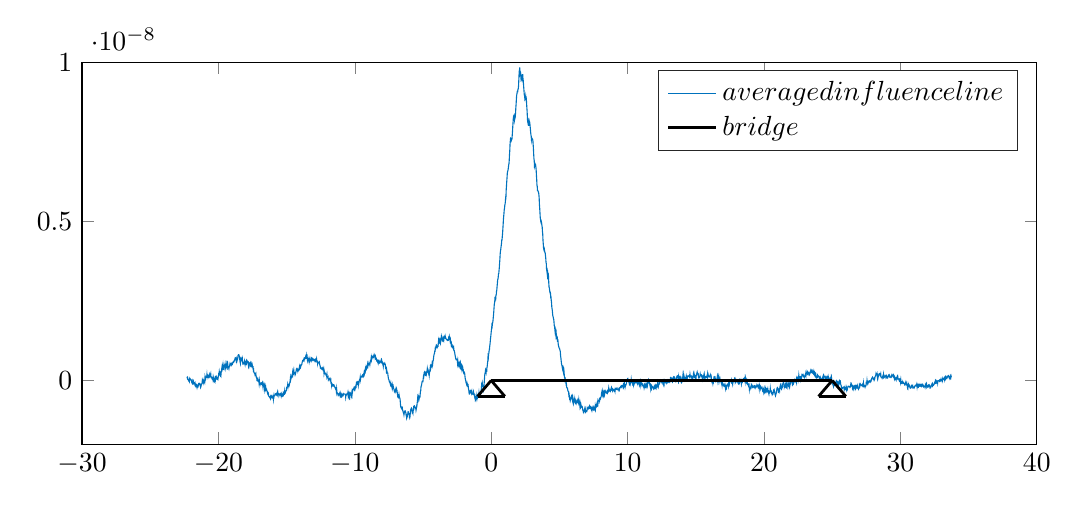
\begin{tikzpicture}

\begin{axis}[%
width=\textwidth,
height=0.4\textwidth,
at={(0\figurewidth,0\figureheight)},
scale only axis,
xmin=-30,
xmax=40,
ymin=-2e-09,
ymax=1e-08,
axis background/.style={fill=white},
% title style={font=\bfseries},
% title={},
legend style={legend cell align=left,align=left,draw=white!15!black}
]
\addplot [color=mycolor1,solid]
  table[row sep=crcr]{%
-22.3159404296875	1.18323540657329e-10\\
-22.295791015625	1.09487790669497e-10\\
-22.2756416015625	7.01083695561926e-11\\
-22.2554921875	8.73967831327927e-11\\
-22.2353427734375	4.57279390021045e-11\\
-22.215193359375	3.49387202965769e-11\\
-22.1950439453125	-9.44935511256185e-12\\
-22.17489453125	-4.62447348668263e-12\\
-22.1547451171875	-2.87372614426872e-12\\
-22.134595703125	-2.9184434031337e-11\\
-22.1144462890625	5.2853846840941e-11\\
-22.094296875	3.42700471708031e-11\\
-22.0741474609375	5.26376478942855e-11\\
-22.053998046875	3.78334420422553e-11\\
-22.0338486328125	1.34463101627698e-11\\
-22.01369921875	1.307063002344e-11\\
-21.9935498046875	1.54405574351222e-11\\
-21.973400390625	-3.06588111607537e-11\\
-21.9532509765625	-6.69160227287835e-11\\
-21.9331015625	-8.30366837403097e-11\\
-21.9129521484375	-3.58436969547546e-11\\
-21.892802734375	-8.98057932214126e-11\\
-21.8726533203125	-7.06451510325644e-11\\
-21.85250390625	-5.07503260190867e-11\\
-21.8323544921875	-2.80847503488146e-11\\
-21.812205078125	-9.54586162294433e-11\\
-21.7920556640625	-8.48582623645359e-11\\
-21.77190625	-8.21392962825674e-11\\
-21.7517568359375	-7.53443500309883e-11\\
-21.731607421875	-1.19190434756364e-10\\
-21.7114580078125	-9.28082559022149e-11\\
-21.69130859375	-1.45257369745405e-10\\
-21.6711591796875	-1.14044953723198e-10\\
-21.651009765625	-1.12440918837719e-10\\
-21.6308603515625	-1.15189705925096e-10\\
-21.6107109375	-1.83195734519052e-10\\
-21.5905615234375	-1.75703642278238e-10\\
-21.570412109375	-2.17347601822706e-10\\
-21.5502626953125	-1.7234124979925e-10\\
-21.53011328125	-1.94383457927583e-10\\
-21.5099638671875	-1.76173919683551e-10\\
-21.489814453125	-1.89207569785072e-10\\
-21.4696650390625	-1.55838460816968e-10\\
-21.449515625	-9.43827219040849e-11\\
-21.4293662109375	-9.43140933035297e-11\\
-21.409216796875	-9.01825988251552e-11\\
-21.3890673828125	-1.09140838712194e-10\\
-21.36891796875	-1.18727526471047e-10\\
-21.3487685546875	-1.46763630148943e-10\\
-21.328619140625	-1.34643594322207e-10\\
-21.3084697265625	-2.17751873636963e-10\\
-21.2883203125	-2.00358196408718e-10\\
-21.2681708984375	-1.66462048900436e-10\\
-21.248021484375	-1.22230698810312e-10\\
-21.2278720703125	-1.08103144022445e-10\\
-21.20772265625	-1.03194094594098e-10\\
-21.1875732421875	-2.67572985489041e-11\\
-21.167423828125	-7.04916547708198e-11\\
-21.1472744140625	-5.2133999721112e-11\\
-21.127125	-1.81128827031517e-13\\
-21.1069755859375	-4.20828914071255e-11\\
-21.086826171875	-7.20610611170289e-11\\
-21.0666767578125	3.89956657059595e-12\\
-21.04652734375	-3.51503749964041e-12\\
-21.0263779296875	4.66638939409171e-12\\
-21.006228515625	-3.11515453732733e-11\\
-20.9860791015625	9.10781119391464e-11\\
-20.9659296875	4.13837460046243e-11\\
-20.9457802734375	9.65335893111909e-11\\
-20.925630859375	7.00984909187122e-11\\
-20.9054814453125	1.07159933583392e-10\\
-20.88533203125	1.04107742759043e-10\\
-20.8651826171875	1.01528204719944e-10\\
-20.845033203125	1.76538512943176e-10\\
-20.8248837890625	8.20849352401305e-11\\
-20.804734375	1.73188141553962e-10\\
-20.7845849609375	1.58569674236083e-10\\
-20.764435546875	1.04047085483998e-10\\
-20.7442861328125	1.39395311712661e-10\\
-20.72413671875	1.2336366490079e-10\\
-20.7039873046875	1.09770933550793e-10\\
-20.683837890625	1.48789260360401e-10\\
-20.6636884765625	1.8363035461933e-10\\
-20.6435390625	1.35914903981168e-10\\
-20.6233896484375	1.58338640118635e-10\\
-20.603240234375	1.8230108834978e-10\\
-20.5830908203125	1.65700245389576e-10\\
-20.56294140625	2.01892654266715e-10\\
-20.5427919921875	1.03772117811136e-10\\
-20.522642578125	1.126352490028e-10\\
-20.5024931640625	1.04404565174293e-10\\
-20.48234375	7.0979560091846e-11\\
-20.4621943359375	5.19814877597947e-11\\
-20.442044921875	6.74267553876139e-11\\
-20.4218955078125	7.90049163532168e-11\\
-20.40174609375	3.28475332216119e-11\\
-20.3815966796875	1.15737035993869e-10\\
-20.361447265625	7.78790672655313e-11\\
-20.3412978515625	5.38353193543276e-11\\
-20.3211484375	9.4347119705749e-12\\
-20.3009990234375	4.06501295440194e-11\\
-20.280849609375	-3.49386305783243e-11\\
-20.2607001953125	-5.0619834195727e-11\\
-20.24055078125	1.93226991608584e-11\\
-20.2204013671875	7.12907560890803e-12\\
-20.200251953125	1.07618654362715e-10\\
-20.1801025390625	9.49682389388561e-11\\
-20.159953125	1.1601513262116e-10\\
-20.1398037109375	7.81582332178352e-11\\
-20.119654296875	4.65380016568453e-11\\
-20.0995048828125	3.92752454306966e-11\\
-20.07935546875	6.662708865594e-11\\
-20.0592060546875	4.61146077583585e-11\\
-20.039056640625	3.41628380493773e-11\\
-20.0189072265625	9.26934831085441e-11\\
-19.9987578125	1.38481458563547e-10\\
-19.9786083984375	2.09666201735121e-10\\
-19.958458984375	2.00616762065816e-10\\
-19.9383095703125	2.78176606939186e-10\\
-19.91816015625	2.29508102606363e-10\\
-19.8980107421875	2.09103000941712e-10\\
-19.877861328125	1.78367604926966e-10\\
-19.8577119140625	2.25491415358066e-10\\
-19.8375625	1.92778691127656e-10\\
-19.8174130859375	1.6119747496344e-10\\
-19.797263671875	2.581095666285e-10\\
-19.7771142578125	2.73209916628327e-10\\
-19.75696484375	3.63430002068034e-10\\
-19.7368154296875	4.24269052795325e-10\\
-19.716666015625	3.79205586299539e-10\\
-19.6965166015625	4.36633472134869e-10\\
-19.6763671875	4.88598711219513e-10\\
-19.6562177734375	3.30394553991595e-10\\
-19.636068359375	4.55665096689067e-10\\
-19.6159189453125	4.41541373418461e-10\\
-19.59576953125	3.99998706831409e-10\\
-19.5756201171875	4.63735678960122e-10\\
-19.555470703125	4.4478007654707e-10\\
-19.5353212890625	4.43938872287813e-10\\
-19.515171875	4.98683258476812e-10\\
-19.4950224609375	4.00495361026772e-10\\
-19.474873046875	4.5400260119464e-10\\
-19.4547236328125	4.092996135541e-10\\
-19.43457421875	4.3144188258118e-10\\
-19.4144248046875	4.31193248673038e-10\\
-19.394275390625	5.03899070023969e-10\\
-19.3741259765625	4.43804733841982e-10\\
-19.3539765625	5.02690349921809e-10\\
-19.3338271484375	4.45583122834982e-10\\
-19.313677734375	4.99575560355244e-10\\
-19.2935283203125	4.25707492322739e-10\\
-19.27337890625	4.13024416349873e-10\\
-19.2532294921875	3.98503440413278e-10\\
-19.233080078125	3.69802281990902e-10\\
-19.2129306640625	4.31670108930708e-10\\
-19.19278125	4.37047901352481e-10\\
-19.1726318359375	4.78288397297578e-10\\
-19.152482421875	5.23977248945561e-10\\
-19.1323330078125	4.92847705522926e-10\\
-19.11218359375	5.20202356571052e-10\\
-19.0920341796875	5.06002690608107e-10\\
-19.071884765625	4.96747150243505e-10\\
-19.0517353515625	5.17830595550962e-10\\
-19.0315859375	4.85972460603039e-10\\
-19.0114365234375	5.06183612942751e-10\\
-18.991287109375	5.31418426425977e-10\\
-18.9711376953125	5.21767175402451e-10\\
-18.95098828125	5.61899849376718e-10\\
-18.9308388671875	5.78254193999055e-10\\
-18.910689453125	5.72847639174557e-10\\
-18.8905400390625	5.93345087330096e-10\\
-18.870390625	5.83326984294873e-10\\
-18.8502412109375	5.97403835656252e-10\\
-18.830091796875	6.32893093209181e-10\\
-18.8099423828125	6.35815330300154e-10\\
-18.78979296875	6.83175487350812e-10\\
-18.7696435546875	7.09003517641796e-10\\
-18.749494140625	6.99276072356553e-10\\
-18.7293447265625	6.94250669904722e-10\\
-18.7091953125	6.45716492101065e-10\\
-18.6890458984375	6.8900141493312e-10\\
-18.668896484375	6.57547668987923e-10\\
-18.6487470703125	5.95413894283882e-10\\
-18.62859765625	6.30214980855788e-10\\
-18.6084482421875	6.88095016896453e-10\\
-18.588298828125	6.84129730675203e-10\\
-18.5681494140625	7.80592619919039e-10\\
-18.548	7.94387196448797e-10\\
-18.5278505859375	8.08883296859899e-10\\
-18.507701171875	8.0713785858396e-10\\
-18.4875517578125	7.93488139428402e-10\\
-18.46740234375	7.55010538618538e-10\\
-18.4472529296875	7.06059081650203e-10\\
-18.427103515625	6.22845710681703e-10\\
-18.4069541015625	5.76818981210764e-10\\
-18.3868046875	5.3854169521943e-10\\
-18.3666552734375	6.48913353162417e-10\\
-18.346505859375	6.13402277306567e-10\\
-18.3263564453125	6.3807389947339e-10\\
-18.30620703125	6.74886874549309e-10\\
-18.2860576171875	6.40016768056518e-10\\
-18.265908203125	6.34370851496262e-10\\
-18.2457587890625	6.76082092638564e-10\\
-18.225609375	5.72138142151933e-10\\
-18.2054599609375	5.12717785149444e-10\\
-18.185310546875	5.14450376685857e-10\\
-18.1651611328125	5.2521273378675e-10\\
-18.14501171875	5.509836658907e-10\\
-18.1248623046875	5.39396736498327e-10\\
-18.104712890625	5.3000408883055e-10\\
-18.0845634765625	5.99744147664559e-10\\
-18.0644140625	5.49750413299126e-10\\
-18.0442646484375	5.03818901047238e-10\\
-18.024115234375	5.63090491732583e-10\\
-18.0039658203125	5.36494912843416e-10\\
-17.98381640625	5.22610724759753e-10\\
-17.9636669921875	5.64171644191501e-10\\
-17.943517578125	6.03569912869189e-10\\
-17.9233681640625	5.64549416376051e-10\\
-17.90321875	6.2370114876922e-10\\
-17.8830693359375	6.06175374224227e-10\\
-17.862919921875	5.84332310724316e-10\\
-17.8427705078125	5.88548804854354e-10\\
-17.82262109375	5.81983035825145e-10\\
-17.8024716796875	4.95146569673785e-10\\
-17.782322265625	5.62739380898561e-10\\
-17.7621728515625	5.48363936114207e-10\\
-17.7420234375	4.71028510419464e-10\\
-17.7218740234375	5.1544243640287e-10\\
-17.701724609375	5.39187140924038e-10\\
-17.6815751953125	5.26364563381349e-10\\
-17.66142578125	4.9386123615434e-10\\
-17.6412763671875	5.39398441815961e-10\\
-17.621126953125	5.01521358793121e-10\\
-17.6009775390625	4.63909047681283e-10\\
-17.580828125	5.06004732108818e-10\\
-17.5606787109375	4.49623816459208e-10\\
-17.540529296875	4.41500257773379e-10\\
-17.5203798828125	4.8927585218793e-10\\
-17.50023046875	4.49035435662402e-10\\
-17.4800810546875	4.05798092904653e-10\\
-17.459931640625	4.14476261022211e-10\\
-17.4397822265625	3.20405194311378e-10\\
-17.4196328125	3.33796279117191e-10\\
-17.3994833984375	2.51685067595404e-10\\
-17.379333984375	2.47406113825099e-10\\
-17.3591845703125	2.25328688542963e-10\\
-17.33903515625	2.22620199792101e-10\\
-17.3188857421875	1.81412445706089e-10\\
-17.298736328125	2.01718944710845e-10\\
-17.2785869140625	2.18443636639e-10\\
-17.2584375	2.29187290749758e-10\\
-17.2382880859375	1.12310043256121e-10\\
-17.218138671875	1.14725420065735e-10\\
-17.1979892578125	1.10162817276963e-10\\
-17.17783984375	1.59180032956571e-11\\
-17.1576904296875	2.31855510347112e-11\\
-17.137541015625	-1.18144565911932e-11\\
-17.1173916015625	-5.41052823334912e-12\\
-17.0972421875	3.03108207438521e-11\\
-17.0770927734375	-9.28268584341247e-12\\
-17.056943359375	-2.54234836638978e-11\\
-17.0367939453125	-2.48609720147611e-11\\
-17.01664453125	-1.00120859870084e-10\\
-16.9964951171875	-2.08653974232505e-11\\
-16.976345703125	-1.10015060264329e-10\\
-16.9561962890625	-9.02493760192832e-11\\
-16.936046875	-1.07492534299557e-10\\
-16.9158974609375	-1.01161024473037e-10\\
-16.895748046875	-1.26783543133757e-10\\
-16.8755986328125	-7.51415113612875e-11\\
-16.85544921875	-7.22241518512012e-11\\
-16.8352998046875	-8.58028112156076e-11\\
-16.815150390625	-1.04048220289193e-10\\
-16.7950009765625	-9.32151422458533e-11\\
-16.7748515625	-7.12876998848784e-11\\
-16.7547021484375	-1.39658985022639e-10\\
-16.734552734375	-2.02719712785966e-10\\
-16.7144033203125	-9.81097026633099e-11\\
-16.69425390625	-1.2644443931879e-10\\
-16.6741044921875	-1.75790878754161e-10\\
-16.653955078125	-1.87874377373733e-10\\
-16.6338056640625	-1.53528676041705e-10\\
-16.61365625	-2.62610153374383e-10\\
-16.5935068359375	-1.96094929764687e-10\\
-16.573357421875	-2.2776354469121e-10\\
-16.5532080078125	-2.69865297208068e-10\\
-16.53305859375	-2.09832019329781e-10\\
-16.5129091796875	-2.81399322439395e-10\\
-16.492759765625	-2.61396291455264e-10\\
-16.4726103515625	-2.68481681726185e-10\\
-16.4524609375	-3.15156719638212e-10\\
-16.4323115234375	-3.39302144894548e-10\\
-16.412162109375	-3.70723518899141e-10\\
-16.3920126953125	-4.05832180989458e-10\\
-16.37186328125	-3.72598919538238e-10\\
-16.3517138671875	-3.86598494285663e-10\\
-16.331564453125	-4.2915161607803e-10\\
-16.3114150390625	-4.9101497646749e-10\\
-16.291265625	-5.00347656742876e-10\\
-16.2711162109375	-5.04649145953616e-10\\
-16.250966796875	-5.28171752723671e-10\\
-16.2308173828125	-5.37998584399146e-10\\
-16.21066796875	-5.22297501792218e-10\\
-16.1905185546875	-5.57087518401707e-10\\
-16.170369140625	-5.10451572024836e-10\\
-16.1502197265625	-5.39595870487183e-10\\
-16.1300703125	-5.0563535064532e-10\\
-16.1099208984375	-5.37596827651145e-10\\
-16.089771484375	-5.36239977231557e-10\\
-16.0696220703125	-5.03979849884165e-10\\
-16.04947265625	-5.17584043699106e-10\\
-16.0293232421875	-5.50033207659897e-10\\
-16.009173828125	-5.4898065291124e-10\\
-15.9890244140625	-5.00874296108708e-10\\
-15.968875	-5.87663515441973e-10\\
-15.9487255859375	-5.03525403731068e-10\\
-15.928576171875	-5.21931236653185e-10\\
-15.9084267578125	-4.74974928466686e-10\\
-15.88827734375	-4.6628869735908e-10\\
-15.8681279296875	-4.70642089962489e-10\\
-15.847978515625	-4.30670126847013e-10\\
-15.8278291015625	-4.4771871457564e-10\\
-15.8076796875	-4.40818587065826e-10\\
-15.7875302734375	-4.23744848804827e-10\\
-15.767380859375	-4.29864966470094e-10\\
-15.7472314453125	-4.467694369435e-10\\
-15.72708203125	-4.1100814938825e-10\\
-15.7069326171875	-4.20715460817679e-10\\
-15.686783203125	-3.86966628234265e-10\\
-15.6666337890625	-4.30411700594156e-10\\
-15.646484375	-3.74896131937017e-10\\
-15.6263349609375	-4.29270029121687e-10\\
-15.606185546875	-4.40569761648871e-10\\
-15.5860361328125	-4.29654996867959e-10\\
-15.56588671875	-4.79899190682938e-10\\
-15.5457373046875	-4.46791397209016e-10\\
-15.525587890625	-4.31688322003247e-10\\
-15.5054384765625	-4.42562212668356e-10\\
-15.4852890625	-4.54124754257212e-10\\
-15.4651396484375	-4.59341991540457e-10\\
-15.444990234375	-4.27370472015298e-10\\
-15.4248408203125	-4.50251060212478e-10\\
-15.40469140625	-4.89289034901478e-10\\
-15.3845419921875	-4.4235602609468e-10\\
-15.364392578125	-4.92182892605427e-10\\
-15.3442431640625	-5.06019965393265e-10\\
-15.32409375	-5.06466863936027e-10\\
-15.3039443359375	-4.59994730378801e-10\\
-15.283794921875	-4.85355778711837e-10\\
-15.2636455078125	-4.7923116553749e-10\\
-15.24349609375	-4.06131439440961e-10\\
-15.2233466796875	-4.32729604477277e-10\\
-15.203197265625	-3.73299376763803e-10\\
-15.1830478515625	-3.77519096150226e-10\\
-15.1628984375	-4.52967888260601e-10\\
-15.1427490234375	-3.47551145774232e-10\\
-15.122599609375	-4.1140182572535e-10\\
-15.1024501953125	-3.97924709657251e-10\\
-15.08230078125	-3.39777332877305e-10\\
-15.0621513671875	-3.46616659025343e-10\\
-15.042001953125	-3.23473578499235e-10\\
-15.0218525390625	-3.17269264620451e-10\\
-15.001703125	-2.30693380493998e-10\\
-14.9815537109375	-2.1253771759966e-10\\
-14.961404296875	-2.10606635810842e-10\\
-14.9412548828125	-1.91256479653129e-10\\
-14.92110546875	-1.31105259728396e-10\\
-14.9009560546875	-1.90860794109007e-10\\
-14.880806640625	-1.23017998346425e-10\\
-14.8606572265625	-1.228231865079e-10\\
-14.8405078125	-1.37080713461157e-10\\
-14.8203583984375	-1.6945555039362e-10\\
-14.800208984375	-1.40143736003728e-10\\
-14.7800595703125	-8.16273146737291e-11\\
-14.75991015625	-6.65792776472098e-11\\
-14.7397607421875	-2.85852147187294e-12\\
-14.719611328125	8.43209873203147e-11\\
-14.6994619140625	2.39952814309051e-11\\
-14.6793125	6.55941404342348e-11\\
-14.6591630859375	7.7320191774882e-11\\
-14.639013671875	1.15538697946298e-10\\
-14.6188642578125	1.49384601814978e-10\\
-14.59871484375	1.19706111250055e-10\\
-14.5785654296875	1.41186815441085e-10\\
-14.558416015625	2.43308680193648e-10\\
-14.5382666015625	1.86961445109901e-10\\
-14.5181171875	2.36775937865908e-10\\
-14.4979677734375	2.8250034062516e-10\\
-14.477818359375	3.27771499450643e-10\\
-14.4576689453125	2.37062639402958e-10\\
-14.43751953125	2.55201471919714e-10\\
-14.4173701171875	2.4219548529285e-10\\
-14.397220703125	2.21898247544592e-10\\
-14.3770712890625	1.74047964844962e-10\\
-14.356921875	1.95794422698979e-10\\
-14.3367724609375	2.55454462534736e-10\\
-14.316623046875	2.63556818096888e-10\\
-14.2964736328125	3.23468154224683e-10\\
-14.27632421875	3.61194540645432e-10\\
-14.2561748046875	3.48312351146901e-10\\
-14.236025390625	3.54003559535891e-10\\
-14.2158759765625	3.27800326748121e-10\\
-14.1957265625	3.47141758165142e-10\\
-14.1755771484375	2.96582878324428e-10\\
-14.155427734375	3.30364055334366e-10\\
-14.1352783203125	3.12170337442841e-10\\
-14.11512890625	3.25768915517136e-10\\
-14.0949794921875	3.51198508325658e-10\\
-14.074830078125	3.88558132959676e-10\\
-14.0546806640625	4.35506510053479e-10\\
-14.03453125	3.83018583127715e-10\\
-14.0143818359375	4.11534413944985e-10\\
-13.994232421875	4.48187671408351e-10\\
-13.9740830078125	4.20367290643051e-10\\
-13.95393359375	4.58328737495678e-10\\
-13.9337841796875	4.83217540978693e-10\\
-13.913634765625	4.89870160347884e-10\\
-13.8934853515625	4.95847058968979e-10\\
-13.8733359375	5.44278312251323e-10\\
-13.8531865234375	5.75006341075002e-10\\
-13.833037109375	6.09616553833601e-10\\
-13.8128876953125	6.01025339666745e-10\\
-13.79273828125	6.03756783224576e-10\\
-13.7725888671875	6.45750306662405e-10\\
-13.752439453125	6.51073898853069e-10\\
-13.7322900390625	6.77761529646038e-10\\
-13.712140625	6.47848722583023e-10\\
-13.6919912109375	6.95996889625649e-10\\
-13.671841796875	7.07172581581994e-10\\
-13.6516923828125	6.83913837961883e-10\\
-13.63154296875	6.96579724776455e-10\\
-13.6113935546875	7.36144603764507e-10\\
-13.591244140625	7.00865268855787e-10\\
-13.5710947265625	6.98379815332607e-10\\
-13.5509453125	7.75427970364013e-10\\
-13.5307958984375	7.07269732548324e-10\\
-13.510646484375	6.94137513045917e-10\\
-13.4904970703125	7.30235062817101e-10\\
-13.47034765625	6.36159418022359e-10\\
-13.4501982421875	6.77698180262492e-10\\
-13.430048828125	6.84822550879866e-10\\
-13.4098994140625	6.81751638280592e-10\\
-13.38975	6.40055270186366e-10\\
-13.3696005859375	6.77821782128693e-10\\
-13.349451171875	6.10989744445531e-10\\
-13.3293017578125	6.80364101338222e-10\\
-13.30915234375	6.54216099308348e-10\\
-13.2890029296875	6.16084085420963e-10\\
-13.268853515625	6.44748236310808e-10\\
-13.2487041015625	6.37868749607442e-10\\
-13.2285546875	6.29862281678049e-10\\
-13.2084052734375	6.91063873732044e-10\\
-13.188255859375	6.72967958347801e-10\\
-13.1681064453125	6.91564829184758e-10\\
-13.14795703125	6.36398809809815e-10\\
-13.1278076171875	6.66294194227218e-10\\
-13.107658203125	6.78505001082515e-10\\
-13.0875087890625	6.39599874425954e-10\\
-13.067359375	6.36544570316022e-10\\
-13.0472099609375	6.41738281581759e-10\\
-13.027060546875	6.6794966461587e-10\\
-13.0069111328125	6.6094910272859e-10\\
-12.98676171875	6.21773717724372e-10\\
-12.9666123046875	6.23555586048705e-10\\
-12.946462890625	6.22453916669738e-10\\
-12.9263134765625	6.04839173759063e-10\\
-12.9061640625	6.64787624815009e-10\\
-12.8860146484375	6.76852064963647e-10\\
-12.865865234375	6.76021720508768e-10\\
-12.8457158203125	6.30742397355835e-10\\
-12.82556640625	6.46168359690275e-10\\
-12.8054169921875	6.8159319315496e-10\\
-12.785267578125	6.04785275533193e-10\\
-12.7651181640625	6.16065305804653e-10\\
-12.74496875	6.04164230961108e-10\\
-12.7248193359375	5.20647918341363e-10\\
-12.704669921875	5.63237853408531e-10\\
-12.6845205078125	5.68809930685197e-10\\
-12.66437109375	5.70416609880237e-10\\
-12.6442216796875	5.75494965420783e-10\\
-12.624072265625	5.59544898631123e-10\\
-12.6039228515625	5.75856000045029e-10\\
-12.5837734375	5.25251126056529e-10\\
-12.5636240234375	4.78168372881736e-10\\
-12.543474609375	4.64450660191066e-10\\
-12.5233251953125	3.96041182796665e-10\\
-12.50317578125	4.07775564675463e-10\\
-12.4830263671875	3.86299050028971e-10\\
-12.462876953125	3.79973539748611e-10\\
-12.4427275390625	3.67319848800089e-10\\
-12.422578125	3.57235154449822e-10\\
-12.4024287109375	3.87586124860927e-10\\
-12.382279296875	4.03187334935772e-10\\
-12.3621298828125	3.93998272450586e-10\\
-12.34198046875	3.93829115719213e-10\\
-12.3218310546875	3.03492608787986e-10\\
-12.301681640625	2.98823945157681e-10\\
-12.2815322265625	3.44807721473518e-10\\
-12.2613828125	2.37805352566592e-10\\
-12.2412333984375	3.03209272309484e-10\\
-12.221083984375	2.65468235702749e-10\\
-12.2009345703125	2.54147032001331e-10\\
-12.18078515625	2.14677684144092e-10\\
-12.1606357421875	2.17658309851459e-10\\
-12.140486328125	2.17391562351731e-10\\
-12.1203369140625	1.73750289769389e-10\\
-12.1001875	1.76304049042384e-10\\
-12.0800380859375	1.7701456323359e-10\\
-12.059888671875	1.25276922386803e-10\\
-12.0397392578125	1.80082138894423e-10\\
-12.01958984375	9.06354349983869e-11\\
-11.9994404296875	8.74456705428629e-11\\
-11.979291015625	7.85249318306784e-11\\
-11.9591416015625	9.94835830521334e-11\\
-11.9389921875	2.02728881837412e-11\\
-11.9188427734375	3.94682063379378e-11\\
-11.898693359375	3.66551358078093e-11\\
-11.8785439453125	4.12467306696329e-11\\
-11.85839453125	5.46072026703175e-11\\
-11.8382451171875	2.70055617381072e-11\\
-11.818095703125	4.62308315756518e-11\\
-11.7979462890625	-1.92932086891242e-11\\
-11.777796875	-1.90702948749266e-11\\
-11.7576474609375	2.57245615066464e-12\\
-11.737498046875	-1.17888143908308e-10\\
-11.7173486328125	-4.59881739831752e-11\\
-11.69719921875	-1.58122184162252e-10\\
-11.6770498046875	-1.13211721799127e-10\\
-11.656900390625	-1.2614068987445e-10\\
-11.6367509765625	-1.51228126987449e-10\\
-11.6166015625	-1.25974406586669e-10\\
-11.5964521484375	-1.37579515437415e-10\\
-11.576302734375	-1.55992041203716e-10\\
-11.5561533203125	-1.35917070811476e-10\\
-11.53600390625	-1.35183094790113e-10\\
-11.5158544921875	-1.53806989387244e-10\\
-11.495705078125	-1.92432955535196e-10\\
-11.4755556640625	-2.05634396091774e-10\\
-11.45540625	-2.09728233915262e-10\\
-11.4352568359375	-2.40329220735347e-10\\
-11.415107421875	-2.60685048308736e-10\\
-11.3949580078125	-2.46319028560977e-10\\
-11.37480859375	-2.62865143954421e-10\\
-11.3546591796875	-3.45517284835754e-10\\
-11.334509765625	-2.65904750075973e-10\\
-11.3143603515625	-3.58203185169563e-10\\
-11.2942109375	-3.93264600557493e-10\\
-11.2740615234375	-3.97565040681978e-10\\
-11.253912109375	-4.15264934343262e-10\\
-11.2337626953125	-4.45438459388112e-10\\
-11.21361328125	-4.19135388532157e-10\\
-11.1934638671875	-4.26695442591353e-10\\
-11.173314453125	-4.52587947848088e-10\\
-11.1531650390625	-4.25108408605349e-10\\
-11.133015625	-4.11531293158076e-10\\
-11.1128662109375	-4.04833585385693e-10\\
-11.092716796875	-3.83633699002071e-10\\
-11.0725673828125	-4.64440982529345e-10\\
-11.05241796875	-4.31969370856032e-10\\
-11.0322685546875	-4.84191833135188e-10\\
-11.012119140625	-4.64684005094033e-10\\
-10.9919697265625	-4.8973237437522e-10\\
-10.9718203125	-4.50571831722043e-10\\
-10.9516708984375	-4.80329686723876e-10\\
-10.931521484375	-4.36218631994739e-10\\
-10.9113720703125	-4.51828418379245e-10\\
-10.89122265625	-4.88111602831254e-10\\
-10.8710732421875	-4.87833973785066e-10\\
-10.850923828125	-4.37298062240256e-10\\
-10.8307744140625	-4.41401454278116e-10\\
-10.810625	-4.12388409067036e-10\\
-10.7904755859375	-4.2117357610629e-10\\
-10.770326171875	-4.28460041787811e-10\\
-10.7501767578125	-4.27724740320275e-10\\
-10.73002734375	-4.30878314203204e-10\\
-10.7098779296875	-4.29949613759997e-10\\
-10.689728515625	-4.33476024624567e-10\\
-10.6695791015625	-5.21242473502997e-10\\
-10.6494296875	-4.60375466159637e-10\\
-10.6292802734375	-4.64605788097246e-10\\
-10.609130859375	-4.57475032299496e-10\\
-10.5889814453125	-4.30768801360727e-10\\
-10.56883203125	-4.09014804104663e-10\\
-10.5486826171875	-4.09549137738124e-10\\
-10.528533203125	-4.20078707024506e-10\\
-10.5083837890625	-3.79166200753976e-10\\
-10.488234375	-4.64405298371821e-10\\
-10.4680849609375	-3.96374971121009e-10\\
-10.447935546875	-5.44107076114348e-10\\
-10.4277861328125	-4.58915464820656e-10\\
-10.40763671875	-5.11354341840949e-10\\
-10.3874873046875	-4.63614053705121e-10\\
-10.367337890625	-5.09263822343452e-10\\
-10.3471884765625	-4.27451874237408e-10\\
-10.3270390625	-4.6331969894893e-10\\
-10.3068896484375	-4.59132659845623e-10\\
-10.286740234375	-4.17582062198366e-10\\
-10.2665908203125	-4.33595271680521e-10\\
-10.24644140625	-4.78617227922645e-10\\
-10.2262919921875	-4.06879237821267e-10\\
-10.206142578125	-4.49233673586905e-10\\
-10.1859931640625	-3.27052620911804e-10\\
-10.16584375	-3.50741330053149e-10\\
-10.1456943359375	-3.02176156817997e-10\\
-10.125544921875	-2.77676250975081e-10\\
-10.1053955078125	-2.60662437516443e-10\\
-10.08524609375	-2.69794477324036e-10\\
-10.0650966796875	-2.41282823380929e-10\\
-10.044947265625	-2.7139780560827e-10\\
-10.0247978515625	-2.90728148063375e-10\\
-10.0046484375	-2.43807556418498e-10\\
-9.9844990234375	-2.7380983083283e-10\\
-9.964349609375	-2.38694439218308e-10\\
-9.9442001953125	-1.98888435049799e-10\\
-9.92405078125	-1.64769959773306e-10\\
-9.9039013671875	-1.82339657183811e-10\\
-9.883751953125	-5.92058912938879e-11\\
-9.8636025390625	-5.78464314717711e-11\\
-9.843453125	-4.43313729018737e-11\\
-9.8233037109375	-7.67509591449438e-11\\
-9.803154296875	-4.27117542948063e-11\\
-9.7830048828125	-4.73677185759184e-11\\
-9.76285546875	-6.8767022719016e-11\\
-9.7427060546875	-1.42477547460211e-10\\
-9.722556640625	-7.22555032715633e-11\\
-9.7024072265625	-8.98773930134108e-11\\
-9.6822578125	-3.8089190991977e-11\\
-9.6621083984375	1.80611787005693e-11\\
-9.641958984375	3.37890587184427e-11\\
-9.6218095703125	4.94841772410675e-11\\
-9.60166015625	1.07599612775921e-10\\
-9.5815107421875	3.75091794291389e-11\\
-9.561361328125	1.01437338509264e-10\\
-9.5412119140625	1.10044392828384e-10\\
-9.5210625	1.09764933711535e-10\\
-9.5009130859375	1.1686449934994e-10\\
-9.480763671875	1.3790160001021e-10\\
-9.4606142578125	1.31259161560803e-10\\
-9.44046484375	1.5478970326387e-10\\
-9.4203154296875	1.30931852599498e-10\\
-9.400166015625	1.56757156237503e-10\\
-9.3800166015625	1.77895439384659e-10\\
-9.3598671875	1.41076810686896e-10\\
-9.3397177734375	1.73269660237162e-10\\
-9.319568359375	2.37094590696347e-10\\
-9.2994189453125	1.99247861628984e-10\\
-9.27926953125	2.45786275934181e-10\\
-9.2591201171875	3.08608976839674e-10\\
-9.238970703125	3.49063148776911e-10\\
-9.2188212890625	2.94735356132135e-10\\
-9.198671875	3.3009142063202e-10\\
-9.1785224609375	3.96156266568283e-10\\
-9.158373046875	3.45764754251262e-10\\
-9.1382236328125	3.6347227211694e-10\\
-9.11807421875	3.9958788283896e-10\\
-9.0979248046875	4.47286578072074e-10\\
-9.077775390625	4.32129453477142e-10\\
-9.0576259765625	5.10410242889381e-10\\
-9.0374765625	4.6586255073932e-10\\
-9.0173271484375	5.26872503159217e-10\\
-8.997177734375	4.84649394242161e-10\\
-8.9770283203125	4.91019511001081e-10\\
-8.95687890625	4.95807741519448e-10\\
-8.9367294921875	5.19854036530209e-10\\
-8.916580078125	5.40486656552806e-10\\
-8.8964306640625	5.00551702942566e-10\\
-8.87628125	5.61706857291668e-10\\
-8.8561318359375	6.09953831425201e-10\\
-8.835982421875	6.0441063995632e-10\\
-8.8158330078125	6.51884851683866e-10\\
-8.79568359375	7.21652708356824e-10\\
-8.7755341796875	6.62986921639836e-10\\
-8.755384765625	7.25398622834104e-10\\
-8.7352353515625	7.48412880500773e-10\\
-8.7150859375	7.19370820378894e-10\\
-8.6949365234375	7.41332464949462e-10\\
-8.674787109375	7.40709143448423e-10\\
-8.6546376953125	7.35199158373385e-10\\
-8.63448828125	7.59985221644635e-10\\
-8.6143388671875	7.80377509316062e-10\\
-8.594189453125	7.38703464025336e-10\\
-8.5740400390625	8.04543138220062e-10\\
-8.553890625	7.81308881842062e-10\\
-8.5337412109375	7.64680097478794e-10\\
-8.513591796875	7.69157756971437e-10\\
-8.4934423828125	7.79454157008711e-10\\
-8.47329296875	6.86566515719923e-10\\
-8.4531435546875	6.97756132202357e-10\\
-8.432994140625	7.00483874661483e-10\\
-8.4128447265625	6.62901970552975e-10\\
-8.3926953125	6.2277045531349e-10\\
-8.3725458984375	6.34439003459556e-10\\
-8.352396484375	6.0722883013331e-10\\
-8.3322470703125	5.82197359854423e-10\\
-8.31209765625	5.65298728405131e-10\\
-8.2919482421875	6.55909536206997e-10\\
-8.271798828125	5.53831299532986e-10\\
-8.2516494140625	5.86150624569544e-10\\
-8.2315	6.06012462509047e-10\\
-8.2113505859375	5.58898286154176e-10\\
-8.191201171875	5.49372831414791e-10\\
-8.1710517578125	5.60704560568482e-10\\
-8.15090234375	5.85009698976445e-10\\
-8.1307529296875	5.6924824939674e-10\\
-8.110603515625	5.81727568905371e-10\\
-8.0904541015625	6.0053571958281e-10\\
-8.0703046875	6.32506108305451e-10\\
-8.0501552734375	5.95302161334883e-10\\
-8.030005859375	6.30031903892549e-10\\
-8.0098564453125	5.82444263880856e-10\\
-7.98970703125	5.8514521120244e-10\\
-7.9695576171875	5.42931556730054e-10\\
-7.949408203125	5.10569052877153e-10\\
-7.9292587890625	5.24950359636071e-10\\
-7.909109375	4.45379010956985e-10\\
-7.8889599609375	4.99739964345504e-10\\
-7.868810546875	5.05555152468888e-10\\
-7.8486611328125	5.27739434214257e-10\\
-7.82851171875	5.244001328826e-10\\
-7.8083623046875	5.41630491786816e-10\\
-7.788212890625	5.09122325998255e-10\\
-7.7680634765625	5.06316012206596e-10\\
-7.7479140625	4.16202630161212e-10\\
-7.7277646484375	4.30733390866618e-10\\
-7.707615234375	4.05978848315222e-10\\
-7.6874658203125	3.05590241385007e-10\\
-7.66731640625	3.44495426935175e-10\\
-7.6471669921875	2.97715094569996e-10\\
-7.627017578125	2.36947389849105e-10\\
-7.6068681640625	2.38177060222872e-10\\
-7.58671875	2.34118085288773e-10\\
-7.5665693359375	1.47174216951561e-10\\
-7.546419921875	9.03279119145279e-11\\
-7.5262705078125	3.76150339543541e-11\\
-7.50612109375	3.0657527124881e-11\\
-7.4859716796875	1.67326973041192e-12\\
-7.465822265625	-4.58946579391734e-11\\
-7.4456728515625	-5.1911019209031e-11\\
-7.4255234375	-6.6605160039476e-11\\
-7.4053740234375	-1.05453198929263e-10\\
-7.385224609375	-1.34180436729637e-10\\
-7.3650751953125	-9.13475449614749e-11\\
-7.34492578125	-1.79700317285273e-10\\
-7.3247763671875	-1.88480521451207e-10\\
-7.304626953125	-1.56215441702392e-10\\
-7.2844775390625	-1.95758955424075e-10\\
-7.264328125	-2.39924182371534e-10\\
-7.2441787109375	-1.69294314075039e-10\\
-7.224029296875	-2.41466799717049e-10\\
-7.2038798828125	-2.16452585744202e-10\\
-7.18373046875	-1.8446240865963e-10\\
-7.1635810546875	-2.31632413585857e-10\\
-7.143431640625	-2.65437424330157e-10\\
-7.1232822265625	-2.73017876229221e-10\\
-7.1031328125	-3.29530798316215e-10\\
-7.0829833984375	-3.13469027496193e-10\\
-7.062833984375	-3.29962410040086e-10\\
-7.0426845703125	-3.66137359558679e-10\\
-7.02253515625	-3.38091769974804e-10\\
-7.0023857421875	-2.83264901336168e-10\\
-6.982236328125	-2.96387801423436e-10\\
-6.9620869140625	-2.36980757215276e-10\\
-6.9419375	-2.59396944309149e-10\\
-6.9217880859375	-3.46316861175679e-10\\
-6.901638671875	-3.35623936982882e-10\\
-6.8814892578125	-4.13170266966503e-10\\
-6.86133984375	-4.76119835565446e-10\\
-6.8411904296875	-4.46590769564921e-10\\
-6.821041015625	-4.53332614202262e-10\\
-6.8008916015625	-5.17180595797128e-10\\
-6.7807421875	-4.94286714451218e-10\\
-6.7605927734375	-4.39460471756763e-10\\
-6.740443359375	-4.92904143436289e-10\\
-6.7202939453125	-5.43339860423938e-10\\
-6.70014453125	-5.62524074922277e-10\\
-6.6799951171875	-5.90482598699419e-10\\
-6.659845703125	-7.14849746803819e-10\\
-6.6396962890625	-8.22830623549494e-10\\
-6.619546875	-8.43628383590965e-10\\
-6.5993974609375	-8.34066835331365e-10\\
-6.579248046875	-8.57391706784889e-10\\
-6.5590986328125	-8.86149356316661e-10\\
-6.53894921875	-8.68692913419376e-10\\
-6.5187998046875	-8.56683772847225e-10\\
-6.498650390625	-9.38635861856653e-10\\
-6.4785009765625	-9.48038667737703e-10\\
-6.4583515625	-9.85350243205878e-10\\
-6.4382021484375	-1.0162842118493e-09\\
-6.418052734375	-1.03582648860545e-09\\
-6.3979033203125	-1.07884846259002e-09\\
-6.37775390625	-1.02437739611007e-09\\
-6.3576044921875	-9.90902738732031e-10\\
-6.337455078125	-9.62530982906647e-10\\
-6.3173056640625	-9.53405852963619e-10\\
-6.29715625	-9.56918071491628e-10\\
-6.2770068359375	-1.00471108014343e-09\\
-6.256857421875	-1.00923772237116e-09\\
-6.2367080078125	-1.10027496665753e-09\\
-6.21655859375	-1.11154111032723e-09\\
-6.1964091796875	-1.18806074980408e-09\\
-6.176259765625	-1.16097959524789e-09\\
-6.1561103515625	-1.13714909555199e-09\\
-6.1359609375	-1.06459570208506e-09\\
-6.1158115234375	-1.05027150328078e-09\\
-6.095662109375	-9.83137951786239e-10\\
-6.0755126953125	-9.87783218950559e-10\\
-6.05536328125	-1.03651665267429e-09\\
-6.0352138671875	-1.04091589054385e-09\\
-6.015064453125	-1.08985410754556e-09\\
-5.9949150390625	-1.14876446585775e-09\\
-5.974765625	-1.11010685801481e-09\\
-5.9546162109375	-1.13073526955945e-09\\
-5.934466796875	-1.03729025036532e-09\\
-5.9143173828125	-9.5093337401561e-10\\
-5.89416796875	-9.0557282993295e-10\\
-5.8740185546875	-8.93997582462442e-10\\
-5.853869140625	-8.70805478888379e-10\\
-5.8337197265625	-8.8887659356507e-10\\
-5.8135703125	-9.34118067416558e-10\\
-5.7934208984375	-9.86422623007299e-10\\
-5.773271484375	-9.55660154301933e-10\\
-5.7531220703125	-9.59691279366573e-10\\
-5.73297265625	-1.00707899228592e-09\\
-5.7128232421875	-9.24477955561881e-10\\
-5.692673828125	-8.59038488941296e-10\\
-5.6725244140625	-8.76892573795698e-10\\
-5.652375	-8.02087283156516e-10\\
-5.6322255859375	-7.98211912376726e-10\\
-5.612076171875	-8.26630791897034e-10\\
-5.5919267578125	-8.46444292449296e-10\\
-5.57177734375	-8.51573412967189e-10\\
-5.5516279296875	-8.67261519449556e-10\\
-5.531478515625	-8.56605437265396e-10\\
-5.5113291015625	-9.33922950352722e-10\\
-5.4911796875	-8.92651605859378e-10\\
-5.4710302734375	-8.11853959211717e-10\\
-5.450880859375	-8.1609437606182e-10\\
-5.4307314453125	-7.10507953857919e-10\\
-5.41058203125	-6.67756988720912e-10\\
-5.3904326171875	-5.56087615288202e-10\\
-5.370283203125	-6.00178968295828e-10\\
-5.3501337890625	-5.12160553222326e-10\\
-5.329984375	-5.54226392399078e-10\\
-5.3098349609375	-5.31171994662125e-10\\
-5.289685546875	-5.82199541380653e-10\\
-5.2695361328125	-5.40459600298305e-10\\
-5.24938671875	-5.3452980117043e-10\\
-5.2292373046875	-5.31113818223978e-10\\
-5.209087890625	-4.44352642291685e-10\\
-5.1889384765625	-3.40551228587316e-10\\
-5.1687890625	-3.30139212995433e-10\\
-5.1486396484375	-2.03078890126465e-10\\
-5.128490234375	-1.77256504299157e-10\\
-5.1083408203125	-1.47225654021627e-10\\
-5.08819140625	-9.64115970861502e-11\\
-5.0680419921875	-3.52811916461518e-11\\
-5.047892578125	-3.77979255301951e-11\\
-5.0277431640625	-3.36293003124013e-11\\
-5.00759375	-3.61168617273849e-11\\
-4.9874443359375	4.64531698617115e-11\\
-4.967294921875	1.22694657182215e-10\\
-4.9471455078125	1.06625370067183e-10\\
-4.92699609375	1.91853482292338e-10\\
-4.9068466796875	2.56363221756729e-10\\
-4.886697265625	2.65931918810309e-10\\
-4.8665478515625	2.82466051251174e-10\\
-4.8463984375	2.74399369393327e-10\\
-4.8262490234375	1.61575857862019e-10\\
-4.806099609375	1.6329682566742e-10\\
-4.7859501953125	1.53958794970692e-10\\
-4.76580078125	2.14318311079287e-10\\
-4.7456513671875	2.00628761373691e-10\\
-4.725501953125	2.81490571725173e-10\\
-4.7053525390625	3.06370077661363e-10\\
-4.685203125	3.74589578132946e-10\\
-4.6650537109375	3.21401814891544e-10\\
-4.644904296875	3.53987442996658e-10\\
-4.6247548828125	3.35032567947093e-10\\
-4.60460546875	2.51632078445148e-10\\
-4.5844560546875	2.11198946537874e-10\\
-4.564306640625	2.27220557324919e-10\\
-4.5441572265625	1.63137678504208e-10\\
-4.5240078125	2.43806202472256e-10\\
-4.5038583984375	3.04553500737168e-10\\
-4.483708984375	3.53193462344737e-10\\
-4.4635595703125	4.26198762977116e-10\\
-4.44341015625	3.87003097497373e-10\\
-4.4232607421875	4.83533927810439e-10\\
-4.403111328125	4.86332900062007e-10\\
-4.3829619140625	4.27176650824583e-10\\
-4.3628125	4.22896986947425e-10\\
-4.3426630859375	4.99234716067893e-10\\
-4.322513671875	4.417305537757e-10\\
-4.3023642578125	4.70078941736674e-10\\
-4.28221484375	5.6645412522614e-10\\
-4.2620654296875	6.3474687620967e-10\\
-4.241916015625	6.3792558009581e-10\\
-4.2217666015625	7.40413005638898e-10\\
-4.2016171875	7.86808953117185e-10\\
-4.1814677734375	8.33254185902617e-10\\
-4.161318359375	8.41935656425383e-10\\
-4.1411689453125	9.17972005696414e-10\\
-4.12101953125	9.16542973810837e-10\\
-4.1008701171875	1.01275236488091e-09\\
-4.080720703125	9.99753174845476e-10\\
-4.0605712890625	1.04647552393879e-09\\
-4.040421875	1.08161692270086e-09\\
-4.0202724609375	1.05720108247137e-09\\
-4.000123046875	1.08416907090142e-09\\
-3.9799736328125	1.04481623152149e-09\\
-3.95982421875	1.03303056099294e-09\\
-3.9396748046875	1.0529356596279e-09\\
-3.919525390625	1.08235671191687e-09\\
-3.8993759765625	1.0791612463885e-09\\
-3.8792265625	1.16691421029354e-09\\
-3.8590771484375	1.25990847085069e-09\\
-3.838927734375	1.21244881511819e-09\\
-3.8187783203125	1.25315095650143e-09\\
-3.79862890625	1.27537667552531e-09\\
-3.7784794921875	1.17576749858801e-09\\
-3.758330078125	1.17171199005048e-09\\
-3.7381806640625	1.22917915281038e-09\\
-3.71803125	1.18159656632838e-09\\
-3.6978818359375	1.23983911851912e-09\\
-3.677732421875	1.30681432435093e-09\\
-3.6575830078125	1.37593529859039e-09\\
-3.63743359375	1.3282124714201e-09\\
-3.6172841796875	1.37084853851018e-09\\
-3.597134765625	1.34563709119858e-09\\
-3.5769853515625	1.33103483491797e-09\\
-3.5568359375	1.25373528721774e-09\\
-3.5366865234375	1.26657732993661e-09\\
-3.516537109375	1.2533286059431e-09\\
-3.4963876953125	1.3101654002239e-09\\
-3.47623828125	1.27327128785035e-09\\
-3.4560888671875	1.34359640714435e-09\\
-3.435939453125	1.38634057903491e-09\\
-3.4157900390625	1.37925531773308e-09\\
-3.395640625	1.35890890344948e-09\\
-3.3754912109375	1.39776981661867e-09\\
-3.355341796875	1.35453944108059e-09\\
-3.3351923828125	1.33783794624354e-09\\
-3.31504296875	1.31371554355106e-09\\
-3.2948935546875	1.29936560467367e-09\\
-3.274744140625	1.28835574214051e-09\\
-3.2545947265625	1.2779645592005e-09\\
-3.2344453125	1.28656798244884e-09\\
-3.2142958984375	1.26514853918557e-09\\
-3.194146484375	1.25329060970538e-09\\
-3.1739970703125	1.256738803634e-09\\
-3.15384765625	1.259230245171e-09\\
-3.1336982421875	1.27534977648587e-09\\
-3.113548828125	1.3507183209374e-09\\
-3.0933994140625	1.34037569581738e-09\\
-3.07325	1.38578905097229e-09\\
-3.0531005859375	1.33778458221633e-09\\
-3.032951171875	1.31774670745015e-09\\
-3.0128017578125	1.25150221378541e-09\\
-2.99265234375	1.28894087566072e-09\\
-2.9725029296875	1.22133139944885e-09\\
-2.952353515625	1.18211100843284e-09\\
-2.9322041015625	1.12195955652888e-09\\
-2.9120546875	1.15537123951574e-09\\
-2.8919052734375	1.09406740764663e-09\\
-2.871755859375	1.06786065880964e-09\\
-2.8516064453125	1.08583253577875e-09\\
-2.83145703125	1.04782016701467e-09\\
-2.8113076171875	1.05670614675372e-09\\
-2.791158203125	1.01238842727352e-09\\
-2.7710087890625	9.89020094995289e-10\\
-2.750859375	1.02329648728044e-09\\
-2.7307099609375	9.46505125943083e-10\\
-2.710560546875	9.33836312613637e-10\\
-2.6904111328125	8.94101205334672e-10\\
-2.67026171875	8.56532614960546e-10\\
-2.6501123046875	7.90857043045768e-10\\
-2.629962890625	7.56871322874273e-10\\
-2.6098134765625	7.06138211474189e-10\\
-2.5896640625	6.6746443870137e-10\\
-2.5695146484375	6.53277280098881e-10\\
-2.549365234375	6.66413169029172e-10\\
-2.5292158203125	6.59921350868539e-10\\
-2.50906640625	6.67589306693589e-10\\
-2.4889169921875	6.59425497795714e-10\\
-2.468767578125	5.48002522495574e-10\\
-2.4486181640625	6.16459631902043e-10\\
-2.42846875	5.31383377645358e-10\\
-2.4083193359375	4.82308793248788e-10\\
-2.388169921875	5.07057974113884e-10\\
-2.3680205078125	5.35489179254339e-10\\
-2.34787109375	4.73487531374297e-10\\
-2.3277216796875	5.20736533187403e-10\\
-2.307572265625	5.17618291126036e-10\\
-2.2874228515625	5.51174732260577e-10\\
-2.2672734375	4.63230307936504e-10\\
-2.2471240234375	5.16927106626587e-10\\
-2.226974609375	4.55503302866211e-10\\
-2.2068251953125	3.75561822006264e-10\\
-2.18667578125	3.56419344708407e-10\\
-2.1665263671875	4.18817876444193e-10\\
-2.146376953125	3.50674482576927e-10\\
-2.1262275390625	4.07625130449931e-10\\
-2.106078125	3.61727094969804e-10\\
-2.0859287109375	3.9336763978621e-10\\
-2.065779296875	3.34403560600915e-10\\
-2.0456298828125	3.32017807994582e-10\\
-2.02548046875	2.53891818941613e-10\\
-2.0053310546875	2.7457123681436e-10\\
-1.985181640625	2.69260978553279e-10\\
-1.9650322265625	2.46218218050311e-10\\
-1.9448828125	2.19120187485315e-10\\
-1.9247333984375	1.33283688472081e-10\\
-1.904583984375	6.47594639653184e-11\\
-1.8844345703125	2.03662095182359e-11\\
-1.86428515625	-1.91335641002492e-11\\
-1.8441357421875	-6.78242351481186e-11\\
-1.823986328125	-6.62577776330232e-11\\
-1.8038369140625	-1.29871948527642e-10\\
-1.7836875	-1.51047595181725e-10\\
-1.7635380859375	-9.25618476264235e-11\\
-1.743388671875	-1.25820113323345e-10\\
-1.7232392578125	-1.30786423163591e-10\\
-1.70308984375	-1.26878502963256e-10\\
-1.6829404296875	-1.95783332907474e-10\\
-1.662791015625	-2.69828593437198e-10\\
-1.6426416015625	-3.10663834050966e-10\\
-1.6224921875	-3.85773481746305e-10\\
-1.6023427734375	-3.71164986446783e-10\\
-1.582193359375	-4.16742606633551e-10\\
-1.5620439453125	-4.09079196638124e-10\\
-1.54189453125	-3.73474485410937e-10\\
-1.5217451171875	-3.20156885050244e-10\\
-1.501595703125	-3.29996313172161e-10\\
-1.4814462890625	-3.24146246799007e-10\\
-1.461296875	-3.53324624795057e-10\\
-1.4411474609375	-3.9669280683884e-10\\
-1.420998046875	-3.55338365372159e-10\\
-1.4008486328125	-4.28461032061771e-10\\
-1.38069921875	-4.25980488976066e-10\\
-1.3605498046875	-4.31189489047152e-10\\
-1.340400390625	-4.37225368285984e-10\\
-1.3202509765625	-4.10750069538133e-10\\
-1.3001015625	-3.59587863224769e-10\\
-1.2799521484375	-4.05621620276072e-10\\
-1.259802734375	-4.0832888788622e-10\\
-1.2396533203125	-4.62841549074527e-10\\
-1.21950390625	-5.00914462394041e-10\\
-1.1993544921875	-5.4929451771674e-10\\
-1.179205078125	-5.39142299468552e-10\\
-1.1590556640625	-6.2504610285357e-10\\
-1.13890625	-6.08123052784738e-10\\
-1.1187568359375	-5.22330474665141e-10\\
-1.098607421875	-5.56503846560343e-10\\
-1.0784580078125	-5.51149848304125e-10\\
-1.05830859375	-4.85004412525738e-10\\
-1.0381591796875	-5.72577692867222e-10\\
-1.018009765625	-5.31773637238736e-10\\
-0.997860351562498	-5.41819269653583e-10\\
-0.977710937499999	-5.12777100576347e-10\\
-0.957561523437498	-4.63593608714655e-10\\
-0.937412109375	-4.75321596326347e-10\\
-0.917262695312498	-4.71982006114844e-10\\
-0.897113281249997	-3.89854220283283e-10\\
-0.876963867187499	-4.61756988564115e-10\\
-0.856814453124997	-4.90696941680867e-10\\
-0.836665039062499	-4.62666695044798e-10\\
-0.816515624999997	-4.46012850904732e-10\\
-0.796366210937499	-5.41284713634684e-10\\
-0.776216796874998	-4.37034498913928e-10\\
-0.7560673828125	-3.97482322091781e-10\\
-0.735917968749998	-3.51207248183385e-10\\
-0.7157685546875	-2.03570945297629e-10\\
-0.695619140624999	-1.10418248540295e-10\\
-0.675469726562497	-1.27000125938957e-10\\
-0.655320312499999	-7.69622839136155e-11\\
-0.635170898437497	-1.37304268608093e-10\\
-0.615021484374999	-1.66431662746459e-10\\
-0.594872070312498	-2.14141345521434e-10\\
-0.57472265625	-2.3633606352761e-10\\
-0.554573242187498	-2.88137658775361e-10\\
-0.534423828125	-2.25715928635075e-10\\
-0.514274414062498	-7.95268135725888e-11\\
-0.494124999999997	4.73590500281045e-11\\
-0.473975585937499	1.73887754278778e-10\\
-0.453826171874997	2.2033596769825e-10\\
-0.433676757812499	2.67785506153955e-10\\
-0.413527343749998	3.35994832580942e-10\\
-0.3933779296875	3.10664894526447e-10\\
-0.373228515624998	2.66297059542397e-10\\
-0.3530791015625	3.67529279858503e-10\\
-0.332929687499998	2.68499382293082e-10\\
-0.312780273437497	3.9466278691854e-10\\
-0.292630859374999	4.46155449741333e-10\\
-0.272481445312497	5.36343213190518e-10\\
-0.252332031249999	5.97495874661256e-10\\
-0.232182617187497	7.48860433821478e-10\\
-0.212033203124999	7.1469107667283e-10\\
-0.191883789062498	8.26416638903693e-10\\
-0.171734375	8.58736462930282e-10\\
-0.151584960937498	9.55401510302649e-10\\
-0.131435546875	9.57870660144713e-10\\
-0.111286132812499	1.06620404424617e-09\\
-0.091136718749997	1.1340692079803e-09\\
-0.0709873046874989	1.21516635270772e-09\\
-0.0508378906249973	1.31648713208138e-09\\
-0.0306884765624993	1.38596001089053e-09\\
-0.0105390624999977	1.47742125057269e-09\\
0.00961035156250034	1.56253923494394e-09\\
0.0297597656250019	1.63370225260733e-09\\
0.0499091796875	1.73374202352107e-09\\
0.0700585937500016	1.70617087620685e-09\\
0.0902080078125032	1.78451809841812e-09\\
0.110357421875001	1.81837592004913e-09\\
0.130506835937503	1.87699359776383e-09\\
0.150656250000001	1.97815794024069e-09\\
0.170805664062502	2.06367698259986e-09\\
0.190955078125	2.17818426377289e-09\\
0.211104492187502	2.30434380528629e-09\\
0.23125390625	2.41788641627817e-09\\
0.251403320312502	2.43964028797649e-09\\
0.271552734375003	2.55902430808479e-09\\
0.291702148437501	2.53427418408069e-09\\
0.311851562500003	2.58676817246902e-09\\
0.332000976562501	2.56982640482645e-09\\
0.352150390625003	2.68553755683791e-09\\
0.372299804687501	2.70526170651857e-09\\
0.392449218750002	2.80895715335975e-09\\
0.4125986328125	2.84761815513519e-09\\
0.432748046875002	2.96160287730973e-09\\
0.4528974609375	3.05430183731951e-09\\
0.473046875000001	3.15970916783433e-09\\
0.493196289062503	3.18261051379478e-09\\
0.513345703125001	3.24537446812917e-09\\
0.533495117187503	3.34583131690394e-09\\
0.553644531250001	3.35914475058141e-09\\
0.573793945312502	3.45351223839203e-09\\
0.593943359375	3.55091582423482e-09\\
0.614092773437502	3.67960189899359e-09\\
0.6342421875	3.79376466568602e-09\\
0.654391601562502	3.95821699595526e-09\\
0.674541015625003	4.04901651630597e-09\\
0.694690429687501	4.09704125134439e-09\\
0.714839843750003	4.17551164778117e-09\\
0.734989257812501	4.24164245811189e-09\\
0.755138671875002	4.30285723541796e-09\\
0.7752880859375	4.41500141563559e-09\\
0.795437500000002	4.42138313245176e-09\\
0.8155869140625	4.53693527966638e-09\\
0.835736328125002	4.62892949844927e-09\\
0.855885742187503	4.76930773689188e-09\\
0.876035156250001	4.90580240220841e-09\\
0.896184570312503	5.05892628087515e-09\\
0.916333984375001	5.16376039250407e-09\\
0.936483398437503	5.25608336472218e-09\\
0.956632812500001	5.36770694165782e-09\\
0.976782226562502	5.41665166664632e-09\\
0.996931640625	5.49972103217335e-09\\
1.0170810546875	5.5477645412156e-09\\
1.03723046875	5.60298195094214e-09\\
1.0573798828125	5.74316285627022e-09\\
1.077529296875	5.73429819002474e-09\\
1.0976787109375	5.97696643263361e-09\\
1.117828125	6.09911500555309e-09\\
1.1379775390625	6.24131866750234e-09\\
1.158126953125	6.35869524573292e-09\\
1.1782763671875	6.49891811594275e-09\\
1.19842578125	6.56050564948162e-09\\
1.2185751953125	6.58724834043421e-09\\
1.238724609375	6.62035341417296e-09\\
1.2588740234375	6.68470231313068e-09\\
1.2790234375	6.76623755618244e-09\\
1.2991728515625	6.79840629670034e-09\\
1.319322265625	6.90724727877369e-09\\
1.3394716796875	7.08809271598457e-09\\
1.35962109375	7.20976595534662e-09\\
1.3797705078125	7.41198791720094e-09\\
1.399919921875	7.51860830659505e-09\\
1.4200693359375	7.61457172083076e-09\\
1.44021875	7.60655272524409e-09\\
1.4603681640625	7.59994403336079e-09\\
1.480517578125	7.55263242928672e-09\\
1.5006669921875	7.58368966677904e-09\\
1.52081640625	7.58610330593847e-09\\
1.5409658203125	7.69819629213763e-09\\
1.561115234375	7.81785480965965e-09\\
1.5812646484375	7.98014338665475e-09\\
1.6014140625	8.10462603593567e-09\\
1.6215634765625	8.24015769331137e-09\\
1.641712890625	8.229361641311e-09\\
1.6618623046875	8.34936874391483e-09\\
1.68201171875	8.28126388536512e-09\\
1.7021611328125	8.19859920697002e-09\\
1.722310546875	8.28296423158469e-09\\
1.7424599609375	8.24243349503414e-09\\
1.762609375	8.27642032452356e-09\\
1.7827587890625	8.39442438039618e-09\\
1.802908203125	8.54592610025125e-09\\
1.8230576171875	8.66450209733791e-09\\
1.84320703125	8.8153286760937e-09\\
1.8633564453125	8.95749200681098e-09\\
1.883505859375	8.992984931385e-09\\
1.9036552734375	9.07356378351793e-09\\
1.9238046875	9.08919564518984e-09\\
1.9439541015625	9.08087629901983e-09\\
1.964103515625	9.14242123806323e-09\\
1.9842529296875	9.17443225412896e-09\\
2.00440234375	9.25709082763382e-09\\
2.0245517578125	9.44323861765015e-09\\
2.044701171875	9.63930262376181e-09\\
2.0648505859375	9.61570073057008e-09\\
2.085	9.84005445061177e-09\\
2.1051494140625	9.73569371302236e-09\\
2.125298828125	9.68322851189308e-09\\
2.1454482421875	9.68640371891889e-09\\
2.16559765625	9.57399677738284e-09\\
2.1857470703125	9.47280239693194e-09\\
2.205896484375	9.50259916048371e-09\\
2.2260458984375	9.49678199140857e-09\\
2.2461953125	9.46010595055975e-09\\
2.2663447265625	9.55805767185633e-09\\
2.286494140625	9.53431620329864e-09\\
2.3066435546875	9.62770887130899e-09\\
2.32679296875	9.4991136031783e-09\\
2.3469423828125	9.4296267212509e-09\\
2.367091796875	9.3114599038662e-09\\
2.3872412109375	9.19568632040753e-09\\
2.407390625	9.07912373446041e-09\\
2.4275400390625	8.97807311400646e-09\\
2.447689453125	8.93811222505385e-09\\
2.4678388671875	8.84670597911594e-09\\
2.48798828125	8.87434343488686e-09\\
2.5081376953125	8.86577253728496e-09\\
2.528287109375	8.92810051437201e-09\\
2.5484365234375	8.84234688970028e-09\\
2.5685859375	8.86180650392277e-09\\
2.5887353515625	8.74193484106519e-09\\
2.608884765625	8.60465655882163e-09\\
2.6290341796875	8.48308887661149e-09\\
2.64918359375	8.30267923269509e-09\\
2.6693330078125	8.13606830023182e-09\\
2.689482421875	8.09852165128616e-09\\
2.7096318359375	8.07175245779444e-09\\
2.72978125	7.99872206521621e-09\\
2.7499306640625	8.13386142830733e-09\\
2.770080078125	8.18396660324307e-09\\
2.7902294921875	8.14644581373196e-09\\
2.81037890625	8.1297485041509e-09\\
2.8305283203125	8.09226514691272e-09\\
2.850677734375	7.98679105308779e-09\\
2.8708271484375	7.9100336187204e-09\\
2.8909765625	7.80537829034828e-09\\
2.9111259765625	7.72265526818847e-09\\
2.931275390625	7.6832285210014e-09\\
2.9514248046875	7.56363021677249e-09\\
2.97157421875	7.6178517260762e-09\\
2.9917236328125	7.61205835900041e-09\\
3.011873046875	7.58728726872124e-09\\
3.0320224609375	7.55874340060016e-09\\
3.052171875	7.55692314268554e-09\\
3.0723212890625	7.43304572843576e-09\\
3.092470703125	7.30970305524391e-09\\
3.1126201171875	7.12554805051654e-09\\
3.13276953125	6.97177324873327e-09\\
3.1529189453125	6.91425972552392e-09\\
3.173068359375	6.71745819674403e-09\\
3.1932177734375	6.74835960486439e-09\\
3.2133671875	6.7325940971667e-09\\
3.2335166015625	6.73281041569995e-09\\
3.253666015625	6.76700621988378e-09\\
3.2738154296875	6.71296880502153e-09\\
3.29396484375	6.62736498744128e-09\\
3.3141142578125	6.46341453500633e-09\\
3.334263671875	6.32104929475005e-09\\
3.3544130859375	6.1418223082666e-09\\
3.3745625	6.09895049074064e-09\\
3.3947119140625	5.96705757701464e-09\\
3.414861328125	5.96601524453655e-09\\
3.4350107421875	5.95538246028609e-09\\
3.45516015625	5.91640310856851e-09\\
3.4753095703125	5.91076622185327e-09\\
3.495458984375	5.83690058426332e-09\\
3.5156083984375	5.73807641474319e-09\\
3.5357578125	5.53347348191545e-09\\
3.5559072265625	5.40925522452786e-09\\
3.576056640625	5.26223219008822e-09\\
3.5962060546875	5.10845455564073e-09\\
3.61635546875	5.05741015959438e-09\\
3.6365048828125	4.99364200724571e-09\\
3.656654296875	4.96042189125174e-09\\
3.6768037109375	4.98513885656033e-09\\
3.696953125	4.94233796392891e-09\\
3.7171025390625	4.87469330957701e-09\\
3.737251953125	4.82126915145416e-09\\
3.7574013671875	4.68122279022229e-09\\
3.77755078125	4.60514649326099e-09\\
3.7977001953125	4.3980796392945e-09\\
3.817849609375	4.28746078281022e-09\\
3.8379990234375	4.16323020983239e-09\\
3.8581484375	4.11435417054188e-09\\
3.8782978515625	4.08635825750578e-09\\
3.898447265625	4.11804399650518e-09\\
3.9185966796875	4.05871742607572e-09\\
3.93874609375	4.03107375656735e-09\\
3.9588955078125	3.99887713327656e-09\\
3.979044921875	3.92152806112914e-09\\
3.9991943359375	3.84394542213217e-09\\
4.01934375	3.71272699734391e-09\\
4.0394931640625	3.66986740719886e-09\\
4.059642578125	3.49144192063746e-09\\
4.0797919921875	3.4435645245162e-09\\
4.09994140625	3.38176811736261e-09\\
4.1200908203125	3.30530940544616e-09\\
4.140240234375	3.37081236126497e-09\\
4.1603896484375	3.26538842070041e-09\\
4.1805390625	3.21431156521062e-09\\
4.2006884765625	3.25536491216334e-09\\
4.220837890625	3.05825496863808e-09\\
4.2409873046875	2.93692043786689e-09\\
4.26113671875	2.90482246911488e-09\\
4.2812861328125	2.84750931956439e-09\\
4.301435546875	2.76694378538861e-09\\
4.3215849609375	2.74406581224772e-09\\
4.341734375	2.75190593628152e-09\\
4.3618837890625	2.61575646875541e-09\\
4.382033203125	2.62475832851608e-09\\
4.4021826171875	2.51538264209654e-09\\
4.42233203125	2.45592411674051e-09\\
4.4424814453125	2.31263115917042e-09\\
4.462630859375	2.2555283054024e-09\\
4.4827802734375	2.18916458749334e-09\\
4.5029296875	2.08701767866952e-09\\
4.5230791015625	2.01654133571468e-09\\
4.543228515625	1.99807683531075e-09\\
4.5633779296875	1.94949446271425e-09\\
4.58352734375	1.9216723636913e-09\\
4.6036767578125	1.83613816549246e-09\\
4.623826171875	1.71524131945409e-09\\
4.6439755859375	1.70572931892296e-09\\
4.664125	1.61216193449278e-09\\
4.6842744140625	1.53016367695154e-09\\
4.704423828125	1.57603722749003e-09\\
4.7245732421875	1.49683045279575e-09\\
4.74472265625	1.4146946522003e-09\\
4.7648720703125	1.47593783461618e-09\\
4.785021484375	1.35940948655758e-09\\
4.8051708984375	1.37714361361039e-09\\
4.8253203125	1.32055466817918e-09\\
4.8454697265625	1.33227733074719e-09\\
4.865619140625	1.21496180421903e-09\\
4.8857685546875	1.29674042605909e-09\\
4.90591796875	1.1721948099936e-09\\
4.9260673828125	1.10559152419792e-09\\
4.946216796875	1.08053075228622e-09\\
4.9663662109375	1.02735775054052e-09\\
4.986515625	1.01504687862778e-09\\
5.0066650390625	1.01220666356123e-09\\
5.026814453125	9.7311700116694e-10\\
5.0469638671875	9.38266187582268e-10\\
5.06711328125	9.01849498564886e-10\\
5.0872626953125	7.68428318127657e-10\\
5.107412109375	7.15587576818221e-10\\
5.1275615234375	6.29922716457745e-10\\
5.1477109375	5.48601680923051e-10\\
5.1678603515625	4.93759361067407e-10\\
5.188009765625	4.69755619539145e-10\\
5.2081591796875	4.1770463773905e-10\\
5.22830859375	3.69440229913719e-10\\
5.2484580078125	3.99505185173627e-10\\
5.268607421875	3.12576435029813e-10\\
5.2887568359375	2.67601045644888e-10\\
5.30890625	3.15668276887206e-10\\
5.3290556640625	1.54645968461624e-10\\
5.349205078125	2.16407538253674e-10\\
5.3693544921875	1.04108036279597e-10\\
5.38950390625	9.32912013444442e-11\\
5.4096533203125	1.12422166198884e-11\\
5.429802734375	3.60434455060222e-11\\
5.4499521484375	-2.68974433222254e-11\\
5.4701015625	-2.21785355380723e-11\\
5.4902509765625	-1.16292869082238e-10\\
5.510400390625	-1.04704099200753e-10\\
5.5305498046875	-2.08416803405964e-10\\
5.55069921875	-2.28879303392682e-10\\
5.5708486328125	-2.34192248635641e-10\\
5.590998046875	-2.39778801528006e-10\\
5.6111474609375	-3.03037150643063e-10\\
5.631296875	-3.35576785553565e-10\\
5.6514462890625	-3.46537555288657e-10\\
5.671595703125	-3.47710499918827e-10\\
5.6917451171875	-4.56111962645575e-10\\
5.71189453125	-4.36818306622787e-10\\
5.7320439453125	-5.09088252955607e-10\\
5.752193359375	-5.82593154537541e-10\\
5.7723427734375	-5.768421171003e-10\\
5.7924921875	-6.30710525396042e-10\\
5.8126416015625	-5.92708090928752e-10\\
5.832791015625	-5.7134838875359e-10\\
5.8529404296875	-5.35760130104766e-10\\
5.87308984375	-4.93584866108438e-10\\
5.8932392578125	-4.79856861146097e-10\\
5.913388671875	-5.34255940355584e-10\\
5.9335380859375	-5.79990814466757e-10\\
5.9536875	-5.35019446669733e-10\\
5.9738369140625	-6.60788882883298e-10\\
5.993986328125	-6.94630111290536e-10\\
6.0141357421875	-6.10085626400913e-10\\
6.03428515625	-7.02606378621782e-10\\
6.0544345703125	-6.51949416636654e-10\\
6.074583984375	-5.80358626921065e-10\\
6.0947333984375	-6.54756117721795e-10\\
6.1148828125	-6.41403330366392e-10\\
6.1350322265625	-6.03657352857938e-10\\
6.155181640625	-6.68741536483973e-10\\
6.1753310546875	-6.43864415165929e-10\\
6.19548046875	-6.96014851972709e-10\\
6.2156298828125	-6.73625299748846e-10\\
6.235779296875	-7.10498191396085e-10\\
6.2559287109375	-6.77589618634777e-10\\
6.276078125	-6.87622893248623e-10\\
6.2962275390625	-6.29489250691389e-10\\
6.316376953125	-6.38660559470257e-10\\
6.3365263671875	-6.58842508638572e-10\\
6.35667578125	-6.15068715010434e-10\\
6.3768251953125	-6.39138522469882e-10\\
6.396974609375	-6.86628985828412e-10\\
6.4171240234375	-6.17832382207281e-10\\
6.4372734375	-7.15764511180772e-10\\
6.4574228515625	-7.37212049411912e-10\\
6.477572265625	-7.11118288301497e-10\\
6.4977216796875	-7.88170976094558e-10\\
6.51787109375	-7.07799382796512e-10\\
6.5380205078125	-7.62886507307575e-10\\
6.558169921875	-8.12351315116526e-10\\
6.5783193359375	-7.57330258237687e-10\\
6.59846875	-7.97814265931536e-10\\
6.6186181640625	-8.0234163600961e-10\\
6.638767578125	-8.35269098196411e-10\\
6.6589169921875	-8.52236365492248e-10\\
6.67906640625	-8.39072998364235e-10\\
6.6992158203125	-8.84674562834199e-10\\
6.719365234375	-9.4301176169752e-10\\
6.7395146484375	-9.52418238776709e-10\\
6.7596640625	-9.94589885454854e-10\\
6.7798134765625	-9.7055197632736e-10\\
6.799962890625	-9.70234419038925e-10\\
6.8201123046875	-9.31540378987075e-10\\
6.84026171875	-9.1203405102603e-10\\
6.8604111328125	-8.80098387478086e-10\\
6.880560546875	-9.47354169597883e-10\\
6.9007099609375	-9.11400798603258e-10\\
6.920859375	-9.76758910374382e-10\\
6.9410087890625	-9.52456792302963e-10\\
6.961158203125	-9.73088879464052e-10\\
6.9813076171875	-9.72803559629822e-10\\
7.00145703125	-9.79252640789585e-10\\
7.0216064453125	-9.58460165571963e-10\\
7.041755859375	-8.71857367415904e-10\\
7.0619052734375	-8.94747931183709e-10\\
7.0820546875	-8.96650302285637e-10\\
7.1022041015625	-8.80175016941017e-10\\
7.122353515625	-8.5898295949247e-10\\
7.1425029296875	-8.80443915680622e-10\\
7.16265234375	-8.66764390657771e-10\\
7.1828017578125	-8.34501678677129e-10\\
7.202951171875	-8.79378178485587e-10\\
7.2231005859375	-8.80475853775163e-10\\
7.24325	-8.22883023103773e-10\\
7.2633994140625	-8.46851175272014e-10\\
7.283548828125	-8.38401238203991e-10\\
7.3036982421875	-8.61472101184737e-10\\
7.32384765625	-8.94415480159571e-10\\
7.3439970703125	-9.17364045643992e-10\\
7.364146484375	-8.84528483104019e-10\\
7.3842958984375	-9.23867184978969e-10\\
7.4044453125	-8.71211979321615e-10\\
7.4245947265625	-8.68322311460482e-10\\
7.444744140625	-8.43979527308378e-10\\
7.4648935546875	-8.84676906600292e-10\\
7.48504296875	-8.46657871495489e-10\\
7.5051923828125	-8.78016136152384e-10\\
7.525341796875	-8.63113096447851e-10\\
7.5454912109375	-9.17735628666871e-10\\
7.565640625	-9.08196043882612e-10\\
7.5857900390625	-8.73725447571949e-10\\
7.605939453125	-9.04209780087559e-10\\
7.6260888671875	-8.07521251040666e-10\\
7.64623828125	-8.62590246283062e-10\\
7.6663876953125	-7.61524944927004e-10\\
7.686537109375	-7.58887518615753e-10\\
7.7066865234375	-8.02824992067834e-10\\
7.7268359375	-7.79964768810304e-10\\
7.7469853515625	-7.4196516316258e-10\\
7.767134765625	-8.06927908860925e-10\\
7.7872841796875	-7.93793952792094e-10\\
7.80743359375	-6.84901093396538e-10\\
7.8275830078125	-7.30570808969546e-10\\
7.847732421875	-6.52140556635458e-10\\
7.8678818359375	-6.31777143165838e-10\\
7.88803125	-6.31080374448729e-10\\
7.9081806640625	-5.98819281095756e-10\\
7.928330078125	-5.81701911582319e-10\\
7.9484794921875	-6.37123510772995e-10\\
7.96862890625	-5.91232169825221e-10\\
7.9887783203125	-5.94174202333623e-10\\
8.008927734375	-5.85374130913752e-10\\
8.0290771484375	-5.36617555649576e-10\\
8.0492265625	-5.20715695026042e-10\\
8.0693759765625	-4.9369536233199e-10\\
8.089525390625	-4.0956317906639e-10\\
8.1096748046875	-3.65723698667677e-10\\
8.12982421875	-4.03785939428727e-10\\
8.1499736328125	-3.33724586095522e-10\\
8.170123046875	-3.84345417625117e-10\\
8.1902724609375	-4.48622904674494e-10\\
8.210421875	-4.02392514577849e-10\\
8.2305712890625	-4.87433775368926e-10\\
8.250720703125	-4.60394586703289e-10\\
8.2708701171875	-4.70236959741388e-10\\
8.29101953125	-3.88506864861987e-10\\
8.3111689453125	-4.30580297666598e-10\\
8.331318359375	-3.45002186144596e-10\\
8.3514677734375	-3.54849852334562e-10\\
8.3716171875	-3.5496833724207e-10\\
8.3917666015625	-3.34498602387971e-10\\
8.411916015625	-3.63690430185943e-10\\
8.4320654296875	-3.89669668772731e-10\\
8.45221484375	-3.7444876090392e-10\\
8.4723642578125	-3.71495276125243e-10\\
8.492513671875	-3.87369223540651e-10\\
8.5126630859375	-3.49212636737601e-10\\
8.5328125	-3.76334706635592e-10\\
8.5529619140625	-3.43204616373253e-10\\
8.573111328125	-3.1433437786854e-10\\
8.5932607421875	-3.12440202082604e-10\\
8.61341015625	-2.46237586268125e-10\\
8.6335595703125	-3.10246069363158e-10\\
8.653708984375	-2.84763234384102e-10\\
8.6738583984375	-3.15786284079586e-10\\
8.6940078125	-3.29921669135147e-10\\
8.7141572265625	-3.38420594229686e-10\\
8.734306640625	-3.45202434446826e-10\\
8.7544560546875	-2.93617558012768e-10\\
8.77460546875	-2.98073696361644e-10\\
8.7947548828125	-2.48414806842661e-10\\
8.814904296875	-2.23293666178087e-10\\
8.8350537109375	-2.7655087653205e-10\\
8.855203125	-2.62624516919194e-10\\
8.8753525390625	-2.89407096096963e-10\\
8.895501953125	-3.2004407208183e-10\\
8.9156513671875	-2.83322590653214e-10\\
8.93580078125	-3.05266107680735e-10\\
8.9559501953125	-2.82449948177643e-10\\
8.976099609375	-2.82391839730237e-10\\
8.9962490234375	-2.88065000990756e-10\\
9.0163984375	-3.13486986368121e-10\\
9.0365478515625	-2.91749240570982e-10\\
9.056697265625	-3.05848783496054e-10\\
9.0768466796875	-3.41524211374438e-10\\
9.09699609375	-2.6175581951816e-10\\
9.1171455078125	-2.77483826194587e-10\\
9.137294921875	-2.82693174799326e-10\\
9.1574443359375	-2.76656459858227e-10\\
9.17759375	-2.53040077837374e-10\\
9.1977431640625	-2.64461777769132e-10\\
9.217892578125	-2.74492963302242e-10\\
9.2380419921875	-2.56683846299422e-10\\
9.25819140625	-2.86219012189086e-10\\
9.2783408203125	-2.94419142472058e-10\\
9.298490234375	-2.89944299343476e-10\\
9.3186396484375	-2.79832592390698e-10\\
9.3387890625	-2.68624492046527e-10\\
9.3589384765625	-2.99537545745639e-10\\
9.379087890625	-2.62629458854444e-10\\
9.3992373046875	-2.86967341128466e-10\\
9.41938671875	-2.51446503425431e-10\\
9.4395361328125	-2.2962604174286e-10\\
9.459685546875	-2.2572348726996e-10\\
9.4798349609375	-2.05419350340718e-10\\
9.499984375	-1.85638637922812e-10\\
9.5201337890625	-1.7518300704375e-10\\
9.540283203125	-2.02348123958829e-10\\
9.5604326171875	-1.81205871693355e-10\\
9.58058203125	-1.92711789960511e-10\\
9.6007314453125	-1.77678188667836e-10\\
9.620880859375	-1.61246805819461e-10\\
9.6410302734375	-1.63923184189573e-10\\
9.6611796875	-1.98645210457709e-10\\
9.6813291015625	-1.50383587226439e-10\\
9.701478515625	-1.90965857462564e-10\\
9.7216279296875	-1.38800647470929e-10\\
9.74177734375	-1.60139953630732e-10\\
9.7619267578125	-1.10159069130211e-10\\
9.782076171875	-2.09778353179827e-10\\
9.8022255859375	-1.18264527507581e-10\\
9.822375	-2.03497809535866e-10\\
9.8425244140625	-1.64914881945933e-10\\
9.862673828125	-1.42316474207121e-10\\
9.8828232421875	-1.37233461415759e-10\\
9.90297265625	-1.02469481005186e-10\\
9.9231220703125	-6.38650636427986e-11\\
9.943271484375	-4.54005519077551e-12\\
9.9634208984375	1.24945516561909e-11\\
9.9835703125	3.63243170359694e-11\\
10.0037197265625	1.53449265378544e-11\\
10.023869140625	3.82813469665256e-11\\
10.0440185546875	-4.84183811216146e-12\\
10.06416796875	-3.03005506934685e-11\\
10.0843173828125	-4.86282243969072e-11\\
10.104466796875	-4.60587189028855e-11\\
10.1246162109375	-1.00126503728037e-10\\
10.144765625	-7.2114487643099e-11\\
10.1649150390625	-1.10990864441789e-10\\
10.185064453125	-1.31879231656097e-10\\
10.2052138671875	-8.43622119900192e-11\\
10.22536328125	-7.15406837980012e-11\\
10.2455126953125	-6.15465196164876e-11\\
10.265662109375	2.46945258651927e-11\\
10.2858115234375	-4.56425537751202e-11\\
10.3059609375	-6.76102284917219e-11\\
10.3261103515625	-7.60168489482865e-11\\
10.346259765625	-6.6666696163957e-11\\
10.3664091796875	-1.03513049576534e-10\\
10.38655859375	-7.29239546228646e-11\\
10.4067080078125	-9.72914464039611e-11\\
10.426857421875	-1.44025059952655e-10\\
10.4470068359375	-8.41774589676086e-11\\
10.46715625	-5.70774040639493e-11\\
10.4873056640625	-9.17244985596056e-11\\
10.507455078125	-5.06231073279518e-11\\
10.5276044921875	-7.44965914748861e-11\\
10.54775390625	-6.215942621481e-11\\
10.5679033203125	-6.85752400066919e-11\\
10.588052734375	-3.80961342643123e-11\\
10.6082021484375	-5.55698010109174e-11\\
10.6283515625	-3.99793925017765e-11\\
10.6485009765625	-4.26512906150306e-11\\
10.668650390625	-6.04314560695931e-11\\
10.6887998046875	-7.99731123413804e-11\\
10.70894921875	-5.48203741273634e-11\\
10.7290986328125	-7.8716285627397e-11\\
10.749248046875	-1.11664495805741e-10\\
10.7693974609375	-6.08548167464469e-11\\
10.789546875	-8.31855007549009e-11\\
10.8096962890625	-5.67949811209589e-11\\
10.829845703125	-4.87950210549263e-11\\
10.8499951171875	-2.89160623060558e-11\\
10.87014453125	-9.90944613732879e-11\\
10.8902939453125	-3.38671319368579e-11\\
10.910443359375	-3.65242461084104e-11\\
10.9305927734375	-1.2099064409783e-10\\
10.9507421875	-4.62638086126751e-11\\
10.9708916015625	-9.57476766089301e-11\\
10.991041015625	-1.27485196362841e-10\\
11.0111904296875	-7.13805864420333e-11\\
11.03133984375	-8.04633116166213e-11\\
11.0514892578125	-1.05597071226793e-10\\
11.071638671875	-9.68685450819534e-11\\
11.0917880859375	-1.16362814785885e-10\\
11.1119375	-1.62237806255067e-10\\
11.1320869140625	-1.68798391257702e-10\\
11.152236328125	-2.04758675309985e-10\\
11.1723857421875	-2.09447164698406e-10\\
11.19253515625	-1.76448645861327e-10\\
11.2126845703125	-2.34012979841378e-10\\
11.232833984375	-1.95985269901278e-10\\
11.2529833984375	-1.51175666320365e-10\\
11.2731328125	-1.7665899480581e-10\\
11.2932822265625	-1.18454188785652e-10\\
11.313431640625	-1.40437807182359e-10\\
11.3335810546875	-1.43691219709714e-10\\
11.35373046875	-1.89394738693478e-10\\
11.3738798828125	-1.43252511829624e-10\\
11.394029296875	-1.78845562725236e-10\\
11.4141787109375	-1.5823832557754e-10\\
11.434328125	-1.19975116583706e-10\\
11.4544775390625	-1.62641230681251e-10\\
11.474626953125	-9.64062298093041e-11\\
11.4947763671875	-5.78563172110022e-11\\
11.51492578125	-6.68150230797327e-11\\
11.5350751953125	2.42521330017306e-12\\
11.555224609375	-2.97297411037351e-11\\
11.5753740234375	-4.49745481707369e-11\\
11.5955234375	-7.1362935054724e-11\\
11.6156728515625	-9.9772913638997e-11\\
11.635822265625	-1.49483542216071e-10\\
11.6559716796875	-1.91475316090208e-10\\
11.67612109375	-1.63444869037006e-10\\
11.6962705078125	-2.487838336785e-10\\
11.716419921875	-1.80094129729e-10\\
11.7365693359375	-2.03649354098496e-10\\
11.75671875	-2.39881174678154e-10\\
11.7768681640625	-1.76537499482819e-10\\
11.797017578125	-2.03287995317357e-10\\
11.8171669921875	-1.93674599951579e-10\\
11.83731640625	-1.96121119416892e-10\\
11.8574658203125	-2.25549347322726e-10\\
11.877615234375	-2.35457297275603e-10\\
11.8977646484375	-2.55337292964617e-10\\
11.9179140625	-2.72098166662815e-10\\
11.9380634765625	-2.575751085418e-10\\
11.958212890625	-1.95151571492015e-10\\
11.9783623046875	-2.25153709103413e-10\\
11.99851171875	-2.01209634023819e-10\\
12.0186611328125	-1.80995958407266e-10\\
12.038810546875	-2.47320582349302e-10\\
12.0589599609375	-2.54898642134407e-10\\
12.079109375	-1.87937687089964e-10\\
12.0992587890625	-2.23204780776601e-10\\
12.119408203125	-1.72753229042735e-10\\
12.1395576171875	-1.4120235879624e-10\\
12.15970703125	-1.28394156638408e-10\\
12.1798564453125	-1.57888863755831e-10\\
12.200005859375	-8.14465764342359e-11\\
12.2201552734375	-1.39135888686544e-10\\
12.2403046875	-1.04967992708814e-10\\
12.2604541015625	-1.70514571660986e-10\\
12.280603515625	-1.17426023776281e-10\\
12.3007529296875	-1.2140531664283e-10\\
12.32090234375	-1.18036877656057e-10\\
12.3410517578125	-1.08909768822916e-10\\
12.361201171875	-4.53062192494293e-11\\
12.3813505859375	-5.05901812803253e-11\\
12.4015	-4.72765710220798e-11\\
12.4216494140625	-1.20087753747871e-11\\
12.441798828125	-3.65349465395121e-11\\
12.4619482421875	-3.45020443512114e-11\\
12.48209765625	-2.62649944403724e-11\\
12.5022470703125	-6.22213583324657e-11\\
12.522396484375	-7.78491677930011e-11\\
12.5425458984375	-2.22797326581374e-11\\
12.5626953125	-4.89605463641943e-11\\
12.5828447265625	-4.84281936025647e-11\\
12.602994140625	-4.82363878570127e-11\\
12.6231435546875	-1.10444490903797e-10\\
12.64329296875	-6.41541960189447e-11\\
12.6634423828125	-2.60743799643041e-11\\
12.683591796875	-8.30531806005423e-11\\
12.7037412109375	1.12750343741537e-11\\
12.723890625	9.35287346878732e-13\\
12.7440400390625	1.15234592006437e-11\\
12.764189453125	-1.89785266683726e-12\\
12.7843388671875	-5.84666830912684e-11\\
12.80448828125	-4.98438362940184e-11\\
12.8246376953125	-2.76704557039507e-11\\
12.844787109375	-8.37464397757454e-11\\
12.8649365234375	-6.66749659678211e-11\\
12.8850859375	-7.1345215335918e-11\\
12.9052353515625	-2.54183277828369e-11\\
12.925384765625	-4.61314381803813e-11\\
12.9455341796875	-1.16625671263144e-11\\
12.96568359375	1.1292017688295e-11\\
12.9858330078125	-6.32837410959156e-12\\
13.005982421875	-5.15139746843347e-11\\
13.0261318359375	-4.47932712839669e-11\\
13.04628125	-3.17739249596232e-11\\
13.0664306640625	-4.95775286579607e-11\\
13.086580078125	-5.97592693634532e-11\\
13.1067294921875	-4.26277745070246e-11\\
13.12687890625	3.02297131450656e-11\\
13.1470283203125	8.69688857190292e-11\\
13.167177734375	9.66643326121937e-11\\
13.1873271484375	8.90622451792357e-11\\
13.2074765625	7.72204084372783e-11\\
13.2276259765625	4.19645067614819e-11\\
13.247775390625	2.81437704920705e-11\\
13.2679248046875	-1.14495858910043e-11\\
13.28807421875	2.71219363397653e-11\\
13.3082236328125	-5.59654921054725e-12\\
13.328373046875	3.66362245465164e-11\\
13.3485224609375	5.2162370397627e-11\\
13.368671875	1.09691129132447e-10\\
13.3888212890625	1.017490659236e-10\\
13.408970703125	1.1237785293175e-10\\
13.4291201171875	1.13288001703997e-10\\
13.44926953125	5.20072471223577e-11\\
13.4694189453125	2.75007491735875e-11\\
13.489568359375	-1.01550253365066e-11\\
13.5097177734375	-4.2110418371422e-11\\
13.5298671875	-4.40690707618159e-11\\
13.5500166015625	1.31333316629583e-11\\
13.570166015625	7.69311498438457e-11\\
13.5903154296875	7.43128081336428e-11\\
13.61046484375	1.31498966150826e-10\\
13.6306142578125	1.35572758380097e-10\\
13.650763671875	1.45813794723448e-10\\
13.6709130859375	1.39234723123016e-10\\
13.6910625	1.15068541531312e-10\\
13.7112119140625	4.00617743087333e-11\\
13.731361328125	1.08480260756571e-10\\
13.7515107421875	2.6874973393455e-11\\
13.77166015625	9.15175202491198e-11\\
13.7918095703125	7.15234630180433e-11\\
13.811958984375	9.55112407779828e-11\\
13.8321083984375	7.28687710995106e-11\\
13.8522578125	1.21376890297545e-10\\
13.8724072265625	1.05545375917594e-10\\
13.892556640625	4.66508888392781e-11\\
13.9127060546875	-3.2065873846268e-12\\
13.93285546875	2.99327952350506e-11\\
13.9530048828125	-6.83594706436271e-11\\
13.973154296875	-5.81815981801846e-11\\
13.9933037109375	8.81457369525262e-12\\
14.013453125	1.08807113239036e-11\\
14.0336025390625	6.70584584426147e-11\\
14.053751953125	1.49451646392236e-10\\
14.0739013671875	6.83102573448651e-11\\
14.09405078125	1.7393279826429e-10\\
14.1142001953125	1.0984130502831e-10\\
14.134349609375	1.03355684439508e-11\\
14.1544990234375	1.05899501003779e-10\\
14.1746484375	6.69051429574379e-11\\
14.1947978515625	2.16946682236967e-11\\
14.214947265625	5.12454263196499e-11\\
14.2350966796875	4.16983410022979e-11\\
14.25524609375	8.59123721999935e-11\\
14.2753955078125	8.68516809024796e-11\\
14.295544921875	1.29661166323936e-10\\
14.3156943359375	6.1638255196879e-11\\
14.33584375	7.90038187137135e-11\\
14.3559931640625	1.05283813209882e-10\\
14.376142578125	7.24676135698595e-11\\
14.3962919921875	1.10553460425126e-10\\
14.41644140625	1.30991019433867e-10\\
14.4365908203125	1.41848878528011e-10\\
14.456740234375	1.34653046821767e-10\\
14.4768896484375	1.37151866133632e-10\\
14.4970390625	1.32247665282587e-10\\
14.5171884765625	1.49636373425508e-10\\
14.537337890625	1.09938294972148e-10\\
14.5574873046875	9.63798988863373e-11\\
14.57763671875	1.88474152040455e-10\\
14.5977861328125	1.33787750162873e-10\\
14.617935546875	1.35368792068447e-10\\
14.6380849609375	1.36505114522909e-10\\
14.658234375	1.20748310181649e-10\\
14.6783837890625	9.99044533386311e-11\\
14.698533203125	1.28905930748532e-10\\
14.7186826171875	1.12685248476231e-10\\
14.73883203125	8.42665027859015e-11\\
14.7589814453125	9.60484813901655e-11\\
14.779130859375	5.75475967281022e-11\\
14.7992802734375	1.08154564611885e-10\\
14.8194296875	1.76573887364188e-10\\
14.8395791015625	1.23601600015248e-10\\
14.859728515625	1.16009116486374e-10\\
14.8798779296875	2.01195096778549e-10\\
14.90002734375	1.56005453737932e-10\\
14.9201767578125	1.39554931939492e-10\\
14.940326171875	1.42959316066132e-10\\
14.9604755859375	7.6440007246049e-11\\
14.980625	1.20490644216796e-10\\
15.0007744140625	1.18342758777787e-10\\
15.020923828125	9.32339198954891e-11\\
15.0410732421875	1.95688804688616e-10\\
15.06122265625	2.01488791083104e-10\\
15.0813720703125	2.33609706814849e-10\\
15.101521484375	2.65182659657662e-10\\
15.1216708984375	2.28873707715191e-10\\
15.1418203125	1.9472989061575e-10\\
15.1619697265625	1.72881806238975e-10\\
15.182119140625	1.87885245255337e-10\\
15.2022685546875	1.01673624118925e-10\\
15.22241796875	8.06006937517778e-11\\
15.2425673828125	9.96458166086889e-11\\
15.262716796875	9.25601484624414e-11\\
15.2828662109375	9.25979720050427e-11\\
15.303015625	1.47814741159334e-10\\
15.3231650390625	2.02387706918617e-10\\
15.343314453125	1.58999587554073e-10\\
15.3634638671875	1.78311254558151e-10\\
15.38361328125	1.79795553835853e-10\\
15.4037626953125	1.78747955299445e-10\\
15.423912109375	1.34882975476064e-10\\
15.4440615234375	1.1003896133662e-10\\
15.4642109375	1.25485819356311e-10\\
15.4843603515625	5.63995466983202e-11\\
15.504509765625	1.08527346873224e-10\\
15.5246591796875	9.08797503333322e-11\\
15.54480859375	1.25893345234755e-10\\
15.5649580078125	1.20314755914434e-10\\
15.585107421875	1.61125410263716e-10\\
15.6052568359375	1.12029298415004e-10\\
15.62540625	1.73423099027555e-10\\
15.6455556640625	8.92581972181627e-11\\
15.665705078125	1.06845459517536e-10\\
15.6858544921875	1.24028444219779e-10\\
15.70600390625	1.24092617360857e-10\\
15.7261533203125	8.17983508075949e-11\\
15.746302734375	8.89726943804396e-11\\
15.7664521484375	1.05654474408902e-10\\
15.7866015625	1.01025165636415e-10\\
15.8067509765625	1.31130457569003e-10\\
15.826900390625	1.58167294633587e-10\\
15.8470498046875	1.20976748781495e-10\\
15.86719921875	1.99444333394055e-10\\
15.8873486328125	1.36000825635421e-10\\
15.907498046875	1.78544474393138e-10\\
15.9276474609375	1.42271251068918e-10\\
15.947796875	1.39985321552445e-10\\
15.9679462890625	1.12053243768469e-10\\
15.988095703125	1.09762370894546e-10\\
16.0082451171875	1.37189131283651e-10\\
16.02839453125	1.40111411311261e-10\\
16.0485439453125	1.41260381751988e-10\\
16.068693359375	1.82665660951738e-10\\
16.0888427734375	1.58458308200604e-10\\
16.1089921875	1.0812134943185e-10\\
16.1291416015625	1.27163419242524e-10\\
16.149291015625	4.43133599414584e-11\\
16.1694404296875	7.07433326239431e-12\\
16.18958984375	-6.18594915701076e-11\\
16.2097392578125	-5.34996498935453e-11\\
16.229888671875	-5.1361862040719e-11\\
16.2500380859375	-9.74808768340462e-11\\
16.2701875	-3.9478707115908e-11\\
16.2903369140625	-5.51727416813601e-11\\
16.310486328125	7.39940223672494e-12\\
16.3306357421875	1.11359195951174e-10\\
16.35078515625	1.1006845754224e-10\\
16.3709345703125	1.15425122851999e-10\\
16.391083984375	5.53504849857569e-11\\
16.4112333984375	1.47792506286104e-11\\
16.4313828125	5.03146662071343e-11\\
16.4515322265625	-5.60309491688129e-12\\
16.471681640625	-2.49040100898741e-11\\
16.4918310546875	2.5215411962676e-12\\
16.51198046875	-7.63845499616349e-12\\
16.5321298828125	7.20116487306587e-12\\
16.552279296875	5.50182946304766e-11\\
16.5724287109375	1.09845965179875e-10\\
16.592578125	4.57905384886165e-11\\
16.6127275390625	-1.50645515072186e-11\\
16.632876953125	7.9457806287086e-11\\
16.6530263671875	6.44678964377807e-12\\
16.67317578125	-9.71813828009824e-12\\
16.6933251953125	6.66768826130308e-11\\
16.713474609375	-2.09562078417007e-11\\
16.7336240234375	2.49908021500934e-11\\
16.7537734375	3.84441465272271e-12\\
16.7739228515625	4.61228551528509e-11\\
16.794072265625	-1.30559684001041e-11\\
16.8142216796875	-1.64264174154123e-11\\
16.83437109375	-1.24666413270003e-11\\
16.8545205078125	-6.07608079981056e-11\\
16.874669921875	-8.00137080968471e-11\\
16.8948193359375	-1.12548243393612e-10\\
16.91496875	-3.1484075952797e-11\\
16.9351181640625	-1.290756292835e-10\\
16.955267578125	-6.31412403804666e-11\\
16.9754169921875	-1.02922626128106e-10\\
16.99556640625	-1.45637773050144e-10\\
17.0157158203125	-1.45262793452577e-10\\
17.035865234375	-1.6060926931354e-10\\
17.0560146484375	-1.42097181999856e-10\\
17.0761640625	-1.76076213172913e-10\\
17.0963134765625	-1.84210154133021e-10\\
17.116462890625	-1.78436694749748e-10\\
17.1366123046875	-1.43043005843753e-10\\
17.15676171875	-2.05018786763387e-10\\
17.1769111328125	-2.46755474965382e-10\\
17.197060546875	-1.3630466878232e-10\\
17.2172099609375	-2.26613227737329e-10\\
17.237359375	-1.86547635650125e-10\\
17.2575087890625	-2.2051444718846e-10\\
17.277658203125	-1.69651687785385e-10\\
17.2978076171875	-1.69890045646389e-10\\
17.31795703125	-1.7022558719027e-10\\
17.3381064453125	-1.26996220550648e-10\\
17.358255859375	-1.03755379780565e-10\\
17.3784052734375	-1.00672171582845e-10\\
17.3985546875	-1.58288161072113e-10\\
17.4187041015625	-5.65906032300754e-11\\
17.438853515625	-8.27524675496439e-11\\
17.4590029296875	-1.14675111041063e-10\\
17.47915234375	-3.28563112406304e-11\\
17.4993017578125	-1.28872461461444e-11\\
17.519451171875	-1.2181260116226e-11\\
17.5396005859375	2.40179878060605e-11\\
17.55975	2.66253372968675e-11\\
17.5798994140625	2.55501156872604e-11\\
17.600048828125	-2.54257637803101e-11\\
17.6201982421875	6.8653669432188e-12\\
17.64034765625	-7.23362479130955e-11\\
17.6604970703125	-6.70375616910284e-11\\
17.680646484375	-8.56163894382082e-11\\
17.7007958984375	-1.23811358814971e-10\\
17.7209453125	-5.54837650771173e-11\\
17.7410947265625	-5.43977143698236e-11\\
17.761244140625	-6.94426574566996e-12\\
17.7813935546875	1.36608162540465e-11\\
17.80154296875	2.62635972970789e-11\\
17.8216923828125	1.63366112905131e-11\\
17.841841796875	5.66497297459336e-11\\
17.8619912109375	3.6891923620233e-11\\
17.882140625	-3.32993344814375e-11\\
17.9022900390625	7.77083374570142e-12\\
17.922439453125	-5.83579989807888e-11\\
17.9425888671875	-4.39513020992126e-11\\
17.96273828125	-2.05405539415676e-12\\
17.9828876953125	-2.58785154044727e-11\\
18.003037109375	-1.04294420271449e-11\\
18.0231865234375	-4.36588230557739e-12\\
18.0433359375	-3.02855237082423e-11\\
18.0634853515625	-4.422523521753e-11\\
18.083634765625	-3.76439894163449e-11\\
18.1037841796875	-9.11242125766408e-11\\
18.12393359375	-1.05611990761953e-10\\
18.1440830078125	-9.91729064739532e-11\\
18.164232421875	-1.10140624369089e-10\\
18.1843818359375	-7.34086619167475e-11\\
18.20453125	-9.2055691204951e-12\\
18.2246806640625	-3.90143121781259e-11\\
18.244830078125	-2.82733848086342e-12\\
18.2649794921875	3.5950943097059e-12\\
18.28512890625	-1.56089969818777e-11\\
18.3052783203125	1.21847239437081e-11\\
18.325427734375	-4.75217480844851e-11\\
18.3455771484375	-1.13475865116765e-10\\
18.3657265625	-6.17288585923548e-11\\
18.3858759765625	-6.37619682727179e-11\\
18.406025390625	-6.3675463617078e-11\\
18.4261748046875	5.01154977120321e-12\\
18.44632421875	4.26195081941335e-12\\
18.4664736328125	2.58626216470492e-11\\
18.486623046875	4.95962715970879e-11\\
18.5067724609375	3.6623664624405e-11\\
18.526921875	1.46235313823805e-11\\
18.5470712890625	3.83612738531653e-11\\
18.567220703125	-7.67131048630738e-12\\
18.5873701171875	-2.57267600675978e-11\\
18.60751953125	4.77597457677028e-11\\
18.6276689453125	-2.81099635333506e-11\\
18.647818359375	4.68723704441748e-11\\
18.6679677734375	-1.49022336471598e-11\\
18.6881171875	-1.41404844979309e-11\\
18.7082666015625	-4.62007634762045e-11\\
18.728416015625	-7.68472537261883e-12\\
18.7485654296875	-1.04499425276173e-10\\
18.76871484375	-1.80772839791999e-11\\
18.7888642578125	-1.24342561359518e-10\\
18.809013671875	-1.20601332482551e-10\\
18.8291630859375	-1.21283695698701e-10\\
18.8493125	-1.14827215909869e-10\\
18.8694619140625	-1.81608278780762e-10\\
18.889611328125	-1.99622283286826e-10\\
18.9097607421875	-1.68553733119856e-10\\
18.92991015625	-2.74192011755419e-10\\
18.9500595703125	-2.15160596230273e-10\\
18.970208984375	-2.19826379687892e-10\\
18.9903583984375	-2.5641838136085e-10\\
19.0105078125	-2.29255438882111e-10\\
19.0306572265625	-2.01974714809523e-10\\
19.050806640625	-2.19033756182462e-10\\
19.0709560546875	-1.44549503281818e-10\\
19.09110546875	-1.65775303697061e-10\\
19.1112548828125	-1.44418713028008e-10\\
19.131404296875	-1.73336238905927e-10\\
19.1515537109375	-1.98023801928208e-10\\
19.171703125	-2.2512306074304e-10\\
19.1918525390625	-2.19420192114079e-10\\
19.212001953125	-1.75565654919515e-10\\
19.2321513671875	-1.77945777398535e-10\\
19.25230078125	-1.85204768125852e-10\\
19.2724501953125	-1.75206834285978e-10\\
19.292599609375	-2.15902106706377e-10\\
19.3127490234375	-1.94498963572783e-10\\
19.3328984375	-1.78640641102568e-10\\
19.3530478515625	-1.89239509279681e-10\\
19.373197265625	-1.82233344123466e-10\\
19.3933466796875	-2.2097848002387e-10\\
19.41349609375	-1.96106241151454e-10\\
19.4336455078125	-1.93187569475445e-10\\
19.453794921875	-1.87248202707664e-10\\
19.4739443359375	-1.54936360429471e-10\\
19.49409375	-1.91045424634349e-10\\
19.5142431640625	-1.81323789460168e-10\\
19.534392578125	-1.63452260550926e-10\\
19.5545419921875	-1.47740643813127e-10\\
19.57469140625	-2.00422411561976e-10\\
19.5948408203125	-1.75984317974964e-10\\
19.614990234375	-1.89774146166178e-10\\
19.6351396484375	-1.68539493989122e-10\\
19.6552890625	-2.56627245215188e-10\\
19.6754384765625	-1.85260741777509e-10\\
19.695587890625	-2.4776763071813e-10\\
19.7157373046875	-2.51504536709565e-10\\
19.73588671875	-2.12572128780918e-10\\
19.7560361328125	-2.57186870419597e-10\\
19.776185546875	-2.13358442512852e-10\\
19.7963349609375	-2.3567600575304e-10\\
19.816484375	-2.44594991540976e-10\\
19.8366337890625	-2.46272764547649e-10\\
19.856783203125	-2.25726066369668e-10\\
19.8769326171875	-2.63527791690026e-10\\
19.89708203125	-3.18519666339156e-10\\
19.9172314453125	-2.98657968210284e-10\\
19.937380859375	-3.19127339988843e-10\\
19.9575302734375	-2.83657015577921e-10\\
19.9776796875	-3.49706146793231e-10\\
19.9978291015625	-2.90308383922235e-10\\
20.017978515625	-3.03051799861589e-10\\
20.0381279296875	-3.4103356620538e-10\\
20.05827734375	-2.68007934515379e-10\\
20.0784267578125	-3.21032050242728e-10\\
20.098576171875	-3.42971228499257e-10\\
20.1187255859375	-2.92907553040201e-10\\
20.138875	-4.04869377960204e-10\\
20.1590244140625	-3.20035510475344e-10\\
20.179173828125	-3.40826136338344e-10\\
20.1993232421875	-3.42794990986256e-10\\
20.21947265625	-2.49433391527163e-10\\
20.2396220703125	-2.49988769226204e-10\\
20.259771484375	-2.99826031149674e-10\\
20.2799208984375	-2.64041121124263e-10\\
20.3000703125	-3.24245210045673e-10\\
20.3202197265625	-3.74578242218595e-10\\
20.340369140625	-3.91401246198794e-10\\
20.3605185546875	-4.25925834019928e-10\\
20.38066796875	-3.50379074392014e-10\\
20.4008173828125	-3.6262706748384e-10\\
20.420966796875	-3.7440372983385e-10\\
20.4411162109375	-3.33991685560815e-10\\
20.461265625	-2.4807200911107e-10\\
20.4814150390625	-3.20675955595287e-10\\
20.501564453125	-3.06485492539452e-10\\
20.5217138671875	-3.12661659356824e-10\\
20.54186328125	-3.58229939061613e-10\\
20.5620126953125	-4.06122014885671e-10\\
20.582162109375	-4.09300283576567e-10\\
20.6023115234375	-4.48138180388048e-10\\
20.6224609375	-4.32527412300375e-10\\
20.6426103515625	-4.34637460991273e-10\\
20.662759765625	-3.71962562660802e-10\\
20.6829091796875	-3.78225624755166e-10\\
20.70305859375	-3.03038140054205e-10\\
20.7232080078125	-3.06368480301243e-10\\
20.743357421875	-2.89584292005697e-10\\
20.7635068359375	-3.29663121141682e-10\\
20.78365625	-3.60288898714627e-10\\
20.8038056640625	-4.26319904578749e-10\\
20.823955078125	-4.48070156936597e-10\\
20.8441044921875	-4.78420584615045e-10\\
20.86425390625	-4.44669128586608e-10\\
20.8844033203125	-4.12635747255702e-10\\
20.904552734375	-3.96023602151446e-10\\
20.9247021484375	-3.25956703403559e-10\\
20.9448515625	-2.73307380549633e-10\\
20.9650009765625	-2.28277939891015e-10\\
20.985150390625	-2.22051404743675e-10\\
21.0052998046875	-2.5172548841677e-10\\
21.02544921875	-2.92466471290067e-10\\
21.0455986328125	-2.87977147641233e-10\\
21.065748046875	-3.92679394443449e-10\\
21.0858974609375	-3.18230996979436e-10\\
21.106046875	-3.47154438276133e-10\\
21.1261962890625	-2.92975086270544e-10\\
21.146345703125	-3.1154222508666e-10\\
21.1664951171875	-1.97316696133886e-10\\
21.18664453125	-1.82483404075575e-10\\
21.2067939453125	-1.42750729513093e-10\\
21.226943359375	-1.77129593700708e-10\\
21.2470927734375	-1.56956584278348e-10\\
21.2672421875	-2.6071693134455e-10\\
21.2873916015625	-2.75300101814568e-10\\
21.307541015625	-2.43244914413415e-10\\
21.3276904296875	-2.28380086174373e-10\\
21.34783984375	-2.24564131761717e-10\\
21.3679892578125	-1.34853191420501e-10\\
21.388138671875	-8.72032967140763e-11\\
21.4082880859375	-8.13541438228732e-11\\
21.4284375	-6.04606567664224e-11\\
21.4485869140625	-8.65371254036503e-11\\
21.468736328125	-1.12696010652549e-10\\
21.4888857421875	-2.08468771075287e-10\\
21.50903515625	-1.79190795409439e-10\\
21.5291845703125	-1.92604362701526e-10\\
21.549333984375	-1.69907911565506e-10\\
21.5694833984375	-1.86764243760298e-10\\
21.5896328125	-1.12089726236058e-10\\
21.6097822265625	-1.32213307793485e-10\\
21.629931640625	-1.71444208008042e-10\\
21.6500810546875	-1.2463671330098e-10\\
21.67023046875	-2.0232685677664e-10\\
21.6903798828125	-2.23884516088258e-10\\
21.710529296875	-1.54614345106137e-10\\
21.7306787109375	-1.42979564452654e-10\\
21.750828125	-9.97863192464423e-11\\
21.7709775390625	-1.32838995283097e-10\\
21.791126953125	-8.46642139670291e-11\\
21.8112763671875	-9.6118187130278e-11\\
21.83142578125	-9.73554483272408e-11\\
21.8515751953125	-1.82918266233304e-10\\
21.871724609375	-1.33028329473729e-10\\
21.8918740234375	-1.73948598723207e-10\\
21.9120234375	-1.17040762431343e-10\\
21.9321728515625	-1.13031485854099e-10\\
21.952322265625	-2.42133244513924e-11\\
21.9724716796875	-1.68258147573415e-11\\
21.99262109375	-3.6052855601773e-12\\
22.0127705078125	-1.14165550904817e-11\\
22.032919921875	-3.51120858401519e-11\\
22.0530693359375	-4.51880822294276e-11\\
22.07321875	-1.00389003563026e-10\\
22.0933681640625	-7.81185626358914e-11\\
22.113517578125	-1.24898371398495e-10\\
22.1336669921875	-9.8537977466931e-11\\
22.15381640625	-4.9654617458272e-11\\
22.1739658203125	-7.28659236368766e-11\\
22.194115234375	-3.21168993090445e-11\\
22.2142646484375	-8.93371287014883e-13\\
22.2344140625	-1.62643658631155e-11\\
22.2545634765625	1.14087584706822e-11\\
22.274712890625	-2.53999164096045e-11\\
22.2948623046875	-4.14853841506209e-11\\
22.31501171875	-4.34105669485517e-11\\
22.3351611328125	-1.86082122892606e-11\\
22.355310546875	-4.60210932515045e-11\\
22.3754599609375	2.79051554177955e-11\\
22.395609375	-3.51658265720706e-11\\
22.4157587890625	4.33898666737732e-11\\
22.435908203125	7.05468851571761e-11\\
22.4560576171875	3.52340841769694e-11\\
22.47620703125	6.43059115856785e-11\\
22.4963564453125	4.8357593003208e-11\\
22.516505859375	8.69149965355335e-11\\
22.5366552734375	3.76756717663555e-11\\
22.5568046875	1.55497307878704e-10\\
22.5769541015625	9.21566118858365e-11\\
22.597103515625	8.44810832483684e-11\\
22.6172529296875	1.19522407475217e-10\\
22.63740234375	1.21164893539221e-10\\
22.6575517578125	8.69110066957356e-11\\
22.677701171875	2.68132811703116e-11\\
22.6978505859375	7.32694529928704e-11\\
22.718	4.57611472819402e-11\\
22.7381494140625	5.3707020020556e-11\\
22.758298828125	9.67848535578833e-11\\
22.7784482421875	1.66714769920422e-10\\
22.79859765625	1.49755487200439e-10\\
22.8187470703125	1.7892898182206e-10\\
22.838896484375	1.74545145858592e-10\\
22.8590458984375	1.88835953551459e-10\\
22.8791953125	1.63658889169016e-10\\
22.8993447265625	1.33652864239375e-10\\
22.919494140625	1.13720111940542e-10\\
22.9396435546875	9.67014529422722e-11\\
22.95979296875	8.71935276522784e-11\\
22.9799423828125	1.31881369586129e-10\\
23.000091796875	1.25647231208912e-10\\
23.0202412109375	1.71162504460498e-10\\
23.040390625	1.57372538266854e-10\\
23.0605400390625	2.12411334611633e-10\\
23.080689453125	1.63271828481461e-10\\
23.1008388671875	2.47391035574595e-10\\
23.12098828125	2.10052789901277e-10\\
23.1411376953125	2.10092409015537e-10\\
23.161287109375	2.21466232532731e-10\\
23.1814365234375	2.06517596568329e-10\\
23.2015859375	2.60293244319865e-10\\
23.2217353515625	2.36218806709017e-10\\
23.241884765625	2.2480401472131e-10\\
23.2620341796875	2.35654681549863e-10\\
23.28218359375	2.00419005644635e-10\\
23.3023330078125	2.19554583398404e-10\\
23.322482421875	2.28446306070901e-10\\
23.3426318359375	1.97315755364202e-10\\
23.36278125	2.31731900962696e-10\\
23.3829306640625	2.64295863744794e-10\\
23.403080078125	2.5501618695503e-10\\
23.4232294921875	2.9641151658347e-10\\
23.44337890625	2.56613602471637e-10\\
23.4635283203125	2.65823760888993e-10\\
23.483677734375	2.9823298117184e-10\\
23.5038271484375	2.55385558414817e-10\\
23.5239765625	2.41416700189526e-10\\
23.5441259765625	2.45633732445928e-10\\
23.564275390625	2.79970914663783e-10\\
23.5844248046875	2.37566406924177e-10\\
23.60457421875	2.42649571019817e-10\\
23.6247236328125	2.19884980176489e-10\\
23.644873046875	2.63680381698079e-10\\
23.6650224609375	1.77252238575663e-10\\
23.685171875	3.0062057669721e-10\\
23.7053212890625	1.95341583267911e-10\\
23.725470703125	2.23475145469822e-10\\
23.7456201171875	1.92930745159015e-10\\
23.76576953125	2.10723272967063e-10\\
23.7859189453125	1.47853038233637e-10\\
23.806068359375	1.71548862976861e-10\\
23.8262177734375	1.07270742596671e-10\\
23.8463671875	1.18220242020677e-10\\
23.8665166015625	8.30806570729293e-11\\
23.886666015625	9.82032208299753e-11\\
23.9068154296875	1.08884275507152e-10\\
23.92696484375	1.53796410912332e-10\\
23.9471142578125	1.2393611746208e-10\\
23.967263671875	1.47715809795991e-10\\
23.9874130859375	1.35276919861194e-10\\
24.0075625	1.37271055705738e-10\\
24.0277119140625	1.27948208372257e-10\\
24.047861328125	9.05756756320073e-11\\
24.0680107421875	1.13196639767157e-10\\
24.08816015625	1.04522423057877e-10\\
24.1083095703125	7.36020251795011e-11\\
24.128458984375	9.62918470160585e-11\\
24.1486083984375	5.55681559579042e-11\\
24.1687578125	3.61619021308011e-11\\
24.1889072265625	3.59208174108209e-11\\
24.209056640625	4.84006256537637e-11\\
24.2292060546875	5.0706887406955e-11\\
24.24935546875	5.67415524247774e-11\\
24.2695048828125	7.86087397375533e-11\\
24.289654296875	8.57511220407284e-11\\
24.3098037109375	1.10195033671771e-10\\
24.329953125	5.83549098967883e-11\\
24.3501025390625	1.27445014662937e-10\\
24.370251953125	9.5794670310494e-11\\
24.3904013671875	1.47024838549209e-10\\
24.41055078125	1.17483475876842e-10\\
24.4307001953125	1.17778446325753e-10\\
24.450849609375	1.21954218312969e-10\\
24.4709990234375	1.23250705383248e-10\\
24.4911484375	6.08065787585152e-11\\
24.5112978515625	9.57946491100103e-11\\
24.531447265625	7.11845782562229e-11\\
24.5515966796875	3.63426483782246e-11\\
24.57174609375	9.5392920428024e-11\\
24.5918955078125	1.08987355323957e-10\\
24.612044921875	6.01887030372357e-11\\
24.6321943359375	1.00822455764101e-10\\
24.65234375	9.62409969255446e-11\\
24.6724931640625	1.00456490896504e-10\\
24.692642578125	1.30707940879097e-10\\
24.7127919921875	6.42842393811063e-11\\
24.73294140625	9.27297742029995e-11\\
24.7530908203125	6.16610558735793e-11\\
24.773240234375	2.45537093878769e-11\\
24.7933896484375	2.89972246548332e-11\\
24.8135390625	3.46804065415597e-11\\
24.8336884765625	-1.16476629254465e-11\\
24.853837890625	3.97506285946842e-11\\
24.8739873046875	1.17773483766174e-11\\
24.89413671875	1.77824791186382e-11\\
24.9142861328125	7.58526662368364e-11\\
24.934435546875	6.34938545230391e-12\\
24.9545849609375	7.41046063403175e-11\\
24.974734375	1.03970222572952e-11\\
24.9948837890625	-6.05139717136772e-11\\
25.015033203125	-6.84103571293472e-11\\
25.0351826171875	-1.0972043939973e-10\\
25.05533203125	-1.38021780410812e-10\\
25.0754814453125	-1.5872738061751e-10\\
25.095630859375	-1.89170516924821e-10\\
25.1157802734375	-1.37548611573414e-10\\
25.1359296875	-1.37385390735918e-10\\
25.1560791015625	-1.45329856437995e-10\\
25.176228515625	-1.09810928224698e-10\\
25.1963779296875	-6.74798144383849e-11\\
25.21652734375	-1.15421229596315e-10\\
25.2366767578125	-9.23194401744406e-11\\
25.256826171875	-8.13666034986357e-11\\
25.2769755859375	-6.9471673245257e-11\\
25.297125	-5.65435856335863e-11\\
25.3172744140625	-1.76084942999918e-11\\
25.337423828125	-3.31095015910952e-11\\
25.3575732421875	-5.01723748603502e-11\\
25.37772265625	-8.46112852991118e-11\\
25.3978720703125	-1.18678482152252e-10\\
25.418021484375	-8.13960618413091e-11\\
25.4381708984375	-1.59572343991037e-10\\
25.4583203125	-1.07168378513126e-10\\
25.4784697265625	-1.37364454967322e-10\\
25.498619140625	-1.04431011338111e-10\\
25.5187685546875	-3.9243247922453e-11\\
25.53891796875	-1.68820932441713e-11\\
25.5590673828125	-5.98381049226292e-11\\
25.579216796875	-3.62923582520151e-11\\
25.5993662109375	-2.80758885510766e-11\\
25.619515625	-1.08972781893771e-10\\
25.6396650390625	-1.44989608046063e-10\\
25.659814453125	-1.6414521207124e-10\\
25.6799638671875	-2.21698087328135e-10\\
25.70011328125	-2.57240363818367e-10\\
25.7202626953125	-2.18508595646276e-10\\
25.740412109375	-2.24335749633238e-10\\
25.7605615234375	-2.48258604497336e-10\\
25.7807109375	-2.37764574004222e-10\\
25.8008603515625	-2.34918434877053e-10\\
25.821009765625	-2.16705002773147e-10\\
25.8411591796875	-2.02970177314475e-10\\
25.86130859375	-2.02158084492464e-10\\
25.8814580078125	-2.87094301886686e-10\\
25.901607421875	-2.45374700538629e-10\\
25.9217568359375	-2.5880560113429e-10\\
25.94190625	-2.16682834413127e-10\\
25.9620556640625	-2.62375504747758e-10\\
25.982205078125	-2.46822411369803e-10\\
26.0023544921875	-2.65350026481309e-10\\
26.02250390625	-2.81477198023182e-10\\
26.0426533203125	-2.3722610065087e-10\\
26.062802734375	-3.0346154939467e-10\\
26.0829521484375	-2.76252584606447e-10\\
26.1031015625	-2.9042419226913e-10\\
26.1232509765625	-2.3170331196565e-10\\
26.143400390625	-2.21531677848936e-10\\
26.1635498046875	-1.82311490605914e-10\\
26.18369921875	-1.78313552653558e-10\\
26.2038486328125	-1.78770927118165e-10\\
26.223998046875	-1.92048765485463e-10\\
26.2441474609375	-1.90970215115935e-10\\
26.264296875	-1.97540883578675e-10\\
26.2844462890625	-1.96414878748064e-10\\
26.304595703125	-2.16713260350007e-10\\
26.3247451171875	-2.0291882962063e-10\\
26.34489453125	-1.65646441103323e-10\\
26.3650439453125	-1.16892573201309e-10\\
26.385193359375	-1.42899741421848e-10\\
26.4053427734375	-1.15665501889836e-10\\
26.4254921875	-1.53681097210088e-10\\
26.4456416015625	-1.7277089454914e-10\\
26.465791015625	-1.72105572728579e-10\\
26.4859404296875	-2.33926085973073e-10\\
26.50608984375	-1.96302989484296e-10\\
26.5262392578125	-2.26895427571666e-10\\
26.546388671875	-2.56780185375476e-10\\
26.5665380859375	-1.85385457136088e-10\\
26.5866875	-1.73833032763878e-10\\
26.6068369140625	-2.08080957279412e-10\\
26.626986328125	-1.75727431931024e-10\\
26.6471357421875	-1.89573504363822e-10\\
26.66728515625	-1.81246742382334e-10\\
26.6874345703125	-2.45160693821725e-10\\
26.707583984375	-2.0747852102087e-10\\
26.7277333984375	-2.64092569796916e-10\\
26.7478828125	-2.51585118823689e-10\\
26.7680322265625	-2.33902584787412e-10\\
26.788181640625	-1.85469203150089e-10\\
26.8083310546875	-2.02658638759529e-10\\
26.82848046875	-1.73721881220796e-10\\
26.8486298828125	-1.90743609513337e-10\\
26.868779296875	-1.62573017348182e-10\\
26.8889287109375	-2.468879265841e-10\\
26.909078125	-2.43619227400537e-10\\
26.9292275390625	-2.68285869962503e-10\\
26.949376953125	-2.37580342727668e-10\\
26.9695263671875	-2.39171812729786e-10\\
26.98967578125	-2.32237971735921e-10\\
27.0098251953125	-1.53799905487882e-10\\
27.029974609375	-1.85664125615218e-10\\
27.0501240234375	-1.52961402301254e-10\\
27.0702734375	-1.16457701673914e-10\\
27.0904228515625	-1.33969464286663e-10\\
27.110572265625	-1.32360890061067e-10\\
27.1307216796875	-1.36624989918393e-10\\
27.15087109375	-1.54151774032706e-10\\
27.1710205078125	-1.44109975875442e-10\\
27.191169921875	-1.43836105224798e-10\\
27.2113193359375	-1.6499239540957e-10\\
27.23146875	-1.33112113185676e-10\\
27.2516181640625	-1.63573624284481e-10\\
27.271767578125	-1.64285783157653e-10\\
27.2919169921875	-8.86108383136265e-11\\
27.31206640625	-1.76847589307301e-10\\
27.3322158203125	-1.60348993540251e-10\\
27.352365234375	-1.54260554306165e-10\\
27.3725146484375	-1.82725735191543e-10\\
27.3926640625	-1.76665153622527e-10\\
27.4128134765625	-2.08019603897261e-10\\
27.432962890625	-1.81280310210874e-10\\
27.4531123046875	-1.80507214866981e-10\\
27.47326171875	-1.69498943646227e-10\\
27.4934111328125	-8.58930316315476e-11\\
27.513560546875	-1.01074928744141e-10\\
27.5337099609375	-8.56367741600566e-11\\
27.553859375	-9.87750663881258e-13\\
27.5740087890625	-6.53366584157115e-11\\
27.594158203125	-2.68559348140005e-11\\
27.6143076171875	-2.5043467031447e-11\\
27.63445703125	-8.43000951743415e-11\\
27.6546064453125	-6.01329591210958e-11\\
27.674755859375	-4.61175614649162e-11\\
27.6949052734375	-3.19758548397692e-11\\
27.7150546875	-4.31812238751772e-11\\
27.7352041015625	-1.37409528752282e-11\\
27.755353515625	-1.9186254777609e-11\\
27.7755029296875	-1.74303560589247e-11\\
27.79565234375	-3.5263732878695e-11\\
27.8158017578125	-4.68386826798803e-11\\
27.835951171875	-2.5748734366537e-12\\
27.8561005859375	-1.03065734198445e-11\\
27.87625	2.11811563598995e-11\\
27.8963994140625	5.67160128844274e-11\\
27.916548828125	8.05245346340456e-11\\
27.9366982421875	8.24640586864802e-11\\
27.95684765625	9.97574896426037e-11\\
27.9769970703125	7.20991930971986e-11\\
27.997146484375	7.19611345312154e-11\\
28.0172958984375	3.23314250525129e-11\\
28.0374453125	2.79620888213337e-11\\
28.0575947265625	4.68799842644177e-11\\
28.077744140625	8.10729216074196e-12\\
28.0978935546875	2.78172675238414e-11\\
28.11804296875	4.57066725913231e-11\\
28.1381923828125	1.05992221547503e-10\\
28.158341796875	1.32606053020868e-10\\
28.1784912109375	1.48555848039752e-10\\
28.198640625	1.73574814654875e-10\\
28.2187900390625	2.29773351467987e-10\\
28.238939453125	2.13851538082807e-10\\
28.2590888671875	1.95369749725738e-10\\
28.27923828125	1.95037418686698e-10\\
28.2993876953125	1.4946779667369e-10\\
28.319537109375	8.86292629319339e-11\\
28.3396865234375	1.55321658654858e-10\\
28.3598359375	8.42364714868314e-11\\
28.3799853515625	1.23545213023207e-10\\
28.400134765625	1.31391815706677e-10\\
28.4202841796875	1.47291983948799e-10\\
28.44043359375	1.971017299538e-10\\
28.4605830078125	2.00534967500925e-10\\
28.480732421875	2.18151061355655e-10\\
28.5008818359375	2.20080586687723e-10\\
28.52103125	1.78152827033709e-10\\
28.5411806640625	1.52477988078841e-10\\
28.561330078125	1.93398415244202e-10\\
28.5814794921875	1.16810265706371e-10\\
28.60162890625	1.04630705881e-10\\
28.6217783203125	9.37815191153056e-11\\
28.641927734375	9.44592343477777e-11\\
28.6620771484375	7.06073152670681e-11\\
28.6822265625	9.22534793635944e-11\\
28.7023759765625	1.28575436200074e-10\\
28.722525390625	1.50383189409567e-10\\
28.7426748046875	1.20452185376756e-10\\
28.76282421875	1.83141055152513e-10\\
28.7829736328125	9.96316749017585e-11\\
28.803123046875	1.13221437261221e-10\\
28.8232724609375	1.08605009539426e-10\\
28.843421875	1.09601427177528e-10\\
28.8635712890625	1.32239991767421e-10\\
28.883720703125	9.87754435941863e-11\\
28.9038701171875	1.29878871562482e-10\\
28.92401953125	1.34588090556326e-10\\
28.9441689453125	1.48636706863371e-10\\
28.964318359375	1.36274231756002e-10\\
28.9844677734375	1.49077798556542e-10\\
29.0046171875	8.3157245406959e-11\\
29.0247666015625	9.08579611788557e-11\\
29.044916015625	9.81001725642415e-11\\
29.0650654296875	8.47753228496952e-11\\
29.08521484375	1.28022833714487e-10\\
29.1053642578125	1.32682338503101e-10\\
29.125513671875	1.30877655051e-10\\
29.1456630859375	1.73306255780602e-10\\
29.1658125	1.81604249746651e-10\\
29.1859619140625	1.3671860106129e-10\\
29.206111328125	1.56161228032021e-10\\
29.2262607421875	1.36448838960203e-10\\
29.24641015625	1.05680138550821e-10\\
29.2665595703125	1.0262920231143e-10\\
29.286708984375	1.00738448806442e-10\\
29.3068583984375	9.25732654481592e-11\\
29.3270078125	1.06863384668441e-10\\
29.3471572265625	1.39953892289218e-10\\
29.367306640625	1.27509206796342e-10\\
29.3874560546875	1.84154958376374e-10\\
29.40760546875	1.73496344647719e-10\\
29.4277548828125	1.50801770472316e-10\\
29.447904296875	1.47415730203717e-10\\
29.4680537109375	1.37291094280102e-10\\
29.488203125	1.61526050805052e-10\\
29.5083525390625	1.10069765423223e-10\\
29.528501953125	1.23424592065174e-10\\
29.5486513671875	1.34657808135033e-10\\
29.56880078125	4.57802676817111e-11\\
29.5889501953125	6.95678682476263e-11\\
29.609099609375	8.19711885196774e-11\\
29.6292490234375	2.81695419445349e-11\\
29.6493984375	2.9603719436754e-11\\
29.6695478515625	4.40492147322221e-11\\
29.689697265625	1.88320341511029e-11\\
29.7098466796875	7.12934918689105e-11\\
29.72999609375	6.43238651851897e-11\\
29.7501455078125	1.01253398577479e-10\\
29.770294921875	1.27518893591628e-10\\
29.7904443359375	8.83246120629199e-11\\
29.81059375	1.10648107066108e-10\\
29.8307431640625	4.6922502450263e-11\\
29.850892578125	5.41902100168167e-11\\
29.8710419921875	4.9838054597722e-11\\
29.89119140625	3.07287132378646e-11\\
29.9113408203125	5.29649988857351e-12\\
29.931490234375	4.87184049367016e-11\\
29.9516396484375	5.27226953755743e-11\\
29.9717890625	-3.41728660293417e-12\\
29.9919384765625	8.35173133804303e-12\\
30.012087890625	-5.30932398793063e-11\\
30.0322373046875	1.27837580116005e-11\\
30.05238671875	-7.02445396334819e-11\\
30.0725361328125	-8.42454989635898e-11\\
30.092685546875	-6.80332402570821e-11\\
30.1128349609375	-1.00193540915273e-10\\
30.132984375	-9.92115112989104e-11\\
30.1531337890625	-4.33310528865984e-11\\
30.173283203125	-6.60516157341006e-11\\
30.1934326171875	-7.46573335191524e-11\\
30.21358203125	-5.76403746713415e-11\\
30.2337314453125	-6.59513931372554e-11\\
30.253880859375	-9.16467592286151e-11\\
30.2740302734375	-1.02503507580899e-10\\
30.2941796875	-9.97859297634987e-11\\
30.3143291015625	-1.2767701594885e-10\\
30.334478515625	-1.11452246413591e-10\\
30.3546279296875	-9.20745009524668e-11\\
30.37477734375	-9.35588639632073e-11\\
30.3949267578125	-6.05357230559927e-11\\
30.415076171875	-1.11397585367766e-10\\
30.4352255859375	-8.40339113533643e-11\\
30.455375	-1.24584034316155e-10\\
30.4755244140625	-1.36084568901387e-10\\
30.495673828125	-1.37576172471992e-10\\
30.5158232421875	-2.03384799211481e-10\\
30.53597265625	-1.62588603993644e-10\\
30.5561220703125	-2.06363298670842e-10\\
30.576271484375	-1.13040800970992e-10\\
30.5964208984375	-1.40960868545345e-10\\
30.6165703125	-1.22735308633284e-10\\
30.6367197265625	-1.39241894709433e-10\\
30.656869140625	-1.7726297758005e-10\\
30.6770185546875	-1.67288127268605e-10\\
30.69716796875	-1.98060606293545e-10\\
30.7173173828125	-2.35465250693061e-10\\
30.737466796875	-2.32644617723912e-10\\
30.7576162109375	-2.4039614395327e-10\\
30.777765625	-2.29477458456055e-10\\
30.7979150390625	-1.99844415549763e-10\\
30.818064453125	-1.68095974168746e-10\\
30.8382138671875	-1.53946988681544e-10\\
30.85836328125	-1.79953458190386e-10\\
30.8785126953125	-1.64040683362004e-10\\
30.898662109375	-1.57568139930368e-10\\
30.9188115234375	-2.21072077762678e-10\\
30.9389609375	-2.08851112039586e-10\\
30.9591103515625	-2.34813635669031e-10\\
30.979259765625	-2.35858304467612e-10\\
30.9994091796875	-2.43165104139036e-10\\
31.01955859375	-2.23882573033751e-10\\
31.0397080078125	-1.92870737082576e-10\\
31.059857421875	-1.82273371710662e-10\\
31.0800068359375	-1.62951403321141e-10\\
31.10015625	-1.52796003626526e-10\\
31.1203056640625	-1.57015905139314e-10\\
31.140455078125	-1.65571412901615e-10\\
31.1606044921875	-1.45299423883816e-10\\
31.18075390625	-1.60305512021026e-10\\
31.2009033203125	-1.25104051765275e-10\\
31.221052734375	-1.92548004747217e-10\\
31.2412021484375	-1.22621743616324e-10\\
31.2613515625	-1.33169165024988e-10\\
31.2815009765625	-1.68373674808287e-10\\
31.301650390625	-1.25055895613239e-10\\
31.3217998046875	-1.2907432833768e-10\\
31.34194921875	-1.73333109116547e-10\\
31.3620986328125	-1.42064418640537e-10\\
31.382248046875	-1.68023376920651e-10\\
31.4023974609375	-1.78032519974028e-10\\
31.422546875	-1.69323317837156e-10\\
31.4426962890625	-1.37286743477794e-10\\
31.462845703125	-1.63394926959067e-10\\
31.4829951171875	-1.51945991715633e-10\\
31.50314453125	-1.7253554110833e-10\\
31.5232939453125	-1.86115849228951e-10\\
31.543443359375	-1.56996707613741e-10\\
31.5635927734375	-1.87244880165487e-10\\
31.5837421875	-1.81824194373966e-10\\
31.6038916015625	-1.41665185408612e-10\\
31.624041015625	-1.56594316560424e-10\\
31.6441904296875	-1.37220601232378e-10\\
31.66433984375	-1.66101002513036e-10\\
31.6844892578125	-1.90629253847168e-10\\
31.704638671875	-1.70615930537453e-10\\
31.7247880859375	-1.88340653719643e-10\\
31.7449375	-1.96344391274451e-10\\
31.7650869140625	-1.92546631566086e-10\\
31.785236328125	-1.86488197146894e-10\\
31.8053857421875	-2.13854452341852e-10\\
31.82553515625	-1.53512967599454e-10\\
31.8456845703125	-1.89787384176723e-10\\
31.865833984375	-1.71967092436938e-10\\
31.8859833984375	-1.40572332673331e-10\\
31.9061328125	-1.85885143847906e-10\\
31.9262822265625	-1.35681062419566e-10\\
31.946431640625	-1.87099850694294e-10\\
31.9665810546875	-1.83983389171951e-10\\
31.98673046875	-2.00160261195509e-10\\
32.0068798828125	-1.74968351865632e-10\\
32.027029296875	-1.6617199585238e-10\\
32.0471787109375	-1.5277400412132e-10\\
32.067328125	-1.79186967484701e-10\\
32.0874775390625	-1.52362626816187e-10\\
32.107626953125	-1.63318897142015e-10\\
32.1277763671875	-1.48473964975637e-10\\
32.14792578125	-1.72126994015056e-10\\
32.1680751953125	-2.40779781764753e-10\\
32.188224609375	-2.41252204129266e-10\\
32.2083740234375	-2.04925239368139e-10\\
32.2285234375	-2.11949609552535e-10\\
32.2486728515625	-1.87908089394557e-10\\
32.268822265625	-1.4533279006578e-10\\
32.2889716796875	-1.36543125263483e-10\\
32.30912109375	-1.1859587837384e-10\\
32.3292705078125	-1.52412009779409e-10\\
32.349419921875	-1.71261825809161e-10\\
32.3695693359375	-1.2386532995063e-10\\
32.38971875	-1.63009119699969e-10\\
32.4098681640625	-1.58964622295212e-10\\
32.430017578125	-1.40961369531644e-10\\
32.4501669921875	-1.33020424358319e-10\\
32.47031640625	-1.28124561041844e-10\\
32.4904658203125	-9.98553775178972e-11\\
32.510615234375	-6.20646210589164e-11\\
32.5307646484375	-7.01427746050906e-11\\
32.5509140625	-7.91319017246341e-11\\
32.5710634765625	-2.47704325561172e-12\\
32.591212890625	-1.83134646564011e-11\\
32.6113623046875	-4.78375620320774e-11\\
32.63151171875	-8.7621119033028e-12\\
32.6516611328125	-2.23479897644045e-11\\
32.671810546875	-5.18577375595801e-11\\
32.6919599609375	-2.37842357008929e-11\\
32.712109375	-2.0442642984831e-11\\
32.7322587890625	-7.63687643059836e-11\\
32.752408203125	-4.63501615506474e-12\\
32.7725576171875	-2.37277328418966e-12\\
32.79270703125	-1.06821618371983e-11\\
32.8128564453125	-5.44154048537202e-12\\
32.833005859375	-5.97410577319511e-12\\
32.8531552734375	-2.14028746689564e-11\\
32.8733046875	2.08922306325948e-12\\
32.8934541015625	-1.11530458606053e-11\\
32.913603515625	1.78586060073353e-11\\
32.9337529296875	1.08212282554684e-11\\
32.95390234375	-1.71865398409973e-12\\
32.9740517578125	3.19106300199258e-11\\
32.994201171875	2.44468656090149e-12\\
33.0143505859375	4.52964910516324e-12\\
33.0345	1.62470329628884e-11\\
33.0546494140625	-1.28669609440054e-11\\
33.074798828125	4.56331904725382e-11\\
33.0949482421875	8.9504458340512e-12\\
33.11509765625	4.18140309580318e-11\\
33.1352470703125	3.71782554684933e-11\\
33.155396484375	6.33224430907574e-11\\
33.1755458984375	5.6363290340447e-11\\
33.1956953125	5.95360878485119e-11\\
33.2158447265625	7.55724241946021e-11\\
33.235994140625	2.71443573702306e-11\\
33.2561435546875	7.6346199629052e-11\\
33.27629296875	1.1114808961585e-10\\
33.2964423828125	1.22541976294924e-10\\
33.316591796875	6.62640068469496e-11\\
33.3367412109375	9.95425657561119e-11\\
33.356890625	7.67807341185238e-11\\
33.3770400390625	8.89395485248364e-11\\
33.397189453125	7.19867076097601e-11\\
33.4173388671875	1.07633092604238e-10\\
33.43748828125	9.4134246131662e-11\\
33.4576376953125	1.15800524755467e-10\\
33.477787109375	1.39398517596946e-10\\
33.4979365234375	1.40134907744855e-10\\
33.5180859375	1.49341541525532e-10\\
33.5382353515625	1.54407331796668e-10\\
33.558384765625	1.02007575047644e-10\\
33.5785341796875	7.87143061004458e-11\\
33.59868359375	7.87017243862383e-11\\
33.6188330078125	5.79604357890888e-11\\
33.638982421875	9.46347093148931e-11\\
33.6591318359375	7.99378902970119e-11\\
33.67928125	1.21110547027778e-10\\
33.6994306640625	8.84567232198745e-11\\
33.719580078125	1.35957108610963e-10\\
33.7397294921875	1.03453089851259e-10\\
};
\addlegendentry{$\text{averaged influenceline}$};

\addplot [color=black,solid,line width=1.0pt]
  table[row sep=crcr]{%
0	0\\
1	-5e-10\\
};
\addlegendentry{$\text{bridge}$};

\addplot [color=black,solid,line width=1.0pt,forget plot]
  table[row sep=crcr]{%
0	0\\
-1	-5e-10\\
};
\addplot [color=black,solid,line width=1.0pt,forget plot]
  table[row sep=crcr]{%
-1	-5e-10\\
1	-5e-10\\
};
\addplot [color=black,solid,line width=1.0pt,forget plot]
  table[row sep=crcr]{%
25	0\\
26	-5e-10\\
};
\addplot [color=black,solid,line width=1.0pt,forget plot]
  table[row sep=crcr]{%
25	0\\
24	-5e-10\\
};
\addplot [color=black,solid,line width=1.0pt,forget plot]
  table[row sep=crcr]{%
24	-5e-10\\
26	-5e-10\\
};
\addplot [color=black,solid,line width=1.0pt,forget plot]
  table[row sep=crcr]{%
0	0\\
25	0\\
};
\end{axis}
\end{tikzpicture}%

\caption{Averaged of the 4 trains}
\label{fig:infl_vec_averaged}
\end{figure}
A possible way to place the found influence line is shown in figure \ref{fig:infl_vec_averaged}, which places the influence line in the assumed position on the bridge. The maximum magnitude of the influence line should be found at the sensor location, thusly the averege influence line has been placed in the corrdinate system of the bridge accordingly. There is however the problem of noise, which makes identifying the actual max peak difficult.

Filtering the signals so that a singular smooth maximum peak can be identified. This could distort the actual signal, but will be an interesting approach.

% \begin{figure}[H]
% \centering
% % This file was created by matlab2tikz.
%
%The latest updates can be retrieved from
%  http://www.mathworks.com/matlabcentral/fileexchange/22022-matlab2tikz-matlab2tikz
%where you can also make suggestions and rate matlab2tikz.
%
\definecolor{mycolor1}{rgb}{0.00000,0.44700,0.74100}%
\definecolor{mycolor2}{rgb}{0.85000,0.32500,0.09800}%
%
\begin{tikzpicture}

\begin{axis}[%
width=0.951\figurewidth,
height=\figureheight,
at={(0\figurewidth,0\figureheight)},
scale only axis,
xmin=-60,
xmax=60,
ymin=-2e-09,
ymax=1e-08,
axis background/.style={fill=white},
title style={font=\bfseries},
title={Averaged and filtered averaged influence line},
legend style={legend cell align=left,align=left,draw=white!15!black}
]
\addplot [color=mycolor1,solid,forget plot]
  table[row sep=crcr]{%
-42.4653544921875	-1.00777465248464e-10\\
-42.445205078125	-1.32657947092166e-10\\
-42.4250556640625	-1.56780717980582e-10\\
-42.40490625	-1.73091431550524e-10\\
-42.3847568359375	-1.94026686740425e-10\\
-42.364607421875	-1.84335750440537e-10\\
-42.3444580078125	-2.18374614746269e-10\\
-42.32430859375	-1.80949069247425e-10\\
-42.3041591796875	-1.97552229769969e-10\\
-42.284009765625	-1.60105021560877e-10\\
-42.2638603515625	-2.14171534501018e-10\\
-42.2437109375	-2.33498768277823e-10\\
-42.2235615234375	-2.57972109686852e-10\\
-42.203412109375	-2.62536792612262e-10\\
-42.1832626953125	-2.84106045675192e-10\\
-42.16311328125	-2.97144251380903e-10\\
-42.1429638671875	-2.95613102417445e-10\\
-42.122814453125	-2.61358252387461e-10\\
-42.1026650390625	-2.47728176389784e-10\\
-42.082515625	-2.38045769924247e-10\\
-42.0623662109375	-2.14722788670163e-10\\
-42.042216796875	-1.79779466027438e-10\\
-42.0220673828125	-1.96217342482558e-10\\
-42.00191796875	-2.11008076549386e-10\\
-41.9817685546875	-1.97330757425346e-10\\
-41.961619140625	-1.87674679845795e-10\\
-41.9414697265625	-2.22604427609811e-10\\
-41.9213203125	-2.15046091769382e-10\\
-41.9011708984375	-2.22611392416521e-10\\
-41.881021484375	-2.33129548767212e-10\\
-41.8608720703125	-2.31865143041475e-10\\
-41.84072265625	-1.95971779998544e-10\\
-41.8205732421875	-2.23821069488002e-10\\
-41.800423828125	-2.12859220670892e-10\\
-41.7802744140625	-1.23620579750678e-10\\
-41.760125	-1.80404471481516e-10\\
-41.7399755859375	-1.31915680764966e-10\\
-41.719826171875	-1.57529183525535e-10\\
-41.6996767578125	-2.12434765480115e-10\\
-41.67952734375	-1.86341515624116e-10\\
-41.6593779296875	-2.28610708013445e-10\\
-41.639228515625	-2.42241075009076e-10\\
-41.6190791015625	-2.33597795252719e-10\\
-41.5989296875	-2.35805206754271e-10\\
-41.5787802734375	-1.96318286056781e-10\\
-41.558630859375	-2.01530704036867e-10\\
-41.5384814453125	-1.88971723458136e-10\\
-41.51833203125	-2.13654570033678e-10\\
-41.4981826171875	-2.14946398504652e-10\\
-41.478033203125	-2.52416607769795e-10\\
-41.4578837890625	-2.93838440153271e-10\\
-41.437734375	-2.6249549906259e-10\\
-41.4175849609375	-2.41675695372889e-10\\
-41.397435546875	-2.94607726831038e-10\\
-41.3772861328125	-2.58825810727639e-10\\
-41.35713671875	-1.98231080890379e-10\\
-41.3369873046875	-1.85247383135908e-10\\
-41.316837890625	-1.67948689963276e-10\\
-41.2966884765625	-1.45909236152348e-10\\
-41.2765390625	-1.23682350452774e-10\\
-41.2563896484375	-1.78581628615994e-10\\
-41.236240234375	-1.79364672875508e-10\\
-41.2160908203125	-1.76783249866486e-10\\
-41.19594140625	-1.79549016559879e-10\\
-41.1757919921875	-2.45014002445817e-10\\
-41.155642578125	-1.47295532726914e-10\\
-41.1354931640625	-1.89932830476487e-10\\
-41.11534375	-1.76913952445536e-10\\
-41.0951943359375	-1.47425884999654e-10\\
-41.075044921875	-1.09783546781889e-10\\
-41.0548955078125	-1.36556194762233e-10\\
-41.03474609375	-8.29439318765738e-11\\
-41.0145966796875	-1.11160506463329e-10\\
-40.994447265625	-9.58235183179423e-11\\
-40.9742978515625	-1.11595477727557e-10\\
-40.9541484375	-1.09590459271791e-10\\
-40.9339990234375	-1.55573921101161e-10\\
-40.913849609375	-1.30007263389444e-10\\
-40.8937001953125	-1.6617205515497e-10\\
-40.87355078125	-1.42628662107539e-10\\
-40.8534013671875	-8.01256301196998e-11\\
-40.833251953125	-1.33277491888148e-10\\
-40.8131025390625	-7.21462552217461e-11\\
-40.792953125	-9.22249493496071e-11\\
-40.7728037109375	-7.64566875327399e-11\\
-40.752654296875	-7.54895697711433e-11\\
-40.7325048828125	-8.32929760477664e-11\\
-40.71235546875	-1.26663112077737e-10\\
-40.6922060546875	-8.81134069543074e-11\\
-40.672056640625	-1.21061624796775e-10\\
-40.6519072265625	-7.94414951906751e-11\\
-40.6317578125	-1.037897581549e-10\\
-40.6116083984375	-9.64576104152586e-11\\
-40.591458984375	-9.24852168617579e-11\\
-40.5713095703125	-1.11584180560071e-10\\
-40.55116015625	-1.1263555615345e-10\\
-40.5310107421875	-1.3585148816176e-10\\
-40.510861328125	-1.50633738541134e-10\\
-40.4907119140625	-1.83912141724339e-10\\
-40.4705625	-1.37954959612945e-10\\
-40.4504130859375	-1.36788382944788e-10\\
-40.430263671875	-1.60360670244105e-10\\
-40.4101142578125	-1.23377046468165e-10\\
-40.38996484375	-1.49566707120105e-10\\
-40.3698154296875	-1.7409232511228e-10\\
-40.349666015625	-1.64139573411644e-10\\
-40.3295166015625	-1.76971505979439e-10\\
-40.3093671875	-1.77774418963992e-10\\
-40.2892177734375	-2.08488918473391e-10\\
-40.269068359375	-2.43457482052343e-10\\
-40.2489189453125	-2.19468806432613e-10\\
-40.22876953125	-2.4416540679198e-10\\
-40.2086201171875	-2.52270884559699e-10\\
-40.188470703125	-2.37762684807246e-10\\
-40.1683212890625	-1.98816261494078e-10\\
-40.148171875	-2.35309042564522e-10\\
-40.1280224609375	-2.11760128562115e-10\\
-40.107873046875	-1.39840846051186e-10\\
-40.0877236328125	-1.86794712665052e-10\\
-40.06757421875	-1.70441874128532e-10\\
-40.0474248046875	-1.84605896859929e-10\\
-40.027275390625	-1.35300363780043e-10\\
-40.0071259765625	-1.23285348262333e-10\\
-39.9869765625	-1.39857587216696e-10\\
-39.9668271484375	-1.09469551482911e-10\\
-39.946677734375	-2.6559046890883e-11\\
-39.9265283203125	-5.16510974290004e-11\\
-39.90637890625	2.79934711246722e-11\\
-39.8862294921875	4.51638329800332e-11\\
-39.866080078125	3.52476166114539e-11\\
-39.8459306640625	8.61898242789371e-11\\
-39.82578125	6.70147545082996e-11\\
-39.8056318359375	6.98498065650748e-11\\
-39.785482421875	8.71959987302609e-11\\
-39.7653330078125	1.39754562872015e-10\\
-39.74518359375	1.14034415946623e-10\\
-39.7250341796875	1.56550379702283e-10\\
-39.704884765625	1.65129708997527e-10\\
-39.6847353515625	1.70355753744891e-10\\
-39.6645859375	1.79821744335228e-10\\
-39.6444365234375	1.41091942157031e-10\\
-39.624287109375	1.23520190477904e-10\\
-39.6041376953125	1.2329431271372e-10\\
-39.58398828125	9.68336970521468e-11\\
-39.5638388671875	1.30647466538165e-10\\
-39.543689453125	9.65255377905012e-11\\
-39.5235400390625	1.47193446402722e-10\\
-39.503390625	1.24265608306406e-10\\
-39.4832412109375	1.33672248279211e-10\\
-39.463091796875	1.34102113916451e-10\\
-39.4429423828125	1.21328877530148e-10\\
-39.42279296875	1.15346163725614e-10\\
-39.4026435546875	1.10291923196808e-10\\
-39.382494140625	8.09097038390293e-11\\
-39.3623447265625	8.44413403578582e-11\\
-39.3421953125	5.76283564930014e-11\\
-39.3220458984375	6.33497853789653e-11\\
-39.301896484375	7.27525028948617e-11\\
-39.2817470703125	6.31054927860783e-11\\
-39.26159765625	1.02413187208027e-10\\
-39.2414482421875	1.21716444044552e-10\\
-39.221298828125	8.51793104049071e-11\\
-39.2011494140625	3.62411375066501e-11\\
-39.181	3.08848723634017e-11\\
-39.1608505859375	-1.21778131309751e-11\\
-39.140701171875	3.63287196851997e-11\\
-39.1205517578125	4.89997002572337e-11\\
-39.10040234375	4.52349768189438e-11\\
-39.0802529296875	5.79134449280204e-11\\
-39.060103515625	9.55505532003215e-11\\
-39.0399541015625	1.11914408081038e-10\\
-39.0198046875	1.21294016371565e-10\\
-38.9996552734375	1.26021604642234e-10\\
-38.979505859375	1.10549893500926e-10\\
-38.9593564453125	9.15285874544042e-11\\
-38.93920703125	1.23188646712542e-10\\
-38.9190576171875	8.12421978005374e-11\\
-38.898908203125	1.57397205664155e-10\\
-38.8787587890625	1.80621680614981e-10\\
-38.858609375	1.56125792180809e-10\\
-38.8384599609375	1.71589805499248e-10\\
-38.818310546875	1.42233250460088e-10\\
-38.7981611328125	1.07040018136633e-10\\
-38.77801171875	8.67788866123888e-11\\
-38.7578623046875	6.14291447472472e-11\\
-38.737712890625	4.92543134498894e-11\\
-38.7175634765625	5.24483548226502e-11\\
-38.6974140625	7.12246974992964e-11\\
-38.6772646484375	1.49092249496284e-10\\
-38.657115234375	9.94372376780194e-11\\
-38.6369658203125	1.25278945797733e-10\\
-38.61681640625	1.1171442616651e-10\\
-38.5966669921875	1.02905085487776e-10\\
-38.576517578125	4.32338839953715e-11\\
-38.5563681640625	6.97849964120022e-11\\
-38.53621875	-6.2026941645699e-12\\
-38.5160693359375	-2.0227012859127e-12\\
-38.495919921875	2.90403039724669e-11\\
-38.4757705078125	3.65156493745586e-11\\
-38.45562109375	6.45381285544681e-11\\
-38.4354716796875	1.23839427560251e-10\\
-38.415322265625	3.16461939847309e-11\\
-38.3951728515625	1.13093956935884e-11\\
-38.3750234375	2.64402885019557e-11\\
-38.3548740234375	-2.34766860974631e-11\\
-38.334724609375	-5.54854752677649e-11\\
-38.3145751953125	-6.49067952414687e-11\\
-38.29442578125	-5.12490897787321e-11\\
-38.2742763671875	-3.98007096621468e-11\\
-38.254126953125	-1.87869174605296e-11\\
-38.2339775390625	1.15591044617527e-11\\
-38.213828125	4.73770998852367e-11\\
-38.1936787109375	-5.36346244888141e-12\\
-38.173529296875	-2.49964862764537e-11\\
-38.1533798828125	-5.12773721292653e-11\\
-38.13323046875	-6.12431987696133e-11\\
-38.1130810546875	-1.16426945150789e-10\\
-38.092931640625	-1.45339140508859e-10\\
-38.0727822265625	-8.23290981165242e-11\\
-38.0526328125	-7.13295990446176e-11\\
-38.0324833984375	-2.01197039266354e-11\\
-38.012333984375	1.98171631681384e-11\\
-37.9921845703125	3.33090698379317e-11\\
-37.97203515625	7.51846357616751e-12\\
-37.9518857421875	3.49405734039974e-11\\
-37.931736328125	3.32298453436441e-12\\
-37.9115869140625	-1.1087892154709e-11\\
-37.8914375	-7.09197311446712e-11\\
-37.8712880859375	-3.07627329469558e-12\\
-37.851138671875	-1.72285173054546e-11\\
-37.8309892578125	4.86553818386925e-11\\
-37.81083984375	9.27082907423713e-11\\
-37.7906904296875	2.8859991097777e-11\\
-37.770541015625	7.86073387708412e-11\\
-37.7503916015625	3.95595960844216e-11\\
-37.7302421875	7.52524544373782e-11\\
-37.7100927734375	6.25052566066134e-11\\
-37.689943359375	3.24675341190973e-11\\
-37.6697939453125	2.60548827466797e-11\\
-37.64964453125	4.5626586666778e-11\\
-37.6294951171875	4.43505261074691e-11\\
-37.609345703125	9.87138506148986e-11\\
-37.5891962890625	1.14783819281563e-10\\
-37.569046875	6.6758584015185e-11\\
-37.5488974609375	5.63127224254809e-11\\
-37.528748046875	6.93369649880587e-11\\
-37.5085986328125	1.73192602776934e-11\\
-37.48844921875	2.39263254542727e-11\\
-37.4682998046875	1.353909908971e-11\\
-37.448150390625	-4.03474234784727e-12\\
-37.4280009765625	-3.46426222810604e-11\\
-37.4078515625	-2.67252861646031e-11\\
-37.3877021484375	-7.29407202515307e-11\\
-37.367552734375	-4.64359494846428e-11\\
-37.3474033203125	-1.0591660854422e-10\\
-37.32725390625	-9.8930990904427e-11\\
-37.3071044921875	-1.62506483927466e-10\\
-37.286955078125	-1.38694261201518e-10\\
-37.2668056640625	-1.71721039486931e-10\\
-37.24665625	-2.20910240795775e-10\\
-37.2265068359375	-1.59771958154613e-10\\
-37.206357421875	-1.98358129702856e-10\\
-37.1862080078125	-2.36550912057913e-10\\
-37.16605859375	-2.4064317813607e-10\\
-37.1459091796875	-2.52361840844306e-10\\
-37.125759765625	-2.21154800079143e-10\\
-37.1056103515625	-2.39454544421526e-10\\
-37.0854609375	-2.13479232384818e-10\\
-37.0653115234375	-2.07957597048904e-10\\
-37.045162109375	-1.93369273280636e-10\\
-37.0250126953125	-1.92861707690197e-10\\
-37.00486328125	-1.98498563707813e-10\\
-36.9847138671875	-2.00117441570643e-10\\
-36.964564453125	-1.91941409366099e-10\\
-36.9444150390625	-1.99154205845988e-10\\
-36.924265625	-2.15762232341318e-10\\
-36.9041162109375	-1.75278907068259e-10\\
-36.883966796875	-2.12249439072513e-10\\
-36.8638173828125	-1.56120063738605e-10\\
-36.84366796875	-1.32757442123788e-10\\
-36.8235185546875	-1.303466362472e-10\\
-36.803369140625	-1.198525571989e-10\\
-36.7832197265625	-1.16105682836527e-10\\
-36.7630703125	-1.6316525665466e-10\\
-36.7429208984375	-1.22434555598829e-10\\
-36.722771484375	-1.79076992837885e-10\\
-36.7026220703125	-7.81677012435459e-11\\
-36.68247265625	-1.37941182792506e-10\\
-36.6623232421875	-1.12930090483916e-10\\
-36.642173828125	-1.55910016187421e-10\\
-36.6220244140625	-7.92510257964085e-11\\
-36.601875	-1.78599799149434e-10\\
-36.5817255859375	-1.1080100385724e-10\\
-36.561576171875	-1.8061117434305e-10\\
-36.5414267578125	-1.20910082255047e-10\\
-36.52127734375	-2.09723490427129e-10\\
-36.5011279296875	-1.91438598620532e-10\\
-36.480978515625	-1.76074577804422e-10\\
-36.4608291015625	-1.55790422668558e-10\\
-36.4406796875	-1.92131671905316e-10\\
-36.4205302734375	-2.15655383482842e-10\\
-36.400380859375	-1.80282108565648e-10\\
-36.3802314453125	-2.7338053505529e-10\\
-36.36008203125	-2.74195520230254e-10\\
-36.3399326171875	-2.41478639628227e-10\\
-36.319783203125	-3.02448118431415e-10\\
-36.2996337890625	-2.37656937183236e-10\\
-36.279484375	-2.44206148735067e-10\\
-36.2593349609375	-1.96822690588093e-10\\
-36.239185546875	-1.78105608829997e-10\\
-36.2190361328125	-1.68970142466016e-10\\
-36.19888671875	-2.01397233652357e-10\\
-36.1787373046875	-2.14144609313175e-10\\
-36.158587890625	-2.0274756889713e-10\\
-36.1384384765625	-2.71641221098314e-10\\
-36.1182890625	-2.78234923111673e-10\\
-36.0981396484375	-2.92351534403018e-10\\
-36.077990234375	-2.4989258234942e-10\\
-36.0578408203125	-2.37760555823888e-10\\
-36.03769140625	-2.43941527794523e-10\\
-36.0175419921875	-1.82508605200673e-10\\
-35.997392578125	-1.81977334222845e-10\\
-35.9772431640625	-1.47274255557906e-10\\
-35.95709375	-1.37813476562007e-10\\
-35.9369443359375	-1.7729426802305e-10\\
-35.916794921875	-1.64842869323731e-10\\
-35.8966455078125	-2.07708391314415e-10\\
-35.87649609375	-2.03607839603811e-10\\
-35.8563466796875	-2.33435629341452e-10\\
-35.836197265625	-1.96295158421244e-10\\
-35.8160478515625	-1.74719417389133e-10\\
-35.7958984375	-9.82913437231584e-11\\
-35.7757490234375	-1.26154668138492e-10\\
-35.755599609375	-5.00121724754977e-11\\
-35.7354501953125	-1.38507762878679e-10\\
-35.71530078125	-8.98547763064679e-11\\
-35.6951513671875	-1.3169715201107e-10\\
-35.675001953125	-1.37739848674393e-10\\
-35.6548525390625	-1.53612673044054e-10\\
-35.634703125	-1.98535019850787e-10\\
-35.6145537109375	-1.13219108503357e-10\\
-35.594404296875	-1.17730510728108e-10\\
-35.5742548828125	-1.1922177444817e-10\\
-35.55410546875	-9.10879400251597e-11\\
-35.5339560546875	-1.0595951363034e-10\\
-35.513806640625	-1.09336853188782e-10\\
-35.4936572265625	-1.1809982437749e-10\\
-35.4735078125	-1.55262388009481e-10\\
-35.4533583984375	-1.56289776893001e-10\\
-35.433208984375	-1.98634527862439e-10\\
-35.4130595703125	-2.04254470289695e-10\\
-35.39291015625	-1.83000238908127e-10\\
-35.3727607421875	-1.88973727869736e-10\\
-35.352611328125	-1.6600578251166e-10\\
-35.3324619140625	-1.24300828236841e-10\\
-35.3123125	-1.67927000814754e-10\\
-35.2921630859375	-8.32674356902642e-11\\
-35.272013671875	-1.24526117831775e-10\\
-35.2518642578125	-1.50192274494817e-10\\
-35.23171484375	-1.4914704024977e-10\\
-35.2115654296875	-1.21975488769959e-10\\
-35.191416015625	-1.56388044577594e-10\\
-35.1712666015625	-1.35785759961636e-10\\
-35.1511171875	-1.23389730344581e-10\\
-35.1309677734375	-7.48163132793963e-11\\
-35.110818359375	-1.25846253368767e-10\\
-35.0906689453125	-9.62877987900398e-11\\
-35.07051953125	-8.15249298600468e-11\\
-35.0503701171875	-9.26516788707451e-11\\
-35.030220703125	-9.77645419052914e-11\\
-35.0100712890625	-5.82627544721442e-11\\
-34.989921875	-8.88036905097278e-11\\
-34.9697724609375	-6.07440556953383e-11\\
-34.949623046875	-3.5569213292186e-11\\
-34.9294736328125	-6.77743458617702e-11\\
-34.90932421875	1.12512166152387e-11\\
-34.8891748046875	3.86289123630891e-11\\
-34.869025390625	5.59697460806364e-12\\
-34.8488759765625	5.2972967540618e-11\\
-34.8287265625	9.62995959347646e-11\\
-34.8085771484375	8.43305384652545e-11\\
-34.788427734375	9.62298797542276e-11\\
-34.7682783203125	8.80144949614148e-11\\
-34.74812890625	1.29552202934468e-10\\
-34.7279794921875	1.77366482985902e-10\\
-34.707830078125	1.2925559113619e-10\\
-34.6876806640625	2.12059423265459e-10\\
-34.66753125	1.96008147202336e-10\\
-34.6473818359375	2.50721076013861e-10\\
-34.627232421875	2.47048146337733e-10\\
-34.6070830078125	3.11097764640869e-10\\
-34.58693359375	2.55150511347995e-10\\
-34.5667841796875	2.92329757638294e-10\\
-34.546634765625	2.2248007816478e-10\\
-34.5264853515625	2.41965356811338e-10\\
-34.5063359375	1.57061239131147e-10\\
-34.4861865234375	1.93798588343927e-10\\
-34.466037109375	1.56458665700759e-10\\
-34.4458876953125	1.70769332659379e-10\\
-34.42573828125	2.00538733642067e-10\\
-34.4055888671875	1.96128807323092e-10\\
-34.385439453125	1.99628992823028e-10\\
-34.3652900390625	2.00975075684149e-10\\
-34.345140625	2.1882731759807e-10\\
-34.3249912109375	2.3022379334774e-10\\
-34.304841796875	2.2857386160506e-10\\
-34.2846923828125	1.98071615286298e-10\\
-34.26454296875	2.01298996462217e-10\\
-34.2443935546875	1.3726674963119e-10\\
-34.224244140625	2.06340057424963e-10\\
-34.2040947265625	1.51676730891115e-10\\
-34.1839453125	1.37298875603617e-10\\
-34.1637958984375	2.01010856612691e-10\\
-34.143646484375	2.25806751581138e-10\\
-34.1234970703125	2.06112837778735e-10\\
-34.10334765625	2.18451419582962e-10\\
-34.0831982421875	1.97865815344366e-10\\
-34.063048828125	2.56939409922406e-10\\
-34.0428994140625	2.10707369940454e-10\\
-34.02275	2.39697416854532e-10\\
-34.0026005859375	3.17619055681722e-10\\
-33.982451171875	2.79570642392074e-10\\
-33.9623017578125	3.31746312459246e-10\\
-33.94215234375	3.25602529026722e-10\\
-33.9220029296875	3.42978777710655e-10\\
-33.901853515625	3.39386863227837e-10\\
-33.8817041015625	3.1910224383453e-10\\
-33.8615546875	3.11797824880456e-10\\
-33.8414052734375	3.26320514484118e-10\\
-33.821255859375	3.26231005179103e-10\\
-33.8011064453125	3.64329479556479e-10\\
-33.78095703125	3.71532860996458e-10\\
-33.7608076171875	4.33335672096506e-10\\
-33.740658203125	3.817446999749e-10\\
-33.7205087890625	4.35995310952928e-10\\
-33.700359375	3.89709770363442e-10\\
-33.6802099609375	4.29431378516149e-10\\
-33.660060546875	3.63762057322914e-10\\
-33.6399111328125	3.73083105645507e-10\\
-33.61976171875	3.10573894902669e-10\\
-33.5996123046875	3.59162203015969e-10\\
-33.579462890625	3.02307034647538e-10\\
-33.5593134765625	3.64215117424385e-10\\
-33.5391640625	3.51842060222523e-10\\
-33.5190146484375	3.58120210051291e-10\\
-33.498865234375	3.43388688420913e-10\\
-33.4787158203125	3.36875193492504e-10\\
-33.45856640625	3.17765623380751e-10\\
-33.4384169921875	3.31497256830441e-10\\
-33.418267578125	2.58285297613166e-10\\
-33.3981181640625	3.27127654730321e-10\\
-33.37796875	3.04636744385971e-10\\
-33.3578193359375	3.08403803805124e-10\\
-33.337669921875	3.03940145581543e-10\\
-33.3175205078125	3.17618034207642e-10\\
-33.29737109375	2.7686562357949e-10\\
-33.2772216796875	3.26074127901253e-10\\
-33.257072265625	2.64498643628007e-10\\
-33.2369228515625	2.82002049426991e-10\\
-33.2167734375	2.44649874507375e-10\\
-33.1966240234375	2.57736490697778e-10\\
-33.176474609375	2.64177087774729e-10\\
-33.1563251953125	2.67223019113389e-10\\
-33.13617578125	3.27494051041357e-10\\
-33.1160263671875	3.06429948402471e-10\\
-33.095876953125	3.25796237161729e-10\\
-33.0757275390625	3.62404854977615e-10\\
-33.055578125	3.39851407824058e-10\\
-33.0354287109375	2.99359137861708e-10\\
-33.015279296875	3.04598893709985e-10\\
-32.9951298828125	2.53055224959913e-10\\
-32.97498046875	2.68579259623376e-10\\
-32.9548310546875	2.83215290167876e-10\\
-32.934681640625	3.18401870169515e-10\\
-32.9145322265625	3.25277538144392e-10\\
-32.8943828125	3.79653526972524e-10\\
-32.8742333984375	3.66383952353464e-10\\
-32.854083984375	3.80302119527364e-10\\
-32.8339345703125	3.67778904361808e-10\\
-32.81378515625	4.13042080224561e-10\\
-32.7936357421875	3.45338171357093e-10\\
-32.773486328125	3.5285254034121e-10\\
-32.7533369140625	3.13322993254832e-10\\
-32.7331875	3.20593553756668e-10\\
-32.7130380859375	2.81695694295689e-10\\
-32.692888671875	2.90436178001402e-10\\
-32.6727392578125	3.12727731569554e-10\\
-32.65258984375	3.12050547629358e-10\\
-32.6324404296875	3.10524281884295e-10\\
-32.612291015625	3.19854160541613e-10\\
-32.5921416015625	3.02950784450025e-10\\
-32.5719921875	3.09992789314734e-10\\
-32.5518427734375	2.88119813407091e-10\\
-32.531693359375	2.78019960431847e-10\\
-32.5115439453125	2.50881637863143e-10\\
-32.49139453125	2.64032707768425e-10\\
-32.4712451171875	2.56905859810823e-10\\
-32.451095703125	2.90520904366618e-10\\
-32.4309462890625	2.49142516855406e-10\\
-32.410796875	2.54543939222608e-10\\
-32.3906474609375	2.46911771241882e-10\\
-32.370498046875	2.22022303219074e-10\\
-32.3503486328125	2.02305165655354e-10\\
-32.33019921875	1.75459310550032e-10\\
-32.3100498046875	1.24545199341081e-10\\
-32.289900390625	1.28585545756858e-10\\
-32.2697509765625	6.80182360804114e-11\\
-32.2496015625	7.06929973184319e-11\\
-32.2294521484375	5.39113651042733e-11\\
-32.209302734375	4.25416137346239e-11\\
-32.1891533203125	1.68982916649781e-11\\
-32.16900390625	3.46564462667557e-11\\
-32.1488544921875	1.92891424048946e-11\\
-32.128705078125	1.01072619682989e-12\\
-32.1085556640625	-8.50282728142005e-12\\
-32.08840625	-5.19902218395208e-12\\
-32.0682568359375	-2.49675963351408e-11\\
-32.048107421875	-6.34416800588253e-11\\
-32.0279580078125	-3.95172901406836e-11\\
-32.00780859375	-1.04830937266821e-11\\
-31.9876591796875	-5.0450858627122e-11\\
-31.967509765625	2.78585416725666e-12\\
-31.9473603515625	-2.38542402288294e-11\\
-31.9272109375	-1.97150236545484e-11\\
-31.9070615234375	-2.47993112264943e-11\\
-31.886912109375	2.01877763599063e-12\\
-31.8667626953125	6.16403549146227e-13\\
-31.84661328125	-1.81323779105881e-11\\
-31.8264638671875	1.25406104799588e-11\\
-31.806314453125	-1.31795468959659e-11\\
-31.7861650390625	3.70639360346834e-11\\
-31.766015625	7.13409212973226e-12\\
-31.7458662109375	2.93760939735994e-11\\
-31.725716796875	-5.54585530168465e-12\\
-31.7055673828125	-3.75019994680164e-12\\
-31.68541796875	-2.44145635720002e-11\\
-31.6652685546875	-1.42902775214482e-11\\
-31.645119140625	-3.30909310073819e-11\\
-31.6249697265625	-2.67938767443285e-13\\
-31.6048203125	-2.22576548184589e-11\\
-31.5846708984375	-6.5248211030613e-11\\
-31.564521484375	-6.17163267769093e-11\\
-31.5443720703125	-1.33042721827272e-10\\
-31.52422265625	-1.13301370382026e-10\\
-31.5040732421875	-1.28267398233285e-10\\
-31.483923828125	-1.35421422736094e-10\\
-31.4637744140625	-1.4539378622397e-10\\
-31.443625	-1.3257852729086e-10\\
-31.4234755859375	-1.76784647741132e-10\\
-31.403326171875	-1.72154104098722e-10\\
-31.3831767578125	-1.95966528915655e-10\\
-31.36302734375	-2.0849441180543e-10\\
-31.3428779296875	-2.6171925317279e-10\\
-31.322728515625	-2.39068064700995e-10\\
-31.3025791015625	-2.75868999957043e-10\\
-31.2824296875	-2.88459459971961e-10\\
-31.2622802734375	-3.1791961005191e-10\\
-31.242130859375	-2.76416784009912e-10\\
-31.2219814453125	-3.00713149315981e-10\\
-31.20183203125	-2.38065148620478e-10\\
-31.1816826171875	-2.61041659295975e-10\\
-31.161533203125	-2.34073408064971e-10\\
-31.1413837890625	-2.24687563255205e-10\\
-31.121234375	-2.28372135418456e-10\\
-31.1010849609375	-2.78346340043876e-10\\
-31.080935546875	-2.68457796911712e-10\\
-31.0607861328125	-2.84663891791144e-10\\
-31.04063671875	-2.62602168316782e-10\\
-31.0204873046875	-2.51581254889302e-10\\
-31.000337890625	-2.21323358666792e-10\\
-30.9801884765625	-2.10373124370661e-10\\
-30.9600390625	-2.23904326370505e-10\\
-30.9398896484375	-1.97980320176202e-10\\
-30.919740234375	-1.63429661473113e-10\\
-30.8995908203125	-1.9817296796452e-10\\
-30.87944140625	-2.26716563346749e-10\\
-30.8592919921875	-2.80576065843056e-10\\
-30.839142578125	-2.81840435809308e-10\\
-30.8189931640625	-3.28973905912088e-10\\
-30.79884375	-3.04549519494501e-10\\
-30.7786943359375	-2.99890332310464e-10\\
-30.758544921875	-2.58101568272566e-10\\
-30.7383955078125	-2.13789334190747e-10\\
-30.71824609375	-1.89995636757431e-10\\
-30.6980966796875	-1.85170272629458e-10\\
-30.677947265625	-1.9349158519717e-10\\
-30.6577978515625	-2.32801573612307e-10\\
-30.6376484375	-2.73171483652645e-10\\
-30.6174990234375	-3.03468879605041e-10\\
-30.597349609375	-3.22123500203245e-10\\
-30.5772001953125	-2.8767186598532e-10\\
-30.55705078125	-2.67558670164746e-10\\
-30.5369013671875	-2.08877513848308e-10\\
-30.516751953125	-2.1946759909453e-10\\
-30.4966025390625	-1.98875885137686e-10\\
-30.476453125	-2.12959429646223e-10\\
-30.4563037109375	-1.9805120678151e-10\\
-30.436154296875	-1.98747846065613e-10\\
-30.4160048828125	-2.56016545941438e-10\\
-30.39585546875	-2.60637178669018e-10\\
-30.3757060546875	-3.29688966636649e-10\\
-30.355556640625	-2.88772114017801e-10\\
-30.3354072265625	-2.66308897854912e-10\\
-30.3152578125	-3.12587736147621e-10\\
-30.2951083984375	-2.26451633632231e-10\\
-30.274958984375	-2.13397546760253e-10\\
-30.2548095703125	-2.40398618415013e-10\\
-30.23466015625	-2.23547086196401e-10\\
-30.2145107421875	-2.95031602517974e-10\\
-30.194361328125	-2.78967836085812e-10\\
-30.1742119140625	-2.73118258038194e-10\\
-30.1540625	-2.84534331864023e-10\\
-30.1339130859375	-3.08057471324117e-10\\
-30.113763671875	-2.51277453903332e-10\\
-30.0936142578125	-2.56848708379391e-10\\
-30.07346484375	-2.34848504501827e-10\\
-30.0533154296875	-2.1840159306926e-10\\
-30.033166015625	-2.34110799871679e-10\\
-30.0130166015625	-2.15368116779761e-10\\
-29.9928671875	-2.40813758178562e-10\\
-29.9727177734375	-2.37313027605094e-10\\
-29.952568359375	-2.69083622685794e-10\\
-29.9324189453125	-2.75632636659848e-10\\
-29.91226953125	-3.0162148976321e-10\\
-29.8921201171875	-2.75046523611007e-10\\
-29.871970703125	-3.02031197722416e-10\\
-29.8518212890625	-2.53991826122658e-10\\
-29.831671875	-3.01891566303784e-10\\
-29.8115224609375	-2.79417089668251e-10\\
-29.791373046875	-3.04884037066167e-10\\
-29.7712236328125	-2.8209192069472e-10\\
-29.75107421875	-2.70064597465835e-10\\
-29.7309248046875	-2.42462161539893e-10\\
-29.710775390625	-2.15133796059392e-10\\
-29.6906259765625	-1.78794821812262e-10\\
-29.6704765625	-1.5790801879769e-10\\
-29.6503271484375	-1.35004379424756e-10\\
-29.630177734375	-1.77905415810468e-10\\
-29.6100283203125	-1.11208620785304e-10\\
-29.58987890625	-1.85390201931806e-10\\
-29.5697294921875	-1.1961512779976e-10\\
-29.549580078125	-1.95172308113238e-10\\
-29.5294306640625	-1.73021245214064e-10\\
-29.50928125	-2.09296055966702e-10\\
-29.4891318359375	-1.45842738298603e-10\\
-29.468982421875	-1.77486353667809e-10\\
-29.4488330078125	-1.63527428228742e-10\\
-29.42868359375	-1.92983155271323e-10\\
-29.4085341796875	-2.16750641404123e-10\\
-29.388384765625	-2.17323960858454e-10\\
-29.3682353515625	-2.33773221121899e-10\\
-29.3480859375	-1.6880784124015e-10\\
-29.3279365234375	-2.85001310536555e-10\\
-29.307787109375	-2.52786431965238e-10\\
-29.2876376953125	-3.13985175536011e-10\\
-29.26748828125	-2.74671564325965e-10\\
-29.2473388671875	-3.257859304923e-10\\
-29.227189453125	-2.95780616066648e-10\\
-29.2070400390625	-3.56663666353002e-10\\
-29.186890625	-3.32962793933112e-10\\
-29.1667412109375	-3.60805379113787e-10\\
-29.146591796875	-3.34536203497583e-10\\
-29.1264423828125	-3.23342213303958e-10\\
-29.10629296875	-3.22126549640419e-10\\
-29.0861435546875	-3.15973514304298e-10\\
-29.065994140625	-2.78558459666823e-10\\
-29.0458447265625	-2.90981577603273e-10\\
-29.0256953125	-2.68672050106106e-10\\
-29.0055458984375	-2.9066699151504e-10\\
-28.985396484375	-3.30166602152606e-10\\
-28.9652470703125	-2.71580732254472e-10\\
-28.94509765625	-2.71017136976473e-10\\
-28.9249482421875	-1.99281260249129e-10\\
-28.904798828125	-1.58906685319308e-10\\
-28.8846494140625	-1.55629009014355e-10\\
-28.8645	-7.31099623928365e-11\\
-28.8443505859375	-8.1547769457201e-11\\
-28.824201171875	-9.15470546512687e-11\\
-28.8040517578125	-8.40941441677414e-11\\
-28.78390234375	-7.72923294625368e-11\\
-28.7637529296875	-7.35533001238531e-11\\
-28.743603515625	-1.34842769369749e-10\\
-28.7234541015625	-8.25041030656361e-11\\
-28.7033046875	-1.11808876220083e-10\\
-28.6831552734375	-6.49241605769144e-11\\
-28.663005859375	-6.42248595186493e-11\\
-28.6428564453125	4.6303746485545e-12\\
-28.62270703125	-5.90679958918586e-11\\
-28.6025576171875	2.88853213798976e-11\\
-28.582408203125	-5.03664960546894e-11\\
-28.5622587890625	-4.39615706703484e-11\\
-28.542109375	-4.06278903683049e-11\\
-28.5219599609375	-5.82776600976885e-11\\
-28.501810546875	-7.34487537822554e-11\\
-28.4816611328125	-6.57220325813766e-11\\
-28.46151171875	-9.19669423872465e-11\\
-28.4413623046875	-5.53514744035752e-11\\
-28.421212890625	-9.25125267884903e-11\\
-28.4010634765625	-5.08228608154486e-11\\
-28.3809140625	-5.36069735677868e-11\\
-28.3607646484375	-4.55785817887636e-11\\
-28.340615234375	-1.30707711792621e-10\\
-28.3204658203125	-8.83569742052747e-11\\
-28.30031640625	-1.09289745343947e-10\\
-28.2801669921875	-9.58884641243805e-11\\
-28.260017578125	-9.37897245417766e-11\\
-28.2398681640625	-1.80127683604433e-11\\
-28.21971875	-4.97766212549372e-11\\
-28.1995693359375	-3.17260436706976e-11\\
-28.179419921875	-3.45631380395271e-11\\
-28.1592705078125	-2.0034294100345e-11\\
-28.13912109375	-6.42896744919778e-11\\
-28.1189716796875	-9.71668285531632e-11\\
-28.098822265625	-7.3944493058292e-11\\
-28.0786728515625	-9.83290407281509e-11\\
-28.0585234375	-8.43092341635607e-11\\
-28.0383740234375	-1.32892811970233e-10\\
-28.018224609375	-9.80396354881835e-11\\
-27.9980751953125	-1.14321748519077e-10\\
-27.97792578125	-1.18938064517533e-10\\
-27.9577763671875	-7.11984039866905e-11\\
-27.937626953125	-1.48753897494577e-11\\
-27.9174775390625	-3.31482626597244e-11\\
-27.897328125	-3.03419261016815e-11\\
-27.8771787109375	-9.57224523811703e-12\\
-27.857029296875	-3.91855936670383e-13\\
-27.8368798828125	-2.86493070243226e-11\\
-27.81673046875	5.07284462327978e-13\\
-27.7965810546875	-6.0773506311095e-11\\
-27.776431640625	-1.37565495658962e-10\\
-27.7562822265625	-1.46070953688499e-10\\
-27.7361328125	-1.75425696619009e-10\\
-27.7159833984375	-1.46614314934831e-10\\
-27.695833984375	-1.27881735760464e-10\\
-27.6756845703125	-1.50962030649783e-10\\
-27.65553515625	-7.81924531718131e-11\\
-27.6353857421875	-7.8766752819469e-11\\
-27.615236328125	-9.05362501028398e-11\\
-27.5950869140625	-1.19024777654092e-10\\
-27.5749375	-9.54963600896798e-11\\
-27.5547880859375	-1.30393511166807e-10\\
-27.534638671875	-1.12083906023203e-10\\
-27.5144892578125	-1.56519352611136e-10\\
-27.49433984375	-9.17527122867404e-11\\
-27.4741904296875	-1.24359371782169e-10\\
-27.454041015625	-1.07882237301036e-10\\
-27.4338916015625	-1.01763362786898e-10\\
-27.4137421875	-9.64905358040284e-11\\
-27.3935927734375	-1.58919760890011e-10\\
-27.373443359375	-1.4102989766702e-10\\
-27.3532939453125	-1.56693002419433e-10\\
-27.33314453125	-1.99623886164959e-10\\
-27.3129951171875	-1.97479297640856e-10\\
-27.292845703125	-1.82393600971643e-10\\
-27.2726962890625	-2.19176975660192e-10\\
-27.252546875	-1.99331863873746e-10\\
-27.2323974609375	-2.95986045647346e-10\\
-27.212248046875	-3.1577138092733e-10\\
-27.1920986328125	-3.96549314644745e-10\\
-27.17194921875	-3.58040881984639e-10\\
-27.1517998046875	-4.05737408548051e-10\\
-27.131650390625	-3.96369591172606e-10\\
-27.1115009765625	-4.00162236007371e-10\\
-27.0913515625	-3.18061876119905e-10\\
-27.0712021484375	-3.79076005946093e-10\\
-27.051052734375	-3.92207725501359e-10\\
-27.0309033203125	-3.91579116437594e-10\\
-27.01075390625	-4.31253148817518e-10\\
-26.9906044921875	-4.3430859753627e-10\\
-26.970455078125	-4.19815611584488e-10\\
-26.9503056640625	-3.97686475328665e-10\\
-26.93015625	-4.11713832624883e-10\\
-26.9100068359375	-3.80282281499455e-10\\
-26.889857421875	-3.88346784468827e-10\\
-26.8697080078125	-3.51499356393583e-10\\
-26.84955859375	-4.09880610970169e-10\\
-26.8294091796875	-3.16637701230056e-10\\
-26.809259765625	-3.58548559592259e-10\\
-26.7891103515625	-3.04153504569539e-10\\
-26.7689609375	-3.51860742695613e-10\\
-26.7488115234375	-3.12650407087263e-10\\
-26.728662109375	-3.50899794414555e-10\\
-26.7085126953125	-3.61271008889108e-10\\
-26.68836328125	-3.56644199171382e-10\\
-26.6682138671875	-3.77575272538877e-10\\
-26.648064453125	-4.13604784093057e-10\\
-26.6279150390625	-4.03831733194547e-10\\
-26.607765625	-3.7487251658803e-10\\
-26.5876162109375	-3.93967739748974e-10\\
-26.567466796875	-3.74300718593756e-10\\
-26.5473173828125	-3.93604246358067e-10\\
-26.52716796875	-3.7448138639876e-10\\
-26.5070185546875	-3.86211817459841e-10\\
-26.486869140625	-4.11557829421837e-10\\
-26.4667197265625	-4.09053995924169e-10\\
-26.4465703125	-4.41547879296989e-10\\
-26.4264208984375	-4.95851338695163e-10\\
-26.406271484375	-4.93602565920103e-10\\
-26.3861220703125	-5.69817866998634e-10\\
-26.36597265625	-5.33128615680267e-10\\
-26.3458232421875	-6.48453102643395e-10\\
-26.325673828125	-5.96010178624944e-10\\
-26.3055244140625	-6.20247468800802e-10\\
-26.285375	-5.74479535482584e-10\\
-26.2652255859375	-5.67923999902438e-10\\
-26.245076171875	-5.28717181525447e-10\\
-26.2249267578125	-5.29587129429533e-10\\
-26.20477734375	-4.93941564349947e-10\\
-26.1846279296875	-4.78677993061181e-10\\
-26.164478515625	-4.93732177217661e-10\\
-26.1443291015625	-4.94045971111521e-10\\
-26.1241796875	-5.20355669053795e-10\\
-26.1040302734375	-5.61355070179743e-10\\
-26.083880859375	-5.51263272784428e-10\\
-26.0637314453125	-5.17436154301536e-10\\
-26.04358203125	-4.87083450073998e-10\\
-26.0234326171875	-5.01263325499903e-10\\
-26.003283203125	-4.79346183258233e-10\\
-25.9831337890625	-5.12495794512055e-10\\
-25.962984375	-4.7030542687988e-10\\
-25.9428349609375	-4.64169043842652e-10\\
-25.922685546875	-4.75289692216763e-10\\
-25.9025361328125	-3.95071164371674e-10\\
-25.88238671875	-4.44272594098407e-10\\
-25.8622373046875	-3.86616798728406e-10\\
-25.842087890625	-3.17682728493602e-10\\
-25.8219384765625	-2.89294061976588e-10\\
-25.8017890625	-2.823400083057e-10\\
-25.7816396484375	-3.20860653559801e-10\\
-25.761490234375	-2.97104103010152e-10\\
-25.7413408203125	-3.18462370111294e-10\\
-25.72119140625	-3.25772337795694e-10\\
-25.7010419921875	-3.09993019899476e-10\\
-25.680892578125	-2.51201655051016e-10\\
-25.6607431640625	-2.37510726223091e-10\\
-25.64059375	-2.22374173130398e-10\\
-25.6204443359375	-1.68247142680691e-10\\
-25.600294921875	-1.26423450268739e-10\\
-25.5801455078125	-1.38020717438288e-10\\
-25.55999609375	-1.31005938694054e-10\\
-25.5398466796875	-1.24329322204461e-10\\
-25.519697265625	-1.12932109193128e-10\\
-25.4995478515625	-1.13941876036267e-10\\
-25.4793984375	-1.36693242613565e-10\\
-25.4592490234375	-1.65647278979435e-10\\
-25.439099609375	-2.03884161105575e-10\\
-25.4189501953125	-1.93087259530642e-10\\
-25.39880078125	-2.00228046278853e-10\\
-25.3786513671875	-1.95037682612718e-10\\
-25.358501953125	-1.68546652383323e-10\\
-25.3383525390625	-1.76607186331737e-10\\
-25.318203125	-1.63812791526029e-10\\
-25.2980537109375	-1.65737918198084e-10\\
-25.277904296875	-1.45038346843708e-10\\
-25.2577548828125	-1.0043929660645e-10\\
-25.23760546875	-1.65134476724595e-10\\
-25.2174560546875	-9.30105095192853e-11\\
-25.197306640625	-1.32342893282844e-10\\
-25.1771572265625	-6.3458067714905e-11\\
-25.1570078125	-6.90824654701189e-11\\
-25.1368583984375	-9.58723136389345e-11\\
-25.116708984375	-6.50128423804261e-11\\
-25.0965595703125	-5.55157322487473e-11\\
-25.07641015625	-1.00156237994886e-10\\
-25.0562607421875	-5.96933200722118e-11\\
-25.036111328125	-5.51136747961053e-11\\
-25.0159619140625	-2.76913470402232e-11\\
-24.9958125	-4.38335314210415e-11\\
-24.9756630859375	-4.15139649290077e-11\\
-24.955513671875	-3.04792628178497e-11\\
-24.9353642578125	-2.3349874739715e-11\\
-24.91521484375	3.26247833149808e-11\\
-24.8950654296875	6.40866987980642e-11\\
-24.874916015625	1.14519716066163e-10\\
-24.8547666015625	1.60873914908036e-10\\
-24.8346171875	1.88608326030131e-10\\
-24.8144677734375	2.15013894030642e-10\\
-24.794318359375	1.3923131098915e-10\\
-24.7741689453125	1.82371455842365e-10\\
-24.75401953125	9.47016214599578e-11\\
-24.7338701171875	1.22914317934015e-10\\
-24.713720703125	1.37806771824281e-10\\
-24.6935712890625	1.70037917221459e-10\\
-24.673421875	1.8097738612891e-10\\
-24.6532724609375	2.58328760466207e-10\\
-24.633123046875	3.29945969713852e-10\\
-24.6129736328125	3.11394862625937e-10\\
-24.59282421875	3.39700419402651e-10\\
-24.5726748046875	3.61794031296971e-10\\
-24.552525390625	3.26140541936864e-10\\
-24.5323759765625	3.0499749800126e-10\\
-24.5122265625	2.71466534634164e-10\\
-24.4920771484375	3.08192717854647e-10\\
-24.471927734375	2.60809807605736e-10\\
-24.4517783203125	2.69205635822927e-10\\
-24.43162890625	2.57624901141927e-10\\
-24.4114794921875	3.43215031484523e-10\\
-24.391330078125	3.28301144388977e-10\\
-24.3711806640625	2.96541911458661e-10\\
-24.35103125	4.0175978443958e-10\\
-24.3308818359375	3.58068762310792e-10\\
-24.310732421875	3.26415967005776e-10\\
-24.2905830078125	3.04547485468983e-10\\
-24.27043359375	3.37023499733224e-10\\
-24.2502841796875	2.92107010220761e-10\\
-24.230134765625	3.35692669788753e-10\\
-24.2099853515625	3.3171676301697e-10\\
-24.1898359375	3.89501563225934e-10\\
-24.1696865234375	3.86637209825335e-10\\
-24.149537109375	4.29941300630747e-10\\
-24.1293876953125	4.11268194680771e-10\\
-24.10923828125	4.60269472311179e-10\\
-24.0890888671875	4.70136021048097e-10\\
-24.068939453125	5.06419970900315e-10\\
-24.0487900390625	5.46900356601839e-10\\
-24.028640625	5.36829964217267e-10\\
-24.0084912109375	4.79383606919276e-10\\
-23.988341796875	5.18678870980413e-10\\
-23.9681923828125	5.04101359019841e-10\\
-23.94804296875	4.95168984510747e-10\\
-23.9278935546875	5.59128030249126e-10\\
-23.907744140625	5.46347863105207e-10\\
-23.8875947265625	5.62320103654915e-10\\
-23.8674453125	5.83637857554394e-10\\
-23.8472958984375	6.82976617934465e-10\\
-23.827146484375	6.47621900144841e-10\\
-23.8069970703125	7.36192078073864e-10\\
-23.78684765625	6.9409570246478e-10\\
-23.7666982421875	6.88808563117165e-10\\
-23.746548828125	6.60830727879904e-10\\
-23.7263994140625	7.03606548503563e-10\\
-23.70625	5.67414781049602e-10\\
-23.6861005859375	6.69522936495527e-10\\
-23.665951171875	5.76856570898348e-10\\
-23.6458017578125	6.62962972878153e-10\\
-23.62565234375	6.2098939233707e-10\\
-23.6055029296875	6.79539333720835e-10\\
-23.585353515625	6.26606263395635e-10\\
-23.5652041015625	6.95595428123478e-10\\
-23.5450546875	6.79722734679029e-10\\
-23.5249052734375	6.71172452361633e-10\\
-23.504755859375	6.05794980228368e-10\\
-23.4846064453125	5.62560358034803e-10\\
-23.46445703125	5.57681777267339e-10\\
-23.4443076171875	4.82539867253861e-10\\
-23.424158203125	5.31028216110322e-10\\
-23.4040087890625	5.02286873704456e-10\\
-23.383859375	5.48210958102476e-10\\
-23.3637099609375	5.42420252968285e-10\\
-23.343560546875	5.09473509404809e-10\\
-23.3234111328125	5.33951809281988e-10\\
-23.30326171875	5.25671497978401e-10\\
-23.2831123046875	5.29261350285469e-10\\
-23.262962890625	3.8560534889505e-10\\
-23.2428134765625	4.16411639837521e-10\\
-23.2226640625	3.6661591492843e-10\\
-23.2025146484375	3.54289950569462e-10\\
-23.182365234375	3.60756081806766e-10\\
-23.1622158203125	3.83081492163049e-10\\
-23.14206640625	3.93426171865496e-10\\
-23.1219169921875	3.91144417260388e-10\\
-23.101767578125	3.90473618162088e-10\\
-23.0816181640625	3.90721297197797e-10\\
-23.06146875	3.39563127054389e-10\\
-23.0413193359375	3.40474363740941e-10\\
-23.021169921875	3.22676081730594e-10\\
-23.0010205078125	3.24301181034809e-10\\
-22.98087109375	2.69232474320847e-10\\
-22.9607216796875	3.35017018048083e-10\\
-22.940572265625	3.51076925273718e-10\\
-22.9204228515625	4.31990368215705e-10\\
-22.9002734375	4.15087982797771e-10\\
-22.8801240234375	4.58461105743695e-10\\
-22.859974609375	5.0700283661826e-10\\
-22.8398251953125	4.07884623782191e-10\\
-22.81967578125	4.82376803349143e-10\\
-22.7995263671875	4.06155533460707e-10\\
-22.779376953125	4.45467526137312e-10\\
-22.7592275390625	3.97476867526963e-10\\
-22.739078125	4.35115092318333e-10\\
-22.7189287109375	4.02660856046717e-10\\
-22.698779296875	4.50459596112766e-10\\
-22.6786298828125	4.61838455109702e-10\\
-22.65848046875	3.53705173900132e-10\\
-22.6383310546875	3.17239393568659e-10\\
-22.618181640625	2.83860579030565e-10\\
-22.5980322265625	1.77929090682118e-10\\
-22.5778828125	1.80368348602095e-10\\
-22.5577333984375	1.60099530157272e-10\\
-22.537583984375	1.4762394493753e-10\\
-22.5174345703125	1.59613839017083e-10\\
-22.49728515625	1.53971440007489e-10\\
-22.4771357421875	1.45338958118671e-10\\
-22.456986328125	1.49687817611181e-10\\
-22.4368369140625	8.9469334016826e-11\\
-22.4166875	6.89981311895239e-11\\
-22.3965380859375	-1.09607724668209e-11\\
-22.376388671875	-4.73084288043273e-11\\
-22.3562392578125	-1.19293707399014e-10\\
-22.33608984375	-3.88092399274336e-11\\
-22.3159404296875	-7.90579181842824e-11\\
-22.295791015625	-3.84482574458807e-11\\
-22.2756416015625	-1.14208683639233e-10\\
-22.2554921875	-9.73969757785029e-11\\
-22.2353427734375	-1.46655954316923e-10\\
-22.215193359375	-1.36059421920925e-10\\
-22.1950439453125	-2.50651631370981e-10\\
-22.17489453125	-2.31059436403305e-10\\
-22.1547451171875	-2.57109811718883e-10\\
-22.134595703125	-2.89469021361132e-10\\
-22.1144462890625	-2.06269668068865e-10\\
-22.094296875	-2.12610616253933e-10\\
-22.0741474609375	-2.64088639805566e-10\\
-22.053998046875	-2.45186893350134e-10\\
-22.0338486328125	-2.7769544983112e-10\\
-22.01369921875	-2.88362046905771e-10\\
-21.9935498046875	-2.47330067869596e-10\\
-21.973400390625	-3.7866208778167e-10\\
-21.9532509765625	-3.6237591669802e-10\\
-21.9331015625	-4.01671104971501e-10\\
-21.9129521484375	-3.57344675112384e-10\\
-21.892802734375	-3.90698439323283e-10\\
-21.8726533203125	-3.46200924279004e-10\\
-21.85250390625	-3.96391755016768e-10\\
-21.8323544921875	-3.25718206796943e-10\\
-21.812205078125	-4.1913412158831e-10\\
-21.7920556640625	-3.72645388332006e-10\\
-21.77190625	-4.1568421147638e-10\\
-21.7517568359375	-3.76809074757744e-10\\
-21.731607421875	-4.35462711181304e-10\\
-21.7114580078125	-4.07732984873892e-10\\
-21.69130859375	-4.49301651701462e-10\\
-21.6711591796875	-3.8851241647815e-10\\
-21.651009765625	-4.27907731963912e-10\\
-21.6308603515625	-3.98780247944255e-10\\
-21.6107109375	-4.62802336053606e-10\\
-21.5905615234375	-4.57883810582691e-10\\
-21.570412109375	-4.66718214620622e-10\\
-21.5502626953125	-4.31751228925254e-10\\
-21.53011328125	-4.44540693761048e-10\\
-21.5099638671875	-4.75737111669368e-10\\
-21.489814453125	-4.30170753345584e-10\\
-21.4696650390625	-4.27439828099828e-10\\
-21.449515625	-3.57546238793365e-10\\
-21.4293662109375	-3.83663987317399e-10\\
-21.409216796875	-3.7247412131754e-10\\
-21.3890673828125	-4.18244150890691e-10\\
-21.36891796875	-3.9393803581184e-10\\
-21.3487685546875	-4.50845463656198e-10\\
-21.328619140625	-4.70008034287395e-10\\
-21.3084697265625	-5.77020106917489e-10\\
-21.2883203125	-5.53776934993456e-10\\
-21.2681708984375	-5.75416748236386e-10\\
-21.248021484375	-5.3198439201664e-10\\
-21.2278720703125	-5.47137991034621e-10\\
-21.20772265625	-4.99560090968581e-10\\
-21.1875732421875	-4.52181876456212e-10\\
-21.167423828125	-4.62008476153104e-10\\
-21.1472744140625	-3.53030352711819e-10\\
-21.127125	-3.44520292812659e-10\\
-21.1069755859375	-3.99324946240769e-10\\
-21.086826171875	-4.06458949457194e-10\\
-21.0666767578125	-3.72031090102492e-10\\
-21.04652734375	-4.3019172441259e-10\\
-21.0263779296875	-3.74615077757335e-10\\
-21.006228515625	-4.25078080160372e-10\\
-20.9860791015625	-3.17339785656743e-10\\
-20.9659296875	-2.85231231342399e-10\\
-20.9457802734375	-1.99914772828422e-10\\
-20.925630859375	-2.19367437079268e-10\\
-20.9054814453125	-1.47021849920941e-10\\
-20.88533203125	-1.50199498013673e-10\\
-20.8651826171875	-2.12829457643051e-10\\
-20.845033203125	-5.40571658792693e-11\\
-20.8248837890625	-1.63286740468758e-10\\
-20.804734375	-3.92672638647037e-11\\
-20.7845849609375	-3.81527454543107e-11\\
-20.764435546875	-6.49560861360454e-12\\
-20.7442861328125	2.68510962449322e-12\\
-20.72413671875	3.27876438900872e-12\\
-20.7039873046875	-2.7400471645647e-12\\
-20.683837890625	1.68830474630065e-11\\
-20.6636884765625	5.85630526200261e-11\\
-20.6435390625	5.22713329535377e-11\\
-20.6233896484375	7.6657399930516e-11\\
-20.603240234375	1.21266676739643e-10\\
-20.5830908203125	1.56520361674978e-10\\
-20.56294140625	1.95994478539067e-10\\
-20.5427919921875	1.8373700601825e-10\\
-20.522642578125	1.31134140985334e-10\\
-20.5024931640625	1.60813702510393e-10\\
-20.48234375	1.37022811353545e-10\\
-20.4621943359375	9.10914245131325e-11\\
-20.442044921875	1.26155463459742e-10\\
-20.4218955078125	1.14399301077295e-10\\
-20.40174609375	5.17618483329681e-11\\
-20.3815966796875	1.86278497409881e-10\\
-20.361447265625	1.08042897998089e-10\\
-20.3412978515625	1.33807684825207e-10\\
-20.3211484375	9.68193542363085e-11\\
-20.3009990234375	1.27128841862947e-10\\
-20.280849609375	5.42269740649015e-11\\
-20.2607001953125	3.68445237056337e-11\\
-20.24055078125	7.10165287336735e-11\\
-20.2204013671875	8.07156120990404e-11\\
-20.200251953125	1.62647257125367e-10\\
-20.1801025390625	1.7684694574186e-10\\
-20.159953125	1.7203169085443e-10\\
-20.1398037109375	2.22495312699689e-10\\
-20.119654296875	1.90742231988114e-10\\
-20.0995048828125	2.50199376520985e-10\\
-20.07935546875	2.45151206925432e-10\\
-20.0592060546875	2.63264664594007e-10\\
-20.039056640625	2.83309837277252e-10\\
-20.0189072265625	3.28644254320103e-10\\
-19.9987578125	3.60517721335294e-10\\
-19.9786083984375	4.59127601639196e-10\\
-19.958458984375	4.37060334824024e-10\\
-19.9383095703125	5.1196494917951e-10\\
-19.91816015625	4.96124078098972e-10\\
-19.8980107421875	5.68061220155902e-10\\
-19.877861328125	5.40930637310664e-10\\
-19.8577119140625	5.65164361865432e-10\\
-19.8375625	5.85978244235837e-10\\
-19.8174130859375	5.50573133268911e-10\\
-19.797263671875	5.38701770362139e-10\\
-19.7771142578125	6.25604724716763e-10\\
-19.75696484375	6.5027860694925e-10\\
-19.7368154296875	6.94536982763446e-10\\
-19.716666015625	6.70120562896595e-10\\
-19.6965166015625	7.59849676118312e-10\\
-19.6763671875	8.23565564514952e-10\\
-19.6562177734375	7.53122359965455e-10\\
-19.636068359375	8.69189937478926e-10\\
-19.6159189453125	8.45978274075245e-10\\
-19.59576953125	8.51805522198337e-10\\
-19.5756201171875	8.81625613459932e-10\\
-19.555470703125	8.95010918286814e-10\\
-19.5353212890625	8.48614056687781e-10\\
-19.515171875	9.26683626161265e-10\\
-19.4950224609375	8.22599600822789e-10\\
-19.474873046875	9.17651294172768e-10\\
-19.4547236328125	8.06514461456075e-10\\
-19.43457421875	8.75975020493049e-10\\
-19.4144248046875	8.90865617385628e-10\\
-19.394275390625	9.40304746799309e-10\\
-19.3741259765625	8.6719080148587e-10\\
-19.3539765625	9.04146118142497e-10\\
-19.3338271484375	8.26815688971668e-10\\
-19.313677734375	8.92357613503648e-10\\
-19.2935283203125	7.67446211287262e-10\\
-19.27337890625	7.86299913438342e-10\\
-19.2532294921875	7.87591688566882e-10\\
-19.233080078125	7.13138603955211e-10\\
-19.2129306640625	7.96167818921182e-10\\
-19.19278125	8.17038688284007e-10\\
-19.1726318359375	8.45647457021538e-10\\
-19.152482421875	8.78679519007485e-10\\
-19.1323330078125	8.52695192869455e-10\\
-19.11218359375	8.44794718460431e-10\\
-19.0920341796875	8.5305386599091e-10\\
-19.071884765625	8.58511899503741e-10\\
-19.0517353515625	8.64932932593192e-10\\
-19.0315859375	8.43397224395891e-10\\
-19.0114365234375	8.93127172613121e-10\\
-18.991287109375	8.84039831793834e-10\\
-18.9711376953125	8.93121351652173e-10\\
-18.95098828125	9.49877751909516e-10\\
-18.9308388671875	9.35919835127148e-10\\
-18.910689453125	9.59216267933869e-10\\
-18.8905400390625	9.71746693362853e-10\\
-18.870390625	9.14233786996024e-10\\
-18.8502412109375	9.88838233746191e-10\\
-18.830091796875	9.87998369032691e-10\\
-18.8099423828125	1.05476973304521e-09\\
-18.78979296875	1.1112868501661e-09\\
-18.7696435546875	1.15766445742063e-09\\
-18.749494140625	1.18179335445293e-09\\
-18.7293447265625	1.21559983224701e-09\\
-18.7091953125	1.1549822735113e-09\\
-18.6890458984375	1.15693186575664e-09\\
-18.668896484375	1.13443921716173e-09\\
-18.6487470703125	1.06345502777257e-09\\
-18.62859765625	1.06279896893963e-09\\
-18.6084482421875	1.1307307086628e-09\\
-18.588298828125	1.14736553216378e-09\\
-18.5681494140625	1.24723916878008e-09\\
-18.548	1.25950882704152e-09\\
-18.5278505859375	1.31495971299048e-09\\
-18.507701171875	1.28745699433047e-09\\
-18.4875517578125	1.27252705291192e-09\\
-18.46740234375	1.21741957326073e-09\\
-18.4472529296875	1.15200639205313e-09\\
-18.427103515625	1.05318037741594e-09\\
-18.4069541015625	9.65170115662684e-10\\
-18.3868046875	8.84479670785615e-10\\
-18.3666552734375	9.38666304106819e-10\\
-18.346505859375	8.76086634061257e-10\\
-18.3263564453125	9.21027132851986e-10\\
-18.30620703125	9.24183511315674e-10\\
-18.2860576171875	9.53274875485092e-10\\
-18.265908203125	9.22577885577151e-10\\
-18.2457587890625	9.88006527506759e-10\\
-18.225609375	8.32318177569367e-10\\
-18.2054599609375	7.61677281231737e-10\\
-18.185310546875	7.3569800432338e-10\\
-18.1651611328125	6.79934201407253e-10\\
-18.14501171875	6.85901591685508e-10\\
-18.1248623046875	6.9522043907574e-10\\
-18.104712890625	6.87074771546977e-10\\
-18.0845634765625	7.13326202850081e-10\\
-18.0644140625	6.87039064699106e-10\\
-18.0442646484375	6.41554181879136e-10\\
-18.024115234375	6.58234187785977e-10\\
-18.0039658203125	6.37264815870321e-10\\
-17.98381640625	6.45392442421404e-10\\
-17.9636669921875	6.21708851404137e-10\\
-17.943517578125	6.75716251660743e-10\\
-17.9233681640625	5.99742059536634e-10\\
-17.90321875	6.56354085263011e-10\\
-17.8830693359375	6.16755451849277e-10\\
-17.862919921875	6.11474910956693e-10\\
-17.8427705078125	6.00925463523178e-10\\
-17.82262109375	6.35464698403971e-10\\
-17.8024716796875	5.33451837490198e-10\\
-17.782322265625	5.956273394116e-10\\
-17.7621728515625	5.44678510094007e-10\\
-17.7420234375	4.65919031415328e-10\\
-17.7218740234375	4.62529794821665e-10\\
-17.701724609375	4.62965601728743e-10\\
-17.6815751953125	4.38214574740394e-10\\
-17.66142578125	3.53751417218511e-10\\
-17.6412763671875	3.96004712479179e-10\\
-17.621126953125	3.79758591295761e-10\\
-17.6009775390625	3.41585927896921e-10\\
-17.580828125	3.51277718120934e-10\\
-17.5606787109375	3.21172040690412e-10\\
-17.540529296875	3.01783695478362e-10\\
-17.5203798828125	3.03179697667197e-10\\
-17.50023046875	3.04791374411485e-10\\
-17.4800810546875	2.05434242415509e-10\\
-17.459931640625	2.09007642018496e-10\\
-17.4397822265625	6.47914498451416e-11\\
-17.4196328125	8.72529163120002e-11\\
-17.3994833984375	1.42310280129346e-11\\
-17.379333984375	-2.96643242823993e-12\\
-17.3591845703125	-5.53236236341626e-11\\
-17.33903515625	1.4978535055112e-12\\
-17.3188857421875	-9.52632432398132e-11\\
-17.298736328125	-4.37580012220213e-11\\
-17.2785869140625	-2.52874833088722e-11\\
-17.2584375	-4.27231042502422e-11\\
-17.2382880859375	-1.46406367831511e-10\\
-17.218138671875	-1.47289034722081e-10\\
-17.1979892578125	-1.47281929340773e-10\\
-17.17783984375	-2.27288347111613e-10\\
-17.1576904296875	-2.19816732269221e-10\\
-17.137541015625	-2.96529455650643e-10\\
-17.1173916015625	-2.85018721076226e-10\\
-17.0972421875	-3.02823568267301e-10\\
-17.0770927734375	-3.60789581660471e-10\\
-17.056943359375	-3.89831601465363e-10\\
-17.0367939453125	-4.26865578756166e-10\\
-17.01664453125	-5.21848893578242e-10\\
-16.9964951171875	-4.14987608384917e-10\\
-16.976345703125	-5.43529748549493e-10\\
-16.9561962890625	-4.95943646809405e-10\\
-16.936046875	-5.311655752537e-10\\
-16.9158974609375	-5.12512786748515e-10\\
-16.895748046875	-5.85159098224794e-10\\
-16.8755986328125	-4.84611666067729e-10\\
-16.85544921875	-5.03691619663295e-10\\
-16.8352998046875	-5.22117491036086e-10\\
-16.815150390625	-5.69366406640987e-10\\
-16.7950009765625	-5.45480303077212e-10\\
-16.7748515625	-5.52643785914487e-10\\
-16.7547021484375	-6.04398724691132e-10\\
-16.734552734375	-6.87567028700407e-10\\
-16.7144033203125	-5.98905720962238e-10\\
-16.69425390625	-6.54591854865708e-10\\
-16.6741044921875	-6.2279372311898e-10\\
-16.653955078125	-6.9379318699055e-10\\
-16.6338056640625	-6.23500944726251e-10\\
-16.61365625	-7.08748733876398e-10\\
-16.5935068359375	-7.04298777615467e-10\\
-16.573357421875	-6.99709275824757e-10\\
-16.5532080078125	-7.5024154816926e-10\\
-16.53305859375	-6.96562145081062e-10\\
-16.5129091796875	-7.90219918425543e-10\\
-16.492759765625	-7.80678831969342e-10\\
-16.4726103515625	-8.25153100465748e-10\\
-16.4524609375	-8.59263025585536e-10\\
-16.4323115234375	-8.74283768094072e-10\\
-16.412162109375	-9.12591654923057e-10\\
-16.3920126953125	-9.52364635140075e-10\\
-16.37186328125	-8.52181021962058e-10\\
-16.3517138671875	-8.99768087418141e-10\\
-16.331564453125	-8.82049258621035e-10\\
-16.3114150390625	-9.35725976794885e-10\\
-16.291265625	-9.56662835334421e-10\\
-16.2711162109375	-9.73401724314586e-10\\
-16.250966796875	-9.8921459477934e-10\\
-16.2308173828125	-1.0128758981829e-09\\
-16.21066796875	-1.05426506288278e-09\\
-16.1905185546875	-1.07334637940933e-09\\
-16.170369140625	-1.05574521305084e-09\\
-16.1502197265625	-1.08940563492172e-09\\
-16.1300703125	-1.03735566660903e-09\\
-16.1099208984375	-1.03108637922144e-09\\
-16.089771484375	-9.7235221508042e-10\\
-16.0696220703125	-9.13244334088902e-10\\
-16.04947265625	-9.54819043778086e-10\\
-16.0293232421875	-9.79813931157257e-10\\
-16.009173828125	-1.01379163267296e-09\\
-15.9890244140625	-9.98654569059856e-10\\
-15.968875	-1.12369475963985e-09\\
-15.9487255859375	-1.03676505202193e-09\\
-15.928576171875	-9.68811480560458e-10\\
-15.9084267578125	-8.99145071923852e-10\\
-15.88827734375	-8.4663933660191e-10\\
-15.8681279296875	-8.1561499009292e-10\\
-15.847978515625	-7.92540968907239e-10\\
-15.8278291015625	-8.5714024542038e-10\\
-15.8076796875	-8.1482848566939e-10\\
-15.7875302734375	-8.63281546440901e-10\\
-15.767380859375	-8.23765824549072e-10\\
-15.7472314453125	-8.54461815693231e-10\\
-15.72708203125	-7.68666380571234e-10\\
-15.7069326171875	-7.19632524149e-10\\
-15.686783203125	-6.48454124911003e-10\\
-15.6666337890625	-6.55523127296939e-10\\
-15.646484375	-5.7766309928139e-10\\
-15.6263349609375	-6.32076908096581e-10\\
-15.606185546875	-6.7084948024961e-10\\
-15.5860361328125	-6.88318462558773e-10\\
-15.56588671875	-7.60558867389389e-10\\
-15.5457373046875	-7.01968030442603e-10\\
-15.525587890625	-7.56706857022523e-10\\
-15.5054384765625	-6.85374999731411e-10\\
-15.4852890625	-6.39373144424122e-10\\
-15.4651396484375	-6.22410318397665e-10\\
-15.444990234375	-5.71686057223687e-10\\
-15.4248408203125	-5.36868025357631e-10\\
-15.40469140625	-5.47933002545958e-10\\
-15.3845419921875	-5.32532971168212e-10\\
-15.364392578125	-5.90076274664452e-10\\
-15.3442431640625	-5.08084520330171e-10\\
-15.32409375	-6.11025985210973e-10\\
-15.3039443359375	-5.05211274533296e-10\\
-15.283794921875	-5.02482625928444e-10\\
-15.2636455078125	-4.86322252037903e-10\\
-15.24349609375	-3.40321663726064e-10\\
-15.2233466796875	-3.70108620618216e-10\\
-15.203197265625	-3.20397523180434e-10\\
-15.1830478515625	-3.13390172887718e-10\\
-15.1628984375	-3.92992846289239e-10\\
-15.1427490234375	-2.94725996900933e-10\\
-15.122599609375	-3.94682673546492e-10\\
-15.1024501953125	-3.1145412863472e-10\\
-15.08230078125	-2.5492209927515e-10\\
-15.0621513671875	-2.21353433960131e-10\\
-15.042001953125	-1.64159086626097e-10\\
-15.0218525390625	-8.82509768079436e-11\\
-15.001703125	-4.32477332718057e-11\\
-14.9815537109375	-5.99633990115711e-12\\
-14.961404296875	1.55012091943164e-11\\
-14.9412548828125	1.05885883334275e-11\\
-14.92110546875	1.18336833770955e-11\\
-14.9009560546875	-3.33833155075162e-11\\
-14.880806640625	3.91059113224892e-11\\
-14.8606572265625	3.89402589341804e-11\\
-14.8405078125	6.07473080803511e-11\\
-14.8203583984375	6.38220561610185e-11\\
-14.800208984375	9.11353951962767e-11\\
-14.7800595703125	1.82234022114855e-10\\
-14.75991015625	1.77521087905934e-10\\
-14.7397607421875	2.25053755308113e-10\\
-14.719611328125	3.07925039322393e-10\\
-14.6994619140625	2.32331818828986e-10\\
-14.6793125	2.76827931887857e-10\\
-14.6591630859375	2.94869809655974e-10\\
-14.639013671875	3.2799915057042e-10\\
-14.6188642578125	4.20808542737167e-10\\
-14.59871484375	4.28436466217912e-10\\
-14.5785654296875	4.37204857684875e-10\\
-14.558416015625	5.66156359190265e-10\\
-14.5382666015625	4.92534708010197e-10\\
-14.5181171875	6.29603336238762e-10\\
-14.4979677734375	5.92123466486161e-10\\
-14.477818359375	6.99831117794485e-10\\
-14.4576689453125	6.35957000692335e-10\\
-14.43751953125	6.60752841349798e-10\\
-14.4173701171875	6.29715415854191e-10\\
-14.397220703125	6.81917692219e-10\\
-14.3770712890625	6.44693745715924e-10\\
-14.356921875	6.38019092178804e-10\\
-14.3367724609375	6.68030785643134e-10\\
-14.316623046875	7.34682777163486e-10\\
-14.2964736328125	7.76785297088515e-10\\
-14.27632421875	7.821050389599e-10\\
-14.2561748046875	8.09991115874426e-10\\
-14.236025390625	8.40778050135223e-10\\
-14.2158759765625	8.3945704275961e-10\\
-14.1957265625	8.90445957563566e-10\\
-14.1755771484375	8.41795720583973e-10\\
-14.155427734375	8.69150304085617e-10\\
-14.1352783203125	8.55313453119786e-10\\
-14.11512890625	8.19617943023447e-10\\
-14.0949794921875	8.73018969576704e-10\\
-14.074830078125	8.59561041268141e-10\\
-14.0546806640625	9.38586303481821e-10\\
-14.03453125	9.01249192830417e-10\\
-14.0143818359375	9.65322691517986e-10\\
-13.994232421875	9.68176695227719e-10\\
-13.9740830078125	9.81375242189944e-10\\
-13.95393359375	9.74242025666473e-10\\
-13.9337841796875	9.91007149254459e-10\\
-13.913634765625	9.97064550172081e-10\\
-13.8934853515625	1.0089696991273e-09\\
-13.8733359375	1.00735019466451e-09\\
-13.8531865234375	1.0788567068003e-09\\
-13.833037109375	1.14640667833818e-09\\
-13.8128876953125	1.1693584244117e-09\\
-13.79273828125	1.16380855239544e-09\\
-13.7725888671875	1.24636618649936e-09\\
-13.752439453125	1.17770487100522e-09\\
-13.7322900390625	1.21833514093925e-09\\
-13.712140625	1.19455585856889e-09\\
-13.6919912109375	1.21762229187716e-09\\
-13.671841796875	1.20344501961273e-09\\
-13.6516923828125	1.23794545206864e-09\\
-13.63154296875	1.2547015735335e-09\\
-13.6113935546875	1.3203656389381e-09\\
-13.591244140625	1.34979101742944e-09\\
-13.5710947265625	1.36214364783925e-09\\
-13.5509453125	1.40955964099272e-09\\
-13.5307958984375	1.35016364032158e-09\\
-13.510646484375	1.26581229901681e-09\\
-13.4904970703125	1.25749321174745e-09\\
-13.47034765625	1.15694194574833e-09\\
-13.4501982421875	1.17826931621116e-09\\
-13.430048828125	1.14453246676868e-09\\
-13.4098994140625	1.23365779384616e-09\\
-13.38975	1.19782214681769e-09\\
-13.3696005859375	1.26598721175424e-09\\
-13.349451171875	1.21147196791932e-09\\
-13.3293017578125	1.29169180264305e-09\\
-13.30915234375	1.1956671603001e-09\\
-13.2890029296875	1.19023272884039e-09\\
-13.268853515625	1.14852299040205e-09\\
-13.2487041015625	1.10052452817623e-09\\
-13.2285546875	1.10340798572844e-09\\
-13.2084052734375	1.16424817798697e-09\\
-13.188255859375	1.13170756113069e-09\\
-13.1681064453125	1.19250330711526e-09\\
-13.14795703125	1.10031726477202e-09\\
-13.1278076171875	1.13703692116608e-09\\
-13.107658203125	1.18460147058647e-09\\
-13.0875087890625	1.08552176446385e-09\\
-13.067359375	1.12534814425976e-09\\
-13.0472099609375	1.08200054864966e-09\\
-13.027060546875	1.09494912784534e-09\\
-13.0069111328125	1.04075081975775e-09\\
-12.98676171875	1.01720298583139e-09\\
-12.9666123046875	9.95322494747363e-10\\
-12.946462890625	1.00721858276625e-09\\
-12.9263134765625	9.5757383903278e-10\\
-12.9061640625	1.0345555907221e-09\\
-12.8860146484375	1.01734069056816e-09\\
-12.865865234375	9.96336254992309e-10\\
-12.8457158203125	9.32298105484359e-10\\
-12.82556640625	9.28087526663881e-10\\
-12.8054169921875	9.2024997556854e-10\\
-12.785267578125	8.57018895536717e-10\\
-12.7651181640625	8.93838851023111e-10\\
-12.74496875	8.54249229485394e-10\\
-12.7248193359375	7.52595928870905e-10\\
-12.704669921875	7.77644318865071e-10\\
-12.6845205078125	7.57136547392207e-10\\
-12.66437109375	7.86928532801278e-10\\
-12.6442216796875	7.14512700085948e-10\\
-12.624072265625	7.15160620301481e-10\\
-12.6039228515625	6.69265683611693e-10\\
-12.5837734375	6.24749629299337e-10\\
-12.5636240234375	5.14013474987853e-10\\
-12.543474609375	5.52711267547137e-10\\
-12.5233251953125	4.4649908791572e-10\\
-12.50317578125	4.56292165434592e-10\\
-12.4830263671875	3.80929318118555e-10\\
-12.462876953125	4.12212924455289e-10\\
-12.4427275390625	3.68383307223472e-10\\
-12.422578125	3.37676661084871e-10\\
-12.4024287109375	4.04222689237138e-10\\
-12.382279296875	4.7817747851707e-10\\
-12.3621298828125	3.97188376413905e-10\\
-12.34198046875	4.51328983604768e-10\\
-12.3218310546875	3.77404173550541e-10\\
-12.301681640625	3.39252795232474e-10\\
-12.2815322265625	3.20015730916999e-10\\
-12.2613828125	2.67360975275551e-10\\
-12.2412333984375	3.9124831414839e-10\\
-12.221083984375	2.44338771542591e-10\\
-12.2009345703125	2.47083052417087e-10\\
-12.18078515625	2.42254192154159e-10\\
-12.1606357421875	2.31067260732291e-10\\
-12.140486328125	2.75317540456148e-10\\
-12.1203369140625	2.6225207752645e-10\\
-12.1001875	2.45748026670381e-10\\
-12.0800380859375	3.01514092369362e-10\\
-12.059888671875	1.71822836114719e-10\\
-12.0397392578125	2.56606286971957e-10\\
-12.01958984375	1.3020911318413e-10\\
-11.9994404296875	1.27994520261892e-10\\
-11.979291015625	5.31303871762781e-11\\
-11.9591416015625	8.67860593289801e-11\\
-11.9389921875	1.53574610048051e-12\\
-11.9188427734375	4.83219929057192e-11\\
-11.898693359375	1.60826701876527e-11\\
-11.8785439453125	3.10108180926639e-12\\
-11.85839453125	1.86861750478374e-11\\
-11.8382451171875	-1.58964918835526e-11\\
-11.818095703125	1.23088475000484e-11\\
-11.7979462890625	1.48098360253634e-11\\
-11.777796875	-4.31972712888904e-11\\
-11.7576474609375	-5.60683997375046e-11\\
-11.737498046875	-1.82789820089769e-10\\
-11.7173486328125	-6.97339868999898e-11\\
-11.69719921875	-2.09647319878096e-10\\
-11.6770498046875	-1.26842304691366e-10\\
-11.656900390625	-1.78888484121304e-10\\
-11.6367509765625	-1.92398088359596e-10\\
-11.6166015625	-2.01500895452925e-10\\
-11.5964521484375	-1.89612526733178e-10\\
-11.576302734375	-2.03244627680154e-10\\
-11.5561533203125	-2.15308156348965e-10\\
-11.53600390625	-2.33989240712552e-10\\
-11.5158544921875	-2.48868511047095e-10\\
-11.495705078125	-2.68264338408133e-10\\
-11.4755556640625	-3.25587879605737e-10\\
-11.45540625	-3.24653076094217e-10\\
-11.4352568359375	-3.74192403970953e-10\\
-11.415107421875	-3.74340364892788e-10\\
-11.3949580078125	-4.12273014785269e-10\\
-11.37480859375	-4.01019213200613e-10\\
-11.3546591796875	-5.05445620779716e-10\\
-11.334509765625	-4.54797933554018e-10\\
-11.3143603515625	-5.7414724834319e-10\\
-11.2942109375	-5.55094190117057e-10\\
-11.2740615234375	-5.86652390161735e-10\\
-11.253912109375	-6.11845956708871e-10\\
-11.2337626953125	-6.51011493775e-10\\
-11.21361328125	-5.98960384884373e-10\\
-11.1934638671875	-6.30674767032819e-10\\
-11.173314453125	-6.76031702422852e-10\\
-11.1531650390625	-6.18756442454059e-10\\
-11.133015625	-6.37262859315501e-10\\
-11.1128662109375	-6.26652199875431e-10\\
-11.092716796875	-5.96566271163594e-10\\
-11.0725673828125	-6.41939382932242e-10\\
-11.05241796875	-5.97660216304269e-10\\
-11.0322685546875	-6.75977379093494e-10\\
-11.012119140625	-6.28047288911511e-10\\
-10.9919697265625	-6.21595565854344e-10\\
-10.9718203125	-6.22824945278481e-10\\
-10.9516708984375	-6.62627964707921e-10\\
-10.931521484375	-5.60572141003891e-10\\
-10.9113720703125	-6.25792393060163e-10\\
-10.89122265625	-6.77540134325486e-10\\
-10.8710732421875	-6.2364590198275e-10\\
-10.850923828125	-5.90929481820153e-10\\
-10.8307744140625	-5.69029151906459e-10\\
-10.810625	-5.46190167989383e-10\\
-10.7904755859375	-5.27584473881742e-10\\
-10.770326171875	-4.88022676638871e-10\\
-10.7501767578125	-5.26315012365972e-10\\
-10.73002734375	-4.72921929773465e-10\\
-10.7098779296875	-4.89520248471233e-10\\
-10.689728515625	-4.42800977239999e-10\\
-10.6695791015625	-5.49880033370663e-10\\
-10.6494296875	-5.15651479365723e-10\\
-10.6292802734375	-4.82163047574884e-10\\
-10.609130859375	-5.15672189979384e-10\\
-10.5889814453125	-5.1746929144381e-10\\
-10.56883203125	-4.30887795083882e-10\\
-10.5486826171875	-4.32320088594783e-10\\
-10.528533203125	-4.55777290279003e-10\\
-10.5083837890625	-3.25965251808628e-10\\
-10.488234375	-4.30436060316365e-10\\
-10.4680849609375	-3.14237795348432e-10\\
-10.447935546875	-4.66748817246958e-10\\
-10.4277861328125	-3.19507596167305e-10\\
-10.40763671875	-4.79346145691584e-10\\
-10.3874873046875	-3.7237613949139e-10\\
-10.367337890625	-4.10701584736391e-10\\
-10.3471884765625	-3.32902254142045e-10\\
-10.3270390625	-3.99640774147184e-10\\
-10.3068896484375	-3.60876926341564e-10\\
-10.286740234375	-3.37824811254788e-10\\
-10.2665908203125	-3.22171972558673e-10\\
-10.24644140625	-3.75326247853457e-10\\
-10.2262919921875	-2.51314905367815e-10\\
-10.206142578125	-3.08539843760954e-10\\
-10.1859931640625	-1.7797879028316e-10\\
-10.16584375	-2.11481811693561e-10\\
-10.1456943359375	-8.37007571226519e-11\\
-10.125544921875	-6.29068947781058e-11\\
-10.1053955078125	-7.1153906456241e-11\\
-10.08524609375	-6.54599917672054e-11\\
-10.0650966796875	1.47144444110447e-11\\
-10.044947265625	-3.32884309908604e-11\\
-10.0247978515625	2.99458454952297e-11\\
-10.0046484375	8.61896128767252e-11\\
-9.98449902343749	9.29391376374946e-11\\
-9.964349609375	1.17867437350536e-10\\
-9.9442001953125	1.7489126575288e-10\\
-9.92405078125	1.9112503734188e-10\\
-9.90390136718749	1.99099814442936e-10\\
-9.88375195312499	3.11990447508608e-10\\
-9.8636025390625	2.69245314311608e-10\\
-9.843453125	3.34684028474238e-10\\
-9.82330371093749	2.75177976871831e-10\\
-9.80315429687499	3.28784487150313e-10\\
-9.7830048828125	3.39798013338088e-10\\
-9.76285546875	3.42743831352764e-10\\
-9.7427060546875	2.98237592265074e-10\\
-9.72255664062499	3.25867452233742e-10\\
-9.70240722656249	2.82636901164749e-10\\
-9.6822578125	3.41745804997808e-10\\
-9.6621083984375	2.97864131504828e-10\\
-9.64195898437499	3.22775367159997e-10\\
-9.62180957031249	2.76599510805611e-10\\
-9.60166015625	3.74940347162265e-10\\
-9.5815107421875	3.216500898124e-10\\
-9.561361328125	3.65224213350017e-10\\
-9.54121191406249	4.11506448877914e-10\\
-9.52106249999999	4.27699311665776e-10\\
-9.5009130859375	4.46522562212079e-10\\
-9.480763671875	4.57346387662636e-10\\
-9.46061425781249	3.74882752291547e-10\\
-9.44046484374999	4.14251074170808e-10\\
-9.4203154296875	3.5541050752084e-10\\
-9.400166015625	3.64587441758792e-10\\
-9.3800166015625	4.06074757051673e-10\\
-9.35986718749999	3.98855637699371e-10\\
-9.33971777343749	4.59419771872046e-10\\
-9.319568359375	5.3986979588125e-10\\
-9.2994189453125	5.10154346456231e-10\\
-9.27926953124999	6.06112004579036e-10\\
-9.25912011718749	6.26377813092674e-10\\
-9.238970703125	6.36558742061816e-10\\
-9.2188212890625	5.90171908165888e-10\\
-9.198671875	5.5627168137443e-10\\
-9.17852246093749	6.16619751752063e-10\\
-9.15837304687499	6.07012578564141e-10\\
-9.1382236328125	6.07837412975534e-10\\
-9.11807421875	6.19852677829755e-10\\
-9.09792480468749	6.65875508509322e-10\\
-9.07777539062499	6.21657687924295e-10\\
-9.0576259765625	7.33715496199385e-10\\
-9.0374765625	6.81758301599387e-10\\
-9.0173271484375	7.28907743484277e-10\\
-8.99717773437499	6.77210769539514e-10\\
-8.97702832031249	7.51951388892471e-10\\
-8.95687890625	6.93803011643789e-10\\
-8.9367294921875	7.3652970579275e-10\\
-8.91658007812499	7.63443468243479e-10\\
-8.89643066406249	7.25379581759196e-10\\
-8.87628125	7.61166385137386e-10\\
-8.8561318359375	8.15486882920598e-10\\
-8.83598242187499	8.15440079179309e-10\\
-8.81583300781249	8.62118983484978e-10\\
-8.79568359375	8.65971541874586e-10\\
-8.7755341796875	8.54971396110998e-10\\
-8.755384765625	9.00379452492901e-10\\
-8.73523535156249	8.67635398258264e-10\\
-8.71508593749999	8.76537481084359e-10\\
-8.6949365234375	8.92195810613098e-10\\
-8.674787109375	8.60218231039251e-10\\
-8.65463769531249	8.8519956858566e-10\\
-8.63448828124999	8.76187119331351e-10\\
-8.6143388671875	9.16982956482765e-10\\
-8.594189453125	8.46159224898514e-10\\
-8.5740400390625	8.70997109908285e-10\\
-8.55389062499999	8.38601706761124e-10\\
-8.53374121093749	8.29890865599502e-10\\
-8.513591796875	8.30628574597411e-10\\
-8.4934423828125	8.04849364257653e-10\\
-8.47329296874999	7.35368115070449e-10\\
-8.45314355468749	7.41168812239658e-10\\
-8.432994140625	7.00401804678217e-10\\
-8.4128447265625	7.34708804989359e-10\\
-8.3926953125	6.70307692254087e-10\\
-8.37254589843749	7.00166070946808e-10\\
-8.35239648437499	6.48564229868891e-10\\
-8.3322470703125	6.75053651893326e-10\\
-8.31209765625	5.86797899405552e-10\\
-8.29194824218749	6.73696046638304e-10\\
-8.27179882812499	5.55763443583774e-10\\
-8.2516494140625	5.98230164558974e-10\\
-8.2315	5.40843957258145e-10\\
-8.2113505859375	5.05740383479751e-10\\
-8.19120117187499	4.81354656611373e-10\\
-8.17105175781249	4.63740419233617e-10\\
-8.15090234375	5.25596246440482e-10\\
-8.1307529296875	4.87525140935285e-10\\
-8.11060351562499	5.26675238802383e-10\\
-8.09045410156249	5.23983061640338e-10\\
-8.0703046875	5.57603889781704e-10\\
-8.0501552734375	5.10355817072482e-10\\
-8.030005859375	6.02501566635759e-10\\
-8.00985644531249	4.71755851067275e-10\\
-7.98970703124999	5.33214365636828e-10\\
-7.9695576171875	4.90416664049095e-10\\
-7.949408203125	4.16137538091823e-10\\
-7.92925878906249	4.13784603812441e-10\\
-7.90910937499999	3.66856230103066e-10\\
-7.8889599609375	4.11742186236786e-10\\
-7.868810546875	3.71777444329319e-10\\
-7.8486611328125	3.63306227616284e-10\\
-7.82851171874999	3.61704163618119e-10\\
-7.80836230468749	3.66723887480937e-10\\
-7.788212890625	3.07123470997998e-10\\
-7.7680634765625	2.71028656075384e-10\\
-7.74791406249999	2.48752141185529e-10\\
-7.72776464843749	2.58976562928098e-10\\
-7.707615234375	2.27086369265247e-10\\
-7.6874658203125	1.75853102305136e-10\\
-7.66731640625	1.70439029941215e-10\\
-7.64716699218749	9.64446026093164e-11\\
-7.627017578125	2.66810018773674e-11\\
-7.6068681640625	-2.8282672675524e-11\\
-7.58671875	-3.03761460530782e-11\\
-7.56656933593749	-2.06897274907484e-10\\
-7.54641992187499	-2.213220286685e-10\\
-7.5262705078125	-2.6603549577564e-10\\
-7.50612109375	-3.04775006145974e-10\\
-7.48597167968749	-3.25883519152409e-10\\
-7.46582226562499	-3.29101573076499e-10\\
-7.4456728515625	-3.89402385938684e-10\\
-7.4255234375	-4.09853756629427e-10\\
-7.4053740234375	-4.00489611129182e-10\\
-7.38522460937499	-4.70085002005113e-10\\
-7.36507519531249	-4.64613680360608e-10\\
-7.34492578125	-5.10480950336937e-10\\
-7.3247763671875	-5.29440166922308e-10\\
-7.30462695312499	-4.86828989165677e-10\\
-7.28447753906249	-5.20340538655305e-10\\
-7.264328125	-5.54374933407006e-10\\
-7.2441787109375	-4.64997753495205e-10\\
-7.224029296875	-5.73073912409438e-10\\
-7.20387988281249	-5.36809606385399e-10\\
-7.18373046874999	-5.23944539009033e-10\\
-7.1635810546875	-5.6838689885138e-10\\
-7.143431640625	-6.22978725195611e-10\\
-7.12328222656249	-5.90616693377028e-10\\
-7.10313281249999	-5.96103388197848e-10\\
-7.0829833984375	-5.81527745284839e-10\\
-7.062833984375	-5.69362590173979e-10\\
-7.0426845703125	-5.28153475160752e-10\\
-7.02253515624999	-5.75222570955113e-10\\
-7.00238574218749	-4.58497570213286e-10\\
-6.982236328125	-4.96130478466088e-10\\
-6.9620869140625	-4.47645706004006e-10\\
-6.94193749999999	-4.9858152718775e-10\\
-6.92178808593749	-5.86900828439136e-10\\
-6.901638671875	-5.97195302692595e-10\\
-6.8814892578125	-6.40045335933504e-10\\
-6.86133984375	-6.90561517280049e-10\\
-6.84119042968749	-6.8155259379555e-10\\
-6.82104101562499	-6.99306144353304e-10\\
-6.8008916015625	-7.34408418922884e-10\\
-6.7807421875	-7.15129963892363e-10\\
-6.76059277343749	-6.56413723106129e-10\\
-6.74044335937499	-7.01542785021192e-10\\
-6.7202939453125	-6.93528772537377e-10\\
-6.70014453125	-7.51965967834532e-10\\
-6.6799951171875	-7.80637097228959e-10\\
-6.65984570312499	-8.8511293189601e-10\\
-6.63969628906249	-9.61573504757729e-10\\
-6.619546875	-9.94230015138228e-10\\
-6.5993974609375	-9.70379998741222e-10\\
-6.57924804687499	-9.64654635415408e-10\\
-6.55909863281249	-1.00834208063383e-09\\
-6.53894921875	-9.81465848913706e-10\\
-6.5187998046875	-9.86640720059865e-10\\
-6.498650390625	-1.01805068002953e-09\\
-6.47850097656249	-1.03573789804193e-09\\
-6.4583515625	-1.06860517843765e-09\\
-6.4382021484375	-1.07082930954442e-09\\
-6.418052734375	-1.06816854711124e-09\\
-6.39790332031249	-1.11797656778012e-09\\
-6.37775390624999	-1.03665863100852e-09\\
-6.3576044921875	-1.00610004858051e-09\\
-6.337455078125	-9.42109884025824e-10\\
-6.31730566406249	-9.44738483068104e-10\\
-6.29715624999999	-9.50772208129082e-10\\
-6.2770068359375	-9.87178550059183e-10\\
-6.256857421875	-1.00201838950932e-09\\
-6.2367080078125	-1.08016932907242e-09\\
-6.21655859374999	-1.1077261186263e-09\\
-6.19640917968749	-1.19079063784799e-09\\
-6.176259765625	-1.13043701549467e-09\\
-6.1561103515625	-1.12526105615916e-09\\
-6.13596093749999	-1.01323437074205e-09\\
-6.11581152343749	-9.89298131613225e-10\\
-6.095662109375	-9.39818774874164e-10\\
-6.0755126953125	-8.86422290783705e-10\\
-6.05536328125	-9.49767798652684e-10\\
-6.03521386718749	-9.60334667720697e-10\\
-6.01506445312499	-9.91214553652668e-10\\
-5.9949150390625	-1.06252080958327e-09\\
-5.974765625	-1.01259985499182e-09\\
-5.95461621093749	-1.03328619125346e-09\\
-5.93446679687499	-8.96973420636075e-10\\
-5.9143173828125	-8.94264176568384e-10\\
-5.89416796875	-7.43571449245313e-10\\
-5.8740185546875	-7.65344243102068e-10\\
-5.85386914062499	-7.08293098819894e-10\\
-5.83371972656249	-7.12062258127407e-10\\
-5.8135703125	-7.33101124243603e-10\\
-5.7934208984375	-8.02095667833573e-10\\
-5.77327148437499	-8.01226036723977e-10\\
-5.75312207031249	-7.67743303967319e-10\\
-5.73297265625	-7.91427096043086e-10\\
-5.7128232421875	-7.51289596814681e-10\\
-5.692673828125	-7.07541576769619e-10\\
-5.67252441406249	-7.20176040608131e-10\\
-5.65237499999999	-6.29780260880274e-10\\
-5.6322255859375	-6.27298842039651e-10\\
-5.612076171875	-5.95068817966362e-10\\
-5.59192675781249	-5.9141124334436e-10\\
-5.57177734374999	-5.96352411373163e-10\\
-5.5516279296875	-6.20209442695727e-10\\
-5.531478515625	-6.27888977445872e-10\\
-5.5113291015625	-6.5932689764264e-10\\
-5.49117968749999	-6.76359277615831e-10\\
-5.47103027343749	-6.24617127508652e-10\\
-5.450880859375	-5.71509591922117e-10\\
-5.4307314453125	-4.36865896547079e-10\\
-5.41058203124999	-4.32039956066254e-10\\
-5.39043261718749	-2.46751437248353e-10\\
-5.370283203125	-2.79273006487546e-10\\
-5.3501337890625	-2.04596597036337e-10\\
-5.329984375	-2.95420533108769e-10\\
-5.30983496093749	-2.1749567631878e-10\\
-5.289685546875	-3.04950285183833e-10\\
-5.2695361328125	-2.61211796708467e-10\\
-5.24938671875	-2.73089784699551e-10\\
-5.22923730468749	-1.52847670848304e-10\\
-5.20908789062499	-1.50341007458888e-10\\
-5.1889384765625	2.67051450460064e-11\\
-5.1687890625	5.59049888847074e-11\\
-5.1486396484375	1.87366528936154e-10\\
-5.12849023437499	1.99507879335139e-10\\
-5.1083408203125	2.74798867026022e-10\\
-5.08819140625	2.75562583740462e-10\\
-5.0680419921875	3.35446912502492e-10\\
-5.04789257812499	3.39976043973463e-10\\
-5.02774316406249	3.52685801623367e-10\\
-5.00759375	3.69689291400375e-10\\
-4.9874443359375	4.44461438808588e-10\\
-4.96729492187499	5.53830782686141e-10\\
-4.94714550781249	5.65772810291413e-10\\
-4.92699609375	6.34318668635298e-10\\
-4.9068466796875	6.97100365272921e-10\\
-4.886697265625	7.52130635891763e-10\\
-4.86654785156249	7.63567707797565e-10\\
-4.84639843749999	7.45428209799022e-10\\
-4.8262490234375	6.96226088514751e-10\\
-4.806099609375	7.18318804815913e-10\\
-4.78595019531249	6.94574062267321e-10\\
-4.76580078124999	7.76934953383658e-10\\
-4.7456513671875	7.59423302600413e-10\\
-4.725501953125	8.25962370013108e-10\\
-4.7053525390625	8.48620398003136e-10\\
-4.68520312499999	8.82748974355611e-10\\
-4.66505371093749	8.08797933663744e-10\\
-4.644904296875	8.43024204366925e-10\\
-4.6247548828125	8.28608232097068e-10\\
-4.60460546874999	8.00886128267492e-10\\
-4.58445605468749	7.23204227138086e-10\\
-4.564306640625	7.78025142820795e-10\\
-4.5441572265625	6.87398690077015e-10\\
-4.5240078125	7.89930267360489e-10\\
-4.50385839843749	8.01228783660135e-10\\
-4.48370898437499	8.59138334315062e-10\\
-4.4635595703125	8.98352852139948e-10\\
-4.44341015625	8.78435602679868e-10\\
-4.42326074218749	9.55101419165964e-10\\
-4.40311132812499	9.70616505786062e-10\\
-4.3829619140625	9.10635443870067e-10\\
-4.3628125	9.49930591265204e-10\\
-4.3426630859375	8.97791003250325e-10\\
-4.32251367187499	9.3047595325757e-10\\
-4.30236425781249	9.37929401192346e-10\\
-4.28221484375	9.89062702331429e-10\\
-4.2620654296875	1.07156797610361e-09\\
-4.24191601562499	1.08683451274463e-09\\
-4.22176660156249	1.15009370045858e-09\\
-4.2016171875	1.18551218677691e-09\\
-4.1814677734375	1.2788764475575e-09\\
-4.161318359375	1.23414569025329e-09\\
-4.14116894531249	1.29953311034437e-09\\
-4.12101953125	1.28578576844869e-09\\
-4.1008701171875	1.40867767012009e-09\\
-4.080720703125	1.3166217429494e-09\\
-4.06057128906249	1.38775547715935e-09\\
-4.04042187499999	1.355048769004e-09\\
-4.0202724609375	1.35609297624944e-09\\
-4.000123046875	1.32631999185535e-09\\
-3.9799736328125	1.26834579024825e-09\\
-3.95982421874999	1.26152567269968e-09\\
-3.9396748046875	1.28853710488629e-09\\
-3.919525390625	1.27429882237815e-09\\
-3.8993759765625	1.33091895537193e-09\\
-3.87922656249999	1.36168769016687e-09\\
-3.85907714843749	1.41446960715609e-09\\
-3.838927734375	1.39545656928532e-09\\
-3.8187783203125	1.38143221813397e-09\\
-3.79862890624999	1.39406007276252e-09\\
-3.77847949218749	1.28155231599083e-09\\
-3.758330078125	1.2751262745844e-09\\
-3.7381806640625	1.31933607173244e-09\\
-3.71803125	1.26919268084083e-09\\
-3.69788183593749	1.35962440499652e-09\\
-3.67773242187499	1.40973824457662e-09\\
-3.6575830078125	1.46746719242997e-09\\
-3.63743359375	1.41117218600841e-09\\
-3.61728417968749	1.41016147137904e-09\\
-3.59713476562499	1.37976191460157e-09\\
-3.5769853515625	1.36639119113788e-09\\
-3.5568359375	1.25589942186292e-09\\
-3.5366865234375	1.34317316260592e-09\\
-3.51653710937499	1.26158978451428e-09\\
-3.49638769531249	1.33624573053253e-09\\
-3.47623828125	1.29743284952176e-09\\
-3.4560888671875	1.35518401319597e-09\\
-3.43593945312499	1.38357091333364e-09\\
-3.41579003906249	1.41319515514124e-09\\
-3.395640625	1.30751787014701e-09\\
-3.3754912109375	1.37507856029846e-09\\
-3.355341796875	1.32048141954933e-09\\
-3.33519238281249	1.30232687864497e-09\\
-3.31504296874999	1.28488490592931e-09\\
-3.2948935546875	1.2889546076683e-09\\
-3.274744140625	1.27470746751219e-09\\
-3.25459472656249	1.26871396397682e-09\\
-3.23444531249999	1.25898140610148e-09\\
-3.2142958984375	1.25917309441382e-09\\
-3.194146484375	1.21718379683505e-09\\
-3.1739970703125	1.21807284334549e-09\\
-3.15384765624999	1.21363494438442e-09\\
-3.13369824218749	1.19686404390518e-09\\
-3.113548828125	1.34446411551452e-09\\
-3.0933994140625	1.29344258396715e-09\\
-3.07324999999999	1.39421159540827e-09\\
-3.05310058593749	1.32597816397158e-09\\
-3.032951171875	1.33111521364559e-09\\
-3.0128017578125	1.22015698099176e-09\\
-2.99265234375	1.29055265015378e-09\\
-2.97250292968749	1.1840926226821e-09\\
-2.952353515625	1.18529975922459e-09\\
-2.9322041015625	1.07815780120691e-09\\
-2.9120546875	1.11800235889266e-09\\
-2.89190527343749	1.04992207022841e-09\\
-2.87175585937499	1.0010572584186e-09\\
-2.8516064453125	1.09119007374501e-09\\
-2.83145703125	9.80449168322252e-10\\
-2.8113076171875	1.06492375944769e-09\\
-2.79115820312499	1.00046421712235e-09\\
-2.7710087890625	9.5621308030103e-10\\
-2.750859375	1.03983442536111e-09\\
-2.7307099609375	9.78451973821428e-10\\
-2.71056054687499	9.73528045006866e-10\\
-2.69041113281249	8.78662349179257e-10\\
-2.67026171875	8.47883296549912e-10\\
-2.6501123046875	7.67856036787769e-10\\
-2.629962890625	7.1517376464766e-10\\
-2.60981347656249	5.76739272584207e-10\\
-2.5896640625	5.73833490117566e-10\\
-2.5695146484375	5.28448335432855e-10\\
-2.549365234375	4.82335486602111e-10\\
-2.52921582031249	5.24692957289294e-10\\
-2.50906640624999	5.39019941570405e-10\\
-2.4889169921875	5.34503111915729e-10\\
-2.468767578125	4.35902282142847e-10\\
-2.44861816406249	4.7267246154286e-10\\
-2.42846874999999	3.87069993870655e-10\\
-2.4083193359375	2.96806386484758e-10\\
-2.388169921875	2.92165100697215e-10\\
-2.3680205078125	2.66635027381078e-10\\
-2.34787109374999	2.41552313764817e-10\\
-2.32772167968749	2.46609799767432e-10\\
-2.307572265625	2.63718824020573e-10\\
-2.2874228515625	3.20845993430405e-10\\
-2.26727343749999	2.58915622174299e-10\\
-2.24712402343749	3.01842622550852e-10\\
-2.226974609375	2.64358680568967e-10\\
-2.2068251953125	2.04560326206503e-10\\
-2.18667578125	1.72026209643283e-10\\
-2.16652636718749	2.04155254696005e-10\\
-2.14637695312499	1.17450232102742e-10\\
-2.1262275390625	1.71524650779701e-10\\
-2.106078125	8.52202249545982e-11\\
-2.08592871093749	1.80308672726558e-10\\
-2.06577929687499	1.20740834391795e-10\\
-2.0456298828125	1.12925625210023e-10\\
-2.02548046875	8.88625448460237e-11\\
-2.0053310546875	1.39656470870107e-10\\
-1.98518164062499	1.18582548774459e-10\\
-1.96503222656249	1.26073237503342e-10\\
-1.9448828125	7.11964181672038e-11\\
-1.9247333984375	-3.39076344522222e-12\\
-1.90458398437499	-1.32866551791705e-10\\
-1.88443457031249	-1.5815402928739e-10\\
-1.86428515625	-1.98992177470246e-10\\
-1.8441357421875	-2.17494915333281e-10\\
-1.823986328125	-2.00697727205121e-10\\
-1.80383691406249	-2.78165022490197e-10\\
-1.7836875	-3.08793765312287e-10\\
-1.7635380859375	-2.7562041921986e-10\\
-1.743388671875	-2.96830411217892e-10\\
-1.72323925781249	-3.24362250946596e-10\\
-1.70308984374999	-3.31235827281428e-10\\
-1.6829404296875	-3.92545947579087e-10\\
-1.662791015625	-4.66365586258339e-10\\
-1.6426416015625	-4.6724944036233e-10\\
-1.62249218749999	-5.26410918823926e-10\\
-1.6023427734375	-5.04670358288681e-10\\
-1.582193359375	-5.59695438185301e-10\\
-1.5620439453125	-5.36367794150221e-10\\
-1.54189453124999	-5.1150565696101e-10\\
-1.52174511718749	-4.84479520208543e-10\\
-1.501595703125	-4.9692868535155e-10\\
-1.4814462890625	-5.38966411198366e-10\\
-1.461296875	-5.38967361425305e-10\\
-1.44114746093749	-5.67242906191161e-10\\
-1.420998046875	-5.29239788328321e-10\\
-1.4008486328125	-5.53457558015377e-10\\
-1.38069921875	-5.89416256099385e-10\\
-1.36054980468749	-5.88479166032972e-10\\
-1.34040039062499	-5.67468799915131e-10\\
-1.3202509765625	-5.5321738425581e-10\\
-1.3001015625	-5.29391468984776e-10\\
-1.27995214843749	-5.42644360682554e-10\\
-1.25980273437499	-5.48016136188383e-10\\
-1.2396533203125	-6.15239541431665e-10\\
-1.21950390625	-6.45337838261224e-10\\
-1.1993544921875	-7.16569606353421e-10\\
-1.17920507812499	-7.00650203367943e-10\\
-1.15905566406249	-7.91634918284961e-10\\
-1.13890625	-7.73846069083147e-10\\
-1.1187568359375	-7.14621167151503e-10\\
-1.09860742187499	-6.60611701024128e-10\\
-1.07845800781249	-6.74443108843749e-10\\
-1.05830859375	-5.85231970216708e-10\\
-1.0381591796875	-6.39304352111555e-10\\
-1.018009765625	-5.85829639243066e-10\\
-0.997860351562494	-6.35762819790966e-10\\
-0.977710937499992	-5.84302052724706e-10\\
-0.957561523437498	-5.74517651053676e-10\\
-0.937412109374996	-5.75726035067081e-10\\
-0.917262695312495	-5.79282672517349e-10\\
-0.897113281249993	-4.88066516046472e-10\\
-0.876963867187499	-5.93792283570867e-10\\
-0.856814453124997	-5.44569443243571e-10\\
-0.836665039062495	-5.16633803810387e-10\\
-0.816515624999994	-4.72601760271477e-10\\
-0.796366210937492	-5.31124627292463e-10\\
-0.776216796874998	-4.25938682209962e-10\\
-0.756067382812496	-3.82843872780655e-10\\
-0.735917968749995	-3.09174132935551e-10\\
-0.715768554687493	-2.4319186859706e-10\\
-0.695619140624999	-1.79079172739932e-10\\
-0.675469726562497	-1.60362945688093e-10\\
-0.655320312499995	-1.89766674113359e-10\\
-0.635170898437494	-2.41237809359974e-10\\
-0.615021484374992	-2.72170511480715e-10\\
-0.594872070312498	-3.02104502776125e-10\\
-0.574722656249996	-3.43061270351793e-10\\
-0.554573242187494	-3.74206512051181e-10\\
-0.534423828124993	-2.81752664613442e-10\\
-0.514274414062498	-1.58646425414373e-10\\
-0.494124999999997	-5.46149848702192e-11\\
-0.473975585937495	6.53863037554171e-11\\
-0.453826171874994	1.0674814556081e-10\\
-0.433676757812499	1.57733733234147e-10\\
-0.413527343749998	2.13673581331564e-10\\
-0.393377929687496	2.39021777023172e-10\\
-0.373228515624994	2.11987601154315e-10\\
-0.353079101562493	3.38660172776953e-10\\
-0.332929687499998	2.12291240586559e-10\\
-0.312780273437497	3.79618786335279e-10\\
-0.292630859374995	3.30260305318234e-10\\
-0.272481445312494	4.94631427522168e-10\\
-0.252332031249999	4.60104049007135e-10\\
-0.232182617187497	6.56016616864745e-10\\
-0.212033203124996	6.24090431790164e-10\\
-0.191883789062494	7.95173924077613e-10\\
-0.171734374999993	8.55262756608573e-10\\
-0.151584960937498	9.90545592921399e-10\\
-0.131435546874997	1.02219288776406e-09\\
-0.111286132812495	1.14645805843988e-09\\
-0.0911367187499934	1.20034582684418e-09\\
-0.0709873046874989	1.28400155466049e-09\\
-0.0508378906249973	1.36683006874852e-09\\
-0.0306884765624957	1.39947759860721e-09\\
-0.0105390624999941	1.50728485806814e-09\\
0.00961035156250745	1.61395517537449e-09\\
0.0297597656250019	1.69485155452632e-09\\
0.0499091796875035	1.77469600521874e-09\\
0.0700585937500051	1.83332857068564e-09\\
0.0902080078125067	1.87644018490284e-09\\
0.110357421875001	1.91734578537346e-09\\
0.130506835937503	2.01089010495881e-09\\
0.150656250000004	2.12280556365319e-09\\
0.170805664062506	2.22380230766623e-09\\
0.190955078125008	2.36121438800614e-09\\
0.211104492187502	2.463043713364e-09\\
0.231253906250004	2.57769536397993e-09\\
0.251403320312505	2.60086266621328e-09\\
0.271552734375007	2.70873798482587e-09\\
0.291702148437501	2.67445856544463e-09\\
0.311851562500003	2.75286570986984e-09\\
0.332000976562504	2.6828310363537e-09\\
0.352150390625006	2.86312001834622e-09\\
0.372299804687508	2.86711087368589e-09\\
0.392449218750002	2.96864850964311e-09\\
0.412598632812504	3.04225726251204e-09\\
0.432748046875005	3.22838169154643e-09\\
0.452897460937507	3.27963763414602e-09\\
0.473046875000001	3.38229452531474e-09\\
0.493196289062503	3.41423316098656e-09\\
0.513345703125005	3.47181379358966e-09\\
0.533495117187506	3.49099561272781e-09\\
0.553644531250008	3.52911578242142e-09\\
0.573793945312502	3.63345389629361e-09\\
0.593943359375004	3.69324150407583e-09\\
0.614092773437505	3.88822266594683e-09\\
0.634242187500007	4.01591918705705e-09\\
0.654391601562502	4.28295687518178e-09\\
0.674541015625003	4.34110797848139e-09\\
0.694690429687505	4.43815838528799e-09\\
0.714839843750006	4.4964704979153e-09\\
0.734989257812501	4.56162974146631e-09\\
0.755138671875002	4.63293963491939e-09\\
0.775288085937504	4.73282819425383e-09\\
0.795437500000006	4.69414636915999e-09\\
0.815586914062507	4.81320310331529e-09\\
0.835736328125002	4.89882334811971e-09\\
0.855885742187503	5.0278680675093e-09\\
0.876035156250005	5.18352840534771e-09\\
0.896184570312506	5.43235677180096e-09\\
0.916333984375001	5.46031823019048e-09\\
0.936483398437503	5.56741447028098e-09\\
0.956632812500004	5.64713575468706e-09\\
0.976782226562506	5.66705938852715e-09\\
0.996931640625007	5.72933088284358e-09\\
1.0170810546875	5.73836160336045e-09\\
1.03723046875	5.79457693107414e-09\\
1.0573798828125	5.88985001982036e-09\\
1.07752929687501	5.91102605789779e-09\\
1.0976787109375	6.18030502737043e-09\\
1.117828125	6.30943264767402e-09\\
1.1379775390625	6.50114320945601e-09\\
1.15812695312501	6.591557964489e-09\\
1.17827636718751	6.67478462523219e-09\\
1.19842578125	6.73086043969617e-09\\
1.2185751953125	6.73132385040152e-09\\
1.23872460937501	6.76329015318907e-09\\
1.25887402343751	6.79509473409595e-09\\
1.2790234375	6.88677713078403e-09\\
1.2991728515625	6.98185755323178e-09\\
1.319322265625	7.11397520441075e-09\\
1.33947167968751	7.35810511903107e-09\\
1.35962109375001	7.48223977302821e-09\\
1.3797705078125	7.69939182617066e-09\\
1.399919921875	7.79145373166502e-09\\
1.42006933593751	7.88795938211163e-09\\
1.44021875000001	7.82195457267021e-09\\
1.4603681640625	7.83038572628009e-09\\
1.480517578125	7.75336227247232e-09\\
1.5006669921875	7.72924637391507e-09\\
1.52081640625001	7.78265980283844e-09\\
1.54096582031251	7.93417099582573e-09\\
1.561115234375	8.03909503272241e-09\\
1.5812646484375	8.29280033699387e-09\\
1.60141406250001	8.36469113208218e-09\\
1.62156347656251	8.48451463987802e-09\\
1.641712890625	8.4888299018995e-09\\
1.6618623046875	8.5879762590845e-09\\
1.68201171875	8.46849143268122e-09\\
1.70216113281251	8.4133240146343e-09\\
1.72231054687501	8.47523764441194e-09\\
1.7424599609375	8.42658570885356e-09\\
1.762609375	8.48298904230249e-09\\
1.78275878906251	8.56426029301962e-09\\
1.80290820312501	8.74549778124367e-09\\
1.8230576171875	8.87871990870025e-09\\
1.84320703125	9.03260791027707e-09\\
1.8633564453125	9.20218354503593e-09\\
1.88350585937501	9.25454388362384e-09\\
1.9036552734375	9.27392386635613e-09\\
1.9238046875	9.29624982752744e-09\\
1.9439541015625	9.3097906342904e-09\\
1.96410351562501	9.33823195948706e-09\\
1.98425292968751	9.3512990929884e-09\\
2.00440234375	9.43360148663923e-09\\
2.0245517578125	9.53739896901139e-09\\
2.044701171875	9.7168746375527e-09\\
2.06485058593751	9.74085370105693e-09\\
2.085	9.91928644430413e-09\\
2.1051494140625	9.82951020743241e-09\\
2.125298828125	9.79146391998519e-09\\
2.14544824218751	9.75922637464377e-09\\
2.16559765625001	9.68944216311741e-09\\
2.1857470703125	9.5732076461576e-09\\
2.205896484375	9.51997817323323e-09\\
2.2260458984375	9.52783660443218e-09\\
2.24619531250001	9.51355186248069e-09\\
2.2663447265625	9.54250828880764e-09\\
2.286494140625	9.53975708792866e-09\\
2.3066435546875	9.62510398718207e-09\\
2.32679296875001	9.47919085888357e-09\\
2.34694238281251	9.39500312109751e-09\\
2.367091796875	9.26937998793989e-09\\
2.3872412109375	9.10190463987663e-09\\
2.40739062500001	8.95991253507393e-09\\
2.42754003906251	8.82525636587357e-09\\
2.447689453125	8.7804684605952e-09\\
2.4678388671875	8.63132245043185e-09\\
2.48798828125	8.67585588095697e-09\\
2.50813769531251	8.62897342873856e-09\\
2.52828710937501	8.7143226442522e-09\\
2.5484365234375	8.64268517590934e-09\\
2.5685859375	8.65353621559615e-09\\
2.58873535156251	8.52789993868801e-09\\
2.60888476562501	8.38633336952138e-09\\
2.6290341796875	8.14443653675231e-09\\
2.64918359375	8.01890396247543e-09\\
2.6693330078125	7.78569925761314e-09\\
2.68948242187501	7.69574261378053e-09\\
2.70963183593751	7.71394836050898e-09\\
2.72978125	7.62068074415743e-09\\
2.7499306640625	7.81629291281279e-09\\
2.77008007812501	7.90822604128706e-09\\
2.79022949218751	7.88429900612423e-09\\
2.81037890625	7.91815903389786e-09\\
2.8305283203125	7.85087183907267e-09\\
2.850677734375	7.7052608865404e-09\\
2.87082714843751	7.63737364834489e-09\\
2.89097656250001	7.52432947375844e-09\\
2.9111259765625	7.36314478846765e-09\\
2.931275390625	7.35257642319648e-09\\
2.95142480468751	7.26842926329326e-09\\
2.97157421875001	7.32735628902181e-09\\
2.9917236328125	7.40243330995638e-09\\
3.011873046875	7.366405425389e-09\\
3.0320224609375	7.34318104912548e-09\\
3.05217187500001	7.34204617882154e-09\\
3.0723212890625	7.17315099470718e-09\\
3.092470703125	7.05242500729123e-09\\
3.1126201171875	6.84343379854986e-09\\
3.13276953125001	6.62586043789382e-09\\
3.15291894531251	6.61592701183413e-09\\
3.173068359375	6.40043832606089e-09\\
3.1932177734375	6.46868169784145e-09\\
3.2133671875	6.51804239739176e-09\\
3.23351660156251	6.51537653994823e-09\\
3.253666015625	6.49899391697163e-09\\
3.2738154296875	6.43521446246333e-09\\
3.29396484375	6.31281517671504e-09\\
3.31411425781251	6.1032426077356e-09\\
3.33426367187501	5.98212568069883e-09\\
3.3544130859375	5.74814658916923e-09\\
3.3745625	5.7487540410143e-09\\
3.3947119140625	5.63424529904944e-09\\
3.41486132812501	5.69207398460641e-09\\
3.4350107421875	5.69832057654662e-09\\
3.45516015625	5.63861629093005e-09\\
3.4753095703125	5.59441319087462e-09\\
3.49545898437501	5.50782537718124e-09\\
3.51560839843751	5.31730883047756e-09\\
3.5357578125	5.11400009798529e-09\\
3.5559072265625	4.91913736823534e-09\\
3.576056640625	4.77628138216935e-09\\
3.59620605468751	4.64652382721834e-09\\
3.61635546875	4.59673720238316e-09\\
3.6365048828125	4.60396114950201e-09\\
3.656654296875	4.59139947569331e-09\\
3.67680371093751	4.56891140764309e-09\\
3.69695312500001	4.50511454654137e-09\\
3.7171025390625	4.4260194762966e-09\\
3.737251953125	4.27616843585615e-09\\
3.75740136718751	4.09059694189456e-09\\
3.77755078125001	4.05633833393995e-09\\
3.7977001953125	3.79544100338538e-09\\
3.817849609375	3.67308847129979e-09\\
3.8379990234375	3.58811226855447e-09\\
3.85814843750001	3.56972720124997e-09\\
3.87829785156251	3.54210829368046e-09\\
3.898447265625	3.57410362701221e-09\\
3.9185966796875	3.57785401732307e-09\\
3.93874609375001	3.51596733030784e-09\\
3.95889550781251	3.41355064357504e-09\\
3.979044921875	3.36858305982394e-09\\
3.9991943359375	3.26483514560483e-09\\
4.01934375	3.11454700827718e-09\\
4.03949316406251	3.06856043308557e-09\\
4.05964257812501	2.94477065319904e-09\\
4.0797919921875	2.85179452303871e-09\\
4.09994140625	2.79869436073309e-09\\
4.12009082031251	2.8082827287294e-09\\
4.14024023437501	2.87441759328616e-09\\
4.1603896484375	2.75483383328012e-09\\
4.1805390625	2.70909429461417e-09\\
4.2006884765625	2.71862786144232e-09\\
4.22083789062501	2.47088297279122e-09\\
4.2409873046875	2.39149241379526e-09\\
4.26113671875	2.33019151462424e-09\\
4.2812861328125	2.29598006398961e-09\\
4.30143554687501	2.17703982585137e-09\\
4.32158496093751	2.18962111001813e-09\\
4.341734375	2.21006184954325e-09\\
4.3618837890625	2.11003412993803e-09\\
4.382033203125	2.07069387265423e-09\\
4.40218261718751	1.98044268180597e-09\\
4.42233203125	1.89138358985103e-09\\
4.4424814453125	1.76074515328196e-09\\
4.462630859375	1.62806541305898e-09\\
4.48278027343751	1.58665333448081e-09\\
4.50292968750001	1.48690514150603e-09\\
4.5230791015625	1.42377858915611e-09\\
4.543228515625	1.40324861046957e-09\\
4.5633779296875	1.42764024937693e-09\\
4.58352734375001	1.37103096680528e-09\\
4.6036767578125	1.3283686035716e-09\\
4.623826171875	1.24048020819924e-09\\
4.6439755859375	1.23501158250096e-09\\
4.66412500000001	1.12790575062662e-09\\
4.68427441406251	1.08120194218223e-09\\
4.704423828125	1.05571274049113e-09\\
4.7245732421875	1.04303362756292e-09\\
4.74472265625	9.45551082712292e-10\\
4.76487207031251	1.02958806728257e-09\\
4.785021484375	9.29854337748732e-10\\
4.8051708984375	1.05078360117986e-09\\
4.8253203125	9.10127873253766e-10\\
4.84546972656251	1.01383615497739e-09\\
4.86561914062501	9.32858438505578e-10\\
4.8857685546875	9.93228650421989e-10\\
4.90591796875	8.87629430553094e-10\\
4.92606738281251	7.88922711658741e-10\\
4.94621679687501	7.61139029619891e-10\\
4.9663662109375	7.3181140090962e-10\\
4.986515625	7.28125698961484e-10\\
5.0066650390625	7.32454234894812e-10\\
5.02681445312501	7.79366038857696e-10\\
5.04696386718751	7.0835242610094e-10\\
5.06711328125	7.02013759978798e-10\\
5.0872626953125	6.191155918651e-10\\
5.10741210937501	5.30197332632383e-10\\
5.12756152343751	3.75597876989393e-10\\
5.1477109375	3.19075616767438e-10\\
5.1678603515625	2.54367388117827e-10\\
5.188009765625	2.0861219846851e-10\\
5.20815917968751	1.69236643595284e-10\\
5.22830859375001	1.29450381197862e-10\\
5.2484580078125	1.45343900801614e-10\\
5.268607421875	1.32599933320296e-10\\
5.28875683593751	9.04183893758051e-11\\
5.30890625000001	1.4794983115883e-10\\
5.3290556640625	2.07490267698992e-11\\
5.349205078125	7.04156513283587e-11\\
5.3693544921875	-1.16537982036507e-10\\
5.38950390625001	-8.13110306170283e-11\\
5.4096533203125	-2.12236691503759e-10\\
5.429802734375	-2.11319083752214e-10\\
5.4499521484375	-2.69054451750795e-10\\
5.47010156250001	-2.29673023223615e-10\\
5.49025097656251	-3.08808998534318e-10\\
5.510400390625	-2.61873284533003e-10\\
5.5305498046875	-3.69158190098434e-10\\
5.55069921875	-3.62828487842571e-10\\
5.57084863281251	-4.7239529846066e-10\\
5.590998046875	-4.1539849498667e-10\\
5.6111474609375	-4.96994903682188e-10\\
5.631296875	-5.445817932616e-10\\
5.65144628906251	-5.39542841619474e-10\\
5.67159570312501	-5.34136274251797e-10\\
5.6917451171875	-5.77484970824842e-10\\
5.71189453125	-5.75810636068005e-10\\
5.7320439453125	-6.22292728834543e-10\\
5.75219335937501	-7.05585044680508e-10\\
5.7723427734375	-7.67165394963732e-10\\
5.7924921875	-8.15852268491519e-10\\
5.8126416015625	-8.0709683006274e-10\\
5.83279101562501	-8.23294827341439e-10\\
5.85294042968751	-7.33874539437742e-10\\
5.87308984375	-7.35118665193196e-10\\
5.8932392578125	-6.62570894961811e-10\\
5.913388671875	-6.83676554523338e-10\\
5.93353808593751	-7.12686955309869e-10\\
5.9536875	-6.70210613150634e-10\\
5.9738369140625	-7.4826173944855e-10\\
5.993986328125	-8.13693028581242e-10\\
6.01413574218751	-7.84866748850527e-10\\
6.03428515625001	-8.98407768190009e-10\\
6.0544345703125	-8.96452190181019e-10\\
6.074583984375	-8.35156556149539e-10\\
6.0947333984375	-8.92821602376237e-10\\
6.11488281250001	-8.44984487869929e-10\\
6.1350322265625	-7.9703971044677e-10\\
6.155181640625	-8.34434503860835e-10\\
6.1753310546875	-7.84293549395582e-10\\
6.19548046875001	-8.48683772340753e-10\\
6.21562988281251	-8.54164978333016e-10\\
6.235779296875	-9.24644528992939e-10\\
6.2559287109375	-8.49152144167486e-10\\
6.27607812500001	-9.12885079688725e-10\\
6.29622753906251	-8.67313549680979e-10\\
6.316376953125	-8.32564301185967e-10\\
6.3365263671875	-8.08467063278991e-10\\
6.35667578125	-7.88164241154972e-10\\
6.37682519531251	-7.52405188314431e-10\\
6.39697460937501	-8.17436153658324e-10\\
6.4171240234375	-7.54021766001286e-10\\
6.4372734375	-8.6892479564661e-10\\
6.45742285156251	-8.78793115692242e-10\\
6.47757226562501	-8.62760317072043e-10\\
6.4977216796875	-9.41249632156416e-10\\
6.51787109375	-8.44760999847016e-10\\
6.5380205078125	-8.56173792048723e-10\\
6.55816992187501	-9.22000195993883e-10\\
6.5783193359375	-8.11368855500548e-10\\
6.59846875	-8.96072178215772e-10\\
6.6186181640625	-8.42553123261829e-10\\
6.63876757812501	-8.73778203351178e-10\\
6.65891699218751	-9.36243003998989e-10\\
6.67906640625	-8.94947750291906e-10\\
6.6992158203125	-9.92702236957769e-10\\
6.719365234375	-1.08589298856532e-09\\
6.73951464843751	-1.04947599078476e-09\\
6.7596640625	-1.07405055686308e-09\\
6.7798134765625	-1.07529809927691e-09\\
6.799962890625	-1.0130556800983e-09\\
6.82011230468751	-9.29737030516773e-10\\
6.84026171875001	-9.34360917828239e-10\\
6.8604111328125	-8.68509696083942e-10\\
6.880560546875	-9.16105808061216e-10\\
6.9007099609375	-9.50476817088941e-10\\
6.92085937500001	-1.00835657456273e-09\\
6.9410087890625	-1.00908325676207e-09\\
6.961158203125	-1.04226829270618e-09\\
6.9813076171875	-1.08693588982453e-09\\
7.00145703125001	-1.08369756895191e-09\\
7.02160644531251	-1.03328461390376e-09\\
7.041755859375	-9.27896073089767e-10\\
7.0619052734375	-9.56877013083173e-10\\
7.0820546875	-8.70195557172788e-10\\
7.10220410156251	-9.2005489955418e-10\\
7.122353515625	-8.73753681735178e-10\\
7.1425029296875	-8.86650651972894e-10\\
7.16265234375	-8.81721360773687e-10\\
7.18280175781251	-9.13040197070175e-10\\
7.20295117187501	-9.13757290219296e-10\\
7.2231005859375	-9.67945523569641e-10\\
7.24325	-9.39885434122701e-10\\
7.2633994140625	-8.99872765959818e-10\\
7.28354882812501	-8.68966687430483e-10\\
7.3036982421875	-9.15893944822154e-10\\
7.32384765625	-9.38391834880435e-10\\
7.3439970703125	-9.0425737508144e-10\\
7.36414648437501	-8.96409406015336e-10\\
7.38429589843751	-9.35675364852391e-10\\
7.4044453125	-8.83422126876912e-10\\
7.4245947265625	-8.75759277881942e-10\\
7.44474414062501	-8.85781754274834e-10\\
7.46489355468751	-9.48655770694206e-10\\
7.48504296875	-8.93274365489995e-10\\
7.5051923828125	-9.33648312145109e-10\\
7.525341796875	-9.01984814204274e-10\\
7.54549121093751	-9.4025155012593e-10\\
7.56564062500001	-9.15962104642949e-10\\
7.5857900390625	-8.66108415571005e-10\\
7.605939453125	-8.7352261107027e-10\\
7.62608886718751	-7.93693215849244e-10\\
7.64623828125001	-7.80418074328894e-10\\
7.6663876953125	-7.18159249844667e-10\\
7.686537109375	-7.60036377218759e-10\\
7.7066865234375	-7.63744856087951e-10\\
7.72683593750001	-7.13356046222723e-10\\
7.7469853515625	-7.64647209963306e-10\\
7.767134765625	-7.70082636511575e-10\\
7.7872841796875	-7.32292215403469e-10\\
7.80743359375001	-6.62827080481448e-10\\
7.82758300781251	-6.44918210772775e-10\\
7.847732421875	-5.65305774569769e-10\\
7.8678818359375	-5.83154832814212e-10\\
7.88803125	-5.51058160321824e-10\\
7.90818066406251	-5.59789202915527e-10\\
7.928330078125	-5.77029550011971e-10\\
7.9484794921875	-6.06744859379321e-10\\
7.96862890625	-5.95359608322347e-10\\
7.98877832031251	-6.00656166048899e-10\\
8.00892773437501	-5.29079699762534e-10\\
8.0290771484375	-4.66163719837598e-10\\
8.0492265625	-4.17694086671646e-10\\
8.0693759765625	-3.2559031070997e-10\\
8.08952539062501	-2.82323016431649e-10\\
8.1096748046875	-2.10347928006372e-10\\
8.12982421875	-2.39125455489046e-10\\
8.1499736328125	-2.38279240335048e-10\\
8.17012304687501	-2.75405668882647e-10\\
8.19027246093751	-3.74895119573935e-10\\
8.210421875	-3.278402917619e-10\\
8.2305712890625	-4.2503860440154e-10\\
8.250720703125	-3.591399130496e-10\\
8.27087011718751	-3.34908997088102e-10\\
8.29101953125	-2.20535955310459e-10\\
8.3111689453125	-2.43744021875993e-10\\
8.331318359375	-1.53612172817721e-10\\
8.35146777343751	-1.80186404204419e-10\\
8.37161718750001	-1.39594712768354e-10\\
8.3917666015625	-1.75854671637525e-10\\
8.411916015625	-1.71233053574456e-10\\
8.4320654296875	-1.82731113810961e-10\\
8.45221484375001	-1.90616576360373e-10\\
8.4723642578125	-1.83591811191464e-10\\
8.492513671875	-1.48935634700375e-10\\
8.5126630859375	-1.33356982938779e-10\\
8.53281250000001	-1.50692029250839e-10\\
8.55296191406251	-9.80365598775487e-11\\
8.573111328125	-6.66848057870554e-11\\
8.5932607421875	-8.35078678335735e-11\\
8.61341015625	-2.33524957131529e-11\\
8.63355957031251	-9.232057190365e-11\\
8.653708984375	-6.79095944406897e-11\\
8.6738583984375	-1.29439507305135e-10\\
8.6940078125	-1.35640549767764e-10\\
8.71415722656251	-1.38487748537127e-10\\
8.73430664062501	-1.60357159148101e-10\\
8.7544560546875	-1.28147107103796e-10\\
8.77460546875	-1.24499248298443e-10\\
8.79475488281251	-7.04073707309574e-11\\
8.81490429687501	-5.08091206475431e-11\\
8.8350537109375	-8.33702631505061e-11\\
8.855203125	-4.86748374518067e-11\\
8.8753525390625	-1.02851754025351e-10\\
8.89550195312501	-1.17664770517093e-10\\
8.9156513671875	-1.78177487881721e-10\\
8.93580078125	-1.75724432520055e-10\\
8.9559501953125	-1.64666071098494e-10\\
8.97609960937501	-1.80447445146628e-10\\
8.99624902343751	-1.98958915619344e-10\\
9.0163984375	-1.84072349148684e-10\\
9.0365478515625	-1.97717885663775e-10\\
9.056697265625	-1.45676722440199e-10\\
9.07684667968751	-1.94945539099251e-10\\
9.09699609375	-1.12109474349743e-10\\
9.1171455078125	-1.283361360895e-10\\
9.137294921875	-1.55441543021367e-10\\
9.15744433593751	-1.6434517390297e-10\\
9.17759375000001	-1.52008065934433e-10\\
9.1977431640625	-1.2846438959367e-10\\
9.217892578125	-1.66117037274901e-10\\
9.2380419921875	-1.41902223113764e-10\\
9.25819140625001	-1.41956422147136e-10\\
9.2783408203125	-1.38954460007766e-10\\
9.298490234375	-1.15057446071986e-10\\
9.3186396484375	-1.54065782561282e-10\\
9.33878906250001	-1.22077747788888e-10\\
9.35893847656251	-1.49351201223945e-10\\
9.379087890625	-1.88388411492653e-10\\
9.3992373046875	-1.75334571361404e-10\\
9.41938671875	-1.52550581336937e-10\\
9.43953613281251	-1.26736252096507e-10\\
9.459685546875	-1.55674899915455e-10\\
9.4798349609375	-4.10596700073049e-11\\
9.499984375	-5.974830882647e-11\\
9.52013378906251	-2.13953987512e-11\\
9.54028320312501	-5.41043293604918e-11\\
9.5604326171875	-6.53235056707633e-11\\
9.58058203125	-8.32065794874127e-11\\
9.6007314453125	-5.13988617465299e-11\\
9.62088085937501	-9.50495689174268e-11\\
9.6410302734375	-8.02164477770153e-11\\
9.6611796875	-1.41723912298823e-10\\
9.6813291015625	-1.0388098082129e-10\\
9.70147851562501	-1.74915674662995e-10\\
9.72162792968751	-8.50511113843755e-11\\
9.74177734375	-1.60705273012978e-10\\
9.7619267578125	-8.28798803862938e-11\\
9.782076171875	-2.10833663831864e-10\\
9.80222558593751	-8.54850821086769e-11\\
9.822375	-2.25546481611273e-10\\
9.8425244140625	-1.23431518220592e-10\\
9.862673828125	-1.54499604436901e-10\\
9.88282324218751	-1.49730917760325e-10\\
9.90297265625001	-1.21077053967572e-10\\
9.9231220703125	-1.15498234588303e-10\\
9.943271484375	-3.8326806186982e-11\\
9.96342089843751	2.53560088078772e-14\\
9.98357031250001	7.03084234782364e-12\\
10.0037197265625	-3.59582773153049e-11\\
10.023869140625	2.38071972756635e-11\\
10.0440185546875	-5.38838418525278e-12\\
10.06416796875	-2.56163319309279e-12\\
10.0843173828125	-1.54768133388028e-11\\
10.104466796875	-6.63908296555136e-12\\
10.1246162109375	-8.97514962666908e-11\\
10.144765625	-8.24145548206664e-11\\
10.1649150390625	-1.10845778353598e-10\\
10.185064453125	-1.6694562332076e-10\\
10.2052138671875	-1.67076438247917e-10\\
10.22536328125	-1.28958107006575e-10\\
10.2455126953125	-1.16582276087985e-10\\
10.265662109375	-2.14879491540709e-11\\
10.2858115234375	-7.75937087297062e-11\\
10.3059609375	-8.51882504516989e-11\\
10.3261103515625	-1.10684102758511e-10\\
10.346259765625	-1.06556211620121e-10\\
10.3664091796875	-1.47565155033839e-10\\
10.38655859375	-1.42172301013825e-10\\
10.4067080078125	-1.88009091425711e-10\\
10.426857421875	-2.03498711098974e-10\\
10.4470068359375	-1.92801577995479e-10\\
10.46715625	-1.48301193658875e-10\\
10.4873056640625	-2.18340019454397e-10\\
10.507455078125	-1.59126863902696e-10\\
10.5276044921875	-2.16241345215643e-10\\
10.54775390625	-1.95645909068741e-10\\
10.5679033203125	-1.95219219233238e-10\\
10.588052734375	-1.94847829674818e-10\\
10.6082021484375	-2.50900863388794e-10\\
10.6283515625	-2.27664318822858e-10\\
10.6485009765625	-2.63599955831124e-10\\
10.668650390625	-2.74540685384789e-10\\
10.6887998046875	-2.80788979511088e-10\\
10.70894921875	-2.1343244049463e-10\\
10.7290986328125	-2.94816170878171e-10\\
10.749248046875	-2.50284638052171e-10\\
10.7693974609375	-2.80010229000368e-10\\
10.789546875	-2.92579384209087e-10\\
10.8096962890625	-2.18450019546585e-10\\
10.829845703125	-2.93042684056157e-10\\
10.8499951171875	-2.98079806798217e-10\\
10.87014453125	-3.12173937251143e-10\\
10.8902939453125	-3.48267025211473e-10\\
10.910443359375	-2.68652257474851e-10\\
10.9305927734375	-3.1139899168226e-10\\
10.9507421875	-2.27810949305677e-10\\
10.9708916015625	-2.09921071312978e-10\\
10.991041015625	-2.36887443281634e-10\\
11.0111904296875	-1.87041436734885e-10\\
11.03133984375	-2.03254014818689e-10\\
11.0514892578125	-1.78786871921801e-10\\
11.071638671875	-2.74961941652803e-10\\
11.0917880859375	-2.43423670490719e-10\\
11.1119375	-3.17696614564022e-10\\
11.1320869140625	-3.72118197742517e-10\\
11.152236328125	-3.69028265295974e-10\\
11.1723857421875	-3.58945394824865e-10\\
11.19253515625	-3.45412761681246e-10\\
11.2126845703125	-3.34372571783442e-10\\
11.232833984375	-3.64380571361753e-10\\
11.2529833984375	-3.24902900420136e-10\\
11.2731328125	-3.40899589312831e-10\\
11.2932822265625	-2.84272505147558e-10\\
11.313431640625	-3.5810443486877e-10\\
11.3335810546875	-3.2010314084527e-10\\
11.35373046875	-3.90067372035332e-10\\
11.3738798828125	-3.53759824523703e-10\\
11.394029296875	-3.55389510652143e-10\\
11.4141787109375	-3.27390093898916e-10\\
11.434328125	-3.22244218942218e-10\\
11.4544775390625	-3.27182009127025e-10\\
11.474626953125	-3.03002247441976e-10\\
11.4947763671875	-2.74830032623633e-10\\
11.51492578125	-2.71633556151226e-10\\
11.5350751953125	-2.21190251833298e-10\\
11.555224609375	-2.62915299535506e-10\\
11.5753740234375	-2.53504118122065e-10\\
11.5955234375	-2.77931779795386e-10\\
11.6156728515625	-2.96909179170013e-10\\
11.635822265625	-3.28180703656626e-10\\
11.6559716796875	-3.68567724233623e-10\\
11.67612109375	-3.6282678845812e-10\\
11.6962705078125	-4.42349873812051e-10\\
11.716419921875	-4.21487267951761e-10\\
11.7365693359375	-4.34680176162835e-10\\
11.75671875	-4.66566568428684e-10\\
11.7768681640625	-4.26457985611386e-10\\
11.797017578125	-4.24109229125216e-10\\
11.8171669921875	-3.99815865529354e-10\\
11.83731640625	-4.34332005985398e-10\\
11.8574658203125	-4.62769423778917e-10\\
11.877615234375	-4.21569662700481e-10\\
11.8977646484375	-5.04694013378123e-10\\
11.9179140625	-4.66541913349666e-10\\
11.9380634765625	-4.99138492426475e-10\\
11.958212890625	-4.39824242229921e-10\\
11.9783623046875	-4.45000998925567e-10\\
11.99851171875	-4.65538623268563e-10\\
12.0186611328125	-4.70663901520483e-10\\
12.038810546875	-4.89940135378903e-10\\
12.0589599609375	-5.48032295142632e-10\\
12.079109375	-4.91448364907116e-10\\
12.0992587890625	-5.50289974354256e-10\\
12.119408203125	-5.00945464227583e-10\\
12.1395576171875	-4.64544729384888e-10\\
12.15970703125	-4.85420792545831e-10\\
12.1798564453125	-4.43298716000009e-10\\
12.200005859375	-3.87577867142609e-10\\
12.2201552734375	-4.6868985755382e-10\\
12.2403046875	-3.87820835230133e-10\\
12.2604541015625	-5.08282352247042e-10\\
12.280603515625	-4.41679991861678e-10\\
12.3007529296875	-5.00611228468069e-10\\
12.32090234375	-4.89254750325079e-10\\
12.3410517578125	-4.61219552595445e-10\\
12.361201171875	-4.51325438920813e-10\\
12.3813505859375	-4.34565526501693e-10\\
12.4015	-4.03574221333375e-10\\
12.4216494140625	-3.86143439508411e-10\\
12.441798828125	-3.69452111377247e-10\\
12.4619482421875	-3.48078733313565e-10\\
12.48209765625	-3.58725755019198e-10\\
12.5022470703125	-3.75371896830984e-10\\
12.522396484375	-3.43690998891397e-10\\
12.5425458984375	-3.70624405146099e-10\\
12.5626953125	-3.69803883790404e-10\\
12.5828447265625	-3.62240630558637e-10\\
12.602994140625	-3.83965522501106e-10\\
12.6231435546875	-4.02772567203727e-10\\
12.64329296875	-3.63402095518878e-10\\
12.6634423828125	-3.34616551965303e-10\\
12.683591796875	-3.39323577249787e-10\\
12.7037412109375	-3.04288680725609e-10\\
12.723890625	-2.76628281602933e-10\\
12.7440400390625	-1.9737896169092e-10\\
12.764189453125	-2.73776194504292e-10\\
12.7843388671875	-2.97582020885633e-10\\
12.80448828125	-2.97272342665615e-10\\
12.8246376953125	-2.70193603795831e-10\\
12.844787109375	-3.56628195013871e-10\\
12.8649365234375	-3.2188494018805e-10\\
12.8850859375	-3.18470157434686e-10\\
12.9052353515625	-2.81739313819516e-10\\
12.925384765625	-3.21145537912836e-10\\
12.9455341796875	-2.16826100436561e-10\\
12.96568359375	-2.08499409736108e-10\\
12.9858330078125	-2.31190052925114e-10\\
13.005982421875	-2.54277664086359e-10\\
13.0261318359375	-2.38109994655859e-10\\
13.04628125	-2.26326067303513e-10\\
13.0664306640625	-2.46691062967065e-10\\
13.086580078125	-2.64098615062157e-10\\
13.1067294921875	-2.27424547757605e-10\\
13.12687890625	-1.75477350605658e-10\\
13.1470283203125	-1.25860729112064e-10\\
13.167177734375	-9.5699120973771e-11\\
13.1873271484375	-1.14195564196138e-10\\
13.2074765625	-1.29195339166322e-10\\
13.2276259765625	-1.74833248620143e-10\\
13.247775390625	-1.52943798462432e-10\\
13.2679248046875	-2.16092355610695e-10\\
13.28807421875	-1.98418174806593e-10\\
13.3082236328125	-2.05007459360589e-10\\
13.328373046875	-1.67697924026163e-10\\
13.3485224609375	-1.80968240230756e-10\\
13.368671875	-7.79125965129939e-11\\
13.3888212890625	-6.29702961699708e-11\\
13.408970703125	-7.05837488695923e-11\\
13.4291201171875	-7.4612080883445e-11\\
13.44926953125	-7.65482197391724e-11\\
13.4694189453125	-1.53650049560205e-10\\
13.489568359375	-1.55213016350124e-10\\
13.5097177734375	-2.10274293985286e-10\\
13.5298671875	-2.22845984394921e-10\\
13.5500166015625	-2.35923317463123e-10\\
13.570166015625	-1.54688823775369e-10\\
13.5903154296875	-1.45420197009994e-10\\
13.61046484375	-1.37117981680112e-10\\
13.6306142578125	-9.0779816497441e-11\\
13.650763671875	-5.39786253284734e-11\\
13.6709130859375	-8.67538314929091e-11\\
13.6910625	-6.53686585703462e-11\\
13.7112119140625	-1.40221658064344e-10\\
13.731361328125	-4.32247885886845e-11\\
13.7515107421875	-1.47417213230089e-10\\
13.77166015625	-7.08759633487106e-11\\
13.7918095703125	-6.64257740666456e-11\\
13.811958984375	-1.07578562384211e-10\\
13.8321083984375	-8.94561811258858e-11\\
13.8522578125	-4.80825137788935e-11\\
13.8724072265625	-1.38005115640964e-10\\
13.892556640625	-1.24068907061743e-10\\
13.9127060546875	-2.17472799969844e-10\\
13.93285546875	-1.58427380678596e-10\\
13.9530048828125	-2.79034733206269e-10\\
13.973154296875	-2.77078282212255e-10\\
13.9933037109375	-2.11648686446104e-10\\
14.013453125	-1.6096334432717e-10\\
14.0336025390625	-1.8229247146928e-10\\
14.053751953125	-5.78346616690375e-11\\
14.0739013671875	-9.58825171964842e-11\\
14.09405078125	-2.54444946892597e-11\\
14.1142001953125	-1.20123118546302e-10\\
14.134349609375	-1.491662292196e-10\\
14.1544990234375	-9.28613154879583e-11\\
14.1746484375	-1.65703382947485e-10\\
14.1947978515625	-1.57587051489467e-10\\
14.214947265625	-1.31940185704853e-10\\
14.2350966796875	-1.64403141609192e-10\\
14.25524609375	-6.98030994454375e-11\\
14.2753955078125	-6.62989101980501e-11\\
14.295544921875	-2.33801466490792e-11\\
14.3156943359375	-7.07486140954406e-11\\
14.33584375	-8.65496756346242e-11\\
14.3559931640625	-3.64050368251256e-11\\
14.376142578125	-5.36560266547506e-11\\
14.3962919921875	-8.29887333376242e-11\\
14.41644140625	-1.6907016722979e-11\\
14.4365908203125	1.33784565021974e-11\\
14.456740234375	-5.62910737087911e-12\\
14.4768896484375	7.91523251041424e-12\\
14.4970390625	2.69502498052978e-11\\
14.5171884765625	9.32927002940585e-11\\
14.537337890625	3.12670307213457e-11\\
14.5574873046875	7.47363654646678e-11\\
14.57763671875	1.43114091592278e-10\\
14.5977861328125	1.25777075138003e-10\\
14.617935546875	1.09377589471735e-10\\
14.6380849609375	1.02786911106811e-10\\
14.658234375	3.69970002828532e-11\\
14.6783837890625	6.18469693772542e-11\\
14.698533203125	4.26182295872368e-11\\
14.7186826171875	1.15806229503491e-10\\
14.73883203125	3.25555470412696e-11\\
14.7589814453125	1.00274106633883e-10\\
14.779130859375	6.32532166875345e-11\\
14.7992802734375	1.20333989353145e-10\\
14.8194296875	1.60124481726296e-10\\
14.8395791015625	1.23498975034972e-10\\
14.859728515625	6.95651920412017e-11\\
14.8798779296875	1.55885024866993e-10\\
14.90002734375	7.77622733564851e-11\\
14.9201767578125	9.74610470474254e-11\\
14.940326171875	9.29128622620132e-11\\
14.9604755859375	5.93959089075935e-11\\
14.980625	1.17408471416471e-10\\
15.0007744140625	1.62564707682458e-10\\
15.020923828125	1.20001761878337e-10\\
15.0410732421875	1.93595425089498e-10\\
15.06122265625	1.89303376369848e-10\\
15.0813720703125	2.02973680268783e-10\\
15.101521484375	1.82364163839479e-10\\
15.1216708984375	1.87822714185033e-10\\
15.1418203125	1.83453491744834e-10\\
15.1619697265625	1.90344686273483e-10\\
15.182119140625	2.18507137959645e-10\\
15.2022685546875	1.78253269044966e-10\\
15.22241796875	1.6677785003196e-10\\
15.2425673828125	1.84030530120566e-10\\
15.262716796875	1.80550973970309e-10\\
15.2828662109375	1.49187373601615e-10\\
15.303015625	2.15522485563124e-10\\
15.3231650390625	2.60220870378307e-10\\
15.343314453125	2.6189098791119e-10\\
15.3634638671875	3.07101798186882e-10\\
15.38361328125	3.12138834268259e-10\\
15.4037626953125	2.89887285625244e-10\\
15.423912109375	3.07266896707104e-10\\
15.4440615234375	2.12720148631717e-10\\
15.4642109375	2.30588328549619e-10\\
15.4843603515625	1.59389977728216e-10\\
15.504509765625	2.42810650486471e-10\\
15.5246591796875	1.71144035213532e-10\\
15.54480859375	2.98385131041754e-10\\
15.5649580078125	2.87980504505079e-10\\
15.585107421875	3.15775793397269e-10\\
15.6052568359375	3.29831654336734e-10\\
15.62540625	3.49738630265263e-10\\
15.6455556640625	2.68329360601105e-10\\
15.665705078125	2.96658957224179e-10\\
15.6858544921875	2.58535561294368e-10\\
15.70600390625	2.57239355154238e-10\\
15.7261533203125	2.3139241479088e-10\\
15.746302734375	1.70325677992363e-10\\
15.7664521484375	2.42674603077317e-10\\
15.7866015625	2.71683625118247e-10\\
15.8067509765625	2.2633842397099e-10\\
15.826900390625	3.24186440848182e-10\\
15.8470498046875	2.89004143519901e-10\\
15.86719921875	2.97240863320132e-10\\
15.8873486328125	2.40728945235689e-10\\
15.907498046875	3.23101946740867e-10\\
15.9276474609375	2.6403234626947e-10\\
15.947796875	2.63065776183915e-10\\
15.9679462890625	2.48120622782122e-10\\
15.988095703125	2.7206392907414e-10\\
16.0082451171875	3.15076119660524e-10\\
16.02839453125	3.42266111961088e-10\\
16.0485439453125	3.48153281635099e-10\\
16.068693359375	3.7937573316958e-10\\
16.0888427734375	3.74051270954396e-10\\
16.1089921875	2.98844054971568e-10\\
16.1291416015625	3.38503778666966e-10\\
16.149291015625	2.17524343921659e-10\\
16.1694404296875	2.24343351072836e-10\\
16.18958984375	1.08525648212063e-10\\
16.2097392578125	1.70235557858205e-10\\
16.229888671875	1.54284008199888e-10\\
16.2500380859375	9.44108211263853e-11\\
16.2701875	1.28414662688404e-10\\
16.2903369140625	1.25465348628086e-10\\
16.310486328125	1.47430429473388e-10\\
16.3306357421875	2.79364867395526e-10\\
16.35078515625	2.69358544958753e-10\\
16.3709345703125	2.90211561750737e-10\\
16.391083984375	2.4840659640622e-10\\
16.4112333984375	2.33899969812917e-10\\
16.4313828125	2.20359201343206e-10\\
16.4515322265625	1.41483056798425e-10\\
16.471681640625	1.12274718895854e-10\\
16.4918310546875	1.16896149272634e-10\\
16.51198046875	4.75328998429273e-11\\
16.5321298828125	8.56296356044182e-11\\
16.552279296875	1.52928372512171e-10\\
16.5724287109375	2.20129744868759e-10\\
16.592578125	1.46576656989464e-10\\
16.6127275390625	1.54417918515924e-10\\
16.632876953125	2.57971781828116e-10\\
16.6530263671875	1.67739782682045e-10\\
16.67317578125	1.99875865303955e-10\\
16.6933251953125	2.11031738421284e-10\\
16.713474609375	1.11837525111399e-10\\
16.7336240234375	1.4988164513166e-10\\
16.7537734375	1.00290097436597e-10\\
16.7739228515625	8.39523723947799e-11\\
16.794072265625	6.17206201727619e-11\\
16.8142216796875	3.0600044054437e-11\\
16.83437109375	5.03920433554245e-11\\
16.8545205078125	2.41354771701022e-12\\
16.874669921875	3.94791644589737e-11\\
16.8948193359375	-5.20486306439854e-11\\
16.91496875	7.22249897795774e-11\\
16.9351181640625	-1.8600982856527e-11\\
16.955267578125	-1.12822236038205e-11\\
16.9754169921875	-1.84025075235457e-11\\
16.99556640625	-5.45456319663157e-11\\
17.0157158203125	-8.25351406788779e-11\\
17.035865234375	-8.41836218097973e-11\\
17.0560146484375	-2.77359503951614e-11\\
17.0761640625	-1.54711120159615e-10\\
17.0963134765625	-9.53443177032423e-11\\
17.116462890625	-1.12871090726664e-10\\
17.1366123046875	-1.56883472011268e-10\\
17.15676171875	-1.46568240961367e-10\\
17.1769111328125	-2.13251833403601e-10\\
17.197060546875	-1.3667064175729e-10\\
17.2172099609375	-1.76941727004596e-10\\
17.237359375	-1.32572762956365e-10\\
17.2575087890625	-1.73863994767624e-10\\
17.277658203125	-8.25896037768876e-11\\
17.2978076171875	-1.23734822009147e-10\\
17.31795703125	-1.11960391037512e-10\\
17.3381064453125	-9.61205109150089e-11\\
17.358255859375	-1.22138746313749e-10\\
17.3784052734375	-1.03434781206884e-10\\
17.3985546875	-1.92045558819522e-10\\
17.4187041015625	-1.50935027808127e-10\\
17.438853515625	-2.19141216433932e-10\\
17.4590029296875	-2.05688230029131e-10\\
17.47915234375	-1.41792574856931e-10\\
17.4993017578125	-1.42584711757652e-10\\
17.519451171875	-1.3531260587115e-10\\
17.5396005859375	-1.07468303151523e-10\\
17.55975	-1.07926368636146e-10\\
17.5798994140625	-1.19438112008933e-10\\
17.600048828125	-1.64652016156256e-10\\
17.6201982421875	-1.55863810081482e-10\\
17.64034765625	-2.19786023591586e-10\\
17.6604970703125	-2.28109209055688e-10\\
17.680646484375	-2.62384109814121e-10\\
17.7007958984375	-2.47773046154125e-10\\
17.7209453125	-2.23828154298384e-10\\
17.7410947265625	-2.31496441912583e-10\\
17.761244140625	-1.59882567837814e-10\\
17.7813935546875	-1.40206831770733e-10\\
17.80154296875	-1.26542464614136e-10\\
17.8216923828125	-1.26185939531371e-10\\
17.841841796875	-9.07639285568479e-11\\
17.8619912109375	-9.01867452781452e-11\\
17.882140625	-1.50801972357631e-10\\
17.9022900390625	-5.86386971960254e-11\\
17.922439453125	-1.51233714619857e-10\\
17.9425888671875	-8.18198860181597e-11\\
17.96273828125	-8.77070960922447e-11\\
17.9828876953125	-9.5358414814042e-11\\
18.003037109375	-1.23033611212525e-10\\
18.0231865234375	-1.33252139877082e-10\\
18.0433359375	-1.43605232479897e-10\\
18.0634853515625	-2.11624867763065e-10\\
18.083634765625	-2.15787581437605e-10\\
18.1037841796875	-2.10945209087963e-10\\
18.12393359375	-2.24138571891781e-10\\
18.1440830078125	-2.09512718138427e-10\\
18.164232421875	-2.04632373900687e-10\\
18.1843818359375	-1.75500185620493e-10\\
18.20453125	-1.3070593506792e-10\\
18.2246806640625	-1.72092489165919e-10\\
18.244830078125	-9.49426034091747e-11\\
18.2649794921875	-1.74429722571601e-10\\
18.28512890625	-1.96297643642731e-10\\
18.3052783203125	-1.86191653630169e-10\\
18.325427734375	-2.40419766835191e-10\\
18.3455771484375	-3.21223281961937e-10\\
18.3657265625	-2.80704583857223e-10\\
18.3858759765625	-3.2099247699628e-10\\
18.406025390625	-3.18722991552387e-10\\
18.4261748046875	-2.67234233351253e-10\\
18.44632421875	-2.72467009568109e-10\\
18.4664736328125	-2.32269298503263e-10\\
18.486623046875	-2.08220961749822e-10\\
18.5067724609375	-2.47349848020103e-10\\
18.526921875	-2.35568474005538e-10\\
18.5470712890625	-2.52479021752945e-10\\
18.567220703125	-3.28667441515029e-10\\
18.5873701171875	-3.56624485301823e-10\\
18.60751953125	-3.13427484869543e-10\\
18.6276689453125	-4.20892984379259e-10\\
18.647818359375	-2.92080691527932e-10\\
18.6679677734375	-3.94093961105445e-10\\
18.6881171875	-3.32252365369152e-10\\
18.7082666015625	-3.62782828500164e-10\\
18.728416015625	-3.1659075473347e-10\\
18.7485654296875	-3.49352389298927e-10\\
18.76871484375	-2.782246406768e-10\\
18.7888642578125	-4.37821824839741e-10\\
18.809013671875	-3.84702405746892e-10\\
18.8291630859375	-4.16401547064826e-10\\
18.8493125	-4.24813358202106e-10\\
18.8694619140625	-4.53488805205694e-10\\
18.889611328125	-4.80486086016447e-10\\
18.9097607421875	-4.42291447490345e-10\\
18.92991015625	-4.52729147939975e-10\\
18.9500595703125	-4.14455866568516e-10\\
18.970208984375	-4.02069938565157e-10\\
18.9903583984375	-4.42508701100125e-10\\
19.0105078125	-4.05424337487615e-10\\
19.0306572265625	-3.65721169473241e-10\\
19.050806640625	-4.13845470209395e-10\\
19.0709560546875	-3.54238947253706e-10\\
19.09110546875	-3.70863363649727e-10\\
19.1112548828125	-3.14727151683335e-10\\
19.131404296875	-3.63909605730062e-10\\
19.1515537109375	-3.52365852880652e-10\\
19.171703125	-3.52210603863417e-10\\
19.1918525390625	-3.59206330020699e-10\\
19.212001953125	-3.32877194722009e-10\\
19.2321513671875	-3.51364251935637e-10\\
19.25230078125	-3.67735346845748e-10\\
19.2724501953125	-4.13817597522858e-10\\
19.292599609375	-4.90111505417913e-10\\
19.3127490234375	-4.08321156919592e-10\\
19.3328984375	-4.29301952734448e-10\\
19.3530478515625	-4.16701276303346e-10\\
19.373197265625	-4.10066168575913e-10\\
19.3933466796875	-4.20420163789132e-10\\
19.41349609375	-4.23624056796025e-10\\
19.4336455078125	-4.09917536960962e-10\\
19.453794921875	-4.28910548747327e-10\\
19.4739443359375	-4.88762282614143e-10\\
19.49409375	-5.07370687124934e-10\\
19.5142431640625	-4.9078930630982e-10\\
19.534392578125	-5.43272000591793e-10\\
19.5545419921875	-4.35961305263214e-10\\
19.57469140625	-5.02613913620028e-10\\
19.5948408203125	-4.23441216336426e-10\\
19.614990234375	-4.68304144036715e-10\\
19.6351396484375	-4.02815959029755e-10\\
19.6552890625	-4.57114097807413e-10\\
19.6754384765625	-3.77243381681276e-10\\
19.695587890625	-4.94996699462172e-10\\
19.7157373046875	-4.92917888204567e-10\\
19.73588671875	-5.11860774416633e-10\\
19.7560361328125	-5.3097353171477e-10\\
19.776185546875	-4.95111436896656e-10\\
19.7963349609375	-4.95090773819792e-10\\
19.816484375	-4.99062237254429e-10\\
19.8366337890625	-4.6622637355194e-10\\
19.856783203125	-4.73966518561813e-10\\
19.8769326171875	-4.48490489581155e-10\\
19.89708203125	-4.5708451439515e-10\\
19.9172314453125	-4.76220726993605e-10\\
19.937380859375	-4.79864510033696e-10\\
19.9575302734375	-3.93085874969373e-10\\
19.9776796875	-4.83351798259993e-10\\
19.9978291015625	-4.05364484769553e-10\\
20.017978515625	-3.83921389310507e-10\\
20.0381279296875	-4.42241420942506e-10\\
20.05827734375	-4.23808309655306e-10\\
20.0784267578125	-4.14308378237446e-10\\
20.098576171875	-4.24514983536102e-10\\
20.1187255859375	-3.79101369544615e-10\\
20.138875	-4.32100763206479e-10\\
20.1590244140625	-3.6729539174513e-10\\
20.179173828125	-3.43705820336355e-10\\
20.1993232421875	-2.91177637473293e-10\\
20.21947265625	-2.76553212151601e-10\\
20.2396220703125	-2.53283196710683e-10\\
20.259771484375	-3.29080024474826e-10\\
20.2799208984375	-3.12554893942611e-10\\
20.3000703125	-3.70025106461517e-10\\
20.3202197265625	-4.09982001956135e-10\\
20.340369140625	-4.20054363571852e-10\\
20.3605185546875	-4.53749194369851e-10\\
20.38066796875	-3.57824952319384e-10\\
20.4008173828125	-3.59020074334758e-10\\
20.420966796875	-3.41022536801055e-10\\
20.4411162109375	-3.24280852983718e-10\\
20.461265625	-2.37852453462059e-10\\
20.4814150390625	-2.98250756254413e-10\\
20.501564453125	-2.48857053622507e-10\\
20.5217138671875	-3.34834920153976e-10\\
20.54186328125	-3.87763560276586e-10\\
20.5620126953125	-3.82805613380826e-10\\
20.582162109375	-3.83304164044942e-10\\
20.6023115234375	-4.50069680859621e-10\\
20.6224609375	-3.43640536887205e-10\\
20.6426103515625	-3.63465727409095e-10\\
20.662759765625	-3.50386028779309e-10\\
20.6829091796875	-3.33422766538498e-10\\
20.70305859375	-2.89142239732291e-10\\
20.7232080078125	-2.8793671721084e-10\\
20.743357421875	-3.09948245257148e-10\\
20.7635068359375	-3.82547818383998e-10\\
20.78365625	-3.33674454559412e-10\\
20.8038056640625	-4.25176905222903e-10\\
20.823955078125	-3.85016338186133e-10\\
20.8441044921875	-3.73153779661926e-10\\
20.86425390625	-3.09570087246624e-10\\
20.8844033203125	-3.16378482357241e-10\\
20.904552734375	-2.85020497313553e-10\\
20.9247021484375	-2.15687919770077e-10\\
20.9448515625	-1.75739050268205e-10\\
20.9650009765625	-1.76145666535802e-10\\
20.985150390625	-1.68656681691649e-10\\
21.0052998046875	-1.87983277640276e-10\\
21.02544921875	-2.52877907535337e-10\\
21.0455986328125	-2.18893241491363e-10\\
21.065748046875	-3.47506467572611e-10\\
21.0858974609375	-2.14111233389526e-10\\
21.106046875	-2.96134055858318e-10\\
21.1261962890625	-1.83737904979011e-10\\
21.146345703125	-2.03274842288188e-10\\
21.1664951171875	-1.35650767253804e-10\\
21.18664453125	-1.22976814584969e-10\\
21.2067939453125	-3.50759859227401e-11\\
21.226943359375	-1.61329117469619e-10\\
21.2470927734375	-1.06509476649172e-10\\
21.2672421875	-2.39153387258548e-10\\
21.2873916015625	-2.4721817315616e-10\\
21.307541015625	-2.29680492619528e-10\\
21.3276904296875	-2.04256518376673e-10\\
21.34783984375	-1.43015440042916e-10\\
21.3679892578125	-6.36515039659714e-11\\
21.388138671875	-2.63331181729418e-11\\
21.4082880859375	3.0884331399815e-11\\
21.4284375	2.02374417212598e-11\\
21.4485869140625	3.19150820373154e-13\\
21.468736328125	-1.46767654708961e-11\\
21.4888857421875	-1.51117795459043e-10\\
21.50903515625	-1.32180147149875e-10\\
21.5291845703125	-1.88066370605248e-10\\
21.549333984375	-1.17510648975239e-10\\
21.5694833984375	-1.69553522427477e-10\\
21.5896328125	-1.11086029432908e-10\\
21.6097822265625	-1.12261728676569e-10\\
21.629931640625	-1.37994222967382e-10\\
21.6500810546875	-1.41279307567735e-10\\
21.67023046875	-1.57403484610323e-10\\
21.6903798828125	-1.55951321607213e-10\\
21.710529296875	-9.90225178252165e-11\\
21.7306787109375	-1.02188791413121e-10\\
21.750828125	-4.71982942838253e-11\\
21.7709775390625	-1.16235697858447e-10\\
21.791126953125	-7.60351800387132e-11\\
21.8112763671875	-1.65958770967232e-10\\
21.83142578125	-1.24988800591389e-10\\
21.8515751953125	-2.12203542766638e-10\\
21.871724609375	-1.77179215425001e-10\\
21.8918740234375	-1.57081129274516e-10\\
21.9120234375	-9.88143339841894e-11\\
21.9321728515625	-1.20544573907987e-10\\
21.952322265625	7.33203817456389e-12\\
21.9724716796875	2.72442725480908e-11\\
21.99262109375	-2.67039098587015e-11\\
22.0127705078125	-7.2913735131593e-11\\
22.032919921875	-1.17236864543589e-10\\
22.0530693359375	-1.41149419131474e-10\\
22.07321875	-2.08523825521478e-10\\
22.0933681640625	-1.83132352217194e-10\\
22.113517578125	-1.85952860009631e-10\\
22.1336669921875	-1.24625668896196e-10\\
22.15381640625	-8.11249113728727e-11\\
22.1739658203125	-9.53442205322267e-11\\
22.194115234375	-5.73622018633801e-11\\
22.2142646484375	-3.91991309780371e-11\\
22.2344140625	-5.56406997646946e-11\\
22.2545634765625	-2.79472111409319e-11\\
22.274712890625	-5.30247936466962e-11\\
22.2948623046875	-5.3307927288582e-11\\
22.31501171875	-8.29565751350155e-11\\
22.3351611328125	8.43088571582697e-12\\
22.355310546875	-5.08830767495528e-11\\
22.3754599609375	1.18413650184419e-11\\
22.395609375	-2.19680164749081e-11\\
22.4157587890625	1.74637444037856e-11\\
22.435908203125	3.00737655219125e-11\\
22.4560576171875	-9.22828034808397e-12\\
22.47620703125	5.23991912125829e-12\\
22.4963564453125	-1.19716077808279e-11\\
22.516505859375	1.7402930978269e-11\\
22.5366552734375	2.1286826627719e-11\\
22.5568046875	1.02526850299399e-10\\
22.5769541015625	1.27907349062703e-11\\
22.597103515625	-6.23139701675901e-12\\
22.6172529296875	2.83372137727866e-11\\
22.63740234375	-2.01268243695452e-11\\
22.6575517578125	-2.27296648351672e-11\\
22.677701171875	-1.15796615577826e-10\\
22.6978505859375	-6.45449609824321e-11\\
22.718	-1.15036356263613e-10\\
22.7381494140625	-8.46666075985171e-11\\
22.758298828125	-4.21736344180408e-11\\
22.7784482421875	2.64949736166726e-11\\
22.79859765625	-2.48328627089175e-11\\
22.8187470703125	-1.03355770090729e-13\\
22.838896484375	-2.12093973651697e-11\\
22.8590458984375	2.4764611604908e-11\\
22.8791953125	-2.07538167753855e-11\\
22.8993447265625	-2.01498118775804e-11\\
22.919494140625	-7.55972431948166e-12\\
22.9396435546875	-4.32384297253236e-11\\
22.95979296875	-6.04955175709602e-11\\
22.9799423828125	-1.06561951525022e-11\\
23.000091796875	-2.70017593720278e-11\\
23.0202412109375	-2.47660221728031e-11\\
23.040390625	-4.33337531621358e-11\\
23.0605400390625	2.06991000749086e-11\\
23.080689453125	3.10584187180902e-12\\
23.1008388671875	9.39047630117788e-11\\
23.12098828125	1.02837667458745e-10\\
23.1411376953125	9.81620855233503e-11\\
23.161287109375	1.32273055070669e-10\\
23.1814365234375	1.19593119962687e-10\\
23.2015859375	1.77379830735594e-10\\
23.2217353515625	2.03498959513957e-10\\
23.241884765625	1.52847895540749e-10\\
23.2620341796875	1.47375348225827e-10\\
23.28218359375	1.20010194141305e-10\\
23.3023330078125	1.1252419655532e-10\\
23.322482421875	1.46746993739136e-10\\
23.3426318359375	1.26631306081808e-10\\
23.36278125	1.79208654382015e-10\\
23.3829306640625	1.85187631862926e-10\\
23.403080078125	1.97491336662881e-10\\
23.4232294921875	1.96624105726867e-10\\
23.44337890625	1.99711608014392e-10\\
23.4635283203125	1.97781297575763e-10\\
23.483677734375	2.00566007388614e-10\\
23.5038271484375	1.5058559647261e-10\\
23.5239765625	1.91095658753705e-10\\
23.5441259765625	1.32730725429778e-10\\
23.564275390625	1.75418383224642e-10\\
23.5844248046875	1.39813857699977e-10\\
23.60457421875	1.16150070216633e-10\\
23.6247236328125	3.61993113494392e-11\\
23.644873046875	1.18936867370377e-10\\
23.6650224609375	-2.78024984658811e-11\\
23.685171875	1.31562490844044e-10\\
23.7053212890625	1.38437195165766e-11\\
23.725470703125	7.19840349240984e-11\\
23.7456201171875	5.21954246517403e-11\\
23.76576953125	8.4799314721046e-11\\
23.7859189453125	4.19315479583375e-11\\
23.806068359375	5.92324771788728e-11\\
23.8262177734375	-4.03986337257713e-11\\
23.8463671875	-2.34433861309388e-11\\
23.8665166015625	-7.22293594851308e-11\\
23.886666015625	-5.08537562943817e-11\\
23.9068154296875	-5.9594323076945e-11\\
23.92696484375	-3.99324134975279e-11\\
23.9471142578125	-8.21937959924785e-12\\
23.967263671875	-6.7556629994336e-12\\
23.9874130859375	-2.60727335685884e-12\\
24.0075625	5.89505298124303e-11\\
24.0277119140625	2.60136147548585e-11\\
24.047861328125	-3.24395012575519e-12\\
24.0680107421875	1.11445107003119e-11\\
24.08816015625	6.94587149941547e-11\\
24.1083095703125	2.17156777627439e-11\\
24.128458984375	9.30792177450677e-12\\
24.1486083984375	-5.77003619266616e-11\\
24.1687578125	-6.32474079899235e-11\\
24.1889072265625	-6.2570045431461e-11\\
24.209056640625	-5.81573171705575e-11\\
24.2292060546875	4.50578280586726e-12\\
24.24935546875	-2.24886169200083e-12\\
24.2695048828125	2.452128985133e-11\\
24.289654296875	4.12183078418177e-11\\
24.3098037109375	6.88296448319394e-11\\
24.329953125	1.59659425181129e-11\\
24.3501025390625	8.13258857847949e-11\\
24.370251953125	6.04008591959551e-11\\
24.3904013671875	1.10434624675341e-10\\
24.41055078125	3.45849951480106e-11\\
24.4307001953125	8.52110278493147e-11\\
24.450849609375	5.36853856496109e-11\\
24.4709990234375	7.56544704606484e-11\\
24.4911484375	-3.73933881099449e-12\\
24.5112978515625	3.74780526716366e-11\\
24.531447265625	3.25968395791373e-11\\
24.5515966796875	-2.66864706230916e-11\\
24.57174609375	-6.12766306633437e-12\\
24.5918955078125	5.2605533511006e-11\\
24.612044921875	-1.82457922296478e-11\\
24.6321943359375	5.37162149075402e-11\\
24.65234375	1.46879239992187e-11\\
24.6724931640625	7.10939434027199e-11\\
24.692642578125	7.16248755871067e-11\\
24.7127919921875	3.63593190562777e-11\\
24.73294140625	5.0269638353797e-11\\
24.7530908203125	1.23097126069391e-11\\
24.773240234375	-2.89210264799816e-11\\
24.7933896484375	4.10595275152907e-12\\
24.8135390625	3.26188865294382e-11\\
24.8336884765625	-3.15848382183457e-11\\
24.853837890625	2.50794045478306e-11\\
24.8739873046875	2.87606625137272e-11\\
24.89413671875	-7.43985660921266e-12\\
24.9142861328125	5.09929813284807e-11\\
24.934435546875	-1.35122682855662e-11\\
24.9545849609375	7.14769891789174e-11\\
24.974734375	-2.33318189320577e-11\\
24.9948837890625	-7.98919915354943e-11\\
25.015033203125	-6.14283796674341e-11\\
25.0351826171875	-6.48929053809941e-11\\
25.05533203125	-6.59056903956637e-11\\
25.0754814453125	-3.64596951525202e-11\\
25.095630859375	-6.01692638565421e-11\\
25.1157802734375	2.54807333823931e-11\\
25.1359296875	-1.07345948493381e-11\\
25.1560791015625	1.30479974744069e-11\\
25.176228515625	4.89678115647503e-12\\
25.1963779296875	1.27759875067239e-11\\
25.21652734375	3.95961048771344e-11\\
25.2366767578125	2.42785524612965e-11\\
25.256826171875	4.30740541805139e-11\\
25.2769755859375	8.32371365225623e-11\\
25.297125	1.13594248296863e-10\\
25.3172744140625	1.39828602971281e-10\\
25.337423828125	1.58926640419642e-10\\
25.3575732421875	1.22028344406301e-10\\
25.37772265625	1.16462627389673e-10\\
25.3978720703125	4.44220782030506e-11\\
25.418021484375	1.00820188559512e-10\\
25.4381708984375	5.39049322471085e-11\\
25.4583203125	9.35889213270787e-11\\
25.4784697265625	5.39840466543567e-11\\
25.498619140625	1.16132746921707e-10\\
25.5187685546875	1.2132528919345e-10\\
25.53891796875	1.61392577463781e-10\\
25.5590673828125	1.36022315098618e-10\\
25.579216796875	1.40584786052589e-10\\
25.5993662109375	1.03492679626613e-10\\
25.619515625	5.2657931661256e-11\\
25.6396650390625	-1.09315387064754e-11\\
25.659814453125	-1.19091136338403e-11\\
25.6799638671875	-7.39335449958108e-11\\
25.70011328125	-7.60313325490417e-11\\
25.7202626953125	-9.70655868634742e-11\\
25.740412109375	-7.59291027659513e-11\\
25.7605615234375	-9.4965402665954e-11\\
25.7807109375	-6.61990248633813e-11\\
25.8008603515625	-7.31460232034094e-11\\
25.821009765625	-4.77383359777533e-11\\
25.8411591796875	-3.75903951628825e-11\\
25.86130859375	-1.86266227529917e-11\\
25.8814580078125	-1.19856562048136e-10\\
25.901607421875	-5.26595890835007e-12\\
25.9217568359375	-5.85312208273275e-11\\
25.94190625	1.68632309461068e-11\\
25.9620556640625	-6.65767164960917e-11\\
25.982205078125	-8.200699062385e-11\\
26.0023544921875	-5.70395931969753e-11\\
26.02250390625	-8.9065629808778e-11\\
26.0426533203125	-9.08677625047599e-12\\
26.062802734375	-8.22139327873539e-11\\
26.0829521484375	3.00551727258282e-12\\
26.1031015625	1.59768427153541e-12\\
26.1232509765625	6.19364238878644e-11\\
26.143400390625	9.2110373520243e-11\\
26.1635498046875	1.3241374374091e-10\\
26.18369921875	1.34464635842635e-10\\
26.2038486328125	1.10080739325934e-10\\
26.223998046875	1.00491261101745e-10\\
26.2441474609375	9.09413152577447e-11\\
26.264296875	1.02692421606879e-10\\
26.2844462890625	8.33430241208932e-11\\
26.304595703125	7.24278302401193e-11\\
26.3247451171875	9.16886071195593e-11\\
26.34489453125	9.50159405384905e-11\\
26.3650439453125	1.58658428092956e-10\\
26.385193359375	1.12787813075046e-10\\
26.4053427734375	1.60128232879503e-10\\
26.4254921875	9.48457893011082e-11\\
26.4456416015625	8.08849933017651e-11\\
26.465791015625	9.43213122146848e-11\\
26.4859404296875	4.7525330265777e-11\\
26.50608984375	4.61486571292412e-11\\
26.5262392578125	1.33321022894981e-11\\
26.546388671875	6.82661754878755e-12\\
26.5665380859375	3.98890198996467e-11\\
26.5866875	3.13967156777724e-11\\
26.6068369140625	8.67066847186079e-12\\
26.626986328125	5.01034718306891e-11\\
26.6471357421875	1.1334582376764e-11\\
26.66728515625	6.24091064194997e-11\\
26.6874345703125	4.60455178905099e-11\\
26.707583984375	1.03938919312661e-10\\
26.7277333984375	1.49295726543332e-11\\
26.7478828125	1.16915900265153e-10\\
26.7680322265625	7.23903840948517e-11\\
26.788181640625	9.89294801427486e-11\\
26.8083310546875	6.18268326577612e-11\\
26.82848046875	1.03722081731164e-10\\
26.8486298828125	5.00327921992936e-11\\
26.868779296875	1.26295580543303e-10\\
26.8889287109375	8.27160355060279e-12\\
26.909078125	5.25685672626054e-11\\
26.9292275390625	4.5328561901712e-12\\
26.949376953125	2.76594334718503e-12\\
26.9695263671875	2.05318188764505e-11\\
26.98967578125	-6.42312840831684e-12\\
27.0098251953125	4.21236136709703e-11\\
27.029974609375	4.35983063094369e-11\\
27.0501240234375	6.56724785505913e-11\\
27.0702734375	1.19811195261184e-10\\
27.0904228515625	1.24302838105984e-10\\
27.110572265625	1.28094405063964e-10\\
27.1307216796875	1.53761851895436e-10\\
27.15087109375	9.80520037650413e-11\\
27.1710205078125	1.14587825889668e-10\\
27.191169921875	6.23509148979261e-11\\
27.2113193359375	4.72051823216301e-11\\
27.23146875	3.96782978139615e-11\\
27.2516181640625	2.16996254975969e-11\\
27.271767578125	9.57113189887655e-12\\
27.2919169921875	7.53047210930783e-11\\
27.31206640625	-1.560172578842e-11\\
27.3322158203125	3.60183886160477e-11\\
27.352365234375	6.23808219100732e-11\\
27.3725146484375	4.87829993135747e-11\\
27.3926640625	2.76367705959679e-11\\
27.4128134765625	1.78597806474266e-11\\
27.432962890625	-1.01498924214346e-11\\
27.4531123046875	-2.95095001764366e-11\\
27.47326171875	-3.65314651376075e-11\\
27.4934111328125	9.48243526442003e-12\\
27.513560546875	1.09637990059423e-11\\
27.5337099609375	8.99416381623206e-12\\
27.553859375	7.73563147513558e-11\\
27.5740087890625	4.11970595399785e-12\\
27.594158203125	4.02318276231781e-11\\
27.6143076171875	2.58526578538112e-11\\
27.63445703125	-4.15167871311012e-11\\
27.6546064453125	-4.77419313231897e-11\\
27.674755859375	-8.65257434834316e-11\\
27.6949052734375	-4.6766746628155e-11\\
27.7150546875	-4.48302809236694e-11\\
27.7352041015625	-5.89313144554948e-11\\
27.755353515625	-4.15356065795376e-11\\
27.7755029296875	-1.77519576209913e-11\\
27.79565234375	-4.74978655579605e-11\\
27.8158017578125	-5.61339346199976e-11\\
27.835951171875	-4.35908370530116e-11\\
27.8561005859375	-3.53928213774547e-11\\
27.87625	-1.830941846019e-11\\
27.8963994140625	4.63384357779394e-11\\
27.916548828125	4.42597052717132e-11\\
27.9366982421875	7.06348507676052e-11\\
27.95684765625	6.0957084832939e-11\\
27.9769970703125	5.31573606817431e-11\\
27.997146484375	8.10777787611853e-11\\
28.0172958984375	4.08825453465968e-11\\
28.0374453125	1.55679285657987e-11\\
28.0575947265625	4.38125717494295e-11\\
28.077744140625	2.31251010890589e-11\\
28.0978935546875	3.51230940987381e-11\\
28.11804296875	9.9799820740492e-11\\
28.1381923828125	1.09723319931044e-10\\
28.158341796875	1.61058880392278e-10\\
28.1784912109375	1.91976117698585e-10\\
28.198640625	2.2589527220439e-10\\
28.2187900390625	2.60579690238036e-10\\
28.238939453125	2.4419127895855e-10\\
28.2590888671875	1.99069286122976e-10\\
28.27923828125	1.83195880786197e-10\\
28.2993876953125	1.27801372644772e-10\\
28.319537109375	1.16138067223914e-10\\
28.3396865234375	1.46639886383471e-10\\
28.3598359375	9.22020237064823e-11\\
28.3799853515625	1.45175033197198e-10\\
28.400134765625	1.4713271216921e-10\\
28.4202841796875	1.5832265444936e-10\\
28.44043359375	2.31055146798806e-10\\
28.4605830078125	1.66246500894099e-10\\
28.480732421875	2.19665594092377e-10\\
28.5008818359375	1.45615773808504e-10\\
28.52103125	1.42109483280571e-10\\
28.5411806640625	1.4226857276264e-10\\
28.561330078125	1.84860539823751e-10\\
28.5814794921875	1.25221301497637e-10\\
28.60162890625	1.30064117625038e-10\\
28.6217783203125	8.18997535339673e-11\\
28.641927734375	9.53158128660541e-11\\
28.6620771484375	5.29289219520132e-11\\
28.6822265625	1.03208298481414e-11\\
28.7023759765625	6.83631519538613e-11\\
28.722525390625	5.93226675541366e-11\\
28.7426748046875	7.95509607764729e-12\\
28.76282421875	9.02110132207856e-11\\
28.7829736328125	3.03329786752686e-12\\
28.803123046875	7.23648574807121e-11\\
28.8232724609375	9.86905091073571e-11\\
28.843421875	1.26257198268313e-10\\
28.8635712890625	1.47372324277612e-10\\
28.883720703125	9.37190930980383e-11\\
28.9038701171875	1.18975996523137e-10\\
28.92401953125	1.03379609927344e-10\\
28.9441689453125	1.14888878110887e-10\\
28.964318359375	9.78216934503866e-11\\
28.9844677734375	1.23191768381111e-10\\
29.0046171875	5.7358500867369e-11\\
29.0247666015625	9.36924315110883e-11\\
29.044916015625	1.40941750388811e-10\\
29.0650654296875	1.01712363748885e-10\\
29.08521484375	1.37122717696686e-10\\
29.1053642578125	1.53517441529722e-10\\
29.125513671875	1.23566029352007e-10\\
29.1456630859375	1.5760646811159e-10\\
29.1658125	1.52069869070181e-10\\
29.1859619140625	1.12023053668819e-10\\
29.206111328125	9.99754490956293e-11\\
29.2262607421875	8.24326387470126e-11\\
29.24641015625	8.92350960350294e-11\\
29.2665595703125	7.97649869941251e-11\\
29.286708984375	5.76062472483018e-11\\
29.3068583984375	2.07534711458769e-11\\
29.3270078125	8.2147166026027e-11\\
29.3471572265625	9.65443954359026e-11\\
29.367306640625	8.7332853317753e-11\\
29.3874560546875	1.35024418730125e-10\\
29.40760546875	1.50824889701223e-10\\
29.4277548828125	8.11793302295968e-11\\
29.447904296875	1.01215985482588e-10\\
29.4680537109375	9.83470599199838e-11\\
29.488203125	1.35922853269236e-10\\
29.5083525390625	7.63144994729573e-11\\
29.528501953125	1.00063118384146e-10\\
29.5486513671875	1.36359551559083e-10\\
29.56880078125	2.36157973385579e-11\\
29.5889501953125	5.93114911061201e-11\\
29.609099609375	5.84426902637007e-12\\
29.6292490234375	-2.8025935911797e-11\\
29.6493984375	-7.6530183196958e-11\\
29.6695478515625	-7.24478662636307e-11\\
29.689697265625	-8.26783095193843e-11\\
29.7098466796875	4.80699129709906e-12\\
29.72999609375	-6.28625356031244e-11\\
29.7501455078125	5.92569987606326e-11\\
29.770294921875	8.59416600395538e-11\\
29.7904443359375	7.98083108684912e-11\\
29.81059375	8.80709429678084e-11\\
29.8307431640625	6.00695656240043e-11\\
29.850892578125	3.51354385959134e-11\\
29.8710419921875	6.40435744453744e-13\\
29.89119140625	-3.97446853561697e-11\\
29.9113408203125	-2.35158707595614e-11\\
29.931490234375	-9.47941199020478e-12\\
29.9516396484375	4.23372604031447e-11\\
29.9717890625	-2.36326262631066e-11\\
29.9919384765625	4.37297622277094e-11\\
30.012087890625	4.08784876578152e-12\\
30.0322373046875	1.03391639076498e-10\\
30.05238671875	2.60515905622518e-11\\
30.0725361328125	2.54096745601207e-11\\
30.092685546875	1.74140655404735e-11\\
30.1128349609375	3.76639470295687e-11\\
30.132984375	-4.07504394902338e-11\\
30.1531337890625	2.32715815639864e-11\\
30.173283203125	5.38595604638687e-11\\
30.1934326171875	5.57715399338659e-11\\
30.21358203125	1.05560142083102e-10\\
30.2337314453125	1.0399976096832e-10\\
30.253880859375	1.52804668904608e-10\\
30.2740302734375	1.22113806825792e-10\\
30.2941796875	2.05716821809728e-10\\
30.3143291015625	9.81431017518114e-11\\
30.334478515625	1.58428855126008e-10\\
30.3546279296875	1.33217390184375e-10\\
30.37477734375	1.57023593820543e-10\\
30.3949267578125	1.50216230497599e-10\\
30.415076171875	1.4595638153294e-10\\
30.4352255859375	1.53625289122698e-10\\
30.455375	1.23653460772327e-10\\
30.4755244140625	8.74503086005634e-11\\
30.495673828125	1.19397055372665e-10\\
30.5158232421875	3.88117170803396e-11\\
30.53597265625	6.23000648840537e-11\\
30.5561220703125	2.061457788976e-11\\
30.576271484375	9.74880499616078e-11\\
30.5964208984375	3.85456665605207e-11\\
30.6165703125	8.51052849270445e-11\\
30.6367197265625	2.17061462295166e-11\\
30.656869140625	-1.31899380559904e-11\\
30.6770185546875	-3.84998256974062e-11\\
30.69716796875	-2.01455834760952e-11\\
30.7173173828125	-7.55009388470021e-11\\
30.737466796875	-3.06689864516406e-11\\
30.7576162109375	-9.21067344754335e-11\\
30.777765625	-4.04835005842316e-11\\
30.7979150390625	-4.35670476669532e-11\\
30.818064453125	1.23738199762856e-11\\
30.8382138671875	1.33887290196219e-11\\
30.85836328125	1.42132547560666e-11\\
30.8785126953125	2.22256782878989e-11\\
30.898662109375	6.13980394247886e-11\\
30.9188115234375	-2.50603518519201e-11\\
30.9389609375	-1.67545498065339e-11\\
30.9591103515625	-1.75938919685439e-11\\
30.979259765625	-4.23026377936738e-11\\
30.9994091796875	-1.97254018851487e-11\\
31.01955859375	-7.47984650581319e-12\\
31.0397080078125	2.23992759575672e-11\\
31.059857421875	-2.02518901456095e-11\\
31.0800068359375	4.84083705521918e-11\\
31.10015625	4.2835115104497e-11\\
31.1203056640625	5.00162920549419e-11\\
31.140455078125	7.02269160826034e-11\\
31.1606044921875	9.51783305688398e-11\\
31.18075390625	9.44100798018109e-11\\
31.2009033203125	1.15615679408254e-10\\
31.221052734375	4.80986602447128e-11\\
31.2412021484375	9.95768311723313e-11\\
31.2613515625	1.28276266045738e-10\\
31.2815009765625	7.13494092483532e-11\\
31.301650390625	1.02310355623888e-10\\
31.3217998046875	8.22149362262954e-11\\
31.34194921875	8.1346110304191e-11\\
31.3620986328125	7.6783211119034e-11\\
31.382248046875	2.50313763349312e-11\\
31.4023974609375	6.34060223078346e-11\\
31.422546875	4.63816306804956e-11\\
31.4426962890625	5.19142480421909e-11\\
31.462845703125	6.20868295419972e-11\\
31.4829951171875	7.29588508323375e-11\\
31.50314453125	-1.28294671678387e-11\\
31.5232939453125	2.61027067100238e-11\\
31.543443359375	3.25717390676661e-11\\
31.5635927734375	2.39694914434486e-11\\
31.5837421875	-4.24493659212359e-11\\
31.6038916015625	1.19609786662737e-11\\
31.624041015625	8.22374189729734e-12\\
31.6441904296875	-4.48450660550581e-12\\
31.66433984375	-4.27225836564519e-11\\
31.6844892578125	-7.14786319508261e-11\\
31.704638671875	-4.91472875986979e-11\\
31.7247880859375	-8.28330853304505e-11\\
31.7449375	-4.4109281321609e-11\\
31.7650869140625	-2.37201792740901e-11\\
31.785236328125	-1.32119306935666e-11\\
31.8053857421875	-3.40438004059639e-11\\
31.82553515625	4.18670827035848e-11\\
31.8456845703125	-1.04429342795034e-11\\
31.865833984375	-1.13733652502469e-11\\
31.8859833984375	3.55363634616115e-13\\
31.9061328125	-6.98755452150512e-11\\
31.9262822265625	-3.07924413433185e-11\\
31.946431640625	-9.13552088409085e-11\\
31.9665810546875	-7.73126085850879e-11\\
31.98673046875	-7.44656989158706e-11\\
32.0068798828125	-5.59233779525098e-11\\
32.027029296875	-3.7262835220908e-11\\
32.0471787109375	3.74505745805915e-12\\
32.067328125	-4.66448132513733e-11\\
32.0874775390625	-3.90025725070845e-11\\
32.107626953125	-2.88981216536624e-11\\
32.1277763671875	-7.22831832115795e-11\\
32.14792578125	3.89039520412797e-13\\
32.1680751953125	-9.91295153270244e-11\\
32.188224609375	-4.67174588911424e-11\\
32.2083740234375	-1.52801641125301e-11\\
32.2285234375	-2.29065002880976e-11\\
32.2486728515625	-1.08786394977411e-11\\
32.268822265625	-3.22643595500284e-13\\
32.2889716796875	-1.02626781954427e-11\\
32.30912109375	-1.81602596195067e-11\\
32.3292705078125	-9.48676360702613e-11\\
32.349419921875	-6.8110206955792e-11\\
32.3695693359375	-5.98843357192551e-11\\
32.38971875	-6.63764038987203e-11\\
32.4098681640625	-2.46546024073398e-11\\
32.430017578125	-1.68705504576796e-11\\
32.4501669921875	-1.46091242824307e-11\\
32.47031640625	-2.4945793645332e-11\\
32.4904658203125	-2.21295539453459e-11\\
32.510615234375	-3.43194443431269e-12\\
32.5307646484375	-4.30976298369242e-11\\
32.5509140625	-9.07369971465332e-11\\
32.5710634765625	-4.55138445323871e-11\\
32.591212890625	-3.37711834401019e-11\\
32.6113623046875	-9.02162457928642e-11\\
32.63151171875	-7.44061900888225e-11\\
32.6516611328125	-9.60709547714028e-11\\
32.671810546875	-1.11081622573372e-10\\
32.6919599609375	-9.338748718579e-11\\
32.712109375	-1.38456576303499e-10\\
32.7322587890625	-1.49172443259075e-10\\
32.752408203125	-1.2704756717664e-10\\
32.7725576171875	-1.47070790201056e-10\\
32.79270703125	-8.77986435655152e-11\\
32.8128564453125	-1.28526798059884e-10\\
32.833005859375	-1.24971162196719e-10\\
32.8531552734375	-1.75004413130138e-10\\
32.8733046875	-1.93850837757813e-10\\
32.8934541015625	-2.02121407237773e-10\\
32.913603515625	-2.29964621207684e-10\\
32.9337529296875	-1.6999562006095e-10\\
32.95390234375	-2.09778546969322e-10\\
32.9740517578125	-1.77969097968998e-10\\
32.994201171875	-1.6607970010502e-10\\
33.0143505859375	-1.44244150328415e-10\\
33.0345	-1.39927536104549e-10\\
33.0546494140625	-1.73769915318612e-10\\
33.074798828125	-1.17472262387809e-10\\
33.0949482421875	-1.44442811492274e-10\\
33.11509765625	-1.3530082286694e-10\\
33.1352470703125	-1.43684371391425e-10\\
33.155396484375	-1.07772457949229e-10\\
33.1755458984375	-8.60762163685399e-11\\
33.1956953125	-6.57209180212331e-11\\
33.2158447265625	-3.29323580675001e-11\\
33.235994140625	-3.72385994622889e-11\\
33.2561435546875	-1.87504239445029e-11\\
33.27629296875	-1.44124868475486e-13\\
33.2964423828125	1.27363593583733e-11\\
33.316591796875	-6.43450202324861e-11\\
33.3367412109375	-8.05757376049987e-11\\
33.356890625	-8.97100320195826e-11\\
33.3770400390625	-9.87792206049251e-11\\
33.397189453125	-1.00606232761653e-10\\
33.4173388671875	-6.05492952737267e-11\\
33.43748828125	-1.45077357550762e-11\\
33.4576376953125	-4.64922526233052e-11\\
33.477787109375	1.34428048521994e-11\\
33.4979365234375	-7.25934912609348e-11\\
33.5180859375	-6.13004803712693e-11\\
33.5382353515625	-1.24559545214743e-10\\
33.558384765625	-1.45361511705808e-10\\
33.5785341796875	-2.01640719117058e-10\\
33.59868359375	-1.68722566556384e-10\\
33.6188330078125	-1.43235994068279e-10\\
33.638982421875	-8.47014874048778e-11\\
33.6591318359375	-6.94261313260191e-11\\
33.67928125	-6.08504317555168e-11\\
33.6994306640625	-1.00969932235952e-10\\
33.719580078125	-6.63712522025189e-11\\
33.7397294921875	-1.05349062412861e-10\\
33.75987890625	-1.400626666481e-10\\
33.7800283203125	-1.53246747712389e-10\\
33.800177734375	-1.17733947872195e-10\\
33.8203271484375	-1.87879390092754e-10\\
33.8404765625	-1.5447269250207e-10\\
33.8606259765625	-1.31137610590685e-10\\
33.880775390625	-8.9197980649729e-11\\
33.9009248046875	-6.24092521591797e-11\\
33.92107421875	-7.9098190214698e-11\\
33.9412236328125	-4.7656821849805e-11\\
33.961373046875	-7.46132445543475e-11\\
33.9815224609375	-9.48324694917717e-11\\
34.001671875	-9.46170282385776e-11\\
34.0218212890625	-9.53355347268899e-11\\
34.041970703125	-1.15736651525793e-10\\
34.0621201171875	-9.9086442617462e-11\\
34.08226953125	-1.34736231108182e-10\\
34.1024189453125	-1.0247153932277e-10\\
34.122568359375	-7.06752608175414e-11\\
34.1427177734375	-4.22227893160284e-11\\
34.1628671875	-1.87301564538262e-11\\
34.1830166015625	2.12728060234448e-11\\
34.203166015625	5.94075771543747e-11\\
34.2233154296875	8.63656930588868e-11\\
34.24346484375	9.87246474474528e-12\\
34.2636142578125	1.16600670472682e-11\\
34.283763671875	-9.08722978919422e-12\\
34.3039130859375	-5.00365706898302e-11\\
34.3240625	-5.19267676795586e-11\\
34.3442119140625	-6.8163699632578e-11\\
34.364361328125	-5.86220518023879e-11\\
34.3845107421875	-4.89034438038044e-11\\
34.40466015625	-3.72414397312916e-11\\
34.4248095703125	3.33117555038449e-12\\
34.444958984375	4.26208599661915e-11\\
34.4651083984375	2.56008115171384e-11\\
34.4852578125	8.17849895227902e-11\\
34.5054072265625	-4.58390168489111e-12\\
34.525556640625	-2.58427432098247e-11\\
34.5457060546875	1.32844545428219e-11\\
34.56585546875	-2.13706535985868e-13\\
34.5860048828125	3.49483716972976e-11\\
34.606154296875	5.50444076950489e-11\\
34.6263037109375	8.61274602377044e-11\\
34.646453125	8.19000965205468e-11\\
34.6666025390625	7.66187384657585e-11\\
34.686751953125	7.33955251064325e-11\\
34.7069013671875	4.07036653535244e-11\\
34.72705078125	1.00204527349152e-11\\
34.7472001953125	6.74060669317193e-11\\
34.767349609375	-1.92152715360491e-12\\
34.7874990234375	1.02887735953305e-10\\
34.8076484375	7.04442417564799e-11\\
34.8277978515625	1.44354587840914e-10\\
34.847947265625	1.71993945226647e-10\\
34.8680966796875	1.60745809424981e-10\\
34.88824609375	1.49919471161607e-10\\
34.9083955078125	1.54368450786437e-10\\
34.928544921875	1.1350381020413e-10\\
34.9486943359375	1.07552668560683e-10\\
34.96884375	1.34481685988538e-10\\
34.9889931640625	1.63341919011501e-10\\
35.009142578125	1.62490153880274e-10\\
35.0292919921875	1.86879256427793e-10\\
35.04944140625	1.75398822375548e-10\\
35.0695908203125	1.78160964518554e-10\\
35.089740234375	2.31977213743846e-10\\
35.1098896484375	2.35651669905565e-10\\
35.1300390625	2.41219469471557e-10\\
35.1501884765625	2.617512894522e-10\\
35.170337890625	2.89747916511229e-10\\
35.1904873046875	2.93063010788584e-10\\
35.21063671875	2.96111854897371e-10\\
35.2307861328125	3.02012754324952e-10\\
35.250935546875	3.66840109718084e-10\\
35.2710849609375	3.43851464939226e-10\\
35.291234375	3.42320318922553e-10\\
35.3113837890625	3.6205838000068e-10\\
35.331533203125	3.92136735195069e-10\\
35.3516826171875	3.57441683352624e-10\\
35.37183203125	4.10042930541184e-10\\
35.3919814453125	4.01555297350473e-10\\
35.412130859375	4.31352286915622e-10\\
35.4322802734375	4.18118351325605e-10\\
35.4524296875	4.45884540621606e-10\\
35.4725791015625	4.53378389732805e-10\\
35.492728515625	4.11270619606482e-10\\
35.5128779296875	3.70787412515035e-10\\
35.53302734375	3.99221136893179e-10\\
35.5531767578125	3.69629628985253e-10\\
35.573326171875	4.00233996153578e-10\\
35.5934755859375	3.33691843068281e-10\\
35.613625	3.56503839474812e-10\\
35.6337744140625	3.29484062197535e-10\\
35.653923828125	3.79730266937315e-10\\
35.6740732421875	3.09728847001636e-10\\
35.69422265625	3.60487341049896e-10\\
35.7143720703125	3.03787708645942e-10\\
35.734521484375	3.35699332222239e-10\\
35.7546708984375	2.8114969075179e-10\\
35.7748203125	3.81611936311615e-10\\
35.7949697265625	3.00814452297742e-10\\
35.815119140625	3.48236833172883e-10\\
35.8352685546875	3.16810013647791e-10\\
35.85541796875	3.4164900765861e-10\\
35.8755673828125	3.48902724579086e-10\\
35.895716796875	3.52794441162693e-10\\
35.9158662109375	3.7026422596077e-10\\
35.936015625	3.45399978662834e-10\\
35.9561650390625	3.76851279107942e-10\\
35.976314453125	3.90627633247303e-10\\
35.9964638671875	3.86405793388895e-10\\
36.01661328125	3.94155185455114e-10\\
36.0367626953125	3.79758713476994e-10\\
36.056912109375	4.22707956621404e-10\\
36.0770615234375	4.26210540180954e-10\\
36.0972109375	4.75616580260097e-10\\
36.1173603515625	4.3096258988384e-10\\
36.137509765625	3.92284694962588e-10\\
36.1576591796875	4.23745691836305e-10\\
36.17780859375	4.31777617916911e-10\\
36.1979580078125	4.4776316121781e-10\\
36.218107421875	4.36357839144407e-10\\
36.2382568359375	5.39314501884176e-10\\
36.25840625	4.81942542361789e-10\\
36.2785556640625	5.49332190875821e-10\\
36.298705078125	5.42385661822196e-10\\
36.3188544921875	4.92710011156053e-10\\
36.33900390625	5.34273151210714e-10\\
36.3591533203125	4.79574769944058e-10\\
36.379302734375	4.81087775255018e-10\\
36.3994521484375	4.55052553637041e-10\\
36.4196015625	4.34579838649381e-10\\
36.4397509765625	4.99581858466761e-10\\
36.459900390625	5.20799372096064e-10\\
36.4800498046875	5.13149970873594e-10\\
36.50019921875	5.23631992792765e-10\\
36.5203486328125	5.12383605443356e-10\\
36.540498046875	5.23171138053747e-10\\
36.5606474609375	5.22409307561216e-10\\
36.580796875	4.86280271734325e-10\\
36.6009462890625	4.54352577627222e-10\\
36.621095703125	4.18187296660462e-10\\
36.6412451171875	4.18530460622015e-10\\
36.66139453125	3.61538196664514e-10\\
36.6815439453125	3.65152277167055e-10\\
36.701693359375	3.43851154583841e-10\\
36.7218427734375	3.2518676060502e-10\\
36.7419921875	2.79101322105236e-10\\
36.7621416015625	2.64041469525766e-10\\
36.782291015625	3.83061594735647e-10\\
36.8024404296875	3.26317870908987e-10\\
36.82258984375	3.56162240468663e-10\\
36.8427392578125	3.34050083653803e-10\\
36.862888671875	3.60820169081492e-10\\
36.8830380859375	3.29382561704063e-10\\
36.9031875	3.19954916786878e-10\\
36.9233369140625	2.55752426238079e-10\\
36.943486328125	2.87655888404755e-10\\
36.9636357421875	2.09269266057096e-10\\
36.98378515625	2.85709786117828e-10\\
37.0039345703125	2.20792386371591e-10\\
37.024083984375	3.30081128903005e-10\\
37.0442333984375	2.62186633997432e-10\\
37.0643828125	2.99132983274006e-10\\
37.0845322265625	2.8503065503512e-10\\
37.104681640625	2.66220335917251e-10\\
37.1248310546875	2.06568117675619e-10\\
37.14498046875	2.09626314219846e-10\\
37.1651298828125	1.90208042217304e-10\\
37.185279296875	2.4536323908298e-10\\
37.2054287109375	2.42047566166341e-10\\
37.225578125	2.76435462806935e-10\\
37.2457275390625	2.96520858643336e-10\\
37.265876953125	2.96879675249009e-10\\
37.2860263671875	2.26339124859229e-10\\
37.30617578125	2.0689880547627e-10\\
37.3263251953125	2.1979059428862e-10\\
37.346474609375	1.64574524379636e-10\\
37.3666240234375	1.64966064487456e-10\\
37.3867734375	1.3711021648501e-10\\
37.4069228515625	1.58270535717687e-10\\
37.427072265625	1.37737865844379e-10\\
37.4472216796875	1.30008090786272e-10\\
37.46737109375	1.34367912092901e-10\\
37.4875205078125	1.39984538811113e-10\\
37.507669921875	8.76084404236056e-11\\
37.5278193359375	1.02629595911035e-10\\
37.54796875	9.97895815931582e-11\\
37.5681181640625	8.60598253823928e-11\\
37.588267578125	9.30820423345977e-11\\
37.6084169921875	7.80953636319296e-11\\
37.62856640625	4.01059223294837e-11\\
37.6487158203125	3.90398582911725e-11\\
37.668865234375	3.2886622881827e-11\\
37.6890146484375	4.30448819494814e-11\\
37.7091640625	-5.81559979258849e-12\\
37.7293134765625	4.47231969511299e-11\\
37.749462890625	1.52986970929313e-11\\
37.7696123046875	4.012965927497e-11\\
37.78976171875	9.28034459768546e-12\\
37.8099111328125	-1.85736636855305e-12\\
37.830060546875	-4.25836001133535e-11\\
37.8502099609375	-7.35311617450709e-11\\
37.870359375	-8.28750587514369e-11\\
37.8905087890625	-5.43308670099995e-11\\
37.910658203125	-8.76387819924635e-11\\
37.9308076171875	-2.11395559448174e-11\\
37.95095703125	-1.33973638466244e-11\\
37.9711064453125	-3.38747185100493e-11\\
37.991255859375	-4.53209074554131e-11\\
38.0114052734375	-7.30855529491369e-12\\
38.0315546875	-5.01517979883892e-11\\
38.0517041015625	-5.23711351630625e-11\\
38.071853515625	-9.39776471294629e-11\\
38.0920029296875	-6.09917200089222e-11\\
38.11215234375	-6.367123748397e-11\\
38.1323017578125	-1.44880769091365e-11\\
};
\addplot [color=mycolor1,solid]
  table[row sep=crcr]{%
38.1323017578125	-1.44880769091365e-11\\
38.152451171875	4.00277085582727e-11\\
38.1726005859375	1.12119886414611e-11\\
38.19275	-2.1858054584147e-11\\
38.2128994140625	2.36613637189171e-11\\
38.233048828125	3.26540092329552e-11\\
38.2531982421875	1.86839971054073e-11\\
38.27334765625	4.43868405788789e-11\\
38.2934970703125	1.79553862453881e-11\\
38.313646484375	5.24661766456539e-11\\
38.3337958984375	1.21356447355664e-11\\
38.3539453125	9.38052010346488e-12\\
38.3740947265625	2.45267203345779e-11\\
38.394244140625	-4.11107138099589e-12\\
38.4143935546875	-5.13609832151557e-13\\
38.43454296875	2.13109586309763e-11\\
38.4546923828125	-4.62341763727444e-11\\
38.474841796875	-3.47378054007285e-11\\
38.4949912109375	-3.23869074473684e-11\\
38.515140625	2.35044157672502e-11\\
38.5352900390625	-1.43082183029874e-11\\
38.555439453125	6.99412463476993e-12\\
38.5755888671875	-3.1447592090308e-11\\
38.59573828125	-4.45116087094118e-11\\
38.6158876953125	-1.04509494145693e-10\\
38.636037109375	-5.78387451718036e-11\\
38.6561865234375	-8.52074810886836e-11\\
38.6763359375	-2.89021227382602e-11\\
38.6964853515625	-3.97893681686995e-11\\
38.716634765625	8.22525727486679e-13\\
38.7367841796875	-1.27374954190304e-11\\
38.75693359375	-2.11160630272086e-11\\
38.7770830078125	-2.40982421199216e-11\\
38.797232421875	-6.49947694930393e-11\\
38.8173818359375	-1.17860909298604e-10\\
38.83753125	-1.21313978663523e-10\\
38.8576806640625	-1.56504946578454e-10\\
38.877830078125	-1.61576424280503e-10\\
38.8979794921875	-1.47570745412998e-10\\
38.91812890625	-1.16439853497791e-10\\
38.9382783203125	-9.49744378524603e-11\\
38.958427734375	-1.08987967238091e-10\\
38.9785771484375	-1.16125219592765e-10\\
38.9987265625	-1.11065950361083e-10\\
39.0188759765625	-1.22196450285889e-10\\
39.039025390625	-1.32403046032954e-10\\
39.0591748046875	-1.2156785233632e-10\\
39.07932421875	-8.402348323058e-11\\
39.0994736328125	-5.86957501501562e-11\\
39.119623046875	-4.64786277926705e-11\\
39.1397724609375	-7.42566865391353e-11\\
39.159921875	-4.70436718893098e-11\\
39.1800712890625	-2.42664146834447e-11\\
39.200220703125	-2.10567189203288e-11\\
39.2203701171875	-6.43418344372352e-12\\
39.24051953125	-1.35108622815641e-12\\
39.2606689453125	3.1468527340862e-11\\
39.280818359375	8.87553961084507e-11\\
39.3009677734375	3.28896506229739e-11\\
39.3211171875	5.34460974532102e-11\\
39.3412666015625	6.12960407191085e-12\\
39.361416015625	3.16553868057983e-11\\
39.3815654296875	-6.70003320679731e-11\\
39.40171484375	-2.59735593628687e-11\\
39.4218642578125	-1.24491086181324e-11\\
39.442013671875	-2.08167993026466e-11\\
39.4621630859375	3.8763304124584e-11\\
39.4823125	-5.88187567622705e-12\\
39.5024619140625	2.83606004845134e-11\\
39.522611328125	-1.64639240783439e-12\\
39.5427607421875	1.49964571518964e-11\\
39.56291015625	-2.77959871117097e-13\\
39.5830595703125	2.21035824833458e-11\\
39.603208984375	-1.38401687661166e-11\\
39.6233583984375	1.00674227796772e-11\\
39.6435078125	-3.29417962266785e-11\\
39.6636572265625	1.06688414889327e-11\\
39.683806640625	-3.29871109742418e-11\\
39.7039560546875	-2.10719434417226e-11\\
39.72410546875	-1.90884924089942e-11\\
39.7442548828125	-1.09091018021489e-11\\
39.764404296875	6.50421069780317e-12\\
39.7845537109375	-1.37807892773718e-11\\
39.804703125	-3.91387617799349e-11\\
39.8248525390625	1.26103555173627e-11\\
39.845001953125	-3.6210685278958e-11\\
39.8651513671875	1.60534440464933e-11\\
39.88530078125	-6.64919870715813e-13\\
39.9054501953125	3.83432920413192e-11\\
39.925599609375	1.82744821268225e-11\\
39.9457490234375	6.2804565990213e-11\\
39.9658984375	3.76371573458651e-11\\
39.9860478515625	5.03621131702339e-11\\
40.006197265625	-2.30936239066481e-11\\
40.0263466796875	3.21563476917428e-12\\
40.04649609375	-7.68269422155419e-13\\
40.0666455078125	2.81818794231651e-12\\
40.086794921875	-1.48237260326994e-11\\
40.1069443359375	5.12471966495345e-13\\
40.12709375	8.31577487075088e-12\\
40.1472431640625	1.11579782113878e-11\\
40.167392578125	1.39913441298714e-11\\
40.1875419921875	-5.04750982732565e-12\\
40.20769140625	1.60333925031835e-11\\
40.2278408203125	5.70333580149001e-12\\
40.247990234375	3.37785037257506e-11\\
40.2681396484375	1.52493908365305e-11\\
40.2882890625	1.9639260075095e-11\\
40.3084384765625	2.03115350380065e-11\\
40.328587890625	6.49133812358666e-11\\
40.3487373046875	5.69573895622904e-11\\
40.36888671875	4.66948300972958e-11\\
40.3890361328125	1.86633590432183e-11\\
40.409185546875	4.21165240000764e-11\\
40.4293349609375	2.92330907890659e-11\\
40.449484375	5.17998785396336e-11\\
40.4696337890625	2.17308999112992e-11\\
40.489783203125	5.71966159474095e-11\\
40.5099326171875	6.26283298566862e-11\\
40.53008203125	1.01758422059884e-10\\
40.5502314453125	9.19337959247151e-11\\
40.570380859375	1.16645635956608e-10\\
40.5905302734375	8.21732551086704e-11\\
40.6106796875	1.02595031395851e-10\\
40.6308291015625	3.55148226578582e-11\\
40.650978515625	9.89141435480668e-11\\
40.6711279296875	4.11538791762367e-11\\
40.69127734375	9.36689265904335e-11\\
40.7114267578125	6.10449099140993e-11\\
40.731576171875	9.19685822782079e-11\\
40.7517255859375	8.31450050713035e-11\\
40.771875	1.01425394438381e-10\\
40.7920244140625	1.05669761450117e-10\\
40.812173828125	7.44312086013454e-11\\
40.8323232421875	4.09873884962641e-11\\
40.85247265625	-1.72141951606443e-11\\
40.8726220703125	-7.27845023055945e-12\\
40.892771484375	-5.20660292605058e-11\\
40.9129208984375	-4.59731295027981e-12\\
40.9330703125	-7.026849698495e-11\\
40.9532197265625	3.04845017281821e-11\\
40.973369140625	2.33140900189358e-11\\
40.9935185546875	8.14678182391631e-11\\
41.01366796875	8.13326561633499e-11\\
41.0338173828125	1.10273641457505e-10\\
41.053966796875	9.39757057686134e-11\\
41.0741162109375	5.81008156263778e-11\\
41.094265625	8.89745085528701e-11\\
41.1144150390625	2.72450176062171e-11\\
41.134564453125	6.87718919934284e-11\\
41.1547138671875	4.05516024520295e-11\\
41.17486328125	8.06801116796564e-11\\
41.1950126953125	4.83484954944784e-11\\
41.215162109375	5.49941016416118e-11\\
41.2353115234375	8.88892707385149e-11\\
41.2554609375	4.99928771670909e-11\\
41.2756103515625	1.0820641133936e-10\\
41.295759765625	1.07407176795102e-10\\
41.3159091796875	1.41346849344958e-10\\
41.33605859375	1.5228701927348e-10\\
41.3562080078125	1.59992347262929e-10\\
41.376357421875	1.49774282107553e-10\\
41.3965068359375	1.45699255994179e-10\\
41.41665625	1.61711187321322e-10\\
41.4368056640625	1.17434477020871e-10\\
41.456955078125	9.33761703230361e-11\\
41.4771044921875	1.19901940369078e-10\\
41.49725390625	1.30985726061311e-10\\
41.5174033203125	1.2106205505599e-10\\
41.537552734375	9.66698417385817e-11\\
41.5577021484375	1.68505536761997e-10\\
41.5778515625	1.34470882129005e-10\\
41.5980009765625	1.00358686630359e-10\\
41.618150390625	8.5667858007824e-11\\
41.6382998046875	6.78658841763666e-11\\
41.65844921875	4.74467676164967e-11\\
41.6785986328125	3.89515245296907e-11\\
41.698748046875	3.76040942333738e-11\\
41.7188974609375	1.94820614536489e-11\\
41.739046875	2.5867033439397e-11\\
41.7591962890625	8.44051126358291e-12\\
41.779345703125	-3.60380540752765e-12\\
41.7994951171875	-5.58558413472271e-11\\
41.81964453125	-2.02581754941762e-11\\
41.8397939453125	-4.04247492770904e-11\\
41.859943359375	-6.02691160918866e-12\\
41.8800927734375	-4.88904881137316e-11\\
41.9002421875	2.09577213819849e-11\\
41.9203916015625	2.09224356376936e-11\\
41.940541015625	4.48641931473207e-11\\
41.9606904296875	1.91797404032158e-11\\
41.98083984375	5.63889071948602e-11\\
42.0009892578125	-4.70382010015816e-11\\
42.021138671875	-9.75768562551078e-14\\
42.0412880859375	-2.1344277995183e-11\\
42.0614375	-1.81301262570455e-11\\
42.0815869140625	-2.3637451480995e-11\\
42.101736328125	-1.81699358807272e-11\\
42.1218857421875	8.5833326671544e-13\\
42.14203515625	5.18394723137783e-12\\
42.1621845703125	-1.25960599069655e-12\\
42.182333984375	9.05390157953675e-12\\
42.2024833984375	3.64635669594893e-11\\
42.2226328125	-1.97014969649146e-11\\
42.2427822265625	2.98858671940743e-14\\
42.262931640625	-2.46038253339208e-11\\
42.2830810546875	-7.11202996285408e-12\\
42.30323046875	-5.15015519679404e-11\\
42.3233798828125	-2.69534008739885e-11\\
42.343529296875	-3.13960574705106e-11\\
42.3636787109375	-4.08623461528285e-12\\
42.383828125	-8.49358234919632e-11\\
42.4039775390625	-1.5618925639837e-11\\
42.424126953125	-6.84727364642878e-11\\
42.4442763671875	-4.06825825229077e-11\\
42.46442578125	-7.54525146257519e-11\\
42.4845751953125	-9.57841721960917e-11\\
42.504724609375	-9.27255746597372e-11\\
42.5248740234375	-1.06017559919867e-10\\
42.5450234375	-8.67297615461094e-11\\
42.5651728515625	-5.53969454029424e-11\\
42.585322265625	-2.09547073796643e-11\\
42.6054716796875	-3.37202033843664e-11\\
42.62562109375	-4.0030079170953e-11\\
42.6457705078125	-2.92838294310279e-11\\
42.665919921875	-6.47300585781115e-11\\
42.6860693359375	-5.66819192694822e-11\\
42.70621875	-8.00600762572746e-11\\
42.7263681640625	-8.10240360453614e-11\\
42.746517578125	-5.79382405669272e-11\\
42.7666669921875	-3.95541115760759e-11\\
42.78681640625	-8.67784617599761e-11\\
42.8069658203125	-8.30276437345113e-11\\
42.827115234375	-9.68049712960941e-11\\
42.8472646484375	-9.31381118221163e-11\\
42.8674140625	-9.87272933173482e-11\\
42.8875634765625	-8.35413361544478e-11\\
42.907712890625	-1.15825395589941e-10\\
42.9278623046875	-1.23710968969785e-10\\
42.94801171875	-1.23049336468397e-10\\
42.9681611328125	-1.00310639165514e-10\\
42.988310546875	-1.20557161964745e-10\\
43.0084599609375	-9.39620553798723e-11\\
43.028609375	-1.18355122827174e-10\\
43.0487587890625	-1.29659602660697e-10\\
43.068908203125	-1.30477971691824e-10\\
43.0890576171875	-1.16676020290077e-10\\
43.10920703125	-1.46262758948677e-10\\
43.1293564453125	-1.52007114697856e-10\\
43.149505859375	-1.54479496052418e-10\\
43.1696552734375	-1.82459128920819e-10\\
43.1898046875	-1.21698938792737e-10\\
43.2099541015625	-1.15684479392606e-10\\
43.230103515625	-1.66379655095697e-10\\
43.2502529296875	-1.4482715508835e-10\\
43.27040234375	-1.2694854228169e-10\\
43.2905517578125	-1.45244323643733e-10\\
43.310701171875	-8.55519080078888e-11\\
43.3308505859375	-8.91889415751789e-11\\
43.351	-6.05914122478382e-11\\
43.3711494140625	-6.69791534253671e-11\\
43.391298828125	-9.4177922421288e-11\\
43.4114482421875	-9.65525921183131e-11\\
43.43159765625	-1.14678557012619e-10\\
43.4517470703125	-1.13810527729179e-10\\
43.471896484375	-1.33103215545153e-10\\
43.4920458984375	-1.60490553995472e-10\\
43.5121953125	-1.5796469142161e-10\\
43.5323447265625	-1.56661884847516e-10\\
43.552494140625	-1.6868641441763e-10\\
43.5726435546875	-1.39724631540839e-10\\
43.59279296875	-1.20542688059925e-10\\
43.6129423828125	-1.504770777239e-10\\
43.633091796875	-1.07489175781214e-10\\
43.6532412109375	-1.47877456180623e-10\\
43.673390625	-1.01455004731449e-10\\
43.6935400390625	-1.23123006439642e-10\\
43.713689453125	-8.02474738931615e-11\\
43.7338388671875	-1.24427381044826e-10\\
43.75398828125	-1.00048219552551e-10\\
43.7741376953125	-1.09291675148369e-10\\
43.794287109375	-1.07138328432634e-10\\
43.8144365234375	-9.61891400322503e-11\\
43.8345859375	-1.27189143142903e-10\\
43.8547353515625	-1.39674152703365e-10\\
43.874884765625	-1.30588886839588e-10\\
43.8950341796875	-1.39329016381313e-10\\
43.91518359375	-1.27707048306908e-10\\
43.9353330078125	-1.32481190519836e-10\\
43.955482421875	-1.1704760090321e-10\\
43.9756318359375	-9.75885346281798e-11\\
43.99578125	-9.32471876242778e-11\\
44.0159306640625	-7.30077241062481e-11\\
44.036080078125	-5.1097461109389e-11\\
44.0562294921875	-3.69464529020884e-11\\
44.07637890625	-6.30969070961573e-11\\
44.0965283203125	-6.865829459937e-12\\
44.116677734375	-5.52108089097435e-11\\
44.1368271484375	-4.44563285683247e-11\\
44.1569765625	-4.22904204728225e-11\\
44.1771259765625	-1.92855805305769e-11\\
44.197275390625	-4.89478207989142e-11\\
44.2174248046875	6.65047335058735e-13\\
44.23757421875	-4.55765848876829e-12\\
44.2577236328125	2.25206866210681e-12\\
44.277873046875	6.54691319896914e-11\\
44.2980224609375	4.71707268797813e-11\\
44.318171875	4.76649882070917e-11\\
44.3383212890625	1.9115656271137e-11\\
44.358470703125	3.66556329547869e-11\\
44.3786201171875	8.9812329280251e-12\\
44.39876953125	-9.46761016525107e-12\\
44.4189189453125	-3.76704128556692e-11\\
44.439068359375	-2.70436033249236e-11\\
44.4592177734375	-6.36707611385724e-11\\
44.4793671875	-5.90388147338952e-11\\
44.4995166015625	-1.56673427076379e-11\\
44.519666015625	-7.71087091762391e-11\\
44.5398154296875	-6.74240620614405e-12\\
44.55996484375	-5.13458856274678e-11\\
44.5801142578125	-5.3853613776386e-11\\
44.600263671875	-4.03617244264164e-11\\
44.6204130859375	-3.75066272149453e-11\\
44.6405625	-3.71705018383265e-11\\
44.6607119140625	-1.33623147493709e-11\\
44.680861328125	-5.15369637720039e-12\\
44.7010107421875	-1.16883233371799e-11\\
44.72116015625	-1.82923752242376e-11\\
44.7413095703125	-2.1704040928827e-11\\
44.761458984375	-6.44903233735657e-13\\
44.7816083984375	-4.13161702648117e-11\\
44.8017578125	-1.2071651617622e-11\\
44.8219072265625	-1.12796144408249e-11\\
44.842056640625	-1.15565515349436e-11\\
44.8622060546875	-2.03060683485275e-11\\
44.88235546875	1.68622635162397e-11\\
44.9025048828125	2.02353645904051e-11\\
44.922654296875	4.11567509425128e-11\\
44.9428037109375	3.55277219873854e-11\\
44.962953125	4.14540837490544e-11\\
44.9831025390625	5.70869737136609e-11\\
45.003251953125	4.83666794472059e-11\\
45.0234013671875	2.70977532813325e-11\\
45.04355078125	4.92325237462699e-11\\
45.0637001953125	1.13867938376005e-11\\
45.083849609375	-7.12319627830186e-12\\
45.1039990234375	-3.32060243472315e-11\\
45.1241484375	2.8366390326776e-11\\
45.1442978515625	-2.4629182745726e-11\\
45.164447265625	-2.51050320360242e-11\\
45.1845966796875	-1.18342064985725e-11\\
45.20474609375	2.5719971781047e-11\\
45.2248955078125	2.42310818121599e-11\\
45.245044921875	6.09488781996447e-11\\
45.2651943359375	-1.20199815058665e-11\\
45.28534375	4.25198453487063e-11\\
45.3054931640625	7.24848088911751e-12\\
45.325642578125	3.40343098409981e-11\\
45.3457919921875	-5.29322102787342e-12\\
45.36594140625	3.145840963608e-11\\
45.3860908203125	3.71969238916323e-11\\
45.406240234375	2.22317501437053e-11\\
45.4263896484375	5.42969069134033e-11\\
45.4465390625	-3.44370360280394e-12\\
45.4666884765625	6.42547394048228e-11\\
45.486837890625	7.23811362703809e-11\\
45.5069873046875	2.49945005948756e-11\\
45.52713671875	5.84281127079844e-11\\
45.5472861328125	4.47380081409933e-11\\
45.567435546875	5.019212822207e-12\\
45.5875849609375	5.47605433882007e-11\\
45.607734375	6.07867529651116e-11\\
45.6278837890625	4.98270394871803e-11\\
45.648033203125	9.2655611275755e-11\\
45.6681826171875	1.30525046917988e-10\\
45.68833203125	1.34255831596231e-10\\
45.7084814453125	1.0191345951692e-10\\
45.728630859375	8.61604913720238e-11\\
45.7487802734375	8.46704187859103e-11\\
45.7689296875	9.39377023068621e-11\\
45.7890791015625	6.28168733154768e-11\\
45.809228515625	2.99760182055149e-11\\
45.8293779296875	6.85393365844159e-11\\
45.84952734375	1.46301637815737e-11\\
45.8696767578125	6.85033509425019e-11\\
45.889826171875	2.63470727496246e-11\\
45.9099755859375	3.71719390401409e-11\\
45.930125	4.05461512196316e-11\\
45.9502744140625	4.83394896424345e-11\\
45.970423828125	4.46459396691609e-11\\
45.9905732421875	4.80246620255934e-11\\
46.01072265625	3.20630266353417e-11\\
46.0308720703125	5.33625485748391e-11\\
46.051021484375	8.85009157815932e-11\\
46.0711708984375	1.10177755768565e-10\\
46.0913203125	9.23410937329022e-11\\
46.1114697265625	9.23736632793522e-11\\
46.131619140625	1.14406262509299e-10\\
46.1517685546875	1.09415990669122e-10\\
46.17191796875	1.33174434705453e-10\\
46.1920673828125	1.2047464527249e-10\\
46.212216796875	1.08572032782199e-10\\
46.2323662109375	1.15925381652042e-10\\
46.252515625	1.0898540454108e-10\\
46.2726650390625	8.04996589729546e-11\\
46.292814453125	1.10273615727508e-10\\
46.3129638671875	9.4525031089373e-11\\
46.33311328125	9.36241010080495e-11\\
46.3532626953125	1.02378288567236e-10\\
46.373412109375	1.24697278070839e-10\\
46.3935615234375	1.25424422999951e-10\\
46.4137109375	1.32339633201441e-10\\
46.4338603515625	8.99143082711777e-11\\
46.454009765625	1.52808740527909e-10\\
46.4741591796875	9.00112416765577e-11\\
46.49430859375	8.48112849736098e-11\\
46.5144580078125	6.58551928754212e-11\\
46.534607421875	1.03094261640655e-10\\
46.5547568359375	8.19456867398166e-11\\
46.57490625	6.77133591083934e-11\\
46.5950556640625	7.98772801708132e-11\\
46.615205078125	9.07402637591316e-11\\
46.6353544921875	6.93567091526687e-11\\
46.65550390625	1.00859918829713e-10\\
46.6756533203125	6.85482340211055e-11\\
46.695802734375	5.85183863947975e-11\\
46.7159521484375	7.42307081414852e-11\\
46.7361015625	5.52965194156851e-11\\
46.7562509765625	3.96027432995423e-11\\
46.776400390625	6.48217788311388e-12\\
46.7965498046875	4.77099180896794e-11\\
46.81669921875	2.28831926569796e-11\\
46.8368486328125	2.34577763922615e-11\\
46.856998046875	-1.76699064686027e-11\\
46.8771474609375	-2.04492979249099e-12\\
46.897296875	-2.56618115101506e-11\\
46.9174462890625	-2.98625509750566e-11\\
46.937595703125	2.72776994167674e-12\\
46.9577451171875	-8.66456265284826e-12\\
46.97789453125	3.28779530175672e-11\\
46.9980439453125	6.8128158020067e-11\\
47.018193359375	4.10381461341495e-11\\
47.0383427734375	7.13682428260375e-11\\
47.0584921875	4.11240308185441e-11\\
47.0786416015625	4.63714337876473e-11\\
47.098791015625	5.70442451347312e-11\\
47.1189404296875	-1.52464614084518e-11\\
47.13908984375	2.26917378930497e-11\\
47.1592392578125	-6.0361782295568e-11\\
47.179388671875	-1.44236901709325e-12\\
47.1995380859375	-2.8148378442372e-11\\
47.2196875	-9.31955154330895e-12\\
47.2398369140625	4.57130111994107e-12\\
47.259986328125	-1.77557138214377e-11\\
47.2801357421875	-1.35333316585834e-11\\
47.30028515625	-1.18332060693119e-12\\
47.3204345703125	-1.00748559754861e-11\\
47.340583984375	-3.26466040070557e-11\\
47.3607333984375	-2.20230058655496e-11\\
47.3808828125	-4.75908981782236e-11\\
47.4010322265625	-1.7345065449009e-11\\
47.421181640625	-1.73670626509122e-11\\
47.4413310546875	-1.94261108261745e-11\\
47.46148046875	-2.26705751496329e-11\\
47.4816298828125	-4.86809743325555e-11\\
47.501779296875	-8.81742971015849e-11\\
47.5219287109375	-5.78273437841283e-11\\
47.542078125	-4.72028227618759e-11\\
47.5622275390625	-4.33340615778974e-11\\
47.582376953125	-3.43751256760515e-11\\
47.6025263671875	-5.90426575521737e-12\\
47.62267578125	1.31428692972435e-11\\
47.6428251953125	-1.95842898195607e-11\\
47.662974609375	-3.64326498369547e-12\\
47.6831240234375	-2.51608087150219e-11\\
47.7032734375	-8.11209235143247e-11\\
47.7234228515625	-3.52206627490919e-11\\
47.743572265625	-1.06182625657473e-10\\
47.7637216796875	-3.74629383537345e-11\\
47.78387109375	-6.78558344062107e-11\\
47.8040205078125	-5.84963978967698e-11\\
47.824169921875	-3.36590523727543e-11\\
47.8443193359375	-2.06986509291503e-11\\
47.86446875	-6.83633226946385e-11\\
47.8846181640625	-5.40026045923919e-11\\
47.904767578125	-7.16814348156816e-11\\
47.9249169921875	-4.34419279043905e-11\\
47.94506640625	-6.09314508354513e-11\\
47.9652158203125	-9.36918398859741e-11\\
47.985365234375	-7.22860983692832e-11\\
48.0055146484375	-9.24286384946554e-11\\
48.0256640625	-7.74787005020053e-11\\
48.0458134765625	-8.74303621281505e-11\\
48.065962890625	-9.24247549215908e-11\\
48.0861123046875	-1.22348303835378e-10\\
48.10626171875	-7.03564078317789e-11\\
48.1264111328125	-1.32104258984008e-10\\
48.146560546875	-1.0104443251169e-10\\
48.1667099609375	-9.52884079492294e-11\\
48.186859375	-9.23632346754923e-11\\
48.2070087890625	-1.17621110666732e-10\\
48.227158203125	-7.78379133421358e-11\\
48.2473076171875	-1.26736356485991e-10\\
48.26745703125	-8.48372908582904e-11\\
48.2876064453125	-1.11524561873355e-10\\
48.307755859375	-7.42671639538601e-11\\
48.3279052734375	-7.32104341896037e-11\\
48.3480546875	-8.22047468761943e-11\\
48.3682041015625	-5.00354914109778e-11\\
48.388353515625	-4.53730766288236e-11\\
48.4085029296875	-6.67559721471638e-11\\
48.42865234375	-5.70728344587117e-11\\
48.4488017578125	-5.86911205440661e-11\\
48.468951171875	-4.24333154879602e-11\\
48.4891005859375	-4.10790649417004e-11\\
48.50925	-3.18698381045186e-11\\
48.5293994140625	-4.85711891774968e-12\\
48.549548828125	-4.81850799956771e-11\\
48.5696982421875	-1.16886185906977e-11\\
48.58984765625	-4.40674140673949e-11\\
48.6099970703125	-4.06830128930298e-11\\
48.630146484375	-6.31524997525463e-11\\
48.6502958984375	-4.91587937909543e-11\\
48.6704453125	-2.39879544629041e-11\\
48.6905947265625	-2.5282031920275e-11\\
48.710744140625	-3.57436817451166e-11\\
48.7308935546875	-3.25003770260714e-11\\
48.75104296875	-6.40231844918745e-11\\
48.7711923828125	-6.40476114469457e-11\\
48.791341796875	-4.02565020668782e-11\\
48.8114912109375	-4.04730406906692e-11\\
48.831640625	-5.32003212132551e-11\\
48.8517900390625	-3.90348940389576e-12\\
48.871939453125	3.26346725096131e-14\\
48.8920888671875	-1.27186375999872e-12\\
48.91223828125	-2.31856102529494e-11\\
48.9323876953125	-1.59114172038062e-11\\
48.952537109375	-4.89074972062528e-11\\
48.9726865234375	-4.4560292988719e-11\\
48.9928359375	-3.94374063827846e-11\\
49.0129853515625	-4.39276378531599e-11\\
49.033134765625	-4.57878779359076e-11\\
49.0532841796875	-3.07765449286595e-11\\
49.07343359375	-2.73699295656574e-11\\
49.0935830078125	-3.306780763984e-11\\
49.113732421875	2.29454740608958e-12\\
49.1338818359375	-5.70538060163881e-12\\
49.15403125	1.76477523487116e-11\\
49.1741806640625	3.28651280879478e-11\\
49.194330078125	2.04042052920918e-11\\
49.2144794921875	7.21791999855136e-12\\
49.23462890625	3.70384111910031e-11\\
49.2547783203125	3.33957828764871e-11\\
49.274927734375	2.77988291105212e-11\\
49.2950771484375	4.11747742158685e-11\\
49.3152265625	7.04644743880856e-11\\
49.3353759765625	5.48910543864669e-11\\
49.355525390625	5.18412623839017e-11\\
49.3756748046875	1.0805971464979e-10\\
49.39582421875	5.53266016952482e-11\\
49.4159736328125	9.16321052118147e-11\\
49.436123046875	5.96421028628902e-11\\
49.4562724609375	4.49618759791398e-11\\
49.476421875	5.90571870088004e-11\\
49.4965712890625	5.23938981438624e-11\\
49.516720703125	6.83958507721197e-11\\
49.5368701171875	6.92287673763427e-11\\
49.55701953125	7.96635869273361e-11\\
49.5771689453125	9.98671747297961e-11\\
49.597318359375	7.14652363410905e-11\\
49.6174677734375	1.0564204976227e-10\\
49.6376171875	7.2066453980974e-11\\
49.6577666015625	7.31166539225277e-11\\
49.677916015625	1.02374256326683e-10\\
49.6980654296875	1.19781235121516e-10\\
49.71821484375	1.20721245102964e-10\\
49.7383642578125	8.85997793482027e-11\\
49.758513671875	1.1682050187616e-10\\
49.7786630859375	9.63192164219439e-11\\
49.7988125	8.11941123852984e-11\\
49.8189619140625	5.76664755147001e-11\\
49.839111328125	6.74212573759106e-11\\
49.8592607421875	3.36368700225782e-11\\
49.87941015625	-2.18672885083825e-12\\
49.8995595703125	6.38872286444798e-11\\
49.919708984375	3.52255940944759e-11\\
49.9398583984375	6.51753769610702e-11\\
49.9600078125	6.65422433852859e-11\\
49.9801572265625	7.8608030224962e-11\\
50.000306640625	9.59818294863784e-11\\
50.0204560546875	8.26927759583179e-11\\
50.04060546875	7.21712480392867e-11\\
50.0607548828125	7.70571552186157e-11\\
50.080904296875	4.78047319263534e-11\\
50.1010537109375	4.23527539413717e-11\\
50.121203125	4.79415406494326e-11\\
50.1413525390625	9.58559649381785e-11\\
50.161501953125	6.12233951629717e-11\\
50.1816513671875	3.5615287352415e-11\\
50.20180078125	8.43957875327067e-11\\
50.2219501953125	6.36237734205775e-11\\
50.242099609375	9.22777893373274e-11\\
50.2622490234375	9.46561030202835e-11\\
50.2823984375	8.18419216143298e-11\\
50.3025478515625	9.73997748502747e-11\\
50.322697265625	5.68697024211455e-11\\
50.3428466796875	5.63820906188371e-11\\
50.36299609375	4.78960254263504e-11\\
50.3831455078125	4.83971860042059e-11\\
50.403294921875	1.38632272852047e-11\\
50.4234443359375	2.78426894312621e-11\\
50.44359375	1.38259569153511e-11\\
50.4637431640625	4.35572215440687e-11\\
50.483892578125	6.9129405152408e-11\\
50.5040419921875	6.19542375485916e-11\\
50.52419140625	7.90373322481806e-11\\
50.5443408203125	8.90962688599541e-11\\
50.564490234375	9.01002049496563e-11\\
50.5846396484375	1.26722661900863e-10\\
50.6047890625	5.5163800164059e-11\\
50.6249384765625	3.98446087668515e-11\\
50.645087890625	2.66554526380811e-11\\
50.6652373046875	1.40952635259047e-11\\
50.68538671875	8.73146706265046e-12\\
50.7055361328125	2.79460826807368e-11\\
50.725685546875	1.00655738559432e-11\\
50.7458349609375	6.06212756158111e-11\\
50.765984375	7.2159899439419e-11\\
50.7861337890625	7.74243994270906e-11\\
50.806283203125	8.46815495961744e-11\\
50.8264326171875	5.48073737806263e-11\\
50.84658203125	3.69854915563779e-11\\
50.8667314453125	-1.28608434444841e-12\\
50.886880859375	-1.76820481897293e-12\\
50.9070302734375	-2.32357820300532e-12\\
50.9271796875	-8.22328599709555e-12\\
50.9473291015625	-2.48226416520891e-11\\
50.967478515625	3.68510692990358e-11\\
50.9876279296875	1.44732074016098e-11\\
51.00777734375	2.21243918651558e-11\\
51.0279267578125	1.14823167762602e-11\\
51.048076171875	6.0901687996181e-12\\
51.0682255859375	-1.28645349153459e-11\\
51.088375	3.06542500306819e-12\\
51.1085244140625	1.21558010778217e-11\\
51.128673828125	2.30018496083446e-11\\
51.1488232421875	5.19514345013666e-11\\
51.16897265625	2.90989332360935e-11\\
51.1891220703125	5.99505726275908e-11\\
51.209271484375	3.12944580077329e-11\\
51.2294208984375	1.28265649056875e-11\\
51.2495703125	3.73460196317731e-11\\
51.2697197265625	6.13262049645664e-12\\
51.289869140625	1.73461150856221e-11\\
51.3100185546875	1.13963874531802e-11\\
51.33016796875	-2.44956255032879e-12\\
51.3503173828125	3.70321301406796e-12\\
51.370466796875	6.80912624712838e-12\\
51.3906162109375	3.62336073125051e-12\\
51.410765625	-1.45593488176471e-11\\
51.4309150390625	-3.92418213293997e-11\\
51.451064453125	1.66519328335969e-11\\
51.4712138671875	-4.90365850024138e-11\\
51.49136328125	-6.43634264357888e-11\\
51.5115126953125	-7.49791615026407e-11\\
51.531662109375	-6.48406005446495e-11\\
51.5518115234375	-8.63248643585812e-11\\
51.5719609375	-7.3216273971445e-11\\
51.5921103515625	-7.05843987141681e-11\\
51.612259765625	-7.52757660219413e-11\\
51.6324091796875	-8.09783550652773e-11\\
51.65255859375	-6.04968107053361e-11\\
51.6727080078125	-8.12516141748336e-11\\
51.692857421875	-9.17503360877792e-11\\
51.7130068359375	-1.30584900124172e-10\\
51.73315625	-1.44084087521286e-10\\
51.7533056640625	-1.42158791936046e-10\\
51.773455078125	-1.3990789266669e-10\\
51.7936044921875	-9.7088272345534e-11\\
51.81375390625	-1.14885667591135e-10\\
51.8339033203125	-1.20803324575296e-10\\
51.854052734375	-8.55364258640808e-11\\
51.8742021484375	-1.24870202636729e-10\\
51.8943515625	-1.365573754642e-10\\
51.9145009765625	-1.32691653456704e-10\\
51.934650390625	-1.52566492179543e-10\\
51.9547998046875	-1.4124818402886e-10\\
51.97494921875	-1.4894621743511e-10\\
51.9950986328125	-1.5173682143784e-10\\
52.015248046875	-1.07672251083157e-10\\
52.0353974609375	-1.34657393687454e-10\\
52.055546875	-1.28001728816828e-10\\
52.0756962890625	-1.20552034321123e-10\\
52.095845703125	-1.12949452380017e-10\\
52.1159951171875	-1.3245074967648e-10\\
52.13614453125	-1.55011844396356e-10\\
52.1562939453125	-1.03541108173196e-10\\
52.176443359375	-1.38887659203619e-10\\
52.1965927734375	-1.16139857434707e-10\\
52.2167421875	-1.18249508174116e-10\\
52.2368916015625	-1.37606826643564e-10\\
52.257041015625	-1.23579902820897e-10\\
52.2771904296875	-1.06032962623455e-10\\
52.29733984375	-1.15907498049912e-10\\
52.3174892578125	-1.01672245300703e-10\\
52.337638671875	-9.03689428051561e-11\\
52.3577880859375	-8.29063028600553e-11\\
52.3779375	-7.88019343926127e-11\\
52.3980869140625	-9.74471783235633e-11\\
52.418236328125	-1.06814596502458e-10\\
52.4383857421875	-1.03505208823791e-10\\
52.45853515625	-1.33957114321592e-10\\
52.4786845703125	-1.27170425019958e-10\\
52.498833984375	-1.4201004379613e-10\\
52.5189833984375	-1.37073807446173e-10\\
52.5391328125	-1.34537846375446e-10\\
52.5592822265625	-1.28589464779007e-10\\
52.579431640625	-1.42345246604933e-10\\
52.5995810546875	-1.19715908819419e-10\\
52.61973046875	-1.10899437137297e-10\\
52.6398798828125	-1.37203407141909e-10\\
52.660029296875	-1.31943239725262e-10\\
52.6801787109375	-1.83733714978831e-10\\
52.700328125	-1.58849812446244e-10\\
52.7204775390625	-1.56168579126455e-10\\
52.740626953125	-2.0595807087055e-10\\
52.7607763671875	-2.31791351349418e-10\\
52.78092578125	-2.38746351522722e-10\\
52.8010751953125	-2.47713903726634e-10\\
52.821224609375	-2.03253530022363e-10\\
52.8413740234375	-1.98349203006127e-10\\
52.8615234375	-1.80781658878921e-10\\
52.8816728515625	-1.62656275621558e-10\\
52.901822265625	-1.40978835035778e-10\\
52.9219716796875	-1.48321960679301e-10\\
52.94212109375	-1.55055291219759e-10\\
52.9622705078125	-1.45992795701438e-10\\
52.982419921875	-1.93655493300633e-10\\
53.0025693359375	-1.84537680027175e-10\\
53.02271875	-1.95380450937693e-10\\
53.0428681640625	-1.76972205074015e-10\\
53.063017578125	-2.08198491992543e-10\\
53.0831669921875	-1.93824265886996e-10\\
53.10331640625	-1.5828206739013e-10\\
53.1234658203125	-1.50411420904443e-10\\
53.143615234375	-1.25376836646223e-10\\
53.1637646484375	-1.36461218308467e-10\\
53.1839140625	-1.31610543653086e-10\\
53.2040634765625	-1.40497321283136e-10\\
53.224212890625	-1.35868972117469e-10\\
53.2443623046875	-1.57941357527777e-10\\
53.26451171875	-1.56287103725686e-10\\
53.2846611328125	-2.0537933704908e-10\\
53.304810546875	-1.61264115625044e-10\\
53.3249599609375	-1.75421931105239e-10\\
53.345109375	-1.33322876213145e-10\\
53.3652587890625	-1.1911002882319e-10\\
53.385408203125	-1.09439942656338e-10\\
53.4055576171875	-6.63202420380779e-11\\
53.42570703125	-6.50546074418439e-11\\
53.4458564453125	-6.70421559562444e-11\\
53.466005859375	-1.04936854071948e-10\\
53.4861552734375	-9.94129464944406e-11\\
53.5063046875	-1.27298815101185e-10\\
53.5264541015625	-1.09571157860481e-10\\
53.546603515625	-1.48530454287466e-10\\
53.5667529296875	-1.30821159979106e-10\\
53.58690234375	-1.12132831866928e-10\\
53.6070517578125	-8.61081364163096e-11\\
53.627201171875	-7.8536312913482e-11\\
53.6473505859375	-8.71110203908629e-11\\
53.6675	-7.98007753743052e-11\\
53.6876494140625	-9.30480382370275e-11\\
53.707798828125	-8.75423178609657e-11\\
53.7279482421875	-9.63474799408912e-11\\
53.74809765625	-1.04901637635139e-10\\
53.7682470703125	-6.64619516844023e-11\\
53.788396484375	-7.54803793774923e-11\\
53.8085458984375	-5.62207152311986e-11\\
53.8286953125	-5.63330193090232e-11\\
53.8488447265625	-4.06685278974977e-11\\
53.868994140625	-5.49830378642206e-11\\
53.8891435546875	-3.09949533504934e-11\\
};
\addlegendentry{avg};

\addplot [color=mycolor2,solid,forget plot]
  table[row sep=crcr]{%
-42.4653544921875	-1.11473500243609e-10\\
-42.445205078125	-1.28985321019989e-10\\
-42.4250556640625	-1.45331964316986e-10\\
-42.40490625	-1.6051068790123e-10\\
-42.3847568359375	-1.74518749539352e-10\\
-42.364607421875	-1.87353406997979e-10\\
-42.3444580078125	-1.99011918043742e-10\\
-42.32430859375	-2.0949154044327e-10\\
-42.3041591796875	-2.18789531963193e-10\\
-42.284009765625	-2.2690315037014e-10\\
-42.2638603515625	-2.33829653430741e-10\\
-42.2437109375	-2.39566298911624e-10\\
-42.2235615234375	-2.4411034457942e-10\\
-42.203412109375	-2.47459048200757e-10\\
-42.1832626953125	-2.46701115396129e-10\\
-42.16311328125	-2.45343991875434e-10\\
-42.1429638671875	-2.43412993379117e-10\\
-42.122814453125	-2.41528742215041e-10\\
-42.1026650390625	-2.41812905393764e-10\\
-42.082515625	-2.38980581068466e-10\\
-42.0623662109375	-2.38046685598614e-10\\
-42.042216796875	-2.38331766171589e-10\\
-42.0220673828125	-2.34191278274346e-10\\
-42.00191796875	-2.2840662021693e-10\\
-41.9817685546875	-2.21936920613868e-10\\
-41.961619140625	-2.12854825508851e-10\\
-41.9414697265625	-2.06795626321789e-10\\
-41.9213203125	-1.99365241701925e-10\\
-41.9011708984375	-1.9403500799277e-10\\
-41.881021484375	-1.92052693292374e-10\\
-41.8608720703125	-1.92136443639967e-10\\
-41.84072265625	-1.9412731100414e-10\\
-41.8205732421875	-1.9591912461338e-10\\
-41.800423828125	-1.98488780514472e-10\\
-41.7802744140625	-1.98829681777821e-10\\
-41.760125	-1.9727236034704e-10\\
-41.7399755859375	-1.94828722173293e-10\\
-41.719826171875	-1.9223648450485e-10\\
-41.6996767578125	-1.91979359485615e-10\\
-41.67952734375	-1.92810284480522e-10\\
-41.6593779296875	-1.93597463221905e-10\\
-41.639228515625	-1.97294639020616e-10\\
-41.6190791015625	-2.05087083108878e-10\\
-41.5989296875	-2.13922843422446e-10\\
-41.5787802734375	-2.23237177844691e-10\\
-41.558630859375	-2.30653347362284e-10\\
-41.5384814453125	-2.39307593903403e-10\\
-41.51833203125	-2.43336272622039e-10\\
-41.4981826171875	-2.4097061639e-10\\
-41.478033203125	-2.40184601514307e-10\\
-41.4578837890625	-2.34841181515001e-10\\
-41.437734375	-2.25978791687668e-10\\
-41.4175849609375	-2.24803231098811e-10\\
-41.397435546875	-2.18675485250529e-10\\
-41.3772861328125	-2.15048741641364e-10\\
-41.35713671875	-2.13455357018026e-10\\
-41.3369873046875	-2.12602550879941e-10\\
-41.316837890625	-2.09484214245648e-10\\
-41.2966884765625	-2.05768276142456e-10\\
-41.2765390625	-1.98920010875514e-10\\
-41.2563896484375	-1.90587253911307e-10\\
-41.236240234375	-1.81388095183821e-10\\
-41.2160908203125	-1.71573874189636e-10\\
-41.19594140625	-1.61496825458146e-10\\
-41.1757919921875	-1.56585096787551e-10\\
-41.155642578125	-1.49728596077298e-10\\
-41.1354931640625	-1.44621454284245e-10\\
-41.11534375	-1.47205645162349e-10\\
-41.0951943359375	-1.46380126654821e-10\\
-41.075044921875	-1.46296895912527e-10\\
-41.0548955078125	-1.44070996996222e-10\\
-41.03474609375	-1.41352255595528e-10\\
-41.0145966796875	-1.36600182362781e-10\\
-40.994447265625	-1.29030964182041e-10\\
-40.9742978515625	-1.21914575976872e-10\\
-40.9541484375	-1.17522427200053e-10\\
-40.9339990234375	-1.11701428700778e-10\\
-40.913849609375	-1.08950165200632e-10\\
-40.8937001953125	-1.09765093220401e-10\\
-40.87355078125	-1.06798527098896e-10\\
-40.8534013671875	-1.07157498017596e-10\\
-40.833251953125	-1.07020150737045e-10\\
-40.8131025390625	-1.06344230593632e-10\\
-40.792953125	-1.03032032633812e-10\\
-40.7728037109375	-1.01427216510118e-10\\
-40.752654296875	-9.6158572072807e-11\\
-40.7325048828125	-9.57489294721566e-11\\
-40.71235546875	-9.48272683298106e-11\\
-40.6922060546875	-9.39258649829473e-11\\
-40.672056640625	-9.53830503636244e-11\\
-40.6519072265625	-9.86657472338993e-11\\
-40.6317578125	-1.00582898807925e-10\\
-40.6116083984375	-1.06746045384716e-10\\
-40.591458984375	-1.12672502604431e-10\\
-40.5713095703125	-1.16043770441387e-10\\
-40.55116015625	-1.21768722286029e-10\\
-40.5310107421875	-1.23652795297992e-10\\
-40.510861328125	-1.29016819901799e-10\\
-40.4907119140625	-1.32956689629721e-10\\
-40.4705625	-1.37149657041481e-10\\
-40.4504130859375	-1.43096894039855e-10\\
-40.430263671875	-1.53917657376427e-10\\
-40.4101142578125	-1.60663100691932e-10\\
-40.38996484375	-1.70592145658212e-10\\
-40.3698154296875	-1.81012960917899e-10\\
-40.349666015625	-1.88416349825209e-10\\
-40.3295166015625	-1.94948943926023e-10\\
-40.3093671875	-1.98828232707878e-10\\
-40.2892177734375	-2.04580127325863e-10\\
-40.269068359375	-2.0862563853967e-10\\
-40.2489189453125	-2.10884891466234e-10\\
-40.22876953125	-2.13771797674485e-10\\
-40.2086201171875	-2.20674468731454e-10\\
-40.188470703125	-2.20559180670237e-10\\
-40.1683212890625	-2.20928024671644e-10\\
-40.148171875	-2.1913846552527e-10\\
-40.1280224609375	-2.10355516285868e-10\\
-40.107873046875	-2.0127190531631e-10\\
-40.0877236328125	-1.88402104597969e-10\\
-40.06757421875	-1.71733180701887e-10\\
-40.0474248046875	-1.53545320598454e-10\\
-40.027275390625	-1.34967005218813e-10\\
-40.0071259765625	-1.13809147012054e-10\\
-39.9869765625	-9.51545447042251e-11\\
-39.9668271484375	-7.39692964109027e-11\\
-39.946677734375	-5.32605154159681e-11\\
-39.9265283203125	-3.31551874724502e-11\\
-39.90637890625	-1.05638979452626e-11\\
-39.8862294921875	1.40880274187857e-11\\
-39.866080078125	3.49220292433763e-11\\
-39.8459306640625	5.58378019699574e-11\\
-39.82578125	7.67556179014869e-11\\
-39.8056318359375	9.4647119719116e-11\\
-39.785482421875	1.07722733576728e-10\\
-39.7653330078125	1.18231553270613e-10\\
-39.74518359375	1.27677455750006e-10\\
-39.7250341796875	1.34789647819911e-10\\
-39.704884765625	1.38132368445206e-10\\
-39.6847353515625	1.39516661134913e-10\\
-39.6645859375	1.42561727924125e-10\\
-39.6444365234375	1.42587012202072e-10\\
-39.624287109375	1.43731462335547e-10\\
-39.6041376953125	1.4485966302858e-10\\
-39.58398828125	1.4245140208821e-10\\
-39.5638388671875	1.40264795969439e-10\\
-39.543689453125	1.35770318345125e-10\\
-39.5235400390625	1.27594191969172e-10\\
-39.503390625	1.184455837674e-10\\
-39.4832412109375	1.13944719044751e-10\\
-39.463091796875	1.09858297894072e-10\\
-39.4429423828125	1.07306197009306e-10\\
-39.42279296875	1.06721014781427e-10\\
-39.4026435546875	1.03227406821609e-10\\
-39.382494140625	1.00072761700982e-10\\
-39.3623447265625	9.54581909745606e-11\\
-39.3421953125	8.93059326803599e-11\\
-39.3220458984375	8.16241611137934e-11\\
-39.301896484375	7.24585189945301e-11\\
-39.2817470703125	6.59164027517738e-11\\
-39.26159765625	5.85906426959929e-11\\
-39.2414482421875	5.64092346037743e-11\\
-39.221298828125	5.54133510177913e-11\\
-39.2011494140625	5.46107044465352e-11\\
-39.181	5.76527732083074e-11\\
-39.1608505859375	5.74514460396808e-11\\
-39.140701171875	5.81490820310774e-11\\
-39.1205517578125	6.22583060830791e-11\\
-39.10040234375	6.56383906223177e-11\\
-39.0802529296875	7.21173722743396e-11\\
-39.060103515625	7.93177506892779e-11\\
-39.0399541015625	8.7363339431115e-11\\
-39.0198046875	9.63967887355271e-11\\
-38.9996552734375	1.04229789117037e-10\\
-38.979505859375	1.12989114196083e-10\\
-38.9593564453125	1.21580627867732e-10\\
-38.93920703125	1.24430035993518e-10\\
-38.9190576171875	1.27330870244612e-10\\
-38.898908203125	1.27580766322715e-10\\
-38.8787587890625	1.2475691496193e-10\\
-38.858609375	1.23383831287836e-10\\
-38.8384599609375	1.24130243315519e-10\\
-38.818310546875	1.20972611262782e-10\\
-38.7981611328125	1.20155393602761e-10\\
-38.77801171875	1.18445045476031e-10\\
-38.7578623046875	1.14202068378527e-10\\
-38.737712890625	1.09153591482666e-10\\
-38.7175634765625	1.02523436026225e-10\\
-38.6974140625	9.22986905417292e-11\\
-38.6772646484375	8.60944331918973e-11\\
-38.657115234375	8.17764608208568e-11\\
-38.6369658203125	7.32127112610782e-11\\
-38.61681640625	7.07965045031708e-11\\
-38.5966669921875	7.09958307329559e-11\\
-38.576517578125	6.97709336757582e-11\\
-38.5563681640625	6.8361714078032e-11\\
-38.53621875	6.48257460940345e-11\\
-38.5160693359375	5.8242594128746e-11\\
-38.495919921875	4.90781340244624e-11\\
-38.4757705078125	3.70654723676343e-11\\
-38.45562109375	2.73927146147007e-11\\
-38.4354716796875	1.83028948926002e-11\\
-38.415322265625	1.09190546502761e-11\\
-38.3951728515625	8.46296640238147e-12\\
-38.3750234375	6.2393271708964e-12\\
-38.3548740234375	6.23511279297829e-12\\
-38.334724609375	1.94814467691966e-12\\
-38.3145751953125	-2.59288037175582e-12\\
-38.29442578125	-1.23151669567826e-11\\
-38.2742763671875	-2.10302285684187e-11\\
-38.254126953125	-3.29059327328054e-11\\
-38.2339775390625	-4.21452453173676e-11\\
-38.213828125	-4.98642657699274e-11\\
-38.1936787109375	-5.37200415366033e-11\\
-38.173529296875	-5.35825016105806e-11\\
-38.1533798828125	-4.48805499216866e-11\\
-38.13323046875	-4.32964457857317e-11\\
-38.1130810546875	-4.07204168108738e-11\\
-38.092931640625	-3.91376030582548e-11\\
-38.0727822265625	-4.02386833432042e-11\\
-38.0526328125	-3.81681902957871e-11\\
-38.0324833984375	-3.87555962146156e-11\\
-38.012333984375	-3.57653799392319e-11\\
-37.9921845703125	-3.34456608138838e-11\\
-37.97203515625	-2.81326063995679e-11\\
-37.9518857421875	-1.83626541177541e-11\\
-37.931736328125	-4.88288086260126e-12\\
-37.9115869140625	5.84919066948717e-12\\
-37.8914375	1.62348497071887e-11\\
-37.8712880859375	2.27338921099562e-11\\
-37.851138671875	2.85457469200249e-11\\
-37.8309892578125	3.34593114685353e-11\\
-37.81083984375	3.50821328478967e-11\\
-37.7906904296875	3.73399253659172e-11\\
-37.770541015625	4.10964385513882e-11\\
-37.7503916015625	4.53524609038569e-11\\
-37.7302421875	5.12665134376073e-11\\
-37.7100927734375	5.80270113061098e-11\\
-37.689943359375	6.35871645249474e-11\\
-37.6697939453125	6.86209626583075e-11\\
-37.64964453125	7.2506956805927e-11\\
-37.6294951171875	7.15553442538018e-11\\
-37.609345703125	6.69958057101091e-11\\
-37.5891962890625	6.18692074818021e-11\\
-37.569046875	5.56484499913554e-11\\
-37.5488974609375	4.82659382524617e-11\\
-37.528748046875	4.30224680400895e-11\\
-37.5085986328125	3.41011078790343e-11\\
-37.48844921875	2.20464556372499e-11\\
-37.4682998046875	8.18338871123029e-12\\
-37.448150390625	-3.76506707061606e-12\\
-37.4280009765625	-1.81699516160775e-11\\
-37.4078515625	-3.57171350426929e-11\\
-37.3877021484375	-5.72326132675112e-11\\
-37.367552734375	-7.7816069128726e-11\\
-37.3474033203125	-1.00429766014597e-10\\
-37.32725390625	-1.1951785227016e-10\\
-37.3071044921875	-1.36341083798089e-10\\
-37.286955078125	-1.5341850823872e-10\\
-37.2668056640625	-1.6854757056637e-10\\
-37.24665625	-1.80290562299179e-10\\
-37.2265068359375	-1.92785023940423e-10\\
-37.206357421875	-2.02001468223543e-10\\
-37.1862080078125	-2.08311529819605e-10\\
-37.16605859375	-2.15026308944555e-10\\
-37.1459091796875	-2.18717212126733e-10\\
-37.125759765625	-2.22222326824145e-10\\
-37.1056103515625	-2.26120576423949e-10\\
-37.0854609375	-2.24981789068999e-10\\
-37.0653115234375	-2.24183119427731e-10\\
-37.045162109375	-2.19975423752246e-10\\
-37.0250126953125	-2.14478474509146e-10\\
-37.00486328125	-2.08190750228341e-10\\
-36.9847138671875	-1.99114139997488e-10\\
-36.964564453125	-1.97413847989384e-10\\
-36.9444150390625	-1.87495686578856e-10\\
-36.924265625	-1.79911313901662e-10\\
-36.9041162109375	-1.71920268101386e-10\\
-36.883966796875	-1.68552844165693e-10\\
-36.8638173828125	-1.60971121351599e-10\\
-36.84366796875	-1.56409324006669e-10\\
-36.8235185546875	-1.49961783453946e-10\\
-36.803369140625	-1.46544515241296e-10\\
-36.7832197265625	-1.39062098101483e-10\\
-36.7630703125	-1.33554717616826e-10\\
-36.7429208984375	-1.30149621473792e-10\\
-36.722771484375	-1.29180000604092e-10\\
-36.7026220703125	-1.27536928451451e-10\\
-36.68247265625	-1.25954343755111e-10\\
-36.6623232421875	-1.28447270790986e-10\\
-36.642173828125	-1.29181605500597e-10\\
-36.6220244140625	-1.3077565937835e-10\\
-36.601875	-1.38962397267747e-10\\
-36.5817255859375	-1.43270950727421e-10\\
-36.561576171875	-1.51543751834713e-10\\
-36.5414267578125	-1.59912932952691e-10\\
-36.52127734375	-1.70230397027137e-10\\
-36.5011279296875	-1.8031253521e-10\\
-36.480978515625	-1.92546119455928e-10\\
-36.4608291015625	-1.99943282916328e-10\\
-36.4406796875	-2.09607568227677e-10\\
-36.4205302734375	-2.13527522724423e-10\\
-36.400380859375	-2.16209298902231e-10\\
-36.3802314453125	-2.17322131719191e-10\\
-36.36008203125	-2.20418484629053e-10\\
-36.3399326171875	-2.21095807105308e-10\\
-36.319783203125	-2.26967579879708e-10\\
-36.2996337890625	-2.27762471357684e-10\\
-36.279484375	-2.34284199101689e-10\\
-36.2593349609375	-2.35269017433932e-10\\
-36.239185546875	-2.40849234152989e-10\\
-36.2190361328125	-2.43939628790006e-10\\
-36.19888671875	-2.41992874663912e-10\\
-36.1787373046875	-2.37565748135459e-10\\
-36.158587890625	-2.31198808662239e-10\\
-36.1384384765625	-2.25811801861145e-10\\
-36.1182890625	-2.16338660369902e-10\\
-36.0981396484375	-2.14226969261663e-10\\
-36.077990234375	-2.13884768663617e-10\\
-36.0578408203125	-2.15321468102945e-10\\
-36.03769140625	-2.17949090729035e-10\\
-36.0175419921875	-2.20273570923278e-10\\
-35.997392578125	-2.16853076702872e-10\\
-35.9772431640625	-2.12526212496344e-10\\
-35.95709375	-2.03220338326964e-10\\
-35.9369443359375	-1.91769769238378e-10\\
-35.916794921875	-1.80477256686651e-10\\
-35.8966455078125	-1.67767751050544e-10\\
-35.87649609375	-1.59236679897957e-10\\
-35.8563466796875	-1.54243015387162e-10\\
-35.836197265625	-1.50526888195691e-10\\
-35.8160478515625	-1.50362872551818e-10\\
-35.7958984375	-1.48020442533323e-10\\
-35.7757490234375	-1.4569967743758e-10\\
-35.755599609375	-1.44389515064214e-10\\
-35.7354501953125	-1.38778679933095e-10\\
-35.71530078125	-1.34128280793581e-10\\
-35.6951513671875	-1.26310180714011e-10\\
-35.675001953125	-1.18775087120705e-10\\
-35.6548525390625	-1.15840074713644e-10\\
-35.634703125	-1.13159504731015e-10\\
-35.6145537109375	-1.15580804666458e-10\\
-35.594404296875	-1.21309960657658e-10\\
-35.5742548828125	-1.27859435122977e-10\\
-35.55410546875	-1.38283005705697e-10\\
-35.5339560546875	-1.45482198180959e-10\\
-35.513806640625	-1.47001245957676e-10\\
-35.4936572265625	-1.49891230619708e-10\\
-35.4735078125	-1.48939260502415e-10\\
-35.4533583984375	-1.50041934184392e-10\\
-35.433208984375	-1.49100955583533e-10\\
-35.4130595703125	-1.50268789779346e-10\\
-35.39291015625	-1.53444086088299e-10\\
-35.3727607421875	-1.53919210258377e-10\\
-35.352611328125	-1.58762759693299e-10\\
-35.3324619140625	-1.59086501392255e-10\\
-35.3123125	-1.57666573664927e-10\\
-35.2921630859375	-1.54940117396933e-10\\
-35.272013671875	-1.5115289609561e-10\\
-35.2518642578125	-1.44602530964942e-10\\
-35.23171484375	-1.38182880469027e-10\\
-35.2115654296875	-1.31684156125287e-10\\
-35.191416015625	-1.24148432066734e-10\\
-35.1712666015625	-1.19850026593304e-10\\
-35.1511171875	-1.17811828438882e-10\\
-35.1309677734375	-1.13481347962157e-10\\
-35.110818359375	-1.09885195411869e-10\\
-35.0906689453125	-1.07594083549679e-10\\
-35.07051953125	-1.01800629958191e-10\\
-35.0503701171875	-9.25091923528958e-11\\
-35.030220703125	-8.37126212372721e-11\\
-35.0100712890625	-7.06108640645038e-11\\
-34.989921875	-5.96022309805379e-11\\
-34.9697724609375	-4.55639051481114e-11\\
-34.949623046875	-3.4688889226873e-11\\
-34.9294736328125	-1.95091311432257e-11\\
-34.90932421875	-7.64102128964516e-12\\
-34.8891748046875	7.06358934232373e-12\\
-34.869025390625	2.07074806048773e-11\\
-34.8488759765625	4.21353287490671e-11\\
-34.8287265625	5.97669734110317e-11\\
-34.8085771484375	8.29683955312802e-11\\
-34.788427734375	1.05323723642599e-10\\
-34.7682783203125	1.3011930749977e-10\\
-34.74812890625	1.49793814405236e-10\\
-34.7279794921875	1.70934865637434e-10\\
-34.707830078125	1.86213859810098e-10\\
-34.6876806640625	1.98093143521854e-10\\
-34.66753125	2.08747890018809e-10\\
-34.6473818359375	2.1406361053566e-10\\
-34.627232421875	2.20551014941472e-10\\
-34.6070830078125	2.25380105349188e-10\\
-34.58693359375	2.25480015369152e-10\\
-34.5667841796875	2.26019222631816e-10\\
-34.546634765625	2.28731248994436e-10\\
-34.5264853515625	2.28488287527903e-10\\
-34.5063359375	2.29613837233356e-10\\
-34.4861865234375	2.23505617163673e-10\\
-34.466037109375	2.20247328411871e-10\\
-34.4458876953125	2.18099731697476e-10\\
-34.42573828125	2.07830672652824e-10\\
-34.4055888671875	2.00169856277884e-10\\
-34.385439453125	1.92777583023627e-10\\
-34.3652900390625	1.88143666361453e-10\\
-34.345140625	1.85326199451231e-10\\
-34.3249912109375	1.84751001443527e-10\\
-34.304841796875	1.85890297397325e-10\\
-34.2846923828125	1.89448091614824e-10\\
-34.26454296875	1.87489076465255e-10\\
-34.2443935546875	1.91322071435954e-10\\
-34.224244140625	1.8939785224465e-10\\
-34.2040947265625	1.91562347318519e-10\\
-34.1839453125	1.92226663030163e-10\\
-34.1637958984375	1.95099329390648e-10\\
-34.143646484375	2.01941758975018e-10\\
-34.1234970703125	2.09893069469811e-10\\
-34.10334765625	2.18057420152645e-10\\
-34.0831982421875	2.27141753237635e-10\\
-34.063048828125	2.36324744926831e-10\\
-34.0428994140625	2.47531084060004e-10\\
-34.02275	2.57548950543196e-10\\
-34.0026005859375	2.70599095140274e-10\\
-33.982451171875	2.8208390830242e-10\\
-33.9623017578125	2.92971278624746e-10\\
-33.94215234375	3.05511235245955e-10\\
-33.9220029296875	3.18209256068443e-10\\
-33.901853515625	3.27488530123618e-10\\
-33.8817041015625	3.413916084104e-10\\
-33.8615546875	3.52073125491017e-10\\
-33.8414052734375	3.62728987730354e-10\\
-33.821255859375	3.68303117302137e-10\\
-33.8011064453125	3.71328538544299e-10\\
-33.78095703125	3.75340455691752e-10\\
-33.7608076171875	3.75481493709672e-10\\
-33.740658203125	3.74923959998323e-10\\
-33.7205087890625	3.77825191230331e-10\\
-33.700359375	3.76160487001151e-10\\
-33.6802099609375	3.79359505952549e-10\\
-33.660060546875	3.76680401945138e-10\\
-33.6399111328125	3.75185282319838e-10\\
-33.61976171875	3.72221947705385e-10\\
-33.5996123046875	3.67107082211723e-10\\
-33.579462890625	3.59383142028954e-10\\
-33.5593134765625	3.5313075525077e-10\\
-33.5391640625	3.42772750315562e-10\\
-33.5190146484375	3.36965005013425e-10\\
-33.498865234375	3.29679301654536e-10\\
-33.4787158203125	3.27726084761604e-10\\
-33.45856640625	3.22021792775367e-10\\
-33.4384169921875	3.19321504381563e-10\\
-33.418267578125	3.14597889175413e-10\\
-33.3981181640625	3.10246824519324e-10\\
-33.37796875	3.05206833906048e-10\\
-33.3578193359375	3.00911787403295e-10\\
-33.337669921875	2.92446251720712e-10\\
-33.3175205078125	2.89321514298507e-10\\
-33.29737109375	2.85901030884507e-10\\
-33.2772216796875	2.85990162597212e-10\\
-33.257072265625	2.88728197090308e-10\\
-33.2369228515625	2.91103958024082e-10\\
-33.2167734375	2.92345935599561e-10\\
-33.1966240234375	2.92147389504736e-10\\
-33.176474609375	2.91591780371239e-10\\
-33.1563251953125	2.90419971242308e-10\\
-33.13617578125	2.8728118396164e-10\\
-33.1160263671875	2.88440753617706e-10\\
-33.095876953125	2.90656284729648e-10\\
-33.0757275390625	2.92200263273718e-10\\
-33.055578125	2.9857191717993e-10\\
-33.0354287109375	3.0596580395159e-10\\
-33.015279296875	3.13300636900822e-10\\
-32.9951298828125	3.22705201887937e-10\\
-32.97498046875	3.30093517371578e-10\\
-32.9548310546875	3.36442126236131e-10\\
-32.934681640625	3.38001003228885e-10\\
-32.9145322265625	3.38772835389273e-10\\
-32.8943828125	3.38527099960447e-10\\
-32.8742333984375	3.36568998455333e-10\\
-32.854083984375	3.38095054723155e-10\\
-32.8339345703125	3.37516865450559e-10\\
-32.81378515625	3.38563641807086e-10\\
-32.7936357421875	3.41849458541001e-10\\
-32.773486328125	3.44891338612499e-10\\
-32.7533369140625	3.43749221197533e-10\\
-32.7331875	3.41892686201038e-10\\
-32.7130380859375	3.33697031009979e-10\\
-32.692888671875	3.26653054022009e-10\\
-32.6727392578125	3.18045629572448e-10\\
-32.65258984375	3.10302548584019e-10\\
-32.6324404296875	3.03009510657194e-10\\
-32.612291015625	2.98880941811318e-10\\
-32.5921416015625	2.94723772881152e-10\\
-32.5719921875	2.92919736880684e-10\\
-32.5518427734375	2.88805964561186e-10\\
-32.531693359375	2.89396421168606e-10\\
-32.5115439453125	2.8446442122319e-10\\
-32.49139453125	2.78994544910608e-10\\
-32.4712451171875	2.6986811996608e-10\\
-32.451095703125	2.60223311372672e-10\\
-32.4309462890625	2.45072061524867e-10\\
-32.410796875	2.29054500559203e-10\\
-32.3906474609375	2.13486321767466e-10\\
-32.370498046875	1.96994051427398e-10\\
-32.3503486328125	1.79212206939731e-10\\
-32.33019921875	1.62445974119469e-10\\
-32.3100498046875	1.46118982197732e-10\\
-32.289900390625	1.2837447503559e-10\\
-32.2697509765625	1.08226185277563e-10\\
-32.2496015625	9.02372839136326e-11\\
-32.2294521484375	6.84541314335723e-11\\
-32.209302734375	5.01553743355809e-11\\
-32.1891533203125	3.27361334797732e-11\\
-32.16900390625	1.96987311780421e-11\\
-32.1488544921875	5.65037026092773e-12\\
-32.128705078125	-4.91531658857776e-12\\
-32.1085556640625	-1.15977995183515e-11\\
-32.08840625	-1.79594452956468e-11\\
-32.0682568359375	-2.06219397968344e-11\\
-32.048107421875	-2.41629492156166e-11\\
-32.0279580078125	-2.58047049470626e-11\\
-32.00780859375	-2.5774975194414e-11\\
-31.9876591796875	-2.50568915333778e-11\\
-31.967509765625	-2.29853795709913e-11\\
-31.9473603515625	-1.9618307084263e-11\\
-31.9272109375	-1.66651571209958e-11\\
-31.9070615234375	-1.36862883477137e-11\\
-31.886912109375	-1.10046886324586e-11\\
-31.8667626953125	-7.20856690556338e-12\\
-31.84661328125	-2.23567206178086e-12\\
-31.8264638671875	1.19326965264481e-12\\
-31.806314453125	7.33230335975173e-12\\
-31.7861650390625	9.2448127271175e-12\\
-31.766015625	7.41431956318387e-12\\
-31.7458662109375	4.63524182178789e-12\\
-31.725716796875	1.87176466434611e-12\\
-31.7055673828125	-5.92280700923003e-12\\
-31.68541796875	-1.03490785639507e-11\\
-31.6652685546875	-1.85154906695659e-11\\
-31.645119140625	-2.72904571043338e-11\\
-31.6249697265625	-3.79446223037951e-11\\
-31.6048203125	-4.65629013199482e-11\\
-31.5846708984375	-5.86573618332186e-11\\
-31.564521484375	-7.18440368649678e-11\\
-31.5443720703125	-8.46955728862505e-11\\
-31.52422265625	-9.93604709474388e-11\\
-31.5040732421875	-1.14711780884273e-10\\
-31.483923828125	-1.30690511257262e-10\\
-31.4637744140625	-1.48466106162767e-10\\
-31.443625	-1.6574652001562e-10\\
-31.4234755859375	-1.83186558120225e-10\\
-31.403326171875	-2.00527067504888e-10\\
-31.3831767578125	-2.15040949678021e-10\\
-31.36302734375	-2.26066944717166e-10\\
-31.3428779296875	-2.33962844222507e-10\\
-31.322728515625	-2.39888369396557e-10\\
-31.3025791015625	-2.47391119179105e-10\\
-31.2824296875	-2.52992526249082e-10\\
-31.2622802734375	-2.61975528440618e-10\\
-31.242130859375	-2.6809563114373e-10\\
-31.2219814453125	-2.71757309069561e-10\\
-31.20183203125	-2.74696822409713e-10\\
-31.1816826171875	-2.77014467977731e-10\\
-31.161533203125	-2.73468983870471e-10\\
-31.1413837890625	-2.68499995433243e-10\\
-31.121234375	-2.59116417833372e-10\\
-31.1010849609375	-2.50484982238163e-10\\
-31.080935546875	-2.40131684425014e-10\\
-31.0607861328125	-2.35109401268529e-10\\
-31.04063671875	-2.29981217213902e-10\\
-31.0204873046875	-2.2975945769993e-10\\
-31.000337890625	-2.32870145977889e-10\\
-30.9801884765625	-2.38952671464257e-10\\
-30.9600390625	-2.42717350823493e-10\\
-30.9398896484375	-2.47127679023957e-10\\
-30.919740234375	-2.45801771037182e-10\\
-30.8995908203125	-2.43924406947619e-10\\
-30.87944140625	-2.39921065889389e-10\\
-30.8592919921875	-2.35461733950074e-10\\
-30.839142578125	-2.33901879817806e-10\\
-30.8189931640625	-2.36940799725351e-10\\
-30.79884375	-2.42995230187903e-10\\
-30.7786943359375	-2.49292556411796e-10\\
-30.758544921875	-2.55369557863842e-10\\
-30.7383955078125	-2.59583203679574e-10\\
-30.71824609375	-2.62106538478841e-10\\
-30.6980966796875	-2.62610469500785e-10\\
-30.677947265625	-2.59931751391792e-10\\
-30.6577978515625	-2.55276249153781e-10\\
-30.6376484375	-2.44569715366632e-10\\
-30.6174990234375	-2.37946790096957e-10\\
-30.597349609375	-2.33879138408814e-10\\
-30.5772001953125	-2.3095905625737e-10\\
-30.55705078125	-2.33791012438845e-10\\
-30.5369013671875	-2.40401774461899e-10\\
-30.516751953125	-2.45061421281825e-10\\
-30.4966025390625	-2.5125547080612e-10\\
-30.476453125	-2.52119142168625e-10\\
-30.4563037109375	-2.52067209556748e-10\\
-30.436154296875	-2.5064890850128e-10\\
-30.4160048828125	-2.47594271342919e-10\\
-30.39585546875	-2.43207173926754e-10\\
-30.3757060546875	-2.43728897972383e-10\\
-30.355556640625	-2.45973615375475e-10\\
-30.3354072265625	-2.5151300105408e-10\\
-30.3152578125	-2.59592377562766e-10\\
-30.2951083984375	-2.65397523214667e-10\\
-30.274958984375	-2.71162640405367e-10\\
-30.2548095703125	-2.71560955451763e-10\\
-30.23466015625	-2.71804843022705e-10\\
-30.2145107421875	-2.68313173347486e-10\\
-30.194361328125	-2.64680932378699e-10\\
-30.1742119140625	-2.58412379546055e-10\\
-30.1540625	-2.53035092330596e-10\\
-30.1339130859375	-2.49205682743919e-10\\
-30.113763671875	-2.48536313770596e-10\\
-30.0936142578125	-2.50023267827925e-10\\
-30.07346484375	-2.52033186554726e-10\\
-30.0533154296875	-2.52294901436433e-10\\
-30.033166015625	-2.57613050809232e-10\\
-30.0130166015625	-2.59197707994134e-10\\
-29.9928671875	-2.60539297282357e-10\\
-29.9727177734375	-2.63409848727538e-10\\
-29.952568359375	-2.65332084705486e-10\\
-29.9324189453125	-2.70452723073086e-10\\
-29.91226953125	-2.74284940082183e-10\\
-29.8921201171875	-2.73898590752332e-10\\
-29.871970703125	-2.76396201257655e-10\\
-29.8518212890625	-2.75229636800952e-10\\
-29.831671875	-2.73689615131832e-10\\
-29.8115224609375	-2.6710101178177e-10\\
-29.791373046875	-2.59891105107735e-10\\
-29.7712236328125	-2.48925147476936e-10\\
-29.75107421875	-2.413562686576e-10\\
-29.7309248046875	-2.29662870739174e-10\\
-29.710775390625	-2.192124827461e-10\\
-29.6906259765625	-2.0643537324568e-10\\
-29.6704765625	-1.9454943069449e-10\\
-29.6503271484375	-1.84168882372037e-10\\
-29.630177734375	-1.76096509818454e-10\\
-29.6100283203125	-1.71553272215093e-10\\
-29.58987890625	-1.64049549465455e-10\\
-29.5697294921875	-1.58395516697184e-10\\
-29.549580078125	-1.55033650101932e-10\\
-29.5294306640625	-1.56132268657966e-10\\
-29.50928125	-1.59458757750098e-10\\
-29.4891318359375	-1.67077894364511e-10\\
-29.468982421875	-1.74415216507654e-10\\
-29.4488330078125	-1.85199388586046e-10\\
-29.42868359375	-1.95878721774091e-10\\
-29.4085341796875	-2.08127793428808e-10\\
-29.388384765625	-2.20749611184066e-10\\
-29.3682353515625	-2.32233666104527e-10\\
-29.3480859375	-2.46408144833056e-10\\
-29.3279365234375	-2.57952564347957e-10\\
-29.307787109375	-2.71556893042983e-10\\
-29.2876376953125	-2.81117585968461e-10\\
-29.26748828125	-2.91968926583239e-10\\
-29.2473388671875	-2.98664187382703e-10\\
-29.227189453125	-3.09726203550694e-10\\
-29.2070400390625	-3.15281678842525e-10\\
-29.186890625	-3.23426371583333e-10\\
-29.1667412109375	-3.28815316234419e-10\\
-29.146591796875	-3.31520158638136e-10\\
-29.1264423828125	-3.35403826704271e-10\\
-29.10629296875	-3.33742707791175e-10\\
-29.0861435546875	-3.27917929072348e-10\\
-29.065994140625	-3.14069430094394e-10\\
-29.0458447265625	-3.02876051996074e-10\\
-29.0256953125	-2.86884690754113e-10\\
-29.0055458984375	-2.68863917986442e-10\\
-28.985396484375	-2.50145978770035e-10\\
-28.9652470703125	-2.31403939077208e-10\\
-28.94509765625	-2.12724563648619e-10\\
-28.9249482421875	-1.96806584249762e-10\\
-28.904798828125	-1.82838041918126e-10\\
-28.8846494140625	-1.66763178790187e-10\\
-28.8645	-1.54303419119062e-10\\
-28.8443505859375	-1.36969926729395e-10\\
-28.824201171875	-1.21192611006061e-10\\
-28.8040517578125	-1.0676974628867e-10\\
-28.78390234375	-9.08781503891301e-11\\
-28.7637529296875	-7.6882988428698e-11\\
-28.743603515625	-6.44258221712139e-11\\
-28.7234541015625	-5.45879636891899e-11\\
-28.7033046875	-5.27291102786554e-11\\
-28.6831552734375	-4.9399050505459e-11\\
-28.663005859375	-5.1922418340102e-11\\
-28.6428564453125	-5.29728806706518e-11\\
-28.62270703125	-5.39349849869964e-11\\
-28.6025576171875	-5.21709956410997e-11\\
-28.582408203125	-4.99909698607357e-11\\
-28.5622587890625	-4.79422314388901e-11\\
-28.542109375	-4.82726067345569e-11\\
-28.5219599609375	-4.92219193233656e-11\\
-28.501810546875	-5.4008600328768e-11\\
-28.4816611328125	-5.62747540347526e-11\\
-28.46151171875	-6.32621956132177e-11\\
-28.4413623046875	-6.74879943486292e-11\\
-28.421212890625	-7.42427824395886e-11\\
-28.4010634765625	-7.61908972560653e-11\\
-28.3809140625	-7.68810756326124e-11\\
-28.3607646484375	-7.49641384779623e-11\\
-28.340615234375	-7.50626961395395e-11\\
-28.3204658203125	-7.05945885532927e-11\\
-28.30031640625	-6.75452411617566e-11\\
-28.2801669921875	-6.65587701885018e-11\\
-28.260017578125	-6.45523833510416e-11\\
-28.2398681640625	-6.36162936317959e-11\\
-28.21971875	-6.63601387944972e-11\\
-28.1995693359375	-7.09816511932383e-11\\
-28.179419921875	-7.50686692169634e-11\\
-28.1592705078125	-7.64108612129515e-11\\
-28.13912109375	-7.99752680274676e-11\\
-28.1189716796875	-8.04385774791385e-11\\
-28.098822265625	-7.80692331259018e-11\\
-28.0786728515625	-7.546661597695e-11\\
-28.0585234375	-7.39844721195132e-11\\
-28.0383740234375	-6.75473347927088e-11\\
-28.018224609375	-6.41508774776786e-11\\
-27.9980751953125	-6.1100272681417e-11\\
-27.97792578125	-6.20315032395584e-11\\
-27.9577763671875	-6.08488178496758e-11\\
-27.937626953125	-6.0675421535809e-11\\
-27.9174775390625	-6.3576876031108e-11\\
-27.897328125	-6.56233099384062e-11\\
-27.8771787109375	-6.5145107869156e-11\\
-27.857029296875	-6.51273881597527e-11\\
-27.8368798828125	-6.86243472273035e-11\\
-27.81673046875	-6.9405768299755e-11\\
-27.7965810546875	-7.3246767233873e-11\\
-27.776431640625	-7.48068319954273e-11\\
-27.7562822265625	-8.37989294034023e-11\\
-27.7361328125	-8.99119038249091e-11\\
-27.7159833984375	-9.87246842982567e-11\\
-27.695833984375	-1.08989143239873e-10\\
-27.6756845703125	-1.17171217441797e-10\\
-27.65553515625	-1.18450373323117e-10\\
-27.6353857421875	-1.21398079413338e-10\\
-27.615236328125	-1.22908978386235e-10\\
-27.5950869140625	-1.20604183570884e-10\\
-27.5749375	-1.17495990674597e-10\\
-27.5547880859375	-1.16138889596117e-10\\
-27.534638671875	-1.10357388225079e-10\\
-27.5144892578125	-1.0860536860848e-10\\
-27.49433984375	-1.07205561229e-10\\
-27.4741904296875	-1.08485481860758e-10\\
-27.454041015625	-1.11356074906067e-10\\
-27.4338916015625	-1.19363749694134e-10\\
-27.4137421875	-1.27500130856031e-10\\
-27.3935927734375	-1.41349812961719e-10\\
-27.373443359375	-1.53825328688028e-10\\
-27.3532939453125	-1.71844824277276e-10\\
-27.33314453125	-1.87521187804875e-10\\
-27.3129951171875	-2.05234173040812e-10\\
-27.292845703125	-2.22591079807508e-10\\
-27.2726962890625	-2.40680383778172e-10\\
-27.252546875	-2.58720345417558e-10\\
-27.2323974609375	-2.80891358575766e-10\\
-27.212248046875	-3.00480351510341e-10\\
-27.1920986328125	-3.20049802364927e-10\\
-27.17194921875	-3.38941974711191e-10\\
-27.1517998046875	-3.54622823163437e-10\\
-27.131650390625	-3.68814713333025e-10\\
-27.1115009765625	-3.80390513452241e-10\\
-27.0913515625	-3.93081756415222e-10\\
-27.0712021484375	-4.0034291091974e-10\\
-27.051052734375	-4.09301515253338e-10\\
-27.0309033203125	-4.11860791226225e-10\\
-27.01075390625	-4.11860284175247e-10\\
-26.9906044921875	-4.07873572145049e-10\\
-26.970455078125	-3.98757705698664e-10\\
-26.9503056640625	-3.92524674471195e-10\\
-26.93015625	-3.84685865518889e-10\\
-26.9100068359375	-3.79360960851796e-10\\
-26.889857421875	-3.73093968098845e-10\\
-26.8697080078125	-3.71444902307104e-10\\
-26.84955859375	-3.68835045349393e-10\\
-26.8294091796875	-3.68128871195299e-10\\
-26.809259765625	-3.61519629291696e-10\\
-26.7891103515625	-3.58899997539506e-10\\
-26.7689609375	-3.56533030628926e-10\\
-26.7488115234375	-3.533989480533e-10\\
-26.728662109375	-3.53945821065857e-10\\
-26.7085126953125	-3.54926380612848e-10\\
-26.68836328125	-3.54892400659861e-10\\
-26.6682138671875	-3.56642042266493e-10\\
-26.648064453125	-3.58326826339101e-10\\
-26.6279150390625	-3.63731957336306e-10\\
-26.607765625	-3.66857724970762e-10\\
-26.5876162109375	-3.74577689970318e-10\\
-26.567466796875	-3.8749278826452e-10\\
-26.5473173828125	-4.00100321084592e-10\\
-26.52716796875	-4.16336424468492e-10\\
-26.5070185546875	-4.31692520131024e-10\\
-26.486869140625	-4.48852068295464e-10\\
-26.4667197265625	-4.64432105830374e-10\\
-26.4465703125	-4.80832927475103e-10\\
-26.4264208984375	-4.95081808532981e-10\\
-26.406271484375	-5.07179636925394e-10\\
-26.3861220703125	-5.17335245307043e-10\\
-26.36597265625	-5.26638382309004e-10\\
-26.3458232421875	-5.35751828811035e-10\\
-26.325673828125	-5.438508406488e-10\\
-26.3055244140625	-5.52461787999778e-10\\
-26.285375	-5.56577426845454e-10\\
-26.2652255859375	-5.60147320915751e-10\\
-26.245076171875	-5.57892426221111e-10\\
-26.2249267578125	-5.55412228217979e-10\\
-26.20477734375	-5.51197693156485e-10\\
-26.1846279296875	-5.42915548325869e-10\\
-26.164478515625	-5.37175245488554e-10\\
-26.1443291015625	-5.28564235747221e-10\\
-26.1241796875	-5.20445874505928e-10\\
-26.1040302734375	-5.17494199398098e-10\\
-26.083880859375	-5.10855143931927e-10\\
-26.0637314453125	-5.08704711008238e-10\\
-26.04358203125	-5.00570855567006e-10\\
-26.0234326171875	-4.94562549184188e-10\\
-26.003283203125	-4.84443717682356e-10\\
-25.9831337890625	-4.73361755629402e-10\\
-25.962984375	-4.60588209785892e-10\\
-25.9428349609375	-4.49969995192029e-10\\
-25.922685546875	-4.36227431311757e-10\\
-25.9025361328125	-4.20158025621274e-10\\
-25.88238671875	-4.05339462141055e-10\\
-25.8622373046875	-3.8991380139527e-10\\
-25.842087890625	-3.72862548256731e-10\\
-25.8219384765625	-3.57390978505559e-10\\
-25.8017890625	-3.41440133567539e-10\\
-25.7816396484375	-3.23952069828074e-10\\
-25.761490234375	-3.0427223279584e-10\\
-25.7413408203125	-2.84334616558573e-10\\
-25.72119140625	-2.62770395810116e-10\\
-25.7010419921875	-2.43450245461123e-10\\
-25.680892578125	-2.25555857041905e-10\\
-25.6607431640625	-2.09994675323709e-10\\
-25.64059375	-1.98909406554021e-10\\
-25.6204443359375	-1.87742313850889e-10\\
-25.600294921875	-1.81672196765303e-10\\
-25.5801455078125	-1.76129033057107e-10\\
-25.55999609375	-1.68568050065577e-10\\
-25.5398466796875	-1.61578964380316e-10\\
-25.519697265625	-1.56895039647549e-10\\
-25.4995478515625	-1.51735059471128e-10\\
-25.4793984375	-1.50611906949294e-10\\
-25.4592490234375	-1.49737858928854e-10\\
-25.439099609375	-1.54692775208763e-10\\
-25.4189501953125	-1.59639710296611e-10\\
-25.39880078125	-1.60897180020283e-10\\
-25.3786513671875	-1.63698375821848e-10\\
-25.358501953125	-1.66307377384605e-10\\
-25.3383525390625	-1.63381793514668e-10\\
-25.318203125	-1.59562728788118e-10\\
-25.2980537109375	-1.55161561677106e-10\\
-25.277904296875	-1.50259980174501e-10\\
-25.2577548828125	-1.42323407035672e-10\\
-25.23760546875	-1.32205156490204e-10\\
-25.2174560546875	-1.20958714075588e-10\\
-25.197306640625	-1.09774464703003e-10\\
-25.1771572265625	-1.01808598890017e-10\\
-25.1570078125	-9.62977682579606e-11\\
-25.1368583984375	-9.1396143492104e-11\\
-25.116708984375	-8.7316641006985e-11\\
-25.0965595703125	-8.21232029072857e-11\\
-25.07641015625	-7.42414495146188e-11\\
-25.0562607421875	-6.07699325236739e-11\\
-25.036111328125	-4.80047638313422e-11\\
-25.0159619140625	-3.02862771835039e-11\\
-24.9958125	-1.36869217379178e-11\\
-24.9756630859375	4.60034857411394e-12\\
-24.955513671875	1.73578011420524e-11\\
-24.9353642578125	3.35002962579789e-11\\
-24.91521484375	4.38426386143576e-11\\
-24.8950654296875	5.60508179086692e-11\\
-24.874916015625	7.16072428889463e-11\\
-24.8547666015625	8.58632642794665e-11\\
-24.8346171875	1.02311591773296e-10\\
-24.8144677734375	1.22624577979632e-10\\
-24.794318359375	1.41399821293586e-10\\
-24.7741689453125	1.62898478582344e-10\\
-24.75401953125	1.81134013101141e-10\\
-24.7338701171875	2.01794167047686e-10\\
-24.713720703125	2.18554974981012e-10\\
-24.6935712890625	2.32925660003742e-10\\
-24.673421875	2.40369544433273e-10\\
-24.6532724609375	2.46673571268122e-10\\
-24.633123046875	2.55168603133819e-10\\
-24.6129736328125	2.58019197320531e-10\\
-24.59282421875	2.65646830977012e-10\\
-24.5726748046875	2.7699233549312e-10\\
-24.552525390625	2.90415000856276e-10\\
-24.5323759765625	3.03271319541794e-10\\
-24.5122265625	3.1333827591419e-10\\
-24.4920771484375	3.21743473057442e-10\\
-24.471927734375	3.23512336318958e-10\\
-24.4517783203125	3.21271434642331e-10\\
-24.43162890625	3.18291914411962e-10\\
-24.4114794921875	3.13474509226288e-10\\
-24.391330078125	3.09413778902448e-10\\
-24.3711806640625	3.06912775501991e-10\\
-24.35103125	3.09693224350779e-10\\
-24.3308818359375	3.12000331406515e-10\\
-24.310732421875	3.16832932028088e-10\\
-24.2905830078125	3.27206679895892e-10\\
-24.27043359375	3.41430475505398e-10\\
-24.2502841796875	3.53862732251742e-10\\
-24.230134765625	3.66202580225494e-10\\
-24.2099853515625	3.81522406417774e-10\\
-24.1898359375	3.91152098916865e-10\\
-24.1696865234375	4.02224241808912e-10\\
-24.149537109375	4.11569664948821e-10\\
-24.1293876953125	4.25044548190611e-10\\
-24.10923828125	4.34204874152247e-10\\
-24.0890888671875	4.45323580944187e-10\\
-24.068939453125	4.59908161152137e-10\\
-24.0487900390625	4.77535880772299e-10\\
-24.028640625	4.95027014087238e-10\\
-24.0084912109375	5.12757433605286e-10\\
-23.988341796875	5.29519733001011e-10\\
-23.9681923828125	5.49377928290135e-10\\
-23.94804296875	5.631068494468e-10\\
-23.9278935546875	5.78993613300881e-10\\
-23.907744140625	5.90560974245469e-10\\
-23.8875947265625	6.02212351611608e-10\\
-23.8674453125	6.11117028731851e-10\\
-23.8472958984375	6.19993647282634e-10\\
-23.827146484375	6.25936685709513e-10\\
-23.8069970703125	6.32319385475056e-10\\
-23.78684765625	6.4012077331876e-10\\
-23.7666982421875	6.52554661783429e-10\\
-23.746548828125	6.64627564837812e-10\\
-23.7263994140625	6.70275292739167e-10\\
-23.70625	6.77768306134653e-10\\
-23.6861005859375	6.77144667492204e-10\\
-23.665951171875	6.72991846019503e-10\\
-23.6458017578125	6.65946011692186e-10\\
-23.62565234375	6.55559083674352e-10\\
-23.6055029296875	6.44618237018775e-10\\
-23.585353515625	6.30569401734739e-10\\
-23.5652041015625	6.21143773058392e-10\\
-23.5450546875	6.08941079685194e-10\\
-23.5249052734375	6.08517097002931e-10\\
-23.504755859375	6.02537057599428e-10\\
-23.4846064453125	5.97352731854069e-10\\
-23.46445703125	5.8908279546497e-10\\
-23.4443076171875	5.81216077006572e-10\\
-23.424158203125	5.62636482014315e-10\\
-23.4040087890625	5.47708157666478e-10\\
-23.383859375	5.26776408795223e-10\\
-23.3637099609375	5.10005525446988e-10\\
-23.343560546875	4.90999854610184e-10\\
-23.3234111328125	4.78314058513041e-10\\
-23.30326171875	4.62795910188775e-10\\
-23.2831123046875	4.52795968918991e-10\\
-23.262962890625	4.43394394080159e-10\\
-23.2428134765625	4.37935887737144e-10\\
-23.2226640625	4.26375244305104e-10\\
-23.2025146484375	4.12898251517562e-10\\
-23.182365234375	3.96842084104386e-10\\
-23.1622158203125	3.79785565172095e-10\\
-23.14206640625	3.65398434040319e-10\\
-23.1219169921875	3.50306203616229e-10\\
-23.101767578125	3.46677967629635e-10\\
-23.0816181640625	3.42198477779641e-10\\
-23.06146875	3.43500115930536e-10\\
-23.0413193359375	3.46999037342183e-10\\
-23.021169921875	3.55980656857289e-10\\
-23.0010205078125	3.66331598463019e-10\\
-22.98087109375	3.72455393952238e-10\\
-22.9607216796875	3.78623272000445e-10\\
-22.940572265625	3.82710372385216e-10\\
-22.9204228515625	3.91768723551197e-10\\
-22.9002734375	4.01264710316148e-10\\
-22.8801240234375	4.11559698340362e-10\\
-22.859974609375	4.2511409894575e-10\\
-22.8398251953125	4.34456192414352e-10\\
-22.81967578125	4.41063712414978e-10\\
-22.7995263671875	4.44559411519659e-10\\
-22.779376953125	4.40510955323038e-10\\
-22.7592275390625	4.32665723979834e-10\\
-22.739078125	4.20101833437071e-10\\
-22.7189287109375	4.03242270141825e-10\\
-22.698779296875	3.81667266336234e-10\\
-22.6786298828125	3.59496491050675e-10\\
-22.65848046875	3.37495244401717e-10\\
-22.6383310546875	3.17214779462188e-10\\
-22.618181640625	2.954291606769e-10\\
-22.5980322265625	2.68126572655611e-10\\
-22.5778828125	2.44527209471969e-10\\
-22.5577333984375	2.12139207898191e-10\\
-22.537583984375	1.87360456218406e-10\\
-22.5174345703125	1.56775268738514e-10\\
-22.49728515625	1.30666160302069e-10\\
-22.4771357421875	1.01162645870458e-10\\
-22.456986328125	7.97731304535052e-11\\
-22.4368369140625	5.51142174872643e-11\\
-22.4166875	3.5339722012399e-11\\
-22.3965380859375	1.98460770331341e-11\\
-22.376388671875	-3.929877978131e-12\\
-22.3562392578125	-2.67511895384803e-11\\
-22.33608984375	-4.64104178810812e-11\\
-22.3159404296875	-7.1896149222543e-11\\
-22.295791015625	-9.47721367900755e-11\\
-22.2756416015625	-1.17476590294329e-10\\
-22.2554921875	-1.41819652525317e-10\\
-22.2353427734375	-1.57049394521666e-10\\
-22.215193359375	-1.72772549235391e-10\\
-22.1950439453125	-1.8562143780799e-10\\
-22.17489453125	-1.98728586949028e-10\\
-22.1547451171875	-2.11042846778363e-10\\
-22.134595703125	-2.24693855972347e-10\\
-22.1144462890625	-2.38160557584166e-10\\
-22.094296875	-2.56194572368041e-10\\
-22.0741474609375	-2.72490526162205e-10\\
-22.053998046875	-2.86278734957571e-10\\
-22.0338486328125	-2.98353207626069e-10\\
-22.01369921875	-3.0829683462781e-10\\
-21.9935498046875	-3.1722046654407e-10\\
-21.973400390625	-3.25212913901077e-10\\
-21.9532509765625	-3.32095598452007e-10\\
-21.9331015625	-3.39999631079521e-10\\
-21.9129521484375	-3.50800893609845e-10\\
-21.892802734375	-3.61618524554907e-10\\
-21.8726533203125	-3.69947586237435e-10\\
-21.85250390625	-3.80926681619146e-10\\
-21.8323544921875	-3.86529219242838e-10\\
-21.812205078125	-3.92800669521962e-10\\
-21.7920556640625	-3.99626361411997e-10\\
-21.77190625	-4.02521130854388e-10\\
-21.7517568359375	-4.08342693268278e-10\\
-21.731607421875	-4.13161632784076e-10\\
-21.7114580078125	-4.16570356527447e-10\\
-21.69130859375	-4.23181557947869e-10\\
-21.6711591796875	-4.28119232603586e-10\\
-21.651009765625	-4.31886012769846e-10\\
-21.6308603515625	-4.33863586332933e-10\\
-21.6107109375	-4.34020611433827e-10\\
-21.5905615234375	-4.30677692114223e-10\\
-21.570412109375	-4.25394413235375e-10\\
-21.5502626953125	-4.19077545211893e-10\\
-21.53011328125	-4.18310180205985e-10\\
-21.5099638671875	-4.18898115299061e-10\\
-21.489814453125	-4.22011613073016e-10\\
-21.4696650390625	-4.26076469141819e-10\\
-21.449515625	-4.35608613087493e-10\\
-21.4293662109375	-4.42426709010346e-10\\
-21.409216796875	-4.56159345561714e-10\\
-21.3890673828125	-4.64116305100566e-10\\
-21.36891796875	-4.68699178731174e-10\\
-21.3487685546875	-4.69524303762239e-10\\
-21.328619140625	-4.74245736243396e-10\\
-21.3084697265625	-4.74761900440476e-10\\
-21.2883203125	-4.78362959446343e-10\\
-21.2681708984375	-4.76427507799515e-10\\
-21.248021484375	-4.79743766005161e-10\\
-21.2278720703125	-4.84292120209742e-10\\
-21.20772265625	-4.87674483668028e-10\\
-21.1875732421875	-4.85574543137349e-10\\
-21.167423828125	-4.78400248844866e-10\\
-21.1472744140625	-4.66459787219228e-10\\
-21.127125	-4.45496455985709e-10\\
-21.1069755859375	-4.30795939323456e-10\\
-21.086826171875	-4.03584732500633e-10\\
-21.0666767578125	-3.82111691688434e-10\\
-21.04652734375	-3.57451936437745e-10\\
-21.0263779296875	-3.37901613696725e-10\\
-21.006228515625	-3.1617707662289e-10\\
-20.9860791015625	-2.95057692998592e-10\\
-20.9659296875	-2.71223624189216e-10\\
-20.9457802734375	-2.49796567865468e-10\\
-20.925630859375	-2.28380462653395e-10\\
-20.9054814453125	-2.03791670238756e-10\\
-20.88533203125	-1.81177360807598e-10\\
-20.8651826171875	-1.54071333449972e-10\\
-20.845033203125	-1.26290538562717e-10\\
-20.8248837890625	-1.02112421489622e-10\\
-20.804734375	-7.72100254531206e-11\\
-20.7845849609375	-4.82633168604489e-11\\
-20.764435546875	-2.6375131081571e-11\\
-20.7442861328125	-2.99959011966086e-12\\
-20.72413671875	1.56854668629656e-11\\
-20.7039873046875	3.37174343220465e-11\\
-20.683837890625	5.04818273443246e-11\\
-20.6636884765625	7.16738325998403e-11\\
-20.6435390625	8.1327795010926e-11\\
-20.6233896484375	9.71042651547814e-11\\
-20.603240234375	1.08673967577109e-10\\
-20.5830908203125	1.14990675704287e-10\\
-20.56294140625	1.25184761427979e-10\\
-20.5427919921875	1.29769140442286e-10\\
-20.522642578125	1.37639541508881e-10\\
-20.5024931640625	1.40321617844147e-10\\
-20.48234375	1.4153949258039e-10\\
-20.4621943359375	1.37195689385085e-10\\
-20.442044921875	1.31471780959784e-10\\
-20.4218955078125	1.24841250790421e-10\\
-20.40174609375	1.15979999232439e-10\\
-20.3815966796875	1.11273520679527e-10\\
-20.361447265625	1.03332937757724e-10\\
-20.3412978515625	9.79658341221578e-11\\
-20.3211484375	9.55973877305754e-11\\
-20.3009990234375	9.65951682851138e-11\\
-20.280849609375	1.0102761495874e-10\\
-20.2607001953125	1.07616214026625e-10\\
-20.24055078125	1.10737851676385e-10\\
-20.2204013671875	1.2187559490319e-10\\
-20.200251953125	1.32740398832691e-10\\
-20.1801025390625	1.46511337987802e-10\\
-20.159953125	1.62653550287438e-10\\
-20.1398037109375	1.84137094239038e-10\\
-20.119654296875	2.0375006524559e-10\\
-20.0995048828125	2.33211920549491e-10\\
-20.07935546875	2.63525126692617e-10\\
-20.0592060546875	2.97511636984093e-10\\
-20.039056640625	3.26113485158707e-10\\
-20.0189072265625	3.5690061651362e-10\\
-19.9987578125	3.82427662404519e-10\\
-19.9786083984375	4.07979437204643e-10\\
-19.958458984375	4.29909491916977e-10\\
-19.9383095703125	4.49290097195026e-10\\
-19.91816015625	4.77485454398188e-10\\
-19.8980107421875	5.00737640580687e-10\\
-19.877861328125	5.25816758862999e-10\\
-19.8577119140625	5.5346020972316e-10\\
-19.8375625	5.77283939030436e-10\\
-19.8174130859375	6.0302543284173e-10\\
-19.797263671875	6.29651810471648e-10\\
-19.7771142578125	6.50995358637319e-10\\
-19.75696484375	6.76532995886399e-10\\
-19.7368154296875	6.96229774011378e-10\\
-19.716666015625	7.20670076010335e-10\\
-19.6965166015625	7.43676216133627e-10\\
-19.6763671875	7.62550487832442e-10\\
-19.6562177734375	7.81325275058924e-10\\
-19.636068359375	8.01501672630867e-10\\
-19.6159189453125	8.21461763257347e-10\\
-19.59576953125	8.41593423775493e-10\\
-19.5756201171875	8.56152697169117e-10\\
-19.555470703125	8.75024050378393e-10\\
-19.5353212890625	8.85417807041375e-10\\
-19.515171875	8.89006618578922e-10\\
-19.4950224609375	8.95257633251365e-10\\
-19.474873046875	8.92905112725597e-10\\
-19.4547236328125	8.88117299820174e-10\\
-19.43457421875	8.77119868881458e-10\\
-19.4144248046875	8.67136883829036e-10\\
-19.394275390625	8.61505298511555e-10\\
-19.3741259765625	8.51185741844125e-10\\
-19.3539765625	8.46107897102025e-10\\
-19.3338271484375	8.39712275090182e-10\\
-19.313677734375	8.33504002299263e-10\\
-19.2935283203125	8.30601263098774e-10\\
-19.27337890625	8.26861811753981e-10\\
-19.2532294921875	8.223131334654e-10\\
-19.233080078125	8.23215398997128e-10\\
-19.2129306640625	8.17087649259813e-10\\
-19.19278125	8.19282577256453e-10\\
-19.1726318359375	8.15991242099902e-10\\
-19.152482421875	8.17697045410625e-10\\
-19.1323330078125	8.25531961469102e-10\\
-19.11218359375	8.34807210541458e-10\\
-19.0920341796875	8.43313329615501e-10\\
-19.071884765625	8.53564482723424e-10\\
-19.0517353515625	8.60328308236701e-10\\
-19.0315859375	8.72729222719613e-10\\
-19.0114365234375	8.81002242920534e-10\\
-18.991287109375	8.91566592830241e-10\\
-18.9711376953125	9.08024402381089e-10\\
-18.95098828125	9.20658882926687e-10\\
-18.9308388671875	9.38912420441115e-10\\
-18.910689453125	9.61604678430672e-10\\
-18.8905400390625	9.84603562713394e-10\\
-18.870390625	1.00529603018034e-09\\
-18.8502412109375	1.02380875475748e-09\\
-18.830091796875	1.03687521465455e-09\\
-18.8099423828125	1.05088660702785e-09\\
-18.78979296875	1.06347266157357e-09\\
-18.7696435546875	1.07907218475774e-09\\
-18.749494140625	1.0941596158445e-09\\
-18.7293447265625	1.11392110978049e-09\\
-18.7091953125	1.13430108020339e-09\\
-18.6890458984375	1.15609493988677e-09\\
-18.668896484375	1.17988165435638e-09\\
-18.6487470703125	1.19994032431497e-09\\
-18.62859765625	1.21067392162938e-09\\
-18.6084482421875	1.2183678702638e-09\\
-18.588298828125	1.21252026256881e-09\\
-18.5681494140625	1.20358950103067e-09\\
-18.548	1.18706148410604e-09\\
-18.5278505859375	1.17083024674986e-09\\
-18.507701171875	1.15074156245328e-09\\
-18.4875517578125	1.13899771343341e-09\\
-18.46740234375	1.12844223800591e-09\\
-18.4472529296875	1.11734843925563e-09\\
-18.427103515625	1.10168820872443e-09\\
-18.4069541015625	1.0811146268133e-09\\
-18.3868046875	1.05472980593332e-09\\
-18.3666552734375	1.02050451372411e-09\\
-18.346505859375	9.80485474939793e-10\\
-18.3263564453125	9.42725925772325e-10\\
-18.30620703125	9.0623032637434e-10\\
-18.2860576171875	8.73868067179844e-10\\
-18.265908203125	8.44844033141016e-10\\
-18.2457587890625	8.21472816330259e-10\\
-18.225609375	8.02028335392601e-10\\
-18.2054599609375	7.83738052449222e-10\\
-18.185310546875	7.7162278183555e-10\\
-18.1651611328125	7.57134156335553e-10\\
-18.14501171875	7.43045659823269e-10\\
-18.1248623046875	7.26305391381757e-10\\
-18.104712890625	7.06255494458264e-10\\
-18.0845634765625	6.88361575325994e-10\\
-18.0644140625	6.73417855446728e-10\\
-18.0442646484375	6.58163203920763e-10\\
-18.024115234375	6.47728021523575e-10\\
-18.0039658203125	6.44712765379646e-10\\
-17.98381640625	6.41385536076379e-10\\
-17.9636669921875	6.43978667273382e-10\\
-17.943517578125	6.41076414688237e-10\\
-17.9233681640625	6.37964755580602e-10\\
-17.90321875	6.29211211787421e-10\\
-17.8830693359375	6.16377083157868e-10\\
-17.862919921875	6.03556078205636e-10\\
-17.8427705078125	5.88632333715932e-10\\
-17.82262109375	5.73191756139953e-10\\
-17.8024716796875	5.58804097824884e-10\\
-17.782322265625	5.41783896665472e-10\\
-17.7621728515625	5.20914688143368e-10\\
-17.7420234375	5.04591432331018e-10\\
-17.7218740234375	4.84555117519486e-10\\
-17.701724609375	4.69836883531339e-10\\
-17.6815751953125	4.48726826356224e-10\\
-17.66142578125	4.31588188932154e-10\\
-17.6412763671875	4.07809258662618e-10\\
-17.621126953125	3.8684165789516e-10\\
-17.6009775390625	3.58430358663436e-10\\
-17.580828125	3.33223759787161e-10\\
-17.5606787109375	3.03025674980757e-10\\
-17.540529296875	2.74196236191265e-10\\
-17.5203798828125	2.41392227852408e-10\\
-17.50023046875	2.17936628507055e-10\\
-17.4800810546875	1.9183978699079e-10\\
-17.459931640625	1.61194861818005e-10\\
-17.4397822265625	1.34015730607866e-10\\
-17.4196328125	1.05867182972476e-10\\
-17.3994833984375	8.01506524748679e-11\\
-17.379333984375	4.78558739556783e-11\\
-17.3591845703125	1.82480513651135e-11\\
-17.33903515625	-9.1494548363956e-12\\
-17.3188857421875	-3.75287366608749e-11\\
-17.298736328125	-6.36010864251316e-11\\
-17.2785869140625	-8.67284749269567e-11\\
-17.2584375	-1.16772686856159e-10\\
-17.2382880859375	-1.38616668011532e-10\\
-17.218138671875	-1.61676861045084e-10\\
-17.1979892578125	-1.86632188935985e-10\\
-17.17783984375	-2.10753120469223e-10\\
-17.1576904296875	-2.38129004724644e-10\\
-17.137541015625	-2.69101646161024e-10\\
-17.1173916015625	-3.01115059561407e-10\\
-17.0972421875	-3.31589493313173e-10\\
-17.0770927734375	-3.61485132676375e-10\\
-17.056943359375	-3.88066986326823e-10\\
-17.0367939453125	-4.17638232618366e-10\\
-17.01664453125	-4.39713464451102e-10\\
-16.9964951171875	-4.54196650751236e-10\\
-16.976345703125	-4.71705333219152e-10\\
-16.9561962890625	-4.89026668662693e-10\\
-16.936046875	-5.05848018602887e-10\\
-16.9158974609375	-5.16015365528116e-10\\
-16.895748046875	-5.31990356983457e-10\\
-16.8755986328125	-5.40383618885562e-10\\
-16.85544921875	-5.51791315872922e-10\\
-16.8352998046875	-5.61208457875002e-10\\
-16.815150390625	-5.67086433147841e-10\\
-16.7950009765625	-5.77622167555961e-10\\
-16.7748515625	-5.83687366327906e-10\\
-16.7547021484375	-5.9248459626094e-10\\
-16.734552734375	-6.05420257825693e-10\\
-16.7144033203125	-6.11935061165521e-10\\
-16.69425390625	-6.26414149120599e-10\\
-16.6741044921875	-6.38508329421311e-10\\
-16.653955078125	-6.52840272722011e-10\\
-16.6338056640625	-6.73159220128584e-10\\
-16.61365625	-6.95778475598477e-10\\
-16.5935068359375	-7.14159787145389e-10\\
-16.573357421875	-7.29939772019398e-10\\
-16.5532080078125	-7.4542329447199e-10\\
-16.53305859375	-7.628733323122e-10\\
-16.5129091796875	-7.78294800889991e-10\\
-16.492759765625	-7.92549740177381e-10\\
-16.4726103515625	-8.07728257448633e-10\\
-16.4524609375	-8.28187894300007e-10\\
-16.4323115234375	-8.45684170887921e-10\\
-16.412162109375	-8.64584724257796e-10\\
-16.3920126953125	-8.84180145785295e-10\\
-16.37186328125	-9.06848617366742e-10\\
-16.3517138671875	-9.26405190766114e-10\\
-16.331564453125	-9.50032233976083e-10\\
-16.3114150390625	-9.67348235140901e-10\\
-16.291265625	-9.79490341147733e-10\\
-16.2711162109375	-9.89713235216344e-10\\
-16.250966796875	-9.94672196481065e-10\\
-16.2308173828125	-9.95858006282253e-10\\
-16.21066796875	-1.000150195986e-09\\
-16.1905185546875	-1.00788890645926e-09\\
-16.170369140625	-1.01775598782962e-09\\
-16.1502197265625	-1.02689305815555e-09\\
-16.1300703125	-1.0351317590341e-09\\
-16.1099208984375	-1.04250354833778e-09\\
-16.089771484375	-1.03623746647964e-09\\
-16.0696220703125	-1.03035651398087e-09\\
-16.04947265625	-1.01657318925232e-09\\
-16.0293232421875	-1.00435638059585e-09\\
-16.009173828125	-9.88759878535415e-10\\
-15.9890244140625	-9.76084641848839e-10\\
-15.968875	-9.63463762956677e-10\\
-15.9487255859375	-9.52164432475811e-10\\
-15.928576171875	-9.39346314616477e-10\\
-15.9084267578125	-9.29040684026565e-10\\
-15.88827734375	-9.12264042720796e-10\\
-15.8681279296875	-8.94563908194899e-10\\
-15.847978515625	-8.73345808872359e-10\\
-15.8278291015625	-8.48963018067509e-10\\
-15.8076796875	-8.25712628059062e-10\\
-15.7875302734375	-7.96346133224265e-10\\
-15.767380859375	-7.73521569506801e-10\\
-15.7472314453125	-7.54766293567848e-10\\
-15.72708203125	-7.39431153309657e-10\\
-15.7069326171875	-7.26745930961657e-10\\
-15.686783203125	-7.24616165689169e-10\\
-15.6666337890625	-7.19566983980592e-10\\
-15.646484375	-7.13259796362308e-10\\
-15.6263349609375	-7.0117076591129e-10\\
-15.606185546875	-6.91082188262737e-10\\
-15.5860361328125	-6.73659630532089e-10\\
-15.56588671875	-6.60832586238456e-10\\
-15.5457373046875	-6.51480041438439e-10\\
-15.525587890625	-6.40915762840597e-10\\
-15.5054384765625	-6.40454093057711e-10\\
-15.4852890625	-6.3493150696939e-10\\
-15.4651396484375	-6.33177843691953e-10\\
-15.444990234375	-6.25888690812557e-10\\
-15.4248408203125	-6.10310433874799e-10\\
-15.40469140625	-5.94277734607858e-10\\
-15.3845419921875	-5.70929709427336e-10\\
-15.364392578125	-5.45640811888682e-10\\
-15.3442431640625	-5.23076987848907e-10\\
-15.32409375	-5.0167389112461e-10\\
-15.3039443359375	-4.81894070514206e-10\\
-15.283794921875	-4.68230762343064e-10\\
-15.2636455078125	-4.51495443802713e-10\\
-15.24349609375	-4.3775322611016e-10\\
-15.2233466796875	-4.19387405493456e-10\\
-15.203197265625	-3.96025919439667e-10\\
-15.1830478515625	-3.70033804452372e-10\\
-15.1628984375	-3.37619415812125e-10\\
-15.1427490234375	-3.05965990985813e-10\\
-15.122599609375	-2.73454511523779e-10\\
-15.1024501953125	-2.40462663148897e-10\\
-15.08230078125	-2.11131519772628e-10\\
-15.0621513671875	-1.79402240846232e-10\\
-15.042001953125	-1.59193224572609e-10\\
-15.0218525390625	-1.33643011716813e-10\\
-15.001703125	-1.10980675272884e-10\\
-14.9815537109375	-9.20106398593325e-11\\
-14.961404296875	-5.99594732111584e-11\\
-14.9412548828125	-3.14886193742598e-11\\
-14.92110546875	-7.69067654660426e-13\\
-14.9009560546875	2.91174362575905e-11\\
-14.880806640625	4.95004225380796e-11\\
-14.8606572265625	7.51802860009705e-11\\
-14.8405078125	9.39723209735483e-11\\
-14.8203583984375	1.09401637732363e-10\\
-14.800208984375	1.32047111822011e-10\\
-14.7800595703125	1.49191836851598e-10\\
-14.75991015625	1.72662355043195e-10\\
-14.7397607421875	1.9627979425959e-10\\
-14.719611328125	2.28463805151589e-10\\
-14.6994619140625	2.6318945937882e-10\\
-14.6793125	3.02235445426726e-10\\
-14.6591630859375	3.38875271361243e-10\\
-14.639013671875	3.77580551854098e-10\\
-14.6188642578125	4.12134958274029e-10\\
-14.59871484375	4.4659625413546e-10\\
-14.5785654296875	4.75593008575519e-10\\
-14.558416015625	5.02028087072615e-10\\
-14.5382666015625	5.26568722483015e-10\\
-14.5181171875	5.48866150495277e-10\\
-14.4979677734375	5.73079713174043e-10\\
-14.477818359375	5.95810707665595e-10\\
-14.4576689453125	6.16997818779818e-10\\
-14.43751953125	6.44596684116192e-10\\
-14.4173701171875	6.64438357917146e-10\\
-14.397220703125	6.84448647016247e-10\\
-14.3770712890625	7.03616693261453e-10\\
-14.356921875	7.17682475775489e-10\\
-14.3367724609375	7.34653643626766e-10\\
-14.316623046875	7.45568668324932e-10\\
-14.2964736328125	7.56864560924338e-10\\
-14.27632421875	7.70588716003324e-10\\
-14.2561748046875	7.79432817665791e-10\\
-14.236025390625	7.94774161894319e-10\\
-14.2158759765625	8.08480837886632e-10\\
-14.1957265625	8.2762458777131e-10\\
-14.1755771484375	8.43387988075397e-10\\
-14.155427734375	8.59663877884631e-10\\
-14.1352783203125	8.73577527738285e-10\\
-14.11512890625	8.86061724149342e-10\\
-14.0949794921875	8.93287785360503e-10\\
-14.074830078125	8.99201350319349e-10\\
-14.0546806640625	9.07081048994102e-10\\
-14.03453125	9.15064942081511e-10\\
-14.0143818359375	9.30771900095195e-10\\
-13.994232421875	9.45560908901395e-10\\
-13.9740830078125	9.64179887581952e-10\\
-13.95393359375	9.84163997528218e-10\\
-13.9337841796875	1.00562173211404e-09\\
-13.913634765625	1.02892387405392e-09\\
-13.8934853515625	1.04947982245995e-09\\
-13.8733359375	1.06881524010662e-09\\
-13.8531865234375	1.08708318390342e-09\\
-13.833037109375	1.1031760650803e-09\\
-13.8128876953125	1.12010713096504e-09\\
-13.79273828125	1.13959359898733e-09\\
-13.7725888671875	1.16668918311873e-09\\
-13.752439453125	1.18952896549876e-09\\
-13.7322900390625	1.21762363452175e-09\\
-13.712140625	1.24023989327072e-09\\
-13.6919912109375	1.26077738949889e-09\\
-13.671841796875	1.2715568568227e-09\\
-13.6516923828125	1.28121566649474e-09\\
-13.63154296875	1.28354680800295e-09\\
-13.6113935546875	1.28570410039749e-09\\
-13.591244140625	1.27939924738701e-09\\
-13.5710947265625	1.27880095224289e-09\\
-13.5509453125	1.27879408691333e-09\\
-13.5307958984375	1.27929124931743e-09\\
-13.510646484375	1.27832530361428e-09\\
-13.4904970703125	1.2784197753745e-09\\
-13.47034765625	1.26881556358573e-09\\
-13.4501982421875	1.26095095141869e-09\\
-13.430048828125	1.24654077639967e-09\\
-13.4098994140625	1.23651073522152e-09\\
-13.38975	1.22120093232963e-09\\
-13.3696005859375	1.20392610128528e-09\\
-13.349451171875	1.19202520205014e-09\\
-13.3293017578125	1.18092831033305e-09\\
-13.30915234375	1.17452504281805e-09\\
-13.2890029296875	1.16921124740085e-09\\
-13.268853515625	1.17134466162555e-09\\
-13.2487041015625	1.17282016919087e-09\\
-13.2285546875	1.17069162647165e-09\\
-13.2084052734375	1.16669154801882e-09\\
-13.188255859375	1.15795815500774e-09\\
-13.1681064453125	1.14399282337517e-09\\
-13.14795703125	1.12770971842986e-09\\
-13.1278076171875	1.1166146392491e-09\\
-13.107658203125	1.10612852471177e-09\\
-13.0875087890625	1.09877464169596e-09\\
-13.067359375	1.08838211048419e-09\\
-13.0472099609375	1.08563635796717e-09\\
-13.027060546875	1.07520536158167e-09\\
-13.0069111328125	1.06587920028687e-09\\
-12.98676171875	1.05767640787989e-09\\
-12.9666123046875	1.04199302394893e-09\\
-12.946462890625	1.02433571912777e-09\\
-12.9263134765625	1.00642168644886e-09\\
-12.9061640625	9.89178164825508e-10\\
-12.8860146484375	9.73936191786427e-10\\
-12.865865234375	9.54639690849488e-10\\
-12.8457158203125	9.37622745980921e-10\\
-12.82556640625	9.27276762186993e-10\\
-12.8054169921875	9.06675651816094e-10\\
-12.785267578125	8.9130963489426e-10\\
-12.7651181640625	8.6996708707497e-10\\
-12.74496875	8.50581010255668e-10\\
-12.7248193359375	8.23574613606769e-10\\
-12.704669921875	7.9493392280603e-10\\
-12.6845205078125	7.63767082479992e-10\\
-12.66437109375	7.27774353844604e-10\\
-12.6442216796875	6.85059454059687e-10\\
-12.624072265625	6.52425680087351e-10\\
-12.6039228515625	6.18274292233679e-10\\
-12.5837734375	5.89872151002058e-10\\
-12.5636240234375	5.61690088204452e-10\\
-12.543474609375	5.35641600529637e-10\\
-12.5233251953125	5.13468122551153e-10\\
-12.50317578125	4.83108905633262e-10\\
-12.4830263671875	4.65653231868138e-10\\
-12.462876953125	4.47844180716946e-10\\
-12.4427275390625	4.26060569455393e-10\\
-12.422578125	4.07620556307412e-10\\
-12.4024287109375	3.88062681335333e-10\\
-12.382279296875	3.74605112466047e-10\\
-12.3621298828125	3.61742258984037e-10\\
-12.34198046875	3.49900965335347e-10\\
-12.3218310546875	3.46306274770559e-10\\
-12.301681640625	3.38318753439571e-10\\
-12.2815322265625	3.32630504921041e-10\\
-12.2613828125	3.29176247522054e-10\\
-12.2412333984375	3.23041256885509e-10\\
-12.221083984375	3.138262579278e-10\\
-12.2009345703125	3.02786363381171e-10\\
-12.18078515625	2.88219105563708e-10\\
-12.1606357421875	2.70923221348106e-10\\
-12.140486328125	2.49854246611876e-10\\
-12.1203369140625	2.29791147326574e-10\\
-12.1001875	2.15824529725332e-10\\
-12.0800380859375	1.96309793283233e-10\\
-12.059888671875	1.80935170356196e-10\\
-12.0397392578125	1.65785837825102e-10\\
-12.01958984375	1.49086447758791e-10\\
-11.9994404296875	1.36882668770049e-10\\
-11.979291015625	1.13673165730983e-10\\
-11.9591416015625	1.04624475968009e-10\\
-11.9389921875	8.20328905529126e-11\\
-11.9188427734375	6.1317945295608e-11\\
-11.898693359375	3.98357582203293e-11\\
-11.8785439453125	1.72465638098112e-11\\
-11.85839453125	-3.47578338165231e-12\\
-11.8382451171875	-2.31049521575094e-11\\
-11.818095703125	-4.17812584568722e-11\\
-11.7979462890625	-5.42668929304356e-11\\
-11.777796875	-7.15125028498385e-11\\
-11.7576474609375	-8.13584932597253e-11\\
-11.737498046875	-9.39825227262027e-11\\
-11.7173486328125	-1.06886875897752e-10\\
-11.69719921875	-1.21926971343182e-10\\
-11.6770498046875	-1.36057986706361e-10\\
-11.656900390625	-1.54069790445719e-10\\
-11.6367509765625	-1.71335814628833e-10\\
-11.6166015625	-1.85916326136898e-10\\
-11.5964521484375	-2.05685609212694e-10\\
-11.576302734375	-2.19442204759536e-10\\
-11.5561533203125	-2.38132246609448e-10\\
-11.53600390625	-2.54737858894935e-10\\
-11.5158544921875	-2.70416713107991e-10\\
-11.495705078125	-2.88069402450165e-10\\
-11.4755556640625	-3.09959682898004e-10\\
-11.45540625	-3.38183648314377e-10\\
-11.4352568359375	-3.58720473044864e-10\\
-11.415107421875	-3.90823631040802e-10\\
-11.3949580078125	-4.17243783471499e-10\\
-11.37480859375	-4.46197156578876e-10\\
-11.3546591796875	-4.76181118732935e-10\\
-11.334509765625	-5.02470129008899e-10\\
-11.3143603515625	-5.28238805983299e-10\\
-11.2942109375	-5.477644540718e-10\\
-11.2740615234375	-5.67924877112045e-10\\
-11.253912109375	-5.85879576936964e-10\\
-11.2337626953125	-6.00680933727083e-10\\
-11.21361328125	-6.10616719693903e-10\\
-11.1934638671875	-6.25358109781892e-10\\
-11.173314453125	-6.32044735649456e-10\\
-11.1531650390625	-6.35529492741048e-10\\
-11.133015625	-6.39007419292326e-10\\
-11.1128662109375	-6.42529732779991e-10\\
-11.092716796875	-6.42154163913e-10\\
-11.0725673828125	-6.44692449097166e-10\\
-11.05241796875	-6.41237253242735e-10\\
-11.0322685546875	-6.42540829979401e-10\\
-11.012119140625	-6.3757962197891e-10\\
-10.9919697265625	-6.34385294694724e-10\\
-10.9718203125	-6.29038087130889e-10\\
-10.9516708984375	-6.26432749593137e-10\\
-10.931521484375	-6.1357979730803e-10\\
-10.9113720703125	-6.03774226143032e-10\\
-10.89122265625	-5.98015774591923e-10\\
-10.8710732421875	-5.86924620017871e-10\\
-10.850923828125	-5.76677169831873e-10\\
-10.8307744140625	-5.6999933388969e-10\\
-10.810625	-5.5983529976534e-10\\
-10.7904755859375	-5.49861915156993e-10\\
-10.770326171875	-5.42858604461052e-10\\
-10.7501767578125	-5.3304133490506e-10\\
-10.73002734375	-5.26297456115545e-10\\
-10.7098779296875	-5.10122917614308e-10\\
-10.689728515625	-5.02070734773374e-10\\
-10.6695791015625	-4.8803779297033e-10\\
-10.6494296875	-4.75245302925973e-10\\
-10.6292802734375	-4.64128503031141e-10\\
-10.609130859375	-4.6160026191061e-10\\
-10.5889814453125	-4.53961545164848e-10\\
-10.56883203125	-4.48083937277284e-10\\
-10.5486826171875	-4.42839801285726e-10\\
-10.528533203125	-4.3725064920899e-10\\
-10.5083837890625	-4.27982095264911e-10\\
-10.488234375	-4.22730755727948e-10\\
-10.4680849609375	-4.15332702234524e-10\\
-10.447935546875	-4.10619386782269e-10\\
-10.4277861328125	-4.02359799427923e-10\\
-10.40763671875	-3.95210819322084e-10\\
-10.3874873046875	-3.9144671051876e-10\\
-10.367337890625	-3.82843282969102e-10\\
-10.3471884765625	-3.70234513468246e-10\\
-10.3270390625	-3.61339254890525e-10\\
-10.3068896484375	-3.47997525688273e-10\\
-10.286740234375	-3.31204155132644e-10\\
-10.2665908203125	-3.14111948270997e-10\\
-10.24644140625	-2.95574255342621e-10\\
-10.2262919921875	-2.67395553540199e-10\\
-10.206142578125	-2.44149034937158e-10\\
-10.1859931640625	-2.11157389429129e-10\\
-10.16584375	-1.83989374844808e-10\\
-10.1456943359375	-1.51496088572462e-10\\
-10.125544921875	-1.22579622636772e-10\\
-10.1053955078125	-8.97653631274165e-11\\
-10.08524609375	-5.45116266849811e-11\\
-10.0650966796875	-1.73525954956164e-11\\
-10.044947265625	1.57388340914581e-11\\
-10.0247978515625	4.9880911947417e-11\\
-10.0046484375	8.59925056135336e-11\\
-9.98449902343749	1.18845041032771e-10\\
-9.964349609375	1.47011667446061e-10\\
-9.9442001953125	1.74595622280924e-10\\
-9.92405078125	1.97129475217807e-10\\
-9.90390136718749	2.20948184319872e-10\\
-9.88375195312499	2.40831745370262e-10\\
-9.8636025390625	2.58491438601211e-10\\
-9.843453125	2.77741814775303e-10\\
-9.82330371093749	2.90931582300548e-10\\
-9.80315429687499	2.98927752406923e-10\\
-9.7830048828125	3.08423498204414e-10\\
-9.76285546875	3.12113607405354e-10\\
-9.7427060546875	3.16442620900543e-10\\
-9.72255664062499	3.26110800011937e-10\\
-9.70240722656249	3.31232137645611e-10\\
-9.6822578125	3.37995633586098e-10\\
-9.6621083984375	3.44348064534591e-10\\
-9.64195898437499	3.47163507451411e-10\\
-9.62180957031249	3.48995543535525e-10\\
-9.60166015625	3.53431586863657e-10\\
-9.5815107421875	3.52544399896854e-10\\
-9.561361328125	3.58976669390005e-10\\
-9.54121191406249	3.59090852383358e-10\\
-9.52106249999999	3.64154863958004e-10\\
-9.5009130859375	3.72865155540979e-10\\
-9.480763671875	3.87268396858438e-10\\
-9.46061425781249	4.02349040801881e-10\\
-9.44046484374999	4.16565248314451e-10\\
-9.4203154296875	4.29783960678883e-10\\
-9.400166015625	4.46757853918767e-10\\
-9.3800166015625	4.60938592143458e-10\\
-9.35986718749999	4.74196029008492e-10\\
-9.33971777343749	4.86881797908031e-10\\
-9.319568359375	4.99046219840277e-10\\
-9.2994189453125	5.11924703331682e-10\\
-9.27926953124999	5.24688823341554e-10\\
-9.25912011718749	5.43383453355774e-10\\
-9.238970703125	5.59670173753785e-10\\
-9.2188212890625	5.81218626983428e-10\\
-9.198671875	6.01664986541241e-10\\
-9.17852246093749	6.16197194345493e-10\\
-9.15837304687499	6.34180055925781e-10\\
-9.1382236328125	6.45221041049689e-10\\
-9.11807421875	6.51903703394902e-10\\
-9.09792480468749	6.59504420758733e-10\\
-9.07777539062499	6.62857799172363e-10\\
-9.0576259765625	6.68558176807291e-10\\
-9.0374765625	6.79323853911905e-10\\
-9.0173271484375	6.86170964734991e-10\\
-8.99717773437499	7.00797545421694e-10\\
-8.97702832031249	7.17149773273149e-10\\
-8.95687890625	7.34464778103655e-10\\
-8.9367294921875	7.51304356862816e-10\\
-8.91658007812499	7.6384695244829e-10\\
-8.89643066406249	7.79250084613116e-10\\
-8.87628125	7.91224346200683e-10\\
-8.8561318359375	8.05767370894101e-10\\
-8.83598242187499	8.17413454942697e-10\\
-8.81583300781249	8.31438768230296e-10\\
-8.79568359375	8.40755554257066e-10\\
-8.7755341796875	8.53933565114002e-10\\
-8.755384765625	8.63442810548002e-10\\
-8.73523535156249	8.76102704081167e-10\\
-8.71508593749999	8.81390307400165e-10\\
-8.6949365234375	8.88828239158175e-10\\
-8.674787109375	8.86887459899338e-10\\
-8.65463769531249	8.86275317692906e-10\\
-8.63448828124999	8.81256900800811e-10\\
-8.6143388671875	8.7251723629919e-10\\
-8.594189453125	8.59651872304131e-10\\
-8.5740400390625	8.50592475816653e-10\\
-8.55389062499999	8.33309879690505e-10\\
-8.53374121093749	8.22350793471031e-10\\
-8.513591796875	8.06480741815015e-10\\
-8.4934423828125	7.90669145207295e-10\\
-8.47329296874999	7.76718592858812e-10\\
-8.45314355468749	7.59744176516755e-10\\
-8.432994140625	7.4162097813389e-10\\
-8.4128447265625	7.1959800578597e-10\\
-8.3926953125	6.97259453519742e-10\\
-8.37254589843749	6.73974076331529e-10\\
-8.35239648437499	6.51275724386706e-10\\
-8.3322470703125	6.31112998299246e-10\\
-8.31209765625	6.11853131530711e-10\\
-8.29194824218749	5.91536430140151e-10\\
-8.27179882812499	5.79427063520876e-10\\
-8.2516494140625	5.65453908753747e-10\\
-8.2315	5.56586266233597e-10\\
-8.2113505859375	5.52154953968829e-10\\
-8.19120117187499	5.44465105822977e-10\\
-8.17105175781249	5.39591587518435e-10\\
-8.15090234375	5.29931278592013e-10\\
-8.1307529296875	5.24917904266486e-10\\
-8.11060351562499	5.1696210542424e-10\\
-8.09045410156249	5.10994822008199e-10\\
-8.0703046875	5.02384251657983e-10\\
-8.0501552734375	4.98775690795523e-10\\
-8.030005859375	4.91317566420995e-10\\
-8.00985644531249	4.88962648220451e-10\\
-7.98970703124999	4.78549511221652e-10\\
-7.9695576171875	4.70934148513331e-10\\
-7.949408203125	4.61136662368166e-10\\
-7.92925878906249	4.46848005541359e-10\\
-7.90910937499999	4.31611396607996e-10\\
-7.8889599609375	4.14238196437258e-10\\
-7.868810546875	3.98207958480388e-10\\
-7.8486611328125	3.75419526218931e-10\\
-7.82851171874999	3.59003369358745e-10\\
-7.80836230468749	3.36999385798393e-10\\
-7.788212890625	3.14009113704816e-10\\
-7.7680634765625	2.8539940805183e-10\\
-7.74791406249999	2.59122758953735e-10\\
-7.72776464843749	2.22389733879656e-10\\
-7.707615234375	1.89094146339387e-10\\
-7.6874658203125	1.51891348143872e-10\\
-7.66731640625	1.07382872625087e-10\\
-7.64716699218749	6.39025900394669e-11\\
-7.627017578125	1.48934647171324e-11\\
-7.6068681640625	-3.07466017259971e-11\\
-7.58671875	-7.85184086260472e-11\\
-7.56656933593749	-1.28991150331989e-10\\
-7.54641992187499	-1.7619775458121e-10\\
-7.5262705078125	-2.19047425894778e-10\\
-7.50612109375	-2.66710926849026e-10\\
-7.48597167968749	-3.06743504396539e-10\\
-7.46582226562499	-3.46549485702123e-10\\
-7.4456728515625	-3.81392985967583e-10\\
-7.4255234375	-4.09769229328598e-10\\
-7.4053740234375	-4.32861289957702e-10\\
-7.38522460937499	-4.52577654769926e-10\\
-7.36507519531249	-4.70026263176717e-10\\
-7.34492578125	-4.86430527182935e-10\\
-7.3247763671875	-5.00902657149561e-10\\
-7.30462695312499	-5.11309572832784e-10\\
-7.28447753906249	-5.23648850014712e-10\\
-7.264328125	-5.38706348183826e-10\\
-7.2441787109375	-5.48924355286383e-10\\
-7.224029296875	-5.59215123258112e-10\\
-7.20387988281249	-5.63411605458706e-10\\
-7.18373046874999	-5.59828225078081e-10\\
-7.1635810546875	-5.5735662941624e-10\\
-7.143431640625	-5.52985517255138e-10\\
-7.12328222656249	-5.45331621125497e-10\\
-7.10313281249999	-5.42802563333937e-10\\
-7.0829833984375	-5.40092862657603e-10\\
-7.062833984375	-5.39721882531725e-10\\
-7.0426845703125	-5.43728064256349e-10\\
-7.02253515624999	-5.4952875940667e-10\\
-7.00238574218749	-5.55067990465301e-10\\
-6.982236328125	-5.64173316065902e-10\\
-6.9620869140625	-5.65887160101492e-10\\
-6.94193749999999	-5.73661697605599e-10\\
-6.92178808593749	-5.76900106853096e-10\\
-6.901638671875	-5.79327869907589e-10\\
-6.8814892578125	-5.87424535147246e-10\\
-6.86133984375	-6.05407250814027e-10\\
-6.84119042968749	-6.26749397350113e-10\\
-6.82104101562499	-6.50341116634431e-10\\
-6.8008916015625	-6.78474839034533e-10\\
-6.7807421875	-7.0836709286035e-10\\
-6.76059277343749	-7.36091269860743e-10\\
-6.74044335937499	-7.67209973301445e-10\\
-6.7202939453125	-7.90739678030705e-10\\
-6.70014453125	-8.15709773607199e-10\\
-6.6799951171875	-8.36547538031505e-10\\
-6.65984570312499	-8.55459476695714e-10\\
-6.63969628906249	-8.8210169217542e-10\\
-6.619546875	-9.0839433774754e-10\\
-6.5993974609375	-9.36998936896383e-10\\
-6.57924804687499	-9.6446331830219e-10\\
-6.55909863281249	-9.87372588062662e-10\\
-6.53894921875	-1.00564031601951e-09\\
-6.5187998046875	-1.02209401284214e-09\\
-6.498650390625	-1.03082059627413e-09\\
-6.47850097656249	-1.03217565251613e-09\\
-6.4583515625	-1.02919377741535e-09\\
-6.4382021484375	-1.02682851273949e-09\\
-6.418052734375	-1.02488894099381e-09\\
-6.39790332031249	-1.02683319169988e-09\\
-6.37775390624999	-1.03158370778629e-09\\
-6.3576044921875	-1.03995386699988e-09\\
-6.337455078125	-1.04979506895775e-09\\
-6.31730566406249	-1.05170888363026e-09\\
-6.29715624999999	-1.05017896298306e-09\\
-6.2770068359375	-1.04767235216706e-09\\
-6.256857421875	-1.03919514382706e-09\\
-6.2367080078125	-1.03325276272399e-09\\
-6.21655859374999	-1.02738233740467e-09\\
-6.19640917968749	-1.02894187310912e-09\\
-6.176259765625	-1.03055902720811e-09\\
-6.1561103515625	-1.03788591004018e-09\\
-6.13596093749999	-1.04009719334018e-09\\
-6.11581152343749	-1.04517440498142e-09\\
-6.095662109375	-1.0420574883261e-09\\
-6.0755126953125	-1.03222939906279e-09\\
-6.05536328125	-1.01147793582353e-09\\
-6.03521386718749	-9.87774615528826e-10\\
-6.01506445312499	-9.63102234415697e-10\\
-5.9949150390625	-9.3656988120308e-10\\
-5.974765625	-9.11217347683068e-10\\
-5.95461621093749	-8.91292233648922e-10\\
-5.93446679687499	-8.7211215921388e-10\\
-5.9143173828125	-8.63540152035192e-10\\
-5.89416796875	-8.52681067859991e-10\\
-5.8740185546875	-8.44052227171944e-10\\
-5.85386914062499	-8.29255210651642e-10\\
-5.83371972656249	-8.12020375005422e-10\\
-5.8135703125	-7.89984365054023e-10\\
-5.7934208984375	-7.63589537573602e-10\\
-5.77327148437499	-7.38976704187272e-10\\
-5.75312207031249	-7.15695769260951e-10\\
-5.73297265625	-6.99269211550433e-10\\
-5.7128232421875	-6.92585100816789e-10\\
-5.692673828125	-6.92439444842782e-10\\
-5.67252441406249	-6.94634535872366e-10\\
-5.65237499999999	-6.9825049310723e-10\\
-5.6322255859375	-6.96522650400571e-10\\
-5.612076171875	-6.86073406831315e-10\\
-5.59192675781249	-6.66954457895813e-10\\
-5.57177734374999	-6.44719216683516e-10\\
-5.5516279296875	-6.13778289546189e-10\\
-5.531478515625	-5.83826171517799e-10\\
-5.5113291015625	-5.55756383060879e-10\\
-5.49117968749999	-5.33469761746795e-10\\
-5.47103027343749	-5.07866899718692e-10\\
-5.450880859375	-4.90985304949309e-10\\
-5.4307314453125	-4.69853521413477e-10\\
-5.41058203124999	-4.48735049011813e-10\\
-5.39043261718749	-4.23649215566177e-10\\
-5.370283203125	-3.92050449390741e-10\\
-5.3501337890625	-3.54331492764515e-10\\
-5.329984375	-3.12543849334387e-10\\
-5.30983496093749	-2.6556754607291e-10\\
-5.289685546875	-2.15609986575088e-10\\
-5.2695361328125	-1.65423376619012e-10\\
-5.24938671875	-1.18244130262915e-10\\
-5.22923730468749	-7.75021414629313e-11\\
-5.20908789062499	-3.80044952347624e-11\\
-5.1889384765625	2.22333772494085e-13\\
-5.1687890625	3.80937040837199e-11\\
-5.1486396484375	8.18552255214352e-11\\
-5.12849023437499	1.26958738134638e-10\\
-5.1083408203125	1.85299049981795e-10\\
-5.08819140625	2.45721328882219e-10\\
-5.0680419921875	3.08908330434991e-10\\
-5.04789257812499	3.66521857752784e-10\\
-5.02774316406249	4.21045790870552e-10\\
-5.00759375	4.67838898321669e-10\\
-4.9874443359375	5.07980046152715e-10\\
-4.96729492187499	5.40394425619103e-10\\
-4.94714550781249	5.71866601221293e-10\\
-4.92699609375	6.0112347577735e-10\\
-4.9068466796875	6.31879241471131e-10\\
-4.886697265625	6.59633992580336e-10\\
-4.86654785156249	6.90938605357859e-10\\
-4.84639843749999	7.21341475909104e-10\\
-4.8262490234375	7.46801885360771e-10\\
-4.806099609375	7.70959326716794e-10\\
-4.78595019531249	7.86383949679119e-10\\
-4.76580078124999	7.96243834131441e-10\\
-4.7456513671875	7.9856188691413e-10\\
-4.725501953125	7.95168815248419e-10\\
-4.7053525390625	7.92987483758662e-10\\
-4.68520312499999	7.90353605895372e-10\\
-4.66505371093749	7.86817584212673e-10\\
-4.644904296875	7.89571722832803e-10\\
-4.6247548828125	7.93421049591754e-10\\
-4.60460546874999	8.03777154066437e-10\\
-4.58445605468749	8.13670417196488e-10\\
-4.564306640625	8.22946208057313e-10\\
-4.5441572265625	8.27009304309735e-10\\
-4.5240078125	8.28761469279726e-10\\
-4.50385839843749	8.29861026873299e-10\\
-4.48370898437499	8.34398550733375e-10\\
-4.4635595703125	8.39436842065121e-10\\
-4.44341015625	8.47632585011376e-10\\
-4.42326074218749	8.65023796707348e-10\\
-4.40311132812499	8.86264755151375e-10\\
-4.3829619140625	9.09208734418819e-10\\
-4.3628125	9.32239826063634e-10\\
-4.3426630859375	9.64381691629483e-10\\
-4.32251367187499	9.94293502430438e-10\\
-4.30236425781249	1.02341763356176e-09\\
-4.28221484375	1.05578359353242e-09\\
-4.2620654296875	1.08338167590367e-09\\
-4.24191601562499	1.11691547779345e-09\\
-4.22176660156249	1.14813955609705e-09\\
-4.2016171875	1.1779930602344e-09\\
-4.1814677734375	1.20822509673504e-09\\
-4.161318359375	1.23157627688569e-09\\
-4.14116894531249	1.25573995070878e-09\\
-4.12101953125	1.2772269656469e-09\\
-4.1008701171875	1.29503796941169e-09\\
-4.080720703125	1.31318462948347e-09\\
-4.06057128906249	1.32420744694836e-09\\
-4.04042187499999	1.33793670268872e-09\\
-4.0202724609375	1.34562342190735e-09\\
-4.000123046875	1.34735599015599e-09\\
-3.9799736328125	1.35103039963111e-09\\
-3.95982421874999	1.34606752726378e-09\\
-3.9396748046875	1.33928937073592e-09\\
-3.919525390625	1.33043748953479e-09\\
-3.8993759765625	1.33011248928953e-09\\
-3.87922656249999	1.32713042694261e-09\\
-3.85907714843749	1.32896759418581e-09\\
-3.838927734375	1.33016633616036e-09\\
-3.8187783203125	1.34361667457425e-09\\
-3.79862890624999	1.34638678441666e-09\\
-3.77847949218749	1.35697988852079e-09\\
-3.758330078125	1.36126703138328e-09\\
-3.7381806640625	1.36761196377873e-09\\
-3.71803125	1.36882895981292e-09\\
-3.69788183593749	1.36492264225409e-09\\
-3.67773242187499	1.35845765280879e-09\\
-3.6575830078125	1.35814955379517e-09\\
-3.63743359375	1.3516267411952e-09\\
-3.61728417968749	1.3501783318926e-09\\
-3.59713476562499	1.35046322874427e-09\\
-3.5769853515625	1.35426817321969e-09\\
-3.5568359375	1.35674756099529e-09\\
-3.5366865234375	1.35893017376147e-09\\
-3.51653710937499	1.36179198312094e-09\\
-3.49638769531249	1.35749188927729e-09\\
-3.47623828125	1.35015120088172e-09\\
-3.4560888671875	1.34498045888021e-09\\
-3.43593945312499	1.33392052919871e-09\\
-3.41579003906249	1.32564729238443e-09\\
-3.395640625	1.32004284524541e-09\\
-3.3754912109375	1.31107367349162e-09\\
-3.355341796875	1.30470690497504e-09\\
-3.33519238281249	1.29560936995276e-09\\
-3.31504296874999	1.29168044855633e-09\\
-3.2948935546875	1.28872378557588e-09\\
-3.274744140625	1.28548606968324e-09\\
-3.25459472656249	1.28228661129397e-09\\
-3.23444531249999	1.27934233573507e-09\\
-3.2142958984375	1.27834719988789e-09\\
-3.194146484375	1.27851909869024e-09\\
-3.1739970703125	1.27685393282277e-09\\
-3.15384765624999	1.27873886522697e-09\\
-3.13369824218749	1.28306301184922e-09\\
-3.113548828125	1.27464912360403e-09\\
-3.0933994140625	1.27429189933769e-09\\
-3.07324999999999	1.26458347076697e-09\\
-3.05310058593749	1.25581070430865e-09\\
-3.032951171875	1.24584535029071e-09\\
-3.0128017578125	1.22946962822154e-09\\
-2.99265234375	1.21432534743392e-09\\
-2.97250292968749	1.1972562374559e-09\\
-2.952353515625	1.18237479595621e-09\\
-2.9322041015625	1.16581488967072e-09\\
-2.9120546875	1.14702622543053e-09\\
-2.89190527343749	1.12577426312097e-09\\
-2.87175585937499	1.10534564642385e-09\\
-2.8516064453125	1.07670707501583e-09\\
-2.83145703125	1.05331742060023e-09\\
-2.8113076171875	1.02533409045005e-09\\
-2.79115820312499	9.98042252376344e-10\\
-2.7710087890625	9.65757668024871e-10\\
-2.750859375	9.34328845490934e-10\\
-2.7307099609375	9.01575494037794e-10\\
-2.71056054687499	8.70230137512026e-10\\
-2.69041113281249	8.37599405419836e-10\\
-2.67026171875	8.08323197792481e-10\\
-2.6501123046875	7.70760711189404e-10\\
-2.629962890625	7.34563280427611e-10\\
-2.60981347656249	6.94116286753507e-10\\
-2.5896640625	6.4862637611388e-10\\
-2.5695146484375	6.07055846122773e-10\\
-2.549365234375	5.5766015253001e-10\\
-2.52921582031249	5.18829208068987e-10\\
-2.50906640624999	4.77514735577131e-10\\
-2.4889169921875	4.3938620047734e-10\\
-2.468767578125	4.13363627549916e-10\\
-2.44861816406249	3.90299571871496e-10\\
-2.42846874999999	3.70277716177487e-10\\
-2.4083193359375	3.5450755782243e-10\\
-2.388169921875	3.38198894751785e-10\\
-2.3680205078125	3.26041250968921e-10\\
-2.34787109374999	3.09122563347481e-10\\
-2.32772167968749	2.90533736836871e-10\\
-2.307572265625	2.73532835759984e-10\\
-2.2874228515625	2.56519489115493e-10\\
-2.26727343749999	2.35240317179928e-10\\
-2.24712402343749	2.19519638574688e-10\\
-2.226974609375	2.07238179477706e-10\\
-2.2068251953125	2.01091425904989e-10\\
-2.18667578125	1.95194549190668e-10\\
-2.16652636718749	1.98185943193637e-10\\
-2.14637695312499	1.9612714633442e-10\\
-2.1262275390625	1.8796370697541e-10\\
-2.106078125	1.76424258900071e-10\\
-2.08592871093749	1.58795477448661e-10\\
-2.06577929687499	1.39976724236337e-10\\
-2.0456298828125	1.18498626582054e-10\\
-2.02548046875	9.25533237110685e-11\\
-2.0053310546875	6.91759737842003e-11\\
-1.98518164062499	4.24098116101232e-11\\
-1.96503222656249	1.7338493570493e-11\\
-1.9448828125	-7.17971213440161e-12\\
-1.9247333984375	-3.30945474198606e-11\\
-1.90458398437499	-6.3678037092917e-11\\
-1.88443457031249	-9.16515462002837e-11\\
-1.86428515625	-1.28096629975685e-10\\
-1.8441357421875	-1.60489188402542e-10\\
-1.823986328125	-2.00689260241452e-10\\
-1.80383691406249	-2.37024881244465e-10\\
-1.7836875	-2.76363976631316e-10\\
-1.7635380859375	-3.1318715052728e-10\\
-1.743388671875	-3.4670182104444e-10\\
-1.72323925781249	-3.74255659322285e-10\\
-1.70308984374999	-3.9724894819834e-10\\
-1.6829404296875	-4.16794625075911e-10\\
-1.662791015625	-4.32244231042374e-10\\
-1.6426416015625	-4.45051093121084e-10\\
-1.62249218749999	-4.61959842608122e-10\\
-1.6023427734375	-4.78908665820841e-10\\
-1.582193359375	-4.96084707424542e-10\\
-1.5620439453125	-5.12446343391211e-10\\
-1.54189453124999	-5.23347335501171e-10\\
-1.52174511718749	-5.34836946404147e-10\\
-1.501595703125	-5.42249199728822e-10\\
-1.4814462890625	-5.44592402919477e-10\\
-1.461296875	-5.42970679324719e-10\\
-1.44114746093749	-5.43081745534121e-10\\
-1.420998046875	-5.38296822925315e-10\\
-1.4008486328125	-5.38565159662046e-10\\
-1.38069921875	-5.46941901598389e-10\\
-1.36054980468749	-5.58246364691506e-10\\
-1.34040039062499	-5.71849112034375e-10\\
-1.3202509765625	-5.88377591093377e-10\\
-1.3001015625	-6.03942744692284e-10\\
-1.27995214843749	-6.2040093478072e-10\\
-1.25980273437499	-6.31230658036098e-10\\
-1.2396533203125	-6.4127771732422e-10\\
-1.21950390625	-6.49480793007579e-10\\
-1.1993544921875	-6.57243263111085e-10\\
-1.17920507812499	-6.62493120763738e-10\\
-1.15905566406249	-6.71484528115159e-10\\
-1.13890625	-6.69563230127678e-10\\
-1.1187568359375	-6.69303587137172e-10\\
-1.09860742187499	-6.70005881165975e-10\\
-1.07845800781249	-6.7022799586574e-10\\
-1.05830859375	-6.63163738557624e-10\\
-1.0381591796875	-6.5762236846441e-10\\
-1.018009765625	-6.47834766090812e-10\\
-0.997860351562494	-6.36518623127814e-10\\
-0.977710937499992	-6.2190288970294e-10\\
-0.957561523437498	-6.07238204141843e-10\\
-0.937412109374996	-5.88695169762914e-10\\
-0.917262695312495	-5.67782353876778e-10\\
-0.897113281249993	-5.40564559531262e-10\\
-0.876963867187499	-5.16552657074362e-10\\
-0.856814453124997	-4.91859536655359e-10\\
-0.836665039062495	-4.64190254829678e-10\\
-0.816515624999994	-4.3453509100999e-10\\
-0.796366210937492	-4.13065369104346e-10\\
-0.776216796874998	-3.93296044655728e-10\\
-0.756067382812496	-3.80163347744144e-10\\
-0.735917968749995	-3.67094157903256e-10\\
-0.715768554687493	-3.54775601388748e-10\\
-0.695619140624999	-3.38205838649964e-10\\
-0.675469726562497	-3.19408715977158e-10\\
-0.655320312499995	-2.97558716842527e-10\\
-0.635170898437494	-2.71153217847028e-10\\
-0.615021484374992	-2.42786597753351e-10\\
-0.594872070312498	-2.10713197464124e-10\\
-0.574722656249996	-1.84143732484222e-10\\
-0.554573242187494	-1.51470801209773e-10\\
-0.534423828124993	-1.23189111669194e-10\\
-0.514274414062498	-9.41614593230995e-11\\
-0.494124999999997	-6.75131653296712e-11\\
-0.473975585937495	-3.2336838405126e-11\\
-0.453826171874994	2.75995252554646e-12\\
-0.433676757812499	4.57392843741215e-11\\
-0.413527343749998	9.39442358228008e-11\\
-0.393377929687496	1.51446124526309e-10\\
-0.373228515624994	2.10008318107443e-10\\
-0.353079101562493	2.71310195277692e-10\\
-0.332929687499998	3.33193018826387e-10\\
-0.312780273437497	3.94467285479198e-10\\
-0.292630859374995	4.55241930477299e-10\\
-0.272481445312494	5.09872962877259e-10\\
-0.252332031249999	5.6535519419136e-10\\
-0.232182617187497	6.26131636787896e-10\\
-0.212033203124996	6.9235913584708e-10\\
-0.191883789062494	7.67078394035448e-10\\
-0.171734374999993	8.46746771298028e-10\\
-0.151584960937498	9.31142831580589e-10\\
-0.131435546874997	1.01738116146215e-09\\
-0.111286132812495	1.10291608843262e-09\\
-0.0911367187499934	1.18471037697498e-09\\
-0.0709873046874989	1.26978389435284e-09\\
-0.0508378906249973	1.34526731615219e-09\\
-0.0306884765624957	1.42619373029272e-09\\
-0.0105390624999941	1.50478893119655e-09\\
0.00961035156250745	1.58738520081659e-09\\
0.0297597656250019	1.66949790735553e-09\\
0.0499091796875035	1.75649148677502e-09\\
0.0700585937500051	1.84246361847506e-09\\
0.0902080078125067	1.92417445433988e-09\\
0.110357421875001	2.0064305206663e-09\\
0.130506835937503	2.08800233609827e-09\\
0.150656250000004	2.16513310967428e-09\\
0.170805664062506	2.23790605914625e-09\\
0.190955078125008	2.31106137387391e-09\\
0.211104492187502	2.38320905549496e-09\\
0.231253906250004	2.45818433964674e-09\\
0.251403320312505	2.5306995952298e-09\\
0.271552734375007	2.60622172897196e-09\\
0.291702148437501	2.68339140647633e-09\\
0.311851562500003	2.75750641522549e-09\\
0.332000976562504	2.83140632550107e-09\\
0.352150390625006	2.89740985555684e-09\\
0.372299804687508	2.95967373959549e-09\\
0.392449218750002	3.01189948599458e-09\\
0.412598632812504	3.06994610645138e-09\\
0.432748046875005	3.1328171807076e-09\\
0.452897460937507	3.20234086370479e-09\\
0.473046875000001	3.28044306284051e-09\\
0.493196289062503	3.36528765272056e-09\\
0.513345703125005	3.45667217312223e-09\\
0.533495117187506	3.55600459704514e-09\\
0.553644531250008	3.65815069027238e-09\\
0.573793945312502	3.75664069214751e-09\\
0.593943359375004	3.85464374849208e-09\\
0.614092773437505	3.9418455453903e-09\\
0.634242187500007	4.0285898180997e-09\\
0.654391601562502	4.11821892092385e-09\\
0.674541015625003	4.21028441000783e-09\\
0.694690429687505	4.30451675833586e-09\\
0.714839843750006	4.41034652290598e-09\\
0.734989257812501	4.51736106950763e-09\\
0.755138671875002	4.63002950408168e-09\\
0.775288085937504	4.74016781643609e-09\\
0.795437500000006	4.84586555258028e-09\\
0.815586914062507	4.94742624070785e-09\\
0.835736328125002	5.03183153742347e-09\\
0.855885742187503	5.11223656944076e-09\\
0.876035156250005	5.183523135075e-09\\
0.896184570312506	5.26026152917535e-09\\
0.916333984375001	5.34005829662343e-09\\
0.936483398437503	5.433740201665e-09\\
0.956632812500004	5.53287189471123e-09\\
0.976782226562506	5.63614780182687e-09\\
0.996931640625007	5.74009869645442e-09\\
1.0170810546875	5.84076973851461e-09\\
1.03723046875	5.93809629544325e-09\\
1.0573798828125	6.03212343459703e-09\\
1.07752929687501	6.10961400226855e-09\\
1.0976787109375	6.18676888061068e-09\\
1.117828125	6.25802337661076e-09\\
1.1379775390625	6.33399592186744e-09\\
1.15812695312501	6.41659582032821e-09\\
1.17827636718751	6.5205785247233e-09\\
1.19842578125	6.62791756888638e-09\\
1.2185751953125	6.74493821564111e-09\\
1.23872460937501	6.86465502066998e-09\\
1.25887402343751	6.9774763892844e-09\\
1.2790234375	7.07999028921127e-09\\
1.2991728515625	7.17183329851657e-09\\
1.319322265625	7.24814219603178e-09\\
1.33947167968751	7.32246357640256e-09\\
1.35962109375001	7.38731953653953e-09\\
1.3797705078125	7.46353418399247e-09\\
1.399919921875	7.53952664628151e-09\\
1.42006933593751	7.63075201696473e-09\\
1.44021875000001	7.72597935253272e-09\\
1.4603681640625	7.81728368664499e-09\\
1.480517578125	7.90818202474181e-09\\
1.5006669921875	7.98769153075016e-09\\
1.52081640625001	8.05526105392938e-09\\
1.54096582031251	8.10586640241043e-09\\
1.561115234375	8.14712567687627e-09\\
1.5812646484375	8.17991566843032e-09\\
1.60141406250001	8.20799241358081e-09\\
1.62156347656251	8.24725421633445e-09\\
1.641712890625	8.2944455923882e-09\\
1.6618623046875	8.35585564674157e-09\\
1.68201171875	8.42605637694464e-09\\
1.70216113281251	8.50451688194801e-09\\
1.72231054687501	8.58147246035633e-09\\
1.7424599609375	8.65526319407419e-09\\
1.762609375	8.71862403948986e-09\\
1.78275878906251	8.76942249967982e-09\\
1.80290820312501	8.82014463215775e-09\\
1.8230576171875	8.86882912978807e-09\\
1.84320703125	8.92848573326705e-09\\
1.8633564453125	9.00422427673063e-09\\
1.88350585937501	9.08582183256423e-09\\
1.9036552734375	9.17688339175229e-09\\
1.9238046875	9.27103271436872e-09\\
1.9439541015625	9.36771763739838e-09\\
1.96410351562501	9.44907575840997e-09\\
1.98425292968751	9.51647995242419e-09\\
2.00440234375	9.57262440875015e-09\\
2.0245517578125	9.61184031794274e-09\\
2.044701171875	9.63431135429603e-09\\
2.06485058593751	9.65351041960974e-09\\
2.085	9.67052437013363e-09\\
2.1051494140625	9.6850697728544e-09\\
2.125298828125	9.70000710028575e-09\\
2.14544824218751	9.71482323187357e-09\\
2.16559765625001	9.72230852043452e-09\\
2.1857470703125	9.71508764092199e-09\\
2.205896484375	9.69838563802569e-09\\
2.2260458984375	9.66110721562041e-09\\
2.24619531250001	9.61062185415195e-09\\
2.2663447265625	9.54053043629502e-09\\
2.286494140625	9.46567883406898e-09\\
2.3066435546875	9.38514026421082e-09\\
2.32679296875001	9.31396183537557e-09\\
2.34694238281251	9.24544563635183e-09\\
2.367091796875	9.19414451308899e-09\\
2.3872412109375	9.13823481242089e-09\\
2.40739062500001	9.08443585084097e-09\\
2.42754003906251	9.02401063940962e-09\\
2.447689453125	8.95011735515541e-09\\
2.4678388671875	8.86674495920306e-09\\
2.48798828125	8.76346981012365e-09\\
2.50813769531251	8.65468814805142e-09\\
2.52828710937501	8.54879748025962e-09\\
2.5484365234375	8.44773002559474e-09\\
2.5685859375	8.35781146417904e-09\\
2.58873535156251	8.28965535462374e-09\\
2.60888476562501	8.22596630344648e-09\\
2.6290341796875	8.17133477017507e-09\\
2.64918359375	8.12399802446894e-09\\
2.6693330078125	8.07122850878239e-09\\
2.68948242187501	8.01710533883568e-09\\
2.70963183593751	7.95345302164488e-09\\
2.72978125	7.88624906872633e-09\\
2.7499306640625	7.81638314722879e-09\\
2.77008007812501	7.75428593894078e-09\\
2.79022949218751	7.69533073273009e-09\\
2.81037890625	7.65702493144195e-09\\
2.8305283203125	7.62732149204914e-09\\
2.850677734375	7.61423506628333e-09\\
2.87082714843751	7.60773573294969e-09\\
2.89097656250001	7.59302892291803e-09\\
2.9111259765625	7.57245555227544e-09\\
2.931275390625	7.53393773171642e-09\\
2.95142480468751	7.47235601375803e-09\\
2.97157421875001	7.39779139480352e-09\\
2.9917236328125	7.31797801931571e-09\\
3.011873046875	7.22956321337303e-09\\
3.0320224609375	7.15306835078401e-09\\
3.05217187500001	7.0894083923217e-09\\
3.0723212890625	7.0271247396876e-09\\
3.092470703125	6.97517322737714e-09\\
3.1126201171875	6.91521041416383e-09\\
3.13276953125001	6.84914947034939e-09\\
3.15291894531251	6.77204060046987e-09\\
3.173068359375	6.68601812679136e-09\\
3.1932177734375	6.59149378209937e-09\\
3.2133671875	6.49586879512081e-09\\
3.23351660156251	6.39774793565347e-09\\
3.253666015625	6.3106136110657e-09\\
3.2738154296875	6.23648862486784e-09\\
3.29396484375	6.16843176883666e-09\\
3.31411425781251	6.10387905073394e-09\\
3.33426367187501	6.04419867799463e-09\\
3.3544130859375	5.97595275491979e-09\\
3.3745625	5.89915546123241e-09\\
3.3947119140625	5.81023624952092e-09\\
3.41486132812501	5.70794690312233e-09\\
3.4350107421875	5.60621496332276e-09\\
3.45516015625	5.49374961949443e-09\\
3.4753095703125	5.38965058313615e-09\\
3.49545898437501	5.29597306819228e-09\\
3.51560839843751	5.20319379178391e-09\\
3.5357578125	5.12382316050175e-09\\
3.5559072265625	5.04673805927333e-09\\
3.576056640625	4.96669418408793e-09\\
3.59620605468751	4.87470358387999e-09\\
3.61635546875	4.7762542631692e-09\\
3.6365048828125	4.66174339013542e-09\\
3.656654296875	4.54726157804136e-09\\
3.67680371093751	4.43156942272125e-09\\
3.69695312500001	4.32761637669042e-09\\
3.7171025390625	4.23189177506514e-09\\
3.737251953125	4.14547079158886e-09\\
3.75740136718751	4.07178282812014e-09\\
3.77755078125001	4.00298336752578e-09\\
3.7977001953125	3.93671640513e-09\\
3.817849609375	3.8678455933385e-09\\
3.8379990234375	3.79243757125134e-09\\
3.85814843750001	3.70919667818797e-09\\
3.87829785156251	3.61665513279389e-09\\
3.898447265625	3.53008265784387e-09\\
3.9185966796875	3.44920344707513e-09\\
3.93874609375001	3.37226430308358e-09\\
3.95889550781251	3.31323985833649e-09\\
3.979044921875	3.25926010690587e-09\\
3.9991943359375	3.20875022897402e-09\\
4.01934375	3.15605492065582e-09\\
4.03949316406251	3.10191497680076e-09\\
4.05964257812501	3.04700336845076e-09\\
4.0797919921875	2.97826186611758e-09\\
4.09994140625	2.90792030532961e-09\\
4.12009082031251	2.83347472807946e-09\\
4.14024023437501	2.76145875671828e-09\\
4.1603896484375	2.69139003111741e-09\\
4.1805390625	2.62927034672189e-09\\
4.2006884765625	2.57404876202708e-09\\
4.22083789062501	2.51747393552712e-09\\
4.2409873046875	2.46034557466186e-09\\
4.26113671875	2.40357985780213e-09\\
4.2812861328125	2.34204374594112e-09\\
4.30143554687501	2.27085093524414e-09\\
4.32158496093751	2.20065958605987e-09\\
4.341734375	2.12612048521146e-09\\
4.3618837890625	2.05040064089011e-09\\
4.382033203125	1.97109645881476e-09\\
4.40218261718751	1.89824483001007e-09\\
4.42233203125	1.83339610407486e-09\\
4.4424814453125	1.76634390022376e-09\\
4.462630859375	1.7010247043959e-09\\
4.48278027343751	1.64636708657931e-09\\
4.50292968750001	1.57777114927125e-09\\
4.5230791015625	1.5137315636802e-09\\
4.543228515625	1.44384292075533e-09\\
4.5633779296875	1.3851325485932e-09\\
4.58352734375001	1.31922270425781e-09\\
4.6036767578125	1.26484034319041e-09\\
4.623826171875	1.21652164821374e-09\\
4.6439755859375	1.17740299637755e-09\\
4.66412500000001	1.14883238859868e-09\\
4.68427441406251	1.1232631892708e-09\\
4.704423828125	1.10027242149002e-09\\
4.7245732421875	1.07523693148834e-09\\
4.74472265625	1.04645560009173e-09\\
4.76487207031251	1.01677212869625e-09\\
4.785021484375	9.89070310579517e-10\\
4.8051708984375	9.60478209046009e-10\\
4.8253203125	9.37024514354591e-10\\
4.84546972656251	9.21042630544662e-10\\
4.86561914062501	9.1019267922591e-10\\
4.8857685546875	8.9805089067035e-10\\
4.90591796875	8.81473275950703e-10\\
4.92606738281251	8.63437194770569e-10\\
4.94621679687501	8.373867396432e-10\\
4.9663662109375	8.05806170539277e-10\\
4.986515625	7.67218977939033e-10\\
5.0066650390625	7.2499250376622e-10\\
5.02681445312501	6.75695943597825e-10\\
5.04696386718751	6.25267040656203e-10\\
5.06711328125	5.74228022241772e-10\\
5.0872626953125	5.25855986329361e-10\\
5.10741210937501	4.78623075526435e-10\\
5.12756152343751	4.3340033405383e-10\\
5.1477109375	3.90067471154015e-10\\
5.1678603515625	3.49356649832979e-10\\
5.188009765625	3.06014003867787e-10\\
5.20815917968751	2.54427252557617e-10\\
5.22830859375001	2.05107320857679e-10\\
5.2484580078125	1.51582515732524e-10\\
5.268607421875	1.04540095784491e-10\\
5.28875683593751	5.86764009382262e-11\\
5.30890625000001	2.40580005175548e-11\\
5.3290556640625	-1.42127994278585e-11\\
5.349205078125	-4.40200133969235e-11\\
5.3693544921875	-7.20130494455688e-11\\
5.38950390625001	-1.01929072468896e-10\\
5.4096533203125	-1.38259716173931e-10\\
5.429802734375	-1.73917400363645e-10\\
5.4499521484375	-2.12210137138636e-10\\
5.47010156250001	-2.4969214798726e-10\\
5.49025097656251	-2.84880639928931e-10\\
5.510400390625	-3.1999847780751e-10\\
5.5305498046875	-3.52649596152711e-10\\
5.55069921875	-3.86589572214463e-10\\
5.57084863281251	-4.21275999684338e-10\\
5.590998046875	-4.5472488510045e-10\\
5.6111474609375	-4.90691397163703e-10\\
5.631296875	-5.22276168188854e-10\\
5.65144628906251	-5.57296052505289e-10\\
5.67159570312501	-5.84011071886418e-10\\
5.6917451171875	-6.15688569727575e-10\\
5.71189453125	-6.39125612146301e-10\\
5.7320439453125	-6.59585585203541e-10\\
5.75219335937501	-6.7664129765251e-10\\
5.7723427734375	-6.89386221229199e-10\\
5.7924921875	-6.97808585961965e-10\\
5.8126416015625	-7.12933966232481e-10\\
5.83279101562501	-7.21955926717658e-10\\
5.85294042968751	-7.37701436246737e-10\\
5.87308984375	-7.49777352111061e-10\\
5.8932392578125	-7.60743467485624e-10\\
5.913388671875	-7.7430185131009e-10\\
5.93353808593751	-7.81258095848762e-10\\
5.9536875	-7.85050332069294e-10\\
5.9738369140625	-7.85451560061715e-10\\
5.993986328125	-7.87994619643937e-10\\
6.01413574218751	-7.87473308156045e-10\\
6.03428515625001	-7.93202091806247e-10\\
6.0544345703125	-8.03768500336235e-10\\
6.074583984375	-8.18278119050861e-10\\
6.0947333984375	-8.33247073992263e-10\\
6.11488281250001	-8.5047736890943e-10\\
6.1350322265625	-8.57997692596192e-10\\
6.155181640625	-8.67125202317568e-10\\
6.1753310546875	-8.63426684846003e-10\\
6.19548046875001	-8.58534948741477e-10\\
6.21562988281251	-8.54509644527806e-10\\
6.235779296875	-8.42277649658178e-10\\
6.2559287109375	-8.38248802316782e-10\\
6.27607812500001	-8.36091437762508e-10\\
6.29622753906251	-8.28544715745065e-10\\
6.316376953125	-8.33768142888913e-10\\
6.3365263671875	-8.35274635203549e-10\\
6.35667578125	-8.37175845499083e-10\\
6.37682519531251	-8.41119391662896e-10\\
6.39697460937501	-8.40503778669167e-10\\
6.4171240234375	-8.4025518818923e-10\\
6.4372734375	-8.37673437326728e-10\\
6.45742285156251	-8.29686272544469e-10\\
6.47757226562501	-8.30316546748578e-10\\
6.4977216796875	-8.33103811154475e-10\\
6.51787109375	-8.43738649742849e-10\\
6.5380205078125	-8.56661800966378e-10\\
6.55816992187501	-8.79023096177064e-10\\
6.5783193359375	-8.9906118756197e-10\\
6.59846875	-9.19787848259686e-10\\
6.6186181640625	-9.34560765175657e-10\\
6.63876757812501	-9.44562170080324e-10\\
6.65891699218751	-9.47723096625357e-10\\
6.67906640625	-9.53456014045327e-10\\
6.6992158203125	-9.52772351720841e-10\\
6.719365234375	-9.55964811632888e-10\\
6.73951464843751	-9.61200995374227e-10\\
6.7596640625	-9.68746252981453e-10\\
6.7798134765625	-9.8579359219061e-10\\
6.799962890625	-9.93963838865095e-10\\
6.82011230468751	-1.00419969642843e-09\\
6.84026171875001	-1.0122722291517e-09\\
6.8604111328125	-1.01323524208441e-09\\
6.880560546875	-1.0140468008885e-09\\
6.9007099609375	-1.00834543413959e-09\\
6.92085937500001	-9.98844866188565e-10\\
6.9410087890625	-9.90268562194341e-10\\
6.961158203125	-9.74582414432116e-10\\
6.9813076171875	-9.64992814996981e-10\\
7.00145703125001	-9.63267957071668e-10\\
7.02160644531251	-9.61733954927013e-10\\
7.041755859375	-9.59762120016504e-10\\
7.0619052734375	-9.58642240415974e-10\\
7.0820546875	-9.57446541059093e-10\\
7.10220410156251	-9.5173410193713e-10\\
7.122353515625	-9.43366472154316e-10\\
7.1425029296875	-9.32759141574911e-10\\
7.16265234375	-9.22958738107672e-10\\
7.18280175781251	-9.13158509017733e-10\\
7.20295117187501	-9.03513383765018e-10\\
7.2231005859375	-8.98240037637949e-10\\
7.24325	-8.9414651349143e-10\\
7.2633994140625	-8.96998759209917e-10\\
7.28354882812501	-9.00940364013389e-10\\
7.3036982421875	-9.06647065032098e-10\\
7.32384765625	-9.10263428440675e-10\\
7.3439970703125	-9.14997198962559e-10\\
7.36414648437501	-9.18029498790789e-10\\
7.38429589843751	-9.22075274999267e-10\\
7.4044453125	-9.23946864227148e-10\\
7.4245947265625	-9.20795341548018e-10\\
7.44474414062501	-9.14514471981269e-10\\
7.46489355468751	-9.10163577743495e-10\\
7.48504296875	-9.00939079482334e-10\\
7.5051923828125	-8.93818583730797e-10\\
7.525341796875	-8.86843095368116e-10\\
7.54549121093751	-8.79627810664789e-10\\
7.56564062500001	-8.68507663010073e-10\\
7.5857900390625	-8.60841891917899e-10\\
7.605939453125	-8.50381939447842e-10\\
7.62608886718751	-8.37027860017474e-10\\
7.64623828125001	-8.19825952206297e-10\\
7.6663876953125	-8.02060075668606e-10\\
7.686537109375	-7.78774133876385e-10\\
7.7066865234375	-7.54788224859779e-10\\
7.72683593750001	-7.30550023269708e-10\\
7.7469853515625	-7.13871276631655e-10\\
7.767134765625	-6.96933084664024e-10\\
7.7872841796875	-6.8366198123581e-10\\
7.80743359375001	-6.71884875008356e-10\\
7.82758300781251	-6.62341087097872e-10\\
7.847732421875	-6.53084963755985e-10\\
7.8678818359375	-6.36869638922185e-10\\
7.88803125	-6.19399817633367e-10\\
7.90818066406251	-5.94222834139363e-10\\
7.928330078125	-5.62819174062464e-10\\
7.9484794921875	-5.31066161961649e-10\\
7.96862890625	-4.97610394533269e-10\\
7.98877832031251	-4.70796837482745e-10\\
8.00892773437501	-4.44436635258906e-10\\
8.0290771484375	-4.28489057404757e-10\\
8.0492265625	-4.13100231250554e-10\\
8.0693759765625	-4.01998737435887e-10\\
8.08952539062501	-3.8594732987813e-10\\
8.1096748046875	-3.71323462523664e-10\\
8.12982421875	-3.50044240768488e-10\\
8.1499736328125	-3.30186622429241e-10\\
8.17012304687501	-3.08584726411132e-10\\
8.19027246093751	-2.88264804542382e-10\\
8.210421875	-2.71389243065759e-10\\
8.2305712890625	-2.60874442430752e-10\\
8.250720703125	-2.5370263619777e-10\\
8.27087011718751	-2.49622847626898e-10\\
8.29101953125	-2.47886003487972e-10\\
8.3111689453125	-2.46180274979027e-10\\
8.331318359375	-2.41915679118835e-10\\
8.35146777343751	-2.35579917550489e-10\\
8.37161718750001	-2.21805055898186e-10\\
8.3917666015625	-2.03793462843233e-10\\
8.411916015625	-1.8253477597375e-10\\
8.4320654296875	-1.60634466094686e-10\\
8.45221484375001	-1.41046332701904e-10\\
8.4723642578125	-1.28090202610926e-10\\
8.492513671875	-1.17322536132509e-10\\
8.5126630859375	-1.15713085173285e-10\\
8.53281250000001	-1.17104104709646e-10\\
8.55296191406251	-1.20647471012655e-10\\
8.573111328125	-1.1746416781295e-10\\
8.5932607421875	-1.18336080644522e-10\\
8.61341015625	-1.11682417535453e-10\\
8.63355957031251	-1.06427316925681e-10\\
8.653708984375	-9.69440214375333e-11\\
8.6738583984375	-9.16039809483885e-11\\
8.6940078125	-8.87770560279216e-11\\
8.71415722656251	-8.79895320422231e-11\\
8.73430664062501	-8.94429494347889e-11\\
8.7544560546875	-9.4212193200399e-11\\
8.77460546875	-9.86892740713465e-11\\
8.79475488281251	-1.06656640212005e-10\\
8.81490429687501	-1.14232696569384e-10\\
8.8350537109375	-1.24135385902419e-10\\
8.855203125	-1.30405506977385e-10\\
8.8753525390625	-1.35347124268089e-10\\
8.89550195312501	-1.3546382712513e-10\\
8.9156513671875	-1.39063969544089e-10\\
8.93580078125	-1.41517725922216e-10\\
8.9559501953125	-1.4465589532017e-10\\
8.97609960937501	-1.49630209584983e-10\\
8.99624902343751	-1.54718967279463e-10\\
9.0163984375	-1.6138554196226e-10\\
9.0365478515625	-1.67408490233979e-10\\
9.056697265625	-1.70658983226332e-10\\
9.07684667968751	-1.71724570726552e-10\\
9.09699609375	-1.68320009754848e-10\\
9.1171455078125	-1.63389505732168e-10\\
9.137294921875	-1.56164676144033e-10\\
9.15744433593751	-1.51835676642588e-10\\
9.17759375000001	-1.48490915203346e-10\\
9.1977431640625	-1.46418144274585e-10\\
9.217892578125	-1.4990502858606e-10\\
9.2380419921875	-1.50033247886344e-10\\
9.25819140625001	-1.51533379136211e-10\\
9.2783408203125	-1.51096978326407e-10\\
9.298490234375	-1.48767276143215e-10\\
9.3186396484375	-1.46246140220354e-10\\
9.33878906250001	-1.42266903667017e-10\\
9.35893847656251	-1.38523894981617e-10\\
9.379087890625	-1.30974603895883e-10\\
9.3992373046875	-1.20741436615907e-10\\
9.41938671875	-1.14705251722776e-10\\
9.43953613281251	-1.06503593987478e-10\\
9.459685546875	-1.03755777519795e-10\\
9.4798349609375	-9.60927401301574e-11\\
9.499984375	-9.56795046393796e-11\\
9.52013378906251	-8.82268683314686e-11\\
9.54028320312501	-8.90395326219729e-11\\
9.5604326171875	-8.32052442173114e-11\\
9.58058203125	-8.31685495028549e-11\\
9.6007314453125	-8.43798017187954e-11\\
9.62088085937501	-8.52027693272833e-11\\
9.6410302734375	-8.98835230424594e-11\\
9.6611796875	-9.81601635498207e-11\\
9.6813291015625	-1.10655520017452e-10\\
9.70147851562501	-1.23279365829971e-10\\
9.72162792968751	-1.33357398842973e-10\\
9.74177734375	-1.41767191326404e-10\\
9.7619267578125	-1.45334468383868e-10\\
9.782076171875	-1.45347527279163e-10\\
9.80222558593751	-1.40549907468389e-10\\
9.822375	-1.34132169069232e-10\\
9.8425244140625	-1.26664941989396e-10\\
9.862673828125	-1.14504102357847e-10\\
9.88282324218751	-1.0057505303891e-10\\
9.90297265625001	-8.7406419231355e-11\\
9.9231220703125	-7.12943000623797e-11\\
9.943271484375	-6.06222326563119e-11\\
9.96342089843751	-5.17618590142179e-11\\
9.98357031250001	-4.91780795480732e-11\\
10.0037197265625	-4.72504578498514e-11\\
10.023869140625	-4.63325266130984e-11\\
10.0440185546875	-4.12761577551244e-11\\
10.06416796875	-4.35203244319748e-11\\
10.0843173828125	-4.08685194593518e-11\\
10.104466796875	-4.62283683293867e-11\\
10.1246162109375	-4.94539907249944e-11\\
10.144765625	-5.48158494923197e-11\\
10.1649150390625	-6.28598784992707e-11\\
10.185064453125	-7.33371308965993e-11\\
10.2052138671875	-8.84160342503631e-11\\
10.22536328125	-9.69711831879064e-11\\
10.2455126953125	-1.07109695214074e-10\\
10.265662109375	-1.13310447392971e-10\\
10.2858115234375	-1.23173841455589e-10\\
10.3059609375	-1.29140858024643e-10\\
10.3261103515625	-1.35558663833739e-10\\
10.346259765625	-1.3800421364964e-10\\
10.3664091796875	-1.41893104314407e-10\\
10.38655859375	-1.42515844671014e-10\\
10.4067080078125	-1.47318472022422e-10\\
10.426857421875	-1.5214949881421e-10\\
10.4470068359375	-1.62451053793293e-10\\
10.46715625	-1.7226650635311e-10\\
10.4873056640625	-1.86302312906265e-10\\
10.507455078125	-1.97548252053532e-10\\
10.5276044921875	-2.08104151718701e-10\\
10.54775390625	-2.16175856789536e-10\\
10.5679033203125	-2.21202541183368e-10\\
10.588052734375	-2.2552199497869e-10\\
10.6082021484375	-2.29846298931105e-10\\
10.6283515625	-2.3169939689912e-10\\
10.6485009765625	-2.39701223468835e-10\\
10.668650390625	-2.4414819400042e-10\\
10.6887998046875	-2.54777601248157e-10\\
10.70894921875	-2.65703635835725e-10\\
10.7290986328125	-2.73058654710011e-10\\
10.749248046875	-2.78389751796248e-10\\
10.7693974609375	-2.84284331817549e-10\\
10.789546875	-2.8580356013456e-10\\
10.8096962890625	-2.8339439734146e-10\\
10.829845703125	-2.80829574717857e-10\\
10.8499951171875	-2.73436940842129e-10\\
10.87014453125	-2.63473037362976e-10\\
10.8902939453125	-2.58190301256495e-10\\
10.910443359375	-2.53539025167536e-10\\
10.9305927734375	-2.52732066720085e-10\\
10.9507421875	-2.54326630473027e-10\\
10.9708916015625	-2.56028860140663e-10\\
10.991041015625	-2.56748530814258e-10\\
11.0111904296875	-2.61469916255514e-10\\
11.03133984375	-2.67081830999173e-10\\
11.0514892578125	-2.70391608794054e-10\\
11.071638671875	-2.77420129457541e-10\\
11.0917880859375	-2.76855195286278e-10\\
11.1119375	-2.83148476741059e-10\\
11.1320869140625	-2.90617749857004e-10\\
11.152236328125	-3.01279175764797e-10\\
11.1723857421875	-3.15237598718805e-10\\
11.19253515625	-3.24995713745472e-10\\
11.2126845703125	-3.38414950641059e-10\\
11.232833984375	-3.47653564862863e-10\\
11.2529833984375	-3.53558783146321e-10\\
11.2731328125	-3.60762442178891e-10\\
11.2932822265625	-3.59444418709554e-10\\
11.313431640625	-3.56075407753935e-10\\
11.3335810546875	-3.46451325934999e-10\\
11.35373046875	-3.38712811128426e-10\\
11.3738798828125	-3.26129222741421e-10\\
11.394029296875	-3.15200123788148e-10\\
11.4141787109375	-3.09017227532608e-10\\
11.434328125	-3.00847673569671e-10\\
11.4544775390625	-2.96309705405991e-10\\
11.474626953125	-2.92871467253068e-10\\
11.4947763671875	-2.89695814372939e-10\\
11.51492578125	-2.93058111102812e-10\\
11.5350751953125	-2.96285780054908e-10\\
11.555224609375	-3.03068644627085e-10\\
11.5753740234375	-3.05599286222734e-10\\
11.5955234375	-3.12167009888636e-10\\
11.6156728515625	-3.20473488170083e-10\\
11.635822265625	-3.30206224865353e-10\\
11.6559716796875	-3.42848040451887e-10\\
11.67612109375	-3.55961880461589e-10\\
11.6962705078125	-3.72286081294989e-10\\
11.716419921875	-3.88400306107995e-10\\
11.7365693359375	-4.04083058391376e-10\\
11.75671875	-4.18416818387856e-10\\
11.7768681640625	-4.29833620488365e-10\\
11.797017578125	-4.3770014821041e-10\\
11.8171669921875	-4.44851250096734e-10\\
11.83731640625	-4.49496016327951e-10\\
11.8574658203125	-4.54839707926867e-10\\
11.877615234375	-4.60948276209739e-10\\
11.8977646484375	-4.64291238743651e-10\\
11.9179140625	-4.69120317772936e-10\\
11.9380634765625	-4.7626752369474e-10\\
11.958212890625	-4.76020108456822e-10\\
11.9783623046875	-4.82906901897747e-10\\
11.99851171875	-4.81034670517829e-10\\
12.0186611328125	-4.83202067804408e-10\\
12.038810546875	-4.83767915560672e-10\\
12.0589599609375	-4.82990977550759e-10\\
12.079109375	-4.82994378595091e-10\\
12.0992587890625	-4.80795564461783e-10\\
12.119408203125	-4.79844568671217e-10\\
12.1395576171875	-4.80757472303299e-10\\
12.15970703125	-4.7830620599658e-10\\
12.1798564453125	-4.79586293344274e-10\\
12.200005859375	-4.78309647907512e-10\\
12.2201552734375	-4.76670637155708e-10\\
12.2403046875	-4.69375937979886e-10\\
12.2604541015625	-4.62162872793161e-10\\
12.280603515625	-4.52967491725911e-10\\
12.3007529296875	-4.43165969344484e-10\\
12.32090234375	-4.3425535202588e-10\\
12.3410517578125	-4.27914832360039e-10\\
12.361201171875	-4.18536322182826e-10\\
12.3813505859375	-4.15843996683252e-10\\
12.4015	-4.128280538586e-10\\
12.4216494140625	-4.07449950179813e-10\\
12.441798828125	-4.04891531532741e-10\\
12.4619482421875	-4.00598520311449e-10\\
12.48209765625	-3.94847894356547e-10\\
12.5022470703125	-3.87104685933919e-10\\
12.522396484375	-3.72545686331799e-10\\
12.5425458984375	-3.6465936952487e-10\\
12.5626953125	-3.55014858863067e-10\\
12.5828447265625	-3.45086641878388e-10\\
12.602994140625	-3.38988498645624e-10\\
12.6231435546875	-3.33470842882577e-10\\
12.64329296875	-3.30842936874131e-10\\
12.6634423828125	-3.26441753685496e-10\\
12.683591796875	-3.2656897831083e-10\\
12.7037412109375	-3.25201857428073e-10\\
12.723890625	-3.20702941795348e-10\\
12.7440400390625	-3.13077862984306e-10\\
12.764189453125	-3.06445378119486e-10\\
12.7843388671875	-3.01074508623646e-10\\
12.80448828125	-2.92594360711452e-10\\
12.8246376953125	-2.84963065869038e-10\\
12.844787109375	-2.79897530546586e-10\\
12.8649365234375	-2.77092907921003e-10\\
12.8850859375	-2.77449564651448e-10\\
12.9052353515625	-2.79696986851112e-10\\
12.925384765625	-2.77955210284245e-10\\
12.9455341796875	-2.73040712450242e-10\\
12.96568359375	-2.65807280394115e-10\\
12.9858330078125	-2.5800387064807e-10\\
13.005982421875	-2.45266524008805e-10\\
13.0261318359375	-2.28698980159954e-10\\
13.04628125	-2.15555207852519e-10\\
13.0664306640625	-2.06169804996787e-10\\
13.086580078125	-1.96529229875767e-10\\
13.1067294921875	-1.90643593408435e-10\\
13.12687890625	-1.89631510767098e-10\\
13.1470283203125	-1.86306614030634e-10\\
13.167177734375	-1.82746130813357e-10\\
13.1873271484375	-1.77211606155611e-10\\
13.2074765625	-1.70917529400211e-10\\
13.2276259765625	-1.60422450476433e-10\\
13.247775390625	-1.47634623620617e-10\\
13.2679248046875	-1.37539617691501e-10\\
13.28807421875	-1.30883002649463e-10\\
13.3082236328125	-1.30160305223484e-10\\
13.328373046875	-1.30467630764538e-10\\
13.3485224609375	-1.33592231683096e-10\\
13.368671875	-1.4150322723762e-10\\
13.3888212890625	-1.49823752842038e-10\\
13.408970703125	-1.53082324764045e-10\\
13.4291201171875	-1.53663759945451e-10\\
13.44926953125	-1.4706402122822e-10\\
13.4694189453125	-1.45284537806974e-10\\
13.489568359375	-1.37326736698886e-10\\
13.5097177734375	-1.35980873699227e-10\\
13.5298671875	-1.3295053536496e-10\\
13.5500166015625	-1.3139587017391e-10\\
13.570166015625	-1.30978254284487e-10\\
13.5903154296875	-1.33810649737421e-10\\
13.61046484375	-1.30450679577091e-10\\
13.6306142578125	-1.30179504051305e-10\\
13.650763671875	-1.2038030704492e-10\\
13.6709130859375	-1.13522898463522e-10\\
13.6910625	-1.01174022833113e-10\\
13.7112119140625	-9.10631686472568e-11\\
13.731361328125	-8.5701735343847e-11\\
13.7515107421875	-8.79021640149545e-11\\
13.77166015625	-8.9852860284375e-11\\
13.7918095703125	-1.02255354332954e-10\\
13.811958984375	-1.13603315806588e-10\\
13.8321083984375	-1.3016019165399e-10\\
13.8522578125	-1.37182756833836e-10\\
13.8724072265625	-1.42817589229882e-10\\
13.892556640625	-1.51456549577972e-10\\
13.9127060546875	-1.53357242735624e-10\\
13.93285546875	-1.53311223417643e-10\\
13.9530048828125	-1.55674804776789e-10\\
13.973154296875	-1.5424381072105e-10\\
13.9933037109375	-1.61353514858669e-10\\
14.013453125	-1.61058305840842e-10\\
14.0336025390625	-1.66468272723156e-10\\
14.053751953125	-1.62841192853851e-10\\
14.0739013671875	-1.55831132286057e-10\\
14.09405078125	-1.51714280153791e-10\\
14.1142001953125	-1.43363348806776e-10\\
14.134349609375	-1.28709608620075e-10\\
14.1544990234375	-1.20590394798278e-10\\
14.1746484375	-1.11114833002503e-10\\
14.1947978515625	-1.0446829941812e-10\\
14.214947265625	-9.46345647594658e-11\\
14.2350966796875	-9.25959995413156e-11\\
14.25524609375	-9.49271770223313e-11\\
14.2753955078125	-9.06491093298029e-11\\
14.295544921875	-8.58969502977397e-11\\
14.3156943359375	-8.50300757522495e-11\\
14.33584375	-7.39137369459124e-11\\
14.3559931640625	-6.14898547860558e-11\\
14.376142578125	-4.24180886402131e-11\\
14.3962919921875	-2.38599548347437e-11\\
14.41644140625	-9.16793905712746e-12\\
14.4365908203125	8.96428776272833e-12\\
14.456740234375	1.82373431422685e-11\\
14.4768896484375	3.08167616408529e-11\\
14.4970390625	3.90842208745343e-11\\
14.5171884765625	4.55571540892179e-11\\
14.537337890625	5.25934191551296e-11\\
14.5574873046875	5.77617405447746e-11\\
14.57763671875	6.77518788160164e-11\\
14.5977861328125	7.72455712664347e-11\\
14.617935546875	7.95879205708141e-11\\
14.6380849609375	8.7823346969958e-11\\
14.658234375	9.22074406041107e-11\\
14.6783837890625	9.28686031278314e-11\\
14.698533203125	9.6529128548922e-11\\
14.7186826171875	9.71511614115078e-11\\
14.73883203125	9.37070176405054e-11\\
14.7589814453125	9.26831287112701e-11\\
14.779130859375	8.83328409651147e-11\\
14.7992802734375	8.90519961084077e-11\\
14.8194296875	8.65935227949045e-11\\
14.8395791015625	8.83028972107376e-11\\
14.859728515625	9.49501619165738e-11\\
14.8798779296875	1.02731980500238e-10\\
14.90002734375	1.10655647120397e-10\\
14.9201767578125	1.18076282659386e-10\\
14.940326171875	1.24461813123399e-10\\
14.9604755859375	1.32121256112688e-10\\
14.980625	1.36911100111427e-10\\
15.0007744140625	1.45688059537833e-10\\
15.020923828125	1.5064793192365e-10\\
15.0410732421875	1.54813362502137e-10\\
15.06122265625	1.54793411727696e-10\\
15.0813720703125	1.58696813499372e-10\\
15.101521484375	1.6436760160125e-10\\
15.1216708984375	1.70091841222332e-10\\
15.1418203125	1.75027637052439e-10\\
15.1619697265625	1.84789201238273e-10\\
15.182119140625	1.95473237192864e-10\\
15.2022685546875	2.04653373095184e-10\\
15.22241796875	2.15381378785349e-10\\
15.2425673828125	2.16948032062132e-10\\
15.262716796875	2.2333714603107e-10\\
15.2828662109375	2.24181599158503e-10\\
15.303015625	2.23320672380539e-10\\
15.3231650390625	2.25388502187708e-10\\
15.343314453125	2.27734858472238e-10\\
15.3634638671875	2.31274855527214e-10\\
15.38361328125	2.38851165400415e-10\\
15.4037626953125	2.44913713160141e-10\\
15.423912109375	2.5239489022623e-10\\
15.4440615234375	2.59357961007739e-10\\
15.4642109375	2.6836301651986e-10\\
15.4843603515625	2.76496429288179e-10\\
15.504509765625	2.77458570390309e-10\\
15.5246591796875	2.763004206403e-10\\
15.54480859375	2.75881220349272e-10\\
15.5649580078125	2.66678097275459e-10\\
15.585107421875	2.6242797704054e-10\\
15.6052568359375	2.60224059943169e-10\\
15.62540625	2.61213217139095e-10\\
15.6455556640625	2.60810422240354e-10\\
15.665705078125	2.65455675541707e-10\\
15.6858544921875	2.69614145658706e-10\\
15.70600390625	2.76131334283497e-10\\
15.7261533203125	2.75898522701061e-10\\
15.746302734375	2.739815999449e-10\\
15.7664521484375	2.66300365359246e-10\\
15.7866015625	2.62951406270149e-10\\
15.8067509765625	2.54117033415565e-10\\
15.826900390625	2.53582173901954e-10\\
15.8470498046875	2.57789896087966e-10\\
15.86719921875	2.62217693776405e-10\\
15.8873486328125	2.74696102326567e-10\\
15.907498046875	2.87699312250582e-10\\
15.9276474609375	3.00856504648597e-10\\
15.947796875	3.09485766710787e-10\\
15.9679462890625	3.14784179413527e-10\\
15.988095703125	3.20267254888556e-10\\
16.0082451171875	3.18966064289697e-10\\
16.02839453125	3.10558200631546e-10\\
16.0485439453125	3.01536833396912e-10\\
16.068693359375	2.86053865664634e-10\\
16.0888427734375	2.68996453862766e-10\\
16.1089921875	2.57280857175719e-10\\
16.1291416015625	2.47427166990142e-10\\
16.149291015625	2.39544266959039e-10\\
16.1694404296875	2.29238525910164e-10\\
16.18958984375	2.27354715889205e-10\\
16.2097392578125	2.22530444671889e-10\\
16.229888671875	2.15489994607223e-10\\
16.2500380859375	2.0900268716767e-10\\
16.2701875	1.99283499710562e-10\\
16.2903369140625	1.87830380578593e-10\\
16.310486328125	1.76123790429881e-10\\
16.3306357421875	1.71355117483253e-10\\
16.35078515625	1.70380056769564e-10\\
16.3709345703125	1.67514545667042e-10\\
16.391083984375	1.6921966078686e-10\\
16.4112333984375	1.7430512518038e-10\\
16.4313828125	1.747241559995e-10\\
16.4515322265625	1.81807955296075e-10\\
16.471681640625	1.79332145533547e-10\\
16.4918310546875	1.81488637532211e-10\\
16.51198046875	1.81929010123364e-10\\
16.5321298828125	1.77435877889685e-10\\
16.552279296875	1.73027768008182e-10\\
16.5724287109375	1.64109889934755e-10\\
16.592578125	1.55922612378364e-10\\
16.6127275390625	1.51571191191087e-10\\
16.632876953125	1.51369443569303e-10\\
16.6530263671875	1.45844626799559e-10\\
16.67317578125	1.44045877653092e-10\\
16.6933251953125	1.40945802559847e-10\\
16.713474609375	1.37499699769429e-10\\
16.7336240234375	1.30624709294152e-10\\
16.7537734375	1.21177857455033e-10\\
16.7739228515625	1.09318535858159e-10\\
16.794072265625	8.7813022569359e-11\\
16.8142216796875	7.21066863828466e-11\\
16.83437109375	5.4108354547605e-11\\
16.8545205078125	4.03480337732883e-11\\
16.874669921875	2.41979189321842e-11\\
16.8948193359375	6.61916270537049e-12\\
16.91496875	-1.63028595435341e-12\\
16.9351181640625	-1.85713561927572e-11\\
16.955267578125	-3.0489558527989e-11\\
16.9754169921875	-4.22658822864086e-11\\
16.99556640625	-5.56432134154281e-11\\
17.0157158203125	-7.00360395372006e-11\\
17.035865234375	-8.21666474277716e-11\\
17.0560146484375	-9.37851820852618e-11\\
17.0761640625	-1.05265659392246e-10\\
17.0963134765625	-1.15166500063065e-10\\
17.116462890625	-1.23097825399697e-10\\
17.1366123046875	-1.27611439086755e-10\\
17.15676171875	-1.31529895074473e-10\\
17.1769111328125	-1.36490771353964e-10\\
17.197060546875	-1.34910512170533e-10\\
17.2172099609375	-1.40172856909814e-10\\
17.237359375	-1.43129051693512e-10\\
17.2575087890625	-1.44776205750302e-10\\
17.277658203125	-1.47812709536657e-10\\
17.2978076171875	-1.50484322580062e-10\\
17.31795703125	-1.51076418041068e-10\\
17.3381064453125	-1.44384645086928e-10\\
17.358255859375	-1.44677792949955e-10\\
17.3784052734375	-1.38633536635108e-10\\
17.3985546875	-1.33837926285051e-10\\
17.4187041015625	-1.31221703389109e-10\\
17.438853515625	-1.3086870774158e-10\\
17.4590029296875	-1.37670516176186e-10\\
17.47915234375	-1.41490703627907e-10\\
17.4993017578125	-1.52193467630767e-10\\
17.519451171875	-1.61125850675817e-10\\
17.5396005859375	-1.72385385226202e-10\\
17.55975	-1.77166622008189e-10\\
17.5798994140625	-1.83947114853513e-10\\
17.600048828125	-1.87765767394644e-10\\
17.6201982421875	-1.85315924466175e-10\\
17.64034765625	-1.87255009539192e-10\\
17.6604970703125	-1.80835708457008e-10\\
17.680646484375	-1.8211654529921e-10\\
17.7007958984375	-1.79553422593047e-10\\
17.7209453125	-1.79721155884648e-10\\
17.7410947265625	-1.78014333230229e-10\\
17.761244140625	-1.72293641824222e-10\\
17.7813935546875	-1.6576794184157e-10\\
17.80154296875	-1.55477308739625e-10\\
17.8216923828125	-1.44126104926019e-10\\
17.841841796875	-1.33359211423306e-10\\
17.8619912109375	-1.22835717810644e-10\\
17.882140625	-1.16432158898622e-10\\
17.9022900390625	-1.10664428784109e-10\\
17.922439453125	-1.11137377398412e-10\\
17.9425888671875	-1.15652162330411e-10\\
17.96273828125	-1.21371265374866e-10\\
17.9828876953125	-1.32189360868404e-10\\
18.003037109375	-1.38618212721417e-10\\
18.0231865234375	-1.46639380704092e-10\\
18.0433359375	-1.5310249073913e-10\\
18.0634853515625	-1.56781119310572e-10\\
18.083634765625	-1.57415460512289e-10\\
18.1037841796875	-1.62561461022297e-10\\
18.12393359375	-1.65083671750999e-10\\
18.1440830078125	-1.69009575032555e-10\\
18.164232421875	-1.80272476245154e-10\\
18.1843818359375	-1.86089638513451e-10\\
18.20453125	-1.98740771106091e-10\\
18.2246806640625	-2.07642674054508e-10\\
18.244830078125	-2.12783298598026e-10\\
18.2649794921875	-2.17307657891345e-10\\
18.28512890625	-2.20931177559649e-10\\
18.3052783203125	-2.20488740252077e-10\\
18.325427734375	-2.19695094340576e-10\\
18.3455771484375	-2.26132283536416e-10\\
18.3657265625	-2.28973720659746e-10\\
18.3858759765625	-2.40477624873514e-10\\
18.406025390625	-2.48344094482177e-10\\
18.4261748046875	-2.60375189542611e-10\\
18.44632421875	-2.71203427575994e-10\\
18.4664736328125	-2.83027807879711e-10\\
18.486623046875	-2.89399473648309e-10\\
18.5067724609375	-3.00256294196531e-10\\
18.526921875	-2.96309807616607e-10\\
18.5470712890625	-2.98962875393152e-10\\
18.567220703125	-3.00697795362899e-10\\
18.5873701171875	-3.01224615360499e-10\\
18.60751953125	-3.03499858442791e-10\\
18.6276689453125	-3.107610786233e-10\\
18.647818359375	-3.19903738347451e-10\\
18.6679677734375	-3.32202779594834e-10\\
18.6881171875	-3.47908228922963e-10\\
18.7082666015625	-3.61563045423017e-10\\
18.728416015625	-3.72991753328034e-10\\
18.7485654296875	-3.83414263242287e-10\\
18.76871484375	-3.92163293736617e-10\\
18.7888642578125	-3.97852238859954e-10\\
18.809013671875	-4.03590295226492e-10\\
18.8291630859375	-4.06126525416689e-10\\
18.8493125	-4.13270498714147e-10\\
18.8694619140625	-4.174007902296e-10\\
18.889611328125	-4.18150631202404e-10\\
18.9097607421875	-4.23848335954699e-10\\
18.92991015625	-4.2073874362706e-10\\
18.9500595703125	-4.23119185285341e-10\\
18.970208984375	-4.19665186082995e-10\\
18.9903583984375	-4.15705888201188e-10\\
19.0105078125	-4.05723212693022e-10\\
19.0306572265625	-3.93440419545335e-10\\
19.050806640625	-3.81240390337039e-10\\
19.0709560546875	-3.76416472837306e-10\\
19.09110546875	-3.70080689310593e-10\\
19.1112548828125	-3.6620456490116e-10\\
19.131404296875	-3.62982778353653e-10\\
19.1515537109375	-3.62489969984578e-10\\
19.171703125	-3.66097094574656e-10\\
19.1918525390625	-3.68337729721485e-10\\
19.212001953125	-3.7019870151056e-10\\
19.2321513671875	-3.71727897145042e-10\\
19.25230078125	-3.75719803633534e-10\\
19.2724501953125	-3.81785415226934e-10\\
19.292599609375	-3.9387143241327e-10\\
19.3127490234375	-4.00770671490591e-10\\
19.3328984375	-4.15390686114584e-10\\
19.3530478515625	-4.24189547274324e-10\\
19.373197265625	-4.36843079506647e-10\\
19.3933466796875	-4.41933213050739e-10\\
19.41349609375	-4.52393628649148e-10\\
19.4336455078125	-4.54434385564378e-10\\
19.453794921875	-4.56303088498112e-10\\
19.4739443359375	-4.57248089018089e-10\\
19.49409375	-4.5534262730312e-10\\
19.5142431640625	-4.55649128637146e-10\\
19.534392578125	-4.55798861211645e-10\\
19.5545419921875	-4.57732126763465e-10\\
19.57469140625	-4.66060277635705e-10\\
19.5948408203125	-4.6931453729807e-10\\
19.614990234375	-4.74240816690948e-10\\
19.6351396484375	-4.7691149919959e-10\\
19.6552890625	-4.7709480485488e-10\\
19.6754384765625	-4.76792893384039e-10\\
19.695587890625	-4.79884950622059e-10\\
19.7157373046875	-4.75421305235266e-10\\
19.73588671875	-4.74789151728356e-10\\
19.7560361328125	-4.76928184906742e-10\\
19.776185546875	-4.76376916451787e-10\\
19.7963349609375	-4.7600967859339e-10\\
19.816484375	-4.79398237191959e-10\\
19.8366337890625	-4.76070595881925e-10\\
19.856783203125	-4.78190051820899e-10\\
19.8769326171875	-4.7213890070704e-10\\
19.89708203125	-4.71047707283233e-10\\
19.9172314453125	-4.65406951790359e-10\\
19.937380859375	-4.62780502205951e-10\\
19.9575302734375	-4.52771995235947e-10\\
19.9776796875	-4.47153107414473e-10\\
19.9978291015625	-4.35705501845e-10\\
20.017978515625	-4.25851605616246e-10\\
20.0381279296875	-4.14556130885856e-10\\
20.05827734375	-4.0079043698173e-10\\
20.0784267578125	-3.88533140825224e-10\\
20.098576171875	-3.77287258153203e-10\\
20.1187255859375	-3.714072126745e-10\\
20.138875	-3.66634943776979e-10\\
20.1590244140625	-3.61999491716503e-10\\
20.179173828125	-3.58979701755009e-10\\
20.1993232421875	-3.61517331600726e-10\\
20.21947265625	-3.60801962854971e-10\\
20.2396220703125	-3.57456686533381e-10\\
20.259771484375	-3.54464174629804e-10\\
20.2799208984375	-3.46001084666072e-10\\
20.3000703125	-3.3800700274018e-10\\
20.3202197265625	-3.35004078746084e-10\\
20.340369140625	-3.30135940908139e-10\\
20.3605185546875	-3.32920840952546e-10\\
20.38066796875	-3.36577521616349e-10\\
20.4008173828125	-3.39625746325039e-10\\
20.420966796875	-3.47638738621344e-10\\
20.4411162109375	-3.54915619463048e-10\\
20.461265625	-3.60086474212825e-10\\
20.4814150390625	-3.59727079452704e-10\\
20.501564453125	-3.53378318941801e-10\\
20.5217138671875	-3.47085824599646e-10\\
20.54186328125	-3.3938416557083e-10\\
20.5620126953125	-3.33486106182005e-10\\
20.582162109375	-3.31739751882861e-10\\
20.6023115234375	-3.36294343105435e-10\\
20.6224609375	-3.41586217484625e-10\\
20.6426103515625	-3.51453129673423e-10\\
20.662759765625	-3.59306702998766e-10\\
20.6829091796875	-3.6706931456969e-10\\
20.70305859375	-3.71085117902717e-10\\
20.7232080078125	-3.71689587485489e-10\\
20.743357421875	-3.6274122230259e-10\\
20.7635068359375	-3.50621501832721e-10\\
20.78365625	-3.35218938079277e-10\\
20.8038056640625	-3.16403389019049e-10\\
20.823955078125	-3.08438334593797e-10\\
20.8441044921875	-2.96161698285843e-10\\
20.86425390625	-2.9060332564623e-10\\
20.8844033203125	-2.8810585121604e-10\\
20.904552734375	-2.83294164796517e-10\\
20.9247021484375	-2.78776436797742e-10\\
20.9448515625	-2.76334236914035e-10\\
20.9650009765625	-2.64256483307943e-10\\
20.985150390625	-2.51572124710693e-10\\
21.0052998046875	-2.30763362874952e-10\\
21.02544921875	-2.11899955670743e-10\\
21.0455986328125	-2.00249970936189e-10\\
21.065748046875	-1.89451292088195e-10\\
21.0858974609375	-1.89170225525584e-10\\
21.106046875	-1.92521000296578e-10\\
21.1261962890625	-1.97476613955145e-10\\
21.146345703125	-2.01017879531684e-10\\
21.1664951171875	-2.02739838607262e-10\\
21.18664453125	-2.00548824814599e-10\\
21.2067939453125	-1.92340133543356e-10\\
21.226943359375	-1.73672851561806e-10\\
21.2470927734375	-1.56415315117099e-10\\
21.2672421875	-1.3628495223303e-10\\
21.2873916015625	-1.2185446658682e-10\\
21.307541015625	-1.09573101176428e-10\\
21.3276904296875	-1.00476936155651e-10\\
21.34783984375	-1.00916033754892e-10\\
21.3679892578125	-9.53399316873621e-11\\
21.388138671875	-9.7031048002021e-11\\
21.4082880859375	-9.44401311736806e-11\\
21.4284375	-9.52193533266983e-11\\
21.4485869140625	-9.65553246683299e-11\\
21.468736328125	-9.68275737613521e-11\\
21.4888857421875	-9.35299984929415e-11\\
21.50903515625	-9.22621468193156e-11\\
21.5291845703125	-9.00845362693686e-11\\
21.549333984375	-9.15927888809822e-11\\
21.5694833984375	-9.92167449625424e-11\\
21.5896328125	-1.04862551204756e-10\\
21.6097822265625	-1.15093020774306e-10\\
21.629931640625	-1.25624926035747e-10\\
21.6500810546875	-1.35300523774669e-10\\
21.67023046875	-1.4034340430134e-10\\
21.6903798828125	-1.45838540582509e-10\\
21.710529296875	-1.47480714688044e-10\\
21.7306787109375	-1.42311180452745e-10\\
21.750828125	-1.31844423313351e-10\\
21.7709775390625	-1.25440602447023e-10\\
21.791126953125	-1.17471429457756e-10\\
21.8112763671875	-1.11016099488042e-10\\
21.83142578125	-1.04429114955674e-10\\
21.8515751953125	-1.02500928915551e-10\\
21.871724609375	-1.01923474449606e-10\\
21.8918740234375	-1.03354097120655e-10\\
21.9120234375	-1.04948148828468e-10\\
21.9321728515625	-1.0850114966856e-10\\
21.952322265625	-1.13368564136733e-10\\
21.9724716796875	-1.16926590400969e-10\\
21.99262109375	-1.17969842175215e-10\\
22.0127705078125	-1.16436523430218e-10\\
22.032919921875	-1.10249193544903e-10\\
22.0530693359375	-1.05185000740571e-10\\
22.07321875	-1.01619078346222e-10\\
22.0933681640625	-9.87045058787344e-11\\
22.113517578125	-9.65900417676825e-11\\
22.1336669921875	-9.74472965874724e-11\\
22.15381640625	-9.92899039672148e-11\\
22.1739658203125	-1.00637595811664e-10\\
22.194115234375	-9.616913777514e-11\\
22.2142646484375	-9.34347832345868e-11\\
22.2344140625	-8.1347225194978e-11\\
22.2545634765625	-6.69267703295496e-11\\
22.274712890625	-5.28906539759173e-11\\
22.2948623046875	-4.33889510966141e-11\\
22.31501171875	-2.99790217914929e-11\\
22.3351611328125	-1.75242942652637e-11\\
22.355310546875	-1.24812422723809e-11\\
22.3754599609375	-5.88962680172202e-12\\
22.395609375	-2.46598771714901e-12\\
22.4157587890625	5.86309998372624e-12\\
22.435908203125	1.06036534202534e-11\\
22.4560576171875	1.45204943683912e-11\\
22.47620703125	1.60672949628868e-11\\
22.4963564453125	1.48214227143908e-11\\
22.516505859375	8.53193544201365e-12\\
22.5366552734375	6.61292921415331e-12\\
22.5568046875	1.55568382471998e-12\\
22.5769541015625	-2.96776314227771e-12\\
22.597103515625	-1.24909806990619e-11\\
22.6172529296875	-1.45656699379363e-11\\
22.63740234375	-2.03654220799812e-11\\
22.6575517578125	-2.35672173362177e-11\\
22.677701171875	-2.67994239636729e-11\\
22.6978505859375	-2.74313562819036e-11\\
22.718	-2.97577585661383e-11\\
22.7381494140625	-3.28419752093661e-11\\
22.758298828125	-3.50777267134814e-11\\
22.7784482421875	-3.72289287339333e-11\\
22.79859765625	-4.06797674878601e-11\\
22.8187470703125	-4.14491793878503e-11\\
22.838896484375	-3.96194161136642e-11\\
22.8590458984375	-3.92522917745493e-11\\
22.8791953125	-3.68176568040775e-11\\
22.8993447265625	-3.11763722844144e-11\\
22.919494140625	-2.44509739943003e-11\\
22.9396435546875	-1.83030724482198e-11\\
22.95979296875	-1.64725735214789e-11\\
22.9799423828125	-7.68304205217315e-12\\
23.000091796875	-1.11526432766394e-12\\
23.0202412109375	8.06802100869896e-12\\
23.040390625	1.95095278213766e-11\\
23.0605400390625	3.35238501526947e-11\\
23.080689453125	4.65540395978852e-11\\
23.1008388671875	5.86181062883135e-11\\
23.12098828125	7.01274453181234e-11\\
23.1411376953125	8.46339769712133e-11\\
23.161287109375	9.75847962026412e-11\\
23.1814365234375	1.10580055545156e-10\\
23.2015859375	1.24388954852578e-10\\
23.2217353515625	1.35482640282365e-10\\
23.241884765625	1.4646099016113e-10\\
23.2620341796875	1.55922000355924e-10\\
23.28218359375	1.65559421271245e-10\\
23.3023330078125	1.70175375016693e-10\\
23.322482421875	1.72605257853427e-10\\
23.3426318359375	1.76405284645518e-10\\
23.36278125	1.79410558398948e-10\\
23.3829306640625	1.7929843184146e-10\\
23.403080078125	1.84713880094715e-10\\
23.4232294921875	1.78024953925229e-10\\
23.44337890625	1.77706188816304e-10\\
23.4635283203125	1.71004400180917e-10\\
23.483677734375	1.67213827230251e-10\\
23.5038271484375	1.62792468333393e-10\\
23.5239765625	1.57489146048968e-10\\
23.5441259765625	1.49784499040249e-10\\
23.564275390625	1.43975015944863e-10\\
23.5844248046875	1.33644009871184e-10\\
23.60457421875	1.24998946962911e-10\\
23.6247236328125	1.11225730803165e-10\\
23.644873046875	9.88532902585029e-11\\
23.6650224609375	8.47421557602648e-11\\
23.685171875	6.9635413790423e-11\\
23.7053212890625	5.52717317867212e-11\\
23.725470703125	4.21153596022303e-11\\
23.7456201171875	2.76520384829861e-11\\
23.76576953125	1.79871275820499e-11\\
23.7859189453125	9.0774611750019e-12\\
23.806068359375	3.54537134799915e-12\\
23.8262177734375	-5.80876397229431e-12\\
23.8463671875	-7.27599133307461e-12\\
23.8665166015625	-7.56943460963098e-12\\
23.886666015625	-4.17602396029794e-12\\
23.9068154296875	-5.28356461600622e-12\\
23.92696484375	-1.94885996103141e-12\\
23.9471142578125	-7.63811498884089e-12\\
23.967263671875	-7.52071895793172e-12\\
23.9874130859375	-1.20888946117427e-11\\
24.0075625	-1.37107218593887e-11\\
24.0277119140625	-1.52888217147857e-11\\
24.047861328125	-1.38793094026417e-11\\
24.0680107421875	-9.5433200308231e-12\\
24.08816015625	-5.64603416521052e-12\\
24.1083095703125	-4.33943077869001e-12\\
24.128458984375	-3.76230606498312e-12\\
24.1486083984375	-1.32886323540847e-12\\
24.1687578125	-9.19004635847736e-13\\
24.1889072265625	5.17774183645703e-13\\
24.209056640625	1.40874124059943e-12\\
24.2292060546875	7.90185403794663e-12\\
24.24935546875	1.14417840953193e-11\\
24.2695048828125	1.51422519614622e-11\\
24.289654296875	2.52626831876304e-11\\
24.3098037109375	3.20108308463952e-11\\
24.329953125	3.36700005142171e-11\\
24.3501025390625	3.96320838877237e-11\\
24.370251953125	4.51361790222344e-11\\
24.3904013671875	5.09343016869788e-11\\
24.41055078125	5.32098545618045e-11\\
24.4307001953125	5.17073896705257e-11\\
24.450849609375	5.05965453514031e-11\\
24.4709990234375	4.70342697088475e-11\\
24.4911484375	4.37833057017218e-11\\
24.5112978515625	4.40753182710057e-11\\
24.531447265625	4.03629667992423e-11\\
24.5515966796875	3.56226063758735e-11\\
24.57174609375	3.45769075010998e-11\\
24.5918955078125	3.15250218314758e-11\\
24.612044921875	2.53486289091944e-11\\
24.6321943359375	2.4725773449542e-11\\
24.65234375	2.02925030660059e-11\\
24.6724931640625	2.32221716476236e-11\\
24.692642578125	1.81397890978357e-11\\
24.7127919921875	2.1876200255462e-11\\
24.73294140625	2.64482916420824e-11\\
24.7530908203125	3.03552601437735e-11\\
24.773240234375	2.88943969331758e-11\\
24.7933896484375	2.83731365790465e-11\\
24.8135390625	2.53080970486378e-11\\
24.8336884765625	1.91304764843362e-11\\
24.853837890625	8.46927729568384e-12\\
24.8739873046875	3.62144378123767e-12\\
24.89413671875	-6.24755737160143e-12\\
24.9142861328125	-1.11704119120992e-11\\
24.934435546875	-1.78884616566757e-11\\
24.9545849609375	-2.15517993824681e-11\\
24.974734375	-2.21778741553318e-11\\
24.9948837890625	-2.39549034973547e-11\\
25.015033203125	-2.49379637230698e-11\\
25.0351826171875	-2.70659868147491e-11\\
25.05533203125	-3.06799998859801e-11\\
25.0754814453125	-3.10702719871634e-11\\
25.095630859375	-2.5122019878254e-11\\
25.1157802734375	-2.07674487145379e-11\\
25.1359296875	-8.56277823160208e-12\\
25.1560791015625	1.70679243578576e-12\\
25.176228515625	1.32651033535376e-11\\
25.1963779296875	2.662581875634e-11\\
25.21652734375	3.92032533243765e-11\\
25.2366767578125	5.40279370452376e-11\\
25.256826171875	6.4707801810069e-11\\
25.2769755859375	7.01134936995837e-11\\
25.297125	7.75442044932127e-11\\
25.3172744140625	8.37163380823713e-11\\
25.337423828125	9.04163045990322e-11\\
25.3575732421875	9.92585435572572e-11\\
25.37772265625	1.06706670055599e-10\\
25.3978720703125	1.152909668568e-10\\
25.418021484375	1.21502976617238e-10\\
25.4381708984375	1.24651622594433e-10\\
25.4583203125	1.24063797541411e-10\\
25.4784697265625	1.18421738620148e-10\\
25.498619140625	1.11571468912055e-10\\
25.5187685546875	9.88732552012164e-11\\
25.53891796875	8.4660209915522e-11\\
25.5590673828125	6.92925231900301e-11\\
25.579216796875	5.43754264949185e-11\\
25.5993662109375	4.02984799400998e-11\\
25.619515625	3.32900536300646e-11\\
25.6396650390625	1.84222483294169e-11\\
25.659814453125	7.30392777400604e-12\\
25.6799638671875	-1.13609555113876e-11\\
25.70011328125	-2.15954663562323e-11\\
25.7202626953125	-3.37169833737549e-11\\
25.740412109375	-4.48912011388858e-11\\
25.7605615234375	-5.62151929385451e-11\\
25.7807109375	-6.73178228663539e-11\\
25.8008603515625	-7.18243339416765e-11\\
25.821009765625	-7.57836530879831e-11\\
25.8411591796875	-7.67405418886677e-11\\
25.86130859375	-7.58864224674941e-11\\
25.8814580078125	-7.31480621986313e-11\\
25.901607421875	-7.00330478027214e-11\\
25.9217568359375	-6.59730811840832e-11\\
25.94190625	-5.70746847502745e-11\\
25.9620556640625	-4.87995297980545e-11\\
25.982205078125	-3.89033091262525e-11\\
26.0023544921875	-3.01246969395823e-11\\
26.02250390625	-1.87206101269762e-11\\
26.0426533203125	-7.96413477223442e-12\\
26.062802734375	3.06794591898625e-12\\
26.0829521484375	1.34790042039063e-11\\
26.1031015625	2.2320299481552e-11\\
26.1232509765625	3.51357010297208e-11\\
26.143400390625	4.72578116372764e-11\\
26.1635498046875	5.69496369464834e-11\\
26.18369921875	7.24654676062398e-11\\
26.2038486328125	8.33052390445329e-11\\
26.223998046875	9.97572628442761e-11\\
26.2441474609375	1.09689035730466e-10\\
26.264296875	1.17152461900552e-10\\
26.2844462890625	1.22486691278951e-10\\
26.304595703125	1.20357039753918e-10\\
26.3247451171875	1.19964871627907e-10\\
26.34489453125	1.13174532915469e-10\\
26.3650439453125	1.05470175368684e-10\\
26.385193359375	9.73122916125706e-11\\
26.4053427734375	8.78404231838475e-11\\
26.4254921875	8.0448564549512e-11\\
26.4456416015625	7.27542250238655e-11\\
26.465791015625	7.10366856580141e-11\\
26.4859404296875	6.31362719595413e-11\\
26.50608984375	5.83705474042927e-11\\
26.5262392578125	5.23982548959826e-11\\
26.546388671875	4.99047790158453e-11\\
26.5665380859375	4.47227802543571e-11\\
26.5866875	4.22444639047054e-11\\
26.6068369140625	3.7204430585684e-11\\
26.626986328125	3.93964876944761e-11\\
26.6471357421875	4.31385212578964e-11\\
26.66728515625	4.77706580722093e-11\\
26.6874345703125	5.56026845321347e-11\\
26.707583984375	5.94124189138266e-11\\
26.7277333984375	6.38082239082754e-11\\
26.7478828125	6.6432504734081e-11\\
26.7680322265625	6.67964114566434e-11\\
26.788181640625	6.60491320660362e-11\\
26.8083310546875	6.1018745073092e-11\\
26.82848046875	5.60199077307863e-11\\
26.8486298828125	5.35009606964921e-11\\
26.868779296875	5.03131178681196e-11\\
26.8889287109375	4.94167628748829e-11\\
26.909078125	5.00077178923871e-11\\
26.9292275390625	5.10016924165767e-11\\
26.949376953125	5.47218412307526e-11\\
26.9695263671875	5.70886536375445e-11\\
26.98967578125	6.30486101445649e-11\\
27.0098251953125	6.34910796923702e-11\\
27.029974609375	6.54849464866394e-11\\
27.0501240234375	6.99984341807551e-11\\
27.0702734375	7.25490514361679e-11\\
27.0904228515625	7.17687906241675e-11\\
27.110572265625	7.45383709726088e-11\\
27.1307216796875	7.55022048863343e-11\\
27.15087109375	8.12870429396951e-11\\
27.1710205078125	8.13204717682429e-11\\
27.191169921875	8.30330295809889e-11\\
27.2113193359375	8.03436922184243e-11\\
27.23146875	7.28224251318276e-11\\
27.2516181640625	6.47240486034024e-11\\
27.271767578125	5.36387234385936e-11\\
27.2919169921875	4.07441825844683e-11\\
27.31206640625	3.1777385421736e-11\\
27.3322158203125	2.1659877055272e-11\\
27.352365234375	1.60935763299713e-11\\
27.3725146484375	1.51716218886206e-11\\
27.3926640625	1.49893194346437e-11\\
27.4128134765625	1.87211423125131e-11\\
27.432962890625	1.74276576672613e-11\\
27.4531123046875	1.75561372978097e-11\\
27.47326171875	1.58855928195357e-11\\
27.4934111328125	1.22540073697934e-11\\
27.513560546875	7.0581581347197e-12\\
27.5337099609375	2.48675088091832e-12\\
27.553859375	-2.92212509566419e-12\\
27.5740087890625	-5.28033328434573e-12\\
27.594158203125	-1.30290358048626e-11\\
27.6143076171875	-1.87558631966829e-11\\
27.63445703125	-2.48268191027346e-11\\
27.6546064453125	-2.89304741300536e-11\\
27.674755859375	-3.31956897639682e-11\\
27.6949052734375	-3.51646245857713e-11\\
27.7150546875	-3.66076992511669e-11\\
27.7352041015625	-3.94284548196803e-11\\
27.755353515625	-3.96649898862618e-11\\
27.7755029296875	-3.55612960896417e-11\\
27.79565234375	-3.21297693042716e-11\\
27.8158017578125	-2.67860458787223e-11\\
27.835951171875	-1.68345443262815e-11\\
27.8561005859375	-1.24098437939494e-11\\
27.87625	-4.0283763507784e-12\\
27.8963994140625	3.88572984016821e-12\\
27.916548828125	9.29596562114844e-12\\
27.9366982421875	1.50285713906481e-11\\
27.95684765625	1.9031396916112e-11\\
27.9769970703125	2.82720281241892e-11\\
27.997146484375	4.15876638214846e-11\\
28.0172958984375	5.52970886439219e-11\\
28.0374453125	7.23259105844669e-11\\
28.0575947265625	9.00436600226865e-11\\
28.077744140625	1.02988643702713e-10\\
28.0978935546875	1.16191567365114e-10\\
28.11804296875	1.24593631847478e-10\\
28.1381923828125	1.31316906771742e-10\\
28.158341796875	1.36459664612949e-10\\
28.1784912109375	1.40677591528392e-10\\
28.198640625	1.48405240283062e-10\\
28.2187900390625	1.54532948127278e-10\\
28.238939453125	1.63940343009365e-10\\
28.2590888671875	1.71647207031967e-10\\
28.27923828125	1.79496117154421e-10\\
28.2993876953125	1.81482269377826e-10\\
28.319537109375	1.83126921778713e-10\\
28.3396865234375	1.83110282415278e-10\\
28.3598359375	1.81159703945242e-10\\
28.3799853515625	1.75108336629699e-10\\
28.400134765625	1.71467307531063e-10\\
28.4202841796875	1.67129573465702e-10\\
28.44043359375	1.59704441291455e-10\\
28.4605830078125	1.5332000952329e-10\\
28.480732421875	1.50778401724218e-10\\
28.5008818359375	1.45960032992927e-10\\
28.52103125	1.45930656741946e-10\\
28.5411806640625	1.3980571546149e-10\\
28.561330078125	1.32207468731535e-10\\
28.5814794921875	1.20789880687805e-10\\
28.60162890625	1.08191607010048e-10\\
28.6217783203125	1.00808967937044e-10\\
28.641927734375	8.89533757798808e-11\\
28.6620771484375	8.10190906415551e-11\\
28.6822265625	7.31962172138792e-11\\
28.7023759765625	6.77421419487817e-11\\
28.722525390625	6.67796868066336e-11\\
28.7426748046875	6.75277158425739e-11\\
28.76282421875	7.06346779073823e-11\\
28.7829736328125	6.91508099373876e-11\\
28.803123046875	7.12077164756542e-11\\
28.8232724609375	7.27957688487245e-11\\
28.843421875	7.83619132933808e-11\\
28.8635712890625	8.44900426392679e-11\\
28.883720703125	9.06857436004899e-11\\
28.9038701171875	9.59971087211295e-11\\
28.92401953125	1.04897581360392e-10\\
28.9441689453125	1.11803058670323e-10\\
28.964318359375	1.15753114145611e-10\\
28.9844677734375	1.20983435137997e-10\\
29.0046171875	1.25079626987887e-10\\
29.0247666015625	1.2538896218941e-10\\
29.044916015625	1.29897933452116e-10\\
29.0650654296875	1.23839709822829e-10\\
29.08521484375	1.19154290199026e-10\\
29.1053642578125	1.15755337817922e-10\\
29.125513671875	1.11480845079487e-10\\
29.1456630859375	1.08910595972103e-10\\
29.1658125	1.07747066157652e-10\\
29.1859619140625	1.06595819624856e-10\\
29.206111328125	1.04750760376405e-10\\
29.2262607421875	1.0178507653707e-10\\
29.24641015625	1.01245224920928e-10\\
29.2665595703125	1.0057442244109e-10\\
29.286708984375	9.41672303122935e-11\\
29.3068583984375	9.49550361628106e-11\\
29.3270078125	9.53672345741315e-11\\
29.3471572265625	9.55792304740656e-11\\
29.367306640625	9.7895057699127e-11\\
29.3874560546875	1.02004803644958e-10\\
29.40760546875	1.02089181284891e-10\\
29.4277548828125	1.02837553731972e-10\\
29.447904296875	9.79796470404882e-11\\
29.4680537109375	9.42695160327832e-11\\
29.488203125	8.28872508258025e-11\\
29.5083525390625	7.01940686514566e-11\\
29.528501953125	5.95056253288407e-11\\
29.5486513671875	4.91034897028989e-11\\
29.56880078125	3.97713521229715e-11\\
29.5889501953125	2.93470164356956e-11\\
29.609099609375	2.3519436821502e-11\\
29.6292490234375	2.01077648086464e-11\\
29.6493984375	1.46063343597051e-11\\
29.6695478515625	1.12245519956461e-11\\
29.689697265625	7.59791678199976e-12\\
29.7098466796875	5.01074061493094e-12\\
29.72999609375	6.66412796263717e-13\\
29.7501455078125	-1.46009805189341e-13\\
29.770294921875	-1.85359685408813e-12\\
29.7904443359375	6.81119676066456e-14\\
29.81059375	4.89351331143522e-12\\
29.8307431640625	1.43897100802249e-11\\
29.850892578125	1.80898727646272e-11\\
29.8710419921875	2.84910566844636e-11\\
29.89119140625	3.23697836969942e-11\\
29.9113408203125	3.27613855783214e-11\\
29.931490234375	2.98152931221766e-11\\
29.9516396484375	2.36693140289301e-11\\
29.9717890625	1.65718986111694e-11\\
29.9919384765625	1.21917395832551e-11\\
30.012087890625	6.43314075412399e-12\\
30.0322373046875	4.37528413060314e-12\\
30.05238671875	1.2477448893091e-11\\
30.0725361328125	1.91418244779609e-11\\
30.092685546875	3.02589528732914e-11\\
30.1128349609375	4.07376920734154e-11\\
30.132984375	5.19546605063136e-11\\
30.1531337890625	6.23222498337395e-11\\
30.173283203125	6.98748059778737e-11\\
30.1934326171875	7.91439602401076e-11\\
30.21358203125	8.97601681284084e-11\\
30.2337314453125	1.00501609325235e-10\\
30.253880859375	1.10304672484387e-10\\
30.2740302734375	1.20145301676619e-10\\
30.2941796875	1.27737585095518e-10\\
30.3143291015625	1.35185618843524e-10\\
30.334478515625	1.40611648601223e-10\\
30.3546279296875	1.41439431923241e-10\\
30.37477734375	1.43092831548601e-10\\
30.3949267578125	1.44660684304732e-10\\
30.415076171875	1.38899539754277e-10\\
30.4352255859375	1.31148143519642e-10\\
30.455375	1.24337382671036e-10\\
30.4755244140625	1.11635036072466e-10\\
30.495673828125	1.02218433541081e-10\\
30.5158232421875	8.75280243915425e-11\\
30.53597265625	7.46939623050366e-11\\
30.5561220703125	5.69496750986649e-11\\
30.576271484375	4.51306838026128e-11\\
30.5964208984375	2.85460973702051e-11\\
30.6165703125	1.59760934015815e-11\\
30.6367197265625	1.9100227629171e-12\\
30.656869140625	-4.20922932749262e-12\\
30.6770185546875	-9.79673804184539e-12\\
30.69716796875	-1.39753065926097e-11\\
30.7173173828125	-1.47070894421575e-11\\
30.737466796875	-1.6727812804537e-11\\
30.7576162109375	-1.99111323206102e-11\\
30.777765625	-2.08746476992728e-11\\
30.7979150390625	-2.23579605178609e-11\\
30.818064453125	-2.49997936284281e-11\\
30.8382138671875	-2.78042212382482e-11\\
30.85836328125	-2.44655449760547e-11\\
30.8785126953125	-2.2825394888869e-11\\
30.898662109375	-1.6918171954361e-11\\
30.9188115234375	-1.14278456389181e-11\\
30.9389609375	-6.90352910058642e-12\\
30.9591103515625	8.92403647585681e-13\\
30.979259765625	7.34657669523001e-12\\
30.9994091796875	9.85364099901633e-12\\
31.01955859375	1.81657873732701e-11\\
31.0397080078125	2.07509611535499e-11\\
31.059857421875	2.65654685071281e-11\\
31.0800068359375	3.15424654220858e-11\\
31.10015625	3.9513544304453e-11\\
31.1203056640625	4.99508615556303e-11\\
31.140455078125	5.76304060777242e-11\\
31.1606044921875	6.63140793766825e-11\\
31.18075390625	7.68186316355965e-11\\
31.2009033203125	8.14948128115217e-11\\
31.221052734375	8.49161916437882e-11\\
31.2412021484375	9.11765361325298e-11\\
31.2613515625	9.11506789939501e-11\\
31.2815009765625	8.9673019285871e-11\\
31.301650390625	8.72685191187546e-11\\
31.3217998046875	8.77981651241944e-11\\
31.34194921875	8.0214629500658e-11\\
31.3620986328125	7.48060510178983e-11\\
31.382248046875	6.84408095247733e-11\\
31.4023974609375	6.28372682153696e-11\\
31.422546875	5.79276735410535e-11\\
31.4426962890625	5.17196039324543e-11\\
31.462845703125	4.62733684876332e-11\\
31.4829951171875	3.92835081252522e-11\\
31.50314453125	2.71628643041334e-11\\
31.5232939453125	1.74337486433235e-11\\
31.543443359375	1.14738377032135e-11\\
31.5635927734375	-4.61687023801952e-13\\
31.5837421875	-6.18046826176861e-12\\
31.6038916015625	-1.17174464778129e-11\\
31.624041015625	-1.66644663584948e-11\\
31.6441904296875	-1.71507288513088e-11\\
31.66433984375	-2.2670788335308e-11\\
31.6844892578125	-2.2811351317204e-11\\
31.704638671875	-2.49177014409008e-11\\
31.7247880859375	-2.68434162322663e-11\\
31.7449375	-2.86337375869957e-11\\
31.7650869140625	-2.94725116834978e-11\\
31.785236328125	-3.60512848163458e-11\\
31.8053857421875	-3.68050546378239e-11\\
31.82553515625	-3.66917389824242e-11\\
31.8456845703125	-3.64276451053713e-11\\
31.865833984375	-3.72958225004258e-11\\
31.8859833984375	-3.88030410249695e-11\\
31.9061328125	-3.42619594738913e-11\\
31.9262822265625	-3.32277614158018e-11\\
31.946431640625	-3.55518956365154e-11\\
31.9665810546875	-3.89889610642837e-11\\
31.98673046875	-4.18639518000443e-11\\
32.0068798828125	-4.71914411965677e-11\\
32.027029296875	-4.98067766494892e-11\\
32.0471787109375	-5.04825234411076e-11\\
32.067328125	-4.64638120944136e-11\\
32.0874775390625	-4.58414806685187e-11\\
32.107626953125	-4.11391798261501e-11\\
32.1277763671875	-3.83315813978898e-11\\
32.14792578125	-3.73409823625326e-11\\
32.1680751953125	-3.48987686524061e-11\\
32.188224609375	-3.57848897125086e-11\\
32.2083740234375	-3.36234865658469e-11\\
32.2285234375	-3.50765553170659e-11\\
32.2486728515625	-3.7201431410183e-11\\
32.268822265625	-3.7496967757698e-11\\
32.2889716796875	-3.53600389848594e-11\\
32.30912109375	-3.56009584361491e-11\\
32.3292705078125	-3.38561929853674e-11\\
32.349419921875	-3.19349721914936e-11\\
32.3695693359375	-3.14341648012944e-11\\
32.38971875	-2.99271648822332e-11\\
32.4098681640625	-3.14221074532947e-11\\
32.430017578125	-3.08342356348959e-11\\
32.4501669921875	-3.47439015009465e-11\\
32.47031640625	-3.75330532607838e-11\\
32.4904658203125	-4.10902286628819e-11\\
32.510615234375	-4.48023522491768e-11\\
32.5307646484375	-5.13866780902704e-11\\
32.5509140625	-5.47505578864208e-11\\
32.5710634765625	-5.8724200103682e-11\\
32.591212890625	-6.0663876898218e-11\\
32.6113623046875	-6.75489797737051e-11\\
32.63151171875	-7.47933780408184e-11\\
32.6516611328125	-8.21447492898163e-11\\
32.671810546875	-9.47668493207104e-11\\
32.6919599609375	-1.03593901913492e-10\\
32.712109375	-1.13856197690221e-10\\
32.7322587890625	-1.2393997707505e-10\\
32.752408203125	-1.34617492961368e-10\\
32.7725576171875	-1.4378567584253e-10\\
32.79270703125	-1.48303221657158e-10\\
32.8128564453125	-1.56257671728157e-10\\
32.833005859375	-1.6389408798306e-10\\
32.8531552734375	-1.68143328004173e-10\\
32.8733046875	-1.69169252146498e-10\\
32.8934541015625	-1.73316333392783e-10\\
32.913603515625	-1.75511887462294e-10\\
32.9337529296875	-1.77398705696322e-10\\
32.95390234375	-1.7917843172117e-10\\
32.9740517578125	-1.76717187745658e-10\\
32.994201171875	-1.75056268930215e-10\\
33.0143505859375	-1.7264429907354e-10\\
33.0345	-1.67093785021818e-10\\
33.0546494140625	-1.56568401807965e-10\\
33.074798828125	-1.40715366583882e-10\\
33.0949482421875	-1.25648195669568e-10\\
33.11509765625	-1.09508755916572e-10\\
33.1352470703125	-9.63568278181528e-11\\
33.155396484375	-8.72259796151144e-11\\
33.1755458984375	-8.14517646880959e-11\\
33.1956953125	-7.625768196379e-11\\
33.2158447265625	-7.15347699213339e-11\\
33.235994140625	-6.5022188554982e-11\\
33.2561435546875	-5.92354251054308e-11\\
33.27629296875	-5.13618287857373e-11\\
33.2964423828125	-4.3816826418103e-11\\
33.316591796875	-3.61141126128058e-11\\
33.3367412109375	-3.58791568544817e-11\\
33.356890625	-3.67877991555506e-11\\
33.3770400390625	-4.41791261657559e-11\\
33.397189453125	-5.30952190931574e-11\\
33.4173388671875	-6.39921878363005e-11\\
33.43748828125	-7.18011148525583e-11\\
33.4576376953125	-8.10025090953729e-11\\
33.477787109375	-8.71684163053028e-11\\
33.4979365234375	-8.99905683829346e-11\\
33.5180859375	-9.28074593405426e-11\\
33.5382353515625	-9.65224769120501e-11\\
33.558384765625	-9.50009355375084e-11\\
33.5785341796875	-9.4164184347191e-11\\
33.59868359375	-9.83326932250737e-11\\
33.6188330078125	-1.05314761117829e-10\\
33.638982421875	-1.13395577289976e-10\\
33.6591318359375	-1.20248404300721e-10\\
33.67928125	-1.28166407296436e-10\\
33.6994306640625	-1.31140804760611e-10\\
33.719580078125	-1.28789779031668e-10\\
33.7397294921875	-1.26597235179285e-10\\
33.75987890625	-1.18975798228734e-10\\
33.7800283203125	-1.13360064032707e-10\\
33.800177734375	-1.07100954937018e-10\\
33.8203271484375	-1.02127966639597e-10\\
33.8404765625	-1.00763924372742e-10\\
33.8606259765625	-1.05181013213128e-10\\
33.880775390625	-1.09986260945645e-10\\
33.9009248046875	-1.14371200024514e-10\\
33.92107421875	-1.16069181127453e-10\\
33.9412236328125	-1.16001960223914e-10\\
33.961373046875	-1.13194721057143e-10\\
33.9815224609375	-1.05627862847921e-10\\
34.001671875	-9.45018427638379e-11\\
34.0218212890625	-8.30524414319437e-11\\
34.041970703125	-7.14497684245189e-11\\
34.0621201171875	-6.175775617786e-11\\
34.08226953125	-5.05374872444856e-11\\
34.1024189453125	-4.56952251568121e-11\\
34.122568359375	-4.17875971728061e-11\\
34.1427177734375	-3.88449401315641e-11\\
34.1628671875	-3.63759988715004e-11\\
34.1830166015625	-3.37665053969234e-11\\
34.203166015625	-3.01198436874463e-11\\
34.2233154296875	-2.64509237567043e-11\\
34.24346484375	-1.84842034905067e-11\\
34.2636142578125	-1.12160882042516e-11\\
34.283763671875	-7.02453471412188e-12\\
34.3039130859375	-2.90363009753431e-12\\
34.3240625	-2.84271928662756e-12\\
34.3442119140625	-3.60455800328402e-12\\
34.364361328125	-8.6569116533064e-12\\
34.3845107421875	-1.22816534119263e-11\\
34.40466015625	-1.41640305657045e-11\\
34.4248095703125	-1.42987442927681e-11\\
34.444958984375	-1.13167783762672e-11\\
34.4651083984375	-4.49121091674635e-12\\
34.4852578125	2.21433793001233e-12\\
34.5054072265625	1.5844678061728e-11\\
34.525556640625	2.07554571036774e-11\\
34.5457060546875	2.89191655530725e-11\\
34.56585546875	3.32192945420727e-11\\
34.5860048828125	3.5301208195409e-11\\
34.606154296875	3.89411245397157e-11\\
34.6263037109375	4.2565439028111e-11\\
34.646453125	4.6296253369726e-11\\
34.6666025390625	5.21917887777303e-11\\
34.686751953125	5.78830859680809e-11\\
34.7069013671875	6.36820366648543e-11\\
34.72705078125	7.06099091755171e-11\\
34.7472001953125	7.7503775364257e-11\\
34.767349609375	8.75038635754729e-11\\
34.7874990234375	9.42617793383229e-11\\
34.8076484375	9.91630571513092e-11\\
34.8277978515625	1.03190778005576e-10\\
34.847947265625	1.06729760993446e-10\\
34.8680966796875	1.12372243226222e-10\\
34.88824609375	1.18952383788701e-10\\
34.9083955078125	1.27383225104338e-10\\
34.928544921875	1.37355798735581e-10\\
34.9486943359375	1.48469583915631e-10\\
34.96884375	1.60348083449066e-10\\
34.9889931640625	1.68022487735296e-10\\
35.009142578125	1.75829270187778e-10\\
35.0292919921875	1.87031063628787e-10\\
35.04944140625	1.92936711422805e-10\\
35.0695908203125	2.03096107610633e-10\\
35.089740234375	2.13684640876131e-10\\
35.1098896484375	2.25950028105396e-10\\
35.1300390625	2.41826516914473e-10\\
35.1501884765625	2.57005819622415e-10\\
35.170337890625	2.73463536222917e-10\\
35.1904873046875	2.89424126492795e-10\\
35.21063671875	3.03018496818454e-10\\
35.2307861328125	3.17643437263614e-10\\
35.250935546875	3.33956475443016e-10\\
35.2710849609375	3.48275178632236e-10\\
35.291234375	3.62110465231134e-10\\
35.3113837890625	3.73430117355579e-10\\
35.331533203125	3.85120154725045e-10\\
35.3516826171875	3.92164990569708e-10\\
35.37183203125	4.0051514575402e-10\\
35.3919814453125	4.03680349111801e-10\\
35.412130859375	4.08210239728857e-10\\
35.4322802734375	4.08112134411317e-10\\
35.4524296875	4.10147942874533e-10\\
35.4725791015625	4.07982776659194e-10\\
35.492728515625	4.06237601954817e-10\\
35.5128779296875	3.96932969252164e-10\\
35.53302734375	3.94409715328333e-10\\
35.5531767578125	3.86689046262846e-10\\
35.573326171875	3.79325517269845e-10\\
35.5934755859375	3.70507348844361e-10\\
35.613625	3.62685975044342e-10\\
35.6337744140625	3.52536390181159e-10\\
35.653923828125	3.44623880350768e-10\\
35.6740732421875	3.38332954829461e-10\\
35.69422265625	3.33022724099508e-10\\
35.7143720703125	3.27987833475649e-10\\
35.734521484375	3.26842481610711e-10\\
35.7546708984375	3.28263057330537e-10\\
35.7748203125	3.30367127600139e-10\\
35.7949697265625	3.295056528426e-10\\
35.815119140625	3.32058184397507e-10\\
35.8352685546875	3.32665257826301e-10\\
35.85541796875	3.39912054297587e-10\\
35.8755673828125	3.46709600628653e-10\\
35.895716796875	3.53523299500054e-10\\
35.9158662109375	3.59128068192204e-10\\
35.936015625	3.67759664795921e-10\\
35.9561650390625	3.73926978188009e-10\\
35.976314453125	3.78544302168686e-10\\
35.9964638671875	3.84725441524152e-10\\
36.01661328125	3.90008511303186e-10\\
36.0367626953125	3.93774284857607e-10\\
36.056912109375	4.06648749100897e-10\\
36.0770615234375	4.13233527018711e-10\\
36.0972109375	4.25332890519018e-10\\
36.1173603515625	4.34753972541595e-10\\
36.137509765625	4.4564373928289e-10\\
36.1576591796875	4.56375543431003e-10\\
36.17780859375	4.62390576331863e-10\\
36.1979580078125	4.67807549367967e-10\\
36.218107421875	4.7170112986807e-10\\
36.2382568359375	4.76062274744565e-10\\
36.25840625	4.81354388215061e-10\\
36.2785556640625	4.85230148504495e-10\\
36.298705078125	4.88944882799528e-10\\
36.3188544921875	4.92596290767962e-10\\
36.33900390625	4.98605648183913e-10\\
36.3591533203125	5.0471754386707e-10\\
36.379302734375	5.11650175272261e-10\\
36.3994521484375	5.16885767513586e-10\\
36.4196015625	5.16039599944614e-10\\
36.4397509765625	5.14249249283808e-10\\
36.459900390625	5.10164196607862e-10\\
36.4800498046875	5.055187962852e-10\\
36.50019921875	4.96696256028522e-10\\
36.5203486328125	4.8487264253131e-10\\
36.540498046875	4.72272568739405e-10\\
36.5606474609375	4.6110990452903e-10\\
36.580796875	4.5112549474531e-10\\
36.6009462890625	4.36941345919315e-10\\
36.621095703125	4.2704448164011e-10\\
36.6412451171875	4.14529017201738e-10\\
36.66139453125	4.04578644841366e-10\\
36.6815439453125	3.89986469302952e-10\\
36.701693359375	3.76572091332072e-10\\
36.7218427734375	3.6121527523575e-10\\
36.7419921875	3.50750439306294e-10\\
36.7621416015625	3.34799289993918e-10\\
36.782291015625	3.25100392784311e-10\\
36.8024404296875	3.14597623301735e-10\\
36.82258984375	3.07965611357534e-10\\
36.8427392578125	3.04947243041249e-10\\
36.862888671875	3.05050178879428e-10\\
36.8830380859375	3.04118267370719e-10\\
36.9031875	3.02680163035148e-10\\
36.9233369140625	2.98940485915157e-10\\
36.943486328125	2.93178822327521e-10\\
36.9636357421875	2.86637474770314e-10\\
36.98378515625	2.79235228217769e-10\\
37.0039345703125	2.72102217621721e-10\\
37.024083984375	2.66334760781434e-10\\
37.0442333984375	2.59319704293944e-10\\
37.0643828125	2.57882957937848e-10\\
37.0845322265625	2.56417763350382e-10\\
37.104681640625	2.56071461363578e-10\\
37.1248310546875	2.55597605544498e-10\\
37.14498046875	2.55269397920164e-10\\
37.1651298828125	2.54425329114999e-10\\
37.185279296875	2.53162552348219e-10\\
37.2054287109375	2.4720969287717e-10\\
37.225578125	2.4186393577488e-10\\
37.2457275390625	2.33441534874817e-10\\
37.265876953125	2.26646593125985e-10\\
37.2860263671875	2.15049345612926e-10\\
37.30617578125	2.09547780321506e-10\\
37.3263251953125	1.99726629198775e-10\\
37.346474609375	1.92586922790117e-10\\
37.3666240234375	1.86576107192789e-10\\
37.3867734375	1.7898029263321e-10\\
37.4069228515625	1.67247512573854e-10\\
37.427072265625	1.53713193956301e-10\\
37.4472216796875	1.40121151992103e-10\\
37.46737109375	1.25760625007162e-10\\
37.4875205078125	1.12904295021994e-10\\
37.507669921875	1.0124135429889e-10\\
37.5278193359375	9.39656877703171e-11\\
37.54796875	8.90734231019087e-11\\
37.5681181640625	8.34331506182694e-11\\
37.588267578125	7.81120289777289e-11\\
37.6084169921875	7.36595299676565e-11\\
37.62856640625	6.43304086464565e-11\\
37.6487158203125	5.64592692648196e-11\\
37.668865234375	4.32802239636997e-11\\
37.6890146484375	3.18045366040186e-11\\
37.7091640625	2.14112005639666e-11\\
37.7293134765625	1.19530406803683e-11\\
37.749462890625	1.83403349404334e-12\\
37.7696123046875	-4.05074101000099e-12\\
37.78976171875	-1.19140394394726e-11\\
37.8099111328125	-1.6366839598496e-11\\
37.830060546875	-2.2278151645791e-11\\
37.8502099609375	-2.78640511522923e-11\\
37.870359375	-3.42355935061983e-11\\
37.8905087890625	-4.17774882736476e-11\\
37.910658203125	-4.73157345583428e-11\\
37.9308076171875	-4.95310666629941e-11\\
37.95095703125	-5.29888720752453e-11\\
37.9711064453125	-5.40937148998499e-11\\
37.991255859375	-5.53122731619513e-11\\
38.0114052734375	-5.31794561612225e-11\\
38.0315546875	-4.90512423937098e-11\\
38.0517041015625	-4.3272255329149e-11\\
38.071853515625	-3.49046792304973e-11\\
38.0920029296875	-2.58390745360327e-11\\
38.11215234375	-1.91757196424044e-11\\
38.1323017578125	-1.28817391129273e-11\\
};
\addplot [color=mycolor2,solid]
  table[row sep=crcr]{%
38.1323017578125	-1.28817391129273e-11\\
38.152451171875	-8.3381606062714e-12\\
38.1726005859375	-4.10225565422974e-12\\
38.19275	7.37639955667275e-13\\
38.2128994140625	7.05117323507402e-12\\
38.233048828125	1.2976232341814e-11\\
38.2531982421875	1.4407810712406e-11\\
38.27334765625	1.69009794096013e-11\\
38.2934970703125	1.99683674418324e-11\\
38.313646484375	2.21717359089213e-11\\
38.3337958984375	2.33421311385924e-11\\
38.3539453125	2.26833679329997e-11\\
38.3740947265625	1.81779513497017e-11\\
38.394244140625	1.24955363454073e-11\\
38.4143935546875	4.65786773232276e-12\\
38.43454296875	3.14380525885472e-13\\
38.4546923828125	-7.43315101610574e-12\\
38.474841796875	-1.61177043664724e-11\\
38.4949912109375	-2.17169476598377e-11\\
38.515140625	-2.60770530964463e-11\\
38.5352900390625	-2.87743449842767e-11\\
38.555439453125	-2.76205657371877e-11\\
38.5755888671875	-2.86765441956819e-11\\
38.59573828125	-2.6825111168343e-11\\
38.6158876953125	-2.81343026706664e-11\\
38.636037109375	-3.1649328727544e-11\\
38.6561865234375	-3.64908253729786e-11\\
38.6763359375	-4.39598378847891e-11\\
38.6964853515625	-5.028527330136e-11\\
38.716634765625	-5.46174024557151e-11\\
38.7367841796875	-6.29604595282539e-11\\
38.75693359375	-7.04941055600415e-11\\
38.7770830078125	-7.77289111221451e-11\\
38.797232421875	-8.20722033656385e-11\\
38.8173818359375	-8.93960392372785e-11\\
38.83753125	-9.50964428466223e-11\\
38.8576806640625	-1.01488130473539e-10\\
38.877830078125	-1.05559938287426e-10\\
38.8979794921875	-1.13768538219382e-10\\
38.91812890625	-1.19565123001531e-10\\
38.9382783203125	-1.25600596843114e-10\\
38.958427734375	-1.27419572610061e-10\\
38.9785771484375	-1.27629922316574e-10\\
38.9987265625	-1.24252607208226e-10\\
39.0188759765625	-1.20551714045397e-10\\
39.039025390625	-1.10230244808368e-10\\
39.0591748046875	-9.78540643392283e-11\\
39.07932421875	-8.25854372647488e-11\\
39.0994736328125	-7.05055077657978e-11\\
39.119623046875	-5.34053831284661e-11\\
39.1397724609375	-4.20189417008145e-11\\
39.159921875	-3.31530502100105e-11\\
39.1800712890625	-2.4583021492733e-11\\
39.200220703125	-1.83688220798898e-11\\
39.2203701171875	-8.72393004258856e-12\\
39.24051953125	-2.25674870032151e-12\\
39.2606689453125	4.65317303684346e-12\\
39.280818359375	9.73016816112764e-12\\
39.3009677734375	1.36181895236363e-11\\
39.3211171875	1.39143653714148e-11\\
39.3412666015625	1.47182080410183e-11\\
39.361416015625	1.43739560549067e-11\\
39.3815654296875	1.62710212326181e-11\\
39.40171484375	1.51475472032247e-11\\
39.4218642578125	1.34169203560706e-11\\
39.442013671875	1.06490247769378e-11\\
39.4621630859375	7.77451912819486e-12\\
39.4823125	3.70838353085862e-12\\
39.5024619140625	-9.9298980109412e-13\\
39.522611328125	-4.58932598116426e-12\\
39.5427607421875	-5.29375657564868e-12\\
39.56291015625	-4.75769560652451e-12\\
39.5830595703125	-3.52812104273082e-12\\
39.603208984375	-3.21784670315186e-12\\
39.6233583984375	-3.61618702520295e-12\\
39.6435078125	-3.7435777383154e-12\\
39.6636572265625	-7.83766427184213e-12\\
39.683806640625	-1.21434035338167e-11\\
39.7039560546875	-1.36557178104036e-11\\
39.72410546875	-1.5893910218603e-11\\
39.7442548828125	-1.03847332521872e-11\\
39.764404296875	-8.85571766861213e-12\\
39.7845537109375	-5.04820373652255e-12\\
39.804703125	-2.92287062678386e-12\\
39.8248525390625	1.05281419221095e-12\\
39.845001953125	3.25982904690259e-12\\
39.8651513671875	6.55497807079178e-12\\
39.88530078125	7.92364966808252e-12\\
39.9054501953125	1.06331687284478e-11\\
39.925599609375	1.17752813693886e-11\\
39.9457490234375	1.3953555111774e-11\\
39.9658984375	1.41246234234927e-11\\
39.9860478515625	1.30512225658972e-11\\
40.006197265625	1.29572879231447e-11\\
40.0263466796875	1.28071866819516e-11\\
40.04649609375	1.36006737490696e-11\\
40.0666455078125	1.11578018090841e-11\\
40.086794921875	7.93932807991799e-12\\
40.1069443359375	8.35524608236273e-12\\
40.12709375	7.32394589573822e-12\\
40.1472431640625	7.54317903830724e-12\\
40.167392578125	7.61138211058768e-12\\
40.1875419921875	8.95549327017957e-12\\
40.20769140625	1.13104220203163e-11\\
40.2278408203125	1.49270411215986e-11\\
40.247990234375	1.82034048091292e-11\\
40.2681396484375	2.16696946218158e-11\\
40.2882890625	2.28254174538025e-11\\
40.3084384765625	2.48343602890537e-11\\
40.328587890625	2.9279862396597e-11\\
40.3487373046875	3.32199845290192e-11\\
40.36888671875	3.96063890745674e-11\\
40.3890361328125	4.28085392925765e-11\\
40.409185546875	4.93730013970796e-11\\
40.4293349609375	5.2814987236788e-11\\
40.449484375	5.80672162472012e-11\\
40.4696337890625	6.00613365711229e-11\\
40.489783203125	6.33966675066884e-11\\
40.5099326171875	6.4883732519768e-11\\
40.53008203125	6.77460034482699e-11\\
40.5502314453125	7.10664287126389e-11\\
40.570380859375	7.53539561060097e-11\\
40.5905302734375	8.08652003263818e-11\\
40.6106796875	8.62632978548896e-11\\
40.6308291015625	9.17994105046933e-11\\
40.650978515625	9.21539377473538e-11\\
40.6711279296875	9.21925111793155e-11\\
40.69127734375	8.5893371714558e-11\\
40.7114267578125	7.8383684907389e-11\\
40.731576171875	6.86175542187912e-11\\
40.7517255859375	5.73904890699218e-11\\
40.771875	4.70183777995491e-11\\
40.7920244140625	3.88301123301598e-11\\
40.812173828125	3.56994807375382e-11\\
40.8323232421875	3.1428191978735e-11\\
40.85247265625	3.30163280208251e-11\\
40.8726220703125	3.11419850518737e-11\\
40.892771484375	3.2838033231469e-11\\
40.9129208984375	2.90622705494136e-11\\
40.9330703125	3.12179921303037e-11\\
40.9532197265625	3.01561114342215e-11\\
40.973369140625	3.08967067227765e-11\\
40.9935185546875	3.29057016294759e-11\\
41.01366796875	3.44919898483439e-11\\
41.0338173828125	3.75383179913908e-11\\
41.053966796875	4.20181499709236e-11\\
41.0741162109375	4.90724321274093e-11\\
41.094265625	5.67270835951162e-11\\
41.1144150390625	6.50411281203017e-11\\
41.134564453125	7.10115369973841e-11\\
41.1547138671875	7.67191031570379e-11\\
41.17486328125	8.15653570950289e-11\\
41.1950126953125	8.86686564005942e-11\\
41.215162109375	8.84948387429671e-11\\
41.2353115234375	9.17474718676544e-11\\
41.2554609375	9.4357361464606e-11\\
41.2756103515625	1.0084119454472e-10\\
41.295759765625	1.03563989421539e-10\\
41.3159091796875	1.10681619220702e-10\\
41.33605859375	1.19039250818012e-10\\
41.3562080078125	1.25386066930867e-10\\
41.376357421875	1.33226578630611e-10\\
41.3965068359375	1.36810368469781e-10\\
41.41665625	1.40742383170955e-10\\
41.4368056640625	1.40773291508709e-10\\
41.456955078125	1.41623697485132e-10\\
41.4771044921875	1.37885263757469e-10\\
41.49725390625	1.32748880381912e-10\\
41.5174033203125	1.27632020227678e-10\\
41.537552734375	1.20124381663933e-10\\
41.5577021484375	1.10937283806663e-10\\
41.5778515625	1.00838217134161e-10\\
41.5980009765625	8.94271872076908e-11\\
41.618150390625	8.03628824717572e-11\\
41.6382998046875	6.78953294616143e-11\\
41.65844921875	5.58603053992255e-11\\
41.6785986328125	4.35502892271714e-11\\
41.698748046875	3.51516485975145e-11\\
41.7188974609375	2.37717979331149e-11\\
41.739046875	1.71719978298554e-11\\
41.7591962890625	9.38862627755598e-12\\
41.779345703125	4.23116875965828e-12\\
41.7994951171875	-8.02320022120296e-13\\
41.81964453125	-6.2009183980589e-12\\
41.8397939453125	-6.48825501028694e-12\\
41.859943359375	-7.46036664103663e-12\\
41.8800927734375	-8.55214528626993e-12\\
41.9002421875	-8.4441114618441e-12\\
41.9203916015625	-8.41815533061132e-12\\
41.940541015625	-9.49958379664398e-12\\
41.9606904296875	-6.88949113590054e-12\\
41.98083984375	-4.84875806786886e-12\\
42.0009892578125	-2.01797435413082e-12\\
42.021138671875	4.82818400990004e-13\\
42.0412880859375	4.45585000282064e-12\\
42.0614375	5.90329855599375e-12\\
42.0815869140625	3.77204498419583e-12\\
42.101736328125	1.24837206339076e-12\\
42.1218857421875	8.64259999671463e-13\\
42.14203515625	-2.66864342986376e-12\\
42.1621845703125	-6.72353257410842e-12\\
42.182333984375	-9.4444054906173e-12\\
42.2024833984375	-1.04992640971037e-11\\
42.2226328125	-9.52587443970174e-12\\
42.2427822265625	-1.06178197900044e-11\\
42.262931640625	-9.12705998945547e-12\\
42.2830810546875	-1.51835307517839e-11\\
42.30323046875	-2.09964938368014e-11\\
42.3233798828125	-2.95505323768099e-11\\
42.343529296875	-3.67720382517865e-11\\
42.3636787109375	-4.37129745649734e-11\\
42.383828125	-5.06452459537563e-11\\
42.4039775390625	-5.41885200479355e-11\\
42.424126953125	-5.75618782609558e-11\\
42.4442763671875	-5.96875556089706e-11\\
42.46442578125	-6.09751864047651e-11\\
42.4845751953125	-6.10592732699317e-11\\
42.504724609375	-6.41058854780295e-11\\
42.5248740234375	-6.27900271636807e-11\\
42.5450234375	-6.28488375580702e-11\\
42.5651728515625	-6.10105792450593e-11\\
42.585322265625	-6.19883934662849e-11\\
42.6054716796875	-6.15395972722165e-11\\
42.62562109375	-6.2049837118415e-11\\
42.6457705078125	-5.89175602226078e-11\\
42.665919921875	-6.04068309907203e-11\\
42.6860693359375	-5.86759996889887e-11\\
42.70621875	-6.12723417210529e-11\\
42.7263681640625	-6.14175384040972e-11\\
42.746517578125	-6.51574119980237e-11\\
42.7666669921875	-6.93258942125784e-11\\
42.78681640625	-7.38561564935533e-11\\
42.8069658203125	-8.04343583179287e-11\\
42.827115234375	-8.78151638942446e-11\\
42.8472646484375	-9.24701795742355e-11\\
42.8674140625	-9.51129283861169e-11\\
42.8875634765625	-9.82464323130872e-11\\
42.907712890625	-1.00397764193122e-10\\
42.9278623046875	-1.05000996894548e-10\\
42.94801171875	-1.10997507983905e-10\\
42.9681611328125	-1.13411175453298e-10\\
42.988310546875	-1.18373051280822e-10\\
43.0084599609375	-1.24158453621568e-10\\
43.028609375	-1.27080534197924e-10\\
43.0487587890625	-1.30805495505674e-10\\
43.068908203125	-1.35109665849974e-10\\
43.0890576171875	-1.39125359821718e-10\\
43.10920703125	-1.41777711152882e-10\\
43.1293564453125	-1.41409863560323e-10\\
43.149505859375	-1.40265497854884e-10\\
43.1696552734375	-1.36403509522768e-10\\
43.1898046875	-1.3387496129329e-10\\
43.2099541015625	-1.30779432658421e-10\\
43.230103515625	-1.26722856652189e-10\\
43.2502529296875	-1.22104313005849e-10\\
43.27040234375	-1.19122176867076e-10\\
43.2905517578125	-1.14377527904253e-10\\
43.310701171875	-1.12738025573429e-10\\
43.3308505859375	-1.12754174226958e-10\\
43.351	-1.11319667874204e-10\\
43.3711494140625	-1.11418181527769e-10\\
43.391298828125	-1.10948023803317e-10\\
43.4114482421875	-1.13756284906133e-10\\
43.43159765625	-1.15730096387373e-10\\
43.4517470703125	-1.22084972621678e-10\\
43.471896484375	-1.22750831644422e-10\\
43.4920458984375	-1.24182308066411e-10\\
43.5121953125	-1.2800930685644e-10\\
43.5323447265625	-1.31266907981446e-10\\
43.552494140625	-1.34171738628652e-10\\
43.5726435546875	-1.36657430195701e-10\\
43.59279296875	-1.35423617177581e-10\\
43.6129423828125	-1.34624348733449e-10\\
43.633091796875	-1.31114925354725e-10\\
43.6532412109375	-1.27632373392684e-10\\
43.673390625	-1.24608886630454e-10\\
43.6935400390625	-1.21921422414556e-10\\
43.713689453125	-1.20503551952859e-10\\
43.7338388671875	-1.1839255161146e-10\\
43.75398828125	-1.17587151581125e-10\\
43.7741376953125	-1.1877632551154e-10\\
43.794287109375	-1.19890083706565e-10\\
43.8144365234375	-1.18997452291753e-10\\
43.8345859375	-1.21432060842279e-10\\
43.8547353515625	-1.1898677661032e-10\\
43.874884765625	-1.1556136018411e-10\\
43.8950341796875	-1.13532590049958e-10\\
43.91518359375	-1.09737415524243e-10\\
43.9353330078125	-1.06082584661168e-10\\
43.955482421875	-1.02026485324415e-10\\
43.9756318359375	-9.77568734240319e-11\\
43.99578125	-9.02621307972523e-11\\
44.0159306640625	-8.70378593579641e-11\\
44.036080078125	-7.96627738426018e-11\\
44.0562294921875	-7.13422268515008e-11\\
44.07637890625	-6.040265836555e-11\\
44.0965283203125	-4.91163441402782e-11\\
44.116677734375	-3.78152375454485e-11\\
44.1368271484375	-2.7111812614773e-11\\
44.1569765625	-1.59591540754471e-11\\
44.1771259765625	-7.86883018481624e-12\\
44.197275390625	5.56178265439874e-13\\
44.2174248046875	5.71033829034509e-12\\
44.23757421875	7.04420704965553e-12\\
44.2577236328125	1.07064151387271e-11\\
44.277873046875	8.72900585331425e-12\\
44.2980224609375	8.87092177324541e-12\\
44.318171875	8.77083138278668e-12\\
44.3383212890625	7.58149217588714e-12\\
44.358470703125	3.6823440578998e-12\\
44.3786201171875	2.16011222501912e-12\\
44.39876953125	-3.81931584621936e-12\\
44.4189189453125	-1.01705480157543e-11\\
44.439068359375	-1.64561993522303e-11\\
44.4592177734375	-2.14211028344372e-11\\
44.4793671875	-2.83853690235945e-11\\
44.4995166015625	-3.3915125731188e-11\\
44.519666015625	-3.73637113420731e-11\\
44.5398154296875	-4.20366781286077e-11\\
44.55996484375	-4.20974749699456e-11\\
44.5801142578125	-4.14893693690198e-11\\
44.600263671875	-3.88642869346221e-11\\
44.6204130859375	-3.83362608618661e-11\\
44.6405625	-3.50970892496564e-11\\
44.6607119140625	-3.25100320629683e-11\\
44.680861328125	-2.89283720861675e-11\\
44.7010107421875	-2.61007768576227e-11\\
44.72116015625	-2.2467038198959e-11\\
44.7413095703125	-1.96433655912502e-11\\
44.761458984375	-1.54121315298028e-11\\
44.7816083984375	-9.66249667235911e-12\\
44.8017578125	-5.36842125821567e-12\\
44.8219072265625	3.17843206541418e-12\\
44.842056640625	9.73506041449651e-12\\
44.8622060546875	1.15874452229974e-11\\
44.88235546875	1.61657416749513e-11\\
44.9025048828125	1.95047015812e-11\\
44.922654296875	2.0834582002446e-11\\
44.9428037109375	2.08464046156576e-11\\
44.962953125	2.15049517261533e-11\\
44.9831025390625	2.0164705774723e-11\\
45.003251953125	2.23772610666485e-11\\
45.0234013671875	2.08370260339862e-11\\
45.04355078125	2.22640343572852e-11\\
45.0637001953125	1.93835782152796e-11\\
45.083849609375	1.9493640102149e-11\\
45.1039990234375	1.69804929902623e-11\\
45.1241484375	1.39100289918654e-11\\
45.1442978515625	1.07075833384685e-11\\
45.164447265625	7.71619106594427e-12\\
45.1845966796875	8.18688348824529e-12\\
45.20474609375	6.43367822161849e-12\\
45.2248955078125	5.2236067239818e-12\\
45.245044921875	7.87454106417869e-12\\
45.2651943359375	1.04851363050241e-11\\
45.28534375	1.46115681176393e-11\\
45.3054931640625	2.0155880213877e-11\\
45.325642578125	2.46705650493894e-11\\
45.3457919921875	2.76454329041707e-11\\
45.36594140625	3.04164514242353e-11\\
45.3860908203125	2.93087420758911e-11\\
45.406240234375	3.05475662358434e-11\\
45.4263896484375	2.99655038039e-11\\
45.4465390625	3.14596322200426e-11\\
45.4666884765625	3.43100032190329e-11\\
45.486837890625	3.92782035509853e-11\\
45.5069873046875	4.39225793121995e-11\\
45.52713671875	5.27012698503083e-11\\
45.5472861328125	5.84938495840757e-11\\
45.567435546875	6.42644189134673e-11\\
45.5875849609375	7.01635692295978e-11\\
45.607734375	7.35165084689432e-11\\
45.6278837890625	7.59468082557685e-11\\
45.648033203125	7.83561352200582e-11\\
45.6681826171875	7.99950920270178e-11\\
45.68833203125	7.9463660843842e-11\\
45.7084814453125	8.02369351770608e-11\\
45.728630859375	7.660449144379e-11\\
45.7487802734375	7.66145376208908e-11\\
45.7689296875	7.5702199974312e-11\\
45.7890791015625	7.01683002941069e-11\\
45.809228515625	6.56690356007864e-11\\
45.8293779296875	6.19404439715692e-11\\
45.84952734375	5.57004726403339e-11\\
45.8696767578125	5.09466635030182e-11\\
45.889826171875	4.74006728082085e-11\\
45.9099755859375	4.25552312724736e-11\\
45.930125	4.18095310498241e-11\\
45.9502744140625	4.53770308332225e-11\\
45.970423828125	5.06673780846601e-11\\
45.9905732421875	5.61902796444648e-11\\
46.01072265625	6.32187293299072e-11\\
46.0308720703125	6.91183717147805e-11\\
46.051021484375	7.72452994761272e-11\\
46.0711708984375	8.40893249896478e-11\\
46.0913203125	8.83821330974149e-11\\
46.1114697265625	9.3651026797338e-11\\
46.131619140625	9.58974699756336e-11\\
46.1517685546875	1.00752327099335e-10\\
46.17191796875	1.05242021759545e-10\\
46.1920673828125	1.06208957315245e-10\\
46.212216796875	1.10283368568446e-10\\
46.2323662109375	1.13806445199769e-10\\
46.252515625	1.16642621346401e-10\\
46.2726650390625	1.16178578386532e-10\\
46.292814453125	1.14565418739362e-10\\
46.3129638671875	1.13124985204474e-10\\
46.33311328125	1.11690471070659e-10\\
46.3532626953125	1.10416138740073e-10\\
46.373412109375	1.08853381190701e-10\\
46.3935615234375	1.04985677511014e-10\\
46.4137109375	1.03853173125945e-10\\
46.4338603515625	1.02487500780562e-10\\
46.454009765625	1.01388936414966e-10\\
46.4741591796875	1.00626845887998e-10\\
46.49430859375	9.95507835895902e-11\\
46.5144580078125	9.97804522652906e-11\\
46.534607421875	9.65792648369921e-11\\
46.5547568359375	9.2351134453405e-11\\
46.57490625	8.87974494421951e-11\\
46.5950556640625	8.55616712336312e-11\\
46.615205078125	8.00195216873815e-11\\
46.6353544921875	7.50701533383204e-11\\
46.65550390625	7.06139161419077e-11\\
46.6756533203125	6.41315444339728e-11\\
46.695802734375	5.89351345925441e-11\\
46.7159521484375	4.94249997476885e-11\\
46.7361015625	4.29809057046437e-11\\
46.7562509765625	3.62499646303954e-11\\
46.776400390625	2.86473206271825e-11\\
46.7965498046875	2.25814599835668e-11\\
46.81669921875	1.91868932051286e-11\\
46.8368486328125	1.52876286373899e-11\\
46.856998046875	1.49805872405912e-11\\
46.8771474609375	1.32945330024739e-11\\
46.897296875	1.68298107073612e-11\\
46.9174462890625	1.56471366563487e-11\\
46.937595703125	1.80942044857385e-11\\
46.9577451171875	1.8120098487967e-11\\
46.97789453125	1.72776896948964e-11\\
46.9980439453125	1.91108724347071e-11\\
47.018193359375	2.00933370448004e-11\\
47.0383427734375	1.98685311026945e-11\\
47.0584921875	1.82446175104273e-11\\
47.0786416015625	1.99632841572739e-11\\
47.098791015625	1.96038149910638e-11\\
47.1189404296875	2.02985711497651e-11\\
47.13908984375	1.62930371706751e-11\\
47.1592392578125	1.25367084867368e-11\\
47.179388671875	6.85342118198367e-12\\
47.1995380859375	5.13038666874147e-14\\
47.2196875	-4.5352573359077e-12\\
47.2398369140625	-9.00361113457692e-12\\
47.259986328125	-1.39667674849201e-11\\
47.2801357421875	-1.73110549954588e-11\\
47.30028515625	-2.17559937541343e-11\\
47.3204345703125	-2.40587411481739e-11\\
47.340583984375	-2.81797490403746e-11\\
47.3607333984375	-3.1284251084473e-11\\
47.3808828125	-3.00765554531867e-11\\
47.4010322265625	-3.26640394748587e-11\\
47.421181640625	-3.11595145490504e-11\\
47.4413310546875	-3.16324538849199e-11\\
47.46148046875	-3.21455603058167e-11\\
47.4816298828125	-3.08137691130173e-11\\
47.501779296875	-3.29246933418382e-11\\
47.5219287109375	-3.23961506934642e-11\\
47.542078125	-3.37007812719373e-11\\
47.5622275390625	-3.59861101671561e-11\\
47.582376953125	-3.75321492970333e-11\\
47.6025263671875	-3.64140698094587e-11\\
47.62267578125	-3.74764253848363e-11\\
47.6428251953125	-3.71702641383625e-11\\
47.662974609375	-4.00894054615288e-11\\
47.6831240234375	-4.03615340111931e-11\\
47.7032734375	-3.89716736199351e-11\\
47.7234228515625	-3.91073079222838e-11\\
47.743572265625	-3.84559109497064e-11\\
47.7637216796875	-4.05256191108488e-11\\
47.78387109375	-4.52550955280574e-11\\
47.8040205078125	-4.9240382009037e-11\\
47.824169921875	-5.20725806886829e-11\\
47.8443193359375	-5.82524276527404e-11\\
47.86446875	-6.10140129652887e-11\\
47.8846181640625	-6.42659693565695e-11\\
47.904767578125	-6.60956739015475e-11\\
47.9249169921875	-6.91452451069711e-11\\
47.94506640625	-6.93794191937371e-11\\
47.9652158203125	-7.23039119887611e-11\\
47.985365234375	-7.56789368242531e-11\\
48.0055146484375	-7.89879787965358e-11\\
48.0256640625	-8.49758794322073e-11\\
48.0458134765625	-8.92826555980267e-11\\
48.065962890625	-9.46023800223072e-11\\
48.0861123046875	-9.84215291880202e-11\\
48.10626171875	-1.01556931419813e-10\\
48.1264111328125	-1.02331155751575e-10\\
48.146560546875	-1.03185962996844e-10\\
48.1667099609375	-1.02845684260351e-10\\
48.186859375	-1.02424519321261e-10\\
48.2070087890625	-1.00102294161687e-10\\
48.227158203125	-9.73233015995638e-11\\
48.2473076171875	-9.58310060456399e-11\\
48.26745703125	-9.34148952891494e-11\\
48.2876064453125	-8.8712378684029e-11\\
48.307755859375	-8.44350350825343e-11\\
48.3279052734375	-7.8112712096942e-11\\
48.3480546875	-7.20014692280313e-11\\
48.3682041015625	-6.66871735702155e-11\\
48.388353515625	-5.95599794801986e-11\\
48.4085029296875	-5.73836953714412e-11\\
48.42865234375	-5.3676826200138e-11\\
48.4488017578125	-4.92050623891923e-11\\
48.468951171875	-4.49758542598642e-11\\
48.4891005859375	-4.12337499841506e-11\\
48.50925	-3.63477945872286e-11\\
48.5293994140625	-3.65236039347508e-11\\
48.549548828125	-3.52562091202832e-11\\
48.5696982421875	-3.5748420140165e-11\\
48.58984765625	-3.74938016805624e-11\\
48.6099970703125	-3.91372417199805e-11\\
48.630146484375	-4.11168110834885e-11\\
48.6502958984375	-4.00778341799863e-11\\
48.6704453125	-3.90250409190654e-11\\
48.6905947265625	-3.76414661822986e-11\\
48.710744140625	-3.67254099337864e-11\\
48.7308935546875	-3.67948573559835e-11\\
48.75104296875	-3.61730852307914e-11\\
48.7711923828125	-3.57288258142017e-11\\
48.791341796875	-3.571737070743e-11\\
48.8114912109375	-3.39188306978197e-11\\
48.831640625	-3.39401191360666e-11\\
48.8517900390625	-3.33849306068545e-11\\
48.871939453125	-3.33859767219117e-11\\
48.8920888671875	-3.38947786688653e-11\\
48.91223828125	-3.57970766280962e-11\\
48.9323876953125	-3.56866227592875e-11\\
48.952537109375	-3.28598220432426e-11\\
48.9726865234375	-3.08581941270743e-11\\
48.9928359375	-2.82596848658993e-11\\
49.0129853515625	-2.44585500961932e-11\\
49.033134765625	-2.27859565833971e-11\\
49.0532841796875	-2.24103544430102e-11\\
49.07343359375	-1.92820294399519e-11\\
49.0935830078125	-1.55530892799444e-11\\
49.113732421875	-1.49916172843387e-11\\
49.1338818359375	-7.8007297355501e-12\\
49.15403125	-1.26007286664505e-12\\
49.1741806640625	8.11320481477923e-12\\
49.194330078125	1.73670952140765e-11\\
49.2144794921875	2.6262890447509e-11\\
49.23462890625	3.3397557288939e-11\\
49.2547783203125	3.92427781042109e-11\\
49.274927734375	4.47955961703727e-11\\
49.2950771484375	4.89303554642141e-11\\
49.3152265625	5.13068296135141e-11\\
49.3353759765625	5.54408183986561e-11\\
49.355525390625	5.72477505924513e-11\\
49.3756748046875	5.98094516674134e-11\\
49.39582421875	6.32975999536109e-11\\
49.4159736328125	6.41693080933463e-11\\
49.436123046875	6.53338110711094e-11\\
49.4562724609375	6.76926133336514e-11\\
49.476421875	7.11202081775609e-11\\
49.4965712890625	7.17669760831133e-11\\
49.516720703125	7.48832118202594e-11\\
49.5368701171875	7.80928193447923e-11\\
49.55701953125	8.11902815864147e-11\\
49.5771689453125	8.32618804132494e-11\\
49.597318359375	8.78086759827424e-11\\
49.6174677734375	9.18969977132251e-11\\
49.6376171875	9.07008979500171e-11\\
49.6577666015625	9.38127393826647e-11\\
49.677916015625	9.19560707470041e-11\\
49.6980654296875	9.18944837339342e-11\\
49.71821484375	8.9400920471293e-11\\
49.7383642578125	8.49440277381548e-11\\
49.758513671875	8.18294986479433e-11\\
49.7786630859375	7.8526642049143e-11\\
49.7988125	7.54522281724423e-11\\
49.8189619140625	7.35834549489649e-11\\
49.839111328125	7.19110198716265e-11\\
49.8592607421875	7.0738827419009e-11\\
49.87941015625	6.54937177033516e-11\\
49.8995595703125	6.45091977847342e-11\\
49.919708984375	6.29121677161417e-11\\
49.9398583984375	5.8422221432221e-11\\
49.9600078125	5.71313631535553e-11\\
49.9801572265625	5.62120417643999e-11\\
50.000306640625	5.67696745797312e-11\\
50.0204560546875	5.74072702887358e-11\\
50.04060546875	5.99238339061349e-11\\
50.0607548828125	6.458551397226e-11\\
50.080904296875	6.87074311850961e-11\\
50.1010537109375	7.18121660524886e-11\\
50.121203125	7.50579621207363e-11\\
50.1413525390625	7.73943657689538e-11\\
50.161501953125	7.50717488648583e-11\\
50.1816513671875	7.56724934433885e-11\\
50.20180078125	7.20232594902007e-11\\
50.2219501953125	6.82320584487378e-11\\
50.242099609375	6.50416584268028e-11\\
50.2622490234375	6.19368580586982e-11\\
50.2823984375	6.01968970099215e-11\\
50.3025478515625	5.87720333865788e-11\\
50.322697265625	5.59436085277332e-11\\
50.3428466796875	5.81690540280079e-11\\
50.36299609375	5.92408618151064e-11\\
50.3831455078125	5.97378236708913e-11\\
50.403294921875	6.00054510810593e-11\\
50.4234443359375	6.24422203673883e-11\\
50.44359375	6.14288386092615e-11\\
50.4637431640625	5.90044671248549e-11\\
50.483892578125	5.61212461731436e-11\\
50.5040419921875	5.2027897906582e-11\\
50.52419140625	5.0103838610872e-11\\
50.5443408203125	4.92302649174428e-11\\
50.564490234375	5.03161723183986e-11\\
50.5846396484375	5.38571262153135e-11\\
50.6047890625	5.70998943259168e-11\\
50.6249384765625	5.94352765104212e-11\\
50.645087890625	6.04024662929847e-11\\
50.6652373046875	6.07362292462633e-11\\
50.68538671875	5.85679091725494e-11\\
50.7055361328125	5.25343304922799e-11\\
50.725685546875	4.61849524768799e-11\\
50.7458349609375	4.0301678896305e-11\\
50.765984375	3.62545843170092e-11\\
50.7861337890625	3.2016382857448e-11\\
50.806283203125	2.96534597908177e-11\\
50.8264326171875	2.7195768158704e-11\\
50.84658203125	2.50236542287147e-11\\
50.8667314453125	2.57592683485807e-11\\
50.886880859375	2.24992422156084e-11\\
50.9070302734375	2.04979442172198e-11\\
50.9271796875	1.66549301220912e-11\\
50.9473291015625	1.40625234392183e-11\\
50.967478515625	1.18529496702556e-11\\
50.9876279296875	9.18899438412213e-12\\
51.00777734375	7.05051614828482e-12\\
51.0279267578125	7.03955870925138e-12\\
51.048076171875	8.68840266114145e-12\\
51.0682255859375	1.21505742795654e-11\\
51.088375	1.65843002352019e-11\\
51.1085244140625	2.00557958898789e-11\\
51.128673828125	2.31775544793965e-11\\
51.1488232421875	2.4892266474855e-11\\
51.16897265625	2.68703910499427e-11\\
51.1891220703125	2.49391746558315e-11\\
51.209271484375	2.54481686221951e-11\\
51.2294208984375	2.3949997131364e-11\\
51.2495703125	2.48463189273399e-11\\
51.2697197265625	2.28072345550763e-11\\
51.289869140625	2.11569302293224e-11\\
51.3100185546875	1.69653833729598e-11\\
51.33016796875	1.12451147990962e-11\\
51.3503173828125	3.48905475774979e-12\\
51.370466796875	-4.3242392148059e-12\\
51.3906162109375	-1.35142040724646e-11\\
51.410765625	-2.13446931112253e-11\\
51.4309150390625	-2.71255811859858e-11\\
51.451064453125	-3.24055687769947e-11\\
51.4712138671875	-3.58007826717174e-11\\
51.49136328125	-4.13158650569606e-11\\
51.5115126953125	-4.85737941419539e-11\\
51.531662109375	-5.66754235055467e-11\\
51.5518115234375	-6.49500357084335e-11\\
51.5719609375	-7.19439138262971e-11\\
51.5921103515625	-8.0373523131433e-11\\
51.612259765625	-8.65802441383925e-11\\
51.6324091796875	-9.14145890732954e-11\\
51.65255859375	-9.56943037308319e-11\\
51.6727080078125	-9.8389278299841e-11\\
51.692857421875	-1.02171221249218e-10\\
51.7130068359375	-1.06546998518948e-10\\
51.73315625	-1.06872302761202e-10\\
51.7533056640625	-1.1205012674417e-10\\
51.773455078125	-1.15813900832042e-10\\
51.7936044921875	-1.20163945200389e-10\\
51.81375390625	-1.23753819070677e-10\\
51.8339033203125	-1.28249463620745e-10\\
51.854052734375	-1.30344936448121e-10\\
51.8742021484375	-1.30639486982719e-10\\
51.8943515625	-1.33308031694933e-10\\
51.9145009765625	-1.33415218409103e-10\\
51.934650390625	-1.32646985619933e-10\\
51.9547998046875	-1.31629874838322e-10\\
51.97494921875	-1.29303506996393e-10\\
51.9950986328125	-1.29639278961181e-10\\
52.015248046875	-1.31634002606436e-10\\
52.0353974609375	-1.32973190857285e-10\\
52.055546875	-1.34948331708752e-10\\
52.0756962890625	-1.34437547339768e-10\\
52.095845703125	-1.34195903148271e-10\\
52.1159951171875	-1.33539846341289e-10\\
52.13614453125	-1.28779666942512e-10\\
52.1562939453125	-1.24953159686219e-10\\
52.176443359375	-1.21835341648413e-10\\
52.1965927734375	-1.17061097956348e-10\\
52.2167421875	-1.14473371524978e-10\\
52.2368916015625	-1.11308016688423e-10\\
52.257041015625	-1.09813711370342e-10\\
52.2771904296875	-1.09628272019499e-10\\
52.29733984375	-1.0781654030006e-10\\
52.3174892578125	-1.07142417431963e-10\\
52.337638671875	-1.07867195507274e-10\\
52.3577880859375	-1.08709666882082e-10\\
52.3779375	-1.07723157992105e-10\\
52.3980869140625	-1.08515573287254e-10\\
52.418236328125	-1.08963303068129e-10\\
52.4383857421875	-1.09150440839129e-10\\
52.45853515625	-1.12179477928488e-10\\
52.4786845703125	-1.12414360344609e-10\\
52.498833984375	-1.13035517395227e-10\\
52.5189833984375	-1.16464879630067e-10\\
52.5391328125	-1.20773689464719e-10\\
52.5592822265625	-1.2788881517073e-10\\
52.579431640625	-1.36387779328829e-10\\
52.5995810546875	-1.45221964063568e-10\\
52.61973046875	-1.53833251119819e-10\\
52.6398798828125	-1.61921343103431e-10\\
52.660029296875	-1.67683947605293e-10\\
52.6801787109375	-1.72626206676002e-10\\
52.700328125	-1.77292629133972e-10\\
52.7204775390625	-1.78176305260261e-10\\
52.740626953125	-1.80918079466831e-10\\
52.7607763671875	-1.82481527661773e-10\\
52.78092578125	-1.85632660543036e-10\\
52.8010751953125	-1.86643624764396e-10\\
52.821224609375	-1.88205942722018e-10\\
52.8413740234375	-1.90624633469512e-10\\
52.8615234375	-1.93037120937399e-10\\
52.8816728515625	-1.93916276517057e-10\\
52.901822265625	-1.91527489974716e-10\\
52.9219716796875	-1.88952517488864e-10\\
52.94212109375	-1.8390790895117e-10\\
52.9622705078125	-1.80880349290907e-10\\
52.982419921875	-1.74579717395538e-10\\
53.0025693359375	-1.67520294124676e-10\\
53.02271875	-1.60777074613599e-10\\
53.0428681640625	-1.59085094072451e-10\\
53.063017578125	-1.58236421056857e-10\\
53.0831669921875	-1.61485614273697e-10\\
53.10331640625	-1.63478520066502e-10\\
53.1234658203125	-1.65558372474603e-10\\
53.143615234375	-1.68253590151781e-10\\
53.1637646484375	-1.68522480576894e-10\\
53.1839140625	-1.65727055918603e-10\\
53.2040634765625	-1.59857053003041e-10\\
53.224212890625	-1.53870522115525e-10\\
53.2443623046875	-1.45288624689987e-10\\
53.26451171875	-1.40408312746856e-10\\
53.2846611328125	-1.33586132718758e-10\\
53.304810546875	-1.29430836149563e-10\\
53.3249599609375	-1.25994243743525e-10\\
53.345109375	-1.26254483961504e-10\\
53.3652587890625	-1.26617845486124e-10\\
53.385408203125	-1.24653391236669e-10\\
53.4055576171875	-1.22487360302089e-10\\
53.42570703125	-1.1782444552647e-10\\
53.4458564453125	-1.1374045453322e-10\\
53.466005859375	-1.087054707006e-10\\
53.4861552734375	-1.03782724603215e-10\\
53.5063046875	-1.00647243987059e-10\\
53.5264541015625	-9.81124037043972e-11\\
53.546603515625	-9.66662051414175e-11\\
53.5667529296875	-9.85217389332561e-11\\
53.58690234375	-9.94369930581872e-11\\
53.6070517578125	-1.00866490931435e-10\\
53.627201171875	-1.01594476629619e-10\\
53.6473505859375	-9.96330033635855e-11\\
53.6675	-9.71787971800852e-11\\
53.6876494140625	-9.42139009479012e-11\\
53.707798828125	-9.0720357535817e-11\\
53.7279482421875	-8.66802098126159e-11\\
53.74809765625	-8.20755006470812e-11\\
53.7682470703125	-7.68882729079965e-11\\
53.788396484375	-7.11005694641451e-11\\
53.8085458984375	-6.46944331843103e-11\\
53.8286953125	-5.76519069372757e-11\\
53.8488447265625	-4.99550335918246e-11\\
53.868994140625	-4.15858560167404e-11\\
53.8891435546875	-3.25264170808065e-11\\
};
\addlegendentry{$\text{sgolay}_\text{k}_\text{3}_\text{f}_\text{2}_\text{7}$};

\end{axis}
\end{tikzpicture}%
% \caption{Smoothed averaged influence line, using sgolay filter}
% \label{fig:infl_averaged}
% \end{figure}

\begin{figure}[H]
\centering
% This file was created by matlab2tikz.
%
%The latest updates can be retrieved from
%  http://www.mathworks.com/matlabcentral/fileexchange/22022-matlab2tikz-matlab2tikz
%where you can also make suggestions and rate matlab2tikz.
%
\definecolor{mycolor1}{rgb}{0.00000,0.44700,0.74100}%
%
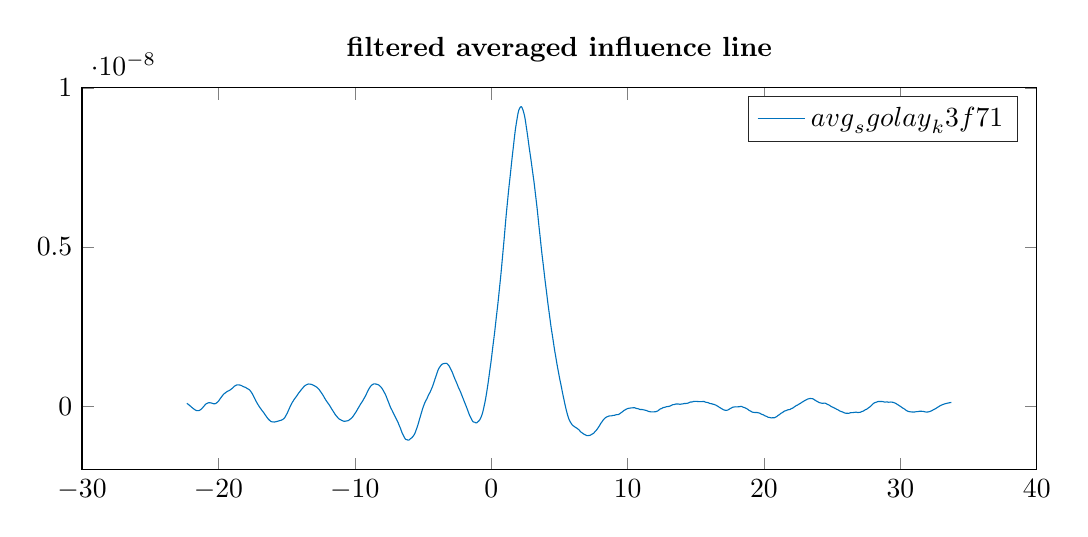
\begin{tikzpicture}

\begin{axis}[%
width=\textwidth,
height=0.4\textwidth,
at={(0\figurewidth,0\figureheight)},
scale only axis,
xmin=-30,
xmax=40,
ymin=-2e-09,
ymax=1e-08,
axis background/.style={fill=white},
title style={font=\bfseries},
title={filtered averaged influence line},
legend style={legend cell align=left,align=left,draw=white!15!black}
]
\addplot [color=mycolor1,solid]
  table[row sep=crcr]{%
-22.3159404296875	8.67898727603595e-11\\
-22.295791015625	8.1203080611142e-11\\
-22.2756416015625	7.53545096820691e-11\\
-22.2554921875	6.92634840942748e-11\\
-22.2353427734375	6.29493279688935e-11\\
-22.215193359375	5.64313654270595e-11\\
-22.1950439453125	4.97289205899073e-11\\
-22.17489453125	4.2861317578571e-11\\
-22.1547451171875	3.58478805141849e-11\\
-22.134595703125	2.87079335178835e-11\\
-22.1144462890625	2.1460800710801e-11\\
-22.094296875	1.41258062140716e-11\\
-22.0741474609375	6.72227414882981e-12\\
-22.053998046875	-7.30471363790177e-13\\
-22.0338486328125	-8.21310620265405e-12\\
-22.01369921875	-1.57063062466275e-11\\
-21.9935498046875	-2.31907473745762e-11\\
-21.973400390625	-3.06471054653657e-11\\
-21.9532509765625	-3.8056056397862e-11\\
-21.9331015625	-4.53982760509305e-11\\
-21.9129521484375	-5.26544403034371e-11\\
-21.892802734375	-5.98052250342473e-11\\
-21.8726533203125	-6.68313061222269e-11\\
-21.85250390625	-7.37133594462416e-11\\
-21.8323544921875	-8.04320608851571e-11\\
-21.812205078125	-8.6968086317839e-11\\
-21.7920556640625	-9.33021116231531e-11\\
-21.77190625	-9.94148126799649e-11\\
-21.7517568359375	-1.0528686536714e-10\\
-21.731607421875	-1.10898945563545e-10\\
-21.7114580078125	-1.16231729148045e-10\\
-21.69130859375	-1.21265891999505e-10\\
-21.6711591796875	-1.25982109996791e-10\\
-21.651009765625	-1.3036105901877e-10\\
-21.6308603515625	-1.34383414944306e-10\\
-21.6107109375	-1.38029853652265e-10\\
-21.5905615234375	-1.39779977270818e-10\\
-21.570412109375	-1.40688199593281e-10\\
-21.5502626953125	-1.43006842729823e-10\\
-21.53011328125	-1.42019763089185e-10\\
-21.5099638671875	-1.4294385103331e-10\\
-21.489814453125	-1.4286235102224e-10\\
-21.4696650390625	-1.41837267444482e-10\\
-21.449515625	-1.40826254379648e-10\\
-21.4293662109375	-1.38780270221065e-10\\
-21.409216796875	-1.36436237344313e-10\\
-21.3890673828125	-1.32505076891322e-10\\
-21.36891796875	-1.28831991073246e-10\\
-21.3487685546875	-1.22919172482118e-10\\
-21.328619140625	-1.16992919811968e-10\\
-21.3084697265625	-1.11288059464338e-10\\
-21.2883203125	-1.04477702514667e-10\\
-21.2681708984375	-9.76019553699286e-11\\
-21.248021484375	-8.9016582195176e-11\\
-21.2278720703125	-8.10447498129743e-11\\
-21.20772265625	-7.29904495172733e-11\\
-21.1875732421875	-6.3011564517778e-11\\
-21.167423828125	-5.36519133401224e-11\\
-21.1472744140625	-4.41617060493175e-11\\
-21.127125	-3.43567313948739e-11\\
-21.1069755859375	-2.29551504084676e-11\\
-21.086826171875	-1.46117243954024e-11\\
-21.0666767578125	-5.1549727606947e-12\\
-21.04652734375	4.86984686400413e-12\\
-21.0263779296875	1.58807932750515e-11\\
-21.006228515625	2.51232554989446e-11\\
-20.9860791015625	3.62392978791533e-11\\
-20.9659296875	4.61124318809231e-11\\
-20.9457802734375	5.47423543993829e-11\\
-20.925630859375	6.3364672789328e-11\\
-20.9054814453125	6.96216223796423e-11\\
-20.88533203125	7.45335666870925e-11\\
-20.8651826171875	7.88844386349542e-11\\
-20.845033203125	8.27806561527508e-11\\
-20.8248837890625	8.78012393271364e-11\\
-20.804734375	9.19691770443874e-11\\
-20.7845849609375	9.54084051420609e-11\\
-20.764435546875	9.84682943304978e-11\\
-20.7442861328125	1.0191211185897e-10\\
-20.72413671875	1.05037002950432e-10\\
-20.7039873046875	1.07044471872159e-10\\
-20.683837890625	1.07643803347569e-10\\
-20.6636884765625	1.080899596428e-10\\
-20.6435390625	1.06781441529695e-10\\
-20.6233896484375	1.05953493530749e-10\\
-20.603240234375	1.0569975737579e-10\\
-20.5830908203125	1.04012368952402e-10\\
-20.56294140625	1.01263971154771e-10\\
-20.5427919921875	9.95560403357216e-11\\
-20.522642578125	9.90738693180566e-11\\
-20.5024931640625	9.66205590801176e-11\\
-20.48234375	9.38972237186157e-11\\
-20.4621943359375	9.10741929985431e-11\\
-20.442044921875	8.64704440531934e-11\\
-20.4218955078125	8.35864037574147e-11\\
-20.40174609375	8.10505482036435e-11\\
-20.3815966796875	7.71329411193896e-11\\
-20.361447265625	7.62252706005559e-11\\
-20.3412978515625	7.45550007105247e-11\\
-20.3211484375	7.35376441804544e-11\\
-20.3009990234375	7.39646936857209e-11\\
-20.280849609375	7.26348400001808e-11\\
-20.2607001953125	7.47980702229829e-11\\
-20.24055078125	7.64803732055094e-11\\
-20.2204013671875	7.87791051481054e-11\\
-20.200251953125	8.31489310900492e-11\\
-20.1801025390625	8.76443790646152e-11\\
-20.159953125	9.35299318383235e-11\\
-20.1398037109375	9.93329879798035e-11\\
-20.119654296875	1.07282782410602e-10\\
-20.0995048828125	1.12305207799058e-10\\
-20.07935546875	1.21117873120574e-10\\
-20.0592060546875	1.29053519816557e-10\\
-20.039056640625	1.37593678720489e-10\\
-20.0189072265625	1.46227124279759e-10\\
-19.9987578125	1.56541805743907e-10\\
-19.9786083984375	1.67095799115976e-10\\
-19.958458984375	1.79013631361015e-10\\
-19.9383095703125	1.92531722722055e-10\\
-19.91816015625	2.03999827752205e-10\\
-19.8980107421875	2.16136181702142e-10\\
-19.877861328125	2.28329292225863e-10\\
-19.8577119140625	2.3974188931948e-10\\
-19.8375625	2.53138479027811e-10\\
-19.8174130859375	2.64315558101537e-10\\
-19.797263671875	2.76269235243153e-10\\
-19.7771142578125	2.88466015017893e-10\\
-19.75696484375	2.99653004124642e-10\\
-19.7368154296875	3.11124721673224e-10\\
-19.716666015625	3.22449011114571e-10\\
-19.6965166015625	3.33508766327296e-10\\
-19.6763671875	3.43754057973469e-10\\
-19.6562177734375	3.54921846259408e-10\\
-19.636068359375	3.65073152456555e-10\\
-19.6159189453125	3.74843211678909e-10\\
-19.59576953125	3.83129761101548e-10\\
-19.5756201171875	3.92126457589503e-10\\
-19.555470703125	3.98956785369156e-10\\
-19.5353212890625	4.04320495742186e-10\\
-19.515171875	4.10800184598532e-10\\
-19.4950224609375	4.15825584149369e-10\\
-19.474873046875	4.22421594813966e-10\\
-19.4547236328125	4.29050169330844e-10\\
-19.43457421875	4.362649422454e-10\\
-19.4144248046875	4.43586735944077e-10\\
-19.394275390625	4.49045004702586e-10\\
-19.3741259765625	4.54643311918819e-10\\
-19.3539765625	4.61602557844269e-10\\
-19.3338271484375	4.66782659282696e-10\\
-19.313677734375	4.69916947750597e-10\\
-19.2935283203125	4.73901407117266e-10\\
-19.27337890625	4.76583799629428e-10\\
-19.2532294921875	4.80536200185656e-10\\
-19.233080078125	4.84130897335206e-10\\
-19.2129306640625	4.89615080690648e-10\\
-19.19278125	4.94544380897012e-10\\
-19.1726318359375	4.99814895491069e-10\\
-19.152482421875	5.05177541825981e-10\\
-19.1323330078125	5.12789123660511e-10\\
-19.11218359375	5.19968101194661e-10\\
-19.0920341796875	5.26320905989124e-10\\
-19.071884765625	5.31593839006993e-10\\
-19.0517353515625	5.37388667501577e-10\\
-19.0315859375	5.44133732156685e-10\\
-19.0114365234375	5.51243492690487e-10\\
-18.991287109375	5.57998927060045e-10\\
-18.9711376953125	5.65887210418543e-10\\
-18.95098828125	5.73990213467483e-10\\
-18.9308388671875	5.8067567569623e-10\\
-18.910689453125	5.90689319324282e-10\\
-18.8905400390625	5.99860633395128e-10\\
-18.870390625	6.07347648445804e-10\\
-18.8502412109375	6.15138226442078e-10\\
-18.830091796875	6.22353169717382e-10\\
-18.8099423828125	6.29260834176868e-10\\
-18.78979296875	6.35525655230177e-10\\
-18.7696435546875	6.40401101573701e-10\\
-18.749494140625	6.4679049060638e-10\\
-18.7293447265625	6.50416619395639e-10\\
-18.7091953125	6.54514372584247e-10\\
-18.6890458984375	6.5830419320116e-10\\
-18.668896484375	6.62298160324767e-10\\
-18.6487470703125	6.63865116243893e-10\\
-18.62859765625	6.6716909654642e-10\\
-18.6084482421875	6.67703938177782e-10\\
-18.588298828125	6.69487041204292e-10\\
-18.5681494140625	6.69805999696933e-10\\
-18.548	6.69235948431394e-10\\
-18.5278505859375	6.67907499535369e-10\\
-18.507701171875	6.67000880945823e-10\\
-18.4875517578125	6.65174469506267e-10\\
-18.46740234375	6.63135978385951e-10\\
-18.4472529296875	6.62900875800328e-10\\
-18.427103515625	6.62067077414526e-10\\
-18.4069541015625	6.59569859446356e-10\\
-18.3868046875	6.57428093296665e-10\\
-18.3666552734375	6.55130325069679e-10\\
-18.346505859375	6.51114699914225e-10\\
-18.3263564453125	6.47814666645566e-10\\
-18.30620703125	6.43976838252702e-10\\
-18.2860576171875	6.390073234456e-10\\
-18.265908203125	6.35143501351595e-10\\
-18.2457587890625	6.30559352627857e-10\\
-18.225609375	6.25236586541096e-10\\
-18.2054599609375	6.206364515653e-10\\
-18.185310546875	6.16264582607168e-10\\
-18.1651611328125	6.11555375017359e-10\\
-18.14501171875	6.0794138198549e-10\\
-18.1248623046875	6.03565795946756e-10\\
-18.104712890625	6.00897142677002e-10\\
-18.0845634765625	5.97558951336312e-10\\
-18.0644140625	5.94936893255891e-10\\
-18.0442646484375	5.92275623103469e-10\\
-18.024115234375	5.89636840980298e-10\\
-18.0039658203125	5.8580825939493e-10\\
-17.98381640625	5.79961382375621e-10\\
-17.9636669921875	5.74235438223974e-10\\
-17.943517578125	5.69648032799051e-10\\
-17.9233681640625	5.62760395700072e-10\\
-17.90321875	5.55768655188611e-10\\
-17.8830693359375	5.51094322168639e-10\\
-17.862919921875	5.45286483185147e-10\\
-17.8427705078125	5.41517700137424e-10\\
-17.82262109375	5.37349588736374e-10\\
-17.8024716796875	5.32348327657367e-10\\
-17.782322265625	5.27842953923235e-10\\
-17.7621728515625	5.23047581926305e-10\\
-17.7420234375	5.17050933242468e-10\\
-17.7218740234375	5.11060369079418e-10\\
-17.701724609375	5.00956505250385e-10\\
-17.6815751953125	4.90938283078307e-10\\
-17.66142578125	4.78692928894405e-10\\
-17.6412763671875	4.68314427500357e-10\\
-17.621126953125	4.56374256224938e-10\\
-17.6009775390625	4.44837908489513e-10\\
-17.580828125	4.32521263674515e-10\\
-17.5606787109375	4.19085369931516e-10\\
-17.540529296875	4.054816099691e-10\\
-17.5203798828125	3.92877990313167e-10\\
-17.50023046875	3.77537367544578e-10\\
-17.4800810546875	3.60028742497481e-10\\
-17.459931640625	3.4345209083536e-10\\
-17.4397822265625	3.27763919085221e-10\\
-17.4196328125	3.0990989420915e-10\\
-17.3994833984375	2.9210260888233e-10\\
-17.379333984375	2.74742254616903e-10\\
-17.3591845703125	2.58772754731258e-10\\
-17.33903515625	2.40805274369034e-10\\
-17.3188857421875	2.2376685731252e-10\\
-17.298736328125	2.06188137992542e-10\\
-17.2785869140625	1.88494069503873e-10\\
-17.2584375	1.7106858597165e-10\\
-17.2382880859375	1.53057709973015e-10\\
-17.218138671875	1.37369775777959e-10\\
-17.1979892578125	1.20404355538075e-10\\
-17.17783984375	1.04931549525229e-10\\
-17.1576904296875	9.02230297346949e-11\\
-17.137541015625	7.56236993512886e-11\\
-17.1173916015625	6.18077245199294e-11\\
-17.0972421875	4.86028235835112e-11\\
-17.0770927734375	3.28040575153274e-11\\
-17.056943359375	1.8753128948053e-11\\
-17.0367939453125	5.39398791556178e-12\\
-17.01664453125	-8.40740390394229e-12\\
-16.9964951171875	-2.12601038035827e-11\\
-16.976345703125	-3.3541759429505e-11\\
-16.9561962890625	-4.55571697713523e-11\\
-16.936046875	-5.8041557593674e-11\\
-16.9158974609375	-6.97685860911885e-11\\
-16.895748046875	-8.13631520686977e-11\\
-16.8755986328125	-9.45492939111548e-11\\
-16.85544921875	-1.05921071236031e-10\\
-16.8352998046875	-1.18825340845301e-10\\
-16.815150390625	-1.30858010120763e-10\\
-16.7950009765625	-1.41445468013186e-10\\
-16.7748515625	-1.52957780180459e-10\\
-16.7547021484375	-1.64504073031741e-10\\
-16.734552734375	-1.74629010386716e-10\\
-16.7144033203125	-1.86309836616207e-10\\
-16.69425390625	-1.98241790013013e-10\\
-16.6741044921875	-2.09680869564149e-10\\
-16.653955078125	-2.22659948270529e-10\\
-16.6338056640625	-2.35263451479232e-10\\
-16.61365625	-2.48396705490122e-10\\
-16.5935068359375	-2.61988583019695e-10\\
-16.573357421875	-2.74431211964357e-10\\
-16.5532080078125	-2.86574148836711e-10\\
-16.53305859375	-2.97207469224083e-10\\
-16.5129091796875	-3.09656064137753e-10\\
-16.492759765625	-3.21698360574595e-10\\
-16.4726103515625	-3.32932806624546e-10\\
-16.4524609375	-3.45165672356704e-10\\
-16.4323115234375	-3.57425555451675e-10\\
-16.412162109375	-3.69610770300898e-10\\
-16.3920126953125	-3.81737239955355e-10\\
-16.37186328125	-3.91469964161506e-10\\
-16.3517138671875	-4.02447273794479e-10\\
-16.331564453125	-4.11897105337765e-10\\
-16.3114150390625	-4.20464801027949e-10\\
-16.291265625	-4.30302598844225e-10\\
-16.2711162109375	-4.36869921307454e-10\\
-16.250966796875	-4.45497881565852e-10\\
-16.2308173828125	-4.53503021816056e-10\\
-16.21066796875	-4.61080177369689e-10\\
-16.1905185546875	-4.67737272141624e-10\\
-16.170369140625	-4.74309153281178e-10\\
-16.1502197265625	-4.79840991888087e-10\\
-16.1300703125	-4.8407875676292e-10\\
-16.1099208984375	-4.87105975117299e-10\\
-16.089771484375	-4.908431132004e-10\\
-16.0696220703125	-4.92613302343236e-10\\
-16.04947265625	-4.92956093212739e-10\\
-16.0293232421875	-4.94120399967232e-10\\
-16.009173828125	-4.97083419045371e-10\\
-15.9890244140625	-4.96660280957626e-10\\
-15.968875	-4.96214349885798e-10\\
-15.9487255859375	-4.97576300952549e-10\\
-15.928576171875	-4.97849756551216e-10\\
-15.9084267578125	-4.97770405922113e-10\\
-15.88827734375	-4.99037666658363e-10\\
-15.8681279296875	-4.96598923114771e-10\\
-15.847978515625	-4.96243232990695e-10\\
-15.8278291015625	-4.94646183450685e-10\\
-15.8076796875	-4.91319070123466e-10\\
-15.7875302734375	-4.89888066235254e-10\\
-15.767380859375	-4.87034546651088e-10\\
-15.7472314453125	-4.83915967879914e-10\\
-15.72708203125	-4.81043557200845e-10\\
-15.7069326171875	-4.79608879022607e-10\\
-15.686783203125	-4.78253493741678e-10\\
-15.6666337890625	-4.76794425939281e-10\\
-15.646484375	-4.74141186721479e-10\\
-15.6263349609375	-4.72025537090525e-10\\
-15.606185546875	-4.68618697199895e-10\\
-15.5860361328125	-4.67193952775732e-10\\
-15.56588671875	-4.65242850034763e-10\\
-15.5457373046875	-4.62425857180951e-10\\
-15.525587890625	-4.58908038633759e-10\\
-15.5054384765625	-4.55789607883857e-10\\
-15.4852890625	-4.53042249040878e-10\\
-15.4651396484375	-4.50770477010417e-10\\
-15.444990234375	-4.48187171342311e-10\\
-15.4248408203125	-4.47184940615185e-10\\
-15.40469140625	-4.4331062542856e-10\\
-15.3845419921875	-4.40186656052731e-10\\
-15.364392578125	-4.36492127437904e-10\\
-15.3442431640625	-4.32060715897244e-10\\
-15.32409375	-4.2768763552563e-10\\
-15.3039443359375	-4.22545397747608e-10\\
-15.283794921875	-4.17122925708318e-10\\
-15.2636455078125	-4.11931877177642e-10\\
-15.24349609375	-4.06525098451059e-10\\
-15.2233466796875	-3.99610240656295e-10\\
-15.203197265625	-3.93093415598263e-10\\
-15.1830478515625	-3.8547087582566e-10\\
-15.1628984375	-3.74726373130745e-10\\
-15.1427490234375	-3.63600709441569e-10\\
-15.122599609375	-3.50496489200263e-10\\
-15.1024501953125	-3.3653831681729e-10\\
-15.08230078125	-3.20808719738991e-10\\
-15.0621513671875	-3.04620358933172e-10\\
-15.042001953125	-2.89181247983373e-10\\
-15.0218525390625	-2.73619143447811e-10\\
-15.001703125	-2.57846146504379e-10\\
-14.9815537109375	-2.42232579657868e-10\\
-14.961404296875	-2.24780016315549e-10\\
-14.9412548828125	-2.07602550716905e-10\\
-14.92110546875	-1.88008521359226e-10\\
-14.9009560546875	-1.69355731049484e-10\\
-14.880806640625	-1.49462055906679e-10\\
-14.8606572265625	-1.29730005388426e-10\\
-14.8405078125	-1.10453100746601e-10\\
-14.8203583984375	-9.06386917836988e-11\\
-14.800208984375	-7.08532721859046e-11\\
-14.7800595703125	-5.18651682594372e-11\\
-14.75991015625	-3.38695332839401e-11\\
-14.7397607421875	-1.47349686643363e-11\\
-14.719611328125	4.54449895233775e-12\\
-14.6994619140625	2.26756619613056e-11\\
-14.6793125	4.05269024867635e-11\\
-14.6591630859375	5.84761465191046e-11\\
-14.639013671875	7.47655627052903e-11\\
-14.6188642578125	9.04133921518303e-11\\
-14.59871484375	1.05631386650032e-10\\
-14.5785654296875	1.2057952070237e-10\\
-14.558416015625	1.34176989270603e-10\\
-14.5382666015625	1.46987817093604e-10\\
-14.5181171875	1.61409664696857e-10\\
-14.4979677734375	1.75068399212643e-10\\
-14.477818359375	1.88982536855482e-10\\
-14.4576689453125	2.02648123111987e-10\\
-14.43751953125	2.13947836176815e-10\\
-14.4173701171875	2.27853489668983e-10\\
-14.397220703125	2.39135004862356e-10\\
-14.3770712890625	2.50132401590707e-10\\
-14.356921875	2.62516177333097e-10\\
-14.3367724609375	2.74124920496903e-10\\
-14.316623046875	2.850384397374e-10\\
-14.2964736328125	2.96443709703249e-10\\
-14.27632421875	3.09344397799662e-10\\
-14.2561748046875	3.20797542569778e-10\\
-14.236025390625	3.33493790714243e-10\\
-14.2158759765625	3.46470702122278e-10\\
-14.1957265625	3.59628150646567e-10\\
-14.1755771484375	3.73025469735839e-10\\
-14.155427734375	3.86357409116074e-10\\
-14.1352783203125	3.99027052862074e-10\\
-14.11512890625	4.108616306272e-10\\
-14.0949794921875	4.22090492081182e-10\\
-14.074830078125	4.32259018383711e-10\\
-14.0546806640625	4.44218529413598e-10\\
-14.03453125	4.54220763528894e-10\\
-14.0143818359375	4.65437133831837e-10\\
-13.994232421875	4.78691774105528e-10\\
-13.9740830078125	4.89429481657954e-10\\
-13.95393359375	5.00512760511423e-10\\
-13.9337841796875	5.11342327688426e-10\\
-13.913634765625	5.21121171579008e-10\\
-13.8934853515625	5.31558562764606e-10\\
-13.8733359375	5.40496063094631e-10\\
-13.8531865234375	5.50463482929797e-10\\
-13.833037109375	5.61472124391134e-10\\
-13.8128876953125	5.70637131877284e-10\\
-13.79273828125	5.81197161356616e-10\\
-13.7725888671875	5.92352722596212e-10\\
-13.752439453125	6.04028575352357e-10\\
-13.7322900390625	6.12854050230259e-10\\
-13.712140625	6.21720769219953e-10\\
-13.6919912109375	6.30555387089878e-10\\
-13.671841796875	6.38199437995667e-10\\
-13.6516923828125	6.4399654931032e-10\\
-13.63154296875	6.49665202559851e-10\\
-13.6113935546875	6.54516000493895e-10\\
-13.591244140625	6.58644961592677e-10\\
-13.5710947265625	6.6350510937956e-10\\
-13.5509453125	6.69614894401463e-10\\
-13.5307958984375	6.74587876587434e-10\\
-13.510646484375	6.78433903141071e-10\\
-13.4904970703125	6.82733990990227e-10\\
-13.47034765625	6.86456531819895e-10\\
-13.4501982421875	6.88542574672645e-10\\
-13.430048828125	6.92100632697125e-10\\
-13.4098994140625	6.93307267562556e-10\\
-13.38975	6.93662910173634e-10\\
-13.3696005859375	6.93550363566997e-10\\
-13.349451171875	6.93233736650528e-10\\
-13.3293017578125	6.93454819170117e-10\\
-13.30915234375	6.91407630524549e-10\\
-13.2890029296875	6.90120506499983e-10\\
-13.268853515625	6.8963318836172e-10\\
-13.2487041015625	6.8779466435877e-10\\
-13.2285546875	6.87044320271726e-10\\
-13.2084052734375	6.85423303338702e-10\\
-13.188255859375	6.83287396097285e-10\\
-13.1681064453125	6.80287663905767e-10\\
-13.14795703125	6.77519243052854e-10\\
-13.1278076171875	6.74651850959048e-10\\
-13.107658203125	6.71057429381118e-10\\
-13.0875087890625	6.66259482483497e-10\\
-13.067359375	6.61039892561439e-10\\
-13.0472099609375	6.56109103534834e-10\\
-13.027060546875	6.52556412196375e-10\\
-13.0069111328125	6.4895595083514e-10\\
-12.98676171875	6.43125817937193e-10\\
-12.9666123046875	6.39918699053521e-10\\
-12.946462890625	6.34967145965686e-10\\
-12.9263134765625	6.29782756391564e-10\\
-12.9061640625	6.2451301108219e-10\\
-12.8860146484375	6.20362445043169e-10\\
-12.865865234375	6.14843886358201e-10\\
-12.8457158203125	6.08708625944833e-10\\
-12.82556640625	6.04644462238722e-10\\
-12.8054169921875	5.98602206070116e-10\\
-12.785267578125	5.91714067216617e-10\\
-12.7651181640625	5.86134031557143e-10\\
-12.74496875	5.76820114067043e-10\\
-12.7248193359375	5.69605173753755e-10\\
-12.704669921875	5.61918525991655e-10\\
-12.6845205078125	5.53703782082147e-10\\
-12.66437109375	5.43512652271711e-10\\
-12.6442216796875	5.35100476780355e-10\\
-12.624072265625	5.24092431684646e-10\\
-12.6039228515625	5.13913840001729e-10\\
-12.5837734375	5.02506879837744e-10\\
-12.5636240234375	4.89414677696115e-10\\
-12.543474609375	4.76930134527792e-10\\
-12.5233251953125	4.63381357438575e-10\\
-12.50317578125	4.50497050111926e-10\\
-12.4830263671875	4.38386909300945e-10\\
-12.462876953125	4.25075191023054e-10\\
-12.4427275390625	4.14256622680566e-10\\
-12.422578125	4.00238860928703e-10\\
-12.4024287109375	3.8867801387382e-10\\
-12.382279296875	3.75907051971667e-10\\
-12.3621298828125	3.62142589615405e-10\\
-12.34198046875	3.48346051203143e-10\\
-12.3218310546875	3.33695915615175e-10\\
-12.301681640625	3.19548838053658e-10\\
-12.2815322265625	3.05397350592402e-10\\
-12.2613828125	2.89747873905144e-10\\
-12.2412333984375	2.73915709476945e-10\\
-12.221083984375	2.58287620393523e-10\\
-12.2009345703125	2.42889469484852e-10\\
-12.18078515625	2.2887770902755e-10\\
-12.1606357421875	2.15200390422635e-10\\
-12.140486328125	2.02185109112953e-10\\
-12.1203369140625	1.88606400173487e-10\\
-12.1001875	1.75035708027348e-10\\
-12.0800380859375	1.62698089905834e-10\\
-12.059888671875	1.50487006901618e-10\\
-12.0397392578125	1.36809855461618e-10\\
-12.01958984375	1.248692254197e-10\\
-11.9994404296875	1.11686499747541e-10\\
-11.979291015625	9.92371312950136e-11\\
-11.9591416015625	8.71407015010259e-11\\
-11.9389921875	7.55992754180584e-11\\
-11.9188427734375	6.35802147741843e-11\\
-11.898693359375	5.1450369658301e-11\\
-11.8785439453125	4.03142007767155e-11\\
-11.85839453125	2.76629392877886e-11\\
-11.8382451171875	1.38608398707297e-11\\
-11.818095703125	-2.25883010620068e-13\\
-11.7979462890625	-1.60698012826838e-11\\
-11.777796875	-2.99227522352883e-11\\
-11.7576474609375	-4.48990446393195e-11\\
-11.737498046875	-5.88872514721636e-11\\
-11.7173486328125	-7.35442489227487e-11\\
-11.69719921875	-8.78447708120369e-11\\
-11.6770498046875	-1.02169828130629e-10\\
-11.656900390625	-1.1522000871221e-10\\
-11.6367509765625	-1.28978765376166e-10\\
-11.6166015625	-1.41892798162051e-10\\
-11.5964521484375	-1.55574293821609e-10\\
-11.576302734375	-1.69112388007649e-10\\
-11.5561533203125	-1.82295569244823e-10\\
-11.53600390625	-1.97161823129974e-10\\
-11.5158544921875	-2.10730437243821e-10\\
-11.495705078125	-2.24253380160788e-10\\
-11.4755556640625	-2.37242487135631e-10\\
-11.45540625	-2.50491547689188e-10\\
-11.4352568359375	-2.63023671503225e-10\\
-11.415107421875	-2.74938886268296e-10\\
-11.3949580078125	-2.87076008651464e-10\\
-11.37480859375	-2.96820071278269e-10\\
-11.3546591796875	-3.07333148596502e-10\\
-11.334509765625	-3.18285653174223e-10\\
-11.3143603515625	-3.27604340796115e-10\\
-11.2942109375	-3.38704940642113e-10\\
-11.2740615234375	-3.49678711693401e-10\\
-11.253912109375	-3.60119946577293e-10\\
-11.2337626953125	-3.69142158157202e-10\\
-11.21361328125	-3.79952676131872e-10\\
-11.1934638671875	-3.87919762647338e-10\\
-11.173314453125	-3.96712784406119e-10\\
-11.1531650390625	-4.01687284240775e-10\\
-11.133015625	-4.07605617714107e-10\\
-11.1128662109375	-4.12350799742798e-10\\
-11.092716796875	-4.17026535754328e-10\\
-11.0725673828125	-4.21472968619293e-10\\
-11.05241796875	-4.26998805402923e-10\\
-11.0322685546875	-4.30524262539269e-10\\
-11.012119140625	-4.36060621403028e-10\\
-10.9919697265625	-4.40302373834558e-10\\
-10.9718203125	-4.45917440866377e-10\\
-10.9516708984375	-4.49135183468454e-10\\
-10.931521484375	-4.53533592069381e-10\\
-10.9113720703125	-4.56944160981568e-10\\
-10.89122265625	-4.6164012963193e-10\\
-10.8710732421875	-4.65130034372602e-10\\
-10.850923828125	-4.69077274178372e-10\\
-10.8307744140625	-4.72034157386411e-10\\
-10.810625	-4.74146947954953e-10\\
-10.7904755859375	-4.75276329037831e-10\\
-10.770326171875	-4.76689245099242e-10\\
-10.7501767578125	-4.76681901543776e-10\\
-10.73002734375	-4.75383657949291e-10\\
-10.7098779296875	-4.7476186649302e-10\\
-10.689728515625	-4.73021683983847e-10\\
-10.6695791015625	-4.70806754888795e-10\\
-10.6494296875	-4.6876307237053e-10\\
-10.6292802734375	-4.68212616637222e-10\\
-10.609130859375	-4.64621330549814e-10\\
-10.5889814453125	-4.64475572505294e-10\\
-10.56883203125	-4.6401525491167e-10\\
-10.5486826171875	-4.62911124242716e-10\\
-10.528533203125	-4.60564990717473e-10\\
-10.5083837890625	-4.58745019133813e-10\\
-10.488234375	-4.55432341775458e-10\\
-10.4680849609375	-4.51031436315612e-10\\
-10.447935546875	-4.45044468559893e-10\\
-10.4277861328125	-4.39417332645233e-10\\
-10.40763671875	-4.32474928911421e-10\\
-10.3874873046875	-4.25778127672632e-10\\
-10.367337890625	-4.18940785323053e-10\\
-10.3471884765625	-4.13281995328969e-10\\
-10.3270390625	-4.06470074128349e-10\\
-10.3068896484375	-4.01155762048834e-10\\
-10.286740234375	-3.93222854998465e-10\\
-10.2665908203125	-3.86511102186866e-10\\
-10.24644140625	-3.7841078277791e-10\\
-10.2262919921875	-3.70213321889379e-10\\
-10.206142578125	-3.60529189029524e-10\\
-10.1859931640625	-3.50879699787706e-10\\
-10.16584375	-3.41221847788946e-10\\
-10.1456943359375	-3.315008331268e-10\\
-10.125544921875	-3.19628336518597e-10\\
-10.1053955078125	-3.07788329195584e-10\\
-10.08524609375	-2.95123720337491e-10\\
-10.0650966796875	-2.81250521931811e-10\\
-10.044947265625	-2.6767587510847e-10\\
-10.0247978515625	-2.54816842333302e-10\\
-10.0046484375	-2.40624177744404e-10\\
-9.9844990234375	-2.26841018963121e-10\\
-9.964349609375	-2.1380410839286e-10\\
-9.9442001953125	-2.02867592455168e-10\\
-9.92405078125	-1.89012399271011e-10\\
-9.9039013671875	-1.75522306929747e-10\\
-9.883751953125	-1.62718212878417e-10\\
-9.8636025390625	-1.47718387545889e-10\\
-9.843453125	-1.32110881485654e-10\\
-9.8233037109375	-1.16710248971864e-10\\
-9.803154296875	-1.01932826561331e-10\\
-9.7830048828125	-8.53381425928896e-11\\
-9.76285546875	-7.16146905897695e-11\\
-9.7427060546875	-5.4975005012542e-11\\
-9.722556640625	-4.23875077371595e-11\\
-9.7024072265625	-2.68911844137704e-11\\
-9.6822578125	-1.25119180429773e-11\\
-9.6621083984375	2.82997396450248e-12\\
-9.641958984375	1.67154413987339e-11\\
-9.6218095703125	3.19489886739998e-11\\
-9.60166015625	4.72800969346783e-11\\
-9.5815107421875	6.13202979742422e-11\\
-9.561361328125	7.52791451478673e-11\\
-9.5412119140625	8.90921690320426e-11\\
-9.5210625	1.00907462183945e-10\\
-9.5009130859375	1.12844271086081e-10\\
-9.480763671875	1.25171794718974e-10\\
-9.4606142578125	1.38841120523211e-10\\
-9.44046484375	1.51783932272967e-10\\
-9.4203154296875	1.66567577110253e-10\\
-9.400166015625	1.81615498373643e-10\\
-9.3800166015625	1.97255424322848e-10\\
-9.3598671875	2.12955927564866e-10\\
-9.3397177734375	2.28845800659068e-10\\
-9.319568359375	2.43757893997803e-10\\
-9.2994189453125	2.59040827395325e-10\\
-9.27926953125	2.73811829528334e-10\\
-9.2591201171875	2.88328810179851e-10\\
-9.238970703125	3.03690144665828e-10\\
-9.2188212890625	3.19557625530702e-10\\
-9.198671875	3.35738544655324e-10\\
-9.1785224609375	3.53145459364157e-10\\
-9.158373046875	3.72516345738502e-10\\
-9.1382236328125	3.91595118552218e-10\\
-9.11807421875	4.1139903620705e-10\\
-9.0979248046875	4.30806504263593e-10\\
-9.077775390625	4.50029179483243e-10\\
-9.0576259765625	4.69034753680265e-10\\
-9.0374765625	4.87251177406596e-10\\
-9.0173271484375	5.03140271368096e-10\\
-8.997177734375	5.17518255069919e-10\\
-8.9770283203125	5.32604726401956e-10\\
-8.95687890625	5.46916989815018e-10\\
-8.9367294921875	5.60997145767619e-10\\
-8.916580078125	5.75424424064513e-10\\
-8.8964306640625	5.89320830114832e-10\\
-8.87628125	6.03213485754497e-10\\
-8.8561318359375	6.14111031472285e-10\\
-8.835982421875	6.25656242970244e-10\\
-8.8158330078125	6.36144097343417e-10\\
-8.79568359375	6.45271923822277e-10\\
-8.7755341796875	6.52961893661137e-10\\
-8.755384765625	6.60964224472248e-10\\
-8.7352353515625	6.67149613041743e-10\\
-8.7150859375	6.7386349523801e-10\\
-8.6949365234375	6.78934978853463e-10\\
-8.674787109375	6.84272569297147e-10\\
-8.6546376953125	6.89495002987869e-10\\
-8.63448828125	6.92307873185585e-10\\
-8.6143388671875	6.96024763156893e-10\\
-8.594189453125	6.98562714477398e-10\\
-8.5740400390625	6.98903370713948e-10\\
-8.553890625	6.9851548094311e-10\\
-8.5337412109375	6.98451308077259e-10\\
-8.513591796875	6.97958265278417e-10\\
-8.4934423828125	6.96023281617478e-10\\
-8.47329296875	6.93817283101877e-10\\
-8.4531435546875	6.93836387611711e-10\\
-8.432994140625	6.91309298713908e-10\\
-8.4128447265625	6.8843818695579e-10\\
-8.3926953125	6.87104042986656e-10\\
-8.3725458984375	6.84644532057167e-10\\
-8.352396484375	6.81588279899133e-10\\
-8.3322470703125	6.80154469020989e-10\\
-8.31209765625	6.76415092333707e-10\\
-8.2919482421875	6.72756021013542e-10\\
-8.271798828125	6.68663540512423e-10\\
-8.2516494140625	6.64290004208836e-10\\
-8.2315	6.59401521830187e-10\\
-8.2113505859375	6.53429701801636e-10\\
-8.191201171875	6.46822605138552e-10\\
-8.1710517578125	6.38593960474545e-10\\
-8.15090234375	6.30001771379641e-10\\
-8.1307529296875	6.2114002007326e-10\\
-8.110603515625	6.11421961035285e-10\\
-8.0904541015625	6.0177702374075e-10\\
-8.0703046875	5.91423815003386e-10\\
-8.0501552734375	5.80437543619453e-10\\
-8.030005859375	5.69628453227262e-10\\
-8.0098564453125	5.57532503711186e-10\\
-7.98970703125	5.44623898310405e-10\\
-7.9695576171875	5.32021738474015e-10\\
-7.949408203125	5.16971358093986e-10\\
-7.9292587890625	5.02457161055209e-10\\
-7.909109375	4.8710357178674e-10\\
-7.8889599609375	4.70903965613765e-10\\
-7.868810546875	4.54246843369567e-10\\
-7.8486611328125	4.39122021267087e-10\\
-7.82851171875	4.23180352929981e-10\\
-7.8083623046875	4.07531158972592e-10\\
-7.788212890625	3.91098388748266e-10\\
-7.7680634765625	3.74806541024784e-10\\
-7.7479140625	3.56779642489574e-10\\
-7.7277646484375	3.37815964309426e-10\\
-7.707615234375	3.17400466300931e-10\\
-7.6874658203125	2.96210976285405e-10\\
-7.66731640625	2.72691831043196e-10\\
-7.6471669921875	2.49756481712625e-10\\
-7.627017578125	2.27836416444765e-10\\
-7.6068681640625	2.04800120225651e-10\\
-7.58671875	1.8260268132114e-10\\
-7.5665693359375	1.6319358107789e-10\\
-7.546419921875	1.40564313827162e-10\\
-7.5262705078125	1.18341691601927e-10\\
-7.50612109375	9.75306566681445e-11\\
-7.4859716796875	7.48698631921703e-11\\
-7.465822265625	5.05987852291317e-11\\
-7.4456728515625	2.7538573745586e-11\\
-7.4255234375	5.88695596122313e-12\\
-7.4053740234375	-1.58620679964196e-11\\
-7.385224609375	-3.69050784243737e-11\\
-7.3650751953125	-5.51491478606237e-11\\
-7.34492578125	-7.08225357240908e-11\\
-7.3247763671875	-8.73125854907294e-11\\
-7.304626953125	-1.03638929423192e-10\\
-7.2844775390625	-1.20764777631793e-10\\
-7.264328125	-1.37534183922075e-10\\
-7.2441787109375	-1.55828464166944e-10\\
-7.224029296875	-1.75272522831078e-10\\
-7.2038798828125	-1.92904040279604e-10\\
-7.18373046875	-2.12357964427875e-10\\
-7.1635810546875	-2.30198535616351e-10\\
-7.143431640625	-2.47475846928229e-10\\
-7.1232822265625	-2.63990339275989e-10\\
-7.1031328125	-2.79719214525211e-10\\
-7.0829833984375	-2.96118619337767e-10\\
-7.062833984375	-3.1355741927374e-10\\
-7.0426845703125	-3.3113350573019e-10\\
-7.02253515625	-3.50246937470803e-10\\
-7.0023857421875	-3.68404309598148e-10\\
-6.982236328125	-3.85475084764957e-10\\
-6.9620869140625	-4.04122132258875e-10\\
-6.9419375	-4.19689010266736e-10\\
-6.9217880859375	-4.35721078307128e-10\\
-6.901638671875	-4.51305730188511e-10\\
-6.8814892578125	-4.6736638174748e-10\\
-6.86133984375	-4.83757210816827e-10\\
-6.8411904296875	-5.03141140856775e-10\\
-6.821041015625	-5.23631499805956e-10\\
-6.8008916015625	-5.46204855779507e-10\\
-6.7807421875	-5.68283339363544e-10\\
-6.7605927734375	-5.89447502293544e-10\\
-6.740443359375	-6.11135242698089e-10\\
-6.7202939453125	-6.31599871195928e-10\\
-6.70014453125	-6.50918340730899e-10\\
-6.6799951171875	-6.71686446346963e-10\\
-6.659845703125	-6.92424432163314e-10\\
-6.6396962890625	-7.13819226731805e-10\\
-6.619546875	-7.38218518651063e-10\\
-6.5993974609375	-7.62953829118401e-10\\
-6.579248046875	-7.86261192649156e-10\\
-6.5590986328125	-8.09803797574852e-10\\
-6.53894921875	-8.32866379299476e-10\\
-6.5187998046875	-8.52444140888963e-10\\
-6.498650390625	-8.71493889720826e-10\\
-6.4785009765625	-8.897565325617e-10\\
-6.4583515625	-9.06161171699284e-10\\
-6.4382021484375	-9.2149985592461e-10\\
-6.418052734375	-9.38244447944571e-10\\
-6.3979033203125	-9.55262427803133e-10\\
-6.37775390625	-9.71801836955757e-10\\
-6.3576044921875	-9.88217357675389e-10\\
-6.337455078125	-1.00353914614043e-09\\
-6.3173056640625	-1.01757589548938e-09\\
-6.29715625	-1.02919559738335e-09\\
-6.2770068359375	-1.03801327588933e-09\\
-6.256857421875	-1.04516504622142e-09\\
-6.2367080078125	-1.04956390368384e-09\\
-6.21655859375	-1.05107185396887e-09\\
-6.1964091796875	-1.05372461784846e-09\\
-6.176259765625	-1.05617849071054e-09\\
-6.1561103515625	-1.05844683963052e-09\\
-6.1359609375	-1.06257005556844e-09\\
-6.1158115234375	-1.06506956946875e-09\\
-6.095662109375	-1.0678896912598e-09\\
-6.0755126953125	-1.06893789595572e-09\\
-6.05536328125	-1.06916317418787e-09\\
-6.0352138671875	-1.06495019848862e-09\\
-6.015064453125	-1.05998603537197e-09\\
-5.9949150390625	-1.05283190745049e-09\\
-5.974765625	-1.04490426046204e-09\\
-5.9546162109375	-1.03563184708591e-09\\
-5.934466796875	-1.02721988678347e-09\\
-5.9143173828125	-1.0213129158458e-09\\
-5.89416796875	-1.01636585439803e-09\\
-5.8740185546875	-1.00964797283758e-09\\
-5.853869140625	-1.00418279966962e-09\\
-5.8337197265625	-9.97847062122839e-10\\
-5.8135703125	-9.89744684742228e-10\\
-5.7934208984375	-9.80327204323811e-10\\
-5.773271484375	-9.71803278949891e-10\\
-5.7531220703125	-9.61414337051087e-10\\
-5.73297265625	-9.50036145416369e-10\\
-5.7128232421875	-9.37571745149124e-10\\
-5.692673828125	-9.25618687357675e-10\\
-5.6725244140625	-9.14487517730509e-10\\
-5.652375	-9.00154485752504e-10\\
-5.6322255859375	-8.85069342665795e-10\\
-5.612076171875	-8.68685701147262e-10\\
-5.5919267578125	-8.50184071579772e-10\\
-5.57177734375	-8.30034481048299e-10\\
-5.5516279296875	-8.08821281116635e-10\\
-5.531478515625	-7.83776218687287e-10\\
-5.5113291015625	-7.59561306905831e-10\\
-5.4911796875	-7.34523456180226e-10\\
-5.4710302734375	-7.11680304590932e-10\\
-5.450880859375	-6.8739299753235e-10\\
-5.4307314453125	-6.63670272375953e-10\\
-5.41058203125	-6.38113699509648e-10\\
-5.3904326171875	-6.1272039039711e-10\\
-5.370283203125	-5.83778260340742e-10\\
-5.3501337890625	-5.54669550682502e-10\\
-5.329984375	-5.25408245232014e-10\\
-5.3098349609375	-4.94038189397875e-10\\
-5.289685546875	-4.62784010401685e-10\\
-5.2695361328125	-4.33357952616302e-10\\
-5.24938671875	-4.02216065051437e-10\\
-5.2292373046875	-3.73732822334595e-10\\
-5.209087890625	-3.44868048328784e-10\\
-5.1889384765625	-3.15197458179988e-10\\
-5.1687890625	-2.8583681973874e-10\\
-5.1486396484375	-2.55102774036387e-10\\
-5.128490234375	-2.25592880703384e-10\\
-5.1083408203125	-1.96154531849557e-10\\
-5.08819140625	-1.66344924465192e-10\\
-5.0680419921875	-1.37829134105926e-10\\
-5.047892578125	-1.10598310478234e-10\\
-5.0277431640625	-8.26099299303319e-11\\
-5.00759375	-5.68367166024472e-11\\
-4.9874443359375	-3.18527864524654e-11\\
-4.967294921875	-7.08641064131056e-12\\
-4.9471455078125	1.71295396178916e-11\\
-4.92699609375	4.07693680305519e-11\\
-4.9068466796875	6.37284080476395e-11\\
-4.886697265625	8.52907214089182e-11\\
-4.8665478515625	1.06308906663928e-10\\
-4.8463984375	1.25615369879158e-10\\
-4.8262490234375	1.44558084572749e-10\\
-4.806099609375	1.61611841106849e-10\\
-4.7859501953125	1.77093983938913e-10\\
-4.76580078125	1.9208499006874e-10\\
-4.7456513671875	2.0780771969582e-10\\
-4.725501953125	2.23693903020626e-10\\
-4.7053525390625	2.40978261451785e-10\\
-4.685203125	2.59786457800258e-10\\
-4.6650537109375	2.81003967534532e-10\\
-4.644904296875	3.00642092370041e-10\\
-4.6247548828125	3.21296163110106e-10\\
-4.60460546875	3.4087662794515e-10\\
-4.5844560546875	3.5879731557011e-10\\
-4.564306640625	3.73464087433478e-10\\
-4.5441572265625	3.89713381853301e-10\\
-4.5240078125	4.04834746159836e-10\\
-4.5038583984375	4.19123740257566e-10\\
-4.483708984375	4.36791270465996e-10\\
-4.4635595703125	4.56168792752301e-10\\
-4.44341015625	4.74099751931739e-10\\
-4.4232607421875	4.95365814777236e-10\\
-4.403111328125	5.15711081135089e-10\\
-4.3829619140625	5.35190516266362e-10\\
-4.3628125	5.54399697842489e-10\\
-4.3426630859375	5.76105476374154e-10\\
-4.322513671875	5.97013065934173e-10\\
-4.3023642578125	6.18610469293879e-10\\
-4.28221484375	6.4035972046067e-10\\
-4.2620654296875	6.65256314758943e-10\\
-4.241916015625	6.91297321465467e-10\\
-4.2217666015625	7.17073982545137e-10\\
-4.2016171875	7.43318698432854e-10\\
-4.1814677734375	7.7173588997616e-10\\
-4.161318359375	7.98967609318035e-10\\
-4.1411689453125	8.2586198204891e-10\\
-4.12101953125	8.52926168732234e-10\\
-4.1008701171875	8.7790979371384e-10\\
-4.080720703125	9.01745971056959e-10\\
-4.0605712890625	9.25816959200045e-10\\
-4.040421875	9.50922603197768e-10\\
-4.0202724609375	9.75566928117567e-10\\
-4.000123046875	1.0014939542304e-09\\
-3.9799736328125	1.02748220447259e-09\\
-3.95982421875	1.05446041551398e-09\\
-3.9396748046875	1.079400401039e-09\\
-3.919525390625	1.10462269450143e-09\\
-3.8993759765625	1.12872815803667e-09\\
-3.8792265625	1.14978659429237e-09\\
-3.8590771484375	1.16846796310203e-09\\
-3.838927734375	1.18558229683175e-09\\
-3.8187783203125	1.19815640052148e-09\\
-3.79862890625	1.21109076446658e-09\\
-3.7784794921875	1.22295419839459e-09\\
-3.758330078125	1.23553625657612e-09\\
-3.7381806640625	1.24875792517805e-09\\
-3.71803125	1.26106926984313e-09\\
-3.6978818359375	1.27311856657888e-09\\
-3.677732421875	1.28518078022499e-09\\
-3.6575830078125	1.29503879998439e-09\\
-3.63743359375	1.30399162907859e-09\\
-3.6172841796875	1.31177405927864e-09\\
-3.597134765625	1.31748930699615e-09\\
-3.5769853515625	1.3219833635151e-09\\
-3.5568359375	1.32588436751043e-09\\
-3.5366865234375	1.3299547430663e-09\\
-3.516537109375	1.33185173280685e-09\\
-3.4963876953125	1.33487327474503e-09\\
-3.47623828125	1.33748659993559e-09\\
-3.4560888671875	1.33861000555211e-09\\
-3.435939453125	1.33979807876515e-09\\
-3.4157900390625	1.34110341060338e-09\\
-3.395640625	1.3414908473728e-09\\
-3.3754912109375	1.34300931054768e-09\\
-3.355341796875	1.34392525889267e-09\\
-3.3351923828125	1.34475142974992e-09\\
-3.31504296875	1.34561723262927e-09\\
-3.2948935546875	1.34492097989126e-09\\
-3.274744140625	1.34318983540932e-09\\
-3.2545947265625	1.33845761950803e-09\\
-3.2344453125	1.33168887796091e-09\\
-3.2142958984375	1.32329985888142e-09\\
-3.194146484375	1.31393217329492e-09\\
-3.1739970703125	1.30497769952687e-09\\
-3.15384765625	1.29466035582106e-09\\
-3.1336982421875	1.28663175518675e-09\\
-3.113548828125	1.27708572693025e-09\\
-3.0933994140625	1.26634075544184e-09\\
-3.07325	1.25416324513292e-09\\
-3.0531005859375	1.23978531356371e-09\\
-3.032951171875	1.22279960383188e-09\\
-3.0128017578125	1.20577452716464e-09\\
-2.99265234375	1.18582969110827e-09\\
-2.9725029296875	1.16776506602293e-09\\
-2.952353515625	1.14896774945823e-09\\
-2.9322041015625	1.13217751850819e-09\\
-2.9120546875	1.11521151934754e-09\\
-2.8919052734375	1.09862030259063e-09\\
-2.871755859375	1.07941695594662e-09\\
-2.8516064453125	1.06059937713764e-09\\
-2.83145703125	1.03812099997887e-09\\
-2.8113076171875	1.01605863653147e-09\\
-2.791158203125	9.92272657695722e-10\\
-2.7710087890625	9.70261022005143e-10\\
-2.750859375	9.46862076390141e-10\\
-2.7307099609375	9.25957691533036e-10\\
-2.710560546875	9.05046664618041e-10\\
-2.6904111328125	8.83793580944469e-10\\
-2.67026171875	8.62303144100159e-10\\
-2.6501123046875	8.41960789788959e-10\\
-2.629962890625	8.22196378137178e-10\\
-2.6098134765625	8.02988381641371e-10\\
-2.5896640625	7.83546763698411e-10\\
-2.5695146484375	7.63901100546643e-10\\
-2.549365234375	7.44258186432529e-10\\
-2.5292158203125	7.23578971790383e-10\\
-2.50906640625	7.03663049196322e-10\\
-2.4889169921875	6.82949991531415e-10\\
-2.468767578125	6.6008067928569e-10\\
-2.4486181640625	6.37459164958597e-10\\
-2.42846875	6.14534197361403e-10\\
-2.4083193359375	5.91549148347327e-10\\
-2.388169921875	5.71456666830493e-10\\
-2.3680205078125	5.52564877334463e-10\\
-2.34787109375	5.35367287392113e-10\\
-2.3277216796875	5.18577718746286e-10\\
-2.307572265625	5.00842155141496e-10\\
-2.2874228515625	4.82423615615852e-10\\
-2.2672734375	4.64430492523065e-10\\
-2.2471240234375	4.44209514067999e-10\\
-2.226974609375	4.22093799801074e-10\\
-2.2068251953125	3.99020013746096e-10\\
-2.18667578125	3.76712683996939e-10\\
-2.1665263671875	3.53956157547119e-10\\
-2.146376953125	3.31676868117145e-10\\
-2.1262275390625	3.09124147785471e-10\\
-2.106078125	2.87579966873678e-10\\
-2.0859287109375	2.66411966948922e-10\\
-2.065779296875	2.44724229570604e-10\\
-2.0456298828125	2.22981299756989e-10\\
-2.02548046875	2.01881540358478e-10\\
-2.0053310546875	1.78723794819791e-10\\
-1.985181640625	1.56906961815367e-10\\
-1.9650322265625	1.34902676562823e-10\\
-1.9448828125	1.13762407267925e-10\\
-1.9247333984375	9.23622479478532e-11\\
-1.904583984375	7.14224617328608e-11\\
-1.8844345703125	4.92759797825058e-11\\
-1.86428515625	2.80700081670031e-11\\
-1.8441357421875	6.07318945990699e-12\\
-1.823986328125	-1.73367709358486e-11\\
-1.8038369140625	-3.98493702551891e-11\\
-1.7836875	-6.19407265037637e-11\\
-1.7635380859375	-8.50248950271821e-11\\
-1.743388671875	-1.08147678774798e-10\\
-1.7232392578125	-1.30258443901786e-10\\
-1.70308984375	-1.53413496566453e-10\\
-1.6829404296875	-1.77759601822643e-10\\
-1.662791015625	-2.01996641405634e-10\\
-1.6426416015625	-2.24540875052034e-10\\
-1.6224921875	-2.47603292901876e-10\\
-1.6023427734375	-2.70354439437545e-10\\
-1.582193359375	-2.9044257593637e-10\\
-1.5620439453125	-3.08023488882064e-10\\
-1.54189453125	-3.26870117870114e-10\\
-1.5217451171875	-3.43650068361789e-10\\
-1.501595703125	-3.58478760846496e-10\\
-1.4814462890625	-3.76085319140258e-10\\
-1.461296875	-3.93678382949297e-10\\
-1.4411474609375	-4.09418705162782e-10\\
-1.420998046875	-4.27870603936097e-10\\
-1.4008486328125	-4.44844295077628e-10\\
-1.38069921875	-4.6002008679928e-10\\
-1.3605498046875	-4.73097257286851e-10\\
-1.340400390625	-4.83673763820228e-10\\
-1.3202509765625	-4.91397686189864e-10\\
-1.3001015625	-4.97671460469275e-10\\
-1.2799521484375	-5.01093984687097e-10\\
-1.259802734375	-5.01633124019386e-10\\
-1.2396533203125	-5.02061858119845e-10\\
-1.21950390625	-5.03963730963985e-10\\
-1.1993544921875	-5.07910036416718e-10\\
-1.179205078125	-5.13372038224153e-10\\
-1.1590556640625	-5.18063441819376e-10\\
-1.13890625	-5.21903733180488e-10\\
-1.1187568359375	-5.25510098096507e-10\\
-1.098607421875	-5.25878748676378e-10\\
-1.0784580078125	-5.2421425197e-10\\
-1.05830859375	-5.22775217460949e-10\\
-1.0381591796875	-5.15620695479243e-10\\
-1.018009765625	-5.09412161687682e-10\\
-0.997860351562498	-5.01806079706001e-10\\
-0.977710937499999	-4.93272732601333e-10\\
-0.957561523437498	-4.8466590774179e-10\\
-0.937412109375	-4.77967051384573e-10\\
-0.917262695312498	-4.68627645446358e-10\\
-0.897113281249997	-4.60604814269306e-10\\
-0.876963867187499	-4.50295714825541e-10\\
-0.856814453124997	-4.40293742353936e-10\\
-0.836665039062499	-4.27501796856926e-10\\
-0.816515624999997	-4.13454665798301e-10\\
-0.796366210937499	-3.96646739726791e-10\\
-0.776216796874998	-3.7853052425035e-10\\
-0.7560673828125	-3.59065942357281e-10\\
-0.735917968749998	-3.38238375495843e-10\\
-0.7157685546875	-3.1682796320172e-10\\
-0.695619140624999	-2.92804246550261e-10\\
-0.675469726562497	-2.68270635368445e-10\\
-0.655320312499999	-2.42261245383884e-10\\
-0.635170898437497	-2.12314825814834e-10\\
-0.615021484374999	-1.80811469200558e-10\\
-0.594872070312498	-1.46110041754251e-10\\
-0.57472265625	-1.08145785674063e-10\\
-0.554573242187498	-6.98189411126639e-11\\
-0.534423828125	-2.98757245111166e-11\\
-0.514274414062498	9.97883636437984e-12\\
-0.494124999999997	4.98450308225284e-11\\
-0.473975585937499	8.97646166063264e-11\\
-0.453826171874997	1.32815322337105e-10\\
-0.433676757812499	1.74744542871422e-10\\
-0.413527343749998	2.20551219615496e-10\\
-0.3933779296875	2.69988721224184e-10\\
-0.373228515624998	3.2185637490682e-10\\
-0.3530791015625	3.74024731546482e-10\\
-0.332929687499998	4.29849195806485e-10\\
-0.312780273437497	4.84182422488639e-10\\
-0.292630859374999	5.40977351498693e-10\\
-0.272481445312497	5.97552656107904e-10\\
-0.252332031249999	6.55228511011669e-10\\
-0.232182617187497	7.14274486352201e-10\\
-0.212033203124999	7.75090584208915e-10\\
-0.191883789062498	8.36960139477398e-10\\
-0.171734375	9.00811543299122e-10\\
-0.151584960937498	9.65100135581931e-10\\
-0.131435546875	1.02870923488052e-09\\
-0.111286132812499	1.09273388021512e-09\\
-0.091136718749997	1.15633753074738e-09\\
-0.0709873046874989	1.21735675813025e-09\\
-0.0508378906249973	1.27901519138634e-09\\
-0.0306884765624993	1.34172787451592e-09\\
-0.0105390624999977	1.4065041109733e-09\\
0.00961035156250034	1.47494902373584e-09\\
0.0297597656250019	1.5463769724675e-09\\
0.0499091796875	1.61850763409392e-09\\
0.0700585937500016	1.69160949160539e-09\\
0.0902080078125032	1.76536912745852e-09\\
0.110357421875001	1.83780224525176e-09\\
0.130506835937503	1.90881424857388e-09\\
0.150656250000001	1.97775667389915e-09\\
0.170805664062502	2.0439671668657e-09\\
0.190955078125	2.10952301783429e-09\\
0.211104492187502	2.17747110891264e-09\\
0.23125390625	2.24792798687383e-09\\
0.251403320312502	2.32072158406776e-09\\
0.271552734375003	2.39554448284038e-09\\
0.291702148437501	2.47159598448913e-09\\
0.311851562500003	2.54998554972819e-09\\
0.332000976562501	2.62836161563139e-09\\
0.352150390625003	2.70426582051122e-09\\
0.372299804687501	2.783756193898e-09\\
0.392449218750002	2.85717003086195e-09\\
0.4125986328125	2.93193037157867e-09\\
0.432748046875002	3.00621160990576e-09\\
0.4528974609375	3.08146976315997e-09\\
0.473046875000001	3.1567270579311e-09\\
0.493196289062503	3.23567964909691e-09\\
0.513345703125001	3.31495615054989e-09\\
0.533495117187503	3.39722225018348e-09\\
0.553644531250001	3.48000919643667e-09\\
0.573793945312502	3.56423583791293e-09\\
0.593943359375	3.64878265711236e-09\\
0.614092773437502	3.73415261365008e-09\\
0.6342421875	3.81816851748744e-09\\
0.654391601562502	3.90253585717876e-09\\
0.674541015625003	3.98622865502552e-09\\
0.694690429687501	4.07079933387206e-09\\
0.714839843750003	4.15696577956338e-09\\
0.734989257812501	4.24667393450555e-09\\
0.755138671875002	4.33930244518123e-09\\
0.7752880859375	4.43599836852715e-09\\
0.795437500000002	4.53199695693804e-09\\
0.8155869140625	4.62977911178783e-09\\
0.835736328125002	4.72593217660418e-09\\
0.855885742187503	4.82080966469445e-09\\
0.876035156250001	4.91456918042735e-09\\
0.896184570312503	5.00788131648252e-09\\
0.916333984375001	5.10130406235777e-09\\
0.936483398437503	5.19821721026901e-09\\
0.956632812500001	5.2956072405187e-09\\
0.976782226562502	5.39529435628851e-09\\
0.996931640625	5.49914910033871e-09\\
1.0170810546875	5.6002548943137e-09\\
1.03723046875	5.70251511960675e-09\\
1.0573798828125	5.80245123109296e-09\\
1.077529296875	5.90098745580762e-09\\
1.0976787109375	5.99550682370286e-09\\
1.117828125	6.08857985176143e-09\\
1.1379775390625	6.17826904375765e-09\\
1.158126953125	6.26651522911359e-09\\
1.1782763671875	6.35519519227245e-09\\
1.19842578125	6.4435931736084e-09\\
1.2185751953125	6.5311756859185e-09\\
1.238724609375	6.61893654574521e-09\\
1.2588740234375	6.70602749257433e-09\\
1.2790234375	6.79105145868943e-09\\
1.2991728515625	6.87449536315773e-09\\
1.319322265625	6.95443169433769e-09\\
1.3394716796875	7.03172421310388e-09\\
1.35962109375	7.11083397538449e-09\\
1.3797705078125	7.18780203505981e-09\\
1.399919921875	7.26809304371931e-09\\
1.4200693359375	7.34919911498065e-09\\
1.44021875	7.43023326124924e-09\\
1.4603681640625	7.51297136997464e-09\\
1.480517578125	7.59649627514356e-09\\
1.5006669921875	7.67883130454755e-09\\
1.52081640625	7.75827691310096e-09\\
1.5409658203125	7.83748986892991e-09\\
1.561115234375	7.91310887059208e-09\\
1.5812646484375	7.98877724189267e-09\\
1.6014140625	8.06204944393145e-09\\
1.6215634765625	8.13795940990211e-09\\
1.641712890625	8.21395034332714e-09\\
1.6618623046875	8.29044419342426e-09\\
1.68201171875	8.36741401655769e-09\\
1.7021611328125	8.44312170884792e-09\\
1.722310546875	8.51752658982391e-09\\
1.7424599609375	8.5882874921679e-09\\
1.762609375	8.6563190562722e-09\\
1.7827587890625	8.7208237383295e-09\\
1.802908203125	8.77937417480684e-09\\
1.8230576171875	8.83595963881407e-09\\
1.84320703125	8.89142434619961e-09\\
1.8633564453125	8.94403039483196e-09\\
1.883505859375	8.99621886556564e-09\\
1.9036552734375	9.04864260854382e-09\\
1.9238046875	9.09904287511725e-09\\
1.9439541015625	9.14744825823856e-09\\
1.964103515625	9.19312984433252e-09\\
1.9842529296875	9.23373087370882e-09\\
2.00440234375	9.269389867874e-09\\
2.0245517578125	9.29995228017716e-09\\
2.044701171875	9.32283622865866e-09\\
2.0648505859375	9.34197028515266e-09\\
2.085	9.35833403286714e-09\\
2.1051494140625	9.37351474739916e-09\\
2.125298828125	9.38624765734955e-09\\
2.1454482421875	9.39778710472388e-09\\
2.16559765625	9.40515240638082e-09\\
2.1857470703125	9.40864662037866e-09\\
2.205896484375	9.40656731799168e-09\\
2.2260458984375	9.3994365962032e-09\\
2.2461953125	9.38814993731101e-09\\
2.2663447265625	9.37142460937877e-09\\
2.286494140625	9.35111512416024e-09\\
2.3066435546875	9.32891720615764e-09\\
2.32679296875	9.30449098501743e-09\\
2.3469423828125	9.27789238667628e-09\\
2.367091796875	9.24866351649582e-09\\
2.3872412109375	9.21942329499943e-09\\
2.407390625	9.18718359085504e-09\\
2.4275400390625	9.15036236644281e-09\\
2.447689453125	9.11024853881106e-09\\
2.4678388671875	9.06694818668054e-09\\
2.48798828125	9.01708973286073e-09\\
2.5081376953125	8.9638166232703e-09\\
2.528287109375	8.90801718692395e-09\\
2.5484365234375	8.84888060257446e-09\\
2.5685859375	8.78948812164743e-09\\
2.5887353515625	8.73072926674366e-09\\
2.608884765625	8.67209287122081e-09\\
2.6290341796875	8.6140053413413e-09\\
2.64918359375	8.55576745819148e-09\\
2.6693330078125	8.49391317495692e-09\\
2.689482421875	8.43187506234136e-09\\
2.7096318359375	8.36646572271566e-09\\
2.72978125	8.2993828156967e-09\\
2.7499306640625	8.23402047813603e-09\\
2.770080078125	8.17068133338812e-09\\
2.7902294921875	8.10661084150161e-09\\
2.81037890625	8.04794501448305e-09\\
2.8305283203125	7.99003556234973e-09\\
2.850677734375	7.93190879599015e-09\\
2.8708271484375	7.87510656085637e-09\\
2.8909765625	7.81708571544823e-09\\
2.9111259765625	7.75566045876031e-09\\
2.931275390625	7.69396617628326e-09\\
2.9514248046875	7.63087183599093e-09\\
2.97157421875	7.56480234841361e-09\\
2.9917236328125	7.50047657437058e-09\\
3.011873046875	7.43617757890269e-09\\
3.0320224609375	7.37439822894132e-09\\
3.052171875	7.31233571170543e-09\\
3.0723212890625	7.24967452341646e-09\\
3.092470703125	7.1878607731336e-09\\
3.1126201171875	7.12449424755131e-09\\
3.13276953125	7.05956248897233e-09\\
3.1529189453125	6.99162930924471e-09\\
3.173068359375	6.92162946844376e-09\\
3.1932177734375	6.84742743829626e-09\\
3.2133671875	6.77373039490551e-09\\
3.2335166015625	6.69940402606658e-09\\
3.253666015625	6.62644205630189e-09\\
3.2738154296875	6.55288111122758e-09\\
3.29396484375	6.48103675122079e-09\\
3.3141142578125	6.4090554309208e-09\\
3.334263671875	6.3344780238547e-09\\
3.3544130859375	6.26020591222098e-09\\
3.3745625	6.1818620853569e-09\\
3.3947119140625	6.09976089509315e-09\\
3.414861328125	6.01683382137688e-09\\
3.4350107421875	5.93059387122959e-09\\
3.45516015625	5.84386635890418e-09\\
3.4753095703125	5.76016402502139e-09\\
3.495458984375	5.67641011272303e-09\\
3.5156083984375	5.59599111666697e-09\\
3.5357578125	5.5176157173991e-09\\
3.5559072265625	5.43908135377149e-09\\
3.576056640625	5.3595716854968e-09\\
3.5962060546875	5.2801413069216e-09\\
3.61635546875	5.19898577387312e-09\\
3.6365048828125	5.11604228325637e-09\\
3.656654296875	5.0353194827824e-09\\
3.6768037109375	4.95204656466752e-09\\
3.696953125	4.87257647223637e-09\\
3.7171025390625	4.79483083151557e-09\\
3.737251953125	4.72026770077431e-09\\
3.7574013671875	4.64704738307391e-09\\
3.77755078125	4.57614743902745e-09\\
3.7977001953125	4.50575377121578e-09\\
3.817849609375	4.4350305940344e-09\\
3.8379990234375	4.36144329999866e-09\\
3.8581484375	4.28609967664261e-09\\
3.8782978515625	4.2105909134115e-09\\
3.898447265625	4.13306150786297e-09\\
3.9185966796875	4.0589352989826e-09\\
3.93874609375	3.98511710616498e-09\\
3.9588955078125	3.91396963671943e-09\\
3.979044921875	3.84618666607803e-09\\
3.9991943359375	3.77754949739814e-09\\
4.01934375	3.71021106152555e-09\\
4.0394931640625	3.64239342910183e-09\\
4.059642578125	3.57145469509424e-09\\
4.0797919921875	3.50022301189062e-09\\
4.09994140625	3.42866605415646e-09\\
4.1200908203125	3.3565507030489e-09\\
4.140240234375	3.2853258622302e-09\\
4.1603896484375	3.21773418265543e-09\\
4.1805390625	3.14923191012341e-09\\
4.2006884765625	3.08514989237061e-09\\
4.220837890625	3.02281175733374e-09\\
4.2409873046875	2.96081303798835e-09\\
4.26113671875	2.89733205269893e-09\\
4.2812861328125	2.83299633086609e-09\\
4.301435546875	2.76706482423658e-09\\
4.3215849609375	2.70000809988587e-09\\
4.341734375	2.63384298223812e-09\\
4.3618837890625	2.56840174333901e-09\\
4.382033203125	2.50633045093065e-09\\
4.4021826171875	2.44721142364586e-09\\
4.42233203125	2.39043523787834e-09\\
4.4424814453125	2.3353326924496e-09\\
4.462630859375	2.28162418254548e-09\\
4.4827802734375	2.22678076004015e-09\\
4.5029296875	2.17266854959283e-09\\
4.5230791015625	2.11621480030028e-09\\
4.543228515625	2.0576408809481e-09\\
4.5633779296875	1.99902704476941e-09\\
4.58352734375	1.94094921295465e-09\\
4.6036767578125	1.88209263164371e-09\\
4.623826171875	1.82830045378626e-09\\
4.6439755859375	1.773073541499e-09\\
4.664125	1.72088479794698e-09\\
4.6842744140625	1.6695465860079e-09\\
4.704423828125	1.61963721722444e-09\\
4.7245732421875	1.56890195481554e-09\\
4.74472265625	1.51801452618358e-09\\
4.7648720703125	1.46738091592363e-09\\
4.785021484375	1.41607065582543e-09\\
4.8051708984375	1.36445248166734e-09\\
4.8253203125	1.31466970673385e-09\\
4.8454697265625	1.26456006349831e-09\\
4.865619140625	1.21704977788314e-09\\
4.8857685546875	1.16875308066175e-09\\
4.90591796875	1.12199976621016e-09\\
4.9260673828125	1.0782273271908e-09\\
4.946216796875	1.03194145293478e-09\\
4.9663662109375	9.84332405705707e-10\\
4.986515625	9.3944301962751e-10\\
5.0066650390625	8.94052506791723e-10\\
5.026814453125	8.49598257632899e-10\\
5.0469638671875	8.07231318063449e-10\\
5.06711328125	7.66079990616497e-10\\
5.0872626953125	7.24374808856977e-10\\
5.107412109375	6.83303041044033e-10\\
5.1275615234375	6.40919928697768e-10\\
5.1477109375	5.98073291147655e-10\\
5.1678603515625	5.52913880281823e-10\\
5.188009765625	5.07888676773686e-10\\
5.2081591796875	4.64228865565337e-10\\
5.22830859375	4.20822003707668e-10\\
5.2484580078125	3.76383938216298e-10\\
5.268607421875	3.35591356711975e-10\\
5.2887568359375	2.95746255364257e-10\\
5.30890625	2.54965567315035e-10\\
5.3290556640625	2.15807561598278e-10\\
5.349205078125	1.74336029611452e-10\\
5.3693544921875	1.32652125263921e-10\\
5.38950390625	9.2100996688785e-11\\
5.4096533203125	5.09078425622186e-11\\
5.429802734375	1.14676318687903e-11\\
5.4499521484375	-2.6598134684104e-11\\
5.4701015625	-6.53742668899263e-11\\
5.4902509765625	-1.00094077300542e-10\\
5.510400390625	-1.36043108672961e-10\\
5.5305498046875	-1.69122813800687e-10\\
5.55069921875	-2.02272331319751e-10\\
5.5708486328125	-2.33001697068737e-10\\
5.590998046875	-2.654016508531e-10\\
5.6111474609375	-2.93658154703252e-10\\
5.631296875	-3.21850776422272e-10\\
5.6514462890625	-3.50202702606922e-10\\
5.671595703125	-3.76361178424727e-10\\
5.6917451171875	-4.00504302316e-10\\
5.71189453125	-4.24150722278828e-10\\
5.7320439453125	-4.43499491420163e-10\\
5.752193359375	-4.61032277042814e-10\\
5.7723427734375	-4.77625440607213e-10\\
5.7924921875	-4.91172285213678e-10\\
5.8126416015625	-5.07164912287319e-10\\
5.832791015625	-5.21145910125669e-10\\
5.8529404296875	-5.34167024419618e-10\\
5.87308984375	-5.48467511094368e-10\\
5.8932392578125	-5.61536681196018e-10\\
5.913388671875	-5.73558953533505e-10\\
5.9335380859375	-5.8458916081201e-10\\
5.9536875	-5.95003555589347e-10\\
5.9738369140625	-6.03712113935938e-10\\
5.993986328125	-6.1197653280825e-10\\
6.0141357421875	-6.18889849862943e-10\\
6.03428515625	-6.2351298496132e-10\\
6.0544345703125	-6.29717108282472e-10\\
6.074583984375	-6.34266137470008e-10\\
6.0947333984375	-6.40282006264362e-10\\
6.1148828125	-6.46463946356943e-10\\
6.1350322265625	-6.53879317933614e-10\\
6.155181640625	-6.6046054786482e-10\\
6.1753310546875	-6.65997797239622e-10\\
6.19548046875	-6.71299686325622e-10\\
6.2156298828125	-6.7641605166756e-10\\
6.235779296875	-6.81119115786654e-10\\
6.2559287109375	-6.86959053953888e-10\\
6.276078125	-6.927674067022e-10\\
6.2962275390625	-6.98066070904285e-10\\
6.316376953125	-7.03369878669915e-10\\
6.3365263671875	-7.11175098092482e-10\\
6.35667578125	-7.18513680151214e-10\\
6.3768251953125	-7.25427901806993e-10\\
6.396974609375	-7.32049819816797e-10\\
6.4171240234375	-7.40811572682003e-10\\
6.4372734375	-7.48206396174836e-10\\
6.4574228515625	-7.56969704520327e-10\\
6.477572265625	-7.67639666891262e-10\\
6.4977216796875	-7.77004134959236e-10\\
6.51787109375	-7.87366638019637e-10\\
6.5380205078125	-7.97943343367474e-10\\
6.558169921875	-8.07202251621266e-10\\
6.5783193359375	-8.15443612579228e-10\\
6.59846875	-8.21741327801488e-10\\
6.6186181640625	-8.26457905063613e-10\\
6.638767578125	-8.31356088440136e-10\\
6.6589169921875	-8.37535584154479e-10\\
6.67906640625	-8.41533696396846e-10\\
6.6992158203125	-8.48980038241065e-10\\
6.719365234375	-8.57012437199558e-10\\
6.7395146484375	-8.63448340622742e-10\\
6.7596640625	-8.70675781817473e-10\\
6.7798134765625	-8.77381247823416e-10\\
6.799962890625	-8.81444693363315e-10\\
6.8201123046875	-8.86939504206856e-10\\
6.84026171875	-8.90668912218406e-10\\
6.8604111328125	-8.93442636096469e-10\\
6.880560546875	-8.97914843368171e-10\\
6.9007099609375	-9.00842894943388e-10\\
6.920859375	-9.06469642234739e-10\\
6.9410087890625	-9.09977649066344e-10\\
6.961158203125	-9.15863811423593e-10\\
6.9813076171875	-9.20414566545243e-10\\
7.00145703125	-9.23573621754108e-10\\
7.0216064453125	-9.25262091628588e-10\\
7.041755859375	-9.27049069836957e-10\\
7.0619052734375	-9.27063246092309e-10\\
7.0820546875	-9.25633588121312e-10\\
7.1022041015625	-9.25997321722534e-10\\
7.122353515625	-9.25386917444011e-10\\
7.1425029296875	-9.23883573870474e-10\\
7.16265234375	-9.23680924764085e-10\\
7.1828017578125	-9.22897014395827e-10\\
7.202951171875	-9.21146542125659e-10\\
7.2231005859375	-9.20304185193539e-10\\
7.24325	-9.15571332125732e-10\\
7.2633994140625	-9.11942603002765e-10\\
7.283548828125	-9.08371366068637e-10\\
7.3036982421875	-9.02895662534453e-10\\
7.32384765625	-8.98290116783916e-10\\
7.3439970703125	-8.93090738404122e-10\\
7.364146484375	-8.88149567924974e-10\\
7.3842958984375	-8.84275174190847e-10\\
7.4044453125	-8.79829037141933e-10\\
7.4245947265625	-8.74400786122747e-10\\
7.444744140625	-8.70696311102442e-10\\
7.4648935546875	-8.65248160057196e-10\\
7.48504296875	-8.58756369326586e-10\\
7.5051923828125	-8.52258348685336e-10\\
7.525341796875	-8.43546561166668e-10\\
7.5454912109375	-8.34250001021532e-10\\
7.565640625	-8.23921370045335e-10\\
7.5857900390625	-8.14089450806755e-10\\
7.605939453125	-8.04268018186765e-10\\
7.6260888671875	-7.94999667211295e-10\\
7.64623828125	-7.8638752558269e-10\\
7.6663876953125	-7.76867697288407e-10\\
7.686537109375	-7.67841560971594e-10\\
7.7066865234375	-7.57911903297383e-10\\
7.7268359375	-7.47431711817014e-10\\
7.7469853515625	-7.36740591619361e-10\\
7.767134765625	-7.24047757664913e-10\\
7.7872841796875	-7.11238835662301e-10\\
7.80743359375	-6.99059589047442e-10\\
7.8275830078125	-6.85746915633411e-10\\
7.847732421875	-6.72453661077023e-10\\
7.8678818359375	-6.59943908615305e-10\\
7.88803125	-6.46915999122408e-10\\
7.9081806640625	-6.34214575120563e-10\\
7.928330078125	-6.20781035518893e-10\\
7.9484794921875	-6.07756615603307e-10\\
7.96862890625	-5.92676858264505e-10\\
7.9887783203125	-5.77685505762204e-10\\
8.008927734375	-5.62315797422439e-10\\
8.0290771484375	-5.47357800767322e-10\\
8.0492265625	-5.343160531159e-10\\
8.0693759765625	-5.21856108542991e-10\\
8.089525390625	-5.09912556709927e-10\\
8.1096748046875	-4.99445499082655e-10\\
8.12982421875	-4.86929210369322e-10\\
8.1499736328125	-4.74865093110212e-10\\
8.170123046875	-4.61966660971975e-10\\
8.1902724609375	-4.49685506687533e-10\\
8.210421875	-4.37823490269762e-10\\
8.2305712890625	-4.2662271147386e-10\\
8.250720703125	-4.1612263083421e-10\\
8.2708701171875	-4.07387048045071e-10\\
8.29101953125	-3.99065195727868e-10\\
8.3111689453125	-3.90244049921048e-10\\
8.331318359375	-3.8334347925723e-10\\
8.3514677734375	-3.74854197233361e-10\\
8.3716171875	-3.67586207134487e-10\\
8.3917666015625	-3.60587713345697e-10\\
8.411916015625	-3.53712928801434e-10\\
8.4320654296875	-3.48303503620823e-10\\
8.45221484375	-3.43257265369473e-10\\
8.4723642578125	-3.38533320299113e-10\\
8.492513671875	-3.356325412126e-10\\
8.5126630859375	-3.33085778086157e-10\\
8.5328125	-3.29305567542174e-10\\
8.5529619140625	-3.26520825167344e-10\\
8.573111328125	-3.22600832904332e-10\\
8.5932607421875	-3.1893155607631e-10\\
8.61341015625	-3.16024234919785e-10\\
8.6335595703125	-3.13182549249307e-10\\
8.653708984375	-3.09818937344141e-10\\
8.6738583984375	-3.08976418287068e-10\\
8.6940078125	-3.07240719182665e-10\\
8.7141572265625	-3.06857632456248e-10\\
8.734306640625	-3.07223221293403e-10\\
8.7544560546875	-3.0701819993922e-10\\
8.77460546875	-3.07179021566817e-10\\
8.7947548828125	-3.07362095401583e-10\\
8.814904296875	-3.05976354045466e-10\\
8.8350537109375	-3.02932353277117e-10\\
8.855203125	-3.01000521450608e-10\\
8.8753525390625	-2.97157579793992e-10\\
8.895501953125	-2.94497650753686e-10\\
8.9156513671875	-2.93480984487917e-10\\
8.93580078125	-2.91394283712001e-10\\
8.9559501953125	-2.90471512792888e-10\\
8.976099609375	-2.90187159397603e-10\\
8.9962490234375	-2.89430213836093e-10\\
9.0163984375	-2.88124690336766e-10\\
9.0365478515625	-2.87251353458741e-10\\
9.056697265625	-2.85533003257682e-10\\
9.0768466796875	-2.81803687647451e-10\\
9.09699609375	-2.79942570441939e-10\\
9.1171455078125	-2.75752520517525e-10\\
9.137294921875	-2.72999275156319e-10\\
9.1574443359375	-2.71284181807138e-10\\
9.17759375	-2.69359859943121e-10\\
9.1977431640625	-2.68047808955771e-10\\
9.217892578125	-2.67760439965508e-10\\
9.2380419921875	-2.67640768671986e-10\\
9.25819140625	-2.68074211688749e-10\\
9.2783408203125	-2.6789197890172e-10\\
9.298490234375	-2.66170969877952e-10\\
9.3186396484375	-2.64390807631139e-10\\
9.3387890625	-2.59749853214532e-10\\
9.3589384765625	-2.55497540732971e-10\\
9.379087890625	-2.50036454527747e-10\\
9.3992373046875	-2.45056638511234e-10\\
9.41938671875	-2.39168211202691e-10\\
9.4395361328125	-2.34081154327842e-10\\
9.459685546875	-2.28404447894954e-10\\
9.4798349609375	-2.21325251863013e-10\\
9.499984375	-2.15381679470454e-10\\
9.5201337890625	-2.08554505564033e-10\\
9.540283203125	-2.01172829931771e-10\\
9.5604326171875	-1.96422038306929e-10\\
9.58058203125	-1.89625538221969e-10\\
9.6007314453125	-1.82843787300608e-10\\
9.620880859375	-1.7659477720353e-10\\
9.6410302734375	-1.69838510493607e-10\\
9.6611796875	-1.62876040665889e-10\\
9.6813291015625	-1.56212326323713e-10\\
9.701478515625	-1.49140019347601e-10\\
9.7216279296875	-1.41436737810274e-10\\
9.74177734375	-1.35815581458424e-10\\
9.7619267578125	-1.3048027505045e-10\\
9.782076171875	-1.2490189043046e-10\\
9.8022255859375	-1.21223124139058e-10\\
9.822375	-1.15557843244238e-10\\
9.8425244140625	-1.10631646115161e-10\\
9.862673828125	-1.05865311454737e-10\\
9.8828232421875	-1.01782692122973e-10\\
9.90297265625	-9.69530454903024e-11\\
9.9231220703125	-9.28192174722994e-11\\
9.943271484375	-8.89967218437704e-11\\
9.9634208984375	-8.46147129394473e-11\\
9.9835703125	-8.07276136362779e-11\\
10.0037197265625	-7.78950448450644e-11\\
10.023869140625	-7.48341720185337e-11\\
10.0440185546875	-7.13146845049783e-11\\
10.06416796875	-6.90421858176585e-11\\
10.0843173828125	-6.73644041514148e-11\\
10.104466796875	-6.5880196055222e-11\\
10.1246162109375	-6.54440980945228e-11\\
10.144765625	-6.50022587466676e-11\\
10.1649150390625	-6.29464817417898e-11\\
10.185064453125	-6.25024504596523e-11\\
10.2052138671875	-6.17728238928363e-11\\
10.22536328125	-5.91210934533305e-11\\
10.2455126953125	-5.80894771723565e-11\\
10.265662109375	-5.68430862902535e-11\\
10.2858115234375	-5.48738310062254e-11\\
10.3059609375	-5.4686210741769e-11\\
10.3261103515625	-5.42733975395426e-11\\
10.346259765625	-5.3278274512237e-11\\
10.3664091796875	-5.28307632809441e-11\\
10.38655859375	-5.30891291598802e-11\\
10.4067080078125	-5.18223459552815e-11\\
10.426857421875	-5.18090055298441e-11\\
10.4470068359375	-5.05113359888801e-11\\
10.46715625	-5.01564091090138e-11\\
10.4873056640625	-4.99433179254389e-11\\
10.507455078125	-5.12267338018343e-11\\
10.5276044921875	-5.20233018221435e-11\\
10.54775390625	-5.60788784889307e-11\\
10.5679033203125	-5.93294990551926e-11\\
10.588052734375	-6.37442996839482e-11\\
10.6082021484375	-6.79034254988113e-11\\
10.6283515625	-7.15530403042113e-11\\
10.6485009765625	-7.36734271413688e-11\\
10.668650390625	-7.56132147845412e-11\\
10.6887998046875	-7.63963646796601e-11\\
10.70894921875	-7.70141358679548e-11\\
10.7290986328125	-7.86806118301511e-11\\
10.749248046875	-7.87452732826143e-11\\
10.7693974609375	-8.08899213114182e-11\\
10.789546875	-8.40929778827819e-11\\
10.8096962890625	-8.72166170892323e-11\\
10.829845703125	-9.14060228872176e-11\\
10.8499951171875	-9.57392563671759e-11\\
10.87014453125	-9.8952039693095e-11\\
10.8902939453125	-1.02304862854165e-10\\
10.910443359375	-1.05548055124056e-10\\
10.9305927734375	-1.06862019837178e-10\\
10.9507421875	-1.07185851134624e-10\\
10.9708916015625	-1.08038435437572e-10\\
10.991041015625	-1.0533933262229e-10\\
11.0111904296875	-1.0564185452073e-10\\
11.03133984375	-1.06028335000934e-10\\
11.0514892578125	-1.06066193768243e-10\\
11.071638671875	-1.07431907195039e-10\\
11.0917880859375	-1.09173456734364e-10\\
11.1119375	-1.10659561818005e-10\\
11.1320869140625	-1.12768224862393e-10\\
11.152236328125	-1.1554677857022e-10\\
11.1723857421875	-1.17184461358589e-10\\
11.19253515625	-1.1806560098941e-10\\
11.2126845703125	-1.19612496037521e-10\\
11.232833984375	-1.20862480396554e-10\\
11.2529833984375	-1.24047394468091e-10\\
11.2731328125	-1.26402955224978e-10\\
11.2932822265625	-1.29454640892417e-10\\
11.313431640625	-1.322297600503e-10\\
11.3335810546875	-1.33948813265737e-10\\
11.35373046875	-1.35252224144557e-10\\
11.3738798828125	-1.37978792128781e-10\\
11.394029296875	-1.40255378014075e-10\\
11.4141787109375	-1.43953130561034e-10\\
11.434328125	-1.47587586580372e-10\\
11.4544775390625	-1.51725116922374e-10\\
11.474626953125	-1.5576716771675e-10\\
11.4947763671875	-1.60082864802016e-10\\
11.51492578125	-1.63309047866313e-10\\
11.5350751953125	-1.66383134673925e-10\\
11.555224609375	-1.67575077791769e-10\\
11.5753740234375	-1.69111594047563e-10\\
11.5955234375	-1.71685376145625e-10\\
11.6156728515625	-1.72592012324457e-10\\
11.635822265625	-1.73271599610266e-10\\
11.6559716796875	-1.76624488666483e-10\\
11.67612109375	-1.77756519904465e-10\\
11.6962705078125	-1.79444056945169e-10\\
11.716419921875	-1.82055417490053e-10\\
11.7365693359375	-1.82422747416317e-10\\
11.75671875	-1.82454599675664e-10\\
11.7768681640625	-1.82661599090048e-10\\
11.797017578125	-1.81463763192586e-10\\
11.8171669921875	-1.79984605430681e-10\\
11.83731640625	-1.80330816908883e-10\\
11.8574658203125	-1.79975833001934e-10\\
11.877615234375	-1.80230374801839e-10\\
11.8977646484375	-1.80497811011786e-10\\
11.9179140625	-1.78723142724125e-10\\
11.9380634765625	-1.79186054786061e-10\\
11.958212890625	-1.79606895306824e-10\\
11.9783623046875	-1.77748882899862e-10\\
11.99851171875	-1.78224326685681e-10\\
12.0186611328125	-1.76887958399567e-10\\
12.038810546875	-1.7583599251244e-10\\
12.0589599609375	-1.74218228631068e-10\\
12.079109375	-1.72208907960687e-10\\
12.0992587890625	-1.6932551894448e-10\\
12.119408203125	-1.67531411858954e-10\\
12.1395576171875	-1.6406593731125e-10\\
12.15970703125	-1.6008044696312e-10\\
12.1798564453125	-1.56820427381939e-10\\
12.200005859375	-1.52962793405247e-10\\
12.2201552734375	-1.47495309353392e-10\\
12.2403046875	-1.42528242831789e-10\\
12.2604541015625	-1.35991847071212e-10\\
12.280603515625	-1.29111189152957e-10\\
12.3007529296875	-1.21110840827679e-10\\
12.32090234375	-1.13444202414642e-10\\
12.3410517578125	-1.06341832510566e-10\\
12.361201171875	-9.97313043625766e-11\\
12.3813505859375	-9.37971583713294e-11\\
12.4015	-8.76567899519913e-11\\
12.4216494140625	-8.48512039083386e-11\\
12.441798828125	-8.163383797378e-11\\
12.4619482421875	-7.88178216094393e-11\\
12.48209765625	-7.64164325771109e-11\\
12.5022470703125	-7.22482131477299e-11\\
12.522396484375	-6.77616226326332e-11\\
12.5425458984375	-6.27598036137421e-11\\
12.5626953125	-5.70399446665616e-11\\
12.5828447265625	-5.28923365492336e-11\\
12.602994140625	-4.84656946636652e-11\\
12.6231435546875	-4.56072045575304e-11\\
12.64329296875	-4.36785419549475e-11\\
12.6634423828125	-4.28283631128919e-11\\
12.683591796875	-4.04991474207259e-11\\
12.7037412109375	-3.90131779697392e-11\\
12.723890625	-3.70429057435378e-11\\
12.7440400390625	-3.34013203366268e-11\\
12.764189453125	-3.09147284729644e-11\\
12.7843388671875	-2.82868403504866e-11\\
12.80448828125	-2.40961916773104e-11\\
12.8246376953125	-2.11573485629452e-11\\
12.844787109375	-1.88182819682504e-11\\
12.8649365234375	-1.73320373674937e-11\\
12.8850859375	-1.55505821968391e-11\\
12.9052353515625	-1.5595997704361e-11\\
12.925384765625	-1.39645717635542e-11\\
12.9455341796875	-1.35952166230602e-11\\
12.96568359375	-1.22408481039693e-11\\
12.9858330078125	-1.17529827130093e-11\\
13.005982421875	-8.73421228174125e-12\\
13.0261318359375	-7.37861384147761e-12\\
13.04628125	-4.39466531717636e-12\\
13.0664306640625	-2.77514788732502e-12\\
13.086580078125	5.82743559317799e-13\\
13.1067294921875	3.37269422459524e-12\\
13.12687890625	6.75061887674388e-12\\
13.1470283203125	9.97266239338313e-12\\
13.167177734375	1.31885103614072e-11\\
13.1873271484375	1.77152949561043e-11\\
13.2074765625	2.3339602622846e-11\\
13.2276259765625	2.73008794022795e-11\\
13.247775390625	3.26301422730676e-11\\
13.2679248046875	3.8465847974086e-11\\
13.28807421875	4.20250326377808e-11\\
13.3082236328125	4.53172997665863e-11\\
13.328373046875	4.72727949173414e-11\\
13.3485224609375	4.61199627961202e-11\\
13.368671875	4.75737497091231e-11\\
13.3888212890625	4.76577657362615e-11\\
13.408970703125	4.79692901550231e-11\\
13.4291201171875	5.22568081039419e-11\\
13.44926953125	5.42945292929247e-11\\
13.4694189453125	5.74496911150145e-11\\
13.489568359375	6.12113873574389e-11\\
13.5097177734375	6.29541324503741e-11\\
13.5298671875	6.48347914296199e-11\\
13.5500166015625	6.60919527069783e-11\\
13.570166015625	6.59924725426953e-11\\
13.5903154296875	6.51912037430821e-11\\
13.61046484375	6.553853333603e-11\\
13.6306142578125	6.62728208298681e-11\\
13.650763671875	6.58884475978377e-11\\
13.6709130859375	6.68025826010524e-11\\
13.6910625	6.73568704161325e-11\\
13.7112119140625	6.71527388738039e-11\\
13.731361328125	6.57510201890655e-11\\
13.7515107421875	6.45646354408352e-11\\
13.77166015625	6.35290412600682e-11\\
13.7918095703125	6.21235922943235e-11\\
13.811958984375	5.99993884176825e-11\\
13.8321083984375	5.89026330847505e-11\\
13.8522578125	5.95015259602768e-11\\
13.8724072265625	5.9522689962881e-11\\
13.892556640625	6.12235312205467e-11\\
13.9127060546875	6.29677044361475e-11\\
13.93285546875	6.46460837242016e-11\\
13.9530048828125	6.6023758813199e-11\\
13.973154296875	6.75279898786422e-11\\
13.9933037109375	6.74846370613956e-11\\
14.013453125	6.85113789893191e-11\\
14.0336025390625	6.92923859920513e-11\\
14.053751953125	7.05451383318518e-11\\
14.0739013671875	7.28099484831871e-11\\
14.09405078125	7.52160109765467e-11\\
14.1142001953125	7.62515194382797e-11\\
14.134349609375	7.89000217771608e-11\\
14.1544990234375	8.19212153169756e-11\\
14.1746484375	8.20600157430375e-11\\
14.1947978515625	8.27740726970245e-11\\
14.214947265625	8.29815437717093e-11\\
14.2350966796875	8.2247162219631e-11\\
14.25524609375	8.25261149363013e-11\\
14.2753955078125	8.27688347684069e-11\\
14.295544921875	8.43264546622055e-11\\
14.3156943359375	8.6326120713597e-11\\
14.33584375	8.75282880710449e-11\\
14.3559931640625	8.91017154982526e-11\\
14.376142578125	9.06920241917015e-11\\
14.3962919921875	9.20476806534762e-11\\
14.41644140625	9.41699642585866e-11\\
14.4365908203125	9.56746963611486e-11\\
14.456740234375	9.92315636676945e-11\\
14.4768896484375	1.00849429521904e-10\\
14.4970390625	1.05621971183562e-10\\
14.5171884765625	1.10284523916017e-10\\
14.537337890625	1.14921044723711e-10\\
14.5574873046875	1.19117050399192e-10\\
14.57763671875	1.24254279119544e-10\\
14.5977861328125	1.27936019580727e-10\\
14.617935546875	1.29312976388088e-10\\
14.6380849609375	1.30491820713849e-10\\
14.658234375	1.31827866072361e-10\\
14.6783837890625	1.30837763556371e-10\\
14.698533203125	1.29719915111586e-10\\
14.7186826171875	1.30611640528629e-10\\
14.73883203125	1.317257566348e-10\\
14.7589814453125	1.334192443836e-10\\
14.779130859375	1.38158067682695e-10\\
14.7992802734375	1.3989888558124e-10\\
14.8194296875	1.44156721782045e-10\\
14.8395791015625	1.46318844648732e-10\\
14.859728515625	1.46293752856646e-10\\
14.8798779296875	1.47266183155015e-10\\
14.90002734375	1.48358182116108e-10\\
14.9201767578125	1.46988380680757e-10\\
14.940326171875	1.47750715566273e-10\\
14.9604755859375	1.47591038169901e-10\\
14.980625	1.47753885419168e-10\\
15.0007744140625	1.47775286358753e-10\\
15.020923828125	1.4943738892657e-10\\
15.0410732421875	1.49261008400156e-10\\
15.06122265625	1.48810248481537e-10\\
15.0813720703125	1.48805641956021e-10\\
15.101521484375	1.47289470751077e-10\\
15.1216708984375	1.45915603467464e-10\\
15.1418203125	1.45738086605856e-10\\
15.1619697265625	1.4421469675055e-10\\
15.182119140625	1.43990326332639e-10\\
15.2022685546875	1.42988361505136e-10\\
15.22241796875	1.42722823646681e-10\\
15.2425673828125	1.42906492282978e-10\\
15.262716796875	1.42796407152386e-10\\
15.2828662109375	1.42278643638505e-10\\
15.303015625	1.43113890303115e-10\\
15.3231650390625	1.42818909904925e-10\\
15.343314453125	1.42548808602705e-10\\
15.3634638671875	1.41508912763591e-10\\
15.38361328125	1.40730516687548e-10\\
15.4037626953125	1.40490407791316e-10\\
15.423912109375	1.40339942837109e-10\\
15.4440615234375	1.41402919239322e-10\\
15.4642109375	1.42216051120242e-10\\
15.4843603515625	1.44124887601929e-10\\
15.504509765625	1.44312067738532e-10\\
15.5246591796875	1.44838573924024e-10\\
15.54480859375	1.47228126532376e-10\\
15.5649580078125	1.46770595617193e-10\\
15.585107421875	1.45973162319829e-10\\
15.6052568359375	1.45342728641948e-10\\
15.62540625	1.41567062335951e-10\\
15.6455556640625	1.37547387142526e-10\\
15.665705078125	1.33552390905291e-10\\
15.6858544921875	1.29313834288994e-10\\
15.70600390625	1.26577931783293e-10\\
15.7261533203125	1.22819403351327e-10\\
15.746302734375	1.19422913501809e-10\\
15.7664521484375	1.1832514842615e-10\\
15.7866015625	1.1668270214389e-10\\
15.8067509765625	1.15947254166642e-10\\
15.826900390625	1.1570003964453e-10\\
15.8470498046875	1.13913879549442e-10\\
15.86719921875	1.10548720343207e-10\\
15.8873486328125	1.08291457540758e-10\\
15.907498046875	1.07668923353133e-10\\
15.9276474609375	1.03210513982646e-10\\
15.947796875	9.97157443139988e-11\\
15.9679462890625	9.67009233127446e-11\\
15.988095703125	9.17701849144582e-11\\
16.0082451171875	8.85215305549145e-11\\
16.02839453125	8.53250383196128e-11\\
16.0485439453125	8.37980657782551e-11\\
16.068693359375	8.05890566792502e-11\\
16.0888427734375	7.91214580423477e-11\\
16.1089921875	7.77903798404562e-11\\
16.1291416015625	7.6405041784054e-11\\
16.149291015625	7.50483568399051e-11\\
16.1694404296875	7.33217372987152e-11\\
16.18958984375	7.22840837805395e-11\\
16.2097392578125	6.77535616303717e-11\\
16.229888671875	6.60355380648318e-11\\
16.2500380859375	6.2215461249614e-11\\
16.2701875	5.97236854919395e-11\\
16.2903369140625	5.77032176796727e-11\\
16.310486328125	5.62356217824821e-11\\
16.3306357421875	5.37415635310862e-11\\
16.35078515625	5.18891244578399e-11\\
16.3709345703125	4.86777165345937e-11\\
16.391083984375	4.55746137214793e-11\\
16.4112333984375	4.23495294647676e-11\\
16.4313828125	3.81254093520657e-11\\
16.4515322265625	3.39867145218385e-11\\
16.471681640625	3.03695371228154e-11\\
16.4918310546875	2.44195236530742e-11\\
16.51198046875	2.00035958995569e-11\\
16.5321298828125	1.50877953444492e-11\\
16.552279296875	1.12951501740979e-11\\
16.5724287109375	5.51212317062155e-12\\
16.592578125	1.43001072659807e-12\\
16.6127275390625	-3.90070563633713e-12\\
16.632876953125	-9.10019103341833e-12\\
16.6530263671875	-1.52798251623855e-11\\
16.67317578125	-2.12910097035542e-11\\
16.6933251953125	-2.64977215364692e-11\\
16.713474609375	-3.3686317709766e-11\\
16.7336240234375	-3.93572433681946e-11\\
16.7537734375	-4.39301258840693e-11\\
16.7739228515625	-4.97485332678842e-11\\
16.794072265625	-5.44214841931974e-11\\
16.8142216796875	-5.88573422409334e-11\\
16.83437109375	-6.44023132156535e-11\\
16.8545205078125	-6.88583961595522e-11\\
16.874669921875	-7.4388853949239e-11\\
16.8948193359375	-7.92265674899638e-11\\
16.91496875	-8.59883135891186e-11\\
16.9351181640625	-9.08435360858643e-11\\
16.955267578125	-9.5805538818052e-11\\
16.9754169921875	-1.01474345868447e-10\\
16.99556640625	-1.05298435047846e-10\\
17.0157158203125	-1.10977866739263e-10\\
17.035865234375	-1.15259248734276e-10\\
17.0560146484375	-1.17922574516219e-10\\
17.0761640625	-1.20363382035392e-10\\
17.0963134765625	-1.22207968770372e-10\\
17.116462890625	-1.2443451504034e-10\\
17.1366123046875	-1.27795019687058e-10\\
17.15676171875	-1.29387184103817e-10\\
17.1769111328125	-1.30242498137494e-10\\
17.197060546875	-1.32094127444063e-10\\
17.2172099609375	-1.31711624838e-10\\
17.237359375	-1.3164165865567e-10\\
17.2575087890625	-1.31843109180336e-10\\
17.277658203125	-1.30105660764701e-10\\
17.2978076171875	-1.26965127590477e-10\\
17.31795703125	-1.24711050149108e-10\\
17.3381064453125	-1.22809985909529e-10\\
17.358255859375	-1.18234338372931e-10\\
17.3784052734375	-1.14933525287638e-10\\
17.3985546875	-1.1063167963894e-10\\
17.4187041015625	-1.04199539559434e-10\\
17.438853515625	-9.95666270501245e-11\\
17.4590029296875	-9.35989966536654e-11\\
17.47915234375	-8.86400431955641e-11\\
17.4993017578125	-8.37404373591655e-11\\
17.519451171875	-7.90270997186812e-11\\
17.5396005859375	-7.47971431983854e-11\\
17.55975	-7.0202138347104e-11\\
17.5798994140625	-6.58921452030981e-11\\
17.600048828125	-6.23388547136655e-11\\
17.6201982421875	-5.81035184363831e-11\\
17.64034765625	-5.07694459475384e-11\\
17.6604970703125	-4.66490125869228e-11\\
17.680646484375	-4.11208941192305e-11\\
17.7007958984375	-3.64317309924206e-11\\
17.7209453125	-3.41195365849427e-11\\
17.7410947265625	-3.17767892864606e-11\\
17.761244140625	-3.02132066636807e-11\\
17.7813935546875	-2.87006261582631e-11\\
17.80154296875	-2.75962802786538e-11\\
17.8216923828125	-2.62945827438392e-11\\
17.841841796875	-2.54869503201013e-11\\
17.8619912109375	-2.3059499629424e-11\\
17.882140625	-2.18120177765913e-11\\
17.9022900390625	-2.33408242095623e-11\\
17.922439453125	-2.11885697676494e-11\\
17.9425888671875	-2.27788180780018e-11\\
17.96273828125	-2.25348367393267e-11\\
17.9828876953125	-2.34437740388878e-11\\
18.003037109375	-2.3053855258964e-11\\
18.0231865234375	-2.3866198488765e-11\\
18.0433359375	-2.31193516439625e-11\\
18.0634853515625	-2.37271082282836e-11\\
18.083634765625	-2.19733665061622e-11\\
18.1037841796875	-2.07252659757771e-11\\
18.12393359375	-2.12490601845248e-11\\
18.1440830078125	-2.02522778778187e-11\\
18.164232421875	-1.8863659123045e-11\\
18.1843818359375	-1.84419399594904e-11\\
18.20453125	-1.75175171965261e-11\\
18.2246806640625	-1.4453852733948e-11\\
18.244830078125	-1.31612570533928e-11\\
18.2649794921875	-1.13870688616859e-11\\
18.28512890625	-9.14974302524137e-12\\
18.3052783203125	-7.86485922227289e-12\\
18.325427734375	-8.56630580046644e-12\\
18.3455771484375	-8.55060404926794e-12\\
18.3657265625	-1.20811576649274e-11\\
18.3858759765625	-1.53678285928416e-11\\
18.406025390625	-1.98287832703869e-11\\
18.4261748046875	-2.49058926305394e-11\\
18.44632421875	-2.84645505353502e-11\\
18.4664736328125	-3.18389176448675e-11\\
18.486623046875	-3.46870976645509e-11\\
18.5067724609375	-3.8192105306536e-11\\
18.526921875	-4.14175370590417e-11\\
18.5470712890625	-4.47302774555617e-11\\
18.567220703125	-4.73658861503939e-11\\
18.5873701171875	-4.95185289884144e-11\\
18.60751953125	-5.3711811899187e-11\\
18.6276689453125	-5.74474547422219e-11\\
18.647818359375	-6.24485002690822e-11\\
18.6679677734375	-6.74541750603648e-11\\
18.6881171875	-7.08658673183389e-11\\
18.7082666015625	-7.53968994219633e-11\\
18.728416015625	-7.97079838923034e-11\\
18.7485654296875	-8.40011918171218e-11\\
18.76871484375	-8.9469105901384e-11\\
18.7888642578125	-9.44642920006101e-11\\
18.809013671875	-9.95604553596393e-11\\
18.8291630859375	-1.06218235339767e-10\\
18.8493125	-1.13611620969908e-10\\
18.8694619140625	-1.1991331662001e-10\\
18.889611328125	-1.27164633138821e-10\\
18.9097607421875	-1.33486853639051e-10\\
18.92991015625	-1.38868735642194e-10\\
18.9500595703125	-1.43021138827834e-10\\
18.970208984375	-1.47919605115008e-10\\
18.9903583984375	-1.51268344991628e-10\\
19.0105078125	-1.5495050466501e-10\\
19.0306572265625	-1.58789471784542e-10\\
19.050806640625	-1.62906051524437e-10\\
19.0709560546875	-1.6947541475718e-10\\
19.09110546875	-1.74586502451223e-10\\
19.1112548828125	-1.7961929625841e-10\\
19.131404296875	-1.84685721205558e-10\\
19.1515537109375	-1.88658241306019e-10\\
19.171703125	-1.91676758283957e-10\\
19.1918525390625	-1.92988909932593e-10\\
19.212001953125	-1.94090014219566e-10\\
19.2321513671875	-1.94859006619375e-10\\
19.25230078125	-1.96671054008047e-10\\
19.2724501953125	-1.96426831934124e-10\\
19.292599609375	-1.98269382743728e-10\\
19.3127490234375	-2.00081580585757e-10\\
19.3328984375	-1.99361067041239e-10\\
19.3530478515625	-2.01538156744401e-10\\
19.373197265625	-2.00702612980778e-10\\
19.3933466796875	-2.00468521443103e-10\\
19.41349609375	-2.01057725343708e-10\\
19.4336455078125	-1.99850538062134e-10\\
19.453794921875	-1.99519553300894e-10\\
19.4739443359375	-2.00658858231495e-10\\
19.49409375	-1.99817537157342e-10\\
19.5142431640625	-2.02958779681165e-10\\
19.534392578125	-2.05769766263721e-10\\
19.5545419921875	-2.07360530294414e-10\\
19.57469140625	-2.09389810996001e-10\\
19.5948408203125	-2.11489654428415e-10\\
19.614990234375	-2.13115563398173e-10\\
19.6351396484375	-2.14003767421504e-10\\
19.6552890625	-2.16842247983677e-10\\
19.6754384765625	-2.20470815976127e-10\\
19.695587890625	-2.24192814331107e-10\\
19.7157373046875	-2.2877928249293e-10\\
19.73588671875	-2.33946882994015e-10\\
19.7560361328125	-2.40378502984142e-10\\
19.776185546875	-2.45618104512626e-10\\
19.7963349609375	-2.49558104977843e-10\\
19.816484375	-2.536886087869e-10\\
19.8366337890625	-2.56338851984544e-10\\
19.856783203125	-2.5865636370402e-10\\
19.8769326171875	-2.61634466703723e-10\\
19.89708203125	-2.6469129307273e-10\\
19.9172314453125	-2.68332807634825e-10\\
19.937380859375	-2.71264493145551e-10\\
19.9575302734375	-2.75662823612835e-10\\
19.9776796875	-2.80085832026654e-10\\
19.9978291015625	-2.85769516924963e-10\\
20.017978515625	-2.92052857714866e-10\\
20.0381279296875	-2.98048214136908e-10\\
20.05827734375	-3.02640473789974e-10\\
20.0784267578125	-3.06674587860396e-10\\
20.098576171875	-3.09163318763281e-10\\
20.1187255859375	-3.1217001628536e-10\\
20.138875	-3.14245112067692e-10\\
20.1590244140625	-3.17140161930437e-10\\
20.179173828125	-3.20622614542658e-10\\
20.1993232421875	-3.2365945664561e-10\\
20.21947265625	-3.28687004562059e-10\\
20.2396220703125	-3.34211625293488e-10\\
20.259771484375	-3.39705249376855e-10\\
20.2799208984375	-3.44260430272517e-10\\
20.3000703125	-3.48648724894945e-10\\
20.3202197265625	-3.51145931258504e-10\\
20.340369140625	-3.53547103595571e-10\\
20.3605185546875	-3.52929267158811e-10\\
20.38066796875	-3.55524810611224e-10\\
20.4008173828125	-3.55721990355336e-10\\
20.420966796875	-3.58049532929209e-10\\
20.4411162109375	-3.59765222641435e-10\\
20.461265625	-3.62576978698707e-10\\
20.4814150390625	-3.65966955552118e-10\\
20.501564453125	-3.6851620328746e-10\\
20.5217138671875	-3.70022023601195e-10\\
20.54186328125	-3.71428152567343e-10\\
20.5620126953125	-3.70105384636307e-10\\
20.582162109375	-3.67617925955128e-10\\
20.6023115234375	-3.66183728916195e-10\\
20.6224609375	-3.6587279545289e-10\\
20.6426103515625	-3.64898736443648e-10\\
20.662759765625	-3.6580145431631e-10\\
20.6829091796875	-3.66294994589074e-10\\
20.70305859375	-3.67625876977314e-10\\
20.7232080078125	-3.67449617921561e-10\\
20.743357421875	-3.66256590560226e-10\\
20.7635068359375	-3.64750782350972e-10\\
20.78365625	-3.5925720376804e-10\\
20.8038056640625	-3.55165548684986e-10\\
20.823955078125	-3.51013960332456e-10\\
20.8441044921875	-3.45999548732967e-10\\
20.86425390625	-3.42808689900942e-10\\
20.8844033203125	-3.3918566241747e-10\\
20.904552734375	-3.3520050627325e-10\\
20.9247021484375	-3.30190077731634e-10\\
20.9448515625	-3.23824686406402e-10\\
20.9650009765625	-3.15375245017909e-10\\
20.985150390625	-3.07300049133441e-10\\
21.0052998046875	-2.9966554688715e-10\\
21.02544921875	-2.93208707588794e-10\\
21.0455986328125	-2.88486781063923e-10\\
21.065748046875	-2.83284322389912e-10\\
21.0858974609375	-2.79771160034568e-10\\
21.106046875	-2.7426783212875e-10\\
21.1261962890625	-2.68795089648027e-10\\
21.146345703125	-2.61745161040677e-10\\
21.1664951171875	-2.54907179979357e-10\\
21.18664453125	-2.45210871337924e-10\\
21.2067939453125	-2.38045454770033e-10\\
21.226943359375	-2.30467165541409e-10\\
21.2470927734375	-2.24568509617079e-10\\
21.2672421875	-2.19417580540919e-10\\
21.2873916015625	-2.15324162403637e-10\\
21.307541015625	-2.10998260099699e-10\\
21.3276904296875	-2.07001343837618e-10\\
21.34783984375	-2.02588631020832e-10\\
21.3679892578125	-1.9728959846357e-10\\
21.388138671875	-1.91359692926494e-10\\
21.4082880859375	-1.84773684686172e-10\\
21.4284375	-1.77304682151482e-10\\
21.4485869140625	-1.70889712126716e-10\\
21.468736328125	-1.63540102516178e-10\\
21.4888857421875	-1.57840278623182e-10\\
21.50903515625	-1.53411561290284e-10\\
21.5291845703125	-1.50167552053139e-10\\
21.549333984375	-1.48228858024345e-10\\
21.5694833984375	-1.46542261260519e-10\\
21.5896328125	-1.44301187963936e-10\\
21.6097822265625	-1.41804449129039e-10\\
21.629931640625	-1.39868756608515e-10\\
21.6500810546875	-1.36163697213115e-10\\
21.67023046875	-1.32974699479215e-10\\
21.6903798828125	-1.27426675084223e-10\\
21.710529296875	-1.23255908169392e-10\\
21.7306787109375	-1.20034100553175e-10\\
21.750828125	-1.16817143822249e-10\\
21.7709775390625	-1.14101270468345e-10\\
21.791126953125	-1.13404132608836e-10\\
21.8112763671875	-1.12135538685233e-10\\
21.83142578125	-1.10607299152107e-10\\
21.8515751953125	-1.1048925817032e-10\\
21.871724609375	-1.09389866559445e-10\\
21.8918740234375	-1.05673608181428e-10\\
21.9120234375	-1.02139473853688e-10\\
21.9321728515625	-9.74428307285393e-11\\
21.952322265625	-9.24553692784405e-11\\
21.9724716796875	-8.5659005939664e-11\\
21.99262109375	-8.20930448916346e-11\\
22.0127705078125	-7.84800039624946e-11\\
22.032919921875	-7.46131737978144e-11\\
22.0530693359375	-7.14792238866876e-11\\
22.07321875	-6.97116634354638e-11\\
22.0933681640625	-6.54675660447183e-11\\
22.113517578125	-6.0415040902798e-11\\
22.1336669921875	-5.46343447492462e-11\\
22.15381640625	-4.81692223753528e-11\\
22.1739658203125	-4.12233225316915e-11\\
22.194115234375	-3.3877099128555e-11\\
22.2142646484375	-2.80940029649494e-11\\
22.2344140625	-2.14696163421623e-11\\
22.2545634765625	-1.51056757387775e-11\\
22.274712890625	-9.34229992857059e-12\\
22.2948623046875	-3.89818104668629e-12\\
22.31501171875	2.18717444014204e-12\\
22.3351611328125	8.26713145853384e-12\\
22.355310546875	1.24289458992332e-11\\
22.3754599609375	1.86871237977707e-11\\
22.395609375	2.1567246180525e-11\\
22.4157587890625	2.47128144826045e-11\\
22.435908203125	2.92343998815395e-11\\
22.4560576171875	3.37788719520774e-11\\
22.47620703125	3.96172379102125e-11\\
22.4963564453125	4.37278835678225e-11\\
22.516505859375	4.95120369792709e-11\\
22.5366552734375	5.54143625350656e-11\\
22.5568046875	6.11331459266468e-11\\
22.5769541015625	6.56654250377533e-11\\
22.597103515625	7.06183443897391e-11\\
22.6172529296875	7.43119297030927e-11\\
22.63740234375	7.96212313794785e-11\\
22.6575517578125	8.41081433353256e-11\\
22.677701171875	8.98161976009762e-11\\
22.6978505859375	9.60611048222217e-11\\
22.718	1.01949319052738e-10\\
22.7381494140625	1.08739645611868e-10\\
22.758298828125	1.14943456212523e-10\\
22.7784482421875	1.20344405591557e-10\\
22.79859765625	1.25438796428676e-10\\
22.8187470703125	1.31091799384677e-10\\
22.838896484375	1.35378919545157e-10\\
22.8590458984375	1.39206755480434e-10\\
22.8791953125	1.44744884039792e-10\\
22.8993447265625	1.49420462659452e-10\\
22.919494140625	1.5515026809619e-10\\
22.9396435546875	1.60441009973292e-10\\
22.95979296875	1.67000936935199e-10\\
22.9799423828125	1.71357205155103e-10\\
23.000091796875	1.76974057275175e-10\\
23.0202412109375	1.81253862157879e-10\\
23.040390625	1.85685877308299e-10\\
23.0605400390625	1.89807910527696e-10\\
23.080689453125	1.94131914419748e-10\\
23.1008388671875	1.98965279921513e-10\\
23.12098828125	2.03213934892758e-10\\
23.1411376953125	2.08215163906946e-10\\
23.161287109375	2.13971678261438e-10\\
23.1814365234375	2.18054088127894e-10\\
23.2015859375	2.21943199787711e-10\\
23.2217353515625	2.2405994588684e-10\\
23.241884765625	2.27188208852949e-10\\
23.2620341796875	2.28305892141967e-10\\
23.28218359375	2.31825933354651e-10\\
23.3023330078125	2.33675097594966e-10\\
23.322482421875	2.35150871514691e-10\\
23.3426318359375	2.37718863304732e-10\\
23.36278125	2.39437163233011e-10\\
23.3829306640625	2.4018124713102e-10\\
23.403080078125	2.39674036437726e-10\\
23.4232294921875	2.38999788046798e-10\\
23.44337890625	2.37934581375408e-10\\
23.4635283203125	2.36658189757017e-10\\
23.483677734375	2.35556800101039e-10\\
23.5038271484375	2.35121146722933e-10\\
23.5239765625	2.33838072117987e-10\\
23.5441259765625	2.32644136957756e-10\\
23.564275390625	2.3058252861695e-10\\
23.5844248046875	2.28426263888415e-10\\
23.60457421875	2.25013077511016e-10\\
23.6247236328125	2.21737106621651e-10\\
23.644873046875	2.16209296618502e-10\\
23.6650224609375	2.10623455609476e-10\\
23.685171875	2.03373835545719e-10\\
23.7053212890625	1.97397176622407e-10\\
23.725470703125	1.90998847333129e-10\\
23.7456201171875	1.85257969922303e-10\\
23.76576953125	1.79039594466642e-10\\
23.7859189453125	1.75123276205974e-10\\
23.806068359375	1.69221802146466e-10\\
23.8262177734375	1.65490899085391e-10\\
23.8463671875	1.61571979745669e-10\\
23.8665166015625	1.56263789575741e-10\\
23.886666015625	1.50903282885303e-10\\
23.9068154296875	1.46205722280193e-10\\
23.92696484375	1.41790673982434e-10\\
23.9471142578125	1.37078583183445e-10\\
23.967263671875	1.32109572578623e-10\\
23.9874130859375	1.26864737352907e-10\\
24.0075625	1.22333611958598e-10\\
24.0277119140625	1.17589804901858e-10\\
24.047861328125	1.13724771763848e-10\\
24.0680107421875	1.09898487716755e-10\\
24.08816015625	1.06589662186924e-10\\
24.1083095703125	1.03864661998111e-10\\
24.128458984375	1.01932134283685e-10\\
24.1486083984375	9.98738013803594e-11\\
24.1687578125	9.77098891128884e-11\\
24.1889072265625	9.57008395648625e-11\\
24.209056640625	9.34137817643709e-11\\
24.2292060546875	9.19422837777996e-11\\
24.24935546875	8.89257723250171e-11\\
24.2695048828125	8.75376580573741e-11\\
24.289654296875	8.84447274242699e-11\\
24.3098037109375	8.85877279317283e-11\\
24.329953125	8.95760656230728e-11\\
24.3501025390625	9.04444430045546e-11\\
24.370251953125	9.24294243728972e-11\\
24.3904013671875	9.28762724406351e-11\\
24.41055078125	9.46061721138243e-11\\
24.4307001953125	9.40090676052879e-11\\
24.450849609375	9.39822159665209e-11\\
24.4709990234375	9.24318229404135e-11\\
24.4911484375	9.03592393447225e-11\\
24.5112978515625	8.79157553917532e-11\\
24.531447265625	8.53567391801316e-11\\
24.5515966796875	8.10894892646987e-11\\
24.57174609375	7.66569725968092e-11\\
24.5918955078125	7.10783596051847e-11\\
24.612044921875	6.49262311670473e-11\\
24.6321943359375	5.93419369796288e-11\\
24.65234375	5.51293688734462e-11\\
24.6724931640625	5.1036356532308e-11\\
24.692642578125	4.80969562621825e-11\\
24.7127919921875	4.40781092020813e-11\\
24.73294140625	4.16711885008714e-11\\
24.7530908203125	3.78480279929138e-11\\
24.773240234375	3.37466496471804e-11\\
24.7933896484375	2.93019000439357e-11\\
24.8135390625	2.33536417236555e-11\\
24.8336884765625	1.6420998700053e-11\\
24.853837890625	1.09861794101685e-11\\
24.8739873046875	4.25638950718233e-12\\
24.89413671875	-3.02714076105122e-12\\
24.9142861328125	-8.70438089347335e-12\\
24.934435546875	-1.35998034714749e-11\\
24.9545849609375	-1.83296112582689e-11\\
24.974734375	-2.20858332112694e-11\\
24.9948837890625	-2.50729655532893e-11\\
25.015033203125	-2.90988816221734e-11\\
25.0351826171875	-3.2732526860839e-11\\
25.05533203125	-3.72627000057674e-11\\
25.0754814453125	-4.08266154286198e-11\\
25.095630859375	-4.52886754481901e-11\\
25.1157802734375	-4.91314591199003e-11\\
25.1359296875	-5.38596122109849e-11\\
25.1560791015625	-5.8562986306918e-11\\
25.176228515625	-6.14360134263256e-11\\
25.1963779296875	-6.52426708884329e-11\\
25.21652734375	-7.01828039614876e-11\\
25.2366767578125	-7.53412472834516e-11\\
25.256826171875	-8.00843275751811e-11\\
25.2769755859375	-8.60305525431912e-11\\
25.297125	-9.04155311334238e-11\\
25.3172744140625	-9.41654910978503e-11\\
25.337423828125	-9.98571307002668e-11\\
25.3575732421875	-1.03278367554508e-10\\
25.37772265625	-1.07334960811467e-10\\
25.3978720703125	-1.1091460273485e-10\\
25.418021484375	-1.14858742150753e-10\\
25.4381708984375	-1.20107020888359e-10\\
25.4583203125	-1.2522512965124e-10\\
25.4784697265625	-1.30643781363293e-10\\
25.498619140625	-1.36472603256257e-10\\
25.5187685546875	-1.41612656019029e-10\\
25.53891796875	-1.46326146978539e-10\\
25.5590673828125	-1.5160193101452e-10\\
25.579216796875	-1.55519159988648e-10\\
25.5993662109375	-1.59278357556153e-10\\
25.619515625	-1.62905172649455e-10\\
25.6396650390625	-1.65604495119895e-10\\
25.659814453125	-1.70188611640611e-10\\
25.6799638671875	-1.72127738539442e-10\\
25.70011328125	-1.7530576693736e-10\\
25.7202626953125	-1.78699852163392e-10\\
25.740412109375	-1.8157124741402e-10\\
25.7605615234375	-1.85137414409893e-10\\
25.7807109375	-1.87989706651353e-10\\
25.8008603515625	-1.9217337934335e-10\\
25.821009765625	-1.96513067988431e-10\\
25.8411591796875	-1.99341892738839e-10\\
25.86130859375	-2.03744206101617e-10\\
25.8814580078125	-2.08508906095242e-10\\
25.901607421875	-2.11736739286272e-10\\
25.9217568359375	-2.14572026837914e-10\\
25.94190625	-2.179194514605e-10\\
25.9620556640625	-2.20783474304723e-10\\
25.982205078125	-2.21916632502104e-10\\
26.0023544921875	-2.23440940057897e-10\\
26.02250390625	-2.23318048911922e-10\\
26.0426533203125	-2.22431677136895e-10\\
26.062802734375	-2.21944243497232e-10\\
26.0829521484375	-2.2247296410625e-10\\
26.1031015625	-2.2301533116991e-10\\
26.1232509765625	-2.24614517938918e-10\\
26.143400390625	-2.24760117885625e-10\\
26.1635498046875	-2.26888021907503e-10\\
26.18369921875	-2.25974563822317e-10\\
26.2038486328125	-2.2569819951984e-10\\
26.223998046875	-2.24150075857495e-10\\
26.2441474609375	-2.21650730123867e-10\\
26.264296875	-2.18232713766857e-10\\
26.2844462890625	-2.15463239921977e-10\\
26.304595703125	-2.13335526677377e-10\\
26.3247451171875	-2.09712620314797e-10\\
26.34489453125	-2.07941485509094e-10\\
26.3650439453125	-2.07219876418528e-10\\
26.385193359375	-2.06103691011359e-10\\
26.4053427734375	-2.05950930885235e-10\\
26.4254921875	-2.06321408455088e-10\\
26.4456416015625	-2.05399899748252e-10\\
26.465791015625	-2.04680799832518e-10\\
26.4859404296875	-2.04376064090414e-10\\
26.50608984375	-2.03363331372352e-10\\
26.5262392578125	-2.02897486606708e-10\\
26.546388671875	-2.01308599487648e-10\\
26.5665380859375	-1.99324535182217e-10\\
26.5866875	-1.98705833947241e-10\\
26.6068369140625	-1.97951366854108e-10\\
26.626986328125	-1.96777519645348e-10\\
26.6471357421875	-1.96062766896017e-10\\
26.66728515625	-1.9389902092841e-10\\
26.6874345703125	-1.92917610436051e-10\\
26.707583984375	-1.91119743570421e-10\\
26.7277333984375	-1.9047118991885e-10\\
26.7478828125	-1.90389151637848e-10\\
26.7680322265625	-1.89761216201111e-10\\
26.788181640625	-1.92360575415312e-10\\
26.8083310546875	-1.94092400949988e-10\\
26.82848046875	-1.9647575374017e-10\\
26.8486298828125	-1.99234516533764e-10\\
26.868779296875	-2.00128868570649e-10\\
26.8889287109375	-2.00698735993115e-10\\
26.909078125	-2.0080220249778e-10\\
26.9292275390625	-1.99333946394316e-10\\
26.949376953125	-1.9841195712186e-10\\
26.9695263671875	-1.97489806752385e-10\\
26.98967578125	-1.9671049653491e-10\\
27.0098251953125	-1.95392156624664e-10\\
27.029974609375	-1.94862979105457e-10\\
27.0501240234375	-1.93653763767594e-10\\
27.0702734375	-1.91364821306466e-10\\
27.0904228515625	-1.87246704974346e-10\\
27.110572265625	-1.83031258360407e-10\\
27.1307216796875	-1.78731022035107e-10\\
27.15087109375	-1.74597717246506e-10\\
27.1710205078125	-1.71122617614442e-10\\
27.191169921875	-1.67917113528784e-10\\
27.2113193359375	-1.66077610560188e-10\\
27.23146875	-1.63060147302214e-10\\
27.2516181640625	-1.60618059196612e-10\\
27.271767578125	-1.57917679989487e-10\\
27.2919169921875	-1.534047911619e-10\\
27.31206640625	-1.47467484199279e-10\\
27.3322158203125	-1.41938310828219e-10\\
27.352365234375	-1.35901324160913e-10\\
27.3725146484375	-1.29133954718573e-10\\
27.3926640625	-1.22458019490688e-10\\
27.4128134765625	-1.1740854274034e-10\\
27.432962890625	-1.12679394977443e-10\\
27.4531123046875	-1.09479011902878e-10\\
27.47326171875	-1.06154012169814e-10\\
27.4934111328125	-1.02714440863379e-10\\
27.513560546875	-9.89841785091813e-11\\
27.5337099609375	-9.47540209558105e-11\\
27.553859375	-8.90620194089998e-11\\
27.5740087890625	-8.3306490265568e-11\\
27.594158203125	-7.56572643198639e-11\\
27.6143076171875	-6.84405043289349e-11\\
27.63445703125	-6.26419486039435e-11\\
27.6546064453125	-5.60082468840977e-11\\
27.674755859375	-4.97720330232844e-11\\
27.6949052734375	-4.38677096415391e-11\\
27.7150546875	-3.82730625099274e-11\\
27.7352041015625	-3.19991409896406e-11\\
27.755353515625	-2.62799813502749e-11\\
27.7755029296875	-2.00488240049688e-11\\
27.79565234375	-1.27921239618516e-11\\
27.8158017578125	-4.78442562027375e-12\\
27.835951171875	3.88444914828087e-12\\
27.8561005859375	1.16753002852905e-11\\
27.87625	2.06816389594613e-11\\
27.8963994140625	2.9957561484043e-11\\
27.916548828125	3.9228335753212e-11\\
27.9366982421875	4.77301319389487e-11\\
27.95684765625	5.70646235203436e-11\\
27.9769970703125	6.49307190339407e-11\\
27.997146484375	7.16659422520326e-11\\
28.0172958984375	7.93681612460942e-11\\
28.0374453125	8.56119723265097e-11\\
28.0575947265625	9.05708640458596e-11\\
28.077744140625	9.70931105407229e-11\\
28.0978935546875	1.02233067834057e-10\\
28.11804296875	1.07062178191285e-10\\
28.1381923828125	1.10602614743292e-10\\
28.158341796875	1.13627686668021e-10\\
28.1784912109375	1.16773899074042e-10\\
28.198640625	1.18881695599641e-10\\
28.2187900390625	1.22215694831489e-10\\
28.238939453125	1.24598300797272e-10\\
28.2590888671875	1.27218733682119e-10\\
28.27923828125	1.31140434826623e-10\\
28.2993876953125	1.34814346585515e-10\\
28.319537109375	1.38721110015577e-10\\
28.3396865234375	1.42166582596873e-10\\
28.3598359375	1.44188468462098e-10\\
28.3799853515625	1.45333300594123e-10\\
28.400134765625	1.463154399772e-10\\
28.4202841796875	1.47305576219547e-10\\
28.44043359375	1.46881982539447e-10\\
28.4605830078125	1.46712097214694e-10\\
28.480732421875	1.471481296027e-10\\
28.5008818359375	1.46924317656735e-10\\
28.52103125	1.46415940048587e-10\\
28.5411806640625	1.45856169149178e-10\\
28.561330078125	1.45825812023403e-10\\
28.5814794921875	1.45237843950339e-10\\
28.60162890625	1.45066394995794e-10\\
28.6217783203125	1.45024714431024e-10\\
28.641927734375	1.44621294494508e-10\\
28.6620771484375	1.4442121216965e-10\\
28.6822265625	1.43377608187279e-10\\
28.7023759765625	1.42009620029845e-10\\
28.722525390625	1.41055044770788e-10\\
28.7426748046875	1.3916449804615e-10\\
28.76282421875	1.37131758675788e-10\\
28.7829736328125	1.34755940474082e-10\\
28.803123046875	1.32338381245497e-10\\
28.8232724609375	1.29651446367482e-10\\
28.843421875	1.26786084254165e-10\\
28.8635712890625	1.26752309573861e-10\\
28.883720703125	1.26489885539122e-10\\
28.9038701171875	1.26136610884333e-10\\
28.92401953125	1.27290887468654e-10\\
28.9441689453125	1.29498630258102e-10\\
28.964318359375	1.31058119520499e-10\\
28.9844677734375	1.32701750255543e-10\\
29.0046171875	1.33196728311361e-10\\
29.0247666015625	1.32853287649521e-10\\
29.044916015625	1.30312229265835e-10\\
29.0650654296875	1.28600715019212e-10\\
29.08521484375	1.26164411455329e-10\\
29.1053642578125	1.23965185588366e-10\\
29.125513671875	1.23168220967349e-10\\
29.1456630859375	1.22399544298655e-10\\
29.1658125	1.22732946837586e-10\\
29.1859619140625	1.23555786000812e-10\\
29.206111328125	1.25281406403784e-10\\
29.2262607421875	1.26193936257072e-10\\
29.24641015625	1.26224828527555e-10\\
29.2665595703125	1.26823546524585e-10\\
29.286708984375	1.27931990535012e-10\\
29.3068583984375	1.28500949280678e-10\\
29.3270078125	1.27087306373332e-10\\
29.3471572265625	1.2681923351942e-10\\
29.367306640625	1.26333660650673e-10\\
29.3874560546875	1.24455530043971e-10\\
29.40760546875	1.2315656089043e-10\\
29.4277548828125	1.22101873785726e-10\\
29.447904296875	1.20012422740999e-10\\
29.4680537109375	1.17510376133743e-10\\
29.488203125	1.16275360371436e-10\\
29.5083525390625	1.12673297743009e-10\\
29.528501953125	1.09217858607796e-10\\
29.5486513671875	1.05869402020113e-10\\
29.56880078125	1.02389613163002e-10\\
29.5889501953125	9.89901430163954e-11\\
29.609099609375	9.50971683618044e-11\\
29.6292490234375	9.11417437373583e-11\\
29.6493984375	8.66249737688104e-11\\
29.6695478515625	8.22597720525718e-11\\
29.689697265625	7.68263590713794e-11\\
29.7098466796875	7.26238089945667e-11\\
29.72999609375	6.62374727832715e-11\\
29.7501455078125	6.05711667142851e-11\\
29.770294921875	5.49630626179261e-11\\
29.7904443359375	4.87571492742993e-11\\
29.81059375	4.44754959593482e-11\\
29.8307431640625	3.91064488840982e-11\\
29.850892578125	3.43280107008895e-11\\
29.8710419921875	2.8336926769213e-11\\
29.89119140625	2.31741788922453e-11\\
29.9113408203125	1.66952406849602e-11\\
29.931490234375	1.09835328170877e-11\\
29.9516396484375	5.60881627054955e-12\\
29.9717890625	-7.69578036200587e-13\\
29.9919384765625	-6.76075863087671e-12\\
30.012087890625	-1.22834204173738e-11\\
30.0322373046875	-1.83601671001247e-11\\
30.05238671875	-2.42627908996163e-11\\
30.0725361328125	-2.98841411128213e-11\\
30.092685546875	-3.64621851920069e-11\\
30.1128349609375	-4.23944774424902e-11\\
30.132984375	-4.85668429223228e-11\\
30.1531337890625	-5.44238782344321e-11\\
30.173283203125	-6.04703398599067e-11\\
30.1934326171875	-6.66096965729423e-11\\
30.21358203125	-7.06724629843799e-11\\
30.2337314453125	-7.59487193332082e-11\\
30.253880859375	-8.03086436270185e-11\\
30.2740302734375	-8.42981770929131e-11\\
30.2941796875	-9.00009384084593e-11\\
30.3143291015625	-9.56496617727129e-11\\
30.334478515625	-1.01580240357214e-10\\
30.3546279296875	-1.08738630153205e-10\\
30.37477734375	-1.16156020488371e-10\\
30.3949267578125	-1.23279245724543e-10\\
30.415076171875	-1.3063429518304e-10\\
30.4352255859375	-1.3644873851417e-10\\
30.455375	-1.4248584363506e-10\\
30.4755244140625	-1.46999495974744e-10\\
30.495673828125	-1.51132160145943e-10\\
30.5158232421875	-1.5414273202407e-10\\
30.53597265625	-1.57634772204207e-10\\
30.5561220703125	-1.61679969878437e-10\\
30.576271484375	-1.64390611384472e-10\\
30.5964208984375	-1.67639797459723e-10\\
30.6165703125	-1.70699618886937e-10\\
30.6367197265625	-1.72976886813694e-10\\
30.656869140625	-1.74590438581116e-10\\
30.6770185546875	-1.75068731968659e-10\\
30.69716796875	-1.76135247524618e-10\\
30.7173173828125	-1.76802038165186e-10\\
30.737466796875	-1.7911115173349e-10\\
30.7576162109375	-1.79114008888986e-10\\
30.777765625	-1.80790363574796e-10\\
30.7979150390625	-1.82152014676798e-10\\
30.818064453125	-1.82747943465556e-10\\
30.8382138671875	-1.84496730110155e-10\\
30.85836328125	-1.85483405327119e-10\\
30.8785126953125	-1.85245819719581e-10\\
30.898662109375	-1.86054360816849e-10\\
30.9188115234375	-1.86446825620013e-10\\
30.9389609375	-1.86580946597246e-10\\
30.9591103515625	-1.85965923704611e-10\\
30.979259765625	-1.85183648616624e-10\\
30.9994091796875	-1.84915739221538e-10\\
31.01955859375	-1.84078976799345e-10\\
31.0397080078125	-1.83595451319073e-10\\
31.059857421875	-1.82798983003632e-10\\
31.0800068359375	-1.81596193107815e-10\\
31.10015625	-1.79718312095163e-10\\
31.1203056640625	-1.78185368683222e-10\\
31.140455078125	-1.76710792853348e-10\\
31.1606044921875	-1.74839656648023e-10\\
31.18075390625	-1.74235938692736e-10\\
31.2009033203125	-1.72757782007924e-10\\
31.221052734375	-1.72223163754466e-10\\
31.2412021484375	-1.71944543970754e-10\\
31.2613515625	-1.70930207716914e-10\\
31.2815009765625	-1.70584083153682e-10\\
31.301650390625	-1.68793045273704e-10\\
31.3217998046875	-1.67623383624918e-10\\
31.34194921875	-1.66174938855971e-10\\
31.3620986328125	-1.64354498859339e-10\\
31.382248046875	-1.63821689673527e-10\\
31.4023974609375	-1.62780954906583e-10\\
31.422546875	-1.62666550814249e-10\\
31.4426962890625	-1.62922709016921e-10\\
31.462845703125	-1.61939575799952e-10\\
31.4829951171875	-1.61493825764215e-10\\
31.50314453125	-1.61911055647139e-10\\
31.5232939453125	-1.61775462994256e-10\\
31.543443359375	-1.61582142611382e-10\\
31.5635927734375	-1.61926794645362e-10\\
31.5837421875	-1.62886156643041e-10\\
31.6038916015625	-1.63745566772024e-10\\
31.624041015625	-1.6360320822202e-10\\
31.6441904296875	-1.64420979732201e-10\\
31.66433984375	-1.66036264120368e-10\\
31.6844892578125	-1.67440712634871e-10\\
31.704638671875	-1.69119585467261e-10\\
31.7247880859375	-1.71486989381505e-10\\
31.7449375	-1.73719168121479e-10\\
31.7650869140625	-1.7541698800586e-10\\
31.785236328125	-1.77401473644883e-10\\
31.8053857421875	-1.79553498231335e-10\\
31.82553515625	-1.81016451020006e-10\\
31.8456845703125	-1.82098862863983e-10\\
31.865833984375	-1.84630287805908e-10\\
31.8859833984375	-1.85948242835421e-10\\
31.9061328125	-1.86580121283954e-10\\
31.9262822265625	-1.86880400125503e-10\\
31.946431640625	-1.87926992117519e-10\\
31.9665810546875	-1.86549610141705e-10\\
31.98673046875	-1.8559040116728e-10\\
32.0068798828125	-1.85078304515812e-10\\
32.027029296875	-1.8217511070828e-10\\
32.0471787109375	-1.8050729085797e-10\\
32.067328125	-1.79428203225195e-10\\
32.0874775390625	-1.7715792873619e-10\\
32.107626953125	-1.75202423089875e-10\\
32.1277763671875	-1.73162022512457e-10\\
32.14792578125	-1.70365285641118e-10\\
32.1680751953125	-1.67082039178269e-10\\
32.188224609375	-1.63753116012576e-10\\
32.2083740234375	-1.60489059390917e-10\\
32.2285234375	-1.57200106468765e-10\\
32.2486728515625	-1.53716809390891e-10\\
32.268822265625	-1.50073547187412e-10\\
32.2889716796875	-1.46202733469868e-10\\
32.30912109375	-1.42110846322547e-10\\
32.3292705078125	-1.37193640116212e-10\\
32.349419921875	-1.31754495106986e-10\\
32.3695693359375	-1.26883625788227e-10\\
32.38971875	-1.21584619221631e-10\\
32.4098681640625	-1.1733744725414e-10\\
32.430017578125	-1.12389600396035e-10\\
32.4501669921875	-1.08173513861259e-10\\
32.47031640625	-1.03813506303589e-10\\
32.4904658203125	-9.93073347218513e-11\\
32.510615234375	-9.48573165509893e-11\\
32.5307646484375	-8.99083222236187e-11\\
32.5509140625	-8.46403560477396e-11\\
32.5710634765625	-8.06521896934529e-11\\
32.591212890625	-7.62871287731983e-11\\
32.6113623046875	-6.98435504627107e-11\\
32.63151171875	-6.49133703678843e-11\\
32.6516611328125	-5.82893185133573e-11\\
32.671810546875	-5.28972631303594e-11\\
32.6919599609375	-4.70687230776144e-11\\
32.712109375	-4.23386553931272e-11\\
32.7322587890625	-3.67704148988993e-11\\
32.752408203125	-3.14152792807595e-11\\
32.7725576171875	-2.613993874994e-11\\
32.79270703125	-2.13108439979565e-11\\
32.8128564453125	-1.5991703600639e-11\\
32.833005859375	-1.08750580304039e-11\\
32.8531552734375	-4.28960026737898e-12\\
32.8733046875	2.18673856136459e-12\\
32.8934541015625	6.91536414405964e-12\\
32.913603515625	1.16177378806975e-11\\
32.9337529296875	1.59094529068244e-11\\
32.95390234375	2.00115031702518e-11\\
32.9740517578125	2.34391038186877e-11\\
32.994201171875	2.82333549982229e-11\\
33.0143505859375	3.20612739226599e-11\\
33.0345	3.68495853093907e-11\\
33.0546494140625	4.03862482280796e-11\\
33.074798828125	4.38310638791538e-11\\
33.0949482421875	4.71854662490392e-11\\
33.11509765625	5.04508893241616e-11\\
33.1352470703125	5.3628767090947e-11\\
33.155396484375	5.67205335358213e-11\\
33.1755458984375	5.97276226452104e-11\\
33.1956953125	6.26514684055402e-11\\
33.2158447265625	6.54935048032367e-11\\
33.235994140625	6.82551658247255e-11\\
33.2561435546875	7.09378854564329e-11\\
33.27629296875	7.35430976847847e-11\\
33.2964423828125	7.60722364962066e-11\\
33.316591796875	7.85267358771247e-11\\
33.3367412109375	8.09080298139649e-11\\
33.356890625	8.32175522931529e-11\\
33.3770400390625	8.5456737301115e-11\\
33.397189453125	8.76270188242768e-11\\
33.4173388671875	8.97298308490643e-11\\
33.43748828125	9.17666073619034e-11\\
33.4576376953125	9.373878234922e-11\\
33.477787109375	9.564778979744e-11\\
33.4979365234375	9.74950636929892e-11\\
33.5180859375	9.92820380222939e-11\\
33.5382353515625	1.0101014677178e-10\\
33.558384765625	1.02680823927872e-10\\
33.5785341796875	1.04295503476998e-10\\
33.59868359375	1.05855619405582e-10\\
33.6188330078125	1.07362605700052e-10\\
33.638982421875	1.08817896346832e-10\\
33.6591318359375	1.10222925332348e-10\\
33.67928125	1.11579126643027e-10\\
33.6994306640625	1.12887934265295e-10\\
33.719580078125	1.14150782185577e-10\\
33.7397294921875	1.15369104390299e-10\\
};
\addlegendentry{$\text{avg}_\text{s}\text{golay}_\text{k}\text{3f71}$};

\end{axis}
\end{tikzpicture}%

\caption{Smoothed averaged influence line, using sgolay filter}
\label{fig:infl_averaged_smoothed}
\end{figure}
